\chapter{Appendix}\label{ch:appAlabel}


%%%%%%%%%%%%%%%%%%%%%%%%%%%%%%%%%%%%%%%%%%%%%%%%%%%%%%%%%%%%%
% CHAPTER THE DATA
%%%%%%%%%%%%%%%%%%%%%%%%%%%%%%%%%%%%%%%%%%%%%%%%%%%%%%%%%%%%%
\section{Appendix to Chapter \ref{ch:data}}

\begin{figure}[H]
    \centering
    \figuretitle{ACF / PACF of Squared log-returns of Stocks MMM, GE, JNJ}
    \begin{adjustbox}{width=.95\textwidth,center}
    %% Creator: Matplotlib, PGF backend
%%
%% To include the figure in your LaTeX document, write
%%   \input{<filename>.pgf}
%%
%% Make sure the required packages are loaded in your preamble
%%   \usepackage{pgf}
%%
%% Figures using additional raster images can only be included by \input if
%% they are in the same directory as the main LaTeX file. For loading figures
%% from other directories you can use the `import` package
%%   \usepackage{import}
%% and then include the figures with
%%   \import{<path to file>}{<filename>.pgf}
%%
%% Matplotlib used the following preamble
%%   \usepackage{fontspec}
%%   \setmainfont{DejaVuSerif.ttf}[Path=/opt/tljh/user/lib/python3.6/site-packages/matplotlib/mpl-data/fonts/ttf/]
%%   \setsansfont{DejaVuSans.ttf}[Path=/opt/tljh/user/lib/python3.6/site-packages/matplotlib/mpl-data/fonts/ttf/]
%%   \setmonofont{DejaVuSansMono.ttf}[Path=/opt/tljh/user/lib/python3.6/site-packages/matplotlib/mpl-data/fonts/ttf/]
%%
\begingroup%
\makeatletter%
\begin{pgfpicture}%
\pgfpathrectangle{\pgfpointorigin}{\pgfqpoint{6.806467in}{2.151596in}}%
\pgfusepath{use as bounding box, clip}%
\begin{pgfscope}%
\pgfsetbuttcap%
\pgfsetmiterjoin%
\definecolor{currentfill}{rgb}{1.000000,1.000000,1.000000}%
\pgfsetfillcolor{currentfill}%
\pgfsetlinewidth{0.000000pt}%
\definecolor{currentstroke}{rgb}{1.000000,1.000000,1.000000}%
\pgfsetstrokecolor{currentstroke}%
\pgfsetdash{}{0pt}%
\pgfpathmoveto{\pgfqpoint{0.000000in}{0.000000in}}%
\pgfpathlineto{\pgfqpoint{6.806467in}{0.000000in}}%
\pgfpathlineto{\pgfqpoint{6.806467in}{2.151596in}}%
\pgfpathlineto{\pgfqpoint{0.000000in}{2.151596in}}%
\pgfpathclose%
\pgfusepath{fill}%
\end{pgfscope}%
\begin{pgfscope}%
\pgfsetbuttcap%
\pgfsetmiterjoin%
\definecolor{currentfill}{rgb}{0.917647,0.917647,0.949020}%
\pgfsetfillcolor{currentfill}%
\pgfsetlinewidth{0.000000pt}%
\definecolor{currentstroke}{rgb}{0.000000,0.000000,0.000000}%
\pgfsetstrokecolor{currentstroke}%
\pgfsetstrokeopacity{0.000000}%
\pgfsetdash{}{0pt}%
\pgfpathmoveto{\pgfqpoint{0.506467in}{0.331635in}}%
\pgfpathlineto{\pgfqpoint{3.324649in}{0.331635in}}%
\pgfpathlineto{\pgfqpoint{3.324649in}{1.841635in}}%
\pgfpathlineto{\pgfqpoint{0.506467in}{1.841635in}}%
\pgfpathclose%
\pgfusepath{fill}%
\end{pgfscope}%
\begin{pgfscope}%
\pgfpathrectangle{\pgfqpoint{0.506467in}{0.331635in}}{\pgfqpoint{2.818182in}{1.510000in}}%
\pgfusepath{clip}%
\pgfsetroundcap%
\pgfsetroundjoin%
\pgfsetlinewidth{0.803000pt}%
\definecolor{currentstroke}{rgb}{1.000000,1.000000,1.000000}%
\pgfsetstrokecolor{currentstroke}%
\pgfsetdash{}{0pt}%
\pgfpathmoveto{\pgfqpoint{0.634566in}{0.331635in}}%
\pgfpathlineto{\pgfqpoint{0.634566in}{1.841635in}}%
\pgfusepath{stroke}%
\end{pgfscope}%
\begin{pgfscope}%
\definecolor{textcolor}{rgb}{0.150000,0.150000,0.150000}%
\pgfsetstrokecolor{textcolor}%
\pgfsetfillcolor{textcolor}%
\pgftext[x=0.634566in,y=0.234413in,,top]{\color{textcolor}\rmfamily\fontsize{10.000000}{12.000000}\selectfont 0}%
\end{pgfscope}%
\begin{pgfscope}%
\pgfpathrectangle{\pgfqpoint{0.506467in}{0.331635in}}{\pgfqpoint{2.818182in}{1.510000in}}%
\pgfusepath{clip}%
\pgfsetroundcap%
\pgfsetroundjoin%
\pgfsetlinewidth{0.803000pt}%
\definecolor{currentstroke}{rgb}{1.000000,1.000000,1.000000}%
\pgfsetstrokecolor{currentstroke}%
\pgfsetdash{}{0pt}%
\pgfpathmoveto{\pgfqpoint{1.259440in}{0.331635in}}%
\pgfpathlineto{\pgfqpoint{1.259440in}{1.841635in}}%
\pgfusepath{stroke}%
\end{pgfscope}%
\begin{pgfscope}%
\definecolor{textcolor}{rgb}{0.150000,0.150000,0.150000}%
\pgfsetstrokecolor{textcolor}%
\pgfsetfillcolor{textcolor}%
\pgftext[x=1.259440in,y=0.234413in,,top]{\color{textcolor}\rmfamily\fontsize{10.000000}{12.000000}\selectfont 5}%
\end{pgfscope}%
\begin{pgfscope}%
\pgfpathrectangle{\pgfqpoint{0.506467in}{0.331635in}}{\pgfqpoint{2.818182in}{1.510000in}}%
\pgfusepath{clip}%
\pgfsetroundcap%
\pgfsetroundjoin%
\pgfsetlinewidth{0.803000pt}%
\definecolor{currentstroke}{rgb}{1.000000,1.000000,1.000000}%
\pgfsetstrokecolor{currentstroke}%
\pgfsetdash{}{0pt}%
\pgfpathmoveto{\pgfqpoint{1.884314in}{0.331635in}}%
\pgfpathlineto{\pgfqpoint{1.884314in}{1.841635in}}%
\pgfusepath{stroke}%
\end{pgfscope}%
\begin{pgfscope}%
\definecolor{textcolor}{rgb}{0.150000,0.150000,0.150000}%
\pgfsetstrokecolor{textcolor}%
\pgfsetfillcolor{textcolor}%
\pgftext[x=1.884314in,y=0.234413in,,top]{\color{textcolor}\rmfamily\fontsize{10.000000}{12.000000}\selectfont 10}%
\end{pgfscope}%
\begin{pgfscope}%
\pgfpathrectangle{\pgfqpoint{0.506467in}{0.331635in}}{\pgfqpoint{2.818182in}{1.510000in}}%
\pgfusepath{clip}%
\pgfsetroundcap%
\pgfsetroundjoin%
\pgfsetlinewidth{0.803000pt}%
\definecolor{currentstroke}{rgb}{1.000000,1.000000,1.000000}%
\pgfsetstrokecolor{currentstroke}%
\pgfsetdash{}{0pt}%
\pgfpathmoveto{\pgfqpoint{2.509188in}{0.331635in}}%
\pgfpathlineto{\pgfqpoint{2.509188in}{1.841635in}}%
\pgfusepath{stroke}%
\end{pgfscope}%
\begin{pgfscope}%
\definecolor{textcolor}{rgb}{0.150000,0.150000,0.150000}%
\pgfsetstrokecolor{textcolor}%
\pgfsetfillcolor{textcolor}%
\pgftext[x=2.509188in,y=0.234413in,,top]{\color{textcolor}\rmfamily\fontsize{10.000000}{12.000000}\selectfont 15}%
\end{pgfscope}%
\begin{pgfscope}%
\pgfpathrectangle{\pgfqpoint{0.506467in}{0.331635in}}{\pgfqpoint{2.818182in}{1.510000in}}%
\pgfusepath{clip}%
\pgfsetroundcap%
\pgfsetroundjoin%
\pgfsetlinewidth{0.803000pt}%
\definecolor{currentstroke}{rgb}{1.000000,1.000000,1.000000}%
\pgfsetstrokecolor{currentstroke}%
\pgfsetdash{}{0pt}%
\pgfpathmoveto{\pgfqpoint{3.134062in}{0.331635in}}%
\pgfpathlineto{\pgfqpoint{3.134062in}{1.841635in}}%
\pgfusepath{stroke}%
\end{pgfscope}%
\begin{pgfscope}%
\definecolor{textcolor}{rgb}{0.150000,0.150000,0.150000}%
\pgfsetstrokecolor{textcolor}%
\pgfsetfillcolor{textcolor}%
\pgftext[x=3.134062in,y=0.234413in,,top]{\color{textcolor}\rmfamily\fontsize{10.000000}{12.000000}\selectfont 20}%
\end{pgfscope}%
\begin{pgfscope}%
\pgfpathrectangle{\pgfqpoint{0.506467in}{0.331635in}}{\pgfqpoint{2.818182in}{1.510000in}}%
\pgfusepath{clip}%
\pgfsetroundcap%
\pgfsetroundjoin%
\pgfsetlinewidth{0.803000pt}%
\definecolor{currentstroke}{rgb}{1.000000,1.000000,1.000000}%
\pgfsetstrokecolor{currentstroke}%
\pgfsetdash{}{0pt}%
\pgfpathmoveto{\pgfqpoint{0.506467in}{0.467712in}}%
\pgfpathlineto{\pgfqpoint{3.324649in}{0.467712in}}%
\pgfusepath{stroke}%
\end{pgfscope}%
\begin{pgfscope}%
\definecolor{textcolor}{rgb}{0.150000,0.150000,0.150000}%
\pgfsetstrokecolor{textcolor}%
\pgfsetfillcolor{textcolor}%
\pgftext[x=0.100000in,y=0.414951in,left,base]{\color{textcolor}\rmfamily\fontsize{10.000000}{12.000000}\selectfont 0.00}%
\end{pgfscope}%
\begin{pgfscope}%
\pgfpathrectangle{\pgfqpoint{0.506467in}{0.331635in}}{\pgfqpoint{2.818182in}{1.510000in}}%
\pgfusepath{clip}%
\pgfsetroundcap%
\pgfsetroundjoin%
\pgfsetlinewidth{0.803000pt}%
\definecolor{currentstroke}{rgb}{1.000000,1.000000,1.000000}%
\pgfsetstrokecolor{currentstroke}%
\pgfsetdash{}{0pt}%
\pgfpathmoveto{\pgfqpoint{0.506467in}{0.794034in}}%
\pgfpathlineto{\pgfqpoint{3.324649in}{0.794034in}}%
\pgfusepath{stroke}%
\end{pgfscope}%
\begin{pgfscope}%
\definecolor{textcolor}{rgb}{0.150000,0.150000,0.150000}%
\pgfsetstrokecolor{textcolor}%
\pgfsetfillcolor{textcolor}%
\pgftext[x=0.100000in,y=0.741272in,left,base]{\color{textcolor}\rmfamily\fontsize{10.000000}{12.000000}\selectfont 0.25}%
\end{pgfscope}%
\begin{pgfscope}%
\pgfpathrectangle{\pgfqpoint{0.506467in}{0.331635in}}{\pgfqpoint{2.818182in}{1.510000in}}%
\pgfusepath{clip}%
\pgfsetroundcap%
\pgfsetroundjoin%
\pgfsetlinewidth{0.803000pt}%
\definecolor{currentstroke}{rgb}{1.000000,1.000000,1.000000}%
\pgfsetstrokecolor{currentstroke}%
\pgfsetdash{}{0pt}%
\pgfpathmoveto{\pgfqpoint{0.506467in}{1.120355in}}%
\pgfpathlineto{\pgfqpoint{3.324649in}{1.120355in}}%
\pgfusepath{stroke}%
\end{pgfscope}%
\begin{pgfscope}%
\definecolor{textcolor}{rgb}{0.150000,0.150000,0.150000}%
\pgfsetstrokecolor{textcolor}%
\pgfsetfillcolor{textcolor}%
\pgftext[x=0.100000in,y=1.067594in,left,base]{\color{textcolor}\rmfamily\fontsize{10.000000}{12.000000}\selectfont 0.50}%
\end{pgfscope}%
\begin{pgfscope}%
\pgfpathrectangle{\pgfqpoint{0.506467in}{0.331635in}}{\pgfqpoint{2.818182in}{1.510000in}}%
\pgfusepath{clip}%
\pgfsetroundcap%
\pgfsetroundjoin%
\pgfsetlinewidth{0.803000pt}%
\definecolor{currentstroke}{rgb}{1.000000,1.000000,1.000000}%
\pgfsetstrokecolor{currentstroke}%
\pgfsetdash{}{0pt}%
\pgfpathmoveto{\pgfqpoint{0.506467in}{1.446677in}}%
\pgfpathlineto{\pgfqpoint{3.324649in}{1.446677in}}%
\pgfusepath{stroke}%
\end{pgfscope}%
\begin{pgfscope}%
\definecolor{textcolor}{rgb}{0.150000,0.150000,0.150000}%
\pgfsetstrokecolor{textcolor}%
\pgfsetfillcolor{textcolor}%
\pgftext[x=0.100000in,y=1.393916in,left,base]{\color{textcolor}\rmfamily\fontsize{10.000000}{12.000000}\selectfont 0.75}%
\end{pgfscope}%
\begin{pgfscope}%
\pgfpathrectangle{\pgfqpoint{0.506467in}{0.331635in}}{\pgfqpoint{2.818182in}{1.510000in}}%
\pgfusepath{clip}%
\pgfsetroundcap%
\pgfsetroundjoin%
\pgfsetlinewidth{0.803000pt}%
\definecolor{currentstroke}{rgb}{1.000000,1.000000,1.000000}%
\pgfsetstrokecolor{currentstroke}%
\pgfsetdash{}{0pt}%
\pgfpathmoveto{\pgfqpoint{0.506467in}{1.772999in}}%
\pgfpathlineto{\pgfqpoint{3.324649in}{1.772999in}}%
\pgfusepath{stroke}%
\end{pgfscope}%
\begin{pgfscope}%
\definecolor{textcolor}{rgb}{0.150000,0.150000,0.150000}%
\pgfsetstrokecolor{textcolor}%
\pgfsetfillcolor{textcolor}%
\pgftext[x=0.100000in,y=1.720237in,left,base]{\color{textcolor}\rmfamily\fontsize{10.000000}{12.000000}\selectfont 1.00}%
\end{pgfscope}%
\begin{pgfscope}%
\pgfpathrectangle{\pgfqpoint{0.506467in}{0.331635in}}{\pgfqpoint{2.818182in}{1.510000in}}%
\pgfusepath{clip}%
\pgfsetbuttcap%
\pgfsetroundjoin%
\definecolor{currentfill}{rgb}{0.121569,0.466667,0.705882}%
\pgfsetfillcolor{currentfill}%
\pgfsetfillopacity{0.250000}%
\pgfsetlinewidth{1.003750pt}%
\definecolor{currentstroke}{rgb}{1.000000,1.000000,1.000000}%
\pgfsetstrokecolor{currentstroke}%
\pgfsetstrokeopacity{0.250000}%
\pgfsetdash{}{0pt}%
\pgfpathmoveto{\pgfqpoint{0.697054in}{0.533592in}}%
\pgfpathlineto{\pgfqpoint{0.697054in}{0.401832in}}%
\pgfpathlineto{\pgfqpoint{0.884516in}{0.401653in}}%
\pgfpathlineto{\pgfqpoint{1.009491in}{0.401297in}}%
\pgfpathlineto{\pgfqpoint{1.134465in}{0.401238in}}%
\pgfpathlineto{\pgfqpoint{1.259440in}{0.401167in}}%
\pgfpathlineto{\pgfqpoint{1.384415in}{0.401160in}}%
\pgfpathlineto{\pgfqpoint{1.509390in}{0.401005in}}%
\pgfpathlineto{\pgfqpoint{1.634365in}{0.400873in}}%
\pgfpathlineto{\pgfqpoint{1.759339in}{0.400871in}}%
\pgfpathlineto{\pgfqpoint{1.884314in}{0.400801in}}%
\pgfpathlineto{\pgfqpoint{2.009289in}{0.400790in}}%
\pgfpathlineto{\pgfqpoint{2.134264in}{0.400739in}}%
\pgfpathlineto{\pgfqpoint{2.259239in}{0.400404in}}%
\pgfpathlineto{\pgfqpoint{2.384214in}{0.400386in}}%
\pgfpathlineto{\pgfqpoint{2.509188in}{0.400378in}}%
\pgfpathlineto{\pgfqpoint{2.634163in}{0.400292in}}%
\pgfpathlineto{\pgfqpoint{2.759138in}{0.400282in}}%
\pgfpathlineto{\pgfqpoint{2.884113in}{0.400273in}}%
\pgfpathlineto{\pgfqpoint{3.009088in}{0.400272in}}%
\pgfpathlineto{\pgfqpoint{3.196550in}{0.400271in}}%
\pgfpathlineto{\pgfqpoint{3.196550in}{0.535153in}}%
\pgfpathlineto{\pgfqpoint{3.196550in}{0.535153in}}%
\pgfpathlineto{\pgfqpoint{3.009088in}{0.535153in}}%
\pgfpathlineto{\pgfqpoint{2.884113in}{0.535152in}}%
\pgfpathlineto{\pgfqpoint{2.759138in}{0.535143in}}%
\pgfpathlineto{\pgfqpoint{2.634163in}{0.535132in}}%
\pgfpathlineto{\pgfqpoint{2.509188in}{0.535047in}}%
\pgfpathlineto{\pgfqpoint{2.384214in}{0.535039in}}%
\pgfpathlineto{\pgfqpoint{2.259239in}{0.535020in}}%
\pgfpathlineto{\pgfqpoint{2.134264in}{0.534685in}}%
\pgfpathlineto{\pgfqpoint{2.009289in}{0.534635in}}%
\pgfpathlineto{\pgfqpoint{1.884314in}{0.534624in}}%
\pgfpathlineto{\pgfqpoint{1.759339in}{0.534553in}}%
\pgfpathlineto{\pgfqpoint{1.634365in}{0.534552in}}%
\pgfpathlineto{\pgfqpoint{1.509390in}{0.534420in}}%
\pgfpathlineto{\pgfqpoint{1.384415in}{0.534264in}}%
\pgfpathlineto{\pgfqpoint{1.259440in}{0.534258in}}%
\pgfpathlineto{\pgfqpoint{1.134465in}{0.534187in}}%
\pgfpathlineto{\pgfqpoint{1.009491in}{0.534127in}}%
\pgfpathlineto{\pgfqpoint{0.884516in}{0.533771in}}%
\pgfpathlineto{\pgfqpoint{0.697054in}{0.533592in}}%
\pgfpathclose%
\pgfusepath{stroke,fill}%
\end{pgfscope}%
\begin{pgfscope}%
\pgfpathrectangle{\pgfqpoint{0.506467in}{0.331635in}}{\pgfqpoint{2.818182in}{1.510000in}}%
\pgfusepath{clip}%
\pgfsetbuttcap%
\pgfsetroundjoin%
\pgfsetlinewidth{1.505625pt}%
\definecolor{currentstroke}{rgb}{0.000000,0.000000,0.000000}%
\pgfsetstrokecolor{currentstroke}%
\pgfsetdash{}{0pt}%
\pgfpathmoveto{\pgfqpoint{0.634566in}{0.467712in}}%
\pgfpathlineto{\pgfqpoint{0.634566in}{1.772999in}}%
\pgfusepath{stroke}%
\end{pgfscope}%
\begin{pgfscope}%
\pgfpathrectangle{\pgfqpoint{0.506467in}{0.331635in}}{\pgfqpoint{2.818182in}{1.510000in}}%
\pgfusepath{clip}%
\pgfsetbuttcap%
\pgfsetroundjoin%
\pgfsetlinewidth{1.505625pt}%
\definecolor{currentstroke}{rgb}{0.000000,0.000000,0.000000}%
\pgfsetstrokecolor{currentstroke}%
\pgfsetdash{}{0pt}%
\pgfpathmoveto{\pgfqpoint{0.759541in}{0.467712in}}%
\pgfpathlineto{\pgfqpoint{0.759541in}{0.535775in}}%
\pgfusepath{stroke}%
\end{pgfscope}%
\begin{pgfscope}%
\pgfpathrectangle{\pgfqpoint{0.506467in}{0.331635in}}{\pgfqpoint{2.818182in}{1.510000in}}%
\pgfusepath{clip}%
\pgfsetbuttcap%
\pgfsetroundjoin%
\pgfsetlinewidth{1.505625pt}%
\definecolor{currentstroke}{rgb}{0.000000,0.000000,0.000000}%
\pgfsetstrokecolor{currentstroke}%
\pgfsetdash{}{0pt}%
\pgfpathmoveto{\pgfqpoint{0.884516in}{0.467712in}}%
\pgfpathlineto{\pgfqpoint{0.884516in}{0.563936in}}%
\pgfusepath{stroke}%
\end{pgfscope}%
\begin{pgfscope}%
\pgfpathrectangle{\pgfqpoint{0.506467in}{0.331635in}}{\pgfqpoint{2.818182in}{1.510000in}}%
\pgfusepath{clip}%
\pgfsetbuttcap%
\pgfsetroundjoin%
\pgfsetlinewidth{1.505625pt}%
\definecolor{currentstroke}{rgb}{0.000000,0.000000,0.000000}%
\pgfsetstrokecolor{currentstroke}%
\pgfsetdash{}{0pt}%
\pgfpathmoveto{\pgfqpoint{1.009491in}{0.467712in}}%
\pgfpathlineto{\pgfqpoint{1.009491in}{0.507087in}}%
\pgfusepath{stroke}%
\end{pgfscope}%
\begin{pgfscope}%
\pgfpathrectangle{\pgfqpoint{0.506467in}{0.331635in}}{\pgfqpoint{2.818182in}{1.510000in}}%
\pgfusepath{clip}%
\pgfsetbuttcap%
\pgfsetroundjoin%
\pgfsetlinewidth{1.505625pt}%
\definecolor{currentstroke}{rgb}{0.000000,0.000000,0.000000}%
\pgfsetstrokecolor{currentstroke}%
\pgfsetdash{}{0pt}%
\pgfpathmoveto{\pgfqpoint{1.134465in}{0.467712in}}%
\pgfpathlineto{\pgfqpoint{1.134465in}{0.510737in}}%
\pgfusepath{stroke}%
\end{pgfscope}%
\begin{pgfscope}%
\pgfpathrectangle{\pgfqpoint{0.506467in}{0.331635in}}{\pgfqpoint{2.818182in}{1.510000in}}%
\pgfusepath{clip}%
\pgfsetbuttcap%
\pgfsetroundjoin%
\pgfsetlinewidth{1.505625pt}%
\definecolor{currentstroke}{rgb}{0.000000,0.000000,0.000000}%
\pgfsetstrokecolor{currentstroke}%
\pgfsetdash{}{0pt}%
\pgfpathmoveto{\pgfqpoint{1.259440in}{0.467712in}}%
\pgfpathlineto{\pgfqpoint{1.259440in}{0.480855in}}%
\pgfusepath{stroke}%
\end{pgfscope}%
\begin{pgfscope}%
\pgfpathrectangle{\pgfqpoint{0.506467in}{0.331635in}}{\pgfqpoint{2.818182in}{1.510000in}}%
\pgfusepath{clip}%
\pgfsetbuttcap%
\pgfsetroundjoin%
\pgfsetlinewidth{1.505625pt}%
\definecolor{currentstroke}{rgb}{0.000000,0.000000,0.000000}%
\pgfsetstrokecolor{currentstroke}%
\pgfsetdash{}{0pt}%
\pgfpathmoveto{\pgfqpoint{1.384415in}{0.467712in}}%
\pgfpathlineto{\pgfqpoint{1.384415in}{0.531491in}}%
\pgfusepath{stroke}%
\end{pgfscope}%
\begin{pgfscope}%
\pgfpathrectangle{\pgfqpoint{0.506467in}{0.331635in}}{\pgfqpoint{2.818182in}{1.510000in}}%
\pgfusepath{clip}%
\pgfsetbuttcap%
\pgfsetroundjoin%
\pgfsetlinewidth{1.505625pt}%
\definecolor{currentstroke}{rgb}{0.000000,0.000000,0.000000}%
\pgfsetstrokecolor{currentstroke}%
\pgfsetdash{}{0pt}%
\pgfpathmoveto{\pgfqpoint{1.509390in}{0.467712in}}%
\pgfpathlineto{\pgfqpoint{1.509390in}{0.526626in}}%
\pgfusepath{stroke}%
\end{pgfscope}%
\begin{pgfscope}%
\pgfpathrectangle{\pgfqpoint{0.506467in}{0.331635in}}{\pgfqpoint{2.818182in}{1.510000in}}%
\pgfusepath{clip}%
\pgfsetbuttcap%
\pgfsetroundjoin%
\pgfsetlinewidth{1.505625pt}%
\definecolor{currentstroke}{rgb}{0.000000,0.000000,0.000000}%
\pgfsetstrokecolor{currentstroke}%
\pgfsetdash{}{0pt}%
\pgfpathmoveto{\pgfqpoint{1.634365in}{0.467712in}}%
\pgfpathlineto{\pgfqpoint{1.634365in}{0.473107in}}%
\pgfusepath{stroke}%
\end{pgfscope}%
\begin{pgfscope}%
\pgfpathrectangle{\pgfqpoint{0.506467in}{0.331635in}}{\pgfqpoint{2.818182in}{1.510000in}}%
\pgfusepath{clip}%
\pgfsetbuttcap%
\pgfsetroundjoin%
\pgfsetlinewidth{1.505625pt}%
\definecolor{currentstroke}{rgb}{0.000000,0.000000,0.000000}%
\pgfsetstrokecolor{currentstroke}%
\pgfsetdash{}{0pt}%
\pgfpathmoveto{\pgfqpoint{1.759339in}{0.467712in}}%
\pgfpathlineto{\pgfqpoint{1.759339in}{0.510844in}}%
\pgfusepath{stroke}%
\end{pgfscope}%
\begin{pgfscope}%
\pgfpathrectangle{\pgfqpoint{0.506467in}{0.331635in}}{\pgfqpoint{2.818182in}{1.510000in}}%
\pgfusepath{clip}%
\pgfsetbuttcap%
\pgfsetroundjoin%
\pgfsetlinewidth{1.505625pt}%
\definecolor{currentstroke}{rgb}{0.000000,0.000000,0.000000}%
\pgfsetstrokecolor{currentstroke}%
\pgfsetdash{}{0pt}%
\pgfpathmoveto{\pgfqpoint{1.884314in}{0.467712in}}%
\pgfpathlineto{\pgfqpoint{1.884314in}{0.484621in}}%
\pgfusepath{stroke}%
\end{pgfscope}%
\begin{pgfscope}%
\pgfpathrectangle{\pgfqpoint{0.506467in}{0.331635in}}{\pgfqpoint{2.818182in}{1.510000in}}%
\pgfusepath{clip}%
\pgfsetbuttcap%
\pgfsetroundjoin%
\pgfsetlinewidth{1.505625pt}%
\definecolor{currentstroke}{rgb}{0.000000,0.000000,0.000000}%
\pgfsetstrokecolor{currentstroke}%
\pgfsetdash{}{0pt}%
\pgfpathmoveto{\pgfqpoint{2.009289in}{0.467712in}}%
\pgfpathlineto{\pgfqpoint{2.009289in}{0.504074in}}%
\pgfusepath{stroke}%
\end{pgfscope}%
\begin{pgfscope}%
\pgfpathrectangle{\pgfqpoint{0.506467in}{0.331635in}}{\pgfqpoint{2.818182in}{1.510000in}}%
\pgfusepath{clip}%
\pgfsetbuttcap%
\pgfsetroundjoin%
\pgfsetlinewidth{1.505625pt}%
\definecolor{currentstroke}{rgb}{0.000000,0.000000,0.000000}%
\pgfsetstrokecolor{currentstroke}%
\pgfsetdash{}{0pt}%
\pgfpathmoveto{\pgfqpoint{2.134264in}{0.467712in}}%
\pgfpathlineto{\pgfqpoint{2.134264in}{0.561703in}}%
\pgfusepath{stroke}%
\end{pgfscope}%
\begin{pgfscope}%
\pgfpathrectangle{\pgfqpoint{0.506467in}{0.331635in}}{\pgfqpoint{2.818182in}{1.510000in}}%
\pgfusepath{clip}%
\pgfsetbuttcap%
\pgfsetroundjoin%
\pgfsetlinewidth{1.505625pt}%
\definecolor{currentstroke}{rgb}{0.000000,0.000000,0.000000}%
\pgfsetstrokecolor{currentstroke}%
\pgfsetdash{}{0pt}%
\pgfpathmoveto{\pgfqpoint{2.259239in}{0.467712in}}%
\pgfpathlineto{\pgfqpoint{2.259239in}{0.489898in}}%
\pgfusepath{stroke}%
\end{pgfscope}%
\begin{pgfscope}%
\pgfpathrectangle{\pgfqpoint{0.506467in}{0.331635in}}{\pgfqpoint{2.818182in}{1.510000in}}%
\pgfusepath{clip}%
\pgfsetbuttcap%
\pgfsetroundjoin%
\pgfsetlinewidth{1.505625pt}%
\definecolor{currentstroke}{rgb}{0.000000,0.000000,0.000000}%
\pgfsetstrokecolor{currentstroke}%
\pgfsetdash{}{0pt}%
\pgfpathmoveto{\pgfqpoint{2.384214in}{0.467712in}}%
\pgfpathlineto{\pgfqpoint{2.384214in}{0.481732in}}%
\pgfusepath{stroke}%
\end{pgfscope}%
\begin{pgfscope}%
\pgfpathrectangle{\pgfqpoint{0.506467in}{0.331635in}}{\pgfqpoint{2.818182in}{1.510000in}}%
\pgfusepath{clip}%
\pgfsetbuttcap%
\pgfsetroundjoin%
\pgfsetlinewidth{1.505625pt}%
\definecolor{currentstroke}{rgb}{0.000000,0.000000,0.000000}%
\pgfsetstrokecolor{currentstroke}%
\pgfsetdash{}{0pt}%
\pgfpathmoveto{\pgfqpoint{2.509188in}{0.467712in}}%
\pgfpathlineto{\pgfqpoint{2.509188in}{0.515400in}}%
\pgfusepath{stroke}%
\end{pgfscope}%
\begin{pgfscope}%
\pgfpathrectangle{\pgfqpoint{0.506467in}{0.331635in}}{\pgfqpoint{2.818182in}{1.510000in}}%
\pgfusepath{clip}%
\pgfsetbuttcap%
\pgfsetroundjoin%
\pgfsetlinewidth{1.505625pt}%
\definecolor{currentstroke}{rgb}{0.000000,0.000000,0.000000}%
\pgfsetstrokecolor{currentstroke}%
\pgfsetdash{}{0pt}%
\pgfpathmoveto{\pgfqpoint{2.634163in}{0.467712in}}%
\pgfpathlineto{\pgfqpoint{2.634163in}{0.451245in}}%
\pgfusepath{stroke}%
\end{pgfscope}%
\begin{pgfscope}%
\pgfpathrectangle{\pgfqpoint{0.506467in}{0.331635in}}{\pgfqpoint{2.818182in}{1.510000in}}%
\pgfusepath{clip}%
\pgfsetbuttcap%
\pgfsetroundjoin%
\pgfsetlinewidth{1.505625pt}%
\definecolor{currentstroke}{rgb}{0.000000,0.000000,0.000000}%
\pgfsetstrokecolor{currentstroke}%
\pgfsetdash{}{0pt}%
\pgfpathmoveto{\pgfqpoint{2.759138in}{0.467712in}}%
\pgfpathlineto{\pgfqpoint{2.759138in}{0.483414in}}%
\pgfusepath{stroke}%
\end{pgfscope}%
\begin{pgfscope}%
\pgfpathrectangle{\pgfqpoint{0.506467in}{0.331635in}}{\pgfqpoint{2.818182in}{1.510000in}}%
\pgfusepath{clip}%
\pgfsetbuttcap%
\pgfsetroundjoin%
\pgfsetlinewidth{1.505625pt}%
\definecolor{currentstroke}{rgb}{0.000000,0.000000,0.000000}%
\pgfsetstrokecolor{currentstroke}%
\pgfsetdash{}{0pt}%
\pgfpathmoveto{\pgfqpoint{2.884113in}{0.467712in}}%
\pgfpathlineto{\pgfqpoint{2.884113in}{0.463680in}}%
\pgfusepath{stroke}%
\end{pgfscope}%
\begin{pgfscope}%
\pgfpathrectangle{\pgfqpoint{0.506467in}{0.331635in}}{\pgfqpoint{2.818182in}{1.510000in}}%
\pgfusepath{clip}%
\pgfsetbuttcap%
\pgfsetroundjoin%
\pgfsetlinewidth{1.505625pt}%
\definecolor{currentstroke}{rgb}{0.000000,0.000000,0.000000}%
\pgfsetstrokecolor{currentstroke}%
\pgfsetdash{}{0pt}%
\pgfpathmoveto{\pgfqpoint{3.009088in}{0.467712in}}%
\pgfpathlineto{\pgfqpoint{3.009088in}{0.471701in}}%
\pgfusepath{stroke}%
\end{pgfscope}%
\begin{pgfscope}%
\pgfpathrectangle{\pgfqpoint{0.506467in}{0.331635in}}{\pgfqpoint{2.818182in}{1.510000in}}%
\pgfusepath{clip}%
\pgfsetbuttcap%
\pgfsetroundjoin%
\pgfsetlinewidth{1.505625pt}%
\definecolor{currentstroke}{rgb}{0.000000,0.000000,0.000000}%
\pgfsetstrokecolor{currentstroke}%
\pgfsetdash{}{0pt}%
\pgfpathmoveto{\pgfqpoint{3.134062in}{0.467712in}}%
\pgfpathlineto{\pgfqpoint{3.134062in}{0.473860in}}%
\pgfusepath{stroke}%
\end{pgfscope}%
\begin{pgfscope}%
\pgfpathrectangle{\pgfqpoint{0.506467in}{0.331635in}}{\pgfqpoint{2.818182in}{1.510000in}}%
\pgfusepath{clip}%
\pgfsetroundcap%
\pgfsetroundjoin%
\pgfsetlinewidth{1.505625pt}%
\definecolor{currentstroke}{rgb}{0.121569,0.466667,0.705882}%
\pgfsetstrokecolor{currentstroke}%
\pgfsetdash{}{0pt}%
\pgfpathmoveto{\pgfqpoint{0.506467in}{0.467712in}}%
\pgfpathlineto{\pgfqpoint{3.324649in}{0.467712in}}%
\pgfusepath{stroke}%
\end{pgfscope}%
\begin{pgfscope}%
\pgfpathrectangle{\pgfqpoint{0.506467in}{0.331635in}}{\pgfqpoint{2.818182in}{1.510000in}}%
\pgfusepath{clip}%
\pgfsetbuttcap%
\pgfsetroundjoin%
\definecolor{currentfill}{rgb}{0.121569,0.466667,0.705882}%
\pgfsetfillcolor{currentfill}%
\pgfsetlinewidth{1.003750pt}%
\definecolor{currentstroke}{rgb}{0.121569,0.466667,0.705882}%
\pgfsetstrokecolor{currentstroke}%
\pgfsetdash{}{0pt}%
\pgfsys@defobject{currentmarker}{\pgfqpoint{-0.034722in}{-0.034722in}}{\pgfqpoint{0.034722in}{0.034722in}}{%
\pgfpathmoveto{\pgfqpoint{0.000000in}{-0.034722in}}%
\pgfpathcurveto{\pgfqpoint{0.009208in}{-0.034722in}}{\pgfqpoint{0.018041in}{-0.031064in}}{\pgfqpoint{0.024552in}{-0.024552in}}%
\pgfpathcurveto{\pgfqpoint{0.031064in}{-0.018041in}}{\pgfqpoint{0.034722in}{-0.009208in}}{\pgfqpoint{0.034722in}{0.000000in}}%
\pgfpathcurveto{\pgfqpoint{0.034722in}{0.009208in}}{\pgfqpoint{0.031064in}{0.018041in}}{\pgfqpoint{0.024552in}{0.024552in}}%
\pgfpathcurveto{\pgfqpoint{0.018041in}{0.031064in}}{\pgfqpoint{0.009208in}{0.034722in}}{\pgfqpoint{0.000000in}{0.034722in}}%
\pgfpathcurveto{\pgfqpoint{-0.009208in}{0.034722in}}{\pgfqpoint{-0.018041in}{0.031064in}}{\pgfqpoint{-0.024552in}{0.024552in}}%
\pgfpathcurveto{\pgfqpoint{-0.031064in}{0.018041in}}{\pgfqpoint{-0.034722in}{0.009208in}}{\pgfqpoint{-0.034722in}{0.000000in}}%
\pgfpathcurveto{\pgfqpoint{-0.034722in}{-0.009208in}}{\pgfqpoint{-0.031064in}{-0.018041in}}{\pgfqpoint{-0.024552in}{-0.024552in}}%
\pgfpathcurveto{\pgfqpoint{-0.018041in}{-0.031064in}}{\pgfqpoint{-0.009208in}{-0.034722in}}{\pgfqpoint{0.000000in}{-0.034722in}}%
\pgfpathclose%
\pgfusepath{stroke,fill}%
}%
\begin{pgfscope}%
\pgfsys@transformshift{0.634566in}{1.772999in}%
\pgfsys@useobject{currentmarker}{}%
\end{pgfscope}%
\begin{pgfscope}%
\pgfsys@transformshift{0.759541in}{0.535775in}%
\pgfsys@useobject{currentmarker}{}%
\end{pgfscope}%
\begin{pgfscope}%
\pgfsys@transformshift{0.884516in}{0.563936in}%
\pgfsys@useobject{currentmarker}{}%
\end{pgfscope}%
\begin{pgfscope}%
\pgfsys@transformshift{1.009491in}{0.507087in}%
\pgfsys@useobject{currentmarker}{}%
\end{pgfscope}%
\begin{pgfscope}%
\pgfsys@transformshift{1.134465in}{0.510737in}%
\pgfsys@useobject{currentmarker}{}%
\end{pgfscope}%
\begin{pgfscope}%
\pgfsys@transformshift{1.259440in}{0.480855in}%
\pgfsys@useobject{currentmarker}{}%
\end{pgfscope}%
\begin{pgfscope}%
\pgfsys@transformshift{1.384415in}{0.531491in}%
\pgfsys@useobject{currentmarker}{}%
\end{pgfscope}%
\begin{pgfscope}%
\pgfsys@transformshift{1.509390in}{0.526626in}%
\pgfsys@useobject{currentmarker}{}%
\end{pgfscope}%
\begin{pgfscope}%
\pgfsys@transformshift{1.634365in}{0.473107in}%
\pgfsys@useobject{currentmarker}{}%
\end{pgfscope}%
\begin{pgfscope}%
\pgfsys@transformshift{1.759339in}{0.510844in}%
\pgfsys@useobject{currentmarker}{}%
\end{pgfscope}%
\begin{pgfscope}%
\pgfsys@transformshift{1.884314in}{0.484621in}%
\pgfsys@useobject{currentmarker}{}%
\end{pgfscope}%
\begin{pgfscope}%
\pgfsys@transformshift{2.009289in}{0.504074in}%
\pgfsys@useobject{currentmarker}{}%
\end{pgfscope}%
\begin{pgfscope}%
\pgfsys@transformshift{2.134264in}{0.561703in}%
\pgfsys@useobject{currentmarker}{}%
\end{pgfscope}%
\begin{pgfscope}%
\pgfsys@transformshift{2.259239in}{0.489898in}%
\pgfsys@useobject{currentmarker}{}%
\end{pgfscope}%
\begin{pgfscope}%
\pgfsys@transformshift{2.384214in}{0.481732in}%
\pgfsys@useobject{currentmarker}{}%
\end{pgfscope}%
\begin{pgfscope}%
\pgfsys@transformshift{2.509188in}{0.515400in}%
\pgfsys@useobject{currentmarker}{}%
\end{pgfscope}%
\begin{pgfscope}%
\pgfsys@transformshift{2.634163in}{0.451245in}%
\pgfsys@useobject{currentmarker}{}%
\end{pgfscope}%
\begin{pgfscope}%
\pgfsys@transformshift{2.759138in}{0.483414in}%
\pgfsys@useobject{currentmarker}{}%
\end{pgfscope}%
\begin{pgfscope}%
\pgfsys@transformshift{2.884113in}{0.463680in}%
\pgfsys@useobject{currentmarker}{}%
\end{pgfscope}%
\begin{pgfscope}%
\pgfsys@transformshift{3.009088in}{0.471701in}%
\pgfsys@useobject{currentmarker}{}%
\end{pgfscope}%
\begin{pgfscope}%
\pgfsys@transformshift{3.134062in}{0.473860in}%
\pgfsys@useobject{currentmarker}{}%
\end{pgfscope}%
\end{pgfscope}%
\begin{pgfscope}%
\pgfsetrectcap%
\pgfsetmiterjoin%
\pgfsetlinewidth{0.803000pt}%
\definecolor{currentstroke}{rgb}{1.000000,1.000000,1.000000}%
\pgfsetstrokecolor{currentstroke}%
\pgfsetdash{}{0pt}%
\pgfpathmoveto{\pgfqpoint{0.506467in}{0.331635in}}%
\pgfpathlineto{\pgfqpoint{0.506467in}{1.841635in}}%
\pgfusepath{stroke}%
\end{pgfscope}%
\begin{pgfscope}%
\pgfsetrectcap%
\pgfsetmiterjoin%
\pgfsetlinewidth{0.803000pt}%
\definecolor{currentstroke}{rgb}{1.000000,1.000000,1.000000}%
\pgfsetstrokecolor{currentstroke}%
\pgfsetdash{}{0pt}%
\pgfpathmoveto{\pgfqpoint{3.324649in}{0.331635in}}%
\pgfpathlineto{\pgfqpoint{3.324649in}{1.841635in}}%
\pgfusepath{stroke}%
\end{pgfscope}%
\begin{pgfscope}%
\pgfsetrectcap%
\pgfsetmiterjoin%
\pgfsetlinewidth{0.803000pt}%
\definecolor{currentstroke}{rgb}{1.000000,1.000000,1.000000}%
\pgfsetstrokecolor{currentstroke}%
\pgfsetdash{}{0pt}%
\pgfpathmoveto{\pgfqpoint{0.506467in}{0.331635in}}%
\pgfpathlineto{\pgfqpoint{3.324649in}{0.331635in}}%
\pgfusepath{stroke}%
\end{pgfscope}%
\begin{pgfscope}%
\pgfsetrectcap%
\pgfsetmiterjoin%
\pgfsetlinewidth{0.803000pt}%
\definecolor{currentstroke}{rgb}{1.000000,1.000000,1.000000}%
\pgfsetstrokecolor{currentstroke}%
\pgfsetdash{}{0pt}%
\pgfpathmoveto{\pgfqpoint{0.506467in}{1.841635in}}%
\pgfpathlineto{\pgfqpoint{3.324649in}{1.841635in}}%
\pgfusepath{stroke}%
\end{pgfscope}%
\begin{pgfscope}%
\definecolor{textcolor}{rgb}{0.150000,0.150000,0.150000}%
\pgfsetstrokecolor{textcolor}%
\pgfsetfillcolor{textcolor}%
\pgftext[x=1.915558in,y=1.924968in,,base]{\color{textcolor}\rmfamily\fontsize{12.000000}{14.400000}\selectfont Autocorrelation}%
\end{pgfscope}%
\begin{pgfscope}%
\pgfsetbuttcap%
\pgfsetmiterjoin%
\definecolor{currentfill}{rgb}{0.917647,0.917647,0.949020}%
\pgfsetfillcolor{currentfill}%
\pgfsetlinewidth{0.000000pt}%
\definecolor{currentstroke}{rgb}{0.000000,0.000000,0.000000}%
\pgfsetstrokecolor{currentstroke}%
\pgfsetstrokeopacity{0.000000}%
\pgfsetdash{}{0pt}%
\pgfpathmoveto{\pgfqpoint{3.888285in}{0.331635in}}%
\pgfpathlineto{\pgfqpoint{6.706467in}{0.331635in}}%
\pgfpathlineto{\pgfqpoint{6.706467in}{1.841635in}}%
\pgfpathlineto{\pgfqpoint{3.888285in}{1.841635in}}%
\pgfpathclose%
\pgfusepath{fill}%
\end{pgfscope}%
\begin{pgfscope}%
\pgfpathrectangle{\pgfqpoint{3.888285in}{0.331635in}}{\pgfqpoint{2.818182in}{1.510000in}}%
\pgfusepath{clip}%
\pgfsetroundcap%
\pgfsetroundjoin%
\pgfsetlinewidth{0.803000pt}%
\definecolor{currentstroke}{rgb}{1.000000,1.000000,1.000000}%
\pgfsetstrokecolor{currentstroke}%
\pgfsetdash{}{0pt}%
\pgfpathmoveto{\pgfqpoint{4.016384in}{0.331635in}}%
\pgfpathlineto{\pgfqpoint{4.016384in}{1.841635in}}%
\pgfusepath{stroke}%
\end{pgfscope}%
\begin{pgfscope}%
\definecolor{textcolor}{rgb}{0.150000,0.150000,0.150000}%
\pgfsetstrokecolor{textcolor}%
\pgfsetfillcolor{textcolor}%
\pgftext[x=4.016384in,y=0.234413in,,top]{\color{textcolor}\rmfamily\fontsize{10.000000}{12.000000}\selectfont 0}%
\end{pgfscope}%
\begin{pgfscope}%
\pgfpathrectangle{\pgfqpoint{3.888285in}{0.331635in}}{\pgfqpoint{2.818182in}{1.510000in}}%
\pgfusepath{clip}%
\pgfsetroundcap%
\pgfsetroundjoin%
\pgfsetlinewidth{0.803000pt}%
\definecolor{currentstroke}{rgb}{1.000000,1.000000,1.000000}%
\pgfsetstrokecolor{currentstroke}%
\pgfsetdash{}{0pt}%
\pgfpathmoveto{\pgfqpoint{4.641258in}{0.331635in}}%
\pgfpathlineto{\pgfqpoint{4.641258in}{1.841635in}}%
\pgfusepath{stroke}%
\end{pgfscope}%
\begin{pgfscope}%
\definecolor{textcolor}{rgb}{0.150000,0.150000,0.150000}%
\pgfsetstrokecolor{textcolor}%
\pgfsetfillcolor{textcolor}%
\pgftext[x=4.641258in,y=0.234413in,,top]{\color{textcolor}\rmfamily\fontsize{10.000000}{12.000000}\selectfont 5}%
\end{pgfscope}%
\begin{pgfscope}%
\pgfpathrectangle{\pgfqpoint{3.888285in}{0.331635in}}{\pgfqpoint{2.818182in}{1.510000in}}%
\pgfusepath{clip}%
\pgfsetroundcap%
\pgfsetroundjoin%
\pgfsetlinewidth{0.803000pt}%
\definecolor{currentstroke}{rgb}{1.000000,1.000000,1.000000}%
\pgfsetstrokecolor{currentstroke}%
\pgfsetdash{}{0pt}%
\pgfpathmoveto{\pgfqpoint{5.266132in}{0.331635in}}%
\pgfpathlineto{\pgfqpoint{5.266132in}{1.841635in}}%
\pgfusepath{stroke}%
\end{pgfscope}%
\begin{pgfscope}%
\definecolor{textcolor}{rgb}{0.150000,0.150000,0.150000}%
\pgfsetstrokecolor{textcolor}%
\pgfsetfillcolor{textcolor}%
\pgftext[x=5.266132in,y=0.234413in,,top]{\color{textcolor}\rmfamily\fontsize{10.000000}{12.000000}\selectfont 10}%
\end{pgfscope}%
\begin{pgfscope}%
\pgfpathrectangle{\pgfqpoint{3.888285in}{0.331635in}}{\pgfqpoint{2.818182in}{1.510000in}}%
\pgfusepath{clip}%
\pgfsetroundcap%
\pgfsetroundjoin%
\pgfsetlinewidth{0.803000pt}%
\definecolor{currentstroke}{rgb}{1.000000,1.000000,1.000000}%
\pgfsetstrokecolor{currentstroke}%
\pgfsetdash{}{0pt}%
\pgfpathmoveto{\pgfqpoint{5.891006in}{0.331635in}}%
\pgfpathlineto{\pgfqpoint{5.891006in}{1.841635in}}%
\pgfusepath{stroke}%
\end{pgfscope}%
\begin{pgfscope}%
\definecolor{textcolor}{rgb}{0.150000,0.150000,0.150000}%
\pgfsetstrokecolor{textcolor}%
\pgfsetfillcolor{textcolor}%
\pgftext[x=5.891006in,y=0.234413in,,top]{\color{textcolor}\rmfamily\fontsize{10.000000}{12.000000}\selectfont 15}%
\end{pgfscope}%
\begin{pgfscope}%
\pgfpathrectangle{\pgfqpoint{3.888285in}{0.331635in}}{\pgfqpoint{2.818182in}{1.510000in}}%
\pgfusepath{clip}%
\pgfsetroundcap%
\pgfsetroundjoin%
\pgfsetlinewidth{0.803000pt}%
\definecolor{currentstroke}{rgb}{1.000000,1.000000,1.000000}%
\pgfsetstrokecolor{currentstroke}%
\pgfsetdash{}{0pt}%
\pgfpathmoveto{\pgfqpoint{6.515881in}{0.331635in}}%
\pgfpathlineto{\pgfqpoint{6.515881in}{1.841635in}}%
\pgfusepath{stroke}%
\end{pgfscope}%
\begin{pgfscope}%
\definecolor{textcolor}{rgb}{0.150000,0.150000,0.150000}%
\pgfsetstrokecolor{textcolor}%
\pgfsetfillcolor{textcolor}%
\pgftext[x=6.515881in,y=0.234413in,,top]{\color{textcolor}\rmfamily\fontsize{10.000000}{12.000000}\selectfont 20}%
\end{pgfscope}%
\begin{pgfscope}%
\pgfpathrectangle{\pgfqpoint{3.888285in}{0.331635in}}{\pgfqpoint{2.818182in}{1.510000in}}%
\pgfusepath{clip}%
\pgfsetroundcap%
\pgfsetroundjoin%
\pgfsetlinewidth{0.803000pt}%
\definecolor{currentstroke}{rgb}{1.000000,1.000000,1.000000}%
\pgfsetstrokecolor{currentstroke}%
\pgfsetdash{}{0pt}%
\pgfpathmoveto{\pgfqpoint{3.888285in}{0.466226in}}%
\pgfpathlineto{\pgfqpoint{6.706467in}{0.466226in}}%
\pgfusepath{stroke}%
\end{pgfscope}%
\begin{pgfscope}%
\definecolor{textcolor}{rgb}{0.150000,0.150000,0.150000}%
\pgfsetstrokecolor{textcolor}%
\pgfsetfillcolor{textcolor}%
\pgftext[x=3.481818in,y=0.413465in,left,base]{\color{textcolor}\rmfamily\fontsize{10.000000}{12.000000}\selectfont 0.00}%
\end{pgfscope}%
\begin{pgfscope}%
\pgfpathrectangle{\pgfqpoint{3.888285in}{0.331635in}}{\pgfqpoint{2.818182in}{1.510000in}}%
\pgfusepath{clip}%
\pgfsetroundcap%
\pgfsetroundjoin%
\pgfsetlinewidth{0.803000pt}%
\definecolor{currentstroke}{rgb}{1.000000,1.000000,1.000000}%
\pgfsetstrokecolor{currentstroke}%
\pgfsetdash{}{0pt}%
\pgfpathmoveto{\pgfqpoint{3.888285in}{0.792919in}}%
\pgfpathlineto{\pgfqpoint{6.706467in}{0.792919in}}%
\pgfusepath{stroke}%
\end{pgfscope}%
\begin{pgfscope}%
\definecolor{textcolor}{rgb}{0.150000,0.150000,0.150000}%
\pgfsetstrokecolor{textcolor}%
\pgfsetfillcolor{textcolor}%
\pgftext[x=3.481818in,y=0.740158in,left,base]{\color{textcolor}\rmfamily\fontsize{10.000000}{12.000000}\selectfont 0.25}%
\end{pgfscope}%
\begin{pgfscope}%
\pgfpathrectangle{\pgfqpoint{3.888285in}{0.331635in}}{\pgfqpoint{2.818182in}{1.510000in}}%
\pgfusepath{clip}%
\pgfsetroundcap%
\pgfsetroundjoin%
\pgfsetlinewidth{0.803000pt}%
\definecolor{currentstroke}{rgb}{1.000000,1.000000,1.000000}%
\pgfsetstrokecolor{currentstroke}%
\pgfsetdash{}{0pt}%
\pgfpathmoveto{\pgfqpoint{3.888285in}{1.119612in}}%
\pgfpathlineto{\pgfqpoint{6.706467in}{1.119612in}}%
\pgfusepath{stroke}%
\end{pgfscope}%
\begin{pgfscope}%
\definecolor{textcolor}{rgb}{0.150000,0.150000,0.150000}%
\pgfsetstrokecolor{textcolor}%
\pgfsetfillcolor{textcolor}%
\pgftext[x=3.481818in,y=1.066851in,left,base]{\color{textcolor}\rmfamily\fontsize{10.000000}{12.000000}\selectfont 0.50}%
\end{pgfscope}%
\begin{pgfscope}%
\pgfpathrectangle{\pgfqpoint{3.888285in}{0.331635in}}{\pgfqpoint{2.818182in}{1.510000in}}%
\pgfusepath{clip}%
\pgfsetroundcap%
\pgfsetroundjoin%
\pgfsetlinewidth{0.803000pt}%
\definecolor{currentstroke}{rgb}{1.000000,1.000000,1.000000}%
\pgfsetstrokecolor{currentstroke}%
\pgfsetdash{}{0pt}%
\pgfpathmoveto{\pgfqpoint{3.888285in}{1.446306in}}%
\pgfpathlineto{\pgfqpoint{6.706467in}{1.446306in}}%
\pgfusepath{stroke}%
\end{pgfscope}%
\begin{pgfscope}%
\definecolor{textcolor}{rgb}{0.150000,0.150000,0.150000}%
\pgfsetstrokecolor{textcolor}%
\pgfsetfillcolor{textcolor}%
\pgftext[x=3.481818in,y=1.393544in,left,base]{\color{textcolor}\rmfamily\fontsize{10.000000}{12.000000}\selectfont 0.75}%
\end{pgfscope}%
\begin{pgfscope}%
\pgfpathrectangle{\pgfqpoint{3.888285in}{0.331635in}}{\pgfqpoint{2.818182in}{1.510000in}}%
\pgfusepath{clip}%
\pgfsetroundcap%
\pgfsetroundjoin%
\pgfsetlinewidth{0.803000pt}%
\definecolor{currentstroke}{rgb}{1.000000,1.000000,1.000000}%
\pgfsetstrokecolor{currentstroke}%
\pgfsetdash{}{0pt}%
\pgfpathmoveto{\pgfqpoint{3.888285in}{1.772999in}}%
\pgfpathlineto{\pgfqpoint{6.706467in}{1.772999in}}%
\pgfusepath{stroke}%
\end{pgfscope}%
\begin{pgfscope}%
\definecolor{textcolor}{rgb}{0.150000,0.150000,0.150000}%
\pgfsetstrokecolor{textcolor}%
\pgfsetfillcolor{textcolor}%
\pgftext[x=3.481818in,y=1.720237in,left,base]{\color{textcolor}\rmfamily\fontsize{10.000000}{12.000000}\selectfont 1.00}%
\end{pgfscope}%
\begin{pgfscope}%
\pgfpathrectangle{\pgfqpoint{3.888285in}{0.331635in}}{\pgfqpoint{2.818182in}{1.510000in}}%
\pgfusepath{clip}%
\pgfsetbuttcap%
\pgfsetroundjoin%
\definecolor{currentfill}{rgb}{0.121569,0.466667,0.705882}%
\pgfsetfillcolor{currentfill}%
\pgfsetfillopacity{0.250000}%
\pgfsetlinewidth{1.003750pt}%
\definecolor{currentstroke}{rgb}{1.000000,1.000000,1.000000}%
\pgfsetstrokecolor{currentstroke}%
\pgfsetstrokeopacity{0.250000}%
\pgfsetdash{}{0pt}%
\pgfpathmoveto{\pgfqpoint{4.078872in}{0.532181in}}%
\pgfpathlineto{\pgfqpoint{4.078872in}{0.400271in}}%
\pgfpathlineto{\pgfqpoint{4.266334in}{0.400271in}}%
\pgfpathlineto{\pgfqpoint{4.391309in}{0.400271in}}%
\pgfpathlineto{\pgfqpoint{4.516284in}{0.400271in}}%
\pgfpathlineto{\pgfqpoint{4.641258in}{0.400271in}}%
\pgfpathlineto{\pgfqpoint{4.766233in}{0.400271in}}%
\pgfpathlineto{\pgfqpoint{4.891208in}{0.400271in}}%
\pgfpathlineto{\pgfqpoint{5.016183in}{0.400271in}}%
\pgfpathlineto{\pgfqpoint{5.141158in}{0.400271in}}%
\pgfpathlineto{\pgfqpoint{5.266132in}{0.400271in}}%
\pgfpathlineto{\pgfqpoint{5.391107in}{0.400271in}}%
\pgfpathlineto{\pgfqpoint{5.516082in}{0.400271in}}%
\pgfpathlineto{\pgfqpoint{5.641057in}{0.400271in}}%
\pgfpathlineto{\pgfqpoint{5.766032in}{0.400271in}}%
\pgfpathlineto{\pgfqpoint{5.891006in}{0.400271in}}%
\pgfpathlineto{\pgfqpoint{6.015981in}{0.400271in}}%
\pgfpathlineto{\pgfqpoint{6.140956in}{0.400271in}}%
\pgfpathlineto{\pgfqpoint{6.265931in}{0.400271in}}%
\pgfpathlineto{\pgfqpoint{6.390906in}{0.400271in}}%
\pgfpathlineto{\pgfqpoint{6.578368in}{0.400271in}}%
\pgfpathlineto{\pgfqpoint{6.578368in}{0.532181in}}%
\pgfpathlineto{\pgfqpoint{6.578368in}{0.532181in}}%
\pgfpathlineto{\pgfqpoint{6.390906in}{0.532181in}}%
\pgfpathlineto{\pgfqpoint{6.265931in}{0.532181in}}%
\pgfpathlineto{\pgfqpoint{6.140956in}{0.532181in}}%
\pgfpathlineto{\pgfqpoint{6.015981in}{0.532181in}}%
\pgfpathlineto{\pgfqpoint{5.891006in}{0.532181in}}%
\pgfpathlineto{\pgfqpoint{5.766032in}{0.532181in}}%
\pgfpathlineto{\pgfqpoint{5.641057in}{0.532181in}}%
\pgfpathlineto{\pgfqpoint{5.516082in}{0.532181in}}%
\pgfpathlineto{\pgfqpoint{5.391107in}{0.532181in}}%
\pgfpathlineto{\pgfqpoint{5.266132in}{0.532181in}}%
\pgfpathlineto{\pgfqpoint{5.141158in}{0.532181in}}%
\pgfpathlineto{\pgfqpoint{5.016183in}{0.532181in}}%
\pgfpathlineto{\pgfqpoint{4.891208in}{0.532181in}}%
\pgfpathlineto{\pgfqpoint{4.766233in}{0.532181in}}%
\pgfpathlineto{\pgfqpoint{4.641258in}{0.532181in}}%
\pgfpathlineto{\pgfqpoint{4.516284in}{0.532181in}}%
\pgfpathlineto{\pgfqpoint{4.391309in}{0.532181in}}%
\pgfpathlineto{\pgfqpoint{4.266334in}{0.532181in}}%
\pgfpathlineto{\pgfqpoint{4.078872in}{0.532181in}}%
\pgfpathclose%
\pgfusepath{stroke,fill}%
\end{pgfscope}%
\begin{pgfscope}%
\pgfpathrectangle{\pgfqpoint{3.888285in}{0.331635in}}{\pgfqpoint{2.818182in}{1.510000in}}%
\pgfusepath{clip}%
\pgfsetbuttcap%
\pgfsetroundjoin%
\pgfsetlinewidth{1.505625pt}%
\definecolor{currentstroke}{rgb}{0.000000,0.000000,0.000000}%
\pgfsetstrokecolor{currentstroke}%
\pgfsetdash{}{0pt}%
\pgfpathmoveto{\pgfqpoint{4.016384in}{0.466226in}}%
\pgfpathlineto{\pgfqpoint{4.016384in}{1.772999in}}%
\pgfusepath{stroke}%
\end{pgfscope}%
\begin{pgfscope}%
\pgfpathrectangle{\pgfqpoint{3.888285in}{0.331635in}}{\pgfqpoint{2.818182in}{1.510000in}}%
\pgfusepath{clip}%
\pgfsetbuttcap%
\pgfsetroundjoin%
\pgfsetlinewidth{1.505625pt}%
\definecolor{currentstroke}{rgb}{0.000000,0.000000,0.000000}%
\pgfsetstrokecolor{currentstroke}%
\pgfsetdash{}{0pt}%
\pgfpathmoveto{\pgfqpoint{4.141359in}{0.466226in}}%
\pgfpathlineto{\pgfqpoint{4.141359in}{0.534412in}}%
\pgfusepath{stroke}%
\end{pgfscope}%
\begin{pgfscope}%
\pgfpathrectangle{\pgfqpoint{3.888285in}{0.331635in}}{\pgfqpoint{2.818182in}{1.510000in}}%
\pgfusepath{clip}%
\pgfsetbuttcap%
\pgfsetroundjoin%
\pgfsetlinewidth{1.505625pt}%
\definecolor{currentstroke}{rgb}{0.000000,0.000000,0.000000}%
\pgfsetstrokecolor{currentstroke}%
\pgfsetdash{}{0pt}%
\pgfpathmoveto{\pgfqpoint{4.266334in}{0.466226in}}%
\pgfpathlineto{\pgfqpoint{4.266334in}{0.559383in}}%
\pgfusepath{stroke}%
\end{pgfscope}%
\begin{pgfscope}%
\pgfpathrectangle{\pgfqpoint{3.888285in}{0.331635in}}{\pgfqpoint{2.818182in}{1.510000in}}%
\pgfusepath{clip}%
\pgfsetbuttcap%
\pgfsetroundjoin%
\pgfsetlinewidth{1.505625pt}%
\definecolor{currentstroke}{rgb}{0.000000,0.000000,0.000000}%
\pgfsetstrokecolor{currentstroke}%
\pgfsetdash{}{0pt}%
\pgfpathmoveto{\pgfqpoint{4.391309in}{0.466226in}}%
\pgfpathlineto{\pgfqpoint{4.391309in}{0.496424in}}%
\pgfusepath{stroke}%
\end{pgfscope}%
\begin{pgfscope}%
\pgfpathrectangle{\pgfqpoint{3.888285in}{0.331635in}}{\pgfqpoint{2.818182in}{1.510000in}}%
\pgfusepath{clip}%
\pgfsetbuttcap%
\pgfsetroundjoin%
\pgfsetlinewidth{1.505625pt}%
\definecolor{currentstroke}{rgb}{0.000000,0.000000,0.000000}%
\pgfsetstrokecolor{currentstroke}%
\pgfsetdash{}{0pt}%
\pgfpathmoveto{\pgfqpoint{4.516284in}{0.466226in}}%
\pgfpathlineto{\pgfqpoint{4.516284in}{0.499498in}}%
\pgfusepath{stroke}%
\end{pgfscope}%
\begin{pgfscope}%
\pgfpathrectangle{\pgfqpoint{3.888285in}{0.331635in}}{\pgfqpoint{2.818182in}{1.510000in}}%
\pgfusepath{clip}%
\pgfsetbuttcap%
\pgfsetroundjoin%
\pgfsetlinewidth{1.505625pt}%
\definecolor{currentstroke}{rgb}{0.000000,0.000000,0.000000}%
\pgfsetstrokecolor{currentstroke}%
\pgfsetdash{}{0pt}%
\pgfpathmoveto{\pgfqpoint{4.641258in}{0.466226in}}%
\pgfpathlineto{\pgfqpoint{4.641258in}{0.470922in}}%
\pgfusepath{stroke}%
\end{pgfscope}%
\begin{pgfscope}%
\pgfpathrectangle{\pgfqpoint{3.888285in}{0.331635in}}{\pgfqpoint{2.818182in}{1.510000in}}%
\pgfusepath{clip}%
\pgfsetbuttcap%
\pgfsetroundjoin%
\pgfsetlinewidth{1.505625pt}%
\definecolor{currentstroke}{rgb}{0.000000,0.000000,0.000000}%
\pgfsetstrokecolor{currentstroke}%
\pgfsetdash{}{0pt}%
\pgfpathmoveto{\pgfqpoint{4.766233in}{0.466226in}}%
\pgfpathlineto{\pgfqpoint{4.766233in}{0.523749in}}%
\pgfusepath{stroke}%
\end{pgfscope}%
\begin{pgfscope}%
\pgfpathrectangle{\pgfqpoint{3.888285in}{0.331635in}}{\pgfqpoint{2.818182in}{1.510000in}}%
\pgfusepath{clip}%
\pgfsetbuttcap%
\pgfsetroundjoin%
\pgfsetlinewidth{1.505625pt}%
\definecolor{currentstroke}{rgb}{0.000000,0.000000,0.000000}%
\pgfsetstrokecolor{currentstroke}%
\pgfsetdash{}{0pt}%
\pgfpathmoveto{\pgfqpoint{4.891208in}{0.466226in}}%
\pgfpathlineto{\pgfqpoint{4.891208in}{0.517277in}}%
\pgfusepath{stroke}%
\end{pgfscope}%
\begin{pgfscope}%
\pgfpathrectangle{\pgfqpoint{3.888285in}{0.331635in}}{\pgfqpoint{2.818182in}{1.510000in}}%
\pgfusepath{clip}%
\pgfsetbuttcap%
\pgfsetroundjoin%
\pgfsetlinewidth{1.505625pt}%
\definecolor{currentstroke}{rgb}{0.000000,0.000000,0.000000}%
\pgfsetstrokecolor{currentstroke}%
\pgfsetdash{}{0pt}%
\pgfpathmoveto{\pgfqpoint{5.016183in}{0.466226in}}%
\pgfpathlineto{\pgfqpoint{5.016183in}{0.456728in}}%
\pgfusepath{stroke}%
\end{pgfscope}%
\begin{pgfscope}%
\pgfpathrectangle{\pgfqpoint{3.888285in}{0.331635in}}{\pgfqpoint{2.818182in}{1.510000in}}%
\pgfusepath{clip}%
\pgfsetbuttcap%
\pgfsetroundjoin%
\pgfsetlinewidth{1.505625pt}%
\definecolor{currentstroke}{rgb}{0.000000,0.000000,0.000000}%
\pgfsetstrokecolor{currentstroke}%
\pgfsetdash{}{0pt}%
\pgfpathmoveto{\pgfqpoint{5.141158in}{0.466226in}}%
\pgfpathlineto{\pgfqpoint{5.141158in}{0.499332in}}%
\pgfusepath{stroke}%
\end{pgfscope}%
\begin{pgfscope}%
\pgfpathrectangle{\pgfqpoint{3.888285in}{0.331635in}}{\pgfqpoint{2.818182in}{1.510000in}}%
\pgfusepath{clip}%
\pgfsetbuttcap%
\pgfsetroundjoin%
\pgfsetlinewidth{1.505625pt}%
\definecolor{currentstroke}{rgb}{0.000000,0.000000,0.000000}%
\pgfsetstrokecolor{currentstroke}%
\pgfsetdash{}{0pt}%
\pgfpathmoveto{\pgfqpoint{5.266132in}{0.466226in}}%
\pgfpathlineto{\pgfqpoint{5.266132in}{0.474361in}}%
\pgfusepath{stroke}%
\end{pgfscope}%
\begin{pgfscope}%
\pgfpathrectangle{\pgfqpoint{3.888285in}{0.331635in}}{\pgfqpoint{2.818182in}{1.510000in}}%
\pgfusepath{clip}%
\pgfsetbuttcap%
\pgfsetroundjoin%
\pgfsetlinewidth{1.505625pt}%
\definecolor{currentstroke}{rgb}{0.000000,0.000000,0.000000}%
\pgfsetstrokecolor{currentstroke}%
\pgfsetdash{}{0pt}%
\pgfpathmoveto{\pgfqpoint{5.391107in}{0.466226in}}%
\pgfpathlineto{\pgfqpoint{5.391107in}{0.493664in}}%
\pgfusepath{stroke}%
\end{pgfscope}%
\begin{pgfscope}%
\pgfpathrectangle{\pgfqpoint{3.888285in}{0.331635in}}{\pgfqpoint{2.818182in}{1.510000in}}%
\pgfusepath{clip}%
\pgfsetbuttcap%
\pgfsetroundjoin%
\pgfsetlinewidth{1.505625pt}%
\definecolor{currentstroke}{rgb}{0.000000,0.000000,0.000000}%
\pgfsetstrokecolor{currentstroke}%
\pgfsetdash{}{0pt}%
\pgfpathmoveto{\pgfqpoint{5.516082in}{0.466226in}}%
\pgfpathlineto{\pgfqpoint{5.516082in}{0.553049in}}%
\pgfusepath{stroke}%
\end{pgfscope}%
\begin{pgfscope}%
\pgfpathrectangle{\pgfqpoint{3.888285in}{0.331635in}}{\pgfqpoint{2.818182in}{1.510000in}}%
\pgfusepath{clip}%
\pgfsetbuttcap%
\pgfsetroundjoin%
\pgfsetlinewidth{1.505625pt}%
\definecolor{currentstroke}{rgb}{0.000000,0.000000,0.000000}%
\pgfsetstrokecolor{currentstroke}%
\pgfsetdash{}{0pt}%
\pgfpathmoveto{\pgfqpoint{5.641057in}{0.466226in}}%
\pgfpathlineto{\pgfqpoint{5.641057in}{0.469153in}}%
\pgfusepath{stroke}%
\end{pgfscope}%
\begin{pgfscope}%
\pgfpathrectangle{\pgfqpoint{3.888285in}{0.331635in}}{\pgfqpoint{2.818182in}{1.510000in}}%
\pgfusepath{clip}%
\pgfsetbuttcap%
\pgfsetroundjoin%
\pgfsetlinewidth{1.505625pt}%
\definecolor{currentstroke}{rgb}{0.000000,0.000000,0.000000}%
\pgfsetstrokecolor{currentstroke}%
\pgfsetdash{}{0pt}%
\pgfpathmoveto{\pgfqpoint{5.766032in}{0.466226in}}%
\pgfpathlineto{\pgfqpoint{5.766032in}{0.463044in}}%
\pgfusepath{stroke}%
\end{pgfscope}%
\begin{pgfscope}%
\pgfpathrectangle{\pgfqpoint{3.888285in}{0.331635in}}{\pgfqpoint{2.818182in}{1.510000in}}%
\pgfusepath{clip}%
\pgfsetbuttcap%
\pgfsetroundjoin%
\pgfsetlinewidth{1.505625pt}%
\definecolor{currentstroke}{rgb}{0.000000,0.000000,0.000000}%
\pgfsetstrokecolor{currentstroke}%
\pgfsetdash{}{0pt}%
\pgfpathmoveto{\pgfqpoint{5.891006in}{0.466226in}}%
\pgfpathlineto{\pgfqpoint{5.891006in}{0.504538in}}%
\pgfusepath{stroke}%
\end{pgfscope}%
\begin{pgfscope}%
\pgfpathrectangle{\pgfqpoint{3.888285in}{0.331635in}}{\pgfqpoint{2.818182in}{1.510000in}}%
\pgfusepath{clip}%
\pgfsetbuttcap%
\pgfsetroundjoin%
\pgfsetlinewidth{1.505625pt}%
\definecolor{currentstroke}{rgb}{0.000000,0.000000,0.000000}%
\pgfsetstrokecolor{currentstroke}%
\pgfsetdash{}{0pt}%
\pgfpathmoveto{\pgfqpoint{6.015981in}{0.466226in}}%
\pgfpathlineto{\pgfqpoint{6.015981in}{0.435571in}}%
\pgfusepath{stroke}%
\end{pgfscope}%
\begin{pgfscope}%
\pgfpathrectangle{\pgfqpoint{3.888285in}{0.331635in}}{\pgfqpoint{2.818182in}{1.510000in}}%
\pgfusepath{clip}%
\pgfsetbuttcap%
\pgfsetroundjoin%
\pgfsetlinewidth{1.505625pt}%
\definecolor{currentstroke}{rgb}{0.000000,0.000000,0.000000}%
\pgfsetstrokecolor{currentstroke}%
\pgfsetdash{}{0pt}%
\pgfpathmoveto{\pgfqpoint{6.140956in}{0.466226in}}%
\pgfpathlineto{\pgfqpoint{6.140956in}{0.474509in}}%
\pgfusepath{stroke}%
\end{pgfscope}%
\begin{pgfscope}%
\pgfpathrectangle{\pgfqpoint{3.888285in}{0.331635in}}{\pgfqpoint{2.818182in}{1.510000in}}%
\pgfusepath{clip}%
\pgfsetbuttcap%
\pgfsetroundjoin%
\pgfsetlinewidth{1.505625pt}%
\definecolor{currentstroke}{rgb}{0.000000,0.000000,0.000000}%
\pgfsetstrokecolor{currentstroke}%
\pgfsetdash{}{0pt}%
\pgfpathmoveto{\pgfqpoint{6.265931in}{0.466226in}}%
\pgfpathlineto{\pgfqpoint{6.265931in}{0.450979in}}%
\pgfusepath{stroke}%
\end{pgfscope}%
\begin{pgfscope}%
\pgfpathrectangle{\pgfqpoint{3.888285in}{0.331635in}}{\pgfqpoint{2.818182in}{1.510000in}}%
\pgfusepath{clip}%
\pgfsetbuttcap%
\pgfsetroundjoin%
\pgfsetlinewidth{1.505625pt}%
\definecolor{currentstroke}{rgb}{0.000000,0.000000,0.000000}%
\pgfsetstrokecolor{currentstroke}%
\pgfsetdash{}{0pt}%
\pgfpathmoveto{\pgfqpoint{6.390906in}{0.466226in}}%
\pgfpathlineto{\pgfqpoint{6.390906in}{0.459695in}}%
\pgfusepath{stroke}%
\end{pgfscope}%
\begin{pgfscope}%
\pgfpathrectangle{\pgfqpoint{3.888285in}{0.331635in}}{\pgfqpoint{2.818182in}{1.510000in}}%
\pgfusepath{clip}%
\pgfsetbuttcap%
\pgfsetroundjoin%
\pgfsetlinewidth{1.505625pt}%
\definecolor{currentstroke}{rgb}{0.000000,0.000000,0.000000}%
\pgfsetstrokecolor{currentstroke}%
\pgfsetdash{}{0pt}%
\pgfpathmoveto{\pgfqpoint{6.515881in}{0.466226in}}%
\pgfpathlineto{\pgfqpoint{6.515881in}{0.472603in}}%
\pgfusepath{stroke}%
\end{pgfscope}%
\begin{pgfscope}%
\pgfpathrectangle{\pgfqpoint{3.888285in}{0.331635in}}{\pgfqpoint{2.818182in}{1.510000in}}%
\pgfusepath{clip}%
\pgfsetroundcap%
\pgfsetroundjoin%
\pgfsetlinewidth{1.505625pt}%
\definecolor{currentstroke}{rgb}{0.121569,0.466667,0.705882}%
\pgfsetstrokecolor{currentstroke}%
\pgfsetdash{}{0pt}%
\pgfpathmoveto{\pgfqpoint{3.888285in}{0.466226in}}%
\pgfpathlineto{\pgfqpoint{6.706467in}{0.466226in}}%
\pgfusepath{stroke}%
\end{pgfscope}%
\begin{pgfscope}%
\pgfpathrectangle{\pgfqpoint{3.888285in}{0.331635in}}{\pgfqpoint{2.818182in}{1.510000in}}%
\pgfusepath{clip}%
\pgfsetbuttcap%
\pgfsetroundjoin%
\definecolor{currentfill}{rgb}{0.121569,0.466667,0.705882}%
\pgfsetfillcolor{currentfill}%
\pgfsetlinewidth{1.003750pt}%
\definecolor{currentstroke}{rgb}{0.121569,0.466667,0.705882}%
\pgfsetstrokecolor{currentstroke}%
\pgfsetdash{}{0pt}%
\pgfsys@defobject{currentmarker}{\pgfqpoint{-0.034722in}{-0.034722in}}{\pgfqpoint{0.034722in}{0.034722in}}{%
\pgfpathmoveto{\pgfqpoint{0.000000in}{-0.034722in}}%
\pgfpathcurveto{\pgfqpoint{0.009208in}{-0.034722in}}{\pgfqpoint{0.018041in}{-0.031064in}}{\pgfqpoint{0.024552in}{-0.024552in}}%
\pgfpathcurveto{\pgfqpoint{0.031064in}{-0.018041in}}{\pgfqpoint{0.034722in}{-0.009208in}}{\pgfqpoint{0.034722in}{0.000000in}}%
\pgfpathcurveto{\pgfqpoint{0.034722in}{0.009208in}}{\pgfqpoint{0.031064in}{0.018041in}}{\pgfqpoint{0.024552in}{0.024552in}}%
\pgfpathcurveto{\pgfqpoint{0.018041in}{0.031064in}}{\pgfqpoint{0.009208in}{0.034722in}}{\pgfqpoint{0.000000in}{0.034722in}}%
\pgfpathcurveto{\pgfqpoint{-0.009208in}{0.034722in}}{\pgfqpoint{-0.018041in}{0.031064in}}{\pgfqpoint{-0.024552in}{0.024552in}}%
\pgfpathcurveto{\pgfqpoint{-0.031064in}{0.018041in}}{\pgfqpoint{-0.034722in}{0.009208in}}{\pgfqpoint{-0.034722in}{0.000000in}}%
\pgfpathcurveto{\pgfqpoint{-0.034722in}{-0.009208in}}{\pgfqpoint{-0.031064in}{-0.018041in}}{\pgfqpoint{-0.024552in}{-0.024552in}}%
\pgfpathcurveto{\pgfqpoint{-0.018041in}{-0.031064in}}{\pgfqpoint{-0.009208in}{-0.034722in}}{\pgfqpoint{0.000000in}{-0.034722in}}%
\pgfpathclose%
\pgfusepath{stroke,fill}%
}%
\begin{pgfscope}%
\pgfsys@transformshift{4.016384in}{1.772999in}%
\pgfsys@useobject{currentmarker}{}%
\end{pgfscope}%
\begin{pgfscope}%
\pgfsys@transformshift{4.141359in}{0.534412in}%
\pgfsys@useobject{currentmarker}{}%
\end{pgfscope}%
\begin{pgfscope}%
\pgfsys@transformshift{4.266334in}{0.559383in}%
\pgfsys@useobject{currentmarker}{}%
\end{pgfscope}%
\begin{pgfscope}%
\pgfsys@transformshift{4.391309in}{0.496424in}%
\pgfsys@useobject{currentmarker}{}%
\end{pgfscope}%
\begin{pgfscope}%
\pgfsys@transformshift{4.516284in}{0.499498in}%
\pgfsys@useobject{currentmarker}{}%
\end{pgfscope}%
\begin{pgfscope}%
\pgfsys@transformshift{4.641258in}{0.470922in}%
\pgfsys@useobject{currentmarker}{}%
\end{pgfscope}%
\begin{pgfscope}%
\pgfsys@transformshift{4.766233in}{0.523749in}%
\pgfsys@useobject{currentmarker}{}%
\end{pgfscope}%
\begin{pgfscope}%
\pgfsys@transformshift{4.891208in}{0.517277in}%
\pgfsys@useobject{currentmarker}{}%
\end{pgfscope}%
\begin{pgfscope}%
\pgfsys@transformshift{5.016183in}{0.456728in}%
\pgfsys@useobject{currentmarker}{}%
\end{pgfscope}%
\begin{pgfscope}%
\pgfsys@transformshift{5.141158in}{0.499332in}%
\pgfsys@useobject{currentmarker}{}%
\end{pgfscope}%
\begin{pgfscope}%
\pgfsys@transformshift{5.266132in}{0.474361in}%
\pgfsys@useobject{currentmarker}{}%
\end{pgfscope}%
\begin{pgfscope}%
\pgfsys@transformshift{5.391107in}{0.493664in}%
\pgfsys@useobject{currentmarker}{}%
\end{pgfscope}%
\begin{pgfscope}%
\pgfsys@transformshift{5.516082in}{0.553049in}%
\pgfsys@useobject{currentmarker}{}%
\end{pgfscope}%
\begin{pgfscope}%
\pgfsys@transformshift{5.641057in}{0.469153in}%
\pgfsys@useobject{currentmarker}{}%
\end{pgfscope}%
\begin{pgfscope}%
\pgfsys@transformshift{5.766032in}{0.463044in}%
\pgfsys@useobject{currentmarker}{}%
\end{pgfscope}%
\begin{pgfscope}%
\pgfsys@transformshift{5.891006in}{0.504538in}%
\pgfsys@useobject{currentmarker}{}%
\end{pgfscope}%
\begin{pgfscope}%
\pgfsys@transformshift{6.015981in}{0.435571in}%
\pgfsys@useobject{currentmarker}{}%
\end{pgfscope}%
\begin{pgfscope}%
\pgfsys@transformshift{6.140956in}{0.474509in}%
\pgfsys@useobject{currentmarker}{}%
\end{pgfscope}%
\begin{pgfscope}%
\pgfsys@transformshift{6.265931in}{0.450979in}%
\pgfsys@useobject{currentmarker}{}%
\end{pgfscope}%
\begin{pgfscope}%
\pgfsys@transformshift{6.390906in}{0.459695in}%
\pgfsys@useobject{currentmarker}{}%
\end{pgfscope}%
\begin{pgfscope}%
\pgfsys@transformshift{6.515881in}{0.472603in}%
\pgfsys@useobject{currentmarker}{}%
\end{pgfscope}%
\end{pgfscope}%
\begin{pgfscope}%
\pgfsetrectcap%
\pgfsetmiterjoin%
\pgfsetlinewidth{0.803000pt}%
\definecolor{currentstroke}{rgb}{1.000000,1.000000,1.000000}%
\pgfsetstrokecolor{currentstroke}%
\pgfsetdash{}{0pt}%
\pgfpathmoveto{\pgfqpoint{3.888285in}{0.331635in}}%
\pgfpathlineto{\pgfqpoint{3.888285in}{1.841635in}}%
\pgfusepath{stroke}%
\end{pgfscope}%
\begin{pgfscope}%
\pgfsetrectcap%
\pgfsetmiterjoin%
\pgfsetlinewidth{0.803000pt}%
\definecolor{currentstroke}{rgb}{1.000000,1.000000,1.000000}%
\pgfsetstrokecolor{currentstroke}%
\pgfsetdash{}{0pt}%
\pgfpathmoveto{\pgfqpoint{6.706467in}{0.331635in}}%
\pgfpathlineto{\pgfqpoint{6.706467in}{1.841635in}}%
\pgfusepath{stroke}%
\end{pgfscope}%
\begin{pgfscope}%
\pgfsetrectcap%
\pgfsetmiterjoin%
\pgfsetlinewidth{0.803000pt}%
\definecolor{currentstroke}{rgb}{1.000000,1.000000,1.000000}%
\pgfsetstrokecolor{currentstroke}%
\pgfsetdash{}{0pt}%
\pgfpathmoveto{\pgfqpoint{3.888285in}{0.331635in}}%
\pgfpathlineto{\pgfqpoint{6.706467in}{0.331635in}}%
\pgfusepath{stroke}%
\end{pgfscope}%
\begin{pgfscope}%
\pgfsetrectcap%
\pgfsetmiterjoin%
\pgfsetlinewidth{0.803000pt}%
\definecolor{currentstroke}{rgb}{1.000000,1.000000,1.000000}%
\pgfsetstrokecolor{currentstroke}%
\pgfsetdash{}{0pt}%
\pgfpathmoveto{\pgfqpoint{3.888285in}{1.841635in}}%
\pgfpathlineto{\pgfqpoint{6.706467in}{1.841635in}}%
\pgfusepath{stroke}%
\end{pgfscope}%
\begin{pgfscope}%
\definecolor{textcolor}{rgb}{0.150000,0.150000,0.150000}%
\pgfsetstrokecolor{textcolor}%
\pgfsetfillcolor{textcolor}%
\pgftext[x=5.297376in,y=1.924968in,,base]{\color{textcolor}\rmfamily\fontsize{12.000000}{14.400000}\selectfont Partial Autocorrelation}%
\end{pgfscope}%
\end{pgfpicture}%
\makeatother%
\endgroup%

    \end{adjustbox}
    \begin{adjustbox}{width=.95\textwidth,center}
    %% Creator: Matplotlib, PGF backend
%%
%% To include the figure in your LaTeX document, write
%%   \input{<filename>.pgf}
%%
%% Make sure the required packages are loaded in your preamble
%%   \usepackage{pgf}
%%
%% Figures using additional raster images can only be included by \input if
%% they are in the same directory as the main LaTeX file. For loading figures
%% from other directories you can use the `import` package
%%   \usepackage{import}
%% and then include the figures with
%%   \import{<path to file>}{<filename>.pgf}
%%
%% Matplotlib used the following preamble
%%   \usepackage{fontspec}
%%   \setmainfont{DejaVuSerif.ttf}[Path=/opt/tljh/user/lib/python3.6/site-packages/matplotlib/mpl-data/fonts/ttf/]
%%   \setsansfont{DejaVuSans.ttf}[Path=/opt/tljh/user/lib/python3.6/site-packages/matplotlib/mpl-data/fonts/ttf/]
%%   \setmonofont{DejaVuSansMono.ttf}[Path=/opt/tljh/user/lib/python3.6/site-packages/matplotlib/mpl-data/fonts/ttf/]
%%
\begingroup%
\makeatletter%
\begin{pgfpicture}%
\pgfpathrectangle{\pgfpointorigin}{\pgfqpoint{6.806467in}{2.151596in}}%
\pgfusepath{use as bounding box, clip}%
\begin{pgfscope}%
\pgfsetbuttcap%
\pgfsetmiterjoin%
\definecolor{currentfill}{rgb}{1.000000,1.000000,1.000000}%
\pgfsetfillcolor{currentfill}%
\pgfsetlinewidth{0.000000pt}%
\definecolor{currentstroke}{rgb}{1.000000,1.000000,1.000000}%
\pgfsetstrokecolor{currentstroke}%
\pgfsetdash{}{0pt}%
\pgfpathmoveto{\pgfqpoint{0.000000in}{0.000000in}}%
\pgfpathlineto{\pgfqpoint{6.806467in}{0.000000in}}%
\pgfpathlineto{\pgfqpoint{6.806467in}{2.151596in}}%
\pgfpathlineto{\pgfqpoint{0.000000in}{2.151596in}}%
\pgfpathclose%
\pgfusepath{fill}%
\end{pgfscope}%
\begin{pgfscope}%
\pgfsetbuttcap%
\pgfsetmiterjoin%
\definecolor{currentfill}{rgb}{0.917647,0.917647,0.949020}%
\pgfsetfillcolor{currentfill}%
\pgfsetlinewidth{0.000000pt}%
\definecolor{currentstroke}{rgb}{0.000000,0.000000,0.000000}%
\pgfsetstrokecolor{currentstroke}%
\pgfsetstrokeopacity{0.000000}%
\pgfsetdash{}{0pt}%
\pgfpathmoveto{\pgfqpoint{0.506467in}{0.331635in}}%
\pgfpathlineto{\pgfqpoint{3.324649in}{0.331635in}}%
\pgfpathlineto{\pgfqpoint{3.324649in}{1.841635in}}%
\pgfpathlineto{\pgfqpoint{0.506467in}{1.841635in}}%
\pgfpathclose%
\pgfusepath{fill}%
\end{pgfscope}%
\begin{pgfscope}%
\pgfpathrectangle{\pgfqpoint{0.506467in}{0.331635in}}{\pgfqpoint{2.818182in}{1.510000in}}%
\pgfusepath{clip}%
\pgfsetroundcap%
\pgfsetroundjoin%
\pgfsetlinewidth{0.803000pt}%
\definecolor{currentstroke}{rgb}{1.000000,1.000000,1.000000}%
\pgfsetstrokecolor{currentstroke}%
\pgfsetdash{}{0pt}%
\pgfpathmoveto{\pgfqpoint{0.634566in}{0.331635in}}%
\pgfpathlineto{\pgfqpoint{0.634566in}{1.841635in}}%
\pgfusepath{stroke}%
\end{pgfscope}%
\begin{pgfscope}%
\definecolor{textcolor}{rgb}{0.150000,0.150000,0.150000}%
\pgfsetstrokecolor{textcolor}%
\pgfsetfillcolor{textcolor}%
\pgftext[x=0.634566in,y=0.234413in,,top]{\color{textcolor}\rmfamily\fontsize{10.000000}{12.000000}\selectfont 0}%
\end{pgfscope}%
\begin{pgfscope}%
\pgfpathrectangle{\pgfqpoint{0.506467in}{0.331635in}}{\pgfqpoint{2.818182in}{1.510000in}}%
\pgfusepath{clip}%
\pgfsetroundcap%
\pgfsetroundjoin%
\pgfsetlinewidth{0.803000pt}%
\definecolor{currentstroke}{rgb}{1.000000,1.000000,1.000000}%
\pgfsetstrokecolor{currentstroke}%
\pgfsetdash{}{0pt}%
\pgfpathmoveto{\pgfqpoint{1.259440in}{0.331635in}}%
\pgfpathlineto{\pgfqpoint{1.259440in}{1.841635in}}%
\pgfusepath{stroke}%
\end{pgfscope}%
\begin{pgfscope}%
\definecolor{textcolor}{rgb}{0.150000,0.150000,0.150000}%
\pgfsetstrokecolor{textcolor}%
\pgfsetfillcolor{textcolor}%
\pgftext[x=1.259440in,y=0.234413in,,top]{\color{textcolor}\rmfamily\fontsize{10.000000}{12.000000}\selectfont 5}%
\end{pgfscope}%
\begin{pgfscope}%
\pgfpathrectangle{\pgfqpoint{0.506467in}{0.331635in}}{\pgfqpoint{2.818182in}{1.510000in}}%
\pgfusepath{clip}%
\pgfsetroundcap%
\pgfsetroundjoin%
\pgfsetlinewidth{0.803000pt}%
\definecolor{currentstroke}{rgb}{1.000000,1.000000,1.000000}%
\pgfsetstrokecolor{currentstroke}%
\pgfsetdash{}{0pt}%
\pgfpathmoveto{\pgfqpoint{1.884314in}{0.331635in}}%
\pgfpathlineto{\pgfqpoint{1.884314in}{1.841635in}}%
\pgfusepath{stroke}%
\end{pgfscope}%
\begin{pgfscope}%
\definecolor{textcolor}{rgb}{0.150000,0.150000,0.150000}%
\pgfsetstrokecolor{textcolor}%
\pgfsetfillcolor{textcolor}%
\pgftext[x=1.884314in,y=0.234413in,,top]{\color{textcolor}\rmfamily\fontsize{10.000000}{12.000000}\selectfont 10}%
\end{pgfscope}%
\begin{pgfscope}%
\pgfpathrectangle{\pgfqpoint{0.506467in}{0.331635in}}{\pgfqpoint{2.818182in}{1.510000in}}%
\pgfusepath{clip}%
\pgfsetroundcap%
\pgfsetroundjoin%
\pgfsetlinewidth{0.803000pt}%
\definecolor{currentstroke}{rgb}{1.000000,1.000000,1.000000}%
\pgfsetstrokecolor{currentstroke}%
\pgfsetdash{}{0pt}%
\pgfpathmoveto{\pgfqpoint{2.509188in}{0.331635in}}%
\pgfpathlineto{\pgfqpoint{2.509188in}{1.841635in}}%
\pgfusepath{stroke}%
\end{pgfscope}%
\begin{pgfscope}%
\definecolor{textcolor}{rgb}{0.150000,0.150000,0.150000}%
\pgfsetstrokecolor{textcolor}%
\pgfsetfillcolor{textcolor}%
\pgftext[x=2.509188in,y=0.234413in,,top]{\color{textcolor}\rmfamily\fontsize{10.000000}{12.000000}\selectfont 15}%
\end{pgfscope}%
\begin{pgfscope}%
\pgfpathrectangle{\pgfqpoint{0.506467in}{0.331635in}}{\pgfqpoint{2.818182in}{1.510000in}}%
\pgfusepath{clip}%
\pgfsetroundcap%
\pgfsetroundjoin%
\pgfsetlinewidth{0.803000pt}%
\definecolor{currentstroke}{rgb}{1.000000,1.000000,1.000000}%
\pgfsetstrokecolor{currentstroke}%
\pgfsetdash{}{0pt}%
\pgfpathmoveto{\pgfqpoint{3.134062in}{0.331635in}}%
\pgfpathlineto{\pgfqpoint{3.134062in}{1.841635in}}%
\pgfusepath{stroke}%
\end{pgfscope}%
\begin{pgfscope}%
\definecolor{textcolor}{rgb}{0.150000,0.150000,0.150000}%
\pgfsetstrokecolor{textcolor}%
\pgfsetfillcolor{textcolor}%
\pgftext[x=3.134062in,y=0.234413in,,top]{\color{textcolor}\rmfamily\fontsize{10.000000}{12.000000}\selectfont 20}%
\end{pgfscope}%
\begin{pgfscope}%
\pgfpathrectangle{\pgfqpoint{0.506467in}{0.331635in}}{\pgfqpoint{2.818182in}{1.510000in}}%
\pgfusepath{clip}%
\pgfsetroundcap%
\pgfsetroundjoin%
\pgfsetlinewidth{0.803000pt}%
\definecolor{currentstroke}{rgb}{1.000000,1.000000,1.000000}%
\pgfsetstrokecolor{currentstroke}%
\pgfsetdash{}{0pt}%
\pgfpathmoveto{\pgfqpoint{0.506467in}{0.469793in}}%
\pgfpathlineto{\pgfqpoint{3.324649in}{0.469793in}}%
\pgfusepath{stroke}%
\end{pgfscope}%
\begin{pgfscope}%
\definecolor{textcolor}{rgb}{0.150000,0.150000,0.150000}%
\pgfsetstrokecolor{textcolor}%
\pgfsetfillcolor{textcolor}%
\pgftext[x=0.100000in,y=0.417032in,left,base]{\color{textcolor}\rmfamily\fontsize{10.000000}{12.000000}\selectfont 0.00}%
\end{pgfscope}%
\begin{pgfscope}%
\pgfpathrectangle{\pgfqpoint{0.506467in}{0.331635in}}{\pgfqpoint{2.818182in}{1.510000in}}%
\pgfusepath{clip}%
\pgfsetroundcap%
\pgfsetroundjoin%
\pgfsetlinewidth{0.803000pt}%
\definecolor{currentstroke}{rgb}{1.000000,1.000000,1.000000}%
\pgfsetstrokecolor{currentstroke}%
\pgfsetdash{}{0pt}%
\pgfpathmoveto{\pgfqpoint{0.506467in}{0.795594in}}%
\pgfpathlineto{\pgfqpoint{3.324649in}{0.795594in}}%
\pgfusepath{stroke}%
\end{pgfscope}%
\begin{pgfscope}%
\definecolor{textcolor}{rgb}{0.150000,0.150000,0.150000}%
\pgfsetstrokecolor{textcolor}%
\pgfsetfillcolor{textcolor}%
\pgftext[x=0.100000in,y=0.742833in,left,base]{\color{textcolor}\rmfamily\fontsize{10.000000}{12.000000}\selectfont 0.25}%
\end{pgfscope}%
\begin{pgfscope}%
\pgfpathrectangle{\pgfqpoint{0.506467in}{0.331635in}}{\pgfqpoint{2.818182in}{1.510000in}}%
\pgfusepath{clip}%
\pgfsetroundcap%
\pgfsetroundjoin%
\pgfsetlinewidth{0.803000pt}%
\definecolor{currentstroke}{rgb}{1.000000,1.000000,1.000000}%
\pgfsetstrokecolor{currentstroke}%
\pgfsetdash{}{0pt}%
\pgfpathmoveto{\pgfqpoint{0.506467in}{1.121396in}}%
\pgfpathlineto{\pgfqpoint{3.324649in}{1.121396in}}%
\pgfusepath{stroke}%
\end{pgfscope}%
\begin{pgfscope}%
\definecolor{textcolor}{rgb}{0.150000,0.150000,0.150000}%
\pgfsetstrokecolor{textcolor}%
\pgfsetfillcolor{textcolor}%
\pgftext[x=0.100000in,y=1.068634in,left,base]{\color{textcolor}\rmfamily\fontsize{10.000000}{12.000000}\selectfont 0.50}%
\end{pgfscope}%
\begin{pgfscope}%
\pgfpathrectangle{\pgfqpoint{0.506467in}{0.331635in}}{\pgfqpoint{2.818182in}{1.510000in}}%
\pgfusepath{clip}%
\pgfsetroundcap%
\pgfsetroundjoin%
\pgfsetlinewidth{0.803000pt}%
\definecolor{currentstroke}{rgb}{1.000000,1.000000,1.000000}%
\pgfsetstrokecolor{currentstroke}%
\pgfsetdash{}{0pt}%
\pgfpathmoveto{\pgfqpoint{0.506467in}{1.447197in}}%
\pgfpathlineto{\pgfqpoint{3.324649in}{1.447197in}}%
\pgfusepath{stroke}%
\end{pgfscope}%
\begin{pgfscope}%
\definecolor{textcolor}{rgb}{0.150000,0.150000,0.150000}%
\pgfsetstrokecolor{textcolor}%
\pgfsetfillcolor{textcolor}%
\pgftext[x=0.100000in,y=1.394436in,left,base]{\color{textcolor}\rmfamily\fontsize{10.000000}{12.000000}\selectfont 0.75}%
\end{pgfscope}%
\begin{pgfscope}%
\pgfpathrectangle{\pgfqpoint{0.506467in}{0.331635in}}{\pgfqpoint{2.818182in}{1.510000in}}%
\pgfusepath{clip}%
\pgfsetroundcap%
\pgfsetroundjoin%
\pgfsetlinewidth{0.803000pt}%
\definecolor{currentstroke}{rgb}{1.000000,1.000000,1.000000}%
\pgfsetstrokecolor{currentstroke}%
\pgfsetdash{}{0pt}%
\pgfpathmoveto{\pgfqpoint{0.506467in}{1.772999in}}%
\pgfpathlineto{\pgfqpoint{3.324649in}{1.772999in}}%
\pgfusepath{stroke}%
\end{pgfscope}%
\begin{pgfscope}%
\definecolor{textcolor}{rgb}{0.150000,0.150000,0.150000}%
\pgfsetstrokecolor{textcolor}%
\pgfsetfillcolor{textcolor}%
\pgftext[x=0.100000in,y=1.720237in,left,base]{\color{textcolor}\rmfamily\fontsize{10.000000}{12.000000}\selectfont 1.00}%
\end{pgfscope}%
\begin{pgfscope}%
\pgfpathrectangle{\pgfqpoint{0.506467in}{0.331635in}}{\pgfqpoint{2.818182in}{1.510000in}}%
\pgfusepath{clip}%
\pgfsetbuttcap%
\pgfsetroundjoin%
\definecolor{currentfill}{rgb}{0.121569,0.466667,0.705882}%
\pgfsetfillcolor{currentfill}%
\pgfsetfillopacity{0.250000}%
\pgfsetlinewidth{1.003750pt}%
\definecolor{currentstroke}{rgb}{1.000000,1.000000,1.000000}%
\pgfsetstrokecolor{currentstroke}%
\pgfsetstrokeopacity{0.250000}%
\pgfsetdash{}{0pt}%
\pgfpathmoveto{\pgfqpoint{0.697054in}{0.535568in}}%
\pgfpathlineto{\pgfqpoint{0.697054in}{0.404018in}}%
\pgfpathlineto{\pgfqpoint{0.884516in}{0.401492in}}%
\pgfpathlineto{\pgfqpoint{1.009491in}{0.401441in}}%
\pgfpathlineto{\pgfqpoint{1.134465in}{0.401387in}}%
\pgfpathlineto{\pgfqpoint{1.259440in}{0.401340in}}%
\pgfpathlineto{\pgfqpoint{1.384415in}{0.401333in}}%
\pgfpathlineto{\pgfqpoint{1.509390in}{0.401325in}}%
\pgfpathlineto{\pgfqpoint{1.634365in}{0.401306in}}%
\pgfpathlineto{\pgfqpoint{1.759339in}{0.401303in}}%
\pgfpathlineto{\pgfqpoint{1.884314in}{0.401294in}}%
\pgfpathlineto{\pgfqpoint{2.009289in}{0.401241in}}%
\pgfpathlineto{\pgfqpoint{2.134264in}{0.401200in}}%
\pgfpathlineto{\pgfqpoint{2.259239in}{0.401173in}}%
\pgfpathlineto{\pgfqpoint{2.384214in}{0.401170in}}%
\pgfpathlineto{\pgfqpoint{2.509188in}{0.401139in}}%
\pgfpathlineto{\pgfqpoint{2.634163in}{0.400487in}}%
\pgfpathlineto{\pgfqpoint{2.759138in}{0.400284in}}%
\pgfpathlineto{\pgfqpoint{2.884113in}{0.400279in}}%
\pgfpathlineto{\pgfqpoint{3.009088in}{0.400279in}}%
\pgfpathlineto{\pgfqpoint{3.196550in}{0.400271in}}%
\pgfpathlineto{\pgfqpoint{3.196550in}{0.539315in}}%
\pgfpathlineto{\pgfqpoint{3.196550in}{0.539315in}}%
\pgfpathlineto{\pgfqpoint{3.009088in}{0.539307in}}%
\pgfpathlineto{\pgfqpoint{2.884113in}{0.539307in}}%
\pgfpathlineto{\pgfqpoint{2.759138in}{0.539302in}}%
\pgfpathlineto{\pgfqpoint{2.634163in}{0.539100in}}%
\pgfpathlineto{\pgfqpoint{2.509188in}{0.538447in}}%
\pgfpathlineto{\pgfqpoint{2.384214in}{0.538417in}}%
\pgfpathlineto{\pgfqpoint{2.259239in}{0.538413in}}%
\pgfpathlineto{\pgfqpoint{2.134264in}{0.538387in}}%
\pgfpathlineto{\pgfqpoint{2.009289in}{0.538345in}}%
\pgfpathlineto{\pgfqpoint{1.884314in}{0.538292in}}%
\pgfpathlineto{\pgfqpoint{1.759339in}{0.538283in}}%
\pgfpathlineto{\pgfqpoint{1.634365in}{0.538280in}}%
\pgfpathlineto{\pgfqpoint{1.509390in}{0.538261in}}%
\pgfpathlineto{\pgfqpoint{1.384415in}{0.538253in}}%
\pgfpathlineto{\pgfqpoint{1.259440in}{0.538247in}}%
\pgfpathlineto{\pgfqpoint{1.134465in}{0.538199in}}%
\pgfpathlineto{\pgfqpoint{1.009491in}{0.538145in}}%
\pgfpathlineto{\pgfqpoint{0.884516in}{0.538094in}}%
\pgfpathlineto{\pgfqpoint{0.697054in}{0.535568in}}%
\pgfpathclose%
\pgfusepath{stroke,fill}%
\end{pgfscope}%
\begin{pgfscope}%
\pgfpathrectangle{\pgfqpoint{0.506467in}{0.331635in}}{\pgfqpoint{2.818182in}{1.510000in}}%
\pgfusepath{clip}%
\pgfsetbuttcap%
\pgfsetroundjoin%
\pgfsetlinewidth{1.505625pt}%
\definecolor{currentstroke}{rgb}{0.000000,0.000000,0.000000}%
\pgfsetstrokecolor{currentstroke}%
\pgfsetdash{}{0pt}%
\pgfpathmoveto{\pgfqpoint{0.634566in}{0.469793in}}%
\pgfpathlineto{\pgfqpoint{0.634566in}{1.772999in}}%
\pgfusepath{stroke}%
\end{pgfscope}%
\begin{pgfscope}%
\pgfpathrectangle{\pgfqpoint{0.506467in}{0.331635in}}{\pgfqpoint{2.818182in}{1.510000in}}%
\pgfusepath{clip}%
\pgfsetbuttcap%
\pgfsetroundjoin%
\pgfsetlinewidth{1.505625pt}%
\definecolor{currentstroke}{rgb}{0.000000,0.000000,0.000000}%
\pgfsetstrokecolor{currentstroke}%
\pgfsetdash{}{0pt}%
\pgfpathmoveto{\pgfqpoint{0.759541in}{0.469793in}}%
\pgfpathlineto{\pgfqpoint{0.759541in}{0.727607in}}%
\pgfusepath{stroke}%
\end{pgfscope}%
\begin{pgfscope}%
\pgfpathrectangle{\pgfqpoint{0.506467in}{0.331635in}}{\pgfqpoint{2.818182in}{1.510000in}}%
\pgfusepath{clip}%
\pgfsetbuttcap%
\pgfsetroundjoin%
\pgfsetlinewidth{1.505625pt}%
\definecolor{currentstroke}{rgb}{0.000000,0.000000,0.000000}%
\pgfsetstrokecolor{currentstroke}%
\pgfsetdash{}{0pt}%
\pgfpathmoveto{\pgfqpoint{0.884516in}{0.469793in}}%
\pgfpathlineto{\pgfqpoint{0.884516in}{0.506926in}}%
\pgfusepath{stroke}%
\end{pgfscope}%
\begin{pgfscope}%
\pgfpathrectangle{\pgfqpoint{0.506467in}{0.331635in}}{\pgfqpoint{2.818182in}{1.510000in}}%
\pgfusepath{clip}%
\pgfsetbuttcap%
\pgfsetroundjoin%
\pgfsetlinewidth{1.505625pt}%
\definecolor{currentstroke}{rgb}{0.000000,0.000000,0.000000}%
\pgfsetstrokecolor{currentstroke}%
\pgfsetdash{}{0pt}%
\pgfpathmoveto{\pgfqpoint{1.009491in}{0.469793in}}%
\pgfpathlineto{\pgfqpoint{1.009491in}{0.507874in}}%
\pgfusepath{stroke}%
\end{pgfscope}%
\begin{pgfscope}%
\pgfpathrectangle{\pgfqpoint{0.506467in}{0.331635in}}{\pgfqpoint{2.818182in}{1.510000in}}%
\pgfusepath{clip}%
\pgfsetbuttcap%
\pgfsetroundjoin%
\pgfsetlinewidth{1.505625pt}%
\definecolor{currentstroke}{rgb}{0.000000,0.000000,0.000000}%
\pgfsetstrokecolor{currentstroke}%
\pgfsetdash{}{0pt}%
\pgfpathmoveto{\pgfqpoint{1.134465in}{0.469793in}}%
\pgfpathlineto{\pgfqpoint{1.134465in}{0.505486in}}%
\pgfusepath{stroke}%
\end{pgfscope}%
\begin{pgfscope}%
\pgfpathrectangle{\pgfqpoint{0.506467in}{0.331635in}}{\pgfqpoint{2.818182in}{1.510000in}}%
\pgfusepath{clip}%
\pgfsetbuttcap%
\pgfsetroundjoin%
\pgfsetlinewidth{1.505625pt}%
\definecolor{currentstroke}{rgb}{0.000000,0.000000,0.000000}%
\pgfsetstrokecolor{currentstroke}%
\pgfsetdash{}{0pt}%
\pgfpathmoveto{\pgfqpoint{1.259440in}{0.469793in}}%
\pgfpathlineto{\pgfqpoint{1.259440in}{0.483128in}}%
\pgfusepath{stroke}%
\end{pgfscope}%
\begin{pgfscope}%
\pgfpathrectangle{\pgfqpoint{0.506467in}{0.331635in}}{\pgfqpoint{2.818182in}{1.510000in}}%
\pgfusepath{clip}%
\pgfsetbuttcap%
\pgfsetroundjoin%
\pgfsetlinewidth{1.505625pt}%
\definecolor{currentstroke}{rgb}{0.000000,0.000000,0.000000}%
\pgfsetstrokecolor{currentstroke}%
\pgfsetdash{}{0pt}%
\pgfpathmoveto{\pgfqpoint{1.384415in}{0.469793in}}%
\pgfpathlineto{\pgfqpoint{1.384415in}{0.484578in}}%
\pgfusepath{stroke}%
\end{pgfscope}%
\begin{pgfscope}%
\pgfpathrectangle{\pgfqpoint{0.506467in}{0.331635in}}{\pgfqpoint{2.818182in}{1.510000in}}%
\pgfusepath{clip}%
\pgfsetbuttcap%
\pgfsetroundjoin%
\pgfsetlinewidth{1.505625pt}%
\definecolor{currentstroke}{rgb}{0.000000,0.000000,0.000000}%
\pgfsetstrokecolor{currentstroke}%
\pgfsetdash{}{0pt}%
\pgfpathmoveto{\pgfqpoint{1.509390in}{0.469793in}}%
\pgfpathlineto{\pgfqpoint{1.509390in}{0.492231in}}%
\pgfusepath{stroke}%
\end{pgfscope}%
\begin{pgfscope}%
\pgfpathrectangle{\pgfqpoint{0.506467in}{0.331635in}}{\pgfqpoint{2.818182in}{1.510000in}}%
\pgfusepath{clip}%
\pgfsetbuttcap%
\pgfsetroundjoin%
\pgfsetlinewidth{1.505625pt}%
\definecolor{currentstroke}{rgb}{0.000000,0.000000,0.000000}%
\pgfsetstrokecolor{currentstroke}%
\pgfsetdash{}{0pt}%
\pgfpathmoveto{\pgfqpoint{1.634365in}{0.469793in}}%
\pgfpathlineto{\pgfqpoint{1.634365in}{0.478205in}}%
\pgfusepath{stroke}%
\end{pgfscope}%
\begin{pgfscope}%
\pgfpathrectangle{\pgfqpoint{0.506467in}{0.331635in}}{\pgfqpoint{2.818182in}{1.510000in}}%
\pgfusepath{clip}%
\pgfsetbuttcap%
\pgfsetroundjoin%
\pgfsetlinewidth{1.505625pt}%
\definecolor{currentstroke}{rgb}{0.000000,0.000000,0.000000}%
\pgfsetstrokecolor{currentstroke}%
\pgfsetdash{}{0pt}%
\pgfpathmoveto{\pgfqpoint{1.759339in}{0.469793in}}%
\pgfpathlineto{\pgfqpoint{1.759339in}{0.485780in}}%
\pgfusepath{stroke}%
\end{pgfscope}%
\begin{pgfscope}%
\pgfpathrectangle{\pgfqpoint{0.506467in}{0.331635in}}{\pgfqpoint{2.818182in}{1.510000in}}%
\pgfusepath{clip}%
\pgfsetbuttcap%
\pgfsetroundjoin%
\pgfsetlinewidth{1.505625pt}%
\definecolor{currentstroke}{rgb}{0.000000,0.000000,0.000000}%
\pgfsetstrokecolor{currentstroke}%
\pgfsetdash{}{0pt}%
\pgfpathmoveto{\pgfqpoint{1.884314in}{0.469793in}}%
\pgfpathlineto{\pgfqpoint{1.884314in}{0.507374in}}%
\pgfusepath{stroke}%
\end{pgfscope}%
\begin{pgfscope}%
\pgfpathrectangle{\pgfqpoint{0.506467in}{0.331635in}}{\pgfqpoint{2.818182in}{1.510000in}}%
\pgfusepath{clip}%
\pgfsetbuttcap%
\pgfsetroundjoin%
\pgfsetlinewidth{1.505625pt}%
\definecolor{currentstroke}{rgb}{0.000000,0.000000,0.000000}%
\pgfsetstrokecolor{currentstroke}%
\pgfsetdash{}{0pt}%
\pgfpathmoveto{\pgfqpoint{2.009289in}{0.469793in}}%
\pgfpathlineto{\pgfqpoint{2.009289in}{0.503394in}}%
\pgfusepath{stroke}%
\end{pgfscope}%
\begin{pgfscope}%
\pgfpathrectangle{\pgfqpoint{0.506467in}{0.331635in}}{\pgfqpoint{2.818182in}{1.510000in}}%
\pgfusepath{clip}%
\pgfsetbuttcap%
\pgfsetroundjoin%
\pgfsetlinewidth{1.505625pt}%
\definecolor{currentstroke}{rgb}{0.000000,0.000000,0.000000}%
\pgfsetstrokecolor{currentstroke}%
\pgfsetdash{}{0pt}%
\pgfpathmoveto{\pgfqpoint{2.134264in}{0.469793in}}%
\pgfpathlineto{\pgfqpoint{2.134264in}{0.496592in}}%
\pgfusepath{stroke}%
\end{pgfscope}%
\begin{pgfscope}%
\pgfpathrectangle{\pgfqpoint{0.506467in}{0.331635in}}{\pgfqpoint{2.818182in}{1.510000in}}%
\pgfusepath{clip}%
\pgfsetbuttcap%
\pgfsetroundjoin%
\pgfsetlinewidth{1.505625pt}%
\definecolor{currentstroke}{rgb}{0.000000,0.000000,0.000000}%
\pgfsetstrokecolor{currentstroke}%
\pgfsetdash{}{0pt}%
\pgfpathmoveto{\pgfqpoint{2.259239in}{0.469793in}}%
\pgfpathlineto{\pgfqpoint{2.259239in}{0.479292in}}%
\pgfusepath{stroke}%
\end{pgfscope}%
\begin{pgfscope}%
\pgfpathrectangle{\pgfqpoint{0.506467in}{0.331635in}}{\pgfqpoint{2.818182in}{1.510000in}}%
\pgfusepath{clip}%
\pgfsetbuttcap%
\pgfsetroundjoin%
\pgfsetlinewidth{1.505625pt}%
\definecolor{currentstroke}{rgb}{0.000000,0.000000,0.000000}%
\pgfsetstrokecolor{currentstroke}%
\pgfsetdash{}{0pt}%
\pgfpathmoveto{\pgfqpoint{2.384214in}{0.469793in}}%
\pgfpathlineto{\pgfqpoint{2.384214in}{0.498251in}}%
\pgfusepath{stroke}%
\end{pgfscope}%
\begin{pgfscope}%
\pgfpathrectangle{\pgfqpoint{0.506467in}{0.331635in}}{\pgfqpoint{2.818182in}{1.510000in}}%
\pgfusepath{clip}%
\pgfsetbuttcap%
\pgfsetroundjoin%
\pgfsetlinewidth{1.505625pt}%
\definecolor{currentstroke}{rgb}{0.000000,0.000000,0.000000}%
\pgfsetstrokecolor{currentstroke}%
\pgfsetdash{}{0pt}%
\pgfpathmoveto{\pgfqpoint{2.509188in}{0.469793in}}%
\pgfpathlineto{\pgfqpoint{2.509188in}{0.602745in}}%
\pgfusepath{stroke}%
\end{pgfscope}%
\begin{pgfscope}%
\pgfpathrectangle{\pgfqpoint{0.506467in}{0.331635in}}{\pgfqpoint{2.818182in}{1.510000in}}%
\pgfusepath{clip}%
\pgfsetbuttcap%
\pgfsetroundjoin%
\pgfsetlinewidth{1.505625pt}%
\definecolor{currentstroke}{rgb}{0.000000,0.000000,0.000000}%
\pgfsetstrokecolor{currentstroke}%
\pgfsetdash{}{0pt}%
\pgfpathmoveto{\pgfqpoint{2.634163in}{0.469793in}}%
\pgfpathlineto{\pgfqpoint{2.634163in}{0.544100in}}%
\pgfusepath{stroke}%
\end{pgfscope}%
\begin{pgfscope}%
\pgfpathrectangle{\pgfqpoint{0.506467in}{0.331635in}}{\pgfqpoint{2.818182in}{1.510000in}}%
\pgfusepath{clip}%
\pgfsetbuttcap%
\pgfsetroundjoin%
\pgfsetlinewidth{1.505625pt}%
\definecolor{currentstroke}{rgb}{0.000000,0.000000,0.000000}%
\pgfsetstrokecolor{currentstroke}%
\pgfsetdash{}{0pt}%
\pgfpathmoveto{\pgfqpoint{2.759138in}{0.469793in}}%
\pgfpathlineto{\pgfqpoint{2.759138in}{0.480985in}}%
\pgfusepath{stroke}%
\end{pgfscope}%
\begin{pgfscope}%
\pgfpathrectangle{\pgfqpoint{0.506467in}{0.331635in}}{\pgfqpoint{2.818182in}{1.510000in}}%
\pgfusepath{clip}%
\pgfsetbuttcap%
\pgfsetroundjoin%
\pgfsetlinewidth{1.505625pt}%
\definecolor{currentstroke}{rgb}{0.000000,0.000000,0.000000}%
\pgfsetstrokecolor{currentstroke}%
\pgfsetdash{}{0pt}%
\pgfpathmoveto{\pgfqpoint{2.884113in}{0.469793in}}%
\pgfpathlineto{\pgfqpoint{2.884113in}{0.472879in}}%
\pgfusepath{stroke}%
\end{pgfscope}%
\begin{pgfscope}%
\pgfpathrectangle{\pgfqpoint{0.506467in}{0.331635in}}{\pgfqpoint{2.818182in}{1.510000in}}%
\pgfusepath{clip}%
\pgfsetbuttcap%
\pgfsetroundjoin%
\pgfsetlinewidth{1.505625pt}%
\definecolor{currentstroke}{rgb}{0.000000,0.000000,0.000000}%
\pgfsetstrokecolor{currentstroke}%
\pgfsetdash{}{0pt}%
\pgfpathmoveto{\pgfqpoint{3.009088in}{0.469793in}}%
\pgfpathlineto{\pgfqpoint{3.009088in}{0.484340in}}%
\pgfusepath{stroke}%
\end{pgfscope}%
\begin{pgfscope}%
\pgfpathrectangle{\pgfqpoint{0.506467in}{0.331635in}}{\pgfqpoint{2.818182in}{1.510000in}}%
\pgfusepath{clip}%
\pgfsetbuttcap%
\pgfsetroundjoin%
\pgfsetlinewidth{1.505625pt}%
\definecolor{currentstroke}{rgb}{0.000000,0.000000,0.000000}%
\pgfsetstrokecolor{currentstroke}%
\pgfsetdash{}{0pt}%
\pgfpathmoveto{\pgfqpoint{3.134062in}{0.469793in}}%
\pgfpathlineto{\pgfqpoint{3.134062in}{0.498368in}}%
\pgfusepath{stroke}%
\end{pgfscope}%
\begin{pgfscope}%
\pgfpathrectangle{\pgfqpoint{0.506467in}{0.331635in}}{\pgfqpoint{2.818182in}{1.510000in}}%
\pgfusepath{clip}%
\pgfsetroundcap%
\pgfsetroundjoin%
\pgfsetlinewidth{1.505625pt}%
\definecolor{currentstroke}{rgb}{0.172549,0.627451,0.172549}%
\pgfsetstrokecolor{currentstroke}%
\pgfsetdash{}{0pt}%
\pgfpathmoveto{\pgfqpoint{0.506467in}{0.469793in}}%
\pgfpathlineto{\pgfqpoint{3.324649in}{0.469793in}}%
\pgfusepath{stroke}%
\end{pgfscope}%
\begin{pgfscope}%
\pgfpathrectangle{\pgfqpoint{0.506467in}{0.331635in}}{\pgfqpoint{2.818182in}{1.510000in}}%
\pgfusepath{clip}%
\pgfsetbuttcap%
\pgfsetroundjoin%
\definecolor{currentfill}{rgb}{0.172549,0.627451,0.172549}%
\pgfsetfillcolor{currentfill}%
\pgfsetlinewidth{1.003750pt}%
\definecolor{currentstroke}{rgb}{0.172549,0.627451,0.172549}%
\pgfsetstrokecolor{currentstroke}%
\pgfsetdash{}{0pt}%
\pgfsys@defobject{currentmarker}{\pgfqpoint{-0.034722in}{-0.034722in}}{\pgfqpoint{0.034722in}{0.034722in}}{%
\pgfpathmoveto{\pgfqpoint{0.000000in}{-0.034722in}}%
\pgfpathcurveto{\pgfqpoint{0.009208in}{-0.034722in}}{\pgfqpoint{0.018041in}{-0.031064in}}{\pgfqpoint{0.024552in}{-0.024552in}}%
\pgfpathcurveto{\pgfqpoint{0.031064in}{-0.018041in}}{\pgfqpoint{0.034722in}{-0.009208in}}{\pgfqpoint{0.034722in}{0.000000in}}%
\pgfpathcurveto{\pgfqpoint{0.034722in}{0.009208in}}{\pgfqpoint{0.031064in}{0.018041in}}{\pgfqpoint{0.024552in}{0.024552in}}%
\pgfpathcurveto{\pgfqpoint{0.018041in}{0.031064in}}{\pgfqpoint{0.009208in}{0.034722in}}{\pgfqpoint{0.000000in}{0.034722in}}%
\pgfpathcurveto{\pgfqpoint{-0.009208in}{0.034722in}}{\pgfqpoint{-0.018041in}{0.031064in}}{\pgfqpoint{-0.024552in}{0.024552in}}%
\pgfpathcurveto{\pgfqpoint{-0.031064in}{0.018041in}}{\pgfqpoint{-0.034722in}{0.009208in}}{\pgfqpoint{-0.034722in}{0.000000in}}%
\pgfpathcurveto{\pgfqpoint{-0.034722in}{-0.009208in}}{\pgfqpoint{-0.031064in}{-0.018041in}}{\pgfqpoint{-0.024552in}{-0.024552in}}%
\pgfpathcurveto{\pgfqpoint{-0.018041in}{-0.031064in}}{\pgfqpoint{-0.009208in}{-0.034722in}}{\pgfqpoint{0.000000in}{-0.034722in}}%
\pgfpathclose%
\pgfusepath{stroke,fill}%
}%
\begin{pgfscope}%
\pgfsys@transformshift{0.634566in}{1.772999in}%
\pgfsys@useobject{currentmarker}{}%
\end{pgfscope}%
\begin{pgfscope}%
\pgfsys@transformshift{0.759541in}{0.727607in}%
\pgfsys@useobject{currentmarker}{}%
\end{pgfscope}%
\begin{pgfscope}%
\pgfsys@transformshift{0.884516in}{0.506926in}%
\pgfsys@useobject{currentmarker}{}%
\end{pgfscope}%
\begin{pgfscope}%
\pgfsys@transformshift{1.009491in}{0.507874in}%
\pgfsys@useobject{currentmarker}{}%
\end{pgfscope}%
\begin{pgfscope}%
\pgfsys@transformshift{1.134465in}{0.505486in}%
\pgfsys@useobject{currentmarker}{}%
\end{pgfscope}%
\begin{pgfscope}%
\pgfsys@transformshift{1.259440in}{0.483128in}%
\pgfsys@useobject{currentmarker}{}%
\end{pgfscope}%
\begin{pgfscope}%
\pgfsys@transformshift{1.384415in}{0.484578in}%
\pgfsys@useobject{currentmarker}{}%
\end{pgfscope}%
\begin{pgfscope}%
\pgfsys@transformshift{1.509390in}{0.492231in}%
\pgfsys@useobject{currentmarker}{}%
\end{pgfscope}%
\begin{pgfscope}%
\pgfsys@transformshift{1.634365in}{0.478205in}%
\pgfsys@useobject{currentmarker}{}%
\end{pgfscope}%
\begin{pgfscope}%
\pgfsys@transformshift{1.759339in}{0.485780in}%
\pgfsys@useobject{currentmarker}{}%
\end{pgfscope}%
\begin{pgfscope}%
\pgfsys@transformshift{1.884314in}{0.507374in}%
\pgfsys@useobject{currentmarker}{}%
\end{pgfscope}%
\begin{pgfscope}%
\pgfsys@transformshift{2.009289in}{0.503394in}%
\pgfsys@useobject{currentmarker}{}%
\end{pgfscope}%
\begin{pgfscope}%
\pgfsys@transformshift{2.134264in}{0.496592in}%
\pgfsys@useobject{currentmarker}{}%
\end{pgfscope}%
\begin{pgfscope}%
\pgfsys@transformshift{2.259239in}{0.479292in}%
\pgfsys@useobject{currentmarker}{}%
\end{pgfscope}%
\begin{pgfscope}%
\pgfsys@transformshift{2.384214in}{0.498251in}%
\pgfsys@useobject{currentmarker}{}%
\end{pgfscope}%
\begin{pgfscope}%
\pgfsys@transformshift{2.509188in}{0.602745in}%
\pgfsys@useobject{currentmarker}{}%
\end{pgfscope}%
\begin{pgfscope}%
\pgfsys@transformshift{2.634163in}{0.544100in}%
\pgfsys@useobject{currentmarker}{}%
\end{pgfscope}%
\begin{pgfscope}%
\pgfsys@transformshift{2.759138in}{0.480985in}%
\pgfsys@useobject{currentmarker}{}%
\end{pgfscope}%
\begin{pgfscope}%
\pgfsys@transformshift{2.884113in}{0.472879in}%
\pgfsys@useobject{currentmarker}{}%
\end{pgfscope}%
\begin{pgfscope}%
\pgfsys@transformshift{3.009088in}{0.484340in}%
\pgfsys@useobject{currentmarker}{}%
\end{pgfscope}%
\begin{pgfscope}%
\pgfsys@transformshift{3.134062in}{0.498368in}%
\pgfsys@useobject{currentmarker}{}%
\end{pgfscope}%
\end{pgfscope}%
\begin{pgfscope}%
\pgfsetrectcap%
\pgfsetmiterjoin%
\pgfsetlinewidth{0.803000pt}%
\definecolor{currentstroke}{rgb}{1.000000,1.000000,1.000000}%
\pgfsetstrokecolor{currentstroke}%
\pgfsetdash{}{0pt}%
\pgfpathmoveto{\pgfqpoint{0.506467in}{0.331635in}}%
\pgfpathlineto{\pgfqpoint{0.506467in}{1.841635in}}%
\pgfusepath{stroke}%
\end{pgfscope}%
\begin{pgfscope}%
\pgfsetrectcap%
\pgfsetmiterjoin%
\pgfsetlinewidth{0.803000pt}%
\definecolor{currentstroke}{rgb}{1.000000,1.000000,1.000000}%
\pgfsetstrokecolor{currentstroke}%
\pgfsetdash{}{0pt}%
\pgfpathmoveto{\pgfqpoint{3.324649in}{0.331635in}}%
\pgfpathlineto{\pgfqpoint{3.324649in}{1.841635in}}%
\pgfusepath{stroke}%
\end{pgfscope}%
\begin{pgfscope}%
\pgfsetrectcap%
\pgfsetmiterjoin%
\pgfsetlinewidth{0.803000pt}%
\definecolor{currentstroke}{rgb}{1.000000,1.000000,1.000000}%
\pgfsetstrokecolor{currentstroke}%
\pgfsetdash{}{0pt}%
\pgfpathmoveto{\pgfqpoint{0.506467in}{0.331635in}}%
\pgfpathlineto{\pgfqpoint{3.324649in}{0.331635in}}%
\pgfusepath{stroke}%
\end{pgfscope}%
\begin{pgfscope}%
\pgfsetrectcap%
\pgfsetmiterjoin%
\pgfsetlinewidth{0.803000pt}%
\definecolor{currentstroke}{rgb}{1.000000,1.000000,1.000000}%
\pgfsetstrokecolor{currentstroke}%
\pgfsetdash{}{0pt}%
\pgfpathmoveto{\pgfqpoint{0.506467in}{1.841635in}}%
\pgfpathlineto{\pgfqpoint{3.324649in}{1.841635in}}%
\pgfusepath{stroke}%
\end{pgfscope}%
\begin{pgfscope}%
\definecolor{textcolor}{rgb}{0.150000,0.150000,0.150000}%
\pgfsetstrokecolor{textcolor}%
\pgfsetfillcolor{textcolor}%
\pgftext[x=1.915558in,y=1.924968in,,base]{\color{textcolor}\rmfamily\fontsize{12.000000}{14.400000}\selectfont Autocorrelation}%
\end{pgfscope}%
\begin{pgfscope}%
\pgfsetbuttcap%
\pgfsetmiterjoin%
\definecolor{currentfill}{rgb}{0.917647,0.917647,0.949020}%
\pgfsetfillcolor{currentfill}%
\pgfsetlinewidth{0.000000pt}%
\definecolor{currentstroke}{rgb}{0.000000,0.000000,0.000000}%
\pgfsetstrokecolor{currentstroke}%
\pgfsetstrokeopacity{0.000000}%
\pgfsetdash{}{0pt}%
\pgfpathmoveto{\pgfqpoint{3.888285in}{0.331635in}}%
\pgfpathlineto{\pgfqpoint{6.706467in}{0.331635in}}%
\pgfpathlineto{\pgfqpoint{6.706467in}{1.841635in}}%
\pgfpathlineto{\pgfqpoint{3.888285in}{1.841635in}}%
\pgfpathclose%
\pgfusepath{fill}%
\end{pgfscope}%
\begin{pgfscope}%
\pgfpathrectangle{\pgfqpoint{3.888285in}{0.331635in}}{\pgfqpoint{2.818182in}{1.510000in}}%
\pgfusepath{clip}%
\pgfsetroundcap%
\pgfsetroundjoin%
\pgfsetlinewidth{0.803000pt}%
\definecolor{currentstroke}{rgb}{1.000000,1.000000,1.000000}%
\pgfsetstrokecolor{currentstroke}%
\pgfsetdash{}{0pt}%
\pgfpathmoveto{\pgfqpoint{4.016384in}{0.331635in}}%
\pgfpathlineto{\pgfqpoint{4.016384in}{1.841635in}}%
\pgfusepath{stroke}%
\end{pgfscope}%
\begin{pgfscope}%
\definecolor{textcolor}{rgb}{0.150000,0.150000,0.150000}%
\pgfsetstrokecolor{textcolor}%
\pgfsetfillcolor{textcolor}%
\pgftext[x=4.016384in,y=0.234413in,,top]{\color{textcolor}\rmfamily\fontsize{10.000000}{12.000000}\selectfont 0}%
\end{pgfscope}%
\begin{pgfscope}%
\pgfpathrectangle{\pgfqpoint{3.888285in}{0.331635in}}{\pgfqpoint{2.818182in}{1.510000in}}%
\pgfusepath{clip}%
\pgfsetroundcap%
\pgfsetroundjoin%
\pgfsetlinewidth{0.803000pt}%
\definecolor{currentstroke}{rgb}{1.000000,1.000000,1.000000}%
\pgfsetstrokecolor{currentstroke}%
\pgfsetdash{}{0pt}%
\pgfpathmoveto{\pgfqpoint{4.641258in}{0.331635in}}%
\pgfpathlineto{\pgfqpoint{4.641258in}{1.841635in}}%
\pgfusepath{stroke}%
\end{pgfscope}%
\begin{pgfscope}%
\definecolor{textcolor}{rgb}{0.150000,0.150000,0.150000}%
\pgfsetstrokecolor{textcolor}%
\pgfsetfillcolor{textcolor}%
\pgftext[x=4.641258in,y=0.234413in,,top]{\color{textcolor}\rmfamily\fontsize{10.000000}{12.000000}\selectfont 5}%
\end{pgfscope}%
\begin{pgfscope}%
\pgfpathrectangle{\pgfqpoint{3.888285in}{0.331635in}}{\pgfqpoint{2.818182in}{1.510000in}}%
\pgfusepath{clip}%
\pgfsetroundcap%
\pgfsetroundjoin%
\pgfsetlinewidth{0.803000pt}%
\definecolor{currentstroke}{rgb}{1.000000,1.000000,1.000000}%
\pgfsetstrokecolor{currentstroke}%
\pgfsetdash{}{0pt}%
\pgfpathmoveto{\pgfqpoint{5.266132in}{0.331635in}}%
\pgfpathlineto{\pgfqpoint{5.266132in}{1.841635in}}%
\pgfusepath{stroke}%
\end{pgfscope}%
\begin{pgfscope}%
\definecolor{textcolor}{rgb}{0.150000,0.150000,0.150000}%
\pgfsetstrokecolor{textcolor}%
\pgfsetfillcolor{textcolor}%
\pgftext[x=5.266132in,y=0.234413in,,top]{\color{textcolor}\rmfamily\fontsize{10.000000}{12.000000}\selectfont 10}%
\end{pgfscope}%
\begin{pgfscope}%
\pgfpathrectangle{\pgfqpoint{3.888285in}{0.331635in}}{\pgfqpoint{2.818182in}{1.510000in}}%
\pgfusepath{clip}%
\pgfsetroundcap%
\pgfsetroundjoin%
\pgfsetlinewidth{0.803000pt}%
\definecolor{currentstroke}{rgb}{1.000000,1.000000,1.000000}%
\pgfsetstrokecolor{currentstroke}%
\pgfsetdash{}{0pt}%
\pgfpathmoveto{\pgfqpoint{5.891006in}{0.331635in}}%
\pgfpathlineto{\pgfqpoint{5.891006in}{1.841635in}}%
\pgfusepath{stroke}%
\end{pgfscope}%
\begin{pgfscope}%
\definecolor{textcolor}{rgb}{0.150000,0.150000,0.150000}%
\pgfsetstrokecolor{textcolor}%
\pgfsetfillcolor{textcolor}%
\pgftext[x=5.891006in,y=0.234413in,,top]{\color{textcolor}\rmfamily\fontsize{10.000000}{12.000000}\selectfont 15}%
\end{pgfscope}%
\begin{pgfscope}%
\pgfpathrectangle{\pgfqpoint{3.888285in}{0.331635in}}{\pgfqpoint{2.818182in}{1.510000in}}%
\pgfusepath{clip}%
\pgfsetroundcap%
\pgfsetroundjoin%
\pgfsetlinewidth{0.803000pt}%
\definecolor{currentstroke}{rgb}{1.000000,1.000000,1.000000}%
\pgfsetstrokecolor{currentstroke}%
\pgfsetdash{}{0pt}%
\pgfpathmoveto{\pgfqpoint{6.515881in}{0.331635in}}%
\pgfpathlineto{\pgfqpoint{6.515881in}{1.841635in}}%
\pgfusepath{stroke}%
\end{pgfscope}%
\begin{pgfscope}%
\definecolor{textcolor}{rgb}{0.150000,0.150000,0.150000}%
\pgfsetstrokecolor{textcolor}%
\pgfsetfillcolor{textcolor}%
\pgftext[x=6.515881in,y=0.234413in,,top]{\color{textcolor}\rmfamily\fontsize{10.000000}{12.000000}\selectfont 20}%
\end{pgfscope}%
\begin{pgfscope}%
\pgfpathrectangle{\pgfqpoint{3.888285in}{0.331635in}}{\pgfqpoint{2.818182in}{1.510000in}}%
\pgfusepath{clip}%
\pgfsetroundcap%
\pgfsetroundjoin%
\pgfsetlinewidth{0.803000pt}%
\definecolor{currentstroke}{rgb}{1.000000,1.000000,1.000000}%
\pgfsetstrokecolor{currentstroke}%
\pgfsetdash{}{0pt}%
\pgfpathmoveto{\pgfqpoint{3.888285in}{0.466226in}}%
\pgfpathlineto{\pgfqpoint{6.706467in}{0.466226in}}%
\pgfusepath{stroke}%
\end{pgfscope}%
\begin{pgfscope}%
\definecolor{textcolor}{rgb}{0.150000,0.150000,0.150000}%
\pgfsetstrokecolor{textcolor}%
\pgfsetfillcolor{textcolor}%
\pgftext[x=3.481818in,y=0.413465in,left,base]{\color{textcolor}\rmfamily\fontsize{10.000000}{12.000000}\selectfont 0.00}%
\end{pgfscope}%
\begin{pgfscope}%
\pgfpathrectangle{\pgfqpoint{3.888285in}{0.331635in}}{\pgfqpoint{2.818182in}{1.510000in}}%
\pgfusepath{clip}%
\pgfsetroundcap%
\pgfsetroundjoin%
\pgfsetlinewidth{0.803000pt}%
\definecolor{currentstroke}{rgb}{1.000000,1.000000,1.000000}%
\pgfsetstrokecolor{currentstroke}%
\pgfsetdash{}{0pt}%
\pgfpathmoveto{\pgfqpoint{3.888285in}{0.792919in}}%
\pgfpathlineto{\pgfqpoint{6.706467in}{0.792919in}}%
\pgfusepath{stroke}%
\end{pgfscope}%
\begin{pgfscope}%
\definecolor{textcolor}{rgb}{0.150000,0.150000,0.150000}%
\pgfsetstrokecolor{textcolor}%
\pgfsetfillcolor{textcolor}%
\pgftext[x=3.481818in,y=0.740158in,left,base]{\color{textcolor}\rmfamily\fontsize{10.000000}{12.000000}\selectfont 0.25}%
\end{pgfscope}%
\begin{pgfscope}%
\pgfpathrectangle{\pgfqpoint{3.888285in}{0.331635in}}{\pgfqpoint{2.818182in}{1.510000in}}%
\pgfusepath{clip}%
\pgfsetroundcap%
\pgfsetroundjoin%
\pgfsetlinewidth{0.803000pt}%
\definecolor{currentstroke}{rgb}{1.000000,1.000000,1.000000}%
\pgfsetstrokecolor{currentstroke}%
\pgfsetdash{}{0pt}%
\pgfpathmoveto{\pgfqpoint{3.888285in}{1.119612in}}%
\pgfpathlineto{\pgfqpoint{6.706467in}{1.119612in}}%
\pgfusepath{stroke}%
\end{pgfscope}%
\begin{pgfscope}%
\definecolor{textcolor}{rgb}{0.150000,0.150000,0.150000}%
\pgfsetstrokecolor{textcolor}%
\pgfsetfillcolor{textcolor}%
\pgftext[x=3.481818in,y=1.066851in,left,base]{\color{textcolor}\rmfamily\fontsize{10.000000}{12.000000}\selectfont 0.50}%
\end{pgfscope}%
\begin{pgfscope}%
\pgfpathrectangle{\pgfqpoint{3.888285in}{0.331635in}}{\pgfqpoint{2.818182in}{1.510000in}}%
\pgfusepath{clip}%
\pgfsetroundcap%
\pgfsetroundjoin%
\pgfsetlinewidth{0.803000pt}%
\definecolor{currentstroke}{rgb}{1.000000,1.000000,1.000000}%
\pgfsetstrokecolor{currentstroke}%
\pgfsetdash{}{0pt}%
\pgfpathmoveto{\pgfqpoint{3.888285in}{1.446306in}}%
\pgfpathlineto{\pgfqpoint{6.706467in}{1.446306in}}%
\pgfusepath{stroke}%
\end{pgfscope}%
\begin{pgfscope}%
\definecolor{textcolor}{rgb}{0.150000,0.150000,0.150000}%
\pgfsetstrokecolor{textcolor}%
\pgfsetfillcolor{textcolor}%
\pgftext[x=3.481818in,y=1.393544in,left,base]{\color{textcolor}\rmfamily\fontsize{10.000000}{12.000000}\selectfont 0.75}%
\end{pgfscope}%
\begin{pgfscope}%
\pgfpathrectangle{\pgfqpoint{3.888285in}{0.331635in}}{\pgfqpoint{2.818182in}{1.510000in}}%
\pgfusepath{clip}%
\pgfsetroundcap%
\pgfsetroundjoin%
\pgfsetlinewidth{0.803000pt}%
\definecolor{currentstroke}{rgb}{1.000000,1.000000,1.000000}%
\pgfsetstrokecolor{currentstroke}%
\pgfsetdash{}{0pt}%
\pgfpathmoveto{\pgfqpoint{3.888285in}{1.772999in}}%
\pgfpathlineto{\pgfqpoint{6.706467in}{1.772999in}}%
\pgfusepath{stroke}%
\end{pgfscope}%
\begin{pgfscope}%
\definecolor{textcolor}{rgb}{0.150000,0.150000,0.150000}%
\pgfsetstrokecolor{textcolor}%
\pgfsetfillcolor{textcolor}%
\pgftext[x=3.481818in,y=1.720237in,left,base]{\color{textcolor}\rmfamily\fontsize{10.000000}{12.000000}\selectfont 1.00}%
\end{pgfscope}%
\begin{pgfscope}%
\pgfpathrectangle{\pgfqpoint{3.888285in}{0.331635in}}{\pgfqpoint{2.818182in}{1.510000in}}%
\pgfusepath{clip}%
\pgfsetbuttcap%
\pgfsetroundjoin%
\definecolor{currentfill}{rgb}{0.121569,0.466667,0.705882}%
\pgfsetfillcolor{currentfill}%
\pgfsetfillopacity{0.250000}%
\pgfsetlinewidth{1.003750pt}%
\definecolor{currentstroke}{rgb}{1.000000,1.000000,1.000000}%
\pgfsetstrokecolor{currentstroke}%
\pgfsetstrokeopacity{0.250000}%
\pgfsetdash{}{0pt}%
\pgfpathmoveto{\pgfqpoint{4.078872in}{0.532181in}}%
\pgfpathlineto{\pgfqpoint{4.078872in}{0.400271in}}%
\pgfpathlineto{\pgfqpoint{4.266334in}{0.400271in}}%
\pgfpathlineto{\pgfqpoint{4.391309in}{0.400271in}}%
\pgfpathlineto{\pgfqpoint{4.516284in}{0.400271in}}%
\pgfpathlineto{\pgfqpoint{4.641258in}{0.400271in}}%
\pgfpathlineto{\pgfqpoint{4.766233in}{0.400271in}}%
\pgfpathlineto{\pgfqpoint{4.891208in}{0.400271in}}%
\pgfpathlineto{\pgfqpoint{5.016183in}{0.400271in}}%
\pgfpathlineto{\pgfqpoint{5.141158in}{0.400271in}}%
\pgfpathlineto{\pgfqpoint{5.266132in}{0.400271in}}%
\pgfpathlineto{\pgfqpoint{5.391107in}{0.400271in}}%
\pgfpathlineto{\pgfqpoint{5.516082in}{0.400271in}}%
\pgfpathlineto{\pgfqpoint{5.641057in}{0.400271in}}%
\pgfpathlineto{\pgfqpoint{5.766032in}{0.400271in}}%
\pgfpathlineto{\pgfqpoint{5.891006in}{0.400271in}}%
\pgfpathlineto{\pgfqpoint{6.015981in}{0.400271in}}%
\pgfpathlineto{\pgfqpoint{6.140956in}{0.400271in}}%
\pgfpathlineto{\pgfqpoint{6.265931in}{0.400271in}}%
\pgfpathlineto{\pgfqpoint{6.390906in}{0.400271in}}%
\pgfpathlineto{\pgfqpoint{6.578368in}{0.400271in}}%
\pgfpathlineto{\pgfqpoint{6.578368in}{0.532181in}}%
\pgfpathlineto{\pgfqpoint{6.578368in}{0.532181in}}%
\pgfpathlineto{\pgfqpoint{6.390906in}{0.532181in}}%
\pgfpathlineto{\pgfqpoint{6.265931in}{0.532181in}}%
\pgfpathlineto{\pgfqpoint{6.140956in}{0.532181in}}%
\pgfpathlineto{\pgfqpoint{6.015981in}{0.532181in}}%
\pgfpathlineto{\pgfqpoint{5.891006in}{0.532181in}}%
\pgfpathlineto{\pgfqpoint{5.766032in}{0.532181in}}%
\pgfpathlineto{\pgfqpoint{5.641057in}{0.532181in}}%
\pgfpathlineto{\pgfqpoint{5.516082in}{0.532181in}}%
\pgfpathlineto{\pgfqpoint{5.391107in}{0.532181in}}%
\pgfpathlineto{\pgfqpoint{5.266132in}{0.532181in}}%
\pgfpathlineto{\pgfqpoint{5.141158in}{0.532181in}}%
\pgfpathlineto{\pgfqpoint{5.016183in}{0.532181in}}%
\pgfpathlineto{\pgfqpoint{4.891208in}{0.532181in}}%
\pgfpathlineto{\pgfqpoint{4.766233in}{0.532181in}}%
\pgfpathlineto{\pgfqpoint{4.641258in}{0.532181in}}%
\pgfpathlineto{\pgfqpoint{4.516284in}{0.532181in}}%
\pgfpathlineto{\pgfqpoint{4.391309in}{0.532181in}}%
\pgfpathlineto{\pgfqpoint{4.266334in}{0.532181in}}%
\pgfpathlineto{\pgfqpoint{4.078872in}{0.532181in}}%
\pgfpathclose%
\pgfusepath{stroke,fill}%
\end{pgfscope}%
\begin{pgfscope}%
\pgfpathrectangle{\pgfqpoint{3.888285in}{0.331635in}}{\pgfqpoint{2.818182in}{1.510000in}}%
\pgfusepath{clip}%
\pgfsetbuttcap%
\pgfsetroundjoin%
\pgfsetlinewidth{1.505625pt}%
\definecolor{currentstroke}{rgb}{0.000000,0.000000,0.000000}%
\pgfsetstrokecolor{currentstroke}%
\pgfsetdash{}{0pt}%
\pgfpathmoveto{\pgfqpoint{4.016384in}{0.466226in}}%
\pgfpathlineto{\pgfqpoint{4.016384in}{1.772999in}}%
\pgfusepath{stroke}%
\end{pgfscope}%
\begin{pgfscope}%
\pgfpathrectangle{\pgfqpoint{3.888285in}{0.331635in}}{\pgfqpoint{2.818182in}{1.510000in}}%
\pgfusepath{clip}%
\pgfsetbuttcap%
\pgfsetroundjoin%
\pgfsetlinewidth{1.505625pt}%
\definecolor{currentstroke}{rgb}{0.000000,0.000000,0.000000}%
\pgfsetstrokecolor{currentstroke}%
\pgfsetdash{}{0pt}%
\pgfpathmoveto{\pgfqpoint{4.141359in}{0.466226in}}%
\pgfpathlineto{\pgfqpoint{4.141359in}{0.724917in}}%
\pgfusepath{stroke}%
\end{pgfscope}%
\begin{pgfscope}%
\pgfpathrectangle{\pgfqpoint{3.888285in}{0.331635in}}{\pgfqpoint{2.818182in}{1.510000in}}%
\pgfusepath{clip}%
\pgfsetbuttcap%
\pgfsetroundjoin%
\pgfsetlinewidth{1.505625pt}%
\definecolor{currentstroke}{rgb}{0.000000,0.000000,0.000000}%
\pgfsetstrokecolor{currentstroke}%
\pgfsetdash{}{0pt}%
\pgfpathmoveto{\pgfqpoint{4.266334in}{0.466226in}}%
\pgfpathlineto{\pgfqpoint{4.266334in}{0.451731in}}%
\pgfusepath{stroke}%
\end{pgfscope}%
\begin{pgfscope}%
\pgfpathrectangle{\pgfqpoint{3.888285in}{0.331635in}}{\pgfqpoint{2.818182in}{1.510000in}}%
\pgfusepath{clip}%
\pgfsetbuttcap%
\pgfsetroundjoin%
\pgfsetlinewidth{1.505625pt}%
\definecolor{currentstroke}{rgb}{0.000000,0.000000,0.000000}%
\pgfsetstrokecolor{currentstroke}%
\pgfsetdash{}{0pt}%
\pgfpathmoveto{\pgfqpoint{4.391309in}{0.466226in}}%
\pgfpathlineto{\pgfqpoint{4.391309in}{0.501272in}}%
\pgfusepath{stroke}%
\end{pgfscope}%
\begin{pgfscope}%
\pgfpathrectangle{\pgfqpoint{3.888285in}{0.331635in}}{\pgfqpoint{2.818182in}{1.510000in}}%
\pgfusepath{clip}%
\pgfsetbuttcap%
\pgfsetroundjoin%
\pgfsetlinewidth{1.505625pt}%
\definecolor{currentstroke}{rgb}{0.000000,0.000000,0.000000}%
\pgfsetstrokecolor{currentstroke}%
\pgfsetdash{}{0pt}%
\pgfpathmoveto{\pgfqpoint{4.516284in}{0.466226in}}%
\pgfpathlineto{\pgfqpoint{4.516284in}{0.489030in}}%
\pgfusepath{stroke}%
\end{pgfscope}%
\begin{pgfscope}%
\pgfpathrectangle{\pgfqpoint{3.888285in}{0.331635in}}{\pgfqpoint{2.818182in}{1.510000in}}%
\pgfusepath{clip}%
\pgfsetbuttcap%
\pgfsetroundjoin%
\pgfsetlinewidth{1.505625pt}%
\definecolor{currentstroke}{rgb}{0.000000,0.000000,0.000000}%
\pgfsetstrokecolor{currentstroke}%
\pgfsetdash{}{0pt}%
\pgfpathmoveto{\pgfqpoint{4.641258in}{0.466226in}}%
\pgfpathlineto{\pgfqpoint{4.641258in}{0.467762in}}%
\pgfusepath{stroke}%
\end{pgfscope}%
\begin{pgfscope}%
\pgfpathrectangle{\pgfqpoint{3.888285in}{0.331635in}}{\pgfqpoint{2.818182in}{1.510000in}}%
\pgfusepath{clip}%
\pgfsetbuttcap%
\pgfsetroundjoin%
\pgfsetlinewidth{1.505625pt}%
\definecolor{currentstroke}{rgb}{0.000000,0.000000,0.000000}%
\pgfsetstrokecolor{currentstroke}%
\pgfsetdash{}{0pt}%
\pgfpathmoveto{\pgfqpoint{4.766233in}{0.466226in}}%
\pgfpathlineto{\pgfqpoint{4.766233in}{0.477630in}}%
\pgfusepath{stroke}%
\end{pgfscope}%
\begin{pgfscope}%
\pgfpathrectangle{\pgfqpoint{3.888285in}{0.331635in}}{\pgfqpoint{2.818182in}{1.510000in}}%
\pgfusepath{clip}%
\pgfsetbuttcap%
\pgfsetroundjoin%
\pgfsetlinewidth{1.505625pt}%
\definecolor{currentstroke}{rgb}{0.000000,0.000000,0.000000}%
\pgfsetstrokecolor{currentstroke}%
\pgfsetdash{}{0pt}%
\pgfpathmoveto{\pgfqpoint{4.891208in}{0.466226in}}%
\pgfpathlineto{\pgfqpoint{4.891208in}{0.483021in}}%
\pgfusepath{stroke}%
\end{pgfscope}%
\begin{pgfscope}%
\pgfpathrectangle{\pgfqpoint{3.888285in}{0.331635in}}{\pgfqpoint{2.818182in}{1.510000in}}%
\pgfusepath{clip}%
\pgfsetbuttcap%
\pgfsetroundjoin%
\pgfsetlinewidth{1.505625pt}%
\definecolor{currentstroke}{rgb}{0.000000,0.000000,0.000000}%
\pgfsetstrokecolor{currentstroke}%
\pgfsetdash{}{0pt}%
\pgfpathmoveto{\pgfqpoint{5.016183in}{0.466226in}}%
\pgfpathlineto{\pgfqpoint{5.016183in}{0.465961in}}%
\pgfusepath{stroke}%
\end{pgfscope}%
\begin{pgfscope}%
\pgfpathrectangle{\pgfqpoint{3.888285in}{0.331635in}}{\pgfqpoint{2.818182in}{1.510000in}}%
\pgfusepath{clip}%
\pgfsetbuttcap%
\pgfsetroundjoin%
\pgfsetlinewidth{1.505625pt}%
\definecolor{currentstroke}{rgb}{0.000000,0.000000,0.000000}%
\pgfsetstrokecolor{currentstroke}%
\pgfsetdash{}{0pt}%
\pgfpathmoveto{\pgfqpoint{5.141158in}{0.466226in}}%
\pgfpathlineto{\pgfqpoint{5.141158in}{0.480380in}}%
\pgfusepath{stroke}%
\end{pgfscope}%
\begin{pgfscope}%
\pgfpathrectangle{\pgfqpoint{3.888285in}{0.331635in}}{\pgfqpoint{2.818182in}{1.510000in}}%
\pgfusepath{clip}%
\pgfsetbuttcap%
\pgfsetroundjoin%
\pgfsetlinewidth{1.505625pt}%
\definecolor{currentstroke}{rgb}{0.000000,0.000000,0.000000}%
\pgfsetstrokecolor{currentstroke}%
\pgfsetdash{}{0pt}%
\pgfpathmoveto{\pgfqpoint{5.266132in}{0.466226in}}%
\pgfpathlineto{\pgfqpoint{5.266132in}{0.498188in}}%
\pgfusepath{stroke}%
\end{pgfscope}%
\begin{pgfscope}%
\pgfpathrectangle{\pgfqpoint{3.888285in}{0.331635in}}{\pgfqpoint{2.818182in}{1.510000in}}%
\pgfusepath{clip}%
\pgfsetbuttcap%
\pgfsetroundjoin%
\pgfsetlinewidth{1.505625pt}%
\definecolor{currentstroke}{rgb}{0.000000,0.000000,0.000000}%
\pgfsetstrokecolor{currentstroke}%
\pgfsetdash{}{0pt}%
\pgfpathmoveto{\pgfqpoint{5.391107in}{0.466226in}}%
\pgfpathlineto{\pgfqpoint{5.391107in}{0.486118in}}%
\pgfusepath{stroke}%
\end{pgfscope}%
\begin{pgfscope}%
\pgfpathrectangle{\pgfqpoint{3.888285in}{0.331635in}}{\pgfqpoint{2.818182in}{1.510000in}}%
\pgfusepath{clip}%
\pgfsetbuttcap%
\pgfsetroundjoin%
\pgfsetlinewidth{1.505625pt}%
\definecolor{currentstroke}{rgb}{0.000000,0.000000,0.000000}%
\pgfsetstrokecolor{currentstroke}%
\pgfsetdash{}{0pt}%
\pgfpathmoveto{\pgfqpoint{5.516082in}{0.466226in}}%
\pgfpathlineto{\pgfqpoint{5.516082in}{0.482213in}}%
\pgfusepath{stroke}%
\end{pgfscope}%
\begin{pgfscope}%
\pgfpathrectangle{\pgfqpoint{3.888285in}{0.331635in}}{\pgfqpoint{2.818182in}{1.510000in}}%
\pgfusepath{clip}%
\pgfsetbuttcap%
\pgfsetroundjoin%
\pgfsetlinewidth{1.505625pt}%
\definecolor{currentstroke}{rgb}{0.000000,0.000000,0.000000}%
\pgfsetstrokecolor{currentstroke}%
\pgfsetdash{}{0pt}%
\pgfpathmoveto{\pgfqpoint{5.641057in}{0.466226in}}%
\pgfpathlineto{\pgfqpoint{5.641057in}{0.464888in}}%
\pgfusepath{stroke}%
\end{pgfscope}%
\begin{pgfscope}%
\pgfpathrectangle{\pgfqpoint{3.888285in}{0.331635in}}{\pgfqpoint{2.818182in}{1.510000in}}%
\pgfusepath{clip}%
\pgfsetbuttcap%
\pgfsetroundjoin%
\pgfsetlinewidth{1.505625pt}%
\definecolor{currentstroke}{rgb}{0.000000,0.000000,0.000000}%
\pgfsetstrokecolor{currentstroke}%
\pgfsetdash{}{0pt}%
\pgfpathmoveto{\pgfqpoint{5.766032in}{0.466226in}}%
\pgfpathlineto{\pgfqpoint{5.766032in}{0.491400in}}%
\pgfusepath{stroke}%
\end{pgfscope}%
\begin{pgfscope}%
\pgfpathrectangle{\pgfqpoint{3.888285in}{0.331635in}}{\pgfqpoint{2.818182in}{1.510000in}}%
\pgfusepath{clip}%
\pgfsetbuttcap%
\pgfsetroundjoin%
\pgfsetlinewidth{1.505625pt}%
\definecolor{currentstroke}{rgb}{0.000000,0.000000,0.000000}%
\pgfsetstrokecolor{currentstroke}%
\pgfsetdash{}{0pt}%
\pgfpathmoveto{\pgfqpoint{5.891006in}{0.466226in}}%
\pgfpathlineto{\pgfqpoint{5.891006in}{0.593275in}}%
\pgfusepath{stroke}%
\end{pgfscope}%
\begin{pgfscope}%
\pgfpathrectangle{\pgfqpoint{3.888285in}{0.331635in}}{\pgfqpoint{2.818182in}{1.510000in}}%
\pgfusepath{clip}%
\pgfsetbuttcap%
\pgfsetroundjoin%
\pgfsetlinewidth{1.505625pt}%
\definecolor{currentstroke}{rgb}{0.000000,0.000000,0.000000}%
\pgfsetstrokecolor{currentstroke}%
\pgfsetdash{}{0pt}%
\pgfpathmoveto{\pgfqpoint{6.015981in}{0.466226in}}%
\pgfpathlineto{\pgfqpoint{6.015981in}{0.489807in}}%
\pgfusepath{stroke}%
\end{pgfscope}%
\begin{pgfscope}%
\pgfpathrectangle{\pgfqpoint{3.888285in}{0.331635in}}{\pgfqpoint{2.818182in}{1.510000in}}%
\pgfusepath{clip}%
\pgfsetbuttcap%
\pgfsetroundjoin%
\pgfsetlinewidth{1.505625pt}%
\definecolor{currentstroke}{rgb}{0.000000,0.000000,0.000000}%
\pgfsetstrokecolor{currentstroke}%
\pgfsetdash{}{0pt}%
\pgfpathmoveto{\pgfqpoint{6.140956in}{0.466226in}}%
\pgfpathlineto{\pgfqpoint{6.140956in}{0.454392in}}%
\pgfusepath{stroke}%
\end{pgfscope}%
\begin{pgfscope}%
\pgfpathrectangle{\pgfqpoint{3.888285in}{0.331635in}}{\pgfqpoint{2.818182in}{1.510000in}}%
\pgfusepath{clip}%
\pgfsetbuttcap%
\pgfsetroundjoin%
\pgfsetlinewidth{1.505625pt}%
\definecolor{currentstroke}{rgb}{0.000000,0.000000,0.000000}%
\pgfsetstrokecolor{currentstroke}%
\pgfsetdash{}{0pt}%
\pgfpathmoveto{\pgfqpoint{6.265931in}{0.466226in}}%
\pgfpathlineto{\pgfqpoint{6.265931in}{0.461844in}}%
\pgfusepath{stroke}%
\end{pgfscope}%
\begin{pgfscope}%
\pgfpathrectangle{\pgfqpoint{3.888285in}{0.331635in}}{\pgfqpoint{2.818182in}{1.510000in}}%
\pgfusepath{clip}%
\pgfsetbuttcap%
\pgfsetroundjoin%
\pgfsetlinewidth{1.505625pt}%
\definecolor{currentstroke}{rgb}{0.000000,0.000000,0.000000}%
\pgfsetstrokecolor{currentstroke}%
\pgfsetdash{}{0pt}%
\pgfpathmoveto{\pgfqpoint{6.390906in}{0.466226in}}%
\pgfpathlineto{\pgfqpoint{6.390906in}{0.473385in}}%
\pgfusepath{stroke}%
\end{pgfscope}%
\begin{pgfscope}%
\pgfpathrectangle{\pgfqpoint{3.888285in}{0.331635in}}{\pgfqpoint{2.818182in}{1.510000in}}%
\pgfusepath{clip}%
\pgfsetbuttcap%
\pgfsetroundjoin%
\pgfsetlinewidth{1.505625pt}%
\definecolor{currentstroke}{rgb}{0.000000,0.000000,0.000000}%
\pgfsetstrokecolor{currentstroke}%
\pgfsetdash{}{0pt}%
\pgfpathmoveto{\pgfqpoint{6.515881in}{0.466226in}}%
\pgfpathlineto{\pgfqpoint{6.515881in}{0.488430in}}%
\pgfusepath{stroke}%
\end{pgfscope}%
\begin{pgfscope}%
\pgfpathrectangle{\pgfqpoint{3.888285in}{0.331635in}}{\pgfqpoint{2.818182in}{1.510000in}}%
\pgfusepath{clip}%
\pgfsetroundcap%
\pgfsetroundjoin%
\pgfsetlinewidth{1.505625pt}%
\definecolor{currentstroke}{rgb}{0.172549,0.627451,0.172549}%
\pgfsetstrokecolor{currentstroke}%
\pgfsetdash{}{0pt}%
\pgfpathmoveto{\pgfqpoint{3.888285in}{0.466226in}}%
\pgfpathlineto{\pgfqpoint{6.706467in}{0.466226in}}%
\pgfusepath{stroke}%
\end{pgfscope}%
\begin{pgfscope}%
\pgfpathrectangle{\pgfqpoint{3.888285in}{0.331635in}}{\pgfqpoint{2.818182in}{1.510000in}}%
\pgfusepath{clip}%
\pgfsetbuttcap%
\pgfsetroundjoin%
\definecolor{currentfill}{rgb}{0.172549,0.627451,0.172549}%
\pgfsetfillcolor{currentfill}%
\pgfsetlinewidth{1.003750pt}%
\definecolor{currentstroke}{rgb}{0.172549,0.627451,0.172549}%
\pgfsetstrokecolor{currentstroke}%
\pgfsetdash{}{0pt}%
\pgfsys@defobject{currentmarker}{\pgfqpoint{-0.034722in}{-0.034722in}}{\pgfqpoint{0.034722in}{0.034722in}}{%
\pgfpathmoveto{\pgfqpoint{0.000000in}{-0.034722in}}%
\pgfpathcurveto{\pgfqpoint{0.009208in}{-0.034722in}}{\pgfqpoint{0.018041in}{-0.031064in}}{\pgfqpoint{0.024552in}{-0.024552in}}%
\pgfpathcurveto{\pgfqpoint{0.031064in}{-0.018041in}}{\pgfqpoint{0.034722in}{-0.009208in}}{\pgfqpoint{0.034722in}{0.000000in}}%
\pgfpathcurveto{\pgfqpoint{0.034722in}{0.009208in}}{\pgfqpoint{0.031064in}{0.018041in}}{\pgfqpoint{0.024552in}{0.024552in}}%
\pgfpathcurveto{\pgfqpoint{0.018041in}{0.031064in}}{\pgfqpoint{0.009208in}{0.034722in}}{\pgfqpoint{0.000000in}{0.034722in}}%
\pgfpathcurveto{\pgfqpoint{-0.009208in}{0.034722in}}{\pgfqpoint{-0.018041in}{0.031064in}}{\pgfqpoint{-0.024552in}{0.024552in}}%
\pgfpathcurveto{\pgfqpoint{-0.031064in}{0.018041in}}{\pgfqpoint{-0.034722in}{0.009208in}}{\pgfqpoint{-0.034722in}{0.000000in}}%
\pgfpathcurveto{\pgfqpoint{-0.034722in}{-0.009208in}}{\pgfqpoint{-0.031064in}{-0.018041in}}{\pgfqpoint{-0.024552in}{-0.024552in}}%
\pgfpathcurveto{\pgfqpoint{-0.018041in}{-0.031064in}}{\pgfqpoint{-0.009208in}{-0.034722in}}{\pgfqpoint{0.000000in}{-0.034722in}}%
\pgfpathclose%
\pgfusepath{stroke,fill}%
}%
\begin{pgfscope}%
\pgfsys@transformshift{4.016384in}{1.772999in}%
\pgfsys@useobject{currentmarker}{}%
\end{pgfscope}%
\begin{pgfscope}%
\pgfsys@transformshift{4.141359in}{0.724917in}%
\pgfsys@useobject{currentmarker}{}%
\end{pgfscope}%
\begin{pgfscope}%
\pgfsys@transformshift{4.266334in}{0.451731in}%
\pgfsys@useobject{currentmarker}{}%
\end{pgfscope}%
\begin{pgfscope}%
\pgfsys@transformshift{4.391309in}{0.501272in}%
\pgfsys@useobject{currentmarker}{}%
\end{pgfscope}%
\begin{pgfscope}%
\pgfsys@transformshift{4.516284in}{0.489030in}%
\pgfsys@useobject{currentmarker}{}%
\end{pgfscope}%
\begin{pgfscope}%
\pgfsys@transformshift{4.641258in}{0.467762in}%
\pgfsys@useobject{currentmarker}{}%
\end{pgfscope}%
\begin{pgfscope}%
\pgfsys@transformshift{4.766233in}{0.477630in}%
\pgfsys@useobject{currentmarker}{}%
\end{pgfscope}%
\begin{pgfscope}%
\pgfsys@transformshift{4.891208in}{0.483021in}%
\pgfsys@useobject{currentmarker}{}%
\end{pgfscope}%
\begin{pgfscope}%
\pgfsys@transformshift{5.016183in}{0.465961in}%
\pgfsys@useobject{currentmarker}{}%
\end{pgfscope}%
\begin{pgfscope}%
\pgfsys@transformshift{5.141158in}{0.480380in}%
\pgfsys@useobject{currentmarker}{}%
\end{pgfscope}%
\begin{pgfscope}%
\pgfsys@transformshift{5.266132in}{0.498188in}%
\pgfsys@useobject{currentmarker}{}%
\end{pgfscope}%
\begin{pgfscope}%
\pgfsys@transformshift{5.391107in}{0.486118in}%
\pgfsys@useobject{currentmarker}{}%
\end{pgfscope}%
\begin{pgfscope}%
\pgfsys@transformshift{5.516082in}{0.482213in}%
\pgfsys@useobject{currentmarker}{}%
\end{pgfscope}%
\begin{pgfscope}%
\pgfsys@transformshift{5.641057in}{0.464888in}%
\pgfsys@useobject{currentmarker}{}%
\end{pgfscope}%
\begin{pgfscope}%
\pgfsys@transformshift{5.766032in}{0.491400in}%
\pgfsys@useobject{currentmarker}{}%
\end{pgfscope}%
\begin{pgfscope}%
\pgfsys@transformshift{5.891006in}{0.593275in}%
\pgfsys@useobject{currentmarker}{}%
\end{pgfscope}%
\begin{pgfscope}%
\pgfsys@transformshift{6.015981in}{0.489807in}%
\pgfsys@useobject{currentmarker}{}%
\end{pgfscope}%
\begin{pgfscope}%
\pgfsys@transformshift{6.140956in}{0.454392in}%
\pgfsys@useobject{currentmarker}{}%
\end{pgfscope}%
\begin{pgfscope}%
\pgfsys@transformshift{6.265931in}{0.461844in}%
\pgfsys@useobject{currentmarker}{}%
\end{pgfscope}%
\begin{pgfscope}%
\pgfsys@transformshift{6.390906in}{0.473385in}%
\pgfsys@useobject{currentmarker}{}%
\end{pgfscope}%
\begin{pgfscope}%
\pgfsys@transformshift{6.515881in}{0.488430in}%
\pgfsys@useobject{currentmarker}{}%
\end{pgfscope}%
\end{pgfscope}%
\begin{pgfscope}%
\pgfsetrectcap%
\pgfsetmiterjoin%
\pgfsetlinewidth{0.803000pt}%
\definecolor{currentstroke}{rgb}{1.000000,1.000000,1.000000}%
\pgfsetstrokecolor{currentstroke}%
\pgfsetdash{}{0pt}%
\pgfpathmoveto{\pgfqpoint{3.888285in}{0.331635in}}%
\pgfpathlineto{\pgfqpoint{3.888285in}{1.841635in}}%
\pgfusepath{stroke}%
\end{pgfscope}%
\begin{pgfscope}%
\pgfsetrectcap%
\pgfsetmiterjoin%
\pgfsetlinewidth{0.803000pt}%
\definecolor{currentstroke}{rgb}{1.000000,1.000000,1.000000}%
\pgfsetstrokecolor{currentstroke}%
\pgfsetdash{}{0pt}%
\pgfpathmoveto{\pgfqpoint{6.706467in}{0.331635in}}%
\pgfpathlineto{\pgfqpoint{6.706467in}{1.841635in}}%
\pgfusepath{stroke}%
\end{pgfscope}%
\begin{pgfscope}%
\pgfsetrectcap%
\pgfsetmiterjoin%
\pgfsetlinewidth{0.803000pt}%
\definecolor{currentstroke}{rgb}{1.000000,1.000000,1.000000}%
\pgfsetstrokecolor{currentstroke}%
\pgfsetdash{}{0pt}%
\pgfpathmoveto{\pgfqpoint{3.888285in}{0.331635in}}%
\pgfpathlineto{\pgfqpoint{6.706467in}{0.331635in}}%
\pgfusepath{stroke}%
\end{pgfscope}%
\begin{pgfscope}%
\pgfsetrectcap%
\pgfsetmiterjoin%
\pgfsetlinewidth{0.803000pt}%
\definecolor{currentstroke}{rgb}{1.000000,1.000000,1.000000}%
\pgfsetstrokecolor{currentstroke}%
\pgfsetdash{}{0pt}%
\pgfpathmoveto{\pgfqpoint{3.888285in}{1.841635in}}%
\pgfpathlineto{\pgfqpoint{6.706467in}{1.841635in}}%
\pgfusepath{stroke}%
\end{pgfscope}%
\begin{pgfscope}%
\definecolor{textcolor}{rgb}{0.150000,0.150000,0.150000}%
\pgfsetstrokecolor{textcolor}%
\pgfsetfillcolor{textcolor}%
\pgftext[x=5.297376in,y=1.924968in,,base]{\color{textcolor}\rmfamily\fontsize{12.000000}{14.400000}\selectfont Partial Autocorrelation}%
\end{pgfscope}%
\end{pgfpicture}%
\makeatother%
\endgroup%

    \end{adjustbox}  
    \begin{adjustbox}{width=.95\textwidth,center}
    %% Creator: Matplotlib, PGF backend
%%
%% To include the figure in your LaTeX document, write
%%   \input{<filename>.pgf}
%%
%% Make sure the required packages are loaded in your preamble
%%   \usepackage{pgf}
%%
%% Figures using additional raster images can only be included by \input if
%% they are in the same directory as the main LaTeX file. For loading figures
%% from other directories you can use the `import` package
%%   \usepackage{import}
%% and then include the figures with
%%   \import{<path to file>}{<filename>.pgf}
%%
%% Matplotlib used the following preamble
%%   \usepackage{fontspec}
%%   \setmainfont{DejaVuSerif.ttf}[Path=/opt/tljh/user/lib/python3.6/site-packages/matplotlib/mpl-data/fonts/ttf/]
%%   \setsansfont{DejaVuSans.ttf}[Path=/opt/tljh/user/lib/python3.6/site-packages/matplotlib/mpl-data/fonts/ttf/]
%%   \setmonofont{DejaVuSansMono.ttf}[Path=/opt/tljh/user/lib/python3.6/site-packages/matplotlib/mpl-data/fonts/ttf/]
%%
\begingroup%
\makeatletter%
\begin{pgfpicture}%
\pgfpathrectangle{\pgfpointorigin}{\pgfqpoint{6.718102in}{1.774096in}}%
\pgfusepath{use as bounding box, clip}%
\begin{pgfscope}%
\pgfsetbuttcap%
\pgfsetmiterjoin%
\definecolor{currentfill}{rgb}{1.000000,1.000000,1.000000}%
\pgfsetfillcolor{currentfill}%
\pgfsetlinewidth{0.000000pt}%
\definecolor{currentstroke}{rgb}{1.000000,1.000000,1.000000}%
\pgfsetstrokecolor{currentstroke}%
\pgfsetdash{}{0pt}%
\pgfpathmoveto{\pgfqpoint{0.000000in}{0.000000in}}%
\pgfpathlineto{\pgfqpoint{6.718102in}{0.000000in}}%
\pgfpathlineto{\pgfqpoint{6.718102in}{1.774096in}}%
\pgfpathlineto{\pgfqpoint{0.000000in}{1.774096in}}%
\pgfpathclose%
\pgfusepath{fill}%
\end{pgfscope}%
\begin{pgfscope}%
\pgfsetbuttcap%
\pgfsetmiterjoin%
\definecolor{currentfill}{rgb}{0.917647,0.917647,0.949020}%
\pgfsetfillcolor{currentfill}%
\pgfsetlinewidth{0.000000pt}%
\definecolor{currentstroke}{rgb}{0.000000,0.000000,0.000000}%
\pgfsetstrokecolor{currentstroke}%
\pgfsetstrokeopacity{0.000000}%
\pgfsetdash{}{0pt}%
\pgfpathmoveto{\pgfqpoint{0.418102in}{0.331635in}}%
\pgfpathlineto{\pgfqpoint{3.236283in}{0.331635in}}%
\pgfpathlineto{\pgfqpoint{3.236283in}{1.464135in}}%
\pgfpathlineto{\pgfqpoint{0.418102in}{1.464135in}}%
\pgfpathclose%
\pgfusepath{fill}%
\end{pgfscope}%
\begin{pgfscope}%
\pgfpathrectangle{\pgfqpoint{0.418102in}{0.331635in}}{\pgfqpoint{2.818182in}{1.132500in}}%
\pgfusepath{clip}%
\pgfsetroundcap%
\pgfsetroundjoin%
\pgfsetlinewidth{0.803000pt}%
\definecolor{currentstroke}{rgb}{1.000000,1.000000,1.000000}%
\pgfsetstrokecolor{currentstroke}%
\pgfsetdash{}{0pt}%
\pgfpathmoveto{\pgfqpoint{0.546201in}{0.331635in}}%
\pgfpathlineto{\pgfqpoint{0.546201in}{1.464135in}}%
\pgfusepath{stroke}%
\end{pgfscope}%
\begin{pgfscope}%
\definecolor{textcolor}{rgb}{0.150000,0.150000,0.150000}%
\pgfsetstrokecolor{textcolor}%
\pgfsetfillcolor{textcolor}%
\pgftext[x=0.546201in,y=0.234413in,,top]{\color{textcolor}\rmfamily\fontsize{10.000000}{12.000000}\selectfont 0}%
\end{pgfscope}%
\begin{pgfscope}%
\pgfpathrectangle{\pgfqpoint{0.418102in}{0.331635in}}{\pgfqpoint{2.818182in}{1.132500in}}%
\pgfusepath{clip}%
\pgfsetroundcap%
\pgfsetroundjoin%
\pgfsetlinewidth{0.803000pt}%
\definecolor{currentstroke}{rgb}{1.000000,1.000000,1.000000}%
\pgfsetstrokecolor{currentstroke}%
\pgfsetdash{}{0pt}%
\pgfpathmoveto{\pgfqpoint{1.171075in}{0.331635in}}%
\pgfpathlineto{\pgfqpoint{1.171075in}{1.464135in}}%
\pgfusepath{stroke}%
\end{pgfscope}%
\begin{pgfscope}%
\definecolor{textcolor}{rgb}{0.150000,0.150000,0.150000}%
\pgfsetstrokecolor{textcolor}%
\pgfsetfillcolor{textcolor}%
\pgftext[x=1.171075in,y=0.234413in,,top]{\color{textcolor}\rmfamily\fontsize{10.000000}{12.000000}\selectfont 5}%
\end{pgfscope}%
\begin{pgfscope}%
\pgfpathrectangle{\pgfqpoint{0.418102in}{0.331635in}}{\pgfqpoint{2.818182in}{1.132500in}}%
\pgfusepath{clip}%
\pgfsetroundcap%
\pgfsetroundjoin%
\pgfsetlinewidth{0.803000pt}%
\definecolor{currentstroke}{rgb}{1.000000,1.000000,1.000000}%
\pgfsetstrokecolor{currentstroke}%
\pgfsetdash{}{0pt}%
\pgfpathmoveto{\pgfqpoint{1.795949in}{0.331635in}}%
\pgfpathlineto{\pgfqpoint{1.795949in}{1.464135in}}%
\pgfusepath{stroke}%
\end{pgfscope}%
\begin{pgfscope}%
\definecolor{textcolor}{rgb}{0.150000,0.150000,0.150000}%
\pgfsetstrokecolor{textcolor}%
\pgfsetfillcolor{textcolor}%
\pgftext[x=1.795949in,y=0.234413in,,top]{\color{textcolor}\rmfamily\fontsize{10.000000}{12.000000}\selectfont 10}%
\end{pgfscope}%
\begin{pgfscope}%
\pgfpathrectangle{\pgfqpoint{0.418102in}{0.331635in}}{\pgfqpoint{2.818182in}{1.132500in}}%
\pgfusepath{clip}%
\pgfsetroundcap%
\pgfsetroundjoin%
\pgfsetlinewidth{0.803000pt}%
\definecolor{currentstroke}{rgb}{1.000000,1.000000,1.000000}%
\pgfsetstrokecolor{currentstroke}%
\pgfsetdash{}{0pt}%
\pgfpathmoveto{\pgfqpoint{2.420823in}{0.331635in}}%
\pgfpathlineto{\pgfqpoint{2.420823in}{1.464135in}}%
\pgfusepath{stroke}%
\end{pgfscope}%
\begin{pgfscope}%
\definecolor{textcolor}{rgb}{0.150000,0.150000,0.150000}%
\pgfsetstrokecolor{textcolor}%
\pgfsetfillcolor{textcolor}%
\pgftext[x=2.420823in,y=0.234413in,,top]{\color{textcolor}\rmfamily\fontsize{10.000000}{12.000000}\selectfont 15}%
\end{pgfscope}%
\begin{pgfscope}%
\pgfpathrectangle{\pgfqpoint{0.418102in}{0.331635in}}{\pgfqpoint{2.818182in}{1.132500in}}%
\pgfusepath{clip}%
\pgfsetroundcap%
\pgfsetroundjoin%
\pgfsetlinewidth{0.803000pt}%
\definecolor{currentstroke}{rgb}{1.000000,1.000000,1.000000}%
\pgfsetstrokecolor{currentstroke}%
\pgfsetdash{}{0pt}%
\pgfpathmoveto{\pgfqpoint{3.045697in}{0.331635in}}%
\pgfpathlineto{\pgfqpoint{3.045697in}{1.464135in}}%
\pgfusepath{stroke}%
\end{pgfscope}%
\begin{pgfscope}%
\definecolor{textcolor}{rgb}{0.150000,0.150000,0.150000}%
\pgfsetstrokecolor{textcolor}%
\pgfsetfillcolor{textcolor}%
\pgftext[x=3.045697in,y=0.234413in,,top]{\color{textcolor}\rmfamily\fontsize{10.000000}{12.000000}\selectfont 20}%
\end{pgfscope}%
\begin{pgfscope}%
\pgfpathrectangle{\pgfqpoint{0.418102in}{0.331635in}}{\pgfqpoint{2.818182in}{1.132500in}}%
\pgfusepath{clip}%
\pgfsetroundcap%
\pgfsetroundjoin%
\pgfsetlinewidth{0.803000pt}%
\definecolor{currentstroke}{rgb}{1.000000,1.000000,1.000000}%
\pgfsetstrokecolor{currentstroke}%
\pgfsetdash{}{0pt}%
\pgfpathmoveto{\pgfqpoint{0.418102in}{0.437731in}}%
\pgfpathlineto{\pgfqpoint{3.236283in}{0.437731in}}%
\pgfusepath{stroke}%
\end{pgfscope}%
\begin{pgfscope}%
\definecolor{textcolor}{rgb}{0.150000,0.150000,0.150000}%
\pgfsetstrokecolor{textcolor}%
\pgfsetfillcolor{textcolor}%
\pgftext[x=0.100000in,y=0.384969in,left,base]{\color{textcolor}\rmfamily\fontsize{10.000000}{12.000000}\selectfont 0.0}%
\end{pgfscope}%
\begin{pgfscope}%
\pgfpathrectangle{\pgfqpoint{0.418102in}{0.331635in}}{\pgfqpoint{2.818182in}{1.132500in}}%
\pgfusepath{clip}%
\pgfsetroundcap%
\pgfsetroundjoin%
\pgfsetlinewidth{0.803000pt}%
\definecolor{currentstroke}{rgb}{1.000000,1.000000,1.000000}%
\pgfsetstrokecolor{currentstroke}%
\pgfsetdash{}{0pt}%
\pgfpathmoveto{\pgfqpoint{0.418102in}{0.925194in}}%
\pgfpathlineto{\pgfqpoint{3.236283in}{0.925194in}}%
\pgfusepath{stroke}%
\end{pgfscope}%
\begin{pgfscope}%
\definecolor{textcolor}{rgb}{0.150000,0.150000,0.150000}%
\pgfsetstrokecolor{textcolor}%
\pgfsetfillcolor{textcolor}%
\pgftext[x=0.100000in,y=0.872433in,left,base]{\color{textcolor}\rmfamily\fontsize{10.000000}{12.000000}\selectfont 0.5}%
\end{pgfscope}%
\begin{pgfscope}%
\pgfpathrectangle{\pgfqpoint{0.418102in}{0.331635in}}{\pgfqpoint{2.818182in}{1.132500in}}%
\pgfusepath{clip}%
\pgfsetroundcap%
\pgfsetroundjoin%
\pgfsetlinewidth{0.803000pt}%
\definecolor{currentstroke}{rgb}{1.000000,1.000000,1.000000}%
\pgfsetstrokecolor{currentstroke}%
\pgfsetdash{}{0pt}%
\pgfpathmoveto{\pgfqpoint{0.418102in}{1.412658in}}%
\pgfpathlineto{\pgfqpoint{3.236283in}{1.412658in}}%
\pgfusepath{stroke}%
\end{pgfscope}%
\begin{pgfscope}%
\definecolor{textcolor}{rgb}{0.150000,0.150000,0.150000}%
\pgfsetstrokecolor{textcolor}%
\pgfsetfillcolor{textcolor}%
\pgftext[x=0.100000in,y=1.359896in,left,base]{\color{textcolor}\rmfamily\fontsize{10.000000}{12.000000}\selectfont 1.0}%
\end{pgfscope}%
\begin{pgfscope}%
\pgfpathrectangle{\pgfqpoint{0.418102in}{0.331635in}}{\pgfqpoint{2.818182in}{1.132500in}}%
\pgfusepath{clip}%
\pgfsetbuttcap%
\pgfsetroundjoin%
\definecolor{currentfill}{rgb}{0.121569,0.466667,0.705882}%
\pgfsetfillcolor{currentfill}%
\pgfsetfillopacity{0.250000}%
\pgfsetlinewidth{1.003750pt}%
\definecolor{currentstroke}{rgb}{1.000000,1.000000,1.000000}%
\pgfsetstrokecolor{currentstroke}%
\pgfsetstrokeopacity{0.250000}%
\pgfsetdash{}{0pt}%
\pgfpathmoveto{\pgfqpoint{0.608688in}{0.486937in}}%
\pgfpathlineto{\pgfqpoint{0.608688in}{0.388524in}}%
\pgfpathlineto{\pgfqpoint{0.796150in}{0.387625in}}%
\pgfpathlineto{\pgfqpoint{0.921125in}{0.386798in}}%
\pgfpathlineto{\pgfqpoint{1.046100in}{0.386014in}}%
\pgfpathlineto{\pgfqpoint{1.171075in}{0.385480in}}%
\pgfpathlineto{\pgfqpoint{1.296050in}{0.385330in}}%
\pgfpathlineto{\pgfqpoint{1.421024in}{0.385145in}}%
\pgfpathlineto{\pgfqpoint{1.545999in}{0.385036in}}%
\pgfpathlineto{\pgfqpoint{1.670974in}{0.383883in}}%
\pgfpathlineto{\pgfqpoint{1.795949in}{0.383644in}}%
\pgfpathlineto{\pgfqpoint{1.920924in}{0.383630in}}%
\pgfpathlineto{\pgfqpoint{2.045898in}{0.383622in}}%
\pgfpathlineto{\pgfqpoint{2.170873in}{0.383448in}}%
\pgfpathlineto{\pgfqpoint{2.295848in}{0.383447in}}%
\pgfpathlineto{\pgfqpoint{2.420823in}{0.383442in}}%
\pgfpathlineto{\pgfqpoint{2.545798in}{0.383379in}}%
\pgfpathlineto{\pgfqpoint{2.670772in}{0.383204in}}%
\pgfpathlineto{\pgfqpoint{2.795747in}{0.383164in}}%
\pgfpathlineto{\pgfqpoint{2.920722in}{0.383141in}}%
\pgfpathlineto{\pgfqpoint{3.108184in}{0.383112in}}%
\pgfpathlineto{\pgfqpoint{3.108184in}{0.492349in}}%
\pgfpathlineto{\pgfqpoint{3.108184in}{0.492349in}}%
\pgfpathlineto{\pgfqpoint{2.920722in}{0.492320in}}%
\pgfpathlineto{\pgfqpoint{2.795747in}{0.492297in}}%
\pgfpathlineto{\pgfqpoint{2.670772in}{0.492257in}}%
\pgfpathlineto{\pgfqpoint{2.545798in}{0.492083in}}%
\pgfpathlineto{\pgfqpoint{2.420823in}{0.492019in}}%
\pgfpathlineto{\pgfqpoint{2.295848in}{0.492014in}}%
\pgfpathlineto{\pgfqpoint{2.170873in}{0.492014in}}%
\pgfpathlineto{\pgfqpoint{2.045898in}{0.491839in}}%
\pgfpathlineto{\pgfqpoint{1.920924in}{0.491831in}}%
\pgfpathlineto{\pgfqpoint{1.795949in}{0.491818in}}%
\pgfpathlineto{\pgfqpoint{1.670974in}{0.491579in}}%
\pgfpathlineto{\pgfqpoint{1.545999in}{0.490426in}}%
\pgfpathlineto{\pgfqpoint{1.421024in}{0.490317in}}%
\pgfpathlineto{\pgfqpoint{1.296050in}{0.490131in}}%
\pgfpathlineto{\pgfqpoint{1.171075in}{0.489981in}}%
\pgfpathlineto{\pgfqpoint{1.046100in}{0.489448in}}%
\pgfpathlineto{\pgfqpoint{0.921125in}{0.488663in}}%
\pgfpathlineto{\pgfqpoint{0.796150in}{0.487836in}}%
\pgfpathlineto{\pgfqpoint{0.608688in}{0.486937in}}%
\pgfpathclose%
\pgfusepath{stroke,fill}%
\end{pgfscope}%
\begin{pgfscope}%
\pgfpathrectangle{\pgfqpoint{0.418102in}{0.331635in}}{\pgfqpoint{2.818182in}{1.132500in}}%
\pgfusepath{clip}%
\pgfsetbuttcap%
\pgfsetroundjoin%
\pgfsetlinewidth{1.505625pt}%
\definecolor{currentstroke}{rgb}{0.000000,0.000000,0.000000}%
\pgfsetstrokecolor{currentstroke}%
\pgfsetdash{}{0pt}%
\pgfpathmoveto{\pgfqpoint{0.546201in}{0.437731in}}%
\pgfpathlineto{\pgfqpoint{0.546201in}{1.412658in}}%
\pgfusepath{stroke}%
\end{pgfscope}%
\begin{pgfscope}%
\pgfpathrectangle{\pgfqpoint{0.418102in}{0.331635in}}{\pgfqpoint{2.818182in}{1.132500in}}%
\pgfusepath{clip}%
\pgfsetbuttcap%
\pgfsetroundjoin%
\pgfsetlinewidth{1.505625pt}%
\definecolor{currentstroke}{rgb}{0.000000,0.000000,0.000000}%
\pgfsetstrokecolor{currentstroke}%
\pgfsetdash{}{0pt}%
\pgfpathmoveto{\pgfqpoint{0.671176in}{0.437731in}}%
\pgfpathlineto{\pgfqpoint{0.671176in}{0.570148in}}%
\pgfusepath{stroke}%
\end{pgfscope}%
\begin{pgfscope}%
\pgfpathrectangle{\pgfqpoint{0.418102in}{0.331635in}}{\pgfqpoint{2.818182in}{1.132500in}}%
\pgfusepath{clip}%
\pgfsetbuttcap%
\pgfsetroundjoin%
\pgfsetlinewidth{1.505625pt}%
\definecolor{currentstroke}{rgb}{0.000000,0.000000,0.000000}%
\pgfsetstrokecolor{currentstroke}%
\pgfsetdash{}{0pt}%
\pgfpathmoveto{\pgfqpoint{0.796150in}{0.437731in}}%
\pgfpathlineto{\pgfqpoint{0.796150in}{0.565758in}}%
\pgfusepath{stroke}%
\end{pgfscope}%
\begin{pgfscope}%
\pgfpathrectangle{\pgfqpoint{0.418102in}{0.331635in}}{\pgfqpoint{2.818182in}{1.132500in}}%
\pgfusepath{clip}%
\pgfsetbuttcap%
\pgfsetroundjoin%
\pgfsetlinewidth{1.505625pt}%
\definecolor{currentstroke}{rgb}{0.000000,0.000000,0.000000}%
\pgfsetstrokecolor{currentstroke}%
\pgfsetdash{}{0pt}%
\pgfpathmoveto{\pgfqpoint{0.921125in}{0.437731in}}%
\pgfpathlineto{\pgfqpoint{0.921125in}{0.563487in}}%
\pgfusepath{stroke}%
\end{pgfscope}%
\begin{pgfscope}%
\pgfpathrectangle{\pgfqpoint{0.418102in}{0.331635in}}{\pgfqpoint{2.818182in}{1.132500in}}%
\pgfusepath{clip}%
\pgfsetbuttcap%
\pgfsetroundjoin%
\pgfsetlinewidth{1.505625pt}%
\definecolor{currentstroke}{rgb}{0.000000,0.000000,0.000000}%
\pgfsetstrokecolor{currentstroke}%
\pgfsetdash{}{0pt}%
\pgfpathmoveto{\pgfqpoint{1.046100in}{0.437731in}}%
\pgfpathlineto{\pgfqpoint{1.046100in}{0.542077in}}%
\pgfusepath{stroke}%
\end{pgfscope}%
\begin{pgfscope}%
\pgfpathrectangle{\pgfqpoint{0.418102in}{0.331635in}}{\pgfqpoint{2.818182in}{1.132500in}}%
\pgfusepath{clip}%
\pgfsetbuttcap%
\pgfsetroundjoin%
\pgfsetlinewidth{1.505625pt}%
\definecolor{currentstroke}{rgb}{0.000000,0.000000,0.000000}%
\pgfsetstrokecolor{currentstroke}%
\pgfsetdash{}{0pt}%
\pgfpathmoveto{\pgfqpoint{1.171075in}{0.437731in}}%
\pgfpathlineto{\pgfqpoint{1.171075in}{0.493178in}}%
\pgfusepath{stroke}%
\end{pgfscope}%
\begin{pgfscope}%
\pgfpathrectangle{\pgfqpoint{0.418102in}{0.331635in}}{\pgfqpoint{2.818182in}{1.132500in}}%
\pgfusepath{clip}%
\pgfsetbuttcap%
\pgfsetroundjoin%
\pgfsetlinewidth{1.505625pt}%
\definecolor{currentstroke}{rgb}{0.000000,0.000000,0.000000}%
\pgfsetstrokecolor{currentstroke}%
\pgfsetdash{}{0pt}%
\pgfpathmoveto{\pgfqpoint{1.296050in}{0.437731in}}%
\pgfpathlineto{\pgfqpoint{1.296050in}{0.499561in}}%
\pgfusepath{stroke}%
\end{pgfscope}%
\begin{pgfscope}%
\pgfpathrectangle{\pgfqpoint{0.418102in}{0.331635in}}{\pgfqpoint{2.818182in}{1.132500in}}%
\pgfusepath{clip}%
\pgfsetbuttcap%
\pgfsetroundjoin%
\pgfsetlinewidth{1.505625pt}%
\definecolor{currentstroke}{rgb}{0.000000,0.000000,0.000000}%
\pgfsetstrokecolor{currentstroke}%
\pgfsetdash{}{0pt}%
\pgfpathmoveto{\pgfqpoint{1.421024in}{0.437731in}}%
\pgfpathlineto{\pgfqpoint{1.421024in}{0.485241in}}%
\pgfusepath{stroke}%
\end{pgfscope}%
\begin{pgfscope}%
\pgfpathrectangle{\pgfqpoint{0.418102in}{0.331635in}}{\pgfqpoint{2.818182in}{1.132500in}}%
\pgfusepath{clip}%
\pgfsetbuttcap%
\pgfsetroundjoin%
\pgfsetlinewidth{1.505625pt}%
\definecolor{currentstroke}{rgb}{0.000000,0.000000,0.000000}%
\pgfsetstrokecolor{currentstroke}%
\pgfsetdash{}{0pt}%
\pgfpathmoveto{\pgfqpoint{1.545999in}{0.437731in}}%
\pgfpathlineto{\pgfqpoint{1.545999in}{0.593010in}}%
\pgfusepath{stroke}%
\end{pgfscope}%
\begin{pgfscope}%
\pgfpathrectangle{\pgfqpoint{0.418102in}{0.331635in}}{\pgfqpoint{2.818182in}{1.132500in}}%
\pgfusepath{clip}%
\pgfsetbuttcap%
\pgfsetroundjoin%
\pgfsetlinewidth{1.505625pt}%
\definecolor{currentstroke}{rgb}{0.000000,0.000000,0.000000}%
\pgfsetstrokecolor{currentstroke}%
\pgfsetdash{}{0pt}%
\pgfpathmoveto{\pgfqpoint{1.670974in}{0.437731in}}%
\pgfpathlineto{\pgfqpoint{1.670974in}{0.508872in}}%
\pgfusepath{stroke}%
\end{pgfscope}%
\begin{pgfscope}%
\pgfpathrectangle{\pgfqpoint{0.418102in}{0.331635in}}{\pgfqpoint{2.818182in}{1.132500in}}%
\pgfusepath{clip}%
\pgfsetbuttcap%
\pgfsetroundjoin%
\pgfsetlinewidth{1.505625pt}%
\definecolor{currentstroke}{rgb}{0.000000,0.000000,0.000000}%
\pgfsetstrokecolor{currentstroke}%
\pgfsetdash{}{0pt}%
\pgfpathmoveto{\pgfqpoint{1.795949in}{0.437731in}}%
\pgfpathlineto{\pgfqpoint{1.795949in}{0.454729in}}%
\pgfusepath{stroke}%
\end{pgfscope}%
\begin{pgfscope}%
\pgfpathrectangle{\pgfqpoint{0.418102in}{0.331635in}}{\pgfqpoint{2.818182in}{1.132500in}}%
\pgfusepath{clip}%
\pgfsetbuttcap%
\pgfsetroundjoin%
\pgfsetlinewidth{1.505625pt}%
\definecolor{currentstroke}{rgb}{0.000000,0.000000,0.000000}%
\pgfsetstrokecolor{currentstroke}%
\pgfsetdash{}{0pt}%
\pgfpathmoveto{\pgfqpoint{1.920924in}{0.437731in}}%
\pgfpathlineto{\pgfqpoint{1.920924in}{0.450595in}}%
\pgfusepath{stroke}%
\end{pgfscope}%
\begin{pgfscope}%
\pgfpathrectangle{\pgfqpoint{0.418102in}{0.331635in}}{\pgfqpoint{2.818182in}{1.132500in}}%
\pgfusepath{clip}%
\pgfsetbuttcap%
\pgfsetroundjoin%
\pgfsetlinewidth{1.505625pt}%
\definecolor{currentstroke}{rgb}{0.000000,0.000000,0.000000}%
\pgfsetstrokecolor{currentstroke}%
\pgfsetdash{}{0pt}%
\pgfpathmoveto{\pgfqpoint{2.045898in}{0.437731in}}%
\pgfpathlineto{\pgfqpoint{2.045898in}{0.498681in}}%
\pgfusepath{stroke}%
\end{pgfscope}%
\begin{pgfscope}%
\pgfpathrectangle{\pgfqpoint{0.418102in}{0.331635in}}{\pgfqpoint{2.818182in}{1.132500in}}%
\pgfusepath{clip}%
\pgfsetbuttcap%
\pgfsetroundjoin%
\pgfsetlinewidth{1.505625pt}%
\definecolor{currentstroke}{rgb}{0.000000,0.000000,0.000000}%
\pgfsetstrokecolor{currentstroke}%
\pgfsetdash{}{0pt}%
\pgfpathmoveto{\pgfqpoint{2.170873in}{0.437731in}}%
\pgfpathlineto{\pgfqpoint{2.170873in}{0.439571in}}%
\pgfusepath{stroke}%
\end{pgfscope}%
\begin{pgfscope}%
\pgfpathrectangle{\pgfqpoint{0.418102in}{0.331635in}}{\pgfqpoint{2.818182in}{1.132500in}}%
\pgfusepath{clip}%
\pgfsetbuttcap%
\pgfsetroundjoin%
\pgfsetlinewidth{1.505625pt}%
\definecolor{currentstroke}{rgb}{0.000000,0.000000,0.000000}%
\pgfsetstrokecolor{currentstroke}%
\pgfsetdash{}{0pt}%
\pgfpathmoveto{\pgfqpoint{2.295848in}{0.437731in}}%
\pgfpathlineto{\pgfqpoint{2.295848in}{0.448060in}}%
\pgfusepath{stroke}%
\end{pgfscope}%
\begin{pgfscope}%
\pgfpathrectangle{\pgfqpoint{0.418102in}{0.331635in}}{\pgfqpoint{2.818182in}{1.132500in}}%
\pgfusepath{clip}%
\pgfsetbuttcap%
\pgfsetroundjoin%
\pgfsetlinewidth{1.505625pt}%
\definecolor{currentstroke}{rgb}{0.000000,0.000000,0.000000}%
\pgfsetstrokecolor{currentstroke}%
\pgfsetdash{}{0pt}%
\pgfpathmoveto{\pgfqpoint{2.420823in}{0.437731in}}%
\pgfpathlineto{\pgfqpoint{2.420823in}{0.474649in}}%
\pgfusepath{stroke}%
\end{pgfscope}%
\begin{pgfscope}%
\pgfpathrectangle{\pgfqpoint{0.418102in}{0.331635in}}{\pgfqpoint{2.818182in}{1.132500in}}%
\pgfusepath{clip}%
\pgfsetbuttcap%
\pgfsetroundjoin%
\pgfsetlinewidth{1.505625pt}%
\definecolor{currentstroke}{rgb}{0.000000,0.000000,0.000000}%
\pgfsetstrokecolor{currentstroke}%
\pgfsetdash{}{0pt}%
\pgfpathmoveto{\pgfqpoint{2.545798in}{0.437731in}}%
\pgfpathlineto{\pgfqpoint{2.545798in}{0.498785in}}%
\pgfusepath{stroke}%
\end{pgfscope}%
\begin{pgfscope}%
\pgfpathrectangle{\pgfqpoint{0.418102in}{0.331635in}}{\pgfqpoint{2.818182in}{1.132500in}}%
\pgfusepath{clip}%
\pgfsetbuttcap%
\pgfsetroundjoin%
\pgfsetlinewidth{1.505625pt}%
\definecolor{currentstroke}{rgb}{0.000000,0.000000,0.000000}%
\pgfsetstrokecolor{currentstroke}%
\pgfsetdash{}{0pt}%
\pgfpathmoveto{\pgfqpoint{2.670772in}{0.437731in}}%
\pgfpathlineto{\pgfqpoint{2.670772in}{0.408553in}}%
\pgfusepath{stroke}%
\end{pgfscope}%
\begin{pgfscope}%
\pgfpathrectangle{\pgfqpoint{0.418102in}{0.331635in}}{\pgfqpoint{2.818182in}{1.132500in}}%
\pgfusepath{clip}%
\pgfsetbuttcap%
\pgfsetroundjoin%
\pgfsetlinewidth{1.505625pt}%
\definecolor{currentstroke}{rgb}{0.000000,0.000000,0.000000}%
\pgfsetstrokecolor{currentstroke}%
\pgfsetdash{}{0pt}%
\pgfpathmoveto{\pgfqpoint{2.795747in}{0.437731in}}%
\pgfpathlineto{\pgfqpoint{2.795747in}{0.459895in}}%
\pgfusepath{stroke}%
\end{pgfscope}%
\begin{pgfscope}%
\pgfpathrectangle{\pgfqpoint{0.418102in}{0.331635in}}{\pgfqpoint{2.818182in}{1.132500in}}%
\pgfusepath{clip}%
\pgfsetbuttcap%
\pgfsetroundjoin%
\pgfsetlinewidth{1.505625pt}%
\definecolor{currentstroke}{rgb}{0.000000,0.000000,0.000000}%
\pgfsetstrokecolor{currentstroke}%
\pgfsetdash{}{0pt}%
\pgfpathmoveto{\pgfqpoint{2.920722in}{0.437731in}}%
\pgfpathlineto{\pgfqpoint{2.920722in}{0.462741in}}%
\pgfusepath{stroke}%
\end{pgfscope}%
\begin{pgfscope}%
\pgfpathrectangle{\pgfqpoint{0.418102in}{0.331635in}}{\pgfqpoint{2.818182in}{1.132500in}}%
\pgfusepath{clip}%
\pgfsetbuttcap%
\pgfsetroundjoin%
\pgfsetlinewidth{1.505625pt}%
\definecolor{currentstroke}{rgb}{0.000000,0.000000,0.000000}%
\pgfsetstrokecolor{currentstroke}%
\pgfsetdash{}{0pt}%
\pgfpathmoveto{\pgfqpoint{3.045697in}{0.437731in}}%
\pgfpathlineto{\pgfqpoint{3.045697in}{0.453201in}}%
\pgfusepath{stroke}%
\end{pgfscope}%
\begin{pgfscope}%
\pgfpathrectangle{\pgfqpoint{0.418102in}{0.331635in}}{\pgfqpoint{2.818182in}{1.132500in}}%
\pgfusepath{clip}%
\pgfsetroundcap%
\pgfsetroundjoin%
\pgfsetlinewidth{1.505625pt}%
\definecolor{currentstroke}{rgb}{0.580392,0.403922,0.741176}%
\pgfsetstrokecolor{currentstroke}%
\pgfsetdash{}{0pt}%
\pgfpathmoveto{\pgfqpoint{0.418102in}{0.437731in}}%
\pgfpathlineto{\pgfqpoint{3.236283in}{0.437731in}}%
\pgfusepath{stroke}%
\end{pgfscope}%
\begin{pgfscope}%
\pgfpathrectangle{\pgfqpoint{0.418102in}{0.331635in}}{\pgfqpoint{2.818182in}{1.132500in}}%
\pgfusepath{clip}%
\pgfsetbuttcap%
\pgfsetroundjoin%
\definecolor{currentfill}{rgb}{0.580392,0.403922,0.741176}%
\pgfsetfillcolor{currentfill}%
\pgfsetlinewidth{1.003750pt}%
\definecolor{currentstroke}{rgb}{0.580392,0.403922,0.741176}%
\pgfsetstrokecolor{currentstroke}%
\pgfsetdash{}{0pt}%
\pgfsys@defobject{currentmarker}{\pgfqpoint{-0.034722in}{-0.034722in}}{\pgfqpoint{0.034722in}{0.034722in}}{%
\pgfpathmoveto{\pgfqpoint{0.000000in}{-0.034722in}}%
\pgfpathcurveto{\pgfqpoint{0.009208in}{-0.034722in}}{\pgfqpoint{0.018041in}{-0.031064in}}{\pgfqpoint{0.024552in}{-0.024552in}}%
\pgfpathcurveto{\pgfqpoint{0.031064in}{-0.018041in}}{\pgfqpoint{0.034722in}{-0.009208in}}{\pgfqpoint{0.034722in}{0.000000in}}%
\pgfpathcurveto{\pgfqpoint{0.034722in}{0.009208in}}{\pgfqpoint{0.031064in}{0.018041in}}{\pgfqpoint{0.024552in}{0.024552in}}%
\pgfpathcurveto{\pgfqpoint{0.018041in}{0.031064in}}{\pgfqpoint{0.009208in}{0.034722in}}{\pgfqpoint{0.000000in}{0.034722in}}%
\pgfpathcurveto{\pgfqpoint{-0.009208in}{0.034722in}}{\pgfqpoint{-0.018041in}{0.031064in}}{\pgfqpoint{-0.024552in}{0.024552in}}%
\pgfpathcurveto{\pgfqpoint{-0.031064in}{0.018041in}}{\pgfqpoint{-0.034722in}{0.009208in}}{\pgfqpoint{-0.034722in}{0.000000in}}%
\pgfpathcurveto{\pgfqpoint{-0.034722in}{-0.009208in}}{\pgfqpoint{-0.031064in}{-0.018041in}}{\pgfqpoint{-0.024552in}{-0.024552in}}%
\pgfpathcurveto{\pgfqpoint{-0.018041in}{-0.031064in}}{\pgfqpoint{-0.009208in}{-0.034722in}}{\pgfqpoint{0.000000in}{-0.034722in}}%
\pgfpathclose%
\pgfusepath{stroke,fill}%
}%
\begin{pgfscope}%
\pgfsys@transformshift{0.546201in}{1.412658in}%
\pgfsys@useobject{currentmarker}{}%
\end{pgfscope}%
\begin{pgfscope}%
\pgfsys@transformshift{0.671176in}{0.570148in}%
\pgfsys@useobject{currentmarker}{}%
\end{pgfscope}%
\begin{pgfscope}%
\pgfsys@transformshift{0.796150in}{0.565758in}%
\pgfsys@useobject{currentmarker}{}%
\end{pgfscope}%
\begin{pgfscope}%
\pgfsys@transformshift{0.921125in}{0.563487in}%
\pgfsys@useobject{currentmarker}{}%
\end{pgfscope}%
\begin{pgfscope}%
\pgfsys@transformshift{1.046100in}{0.542077in}%
\pgfsys@useobject{currentmarker}{}%
\end{pgfscope}%
\begin{pgfscope}%
\pgfsys@transformshift{1.171075in}{0.493178in}%
\pgfsys@useobject{currentmarker}{}%
\end{pgfscope}%
\begin{pgfscope}%
\pgfsys@transformshift{1.296050in}{0.499561in}%
\pgfsys@useobject{currentmarker}{}%
\end{pgfscope}%
\begin{pgfscope}%
\pgfsys@transformshift{1.421024in}{0.485241in}%
\pgfsys@useobject{currentmarker}{}%
\end{pgfscope}%
\begin{pgfscope}%
\pgfsys@transformshift{1.545999in}{0.593010in}%
\pgfsys@useobject{currentmarker}{}%
\end{pgfscope}%
\begin{pgfscope}%
\pgfsys@transformshift{1.670974in}{0.508872in}%
\pgfsys@useobject{currentmarker}{}%
\end{pgfscope}%
\begin{pgfscope}%
\pgfsys@transformshift{1.795949in}{0.454729in}%
\pgfsys@useobject{currentmarker}{}%
\end{pgfscope}%
\begin{pgfscope}%
\pgfsys@transformshift{1.920924in}{0.450595in}%
\pgfsys@useobject{currentmarker}{}%
\end{pgfscope}%
\begin{pgfscope}%
\pgfsys@transformshift{2.045898in}{0.498681in}%
\pgfsys@useobject{currentmarker}{}%
\end{pgfscope}%
\begin{pgfscope}%
\pgfsys@transformshift{2.170873in}{0.439571in}%
\pgfsys@useobject{currentmarker}{}%
\end{pgfscope}%
\begin{pgfscope}%
\pgfsys@transformshift{2.295848in}{0.448060in}%
\pgfsys@useobject{currentmarker}{}%
\end{pgfscope}%
\begin{pgfscope}%
\pgfsys@transformshift{2.420823in}{0.474649in}%
\pgfsys@useobject{currentmarker}{}%
\end{pgfscope}%
\begin{pgfscope}%
\pgfsys@transformshift{2.545798in}{0.498785in}%
\pgfsys@useobject{currentmarker}{}%
\end{pgfscope}%
\begin{pgfscope}%
\pgfsys@transformshift{2.670772in}{0.408553in}%
\pgfsys@useobject{currentmarker}{}%
\end{pgfscope}%
\begin{pgfscope}%
\pgfsys@transformshift{2.795747in}{0.459895in}%
\pgfsys@useobject{currentmarker}{}%
\end{pgfscope}%
\begin{pgfscope}%
\pgfsys@transformshift{2.920722in}{0.462741in}%
\pgfsys@useobject{currentmarker}{}%
\end{pgfscope}%
\begin{pgfscope}%
\pgfsys@transformshift{3.045697in}{0.453201in}%
\pgfsys@useobject{currentmarker}{}%
\end{pgfscope}%
\end{pgfscope}%
\begin{pgfscope}%
\pgfsetrectcap%
\pgfsetmiterjoin%
\pgfsetlinewidth{0.803000pt}%
\definecolor{currentstroke}{rgb}{1.000000,1.000000,1.000000}%
\pgfsetstrokecolor{currentstroke}%
\pgfsetdash{}{0pt}%
\pgfpathmoveto{\pgfqpoint{0.418102in}{0.331635in}}%
\pgfpathlineto{\pgfqpoint{0.418102in}{1.464135in}}%
\pgfusepath{stroke}%
\end{pgfscope}%
\begin{pgfscope}%
\pgfsetrectcap%
\pgfsetmiterjoin%
\pgfsetlinewidth{0.803000pt}%
\definecolor{currentstroke}{rgb}{1.000000,1.000000,1.000000}%
\pgfsetstrokecolor{currentstroke}%
\pgfsetdash{}{0pt}%
\pgfpathmoveto{\pgfqpoint{3.236283in}{0.331635in}}%
\pgfpathlineto{\pgfqpoint{3.236283in}{1.464135in}}%
\pgfusepath{stroke}%
\end{pgfscope}%
\begin{pgfscope}%
\pgfsetrectcap%
\pgfsetmiterjoin%
\pgfsetlinewidth{0.803000pt}%
\definecolor{currentstroke}{rgb}{1.000000,1.000000,1.000000}%
\pgfsetstrokecolor{currentstroke}%
\pgfsetdash{}{0pt}%
\pgfpathmoveto{\pgfqpoint{0.418102in}{0.331635in}}%
\pgfpathlineto{\pgfqpoint{3.236283in}{0.331635in}}%
\pgfusepath{stroke}%
\end{pgfscope}%
\begin{pgfscope}%
\pgfsetrectcap%
\pgfsetmiterjoin%
\pgfsetlinewidth{0.803000pt}%
\definecolor{currentstroke}{rgb}{1.000000,1.000000,1.000000}%
\pgfsetstrokecolor{currentstroke}%
\pgfsetdash{}{0pt}%
\pgfpathmoveto{\pgfqpoint{0.418102in}{1.464135in}}%
\pgfpathlineto{\pgfqpoint{3.236283in}{1.464135in}}%
\pgfusepath{stroke}%
\end{pgfscope}%
\begin{pgfscope}%
\definecolor{textcolor}{rgb}{0.150000,0.150000,0.150000}%
\pgfsetstrokecolor{textcolor}%
\pgfsetfillcolor{textcolor}%
\pgftext[x=1.827193in,y=1.547468in,,base]{\color{textcolor}\rmfamily\fontsize{12.000000}{14.400000}\selectfont Autocorrelation}%
\end{pgfscope}%
\begin{pgfscope}%
\pgfsetbuttcap%
\pgfsetmiterjoin%
\definecolor{currentfill}{rgb}{0.917647,0.917647,0.949020}%
\pgfsetfillcolor{currentfill}%
\pgfsetlinewidth{0.000000pt}%
\definecolor{currentstroke}{rgb}{0.000000,0.000000,0.000000}%
\pgfsetstrokecolor{currentstroke}%
\pgfsetstrokeopacity{0.000000}%
\pgfsetdash{}{0pt}%
\pgfpathmoveto{\pgfqpoint{3.799920in}{0.331635in}}%
\pgfpathlineto{\pgfqpoint{6.618102in}{0.331635in}}%
\pgfpathlineto{\pgfqpoint{6.618102in}{1.464135in}}%
\pgfpathlineto{\pgfqpoint{3.799920in}{1.464135in}}%
\pgfpathclose%
\pgfusepath{fill}%
\end{pgfscope}%
\begin{pgfscope}%
\pgfpathrectangle{\pgfqpoint{3.799920in}{0.331635in}}{\pgfqpoint{2.818182in}{1.132500in}}%
\pgfusepath{clip}%
\pgfsetroundcap%
\pgfsetroundjoin%
\pgfsetlinewidth{0.803000pt}%
\definecolor{currentstroke}{rgb}{1.000000,1.000000,1.000000}%
\pgfsetstrokecolor{currentstroke}%
\pgfsetdash{}{0pt}%
\pgfpathmoveto{\pgfqpoint{3.928019in}{0.331635in}}%
\pgfpathlineto{\pgfqpoint{3.928019in}{1.464135in}}%
\pgfusepath{stroke}%
\end{pgfscope}%
\begin{pgfscope}%
\definecolor{textcolor}{rgb}{0.150000,0.150000,0.150000}%
\pgfsetstrokecolor{textcolor}%
\pgfsetfillcolor{textcolor}%
\pgftext[x=3.928019in,y=0.234413in,,top]{\color{textcolor}\rmfamily\fontsize{10.000000}{12.000000}\selectfont 0}%
\end{pgfscope}%
\begin{pgfscope}%
\pgfpathrectangle{\pgfqpoint{3.799920in}{0.331635in}}{\pgfqpoint{2.818182in}{1.132500in}}%
\pgfusepath{clip}%
\pgfsetroundcap%
\pgfsetroundjoin%
\pgfsetlinewidth{0.803000pt}%
\definecolor{currentstroke}{rgb}{1.000000,1.000000,1.000000}%
\pgfsetstrokecolor{currentstroke}%
\pgfsetdash{}{0pt}%
\pgfpathmoveto{\pgfqpoint{4.552893in}{0.331635in}}%
\pgfpathlineto{\pgfqpoint{4.552893in}{1.464135in}}%
\pgfusepath{stroke}%
\end{pgfscope}%
\begin{pgfscope}%
\definecolor{textcolor}{rgb}{0.150000,0.150000,0.150000}%
\pgfsetstrokecolor{textcolor}%
\pgfsetfillcolor{textcolor}%
\pgftext[x=4.552893in,y=0.234413in,,top]{\color{textcolor}\rmfamily\fontsize{10.000000}{12.000000}\selectfont 5}%
\end{pgfscope}%
\begin{pgfscope}%
\pgfpathrectangle{\pgfqpoint{3.799920in}{0.331635in}}{\pgfqpoint{2.818182in}{1.132500in}}%
\pgfusepath{clip}%
\pgfsetroundcap%
\pgfsetroundjoin%
\pgfsetlinewidth{0.803000pt}%
\definecolor{currentstroke}{rgb}{1.000000,1.000000,1.000000}%
\pgfsetstrokecolor{currentstroke}%
\pgfsetdash{}{0pt}%
\pgfpathmoveto{\pgfqpoint{5.177767in}{0.331635in}}%
\pgfpathlineto{\pgfqpoint{5.177767in}{1.464135in}}%
\pgfusepath{stroke}%
\end{pgfscope}%
\begin{pgfscope}%
\definecolor{textcolor}{rgb}{0.150000,0.150000,0.150000}%
\pgfsetstrokecolor{textcolor}%
\pgfsetfillcolor{textcolor}%
\pgftext[x=5.177767in,y=0.234413in,,top]{\color{textcolor}\rmfamily\fontsize{10.000000}{12.000000}\selectfont 10}%
\end{pgfscope}%
\begin{pgfscope}%
\pgfpathrectangle{\pgfqpoint{3.799920in}{0.331635in}}{\pgfqpoint{2.818182in}{1.132500in}}%
\pgfusepath{clip}%
\pgfsetroundcap%
\pgfsetroundjoin%
\pgfsetlinewidth{0.803000pt}%
\definecolor{currentstroke}{rgb}{1.000000,1.000000,1.000000}%
\pgfsetstrokecolor{currentstroke}%
\pgfsetdash{}{0pt}%
\pgfpathmoveto{\pgfqpoint{5.802641in}{0.331635in}}%
\pgfpathlineto{\pgfqpoint{5.802641in}{1.464135in}}%
\pgfusepath{stroke}%
\end{pgfscope}%
\begin{pgfscope}%
\definecolor{textcolor}{rgb}{0.150000,0.150000,0.150000}%
\pgfsetstrokecolor{textcolor}%
\pgfsetfillcolor{textcolor}%
\pgftext[x=5.802641in,y=0.234413in,,top]{\color{textcolor}\rmfamily\fontsize{10.000000}{12.000000}\selectfont 15}%
\end{pgfscope}%
\begin{pgfscope}%
\pgfpathrectangle{\pgfqpoint{3.799920in}{0.331635in}}{\pgfqpoint{2.818182in}{1.132500in}}%
\pgfusepath{clip}%
\pgfsetroundcap%
\pgfsetroundjoin%
\pgfsetlinewidth{0.803000pt}%
\definecolor{currentstroke}{rgb}{1.000000,1.000000,1.000000}%
\pgfsetstrokecolor{currentstroke}%
\pgfsetdash{}{0pt}%
\pgfpathmoveto{\pgfqpoint{6.427515in}{0.331635in}}%
\pgfpathlineto{\pgfqpoint{6.427515in}{1.464135in}}%
\pgfusepath{stroke}%
\end{pgfscope}%
\begin{pgfscope}%
\definecolor{textcolor}{rgb}{0.150000,0.150000,0.150000}%
\pgfsetstrokecolor{textcolor}%
\pgfsetfillcolor{textcolor}%
\pgftext[x=6.427515in,y=0.234413in,,top]{\color{textcolor}\rmfamily\fontsize{10.000000}{12.000000}\selectfont 20}%
\end{pgfscope}%
\begin{pgfscope}%
\pgfpathrectangle{\pgfqpoint{3.799920in}{0.331635in}}{\pgfqpoint{2.818182in}{1.132500in}}%
\pgfusepath{clip}%
\pgfsetroundcap%
\pgfsetroundjoin%
\pgfsetlinewidth{0.803000pt}%
\definecolor{currentstroke}{rgb}{1.000000,1.000000,1.000000}%
\pgfsetstrokecolor{currentstroke}%
\pgfsetdash{}{0pt}%
\pgfpathmoveto{\pgfqpoint{3.799920in}{0.443206in}}%
\pgfpathlineto{\pgfqpoint{6.618102in}{0.443206in}}%
\pgfusepath{stroke}%
\end{pgfscope}%
\begin{pgfscope}%
\definecolor{textcolor}{rgb}{0.150000,0.150000,0.150000}%
\pgfsetstrokecolor{textcolor}%
\pgfsetfillcolor{textcolor}%
\pgftext[x=3.481818in,y=0.390444in,left,base]{\color{textcolor}\rmfamily\fontsize{10.000000}{12.000000}\selectfont 0.0}%
\end{pgfscope}%
\begin{pgfscope}%
\pgfpathrectangle{\pgfqpoint{3.799920in}{0.331635in}}{\pgfqpoint{2.818182in}{1.132500in}}%
\pgfusepath{clip}%
\pgfsetroundcap%
\pgfsetroundjoin%
\pgfsetlinewidth{0.803000pt}%
\definecolor{currentstroke}{rgb}{1.000000,1.000000,1.000000}%
\pgfsetstrokecolor{currentstroke}%
\pgfsetdash{}{0pt}%
\pgfpathmoveto{\pgfqpoint{3.799920in}{0.927932in}}%
\pgfpathlineto{\pgfqpoint{6.618102in}{0.927932in}}%
\pgfusepath{stroke}%
\end{pgfscope}%
\begin{pgfscope}%
\definecolor{textcolor}{rgb}{0.150000,0.150000,0.150000}%
\pgfsetstrokecolor{textcolor}%
\pgfsetfillcolor{textcolor}%
\pgftext[x=3.481818in,y=0.875170in,left,base]{\color{textcolor}\rmfamily\fontsize{10.000000}{12.000000}\selectfont 0.5}%
\end{pgfscope}%
\begin{pgfscope}%
\pgfpathrectangle{\pgfqpoint{3.799920in}{0.331635in}}{\pgfqpoint{2.818182in}{1.132500in}}%
\pgfusepath{clip}%
\pgfsetroundcap%
\pgfsetroundjoin%
\pgfsetlinewidth{0.803000pt}%
\definecolor{currentstroke}{rgb}{1.000000,1.000000,1.000000}%
\pgfsetstrokecolor{currentstroke}%
\pgfsetdash{}{0pt}%
\pgfpathmoveto{\pgfqpoint{3.799920in}{1.412658in}}%
\pgfpathlineto{\pgfqpoint{6.618102in}{1.412658in}}%
\pgfusepath{stroke}%
\end{pgfscope}%
\begin{pgfscope}%
\definecolor{textcolor}{rgb}{0.150000,0.150000,0.150000}%
\pgfsetstrokecolor{textcolor}%
\pgfsetfillcolor{textcolor}%
\pgftext[x=3.481818in,y=1.359896in,left,base]{\color{textcolor}\rmfamily\fontsize{10.000000}{12.000000}\selectfont 1.0}%
\end{pgfscope}%
\begin{pgfscope}%
\pgfpathrectangle{\pgfqpoint{3.799920in}{0.331635in}}{\pgfqpoint{2.818182in}{1.132500in}}%
\pgfusepath{clip}%
\pgfsetbuttcap%
\pgfsetroundjoin%
\definecolor{currentfill}{rgb}{0.121569,0.466667,0.705882}%
\pgfsetfillcolor{currentfill}%
\pgfsetfillopacity{0.250000}%
\pgfsetlinewidth{1.003750pt}%
\definecolor{currentstroke}{rgb}{1.000000,1.000000,1.000000}%
\pgfsetstrokecolor{currentstroke}%
\pgfsetstrokeopacity{0.250000}%
\pgfsetdash{}{0pt}%
\pgfpathmoveto{\pgfqpoint{3.990506in}{0.492135in}}%
\pgfpathlineto{\pgfqpoint{3.990506in}{0.394276in}}%
\pgfpathlineto{\pgfqpoint{4.177969in}{0.394276in}}%
\pgfpathlineto{\pgfqpoint{4.302943in}{0.394276in}}%
\pgfpathlineto{\pgfqpoint{4.427918in}{0.394276in}}%
\pgfpathlineto{\pgfqpoint{4.552893in}{0.394276in}}%
\pgfpathlineto{\pgfqpoint{4.677868in}{0.394276in}}%
\pgfpathlineto{\pgfqpoint{4.802843in}{0.394276in}}%
\pgfpathlineto{\pgfqpoint{4.927817in}{0.394276in}}%
\pgfpathlineto{\pgfqpoint{5.052792in}{0.394276in}}%
\pgfpathlineto{\pgfqpoint{5.177767in}{0.394276in}}%
\pgfpathlineto{\pgfqpoint{5.302742in}{0.394276in}}%
\pgfpathlineto{\pgfqpoint{5.427717in}{0.394276in}}%
\pgfpathlineto{\pgfqpoint{5.552691in}{0.394276in}}%
\pgfpathlineto{\pgfqpoint{5.677666in}{0.394276in}}%
\pgfpathlineto{\pgfqpoint{5.802641in}{0.394276in}}%
\pgfpathlineto{\pgfqpoint{5.927616in}{0.394276in}}%
\pgfpathlineto{\pgfqpoint{6.052591in}{0.394276in}}%
\pgfpathlineto{\pgfqpoint{6.177565in}{0.394276in}}%
\pgfpathlineto{\pgfqpoint{6.302540in}{0.394276in}}%
\pgfpathlineto{\pgfqpoint{6.490002in}{0.394276in}}%
\pgfpathlineto{\pgfqpoint{6.490002in}{0.492135in}}%
\pgfpathlineto{\pgfqpoint{6.490002in}{0.492135in}}%
\pgfpathlineto{\pgfqpoint{6.302540in}{0.492135in}}%
\pgfpathlineto{\pgfqpoint{6.177565in}{0.492135in}}%
\pgfpathlineto{\pgfqpoint{6.052591in}{0.492135in}}%
\pgfpathlineto{\pgfqpoint{5.927616in}{0.492135in}}%
\pgfpathlineto{\pgfqpoint{5.802641in}{0.492135in}}%
\pgfpathlineto{\pgfqpoint{5.677666in}{0.492135in}}%
\pgfpathlineto{\pgfqpoint{5.552691in}{0.492135in}}%
\pgfpathlineto{\pgfqpoint{5.427717in}{0.492135in}}%
\pgfpathlineto{\pgfqpoint{5.302742in}{0.492135in}}%
\pgfpathlineto{\pgfqpoint{5.177767in}{0.492135in}}%
\pgfpathlineto{\pgfqpoint{5.052792in}{0.492135in}}%
\pgfpathlineto{\pgfqpoint{4.927817in}{0.492135in}}%
\pgfpathlineto{\pgfqpoint{4.802843in}{0.492135in}}%
\pgfpathlineto{\pgfqpoint{4.677868in}{0.492135in}}%
\pgfpathlineto{\pgfqpoint{4.552893in}{0.492135in}}%
\pgfpathlineto{\pgfqpoint{4.427918in}{0.492135in}}%
\pgfpathlineto{\pgfqpoint{4.302943in}{0.492135in}}%
\pgfpathlineto{\pgfqpoint{4.177969in}{0.492135in}}%
\pgfpathlineto{\pgfqpoint{3.990506in}{0.492135in}}%
\pgfpathclose%
\pgfusepath{stroke,fill}%
\end{pgfscope}%
\begin{pgfscope}%
\pgfpathrectangle{\pgfqpoint{3.799920in}{0.331635in}}{\pgfqpoint{2.818182in}{1.132500in}}%
\pgfusepath{clip}%
\pgfsetbuttcap%
\pgfsetroundjoin%
\pgfsetlinewidth{1.505625pt}%
\definecolor{currentstroke}{rgb}{0.000000,0.000000,0.000000}%
\pgfsetstrokecolor{currentstroke}%
\pgfsetdash{}{0pt}%
\pgfpathmoveto{\pgfqpoint{3.928019in}{0.443206in}}%
\pgfpathlineto{\pgfqpoint{3.928019in}{1.412658in}}%
\pgfusepath{stroke}%
\end{pgfscope}%
\begin{pgfscope}%
\pgfpathrectangle{\pgfqpoint{3.799920in}{0.331635in}}{\pgfqpoint{2.818182in}{1.132500in}}%
\pgfusepath{clip}%
\pgfsetbuttcap%
\pgfsetroundjoin%
\pgfsetlinewidth{1.505625pt}%
\definecolor{currentstroke}{rgb}{0.000000,0.000000,0.000000}%
\pgfsetstrokecolor{currentstroke}%
\pgfsetdash{}{0pt}%
\pgfpathmoveto{\pgfqpoint{4.052994in}{0.443206in}}%
\pgfpathlineto{\pgfqpoint{4.052994in}{0.574967in}}%
\pgfusepath{stroke}%
\end{pgfscope}%
\begin{pgfscope}%
\pgfpathrectangle{\pgfqpoint{3.799920in}{0.331635in}}{\pgfqpoint{2.818182in}{1.132500in}}%
\pgfusepath{clip}%
\pgfsetbuttcap%
\pgfsetroundjoin%
\pgfsetlinewidth{1.505625pt}%
\definecolor{currentstroke}{rgb}{0.000000,0.000000,0.000000}%
\pgfsetstrokecolor{currentstroke}%
\pgfsetdash{}{0pt}%
\pgfpathmoveto{\pgfqpoint{4.177969in}{0.443206in}}%
\pgfpathlineto{\pgfqpoint{4.177969in}{0.554837in}}%
\pgfusepath{stroke}%
\end{pgfscope}%
\begin{pgfscope}%
\pgfpathrectangle{\pgfqpoint{3.799920in}{0.331635in}}{\pgfqpoint{2.818182in}{1.132500in}}%
\pgfusepath{clip}%
\pgfsetbuttcap%
\pgfsetroundjoin%
\pgfsetlinewidth{1.505625pt}%
\definecolor{currentstroke}{rgb}{0.000000,0.000000,0.000000}%
\pgfsetstrokecolor{currentstroke}%
\pgfsetdash{}{0pt}%
\pgfpathmoveto{\pgfqpoint{4.302943in}{0.443206in}}%
\pgfpathlineto{\pgfqpoint{4.302943in}{0.541084in}}%
\pgfusepath{stroke}%
\end{pgfscope}%
\begin{pgfscope}%
\pgfpathrectangle{\pgfqpoint{3.799920in}{0.331635in}}{\pgfqpoint{2.818182in}{1.132500in}}%
\pgfusepath{clip}%
\pgfsetbuttcap%
\pgfsetroundjoin%
\pgfsetlinewidth{1.505625pt}%
\definecolor{currentstroke}{rgb}{0.000000,0.000000,0.000000}%
\pgfsetstrokecolor{currentstroke}%
\pgfsetdash{}{0pt}%
\pgfpathmoveto{\pgfqpoint{4.427918in}{0.443206in}}%
\pgfpathlineto{\pgfqpoint{4.427918in}{0.509957in}}%
\pgfusepath{stroke}%
\end{pgfscope}%
\begin{pgfscope}%
\pgfpathrectangle{\pgfqpoint{3.799920in}{0.331635in}}{\pgfqpoint{2.818182in}{1.132500in}}%
\pgfusepath{clip}%
\pgfsetbuttcap%
\pgfsetroundjoin%
\pgfsetlinewidth{1.505625pt}%
\definecolor{currentstroke}{rgb}{0.000000,0.000000,0.000000}%
\pgfsetstrokecolor{currentstroke}%
\pgfsetdash{}{0pt}%
\pgfpathmoveto{\pgfqpoint{4.552893in}{0.443206in}}%
\pgfpathlineto{\pgfqpoint{4.552893in}{0.455503in}}%
\pgfusepath{stroke}%
\end{pgfscope}%
\begin{pgfscope}%
\pgfpathrectangle{\pgfqpoint{3.799920in}{0.331635in}}{\pgfqpoint{2.818182in}{1.132500in}}%
\pgfusepath{clip}%
\pgfsetbuttcap%
\pgfsetroundjoin%
\pgfsetlinewidth{1.505625pt}%
\definecolor{currentstroke}{rgb}{0.000000,0.000000,0.000000}%
\pgfsetstrokecolor{currentstroke}%
\pgfsetdash{}{0pt}%
\pgfpathmoveto{\pgfqpoint{4.677868in}{0.443206in}}%
\pgfpathlineto{\pgfqpoint{4.677868in}{0.468838in}}%
\pgfusepath{stroke}%
\end{pgfscope}%
\begin{pgfscope}%
\pgfpathrectangle{\pgfqpoint{3.799920in}{0.331635in}}{\pgfqpoint{2.818182in}{1.132500in}}%
\pgfusepath{clip}%
\pgfsetbuttcap%
\pgfsetroundjoin%
\pgfsetlinewidth{1.505625pt}%
\definecolor{currentstroke}{rgb}{0.000000,0.000000,0.000000}%
\pgfsetstrokecolor{currentstroke}%
\pgfsetdash{}{0pt}%
\pgfpathmoveto{\pgfqpoint{4.802843in}{0.443206in}}%
\pgfpathlineto{\pgfqpoint{4.802843in}{0.457747in}}%
\pgfusepath{stroke}%
\end{pgfscope}%
\begin{pgfscope}%
\pgfpathrectangle{\pgfqpoint{3.799920in}{0.331635in}}{\pgfqpoint{2.818182in}{1.132500in}}%
\pgfusepath{clip}%
\pgfsetbuttcap%
\pgfsetroundjoin%
\pgfsetlinewidth{1.505625pt}%
\definecolor{currentstroke}{rgb}{0.000000,0.000000,0.000000}%
\pgfsetstrokecolor{currentstroke}%
\pgfsetdash{}{0pt}%
\pgfpathmoveto{\pgfqpoint{4.927817in}{0.443206in}}%
\pgfpathlineto{\pgfqpoint{4.927817in}{0.576433in}}%
\pgfusepath{stroke}%
\end{pgfscope}%
\begin{pgfscope}%
\pgfpathrectangle{\pgfqpoint{3.799920in}{0.331635in}}{\pgfqpoint{2.818182in}{1.132500in}}%
\pgfusepath{clip}%
\pgfsetbuttcap%
\pgfsetroundjoin%
\pgfsetlinewidth{1.505625pt}%
\definecolor{currentstroke}{rgb}{0.000000,0.000000,0.000000}%
\pgfsetstrokecolor{currentstroke}%
\pgfsetdash{}{0pt}%
\pgfpathmoveto{\pgfqpoint{5.052792in}{0.443206in}}%
\pgfpathlineto{\pgfqpoint{5.052792in}{0.468699in}}%
\pgfusepath{stroke}%
\end{pgfscope}%
\begin{pgfscope}%
\pgfpathrectangle{\pgfqpoint{3.799920in}{0.331635in}}{\pgfqpoint{2.818182in}{1.132500in}}%
\pgfusepath{clip}%
\pgfsetbuttcap%
\pgfsetroundjoin%
\pgfsetlinewidth{1.505625pt}%
\definecolor{currentstroke}{rgb}{0.000000,0.000000,0.000000}%
\pgfsetstrokecolor{currentstroke}%
\pgfsetdash{}{0pt}%
\pgfpathmoveto{\pgfqpoint{5.177767in}{0.443206in}}%
\pgfpathlineto{\pgfqpoint{5.177767in}{0.408553in}}%
\pgfusepath{stroke}%
\end{pgfscope}%
\begin{pgfscope}%
\pgfpathrectangle{\pgfqpoint{3.799920in}{0.331635in}}{\pgfqpoint{2.818182in}{1.132500in}}%
\pgfusepath{clip}%
\pgfsetbuttcap%
\pgfsetroundjoin%
\pgfsetlinewidth{1.505625pt}%
\definecolor{currentstroke}{rgb}{0.000000,0.000000,0.000000}%
\pgfsetstrokecolor{currentstroke}%
\pgfsetdash{}{0pt}%
\pgfpathmoveto{\pgfqpoint{5.302742in}{0.443206in}}%
\pgfpathlineto{\pgfqpoint{5.302742in}{0.412632in}}%
\pgfusepath{stroke}%
\end{pgfscope}%
\begin{pgfscope}%
\pgfpathrectangle{\pgfqpoint{3.799920in}{0.331635in}}{\pgfqpoint{2.818182in}{1.132500in}}%
\pgfusepath{clip}%
\pgfsetbuttcap%
\pgfsetroundjoin%
\pgfsetlinewidth{1.505625pt}%
\definecolor{currentstroke}{rgb}{0.000000,0.000000,0.000000}%
\pgfsetstrokecolor{currentstroke}%
\pgfsetdash{}{0pt}%
\pgfpathmoveto{\pgfqpoint{5.427717in}{0.443206in}}%
\pgfpathlineto{\pgfqpoint{5.427717in}{0.477551in}}%
\pgfusepath{stroke}%
\end{pgfscope}%
\begin{pgfscope}%
\pgfpathrectangle{\pgfqpoint{3.799920in}{0.331635in}}{\pgfqpoint{2.818182in}{1.132500in}}%
\pgfusepath{clip}%
\pgfsetbuttcap%
\pgfsetroundjoin%
\pgfsetlinewidth{1.505625pt}%
\definecolor{currentstroke}{rgb}{0.000000,0.000000,0.000000}%
\pgfsetstrokecolor{currentstroke}%
\pgfsetdash{}{0pt}%
\pgfpathmoveto{\pgfqpoint{5.552691in}{0.443206in}}%
\pgfpathlineto{\pgfqpoint{5.552691in}{0.425170in}}%
\pgfusepath{stroke}%
\end{pgfscope}%
\begin{pgfscope}%
\pgfpathrectangle{\pgfqpoint{3.799920in}{0.331635in}}{\pgfqpoint{2.818182in}{1.132500in}}%
\pgfusepath{clip}%
\pgfsetbuttcap%
\pgfsetroundjoin%
\pgfsetlinewidth{1.505625pt}%
\definecolor{currentstroke}{rgb}{0.000000,0.000000,0.000000}%
\pgfsetstrokecolor{currentstroke}%
\pgfsetdash{}{0pt}%
\pgfpathmoveto{\pgfqpoint{5.677666in}{0.443206in}}%
\pgfpathlineto{\pgfqpoint{5.677666in}{0.438619in}}%
\pgfusepath{stroke}%
\end{pgfscope}%
\begin{pgfscope}%
\pgfpathrectangle{\pgfqpoint{3.799920in}{0.331635in}}{\pgfqpoint{2.818182in}{1.132500in}}%
\pgfusepath{clip}%
\pgfsetbuttcap%
\pgfsetroundjoin%
\pgfsetlinewidth{1.505625pt}%
\definecolor{currentstroke}{rgb}{0.000000,0.000000,0.000000}%
\pgfsetstrokecolor{currentstroke}%
\pgfsetdash{}{0pt}%
\pgfpathmoveto{\pgfqpoint{5.802641in}{0.443206in}}%
\pgfpathlineto{\pgfqpoint{5.802641in}{0.468304in}}%
\pgfusepath{stroke}%
\end{pgfscope}%
\begin{pgfscope}%
\pgfpathrectangle{\pgfqpoint{3.799920in}{0.331635in}}{\pgfqpoint{2.818182in}{1.132500in}}%
\pgfusepath{clip}%
\pgfsetbuttcap%
\pgfsetroundjoin%
\pgfsetlinewidth{1.505625pt}%
\definecolor{currentstroke}{rgb}{0.000000,0.000000,0.000000}%
\pgfsetstrokecolor{currentstroke}%
\pgfsetdash{}{0pt}%
\pgfpathmoveto{\pgfqpoint{5.927616in}{0.443206in}}%
\pgfpathlineto{\pgfqpoint{5.927616in}{0.476231in}}%
\pgfusepath{stroke}%
\end{pgfscope}%
\begin{pgfscope}%
\pgfpathrectangle{\pgfqpoint{3.799920in}{0.331635in}}{\pgfqpoint{2.818182in}{1.132500in}}%
\pgfusepath{clip}%
\pgfsetbuttcap%
\pgfsetroundjoin%
\pgfsetlinewidth{1.505625pt}%
\definecolor{currentstroke}{rgb}{0.000000,0.000000,0.000000}%
\pgfsetstrokecolor{currentstroke}%
\pgfsetdash{}{0pt}%
\pgfpathmoveto{\pgfqpoint{6.052591in}{0.443206in}}%
\pgfpathlineto{\pgfqpoint{6.052591in}{0.383112in}}%
\pgfusepath{stroke}%
\end{pgfscope}%
\begin{pgfscope}%
\pgfpathrectangle{\pgfqpoint{3.799920in}{0.331635in}}{\pgfqpoint{2.818182in}{1.132500in}}%
\pgfusepath{clip}%
\pgfsetbuttcap%
\pgfsetroundjoin%
\pgfsetlinewidth{1.505625pt}%
\definecolor{currentstroke}{rgb}{0.000000,0.000000,0.000000}%
\pgfsetstrokecolor{currentstroke}%
\pgfsetdash{}{0pt}%
\pgfpathmoveto{\pgfqpoint{6.177565in}{0.443206in}}%
\pgfpathlineto{\pgfqpoint{6.177565in}{0.460194in}}%
\pgfusepath{stroke}%
\end{pgfscope}%
\begin{pgfscope}%
\pgfpathrectangle{\pgfqpoint{3.799920in}{0.331635in}}{\pgfqpoint{2.818182in}{1.132500in}}%
\pgfusepath{clip}%
\pgfsetbuttcap%
\pgfsetroundjoin%
\pgfsetlinewidth{1.505625pt}%
\definecolor{currentstroke}{rgb}{0.000000,0.000000,0.000000}%
\pgfsetstrokecolor{currentstroke}%
\pgfsetdash{}{0pt}%
\pgfpathmoveto{\pgfqpoint{6.302540in}{0.443206in}}%
\pgfpathlineto{\pgfqpoint{6.302540in}{0.467276in}}%
\pgfusepath{stroke}%
\end{pgfscope}%
\begin{pgfscope}%
\pgfpathrectangle{\pgfqpoint{3.799920in}{0.331635in}}{\pgfqpoint{2.818182in}{1.132500in}}%
\pgfusepath{clip}%
\pgfsetbuttcap%
\pgfsetroundjoin%
\pgfsetlinewidth{1.505625pt}%
\definecolor{currentstroke}{rgb}{0.000000,0.000000,0.000000}%
\pgfsetstrokecolor{currentstroke}%
\pgfsetdash{}{0pt}%
\pgfpathmoveto{\pgfqpoint{6.427515in}{0.443206in}}%
\pgfpathlineto{\pgfqpoint{6.427515in}{0.441854in}}%
\pgfusepath{stroke}%
\end{pgfscope}%
\begin{pgfscope}%
\pgfpathrectangle{\pgfqpoint{3.799920in}{0.331635in}}{\pgfqpoint{2.818182in}{1.132500in}}%
\pgfusepath{clip}%
\pgfsetroundcap%
\pgfsetroundjoin%
\pgfsetlinewidth{1.505625pt}%
\definecolor{currentstroke}{rgb}{0.580392,0.403922,0.741176}%
\pgfsetstrokecolor{currentstroke}%
\pgfsetdash{}{0pt}%
\pgfpathmoveto{\pgfqpoint{3.799920in}{0.443206in}}%
\pgfpathlineto{\pgfqpoint{6.618102in}{0.443206in}}%
\pgfusepath{stroke}%
\end{pgfscope}%
\begin{pgfscope}%
\pgfpathrectangle{\pgfqpoint{3.799920in}{0.331635in}}{\pgfqpoint{2.818182in}{1.132500in}}%
\pgfusepath{clip}%
\pgfsetbuttcap%
\pgfsetroundjoin%
\definecolor{currentfill}{rgb}{0.580392,0.403922,0.741176}%
\pgfsetfillcolor{currentfill}%
\pgfsetlinewidth{1.003750pt}%
\definecolor{currentstroke}{rgb}{0.580392,0.403922,0.741176}%
\pgfsetstrokecolor{currentstroke}%
\pgfsetdash{}{0pt}%
\pgfsys@defobject{currentmarker}{\pgfqpoint{-0.034722in}{-0.034722in}}{\pgfqpoint{0.034722in}{0.034722in}}{%
\pgfpathmoveto{\pgfqpoint{0.000000in}{-0.034722in}}%
\pgfpathcurveto{\pgfqpoint{0.009208in}{-0.034722in}}{\pgfqpoint{0.018041in}{-0.031064in}}{\pgfqpoint{0.024552in}{-0.024552in}}%
\pgfpathcurveto{\pgfqpoint{0.031064in}{-0.018041in}}{\pgfqpoint{0.034722in}{-0.009208in}}{\pgfqpoint{0.034722in}{0.000000in}}%
\pgfpathcurveto{\pgfqpoint{0.034722in}{0.009208in}}{\pgfqpoint{0.031064in}{0.018041in}}{\pgfqpoint{0.024552in}{0.024552in}}%
\pgfpathcurveto{\pgfqpoint{0.018041in}{0.031064in}}{\pgfqpoint{0.009208in}{0.034722in}}{\pgfqpoint{0.000000in}{0.034722in}}%
\pgfpathcurveto{\pgfqpoint{-0.009208in}{0.034722in}}{\pgfqpoint{-0.018041in}{0.031064in}}{\pgfqpoint{-0.024552in}{0.024552in}}%
\pgfpathcurveto{\pgfqpoint{-0.031064in}{0.018041in}}{\pgfqpoint{-0.034722in}{0.009208in}}{\pgfqpoint{-0.034722in}{0.000000in}}%
\pgfpathcurveto{\pgfqpoint{-0.034722in}{-0.009208in}}{\pgfqpoint{-0.031064in}{-0.018041in}}{\pgfqpoint{-0.024552in}{-0.024552in}}%
\pgfpathcurveto{\pgfqpoint{-0.018041in}{-0.031064in}}{\pgfqpoint{-0.009208in}{-0.034722in}}{\pgfqpoint{0.000000in}{-0.034722in}}%
\pgfpathclose%
\pgfusepath{stroke,fill}%
}%
\begin{pgfscope}%
\pgfsys@transformshift{3.928019in}{1.412658in}%
\pgfsys@useobject{currentmarker}{}%
\end{pgfscope}%
\begin{pgfscope}%
\pgfsys@transformshift{4.052994in}{0.574967in}%
\pgfsys@useobject{currentmarker}{}%
\end{pgfscope}%
\begin{pgfscope}%
\pgfsys@transformshift{4.177969in}{0.554837in}%
\pgfsys@useobject{currentmarker}{}%
\end{pgfscope}%
\begin{pgfscope}%
\pgfsys@transformshift{4.302943in}{0.541084in}%
\pgfsys@useobject{currentmarker}{}%
\end{pgfscope}%
\begin{pgfscope}%
\pgfsys@transformshift{4.427918in}{0.509957in}%
\pgfsys@useobject{currentmarker}{}%
\end{pgfscope}%
\begin{pgfscope}%
\pgfsys@transformshift{4.552893in}{0.455503in}%
\pgfsys@useobject{currentmarker}{}%
\end{pgfscope}%
\begin{pgfscope}%
\pgfsys@transformshift{4.677868in}{0.468838in}%
\pgfsys@useobject{currentmarker}{}%
\end{pgfscope}%
\begin{pgfscope}%
\pgfsys@transformshift{4.802843in}{0.457747in}%
\pgfsys@useobject{currentmarker}{}%
\end{pgfscope}%
\begin{pgfscope}%
\pgfsys@transformshift{4.927817in}{0.576433in}%
\pgfsys@useobject{currentmarker}{}%
\end{pgfscope}%
\begin{pgfscope}%
\pgfsys@transformshift{5.052792in}{0.468699in}%
\pgfsys@useobject{currentmarker}{}%
\end{pgfscope}%
\begin{pgfscope}%
\pgfsys@transformshift{5.177767in}{0.408553in}%
\pgfsys@useobject{currentmarker}{}%
\end{pgfscope}%
\begin{pgfscope}%
\pgfsys@transformshift{5.302742in}{0.412632in}%
\pgfsys@useobject{currentmarker}{}%
\end{pgfscope}%
\begin{pgfscope}%
\pgfsys@transformshift{5.427717in}{0.477551in}%
\pgfsys@useobject{currentmarker}{}%
\end{pgfscope}%
\begin{pgfscope}%
\pgfsys@transformshift{5.552691in}{0.425170in}%
\pgfsys@useobject{currentmarker}{}%
\end{pgfscope}%
\begin{pgfscope}%
\pgfsys@transformshift{5.677666in}{0.438619in}%
\pgfsys@useobject{currentmarker}{}%
\end{pgfscope}%
\begin{pgfscope}%
\pgfsys@transformshift{5.802641in}{0.468304in}%
\pgfsys@useobject{currentmarker}{}%
\end{pgfscope}%
\begin{pgfscope}%
\pgfsys@transformshift{5.927616in}{0.476231in}%
\pgfsys@useobject{currentmarker}{}%
\end{pgfscope}%
\begin{pgfscope}%
\pgfsys@transformshift{6.052591in}{0.383112in}%
\pgfsys@useobject{currentmarker}{}%
\end{pgfscope}%
\begin{pgfscope}%
\pgfsys@transformshift{6.177565in}{0.460194in}%
\pgfsys@useobject{currentmarker}{}%
\end{pgfscope}%
\begin{pgfscope}%
\pgfsys@transformshift{6.302540in}{0.467276in}%
\pgfsys@useobject{currentmarker}{}%
\end{pgfscope}%
\begin{pgfscope}%
\pgfsys@transformshift{6.427515in}{0.441854in}%
\pgfsys@useobject{currentmarker}{}%
\end{pgfscope}%
\end{pgfscope}%
\begin{pgfscope}%
\pgfsetrectcap%
\pgfsetmiterjoin%
\pgfsetlinewidth{0.803000pt}%
\definecolor{currentstroke}{rgb}{1.000000,1.000000,1.000000}%
\pgfsetstrokecolor{currentstroke}%
\pgfsetdash{}{0pt}%
\pgfpathmoveto{\pgfqpoint{3.799920in}{0.331635in}}%
\pgfpathlineto{\pgfqpoint{3.799920in}{1.464135in}}%
\pgfusepath{stroke}%
\end{pgfscope}%
\begin{pgfscope}%
\pgfsetrectcap%
\pgfsetmiterjoin%
\pgfsetlinewidth{0.803000pt}%
\definecolor{currentstroke}{rgb}{1.000000,1.000000,1.000000}%
\pgfsetstrokecolor{currentstroke}%
\pgfsetdash{}{0pt}%
\pgfpathmoveto{\pgfqpoint{6.618102in}{0.331635in}}%
\pgfpathlineto{\pgfqpoint{6.618102in}{1.464135in}}%
\pgfusepath{stroke}%
\end{pgfscope}%
\begin{pgfscope}%
\pgfsetrectcap%
\pgfsetmiterjoin%
\pgfsetlinewidth{0.803000pt}%
\definecolor{currentstroke}{rgb}{1.000000,1.000000,1.000000}%
\pgfsetstrokecolor{currentstroke}%
\pgfsetdash{}{0pt}%
\pgfpathmoveto{\pgfqpoint{3.799920in}{0.331635in}}%
\pgfpathlineto{\pgfqpoint{6.618102in}{0.331635in}}%
\pgfusepath{stroke}%
\end{pgfscope}%
\begin{pgfscope}%
\pgfsetrectcap%
\pgfsetmiterjoin%
\pgfsetlinewidth{0.803000pt}%
\definecolor{currentstroke}{rgb}{1.000000,1.000000,1.000000}%
\pgfsetstrokecolor{currentstroke}%
\pgfsetdash{}{0pt}%
\pgfpathmoveto{\pgfqpoint{3.799920in}{1.464135in}}%
\pgfpathlineto{\pgfqpoint{6.618102in}{1.464135in}}%
\pgfusepath{stroke}%
\end{pgfscope}%
\begin{pgfscope}%
\definecolor{textcolor}{rgb}{0.150000,0.150000,0.150000}%
\pgfsetstrokecolor{textcolor}%
\pgfsetfillcolor{textcolor}%
\pgftext[x=5.209011in,y=1.547468in,,base]{\color{textcolor}\rmfamily\fontsize{12.000000}{14.400000}\selectfont Partial Autocorrelation}%
\end{pgfscope}%
\end{pgfpicture}%
\makeatother%
\endgroup%

    \end{adjustbox}  
    \caption{ACF and PACF of squared residuals of stocks MMM, GE and JNJ. We see that some of the squared log-returns exhibit indeed autocorrelation, while others do less so. Strong autocorrelation implies that there is information about the future in the time series that can be modeled.}
    \label{fig:ACF_selected_squared_log_returns}
\end{figure}{}

\begin{figure}[h]
    \centering
    \begin{adjustbox}{width=.85\textwidth,center}
    %% Creator: Matplotlib, PGF backend
%%
%% To include the figure in your LaTeX document, write
%%   \input{<filename>.pgf}
%%
%% Make sure the required packages are loaded in your preamble
%%   \usepackage{pgf}
%%
%% Figures using additional raster images can only be included by \input if
%% they are in the same directory as the main LaTeX file. For loading figures
%% from other directories you can use the `import` package
%%   \usepackage{import}
%% and then include the figures with
%%   \import{<path to file>}{<filename>.pgf}
%%
%% Matplotlib used the following preamble
%%   \usepackage{fontspec}
%%   \setmainfont{DejaVuSerif.ttf}[Path=/opt/tljh/user/lib/python3.6/site-packages/matplotlib/mpl-data/fonts/ttf/]
%%   \setsansfont{DejaVuSans.ttf}[Path=/opt/tljh/user/lib/python3.6/site-packages/matplotlib/mpl-data/fonts/ttf/]
%%   \setmonofont{DejaVuSansMono.ttf}[Path=/opt/tljh/user/lib/python3.6/site-packages/matplotlib/mpl-data/fonts/ttf/]
%%
\begingroup%
\makeatletter%
\begin{pgfpicture}%
\pgfpathrectangle{\pgfpointorigin}{\pgfqpoint{17.000000in}{20.000000in}}%
\pgfusepath{use as bounding box, clip}%
\begin{pgfscope}%
\pgfsetbuttcap%
\pgfsetmiterjoin%
\definecolor{currentfill}{rgb}{1.000000,1.000000,1.000000}%
\pgfsetfillcolor{currentfill}%
\pgfsetlinewidth{0.000000pt}%
\definecolor{currentstroke}{rgb}{1.000000,1.000000,1.000000}%
\pgfsetstrokecolor{currentstroke}%
\pgfsetdash{}{0pt}%
\pgfpathmoveto{\pgfqpoint{0.000000in}{0.000000in}}%
\pgfpathlineto{\pgfqpoint{17.000000in}{0.000000in}}%
\pgfpathlineto{\pgfqpoint{17.000000in}{20.000000in}}%
\pgfpathlineto{\pgfqpoint{0.000000in}{20.000000in}}%
\pgfpathclose%
\pgfusepath{fill}%
\end{pgfscope}%
\begin{pgfscope}%
\pgfsetbuttcap%
\pgfsetmiterjoin%
\definecolor{currentfill}{rgb}{0.917647,0.917647,0.949020}%
\pgfsetfillcolor{currentfill}%
\pgfsetlinewidth{0.000000pt}%
\definecolor{currentstroke}{rgb}{0.000000,0.000000,0.000000}%
\pgfsetstrokecolor{currentstroke}%
\pgfsetstrokeopacity{0.000000}%
\pgfsetdash{}{0pt}%
\pgfpathmoveto{\pgfqpoint{2.125000in}{16.722093in}}%
\pgfpathlineto{\pgfqpoint{7.614583in}{16.722093in}}%
\pgfpathlineto{\pgfqpoint{7.614583in}{17.600000in}}%
\pgfpathlineto{\pgfqpoint{2.125000in}{17.600000in}}%
\pgfpathclose%
\pgfusepath{fill}%
\end{pgfscope}%
\begin{pgfscope}%
\pgfpathrectangle{\pgfqpoint{2.125000in}{16.722093in}}{\pgfqpoint{5.489583in}{0.877907in}}%
\pgfusepath{clip}%
\pgfsetroundcap%
\pgfsetroundjoin%
\pgfsetlinewidth{0.803000pt}%
\definecolor{currentstroke}{rgb}{1.000000,1.000000,1.000000}%
\pgfsetstrokecolor{currentstroke}%
\pgfsetdash{}{0pt}%
\pgfpathmoveto{\pgfqpoint{2.374527in}{16.722093in}}%
\pgfpathlineto{\pgfqpoint{2.374527in}{17.600000in}}%
\pgfusepath{stroke}%
\end{pgfscope}%
\begin{pgfscope}%
\definecolor{textcolor}{rgb}{0.150000,0.150000,0.150000}%
\pgfsetstrokecolor{textcolor}%
\pgfsetfillcolor{textcolor}%
\pgftext[x=2.374527in,y=16.624871in,,top]{\color{textcolor}\rmfamily\fontsize{14.000000}{16.800000}\selectfont 0}%
\end{pgfscope}%
\begin{pgfscope}%
\pgfpathrectangle{\pgfqpoint{2.125000in}{16.722093in}}{\pgfqpoint{5.489583in}{0.877907in}}%
\pgfusepath{clip}%
\pgfsetroundcap%
\pgfsetroundjoin%
\pgfsetlinewidth{0.803000pt}%
\definecolor{currentstroke}{rgb}{1.000000,1.000000,1.000000}%
\pgfsetstrokecolor{currentstroke}%
\pgfsetdash{}{0pt}%
\pgfpathmoveto{\pgfqpoint{2.990641in}{16.722093in}}%
\pgfpathlineto{\pgfqpoint{2.990641in}{17.600000in}}%
\pgfusepath{stroke}%
\end{pgfscope}%
\begin{pgfscope}%
\definecolor{textcolor}{rgb}{0.150000,0.150000,0.150000}%
\pgfsetstrokecolor{textcolor}%
\pgfsetfillcolor{textcolor}%
\pgftext[x=2.990641in,y=16.624871in,,top]{\color{textcolor}\rmfamily\fontsize{14.000000}{16.800000}\selectfont 5}%
\end{pgfscope}%
\begin{pgfscope}%
\pgfpathrectangle{\pgfqpoint{2.125000in}{16.722093in}}{\pgfqpoint{5.489583in}{0.877907in}}%
\pgfusepath{clip}%
\pgfsetroundcap%
\pgfsetroundjoin%
\pgfsetlinewidth{0.803000pt}%
\definecolor{currentstroke}{rgb}{1.000000,1.000000,1.000000}%
\pgfsetstrokecolor{currentstroke}%
\pgfsetdash{}{0pt}%
\pgfpathmoveto{\pgfqpoint{3.606756in}{16.722093in}}%
\pgfpathlineto{\pgfqpoint{3.606756in}{17.600000in}}%
\pgfusepath{stroke}%
\end{pgfscope}%
\begin{pgfscope}%
\definecolor{textcolor}{rgb}{0.150000,0.150000,0.150000}%
\pgfsetstrokecolor{textcolor}%
\pgfsetfillcolor{textcolor}%
\pgftext[x=3.606756in,y=16.624871in,,top]{\color{textcolor}\rmfamily\fontsize{14.000000}{16.800000}\selectfont 10}%
\end{pgfscope}%
\begin{pgfscope}%
\pgfpathrectangle{\pgfqpoint{2.125000in}{16.722093in}}{\pgfqpoint{5.489583in}{0.877907in}}%
\pgfusepath{clip}%
\pgfsetroundcap%
\pgfsetroundjoin%
\pgfsetlinewidth{0.803000pt}%
\definecolor{currentstroke}{rgb}{1.000000,1.000000,1.000000}%
\pgfsetstrokecolor{currentstroke}%
\pgfsetdash{}{0pt}%
\pgfpathmoveto{\pgfqpoint{4.222871in}{16.722093in}}%
\pgfpathlineto{\pgfqpoint{4.222871in}{17.600000in}}%
\pgfusepath{stroke}%
\end{pgfscope}%
\begin{pgfscope}%
\definecolor{textcolor}{rgb}{0.150000,0.150000,0.150000}%
\pgfsetstrokecolor{textcolor}%
\pgfsetfillcolor{textcolor}%
\pgftext[x=4.222871in,y=16.624871in,,top]{\color{textcolor}\rmfamily\fontsize{14.000000}{16.800000}\selectfont 15}%
\end{pgfscope}%
\begin{pgfscope}%
\pgfpathrectangle{\pgfqpoint{2.125000in}{16.722093in}}{\pgfqpoint{5.489583in}{0.877907in}}%
\pgfusepath{clip}%
\pgfsetroundcap%
\pgfsetroundjoin%
\pgfsetlinewidth{0.803000pt}%
\definecolor{currentstroke}{rgb}{1.000000,1.000000,1.000000}%
\pgfsetstrokecolor{currentstroke}%
\pgfsetdash{}{0pt}%
\pgfpathmoveto{\pgfqpoint{4.838986in}{16.722093in}}%
\pgfpathlineto{\pgfqpoint{4.838986in}{17.600000in}}%
\pgfusepath{stroke}%
\end{pgfscope}%
\begin{pgfscope}%
\definecolor{textcolor}{rgb}{0.150000,0.150000,0.150000}%
\pgfsetstrokecolor{textcolor}%
\pgfsetfillcolor{textcolor}%
\pgftext[x=4.838986in,y=16.624871in,,top]{\color{textcolor}\rmfamily\fontsize{14.000000}{16.800000}\selectfont 20}%
\end{pgfscope}%
\begin{pgfscope}%
\pgfpathrectangle{\pgfqpoint{2.125000in}{16.722093in}}{\pgfqpoint{5.489583in}{0.877907in}}%
\pgfusepath{clip}%
\pgfsetroundcap%
\pgfsetroundjoin%
\pgfsetlinewidth{0.803000pt}%
\definecolor{currentstroke}{rgb}{1.000000,1.000000,1.000000}%
\pgfsetstrokecolor{currentstroke}%
\pgfsetdash{}{0pt}%
\pgfpathmoveto{\pgfqpoint{5.455101in}{16.722093in}}%
\pgfpathlineto{\pgfqpoint{5.455101in}{17.600000in}}%
\pgfusepath{stroke}%
\end{pgfscope}%
\begin{pgfscope}%
\definecolor{textcolor}{rgb}{0.150000,0.150000,0.150000}%
\pgfsetstrokecolor{textcolor}%
\pgfsetfillcolor{textcolor}%
\pgftext[x=5.455101in,y=16.624871in,,top]{\color{textcolor}\rmfamily\fontsize{14.000000}{16.800000}\selectfont 25}%
\end{pgfscope}%
\begin{pgfscope}%
\pgfpathrectangle{\pgfqpoint{2.125000in}{16.722093in}}{\pgfqpoint{5.489583in}{0.877907in}}%
\pgfusepath{clip}%
\pgfsetroundcap%
\pgfsetroundjoin%
\pgfsetlinewidth{0.803000pt}%
\definecolor{currentstroke}{rgb}{1.000000,1.000000,1.000000}%
\pgfsetstrokecolor{currentstroke}%
\pgfsetdash{}{0pt}%
\pgfpathmoveto{\pgfqpoint{6.071216in}{16.722093in}}%
\pgfpathlineto{\pgfqpoint{6.071216in}{17.600000in}}%
\pgfusepath{stroke}%
\end{pgfscope}%
\begin{pgfscope}%
\definecolor{textcolor}{rgb}{0.150000,0.150000,0.150000}%
\pgfsetstrokecolor{textcolor}%
\pgfsetfillcolor{textcolor}%
\pgftext[x=6.071216in,y=16.624871in,,top]{\color{textcolor}\rmfamily\fontsize{14.000000}{16.800000}\selectfont 30}%
\end{pgfscope}%
\begin{pgfscope}%
\pgfpathrectangle{\pgfqpoint{2.125000in}{16.722093in}}{\pgfqpoint{5.489583in}{0.877907in}}%
\pgfusepath{clip}%
\pgfsetroundcap%
\pgfsetroundjoin%
\pgfsetlinewidth{0.803000pt}%
\definecolor{currentstroke}{rgb}{1.000000,1.000000,1.000000}%
\pgfsetstrokecolor{currentstroke}%
\pgfsetdash{}{0pt}%
\pgfpathmoveto{\pgfqpoint{6.687330in}{16.722093in}}%
\pgfpathlineto{\pgfqpoint{6.687330in}{17.600000in}}%
\pgfusepath{stroke}%
\end{pgfscope}%
\begin{pgfscope}%
\definecolor{textcolor}{rgb}{0.150000,0.150000,0.150000}%
\pgfsetstrokecolor{textcolor}%
\pgfsetfillcolor{textcolor}%
\pgftext[x=6.687330in,y=16.624871in,,top]{\color{textcolor}\rmfamily\fontsize{14.000000}{16.800000}\selectfont 35}%
\end{pgfscope}%
\begin{pgfscope}%
\pgfpathrectangle{\pgfqpoint{2.125000in}{16.722093in}}{\pgfqpoint{5.489583in}{0.877907in}}%
\pgfusepath{clip}%
\pgfsetroundcap%
\pgfsetroundjoin%
\pgfsetlinewidth{0.803000pt}%
\definecolor{currentstroke}{rgb}{1.000000,1.000000,1.000000}%
\pgfsetstrokecolor{currentstroke}%
\pgfsetdash{}{0pt}%
\pgfpathmoveto{\pgfqpoint{7.303445in}{16.722093in}}%
\pgfpathlineto{\pgfqpoint{7.303445in}{17.600000in}}%
\pgfusepath{stroke}%
\end{pgfscope}%
\begin{pgfscope}%
\definecolor{textcolor}{rgb}{0.150000,0.150000,0.150000}%
\pgfsetstrokecolor{textcolor}%
\pgfsetfillcolor{textcolor}%
\pgftext[x=7.303445in,y=16.624871in,,top]{\color{textcolor}\rmfamily\fontsize{14.000000}{16.800000}\selectfont 40}%
\end{pgfscope}%
\begin{pgfscope}%
\pgfpathrectangle{\pgfqpoint{2.125000in}{16.722093in}}{\pgfqpoint{5.489583in}{0.877907in}}%
\pgfusepath{clip}%
\pgfsetroundcap%
\pgfsetroundjoin%
\pgfsetlinewidth{0.803000pt}%
\definecolor{currentstroke}{rgb}{1.000000,1.000000,1.000000}%
\pgfsetstrokecolor{currentstroke}%
\pgfsetdash{}{0pt}%
\pgfpathmoveto{\pgfqpoint{2.125000in}{17.000124in}}%
\pgfpathlineto{\pgfqpoint{7.614583in}{17.000124in}}%
\pgfusepath{stroke}%
\end{pgfscope}%
\begin{pgfscope}%
\definecolor{textcolor}{rgb}{0.150000,0.150000,0.150000}%
\pgfsetstrokecolor{textcolor}%
\pgfsetfillcolor{textcolor}%
\pgftext[x=1.904066in,y=16.926258in,left,base]{\color{textcolor}\rmfamily\fontsize{14.000000}{16.800000}\selectfont 0}%
\end{pgfscope}%
\begin{pgfscope}%
\pgfpathrectangle{\pgfqpoint{2.125000in}{16.722093in}}{\pgfqpoint{5.489583in}{0.877907in}}%
\pgfusepath{clip}%
\pgfsetroundcap%
\pgfsetroundjoin%
\pgfsetlinewidth{0.803000pt}%
\definecolor{currentstroke}{rgb}{1.000000,1.000000,1.000000}%
\pgfsetstrokecolor{currentstroke}%
\pgfsetdash{}{0pt}%
\pgfpathmoveto{\pgfqpoint{2.125000in}{17.560095in}}%
\pgfpathlineto{\pgfqpoint{7.614583in}{17.560095in}}%
\pgfusepath{stroke}%
\end{pgfscope}%
\begin{pgfscope}%
\definecolor{textcolor}{rgb}{0.150000,0.150000,0.150000}%
\pgfsetstrokecolor{textcolor}%
\pgfsetfillcolor{textcolor}%
\pgftext[x=1.904066in,y=17.486229in,left,base]{\color{textcolor}\rmfamily\fontsize{14.000000}{16.800000}\selectfont 1}%
\end{pgfscope}%
\begin{pgfscope}%
\pgfpathrectangle{\pgfqpoint{2.125000in}{16.722093in}}{\pgfqpoint{5.489583in}{0.877907in}}%
\pgfusepath{clip}%
\pgfsetbuttcap%
\pgfsetroundjoin%
\definecolor{currentfill}{rgb}{0.121569,0.466667,0.705882}%
\pgfsetfillcolor{currentfill}%
\pgfsetfillopacity{0.250000}%
\pgfsetlinewidth{1.003750pt}%
\definecolor{currentstroke}{rgb}{1.000000,1.000000,1.000000}%
\pgfsetstrokecolor{currentstroke}%
\pgfsetstrokeopacity{0.250000}%
\pgfsetdash{}{0pt}%
\pgfpathmoveto{\pgfqpoint{2.436138in}{17.028377in}}%
\pgfpathlineto{\pgfqpoint{2.436138in}{16.971870in}}%
\pgfpathlineto{\pgfqpoint{2.620972in}{16.951276in}}%
\pgfpathlineto{\pgfqpoint{2.744195in}{16.937151in}}%
\pgfpathlineto{\pgfqpoint{2.867418in}{16.925718in}}%
\pgfpathlineto{\pgfqpoint{2.990641in}{16.915872in}}%
\pgfpathlineto{\pgfqpoint{3.113864in}{16.907108in}}%
\pgfpathlineto{\pgfqpoint{3.237087in}{16.899142in}}%
\pgfpathlineto{\pgfqpoint{3.360310in}{16.891800in}}%
\pgfpathlineto{\pgfqpoint{3.483533in}{16.884962in}}%
\pgfpathlineto{\pgfqpoint{3.606756in}{16.878543in}}%
\pgfpathlineto{\pgfqpoint{3.729979in}{16.872481in}}%
\pgfpathlineto{\pgfqpoint{3.853202in}{16.866724in}}%
\pgfpathlineto{\pgfqpoint{3.976425in}{16.861236in}}%
\pgfpathlineto{\pgfqpoint{4.099648in}{16.855984in}}%
\pgfpathlineto{\pgfqpoint{4.222871in}{16.850945in}}%
\pgfpathlineto{\pgfqpoint{4.346094in}{16.846096in}}%
\pgfpathlineto{\pgfqpoint{4.469317in}{16.841422in}}%
\pgfpathlineto{\pgfqpoint{4.592540in}{16.836905in}}%
\pgfpathlineto{\pgfqpoint{4.715763in}{16.832534in}}%
\pgfpathlineto{\pgfqpoint{4.838986in}{16.828296in}}%
\pgfpathlineto{\pgfqpoint{4.962209in}{16.824184in}}%
\pgfpathlineto{\pgfqpoint{5.085432in}{16.820188in}}%
\pgfpathlineto{\pgfqpoint{5.208655in}{16.816301in}}%
\pgfpathlineto{\pgfqpoint{5.331878in}{16.812515in}}%
\pgfpathlineto{\pgfqpoint{5.455101in}{16.808823in}}%
\pgfpathlineto{\pgfqpoint{5.578324in}{16.805221in}}%
\pgfpathlineto{\pgfqpoint{5.701547in}{16.801703in}}%
\pgfpathlineto{\pgfqpoint{5.824770in}{16.798264in}}%
\pgfpathlineto{\pgfqpoint{5.947993in}{16.794901in}}%
\pgfpathlineto{\pgfqpoint{6.071216in}{16.791610in}}%
\pgfpathlineto{\pgfqpoint{6.194439in}{16.788387in}}%
\pgfpathlineto{\pgfqpoint{6.317662in}{16.785229in}}%
\pgfpathlineto{\pgfqpoint{6.440885in}{16.782133in}}%
\pgfpathlineto{\pgfqpoint{6.564108in}{16.779096in}}%
\pgfpathlineto{\pgfqpoint{6.687330in}{16.776116in}}%
\pgfpathlineto{\pgfqpoint{6.810553in}{16.773191in}}%
\pgfpathlineto{\pgfqpoint{6.933776in}{16.770318in}}%
\pgfpathlineto{\pgfqpoint{7.056999in}{16.767496in}}%
\pgfpathlineto{\pgfqpoint{7.180222in}{16.764724in}}%
\pgfpathlineto{\pgfqpoint{7.365057in}{16.761998in}}%
\pgfpathlineto{\pgfqpoint{7.365057in}{17.238250in}}%
\pgfpathlineto{\pgfqpoint{7.365057in}{17.238250in}}%
\pgfpathlineto{\pgfqpoint{7.180222in}{17.235524in}}%
\pgfpathlineto{\pgfqpoint{7.056999in}{17.232751in}}%
\pgfpathlineto{\pgfqpoint{6.933776in}{17.229929in}}%
\pgfpathlineto{\pgfqpoint{6.810553in}{17.227057in}}%
\pgfpathlineto{\pgfqpoint{6.687330in}{17.224131in}}%
\pgfpathlineto{\pgfqpoint{6.564108in}{17.221151in}}%
\pgfpathlineto{\pgfqpoint{6.440885in}{17.218114in}}%
\pgfpathlineto{\pgfqpoint{6.317662in}{17.215018in}}%
\pgfpathlineto{\pgfqpoint{6.194439in}{17.211860in}}%
\pgfpathlineto{\pgfqpoint{6.071216in}{17.208637in}}%
\pgfpathlineto{\pgfqpoint{5.947993in}{17.205346in}}%
\pgfpathlineto{\pgfqpoint{5.824770in}{17.201983in}}%
\pgfpathlineto{\pgfqpoint{5.701547in}{17.198545in}}%
\pgfpathlineto{\pgfqpoint{5.578324in}{17.195026in}}%
\pgfpathlineto{\pgfqpoint{5.455101in}{17.191424in}}%
\pgfpathlineto{\pgfqpoint{5.331878in}{17.187733in}}%
\pgfpathlineto{\pgfqpoint{5.208655in}{17.183947in}}%
\pgfpathlineto{\pgfqpoint{5.085432in}{17.180059in}}%
\pgfpathlineto{\pgfqpoint{4.962209in}{17.176064in}}%
\pgfpathlineto{\pgfqpoint{4.838986in}{17.171951in}}%
\pgfpathlineto{\pgfqpoint{4.715763in}{17.167714in}}%
\pgfpathlineto{\pgfqpoint{4.592540in}{17.163342in}}%
\pgfpathlineto{\pgfqpoint{4.469317in}{17.158826in}}%
\pgfpathlineto{\pgfqpoint{4.346094in}{17.154151in}}%
\pgfpathlineto{\pgfqpoint{4.222871in}{17.149303in}}%
\pgfpathlineto{\pgfqpoint{4.099648in}{17.144263in}}%
\pgfpathlineto{\pgfqpoint{3.976425in}{17.139012in}}%
\pgfpathlineto{\pgfqpoint{3.853202in}{17.133523in}}%
\pgfpathlineto{\pgfqpoint{3.729979in}{17.127767in}}%
\pgfpathlineto{\pgfqpoint{3.606756in}{17.121704in}}%
\pgfpathlineto{\pgfqpoint{3.483533in}{17.115286in}}%
\pgfpathlineto{\pgfqpoint{3.360310in}{17.108448in}}%
\pgfpathlineto{\pgfqpoint{3.237087in}{17.101105in}}%
\pgfpathlineto{\pgfqpoint{3.113864in}{17.093140in}}%
\pgfpathlineto{\pgfqpoint{2.990641in}{17.084375in}}%
\pgfpathlineto{\pgfqpoint{2.867418in}{17.074530in}}%
\pgfpathlineto{\pgfqpoint{2.744195in}{17.063096in}}%
\pgfpathlineto{\pgfqpoint{2.620972in}{17.048972in}}%
\pgfpathlineto{\pgfqpoint{2.436138in}{17.028377in}}%
\pgfpathclose%
\pgfusepath{stroke,fill}%
\end{pgfscope}%
\begin{pgfscope}%
\pgfpathrectangle{\pgfqpoint{2.125000in}{16.722093in}}{\pgfqpoint{5.489583in}{0.877907in}}%
\pgfusepath{clip}%
\pgfsetbuttcap%
\pgfsetroundjoin%
\pgfsetlinewidth{1.505625pt}%
\definecolor{currentstroke}{rgb}{0.000000,0.000000,0.000000}%
\pgfsetstrokecolor{currentstroke}%
\pgfsetdash{}{0pt}%
\pgfpathmoveto{\pgfqpoint{2.374527in}{17.000124in}}%
\pgfpathlineto{\pgfqpoint{2.374527in}{17.560095in}}%
\pgfusepath{stroke}%
\end{pgfscope}%
\begin{pgfscope}%
\pgfpathrectangle{\pgfqpoint{2.125000in}{16.722093in}}{\pgfqpoint{5.489583in}{0.877907in}}%
\pgfusepath{clip}%
\pgfsetbuttcap%
\pgfsetroundjoin%
\pgfsetlinewidth{1.505625pt}%
\definecolor{currentstroke}{rgb}{0.000000,0.000000,0.000000}%
\pgfsetstrokecolor{currentstroke}%
\pgfsetdash{}{0pt}%
\pgfpathmoveto{\pgfqpoint{2.497749in}{17.000124in}}%
\pgfpathlineto{\pgfqpoint{2.497749in}{17.558578in}}%
\pgfusepath{stroke}%
\end{pgfscope}%
\begin{pgfscope}%
\pgfpathrectangle{\pgfqpoint{2.125000in}{16.722093in}}{\pgfqpoint{5.489583in}{0.877907in}}%
\pgfusepath{clip}%
\pgfsetbuttcap%
\pgfsetroundjoin%
\pgfsetlinewidth{1.505625pt}%
\definecolor{currentstroke}{rgb}{0.000000,0.000000,0.000000}%
\pgfsetstrokecolor{currentstroke}%
\pgfsetdash{}{0pt}%
\pgfpathmoveto{\pgfqpoint{2.620972in}{17.000124in}}%
\pgfpathlineto{\pgfqpoint{2.620972in}{17.557087in}}%
\pgfusepath{stroke}%
\end{pgfscope}%
\begin{pgfscope}%
\pgfpathrectangle{\pgfqpoint{2.125000in}{16.722093in}}{\pgfqpoint{5.489583in}{0.877907in}}%
\pgfusepath{clip}%
\pgfsetbuttcap%
\pgfsetroundjoin%
\pgfsetlinewidth{1.505625pt}%
\definecolor{currentstroke}{rgb}{0.000000,0.000000,0.000000}%
\pgfsetstrokecolor{currentstroke}%
\pgfsetdash{}{0pt}%
\pgfpathmoveto{\pgfqpoint{2.744195in}{17.000124in}}%
\pgfpathlineto{\pgfqpoint{2.744195in}{17.555564in}}%
\pgfusepath{stroke}%
\end{pgfscope}%
\begin{pgfscope}%
\pgfpathrectangle{\pgfqpoint{2.125000in}{16.722093in}}{\pgfqpoint{5.489583in}{0.877907in}}%
\pgfusepath{clip}%
\pgfsetbuttcap%
\pgfsetroundjoin%
\pgfsetlinewidth{1.505625pt}%
\definecolor{currentstroke}{rgb}{0.000000,0.000000,0.000000}%
\pgfsetstrokecolor{currentstroke}%
\pgfsetdash{}{0pt}%
\pgfpathmoveto{\pgfqpoint{2.867418in}{17.000124in}}%
\pgfpathlineto{\pgfqpoint{2.867418in}{17.554022in}}%
\pgfusepath{stroke}%
\end{pgfscope}%
\begin{pgfscope}%
\pgfpathrectangle{\pgfqpoint{2.125000in}{16.722093in}}{\pgfqpoint{5.489583in}{0.877907in}}%
\pgfusepath{clip}%
\pgfsetbuttcap%
\pgfsetroundjoin%
\pgfsetlinewidth{1.505625pt}%
\definecolor{currentstroke}{rgb}{0.000000,0.000000,0.000000}%
\pgfsetstrokecolor{currentstroke}%
\pgfsetdash{}{0pt}%
\pgfpathmoveto{\pgfqpoint{2.990641in}{17.000124in}}%
\pgfpathlineto{\pgfqpoint{2.990641in}{17.552526in}}%
\pgfusepath{stroke}%
\end{pgfscope}%
\begin{pgfscope}%
\pgfpathrectangle{\pgfqpoint{2.125000in}{16.722093in}}{\pgfqpoint{5.489583in}{0.877907in}}%
\pgfusepath{clip}%
\pgfsetbuttcap%
\pgfsetroundjoin%
\pgfsetlinewidth{1.505625pt}%
\definecolor{currentstroke}{rgb}{0.000000,0.000000,0.000000}%
\pgfsetstrokecolor{currentstroke}%
\pgfsetdash{}{0pt}%
\pgfpathmoveto{\pgfqpoint{3.113864in}{17.000124in}}%
\pgfpathlineto{\pgfqpoint{3.113864in}{17.551044in}}%
\pgfusepath{stroke}%
\end{pgfscope}%
\begin{pgfscope}%
\pgfpathrectangle{\pgfqpoint{2.125000in}{16.722093in}}{\pgfqpoint{5.489583in}{0.877907in}}%
\pgfusepath{clip}%
\pgfsetbuttcap%
\pgfsetroundjoin%
\pgfsetlinewidth{1.505625pt}%
\definecolor{currentstroke}{rgb}{0.000000,0.000000,0.000000}%
\pgfsetstrokecolor{currentstroke}%
\pgfsetdash{}{0pt}%
\pgfpathmoveto{\pgfqpoint{3.237087in}{17.000124in}}%
\pgfpathlineto{\pgfqpoint{3.237087in}{17.549523in}}%
\pgfusepath{stroke}%
\end{pgfscope}%
\begin{pgfscope}%
\pgfpathrectangle{\pgfqpoint{2.125000in}{16.722093in}}{\pgfqpoint{5.489583in}{0.877907in}}%
\pgfusepath{clip}%
\pgfsetbuttcap%
\pgfsetroundjoin%
\pgfsetlinewidth{1.505625pt}%
\definecolor{currentstroke}{rgb}{0.000000,0.000000,0.000000}%
\pgfsetstrokecolor{currentstroke}%
\pgfsetdash{}{0pt}%
\pgfpathmoveto{\pgfqpoint{3.360310in}{17.000124in}}%
\pgfpathlineto{\pgfqpoint{3.360310in}{17.547995in}}%
\pgfusepath{stroke}%
\end{pgfscope}%
\begin{pgfscope}%
\pgfpathrectangle{\pgfqpoint{2.125000in}{16.722093in}}{\pgfqpoint{5.489583in}{0.877907in}}%
\pgfusepath{clip}%
\pgfsetbuttcap%
\pgfsetroundjoin%
\pgfsetlinewidth{1.505625pt}%
\definecolor{currentstroke}{rgb}{0.000000,0.000000,0.000000}%
\pgfsetstrokecolor{currentstroke}%
\pgfsetdash{}{0pt}%
\pgfpathmoveto{\pgfqpoint{3.483533in}{17.000124in}}%
\pgfpathlineto{\pgfqpoint{3.483533in}{17.546426in}}%
\pgfusepath{stroke}%
\end{pgfscope}%
\begin{pgfscope}%
\pgfpathrectangle{\pgfqpoint{2.125000in}{16.722093in}}{\pgfqpoint{5.489583in}{0.877907in}}%
\pgfusepath{clip}%
\pgfsetbuttcap%
\pgfsetroundjoin%
\pgfsetlinewidth{1.505625pt}%
\definecolor{currentstroke}{rgb}{0.000000,0.000000,0.000000}%
\pgfsetstrokecolor{currentstroke}%
\pgfsetdash{}{0pt}%
\pgfpathmoveto{\pgfqpoint{3.606756in}{17.000124in}}%
\pgfpathlineto{\pgfqpoint{3.606756in}{17.544892in}}%
\pgfusepath{stroke}%
\end{pgfscope}%
\begin{pgfscope}%
\pgfpathrectangle{\pgfqpoint{2.125000in}{16.722093in}}{\pgfqpoint{5.489583in}{0.877907in}}%
\pgfusepath{clip}%
\pgfsetbuttcap%
\pgfsetroundjoin%
\pgfsetlinewidth{1.505625pt}%
\definecolor{currentstroke}{rgb}{0.000000,0.000000,0.000000}%
\pgfsetstrokecolor{currentstroke}%
\pgfsetdash{}{0pt}%
\pgfpathmoveto{\pgfqpoint{3.729979in}{17.000124in}}%
\pgfpathlineto{\pgfqpoint{3.729979in}{17.543391in}}%
\pgfusepath{stroke}%
\end{pgfscope}%
\begin{pgfscope}%
\pgfpathrectangle{\pgfqpoint{2.125000in}{16.722093in}}{\pgfqpoint{5.489583in}{0.877907in}}%
\pgfusepath{clip}%
\pgfsetbuttcap%
\pgfsetroundjoin%
\pgfsetlinewidth{1.505625pt}%
\definecolor{currentstroke}{rgb}{0.000000,0.000000,0.000000}%
\pgfsetstrokecolor{currentstroke}%
\pgfsetdash{}{0pt}%
\pgfpathmoveto{\pgfqpoint{3.853202in}{17.000124in}}%
\pgfpathlineto{\pgfqpoint{3.853202in}{17.541902in}}%
\pgfusepath{stroke}%
\end{pgfscope}%
\begin{pgfscope}%
\pgfpathrectangle{\pgfqpoint{2.125000in}{16.722093in}}{\pgfqpoint{5.489583in}{0.877907in}}%
\pgfusepath{clip}%
\pgfsetbuttcap%
\pgfsetroundjoin%
\pgfsetlinewidth{1.505625pt}%
\definecolor{currentstroke}{rgb}{0.000000,0.000000,0.000000}%
\pgfsetstrokecolor{currentstroke}%
\pgfsetdash{}{0pt}%
\pgfpathmoveto{\pgfqpoint{3.976425in}{17.000124in}}%
\pgfpathlineto{\pgfqpoint{3.976425in}{17.540435in}}%
\pgfusepath{stroke}%
\end{pgfscope}%
\begin{pgfscope}%
\pgfpathrectangle{\pgfqpoint{2.125000in}{16.722093in}}{\pgfqpoint{5.489583in}{0.877907in}}%
\pgfusepath{clip}%
\pgfsetbuttcap%
\pgfsetroundjoin%
\pgfsetlinewidth{1.505625pt}%
\definecolor{currentstroke}{rgb}{0.000000,0.000000,0.000000}%
\pgfsetstrokecolor{currentstroke}%
\pgfsetdash{}{0pt}%
\pgfpathmoveto{\pgfqpoint{4.099648in}{17.000124in}}%
\pgfpathlineto{\pgfqpoint{4.099648in}{17.538939in}}%
\pgfusepath{stroke}%
\end{pgfscope}%
\begin{pgfscope}%
\pgfpathrectangle{\pgfqpoint{2.125000in}{16.722093in}}{\pgfqpoint{5.489583in}{0.877907in}}%
\pgfusepath{clip}%
\pgfsetbuttcap%
\pgfsetroundjoin%
\pgfsetlinewidth{1.505625pt}%
\definecolor{currentstroke}{rgb}{0.000000,0.000000,0.000000}%
\pgfsetstrokecolor{currentstroke}%
\pgfsetdash{}{0pt}%
\pgfpathmoveto{\pgfqpoint{4.222871in}{17.000124in}}%
\pgfpathlineto{\pgfqpoint{4.222871in}{17.537452in}}%
\pgfusepath{stroke}%
\end{pgfscope}%
\begin{pgfscope}%
\pgfpathrectangle{\pgfqpoint{2.125000in}{16.722093in}}{\pgfqpoint{5.489583in}{0.877907in}}%
\pgfusepath{clip}%
\pgfsetbuttcap%
\pgfsetroundjoin%
\pgfsetlinewidth{1.505625pt}%
\definecolor{currentstroke}{rgb}{0.000000,0.000000,0.000000}%
\pgfsetstrokecolor{currentstroke}%
\pgfsetdash{}{0pt}%
\pgfpathmoveto{\pgfqpoint{4.346094in}{17.000124in}}%
\pgfpathlineto{\pgfqpoint{4.346094in}{17.535968in}}%
\pgfusepath{stroke}%
\end{pgfscope}%
\begin{pgfscope}%
\pgfpathrectangle{\pgfqpoint{2.125000in}{16.722093in}}{\pgfqpoint{5.489583in}{0.877907in}}%
\pgfusepath{clip}%
\pgfsetbuttcap%
\pgfsetroundjoin%
\pgfsetlinewidth{1.505625pt}%
\definecolor{currentstroke}{rgb}{0.000000,0.000000,0.000000}%
\pgfsetstrokecolor{currentstroke}%
\pgfsetdash{}{0pt}%
\pgfpathmoveto{\pgfqpoint{4.469317in}{17.000124in}}%
\pgfpathlineto{\pgfqpoint{4.469317in}{17.534527in}}%
\pgfusepath{stroke}%
\end{pgfscope}%
\begin{pgfscope}%
\pgfpathrectangle{\pgfqpoint{2.125000in}{16.722093in}}{\pgfqpoint{5.489583in}{0.877907in}}%
\pgfusepath{clip}%
\pgfsetbuttcap%
\pgfsetroundjoin%
\pgfsetlinewidth{1.505625pt}%
\definecolor{currentstroke}{rgb}{0.000000,0.000000,0.000000}%
\pgfsetstrokecolor{currentstroke}%
\pgfsetdash{}{0pt}%
\pgfpathmoveto{\pgfqpoint{4.592540in}{17.000124in}}%
\pgfpathlineto{\pgfqpoint{4.592540in}{17.533072in}}%
\pgfusepath{stroke}%
\end{pgfscope}%
\begin{pgfscope}%
\pgfpathrectangle{\pgfqpoint{2.125000in}{16.722093in}}{\pgfqpoint{5.489583in}{0.877907in}}%
\pgfusepath{clip}%
\pgfsetbuttcap%
\pgfsetroundjoin%
\pgfsetlinewidth{1.505625pt}%
\definecolor{currentstroke}{rgb}{0.000000,0.000000,0.000000}%
\pgfsetstrokecolor{currentstroke}%
\pgfsetdash{}{0pt}%
\pgfpathmoveto{\pgfqpoint{4.715763in}{17.000124in}}%
\pgfpathlineto{\pgfqpoint{4.715763in}{17.531613in}}%
\pgfusepath{stroke}%
\end{pgfscope}%
\begin{pgfscope}%
\pgfpathrectangle{\pgfqpoint{2.125000in}{16.722093in}}{\pgfqpoint{5.489583in}{0.877907in}}%
\pgfusepath{clip}%
\pgfsetbuttcap%
\pgfsetroundjoin%
\pgfsetlinewidth{1.505625pt}%
\definecolor{currentstroke}{rgb}{0.000000,0.000000,0.000000}%
\pgfsetstrokecolor{currentstroke}%
\pgfsetdash{}{0pt}%
\pgfpathmoveto{\pgfqpoint{4.838986in}{17.000124in}}%
\pgfpathlineto{\pgfqpoint{4.838986in}{17.530118in}}%
\pgfusepath{stroke}%
\end{pgfscope}%
\begin{pgfscope}%
\pgfpathrectangle{\pgfqpoint{2.125000in}{16.722093in}}{\pgfqpoint{5.489583in}{0.877907in}}%
\pgfusepath{clip}%
\pgfsetbuttcap%
\pgfsetroundjoin%
\pgfsetlinewidth{1.505625pt}%
\definecolor{currentstroke}{rgb}{0.000000,0.000000,0.000000}%
\pgfsetstrokecolor{currentstroke}%
\pgfsetdash{}{0pt}%
\pgfpathmoveto{\pgfqpoint{4.962209in}{17.000124in}}%
\pgfpathlineto{\pgfqpoint{4.962209in}{17.528611in}}%
\pgfusepath{stroke}%
\end{pgfscope}%
\begin{pgfscope}%
\pgfpathrectangle{\pgfqpoint{2.125000in}{16.722093in}}{\pgfqpoint{5.489583in}{0.877907in}}%
\pgfusepath{clip}%
\pgfsetbuttcap%
\pgfsetroundjoin%
\pgfsetlinewidth{1.505625pt}%
\definecolor{currentstroke}{rgb}{0.000000,0.000000,0.000000}%
\pgfsetstrokecolor{currentstroke}%
\pgfsetdash{}{0pt}%
\pgfpathmoveto{\pgfqpoint{5.085432in}{17.000124in}}%
\pgfpathlineto{\pgfqpoint{5.085432in}{17.527124in}}%
\pgfusepath{stroke}%
\end{pgfscope}%
\begin{pgfscope}%
\pgfpathrectangle{\pgfqpoint{2.125000in}{16.722093in}}{\pgfqpoint{5.489583in}{0.877907in}}%
\pgfusepath{clip}%
\pgfsetbuttcap%
\pgfsetroundjoin%
\pgfsetlinewidth{1.505625pt}%
\definecolor{currentstroke}{rgb}{0.000000,0.000000,0.000000}%
\pgfsetstrokecolor{currentstroke}%
\pgfsetdash{}{0pt}%
\pgfpathmoveto{\pgfqpoint{5.208655in}{17.000124in}}%
\pgfpathlineto{\pgfqpoint{5.208655in}{17.525681in}}%
\pgfusepath{stroke}%
\end{pgfscope}%
\begin{pgfscope}%
\pgfpathrectangle{\pgfqpoint{2.125000in}{16.722093in}}{\pgfqpoint{5.489583in}{0.877907in}}%
\pgfusepath{clip}%
\pgfsetbuttcap%
\pgfsetroundjoin%
\pgfsetlinewidth{1.505625pt}%
\definecolor{currentstroke}{rgb}{0.000000,0.000000,0.000000}%
\pgfsetstrokecolor{currentstroke}%
\pgfsetdash{}{0pt}%
\pgfpathmoveto{\pgfqpoint{5.331878in}{17.000124in}}%
\pgfpathlineto{\pgfqpoint{5.331878in}{17.524252in}}%
\pgfusepath{stroke}%
\end{pgfscope}%
\begin{pgfscope}%
\pgfpathrectangle{\pgfqpoint{2.125000in}{16.722093in}}{\pgfqpoint{5.489583in}{0.877907in}}%
\pgfusepath{clip}%
\pgfsetbuttcap%
\pgfsetroundjoin%
\pgfsetlinewidth{1.505625pt}%
\definecolor{currentstroke}{rgb}{0.000000,0.000000,0.000000}%
\pgfsetstrokecolor{currentstroke}%
\pgfsetdash{}{0pt}%
\pgfpathmoveto{\pgfqpoint{5.455101in}{17.000124in}}%
\pgfpathlineto{\pgfqpoint{5.455101in}{17.522852in}}%
\pgfusepath{stroke}%
\end{pgfscope}%
\begin{pgfscope}%
\pgfpathrectangle{\pgfqpoint{2.125000in}{16.722093in}}{\pgfqpoint{5.489583in}{0.877907in}}%
\pgfusepath{clip}%
\pgfsetbuttcap%
\pgfsetroundjoin%
\pgfsetlinewidth{1.505625pt}%
\definecolor{currentstroke}{rgb}{0.000000,0.000000,0.000000}%
\pgfsetstrokecolor{currentstroke}%
\pgfsetdash{}{0pt}%
\pgfpathmoveto{\pgfqpoint{5.578324in}{17.000124in}}%
\pgfpathlineto{\pgfqpoint{5.578324in}{17.521471in}}%
\pgfusepath{stroke}%
\end{pgfscope}%
\begin{pgfscope}%
\pgfpathrectangle{\pgfqpoint{2.125000in}{16.722093in}}{\pgfqpoint{5.489583in}{0.877907in}}%
\pgfusepath{clip}%
\pgfsetbuttcap%
\pgfsetroundjoin%
\pgfsetlinewidth{1.505625pt}%
\definecolor{currentstroke}{rgb}{0.000000,0.000000,0.000000}%
\pgfsetstrokecolor{currentstroke}%
\pgfsetdash{}{0pt}%
\pgfpathmoveto{\pgfqpoint{5.701547in}{17.000124in}}%
\pgfpathlineto{\pgfqpoint{5.701547in}{17.520063in}}%
\pgfusepath{stroke}%
\end{pgfscope}%
\begin{pgfscope}%
\pgfpathrectangle{\pgfqpoint{2.125000in}{16.722093in}}{\pgfqpoint{5.489583in}{0.877907in}}%
\pgfusepath{clip}%
\pgfsetbuttcap%
\pgfsetroundjoin%
\pgfsetlinewidth{1.505625pt}%
\definecolor{currentstroke}{rgb}{0.000000,0.000000,0.000000}%
\pgfsetstrokecolor{currentstroke}%
\pgfsetdash{}{0pt}%
\pgfpathmoveto{\pgfqpoint{5.824770in}{17.000124in}}%
\pgfpathlineto{\pgfqpoint{5.824770in}{17.518648in}}%
\pgfusepath{stroke}%
\end{pgfscope}%
\begin{pgfscope}%
\pgfpathrectangle{\pgfqpoint{2.125000in}{16.722093in}}{\pgfqpoint{5.489583in}{0.877907in}}%
\pgfusepath{clip}%
\pgfsetbuttcap%
\pgfsetroundjoin%
\pgfsetlinewidth{1.505625pt}%
\definecolor{currentstroke}{rgb}{0.000000,0.000000,0.000000}%
\pgfsetstrokecolor{currentstroke}%
\pgfsetdash{}{0pt}%
\pgfpathmoveto{\pgfqpoint{5.947993in}{17.000124in}}%
\pgfpathlineto{\pgfqpoint{5.947993in}{17.517275in}}%
\pgfusepath{stroke}%
\end{pgfscope}%
\begin{pgfscope}%
\pgfpathrectangle{\pgfqpoint{2.125000in}{16.722093in}}{\pgfqpoint{5.489583in}{0.877907in}}%
\pgfusepath{clip}%
\pgfsetbuttcap%
\pgfsetroundjoin%
\pgfsetlinewidth{1.505625pt}%
\definecolor{currentstroke}{rgb}{0.000000,0.000000,0.000000}%
\pgfsetstrokecolor{currentstroke}%
\pgfsetdash{}{0pt}%
\pgfpathmoveto{\pgfqpoint{6.071216in}{17.000124in}}%
\pgfpathlineto{\pgfqpoint{6.071216in}{17.515893in}}%
\pgfusepath{stroke}%
\end{pgfscope}%
\begin{pgfscope}%
\pgfpathrectangle{\pgfqpoint{2.125000in}{16.722093in}}{\pgfqpoint{5.489583in}{0.877907in}}%
\pgfusepath{clip}%
\pgfsetbuttcap%
\pgfsetroundjoin%
\pgfsetlinewidth{1.505625pt}%
\definecolor{currentstroke}{rgb}{0.000000,0.000000,0.000000}%
\pgfsetstrokecolor{currentstroke}%
\pgfsetdash{}{0pt}%
\pgfpathmoveto{\pgfqpoint{6.194439in}{17.000124in}}%
\pgfpathlineto{\pgfqpoint{6.194439in}{17.514547in}}%
\pgfusepath{stroke}%
\end{pgfscope}%
\begin{pgfscope}%
\pgfpathrectangle{\pgfqpoint{2.125000in}{16.722093in}}{\pgfqpoint{5.489583in}{0.877907in}}%
\pgfusepath{clip}%
\pgfsetbuttcap%
\pgfsetroundjoin%
\pgfsetlinewidth{1.505625pt}%
\definecolor{currentstroke}{rgb}{0.000000,0.000000,0.000000}%
\pgfsetstrokecolor{currentstroke}%
\pgfsetdash{}{0pt}%
\pgfpathmoveto{\pgfqpoint{6.317662in}{17.000124in}}%
\pgfpathlineto{\pgfqpoint{6.317662in}{17.513191in}}%
\pgfusepath{stroke}%
\end{pgfscope}%
\begin{pgfscope}%
\pgfpathrectangle{\pgfqpoint{2.125000in}{16.722093in}}{\pgfqpoint{5.489583in}{0.877907in}}%
\pgfusepath{clip}%
\pgfsetbuttcap%
\pgfsetroundjoin%
\pgfsetlinewidth{1.505625pt}%
\definecolor{currentstroke}{rgb}{0.000000,0.000000,0.000000}%
\pgfsetstrokecolor{currentstroke}%
\pgfsetdash{}{0pt}%
\pgfpathmoveto{\pgfqpoint{6.440885in}{17.000124in}}%
\pgfpathlineto{\pgfqpoint{6.440885in}{17.511844in}}%
\pgfusepath{stroke}%
\end{pgfscope}%
\begin{pgfscope}%
\pgfpathrectangle{\pgfqpoint{2.125000in}{16.722093in}}{\pgfqpoint{5.489583in}{0.877907in}}%
\pgfusepath{clip}%
\pgfsetbuttcap%
\pgfsetroundjoin%
\pgfsetlinewidth{1.505625pt}%
\definecolor{currentstroke}{rgb}{0.000000,0.000000,0.000000}%
\pgfsetstrokecolor{currentstroke}%
\pgfsetdash{}{0pt}%
\pgfpathmoveto{\pgfqpoint{6.564108in}{17.000124in}}%
\pgfpathlineto{\pgfqpoint{6.564108in}{17.510514in}}%
\pgfusepath{stroke}%
\end{pgfscope}%
\begin{pgfscope}%
\pgfpathrectangle{\pgfqpoint{2.125000in}{16.722093in}}{\pgfqpoint{5.489583in}{0.877907in}}%
\pgfusepath{clip}%
\pgfsetbuttcap%
\pgfsetroundjoin%
\pgfsetlinewidth{1.505625pt}%
\definecolor{currentstroke}{rgb}{0.000000,0.000000,0.000000}%
\pgfsetstrokecolor{currentstroke}%
\pgfsetdash{}{0pt}%
\pgfpathmoveto{\pgfqpoint{6.687330in}{17.000124in}}%
\pgfpathlineto{\pgfqpoint{6.687330in}{17.509144in}}%
\pgfusepath{stroke}%
\end{pgfscope}%
\begin{pgfscope}%
\pgfpathrectangle{\pgfqpoint{2.125000in}{16.722093in}}{\pgfqpoint{5.489583in}{0.877907in}}%
\pgfusepath{clip}%
\pgfsetbuttcap%
\pgfsetroundjoin%
\pgfsetlinewidth{1.505625pt}%
\definecolor{currentstroke}{rgb}{0.000000,0.000000,0.000000}%
\pgfsetstrokecolor{currentstroke}%
\pgfsetdash{}{0pt}%
\pgfpathmoveto{\pgfqpoint{6.810553in}{17.000124in}}%
\pgfpathlineto{\pgfqpoint{6.810553in}{17.507760in}}%
\pgfusepath{stroke}%
\end{pgfscope}%
\begin{pgfscope}%
\pgfpathrectangle{\pgfqpoint{2.125000in}{16.722093in}}{\pgfqpoint{5.489583in}{0.877907in}}%
\pgfusepath{clip}%
\pgfsetbuttcap%
\pgfsetroundjoin%
\pgfsetlinewidth{1.505625pt}%
\definecolor{currentstroke}{rgb}{0.000000,0.000000,0.000000}%
\pgfsetstrokecolor{currentstroke}%
\pgfsetdash{}{0pt}%
\pgfpathmoveto{\pgfqpoint{6.933776in}{17.000124in}}%
\pgfpathlineto{\pgfqpoint{6.933776in}{17.506375in}}%
\pgfusepath{stroke}%
\end{pgfscope}%
\begin{pgfscope}%
\pgfpathrectangle{\pgfqpoint{2.125000in}{16.722093in}}{\pgfqpoint{5.489583in}{0.877907in}}%
\pgfusepath{clip}%
\pgfsetbuttcap%
\pgfsetroundjoin%
\pgfsetlinewidth{1.505625pt}%
\definecolor{currentstroke}{rgb}{0.000000,0.000000,0.000000}%
\pgfsetstrokecolor{currentstroke}%
\pgfsetdash{}{0pt}%
\pgfpathmoveto{\pgfqpoint{7.056999in}{17.000124in}}%
\pgfpathlineto{\pgfqpoint{7.056999in}{17.505002in}}%
\pgfusepath{stroke}%
\end{pgfscope}%
\begin{pgfscope}%
\pgfpathrectangle{\pgfqpoint{2.125000in}{16.722093in}}{\pgfqpoint{5.489583in}{0.877907in}}%
\pgfusepath{clip}%
\pgfsetbuttcap%
\pgfsetroundjoin%
\pgfsetlinewidth{1.505625pt}%
\definecolor{currentstroke}{rgb}{0.000000,0.000000,0.000000}%
\pgfsetstrokecolor{currentstroke}%
\pgfsetdash{}{0pt}%
\pgfpathmoveto{\pgfqpoint{7.180222in}{17.000124in}}%
\pgfpathlineto{\pgfqpoint{7.180222in}{17.503608in}}%
\pgfusepath{stroke}%
\end{pgfscope}%
\begin{pgfscope}%
\pgfpathrectangle{\pgfqpoint{2.125000in}{16.722093in}}{\pgfqpoint{5.489583in}{0.877907in}}%
\pgfusepath{clip}%
\pgfsetbuttcap%
\pgfsetroundjoin%
\pgfsetlinewidth{1.505625pt}%
\definecolor{currentstroke}{rgb}{0.000000,0.000000,0.000000}%
\pgfsetstrokecolor{currentstroke}%
\pgfsetdash{}{0pt}%
\pgfpathmoveto{\pgfqpoint{7.303445in}{17.000124in}}%
\pgfpathlineto{\pgfqpoint{7.303445in}{17.502202in}}%
\pgfusepath{stroke}%
\end{pgfscope}%
\begin{pgfscope}%
\pgfpathrectangle{\pgfqpoint{2.125000in}{16.722093in}}{\pgfqpoint{5.489583in}{0.877907in}}%
\pgfusepath{clip}%
\pgfsetroundcap%
\pgfsetroundjoin%
\pgfsetlinewidth{1.505625pt}%
\definecolor{currentstroke}{rgb}{0.121569,0.466667,0.705882}%
\pgfsetstrokecolor{currentstroke}%
\pgfsetdash{}{0pt}%
\pgfpathmoveto{\pgfqpoint{2.125000in}{17.000124in}}%
\pgfpathlineto{\pgfqpoint{7.614583in}{17.000124in}}%
\pgfusepath{stroke}%
\end{pgfscope}%
\begin{pgfscope}%
\pgfpathrectangle{\pgfqpoint{2.125000in}{16.722093in}}{\pgfqpoint{5.489583in}{0.877907in}}%
\pgfusepath{clip}%
\pgfsetbuttcap%
\pgfsetroundjoin%
\definecolor{currentfill}{rgb}{0.121569,0.466667,0.705882}%
\pgfsetfillcolor{currentfill}%
\pgfsetlinewidth{1.003750pt}%
\definecolor{currentstroke}{rgb}{0.121569,0.466667,0.705882}%
\pgfsetstrokecolor{currentstroke}%
\pgfsetdash{}{0pt}%
\pgfsys@defobject{currentmarker}{\pgfqpoint{-0.034722in}{-0.034722in}}{\pgfqpoint{0.034722in}{0.034722in}}{%
\pgfpathmoveto{\pgfqpoint{0.000000in}{-0.034722in}}%
\pgfpathcurveto{\pgfqpoint{0.009208in}{-0.034722in}}{\pgfqpoint{0.018041in}{-0.031064in}}{\pgfqpoint{0.024552in}{-0.024552in}}%
\pgfpathcurveto{\pgfqpoint{0.031064in}{-0.018041in}}{\pgfqpoint{0.034722in}{-0.009208in}}{\pgfqpoint{0.034722in}{0.000000in}}%
\pgfpathcurveto{\pgfqpoint{0.034722in}{0.009208in}}{\pgfqpoint{0.031064in}{0.018041in}}{\pgfqpoint{0.024552in}{0.024552in}}%
\pgfpathcurveto{\pgfqpoint{0.018041in}{0.031064in}}{\pgfqpoint{0.009208in}{0.034722in}}{\pgfqpoint{0.000000in}{0.034722in}}%
\pgfpathcurveto{\pgfqpoint{-0.009208in}{0.034722in}}{\pgfqpoint{-0.018041in}{0.031064in}}{\pgfqpoint{-0.024552in}{0.024552in}}%
\pgfpathcurveto{\pgfqpoint{-0.031064in}{0.018041in}}{\pgfqpoint{-0.034722in}{0.009208in}}{\pgfqpoint{-0.034722in}{0.000000in}}%
\pgfpathcurveto{\pgfqpoint{-0.034722in}{-0.009208in}}{\pgfqpoint{-0.031064in}{-0.018041in}}{\pgfqpoint{-0.024552in}{-0.024552in}}%
\pgfpathcurveto{\pgfqpoint{-0.018041in}{-0.031064in}}{\pgfqpoint{-0.009208in}{-0.034722in}}{\pgfqpoint{0.000000in}{-0.034722in}}%
\pgfpathclose%
\pgfusepath{stroke,fill}%
}%
\begin{pgfscope}%
\pgfsys@transformshift{2.374527in}{17.560095in}%
\pgfsys@useobject{currentmarker}{}%
\end{pgfscope}%
\begin{pgfscope}%
\pgfsys@transformshift{2.497749in}{17.558578in}%
\pgfsys@useobject{currentmarker}{}%
\end{pgfscope}%
\begin{pgfscope}%
\pgfsys@transformshift{2.620972in}{17.557087in}%
\pgfsys@useobject{currentmarker}{}%
\end{pgfscope}%
\begin{pgfscope}%
\pgfsys@transformshift{2.744195in}{17.555564in}%
\pgfsys@useobject{currentmarker}{}%
\end{pgfscope}%
\begin{pgfscope}%
\pgfsys@transformshift{2.867418in}{17.554022in}%
\pgfsys@useobject{currentmarker}{}%
\end{pgfscope}%
\begin{pgfscope}%
\pgfsys@transformshift{2.990641in}{17.552526in}%
\pgfsys@useobject{currentmarker}{}%
\end{pgfscope}%
\begin{pgfscope}%
\pgfsys@transformshift{3.113864in}{17.551044in}%
\pgfsys@useobject{currentmarker}{}%
\end{pgfscope}%
\begin{pgfscope}%
\pgfsys@transformshift{3.237087in}{17.549523in}%
\pgfsys@useobject{currentmarker}{}%
\end{pgfscope}%
\begin{pgfscope}%
\pgfsys@transformshift{3.360310in}{17.547995in}%
\pgfsys@useobject{currentmarker}{}%
\end{pgfscope}%
\begin{pgfscope}%
\pgfsys@transformshift{3.483533in}{17.546426in}%
\pgfsys@useobject{currentmarker}{}%
\end{pgfscope}%
\begin{pgfscope}%
\pgfsys@transformshift{3.606756in}{17.544892in}%
\pgfsys@useobject{currentmarker}{}%
\end{pgfscope}%
\begin{pgfscope}%
\pgfsys@transformshift{3.729979in}{17.543391in}%
\pgfsys@useobject{currentmarker}{}%
\end{pgfscope}%
\begin{pgfscope}%
\pgfsys@transformshift{3.853202in}{17.541902in}%
\pgfsys@useobject{currentmarker}{}%
\end{pgfscope}%
\begin{pgfscope}%
\pgfsys@transformshift{3.976425in}{17.540435in}%
\pgfsys@useobject{currentmarker}{}%
\end{pgfscope}%
\begin{pgfscope}%
\pgfsys@transformshift{4.099648in}{17.538939in}%
\pgfsys@useobject{currentmarker}{}%
\end{pgfscope}%
\begin{pgfscope}%
\pgfsys@transformshift{4.222871in}{17.537452in}%
\pgfsys@useobject{currentmarker}{}%
\end{pgfscope}%
\begin{pgfscope}%
\pgfsys@transformshift{4.346094in}{17.535968in}%
\pgfsys@useobject{currentmarker}{}%
\end{pgfscope}%
\begin{pgfscope}%
\pgfsys@transformshift{4.469317in}{17.534527in}%
\pgfsys@useobject{currentmarker}{}%
\end{pgfscope}%
\begin{pgfscope}%
\pgfsys@transformshift{4.592540in}{17.533072in}%
\pgfsys@useobject{currentmarker}{}%
\end{pgfscope}%
\begin{pgfscope}%
\pgfsys@transformshift{4.715763in}{17.531613in}%
\pgfsys@useobject{currentmarker}{}%
\end{pgfscope}%
\begin{pgfscope}%
\pgfsys@transformshift{4.838986in}{17.530118in}%
\pgfsys@useobject{currentmarker}{}%
\end{pgfscope}%
\begin{pgfscope}%
\pgfsys@transformshift{4.962209in}{17.528611in}%
\pgfsys@useobject{currentmarker}{}%
\end{pgfscope}%
\begin{pgfscope}%
\pgfsys@transformshift{5.085432in}{17.527124in}%
\pgfsys@useobject{currentmarker}{}%
\end{pgfscope}%
\begin{pgfscope}%
\pgfsys@transformshift{5.208655in}{17.525681in}%
\pgfsys@useobject{currentmarker}{}%
\end{pgfscope}%
\begin{pgfscope}%
\pgfsys@transformshift{5.331878in}{17.524252in}%
\pgfsys@useobject{currentmarker}{}%
\end{pgfscope}%
\begin{pgfscope}%
\pgfsys@transformshift{5.455101in}{17.522852in}%
\pgfsys@useobject{currentmarker}{}%
\end{pgfscope}%
\begin{pgfscope}%
\pgfsys@transformshift{5.578324in}{17.521471in}%
\pgfsys@useobject{currentmarker}{}%
\end{pgfscope}%
\begin{pgfscope}%
\pgfsys@transformshift{5.701547in}{17.520063in}%
\pgfsys@useobject{currentmarker}{}%
\end{pgfscope}%
\begin{pgfscope}%
\pgfsys@transformshift{5.824770in}{17.518648in}%
\pgfsys@useobject{currentmarker}{}%
\end{pgfscope}%
\begin{pgfscope}%
\pgfsys@transformshift{5.947993in}{17.517275in}%
\pgfsys@useobject{currentmarker}{}%
\end{pgfscope}%
\begin{pgfscope}%
\pgfsys@transformshift{6.071216in}{17.515893in}%
\pgfsys@useobject{currentmarker}{}%
\end{pgfscope}%
\begin{pgfscope}%
\pgfsys@transformshift{6.194439in}{17.514547in}%
\pgfsys@useobject{currentmarker}{}%
\end{pgfscope}%
\begin{pgfscope}%
\pgfsys@transformshift{6.317662in}{17.513191in}%
\pgfsys@useobject{currentmarker}{}%
\end{pgfscope}%
\begin{pgfscope}%
\pgfsys@transformshift{6.440885in}{17.511844in}%
\pgfsys@useobject{currentmarker}{}%
\end{pgfscope}%
\begin{pgfscope}%
\pgfsys@transformshift{6.564108in}{17.510514in}%
\pgfsys@useobject{currentmarker}{}%
\end{pgfscope}%
\begin{pgfscope}%
\pgfsys@transformshift{6.687330in}{17.509144in}%
\pgfsys@useobject{currentmarker}{}%
\end{pgfscope}%
\begin{pgfscope}%
\pgfsys@transformshift{6.810553in}{17.507760in}%
\pgfsys@useobject{currentmarker}{}%
\end{pgfscope}%
\begin{pgfscope}%
\pgfsys@transformshift{6.933776in}{17.506375in}%
\pgfsys@useobject{currentmarker}{}%
\end{pgfscope}%
\begin{pgfscope}%
\pgfsys@transformshift{7.056999in}{17.505002in}%
\pgfsys@useobject{currentmarker}{}%
\end{pgfscope}%
\begin{pgfscope}%
\pgfsys@transformshift{7.180222in}{17.503608in}%
\pgfsys@useobject{currentmarker}{}%
\end{pgfscope}%
\begin{pgfscope}%
\pgfsys@transformshift{7.303445in}{17.502202in}%
\pgfsys@useobject{currentmarker}{}%
\end{pgfscope}%
\end{pgfscope}%
\begin{pgfscope}%
\pgfsetrectcap%
\pgfsetmiterjoin%
\pgfsetlinewidth{0.803000pt}%
\definecolor{currentstroke}{rgb}{1.000000,1.000000,1.000000}%
\pgfsetstrokecolor{currentstroke}%
\pgfsetdash{}{0pt}%
\pgfpathmoveto{\pgfqpoint{2.125000in}{16.722093in}}%
\pgfpathlineto{\pgfqpoint{2.125000in}{17.600000in}}%
\pgfusepath{stroke}%
\end{pgfscope}%
\begin{pgfscope}%
\pgfsetrectcap%
\pgfsetmiterjoin%
\pgfsetlinewidth{0.803000pt}%
\definecolor{currentstroke}{rgb}{1.000000,1.000000,1.000000}%
\pgfsetstrokecolor{currentstroke}%
\pgfsetdash{}{0pt}%
\pgfpathmoveto{\pgfqpoint{7.614583in}{16.722093in}}%
\pgfpathlineto{\pgfqpoint{7.614583in}{17.600000in}}%
\pgfusepath{stroke}%
\end{pgfscope}%
\begin{pgfscope}%
\pgfsetrectcap%
\pgfsetmiterjoin%
\pgfsetlinewidth{0.803000pt}%
\definecolor{currentstroke}{rgb}{1.000000,1.000000,1.000000}%
\pgfsetstrokecolor{currentstroke}%
\pgfsetdash{}{0pt}%
\pgfpathmoveto{\pgfqpoint{2.125000in}{16.722093in}}%
\pgfpathlineto{\pgfqpoint{7.614583in}{16.722093in}}%
\pgfusepath{stroke}%
\end{pgfscope}%
\begin{pgfscope}%
\pgfsetrectcap%
\pgfsetmiterjoin%
\pgfsetlinewidth{0.803000pt}%
\definecolor{currentstroke}{rgb}{1.000000,1.000000,1.000000}%
\pgfsetstrokecolor{currentstroke}%
\pgfsetdash{}{0pt}%
\pgfpathmoveto{\pgfqpoint{2.125000in}{17.600000in}}%
\pgfpathlineto{\pgfqpoint{7.614583in}{17.600000in}}%
\pgfusepath{stroke}%
\end{pgfscope}%
\begin{pgfscope}%
\definecolor{textcolor}{rgb}{0.150000,0.150000,0.150000}%
\pgfsetstrokecolor{textcolor}%
\pgfsetfillcolor{textcolor}%
\pgftext[x=4.869792in,y=17.683333in,,base]{\color{textcolor}\rmfamily\fontsize{16.800000}{20.160000}\selectfont Autocorrelation}%
\end{pgfscope}%
\begin{pgfscope}%
\pgfsetbuttcap%
\pgfsetmiterjoin%
\definecolor{currentfill}{rgb}{0.917647,0.917647,0.949020}%
\pgfsetfillcolor{currentfill}%
\pgfsetlinewidth{0.000000pt}%
\definecolor{currentstroke}{rgb}{0.000000,0.000000,0.000000}%
\pgfsetstrokecolor{currentstroke}%
\pgfsetstrokeopacity{0.000000}%
\pgfsetdash{}{0pt}%
\pgfpathmoveto{\pgfqpoint{9.810417in}{16.722093in}}%
\pgfpathlineto{\pgfqpoint{15.300000in}{16.722093in}}%
\pgfpathlineto{\pgfqpoint{15.300000in}{17.600000in}}%
\pgfpathlineto{\pgfqpoint{9.810417in}{17.600000in}}%
\pgfpathclose%
\pgfusepath{fill}%
\end{pgfscope}%
\begin{pgfscope}%
\pgfpathrectangle{\pgfqpoint{9.810417in}{16.722093in}}{\pgfqpoint{5.489583in}{0.877907in}}%
\pgfusepath{clip}%
\pgfsetroundcap%
\pgfsetroundjoin%
\pgfsetlinewidth{0.803000pt}%
\definecolor{currentstroke}{rgb}{1.000000,1.000000,1.000000}%
\pgfsetstrokecolor{currentstroke}%
\pgfsetdash{}{0pt}%
\pgfpathmoveto{\pgfqpoint{10.059943in}{16.722093in}}%
\pgfpathlineto{\pgfqpoint{10.059943in}{17.600000in}}%
\pgfusepath{stroke}%
\end{pgfscope}%
\begin{pgfscope}%
\definecolor{textcolor}{rgb}{0.150000,0.150000,0.150000}%
\pgfsetstrokecolor{textcolor}%
\pgfsetfillcolor{textcolor}%
\pgftext[x=10.059943in,y=16.624871in,,top]{\color{textcolor}\rmfamily\fontsize{14.000000}{16.800000}\selectfont 0}%
\end{pgfscope}%
\begin{pgfscope}%
\pgfpathrectangle{\pgfqpoint{9.810417in}{16.722093in}}{\pgfqpoint{5.489583in}{0.877907in}}%
\pgfusepath{clip}%
\pgfsetroundcap%
\pgfsetroundjoin%
\pgfsetlinewidth{0.803000pt}%
\definecolor{currentstroke}{rgb}{1.000000,1.000000,1.000000}%
\pgfsetstrokecolor{currentstroke}%
\pgfsetdash{}{0pt}%
\pgfpathmoveto{\pgfqpoint{10.676058in}{16.722093in}}%
\pgfpathlineto{\pgfqpoint{10.676058in}{17.600000in}}%
\pgfusepath{stroke}%
\end{pgfscope}%
\begin{pgfscope}%
\definecolor{textcolor}{rgb}{0.150000,0.150000,0.150000}%
\pgfsetstrokecolor{textcolor}%
\pgfsetfillcolor{textcolor}%
\pgftext[x=10.676058in,y=16.624871in,,top]{\color{textcolor}\rmfamily\fontsize{14.000000}{16.800000}\selectfont 5}%
\end{pgfscope}%
\begin{pgfscope}%
\pgfpathrectangle{\pgfqpoint{9.810417in}{16.722093in}}{\pgfqpoint{5.489583in}{0.877907in}}%
\pgfusepath{clip}%
\pgfsetroundcap%
\pgfsetroundjoin%
\pgfsetlinewidth{0.803000pt}%
\definecolor{currentstroke}{rgb}{1.000000,1.000000,1.000000}%
\pgfsetstrokecolor{currentstroke}%
\pgfsetdash{}{0pt}%
\pgfpathmoveto{\pgfqpoint{11.292173in}{16.722093in}}%
\pgfpathlineto{\pgfqpoint{11.292173in}{17.600000in}}%
\pgfusepath{stroke}%
\end{pgfscope}%
\begin{pgfscope}%
\definecolor{textcolor}{rgb}{0.150000,0.150000,0.150000}%
\pgfsetstrokecolor{textcolor}%
\pgfsetfillcolor{textcolor}%
\pgftext[x=11.292173in,y=16.624871in,,top]{\color{textcolor}\rmfamily\fontsize{14.000000}{16.800000}\selectfont 10}%
\end{pgfscope}%
\begin{pgfscope}%
\pgfpathrectangle{\pgfqpoint{9.810417in}{16.722093in}}{\pgfqpoint{5.489583in}{0.877907in}}%
\pgfusepath{clip}%
\pgfsetroundcap%
\pgfsetroundjoin%
\pgfsetlinewidth{0.803000pt}%
\definecolor{currentstroke}{rgb}{1.000000,1.000000,1.000000}%
\pgfsetstrokecolor{currentstroke}%
\pgfsetdash{}{0pt}%
\pgfpathmoveto{\pgfqpoint{11.908288in}{16.722093in}}%
\pgfpathlineto{\pgfqpoint{11.908288in}{17.600000in}}%
\pgfusepath{stroke}%
\end{pgfscope}%
\begin{pgfscope}%
\definecolor{textcolor}{rgb}{0.150000,0.150000,0.150000}%
\pgfsetstrokecolor{textcolor}%
\pgfsetfillcolor{textcolor}%
\pgftext[x=11.908288in,y=16.624871in,,top]{\color{textcolor}\rmfamily\fontsize{14.000000}{16.800000}\selectfont 15}%
\end{pgfscope}%
\begin{pgfscope}%
\pgfpathrectangle{\pgfqpoint{9.810417in}{16.722093in}}{\pgfqpoint{5.489583in}{0.877907in}}%
\pgfusepath{clip}%
\pgfsetroundcap%
\pgfsetroundjoin%
\pgfsetlinewidth{0.803000pt}%
\definecolor{currentstroke}{rgb}{1.000000,1.000000,1.000000}%
\pgfsetstrokecolor{currentstroke}%
\pgfsetdash{}{0pt}%
\pgfpathmoveto{\pgfqpoint{12.524403in}{16.722093in}}%
\pgfpathlineto{\pgfqpoint{12.524403in}{17.600000in}}%
\pgfusepath{stroke}%
\end{pgfscope}%
\begin{pgfscope}%
\definecolor{textcolor}{rgb}{0.150000,0.150000,0.150000}%
\pgfsetstrokecolor{textcolor}%
\pgfsetfillcolor{textcolor}%
\pgftext[x=12.524403in,y=16.624871in,,top]{\color{textcolor}\rmfamily\fontsize{14.000000}{16.800000}\selectfont 20}%
\end{pgfscope}%
\begin{pgfscope}%
\pgfpathrectangle{\pgfqpoint{9.810417in}{16.722093in}}{\pgfqpoint{5.489583in}{0.877907in}}%
\pgfusepath{clip}%
\pgfsetroundcap%
\pgfsetroundjoin%
\pgfsetlinewidth{0.803000pt}%
\definecolor{currentstroke}{rgb}{1.000000,1.000000,1.000000}%
\pgfsetstrokecolor{currentstroke}%
\pgfsetdash{}{0pt}%
\pgfpathmoveto{\pgfqpoint{13.140517in}{16.722093in}}%
\pgfpathlineto{\pgfqpoint{13.140517in}{17.600000in}}%
\pgfusepath{stroke}%
\end{pgfscope}%
\begin{pgfscope}%
\definecolor{textcolor}{rgb}{0.150000,0.150000,0.150000}%
\pgfsetstrokecolor{textcolor}%
\pgfsetfillcolor{textcolor}%
\pgftext[x=13.140517in,y=16.624871in,,top]{\color{textcolor}\rmfamily\fontsize{14.000000}{16.800000}\selectfont 25}%
\end{pgfscope}%
\begin{pgfscope}%
\pgfpathrectangle{\pgfqpoint{9.810417in}{16.722093in}}{\pgfqpoint{5.489583in}{0.877907in}}%
\pgfusepath{clip}%
\pgfsetroundcap%
\pgfsetroundjoin%
\pgfsetlinewidth{0.803000pt}%
\definecolor{currentstroke}{rgb}{1.000000,1.000000,1.000000}%
\pgfsetstrokecolor{currentstroke}%
\pgfsetdash{}{0pt}%
\pgfpathmoveto{\pgfqpoint{13.756632in}{16.722093in}}%
\pgfpathlineto{\pgfqpoint{13.756632in}{17.600000in}}%
\pgfusepath{stroke}%
\end{pgfscope}%
\begin{pgfscope}%
\definecolor{textcolor}{rgb}{0.150000,0.150000,0.150000}%
\pgfsetstrokecolor{textcolor}%
\pgfsetfillcolor{textcolor}%
\pgftext[x=13.756632in,y=16.624871in,,top]{\color{textcolor}\rmfamily\fontsize{14.000000}{16.800000}\selectfont 30}%
\end{pgfscope}%
\begin{pgfscope}%
\pgfpathrectangle{\pgfqpoint{9.810417in}{16.722093in}}{\pgfqpoint{5.489583in}{0.877907in}}%
\pgfusepath{clip}%
\pgfsetroundcap%
\pgfsetroundjoin%
\pgfsetlinewidth{0.803000pt}%
\definecolor{currentstroke}{rgb}{1.000000,1.000000,1.000000}%
\pgfsetstrokecolor{currentstroke}%
\pgfsetdash{}{0pt}%
\pgfpathmoveto{\pgfqpoint{14.372747in}{16.722093in}}%
\pgfpathlineto{\pgfqpoint{14.372747in}{17.600000in}}%
\pgfusepath{stroke}%
\end{pgfscope}%
\begin{pgfscope}%
\definecolor{textcolor}{rgb}{0.150000,0.150000,0.150000}%
\pgfsetstrokecolor{textcolor}%
\pgfsetfillcolor{textcolor}%
\pgftext[x=14.372747in,y=16.624871in,,top]{\color{textcolor}\rmfamily\fontsize{14.000000}{16.800000}\selectfont 35}%
\end{pgfscope}%
\begin{pgfscope}%
\pgfpathrectangle{\pgfqpoint{9.810417in}{16.722093in}}{\pgfqpoint{5.489583in}{0.877907in}}%
\pgfusepath{clip}%
\pgfsetroundcap%
\pgfsetroundjoin%
\pgfsetlinewidth{0.803000pt}%
\definecolor{currentstroke}{rgb}{1.000000,1.000000,1.000000}%
\pgfsetstrokecolor{currentstroke}%
\pgfsetdash{}{0pt}%
\pgfpathmoveto{\pgfqpoint{14.988862in}{16.722093in}}%
\pgfpathlineto{\pgfqpoint{14.988862in}{17.600000in}}%
\pgfusepath{stroke}%
\end{pgfscope}%
\begin{pgfscope}%
\definecolor{textcolor}{rgb}{0.150000,0.150000,0.150000}%
\pgfsetstrokecolor{textcolor}%
\pgfsetfillcolor{textcolor}%
\pgftext[x=14.988862in,y=16.624871in,,top]{\color{textcolor}\rmfamily\fontsize{14.000000}{16.800000}\selectfont 40}%
\end{pgfscope}%
\begin{pgfscope}%
\pgfpathrectangle{\pgfqpoint{9.810417in}{16.722093in}}{\pgfqpoint{5.489583in}{0.877907in}}%
\pgfusepath{clip}%
\pgfsetroundcap%
\pgfsetroundjoin%
\pgfsetlinewidth{0.803000pt}%
\definecolor{currentstroke}{rgb}{1.000000,1.000000,1.000000}%
\pgfsetstrokecolor{currentstroke}%
\pgfsetdash{}{0pt}%
\pgfpathmoveto{\pgfqpoint{9.810417in}{16.800332in}}%
\pgfpathlineto{\pgfqpoint{15.300000in}{16.800332in}}%
\pgfusepath{stroke}%
\end{pgfscope}%
\begin{pgfscope}%
\definecolor{textcolor}{rgb}{0.150000,0.150000,0.150000}%
\pgfsetstrokecolor{textcolor}%
\pgfsetfillcolor{textcolor}%
\pgftext[x=9.589483in,y=16.726466in,left,base]{\color{textcolor}\rmfamily\fontsize{14.000000}{16.800000}\selectfont 0}%
\end{pgfscope}%
\begin{pgfscope}%
\pgfpathrectangle{\pgfqpoint{9.810417in}{16.722093in}}{\pgfqpoint{5.489583in}{0.877907in}}%
\pgfusepath{clip}%
\pgfsetroundcap%
\pgfsetroundjoin%
\pgfsetlinewidth{0.803000pt}%
\definecolor{currentstroke}{rgb}{1.000000,1.000000,1.000000}%
\pgfsetstrokecolor{currentstroke}%
\pgfsetdash{}{0pt}%
\pgfpathmoveto{\pgfqpoint{9.810417in}{17.560095in}}%
\pgfpathlineto{\pgfqpoint{15.300000in}{17.560095in}}%
\pgfusepath{stroke}%
\end{pgfscope}%
\begin{pgfscope}%
\definecolor{textcolor}{rgb}{0.150000,0.150000,0.150000}%
\pgfsetstrokecolor{textcolor}%
\pgfsetfillcolor{textcolor}%
\pgftext[x=9.589483in,y=17.486229in,left,base]{\color{textcolor}\rmfamily\fontsize{14.000000}{16.800000}\selectfont 1}%
\end{pgfscope}%
\begin{pgfscope}%
\pgfpathrectangle{\pgfqpoint{9.810417in}{16.722093in}}{\pgfqpoint{5.489583in}{0.877907in}}%
\pgfusepath{clip}%
\pgfsetbuttcap%
\pgfsetroundjoin%
\definecolor{currentfill}{rgb}{0.121569,0.466667,0.705882}%
\pgfsetfillcolor{currentfill}%
\pgfsetfillopacity{0.250000}%
\pgfsetlinewidth{1.003750pt}%
\definecolor{currentstroke}{rgb}{1.000000,1.000000,1.000000}%
\pgfsetstrokecolor{currentstroke}%
\pgfsetstrokeopacity{0.250000}%
\pgfsetdash{}{0pt}%
\pgfpathmoveto{\pgfqpoint{10.121555in}{16.838665in}}%
\pgfpathlineto{\pgfqpoint{10.121555in}{16.761998in}}%
\pgfpathlineto{\pgfqpoint{10.306389in}{16.761998in}}%
\pgfpathlineto{\pgfqpoint{10.429612in}{16.761998in}}%
\pgfpathlineto{\pgfqpoint{10.552835in}{16.761998in}}%
\pgfpathlineto{\pgfqpoint{10.676058in}{16.761998in}}%
\pgfpathlineto{\pgfqpoint{10.799281in}{16.761998in}}%
\pgfpathlineto{\pgfqpoint{10.922504in}{16.761998in}}%
\pgfpathlineto{\pgfqpoint{11.045727in}{16.761998in}}%
\pgfpathlineto{\pgfqpoint{11.168950in}{16.761998in}}%
\pgfpathlineto{\pgfqpoint{11.292173in}{16.761998in}}%
\pgfpathlineto{\pgfqpoint{11.415396in}{16.761998in}}%
\pgfpathlineto{\pgfqpoint{11.538619in}{16.761998in}}%
\pgfpathlineto{\pgfqpoint{11.661842in}{16.761998in}}%
\pgfpathlineto{\pgfqpoint{11.785065in}{16.761998in}}%
\pgfpathlineto{\pgfqpoint{11.908288in}{16.761998in}}%
\pgfpathlineto{\pgfqpoint{12.031511in}{16.761998in}}%
\pgfpathlineto{\pgfqpoint{12.154734in}{16.761998in}}%
\pgfpathlineto{\pgfqpoint{12.277957in}{16.761998in}}%
\pgfpathlineto{\pgfqpoint{12.401180in}{16.761998in}}%
\pgfpathlineto{\pgfqpoint{12.524403in}{16.761998in}}%
\pgfpathlineto{\pgfqpoint{12.647626in}{16.761998in}}%
\pgfpathlineto{\pgfqpoint{12.770849in}{16.761998in}}%
\pgfpathlineto{\pgfqpoint{12.894072in}{16.761998in}}%
\pgfpathlineto{\pgfqpoint{13.017294in}{16.761998in}}%
\pgfpathlineto{\pgfqpoint{13.140517in}{16.761998in}}%
\pgfpathlineto{\pgfqpoint{13.263740in}{16.761998in}}%
\pgfpathlineto{\pgfqpoint{13.386963in}{16.761998in}}%
\pgfpathlineto{\pgfqpoint{13.510186in}{16.761998in}}%
\pgfpathlineto{\pgfqpoint{13.633409in}{16.761998in}}%
\pgfpathlineto{\pgfqpoint{13.756632in}{16.761998in}}%
\pgfpathlineto{\pgfqpoint{13.879855in}{16.761998in}}%
\pgfpathlineto{\pgfqpoint{14.003078in}{16.761998in}}%
\pgfpathlineto{\pgfqpoint{14.126301in}{16.761998in}}%
\pgfpathlineto{\pgfqpoint{14.249524in}{16.761998in}}%
\pgfpathlineto{\pgfqpoint{14.372747in}{16.761998in}}%
\pgfpathlineto{\pgfqpoint{14.495970in}{16.761998in}}%
\pgfpathlineto{\pgfqpoint{14.619193in}{16.761998in}}%
\pgfpathlineto{\pgfqpoint{14.742416in}{16.761998in}}%
\pgfpathlineto{\pgfqpoint{14.865639in}{16.761998in}}%
\pgfpathlineto{\pgfqpoint{15.050473in}{16.761998in}}%
\pgfpathlineto{\pgfqpoint{15.050473in}{16.838665in}}%
\pgfpathlineto{\pgfqpoint{15.050473in}{16.838665in}}%
\pgfpathlineto{\pgfqpoint{14.865639in}{16.838665in}}%
\pgfpathlineto{\pgfqpoint{14.742416in}{16.838665in}}%
\pgfpathlineto{\pgfqpoint{14.619193in}{16.838665in}}%
\pgfpathlineto{\pgfqpoint{14.495970in}{16.838665in}}%
\pgfpathlineto{\pgfqpoint{14.372747in}{16.838665in}}%
\pgfpathlineto{\pgfqpoint{14.249524in}{16.838665in}}%
\pgfpathlineto{\pgfqpoint{14.126301in}{16.838665in}}%
\pgfpathlineto{\pgfqpoint{14.003078in}{16.838665in}}%
\pgfpathlineto{\pgfqpoint{13.879855in}{16.838665in}}%
\pgfpathlineto{\pgfqpoint{13.756632in}{16.838665in}}%
\pgfpathlineto{\pgfqpoint{13.633409in}{16.838665in}}%
\pgfpathlineto{\pgfqpoint{13.510186in}{16.838665in}}%
\pgfpathlineto{\pgfqpoint{13.386963in}{16.838665in}}%
\pgfpathlineto{\pgfqpoint{13.263740in}{16.838665in}}%
\pgfpathlineto{\pgfqpoint{13.140517in}{16.838665in}}%
\pgfpathlineto{\pgfqpoint{13.017294in}{16.838665in}}%
\pgfpathlineto{\pgfqpoint{12.894072in}{16.838665in}}%
\pgfpathlineto{\pgfqpoint{12.770849in}{16.838665in}}%
\pgfpathlineto{\pgfqpoint{12.647626in}{16.838665in}}%
\pgfpathlineto{\pgfqpoint{12.524403in}{16.838665in}}%
\pgfpathlineto{\pgfqpoint{12.401180in}{16.838665in}}%
\pgfpathlineto{\pgfqpoint{12.277957in}{16.838665in}}%
\pgfpathlineto{\pgfqpoint{12.154734in}{16.838665in}}%
\pgfpathlineto{\pgfqpoint{12.031511in}{16.838665in}}%
\pgfpathlineto{\pgfqpoint{11.908288in}{16.838665in}}%
\pgfpathlineto{\pgfqpoint{11.785065in}{16.838665in}}%
\pgfpathlineto{\pgfqpoint{11.661842in}{16.838665in}}%
\pgfpathlineto{\pgfqpoint{11.538619in}{16.838665in}}%
\pgfpathlineto{\pgfqpoint{11.415396in}{16.838665in}}%
\pgfpathlineto{\pgfqpoint{11.292173in}{16.838665in}}%
\pgfpathlineto{\pgfqpoint{11.168950in}{16.838665in}}%
\pgfpathlineto{\pgfqpoint{11.045727in}{16.838665in}}%
\pgfpathlineto{\pgfqpoint{10.922504in}{16.838665in}}%
\pgfpathlineto{\pgfqpoint{10.799281in}{16.838665in}}%
\pgfpathlineto{\pgfqpoint{10.676058in}{16.838665in}}%
\pgfpathlineto{\pgfqpoint{10.552835in}{16.838665in}}%
\pgfpathlineto{\pgfqpoint{10.429612in}{16.838665in}}%
\pgfpathlineto{\pgfqpoint{10.306389in}{16.838665in}}%
\pgfpathlineto{\pgfqpoint{10.121555in}{16.838665in}}%
\pgfpathclose%
\pgfusepath{stroke,fill}%
\end{pgfscope}%
\begin{pgfscope}%
\pgfpathrectangle{\pgfqpoint{9.810417in}{16.722093in}}{\pgfqpoint{5.489583in}{0.877907in}}%
\pgfusepath{clip}%
\pgfsetbuttcap%
\pgfsetroundjoin%
\pgfsetlinewidth{1.505625pt}%
\definecolor{currentstroke}{rgb}{0.000000,0.000000,0.000000}%
\pgfsetstrokecolor{currentstroke}%
\pgfsetdash{}{0pt}%
\pgfpathmoveto{\pgfqpoint{10.059943in}{16.800332in}}%
\pgfpathlineto{\pgfqpoint{10.059943in}{17.560095in}}%
\pgfusepath{stroke}%
\end{pgfscope}%
\begin{pgfscope}%
\pgfpathrectangle{\pgfqpoint{9.810417in}{16.722093in}}{\pgfqpoint{5.489583in}{0.877907in}}%
\pgfusepath{clip}%
\pgfsetbuttcap%
\pgfsetroundjoin%
\pgfsetlinewidth{1.505625pt}%
\definecolor{currentstroke}{rgb}{0.000000,0.000000,0.000000}%
\pgfsetstrokecolor{currentstroke}%
\pgfsetdash{}{0pt}%
\pgfpathmoveto{\pgfqpoint{10.183166in}{16.800332in}}%
\pgfpathlineto{\pgfqpoint{10.183166in}{17.558539in}}%
\pgfusepath{stroke}%
\end{pgfscope}%
\begin{pgfscope}%
\pgfpathrectangle{\pgfqpoint{9.810417in}{16.722093in}}{\pgfqpoint{5.489583in}{0.877907in}}%
\pgfusepath{clip}%
\pgfsetbuttcap%
\pgfsetroundjoin%
\pgfsetlinewidth{1.505625pt}%
\definecolor{currentstroke}{rgb}{0.000000,0.000000,0.000000}%
\pgfsetstrokecolor{currentstroke}%
\pgfsetdash{}{0pt}%
\pgfpathmoveto{\pgfqpoint{10.306389in}{16.800332in}}%
\pgfpathlineto{\pgfqpoint{10.306389in}{16.807931in}}%
\pgfusepath{stroke}%
\end{pgfscope}%
\begin{pgfscope}%
\pgfpathrectangle{\pgfqpoint{9.810417in}{16.722093in}}{\pgfqpoint{5.489583in}{0.877907in}}%
\pgfusepath{clip}%
\pgfsetbuttcap%
\pgfsetroundjoin%
\pgfsetlinewidth{1.505625pt}%
\definecolor{currentstroke}{rgb}{0.000000,0.000000,0.000000}%
\pgfsetstrokecolor{currentstroke}%
\pgfsetdash{}{0pt}%
\pgfpathmoveto{\pgfqpoint{10.429612in}{16.800332in}}%
\pgfpathlineto{\pgfqpoint{10.429612in}{16.788182in}}%
\pgfusepath{stroke}%
\end{pgfscope}%
\begin{pgfscope}%
\pgfpathrectangle{\pgfqpoint{9.810417in}{16.722093in}}{\pgfqpoint{5.489583in}{0.877907in}}%
\pgfusepath{clip}%
\pgfsetbuttcap%
\pgfsetroundjoin%
\pgfsetlinewidth{1.505625pt}%
\definecolor{currentstroke}{rgb}{0.000000,0.000000,0.000000}%
\pgfsetstrokecolor{currentstroke}%
\pgfsetdash{}{0pt}%
\pgfpathmoveto{\pgfqpoint{10.552835in}{16.800332in}}%
\pgfpathlineto{\pgfqpoint{10.552835in}{16.792765in}}%
\pgfusepath{stroke}%
\end{pgfscope}%
\begin{pgfscope}%
\pgfpathrectangle{\pgfqpoint{9.810417in}{16.722093in}}{\pgfqpoint{5.489583in}{0.877907in}}%
\pgfusepath{clip}%
\pgfsetbuttcap%
\pgfsetroundjoin%
\pgfsetlinewidth{1.505625pt}%
\definecolor{currentstroke}{rgb}{0.000000,0.000000,0.000000}%
\pgfsetstrokecolor{currentstroke}%
\pgfsetdash{}{0pt}%
\pgfpathmoveto{\pgfqpoint{10.676058in}{16.800332in}}%
\pgfpathlineto{\pgfqpoint{10.676058in}{16.814088in}}%
\pgfusepath{stroke}%
\end{pgfscope}%
\begin{pgfscope}%
\pgfpathrectangle{\pgfqpoint{9.810417in}{16.722093in}}{\pgfqpoint{5.489583in}{0.877907in}}%
\pgfusepath{clip}%
\pgfsetbuttcap%
\pgfsetroundjoin%
\pgfsetlinewidth{1.505625pt}%
\definecolor{currentstroke}{rgb}{0.000000,0.000000,0.000000}%
\pgfsetstrokecolor{currentstroke}%
\pgfsetdash{}{0pt}%
\pgfpathmoveto{\pgfqpoint{10.799281in}{16.800332in}}%
\pgfpathlineto{\pgfqpoint{10.799281in}{16.804443in}}%
\pgfusepath{stroke}%
\end{pgfscope}%
\begin{pgfscope}%
\pgfpathrectangle{\pgfqpoint{9.810417in}{16.722093in}}{\pgfqpoint{5.489583in}{0.877907in}}%
\pgfusepath{clip}%
\pgfsetbuttcap%
\pgfsetroundjoin%
\pgfsetlinewidth{1.505625pt}%
\definecolor{currentstroke}{rgb}{0.000000,0.000000,0.000000}%
\pgfsetstrokecolor{currentstroke}%
\pgfsetdash{}{0pt}%
\pgfpathmoveto{\pgfqpoint{10.922504in}{16.800332in}}%
\pgfpathlineto{\pgfqpoint{10.922504in}{16.785665in}}%
\pgfusepath{stroke}%
\end{pgfscope}%
\begin{pgfscope}%
\pgfpathrectangle{\pgfqpoint{9.810417in}{16.722093in}}{\pgfqpoint{5.489583in}{0.877907in}}%
\pgfusepath{clip}%
\pgfsetbuttcap%
\pgfsetroundjoin%
\pgfsetlinewidth{1.505625pt}%
\definecolor{currentstroke}{rgb}{0.000000,0.000000,0.000000}%
\pgfsetstrokecolor{currentstroke}%
\pgfsetdash{}{0pt}%
\pgfpathmoveto{\pgfqpoint{11.045727in}{16.800332in}}%
\pgfpathlineto{\pgfqpoint{11.045727in}{16.796228in}}%
\pgfusepath{stroke}%
\end{pgfscope}%
\begin{pgfscope}%
\pgfpathrectangle{\pgfqpoint{9.810417in}{16.722093in}}{\pgfqpoint{5.489583in}{0.877907in}}%
\pgfusepath{clip}%
\pgfsetbuttcap%
\pgfsetroundjoin%
\pgfsetlinewidth{1.505625pt}%
\definecolor{currentstroke}{rgb}{0.000000,0.000000,0.000000}%
\pgfsetstrokecolor{currentstroke}%
\pgfsetdash{}{0pt}%
\pgfpathmoveto{\pgfqpoint{11.168950in}{16.800332in}}%
\pgfpathlineto{\pgfqpoint{11.168950in}{16.785658in}}%
\pgfusepath{stroke}%
\end{pgfscope}%
\begin{pgfscope}%
\pgfpathrectangle{\pgfqpoint{9.810417in}{16.722093in}}{\pgfqpoint{5.489583in}{0.877907in}}%
\pgfusepath{clip}%
\pgfsetbuttcap%
\pgfsetroundjoin%
\pgfsetlinewidth{1.505625pt}%
\definecolor{currentstroke}{rgb}{0.000000,0.000000,0.000000}%
\pgfsetstrokecolor{currentstroke}%
\pgfsetdash{}{0pt}%
\pgfpathmoveto{\pgfqpoint{11.292173in}{16.800332in}}%
\pgfpathlineto{\pgfqpoint{11.292173in}{16.810830in}}%
\pgfusepath{stroke}%
\end{pgfscope}%
\begin{pgfscope}%
\pgfpathrectangle{\pgfqpoint{9.810417in}{16.722093in}}{\pgfqpoint{5.489583in}{0.877907in}}%
\pgfusepath{clip}%
\pgfsetbuttcap%
\pgfsetroundjoin%
\pgfsetlinewidth{1.505625pt}%
\definecolor{currentstroke}{rgb}{0.000000,0.000000,0.000000}%
\pgfsetstrokecolor{currentstroke}%
\pgfsetdash{}{0pt}%
\pgfpathmoveto{\pgfqpoint{11.415396in}{16.800332in}}%
\pgfpathlineto{\pgfqpoint{11.415396in}{16.810565in}}%
\pgfusepath{stroke}%
\end{pgfscope}%
\begin{pgfscope}%
\pgfpathrectangle{\pgfqpoint{9.810417in}{16.722093in}}{\pgfqpoint{5.489583in}{0.877907in}}%
\pgfusepath{clip}%
\pgfsetbuttcap%
\pgfsetroundjoin%
\pgfsetlinewidth{1.505625pt}%
\definecolor{currentstroke}{rgb}{0.000000,0.000000,0.000000}%
\pgfsetstrokecolor{currentstroke}%
\pgfsetdash{}{0pt}%
\pgfpathmoveto{\pgfqpoint{11.538619in}{16.800332in}}%
\pgfpathlineto{\pgfqpoint{11.538619in}{16.802471in}}%
\pgfusepath{stroke}%
\end{pgfscope}%
\begin{pgfscope}%
\pgfpathrectangle{\pgfqpoint{9.810417in}{16.722093in}}{\pgfqpoint{5.489583in}{0.877907in}}%
\pgfusepath{clip}%
\pgfsetbuttcap%
\pgfsetroundjoin%
\pgfsetlinewidth{1.505625pt}%
\definecolor{currentstroke}{rgb}{0.000000,0.000000,0.000000}%
\pgfsetstrokecolor{currentstroke}%
\pgfsetdash{}{0pt}%
\pgfpathmoveto{\pgfqpoint{11.661842in}{16.800332in}}%
\pgfpathlineto{\pgfqpoint{11.661842in}{16.806130in}}%
\pgfusepath{stroke}%
\end{pgfscope}%
\begin{pgfscope}%
\pgfpathrectangle{\pgfqpoint{9.810417in}{16.722093in}}{\pgfqpoint{5.489583in}{0.877907in}}%
\pgfusepath{clip}%
\pgfsetbuttcap%
\pgfsetroundjoin%
\pgfsetlinewidth{1.505625pt}%
\definecolor{currentstroke}{rgb}{0.000000,0.000000,0.000000}%
\pgfsetstrokecolor{currentstroke}%
\pgfsetdash{}{0pt}%
\pgfpathmoveto{\pgfqpoint{11.785065in}{16.800332in}}%
\pgfpathlineto{\pgfqpoint{11.785065in}{16.789038in}}%
\pgfusepath{stroke}%
\end{pgfscope}%
\begin{pgfscope}%
\pgfpathrectangle{\pgfqpoint{9.810417in}{16.722093in}}{\pgfqpoint{5.489583in}{0.877907in}}%
\pgfusepath{clip}%
\pgfsetbuttcap%
\pgfsetroundjoin%
\pgfsetlinewidth{1.505625pt}%
\definecolor{currentstroke}{rgb}{0.000000,0.000000,0.000000}%
\pgfsetstrokecolor{currentstroke}%
\pgfsetdash{}{0pt}%
\pgfpathmoveto{\pgfqpoint{11.908288in}{16.800332in}}%
\pgfpathlineto{\pgfqpoint{11.908288in}{16.803164in}}%
\pgfusepath{stroke}%
\end{pgfscope}%
\begin{pgfscope}%
\pgfpathrectangle{\pgfqpoint{9.810417in}{16.722093in}}{\pgfqpoint{5.489583in}{0.877907in}}%
\pgfusepath{clip}%
\pgfsetbuttcap%
\pgfsetroundjoin%
\pgfsetlinewidth{1.505625pt}%
\definecolor{currentstroke}{rgb}{0.000000,0.000000,0.000000}%
\pgfsetstrokecolor{currentstroke}%
\pgfsetdash{}{0pt}%
\pgfpathmoveto{\pgfqpoint{12.031511in}{16.800332in}}%
\pgfpathlineto{\pgfqpoint{12.031511in}{16.799989in}}%
\pgfusepath{stroke}%
\end{pgfscope}%
\begin{pgfscope}%
\pgfpathrectangle{\pgfqpoint{9.810417in}{16.722093in}}{\pgfqpoint{5.489583in}{0.877907in}}%
\pgfusepath{clip}%
\pgfsetbuttcap%
\pgfsetroundjoin%
\pgfsetlinewidth{1.505625pt}%
\definecolor{currentstroke}{rgb}{0.000000,0.000000,0.000000}%
\pgfsetstrokecolor{currentstroke}%
\pgfsetdash{}{0pt}%
\pgfpathmoveto{\pgfqpoint{12.154734in}{16.800332in}}%
\pgfpathlineto{\pgfqpoint{12.154734in}{16.813690in}}%
\pgfusepath{stroke}%
\end{pgfscope}%
\begin{pgfscope}%
\pgfpathrectangle{\pgfqpoint{9.810417in}{16.722093in}}{\pgfqpoint{5.489583in}{0.877907in}}%
\pgfusepath{clip}%
\pgfsetbuttcap%
\pgfsetroundjoin%
\pgfsetlinewidth{1.505625pt}%
\definecolor{currentstroke}{rgb}{0.000000,0.000000,0.000000}%
\pgfsetstrokecolor{currentstroke}%
\pgfsetdash{}{0pt}%
\pgfpathmoveto{\pgfqpoint{12.277957in}{16.800332in}}%
\pgfpathlineto{\pgfqpoint{12.277957in}{16.793479in}}%
\pgfusepath{stroke}%
\end{pgfscope}%
\begin{pgfscope}%
\pgfpathrectangle{\pgfqpoint{9.810417in}{16.722093in}}{\pgfqpoint{5.489583in}{0.877907in}}%
\pgfusepath{clip}%
\pgfsetbuttcap%
\pgfsetroundjoin%
\pgfsetlinewidth{1.505625pt}%
\definecolor{currentstroke}{rgb}{0.000000,0.000000,0.000000}%
\pgfsetstrokecolor{currentstroke}%
\pgfsetdash{}{0pt}%
\pgfpathmoveto{\pgfqpoint{12.401180in}{16.800332in}}%
\pgfpathlineto{\pgfqpoint{12.401180in}{16.796786in}}%
\pgfusepath{stroke}%
\end{pgfscope}%
\begin{pgfscope}%
\pgfpathrectangle{\pgfqpoint{9.810417in}{16.722093in}}{\pgfqpoint{5.489583in}{0.877907in}}%
\pgfusepath{clip}%
\pgfsetbuttcap%
\pgfsetroundjoin%
\pgfsetlinewidth{1.505625pt}%
\definecolor{currentstroke}{rgb}{0.000000,0.000000,0.000000}%
\pgfsetstrokecolor{currentstroke}%
\pgfsetdash{}{0pt}%
\pgfpathmoveto{\pgfqpoint{12.524403in}{16.800332in}}%
\pgfpathlineto{\pgfqpoint{12.524403in}{16.787424in}}%
\pgfusepath{stroke}%
\end{pgfscope}%
\begin{pgfscope}%
\pgfpathrectangle{\pgfqpoint{9.810417in}{16.722093in}}{\pgfqpoint{5.489583in}{0.877907in}}%
\pgfusepath{clip}%
\pgfsetbuttcap%
\pgfsetroundjoin%
\pgfsetlinewidth{1.505625pt}%
\definecolor{currentstroke}{rgb}{0.000000,0.000000,0.000000}%
\pgfsetstrokecolor{currentstroke}%
\pgfsetdash{}{0pt}%
\pgfpathmoveto{\pgfqpoint{12.647626in}{16.800332in}}%
\pgfpathlineto{\pgfqpoint{12.647626in}{16.795431in}}%
\pgfusepath{stroke}%
\end{pgfscope}%
\begin{pgfscope}%
\pgfpathrectangle{\pgfqpoint{9.810417in}{16.722093in}}{\pgfqpoint{5.489583in}{0.877907in}}%
\pgfusepath{clip}%
\pgfsetbuttcap%
\pgfsetroundjoin%
\pgfsetlinewidth{1.505625pt}%
\definecolor{currentstroke}{rgb}{0.000000,0.000000,0.000000}%
\pgfsetstrokecolor{currentstroke}%
\pgfsetdash{}{0pt}%
\pgfpathmoveto{\pgfqpoint{12.770849in}{16.800332in}}%
\pgfpathlineto{\pgfqpoint{12.770849in}{16.806691in}}%
\pgfusepath{stroke}%
\end{pgfscope}%
\begin{pgfscope}%
\pgfpathrectangle{\pgfqpoint{9.810417in}{16.722093in}}{\pgfqpoint{5.489583in}{0.877907in}}%
\pgfusepath{clip}%
\pgfsetbuttcap%
\pgfsetroundjoin%
\pgfsetlinewidth{1.505625pt}%
\definecolor{currentstroke}{rgb}{0.000000,0.000000,0.000000}%
\pgfsetstrokecolor{currentstroke}%
\pgfsetdash{}{0pt}%
\pgfpathmoveto{\pgfqpoint{12.894072in}{16.800332in}}%
\pgfpathlineto{\pgfqpoint{12.894072in}{16.813541in}}%
\pgfusepath{stroke}%
\end{pgfscope}%
\begin{pgfscope}%
\pgfpathrectangle{\pgfqpoint{9.810417in}{16.722093in}}{\pgfqpoint{5.489583in}{0.877907in}}%
\pgfusepath{clip}%
\pgfsetbuttcap%
\pgfsetroundjoin%
\pgfsetlinewidth{1.505625pt}%
\definecolor{currentstroke}{rgb}{0.000000,0.000000,0.000000}%
\pgfsetstrokecolor{currentstroke}%
\pgfsetdash{}{0pt}%
\pgfpathmoveto{\pgfqpoint{13.017294in}{16.800332in}}%
\pgfpathlineto{\pgfqpoint{13.017294in}{16.803383in}}%
\pgfusepath{stroke}%
\end{pgfscope}%
\begin{pgfscope}%
\pgfpathrectangle{\pgfqpoint{9.810417in}{16.722093in}}{\pgfqpoint{5.489583in}{0.877907in}}%
\pgfusepath{clip}%
\pgfsetbuttcap%
\pgfsetroundjoin%
\pgfsetlinewidth{1.505625pt}%
\definecolor{currentstroke}{rgb}{0.000000,0.000000,0.000000}%
\pgfsetstrokecolor{currentstroke}%
\pgfsetdash{}{0pt}%
\pgfpathmoveto{\pgfqpoint{13.140517in}{16.800332in}}%
\pgfpathlineto{\pgfqpoint{13.140517in}{16.807568in}}%
\pgfusepath{stroke}%
\end{pgfscope}%
\begin{pgfscope}%
\pgfpathrectangle{\pgfqpoint{9.810417in}{16.722093in}}{\pgfqpoint{5.489583in}{0.877907in}}%
\pgfusepath{clip}%
\pgfsetbuttcap%
\pgfsetroundjoin%
\pgfsetlinewidth{1.505625pt}%
\definecolor{currentstroke}{rgb}{0.000000,0.000000,0.000000}%
\pgfsetstrokecolor{currentstroke}%
\pgfsetdash{}{0pt}%
\pgfpathmoveto{\pgfqpoint{13.263740in}{16.800332in}}%
\pgfpathlineto{\pgfqpoint{13.263740in}{16.806899in}}%
\pgfusepath{stroke}%
\end{pgfscope}%
\begin{pgfscope}%
\pgfpathrectangle{\pgfqpoint{9.810417in}{16.722093in}}{\pgfqpoint{5.489583in}{0.877907in}}%
\pgfusepath{clip}%
\pgfsetbuttcap%
\pgfsetroundjoin%
\pgfsetlinewidth{1.505625pt}%
\definecolor{currentstroke}{rgb}{0.000000,0.000000,0.000000}%
\pgfsetstrokecolor{currentstroke}%
\pgfsetdash{}{0pt}%
\pgfpathmoveto{\pgfqpoint{13.386963in}{16.800332in}}%
\pgfpathlineto{\pgfqpoint{13.386963in}{16.790691in}}%
\pgfusepath{stroke}%
\end{pgfscope}%
\begin{pgfscope}%
\pgfpathrectangle{\pgfqpoint{9.810417in}{16.722093in}}{\pgfqpoint{5.489583in}{0.877907in}}%
\pgfusepath{clip}%
\pgfsetbuttcap%
\pgfsetroundjoin%
\pgfsetlinewidth{1.505625pt}%
\definecolor{currentstroke}{rgb}{0.000000,0.000000,0.000000}%
\pgfsetstrokecolor{currentstroke}%
\pgfsetdash{}{0pt}%
\pgfpathmoveto{\pgfqpoint{13.510186in}{16.800332in}}%
\pgfpathlineto{\pgfqpoint{13.510186in}{16.796733in}}%
\pgfusepath{stroke}%
\end{pgfscope}%
\begin{pgfscope}%
\pgfpathrectangle{\pgfqpoint{9.810417in}{16.722093in}}{\pgfqpoint{5.489583in}{0.877907in}}%
\pgfusepath{clip}%
\pgfsetbuttcap%
\pgfsetroundjoin%
\pgfsetlinewidth{1.505625pt}%
\definecolor{currentstroke}{rgb}{0.000000,0.000000,0.000000}%
\pgfsetstrokecolor{currentstroke}%
\pgfsetdash{}{0pt}%
\pgfpathmoveto{\pgfqpoint{13.633409in}{16.800332in}}%
\pgfpathlineto{\pgfqpoint{13.633409in}{16.813213in}}%
\pgfusepath{stroke}%
\end{pgfscope}%
\begin{pgfscope}%
\pgfpathrectangle{\pgfqpoint{9.810417in}{16.722093in}}{\pgfqpoint{5.489583in}{0.877907in}}%
\pgfusepath{clip}%
\pgfsetbuttcap%
\pgfsetroundjoin%
\pgfsetlinewidth{1.505625pt}%
\definecolor{currentstroke}{rgb}{0.000000,0.000000,0.000000}%
\pgfsetstrokecolor{currentstroke}%
\pgfsetdash{}{0pt}%
\pgfpathmoveto{\pgfqpoint{13.756632in}{16.800332in}}%
\pgfpathlineto{\pgfqpoint{13.756632in}{16.795599in}}%
\pgfusepath{stroke}%
\end{pgfscope}%
\begin{pgfscope}%
\pgfpathrectangle{\pgfqpoint{9.810417in}{16.722093in}}{\pgfqpoint{5.489583in}{0.877907in}}%
\pgfusepath{clip}%
\pgfsetbuttcap%
\pgfsetroundjoin%
\pgfsetlinewidth{1.505625pt}%
\definecolor{currentstroke}{rgb}{0.000000,0.000000,0.000000}%
\pgfsetstrokecolor{currentstroke}%
\pgfsetdash{}{0pt}%
\pgfpathmoveto{\pgfqpoint{13.879855in}{16.800332in}}%
\pgfpathlineto{\pgfqpoint{13.879855in}{16.809830in}}%
\pgfusepath{stroke}%
\end{pgfscope}%
\begin{pgfscope}%
\pgfpathrectangle{\pgfqpoint{9.810417in}{16.722093in}}{\pgfqpoint{5.489583in}{0.877907in}}%
\pgfusepath{clip}%
\pgfsetbuttcap%
\pgfsetroundjoin%
\pgfsetlinewidth{1.505625pt}%
\definecolor{currentstroke}{rgb}{0.000000,0.000000,0.000000}%
\pgfsetstrokecolor{currentstroke}%
\pgfsetdash{}{0pt}%
\pgfpathmoveto{\pgfqpoint{14.003078in}{16.800332in}}%
\pgfpathlineto{\pgfqpoint{14.003078in}{16.795792in}}%
\pgfusepath{stroke}%
\end{pgfscope}%
\begin{pgfscope}%
\pgfpathrectangle{\pgfqpoint{9.810417in}{16.722093in}}{\pgfqpoint{5.489583in}{0.877907in}}%
\pgfusepath{clip}%
\pgfsetbuttcap%
\pgfsetroundjoin%
\pgfsetlinewidth{1.505625pt}%
\definecolor{currentstroke}{rgb}{0.000000,0.000000,0.000000}%
\pgfsetstrokecolor{currentstroke}%
\pgfsetdash{}{0pt}%
\pgfpathmoveto{\pgfqpoint{14.126301in}{16.800332in}}%
\pgfpathlineto{\pgfqpoint{14.126301in}{16.803019in}}%
\pgfusepath{stroke}%
\end{pgfscope}%
\begin{pgfscope}%
\pgfpathrectangle{\pgfqpoint{9.810417in}{16.722093in}}{\pgfqpoint{5.489583in}{0.877907in}}%
\pgfusepath{clip}%
\pgfsetbuttcap%
\pgfsetroundjoin%
\pgfsetlinewidth{1.505625pt}%
\definecolor{currentstroke}{rgb}{0.000000,0.000000,0.000000}%
\pgfsetstrokecolor{currentstroke}%
\pgfsetdash{}{0pt}%
\pgfpathmoveto{\pgfqpoint{14.249524in}{16.800332in}}%
\pgfpathlineto{\pgfqpoint{14.249524in}{16.805453in}}%
\pgfusepath{stroke}%
\end{pgfscope}%
\begin{pgfscope}%
\pgfpathrectangle{\pgfqpoint{9.810417in}{16.722093in}}{\pgfqpoint{5.489583in}{0.877907in}}%
\pgfusepath{clip}%
\pgfsetbuttcap%
\pgfsetroundjoin%
\pgfsetlinewidth{1.505625pt}%
\definecolor{currentstroke}{rgb}{0.000000,0.000000,0.000000}%
\pgfsetstrokecolor{currentstroke}%
\pgfsetdash{}{0pt}%
\pgfpathmoveto{\pgfqpoint{14.372747in}{16.800332in}}%
\pgfpathlineto{\pgfqpoint{14.372747in}{16.786284in}}%
\pgfusepath{stroke}%
\end{pgfscope}%
\begin{pgfscope}%
\pgfpathrectangle{\pgfqpoint{9.810417in}{16.722093in}}{\pgfqpoint{5.489583in}{0.877907in}}%
\pgfusepath{clip}%
\pgfsetbuttcap%
\pgfsetroundjoin%
\pgfsetlinewidth{1.505625pt}%
\definecolor{currentstroke}{rgb}{0.000000,0.000000,0.000000}%
\pgfsetstrokecolor{currentstroke}%
\pgfsetdash{}{0pt}%
\pgfpathmoveto{\pgfqpoint{14.495970in}{16.800332in}}%
\pgfpathlineto{\pgfqpoint{14.495970in}{16.793159in}}%
\pgfusepath{stroke}%
\end{pgfscope}%
\begin{pgfscope}%
\pgfpathrectangle{\pgfqpoint{9.810417in}{16.722093in}}{\pgfqpoint{5.489583in}{0.877907in}}%
\pgfusepath{clip}%
\pgfsetbuttcap%
\pgfsetroundjoin%
\pgfsetlinewidth{1.505625pt}%
\definecolor{currentstroke}{rgb}{0.000000,0.000000,0.000000}%
\pgfsetstrokecolor{currentstroke}%
\pgfsetdash{}{0pt}%
\pgfpathmoveto{\pgfqpoint{14.619193in}{16.800332in}}%
\pgfpathlineto{\pgfqpoint{14.619193in}{16.798215in}}%
\pgfusepath{stroke}%
\end{pgfscope}%
\begin{pgfscope}%
\pgfpathrectangle{\pgfqpoint{9.810417in}{16.722093in}}{\pgfqpoint{5.489583in}{0.877907in}}%
\pgfusepath{clip}%
\pgfsetbuttcap%
\pgfsetroundjoin%
\pgfsetlinewidth{1.505625pt}%
\definecolor{currentstroke}{rgb}{0.000000,0.000000,0.000000}%
\pgfsetstrokecolor{currentstroke}%
\pgfsetdash{}{0pt}%
\pgfpathmoveto{\pgfqpoint{14.742416in}{16.800332in}}%
\pgfpathlineto{\pgfqpoint{14.742416in}{16.804587in}}%
\pgfusepath{stroke}%
\end{pgfscope}%
\begin{pgfscope}%
\pgfpathrectangle{\pgfqpoint{9.810417in}{16.722093in}}{\pgfqpoint{5.489583in}{0.877907in}}%
\pgfusepath{clip}%
\pgfsetbuttcap%
\pgfsetroundjoin%
\pgfsetlinewidth{1.505625pt}%
\definecolor{currentstroke}{rgb}{0.000000,0.000000,0.000000}%
\pgfsetstrokecolor{currentstroke}%
\pgfsetdash{}{0pt}%
\pgfpathmoveto{\pgfqpoint{14.865639in}{16.800332in}}%
\pgfpathlineto{\pgfqpoint{14.865639in}{16.791916in}}%
\pgfusepath{stroke}%
\end{pgfscope}%
\begin{pgfscope}%
\pgfpathrectangle{\pgfqpoint{9.810417in}{16.722093in}}{\pgfqpoint{5.489583in}{0.877907in}}%
\pgfusepath{clip}%
\pgfsetbuttcap%
\pgfsetroundjoin%
\pgfsetlinewidth{1.505625pt}%
\definecolor{currentstroke}{rgb}{0.000000,0.000000,0.000000}%
\pgfsetstrokecolor{currentstroke}%
\pgfsetdash{}{0pt}%
\pgfpathmoveto{\pgfqpoint{14.988862in}{16.800332in}}%
\pgfpathlineto{\pgfqpoint{14.988862in}{16.794590in}}%
\pgfusepath{stroke}%
\end{pgfscope}%
\begin{pgfscope}%
\pgfpathrectangle{\pgfqpoint{9.810417in}{16.722093in}}{\pgfqpoint{5.489583in}{0.877907in}}%
\pgfusepath{clip}%
\pgfsetroundcap%
\pgfsetroundjoin%
\pgfsetlinewidth{1.505625pt}%
\definecolor{currentstroke}{rgb}{0.121569,0.466667,0.705882}%
\pgfsetstrokecolor{currentstroke}%
\pgfsetdash{}{0pt}%
\pgfpathmoveto{\pgfqpoint{9.810417in}{16.800332in}}%
\pgfpathlineto{\pgfqpoint{15.300000in}{16.800332in}}%
\pgfusepath{stroke}%
\end{pgfscope}%
\begin{pgfscope}%
\pgfpathrectangle{\pgfqpoint{9.810417in}{16.722093in}}{\pgfqpoint{5.489583in}{0.877907in}}%
\pgfusepath{clip}%
\pgfsetbuttcap%
\pgfsetroundjoin%
\definecolor{currentfill}{rgb}{0.121569,0.466667,0.705882}%
\pgfsetfillcolor{currentfill}%
\pgfsetlinewidth{1.003750pt}%
\definecolor{currentstroke}{rgb}{0.121569,0.466667,0.705882}%
\pgfsetstrokecolor{currentstroke}%
\pgfsetdash{}{0pt}%
\pgfsys@defobject{currentmarker}{\pgfqpoint{-0.034722in}{-0.034722in}}{\pgfqpoint{0.034722in}{0.034722in}}{%
\pgfpathmoveto{\pgfqpoint{0.000000in}{-0.034722in}}%
\pgfpathcurveto{\pgfqpoint{0.009208in}{-0.034722in}}{\pgfqpoint{0.018041in}{-0.031064in}}{\pgfqpoint{0.024552in}{-0.024552in}}%
\pgfpathcurveto{\pgfqpoint{0.031064in}{-0.018041in}}{\pgfqpoint{0.034722in}{-0.009208in}}{\pgfqpoint{0.034722in}{0.000000in}}%
\pgfpathcurveto{\pgfqpoint{0.034722in}{0.009208in}}{\pgfqpoint{0.031064in}{0.018041in}}{\pgfqpoint{0.024552in}{0.024552in}}%
\pgfpathcurveto{\pgfqpoint{0.018041in}{0.031064in}}{\pgfqpoint{0.009208in}{0.034722in}}{\pgfqpoint{0.000000in}{0.034722in}}%
\pgfpathcurveto{\pgfqpoint{-0.009208in}{0.034722in}}{\pgfqpoint{-0.018041in}{0.031064in}}{\pgfqpoint{-0.024552in}{0.024552in}}%
\pgfpathcurveto{\pgfqpoint{-0.031064in}{0.018041in}}{\pgfqpoint{-0.034722in}{0.009208in}}{\pgfqpoint{-0.034722in}{0.000000in}}%
\pgfpathcurveto{\pgfqpoint{-0.034722in}{-0.009208in}}{\pgfqpoint{-0.031064in}{-0.018041in}}{\pgfqpoint{-0.024552in}{-0.024552in}}%
\pgfpathcurveto{\pgfqpoint{-0.018041in}{-0.031064in}}{\pgfqpoint{-0.009208in}{-0.034722in}}{\pgfqpoint{0.000000in}{-0.034722in}}%
\pgfpathclose%
\pgfusepath{stroke,fill}%
}%
\begin{pgfscope}%
\pgfsys@transformshift{10.059943in}{17.560095in}%
\pgfsys@useobject{currentmarker}{}%
\end{pgfscope}%
\begin{pgfscope}%
\pgfsys@transformshift{10.183166in}{17.558539in}%
\pgfsys@useobject{currentmarker}{}%
\end{pgfscope}%
\begin{pgfscope}%
\pgfsys@transformshift{10.306389in}{16.807931in}%
\pgfsys@useobject{currentmarker}{}%
\end{pgfscope}%
\begin{pgfscope}%
\pgfsys@transformshift{10.429612in}{16.788182in}%
\pgfsys@useobject{currentmarker}{}%
\end{pgfscope}%
\begin{pgfscope}%
\pgfsys@transformshift{10.552835in}{16.792765in}%
\pgfsys@useobject{currentmarker}{}%
\end{pgfscope}%
\begin{pgfscope}%
\pgfsys@transformshift{10.676058in}{16.814088in}%
\pgfsys@useobject{currentmarker}{}%
\end{pgfscope}%
\begin{pgfscope}%
\pgfsys@transformshift{10.799281in}{16.804443in}%
\pgfsys@useobject{currentmarker}{}%
\end{pgfscope}%
\begin{pgfscope}%
\pgfsys@transformshift{10.922504in}{16.785665in}%
\pgfsys@useobject{currentmarker}{}%
\end{pgfscope}%
\begin{pgfscope}%
\pgfsys@transformshift{11.045727in}{16.796228in}%
\pgfsys@useobject{currentmarker}{}%
\end{pgfscope}%
\begin{pgfscope}%
\pgfsys@transformshift{11.168950in}{16.785658in}%
\pgfsys@useobject{currentmarker}{}%
\end{pgfscope}%
\begin{pgfscope}%
\pgfsys@transformshift{11.292173in}{16.810830in}%
\pgfsys@useobject{currentmarker}{}%
\end{pgfscope}%
\begin{pgfscope}%
\pgfsys@transformshift{11.415396in}{16.810565in}%
\pgfsys@useobject{currentmarker}{}%
\end{pgfscope}%
\begin{pgfscope}%
\pgfsys@transformshift{11.538619in}{16.802471in}%
\pgfsys@useobject{currentmarker}{}%
\end{pgfscope}%
\begin{pgfscope}%
\pgfsys@transformshift{11.661842in}{16.806130in}%
\pgfsys@useobject{currentmarker}{}%
\end{pgfscope}%
\begin{pgfscope}%
\pgfsys@transformshift{11.785065in}{16.789038in}%
\pgfsys@useobject{currentmarker}{}%
\end{pgfscope}%
\begin{pgfscope}%
\pgfsys@transformshift{11.908288in}{16.803164in}%
\pgfsys@useobject{currentmarker}{}%
\end{pgfscope}%
\begin{pgfscope}%
\pgfsys@transformshift{12.031511in}{16.799989in}%
\pgfsys@useobject{currentmarker}{}%
\end{pgfscope}%
\begin{pgfscope}%
\pgfsys@transformshift{12.154734in}{16.813690in}%
\pgfsys@useobject{currentmarker}{}%
\end{pgfscope}%
\begin{pgfscope}%
\pgfsys@transformshift{12.277957in}{16.793479in}%
\pgfsys@useobject{currentmarker}{}%
\end{pgfscope}%
\begin{pgfscope}%
\pgfsys@transformshift{12.401180in}{16.796786in}%
\pgfsys@useobject{currentmarker}{}%
\end{pgfscope}%
\begin{pgfscope}%
\pgfsys@transformshift{12.524403in}{16.787424in}%
\pgfsys@useobject{currentmarker}{}%
\end{pgfscope}%
\begin{pgfscope}%
\pgfsys@transformshift{12.647626in}{16.795431in}%
\pgfsys@useobject{currentmarker}{}%
\end{pgfscope}%
\begin{pgfscope}%
\pgfsys@transformshift{12.770849in}{16.806691in}%
\pgfsys@useobject{currentmarker}{}%
\end{pgfscope}%
\begin{pgfscope}%
\pgfsys@transformshift{12.894072in}{16.813541in}%
\pgfsys@useobject{currentmarker}{}%
\end{pgfscope}%
\begin{pgfscope}%
\pgfsys@transformshift{13.017294in}{16.803383in}%
\pgfsys@useobject{currentmarker}{}%
\end{pgfscope}%
\begin{pgfscope}%
\pgfsys@transformshift{13.140517in}{16.807568in}%
\pgfsys@useobject{currentmarker}{}%
\end{pgfscope}%
\begin{pgfscope}%
\pgfsys@transformshift{13.263740in}{16.806899in}%
\pgfsys@useobject{currentmarker}{}%
\end{pgfscope}%
\begin{pgfscope}%
\pgfsys@transformshift{13.386963in}{16.790691in}%
\pgfsys@useobject{currentmarker}{}%
\end{pgfscope}%
\begin{pgfscope}%
\pgfsys@transformshift{13.510186in}{16.796733in}%
\pgfsys@useobject{currentmarker}{}%
\end{pgfscope}%
\begin{pgfscope}%
\pgfsys@transformshift{13.633409in}{16.813213in}%
\pgfsys@useobject{currentmarker}{}%
\end{pgfscope}%
\begin{pgfscope}%
\pgfsys@transformshift{13.756632in}{16.795599in}%
\pgfsys@useobject{currentmarker}{}%
\end{pgfscope}%
\begin{pgfscope}%
\pgfsys@transformshift{13.879855in}{16.809830in}%
\pgfsys@useobject{currentmarker}{}%
\end{pgfscope}%
\begin{pgfscope}%
\pgfsys@transformshift{14.003078in}{16.795792in}%
\pgfsys@useobject{currentmarker}{}%
\end{pgfscope}%
\begin{pgfscope}%
\pgfsys@transformshift{14.126301in}{16.803019in}%
\pgfsys@useobject{currentmarker}{}%
\end{pgfscope}%
\begin{pgfscope}%
\pgfsys@transformshift{14.249524in}{16.805453in}%
\pgfsys@useobject{currentmarker}{}%
\end{pgfscope}%
\begin{pgfscope}%
\pgfsys@transformshift{14.372747in}{16.786284in}%
\pgfsys@useobject{currentmarker}{}%
\end{pgfscope}%
\begin{pgfscope}%
\pgfsys@transformshift{14.495970in}{16.793159in}%
\pgfsys@useobject{currentmarker}{}%
\end{pgfscope}%
\begin{pgfscope}%
\pgfsys@transformshift{14.619193in}{16.798215in}%
\pgfsys@useobject{currentmarker}{}%
\end{pgfscope}%
\begin{pgfscope}%
\pgfsys@transformshift{14.742416in}{16.804587in}%
\pgfsys@useobject{currentmarker}{}%
\end{pgfscope}%
\begin{pgfscope}%
\pgfsys@transformshift{14.865639in}{16.791916in}%
\pgfsys@useobject{currentmarker}{}%
\end{pgfscope}%
\begin{pgfscope}%
\pgfsys@transformshift{14.988862in}{16.794590in}%
\pgfsys@useobject{currentmarker}{}%
\end{pgfscope}%
\end{pgfscope}%
\begin{pgfscope}%
\pgfsetrectcap%
\pgfsetmiterjoin%
\pgfsetlinewidth{0.803000pt}%
\definecolor{currentstroke}{rgb}{1.000000,1.000000,1.000000}%
\pgfsetstrokecolor{currentstroke}%
\pgfsetdash{}{0pt}%
\pgfpathmoveto{\pgfqpoint{9.810417in}{16.722093in}}%
\pgfpathlineto{\pgfqpoint{9.810417in}{17.600000in}}%
\pgfusepath{stroke}%
\end{pgfscope}%
\begin{pgfscope}%
\pgfsetrectcap%
\pgfsetmiterjoin%
\pgfsetlinewidth{0.803000pt}%
\definecolor{currentstroke}{rgb}{1.000000,1.000000,1.000000}%
\pgfsetstrokecolor{currentstroke}%
\pgfsetdash{}{0pt}%
\pgfpathmoveto{\pgfqpoint{15.300000in}{16.722093in}}%
\pgfpathlineto{\pgfqpoint{15.300000in}{17.600000in}}%
\pgfusepath{stroke}%
\end{pgfscope}%
\begin{pgfscope}%
\pgfsetrectcap%
\pgfsetmiterjoin%
\pgfsetlinewidth{0.803000pt}%
\definecolor{currentstroke}{rgb}{1.000000,1.000000,1.000000}%
\pgfsetstrokecolor{currentstroke}%
\pgfsetdash{}{0pt}%
\pgfpathmoveto{\pgfqpoint{9.810417in}{16.722093in}}%
\pgfpathlineto{\pgfqpoint{15.300000in}{16.722093in}}%
\pgfusepath{stroke}%
\end{pgfscope}%
\begin{pgfscope}%
\pgfsetrectcap%
\pgfsetmiterjoin%
\pgfsetlinewidth{0.803000pt}%
\definecolor{currentstroke}{rgb}{1.000000,1.000000,1.000000}%
\pgfsetstrokecolor{currentstroke}%
\pgfsetdash{}{0pt}%
\pgfpathmoveto{\pgfqpoint{9.810417in}{17.600000in}}%
\pgfpathlineto{\pgfqpoint{15.300000in}{17.600000in}}%
\pgfusepath{stroke}%
\end{pgfscope}%
\begin{pgfscope}%
\definecolor{textcolor}{rgb}{0.150000,0.150000,0.150000}%
\pgfsetstrokecolor{textcolor}%
\pgfsetfillcolor{textcolor}%
\pgftext[x=12.555208in,y=17.683333in,,base]{\color{textcolor}\rmfamily\fontsize{16.800000}{20.160000}\selectfont Partial Autocorrelation}%
\end{pgfscope}%
\begin{pgfscope}%
\pgfsetbuttcap%
\pgfsetmiterjoin%
\definecolor{currentfill}{rgb}{0.917647,0.917647,0.949020}%
\pgfsetfillcolor{currentfill}%
\pgfsetlinewidth{0.000000pt}%
\definecolor{currentstroke}{rgb}{0.000000,0.000000,0.000000}%
\pgfsetstrokecolor{currentstroke}%
\pgfsetstrokeopacity{0.000000}%
\pgfsetdash{}{0pt}%
\pgfpathmoveto{\pgfqpoint{2.125000in}{15.141860in}}%
\pgfpathlineto{\pgfqpoint{7.614583in}{15.141860in}}%
\pgfpathlineto{\pgfqpoint{7.614583in}{16.019767in}}%
\pgfpathlineto{\pgfqpoint{2.125000in}{16.019767in}}%
\pgfpathclose%
\pgfusepath{fill}%
\end{pgfscope}%
\begin{pgfscope}%
\pgfpathrectangle{\pgfqpoint{2.125000in}{15.141860in}}{\pgfqpoint{5.489583in}{0.877907in}}%
\pgfusepath{clip}%
\pgfsetroundcap%
\pgfsetroundjoin%
\pgfsetlinewidth{0.803000pt}%
\definecolor{currentstroke}{rgb}{1.000000,1.000000,1.000000}%
\pgfsetstrokecolor{currentstroke}%
\pgfsetdash{}{0pt}%
\pgfpathmoveto{\pgfqpoint{2.374527in}{15.141860in}}%
\pgfpathlineto{\pgfqpoint{2.374527in}{16.019767in}}%
\pgfusepath{stroke}%
\end{pgfscope}%
\begin{pgfscope}%
\definecolor{textcolor}{rgb}{0.150000,0.150000,0.150000}%
\pgfsetstrokecolor{textcolor}%
\pgfsetfillcolor{textcolor}%
\pgftext[x=2.374527in,y=15.044638in,,top]{\color{textcolor}\rmfamily\fontsize{14.000000}{16.800000}\selectfont 0}%
\end{pgfscope}%
\begin{pgfscope}%
\pgfpathrectangle{\pgfqpoint{2.125000in}{15.141860in}}{\pgfqpoint{5.489583in}{0.877907in}}%
\pgfusepath{clip}%
\pgfsetroundcap%
\pgfsetroundjoin%
\pgfsetlinewidth{0.803000pt}%
\definecolor{currentstroke}{rgb}{1.000000,1.000000,1.000000}%
\pgfsetstrokecolor{currentstroke}%
\pgfsetdash{}{0pt}%
\pgfpathmoveto{\pgfqpoint{2.990641in}{15.141860in}}%
\pgfpathlineto{\pgfqpoint{2.990641in}{16.019767in}}%
\pgfusepath{stroke}%
\end{pgfscope}%
\begin{pgfscope}%
\definecolor{textcolor}{rgb}{0.150000,0.150000,0.150000}%
\pgfsetstrokecolor{textcolor}%
\pgfsetfillcolor{textcolor}%
\pgftext[x=2.990641in,y=15.044638in,,top]{\color{textcolor}\rmfamily\fontsize{14.000000}{16.800000}\selectfont 5}%
\end{pgfscope}%
\begin{pgfscope}%
\pgfpathrectangle{\pgfqpoint{2.125000in}{15.141860in}}{\pgfqpoint{5.489583in}{0.877907in}}%
\pgfusepath{clip}%
\pgfsetroundcap%
\pgfsetroundjoin%
\pgfsetlinewidth{0.803000pt}%
\definecolor{currentstroke}{rgb}{1.000000,1.000000,1.000000}%
\pgfsetstrokecolor{currentstroke}%
\pgfsetdash{}{0pt}%
\pgfpathmoveto{\pgfqpoint{3.606756in}{15.141860in}}%
\pgfpathlineto{\pgfqpoint{3.606756in}{16.019767in}}%
\pgfusepath{stroke}%
\end{pgfscope}%
\begin{pgfscope}%
\definecolor{textcolor}{rgb}{0.150000,0.150000,0.150000}%
\pgfsetstrokecolor{textcolor}%
\pgfsetfillcolor{textcolor}%
\pgftext[x=3.606756in,y=15.044638in,,top]{\color{textcolor}\rmfamily\fontsize{14.000000}{16.800000}\selectfont 10}%
\end{pgfscope}%
\begin{pgfscope}%
\pgfpathrectangle{\pgfqpoint{2.125000in}{15.141860in}}{\pgfqpoint{5.489583in}{0.877907in}}%
\pgfusepath{clip}%
\pgfsetroundcap%
\pgfsetroundjoin%
\pgfsetlinewidth{0.803000pt}%
\definecolor{currentstroke}{rgb}{1.000000,1.000000,1.000000}%
\pgfsetstrokecolor{currentstroke}%
\pgfsetdash{}{0pt}%
\pgfpathmoveto{\pgfqpoint{4.222871in}{15.141860in}}%
\pgfpathlineto{\pgfqpoint{4.222871in}{16.019767in}}%
\pgfusepath{stroke}%
\end{pgfscope}%
\begin{pgfscope}%
\definecolor{textcolor}{rgb}{0.150000,0.150000,0.150000}%
\pgfsetstrokecolor{textcolor}%
\pgfsetfillcolor{textcolor}%
\pgftext[x=4.222871in,y=15.044638in,,top]{\color{textcolor}\rmfamily\fontsize{14.000000}{16.800000}\selectfont 15}%
\end{pgfscope}%
\begin{pgfscope}%
\pgfpathrectangle{\pgfqpoint{2.125000in}{15.141860in}}{\pgfqpoint{5.489583in}{0.877907in}}%
\pgfusepath{clip}%
\pgfsetroundcap%
\pgfsetroundjoin%
\pgfsetlinewidth{0.803000pt}%
\definecolor{currentstroke}{rgb}{1.000000,1.000000,1.000000}%
\pgfsetstrokecolor{currentstroke}%
\pgfsetdash{}{0pt}%
\pgfpathmoveto{\pgfqpoint{4.838986in}{15.141860in}}%
\pgfpathlineto{\pgfqpoint{4.838986in}{16.019767in}}%
\pgfusepath{stroke}%
\end{pgfscope}%
\begin{pgfscope}%
\definecolor{textcolor}{rgb}{0.150000,0.150000,0.150000}%
\pgfsetstrokecolor{textcolor}%
\pgfsetfillcolor{textcolor}%
\pgftext[x=4.838986in,y=15.044638in,,top]{\color{textcolor}\rmfamily\fontsize{14.000000}{16.800000}\selectfont 20}%
\end{pgfscope}%
\begin{pgfscope}%
\pgfpathrectangle{\pgfqpoint{2.125000in}{15.141860in}}{\pgfqpoint{5.489583in}{0.877907in}}%
\pgfusepath{clip}%
\pgfsetroundcap%
\pgfsetroundjoin%
\pgfsetlinewidth{0.803000pt}%
\definecolor{currentstroke}{rgb}{1.000000,1.000000,1.000000}%
\pgfsetstrokecolor{currentstroke}%
\pgfsetdash{}{0pt}%
\pgfpathmoveto{\pgfqpoint{5.455101in}{15.141860in}}%
\pgfpathlineto{\pgfqpoint{5.455101in}{16.019767in}}%
\pgfusepath{stroke}%
\end{pgfscope}%
\begin{pgfscope}%
\definecolor{textcolor}{rgb}{0.150000,0.150000,0.150000}%
\pgfsetstrokecolor{textcolor}%
\pgfsetfillcolor{textcolor}%
\pgftext[x=5.455101in,y=15.044638in,,top]{\color{textcolor}\rmfamily\fontsize{14.000000}{16.800000}\selectfont 25}%
\end{pgfscope}%
\begin{pgfscope}%
\pgfpathrectangle{\pgfqpoint{2.125000in}{15.141860in}}{\pgfqpoint{5.489583in}{0.877907in}}%
\pgfusepath{clip}%
\pgfsetroundcap%
\pgfsetroundjoin%
\pgfsetlinewidth{0.803000pt}%
\definecolor{currentstroke}{rgb}{1.000000,1.000000,1.000000}%
\pgfsetstrokecolor{currentstroke}%
\pgfsetdash{}{0pt}%
\pgfpathmoveto{\pgfqpoint{6.071216in}{15.141860in}}%
\pgfpathlineto{\pgfqpoint{6.071216in}{16.019767in}}%
\pgfusepath{stroke}%
\end{pgfscope}%
\begin{pgfscope}%
\definecolor{textcolor}{rgb}{0.150000,0.150000,0.150000}%
\pgfsetstrokecolor{textcolor}%
\pgfsetfillcolor{textcolor}%
\pgftext[x=6.071216in,y=15.044638in,,top]{\color{textcolor}\rmfamily\fontsize{14.000000}{16.800000}\selectfont 30}%
\end{pgfscope}%
\begin{pgfscope}%
\pgfpathrectangle{\pgfqpoint{2.125000in}{15.141860in}}{\pgfqpoint{5.489583in}{0.877907in}}%
\pgfusepath{clip}%
\pgfsetroundcap%
\pgfsetroundjoin%
\pgfsetlinewidth{0.803000pt}%
\definecolor{currentstroke}{rgb}{1.000000,1.000000,1.000000}%
\pgfsetstrokecolor{currentstroke}%
\pgfsetdash{}{0pt}%
\pgfpathmoveto{\pgfqpoint{6.687330in}{15.141860in}}%
\pgfpathlineto{\pgfqpoint{6.687330in}{16.019767in}}%
\pgfusepath{stroke}%
\end{pgfscope}%
\begin{pgfscope}%
\definecolor{textcolor}{rgb}{0.150000,0.150000,0.150000}%
\pgfsetstrokecolor{textcolor}%
\pgfsetfillcolor{textcolor}%
\pgftext[x=6.687330in,y=15.044638in,,top]{\color{textcolor}\rmfamily\fontsize{14.000000}{16.800000}\selectfont 35}%
\end{pgfscope}%
\begin{pgfscope}%
\pgfpathrectangle{\pgfqpoint{2.125000in}{15.141860in}}{\pgfqpoint{5.489583in}{0.877907in}}%
\pgfusepath{clip}%
\pgfsetroundcap%
\pgfsetroundjoin%
\pgfsetlinewidth{0.803000pt}%
\definecolor{currentstroke}{rgb}{1.000000,1.000000,1.000000}%
\pgfsetstrokecolor{currentstroke}%
\pgfsetdash{}{0pt}%
\pgfpathmoveto{\pgfqpoint{7.303445in}{15.141860in}}%
\pgfpathlineto{\pgfqpoint{7.303445in}{16.019767in}}%
\pgfusepath{stroke}%
\end{pgfscope}%
\begin{pgfscope}%
\definecolor{textcolor}{rgb}{0.150000,0.150000,0.150000}%
\pgfsetstrokecolor{textcolor}%
\pgfsetfillcolor{textcolor}%
\pgftext[x=7.303445in,y=15.044638in,,top]{\color{textcolor}\rmfamily\fontsize{14.000000}{16.800000}\selectfont 40}%
\end{pgfscope}%
\begin{pgfscope}%
\pgfpathrectangle{\pgfqpoint{2.125000in}{15.141860in}}{\pgfqpoint{5.489583in}{0.877907in}}%
\pgfusepath{clip}%
\pgfsetroundcap%
\pgfsetroundjoin%
\pgfsetlinewidth{0.803000pt}%
\definecolor{currentstroke}{rgb}{1.000000,1.000000,1.000000}%
\pgfsetstrokecolor{currentstroke}%
\pgfsetdash{}{0pt}%
\pgfpathmoveto{\pgfqpoint{2.125000in}{15.412639in}}%
\pgfpathlineto{\pgfqpoint{7.614583in}{15.412639in}}%
\pgfusepath{stroke}%
\end{pgfscope}%
\begin{pgfscope}%
\definecolor{textcolor}{rgb}{0.150000,0.150000,0.150000}%
\pgfsetstrokecolor{textcolor}%
\pgfsetfillcolor{textcolor}%
\pgftext[x=1.904066in,y=15.338773in,left,base]{\color{textcolor}\rmfamily\fontsize{14.000000}{16.800000}\selectfont 0}%
\end{pgfscope}%
\begin{pgfscope}%
\pgfpathrectangle{\pgfqpoint{2.125000in}{15.141860in}}{\pgfqpoint{5.489583in}{0.877907in}}%
\pgfusepath{clip}%
\pgfsetroundcap%
\pgfsetroundjoin%
\pgfsetlinewidth{0.803000pt}%
\definecolor{currentstroke}{rgb}{1.000000,1.000000,1.000000}%
\pgfsetstrokecolor{currentstroke}%
\pgfsetdash{}{0pt}%
\pgfpathmoveto{\pgfqpoint{2.125000in}{15.979863in}}%
\pgfpathlineto{\pgfqpoint{7.614583in}{15.979863in}}%
\pgfusepath{stroke}%
\end{pgfscope}%
\begin{pgfscope}%
\definecolor{textcolor}{rgb}{0.150000,0.150000,0.150000}%
\pgfsetstrokecolor{textcolor}%
\pgfsetfillcolor{textcolor}%
\pgftext[x=1.904066in,y=15.905996in,left,base]{\color{textcolor}\rmfamily\fontsize{14.000000}{16.800000}\selectfont 1}%
\end{pgfscope}%
\begin{pgfscope}%
\pgfpathrectangle{\pgfqpoint{2.125000in}{15.141860in}}{\pgfqpoint{5.489583in}{0.877907in}}%
\pgfusepath{clip}%
\pgfsetbuttcap%
\pgfsetroundjoin%
\definecolor{currentfill}{rgb}{0.121569,0.466667,0.705882}%
\pgfsetfillcolor{currentfill}%
\pgfsetfillopacity{0.250000}%
\pgfsetlinewidth{1.003750pt}%
\definecolor{currentstroke}{rgb}{1.000000,1.000000,1.000000}%
\pgfsetstrokecolor{currentstroke}%
\pgfsetstrokeopacity{0.250000}%
\pgfsetdash{}{0pt}%
\pgfpathmoveto{\pgfqpoint{2.436138in}{15.441259in}}%
\pgfpathlineto{\pgfqpoint{2.436138in}{15.384020in}}%
\pgfpathlineto{\pgfqpoint{2.620972in}{15.363240in}}%
\pgfpathlineto{\pgfqpoint{2.744195in}{15.349046in}}%
\pgfpathlineto{\pgfqpoint{2.867418in}{15.337597in}}%
\pgfpathlineto{\pgfqpoint{2.990641in}{15.327775in}}%
\pgfpathlineto{\pgfqpoint{3.113864in}{15.319064in}}%
\pgfpathlineto{\pgfqpoint{3.237087in}{15.311174in}}%
\pgfpathlineto{\pgfqpoint{3.360310in}{15.303926in}}%
\pgfpathlineto{\pgfqpoint{3.483533in}{15.297196in}}%
\pgfpathlineto{\pgfqpoint{3.606756in}{15.290901in}}%
\pgfpathlineto{\pgfqpoint{3.729979in}{15.284972in}}%
\pgfpathlineto{\pgfqpoint{3.853202in}{15.279358in}}%
\pgfpathlineto{\pgfqpoint{3.976425in}{15.274018in}}%
\pgfpathlineto{\pgfqpoint{4.099648in}{15.268926in}}%
\pgfpathlineto{\pgfqpoint{4.222871in}{15.264057in}}%
\pgfpathlineto{\pgfqpoint{4.346094in}{15.259392in}}%
\pgfpathlineto{\pgfqpoint{4.469317in}{15.254909in}}%
\pgfpathlineto{\pgfqpoint{4.592540in}{15.250595in}}%
\pgfpathlineto{\pgfqpoint{4.715763in}{15.246437in}}%
\pgfpathlineto{\pgfqpoint{4.838986in}{15.242425in}}%
\pgfpathlineto{\pgfqpoint{4.962209in}{15.238545in}}%
\pgfpathlineto{\pgfqpoint{5.085432in}{15.234788in}}%
\pgfpathlineto{\pgfqpoint{5.208655in}{15.231147in}}%
\pgfpathlineto{\pgfqpoint{5.331878in}{15.227612in}}%
\pgfpathlineto{\pgfqpoint{5.455101in}{15.224176in}}%
\pgfpathlineto{\pgfqpoint{5.578324in}{15.220833in}}%
\pgfpathlineto{\pgfqpoint{5.701547in}{15.217578in}}%
\pgfpathlineto{\pgfqpoint{5.824770in}{15.214408in}}%
\pgfpathlineto{\pgfqpoint{5.947993in}{15.211319in}}%
\pgfpathlineto{\pgfqpoint{6.071216in}{15.208307in}}%
\pgfpathlineto{\pgfqpoint{6.194439in}{15.205370in}}%
\pgfpathlineto{\pgfqpoint{6.317662in}{15.202503in}}%
\pgfpathlineto{\pgfqpoint{6.440885in}{15.199702in}}%
\pgfpathlineto{\pgfqpoint{6.564108in}{15.196964in}}%
\pgfpathlineto{\pgfqpoint{6.687330in}{15.194288in}}%
\pgfpathlineto{\pgfqpoint{6.810553in}{15.191672in}}%
\pgfpathlineto{\pgfqpoint{6.933776in}{15.189115in}}%
\pgfpathlineto{\pgfqpoint{7.056999in}{15.186614in}}%
\pgfpathlineto{\pgfqpoint{7.180222in}{15.184165in}}%
\pgfpathlineto{\pgfqpoint{7.365057in}{15.181765in}}%
\pgfpathlineto{\pgfqpoint{7.365057in}{15.643514in}}%
\pgfpathlineto{\pgfqpoint{7.365057in}{15.643514in}}%
\pgfpathlineto{\pgfqpoint{7.180222in}{15.641114in}}%
\pgfpathlineto{\pgfqpoint{7.056999in}{15.638665in}}%
\pgfpathlineto{\pgfqpoint{6.933776in}{15.636164in}}%
\pgfpathlineto{\pgfqpoint{6.810553in}{15.633607in}}%
\pgfpathlineto{\pgfqpoint{6.687330in}{15.630991in}}%
\pgfpathlineto{\pgfqpoint{6.564108in}{15.628315in}}%
\pgfpathlineto{\pgfqpoint{6.440885in}{15.625577in}}%
\pgfpathlineto{\pgfqpoint{6.317662in}{15.622776in}}%
\pgfpathlineto{\pgfqpoint{6.194439in}{15.619909in}}%
\pgfpathlineto{\pgfqpoint{6.071216in}{15.616972in}}%
\pgfpathlineto{\pgfqpoint{5.947993in}{15.613960in}}%
\pgfpathlineto{\pgfqpoint{5.824770in}{15.610871in}}%
\pgfpathlineto{\pgfqpoint{5.701547in}{15.607700in}}%
\pgfpathlineto{\pgfqpoint{5.578324in}{15.604446in}}%
\pgfpathlineto{\pgfqpoint{5.455101in}{15.601103in}}%
\pgfpathlineto{\pgfqpoint{5.331878in}{15.597667in}}%
\pgfpathlineto{\pgfqpoint{5.208655in}{15.594132in}}%
\pgfpathlineto{\pgfqpoint{5.085432in}{15.590490in}}%
\pgfpathlineto{\pgfqpoint{4.962209in}{15.586734in}}%
\pgfpathlineto{\pgfqpoint{4.838986in}{15.582854in}}%
\pgfpathlineto{\pgfqpoint{4.715763in}{15.578842in}}%
\pgfpathlineto{\pgfqpoint{4.592540in}{15.574684in}}%
\pgfpathlineto{\pgfqpoint{4.469317in}{15.570369in}}%
\pgfpathlineto{\pgfqpoint{4.346094in}{15.565887in}}%
\pgfpathlineto{\pgfqpoint{4.222871in}{15.561222in}}%
\pgfpathlineto{\pgfqpoint{4.099648in}{15.556353in}}%
\pgfpathlineto{\pgfqpoint{3.976425in}{15.551261in}}%
\pgfpathlineto{\pgfqpoint{3.853202in}{15.545921in}}%
\pgfpathlineto{\pgfqpoint{3.729979in}{15.540307in}}%
\pgfpathlineto{\pgfqpoint{3.606756in}{15.534378in}}%
\pgfpathlineto{\pgfqpoint{3.483533in}{15.528082in}}%
\pgfpathlineto{\pgfqpoint{3.360310in}{15.521353in}}%
\pgfpathlineto{\pgfqpoint{3.237087in}{15.514104in}}%
\pgfpathlineto{\pgfqpoint{3.113864in}{15.506214in}}%
\pgfpathlineto{\pgfqpoint{2.990641in}{15.497504in}}%
\pgfpathlineto{\pgfqpoint{2.867418in}{15.487682in}}%
\pgfpathlineto{\pgfqpoint{2.744195in}{15.476233in}}%
\pgfpathlineto{\pgfqpoint{2.620972in}{15.462039in}}%
\pgfpathlineto{\pgfqpoint{2.436138in}{15.441259in}}%
\pgfpathclose%
\pgfusepath{stroke,fill}%
\end{pgfscope}%
\begin{pgfscope}%
\pgfpathrectangle{\pgfqpoint{2.125000in}{15.141860in}}{\pgfqpoint{5.489583in}{0.877907in}}%
\pgfusepath{clip}%
\pgfsetbuttcap%
\pgfsetroundjoin%
\pgfsetlinewidth{1.505625pt}%
\definecolor{currentstroke}{rgb}{0.000000,0.000000,0.000000}%
\pgfsetstrokecolor{currentstroke}%
\pgfsetdash{}{0pt}%
\pgfpathmoveto{\pgfqpoint{2.374527in}{15.412639in}}%
\pgfpathlineto{\pgfqpoint{2.374527in}{15.979863in}}%
\pgfusepath{stroke}%
\end{pgfscope}%
\begin{pgfscope}%
\pgfpathrectangle{\pgfqpoint{2.125000in}{15.141860in}}{\pgfqpoint{5.489583in}{0.877907in}}%
\pgfusepath{clip}%
\pgfsetbuttcap%
\pgfsetroundjoin%
\pgfsetlinewidth{1.505625pt}%
\definecolor{currentstroke}{rgb}{0.000000,0.000000,0.000000}%
\pgfsetstrokecolor{currentstroke}%
\pgfsetdash{}{0pt}%
\pgfpathmoveto{\pgfqpoint{2.497749in}{15.412639in}}%
\pgfpathlineto{\pgfqpoint{2.497749in}{15.976931in}}%
\pgfusepath{stroke}%
\end{pgfscope}%
\begin{pgfscope}%
\pgfpathrectangle{\pgfqpoint{2.125000in}{15.141860in}}{\pgfqpoint{5.489583in}{0.877907in}}%
\pgfusepath{clip}%
\pgfsetbuttcap%
\pgfsetroundjoin%
\pgfsetlinewidth{1.505625pt}%
\definecolor{currentstroke}{rgb}{0.000000,0.000000,0.000000}%
\pgfsetstrokecolor{currentstroke}%
\pgfsetdash{}{0pt}%
\pgfpathmoveto{\pgfqpoint{2.620972in}{15.412639in}}%
\pgfpathlineto{\pgfqpoint{2.620972in}{15.973898in}}%
\pgfusepath{stroke}%
\end{pgfscope}%
\begin{pgfscope}%
\pgfpathrectangle{\pgfqpoint{2.125000in}{15.141860in}}{\pgfqpoint{5.489583in}{0.877907in}}%
\pgfusepath{clip}%
\pgfsetbuttcap%
\pgfsetroundjoin%
\pgfsetlinewidth{1.505625pt}%
\definecolor{currentstroke}{rgb}{0.000000,0.000000,0.000000}%
\pgfsetstrokecolor{currentstroke}%
\pgfsetdash{}{0pt}%
\pgfpathmoveto{\pgfqpoint{2.744195in}{15.412639in}}%
\pgfpathlineto{\pgfqpoint{2.744195in}{15.970976in}}%
\pgfusepath{stroke}%
\end{pgfscope}%
\begin{pgfscope}%
\pgfpathrectangle{\pgfqpoint{2.125000in}{15.141860in}}{\pgfqpoint{5.489583in}{0.877907in}}%
\pgfusepath{clip}%
\pgfsetbuttcap%
\pgfsetroundjoin%
\pgfsetlinewidth{1.505625pt}%
\definecolor{currentstroke}{rgb}{0.000000,0.000000,0.000000}%
\pgfsetstrokecolor{currentstroke}%
\pgfsetdash{}{0pt}%
\pgfpathmoveto{\pgfqpoint{2.867418in}{15.412639in}}%
\pgfpathlineto{\pgfqpoint{2.867418in}{15.968054in}}%
\pgfusepath{stroke}%
\end{pgfscope}%
\begin{pgfscope}%
\pgfpathrectangle{\pgfqpoint{2.125000in}{15.141860in}}{\pgfqpoint{5.489583in}{0.877907in}}%
\pgfusepath{clip}%
\pgfsetbuttcap%
\pgfsetroundjoin%
\pgfsetlinewidth{1.505625pt}%
\definecolor{currentstroke}{rgb}{0.000000,0.000000,0.000000}%
\pgfsetstrokecolor{currentstroke}%
\pgfsetdash{}{0pt}%
\pgfpathmoveto{\pgfqpoint{2.990641in}{15.412639in}}%
\pgfpathlineto{\pgfqpoint{2.990641in}{15.965165in}}%
\pgfusepath{stroke}%
\end{pgfscope}%
\begin{pgfscope}%
\pgfpathrectangle{\pgfqpoint{2.125000in}{15.141860in}}{\pgfqpoint{5.489583in}{0.877907in}}%
\pgfusepath{clip}%
\pgfsetbuttcap%
\pgfsetroundjoin%
\pgfsetlinewidth{1.505625pt}%
\definecolor{currentstroke}{rgb}{0.000000,0.000000,0.000000}%
\pgfsetstrokecolor{currentstroke}%
\pgfsetdash{}{0pt}%
\pgfpathmoveto{\pgfqpoint{3.113864in}{15.412639in}}%
\pgfpathlineto{\pgfqpoint{3.113864in}{15.962414in}}%
\pgfusepath{stroke}%
\end{pgfscope}%
\begin{pgfscope}%
\pgfpathrectangle{\pgfqpoint{2.125000in}{15.141860in}}{\pgfqpoint{5.489583in}{0.877907in}}%
\pgfusepath{clip}%
\pgfsetbuttcap%
\pgfsetroundjoin%
\pgfsetlinewidth{1.505625pt}%
\definecolor{currentstroke}{rgb}{0.000000,0.000000,0.000000}%
\pgfsetstrokecolor{currentstroke}%
\pgfsetdash{}{0pt}%
\pgfpathmoveto{\pgfqpoint{3.237087in}{15.412639in}}%
\pgfpathlineto{\pgfqpoint{3.237087in}{15.959647in}}%
\pgfusepath{stroke}%
\end{pgfscope}%
\begin{pgfscope}%
\pgfpathrectangle{\pgfqpoint{2.125000in}{15.141860in}}{\pgfqpoint{5.489583in}{0.877907in}}%
\pgfusepath{clip}%
\pgfsetbuttcap%
\pgfsetroundjoin%
\pgfsetlinewidth{1.505625pt}%
\definecolor{currentstroke}{rgb}{0.000000,0.000000,0.000000}%
\pgfsetstrokecolor{currentstroke}%
\pgfsetdash{}{0pt}%
\pgfpathmoveto{\pgfqpoint{3.360310in}{15.412639in}}%
\pgfpathlineto{\pgfqpoint{3.360310in}{15.956958in}}%
\pgfusepath{stroke}%
\end{pgfscope}%
\begin{pgfscope}%
\pgfpathrectangle{\pgfqpoint{2.125000in}{15.141860in}}{\pgfqpoint{5.489583in}{0.877907in}}%
\pgfusepath{clip}%
\pgfsetbuttcap%
\pgfsetroundjoin%
\pgfsetlinewidth{1.505625pt}%
\definecolor{currentstroke}{rgb}{0.000000,0.000000,0.000000}%
\pgfsetstrokecolor{currentstroke}%
\pgfsetdash{}{0pt}%
\pgfpathmoveto{\pgfqpoint{3.483533in}{15.412639in}}%
\pgfpathlineto{\pgfqpoint{3.483533in}{15.954179in}}%
\pgfusepath{stroke}%
\end{pgfscope}%
\begin{pgfscope}%
\pgfpathrectangle{\pgfqpoint{2.125000in}{15.141860in}}{\pgfqpoint{5.489583in}{0.877907in}}%
\pgfusepath{clip}%
\pgfsetbuttcap%
\pgfsetroundjoin%
\pgfsetlinewidth{1.505625pt}%
\definecolor{currentstroke}{rgb}{0.000000,0.000000,0.000000}%
\pgfsetstrokecolor{currentstroke}%
\pgfsetdash{}{0pt}%
\pgfpathmoveto{\pgfqpoint{3.606756in}{15.412639in}}%
\pgfpathlineto{\pgfqpoint{3.606756in}{15.951552in}}%
\pgfusepath{stroke}%
\end{pgfscope}%
\begin{pgfscope}%
\pgfpathrectangle{\pgfqpoint{2.125000in}{15.141860in}}{\pgfqpoint{5.489583in}{0.877907in}}%
\pgfusepath{clip}%
\pgfsetbuttcap%
\pgfsetroundjoin%
\pgfsetlinewidth{1.505625pt}%
\definecolor{currentstroke}{rgb}{0.000000,0.000000,0.000000}%
\pgfsetstrokecolor{currentstroke}%
\pgfsetdash{}{0pt}%
\pgfpathmoveto{\pgfqpoint{3.729979in}{15.412639in}}%
\pgfpathlineto{\pgfqpoint{3.729979in}{15.949071in}}%
\pgfusepath{stroke}%
\end{pgfscope}%
\begin{pgfscope}%
\pgfpathrectangle{\pgfqpoint{2.125000in}{15.141860in}}{\pgfqpoint{5.489583in}{0.877907in}}%
\pgfusepath{clip}%
\pgfsetbuttcap%
\pgfsetroundjoin%
\pgfsetlinewidth{1.505625pt}%
\definecolor{currentstroke}{rgb}{0.000000,0.000000,0.000000}%
\pgfsetstrokecolor{currentstroke}%
\pgfsetdash{}{0pt}%
\pgfpathmoveto{\pgfqpoint{3.853202in}{15.412639in}}%
\pgfpathlineto{\pgfqpoint{3.853202in}{15.946640in}}%
\pgfusepath{stroke}%
\end{pgfscope}%
\begin{pgfscope}%
\pgfpathrectangle{\pgfqpoint{2.125000in}{15.141860in}}{\pgfqpoint{5.489583in}{0.877907in}}%
\pgfusepath{clip}%
\pgfsetbuttcap%
\pgfsetroundjoin%
\pgfsetlinewidth{1.505625pt}%
\definecolor{currentstroke}{rgb}{0.000000,0.000000,0.000000}%
\pgfsetstrokecolor{currentstroke}%
\pgfsetdash{}{0pt}%
\pgfpathmoveto{\pgfqpoint{3.976425in}{15.412639in}}%
\pgfpathlineto{\pgfqpoint{3.976425in}{15.944043in}}%
\pgfusepath{stroke}%
\end{pgfscope}%
\begin{pgfscope}%
\pgfpathrectangle{\pgfqpoint{2.125000in}{15.141860in}}{\pgfqpoint{5.489583in}{0.877907in}}%
\pgfusepath{clip}%
\pgfsetbuttcap%
\pgfsetroundjoin%
\pgfsetlinewidth{1.505625pt}%
\definecolor{currentstroke}{rgb}{0.000000,0.000000,0.000000}%
\pgfsetstrokecolor{currentstroke}%
\pgfsetdash{}{0pt}%
\pgfpathmoveto{\pgfqpoint{4.099648in}{15.412639in}}%
\pgfpathlineto{\pgfqpoint{4.099648in}{15.941321in}}%
\pgfusepath{stroke}%
\end{pgfscope}%
\begin{pgfscope}%
\pgfpathrectangle{\pgfqpoint{2.125000in}{15.141860in}}{\pgfqpoint{5.489583in}{0.877907in}}%
\pgfusepath{clip}%
\pgfsetbuttcap%
\pgfsetroundjoin%
\pgfsetlinewidth{1.505625pt}%
\definecolor{currentstroke}{rgb}{0.000000,0.000000,0.000000}%
\pgfsetstrokecolor{currentstroke}%
\pgfsetdash{}{0pt}%
\pgfpathmoveto{\pgfqpoint{4.222871in}{15.412639in}}%
\pgfpathlineto{\pgfqpoint{4.222871in}{15.938536in}}%
\pgfusepath{stroke}%
\end{pgfscope}%
\begin{pgfscope}%
\pgfpathrectangle{\pgfqpoint{2.125000in}{15.141860in}}{\pgfqpoint{5.489583in}{0.877907in}}%
\pgfusepath{clip}%
\pgfsetbuttcap%
\pgfsetroundjoin%
\pgfsetlinewidth{1.505625pt}%
\definecolor{currentstroke}{rgb}{0.000000,0.000000,0.000000}%
\pgfsetstrokecolor{currentstroke}%
\pgfsetdash{}{0pt}%
\pgfpathmoveto{\pgfqpoint{4.346094in}{15.412639in}}%
\pgfpathlineto{\pgfqpoint{4.346094in}{15.935889in}}%
\pgfusepath{stroke}%
\end{pgfscope}%
\begin{pgfscope}%
\pgfpathrectangle{\pgfqpoint{2.125000in}{15.141860in}}{\pgfqpoint{5.489583in}{0.877907in}}%
\pgfusepath{clip}%
\pgfsetbuttcap%
\pgfsetroundjoin%
\pgfsetlinewidth{1.505625pt}%
\definecolor{currentstroke}{rgb}{0.000000,0.000000,0.000000}%
\pgfsetstrokecolor{currentstroke}%
\pgfsetdash{}{0pt}%
\pgfpathmoveto{\pgfqpoint{4.469317in}{15.412639in}}%
\pgfpathlineto{\pgfqpoint{4.469317in}{15.933211in}}%
\pgfusepath{stroke}%
\end{pgfscope}%
\begin{pgfscope}%
\pgfpathrectangle{\pgfqpoint{2.125000in}{15.141860in}}{\pgfqpoint{5.489583in}{0.877907in}}%
\pgfusepath{clip}%
\pgfsetbuttcap%
\pgfsetroundjoin%
\pgfsetlinewidth{1.505625pt}%
\definecolor{currentstroke}{rgb}{0.000000,0.000000,0.000000}%
\pgfsetstrokecolor{currentstroke}%
\pgfsetdash{}{0pt}%
\pgfpathmoveto{\pgfqpoint{4.592540in}{15.412639in}}%
\pgfpathlineto{\pgfqpoint{4.592540in}{15.930379in}}%
\pgfusepath{stroke}%
\end{pgfscope}%
\begin{pgfscope}%
\pgfpathrectangle{\pgfqpoint{2.125000in}{15.141860in}}{\pgfqpoint{5.489583in}{0.877907in}}%
\pgfusepath{clip}%
\pgfsetbuttcap%
\pgfsetroundjoin%
\pgfsetlinewidth{1.505625pt}%
\definecolor{currentstroke}{rgb}{0.000000,0.000000,0.000000}%
\pgfsetstrokecolor{currentstroke}%
\pgfsetdash{}{0pt}%
\pgfpathmoveto{\pgfqpoint{4.715763in}{15.412639in}}%
\pgfpathlineto{\pgfqpoint{4.715763in}{15.927532in}}%
\pgfusepath{stroke}%
\end{pgfscope}%
\begin{pgfscope}%
\pgfpathrectangle{\pgfqpoint{2.125000in}{15.141860in}}{\pgfqpoint{5.489583in}{0.877907in}}%
\pgfusepath{clip}%
\pgfsetbuttcap%
\pgfsetroundjoin%
\pgfsetlinewidth{1.505625pt}%
\definecolor{currentstroke}{rgb}{0.000000,0.000000,0.000000}%
\pgfsetstrokecolor{currentstroke}%
\pgfsetdash{}{0pt}%
\pgfpathmoveto{\pgfqpoint{4.838986in}{15.412639in}}%
\pgfpathlineto{\pgfqpoint{4.838986in}{15.924879in}}%
\pgfusepath{stroke}%
\end{pgfscope}%
\begin{pgfscope}%
\pgfpathrectangle{\pgfqpoint{2.125000in}{15.141860in}}{\pgfqpoint{5.489583in}{0.877907in}}%
\pgfusepath{clip}%
\pgfsetbuttcap%
\pgfsetroundjoin%
\pgfsetlinewidth{1.505625pt}%
\definecolor{currentstroke}{rgb}{0.000000,0.000000,0.000000}%
\pgfsetstrokecolor{currentstroke}%
\pgfsetdash{}{0pt}%
\pgfpathmoveto{\pgfqpoint{4.962209in}{15.412639in}}%
\pgfpathlineto{\pgfqpoint{4.962209in}{15.922206in}}%
\pgfusepath{stroke}%
\end{pgfscope}%
\begin{pgfscope}%
\pgfpathrectangle{\pgfqpoint{2.125000in}{15.141860in}}{\pgfqpoint{5.489583in}{0.877907in}}%
\pgfusepath{clip}%
\pgfsetbuttcap%
\pgfsetroundjoin%
\pgfsetlinewidth{1.505625pt}%
\definecolor{currentstroke}{rgb}{0.000000,0.000000,0.000000}%
\pgfsetstrokecolor{currentstroke}%
\pgfsetdash{}{0pt}%
\pgfpathmoveto{\pgfqpoint{5.085432in}{15.412639in}}%
\pgfpathlineto{\pgfqpoint{5.085432in}{15.919575in}}%
\pgfusepath{stroke}%
\end{pgfscope}%
\begin{pgfscope}%
\pgfpathrectangle{\pgfqpoint{2.125000in}{15.141860in}}{\pgfqpoint{5.489583in}{0.877907in}}%
\pgfusepath{clip}%
\pgfsetbuttcap%
\pgfsetroundjoin%
\pgfsetlinewidth{1.505625pt}%
\definecolor{currentstroke}{rgb}{0.000000,0.000000,0.000000}%
\pgfsetstrokecolor{currentstroke}%
\pgfsetdash{}{0pt}%
\pgfpathmoveto{\pgfqpoint{5.208655in}{15.412639in}}%
\pgfpathlineto{\pgfqpoint{5.208655in}{15.917107in}}%
\pgfusepath{stroke}%
\end{pgfscope}%
\begin{pgfscope}%
\pgfpathrectangle{\pgfqpoint{2.125000in}{15.141860in}}{\pgfqpoint{5.489583in}{0.877907in}}%
\pgfusepath{clip}%
\pgfsetbuttcap%
\pgfsetroundjoin%
\pgfsetlinewidth{1.505625pt}%
\definecolor{currentstroke}{rgb}{0.000000,0.000000,0.000000}%
\pgfsetstrokecolor{currentstroke}%
\pgfsetdash{}{0pt}%
\pgfpathmoveto{\pgfqpoint{5.331878in}{15.412639in}}%
\pgfpathlineto{\pgfqpoint{5.331878in}{15.914701in}}%
\pgfusepath{stroke}%
\end{pgfscope}%
\begin{pgfscope}%
\pgfpathrectangle{\pgfqpoint{2.125000in}{15.141860in}}{\pgfqpoint{5.489583in}{0.877907in}}%
\pgfusepath{clip}%
\pgfsetbuttcap%
\pgfsetroundjoin%
\pgfsetlinewidth{1.505625pt}%
\definecolor{currentstroke}{rgb}{0.000000,0.000000,0.000000}%
\pgfsetstrokecolor{currentstroke}%
\pgfsetdash{}{0pt}%
\pgfpathmoveto{\pgfqpoint{5.455101in}{15.412639in}}%
\pgfpathlineto{\pgfqpoint{5.455101in}{15.912328in}}%
\pgfusepath{stroke}%
\end{pgfscope}%
\begin{pgfscope}%
\pgfpathrectangle{\pgfqpoint{2.125000in}{15.141860in}}{\pgfqpoint{5.489583in}{0.877907in}}%
\pgfusepath{clip}%
\pgfsetbuttcap%
\pgfsetroundjoin%
\pgfsetlinewidth{1.505625pt}%
\definecolor{currentstroke}{rgb}{0.000000,0.000000,0.000000}%
\pgfsetstrokecolor{currentstroke}%
\pgfsetdash{}{0pt}%
\pgfpathmoveto{\pgfqpoint{5.578324in}{15.412639in}}%
\pgfpathlineto{\pgfqpoint{5.578324in}{15.909927in}}%
\pgfusepath{stroke}%
\end{pgfscope}%
\begin{pgfscope}%
\pgfpathrectangle{\pgfqpoint{2.125000in}{15.141860in}}{\pgfqpoint{5.489583in}{0.877907in}}%
\pgfusepath{clip}%
\pgfsetbuttcap%
\pgfsetroundjoin%
\pgfsetlinewidth{1.505625pt}%
\definecolor{currentstroke}{rgb}{0.000000,0.000000,0.000000}%
\pgfsetstrokecolor{currentstroke}%
\pgfsetdash{}{0pt}%
\pgfpathmoveto{\pgfqpoint{5.701547in}{15.412639in}}%
\pgfpathlineto{\pgfqpoint{5.701547in}{15.907513in}}%
\pgfusepath{stroke}%
\end{pgfscope}%
\begin{pgfscope}%
\pgfpathrectangle{\pgfqpoint{2.125000in}{15.141860in}}{\pgfqpoint{5.489583in}{0.877907in}}%
\pgfusepath{clip}%
\pgfsetbuttcap%
\pgfsetroundjoin%
\pgfsetlinewidth{1.505625pt}%
\definecolor{currentstroke}{rgb}{0.000000,0.000000,0.000000}%
\pgfsetstrokecolor{currentstroke}%
\pgfsetdash{}{0pt}%
\pgfpathmoveto{\pgfqpoint{5.824770in}{15.412639in}}%
\pgfpathlineto{\pgfqpoint{5.824770in}{15.905015in}}%
\pgfusepath{stroke}%
\end{pgfscope}%
\begin{pgfscope}%
\pgfpathrectangle{\pgfqpoint{2.125000in}{15.141860in}}{\pgfqpoint{5.489583in}{0.877907in}}%
\pgfusepath{clip}%
\pgfsetbuttcap%
\pgfsetroundjoin%
\pgfsetlinewidth{1.505625pt}%
\definecolor{currentstroke}{rgb}{0.000000,0.000000,0.000000}%
\pgfsetstrokecolor{currentstroke}%
\pgfsetdash{}{0pt}%
\pgfpathmoveto{\pgfqpoint{5.947993in}{15.412639in}}%
\pgfpathlineto{\pgfqpoint{5.947993in}{15.902482in}}%
\pgfusepath{stroke}%
\end{pgfscope}%
\begin{pgfscope}%
\pgfpathrectangle{\pgfqpoint{2.125000in}{15.141860in}}{\pgfqpoint{5.489583in}{0.877907in}}%
\pgfusepath{clip}%
\pgfsetbuttcap%
\pgfsetroundjoin%
\pgfsetlinewidth{1.505625pt}%
\definecolor{currentstroke}{rgb}{0.000000,0.000000,0.000000}%
\pgfsetstrokecolor{currentstroke}%
\pgfsetdash{}{0pt}%
\pgfpathmoveto{\pgfqpoint{6.071216in}{15.412639in}}%
\pgfpathlineto{\pgfqpoint{6.071216in}{15.899967in}}%
\pgfusepath{stroke}%
\end{pgfscope}%
\begin{pgfscope}%
\pgfpathrectangle{\pgfqpoint{2.125000in}{15.141860in}}{\pgfqpoint{5.489583in}{0.877907in}}%
\pgfusepath{clip}%
\pgfsetbuttcap%
\pgfsetroundjoin%
\pgfsetlinewidth{1.505625pt}%
\definecolor{currentstroke}{rgb}{0.000000,0.000000,0.000000}%
\pgfsetstrokecolor{currentstroke}%
\pgfsetdash{}{0pt}%
\pgfpathmoveto{\pgfqpoint{6.194439in}{15.412639in}}%
\pgfpathlineto{\pgfqpoint{6.194439in}{15.897447in}}%
\pgfusepath{stroke}%
\end{pgfscope}%
\begin{pgfscope}%
\pgfpathrectangle{\pgfqpoint{2.125000in}{15.141860in}}{\pgfqpoint{5.489583in}{0.877907in}}%
\pgfusepath{clip}%
\pgfsetbuttcap%
\pgfsetroundjoin%
\pgfsetlinewidth{1.505625pt}%
\definecolor{currentstroke}{rgb}{0.000000,0.000000,0.000000}%
\pgfsetstrokecolor{currentstroke}%
\pgfsetdash{}{0pt}%
\pgfpathmoveto{\pgfqpoint{6.317662in}{15.412639in}}%
\pgfpathlineto{\pgfqpoint{6.317662in}{15.895061in}}%
\pgfusepath{stroke}%
\end{pgfscope}%
\begin{pgfscope}%
\pgfpathrectangle{\pgfqpoint{2.125000in}{15.141860in}}{\pgfqpoint{5.489583in}{0.877907in}}%
\pgfusepath{clip}%
\pgfsetbuttcap%
\pgfsetroundjoin%
\pgfsetlinewidth{1.505625pt}%
\definecolor{currentstroke}{rgb}{0.000000,0.000000,0.000000}%
\pgfsetstrokecolor{currentstroke}%
\pgfsetdash{}{0pt}%
\pgfpathmoveto{\pgfqpoint{6.440885in}{15.412639in}}%
\pgfpathlineto{\pgfqpoint{6.440885in}{15.892727in}}%
\pgfusepath{stroke}%
\end{pgfscope}%
\begin{pgfscope}%
\pgfpathrectangle{\pgfqpoint{2.125000in}{15.141860in}}{\pgfqpoint{5.489583in}{0.877907in}}%
\pgfusepath{clip}%
\pgfsetbuttcap%
\pgfsetroundjoin%
\pgfsetlinewidth{1.505625pt}%
\definecolor{currentstroke}{rgb}{0.000000,0.000000,0.000000}%
\pgfsetstrokecolor{currentstroke}%
\pgfsetdash{}{0pt}%
\pgfpathmoveto{\pgfqpoint{6.564108in}{15.412639in}}%
\pgfpathlineto{\pgfqpoint{6.564108in}{15.890261in}}%
\pgfusepath{stroke}%
\end{pgfscope}%
\begin{pgfscope}%
\pgfpathrectangle{\pgfqpoint{2.125000in}{15.141860in}}{\pgfqpoint{5.489583in}{0.877907in}}%
\pgfusepath{clip}%
\pgfsetbuttcap%
\pgfsetroundjoin%
\pgfsetlinewidth{1.505625pt}%
\definecolor{currentstroke}{rgb}{0.000000,0.000000,0.000000}%
\pgfsetstrokecolor{currentstroke}%
\pgfsetdash{}{0pt}%
\pgfpathmoveto{\pgfqpoint{6.687330in}{15.412639in}}%
\pgfpathlineto{\pgfqpoint{6.687330in}{15.887721in}}%
\pgfusepath{stroke}%
\end{pgfscope}%
\begin{pgfscope}%
\pgfpathrectangle{\pgfqpoint{2.125000in}{15.141860in}}{\pgfqpoint{5.489583in}{0.877907in}}%
\pgfusepath{clip}%
\pgfsetbuttcap%
\pgfsetroundjoin%
\pgfsetlinewidth{1.505625pt}%
\definecolor{currentstroke}{rgb}{0.000000,0.000000,0.000000}%
\pgfsetstrokecolor{currentstroke}%
\pgfsetdash{}{0pt}%
\pgfpathmoveto{\pgfqpoint{6.810553in}{15.412639in}}%
\pgfpathlineto{\pgfqpoint{6.810553in}{15.885132in}}%
\pgfusepath{stroke}%
\end{pgfscope}%
\begin{pgfscope}%
\pgfpathrectangle{\pgfqpoint{2.125000in}{15.141860in}}{\pgfqpoint{5.489583in}{0.877907in}}%
\pgfusepath{clip}%
\pgfsetbuttcap%
\pgfsetroundjoin%
\pgfsetlinewidth{1.505625pt}%
\definecolor{currentstroke}{rgb}{0.000000,0.000000,0.000000}%
\pgfsetstrokecolor{currentstroke}%
\pgfsetdash{}{0pt}%
\pgfpathmoveto{\pgfqpoint{6.933776in}{15.412639in}}%
\pgfpathlineto{\pgfqpoint{6.933776in}{15.882594in}}%
\pgfusepath{stroke}%
\end{pgfscope}%
\begin{pgfscope}%
\pgfpathrectangle{\pgfqpoint{2.125000in}{15.141860in}}{\pgfqpoint{5.489583in}{0.877907in}}%
\pgfusepath{clip}%
\pgfsetbuttcap%
\pgfsetroundjoin%
\pgfsetlinewidth{1.505625pt}%
\definecolor{currentstroke}{rgb}{0.000000,0.000000,0.000000}%
\pgfsetstrokecolor{currentstroke}%
\pgfsetdash{}{0pt}%
\pgfpathmoveto{\pgfqpoint{7.056999in}{15.412639in}}%
\pgfpathlineto{\pgfqpoint{7.056999in}{15.880217in}}%
\pgfusepath{stroke}%
\end{pgfscope}%
\begin{pgfscope}%
\pgfpathrectangle{\pgfqpoint{2.125000in}{15.141860in}}{\pgfqpoint{5.489583in}{0.877907in}}%
\pgfusepath{clip}%
\pgfsetbuttcap%
\pgfsetroundjoin%
\pgfsetlinewidth{1.505625pt}%
\definecolor{currentstroke}{rgb}{0.000000,0.000000,0.000000}%
\pgfsetstrokecolor{currentstroke}%
\pgfsetdash{}{0pt}%
\pgfpathmoveto{\pgfqpoint{7.180222in}{15.412639in}}%
\pgfpathlineto{\pgfqpoint{7.180222in}{15.877894in}}%
\pgfusepath{stroke}%
\end{pgfscope}%
\begin{pgfscope}%
\pgfpathrectangle{\pgfqpoint{2.125000in}{15.141860in}}{\pgfqpoint{5.489583in}{0.877907in}}%
\pgfusepath{clip}%
\pgfsetbuttcap%
\pgfsetroundjoin%
\pgfsetlinewidth{1.505625pt}%
\definecolor{currentstroke}{rgb}{0.000000,0.000000,0.000000}%
\pgfsetstrokecolor{currentstroke}%
\pgfsetdash{}{0pt}%
\pgfpathmoveto{\pgfqpoint{7.303445in}{15.412639in}}%
\pgfpathlineto{\pgfqpoint{7.303445in}{15.875623in}}%
\pgfusepath{stroke}%
\end{pgfscope}%
\begin{pgfscope}%
\pgfpathrectangle{\pgfqpoint{2.125000in}{15.141860in}}{\pgfqpoint{5.489583in}{0.877907in}}%
\pgfusepath{clip}%
\pgfsetroundcap%
\pgfsetroundjoin%
\pgfsetlinewidth{1.505625pt}%
\definecolor{currentstroke}{rgb}{0.121569,0.466667,0.705882}%
\pgfsetstrokecolor{currentstroke}%
\pgfsetdash{}{0pt}%
\pgfpathmoveto{\pgfqpoint{2.125000in}{15.412639in}}%
\pgfpathlineto{\pgfqpoint{7.614583in}{15.412639in}}%
\pgfusepath{stroke}%
\end{pgfscope}%
\begin{pgfscope}%
\pgfpathrectangle{\pgfqpoint{2.125000in}{15.141860in}}{\pgfqpoint{5.489583in}{0.877907in}}%
\pgfusepath{clip}%
\pgfsetbuttcap%
\pgfsetroundjoin%
\definecolor{currentfill}{rgb}{0.121569,0.466667,0.705882}%
\pgfsetfillcolor{currentfill}%
\pgfsetlinewidth{1.003750pt}%
\definecolor{currentstroke}{rgb}{0.121569,0.466667,0.705882}%
\pgfsetstrokecolor{currentstroke}%
\pgfsetdash{}{0pt}%
\pgfsys@defobject{currentmarker}{\pgfqpoint{-0.034722in}{-0.034722in}}{\pgfqpoint{0.034722in}{0.034722in}}{%
\pgfpathmoveto{\pgfqpoint{0.000000in}{-0.034722in}}%
\pgfpathcurveto{\pgfqpoint{0.009208in}{-0.034722in}}{\pgfqpoint{0.018041in}{-0.031064in}}{\pgfqpoint{0.024552in}{-0.024552in}}%
\pgfpathcurveto{\pgfqpoint{0.031064in}{-0.018041in}}{\pgfqpoint{0.034722in}{-0.009208in}}{\pgfqpoint{0.034722in}{0.000000in}}%
\pgfpathcurveto{\pgfqpoint{0.034722in}{0.009208in}}{\pgfqpoint{0.031064in}{0.018041in}}{\pgfqpoint{0.024552in}{0.024552in}}%
\pgfpathcurveto{\pgfqpoint{0.018041in}{0.031064in}}{\pgfqpoint{0.009208in}{0.034722in}}{\pgfqpoint{0.000000in}{0.034722in}}%
\pgfpathcurveto{\pgfqpoint{-0.009208in}{0.034722in}}{\pgfqpoint{-0.018041in}{0.031064in}}{\pgfqpoint{-0.024552in}{0.024552in}}%
\pgfpathcurveto{\pgfqpoint{-0.031064in}{0.018041in}}{\pgfqpoint{-0.034722in}{0.009208in}}{\pgfqpoint{-0.034722in}{0.000000in}}%
\pgfpathcurveto{\pgfqpoint{-0.034722in}{-0.009208in}}{\pgfqpoint{-0.031064in}{-0.018041in}}{\pgfqpoint{-0.024552in}{-0.024552in}}%
\pgfpathcurveto{\pgfqpoint{-0.018041in}{-0.031064in}}{\pgfqpoint{-0.009208in}{-0.034722in}}{\pgfqpoint{0.000000in}{-0.034722in}}%
\pgfpathclose%
\pgfusepath{stroke,fill}%
}%
\begin{pgfscope}%
\pgfsys@transformshift{2.374527in}{15.979863in}%
\pgfsys@useobject{currentmarker}{}%
\end{pgfscope}%
\begin{pgfscope}%
\pgfsys@transformshift{2.497749in}{15.976931in}%
\pgfsys@useobject{currentmarker}{}%
\end{pgfscope}%
\begin{pgfscope}%
\pgfsys@transformshift{2.620972in}{15.973898in}%
\pgfsys@useobject{currentmarker}{}%
\end{pgfscope}%
\begin{pgfscope}%
\pgfsys@transformshift{2.744195in}{15.970976in}%
\pgfsys@useobject{currentmarker}{}%
\end{pgfscope}%
\begin{pgfscope}%
\pgfsys@transformshift{2.867418in}{15.968054in}%
\pgfsys@useobject{currentmarker}{}%
\end{pgfscope}%
\begin{pgfscope}%
\pgfsys@transformshift{2.990641in}{15.965165in}%
\pgfsys@useobject{currentmarker}{}%
\end{pgfscope}%
\begin{pgfscope}%
\pgfsys@transformshift{3.113864in}{15.962414in}%
\pgfsys@useobject{currentmarker}{}%
\end{pgfscope}%
\begin{pgfscope}%
\pgfsys@transformshift{3.237087in}{15.959647in}%
\pgfsys@useobject{currentmarker}{}%
\end{pgfscope}%
\begin{pgfscope}%
\pgfsys@transformshift{3.360310in}{15.956958in}%
\pgfsys@useobject{currentmarker}{}%
\end{pgfscope}%
\begin{pgfscope}%
\pgfsys@transformshift{3.483533in}{15.954179in}%
\pgfsys@useobject{currentmarker}{}%
\end{pgfscope}%
\begin{pgfscope}%
\pgfsys@transformshift{3.606756in}{15.951552in}%
\pgfsys@useobject{currentmarker}{}%
\end{pgfscope}%
\begin{pgfscope}%
\pgfsys@transformshift{3.729979in}{15.949071in}%
\pgfsys@useobject{currentmarker}{}%
\end{pgfscope}%
\begin{pgfscope}%
\pgfsys@transformshift{3.853202in}{15.946640in}%
\pgfsys@useobject{currentmarker}{}%
\end{pgfscope}%
\begin{pgfscope}%
\pgfsys@transformshift{3.976425in}{15.944043in}%
\pgfsys@useobject{currentmarker}{}%
\end{pgfscope}%
\begin{pgfscope}%
\pgfsys@transformshift{4.099648in}{15.941321in}%
\pgfsys@useobject{currentmarker}{}%
\end{pgfscope}%
\begin{pgfscope}%
\pgfsys@transformshift{4.222871in}{15.938536in}%
\pgfsys@useobject{currentmarker}{}%
\end{pgfscope}%
\begin{pgfscope}%
\pgfsys@transformshift{4.346094in}{15.935889in}%
\pgfsys@useobject{currentmarker}{}%
\end{pgfscope}%
\begin{pgfscope}%
\pgfsys@transformshift{4.469317in}{15.933211in}%
\pgfsys@useobject{currentmarker}{}%
\end{pgfscope}%
\begin{pgfscope}%
\pgfsys@transformshift{4.592540in}{15.930379in}%
\pgfsys@useobject{currentmarker}{}%
\end{pgfscope}%
\begin{pgfscope}%
\pgfsys@transformshift{4.715763in}{15.927532in}%
\pgfsys@useobject{currentmarker}{}%
\end{pgfscope}%
\begin{pgfscope}%
\pgfsys@transformshift{4.838986in}{15.924879in}%
\pgfsys@useobject{currentmarker}{}%
\end{pgfscope}%
\begin{pgfscope}%
\pgfsys@transformshift{4.962209in}{15.922206in}%
\pgfsys@useobject{currentmarker}{}%
\end{pgfscope}%
\begin{pgfscope}%
\pgfsys@transformshift{5.085432in}{15.919575in}%
\pgfsys@useobject{currentmarker}{}%
\end{pgfscope}%
\begin{pgfscope}%
\pgfsys@transformshift{5.208655in}{15.917107in}%
\pgfsys@useobject{currentmarker}{}%
\end{pgfscope}%
\begin{pgfscope}%
\pgfsys@transformshift{5.331878in}{15.914701in}%
\pgfsys@useobject{currentmarker}{}%
\end{pgfscope}%
\begin{pgfscope}%
\pgfsys@transformshift{5.455101in}{15.912328in}%
\pgfsys@useobject{currentmarker}{}%
\end{pgfscope}%
\begin{pgfscope}%
\pgfsys@transformshift{5.578324in}{15.909927in}%
\pgfsys@useobject{currentmarker}{}%
\end{pgfscope}%
\begin{pgfscope}%
\pgfsys@transformshift{5.701547in}{15.907513in}%
\pgfsys@useobject{currentmarker}{}%
\end{pgfscope}%
\begin{pgfscope}%
\pgfsys@transformshift{5.824770in}{15.905015in}%
\pgfsys@useobject{currentmarker}{}%
\end{pgfscope}%
\begin{pgfscope}%
\pgfsys@transformshift{5.947993in}{15.902482in}%
\pgfsys@useobject{currentmarker}{}%
\end{pgfscope}%
\begin{pgfscope}%
\pgfsys@transformshift{6.071216in}{15.899967in}%
\pgfsys@useobject{currentmarker}{}%
\end{pgfscope}%
\begin{pgfscope}%
\pgfsys@transformshift{6.194439in}{15.897447in}%
\pgfsys@useobject{currentmarker}{}%
\end{pgfscope}%
\begin{pgfscope}%
\pgfsys@transformshift{6.317662in}{15.895061in}%
\pgfsys@useobject{currentmarker}{}%
\end{pgfscope}%
\begin{pgfscope}%
\pgfsys@transformshift{6.440885in}{15.892727in}%
\pgfsys@useobject{currentmarker}{}%
\end{pgfscope}%
\begin{pgfscope}%
\pgfsys@transformshift{6.564108in}{15.890261in}%
\pgfsys@useobject{currentmarker}{}%
\end{pgfscope}%
\begin{pgfscope}%
\pgfsys@transformshift{6.687330in}{15.887721in}%
\pgfsys@useobject{currentmarker}{}%
\end{pgfscope}%
\begin{pgfscope}%
\pgfsys@transformshift{6.810553in}{15.885132in}%
\pgfsys@useobject{currentmarker}{}%
\end{pgfscope}%
\begin{pgfscope}%
\pgfsys@transformshift{6.933776in}{15.882594in}%
\pgfsys@useobject{currentmarker}{}%
\end{pgfscope}%
\begin{pgfscope}%
\pgfsys@transformshift{7.056999in}{15.880217in}%
\pgfsys@useobject{currentmarker}{}%
\end{pgfscope}%
\begin{pgfscope}%
\pgfsys@transformshift{7.180222in}{15.877894in}%
\pgfsys@useobject{currentmarker}{}%
\end{pgfscope}%
\begin{pgfscope}%
\pgfsys@transformshift{7.303445in}{15.875623in}%
\pgfsys@useobject{currentmarker}{}%
\end{pgfscope}%
\end{pgfscope}%
\begin{pgfscope}%
\pgfsetrectcap%
\pgfsetmiterjoin%
\pgfsetlinewidth{0.803000pt}%
\definecolor{currentstroke}{rgb}{1.000000,1.000000,1.000000}%
\pgfsetstrokecolor{currentstroke}%
\pgfsetdash{}{0pt}%
\pgfpathmoveto{\pgfqpoint{2.125000in}{15.141860in}}%
\pgfpathlineto{\pgfqpoint{2.125000in}{16.019767in}}%
\pgfusepath{stroke}%
\end{pgfscope}%
\begin{pgfscope}%
\pgfsetrectcap%
\pgfsetmiterjoin%
\pgfsetlinewidth{0.803000pt}%
\definecolor{currentstroke}{rgb}{1.000000,1.000000,1.000000}%
\pgfsetstrokecolor{currentstroke}%
\pgfsetdash{}{0pt}%
\pgfpathmoveto{\pgfqpoint{7.614583in}{15.141860in}}%
\pgfpathlineto{\pgfqpoint{7.614583in}{16.019767in}}%
\pgfusepath{stroke}%
\end{pgfscope}%
\begin{pgfscope}%
\pgfsetrectcap%
\pgfsetmiterjoin%
\pgfsetlinewidth{0.803000pt}%
\definecolor{currentstroke}{rgb}{1.000000,1.000000,1.000000}%
\pgfsetstrokecolor{currentstroke}%
\pgfsetdash{}{0pt}%
\pgfpathmoveto{\pgfqpoint{2.125000in}{15.141860in}}%
\pgfpathlineto{\pgfqpoint{7.614583in}{15.141860in}}%
\pgfusepath{stroke}%
\end{pgfscope}%
\begin{pgfscope}%
\pgfsetrectcap%
\pgfsetmiterjoin%
\pgfsetlinewidth{0.803000pt}%
\definecolor{currentstroke}{rgb}{1.000000,1.000000,1.000000}%
\pgfsetstrokecolor{currentstroke}%
\pgfsetdash{}{0pt}%
\pgfpathmoveto{\pgfqpoint{2.125000in}{16.019767in}}%
\pgfpathlineto{\pgfqpoint{7.614583in}{16.019767in}}%
\pgfusepath{stroke}%
\end{pgfscope}%
\begin{pgfscope}%
\definecolor{textcolor}{rgb}{0.150000,0.150000,0.150000}%
\pgfsetstrokecolor{textcolor}%
\pgfsetfillcolor{textcolor}%
\pgftext[x=4.869792in,y=16.103101in,,base]{\color{textcolor}\rmfamily\fontsize{16.800000}{20.160000}\selectfont Autocorrelation}%
\end{pgfscope}%
\begin{pgfscope}%
\pgfsetbuttcap%
\pgfsetmiterjoin%
\definecolor{currentfill}{rgb}{0.917647,0.917647,0.949020}%
\pgfsetfillcolor{currentfill}%
\pgfsetlinewidth{0.000000pt}%
\definecolor{currentstroke}{rgb}{0.000000,0.000000,0.000000}%
\pgfsetstrokecolor{currentstroke}%
\pgfsetstrokeopacity{0.000000}%
\pgfsetdash{}{0pt}%
\pgfpathmoveto{\pgfqpoint{9.810417in}{15.141860in}}%
\pgfpathlineto{\pgfqpoint{15.300000in}{15.141860in}}%
\pgfpathlineto{\pgfqpoint{15.300000in}{16.019767in}}%
\pgfpathlineto{\pgfqpoint{9.810417in}{16.019767in}}%
\pgfpathclose%
\pgfusepath{fill}%
\end{pgfscope}%
\begin{pgfscope}%
\pgfpathrectangle{\pgfqpoint{9.810417in}{15.141860in}}{\pgfqpoint{5.489583in}{0.877907in}}%
\pgfusepath{clip}%
\pgfsetroundcap%
\pgfsetroundjoin%
\pgfsetlinewidth{0.803000pt}%
\definecolor{currentstroke}{rgb}{1.000000,1.000000,1.000000}%
\pgfsetstrokecolor{currentstroke}%
\pgfsetdash{}{0pt}%
\pgfpathmoveto{\pgfqpoint{10.059943in}{15.141860in}}%
\pgfpathlineto{\pgfqpoint{10.059943in}{16.019767in}}%
\pgfusepath{stroke}%
\end{pgfscope}%
\begin{pgfscope}%
\definecolor{textcolor}{rgb}{0.150000,0.150000,0.150000}%
\pgfsetstrokecolor{textcolor}%
\pgfsetfillcolor{textcolor}%
\pgftext[x=10.059943in,y=15.044638in,,top]{\color{textcolor}\rmfamily\fontsize{14.000000}{16.800000}\selectfont 0}%
\end{pgfscope}%
\begin{pgfscope}%
\pgfpathrectangle{\pgfqpoint{9.810417in}{15.141860in}}{\pgfqpoint{5.489583in}{0.877907in}}%
\pgfusepath{clip}%
\pgfsetroundcap%
\pgfsetroundjoin%
\pgfsetlinewidth{0.803000pt}%
\definecolor{currentstroke}{rgb}{1.000000,1.000000,1.000000}%
\pgfsetstrokecolor{currentstroke}%
\pgfsetdash{}{0pt}%
\pgfpathmoveto{\pgfqpoint{10.676058in}{15.141860in}}%
\pgfpathlineto{\pgfqpoint{10.676058in}{16.019767in}}%
\pgfusepath{stroke}%
\end{pgfscope}%
\begin{pgfscope}%
\definecolor{textcolor}{rgb}{0.150000,0.150000,0.150000}%
\pgfsetstrokecolor{textcolor}%
\pgfsetfillcolor{textcolor}%
\pgftext[x=10.676058in,y=15.044638in,,top]{\color{textcolor}\rmfamily\fontsize{14.000000}{16.800000}\selectfont 5}%
\end{pgfscope}%
\begin{pgfscope}%
\pgfpathrectangle{\pgfqpoint{9.810417in}{15.141860in}}{\pgfqpoint{5.489583in}{0.877907in}}%
\pgfusepath{clip}%
\pgfsetroundcap%
\pgfsetroundjoin%
\pgfsetlinewidth{0.803000pt}%
\definecolor{currentstroke}{rgb}{1.000000,1.000000,1.000000}%
\pgfsetstrokecolor{currentstroke}%
\pgfsetdash{}{0pt}%
\pgfpathmoveto{\pgfqpoint{11.292173in}{15.141860in}}%
\pgfpathlineto{\pgfqpoint{11.292173in}{16.019767in}}%
\pgfusepath{stroke}%
\end{pgfscope}%
\begin{pgfscope}%
\definecolor{textcolor}{rgb}{0.150000,0.150000,0.150000}%
\pgfsetstrokecolor{textcolor}%
\pgfsetfillcolor{textcolor}%
\pgftext[x=11.292173in,y=15.044638in,,top]{\color{textcolor}\rmfamily\fontsize{14.000000}{16.800000}\selectfont 10}%
\end{pgfscope}%
\begin{pgfscope}%
\pgfpathrectangle{\pgfqpoint{9.810417in}{15.141860in}}{\pgfqpoint{5.489583in}{0.877907in}}%
\pgfusepath{clip}%
\pgfsetroundcap%
\pgfsetroundjoin%
\pgfsetlinewidth{0.803000pt}%
\definecolor{currentstroke}{rgb}{1.000000,1.000000,1.000000}%
\pgfsetstrokecolor{currentstroke}%
\pgfsetdash{}{0pt}%
\pgfpathmoveto{\pgfqpoint{11.908288in}{15.141860in}}%
\pgfpathlineto{\pgfqpoint{11.908288in}{16.019767in}}%
\pgfusepath{stroke}%
\end{pgfscope}%
\begin{pgfscope}%
\definecolor{textcolor}{rgb}{0.150000,0.150000,0.150000}%
\pgfsetstrokecolor{textcolor}%
\pgfsetfillcolor{textcolor}%
\pgftext[x=11.908288in,y=15.044638in,,top]{\color{textcolor}\rmfamily\fontsize{14.000000}{16.800000}\selectfont 15}%
\end{pgfscope}%
\begin{pgfscope}%
\pgfpathrectangle{\pgfqpoint{9.810417in}{15.141860in}}{\pgfqpoint{5.489583in}{0.877907in}}%
\pgfusepath{clip}%
\pgfsetroundcap%
\pgfsetroundjoin%
\pgfsetlinewidth{0.803000pt}%
\definecolor{currentstroke}{rgb}{1.000000,1.000000,1.000000}%
\pgfsetstrokecolor{currentstroke}%
\pgfsetdash{}{0pt}%
\pgfpathmoveto{\pgfqpoint{12.524403in}{15.141860in}}%
\pgfpathlineto{\pgfqpoint{12.524403in}{16.019767in}}%
\pgfusepath{stroke}%
\end{pgfscope}%
\begin{pgfscope}%
\definecolor{textcolor}{rgb}{0.150000,0.150000,0.150000}%
\pgfsetstrokecolor{textcolor}%
\pgfsetfillcolor{textcolor}%
\pgftext[x=12.524403in,y=15.044638in,,top]{\color{textcolor}\rmfamily\fontsize{14.000000}{16.800000}\selectfont 20}%
\end{pgfscope}%
\begin{pgfscope}%
\pgfpathrectangle{\pgfqpoint{9.810417in}{15.141860in}}{\pgfqpoint{5.489583in}{0.877907in}}%
\pgfusepath{clip}%
\pgfsetroundcap%
\pgfsetroundjoin%
\pgfsetlinewidth{0.803000pt}%
\definecolor{currentstroke}{rgb}{1.000000,1.000000,1.000000}%
\pgfsetstrokecolor{currentstroke}%
\pgfsetdash{}{0pt}%
\pgfpathmoveto{\pgfqpoint{13.140517in}{15.141860in}}%
\pgfpathlineto{\pgfqpoint{13.140517in}{16.019767in}}%
\pgfusepath{stroke}%
\end{pgfscope}%
\begin{pgfscope}%
\definecolor{textcolor}{rgb}{0.150000,0.150000,0.150000}%
\pgfsetstrokecolor{textcolor}%
\pgfsetfillcolor{textcolor}%
\pgftext[x=13.140517in,y=15.044638in,,top]{\color{textcolor}\rmfamily\fontsize{14.000000}{16.800000}\selectfont 25}%
\end{pgfscope}%
\begin{pgfscope}%
\pgfpathrectangle{\pgfqpoint{9.810417in}{15.141860in}}{\pgfqpoint{5.489583in}{0.877907in}}%
\pgfusepath{clip}%
\pgfsetroundcap%
\pgfsetroundjoin%
\pgfsetlinewidth{0.803000pt}%
\definecolor{currentstroke}{rgb}{1.000000,1.000000,1.000000}%
\pgfsetstrokecolor{currentstroke}%
\pgfsetdash{}{0pt}%
\pgfpathmoveto{\pgfqpoint{13.756632in}{15.141860in}}%
\pgfpathlineto{\pgfqpoint{13.756632in}{16.019767in}}%
\pgfusepath{stroke}%
\end{pgfscope}%
\begin{pgfscope}%
\definecolor{textcolor}{rgb}{0.150000,0.150000,0.150000}%
\pgfsetstrokecolor{textcolor}%
\pgfsetfillcolor{textcolor}%
\pgftext[x=13.756632in,y=15.044638in,,top]{\color{textcolor}\rmfamily\fontsize{14.000000}{16.800000}\selectfont 30}%
\end{pgfscope}%
\begin{pgfscope}%
\pgfpathrectangle{\pgfqpoint{9.810417in}{15.141860in}}{\pgfqpoint{5.489583in}{0.877907in}}%
\pgfusepath{clip}%
\pgfsetroundcap%
\pgfsetroundjoin%
\pgfsetlinewidth{0.803000pt}%
\definecolor{currentstroke}{rgb}{1.000000,1.000000,1.000000}%
\pgfsetstrokecolor{currentstroke}%
\pgfsetdash{}{0pt}%
\pgfpathmoveto{\pgfqpoint{14.372747in}{15.141860in}}%
\pgfpathlineto{\pgfqpoint{14.372747in}{16.019767in}}%
\pgfusepath{stroke}%
\end{pgfscope}%
\begin{pgfscope}%
\definecolor{textcolor}{rgb}{0.150000,0.150000,0.150000}%
\pgfsetstrokecolor{textcolor}%
\pgfsetfillcolor{textcolor}%
\pgftext[x=14.372747in,y=15.044638in,,top]{\color{textcolor}\rmfamily\fontsize{14.000000}{16.800000}\selectfont 35}%
\end{pgfscope}%
\begin{pgfscope}%
\pgfpathrectangle{\pgfqpoint{9.810417in}{15.141860in}}{\pgfqpoint{5.489583in}{0.877907in}}%
\pgfusepath{clip}%
\pgfsetroundcap%
\pgfsetroundjoin%
\pgfsetlinewidth{0.803000pt}%
\definecolor{currentstroke}{rgb}{1.000000,1.000000,1.000000}%
\pgfsetstrokecolor{currentstroke}%
\pgfsetdash{}{0pt}%
\pgfpathmoveto{\pgfqpoint{14.988862in}{15.141860in}}%
\pgfpathlineto{\pgfqpoint{14.988862in}{16.019767in}}%
\pgfusepath{stroke}%
\end{pgfscope}%
\begin{pgfscope}%
\definecolor{textcolor}{rgb}{0.150000,0.150000,0.150000}%
\pgfsetstrokecolor{textcolor}%
\pgfsetfillcolor{textcolor}%
\pgftext[x=14.988862in,y=15.044638in,,top]{\color{textcolor}\rmfamily\fontsize{14.000000}{16.800000}\selectfont 40}%
\end{pgfscope}%
\begin{pgfscope}%
\pgfpathrectangle{\pgfqpoint{9.810417in}{15.141860in}}{\pgfqpoint{5.489583in}{0.877907in}}%
\pgfusepath{clip}%
\pgfsetroundcap%
\pgfsetroundjoin%
\pgfsetlinewidth{0.803000pt}%
\definecolor{currentstroke}{rgb}{1.000000,1.000000,1.000000}%
\pgfsetstrokecolor{currentstroke}%
\pgfsetdash{}{0pt}%
\pgfpathmoveto{\pgfqpoint{9.810417in}{15.220099in}}%
\pgfpathlineto{\pgfqpoint{15.300000in}{15.220099in}}%
\pgfusepath{stroke}%
\end{pgfscope}%
\begin{pgfscope}%
\definecolor{textcolor}{rgb}{0.150000,0.150000,0.150000}%
\pgfsetstrokecolor{textcolor}%
\pgfsetfillcolor{textcolor}%
\pgftext[x=9.589483in,y=15.146233in,left,base]{\color{textcolor}\rmfamily\fontsize{14.000000}{16.800000}\selectfont 0}%
\end{pgfscope}%
\begin{pgfscope}%
\pgfpathrectangle{\pgfqpoint{9.810417in}{15.141860in}}{\pgfqpoint{5.489583in}{0.877907in}}%
\pgfusepath{clip}%
\pgfsetroundcap%
\pgfsetroundjoin%
\pgfsetlinewidth{0.803000pt}%
\definecolor{currentstroke}{rgb}{1.000000,1.000000,1.000000}%
\pgfsetstrokecolor{currentstroke}%
\pgfsetdash{}{0pt}%
\pgfpathmoveto{\pgfqpoint{9.810417in}{15.979863in}}%
\pgfpathlineto{\pgfqpoint{15.300000in}{15.979863in}}%
\pgfusepath{stroke}%
\end{pgfscope}%
\begin{pgfscope}%
\definecolor{textcolor}{rgb}{0.150000,0.150000,0.150000}%
\pgfsetstrokecolor{textcolor}%
\pgfsetfillcolor{textcolor}%
\pgftext[x=9.589483in,y=15.905996in,left,base]{\color{textcolor}\rmfamily\fontsize{14.000000}{16.800000}\selectfont 1}%
\end{pgfscope}%
\begin{pgfscope}%
\pgfpathrectangle{\pgfqpoint{9.810417in}{15.141860in}}{\pgfqpoint{5.489583in}{0.877907in}}%
\pgfusepath{clip}%
\pgfsetbuttcap%
\pgfsetroundjoin%
\definecolor{currentfill}{rgb}{0.121569,0.466667,0.705882}%
\pgfsetfillcolor{currentfill}%
\pgfsetfillopacity{0.250000}%
\pgfsetlinewidth{1.003750pt}%
\definecolor{currentstroke}{rgb}{1.000000,1.000000,1.000000}%
\pgfsetstrokecolor{currentstroke}%
\pgfsetstrokeopacity{0.250000}%
\pgfsetdash{}{0pt}%
\pgfpathmoveto{\pgfqpoint{10.121555in}{15.258433in}}%
\pgfpathlineto{\pgfqpoint{10.121555in}{15.181765in}}%
\pgfpathlineto{\pgfqpoint{10.306389in}{15.181765in}}%
\pgfpathlineto{\pgfqpoint{10.429612in}{15.181765in}}%
\pgfpathlineto{\pgfqpoint{10.552835in}{15.181765in}}%
\pgfpathlineto{\pgfqpoint{10.676058in}{15.181765in}}%
\pgfpathlineto{\pgfqpoint{10.799281in}{15.181765in}}%
\pgfpathlineto{\pgfqpoint{10.922504in}{15.181765in}}%
\pgfpathlineto{\pgfqpoint{11.045727in}{15.181765in}}%
\pgfpathlineto{\pgfqpoint{11.168950in}{15.181765in}}%
\pgfpathlineto{\pgfqpoint{11.292173in}{15.181765in}}%
\pgfpathlineto{\pgfqpoint{11.415396in}{15.181765in}}%
\pgfpathlineto{\pgfqpoint{11.538619in}{15.181765in}}%
\pgfpathlineto{\pgfqpoint{11.661842in}{15.181765in}}%
\pgfpathlineto{\pgfqpoint{11.785065in}{15.181765in}}%
\pgfpathlineto{\pgfqpoint{11.908288in}{15.181765in}}%
\pgfpathlineto{\pgfqpoint{12.031511in}{15.181765in}}%
\pgfpathlineto{\pgfqpoint{12.154734in}{15.181765in}}%
\pgfpathlineto{\pgfqpoint{12.277957in}{15.181765in}}%
\pgfpathlineto{\pgfqpoint{12.401180in}{15.181765in}}%
\pgfpathlineto{\pgfqpoint{12.524403in}{15.181765in}}%
\pgfpathlineto{\pgfqpoint{12.647626in}{15.181765in}}%
\pgfpathlineto{\pgfqpoint{12.770849in}{15.181765in}}%
\pgfpathlineto{\pgfqpoint{12.894072in}{15.181765in}}%
\pgfpathlineto{\pgfqpoint{13.017294in}{15.181765in}}%
\pgfpathlineto{\pgfqpoint{13.140517in}{15.181765in}}%
\pgfpathlineto{\pgfqpoint{13.263740in}{15.181765in}}%
\pgfpathlineto{\pgfqpoint{13.386963in}{15.181765in}}%
\pgfpathlineto{\pgfqpoint{13.510186in}{15.181765in}}%
\pgfpathlineto{\pgfqpoint{13.633409in}{15.181765in}}%
\pgfpathlineto{\pgfqpoint{13.756632in}{15.181765in}}%
\pgfpathlineto{\pgfqpoint{13.879855in}{15.181765in}}%
\pgfpathlineto{\pgfqpoint{14.003078in}{15.181765in}}%
\pgfpathlineto{\pgfqpoint{14.126301in}{15.181765in}}%
\pgfpathlineto{\pgfqpoint{14.249524in}{15.181765in}}%
\pgfpathlineto{\pgfqpoint{14.372747in}{15.181765in}}%
\pgfpathlineto{\pgfqpoint{14.495970in}{15.181765in}}%
\pgfpathlineto{\pgfqpoint{14.619193in}{15.181765in}}%
\pgfpathlineto{\pgfqpoint{14.742416in}{15.181765in}}%
\pgfpathlineto{\pgfqpoint{14.865639in}{15.181765in}}%
\pgfpathlineto{\pgfqpoint{15.050473in}{15.181765in}}%
\pgfpathlineto{\pgfqpoint{15.050473in}{15.258433in}}%
\pgfpathlineto{\pgfqpoint{15.050473in}{15.258433in}}%
\pgfpathlineto{\pgfqpoint{14.865639in}{15.258433in}}%
\pgfpathlineto{\pgfqpoint{14.742416in}{15.258433in}}%
\pgfpathlineto{\pgfqpoint{14.619193in}{15.258433in}}%
\pgfpathlineto{\pgfqpoint{14.495970in}{15.258433in}}%
\pgfpathlineto{\pgfqpoint{14.372747in}{15.258433in}}%
\pgfpathlineto{\pgfqpoint{14.249524in}{15.258433in}}%
\pgfpathlineto{\pgfqpoint{14.126301in}{15.258433in}}%
\pgfpathlineto{\pgfqpoint{14.003078in}{15.258433in}}%
\pgfpathlineto{\pgfqpoint{13.879855in}{15.258433in}}%
\pgfpathlineto{\pgfqpoint{13.756632in}{15.258433in}}%
\pgfpathlineto{\pgfqpoint{13.633409in}{15.258433in}}%
\pgfpathlineto{\pgfqpoint{13.510186in}{15.258433in}}%
\pgfpathlineto{\pgfqpoint{13.386963in}{15.258433in}}%
\pgfpathlineto{\pgfqpoint{13.263740in}{15.258433in}}%
\pgfpathlineto{\pgfqpoint{13.140517in}{15.258433in}}%
\pgfpathlineto{\pgfqpoint{13.017294in}{15.258433in}}%
\pgfpathlineto{\pgfqpoint{12.894072in}{15.258433in}}%
\pgfpathlineto{\pgfqpoint{12.770849in}{15.258433in}}%
\pgfpathlineto{\pgfqpoint{12.647626in}{15.258433in}}%
\pgfpathlineto{\pgfqpoint{12.524403in}{15.258433in}}%
\pgfpathlineto{\pgfqpoint{12.401180in}{15.258433in}}%
\pgfpathlineto{\pgfqpoint{12.277957in}{15.258433in}}%
\pgfpathlineto{\pgfqpoint{12.154734in}{15.258433in}}%
\pgfpathlineto{\pgfqpoint{12.031511in}{15.258433in}}%
\pgfpathlineto{\pgfqpoint{11.908288in}{15.258433in}}%
\pgfpathlineto{\pgfqpoint{11.785065in}{15.258433in}}%
\pgfpathlineto{\pgfqpoint{11.661842in}{15.258433in}}%
\pgfpathlineto{\pgfqpoint{11.538619in}{15.258433in}}%
\pgfpathlineto{\pgfqpoint{11.415396in}{15.258433in}}%
\pgfpathlineto{\pgfqpoint{11.292173in}{15.258433in}}%
\pgfpathlineto{\pgfqpoint{11.168950in}{15.258433in}}%
\pgfpathlineto{\pgfqpoint{11.045727in}{15.258433in}}%
\pgfpathlineto{\pgfqpoint{10.922504in}{15.258433in}}%
\pgfpathlineto{\pgfqpoint{10.799281in}{15.258433in}}%
\pgfpathlineto{\pgfqpoint{10.676058in}{15.258433in}}%
\pgfpathlineto{\pgfqpoint{10.552835in}{15.258433in}}%
\pgfpathlineto{\pgfqpoint{10.429612in}{15.258433in}}%
\pgfpathlineto{\pgfqpoint{10.306389in}{15.258433in}}%
\pgfpathlineto{\pgfqpoint{10.121555in}{15.258433in}}%
\pgfpathclose%
\pgfusepath{stroke,fill}%
\end{pgfscope}%
\begin{pgfscope}%
\pgfpathrectangle{\pgfqpoint{9.810417in}{15.141860in}}{\pgfqpoint{5.489583in}{0.877907in}}%
\pgfusepath{clip}%
\pgfsetbuttcap%
\pgfsetroundjoin%
\pgfsetlinewidth{1.505625pt}%
\definecolor{currentstroke}{rgb}{0.000000,0.000000,0.000000}%
\pgfsetstrokecolor{currentstroke}%
\pgfsetdash{}{0pt}%
\pgfpathmoveto{\pgfqpoint{10.059943in}{15.220099in}}%
\pgfpathlineto{\pgfqpoint{10.059943in}{15.979863in}}%
\pgfusepath{stroke}%
\end{pgfscope}%
\begin{pgfscope}%
\pgfpathrectangle{\pgfqpoint{9.810417in}{15.141860in}}{\pgfqpoint{5.489583in}{0.877907in}}%
\pgfusepath{clip}%
\pgfsetbuttcap%
\pgfsetroundjoin%
\pgfsetlinewidth{1.505625pt}%
\definecolor{currentstroke}{rgb}{0.000000,0.000000,0.000000}%
\pgfsetstrokecolor{currentstroke}%
\pgfsetdash{}{0pt}%
\pgfpathmoveto{\pgfqpoint{10.183166in}{15.220099in}}%
\pgfpathlineto{\pgfqpoint{10.183166in}{15.976437in}}%
\pgfusepath{stroke}%
\end{pgfscope}%
\begin{pgfscope}%
\pgfpathrectangle{\pgfqpoint{9.810417in}{15.141860in}}{\pgfqpoint{5.489583in}{0.877907in}}%
\pgfusepath{clip}%
\pgfsetbuttcap%
\pgfsetroundjoin%
\pgfsetlinewidth{1.505625pt}%
\definecolor{currentstroke}{rgb}{0.000000,0.000000,0.000000}%
\pgfsetstrokecolor{currentstroke}%
\pgfsetdash{}{0pt}%
\pgfpathmoveto{\pgfqpoint{10.306389in}{15.220099in}}%
\pgfpathlineto{\pgfqpoint{10.306389in}{15.202667in}}%
\pgfusepath{stroke}%
\end{pgfscope}%
\begin{pgfscope}%
\pgfpathrectangle{\pgfqpoint{9.810417in}{15.141860in}}{\pgfqpoint{5.489583in}{0.877907in}}%
\pgfusepath{clip}%
\pgfsetbuttcap%
\pgfsetroundjoin%
\pgfsetlinewidth{1.505625pt}%
\definecolor{currentstroke}{rgb}{0.000000,0.000000,0.000000}%
\pgfsetstrokecolor{currentstroke}%
\pgfsetdash{}{0pt}%
\pgfpathmoveto{\pgfqpoint{10.429612in}{15.220099in}}%
\pgfpathlineto{\pgfqpoint{10.429612in}{15.234885in}}%
\pgfusepath{stroke}%
\end{pgfscope}%
\begin{pgfscope}%
\pgfpathrectangle{\pgfqpoint{9.810417in}{15.141860in}}{\pgfqpoint{5.489583in}{0.877907in}}%
\pgfusepath{clip}%
\pgfsetbuttcap%
\pgfsetroundjoin%
\pgfsetlinewidth{1.505625pt}%
\definecolor{currentstroke}{rgb}{0.000000,0.000000,0.000000}%
\pgfsetstrokecolor{currentstroke}%
\pgfsetdash{}{0pt}%
\pgfpathmoveto{\pgfqpoint{10.552835in}{15.220099in}}%
\pgfpathlineto{\pgfqpoint{10.552835in}{15.216929in}}%
\pgfusepath{stroke}%
\end{pgfscope}%
\begin{pgfscope}%
\pgfpathrectangle{\pgfqpoint{9.810417in}{15.141860in}}{\pgfqpoint{5.489583in}{0.877907in}}%
\pgfusepath{clip}%
\pgfsetbuttcap%
\pgfsetroundjoin%
\pgfsetlinewidth{1.505625pt}%
\definecolor{currentstroke}{rgb}{0.000000,0.000000,0.000000}%
\pgfsetstrokecolor{currentstroke}%
\pgfsetdash{}{0pt}%
\pgfpathmoveto{\pgfqpoint{10.676058in}{15.220099in}}%
\pgfpathlineto{\pgfqpoint{10.676058in}{15.223376in}}%
\pgfusepath{stroke}%
\end{pgfscope}%
\begin{pgfscope}%
\pgfpathrectangle{\pgfqpoint{9.810417in}{15.141860in}}{\pgfqpoint{5.489583in}{0.877907in}}%
\pgfusepath{clip}%
\pgfsetbuttcap%
\pgfsetroundjoin%
\pgfsetlinewidth{1.505625pt}%
\definecolor{currentstroke}{rgb}{0.000000,0.000000,0.000000}%
\pgfsetstrokecolor{currentstroke}%
\pgfsetdash{}{0pt}%
\pgfpathmoveto{\pgfqpoint{10.799281in}{15.220099in}}%
\pgfpathlineto{\pgfqpoint{10.799281in}{15.238183in}}%
\pgfusepath{stroke}%
\end{pgfscope}%
\begin{pgfscope}%
\pgfpathrectangle{\pgfqpoint{9.810417in}{15.141860in}}{\pgfqpoint{5.489583in}{0.877907in}}%
\pgfusepath{clip}%
\pgfsetbuttcap%
\pgfsetroundjoin%
\pgfsetlinewidth{1.505625pt}%
\definecolor{currentstroke}{rgb}{0.000000,0.000000,0.000000}%
\pgfsetstrokecolor{currentstroke}%
\pgfsetdash{}{0pt}%
\pgfpathmoveto{\pgfqpoint{10.922504in}{15.220099in}}%
\pgfpathlineto{\pgfqpoint{10.922504in}{15.215006in}}%
\pgfusepath{stroke}%
\end{pgfscope}%
\begin{pgfscope}%
\pgfpathrectangle{\pgfqpoint{9.810417in}{15.141860in}}{\pgfqpoint{5.489583in}{0.877907in}}%
\pgfusepath{clip}%
\pgfsetbuttcap%
\pgfsetroundjoin%
\pgfsetlinewidth{1.505625pt}%
\definecolor{currentstroke}{rgb}{0.000000,0.000000,0.000000}%
\pgfsetstrokecolor{currentstroke}%
\pgfsetdash{}{0pt}%
\pgfpathmoveto{\pgfqpoint{11.045727in}{15.220099in}}%
\pgfpathlineto{\pgfqpoint{11.045727in}{15.230690in}}%
\pgfusepath{stroke}%
\end{pgfscope}%
\begin{pgfscope}%
\pgfpathrectangle{\pgfqpoint{9.810417in}{15.141860in}}{\pgfqpoint{5.489583in}{0.877907in}}%
\pgfusepath{clip}%
\pgfsetbuttcap%
\pgfsetroundjoin%
\pgfsetlinewidth{1.505625pt}%
\definecolor{currentstroke}{rgb}{0.000000,0.000000,0.000000}%
\pgfsetstrokecolor{currentstroke}%
\pgfsetdash{}{0pt}%
\pgfpathmoveto{\pgfqpoint{11.168950in}{15.220099in}}%
\pgfpathlineto{\pgfqpoint{11.168950in}{15.203849in}}%
\pgfusepath{stroke}%
\end{pgfscope}%
\begin{pgfscope}%
\pgfpathrectangle{\pgfqpoint{9.810417in}{15.141860in}}{\pgfqpoint{5.489583in}{0.877907in}}%
\pgfusepath{clip}%
\pgfsetbuttcap%
\pgfsetroundjoin%
\pgfsetlinewidth{1.505625pt}%
\definecolor{currentstroke}{rgb}{0.000000,0.000000,0.000000}%
\pgfsetstrokecolor{currentstroke}%
\pgfsetdash{}{0pt}%
\pgfpathmoveto{\pgfqpoint{11.292173in}{15.220099in}}%
\pgfpathlineto{\pgfqpoint{11.292173in}{15.242116in}}%
\pgfusepath{stroke}%
\end{pgfscope}%
\begin{pgfscope}%
\pgfpathrectangle{\pgfqpoint{9.810417in}{15.141860in}}{\pgfqpoint{5.489583in}{0.877907in}}%
\pgfusepath{clip}%
\pgfsetbuttcap%
\pgfsetroundjoin%
\pgfsetlinewidth{1.505625pt}%
\definecolor{currentstroke}{rgb}{0.000000,0.000000,0.000000}%
\pgfsetstrokecolor{currentstroke}%
\pgfsetdash{}{0pt}%
\pgfpathmoveto{\pgfqpoint{11.415396in}{15.220099in}}%
\pgfpathlineto{\pgfqpoint{11.415396in}{15.238844in}}%
\pgfusepath{stroke}%
\end{pgfscope}%
\begin{pgfscope}%
\pgfpathrectangle{\pgfqpoint{9.810417in}{15.141860in}}{\pgfqpoint{5.489583in}{0.877907in}}%
\pgfusepath{clip}%
\pgfsetbuttcap%
\pgfsetroundjoin%
\pgfsetlinewidth{1.505625pt}%
\definecolor{currentstroke}{rgb}{0.000000,0.000000,0.000000}%
\pgfsetstrokecolor{currentstroke}%
\pgfsetdash{}{0pt}%
\pgfpathmoveto{\pgfqpoint{11.538619in}{15.220099in}}%
\pgfpathlineto{\pgfqpoint{11.538619in}{15.225891in}}%
\pgfusepath{stroke}%
\end{pgfscope}%
\begin{pgfscope}%
\pgfpathrectangle{\pgfqpoint{9.810417in}{15.141860in}}{\pgfqpoint{5.489583in}{0.877907in}}%
\pgfusepath{clip}%
\pgfsetbuttcap%
\pgfsetroundjoin%
\pgfsetlinewidth{1.505625pt}%
\definecolor{currentstroke}{rgb}{0.000000,0.000000,0.000000}%
\pgfsetstrokecolor{currentstroke}%
\pgfsetdash{}{0pt}%
\pgfpathmoveto{\pgfqpoint{11.661842in}{15.220099in}}%
\pgfpathlineto{\pgfqpoint{11.661842in}{15.194351in}}%
\pgfusepath{stroke}%
\end{pgfscope}%
\begin{pgfscope}%
\pgfpathrectangle{\pgfqpoint{9.810417in}{15.141860in}}{\pgfqpoint{5.489583in}{0.877907in}}%
\pgfusepath{clip}%
\pgfsetbuttcap%
\pgfsetroundjoin%
\pgfsetlinewidth{1.505625pt}%
\definecolor{currentstroke}{rgb}{0.000000,0.000000,0.000000}%
\pgfsetstrokecolor{currentstroke}%
\pgfsetdash{}{0pt}%
\pgfpathmoveto{\pgfqpoint{11.785065in}{15.220099in}}%
\pgfpathlineto{\pgfqpoint{11.785065in}{15.199830in}}%
\pgfusepath{stroke}%
\end{pgfscope}%
\begin{pgfscope}%
\pgfpathrectangle{\pgfqpoint{9.810417in}{15.141860in}}{\pgfqpoint{5.489583in}{0.877907in}}%
\pgfusepath{clip}%
\pgfsetbuttcap%
\pgfsetroundjoin%
\pgfsetlinewidth{1.505625pt}%
\definecolor{currentstroke}{rgb}{0.000000,0.000000,0.000000}%
\pgfsetstrokecolor{currentstroke}%
\pgfsetdash{}{0pt}%
\pgfpathmoveto{\pgfqpoint{11.908288in}{15.220099in}}%
\pgfpathlineto{\pgfqpoint{11.908288in}{15.209845in}}%
\pgfusepath{stroke}%
\end{pgfscope}%
\begin{pgfscope}%
\pgfpathrectangle{\pgfqpoint{9.810417in}{15.141860in}}{\pgfqpoint{5.489583in}{0.877907in}}%
\pgfusepath{clip}%
\pgfsetbuttcap%
\pgfsetroundjoin%
\pgfsetlinewidth{1.505625pt}%
\definecolor{currentstroke}{rgb}{0.000000,0.000000,0.000000}%
\pgfsetstrokecolor{currentstroke}%
\pgfsetdash{}{0pt}%
\pgfpathmoveto{\pgfqpoint{12.031511in}{15.220099in}}%
\pgfpathlineto{\pgfqpoint{12.031511in}{15.239118in}}%
\pgfusepath{stroke}%
\end{pgfscope}%
\begin{pgfscope}%
\pgfpathrectangle{\pgfqpoint{9.810417in}{15.141860in}}{\pgfqpoint{5.489583in}{0.877907in}}%
\pgfusepath{clip}%
\pgfsetbuttcap%
\pgfsetroundjoin%
\pgfsetlinewidth{1.505625pt}%
\definecolor{currentstroke}{rgb}{0.000000,0.000000,0.000000}%
\pgfsetstrokecolor{currentstroke}%
\pgfsetdash{}{0pt}%
\pgfpathmoveto{\pgfqpoint{12.154734in}{15.220099in}}%
\pgfpathlineto{\pgfqpoint{12.154734in}{15.212988in}}%
\pgfusepath{stroke}%
\end{pgfscope}%
\begin{pgfscope}%
\pgfpathrectangle{\pgfqpoint{9.810417in}{15.141860in}}{\pgfqpoint{5.489583in}{0.877907in}}%
\pgfusepath{clip}%
\pgfsetbuttcap%
\pgfsetroundjoin%
\pgfsetlinewidth{1.505625pt}%
\definecolor{currentstroke}{rgb}{0.000000,0.000000,0.000000}%
\pgfsetstrokecolor{currentstroke}%
\pgfsetdash{}{0pt}%
\pgfpathmoveto{\pgfqpoint{12.277957in}{15.220099in}}%
\pgfpathlineto{\pgfqpoint{12.277957in}{15.194128in}}%
\pgfusepath{stroke}%
\end{pgfscope}%
\begin{pgfscope}%
\pgfpathrectangle{\pgfqpoint{9.810417in}{15.141860in}}{\pgfqpoint{5.489583in}{0.877907in}}%
\pgfusepath{clip}%
\pgfsetbuttcap%
\pgfsetroundjoin%
\pgfsetlinewidth{1.505625pt}%
\definecolor{currentstroke}{rgb}{0.000000,0.000000,0.000000}%
\pgfsetstrokecolor{currentstroke}%
\pgfsetdash{}{0pt}%
\pgfpathmoveto{\pgfqpoint{12.401180in}{15.220099in}}%
\pgfpathlineto{\pgfqpoint{12.401180in}{15.215222in}}%
\pgfusepath{stroke}%
\end{pgfscope}%
\begin{pgfscope}%
\pgfpathrectangle{\pgfqpoint{9.810417in}{15.141860in}}{\pgfqpoint{5.489583in}{0.877907in}}%
\pgfusepath{clip}%
\pgfsetbuttcap%
\pgfsetroundjoin%
\pgfsetlinewidth{1.505625pt}%
\definecolor{currentstroke}{rgb}{0.000000,0.000000,0.000000}%
\pgfsetstrokecolor{currentstroke}%
\pgfsetdash{}{0pt}%
\pgfpathmoveto{\pgfqpoint{12.524403in}{15.220099in}}%
\pgfpathlineto{\pgfqpoint{12.524403in}{15.246563in}}%
\pgfusepath{stroke}%
\end{pgfscope}%
\begin{pgfscope}%
\pgfpathrectangle{\pgfqpoint{9.810417in}{15.141860in}}{\pgfqpoint{5.489583in}{0.877907in}}%
\pgfusepath{clip}%
\pgfsetbuttcap%
\pgfsetroundjoin%
\pgfsetlinewidth{1.505625pt}%
\definecolor{currentstroke}{rgb}{0.000000,0.000000,0.000000}%
\pgfsetstrokecolor{currentstroke}%
\pgfsetdash{}{0pt}%
\pgfpathmoveto{\pgfqpoint{12.647626in}{15.220099in}}%
\pgfpathlineto{\pgfqpoint{12.647626in}{15.216437in}}%
\pgfusepath{stroke}%
\end{pgfscope}%
\begin{pgfscope}%
\pgfpathrectangle{\pgfqpoint{9.810417in}{15.141860in}}{\pgfqpoint{5.489583in}{0.877907in}}%
\pgfusepath{clip}%
\pgfsetbuttcap%
\pgfsetroundjoin%
\pgfsetlinewidth{1.505625pt}%
\definecolor{currentstroke}{rgb}{0.000000,0.000000,0.000000}%
\pgfsetstrokecolor{currentstroke}%
\pgfsetdash{}{0pt}%
\pgfpathmoveto{\pgfqpoint{12.770849in}{15.220099in}}%
\pgfpathlineto{\pgfqpoint{12.770849in}{15.224132in}}%
\pgfusepath{stroke}%
\end{pgfscope}%
\begin{pgfscope}%
\pgfpathrectangle{\pgfqpoint{9.810417in}{15.141860in}}{\pgfqpoint{5.489583in}{0.877907in}}%
\pgfusepath{clip}%
\pgfsetbuttcap%
\pgfsetroundjoin%
\pgfsetlinewidth{1.505625pt}%
\definecolor{currentstroke}{rgb}{0.000000,0.000000,0.000000}%
\pgfsetstrokecolor{currentstroke}%
\pgfsetdash{}{0pt}%
\pgfpathmoveto{\pgfqpoint{12.894072in}{15.220099in}}%
\pgfpathlineto{\pgfqpoint{12.894072in}{15.239570in}}%
\pgfusepath{stroke}%
\end{pgfscope}%
\begin{pgfscope}%
\pgfpathrectangle{\pgfqpoint{9.810417in}{15.141860in}}{\pgfqpoint{5.489583in}{0.877907in}}%
\pgfusepath{clip}%
\pgfsetbuttcap%
\pgfsetroundjoin%
\pgfsetlinewidth{1.505625pt}%
\definecolor{currentstroke}{rgb}{0.000000,0.000000,0.000000}%
\pgfsetstrokecolor{currentstroke}%
\pgfsetdash{}{0pt}%
\pgfpathmoveto{\pgfqpoint{13.017294in}{15.220099in}}%
\pgfpathlineto{\pgfqpoint{13.017294in}{15.224306in}}%
\pgfusepath{stroke}%
\end{pgfscope}%
\begin{pgfscope}%
\pgfpathrectangle{\pgfqpoint{9.810417in}{15.141860in}}{\pgfqpoint{5.489583in}{0.877907in}}%
\pgfusepath{clip}%
\pgfsetbuttcap%
\pgfsetroundjoin%
\pgfsetlinewidth{1.505625pt}%
\definecolor{currentstroke}{rgb}{0.000000,0.000000,0.000000}%
\pgfsetstrokecolor{currentstroke}%
\pgfsetdash{}{0pt}%
\pgfpathmoveto{\pgfqpoint{13.140517in}{15.220099in}}%
\pgfpathlineto{\pgfqpoint{13.140517in}{15.226160in}}%
\pgfusepath{stroke}%
\end{pgfscope}%
\begin{pgfscope}%
\pgfpathrectangle{\pgfqpoint{9.810417in}{15.141860in}}{\pgfqpoint{5.489583in}{0.877907in}}%
\pgfusepath{clip}%
\pgfsetbuttcap%
\pgfsetroundjoin%
\pgfsetlinewidth{1.505625pt}%
\definecolor{currentstroke}{rgb}{0.000000,0.000000,0.000000}%
\pgfsetstrokecolor{currentstroke}%
\pgfsetdash{}{0pt}%
\pgfpathmoveto{\pgfqpoint{13.263740in}{15.220099in}}%
\pgfpathlineto{\pgfqpoint{13.263740in}{15.215944in}}%
\pgfusepath{stroke}%
\end{pgfscope}%
\begin{pgfscope}%
\pgfpathrectangle{\pgfqpoint{9.810417in}{15.141860in}}{\pgfqpoint{5.489583in}{0.877907in}}%
\pgfusepath{clip}%
\pgfsetbuttcap%
\pgfsetroundjoin%
\pgfsetlinewidth{1.505625pt}%
\definecolor{currentstroke}{rgb}{0.000000,0.000000,0.000000}%
\pgfsetstrokecolor{currentstroke}%
\pgfsetdash{}{0pt}%
\pgfpathmoveto{\pgfqpoint{13.386963in}{15.220099in}}%
\pgfpathlineto{\pgfqpoint{13.386963in}{15.218044in}}%
\pgfusepath{stroke}%
\end{pgfscope}%
\begin{pgfscope}%
\pgfpathrectangle{\pgfqpoint{9.810417in}{15.141860in}}{\pgfqpoint{5.489583in}{0.877907in}}%
\pgfusepath{clip}%
\pgfsetbuttcap%
\pgfsetroundjoin%
\pgfsetlinewidth{1.505625pt}%
\definecolor{currentstroke}{rgb}{0.000000,0.000000,0.000000}%
\pgfsetstrokecolor{currentstroke}%
\pgfsetdash{}{0pt}%
\pgfpathmoveto{\pgfqpoint{13.510186in}{15.220099in}}%
\pgfpathlineto{\pgfqpoint{13.510186in}{15.202795in}}%
\pgfusepath{stroke}%
\end{pgfscope}%
\begin{pgfscope}%
\pgfpathrectangle{\pgfqpoint{9.810417in}{15.141860in}}{\pgfqpoint{5.489583in}{0.877907in}}%
\pgfusepath{clip}%
\pgfsetbuttcap%
\pgfsetroundjoin%
\pgfsetlinewidth{1.505625pt}%
\definecolor{currentstroke}{rgb}{0.000000,0.000000,0.000000}%
\pgfsetstrokecolor{currentstroke}%
\pgfsetdash{}{0pt}%
\pgfpathmoveto{\pgfqpoint{13.633409in}{15.220099in}}%
\pgfpathlineto{\pgfqpoint{13.633409in}{15.214413in}}%
\pgfusepath{stroke}%
\end{pgfscope}%
\begin{pgfscope}%
\pgfpathrectangle{\pgfqpoint{9.810417in}{15.141860in}}{\pgfqpoint{5.489583in}{0.877907in}}%
\pgfusepath{clip}%
\pgfsetbuttcap%
\pgfsetroundjoin%
\pgfsetlinewidth{1.505625pt}%
\definecolor{currentstroke}{rgb}{0.000000,0.000000,0.000000}%
\pgfsetstrokecolor{currentstroke}%
\pgfsetdash{}{0pt}%
\pgfpathmoveto{\pgfqpoint{13.756632in}{15.220099in}}%
\pgfpathlineto{\pgfqpoint{13.756632in}{15.223549in}}%
\pgfusepath{stroke}%
\end{pgfscope}%
\begin{pgfscope}%
\pgfpathrectangle{\pgfqpoint{9.810417in}{15.141860in}}{\pgfqpoint{5.489583in}{0.877907in}}%
\pgfusepath{clip}%
\pgfsetbuttcap%
\pgfsetroundjoin%
\pgfsetlinewidth{1.505625pt}%
\definecolor{currentstroke}{rgb}{0.000000,0.000000,0.000000}%
\pgfsetstrokecolor{currentstroke}%
\pgfsetdash{}{0pt}%
\pgfpathmoveto{\pgfqpoint{13.879855in}{15.220099in}}%
\pgfpathlineto{\pgfqpoint{13.879855in}{15.218953in}}%
\pgfusepath{stroke}%
\end{pgfscope}%
\begin{pgfscope}%
\pgfpathrectangle{\pgfqpoint{9.810417in}{15.141860in}}{\pgfqpoint{5.489583in}{0.877907in}}%
\pgfusepath{clip}%
\pgfsetbuttcap%
\pgfsetroundjoin%
\pgfsetlinewidth{1.505625pt}%
\definecolor{currentstroke}{rgb}{0.000000,0.000000,0.000000}%
\pgfsetstrokecolor{currentstroke}%
\pgfsetdash{}{0pt}%
\pgfpathmoveto{\pgfqpoint{14.003078in}{15.220099in}}%
\pgfpathlineto{\pgfqpoint{14.003078in}{15.238695in}}%
\pgfusepath{stroke}%
\end{pgfscope}%
\begin{pgfscope}%
\pgfpathrectangle{\pgfqpoint{9.810417in}{15.141860in}}{\pgfqpoint{5.489583in}{0.877907in}}%
\pgfusepath{clip}%
\pgfsetbuttcap%
\pgfsetroundjoin%
\pgfsetlinewidth{1.505625pt}%
\definecolor{currentstroke}{rgb}{0.000000,0.000000,0.000000}%
\pgfsetstrokecolor{currentstroke}%
\pgfsetdash{}{0pt}%
\pgfpathmoveto{\pgfqpoint{14.126301in}{15.220099in}}%
\pgfpathlineto{\pgfqpoint{14.126301in}{15.223453in}}%
\pgfusepath{stroke}%
\end{pgfscope}%
\begin{pgfscope}%
\pgfpathrectangle{\pgfqpoint{9.810417in}{15.141860in}}{\pgfqpoint{5.489583in}{0.877907in}}%
\pgfusepath{clip}%
\pgfsetbuttcap%
\pgfsetroundjoin%
\pgfsetlinewidth{1.505625pt}%
\definecolor{currentstroke}{rgb}{0.000000,0.000000,0.000000}%
\pgfsetstrokecolor{currentstroke}%
\pgfsetdash{}{0pt}%
\pgfpathmoveto{\pgfqpoint{14.249524in}{15.220099in}}%
\pgfpathlineto{\pgfqpoint{14.249524in}{15.198821in}}%
\pgfusepath{stroke}%
\end{pgfscope}%
\begin{pgfscope}%
\pgfpathrectangle{\pgfqpoint{9.810417in}{15.141860in}}{\pgfqpoint{5.489583in}{0.877907in}}%
\pgfusepath{clip}%
\pgfsetbuttcap%
\pgfsetroundjoin%
\pgfsetlinewidth{1.505625pt}%
\definecolor{currentstroke}{rgb}{0.000000,0.000000,0.000000}%
\pgfsetstrokecolor{currentstroke}%
\pgfsetdash{}{0pt}%
\pgfpathmoveto{\pgfqpoint{14.372747in}{15.220099in}}%
\pgfpathlineto{\pgfqpoint{14.372747in}{15.208401in}}%
\pgfusepath{stroke}%
\end{pgfscope}%
\begin{pgfscope}%
\pgfpathrectangle{\pgfqpoint{9.810417in}{15.141860in}}{\pgfqpoint{5.489583in}{0.877907in}}%
\pgfusepath{clip}%
\pgfsetbuttcap%
\pgfsetroundjoin%
\pgfsetlinewidth{1.505625pt}%
\definecolor{currentstroke}{rgb}{0.000000,0.000000,0.000000}%
\pgfsetstrokecolor{currentstroke}%
\pgfsetdash{}{0pt}%
\pgfpathmoveto{\pgfqpoint{14.495970in}{15.220099in}}%
\pgfpathlineto{\pgfqpoint{14.495970in}{15.208474in}}%
\pgfusepath{stroke}%
\end{pgfscope}%
\begin{pgfscope}%
\pgfpathrectangle{\pgfqpoint{9.810417in}{15.141860in}}{\pgfqpoint{5.489583in}{0.877907in}}%
\pgfusepath{clip}%
\pgfsetbuttcap%
\pgfsetroundjoin%
\pgfsetlinewidth{1.505625pt}%
\definecolor{currentstroke}{rgb}{0.000000,0.000000,0.000000}%
\pgfsetstrokecolor{currentstroke}%
\pgfsetdash{}{0pt}%
\pgfpathmoveto{\pgfqpoint{14.619193in}{15.220099in}}%
\pgfpathlineto{\pgfqpoint{14.619193in}{15.223827in}}%
\pgfusepath{stroke}%
\end{pgfscope}%
\begin{pgfscope}%
\pgfpathrectangle{\pgfqpoint{9.810417in}{15.141860in}}{\pgfqpoint{5.489583in}{0.877907in}}%
\pgfusepath{clip}%
\pgfsetbuttcap%
\pgfsetroundjoin%
\pgfsetlinewidth{1.505625pt}%
\definecolor{currentstroke}{rgb}{0.000000,0.000000,0.000000}%
\pgfsetstrokecolor{currentstroke}%
\pgfsetdash{}{0pt}%
\pgfpathmoveto{\pgfqpoint{14.742416in}{15.220099in}}%
\pgfpathlineto{\pgfqpoint{14.742416in}{15.241676in}}%
\pgfusepath{stroke}%
\end{pgfscope}%
\begin{pgfscope}%
\pgfpathrectangle{\pgfqpoint{9.810417in}{15.141860in}}{\pgfqpoint{5.489583in}{0.877907in}}%
\pgfusepath{clip}%
\pgfsetbuttcap%
\pgfsetroundjoin%
\pgfsetlinewidth{1.505625pt}%
\definecolor{currentstroke}{rgb}{0.000000,0.000000,0.000000}%
\pgfsetstrokecolor{currentstroke}%
\pgfsetdash{}{0pt}%
\pgfpathmoveto{\pgfqpoint{14.865639in}{15.220099in}}%
\pgfpathlineto{\pgfqpoint{14.865639in}{15.225734in}}%
\pgfusepath{stroke}%
\end{pgfscope}%
\begin{pgfscope}%
\pgfpathrectangle{\pgfqpoint{9.810417in}{15.141860in}}{\pgfqpoint{5.489583in}{0.877907in}}%
\pgfusepath{clip}%
\pgfsetbuttcap%
\pgfsetroundjoin%
\pgfsetlinewidth{1.505625pt}%
\definecolor{currentstroke}{rgb}{0.000000,0.000000,0.000000}%
\pgfsetstrokecolor{currentstroke}%
\pgfsetdash{}{0pt}%
\pgfpathmoveto{\pgfqpoint{14.988862in}{15.220099in}}%
\pgfpathlineto{\pgfqpoint{14.988862in}{15.225291in}}%
\pgfusepath{stroke}%
\end{pgfscope}%
\begin{pgfscope}%
\pgfpathrectangle{\pgfqpoint{9.810417in}{15.141860in}}{\pgfqpoint{5.489583in}{0.877907in}}%
\pgfusepath{clip}%
\pgfsetroundcap%
\pgfsetroundjoin%
\pgfsetlinewidth{1.505625pt}%
\definecolor{currentstroke}{rgb}{0.121569,0.466667,0.705882}%
\pgfsetstrokecolor{currentstroke}%
\pgfsetdash{}{0pt}%
\pgfpathmoveto{\pgfqpoint{9.810417in}{15.220099in}}%
\pgfpathlineto{\pgfqpoint{15.300000in}{15.220099in}}%
\pgfusepath{stroke}%
\end{pgfscope}%
\begin{pgfscope}%
\pgfpathrectangle{\pgfqpoint{9.810417in}{15.141860in}}{\pgfqpoint{5.489583in}{0.877907in}}%
\pgfusepath{clip}%
\pgfsetbuttcap%
\pgfsetroundjoin%
\definecolor{currentfill}{rgb}{0.121569,0.466667,0.705882}%
\pgfsetfillcolor{currentfill}%
\pgfsetlinewidth{1.003750pt}%
\definecolor{currentstroke}{rgb}{0.121569,0.466667,0.705882}%
\pgfsetstrokecolor{currentstroke}%
\pgfsetdash{}{0pt}%
\pgfsys@defobject{currentmarker}{\pgfqpoint{-0.034722in}{-0.034722in}}{\pgfqpoint{0.034722in}{0.034722in}}{%
\pgfpathmoveto{\pgfqpoint{0.000000in}{-0.034722in}}%
\pgfpathcurveto{\pgfqpoint{0.009208in}{-0.034722in}}{\pgfqpoint{0.018041in}{-0.031064in}}{\pgfqpoint{0.024552in}{-0.024552in}}%
\pgfpathcurveto{\pgfqpoint{0.031064in}{-0.018041in}}{\pgfqpoint{0.034722in}{-0.009208in}}{\pgfqpoint{0.034722in}{0.000000in}}%
\pgfpathcurveto{\pgfqpoint{0.034722in}{0.009208in}}{\pgfqpoint{0.031064in}{0.018041in}}{\pgfqpoint{0.024552in}{0.024552in}}%
\pgfpathcurveto{\pgfqpoint{0.018041in}{0.031064in}}{\pgfqpoint{0.009208in}{0.034722in}}{\pgfqpoint{0.000000in}{0.034722in}}%
\pgfpathcurveto{\pgfqpoint{-0.009208in}{0.034722in}}{\pgfqpoint{-0.018041in}{0.031064in}}{\pgfqpoint{-0.024552in}{0.024552in}}%
\pgfpathcurveto{\pgfqpoint{-0.031064in}{0.018041in}}{\pgfqpoint{-0.034722in}{0.009208in}}{\pgfqpoint{-0.034722in}{0.000000in}}%
\pgfpathcurveto{\pgfqpoint{-0.034722in}{-0.009208in}}{\pgfqpoint{-0.031064in}{-0.018041in}}{\pgfqpoint{-0.024552in}{-0.024552in}}%
\pgfpathcurveto{\pgfqpoint{-0.018041in}{-0.031064in}}{\pgfqpoint{-0.009208in}{-0.034722in}}{\pgfqpoint{0.000000in}{-0.034722in}}%
\pgfpathclose%
\pgfusepath{stroke,fill}%
}%
\begin{pgfscope}%
\pgfsys@transformshift{10.059943in}{15.979863in}%
\pgfsys@useobject{currentmarker}{}%
\end{pgfscope}%
\begin{pgfscope}%
\pgfsys@transformshift{10.183166in}{15.976437in}%
\pgfsys@useobject{currentmarker}{}%
\end{pgfscope}%
\begin{pgfscope}%
\pgfsys@transformshift{10.306389in}{15.202667in}%
\pgfsys@useobject{currentmarker}{}%
\end{pgfscope}%
\begin{pgfscope}%
\pgfsys@transformshift{10.429612in}{15.234885in}%
\pgfsys@useobject{currentmarker}{}%
\end{pgfscope}%
\begin{pgfscope}%
\pgfsys@transformshift{10.552835in}{15.216929in}%
\pgfsys@useobject{currentmarker}{}%
\end{pgfscope}%
\begin{pgfscope}%
\pgfsys@transformshift{10.676058in}{15.223376in}%
\pgfsys@useobject{currentmarker}{}%
\end{pgfscope}%
\begin{pgfscope}%
\pgfsys@transformshift{10.799281in}{15.238183in}%
\pgfsys@useobject{currentmarker}{}%
\end{pgfscope}%
\begin{pgfscope}%
\pgfsys@transformshift{10.922504in}{15.215006in}%
\pgfsys@useobject{currentmarker}{}%
\end{pgfscope}%
\begin{pgfscope}%
\pgfsys@transformshift{11.045727in}{15.230690in}%
\pgfsys@useobject{currentmarker}{}%
\end{pgfscope}%
\begin{pgfscope}%
\pgfsys@transformshift{11.168950in}{15.203849in}%
\pgfsys@useobject{currentmarker}{}%
\end{pgfscope}%
\begin{pgfscope}%
\pgfsys@transformshift{11.292173in}{15.242116in}%
\pgfsys@useobject{currentmarker}{}%
\end{pgfscope}%
\begin{pgfscope}%
\pgfsys@transformshift{11.415396in}{15.238844in}%
\pgfsys@useobject{currentmarker}{}%
\end{pgfscope}%
\begin{pgfscope}%
\pgfsys@transformshift{11.538619in}{15.225891in}%
\pgfsys@useobject{currentmarker}{}%
\end{pgfscope}%
\begin{pgfscope}%
\pgfsys@transformshift{11.661842in}{15.194351in}%
\pgfsys@useobject{currentmarker}{}%
\end{pgfscope}%
\begin{pgfscope}%
\pgfsys@transformshift{11.785065in}{15.199830in}%
\pgfsys@useobject{currentmarker}{}%
\end{pgfscope}%
\begin{pgfscope}%
\pgfsys@transformshift{11.908288in}{15.209845in}%
\pgfsys@useobject{currentmarker}{}%
\end{pgfscope}%
\begin{pgfscope}%
\pgfsys@transformshift{12.031511in}{15.239118in}%
\pgfsys@useobject{currentmarker}{}%
\end{pgfscope}%
\begin{pgfscope}%
\pgfsys@transformshift{12.154734in}{15.212988in}%
\pgfsys@useobject{currentmarker}{}%
\end{pgfscope}%
\begin{pgfscope}%
\pgfsys@transformshift{12.277957in}{15.194128in}%
\pgfsys@useobject{currentmarker}{}%
\end{pgfscope}%
\begin{pgfscope}%
\pgfsys@transformshift{12.401180in}{15.215222in}%
\pgfsys@useobject{currentmarker}{}%
\end{pgfscope}%
\begin{pgfscope}%
\pgfsys@transformshift{12.524403in}{15.246563in}%
\pgfsys@useobject{currentmarker}{}%
\end{pgfscope}%
\begin{pgfscope}%
\pgfsys@transformshift{12.647626in}{15.216437in}%
\pgfsys@useobject{currentmarker}{}%
\end{pgfscope}%
\begin{pgfscope}%
\pgfsys@transformshift{12.770849in}{15.224132in}%
\pgfsys@useobject{currentmarker}{}%
\end{pgfscope}%
\begin{pgfscope}%
\pgfsys@transformshift{12.894072in}{15.239570in}%
\pgfsys@useobject{currentmarker}{}%
\end{pgfscope}%
\begin{pgfscope}%
\pgfsys@transformshift{13.017294in}{15.224306in}%
\pgfsys@useobject{currentmarker}{}%
\end{pgfscope}%
\begin{pgfscope}%
\pgfsys@transformshift{13.140517in}{15.226160in}%
\pgfsys@useobject{currentmarker}{}%
\end{pgfscope}%
\begin{pgfscope}%
\pgfsys@transformshift{13.263740in}{15.215944in}%
\pgfsys@useobject{currentmarker}{}%
\end{pgfscope}%
\begin{pgfscope}%
\pgfsys@transformshift{13.386963in}{15.218044in}%
\pgfsys@useobject{currentmarker}{}%
\end{pgfscope}%
\begin{pgfscope}%
\pgfsys@transformshift{13.510186in}{15.202795in}%
\pgfsys@useobject{currentmarker}{}%
\end{pgfscope}%
\begin{pgfscope}%
\pgfsys@transformshift{13.633409in}{15.214413in}%
\pgfsys@useobject{currentmarker}{}%
\end{pgfscope}%
\begin{pgfscope}%
\pgfsys@transformshift{13.756632in}{15.223549in}%
\pgfsys@useobject{currentmarker}{}%
\end{pgfscope}%
\begin{pgfscope}%
\pgfsys@transformshift{13.879855in}{15.218953in}%
\pgfsys@useobject{currentmarker}{}%
\end{pgfscope}%
\begin{pgfscope}%
\pgfsys@transformshift{14.003078in}{15.238695in}%
\pgfsys@useobject{currentmarker}{}%
\end{pgfscope}%
\begin{pgfscope}%
\pgfsys@transformshift{14.126301in}{15.223453in}%
\pgfsys@useobject{currentmarker}{}%
\end{pgfscope}%
\begin{pgfscope}%
\pgfsys@transformshift{14.249524in}{15.198821in}%
\pgfsys@useobject{currentmarker}{}%
\end{pgfscope}%
\begin{pgfscope}%
\pgfsys@transformshift{14.372747in}{15.208401in}%
\pgfsys@useobject{currentmarker}{}%
\end{pgfscope}%
\begin{pgfscope}%
\pgfsys@transformshift{14.495970in}{15.208474in}%
\pgfsys@useobject{currentmarker}{}%
\end{pgfscope}%
\begin{pgfscope}%
\pgfsys@transformshift{14.619193in}{15.223827in}%
\pgfsys@useobject{currentmarker}{}%
\end{pgfscope}%
\begin{pgfscope}%
\pgfsys@transformshift{14.742416in}{15.241676in}%
\pgfsys@useobject{currentmarker}{}%
\end{pgfscope}%
\begin{pgfscope}%
\pgfsys@transformshift{14.865639in}{15.225734in}%
\pgfsys@useobject{currentmarker}{}%
\end{pgfscope}%
\begin{pgfscope}%
\pgfsys@transformshift{14.988862in}{15.225291in}%
\pgfsys@useobject{currentmarker}{}%
\end{pgfscope}%
\end{pgfscope}%
\begin{pgfscope}%
\pgfsetrectcap%
\pgfsetmiterjoin%
\pgfsetlinewidth{0.803000pt}%
\definecolor{currentstroke}{rgb}{1.000000,1.000000,1.000000}%
\pgfsetstrokecolor{currentstroke}%
\pgfsetdash{}{0pt}%
\pgfpathmoveto{\pgfqpoint{9.810417in}{15.141860in}}%
\pgfpathlineto{\pgfqpoint{9.810417in}{16.019767in}}%
\pgfusepath{stroke}%
\end{pgfscope}%
\begin{pgfscope}%
\pgfsetrectcap%
\pgfsetmiterjoin%
\pgfsetlinewidth{0.803000pt}%
\definecolor{currentstroke}{rgb}{1.000000,1.000000,1.000000}%
\pgfsetstrokecolor{currentstroke}%
\pgfsetdash{}{0pt}%
\pgfpathmoveto{\pgfqpoint{15.300000in}{15.141860in}}%
\pgfpathlineto{\pgfqpoint{15.300000in}{16.019767in}}%
\pgfusepath{stroke}%
\end{pgfscope}%
\begin{pgfscope}%
\pgfsetrectcap%
\pgfsetmiterjoin%
\pgfsetlinewidth{0.803000pt}%
\definecolor{currentstroke}{rgb}{1.000000,1.000000,1.000000}%
\pgfsetstrokecolor{currentstroke}%
\pgfsetdash{}{0pt}%
\pgfpathmoveto{\pgfqpoint{9.810417in}{15.141860in}}%
\pgfpathlineto{\pgfqpoint{15.300000in}{15.141860in}}%
\pgfusepath{stroke}%
\end{pgfscope}%
\begin{pgfscope}%
\pgfsetrectcap%
\pgfsetmiterjoin%
\pgfsetlinewidth{0.803000pt}%
\definecolor{currentstroke}{rgb}{1.000000,1.000000,1.000000}%
\pgfsetstrokecolor{currentstroke}%
\pgfsetdash{}{0pt}%
\pgfpathmoveto{\pgfqpoint{9.810417in}{16.019767in}}%
\pgfpathlineto{\pgfqpoint{15.300000in}{16.019767in}}%
\pgfusepath{stroke}%
\end{pgfscope}%
\begin{pgfscope}%
\definecolor{textcolor}{rgb}{0.150000,0.150000,0.150000}%
\pgfsetstrokecolor{textcolor}%
\pgfsetfillcolor{textcolor}%
\pgftext[x=12.555208in,y=16.103101in,,base]{\color{textcolor}\rmfamily\fontsize{16.800000}{20.160000}\selectfont Partial Autocorrelation}%
\end{pgfscope}%
\begin{pgfscope}%
\pgfsetbuttcap%
\pgfsetmiterjoin%
\definecolor{currentfill}{rgb}{0.917647,0.917647,0.949020}%
\pgfsetfillcolor{currentfill}%
\pgfsetlinewidth{0.000000pt}%
\definecolor{currentstroke}{rgb}{0.000000,0.000000,0.000000}%
\pgfsetstrokecolor{currentstroke}%
\pgfsetstrokeopacity{0.000000}%
\pgfsetdash{}{0pt}%
\pgfpathmoveto{\pgfqpoint{2.125000in}{13.561628in}}%
\pgfpathlineto{\pgfqpoint{7.614583in}{13.561628in}}%
\pgfpathlineto{\pgfqpoint{7.614583in}{14.439535in}}%
\pgfpathlineto{\pgfqpoint{2.125000in}{14.439535in}}%
\pgfpathclose%
\pgfusepath{fill}%
\end{pgfscope}%
\begin{pgfscope}%
\pgfpathrectangle{\pgfqpoint{2.125000in}{13.561628in}}{\pgfqpoint{5.489583in}{0.877907in}}%
\pgfusepath{clip}%
\pgfsetroundcap%
\pgfsetroundjoin%
\pgfsetlinewidth{0.803000pt}%
\definecolor{currentstroke}{rgb}{1.000000,1.000000,1.000000}%
\pgfsetstrokecolor{currentstroke}%
\pgfsetdash{}{0pt}%
\pgfpathmoveto{\pgfqpoint{2.374527in}{13.561628in}}%
\pgfpathlineto{\pgfqpoint{2.374527in}{14.439535in}}%
\pgfusepath{stroke}%
\end{pgfscope}%
\begin{pgfscope}%
\definecolor{textcolor}{rgb}{0.150000,0.150000,0.150000}%
\pgfsetstrokecolor{textcolor}%
\pgfsetfillcolor{textcolor}%
\pgftext[x=2.374527in,y=13.464406in,,top]{\color{textcolor}\rmfamily\fontsize{14.000000}{16.800000}\selectfont 0}%
\end{pgfscope}%
\begin{pgfscope}%
\pgfpathrectangle{\pgfqpoint{2.125000in}{13.561628in}}{\pgfqpoint{5.489583in}{0.877907in}}%
\pgfusepath{clip}%
\pgfsetroundcap%
\pgfsetroundjoin%
\pgfsetlinewidth{0.803000pt}%
\definecolor{currentstroke}{rgb}{1.000000,1.000000,1.000000}%
\pgfsetstrokecolor{currentstroke}%
\pgfsetdash{}{0pt}%
\pgfpathmoveto{\pgfqpoint{2.990641in}{13.561628in}}%
\pgfpathlineto{\pgfqpoint{2.990641in}{14.439535in}}%
\pgfusepath{stroke}%
\end{pgfscope}%
\begin{pgfscope}%
\definecolor{textcolor}{rgb}{0.150000,0.150000,0.150000}%
\pgfsetstrokecolor{textcolor}%
\pgfsetfillcolor{textcolor}%
\pgftext[x=2.990641in,y=13.464406in,,top]{\color{textcolor}\rmfamily\fontsize{14.000000}{16.800000}\selectfont 5}%
\end{pgfscope}%
\begin{pgfscope}%
\pgfpathrectangle{\pgfqpoint{2.125000in}{13.561628in}}{\pgfqpoint{5.489583in}{0.877907in}}%
\pgfusepath{clip}%
\pgfsetroundcap%
\pgfsetroundjoin%
\pgfsetlinewidth{0.803000pt}%
\definecolor{currentstroke}{rgb}{1.000000,1.000000,1.000000}%
\pgfsetstrokecolor{currentstroke}%
\pgfsetdash{}{0pt}%
\pgfpathmoveto{\pgfqpoint{3.606756in}{13.561628in}}%
\pgfpathlineto{\pgfqpoint{3.606756in}{14.439535in}}%
\pgfusepath{stroke}%
\end{pgfscope}%
\begin{pgfscope}%
\definecolor{textcolor}{rgb}{0.150000,0.150000,0.150000}%
\pgfsetstrokecolor{textcolor}%
\pgfsetfillcolor{textcolor}%
\pgftext[x=3.606756in,y=13.464406in,,top]{\color{textcolor}\rmfamily\fontsize{14.000000}{16.800000}\selectfont 10}%
\end{pgfscope}%
\begin{pgfscope}%
\pgfpathrectangle{\pgfqpoint{2.125000in}{13.561628in}}{\pgfqpoint{5.489583in}{0.877907in}}%
\pgfusepath{clip}%
\pgfsetroundcap%
\pgfsetroundjoin%
\pgfsetlinewidth{0.803000pt}%
\definecolor{currentstroke}{rgb}{1.000000,1.000000,1.000000}%
\pgfsetstrokecolor{currentstroke}%
\pgfsetdash{}{0pt}%
\pgfpathmoveto{\pgfqpoint{4.222871in}{13.561628in}}%
\pgfpathlineto{\pgfqpoint{4.222871in}{14.439535in}}%
\pgfusepath{stroke}%
\end{pgfscope}%
\begin{pgfscope}%
\definecolor{textcolor}{rgb}{0.150000,0.150000,0.150000}%
\pgfsetstrokecolor{textcolor}%
\pgfsetfillcolor{textcolor}%
\pgftext[x=4.222871in,y=13.464406in,,top]{\color{textcolor}\rmfamily\fontsize{14.000000}{16.800000}\selectfont 15}%
\end{pgfscope}%
\begin{pgfscope}%
\pgfpathrectangle{\pgfqpoint{2.125000in}{13.561628in}}{\pgfqpoint{5.489583in}{0.877907in}}%
\pgfusepath{clip}%
\pgfsetroundcap%
\pgfsetroundjoin%
\pgfsetlinewidth{0.803000pt}%
\definecolor{currentstroke}{rgb}{1.000000,1.000000,1.000000}%
\pgfsetstrokecolor{currentstroke}%
\pgfsetdash{}{0pt}%
\pgfpathmoveto{\pgfqpoint{4.838986in}{13.561628in}}%
\pgfpathlineto{\pgfqpoint{4.838986in}{14.439535in}}%
\pgfusepath{stroke}%
\end{pgfscope}%
\begin{pgfscope}%
\definecolor{textcolor}{rgb}{0.150000,0.150000,0.150000}%
\pgfsetstrokecolor{textcolor}%
\pgfsetfillcolor{textcolor}%
\pgftext[x=4.838986in,y=13.464406in,,top]{\color{textcolor}\rmfamily\fontsize{14.000000}{16.800000}\selectfont 20}%
\end{pgfscope}%
\begin{pgfscope}%
\pgfpathrectangle{\pgfqpoint{2.125000in}{13.561628in}}{\pgfqpoint{5.489583in}{0.877907in}}%
\pgfusepath{clip}%
\pgfsetroundcap%
\pgfsetroundjoin%
\pgfsetlinewidth{0.803000pt}%
\definecolor{currentstroke}{rgb}{1.000000,1.000000,1.000000}%
\pgfsetstrokecolor{currentstroke}%
\pgfsetdash{}{0pt}%
\pgfpathmoveto{\pgfqpoint{5.455101in}{13.561628in}}%
\pgfpathlineto{\pgfqpoint{5.455101in}{14.439535in}}%
\pgfusepath{stroke}%
\end{pgfscope}%
\begin{pgfscope}%
\definecolor{textcolor}{rgb}{0.150000,0.150000,0.150000}%
\pgfsetstrokecolor{textcolor}%
\pgfsetfillcolor{textcolor}%
\pgftext[x=5.455101in,y=13.464406in,,top]{\color{textcolor}\rmfamily\fontsize{14.000000}{16.800000}\selectfont 25}%
\end{pgfscope}%
\begin{pgfscope}%
\pgfpathrectangle{\pgfqpoint{2.125000in}{13.561628in}}{\pgfqpoint{5.489583in}{0.877907in}}%
\pgfusepath{clip}%
\pgfsetroundcap%
\pgfsetroundjoin%
\pgfsetlinewidth{0.803000pt}%
\definecolor{currentstroke}{rgb}{1.000000,1.000000,1.000000}%
\pgfsetstrokecolor{currentstroke}%
\pgfsetdash{}{0pt}%
\pgfpathmoveto{\pgfqpoint{6.071216in}{13.561628in}}%
\pgfpathlineto{\pgfqpoint{6.071216in}{14.439535in}}%
\pgfusepath{stroke}%
\end{pgfscope}%
\begin{pgfscope}%
\definecolor{textcolor}{rgb}{0.150000,0.150000,0.150000}%
\pgfsetstrokecolor{textcolor}%
\pgfsetfillcolor{textcolor}%
\pgftext[x=6.071216in,y=13.464406in,,top]{\color{textcolor}\rmfamily\fontsize{14.000000}{16.800000}\selectfont 30}%
\end{pgfscope}%
\begin{pgfscope}%
\pgfpathrectangle{\pgfqpoint{2.125000in}{13.561628in}}{\pgfqpoint{5.489583in}{0.877907in}}%
\pgfusepath{clip}%
\pgfsetroundcap%
\pgfsetroundjoin%
\pgfsetlinewidth{0.803000pt}%
\definecolor{currentstroke}{rgb}{1.000000,1.000000,1.000000}%
\pgfsetstrokecolor{currentstroke}%
\pgfsetdash{}{0pt}%
\pgfpathmoveto{\pgfqpoint{6.687330in}{13.561628in}}%
\pgfpathlineto{\pgfqpoint{6.687330in}{14.439535in}}%
\pgfusepath{stroke}%
\end{pgfscope}%
\begin{pgfscope}%
\definecolor{textcolor}{rgb}{0.150000,0.150000,0.150000}%
\pgfsetstrokecolor{textcolor}%
\pgfsetfillcolor{textcolor}%
\pgftext[x=6.687330in,y=13.464406in,,top]{\color{textcolor}\rmfamily\fontsize{14.000000}{16.800000}\selectfont 35}%
\end{pgfscope}%
\begin{pgfscope}%
\pgfpathrectangle{\pgfqpoint{2.125000in}{13.561628in}}{\pgfqpoint{5.489583in}{0.877907in}}%
\pgfusepath{clip}%
\pgfsetroundcap%
\pgfsetroundjoin%
\pgfsetlinewidth{0.803000pt}%
\definecolor{currentstroke}{rgb}{1.000000,1.000000,1.000000}%
\pgfsetstrokecolor{currentstroke}%
\pgfsetdash{}{0pt}%
\pgfpathmoveto{\pgfqpoint{7.303445in}{13.561628in}}%
\pgfpathlineto{\pgfqpoint{7.303445in}{14.439535in}}%
\pgfusepath{stroke}%
\end{pgfscope}%
\begin{pgfscope}%
\definecolor{textcolor}{rgb}{0.150000,0.150000,0.150000}%
\pgfsetstrokecolor{textcolor}%
\pgfsetfillcolor{textcolor}%
\pgftext[x=7.303445in,y=13.464406in,,top]{\color{textcolor}\rmfamily\fontsize{14.000000}{16.800000}\selectfont 40}%
\end{pgfscope}%
\begin{pgfscope}%
\pgfpathrectangle{\pgfqpoint{2.125000in}{13.561628in}}{\pgfqpoint{5.489583in}{0.877907in}}%
\pgfusepath{clip}%
\pgfsetroundcap%
\pgfsetroundjoin%
\pgfsetlinewidth{0.803000pt}%
\definecolor{currentstroke}{rgb}{1.000000,1.000000,1.000000}%
\pgfsetstrokecolor{currentstroke}%
\pgfsetdash{}{0pt}%
\pgfpathmoveto{\pgfqpoint{2.125000in}{13.835489in}}%
\pgfpathlineto{\pgfqpoint{7.614583in}{13.835489in}}%
\pgfusepath{stroke}%
\end{pgfscope}%
\begin{pgfscope}%
\definecolor{textcolor}{rgb}{0.150000,0.150000,0.150000}%
\pgfsetstrokecolor{textcolor}%
\pgfsetfillcolor{textcolor}%
\pgftext[x=1.904066in,y=13.761623in,left,base]{\color{textcolor}\rmfamily\fontsize{14.000000}{16.800000}\selectfont 0}%
\end{pgfscope}%
\begin{pgfscope}%
\pgfpathrectangle{\pgfqpoint{2.125000in}{13.561628in}}{\pgfqpoint{5.489583in}{0.877907in}}%
\pgfusepath{clip}%
\pgfsetroundcap%
\pgfsetroundjoin%
\pgfsetlinewidth{0.803000pt}%
\definecolor{currentstroke}{rgb}{1.000000,1.000000,1.000000}%
\pgfsetstrokecolor{currentstroke}%
\pgfsetdash{}{0pt}%
\pgfpathmoveto{\pgfqpoint{2.125000in}{14.399630in}}%
\pgfpathlineto{\pgfqpoint{7.614583in}{14.399630in}}%
\pgfusepath{stroke}%
\end{pgfscope}%
\begin{pgfscope}%
\definecolor{textcolor}{rgb}{0.150000,0.150000,0.150000}%
\pgfsetstrokecolor{textcolor}%
\pgfsetfillcolor{textcolor}%
\pgftext[x=1.904066in,y=14.325764in,left,base]{\color{textcolor}\rmfamily\fontsize{14.000000}{16.800000}\selectfont 1}%
\end{pgfscope}%
\begin{pgfscope}%
\pgfpathrectangle{\pgfqpoint{2.125000in}{13.561628in}}{\pgfqpoint{5.489583in}{0.877907in}}%
\pgfusepath{clip}%
\pgfsetbuttcap%
\pgfsetroundjoin%
\definecolor{currentfill}{rgb}{0.121569,0.466667,0.705882}%
\pgfsetfillcolor{currentfill}%
\pgfsetfillopacity{0.250000}%
\pgfsetlinewidth{1.003750pt}%
\definecolor{currentstroke}{rgb}{1.000000,1.000000,1.000000}%
\pgfsetstrokecolor{currentstroke}%
\pgfsetstrokeopacity{0.250000}%
\pgfsetdash{}{0pt}%
\pgfpathmoveto{\pgfqpoint{2.436138in}{13.863953in}}%
\pgfpathlineto{\pgfqpoint{2.436138in}{13.807025in}}%
\pgfpathlineto{\pgfqpoint{2.620972in}{13.786321in}}%
\pgfpathlineto{\pgfqpoint{2.744195in}{13.772152in}}%
\pgfpathlineto{\pgfqpoint{2.867418in}{13.760703in}}%
\pgfpathlineto{\pgfqpoint{2.990641in}{13.750862in}}%
\pgfpathlineto{\pgfqpoint{3.113864in}{13.742117in}}%
\pgfpathlineto{\pgfqpoint{3.237087in}{13.734184in}}%
\pgfpathlineto{\pgfqpoint{3.360310in}{13.726883in}}%
\pgfpathlineto{\pgfqpoint{3.483533in}{13.720091in}}%
\pgfpathlineto{\pgfqpoint{3.606756in}{13.713725in}}%
\pgfpathlineto{\pgfqpoint{3.729979in}{13.707718in}}%
\pgfpathlineto{\pgfqpoint{3.853202in}{13.702024in}}%
\pgfpathlineto{\pgfqpoint{3.976425in}{13.696604in}}%
\pgfpathlineto{\pgfqpoint{4.099648in}{13.691427in}}%
\pgfpathlineto{\pgfqpoint{4.222871in}{13.686471in}}%
\pgfpathlineto{\pgfqpoint{4.346094in}{13.681716in}}%
\pgfpathlineto{\pgfqpoint{4.469317in}{13.677141in}}%
\pgfpathlineto{\pgfqpoint{4.592540in}{13.672732in}}%
\pgfpathlineto{\pgfqpoint{4.715763in}{13.668477in}}%
\pgfpathlineto{\pgfqpoint{4.838986in}{13.664363in}}%
\pgfpathlineto{\pgfqpoint{4.962209in}{13.660381in}}%
\pgfpathlineto{\pgfqpoint{5.085432in}{13.656520in}}%
\pgfpathlineto{\pgfqpoint{5.208655in}{13.652772in}}%
\pgfpathlineto{\pgfqpoint{5.331878in}{13.649130in}}%
\pgfpathlineto{\pgfqpoint{5.455101in}{13.645587in}}%
\pgfpathlineto{\pgfqpoint{5.578324in}{13.642140in}}%
\pgfpathlineto{\pgfqpoint{5.701547in}{13.638782in}}%
\pgfpathlineto{\pgfqpoint{5.824770in}{13.635509in}}%
\pgfpathlineto{\pgfqpoint{5.947993in}{13.632317in}}%
\pgfpathlineto{\pgfqpoint{6.071216in}{13.629203in}}%
\pgfpathlineto{\pgfqpoint{6.194439in}{13.626163in}}%
\pgfpathlineto{\pgfqpoint{6.317662in}{13.623195in}}%
\pgfpathlineto{\pgfqpoint{6.440885in}{13.620293in}}%
\pgfpathlineto{\pgfqpoint{6.564108in}{13.617452in}}%
\pgfpathlineto{\pgfqpoint{6.687330in}{13.614667in}}%
\pgfpathlineto{\pgfqpoint{6.810553in}{13.611937in}}%
\pgfpathlineto{\pgfqpoint{6.933776in}{13.609260in}}%
\pgfpathlineto{\pgfqpoint{7.056999in}{13.606635in}}%
\pgfpathlineto{\pgfqpoint{7.180222in}{13.604060in}}%
\pgfpathlineto{\pgfqpoint{7.365057in}{13.601533in}}%
\pgfpathlineto{\pgfqpoint{7.365057in}{14.069445in}}%
\pgfpathlineto{\pgfqpoint{7.365057in}{14.069445in}}%
\pgfpathlineto{\pgfqpoint{7.180222in}{14.066918in}}%
\pgfpathlineto{\pgfqpoint{7.056999in}{14.064343in}}%
\pgfpathlineto{\pgfqpoint{6.933776in}{14.061718in}}%
\pgfpathlineto{\pgfqpoint{6.810553in}{14.059041in}}%
\pgfpathlineto{\pgfqpoint{6.687330in}{14.056311in}}%
\pgfpathlineto{\pgfqpoint{6.564108in}{14.053526in}}%
\pgfpathlineto{\pgfqpoint{6.440885in}{14.050685in}}%
\pgfpathlineto{\pgfqpoint{6.317662in}{14.047783in}}%
\pgfpathlineto{\pgfqpoint{6.194439in}{14.044815in}}%
\pgfpathlineto{\pgfqpoint{6.071216in}{14.041775in}}%
\pgfpathlineto{\pgfqpoint{5.947993in}{14.038661in}}%
\pgfpathlineto{\pgfqpoint{5.824770in}{14.035469in}}%
\pgfpathlineto{\pgfqpoint{5.701547in}{14.032197in}}%
\pgfpathlineto{\pgfqpoint{5.578324in}{14.028838in}}%
\pgfpathlineto{\pgfqpoint{5.455101in}{14.025391in}}%
\pgfpathlineto{\pgfqpoint{5.331878in}{14.021849in}}%
\pgfpathlineto{\pgfqpoint{5.208655in}{14.018206in}}%
\pgfpathlineto{\pgfqpoint{5.085432in}{14.014458in}}%
\pgfpathlineto{\pgfqpoint{4.962209in}{14.010597in}}%
\pgfpathlineto{\pgfqpoint{4.838986in}{14.006615in}}%
\pgfpathlineto{\pgfqpoint{4.715763in}{14.002501in}}%
\pgfpathlineto{\pgfqpoint{4.592540in}{13.998246in}}%
\pgfpathlineto{\pgfqpoint{4.469317in}{13.993837in}}%
\pgfpathlineto{\pgfqpoint{4.346094in}{13.989262in}}%
\pgfpathlineto{\pgfqpoint{4.222871in}{13.984507in}}%
\pgfpathlineto{\pgfqpoint{4.099648in}{13.979551in}}%
\pgfpathlineto{\pgfqpoint{3.976425in}{13.974374in}}%
\pgfpathlineto{\pgfqpoint{3.853202in}{13.968954in}}%
\pgfpathlineto{\pgfqpoint{3.729979in}{13.963260in}}%
\pgfpathlineto{\pgfqpoint{3.606756in}{13.957253in}}%
\pgfpathlineto{\pgfqpoint{3.483533in}{13.950887in}}%
\pgfpathlineto{\pgfqpoint{3.360310in}{13.944095in}}%
\pgfpathlineto{\pgfqpoint{3.237087in}{13.936794in}}%
\pgfpathlineto{\pgfqpoint{3.113864in}{13.928861in}}%
\pgfpathlineto{\pgfqpoint{2.990641in}{13.920116in}}%
\pgfpathlineto{\pgfqpoint{2.867418in}{13.910275in}}%
\pgfpathlineto{\pgfqpoint{2.744195in}{13.898826in}}%
\pgfpathlineto{\pgfqpoint{2.620972in}{13.884658in}}%
\pgfpathlineto{\pgfqpoint{2.436138in}{13.863953in}}%
\pgfpathclose%
\pgfusepath{stroke,fill}%
\end{pgfscope}%
\begin{pgfscope}%
\pgfpathrectangle{\pgfqpoint{2.125000in}{13.561628in}}{\pgfqpoint{5.489583in}{0.877907in}}%
\pgfusepath{clip}%
\pgfsetbuttcap%
\pgfsetroundjoin%
\pgfsetlinewidth{1.505625pt}%
\definecolor{currentstroke}{rgb}{0.000000,0.000000,0.000000}%
\pgfsetstrokecolor{currentstroke}%
\pgfsetdash{}{0pt}%
\pgfpathmoveto{\pgfqpoint{2.374527in}{13.835489in}}%
\pgfpathlineto{\pgfqpoint{2.374527in}{14.399630in}}%
\pgfusepath{stroke}%
\end{pgfscope}%
\begin{pgfscope}%
\pgfpathrectangle{\pgfqpoint{2.125000in}{13.561628in}}{\pgfqpoint{5.489583in}{0.877907in}}%
\pgfusepath{clip}%
\pgfsetbuttcap%
\pgfsetroundjoin%
\pgfsetlinewidth{1.505625pt}%
\definecolor{currentstroke}{rgb}{0.000000,0.000000,0.000000}%
\pgfsetstrokecolor{currentstroke}%
\pgfsetdash{}{0pt}%
\pgfpathmoveto{\pgfqpoint{2.497749in}{13.835489in}}%
\pgfpathlineto{\pgfqpoint{2.497749in}{14.397362in}}%
\pgfusepath{stroke}%
\end{pgfscope}%
\begin{pgfscope}%
\pgfpathrectangle{\pgfqpoint{2.125000in}{13.561628in}}{\pgfqpoint{5.489583in}{0.877907in}}%
\pgfusepath{clip}%
\pgfsetbuttcap%
\pgfsetroundjoin%
\pgfsetlinewidth{1.505625pt}%
\definecolor{currentstroke}{rgb}{0.000000,0.000000,0.000000}%
\pgfsetstrokecolor{currentstroke}%
\pgfsetdash{}{0pt}%
\pgfpathmoveto{\pgfqpoint{2.620972in}{13.835489in}}%
\pgfpathlineto{\pgfqpoint{2.620972in}{14.395030in}}%
\pgfusepath{stroke}%
\end{pgfscope}%
\begin{pgfscope}%
\pgfpathrectangle{\pgfqpoint{2.125000in}{13.561628in}}{\pgfqpoint{5.489583in}{0.877907in}}%
\pgfusepath{clip}%
\pgfsetbuttcap%
\pgfsetroundjoin%
\pgfsetlinewidth{1.505625pt}%
\definecolor{currentstroke}{rgb}{0.000000,0.000000,0.000000}%
\pgfsetstrokecolor{currentstroke}%
\pgfsetdash{}{0pt}%
\pgfpathmoveto{\pgfqpoint{2.744195in}{13.835489in}}%
\pgfpathlineto{\pgfqpoint{2.744195in}{14.392807in}}%
\pgfusepath{stroke}%
\end{pgfscope}%
\begin{pgfscope}%
\pgfpathrectangle{\pgfqpoint{2.125000in}{13.561628in}}{\pgfqpoint{5.489583in}{0.877907in}}%
\pgfusepath{clip}%
\pgfsetbuttcap%
\pgfsetroundjoin%
\pgfsetlinewidth{1.505625pt}%
\definecolor{currentstroke}{rgb}{0.000000,0.000000,0.000000}%
\pgfsetstrokecolor{currentstroke}%
\pgfsetdash{}{0pt}%
\pgfpathmoveto{\pgfqpoint{2.867418in}{13.835489in}}%
\pgfpathlineto{\pgfqpoint{2.867418in}{14.390575in}}%
\pgfusepath{stroke}%
\end{pgfscope}%
\begin{pgfscope}%
\pgfpathrectangle{\pgfqpoint{2.125000in}{13.561628in}}{\pgfqpoint{5.489583in}{0.877907in}}%
\pgfusepath{clip}%
\pgfsetbuttcap%
\pgfsetroundjoin%
\pgfsetlinewidth{1.505625pt}%
\definecolor{currentstroke}{rgb}{0.000000,0.000000,0.000000}%
\pgfsetstrokecolor{currentstroke}%
\pgfsetdash{}{0pt}%
\pgfpathmoveto{\pgfqpoint{2.990641in}{13.835489in}}%
\pgfpathlineto{\pgfqpoint{2.990641in}{14.388411in}}%
\pgfusepath{stroke}%
\end{pgfscope}%
\begin{pgfscope}%
\pgfpathrectangle{\pgfqpoint{2.125000in}{13.561628in}}{\pgfqpoint{5.489583in}{0.877907in}}%
\pgfusepath{clip}%
\pgfsetbuttcap%
\pgfsetroundjoin%
\pgfsetlinewidth{1.505625pt}%
\definecolor{currentstroke}{rgb}{0.000000,0.000000,0.000000}%
\pgfsetstrokecolor{currentstroke}%
\pgfsetdash{}{0pt}%
\pgfpathmoveto{\pgfqpoint{3.113864in}{13.835489in}}%
\pgfpathlineto{\pgfqpoint{3.113864in}{14.386256in}}%
\pgfusepath{stroke}%
\end{pgfscope}%
\begin{pgfscope}%
\pgfpathrectangle{\pgfqpoint{2.125000in}{13.561628in}}{\pgfqpoint{5.489583in}{0.877907in}}%
\pgfusepath{clip}%
\pgfsetbuttcap%
\pgfsetroundjoin%
\pgfsetlinewidth{1.505625pt}%
\definecolor{currentstroke}{rgb}{0.000000,0.000000,0.000000}%
\pgfsetstrokecolor{currentstroke}%
\pgfsetdash{}{0pt}%
\pgfpathmoveto{\pgfqpoint{3.237087in}{13.835489in}}%
\pgfpathlineto{\pgfqpoint{3.237087in}{14.384126in}}%
\pgfusepath{stroke}%
\end{pgfscope}%
\begin{pgfscope}%
\pgfpathrectangle{\pgfqpoint{2.125000in}{13.561628in}}{\pgfqpoint{5.489583in}{0.877907in}}%
\pgfusepath{clip}%
\pgfsetbuttcap%
\pgfsetroundjoin%
\pgfsetlinewidth{1.505625pt}%
\definecolor{currentstroke}{rgb}{0.000000,0.000000,0.000000}%
\pgfsetstrokecolor{currentstroke}%
\pgfsetdash{}{0pt}%
\pgfpathmoveto{\pgfqpoint{3.360310in}{13.835489in}}%
\pgfpathlineto{\pgfqpoint{3.360310in}{14.382124in}}%
\pgfusepath{stroke}%
\end{pgfscope}%
\begin{pgfscope}%
\pgfpathrectangle{\pgfqpoint{2.125000in}{13.561628in}}{\pgfqpoint{5.489583in}{0.877907in}}%
\pgfusepath{clip}%
\pgfsetbuttcap%
\pgfsetroundjoin%
\pgfsetlinewidth{1.505625pt}%
\definecolor{currentstroke}{rgb}{0.000000,0.000000,0.000000}%
\pgfsetstrokecolor{currentstroke}%
\pgfsetdash{}{0pt}%
\pgfpathmoveto{\pgfqpoint{3.483533in}{13.835489in}}%
\pgfpathlineto{\pgfqpoint{3.483533in}{14.380057in}}%
\pgfusepath{stroke}%
\end{pgfscope}%
\begin{pgfscope}%
\pgfpathrectangle{\pgfqpoint{2.125000in}{13.561628in}}{\pgfqpoint{5.489583in}{0.877907in}}%
\pgfusepath{clip}%
\pgfsetbuttcap%
\pgfsetroundjoin%
\pgfsetlinewidth{1.505625pt}%
\definecolor{currentstroke}{rgb}{0.000000,0.000000,0.000000}%
\pgfsetstrokecolor{currentstroke}%
\pgfsetdash{}{0pt}%
\pgfpathmoveto{\pgfqpoint{3.606756in}{13.835489in}}%
\pgfpathlineto{\pgfqpoint{3.606756in}{14.378057in}}%
\pgfusepath{stroke}%
\end{pgfscope}%
\begin{pgfscope}%
\pgfpathrectangle{\pgfqpoint{2.125000in}{13.561628in}}{\pgfqpoint{5.489583in}{0.877907in}}%
\pgfusepath{clip}%
\pgfsetbuttcap%
\pgfsetroundjoin%
\pgfsetlinewidth{1.505625pt}%
\definecolor{currentstroke}{rgb}{0.000000,0.000000,0.000000}%
\pgfsetstrokecolor{currentstroke}%
\pgfsetdash{}{0pt}%
\pgfpathmoveto{\pgfqpoint{3.729979in}{13.835489in}}%
\pgfpathlineto{\pgfqpoint{3.729979in}{14.376005in}}%
\pgfusepath{stroke}%
\end{pgfscope}%
\begin{pgfscope}%
\pgfpathrectangle{\pgfqpoint{2.125000in}{13.561628in}}{\pgfqpoint{5.489583in}{0.877907in}}%
\pgfusepath{clip}%
\pgfsetbuttcap%
\pgfsetroundjoin%
\pgfsetlinewidth{1.505625pt}%
\definecolor{currentstroke}{rgb}{0.000000,0.000000,0.000000}%
\pgfsetstrokecolor{currentstroke}%
\pgfsetdash{}{0pt}%
\pgfpathmoveto{\pgfqpoint{3.853202in}{13.835489in}}%
\pgfpathlineto{\pgfqpoint{3.853202in}{14.373965in}}%
\pgfusepath{stroke}%
\end{pgfscope}%
\begin{pgfscope}%
\pgfpathrectangle{\pgfqpoint{2.125000in}{13.561628in}}{\pgfqpoint{5.489583in}{0.877907in}}%
\pgfusepath{clip}%
\pgfsetbuttcap%
\pgfsetroundjoin%
\pgfsetlinewidth{1.505625pt}%
\definecolor{currentstroke}{rgb}{0.000000,0.000000,0.000000}%
\pgfsetstrokecolor{currentstroke}%
\pgfsetdash{}{0pt}%
\pgfpathmoveto{\pgfqpoint{3.976425in}{13.835489in}}%
\pgfpathlineto{\pgfqpoint{3.976425in}{14.371866in}}%
\pgfusepath{stroke}%
\end{pgfscope}%
\begin{pgfscope}%
\pgfpathrectangle{\pgfqpoint{2.125000in}{13.561628in}}{\pgfqpoint{5.489583in}{0.877907in}}%
\pgfusepath{clip}%
\pgfsetbuttcap%
\pgfsetroundjoin%
\pgfsetlinewidth{1.505625pt}%
\definecolor{currentstroke}{rgb}{0.000000,0.000000,0.000000}%
\pgfsetstrokecolor{currentstroke}%
\pgfsetdash{}{0pt}%
\pgfpathmoveto{\pgfqpoint{4.099648in}{13.835489in}}%
\pgfpathlineto{\pgfqpoint{4.099648in}{14.369584in}}%
\pgfusepath{stroke}%
\end{pgfscope}%
\begin{pgfscope}%
\pgfpathrectangle{\pgfqpoint{2.125000in}{13.561628in}}{\pgfqpoint{5.489583in}{0.877907in}}%
\pgfusepath{clip}%
\pgfsetbuttcap%
\pgfsetroundjoin%
\pgfsetlinewidth{1.505625pt}%
\definecolor{currentstroke}{rgb}{0.000000,0.000000,0.000000}%
\pgfsetstrokecolor{currentstroke}%
\pgfsetdash{}{0pt}%
\pgfpathmoveto{\pgfqpoint{4.222871in}{13.835489in}}%
\pgfpathlineto{\pgfqpoint{4.222871in}{14.367296in}}%
\pgfusepath{stroke}%
\end{pgfscope}%
\begin{pgfscope}%
\pgfpathrectangle{\pgfqpoint{2.125000in}{13.561628in}}{\pgfqpoint{5.489583in}{0.877907in}}%
\pgfusepath{clip}%
\pgfsetbuttcap%
\pgfsetroundjoin%
\pgfsetlinewidth{1.505625pt}%
\definecolor{currentstroke}{rgb}{0.000000,0.000000,0.000000}%
\pgfsetstrokecolor{currentstroke}%
\pgfsetdash{}{0pt}%
\pgfpathmoveto{\pgfqpoint{4.346094in}{13.835489in}}%
\pgfpathlineto{\pgfqpoint{4.346094in}{14.365092in}}%
\pgfusepath{stroke}%
\end{pgfscope}%
\begin{pgfscope}%
\pgfpathrectangle{\pgfqpoint{2.125000in}{13.561628in}}{\pgfqpoint{5.489583in}{0.877907in}}%
\pgfusepath{clip}%
\pgfsetbuttcap%
\pgfsetroundjoin%
\pgfsetlinewidth{1.505625pt}%
\definecolor{currentstroke}{rgb}{0.000000,0.000000,0.000000}%
\pgfsetstrokecolor{currentstroke}%
\pgfsetdash{}{0pt}%
\pgfpathmoveto{\pgfqpoint{4.469317in}{13.835489in}}%
\pgfpathlineto{\pgfqpoint{4.469317in}{14.362772in}}%
\pgfusepath{stroke}%
\end{pgfscope}%
\begin{pgfscope}%
\pgfpathrectangle{\pgfqpoint{2.125000in}{13.561628in}}{\pgfqpoint{5.489583in}{0.877907in}}%
\pgfusepath{clip}%
\pgfsetbuttcap%
\pgfsetroundjoin%
\pgfsetlinewidth{1.505625pt}%
\definecolor{currentstroke}{rgb}{0.000000,0.000000,0.000000}%
\pgfsetstrokecolor{currentstroke}%
\pgfsetdash{}{0pt}%
\pgfpathmoveto{\pgfqpoint{4.592540in}{13.835489in}}%
\pgfpathlineto{\pgfqpoint{4.592540in}{14.360499in}}%
\pgfusepath{stroke}%
\end{pgfscope}%
\begin{pgfscope}%
\pgfpathrectangle{\pgfqpoint{2.125000in}{13.561628in}}{\pgfqpoint{5.489583in}{0.877907in}}%
\pgfusepath{clip}%
\pgfsetbuttcap%
\pgfsetroundjoin%
\pgfsetlinewidth{1.505625pt}%
\definecolor{currentstroke}{rgb}{0.000000,0.000000,0.000000}%
\pgfsetstrokecolor{currentstroke}%
\pgfsetdash{}{0pt}%
\pgfpathmoveto{\pgfqpoint{4.715763in}{13.835489in}}%
\pgfpathlineto{\pgfqpoint{4.715763in}{14.358170in}}%
\pgfusepath{stroke}%
\end{pgfscope}%
\begin{pgfscope}%
\pgfpathrectangle{\pgfqpoint{2.125000in}{13.561628in}}{\pgfqpoint{5.489583in}{0.877907in}}%
\pgfusepath{clip}%
\pgfsetbuttcap%
\pgfsetroundjoin%
\pgfsetlinewidth{1.505625pt}%
\definecolor{currentstroke}{rgb}{0.000000,0.000000,0.000000}%
\pgfsetstrokecolor{currentstroke}%
\pgfsetdash{}{0pt}%
\pgfpathmoveto{\pgfqpoint{4.838986in}{13.835489in}}%
\pgfpathlineto{\pgfqpoint{4.838986in}{14.355879in}}%
\pgfusepath{stroke}%
\end{pgfscope}%
\begin{pgfscope}%
\pgfpathrectangle{\pgfqpoint{2.125000in}{13.561628in}}{\pgfqpoint{5.489583in}{0.877907in}}%
\pgfusepath{clip}%
\pgfsetbuttcap%
\pgfsetroundjoin%
\pgfsetlinewidth{1.505625pt}%
\definecolor{currentstroke}{rgb}{0.000000,0.000000,0.000000}%
\pgfsetstrokecolor{currentstroke}%
\pgfsetdash{}{0pt}%
\pgfpathmoveto{\pgfqpoint{4.962209in}{13.835489in}}%
\pgfpathlineto{\pgfqpoint{4.962209in}{14.353680in}}%
\pgfusepath{stroke}%
\end{pgfscope}%
\begin{pgfscope}%
\pgfpathrectangle{\pgfqpoint{2.125000in}{13.561628in}}{\pgfqpoint{5.489583in}{0.877907in}}%
\pgfusepath{clip}%
\pgfsetbuttcap%
\pgfsetroundjoin%
\pgfsetlinewidth{1.505625pt}%
\definecolor{currentstroke}{rgb}{0.000000,0.000000,0.000000}%
\pgfsetstrokecolor{currentstroke}%
\pgfsetdash{}{0pt}%
\pgfpathmoveto{\pgfqpoint{5.085432in}{13.835489in}}%
\pgfpathlineto{\pgfqpoint{5.085432in}{14.351460in}}%
\pgfusepath{stroke}%
\end{pgfscope}%
\begin{pgfscope}%
\pgfpathrectangle{\pgfqpoint{2.125000in}{13.561628in}}{\pgfqpoint{5.489583in}{0.877907in}}%
\pgfusepath{clip}%
\pgfsetbuttcap%
\pgfsetroundjoin%
\pgfsetlinewidth{1.505625pt}%
\definecolor{currentstroke}{rgb}{0.000000,0.000000,0.000000}%
\pgfsetstrokecolor{currentstroke}%
\pgfsetdash{}{0pt}%
\pgfpathmoveto{\pgfqpoint{5.208655in}{13.835489in}}%
\pgfpathlineto{\pgfqpoint{5.208655in}{14.349347in}}%
\pgfusepath{stroke}%
\end{pgfscope}%
\begin{pgfscope}%
\pgfpathrectangle{\pgfqpoint{2.125000in}{13.561628in}}{\pgfqpoint{5.489583in}{0.877907in}}%
\pgfusepath{clip}%
\pgfsetbuttcap%
\pgfsetroundjoin%
\pgfsetlinewidth{1.505625pt}%
\definecolor{currentstroke}{rgb}{0.000000,0.000000,0.000000}%
\pgfsetstrokecolor{currentstroke}%
\pgfsetdash{}{0pt}%
\pgfpathmoveto{\pgfqpoint{5.331878in}{13.835489in}}%
\pgfpathlineto{\pgfqpoint{5.331878in}{14.347147in}}%
\pgfusepath{stroke}%
\end{pgfscope}%
\begin{pgfscope}%
\pgfpathrectangle{\pgfqpoint{2.125000in}{13.561628in}}{\pgfqpoint{5.489583in}{0.877907in}}%
\pgfusepath{clip}%
\pgfsetbuttcap%
\pgfsetroundjoin%
\pgfsetlinewidth{1.505625pt}%
\definecolor{currentstroke}{rgb}{0.000000,0.000000,0.000000}%
\pgfsetstrokecolor{currentstroke}%
\pgfsetdash{}{0pt}%
\pgfpathmoveto{\pgfqpoint{5.455101in}{13.835489in}}%
\pgfpathlineto{\pgfqpoint{5.455101in}{14.344897in}}%
\pgfusepath{stroke}%
\end{pgfscope}%
\begin{pgfscope}%
\pgfpathrectangle{\pgfqpoint{2.125000in}{13.561628in}}{\pgfqpoint{5.489583in}{0.877907in}}%
\pgfusepath{clip}%
\pgfsetbuttcap%
\pgfsetroundjoin%
\pgfsetlinewidth{1.505625pt}%
\definecolor{currentstroke}{rgb}{0.000000,0.000000,0.000000}%
\pgfsetstrokecolor{currentstroke}%
\pgfsetdash{}{0pt}%
\pgfpathmoveto{\pgfqpoint{5.578324in}{13.835489in}}%
\pgfpathlineto{\pgfqpoint{5.578324in}{14.342708in}}%
\pgfusepath{stroke}%
\end{pgfscope}%
\begin{pgfscope}%
\pgfpathrectangle{\pgfqpoint{2.125000in}{13.561628in}}{\pgfqpoint{5.489583in}{0.877907in}}%
\pgfusepath{clip}%
\pgfsetbuttcap%
\pgfsetroundjoin%
\pgfsetlinewidth{1.505625pt}%
\definecolor{currentstroke}{rgb}{0.000000,0.000000,0.000000}%
\pgfsetstrokecolor{currentstroke}%
\pgfsetdash{}{0pt}%
\pgfpathmoveto{\pgfqpoint{5.701547in}{13.835489in}}%
\pgfpathlineto{\pgfqpoint{5.701547in}{14.340452in}}%
\pgfusepath{stroke}%
\end{pgfscope}%
\begin{pgfscope}%
\pgfpathrectangle{\pgfqpoint{2.125000in}{13.561628in}}{\pgfqpoint{5.489583in}{0.877907in}}%
\pgfusepath{clip}%
\pgfsetbuttcap%
\pgfsetroundjoin%
\pgfsetlinewidth{1.505625pt}%
\definecolor{currentstroke}{rgb}{0.000000,0.000000,0.000000}%
\pgfsetstrokecolor{currentstroke}%
\pgfsetdash{}{0pt}%
\pgfpathmoveto{\pgfqpoint{5.824770in}{13.835489in}}%
\pgfpathlineto{\pgfqpoint{5.824770in}{14.338206in}}%
\pgfusepath{stroke}%
\end{pgfscope}%
\begin{pgfscope}%
\pgfpathrectangle{\pgfqpoint{2.125000in}{13.561628in}}{\pgfqpoint{5.489583in}{0.877907in}}%
\pgfusepath{clip}%
\pgfsetbuttcap%
\pgfsetroundjoin%
\pgfsetlinewidth{1.505625pt}%
\definecolor{currentstroke}{rgb}{0.000000,0.000000,0.000000}%
\pgfsetstrokecolor{currentstroke}%
\pgfsetdash{}{0pt}%
\pgfpathmoveto{\pgfqpoint{5.947993in}{13.835489in}}%
\pgfpathlineto{\pgfqpoint{5.947993in}{14.335944in}}%
\pgfusepath{stroke}%
\end{pgfscope}%
\begin{pgfscope}%
\pgfpathrectangle{\pgfqpoint{2.125000in}{13.561628in}}{\pgfqpoint{5.489583in}{0.877907in}}%
\pgfusepath{clip}%
\pgfsetbuttcap%
\pgfsetroundjoin%
\pgfsetlinewidth{1.505625pt}%
\definecolor{currentstroke}{rgb}{0.000000,0.000000,0.000000}%
\pgfsetstrokecolor{currentstroke}%
\pgfsetdash{}{0pt}%
\pgfpathmoveto{\pgfqpoint{6.071216in}{13.835489in}}%
\pgfpathlineto{\pgfqpoint{6.071216in}{14.333612in}}%
\pgfusepath{stroke}%
\end{pgfscope}%
\begin{pgfscope}%
\pgfpathrectangle{\pgfqpoint{2.125000in}{13.561628in}}{\pgfqpoint{5.489583in}{0.877907in}}%
\pgfusepath{clip}%
\pgfsetbuttcap%
\pgfsetroundjoin%
\pgfsetlinewidth{1.505625pt}%
\definecolor{currentstroke}{rgb}{0.000000,0.000000,0.000000}%
\pgfsetstrokecolor{currentstroke}%
\pgfsetdash{}{0pt}%
\pgfpathmoveto{\pgfqpoint{6.194439in}{13.835489in}}%
\pgfpathlineto{\pgfqpoint{6.194439in}{14.331311in}}%
\pgfusepath{stroke}%
\end{pgfscope}%
\begin{pgfscope}%
\pgfpathrectangle{\pgfqpoint{2.125000in}{13.561628in}}{\pgfqpoint{5.489583in}{0.877907in}}%
\pgfusepath{clip}%
\pgfsetbuttcap%
\pgfsetroundjoin%
\pgfsetlinewidth{1.505625pt}%
\definecolor{currentstroke}{rgb}{0.000000,0.000000,0.000000}%
\pgfsetstrokecolor{currentstroke}%
\pgfsetdash{}{0pt}%
\pgfpathmoveto{\pgfqpoint{6.317662in}{13.835489in}}%
\pgfpathlineto{\pgfqpoint{6.317662in}{14.329089in}}%
\pgfusepath{stroke}%
\end{pgfscope}%
\begin{pgfscope}%
\pgfpathrectangle{\pgfqpoint{2.125000in}{13.561628in}}{\pgfqpoint{5.489583in}{0.877907in}}%
\pgfusepath{clip}%
\pgfsetbuttcap%
\pgfsetroundjoin%
\pgfsetlinewidth{1.505625pt}%
\definecolor{currentstroke}{rgb}{0.000000,0.000000,0.000000}%
\pgfsetstrokecolor{currentstroke}%
\pgfsetdash{}{0pt}%
\pgfpathmoveto{\pgfqpoint{6.440885in}{13.835489in}}%
\pgfpathlineto{\pgfqpoint{6.440885in}{14.327145in}}%
\pgfusepath{stroke}%
\end{pgfscope}%
\begin{pgfscope}%
\pgfpathrectangle{\pgfqpoint{2.125000in}{13.561628in}}{\pgfqpoint{5.489583in}{0.877907in}}%
\pgfusepath{clip}%
\pgfsetbuttcap%
\pgfsetroundjoin%
\pgfsetlinewidth{1.505625pt}%
\definecolor{currentstroke}{rgb}{0.000000,0.000000,0.000000}%
\pgfsetstrokecolor{currentstroke}%
\pgfsetdash{}{0pt}%
\pgfpathmoveto{\pgfqpoint{6.564108in}{13.835489in}}%
\pgfpathlineto{\pgfqpoint{6.564108in}{14.325463in}}%
\pgfusepath{stroke}%
\end{pgfscope}%
\begin{pgfscope}%
\pgfpathrectangle{\pgfqpoint{2.125000in}{13.561628in}}{\pgfqpoint{5.489583in}{0.877907in}}%
\pgfusepath{clip}%
\pgfsetbuttcap%
\pgfsetroundjoin%
\pgfsetlinewidth{1.505625pt}%
\definecolor{currentstroke}{rgb}{0.000000,0.000000,0.000000}%
\pgfsetstrokecolor{currentstroke}%
\pgfsetdash{}{0pt}%
\pgfpathmoveto{\pgfqpoint{6.687330in}{13.835489in}}%
\pgfpathlineto{\pgfqpoint{6.687330in}{14.323599in}}%
\pgfusepath{stroke}%
\end{pgfscope}%
\begin{pgfscope}%
\pgfpathrectangle{\pgfqpoint{2.125000in}{13.561628in}}{\pgfqpoint{5.489583in}{0.877907in}}%
\pgfusepath{clip}%
\pgfsetbuttcap%
\pgfsetroundjoin%
\pgfsetlinewidth{1.505625pt}%
\definecolor{currentstroke}{rgb}{0.000000,0.000000,0.000000}%
\pgfsetstrokecolor{currentstroke}%
\pgfsetdash{}{0pt}%
\pgfpathmoveto{\pgfqpoint{6.810553in}{13.835489in}}%
\pgfpathlineto{\pgfqpoint{6.810553in}{14.321759in}}%
\pgfusepath{stroke}%
\end{pgfscope}%
\begin{pgfscope}%
\pgfpathrectangle{\pgfqpoint{2.125000in}{13.561628in}}{\pgfqpoint{5.489583in}{0.877907in}}%
\pgfusepath{clip}%
\pgfsetbuttcap%
\pgfsetroundjoin%
\pgfsetlinewidth{1.505625pt}%
\definecolor{currentstroke}{rgb}{0.000000,0.000000,0.000000}%
\pgfsetstrokecolor{currentstroke}%
\pgfsetdash{}{0pt}%
\pgfpathmoveto{\pgfqpoint{6.933776in}{13.835489in}}%
\pgfpathlineto{\pgfqpoint{6.933776in}{14.319873in}}%
\pgfusepath{stroke}%
\end{pgfscope}%
\begin{pgfscope}%
\pgfpathrectangle{\pgfqpoint{2.125000in}{13.561628in}}{\pgfqpoint{5.489583in}{0.877907in}}%
\pgfusepath{clip}%
\pgfsetbuttcap%
\pgfsetroundjoin%
\pgfsetlinewidth{1.505625pt}%
\definecolor{currentstroke}{rgb}{0.000000,0.000000,0.000000}%
\pgfsetstrokecolor{currentstroke}%
\pgfsetdash{}{0pt}%
\pgfpathmoveto{\pgfqpoint{7.056999in}{13.835489in}}%
\pgfpathlineto{\pgfqpoint{7.056999in}{14.317976in}}%
\pgfusepath{stroke}%
\end{pgfscope}%
\begin{pgfscope}%
\pgfpathrectangle{\pgfqpoint{2.125000in}{13.561628in}}{\pgfqpoint{5.489583in}{0.877907in}}%
\pgfusepath{clip}%
\pgfsetbuttcap%
\pgfsetroundjoin%
\pgfsetlinewidth{1.505625pt}%
\definecolor{currentstroke}{rgb}{0.000000,0.000000,0.000000}%
\pgfsetstrokecolor{currentstroke}%
\pgfsetdash{}{0pt}%
\pgfpathmoveto{\pgfqpoint{7.180222in}{13.835489in}}%
\pgfpathlineto{\pgfqpoint{7.180222in}{14.316161in}}%
\pgfusepath{stroke}%
\end{pgfscope}%
\begin{pgfscope}%
\pgfpathrectangle{\pgfqpoint{2.125000in}{13.561628in}}{\pgfqpoint{5.489583in}{0.877907in}}%
\pgfusepath{clip}%
\pgfsetbuttcap%
\pgfsetroundjoin%
\pgfsetlinewidth{1.505625pt}%
\definecolor{currentstroke}{rgb}{0.000000,0.000000,0.000000}%
\pgfsetstrokecolor{currentstroke}%
\pgfsetdash{}{0pt}%
\pgfpathmoveto{\pgfqpoint{7.303445in}{13.835489in}}%
\pgfpathlineto{\pgfqpoint{7.303445in}{14.314258in}}%
\pgfusepath{stroke}%
\end{pgfscope}%
\begin{pgfscope}%
\pgfpathrectangle{\pgfqpoint{2.125000in}{13.561628in}}{\pgfqpoint{5.489583in}{0.877907in}}%
\pgfusepath{clip}%
\pgfsetroundcap%
\pgfsetroundjoin%
\pgfsetlinewidth{1.505625pt}%
\definecolor{currentstroke}{rgb}{0.121569,0.466667,0.705882}%
\pgfsetstrokecolor{currentstroke}%
\pgfsetdash{}{0pt}%
\pgfpathmoveto{\pgfqpoint{2.125000in}{13.835489in}}%
\pgfpathlineto{\pgfqpoint{7.614583in}{13.835489in}}%
\pgfusepath{stroke}%
\end{pgfscope}%
\begin{pgfscope}%
\pgfpathrectangle{\pgfqpoint{2.125000in}{13.561628in}}{\pgfqpoint{5.489583in}{0.877907in}}%
\pgfusepath{clip}%
\pgfsetbuttcap%
\pgfsetroundjoin%
\definecolor{currentfill}{rgb}{0.121569,0.466667,0.705882}%
\pgfsetfillcolor{currentfill}%
\pgfsetlinewidth{1.003750pt}%
\definecolor{currentstroke}{rgb}{0.121569,0.466667,0.705882}%
\pgfsetstrokecolor{currentstroke}%
\pgfsetdash{}{0pt}%
\pgfsys@defobject{currentmarker}{\pgfqpoint{-0.034722in}{-0.034722in}}{\pgfqpoint{0.034722in}{0.034722in}}{%
\pgfpathmoveto{\pgfqpoint{0.000000in}{-0.034722in}}%
\pgfpathcurveto{\pgfqpoint{0.009208in}{-0.034722in}}{\pgfqpoint{0.018041in}{-0.031064in}}{\pgfqpoint{0.024552in}{-0.024552in}}%
\pgfpathcurveto{\pgfqpoint{0.031064in}{-0.018041in}}{\pgfqpoint{0.034722in}{-0.009208in}}{\pgfqpoint{0.034722in}{0.000000in}}%
\pgfpathcurveto{\pgfqpoint{0.034722in}{0.009208in}}{\pgfqpoint{0.031064in}{0.018041in}}{\pgfqpoint{0.024552in}{0.024552in}}%
\pgfpathcurveto{\pgfqpoint{0.018041in}{0.031064in}}{\pgfqpoint{0.009208in}{0.034722in}}{\pgfqpoint{0.000000in}{0.034722in}}%
\pgfpathcurveto{\pgfqpoint{-0.009208in}{0.034722in}}{\pgfqpoint{-0.018041in}{0.031064in}}{\pgfqpoint{-0.024552in}{0.024552in}}%
\pgfpathcurveto{\pgfqpoint{-0.031064in}{0.018041in}}{\pgfqpoint{-0.034722in}{0.009208in}}{\pgfqpoint{-0.034722in}{0.000000in}}%
\pgfpathcurveto{\pgfqpoint{-0.034722in}{-0.009208in}}{\pgfqpoint{-0.031064in}{-0.018041in}}{\pgfqpoint{-0.024552in}{-0.024552in}}%
\pgfpathcurveto{\pgfqpoint{-0.018041in}{-0.031064in}}{\pgfqpoint{-0.009208in}{-0.034722in}}{\pgfqpoint{0.000000in}{-0.034722in}}%
\pgfpathclose%
\pgfusepath{stroke,fill}%
}%
\begin{pgfscope}%
\pgfsys@transformshift{2.374527in}{14.399630in}%
\pgfsys@useobject{currentmarker}{}%
\end{pgfscope}%
\begin{pgfscope}%
\pgfsys@transformshift{2.497749in}{14.397362in}%
\pgfsys@useobject{currentmarker}{}%
\end{pgfscope}%
\begin{pgfscope}%
\pgfsys@transformshift{2.620972in}{14.395030in}%
\pgfsys@useobject{currentmarker}{}%
\end{pgfscope}%
\begin{pgfscope}%
\pgfsys@transformshift{2.744195in}{14.392807in}%
\pgfsys@useobject{currentmarker}{}%
\end{pgfscope}%
\begin{pgfscope}%
\pgfsys@transformshift{2.867418in}{14.390575in}%
\pgfsys@useobject{currentmarker}{}%
\end{pgfscope}%
\begin{pgfscope}%
\pgfsys@transformshift{2.990641in}{14.388411in}%
\pgfsys@useobject{currentmarker}{}%
\end{pgfscope}%
\begin{pgfscope}%
\pgfsys@transformshift{3.113864in}{14.386256in}%
\pgfsys@useobject{currentmarker}{}%
\end{pgfscope}%
\begin{pgfscope}%
\pgfsys@transformshift{3.237087in}{14.384126in}%
\pgfsys@useobject{currentmarker}{}%
\end{pgfscope}%
\begin{pgfscope}%
\pgfsys@transformshift{3.360310in}{14.382124in}%
\pgfsys@useobject{currentmarker}{}%
\end{pgfscope}%
\begin{pgfscope}%
\pgfsys@transformshift{3.483533in}{14.380057in}%
\pgfsys@useobject{currentmarker}{}%
\end{pgfscope}%
\begin{pgfscope}%
\pgfsys@transformshift{3.606756in}{14.378057in}%
\pgfsys@useobject{currentmarker}{}%
\end{pgfscope}%
\begin{pgfscope}%
\pgfsys@transformshift{3.729979in}{14.376005in}%
\pgfsys@useobject{currentmarker}{}%
\end{pgfscope}%
\begin{pgfscope}%
\pgfsys@transformshift{3.853202in}{14.373965in}%
\pgfsys@useobject{currentmarker}{}%
\end{pgfscope}%
\begin{pgfscope}%
\pgfsys@transformshift{3.976425in}{14.371866in}%
\pgfsys@useobject{currentmarker}{}%
\end{pgfscope}%
\begin{pgfscope}%
\pgfsys@transformshift{4.099648in}{14.369584in}%
\pgfsys@useobject{currentmarker}{}%
\end{pgfscope}%
\begin{pgfscope}%
\pgfsys@transformshift{4.222871in}{14.367296in}%
\pgfsys@useobject{currentmarker}{}%
\end{pgfscope}%
\begin{pgfscope}%
\pgfsys@transformshift{4.346094in}{14.365092in}%
\pgfsys@useobject{currentmarker}{}%
\end{pgfscope}%
\begin{pgfscope}%
\pgfsys@transformshift{4.469317in}{14.362772in}%
\pgfsys@useobject{currentmarker}{}%
\end{pgfscope}%
\begin{pgfscope}%
\pgfsys@transformshift{4.592540in}{14.360499in}%
\pgfsys@useobject{currentmarker}{}%
\end{pgfscope}%
\begin{pgfscope}%
\pgfsys@transformshift{4.715763in}{14.358170in}%
\pgfsys@useobject{currentmarker}{}%
\end{pgfscope}%
\begin{pgfscope}%
\pgfsys@transformshift{4.838986in}{14.355879in}%
\pgfsys@useobject{currentmarker}{}%
\end{pgfscope}%
\begin{pgfscope}%
\pgfsys@transformshift{4.962209in}{14.353680in}%
\pgfsys@useobject{currentmarker}{}%
\end{pgfscope}%
\begin{pgfscope}%
\pgfsys@transformshift{5.085432in}{14.351460in}%
\pgfsys@useobject{currentmarker}{}%
\end{pgfscope}%
\begin{pgfscope}%
\pgfsys@transformshift{5.208655in}{14.349347in}%
\pgfsys@useobject{currentmarker}{}%
\end{pgfscope}%
\begin{pgfscope}%
\pgfsys@transformshift{5.331878in}{14.347147in}%
\pgfsys@useobject{currentmarker}{}%
\end{pgfscope}%
\begin{pgfscope}%
\pgfsys@transformshift{5.455101in}{14.344897in}%
\pgfsys@useobject{currentmarker}{}%
\end{pgfscope}%
\begin{pgfscope}%
\pgfsys@transformshift{5.578324in}{14.342708in}%
\pgfsys@useobject{currentmarker}{}%
\end{pgfscope}%
\begin{pgfscope}%
\pgfsys@transformshift{5.701547in}{14.340452in}%
\pgfsys@useobject{currentmarker}{}%
\end{pgfscope}%
\begin{pgfscope}%
\pgfsys@transformshift{5.824770in}{14.338206in}%
\pgfsys@useobject{currentmarker}{}%
\end{pgfscope}%
\begin{pgfscope}%
\pgfsys@transformshift{5.947993in}{14.335944in}%
\pgfsys@useobject{currentmarker}{}%
\end{pgfscope}%
\begin{pgfscope}%
\pgfsys@transformshift{6.071216in}{14.333612in}%
\pgfsys@useobject{currentmarker}{}%
\end{pgfscope}%
\begin{pgfscope}%
\pgfsys@transformshift{6.194439in}{14.331311in}%
\pgfsys@useobject{currentmarker}{}%
\end{pgfscope}%
\begin{pgfscope}%
\pgfsys@transformshift{6.317662in}{14.329089in}%
\pgfsys@useobject{currentmarker}{}%
\end{pgfscope}%
\begin{pgfscope}%
\pgfsys@transformshift{6.440885in}{14.327145in}%
\pgfsys@useobject{currentmarker}{}%
\end{pgfscope}%
\begin{pgfscope}%
\pgfsys@transformshift{6.564108in}{14.325463in}%
\pgfsys@useobject{currentmarker}{}%
\end{pgfscope}%
\begin{pgfscope}%
\pgfsys@transformshift{6.687330in}{14.323599in}%
\pgfsys@useobject{currentmarker}{}%
\end{pgfscope}%
\begin{pgfscope}%
\pgfsys@transformshift{6.810553in}{14.321759in}%
\pgfsys@useobject{currentmarker}{}%
\end{pgfscope}%
\begin{pgfscope}%
\pgfsys@transformshift{6.933776in}{14.319873in}%
\pgfsys@useobject{currentmarker}{}%
\end{pgfscope}%
\begin{pgfscope}%
\pgfsys@transformshift{7.056999in}{14.317976in}%
\pgfsys@useobject{currentmarker}{}%
\end{pgfscope}%
\begin{pgfscope}%
\pgfsys@transformshift{7.180222in}{14.316161in}%
\pgfsys@useobject{currentmarker}{}%
\end{pgfscope}%
\begin{pgfscope}%
\pgfsys@transformshift{7.303445in}{14.314258in}%
\pgfsys@useobject{currentmarker}{}%
\end{pgfscope}%
\end{pgfscope}%
\begin{pgfscope}%
\pgfsetrectcap%
\pgfsetmiterjoin%
\pgfsetlinewidth{0.803000pt}%
\definecolor{currentstroke}{rgb}{1.000000,1.000000,1.000000}%
\pgfsetstrokecolor{currentstroke}%
\pgfsetdash{}{0pt}%
\pgfpathmoveto{\pgfqpoint{2.125000in}{13.561628in}}%
\pgfpathlineto{\pgfqpoint{2.125000in}{14.439535in}}%
\pgfusepath{stroke}%
\end{pgfscope}%
\begin{pgfscope}%
\pgfsetrectcap%
\pgfsetmiterjoin%
\pgfsetlinewidth{0.803000pt}%
\definecolor{currentstroke}{rgb}{1.000000,1.000000,1.000000}%
\pgfsetstrokecolor{currentstroke}%
\pgfsetdash{}{0pt}%
\pgfpathmoveto{\pgfqpoint{7.614583in}{13.561628in}}%
\pgfpathlineto{\pgfqpoint{7.614583in}{14.439535in}}%
\pgfusepath{stroke}%
\end{pgfscope}%
\begin{pgfscope}%
\pgfsetrectcap%
\pgfsetmiterjoin%
\pgfsetlinewidth{0.803000pt}%
\definecolor{currentstroke}{rgb}{1.000000,1.000000,1.000000}%
\pgfsetstrokecolor{currentstroke}%
\pgfsetdash{}{0pt}%
\pgfpathmoveto{\pgfqpoint{2.125000in}{13.561628in}}%
\pgfpathlineto{\pgfqpoint{7.614583in}{13.561628in}}%
\pgfusepath{stroke}%
\end{pgfscope}%
\begin{pgfscope}%
\pgfsetrectcap%
\pgfsetmiterjoin%
\pgfsetlinewidth{0.803000pt}%
\definecolor{currentstroke}{rgb}{1.000000,1.000000,1.000000}%
\pgfsetstrokecolor{currentstroke}%
\pgfsetdash{}{0pt}%
\pgfpathmoveto{\pgfqpoint{2.125000in}{14.439535in}}%
\pgfpathlineto{\pgfqpoint{7.614583in}{14.439535in}}%
\pgfusepath{stroke}%
\end{pgfscope}%
\begin{pgfscope}%
\definecolor{textcolor}{rgb}{0.150000,0.150000,0.150000}%
\pgfsetstrokecolor{textcolor}%
\pgfsetfillcolor{textcolor}%
\pgftext[x=4.869792in,y=14.522868in,,base]{\color{textcolor}\rmfamily\fontsize{16.800000}{20.160000}\selectfont Autocorrelation}%
\end{pgfscope}%
\begin{pgfscope}%
\pgfsetbuttcap%
\pgfsetmiterjoin%
\definecolor{currentfill}{rgb}{0.917647,0.917647,0.949020}%
\pgfsetfillcolor{currentfill}%
\pgfsetlinewidth{0.000000pt}%
\definecolor{currentstroke}{rgb}{0.000000,0.000000,0.000000}%
\pgfsetstrokecolor{currentstroke}%
\pgfsetstrokeopacity{0.000000}%
\pgfsetdash{}{0pt}%
\pgfpathmoveto{\pgfqpoint{9.810417in}{13.561628in}}%
\pgfpathlineto{\pgfqpoint{15.300000in}{13.561628in}}%
\pgfpathlineto{\pgfqpoint{15.300000in}{14.439535in}}%
\pgfpathlineto{\pgfqpoint{9.810417in}{14.439535in}}%
\pgfpathclose%
\pgfusepath{fill}%
\end{pgfscope}%
\begin{pgfscope}%
\pgfpathrectangle{\pgfqpoint{9.810417in}{13.561628in}}{\pgfqpoint{5.489583in}{0.877907in}}%
\pgfusepath{clip}%
\pgfsetroundcap%
\pgfsetroundjoin%
\pgfsetlinewidth{0.803000pt}%
\definecolor{currentstroke}{rgb}{1.000000,1.000000,1.000000}%
\pgfsetstrokecolor{currentstroke}%
\pgfsetdash{}{0pt}%
\pgfpathmoveto{\pgfqpoint{10.059943in}{13.561628in}}%
\pgfpathlineto{\pgfqpoint{10.059943in}{14.439535in}}%
\pgfusepath{stroke}%
\end{pgfscope}%
\begin{pgfscope}%
\definecolor{textcolor}{rgb}{0.150000,0.150000,0.150000}%
\pgfsetstrokecolor{textcolor}%
\pgfsetfillcolor{textcolor}%
\pgftext[x=10.059943in,y=13.464406in,,top]{\color{textcolor}\rmfamily\fontsize{14.000000}{16.800000}\selectfont 0}%
\end{pgfscope}%
\begin{pgfscope}%
\pgfpathrectangle{\pgfqpoint{9.810417in}{13.561628in}}{\pgfqpoint{5.489583in}{0.877907in}}%
\pgfusepath{clip}%
\pgfsetroundcap%
\pgfsetroundjoin%
\pgfsetlinewidth{0.803000pt}%
\definecolor{currentstroke}{rgb}{1.000000,1.000000,1.000000}%
\pgfsetstrokecolor{currentstroke}%
\pgfsetdash{}{0pt}%
\pgfpathmoveto{\pgfqpoint{10.676058in}{13.561628in}}%
\pgfpathlineto{\pgfqpoint{10.676058in}{14.439535in}}%
\pgfusepath{stroke}%
\end{pgfscope}%
\begin{pgfscope}%
\definecolor{textcolor}{rgb}{0.150000,0.150000,0.150000}%
\pgfsetstrokecolor{textcolor}%
\pgfsetfillcolor{textcolor}%
\pgftext[x=10.676058in,y=13.464406in,,top]{\color{textcolor}\rmfamily\fontsize{14.000000}{16.800000}\selectfont 5}%
\end{pgfscope}%
\begin{pgfscope}%
\pgfpathrectangle{\pgfqpoint{9.810417in}{13.561628in}}{\pgfqpoint{5.489583in}{0.877907in}}%
\pgfusepath{clip}%
\pgfsetroundcap%
\pgfsetroundjoin%
\pgfsetlinewidth{0.803000pt}%
\definecolor{currentstroke}{rgb}{1.000000,1.000000,1.000000}%
\pgfsetstrokecolor{currentstroke}%
\pgfsetdash{}{0pt}%
\pgfpathmoveto{\pgfqpoint{11.292173in}{13.561628in}}%
\pgfpathlineto{\pgfqpoint{11.292173in}{14.439535in}}%
\pgfusepath{stroke}%
\end{pgfscope}%
\begin{pgfscope}%
\definecolor{textcolor}{rgb}{0.150000,0.150000,0.150000}%
\pgfsetstrokecolor{textcolor}%
\pgfsetfillcolor{textcolor}%
\pgftext[x=11.292173in,y=13.464406in,,top]{\color{textcolor}\rmfamily\fontsize{14.000000}{16.800000}\selectfont 10}%
\end{pgfscope}%
\begin{pgfscope}%
\pgfpathrectangle{\pgfqpoint{9.810417in}{13.561628in}}{\pgfqpoint{5.489583in}{0.877907in}}%
\pgfusepath{clip}%
\pgfsetroundcap%
\pgfsetroundjoin%
\pgfsetlinewidth{0.803000pt}%
\definecolor{currentstroke}{rgb}{1.000000,1.000000,1.000000}%
\pgfsetstrokecolor{currentstroke}%
\pgfsetdash{}{0pt}%
\pgfpathmoveto{\pgfqpoint{11.908288in}{13.561628in}}%
\pgfpathlineto{\pgfqpoint{11.908288in}{14.439535in}}%
\pgfusepath{stroke}%
\end{pgfscope}%
\begin{pgfscope}%
\definecolor{textcolor}{rgb}{0.150000,0.150000,0.150000}%
\pgfsetstrokecolor{textcolor}%
\pgfsetfillcolor{textcolor}%
\pgftext[x=11.908288in,y=13.464406in,,top]{\color{textcolor}\rmfamily\fontsize{14.000000}{16.800000}\selectfont 15}%
\end{pgfscope}%
\begin{pgfscope}%
\pgfpathrectangle{\pgfqpoint{9.810417in}{13.561628in}}{\pgfqpoint{5.489583in}{0.877907in}}%
\pgfusepath{clip}%
\pgfsetroundcap%
\pgfsetroundjoin%
\pgfsetlinewidth{0.803000pt}%
\definecolor{currentstroke}{rgb}{1.000000,1.000000,1.000000}%
\pgfsetstrokecolor{currentstroke}%
\pgfsetdash{}{0pt}%
\pgfpathmoveto{\pgfqpoint{12.524403in}{13.561628in}}%
\pgfpathlineto{\pgfqpoint{12.524403in}{14.439535in}}%
\pgfusepath{stroke}%
\end{pgfscope}%
\begin{pgfscope}%
\definecolor{textcolor}{rgb}{0.150000,0.150000,0.150000}%
\pgfsetstrokecolor{textcolor}%
\pgfsetfillcolor{textcolor}%
\pgftext[x=12.524403in,y=13.464406in,,top]{\color{textcolor}\rmfamily\fontsize{14.000000}{16.800000}\selectfont 20}%
\end{pgfscope}%
\begin{pgfscope}%
\pgfpathrectangle{\pgfqpoint{9.810417in}{13.561628in}}{\pgfqpoint{5.489583in}{0.877907in}}%
\pgfusepath{clip}%
\pgfsetroundcap%
\pgfsetroundjoin%
\pgfsetlinewidth{0.803000pt}%
\definecolor{currentstroke}{rgb}{1.000000,1.000000,1.000000}%
\pgfsetstrokecolor{currentstroke}%
\pgfsetdash{}{0pt}%
\pgfpathmoveto{\pgfqpoint{13.140517in}{13.561628in}}%
\pgfpathlineto{\pgfqpoint{13.140517in}{14.439535in}}%
\pgfusepath{stroke}%
\end{pgfscope}%
\begin{pgfscope}%
\definecolor{textcolor}{rgb}{0.150000,0.150000,0.150000}%
\pgfsetstrokecolor{textcolor}%
\pgfsetfillcolor{textcolor}%
\pgftext[x=13.140517in,y=13.464406in,,top]{\color{textcolor}\rmfamily\fontsize{14.000000}{16.800000}\selectfont 25}%
\end{pgfscope}%
\begin{pgfscope}%
\pgfpathrectangle{\pgfqpoint{9.810417in}{13.561628in}}{\pgfqpoint{5.489583in}{0.877907in}}%
\pgfusepath{clip}%
\pgfsetroundcap%
\pgfsetroundjoin%
\pgfsetlinewidth{0.803000pt}%
\definecolor{currentstroke}{rgb}{1.000000,1.000000,1.000000}%
\pgfsetstrokecolor{currentstroke}%
\pgfsetdash{}{0pt}%
\pgfpathmoveto{\pgfqpoint{13.756632in}{13.561628in}}%
\pgfpathlineto{\pgfqpoint{13.756632in}{14.439535in}}%
\pgfusepath{stroke}%
\end{pgfscope}%
\begin{pgfscope}%
\definecolor{textcolor}{rgb}{0.150000,0.150000,0.150000}%
\pgfsetstrokecolor{textcolor}%
\pgfsetfillcolor{textcolor}%
\pgftext[x=13.756632in,y=13.464406in,,top]{\color{textcolor}\rmfamily\fontsize{14.000000}{16.800000}\selectfont 30}%
\end{pgfscope}%
\begin{pgfscope}%
\pgfpathrectangle{\pgfqpoint{9.810417in}{13.561628in}}{\pgfqpoint{5.489583in}{0.877907in}}%
\pgfusepath{clip}%
\pgfsetroundcap%
\pgfsetroundjoin%
\pgfsetlinewidth{0.803000pt}%
\definecolor{currentstroke}{rgb}{1.000000,1.000000,1.000000}%
\pgfsetstrokecolor{currentstroke}%
\pgfsetdash{}{0pt}%
\pgfpathmoveto{\pgfqpoint{14.372747in}{13.561628in}}%
\pgfpathlineto{\pgfqpoint{14.372747in}{14.439535in}}%
\pgfusepath{stroke}%
\end{pgfscope}%
\begin{pgfscope}%
\definecolor{textcolor}{rgb}{0.150000,0.150000,0.150000}%
\pgfsetstrokecolor{textcolor}%
\pgfsetfillcolor{textcolor}%
\pgftext[x=14.372747in,y=13.464406in,,top]{\color{textcolor}\rmfamily\fontsize{14.000000}{16.800000}\selectfont 35}%
\end{pgfscope}%
\begin{pgfscope}%
\pgfpathrectangle{\pgfqpoint{9.810417in}{13.561628in}}{\pgfqpoint{5.489583in}{0.877907in}}%
\pgfusepath{clip}%
\pgfsetroundcap%
\pgfsetroundjoin%
\pgfsetlinewidth{0.803000pt}%
\definecolor{currentstroke}{rgb}{1.000000,1.000000,1.000000}%
\pgfsetstrokecolor{currentstroke}%
\pgfsetdash{}{0pt}%
\pgfpathmoveto{\pgfqpoint{14.988862in}{13.561628in}}%
\pgfpathlineto{\pgfqpoint{14.988862in}{14.439535in}}%
\pgfusepath{stroke}%
\end{pgfscope}%
\begin{pgfscope}%
\definecolor{textcolor}{rgb}{0.150000,0.150000,0.150000}%
\pgfsetstrokecolor{textcolor}%
\pgfsetfillcolor{textcolor}%
\pgftext[x=14.988862in,y=13.464406in,,top]{\color{textcolor}\rmfamily\fontsize{14.000000}{16.800000}\selectfont 40}%
\end{pgfscope}%
\begin{pgfscope}%
\pgfpathrectangle{\pgfqpoint{9.810417in}{13.561628in}}{\pgfqpoint{5.489583in}{0.877907in}}%
\pgfusepath{clip}%
\pgfsetroundcap%
\pgfsetroundjoin%
\pgfsetlinewidth{0.803000pt}%
\definecolor{currentstroke}{rgb}{1.000000,1.000000,1.000000}%
\pgfsetstrokecolor{currentstroke}%
\pgfsetdash{}{0pt}%
\pgfpathmoveto{\pgfqpoint{9.810417in}{13.639867in}}%
\pgfpathlineto{\pgfqpoint{15.300000in}{13.639867in}}%
\pgfusepath{stroke}%
\end{pgfscope}%
\begin{pgfscope}%
\definecolor{textcolor}{rgb}{0.150000,0.150000,0.150000}%
\pgfsetstrokecolor{textcolor}%
\pgfsetfillcolor{textcolor}%
\pgftext[x=9.589483in,y=13.566000in,left,base]{\color{textcolor}\rmfamily\fontsize{14.000000}{16.800000}\selectfont 0}%
\end{pgfscope}%
\begin{pgfscope}%
\pgfpathrectangle{\pgfqpoint{9.810417in}{13.561628in}}{\pgfqpoint{5.489583in}{0.877907in}}%
\pgfusepath{clip}%
\pgfsetroundcap%
\pgfsetroundjoin%
\pgfsetlinewidth{0.803000pt}%
\definecolor{currentstroke}{rgb}{1.000000,1.000000,1.000000}%
\pgfsetstrokecolor{currentstroke}%
\pgfsetdash{}{0pt}%
\pgfpathmoveto{\pgfqpoint{9.810417in}{14.399630in}}%
\pgfpathlineto{\pgfqpoint{15.300000in}{14.399630in}}%
\pgfusepath{stroke}%
\end{pgfscope}%
\begin{pgfscope}%
\definecolor{textcolor}{rgb}{0.150000,0.150000,0.150000}%
\pgfsetstrokecolor{textcolor}%
\pgfsetfillcolor{textcolor}%
\pgftext[x=9.589483in,y=14.325764in,left,base]{\color{textcolor}\rmfamily\fontsize{14.000000}{16.800000}\selectfont 1}%
\end{pgfscope}%
\begin{pgfscope}%
\pgfpathrectangle{\pgfqpoint{9.810417in}{13.561628in}}{\pgfqpoint{5.489583in}{0.877907in}}%
\pgfusepath{clip}%
\pgfsetbuttcap%
\pgfsetroundjoin%
\definecolor{currentfill}{rgb}{0.121569,0.466667,0.705882}%
\pgfsetfillcolor{currentfill}%
\pgfsetfillopacity{0.250000}%
\pgfsetlinewidth{1.003750pt}%
\definecolor{currentstroke}{rgb}{1.000000,1.000000,1.000000}%
\pgfsetstrokecolor{currentstroke}%
\pgfsetstrokeopacity{0.250000}%
\pgfsetdash{}{0pt}%
\pgfpathmoveto{\pgfqpoint{10.121555in}{13.678200in}}%
\pgfpathlineto{\pgfqpoint{10.121555in}{13.601533in}}%
\pgfpathlineto{\pgfqpoint{10.306389in}{13.601533in}}%
\pgfpathlineto{\pgfqpoint{10.429612in}{13.601533in}}%
\pgfpathlineto{\pgfqpoint{10.552835in}{13.601533in}}%
\pgfpathlineto{\pgfqpoint{10.676058in}{13.601533in}}%
\pgfpathlineto{\pgfqpoint{10.799281in}{13.601533in}}%
\pgfpathlineto{\pgfqpoint{10.922504in}{13.601533in}}%
\pgfpathlineto{\pgfqpoint{11.045727in}{13.601533in}}%
\pgfpathlineto{\pgfqpoint{11.168950in}{13.601533in}}%
\pgfpathlineto{\pgfqpoint{11.292173in}{13.601533in}}%
\pgfpathlineto{\pgfqpoint{11.415396in}{13.601533in}}%
\pgfpathlineto{\pgfqpoint{11.538619in}{13.601533in}}%
\pgfpathlineto{\pgfqpoint{11.661842in}{13.601533in}}%
\pgfpathlineto{\pgfqpoint{11.785065in}{13.601533in}}%
\pgfpathlineto{\pgfqpoint{11.908288in}{13.601533in}}%
\pgfpathlineto{\pgfqpoint{12.031511in}{13.601533in}}%
\pgfpathlineto{\pgfqpoint{12.154734in}{13.601533in}}%
\pgfpathlineto{\pgfqpoint{12.277957in}{13.601533in}}%
\pgfpathlineto{\pgfqpoint{12.401180in}{13.601533in}}%
\pgfpathlineto{\pgfqpoint{12.524403in}{13.601533in}}%
\pgfpathlineto{\pgfqpoint{12.647626in}{13.601533in}}%
\pgfpathlineto{\pgfqpoint{12.770849in}{13.601533in}}%
\pgfpathlineto{\pgfqpoint{12.894072in}{13.601533in}}%
\pgfpathlineto{\pgfqpoint{13.017294in}{13.601533in}}%
\pgfpathlineto{\pgfqpoint{13.140517in}{13.601533in}}%
\pgfpathlineto{\pgfqpoint{13.263740in}{13.601533in}}%
\pgfpathlineto{\pgfqpoint{13.386963in}{13.601533in}}%
\pgfpathlineto{\pgfqpoint{13.510186in}{13.601533in}}%
\pgfpathlineto{\pgfqpoint{13.633409in}{13.601533in}}%
\pgfpathlineto{\pgfqpoint{13.756632in}{13.601533in}}%
\pgfpathlineto{\pgfqpoint{13.879855in}{13.601533in}}%
\pgfpathlineto{\pgfqpoint{14.003078in}{13.601533in}}%
\pgfpathlineto{\pgfqpoint{14.126301in}{13.601533in}}%
\pgfpathlineto{\pgfqpoint{14.249524in}{13.601533in}}%
\pgfpathlineto{\pgfqpoint{14.372747in}{13.601533in}}%
\pgfpathlineto{\pgfqpoint{14.495970in}{13.601533in}}%
\pgfpathlineto{\pgfqpoint{14.619193in}{13.601533in}}%
\pgfpathlineto{\pgfqpoint{14.742416in}{13.601533in}}%
\pgfpathlineto{\pgfqpoint{14.865639in}{13.601533in}}%
\pgfpathlineto{\pgfqpoint{15.050473in}{13.601533in}}%
\pgfpathlineto{\pgfqpoint{15.050473in}{13.678200in}}%
\pgfpathlineto{\pgfqpoint{15.050473in}{13.678200in}}%
\pgfpathlineto{\pgfqpoint{14.865639in}{13.678200in}}%
\pgfpathlineto{\pgfqpoint{14.742416in}{13.678200in}}%
\pgfpathlineto{\pgfqpoint{14.619193in}{13.678200in}}%
\pgfpathlineto{\pgfqpoint{14.495970in}{13.678200in}}%
\pgfpathlineto{\pgfqpoint{14.372747in}{13.678200in}}%
\pgfpathlineto{\pgfqpoint{14.249524in}{13.678200in}}%
\pgfpathlineto{\pgfqpoint{14.126301in}{13.678200in}}%
\pgfpathlineto{\pgfqpoint{14.003078in}{13.678200in}}%
\pgfpathlineto{\pgfqpoint{13.879855in}{13.678200in}}%
\pgfpathlineto{\pgfqpoint{13.756632in}{13.678200in}}%
\pgfpathlineto{\pgfqpoint{13.633409in}{13.678200in}}%
\pgfpathlineto{\pgfqpoint{13.510186in}{13.678200in}}%
\pgfpathlineto{\pgfqpoint{13.386963in}{13.678200in}}%
\pgfpathlineto{\pgfqpoint{13.263740in}{13.678200in}}%
\pgfpathlineto{\pgfqpoint{13.140517in}{13.678200in}}%
\pgfpathlineto{\pgfqpoint{13.017294in}{13.678200in}}%
\pgfpathlineto{\pgfqpoint{12.894072in}{13.678200in}}%
\pgfpathlineto{\pgfqpoint{12.770849in}{13.678200in}}%
\pgfpathlineto{\pgfqpoint{12.647626in}{13.678200in}}%
\pgfpathlineto{\pgfqpoint{12.524403in}{13.678200in}}%
\pgfpathlineto{\pgfqpoint{12.401180in}{13.678200in}}%
\pgfpathlineto{\pgfqpoint{12.277957in}{13.678200in}}%
\pgfpathlineto{\pgfqpoint{12.154734in}{13.678200in}}%
\pgfpathlineto{\pgfqpoint{12.031511in}{13.678200in}}%
\pgfpathlineto{\pgfqpoint{11.908288in}{13.678200in}}%
\pgfpathlineto{\pgfqpoint{11.785065in}{13.678200in}}%
\pgfpathlineto{\pgfqpoint{11.661842in}{13.678200in}}%
\pgfpathlineto{\pgfqpoint{11.538619in}{13.678200in}}%
\pgfpathlineto{\pgfqpoint{11.415396in}{13.678200in}}%
\pgfpathlineto{\pgfqpoint{11.292173in}{13.678200in}}%
\pgfpathlineto{\pgfqpoint{11.168950in}{13.678200in}}%
\pgfpathlineto{\pgfqpoint{11.045727in}{13.678200in}}%
\pgfpathlineto{\pgfqpoint{10.922504in}{13.678200in}}%
\pgfpathlineto{\pgfqpoint{10.799281in}{13.678200in}}%
\pgfpathlineto{\pgfqpoint{10.676058in}{13.678200in}}%
\pgfpathlineto{\pgfqpoint{10.552835in}{13.678200in}}%
\pgfpathlineto{\pgfqpoint{10.429612in}{13.678200in}}%
\pgfpathlineto{\pgfqpoint{10.306389in}{13.678200in}}%
\pgfpathlineto{\pgfqpoint{10.121555in}{13.678200in}}%
\pgfpathclose%
\pgfusepath{stroke,fill}%
\end{pgfscope}%
\begin{pgfscope}%
\pgfpathrectangle{\pgfqpoint{9.810417in}{13.561628in}}{\pgfqpoint{5.489583in}{0.877907in}}%
\pgfusepath{clip}%
\pgfsetbuttcap%
\pgfsetroundjoin%
\pgfsetlinewidth{1.505625pt}%
\definecolor{currentstroke}{rgb}{0.000000,0.000000,0.000000}%
\pgfsetstrokecolor{currentstroke}%
\pgfsetdash{}{0pt}%
\pgfpathmoveto{\pgfqpoint{10.059943in}{13.639867in}}%
\pgfpathlineto{\pgfqpoint{10.059943in}{14.399630in}}%
\pgfusepath{stroke}%
\end{pgfscope}%
\begin{pgfscope}%
\pgfpathrectangle{\pgfqpoint{9.810417in}{13.561628in}}{\pgfqpoint{5.489583in}{0.877907in}}%
\pgfusepath{clip}%
\pgfsetbuttcap%
\pgfsetroundjoin%
\pgfsetlinewidth{1.505625pt}%
\definecolor{currentstroke}{rgb}{0.000000,0.000000,0.000000}%
\pgfsetstrokecolor{currentstroke}%
\pgfsetdash{}{0pt}%
\pgfpathmoveto{\pgfqpoint{10.183166in}{13.639867in}}%
\pgfpathlineto{\pgfqpoint{10.183166in}{14.397078in}}%
\pgfusepath{stroke}%
\end{pgfscope}%
\begin{pgfscope}%
\pgfpathrectangle{\pgfqpoint{9.810417in}{13.561628in}}{\pgfqpoint{5.489583in}{0.877907in}}%
\pgfusepath{clip}%
\pgfsetbuttcap%
\pgfsetroundjoin%
\pgfsetlinewidth{1.505625pt}%
\definecolor{currentstroke}{rgb}{0.000000,0.000000,0.000000}%
\pgfsetstrokecolor{currentstroke}%
\pgfsetdash{}{0pt}%
\pgfpathmoveto{\pgfqpoint{10.306389in}{13.639867in}}%
\pgfpathlineto{\pgfqpoint{10.306389in}{13.625105in}}%
\pgfusepath{stroke}%
\end{pgfscope}%
\begin{pgfscope}%
\pgfpathrectangle{\pgfqpoint{9.810417in}{13.561628in}}{\pgfqpoint{5.489583in}{0.877907in}}%
\pgfusepath{clip}%
\pgfsetbuttcap%
\pgfsetroundjoin%
\pgfsetlinewidth{1.505625pt}%
\definecolor{currentstroke}{rgb}{0.000000,0.000000,0.000000}%
\pgfsetstrokecolor{currentstroke}%
\pgfsetdash{}{0pt}%
\pgfpathmoveto{\pgfqpoint{10.429612in}{13.639867in}}%
\pgfpathlineto{\pgfqpoint{10.429612in}{13.660246in}}%
\pgfusepath{stroke}%
\end{pgfscope}%
\begin{pgfscope}%
\pgfpathrectangle{\pgfqpoint{9.810417in}{13.561628in}}{\pgfqpoint{5.489583in}{0.877907in}}%
\pgfusepath{clip}%
\pgfsetbuttcap%
\pgfsetroundjoin%
\pgfsetlinewidth{1.505625pt}%
\definecolor{currentstroke}{rgb}{0.000000,0.000000,0.000000}%
\pgfsetstrokecolor{currentstroke}%
\pgfsetdash{}{0pt}%
\pgfpathmoveto{\pgfqpoint{10.552835in}{13.639867in}}%
\pgfpathlineto{\pgfqpoint{10.552835in}{13.635487in}}%
\pgfusepath{stroke}%
\end{pgfscope}%
\begin{pgfscope}%
\pgfpathrectangle{\pgfqpoint{9.810417in}{13.561628in}}{\pgfqpoint{5.489583in}{0.877907in}}%
\pgfusepath{clip}%
\pgfsetbuttcap%
\pgfsetroundjoin%
\pgfsetlinewidth{1.505625pt}%
\definecolor{currentstroke}{rgb}{0.000000,0.000000,0.000000}%
\pgfsetstrokecolor{currentstroke}%
\pgfsetdash{}{0pt}%
\pgfpathmoveto{\pgfqpoint{10.676058in}{13.639867in}}%
\pgfpathlineto{\pgfqpoint{10.676058in}{13.652440in}}%
\pgfusepath{stroke}%
\end{pgfscope}%
\begin{pgfscope}%
\pgfpathrectangle{\pgfqpoint{9.810417in}{13.561628in}}{\pgfqpoint{5.489583in}{0.877907in}}%
\pgfusepath{clip}%
\pgfsetbuttcap%
\pgfsetroundjoin%
\pgfsetlinewidth{1.505625pt}%
\definecolor{currentstroke}{rgb}{0.000000,0.000000,0.000000}%
\pgfsetstrokecolor{currentstroke}%
\pgfsetdash{}{0pt}%
\pgfpathmoveto{\pgfqpoint{10.799281in}{13.639867in}}%
\pgfpathlineto{\pgfqpoint{10.799281in}{13.639411in}}%
\pgfusepath{stroke}%
\end{pgfscope}%
\begin{pgfscope}%
\pgfpathrectangle{\pgfqpoint{9.810417in}{13.561628in}}{\pgfqpoint{5.489583in}{0.877907in}}%
\pgfusepath{clip}%
\pgfsetbuttcap%
\pgfsetroundjoin%
\pgfsetlinewidth{1.505625pt}%
\definecolor{currentstroke}{rgb}{0.000000,0.000000,0.000000}%
\pgfsetstrokecolor{currentstroke}%
\pgfsetdash{}{0pt}%
\pgfpathmoveto{\pgfqpoint{10.922504in}{13.639867in}}%
\pgfpathlineto{\pgfqpoint{10.922504in}{13.644059in}}%
\pgfusepath{stroke}%
\end{pgfscope}%
\begin{pgfscope}%
\pgfpathrectangle{\pgfqpoint{9.810417in}{13.561628in}}{\pgfqpoint{5.489583in}{0.877907in}}%
\pgfusepath{clip}%
\pgfsetbuttcap%
\pgfsetroundjoin%
\pgfsetlinewidth{1.505625pt}%
\definecolor{currentstroke}{rgb}{0.000000,0.000000,0.000000}%
\pgfsetstrokecolor{currentstroke}%
\pgfsetdash{}{0pt}%
\pgfpathmoveto{\pgfqpoint{11.045727in}{13.639867in}}%
\pgfpathlineto{\pgfqpoint{11.045727in}{13.663785in}}%
\pgfusepath{stroke}%
\end{pgfscope}%
\begin{pgfscope}%
\pgfpathrectangle{\pgfqpoint{9.810417in}{13.561628in}}{\pgfqpoint{5.489583in}{0.877907in}}%
\pgfusepath{clip}%
\pgfsetbuttcap%
\pgfsetroundjoin%
\pgfsetlinewidth{1.505625pt}%
\definecolor{currentstroke}{rgb}{0.000000,0.000000,0.000000}%
\pgfsetstrokecolor{currentstroke}%
\pgfsetdash{}{0pt}%
\pgfpathmoveto{\pgfqpoint{11.168950in}{13.639867in}}%
\pgfpathlineto{\pgfqpoint{11.168950in}{13.624725in}}%
\pgfusepath{stroke}%
\end{pgfscope}%
\begin{pgfscope}%
\pgfpathrectangle{\pgfqpoint{9.810417in}{13.561628in}}{\pgfqpoint{5.489583in}{0.877907in}}%
\pgfusepath{clip}%
\pgfsetbuttcap%
\pgfsetroundjoin%
\pgfsetlinewidth{1.505625pt}%
\definecolor{currentstroke}{rgb}{0.000000,0.000000,0.000000}%
\pgfsetstrokecolor{currentstroke}%
\pgfsetdash{}{0pt}%
\pgfpathmoveto{\pgfqpoint{11.292173in}{13.639867in}}%
\pgfpathlineto{\pgfqpoint{11.292173in}{13.653613in}}%
\pgfusepath{stroke}%
\end{pgfscope}%
\begin{pgfscope}%
\pgfpathrectangle{\pgfqpoint{9.810417in}{13.561628in}}{\pgfqpoint{5.489583in}{0.877907in}}%
\pgfusepath{clip}%
\pgfsetbuttcap%
\pgfsetroundjoin%
\pgfsetlinewidth{1.505625pt}%
\definecolor{currentstroke}{rgb}{0.000000,0.000000,0.000000}%
\pgfsetstrokecolor{currentstroke}%
\pgfsetdash{}{0pt}%
\pgfpathmoveto{\pgfqpoint{11.415396in}{13.639867in}}%
\pgfpathlineto{\pgfqpoint{11.415396in}{13.626753in}}%
\pgfusepath{stroke}%
\end{pgfscope}%
\begin{pgfscope}%
\pgfpathrectangle{\pgfqpoint{9.810417in}{13.561628in}}{\pgfqpoint{5.489583in}{0.877907in}}%
\pgfusepath{clip}%
\pgfsetbuttcap%
\pgfsetroundjoin%
\pgfsetlinewidth{1.505625pt}%
\definecolor{currentstroke}{rgb}{0.000000,0.000000,0.000000}%
\pgfsetstrokecolor{currentstroke}%
\pgfsetdash{}{0pt}%
\pgfpathmoveto{\pgfqpoint{11.538619in}{13.639867in}}%
\pgfpathlineto{\pgfqpoint{11.538619in}{13.642618in}}%
\pgfusepath{stroke}%
\end{pgfscope}%
\begin{pgfscope}%
\pgfpathrectangle{\pgfqpoint{9.810417in}{13.561628in}}{\pgfqpoint{5.489583in}{0.877907in}}%
\pgfusepath{clip}%
\pgfsetbuttcap%
\pgfsetroundjoin%
\pgfsetlinewidth{1.505625pt}%
\definecolor{currentstroke}{rgb}{0.000000,0.000000,0.000000}%
\pgfsetstrokecolor{currentstroke}%
\pgfsetdash{}{0pt}%
\pgfpathmoveto{\pgfqpoint{11.661842in}{13.639867in}}%
\pgfpathlineto{\pgfqpoint{11.661842in}{13.625213in}}%
\pgfusepath{stroke}%
\end{pgfscope}%
\begin{pgfscope}%
\pgfpathrectangle{\pgfqpoint{9.810417in}{13.561628in}}{\pgfqpoint{5.489583in}{0.877907in}}%
\pgfusepath{clip}%
\pgfsetbuttcap%
\pgfsetroundjoin%
\pgfsetlinewidth{1.505625pt}%
\definecolor{currentstroke}{rgb}{0.000000,0.000000,0.000000}%
\pgfsetstrokecolor{currentstroke}%
\pgfsetdash{}{0pt}%
\pgfpathmoveto{\pgfqpoint{11.785065in}{13.639867in}}%
\pgfpathlineto{\pgfqpoint{11.785065in}{13.602345in}}%
\pgfusepath{stroke}%
\end{pgfscope}%
\begin{pgfscope}%
\pgfpathrectangle{\pgfqpoint{9.810417in}{13.561628in}}{\pgfqpoint{5.489583in}{0.877907in}}%
\pgfusepath{clip}%
\pgfsetbuttcap%
\pgfsetroundjoin%
\pgfsetlinewidth{1.505625pt}%
\definecolor{currentstroke}{rgb}{0.000000,0.000000,0.000000}%
\pgfsetstrokecolor{currentstroke}%
\pgfsetdash{}{0pt}%
\pgfpathmoveto{\pgfqpoint{11.908288in}{13.639867in}}%
\pgfpathlineto{\pgfqpoint{11.908288in}{13.637704in}}%
\pgfusepath{stroke}%
\end{pgfscope}%
\begin{pgfscope}%
\pgfpathrectangle{\pgfqpoint{9.810417in}{13.561628in}}{\pgfqpoint{5.489583in}{0.877907in}}%
\pgfusepath{clip}%
\pgfsetbuttcap%
\pgfsetroundjoin%
\pgfsetlinewidth{1.505625pt}%
\definecolor{currentstroke}{rgb}{0.000000,0.000000,0.000000}%
\pgfsetstrokecolor{currentstroke}%
\pgfsetdash{}{0pt}%
\pgfpathmoveto{\pgfqpoint{12.031511in}{13.639867in}}%
\pgfpathlineto{\pgfqpoint{12.031511in}{13.652483in}}%
\pgfusepath{stroke}%
\end{pgfscope}%
\begin{pgfscope}%
\pgfpathrectangle{\pgfqpoint{9.810417in}{13.561628in}}{\pgfqpoint{5.489583in}{0.877907in}}%
\pgfusepath{clip}%
\pgfsetbuttcap%
\pgfsetroundjoin%
\pgfsetlinewidth{1.505625pt}%
\definecolor{currentstroke}{rgb}{0.000000,0.000000,0.000000}%
\pgfsetstrokecolor{currentstroke}%
\pgfsetdash{}{0pt}%
\pgfpathmoveto{\pgfqpoint{12.154734in}{13.639867in}}%
\pgfpathlineto{\pgfqpoint{12.154734in}{13.614715in}}%
\pgfusepath{stroke}%
\end{pgfscope}%
\begin{pgfscope}%
\pgfpathrectangle{\pgfqpoint{9.810417in}{13.561628in}}{\pgfqpoint{5.489583in}{0.877907in}}%
\pgfusepath{clip}%
\pgfsetbuttcap%
\pgfsetroundjoin%
\pgfsetlinewidth{1.505625pt}%
\definecolor{currentstroke}{rgb}{0.000000,0.000000,0.000000}%
\pgfsetstrokecolor{currentstroke}%
\pgfsetdash{}{0pt}%
\pgfpathmoveto{\pgfqpoint{12.277957in}{13.639867in}}%
\pgfpathlineto{\pgfqpoint{12.277957in}{13.646557in}}%
\pgfusepath{stroke}%
\end{pgfscope}%
\begin{pgfscope}%
\pgfpathrectangle{\pgfqpoint{9.810417in}{13.561628in}}{\pgfqpoint{5.489583in}{0.877907in}}%
\pgfusepath{clip}%
\pgfsetbuttcap%
\pgfsetroundjoin%
\pgfsetlinewidth{1.505625pt}%
\definecolor{currentstroke}{rgb}{0.000000,0.000000,0.000000}%
\pgfsetstrokecolor{currentstroke}%
\pgfsetdash{}{0pt}%
\pgfpathmoveto{\pgfqpoint{12.401180in}{13.639867in}}%
\pgfpathlineto{\pgfqpoint{12.401180in}{13.625305in}}%
\pgfusepath{stroke}%
\end{pgfscope}%
\begin{pgfscope}%
\pgfpathrectangle{\pgfqpoint{9.810417in}{13.561628in}}{\pgfqpoint{5.489583in}{0.877907in}}%
\pgfusepath{clip}%
\pgfsetbuttcap%
\pgfsetroundjoin%
\pgfsetlinewidth{1.505625pt}%
\definecolor{currentstroke}{rgb}{0.000000,0.000000,0.000000}%
\pgfsetstrokecolor{currentstroke}%
\pgfsetdash{}{0pt}%
\pgfpathmoveto{\pgfqpoint{12.524403in}{13.639867in}}%
\pgfpathlineto{\pgfqpoint{12.524403in}{13.645622in}}%
\pgfusepath{stroke}%
\end{pgfscope}%
\begin{pgfscope}%
\pgfpathrectangle{\pgfqpoint{9.810417in}{13.561628in}}{\pgfqpoint{5.489583in}{0.877907in}}%
\pgfusepath{clip}%
\pgfsetbuttcap%
\pgfsetroundjoin%
\pgfsetlinewidth{1.505625pt}%
\definecolor{currentstroke}{rgb}{0.000000,0.000000,0.000000}%
\pgfsetstrokecolor{currentstroke}%
\pgfsetdash{}{0pt}%
\pgfpathmoveto{\pgfqpoint{12.647626in}{13.639867in}}%
\pgfpathlineto{\pgfqpoint{12.647626in}{13.653251in}}%
\pgfusepath{stroke}%
\end{pgfscope}%
\begin{pgfscope}%
\pgfpathrectangle{\pgfqpoint{9.810417in}{13.561628in}}{\pgfqpoint{5.489583in}{0.877907in}}%
\pgfusepath{clip}%
\pgfsetbuttcap%
\pgfsetroundjoin%
\pgfsetlinewidth{1.505625pt}%
\definecolor{currentstroke}{rgb}{0.000000,0.000000,0.000000}%
\pgfsetstrokecolor{currentstroke}%
\pgfsetdash{}{0pt}%
\pgfpathmoveto{\pgfqpoint{12.770849in}{13.639867in}}%
\pgfpathlineto{\pgfqpoint{12.770849in}{13.634705in}}%
\pgfusepath{stroke}%
\end{pgfscope}%
\begin{pgfscope}%
\pgfpathrectangle{\pgfqpoint{9.810417in}{13.561628in}}{\pgfqpoint{5.489583in}{0.877907in}}%
\pgfusepath{clip}%
\pgfsetbuttcap%
\pgfsetroundjoin%
\pgfsetlinewidth{1.505625pt}%
\definecolor{currentstroke}{rgb}{0.000000,0.000000,0.000000}%
\pgfsetstrokecolor{currentstroke}%
\pgfsetdash{}{0pt}%
\pgfpathmoveto{\pgfqpoint{12.894072in}{13.639867in}}%
\pgfpathlineto{\pgfqpoint{12.894072in}{13.660459in}}%
\pgfusepath{stroke}%
\end{pgfscope}%
\begin{pgfscope}%
\pgfpathrectangle{\pgfqpoint{9.810417in}{13.561628in}}{\pgfqpoint{5.489583in}{0.877907in}}%
\pgfusepath{clip}%
\pgfsetbuttcap%
\pgfsetroundjoin%
\pgfsetlinewidth{1.505625pt}%
\definecolor{currentstroke}{rgb}{0.000000,0.000000,0.000000}%
\pgfsetstrokecolor{currentstroke}%
\pgfsetdash{}{0pt}%
\pgfpathmoveto{\pgfqpoint{13.017294in}{13.639867in}}%
\pgfpathlineto{\pgfqpoint{13.017294in}{13.618121in}}%
\pgfusepath{stroke}%
\end{pgfscope}%
\begin{pgfscope}%
\pgfpathrectangle{\pgfqpoint{9.810417in}{13.561628in}}{\pgfqpoint{5.489583in}{0.877907in}}%
\pgfusepath{clip}%
\pgfsetbuttcap%
\pgfsetroundjoin%
\pgfsetlinewidth{1.505625pt}%
\definecolor{currentstroke}{rgb}{0.000000,0.000000,0.000000}%
\pgfsetstrokecolor{currentstroke}%
\pgfsetdash{}{0pt}%
\pgfpathmoveto{\pgfqpoint{13.140517in}{13.639867in}}%
\pgfpathlineto{\pgfqpoint{13.140517in}{13.632358in}}%
\pgfusepath{stroke}%
\end{pgfscope}%
\begin{pgfscope}%
\pgfpathrectangle{\pgfqpoint{9.810417in}{13.561628in}}{\pgfqpoint{5.489583in}{0.877907in}}%
\pgfusepath{clip}%
\pgfsetbuttcap%
\pgfsetroundjoin%
\pgfsetlinewidth{1.505625pt}%
\definecolor{currentstroke}{rgb}{0.000000,0.000000,0.000000}%
\pgfsetstrokecolor{currentstroke}%
\pgfsetdash{}{0pt}%
\pgfpathmoveto{\pgfqpoint{13.263740in}{13.639867in}}%
\pgfpathlineto{\pgfqpoint{13.263740in}{13.648504in}}%
\pgfusepath{stroke}%
\end{pgfscope}%
\begin{pgfscope}%
\pgfpathrectangle{\pgfqpoint{9.810417in}{13.561628in}}{\pgfqpoint{5.489583in}{0.877907in}}%
\pgfusepath{clip}%
\pgfsetbuttcap%
\pgfsetroundjoin%
\pgfsetlinewidth{1.505625pt}%
\definecolor{currentstroke}{rgb}{0.000000,0.000000,0.000000}%
\pgfsetstrokecolor{currentstroke}%
\pgfsetdash{}{0pt}%
\pgfpathmoveto{\pgfqpoint{13.386963in}{13.639867in}}%
\pgfpathlineto{\pgfqpoint{13.386963in}{13.628033in}}%
\pgfusepath{stroke}%
\end{pgfscope}%
\begin{pgfscope}%
\pgfpathrectangle{\pgfqpoint{9.810417in}{13.561628in}}{\pgfqpoint{5.489583in}{0.877907in}}%
\pgfusepath{clip}%
\pgfsetbuttcap%
\pgfsetroundjoin%
\pgfsetlinewidth{1.505625pt}%
\definecolor{currentstroke}{rgb}{0.000000,0.000000,0.000000}%
\pgfsetstrokecolor{currentstroke}%
\pgfsetdash{}{0pt}%
\pgfpathmoveto{\pgfqpoint{13.510186in}{13.639867in}}%
\pgfpathlineto{\pgfqpoint{13.510186in}{13.640320in}}%
\pgfusepath{stroke}%
\end{pgfscope}%
\begin{pgfscope}%
\pgfpathrectangle{\pgfqpoint{9.810417in}{13.561628in}}{\pgfqpoint{5.489583in}{0.877907in}}%
\pgfusepath{clip}%
\pgfsetbuttcap%
\pgfsetroundjoin%
\pgfsetlinewidth{1.505625pt}%
\definecolor{currentstroke}{rgb}{0.000000,0.000000,0.000000}%
\pgfsetstrokecolor{currentstroke}%
\pgfsetdash{}{0pt}%
\pgfpathmoveto{\pgfqpoint{13.633409in}{13.639867in}}%
\pgfpathlineto{\pgfqpoint{13.633409in}{13.632564in}}%
\pgfusepath{stroke}%
\end{pgfscope}%
\begin{pgfscope}%
\pgfpathrectangle{\pgfqpoint{9.810417in}{13.561628in}}{\pgfqpoint{5.489583in}{0.877907in}}%
\pgfusepath{clip}%
\pgfsetbuttcap%
\pgfsetroundjoin%
\pgfsetlinewidth{1.505625pt}%
\definecolor{currentstroke}{rgb}{0.000000,0.000000,0.000000}%
\pgfsetstrokecolor{currentstroke}%
\pgfsetdash{}{0pt}%
\pgfpathmoveto{\pgfqpoint{13.756632in}{13.639867in}}%
\pgfpathlineto{\pgfqpoint{13.756632in}{13.627775in}}%
\pgfusepath{stroke}%
\end{pgfscope}%
\begin{pgfscope}%
\pgfpathrectangle{\pgfqpoint{9.810417in}{13.561628in}}{\pgfqpoint{5.489583in}{0.877907in}}%
\pgfusepath{clip}%
\pgfsetbuttcap%
\pgfsetroundjoin%
\pgfsetlinewidth{1.505625pt}%
\definecolor{currentstroke}{rgb}{0.000000,0.000000,0.000000}%
\pgfsetstrokecolor{currentstroke}%
\pgfsetdash{}{0pt}%
\pgfpathmoveto{\pgfqpoint{13.879855in}{13.639867in}}%
\pgfpathlineto{\pgfqpoint{13.879855in}{13.641695in}}%
\pgfusepath{stroke}%
\end{pgfscope}%
\begin{pgfscope}%
\pgfpathrectangle{\pgfqpoint{9.810417in}{13.561628in}}{\pgfqpoint{5.489583in}{0.877907in}}%
\pgfusepath{clip}%
\pgfsetbuttcap%
\pgfsetroundjoin%
\pgfsetlinewidth{1.505625pt}%
\definecolor{currentstroke}{rgb}{0.000000,0.000000,0.000000}%
\pgfsetstrokecolor{currentstroke}%
\pgfsetdash{}{0pt}%
\pgfpathmoveto{\pgfqpoint{14.003078in}{13.639867in}}%
\pgfpathlineto{\pgfqpoint{14.003078in}{13.654167in}}%
\pgfusepath{stroke}%
\end{pgfscope}%
\begin{pgfscope}%
\pgfpathrectangle{\pgfqpoint{9.810417in}{13.561628in}}{\pgfqpoint{5.489583in}{0.877907in}}%
\pgfusepath{clip}%
\pgfsetbuttcap%
\pgfsetroundjoin%
\pgfsetlinewidth{1.505625pt}%
\definecolor{currentstroke}{rgb}{0.000000,0.000000,0.000000}%
\pgfsetstrokecolor{currentstroke}%
\pgfsetdash{}{0pt}%
\pgfpathmoveto{\pgfqpoint{14.126301in}{13.639867in}}%
\pgfpathlineto{\pgfqpoint{14.126301in}{13.694911in}}%
\pgfusepath{stroke}%
\end{pgfscope}%
\begin{pgfscope}%
\pgfpathrectangle{\pgfqpoint{9.810417in}{13.561628in}}{\pgfqpoint{5.489583in}{0.877907in}}%
\pgfusepath{clip}%
\pgfsetbuttcap%
\pgfsetroundjoin%
\pgfsetlinewidth{1.505625pt}%
\definecolor{currentstroke}{rgb}{0.000000,0.000000,0.000000}%
\pgfsetstrokecolor{currentstroke}%
\pgfsetdash{}{0pt}%
\pgfpathmoveto{\pgfqpoint{14.249524in}{13.639867in}}%
\pgfpathlineto{\pgfqpoint{14.249524in}{13.687956in}}%
\pgfusepath{stroke}%
\end{pgfscope}%
\begin{pgfscope}%
\pgfpathrectangle{\pgfqpoint{9.810417in}{13.561628in}}{\pgfqpoint{5.489583in}{0.877907in}}%
\pgfusepath{clip}%
\pgfsetbuttcap%
\pgfsetroundjoin%
\pgfsetlinewidth{1.505625pt}%
\definecolor{currentstroke}{rgb}{0.000000,0.000000,0.000000}%
\pgfsetstrokecolor{currentstroke}%
\pgfsetdash{}{0pt}%
\pgfpathmoveto{\pgfqpoint{14.372747in}{13.639867in}}%
\pgfpathlineto{\pgfqpoint{14.372747in}{13.603316in}}%
\pgfusepath{stroke}%
\end{pgfscope}%
\begin{pgfscope}%
\pgfpathrectangle{\pgfqpoint{9.810417in}{13.561628in}}{\pgfqpoint{5.489583in}{0.877907in}}%
\pgfusepath{clip}%
\pgfsetbuttcap%
\pgfsetroundjoin%
\pgfsetlinewidth{1.505625pt}%
\definecolor{currentstroke}{rgb}{0.000000,0.000000,0.000000}%
\pgfsetstrokecolor{currentstroke}%
\pgfsetdash{}{0pt}%
\pgfpathmoveto{\pgfqpoint{14.495970in}{13.639867in}}%
\pgfpathlineto{\pgfqpoint{14.495970in}{13.645697in}}%
\pgfusepath{stroke}%
\end{pgfscope}%
\begin{pgfscope}%
\pgfpathrectangle{\pgfqpoint{9.810417in}{13.561628in}}{\pgfqpoint{5.489583in}{0.877907in}}%
\pgfusepath{clip}%
\pgfsetbuttcap%
\pgfsetroundjoin%
\pgfsetlinewidth{1.505625pt}%
\definecolor{currentstroke}{rgb}{0.000000,0.000000,0.000000}%
\pgfsetstrokecolor{currentstroke}%
\pgfsetdash{}{0pt}%
\pgfpathmoveto{\pgfqpoint{14.619193in}{13.639867in}}%
\pgfpathlineto{\pgfqpoint{14.619193in}{13.628356in}}%
\pgfusepath{stroke}%
\end{pgfscope}%
\begin{pgfscope}%
\pgfpathrectangle{\pgfqpoint{9.810417in}{13.561628in}}{\pgfqpoint{5.489583in}{0.877907in}}%
\pgfusepath{clip}%
\pgfsetbuttcap%
\pgfsetroundjoin%
\pgfsetlinewidth{1.505625pt}%
\definecolor{currentstroke}{rgb}{0.000000,0.000000,0.000000}%
\pgfsetstrokecolor{currentstroke}%
\pgfsetdash{}{0pt}%
\pgfpathmoveto{\pgfqpoint{14.742416in}{13.639867in}}%
\pgfpathlineto{\pgfqpoint{14.742416in}{13.641580in}}%
\pgfusepath{stroke}%
\end{pgfscope}%
\begin{pgfscope}%
\pgfpathrectangle{\pgfqpoint{9.810417in}{13.561628in}}{\pgfqpoint{5.489583in}{0.877907in}}%
\pgfusepath{clip}%
\pgfsetbuttcap%
\pgfsetroundjoin%
\pgfsetlinewidth{1.505625pt}%
\definecolor{currentstroke}{rgb}{0.000000,0.000000,0.000000}%
\pgfsetstrokecolor{currentstroke}%
\pgfsetdash{}{0pt}%
\pgfpathmoveto{\pgfqpoint{14.865639in}{13.639867in}}%
\pgfpathlineto{\pgfqpoint{14.865639in}{13.652100in}}%
\pgfusepath{stroke}%
\end{pgfscope}%
\begin{pgfscope}%
\pgfpathrectangle{\pgfqpoint{9.810417in}{13.561628in}}{\pgfqpoint{5.489583in}{0.877907in}}%
\pgfusepath{clip}%
\pgfsetbuttcap%
\pgfsetroundjoin%
\pgfsetlinewidth{1.505625pt}%
\definecolor{currentstroke}{rgb}{0.000000,0.000000,0.000000}%
\pgfsetstrokecolor{currentstroke}%
\pgfsetdash{}{0pt}%
\pgfpathmoveto{\pgfqpoint{14.988862in}{13.639867in}}%
\pgfpathlineto{\pgfqpoint{14.988862in}{13.625585in}}%
\pgfusepath{stroke}%
\end{pgfscope}%
\begin{pgfscope}%
\pgfpathrectangle{\pgfqpoint{9.810417in}{13.561628in}}{\pgfqpoint{5.489583in}{0.877907in}}%
\pgfusepath{clip}%
\pgfsetroundcap%
\pgfsetroundjoin%
\pgfsetlinewidth{1.505625pt}%
\definecolor{currentstroke}{rgb}{0.121569,0.466667,0.705882}%
\pgfsetstrokecolor{currentstroke}%
\pgfsetdash{}{0pt}%
\pgfpathmoveto{\pgfqpoint{9.810417in}{13.639867in}}%
\pgfpathlineto{\pgfqpoint{15.300000in}{13.639867in}}%
\pgfusepath{stroke}%
\end{pgfscope}%
\begin{pgfscope}%
\pgfpathrectangle{\pgfqpoint{9.810417in}{13.561628in}}{\pgfqpoint{5.489583in}{0.877907in}}%
\pgfusepath{clip}%
\pgfsetbuttcap%
\pgfsetroundjoin%
\definecolor{currentfill}{rgb}{0.121569,0.466667,0.705882}%
\pgfsetfillcolor{currentfill}%
\pgfsetlinewidth{1.003750pt}%
\definecolor{currentstroke}{rgb}{0.121569,0.466667,0.705882}%
\pgfsetstrokecolor{currentstroke}%
\pgfsetdash{}{0pt}%
\pgfsys@defobject{currentmarker}{\pgfqpoint{-0.034722in}{-0.034722in}}{\pgfqpoint{0.034722in}{0.034722in}}{%
\pgfpathmoveto{\pgfqpoint{0.000000in}{-0.034722in}}%
\pgfpathcurveto{\pgfqpoint{0.009208in}{-0.034722in}}{\pgfqpoint{0.018041in}{-0.031064in}}{\pgfqpoint{0.024552in}{-0.024552in}}%
\pgfpathcurveto{\pgfqpoint{0.031064in}{-0.018041in}}{\pgfqpoint{0.034722in}{-0.009208in}}{\pgfqpoint{0.034722in}{0.000000in}}%
\pgfpathcurveto{\pgfqpoint{0.034722in}{0.009208in}}{\pgfqpoint{0.031064in}{0.018041in}}{\pgfqpoint{0.024552in}{0.024552in}}%
\pgfpathcurveto{\pgfqpoint{0.018041in}{0.031064in}}{\pgfqpoint{0.009208in}{0.034722in}}{\pgfqpoint{0.000000in}{0.034722in}}%
\pgfpathcurveto{\pgfqpoint{-0.009208in}{0.034722in}}{\pgfqpoint{-0.018041in}{0.031064in}}{\pgfqpoint{-0.024552in}{0.024552in}}%
\pgfpathcurveto{\pgfqpoint{-0.031064in}{0.018041in}}{\pgfqpoint{-0.034722in}{0.009208in}}{\pgfqpoint{-0.034722in}{0.000000in}}%
\pgfpathcurveto{\pgfqpoint{-0.034722in}{-0.009208in}}{\pgfqpoint{-0.031064in}{-0.018041in}}{\pgfqpoint{-0.024552in}{-0.024552in}}%
\pgfpathcurveto{\pgfqpoint{-0.018041in}{-0.031064in}}{\pgfqpoint{-0.009208in}{-0.034722in}}{\pgfqpoint{0.000000in}{-0.034722in}}%
\pgfpathclose%
\pgfusepath{stroke,fill}%
}%
\begin{pgfscope}%
\pgfsys@transformshift{10.059943in}{14.399630in}%
\pgfsys@useobject{currentmarker}{}%
\end{pgfscope}%
\begin{pgfscope}%
\pgfsys@transformshift{10.183166in}{14.397078in}%
\pgfsys@useobject{currentmarker}{}%
\end{pgfscope}%
\begin{pgfscope}%
\pgfsys@transformshift{10.306389in}{13.625105in}%
\pgfsys@useobject{currentmarker}{}%
\end{pgfscope}%
\begin{pgfscope}%
\pgfsys@transformshift{10.429612in}{13.660246in}%
\pgfsys@useobject{currentmarker}{}%
\end{pgfscope}%
\begin{pgfscope}%
\pgfsys@transformshift{10.552835in}{13.635487in}%
\pgfsys@useobject{currentmarker}{}%
\end{pgfscope}%
\begin{pgfscope}%
\pgfsys@transformshift{10.676058in}{13.652440in}%
\pgfsys@useobject{currentmarker}{}%
\end{pgfscope}%
\begin{pgfscope}%
\pgfsys@transformshift{10.799281in}{13.639411in}%
\pgfsys@useobject{currentmarker}{}%
\end{pgfscope}%
\begin{pgfscope}%
\pgfsys@transformshift{10.922504in}{13.644059in}%
\pgfsys@useobject{currentmarker}{}%
\end{pgfscope}%
\begin{pgfscope}%
\pgfsys@transformshift{11.045727in}{13.663785in}%
\pgfsys@useobject{currentmarker}{}%
\end{pgfscope}%
\begin{pgfscope}%
\pgfsys@transformshift{11.168950in}{13.624725in}%
\pgfsys@useobject{currentmarker}{}%
\end{pgfscope}%
\begin{pgfscope}%
\pgfsys@transformshift{11.292173in}{13.653613in}%
\pgfsys@useobject{currentmarker}{}%
\end{pgfscope}%
\begin{pgfscope}%
\pgfsys@transformshift{11.415396in}{13.626753in}%
\pgfsys@useobject{currentmarker}{}%
\end{pgfscope}%
\begin{pgfscope}%
\pgfsys@transformshift{11.538619in}{13.642618in}%
\pgfsys@useobject{currentmarker}{}%
\end{pgfscope}%
\begin{pgfscope}%
\pgfsys@transformshift{11.661842in}{13.625213in}%
\pgfsys@useobject{currentmarker}{}%
\end{pgfscope}%
\begin{pgfscope}%
\pgfsys@transformshift{11.785065in}{13.602345in}%
\pgfsys@useobject{currentmarker}{}%
\end{pgfscope}%
\begin{pgfscope}%
\pgfsys@transformshift{11.908288in}{13.637704in}%
\pgfsys@useobject{currentmarker}{}%
\end{pgfscope}%
\begin{pgfscope}%
\pgfsys@transformshift{12.031511in}{13.652483in}%
\pgfsys@useobject{currentmarker}{}%
\end{pgfscope}%
\begin{pgfscope}%
\pgfsys@transformshift{12.154734in}{13.614715in}%
\pgfsys@useobject{currentmarker}{}%
\end{pgfscope}%
\begin{pgfscope}%
\pgfsys@transformshift{12.277957in}{13.646557in}%
\pgfsys@useobject{currentmarker}{}%
\end{pgfscope}%
\begin{pgfscope}%
\pgfsys@transformshift{12.401180in}{13.625305in}%
\pgfsys@useobject{currentmarker}{}%
\end{pgfscope}%
\begin{pgfscope}%
\pgfsys@transformshift{12.524403in}{13.645622in}%
\pgfsys@useobject{currentmarker}{}%
\end{pgfscope}%
\begin{pgfscope}%
\pgfsys@transformshift{12.647626in}{13.653251in}%
\pgfsys@useobject{currentmarker}{}%
\end{pgfscope}%
\begin{pgfscope}%
\pgfsys@transformshift{12.770849in}{13.634705in}%
\pgfsys@useobject{currentmarker}{}%
\end{pgfscope}%
\begin{pgfscope}%
\pgfsys@transformshift{12.894072in}{13.660459in}%
\pgfsys@useobject{currentmarker}{}%
\end{pgfscope}%
\begin{pgfscope}%
\pgfsys@transformshift{13.017294in}{13.618121in}%
\pgfsys@useobject{currentmarker}{}%
\end{pgfscope}%
\begin{pgfscope}%
\pgfsys@transformshift{13.140517in}{13.632358in}%
\pgfsys@useobject{currentmarker}{}%
\end{pgfscope}%
\begin{pgfscope}%
\pgfsys@transformshift{13.263740in}{13.648504in}%
\pgfsys@useobject{currentmarker}{}%
\end{pgfscope}%
\begin{pgfscope}%
\pgfsys@transformshift{13.386963in}{13.628033in}%
\pgfsys@useobject{currentmarker}{}%
\end{pgfscope}%
\begin{pgfscope}%
\pgfsys@transformshift{13.510186in}{13.640320in}%
\pgfsys@useobject{currentmarker}{}%
\end{pgfscope}%
\begin{pgfscope}%
\pgfsys@transformshift{13.633409in}{13.632564in}%
\pgfsys@useobject{currentmarker}{}%
\end{pgfscope}%
\begin{pgfscope}%
\pgfsys@transformshift{13.756632in}{13.627775in}%
\pgfsys@useobject{currentmarker}{}%
\end{pgfscope}%
\begin{pgfscope}%
\pgfsys@transformshift{13.879855in}{13.641695in}%
\pgfsys@useobject{currentmarker}{}%
\end{pgfscope}%
\begin{pgfscope}%
\pgfsys@transformshift{14.003078in}{13.654167in}%
\pgfsys@useobject{currentmarker}{}%
\end{pgfscope}%
\begin{pgfscope}%
\pgfsys@transformshift{14.126301in}{13.694911in}%
\pgfsys@useobject{currentmarker}{}%
\end{pgfscope}%
\begin{pgfscope}%
\pgfsys@transformshift{14.249524in}{13.687956in}%
\pgfsys@useobject{currentmarker}{}%
\end{pgfscope}%
\begin{pgfscope}%
\pgfsys@transformshift{14.372747in}{13.603316in}%
\pgfsys@useobject{currentmarker}{}%
\end{pgfscope}%
\begin{pgfscope}%
\pgfsys@transformshift{14.495970in}{13.645697in}%
\pgfsys@useobject{currentmarker}{}%
\end{pgfscope}%
\begin{pgfscope}%
\pgfsys@transformshift{14.619193in}{13.628356in}%
\pgfsys@useobject{currentmarker}{}%
\end{pgfscope}%
\begin{pgfscope}%
\pgfsys@transformshift{14.742416in}{13.641580in}%
\pgfsys@useobject{currentmarker}{}%
\end{pgfscope}%
\begin{pgfscope}%
\pgfsys@transformshift{14.865639in}{13.652100in}%
\pgfsys@useobject{currentmarker}{}%
\end{pgfscope}%
\begin{pgfscope}%
\pgfsys@transformshift{14.988862in}{13.625585in}%
\pgfsys@useobject{currentmarker}{}%
\end{pgfscope}%
\end{pgfscope}%
\begin{pgfscope}%
\pgfsetrectcap%
\pgfsetmiterjoin%
\pgfsetlinewidth{0.803000pt}%
\definecolor{currentstroke}{rgb}{1.000000,1.000000,1.000000}%
\pgfsetstrokecolor{currentstroke}%
\pgfsetdash{}{0pt}%
\pgfpathmoveto{\pgfqpoint{9.810417in}{13.561628in}}%
\pgfpathlineto{\pgfqpoint{9.810417in}{14.439535in}}%
\pgfusepath{stroke}%
\end{pgfscope}%
\begin{pgfscope}%
\pgfsetrectcap%
\pgfsetmiterjoin%
\pgfsetlinewidth{0.803000pt}%
\definecolor{currentstroke}{rgb}{1.000000,1.000000,1.000000}%
\pgfsetstrokecolor{currentstroke}%
\pgfsetdash{}{0pt}%
\pgfpathmoveto{\pgfqpoint{15.300000in}{13.561628in}}%
\pgfpathlineto{\pgfqpoint{15.300000in}{14.439535in}}%
\pgfusepath{stroke}%
\end{pgfscope}%
\begin{pgfscope}%
\pgfsetrectcap%
\pgfsetmiterjoin%
\pgfsetlinewidth{0.803000pt}%
\definecolor{currentstroke}{rgb}{1.000000,1.000000,1.000000}%
\pgfsetstrokecolor{currentstroke}%
\pgfsetdash{}{0pt}%
\pgfpathmoveto{\pgfqpoint{9.810417in}{13.561628in}}%
\pgfpathlineto{\pgfqpoint{15.300000in}{13.561628in}}%
\pgfusepath{stroke}%
\end{pgfscope}%
\begin{pgfscope}%
\pgfsetrectcap%
\pgfsetmiterjoin%
\pgfsetlinewidth{0.803000pt}%
\definecolor{currentstroke}{rgb}{1.000000,1.000000,1.000000}%
\pgfsetstrokecolor{currentstroke}%
\pgfsetdash{}{0pt}%
\pgfpathmoveto{\pgfqpoint{9.810417in}{14.439535in}}%
\pgfpathlineto{\pgfqpoint{15.300000in}{14.439535in}}%
\pgfusepath{stroke}%
\end{pgfscope}%
\begin{pgfscope}%
\definecolor{textcolor}{rgb}{0.150000,0.150000,0.150000}%
\pgfsetstrokecolor{textcolor}%
\pgfsetfillcolor{textcolor}%
\pgftext[x=12.555208in,y=14.522868in,,base]{\color{textcolor}\rmfamily\fontsize{16.800000}{20.160000}\selectfont Partial Autocorrelation}%
\end{pgfscope}%
\begin{pgfscope}%
\pgfsetbuttcap%
\pgfsetmiterjoin%
\definecolor{currentfill}{rgb}{0.917647,0.917647,0.949020}%
\pgfsetfillcolor{currentfill}%
\pgfsetlinewidth{0.000000pt}%
\definecolor{currentstroke}{rgb}{0.000000,0.000000,0.000000}%
\pgfsetstrokecolor{currentstroke}%
\pgfsetstrokeopacity{0.000000}%
\pgfsetdash{}{0pt}%
\pgfpathmoveto{\pgfqpoint{2.125000in}{11.981395in}}%
\pgfpathlineto{\pgfqpoint{7.614583in}{11.981395in}}%
\pgfpathlineto{\pgfqpoint{7.614583in}{12.859302in}}%
\pgfpathlineto{\pgfqpoint{2.125000in}{12.859302in}}%
\pgfpathclose%
\pgfusepath{fill}%
\end{pgfscope}%
\begin{pgfscope}%
\pgfpathrectangle{\pgfqpoint{2.125000in}{11.981395in}}{\pgfqpoint{5.489583in}{0.877907in}}%
\pgfusepath{clip}%
\pgfsetroundcap%
\pgfsetroundjoin%
\pgfsetlinewidth{0.803000pt}%
\definecolor{currentstroke}{rgb}{1.000000,1.000000,1.000000}%
\pgfsetstrokecolor{currentstroke}%
\pgfsetdash{}{0pt}%
\pgfpathmoveto{\pgfqpoint{2.374527in}{11.981395in}}%
\pgfpathlineto{\pgfqpoint{2.374527in}{12.859302in}}%
\pgfusepath{stroke}%
\end{pgfscope}%
\begin{pgfscope}%
\definecolor{textcolor}{rgb}{0.150000,0.150000,0.150000}%
\pgfsetstrokecolor{textcolor}%
\pgfsetfillcolor{textcolor}%
\pgftext[x=2.374527in,y=11.884173in,,top]{\color{textcolor}\rmfamily\fontsize{14.000000}{16.800000}\selectfont 0}%
\end{pgfscope}%
\begin{pgfscope}%
\pgfpathrectangle{\pgfqpoint{2.125000in}{11.981395in}}{\pgfqpoint{5.489583in}{0.877907in}}%
\pgfusepath{clip}%
\pgfsetroundcap%
\pgfsetroundjoin%
\pgfsetlinewidth{0.803000pt}%
\definecolor{currentstroke}{rgb}{1.000000,1.000000,1.000000}%
\pgfsetstrokecolor{currentstroke}%
\pgfsetdash{}{0pt}%
\pgfpathmoveto{\pgfqpoint{2.990641in}{11.981395in}}%
\pgfpathlineto{\pgfqpoint{2.990641in}{12.859302in}}%
\pgfusepath{stroke}%
\end{pgfscope}%
\begin{pgfscope}%
\definecolor{textcolor}{rgb}{0.150000,0.150000,0.150000}%
\pgfsetstrokecolor{textcolor}%
\pgfsetfillcolor{textcolor}%
\pgftext[x=2.990641in,y=11.884173in,,top]{\color{textcolor}\rmfamily\fontsize{14.000000}{16.800000}\selectfont 5}%
\end{pgfscope}%
\begin{pgfscope}%
\pgfpathrectangle{\pgfqpoint{2.125000in}{11.981395in}}{\pgfqpoint{5.489583in}{0.877907in}}%
\pgfusepath{clip}%
\pgfsetroundcap%
\pgfsetroundjoin%
\pgfsetlinewidth{0.803000pt}%
\definecolor{currentstroke}{rgb}{1.000000,1.000000,1.000000}%
\pgfsetstrokecolor{currentstroke}%
\pgfsetdash{}{0pt}%
\pgfpathmoveto{\pgfqpoint{3.606756in}{11.981395in}}%
\pgfpathlineto{\pgfqpoint{3.606756in}{12.859302in}}%
\pgfusepath{stroke}%
\end{pgfscope}%
\begin{pgfscope}%
\definecolor{textcolor}{rgb}{0.150000,0.150000,0.150000}%
\pgfsetstrokecolor{textcolor}%
\pgfsetfillcolor{textcolor}%
\pgftext[x=3.606756in,y=11.884173in,,top]{\color{textcolor}\rmfamily\fontsize{14.000000}{16.800000}\selectfont 10}%
\end{pgfscope}%
\begin{pgfscope}%
\pgfpathrectangle{\pgfqpoint{2.125000in}{11.981395in}}{\pgfqpoint{5.489583in}{0.877907in}}%
\pgfusepath{clip}%
\pgfsetroundcap%
\pgfsetroundjoin%
\pgfsetlinewidth{0.803000pt}%
\definecolor{currentstroke}{rgb}{1.000000,1.000000,1.000000}%
\pgfsetstrokecolor{currentstroke}%
\pgfsetdash{}{0pt}%
\pgfpathmoveto{\pgfqpoint{4.222871in}{11.981395in}}%
\pgfpathlineto{\pgfqpoint{4.222871in}{12.859302in}}%
\pgfusepath{stroke}%
\end{pgfscope}%
\begin{pgfscope}%
\definecolor{textcolor}{rgb}{0.150000,0.150000,0.150000}%
\pgfsetstrokecolor{textcolor}%
\pgfsetfillcolor{textcolor}%
\pgftext[x=4.222871in,y=11.884173in,,top]{\color{textcolor}\rmfamily\fontsize{14.000000}{16.800000}\selectfont 15}%
\end{pgfscope}%
\begin{pgfscope}%
\pgfpathrectangle{\pgfqpoint{2.125000in}{11.981395in}}{\pgfqpoint{5.489583in}{0.877907in}}%
\pgfusepath{clip}%
\pgfsetroundcap%
\pgfsetroundjoin%
\pgfsetlinewidth{0.803000pt}%
\definecolor{currentstroke}{rgb}{1.000000,1.000000,1.000000}%
\pgfsetstrokecolor{currentstroke}%
\pgfsetdash{}{0pt}%
\pgfpathmoveto{\pgfqpoint{4.838986in}{11.981395in}}%
\pgfpathlineto{\pgfqpoint{4.838986in}{12.859302in}}%
\pgfusepath{stroke}%
\end{pgfscope}%
\begin{pgfscope}%
\definecolor{textcolor}{rgb}{0.150000,0.150000,0.150000}%
\pgfsetstrokecolor{textcolor}%
\pgfsetfillcolor{textcolor}%
\pgftext[x=4.838986in,y=11.884173in,,top]{\color{textcolor}\rmfamily\fontsize{14.000000}{16.800000}\selectfont 20}%
\end{pgfscope}%
\begin{pgfscope}%
\pgfpathrectangle{\pgfqpoint{2.125000in}{11.981395in}}{\pgfqpoint{5.489583in}{0.877907in}}%
\pgfusepath{clip}%
\pgfsetroundcap%
\pgfsetroundjoin%
\pgfsetlinewidth{0.803000pt}%
\definecolor{currentstroke}{rgb}{1.000000,1.000000,1.000000}%
\pgfsetstrokecolor{currentstroke}%
\pgfsetdash{}{0pt}%
\pgfpathmoveto{\pgfqpoint{5.455101in}{11.981395in}}%
\pgfpathlineto{\pgfqpoint{5.455101in}{12.859302in}}%
\pgfusepath{stroke}%
\end{pgfscope}%
\begin{pgfscope}%
\definecolor{textcolor}{rgb}{0.150000,0.150000,0.150000}%
\pgfsetstrokecolor{textcolor}%
\pgfsetfillcolor{textcolor}%
\pgftext[x=5.455101in,y=11.884173in,,top]{\color{textcolor}\rmfamily\fontsize{14.000000}{16.800000}\selectfont 25}%
\end{pgfscope}%
\begin{pgfscope}%
\pgfpathrectangle{\pgfqpoint{2.125000in}{11.981395in}}{\pgfqpoint{5.489583in}{0.877907in}}%
\pgfusepath{clip}%
\pgfsetroundcap%
\pgfsetroundjoin%
\pgfsetlinewidth{0.803000pt}%
\definecolor{currentstroke}{rgb}{1.000000,1.000000,1.000000}%
\pgfsetstrokecolor{currentstroke}%
\pgfsetdash{}{0pt}%
\pgfpathmoveto{\pgfqpoint{6.071216in}{11.981395in}}%
\pgfpathlineto{\pgfqpoint{6.071216in}{12.859302in}}%
\pgfusepath{stroke}%
\end{pgfscope}%
\begin{pgfscope}%
\definecolor{textcolor}{rgb}{0.150000,0.150000,0.150000}%
\pgfsetstrokecolor{textcolor}%
\pgfsetfillcolor{textcolor}%
\pgftext[x=6.071216in,y=11.884173in,,top]{\color{textcolor}\rmfamily\fontsize{14.000000}{16.800000}\selectfont 30}%
\end{pgfscope}%
\begin{pgfscope}%
\pgfpathrectangle{\pgfqpoint{2.125000in}{11.981395in}}{\pgfqpoint{5.489583in}{0.877907in}}%
\pgfusepath{clip}%
\pgfsetroundcap%
\pgfsetroundjoin%
\pgfsetlinewidth{0.803000pt}%
\definecolor{currentstroke}{rgb}{1.000000,1.000000,1.000000}%
\pgfsetstrokecolor{currentstroke}%
\pgfsetdash{}{0pt}%
\pgfpathmoveto{\pgfqpoint{6.687330in}{11.981395in}}%
\pgfpathlineto{\pgfqpoint{6.687330in}{12.859302in}}%
\pgfusepath{stroke}%
\end{pgfscope}%
\begin{pgfscope}%
\definecolor{textcolor}{rgb}{0.150000,0.150000,0.150000}%
\pgfsetstrokecolor{textcolor}%
\pgfsetfillcolor{textcolor}%
\pgftext[x=6.687330in,y=11.884173in,,top]{\color{textcolor}\rmfamily\fontsize{14.000000}{16.800000}\selectfont 35}%
\end{pgfscope}%
\begin{pgfscope}%
\pgfpathrectangle{\pgfqpoint{2.125000in}{11.981395in}}{\pgfqpoint{5.489583in}{0.877907in}}%
\pgfusepath{clip}%
\pgfsetroundcap%
\pgfsetroundjoin%
\pgfsetlinewidth{0.803000pt}%
\definecolor{currentstroke}{rgb}{1.000000,1.000000,1.000000}%
\pgfsetstrokecolor{currentstroke}%
\pgfsetdash{}{0pt}%
\pgfpathmoveto{\pgfqpoint{7.303445in}{11.981395in}}%
\pgfpathlineto{\pgfqpoint{7.303445in}{12.859302in}}%
\pgfusepath{stroke}%
\end{pgfscope}%
\begin{pgfscope}%
\definecolor{textcolor}{rgb}{0.150000,0.150000,0.150000}%
\pgfsetstrokecolor{textcolor}%
\pgfsetfillcolor{textcolor}%
\pgftext[x=7.303445in,y=11.884173in,,top]{\color{textcolor}\rmfamily\fontsize{14.000000}{16.800000}\selectfont 40}%
\end{pgfscope}%
\begin{pgfscope}%
\pgfpathrectangle{\pgfqpoint{2.125000in}{11.981395in}}{\pgfqpoint{5.489583in}{0.877907in}}%
\pgfusepath{clip}%
\pgfsetroundcap%
\pgfsetroundjoin%
\pgfsetlinewidth{0.803000pt}%
\definecolor{currentstroke}{rgb}{1.000000,1.000000,1.000000}%
\pgfsetstrokecolor{currentstroke}%
\pgfsetdash{}{0pt}%
\pgfpathmoveto{\pgfqpoint{2.125000in}{12.257086in}}%
\pgfpathlineto{\pgfqpoint{7.614583in}{12.257086in}}%
\pgfusepath{stroke}%
\end{pgfscope}%
\begin{pgfscope}%
\definecolor{textcolor}{rgb}{0.150000,0.150000,0.150000}%
\pgfsetstrokecolor{textcolor}%
\pgfsetfillcolor{textcolor}%
\pgftext[x=1.904066in,y=12.183220in,left,base]{\color{textcolor}\rmfamily\fontsize{14.000000}{16.800000}\selectfont 0}%
\end{pgfscope}%
\begin{pgfscope}%
\pgfpathrectangle{\pgfqpoint{2.125000in}{11.981395in}}{\pgfqpoint{5.489583in}{0.877907in}}%
\pgfusepath{clip}%
\pgfsetroundcap%
\pgfsetroundjoin%
\pgfsetlinewidth{0.803000pt}%
\definecolor{currentstroke}{rgb}{1.000000,1.000000,1.000000}%
\pgfsetstrokecolor{currentstroke}%
\pgfsetdash{}{0pt}%
\pgfpathmoveto{\pgfqpoint{2.125000in}{12.819397in}}%
\pgfpathlineto{\pgfqpoint{7.614583in}{12.819397in}}%
\pgfusepath{stroke}%
\end{pgfscope}%
\begin{pgfscope}%
\definecolor{textcolor}{rgb}{0.150000,0.150000,0.150000}%
\pgfsetstrokecolor{textcolor}%
\pgfsetfillcolor{textcolor}%
\pgftext[x=1.904066in,y=12.745531in,left,base]{\color{textcolor}\rmfamily\fontsize{14.000000}{16.800000}\selectfont 1}%
\end{pgfscope}%
\begin{pgfscope}%
\pgfpathrectangle{\pgfqpoint{2.125000in}{11.981395in}}{\pgfqpoint{5.489583in}{0.877907in}}%
\pgfusepath{clip}%
\pgfsetbuttcap%
\pgfsetroundjoin%
\definecolor{currentfill}{rgb}{0.121569,0.466667,0.705882}%
\pgfsetfillcolor{currentfill}%
\pgfsetfillopacity{0.250000}%
\pgfsetlinewidth{1.003750pt}%
\definecolor{currentstroke}{rgb}{1.000000,1.000000,1.000000}%
\pgfsetstrokecolor{currentstroke}%
\pgfsetstrokeopacity{0.250000}%
\pgfsetdash{}{0pt}%
\pgfpathmoveto{\pgfqpoint{2.436138in}{12.285457in}}%
\pgfpathlineto{\pgfqpoint{2.436138in}{12.228715in}}%
\pgfpathlineto{\pgfqpoint{2.620972in}{12.208063in}}%
\pgfpathlineto{\pgfqpoint{2.744195in}{12.193916in}}%
\pgfpathlineto{\pgfqpoint{2.867418in}{12.182476in}}%
\pgfpathlineto{\pgfqpoint{2.990641in}{12.172636in}}%
\pgfpathlineto{\pgfqpoint{3.113864in}{12.163888in}}%
\pgfpathlineto{\pgfqpoint{3.237087in}{12.155948in}}%
\pgfpathlineto{\pgfqpoint{3.360310in}{12.148639in}}%
\pgfpathlineto{\pgfqpoint{3.483533in}{12.141840in}}%
\pgfpathlineto{\pgfqpoint{3.606756in}{12.135467in}}%
\pgfpathlineto{\pgfqpoint{3.729979in}{12.129451in}}%
\pgfpathlineto{\pgfqpoint{3.853202in}{12.123743in}}%
\pgfpathlineto{\pgfqpoint{3.976425in}{12.118306in}}%
\pgfpathlineto{\pgfqpoint{4.099648in}{12.113108in}}%
\pgfpathlineto{\pgfqpoint{4.222871in}{12.108123in}}%
\pgfpathlineto{\pgfqpoint{4.346094in}{12.103329in}}%
\pgfpathlineto{\pgfqpoint{4.469317in}{12.098707in}}%
\pgfpathlineto{\pgfqpoint{4.592540in}{12.094240in}}%
\pgfpathlineto{\pgfqpoint{4.715763in}{12.089919in}}%
\pgfpathlineto{\pgfqpoint{4.838986in}{12.085734in}}%
\pgfpathlineto{\pgfqpoint{4.962209in}{12.081678in}}%
\pgfpathlineto{\pgfqpoint{5.085432in}{12.077741in}}%
\pgfpathlineto{\pgfqpoint{5.208655in}{12.073915in}}%
\pgfpathlineto{\pgfqpoint{5.331878in}{12.070194in}}%
\pgfpathlineto{\pgfqpoint{5.455101in}{12.066574in}}%
\pgfpathlineto{\pgfqpoint{5.578324in}{12.063046in}}%
\pgfpathlineto{\pgfqpoint{5.701547in}{12.059608in}}%
\pgfpathlineto{\pgfqpoint{5.824770in}{12.056252in}}%
\pgfpathlineto{\pgfqpoint{5.947993in}{12.052976in}}%
\pgfpathlineto{\pgfqpoint{6.071216in}{12.049774in}}%
\pgfpathlineto{\pgfqpoint{6.194439in}{12.046645in}}%
\pgfpathlineto{\pgfqpoint{6.317662in}{12.043585in}}%
\pgfpathlineto{\pgfqpoint{6.440885in}{12.040592in}}%
\pgfpathlineto{\pgfqpoint{6.564108in}{12.037662in}}%
\pgfpathlineto{\pgfqpoint{6.687330in}{12.034792in}}%
\pgfpathlineto{\pgfqpoint{6.810553in}{12.031981in}}%
\pgfpathlineto{\pgfqpoint{6.933776in}{12.029229in}}%
\pgfpathlineto{\pgfqpoint{7.056999in}{12.026533in}}%
\pgfpathlineto{\pgfqpoint{7.180222in}{12.023891in}}%
\pgfpathlineto{\pgfqpoint{7.365057in}{12.021300in}}%
\pgfpathlineto{\pgfqpoint{7.365057in}{12.492872in}}%
\pgfpathlineto{\pgfqpoint{7.365057in}{12.492872in}}%
\pgfpathlineto{\pgfqpoint{7.180222in}{12.490281in}}%
\pgfpathlineto{\pgfqpoint{7.056999in}{12.487639in}}%
\pgfpathlineto{\pgfqpoint{6.933776in}{12.484943in}}%
\pgfpathlineto{\pgfqpoint{6.810553in}{12.482190in}}%
\pgfpathlineto{\pgfqpoint{6.687330in}{12.479380in}}%
\pgfpathlineto{\pgfqpoint{6.564108in}{12.476510in}}%
\pgfpathlineto{\pgfqpoint{6.440885in}{12.473580in}}%
\pgfpathlineto{\pgfqpoint{6.317662in}{12.470586in}}%
\pgfpathlineto{\pgfqpoint{6.194439in}{12.467527in}}%
\pgfpathlineto{\pgfqpoint{6.071216in}{12.464398in}}%
\pgfpathlineto{\pgfqpoint{5.947993in}{12.461196in}}%
\pgfpathlineto{\pgfqpoint{5.824770in}{12.457919in}}%
\pgfpathlineto{\pgfqpoint{5.701547in}{12.454564in}}%
\pgfpathlineto{\pgfqpoint{5.578324in}{12.451125in}}%
\pgfpathlineto{\pgfqpoint{5.455101in}{12.447598in}}%
\pgfpathlineto{\pgfqpoint{5.331878in}{12.443977in}}%
\pgfpathlineto{\pgfqpoint{5.208655in}{12.440257in}}%
\pgfpathlineto{\pgfqpoint{5.085432in}{12.436431in}}%
\pgfpathlineto{\pgfqpoint{4.962209in}{12.432494in}}%
\pgfpathlineto{\pgfqpoint{4.838986in}{12.428438in}}%
\pgfpathlineto{\pgfqpoint{4.715763in}{12.424253in}}%
\pgfpathlineto{\pgfqpoint{4.592540in}{12.419932in}}%
\pgfpathlineto{\pgfqpoint{4.469317in}{12.415465in}}%
\pgfpathlineto{\pgfqpoint{4.346094in}{12.410843in}}%
\pgfpathlineto{\pgfqpoint{4.222871in}{12.406049in}}%
\pgfpathlineto{\pgfqpoint{4.099648in}{12.401063in}}%
\pgfpathlineto{\pgfqpoint{3.976425in}{12.395865in}}%
\pgfpathlineto{\pgfqpoint{3.853202in}{12.390428in}}%
\pgfpathlineto{\pgfqpoint{3.729979in}{12.384721in}}%
\pgfpathlineto{\pgfqpoint{3.606756in}{12.378705in}}%
\pgfpathlineto{\pgfqpoint{3.483533in}{12.372332in}}%
\pgfpathlineto{\pgfqpoint{3.360310in}{12.365533in}}%
\pgfpathlineto{\pgfqpoint{3.237087in}{12.358224in}}%
\pgfpathlineto{\pgfqpoint{3.113864in}{12.350284in}}%
\pgfpathlineto{\pgfqpoint{2.990641in}{12.341536in}}%
\pgfpathlineto{\pgfqpoint{2.867418in}{12.331696in}}%
\pgfpathlineto{\pgfqpoint{2.744195in}{12.320256in}}%
\pgfpathlineto{\pgfqpoint{2.620972in}{12.306109in}}%
\pgfpathlineto{\pgfqpoint{2.436138in}{12.285457in}}%
\pgfpathclose%
\pgfusepath{stroke,fill}%
\end{pgfscope}%
\begin{pgfscope}%
\pgfpathrectangle{\pgfqpoint{2.125000in}{11.981395in}}{\pgfqpoint{5.489583in}{0.877907in}}%
\pgfusepath{clip}%
\pgfsetbuttcap%
\pgfsetroundjoin%
\pgfsetlinewidth{1.505625pt}%
\definecolor{currentstroke}{rgb}{0.000000,0.000000,0.000000}%
\pgfsetstrokecolor{currentstroke}%
\pgfsetdash{}{0pt}%
\pgfpathmoveto{\pgfqpoint{2.374527in}{12.257086in}}%
\pgfpathlineto{\pgfqpoint{2.374527in}{12.819397in}}%
\pgfusepath{stroke}%
\end{pgfscope}%
\begin{pgfscope}%
\pgfpathrectangle{\pgfqpoint{2.125000in}{11.981395in}}{\pgfqpoint{5.489583in}{0.877907in}}%
\pgfusepath{clip}%
\pgfsetbuttcap%
\pgfsetroundjoin%
\pgfsetlinewidth{1.505625pt}%
\definecolor{currentstroke}{rgb}{0.000000,0.000000,0.000000}%
\pgfsetstrokecolor{currentstroke}%
\pgfsetdash{}{0pt}%
\pgfpathmoveto{\pgfqpoint{2.497749in}{12.257086in}}%
\pgfpathlineto{\pgfqpoint{2.497749in}{12.817378in}}%
\pgfusepath{stroke}%
\end{pgfscope}%
\begin{pgfscope}%
\pgfpathrectangle{\pgfqpoint{2.125000in}{11.981395in}}{\pgfqpoint{5.489583in}{0.877907in}}%
\pgfusepath{clip}%
\pgfsetbuttcap%
\pgfsetroundjoin%
\pgfsetlinewidth{1.505625pt}%
\definecolor{currentstroke}{rgb}{0.000000,0.000000,0.000000}%
\pgfsetstrokecolor{currentstroke}%
\pgfsetdash{}{0pt}%
\pgfpathmoveto{\pgfqpoint{2.620972in}{12.257086in}}%
\pgfpathlineto{\pgfqpoint{2.620972in}{12.815418in}}%
\pgfusepath{stroke}%
\end{pgfscope}%
\begin{pgfscope}%
\pgfpathrectangle{\pgfqpoint{2.125000in}{11.981395in}}{\pgfqpoint{5.489583in}{0.877907in}}%
\pgfusepath{clip}%
\pgfsetbuttcap%
\pgfsetroundjoin%
\pgfsetlinewidth{1.505625pt}%
\definecolor{currentstroke}{rgb}{0.000000,0.000000,0.000000}%
\pgfsetstrokecolor{currentstroke}%
\pgfsetdash{}{0pt}%
\pgfpathmoveto{\pgfqpoint{2.744195in}{12.257086in}}%
\pgfpathlineto{\pgfqpoint{2.744195in}{12.813480in}}%
\pgfusepath{stroke}%
\end{pgfscope}%
\begin{pgfscope}%
\pgfpathrectangle{\pgfqpoint{2.125000in}{11.981395in}}{\pgfqpoint{5.489583in}{0.877907in}}%
\pgfusepath{clip}%
\pgfsetbuttcap%
\pgfsetroundjoin%
\pgfsetlinewidth{1.505625pt}%
\definecolor{currentstroke}{rgb}{0.000000,0.000000,0.000000}%
\pgfsetstrokecolor{currentstroke}%
\pgfsetdash{}{0pt}%
\pgfpathmoveto{\pgfqpoint{2.867418in}{12.257086in}}%
\pgfpathlineto{\pgfqpoint{2.867418in}{12.811532in}}%
\pgfusepath{stroke}%
\end{pgfscope}%
\begin{pgfscope}%
\pgfpathrectangle{\pgfqpoint{2.125000in}{11.981395in}}{\pgfqpoint{5.489583in}{0.877907in}}%
\pgfusepath{clip}%
\pgfsetbuttcap%
\pgfsetroundjoin%
\pgfsetlinewidth{1.505625pt}%
\definecolor{currentstroke}{rgb}{0.000000,0.000000,0.000000}%
\pgfsetstrokecolor{currentstroke}%
\pgfsetdash{}{0pt}%
\pgfpathmoveto{\pgfqpoint{2.990641in}{12.257086in}}%
\pgfpathlineto{\pgfqpoint{2.990641in}{12.809570in}}%
\pgfusepath{stroke}%
\end{pgfscope}%
\begin{pgfscope}%
\pgfpathrectangle{\pgfqpoint{2.125000in}{11.981395in}}{\pgfqpoint{5.489583in}{0.877907in}}%
\pgfusepath{clip}%
\pgfsetbuttcap%
\pgfsetroundjoin%
\pgfsetlinewidth{1.505625pt}%
\definecolor{currentstroke}{rgb}{0.000000,0.000000,0.000000}%
\pgfsetstrokecolor{currentstroke}%
\pgfsetdash{}{0pt}%
\pgfpathmoveto{\pgfqpoint{3.113864in}{12.257086in}}%
\pgfpathlineto{\pgfqpoint{3.113864in}{12.807608in}}%
\pgfusepath{stroke}%
\end{pgfscope}%
\begin{pgfscope}%
\pgfpathrectangle{\pgfqpoint{2.125000in}{11.981395in}}{\pgfqpoint{5.489583in}{0.877907in}}%
\pgfusepath{clip}%
\pgfsetbuttcap%
\pgfsetroundjoin%
\pgfsetlinewidth{1.505625pt}%
\definecolor{currentstroke}{rgb}{0.000000,0.000000,0.000000}%
\pgfsetstrokecolor{currentstroke}%
\pgfsetdash{}{0pt}%
\pgfpathmoveto{\pgfqpoint{3.237087in}{12.257086in}}%
\pgfpathlineto{\pgfqpoint{3.237087in}{12.805615in}}%
\pgfusepath{stroke}%
\end{pgfscope}%
\begin{pgfscope}%
\pgfpathrectangle{\pgfqpoint{2.125000in}{11.981395in}}{\pgfqpoint{5.489583in}{0.877907in}}%
\pgfusepath{clip}%
\pgfsetbuttcap%
\pgfsetroundjoin%
\pgfsetlinewidth{1.505625pt}%
\definecolor{currentstroke}{rgb}{0.000000,0.000000,0.000000}%
\pgfsetstrokecolor{currentstroke}%
\pgfsetdash{}{0pt}%
\pgfpathmoveto{\pgfqpoint{3.360310in}{12.257086in}}%
\pgfpathlineto{\pgfqpoint{3.360310in}{12.803613in}}%
\pgfusepath{stroke}%
\end{pgfscope}%
\begin{pgfscope}%
\pgfpathrectangle{\pgfqpoint{2.125000in}{11.981395in}}{\pgfqpoint{5.489583in}{0.877907in}}%
\pgfusepath{clip}%
\pgfsetbuttcap%
\pgfsetroundjoin%
\pgfsetlinewidth{1.505625pt}%
\definecolor{currentstroke}{rgb}{0.000000,0.000000,0.000000}%
\pgfsetstrokecolor{currentstroke}%
\pgfsetdash{}{0pt}%
\pgfpathmoveto{\pgfqpoint{3.483533in}{12.257086in}}%
\pgfpathlineto{\pgfqpoint{3.483533in}{12.801601in}}%
\pgfusepath{stroke}%
\end{pgfscope}%
\begin{pgfscope}%
\pgfpathrectangle{\pgfqpoint{2.125000in}{11.981395in}}{\pgfqpoint{5.489583in}{0.877907in}}%
\pgfusepath{clip}%
\pgfsetbuttcap%
\pgfsetroundjoin%
\pgfsetlinewidth{1.505625pt}%
\definecolor{currentstroke}{rgb}{0.000000,0.000000,0.000000}%
\pgfsetstrokecolor{currentstroke}%
\pgfsetdash{}{0pt}%
\pgfpathmoveto{\pgfqpoint{3.606756in}{12.257086in}}%
\pgfpathlineto{\pgfqpoint{3.606756in}{12.799768in}}%
\pgfusepath{stroke}%
\end{pgfscope}%
\begin{pgfscope}%
\pgfpathrectangle{\pgfqpoint{2.125000in}{11.981395in}}{\pgfqpoint{5.489583in}{0.877907in}}%
\pgfusepath{clip}%
\pgfsetbuttcap%
\pgfsetroundjoin%
\pgfsetlinewidth{1.505625pt}%
\definecolor{currentstroke}{rgb}{0.000000,0.000000,0.000000}%
\pgfsetstrokecolor{currentstroke}%
\pgfsetdash{}{0pt}%
\pgfpathmoveto{\pgfqpoint{3.729979in}{12.257086in}}%
\pgfpathlineto{\pgfqpoint{3.729979in}{12.797987in}}%
\pgfusepath{stroke}%
\end{pgfscope}%
\begin{pgfscope}%
\pgfpathrectangle{\pgfqpoint{2.125000in}{11.981395in}}{\pgfqpoint{5.489583in}{0.877907in}}%
\pgfusepath{clip}%
\pgfsetbuttcap%
\pgfsetroundjoin%
\pgfsetlinewidth{1.505625pt}%
\definecolor{currentstroke}{rgb}{0.000000,0.000000,0.000000}%
\pgfsetstrokecolor{currentstroke}%
\pgfsetdash{}{0pt}%
\pgfpathmoveto{\pgfqpoint{3.853202in}{12.257086in}}%
\pgfpathlineto{\pgfqpoint{3.853202in}{12.796160in}}%
\pgfusepath{stroke}%
\end{pgfscope}%
\begin{pgfscope}%
\pgfpathrectangle{\pgfqpoint{2.125000in}{11.981395in}}{\pgfqpoint{5.489583in}{0.877907in}}%
\pgfusepath{clip}%
\pgfsetbuttcap%
\pgfsetroundjoin%
\pgfsetlinewidth{1.505625pt}%
\definecolor{currentstroke}{rgb}{0.000000,0.000000,0.000000}%
\pgfsetstrokecolor{currentstroke}%
\pgfsetdash{}{0pt}%
\pgfpathmoveto{\pgfqpoint{3.976425in}{12.257086in}}%
\pgfpathlineto{\pgfqpoint{3.976425in}{12.794368in}}%
\pgfusepath{stroke}%
\end{pgfscope}%
\begin{pgfscope}%
\pgfpathrectangle{\pgfqpoint{2.125000in}{11.981395in}}{\pgfqpoint{5.489583in}{0.877907in}}%
\pgfusepath{clip}%
\pgfsetbuttcap%
\pgfsetroundjoin%
\pgfsetlinewidth{1.505625pt}%
\definecolor{currentstroke}{rgb}{0.000000,0.000000,0.000000}%
\pgfsetstrokecolor{currentstroke}%
\pgfsetdash{}{0pt}%
\pgfpathmoveto{\pgfqpoint{4.099648in}{12.257086in}}%
\pgfpathlineto{\pgfqpoint{4.099648in}{12.792655in}}%
\pgfusepath{stroke}%
\end{pgfscope}%
\begin{pgfscope}%
\pgfpathrectangle{\pgfqpoint{2.125000in}{11.981395in}}{\pgfqpoint{5.489583in}{0.877907in}}%
\pgfusepath{clip}%
\pgfsetbuttcap%
\pgfsetroundjoin%
\pgfsetlinewidth{1.505625pt}%
\definecolor{currentstroke}{rgb}{0.000000,0.000000,0.000000}%
\pgfsetstrokecolor{currentstroke}%
\pgfsetdash{}{0pt}%
\pgfpathmoveto{\pgfqpoint{4.222871in}{12.257086in}}%
\pgfpathlineto{\pgfqpoint{4.222871in}{12.790969in}}%
\pgfusepath{stroke}%
\end{pgfscope}%
\begin{pgfscope}%
\pgfpathrectangle{\pgfqpoint{2.125000in}{11.981395in}}{\pgfqpoint{5.489583in}{0.877907in}}%
\pgfusepath{clip}%
\pgfsetbuttcap%
\pgfsetroundjoin%
\pgfsetlinewidth{1.505625pt}%
\definecolor{currentstroke}{rgb}{0.000000,0.000000,0.000000}%
\pgfsetstrokecolor{currentstroke}%
\pgfsetdash{}{0pt}%
\pgfpathmoveto{\pgfqpoint{4.346094in}{12.257086in}}%
\pgfpathlineto{\pgfqpoint{4.346094in}{12.789432in}}%
\pgfusepath{stroke}%
\end{pgfscope}%
\begin{pgfscope}%
\pgfpathrectangle{\pgfqpoint{2.125000in}{11.981395in}}{\pgfqpoint{5.489583in}{0.877907in}}%
\pgfusepath{clip}%
\pgfsetbuttcap%
\pgfsetroundjoin%
\pgfsetlinewidth{1.505625pt}%
\definecolor{currentstroke}{rgb}{0.000000,0.000000,0.000000}%
\pgfsetstrokecolor{currentstroke}%
\pgfsetdash{}{0pt}%
\pgfpathmoveto{\pgfqpoint{4.469317in}{12.257086in}}%
\pgfpathlineto{\pgfqpoint{4.469317in}{12.787934in}}%
\pgfusepath{stroke}%
\end{pgfscope}%
\begin{pgfscope}%
\pgfpathrectangle{\pgfqpoint{2.125000in}{11.981395in}}{\pgfqpoint{5.489583in}{0.877907in}}%
\pgfusepath{clip}%
\pgfsetbuttcap%
\pgfsetroundjoin%
\pgfsetlinewidth{1.505625pt}%
\definecolor{currentstroke}{rgb}{0.000000,0.000000,0.000000}%
\pgfsetstrokecolor{currentstroke}%
\pgfsetdash{}{0pt}%
\pgfpathmoveto{\pgfqpoint{4.592540in}{12.257086in}}%
\pgfpathlineto{\pgfqpoint{4.592540in}{12.786344in}}%
\pgfusepath{stroke}%
\end{pgfscope}%
\begin{pgfscope}%
\pgfpathrectangle{\pgfqpoint{2.125000in}{11.981395in}}{\pgfqpoint{5.489583in}{0.877907in}}%
\pgfusepath{clip}%
\pgfsetbuttcap%
\pgfsetroundjoin%
\pgfsetlinewidth{1.505625pt}%
\definecolor{currentstroke}{rgb}{0.000000,0.000000,0.000000}%
\pgfsetstrokecolor{currentstroke}%
\pgfsetdash{}{0pt}%
\pgfpathmoveto{\pgfqpoint{4.715763in}{12.257086in}}%
\pgfpathlineto{\pgfqpoint{4.715763in}{12.784548in}}%
\pgfusepath{stroke}%
\end{pgfscope}%
\begin{pgfscope}%
\pgfpathrectangle{\pgfqpoint{2.125000in}{11.981395in}}{\pgfqpoint{5.489583in}{0.877907in}}%
\pgfusepath{clip}%
\pgfsetbuttcap%
\pgfsetroundjoin%
\pgfsetlinewidth{1.505625pt}%
\definecolor{currentstroke}{rgb}{0.000000,0.000000,0.000000}%
\pgfsetstrokecolor{currentstroke}%
\pgfsetdash{}{0pt}%
\pgfpathmoveto{\pgfqpoint{4.838986in}{12.257086in}}%
\pgfpathlineto{\pgfqpoint{4.838986in}{12.782705in}}%
\pgfusepath{stroke}%
\end{pgfscope}%
\begin{pgfscope}%
\pgfpathrectangle{\pgfqpoint{2.125000in}{11.981395in}}{\pgfqpoint{5.489583in}{0.877907in}}%
\pgfusepath{clip}%
\pgfsetbuttcap%
\pgfsetroundjoin%
\pgfsetlinewidth{1.505625pt}%
\definecolor{currentstroke}{rgb}{0.000000,0.000000,0.000000}%
\pgfsetstrokecolor{currentstroke}%
\pgfsetdash{}{0pt}%
\pgfpathmoveto{\pgfqpoint{4.962209in}{12.257086in}}%
\pgfpathlineto{\pgfqpoint{4.962209in}{12.780851in}}%
\pgfusepath{stroke}%
\end{pgfscope}%
\begin{pgfscope}%
\pgfpathrectangle{\pgfqpoint{2.125000in}{11.981395in}}{\pgfqpoint{5.489583in}{0.877907in}}%
\pgfusepath{clip}%
\pgfsetbuttcap%
\pgfsetroundjoin%
\pgfsetlinewidth{1.505625pt}%
\definecolor{currentstroke}{rgb}{0.000000,0.000000,0.000000}%
\pgfsetstrokecolor{currentstroke}%
\pgfsetdash{}{0pt}%
\pgfpathmoveto{\pgfqpoint{5.085432in}{12.257086in}}%
\pgfpathlineto{\pgfqpoint{5.085432in}{12.779013in}}%
\pgfusepath{stroke}%
\end{pgfscope}%
\begin{pgfscope}%
\pgfpathrectangle{\pgfqpoint{2.125000in}{11.981395in}}{\pgfqpoint{5.489583in}{0.877907in}}%
\pgfusepath{clip}%
\pgfsetbuttcap%
\pgfsetroundjoin%
\pgfsetlinewidth{1.505625pt}%
\definecolor{currentstroke}{rgb}{0.000000,0.000000,0.000000}%
\pgfsetstrokecolor{currentstroke}%
\pgfsetdash{}{0pt}%
\pgfpathmoveto{\pgfqpoint{5.208655in}{12.257086in}}%
\pgfpathlineto{\pgfqpoint{5.208655in}{12.777090in}}%
\pgfusepath{stroke}%
\end{pgfscope}%
\begin{pgfscope}%
\pgfpathrectangle{\pgfqpoint{2.125000in}{11.981395in}}{\pgfqpoint{5.489583in}{0.877907in}}%
\pgfusepath{clip}%
\pgfsetbuttcap%
\pgfsetroundjoin%
\pgfsetlinewidth{1.505625pt}%
\definecolor{currentstroke}{rgb}{0.000000,0.000000,0.000000}%
\pgfsetstrokecolor{currentstroke}%
\pgfsetdash{}{0pt}%
\pgfpathmoveto{\pgfqpoint{5.331878in}{12.257086in}}%
\pgfpathlineto{\pgfqpoint{5.331878in}{12.775157in}}%
\pgfusepath{stroke}%
\end{pgfscope}%
\begin{pgfscope}%
\pgfpathrectangle{\pgfqpoint{2.125000in}{11.981395in}}{\pgfqpoint{5.489583in}{0.877907in}}%
\pgfusepath{clip}%
\pgfsetbuttcap%
\pgfsetroundjoin%
\pgfsetlinewidth{1.505625pt}%
\definecolor{currentstroke}{rgb}{0.000000,0.000000,0.000000}%
\pgfsetstrokecolor{currentstroke}%
\pgfsetdash{}{0pt}%
\pgfpathmoveto{\pgfqpoint{5.455101in}{12.257086in}}%
\pgfpathlineto{\pgfqpoint{5.455101in}{12.773228in}}%
\pgfusepath{stroke}%
\end{pgfscope}%
\begin{pgfscope}%
\pgfpathrectangle{\pgfqpoint{2.125000in}{11.981395in}}{\pgfqpoint{5.489583in}{0.877907in}}%
\pgfusepath{clip}%
\pgfsetbuttcap%
\pgfsetroundjoin%
\pgfsetlinewidth{1.505625pt}%
\definecolor{currentstroke}{rgb}{0.000000,0.000000,0.000000}%
\pgfsetstrokecolor{currentstroke}%
\pgfsetdash{}{0pt}%
\pgfpathmoveto{\pgfqpoint{5.578324in}{12.257086in}}%
\pgfpathlineto{\pgfqpoint{5.578324in}{12.771310in}}%
\pgfusepath{stroke}%
\end{pgfscope}%
\begin{pgfscope}%
\pgfpathrectangle{\pgfqpoint{2.125000in}{11.981395in}}{\pgfqpoint{5.489583in}{0.877907in}}%
\pgfusepath{clip}%
\pgfsetbuttcap%
\pgfsetroundjoin%
\pgfsetlinewidth{1.505625pt}%
\definecolor{currentstroke}{rgb}{0.000000,0.000000,0.000000}%
\pgfsetstrokecolor{currentstroke}%
\pgfsetdash{}{0pt}%
\pgfpathmoveto{\pgfqpoint{5.701547in}{12.257086in}}%
\pgfpathlineto{\pgfqpoint{5.701547in}{12.769439in}}%
\pgfusepath{stroke}%
\end{pgfscope}%
\begin{pgfscope}%
\pgfpathrectangle{\pgfqpoint{2.125000in}{11.981395in}}{\pgfqpoint{5.489583in}{0.877907in}}%
\pgfusepath{clip}%
\pgfsetbuttcap%
\pgfsetroundjoin%
\pgfsetlinewidth{1.505625pt}%
\definecolor{currentstroke}{rgb}{0.000000,0.000000,0.000000}%
\pgfsetstrokecolor{currentstroke}%
\pgfsetdash{}{0pt}%
\pgfpathmoveto{\pgfqpoint{5.824770in}{12.257086in}}%
\pgfpathlineto{\pgfqpoint{5.824770in}{12.767589in}}%
\pgfusepath{stroke}%
\end{pgfscope}%
\begin{pgfscope}%
\pgfpathrectangle{\pgfqpoint{2.125000in}{11.981395in}}{\pgfqpoint{5.489583in}{0.877907in}}%
\pgfusepath{clip}%
\pgfsetbuttcap%
\pgfsetroundjoin%
\pgfsetlinewidth{1.505625pt}%
\definecolor{currentstroke}{rgb}{0.000000,0.000000,0.000000}%
\pgfsetstrokecolor{currentstroke}%
\pgfsetdash{}{0pt}%
\pgfpathmoveto{\pgfqpoint{5.947993in}{12.257086in}}%
\pgfpathlineto{\pgfqpoint{5.947993in}{12.765726in}}%
\pgfusepath{stroke}%
\end{pgfscope}%
\begin{pgfscope}%
\pgfpathrectangle{\pgfqpoint{2.125000in}{11.981395in}}{\pgfqpoint{5.489583in}{0.877907in}}%
\pgfusepath{clip}%
\pgfsetbuttcap%
\pgfsetroundjoin%
\pgfsetlinewidth{1.505625pt}%
\definecolor{currentstroke}{rgb}{0.000000,0.000000,0.000000}%
\pgfsetstrokecolor{currentstroke}%
\pgfsetdash{}{0pt}%
\pgfpathmoveto{\pgfqpoint{6.071216in}{12.257086in}}%
\pgfpathlineto{\pgfqpoint{6.071216in}{12.763788in}}%
\pgfusepath{stroke}%
\end{pgfscope}%
\begin{pgfscope}%
\pgfpathrectangle{\pgfqpoint{2.125000in}{11.981395in}}{\pgfqpoint{5.489583in}{0.877907in}}%
\pgfusepath{clip}%
\pgfsetbuttcap%
\pgfsetroundjoin%
\pgfsetlinewidth{1.505625pt}%
\definecolor{currentstroke}{rgb}{0.000000,0.000000,0.000000}%
\pgfsetstrokecolor{currentstroke}%
\pgfsetdash{}{0pt}%
\pgfpathmoveto{\pgfqpoint{6.194439in}{12.257086in}}%
\pgfpathlineto{\pgfqpoint{6.194439in}{12.761813in}}%
\pgfusepath{stroke}%
\end{pgfscope}%
\begin{pgfscope}%
\pgfpathrectangle{\pgfqpoint{2.125000in}{11.981395in}}{\pgfqpoint{5.489583in}{0.877907in}}%
\pgfusepath{clip}%
\pgfsetbuttcap%
\pgfsetroundjoin%
\pgfsetlinewidth{1.505625pt}%
\definecolor{currentstroke}{rgb}{0.000000,0.000000,0.000000}%
\pgfsetstrokecolor{currentstroke}%
\pgfsetdash{}{0pt}%
\pgfpathmoveto{\pgfqpoint{6.317662in}{12.257086in}}%
\pgfpathlineto{\pgfqpoint{6.317662in}{12.759876in}}%
\pgfusepath{stroke}%
\end{pgfscope}%
\begin{pgfscope}%
\pgfpathrectangle{\pgfqpoint{2.125000in}{11.981395in}}{\pgfqpoint{5.489583in}{0.877907in}}%
\pgfusepath{clip}%
\pgfsetbuttcap%
\pgfsetroundjoin%
\pgfsetlinewidth{1.505625pt}%
\definecolor{currentstroke}{rgb}{0.000000,0.000000,0.000000}%
\pgfsetstrokecolor{currentstroke}%
\pgfsetdash{}{0pt}%
\pgfpathmoveto{\pgfqpoint{6.440885in}{12.257086in}}%
\pgfpathlineto{\pgfqpoint{6.440885in}{12.757979in}}%
\pgfusepath{stroke}%
\end{pgfscope}%
\begin{pgfscope}%
\pgfpathrectangle{\pgfqpoint{2.125000in}{11.981395in}}{\pgfqpoint{5.489583in}{0.877907in}}%
\pgfusepath{clip}%
\pgfsetbuttcap%
\pgfsetroundjoin%
\pgfsetlinewidth{1.505625pt}%
\definecolor{currentstroke}{rgb}{0.000000,0.000000,0.000000}%
\pgfsetstrokecolor{currentstroke}%
\pgfsetdash{}{0pt}%
\pgfpathmoveto{\pgfqpoint{6.564108in}{12.257086in}}%
\pgfpathlineto{\pgfqpoint{6.564108in}{12.756069in}}%
\pgfusepath{stroke}%
\end{pgfscope}%
\begin{pgfscope}%
\pgfpathrectangle{\pgfqpoint{2.125000in}{11.981395in}}{\pgfqpoint{5.489583in}{0.877907in}}%
\pgfusepath{clip}%
\pgfsetbuttcap%
\pgfsetroundjoin%
\pgfsetlinewidth{1.505625pt}%
\definecolor{currentstroke}{rgb}{0.000000,0.000000,0.000000}%
\pgfsetstrokecolor{currentstroke}%
\pgfsetdash{}{0pt}%
\pgfpathmoveto{\pgfqpoint{6.687330in}{12.257086in}}%
\pgfpathlineto{\pgfqpoint{6.687330in}{12.754041in}}%
\pgfusepath{stroke}%
\end{pgfscope}%
\begin{pgfscope}%
\pgfpathrectangle{\pgfqpoint{2.125000in}{11.981395in}}{\pgfqpoint{5.489583in}{0.877907in}}%
\pgfusepath{clip}%
\pgfsetbuttcap%
\pgfsetroundjoin%
\pgfsetlinewidth{1.505625pt}%
\definecolor{currentstroke}{rgb}{0.000000,0.000000,0.000000}%
\pgfsetstrokecolor{currentstroke}%
\pgfsetdash{}{0pt}%
\pgfpathmoveto{\pgfqpoint{6.810553in}{12.257086in}}%
\pgfpathlineto{\pgfqpoint{6.810553in}{12.751921in}}%
\pgfusepath{stroke}%
\end{pgfscope}%
\begin{pgfscope}%
\pgfpathrectangle{\pgfqpoint{2.125000in}{11.981395in}}{\pgfqpoint{5.489583in}{0.877907in}}%
\pgfusepath{clip}%
\pgfsetbuttcap%
\pgfsetroundjoin%
\pgfsetlinewidth{1.505625pt}%
\definecolor{currentstroke}{rgb}{0.000000,0.000000,0.000000}%
\pgfsetstrokecolor{currentstroke}%
\pgfsetdash{}{0pt}%
\pgfpathmoveto{\pgfqpoint{6.933776in}{12.257086in}}%
\pgfpathlineto{\pgfqpoint{6.933776in}{12.749796in}}%
\pgfusepath{stroke}%
\end{pgfscope}%
\begin{pgfscope}%
\pgfpathrectangle{\pgfqpoint{2.125000in}{11.981395in}}{\pgfqpoint{5.489583in}{0.877907in}}%
\pgfusepath{clip}%
\pgfsetbuttcap%
\pgfsetroundjoin%
\pgfsetlinewidth{1.505625pt}%
\definecolor{currentstroke}{rgb}{0.000000,0.000000,0.000000}%
\pgfsetstrokecolor{currentstroke}%
\pgfsetdash{}{0pt}%
\pgfpathmoveto{\pgfqpoint{7.056999in}{12.257086in}}%
\pgfpathlineto{\pgfqpoint{7.056999in}{12.747644in}}%
\pgfusepath{stroke}%
\end{pgfscope}%
\begin{pgfscope}%
\pgfpathrectangle{\pgfqpoint{2.125000in}{11.981395in}}{\pgfqpoint{5.489583in}{0.877907in}}%
\pgfusepath{clip}%
\pgfsetbuttcap%
\pgfsetroundjoin%
\pgfsetlinewidth{1.505625pt}%
\definecolor{currentstroke}{rgb}{0.000000,0.000000,0.000000}%
\pgfsetstrokecolor{currentstroke}%
\pgfsetdash{}{0pt}%
\pgfpathmoveto{\pgfqpoint{7.180222in}{12.257086in}}%
\pgfpathlineto{\pgfqpoint{7.180222in}{12.745580in}}%
\pgfusepath{stroke}%
\end{pgfscope}%
\begin{pgfscope}%
\pgfpathrectangle{\pgfqpoint{2.125000in}{11.981395in}}{\pgfqpoint{5.489583in}{0.877907in}}%
\pgfusepath{clip}%
\pgfsetbuttcap%
\pgfsetroundjoin%
\pgfsetlinewidth{1.505625pt}%
\definecolor{currentstroke}{rgb}{0.000000,0.000000,0.000000}%
\pgfsetstrokecolor{currentstroke}%
\pgfsetdash{}{0pt}%
\pgfpathmoveto{\pgfqpoint{7.303445in}{12.257086in}}%
\pgfpathlineto{\pgfqpoint{7.303445in}{12.743478in}}%
\pgfusepath{stroke}%
\end{pgfscope}%
\begin{pgfscope}%
\pgfpathrectangle{\pgfqpoint{2.125000in}{11.981395in}}{\pgfqpoint{5.489583in}{0.877907in}}%
\pgfusepath{clip}%
\pgfsetroundcap%
\pgfsetroundjoin%
\pgfsetlinewidth{1.505625pt}%
\definecolor{currentstroke}{rgb}{0.121569,0.466667,0.705882}%
\pgfsetstrokecolor{currentstroke}%
\pgfsetdash{}{0pt}%
\pgfpathmoveto{\pgfqpoint{2.125000in}{12.257086in}}%
\pgfpathlineto{\pgfqpoint{7.614583in}{12.257086in}}%
\pgfusepath{stroke}%
\end{pgfscope}%
\begin{pgfscope}%
\pgfpathrectangle{\pgfqpoint{2.125000in}{11.981395in}}{\pgfqpoint{5.489583in}{0.877907in}}%
\pgfusepath{clip}%
\pgfsetbuttcap%
\pgfsetroundjoin%
\definecolor{currentfill}{rgb}{0.121569,0.466667,0.705882}%
\pgfsetfillcolor{currentfill}%
\pgfsetlinewidth{1.003750pt}%
\definecolor{currentstroke}{rgb}{0.121569,0.466667,0.705882}%
\pgfsetstrokecolor{currentstroke}%
\pgfsetdash{}{0pt}%
\pgfsys@defobject{currentmarker}{\pgfqpoint{-0.034722in}{-0.034722in}}{\pgfqpoint{0.034722in}{0.034722in}}{%
\pgfpathmoveto{\pgfqpoint{0.000000in}{-0.034722in}}%
\pgfpathcurveto{\pgfqpoint{0.009208in}{-0.034722in}}{\pgfqpoint{0.018041in}{-0.031064in}}{\pgfqpoint{0.024552in}{-0.024552in}}%
\pgfpathcurveto{\pgfqpoint{0.031064in}{-0.018041in}}{\pgfqpoint{0.034722in}{-0.009208in}}{\pgfqpoint{0.034722in}{0.000000in}}%
\pgfpathcurveto{\pgfqpoint{0.034722in}{0.009208in}}{\pgfqpoint{0.031064in}{0.018041in}}{\pgfqpoint{0.024552in}{0.024552in}}%
\pgfpathcurveto{\pgfqpoint{0.018041in}{0.031064in}}{\pgfqpoint{0.009208in}{0.034722in}}{\pgfqpoint{0.000000in}{0.034722in}}%
\pgfpathcurveto{\pgfqpoint{-0.009208in}{0.034722in}}{\pgfqpoint{-0.018041in}{0.031064in}}{\pgfqpoint{-0.024552in}{0.024552in}}%
\pgfpathcurveto{\pgfqpoint{-0.031064in}{0.018041in}}{\pgfqpoint{-0.034722in}{0.009208in}}{\pgfqpoint{-0.034722in}{0.000000in}}%
\pgfpathcurveto{\pgfqpoint{-0.034722in}{-0.009208in}}{\pgfqpoint{-0.031064in}{-0.018041in}}{\pgfqpoint{-0.024552in}{-0.024552in}}%
\pgfpathcurveto{\pgfqpoint{-0.018041in}{-0.031064in}}{\pgfqpoint{-0.009208in}{-0.034722in}}{\pgfqpoint{0.000000in}{-0.034722in}}%
\pgfpathclose%
\pgfusepath{stroke,fill}%
}%
\begin{pgfscope}%
\pgfsys@transformshift{2.374527in}{12.819397in}%
\pgfsys@useobject{currentmarker}{}%
\end{pgfscope}%
\begin{pgfscope}%
\pgfsys@transformshift{2.497749in}{12.817378in}%
\pgfsys@useobject{currentmarker}{}%
\end{pgfscope}%
\begin{pgfscope}%
\pgfsys@transformshift{2.620972in}{12.815418in}%
\pgfsys@useobject{currentmarker}{}%
\end{pgfscope}%
\begin{pgfscope}%
\pgfsys@transformshift{2.744195in}{12.813480in}%
\pgfsys@useobject{currentmarker}{}%
\end{pgfscope}%
\begin{pgfscope}%
\pgfsys@transformshift{2.867418in}{12.811532in}%
\pgfsys@useobject{currentmarker}{}%
\end{pgfscope}%
\begin{pgfscope}%
\pgfsys@transformshift{2.990641in}{12.809570in}%
\pgfsys@useobject{currentmarker}{}%
\end{pgfscope}%
\begin{pgfscope}%
\pgfsys@transformshift{3.113864in}{12.807608in}%
\pgfsys@useobject{currentmarker}{}%
\end{pgfscope}%
\begin{pgfscope}%
\pgfsys@transformshift{3.237087in}{12.805615in}%
\pgfsys@useobject{currentmarker}{}%
\end{pgfscope}%
\begin{pgfscope}%
\pgfsys@transformshift{3.360310in}{12.803613in}%
\pgfsys@useobject{currentmarker}{}%
\end{pgfscope}%
\begin{pgfscope}%
\pgfsys@transformshift{3.483533in}{12.801601in}%
\pgfsys@useobject{currentmarker}{}%
\end{pgfscope}%
\begin{pgfscope}%
\pgfsys@transformshift{3.606756in}{12.799768in}%
\pgfsys@useobject{currentmarker}{}%
\end{pgfscope}%
\begin{pgfscope}%
\pgfsys@transformshift{3.729979in}{12.797987in}%
\pgfsys@useobject{currentmarker}{}%
\end{pgfscope}%
\begin{pgfscope}%
\pgfsys@transformshift{3.853202in}{12.796160in}%
\pgfsys@useobject{currentmarker}{}%
\end{pgfscope}%
\begin{pgfscope}%
\pgfsys@transformshift{3.976425in}{12.794368in}%
\pgfsys@useobject{currentmarker}{}%
\end{pgfscope}%
\begin{pgfscope}%
\pgfsys@transformshift{4.099648in}{12.792655in}%
\pgfsys@useobject{currentmarker}{}%
\end{pgfscope}%
\begin{pgfscope}%
\pgfsys@transformshift{4.222871in}{12.790969in}%
\pgfsys@useobject{currentmarker}{}%
\end{pgfscope}%
\begin{pgfscope}%
\pgfsys@transformshift{4.346094in}{12.789432in}%
\pgfsys@useobject{currentmarker}{}%
\end{pgfscope}%
\begin{pgfscope}%
\pgfsys@transformshift{4.469317in}{12.787934in}%
\pgfsys@useobject{currentmarker}{}%
\end{pgfscope}%
\begin{pgfscope}%
\pgfsys@transformshift{4.592540in}{12.786344in}%
\pgfsys@useobject{currentmarker}{}%
\end{pgfscope}%
\begin{pgfscope}%
\pgfsys@transformshift{4.715763in}{12.784548in}%
\pgfsys@useobject{currentmarker}{}%
\end{pgfscope}%
\begin{pgfscope}%
\pgfsys@transformshift{4.838986in}{12.782705in}%
\pgfsys@useobject{currentmarker}{}%
\end{pgfscope}%
\begin{pgfscope}%
\pgfsys@transformshift{4.962209in}{12.780851in}%
\pgfsys@useobject{currentmarker}{}%
\end{pgfscope}%
\begin{pgfscope}%
\pgfsys@transformshift{5.085432in}{12.779013in}%
\pgfsys@useobject{currentmarker}{}%
\end{pgfscope}%
\begin{pgfscope}%
\pgfsys@transformshift{5.208655in}{12.777090in}%
\pgfsys@useobject{currentmarker}{}%
\end{pgfscope}%
\begin{pgfscope}%
\pgfsys@transformshift{5.331878in}{12.775157in}%
\pgfsys@useobject{currentmarker}{}%
\end{pgfscope}%
\begin{pgfscope}%
\pgfsys@transformshift{5.455101in}{12.773228in}%
\pgfsys@useobject{currentmarker}{}%
\end{pgfscope}%
\begin{pgfscope}%
\pgfsys@transformshift{5.578324in}{12.771310in}%
\pgfsys@useobject{currentmarker}{}%
\end{pgfscope}%
\begin{pgfscope}%
\pgfsys@transformshift{5.701547in}{12.769439in}%
\pgfsys@useobject{currentmarker}{}%
\end{pgfscope}%
\begin{pgfscope}%
\pgfsys@transformshift{5.824770in}{12.767589in}%
\pgfsys@useobject{currentmarker}{}%
\end{pgfscope}%
\begin{pgfscope}%
\pgfsys@transformshift{5.947993in}{12.765726in}%
\pgfsys@useobject{currentmarker}{}%
\end{pgfscope}%
\begin{pgfscope}%
\pgfsys@transformshift{6.071216in}{12.763788in}%
\pgfsys@useobject{currentmarker}{}%
\end{pgfscope}%
\begin{pgfscope}%
\pgfsys@transformshift{6.194439in}{12.761813in}%
\pgfsys@useobject{currentmarker}{}%
\end{pgfscope}%
\begin{pgfscope}%
\pgfsys@transformshift{6.317662in}{12.759876in}%
\pgfsys@useobject{currentmarker}{}%
\end{pgfscope}%
\begin{pgfscope}%
\pgfsys@transformshift{6.440885in}{12.757979in}%
\pgfsys@useobject{currentmarker}{}%
\end{pgfscope}%
\begin{pgfscope}%
\pgfsys@transformshift{6.564108in}{12.756069in}%
\pgfsys@useobject{currentmarker}{}%
\end{pgfscope}%
\begin{pgfscope}%
\pgfsys@transformshift{6.687330in}{12.754041in}%
\pgfsys@useobject{currentmarker}{}%
\end{pgfscope}%
\begin{pgfscope}%
\pgfsys@transformshift{6.810553in}{12.751921in}%
\pgfsys@useobject{currentmarker}{}%
\end{pgfscope}%
\begin{pgfscope}%
\pgfsys@transformshift{6.933776in}{12.749796in}%
\pgfsys@useobject{currentmarker}{}%
\end{pgfscope}%
\begin{pgfscope}%
\pgfsys@transformshift{7.056999in}{12.747644in}%
\pgfsys@useobject{currentmarker}{}%
\end{pgfscope}%
\begin{pgfscope}%
\pgfsys@transformshift{7.180222in}{12.745580in}%
\pgfsys@useobject{currentmarker}{}%
\end{pgfscope}%
\begin{pgfscope}%
\pgfsys@transformshift{7.303445in}{12.743478in}%
\pgfsys@useobject{currentmarker}{}%
\end{pgfscope}%
\end{pgfscope}%
\begin{pgfscope}%
\pgfsetrectcap%
\pgfsetmiterjoin%
\pgfsetlinewidth{0.803000pt}%
\definecolor{currentstroke}{rgb}{1.000000,1.000000,1.000000}%
\pgfsetstrokecolor{currentstroke}%
\pgfsetdash{}{0pt}%
\pgfpathmoveto{\pgfqpoint{2.125000in}{11.981395in}}%
\pgfpathlineto{\pgfqpoint{2.125000in}{12.859302in}}%
\pgfusepath{stroke}%
\end{pgfscope}%
\begin{pgfscope}%
\pgfsetrectcap%
\pgfsetmiterjoin%
\pgfsetlinewidth{0.803000pt}%
\definecolor{currentstroke}{rgb}{1.000000,1.000000,1.000000}%
\pgfsetstrokecolor{currentstroke}%
\pgfsetdash{}{0pt}%
\pgfpathmoveto{\pgfqpoint{7.614583in}{11.981395in}}%
\pgfpathlineto{\pgfqpoint{7.614583in}{12.859302in}}%
\pgfusepath{stroke}%
\end{pgfscope}%
\begin{pgfscope}%
\pgfsetrectcap%
\pgfsetmiterjoin%
\pgfsetlinewidth{0.803000pt}%
\definecolor{currentstroke}{rgb}{1.000000,1.000000,1.000000}%
\pgfsetstrokecolor{currentstroke}%
\pgfsetdash{}{0pt}%
\pgfpathmoveto{\pgfqpoint{2.125000in}{11.981395in}}%
\pgfpathlineto{\pgfqpoint{7.614583in}{11.981395in}}%
\pgfusepath{stroke}%
\end{pgfscope}%
\begin{pgfscope}%
\pgfsetrectcap%
\pgfsetmiterjoin%
\pgfsetlinewidth{0.803000pt}%
\definecolor{currentstroke}{rgb}{1.000000,1.000000,1.000000}%
\pgfsetstrokecolor{currentstroke}%
\pgfsetdash{}{0pt}%
\pgfpathmoveto{\pgfqpoint{2.125000in}{12.859302in}}%
\pgfpathlineto{\pgfqpoint{7.614583in}{12.859302in}}%
\pgfusepath{stroke}%
\end{pgfscope}%
\begin{pgfscope}%
\definecolor{textcolor}{rgb}{0.150000,0.150000,0.150000}%
\pgfsetstrokecolor{textcolor}%
\pgfsetfillcolor{textcolor}%
\pgftext[x=4.869792in,y=12.942636in,,base]{\color{textcolor}\rmfamily\fontsize{16.800000}{20.160000}\selectfont Autocorrelation}%
\end{pgfscope}%
\begin{pgfscope}%
\pgfsetbuttcap%
\pgfsetmiterjoin%
\definecolor{currentfill}{rgb}{0.917647,0.917647,0.949020}%
\pgfsetfillcolor{currentfill}%
\pgfsetlinewidth{0.000000pt}%
\definecolor{currentstroke}{rgb}{0.000000,0.000000,0.000000}%
\pgfsetstrokecolor{currentstroke}%
\pgfsetstrokeopacity{0.000000}%
\pgfsetdash{}{0pt}%
\pgfpathmoveto{\pgfqpoint{9.810417in}{11.981395in}}%
\pgfpathlineto{\pgfqpoint{15.300000in}{11.981395in}}%
\pgfpathlineto{\pgfqpoint{15.300000in}{12.859302in}}%
\pgfpathlineto{\pgfqpoint{9.810417in}{12.859302in}}%
\pgfpathclose%
\pgfusepath{fill}%
\end{pgfscope}%
\begin{pgfscope}%
\pgfpathrectangle{\pgfqpoint{9.810417in}{11.981395in}}{\pgfqpoint{5.489583in}{0.877907in}}%
\pgfusepath{clip}%
\pgfsetroundcap%
\pgfsetroundjoin%
\pgfsetlinewidth{0.803000pt}%
\definecolor{currentstroke}{rgb}{1.000000,1.000000,1.000000}%
\pgfsetstrokecolor{currentstroke}%
\pgfsetdash{}{0pt}%
\pgfpathmoveto{\pgfqpoint{10.059943in}{11.981395in}}%
\pgfpathlineto{\pgfqpoint{10.059943in}{12.859302in}}%
\pgfusepath{stroke}%
\end{pgfscope}%
\begin{pgfscope}%
\definecolor{textcolor}{rgb}{0.150000,0.150000,0.150000}%
\pgfsetstrokecolor{textcolor}%
\pgfsetfillcolor{textcolor}%
\pgftext[x=10.059943in,y=11.884173in,,top]{\color{textcolor}\rmfamily\fontsize{14.000000}{16.800000}\selectfont 0}%
\end{pgfscope}%
\begin{pgfscope}%
\pgfpathrectangle{\pgfqpoint{9.810417in}{11.981395in}}{\pgfqpoint{5.489583in}{0.877907in}}%
\pgfusepath{clip}%
\pgfsetroundcap%
\pgfsetroundjoin%
\pgfsetlinewidth{0.803000pt}%
\definecolor{currentstroke}{rgb}{1.000000,1.000000,1.000000}%
\pgfsetstrokecolor{currentstroke}%
\pgfsetdash{}{0pt}%
\pgfpathmoveto{\pgfqpoint{10.676058in}{11.981395in}}%
\pgfpathlineto{\pgfqpoint{10.676058in}{12.859302in}}%
\pgfusepath{stroke}%
\end{pgfscope}%
\begin{pgfscope}%
\definecolor{textcolor}{rgb}{0.150000,0.150000,0.150000}%
\pgfsetstrokecolor{textcolor}%
\pgfsetfillcolor{textcolor}%
\pgftext[x=10.676058in,y=11.884173in,,top]{\color{textcolor}\rmfamily\fontsize{14.000000}{16.800000}\selectfont 5}%
\end{pgfscope}%
\begin{pgfscope}%
\pgfpathrectangle{\pgfqpoint{9.810417in}{11.981395in}}{\pgfqpoint{5.489583in}{0.877907in}}%
\pgfusepath{clip}%
\pgfsetroundcap%
\pgfsetroundjoin%
\pgfsetlinewidth{0.803000pt}%
\definecolor{currentstroke}{rgb}{1.000000,1.000000,1.000000}%
\pgfsetstrokecolor{currentstroke}%
\pgfsetdash{}{0pt}%
\pgfpathmoveto{\pgfqpoint{11.292173in}{11.981395in}}%
\pgfpathlineto{\pgfqpoint{11.292173in}{12.859302in}}%
\pgfusepath{stroke}%
\end{pgfscope}%
\begin{pgfscope}%
\definecolor{textcolor}{rgb}{0.150000,0.150000,0.150000}%
\pgfsetstrokecolor{textcolor}%
\pgfsetfillcolor{textcolor}%
\pgftext[x=11.292173in,y=11.884173in,,top]{\color{textcolor}\rmfamily\fontsize{14.000000}{16.800000}\selectfont 10}%
\end{pgfscope}%
\begin{pgfscope}%
\pgfpathrectangle{\pgfqpoint{9.810417in}{11.981395in}}{\pgfqpoint{5.489583in}{0.877907in}}%
\pgfusepath{clip}%
\pgfsetroundcap%
\pgfsetroundjoin%
\pgfsetlinewidth{0.803000pt}%
\definecolor{currentstroke}{rgb}{1.000000,1.000000,1.000000}%
\pgfsetstrokecolor{currentstroke}%
\pgfsetdash{}{0pt}%
\pgfpathmoveto{\pgfqpoint{11.908288in}{11.981395in}}%
\pgfpathlineto{\pgfqpoint{11.908288in}{12.859302in}}%
\pgfusepath{stroke}%
\end{pgfscope}%
\begin{pgfscope}%
\definecolor{textcolor}{rgb}{0.150000,0.150000,0.150000}%
\pgfsetstrokecolor{textcolor}%
\pgfsetfillcolor{textcolor}%
\pgftext[x=11.908288in,y=11.884173in,,top]{\color{textcolor}\rmfamily\fontsize{14.000000}{16.800000}\selectfont 15}%
\end{pgfscope}%
\begin{pgfscope}%
\pgfpathrectangle{\pgfqpoint{9.810417in}{11.981395in}}{\pgfqpoint{5.489583in}{0.877907in}}%
\pgfusepath{clip}%
\pgfsetroundcap%
\pgfsetroundjoin%
\pgfsetlinewidth{0.803000pt}%
\definecolor{currentstroke}{rgb}{1.000000,1.000000,1.000000}%
\pgfsetstrokecolor{currentstroke}%
\pgfsetdash{}{0pt}%
\pgfpathmoveto{\pgfqpoint{12.524403in}{11.981395in}}%
\pgfpathlineto{\pgfqpoint{12.524403in}{12.859302in}}%
\pgfusepath{stroke}%
\end{pgfscope}%
\begin{pgfscope}%
\definecolor{textcolor}{rgb}{0.150000,0.150000,0.150000}%
\pgfsetstrokecolor{textcolor}%
\pgfsetfillcolor{textcolor}%
\pgftext[x=12.524403in,y=11.884173in,,top]{\color{textcolor}\rmfamily\fontsize{14.000000}{16.800000}\selectfont 20}%
\end{pgfscope}%
\begin{pgfscope}%
\pgfpathrectangle{\pgfqpoint{9.810417in}{11.981395in}}{\pgfqpoint{5.489583in}{0.877907in}}%
\pgfusepath{clip}%
\pgfsetroundcap%
\pgfsetroundjoin%
\pgfsetlinewidth{0.803000pt}%
\definecolor{currentstroke}{rgb}{1.000000,1.000000,1.000000}%
\pgfsetstrokecolor{currentstroke}%
\pgfsetdash{}{0pt}%
\pgfpathmoveto{\pgfqpoint{13.140517in}{11.981395in}}%
\pgfpathlineto{\pgfqpoint{13.140517in}{12.859302in}}%
\pgfusepath{stroke}%
\end{pgfscope}%
\begin{pgfscope}%
\definecolor{textcolor}{rgb}{0.150000,0.150000,0.150000}%
\pgfsetstrokecolor{textcolor}%
\pgfsetfillcolor{textcolor}%
\pgftext[x=13.140517in,y=11.884173in,,top]{\color{textcolor}\rmfamily\fontsize{14.000000}{16.800000}\selectfont 25}%
\end{pgfscope}%
\begin{pgfscope}%
\pgfpathrectangle{\pgfqpoint{9.810417in}{11.981395in}}{\pgfqpoint{5.489583in}{0.877907in}}%
\pgfusepath{clip}%
\pgfsetroundcap%
\pgfsetroundjoin%
\pgfsetlinewidth{0.803000pt}%
\definecolor{currentstroke}{rgb}{1.000000,1.000000,1.000000}%
\pgfsetstrokecolor{currentstroke}%
\pgfsetdash{}{0pt}%
\pgfpathmoveto{\pgfqpoint{13.756632in}{11.981395in}}%
\pgfpathlineto{\pgfqpoint{13.756632in}{12.859302in}}%
\pgfusepath{stroke}%
\end{pgfscope}%
\begin{pgfscope}%
\definecolor{textcolor}{rgb}{0.150000,0.150000,0.150000}%
\pgfsetstrokecolor{textcolor}%
\pgfsetfillcolor{textcolor}%
\pgftext[x=13.756632in,y=11.884173in,,top]{\color{textcolor}\rmfamily\fontsize{14.000000}{16.800000}\selectfont 30}%
\end{pgfscope}%
\begin{pgfscope}%
\pgfpathrectangle{\pgfqpoint{9.810417in}{11.981395in}}{\pgfqpoint{5.489583in}{0.877907in}}%
\pgfusepath{clip}%
\pgfsetroundcap%
\pgfsetroundjoin%
\pgfsetlinewidth{0.803000pt}%
\definecolor{currentstroke}{rgb}{1.000000,1.000000,1.000000}%
\pgfsetstrokecolor{currentstroke}%
\pgfsetdash{}{0pt}%
\pgfpathmoveto{\pgfqpoint{14.372747in}{11.981395in}}%
\pgfpathlineto{\pgfqpoint{14.372747in}{12.859302in}}%
\pgfusepath{stroke}%
\end{pgfscope}%
\begin{pgfscope}%
\definecolor{textcolor}{rgb}{0.150000,0.150000,0.150000}%
\pgfsetstrokecolor{textcolor}%
\pgfsetfillcolor{textcolor}%
\pgftext[x=14.372747in,y=11.884173in,,top]{\color{textcolor}\rmfamily\fontsize{14.000000}{16.800000}\selectfont 35}%
\end{pgfscope}%
\begin{pgfscope}%
\pgfpathrectangle{\pgfqpoint{9.810417in}{11.981395in}}{\pgfqpoint{5.489583in}{0.877907in}}%
\pgfusepath{clip}%
\pgfsetroundcap%
\pgfsetroundjoin%
\pgfsetlinewidth{0.803000pt}%
\definecolor{currentstroke}{rgb}{1.000000,1.000000,1.000000}%
\pgfsetstrokecolor{currentstroke}%
\pgfsetdash{}{0pt}%
\pgfpathmoveto{\pgfqpoint{14.988862in}{11.981395in}}%
\pgfpathlineto{\pgfqpoint{14.988862in}{12.859302in}}%
\pgfusepath{stroke}%
\end{pgfscope}%
\begin{pgfscope}%
\definecolor{textcolor}{rgb}{0.150000,0.150000,0.150000}%
\pgfsetstrokecolor{textcolor}%
\pgfsetfillcolor{textcolor}%
\pgftext[x=14.988862in,y=11.884173in,,top]{\color{textcolor}\rmfamily\fontsize{14.000000}{16.800000}\selectfont 40}%
\end{pgfscope}%
\begin{pgfscope}%
\pgfpathrectangle{\pgfqpoint{9.810417in}{11.981395in}}{\pgfqpoint{5.489583in}{0.877907in}}%
\pgfusepath{clip}%
\pgfsetroundcap%
\pgfsetroundjoin%
\pgfsetlinewidth{0.803000pt}%
\definecolor{currentstroke}{rgb}{1.000000,1.000000,1.000000}%
\pgfsetstrokecolor{currentstroke}%
\pgfsetdash{}{0pt}%
\pgfpathmoveto{\pgfqpoint{9.810417in}{12.069362in}}%
\pgfpathlineto{\pgfqpoint{15.300000in}{12.069362in}}%
\pgfusepath{stroke}%
\end{pgfscope}%
\begin{pgfscope}%
\definecolor{textcolor}{rgb}{0.150000,0.150000,0.150000}%
\pgfsetstrokecolor{textcolor}%
\pgfsetfillcolor{textcolor}%
\pgftext[x=9.589483in,y=11.995495in,left,base]{\color{textcolor}\rmfamily\fontsize{14.000000}{16.800000}\selectfont 0}%
\end{pgfscope}%
\begin{pgfscope}%
\pgfpathrectangle{\pgfqpoint{9.810417in}{11.981395in}}{\pgfqpoint{5.489583in}{0.877907in}}%
\pgfusepath{clip}%
\pgfsetroundcap%
\pgfsetroundjoin%
\pgfsetlinewidth{0.803000pt}%
\definecolor{currentstroke}{rgb}{1.000000,1.000000,1.000000}%
\pgfsetstrokecolor{currentstroke}%
\pgfsetdash{}{0pt}%
\pgfpathmoveto{\pgfqpoint{9.810417in}{12.819397in}}%
\pgfpathlineto{\pgfqpoint{15.300000in}{12.819397in}}%
\pgfusepath{stroke}%
\end{pgfscope}%
\begin{pgfscope}%
\definecolor{textcolor}{rgb}{0.150000,0.150000,0.150000}%
\pgfsetstrokecolor{textcolor}%
\pgfsetfillcolor{textcolor}%
\pgftext[x=9.589483in,y=12.745531in,left,base]{\color{textcolor}\rmfamily\fontsize{14.000000}{16.800000}\selectfont 1}%
\end{pgfscope}%
\begin{pgfscope}%
\pgfpathrectangle{\pgfqpoint{9.810417in}{11.981395in}}{\pgfqpoint{5.489583in}{0.877907in}}%
\pgfusepath{clip}%
\pgfsetbuttcap%
\pgfsetroundjoin%
\definecolor{currentfill}{rgb}{0.121569,0.466667,0.705882}%
\pgfsetfillcolor{currentfill}%
\pgfsetfillopacity{0.250000}%
\pgfsetlinewidth{1.003750pt}%
\definecolor{currentstroke}{rgb}{1.000000,1.000000,1.000000}%
\pgfsetstrokecolor{currentstroke}%
\pgfsetstrokeopacity{0.250000}%
\pgfsetdash{}{0pt}%
\pgfpathmoveto{\pgfqpoint{10.121555in}{12.107205in}}%
\pgfpathlineto{\pgfqpoint{10.121555in}{12.031519in}}%
\pgfpathlineto{\pgfqpoint{10.306389in}{12.031519in}}%
\pgfpathlineto{\pgfqpoint{10.429612in}{12.031519in}}%
\pgfpathlineto{\pgfqpoint{10.552835in}{12.031519in}}%
\pgfpathlineto{\pgfqpoint{10.676058in}{12.031519in}}%
\pgfpathlineto{\pgfqpoint{10.799281in}{12.031519in}}%
\pgfpathlineto{\pgfqpoint{10.922504in}{12.031519in}}%
\pgfpathlineto{\pgfqpoint{11.045727in}{12.031519in}}%
\pgfpathlineto{\pgfqpoint{11.168950in}{12.031519in}}%
\pgfpathlineto{\pgfqpoint{11.292173in}{12.031519in}}%
\pgfpathlineto{\pgfqpoint{11.415396in}{12.031519in}}%
\pgfpathlineto{\pgfqpoint{11.538619in}{12.031519in}}%
\pgfpathlineto{\pgfqpoint{11.661842in}{12.031519in}}%
\pgfpathlineto{\pgfqpoint{11.785065in}{12.031519in}}%
\pgfpathlineto{\pgfqpoint{11.908288in}{12.031519in}}%
\pgfpathlineto{\pgfqpoint{12.031511in}{12.031519in}}%
\pgfpathlineto{\pgfqpoint{12.154734in}{12.031519in}}%
\pgfpathlineto{\pgfqpoint{12.277957in}{12.031519in}}%
\pgfpathlineto{\pgfqpoint{12.401180in}{12.031519in}}%
\pgfpathlineto{\pgfqpoint{12.524403in}{12.031519in}}%
\pgfpathlineto{\pgfqpoint{12.647626in}{12.031519in}}%
\pgfpathlineto{\pgfqpoint{12.770849in}{12.031519in}}%
\pgfpathlineto{\pgfqpoint{12.894072in}{12.031519in}}%
\pgfpathlineto{\pgfqpoint{13.017294in}{12.031519in}}%
\pgfpathlineto{\pgfqpoint{13.140517in}{12.031519in}}%
\pgfpathlineto{\pgfqpoint{13.263740in}{12.031519in}}%
\pgfpathlineto{\pgfqpoint{13.386963in}{12.031519in}}%
\pgfpathlineto{\pgfqpoint{13.510186in}{12.031519in}}%
\pgfpathlineto{\pgfqpoint{13.633409in}{12.031519in}}%
\pgfpathlineto{\pgfqpoint{13.756632in}{12.031519in}}%
\pgfpathlineto{\pgfqpoint{13.879855in}{12.031519in}}%
\pgfpathlineto{\pgfqpoint{14.003078in}{12.031519in}}%
\pgfpathlineto{\pgfqpoint{14.126301in}{12.031519in}}%
\pgfpathlineto{\pgfqpoint{14.249524in}{12.031519in}}%
\pgfpathlineto{\pgfqpoint{14.372747in}{12.031519in}}%
\pgfpathlineto{\pgfqpoint{14.495970in}{12.031519in}}%
\pgfpathlineto{\pgfqpoint{14.619193in}{12.031519in}}%
\pgfpathlineto{\pgfqpoint{14.742416in}{12.031519in}}%
\pgfpathlineto{\pgfqpoint{14.865639in}{12.031519in}}%
\pgfpathlineto{\pgfqpoint{15.050473in}{12.031519in}}%
\pgfpathlineto{\pgfqpoint{15.050473in}{12.107205in}}%
\pgfpathlineto{\pgfqpoint{15.050473in}{12.107205in}}%
\pgfpathlineto{\pgfqpoint{14.865639in}{12.107205in}}%
\pgfpathlineto{\pgfqpoint{14.742416in}{12.107205in}}%
\pgfpathlineto{\pgfqpoint{14.619193in}{12.107205in}}%
\pgfpathlineto{\pgfqpoint{14.495970in}{12.107205in}}%
\pgfpathlineto{\pgfqpoint{14.372747in}{12.107205in}}%
\pgfpathlineto{\pgfqpoint{14.249524in}{12.107205in}}%
\pgfpathlineto{\pgfqpoint{14.126301in}{12.107205in}}%
\pgfpathlineto{\pgfqpoint{14.003078in}{12.107205in}}%
\pgfpathlineto{\pgfqpoint{13.879855in}{12.107205in}}%
\pgfpathlineto{\pgfqpoint{13.756632in}{12.107205in}}%
\pgfpathlineto{\pgfqpoint{13.633409in}{12.107205in}}%
\pgfpathlineto{\pgfqpoint{13.510186in}{12.107205in}}%
\pgfpathlineto{\pgfqpoint{13.386963in}{12.107205in}}%
\pgfpathlineto{\pgfqpoint{13.263740in}{12.107205in}}%
\pgfpathlineto{\pgfqpoint{13.140517in}{12.107205in}}%
\pgfpathlineto{\pgfqpoint{13.017294in}{12.107205in}}%
\pgfpathlineto{\pgfqpoint{12.894072in}{12.107205in}}%
\pgfpathlineto{\pgfqpoint{12.770849in}{12.107205in}}%
\pgfpathlineto{\pgfqpoint{12.647626in}{12.107205in}}%
\pgfpathlineto{\pgfqpoint{12.524403in}{12.107205in}}%
\pgfpathlineto{\pgfqpoint{12.401180in}{12.107205in}}%
\pgfpathlineto{\pgfqpoint{12.277957in}{12.107205in}}%
\pgfpathlineto{\pgfqpoint{12.154734in}{12.107205in}}%
\pgfpathlineto{\pgfqpoint{12.031511in}{12.107205in}}%
\pgfpathlineto{\pgfqpoint{11.908288in}{12.107205in}}%
\pgfpathlineto{\pgfqpoint{11.785065in}{12.107205in}}%
\pgfpathlineto{\pgfqpoint{11.661842in}{12.107205in}}%
\pgfpathlineto{\pgfqpoint{11.538619in}{12.107205in}}%
\pgfpathlineto{\pgfqpoint{11.415396in}{12.107205in}}%
\pgfpathlineto{\pgfqpoint{11.292173in}{12.107205in}}%
\pgfpathlineto{\pgfqpoint{11.168950in}{12.107205in}}%
\pgfpathlineto{\pgfqpoint{11.045727in}{12.107205in}}%
\pgfpathlineto{\pgfqpoint{10.922504in}{12.107205in}}%
\pgfpathlineto{\pgfqpoint{10.799281in}{12.107205in}}%
\pgfpathlineto{\pgfqpoint{10.676058in}{12.107205in}}%
\pgfpathlineto{\pgfqpoint{10.552835in}{12.107205in}}%
\pgfpathlineto{\pgfqpoint{10.429612in}{12.107205in}}%
\pgfpathlineto{\pgfqpoint{10.306389in}{12.107205in}}%
\pgfpathlineto{\pgfqpoint{10.121555in}{12.107205in}}%
\pgfpathclose%
\pgfusepath{stroke,fill}%
\end{pgfscope}%
\begin{pgfscope}%
\pgfpathrectangle{\pgfqpoint{9.810417in}{11.981395in}}{\pgfqpoint{5.489583in}{0.877907in}}%
\pgfusepath{clip}%
\pgfsetbuttcap%
\pgfsetroundjoin%
\pgfsetlinewidth{1.505625pt}%
\definecolor{currentstroke}{rgb}{0.000000,0.000000,0.000000}%
\pgfsetstrokecolor{currentstroke}%
\pgfsetdash{}{0pt}%
\pgfpathmoveto{\pgfqpoint{10.059943in}{12.069362in}}%
\pgfpathlineto{\pgfqpoint{10.059943in}{12.819397in}}%
\pgfusepath{stroke}%
\end{pgfscope}%
\begin{pgfscope}%
\pgfpathrectangle{\pgfqpoint{9.810417in}{11.981395in}}{\pgfqpoint{5.489583in}{0.877907in}}%
\pgfusepath{clip}%
\pgfsetbuttcap%
\pgfsetroundjoin%
\pgfsetlinewidth{1.505625pt}%
\definecolor{currentstroke}{rgb}{0.000000,0.000000,0.000000}%
\pgfsetstrokecolor{currentstroke}%
\pgfsetdash{}{0pt}%
\pgfpathmoveto{\pgfqpoint{10.183166in}{12.069362in}}%
\pgfpathlineto{\pgfqpoint{10.183166in}{12.817200in}}%
\pgfusepath{stroke}%
\end{pgfscope}%
\begin{pgfscope}%
\pgfpathrectangle{\pgfqpoint{9.810417in}{11.981395in}}{\pgfqpoint{5.489583in}{0.877907in}}%
\pgfusepath{clip}%
\pgfsetbuttcap%
\pgfsetroundjoin%
\pgfsetlinewidth{1.505625pt}%
\definecolor{currentstroke}{rgb}{0.000000,0.000000,0.000000}%
\pgfsetstrokecolor{currentstroke}%
\pgfsetdash{}{0pt}%
\pgfpathmoveto{\pgfqpoint{10.306389in}{12.069362in}}%
\pgfpathlineto{\pgfqpoint{10.306389in}{12.081146in}}%
\pgfusepath{stroke}%
\end{pgfscope}%
\begin{pgfscope}%
\pgfpathrectangle{\pgfqpoint{9.810417in}{11.981395in}}{\pgfqpoint{5.489583in}{0.877907in}}%
\pgfusepath{clip}%
\pgfsetbuttcap%
\pgfsetroundjoin%
\pgfsetlinewidth{1.505625pt}%
\definecolor{currentstroke}{rgb}{0.000000,0.000000,0.000000}%
\pgfsetstrokecolor{currentstroke}%
\pgfsetdash{}{0pt}%
\pgfpathmoveto{\pgfqpoint{10.429612in}{12.069362in}}%
\pgfpathlineto{\pgfqpoint{10.429612in}{12.073290in}}%
\pgfusepath{stroke}%
\end{pgfscope}%
\begin{pgfscope}%
\pgfpathrectangle{\pgfqpoint{9.810417in}{11.981395in}}{\pgfqpoint{5.489583in}{0.877907in}}%
\pgfusepath{clip}%
\pgfsetbuttcap%
\pgfsetroundjoin%
\pgfsetlinewidth{1.505625pt}%
\definecolor{currentstroke}{rgb}{0.000000,0.000000,0.000000}%
\pgfsetstrokecolor{currentstroke}%
\pgfsetdash{}{0pt}%
\pgfpathmoveto{\pgfqpoint{10.552835in}{12.069362in}}%
\pgfpathlineto{\pgfqpoint{10.552835in}{12.065606in}}%
\pgfusepath{stroke}%
\end{pgfscope}%
\begin{pgfscope}%
\pgfpathrectangle{\pgfqpoint{9.810417in}{11.981395in}}{\pgfqpoint{5.489583in}{0.877907in}}%
\pgfusepath{clip}%
\pgfsetbuttcap%
\pgfsetroundjoin%
\pgfsetlinewidth{1.505625pt}%
\definecolor{currentstroke}{rgb}{0.000000,0.000000,0.000000}%
\pgfsetstrokecolor{currentstroke}%
\pgfsetdash{}{0pt}%
\pgfpathmoveto{\pgfqpoint{10.676058in}{12.069362in}}%
\pgfpathlineto{\pgfqpoint{10.676058in}{12.064613in}}%
\pgfusepath{stroke}%
\end{pgfscope}%
\begin{pgfscope}%
\pgfpathrectangle{\pgfqpoint{9.810417in}{11.981395in}}{\pgfqpoint{5.489583in}{0.877907in}}%
\pgfusepath{clip}%
\pgfsetbuttcap%
\pgfsetroundjoin%
\pgfsetlinewidth{1.505625pt}%
\definecolor{currentstroke}{rgb}{0.000000,0.000000,0.000000}%
\pgfsetstrokecolor{currentstroke}%
\pgfsetdash{}{0pt}%
\pgfpathmoveto{\pgfqpoint{10.799281in}{12.069362in}}%
\pgfpathlineto{\pgfqpoint{10.799281in}{12.067475in}}%
\pgfusepath{stroke}%
\end{pgfscope}%
\begin{pgfscope}%
\pgfpathrectangle{\pgfqpoint{9.810417in}{11.981395in}}{\pgfqpoint{5.489583in}{0.877907in}}%
\pgfusepath{clip}%
\pgfsetbuttcap%
\pgfsetroundjoin%
\pgfsetlinewidth{1.505625pt}%
\definecolor{currentstroke}{rgb}{0.000000,0.000000,0.000000}%
\pgfsetstrokecolor{currentstroke}%
\pgfsetdash{}{0pt}%
\pgfpathmoveto{\pgfqpoint{10.922504in}{12.069362in}}%
\pgfpathlineto{\pgfqpoint{10.922504in}{12.060884in}}%
\pgfusepath{stroke}%
\end{pgfscope}%
\begin{pgfscope}%
\pgfpathrectangle{\pgfqpoint{9.810417in}{11.981395in}}{\pgfqpoint{5.489583in}{0.877907in}}%
\pgfusepath{clip}%
\pgfsetbuttcap%
\pgfsetroundjoin%
\pgfsetlinewidth{1.505625pt}%
\definecolor{currentstroke}{rgb}{0.000000,0.000000,0.000000}%
\pgfsetstrokecolor{currentstroke}%
\pgfsetdash{}{0pt}%
\pgfpathmoveto{\pgfqpoint{11.045727in}{12.069362in}}%
\pgfpathlineto{\pgfqpoint{11.045727in}{12.065368in}}%
\pgfusepath{stroke}%
\end{pgfscope}%
\begin{pgfscope}%
\pgfpathrectangle{\pgfqpoint{9.810417in}{11.981395in}}{\pgfqpoint{5.489583in}{0.877907in}}%
\pgfusepath{clip}%
\pgfsetbuttcap%
\pgfsetroundjoin%
\pgfsetlinewidth{1.505625pt}%
\definecolor{currentstroke}{rgb}{0.000000,0.000000,0.000000}%
\pgfsetstrokecolor{currentstroke}%
\pgfsetdash{}{0pt}%
\pgfpathmoveto{\pgfqpoint{11.168950in}{12.069362in}}%
\pgfpathlineto{\pgfqpoint{11.168950in}{12.065133in}}%
\pgfusepath{stroke}%
\end{pgfscope}%
\begin{pgfscope}%
\pgfpathrectangle{\pgfqpoint{9.810417in}{11.981395in}}{\pgfqpoint{5.489583in}{0.877907in}}%
\pgfusepath{clip}%
\pgfsetbuttcap%
\pgfsetroundjoin%
\pgfsetlinewidth{1.505625pt}%
\definecolor{currentstroke}{rgb}{0.000000,0.000000,0.000000}%
\pgfsetstrokecolor{currentstroke}%
\pgfsetdash{}{0pt}%
\pgfpathmoveto{\pgfqpoint{11.292173in}{12.069362in}}%
\pgfpathlineto{\pgfqpoint{11.292173in}{12.108848in}}%
\pgfusepath{stroke}%
\end{pgfscope}%
\begin{pgfscope}%
\pgfpathrectangle{\pgfqpoint{9.810417in}{11.981395in}}{\pgfqpoint{5.489583in}{0.877907in}}%
\pgfusepath{clip}%
\pgfsetbuttcap%
\pgfsetroundjoin%
\pgfsetlinewidth{1.505625pt}%
\definecolor{currentstroke}{rgb}{0.000000,0.000000,0.000000}%
\pgfsetstrokecolor{currentstroke}%
\pgfsetdash{}{0pt}%
\pgfpathmoveto{\pgfqpoint{11.415396in}{12.069362in}}%
\pgfpathlineto{\pgfqpoint{11.415396in}{12.081383in}}%
\pgfusepath{stroke}%
\end{pgfscope}%
\begin{pgfscope}%
\pgfpathrectangle{\pgfqpoint{9.810417in}{11.981395in}}{\pgfqpoint{5.489583in}{0.877907in}}%
\pgfusepath{clip}%
\pgfsetbuttcap%
\pgfsetroundjoin%
\pgfsetlinewidth{1.505625pt}%
\definecolor{currentstroke}{rgb}{0.000000,0.000000,0.000000}%
\pgfsetstrokecolor{currentstroke}%
\pgfsetdash{}{0pt}%
\pgfpathmoveto{\pgfqpoint{11.538619in}{12.069362in}}%
\pgfpathlineto{\pgfqpoint{11.538619in}{12.058489in}}%
\pgfusepath{stroke}%
\end{pgfscope}%
\begin{pgfscope}%
\pgfpathrectangle{\pgfqpoint{9.810417in}{11.981395in}}{\pgfqpoint{5.489583in}{0.877907in}}%
\pgfusepath{clip}%
\pgfsetbuttcap%
\pgfsetroundjoin%
\pgfsetlinewidth{1.505625pt}%
\definecolor{currentstroke}{rgb}{0.000000,0.000000,0.000000}%
\pgfsetstrokecolor{currentstroke}%
\pgfsetdash{}{0pt}%
\pgfpathmoveto{\pgfqpoint{11.661842in}{12.069362in}}%
\pgfpathlineto{\pgfqpoint{11.661842in}{12.075366in}}%
\pgfusepath{stroke}%
\end{pgfscope}%
\begin{pgfscope}%
\pgfpathrectangle{\pgfqpoint{9.810417in}{11.981395in}}{\pgfqpoint{5.489583in}{0.877907in}}%
\pgfusepath{clip}%
\pgfsetbuttcap%
\pgfsetroundjoin%
\pgfsetlinewidth{1.505625pt}%
\definecolor{currentstroke}{rgb}{0.000000,0.000000,0.000000}%
\pgfsetstrokecolor{currentstroke}%
\pgfsetdash{}{0pt}%
\pgfpathmoveto{\pgfqpoint{11.785065in}{12.069362in}}%
\pgfpathlineto{\pgfqpoint{11.785065in}{12.085929in}}%
\pgfusepath{stroke}%
\end{pgfscope}%
\begin{pgfscope}%
\pgfpathrectangle{\pgfqpoint{9.810417in}{11.981395in}}{\pgfqpoint{5.489583in}{0.877907in}}%
\pgfusepath{clip}%
\pgfsetbuttcap%
\pgfsetroundjoin%
\pgfsetlinewidth{1.505625pt}%
\definecolor{currentstroke}{rgb}{0.000000,0.000000,0.000000}%
\pgfsetstrokecolor{currentstroke}%
\pgfsetdash{}{0pt}%
\pgfpathmoveto{\pgfqpoint{11.908288in}{12.069362in}}%
\pgfpathlineto{\pgfqpoint{11.908288in}{12.074803in}}%
\pgfusepath{stroke}%
\end{pgfscope}%
\begin{pgfscope}%
\pgfpathrectangle{\pgfqpoint{9.810417in}{11.981395in}}{\pgfqpoint{5.489583in}{0.877907in}}%
\pgfusepath{clip}%
\pgfsetbuttcap%
\pgfsetroundjoin%
\pgfsetlinewidth{1.505625pt}%
\definecolor{currentstroke}{rgb}{0.000000,0.000000,0.000000}%
\pgfsetstrokecolor{currentstroke}%
\pgfsetdash{}{0pt}%
\pgfpathmoveto{\pgfqpoint{12.031511in}{12.069362in}}%
\pgfpathlineto{\pgfqpoint{12.031511in}{12.102232in}}%
\pgfusepath{stroke}%
\end{pgfscope}%
\begin{pgfscope}%
\pgfpathrectangle{\pgfqpoint{9.810417in}{11.981395in}}{\pgfqpoint{5.489583in}{0.877907in}}%
\pgfusepath{clip}%
\pgfsetbuttcap%
\pgfsetroundjoin%
\pgfsetlinewidth{1.505625pt}%
\definecolor{currentstroke}{rgb}{0.000000,0.000000,0.000000}%
\pgfsetstrokecolor{currentstroke}%
\pgfsetdash{}{0pt}%
\pgfpathmoveto{\pgfqpoint{12.154734in}{12.069362in}}%
\pgfpathlineto{\pgfqpoint{12.154734in}{12.077707in}}%
\pgfusepath{stroke}%
\end{pgfscope}%
\begin{pgfscope}%
\pgfpathrectangle{\pgfqpoint{9.810417in}{11.981395in}}{\pgfqpoint{5.489583in}{0.877907in}}%
\pgfusepath{clip}%
\pgfsetbuttcap%
\pgfsetroundjoin%
\pgfsetlinewidth{1.505625pt}%
\definecolor{currentstroke}{rgb}{0.000000,0.000000,0.000000}%
\pgfsetstrokecolor{currentstroke}%
\pgfsetdash{}{0pt}%
\pgfpathmoveto{\pgfqpoint{12.277957in}{12.069362in}}%
\pgfpathlineto{\pgfqpoint{12.277957in}{12.047248in}}%
\pgfusepath{stroke}%
\end{pgfscope}%
\begin{pgfscope}%
\pgfpathrectangle{\pgfqpoint{9.810417in}{11.981395in}}{\pgfqpoint{5.489583in}{0.877907in}}%
\pgfusepath{clip}%
\pgfsetbuttcap%
\pgfsetroundjoin%
\pgfsetlinewidth{1.505625pt}%
\definecolor{currentstroke}{rgb}{0.000000,0.000000,0.000000}%
\pgfsetstrokecolor{currentstroke}%
\pgfsetdash{}{0pt}%
\pgfpathmoveto{\pgfqpoint{12.401180in}{12.069362in}}%
\pgfpathlineto{\pgfqpoint{12.401180in}{12.021300in}}%
\pgfusepath{stroke}%
\end{pgfscope}%
\begin{pgfscope}%
\pgfpathrectangle{\pgfqpoint{9.810417in}{11.981395in}}{\pgfqpoint{5.489583in}{0.877907in}}%
\pgfusepath{clip}%
\pgfsetbuttcap%
\pgfsetroundjoin%
\pgfsetlinewidth{1.505625pt}%
\definecolor{currentstroke}{rgb}{0.000000,0.000000,0.000000}%
\pgfsetstrokecolor{currentstroke}%
\pgfsetdash{}{0pt}%
\pgfpathmoveto{\pgfqpoint{12.524403in}{12.069362in}}%
\pgfpathlineto{\pgfqpoint{12.524403in}{12.055468in}}%
\pgfusepath{stroke}%
\end{pgfscope}%
\begin{pgfscope}%
\pgfpathrectangle{\pgfqpoint{9.810417in}{11.981395in}}{\pgfqpoint{5.489583in}{0.877907in}}%
\pgfusepath{clip}%
\pgfsetbuttcap%
\pgfsetroundjoin%
\pgfsetlinewidth{1.505625pt}%
\definecolor{currentstroke}{rgb}{0.000000,0.000000,0.000000}%
\pgfsetstrokecolor{currentstroke}%
\pgfsetdash{}{0pt}%
\pgfpathmoveto{\pgfqpoint{12.647626in}{12.069362in}}%
\pgfpathlineto{\pgfqpoint{12.647626in}{12.063044in}}%
\pgfusepath{stroke}%
\end{pgfscope}%
\begin{pgfscope}%
\pgfpathrectangle{\pgfqpoint{9.810417in}{11.981395in}}{\pgfqpoint{5.489583in}{0.877907in}}%
\pgfusepath{clip}%
\pgfsetbuttcap%
\pgfsetroundjoin%
\pgfsetlinewidth{1.505625pt}%
\definecolor{currentstroke}{rgb}{0.000000,0.000000,0.000000}%
\pgfsetstrokecolor{currentstroke}%
\pgfsetdash{}{0pt}%
\pgfpathmoveto{\pgfqpoint{12.770849in}{12.069362in}}%
\pgfpathlineto{\pgfqpoint{12.770849in}{12.071533in}}%
\pgfusepath{stroke}%
\end{pgfscope}%
\begin{pgfscope}%
\pgfpathrectangle{\pgfqpoint{9.810417in}{11.981395in}}{\pgfqpoint{5.489583in}{0.877907in}}%
\pgfusepath{clip}%
\pgfsetbuttcap%
\pgfsetroundjoin%
\pgfsetlinewidth{1.505625pt}%
\definecolor{currentstroke}{rgb}{0.000000,0.000000,0.000000}%
\pgfsetstrokecolor{currentstroke}%
\pgfsetdash{}{0pt}%
\pgfpathmoveto{\pgfqpoint{12.894072in}{12.069362in}}%
\pgfpathlineto{\pgfqpoint{12.894072in}{12.050384in}}%
\pgfusepath{stroke}%
\end{pgfscope}%
\begin{pgfscope}%
\pgfpathrectangle{\pgfqpoint{9.810417in}{11.981395in}}{\pgfqpoint{5.489583in}{0.877907in}}%
\pgfusepath{clip}%
\pgfsetbuttcap%
\pgfsetroundjoin%
\pgfsetlinewidth{1.505625pt}%
\definecolor{currentstroke}{rgb}{0.000000,0.000000,0.000000}%
\pgfsetstrokecolor{currentstroke}%
\pgfsetdash{}{0pt}%
\pgfpathmoveto{\pgfqpoint{13.017294in}{12.069362in}}%
\pgfpathlineto{\pgfqpoint{13.017294in}{12.066209in}}%
\pgfusepath{stroke}%
\end{pgfscope}%
\begin{pgfscope}%
\pgfpathrectangle{\pgfqpoint{9.810417in}{11.981395in}}{\pgfqpoint{5.489583in}{0.877907in}}%
\pgfusepath{clip}%
\pgfsetbuttcap%
\pgfsetroundjoin%
\pgfsetlinewidth{1.505625pt}%
\definecolor{currentstroke}{rgb}{0.000000,0.000000,0.000000}%
\pgfsetstrokecolor{currentstroke}%
\pgfsetdash{}{0pt}%
\pgfpathmoveto{\pgfqpoint{13.140517in}{12.069362in}}%
\pgfpathlineto{\pgfqpoint{13.140517in}{12.072928in}}%
\pgfusepath{stroke}%
\end{pgfscope}%
\begin{pgfscope}%
\pgfpathrectangle{\pgfqpoint{9.810417in}{11.981395in}}{\pgfqpoint{5.489583in}{0.877907in}}%
\pgfusepath{clip}%
\pgfsetbuttcap%
\pgfsetroundjoin%
\pgfsetlinewidth{1.505625pt}%
\definecolor{currentstroke}{rgb}{0.000000,0.000000,0.000000}%
\pgfsetstrokecolor{currentstroke}%
\pgfsetdash{}{0pt}%
\pgfpathmoveto{\pgfqpoint{13.263740in}{12.069362in}}%
\pgfpathlineto{\pgfqpoint{13.263740in}{12.073318in}}%
\pgfusepath{stroke}%
\end{pgfscope}%
\begin{pgfscope}%
\pgfpathrectangle{\pgfqpoint{9.810417in}{11.981395in}}{\pgfqpoint{5.489583in}{0.877907in}}%
\pgfusepath{clip}%
\pgfsetbuttcap%
\pgfsetroundjoin%
\pgfsetlinewidth{1.505625pt}%
\definecolor{currentstroke}{rgb}{0.000000,0.000000,0.000000}%
\pgfsetstrokecolor{currentstroke}%
\pgfsetdash{}{0pt}%
\pgfpathmoveto{\pgfqpoint{13.386963in}{12.069362in}}%
\pgfpathlineto{\pgfqpoint{13.386963in}{12.077699in}}%
\pgfusepath{stroke}%
\end{pgfscope}%
\begin{pgfscope}%
\pgfpathrectangle{\pgfqpoint{9.810417in}{11.981395in}}{\pgfqpoint{5.489583in}{0.877907in}}%
\pgfusepath{clip}%
\pgfsetbuttcap%
\pgfsetroundjoin%
\pgfsetlinewidth{1.505625pt}%
\definecolor{currentstroke}{rgb}{0.000000,0.000000,0.000000}%
\pgfsetstrokecolor{currentstroke}%
\pgfsetdash{}{0pt}%
\pgfpathmoveto{\pgfqpoint{13.510186in}{12.069362in}}%
\pgfpathlineto{\pgfqpoint{13.510186in}{12.068278in}}%
\pgfusepath{stroke}%
\end{pgfscope}%
\begin{pgfscope}%
\pgfpathrectangle{\pgfqpoint{9.810417in}{11.981395in}}{\pgfqpoint{5.489583in}{0.877907in}}%
\pgfusepath{clip}%
\pgfsetbuttcap%
\pgfsetroundjoin%
\pgfsetlinewidth{1.505625pt}%
\definecolor{currentstroke}{rgb}{0.000000,0.000000,0.000000}%
\pgfsetstrokecolor{currentstroke}%
\pgfsetdash{}{0pt}%
\pgfpathmoveto{\pgfqpoint{13.633409in}{12.069362in}}%
\pgfpathlineto{\pgfqpoint{13.633409in}{12.065080in}}%
\pgfusepath{stroke}%
\end{pgfscope}%
\begin{pgfscope}%
\pgfpathrectangle{\pgfqpoint{9.810417in}{11.981395in}}{\pgfqpoint{5.489583in}{0.877907in}}%
\pgfusepath{clip}%
\pgfsetbuttcap%
\pgfsetroundjoin%
\pgfsetlinewidth{1.505625pt}%
\definecolor{currentstroke}{rgb}{0.000000,0.000000,0.000000}%
\pgfsetstrokecolor{currentstroke}%
\pgfsetdash{}{0pt}%
\pgfpathmoveto{\pgfqpoint{13.756632in}{12.069362in}}%
\pgfpathlineto{\pgfqpoint{13.756632in}{12.051108in}}%
\pgfusepath{stroke}%
\end{pgfscope}%
\begin{pgfscope}%
\pgfpathrectangle{\pgfqpoint{9.810417in}{11.981395in}}{\pgfqpoint{5.489583in}{0.877907in}}%
\pgfusepath{clip}%
\pgfsetbuttcap%
\pgfsetroundjoin%
\pgfsetlinewidth{1.505625pt}%
\definecolor{currentstroke}{rgb}{0.000000,0.000000,0.000000}%
\pgfsetstrokecolor{currentstroke}%
\pgfsetdash{}{0pt}%
\pgfpathmoveto{\pgfqpoint{13.879855in}{12.069362in}}%
\pgfpathlineto{\pgfqpoint{13.879855in}{12.058356in}}%
\pgfusepath{stroke}%
\end{pgfscope}%
\begin{pgfscope}%
\pgfpathrectangle{\pgfqpoint{9.810417in}{11.981395in}}{\pgfqpoint{5.489583in}{0.877907in}}%
\pgfusepath{clip}%
\pgfsetbuttcap%
\pgfsetroundjoin%
\pgfsetlinewidth{1.505625pt}%
\definecolor{currentstroke}{rgb}{0.000000,0.000000,0.000000}%
\pgfsetstrokecolor{currentstroke}%
\pgfsetdash{}{0pt}%
\pgfpathmoveto{\pgfqpoint{14.003078in}{12.069362in}}%
\pgfpathlineto{\pgfqpoint{14.003078in}{12.072160in}}%
\pgfusepath{stroke}%
\end{pgfscope}%
\begin{pgfscope}%
\pgfpathrectangle{\pgfqpoint{9.810417in}{11.981395in}}{\pgfqpoint{5.489583in}{0.877907in}}%
\pgfusepath{clip}%
\pgfsetbuttcap%
\pgfsetroundjoin%
\pgfsetlinewidth{1.505625pt}%
\definecolor{currentstroke}{rgb}{0.000000,0.000000,0.000000}%
\pgfsetstrokecolor{currentstroke}%
\pgfsetdash{}{0pt}%
\pgfpathmoveto{\pgfqpoint{14.126301in}{12.069362in}}%
\pgfpathlineto{\pgfqpoint{14.126301in}{12.072771in}}%
\pgfusepath{stroke}%
\end{pgfscope}%
\begin{pgfscope}%
\pgfpathrectangle{\pgfqpoint{9.810417in}{11.981395in}}{\pgfqpoint{5.489583in}{0.877907in}}%
\pgfusepath{clip}%
\pgfsetbuttcap%
\pgfsetroundjoin%
\pgfsetlinewidth{1.505625pt}%
\definecolor{currentstroke}{rgb}{0.000000,0.000000,0.000000}%
\pgfsetstrokecolor{currentstroke}%
\pgfsetdash{}{0pt}%
\pgfpathmoveto{\pgfqpoint{14.249524in}{12.069362in}}%
\pgfpathlineto{\pgfqpoint{14.249524in}{12.060944in}}%
\pgfusepath{stroke}%
\end{pgfscope}%
\begin{pgfscope}%
\pgfpathrectangle{\pgfqpoint{9.810417in}{11.981395in}}{\pgfqpoint{5.489583in}{0.877907in}}%
\pgfusepath{clip}%
\pgfsetbuttcap%
\pgfsetroundjoin%
\pgfsetlinewidth{1.505625pt}%
\definecolor{currentstroke}{rgb}{0.000000,0.000000,0.000000}%
\pgfsetstrokecolor{currentstroke}%
\pgfsetdash{}{0pt}%
\pgfpathmoveto{\pgfqpoint{14.372747in}{12.069362in}}%
\pgfpathlineto{\pgfqpoint{14.372747in}{12.038156in}}%
\pgfusepath{stroke}%
\end{pgfscope}%
\begin{pgfscope}%
\pgfpathrectangle{\pgfqpoint{9.810417in}{11.981395in}}{\pgfqpoint{5.489583in}{0.877907in}}%
\pgfusepath{clip}%
\pgfsetbuttcap%
\pgfsetroundjoin%
\pgfsetlinewidth{1.505625pt}%
\definecolor{currentstroke}{rgb}{0.000000,0.000000,0.000000}%
\pgfsetstrokecolor{currentstroke}%
\pgfsetdash{}{0pt}%
\pgfpathmoveto{\pgfqpoint{14.495970in}{12.069362in}}%
\pgfpathlineto{\pgfqpoint{14.495970in}{12.046751in}}%
\pgfusepath{stroke}%
\end{pgfscope}%
\begin{pgfscope}%
\pgfpathrectangle{\pgfqpoint{9.810417in}{11.981395in}}{\pgfqpoint{5.489583in}{0.877907in}}%
\pgfusepath{clip}%
\pgfsetbuttcap%
\pgfsetroundjoin%
\pgfsetlinewidth{1.505625pt}%
\definecolor{currentstroke}{rgb}{0.000000,0.000000,0.000000}%
\pgfsetstrokecolor{currentstroke}%
\pgfsetdash{}{0pt}%
\pgfpathmoveto{\pgfqpoint{14.619193in}{12.069362in}}%
\pgfpathlineto{\pgfqpoint{14.619193in}{12.069568in}}%
\pgfusepath{stroke}%
\end{pgfscope}%
\begin{pgfscope}%
\pgfpathrectangle{\pgfqpoint{9.810417in}{11.981395in}}{\pgfqpoint{5.489583in}{0.877907in}}%
\pgfusepath{clip}%
\pgfsetbuttcap%
\pgfsetroundjoin%
\pgfsetlinewidth{1.505625pt}%
\definecolor{currentstroke}{rgb}{0.000000,0.000000,0.000000}%
\pgfsetstrokecolor{currentstroke}%
\pgfsetdash{}{0pt}%
\pgfpathmoveto{\pgfqpoint{14.742416in}{12.069362in}}%
\pgfpathlineto{\pgfqpoint{14.742416in}{12.060900in}}%
\pgfusepath{stroke}%
\end{pgfscope}%
\begin{pgfscope}%
\pgfpathrectangle{\pgfqpoint{9.810417in}{11.981395in}}{\pgfqpoint{5.489583in}{0.877907in}}%
\pgfusepath{clip}%
\pgfsetbuttcap%
\pgfsetroundjoin%
\pgfsetlinewidth{1.505625pt}%
\definecolor{currentstroke}{rgb}{0.000000,0.000000,0.000000}%
\pgfsetstrokecolor{currentstroke}%
\pgfsetdash{}{0pt}%
\pgfpathmoveto{\pgfqpoint{14.865639in}{12.069362in}}%
\pgfpathlineto{\pgfqpoint{14.865639in}{12.087149in}}%
\pgfusepath{stroke}%
\end{pgfscope}%
\begin{pgfscope}%
\pgfpathrectangle{\pgfqpoint{9.810417in}{11.981395in}}{\pgfqpoint{5.489583in}{0.877907in}}%
\pgfusepath{clip}%
\pgfsetbuttcap%
\pgfsetroundjoin%
\pgfsetlinewidth{1.505625pt}%
\definecolor{currentstroke}{rgb}{0.000000,0.000000,0.000000}%
\pgfsetstrokecolor{currentstroke}%
\pgfsetdash{}{0pt}%
\pgfpathmoveto{\pgfqpoint{14.988862in}{12.069362in}}%
\pgfpathlineto{\pgfqpoint{14.988862in}{12.059867in}}%
\pgfusepath{stroke}%
\end{pgfscope}%
\begin{pgfscope}%
\pgfpathrectangle{\pgfqpoint{9.810417in}{11.981395in}}{\pgfqpoint{5.489583in}{0.877907in}}%
\pgfusepath{clip}%
\pgfsetroundcap%
\pgfsetroundjoin%
\pgfsetlinewidth{1.505625pt}%
\definecolor{currentstroke}{rgb}{0.121569,0.466667,0.705882}%
\pgfsetstrokecolor{currentstroke}%
\pgfsetdash{}{0pt}%
\pgfpathmoveto{\pgfqpoint{9.810417in}{12.069362in}}%
\pgfpathlineto{\pgfqpoint{15.300000in}{12.069362in}}%
\pgfusepath{stroke}%
\end{pgfscope}%
\begin{pgfscope}%
\pgfpathrectangle{\pgfqpoint{9.810417in}{11.981395in}}{\pgfqpoint{5.489583in}{0.877907in}}%
\pgfusepath{clip}%
\pgfsetbuttcap%
\pgfsetroundjoin%
\definecolor{currentfill}{rgb}{0.121569,0.466667,0.705882}%
\pgfsetfillcolor{currentfill}%
\pgfsetlinewidth{1.003750pt}%
\definecolor{currentstroke}{rgb}{0.121569,0.466667,0.705882}%
\pgfsetstrokecolor{currentstroke}%
\pgfsetdash{}{0pt}%
\pgfsys@defobject{currentmarker}{\pgfqpoint{-0.034722in}{-0.034722in}}{\pgfqpoint{0.034722in}{0.034722in}}{%
\pgfpathmoveto{\pgfqpoint{0.000000in}{-0.034722in}}%
\pgfpathcurveto{\pgfqpoint{0.009208in}{-0.034722in}}{\pgfqpoint{0.018041in}{-0.031064in}}{\pgfqpoint{0.024552in}{-0.024552in}}%
\pgfpathcurveto{\pgfqpoint{0.031064in}{-0.018041in}}{\pgfqpoint{0.034722in}{-0.009208in}}{\pgfqpoint{0.034722in}{0.000000in}}%
\pgfpathcurveto{\pgfqpoint{0.034722in}{0.009208in}}{\pgfqpoint{0.031064in}{0.018041in}}{\pgfqpoint{0.024552in}{0.024552in}}%
\pgfpathcurveto{\pgfqpoint{0.018041in}{0.031064in}}{\pgfqpoint{0.009208in}{0.034722in}}{\pgfqpoint{0.000000in}{0.034722in}}%
\pgfpathcurveto{\pgfqpoint{-0.009208in}{0.034722in}}{\pgfqpoint{-0.018041in}{0.031064in}}{\pgfqpoint{-0.024552in}{0.024552in}}%
\pgfpathcurveto{\pgfqpoint{-0.031064in}{0.018041in}}{\pgfqpoint{-0.034722in}{0.009208in}}{\pgfqpoint{-0.034722in}{0.000000in}}%
\pgfpathcurveto{\pgfqpoint{-0.034722in}{-0.009208in}}{\pgfqpoint{-0.031064in}{-0.018041in}}{\pgfqpoint{-0.024552in}{-0.024552in}}%
\pgfpathcurveto{\pgfqpoint{-0.018041in}{-0.031064in}}{\pgfqpoint{-0.009208in}{-0.034722in}}{\pgfqpoint{0.000000in}{-0.034722in}}%
\pgfpathclose%
\pgfusepath{stroke,fill}%
}%
\begin{pgfscope}%
\pgfsys@transformshift{10.059943in}{12.819397in}%
\pgfsys@useobject{currentmarker}{}%
\end{pgfscope}%
\begin{pgfscope}%
\pgfsys@transformshift{10.183166in}{12.817200in}%
\pgfsys@useobject{currentmarker}{}%
\end{pgfscope}%
\begin{pgfscope}%
\pgfsys@transformshift{10.306389in}{12.081146in}%
\pgfsys@useobject{currentmarker}{}%
\end{pgfscope}%
\begin{pgfscope}%
\pgfsys@transformshift{10.429612in}{12.073290in}%
\pgfsys@useobject{currentmarker}{}%
\end{pgfscope}%
\begin{pgfscope}%
\pgfsys@transformshift{10.552835in}{12.065606in}%
\pgfsys@useobject{currentmarker}{}%
\end{pgfscope}%
\begin{pgfscope}%
\pgfsys@transformshift{10.676058in}{12.064613in}%
\pgfsys@useobject{currentmarker}{}%
\end{pgfscope}%
\begin{pgfscope}%
\pgfsys@transformshift{10.799281in}{12.067475in}%
\pgfsys@useobject{currentmarker}{}%
\end{pgfscope}%
\begin{pgfscope}%
\pgfsys@transformshift{10.922504in}{12.060884in}%
\pgfsys@useobject{currentmarker}{}%
\end{pgfscope}%
\begin{pgfscope}%
\pgfsys@transformshift{11.045727in}{12.065368in}%
\pgfsys@useobject{currentmarker}{}%
\end{pgfscope}%
\begin{pgfscope}%
\pgfsys@transformshift{11.168950in}{12.065133in}%
\pgfsys@useobject{currentmarker}{}%
\end{pgfscope}%
\begin{pgfscope}%
\pgfsys@transformshift{11.292173in}{12.108848in}%
\pgfsys@useobject{currentmarker}{}%
\end{pgfscope}%
\begin{pgfscope}%
\pgfsys@transformshift{11.415396in}{12.081383in}%
\pgfsys@useobject{currentmarker}{}%
\end{pgfscope}%
\begin{pgfscope}%
\pgfsys@transformshift{11.538619in}{12.058489in}%
\pgfsys@useobject{currentmarker}{}%
\end{pgfscope}%
\begin{pgfscope}%
\pgfsys@transformshift{11.661842in}{12.075366in}%
\pgfsys@useobject{currentmarker}{}%
\end{pgfscope}%
\begin{pgfscope}%
\pgfsys@transformshift{11.785065in}{12.085929in}%
\pgfsys@useobject{currentmarker}{}%
\end{pgfscope}%
\begin{pgfscope}%
\pgfsys@transformshift{11.908288in}{12.074803in}%
\pgfsys@useobject{currentmarker}{}%
\end{pgfscope}%
\begin{pgfscope}%
\pgfsys@transformshift{12.031511in}{12.102232in}%
\pgfsys@useobject{currentmarker}{}%
\end{pgfscope}%
\begin{pgfscope}%
\pgfsys@transformshift{12.154734in}{12.077707in}%
\pgfsys@useobject{currentmarker}{}%
\end{pgfscope}%
\begin{pgfscope}%
\pgfsys@transformshift{12.277957in}{12.047248in}%
\pgfsys@useobject{currentmarker}{}%
\end{pgfscope}%
\begin{pgfscope}%
\pgfsys@transformshift{12.401180in}{12.021300in}%
\pgfsys@useobject{currentmarker}{}%
\end{pgfscope}%
\begin{pgfscope}%
\pgfsys@transformshift{12.524403in}{12.055468in}%
\pgfsys@useobject{currentmarker}{}%
\end{pgfscope}%
\begin{pgfscope}%
\pgfsys@transformshift{12.647626in}{12.063044in}%
\pgfsys@useobject{currentmarker}{}%
\end{pgfscope}%
\begin{pgfscope}%
\pgfsys@transformshift{12.770849in}{12.071533in}%
\pgfsys@useobject{currentmarker}{}%
\end{pgfscope}%
\begin{pgfscope}%
\pgfsys@transformshift{12.894072in}{12.050384in}%
\pgfsys@useobject{currentmarker}{}%
\end{pgfscope}%
\begin{pgfscope}%
\pgfsys@transformshift{13.017294in}{12.066209in}%
\pgfsys@useobject{currentmarker}{}%
\end{pgfscope}%
\begin{pgfscope}%
\pgfsys@transformshift{13.140517in}{12.072928in}%
\pgfsys@useobject{currentmarker}{}%
\end{pgfscope}%
\begin{pgfscope}%
\pgfsys@transformshift{13.263740in}{12.073318in}%
\pgfsys@useobject{currentmarker}{}%
\end{pgfscope}%
\begin{pgfscope}%
\pgfsys@transformshift{13.386963in}{12.077699in}%
\pgfsys@useobject{currentmarker}{}%
\end{pgfscope}%
\begin{pgfscope}%
\pgfsys@transformshift{13.510186in}{12.068278in}%
\pgfsys@useobject{currentmarker}{}%
\end{pgfscope}%
\begin{pgfscope}%
\pgfsys@transformshift{13.633409in}{12.065080in}%
\pgfsys@useobject{currentmarker}{}%
\end{pgfscope}%
\begin{pgfscope}%
\pgfsys@transformshift{13.756632in}{12.051108in}%
\pgfsys@useobject{currentmarker}{}%
\end{pgfscope}%
\begin{pgfscope}%
\pgfsys@transformshift{13.879855in}{12.058356in}%
\pgfsys@useobject{currentmarker}{}%
\end{pgfscope}%
\begin{pgfscope}%
\pgfsys@transformshift{14.003078in}{12.072160in}%
\pgfsys@useobject{currentmarker}{}%
\end{pgfscope}%
\begin{pgfscope}%
\pgfsys@transformshift{14.126301in}{12.072771in}%
\pgfsys@useobject{currentmarker}{}%
\end{pgfscope}%
\begin{pgfscope}%
\pgfsys@transformshift{14.249524in}{12.060944in}%
\pgfsys@useobject{currentmarker}{}%
\end{pgfscope}%
\begin{pgfscope}%
\pgfsys@transformshift{14.372747in}{12.038156in}%
\pgfsys@useobject{currentmarker}{}%
\end{pgfscope}%
\begin{pgfscope}%
\pgfsys@transformshift{14.495970in}{12.046751in}%
\pgfsys@useobject{currentmarker}{}%
\end{pgfscope}%
\begin{pgfscope}%
\pgfsys@transformshift{14.619193in}{12.069568in}%
\pgfsys@useobject{currentmarker}{}%
\end{pgfscope}%
\begin{pgfscope}%
\pgfsys@transformshift{14.742416in}{12.060900in}%
\pgfsys@useobject{currentmarker}{}%
\end{pgfscope}%
\begin{pgfscope}%
\pgfsys@transformshift{14.865639in}{12.087149in}%
\pgfsys@useobject{currentmarker}{}%
\end{pgfscope}%
\begin{pgfscope}%
\pgfsys@transformshift{14.988862in}{12.059867in}%
\pgfsys@useobject{currentmarker}{}%
\end{pgfscope}%
\end{pgfscope}%
\begin{pgfscope}%
\pgfsetrectcap%
\pgfsetmiterjoin%
\pgfsetlinewidth{0.803000pt}%
\definecolor{currentstroke}{rgb}{1.000000,1.000000,1.000000}%
\pgfsetstrokecolor{currentstroke}%
\pgfsetdash{}{0pt}%
\pgfpathmoveto{\pgfqpoint{9.810417in}{11.981395in}}%
\pgfpathlineto{\pgfqpoint{9.810417in}{12.859302in}}%
\pgfusepath{stroke}%
\end{pgfscope}%
\begin{pgfscope}%
\pgfsetrectcap%
\pgfsetmiterjoin%
\pgfsetlinewidth{0.803000pt}%
\definecolor{currentstroke}{rgb}{1.000000,1.000000,1.000000}%
\pgfsetstrokecolor{currentstroke}%
\pgfsetdash{}{0pt}%
\pgfpathmoveto{\pgfqpoint{15.300000in}{11.981395in}}%
\pgfpathlineto{\pgfqpoint{15.300000in}{12.859302in}}%
\pgfusepath{stroke}%
\end{pgfscope}%
\begin{pgfscope}%
\pgfsetrectcap%
\pgfsetmiterjoin%
\pgfsetlinewidth{0.803000pt}%
\definecolor{currentstroke}{rgb}{1.000000,1.000000,1.000000}%
\pgfsetstrokecolor{currentstroke}%
\pgfsetdash{}{0pt}%
\pgfpathmoveto{\pgfqpoint{9.810417in}{11.981395in}}%
\pgfpathlineto{\pgfqpoint{15.300000in}{11.981395in}}%
\pgfusepath{stroke}%
\end{pgfscope}%
\begin{pgfscope}%
\pgfsetrectcap%
\pgfsetmiterjoin%
\pgfsetlinewidth{0.803000pt}%
\definecolor{currentstroke}{rgb}{1.000000,1.000000,1.000000}%
\pgfsetstrokecolor{currentstroke}%
\pgfsetdash{}{0pt}%
\pgfpathmoveto{\pgfqpoint{9.810417in}{12.859302in}}%
\pgfpathlineto{\pgfqpoint{15.300000in}{12.859302in}}%
\pgfusepath{stroke}%
\end{pgfscope}%
\begin{pgfscope}%
\definecolor{textcolor}{rgb}{0.150000,0.150000,0.150000}%
\pgfsetstrokecolor{textcolor}%
\pgfsetfillcolor{textcolor}%
\pgftext[x=12.555208in,y=12.942636in,,base]{\color{textcolor}\rmfamily\fontsize{16.800000}{20.160000}\selectfont Partial Autocorrelation}%
\end{pgfscope}%
\begin{pgfscope}%
\pgfsetbuttcap%
\pgfsetmiterjoin%
\definecolor{currentfill}{rgb}{0.917647,0.917647,0.949020}%
\pgfsetfillcolor{currentfill}%
\pgfsetlinewidth{0.000000pt}%
\definecolor{currentstroke}{rgb}{0.000000,0.000000,0.000000}%
\pgfsetstrokecolor{currentstroke}%
\pgfsetstrokeopacity{0.000000}%
\pgfsetdash{}{0pt}%
\pgfpathmoveto{\pgfqpoint{2.125000in}{10.401163in}}%
\pgfpathlineto{\pgfqpoint{7.614583in}{10.401163in}}%
\pgfpathlineto{\pgfqpoint{7.614583in}{11.279070in}}%
\pgfpathlineto{\pgfqpoint{2.125000in}{11.279070in}}%
\pgfpathclose%
\pgfusepath{fill}%
\end{pgfscope}%
\begin{pgfscope}%
\pgfpathrectangle{\pgfqpoint{2.125000in}{10.401163in}}{\pgfqpoint{5.489583in}{0.877907in}}%
\pgfusepath{clip}%
\pgfsetroundcap%
\pgfsetroundjoin%
\pgfsetlinewidth{0.803000pt}%
\definecolor{currentstroke}{rgb}{1.000000,1.000000,1.000000}%
\pgfsetstrokecolor{currentstroke}%
\pgfsetdash{}{0pt}%
\pgfpathmoveto{\pgfqpoint{2.374527in}{10.401163in}}%
\pgfpathlineto{\pgfqpoint{2.374527in}{11.279070in}}%
\pgfusepath{stroke}%
\end{pgfscope}%
\begin{pgfscope}%
\definecolor{textcolor}{rgb}{0.150000,0.150000,0.150000}%
\pgfsetstrokecolor{textcolor}%
\pgfsetfillcolor{textcolor}%
\pgftext[x=2.374527in,y=10.303941in,,top]{\color{textcolor}\rmfamily\fontsize{14.000000}{16.800000}\selectfont 0}%
\end{pgfscope}%
\begin{pgfscope}%
\pgfpathrectangle{\pgfqpoint{2.125000in}{10.401163in}}{\pgfqpoint{5.489583in}{0.877907in}}%
\pgfusepath{clip}%
\pgfsetroundcap%
\pgfsetroundjoin%
\pgfsetlinewidth{0.803000pt}%
\definecolor{currentstroke}{rgb}{1.000000,1.000000,1.000000}%
\pgfsetstrokecolor{currentstroke}%
\pgfsetdash{}{0pt}%
\pgfpathmoveto{\pgfqpoint{2.990641in}{10.401163in}}%
\pgfpathlineto{\pgfqpoint{2.990641in}{11.279070in}}%
\pgfusepath{stroke}%
\end{pgfscope}%
\begin{pgfscope}%
\definecolor{textcolor}{rgb}{0.150000,0.150000,0.150000}%
\pgfsetstrokecolor{textcolor}%
\pgfsetfillcolor{textcolor}%
\pgftext[x=2.990641in,y=10.303941in,,top]{\color{textcolor}\rmfamily\fontsize{14.000000}{16.800000}\selectfont 5}%
\end{pgfscope}%
\begin{pgfscope}%
\pgfpathrectangle{\pgfqpoint{2.125000in}{10.401163in}}{\pgfqpoint{5.489583in}{0.877907in}}%
\pgfusepath{clip}%
\pgfsetroundcap%
\pgfsetroundjoin%
\pgfsetlinewidth{0.803000pt}%
\definecolor{currentstroke}{rgb}{1.000000,1.000000,1.000000}%
\pgfsetstrokecolor{currentstroke}%
\pgfsetdash{}{0pt}%
\pgfpathmoveto{\pgfqpoint{3.606756in}{10.401163in}}%
\pgfpathlineto{\pgfqpoint{3.606756in}{11.279070in}}%
\pgfusepath{stroke}%
\end{pgfscope}%
\begin{pgfscope}%
\definecolor{textcolor}{rgb}{0.150000,0.150000,0.150000}%
\pgfsetstrokecolor{textcolor}%
\pgfsetfillcolor{textcolor}%
\pgftext[x=3.606756in,y=10.303941in,,top]{\color{textcolor}\rmfamily\fontsize{14.000000}{16.800000}\selectfont 10}%
\end{pgfscope}%
\begin{pgfscope}%
\pgfpathrectangle{\pgfqpoint{2.125000in}{10.401163in}}{\pgfqpoint{5.489583in}{0.877907in}}%
\pgfusepath{clip}%
\pgfsetroundcap%
\pgfsetroundjoin%
\pgfsetlinewidth{0.803000pt}%
\definecolor{currentstroke}{rgb}{1.000000,1.000000,1.000000}%
\pgfsetstrokecolor{currentstroke}%
\pgfsetdash{}{0pt}%
\pgfpathmoveto{\pgfqpoint{4.222871in}{10.401163in}}%
\pgfpathlineto{\pgfqpoint{4.222871in}{11.279070in}}%
\pgfusepath{stroke}%
\end{pgfscope}%
\begin{pgfscope}%
\definecolor{textcolor}{rgb}{0.150000,0.150000,0.150000}%
\pgfsetstrokecolor{textcolor}%
\pgfsetfillcolor{textcolor}%
\pgftext[x=4.222871in,y=10.303941in,,top]{\color{textcolor}\rmfamily\fontsize{14.000000}{16.800000}\selectfont 15}%
\end{pgfscope}%
\begin{pgfscope}%
\pgfpathrectangle{\pgfqpoint{2.125000in}{10.401163in}}{\pgfqpoint{5.489583in}{0.877907in}}%
\pgfusepath{clip}%
\pgfsetroundcap%
\pgfsetroundjoin%
\pgfsetlinewidth{0.803000pt}%
\definecolor{currentstroke}{rgb}{1.000000,1.000000,1.000000}%
\pgfsetstrokecolor{currentstroke}%
\pgfsetdash{}{0pt}%
\pgfpathmoveto{\pgfqpoint{4.838986in}{10.401163in}}%
\pgfpathlineto{\pgfqpoint{4.838986in}{11.279070in}}%
\pgfusepath{stroke}%
\end{pgfscope}%
\begin{pgfscope}%
\definecolor{textcolor}{rgb}{0.150000,0.150000,0.150000}%
\pgfsetstrokecolor{textcolor}%
\pgfsetfillcolor{textcolor}%
\pgftext[x=4.838986in,y=10.303941in,,top]{\color{textcolor}\rmfamily\fontsize{14.000000}{16.800000}\selectfont 20}%
\end{pgfscope}%
\begin{pgfscope}%
\pgfpathrectangle{\pgfqpoint{2.125000in}{10.401163in}}{\pgfqpoint{5.489583in}{0.877907in}}%
\pgfusepath{clip}%
\pgfsetroundcap%
\pgfsetroundjoin%
\pgfsetlinewidth{0.803000pt}%
\definecolor{currentstroke}{rgb}{1.000000,1.000000,1.000000}%
\pgfsetstrokecolor{currentstroke}%
\pgfsetdash{}{0pt}%
\pgfpathmoveto{\pgfqpoint{5.455101in}{10.401163in}}%
\pgfpathlineto{\pgfqpoint{5.455101in}{11.279070in}}%
\pgfusepath{stroke}%
\end{pgfscope}%
\begin{pgfscope}%
\definecolor{textcolor}{rgb}{0.150000,0.150000,0.150000}%
\pgfsetstrokecolor{textcolor}%
\pgfsetfillcolor{textcolor}%
\pgftext[x=5.455101in,y=10.303941in,,top]{\color{textcolor}\rmfamily\fontsize{14.000000}{16.800000}\selectfont 25}%
\end{pgfscope}%
\begin{pgfscope}%
\pgfpathrectangle{\pgfqpoint{2.125000in}{10.401163in}}{\pgfqpoint{5.489583in}{0.877907in}}%
\pgfusepath{clip}%
\pgfsetroundcap%
\pgfsetroundjoin%
\pgfsetlinewidth{0.803000pt}%
\definecolor{currentstroke}{rgb}{1.000000,1.000000,1.000000}%
\pgfsetstrokecolor{currentstroke}%
\pgfsetdash{}{0pt}%
\pgfpathmoveto{\pgfqpoint{6.071216in}{10.401163in}}%
\pgfpathlineto{\pgfqpoint{6.071216in}{11.279070in}}%
\pgfusepath{stroke}%
\end{pgfscope}%
\begin{pgfscope}%
\definecolor{textcolor}{rgb}{0.150000,0.150000,0.150000}%
\pgfsetstrokecolor{textcolor}%
\pgfsetfillcolor{textcolor}%
\pgftext[x=6.071216in,y=10.303941in,,top]{\color{textcolor}\rmfamily\fontsize{14.000000}{16.800000}\selectfont 30}%
\end{pgfscope}%
\begin{pgfscope}%
\pgfpathrectangle{\pgfqpoint{2.125000in}{10.401163in}}{\pgfqpoint{5.489583in}{0.877907in}}%
\pgfusepath{clip}%
\pgfsetroundcap%
\pgfsetroundjoin%
\pgfsetlinewidth{0.803000pt}%
\definecolor{currentstroke}{rgb}{1.000000,1.000000,1.000000}%
\pgfsetstrokecolor{currentstroke}%
\pgfsetdash{}{0pt}%
\pgfpathmoveto{\pgfqpoint{6.687330in}{10.401163in}}%
\pgfpathlineto{\pgfqpoint{6.687330in}{11.279070in}}%
\pgfusepath{stroke}%
\end{pgfscope}%
\begin{pgfscope}%
\definecolor{textcolor}{rgb}{0.150000,0.150000,0.150000}%
\pgfsetstrokecolor{textcolor}%
\pgfsetfillcolor{textcolor}%
\pgftext[x=6.687330in,y=10.303941in,,top]{\color{textcolor}\rmfamily\fontsize{14.000000}{16.800000}\selectfont 35}%
\end{pgfscope}%
\begin{pgfscope}%
\pgfpathrectangle{\pgfqpoint{2.125000in}{10.401163in}}{\pgfqpoint{5.489583in}{0.877907in}}%
\pgfusepath{clip}%
\pgfsetroundcap%
\pgfsetroundjoin%
\pgfsetlinewidth{0.803000pt}%
\definecolor{currentstroke}{rgb}{1.000000,1.000000,1.000000}%
\pgfsetstrokecolor{currentstroke}%
\pgfsetdash{}{0pt}%
\pgfpathmoveto{\pgfqpoint{7.303445in}{10.401163in}}%
\pgfpathlineto{\pgfqpoint{7.303445in}{11.279070in}}%
\pgfusepath{stroke}%
\end{pgfscope}%
\begin{pgfscope}%
\definecolor{textcolor}{rgb}{0.150000,0.150000,0.150000}%
\pgfsetstrokecolor{textcolor}%
\pgfsetfillcolor{textcolor}%
\pgftext[x=7.303445in,y=10.303941in,,top]{\color{textcolor}\rmfamily\fontsize{14.000000}{16.800000}\selectfont 40}%
\end{pgfscope}%
\begin{pgfscope}%
\pgfpathrectangle{\pgfqpoint{2.125000in}{10.401163in}}{\pgfqpoint{5.489583in}{0.877907in}}%
\pgfusepath{clip}%
\pgfsetroundcap%
\pgfsetroundjoin%
\pgfsetlinewidth{0.803000pt}%
\definecolor{currentstroke}{rgb}{1.000000,1.000000,1.000000}%
\pgfsetstrokecolor{currentstroke}%
\pgfsetdash{}{0pt}%
\pgfpathmoveto{\pgfqpoint{2.125000in}{10.679420in}}%
\pgfpathlineto{\pgfqpoint{7.614583in}{10.679420in}}%
\pgfusepath{stroke}%
\end{pgfscope}%
\begin{pgfscope}%
\definecolor{textcolor}{rgb}{0.150000,0.150000,0.150000}%
\pgfsetstrokecolor{textcolor}%
\pgfsetfillcolor{textcolor}%
\pgftext[x=1.904066in,y=10.605554in,left,base]{\color{textcolor}\rmfamily\fontsize{14.000000}{16.800000}\selectfont 0}%
\end{pgfscope}%
\begin{pgfscope}%
\pgfpathrectangle{\pgfqpoint{2.125000in}{10.401163in}}{\pgfqpoint{5.489583in}{0.877907in}}%
\pgfusepath{clip}%
\pgfsetroundcap%
\pgfsetroundjoin%
\pgfsetlinewidth{0.803000pt}%
\definecolor{currentstroke}{rgb}{1.000000,1.000000,1.000000}%
\pgfsetstrokecolor{currentstroke}%
\pgfsetdash{}{0pt}%
\pgfpathmoveto{\pgfqpoint{2.125000in}{11.239165in}}%
\pgfpathlineto{\pgfqpoint{7.614583in}{11.239165in}}%
\pgfusepath{stroke}%
\end{pgfscope}%
\begin{pgfscope}%
\definecolor{textcolor}{rgb}{0.150000,0.150000,0.150000}%
\pgfsetstrokecolor{textcolor}%
\pgfsetfillcolor{textcolor}%
\pgftext[x=1.904066in,y=11.165299in,left,base]{\color{textcolor}\rmfamily\fontsize{14.000000}{16.800000}\selectfont 1}%
\end{pgfscope}%
\begin{pgfscope}%
\pgfpathrectangle{\pgfqpoint{2.125000in}{10.401163in}}{\pgfqpoint{5.489583in}{0.877907in}}%
\pgfusepath{clip}%
\pgfsetbuttcap%
\pgfsetroundjoin%
\definecolor{currentfill}{rgb}{0.121569,0.466667,0.705882}%
\pgfsetfillcolor{currentfill}%
\pgfsetfillopacity{0.250000}%
\pgfsetlinewidth{1.003750pt}%
\definecolor{currentstroke}{rgb}{1.000000,1.000000,1.000000}%
\pgfsetstrokecolor{currentstroke}%
\pgfsetstrokeopacity{0.250000}%
\pgfsetdash{}{0pt}%
\pgfpathmoveto{\pgfqpoint{2.436138in}{10.707662in}}%
\pgfpathlineto{\pgfqpoint{2.436138in}{10.651178in}}%
\pgfpathlineto{\pgfqpoint{2.620972in}{10.630586in}}%
\pgfpathlineto{\pgfqpoint{2.744195in}{10.616461in}}%
\pgfpathlineto{\pgfqpoint{2.867418in}{10.605024in}}%
\pgfpathlineto{\pgfqpoint{2.990641in}{10.595174in}}%
\pgfpathlineto{\pgfqpoint{3.113864in}{10.586404in}}%
\pgfpathlineto{\pgfqpoint{3.237087in}{10.578434in}}%
\pgfpathlineto{\pgfqpoint{3.360310in}{10.571087in}}%
\pgfpathlineto{\pgfqpoint{3.483533in}{10.564244in}}%
\pgfpathlineto{\pgfqpoint{3.606756in}{10.557819in}}%
\pgfpathlineto{\pgfqpoint{3.729979in}{10.551750in}}%
\pgfpathlineto{\pgfqpoint{3.853202in}{10.545987in}}%
\pgfpathlineto{\pgfqpoint{3.976425in}{10.540492in}}%
\pgfpathlineto{\pgfqpoint{4.099648in}{10.535235in}}%
\pgfpathlineto{\pgfqpoint{4.222871in}{10.530190in}}%
\pgfpathlineto{\pgfqpoint{4.346094in}{10.525336in}}%
\pgfpathlineto{\pgfqpoint{4.469317in}{10.520655in}}%
\pgfpathlineto{\pgfqpoint{4.592540in}{10.516132in}}%
\pgfpathlineto{\pgfqpoint{4.715763in}{10.511753in}}%
\pgfpathlineto{\pgfqpoint{4.838986in}{10.507508in}}%
\pgfpathlineto{\pgfqpoint{4.962209in}{10.503386in}}%
\pgfpathlineto{\pgfqpoint{5.085432in}{10.499379in}}%
\pgfpathlineto{\pgfqpoint{5.208655in}{10.495481in}}%
\pgfpathlineto{\pgfqpoint{5.331878in}{10.491684in}}%
\pgfpathlineto{\pgfqpoint{5.455101in}{10.487982in}}%
\pgfpathlineto{\pgfqpoint{5.578324in}{10.484369in}}%
\pgfpathlineto{\pgfqpoint{5.701547in}{10.480840in}}%
\pgfpathlineto{\pgfqpoint{5.824770in}{10.477391in}}%
\pgfpathlineto{\pgfqpoint{5.947993in}{10.474019in}}%
\pgfpathlineto{\pgfqpoint{6.071216in}{10.470718in}}%
\pgfpathlineto{\pgfqpoint{6.194439in}{10.467487in}}%
\pgfpathlineto{\pgfqpoint{6.317662in}{10.464322in}}%
\pgfpathlineto{\pgfqpoint{6.440885in}{10.461220in}}%
\pgfpathlineto{\pgfqpoint{6.564108in}{10.458179in}}%
\pgfpathlineto{\pgfqpoint{6.687330in}{10.455195in}}%
\pgfpathlineto{\pgfqpoint{6.810553in}{10.452266in}}%
\pgfpathlineto{\pgfqpoint{6.933776in}{10.449392in}}%
\pgfpathlineto{\pgfqpoint{7.056999in}{10.446569in}}%
\pgfpathlineto{\pgfqpoint{7.180222in}{10.443795in}}%
\pgfpathlineto{\pgfqpoint{7.365057in}{10.441068in}}%
\pgfpathlineto{\pgfqpoint{7.365057in}{10.917773in}}%
\pgfpathlineto{\pgfqpoint{7.365057in}{10.917773in}}%
\pgfpathlineto{\pgfqpoint{7.180222in}{10.915046in}}%
\pgfpathlineto{\pgfqpoint{7.056999in}{10.912272in}}%
\pgfpathlineto{\pgfqpoint{6.933776in}{10.909449in}}%
\pgfpathlineto{\pgfqpoint{6.810553in}{10.906574in}}%
\pgfpathlineto{\pgfqpoint{6.687330in}{10.903646in}}%
\pgfpathlineto{\pgfqpoint{6.564108in}{10.900662in}}%
\pgfpathlineto{\pgfqpoint{6.440885in}{10.897621in}}%
\pgfpathlineto{\pgfqpoint{6.317662in}{10.894519in}}%
\pgfpathlineto{\pgfqpoint{6.194439in}{10.891354in}}%
\pgfpathlineto{\pgfqpoint{6.071216in}{10.888122in}}%
\pgfpathlineto{\pgfqpoint{5.947993in}{10.884822in}}%
\pgfpathlineto{\pgfqpoint{5.824770in}{10.881449in}}%
\pgfpathlineto{\pgfqpoint{5.701547in}{10.878001in}}%
\pgfpathlineto{\pgfqpoint{5.578324in}{10.874472in}}%
\pgfpathlineto{\pgfqpoint{5.455101in}{10.870859in}}%
\pgfpathlineto{\pgfqpoint{5.331878in}{10.867157in}}%
\pgfpathlineto{\pgfqpoint{5.208655in}{10.863360in}}%
\pgfpathlineto{\pgfqpoint{5.085432in}{10.859461in}}%
\pgfpathlineto{\pgfqpoint{4.962209in}{10.855455in}}%
\pgfpathlineto{\pgfqpoint{4.838986in}{10.851333in}}%
\pgfpathlineto{\pgfqpoint{4.715763in}{10.847088in}}%
\pgfpathlineto{\pgfqpoint{4.592540in}{10.842709in}}%
\pgfpathlineto{\pgfqpoint{4.469317in}{10.838185in}}%
\pgfpathlineto{\pgfqpoint{4.346094in}{10.833504in}}%
\pgfpathlineto{\pgfqpoint{4.222871in}{10.828650in}}%
\pgfpathlineto{\pgfqpoint{4.099648in}{10.823606in}}%
\pgfpathlineto{\pgfqpoint{3.976425in}{10.818349in}}%
\pgfpathlineto{\pgfqpoint{3.853202in}{10.812854in}}%
\pgfpathlineto{\pgfqpoint{3.729979in}{10.807091in}}%
\pgfpathlineto{\pgfqpoint{3.606756in}{10.801022in}}%
\pgfpathlineto{\pgfqpoint{3.483533in}{10.794597in}}%
\pgfpathlineto{\pgfqpoint{3.360310in}{10.787753in}}%
\pgfpathlineto{\pgfqpoint{3.237087in}{10.780406in}}%
\pgfpathlineto{\pgfqpoint{3.113864in}{10.772436in}}%
\pgfpathlineto{\pgfqpoint{2.990641in}{10.763667in}}%
\pgfpathlineto{\pgfqpoint{2.867418in}{10.753817in}}%
\pgfpathlineto{\pgfqpoint{2.744195in}{10.742380in}}%
\pgfpathlineto{\pgfqpoint{2.620972in}{10.728254in}}%
\pgfpathlineto{\pgfqpoint{2.436138in}{10.707662in}}%
\pgfpathclose%
\pgfusepath{stroke,fill}%
\end{pgfscope}%
\begin{pgfscope}%
\pgfpathrectangle{\pgfqpoint{2.125000in}{10.401163in}}{\pgfqpoint{5.489583in}{0.877907in}}%
\pgfusepath{clip}%
\pgfsetbuttcap%
\pgfsetroundjoin%
\pgfsetlinewidth{1.505625pt}%
\definecolor{currentstroke}{rgb}{0.000000,0.000000,0.000000}%
\pgfsetstrokecolor{currentstroke}%
\pgfsetdash{}{0pt}%
\pgfpathmoveto{\pgfqpoint{2.374527in}{10.679420in}}%
\pgfpathlineto{\pgfqpoint{2.374527in}{11.239165in}}%
\pgfusepath{stroke}%
\end{pgfscope}%
\begin{pgfscope}%
\pgfpathrectangle{\pgfqpoint{2.125000in}{10.401163in}}{\pgfqpoint{5.489583in}{0.877907in}}%
\pgfusepath{clip}%
\pgfsetbuttcap%
\pgfsetroundjoin%
\pgfsetlinewidth{1.505625pt}%
\definecolor{currentstroke}{rgb}{0.000000,0.000000,0.000000}%
\pgfsetstrokecolor{currentstroke}%
\pgfsetdash{}{0pt}%
\pgfpathmoveto{\pgfqpoint{2.497749in}{10.679420in}}%
\pgfpathlineto{\pgfqpoint{2.497749in}{11.237753in}}%
\pgfusepath{stroke}%
\end{pgfscope}%
\begin{pgfscope}%
\pgfpathrectangle{\pgfqpoint{2.125000in}{10.401163in}}{\pgfqpoint{5.489583in}{0.877907in}}%
\pgfusepath{clip}%
\pgfsetbuttcap%
\pgfsetroundjoin%
\pgfsetlinewidth{1.505625pt}%
\definecolor{currentstroke}{rgb}{0.000000,0.000000,0.000000}%
\pgfsetstrokecolor{currentstroke}%
\pgfsetdash{}{0pt}%
\pgfpathmoveto{\pgfqpoint{2.620972in}{10.679420in}}%
\pgfpathlineto{\pgfqpoint{2.620972in}{11.236331in}}%
\pgfusepath{stroke}%
\end{pgfscope}%
\begin{pgfscope}%
\pgfpathrectangle{\pgfqpoint{2.125000in}{10.401163in}}{\pgfqpoint{5.489583in}{0.877907in}}%
\pgfusepath{clip}%
\pgfsetbuttcap%
\pgfsetroundjoin%
\pgfsetlinewidth{1.505625pt}%
\definecolor{currentstroke}{rgb}{0.000000,0.000000,0.000000}%
\pgfsetstrokecolor{currentstroke}%
\pgfsetdash{}{0pt}%
\pgfpathmoveto{\pgfqpoint{2.744195in}{10.679420in}}%
\pgfpathlineto{\pgfqpoint{2.744195in}{11.234897in}}%
\pgfusepath{stroke}%
\end{pgfscope}%
\begin{pgfscope}%
\pgfpathrectangle{\pgfqpoint{2.125000in}{10.401163in}}{\pgfqpoint{5.489583in}{0.877907in}}%
\pgfusepath{clip}%
\pgfsetbuttcap%
\pgfsetroundjoin%
\pgfsetlinewidth{1.505625pt}%
\definecolor{currentstroke}{rgb}{0.000000,0.000000,0.000000}%
\pgfsetstrokecolor{currentstroke}%
\pgfsetdash{}{0pt}%
\pgfpathmoveto{\pgfqpoint{2.867418in}{10.679420in}}%
\pgfpathlineto{\pgfqpoint{2.867418in}{11.233421in}}%
\pgfusepath{stroke}%
\end{pgfscope}%
\begin{pgfscope}%
\pgfpathrectangle{\pgfqpoint{2.125000in}{10.401163in}}{\pgfqpoint{5.489583in}{0.877907in}}%
\pgfusepath{clip}%
\pgfsetbuttcap%
\pgfsetroundjoin%
\pgfsetlinewidth{1.505625pt}%
\definecolor{currentstroke}{rgb}{0.000000,0.000000,0.000000}%
\pgfsetstrokecolor{currentstroke}%
\pgfsetdash{}{0pt}%
\pgfpathmoveto{\pgfqpoint{2.990641in}{10.679420in}}%
\pgfpathlineto{\pgfqpoint{2.990641in}{11.231974in}}%
\pgfusepath{stroke}%
\end{pgfscope}%
\begin{pgfscope}%
\pgfpathrectangle{\pgfqpoint{2.125000in}{10.401163in}}{\pgfqpoint{5.489583in}{0.877907in}}%
\pgfusepath{clip}%
\pgfsetbuttcap%
\pgfsetroundjoin%
\pgfsetlinewidth{1.505625pt}%
\definecolor{currentstroke}{rgb}{0.000000,0.000000,0.000000}%
\pgfsetstrokecolor{currentstroke}%
\pgfsetdash{}{0pt}%
\pgfpathmoveto{\pgfqpoint{3.113864in}{10.679420in}}%
\pgfpathlineto{\pgfqpoint{3.113864in}{11.230498in}}%
\pgfusepath{stroke}%
\end{pgfscope}%
\begin{pgfscope}%
\pgfpathrectangle{\pgfqpoint{2.125000in}{10.401163in}}{\pgfqpoint{5.489583in}{0.877907in}}%
\pgfusepath{clip}%
\pgfsetbuttcap%
\pgfsetroundjoin%
\pgfsetlinewidth{1.505625pt}%
\definecolor{currentstroke}{rgb}{0.000000,0.000000,0.000000}%
\pgfsetstrokecolor{currentstroke}%
\pgfsetdash{}{0pt}%
\pgfpathmoveto{\pgfqpoint{3.237087in}{10.679420in}}%
\pgfpathlineto{\pgfqpoint{3.237087in}{11.229019in}}%
\pgfusepath{stroke}%
\end{pgfscope}%
\begin{pgfscope}%
\pgfpathrectangle{\pgfqpoint{2.125000in}{10.401163in}}{\pgfqpoint{5.489583in}{0.877907in}}%
\pgfusepath{clip}%
\pgfsetbuttcap%
\pgfsetroundjoin%
\pgfsetlinewidth{1.505625pt}%
\definecolor{currentstroke}{rgb}{0.000000,0.000000,0.000000}%
\pgfsetstrokecolor{currentstroke}%
\pgfsetdash{}{0pt}%
\pgfpathmoveto{\pgfqpoint{3.360310in}{10.679420in}}%
\pgfpathlineto{\pgfqpoint{3.360310in}{11.227536in}}%
\pgfusepath{stroke}%
\end{pgfscope}%
\begin{pgfscope}%
\pgfpathrectangle{\pgfqpoint{2.125000in}{10.401163in}}{\pgfqpoint{5.489583in}{0.877907in}}%
\pgfusepath{clip}%
\pgfsetbuttcap%
\pgfsetroundjoin%
\pgfsetlinewidth{1.505625pt}%
\definecolor{currentstroke}{rgb}{0.000000,0.000000,0.000000}%
\pgfsetstrokecolor{currentstroke}%
\pgfsetdash{}{0pt}%
\pgfpathmoveto{\pgfqpoint{3.483533in}{10.679420in}}%
\pgfpathlineto{\pgfqpoint{3.483533in}{11.226034in}}%
\pgfusepath{stroke}%
\end{pgfscope}%
\begin{pgfscope}%
\pgfpathrectangle{\pgfqpoint{2.125000in}{10.401163in}}{\pgfqpoint{5.489583in}{0.877907in}}%
\pgfusepath{clip}%
\pgfsetbuttcap%
\pgfsetroundjoin%
\pgfsetlinewidth{1.505625pt}%
\definecolor{currentstroke}{rgb}{0.000000,0.000000,0.000000}%
\pgfsetstrokecolor{currentstroke}%
\pgfsetdash{}{0pt}%
\pgfpathmoveto{\pgfqpoint{3.606756in}{10.679420in}}%
\pgfpathlineto{\pgfqpoint{3.606756in}{11.224535in}}%
\pgfusepath{stroke}%
\end{pgfscope}%
\begin{pgfscope}%
\pgfpathrectangle{\pgfqpoint{2.125000in}{10.401163in}}{\pgfqpoint{5.489583in}{0.877907in}}%
\pgfusepath{clip}%
\pgfsetbuttcap%
\pgfsetroundjoin%
\pgfsetlinewidth{1.505625pt}%
\definecolor{currentstroke}{rgb}{0.000000,0.000000,0.000000}%
\pgfsetstrokecolor{currentstroke}%
\pgfsetdash{}{0pt}%
\pgfpathmoveto{\pgfqpoint{3.729979in}{10.679420in}}%
\pgfpathlineto{\pgfqpoint{3.729979in}{11.223062in}}%
\pgfusepath{stroke}%
\end{pgfscope}%
\begin{pgfscope}%
\pgfpathrectangle{\pgfqpoint{2.125000in}{10.401163in}}{\pgfqpoint{5.489583in}{0.877907in}}%
\pgfusepath{clip}%
\pgfsetbuttcap%
\pgfsetroundjoin%
\pgfsetlinewidth{1.505625pt}%
\definecolor{currentstroke}{rgb}{0.000000,0.000000,0.000000}%
\pgfsetstrokecolor{currentstroke}%
\pgfsetdash{}{0pt}%
\pgfpathmoveto{\pgfqpoint{3.853202in}{10.679420in}}%
\pgfpathlineto{\pgfqpoint{3.853202in}{11.221579in}}%
\pgfusepath{stroke}%
\end{pgfscope}%
\begin{pgfscope}%
\pgfpathrectangle{\pgfqpoint{2.125000in}{10.401163in}}{\pgfqpoint{5.489583in}{0.877907in}}%
\pgfusepath{clip}%
\pgfsetbuttcap%
\pgfsetroundjoin%
\pgfsetlinewidth{1.505625pt}%
\definecolor{currentstroke}{rgb}{0.000000,0.000000,0.000000}%
\pgfsetstrokecolor{currentstroke}%
\pgfsetdash{}{0pt}%
\pgfpathmoveto{\pgfqpoint{3.976425in}{10.679420in}}%
\pgfpathlineto{\pgfqpoint{3.976425in}{11.220089in}}%
\pgfusepath{stroke}%
\end{pgfscope}%
\begin{pgfscope}%
\pgfpathrectangle{\pgfqpoint{2.125000in}{10.401163in}}{\pgfqpoint{5.489583in}{0.877907in}}%
\pgfusepath{clip}%
\pgfsetbuttcap%
\pgfsetroundjoin%
\pgfsetlinewidth{1.505625pt}%
\definecolor{currentstroke}{rgb}{0.000000,0.000000,0.000000}%
\pgfsetstrokecolor{currentstroke}%
\pgfsetdash{}{0pt}%
\pgfpathmoveto{\pgfqpoint{4.099648in}{10.679420in}}%
\pgfpathlineto{\pgfqpoint{4.099648in}{11.218607in}}%
\pgfusepath{stroke}%
\end{pgfscope}%
\begin{pgfscope}%
\pgfpathrectangle{\pgfqpoint{2.125000in}{10.401163in}}{\pgfqpoint{5.489583in}{0.877907in}}%
\pgfusepath{clip}%
\pgfsetbuttcap%
\pgfsetroundjoin%
\pgfsetlinewidth{1.505625pt}%
\definecolor{currentstroke}{rgb}{0.000000,0.000000,0.000000}%
\pgfsetstrokecolor{currentstroke}%
\pgfsetdash{}{0pt}%
\pgfpathmoveto{\pgfqpoint{4.222871in}{10.679420in}}%
\pgfpathlineto{\pgfqpoint{4.222871in}{11.217158in}}%
\pgfusepath{stroke}%
\end{pgfscope}%
\begin{pgfscope}%
\pgfpathrectangle{\pgfqpoint{2.125000in}{10.401163in}}{\pgfqpoint{5.489583in}{0.877907in}}%
\pgfusepath{clip}%
\pgfsetbuttcap%
\pgfsetroundjoin%
\pgfsetlinewidth{1.505625pt}%
\definecolor{currentstroke}{rgb}{0.000000,0.000000,0.000000}%
\pgfsetstrokecolor{currentstroke}%
\pgfsetdash{}{0pt}%
\pgfpathmoveto{\pgfqpoint{4.346094in}{10.679420in}}%
\pgfpathlineto{\pgfqpoint{4.346094in}{11.215743in}}%
\pgfusepath{stroke}%
\end{pgfscope}%
\begin{pgfscope}%
\pgfpathrectangle{\pgfqpoint{2.125000in}{10.401163in}}{\pgfqpoint{5.489583in}{0.877907in}}%
\pgfusepath{clip}%
\pgfsetbuttcap%
\pgfsetroundjoin%
\pgfsetlinewidth{1.505625pt}%
\definecolor{currentstroke}{rgb}{0.000000,0.000000,0.000000}%
\pgfsetstrokecolor{currentstroke}%
\pgfsetdash{}{0pt}%
\pgfpathmoveto{\pgfqpoint{4.469317in}{10.679420in}}%
\pgfpathlineto{\pgfqpoint{4.469317in}{11.214345in}}%
\pgfusepath{stroke}%
\end{pgfscope}%
\begin{pgfscope}%
\pgfpathrectangle{\pgfqpoint{2.125000in}{10.401163in}}{\pgfqpoint{5.489583in}{0.877907in}}%
\pgfusepath{clip}%
\pgfsetbuttcap%
\pgfsetroundjoin%
\pgfsetlinewidth{1.505625pt}%
\definecolor{currentstroke}{rgb}{0.000000,0.000000,0.000000}%
\pgfsetstrokecolor{currentstroke}%
\pgfsetdash{}{0pt}%
\pgfpathmoveto{\pgfqpoint{4.592540in}{10.679420in}}%
\pgfpathlineto{\pgfqpoint{4.592540in}{11.212926in}}%
\pgfusepath{stroke}%
\end{pgfscope}%
\begin{pgfscope}%
\pgfpathrectangle{\pgfqpoint{2.125000in}{10.401163in}}{\pgfqpoint{5.489583in}{0.877907in}}%
\pgfusepath{clip}%
\pgfsetbuttcap%
\pgfsetroundjoin%
\pgfsetlinewidth{1.505625pt}%
\definecolor{currentstroke}{rgb}{0.000000,0.000000,0.000000}%
\pgfsetstrokecolor{currentstroke}%
\pgfsetdash{}{0pt}%
\pgfpathmoveto{\pgfqpoint{4.715763in}{10.679420in}}%
\pgfpathlineto{\pgfqpoint{4.715763in}{11.211537in}}%
\pgfusepath{stroke}%
\end{pgfscope}%
\begin{pgfscope}%
\pgfpathrectangle{\pgfqpoint{2.125000in}{10.401163in}}{\pgfqpoint{5.489583in}{0.877907in}}%
\pgfusepath{clip}%
\pgfsetbuttcap%
\pgfsetroundjoin%
\pgfsetlinewidth{1.505625pt}%
\definecolor{currentstroke}{rgb}{0.000000,0.000000,0.000000}%
\pgfsetstrokecolor{currentstroke}%
\pgfsetdash{}{0pt}%
\pgfpathmoveto{\pgfqpoint{4.838986in}{10.679420in}}%
\pgfpathlineto{\pgfqpoint{4.838986in}{11.210151in}}%
\pgfusepath{stroke}%
\end{pgfscope}%
\begin{pgfscope}%
\pgfpathrectangle{\pgfqpoint{2.125000in}{10.401163in}}{\pgfqpoint{5.489583in}{0.877907in}}%
\pgfusepath{clip}%
\pgfsetbuttcap%
\pgfsetroundjoin%
\pgfsetlinewidth{1.505625pt}%
\definecolor{currentstroke}{rgb}{0.000000,0.000000,0.000000}%
\pgfsetstrokecolor{currentstroke}%
\pgfsetdash{}{0pt}%
\pgfpathmoveto{\pgfqpoint{4.962209in}{10.679420in}}%
\pgfpathlineto{\pgfqpoint{4.962209in}{11.208759in}}%
\pgfusepath{stroke}%
\end{pgfscope}%
\begin{pgfscope}%
\pgfpathrectangle{\pgfqpoint{2.125000in}{10.401163in}}{\pgfqpoint{5.489583in}{0.877907in}}%
\pgfusepath{clip}%
\pgfsetbuttcap%
\pgfsetroundjoin%
\pgfsetlinewidth{1.505625pt}%
\definecolor{currentstroke}{rgb}{0.000000,0.000000,0.000000}%
\pgfsetstrokecolor{currentstroke}%
\pgfsetdash{}{0pt}%
\pgfpathmoveto{\pgfqpoint{5.085432in}{10.679420in}}%
\pgfpathlineto{\pgfqpoint{5.085432in}{11.207344in}}%
\pgfusepath{stroke}%
\end{pgfscope}%
\begin{pgfscope}%
\pgfpathrectangle{\pgfqpoint{2.125000in}{10.401163in}}{\pgfqpoint{5.489583in}{0.877907in}}%
\pgfusepath{clip}%
\pgfsetbuttcap%
\pgfsetroundjoin%
\pgfsetlinewidth{1.505625pt}%
\definecolor{currentstroke}{rgb}{0.000000,0.000000,0.000000}%
\pgfsetstrokecolor{currentstroke}%
\pgfsetdash{}{0pt}%
\pgfpathmoveto{\pgfqpoint{5.208655in}{10.679420in}}%
\pgfpathlineto{\pgfqpoint{5.208655in}{11.205919in}}%
\pgfusepath{stroke}%
\end{pgfscope}%
\begin{pgfscope}%
\pgfpathrectangle{\pgfqpoint{2.125000in}{10.401163in}}{\pgfqpoint{5.489583in}{0.877907in}}%
\pgfusepath{clip}%
\pgfsetbuttcap%
\pgfsetroundjoin%
\pgfsetlinewidth{1.505625pt}%
\definecolor{currentstroke}{rgb}{0.000000,0.000000,0.000000}%
\pgfsetstrokecolor{currentstroke}%
\pgfsetdash{}{0pt}%
\pgfpathmoveto{\pgfqpoint{5.331878in}{10.679420in}}%
\pgfpathlineto{\pgfqpoint{5.331878in}{11.204502in}}%
\pgfusepath{stroke}%
\end{pgfscope}%
\begin{pgfscope}%
\pgfpathrectangle{\pgfqpoint{2.125000in}{10.401163in}}{\pgfqpoint{5.489583in}{0.877907in}}%
\pgfusepath{clip}%
\pgfsetbuttcap%
\pgfsetroundjoin%
\pgfsetlinewidth{1.505625pt}%
\definecolor{currentstroke}{rgb}{0.000000,0.000000,0.000000}%
\pgfsetstrokecolor{currentstroke}%
\pgfsetdash{}{0pt}%
\pgfpathmoveto{\pgfqpoint{5.455101in}{10.679420in}}%
\pgfpathlineto{\pgfqpoint{5.455101in}{11.203108in}}%
\pgfusepath{stroke}%
\end{pgfscope}%
\begin{pgfscope}%
\pgfpathrectangle{\pgfqpoint{2.125000in}{10.401163in}}{\pgfqpoint{5.489583in}{0.877907in}}%
\pgfusepath{clip}%
\pgfsetbuttcap%
\pgfsetroundjoin%
\pgfsetlinewidth{1.505625pt}%
\definecolor{currentstroke}{rgb}{0.000000,0.000000,0.000000}%
\pgfsetstrokecolor{currentstroke}%
\pgfsetdash{}{0pt}%
\pgfpathmoveto{\pgfqpoint{5.578324in}{10.679420in}}%
\pgfpathlineto{\pgfqpoint{5.578324in}{11.201736in}}%
\pgfusepath{stroke}%
\end{pgfscope}%
\begin{pgfscope}%
\pgfpathrectangle{\pgfqpoint{2.125000in}{10.401163in}}{\pgfqpoint{5.489583in}{0.877907in}}%
\pgfusepath{clip}%
\pgfsetbuttcap%
\pgfsetroundjoin%
\pgfsetlinewidth{1.505625pt}%
\definecolor{currentstroke}{rgb}{0.000000,0.000000,0.000000}%
\pgfsetstrokecolor{currentstroke}%
\pgfsetdash{}{0pt}%
\pgfpathmoveto{\pgfqpoint{5.701547in}{10.679420in}}%
\pgfpathlineto{\pgfqpoint{5.701547in}{11.200343in}}%
\pgfusepath{stroke}%
\end{pgfscope}%
\begin{pgfscope}%
\pgfpathrectangle{\pgfqpoint{2.125000in}{10.401163in}}{\pgfqpoint{5.489583in}{0.877907in}}%
\pgfusepath{clip}%
\pgfsetbuttcap%
\pgfsetroundjoin%
\pgfsetlinewidth{1.505625pt}%
\definecolor{currentstroke}{rgb}{0.000000,0.000000,0.000000}%
\pgfsetstrokecolor{currentstroke}%
\pgfsetdash{}{0pt}%
\pgfpathmoveto{\pgfqpoint{5.824770in}{10.679420in}}%
\pgfpathlineto{\pgfqpoint{5.824770in}{11.198933in}}%
\pgfusepath{stroke}%
\end{pgfscope}%
\begin{pgfscope}%
\pgfpathrectangle{\pgfqpoint{2.125000in}{10.401163in}}{\pgfqpoint{5.489583in}{0.877907in}}%
\pgfusepath{clip}%
\pgfsetbuttcap%
\pgfsetroundjoin%
\pgfsetlinewidth{1.505625pt}%
\definecolor{currentstroke}{rgb}{0.000000,0.000000,0.000000}%
\pgfsetstrokecolor{currentstroke}%
\pgfsetdash{}{0pt}%
\pgfpathmoveto{\pgfqpoint{5.947993in}{10.679420in}}%
\pgfpathlineto{\pgfqpoint{5.947993in}{11.197525in}}%
\pgfusepath{stroke}%
\end{pgfscope}%
\begin{pgfscope}%
\pgfpathrectangle{\pgfqpoint{2.125000in}{10.401163in}}{\pgfqpoint{5.489583in}{0.877907in}}%
\pgfusepath{clip}%
\pgfsetbuttcap%
\pgfsetroundjoin%
\pgfsetlinewidth{1.505625pt}%
\definecolor{currentstroke}{rgb}{0.000000,0.000000,0.000000}%
\pgfsetstrokecolor{currentstroke}%
\pgfsetdash{}{0pt}%
\pgfpathmoveto{\pgfqpoint{6.071216in}{10.679420in}}%
\pgfpathlineto{\pgfqpoint{6.071216in}{11.196102in}}%
\pgfusepath{stroke}%
\end{pgfscope}%
\begin{pgfscope}%
\pgfpathrectangle{\pgfqpoint{2.125000in}{10.401163in}}{\pgfqpoint{5.489583in}{0.877907in}}%
\pgfusepath{clip}%
\pgfsetbuttcap%
\pgfsetroundjoin%
\pgfsetlinewidth{1.505625pt}%
\definecolor{currentstroke}{rgb}{0.000000,0.000000,0.000000}%
\pgfsetstrokecolor{currentstroke}%
\pgfsetdash{}{0pt}%
\pgfpathmoveto{\pgfqpoint{6.194439in}{10.679420in}}%
\pgfpathlineto{\pgfqpoint{6.194439in}{11.194646in}}%
\pgfusepath{stroke}%
\end{pgfscope}%
\begin{pgfscope}%
\pgfpathrectangle{\pgfqpoint{2.125000in}{10.401163in}}{\pgfqpoint{5.489583in}{0.877907in}}%
\pgfusepath{clip}%
\pgfsetbuttcap%
\pgfsetroundjoin%
\pgfsetlinewidth{1.505625pt}%
\definecolor{currentstroke}{rgb}{0.000000,0.000000,0.000000}%
\pgfsetstrokecolor{currentstroke}%
\pgfsetdash{}{0pt}%
\pgfpathmoveto{\pgfqpoint{6.317662in}{10.679420in}}%
\pgfpathlineto{\pgfqpoint{6.317662in}{11.193211in}}%
\pgfusepath{stroke}%
\end{pgfscope}%
\begin{pgfscope}%
\pgfpathrectangle{\pgfqpoint{2.125000in}{10.401163in}}{\pgfqpoint{5.489583in}{0.877907in}}%
\pgfusepath{clip}%
\pgfsetbuttcap%
\pgfsetroundjoin%
\pgfsetlinewidth{1.505625pt}%
\definecolor{currentstroke}{rgb}{0.000000,0.000000,0.000000}%
\pgfsetstrokecolor{currentstroke}%
\pgfsetdash{}{0pt}%
\pgfpathmoveto{\pgfqpoint{6.440885in}{10.679420in}}%
\pgfpathlineto{\pgfqpoint{6.440885in}{11.191786in}}%
\pgfusepath{stroke}%
\end{pgfscope}%
\begin{pgfscope}%
\pgfpathrectangle{\pgfqpoint{2.125000in}{10.401163in}}{\pgfqpoint{5.489583in}{0.877907in}}%
\pgfusepath{clip}%
\pgfsetbuttcap%
\pgfsetroundjoin%
\pgfsetlinewidth{1.505625pt}%
\definecolor{currentstroke}{rgb}{0.000000,0.000000,0.000000}%
\pgfsetstrokecolor{currentstroke}%
\pgfsetdash{}{0pt}%
\pgfpathmoveto{\pgfqpoint{6.564108in}{10.679420in}}%
\pgfpathlineto{\pgfqpoint{6.564108in}{11.190375in}}%
\pgfusepath{stroke}%
\end{pgfscope}%
\begin{pgfscope}%
\pgfpathrectangle{\pgfqpoint{2.125000in}{10.401163in}}{\pgfqpoint{5.489583in}{0.877907in}}%
\pgfusepath{clip}%
\pgfsetbuttcap%
\pgfsetroundjoin%
\pgfsetlinewidth{1.505625pt}%
\definecolor{currentstroke}{rgb}{0.000000,0.000000,0.000000}%
\pgfsetstrokecolor{currentstroke}%
\pgfsetdash{}{0pt}%
\pgfpathmoveto{\pgfqpoint{6.687330in}{10.679420in}}%
\pgfpathlineto{\pgfqpoint{6.687330in}{11.188930in}}%
\pgfusepath{stroke}%
\end{pgfscope}%
\begin{pgfscope}%
\pgfpathrectangle{\pgfqpoint{2.125000in}{10.401163in}}{\pgfqpoint{5.489583in}{0.877907in}}%
\pgfusepath{clip}%
\pgfsetbuttcap%
\pgfsetroundjoin%
\pgfsetlinewidth{1.505625pt}%
\definecolor{currentstroke}{rgb}{0.000000,0.000000,0.000000}%
\pgfsetstrokecolor{currentstroke}%
\pgfsetdash{}{0pt}%
\pgfpathmoveto{\pgfqpoint{6.810553in}{10.679420in}}%
\pgfpathlineto{\pgfqpoint{6.810553in}{11.187480in}}%
\pgfusepath{stroke}%
\end{pgfscope}%
\begin{pgfscope}%
\pgfpathrectangle{\pgfqpoint{2.125000in}{10.401163in}}{\pgfqpoint{5.489583in}{0.877907in}}%
\pgfusepath{clip}%
\pgfsetbuttcap%
\pgfsetroundjoin%
\pgfsetlinewidth{1.505625pt}%
\definecolor{currentstroke}{rgb}{0.000000,0.000000,0.000000}%
\pgfsetstrokecolor{currentstroke}%
\pgfsetdash{}{0pt}%
\pgfpathmoveto{\pgfqpoint{6.933776in}{10.679420in}}%
\pgfpathlineto{\pgfqpoint{6.933776in}{11.186056in}}%
\pgfusepath{stroke}%
\end{pgfscope}%
\begin{pgfscope}%
\pgfpathrectangle{\pgfqpoint{2.125000in}{10.401163in}}{\pgfqpoint{5.489583in}{0.877907in}}%
\pgfusepath{clip}%
\pgfsetbuttcap%
\pgfsetroundjoin%
\pgfsetlinewidth{1.505625pt}%
\definecolor{currentstroke}{rgb}{0.000000,0.000000,0.000000}%
\pgfsetstrokecolor{currentstroke}%
\pgfsetdash{}{0pt}%
\pgfpathmoveto{\pgfqpoint{7.056999in}{10.679420in}}%
\pgfpathlineto{\pgfqpoint{7.056999in}{11.184643in}}%
\pgfusepath{stroke}%
\end{pgfscope}%
\begin{pgfscope}%
\pgfpathrectangle{\pgfqpoint{2.125000in}{10.401163in}}{\pgfqpoint{5.489583in}{0.877907in}}%
\pgfusepath{clip}%
\pgfsetbuttcap%
\pgfsetroundjoin%
\pgfsetlinewidth{1.505625pt}%
\definecolor{currentstroke}{rgb}{0.000000,0.000000,0.000000}%
\pgfsetstrokecolor{currentstroke}%
\pgfsetdash{}{0pt}%
\pgfpathmoveto{\pgfqpoint{7.180222in}{10.679420in}}%
\pgfpathlineto{\pgfqpoint{7.180222in}{11.183260in}}%
\pgfusepath{stroke}%
\end{pgfscope}%
\begin{pgfscope}%
\pgfpathrectangle{\pgfqpoint{2.125000in}{10.401163in}}{\pgfqpoint{5.489583in}{0.877907in}}%
\pgfusepath{clip}%
\pgfsetbuttcap%
\pgfsetroundjoin%
\pgfsetlinewidth{1.505625pt}%
\definecolor{currentstroke}{rgb}{0.000000,0.000000,0.000000}%
\pgfsetstrokecolor{currentstroke}%
\pgfsetdash{}{0pt}%
\pgfpathmoveto{\pgfqpoint{7.303445in}{10.679420in}}%
\pgfpathlineto{\pgfqpoint{7.303445in}{11.181878in}}%
\pgfusepath{stroke}%
\end{pgfscope}%
\begin{pgfscope}%
\pgfpathrectangle{\pgfqpoint{2.125000in}{10.401163in}}{\pgfqpoint{5.489583in}{0.877907in}}%
\pgfusepath{clip}%
\pgfsetroundcap%
\pgfsetroundjoin%
\pgfsetlinewidth{1.505625pt}%
\definecolor{currentstroke}{rgb}{0.121569,0.466667,0.705882}%
\pgfsetstrokecolor{currentstroke}%
\pgfsetdash{}{0pt}%
\pgfpathmoveto{\pgfqpoint{2.125000in}{10.679420in}}%
\pgfpathlineto{\pgfqpoint{7.614583in}{10.679420in}}%
\pgfusepath{stroke}%
\end{pgfscope}%
\begin{pgfscope}%
\pgfpathrectangle{\pgfqpoint{2.125000in}{10.401163in}}{\pgfqpoint{5.489583in}{0.877907in}}%
\pgfusepath{clip}%
\pgfsetbuttcap%
\pgfsetroundjoin%
\definecolor{currentfill}{rgb}{0.121569,0.466667,0.705882}%
\pgfsetfillcolor{currentfill}%
\pgfsetlinewidth{1.003750pt}%
\definecolor{currentstroke}{rgb}{0.121569,0.466667,0.705882}%
\pgfsetstrokecolor{currentstroke}%
\pgfsetdash{}{0pt}%
\pgfsys@defobject{currentmarker}{\pgfqpoint{-0.034722in}{-0.034722in}}{\pgfqpoint{0.034722in}{0.034722in}}{%
\pgfpathmoveto{\pgfqpoint{0.000000in}{-0.034722in}}%
\pgfpathcurveto{\pgfqpoint{0.009208in}{-0.034722in}}{\pgfqpoint{0.018041in}{-0.031064in}}{\pgfqpoint{0.024552in}{-0.024552in}}%
\pgfpathcurveto{\pgfqpoint{0.031064in}{-0.018041in}}{\pgfqpoint{0.034722in}{-0.009208in}}{\pgfqpoint{0.034722in}{0.000000in}}%
\pgfpathcurveto{\pgfqpoint{0.034722in}{0.009208in}}{\pgfqpoint{0.031064in}{0.018041in}}{\pgfqpoint{0.024552in}{0.024552in}}%
\pgfpathcurveto{\pgfqpoint{0.018041in}{0.031064in}}{\pgfqpoint{0.009208in}{0.034722in}}{\pgfqpoint{0.000000in}{0.034722in}}%
\pgfpathcurveto{\pgfqpoint{-0.009208in}{0.034722in}}{\pgfqpoint{-0.018041in}{0.031064in}}{\pgfqpoint{-0.024552in}{0.024552in}}%
\pgfpathcurveto{\pgfqpoint{-0.031064in}{0.018041in}}{\pgfqpoint{-0.034722in}{0.009208in}}{\pgfqpoint{-0.034722in}{0.000000in}}%
\pgfpathcurveto{\pgfqpoint{-0.034722in}{-0.009208in}}{\pgfqpoint{-0.031064in}{-0.018041in}}{\pgfqpoint{-0.024552in}{-0.024552in}}%
\pgfpathcurveto{\pgfqpoint{-0.018041in}{-0.031064in}}{\pgfqpoint{-0.009208in}{-0.034722in}}{\pgfqpoint{0.000000in}{-0.034722in}}%
\pgfpathclose%
\pgfusepath{stroke,fill}%
}%
\begin{pgfscope}%
\pgfsys@transformshift{2.374527in}{11.239165in}%
\pgfsys@useobject{currentmarker}{}%
\end{pgfscope}%
\begin{pgfscope}%
\pgfsys@transformshift{2.497749in}{11.237753in}%
\pgfsys@useobject{currentmarker}{}%
\end{pgfscope}%
\begin{pgfscope}%
\pgfsys@transformshift{2.620972in}{11.236331in}%
\pgfsys@useobject{currentmarker}{}%
\end{pgfscope}%
\begin{pgfscope}%
\pgfsys@transformshift{2.744195in}{11.234897in}%
\pgfsys@useobject{currentmarker}{}%
\end{pgfscope}%
\begin{pgfscope}%
\pgfsys@transformshift{2.867418in}{11.233421in}%
\pgfsys@useobject{currentmarker}{}%
\end{pgfscope}%
\begin{pgfscope}%
\pgfsys@transformshift{2.990641in}{11.231974in}%
\pgfsys@useobject{currentmarker}{}%
\end{pgfscope}%
\begin{pgfscope}%
\pgfsys@transformshift{3.113864in}{11.230498in}%
\pgfsys@useobject{currentmarker}{}%
\end{pgfscope}%
\begin{pgfscope}%
\pgfsys@transformshift{3.237087in}{11.229019in}%
\pgfsys@useobject{currentmarker}{}%
\end{pgfscope}%
\begin{pgfscope}%
\pgfsys@transformshift{3.360310in}{11.227536in}%
\pgfsys@useobject{currentmarker}{}%
\end{pgfscope}%
\begin{pgfscope}%
\pgfsys@transformshift{3.483533in}{11.226034in}%
\pgfsys@useobject{currentmarker}{}%
\end{pgfscope}%
\begin{pgfscope}%
\pgfsys@transformshift{3.606756in}{11.224535in}%
\pgfsys@useobject{currentmarker}{}%
\end{pgfscope}%
\begin{pgfscope}%
\pgfsys@transformshift{3.729979in}{11.223062in}%
\pgfsys@useobject{currentmarker}{}%
\end{pgfscope}%
\begin{pgfscope}%
\pgfsys@transformshift{3.853202in}{11.221579in}%
\pgfsys@useobject{currentmarker}{}%
\end{pgfscope}%
\begin{pgfscope}%
\pgfsys@transformshift{3.976425in}{11.220089in}%
\pgfsys@useobject{currentmarker}{}%
\end{pgfscope}%
\begin{pgfscope}%
\pgfsys@transformshift{4.099648in}{11.218607in}%
\pgfsys@useobject{currentmarker}{}%
\end{pgfscope}%
\begin{pgfscope}%
\pgfsys@transformshift{4.222871in}{11.217158in}%
\pgfsys@useobject{currentmarker}{}%
\end{pgfscope}%
\begin{pgfscope}%
\pgfsys@transformshift{4.346094in}{11.215743in}%
\pgfsys@useobject{currentmarker}{}%
\end{pgfscope}%
\begin{pgfscope}%
\pgfsys@transformshift{4.469317in}{11.214345in}%
\pgfsys@useobject{currentmarker}{}%
\end{pgfscope}%
\begin{pgfscope}%
\pgfsys@transformshift{4.592540in}{11.212926in}%
\pgfsys@useobject{currentmarker}{}%
\end{pgfscope}%
\begin{pgfscope}%
\pgfsys@transformshift{4.715763in}{11.211537in}%
\pgfsys@useobject{currentmarker}{}%
\end{pgfscope}%
\begin{pgfscope}%
\pgfsys@transformshift{4.838986in}{11.210151in}%
\pgfsys@useobject{currentmarker}{}%
\end{pgfscope}%
\begin{pgfscope}%
\pgfsys@transformshift{4.962209in}{11.208759in}%
\pgfsys@useobject{currentmarker}{}%
\end{pgfscope}%
\begin{pgfscope}%
\pgfsys@transformshift{5.085432in}{11.207344in}%
\pgfsys@useobject{currentmarker}{}%
\end{pgfscope}%
\begin{pgfscope}%
\pgfsys@transformshift{5.208655in}{11.205919in}%
\pgfsys@useobject{currentmarker}{}%
\end{pgfscope}%
\begin{pgfscope}%
\pgfsys@transformshift{5.331878in}{11.204502in}%
\pgfsys@useobject{currentmarker}{}%
\end{pgfscope}%
\begin{pgfscope}%
\pgfsys@transformshift{5.455101in}{11.203108in}%
\pgfsys@useobject{currentmarker}{}%
\end{pgfscope}%
\begin{pgfscope}%
\pgfsys@transformshift{5.578324in}{11.201736in}%
\pgfsys@useobject{currentmarker}{}%
\end{pgfscope}%
\begin{pgfscope}%
\pgfsys@transformshift{5.701547in}{11.200343in}%
\pgfsys@useobject{currentmarker}{}%
\end{pgfscope}%
\begin{pgfscope}%
\pgfsys@transformshift{5.824770in}{11.198933in}%
\pgfsys@useobject{currentmarker}{}%
\end{pgfscope}%
\begin{pgfscope}%
\pgfsys@transformshift{5.947993in}{11.197525in}%
\pgfsys@useobject{currentmarker}{}%
\end{pgfscope}%
\begin{pgfscope}%
\pgfsys@transformshift{6.071216in}{11.196102in}%
\pgfsys@useobject{currentmarker}{}%
\end{pgfscope}%
\begin{pgfscope}%
\pgfsys@transformshift{6.194439in}{11.194646in}%
\pgfsys@useobject{currentmarker}{}%
\end{pgfscope}%
\begin{pgfscope}%
\pgfsys@transformshift{6.317662in}{11.193211in}%
\pgfsys@useobject{currentmarker}{}%
\end{pgfscope}%
\begin{pgfscope}%
\pgfsys@transformshift{6.440885in}{11.191786in}%
\pgfsys@useobject{currentmarker}{}%
\end{pgfscope}%
\begin{pgfscope}%
\pgfsys@transformshift{6.564108in}{11.190375in}%
\pgfsys@useobject{currentmarker}{}%
\end{pgfscope}%
\begin{pgfscope}%
\pgfsys@transformshift{6.687330in}{11.188930in}%
\pgfsys@useobject{currentmarker}{}%
\end{pgfscope}%
\begin{pgfscope}%
\pgfsys@transformshift{6.810553in}{11.187480in}%
\pgfsys@useobject{currentmarker}{}%
\end{pgfscope}%
\begin{pgfscope}%
\pgfsys@transformshift{6.933776in}{11.186056in}%
\pgfsys@useobject{currentmarker}{}%
\end{pgfscope}%
\begin{pgfscope}%
\pgfsys@transformshift{7.056999in}{11.184643in}%
\pgfsys@useobject{currentmarker}{}%
\end{pgfscope}%
\begin{pgfscope}%
\pgfsys@transformshift{7.180222in}{11.183260in}%
\pgfsys@useobject{currentmarker}{}%
\end{pgfscope}%
\begin{pgfscope}%
\pgfsys@transformshift{7.303445in}{11.181878in}%
\pgfsys@useobject{currentmarker}{}%
\end{pgfscope}%
\end{pgfscope}%
\begin{pgfscope}%
\pgfsetrectcap%
\pgfsetmiterjoin%
\pgfsetlinewidth{0.803000pt}%
\definecolor{currentstroke}{rgb}{1.000000,1.000000,1.000000}%
\pgfsetstrokecolor{currentstroke}%
\pgfsetdash{}{0pt}%
\pgfpathmoveto{\pgfqpoint{2.125000in}{10.401163in}}%
\pgfpathlineto{\pgfqpoint{2.125000in}{11.279070in}}%
\pgfusepath{stroke}%
\end{pgfscope}%
\begin{pgfscope}%
\pgfsetrectcap%
\pgfsetmiterjoin%
\pgfsetlinewidth{0.803000pt}%
\definecolor{currentstroke}{rgb}{1.000000,1.000000,1.000000}%
\pgfsetstrokecolor{currentstroke}%
\pgfsetdash{}{0pt}%
\pgfpathmoveto{\pgfqpoint{7.614583in}{10.401163in}}%
\pgfpathlineto{\pgfqpoint{7.614583in}{11.279070in}}%
\pgfusepath{stroke}%
\end{pgfscope}%
\begin{pgfscope}%
\pgfsetrectcap%
\pgfsetmiterjoin%
\pgfsetlinewidth{0.803000pt}%
\definecolor{currentstroke}{rgb}{1.000000,1.000000,1.000000}%
\pgfsetstrokecolor{currentstroke}%
\pgfsetdash{}{0pt}%
\pgfpathmoveto{\pgfqpoint{2.125000in}{10.401163in}}%
\pgfpathlineto{\pgfqpoint{7.614583in}{10.401163in}}%
\pgfusepath{stroke}%
\end{pgfscope}%
\begin{pgfscope}%
\pgfsetrectcap%
\pgfsetmiterjoin%
\pgfsetlinewidth{0.803000pt}%
\definecolor{currentstroke}{rgb}{1.000000,1.000000,1.000000}%
\pgfsetstrokecolor{currentstroke}%
\pgfsetdash{}{0pt}%
\pgfpathmoveto{\pgfqpoint{2.125000in}{11.279070in}}%
\pgfpathlineto{\pgfqpoint{7.614583in}{11.279070in}}%
\pgfusepath{stroke}%
\end{pgfscope}%
\begin{pgfscope}%
\definecolor{textcolor}{rgb}{0.150000,0.150000,0.150000}%
\pgfsetstrokecolor{textcolor}%
\pgfsetfillcolor{textcolor}%
\pgftext[x=4.869792in,y=11.362403in,,base]{\color{textcolor}\rmfamily\fontsize{16.800000}{20.160000}\selectfont Autocorrelation}%
\end{pgfscope}%
\begin{pgfscope}%
\pgfsetbuttcap%
\pgfsetmiterjoin%
\definecolor{currentfill}{rgb}{0.917647,0.917647,0.949020}%
\pgfsetfillcolor{currentfill}%
\pgfsetlinewidth{0.000000pt}%
\definecolor{currentstroke}{rgb}{0.000000,0.000000,0.000000}%
\pgfsetstrokecolor{currentstroke}%
\pgfsetstrokeopacity{0.000000}%
\pgfsetdash{}{0pt}%
\pgfpathmoveto{\pgfqpoint{9.810417in}{10.401163in}}%
\pgfpathlineto{\pgfqpoint{15.300000in}{10.401163in}}%
\pgfpathlineto{\pgfqpoint{15.300000in}{11.279070in}}%
\pgfpathlineto{\pgfqpoint{9.810417in}{11.279070in}}%
\pgfpathclose%
\pgfusepath{fill}%
\end{pgfscope}%
\begin{pgfscope}%
\pgfpathrectangle{\pgfqpoint{9.810417in}{10.401163in}}{\pgfqpoint{5.489583in}{0.877907in}}%
\pgfusepath{clip}%
\pgfsetroundcap%
\pgfsetroundjoin%
\pgfsetlinewidth{0.803000pt}%
\definecolor{currentstroke}{rgb}{1.000000,1.000000,1.000000}%
\pgfsetstrokecolor{currentstroke}%
\pgfsetdash{}{0pt}%
\pgfpathmoveto{\pgfqpoint{10.059943in}{10.401163in}}%
\pgfpathlineto{\pgfqpoint{10.059943in}{11.279070in}}%
\pgfusepath{stroke}%
\end{pgfscope}%
\begin{pgfscope}%
\definecolor{textcolor}{rgb}{0.150000,0.150000,0.150000}%
\pgfsetstrokecolor{textcolor}%
\pgfsetfillcolor{textcolor}%
\pgftext[x=10.059943in,y=10.303941in,,top]{\color{textcolor}\rmfamily\fontsize{14.000000}{16.800000}\selectfont 0}%
\end{pgfscope}%
\begin{pgfscope}%
\pgfpathrectangle{\pgfqpoint{9.810417in}{10.401163in}}{\pgfqpoint{5.489583in}{0.877907in}}%
\pgfusepath{clip}%
\pgfsetroundcap%
\pgfsetroundjoin%
\pgfsetlinewidth{0.803000pt}%
\definecolor{currentstroke}{rgb}{1.000000,1.000000,1.000000}%
\pgfsetstrokecolor{currentstroke}%
\pgfsetdash{}{0pt}%
\pgfpathmoveto{\pgfqpoint{10.676058in}{10.401163in}}%
\pgfpathlineto{\pgfqpoint{10.676058in}{11.279070in}}%
\pgfusepath{stroke}%
\end{pgfscope}%
\begin{pgfscope}%
\definecolor{textcolor}{rgb}{0.150000,0.150000,0.150000}%
\pgfsetstrokecolor{textcolor}%
\pgfsetfillcolor{textcolor}%
\pgftext[x=10.676058in,y=10.303941in,,top]{\color{textcolor}\rmfamily\fontsize{14.000000}{16.800000}\selectfont 5}%
\end{pgfscope}%
\begin{pgfscope}%
\pgfpathrectangle{\pgfqpoint{9.810417in}{10.401163in}}{\pgfqpoint{5.489583in}{0.877907in}}%
\pgfusepath{clip}%
\pgfsetroundcap%
\pgfsetroundjoin%
\pgfsetlinewidth{0.803000pt}%
\definecolor{currentstroke}{rgb}{1.000000,1.000000,1.000000}%
\pgfsetstrokecolor{currentstroke}%
\pgfsetdash{}{0pt}%
\pgfpathmoveto{\pgfqpoint{11.292173in}{10.401163in}}%
\pgfpathlineto{\pgfqpoint{11.292173in}{11.279070in}}%
\pgfusepath{stroke}%
\end{pgfscope}%
\begin{pgfscope}%
\definecolor{textcolor}{rgb}{0.150000,0.150000,0.150000}%
\pgfsetstrokecolor{textcolor}%
\pgfsetfillcolor{textcolor}%
\pgftext[x=11.292173in,y=10.303941in,,top]{\color{textcolor}\rmfamily\fontsize{14.000000}{16.800000}\selectfont 10}%
\end{pgfscope}%
\begin{pgfscope}%
\pgfpathrectangle{\pgfqpoint{9.810417in}{10.401163in}}{\pgfqpoint{5.489583in}{0.877907in}}%
\pgfusepath{clip}%
\pgfsetroundcap%
\pgfsetroundjoin%
\pgfsetlinewidth{0.803000pt}%
\definecolor{currentstroke}{rgb}{1.000000,1.000000,1.000000}%
\pgfsetstrokecolor{currentstroke}%
\pgfsetdash{}{0pt}%
\pgfpathmoveto{\pgfqpoint{11.908288in}{10.401163in}}%
\pgfpathlineto{\pgfqpoint{11.908288in}{11.279070in}}%
\pgfusepath{stroke}%
\end{pgfscope}%
\begin{pgfscope}%
\definecolor{textcolor}{rgb}{0.150000,0.150000,0.150000}%
\pgfsetstrokecolor{textcolor}%
\pgfsetfillcolor{textcolor}%
\pgftext[x=11.908288in,y=10.303941in,,top]{\color{textcolor}\rmfamily\fontsize{14.000000}{16.800000}\selectfont 15}%
\end{pgfscope}%
\begin{pgfscope}%
\pgfpathrectangle{\pgfqpoint{9.810417in}{10.401163in}}{\pgfqpoint{5.489583in}{0.877907in}}%
\pgfusepath{clip}%
\pgfsetroundcap%
\pgfsetroundjoin%
\pgfsetlinewidth{0.803000pt}%
\definecolor{currentstroke}{rgb}{1.000000,1.000000,1.000000}%
\pgfsetstrokecolor{currentstroke}%
\pgfsetdash{}{0pt}%
\pgfpathmoveto{\pgfqpoint{12.524403in}{10.401163in}}%
\pgfpathlineto{\pgfqpoint{12.524403in}{11.279070in}}%
\pgfusepath{stroke}%
\end{pgfscope}%
\begin{pgfscope}%
\definecolor{textcolor}{rgb}{0.150000,0.150000,0.150000}%
\pgfsetstrokecolor{textcolor}%
\pgfsetfillcolor{textcolor}%
\pgftext[x=12.524403in,y=10.303941in,,top]{\color{textcolor}\rmfamily\fontsize{14.000000}{16.800000}\selectfont 20}%
\end{pgfscope}%
\begin{pgfscope}%
\pgfpathrectangle{\pgfqpoint{9.810417in}{10.401163in}}{\pgfqpoint{5.489583in}{0.877907in}}%
\pgfusepath{clip}%
\pgfsetroundcap%
\pgfsetroundjoin%
\pgfsetlinewidth{0.803000pt}%
\definecolor{currentstroke}{rgb}{1.000000,1.000000,1.000000}%
\pgfsetstrokecolor{currentstroke}%
\pgfsetdash{}{0pt}%
\pgfpathmoveto{\pgfqpoint{13.140517in}{10.401163in}}%
\pgfpathlineto{\pgfqpoint{13.140517in}{11.279070in}}%
\pgfusepath{stroke}%
\end{pgfscope}%
\begin{pgfscope}%
\definecolor{textcolor}{rgb}{0.150000,0.150000,0.150000}%
\pgfsetstrokecolor{textcolor}%
\pgfsetfillcolor{textcolor}%
\pgftext[x=13.140517in,y=10.303941in,,top]{\color{textcolor}\rmfamily\fontsize{14.000000}{16.800000}\selectfont 25}%
\end{pgfscope}%
\begin{pgfscope}%
\pgfpathrectangle{\pgfqpoint{9.810417in}{10.401163in}}{\pgfqpoint{5.489583in}{0.877907in}}%
\pgfusepath{clip}%
\pgfsetroundcap%
\pgfsetroundjoin%
\pgfsetlinewidth{0.803000pt}%
\definecolor{currentstroke}{rgb}{1.000000,1.000000,1.000000}%
\pgfsetstrokecolor{currentstroke}%
\pgfsetdash{}{0pt}%
\pgfpathmoveto{\pgfqpoint{13.756632in}{10.401163in}}%
\pgfpathlineto{\pgfqpoint{13.756632in}{11.279070in}}%
\pgfusepath{stroke}%
\end{pgfscope}%
\begin{pgfscope}%
\definecolor{textcolor}{rgb}{0.150000,0.150000,0.150000}%
\pgfsetstrokecolor{textcolor}%
\pgfsetfillcolor{textcolor}%
\pgftext[x=13.756632in,y=10.303941in,,top]{\color{textcolor}\rmfamily\fontsize{14.000000}{16.800000}\selectfont 30}%
\end{pgfscope}%
\begin{pgfscope}%
\pgfpathrectangle{\pgfqpoint{9.810417in}{10.401163in}}{\pgfqpoint{5.489583in}{0.877907in}}%
\pgfusepath{clip}%
\pgfsetroundcap%
\pgfsetroundjoin%
\pgfsetlinewidth{0.803000pt}%
\definecolor{currentstroke}{rgb}{1.000000,1.000000,1.000000}%
\pgfsetstrokecolor{currentstroke}%
\pgfsetdash{}{0pt}%
\pgfpathmoveto{\pgfqpoint{14.372747in}{10.401163in}}%
\pgfpathlineto{\pgfqpoint{14.372747in}{11.279070in}}%
\pgfusepath{stroke}%
\end{pgfscope}%
\begin{pgfscope}%
\definecolor{textcolor}{rgb}{0.150000,0.150000,0.150000}%
\pgfsetstrokecolor{textcolor}%
\pgfsetfillcolor{textcolor}%
\pgftext[x=14.372747in,y=10.303941in,,top]{\color{textcolor}\rmfamily\fontsize{14.000000}{16.800000}\selectfont 35}%
\end{pgfscope}%
\begin{pgfscope}%
\pgfpathrectangle{\pgfqpoint{9.810417in}{10.401163in}}{\pgfqpoint{5.489583in}{0.877907in}}%
\pgfusepath{clip}%
\pgfsetroundcap%
\pgfsetroundjoin%
\pgfsetlinewidth{0.803000pt}%
\definecolor{currentstroke}{rgb}{1.000000,1.000000,1.000000}%
\pgfsetstrokecolor{currentstroke}%
\pgfsetdash{}{0pt}%
\pgfpathmoveto{\pgfqpoint{14.988862in}{10.401163in}}%
\pgfpathlineto{\pgfqpoint{14.988862in}{11.279070in}}%
\pgfusepath{stroke}%
\end{pgfscope}%
\begin{pgfscope}%
\definecolor{textcolor}{rgb}{0.150000,0.150000,0.150000}%
\pgfsetstrokecolor{textcolor}%
\pgfsetfillcolor{textcolor}%
\pgftext[x=14.988862in,y=10.303941in,,top]{\color{textcolor}\rmfamily\fontsize{14.000000}{16.800000}\selectfont 40}%
\end{pgfscope}%
\begin{pgfscope}%
\pgfpathrectangle{\pgfqpoint{9.810417in}{10.401163in}}{\pgfqpoint{5.489583in}{0.877907in}}%
\pgfusepath{clip}%
\pgfsetroundcap%
\pgfsetroundjoin%
\pgfsetlinewidth{0.803000pt}%
\definecolor{currentstroke}{rgb}{1.000000,1.000000,1.000000}%
\pgfsetstrokecolor{currentstroke}%
\pgfsetdash{}{0pt}%
\pgfpathmoveto{\pgfqpoint{9.810417in}{10.479401in}}%
\pgfpathlineto{\pgfqpoint{15.300000in}{10.479401in}}%
\pgfusepath{stroke}%
\end{pgfscope}%
\begin{pgfscope}%
\definecolor{textcolor}{rgb}{0.150000,0.150000,0.150000}%
\pgfsetstrokecolor{textcolor}%
\pgfsetfillcolor{textcolor}%
\pgftext[x=9.589483in,y=10.405535in,left,base]{\color{textcolor}\rmfamily\fontsize{14.000000}{16.800000}\selectfont 0}%
\end{pgfscope}%
\begin{pgfscope}%
\pgfpathrectangle{\pgfqpoint{9.810417in}{10.401163in}}{\pgfqpoint{5.489583in}{0.877907in}}%
\pgfusepath{clip}%
\pgfsetroundcap%
\pgfsetroundjoin%
\pgfsetlinewidth{0.803000pt}%
\definecolor{currentstroke}{rgb}{1.000000,1.000000,1.000000}%
\pgfsetstrokecolor{currentstroke}%
\pgfsetdash{}{0pt}%
\pgfpathmoveto{\pgfqpoint{9.810417in}{11.239165in}}%
\pgfpathlineto{\pgfqpoint{15.300000in}{11.239165in}}%
\pgfusepath{stroke}%
\end{pgfscope}%
\begin{pgfscope}%
\definecolor{textcolor}{rgb}{0.150000,0.150000,0.150000}%
\pgfsetstrokecolor{textcolor}%
\pgfsetfillcolor{textcolor}%
\pgftext[x=9.589483in,y=11.165299in,left,base]{\color{textcolor}\rmfamily\fontsize{14.000000}{16.800000}\selectfont 1}%
\end{pgfscope}%
\begin{pgfscope}%
\pgfpathrectangle{\pgfqpoint{9.810417in}{10.401163in}}{\pgfqpoint{5.489583in}{0.877907in}}%
\pgfusepath{clip}%
\pgfsetbuttcap%
\pgfsetroundjoin%
\definecolor{currentfill}{rgb}{0.121569,0.466667,0.705882}%
\pgfsetfillcolor{currentfill}%
\pgfsetfillopacity{0.250000}%
\pgfsetlinewidth{1.003750pt}%
\definecolor{currentstroke}{rgb}{1.000000,1.000000,1.000000}%
\pgfsetstrokecolor{currentstroke}%
\pgfsetstrokeopacity{0.250000}%
\pgfsetdash{}{0pt}%
\pgfpathmoveto{\pgfqpoint{10.121555in}{10.517735in}}%
\pgfpathlineto{\pgfqpoint{10.121555in}{10.441068in}}%
\pgfpathlineto{\pgfqpoint{10.306389in}{10.441068in}}%
\pgfpathlineto{\pgfqpoint{10.429612in}{10.441068in}}%
\pgfpathlineto{\pgfqpoint{10.552835in}{10.441068in}}%
\pgfpathlineto{\pgfqpoint{10.676058in}{10.441068in}}%
\pgfpathlineto{\pgfqpoint{10.799281in}{10.441068in}}%
\pgfpathlineto{\pgfqpoint{10.922504in}{10.441068in}}%
\pgfpathlineto{\pgfqpoint{11.045727in}{10.441068in}}%
\pgfpathlineto{\pgfqpoint{11.168950in}{10.441068in}}%
\pgfpathlineto{\pgfqpoint{11.292173in}{10.441068in}}%
\pgfpathlineto{\pgfqpoint{11.415396in}{10.441068in}}%
\pgfpathlineto{\pgfqpoint{11.538619in}{10.441068in}}%
\pgfpathlineto{\pgfqpoint{11.661842in}{10.441068in}}%
\pgfpathlineto{\pgfqpoint{11.785065in}{10.441068in}}%
\pgfpathlineto{\pgfqpoint{11.908288in}{10.441068in}}%
\pgfpathlineto{\pgfqpoint{12.031511in}{10.441068in}}%
\pgfpathlineto{\pgfqpoint{12.154734in}{10.441068in}}%
\pgfpathlineto{\pgfqpoint{12.277957in}{10.441068in}}%
\pgfpathlineto{\pgfqpoint{12.401180in}{10.441068in}}%
\pgfpathlineto{\pgfqpoint{12.524403in}{10.441068in}}%
\pgfpathlineto{\pgfqpoint{12.647626in}{10.441068in}}%
\pgfpathlineto{\pgfqpoint{12.770849in}{10.441068in}}%
\pgfpathlineto{\pgfqpoint{12.894072in}{10.441068in}}%
\pgfpathlineto{\pgfqpoint{13.017294in}{10.441068in}}%
\pgfpathlineto{\pgfqpoint{13.140517in}{10.441068in}}%
\pgfpathlineto{\pgfqpoint{13.263740in}{10.441068in}}%
\pgfpathlineto{\pgfqpoint{13.386963in}{10.441068in}}%
\pgfpathlineto{\pgfqpoint{13.510186in}{10.441068in}}%
\pgfpathlineto{\pgfqpoint{13.633409in}{10.441068in}}%
\pgfpathlineto{\pgfqpoint{13.756632in}{10.441068in}}%
\pgfpathlineto{\pgfqpoint{13.879855in}{10.441068in}}%
\pgfpathlineto{\pgfqpoint{14.003078in}{10.441068in}}%
\pgfpathlineto{\pgfqpoint{14.126301in}{10.441068in}}%
\pgfpathlineto{\pgfqpoint{14.249524in}{10.441068in}}%
\pgfpathlineto{\pgfqpoint{14.372747in}{10.441068in}}%
\pgfpathlineto{\pgfqpoint{14.495970in}{10.441068in}}%
\pgfpathlineto{\pgfqpoint{14.619193in}{10.441068in}}%
\pgfpathlineto{\pgfqpoint{14.742416in}{10.441068in}}%
\pgfpathlineto{\pgfqpoint{14.865639in}{10.441068in}}%
\pgfpathlineto{\pgfqpoint{15.050473in}{10.441068in}}%
\pgfpathlineto{\pgfqpoint{15.050473in}{10.517735in}}%
\pgfpathlineto{\pgfqpoint{15.050473in}{10.517735in}}%
\pgfpathlineto{\pgfqpoint{14.865639in}{10.517735in}}%
\pgfpathlineto{\pgfqpoint{14.742416in}{10.517735in}}%
\pgfpathlineto{\pgfqpoint{14.619193in}{10.517735in}}%
\pgfpathlineto{\pgfqpoint{14.495970in}{10.517735in}}%
\pgfpathlineto{\pgfqpoint{14.372747in}{10.517735in}}%
\pgfpathlineto{\pgfqpoint{14.249524in}{10.517735in}}%
\pgfpathlineto{\pgfqpoint{14.126301in}{10.517735in}}%
\pgfpathlineto{\pgfqpoint{14.003078in}{10.517735in}}%
\pgfpathlineto{\pgfqpoint{13.879855in}{10.517735in}}%
\pgfpathlineto{\pgfqpoint{13.756632in}{10.517735in}}%
\pgfpathlineto{\pgfqpoint{13.633409in}{10.517735in}}%
\pgfpathlineto{\pgfqpoint{13.510186in}{10.517735in}}%
\pgfpathlineto{\pgfqpoint{13.386963in}{10.517735in}}%
\pgfpathlineto{\pgfqpoint{13.263740in}{10.517735in}}%
\pgfpathlineto{\pgfqpoint{13.140517in}{10.517735in}}%
\pgfpathlineto{\pgfqpoint{13.017294in}{10.517735in}}%
\pgfpathlineto{\pgfqpoint{12.894072in}{10.517735in}}%
\pgfpathlineto{\pgfqpoint{12.770849in}{10.517735in}}%
\pgfpathlineto{\pgfqpoint{12.647626in}{10.517735in}}%
\pgfpathlineto{\pgfqpoint{12.524403in}{10.517735in}}%
\pgfpathlineto{\pgfqpoint{12.401180in}{10.517735in}}%
\pgfpathlineto{\pgfqpoint{12.277957in}{10.517735in}}%
\pgfpathlineto{\pgfqpoint{12.154734in}{10.517735in}}%
\pgfpathlineto{\pgfqpoint{12.031511in}{10.517735in}}%
\pgfpathlineto{\pgfqpoint{11.908288in}{10.517735in}}%
\pgfpathlineto{\pgfqpoint{11.785065in}{10.517735in}}%
\pgfpathlineto{\pgfqpoint{11.661842in}{10.517735in}}%
\pgfpathlineto{\pgfqpoint{11.538619in}{10.517735in}}%
\pgfpathlineto{\pgfqpoint{11.415396in}{10.517735in}}%
\pgfpathlineto{\pgfqpoint{11.292173in}{10.517735in}}%
\pgfpathlineto{\pgfqpoint{11.168950in}{10.517735in}}%
\pgfpathlineto{\pgfqpoint{11.045727in}{10.517735in}}%
\pgfpathlineto{\pgfqpoint{10.922504in}{10.517735in}}%
\pgfpathlineto{\pgfqpoint{10.799281in}{10.517735in}}%
\pgfpathlineto{\pgfqpoint{10.676058in}{10.517735in}}%
\pgfpathlineto{\pgfqpoint{10.552835in}{10.517735in}}%
\pgfpathlineto{\pgfqpoint{10.429612in}{10.517735in}}%
\pgfpathlineto{\pgfqpoint{10.306389in}{10.517735in}}%
\pgfpathlineto{\pgfqpoint{10.121555in}{10.517735in}}%
\pgfpathclose%
\pgfusepath{stroke,fill}%
\end{pgfscope}%
\begin{pgfscope}%
\pgfpathrectangle{\pgfqpoint{9.810417in}{10.401163in}}{\pgfqpoint{5.489583in}{0.877907in}}%
\pgfusepath{clip}%
\pgfsetbuttcap%
\pgfsetroundjoin%
\pgfsetlinewidth{1.505625pt}%
\definecolor{currentstroke}{rgb}{0.000000,0.000000,0.000000}%
\pgfsetstrokecolor{currentstroke}%
\pgfsetdash{}{0pt}%
\pgfpathmoveto{\pgfqpoint{10.059943in}{10.479401in}}%
\pgfpathlineto{\pgfqpoint{10.059943in}{11.239165in}}%
\pgfusepath{stroke}%
\end{pgfscope}%
\begin{pgfscope}%
\pgfpathrectangle{\pgfqpoint{9.810417in}{10.401163in}}{\pgfqpoint{5.489583in}{0.877907in}}%
\pgfusepath{clip}%
\pgfsetbuttcap%
\pgfsetroundjoin%
\pgfsetlinewidth{1.505625pt}%
\definecolor{currentstroke}{rgb}{0.000000,0.000000,0.000000}%
\pgfsetstrokecolor{currentstroke}%
\pgfsetdash{}{0pt}%
\pgfpathmoveto{\pgfqpoint{10.183166in}{10.479401in}}%
\pgfpathlineto{\pgfqpoint{10.183166in}{11.237752in}}%
\pgfusepath{stroke}%
\end{pgfscope}%
\begin{pgfscope}%
\pgfpathrectangle{\pgfqpoint{9.810417in}{10.401163in}}{\pgfqpoint{5.489583in}{0.877907in}}%
\pgfusepath{clip}%
\pgfsetbuttcap%
\pgfsetroundjoin%
\pgfsetlinewidth{1.505625pt}%
\definecolor{currentstroke}{rgb}{0.000000,0.000000,0.000000}%
\pgfsetstrokecolor{currentstroke}%
\pgfsetdash{}{0pt}%
\pgfpathmoveto{\pgfqpoint{10.306389in}{10.479401in}}%
\pgfpathlineto{\pgfqpoint{10.306389in}{10.474090in}}%
\pgfusepath{stroke}%
\end{pgfscope}%
\begin{pgfscope}%
\pgfpathrectangle{\pgfqpoint{9.810417in}{10.401163in}}{\pgfqpoint{5.489583in}{0.877907in}}%
\pgfusepath{clip}%
\pgfsetbuttcap%
\pgfsetroundjoin%
\pgfsetlinewidth{1.505625pt}%
\definecolor{currentstroke}{rgb}{0.000000,0.000000,0.000000}%
\pgfsetstrokecolor{currentstroke}%
\pgfsetdash{}{0pt}%
\pgfpathmoveto{\pgfqpoint{10.429612in}{10.479401in}}%
\pgfpathlineto{\pgfqpoint{10.429612in}{10.474101in}}%
\pgfusepath{stroke}%
\end{pgfscope}%
\begin{pgfscope}%
\pgfpathrectangle{\pgfqpoint{9.810417in}{10.401163in}}{\pgfqpoint{5.489583in}{0.877907in}}%
\pgfusepath{clip}%
\pgfsetbuttcap%
\pgfsetroundjoin%
\pgfsetlinewidth{1.505625pt}%
\definecolor{currentstroke}{rgb}{0.000000,0.000000,0.000000}%
\pgfsetstrokecolor{currentstroke}%
\pgfsetdash{}{0pt}%
\pgfpathmoveto{\pgfqpoint{10.552835in}{10.479401in}}%
\pgfpathlineto{\pgfqpoint{10.552835in}{10.462792in}}%
\pgfusepath{stroke}%
\end{pgfscope}%
\begin{pgfscope}%
\pgfpathrectangle{\pgfqpoint{9.810417in}{10.401163in}}{\pgfqpoint{5.489583in}{0.877907in}}%
\pgfusepath{clip}%
\pgfsetbuttcap%
\pgfsetroundjoin%
\pgfsetlinewidth{1.505625pt}%
\definecolor{currentstroke}{rgb}{0.000000,0.000000,0.000000}%
\pgfsetstrokecolor{currentstroke}%
\pgfsetdash{}{0pt}%
\pgfpathmoveto{\pgfqpoint{10.676058in}{10.479401in}}%
\pgfpathlineto{\pgfqpoint{10.676058in}{10.488750in}}%
\pgfusepath{stroke}%
\end{pgfscope}%
\begin{pgfscope}%
\pgfpathrectangle{\pgfqpoint{9.810417in}{10.401163in}}{\pgfqpoint{5.489583in}{0.877907in}}%
\pgfusepath{clip}%
\pgfsetbuttcap%
\pgfsetroundjoin%
\pgfsetlinewidth{1.505625pt}%
\definecolor{currentstroke}{rgb}{0.000000,0.000000,0.000000}%
\pgfsetstrokecolor{currentstroke}%
\pgfsetdash{}{0pt}%
\pgfpathmoveto{\pgfqpoint{10.799281in}{10.479401in}}%
\pgfpathlineto{\pgfqpoint{10.799281in}{10.467843in}}%
\pgfusepath{stroke}%
\end{pgfscope}%
\begin{pgfscope}%
\pgfpathrectangle{\pgfqpoint{9.810417in}{10.401163in}}{\pgfqpoint{5.489583in}{0.877907in}}%
\pgfusepath{clip}%
\pgfsetbuttcap%
\pgfsetroundjoin%
\pgfsetlinewidth{1.505625pt}%
\definecolor{currentstroke}{rgb}{0.000000,0.000000,0.000000}%
\pgfsetstrokecolor{currentstroke}%
\pgfsetdash{}{0pt}%
\pgfpathmoveto{\pgfqpoint{10.922504in}{10.479401in}}%
\pgfpathlineto{\pgfqpoint{10.922504in}{10.477460in}}%
\pgfusepath{stroke}%
\end{pgfscope}%
\begin{pgfscope}%
\pgfpathrectangle{\pgfqpoint{9.810417in}{10.401163in}}{\pgfqpoint{5.489583in}{0.877907in}}%
\pgfusepath{clip}%
\pgfsetbuttcap%
\pgfsetroundjoin%
\pgfsetlinewidth{1.505625pt}%
\definecolor{currentstroke}{rgb}{0.000000,0.000000,0.000000}%
\pgfsetstrokecolor{currentstroke}%
\pgfsetdash{}{0pt}%
\pgfpathmoveto{\pgfqpoint{11.045727in}{10.479401in}}%
\pgfpathlineto{\pgfqpoint{11.045727in}{10.475896in}}%
\pgfusepath{stroke}%
\end{pgfscope}%
\begin{pgfscope}%
\pgfpathrectangle{\pgfqpoint{9.810417in}{10.401163in}}{\pgfqpoint{5.489583in}{0.877907in}}%
\pgfusepath{clip}%
\pgfsetbuttcap%
\pgfsetroundjoin%
\pgfsetlinewidth{1.505625pt}%
\definecolor{currentstroke}{rgb}{0.000000,0.000000,0.000000}%
\pgfsetstrokecolor{currentstroke}%
\pgfsetdash{}{0pt}%
\pgfpathmoveto{\pgfqpoint{11.168950in}{10.479401in}}%
\pgfpathlineto{\pgfqpoint{11.168950in}{10.471942in}}%
\pgfusepath{stroke}%
\end{pgfscope}%
\begin{pgfscope}%
\pgfpathrectangle{\pgfqpoint{9.810417in}{10.401163in}}{\pgfqpoint{5.489583in}{0.877907in}}%
\pgfusepath{clip}%
\pgfsetbuttcap%
\pgfsetroundjoin%
\pgfsetlinewidth{1.505625pt}%
\definecolor{currentstroke}{rgb}{0.000000,0.000000,0.000000}%
\pgfsetstrokecolor{currentstroke}%
\pgfsetdash{}{0pt}%
\pgfpathmoveto{\pgfqpoint{11.292173in}{10.479401in}}%
\pgfpathlineto{\pgfqpoint{11.292173in}{10.479226in}}%
\pgfusepath{stroke}%
\end{pgfscope}%
\begin{pgfscope}%
\pgfpathrectangle{\pgfqpoint{9.810417in}{10.401163in}}{\pgfqpoint{5.489583in}{0.877907in}}%
\pgfusepath{clip}%
\pgfsetbuttcap%
\pgfsetroundjoin%
\pgfsetlinewidth{1.505625pt}%
\definecolor{currentstroke}{rgb}{0.000000,0.000000,0.000000}%
\pgfsetstrokecolor{currentstroke}%
\pgfsetdash{}{0pt}%
\pgfpathmoveto{\pgfqpoint{11.415396in}{10.479401in}}%
\pgfpathlineto{\pgfqpoint{11.415396in}{10.487917in}}%
\pgfusepath{stroke}%
\end{pgfscope}%
\begin{pgfscope}%
\pgfpathrectangle{\pgfqpoint{9.810417in}{10.401163in}}{\pgfqpoint{5.489583in}{0.877907in}}%
\pgfusepath{clip}%
\pgfsetbuttcap%
\pgfsetroundjoin%
\pgfsetlinewidth{1.505625pt}%
\definecolor{currentstroke}{rgb}{0.000000,0.000000,0.000000}%
\pgfsetstrokecolor{currentstroke}%
\pgfsetdash{}{0pt}%
\pgfpathmoveto{\pgfqpoint{11.538619in}{10.479401in}}%
\pgfpathlineto{\pgfqpoint{11.538619in}{10.474265in}}%
\pgfusepath{stroke}%
\end{pgfscope}%
\begin{pgfscope}%
\pgfpathrectangle{\pgfqpoint{9.810417in}{10.401163in}}{\pgfqpoint{5.489583in}{0.877907in}}%
\pgfusepath{clip}%
\pgfsetbuttcap%
\pgfsetroundjoin%
\pgfsetlinewidth{1.505625pt}%
\definecolor{currentstroke}{rgb}{0.000000,0.000000,0.000000}%
\pgfsetstrokecolor{currentstroke}%
\pgfsetdash{}{0pt}%
\pgfpathmoveto{\pgfqpoint{11.661842in}{10.479401in}}%
\pgfpathlineto{\pgfqpoint{11.661842in}{10.475457in}}%
\pgfusepath{stroke}%
\end{pgfscope}%
\begin{pgfscope}%
\pgfpathrectangle{\pgfqpoint{9.810417in}{10.401163in}}{\pgfqpoint{5.489583in}{0.877907in}}%
\pgfusepath{clip}%
\pgfsetbuttcap%
\pgfsetroundjoin%
\pgfsetlinewidth{1.505625pt}%
\definecolor{currentstroke}{rgb}{0.000000,0.000000,0.000000}%
\pgfsetstrokecolor{currentstroke}%
\pgfsetdash{}{0pt}%
\pgfpathmoveto{\pgfqpoint{11.785065in}{10.479401in}}%
\pgfpathlineto{\pgfqpoint{11.785065in}{10.480883in}}%
\pgfusepath{stroke}%
\end{pgfscope}%
\begin{pgfscope}%
\pgfpathrectangle{\pgfqpoint{9.810417in}{10.401163in}}{\pgfqpoint{5.489583in}{0.877907in}}%
\pgfusepath{clip}%
\pgfsetbuttcap%
\pgfsetroundjoin%
\pgfsetlinewidth{1.505625pt}%
\definecolor{currentstroke}{rgb}{0.000000,0.000000,0.000000}%
\pgfsetstrokecolor{currentstroke}%
\pgfsetdash{}{0pt}%
\pgfpathmoveto{\pgfqpoint{11.908288in}{10.479401in}}%
\pgfpathlineto{\pgfqpoint{11.908288in}{10.491011in}}%
\pgfusepath{stroke}%
\end{pgfscope}%
\begin{pgfscope}%
\pgfpathrectangle{\pgfqpoint{9.810417in}{10.401163in}}{\pgfqpoint{5.489583in}{0.877907in}}%
\pgfusepath{clip}%
\pgfsetbuttcap%
\pgfsetroundjoin%
\pgfsetlinewidth{1.505625pt}%
\definecolor{currentstroke}{rgb}{0.000000,0.000000,0.000000}%
\pgfsetstrokecolor{currentstroke}%
\pgfsetdash{}{0pt}%
\pgfpathmoveto{\pgfqpoint{12.031511in}{10.479401in}}%
\pgfpathlineto{\pgfqpoint{12.031511in}{10.490082in}}%
\pgfusepath{stroke}%
\end{pgfscope}%
\begin{pgfscope}%
\pgfpathrectangle{\pgfqpoint{9.810417in}{10.401163in}}{\pgfqpoint{5.489583in}{0.877907in}}%
\pgfusepath{clip}%
\pgfsetbuttcap%
\pgfsetroundjoin%
\pgfsetlinewidth{1.505625pt}%
\definecolor{currentstroke}{rgb}{0.000000,0.000000,0.000000}%
\pgfsetstrokecolor{currentstroke}%
\pgfsetdash{}{0pt}%
\pgfpathmoveto{\pgfqpoint{12.154734in}{10.479401in}}%
\pgfpathlineto{\pgfqpoint{12.154734in}{10.483925in}}%
\pgfusepath{stroke}%
\end{pgfscope}%
\begin{pgfscope}%
\pgfpathrectangle{\pgfqpoint{9.810417in}{10.401163in}}{\pgfqpoint{5.489583in}{0.877907in}}%
\pgfusepath{clip}%
\pgfsetbuttcap%
\pgfsetroundjoin%
\pgfsetlinewidth{1.505625pt}%
\definecolor{currentstroke}{rgb}{0.000000,0.000000,0.000000}%
\pgfsetstrokecolor{currentstroke}%
\pgfsetdash{}{0pt}%
\pgfpathmoveto{\pgfqpoint{12.277957in}{10.479401in}}%
\pgfpathlineto{\pgfqpoint{12.277957in}{10.470171in}}%
\pgfusepath{stroke}%
\end{pgfscope}%
\begin{pgfscope}%
\pgfpathrectangle{\pgfqpoint{9.810417in}{10.401163in}}{\pgfqpoint{5.489583in}{0.877907in}}%
\pgfusepath{clip}%
\pgfsetbuttcap%
\pgfsetroundjoin%
\pgfsetlinewidth{1.505625pt}%
\definecolor{currentstroke}{rgb}{0.000000,0.000000,0.000000}%
\pgfsetstrokecolor{currentstroke}%
\pgfsetdash{}{0pt}%
\pgfpathmoveto{\pgfqpoint{12.401180in}{10.479401in}}%
\pgfpathlineto{\pgfqpoint{12.401180in}{10.488543in}}%
\pgfusepath{stroke}%
\end{pgfscope}%
\begin{pgfscope}%
\pgfpathrectangle{\pgfqpoint{9.810417in}{10.401163in}}{\pgfqpoint{5.489583in}{0.877907in}}%
\pgfusepath{clip}%
\pgfsetbuttcap%
\pgfsetroundjoin%
\pgfsetlinewidth{1.505625pt}%
\definecolor{currentstroke}{rgb}{0.000000,0.000000,0.000000}%
\pgfsetstrokecolor{currentstroke}%
\pgfsetdash{}{0pt}%
\pgfpathmoveto{\pgfqpoint{12.524403in}{10.479401in}}%
\pgfpathlineto{\pgfqpoint{12.524403in}{10.479145in}}%
\pgfusepath{stroke}%
\end{pgfscope}%
\begin{pgfscope}%
\pgfpathrectangle{\pgfqpoint{9.810417in}{10.401163in}}{\pgfqpoint{5.489583in}{0.877907in}}%
\pgfusepath{clip}%
\pgfsetbuttcap%
\pgfsetroundjoin%
\pgfsetlinewidth{1.505625pt}%
\definecolor{currentstroke}{rgb}{0.000000,0.000000,0.000000}%
\pgfsetstrokecolor{currentstroke}%
\pgfsetdash{}{0pt}%
\pgfpathmoveto{\pgfqpoint{12.647626in}{10.479401in}}%
\pgfpathlineto{\pgfqpoint{12.647626in}{10.476369in}}%
\pgfusepath{stroke}%
\end{pgfscope}%
\begin{pgfscope}%
\pgfpathrectangle{\pgfqpoint{9.810417in}{10.401163in}}{\pgfqpoint{5.489583in}{0.877907in}}%
\pgfusepath{clip}%
\pgfsetbuttcap%
\pgfsetroundjoin%
\pgfsetlinewidth{1.505625pt}%
\definecolor{currentstroke}{rgb}{0.000000,0.000000,0.000000}%
\pgfsetstrokecolor{currentstroke}%
\pgfsetdash{}{0pt}%
\pgfpathmoveto{\pgfqpoint{12.770849in}{10.479401in}}%
\pgfpathlineto{\pgfqpoint{12.770849in}{10.468494in}}%
\pgfusepath{stroke}%
\end{pgfscope}%
\begin{pgfscope}%
\pgfpathrectangle{\pgfqpoint{9.810417in}{10.401163in}}{\pgfqpoint{5.489583in}{0.877907in}}%
\pgfusepath{clip}%
\pgfsetbuttcap%
\pgfsetroundjoin%
\pgfsetlinewidth{1.505625pt}%
\definecolor{currentstroke}{rgb}{0.000000,0.000000,0.000000}%
\pgfsetstrokecolor{currentstroke}%
\pgfsetdash{}{0pt}%
\pgfpathmoveto{\pgfqpoint{12.894072in}{10.479401in}}%
\pgfpathlineto{\pgfqpoint{12.894072in}{10.474579in}}%
\pgfusepath{stroke}%
\end{pgfscope}%
\begin{pgfscope}%
\pgfpathrectangle{\pgfqpoint{9.810417in}{10.401163in}}{\pgfqpoint{5.489583in}{0.877907in}}%
\pgfusepath{clip}%
\pgfsetbuttcap%
\pgfsetroundjoin%
\pgfsetlinewidth{1.505625pt}%
\definecolor{currentstroke}{rgb}{0.000000,0.000000,0.000000}%
\pgfsetstrokecolor{currentstroke}%
\pgfsetdash{}{0pt}%
\pgfpathmoveto{\pgfqpoint{13.017294in}{10.479401in}}%
\pgfpathlineto{\pgfqpoint{13.017294in}{10.480993in}}%
\pgfusepath{stroke}%
\end{pgfscope}%
\begin{pgfscope}%
\pgfpathrectangle{\pgfqpoint{9.810417in}{10.401163in}}{\pgfqpoint{5.489583in}{0.877907in}}%
\pgfusepath{clip}%
\pgfsetbuttcap%
\pgfsetroundjoin%
\pgfsetlinewidth{1.505625pt}%
\definecolor{currentstroke}{rgb}{0.000000,0.000000,0.000000}%
\pgfsetstrokecolor{currentstroke}%
\pgfsetdash{}{0pt}%
\pgfpathmoveto{\pgfqpoint{13.140517in}{10.479401in}}%
\pgfpathlineto{\pgfqpoint{13.140517in}{10.486893in}}%
\pgfusepath{stroke}%
\end{pgfscope}%
\begin{pgfscope}%
\pgfpathrectangle{\pgfqpoint{9.810417in}{10.401163in}}{\pgfqpoint{5.489583in}{0.877907in}}%
\pgfusepath{clip}%
\pgfsetbuttcap%
\pgfsetroundjoin%
\pgfsetlinewidth{1.505625pt}%
\definecolor{currentstroke}{rgb}{0.000000,0.000000,0.000000}%
\pgfsetstrokecolor{currentstroke}%
\pgfsetdash{}{0pt}%
\pgfpathmoveto{\pgfqpoint{13.263740in}{10.479401in}}%
\pgfpathlineto{\pgfqpoint{13.263740in}{10.486707in}}%
\pgfusepath{stroke}%
\end{pgfscope}%
\begin{pgfscope}%
\pgfpathrectangle{\pgfqpoint{9.810417in}{10.401163in}}{\pgfqpoint{5.489583in}{0.877907in}}%
\pgfusepath{clip}%
\pgfsetbuttcap%
\pgfsetroundjoin%
\pgfsetlinewidth{1.505625pt}%
\definecolor{currentstroke}{rgb}{0.000000,0.000000,0.000000}%
\pgfsetstrokecolor{currentstroke}%
\pgfsetdash{}{0pt}%
\pgfpathmoveto{\pgfqpoint{13.386963in}{10.479401in}}%
\pgfpathlineto{\pgfqpoint{13.386963in}{10.470054in}}%
\pgfusepath{stroke}%
\end{pgfscope}%
\begin{pgfscope}%
\pgfpathrectangle{\pgfqpoint{9.810417in}{10.401163in}}{\pgfqpoint{5.489583in}{0.877907in}}%
\pgfusepath{clip}%
\pgfsetbuttcap%
\pgfsetroundjoin%
\pgfsetlinewidth{1.505625pt}%
\definecolor{currentstroke}{rgb}{0.000000,0.000000,0.000000}%
\pgfsetstrokecolor{currentstroke}%
\pgfsetdash{}{0pt}%
\pgfpathmoveto{\pgfqpoint{13.510186in}{10.479401in}}%
\pgfpathlineto{\pgfqpoint{13.510186in}{10.471396in}}%
\pgfusepath{stroke}%
\end{pgfscope}%
\begin{pgfscope}%
\pgfpathrectangle{\pgfqpoint{9.810417in}{10.401163in}}{\pgfqpoint{5.489583in}{0.877907in}}%
\pgfusepath{clip}%
\pgfsetbuttcap%
\pgfsetroundjoin%
\pgfsetlinewidth{1.505625pt}%
\definecolor{currentstroke}{rgb}{0.000000,0.000000,0.000000}%
\pgfsetstrokecolor{currentstroke}%
\pgfsetdash{}{0pt}%
\pgfpathmoveto{\pgfqpoint{13.633409in}{10.479401in}}%
\pgfpathlineto{\pgfqpoint{13.633409in}{10.479059in}}%
\pgfusepath{stroke}%
\end{pgfscope}%
\begin{pgfscope}%
\pgfpathrectangle{\pgfqpoint{9.810417in}{10.401163in}}{\pgfqpoint{5.489583in}{0.877907in}}%
\pgfusepath{clip}%
\pgfsetbuttcap%
\pgfsetroundjoin%
\pgfsetlinewidth{1.505625pt}%
\definecolor{currentstroke}{rgb}{0.000000,0.000000,0.000000}%
\pgfsetstrokecolor{currentstroke}%
\pgfsetdash{}{0pt}%
\pgfpathmoveto{\pgfqpoint{13.756632in}{10.479401in}}%
\pgfpathlineto{\pgfqpoint{13.756632in}{10.474079in}}%
\pgfusepath{stroke}%
\end{pgfscope}%
\begin{pgfscope}%
\pgfpathrectangle{\pgfqpoint{9.810417in}{10.401163in}}{\pgfqpoint{5.489583in}{0.877907in}}%
\pgfusepath{clip}%
\pgfsetbuttcap%
\pgfsetroundjoin%
\pgfsetlinewidth{1.505625pt}%
\definecolor{currentstroke}{rgb}{0.000000,0.000000,0.000000}%
\pgfsetstrokecolor{currentstroke}%
\pgfsetdash{}{0pt}%
\pgfpathmoveto{\pgfqpoint{13.879855in}{10.479401in}}%
\pgfpathlineto{\pgfqpoint{13.879855in}{10.465764in}}%
\pgfusepath{stroke}%
\end{pgfscope}%
\begin{pgfscope}%
\pgfpathrectangle{\pgfqpoint{9.810417in}{10.401163in}}{\pgfqpoint{5.489583in}{0.877907in}}%
\pgfusepath{clip}%
\pgfsetbuttcap%
\pgfsetroundjoin%
\pgfsetlinewidth{1.505625pt}%
\definecolor{currentstroke}{rgb}{0.000000,0.000000,0.000000}%
\pgfsetstrokecolor{currentstroke}%
\pgfsetdash{}{0pt}%
\pgfpathmoveto{\pgfqpoint{14.003078in}{10.479401in}}%
\pgfpathlineto{\pgfqpoint{14.003078in}{10.485554in}}%
\pgfusepath{stroke}%
\end{pgfscope}%
\begin{pgfscope}%
\pgfpathrectangle{\pgfqpoint{9.810417in}{10.401163in}}{\pgfqpoint{5.489583in}{0.877907in}}%
\pgfusepath{clip}%
\pgfsetbuttcap%
\pgfsetroundjoin%
\pgfsetlinewidth{1.505625pt}%
\definecolor{currentstroke}{rgb}{0.000000,0.000000,0.000000}%
\pgfsetstrokecolor{currentstroke}%
\pgfsetdash{}{0pt}%
\pgfpathmoveto{\pgfqpoint{14.126301in}{10.479401in}}%
\pgfpathlineto{\pgfqpoint{14.126301in}{10.482125in}}%
\pgfusepath{stroke}%
\end{pgfscope}%
\begin{pgfscope}%
\pgfpathrectangle{\pgfqpoint{9.810417in}{10.401163in}}{\pgfqpoint{5.489583in}{0.877907in}}%
\pgfusepath{clip}%
\pgfsetbuttcap%
\pgfsetroundjoin%
\pgfsetlinewidth{1.505625pt}%
\definecolor{currentstroke}{rgb}{0.000000,0.000000,0.000000}%
\pgfsetstrokecolor{currentstroke}%
\pgfsetdash{}{0pt}%
\pgfpathmoveto{\pgfqpoint{14.249524in}{10.479401in}}%
\pgfpathlineto{\pgfqpoint{14.249524in}{10.484175in}}%
\pgfusepath{stroke}%
\end{pgfscope}%
\begin{pgfscope}%
\pgfpathrectangle{\pgfqpoint{9.810417in}{10.401163in}}{\pgfqpoint{5.489583in}{0.877907in}}%
\pgfusepath{clip}%
\pgfsetbuttcap%
\pgfsetroundjoin%
\pgfsetlinewidth{1.505625pt}%
\definecolor{currentstroke}{rgb}{0.000000,0.000000,0.000000}%
\pgfsetstrokecolor{currentstroke}%
\pgfsetdash{}{0pt}%
\pgfpathmoveto{\pgfqpoint{14.372747in}{10.479401in}}%
\pgfpathlineto{\pgfqpoint{14.372747in}{10.465506in}}%
\pgfusepath{stroke}%
\end{pgfscope}%
\begin{pgfscope}%
\pgfpathrectangle{\pgfqpoint{9.810417in}{10.401163in}}{\pgfqpoint{5.489583in}{0.877907in}}%
\pgfusepath{clip}%
\pgfsetbuttcap%
\pgfsetroundjoin%
\pgfsetlinewidth{1.505625pt}%
\definecolor{currentstroke}{rgb}{0.000000,0.000000,0.000000}%
\pgfsetstrokecolor{currentstroke}%
\pgfsetdash{}{0pt}%
\pgfpathmoveto{\pgfqpoint{14.495970in}{10.479401in}}%
\pgfpathlineto{\pgfqpoint{14.495970in}{10.476061in}}%
\pgfusepath{stroke}%
\end{pgfscope}%
\begin{pgfscope}%
\pgfpathrectangle{\pgfqpoint{9.810417in}{10.401163in}}{\pgfqpoint{5.489583in}{0.877907in}}%
\pgfusepath{clip}%
\pgfsetbuttcap%
\pgfsetroundjoin%
\pgfsetlinewidth{1.505625pt}%
\definecolor{currentstroke}{rgb}{0.000000,0.000000,0.000000}%
\pgfsetstrokecolor{currentstroke}%
\pgfsetdash{}{0pt}%
\pgfpathmoveto{\pgfqpoint{14.619193in}{10.479401in}}%
\pgfpathlineto{\pgfqpoint{14.619193in}{10.487083in}}%
\pgfusepath{stroke}%
\end{pgfscope}%
\begin{pgfscope}%
\pgfpathrectangle{\pgfqpoint{9.810417in}{10.401163in}}{\pgfqpoint{5.489583in}{0.877907in}}%
\pgfusepath{clip}%
\pgfsetbuttcap%
\pgfsetroundjoin%
\pgfsetlinewidth{1.505625pt}%
\definecolor{currentstroke}{rgb}{0.000000,0.000000,0.000000}%
\pgfsetstrokecolor{currentstroke}%
\pgfsetdash{}{0pt}%
\pgfpathmoveto{\pgfqpoint{14.742416in}{10.479401in}}%
\pgfpathlineto{\pgfqpoint{14.742416in}{10.482670in}}%
\pgfusepath{stroke}%
\end{pgfscope}%
\begin{pgfscope}%
\pgfpathrectangle{\pgfqpoint{9.810417in}{10.401163in}}{\pgfqpoint{5.489583in}{0.877907in}}%
\pgfusepath{clip}%
\pgfsetbuttcap%
\pgfsetroundjoin%
\pgfsetlinewidth{1.505625pt}%
\definecolor{currentstroke}{rgb}{0.000000,0.000000,0.000000}%
\pgfsetstrokecolor{currentstroke}%
\pgfsetdash{}{0pt}%
\pgfpathmoveto{\pgfqpoint{14.865639in}{10.479401in}}%
\pgfpathlineto{\pgfqpoint{14.865639in}{10.489412in}}%
\pgfusepath{stroke}%
\end{pgfscope}%
\begin{pgfscope}%
\pgfpathrectangle{\pgfqpoint{9.810417in}{10.401163in}}{\pgfqpoint{5.489583in}{0.877907in}}%
\pgfusepath{clip}%
\pgfsetbuttcap%
\pgfsetroundjoin%
\pgfsetlinewidth{1.505625pt}%
\definecolor{currentstroke}{rgb}{0.000000,0.000000,0.000000}%
\pgfsetstrokecolor{currentstroke}%
\pgfsetdash{}{0pt}%
\pgfpathmoveto{\pgfqpoint{14.988862in}{10.479401in}}%
\pgfpathlineto{\pgfqpoint{14.988862in}{10.478444in}}%
\pgfusepath{stroke}%
\end{pgfscope}%
\begin{pgfscope}%
\pgfpathrectangle{\pgfqpoint{9.810417in}{10.401163in}}{\pgfqpoint{5.489583in}{0.877907in}}%
\pgfusepath{clip}%
\pgfsetroundcap%
\pgfsetroundjoin%
\pgfsetlinewidth{1.505625pt}%
\definecolor{currentstroke}{rgb}{0.121569,0.466667,0.705882}%
\pgfsetstrokecolor{currentstroke}%
\pgfsetdash{}{0pt}%
\pgfpathmoveto{\pgfqpoint{9.810417in}{10.479401in}}%
\pgfpathlineto{\pgfqpoint{15.300000in}{10.479401in}}%
\pgfusepath{stroke}%
\end{pgfscope}%
\begin{pgfscope}%
\pgfpathrectangle{\pgfqpoint{9.810417in}{10.401163in}}{\pgfqpoint{5.489583in}{0.877907in}}%
\pgfusepath{clip}%
\pgfsetbuttcap%
\pgfsetroundjoin%
\definecolor{currentfill}{rgb}{0.121569,0.466667,0.705882}%
\pgfsetfillcolor{currentfill}%
\pgfsetlinewidth{1.003750pt}%
\definecolor{currentstroke}{rgb}{0.121569,0.466667,0.705882}%
\pgfsetstrokecolor{currentstroke}%
\pgfsetdash{}{0pt}%
\pgfsys@defobject{currentmarker}{\pgfqpoint{-0.034722in}{-0.034722in}}{\pgfqpoint{0.034722in}{0.034722in}}{%
\pgfpathmoveto{\pgfqpoint{0.000000in}{-0.034722in}}%
\pgfpathcurveto{\pgfqpoint{0.009208in}{-0.034722in}}{\pgfqpoint{0.018041in}{-0.031064in}}{\pgfqpoint{0.024552in}{-0.024552in}}%
\pgfpathcurveto{\pgfqpoint{0.031064in}{-0.018041in}}{\pgfqpoint{0.034722in}{-0.009208in}}{\pgfqpoint{0.034722in}{0.000000in}}%
\pgfpathcurveto{\pgfqpoint{0.034722in}{0.009208in}}{\pgfqpoint{0.031064in}{0.018041in}}{\pgfqpoint{0.024552in}{0.024552in}}%
\pgfpathcurveto{\pgfqpoint{0.018041in}{0.031064in}}{\pgfqpoint{0.009208in}{0.034722in}}{\pgfqpoint{0.000000in}{0.034722in}}%
\pgfpathcurveto{\pgfqpoint{-0.009208in}{0.034722in}}{\pgfqpoint{-0.018041in}{0.031064in}}{\pgfqpoint{-0.024552in}{0.024552in}}%
\pgfpathcurveto{\pgfqpoint{-0.031064in}{0.018041in}}{\pgfqpoint{-0.034722in}{0.009208in}}{\pgfqpoint{-0.034722in}{0.000000in}}%
\pgfpathcurveto{\pgfqpoint{-0.034722in}{-0.009208in}}{\pgfqpoint{-0.031064in}{-0.018041in}}{\pgfqpoint{-0.024552in}{-0.024552in}}%
\pgfpathcurveto{\pgfqpoint{-0.018041in}{-0.031064in}}{\pgfqpoint{-0.009208in}{-0.034722in}}{\pgfqpoint{0.000000in}{-0.034722in}}%
\pgfpathclose%
\pgfusepath{stroke,fill}%
}%
\begin{pgfscope}%
\pgfsys@transformshift{10.059943in}{11.239165in}%
\pgfsys@useobject{currentmarker}{}%
\end{pgfscope}%
\begin{pgfscope}%
\pgfsys@transformshift{10.183166in}{11.237752in}%
\pgfsys@useobject{currentmarker}{}%
\end{pgfscope}%
\begin{pgfscope}%
\pgfsys@transformshift{10.306389in}{10.474090in}%
\pgfsys@useobject{currentmarker}{}%
\end{pgfscope}%
\begin{pgfscope}%
\pgfsys@transformshift{10.429612in}{10.474101in}%
\pgfsys@useobject{currentmarker}{}%
\end{pgfscope}%
\begin{pgfscope}%
\pgfsys@transformshift{10.552835in}{10.462792in}%
\pgfsys@useobject{currentmarker}{}%
\end{pgfscope}%
\begin{pgfscope}%
\pgfsys@transformshift{10.676058in}{10.488750in}%
\pgfsys@useobject{currentmarker}{}%
\end{pgfscope}%
\begin{pgfscope}%
\pgfsys@transformshift{10.799281in}{10.467843in}%
\pgfsys@useobject{currentmarker}{}%
\end{pgfscope}%
\begin{pgfscope}%
\pgfsys@transformshift{10.922504in}{10.477460in}%
\pgfsys@useobject{currentmarker}{}%
\end{pgfscope}%
\begin{pgfscope}%
\pgfsys@transformshift{11.045727in}{10.475896in}%
\pgfsys@useobject{currentmarker}{}%
\end{pgfscope}%
\begin{pgfscope}%
\pgfsys@transformshift{11.168950in}{10.471942in}%
\pgfsys@useobject{currentmarker}{}%
\end{pgfscope}%
\begin{pgfscope}%
\pgfsys@transformshift{11.292173in}{10.479226in}%
\pgfsys@useobject{currentmarker}{}%
\end{pgfscope}%
\begin{pgfscope}%
\pgfsys@transformshift{11.415396in}{10.487917in}%
\pgfsys@useobject{currentmarker}{}%
\end{pgfscope}%
\begin{pgfscope}%
\pgfsys@transformshift{11.538619in}{10.474265in}%
\pgfsys@useobject{currentmarker}{}%
\end{pgfscope}%
\begin{pgfscope}%
\pgfsys@transformshift{11.661842in}{10.475457in}%
\pgfsys@useobject{currentmarker}{}%
\end{pgfscope}%
\begin{pgfscope}%
\pgfsys@transformshift{11.785065in}{10.480883in}%
\pgfsys@useobject{currentmarker}{}%
\end{pgfscope}%
\begin{pgfscope}%
\pgfsys@transformshift{11.908288in}{10.491011in}%
\pgfsys@useobject{currentmarker}{}%
\end{pgfscope}%
\begin{pgfscope}%
\pgfsys@transformshift{12.031511in}{10.490082in}%
\pgfsys@useobject{currentmarker}{}%
\end{pgfscope}%
\begin{pgfscope}%
\pgfsys@transformshift{12.154734in}{10.483925in}%
\pgfsys@useobject{currentmarker}{}%
\end{pgfscope}%
\begin{pgfscope}%
\pgfsys@transformshift{12.277957in}{10.470171in}%
\pgfsys@useobject{currentmarker}{}%
\end{pgfscope}%
\begin{pgfscope}%
\pgfsys@transformshift{12.401180in}{10.488543in}%
\pgfsys@useobject{currentmarker}{}%
\end{pgfscope}%
\begin{pgfscope}%
\pgfsys@transformshift{12.524403in}{10.479145in}%
\pgfsys@useobject{currentmarker}{}%
\end{pgfscope}%
\begin{pgfscope}%
\pgfsys@transformshift{12.647626in}{10.476369in}%
\pgfsys@useobject{currentmarker}{}%
\end{pgfscope}%
\begin{pgfscope}%
\pgfsys@transformshift{12.770849in}{10.468494in}%
\pgfsys@useobject{currentmarker}{}%
\end{pgfscope}%
\begin{pgfscope}%
\pgfsys@transformshift{12.894072in}{10.474579in}%
\pgfsys@useobject{currentmarker}{}%
\end{pgfscope}%
\begin{pgfscope}%
\pgfsys@transformshift{13.017294in}{10.480993in}%
\pgfsys@useobject{currentmarker}{}%
\end{pgfscope}%
\begin{pgfscope}%
\pgfsys@transformshift{13.140517in}{10.486893in}%
\pgfsys@useobject{currentmarker}{}%
\end{pgfscope}%
\begin{pgfscope}%
\pgfsys@transformshift{13.263740in}{10.486707in}%
\pgfsys@useobject{currentmarker}{}%
\end{pgfscope}%
\begin{pgfscope}%
\pgfsys@transformshift{13.386963in}{10.470054in}%
\pgfsys@useobject{currentmarker}{}%
\end{pgfscope}%
\begin{pgfscope}%
\pgfsys@transformshift{13.510186in}{10.471396in}%
\pgfsys@useobject{currentmarker}{}%
\end{pgfscope}%
\begin{pgfscope}%
\pgfsys@transformshift{13.633409in}{10.479059in}%
\pgfsys@useobject{currentmarker}{}%
\end{pgfscope}%
\begin{pgfscope}%
\pgfsys@transformshift{13.756632in}{10.474079in}%
\pgfsys@useobject{currentmarker}{}%
\end{pgfscope}%
\begin{pgfscope}%
\pgfsys@transformshift{13.879855in}{10.465764in}%
\pgfsys@useobject{currentmarker}{}%
\end{pgfscope}%
\begin{pgfscope}%
\pgfsys@transformshift{14.003078in}{10.485554in}%
\pgfsys@useobject{currentmarker}{}%
\end{pgfscope}%
\begin{pgfscope}%
\pgfsys@transformshift{14.126301in}{10.482125in}%
\pgfsys@useobject{currentmarker}{}%
\end{pgfscope}%
\begin{pgfscope}%
\pgfsys@transformshift{14.249524in}{10.484175in}%
\pgfsys@useobject{currentmarker}{}%
\end{pgfscope}%
\begin{pgfscope}%
\pgfsys@transformshift{14.372747in}{10.465506in}%
\pgfsys@useobject{currentmarker}{}%
\end{pgfscope}%
\begin{pgfscope}%
\pgfsys@transformshift{14.495970in}{10.476061in}%
\pgfsys@useobject{currentmarker}{}%
\end{pgfscope}%
\begin{pgfscope}%
\pgfsys@transformshift{14.619193in}{10.487083in}%
\pgfsys@useobject{currentmarker}{}%
\end{pgfscope}%
\begin{pgfscope}%
\pgfsys@transformshift{14.742416in}{10.482670in}%
\pgfsys@useobject{currentmarker}{}%
\end{pgfscope}%
\begin{pgfscope}%
\pgfsys@transformshift{14.865639in}{10.489412in}%
\pgfsys@useobject{currentmarker}{}%
\end{pgfscope}%
\begin{pgfscope}%
\pgfsys@transformshift{14.988862in}{10.478444in}%
\pgfsys@useobject{currentmarker}{}%
\end{pgfscope}%
\end{pgfscope}%
\begin{pgfscope}%
\pgfsetrectcap%
\pgfsetmiterjoin%
\pgfsetlinewidth{0.803000pt}%
\definecolor{currentstroke}{rgb}{1.000000,1.000000,1.000000}%
\pgfsetstrokecolor{currentstroke}%
\pgfsetdash{}{0pt}%
\pgfpathmoveto{\pgfqpoint{9.810417in}{10.401163in}}%
\pgfpathlineto{\pgfqpoint{9.810417in}{11.279070in}}%
\pgfusepath{stroke}%
\end{pgfscope}%
\begin{pgfscope}%
\pgfsetrectcap%
\pgfsetmiterjoin%
\pgfsetlinewidth{0.803000pt}%
\definecolor{currentstroke}{rgb}{1.000000,1.000000,1.000000}%
\pgfsetstrokecolor{currentstroke}%
\pgfsetdash{}{0pt}%
\pgfpathmoveto{\pgfqpoint{15.300000in}{10.401163in}}%
\pgfpathlineto{\pgfqpoint{15.300000in}{11.279070in}}%
\pgfusepath{stroke}%
\end{pgfscope}%
\begin{pgfscope}%
\pgfsetrectcap%
\pgfsetmiterjoin%
\pgfsetlinewidth{0.803000pt}%
\definecolor{currentstroke}{rgb}{1.000000,1.000000,1.000000}%
\pgfsetstrokecolor{currentstroke}%
\pgfsetdash{}{0pt}%
\pgfpathmoveto{\pgfqpoint{9.810417in}{10.401163in}}%
\pgfpathlineto{\pgfqpoint{15.300000in}{10.401163in}}%
\pgfusepath{stroke}%
\end{pgfscope}%
\begin{pgfscope}%
\pgfsetrectcap%
\pgfsetmiterjoin%
\pgfsetlinewidth{0.803000pt}%
\definecolor{currentstroke}{rgb}{1.000000,1.000000,1.000000}%
\pgfsetstrokecolor{currentstroke}%
\pgfsetdash{}{0pt}%
\pgfpathmoveto{\pgfqpoint{9.810417in}{11.279070in}}%
\pgfpathlineto{\pgfqpoint{15.300000in}{11.279070in}}%
\pgfusepath{stroke}%
\end{pgfscope}%
\begin{pgfscope}%
\definecolor{textcolor}{rgb}{0.150000,0.150000,0.150000}%
\pgfsetstrokecolor{textcolor}%
\pgfsetfillcolor{textcolor}%
\pgftext[x=12.555208in,y=11.362403in,,base]{\color{textcolor}\rmfamily\fontsize{16.800000}{20.160000}\selectfont Partial Autocorrelation}%
\end{pgfscope}%
\begin{pgfscope}%
\pgfsetbuttcap%
\pgfsetmiterjoin%
\definecolor{currentfill}{rgb}{0.917647,0.917647,0.949020}%
\pgfsetfillcolor{currentfill}%
\pgfsetlinewidth{0.000000pt}%
\definecolor{currentstroke}{rgb}{0.000000,0.000000,0.000000}%
\pgfsetstrokecolor{currentstroke}%
\pgfsetstrokeopacity{0.000000}%
\pgfsetdash{}{0pt}%
\pgfpathmoveto{\pgfqpoint{2.125000in}{8.820930in}}%
\pgfpathlineto{\pgfqpoint{7.614583in}{8.820930in}}%
\pgfpathlineto{\pgfqpoint{7.614583in}{9.698837in}}%
\pgfpathlineto{\pgfqpoint{2.125000in}{9.698837in}}%
\pgfpathclose%
\pgfusepath{fill}%
\end{pgfscope}%
\begin{pgfscope}%
\pgfpathrectangle{\pgfqpoint{2.125000in}{8.820930in}}{\pgfqpoint{5.489583in}{0.877907in}}%
\pgfusepath{clip}%
\pgfsetroundcap%
\pgfsetroundjoin%
\pgfsetlinewidth{0.803000pt}%
\definecolor{currentstroke}{rgb}{1.000000,1.000000,1.000000}%
\pgfsetstrokecolor{currentstroke}%
\pgfsetdash{}{0pt}%
\pgfpathmoveto{\pgfqpoint{2.374527in}{8.820930in}}%
\pgfpathlineto{\pgfqpoint{2.374527in}{9.698837in}}%
\pgfusepath{stroke}%
\end{pgfscope}%
\begin{pgfscope}%
\definecolor{textcolor}{rgb}{0.150000,0.150000,0.150000}%
\pgfsetstrokecolor{textcolor}%
\pgfsetfillcolor{textcolor}%
\pgftext[x=2.374527in,y=8.723708in,,top]{\color{textcolor}\rmfamily\fontsize{14.000000}{16.800000}\selectfont 0}%
\end{pgfscope}%
\begin{pgfscope}%
\pgfpathrectangle{\pgfqpoint{2.125000in}{8.820930in}}{\pgfqpoint{5.489583in}{0.877907in}}%
\pgfusepath{clip}%
\pgfsetroundcap%
\pgfsetroundjoin%
\pgfsetlinewidth{0.803000pt}%
\definecolor{currentstroke}{rgb}{1.000000,1.000000,1.000000}%
\pgfsetstrokecolor{currentstroke}%
\pgfsetdash{}{0pt}%
\pgfpathmoveto{\pgfqpoint{2.990641in}{8.820930in}}%
\pgfpathlineto{\pgfqpoint{2.990641in}{9.698837in}}%
\pgfusepath{stroke}%
\end{pgfscope}%
\begin{pgfscope}%
\definecolor{textcolor}{rgb}{0.150000,0.150000,0.150000}%
\pgfsetstrokecolor{textcolor}%
\pgfsetfillcolor{textcolor}%
\pgftext[x=2.990641in,y=8.723708in,,top]{\color{textcolor}\rmfamily\fontsize{14.000000}{16.800000}\selectfont 5}%
\end{pgfscope}%
\begin{pgfscope}%
\pgfpathrectangle{\pgfqpoint{2.125000in}{8.820930in}}{\pgfqpoint{5.489583in}{0.877907in}}%
\pgfusepath{clip}%
\pgfsetroundcap%
\pgfsetroundjoin%
\pgfsetlinewidth{0.803000pt}%
\definecolor{currentstroke}{rgb}{1.000000,1.000000,1.000000}%
\pgfsetstrokecolor{currentstroke}%
\pgfsetdash{}{0pt}%
\pgfpathmoveto{\pgfqpoint{3.606756in}{8.820930in}}%
\pgfpathlineto{\pgfqpoint{3.606756in}{9.698837in}}%
\pgfusepath{stroke}%
\end{pgfscope}%
\begin{pgfscope}%
\definecolor{textcolor}{rgb}{0.150000,0.150000,0.150000}%
\pgfsetstrokecolor{textcolor}%
\pgfsetfillcolor{textcolor}%
\pgftext[x=3.606756in,y=8.723708in,,top]{\color{textcolor}\rmfamily\fontsize{14.000000}{16.800000}\selectfont 10}%
\end{pgfscope}%
\begin{pgfscope}%
\pgfpathrectangle{\pgfqpoint{2.125000in}{8.820930in}}{\pgfqpoint{5.489583in}{0.877907in}}%
\pgfusepath{clip}%
\pgfsetroundcap%
\pgfsetroundjoin%
\pgfsetlinewidth{0.803000pt}%
\definecolor{currentstroke}{rgb}{1.000000,1.000000,1.000000}%
\pgfsetstrokecolor{currentstroke}%
\pgfsetdash{}{0pt}%
\pgfpathmoveto{\pgfqpoint{4.222871in}{8.820930in}}%
\pgfpathlineto{\pgfqpoint{4.222871in}{9.698837in}}%
\pgfusepath{stroke}%
\end{pgfscope}%
\begin{pgfscope}%
\definecolor{textcolor}{rgb}{0.150000,0.150000,0.150000}%
\pgfsetstrokecolor{textcolor}%
\pgfsetfillcolor{textcolor}%
\pgftext[x=4.222871in,y=8.723708in,,top]{\color{textcolor}\rmfamily\fontsize{14.000000}{16.800000}\selectfont 15}%
\end{pgfscope}%
\begin{pgfscope}%
\pgfpathrectangle{\pgfqpoint{2.125000in}{8.820930in}}{\pgfqpoint{5.489583in}{0.877907in}}%
\pgfusepath{clip}%
\pgfsetroundcap%
\pgfsetroundjoin%
\pgfsetlinewidth{0.803000pt}%
\definecolor{currentstroke}{rgb}{1.000000,1.000000,1.000000}%
\pgfsetstrokecolor{currentstroke}%
\pgfsetdash{}{0pt}%
\pgfpathmoveto{\pgfqpoint{4.838986in}{8.820930in}}%
\pgfpathlineto{\pgfqpoint{4.838986in}{9.698837in}}%
\pgfusepath{stroke}%
\end{pgfscope}%
\begin{pgfscope}%
\definecolor{textcolor}{rgb}{0.150000,0.150000,0.150000}%
\pgfsetstrokecolor{textcolor}%
\pgfsetfillcolor{textcolor}%
\pgftext[x=4.838986in,y=8.723708in,,top]{\color{textcolor}\rmfamily\fontsize{14.000000}{16.800000}\selectfont 20}%
\end{pgfscope}%
\begin{pgfscope}%
\pgfpathrectangle{\pgfqpoint{2.125000in}{8.820930in}}{\pgfqpoint{5.489583in}{0.877907in}}%
\pgfusepath{clip}%
\pgfsetroundcap%
\pgfsetroundjoin%
\pgfsetlinewidth{0.803000pt}%
\definecolor{currentstroke}{rgb}{1.000000,1.000000,1.000000}%
\pgfsetstrokecolor{currentstroke}%
\pgfsetdash{}{0pt}%
\pgfpathmoveto{\pgfqpoint{5.455101in}{8.820930in}}%
\pgfpathlineto{\pgfqpoint{5.455101in}{9.698837in}}%
\pgfusepath{stroke}%
\end{pgfscope}%
\begin{pgfscope}%
\definecolor{textcolor}{rgb}{0.150000,0.150000,0.150000}%
\pgfsetstrokecolor{textcolor}%
\pgfsetfillcolor{textcolor}%
\pgftext[x=5.455101in,y=8.723708in,,top]{\color{textcolor}\rmfamily\fontsize{14.000000}{16.800000}\selectfont 25}%
\end{pgfscope}%
\begin{pgfscope}%
\pgfpathrectangle{\pgfqpoint{2.125000in}{8.820930in}}{\pgfqpoint{5.489583in}{0.877907in}}%
\pgfusepath{clip}%
\pgfsetroundcap%
\pgfsetroundjoin%
\pgfsetlinewidth{0.803000pt}%
\definecolor{currentstroke}{rgb}{1.000000,1.000000,1.000000}%
\pgfsetstrokecolor{currentstroke}%
\pgfsetdash{}{0pt}%
\pgfpathmoveto{\pgfqpoint{6.071216in}{8.820930in}}%
\pgfpathlineto{\pgfqpoint{6.071216in}{9.698837in}}%
\pgfusepath{stroke}%
\end{pgfscope}%
\begin{pgfscope}%
\definecolor{textcolor}{rgb}{0.150000,0.150000,0.150000}%
\pgfsetstrokecolor{textcolor}%
\pgfsetfillcolor{textcolor}%
\pgftext[x=6.071216in,y=8.723708in,,top]{\color{textcolor}\rmfamily\fontsize{14.000000}{16.800000}\selectfont 30}%
\end{pgfscope}%
\begin{pgfscope}%
\pgfpathrectangle{\pgfqpoint{2.125000in}{8.820930in}}{\pgfqpoint{5.489583in}{0.877907in}}%
\pgfusepath{clip}%
\pgfsetroundcap%
\pgfsetroundjoin%
\pgfsetlinewidth{0.803000pt}%
\definecolor{currentstroke}{rgb}{1.000000,1.000000,1.000000}%
\pgfsetstrokecolor{currentstroke}%
\pgfsetdash{}{0pt}%
\pgfpathmoveto{\pgfqpoint{6.687330in}{8.820930in}}%
\pgfpathlineto{\pgfqpoint{6.687330in}{9.698837in}}%
\pgfusepath{stroke}%
\end{pgfscope}%
\begin{pgfscope}%
\definecolor{textcolor}{rgb}{0.150000,0.150000,0.150000}%
\pgfsetstrokecolor{textcolor}%
\pgfsetfillcolor{textcolor}%
\pgftext[x=6.687330in,y=8.723708in,,top]{\color{textcolor}\rmfamily\fontsize{14.000000}{16.800000}\selectfont 35}%
\end{pgfscope}%
\begin{pgfscope}%
\pgfpathrectangle{\pgfqpoint{2.125000in}{8.820930in}}{\pgfqpoint{5.489583in}{0.877907in}}%
\pgfusepath{clip}%
\pgfsetroundcap%
\pgfsetroundjoin%
\pgfsetlinewidth{0.803000pt}%
\definecolor{currentstroke}{rgb}{1.000000,1.000000,1.000000}%
\pgfsetstrokecolor{currentstroke}%
\pgfsetdash{}{0pt}%
\pgfpathmoveto{\pgfqpoint{7.303445in}{8.820930in}}%
\pgfpathlineto{\pgfqpoint{7.303445in}{9.698837in}}%
\pgfusepath{stroke}%
\end{pgfscope}%
\begin{pgfscope}%
\definecolor{textcolor}{rgb}{0.150000,0.150000,0.150000}%
\pgfsetstrokecolor{textcolor}%
\pgfsetfillcolor{textcolor}%
\pgftext[x=7.303445in,y=8.723708in,,top]{\color{textcolor}\rmfamily\fontsize{14.000000}{16.800000}\selectfont 40}%
\end{pgfscope}%
\begin{pgfscope}%
\pgfpathrectangle{\pgfqpoint{2.125000in}{8.820930in}}{\pgfqpoint{5.489583in}{0.877907in}}%
\pgfusepath{clip}%
\pgfsetroundcap%
\pgfsetroundjoin%
\pgfsetlinewidth{0.803000pt}%
\definecolor{currentstroke}{rgb}{1.000000,1.000000,1.000000}%
\pgfsetstrokecolor{currentstroke}%
\pgfsetdash{}{0pt}%
\pgfpathmoveto{\pgfqpoint{2.125000in}{9.096129in}}%
\pgfpathlineto{\pgfqpoint{7.614583in}{9.096129in}}%
\pgfusepath{stroke}%
\end{pgfscope}%
\begin{pgfscope}%
\definecolor{textcolor}{rgb}{0.150000,0.150000,0.150000}%
\pgfsetstrokecolor{textcolor}%
\pgfsetfillcolor{textcolor}%
\pgftext[x=1.904066in,y=9.022263in,left,base]{\color{textcolor}\rmfamily\fontsize{14.000000}{16.800000}\selectfont 0}%
\end{pgfscope}%
\begin{pgfscope}%
\pgfpathrectangle{\pgfqpoint{2.125000in}{8.820930in}}{\pgfqpoint{5.489583in}{0.877907in}}%
\pgfusepath{clip}%
\pgfsetroundcap%
\pgfsetroundjoin%
\pgfsetlinewidth{0.803000pt}%
\definecolor{currentstroke}{rgb}{1.000000,1.000000,1.000000}%
\pgfsetstrokecolor{currentstroke}%
\pgfsetdash{}{0pt}%
\pgfpathmoveto{\pgfqpoint{2.125000in}{9.658932in}}%
\pgfpathlineto{\pgfqpoint{7.614583in}{9.658932in}}%
\pgfusepath{stroke}%
\end{pgfscope}%
\begin{pgfscope}%
\definecolor{textcolor}{rgb}{0.150000,0.150000,0.150000}%
\pgfsetstrokecolor{textcolor}%
\pgfsetfillcolor{textcolor}%
\pgftext[x=1.904066in,y=9.585066in,left,base]{\color{textcolor}\rmfamily\fontsize{14.000000}{16.800000}\selectfont 1}%
\end{pgfscope}%
\begin{pgfscope}%
\pgfpathrectangle{\pgfqpoint{2.125000in}{8.820930in}}{\pgfqpoint{5.489583in}{0.877907in}}%
\pgfusepath{clip}%
\pgfsetbuttcap%
\pgfsetroundjoin%
\definecolor{currentfill}{rgb}{0.121569,0.466667,0.705882}%
\pgfsetfillcolor{currentfill}%
\pgfsetfillopacity{0.250000}%
\pgfsetlinewidth{1.003750pt}%
\definecolor{currentstroke}{rgb}{1.000000,1.000000,1.000000}%
\pgfsetstrokecolor{currentstroke}%
\pgfsetstrokeopacity{0.250000}%
\pgfsetdash{}{0pt}%
\pgfpathmoveto{\pgfqpoint{2.436138in}{9.124525in}}%
\pgfpathlineto{\pgfqpoint{2.436138in}{9.067732in}}%
\pgfpathlineto{\pgfqpoint{2.620972in}{9.047062in}}%
\pgfpathlineto{\pgfqpoint{2.744195in}{9.032904in}}%
\pgfpathlineto{\pgfqpoint{2.867418in}{9.021455in}}%
\pgfpathlineto{\pgfqpoint{2.990641in}{9.011608in}}%
\pgfpathlineto{\pgfqpoint{3.113864in}{9.002850in}}%
\pgfpathlineto{\pgfqpoint{3.237087in}{8.994898in}}%
\pgfpathlineto{\pgfqpoint{3.360310in}{8.987579in}}%
\pgfpathlineto{\pgfqpoint{3.483533in}{8.980771in}}%
\pgfpathlineto{\pgfqpoint{3.606756in}{8.974389in}}%
\pgfpathlineto{\pgfqpoint{3.729979in}{8.968367in}}%
\pgfpathlineto{\pgfqpoint{3.853202in}{8.962655in}}%
\pgfpathlineto{\pgfqpoint{3.976425in}{8.957214in}}%
\pgfpathlineto{\pgfqpoint{4.099648in}{8.952012in}}%
\pgfpathlineto{\pgfqpoint{4.222871in}{8.947026in}}%
\pgfpathlineto{\pgfqpoint{4.346094in}{8.942235in}}%
\pgfpathlineto{\pgfqpoint{4.469317in}{8.937620in}}%
\pgfpathlineto{\pgfqpoint{4.592540in}{8.933167in}}%
\pgfpathlineto{\pgfqpoint{4.715763in}{8.928867in}}%
\pgfpathlineto{\pgfqpoint{4.838986in}{8.924707in}}%
\pgfpathlineto{\pgfqpoint{4.962209in}{8.920678in}}%
\pgfpathlineto{\pgfqpoint{5.085432in}{8.916769in}}%
\pgfpathlineto{\pgfqpoint{5.208655in}{8.912974in}}%
\pgfpathlineto{\pgfqpoint{5.331878in}{8.909285in}}%
\pgfpathlineto{\pgfqpoint{5.455101in}{8.905696in}}%
\pgfpathlineto{\pgfqpoint{5.578324in}{8.902202in}}%
\pgfpathlineto{\pgfqpoint{5.701547in}{8.898795in}}%
\pgfpathlineto{\pgfqpoint{5.824770in}{8.895473in}}%
\pgfpathlineto{\pgfqpoint{5.947993in}{8.892229in}}%
\pgfpathlineto{\pgfqpoint{6.071216in}{8.889062in}}%
\pgfpathlineto{\pgfqpoint{6.194439in}{8.885967in}}%
\pgfpathlineto{\pgfqpoint{6.317662in}{8.882942in}}%
\pgfpathlineto{\pgfqpoint{6.440885in}{8.879983in}}%
\pgfpathlineto{\pgfqpoint{6.564108in}{8.877086in}}%
\pgfpathlineto{\pgfqpoint{6.687330in}{8.874248in}}%
\pgfpathlineto{\pgfqpoint{6.810553in}{8.871466in}}%
\pgfpathlineto{\pgfqpoint{6.933776in}{8.868736in}}%
\pgfpathlineto{\pgfqpoint{7.056999in}{8.866056in}}%
\pgfpathlineto{\pgfqpoint{7.180222in}{8.863423in}}%
\pgfpathlineto{\pgfqpoint{7.365057in}{8.860835in}}%
\pgfpathlineto{\pgfqpoint{7.365057in}{9.331422in}}%
\pgfpathlineto{\pgfqpoint{7.365057in}{9.331422in}}%
\pgfpathlineto{\pgfqpoint{7.180222in}{9.328834in}}%
\pgfpathlineto{\pgfqpoint{7.056999in}{9.326201in}}%
\pgfpathlineto{\pgfqpoint{6.933776in}{9.323521in}}%
\pgfpathlineto{\pgfqpoint{6.810553in}{9.320791in}}%
\pgfpathlineto{\pgfqpoint{6.687330in}{9.318010in}}%
\pgfpathlineto{\pgfqpoint{6.564108in}{9.315172in}}%
\pgfpathlineto{\pgfqpoint{6.440885in}{9.312275in}}%
\pgfpathlineto{\pgfqpoint{6.317662in}{9.309315in}}%
\pgfpathlineto{\pgfqpoint{6.194439in}{9.306290in}}%
\pgfpathlineto{\pgfqpoint{6.071216in}{9.303196in}}%
\pgfpathlineto{\pgfqpoint{5.947993in}{9.300028in}}%
\pgfpathlineto{\pgfqpoint{5.824770in}{9.296784in}}%
\pgfpathlineto{\pgfqpoint{5.701547in}{9.293462in}}%
\pgfpathlineto{\pgfqpoint{5.578324in}{9.290056in}}%
\pgfpathlineto{\pgfqpoint{5.455101in}{9.286561in}}%
\pgfpathlineto{\pgfqpoint{5.331878in}{9.282972in}}%
\pgfpathlineto{\pgfqpoint{5.208655in}{9.279283in}}%
\pgfpathlineto{\pgfqpoint{5.085432in}{9.275488in}}%
\pgfpathlineto{\pgfqpoint{4.962209in}{9.271580in}}%
\pgfpathlineto{\pgfqpoint{4.838986in}{9.267550in}}%
\pgfpathlineto{\pgfqpoint{4.715763in}{9.263391in}}%
\pgfpathlineto{\pgfqpoint{4.592540in}{9.259090in}}%
\pgfpathlineto{\pgfqpoint{4.469317in}{9.254638in}}%
\pgfpathlineto{\pgfqpoint{4.346094in}{9.250022in}}%
\pgfpathlineto{\pgfqpoint{4.222871in}{9.245231in}}%
\pgfpathlineto{\pgfqpoint{4.099648in}{9.240245in}}%
\pgfpathlineto{\pgfqpoint{3.976425in}{9.235043in}}%
\pgfpathlineto{\pgfqpoint{3.853202in}{9.229602in}}%
\pgfpathlineto{\pgfqpoint{3.729979in}{9.223890in}}%
\pgfpathlineto{\pgfqpoint{3.606756in}{9.217868in}}%
\pgfpathlineto{\pgfqpoint{3.483533in}{9.211486in}}%
\pgfpathlineto{\pgfqpoint{3.360310in}{9.204678in}}%
\pgfpathlineto{\pgfqpoint{3.237087in}{9.197359in}}%
\pgfpathlineto{\pgfqpoint{3.113864in}{9.189408in}}%
\pgfpathlineto{\pgfqpoint{2.990641in}{9.180649in}}%
\pgfpathlineto{\pgfqpoint{2.867418in}{9.170802in}}%
\pgfpathlineto{\pgfqpoint{2.744195in}{9.159353in}}%
\pgfpathlineto{\pgfqpoint{2.620972in}{9.145195in}}%
\pgfpathlineto{\pgfqpoint{2.436138in}{9.124525in}}%
\pgfpathclose%
\pgfusepath{stroke,fill}%
\end{pgfscope}%
\begin{pgfscope}%
\pgfpathrectangle{\pgfqpoint{2.125000in}{8.820930in}}{\pgfqpoint{5.489583in}{0.877907in}}%
\pgfusepath{clip}%
\pgfsetbuttcap%
\pgfsetroundjoin%
\pgfsetlinewidth{1.505625pt}%
\definecolor{currentstroke}{rgb}{0.000000,0.000000,0.000000}%
\pgfsetstrokecolor{currentstroke}%
\pgfsetdash{}{0pt}%
\pgfpathmoveto{\pgfqpoint{2.374527in}{9.096129in}}%
\pgfpathlineto{\pgfqpoint{2.374527in}{9.658932in}}%
\pgfusepath{stroke}%
\end{pgfscope}%
\begin{pgfscope}%
\pgfpathrectangle{\pgfqpoint{2.125000in}{8.820930in}}{\pgfqpoint{5.489583in}{0.877907in}}%
\pgfusepath{clip}%
\pgfsetbuttcap%
\pgfsetroundjoin%
\pgfsetlinewidth{1.505625pt}%
\definecolor{currentstroke}{rgb}{0.000000,0.000000,0.000000}%
\pgfsetstrokecolor{currentstroke}%
\pgfsetdash{}{0pt}%
\pgfpathmoveto{\pgfqpoint{2.497749in}{9.096129in}}%
\pgfpathlineto{\pgfqpoint{2.497749in}{9.656919in}}%
\pgfusepath{stroke}%
\end{pgfscope}%
\begin{pgfscope}%
\pgfpathrectangle{\pgfqpoint{2.125000in}{8.820930in}}{\pgfqpoint{5.489583in}{0.877907in}}%
\pgfusepath{clip}%
\pgfsetbuttcap%
\pgfsetroundjoin%
\pgfsetlinewidth{1.505625pt}%
\definecolor{currentstroke}{rgb}{0.000000,0.000000,0.000000}%
\pgfsetstrokecolor{currentstroke}%
\pgfsetdash{}{0pt}%
\pgfpathmoveto{\pgfqpoint{2.620972in}{9.096129in}}%
\pgfpathlineto{\pgfqpoint{2.620972in}{9.654932in}}%
\pgfusepath{stroke}%
\end{pgfscope}%
\begin{pgfscope}%
\pgfpathrectangle{\pgfqpoint{2.125000in}{8.820930in}}{\pgfqpoint{5.489583in}{0.877907in}}%
\pgfusepath{clip}%
\pgfsetbuttcap%
\pgfsetroundjoin%
\pgfsetlinewidth{1.505625pt}%
\definecolor{currentstroke}{rgb}{0.000000,0.000000,0.000000}%
\pgfsetstrokecolor{currentstroke}%
\pgfsetdash{}{0pt}%
\pgfpathmoveto{\pgfqpoint{2.744195in}{9.096129in}}%
\pgfpathlineto{\pgfqpoint{2.744195in}{9.652972in}}%
\pgfusepath{stroke}%
\end{pgfscope}%
\begin{pgfscope}%
\pgfpathrectangle{\pgfqpoint{2.125000in}{8.820930in}}{\pgfqpoint{5.489583in}{0.877907in}}%
\pgfusepath{clip}%
\pgfsetbuttcap%
\pgfsetroundjoin%
\pgfsetlinewidth{1.505625pt}%
\definecolor{currentstroke}{rgb}{0.000000,0.000000,0.000000}%
\pgfsetstrokecolor{currentstroke}%
\pgfsetdash{}{0pt}%
\pgfpathmoveto{\pgfqpoint{2.867418in}{9.096129in}}%
\pgfpathlineto{\pgfqpoint{2.867418in}{9.651012in}}%
\pgfusepath{stroke}%
\end{pgfscope}%
\begin{pgfscope}%
\pgfpathrectangle{\pgfqpoint{2.125000in}{8.820930in}}{\pgfqpoint{5.489583in}{0.877907in}}%
\pgfusepath{clip}%
\pgfsetbuttcap%
\pgfsetroundjoin%
\pgfsetlinewidth{1.505625pt}%
\definecolor{currentstroke}{rgb}{0.000000,0.000000,0.000000}%
\pgfsetstrokecolor{currentstroke}%
\pgfsetdash{}{0pt}%
\pgfpathmoveto{\pgfqpoint{2.990641in}{9.096129in}}%
\pgfpathlineto{\pgfqpoint{2.990641in}{9.649181in}}%
\pgfusepath{stroke}%
\end{pgfscope}%
\begin{pgfscope}%
\pgfpathrectangle{\pgfqpoint{2.125000in}{8.820930in}}{\pgfqpoint{5.489583in}{0.877907in}}%
\pgfusepath{clip}%
\pgfsetbuttcap%
\pgfsetroundjoin%
\pgfsetlinewidth{1.505625pt}%
\definecolor{currentstroke}{rgb}{0.000000,0.000000,0.000000}%
\pgfsetstrokecolor{currentstroke}%
\pgfsetdash{}{0pt}%
\pgfpathmoveto{\pgfqpoint{3.113864in}{9.096129in}}%
\pgfpathlineto{\pgfqpoint{3.113864in}{9.647275in}}%
\pgfusepath{stroke}%
\end{pgfscope}%
\begin{pgfscope}%
\pgfpathrectangle{\pgfqpoint{2.125000in}{8.820930in}}{\pgfqpoint{5.489583in}{0.877907in}}%
\pgfusepath{clip}%
\pgfsetbuttcap%
\pgfsetroundjoin%
\pgfsetlinewidth{1.505625pt}%
\definecolor{currentstroke}{rgb}{0.000000,0.000000,0.000000}%
\pgfsetstrokecolor{currentstroke}%
\pgfsetdash{}{0pt}%
\pgfpathmoveto{\pgfqpoint{3.237087in}{9.096129in}}%
\pgfpathlineto{\pgfqpoint{3.237087in}{9.645299in}}%
\pgfusepath{stroke}%
\end{pgfscope}%
\begin{pgfscope}%
\pgfpathrectangle{\pgfqpoint{2.125000in}{8.820930in}}{\pgfqpoint{5.489583in}{0.877907in}}%
\pgfusepath{clip}%
\pgfsetbuttcap%
\pgfsetroundjoin%
\pgfsetlinewidth{1.505625pt}%
\definecolor{currentstroke}{rgb}{0.000000,0.000000,0.000000}%
\pgfsetstrokecolor{currentstroke}%
\pgfsetdash{}{0pt}%
\pgfpathmoveto{\pgfqpoint{3.360310in}{9.096129in}}%
\pgfpathlineto{\pgfqpoint{3.360310in}{9.643302in}}%
\pgfusepath{stroke}%
\end{pgfscope}%
\begin{pgfscope}%
\pgfpathrectangle{\pgfqpoint{2.125000in}{8.820930in}}{\pgfqpoint{5.489583in}{0.877907in}}%
\pgfusepath{clip}%
\pgfsetbuttcap%
\pgfsetroundjoin%
\pgfsetlinewidth{1.505625pt}%
\definecolor{currentstroke}{rgb}{0.000000,0.000000,0.000000}%
\pgfsetstrokecolor{currentstroke}%
\pgfsetdash{}{0pt}%
\pgfpathmoveto{\pgfqpoint{3.483533in}{9.096129in}}%
\pgfpathlineto{\pgfqpoint{3.483533in}{9.641283in}}%
\pgfusepath{stroke}%
\end{pgfscope}%
\begin{pgfscope}%
\pgfpathrectangle{\pgfqpoint{2.125000in}{8.820930in}}{\pgfqpoint{5.489583in}{0.877907in}}%
\pgfusepath{clip}%
\pgfsetbuttcap%
\pgfsetroundjoin%
\pgfsetlinewidth{1.505625pt}%
\definecolor{currentstroke}{rgb}{0.000000,0.000000,0.000000}%
\pgfsetstrokecolor{currentstroke}%
\pgfsetdash{}{0pt}%
\pgfpathmoveto{\pgfqpoint{3.606756in}{9.096129in}}%
\pgfpathlineto{\pgfqpoint{3.606756in}{9.639340in}}%
\pgfusepath{stroke}%
\end{pgfscope}%
\begin{pgfscope}%
\pgfpathrectangle{\pgfqpoint{2.125000in}{8.820930in}}{\pgfqpoint{5.489583in}{0.877907in}}%
\pgfusepath{clip}%
\pgfsetbuttcap%
\pgfsetroundjoin%
\pgfsetlinewidth{1.505625pt}%
\definecolor{currentstroke}{rgb}{0.000000,0.000000,0.000000}%
\pgfsetstrokecolor{currentstroke}%
\pgfsetdash{}{0pt}%
\pgfpathmoveto{\pgfqpoint{3.729979in}{9.096129in}}%
\pgfpathlineto{\pgfqpoint{3.729979in}{9.637500in}}%
\pgfusepath{stroke}%
\end{pgfscope}%
\begin{pgfscope}%
\pgfpathrectangle{\pgfqpoint{2.125000in}{8.820930in}}{\pgfqpoint{5.489583in}{0.877907in}}%
\pgfusepath{clip}%
\pgfsetbuttcap%
\pgfsetroundjoin%
\pgfsetlinewidth{1.505625pt}%
\definecolor{currentstroke}{rgb}{0.000000,0.000000,0.000000}%
\pgfsetstrokecolor{currentstroke}%
\pgfsetdash{}{0pt}%
\pgfpathmoveto{\pgfqpoint{3.853202in}{9.096129in}}%
\pgfpathlineto{\pgfqpoint{3.853202in}{9.635664in}}%
\pgfusepath{stroke}%
\end{pgfscope}%
\begin{pgfscope}%
\pgfpathrectangle{\pgfqpoint{2.125000in}{8.820930in}}{\pgfqpoint{5.489583in}{0.877907in}}%
\pgfusepath{clip}%
\pgfsetbuttcap%
\pgfsetroundjoin%
\pgfsetlinewidth{1.505625pt}%
\definecolor{currentstroke}{rgb}{0.000000,0.000000,0.000000}%
\pgfsetstrokecolor{currentstroke}%
\pgfsetdash{}{0pt}%
\pgfpathmoveto{\pgfqpoint{3.976425in}{9.096129in}}%
\pgfpathlineto{\pgfqpoint{3.976425in}{9.633884in}}%
\pgfusepath{stroke}%
\end{pgfscope}%
\begin{pgfscope}%
\pgfpathrectangle{\pgfqpoint{2.125000in}{8.820930in}}{\pgfqpoint{5.489583in}{0.877907in}}%
\pgfusepath{clip}%
\pgfsetbuttcap%
\pgfsetroundjoin%
\pgfsetlinewidth{1.505625pt}%
\definecolor{currentstroke}{rgb}{0.000000,0.000000,0.000000}%
\pgfsetstrokecolor{currentstroke}%
\pgfsetdash{}{0pt}%
\pgfpathmoveto{\pgfqpoint{4.099648in}{9.096129in}}%
\pgfpathlineto{\pgfqpoint{4.099648in}{9.632011in}}%
\pgfusepath{stroke}%
\end{pgfscope}%
\begin{pgfscope}%
\pgfpathrectangle{\pgfqpoint{2.125000in}{8.820930in}}{\pgfqpoint{5.489583in}{0.877907in}}%
\pgfusepath{clip}%
\pgfsetbuttcap%
\pgfsetroundjoin%
\pgfsetlinewidth{1.505625pt}%
\definecolor{currentstroke}{rgb}{0.000000,0.000000,0.000000}%
\pgfsetstrokecolor{currentstroke}%
\pgfsetdash{}{0pt}%
\pgfpathmoveto{\pgfqpoint{4.222871in}{9.096129in}}%
\pgfpathlineto{\pgfqpoint{4.222871in}{9.630098in}}%
\pgfusepath{stroke}%
\end{pgfscope}%
\begin{pgfscope}%
\pgfpathrectangle{\pgfqpoint{2.125000in}{8.820930in}}{\pgfqpoint{5.489583in}{0.877907in}}%
\pgfusepath{clip}%
\pgfsetbuttcap%
\pgfsetroundjoin%
\pgfsetlinewidth{1.505625pt}%
\definecolor{currentstroke}{rgb}{0.000000,0.000000,0.000000}%
\pgfsetstrokecolor{currentstroke}%
\pgfsetdash{}{0pt}%
\pgfpathmoveto{\pgfqpoint{4.346094in}{9.096129in}}%
\pgfpathlineto{\pgfqpoint{4.346094in}{9.628279in}}%
\pgfusepath{stroke}%
\end{pgfscope}%
\begin{pgfscope}%
\pgfpathrectangle{\pgfqpoint{2.125000in}{8.820930in}}{\pgfqpoint{5.489583in}{0.877907in}}%
\pgfusepath{clip}%
\pgfsetbuttcap%
\pgfsetroundjoin%
\pgfsetlinewidth{1.505625pt}%
\definecolor{currentstroke}{rgb}{0.000000,0.000000,0.000000}%
\pgfsetstrokecolor{currentstroke}%
\pgfsetdash{}{0pt}%
\pgfpathmoveto{\pgfqpoint{4.469317in}{9.096129in}}%
\pgfpathlineto{\pgfqpoint{4.469317in}{9.626323in}}%
\pgfusepath{stroke}%
\end{pgfscope}%
\begin{pgfscope}%
\pgfpathrectangle{\pgfqpoint{2.125000in}{8.820930in}}{\pgfqpoint{5.489583in}{0.877907in}}%
\pgfusepath{clip}%
\pgfsetbuttcap%
\pgfsetroundjoin%
\pgfsetlinewidth{1.505625pt}%
\definecolor{currentstroke}{rgb}{0.000000,0.000000,0.000000}%
\pgfsetstrokecolor{currentstroke}%
\pgfsetdash{}{0pt}%
\pgfpathmoveto{\pgfqpoint{4.592540in}{9.096129in}}%
\pgfpathlineto{\pgfqpoint{4.592540in}{9.624287in}}%
\pgfusepath{stroke}%
\end{pgfscope}%
\begin{pgfscope}%
\pgfpathrectangle{\pgfqpoint{2.125000in}{8.820930in}}{\pgfqpoint{5.489583in}{0.877907in}}%
\pgfusepath{clip}%
\pgfsetbuttcap%
\pgfsetroundjoin%
\pgfsetlinewidth{1.505625pt}%
\definecolor{currentstroke}{rgb}{0.000000,0.000000,0.000000}%
\pgfsetstrokecolor{currentstroke}%
\pgfsetdash{}{0pt}%
\pgfpathmoveto{\pgfqpoint{4.715763in}{9.096129in}}%
\pgfpathlineto{\pgfqpoint{4.715763in}{9.622164in}}%
\pgfusepath{stroke}%
\end{pgfscope}%
\begin{pgfscope}%
\pgfpathrectangle{\pgfqpoint{2.125000in}{8.820930in}}{\pgfqpoint{5.489583in}{0.877907in}}%
\pgfusepath{clip}%
\pgfsetbuttcap%
\pgfsetroundjoin%
\pgfsetlinewidth{1.505625pt}%
\definecolor{currentstroke}{rgb}{0.000000,0.000000,0.000000}%
\pgfsetstrokecolor{currentstroke}%
\pgfsetdash{}{0pt}%
\pgfpathmoveto{\pgfqpoint{4.838986in}{9.096129in}}%
\pgfpathlineto{\pgfqpoint{4.838986in}{9.620059in}}%
\pgfusepath{stroke}%
\end{pgfscope}%
\begin{pgfscope}%
\pgfpathrectangle{\pgfqpoint{2.125000in}{8.820930in}}{\pgfqpoint{5.489583in}{0.877907in}}%
\pgfusepath{clip}%
\pgfsetbuttcap%
\pgfsetroundjoin%
\pgfsetlinewidth{1.505625pt}%
\definecolor{currentstroke}{rgb}{0.000000,0.000000,0.000000}%
\pgfsetstrokecolor{currentstroke}%
\pgfsetdash{}{0pt}%
\pgfpathmoveto{\pgfqpoint{4.962209in}{9.096129in}}%
\pgfpathlineto{\pgfqpoint{4.962209in}{9.618016in}}%
\pgfusepath{stroke}%
\end{pgfscope}%
\begin{pgfscope}%
\pgfpathrectangle{\pgfqpoint{2.125000in}{8.820930in}}{\pgfqpoint{5.489583in}{0.877907in}}%
\pgfusepath{clip}%
\pgfsetbuttcap%
\pgfsetroundjoin%
\pgfsetlinewidth{1.505625pt}%
\definecolor{currentstroke}{rgb}{0.000000,0.000000,0.000000}%
\pgfsetstrokecolor{currentstroke}%
\pgfsetdash{}{0pt}%
\pgfpathmoveto{\pgfqpoint{5.085432in}{9.096129in}}%
\pgfpathlineto{\pgfqpoint{5.085432in}{9.615977in}}%
\pgfusepath{stroke}%
\end{pgfscope}%
\begin{pgfscope}%
\pgfpathrectangle{\pgfqpoint{2.125000in}{8.820930in}}{\pgfqpoint{5.489583in}{0.877907in}}%
\pgfusepath{clip}%
\pgfsetbuttcap%
\pgfsetroundjoin%
\pgfsetlinewidth{1.505625pt}%
\definecolor{currentstroke}{rgb}{0.000000,0.000000,0.000000}%
\pgfsetstrokecolor{currentstroke}%
\pgfsetdash{}{0pt}%
\pgfpathmoveto{\pgfqpoint{5.208655in}{9.096129in}}%
\pgfpathlineto{\pgfqpoint{5.208655in}{9.613882in}}%
\pgfusepath{stroke}%
\end{pgfscope}%
\begin{pgfscope}%
\pgfpathrectangle{\pgfqpoint{2.125000in}{8.820930in}}{\pgfqpoint{5.489583in}{0.877907in}}%
\pgfusepath{clip}%
\pgfsetbuttcap%
\pgfsetroundjoin%
\pgfsetlinewidth{1.505625pt}%
\definecolor{currentstroke}{rgb}{0.000000,0.000000,0.000000}%
\pgfsetstrokecolor{currentstroke}%
\pgfsetdash{}{0pt}%
\pgfpathmoveto{\pgfqpoint{5.331878in}{9.096129in}}%
\pgfpathlineto{\pgfqpoint{5.331878in}{9.611825in}}%
\pgfusepath{stroke}%
\end{pgfscope}%
\begin{pgfscope}%
\pgfpathrectangle{\pgfqpoint{2.125000in}{8.820930in}}{\pgfqpoint{5.489583in}{0.877907in}}%
\pgfusepath{clip}%
\pgfsetbuttcap%
\pgfsetroundjoin%
\pgfsetlinewidth{1.505625pt}%
\definecolor{currentstroke}{rgb}{0.000000,0.000000,0.000000}%
\pgfsetstrokecolor{currentstroke}%
\pgfsetdash{}{0pt}%
\pgfpathmoveto{\pgfqpoint{5.455101in}{9.096129in}}%
\pgfpathlineto{\pgfqpoint{5.455101in}{9.609737in}}%
\pgfusepath{stroke}%
\end{pgfscope}%
\begin{pgfscope}%
\pgfpathrectangle{\pgfqpoint{2.125000in}{8.820930in}}{\pgfqpoint{5.489583in}{0.877907in}}%
\pgfusepath{clip}%
\pgfsetbuttcap%
\pgfsetroundjoin%
\pgfsetlinewidth{1.505625pt}%
\definecolor{currentstroke}{rgb}{0.000000,0.000000,0.000000}%
\pgfsetstrokecolor{currentstroke}%
\pgfsetdash{}{0pt}%
\pgfpathmoveto{\pgfqpoint{5.578324in}{9.096129in}}%
\pgfpathlineto{\pgfqpoint{5.578324in}{9.607754in}}%
\pgfusepath{stroke}%
\end{pgfscope}%
\begin{pgfscope}%
\pgfpathrectangle{\pgfqpoint{2.125000in}{8.820930in}}{\pgfqpoint{5.489583in}{0.877907in}}%
\pgfusepath{clip}%
\pgfsetbuttcap%
\pgfsetroundjoin%
\pgfsetlinewidth{1.505625pt}%
\definecolor{currentstroke}{rgb}{0.000000,0.000000,0.000000}%
\pgfsetstrokecolor{currentstroke}%
\pgfsetdash{}{0pt}%
\pgfpathmoveto{\pgfqpoint{5.701547in}{9.096129in}}%
\pgfpathlineto{\pgfqpoint{5.701547in}{9.605766in}}%
\pgfusepath{stroke}%
\end{pgfscope}%
\begin{pgfscope}%
\pgfpathrectangle{\pgfqpoint{2.125000in}{8.820930in}}{\pgfqpoint{5.489583in}{0.877907in}}%
\pgfusepath{clip}%
\pgfsetbuttcap%
\pgfsetroundjoin%
\pgfsetlinewidth{1.505625pt}%
\definecolor{currentstroke}{rgb}{0.000000,0.000000,0.000000}%
\pgfsetstrokecolor{currentstroke}%
\pgfsetdash{}{0pt}%
\pgfpathmoveto{\pgfqpoint{5.824770in}{9.096129in}}%
\pgfpathlineto{\pgfqpoint{5.824770in}{9.603797in}}%
\pgfusepath{stroke}%
\end{pgfscope}%
\begin{pgfscope}%
\pgfpathrectangle{\pgfqpoint{2.125000in}{8.820930in}}{\pgfqpoint{5.489583in}{0.877907in}}%
\pgfusepath{clip}%
\pgfsetbuttcap%
\pgfsetroundjoin%
\pgfsetlinewidth{1.505625pt}%
\definecolor{currentstroke}{rgb}{0.000000,0.000000,0.000000}%
\pgfsetstrokecolor{currentstroke}%
\pgfsetdash{}{0pt}%
\pgfpathmoveto{\pgfqpoint{5.947993in}{9.096129in}}%
\pgfpathlineto{\pgfqpoint{5.947993in}{9.601791in}}%
\pgfusepath{stroke}%
\end{pgfscope}%
\begin{pgfscope}%
\pgfpathrectangle{\pgfqpoint{2.125000in}{8.820930in}}{\pgfqpoint{5.489583in}{0.877907in}}%
\pgfusepath{clip}%
\pgfsetbuttcap%
\pgfsetroundjoin%
\pgfsetlinewidth{1.505625pt}%
\definecolor{currentstroke}{rgb}{0.000000,0.000000,0.000000}%
\pgfsetstrokecolor{currentstroke}%
\pgfsetdash{}{0pt}%
\pgfpathmoveto{\pgfqpoint{6.071216in}{9.096129in}}%
\pgfpathlineto{\pgfqpoint{6.071216in}{9.599677in}}%
\pgfusepath{stroke}%
\end{pgfscope}%
\begin{pgfscope}%
\pgfpathrectangle{\pgfqpoint{2.125000in}{8.820930in}}{\pgfqpoint{5.489583in}{0.877907in}}%
\pgfusepath{clip}%
\pgfsetbuttcap%
\pgfsetroundjoin%
\pgfsetlinewidth{1.505625pt}%
\definecolor{currentstroke}{rgb}{0.000000,0.000000,0.000000}%
\pgfsetstrokecolor{currentstroke}%
\pgfsetdash{}{0pt}%
\pgfpathmoveto{\pgfqpoint{6.194439in}{9.096129in}}%
\pgfpathlineto{\pgfqpoint{6.194439in}{9.597661in}}%
\pgfusepath{stroke}%
\end{pgfscope}%
\begin{pgfscope}%
\pgfpathrectangle{\pgfqpoint{2.125000in}{8.820930in}}{\pgfqpoint{5.489583in}{0.877907in}}%
\pgfusepath{clip}%
\pgfsetbuttcap%
\pgfsetroundjoin%
\pgfsetlinewidth{1.505625pt}%
\definecolor{currentstroke}{rgb}{0.000000,0.000000,0.000000}%
\pgfsetstrokecolor{currentstroke}%
\pgfsetdash{}{0pt}%
\pgfpathmoveto{\pgfqpoint{6.317662in}{9.096129in}}%
\pgfpathlineto{\pgfqpoint{6.317662in}{9.595690in}}%
\pgfusepath{stroke}%
\end{pgfscope}%
\begin{pgfscope}%
\pgfpathrectangle{\pgfqpoint{2.125000in}{8.820930in}}{\pgfqpoint{5.489583in}{0.877907in}}%
\pgfusepath{clip}%
\pgfsetbuttcap%
\pgfsetroundjoin%
\pgfsetlinewidth{1.505625pt}%
\definecolor{currentstroke}{rgb}{0.000000,0.000000,0.000000}%
\pgfsetstrokecolor{currentstroke}%
\pgfsetdash{}{0pt}%
\pgfpathmoveto{\pgfqpoint{6.440885in}{9.096129in}}%
\pgfpathlineto{\pgfqpoint{6.440885in}{9.593759in}}%
\pgfusepath{stroke}%
\end{pgfscope}%
\begin{pgfscope}%
\pgfpathrectangle{\pgfqpoint{2.125000in}{8.820930in}}{\pgfqpoint{5.489583in}{0.877907in}}%
\pgfusepath{clip}%
\pgfsetbuttcap%
\pgfsetroundjoin%
\pgfsetlinewidth{1.505625pt}%
\definecolor{currentstroke}{rgb}{0.000000,0.000000,0.000000}%
\pgfsetstrokecolor{currentstroke}%
\pgfsetdash{}{0pt}%
\pgfpathmoveto{\pgfqpoint{6.564108in}{9.096129in}}%
\pgfpathlineto{\pgfqpoint{6.564108in}{9.591879in}}%
\pgfusepath{stroke}%
\end{pgfscope}%
\begin{pgfscope}%
\pgfpathrectangle{\pgfqpoint{2.125000in}{8.820930in}}{\pgfqpoint{5.489583in}{0.877907in}}%
\pgfusepath{clip}%
\pgfsetbuttcap%
\pgfsetroundjoin%
\pgfsetlinewidth{1.505625pt}%
\definecolor{currentstroke}{rgb}{0.000000,0.000000,0.000000}%
\pgfsetstrokecolor{currentstroke}%
\pgfsetdash{}{0pt}%
\pgfpathmoveto{\pgfqpoint{6.687330in}{9.096129in}}%
\pgfpathlineto{\pgfqpoint{6.687330in}{9.590064in}}%
\pgfusepath{stroke}%
\end{pgfscope}%
\begin{pgfscope}%
\pgfpathrectangle{\pgfqpoint{2.125000in}{8.820930in}}{\pgfqpoint{5.489583in}{0.877907in}}%
\pgfusepath{clip}%
\pgfsetbuttcap%
\pgfsetroundjoin%
\pgfsetlinewidth{1.505625pt}%
\definecolor{currentstroke}{rgb}{0.000000,0.000000,0.000000}%
\pgfsetstrokecolor{currentstroke}%
\pgfsetdash{}{0pt}%
\pgfpathmoveto{\pgfqpoint{6.810553in}{9.096129in}}%
\pgfpathlineto{\pgfqpoint{6.810553in}{9.588455in}}%
\pgfusepath{stroke}%
\end{pgfscope}%
\begin{pgfscope}%
\pgfpathrectangle{\pgfqpoint{2.125000in}{8.820930in}}{\pgfqpoint{5.489583in}{0.877907in}}%
\pgfusepath{clip}%
\pgfsetbuttcap%
\pgfsetroundjoin%
\pgfsetlinewidth{1.505625pt}%
\definecolor{currentstroke}{rgb}{0.000000,0.000000,0.000000}%
\pgfsetstrokecolor{currentstroke}%
\pgfsetdash{}{0pt}%
\pgfpathmoveto{\pgfqpoint{6.933776in}{9.096129in}}%
\pgfpathlineto{\pgfqpoint{6.933776in}{9.586843in}}%
\pgfusepath{stroke}%
\end{pgfscope}%
\begin{pgfscope}%
\pgfpathrectangle{\pgfqpoint{2.125000in}{8.820930in}}{\pgfqpoint{5.489583in}{0.877907in}}%
\pgfusepath{clip}%
\pgfsetbuttcap%
\pgfsetroundjoin%
\pgfsetlinewidth{1.505625pt}%
\definecolor{currentstroke}{rgb}{0.000000,0.000000,0.000000}%
\pgfsetstrokecolor{currentstroke}%
\pgfsetdash{}{0pt}%
\pgfpathmoveto{\pgfqpoint{7.056999in}{9.096129in}}%
\pgfpathlineto{\pgfqpoint{7.056999in}{9.585317in}}%
\pgfusepath{stroke}%
\end{pgfscope}%
\begin{pgfscope}%
\pgfpathrectangle{\pgfqpoint{2.125000in}{8.820930in}}{\pgfqpoint{5.489583in}{0.877907in}}%
\pgfusepath{clip}%
\pgfsetbuttcap%
\pgfsetroundjoin%
\pgfsetlinewidth{1.505625pt}%
\definecolor{currentstroke}{rgb}{0.000000,0.000000,0.000000}%
\pgfsetstrokecolor{currentstroke}%
\pgfsetdash{}{0pt}%
\pgfpathmoveto{\pgfqpoint{7.180222in}{9.096129in}}%
\pgfpathlineto{\pgfqpoint{7.180222in}{9.583876in}}%
\pgfusepath{stroke}%
\end{pgfscope}%
\begin{pgfscope}%
\pgfpathrectangle{\pgfqpoint{2.125000in}{8.820930in}}{\pgfqpoint{5.489583in}{0.877907in}}%
\pgfusepath{clip}%
\pgfsetbuttcap%
\pgfsetroundjoin%
\pgfsetlinewidth{1.505625pt}%
\definecolor{currentstroke}{rgb}{0.000000,0.000000,0.000000}%
\pgfsetstrokecolor{currentstroke}%
\pgfsetdash{}{0pt}%
\pgfpathmoveto{\pgfqpoint{7.303445in}{9.096129in}}%
\pgfpathlineto{\pgfqpoint{7.303445in}{9.582497in}}%
\pgfusepath{stroke}%
\end{pgfscope}%
\begin{pgfscope}%
\pgfpathrectangle{\pgfqpoint{2.125000in}{8.820930in}}{\pgfqpoint{5.489583in}{0.877907in}}%
\pgfusepath{clip}%
\pgfsetroundcap%
\pgfsetroundjoin%
\pgfsetlinewidth{1.505625pt}%
\definecolor{currentstroke}{rgb}{0.121569,0.466667,0.705882}%
\pgfsetstrokecolor{currentstroke}%
\pgfsetdash{}{0pt}%
\pgfpathmoveto{\pgfqpoint{2.125000in}{9.096129in}}%
\pgfpathlineto{\pgfqpoint{7.614583in}{9.096129in}}%
\pgfusepath{stroke}%
\end{pgfscope}%
\begin{pgfscope}%
\pgfpathrectangle{\pgfqpoint{2.125000in}{8.820930in}}{\pgfqpoint{5.489583in}{0.877907in}}%
\pgfusepath{clip}%
\pgfsetbuttcap%
\pgfsetroundjoin%
\definecolor{currentfill}{rgb}{0.121569,0.466667,0.705882}%
\pgfsetfillcolor{currentfill}%
\pgfsetlinewidth{1.003750pt}%
\definecolor{currentstroke}{rgb}{0.121569,0.466667,0.705882}%
\pgfsetstrokecolor{currentstroke}%
\pgfsetdash{}{0pt}%
\pgfsys@defobject{currentmarker}{\pgfqpoint{-0.034722in}{-0.034722in}}{\pgfqpoint{0.034722in}{0.034722in}}{%
\pgfpathmoveto{\pgfqpoint{0.000000in}{-0.034722in}}%
\pgfpathcurveto{\pgfqpoint{0.009208in}{-0.034722in}}{\pgfqpoint{0.018041in}{-0.031064in}}{\pgfqpoint{0.024552in}{-0.024552in}}%
\pgfpathcurveto{\pgfqpoint{0.031064in}{-0.018041in}}{\pgfqpoint{0.034722in}{-0.009208in}}{\pgfqpoint{0.034722in}{0.000000in}}%
\pgfpathcurveto{\pgfqpoint{0.034722in}{0.009208in}}{\pgfqpoint{0.031064in}{0.018041in}}{\pgfqpoint{0.024552in}{0.024552in}}%
\pgfpathcurveto{\pgfqpoint{0.018041in}{0.031064in}}{\pgfqpoint{0.009208in}{0.034722in}}{\pgfqpoint{0.000000in}{0.034722in}}%
\pgfpathcurveto{\pgfqpoint{-0.009208in}{0.034722in}}{\pgfqpoint{-0.018041in}{0.031064in}}{\pgfqpoint{-0.024552in}{0.024552in}}%
\pgfpathcurveto{\pgfqpoint{-0.031064in}{0.018041in}}{\pgfqpoint{-0.034722in}{0.009208in}}{\pgfqpoint{-0.034722in}{0.000000in}}%
\pgfpathcurveto{\pgfqpoint{-0.034722in}{-0.009208in}}{\pgfqpoint{-0.031064in}{-0.018041in}}{\pgfqpoint{-0.024552in}{-0.024552in}}%
\pgfpathcurveto{\pgfqpoint{-0.018041in}{-0.031064in}}{\pgfqpoint{-0.009208in}{-0.034722in}}{\pgfqpoint{0.000000in}{-0.034722in}}%
\pgfpathclose%
\pgfusepath{stroke,fill}%
}%
\begin{pgfscope}%
\pgfsys@transformshift{2.374527in}{9.658932in}%
\pgfsys@useobject{currentmarker}{}%
\end{pgfscope}%
\begin{pgfscope}%
\pgfsys@transformshift{2.497749in}{9.656919in}%
\pgfsys@useobject{currentmarker}{}%
\end{pgfscope}%
\begin{pgfscope}%
\pgfsys@transformshift{2.620972in}{9.654932in}%
\pgfsys@useobject{currentmarker}{}%
\end{pgfscope}%
\begin{pgfscope}%
\pgfsys@transformshift{2.744195in}{9.652972in}%
\pgfsys@useobject{currentmarker}{}%
\end{pgfscope}%
\begin{pgfscope}%
\pgfsys@transformshift{2.867418in}{9.651012in}%
\pgfsys@useobject{currentmarker}{}%
\end{pgfscope}%
\begin{pgfscope}%
\pgfsys@transformshift{2.990641in}{9.649181in}%
\pgfsys@useobject{currentmarker}{}%
\end{pgfscope}%
\begin{pgfscope}%
\pgfsys@transformshift{3.113864in}{9.647275in}%
\pgfsys@useobject{currentmarker}{}%
\end{pgfscope}%
\begin{pgfscope}%
\pgfsys@transformshift{3.237087in}{9.645299in}%
\pgfsys@useobject{currentmarker}{}%
\end{pgfscope}%
\begin{pgfscope}%
\pgfsys@transformshift{3.360310in}{9.643302in}%
\pgfsys@useobject{currentmarker}{}%
\end{pgfscope}%
\begin{pgfscope}%
\pgfsys@transformshift{3.483533in}{9.641283in}%
\pgfsys@useobject{currentmarker}{}%
\end{pgfscope}%
\begin{pgfscope}%
\pgfsys@transformshift{3.606756in}{9.639340in}%
\pgfsys@useobject{currentmarker}{}%
\end{pgfscope}%
\begin{pgfscope}%
\pgfsys@transformshift{3.729979in}{9.637500in}%
\pgfsys@useobject{currentmarker}{}%
\end{pgfscope}%
\begin{pgfscope}%
\pgfsys@transformshift{3.853202in}{9.635664in}%
\pgfsys@useobject{currentmarker}{}%
\end{pgfscope}%
\begin{pgfscope}%
\pgfsys@transformshift{3.976425in}{9.633884in}%
\pgfsys@useobject{currentmarker}{}%
\end{pgfscope}%
\begin{pgfscope}%
\pgfsys@transformshift{4.099648in}{9.632011in}%
\pgfsys@useobject{currentmarker}{}%
\end{pgfscope}%
\begin{pgfscope}%
\pgfsys@transformshift{4.222871in}{9.630098in}%
\pgfsys@useobject{currentmarker}{}%
\end{pgfscope}%
\begin{pgfscope}%
\pgfsys@transformshift{4.346094in}{9.628279in}%
\pgfsys@useobject{currentmarker}{}%
\end{pgfscope}%
\begin{pgfscope}%
\pgfsys@transformshift{4.469317in}{9.626323in}%
\pgfsys@useobject{currentmarker}{}%
\end{pgfscope}%
\begin{pgfscope}%
\pgfsys@transformshift{4.592540in}{9.624287in}%
\pgfsys@useobject{currentmarker}{}%
\end{pgfscope}%
\begin{pgfscope}%
\pgfsys@transformshift{4.715763in}{9.622164in}%
\pgfsys@useobject{currentmarker}{}%
\end{pgfscope}%
\begin{pgfscope}%
\pgfsys@transformshift{4.838986in}{9.620059in}%
\pgfsys@useobject{currentmarker}{}%
\end{pgfscope}%
\begin{pgfscope}%
\pgfsys@transformshift{4.962209in}{9.618016in}%
\pgfsys@useobject{currentmarker}{}%
\end{pgfscope}%
\begin{pgfscope}%
\pgfsys@transformshift{5.085432in}{9.615977in}%
\pgfsys@useobject{currentmarker}{}%
\end{pgfscope}%
\begin{pgfscope}%
\pgfsys@transformshift{5.208655in}{9.613882in}%
\pgfsys@useobject{currentmarker}{}%
\end{pgfscope}%
\begin{pgfscope}%
\pgfsys@transformshift{5.331878in}{9.611825in}%
\pgfsys@useobject{currentmarker}{}%
\end{pgfscope}%
\begin{pgfscope}%
\pgfsys@transformshift{5.455101in}{9.609737in}%
\pgfsys@useobject{currentmarker}{}%
\end{pgfscope}%
\begin{pgfscope}%
\pgfsys@transformshift{5.578324in}{9.607754in}%
\pgfsys@useobject{currentmarker}{}%
\end{pgfscope}%
\begin{pgfscope}%
\pgfsys@transformshift{5.701547in}{9.605766in}%
\pgfsys@useobject{currentmarker}{}%
\end{pgfscope}%
\begin{pgfscope}%
\pgfsys@transformshift{5.824770in}{9.603797in}%
\pgfsys@useobject{currentmarker}{}%
\end{pgfscope}%
\begin{pgfscope}%
\pgfsys@transformshift{5.947993in}{9.601791in}%
\pgfsys@useobject{currentmarker}{}%
\end{pgfscope}%
\begin{pgfscope}%
\pgfsys@transformshift{6.071216in}{9.599677in}%
\pgfsys@useobject{currentmarker}{}%
\end{pgfscope}%
\begin{pgfscope}%
\pgfsys@transformshift{6.194439in}{9.597661in}%
\pgfsys@useobject{currentmarker}{}%
\end{pgfscope}%
\begin{pgfscope}%
\pgfsys@transformshift{6.317662in}{9.595690in}%
\pgfsys@useobject{currentmarker}{}%
\end{pgfscope}%
\begin{pgfscope}%
\pgfsys@transformshift{6.440885in}{9.593759in}%
\pgfsys@useobject{currentmarker}{}%
\end{pgfscope}%
\begin{pgfscope}%
\pgfsys@transformshift{6.564108in}{9.591879in}%
\pgfsys@useobject{currentmarker}{}%
\end{pgfscope}%
\begin{pgfscope}%
\pgfsys@transformshift{6.687330in}{9.590064in}%
\pgfsys@useobject{currentmarker}{}%
\end{pgfscope}%
\begin{pgfscope}%
\pgfsys@transformshift{6.810553in}{9.588455in}%
\pgfsys@useobject{currentmarker}{}%
\end{pgfscope}%
\begin{pgfscope}%
\pgfsys@transformshift{6.933776in}{9.586843in}%
\pgfsys@useobject{currentmarker}{}%
\end{pgfscope}%
\begin{pgfscope}%
\pgfsys@transformshift{7.056999in}{9.585317in}%
\pgfsys@useobject{currentmarker}{}%
\end{pgfscope}%
\begin{pgfscope}%
\pgfsys@transformshift{7.180222in}{9.583876in}%
\pgfsys@useobject{currentmarker}{}%
\end{pgfscope}%
\begin{pgfscope}%
\pgfsys@transformshift{7.303445in}{9.582497in}%
\pgfsys@useobject{currentmarker}{}%
\end{pgfscope}%
\end{pgfscope}%
\begin{pgfscope}%
\pgfsetrectcap%
\pgfsetmiterjoin%
\pgfsetlinewidth{0.803000pt}%
\definecolor{currentstroke}{rgb}{1.000000,1.000000,1.000000}%
\pgfsetstrokecolor{currentstroke}%
\pgfsetdash{}{0pt}%
\pgfpathmoveto{\pgfqpoint{2.125000in}{8.820930in}}%
\pgfpathlineto{\pgfqpoint{2.125000in}{9.698837in}}%
\pgfusepath{stroke}%
\end{pgfscope}%
\begin{pgfscope}%
\pgfsetrectcap%
\pgfsetmiterjoin%
\pgfsetlinewidth{0.803000pt}%
\definecolor{currentstroke}{rgb}{1.000000,1.000000,1.000000}%
\pgfsetstrokecolor{currentstroke}%
\pgfsetdash{}{0pt}%
\pgfpathmoveto{\pgfqpoint{7.614583in}{8.820930in}}%
\pgfpathlineto{\pgfqpoint{7.614583in}{9.698837in}}%
\pgfusepath{stroke}%
\end{pgfscope}%
\begin{pgfscope}%
\pgfsetrectcap%
\pgfsetmiterjoin%
\pgfsetlinewidth{0.803000pt}%
\definecolor{currentstroke}{rgb}{1.000000,1.000000,1.000000}%
\pgfsetstrokecolor{currentstroke}%
\pgfsetdash{}{0pt}%
\pgfpathmoveto{\pgfqpoint{2.125000in}{8.820930in}}%
\pgfpathlineto{\pgfqpoint{7.614583in}{8.820930in}}%
\pgfusepath{stroke}%
\end{pgfscope}%
\begin{pgfscope}%
\pgfsetrectcap%
\pgfsetmiterjoin%
\pgfsetlinewidth{0.803000pt}%
\definecolor{currentstroke}{rgb}{1.000000,1.000000,1.000000}%
\pgfsetstrokecolor{currentstroke}%
\pgfsetdash{}{0pt}%
\pgfpathmoveto{\pgfqpoint{2.125000in}{9.698837in}}%
\pgfpathlineto{\pgfqpoint{7.614583in}{9.698837in}}%
\pgfusepath{stroke}%
\end{pgfscope}%
\begin{pgfscope}%
\definecolor{textcolor}{rgb}{0.150000,0.150000,0.150000}%
\pgfsetstrokecolor{textcolor}%
\pgfsetfillcolor{textcolor}%
\pgftext[x=4.869792in,y=9.782171in,,base]{\color{textcolor}\rmfamily\fontsize{16.800000}{20.160000}\selectfont Autocorrelation}%
\end{pgfscope}%
\begin{pgfscope}%
\pgfsetbuttcap%
\pgfsetmiterjoin%
\definecolor{currentfill}{rgb}{0.917647,0.917647,0.949020}%
\pgfsetfillcolor{currentfill}%
\pgfsetlinewidth{0.000000pt}%
\definecolor{currentstroke}{rgb}{0.000000,0.000000,0.000000}%
\pgfsetstrokecolor{currentstroke}%
\pgfsetstrokeopacity{0.000000}%
\pgfsetdash{}{0pt}%
\pgfpathmoveto{\pgfqpoint{9.810417in}{8.820930in}}%
\pgfpathlineto{\pgfqpoint{15.300000in}{8.820930in}}%
\pgfpathlineto{\pgfqpoint{15.300000in}{9.698837in}}%
\pgfpathlineto{\pgfqpoint{9.810417in}{9.698837in}}%
\pgfpathclose%
\pgfusepath{fill}%
\end{pgfscope}%
\begin{pgfscope}%
\pgfpathrectangle{\pgfqpoint{9.810417in}{8.820930in}}{\pgfqpoint{5.489583in}{0.877907in}}%
\pgfusepath{clip}%
\pgfsetroundcap%
\pgfsetroundjoin%
\pgfsetlinewidth{0.803000pt}%
\definecolor{currentstroke}{rgb}{1.000000,1.000000,1.000000}%
\pgfsetstrokecolor{currentstroke}%
\pgfsetdash{}{0pt}%
\pgfpathmoveto{\pgfqpoint{10.059943in}{8.820930in}}%
\pgfpathlineto{\pgfqpoint{10.059943in}{9.698837in}}%
\pgfusepath{stroke}%
\end{pgfscope}%
\begin{pgfscope}%
\definecolor{textcolor}{rgb}{0.150000,0.150000,0.150000}%
\pgfsetstrokecolor{textcolor}%
\pgfsetfillcolor{textcolor}%
\pgftext[x=10.059943in,y=8.723708in,,top]{\color{textcolor}\rmfamily\fontsize{14.000000}{16.800000}\selectfont 0}%
\end{pgfscope}%
\begin{pgfscope}%
\pgfpathrectangle{\pgfqpoint{9.810417in}{8.820930in}}{\pgfqpoint{5.489583in}{0.877907in}}%
\pgfusepath{clip}%
\pgfsetroundcap%
\pgfsetroundjoin%
\pgfsetlinewidth{0.803000pt}%
\definecolor{currentstroke}{rgb}{1.000000,1.000000,1.000000}%
\pgfsetstrokecolor{currentstroke}%
\pgfsetdash{}{0pt}%
\pgfpathmoveto{\pgfqpoint{10.676058in}{8.820930in}}%
\pgfpathlineto{\pgfqpoint{10.676058in}{9.698837in}}%
\pgfusepath{stroke}%
\end{pgfscope}%
\begin{pgfscope}%
\definecolor{textcolor}{rgb}{0.150000,0.150000,0.150000}%
\pgfsetstrokecolor{textcolor}%
\pgfsetfillcolor{textcolor}%
\pgftext[x=10.676058in,y=8.723708in,,top]{\color{textcolor}\rmfamily\fontsize{14.000000}{16.800000}\selectfont 5}%
\end{pgfscope}%
\begin{pgfscope}%
\pgfpathrectangle{\pgfqpoint{9.810417in}{8.820930in}}{\pgfqpoint{5.489583in}{0.877907in}}%
\pgfusepath{clip}%
\pgfsetroundcap%
\pgfsetroundjoin%
\pgfsetlinewidth{0.803000pt}%
\definecolor{currentstroke}{rgb}{1.000000,1.000000,1.000000}%
\pgfsetstrokecolor{currentstroke}%
\pgfsetdash{}{0pt}%
\pgfpathmoveto{\pgfqpoint{11.292173in}{8.820930in}}%
\pgfpathlineto{\pgfqpoint{11.292173in}{9.698837in}}%
\pgfusepath{stroke}%
\end{pgfscope}%
\begin{pgfscope}%
\definecolor{textcolor}{rgb}{0.150000,0.150000,0.150000}%
\pgfsetstrokecolor{textcolor}%
\pgfsetfillcolor{textcolor}%
\pgftext[x=11.292173in,y=8.723708in,,top]{\color{textcolor}\rmfamily\fontsize{14.000000}{16.800000}\selectfont 10}%
\end{pgfscope}%
\begin{pgfscope}%
\pgfpathrectangle{\pgfqpoint{9.810417in}{8.820930in}}{\pgfqpoint{5.489583in}{0.877907in}}%
\pgfusepath{clip}%
\pgfsetroundcap%
\pgfsetroundjoin%
\pgfsetlinewidth{0.803000pt}%
\definecolor{currentstroke}{rgb}{1.000000,1.000000,1.000000}%
\pgfsetstrokecolor{currentstroke}%
\pgfsetdash{}{0pt}%
\pgfpathmoveto{\pgfqpoint{11.908288in}{8.820930in}}%
\pgfpathlineto{\pgfqpoint{11.908288in}{9.698837in}}%
\pgfusepath{stroke}%
\end{pgfscope}%
\begin{pgfscope}%
\definecolor{textcolor}{rgb}{0.150000,0.150000,0.150000}%
\pgfsetstrokecolor{textcolor}%
\pgfsetfillcolor{textcolor}%
\pgftext[x=11.908288in,y=8.723708in,,top]{\color{textcolor}\rmfamily\fontsize{14.000000}{16.800000}\selectfont 15}%
\end{pgfscope}%
\begin{pgfscope}%
\pgfpathrectangle{\pgfqpoint{9.810417in}{8.820930in}}{\pgfqpoint{5.489583in}{0.877907in}}%
\pgfusepath{clip}%
\pgfsetroundcap%
\pgfsetroundjoin%
\pgfsetlinewidth{0.803000pt}%
\definecolor{currentstroke}{rgb}{1.000000,1.000000,1.000000}%
\pgfsetstrokecolor{currentstroke}%
\pgfsetdash{}{0pt}%
\pgfpathmoveto{\pgfqpoint{12.524403in}{8.820930in}}%
\pgfpathlineto{\pgfqpoint{12.524403in}{9.698837in}}%
\pgfusepath{stroke}%
\end{pgfscope}%
\begin{pgfscope}%
\definecolor{textcolor}{rgb}{0.150000,0.150000,0.150000}%
\pgfsetstrokecolor{textcolor}%
\pgfsetfillcolor{textcolor}%
\pgftext[x=12.524403in,y=8.723708in,,top]{\color{textcolor}\rmfamily\fontsize{14.000000}{16.800000}\selectfont 20}%
\end{pgfscope}%
\begin{pgfscope}%
\pgfpathrectangle{\pgfqpoint{9.810417in}{8.820930in}}{\pgfqpoint{5.489583in}{0.877907in}}%
\pgfusepath{clip}%
\pgfsetroundcap%
\pgfsetroundjoin%
\pgfsetlinewidth{0.803000pt}%
\definecolor{currentstroke}{rgb}{1.000000,1.000000,1.000000}%
\pgfsetstrokecolor{currentstroke}%
\pgfsetdash{}{0pt}%
\pgfpathmoveto{\pgfqpoint{13.140517in}{8.820930in}}%
\pgfpathlineto{\pgfqpoint{13.140517in}{9.698837in}}%
\pgfusepath{stroke}%
\end{pgfscope}%
\begin{pgfscope}%
\definecolor{textcolor}{rgb}{0.150000,0.150000,0.150000}%
\pgfsetstrokecolor{textcolor}%
\pgfsetfillcolor{textcolor}%
\pgftext[x=13.140517in,y=8.723708in,,top]{\color{textcolor}\rmfamily\fontsize{14.000000}{16.800000}\selectfont 25}%
\end{pgfscope}%
\begin{pgfscope}%
\pgfpathrectangle{\pgfqpoint{9.810417in}{8.820930in}}{\pgfqpoint{5.489583in}{0.877907in}}%
\pgfusepath{clip}%
\pgfsetroundcap%
\pgfsetroundjoin%
\pgfsetlinewidth{0.803000pt}%
\definecolor{currentstroke}{rgb}{1.000000,1.000000,1.000000}%
\pgfsetstrokecolor{currentstroke}%
\pgfsetdash{}{0pt}%
\pgfpathmoveto{\pgfqpoint{13.756632in}{8.820930in}}%
\pgfpathlineto{\pgfqpoint{13.756632in}{9.698837in}}%
\pgfusepath{stroke}%
\end{pgfscope}%
\begin{pgfscope}%
\definecolor{textcolor}{rgb}{0.150000,0.150000,0.150000}%
\pgfsetstrokecolor{textcolor}%
\pgfsetfillcolor{textcolor}%
\pgftext[x=13.756632in,y=8.723708in,,top]{\color{textcolor}\rmfamily\fontsize{14.000000}{16.800000}\selectfont 30}%
\end{pgfscope}%
\begin{pgfscope}%
\pgfpathrectangle{\pgfqpoint{9.810417in}{8.820930in}}{\pgfqpoint{5.489583in}{0.877907in}}%
\pgfusepath{clip}%
\pgfsetroundcap%
\pgfsetroundjoin%
\pgfsetlinewidth{0.803000pt}%
\definecolor{currentstroke}{rgb}{1.000000,1.000000,1.000000}%
\pgfsetstrokecolor{currentstroke}%
\pgfsetdash{}{0pt}%
\pgfpathmoveto{\pgfqpoint{14.372747in}{8.820930in}}%
\pgfpathlineto{\pgfqpoint{14.372747in}{9.698837in}}%
\pgfusepath{stroke}%
\end{pgfscope}%
\begin{pgfscope}%
\definecolor{textcolor}{rgb}{0.150000,0.150000,0.150000}%
\pgfsetstrokecolor{textcolor}%
\pgfsetfillcolor{textcolor}%
\pgftext[x=14.372747in,y=8.723708in,,top]{\color{textcolor}\rmfamily\fontsize{14.000000}{16.800000}\selectfont 35}%
\end{pgfscope}%
\begin{pgfscope}%
\pgfpathrectangle{\pgfqpoint{9.810417in}{8.820930in}}{\pgfqpoint{5.489583in}{0.877907in}}%
\pgfusepath{clip}%
\pgfsetroundcap%
\pgfsetroundjoin%
\pgfsetlinewidth{0.803000pt}%
\definecolor{currentstroke}{rgb}{1.000000,1.000000,1.000000}%
\pgfsetstrokecolor{currentstroke}%
\pgfsetdash{}{0pt}%
\pgfpathmoveto{\pgfqpoint{14.988862in}{8.820930in}}%
\pgfpathlineto{\pgfqpoint{14.988862in}{9.698837in}}%
\pgfusepath{stroke}%
\end{pgfscope}%
\begin{pgfscope}%
\definecolor{textcolor}{rgb}{0.150000,0.150000,0.150000}%
\pgfsetstrokecolor{textcolor}%
\pgfsetfillcolor{textcolor}%
\pgftext[x=14.988862in,y=8.723708in,,top]{\color{textcolor}\rmfamily\fontsize{14.000000}{16.800000}\selectfont 40}%
\end{pgfscope}%
\begin{pgfscope}%
\pgfpathrectangle{\pgfqpoint{9.810417in}{8.820930in}}{\pgfqpoint{5.489583in}{0.877907in}}%
\pgfusepath{clip}%
\pgfsetroundcap%
\pgfsetroundjoin%
\pgfsetlinewidth{0.803000pt}%
\definecolor{currentstroke}{rgb}{1.000000,1.000000,1.000000}%
\pgfsetstrokecolor{currentstroke}%
\pgfsetdash{}{0pt}%
\pgfpathmoveto{\pgfqpoint{9.810417in}{8.899169in}}%
\pgfpathlineto{\pgfqpoint{15.300000in}{8.899169in}}%
\pgfusepath{stroke}%
\end{pgfscope}%
\begin{pgfscope}%
\definecolor{textcolor}{rgb}{0.150000,0.150000,0.150000}%
\pgfsetstrokecolor{textcolor}%
\pgfsetfillcolor{textcolor}%
\pgftext[x=9.589483in,y=8.825303in,left,base]{\color{textcolor}\rmfamily\fontsize{14.000000}{16.800000}\selectfont 0}%
\end{pgfscope}%
\begin{pgfscope}%
\pgfpathrectangle{\pgfqpoint{9.810417in}{8.820930in}}{\pgfqpoint{5.489583in}{0.877907in}}%
\pgfusepath{clip}%
\pgfsetroundcap%
\pgfsetroundjoin%
\pgfsetlinewidth{0.803000pt}%
\definecolor{currentstroke}{rgb}{1.000000,1.000000,1.000000}%
\pgfsetstrokecolor{currentstroke}%
\pgfsetdash{}{0pt}%
\pgfpathmoveto{\pgfqpoint{9.810417in}{9.658932in}}%
\pgfpathlineto{\pgfqpoint{15.300000in}{9.658932in}}%
\pgfusepath{stroke}%
\end{pgfscope}%
\begin{pgfscope}%
\definecolor{textcolor}{rgb}{0.150000,0.150000,0.150000}%
\pgfsetstrokecolor{textcolor}%
\pgfsetfillcolor{textcolor}%
\pgftext[x=9.589483in,y=9.585066in,left,base]{\color{textcolor}\rmfamily\fontsize{14.000000}{16.800000}\selectfont 1}%
\end{pgfscope}%
\begin{pgfscope}%
\pgfpathrectangle{\pgfqpoint{9.810417in}{8.820930in}}{\pgfqpoint{5.489583in}{0.877907in}}%
\pgfusepath{clip}%
\pgfsetbuttcap%
\pgfsetroundjoin%
\definecolor{currentfill}{rgb}{0.121569,0.466667,0.705882}%
\pgfsetfillcolor{currentfill}%
\pgfsetfillopacity{0.250000}%
\pgfsetlinewidth{1.003750pt}%
\definecolor{currentstroke}{rgb}{1.000000,1.000000,1.000000}%
\pgfsetstrokecolor{currentstroke}%
\pgfsetstrokeopacity{0.250000}%
\pgfsetdash{}{0pt}%
\pgfpathmoveto{\pgfqpoint{10.121555in}{8.937503in}}%
\pgfpathlineto{\pgfqpoint{10.121555in}{8.860835in}}%
\pgfpathlineto{\pgfqpoint{10.306389in}{8.860835in}}%
\pgfpathlineto{\pgfqpoint{10.429612in}{8.860835in}}%
\pgfpathlineto{\pgfqpoint{10.552835in}{8.860835in}}%
\pgfpathlineto{\pgfqpoint{10.676058in}{8.860835in}}%
\pgfpathlineto{\pgfqpoint{10.799281in}{8.860835in}}%
\pgfpathlineto{\pgfqpoint{10.922504in}{8.860835in}}%
\pgfpathlineto{\pgfqpoint{11.045727in}{8.860835in}}%
\pgfpathlineto{\pgfqpoint{11.168950in}{8.860835in}}%
\pgfpathlineto{\pgfqpoint{11.292173in}{8.860835in}}%
\pgfpathlineto{\pgfqpoint{11.415396in}{8.860835in}}%
\pgfpathlineto{\pgfqpoint{11.538619in}{8.860835in}}%
\pgfpathlineto{\pgfqpoint{11.661842in}{8.860835in}}%
\pgfpathlineto{\pgfqpoint{11.785065in}{8.860835in}}%
\pgfpathlineto{\pgfqpoint{11.908288in}{8.860835in}}%
\pgfpathlineto{\pgfqpoint{12.031511in}{8.860835in}}%
\pgfpathlineto{\pgfqpoint{12.154734in}{8.860835in}}%
\pgfpathlineto{\pgfqpoint{12.277957in}{8.860835in}}%
\pgfpathlineto{\pgfqpoint{12.401180in}{8.860835in}}%
\pgfpathlineto{\pgfqpoint{12.524403in}{8.860835in}}%
\pgfpathlineto{\pgfqpoint{12.647626in}{8.860835in}}%
\pgfpathlineto{\pgfqpoint{12.770849in}{8.860835in}}%
\pgfpathlineto{\pgfqpoint{12.894072in}{8.860835in}}%
\pgfpathlineto{\pgfqpoint{13.017294in}{8.860835in}}%
\pgfpathlineto{\pgfqpoint{13.140517in}{8.860835in}}%
\pgfpathlineto{\pgfqpoint{13.263740in}{8.860835in}}%
\pgfpathlineto{\pgfqpoint{13.386963in}{8.860835in}}%
\pgfpathlineto{\pgfqpoint{13.510186in}{8.860835in}}%
\pgfpathlineto{\pgfqpoint{13.633409in}{8.860835in}}%
\pgfpathlineto{\pgfqpoint{13.756632in}{8.860835in}}%
\pgfpathlineto{\pgfqpoint{13.879855in}{8.860835in}}%
\pgfpathlineto{\pgfqpoint{14.003078in}{8.860835in}}%
\pgfpathlineto{\pgfqpoint{14.126301in}{8.860835in}}%
\pgfpathlineto{\pgfqpoint{14.249524in}{8.860835in}}%
\pgfpathlineto{\pgfqpoint{14.372747in}{8.860835in}}%
\pgfpathlineto{\pgfqpoint{14.495970in}{8.860835in}}%
\pgfpathlineto{\pgfqpoint{14.619193in}{8.860835in}}%
\pgfpathlineto{\pgfqpoint{14.742416in}{8.860835in}}%
\pgfpathlineto{\pgfqpoint{14.865639in}{8.860835in}}%
\pgfpathlineto{\pgfqpoint{15.050473in}{8.860835in}}%
\pgfpathlineto{\pgfqpoint{15.050473in}{8.937503in}}%
\pgfpathlineto{\pgfqpoint{15.050473in}{8.937503in}}%
\pgfpathlineto{\pgfqpoint{14.865639in}{8.937503in}}%
\pgfpathlineto{\pgfqpoint{14.742416in}{8.937503in}}%
\pgfpathlineto{\pgfqpoint{14.619193in}{8.937503in}}%
\pgfpathlineto{\pgfqpoint{14.495970in}{8.937503in}}%
\pgfpathlineto{\pgfqpoint{14.372747in}{8.937503in}}%
\pgfpathlineto{\pgfqpoint{14.249524in}{8.937503in}}%
\pgfpathlineto{\pgfqpoint{14.126301in}{8.937503in}}%
\pgfpathlineto{\pgfqpoint{14.003078in}{8.937503in}}%
\pgfpathlineto{\pgfqpoint{13.879855in}{8.937503in}}%
\pgfpathlineto{\pgfqpoint{13.756632in}{8.937503in}}%
\pgfpathlineto{\pgfqpoint{13.633409in}{8.937503in}}%
\pgfpathlineto{\pgfqpoint{13.510186in}{8.937503in}}%
\pgfpathlineto{\pgfqpoint{13.386963in}{8.937503in}}%
\pgfpathlineto{\pgfqpoint{13.263740in}{8.937503in}}%
\pgfpathlineto{\pgfqpoint{13.140517in}{8.937503in}}%
\pgfpathlineto{\pgfqpoint{13.017294in}{8.937503in}}%
\pgfpathlineto{\pgfqpoint{12.894072in}{8.937503in}}%
\pgfpathlineto{\pgfqpoint{12.770849in}{8.937503in}}%
\pgfpathlineto{\pgfqpoint{12.647626in}{8.937503in}}%
\pgfpathlineto{\pgfqpoint{12.524403in}{8.937503in}}%
\pgfpathlineto{\pgfqpoint{12.401180in}{8.937503in}}%
\pgfpathlineto{\pgfqpoint{12.277957in}{8.937503in}}%
\pgfpathlineto{\pgfqpoint{12.154734in}{8.937503in}}%
\pgfpathlineto{\pgfqpoint{12.031511in}{8.937503in}}%
\pgfpathlineto{\pgfqpoint{11.908288in}{8.937503in}}%
\pgfpathlineto{\pgfqpoint{11.785065in}{8.937503in}}%
\pgfpathlineto{\pgfqpoint{11.661842in}{8.937503in}}%
\pgfpathlineto{\pgfqpoint{11.538619in}{8.937503in}}%
\pgfpathlineto{\pgfqpoint{11.415396in}{8.937503in}}%
\pgfpathlineto{\pgfqpoint{11.292173in}{8.937503in}}%
\pgfpathlineto{\pgfqpoint{11.168950in}{8.937503in}}%
\pgfpathlineto{\pgfqpoint{11.045727in}{8.937503in}}%
\pgfpathlineto{\pgfqpoint{10.922504in}{8.937503in}}%
\pgfpathlineto{\pgfqpoint{10.799281in}{8.937503in}}%
\pgfpathlineto{\pgfqpoint{10.676058in}{8.937503in}}%
\pgfpathlineto{\pgfqpoint{10.552835in}{8.937503in}}%
\pgfpathlineto{\pgfqpoint{10.429612in}{8.937503in}}%
\pgfpathlineto{\pgfqpoint{10.306389in}{8.937503in}}%
\pgfpathlineto{\pgfqpoint{10.121555in}{8.937503in}}%
\pgfpathclose%
\pgfusepath{stroke,fill}%
\end{pgfscope}%
\begin{pgfscope}%
\pgfpathrectangle{\pgfqpoint{9.810417in}{8.820930in}}{\pgfqpoint{5.489583in}{0.877907in}}%
\pgfusepath{clip}%
\pgfsetbuttcap%
\pgfsetroundjoin%
\pgfsetlinewidth{1.505625pt}%
\definecolor{currentstroke}{rgb}{0.000000,0.000000,0.000000}%
\pgfsetstrokecolor{currentstroke}%
\pgfsetdash{}{0pt}%
\pgfpathmoveto{\pgfqpoint{10.059943in}{8.899169in}}%
\pgfpathlineto{\pgfqpoint{10.059943in}{9.658932in}}%
\pgfusepath{stroke}%
\end{pgfscope}%
\begin{pgfscope}%
\pgfpathrectangle{\pgfqpoint{9.810417in}{8.820930in}}{\pgfqpoint{5.489583in}{0.877907in}}%
\pgfusepath{clip}%
\pgfsetbuttcap%
\pgfsetroundjoin%
\pgfsetlinewidth{1.505625pt}%
\definecolor{currentstroke}{rgb}{0.000000,0.000000,0.000000}%
\pgfsetstrokecolor{currentstroke}%
\pgfsetdash{}{0pt}%
\pgfpathmoveto{\pgfqpoint{10.183166in}{8.899169in}}%
\pgfpathlineto{\pgfqpoint{10.183166in}{9.656717in}}%
\pgfusepath{stroke}%
\end{pgfscope}%
\begin{pgfscope}%
\pgfpathrectangle{\pgfqpoint{9.810417in}{8.820930in}}{\pgfqpoint{5.489583in}{0.877907in}}%
\pgfusepath{clip}%
\pgfsetbuttcap%
\pgfsetroundjoin%
\pgfsetlinewidth{1.505625pt}%
\definecolor{currentstroke}{rgb}{0.000000,0.000000,0.000000}%
\pgfsetstrokecolor{currentstroke}%
\pgfsetdash{}{0pt}%
\pgfpathmoveto{\pgfqpoint{10.306389in}{8.899169in}}%
\pgfpathlineto{\pgfqpoint{10.306389in}{8.903534in}}%
\pgfusepath{stroke}%
\end{pgfscope}%
\begin{pgfscope}%
\pgfpathrectangle{\pgfqpoint{9.810417in}{8.820930in}}{\pgfqpoint{5.489583in}{0.877907in}}%
\pgfusepath{clip}%
\pgfsetbuttcap%
\pgfsetroundjoin%
\pgfsetlinewidth{1.505625pt}%
\definecolor{currentstroke}{rgb}{0.000000,0.000000,0.000000}%
\pgfsetstrokecolor{currentstroke}%
\pgfsetdash{}{0pt}%
\pgfpathmoveto{\pgfqpoint{10.429612in}{8.899169in}}%
\pgfpathlineto{\pgfqpoint{10.429612in}{8.904148in}}%
\pgfusepath{stroke}%
\end{pgfscope}%
\begin{pgfscope}%
\pgfpathrectangle{\pgfqpoint{9.810417in}{8.820930in}}{\pgfqpoint{5.489583in}{0.877907in}}%
\pgfusepath{clip}%
\pgfsetbuttcap%
\pgfsetroundjoin%
\pgfsetlinewidth{1.505625pt}%
\definecolor{currentstroke}{rgb}{0.000000,0.000000,0.000000}%
\pgfsetstrokecolor{currentstroke}%
\pgfsetdash{}{0pt}%
\pgfpathmoveto{\pgfqpoint{10.552835in}{8.899169in}}%
\pgfpathlineto{\pgfqpoint{10.552835in}{8.897394in}}%
\pgfusepath{stroke}%
\end{pgfscope}%
\begin{pgfscope}%
\pgfpathrectangle{\pgfqpoint{9.810417in}{8.820930in}}{\pgfqpoint{5.489583in}{0.877907in}}%
\pgfusepath{clip}%
\pgfsetbuttcap%
\pgfsetroundjoin%
\pgfsetlinewidth{1.505625pt}%
\definecolor{currentstroke}{rgb}{0.000000,0.000000,0.000000}%
\pgfsetstrokecolor{currentstroke}%
\pgfsetdash{}{0pt}%
\pgfpathmoveto{\pgfqpoint{10.676058in}{8.899169in}}%
\pgfpathlineto{\pgfqpoint{10.676058in}{8.927893in}}%
\pgfusepath{stroke}%
\end{pgfscope}%
\begin{pgfscope}%
\pgfpathrectangle{\pgfqpoint{9.810417in}{8.820930in}}{\pgfqpoint{5.489583in}{0.877907in}}%
\pgfusepath{clip}%
\pgfsetbuttcap%
\pgfsetroundjoin%
\pgfsetlinewidth{1.505625pt}%
\definecolor{currentstroke}{rgb}{0.000000,0.000000,0.000000}%
\pgfsetstrokecolor{currentstroke}%
\pgfsetdash{}{0pt}%
\pgfpathmoveto{\pgfqpoint{10.799281in}{8.899169in}}%
\pgfpathlineto{\pgfqpoint{10.799281in}{8.880456in}}%
\pgfusepath{stroke}%
\end{pgfscope}%
\begin{pgfscope}%
\pgfpathrectangle{\pgfqpoint{9.810417in}{8.820930in}}{\pgfqpoint{5.489583in}{0.877907in}}%
\pgfusepath{clip}%
\pgfsetbuttcap%
\pgfsetroundjoin%
\pgfsetlinewidth{1.505625pt}%
\definecolor{currentstroke}{rgb}{0.000000,0.000000,0.000000}%
\pgfsetstrokecolor{currentstroke}%
\pgfsetdash{}{0pt}%
\pgfpathmoveto{\pgfqpoint{10.922504in}{8.899169in}}%
\pgfpathlineto{\pgfqpoint{10.922504in}{8.881465in}}%
\pgfusepath{stroke}%
\end{pgfscope}%
\begin{pgfscope}%
\pgfpathrectangle{\pgfqpoint{9.810417in}{8.820930in}}{\pgfqpoint{5.489583in}{0.877907in}}%
\pgfusepath{clip}%
\pgfsetbuttcap%
\pgfsetroundjoin%
\pgfsetlinewidth{1.505625pt}%
\definecolor{currentstroke}{rgb}{0.000000,0.000000,0.000000}%
\pgfsetstrokecolor{currentstroke}%
\pgfsetdash{}{0pt}%
\pgfpathmoveto{\pgfqpoint{11.045727in}{8.899169in}}%
\pgfpathlineto{\pgfqpoint{11.045727in}{8.892266in}}%
\pgfusepath{stroke}%
\end{pgfscope}%
\begin{pgfscope}%
\pgfpathrectangle{\pgfqpoint{9.810417in}{8.820930in}}{\pgfqpoint{5.489583in}{0.877907in}}%
\pgfusepath{clip}%
\pgfsetbuttcap%
\pgfsetroundjoin%
\pgfsetlinewidth{1.505625pt}%
\definecolor{currentstroke}{rgb}{0.000000,0.000000,0.000000}%
\pgfsetstrokecolor{currentstroke}%
\pgfsetdash{}{0pt}%
\pgfpathmoveto{\pgfqpoint{11.168950in}{8.899169in}}%
\pgfpathlineto{\pgfqpoint{11.168950in}{8.893383in}}%
\pgfusepath{stroke}%
\end{pgfscope}%
\begin{pgfscope}%
\pgfpathrectangle{\pgfqpoint{9.810417in}{8.820930in}}{\pgfqpoint{5.489583in}{0.877907in}}%
\pgfusepath{clip}%
\pgfsetbuttcap%
\pgfsetroundjoin%
\pgfsetlinewidth{1.505625pt}%
\definecolor{currentstroke}{rgb}{0.000000,0.000000,0.000000}%
\pgfsetstrokecolor{currentstroke}%
\pgfsetdash{}{0pt}%
\pgfpathmoveto{\pgfqpoint{11.292173in}{8.899169in}}%
\pgfpathlineto{\pgfqpoint{11.292173in}{8.913614in}}%
\pgfusepath{stroke}%
\end{pgfscope}%
\begin{pgfscope}%
\pgfpathrectangle{\pgfqpoint{9.810417in}{8.820930in}}{\pgfqpoint{5.489583in}{0.877907in}}%
\pgfusepath{clip}%
\pgfsetbuttcap%
\pgfsetroundjoin%
\pgfsetlinewidth{1.505625pt}%
\definecolor{currentstroke}{rgb}{0.000000,0.000000,0.000000}%
\pgfsetstrokecolor{currentstroke}%
\pgfsetdash{}{0pt}%
\pgfpathmoveto{\pgfqpoint{11.415396in}{8.899169in}}%
\pgfpathlineto{\pgfqpoint{11.415396in}{8.920884in}}%
\pgfusepath{stroke}%
\end{pgfscope}%
\begin{pgfscope}%
\pgfpathrectangle{\pgfqpoint{9.810417in}{8.820930in}}{\pgfqpoint{5.489583in}{0.877907in}}%
\pgfusepath{clip}%
\pgfsetbuttcap%
\pgfsetroundjoin%
\pgfsetlinewidth{1.505625pt}%
\definecolor{currentstroke}{rgb}{0.000000,0.000000,0.000000}%
\pgfsetstrokecolor{currentstroke}%
\pgfsetdash{}{0pt}%
\pgfpathmoveto{\pgfqpoint{11.538619in}{8.899169in}}%
\pgfpathlineto{\pgfqpoint{11.538619in}{8.899769in}}%
\pgfusepath{stroke}%
\end{pgfscope}%
\begin{pgfscope}%
\pgfpathrectangle{\pgfqpoint{9.810417in}{8.820930in}}{\pgfqpoint{5.489583in}{0.877907in}}%
\pgfusepath{clip}%
\pgfsetbuttcap%
\pgfsetroundjoin%
\pgfsetlinewidth{1.505625pt}%
\definecolor{currentstroke}{rgb}{0.000000,0.000000,0.000000}%
\pgfsetstrokecolor{currentstroke}%
\pgfsetdash{}{0pt}%
\pgfpathmoveto{\pgfqpoint{11.661842in}{8.899169in}}%
\pgfpathlineto{\pgfqpoint{11.661842in}{8.911209in}}%
\pgfusepath{stroke}%
\end{pgfscope}%
\begin{pgfscope}%
\pgfpathrectangle{\pgfqpoint{9.810417in}{8.820930in}}{\pgfqpoint{5.489583in}{0.877907in}}%
\pgfusepath{clip}%
\pgfsetbuttcap%
\pgfsetroundjoin%
\pgfsetlinewidth{1.505625pt}%
\definecolor{currentstroke}{rgb}{0.000000,0.000000,0.000000}%
\pgfsetstrokecolor{currentstroke}%
\pgfsetdash{}{0pt}%
\pgfpathmoveto{\pgfqpoint{11.785065in}{8.899169in}}%
\pgfpathlineto{\pgfqpoint{11.785065in}{8.877984in}}%
\pgfusepath{stroke}%
\end{pgfscope}%
\begin{pgfscope}%
\pgfpathrectangle{\pgfqpoint{9.810417in}{8.820930in}}{\pgfqpoint{5.489583in}{0.877907in}}%
\pgfusepath{clip}%
\pgfsetbuttcap%
\pgfsetroundjoin%
\pgfsetlinewidth{1.505625pt}%
\definecolor{currentstroke}{rgb}{0.000000,0.000000,0.000000}%
\pgfsetstrokecolor{currentstroke}%
\pgfsetdash{}{0pt}%
\pgfpathmoveto{\pgfqpoint{11.908288in}{8.899169in}}%
\pgfpathlineto{\pgfqpoint{11.908288in}{8.889088in}}%
\pgfusepath{stroke}%
\end{pgfscope}%
\begin{pgfscope}%
\pgfpathrectangle{\pgfqpoint{9.810417in}{8.820930in}}{\pgfqpoint{5.489583in}{0.877907in}}%
\pgfusepath{clip}%
\pgfsetbuttcap%
\pgfsetroundjoin%
\pgfsetlinewidth{1.505625pt}%
\definecolor{currentstroke}{rgb}{0.000000,0.000000,0.000000}%
\pgfsetstrokecolor{currentstroke}%
\pgfsetdash{}{0pt}%
\pgfpathmoveto{\pgfqpoint{12.031511in}{8.899169in}}%
\pgfpathlineto{\pgfqpoint{12.031511in}{8.917679in}}%
\pgfusepath{stroke}%
\end{pgfscope}%
\begin{pgfscope}%
\pgfpathrectangle{\pgfqpoint{9.810417in}{8.820930in}}{\pgfqpoint{5.489583in}{0.877907in}}%
\pgfusepath{clip}%
\pgfsetbuttcap%
\pgfsetroundjoin%
\pgfsetlinewidth{1.505625pt}%
\definecolor{currentstroke}{rgb}{0.000000,0.000000,0.000000}%
\pgfsetstrokecolor{currentstroke}%
\pgfsetdash{}{0pt}%
\pgfpathmoveto{\pgfqpoint{12.154734in}{8.899169in}}%
\pgfpathlineto{\pgfqpoint{12.154734in}{8.865466in}}%
\pgfusepath{stroke}%
\end{pgfscope}%
\begin{pgfscope}%
\pgfpathrectangle{\pgfqpoint{9.810417in}{8.820930in}}{\pgfqpoint{5.489583in}{0.877907in}}%
\pgfusepath{clip}%
\pgfsetbuttcap%
\pgfsetroundjoin%
\pgfsetlinewidth{1.505625pt}%
\definecolor{currentstroke}{rgb}{0.000000,0.000000,0.000000}%
\pgfsetstrokecolor{currentstroke}%
\pgfsetdash{}{0pt}%
\pgfpathmoveto{\pgfqpoint{12.277957in}{8.899169in}}%
\pgfpathlineto{\pgfqpoint{12.277957in}{8.875761in}}%
\pgfusepath{stroke}%
\end{pgfscope}%
\begin{pgfscope}%
\pgfpathrectangle{\pgfqpoint{9.810417in}{8.820930in}}{\pgfqpoint{5.489583in}{0.877907in}}%
\pgfusepath{clip}%
\pgfsetbuttcap%
\pgfsetroundjoin%
\pgfsetlinewidth{1.505625pt}%
\definecolor{currentstroke}{rgb}{0.000000,0.000000,0.000000}%
\pgfsetstrokecolor{currentstroke}%
\pgfsetdash{}{0pt}%
\pgfpathmoveto{\pgfqpoint{12.401180in}{8.899169in}}%
\pgfpathlineto{\pgfqpoint{12.401180in}{8.875551in}}%
\pgfusepath{stroke}%
\end{pgfscope}%
\begin{pgfscope}%
\pgfpathrectangle{\pgfqpoint{9.810417in}{8.820930in}}{\pgfqpoint{5.489583in}{0.877907in}}%
\pgfusepath{clip}%
\pgfsetbuttcap%
\pgfsetroundjoin%
\pgfsetlinewidth{1.505625pt}%
\definecolor{currentstroke}{rgb}{0.000000,0.000000,0.000000}%
\pgfsetstrokecolor{currentstroke}%
\pgfsetdash{}{0pt}%
\pgfpathmoveto{\pgfqpoint{12.524403in}{8.899169in}}%
\pgfpathlineto{\pgfqpoint{12.524403in}{8.904916in}}%
\pgfusepath{stroke}%
\end{pgfscope}%
\begin{pgfscope}%
\pgfpathrectangle{\pgfqpoint{9.810417in}{8.820930in}}{\pgfqpoint{5.489583in}{0.877907in}}%
\pgfusepath{clip}%
\pgfsetbuttcap%
\pgfsetroundjoin%
\pgfsetlinewidth{1.505625pt}%
\definecolor{currentstroke}{rgb}{0.000000,0.000000,0.000000}%
\pgfsetstrokecolor{currentstroke}%
\pgfsetdash{}{0pt}%
\pgfpathmoveto{\pgfqpoint{12.647626in}{8.899169in}}%
\pgfpathlineto{\pgfqpoint{12.647626in}{8.909892in}}%
\pgfusepath{stroke}%
\end{pgfscope}%
\begin{pgfscope}%
\pgfpathrectangle{\pgfqpoint{9.810417in}{8.820930in}}{\pgfqpoint{5.489583in}{0.877907in}}%
\pgfusepath{clip}%
\pgfsetbuttcap%
\pgfsetroundjoin%
\pgfsetlinewidth{1.505625pt}%
\definecolor{currentstroke}{rgb}{0.000000,0.000000,0.000000}%
\pgfsetstrokecolor{currentstroke}%
\pgfsetdash{}{0pt}%
\pgfpathmoveto{\pgfqpoint{12.770849in}{8.899169in}}%
\pgfpathlineto{\pgfqpoint{12.770849in}{8.898822in}}%
\pgfusepath{stroke}%
\end{pgfscope}%
\begin{pgfscope}%
\pgfpathrectangle{\pgfqpoint{9.810417in}{8.820930in}}{\pgfqpoint{5.489583in}{0.877907in}}%
\pgfusepath{clip}%
\pgfsetbuttcap%
\pgfsetroundjoin%
\pgfsetlinewidth{1.505625pt}%
\definecolor{currentstroke}{rgb}{0.000000,0.000000,0.000000}%
\pgfsetstrokecolor{currentstroke}%
\pgfsetdash{}{0pt}%
\pgfpathmoveto{\pgfqpoint{12.894072in}{8.899169in}}%
\pgfpathlineto{\pgfqpoint{12.894072in}{8.884663in}}%
\pgfusepath{stroke}%
\end{pgfscope}%
\begin{pgfscope}%
\pgfpathrectangle{\pgfqpoint{9.810417in}{8.820930in}}{\pgfqpoint{5.489583in}{0.877907in}}%
\pgfusepath{clip}%
\pgfsetbuttcap%
\pgfsetroundjoin%
\pgfsetlinewidth{1.505625pt}%
\definecolor{currentstroke}{rgb}{0.000000,0.000000,0.000000}%
\pgfsetstrokecolor{currentstroke}%
\pgfsetdash{}{0pt}%
\pgfpathmoveto{\pgfqpoint{13.017294in}{8.899169in}}%
\pgfpathlineto{\pgfqpoint{13.017294in}{8.907107in}}%
\pgfusepath{stroke}%
\end{pgfscope}%
\begin{pgfscope}%
\pgfpathrectangle{\pgfqpoint{9.810417in}{8.820930in}}{\pgfqpoint{5.489583in}{0.877907in}}%
\pgfusepath{clip}%
\pgfsetbuttcap%
\pgfsetroundjoin%
\pgfsetlinewidth{1.505625pt}%
\definecolor{currentstroke}{rgb}{0.000000,0.000000,0.000000}%
\pgfsetstrokecolor{currentstroke}%
\pgfsetdash{}{0pt}%
\pgfpathmoveto{\pgfqpoint{13.140517in}{8.899169in}}%
\pgfpathlineto{\pgfqpoint{13.140517in}{8.892804in}}%
\pgfusepath{stroke}%
\end{pgfscope}%
\begin{pgfscope}%
\pgfpathrectangle{\pgfqpoint{9.810417in}{8.820930in}}{\pgfqpoint{5.489583in}{0.877907in}}%
\pgfusepath{clip}%
\pgfsetbuttcap%
\pgfsetroundjoin%
\pgfsetlinewidth{1.505625pt}%
\definecolor{currentstroke}{rgb}{0.000000,0.000000,0.000000}%
\pgfsetstrokecolor{currentstroke}%
\pgfsetdash{}{0pt}%
\pgfpathmoveto{\pgfqpoint{13.263740in}{8.899169in}}%
\pgfpathlineto{\pgfqpoint{13.263740in}{8.921495in}}%
\pgfusepath{stroke}%
\end{pgfscope}%
\begin{pgfscope}%
\pgfpathrectangle{\pgfqpoint{9.810417in}{8.820930in}}{\pgfqpoint{5.489583in}{0.877907in}}%
\pgfusepath{clip}%
\pgfsetbuttcap%
\pgfsetroundjoin%
\pgfsetlinewidth{1.505625pt}%
\definecolor{currentstroke}{rgb}{0.000000,0.000000,0.000000}%
\pgfsetstrokecolor{currentstroke}%
\pgfsetdash{}{0pt}%
\pgfpathmoveto{\pgfqpoint{13.386963in}{8.899169in}}%
\pgfpathlineto{\pgfqpoint{13.386963in}{8.892523in}}%
\pgfusepath{stroke}%
\end{pgfscope}%
\begin{pgfscope}%
\pgfpathrectangle{\pgfqpoint{9.810417in}{8.820930in}}{\pgfqpoint{5.489583in}{0.877907in}}%
\pgfusepath{clip}%
\pgfsetbuttcap%
\pgfsetroundjoin%
\pgfsetlinewidth{1.505625pt}%
\definecolor{currentstroke}{rgb}{0.000000,0.000000,0.000000}%
\pgfsetstrokecolor{currentstroke}%
\pgfsetdash{}{0pt}%
\pgfpathmoveto{\pgfqpoint{13.510186in}{8.899169in}}%
\pgfpathlineto{\pgfqpoint{13.510186in}{8.902054in}}%
\pgfusepath{stroke}%
\end{pgfscope}%
\begin{pgfscope}%
\pgfpathrectangle{\pgfqpoint{9.810417in}{8.820930in}}{\pgfqpoint{5.489583in}{0.877907in}}%
\pgfusepath{clip}%
\pgfsetbuttcap%
\pgfsetroundjoin%
\pgfsetlinewidth{1.505625pt}%
\definecolor{currentstroke}{rgb}{0.000000,0.000000,0.000000}%
\pgfsetstrokecolor{currentstroke}%
\pgfsetdash{}{0pt}%
\pgfpathmoveto{\pgfqpoint{13.633409in}{8.899169in}}%
\pgfpathlineto{\pgfqpoint{13.633409in}{8.884742in}}%
\pgfusepath{stroke}%
\end{pgfscope}%
\begin{pgfscope}%
\pgfpathrectangle{\pgfqpoint{9.810417in}{8.820930in}}{\pgfqpoint{5.489583in}{0.877907in}}%
\pgfusepath{clip}%
\pgfsetbuttcap%
\pgfsetroundjoin%
\pgfsetlinewidth{1.505625pt}%
\definecolor{currentstroke}{rgb}{0.000000,0.000000,0.000000}%
\pgfsetstrokecolor{currentstroke}%
\pgfsetdash{}{0pt}%
\pgfpathmoveto{\pgfqpoint{13.756632in}{8.899169in}}%
\pgfpathlineto{\pgfqpoint{13.756632in}{8.874818in}}%
\pgfusepath{stroke}%
\end{pgfscope}%
\begin{pgfscope}%
\pgfpathrectangle{\pgfqpoint{9.810417in}{8.820930in}}{\pgfqpoint{5.489583in}{0.877907in}}%
\pgfusepath{clip}%
\pgfsetbuttcap%
\pgfsetroundjoin%
\pgfsetlinewidth{1.505625pt}%
\definecolor{currentstroke}{rgb}{0.000000,0.000000,0.000000}%
\pgfsetstrokecolor{currentstroke}%
\pgfsetdash{}{0pt}%
\pgfpathmoveto{\pgfqpoint{13.879855in}{8.899169in}}%
\pgfpathlineto{\pgfqpoint{13.879855in}{8.921886in}}%
\pgfusepath{stroke}%
\end{pgfscope}%
\begin{pgfscope}%
\pgfpathrectangle{\pgfqpoint{9.810417in}{8.820930in}}{\pgfqpoint{5.489583in}{0.877907in}}%
\pgfusepath{clip}%
\pgfsetbuttcap%
\pgfsetroundjoin%
\pgfsetlinewidth{1.505625pt}%
\definecolor{currentstroke}{rgb}{0.000000,0.000000,0.000000}%
\pgfsetstrokecolor{currentstroke}%
\pgfsetdash{}{0pt}%
\pgfpathmoveto{\pgfqpoint{14.003078in}{8.899169in}}%
\pgfpathlineto{\pgfqpoint{14.003078in}{8.907410in}}%
\pgfusepath{stroke}%
\end{pgfscope}%
\begin{pgfscope}%
\pgfpathrectangle{\pgfqpoint{9.810417in}{8.820930in}}{\pgfqpoint{5.489583in}{0.877907in}}%
\pgfusepath{clip}%
\pgfsetbuttcap%
\pgfsetroundjoin%
\pgfsetlinewidth{1.505625pt}%
\definecolor{currentstroke}{rgb}{0.000000,0.000000,0.000000}%
\pgfsetstrokecolor{currentstroke}%
\pgfsetdash{}{0pt}%
\pgfpathmoveto{\pgfqpoint{14.126301in}{8.899169in}}%
\pgfpathlineto{\pgfqpoint{14.126301in}{8.906983in}}%
\pgfusepath{stroke}%
\end{pgfscope}%
\begin{pgfscope}%
\pgfpathrectangle{\pgfqpoint{9.810417in}{8.820930in}}{\pgfqpoint{5.489583in}{0.877907in}}%
\pgfusepath{clip}%
\pgfsetbuttcap%
\pgfsetroundjoin%
\pgfsetlinewidth{1.505625pt}%
\definecolor{currentstroke}{rgb}{0.000000,0.000000,0.000000}%
\pgfsetstrokecolor{currentstroke}%
\pgfsetdash{}{0pt}%
\pgfpathmoveto{\pgfqpoint{14.249524in}{8.899169in}}%
\pgfpathlineto{\pgfqpoint{14.249524in}{8.907925in}}%
\pgfusepath{stroke}%
\end{pgfscope}%
\begin{pgfscope}%
\pgfpathrectangle{\pgfqpoint{9.810417in}{8.820930in}}{\pgfqpoint{5.489583in}{0.877907in}}%
\pgfusepath{clip}%
\pgfsetbuttcap%
\pgfsetroundjoin%
\pgfsetlinewidth{1.505625pt}%
\definecolor{currentstroke}{rgb}{0.000000,0.000000,0.000000}%
\pgfsetstrokecolor{currentstroke}%
\pgfsetdash{}{0pt}%
\pgfpathmoveto{\pgfqpoint{14.372747in}{8.899169in}}%
\pgfpathlineto{\pgfqpoint{14.372747in}{8.919555in}}%
\pgfusepath{stroke}%
\end{pgfscope}%
\begin{pgfscope}%
\pgfpathrectangle{\pgfqpoint{9.810417in}{8.820930in}}{\pgfqpoint{5.489583in}{0.877907in}}%
\pgfusepath{clip}%
\pgfsetbuttcap%
\pgfsetroundjoin%
\pgfsetlinewidth{1.505625pt}%
\definecolor{currentstroke}{rgb}{0.000000,0.000000,0.000000}%
\pgfsetstrokecolor{currentstroke}%
\pgfsetdash{}{0pt}%
\pgfpathmoveto{\pgfqpoint{14.495970in}{8.899169in}}%
\pgfpathlineto{\pgfqpoint{14.495970in}{8.952129in}}%
\pgfusepath{stroke}%
\end{pgfscope}%
\begin{pgfscope}%
\pgfpathrectangle{\pgfqpoint{9.810417in}{8.820930in}}{\pgfqpoint{5.489583in}{0.877907in}}%
\pgfusepath{clip}%
\pgfsetbuttcap%
\pgfsetroundjoin%
\pgfsetlinewidth{1.505625pt}%
\definecolor{currentstroke}{rgb}{0.000000,0.000000,0.000000}%
\pgfsetstrokecolor{currentstroke}%
\pgfsetdash{}{0pt}%
\pgfpathmoveto{\pgfqpoint{14.619193in}{8.899169in}}%
\pgfpathlineto{\pgfqpoint{14.619193in}{8.897277in}}%
\pgfusepath{stroke}%
\end{pgfscope}%
\begin{pgfscope}%
\pgfpathrectangle{\pgfqpoint{9.810417in}{8.820930in}}{\pgfqpoint{5.489583in}{0.877907in}}%
\pgfusepath{clip}%
\pgfsetbuttcap%
\pgfsetroundjoin%
\pgfsetlinewidth{1.505625pt}%
\definecolor{currentstroke}{rgb}{0.000000,0.000000,0.000000}%
\pgfsetstrokecolor{currentstroke}%
\pgfsetdash{}{0pt}%
\pgfpathmoveto{\pgfqpoint{14.742416in}{8.899169in}}%
\pgfpathlineto{\pgfqpoint{14.742416in}{8.917881in}}%
\pgfusepath{stroke}%
\end{pgfscope}%
\begin{pgfscope}%
\pgfpathrectangle{\pgfqpoint{9.810417in}{8.820930in}}{\pgfqpoint{5.489583in}{0.877907in}}%
\pgfusepath{clip}%
\pgfsetbuttcap%
\pgfsetroundjoin%
\pgfsetlinewidth{1.505625pt}%
\definecolor{currentstroke}{rgb}{0.000000,0.000000,0.000000}%
\pgfsetstrokecolor{currentstroke}%
\pgfsetdash{}{0pt}%
\pgfpathmoveto{\pgfqpoint{14.865639in}{8.899169in}}%
\pgfpathlineto{\pgfqpoint{14.865639in}{8.916638in}}%
\pgfusepath{stroke}%
\end{pgfscope}%
\begin{pgfscope}%
\pgfpathrectangle{\pgfqpoint{9.810417in}{8.820930in}}{\pgfqpoint{5.489583in}{0.877907in}}%
\pgfusepath{clip}%
\pgfsetbuttcap%
\pgfsetroundjoin%
\pgfsetlinewidth{1.505625pt}%
\definecolor{currentstroke}{rgb}{0.000000,0.000000,0.000000}%
\pgfsetstrokecolor{currentstroke}%
\pgfsetdash{}{0pt}%
\pgfpathmoveto{\pgfqpoint{14.988862in}{8.899169in}}%
\pgfpathlineto{\pgfqpoint{14.988862in}{8.914839in}}%
\pgfusepath{stroke}%
\end{pgfscope}%
\begin{pgfscope}%
\pgfpathrectangle{\pgfqpoint{9.810417in}{8.820930in}}{\pgfqpoint{5.489583in}{0.877907in}}%
\pgfusepath{clip}%
\pgfsetroundcap%
\pgfsetroundjoin%
\pgfsetlinewidth{1.505625pt}%
\definecolor{currentstroke}{rgb}{0.121569,0.466667,0.705882}%
\pgfsetstrokecolor{currentstroke}%
\pgfsetdash{}{0pt}%
\pgfpathmoveto{\pgfqpoint{9.810417in}{8.899169in}}%
\pgfpathlineto{\pgfqpoint{15.300000in}{8.899169in}}%
\pgfusepath{stroke}%
\end{pgfscope}%
\begin{pgfscope}%
\pgfpathrectangle{\pgfqpoint{9.810417in}{8.820930in}}{\pgfqpoint{5.489583in}{0.877907in}}%
\pgfusepath{clip}%
\pgfsetbuttcap%
\pgfsetroundjoin%
\definecolor{currentfill}{rgb}{0.121569,0.466667,0.705882}%
\pgfsetfillcolor{currentfill}%
\pgfsetlinewidth{1.003750pt}%
\definecolor{currentstroke}{rgb}{0.121569,0.466667,0.705882}%
\pgfsetstrokecolor{currentstroke}%
\pgfsetdash{}{0pt}%
\pgfsys@defobject{currentmarker}{\pgfqpoint{-0.034722in}{-0.034722in}}{\pgfqpoint{0.034722in}{0.034722in}}{%
\pgfpathmoveto{\pgfqpoint{0.000000in}{-0.034722in}}%
\pgfpathcurveto{\pgfqpoint{0.009208in}{-0.034722in}}{\pgfqpoint{0.018041in}{-0.031064in}}{\pgfqpoint{0.024552in}{-0.024552in}}%
\pgfpathcurveto{\pgfqpoint{0.031064in}{-0.018041in}}{\pgfqpoint{0.034722in}{-0.009208in}}{\pgfqpoint{0.034722in}{0.000000in}}%
\pgfpathcurveto{\pgfqpoint{0.034722in}{0.009208in}}{\pgfqpoint{0.031064in}{0.018041in}}{\pgfqpoint{0.024552in}{0.024552in}}%
\pgfpathcurveto{\pgfqpoint{0.018041in}{0.031064in}}{\pgfqpoint{0.009208in}{0.034722in}}{\pgfqpoint{0.000000in}{0.034722in}}%
\pgfpathcurveto{\pgfqpoint{-0.009208in}{0.034722in}}{\pgfqpoint{-0.018041in}{0.031064in}}{\pgfqpoint{-0.024552in}{0.024552in}}%
\pgfpathcurveto{\pgfqpoint{-0.031064in}{0.018041in}}{\pgfqpoint{-0.034722in}{0.009208in}}{\pgfqpoint{-0.034722in}{0.000000in}}%
\pgfpathcurveto{\pgfqpoint{-0.034722in}{-0.009208in}}{\pgfqpoint{-0.031064in}{-0.018041in}}{\pgfqpoint{-0.024552in}{-0.024552in}}%
\pgfpathcurveto{\pgfqpoint{-0.018041in}{-0.031064in}}{\pgfqpoint{-0.009208in}{-0.034722in}}{\pgfqpoint{0.000000in}{-0.034722in}}%
\pgfpathclose%
\pgfusepath{stroke,fill}%
}%
\begin{pgfscope}%
\pgfsys@transformshift{10.059943in}{9.658932in}%
\pgfsys@useobject{currentmarker}{}%
\end{pgfscope}%
\begin{pgfscope}%
\pgfsys@transformshift{10.183166in}{9.656717in}%
\pgfsys@useobject{currentmarker}{}%
\end{pgfscope}%
\begin{pgfscope}%
\pgfsys@transformshift{10.306389in}{8.903534in}%
\pgfsys@useobject{currentmarker}{}%
\end{pgfscope}%
\begin{pgfscope}%
\pgfsys@transformshift{10.429612in}{8.904148in}%
\pgfsys@useobject{currentmarker}{}%
\end{pgfscope}%
\begin{pgfscope}%
\pgfsys@transformshift{10.552835in}{8.897394in}%
\pgfsys@useobject{currentmarker}{}%
\end{pgfscope}%
\begin{pgfscope}%
\pgfsys@transformshift{10.676058in}{8.927893in}%
\pgfsys@useobject{currentmarker}{}%
\end{pgfscope}%
\begin{pgfscope}%
\pgfsys@transformshift{10.799281in}{8.880456in}%
\pgfsys@useobject{currentmarker}{}%
\end{pgfscope}%
\begin{pgfscope}%
\pgfsys@transformshift{10.922504in}{8.881465in}%
\pgfsys@useobject{currentmarker}{}%
\end{pgfscope}%
\begin{pgfscope}%
\pgfsys@transformshift{11.045727in}{8.892266in}%
\pgfsys@useobject{currentmarker}{}%
\end{pgfscope}%
\begin{pgfscope}%
\pgfsys@transformshift{11.168950in}{8.893383in}%
\pgfsys@useobject{currentmarker}{}%
\end{pgfscope}%
\begin{pgfscope}%
\pgfsys@transformshift{11.292173in}{8.913614in}%
\pgfsys@useobject{currentmarker}{}%
\end{pgfscope}%
\begin{pgfscope}%
\pgfsys@transformshift{11.415396in}{8.920884in}%
\pgfsys@useobject{currentmarker}{}%
\end{pgfscope}%
\begin{pgfscope}%
\pgfsys@transformshift{11.538619in}{8.899769in}%
\pgfsys@useobject{currentmarker}{}%
\end{pgfscope}%
\begin{pgfscope}%
\pgfsys@transformshift{11.661842in}{8.911209in}%
\pgfsys@useobject{currentmarker}{}%
\end{pgfscope}%
\begin{pgfscope}%
\pgfsys@transformshift{11.785065in}{8.877984in}%
\pgfsys@useobject{currentmarker}{}%
\end{pgfscope}%
\begin{pgfscope}%
\pgfsys@transformshift{11.908288in}{8.889088in}%
\pgfsys@useobject{currentmarker}{}%
\end{pgfscope}%
\begin{pgfscope}%
\pgfsys@transformshift{12.031511in}{8.917679in}%
\pgfsys@useobject{currentmarker}{}%
\end{pgfscope}%
\begin{pgfscope}%
\pgfsys@transformshift{12.154734in}{8.865466in}%
\pgfsys@useobject{currentmarker}{}%
\end{pgfscope}%
\begin{pgfscope}%
\pgfsys@transformshift{12.277957in}{8.875761in}%
\pgfsys@useobject{currentmarker}{}%
\end{pgfscope}%
\begin{pgfscope}%
\pgfsys@transformshift{12.401180in}{8.875551in}%
\pgfsys@useobject{currentmarker}{}%
\end{pgfscope}%
\begin{pgfscope}%
\pgfsys@transformshift{12.524403in}{8.904916in}%
\pgfsys@useobject{currentmarker}{}%
\end{pgfscope}%
\begin{pgfscope}%
\pgfsys@transformshift{12.647626in}{8.909892in}%
\pgfsys@useobject{currentmarker}{}%
\end{pgfscope}%
\begin{pgfscope}%
\pgfsys@transformshift{12.770849in}{8.898822in}%
\pgfsys@useobject{currentmarker}{}%
\end{pgfscope}%
\begin{pgfscope}%
\pgfsys@transformshift{12.894072in}{8.884663in}%
\pgfsys@useobject{currentmarker}{}%
\end{pgfscope}%
\begin{pgfscope}%
\pgfsys@transformshift{13.017294in}{8.907107in}%
\pgfsys@useobject{currentmarker}{}%
\end{pgfscope}%
\begin{pgfscope}%
\pgfsys@transformshift{13.140517in}{8.892804in}%
\pgfsys@useobject{currentmarker}{}%
\end{pgfscope}%
\begin{pgfscope}%
\pgfsys@transformshift{13.263740in}{8.921495in}%
\pgfsys@useobject{currentmarker}{}%
\end{pgfscope}%
\begin{pgfscope}%
\pgfsys@transformshift{13.386963in}{8.892523in}%
\pgfsys@useobject{currentmarker}{}%
\end{pgfscope}%
\begin{pgfscope}%
\pgfsys@transformshift{13.510186in}{8.902054in}%
\pgfsys@useobject{currentmarker}{}%
\end{pgfscope}%
\begin{pgfscope}%
\pgfsys@transformshift{13.633409in}{8.884742in}%
\pgfsys@useobject{currentmarker}{}%
\end{pgfscope}%
\begin{pgfscope}%
\pgfsys@transformshift{13.756632in}{8.874818in}%
\pgfsys@useobject{currentmarker}{}%
\end{pgfscope}%
\begin{pgfscope}%
\pgfsys@transformshift{13.879855in}{8.921886in}%
\pgfsys@useobject{currentmarker}{}%
\end{pgfscope}%
\begin{pgfscope}%
\pgfsys@transformshift{14.003078in}{8.907410in}%
\pgfsys@useobject{currentmarker}{}%
\end{pgfscope}%
\begin{pgfscope}%
\pgfsys@transformshift{14.126301in}{8.906983in}%
\pgfsys@useobject{currentmarker}{}%
\end{pgfscope}%
\begin{pgfscope}%
\pgfsys@transformshift{14.249524in}{8.907925in}%
\pgfsys@useobject{currentmarker}{}%
\end{pgfscope}%
\begin{pgfscope}%
\pgfsys@transformshift{14.372747in}{8.919555in}%
\pgfsys@useobject{currentmarker}{}%
\end{pgfscope}%
\begin{pgfscope}%
\pgfsys@transformshift{14.495970in}{8.952129in}%
\pgfsys@useobject{currentmarker}{}%
\end{pgfscope}%
\begin{pgfscope}%
\pgfsys@transformshift{14.619193in}{8.897277in}%
\pgfsys@useobject{currentmarker}{}%
\end{pgfscope}%
\begin{pgfscope}%
\pgfsys@transformshift{14.742416in}{8.917881in}%
\pgfsys@useobject{currentmarker}{}%
\end{pgfscope}%
\begin{pgfscope}%
\pgfsys@transformshift{14.865639in}{8.916638in}%
\pgfsys@useobject{currentmarker}{}%
\end{pgfscope}%
\begin{pgfscope}%
\pgfsys@transformshift{14.988862in}{8.914839in}%
\pgfsys@useobject{currentmarker}{}%
\end{pgfscope}%
\end{pgfscope}%
\begin{pgfscope}%
\pgfsetrectcap%
\pgfsetmiterjoin%
\pgfsetlinewidth{0.803000pt}%
\definecolor{currentstroke}{rgb}{1.000000,1.000000,1.000000}%
\pgfsetstrokecolor{currentstroke}%
\pgfsetdash{}{0pt}%
\pgfpathmoveto{\pgfqpoint{9.810417in}{8.820930in}}%
\pgfpathlineto{\pgfqpoint{9.810417in}{9.698837in}}%
\pgfusepath{stroke}%
\end{pgfscope}%
\begin{pgfscope}%
\pgfsetrectcap%
\pgfsetmiterjoin%
\pgfsetlinewidth{0.803000pt}%
\definecolor{currentstroke}{rgb}{1.000000,1.000000,1.000000}%
\pgfsetstrokecolor{currentstroke}%
\pgfsetdash{}{0pt}%
\pgfpathmoveto{\pgfqpoint{15.300000in}{8.820930in}}%
\pgfpathlineto{\pgfqpoint{15.300000in}{9.698837in}}%
\pgfusepath{stroke}%
\end{pgfscope}%
\begin{pgfscope}%
\pgfsetrectcap%
\pgfsetmiterjoin%
\pgfsetlinewidth{0.803000pt}%
\definecolor{currentstroke}{rgb}{1.000000,1.000000,1.000000}%
\pgfsetstrokecolor{currentstroke}%
\pgfsetdash{}{0pt}%
\pgfpathmoveto{\pgfqpoint{9.810417in}{8.820930in}}%
\pgfpathlineto{\pgfqpoint{15.300000in}{8.820930in}}%
\pgfusepath{stroke}%
\end{pgfscope}%
\begin{pgfscope}%
\pgfsetrectcap%
\pgfsetmiterjoin%
\pgfsetlinewidth{0.803000pt}%
\definecolor{currentstroke}{rgb}{1.000000,1.000000,1.000000}%
\pgfsetstrokecolor{currentstroke}%
\pgfsetdash{}{0pt}%
\pgfpathmoveto{\pgfqpoint{9.810417in}{9.698837in}}%
\pgfpathlineto{\pgfqpoint{15.300000in}{9.698837in}}%
\pgfusepath{stroke}%
\end{pgfscope}%
\begin{pgfscope}%
\definecolor{textcolor}{rgb}{0.150000,0.150000,0.150000}%
\pgfsetstrokecolor{textcolor}%
\pgfsetfillcolor{textcolor}%
\pgftext[x=12.555208in,y=9.782171in,,base]{\color{textcolor}\rmfamily\fontsize{16.800000}{20.160000}\selectfont Partial Autocorrelation}%
\end{pgfscope}%
\begin{pgfscope}%
\pgfsetbuttcap%
\pgfsetmiterjoin%
\definecolor{currentfill}{rgb}{0.917647,0.917647,0.949020}%
\pgfsetfillcolor{currentfill}%
\pgfsetlinewidth{0.000000pt}%
\definecolor{currentstroke}{rgb}{0.000000,0.000000,0.000000}%
\pgfsetstrokecolor{currentstroke}%
\pgfsetstrokeopacity{0.000000}%
\pgfsetdash{}{0pt}%
\pgfpathmoveto{\pgfqpoint{2.125000in}{7.240698in}}%
\pgfpathlineto{\pgfqpoint{7.614583in}{7.240698in}}%
\pgfpathlineto{\pgfqpoint{7.614583in}{8.118605in}}%
\pgfpathlineto{\pgfqpoint{2.125000in}{8.118605in}}%
\pgfpathclose%
\pgfusepath{fill}%
\end{pgfscope}%
\begin{pgfscope}%
\pgfpathrectangle{\pgfqpoint{2.125000in}{7.240698in}}{\pgfqpoint{5.489583in}{0.877907in}}%
\pgfusepath{clip}%
\pgfsetroundcap%
\pgfsetroundjoin%
\pgfsetlinewidth{0.803000pt}%
\definecolor{currentstroke}{rgb}{1.000000,1.000000,1.000000}%
\pgfsetstrokecolor{currentstroke}%
\pgfsetdash{}{0pt}%
\pgfpathmoveto{\pgfqpoint{2.374527in}{7.240698in}}%
\pgfpathlineto{\pgfqpoint{2.374527in}{8.118605in}}%
\pgfusepath{stroke}%
\end{pgfscope}%
\begin{pgfscope}%
\definecolor{textcolor}{rgb}{0.150000,0.150000,0.150000}%
\pgfsetstrokecolor{textcolor}%
\pgfsetfillcolor{textcolor}%
\pgftext[x=2.374527in,y=7.143475in,,top]{\color{textcolor}\rmfamily\fontsize{14.000000}{16.800000}\selectfont 0}%
\end{pgfscope}%
\begin{pgfscope}%
\pgfpathrectangle{\pgfqpoint{2.125000in}{7.240698in}}{\pgfqpoint{5.489583in}{0.877907in}}%
\pgfusepath{clip}%
\pgfsetroundcap%
\pgfsetroundjoin%
\pgfsetlinewidth{0.803000pt}%
\definecolor{currentstroke}{rgb}{1.000000,1.000000,1.000000}%
\pgfsetstrokecolor{currentstroke}%
\pgfsetdash{}{0pt}%
\pgfpathmoveto{\pgfqpoint{2.990641in}{7.240698in}}%
\pgfpathlineto{\pgfqpoint{2.990641in}{8.118605in}}%
\pgfusepath{stroke}%
\end{pgfscope}%
\begin{pgfscope}%
\definecolor{textcolor}{rgb}{0.150000,0.150000,0.150000}%
\pgfsetstrokecolor{textcolor}%
\pgfsetfillcolor{textcolor}%
\pgftext[x=2.990641in,y=7.143475in,,top]{\color{textcolor}\rmfamily\fontsize{14.000000}{16.800000}\selectfont 5}%
\end{pgfscope}%
\begin{pgfscope}%
\pgfpathrectangle{\pgfqpoint{2.125000in}{7.240698in}}{\pgfqpoint{5.489583in}{0.877907in}}%
\pgfusepath{clip}%
\pgfsetroundcap%
\pgfsetroundjoin%
\pgfsetlinewidth{0.803000pt}%
\definecolor{currentstroke}{rgb}{1.000000,1.000000,1.000000}%
\pgfsetstrokecolor{currentstroke}%
\pgfsetdash{}{0pt}%
\pgfpathmoveto{\pgfqpoint{3.606756in}{7.240698in}}%
\pgfpathlineto{\pgfqpoint{3.606756in}{8.118605in}}%
\pgfusepath{stroke}%
\end{pgfscope}%
\begin{pgfscope}%
\definecolor{textcolor}{rgb}{0.150000,0.150000,0.150000}%
\pgfsetstrokecolor{textcolor}%
\pgfsetfillcolor{textcolor}%
\pgftext[x=3.606756in,y=7.143475in,,top]{\color{textcolor}\rmfamily\fontsize{14.000000}{16.800000}\selectfont 10}%
\end{pgfscope}%
\begin{pgfscope}%
\pgfpathrectangle{\pgfqpoint{2.125000in}{7.240698in}}{\pgfqpoint{5.489583in}{0.877907in}}%
\pgfusepath{clip}%
\pgfsetroundcap%
\pgfsetroundjoin%
\pgfsetlinewidth{0.803000pt}%
\definecolor{currentstroke}{rgb}{1.000000,1.000000,1.000000}%
\pgfsetstrokecolor{currentstroke}%
\pgfsetdash{}{0pt}%
\pgfpathmoveto{\pgfqpoint{4.222871in}{7.240698in}}%
\pgfpathlineto{\pgfqpoint{4.222871in}{8.118605in}}%
\pgfusepath{stroke}%
\end{pgfscope}%
\begin{pgfscope}%
\definecolor{textcolor}{rgb}{0.150000,0.150000,0.150000}%
\pgfsetstrokecolor{textcolor}%
\pgfsetfillcolor{textcolor}%
\pgftext[x=4.222871in,y=7.143475in,,top]{\color{textcolor}\rmfamily\fontsize{14.000000}{16.800000}\selectfont 15}%
\end{pgfscope}%
\begin{pgfscope}%
\pgfpathrectangle{\pgfqpoint{2.125000in}{7.240698in}}{\pgfqpoint{5.489583in}{0.877907in}}%
\pgfusepath{clip}%
\pgfsetroundcap%
\pgfsetroundjoin%
\pgfsetlinewidth{0.803000pt}%
\definecolor{currentstroke}{rgb}{1.000000,1.000000,1.000000}%
\pgfsetstrokecolor{currentstroke}%
\pgfsetdash{}{0pt}%
\pgfpathmoveto{\pgfqpoint{4.838986in}{7.240698in}}%
\pgfpathlineto{\pgfqpoint{4.838986in}{8.118605in}}%
\pgfusepath{stroke}%
\end{pgfscope}%
\begin{pgfscope}%
\definecolor{textcolor}{rgb}{0.150000,0.150000,0.150000}%
\pgfsetstrokecolor{textcolor}%
\pgfsetfillcolor{textcolor}%
\pgftext[x=4.838986in,y=7.143475in,,top]{\color{textcolor}\rmfamily\fontsize{14.000000}{16.800000}\selectfont 20}%
\end{pgfscope}%
\begin{pgfscope}%
\pgfpathrectangle{\pgfqpoint{2.125000in}{7.240698in}}{\pgfqpoint{5.489583in}{0.877907in}}%
\pgfusepath{clip}%
\pgfsetroundcap%
\pgfsetroundjoin%
\pgfsetlinewidth{0.803000pt}%
\definecolor{currentstroke}{rgb}{1.000000,1.000000,1.000000}%
\pgfsetstrokecolor{currentstroke}%
\pgfsetdash{}{0pt}%
\pgfpathmoveto{\pgfqpoint{5.455101in}{7.240698in}}%
\pgfpathlineto{\pgfqpoint{5.455101in}{8.118605in}}%
\pgfusepath{stroke}%
\end{pgfscope}%
\begin{pgfscope}%
\definecolor{textcolor}{rgb}{0.150000,0.150000,0.150000}%
\pgfsetstrokecolor{textcolor}%
\pgfsetfillcolor{textcolor}%
\pgftext[x=5.455101in,y=7.143475in,,top]{\color{textcolor}\rmfamily\fontsize{14.000000}{16.800000}\selectfont 25}%
\end{pgfscope}%
\begin{pgfscope}%
\pgfpathrectangle{\pgfqpoint{2.125000in}{7.240698in}}{\pgfqpoint{5.489583in}{0.877907in}}%
\pgfusepath{clip}%
\pgfsetroundcap%
\pgfsetroundjoin%
\pgfsetlinewidth{0.803000pt}%
\definecolor{currentstroke}{rgb}{1.000000,1.000000,1.000000}%
\pgfsetstrokecolor{currentstroke}%
\pgfsetdash{}{0pt}%
\pgfpathmoveto{\pgfqpoint{6.071216in}{7.240698in}}%
\pgfpathlineto{\pgfqpoint{6.071216in}{8.118605in}}%
\pgfusepath{stroke}%
\end{pgfscope}%
\begin{pgfscope}%
\definecolor{textcolor}{rgb}{0.150000,0.150000,0.150000}%
\pgfsetstrokecolor{textcolor}%
\pgfsetfillcolor{textcolor}%
\pgftext[x=6.071216in,y=7.143475in,,top]{\color{textcolor}\rmfamily\fontsize{14.000000}{16.800000}\selectfont 30}%
\end{pgfscope}%
\begin{pgfscope}%
\pgfpathrectangle{\pgfqpoint{2.125000in}{7.240698in}}{\pgfqpoint{5.489583in}{0.877907in}}%
\pgfusepath{clip}%
\pgfsetroundcap%
\pgfsetroundjoin%
\pgfsetlinewidth{0.803000pt}%
\definecolor{currentstroke}{rgb}{1.000000,1.000000,1.000000}%
\pgfsetstrokecolor{currentstroke}%
\pgfsetdash{}{0pt}%
\pgfpathmoveto{\pgfqpoint{6.687330in}{7.240698in}}%
\pgfpathlineto{\pgfqpoint{6.687330in}{8.118605in}}%
\pgfusepath{stroke}%
\end{pgfscope}%
\begin{pgfscope}%
\definecolor{textcolor}{rgb}{0.150000,0.150000,0.150000}%
\pgfsetstrokecolor{textcolor}%
\pgfsetfillcolor{textcolor}%
\pgftext[x=6.687330in,y=7.143475in,,top]{\color{textcolor}\rmfamily\fontsize{14.000000}{16.800000}\selectfont 35}%
\end{pgfscope}%
\begin{pgfscope}%
\pgfpathrectangle{\pgfqpoint{2.125000in}{7.240698in}}{\pgfqpoint{5.489583in}{0.877907in}}%
\pgfusepath{clip}%
\pgfsetroundcap%
\pgfsetroundjoin%
\pgfsetlinewidth{0.803000pt}%
\definecolor{currentstroke}{rgb}{1.000000,1.000000,1.000000}%
\pgfsetstrokecolor{currentstroke}%
\pgfsetdash{}{0pt}%
\pgfpathmoveto{\pgfqpoint{7.303445in}{7.240698in}}%
\pgfpathlineto{\pgfqpoint{7.303445in}{8.118605in}}%
\pgfusepath{stroke}%
\end{pgfscope}%
\begin{pgfscope}%
\definecolor{textcolor}{rgb}{0.150000,0.150000,0.150000}%
\pgfsetstrokecolor{textcolor}%
\pgfsetfillcolor{textcolor}%
\pgftext[x=7.303445in,y=7.143475in,,top]{\color{textcolor}\rmfamily\fontsize{14.000000}{16.800000}\selectfont 40}%
\end{pgfscope}%
\begin{pgfscope}%
\pgfpathrectangle{\pgfqpoint{2.125000in}{7.240698in}}{\pgfqpoint{5.489583in}{0.877907in}}%
\pgfusepath{clip}%
\pgfsetroundcap%
\pgfsetroundjoin%
\pgfsetlinewidth{0.803000pt}%
\definecolor{currentstroke}{rgb}{1.000000,1.000000,1.000000}%
\pgfsetstrokecolor{currentstroke}%
\pgfsetdash{}{0pt}%
\pgfpathmoveto{\pgfqpoint{2.125000in}{7.514385in}}%
\pgfpathlineto{\pgfqpoint{7.614583in}{7.514385in}}%
\pgfusepath{stroke}%
\end{pgfscope}%
\begin{pgfscope}%
\definecolor{textcolor}{rgb}{0.150000,0.150000,0.150000}%
\pgfsetstrokecolor{textcolor}%
\pgfsetfillcolor{textcolor}%
\pgftext[x=1.904066in,y=7.440518in,left,base]{\color{textcolor}\rmfamily\fontsize{14.000000}{16.800000}\selectfont 0}%
\end{pgfscope}%
\begin{pgfscope}%
\pgfpathrectangle{\pgfqpoint{2.125000in}{7.240698in}}{\pgfqpoint{5.489583in}{0.877907in}}%
\pgfusepath{clip}%
\pgfsetroundcap%
\pgfsetroundjoin%
\pgfsetlinewidth{0.803000pt}%
\definecolor{currentstroke}{rgb}{1.000000,1.000000,1.000000}%
\pgfsetstrokecolor{currentstroke}%
\pgfsetdash{}{0pt}%
\pgfpathmoveto{\pgfqpoint{2.125000in}{8.078700in}}%
\pgfpathlineto{\pgfqpoint{7.614583in}{8.078700in}}%
\pgfusepath{stroke}%
\end{pgfscope}%
\begin{pgfscope}%
\definecolor{textcolor}{rgb}{0.150000,0.150000,0.150000}%
\pgfsetstrokecolor{textcolor}%
\pgfsetfillcolor{textcolor}%
\pgftext[x=1.904066in,y=8.004834in,left,base]{\color{textcolor}\rmfamily\fontsize{14.000000}{16.800000}\selectfont 1}%
\end{pgfscope}%
\begin{pgfscope}%
\pgfpathrectangle{\pgfqpoint{2.125000in}{7.240698in}}{\pgfqpoint{5.489583in}{0.877907in}}%
\pgfusepath{clip}%
\pgfsetbuttcap%
\pgfsetroundjoin%
\definecolor{currentfill}{rgb}{0.121569,0.466667,0.705882}%
\pgfsetfillcolor{currentfill}%
\pgfsetfillopacity{0.250000}%
\pgfsetlinewidth{1.003750pt}%
\definecolor{currentstroke}{rgb}{1.000000,1.000000,1.000000}%
\pgfsetstrokecolor{currentstroke}%
\pgfsetstrokeopacity{0.250000}%
\pgfsetdash{}{0pt}%
\pgfpathmoveto{\pgfqpoint{2.436138in}{7.542857in}}%
\pgfpathlineto{\pgfqpoint{2.436138in}{7.485912in}}%
\pgfpathlineto{\pgfqpoint{2.620972in}{7.465211in}}%
\pgfpathlineto{\pgfqpoint{2.744195in}{7.451052in}}%
\pgfpathlineto{\pgfqpoint{2.867418in}{7.439618in}}%
\pgfpathlineto{\pgfqpoint{2.990641in}{7.429800in}}%
\pgfpathlineto{\pgfqpoint{3.113864in}{7.421083in}}%
\pgfpathlineto{\pgfqpoint{3.237087in}{7.413177in}}%
\pgfpathlineto{\pgfqpoint{3.360310in}{7.405902in}}%
\pgfpathlineto{\pgfqpoint{3.483533in}{7.399140in}}%
\pgfpathlineto{\pgfqpoint{3.606756in}{7.392806in}}%
\pgfpathlineto{\pgfqpoint{3.729979in}{7.386838in}}%
\pgfpathlineto{\pgfqpoint{3.853202in}{7.381183in}}%
\pgfpathlineto{\pgfqpoint{3.976425in}{7.375803in}}%
\pgfpathlineto{\pgfqpoint{4.099648in}{7.370670in}}%
\pgfpathlineto{\pgfqpoint{4.222871in}{7.365755in}}%
\pgfpathlineto{\pgfqpoint{4.346094in}{7.361035in}}%
\pgfpathlineto{\pgfqpoint{4.469317in}{7.356492in}}%
\pgfpathlineto{\pgfqpoint{4.592540in}{7.352111in}}%
\pgfpathlineto{\pgfqpoint{4.715763in}{7.347878in}}%
\pgfpathlineto{\pgfqpoint{4.838986in}{7.343783in}}%
\pgfpathlineto{\pgfqpoint{4.962209in}{7.339816in}}%
\pgfpathlineto{\pgfqpoint{5.085432in}{7.335968in}}%
\pgfpathlineto{\pgfqpoint{5.208655in}{7.332231in}}%
\pgfpathlineto{\pgfqpoint{5.331878in}{7.328596in}}%
\pgfpathlineto{\pgfqpoint{5.455101in}{7.325059in}}%
\pgfpathlineto{\pgfqpoint{5.578324in}{7.321613in}}%
\pgfpathlineto{\pgfqpoint{5.701547in}{7.318253in}}%
\pgfpathlineto{\pgfqpoint{5.824770in}{7.314971in}}%
\pgfpathlineto{\pgfqpoint{5.947993in}{7.311765in}}%
\pgfpathlineto{\pgfqpoint{6.071216in}{7.308630in}}%
\pgfpathlineto{\pgfqpoint{6.194439in}{7.305564in}}%
\pgfpathlineto{\pgfqpoint{6.317662in}{7.302565in}}%
\pgfpathlineto{\pgfqpoint{6.440885in}{7.299627in}}%
\pgfpathlineto{\pgfqpoint{6.564108in}{7.296749in}}%
\pgfpathlineto{\pgfqpoint{6.687330in}{7.293925in}}%
\pgfpathlineto{\pgfqpoint{6.810553in}{7.291156in}}%
\pgfpathlineto{\pgfqpoint{6.933776in}{7.288440in}}%
\pgfpathlineto{\pgfqpoint{7.056999in}{7.285778in}}%
\pgfpathlineto{\pgfqpoint{7.180222in}{7.283166in}}%
\pgfpathlineto{\pgfqpoint{7.365057in}{7.280603in}}%
\pgfpathlineto{\pgfqpoint{7.365057in}{7.748166in}}%
\pgfpathlineto{\pgfqpoint{7.365057in}{7.748166in}}%
\pgfpathlineto{\pgfqpoint{7.180222in}{7.745603in}}%
\pgfpathlineto{\pgfqpoint{7.056999in}{7.742991in}}%
\pgfpathlineto{\pgfqpoint{6.933776in}{7.740329in}}%
\pgfpathlineto{\pgfqpoint{6.810553in}{7.737613in}}%
\pgfpathlineto{\pgfqpoint{6.687330in}{7.734844in}}%
\pgfpathlineto{\pgfqpoint{6.564108in}{7.732020in}}%
\pgfpathlineto{\pgfqpoint{6.440885in}{7.729142in}}%
\pgfpathlineto{\pgfqpoint{6.317662in}{7.726204in}}%
\pgfpathlineto{\pgfqpoint{6.194439in}{7.723205in}}%
\pgfpathlineto{\pgfqpoint{6.071216in}{7.720139in}}%
\pgfpathlineto{\pgfqpoint{5.947993in}{7.717004in}}%
\pgfpathlineto{\pgfqpoint{5.824770in}{7.713798in}}%
\pgfpathlineto{\pgfqpoint{5.701547in}{7.710516in}}%
\pgfpathlineto{\pgfqpoint{5.578324in}{7.707156in}}%
\pgfpathlineto{\pgfqpoint{5.455101in}{7.703710in}}%
\pgfpathlineto{\pgfqpoint{5.331878in}{7.700173in}}%
\pgfpathlineto{\pgfqpoint{5.208655in}{7.696538in}}%
\pgfpathlineto{\pgfqpoint{5.085432in}{7.692801in}}%
\pgfpathlineto{\pgfqpoint{4.962209in}{7.688953in}}%
\pgfpathlineto{\pgfqpoint{4.838986in}{7.684986in}}%
\pgfpathlineto{\pgfqpoint{4.715763in}{7.680891in}}%
\pgfpathlineto{\pgfqpoint{4.592540in}{7.676658in}}%
\pgfpathlineto{\pgfqpoint{4.469317in}{7.672277in}}%
\pgfpathlineto{\pgfqpoint{4.346094in}{7.667734in}}%
\pgfpathlineto{\pgfqpoint{4.222871in}{7.663014in}}%
\pgfpathlineto{\pgfqpoint{4.099648in}{7.658099in}}%
\pgfpathlineto{\pgfqpoint{3.976425in}{7.652966in}}%
\pgfpathlineto{\pgfqpoint{3.853202in}{7.647586in}}%
\pgfpathlineto{\pgfqpoint{3.729979in}{7.641931in}}%
\pgfpathlineto{\pgfqpoint{3.606756in}{7.635963in}}%
\pgfpathlineto{\pgfqpoint{3.483533in}{7.629629in}}%
\pgfpathlineto{\pgfqpoint{3.360310in}{7.622867in}}%
\pgfpathlineto{\pgfqpoint{3.237087in}{7.615592in}}%
\pgfpathlineto{\pgfqpoint{3.113864in}{7.607686in}}%
\pgfpathlineto{\pgfqpoint{2.990641in}{7.598969in}}%
\pgfpathlineto{\pgfqpoint{2.867418in}{7.589151in}}%
\pgfpathlineto{\pgfqpoint{2.744195in}{7.577717in}}%
\pgfpathlineto{\pgfqpoint{2.620972in}{7.563558in}}%
\pgfpathlineto{\pgfqpoint{2.436138in}{7.542857in}}%
\pgfpathclose%
\pgfusepath{stroke,fill}%
\end{pgfscope}%
\begin{pgfscope}%
\pgfpathrectangle{\pgfqpoint{2.125000in}{7.240698in}}{\pgfqpoint{5.489583in}{0.877907in}}%
\pgfusepath{clip}%
\pgfsetbuttcap%
\pgfsetroundjoin%
\pgfsetlinewidth{1.505625pt}%
\definecolor{currentstroke}{rgb}{0.000000,0.000000,0.000000}%
\pgfsetstrokecolor{currentstroke}%
\pgfsetdash{}{0pt}%
\pgfpathmoveto{\pgfqpoint{2.374527in}{7.514385in}}%
\pgfpathlineto{\pgfqpoint{2.374527in}{8.078700in}}%
\pgfusepath{stroke}%
\end{pgfscope}%
\begin{pgfscope}%
\pgfpathrectangle{\pgfqpoint{2.125000in}{7.240698in}}{\pgfqpoint{5.489583in}{0.877907in}}%
\pgfusepath{clip}%
\pgfsetbuttcap%
\pgfsetroundjoin%
\pgfsetlinewidth{1.505625pt}%
\definecolor{currentstroke}{rgb}{0.000000,0.000000,0.000000}%
\pgfsetstrokecolor{currentstroke}%
\pgfsetdash{}{0pt}%
\pgfpathmoveto{\pgfqpoint{2.497749in}{7.514385in}}%
\pgfpathlineto{\pgfqpoint{2.497749in}{8.076247in}}%
\pgfusepath{stroke}%
\end{pgfscope}%
\begin{pgfscope}%
\pgfpathrectangle{\pgfqpoint{2.125000in}{7.240698in}}{\pgfqpoint{5.489583in}{0.877907in}}%
\pgfusepath{clip}%
\pgfsetbuttcap%
\pgfsetroundjoin%
\pgfsetlinewidth{1.505625pt}%
\definecolor{currentstroke}{rgb}{0.000000,0.000000,0.000000}%
\pgfsetstrokecolor{currentstroke}%
\pgfsetdash{}{0pt}%
\pgfpathmoveto{\pgfqpoint{2.620972in}{7.514385in}}%
\pgfpathlineto{\pgfqpoint{2.620972in}{8.073754in}}%
\pgfusepath{stroke}%
\end{pgfscope}%
\begin{pgfscope}%
\pgfpathrectangle{\pgfqpoint{2.125000in}{7.240698in}}{\pgfqpoint{5.489583in}{0.877907in}}%
\pgfusepath{clip}%
\pgfsetbuttcap%
\pgfsetroundjoin%
\pgfsetlinewidth{1.505625pt}%
\definecolor{currentstroke}{rgb}{0.000000,0.000000,0.000000}%
\pgfsetstrokecolor{currentstroke}%
\pgfsetdash{}{0pt}%
\pgfpathmoveto{\pgfqpoint{2.744195in}{7.514385in}}%
\pgfpathlineto{\pgfqpoint{2.744195in}{8.071266in}}%
\pgfusepath{stroke}%
\end{pgfscope}%
\begin{pgfscope}%
\pgfpathrectangle{\pgfqpoint{2.125000in}{7.240698in}}{\pgfqpoint{5.489583in}{0.877907in}}%
\pgfusepath{clip}%
\pgfsetbuttcap%
\pgfsetroundjoin%
\pgfsetlinewidth{1.505625pt}%
\definecolor{currentstroke}{rgb}{0.000000,0.000000,0.000000}%
\pgfsetstrokecolor{currentstroke}%
\pgfsetdash{}{0pt}%
\pgfpathmoveto{\pgfqpoint{2.867418in}{7.514385in}}%
\pgfpathlineto{\pgfqpoint{2.867418in}{8.068713in}}%
\pgfusepath{stroke}%
\end{pgfscope}%
\begin{pgfscope}%
\pgfpathrectangle{\pgfqpoint{2.125000in}{7.240698in}}{\pgfqpoint{5.489583in}{0.877907in}}%
\pgfusepath{clip}%
\pgfsetbuttcap%
\pgfsetroundjoin%
\pgfsetlinewidth{1.505625pt}%
\definecolor{currentstroke}{rgb}{0.000000,0.000000,0.000000}%
\pgfsetstrokecolor{currentstroke}%
\pgfsetdash{}{0pt}%
\pgfpathmoveto{\pgfqpoint{2.990641in}{7.514385in}}%
\pgfpathlineto{\pgfqpoint{2.990641in}{8.066264in}}%
\pgfusepath{stroke}%
\end{pgfscope}%
\begin{pgfscope}%
\pgfpathrectangle{\pgfqpoint{2.125000in}{7.240698in}}{\pgfqpoint{5.489583in}{0.877907in}}%
\pgfusepath{clip}%
\pgfsetbuttcap%
\pgfsetroundjoin%
\pgfsetlinewidth{1.505625pt}%
\definecolor{currentstroke}{rgb}{0.000000,0.000000,0.000000}%
\pgfsetstrokecolor{currentstroke}%
\pgfsetdash{}{0pt}%
\pgfpathmoveto{\pgfqpoint{3.113864in}{7.514385in}}%
\pgfpathlineto{\pgfqpoint{3.113864in}{8.063966in}}%
\pgfusepath{stroke}%
\end{pgfscope}%
\begin{pgfscope}%
\pgfpathrectangle{\pgfqpoint{2.125000in}{7.240698in}}{\pgfqpoint{5.489583in}{0.877907in}}%
\pgfusepath{clip}%
\pgfsetbuttcap%
\pgfsetroundjoin%
\pgfsetlinewidth{1.505625pt}%
\definecolor{currentstroke}{rgb}{0.000000,0.000000,0.000000}%
\pgfsetstrokecolor{currentstroke}%
\pgfsetdash{}{0pt}%
\pgfpathmoveto{\pgfqpoint{3.237087in}{7.514385in}}%
\pgfpathlineto{\pgfqpoint{3.237087in}{8.061742in}}%
\pgfusepath{stroke}%
\end{pgfscope}%
\begin{pgfscope}%
\pgfpathrectangle{\pgfqpoint{2.125000in}{7.240698in}}{\pgfqpoint{5.489583in}{0.877907in}}%
\pgfusepath{clip}%
\pgfsetbuttcap%
\pgfsetroundjoin%
\pgfsetlinewidth{1.505625pt}%
\definecolor{currentstroke}{rgb}{0.000000,0.000000,0.000000}%
\pgfsetstrokecolor{currentstroke}%
\pgfsetdash{}{0pt}%
\pgfpathmoveto{\pgfqpoint{3.360310in}{7.514385in}}%
\pgfpathlineto{\pgfqpoint{3.360310in}{8.059523in}}%
\pgfusepath{stroke}%
\end{pgfscope}%
\begin{pgfscope}%
\pgfpathrectangle{\pgfqpoint{2.125000in}{7.240698in}}{\pgfqpoint{5.489583in}{0.877907in}}%
\pgfusepath{clip}%
\pgfsetbuttcap%
\pgfsetroundjoin%
\pgfsetlinewidth{1.505625pt}%
\definecolor{currentstroke}{rgb}{0.000000,0.000000,0.000000}%
\pgfsetstrokecolor{currentstroke}%
\pgfsetdash{}{0pt}%
\pgfpathmoveto{\pgfqpoint{3.483533in}{7.514385in}}%
\pgfpathlineto{\pgfqpoint{3.483533in}{8.057148in}}%
\pgfusepath{stroke}%
\end{pgfscope}%
\begin{pgfscope}%
\pgfpathrectangle{\pgfqpoint{2.125000in}{7.240698in}}{\pgfqpoint{5.489583in}{0.877907in}}%
\pgfusepath{clip}%
\pgfsetbuttcap%
\pgfsetroundjoin%
\pgfsetlinewidth{1.505625pt}%
\definecolor{currentstroke}{rgb}{0.000000,0.000000,0.000000}%
\pgfsetstrokecolor{currentstroke}%
\pgfsetdash{}{0pt}%
\pgfpathmoveto{\pgfqpoint{3.606756in}{7.514385in}}%
\pgfpathlineto{\pgfqpoint{3.606756in}{8.054778in}}%
\pgfusepath{stroke}%
\end{pgfscope}%
\begin{pgfscope}%
\pgfpathrectangle{\pgfqpoint{2.125000in}{7.240698in}}{\pgfqpoint{5.489583in}{0.877907in}}%
\pgfusepath{clip}%
\pgfsetbuttcap%
\pgfsetroundjoin%
\pgfsetlinewidth{1.505625pt}%
\definecolor{currentstroke}{rgb}{0.000000,0.000000,0.000000}%
\pgfsetstrokecolor{currentstroke}%
\pgfsetdash{}{0pt}%
\pgfpathmoveto{\pgfqpoint{3.729979in}{7.514385in}}%
\pgfpathlineto{\pgfqpoint{3.729979in}{8.052557in}}%
\pgfusepath{stroke}%
\end{pgfscope}%
\begin{pgfscope}%
\pgfpathrectangle{\pgfqpoint{2.125000in}{7.240698in}}{\pgfqpoint{5.489583in}{0.877907in}}%
\pgfusepath{clip}%
\pgfsetbuttcap%
\pgfsetroundjoin%
\pgfsetlinewidth{1.505625pt}%
\definecolor{currentstroke}{rgb}{0.000000,0.000000,0.000000}%
\pgfsetstrokecolor{currentstroke}%
\pgfsetdash{}{0pt}%
\pgfpathmoveto{\pgfqpoint{3.853202in}{7.514385in}}%
\pgfpathlineto{\pgfqpoint{3.853202in}{8.050251in}}%
\pgfusepath{stroke}%
\end{pgfscope}%
\begin{pgfscope}%
\pgfpathrectangle{\pgfqpoint{2.125000in}{7.240698in}}{\pgfqpoint{5.489583in}{0.877907in}}%
\pgfusepath{clip}%
\pgfsetbuttcap%
\pgfsetroundjoin%
\pgfsetlinewidth{1.505625pt}%
\definecolor{currentstroke}{rgb}{0.000000,0.000000,0.000000}%
\pgfsetstrokecolor{currentstroke}%
\pgfsetdash{}{0pt}%
\pgfpathmoveto{\pgfqpoint{3.976425in}{7.514385in}}%
\pgfpathlineto{\pgfqpoint{3.976425in}{8.047897in}}%
\pgfusepath{stroke}%
\end{pgfscope}%
\begin{pgfscope}%
\pgfpathrectangle{\pgfqpoint{2.125000in}{7.240698in}}{\pgfqpoint{5.489583in}{0.877907in}}%
\pgfusepath{clip}%
\pgfsetbuttcap%
\pgfsetroundjoin%
\pgfsetlinewidth{1.505625pt}%
\definecolor{currentstroke}{rgb}{0.000000,0.000000,0.000000}%
\pgfsetstrokecolor{currentstroke}%
\pgfsetdash{}{0pt}%
\pgfpathmoveto{\pgfqpoint{4.099648in}{7.514385in}}%
\pgfpathlineto{\pgfqpoint{4.099648in}{8.045634in}}%
\pgfusepath{stroke}%
\end{pgfscope}%
\begin{pgfscope}%
\pgfpathrectangle{\pgfqpoint{2.125000in}{7.240698in}}{\pgfqpoint{5.489583in}{0.877907in}}%
\pgfusepath{clip}%
\pgfsetbuttcap%
\pgfsetroundjoin%
\pgfsetlinewidth{1.505625pt}%
\definecolor{currentstroke}{rgb}{0.000000,0.000000,0.000000}%
\pgfsetstrokecolor{currentstroke}%
\pgfsetdash{}{0pt}%
\pgfpathmoveto{\pgfqpoint{4.222871in}{7.514385in}}%
\pgfpathlineto{\pgfqpoint{4.222871in}{8.043489in}}%
\pgfusepath{stroke}%
\end{pgfscope}%
\begin{pgfscope}%
\pgfpathrectangle{\pgfqpoint{2.125000in}{7.240698in}}{\pgfqpoint{5.489583in}{0.877907in}}%
\pgfusepath{clip}%
\pgfsetbuttcap%
\pgfsetroundjoin%
\pgfsetlinewidth{1.505625pt}%
\definecolor{currentstroke}{rgb}{0.000000,0.000000,0.000000}%
\pgfsetstrokecolor{currentstroke}%
\pgfsetdash{}{0pt}%
\pgfpathmoveto{\pgfqpoint{4.346094in}{7.514385in}}%
\pgfpathlineto{\pgfqpoint{4.346094in}{8.041350in}}%
\pgfusepath{stroke}%
\end{pgfscope}%
\begin{pgfscope}%
\pgfpathrectangle{\pgfqpoint{2.125000in}{7.240698in}}{\pgfqpoint{5.489583in}{0.877907in}}%
\pgfusepath{clip}%
\pgfsetbuttcap%
\pgfsetroundjoin%
\pgfsetlinewidth{1.505625pt}%
\definecolor{currentstroke}{rgb}{0.000000,0.000000,0.000000}%
\pgfsetstrokecolor{currentstroke}%
\pgfsetdash{}{0pt}%
\pgfpathmoveto{\pgfqpoint{4.469317in}{7.514385in}}%
\pgfpathlineto{\pgfqpoint{4.469317in}{8.039282in}}%
\pgfusepath{stroke}%
\end{pgfscope}%
\begin{pgfscope}%
\pgfpathrectangle{\pgfqpoint{2.125000in}{7.240698in}}{\pgfqpoint{5.489583in}{0.877907in}}%
\pgfusepath{clip}%
\pgfsetbuttcap%
\pgfsetroundjoin%
\pgfsetlinewidth{1.505625pt}%
\definecolor{currentstroke}{rgb}{0.000000,0.000000,0.000000}%
\pgfsetstrokecolor{currentstroke}%
\pgfsetdash{}{0pt}%
\pgfpathmoveto{\pgfqpoint{4.592540in}{7.514385in}}%
\pgfpathlineto{\pgfqpoint{4.592540in}{8.037195in}}%
\pgfusepath{stroke}%
\end{pgfscope}%
\begin{pgfscope}%
\pgfpathrectangle{\pgfqpoint{2.125000in}{7.240698in}}{\pgfqpoint{5.489583in}{0.877907in}}%
\pgfusepath{clip}%
\pgfsetbuttcap%
\pgfsetroundjoin%
\pgfsetlinewidth{1.505625pt}%
\definecolor{currentstroke}{rgb}{0.000000,0.000000,0.000000}%
\pgfsetstrokecolor{currentstroke}%
\pgfsetdash{}{0pt}%
\pgfpathmoveto{\pgfqpoint{4.715763in}{7.514385in}}%
\pgfpathlineto{\pgfqpoint{4.715763in}{8.035070in}}%
\pgfusepath{stroke}%
\end{pgfscope}%
\begin{pgfscope}%
\pgfpathrectangle{\pgfqpoint{2.125000in}{7.240698in}}{\pgfqpoint{5.489583in}{0.877907in}}%
\pgfusepath{clip}%
\pgfsetbuttcap%
\pgfsetroundjoin%
\pgfsetlinewidth{1.505625pt}%
\definecolor{currentstroke}{rgb}{0.000000,0.000000,0.000000}%
\pgfsetstrokecolor{currentstroke}%
\pgfsetdash{}{0pt}%
\pgfpathmoveto{\pgfqpoint{4.838986in}{7.514385in}}%
\pgfpathlineto{\pgfqpoint{4.838986in}{8.033007in}}%
\pgfusepath{stroke}%
\end{pgfscope}%
\begin{pgfscope}%
\pgfpathrectangle{\pgfqpoint{2.125000in}{7.240698in}}{\pgfqpoint{5.489583in}{0.877907in}}%
\pgfusepath{clip}%
\pgfsetbuttcap%
\pgfsetroundjoin%
\pgfsetlinewidth{1.505625pt}%
\definecolor{currentstroke}{rgb}{0.000000,0.000000,0.000000}%
\pgfsetstrokecolor{currentstroke}%
\pgfsetdash{}{0pt}%
\pgfpathmoveto{\pgfqpoint{4.962209in}{7.514385in}}%
\pgfpathlineto{\pgfqpoint{4.962209in}{8.030903in}}%
\pgfusepath{stroke}%
\end{pgfscope}%
\begin{pgfscope}%
\pgfpathrectangle{\pgfqpoint{2.125000in}{7.240698in}}{\pgfqpoint{5.489583in}{0.877907in}}%
\pgfusepath{clip}%
\pgfsetbuttcap%
\pgfsetroundjoin%
\pgfsetlinewidth{1.505625pt}%
\definecolor{currentstroke}{rgb}{0.000000,0.000000,0.000000}%
\pgfsetstrokecolor{currentstroke}%
\pgfsetdash{}{0pt}%
\pgfpathmoveto{\pgfqpoint{5.085432in}{7.514385in}}%
\pgfpathlineto{\pgfqpoint{5.085432in}{8.028828in}}%
\pgfusepath{stroke}%
\end{pgfscope}%
\begin{pgfscope}%
\pgfpathrectangle{\pgfqpoint{2.125000in}{7.240698in}}{\pgfqpoint{5.489583in}{0.877907in}}%
\pgfusepath{clip}%
\pgfsetbuttcap%
\pgfsetroundjoin%
\pgfsetlinewidth{1.505625pt}%
\definecolor{currentstroke}{rgb}{0.000000,0.000000,0.000000}%
\pgfsetstrokecolor{currentstroke}%
\pgfsetdash{}{0pt}%
\pgfpathmoveto{\pgfqpoint{5.208655in}{7.514385in}}%
\pgfpathlineto{\pgfqpoint{5.208655in}{8.026882in}}%
\pgfusepath{stroke}%
\end{pgfscope}%
\begin{pgfscope}%
\pgfpathrectangle{\pgfqpoint{2.125000in}{7.240698in}}{\pgfqpoint{5.489583in}{0.877907in}}%
\pgfusepath{clip}%
\pgfsetbuttcap%
\pgfsetroundjoin%
\pgfsetlinewidth{1.505625pt}%
\definecolor{currentstroke}{rgb}{0.000000,0.000000,0.000000}%
\pgfsetstrokecolor{currentstroke}%
\pgfsetdash{}{0pt}%
\pgfpathmoveto{\pgfqpoint{5.331878in}{7.514385in}}%
\pgfpathlineto{\pgfqpoint{5.331878in}{8.024897in}}%
\pgfusepath{stroke}%
\end{pgfscope}%
\begin{pgfscope}%
\pgfpathrectangle{\pgfqpoint{2.125000in}{7.240698in}}{\pgfqpoint{5.489583in}{0.877907in}}%
\pgfusepath{clip}%
\pgfsetbuttcap%
\pgfsetroundjoin%
\pgfsetlinewidth{1.505625pt}%
\definecolor{currentstroke}{rgb}{0.000000,0.000000,0.000000}%
\pgfsetstrokecolor{currentstroke}%
\pgfsetdash{}{0pt}%
\pgfpathmoveto{\pgfqpoint{5.455101in}{7.514385in}}%
\pgfpathlineto{\pgfqpoint{5.455101in}{8.022899in}}%
\pgfusepath{stroke}%
\end{pgfscope}%
\begin{pgfscope}%
\pgfpathrectangle{\pgfqpoint{2.125000in}{7.240698in}}{\pgfqpoint{5.489583in}{0.877907in}}%
\pgfusepath{clip}%
\pgfsetbuttcap%
\pgfsetroundjoin%
\pgfsetlinewidth{1.505625pt}%
\definecolor{currentstroke}{rgb}{0.000000,0.000000,0.000000}%
\pgfsetstrokecolor{currentstroke}%
\pgfsetdash{}{0pt}%
\pgfpathmoveto{\pgfqpoint{5.578324in}{7.514385in}}%
\pgfpathlineto{\pgfqpoint{5.578324in}{8.021028in}}%
\pgfusepath{stroke}%
\end{pgfscope}%
\begin{pgfscope}%
\pgfpathrectangle{\pgfqpoint{2.125000in}{7.240698in}}{\pgfqpoint{5.489583in}{0.877907in}}%
\pgfusepath{clip}%
\pgfsetbuttcap%
\pgfsetroundjoin%
\pgfsetlinewidth{1.505625pt}%
\definecolor{currentstroke}{rgb}{0.000000,0.000000,0.000000}%
\pgfsetstrokecolor{currentstroke}%
\pgfsetdash{}{0pt}%
\pgfpathmoveto{\pgfqpoint{5.701547in}{7.514385in}}%
\pgfpathlineto{\pgfqpoint{5.701547in}{8.019284in}}%
\pgfusepath{stroke}%
\end{pgfscope}%
\begin{pgfscope}%
\pgfpathrectangle{\pgfqpoint{2.125000in}{7.240698in}}{\pgfqpoint{5.489583in}{0.877907in}}%
\pgfusepath{clip}%
\pgfsetbuttcap%
\pgfsetroundjoin%
\pgfsetlinewidth{1.505625pt}%
\definecolor{currentstroke}{rgb}{0.000000,0.000000,0.000000}%
\pgfsetstrokecolor{currentstroke}%
\pgfsetdash{}{0pt}%
\pgfpathmoveto{\pgfqpoint{5.824770in}{7.514385in}}%
\pgfpathlineto{\pgfqpoint{5.824770in}{8.017557in}}%
\pgfusepath{stroke}%
\end{pgfscope}%
\begin{pgfscope}%
\pgfpathrectangle{\pgfqpoint{2.125000in}{7.240698in}}{\pgfqpoint{5.489583in}{0.877907in}}%
\pgfusepath{clip}%
\pgfsetbuttcap%
\pgfsetroundjoin%
\pgfsetlinewidth{1.505625pt}%
\definecolor{currentstroke}{rgb}{0.000000,0.000000,0.000000}%
\pgfsetstrokecolor{currentstroke}%
\pgfsetdash{}{0pt}%
\pgfpathmoveto{\pgfqpoint{5.947993in}{7.514385in}}%
\pgfpathlineto{\pgfqpoint{5.947993in}{8.015860in}}%
\pgfusepath{stroke}%
\end{pgfscope}%
\begin{pgfscope}%
\pgfpathrectangle{\pgfqpoint{2.125000in}{7.240698in}}{\pgfqpoint{5.489583in}{0.877907in}}%
\pgfusepath{clip}%
\pgfsetbuttcap%
\pgfsetroundjoin%
\pgfsetlinewidth{1.505625pt}%
\definecolor{currentstroke}{rgb}{0.000000,0.000000,0.000000}%
\pgfsetstrokecolor{currentstroke}%
\pgfsetdash{}{0pt}%
\pgfpathmoveto{\pgfqpoint{6.071216in}{7.514385in}}%
\pgfpathlineto{\pgfqpoint{6.071216in}{8.014035in}}%
\pgfusepath{stroke}%
\end{pgfscope}%
\begin{pgfscope}%
\pgfpathrectangle{\pgfqpoint{2.125000in}{7.240698in}}{\pgfqpoint{5.489583in}{0.877907in}}%
\pgfusepath{clip}%
\pgfsetbuttcap%
\pgfsetroundjoin%
\pgfsetlinewidth{1.505625pt}%
\definecolor{currentstroke}{rgb}{0.000000,0.000000,0.000000}%
\pgfsetstrokecolor{currentstroke}%
\pgfsetdash{}{0pt}%
\pgfpathmoveto{\pgfqpoint{6.194439in}{7.514385in}}%
\pgfpathlineto{\pgfqpoint{6.194439in}{8.012172in}}%
\pgfusepath{stroke}%
\end{pgfscope}%
\begin{pgfscope}%
\pgfpathrectangle{\pgfqpoint{2.125000in}{7.240698in}}{\pgfqpoint{5.489583in}{0.877907in}}%
\pgfusepath{clip}%
\pgfsetbuttcap%
\pgfsetroundjoin%
\pgfsetlinewidth{1.505625pt}%
\definecolor{currentstroke}{rgb}{0.000000,0.000000,0.000000}%
\pgfsetstrokecolor{currentstroke}%
\pgfsetdash{}{0pt}%
\pgfpathmoveto{\pgfqpoint{6.317662in}{7.514385in}}%
\pgfpathlineto{\pgfqpoint{6.317662in}{8.010449in}}%
\pgfusepath{stroke}%
\end{pgfscope}%
\begin{pgfscope}%
\pgfpathrectangle{\pgfqpoint{2.125000in}{7.240698in}}{\pgfqpoint{5.489583in}{0.877907in}}%
\pgfusepath{clip}%
\pgfsetbuttcap%
\pgfsetroundjoin%
\pgfsetlinewidth{1.505625pt}%
\definecolor{currentstroke}{rgb}{0.000000,0.000000,0.000000}%
\pgfsetstrokecolor{currentstroke}%
\pgfsetdash{}{0pt}%
\pgfpathmoveto{\pgfqpoint{6.440885in}{7.514385in}}%
\pgfpathlineto{\pgfqpoint{6.440885in}{8.008842in}}%
\pgfusepath{stroke}%
\end{pgfscope}%
\begin{pgfscope}%
\pgfpathrectangle{\pgfqpoint{2.125000in}{7.240698in}}{\pgfqpoint{5.489583in}{0.877907in}}%
\pgfusepath{clip}%
\pgfsetbuttcap%
\pgfsetroundjoin%
\pgfsetlinewidth{1.505625pt}%
\definecolor{currentstroke}{rgb}{0.000000,0.000000,0.000000}%
\pgfsetstrokecolor{currentstroke}%
\pgfsetdash{}{0pt}%
\pgfpathmoveto{\pgfqpoint{6.564108in}{7.514385in}}%
\pgfpathlineto{\pgfqpoint{6.564108in}{8.007270in}}%
\pgfusepath{stroke}%
\end{pgfscope}%
\begin{pgfscope}%
\pgfpathrectangle{\pgfqpoint{2.125000in}{7.240698in}}{\pgfqpoint{5.489583in}{0.877907in}}%
\pgfusepath{clip}%
\pgfsetbuttcap%
\pgfsetroundjoin%
\pgfsetlinewidth{1.505625pt}%
\definecolor{currentstroke}{rgb}{0.000000,0.000000,0.000000}%
\pgfsetstrokecolor{currentstroke}%
\pgfsetdash{}{0pt}%
\pgfpathmoveto{\pgfqpoint{6.687330in}{7.514385in}}%
\pgfpathlineto{\pgfqpoint{6.687330in}{8.005645in}}%
\pgfusepath{stroke}%
\end{pgfscope}%
\begin{pgfscope}%
\pgfpathrectangle{\pgfqpoint{2.125000in}{7.240698in}}{\pgfqpoint{5.489583in}{0.877907in}}%
\pgfusepath{clip}%
\pgfsetbuttcap%
\pgfsetroundjoin%
\pgfsetlinewidth{1.505625pt}%
\definecolor{currentstroke}{rgb}{0.000000,0.000000,0.000000}%
\pgfsetstrokecolor{currentstroke}%
\pgfsetdash{}{0pt}%
\pgfpathmoveto{\pgfqpoint{6.810553in}{7.514385in}}%
\pgfpathlineto{\pgfqpoint{6.810553in}{8.003833in}}%
\pgfusepath{stroke}%
\end{pgfscope}%
\begin{pgfscope}%
\pgfpathrectangle{\pgfqpoint{2.125000in}{7.240698in}}{\pgfqpoint{5.489583in}{0.877907in}}%
\pgfusepath{clip}%
\pgfsetbuttcap%
\pgfsetroundjoin%
\pgfsetlinewidth{1.505625pt}%
\definecolor{currentstroke}{rgb}{0.000000,0.000000,0.000000}%
\pgfsetstrokecolor{currentstroke}%
\pgfsetdash{}{0pt}%
\pgfpathmoveto{\pgfqpoint{6.933776in}{7.514385in}}%
\pgfpathlineto{\pgfqpoint{6.933776in}{8.001976in}}%
\pgfusepath{stroke}%
\end{pgfscope}%
\begin{pgfscope}%
\pgfpathrectangle{\pgfqpoint{2.125000in}{7.240698in}}{\pgfqpoint{5.489583in}{0.877907in}}%
\pgfusepath{clip}%
\pgfsetbuttcap%
\pgfsetroundjoin%
\pgfsetlinewidth{1.505625pt}%
\definecolor{currentstroke}{rgb}{0.000000,0.000000,0.000000}%
\pgfsetstrokecolor{currentstroke}%
\pgfsetdash{}{0pt}%
\pgfpathmoveto{\pgfqpoint{7.056999in}{7.514385in}}%
\pgfpathlineto{\pgfqpoint{7.056999in}{8.000079in}}%
\pgfusepath{stroke}%
\end{pgfscope}%
\begin{pgfscope}%
\pgfpathrectangle{\pgfqpoint{2.125000in}{7.240698in}}{\pgfqpoint{5.489583in}{0.877907in}}%
\pgfusepath{clip}%
\pgfsetbuttcap%
\pgfsetroundjoin%
\pgfsetlinewidth{1.505625pt}%
\definecolor{currentstroke}{rgb}{0.000000,0.000000,0.000000}%
\pgfsetstrokecolor{currentstroke}%
\pgfsetdash{}{0pt}%
\pgfpathmoveto{\pgfqpoint{7.180222in}{7.514385in}}%
\pgfpathlineto{\pgfqpoint{7.180222in}{7.998204in}}%
\pgfusepath{stroke}%
\end{pgfscope}%
\begin{pgfscope}%
\pgfpathrectangle{\pgfqpoint{2.125000in}{7.240698in}}{\pgfqpoint{5.489583in}{0.877907in}}%
\pgfusepath{clip}%
\pgfsetbuttcap%
\pgfsetroundjoin%
\pgfsetlinewidth{1.505625pt}%
\definecolor{currentstroke}{rgb}{0.000000,0.000000,0.000000}%
\pgfsetstrokecolor{currentstroke}%
\pgfsetdash{}{0pt}%
\pgfpathmoveto{\pgfqpoint{7.303445in}{7.514385in}}%
\pgfpathlineto{\pgfqpoint{7.303445in}{7.996364in}}%
\pgfusepath{stroke}%
\end{pgfscope}%
\begin{pgfscope}%
\pgfpathrectangle{\pgfqpoint{2.125000in}{7.240698in}}{\pgfqpoint{5.489583in}{0.877907in}}%
\pgfusepath{clip}%
\pgfsetroundcap%
\pgfsetroundjoin%
\pgfsetlinewidth{1.505625pt}%
\definecolor{currentstroke}{rgb}{0.121569,0.466667,0.705882}%
\pgfsetstrokecolor{currentstroke}%
\pgfsetdash{}{0pt}%
\pgfpathmoveto{\pgfqpoint{2.125000in}{7.514385in}}%
\pgfpathlineto{\pgfqpoint{7.614583in}{7.514385in}}%
\pgfusepath{stroke}%
\end{pgfscope}%
\begin{pgfscope}%
\pgfpathrectangle{\pgfqpoint{2.125000in}{7.240698in}}{\pgfqpoint{5.489583in}{0.877907in}}%
\pgfusepath{clip}%
\pgfsetbuttcap%
\pgfsetroundjoin%
\definecolor{currentfill}{rgb}{0.121569,0.466667,0.705882}%
\pgfsetfillcolor{currentfill}%
\pgfsetlinewidth{1.003750pt}%
\definecolor{currentstroke}{rgb}{0.121569,0.466667,0.705882}%
\pgfsetstrokecolor{currentstroke}%
\pgfsetdash{}{0pt}%
\pgfsys@defobject{currentmarker}{\pgfqpoint{-0.034722in}{-0.034722in}}{\pgfqpoint{0.034722in}{0.034722in}}{%
\pgfpathmoveto{\pgfqpoint{0.000000in}{-0.034722in}}%
\pgfpathcurveto{\pgfqpoint{0.009208in}{-0.034722in}}{\pgfqpoint{0.018041in}{-0.031064in}}{\pgfqpoint{0.024552in}{-0.024552in}}%
\pgfpathcurveto{\pgfqpoint{0.031064in}{-0.018041in}}{\pgfqpoint{0.034722in}{-0.009208in}}{\pgfqpoint{0.034722in}{0.000000in}}%
\pgfpathcurveto{\pgfqpoint{0.034722in}{0.009208in}}{\pgfqpoint{0.031064in}{0.018041in}}{\pgfqpoint{0.024552in}{0.024552in}}%
\pgfpathcurveto{\pgfqpoint{0.018041in}{0.031064in}}{\pgfqpoint{0.009208in}{0.034722in}}{\pgfqpoint{0.000000in}{0.034722in}}%
\pgfpathcurveto{\pgfqpoint{-0.009208in}{0.034722in}}{\pgfqpoint{-0.018041in}{0.031064in}}{\pgfqpoint{-0.024552in}{0.024552in}}%
\pgfpathcurveto{\pgfqpoint{-0.031064in}{0.018041in}}{\pgfqpoint{-0.034722in}{0.009208in}}{\pgfqpoint{-0.034722in}{0.000000in}}%
\pgfpathcurveto{\pgfqpoint{-0.034722in}{-0.009208in}}{\pgfqpoint{-0.031064in}{-0.018041in}}{\pgfqpoint{-0.024552in}{-0.024552in}}%
\pgfpathcurveto{\pgfqpoint{-0.018041in}{-0.031064in}}{\pgfqpoint{-0.009208in}{-0.034722in}}{\pgfqpoint{0.000000in}{-0.034722in}}%
\pgfpathclose%
\pgfusepath{stroke,fill}%
}%
\begin{pgfscope}%
\pgfsys@transformshift{2.374527in}{8.078700in}%
\pgfsys@useobject{currentmarker}{}%
\end{pgfscope}%
\begin{pgfscope}%
\pgfsys@transformshift{2.497749in}{8.076247in}%
\pgfsys@useobject{currentmarker}{}%
\end{pgfscope}%
\begin{pgfscope}%
\pgfsys@transformshift{2.620972in}{8.073754in}%
\pgfsys@useobject{currentmarker}{}%
\end{pgfscope}%
\begin{pgfscope}%
\pgfsys@transformshift{2.744195in}{8.071266in}%
\pgfsys@useobject{currentmarker}{}%
\end{pgfscope}%
\begin{pgfscope}%
\pgfsys@transformshift{2.867418in}{8.068713in}%
\pgfsys@useobject{currentmarker}{}%
\end{pgfscope}%
\begin{pgfscope}%
\pgfsys@transformshift{2.990641in}{8.066264in}%
\pgfsys@useobject{currentmarker}{}%
\end{pgfscope}%
\begin{pgfscope}%
\pgfsys@transformshift{3.113864in}{8.063966in}%
\pgfsys@useobject{currentmarker}{}%
\end{pgfscope}%
\begin{pgfscope}%
\pgfsys@transformshift{3.237087in}{8.061742in}%
\pgfsys@useobject{currentmarker}{}%
\end{pgfscope}%
\begin{pgfscope}%
\pgfsys@transformshift{3.360310in}{8.059523in}%
\pgfsys@useobject{currentmarker}{}%
\end{pgfscope}%
\begin{pgfscope}%
\pgfsys@transformshift{3.483533in}{8.057148in}%
\pgfsys@useobject{currentmarker}{}%
\end{pgfscope}%
\begin{pgfscope}%
\pgfsys@transformshift{3.606756in}{8.054778in}%
\pgfsys@useobject{currentmarker}{}%
\end{pgfscope}%
\begin{pgfscope}%
\pgfsys@transformshift{3.729979in}{8.052557in}%
\pgfsys@useobject{currentmarker}{}%
\end{pgfscope}%
\begin{pgfscope}%
\pgfsys@transformshift{3.853202in}{8.050251in}%
\pgfsys@useobject{currentmarker}{}%
\end{pgfscope}%
\begin{pgfscope}%
\pgfsys@transformshift{3.976425in}{8.047897in}%
\pgfsys@useobject{currentmarker}{}%
\end{pgfscope}%
\begin{pgfscope}%
\pgfsys@transformshift{4.099648in}{8.045634in}%
\pgfsys@useobject{currentmarker}{}%
\end{pgfscope}%
\begin{pgfscope}%
\pgfsys@transformshift{4.222871in}{8.043489in}%
\pgfsys@useobject{currentmarker}{}%
\end{pgfscope}%
\begin{pgfscope}%
\pgfsys@transformshift{4.346094in}{8.041350in}%
\pgfsys@useobject{currentmarker}{}%
\end{pgfscope}%
\begin{pgfscope}%
\pgfsys@transformshift{4.469317in}{8.039282in}%
\pgfsys@useobject{currentmarker}{}%
\end{pgfscope}%
\begin{pgfscope}%
\pgfsys@transformshift{4.592540in}{8.037195in}%
\pgfsys@useobject{currentmarker}{}%
\end{pgfscope}%
\begin{pgfscope}%
\pgfsys@transformshift{4.715763in}{8.035070in}%
\pgfsys@useobject{currentmarker}{}%
\end{pgfscope}%
\begin{pgfscope}%
\pgfsys@transformshift{4.838986in}{8.033007in}%
\pgfsys@useobject{currentmarker}{}%
\end{pgfscope}%
\begin{pgfscope}%
\pgfsys@transformshift{4.962209in}{8.030903in}%
\pgfsys@useobject{currentmarker}{}%
\end{pgfscope}%
\begin{pgfscope}%
\pgfsys@transformshift{5.085432in}{8.028828in}%
\pgfsys@useobject{currentmarker}{}%
\end{pgfscope}%
\begin{pgfscope}%
\pgfsys@transformshift{5.208655in}{8.026882in}%
\pgfsys@useobject{currentmarker}{}%
\end{pgfscope}%
\begin{pgfscope}%
\pgfsys@transformshift{5.331878in}{8.024897in}%
\pgfsys@useobject{currentmarker}{}%
\end{pgfscope}%
\begin{pgfscope}%
\pgfsys@transformshift{5.455101in}{8.022899in}%
\pgfsys@useobject{currentmarker}{}%
\end{pgfscope}%
\begin{pgfscope}%
\pgfsys@transformshift{5.578324in}{8.021028in}%
\pgfsys@useobject{currentmarker}{}%
\end{pgfscope}%
\begin{pgfscope}%
\pgfsys@transformshift{5.701547in}{8.019284in}%
\pgfsys@useobject{currentmarker}{}%
\end{pgfscope}%
\begin{pgfscope}%
\pgfsys@transformshift{5.824770in}{8.017557in}%
\pgfsys@useobject{currentmarker}{}%
\end{pgfscope}%
\begin{pgfscope}%
\pgfsys@transformshift{5.947993in}{8.015860in}%
\pgfsys@useobject{currentmarker}{}%
\end{pgfscope}%
\begin{pgfscope}%
\pgfsys@transformshift{6.071216in}{8.014035in}%
\pgfsys@useobject{currentmarker}{}%
\end{pgfscope}%
\begin{pgfscope}%
\pgfsys@transformshift{6.194439in}{8.012172in}%
\pgfsys@useobject{currentmarker}{}%
\end{pgfscope}%
\begin{pgfscope}%
\pgfsys@transformshift{6.317662in}{8.010449in}%
\pgfsys@useobject{currentmarker}{}%
\end{pgfscope}%
\begin{pgfscope}%
\pgfsys@transformshift{6.440885in}{8.008842in}%
\pgfsys@useobject{currentmarker}{}%
\end{pgfscope}%
\begin{pgfscope}%
\pgfsys@transformshift{6.564108in}{8.007270in}%
\pgfsys@useobject{currentmarker}{}%
\end{pgfscope}%
\begin{pgfscope}%
\pgfsys@transformshift{6.687330in}{8.005645in}%
\pgfsys@useobject{currentmarker}{}%
\end{pgfscope}%
\begin{pgfscope}%
\pgfsys@transformshift{6.810553in}{8.003833in}%
\pgfsys@useobject{currentmarker}{}%
\end{pgfscope}%
\begin{pgfscope}%
\pgfsys@transformshift{6.933776in}{8.001976in}%
\pgfsys@useobject{currentmarker}{}%
\end{pgfscope}%
\begin{pgfscope}%
\pgfsys@transformshift{7.056999in}{8.000079in}%
\pgfsys@useobject{currentmarker}{}%
\end{pgfscope}%
\begin{pgfscope}%
\pgfsys@transformshift{7.180222in}{7.998204in}%
\pgfsys@useobject{currentmarker}{}%
\end{pgfscope}%
\begin{pgfscope}%
\pgfsys@transformshift{7.303445in}{7.996364in}%
\pgfsys@useobject{currentmarker}{}%
\end{pgfscope}%
\end{pgfscope}%
\begin{pgfscope}%
\pgfsetrectcap%
\pgfsetmiterjoin%
\pgfsetlinewidth{0.803000pt}%
\definecolor{currentstroke}{rgb}{1.000000,1.000000,1.000000}%
\pgfsetstrokecolor{currentstroke}%
\pgfsetdash{}{0pt}%
\pgfpathmoveto{\pgfqpoint{2.125000in}{7.240698in}}%
\pgfpathlineto{\pgfqpoint{2.125000in}{8.118605in}}%
\pgfusepath{stroke}%
\end{pgfscope}%
\begin{pgfscope}%
\pgfsetrectcap%
\pgfsetmiterjoin%
\pgfsetlinewidth{0.803000pt}%
\definecolor{currentstroke}{rgb}{1.000000,1.000000,1.000000}%
\pgfsetstrokecolor{currentstroke}%
\pgfsetdash{}{0pt}%
\pgfpathmoveto{\pgfqpoint{7.614583in}{7.240698in}}%
\pgfpathlineto{\pgfqpoint{7.614583in}{8.118605in}}%
\pgfusepath{stroke}%
\end{pgfscope}%
\begin{pgfscope}%
\pgfsetrectcap%
\pgfsetmiterjoin%
\pgfsetlinewidth{0.803000pt}%
\definecolor{currentstroke}{rgb}{1.000000,1.000000,1.000000}%
\pgfsetstrokecolor{currentstroke}%
\pgfsetdash{}{0pt}%
\pgfpathmoveto{\pgfqpoint{2.125000in}{7.240698in}}%
\pgfpathlineto{\pgfqpoint{7.614583in}{7.240698in}}%
\pgfusepath{stroke}%
\end{pgfscope}%
\begin{pgfscope}%
\pgfsetrectcap%
\pgfsetmiterjoin%
\pgfsetlinewidth{0.803000pt}%
\definecolor{currentstroke}{rgb}{1.000000,1.000000,1.000000}%
\pgfsetstrokecolor{currentstroke}%
\pgfsetdash{}{0pt}%
\pgfpathmoveto{\pgfqpoint{2.125000in}{8.118605in}}%
\pgfpathlineto{\pgfqpoint{7.614583in}{8.118605in}}%
\pgfusepath{stroke}%
\end{pgfscope}%
\begin{pgfscope}%
\definecolor{textcolor}{rgb}{0.150000,0.150000,0.150000}%
\pgfsetstrokecolor{textcolor}%
\pgfsetfillcolor{textcolor}%
\pgftext[x=4.869792in,y=8.201938in,,base]{\color{textcolor}\rmfamily\fontsize{16.800000}{20.160000}\selectfont Autocorrelation}%
\end{pgfscope}%
\begin{pgfscope}%
\pgfsetbuttcap%
\pgfsetmiterjoin%
\definecolor{currentfill}{rgb}{0.917647,0.917647,0.949020}%
\pgfsetfillcolor{currentfill}%
\pgfsetlinewidth{0.000000pt}%
\definecolor{currentstroke}{rgb}{0.000000,0.000000,0.000000}%
\pgfsetstrokecolor{currentstroke}%
\pgfsetstrokeopacity{0.000000}%
\pgfsetdash{}{0pt}%
\pgfpathmoveto{\pgfqpoint{9.810417in}{7.240698in}}%
\pgfpathlineto{\pgfqpoint{15.300000in}{7.240698in}}%
\pgfpathlineto{\pgfqpoint{15.300000in}{8.118605in}}%
\pgfpathlineto{\pgfqpoint{9.810417in}{8.118605in}}%
\pgfpathclose%
\pgfusepath{fill}%
\end{pgfscope}%
\begin{pgfscope}%
\pgfpathrectangle{\pgfqpoint{9.810417in}{7.240698in}}{\pgfqpoint{5.489583in}{0.877907in}}%
\pgfusepath{clip}%
\pgfsetroundcap%
\pgfsetroundjoin%
\pgfsetlinewidth{0.803000pt}%
\definecolor{currentstroke}{rgb}{1.000000,1.000000,1.000000}%
\pgfsetstrokecolor{currentstroke}%
\pgfsetdash{}{0pt}%
\pgfpathmoveto{\pgfqpoint{10.059943in}{7.240698in}}%
\pgfpathlineto{\pgfqpoint{10.059943in}{8.118605in}}%
\pgfusepath{stroke}%
\end{pgfscope}%
\begin{pgfscope}%
\definecolor{textcolor}{rgb}{0.150000,0.150000,0.150000}%
\pgfsetstrokecolor{textcolor}%
\pgfsetfillcolor{textcolor}%
\pgftext[x=10.059943in,y=7.143475in,,top]{\color{textcolor}\rmfamily\fontsize{14.000000}{16.800000}\selectfont 0}%
\end{pgfscope}%
\begin{pgfscope}%
\pgfpathrectangle{\pgfqpoint{9.810417in}{7.240698in}}{\pgfqpoint{5.489583in}{0.877907in}}%
\pgfusepath{clip}%
\pgfsetroundcap%
\pgfsetroundjoin%
\pgfsetlinewidth{0.803000pt}%
\definecolor{currentstroke}{rgb}{1.000000,1.000000,1.000000}%
\pgfsetstrokecolor{currentstroke}%
\pgfsetdash{}{0pt}%
\pgfpathmoveto{\pgfqpoint{10.676058in}{7.240698in}}%
\pgfpathlineto{\pgfqpoint{10.676058in}{8.118605in}}%
\pgfusepath{stroke}%
\end{pgfscope}%
\begin{pgfscope}%
\definecolor{textcolor}{rgb}{0.150000,0.150000,0.150000}%
\pgfsetstrokecolor{textcolor}%
\pgfsetfillcolor{textcolor}%
\pgftext[x=10.676058in,y=7.143475in,,top]{\color{textcolor}\rmfamily\fontsize{14.000000}{16.800000}\selectfont 5}%
\end{pgfscope}%
\begin{pgfscope}%
\pgfpathrectangle{\pgfqpoint{9.810417in}{7.240698in}}{\pgfqpoint{5.489583in}{0.877907in}}%
\pgfusepath{clip}%
\pgfsetroundcap%
\pgfsetroundjoin%
\pgfsetlinewidth{0.803000pt}%
\definecolor{currentstroke}{rgb}{1.000000,1.000000,1.000000}%
\pgfsetstrokecolor{currentstroke}%
\pgfsetdash{}{0pt}%
\pgfpathmoveto{\pgfqpoint{11.292173in}{7.240698in}}%
\pgfpathlineto{\pgfqpoint{11.292173in}{8.118605in}}%
\pgfusepath{stroke}%
\end{pgfscope}%
\begin{pgfscope}%
\definecolor{textcolor}{rgb}{0.150000,0.150000,0.150000}%
\pgfsetstrokecolor{textcolor}%
\pgfsetfillcolor{textcolor}%
\pgftext[x=11.292173in,y=7.143475in,,top]{\color{textcolor}\rmfamily\fontsize{14.000000}{16.800000}\selectfont 10}%
\end{pgfscope}%
\begin{pgfscope}%
\pgfpathrectangle{\pgfqpoint{9.810417in}{7.240698in}}{\pgfqpoint{5.489583in}{0.877907in}}%
\pgfusepath{clip}%
\pgfsetroundcap%
\pgfsetroundjoin%
\pgfsetlinewidth{0.803000pt}%
\definecolor{currentstroke}{rgb}{1.000000,1.000000,1.000000}%
\pgfsetstrokecolor{currentstroke}%
\pgfsetdash{}{0pt}%
\pgfpathmoveto{\pgfqpoint{11.908288in}{7.240698in}}%
\pgfpathlineto{\pgfqpoint{11.908288in}{8.118605in}}%
\pgfusepath{stroke}%
\end{pgfscope}%
\begin{pgfscope}%
\definecolor{textcolor}{rgb}{0.150000,0.150000,0.150000}%
\pgfsetstrokecolor{textcolor}%
\pgfsetfillcolor{textcolor}%
\pgftext[x=11.908288in,y=7.143475in,,top]{\color{textcolor}\rmfamily\fontsize{14.000000}{16.800000}\selectfont 15}%
\end{pgfscope}%
\begin{pgfscope}%
\pgfpathrectangle{\pgfqpoint{9.810417in}{7.240698in}}{\pgfqpoint{5.489583in}{0.877907in}}%
\pgfusepath{clip}%
\pgfsetroundcap%
\pgfsetroundjoin%
\pgfsetlinewidth{0.803000pt}%
\definecolor{currentstroke}{rgb}{1.000000,1.000000,1.000000}%
\pgfsetstrokecolor{currentstroke}%
\pgfsetdash{}{0pt}%
\pgfpathmoveto{\pgfqpoint{12.524403in}{7.240698in}}%
\pgfpathlineto{\pgfqpoint{12.524403in}{8.118605in}}%
\pgfusepath{stroke}%
\end{pgfscope}%
\begin{pgfscope}%
\definecolor{textcolor}{rgb}{0.150000,0.150000,0.150000}%
\pgfsetstrokecolor{textcolor}%
\pgfsetfillcolor{textcolor}%
\pgftext[x=12.524403in,y=7.143475in,,top]{\color{textcolor}\rmfamily\fontsize{14.000000}{16.800000}\selectfont 20}%
\end{pgfscope}%
\begin{pgfscope}%
\pgfpathrectangle{\pgfqpoint{9.810417in}{7.240698in}}{\pgfqpoint{5.489583in}{0.877907in}}%
\pgfusepath{clip}%
\pgfsetroundcap%
\pgfsetroundjoin%
\pgfsetlinewidth{0.803000pt}%
\definecolor{currentstroke}{rgb}{1.000000,1.000000,1.000000}%
\pgfsetstrokecolor{currentstroke}%
\pgfsetdash{}{0pt}%
\pgfpathmoveto{\pgfqpoint{13.140517in}{7.240698in}}%
\pgfpathlineto{\pgfqpoint{13.140517in}{8.118605in}}%
\pgfusepath{stroke}%
\end{pgfscope}%
\begin{pgfscope}%
\definecolor{textcolor}{rgb}{0.150000,0.150000,0.150000}%
\pgfsetstrokecolor{textcolor}%
\pgfsetfillcolor{textcolor}%
\pgftext[x=13.140517in,y=7.143475in,,top]{\color{textcolor}\rmfamily\fontsize{14.000000}{16.800000}\selectfont 25}%
\end{pgfscope}%
\begin{pgfscope}%
\pgfpathrectangle{\pgfqpoint{9.810417in}{7.240698in}}{\pgfqpoint{5.489583in}{0.877907in}}%
\pgfusepath{clip}%
\pgfsetroundcap%
\pgfsetroundjoin%
\pgfsetlinewidth{0.803000pt}%
\definecolor{currentstroke}{rgb}{1.000000,1.000000,1.000000}%
\pgfsetstrokecolor{currentstroke}%
\pgfsetdash{}{0pt}%
\pgfpathmoveto{\pgfqpoint{13.756632in}{7.240698in}}%
\pgfpathlineto{\pgfqpoint{13.756632in}{8.118605in}}%
\pgfusepath{stroke}%
\end{pgfscope}%
\begin{pgfscope}%
\definecolor{textcolor}{rgb}{0.150000,0.150000,0.150000}%
\pgfsetstrokecolor{textcolor}%
\pgfsetfillcolor{textcolor}%
\pgftext[x=13.756632in,y=7.143475in,,top]{\color{textcolor}\rmfamily\fontsize{14.000000}{16.800000}\selectfont 30}%
\end{pgfscope}%
\begin{pgfscope}%
\pgfpathrectangle{\pgfqpoint{9.810417in}{7.240698in}}{\pgfqpoint{5.489583in}{0.877907in}}%
\pgfusepath{clip}%
\pgfsetroundcap%
\pgfsetroundjoin%
\pgfsetlinewidth{0.803000pt}%
\definecolor{currentstroke}{rgb}{1.000000,1.000000,1.000000}%
\pgfsetstrokecolor{currentstroke}%
\pgfsetdash{}{0pt}%
\pgfpathmoveto{\pgfqpoint{14.372747in}{7.240698in}}%
\pgfpathlineto{\pgfqpoint{14.372747in}{8.118605in}}%
\pgfusepath{stroke}%
\end{pgfscope}%
\begin{pgfscope}%
\definecolor{textcolor}{rgb}{0.150000,0.150000,0.150000}%
\pgfsetstrokecolor{textcolor}%
\pgfsetfillcolor{textcolor}%
\pgftext[x=14.372747in,y=7.143475in,,top]{\color{textcolor}\rmfamily\fontsize{14.000000}{16.800000}\selectfont 35}%
\end{pgfscope}%
\begin{pgfscope}%
\pgfpathrectangle{\pgfqpoint{9.810417in}{7.240698in}}{\pgfqpoint{5.489583in}{0.877907in}}%
\pgfusepath{clip}%
\pgfsetroundcap%
\pgfsetroundjoin%
\pgfsetlinewidth{0.803000pt}%
\definecolor{currentstroke}{rgb}{1.000000,1.000000,1.000000}%
\pgfsetstrokecolor{currentstroke}%
\pgfsetdash{}{0pt}%
\pgfpathmoveto{\pgfqpoint{14.988862in}{7.240698in}}%
\pgfpathlineto{\pgfqpoint{14.988862in}{8.118605in}}%
\pgfusepath{stroke}%
\end{pgfscope}%
\begin{pgfscope}%
\definecolor{textcolor}{rgb}{0.150000,0.150000,0.150000}%
\pgfsetstrokecolor{textcolor}%
\pgfsetfillcolor{textcolor}%
\pgftext[x=14.988862in,y=7.143475in,,top]{\color{textcolor}\rmfamily\fontsize{14.000000}{16.800000}\selectfont 40}%
\end{pgfscope}%
\begin{pgfscope}%
\pgfpathrectangle{\pgfqpoint{9.810417in}{7.240698in}}{\pgfqpoint{5.489583in}{0.877907in}}%
\pgfusepath{clip}%
\pgfsetroundcap%
\pgfsetroundjoin%
\pgfsetlinewidth{0.803000pt}%
\definecolor{currentstroke}{rgb}{1.000000,1.000000,1.000000}%
\pgfsetstrokecolor{currentstroke}%
\pgfsetdash{}{0pt}%
\pgfpathmoveto{\pgfqpoint{9.810417in}{7.318936in}}%
\pgfpathlineto{\pgfqpoint{15.300000in}{7.318936in}}%
\pgfusepath{stroke}%
\end{pgfscope}%
\begin{pgfscope}%
\definecolor{textcolor}{rgb}{0.150000,0.150000,0.150000}%
\pgfsetstrokecolor{textcolor}%
\pgfsetfillcolor{textcolor}%
\pgftext[x=9.589483in,y=7.245070in,left,base]{\color{textcolor}\rmfamily\fontsize{14.000000}{16.800000}\selectfont 0}%
\end{pgfscope}%
\begin{pgfscope}%
\pgfpathrectangle{\pgfqpoint{9.810417in}{7.240698in}}{\pgfqpoint{5.489583in}{0.877907in}}%
\pgfusepath{clip}%
\pgfsetroundcap%
\pgfsetroundjoin%
\pgfsetlinewidth{0.803000pt}%
\definecolor{currentstroke}{rgb}{1.000000,1.000000,1.000000}%
\pgfsetstrokecolor{currentstroke}%
\pgfsetdash{}{0pt}%
\pgfpathmoveto{\pgfqpoint{9.810417in}{8.078700in}}%
\pgfpathlineto{\pgfqpoint{15.300000in}{8.078700in}}%
\pgfusepath{stroke}%
\end{pgfscope}%
\begin{pgfscope}%
\definecolor{textcolor}{rgb}{0.150000,0.150000,0.150000}%
\pgfsetstrokecolor{textcolor}%
\pgfsetfillcolor{textcolor}%
\pgftext[x=9.589483in,y=8.004834in,left,base]{\color{textcolor}\rmfamily\fontsize{14.000000}{16.800000}\selectfont 1}%
\end{pgfscope}%
\begin{pgfscope}%
\pgfpathrectangle{\pgfqpoint{9.810417in}{7.240698in}}{\pgfqpoint{5.489583in}{0.877907in}}%
\pgfusepath{clip}%
\pgfsetbuttcap%
\pgfsetroundjoin%
\definecolor{currentfill}{rgb}{0.121569,0.466667,0.705882}%
\pgfsetfillcolor{currentfill}%
\pgfsetfillopacity{0.250000}%
\pgfsetlinewidth{1.003750pt}%
\definecolor{currentstroke}{rgb}{1.000000,1.000000,1.000000}%
\pgfsetstrokecolor{currentstroke}%
\pgfsetstrokeopacity{0.250000}%
\pgfsetdash{}{0pt}%
\pgfpathmoveto{\pgfqpoint{10.121555in}{7.357270in}}%
\pgfpathlineto{\pgfqpoint{10.121555in}{7.280603in}}%
\pgfpathlineto{\pgfqpoint{10.306389in}{7.280603in}}%
\pgfpathlineto{\pgfqpoint{10.429612in}{7.280603in}}%
\pgfpathlineto{\pgfqpoint{10.552835in}{7.280603in}}%
\pgfpathlineto{\pgfqpoint{10.676058in}{7.280603in}}%
\pgfpathlineto{\pgfqpoint{10.799281in}{7.280603in}}%
\pgfpathlineto{\pgfqpoint{10.922504in}{7.280603in}}%
\pgfpathlineto{\pgfqpoint{11.045727in}{7.280603in}}%
\pgfpathlineto{\pgfqpoint{11.168950in}{7.280603in}}%
\pgfpathlineto{\pgfqpoint{11.292173in}{7.280603in}}%
\pgfpathlineto{\pgfqpoint{11.415396in}{7.280603in}}%
\pgfpathlineto{\pgfqpoint{11.538619in}{7.280603in}}%
\pgfpathlineto{\pgfqpoint{11.661842in}{7.280603in}}%
\pgfpathlineto{\pgfqpoint{11.785065in}{7.280603in}}%
\pgfpathlineto{\pgfqpoint{11.908288in}{7.280603in}}%
\pgfpathlineto{\pgfqpoint{12.031511in}{7.280603in}}%
\pgfpathlineto{\pgfqpoint{12.154734in}{7.280603in}}%
\pgfpathlineto{\pgfqpoint{12.277957in}{7.280603in}}%
\pgfpathlineto{\pgfqpoint{12.401180in}{7.280603in}}%
\pgfpathlineto{\pgfqpoint{12.524403in}{7.280603in}}%
\pgfpathlineto{\pgfqpoint{12.647626in}{7.280603in}}%
\pgfpathlineto{\pgfqpoint{12.770849in}{7.280603in}}%
\pgfpathlineto{\pgfqpoint{12.894072in}{7.280603in}}%
\pgfpathlineto{\pgfqpoint{13.017294in}{7.280603in}}%
\pgfpathlineto{\pgfqpoint{13.140517in}{7.280603in}}%
\pgfpathlineto{\pgfqpoint{13.263740in}{7.280603in}}%
\pgfpathlineto{\pgfqpoint{13.386963in}{7.280603in}}%
\pgfpathlineto{\pgfqpoint{13.510186in}{7.280603in}}%
\pgfpathlineto{\pgfqpoint{13.633409in}{7.280603in}}%
\pgfpathlineto{\pgfqpoint{13.756632in}{7.280603in}}%
\pgfpathlineto{\pgfqpoint{13.879855in}{7.280603in}}%
\pgfpathlineto{\pgfqpoint{14.003078in}{7.280603in}}%
\pgfpathlineto{\pgfqpoint{14.126301in}{7.280603in}}%
\pgfpathlineto{\pgfqpoint{14.249524in}{7.280603in}}%
\pgfpathlineto{\pgfqpoint{14.372747in}{7.280603in}}%
\pgfpathlineto{\pgfqpoint{14.495970in}{7.280603in}}%
\pgfpathlineto{\pgfqpoint{14.619193in}{7.280603in}}%
\pgfpathlineto{\pgfqpoint{14.742416in}{7.280603in}}%
\pgfpathlineto{\pgfqpoint{14.865639in}{7.280603in}}%
\pgfpathlineto{\pgfqpoint{15.050473in}{7.280603in}}%
\pgfpathlineto{\pgfqpoint{15.050473in}{7.357270in}}%
\pgfpathlineto{\pgfqpoint{15.050473in}{7.357270in}}%
\pgfpathlineto{\pgfqpoint{14.865639in}{7.357270in}}%
\pgfpathlineto{\pgfqpoint{14.742416in}{7.357270in}}%
\pgfpathlineto{\pgfqpoint{14.619193in}{7.357270in}}%
\pgfpathlineto{\pgfqpoint{14.495970in}{7.357270in}}%
\pgfpathlineto{\pgfqpoint{14.372747in}{7.357270in}}%
\pgfpathlineto{\pgfqpoint{14.249524in}{7.357270in}}%
\pgfpathlineto{\pgfqpoint{14.126301in}{7.357270in}}%
\pgfpathlineto{\pgfqpoint{14.003078in}{7.357270in}}%
\pgfpathlineto{\pgfqpoint{13.879855in}{7.357270in}}%
\pgfpathlineto{\pgfqpoint{13.756632in}{7.357270in}}%
\pgfpathlineto{\pgfqpoint{13.633409in}{7.357270in}}%
\pgfpathlineto{\pgfqpoint{13.510186in}{7.357270in}}%
\pgfpathlineto{\pgfqpoint{13.386963in}{7.357270in}}%
\pgfpathlineto{\pgfqpoint{13.263740in}{7.357270in}}%
\pgfpathlineto{\pgfqpoint{13.140517in}{7.357270in}}%
\pgfpathlineto{\pgfqpoint{13.017294in}{7.357270in}}%
\pgfpathlineto{\pgfqpoint{12.894072in}{7.357270in}}%
\pgfpathlineto{\pgfqpoint{12.770849in}{7.357270in}}%
\pgfpathlineto{\pgfqpoint{12.647626in}{7.357270in}}%
\pgfpathlineto{\pgfqpoint{12.524403in}{7.357270in}}%
\pgfpathlineto{\pgfqpoint{12.401180in}{7.357270in}}%
\pgfpathlineto{\pgfqpoint{12.277957in}{7.357270in}}%
\pgfpathlineto{\pgfqpoint{12.154734in}{7.357270in}}%
\pgfpathlineto{\pgfqpoint{12.031511in}{7.357270in}}%
\pgfpathlineto{\pgfqpoint{11.908288in}{7.357270in}}%
\pgfpathlineto{\pgfqpoint{11.785065in}{7.357270in}}%
\pgfpathlineto{\pgfqpoint{11.661842in}{7.357270in}}%
\pgfpathlineto{\pgfqpoint{11.538619in}{7.357270in}}%
\pgfpathlineto{\pgfqpoint{11.415396in}{7.357270in}}%
\pgfpathlineto{\pgfqpoint{11.292173in}{7.357270in}}%
\pgfpathlineto{\pgfqpoint{11.168950in}{7.357270in}}%
\pgfpathlineto{\pgfqpoint{11.045727in}{7.357270in}}%
\pgfpathlineto{\pgfqpoint{10.922504in}{7.357270in}}%
\pgfpathlineto{\pgfqpoint{10.799281in}{7.357270in}}%
\pgfpathlineto{\pgfqpoint{10.676058in}{7.357270in}}%
\pgfpathlineto{\pgfqpoint{10.552835in}{7.357270in}}%
\pgfpathlineto{\pgfqpoint{10.429612in}{7.357270in}}%
\pgfpathlineto{\pgfqpoint{10.306389in}{7.357270in}}%
\pgfpathlineto{\pgfqpoint{10.121555in}{7.357270in}}%
\pgfpathclose%
\pgfusepath{stroke,fill}%
\end{pgfscope}%
\begin{pgfscope}%
\pgfpathrectangle{\pgfqpoint{9.810417in}{7.240698in}}{\pgfqpoint{5.489583in}{0.877907in}}%
\pgfusepath{clip}%
\pgfsetbuttcap%
\pgfsetroundjoin%
\pgfsetlinewidth{1.505625pt}%
\definecolor{currentstroke}{rgb}{0.000000,0.000000,0.000000}%
\pgfsetstrokecolor{currentstroke}%
\pgfsetdash{}{0pt}%
\pgfpathmoveto{\pgfqpoint{10.059943in}{7.318936in}}%
\pgfpathlineto{\pgfqpoint{10.059943in}{8.078700in}}%
\pgfusepath{stroke}%
\end{pgfscope}%
\begin{pgfscope}%
\pgfpathrectangle{\pgfqpoint{9.810417in}{7.240698in}}{\pgfqpoint{5.489583in}{0.877907in}}%
\pgfusepath{clip}%
\pgfsetbuttcap%
\pgfsetroundjoin%
\pgfsetlinewidth{1.505625pt}%
\definecolor{currentstroke}{rgb}{0.000000,0.000000,0.000000}%
\pgfsetstrokecolor{currentstroke}%
\pgfsetdash{}{0pt}%
\pgfpathmoveto{\pgfqpoint{10.183166in}{7.318936in}}%
\pgfpathlineto{\pgfqpoint{10.183166in}{8.075900in}}%
\pgfusepath{stroke}%
\end{pgfscope}%
\begin{pgfscope}%
\pgfpathrectangle{\pgfqpoint{9.810417in}{7.240698in}}{\pgfqpoint{5.489583in}{0.877907in}}%
\pgfusepath{clip}%
\pgfsetbuttcap%
\pgfsetroundjoin%
\pgfsetlinewidth{1.505625pt}%
\definecolor{currentstroke}{rgb}{0.000000,0.000000,0.000000}%
\pgfsetstrokecolor{currentstroke}%
\pgfsetdash{}{0pt}%
\pgfpathmoveto{\pgfqpoint{10.306389in}{7.318936in}}%
\pgfpathlineto{\pgfqpoint{10.306389in}{7.309470in}}%
\pgfusepath{stroke}%
\end{pgfscope}%
\begin{pgfscope}%
\pgfpathrectangle{\pgfqpoint{9.810417in}{7.240698in}}{\pgfqpoint{5.489583in}{0.877907in}}%
\pgfusepath{clip}%
\pgfsetbuttcap%
\pgfsetroundjoin%
\pgfsetlinewidth{1.505625pt}%
\definecolor{currentstroke}{rgb}{0.000000,0.000000,0.000000}%
\pgfsetstrokecolor{currentstroke}%
\pgfsetdash{}{0pt}%
\pgfpathmoveto{\pgfqpoint{10.429612in}{7.318936in}}%
\pgfpathlineto{\pgfqpoint{10.429612in}{7.318066in}}%
\pgfusepath{stroke}%
\end{pgfscope}%
\begin{pgfscope}%
\pgfpathrectangle{\pgfqpoint{9.810417in}{7.240698in}}{\pgfqpoint{5.489583in}{0.877907in}}%
\pgfusepath{clip}%
\pgfsetbuttcap%
\pgfsetroundjoin%
\pgfsetlinewidth{1.505625pt}%
\definecolor{currentstroke}{rgb}{0.000000,0.000000,0.000000}%
\pgfsetstrokecolor{currentstroke}%
\pgfsetdash{}{0pt}%
\pgfpathmoveto{\pgfqpoint{10.552835in}{7.318936in}}%
\pgfpathlineto{\pgfqpoint{10.552835in}{7.305082in}}%
\pgfusepath{stroke}%
\end{pgfscope}%
\begin{pgfscope}%
\pgfpathrectangle{\pgfqpoint{9.810417in}{7.240698in}}{\pgfqpoint{5.489583in}{0.877907in}}%
\pgfusepath{clip}%
\pgfsetbuttcap%
\pgfsetroundjoin%
\pgfsetlinewidth{1.505625pt}%
\definecolor{currentstroke}{rgb}{0.000000,0.000000,0.000000}%
\pgfsetstrokecolor{currentstroke}%
\pgfsetdash{}{0pt}%
\pgfpathmoveto{\pgfqpoint{10.676058in}{7.318936in}}%
\pgfpathlineto{\pgfqpoint{10.676058in}{7.336369in}}%
\pgfusepath{stroke}%
\end{pgfscope}%
\begin{pgfscope}%
\pgfpathrectangle{\pgfqpoint{9.810417in}{7.240698in}}{\pgfqpoint{5.489583in}{0.877907in}}%
\pgfusepath{clip}%
\pgfsetbuttcap%
\pgfsetroundjoin%
\pgfsetlinewidth{1.505625pt}%
\definecolor{currentstroke}{rgb}{0.000000,0.000000,0.000000}%
\pgfsetstrokecolor{currentstroke}%
\pgfsetdash{}{0pt}%
\pgfpathmoveto{\pgfqpoint{10.799281in}{7.318936in}}%
\pgfpathlineto{\pgfqpoint{10.799281in}{7.344185in}}%
\pgfusepath{stroke}%
\end{pgfscope}%
\begin{pgfscope}%
\pgfpathrectangle{\pgfqpoint{9.810417in}{7.240698in}}{\pgfqpoint{5.489583in}{0.877907in}}%
\pgfusepath{clip}%
\pgfsetbuttcap%
\pgfsetroundjoin%
\pgfsetlinewidth{1.505625pt}%
\definecolor{currentstroke}{rgb}{0.000000,0.000000,0.000000}%
\pgfsetstrokecolor{currentstroke}%
\pgfsetdash{}{0pt}%
\pgfpathmoveto{\pgfqpoint{10.922504in}{7.318936in}}%
\pgfpathlineto{\pgfqpoint{10.922504in}{7.330536in}}%
\pgfusepath{stroke}%
\end{pgfscope}%
\begin{pgfscope}%
\pgfpathrectangle{\pgfqpoint{9.810417in}{7.240698in}}{\pgfqpoint{5.489583in}{0.877907in}}%
\pgfusepath{clip}%
\pgfsetbuttcap%
\pgfsetroundjoin%
\pgfsetlinewidth{1.505625pt}%
\definecolor{currentstroke}{rgb}{0.000000,0.000000,0.000000}%
\pgfsetstrokecolor{currentstroke}%
\pgfsetdash{}{0pt}%
\pgfpathmoveto{\pgfqpoint{11.045727in}{7.318936in}}%
\pgfpathlineto{\pgfqpoint{11.045727in}{7.317247in}}%
\pgfusepath{stroke}%
\end{pgfscope}%
\begin{pgfscope}%
\pgfpathrectangle{\pgfqpoint{9.810417in}{7.240698in}}{\pgfqpoint{5.489583in}{0.877907in}}%
\pgfusepath{clip}%
\pgfsetbuttcap%
\pgfsetroundjoin%
\pgfsetlinewidth{1.505625pt}%
\definecolor{currentstroke}{rgb}{0.000000,0.000000,0.000000}%
\pgfsetstrokecolor{currentstroke}%
\pgfsetdash{}{0pt}%
\pgfpathmoveto{\pgfqpoint{11.168950in}{7.318936in}}%
\pgfpathlineto{\pgfqpoint{11.168950in}{7.287925in}}%
\pgfusepath{stroke}%
\end{pgfscope}%
\begin{pgfscope}%
\pgfpathrectangle{\pgfqpoint{9.810417in}{7.240698in}}{\pgfqpoint{5.489583in}{0.877907in}}%
\pgfusepath{clip}%
\pgfsetbuttcap%
\pgfsetroundjoin%
\pgfsetlinewidth{1.505625pt}%
\definecolor{currentstroke}{rgb}{0.000000,0.000000,0.000000}%
\pgfsetstrokecolor{currentstroke}%
\pgfsetdash{}{0pt}%
\pgfpathmoveto{\pgfqpoint{11.292173in}{7.318936in}}%
\pgfpathlineto{\pgfqpoint{11.292173in}{7.319602in}}%
\pgfusepath{stroke}%
\end{pgfscope}%
\begin{pgfscope}%
\pgfpathrectangle{\pgfqpoint{9.810417in}{7.240698in}}{\pgfqpoint{5.489583in}{0.877907in}}%
\pgfusepath{clip}%
\pgfsetbuttcap%
\pgfsetroundjoin%
\pgfsetlinewidth{1.505625pt}%
\definecolor{currentstroke}{rgb}{0.000000,0.000000,0.000000}%
\pgfsetstrokecolor{currentstroke}%
\pgfsetdash{}{0pt}%
\pgfpathmoveto{\pgfqpoint{11.415396in}{7.318936in}}%
\pgfpathlineto{\pgfqpoint{11.415396in}{7.345977in}}%
\pgfusepath{stroke}%
\end{pgfscope}%
\begin{pgfscope}%
\pgfpathrectangle{\pgfqpoint{9.810417in}{7.240698in}}{\pgfqpoint{5.489583in}{0.877907in}}%
\pgfusepath{clip}%
\pgfsetbuttcap%
\pgfsetroundjoin%
\pgfsetlinewidth{1.505625pt}%
\definecolor{currentstroke}{rgb}{0.000000,0.000000,0.000000}%
\pgfsetstrokecolor{currentstroke}%
\pgfsetdash{}{0pt}%
\pgfpathmoveto{\pgfqpoint{11.538619in}{7.318936in}}%
\pgfpathlineto{\pgfqpoint{11.538619in}{7.303012in}}%
\pgfusepath{stroke}%
\end{pgfscope}%
\begin{pgfscope}%
\pgfpathrectangle{\pgfqpoint{9.810417in}{7.240698in}}{\pgfqpoint{5.489583in}{0.877907in}}%
\pgfusepath{clip}%
\pgfsetbuttcap%
\pgfsetroundjoin%
\pgfsetlinewidth{1.505625pt}%
\definecolor{currentstroke}{rgb}{0.000000,0.000000,0.000000}%
\pgfsetstrokecolor{currentstroke}%
\pgfsetdash{}{0pt}%
\pgfpathmoveto{\pgfqpoint{11.661842in}{7.318936in}}%
\pgfpathlineto{\pgfqpoint{11.661842in}{7.307171in}}%
\pgfusepath{stroke}%
\end{pgfscope}%
\begin{pgfscope}%
\pgfpathrectangle{\pgfqpoint{9.810417in}{7.240698in}}{\pgfqpoint{5.489583in}{0.877907in}}%
\pgfusepath{clip}%
\pgfsetbuttcap%
\pgfsetroundjoin%
\pgfsetlinewidth{1.505625pt}%
\definecolor{currentstroke}{rgb}{0.000000,0.000000,0.000000}%
\pgfsetstrokecolor{currentstroke}%
\pgfsetdash{}{0pt}%
\pgfpathmoveto{\pgfqpoint{11.785065in}{7.318936in}}%
\pgfpathlineto{\pgfqpoint{11.785065in}{7.331168in}}%
\pgfusepath{stroke}%
\end{pgfscope}%
\begin{pgfscope}%
\pgfpathrectangle{\pgfqpoint{9.810417in}{7.240698in}}{\pgfqpoint{5.489583in}{0.877907in}}%
\pgfusepath{clip}%
\pgfsetbuttcap%
\pgfsetroundjoin%
\pgfsetlinewidth{1.505625pt}%
\definecolor{currentstroke}{rgb}{0.000000,0.000000,0.000000}%
\pgfsetstrokecolor{currentstroke}%
\pgfsetdash{}{0pt}%
\pgfpathmoveto{\pgfqpoint{11.908288in}{7.318936in}}%
\pgfpathlineto{\pgfqpoint{11.908288in}{7.339705in}}%
\pgfusepath{stroke}%
\end{pgfscope}%
\begin{pgfscope}%
\pgfpathrectangle{\pgfqpoint{9.810417in}{7.240698in}}{\pgfqpoint{5.489583in}{0.877907in}}%
\pgfusepath{clip}%
\pgfsetbuttcap%
\pgfsetroundjoin%
\pgfsetlinewidth{1.505625pt}%
\definecolor{currentstroke}{rgb}{0.000000,0.000000,0.000000}%
\pgfsetstrokecolor{currentstroke}%
\pgfsetdash{}{0pt}%
\pgfpathmoveto{\pgfqpoint{12.031511in}{7.318936in}}%
\pgfpathlineto{\pgfqpoint{12.031511in}{7.319448in}}%
\pgfusepath{stroke}%
\end{pgfscope}%
\begin{pgfscope}%
\pgfpathrectangle{\pgfqpoint{9.810417in}{7.240698in}}{\pgfqpoint{5.489583in}{0.877907in}}%
\pgfusepath{clip}%
\pgfsetbuttcap%
\pgfsetroundjoin%
\pgfsetlinewidth{1.505625pt}%
\definecolor{currentstroke}{rgb}{0.000000,0.000000,0.000000}%
\pgfsetstrokecolor{currentstroke}%
\pgfsetdash{}{0pt}%
\pgfpathmoveto{\pgfqpoint{12.154734in}{7.318936in}}%
\pgfpathlineto{\pgfqpoint{12.154734in}{7.330533in}}%
\pgfusepath{stroke}%
\end{pgfscope}%
\begin{pgfscope}%
\pgfpathrectangle{\pgfqpoint{9.810417in}{7.240698in}}{\pgfqpoint{5.489583in}{0.877907in}}%
\pgfusepath{clip}%
\pgfsetbuttcap%
\pgfsetroundjoin%
\pgfsetlinewidth{1.505625pt}%
\definecolor{currentstroke}{rgb}{0.000000,0.000000,0.000000}%
\pgfsetstrokecolor{currentstroke}%
\pgfsetdash{}{0pt}%
\pgfpathmoveto{\pgfqpoint{12.277957in}{7.318936in}}%
\pgfpathlineto{\pgfqpoint{12.277957in}{7.311897in}}%
\pgfusepath{stroke}%
\end{pgfscope}%
\begin{pgfscope}%
\pgfpathrectangle{\pgfqpoint{9.810417in}{7.240698in}}{\pgfqpoint{5.489583in}{0.877907in}}%
\pgfusepath{clip}%
\pgfsetbuttcap%
\pgfsetroundjoin%
\pgfsetlinewidth{1.505625pt}%
\definecolor{currentstroke}{rgb}{0.000000,0.000000,0.000000}%
\pgfsetstrokecolor{currentstroke}%
\pgfsetdash{}{0pt}%
\pgfpathmoveto{\pgfqpoint{12.401180in}{7.318936in}}%
\pgfpathlineto{\pgfqpoint{12.401180in}{7.310123in}}%
\pgfusepath{stroke}%
\end{pgfscope}%
\begin{pgfscope}%
\pgfpathrectangle{\pgfqpoint{9.810417in}{7.240698in}}{\pgfqpoint{5.489583in}{0.877907in}}%
\pgfusepath{clip}%
\pgfsetbuttcap%
\pgfsetroundjoin%
\pgfsetlinewidth{1.505625pt}%
\definecolor{currentstroke}{rgb}{0.000000,0.000000,0.000000}%
\pgfsetstrokecolor{currentstroke}%
\pgfsetdash{}{0pt}%
\pgfpathmoveto{\pgfqpoint{12.524403in}{7.318936in}}%
\pgfpathlineto{\pgfqpoint{12.524403in}{7.331737in}}%
\pgfusepath{stroke}%
\end{pgfscope}%
\begin{pgfscope}%
\pgfpathrectangle{\pgfqpoint{9.810417in}{7.240698in}}{\pgfqpoint{5.489583in}{0.877907in}}%
\pgfusepath{clip}%
\pgfsetbuttcap%
\pgfsetroundjoin%
\pgfsetlinewidth{1.505625pt}%
\definecolor{currentstroke}{rgb}{0.000000,0.000000,0.000000}%
\pgfsetstrokecolor{currentstroke}%
\pgfsetdash{}{0pt}%
\pgfpathmoveto{\pgfqpoint{12.647626in}{7.318936in}}%
\pgfpathlineto{\pgfqpoint{12.647626in}{7.312940in}}%
\pgfusepath{stroke}%
\end{pgfscope}%
\begin{pgfscope}%
\pgfpathrectangle{\pgfqpoint{9.810417in}{7.240698in}}{\pgfqpoint{5.489583in}{0.877907in}}%
\pgfusepath{clip}%
\pgfsetbuttcap%
\pgfsetroundjoin%
\pgfsetlinewidth{1.505625pt}%
\definecolor{currentstroke}{rgb}{0.000000,0.000000,0.000000}%
\pgfsetstrokecolor{currentstroke}%
\pgfsetdash{}{0pt}%
\pgfpathmoveto{\pgfqpoint{12.770849in}{7.318936in}}%
\pgfpathlineto{\pgfqpoint{12.770849in}{7.321245in}}%
\pgfusepath{stroke}%
\end{pgfscope}%
\begin{pgfscope}%
\pgfpathrectangle{\pgfqpoint{9.810417in}{7.240698in}}{\pgfqpoint{5.489583in}{0.877907in}}%
\pgfusepath{clip}%
\pgfsetbuttcap%
\pgfsetroundjoin%
\pgfsetlinewidth{1.505625pt}%
\definecolor{currentstroke}{rgb}{0.000000,0.000000,0.000000}%
\pgfsetstrokecolor{currentstroke}%
\pgfsetdash{}{0pt}%
\pgfpathmoveto{\pgfqpoint{12.894072in}{7.318936in}}%
\pgfpathlineto{\pgfqpoint{12.894072in}{7.338549in}}%
\pgfusepath{stroke}%
\end{pgfscope}%
\begin{pgfscope}%
\pgfpathrectangle{\pgfqpoint{9.810417in}{7.240698in}}{\pgfqpoint{5.489583in}{0.877907in}}%
\pgfusepath{clip}%
\pgfsetbuttcap%
\pgfsetroundjoin%
\pgfsetlinewidth{1.505625pt}%
\definecolor{currentstroke}{rgb}{0.000000,0.000000,0.000000}%
\pgfsetstrokecolor{currentstroke}%
\pgfsetdash{}{0pt}%
\pgfpathmoveto{\pgfqpoint{13.017294in}{7.318936in}}%
\pgfpathlineto{\pgfqpoint{13.017294in}{7.311332in}}%
\pgfusepath{stroke}%
\end{pgfscope}%
\begin{pgfscope}%
\pgfpathrectangle{\pgfqpoint{9.810417in}{7.240698in}}{\pgfqpoint{5.489583in}{0.877907in}}%
\pgfusepath{clip}%
\pgfsetbuttcap%
\pgfsetroundjoin%
\pgfsetlinewidth{1.505625pt}%
\definecolor{currentstroke}{rgb}{0.000000,0.000000,0.000000}%
\pgfsetstrokecolor{currentstroke}%
\pgfsetdash{}{0pt}%
\pgfpathmoveto{\pgfqpoint{13.140517in}{7.318936in}}%
\pgfpathlineto{\pgfqpoint{13.140517in}{7.315351in}}%
\pgfusepath{stroke}%
\end{pgfscope}%
\begin{pgfscope}%
\pgfpathrectangle{\pgfqpoint{9.810417in}{7.240698in}}{\pgfqpoint{5.489583in}{0.877907in}}%
\pgfusepath{clip}%
\pgfsetbuttcap%
\pgfsetroundjoin%
\pgfsetlinewidth{1.505625pt}%
\definecolor{currentstroke}{rgb}{0.000000,0.000000,0.000000}%
\pgfsetstrokecolor{currentstroke}%
\pgfsetdash{}{0pt}%
\pgfpathmoveto{\pgfqpoint{13.263740in}{7.318936in}}%
\pgfpathlineto{\pgfqpoint{13.263740in}{7.339863in}}%
\pgfusepath{stroke}%
\end{pgfscope}%
\begin{pgfscope}%
\pgfpathrectangle{\pgfqpoint{9.810417in}{7.240698in}}{\pgfqpoint{5.489583in}{0.877907in}}%
\pgfusepath{clip}%
\pgfsetbuttcap%
\pgfsetroundjoin%
\pgfsetlinewidth{1.505625pt}%
\definecolor{currentstroke}{rgb}{0.000000,0.000000,0.000000}%
\pgfsetstrokecolor{currentstroke}%
\pgfsetdash{}{0pt}%
\pgfpathmoveto{\pgfqpoint{13.386963in}{7.318936in}}%
\pgfpathlineto{\pgfqpoint{13.386963in}{7.343497in}}%
\pgfusepath{stroke}%
\end{pgfscope}%
\begin{pgfscope}%
\pgfpathrectangle{\pgfqpoint{9.810417in}{7.240698in}}{\pgfqpoint{5.489583in}{0.877907in}}%
\pgfusepath{clip}%
\pgfsetbuttcap%
\pgfsetroundjoin%
\pgfsetlinewidth{1.505625pt}%
\definecolor{currentstroke}{rgb}{0.000000,0.000000,0.000000}%
\pgfsetstrokecolor{currentstroke}%
\pgfsetdash{}{0pt}%
\pgfpathmoveto{\pgfqpoint{13.510186in}{7.318936in}}%
\pgfpathlineto{\pgfqpoint{13.510186in}{7.320560in}}%
\pgfusepath{stroke}%
\end{pgfscope}%
\begin{pgfscope}%
\pgfpathrectangle{\pgfqpoint{9.810417in}{7.240698in}}{\pgfqpoint{5.489583in}{0.877907in}}%
\pgfusepath{clip}%
\pgfsetbuttcap%
\pgfsetroundjoin%
\pgfsetlinewidth{1.505625pt}%
\definecolor{currentstroke}{rgb}{0.000000,0.000000,0.000000}%
\pgfsetstrokecolor{currentstroke}%
\pgfsetdash{}{0pt}%
\pgfpathmoveto{\pgfqpoint{13.633409in}{7.318936in}}%
\pgfpathlineto{\pgfqpoint{13.633409in}{7.322852in}}%
\pgfusepath{stroke}%
\end{pgfscope}%
\begin{pgfscope}%
\pgfpathrectangle{\pgfqpoint{9.810417in}{7.240698in}}{\pgfqpoint{5.489583in}{0.877907in}}%
\pgfusepath{clip}%
\pgfsetbuttcap%
\pgfsetroundjoin%
\pgfsetlinewidth{1.505625pt}%
\definecolor{currentstroke}{rgb}{0.000000,0.000000,0.000000}%
\pgfsetstrokecolor{currentstroke}%
\pgfsetdash{}{0pt}%
\pgfpathmoveto{\pgfqpoint{13.756632in}{7.318936in}}%
\pgfpathlineto{\pgfqpoint{13.756632in}{7.294712in}}%
\pgfusepath{stroke}%
\end{pgfscope}%
\begin{pgfscope}%
\pgfpathrectangle{\pgfqpoint{9.810417in}{7.240698in}}{\pgfqpoint{5.489583in}{0.877907in}}%
\pgfusepath{clip}%
\pgfsetbuttcap%
\pgfsetroundjoin%
\pgfsetlinewidth{1.505625pt}%
\definecolor{currentstroke}{rgb}{0.000000,0.000000,0.000000}%
\pgfsetstrokecolor{currentstroke}%
\pgfsetdash{}{0pt}%
\pgfpathmoveto{\pgfqpoint{13.879855in}{7.318936in}}%
\pgfpathlineto{\pgfqpoint{13.879855in}{7.311488in}}%
\pgfusepath{stroke}%
\end{pgfscope}%
\begin{pgfscope}%
\pgfpathrectangle{\pgfqpoint{9.810417in}{7.240698in}}{\pgfqpoint{5.489583in}{0.877907in}}%
\pgfusepath{clip}%
\pgfsetbuttcap%
\pgfsetroundjoin%
\pgfsetlinewidth{1.505625pt}%
\definecolor{currentstroke}{rgb}{0.000000,0.000000,0.000000}%
\pgfsetstrokecolor{currentstroke}%
\pgfsetdash{}{0pt}%
\pgfpathmoveto{\pgfqpoint{14.003078in}{7.318936in}}%
\pgfpathlineto{\pgfqpoint{14.003078in}{7.347219in}}%
\pgfusepath{stroke}%
\end{pgfscope}%
\begin{pgfscope}%
\pgfpathrectangle{\pgfqpoint{9.810417in}{7.240698in}}{\pgfqpoint{5.489583in}{0.877907in}}%
\pgfusepath{clip}%
\pgfsetbuttcap%
\pgfsetroundjoin%
\pgfsetlinewidth{1.505625pt}%
\definecolor{currentstroke}{rgb}{0.000000,0.000000,0.000000}%
\pgfsetstrokecolor{currentstroke}%
\pgfsetdash{}{0pt}%
\pgfpathmoveto{\pgfqpoint{14.126301in}{7.318936in}}%
\pgfpathlineto{\pgfqpoint{14.126301in}{7.343185in}}%
\pgfusepath{stroke}%
\end{pgfscope}%
\begin{pgfscope}%
\pgfpathrectangle{\pgfqpoint{9.810417in}{7.240698in}}{\pgfqpoint{5.489583in}{0.877907in}}%
\pgfusepath{clip}%
\pgfsetbuttcap%
\pgfsetroundjoin%
\pgfsetlinewidth{1.505625pt}%
\definecolor{currentstroke}{rgb}{0.000000,0.000000,0.000000}%
\pgfsetstrokecolor{currentstroke}%
\pgfsetdash{}{0pt}%
\pgfpathmoveto{\pgfqpoint{14.249524in}{7.318936in}}%
\pgfpathlineto{\pgfqpoint{14.249524in}{7.320056in}}%
\pgfusepath{stroke}%
\end{pgfscope}%
\begin{pgfscope}%
\pgfpathrectangle{\pgfqpoint{9.810417in}{7.240698in}}{\pgfqpoint{5.489583in}{0.877907in}}%
\pgfusepath{clip}%
\pgfsetbuttcap%
\pgfsetroundjoin%
\pgfsetlinewidth{1.505625pt}%
\definecolor{currentstroke}{rgb}{0.000000,0.000000,0.000000}%
\pgfsetstrokecolor{currentstroke}%
\pgfsetdash{}{0pt}%
\pgfpathmoveto{\pgfqpoint{14.372747in}{7.318936in}}%
\pgfpathlineto{\pgfqpoint{14.372747in}{7.301917in}}%
\pgfusepath{stroke}%
\end{pgfscope}%
\begin{pgfscope}%
\pgfpathrectangle{\pgfqpoint{9.810417in}{7.240698in}}{\pgfqpoint{5.489583in}{0.877907in}}%
\pgfusepath{clip}%
\pgfsetbuttcap%
\pgfsetroundjoin%
\pgfsetlinewidth{1.505625pt}%
\definecolor{currentstroke}{rgb}{0.000000,0.000000,0.000000}%
\pgfsetstrokecolor{currentstroke}%
\pgfsetdash{}{0pt}%
\pgfpathmoveto{\pgfqpoint{14.495970in}{7.318936in}}%
\pgfpathlineto{\pgfqpoint{14.495970in}{7.284857in}}%
\pgfusepath{stroke}%
\end{pgfscope}%
\begin{pgfscope}%
\pgfpathrectangle{\pgfqpoint{9.810417in}{7.240698in}}{\pgfqpoint{5.489583in}{0.877907in}}%
\pgfusepath{clip}%
\pgfsetbuttcap%
\pgfsetroundjoin%
\pgfsetlinewidth{1.505625pt}%
\definecolor{currentstroke}{rgb}{0.000000,0.000000,0.000000}%
\pgfsetstrokecolor{currentstroke}%
\pgfsetdash{}{0pt}%
\pgfpathmoveto{\pgfqpoint{14.619193in}{7.318936in}}%
\pgfpathlineto{\pgfqpoint{14.619193in}{7.313659in}}%
\pgfusepath{stroke}%
\end{pgfscope}%
\begin{pgfscope}%
\pgfpathrectangle{\pgfqpoint{9.810417in}{7.240698in}}{\pgfqpoint{5.489583in}{0.877907in}}%
\pgfusepath{clip}%
\pgfsetbuttcap%
\pgfsetroundjoin%
\pgfsetlinewidth{1.505625pt}%
\definecolor{currentstroke}{rgb}{0.000000,0.000000,0.000000}%
\pgfsetstrokecolor{currentstroke}%
\pgfsetdash{}{0pt}%
\pgfpathmoveto{\pgfqpoint{14.742416in}{7.318936in}}%
\pgfpathlineto{\pgfqpoint{14.742416in}{7.314069in}}%
\pgfusepath{stroke}%
\end{pgfscope}%
\begin{pgfscope}%
\pgfpathrectangle{\pgfqpoint{9.810417in}{7.240698in}}{\pgfqpoint{5.489583in}{0.877907in}}%
\pgfusepath{clip}%
\pgfsetbuttcap%
\pgfsetroundjoin%
\pgfsetlinewidth{1.505625pt}%
\definecolor{currentstroke}{rgb}{0.000000,0.000000,0.000000}%
\pgfsetstrokecolor{currentstroke}%
\pgfsetdash{}{0pt}%
\pgfpathmoveto{\pgfqpoint{14.865639in}{7.318936in}}%
\pgfpathlineto{\pgfqpoint{14.865639in}{7.325345in}}%
\pgfusepath{stroke}%
\end{pgfscope}%
\begin{pgfscope}%
\pgfpathrectangle{\pgfqpoint{9.810417in}{7.240698in}}{\pgfqpoint{5.489583in}{0.877907in}}%
\pgfusepath{clip}%
\pgfsetbuttcap%
\pgfsetroundjoin%
\pgfsetlinewidth{1.505625pt}%
\definecolor{currentstroke}{rgb}{0.000000,0.000000,0.000000}%
\pgfsetstrokecolor{currentstroke}%
\pgfsetdash{}{0pt}%
\pgfpathmoveto{\pgfqpoint{14.988862in}{7.318936in}}%
\pgfpathlineto{\pgfqpoint{14.988862in}{7.318718in}}%
\pgfusepath{stroke}%
\end{pgfscope}%
\begin{pgfscope}%
\pgfpathrectangle{\pgfqpoint{9.810417in}{7.240698in}}{\pgfqpoint{5.489583in}{0.877907in}}%
\pgfusepath{clip}%
\pgfsetroundcap%
\pgfsetroundjoin%
\pgfsetlinewidth{1.505625pt}%
\definecolor{currentstroke}{rgb}{0.121569,0.466667,0.705882}%
\pgfsetstrokecolor{currentstroke}%
\pgfsetdash{}{0pt}%
\pgfpathmoveto{\pgfqpoint{9.810417in}{7.318936in}}%
\pgfpathlineto{\pgfqpoint{15.300000in}{7.318936in}}%
\pgfusepath{stroke}%
\end{pgfscope}%
\begin{pgfscope}%
\pgfpathrectangle{\pgfqpoint{9.810417in}{7.240698in}}{\pgfqpoint{5.489583in}{0.877907in}}%
\pgfusepath{clip}%
\pgfsetbuttcap%
\pgfsetroundjoin%
\definecolor{currentfill}{rgb}{0.121569,0.466667,0.705882}%
\pgfsetfillcolor{currentfill}%
\pgfsetlinewidth{1.003750pt}%
\definecolor{currentstroke}{rgb}{0.121569,0.466667,0.705882}%
\pgfsetstrokecolor{currentstroke}%
\pgfsetdash{}{0pt}%
\pgfsys@defobject{currentmarker}{\pgfqpoint{-0.034722in}{-0.034722in}}{\pgfqpoint{0.034722in}{0.034722in}}{%
\pgfpathmoveto{\pgfqpoint{0.000000in}{-0.034722in}}%
\pgfpathcurveto{\pgfqpoint{0.009208in}{-0.034722in}}{\pgfqpoint{0.018041in}{-0.031064in}}{\pgfqpoint{0.024552in}{-0.024552in}}%
\pgfpathcurveto{\pgfqpoint{0.031064in}{-0.018041in}}{\pgfqpoint{0.034722in}{-0.009208in}}{\pgfqpoint{0.034722in}{0.000000in}}%
\pgfpathcurveto{\pgfqpoint{0.034722in}{0.009208in}}{\pgfqpoint{0.031064in}{0.018041in}}{\pgfqpoint{0.024552in}{0.024552in}}%
\pgfpathcurveto{\pgfqpoint{0.018041in}{0.031064in}}{\pgfqpoint{0.009208in}{0.034722in}}{\pgfqpoint{0.000000in}{0.034722in}}%
\pgfpathcurveto{\pgfqpoint{-0.009208in}{0.034722in}}{\pgfqpoint{-0.018041in}{0.031064in}}{\pgfqpoint{-0.024552in}{0.024552in}}%
\pgfpathcurveto{\pgfqpoint{-0.031064in}{0.018041in}}{\pgfqpoint{-0.034722in}{0.009208in}}{\pgfqpoint{-0.034722in}{0.000000in}}%
\pgfpathcurveto{\pgfqpoint{-0.034722in}{-0.009208in}}{\pgfqpoint{-0.031064in}{-0.018041in}}{\pgfqpoint{-0.024552in}{-0.024552in}}%
\pgfpathcurveto{\pgfqpoint{-0.018041in}{-0.031064in}}{\pgfqpoint{-0.009208in}{-0.034722in}}{\pgfqpoint{0.000000in}{-0.034722in}}%
\pgfpathclose%
\pgfusepath{stroke,fill}%
}%
\begin{pgfscope}%
\pgfsys@transformshift{10.059943in}{8.078700in}%
\pgfsys@useobject{currentmarker}{}%
\end{pgfscope}%
\begin{pgfscope}%
\pgfsys@transformshift{10.183166in}{8.075900in}%
\pgfsys@useobject{currentmarker}{}%
\end{pgfscope}%
\begin{pgfscope}%
\pgfsys@transformshift{10.306389in}{7.309470in}%
\pgfsys@useobject{currentmarker}{}%
\end{pgfscope}%
\begin{pgfscope}%
\pgfsys@transformshift{10.429612in}{7.318066in}%
\pgfsys@useobject{currentmarker}{}%
\end{pgfscope}%
\begin{pgfscope}%
\pgfsys@transformshift{10.552835in}{7.305082in}%
\pgfsys@useobject{currentmarker}{}%
\end{pgfscope}%
\begin{pgfscope}%
\pgfsys@transformshift{10.676058in}{7.336369in}%
\pgfsys@useobject{currentmarker}{}%
\end{pgfscope}%
\begin{pgfscope}%
\pgfsys@transformshift{10.799281in}{7.344185in}%
\pgfsys@useobject{currentmarker}{}%
\end{pgfscope}%
\begin{pgfscope}%
\pgfsys@transformshift{10.922504in}{7.330536in}%
\pgfsys@useobject{currentmarker}{}%
\end{pgfscope}%
\begin{pgfscope}%
\pgfsys@transformshift{11.045727in}{7.317247in}%
\pgfsys@useobject{currentmarker}{}%
\end{pgfscope}%
\begin{pgfscope}%
\pgfsys@transformshift{11.168950in}{7.287925in}%
\pgfsys@useobject{currentmarker}{}%
\end{pgfscope}%
\begin{pgfscope}%
\pgfsys@transformshift{11.292173in}{7.319602in}%
\pgfsys@useobject{currentmarker}{}%
\end{pgfscope}%
\begin{pgfscope}%
\pgfsys@transformshift{11.415396in}{7.345977in}%
\pgfsys@useobject{currentmarker}{}%
\end{pgfscope}%
\begin{pgfscope}%
\pgfsys@transformshift{11.538619in}{7.303012in}%
\pgfsys@useobject{currentmarker}{}%
\end{pgfscope}%
\begin{pgfscope}%
\pgfsys@transformshift{11.661842in}{7.307171in}%
\pgfsys@useobject{currentmarker}{}%
\end{pgfscope}%
\begin{pgfscope}%
\pgfsys@transformshift{11.785065in}{7.331168in}%
\pgfsys@useobject{currentmarker}{}%
\end{pgfscope}%
\begin{pgfscope}%
\pgfsys@transformshift{11.908288in}{7.339705in}%
\pgfsys@useobject{currentmarker}{}%
\end{pgfscope}%
\begin{pgfscope}%
\pgfsys@transformshift{12.031511in}{7.319448in}%
\pgfsys@useobject{currentmarker}{}%
\end{pgfscope}%
\begin{pgfscope}%
\pgfsys@transformshift{12.154734in}{7.330533in}%
\pgfsys@useobject{currentmarker}{}%
\end{pgfscope}%
\begin{pgfscope}%
\pgfsys@transformshift{12.277957in}{7.311897in}%
\pgfsys@useobject{currentmarker}{}%
\end{pgfscope}%
\begin{pgfscope}%
\pgfsys@transformshift{12.401180in}{7.310123in}%
\pgfsys@useobject{currentmarker}{}%
\end{pgfscope}%
\begin{pgfscope}%
\pgfsys@transformshift{12.524403in}{7.331737in}%
\pgfsys@useobject{currentmarker}{}%
\end{pgfscope}%
\begin{pgfscope}%
\pgfsys@transformshift{12.647626in}{7.312940in}%
\pgfsys@useobject{currentmarker}{}%
\end{pgfscope}%
\begin{pgfscope}%
\pgfsys@transformshift{12.770849in}{7.321245in}%
\pgfsys@useobject{currentmarker}{}%
\end{pgfscope}%
\begin{pgfscope}%
\pgfsys@transformshift{12.894072in}{7.338549in}%
\pgfsys@useobject{currentmarker}{}%
\end{pgfscope}%
\begin{pgfscope}%
\pgfsys@transformshift{13.017294in}{7.311332in}%
\pgfsys@useobject{currentmarker}{}%
\end{pgfscope}%
\begin{pgfscope}%
\pgfsys@transformshift{13.140517in}{7.315351in}%
\pgfsys@useobject{currentmarker}{}%
\end{pgfscope}%
\begin{pgfscope}%
\pgfsys@transformshift{13.263740in}{7.339863in}%
\pgfsys@useobject{currentmarker}{}%
\end{pgfscope}%
\begin{pgfscope}%
\pgfsys@transformshift{13.386963in}{7.343497in}%
\pgfsys@useobject{currentmarker}{}%
\end{pgfscope}%
\begin{pgfscope}%
\pgfsys@transformshift{13.510186in}{7.320560in}%
\pgfsys@useobject{currentmarker}{}%
\end{pgfscope}%
\begin{pgfscope}%
\pgfsys@transformshift{13.633409in}{7.322852in}%
\pgfsys@useobject{currentmarker}{}%
\end{pgfscope}%
\begin{pgfscope}%
\pgfsys@transformshift{13.756632in}{7.294712in}%
\pgfsys@useobject{currentmarker}{}%
\end{pgfscope}%
\begin{pgfscope}%
\pgfsys@transformshift{13.879855in}{7.311488in}%
\pgfsys@useobject{currentmarker}{}%
\end{pgfscope}%
\begin{pgfscope}%
\pgfsys@transformshift{14.003078in}{7.347219in}%
\pgfsys@useobject{currentmarker}{}%
\end{pgfscope}%
\begin{pgfscope}%
\pgfsys@transformshift{14.126301in}{7.343185in}%
\pgfsys@useobject{currentmarker}{}%
\end{pgfscope}%
\begin{pgfscope}%
\pgfsys@transformshift{14.249524in}{7.320056in}%
\pgfsys@useobject{currentmarker}{}%
\end{pgfscope}%
\begin{pgfscope}%
\pgfsys@transformshift{14.372747in}{7.301917in}%
\pgfsys@useobject{currentmarker}{}%
\end{pgfscope}%
\begin{pgfscope}%
\pgfsys@transformshift{14.495970in}{7.284857in}%
\pgfsys@useobject{currentmarker}{}%
\end{pgfscope}%
\begin{pgfscope}%
\pgfsys@transformshift{14.619193in}{7.313659in}%
\pgfsys@useobject{currentmarker}{}%
\end{pgfscope}%
\begin{pgfscope}%
\pgfsys@transformshift{14.742416in}{7.314069in}%
\pgfsys@useobject{currentmarker}{}%
\end{pgfscope}%
\begin{pgfscope}%
\pgfsys@transformshift{14.865639in}{7.325345in}%
\pgfsys@useobject{currentmarker}{}%
\end{pgfscope}%
\begin{pgfscope}%
\pgfsys@transformshift{14.988862in}{7.318718in}%
\pgfsys@useobject{currentmarker}{}%
\end{pgfscope}%
\end{pgfscope}%
\begin{pgfscope}%
\pgfsetrectcap%
\pgfsetmiterjoin%
\pgfsetlinewidth{0.803000pt}%
\definecolor{currentstroke}{rgb}{1.000000,1.000000,1.000000}%
\pgfsetstrokecolor{currentstroke}%
\pgfsetdash{}{0pt}%
\pgfpathmoveto{\pgfqpoint{9.810417in}{7.240698in}}%
\pgfpathlineto{\pgfqpoint{9.810417in}{8.118605in}}%
\pgfusepath{stroke}%
\end{pgfscope}%
\begin{pgfscope}%
\pgfsetrectcap%
\pgfsetmiterjoin%
\pgfsetlinewidth{0.803000pt}%
\definecolor{currentstroke}{rgb}{1.000000,1.000000,1.000000}%
\pgfsetstrokecolor{currentstroke}%
\pgfsetdash{}{0pt}%
\pgfpathmoveto{\pgfqpoint{15.300000in}{7.240698in}}%
\pgfpathlineto{\pgfqpoint{15.300000in}{8.118605in}}%
\pgfusepath{stroke}%
\end{pgfscope}%
\begin{pgfscope}%
\pgfsetrectcap%
\pgfsetmiterjoin%
\pgfsetlinewidth{0.803000pt}%
\definecolor{currentstroke}{rgb}{1.000000,1.000000,1.000000}%
\pgfsetstrokecolor{currentstroke}%
\pgfsetdash{}{0pt}%
\pgfpathmoveto{\pgfqpoint{9.810417in}{7.240698in}}%
\pgfpathlineto{\pgfqpoint{15.300000in}{7.240698in}}%
\pgfusepath{stroke}%
\end{pgfscope}%
\begin{pgfscope}%
\pgfsetrectcap%
\pgfsetmiterjoin%
\pgfsetlinewidth{0.803000pt}%
\definecolor{currentstroke}{rgb}{1.000000,1.000000,1.000000}%
\pgfsetstrokecolor{currentstroke}%
\pgfsetdash{}{0pt}%
\pgfpathmoveto{\pgfqpoint{9.810417in}{8.118605in}}%
\pgfpathlineto{\pgfqpoint{15.300000in}{8.118605in}}%
\pgfusepath{stroke}%
\end{pgfscope}%
\begin{pgfscope}%
\definecolor{textcolor}{rgb}{0.150000,0.150000,0.150000}%
\pgfsetstrokecolor{textcolor}%
\pgfsetfillcolor{textcolor}%
\pgftext[x=12.555208in,y=8.201938in,,base]{\color{textcolor}\rmfamily\fontsize{16.800000}{20.160000}\selectfont Partial Autocorrelation}%
\end{pgfscope}%
\begin{pgfscope}%
\pgfsetbuttcap%
\pgfsetmiterjoin%
\definecolor{currentfill}{rgb}{0.917647,0.917647,0.949020}%
\pgfsetfillcolor{currentfill}%
\pgfsetlinewidth{0.000000pt}%
\definecolor{currentstroke}{rgb}{0.000000,0.000000,0.000000}%
\pgfsetstrokecolor{currentstroke}%
\pgfsetstrokeopacity{0.000000}%
\pgfsetdash{}{0pt}%
\pgfpathmoveto{\pgfqpoint{2.125000in}{5.660465in}}%
\pgfpathlineto{\pgfqpoint{7.614583in}{5.660465in}}%
\pgfpathlineto{\pgfqpoint{7.614583in}{6.538372in}}%
\pgfpathlineto{\pgfqpoint{2.125000in}{6.538372in}}%
\pgfpathclose%
\pgfusepath{fill}%
\end{pgfscope}%
\begin{pgfscope}%
\pgfpathrectangle{\pgfqpoint{2.125000in}{5.660465in}}{\pgfqpoint{5.489583in}{0.877907in}}%
\pgfusepath{clip}%
\pgfsetroundcap%
\pgfsetroundjoin%
\pgfsetlinewidth{0.803000pt}%
\definecolor{currentstroke}{rgb}{1.000000,1.000000,1.000000}%
\pgfsetstrokecolor{currentstroke}%
\pgfsetdash{}{0pt}%
\pgfpathmoveto{\pgfqpoint{2.374527in}{5.660465in}}%
\pgfpathlineto{\pgfqpoint{2.374527in}{6.538372in}}%
\pgfusepath{stroke}%
\end{pgfscope}%
\begin{pgfscope}%
\definecolor{textcolor}{rgb}{0.150000,0.150000,0.150000}%
\pgfsetstrokecolor{textcolor}%
\pgfsetfillcolor{textcolor}%
\pgftext[x=2.374527in,y=5.563243in,,top]{\color{textcolor}\rmfamily\fontsize{14.000000}{16.800000}\selectfont 0}%
\end{pgfscope}%
\begin{pgfscope}%
\pgfpathrectangle{\pgfqpoint{2.125000in}{5.660465in}}{\pgfqpoint{5.489583in}{0.877907in}}%
\pgfusepath{clip}%
\pgfsetroundcap%
\pgfsetroundjoin%
\pgfsetlinewidth{0.803000pt}%
\definecolor{currentstroke}{rgb}{1.000000,1.000000,1.000000}%
\pgfsetstrokecolor{currentstroke}%
\pgfsetdash{}{0pt}%
\pgfpathmoveto{\pgfqpoint{2.990641in}{5.660465in}}%
\pgfpathlineto{\pgfqpoint{2.990641in}{6.538372in}}%
\pgfusepath{stroke}%
\end{pgfscope}%
\begin{pgfscope}%
\definecolor{textcolor}{rgb}{0.150000,0.150000,0.150000}%
\pgfsetstrokecolor{textcolor}%
\pgfsetfillcolor{textcolor}%
\pgftext[x=2.990641in,y=5.563243in,,top]{\color{textcolor}\rmfamily\fontsize{14.000000}{16.800000}\selectfont 5}%
\end{pgfscope}%
\begin{pgfscope}%
\pgfpathrectangle{\pgfqpoint{2.125000in}{5.660465in}}{\pgfqpoint{5.489583in}{0.877907in}}%
\pgfusepath{clip}%
\pgfsetroundcap%
\pgfsetroundjoin%
\pgfsetlinewidth{0.803000pt}%
\definecolor{currentstroke}{rgb}{1.000000,1.000000,1.000000}%
\pgfsetstrokecolor{currentstroke}%
\pgfsetdash{}{0pt}%
\pgfpathmoveto{\pgfqpoint{3.606756in}{5.660465in}}%
\pgfpathlineto{\pgfqpoint{3.606756in}{6.538372in}}%
\pgfusepath{stroke}%
\end{pgfscope}%
\begin{pgfscope}%
\definecolor{textcolor}{rgb}{0.150000,0.150000,0.150000}%
\pgfsetstrokecolor{textcolor}%
\pgfsetfillcolor{textcolor}%
\pgftext[x=3.606756in,y=5.563243in,,top]{\color{textcolor}\rmfamily\fontsize{14.000000}{16.800000}\selectfont 10}%
\end{pgfscope}%
\begin{pgfscope}%
\pgfpathrectangle{\pgfqpoint{2.125000in}{5.660465in}}{\pgfqpoint{5.489583in}{0.877907in}}%
\pgfusepath{clip}%
\pgfsetroundcap%
\pgfsetroundjoin%
\pgfsetlinewidth{0.803000pt}%
\definecolor{currentstroke}{rgb}{1.000000,1.000000,1.000000}%
\pgfsetstrokecolor{currentstroke}%
\pgfsetdash{}{0pt}%
\pgfpathmoveto{\pgfqpoint{4.222871in}{5.660465in}}%
\pgfpathlineto{\pgfqpoint{4.222871in}{6.538372in}}%
\pgfusepath{stroke}%
\end{pgfscope}%
\begin{pgfscope}%
\definecolor{textcolor}{rgb}{0.150000,0.150000,0.150000}%
\pgfsetstrokecolor{textcolor}%
\pgfsetfillcolor{textcolor}%
\pgftext[x=4.222871in,y=5.563243in,,top]{\color{textcolor}\rmfamily\fontsize{14.000000}{16.800000}\selectfont 15}%
\end{pgfscope}%
\begin{pgfscope}%
\pgfpathrectangle{\pgfqpoint{2.125000in}{5.660465in}}{\pgfqpoint{5.489583in}{0.877907in}}%
\pgfusepath{clip}%
\pgfsetroundcap%
\pgfsetroundjoin%
\pgfsetlinewidth{0.803000pt}%
\definecolor{currentstroke}{rgb}{1.000000,1.000000,1.000000}%
\pgfsetstrokecolor{currentstroke}%
\pgfsetdash{}{0pt}%
\pgfpathmoveto{\pgfqpoint{4.838986in}{5.660465in}}%
\pgfpathlineto{\pgfqpoint{4.838986in}{6.538372in}}%
\pgfusepath{stroke}%
\end{pgfscope}%
\begin{pgfscope}%
\definecolor{textcolor}{rgb}{0.150000,0.150000,0.150000}%
\pgfsetstrokecolor{textcolor}%
\pgfsetfillcolor{textcolor}%
\pgftext[x=4.838986in,y=5.563243in,,top]{\color{textcolor}\rmfamily\fontsize{14.000000}{16.800000}\selectfont 20}%
\end{pgfscope}%
\begin{pgfscope}%
\pgfpathrectangle{\pgfqpoint{2.125000in}{5.660465in}}{\pgfqpoint{5.489583in}{0.877907in}}%
\pgfusepath{clip}%
\pgfsetroundcap%
\pgfsetroundjoin%
\pgfsetlinewidth{0.803000pt}%
\definecolor{currentstroke}{rgb}{1.000000,1.000000,1.000000}%
\pgfsetstrokecolor{currentstroke}%
\pgfsetdash{}{0pt}%
\pgfpathmoveto{\pgfqpoint{5.455101in}{5.660465in}}%
\pgfpathlineto{\pgfqpoint{5.455101in}{6.538372in}}%
\pgfusepath{stroke}%
\end{pgfscope}%
\begin{pgfscope}%
\definecolor{textcolor}{rgb}{0.150000,0.150000,0.150000}%
\pgfsetstrokecolor{textcolor}%
\pgfsetfillcolor{textcolor}%
\pgftext[x=5.455101in,y=5.563243in,,top]{\color{textcolor}\rmfamily\fontsize{14.000000}{16.800000}\selectfont 25}%
\end{pgfscope}%
\begin{pgfscope}%
\pgfpathrectangle{\pgfqpoint{2.125000in}{5.660465in}}{\pgfqpoint{5.489583in}{0.877907in}}%
\pgfusepath{clip}%
\pgfsetroundcap%
\pgfsetroundjoin%
\pgfsetlinewidth{0.803000pt}%
\definecolor{currentstroke}{rgb}{1.000000,1.000000,1.000000}%
\pgfsetstrokecolor{currentstroke}%
\pgfsetdash{}{0pt}%
\pgfpathmoveto{\pgfqpoint{6.071216in}{5.660465in}}%
\pgfpathlineto{\pgfqpoint{6.071216in}{6.538372in}}%
\pgfusepath{stroke}%
\end{pgfscope}%
\begin{pgfscope}%
\definecolor{textcolor}{rgb}{0.150000,0.150000,0.150000}%
\pgfsetstrokecolor{textcolor}%
\pgfsetfillcolor{textcolor}%
\pgftext[x=6.071216in,y=5.563243in,,top]{\color{textcolor}\rmfamily\fontsize{14.000000}{16.800000}\selectfont 30}%
\end{pgfscope}%
\begin{pgfscope}%
\pgfpathrectangle{\pgfqpoint{2.125000in}{5.660465in}}{\pgfqpoint{5.489583in}{0.877907in}}%
\pgfusepath{clip}%
\pgfsetroundcap%
\pgfsetroundjoin%
\pgfsetlinewidth{0.803000pt}%
\definecolor{currentstroke}{rgb}{1.000000,1.000000,1.000000}%
\pgfsetstrokecolor{currentstroke}%
\pgfsetdash{}{0pt}%
\pgfpathmoveto{\pgfqpoint{6.687330in}{5.660465in}}%
\pgfpathlineto{\pgfqpoint{6.687330in}{6.538372in}}%
\pgfusepath{stroke}%
\end{pgfscope}%
\begin{pgfscope}%
\definecolor{textcolor}{rgb}{0.150000,0.150000,0.150000}%
\pgfsetstrokecolor{textcolor}%
\pgfsetfillcolor{textcolor}%
\pgftext[x=6.687330in,y=5.563243in,,top]{\color{textcolor}\rmfamily\fontsize{14.000000}{16.800000}\selectfont 35}%
\end{pgfscope}%
\begin{pgfscope}%
\pgfpathrectangle{\pgfqpoint{2.125000in}{5.660465in}}{\pgfqpoint{5.489583in}{0.877907in}}%
\pgfusepath{clip}%
\pgfsetroundcap%
\pgfsetroundjoin%
\pgfsetlinewidth{0.803000pt}%
\definecolor{currentstroke}{rgb}{1.000000,1.000000,1.000000}%
\pgfsetstrokecolor{currentstroke}%
\pgfsetdash{}{0pt}%
\pgfpathmoveto{\pgfqpoint{7.303445in}{5.660465in}}%
\pgfpathlineto{\pgfqpoint{7.303445in}{6.538372in}}%
\pgfusepath{stroke}%
\end{pgfscope}%
\begin{pgfscope}%
\definecolor{textcolor}{rgb}{0.150000,0.150000,0.150000}%
\pgfsetstrokecolor{textcolor}%
\pgfsetfillcolor{textcolor}%
\pgftext[x=7.303445in,y=5.563243in,,top]{\color{textcolor}\rmfamily\fontsize{14.000000}{16.800000}\selectfont 40}%
\end{pgfscope}%
\begin{pgfscope}%
\pgfpathrectangle{\pgfqpoint{2.125000in}{5.660465in}}{\pgfqpoint{5.489583in}{0.877907in}}%
\pgfusepath{clip}%
\pgfsetroundcap%
\pgfsetroundjoin%
\pgfsetlinewidth{0.803000pt}%
\definecolor{currentstroke}{rgb}{1.000000,1.000000,1.000000}%
\pgfsetstrokecolor{currentstroke}%
\pgfsetdash{}{0pt}%
\pgfpathmoveto{\pgfqpoint{2.125000in}{5.928493in}}%
\pgfpathlineto{\pgfqpoint{7.614583in}{5.928493in}}%
\pgfusepath{stroke}%
\end{pgfscope}%
\begin{pgfscope}%
\definecolor{textcolor}{rgb}{0.150000,0.150000,0.150000}%
\pgfsetstrokecolor{textcolor}%
\pgfsetfillcolor{textcolor}%
\pgftext[x=1.904066in,y=5.854627in,left,base]{\color{textcolor}\rmfamily\fontsize{14.000000}{16.800000}\selectfont 0}%
\end{pgfscope}%
\begin{pgfscope}%
\pgfpathrectangle{\pgfqpoint{2.125000in}{5.660465in}}{\pgfqpoint{5.489583in}{0.877907in}}%
\pgfusepath{clip}%
\pgfsetroundcap%
\pgfsetroundjoin%
\pgfsetlinewidth{0.803000pt}%
\definecolor{currentstroke}{rgb}{1.000000,1.000000,1.000000}%
\pgfsetstrokecolor{currentstroke}%
\pgfsetdash{}{0pt}%
\pgfpathmoveto{\pgfqpoint{2.125000in}{6.498467in}}%
\pgfpathlineto{\pgfqpoint{7.614583in}{6.498467in}}%
\pgfusepath{stroke}%
\end{pgfscope}%
\begin{pgfscope}%
\definecolor{textcolor}{rgb}{0.150000,0.150000,0.150000}%
\pgfsetstrokecolor{textcolor}%
\pgfsetfillcolor{textcolor}%
\pgftext[x=1.904066in,y=6.424601in,left,base]{\color{textcolor}\rmfamily\fontsize{14.000000}{16.800000}\selectfont 1}%
\end{pgfscope}%
\begin{pgfscope}%
\pgfpathrectangle{\pgfqpoint{2.125000in}{5.660465in}}{\pgfqpoint{5.489583in}{0.877907in}}%
\pgfusepath{clip}%
\pgfsetbuttcap%
\pgfsetroundjoin%
\definecolor{currentfill}{rgb}{0.121569,0.466667,0.705882}%
\pgfsetfillcolor{currentfill}%
\pgfsetfillopacity{0.250000}%
\pgfsetlinewidth{1.003750pt}%
\definecolor{currentstroke}{rgb}{1.000000,1.000000,1.000000}%
\pgfsetstrokecolor{currentstroke}%
\pgfsetstrokeopacity{0.250000}%
\pgfsetdash{}{0pt}%
\pgfpathmoveto{\pgfqpoint{2.436138in}{5.957251in}}%
\pgfpathlineto{\pgfqpoint{2.436138in}{5.899735in}}%
\pgfpathlineto{\pgfqpoint{2.620972in}{5.878864in}}%
\pgfpathlineto{\pgfqpoint{2.744195in}{5.864620in}}%
\pgfpathlineto{\pgfqpoint{2.867418in}{5.853147in}}%
\pgfpathlineto{\pgfqpoint{2.990641in}{5.843319in}}%
\pgfpathlineto{\pgfqpoint{3.113864in}{5.834615in}}%
\pgfpathlineto{\pgfqpoint{3.237087in}{5.826747in}}%
\pgfpathlineto{\pgfqpoint{3.360310in}{5.819535in}}%
\pgfpathlineto{\pgfqpoint{3.483533in}{5.812856in}}%
\pgfpathlineto{\pgfqpoint{3.606756in}{5.806622in}}%
\pgfpathlineto{\pgfqpoint{3.729979in}{5.800761in}}%
\pgfpathlineto{\pgfqpoint{3.853202in}{5.795223in}}%
\pgfpathlineto{\pgfqpoint{3.976425in}{5.789972in}}%
\pgfpathlineto{\pgfqpoint{4.099648in}{5.784973in}}%
\pgfpathlineto{\pgfqpoint{4.222871in}{5.780204in}}%
\pgfpathlineto{\pgfqpoint{4.346094in}{5.775643in}}%
\pgfpathlineto{\pgfqpoint{4.469317in}{5.771269in}}%
\pgfpathlineto{\pgfqpoint{4.592540in}{5.767067in}}%
\pgfpathlineto{\pgfqpoint{4.715763in}{5.763026in}}%
\pgfpathlineto{\pgfqpoint{4.838986in}{5.759133in}}%
\pgfpathlineto{\pgfqpoint{4.962209in}{5.755375in}}%
\pgfpathlineto{\pgfqpoint{5.085432in}{5.751745in}}%
\pgfpathlineto{\pgfqpoint{5.208655in}{5.748231in}}%
\pgfpathlineto{\pgfqpoint{5.331878in}{5.744823in}}%
\pgfpathlineto{\pgfqpoint{5.455101in}{5.741514in}}%
\pgfpathlineto{\pgfqpoint{5.578324in}{5.738298in}}%
\pgfpathlineto{\pgfqpoint{5.701547in}{5.735166in}}%
\pgfpathlineto{\pgfqpoint{5.824770in}{5.732114in}}%
\pgfpathlineto{\pgfqpoint{5.947993in}{5.729137in}}%
\pgfpathlineto{\pgfqpoint{6.071216in}{5.726232in}}%
\pgfpathlineto{\pgfqpoint{6.194439in}{5.723394in}}%
\pgfpathlineto{\pgfqpoint{6.317662in}{5.720619in}}%
\pgfpathlineto{\pgfqpoint{6.440885in}{5.717904in}}%
\pgfpathlineto{\pgfqpoint{6.564108in}{5.715245in}}%
\pgfpathlineto{\pgfqpoint{6.687330in}{5.712639in}}%
\pgfpathlineto{\pgfqpoint{6.810553in}{5.710086in}}%
\pgfpathlineto{\pgfqpoint{6.933776in}{5.707584in}}%
\pgfpathlineto{\pgfqpoint{7.056999in}{5.705132in}}%
\pgfpathlineto{\pgfqpoint{7.180222in}{5.702727in}}%
\pgfpathlineto{\pgfqpoint{7.365057in}{5.700370in}}%
\pgfpathlineto{\pgfqpoint{7.365057in}{6.156617in}}%
\pgfpathlineto{\pgfqpoint{7.365057in}{6.156617in}}%
\pgfpathlineto{\pgfqpoint{7.180222in}{6.154260in}}%
\pgfpathlineto{\pgfqpoint{7.056999in}{6.151855in}}%
\pgfpathlineto{\pgfqpoint{6.933776in}{6.149403in}}%
\pgfpathlineto{\pgfqpoint{6.810553in}{6.146901in}}%
\pgfpathlineto{\pgfqpoint{6.687330in}{6.144348in}}%
\pgfpathlineto{\pgfqpoint{6.564108in}{6.141742in}}%
\pgfpathlineto{\pgfqpoint{6.440885in}{6.139083in}}%
\pgfpathlineto{\pgfqpoint{6.317662in}{6.136367in}}%
\pgfpathlineto{\pgfqpoint{6.194439in}{6.133593in}}%
\pgfpathlineto{\pgfqpoint{6.071216in}{6.130755in}}%
\pgfpathlineto{\pgfqpoint{5.947993in}{6.127850in}}%
\pgfpathlineto{\pgfqpoint{5.824770in}{6.124873in}}%
\pgfpathlineto{\pgfqpoint{5.701547in}{6.121820in}}%
\pgfpathlineto{\pgfqpoint{5.578324in}{6.118689in}}%
\pgfpathlineto{\pgfqpoint{5.455101in}{6.115473in}}%
\pgfpathlineto{\pgfqpoint{5.331878in}{6.112164in}}%
\pgfpathlineto{\pgfqpoint{5.208655in}{6.108756in}}%
\pgfpathlineto{\pgfqpoint{5.085432in}{6.105242in}}%
\pgfpathlineto{\pgfqpoint{4.962209in}{6.101611in}}%
\pgfpathlineto{\pgfqpoint{4.838986in}{6.097854in}}%
\pgfpathlineto{\pgfqpoint{4.715763in}{6.093961in}}%
\pgfpathlineto{\pgfqpoint{4.592540in}{6.089919in}}%
\pgfpathlineto{\pgfqpoint{4.469317in}{6.085718in}}%
\pgfpathlineto{\pgfqpoint{4.346094in}{6.081344in}}%
\pgfpathlineto{\pgfqpoint{4.222871in}{6.076783in}}%
\pgfpathlineto{\pgfqpoint{4.099648in}{6.072014in}}%
\pgfpathlineto{\pgfqpoint{3.976425in}{6.067015in}}%
\pgfpathlineto{\pgfqpoint{3.853202in}{6.061763in}}%
\pgfpathlineto{\pgfqpoint{3.729979in}{6.056226in}}%
\pgfpathlineto{\pgfqpoint{3.606756in}{6.050365in}}%
\pgfpathlineto{\pgfqpoint{3.483533in}{6.044131in}}%
\pgfpathlineto{\pgfqpoint{3.360310in}{6.037452in}}%
\pgfpathlineto{\pgfqpoint{3.237087in}{6.030240in}}%
\pgfpathlineto{\pgfqpoint{3.113864in}{6.022372in}}%
\pgfpathlineto{\pgfqpoint{2.990641in}{6.013667in}}%
\pgfpathlineto{\pgfqpoint{2.867418in}{6.003840in}}%
\pgfpathlineto{\pgfqpoint{2.744195in}{5.992367in}}%
\pgfpathlineto{\pgfqpoint{2.620972in}{5.978122in}}%
\pgfpathlineto{\pgfqpoint{2.436138in}{5.957251in}}%
\pgfpathclose%
\pgfusepath{stroke,fill}%
\end{pgfscope}%
\begin{pgfscope}%
\pgfpathrectangle{\pgfqpoint{2.125000in}{5.660465in}}{\pgfqpoint{5.489583in}{0.877907in}}%
\pgfusepath{clip}%
\pgfsetbuttcap%
\pgfsetroundjoin%
\pgfsetlinewidth{1.505625pt}%
\definecolor{currentstroke}{rgb}{0.000000,0.000000,0.000000}%
\pgfsetstrokecolor{currentstroke}%
\pgfsetdash{}{0pt}%
\pgfpathmoveto{\pgfqpoint{2.374527in}{5.928493in}}%
\pgfpathlineto{\pgfqpoint{2.374527in}{6.498467in}}%
\pgfusepath{stroke}%
\end{pgfscope}%
\begin{pgfscope}%
\pgfpathrectangle{\pgfqpoint{2.125000in}{5.660465in}}{\pgfqpoint{5.489583in}{0.877907in}}%
\pgfusepath{clip}%
\pgfsetbuttcap%
\pgfsetroundjoin%
\pgfsetlinewidth{1.505625pt}%
\definecolor{currentstroke}{rgb}{0.000000,0.000000,0.000000}%
\pgfsetstrokecolor{currentstroke}%
\pgfsetdash{}{0pt}%
\pgfpathmoveto{\pgfqpoint{2.497749in}{5.928493in}}%
\pgfpathlineto{\pgfqpoint{2.497749in}{6.495353in}}%
\pgfusepath{stroke}%
\end{pgfscope}%
\begin{pgfscope}%
\pgfpathrectangle{\pgfqpoint{2.125000in}{5.660465in}}{\pgfqpoint{5.489583in}{0.877907in}}%
\pgfusepath{clip}%
\pgfsetbuttcap%
\pgfsetroundjoin%
\pgfsetlinewidth{1.505625pt}%
\definecolor{currentstroke}{rgb}{0.000000,0.000000,0.000000}%
\pgfsetstrokecolor{currentstroke}%
\pgfsetdash{}{0pt}%
\pgfpathmoveto{\pgfqpoint{2.620972in}{5.928493in}}%
\pgfpathlineto{\pgfqpoint{2.620972in}{6.492011in}}%
\pgfusepath{stroke}%
\end{pgfscope}%
\begin{pgfscope}%
\pgfpathrectangle{\pgfqpoint{2.125000in}{5.660465in}}{\pgfqpoint{5.489583in}{0.877907in}}%
\pgfusepath{clip}%
\pgfsetbuttcap%
\pgfsetroundjoin%
\pgfsetlinewidth{1.505625pt}%
\definecolor{currentstroke}{rgb}{0.000000,0.000000,0.000000}%
\pgfsetstrokecolor{currentstroke}%
\pgfsetdash{}{0pt}%
\pgfpathmoveto{\pgfqpoint{2.744195in}{5.928493in}}%
\pgfpathlineto{\pgfqpoint{2.744195in}{6.488593in}}%
\pgfusepath{stroke}%
\end{pgfscope}%
\begin{pgfscope}%
\pgfpathrectangle{\pgfqpoint{2.125000in}{5.660465in}}{\pgfqpoint{5.489583in}{0.877907in}}%
\pgfusepath{clip}%
\pgfsetbuttcap%
\pgfsetroundjoin%
\pgfsetlinewidth{1.505625pt}%
\definecolor{currentstroke}{rgb}{0.000000,0.000000,0.000000}%
\pgfsetstrokecolor{currentstroke}%
\pgfsetdash{}{0pt}%
\pgfpathmoveto{\pgfqpoint{2.867418in}{5.928493in}}%
\pgfpathlineto{\pgfqpoint{2.867418in}{6.485133in}}%
\pgfusepath{stroke}%
\end{pgfscope}%
\begin{pgfscope}%
\pgfpathrectangle{\pgfqpoint{2.125000in}{5.660465in}}{\pgfqpoint{5.489583in}{0.877907in}}%
\pgfusepath{clip}%
\pgfsetbuttcap%
\pgfsetroundjoin%
\pgfsetlinewidth{1.505625pt}%
\definecolor{currentstroke}{rgb}{0.000000,0.000000,0.000000}%
\pgfsetstrokecolor{currentstroke}%
\pgfsetdash{}{0pt}%
\pgfpathmoveto{\pgfqpoint{2.990641in}{5.928493in}}%
\pgfpathlineto{\pgfqpoint{2.990641in}{6.481784in}}%
\pgfusepath{stroke}%
\end{pgfscope}%
\begin{pgfscope}%
\pgfpathrectangle{\pgfqpoint{2.125000in}{5.660465in}}{\pgfqpoint{5.489583in}{0.877907in}}%
\pgfusepath{clip}%
\pgfsetbuttcap%
\pgfsetroundjoin%
\pgfsetlinewidth{1.505625pt}%
\definecolor{currentstroke}{rgb}{0.000000,0.000000,0.000000}%
\pgfsetstrokecolor{currentstroke}%
\pgfsetdash{}{0pt}%
\pgfpathmoveto{\pgfqpoint{3.113864in}{5.928493in}}%
\pgfpathlineto{\pgfqpoint{3.113864in}{6.478315in}}%
\pgfusepath{stroke}%
\end{pgfscope}%
\begin{pgfscope}%
\pgfpathrectangle{\pgfqpoint{2.125000in}{5.660465in}}{\pgfqpoint{5.489583in}{0.877907in}}%
\pgfusepath{clip}%
\pgfsetbuttcap%
\pgfsetroundjoin%
\pgfsetlinewidth{1.505625pt}%
\definecolor{currentstroke}{rgb}{0.000000,0.000000,0.000000}%
\pgfsetstrokecolor{currentstroke}%
\pgfsetdash{}{0pt}%
\pgfpathmoveto{\pgfqpoint{3.237087in}{5.928493in}}%
\pgfpathlineto{\pgfqpoint{3.237087in}{6.474795in}}%
\pgfusepath{stroke}%
\end{pgfscope}%
\begin{pgfscope}%
\pgfpathrectangle{\pgfqpoint{2.125000in}{5.660465in}}{\pgfqpoint{5.489583in}{0.877907in}}%
\pgfusepath{clip}%
\pgfsetbuttcap%
\pgfsetroundjoin%
\pgfsetlinewidth{1.505625pt}%
\definecolor{currentstroke}{rgb}{0.000000,0.000000,0.000000}%
\pgfsetstrokecolor{currentstroke}%
\pgfsetdash{}{0pt}%
\pgfpathmoveto{\pgfqpoint{3.360310in}{5.928493in}}%
\pgfpathlineto{\pgfqpoint{3.360310in}{6.471287in}}%
\pgfusepath{stroke}%
\end{pgfscope}%
\begin{pgfscope}%
\pgfpathrectangle{\pgfqpoint{2.125000in}{5.660465in}}{\pgfqpoint{5.489583in}{0.877907in}}%
\pgfusepath{clip}%
\pgfsetbuttcap%
\pgfsetroundjoin%
\pgfsetlinewidth{1.505625pt}%
\definecolor{currentstroke}{rgb}{0.000000,0.000000,0.000000}%
\pgfsetstrokecolor{currentstroke}%
\pgfsetdash{}{0pt}%
\pgfpathmoveto{\pgfqpoint{3.483533in}{5.928493in}}%
\pgfpathlineto{\pgfqpoint{3.483533in}{6.467787in}}%
\pgfusepath{stroke}%
\end{pgfscope}%
\begin{pgfscope}%
\pgfpathrectangle{\pgfqpoint{2.125000in}{5.660465in}}{\pgfqpoint{5.489583in}{0.877907in}}%
\pgfusepath{clip}%
\pgfsetbuttcap%
\pgfsetroundjoin%
\pgfsetlinewidth{1.505625pt}%
\definecolor{currentstroke}{rgb}{0.000000,0.000000,0.000000}%
\pgfsetstrokecolor{currentstroke}%
\pgfsetdash{}{0pt}%
\pgfpathmoveto{\pgfqpoint{3.606756in}{5.928493in}}%
\pgfpathlineto{\pgfqpoint{3.606756in}{6.464512in}}%
\pgfusepath{stroke}%
\end{pgfscope}%
\begin{pgfscope}%
\pgfpathrectangle{\pgfqpoint{2.125000in}{5.660465in}}{\pgfqpoint{5.489583in}{0.877907in}}%
\pgfusepath{clip}%
\pgfsetbuttcap%
\pgfsetroundjoin%
\pgfsetlinewidth{1.505625pt}%
\definecolor{currentstroke}{rgb}{0.000000,0.000000,0.000000}%
\pgfsetstrokecolor{currentstroke}%
\pgfsetdash{}{0pt}%
\pgfpathmoveto{\pgfqpoint{3.729979in}{5.928493in}}%
\pgfpathlineto{\pgfqpoint{3.729979in}{6.461297in}}%
\pgfusepath{stroke}%
\end{pgfscope}%
\begin{pgfscope}%
\pgfpathrectangle{\pgfqpoint{2.125000in}{5.660465in}}{\pgfqpoint{5.489583in}{0.877907in}}%
\pgfusepath{clip}%
\pgfsetbuttcap%
\pgfsetroundjoin%
\pgfsetlinewidth{1.505625pt}%
\definecolor{currentstroke}{rgb}{0.000000,0.000000,0.000000}%
\pgfsetstrokecolor{currentstroke}%
\pgfsetdash{}{0pt}%
\pgfpathmoveto{\pgfqpoint{3.853202in}{5.928493in}}%
\pgfpathlineto{\pgfqpoint{3.853202in}{6.457978in}}%
\pgfusepath{stroke}%
\end{pgfscope}%
\begin{pgfscope}%
\pgfpathrectangle{\pgfqpoint{2.125000in}{5.660465in}}{\pgfqpoint{5.489583in}{0.877907in}}%
\pgfusepath{clip}%
\pgfsetbuttcap%
\pgfsetroundjoin%
\pgfsetlinewidth{1.505625pt}%
\definecolor{currentstroke}{rgb}{0.000000,0.000000,0.000000}%
\pgfsetstrokecolor{currentstroke}%
\pgfsetdash{}{0pt}%
\pgfpathmoveto{\pgfqpoint{3.976425in}{5.928493in}}%
\pgfpathlineto{\pgfqpoint{3.976425in}{6.454706in}}%
\pgfusepath{stroke}%
\end{pgfscope}%
\begin{pgfscope}%
\pgfpathrectangle{\pgfqpoint{2.125000in}{5.660465in}}{\pgfqpoint{5.489583in}{0.877907in}}%
\pgfusepath{clip}%
\pgfsetbuttcap%
\pgfsetroundjoin%
\pgfsetlinewidth{1.505625pt}%
\definecolor{currentstroke}{rgb}{0.000000,0.000000,0.000000}%
\pgfsetstrokecolor{currentstroke}%
\pgfsetdash{}{0pt}%
\pgfpathmoveto{\pgfqpoint{4.099648in}{5.928493in}}%
\pgfpathlineto{\pgfqpoint{4.099648in}{6.451288in}}%
\pgfusepath{stroke}%
\end{pgfscope}%
\begin{pgfscope}%
\pgfpathrectangle{\pgfqpoint{2.125000in}{5.660465in}}{\pgfqpoint{5.489583in}{0.877907in}}%
\pgfusepath{clip}%
\pgfsetbuttcap%
\pgfsetroundjoin%
\pgfsetlinewidth{1.505625pt}%
\definecolor{currentstroke}{rgb}{0.000000,0.000000,0.000000}%
\pgfsetstrokecolor{currentstroke}%
\pgfsetdash{}{0pt}%
\pgfpathmoveto{\pgfqpoint{4.222871in}{5.928493in}}%
\pgfpathlineto{\pgfqpoint{4.222871in}{6.447915in}}%
\pgfusepath{stroke}%
\end{pgfscope}%
\begin{pgfscope}%
\pgfpathrectangle{\pgfqpoint{2.125000in}{5.660465in}}{\pgfqpoint{5.489583in}{0.877907in}}%
\pgfusepath{clip}%
\pgfsetbuttcap%
\pgfsetroundjoin%
\pgfsetlinewidth{1.505625pt}%
\definecolor{currentstroke}{rgb}{0.000000,0.000000,0.000000}%
\pgfsetstrokecolor{currentstroke}%
\pgfsetdash{}{0pt}%
\pgfpathmoveto{\pgfqpoint{4.346094in}{5.928493in}}%
\pgfpathlineto{\pgfqpoint{4.346094in}{6.444638in}}%
\pgfusepath{stroke}%
\end{pgfscope}%
\begin{pgfscope}%
\pgfpathrectangle{\pgfqpoint{2.125000in}{5.660465in}}{\pgfqpoint{5.489583in}{0.877907in}}%
\pgfusepath{clip}%
\pgfsetbuttcap%
\pgfsetroundjoin%
\pgfsetlinewidth{1.505625pt}%
\definecolor{currentstroke}{rgb}{0.000000,0.000000,0.000000}%
\pgfsetstrokecolor{currentstroke}%
\pgfsetdash{}{0pt}%
\pgfpathmoveto{\pgfqpoint{4.469317in}{5.928493in}}%
\pgfpathlineto{\pgfqpoint{4.469317in}{6.441261in}}%
\pgfusepath{stroke}%
\end{pgfscope}%
\begin{pgfscope}%
\pgfpathrectangle{\pgfqpoint{2.125000in}{5.660465in}}{\pgfqpoint{5.489583in}{0.877907in}}%
\pgfusepath{clip}%
\pgfsetbuttcap%
\pgfsetroundjoin%
\pgfsetlinewidth{1.505625pt}%
\definecolor{currentstroke}{rgb}{0.000000,0.000000,0.000000}%
\pgfsetstrokecolor{currentstroke}%
\pgfsetdash{}{0pt}%
\pgfpathmoveto{\pgfqpoint{4.592540in}{5.928493in}}%
\pgfpathlineto{\pgfqpoint{4.592540in}{6.437869in}}%
\pgfusepath{stroke}%
\end{pgfscope}%
\begin{pgfscope}%
\pgfpathrectangle{\pgfqpoint{2.125000in}{5.660465in}}{\pgfqpoint{5.489583in}{0.877907in}}%
\pgfusepath{clip}%
\pgfsetbuttcap%
\pgfsetroundjoin%
\pgfsetlinewidth{1.505625pt}%
\definecolor{currentstroke}{rgb}{0.000000,0.000000,0.000000}%
\pgfsetstrokecolor{currentstroke}%
\pgfsetdash{}{0pt}%
\pgfpathmoveto{\pgfqpoint{4.715763in}{5.928493in}}%
\pgfpathlineto{\pgfqpoint{4.715763in}{6.434492in}}%
\pgfusepath{stroke}%
\end{pgfscope}%
\begin{pgfscope}%
\pgfpathrectangle{\pgfqpoint{2.125000in}{5.660465in}}{\pgfqpoint{5.489583in}{0.877907in}}%
\pgfusepath{clip}%
\pgfsetbuttcap%
\pgfsetroundjoin%
\pgfsetlinewidth{1.505625pt}%
\definecolor{currentstroke}{rgb}{0.000000,0.000000,0.000000}%
\pgfsetstrokecolor{currentstroke}%
\pgfsetdash{}{0pt}%
\pgfpathmoveto{\pgfqpoint{4.838986in}{5.928493in}}%
\pgfpathlineto{\pgfqpoint{4.838986in}{6.431243in}}%
\pgfusepath{stroke}%
\end{pgfscope}%
\begin{pgfscope}%
\pgfpathrectangle{\pgfqpoint{2.125000in}{5.660465in}}{\pgfqpoint{5.489583in}{0.877907in}}%
\pgfusepath{clip}%
\pgfsetbuttcap%
\pgfsetroundjoin%
\pgfsetlinewidth{1.505625pt}%
\definecolor{currentstroke}{rgb}{0.000000,0.000000,0.000000}%
\pgfsetstrokecolor{currentstroke}%
\pgfsetdash{}{0pt}%
\pgfpathmoveto{\pgfqpoint{4.962209in}{5.928493in}}%
\pgfpathlineto{\pgfqpoint{4.962209in}{6.427989in}}%
\pgfusepath{stroke}%
\end{pgfscope}%
\begin{pgfscope}%
\pgfpathrectangle{\pgfqpoint{2.125000in}{5.660465in}}{\pgfqpoint{5.489583in}{0.877907in}}%
\pgfusepath{clip}%
\pgfsetbuttcap%
\pgfsetroundjoin%
\pgfsetlinewidth{1.505625pt}%
\definecolor{currentstroke}{rgb}{0.000000,0.000000,0.000000}%
\pgfsetstrokecolor{currentstroke}%
\pgfsetdash{}{0pt}%
\pgfpathmoveto{\pgfqpoint{5.085432in}{5.928493in}}%
\pgfpathlineto{\pgfqpoint{5.085432in}{6.424890in}}%
\pgfusepath{stroke}%
\end{pgfscope}%
\begin{pgfscope}%
\pgfpathrectangle{\pgfqpoint{2.125000in}{5.660465in}}{\pgfqpoint{5.489583in}{0.877907in}}%
\pgfusepath{clip}%
\pgfsetbuttcap%
\pgfsetroundjoin%
\pgfsetlinewidth{1.505625pt}%
\definecolor{currentstroke}{rgb}{0.000000,0.000000,0.000000}%
\pgfsetstrokecolor{currentstroke}%
\pgfsetdash{}{0pt}%
\pgfpathmoveto{\pgfqpoint{5.208655in}{5.928493in}}%
\pgfpathlineto{\pgfqpoint{5.208655in}{6.422039in}}%
\pgfusepath{stroke}%
\end{pgfscope}%
\begin{pgfscope}%
\pgfpathrectangle{\pgfqpoint{2.125000in}{5.660465in}}{\pgfqpoint{5.489583in}{0.877907in}}%
\pgfusepath{clip}%
\pgfsetbuttcap%
\pgfsetroundjoin%
\pgfsetlinewidth{1.505625pt}%
\definecolor{currentstroke}{rgb}{0.000000,0.000000,0.000000}%
\pgfsetstrokecolor{currentstroke}%
\pgfsetdash{}{0pt}%
\pgfpathmoveto{\pgfqpoint{5.331878in}{5.928493in}}%
\pgfpathlineto{\pgfqpoint{5.331878in}{6.419286in}}%
\pgfusepath{stroke}%
\end{pgfscope}%
\begin{pgfscope}%
\pgfpathrectangle{\pgfqpoint{2.125000in}{5.660465in}}{\pgfqpoint{5.489583in}{0.877907in}}%
\pgfusepath{clip}%
\pgfsetbuttcap%
\pgfsetroundjoin%
\pgfsetlinewidth{1.505625pt}%
\definecolor{currentstroke}{rgb}{0.000000,0.000000,0.000000}%
\pgfsetstrokecolor{currentstroke}%
\pgfsetdash{}{0pt}%
\pgfpathmoveto{\pgfqpoint{5.455101in}{5.928493in}}%
\pgfpathlineto{\pgfqpoint{5.455101in}{6.416623in}}%
\pgfusepath{stroke}%
\end{pgfscope}%
\begin{pgfscope}%
\pgfpathrectangle{\pgfqpoint{2.125000in}{5.660465in}}{\pgfqpoint{5.489583in}{0.877907in}}%
\pgfusepath{clip}%
\pgfsetbuttcap%
\pgfsetroundjoin%
\pgfsetlinewidth{1.505625pt}%
\definecolor{currentstroke}{rgb}{0.000000,0.000000,0.000000}%
\pgfsetstrokecolor{currentstroke}%
\pgfsetdash{}{0pt}%
\pgfpathmoveto{\pgfqpoint{5.578324in}{5.928493in}}%
\pgfpathlineto{\pgfqpoint{5.578324in}{6.414160in}}%
\pgfusepath{stroke}%
\end{pgfscope}%
\begin{pgfscope}%
\pgfpathrectangle{\pgfqpoint{2.125000in}{5.660465in}}{\pgfqpoint{5.489583in}{0.877907in}}%
\pgfusepath{clip}%
\pgfsetbuttcap%
\pgfsetroundjoin%
\pgfsetlinewidth{1.505625pt}%
\definecolor{currentstroke}{rgb}{0.000000,0.000000,0.000000}%
\pgfsetstrokecolor{currentstroke}%
\pgfsetdash{}{0pt}%
\pgfpathmoveto{\pgfqpoint{5.701547in}{5.928493in}}%
\pgfpathlineto{\pgfqpoint{5.701547in}{6.411886in}}%
\pgfusepath{stroke}%
\end{pgfscope}%
\begin{pgfscope}%
\pgfpathrectangle{\pgfqpoint{2.125000in}{5.660465in}}{\pgfqpoint{5.489583in}{0.877907in}}%
\pgfusepath{clip}%
\pgfsetbuttcap%
\pgfsetroundjoin%
\pgfsetlinewidth{1.505625pt}%
\definecolor{currentstroke}{rgb}{0.000000,0.000000,0.000000}%
\pgfsetstrokecolor{currentstroke}%
\pgfsetdash{}{0pt}%
\pgfpathmoveto{\pgfqpoint{5.824770in}{5.928493in}}%
\pgfpathlineto{\pgfqpoint{5.824770in}{6.409473in}}%
\pgfusepath{stroke}%
\end{pgfscope}%
\begin{pgfscope}%
\pgfpathrectangle{\pgfqpoint{2.125000in}{5.660465in}}{\pgfqpoint{5.489583in}{0.877907in}}%
\pgfusepath{clip}%
\pgfsetbuttcap%
\pgfsetroundjoin%
\pgfsetlinewidth{1.505625pt}%
\definecolor{currentstroke}{rgb}{0.000000,0.000000,0.000000}%
\pgfsetstrokecolor{currentstroke}%
\pgfsetdash{}{0pt}%
\pgfpathmoveto{\pgfqpoint{5.947993in}{5.928493in}}%
\pgfpathlineto{\pgfqpoint{5.947993in}{6.407214in}}%
\pgfusepath{stroke}%
\end{pgfscope}%
\begin{pgfscope}%
\pgfpathrectangle{\pgfqpoint{2.125000in}{5.660465in}}{\pgfqpoint{5.489583in}{0.877907in}}%
\pgfusepath{clip}%
\pgfsetbuttcap%
\pgfsetroundjoin%
\pgfsetlinewidth{1.505625pt}%
\definecolor{currentstroke}{rgb}{0.000000,0.000000,0.000000}%
\pgfsetstrokecolor{currentstroke}%
\pgfsetdash{}{0pt}%
\pgfpathmoveto{\pgfqpoint{6.071216in}{5.928493in}}%
\pgfpathlineto{\pgfqpoint{6.071216in}{6.405011in}}%
\pgfusepath{stroke}%
\end{pgfscope}%
\begin{pgfscope}%
\pgfpathrectangle{\pgfqpoint{2.125000in}{5.660465in}}{\pgfqpoint{5.489583in}{0.877907in}}%
\pgfusepath{clip}%
\pgfsetbuttcap%
\pgfsetroundjoin%
\pgfsetlinewidth{1.505625pt}%
\definecolor{currentstroke}{rgb}{0.000000,0.000000,0.000000}%
\pgfsetstrokecolor{currentstroke}%
\pgfsetdash{}{0pt}%
\pgfpathmoveto{\pgfqpoint{6.194439in}{5.928493in}}%
\pgfpathlineto{\pgfqpoint{6.194439in}{6.402876in}}%
\pgfusepath{stroke}%
\end{pgfscope}%
\begin{pgfscope}%
\pgfpathrectangle{\pgfqpoint{2.125000in}{5.660465in}}{\pgfqpoint{5.489583in}{0.877907in}}%
\pgfusepath{clip}%
\pgfsetbuttcap%
\pgfsetroundjoin%
\pgfsetlinewidth{1.505625pt}%
\definecolor{currentstroke}{rgb}{0.000000,0.000000,0.000000}%
\pgfsetstrokecolor{currentstroke}%
\pgfsetdash{}{0pt}%
\pgfpathmoveto{\pgfqpoint{6.317662in}{5.928493in}}%
\pgfpathlineto{\pgfqpoint{6.317662in}{6.400928in}}%
\pgfusepath{stroke}%
\end{pgfscope}%
\begin{pgfscope}%
\pgfpathrectangle{\pgfqpoint{2.125000in}{5.660465in}}{\pgfqpoint{5.489583in}{0.877907in}}%
\pgfusepath{clip}%
\pgfsetbuttcap%
\pgfsetroundjoin%
\pgfsetlinewidth{1.505625pt}%
\definecolor{currentstroke}{rgb}{0.000000,0.000000,0.000000}%
\pgfsetstrokecolor{currentstroke}%
\pgfsetdash{}{0pt}%
\pgfpathmoveto{\pgfqpoint{6.440885in}{5.928493in}}%
\pgfpathlineto{\pgfqpoint{6.440885in}{6.398997in}}%
\pgfusepath{stroke}%
\end{pgfscope}%
\begin{pgfscope}%
\pgfpathrectangle{\pgfqpoint{2.125000in}{5.660465in}}{\pgfqpoint{5.489583in}{0.877907in}}%
\pgfusepath{clip}%
\pgfsetbuttcap%
\pgfsetroundjoin%
\pgfsetlinewidth{1.505625pt}%
\definecolor{currentstroke}{rgb}{0.000000,0.000000,0.000000}%
\pgfsetstrokecolor{currentstroke}%
\pgfsetdash{}{0pt}%
\pgfpathmoveto{\pgfqpoint{6.564108in}{5.928493in}}%
\pgfpathlineto{\pgfqpoint{6.564108in}{6.397107in}}%
\pgfusepath{stroke}%
\end{pgfscope}%
\begin{pgfscope}%
\pgfpathrectangle{\pgfqpoint{2.125000in}{5.660465in}}{\pgfqpoint{5.489583in}{0.877907in}}%
\pgfusepath{clip}%
\pgfsetbuttcap%
\pgfsetroundjoin%
\pgfsetlinewidth{1.505625pt}%
\definecolor{currentstroke}{rgb}{0.000000,0.000000,0.000000}%
\pgfsetstrokecolor{currentstroke}%
\pgfsetdash{}{0pt}%
\pgfpathmoveto{\pgfqpoint{6.687330in}{5.928493in}}%
\pgfpathlineto{\pgfqpoint{6.687330in}{6.395153in}}%
\pgfusepath{stroke}%
\end{pgfscope}%
\begin{pgfscope}%
\pgfpathrectangle{\pgfqpoint{2.125000in}{5.660465in}}{\pgfqpoint{5.489583in}{0.877907in}}%
\pgfusepath{clip}%
\pgfsetbuttcap%
\pgfsetroundjoin%
\pgfsetlinewidth{1.505625pt}%
\definecolor{currentstroke}{rgb}{0.000000,0.000000,0.000000}%
\pgfsetstrokecolor{currentstroke}%
\pgfsetdash{}{0pt}%
\pgfpathmoveto{\pgfqpoint{6.810553in}{5.928493in}}%
\pgfpathlineto{\pgfqpoint{6.810553in}{6.393100in}}%
\pgfusepath{stroke}%
\end{pgfscope}%
\begin{pgfscope}%
\pgfpathrectangle{\pgfqpoint{2.125000in}{5.660465in}}{\pgfqpoint{5.489583in}{0.877907in}}%
\pgfusepath{clip}%
\pgfsetbuttcap%
\pgfsetroundjoin%
\pgfsetlinewidth{1.505625pt}%
\definecolor{currentstroke}{rgb}{0.000000,0.000000,0.000000}%
\pgfsetstrokecolor{currentstroke}%
\pgfsetdash{}{0pt}%
\pgfpathmoveto{\pgfqpoint{6.933776in}{5.928493in}}%
\pgfpathlineto{\pgfqpoint{6.933776in}{6.391090in}}%
\pgfusepath{stroke}%
\end{pgfscope}%
\begin{pgfscope}%
\pgfpathrectangle{\pgfqpoint{2.125000in}{5.660465in}}{\pgfqpoint{5.489583in}{0.877907in}}%
\pgfusepath{clip}%
\pgfsetbuttcap%
\pgfsetroundjoin%
\pgfsetlinewidth{1.505625pt}%
\definecolor{currentstroke}{rgb}{0.000000,0.000000,0.000000}%
\pgfsetstrokecolor{currentstroke}%
\pgfsetdash{}{0pt}%
\pgfpathmoveto{\pgfqpoint{7.056999in}{5.928493in}}%
\pgfpathlineto{\pgfqpoint{7.056999in}{6.389099in}}%
\pgfusepath{stroke}%
\end{pgfscope}%
\begin{pgfscope}%
\pgfpathrectangle{\pgfqpoint{2.125000in}{5.660465in}}{\pgfqpoint{5.489583in}{0.877907in}}%
\pgfusepath{clip}%
\pgfsetbuttcap%
\pgfsetroundjoin%
\pgfsetlinewidth{1.505625pt}%
\definecolor{currentstroke}{rgb}{0.000000,0.000000,0.000000}%
\pgfsetstrokecolor{currentstroke}%
\pgfsetdash{}{0pt}%
\pgfpathmoveto{\pgfqpoint{7.180222in}{5.928493in}}%
\pgfpathlineto{\pgfqpoint{7.180222in}{6.386862in}}%
\pgfusepath{stroke}%
\end{pgfscope}%
\begin{pgfscope}%
\pgfpathrectangle{\pgfqpoint{2.125000in}{5.660465in}}{\pgfqpoint{5.489583in}{0.877907in}}%
\pgfusepath{clip}%
\pgfsetbuttcap%
\pgfsetroundjoin%
\pgfsetlinewidth{1.505625pt}%
\definecolor{currentstroke}{rgb}{0.000000,0.000000,0.000000}%
\pgfsetstrokecolor{currentstroke}%
\pgfsetdash{}{0pt}%
\pgfpathmoveto{\pgfqpoint{7.303445in}{5.928493in}}%
\pgfpathlineto{\pgfqpoint{7.303445in}{6.384645in}}%
\pgfusepath{stroke}%
\end{pgfscope}%
\begin{pgfscope}%
\pgfpathrectangle{\pgfqpoint{2.125000in}{5.660465in}}{\pgfqpoint{5.489583in}{0.877907in}}%
\pgfusepath{clip}%
\pgfsetroundcap%
\pgfsetroundjoin%
\pgfsetlinewidth{1.505625pt}%
\definecolor{currentstroke}{rgb}{0.121569,0.466667,0.705882}%
\pgfsetstrokecolor{currentstroke}%
\pgfsetdash{}{0pt}%
\pgfpathmoveto{\pgfqpoint{2.125000in}{5.928493in}}%
\pgfpathlineto{\pgfqpoint{7.614583in}{5.928493in}}%
\pgfusepath{stroke}%
\end{pgfscope}%
\begin{pgfscope}%
\pgfpathrectangle{\pgfqpoint{2.125000in}{5.660465in}}{\pgfqpoint{5.489583in}{0.877907in}}%
\pgfusepath{clip}%
\pgfsetbuttcap%
\pgfsetroundjoin%
\definecolor{currentfill}{rgb}{0.121569,0.466667,0.705882}%
\pgfsetfillcolor{currentfill}%
\pgfsetlinewidth{1.003750pt}%
\definecolor{currentstroke}{rgb}{0.121569,0.466667,0.705882}%
\pgfsetstrokecolor{currentstroke}%
\pgfsetdash{}{0pt}%
\pgfsys@defobject{currentmarker}{\pgfqpoint{-0.034722in}{-0.034722in}}{\pgfqpoint{0.034722in}{0.034722in}}{%
\pgfpathmoveto{\pgfqpoint{0.000000in}{-0.034722in}}%
\pgfpathcurveto{\pgfqpoint{0.009208in}{-0.034722in}}{\pgfqpoint{0.018041in}{-0.031064in}}{\pgfqpoint{0.024552in}{-0.024552in}}%
\pgfpathcurveto{\pgfqpoint{0.031064in}{-0.018041in}}{\pgfqpoint{0.034722in}{-0.009208in}}{\pgfqpoint{0.034722in}{0.000000in}}%
\pgfpathcurveto{\pgfqpoint{0.034722in}{0.009208in}}{\pgfqpoint{0.031064in}{0.018041in}}{\pgfqpoint{0.024552in}{0.024552in}}%
\pgfpathcurveto{\pgfqpoint{0.018041in}{0.031064in}}{\pgfqpoint{0.009208in}{0.034722in}}{\pgfqpoint{0.000000in}{0.034722in}}%
\pgfpathcurveto{\pgfqpoint{-0.009208in}{0.034722in}}{\pgfqpoint{-0.018041in}{0.031064in}}{\pgfqpoint{-0.024552in}{0.024552in}}%
\pgfpathcurveto{\pgfqpoint{-0.031064in}{0.018041in}}{\pgfqpoint{-0.034722in}{0.009208in}}{\pgfqpoint{-0.034722in}{0.000000in}}%
\pgfpathcurveto{\pgfqpoint{-0.034722in}{-0.009208in}}{\pgfqpoint{-0.031064in}{-0.018041in}}{\pgfqpoint{-0.024552in}{-0.024552in}}%
\pgfpathcurveto{\pgfqpoint{-0.018041in}{-0.031064in}}{\pgfqpoint{-0.009208in}{-0.034722in}}{\pgfqpoint{0.000000in}{-0.034722in}}%
\pgfpathclose%
\pgfusepath{stroke,fill}%
}%
\begin{pgfscope}%
\pgfsys@transformshift{2.374527in}{6.498467in}%
\pgfsys@useobject{currentmarker}{}%
\end{pgfscope}%
\begin{pgfscope}%
\pgfsys@transformshift{2.497749in}{6.495353in}%
\pgfsys@useobject{currentmarker}{}%
\end{pgfscope}%
\begin{pgfscope}%
\pgfsys@transformshift{2.620972in}{6.492011in}%
\pgfsys@useobject{currentmarker}{}%
\end{pgfscope}%
\begin{pgfscope}%
\pgfsys@transformshift{2.744195in}{6.488593in}%
\pgfsys@useobject{currentmarker}{}%
\end{pgfscope}%
\begin{pgfscope}%
\pgfsys@transformshift{2.867418in}{6.485133in}%
\pgfsys@useobject{currentmarker}{}%
\end{pgfscope}%
\begin{pgfscope}%
\pgfsys@transformshift{2.990641in}{6.481784in}%
\pgfsys@useobject{currentmarker}{}%
\end{pgfscope}%
\begin{pgfscope}%
\pgfsys@transformshift{3.113864in}{6.478315in}%
\pgfsys@useobject{currentmarker}{}%
\end{pgfscope}%
\begin{pgfscope}%
\pgfsys@transformshift{3.237087in}{6.474795in}%
\pgfsys@useobject{currentmarker}{}%
\end{pgfscope}%
\begin{pgfscope}%
\pgfsys@transformshift{3.360310in}{6.471287in}%
\pgfsys@useobject{currentmarker}{}%
\end{pgfscope}%
\begin{pgfscope}%
\pgfsys@transformshift{3.483533in}{6.467787in}%
\pgfsys@useobject{currentmarker}{}%
\end{pgfscope}%
\begin{pgfscope}%
\pgfsys@transformshift{3.606756in}{6.464512in}%
\pgfsys@useobject{currentmarker}{}%
\end{pgfscope}%
\begin{pgfscope}%
\pgfsys@transformshift{3.729979in}{6.461297in}%
\pgfsys@useobject{currentmarker}{}%
\end{pgfscope}%
\begin{pgfscope}%
\pgfsys@transformshift{3.853202in}{6.457978in}%
\pgfsys@useobject{currentmarker}{}%
\end{pgfscope}%
\begin{pgfscope}%
\pgfsys@transformshift{3.976425in}{6.454706in}%
\pgfsys@useobject{currentmarker}{}%
\end{pgfscope}%
\begin{pgfscope}%
\pgfsys@transformshift{4.099648in}{6.451288in}%
\pgfsys@useobject{currentmarker}{}%
\end{pgfscope}%
\begin{pgfscope}%
\pgfsys@transformshift{4.222871in}{6.447915in}%
\pgfsys@useobject{currentmarker}{}%
\end{pgfscope}%
\begin{pgfscope}%
\pgfsys@transformshift{4.346094in}{6.444638in}%
\pgfsys@useobject{currentmarker}{}%
\end{pgfscope}%
\begin{pgfscope}%
\pgfsys@transformshift{4.469317in}{6.441261in}%
\pgfsys@useobject{currentmarker}{}%
\end{pgfscope}%
\begin{pgfscope}%
\pgfsys@transformshift{4.592540in}{6.437869in}%
\pgfsys@useobject{currentmarker}{}%
\end{pgfscope}%
\begin{pgfscope}%
\pgfsys@transformshift{4.715763in}{6.434492in}%
\pgfsys@useobject{currentmarker}{}%
\end{pgfscope}%
\begin{pgfscope}%
\pgfsys@transformshift{4.838986in}{6.431243in}%
\pgfsys@useobject{currentmarker}{}%
\end{pgfscope}%
\begin{pgfscope}%
\pgfsys@transformshift{4.962209in}{6.427989in}%
\pgfsys@useobject{currentmarker}{}%
\end{pgfscope}%
\begin{pgfscope}%
\pgfsys@transformshift{5.085432in}{6.424890in}%
\pgfsys@useobject{currentmarker}{}%
\end{pgfscope}%
\begin{pgfscope}%
\pgfsys@transformshift{5.208655in}{6.422039in}%
\pgfsys@useobject{currentmarker}{}%
\end{pgfscope}%
\begin{pgfscope}%
\pgfsys@transformshift{5.331878in}{6.419286in}%
\pgfsys@useobject{currentmarker}{}%
\end{pgfscope}%
\begin{pgfscope}%
\pgfsys@transformshift{5.455101in}{6.416623in}%
\pgfsys@useobject{currentmarker}{}%
\end{pgfscope}%
\begin{pgfscope}%
\pgfsys@transformshift{5.578324in}{6.414160in}%
\pgfsys@useobject{currentmarker}{}%
\end{pgfscope}%
\begin{pgfscope}%
\pgfsys@transformshift{5.701547in}{6.411886in}%
\pgfsys@useobject{currentmarker}{}%
\end{pgfscope}%
\begin{pgfscope}%
\pgfsys@transformshift{5.824770in}{6.409473in}%
\pgfsys@useobject{currentmarker}{}%
\end{pgfscope}%
\begin{pgfscope}%
\pgfsys@transformshift{5.947993in}{6.407214in}%
\pgfsys@useobject{currentmarker}{}%
\end{pgfscope}%
\begin{pgfscope}%
\pgfsys@transformshift{6.071216in}{6.405011in}%
\pgfsys@useobject{currentmarker}{}%
\end{pgfscope}%
\begin{pgfscope}%
\pgfsys@transformshift{6.194439in}{6.402876in}%
\pgfsys@useobject{currentmarker}{}%
\end{pgfscope}%
\begin{pgfscope}%
\pgfsys@transformshift{6.317662in}{6.400928in}%
\pgfsys@useobject{currentmarker}{}%
\end{pgfscope}%
\begin{pgfscope}%
\pgfsys@transformshift{6.440885in}{6.398997in}%
\pgfsys@useobject{currentmarker}{}%
\end{pgfscope}%
\begin{pgfscope}%
\pgfsys@transformshift{6.564108in}{6.397107in}%
\pgfsys@useobject{currentmarker}{}%
\end{pgfscope}%
\begin{pgfscope}%
\pgfsys@transformshift{6.687330in}{6.395153in}%
\pgfsys@useobject{currentmarker}{}%
\end{pgfscope}%
\begin{pgfscope}%
\pgfsys@transformshift{6.810553in}{6.393100in}%
\pgfsys@useobject{currentmarker}{}%
\end{pgfscope}%
\begin{pgfscope}%
\pgfsys@transformshift{6.933776in}{6.391090in}%
\pgfsys@useobject{currentmarker}{}%
\end{pgfscope}%
\begin{pgfscope}%
\pgfsys@transformshift{7.056999in}{6.389099in}%
\pgfsys@useobject{currentmarker}{}%
\end{pgfscope}%
\begin{pgfscope}%
\pgfsys@transformshift{7.180222in}{6.386862in}%
\pgfsys@useobject{currentmarker}{}%
\end{pgfscope}%
\begin{pgfscope}%
\pgfsys@transformshift{7.303445in}{6.384645in}%
\pgfsys@useobject{currentmarker}{}%
\end{pgfscope}%
\end{pgfscope}%
\begin{pgfscope}%
\pgfsetrectcap%
\pgfsetmiterjoin%
\pgfsetlinewidth{0.803000pt}%
\definecolor{currentstroke}{rgb}{1.000000,1.000000,1.000000}%
\pgfsetstrokecolor{currentstroke}%
\pgfsetdash{}{0pt}%
\pgfpathmoveto{\pgfqpoint{2.125000in}{5.660465in}}%
\pgfpathlineto{\pgfqpoint{2.125000in}{6.538372in}}%
\pgfusepath{stroke}%
\end{pgfscope}%
\begin{pgfscope}%
\pgfsetrectcap%
\pgfsetmiterjoin%
\pgfsetlinewidth{0.803000pt}%
\definecolor{currentstroke}{rgb}{1.000000,1.000000,1.000000}%
\pgfsetstrokecolor{currentstroke}%
\pgfsetdash{}{0pt}%
\pgfpathmoveto{\pgfqpoint{7.614583in}{5.660465in}}%
\pgfpathlineto{\pgfqpoint{7.614583in}{6.538372in}}%
\pgfusepath{stroke}%
\end{pgfscope}%
\begin{pgfscope}%
\pgfsetrectcap%
\pgfsetmiterjoin%
\pgfsetlinewidth{0.803000pt}%
\definecolor{currentstroke}{rgb}{1.000000,1.000000,1.000000}%
\pgfsetstrokecolor{currentstroke}%
\pgfsetdash{}{0pt}%
\pgfpathmoveto{\pgfqpoint{2.125000in}{5.660465in}}%
\pgfpathlineto{\pgfqpoint{7.614583in}{5.660465in}}%
\pgfusepath{stroke}%
\end{pgfscope}%
\begin{pgfscope}%
\pgfsetrectcap%
\pgfsetmiterjoin%
\pgfsetlinewidth{0.803000pt}%
\definecolor{currentstroke}{rgb}{1.000000,1.000000,1.000000}%
\pgfsetstrokecolor{currentstroke}%
\pgfsetdash{}{0pt}%
\pgfpathmoveto{\pgfqpoint{2.125000in}{6.538372in}}%
\pgfpathlineto{\pgfqpoint{7.614583in}{6.538372in}}%
\pgfusepath{stroke}%
\end{pgfscope}%
\begin{pgfscope}%
\definecolor{textcolor}{rgb}{0.150000,0.150000,0.150000}%
\pgfsetstrokecolor{textcolor}%
\pgfsetfillcolor{textcolor}%
\pgftext[x=4.869792in,y=6.621705in,,base]{\color{textcolor}\rmfamily\fontsize{16.800000}{20.160000}\selectfont Autocorrelation}%
\end{pgfscope}%
\begin{pgfscope}%
\pgfsetbuttcap%
\pgfsetmiterjoin%
\definecolor{currentfill}{rgb}{0.917647,0.917647,0.949020}%
\pgfsetfillcolor{currentfill}%
\pgfsetlinewidth{0.000000pt}%
\definecolor{currentstroke}{rgb}{0.000000,0.000000,0.000000}%
\pgfsetstrokecolor{currentstroke}%
\pgfsetstrokeopacity{0.000000}%
\pgfsetdash{}{0pt}%
\pgfpathmoveto{\pgfqpoint{9.810417in}{5.660465in}}%
\pgfpathlineto{\pgfqpoint{15.300000in}{5.660465in}}%
\pgfpathlineto{\pgfqpoint{15.300000in}{6.538372in}}%
\pgfpathlineto{\pgfqpoint{9.810417in}{6.538372in}}%
\pgfpathclose%
\pgfusepath{fill}%
\end{pgfscope}%
\begin{pgfscope}%
\pgfpathrectangle{\pgfqpoint{9.810417in}{5.660465in}}{\pgfqpoint{5.489583in}{0.877907in}}%
\pgfusepath{clip}%
\pgfsetroundcap%
\pgfsetroundjoin%
\pgfsetlinewidth{0.803000pt}%
\definecolor{currentstroke}{rgb}{1.000000,1.000000,1.000000}%
\pgfsetstrokecolor{currentstroke}%
\pgfsetdash{}{0pt}%
\pgfpathmoveto{\pgfqpoint{10.059943in}{5.660465in}}%
\pgfpathlineto{\pgfqpoint{10.059943in}{6.538372in}}%
\pgfusepath{stroke}%
\end{pgfscope}%
\begin{pgfscope}%
\definecolor{textcolor}{rgb}{0.150000,0.150000,0.150000}%
\pgfsetstrokecolor{textcolor}%
\pgfsetfillcolor{textcolor}%
\pgftext[x=10.059943in,y=5.563243in,,top]{\color{textcolor}\rmfamily\fontsize{14.000000}{16.800000}\selectfont 0}%
\end{pgfscope}%
\begin{pgfscope}%
\pgfpathrectangle{\pgfqpoint{9.810417in}{5.660465in}}{\pgfqpoint{5.489583in}{0.877907in}}%
\pgfusepath{clip}%
\pgfsetroundcap%
\pgfsetroundjoin%
\pgfsetlinewidth{0.803000pt}%
\definecolor{currentstroke}{rgb}{1.000000,1.000000,1.000000}%
\pgfsetstrokecolor{currentstroke}%
\pgfsetdash{}{0pt}%
\pgfpathmoveto{\pgfqpoint{10.676058in}{5.660465in}}%
\pgfpathlineto{\pgfqpoint{10.676058in}{6.538372in}}%
\pgfusepath{stroke}%
\end{pgfscope}%
\begin{pgfscope}%
\definecolor{textcolor}{rgb}{0.150000,0.150000,0.150000}%
\pgfsetstrokecolor{textcolor}%
\pgfsetfillcolor{textcolor}%
\pgftext[x=10.676058in,y=5.563243in,,top]{\color{textcolor}\rmfamily\fontsize{14.000000}{16.800000}\selectfont 5}%
\end{pgfscope}%
\begin{pgfscope}%
\pgfpathrectangle{\pgfqpoint{9.810417in}{5.660465in}}{\pgfqpoint{5.489583in}{0.877907in}}%
\pgfusepath{clip}%
\pgfsetroundcap%
\pgfsetroundjoin%
\pgfsetlinewidth{0.803000pt}%
\definecolor{currentstroke}{rgb}{1.000000,1.000000,1.000000}%
\pgfsetstrokecolor{currentstroke}%
\pgfsetdash{}{0pt}%
\pgfpathmoveto{\pgfqpoint{11.292173in}{5.660465in}}%
\pgfpathlineto{\pgfqpoint{11.292173in}{6.538372in}}%
\pgfusepath{stroke}%
\end{pgfscope}%
\begin{pgfscope}%
\definecolor{textcolor}{rgb}{0.150000,0.150000,0.150000}%
\pgfsetstrokecolor{textcolor}%
\pgfsetfillcolor{textcolor}%
\pgftext[x=11.292173in,y=5.563243in,,top]{\color{textcolor}\rmfamily\fontsize{14.000000}{16.800000}\selectfont 10}%
\end{pgfscope}%
\begin{pgfscope}%
\pgfpathrectangle{\pgfqpoint{9.810417in}{5.660465in}}{\pgfqpoint{5.489583in}{0.877907in}}%
\pgfusepath{clip}%
\pgfsetroundcap%
\pgfsetroundjoin%
\pgfsetlinewidth{0.803000pt}%
\definecolor{currentstroke}{rgb}{1.000000,1.000000,1.000000}%
\pgfsetstrokecolor{currentstroke}%
\pgfsetdash{}{0pt}%
\pgfpathmoveto{\pgfqpoint{11.908288in}{5.660465in}}%
\pgfpathlineto{\pgfqpoint{11.908288in}{6.538372in}}%
\pgfusepath{stroke}%
\end{pgfscope}%
\begin{pgfscope}%
\definecolor{textcolor}{rgb}{0.150000,0.150000,0.150000}%
\pgfsetstrokecolor{textcolor}%
\pgfsetfillcolor{textcolor}%
\pgftext[x=11.908288in,y=5.563243in,,top]{\color{textcolor}\rmfamily\fontsize{14.000000}{16.800000}\selectfont 15}%
\end{pgfscope}%
\begin{pgfscope}%
\pgfpathrectangle{\pgfqpoint{9.810417in}{5.660465in}}{\pgfqpoint{5.489583in}{0.877907in}}%
\pgfusepath{clip}%
\pgfsetroundcap%
\pgfsetroundjoin%
\pgfsetlinewidth{0.803000pt}%
\definecolor{currentstroke}{rgb}{1.000000,1.000000,1.000000}%
\pgfsetstrokecolor{currentstroke}%
\pgfsetdash{}{0pt}%
\pgfpathmoveto{\pgfqpoint{12.524403in}{5.660465in}}%
\pgfpathlineto{\pgfqpoint{12.524403in}{6.538372in}}%
\pgfusepath{stroke}%
\end{pgfscope}%
\begin{pgfscope}%
\definecolor{textcolor}{rgb}{0.150000,0.150000,0.150000}%
\pgfsetstrokecolor{textcolor}%
\pgfsetfillcolor{textcolor}%
\pgftext[x=12.524403in,y=5.563243in,,top]{\color{textcolor}\rmfamily\fontsize{14.000000}{16.800000}\selectfont 20}%
\end{pgfscope}%
\begin{pgfscope}%
\pgfpathrectangle{\pgfqpoint{9.810417in}{5.660465in}}{\pgfqpoint{5.489583in}{0.877907in}}%
\pgfusepath{clip}%
\pgfsetroundcap%
\pgfsetroundjoin%
\pgfsetlinewidth{0.803000pt}%
\definecolor{currentstroke}{rgb}{1.000000,1.000000,1.000000}%
\pgfsetstrokecolor{currentstroke}%
\pgfsetdash{}{0pt}%
\pgfpathmoveto{\pgfqpoint{13.140517in}{5.660465in}}%
\pgfpathlineto{\pgfqpoint{13.140517in}{6.538372in}}%
\pgfusepath{stroke}%
\end{pgfscope}%
\begin{pgfscope}%
\definecolor{textcolor}{rgb}{0.150000,0.150000,0.150000}%
\pgfsetstrokecolor{textcolor}%
\pgfsetfillcolor{textcolor}%
\pgftext[x=13.140517in,y=5.563243in,,top]{\color{textcolor}\rmfamily\fontsize{14.000000}{16.800000}\selectfont 25}%
\end{pgfscope}%
\begin{pgfscope}%
\pgfpathrectangle{\pgfqpoint{9.810417in}{5.660465in}}{\pgfqpoint{5.489583in}{0.877907in}}%
\pgfusepath{clip}%
\pgfsetroundcap%
\pgfsetroundjoin%
\pgfsetlinewidth{0.803000pt}%
\definecolor{currentstroke}{rgb}{1.000000,1.000000,1.000000}%
\pgfsetstrokecolor{currentstroke}%
\pgfsetdash{}{0pt}%
\pgfpathmoveto{\pgfqpoint{13.756632in}{5.660465in}}%
\pgfpathlineto{\pgfqpoint{13.756632in}{6.538372in}}%
\pgfusepath{stroke}%
\end{pgfscope}%
\begin{pgfscope}%
\definecolor{textcolor}{rgb}{0.150000,0.150000,0.150000}%
\pgfsetstrokecolor{textcolor}%
\pgfsetfillcolor{textcolor}%
\pgftext[x=13.756632in,y=5.563243in,,top]{\color{textcolor}\rmfamily\fontsize{14.000000}{16.800000}\selectfont 30}%
\end{pgfscope}%
\begin{pgfscope}%
\pgfpathrectangle{\pgfqpoint{9.810417in}{5.660465in}}{\pgfqpoint{5.489583in}{0.877907in}}%
\pgfusepath{clip}%
\pgfsetroundcap%
\pgfsetroundjoin%
\pgfsetlinewidth{0.803000pt}%
\definecolor{currentstroke}{rgb}{1.000000,1.000000,1.000000}%
\pgfsetstrokecolor{currentstroke}%
\pgfsetdash{}{0pt}%
\pgfpathmoveto{\pgfqpoint{14.372747in}{5.660465in}}%
\pgfpathlineto{\pgfqpoint{14.372747in}{6.538372in}}%
\pgfusepath{stroke}%
\end{pgfscope}%
\begin{pgfscope}%
\definecolor{textcolor}{rgb}{0.150000,0.150000,0.150000}%
\pgfsetstrokecolor{textcolor}%
\pgfsetfillcolor{textcolor}%
\pgftext[x=14.372747in,y=5.563243in,,top]{\color{textcolor}\rmfamily\fontsize{14.000000}{16.800000}\selectfont 35}%
\end{pgfscope}%
\begin{pgfscope}%
\pgfpathrectangle{\pgfqpoint{9.810417in}{5.660465in}}{\pgfqpoint{5.489583in}{0.877907in}}%
\pgfusepath{clip}%
\pgfsetroundcap%
\pgfsetroundjoin%
\pgfsetlinewidth{0.803000pt}%
\definecolor{currentstroke}{rgb}{1.000000,1.000000,1.000000}%
\pgfsetstrokecolor{currentstroke}%
\pgfsetdash{}{0pt}%
\pgfpathmoveto{\pgfqpoint{14.988862in}{5.660465in}}%
\pgfpathlineto{\pgfqpoint{14.988862in}{6.538372in}}%
\pgfusepath{stroke}%
\end{pgfscope}%
\begin{pgfscope}%
\definecolor{textcolor}{rgb}{0.150000,0.150000,0.150000}%
\pgfsetstrokecolor{textcolor}%
\pgfsetfillcolor{textcolor}%
\pgftext[x=14.988862in,y=5.563243in,,top]{\color{textcolor}\rmfamily\fontsize{14.000000}{16.800000}\selectfont 40}%
\end{pgfscope}%
\begin{pgfscope}%
\pgfpathrectangle{\pgfqpoint{9.810417in}{5.660465in}}{\pgfqpoint{5.489583in}{0.877907in}}%
\pgfusepath{clip}%
\pgfsetroundcap%
\pgfsetroundjoin%
\pgfsetlinewidth{0.803000pt}%
\definecolor{currentstroke}{rgb}{1.000000,1.000000,1.000000}%
\pgfsetstrokecolor{currentstroke}%
\pgfsetdash{}{0pt}%
\pgfpathmoveto{\pgfqpoint{9.810417in}{5.738704in}}%
\pgfpathlineto{\pgfqpoint{15.300000in}{5.738704in}}%
\pgfusepath{stroke}%
\end{pgfscope}%
\begin{pgfscope}%
\definecolor{textcolor}{rgb}{0.150000,0.150000,0.150000}%
\pgfsetstrokecolor{textcolor}%
\pgfsetfillcolor{textcolor}%
\pgftext[x=9.589483in,y=5.664838in,left,base]{\color{textcolor}\rmfamily\fontsize{14.000000}{16.800000}\selectfont 0}%
\end{pgfscope}%
\begin{pgfscope}%
\pgfpathrectangle{\pgfqpoint{9.810417in}{5.660465in}}{\pgfqpoint{5.489583in}{0.877907in}}%
\pgfusepath{clip}%
\pgfsetroundcap%
\pgfsetroundjoin%
\pgfsetlinewidth{0.803000pt}%
\definecolor{currentstroke}{rgb}{1.000000,1.000000,1.000000}%
\pgfsetstrokecolor{currentstroke}%
\pgfsetdash{}{0pt}%
\pgfpathmoveto{\pgfqpoint{9.810417in}{6.498467in}}%
\pgfpathlineto{\pgfqpoint{15.300000in}{6.498467in}}%
\pgfusepath{stroke}%
\end{pgfscope}%
\begin{pgfscope}%
\definecolor{textcolor}{rgb}{0.150000,0.150000,0.150000}%
\pgfsetstrokecolor{textcolor}%
\pgfsetfillcolor{textcolor}%
\pgftext[x=9.589483in,y=6.424601in,left,base]{\color{textcolor}\rmfamily\fontsize{14.000000}{16.800000}\selectfont 1}%
\end{pgfscope}%
\begin{pgfscope}%
\pgfpathrectangle{\pgfqpoint{9.810417in}{5.660465in}}{\pgfqpoint{5.489583in}{0.877907in}}%
\pgfusepath{clip}%
\pgfsetbuttcap%
\pgfsetroundjoin%
\definecolor{currentfill}{rgb}{0.121569,0.466667,0.705882}%
\pgfsetfillcolor{currentfill}%
\pgfsetfillopacity{0.250000}%
\pgfsetlinewidth{1.003750pt}%
\definecolor{currentstroke}{rgb}{1.000000,1.000000,1.000000}%
\pgfsetstrokecolor{currentstroke}%
\pgfsetstrokeopacity{0.250000}%
\pgfsetdash{}{0pt}%
\pgfpathmoveto{\pgfqpoint{10.121555in}{5.777038in}}%
\pgfpathlineto{\pgfqpoint{10.121555in}{5.700370in}}%
\pgfpathlineto{\pgfqpoint{10.306389in}{5.700370in}}%
\pgfpathlineto{\pgfqpoint{10.429612in}{5.700370in}}%
\pgfpathlineto{\pgfqpoint{10.552835in}{5.700370in}}%
\pgfpathlineto{\pgfqpoint{10.676058in}{5.700370in}}%
\pgfpathlineto{\pgfqpoint{10.799281in}{5.700370in}}%
\pgfpathlineto{\pgfqpoint{10.922504in}{5.700370in}}%
\pgfpathlineto{\pgfqpoint{11.045727in}{5.700370in}}%
\pgfpathlineto{\pgfqpoint{11.168950in}{5.700370in}}%
\pgfpathlineto{\pgfqpoint{11.292173in}{5.700370in}}%
\pgfpathlineto{\pgfqpoint{11.415396in}{5.700370in}}%
\pgfpathlineto{\pgfqpoint{11.538619in}{5.700370in}}%
\pgfpathlineto{\pgfqpoint{11.661842in}{5.700370in}}%
\pgfpathlineto{\pgfqpoint{11.785065in}{5.700370in}}%
\pgfpathlineto{\pgfqpoint{11.908288in}{5.700370in}}%
\pgfpathlineto{\pgfqpoint{12.031511in}{5.700370in}}%
\pgfpathlineto{\pgfqpoint{12.154734in}{5.700370in}}%
\pgfpathlineto{\pgfqpoint{12.277957in}{5.700370in}}%
\pgfpathlineto{\pgfqpoint{12.401180in}{5.700370in}}%
\pgfpathlineto{\pgfqpoint{12.524403in}{5.700370in}}%
\pgfpathlineto{\pgfqpoint{12.647626in}{5.700370in}}%
\pgfpathlineto{\pgfqpoint{12.770849in}{5.700370in}}%
\pgfpathlineto{\pgfqpoint{12.894072in}{5.700370in}}%
\pgfpathlineto{\pgfqpoint{13.017294in}{5.700370in}}%
\pgfpathlineto{\pgfqpoint{13.140517in}{5.700370in}}%
\pgfpathlineto{\pgfqpoint{13.263740in}{5.700370in}}%
\pgfpathlineto{\pgfqpoint{13.386963in}{5.700370in}}%
\pgfpathlineto{\pgfqpoint{13.510186in}{5.700370in}}%
\pgfpathlineto{\pgfqpoint{13.633409in}{5.700370in}}%
\pgfpathlineto{\pgfqpoint{13.756632in}{5.700370in}}%
\pgfpathlineto{\pgfqpoint{13.879855in}{5.700370in}}%
\pgfpathlineto{\pgfqpoint{14.003078in}{5.700370in}}%
\pgfpathlineto{\pgfqpoint{14.126301in}{5.700370in}}%
\pgfpathlineto{\pgfqpoint{14.249524in}{5.700370in}}%
\pgfpathlineto{\pgfqpoint{14.372747in}{5.700370in}}%
\pgfpathlineto{\pgfqpoint{14.495970in}{5.700370in}}%
\pgfpathlineto{\pgfqpoint{14.619193in}{5.700370in}}%
\pgfpathlineto{\pgfqpoint{14.742416in}{5.700370in}}%
\pgfpathlineto{\pgfqpoint{14.865639in}{5.700370in}}%
\pgfpathlineto{\pgfqpoint{15.050473in}{5.700370in}}%
\pgfpathlineto{\pgfqpoint{15.050473in}{5.777038in}}%
\pgfpathlineto{\pgfqpoint{15.050473in}{5.777038in}}%
\pgfpathlineto{\pgfqpoint{14.865639in}{5.777038in}}%
\pgfpathlineto{\pgfqpoint{14.742416in}{5.777038in}}%
\pgfpathlineto{\pgfqpoint{14.619193in}{5.777038in}}%
\pgfpathlineto{\pgfqpoint{14.495970in}{5.777038in}}%
\pgfpathlineto{\pgfqpoint{14.372747in}{5.777038in}}%
\pgfpathlineto{\pgfqpoint{14.249524in}{5.777038in}}%
\pgfpathlineto{\pgfqpoint{14.126301in}{5.777038in}}%
\pgfpathlineto{\pgfqpoint{14.003078in}{5.777038in}}%
\pgfpathlineto{\pgfqpoint{13.879855in}{5.777038in}}%
\pgfpathlineto{\pgfqpoint{13.756632in}{5.777038in}}%
\pgfpathlineto{\pgfqpoint{13.633409in}{5.777038in}}%
\pgfpathlineto{\pgfqpoint{13.510186in}{5.777038in}}%
\pgfpathlineto{\pgfqpoint{13.386963in}{5.777038in}}%
\pgfpathlineto{\pgfqpoint{13.263740in}{5.777038in}}%
\pgfpathlineto{\pgfqpoint{13.140517in}{5.777038in}}%
\pgfpathlineto{\pgfqpoint{13.017294in}{5.777038in}}%
\pgfpathlineto{\pgfqpoint{12.894072in}{5.777038in}}%
\pgfpathlineto{\pgfqpoint{12.770849in}{5.777038in}}%
\pgfpathlineto{\pgfqpoint{12.647626in}{5.777038in}}%
\pgfpathlineto{\pgfqpoint{12.524403in}{5.777038in}}%
\pgfpathlineto{\pgfqpoint{12.401180in}{5.777038in}}%
\pgfpathlineto{\pgfqpoint{12.277957in}{5.777038in}}%
\pgfpathlineto{\pgfqpoint{12.154734in}{5.777038in}}%
\pgfpathlineto{\pgfqpoint{12.031511in}{5.777038in}}%
\pgfpathlineto{\pgfqpoint{11.908288in}{5.777038in}}%
\pgfpathlineto{\pgfqpoint{11.785065in}{5.777038in}}%
\pgfpathlineto{\pgfqpoint{11.661842in}{5.777038in}}%
\pgfpathlineto{\pgfqpoint{11.538619in}{5.777038in}}%
\pgfpathlineto{\pgfqpoint{11.415396in}{5.777038in}}%
\pgfpathlineto{\pgfqpoint{11.292173in}{5.777038in}}%
\pgfpathlineto{\pgfqpoint{11.168950in}{5.777038in}}%
\pgfpathlineto{\pgfqpoint{11.045727in}{5.777038in}}%
\pgfpathlineto{\pgfqpoint{10.922504in}{5.777038in}}%
\pgfpathlineto{\pgfqpoint{10.799281in}{5.777038in}}%
\pgfpathlineto{\pgfqpoint{10.676058in}{5.777038in}}%
\pgfpathlineto{\pgfqpoint{10.552835in}{5.777038in}}%
\pgfpathlineto{\pgfqpoint{10.429612in}{5.777038in}}%
\pgfpathlineto{\pgfqpoint{10.306389in}{5.777038in}}%
\pgfpathlineto{\pgfqpoint{10.121555in}{5.777038in}}%
\pgfpathclose%
\pgfusepath{stroke,fill}%
\end{pgfscope}%
\begin{pgfscope}%
\pgfpathrectangle{\pgfqpoint{9.810417in}{5.660465in}}{\pgfqpoint{5.489583in}{0.877907in}}%
\pgfusepath{clip}%
\pgfsetbuttcap%
\pgfsetroundjoin%
\pgfsetlinewidth{1.505625pt}%
\definecolor{currentstroke}{rgb}{0.000000,0.000000,0.000000}%
\pgfsetstrokecolor{currentstroke}%
\pgfsetdash{}{0pt}%
\pgfpathmoveto{\pgfqpoint{10.059943in}{5.738704in}}%
\pgfpathlineto{\pgfqpoint{10.059943in}{6.498467in}}%
\pgfusepath{stroke}%
\end{pgfscope}%
\begin{pgfscope}%
\pgfpathrectangle{\pgfqpoint{9.810417in}{5.660465in}}{\pgfqpoint{5.489583in}{0.877907in}}%
\pgfusepath{clip}%
\pgfsetbuttcap%
\pgfsetroundjoin%
\pgfsetlinewidth{1.505625pt}%
\definecolor{currentstroke}{rgb}{0.000000,0.000000,0.000000}%
\pgfsetstrokecolor{currentstroke}%
\pgfsetdash{}{0pt}%
\pgfpathmoveto{\pgfqpoint{10.183166in}{5.738704in}}%
\pgfpathlineto{\pgfqpoint{10.183166in}{6.494818in}}%
\pgfusepath{stroke}%
\end{pgfscope}%
\begin{pgfscope}%
\pgfpathrectangle{\pgfqpoint{9.810417in}{5.660465in}}{\pgfqpoint{5.489583in}{0.877907in}}%
\pgfusepath{clip}%
\pgfsetbuttcap%
\pgfsetroundjoin%
\pgfsetlinewidth{1.505625pt}%
\definecolor{currentstroke}{rgb}{0.000000,0.000000,0.000000}%
\pgfsetstrokecolor{currentstroke}%
\pgfsetdash{}{0pt}%
\pgfpathmoveto{\pgfqpoint{10.306389in}{5.738704in}}%
\pgfpathlineto{\pgfqpoint{10.306389in}{5.704530in}}%
\pgfusepath{stroke}%
\end{pgfscope}%
\begin{pgfscope}%
\pgfpathrectangle{\pgfqpoint{9.810417in}{5.660465in}}{\pgfqpoint{5.489583in}{0.877907in}}%
\pgfusepath{clip}%
\pgfsetbuttcap%
\pgfsetroundjoin%
\pgfsetlinewidth{1.505625pt}%
\definecolor{currentstroke}{rgb}{0.000000,0.000000,0.000000}%
\pgfsetstrokecolor{currentstroke}%
\pgfsetdash{}{0pt}%
\pgfpathmoveto{\pgfqpoint{10.429612in}{5.738704in}}%
\pgfpathlineto{\pgfqpoint{10.429612in}{5.726947in}}%
\pgfusepath{stroke}%
\end{pgfscope}%
\begin{pgfscope}%
\pgfpathrectangle{\pgfqpoint{9.810417in}{5.660465in}}{\pgfqpoint{5.489583in}{0.877907in}}%
\pgfusepath{clip}%
\pgfsetbuttcap%
\pgfsetroundjoin%
\pgfsetlinewidth{1.505625pt}%
\definecolor{currentstroke}{rgb}{0.000000,0.000000,0.000000}%
\pgfsetstrokecolor{currentstroke}%
\pgfsetdash{}{0pt}%
\pgfpathmoveto{\pgfqpoint{10.552835in}{5.738704in}}%
\pgfpathlineto{\pgfqpoint{10.552835in}{5.731162in}}%
\pgfusepath{stroke}%
\end{pgfscope}%
\begin{pgfscope}%
\pgfpathrectangle{\pgfqpoint{9.810417in}{5.660465in}}{\pgfqpoint{5.489583in}{0.877907in}}%
\pgfusepath{clip}%
\pgfsetbuttcap%
\pgfsetroundjoin%
\pgfsetlinewidth{1.505625pt}%
\definecolor{currentstroke}{rgb}{0.000000,0.000000,0.000000}%
\pgfsetstrokecolor{currentstroke}%
\pgfsetdash{}{0pt}%
\pgfpathmoveto{\pgfqpoint{10.676058in}{5.738704in}}%
\pgfpathlineto{\pgfqpoint{10.676058in}{5.752214in}}%
\pgfusepath{stroke}%
\end{pgfscope}%
\begin{pgfscope}%
\pgfpathrectangle{\pgfqpoint{9.810417in}{5.660465in}}{\pgfqpoint{5.489583in}{0.877907in}}%
\pgfusepath{clip}%
\pgfsetbuttcap%
\pgfsetroundjoin%
\pgfsetlinewidth{1.505625pt}%
\definecolor{currentstroke}{rgb}{0.000000,0.000000,0.000000}%
\pgfsetstrokecolor{currentstroke}%
\pgfsetdash{}{0pt}%
\pgfpathmoveto{\pgfqpoint{10.799281in}{5.738704in}}%
\pgfpathlineto{\pgfqpoint{10.799281in}{5.718116in}}%
\pgfusepath{stroke}%
\end{pgfscope}%
\begin{pgfscope}%
\pgfpathrectangle{\pgfqpoint{9.810417in}{5.660465in}}{\pgfqpoint{5.489583in}{0.877907in}}%
\pgfusepath{clip}%
\pgfsetbuttcap%
\pgfsetroundjoin%
\pgfsetlinewidth{1.505625pt}%
\definecolor{currentstroke}{rgb}{0.000000,0.000000,0.000000}%
\pgfsetstrokecolor{currentstroke}%
\pgfsetdash{}{0pt}%
\pgfpathmoveto{\pgfqpoint{10.922504in}{5.738704in}}%
\pgfpathlineto{\pgfqpoint{10.922504in}{5.730071in}}%
\pgfusepath{stroke}%
\end{pgfscope}%
\begin{pgfscope}%
\pgfpathrectangle{\pgfqpoint{9.810417in}{5.660465in}}{\pgfqpoint{5.489583in}{0.877907in}}%
\pgfusepath{clip}%
\pgfsetbuttcap%
\pgfsetroundjoin%
\pgfsetlinewidth{1.505625pt}%
\definecolor{currentstroke}{rgb}{0.000000,0.000000,0.000000}%
\pgfsetstrokecolor{currentstroke}%
\pgfsetdash{}{0pt}%
\pgfpathmoveto{\pgfqpoint{11.045727in}{5.738704in}}%
\pgfpathlineto{\pgfqpoint{11.045727in}{5.738515in}}%
\pgfusepath{stroke}%
\end{pgfscope}%
\begin{pgfscope}%
\pgfpathrectangle{\pgfqpoint{9.810417in}{5.660465in}}{\pgfqpoint{5.489583in}{0.877907in}}%
\pgfusepath{clip}%
\pgfsetbuttcap%
\pgfsetroundjoin%
\pgfsetlinewidth{1.505625pt}%
\definecolor{currentstroke}{rgb}{0.000000,0.000000,0.000000}%
\pgfsetstrokecolor{currentstroke}%
\pgfsetdash{}{0pt}%
\pgfpathmoveto{\pgfqpoint{11.168950in}{5.738704in}}%
\pgfpathlineto{\pgfqpoint{11.168950in}{5.737618in}}%
\pgfusepath{stroke}%
\end{pgfscope}%
\begin{pgfscope}%
\pgfpathrectangle{\pgfqpoint{9.810417in}{5.660465in}}{\pgfqpoint{5.489583in}{0.877907in}}%
\pgfusepath{clip}%
\pgfsetbuttcap%
\pgfsetroundjoin%
\pgfsetlinewidth{1.505625pt}%
\definecolor{currentstroke}{rgb}{0.000000,0.000000,0.000000}%
\pgfsetstrokecolor{currentstroke}%
\pgfsetdash{}{0pt}%
\pgfpathmoveto{\pgfqpoint{11.292173in}{5.738704in}}%
\pgfpathlineto{\pgfqpoint{11.292173in}{5.766994in}}%
\pgfusepath{stroke}%
\end{pgfscope}%
\begin{pgfscope}%
\pgfpathrectangle{\pgfqpoint{9.810417in}{5.660465in}}{\pgfqpoint{5.489583in}{0.877907in}}%
\pgfusepath{clip}%
\pgfsetbuttcap%
\pgfsetroundjoin%
\pgfsetlinewidth{1.505625pt}%
\definecolor{currentstroke}{rgb}{0.000000,0.000000,0.000000}%
\pgfsetstrokecolor{currentstroke}%
\pgfsetdash{}{0pt}%
\pgfpathmoveto{\pgfqpoint{11.415396in}{5.738704in}}%
\pgfpathlineto{\pgfqpoint{11.415396in}{5.742105in}}%
\pgfusepath{stroke}%
\end{pgfscope}%
\begin{pgfscope}%
\pgfpathrectangle{\pgfqpoint{9.810417in}{5.660465in}}{\pgfqpoint{5.489583in}{0.877907in}}%
\pgfusepath{clip}%
\pgfsetbuttcap%
\pgfsetroundjoin%
\pgfsetlinewidth{1.505625pt}%
\definecolor{currentstroke}{rgb}{0.000000,0.000000,0.000000}%
\pgfsetstrokecolor{currentstroke}%
\pgfsetdash{}{0pt}%
\pgfpathmoveto{\pgfqpoint{11.538619in}{5.738704in}}%
\pgfpathlineto{\pgfqpoint{11.538619in}{5.720343in}}%
\pgfusepath{stroke}%
\end{pgfscope}%
\begin{pgfscope}%
\pgfpathrectangle{\pgfqpoint{9.810417in}{5.660465in}}{\pgfqpoint{5.489583in}{0.877907in}}%
\pgfusepath{clip}%
\pgfsetbuttcap%
\pgfsetroundjoin%
\pgfsetlinewidth{1.505625pt}%
\definecolor{currentstroke}{rgb}{0.000000,0.000000,0.000000}%
\pgfsetstrokecolor{currentstroke}%
\pgfsetdash{}{0pt}%
\pgfpathmoveto{\pgfqpoint{11.661842in}{5.738704in}}%
\pgfpathlineto{\pgfqpoint{11.661842in}{5.743483in}}%
\pgfusepath{stroke}%
\end{pgfscope}%
\begin{pgfscope}%
\pgfpathrectangle{\pgfqpoint{9.810417in}{5.660465in}}{\pgfqpoint{5.489583in}{0.877907in}}%
\pgfusepath{clip}%
\pgfsetbuttcap%
\pgfsetroundjoin%
\pgfsetlinewidth{1.505625pt}%
\definecolor{currentstroke}{rgb}{0.000000,0.000000,0.000000}%
\pgfsetstrokecolor{currentstroke}%
\pgfsetdash{}{0pt}%
\pgfpathmoveto{\pgfqpoint{11.785065in}{5.738704in}}%
\pgfpathlineto{\pgfqpoint{11.785065in}{5.716537in}}%
\pgfusepath{stroke}%
\end{pgfscope}%
\begin{pgfscope}%
\pgfpathrectangle{\pgfqpoint{9.810417in}{5.660465in}}{\pgfqpoint{5.489583in}{0.877907in}}%
\pgfusepath{clip}%
\pgfsetbuttcap%
\pgfsetroundjoin%
\pgfsetlinewidth{1.505625pt}%
\definecolor{currentstroke}{rgb}{0.000000,0.000000,0.000000}%
\pgfsetstrokecolor{currentstroke}%
\pgfsetdash{}{0pt}%
\pgfpathmoveto{\pgfqpoint{11.908288in}{5.738704in}}%
\pgfpathlineto{\pgfqpoint{11.908288in}{5.742957in}}%
\pgfusepath{stroke}%
\end{pgfscope}%
\begin{pgfscope}%
\pgfpathrectangle{\pgfqpoint{9.810417in}{5.660465in}}{\pgfqpoint{5.489583in}{0.877907in}}%
\pgfusepath{clip}%
\pgfsetbuttcap%
\pgfsetroundjoin%
\pgfsetlinewidth{1.505625pt}%
\definecolor{currentstroke}{rgb}{0.000000,0.000000,0.000000}%
\pgfsetstrokecolor{currentstroke}%
\pgfsetdash{}{0pt}%
\pgfpathmoveto{\pgfqpoint{12.031511in}{5.738704in}}%
\pgfpathlineto{\pgfqpoint{12.031511in}{5.748041in}}%
\pgfusepath{stroke}%
\end{pgfscope}%
\begin{pgfscope}%
\pgfpathrectangle{\pgfqpoint{9.810417in}{5.660465in}}{\pgfqpoint{5.489583in}{0.877907in}}%
\pgfusepath{clip}%
\pgfsetbuttcap%
\pgfsetroundjoin%
\pgfsetlinewidth{1.505625pt}%
\definecolor{currentstroke}{rgb}{0.000000,0.000000,0.000000}%
\pgfsetstrokecolor{currentstroke}%
\pgfsetdash{}{0pt}%
\pgfpathmoveto{\pgfqpoint{12.154734in}{5.738704in}}%
\pgfpathlineto{\pgfqpoint{12.154734in}{5.722072in}}%
\pgfusepath{stroke}%
\end{pgfscope}%
\begin{pgfscope}%
\pgfpathrectangle{\pgfqpoint{9.810417in}{5.660465in}}{\pgfqpoint{5.489583in}{0.877907in}}%
\pgfusepath{clip}%
\pgfsetbuttcap%
\pgfsetroundjoin%
\pgfsetlinewidth{1.505625pt}%
\definecolor{currentstroke}{rgb}{0.000000,0.000000,0.000000}%
\pgfsetstrokecolor{currentstroke}%
\pgfsetdash{}{0pt}%
\pgfpathmoveto{\pgfqpoint{12.277957in}{5.738704in}}%
\pgfpathlineto{\pgfqpoint{12.277957in}{5.733855in}}%
\pgfusepath{stroke}%
\end{pgfscope}%
\begin{pgfscope}%
\pgfpathrectangle{\pgfqpoint{9.810417in}{5.660465in}}{\pgfqpoint{5.489583in}{0.877907in}}%
\pgfusepath{clip}%
\pgfsetbuttcap%
\pgfsetroundjoin%
\pgfsetlinewidth{1.505625pt}%
\definecolor{currentstroke}{rgb}{0.000000,0.000000,0.000000}%
\pgfsetstrokecolor{currentstroke}%
\pgfsetdash{}{0pt}%
\pgfpathmoveto{\pgfqpoint{12.401180in}{5.738704in}}%
\pgfpathlineto{\pgfqpoint{12.401180in}{5.740818in}}%
\pgfusepath{stroke}%
\end{pgfscope}%
\begin{pgfscope}%
\pgfpathrectangle{\pgfqpoint{9.810417in}{5.660465in}}{\pgfqpoint{5.489583in}{0.877907in}}%
\pgfusepath{clip}%
\pgfsetbuttcap%
\pgfsetroundjoin%
\pgfsetlinewidth{1.505625pt}%
\definecolor{currentstroke}{rgb}{0.000000,0.000000,0.000000}%
\pgfsetstrokecolor{currentstroke}%
\pgfsetdash{}{0pt}%
\pgfpathmoveto{\pgfqpoint{12.524403in}{5.738704in}}%
\pgfpathlineto{\pgfqpoint{12.524403in}{5.755199in}}%
\pgfusepath{stroke}%
\end{pgfscope}%
\begin{pgfscope}%
\pgfpathrectangle{\pgfqpoint{9.810417in}{5.660465in}}{\pgfqpoint{5.489583in}{0.877907in}}%
\pgfusepath{clip}%
\pgfsetbuttcap%
\pgfsetroundjoin%
\pgfsetlinewidth{1.505625pt}%
\definecolor{currentstroke}{rgb}{0.000000,0.000000,0.000000}%
\pgfsetstrokecolor{currentstroke}%
\pgfsetdash{}{0pt}%
\pgfpathmoveto{\pgfqpoint{12.647626in}{5.738704in}}%
\pgfpathlineto{\pgfqpoint{12.647626in}{5.731481in}}%
\pgfusepath{stroke}%
\end{pgfscope}%
\begin{pgfscope}%
\pgfpathrectangle{\pgfqpoint{9.810417in}{5.660465in}}{\pgfqpoint{5.489583in}{0.877907in}}%
\pgfusepath{clip}%
\pgfsetbuttcap%
\pgfsetroundjoin%
\pgfsetlinewidth{1.505625pt}%
\definecolor{currentstroke}{rgb}{0.000000,0.000000,0.000000}%
\pgfsetstrokecolor{currentstroke}%
\pgfsetdash{}{0pt}%
\pgfpathmoveto{\pgfqpoint{12.770849in}{5.738704in}}%
\pgfpathlineto{\pgfqpoint{12.770849in}{5.758217in}}%
\pgfusepath{stroke}%
\end{pgfscope}%
\begin{pgfscope}%
\pgfpathrectangle{\pgfqpoint{9.810417in}{5.660465in}}{\pgfqpoint{5.489583in}{0.877907in}}%
\pgfusepath{clip}%
\pgfsetbuttcap%
\pgfsetroundjoin%
\pgfsetlinewidth{1.505625pt}%
\definecolor{currentstroke}{rgb}{0.000000,0.000000,0.000000}%
\pgfsetstrokecolor{currentstroke}%
\pgfsetdash{}{0pt}%
\pgfpathmoveto{\pgfqpoint{12.894072in}{5.738704in}}%
\pgfpathlineto{\pgfqpoint{12.894072in}{5.768832in}}%
\pgfusepath{stroke}%
\end{pgfscope}%
\begin{pgfscope}%
\pgfpathrectangle{\pgfqpoint{9.810417in}{5.660465in}}{\pgfqpoint{5.489583in}{0.877907in}}%
\pgfusepath{clip}%
\pgfsetbuttcap%
\pgfsetroundjoin%
\pgfsetlinewidth{1.505625pt}%
\definecolor{currentstroke}{rgb}{0.000000,0.000000,0.000000}%
\pgfsetstrokecolor{currentstroke}%
\pgfsetdash{}{0pt}%
\pgfpathmoveto{\pgfqpoint{13.017294in}{5.738704in}}%
\pgfpathlineto{\pgfqpoint{13.017294in}{5.747465in}}%
\pgfusepath{stroke}%
\end{pgfscope}%
\begin{pgfscope}%
\pgfpathrectangle{\pgfqpoint{9.810417in}{5.660465in}}{\pgfqpoint{5.489583in}{0.877907in}}%
\pgfusepath{clip}%
\pgfsetbuttcap%
\pgfsetroundjoin%
\pgfsetlinewidth{1.505625pt}%
\definecolor{currentstroke}{rgb}{0.000000,0.000000,0.000000}%
\pgfsetstrokecolor{currentstroke}%
\pgfsetdash{}{0pt}%
\pgfpathmoveto{\pgfqpoint{13.140517in}{5.738704in}}%
\pgfpathlineto{\pgfqpoint{13.140517in}{5.748047in}}%
\pgfusepath{stroke}%
\end{pgfscope}%
\begin{pgfscope}%
\pgfpathrectangle{\pgfqpoint{9.810417in}{5.660465in}}{\pgfqpoint{5.489583in}{0.877907in}}%
\pgfusepath{clip}%
\pgfsetbuttcap%
\pgfsetroundjoin%
\pgfsetlinewidth{1.505625pt}%
\definecolor{currentstroke}{rgb}{0.000000,0.000000,0.000000}%
\pgfsetstrokecolor{currentstroke}%
\pgfsetdash{}{0pt}%
\pgfpathmoveto{\pgfqpoint{13.263740in}{5.738704in}}%
\pgfpathlineto{\pgfqpoint{13.263740in}{5.762313in}}%
\pgfusepath{stroke}%
\end{pgfscope}%
\begin{pgfscope}%
\pgfpathrectangle{\pgfqpoint{9.810417in}{5.660465in}}{\pgfqpoint{5.489583in}{0.877907in}}%
\pgfusepath{clip}%
\pgfsetbuttcap%
\pgfsetroundjoin%
\pgfsetlinewidth{1.505625pt}%
\definecolor{currentstroke}{rgb}{0.000000,0.000000,0.000000}%
\pgfsetstrokecolor{currentstroke}%
\pgfsetdash{}{0pt}%
\pgfpathmoveto{\pgfqpoint{13.386963in}{5.738704in}}%
\pgfpathlineto{\pgfqpoint{13.386963in}{5.761192in}}%
\pgfusepath{stroke}%
\end{pgfscope}%
\begin{pgfscope}%
\pgfpathrectangle{\pgfqpoint{9.810417in}{5.660465in}}{\pgfqpoint{5.489583in}{0.877907in}}%
\pgfusepath{clip}%
\pgfsetbuttcap%
\pgfsetroundjoin%
\pgfsetlinewidth{1.505625pt}%
\definecolor{currentstroke}{rgb}{0.000000,0.000000,0.000000}%
\pgfsetstrokecolor{currentstroke}%
\pgfsetdash{}{0pt}%
\pgfpathmoveto{\pgfqpoint{13.510186in}{5.738704in}}%
\pgfpathlineto{\pgfqpoint{13.510186in}{5.713273in}}%
\pgfusepath{stroke}%
\end{pgfscope}%
\begin{pgfscope}%
\pgfpathrectangle{\pgfqpoint{9.810417in}{5.660465in}}{\pgfqpoint{5.489583in}{0.877907in}}%
\pgfusepath{clip}%
\pgfsetbuttcap%
\pgfsetroundjoin%
\pgfsetlinewidth{1.505625pt}%
\definecolor{currentstroke}{rgb}{0.000000,0.000000,0.000000}%
\pgfsetstrokecolor{currentstroke}%
\pgfsetdash{}{0pt}%
\pgfpathmoveto{\pgfqpoint{13.633409in}{5.738704in}}%
\pgfpathlineto{\pgfqpoint{13.633409in}{5.759513in}}%
\pgfusepath{stroke}%
\end{pgfscope}%
\begin{pgfscope}%
\pgfpathrectangle{\pgfqpoint{9.810417in}{5.660465in}}{\pgfqpoint{5.489583in}{0.877907in}}%
\pgfusepath{clip}%
\pgfsetbuttcap%
\pgfsetroundjoin%
\pgfsetlinewidth{1.505625pt}%
\definecolor{currentstroke}{rgb}{0.000000,0.000000,0.000000}%
\pgfsetstrokecolor{currentstroke}%
\pgfsetdash{}{0pt}%
\pgfpathmoveto{\pgfqpoint{13.756632in}{5.738704in}}%
\pgfpathlineto{\pgfqpoint{13.756632in}{5.744728in}}%
\pgfusepath{stroke}%
\end{pgfscope}%
\begin{pgfscope}%
\pgfpathrectangle{\pgfqpoint{9.810417in}{5.660465in}}{\pgfqpoint{5.489583in}{0.877907in}}%
\pgfusepath{clip}%
\pgfsetbuttcap%
\pgfsetroundjoin%
\pgfsetlinewidth{1.505625pt}%
\definecolor{currentstroke}{rgb}{0.000000,0.000000,0.000000}%
\pgfsetstrokecolor{currentstroke}%
\pgfsetdash{}{0pt}%
\pgfpathmoveto{\pgfqpoint{13.879855in}{5.738704in}}%
\pgfpathlineto{\pgfqpoint{13.879855in}{5.746406in}}%
\pgfusepath{stroke}%
\end{pgfscope}%
\begin{pgfscope}%
\pgfpathrectangle{\pgfqpoint{9.810417in}{5.660465in}}{\pgfqpoint{5.489583in}{0.877907in}}%
\pgfusepath{clip}%
\pgfsetbuttcap%
\pgfsetroundjoin%
\pgfsetlinewidth{1.505625pt}%
\definecolor{currentstroke}{rgb}{0.000000,0.000000,0.000000}%
\pgfsetstrokecolor{currentstroke}%
\pgfsetdash{}{0pt}%
\pgfpathmoveto{\pgfqpoint{14.003078in}{5.738704in}}%
\pgfpathlineto{\pgfqpoint{14.003078in}{5.762792in}}%
\pgfusepath{stroke}%
\end{pgfscope}%
\begin{pgfscope}%
\pgfpathrectangle{\pgfqpoint{9.810417in}{5.660465in}}{\pgfqpoint{5.489583in}{0.877907in}}%
\pgfusepath{clip}%
\pgfsetbuttcap%
\pgfsetroundjoin%
\pgfsetlinewidth{1.505625pt}%
\definecolor{currentstroke}{rgb}{0.000000,0.000000,0.000000}%
\pgfsetstrokecolor{currentstroke}%
\pgfsetdash{}{0pt}%
\pgfpathmoveto{\pgfqpoint{14.126301in}{5.738704in}}%
\pgfpathlineto{\pgfqpoint{14.126301in}{5.738581in}}%
\pgfusepath{stroke}%
\end{pgfscope}%
\begin{pgfscope}%
\pgfpathrectangle{\pgfqpoint{9.810417in}{5.660465in}}{\pgfqpoint{5.489583in}{0.877907in}}%
\pgfusepath{clip}%
\pgfsetbuttcap%
\pgfsetroundjoin%
\pgfsetlinewidth{1.505625pt}%
\definecolor{currentstroke}{rgb}{0.000000,0.000000,0.000000}%
\pgfsetstrokecolor{currentstroke}%
\pgfsetdash{}{0pt}%
\pgfpathmoveto{\pgfqpoint{14.249524in}{5.738704in}}%
\pgfpathlineto{\pgfqpoint{14.249524in}{5.742813in}}%
\pgfusepath{stroke}%
\end{pgfscope}%
\begin{pgfscope}%
\pgfpathrectangle{\pgfqpoint{9.810417in}{5.660465in}}{\pgfqpoint{5.489583in}{0.877907in}}%
\pgfusepath{clip}%
\pgfsetbuttcap%
\pgfsetroundjoin%
\pgfsetlinewidth{1.505625pt}%
\definecolor{currentstroke}{rgb}{0.000000,0.000000,0.000000}%
\pgfsetstrokecolor{currentstroke}%
\pgfsetdash{}{0pt}%
\pgfpathmoveto{\pgfqpoint{14.372747in}{5.738704in}}%
\pgfpathlineto{\pgfqpoint{14.372747in}{5.728299in}}%
\pgfusepath{stroke}%
\end{pgfscope}%
\begin{pgfscope}%
\pgfpathrectangle{\pgfqpoint{9.810417in}{5.660465in}}{\pgfqpoint{5.489583in}{0.877907in}}%
\pgfusepath{clip}%
\pgfsetbuttcap%
\pgfsetroundjoin%
\pgfsetlinewidth{1.505625pt}%
\definecolor{currentstroke}{rgb}{0.000000,0.000000,0.000000}%
\pgfsetstrokecolor{currentstroke}%
\pgfsetdash{}{0pt}%
\pgfpathmoveto{\pgfqpoint{14.495970in}{5.738704in}}%
\pgfpathlineto{\pgfqpoint{14.495970in}{5.724068in}}%
\pgfusepath{stroke}%
\end{pgfscope}%
\begin{pgfscope}%
\pgfpathrectangle{\pgfqpoint{9.810417in}{5.660465in}}{\pgfqpoint{5.489583in}{0.877907in}}%
\pgfusepath{clip}%
\pgfsetbuttcap%
\pgfsetroundjoin%
\pgfsetlinewidth{1.505625pt}%
\definecolor{currentstroke}{rgb}{0.000000,0.000000,0.000000}%
\pgfsetstrokecolor{currentstroke}%
\pgfsetdash{}{0pt}%
\pgfpathmoveto{\pgfqpoint{14.619193in}{5.738704in}}%
\pgfpathlineto{\pgfqpoint{14.619193in}{5.741766in}}%
\pgfusepath{stroke}%
\end{pgfscope}%
\begin{pgfscope}%
\pgfpathrectangle{\pgfqpoint{9.810417in}{5.660465in}}{\pgfqpoint{5.489583in}{0.877907in}}%
\pgfusepath{clip}%
\pgfsetbuttcap%
\pgfsetroundjoin%
\pgfsetlinewidth{1.505625pt}%
\definecolor{currentstroke}{rgb}{0.000000,0.000000,0.000000}%
\pgfsetstrokecolor{currentstroke}%
\pgfsetdash{}{0pt}%
\pgfpathmoveto{\pgfqpoint{14.742416in}{5.738704in}}%
\pgfpathlineto{\pgfqpoint{14.742416in}{5.740102in}}%
\pgfusepath{stroke}%
\end{pgfscope}%
\begin{pgfscope}%
\pgfpathrectangle{\pgfqpoint{9.810417in}{5.660465in}}{\pgfqpoint{5.489583in}{0.877907in}}%
\pgfusepath{clip}%
\pgfsetbuttcap%
\pgfsetroundjoin%
\pgfsetlinewidth{1.505625pt}%
\definecolor{currentstroke}{rgb}{0.000000,0.000000,0.000000}%
\pgfsetstrokecolor{currentstroke}%
\pgfsetdash{}{0pt}%
\pgfpathmoveto{\pgfqpoint{14.865639in}{5.738704in}}%
\pgfpathlineto{\pgfqpoint{14.865639in}{5.701217in}}%
\pgfusepath{stroke}%
\end{pgfscope}%
\begin{pgfscope}%
\pgfpathrectangle{\pgfqpoint{9.810417in}{5.660465in}}{\pgfqpoint{5.489583in}{0.877907in}}%
\pgfusepath{clip}%
\pgfsetbuttcap%
\pgfsetroundjoin%
\pgfsetlinewidth{1.505625pt}%
\definecolor{currentstroke}{rgb}{0.000000,0.000000,0.000000}%
\pgfsetstrokecolor{currentstroke}%
\pgfsetdash{}{0pt}%
\pgfpathmoveto{\pgfqpoint{14.988862in}{5.738704in}}%
\pgfpathlineto{\pgfqpoint{14.988862in}{5.740465in}}%
\pgfusepath{stroke}%
\end{pgfscope}%
\begin{pgfscope}%
\pgfpathrectangle{\pgfqpoint{9.810417in}{5.660465in}}{\pgfqpoint{5.489583in}{0.877907in}}%
\pgfusepath{clip}%
\pgfsetroundcap%
\pgfsetroundjoin%
\pgfsetlinewidth{1.505625pt}%
\definecolor{currentstroke}{rgb}{0.121569,0.466667,0.705882}%
\pgfsetstrokecolor{currentstroke}%
\pgfsetdash{}{0pt}%
\pgfpathmoveto{\pgfqpoint{9.810417in}{5.738704in}}%
\pgfpathlineto{\pgfqpoint{15.300000in}{5.738704in}}%
\pgfusepath{stroke}%
\end{pgfscope}%
\begin{pgfscope}%
\pgfpathrectangle{\pgfqpoint{9.810417in}{5.660465in}}{\pgfqpoint{5.489583in}{0.877907in}}%
\pgfusepath{clip}%
\pgfsetbuttcap%
\pgfsetroundjoin%
\definecolor{currentfill}{rgb}{0.121569,0.466667,0.705882}%
\pgfsetfillcolor{currentfill}%
\pgfsetlinewidth{1.003750pt}%
\definecolor{currentstroke}{rgb}{0.121569,0.466667,0.705882}%
\pgfsetstrokecolor{currentstroke}%
\pgfsetdash{}{0pt}%
\pgfsys@defobject{currentmarker}{\pgfqpoint{-0.034722in}{-0.034722in}}{\pgfqpoint{0.034722in}{0.034722in}}{%
\pgfpathmoveto{\pgfqpoint{0.000000in}{-0.034722in}}%
\pgfpathcurveto{\pgfqpoint{0.009208in}{-0.034722in}}{\pgfqpoint{0.018041in}{-0.031064in}}{\pgfqpoint{0.024552in}{-0.024552in}}%
\pgfpathcurveto{\pgfqpoint{0.031064in}{-0.018041in}}{\pgfqpoint{0.034722in}{-0.009208in}}{\pgfqpoint{0.034722in}{0.000000in}}%
\pgfpathcurveto{\pgfqpoint{0.034722in}{0.009208in}}{\pgfqpoint{0.031064in}{0.018041in}}{\pgfqpoint{0.024552in}{0.024552in}}%
\pgfpathcurveto{\pgfqpoint{0.018041in}{0.031064in}}{\pgfqpoint{0.009208in}{0.034722in}}{\pgfqpoint{0.000000in}{0.034722in}}%
\pgfpathcurveto{\pgfqpoint{-0.009208in}{0.034722in}}{\pgfqpoint{-0.018041in}{0.031064in}}{\pgfqpoint{-0.024552in}{0.024552in}}%
\pgfpathcurveto{\pgfqpoint{-0.031064in}{0.018041in}}{\pgfqpoint{-0.034722in}{0.009208in}}{\pgfqpoint{-0.034722in}{0.000000in}}%
\pgfpathcurveto{\pgfqpoint{-0.034722in}{-0.009208in}}{\pgfqpoint{-0.031064in}{-0.018041in}}{\pgfqpoint{-0.024552in}{-0.024552in}}%
\pgfpathcurveto{\pgfqpoint{-0.018041in}{-0.031064in}}{\pgfqpoint{-0.009208in}{-0.034722in}}{\pgfqpoint{0.000000in}{-0.034722in}}%
\pgfpathclose%
\pgfusepath{stroke,fill}%
}%
\begin{pgfscope}%
\pgfsys@transformshift{10.059943in}{6.498467in}%
\pgfsys@useobject{currentmarker}{}%
\end{pgfscope}%
\begin{pgfscope}%
\pgfsys@transformshift{10.183166in}{6.494818in}%
\pgfsys@useobject{currentmarker}{}%
\end{pgfscope}%
\begin{pgfscope}%
\pgfsys@transformshift{10.306389in}{5.704530in}%
\pgfsys@useobject{currentmarker}{}%
\end{pgfscope}%
\begin{pgfscope}%
\pgfsys@transformshift{10.429612in}{5.726947in}%
\pgfsys@useobject{currentmarker}{}%
\end{pgfscope}%
\begin{pgfscope}%
\pgfsys@transformshift{10.552835in}{5.731162in}%
\pgfsys@useobject{currentmarker}{}%
\end{pgfscope}%
\begin{pgfscope}%
\pgfsys@transformshift{10.676058in}{5.752214in}%
\pgfsys@useobject{currentmarker}{}%
\end{pgfscope}%
\begin{pgfscope}%
\pgfsys@transformshift{10.799281in}{5.718116in}%
\pgfsys@useobject{currentmarker}{}%
\end{pgfscope}%
\begin{pgfscope}%
\pgfsys@transformshift{10.922504in}{5.730071in}%
\pgfsys@useobject{currentmarker}{}%
\end{pgfscope}%
\begin{pgfscope}%
\pgfsys@transformshift{11.045727in}{5.738515in}%
\pgfsys@useobject{currentmarker}{}%
\end{pgfscope}%
\begin{pgfscope}%
\pgfsys@transformshift{11.168950in}{5.737618in}%
\pgfsys@useobject{currentmarker}{}%
\end{pgfscope}%
\begin{pgfscope}%
\pgfsys@transformshift{11.292173in}{5.766994in}%
\pgfsys@useobject{currentmarker}{}%
\end{pgfscope}%
\begin{pgfscope}%
\pgfsys@transformshift{11.415396in}{5.742105in}%
\pgfsys@useobject{currentmarker}{}%
\end{pgfscope}%
\begin{pgfscope}%
\pgfsys@transformshift{11.538619in}{5.720343in}%
\pgfsys@useobject{currentmarker}{}%
\end{pgfscope}%
\begin{pgfscope}%
\pgfsys@transformshift{11.661842in}{5.743483in}%
\pgfsys@useobject{currentmarker}{}%
\end{pgfscope}%
\begin{pgfscope}%
\pgfsys@transformshift{11.785065in}{5.716537in}%
\pgfsys@useobject{currentmarker}{}%
\end{pgfscope}%
\begin{pgfscope}%
\pgfsys@transformshift{11.908288in}{5.742957in}%
\pgfsys@useobject{currentmarker}{}%
\end{pgfscope}%
\begin{pgfscope}%
\pgfsys@transformshift{12.031511in}{5.748041in}%
\pgfsys@useobject{currentmarker}{}%
\end{pgfscope}%
\begin{pgfscope}%
\pgfsys@transformshift{12.154734in}{5.722072in}%
\pgfsys@useobject{currentmarker}{}%
\end{pgfscope}%
\begin{pgfscope}%
\pgfsys@transformshift{12.277957in}{5.733855in}%
\pgfsys@useobject{currentmarker}{}%
\end{pgfscope}%
\begin{pgfscope}%
\pgfsys@transformshift{12.401180in}{5.740818in}%
\pgfsys@useobject{currentmarker}{}%
\end{pgfscope}%
\begin{pgfscope}%
\pgfsys@transformshift{12.524403in}{5.755199in}%
\pgfsys@useobject{currentmarker}{}%
\end{pgfscope}%
\begin{pgfscope}%
\pgfsys@transformshift{12.647626in}{5.731481in}%
\pgfsys@useobject{currentmarker}{}%
\end{pgfscope}%
\begin{pgfscope}%
\pgfsys@transformshift{12.770849in}{5.758217in}%
\pgfsys@useobject{currentmarker}{}%
\end{pgfscope}%
\begin{pgfscope}%
\pgfsys@transformshift{12.894072in}{5.768832in}%
\pgfsys@useobject{currentmarker}{}%
\end{pgfscope}%
\begin{pgfscope}%
\pgfsys@transformshift{13.017294in}{5.747465in}%
\pgfsys@useobject{currentmarker}{}%
\end{pgfscope}%
\begin{pgfscope}%
\pgfsys@transformshift{13.140517in}{5.748047in}%
\pgfsys@useobject{currentmarker}{}%
\end{pgfscope}%
\begin{pgfscope}%
\pgfsys@transformshift{13.263740in}{5.762313in}%
\pgfsys@useobject{currentmarker}{}%
\end{pgfscope}%
\begin{pgfscope}%
\pgfsys@transformshift{13.386963in}{5.761192in}%
\pgfsys@useobject{currentmarker}{}%
\end{pgfscope}%
\begin{pgfscope}%
\pgfsys@transformshift{13.510186in}{5.713273in}%
\pgfsys@useobject{currentmarker}{}%
\end{pgfscope}%
\begin{pgfscope}%
\pgfsys@transformshift{13.633409in}{5.759513in}%
\pgfsys@useobject{currentmarker}{}%
\end{pgfscope}%
\begin{pgfscope}%
\pgfsys@transformshift{13.756632in}{5.744728in}%
\pgfsys@useobject{currentmarker}{}%
\end{pgfscope}%
\begin{pgfscope}%
\pgfsys@transformshift{13.879855in}{5.746406in}%
\pgfsys@useobject{currentmarker}{}%
\end{pgfscope}%
\begin{pgfscope}%
\pgfsys@transformshift{14.003078in}{5.762792in}%
\pgfsys@useobject{currentmarker}{}%
\end{pgfscope}%
\begin{pgfscope}%
\pgfsys@transformshift{14.126301in}{5.738581in}%
\pgfsys@useobject{currentmarker}{}%
\end{pgfscope}%
\begin{pgfscope}%
\pgfsys@transformshift{14.249524in}{5.742813in}%
\pgfsys@useobject{currentmarker}{}%
\end{pgfscope}%
\begin{pgfscope}%
\pgfsys@transformshift{14.372747in}{5.728299in}%
\pgfsys@useobject{currentmarker}{}%
\end{pgfscope}%
\begin{pgfscope}%
\pgfsys@transformshift{14.495970in}{5.724068in}%
\pgfsys@useobject{currentmarker}{}%
\end{pgfscope}%
\begin{pgfscope}%
\pgfsys@transformshift{14.619193in}{5.741766in}%
\pgfsys@useobject{currentmarker}{}%
\end{pgfscope}%
\begin{pgfscope}%
\pgfsys@transformshift{14.742416in}{5.740102in}%
\pgfsys@useobject{currentmarker}{}%
\end{pgfscope}%
\begin{pgfscope}%
\pgfsys@transformshift{14.865639in}{5.701217in}%
\pgfsys@useobject{currentmarker}{}%
\end{pgfscope}%
\begin{pgfscope}%
\pgfsys@transformshift{14.988862in}{5.740465in}%
\pgfsys@useobject{currentmarker}{}%
\end{pgfscope}%
\end{pgfscope}%
\begin{pgfscope}%
\pgfsetrectcap%
\pgfsetmiterjoin%
\pgfsetlinewidth{0.803000pt}%
\definecolor{currentstroke}{rgb}{1.000000,1.000000,1.000000}%
\pgfsetstrokecolor{currentstroke}%
\pgfsetdash{}{0pt}%
\pgfpathmoveto{\pgfqpoint{9.810417in}{5.660465in}}%
\pgfpathlineto{\pgfqpoint{9.810417in}{6.538372in}}%
\pgfusepath{stroke}%
\end{pgfscope}%
\begin{pgfscope}%
\pgfsetrectcap%
\pgfsetmiterjoin%
\pgfsetlinewidth{0.803000pt}%
\definecolor{currentstroke}{rgb}{1.000000,1.000000,1.000000}%
\pgfsetstrokecolor{currentstroke}%
\pgfsetdash{}{0pt}%
\pgfpathmoveto{\pgfqpoint{15.300000in}{5.660465in}}%
\pgfpathlineto{\pgfqpoint{15.300000in}{6.538372in}}%
\pgfusepath{stroke}%
\end{pgfscope}%
\begin{pgfscope}%
\pgfsetrectcap%
\pgfsetmiterjoin%
\pgfsetlinewidth{0.803000pt}%
\definecolor{currentstroke}{rgb}{1.000000,1.000000,1.000000}%
\pgfsetstrokecolor{currentstroke}%
\pgfsetdash{}{0pt}%
\pgfpathmoveto{\pgfqpoint{9.810417in}{5.660465in}}%
\pgfpathlineto{\pgfqpoint{15.300000in}{5.660465in}}%
\pgfusepath{stroke}%
\end{pgfscope}%
\begin{pgfscope}%
\pgfsetrectcap%
\pgfsetmiterjoin%
\pgfsetlinewidth{0.803000pt}%
\definecolor{currentstroke}{rgb}{1.000000,1.000000,1.000000}%
\pgfsetstrokecolor{currentstroke}%
\pgfsetdash{}{0pt}%
\pgfpathmoveto{\pgfqpoint{9.810417in}{6.538372in}}%
\pgfpathlineto{\pgfqpoint{15.300000in}{6.538372in}}%
\pgfusepath{stroke}%
\end{pgfscope}%
\begin{pgfscope}%
\definecolor{textcolor}{rgb}{0.150000,0.150000,0.150000}%
\pgfsetstrokecolor{textcolor}%
\pgfsetfillcolor{textcolor}%
\pgftext[x=12.555208in,y=6.621705in,,base]{\color{textcolor}\rmfamily\fontsize{16.800000}{20.160000}\selectfont Partial Autocorrelation}%
\end{pgfscope}%
\begin{pgfscope}%
\pgfsetbuttcap%
\pgfsetmiterjoin%
\definecolor{currentfill}{rgb}{0.917647,0.917647,0.949020}%
\pgfsetfillcolor{currentfill}%
\pgfsetlinewidth{0.000000pt}%
\definecolor{currentstroke}{rgb}{0.000000,0.000000,0.000000}%
\pgfsetstrokecolor{currentstroke}%
\pgfsetstrokeopacity{0.000000}%
\pgfsetdash{}{0pt}%
\pgfpathmoveto{\pgfqpoint{2.125000in}{4.080233in}}%
\pgfpathlineto{\pgfqpoint{7.614583in}{4.080233in}}%
\pgfpathlineto{\pgfqpoint{7.614583in}{4.958140in}}%
\pgfpathlineto{\pgfqpoint{2.125000in}{4.958140in}}%
\pgfpathclose%
\pgfusepath{fill}%
\end{pgfscope}%
\begin{pgfscope}%
\pgfpathrectangle{\pgfqpoint{2.125000in}{4.080233in}}{\pgfqpoint{5.489583in}{0.877907in}}%
\pgfusepath{clip}%
\pgfsetroundcap%
\pgfsetroundjoin%
\pgfsetlinewidth{0.803000pt}%
\definecolor{currentstroke}{rgb}{1.000000,1.000000,1.000000}%
\pgfsetstrokecolor{currentstroke}%
\pgfsetdash{}{0pt}%
\pgfpathmoveto{\pgfqpoint{2.374527in}{4.080233in}}%
\pgfpathlineto{\pgfqpoint{2.374527in}{4.958140in}}%
\pgfusepath{stroke}%
\end{pgfscope}%
\begin{pgfscope}%
\definecolor{textcolor}{rgb}{0.150000,0.150000,0.150000}%
\pgfsetstrokecolor{textcolor}%
\pgfsetfillcolor{textcolor}%
\pgftext[x=2.374527in,y=3.983010in,,top]{\color{textcolor}\rmfamily\fontsize{14.000000}{16.800000}\selectfont 0}%
\end{pgfscope}%
\begin{pgfscope}%
\pgfpathrectangle{\pgfqpoint{2.125000in}{4.080233in}}{\pgfqpoint{5.489583in}{0.877907in}}%
\pgfusepath{clip}%
\pgfsetroundcap%
\pgfsetroundjoin%
\pgfsetlinewidth{0.803000pt}%
\definecolor{currentstroke}{rgb}{1.000000,1.000000,1.000000}%
\pgfsetstrokecolor{currentstroke}%
\pgfsetdash{}{0pt}%
\pgfpathmoveto{\pgfqpoint{2.990641in}{4.080233in}}%
\pgfpathlineto{\pgfqpoint{2.990641in}{4.958140in}}%
\pgfusepath{stroke}%
\end{pgfscope}%
\begin{pgfscope}%
\definecolor{textcolor}{rgb}{0.150000,0.150000,0.150000}%
\pgfsetstrokecolor{textcolor}%
\pgfsetfillcolor{textcolor}%
\pgftext[x=2.990641in,y=3.983010in,,top]{\color{textcolor}\rmfamily\fontsize{14.000000}{16.800000}\selectfont 5}%
\end{pgfscope}%
\begin{pgfscope}%
\pgfpathrectangle{\pgfqpoint{2.125000in}{4.080233in}}{\pgfqpoint{5.489583in}{0.877907in}}%
\pgfusepath{clip}%
\pgfsetroundcap%
\pgfsetroundjoin%
\pgfsetlinewidth{0.803000pt}%
\definecolor{currentstroke}{rgb}{1.000000,1.000000,1.000000}%
\pgfsetstrokecolor{currentstroke}%
\pgfsetdash{}{0pt}%
\pgfpathmoveto{\pgfqpoint{3.606756in}{4.080233in}}%
\pgfpathlineto{\pgfqpoint{3.606756in}{4.958140in}}%
\pgfusepath{stroke}%
\end{pgfscope}%
\begin{pgfscope}%
\definecolor{textcolor}{rgb}{0.150000,0.150000,0.150000}%
\pgfsetstrokecolor{textcolor}%
\pgfsetfillcolor{textcolor}%
\pgftext[x=3.606756in,y=3.983010in,,top]{\color{textcolor}\rmfamily\fontsize{14.000000}{16.800000}\selectfont 10}%
\end{pgfscope}%
\begin{pgfscope}%
\pgfpathrectangle{\pgfqpoint{2.125000in}{4.080233in}}{\pgfqpoint{5.489583in}{0.877907in}}%
\pgfusepath{clip}%
\pgfsetroundcap%
\pgfsetroundjoin%
\pgfsetlinewidth{0.803000pt}%
\definecolor{currentstroke}{rgb}{1.000000,1.000000,1.000000}%
\pgfsetstrokecolor{currentstroke}%
\pgfsetdash{}{0pt}%
\pgfpathmoveto{\pgfqpoint{4.222871in}{4.080233in}}%
\pgfpathlineto{\pgfqpoint{4.222871in}{4.958140in}}%
\pgfusepath{stroke}%
\end{pgfscope}%
\begin{pgfscope}%
\definecolor{textcolor}{rgb}{0.150000,0.150000,0.150000}%
\pgfsetstrokecolor{textcolor}%
\pgfsetfillcolor{textcolor}%
\pgftext[x=4.222871in,y=3.983010in,,top]{\color{textcolor}\rmfamily\fontsize{14.000000}{16.800000}\selectfont 15}%
\end{pgfscope}%
\begin{pgfscope}%
\pgfpathrectangle{\pgfqpoint{2.125000in}{4.080233in}}{\pgfqpoint{5.489583in}{0.877907in}}%
\pgfusepath{clip}%
\pgfsetroundcap%
\pgfsetroundjoin%
\pgfsetlinewidth{0.803000pt}%
\definecolor{currentstroke}{rgb}{1.000000,1.000000,1.000000}%
\pgfsetstrokecolor{currentstroke}%
\pgfsetdash{}{0pt}%
\pgfpathmoveto{\pgfqpoint{4.838986in}{4.080233in}}%
\pgfpathlineto{\pgfqpoint{4.838986in}{4.958140in}}%
\pgfusepath{stroke}%
\end{pgfscope}%
\begin{pgfscope}%
\definecolor{textcolor}{rgb}{0.150000,0.150000,0.150000}%
\pgfsetstrokecolor{textcolor}%
\pgfsetfillcolor{textcolor}%
\pgftext[x=4.838986in,y=3.983010in,,top]{\color{textcolor}\rmfamily\fontsize{14.000000}{16.800000}\selectfont 20}%
\end{pgfscope}%
\begin{pgfscope}%
\pgfpathrectangle{\pgfqpoint{2.125000in}{4.080233in}}{\pgfqpoint{5.489583in}{0.877907in}}%
\pgfusepath{clip}%
\pgfsetroundcap%
\pgfsetroundjoin%
\pgfsetlinewidth{0.803000pt}%
\definecolor{currentstroke}{rgb}{1.000000,1.000000,1.000000}%
\pgfsetstrokecolor{currentstroke}%
\pgfsetdash{}{0pt}%
\pgfpathmoveto{\pgfqpoint{5.455101in}{4.080233in}}%
\pgfpathlineto{\pgfqpoint{5.455101in}{4.958140in}}%
\pgfusepath{stroke}%
\end{pgfscope}%
\begin{pgfscope}%
\definecolor{textcolor}{rgb}{0.150000,0.150000,0.150000}%
\pgfsetstrokecolor{textcolor}%
\pgfsetfillcolor{textcolor}%
\pgftext[x=5.455101in,y=3.983010in,,top]{\color{textcolor}\rmfamily\fontsize{14.000000}{16.800000}\selectfont 25}%
\end{pgfscope}%
\begin{pgfscope}%
\pgfpathrectangle{\pgfqpoint{2.125000in}{4.080233in}}{\pgfqpoint{5.489583in}{0.877907in}}%
\pgfusepath{clip}%
\pgfsetroundcap%
\pgfsetroundjoin%
\pgfsetlinewidth{0.803000pt}%
\definecolor{currentstroke}{rgb}{1.000000,1.000000,1.000000}%
\pgfsetstrokecolor{currentstroke}%
\pgfsetdash{}{0pt}%
\pgfpathmoveto{\pgfqpoint{6.071216in}{4.080233in}}%
\pgfpathlineto{\pgfqpoint{6.071216in}{4.958140in}}%
\pgfusepath{stroke}%
\end{pgfscope}%
\begin{pgfscope}%
\definecolor{textcolor}{rgb}{0.150000,0.150000,0.150000}%
\pgfsetstrokecolor{textcolor}%
\pgfsetfillcolor{textcolor}%
\pgftext[x=6.071216in,y=3.983010in,,top]{\color{textcolor}\rmfamily\fontsize{14.000000}{16.800000}\selectfont 30}%
\end{pgfscope}%
\begin{pgfscope}%
\pgfpathrectangle{\pgfqpoint{2.125000in}{4.080233in}}{\pgfqpoint{5.489583in}{0.877907in}}%
\pgfusepath{clip}%
\pgfsetroundcap%
\pgfsetroundjoin%
\pgfsetlinewidth{0.803000pt}%
\definecolor{currentstroke}{rgb}{1.000000,1.000000,1.000000}%
\pgfsetstrokecolor{currentstroke}%
\pgfsetdash{}{0pt}%
\pgfpathmoveto{\pgfqpoint{6.687330in}{4.080233in}}%
\pgfpathlineto{\pgfqpoint{6.687330in}{4.958140in}}%
\pgfusepath{stroke}%
\end{pgfscope}%
\begin{pgfscope}%
\definecolor{textcolor}{rgb}{0.150000,0.150000,0.150000}%
\pgfsetstrokecolor{textcolor}%
\pgfsetfillcolor{textcolor}%
\pgftext[x=6.687330in,y=3.983010in,,top]{\color{textcolor}\rmfamily\fontsize{14.000000}{16.800000}\selectfont 35}%
\end{pgfscope}%
\begin{pgfscope}%
\pgfpathrectangle{\pgfqpoint{2.125000in}{4.080233in}}{\pgfqpoint{5.489583in}{0.877907in}}%
\pgfusepath{clip}%
\pgfsetroundcap%
\pgfsetroundjoin%
\pgfsetlinewidth{0.803000pt}%
\definecolor{currentstroke}{rgb}{1.000000,1.000000,1.000000}%
\pgfsetstrokecolor{currentstroke}%
\pgfsetdash{}{0pt}%
\pgfpathmoveto{\pgfqpoint{7.303445in}{4.080233in}}%
\pgfpathlineto{\pgfqpoint{7.303445in}{4.958140in}}%
\pgfusepath{stroke}%
\end{pgfscope}%
\begin{pgfscope}%
\definecolor{textcolor}{rgb}{0.150000,0.150000,0.150000}%
\pgfsetstrokecolor{textcolor}%
\pgfsetfillcolor{textcolor}%
\pgftext[x=7.303445in,y=3.983010in,,top]{\color{textcolor}\rmfamily\fontsize{14.000000}{16.800000}\selectfont 40}%
\end{pgfscope}%
\begin{pgfscope}%
\pgfpathrectangle{\pgfqpoint{2.125000in}{4.080233in}}{\pgfqpoint{5.489583in}{0.877907in}}%
\pgfusepath{clip}%
\pgfsetroundcap%
\pgfsetroundjoin%
\pgfsetlinewidth{0.803000pt}%
\definecolor{currentstroke}{rgb}{1.000000,1.000000,1.000000}%
\pgfsetstrokecolor{currentstroke}%
\pgfsetdash{}{0pt}%
\pgfpathmoveto{\pgfqpoint{2.125000in}{4.357721in}}%
\pgfpathlineto{\pgfqpoint{7.614583in}{4.357721in}}%
\pgfusepath{stroke}%
\end{pgfscope}%
\begin{pgfscope}%
\definecolor{textcolor}{rgb}{0.150000,0.150000,0.150000}%
\pgfsetstrokecolor{textcolor}%
\pgfsetfillcolor{textcolor}%
\pgftext[x=1.904066in,y=4.283855in,left,base]{\color{textcolor}\rmfamily\fontsize{14.000000}{16.800000}\selectfont 0}%
\end{pgfscope}%
\begin{pgfscope}%
\pgfpathrectangle{\pgfqpoint{2.125000in}{4.080233in}}{\pgfqpoint{5.489583in}{0.877907in}}%
\pgfusepath{clip}%
\pgfsetroundcap%
\pgfsetroundjoin%
\pgfsetlinewidth{0.803000pt}%
\definecolor{currentstroke}{rgb}{1.000000,1.000000,1.000000}%
\pgfsetstrokecolor{currentstroke}%
\pgfsetdash{}{0pt}%
\pgfpathmoveto{\pgfqpoint{2.125000in}{4.918235in}}%
\pgfpathlineto{\pgfqpoint{7.614583in}{4.918235in}}%
\pgfusepath{stroke}%
\end{pgfscope}%
\begin{pgfscope}%
\definecolor{textcolor}{rgb}{0.150000,0.150000,0.150000}%
\pgfsetstrokecolor{textcolor}%
\pgfsetfillcolor{textcolor}%
\pgftext[x=1.904066in,y=4.844369in,left,base]{\color{textcolor}\rmfamily\fontsize{14.000000}{16.800000}\selectfont 1}%
\end{pgfscope}%
\begin{pgfscope}%
\pgfpathrectangle{\pgfqpoint{2.125000in}{4.080233in}}{\pgfqpoint{5.489583in}{0.877907in}}%
\pgfusepath{clip}%
\pgfsetbuttcap%
\pgfsetroundjoin%
\definecolor{currentfill}{rgb}{0.121569,0.466667,0.705882}%
\pgfsetfillcolor{currentfill}%
\pgfsetfillopacity{0.250000}%
\pgfsetlinewidth{1.003750pt}%
\definecolor{currentstroke}{rgb}{1.000000,1.000000,1.000000}%
\pgfsetstrokecolor{currentstroke}%
\pgfsetstrokeopacity{0.250000}%
\pgfsetdash{}{0pt}%
\pgfpathmoveto{\pgfqpoint{2.436138in}{4.386002in}}%
\pgfpathlineto{\pgfqpoint{2.436138in}{4.329441in}}%
\pgfpathlineto{\pgfqpoint{2.620972in}{4.308834in}}%
\pgfpathlineto{\pgfqpoint{2.744195in}{4.294707in}}%
\pgfpathlineto{\pgfqpoint{2.867418in}{4.283273in}}%
\pgfpathlineto{\pgfqpoint{2.990641in}{4.273430in}}%
\pgfpathlineto{\pgfqpoint{3.113864in}{4.264670in}}%
\pgfpathlineto{\pgfqpoint{3.237087in}{4.256711in}}%
\pgfpathlineto{\pgfqpoint{3.360310in}{4.249376in}}%
\pgfpathlineto{\pgfqpoint{3.483533in}{4.242545in}}%
\pgfpathlineto{\pgfqpoint{3.606756in}{4.236134in}}%
\pgfpathlineto{\pgfqpoint{3.729979in}{4.230080in}}%
\pgfpathlineto{\pgfqpoint{3.853202in}{4.224333in}}%
\pgfpathlineto{\pgfqpoint{3.976425in}{4.218856in}}%
\pgfpathlineto{\pgfqpoint{4.099648in}{4.213618in}}%
\pgfpathlineto{\pgfqpoint{4.222871in}{4.208595in}}%
\pgfpathlineto{\pgfqpoint{4.346094in}{4.203765in}}%
\pgfpathlineto{\pgfqpoint{4.469317in}{4.199109in}}%
\pgfpathlineto{\pgfqpoint{4.592540in}{4.194612in}}%
\pgfpathlineto{\pgfqpoint{4.715763in}{4.190261in}}%
\pgfpathlineto{\pgfqpoint{4.838986in}{4.186045in}}%
\pgfpathlineto{\pgfqpoint{4.962209in}{4.181954in}}%
\pgfpathlineto{\pgfqpoint{5.085432in}{4.177980in}}%
\pgfpathlineto{\pgfqpoint{5.208655in}{4.174115in}}%
\pgfpathlineto{\pgfqpoint{5.331878in}{4.170351in}}%
\pgfpathlineto{\pgfqpoint{5.455101in}{4.166682in}}%
\pgfpathlineto{\pgfqpoint{5.578324in}{4.163102in}}%
\pgfpathlineto{\pgfqpoint{5.701547in}{4.159607in}}%
\pgfpathlineto{\pgfqpoint{5.824770in}{4.156191in}}%
\pgfpathlineto{\pgfqpoint{5.947993in}{4.152850in}}%
\pgfpathlineto{\pgfqpoint{6.071216in}{4.149580in}}%
\pgfpathlineto{\pgfqpoint{6.194439in}{4.146377in}}%
\pgfpathlineto{\pgfqpoint{6.317662in}{4.143239in}}%
\pgfpathlineto{\pgfqpoint{6.440885in}{4.140161in}}%
\pgfpathlineto{\pgfqpoint{6.564108in}{4.137143in}}%
\pgfpathlineto{\pgfqpoint{6.687330in}{4.134180in}}%
\pgfpathlineto{\pgfqpoint{6.810553in}{4.131272in}}%
\pgfpathlineto{\pgfqpoint{6.933776in}{4.128416in}}%
\pgfpathlineto{\pgfqpoint{7.056999in}{4.125609in}}%
\pgfpathlineto{\pgfqpoint{7.180222in}{4.122850in}}%
\pgfpathlineto{\pgfqpoint{7.365057in}{4.120137in}}%
\pgfpathlineto{\pgfqpoint{7.365057in}{4.595305in}}%
\pgfpathlineto{\pgfqpoint{7.365057in}{4.595305in}}%
\pgfpathlineto{\pgfqpoint{7.180222in}{4.592592in}}%
\pgfpathlineto{\pgfqpoint{7.056999in}{4.589834in}}%
\pgfpathlineto{\pgfqpoint{6.933776in}{4.587027in}}%
\pgfpathlineto{\pgfqpoint{6.810553in}{4.584170in}}%
\pgfpathlineto{\pgfqpoint{6.687330in}{4.581262in}}%
\pgfpathlineto{\pgfqpoint{6.564108in}{4.578300in}}%
\pgfpathlineto{\pgfqpoint{6.440885in}{4.575281in}}%
\pgfpathlineto{\pgfqpoint{6.317662in}{4.572204in}}%
\pgfpathlineto{\pgfqpoint{6.194439in}{4.569065in}}%
\pgfpathlineto{\pgfqpoint{6.071216in}{4.565862in}}%
\pgfpathlineto{\pgfqpoint{5.947993in}{4.562592in}}%
\pgfpathlineto{\pgfqpoint{5.824770in}{4.559251in}}%
\pgfpathlineto{\pgfqpoint{5.701547in}{4.555835in}}%
\pgfpathlineto{\pgfqpoint{5.578324in}{4.552340in}}%
\pgfpathlineto{\pgfqpoint{5.455101in}{4.548761in}}%
\pgfpathlineto{\pgfqpoint{5.331878in}{4.545092in}}%
\pgfpathlineto{\pgfqpoint{5.208655in}{4.541328in}}%
\pgfpathlineto{\pgfqpoint{5.085432in}{4.537462in}}%
\pgfpathlineto{\pgfqpoint{4.962209in}{4.533488in}}%
\pgfpathlineto{\pgfqpoint{4.838986in}{4.529398in}}%
\pgfpathlineto{\pgfqpoint{4.715763in}{4.525181in}}%
\pgfpathlineto{\pgfqpoint{4.592540in}{4.520830in}}%
\pgfpathlineto{\pgfqpoint{4.469317in}{4.516333in}}%
\pgfpathlineto{\pgfqpoint{4.346094in}{4.511677in}}%
\pgfpathlineto{\pgfqpoint{4.222871in}{4.506847in}}%
\pgfpathlineto{\pgfqpoint{4.099648in}{4.501824in}}%
\pgfpathlineto{\pgfqpoint{3.976425in}{4.496586in}}%
\pgfpathlineto{\pgfqpoint{3.853202in}{4.491109in}}%
\pgfpathlineto{\pgfqpoint{3.729979in}{4.485362in}}%
\pgfpathlineto{\pgfqpoint{3.606756in}{4.479308in}}%
\pgfpathlineto{\pgfqpoint{3.483533in}{4.472898in}}%
\pgfpathlineto{\pgfqpoint{3.360310in}{4.466067in}}%
\pgfpathlineto{\pgfqpoint{3.237087in}{4.458732in}}%
\pgfpathlineto{\pgfqpoint{3.113864in}{4.450772in}}%
\pgfpathlineto{\pgfqpoint{2.990641in}{4.442013in}}%
\pgfpathlineto{\pgfqpoint{2.867418in}{4.432169in}}%
\pgfpathlineto{\pgfqpoint{2.744195in}{4.420736in}}%
\pgfpathlineto{\pgfqpoint{2.620972in}{4.406609in}}%
\pgfpathlineto{\pgfqpoint{2.436138in}{4.386002in}}%
\pgfpathclose%
\pgfusepath{stroke,fill}%
\end{pgfscope}%
\begin{pgfscope}%
\pgfpathrectangle{\pgfqpoint{2.125000in}{4.080233in}}{\pgfqpoint{5.489583in}{0.877907in}}%
\pgfusepath{clip}%
\pgfsetbuttcap%
\pgfsetroundjoin%
\pgfsetlinewidth{1.505625pt}%
\definecolor{currentstroke}{rgb}{0.000000,0.000000,0.000000}%
\pgfsetstrokecolor{currentstroke}%
\pgfsetdash{}{0pt}%
\pgfpathmoveto{\pgfqpoint{2.374527in}{4.357721in}}%
\pgfpathlineto{\pgfqpoint{2.374527in}{4.918235in}}%
\pgfusepath{stroke}%
\end{pgfscope}%
\begin{pgfscope}%
\pgfpathrectangle{\pgfqpoint{2.125000in}{4.080233in}}{\pgfqpoint{5.489583in}{0.877907in}}%
\pgfusepath{clip}%
\pgfsetbuttcap%
\pgfsetroundjoin%
\pgfsetlinewidth{1.505625pt}%
\definecolor{currentstroke}{rgb}{0.000000,0.000000,0.000000}%
\pgfsetstrokecolor{currentstroke}%
\pgfsetdash{}{0pt}%
\pgfpathmoveto{\pgfqpoint{2.497749in}{4.357721in}}%
\pgfpathlineto{\pgfqpoint{2.497749in}{4.916588in}}%
\pgfusepath{stroke}%
\end{pgfscope}%
\begin{pgfscope}%
\pgfpathrectangle{\pgfqpoint{2.125000in}{4.080233in}}{\pgfqpoint{5.489583in}{0.877907in}}%
\pgfusepath{clip}%
\pgfsetbuttcap%
\pgfsetroundjoin%
\pgfsetlinewidth{1.505625pt}%
\definecolor{currentstroke}{rgb}{0.000000,0.000000,0.000000}%
\pgfsetstrokecolor{currentstroke}%
\pgfsetdash{}{0pt}%
\pgfpathmoveto{\pgfqpoint{2.620972in}{4.357721in}}%
\pgfpathlineto{\pgfqpoint{2.620972in}{4.914936in}}%
\pgfusepath{stroke}%
\end{pgfscope}%
\begin{pgfscope}%
\pgfpathrectangle{\pgfqpoint{2.125000in}{4.080233in}}{\pgfqpoint{5.489583in}{0.877907in}}%
\pgfusepath{clip}%
\pgfsetbuttcap%
\pgfsetroundjoin%
\pgfsetlinewidth{1.505625pt}%
\definecolor{currentstroke}{rgb}{0.000000,0.000000,0.000000}%
\pgfsetstrokecolor{currentstroke}%
\pgfsetdash{}{0pt}%
\pgfpathmoveto{\pgfqpoint{2.744195in}{4.357721in}}%
\pgfpathlineto{\pgfqpoint{2.744195in}{4.913320in}}%
\pgfusepath{stroke}%
\end{pgfscope}%
\begin{pgfscope}%
\pgfpathrectangle{\pgfqpoint{2.125000in}{4.080233in}}{\pgfqpoint{5.489583in}{0.877907in}}%
\pgfusepath{clip}%
\pgfsetbuttcap%
\pgfsetroundjoin%
\pgfsetlinewidth{1.505625pt}%
\definecolor{currentstroke}{rgb}{0.000000,0.000000,0.000000}%
\pgfsetstrokecolor{currentstroke}%
\pgfsetdash{}{0pt}%
\pgfpathmoveto{\pgfqpoint{2.867418in}{4.357721in}}%
\pgfpathlineto{\pgfqpoint{2.867418in}{4.911705in}}%
\pgfusepath{stroke}%
\end{pgfscope}%
\begin{pgfscope}%
\pgfpathrectangle{\pgfqpoint{2.125000in}{4.080233in}}{\pgfqpoint{5.489583in}{0.877907in}}%
\pgfusepath{clip}%
\pgfsetbuttcap%
\pgfsetroundjoin%
\pgfsetlinewidth{1.505625pt}%
\definecolor{currentstroke}{rgb}{0.000000,0.000000,0.000000}%
\pgfsetstrokecolor{currentstroke}%
\pgfsetdash{}{0pt}%
\pgfpathmoveto{\pgfqpoint{2.990641in}{4.357721in}}%
\pgfpathlineto{\pgfqpoint{2.990641in}{4.910102in}}%
\pgfusepath{stroke}%
\end{pgfscope}%
\begin{pgfscope}%
\pgfpathrectangle{\pgfqpoint{2.125000in}{4.080233in}}{\pgfqpoint{5.489583in}{0.877907in}}%
\pgfusepath{clip}%
\pgfsetbuttcap%
\pgfsetroundjoin%
\pgfsetlinewidth{1.505625pt}%
\definecolor{currentstroke}{rgb}{0.000000,0.000000,0.000000}%
\pgfsetstrokecolor{currentstroke}%
\pgfsetdash{}{0pt}%
\pgfpathmoveto{\pgfqpoint{3.113864in}{4.357721in}}%
\pgfpathlineto{\pgfqpoint{3.113864in}{4.908515in}}%
\pgfusepath{stroke}%
\end{pgfscope}%
\begin{pgfscope}%
\pgfpathrectangle{\pgfqpoint{2.125000in}{4.080233in}}{\pgfqpoint{5.489583in}{0.877907in}}%
\pgfusepath{clip}%
\pgfsetbuttcap%
\pgfsetroundjoin%
\pgfsetlinewidth{1.505625pt}%
\definecolor{currentstroke}{rgb}{0.000000,0.000000,0.000000}%
\pgfsetstrokecolor{currentstroke}%
\pgfsetdash{}{0pt}%
\pgfpathmoveto{\pgfqpoint{3.237087in}{4.357721in}}%
\pgfpathlineto{\pgfqpoint{3.237087in}{4.906909in}}%
\pgfusepath{stroke}%
\end{pgfscope}%
\begin{pgfscope}%
\pgfpathrectangle{\pgfqpoint{2.125000in}{4.080233in}}{\pgfqpoint{5.489583in}{0.877907in}}%
\pgfusepath{clip}%
\pgfsetbuttcap%
\pgfsetroundjoin%
\pgfsetlinewidth{1.505625pt}%
\definecolor{currentstroke}{rgb}{0.000000,0.000000,0.000000}%
\pgfsetstrokecolor{currentstroke}%
\pgfsetdash{}{0pt}%
\pgfpathmoveto{\pgfqpoint{3.360310in}{4.357721in}}%
\pgfpathlineto{\pgfqpoint{3.360310in}{4.905343in}}%
\pgfusepath{stroke}%
\end{pgfscope}%
\begin{pgfscope}%
\pgfpathrectangle{\pgfqpoint{2.125000in}{4.080233in}}{\pgfqpoint{5.489583in}{0.877907in}}%
\pgfusepath{clip}%
\pgfsetbuttcap%
\pgfsetroundjoin%
\pgfsetlinewidth{1.505625pt}%
\definecolor{currentstroke}{rgb}{0.000000,0.000000,0.000000}%
\pgfsetstrokecolor{currentstroke}%
\pgfsetdash{}{0pt}%
\pgfpathmoveto{\pgfqpoint{3.483533in}{4.357721in}}%
\pgfpathlineto{\pgfqpoint{3.483533in}{4.903709in}}%
\pgfusepath{stroke}%
\end{pgfscope}%
\begin{pgfscope}%
\pgfpathrectangle{\pgfqpoint{2.125000in}{4.080233in}}{\pgfqpoint{5.489583in}{0.877907in}}%
\pgfusepath{clip}%
\pgfsetbuttcap%
\pgfsetroundjoin%
\pgfsetlinewidth{1.505625pt}%
\definecolor{currentstroke}{rgb}{0.000000,0.000000,0.000000}%
\pgfsetstrokecolor{currentstroke}%
\pgfsetdash{}{0pt}%
\pgfpathmoveto{\pgfqpoint{3.606756in}{4.357721in}}%
\pgfpathlineto{\pgfqpoint{3.606756in}{4.902111in}}%
\pgfusepath{stroke}%
\end{pgfscope}%
\begin{pgfscope}%
\pgfpathrectangle{\pgfqpoint{2.125000in}{4.080233in}}{\pgfqpoint{5.489583in}{0.877907in}}%
\pgfusepath{clip}%
\pgfsetbuttcap%
\pgfsetroundjoin%
\pgfsetlinewidth{1.505625pt}%
\definecolor{currentstroke}{rgb}{0.000000,0.000000,0.000000}%
\pgfsetstrokecolor{currentstroke}%
\pgfsetdash{}{0pt}%
\pgfpathmoveto{\pgfqpoint{3.729979in}{4.357721in}}%
\pgfpathlineto{\pgfqpoint{3.729979in}{4.900528in}}%
\pgfusepath{stroke}%
\end{pgfscope}%
\begin{pgfscope}%
\pgfpathrectangle{\pgfqpoint{2.125000in}{4.080233in}}{\pgfqpoint{5.489583in}{0.877907in}}%
\pgfusepath{clip}%
\pgfsetbuttcap%
\pgfsetroundjoin%
\pgfsetlinewidth{1.505625pt}%
\definecolor{currentstroke}{rgb}{0.000000,0.000000,0.000000}%
\pgfsetstrokecolor{currentstroke}%
\pgfsetdash{}{0pt}%
\pgfpathmoveto{\pgfqpoint{3.853202in}{4.357721in}}%
\pgfpathlineto{\pgfqpoint{3.853202in}{4.898906in}}%
\pgfusepath{stroke}%
\end{pgfscope}%
\begin{pgfscope}%
\pgfpathrectangle{\pgfqpoint{2.125000in}{4.080233in}}{\pgfqpoint{5.489583in}{0.877907in}}%
\pgfusepath{clip}%
\pgfsetbuttcap%
\pgfsetroundjoin%
\pgfsetlinewidth{1.505625pt}%
\definecolor{currentstroke}{rgb}{0.000000,0.000000,0.000000}%
\pgfsetstrokecolor{currentstroke}%
\pgfsetdash{}{0pt}%
\pgfpathmoveto{\pgfqpoint{3.976425in}{4.357721in}}%
\pgfpathlineto{\pgfqpoint{3.976425in}{4.897248in}}%
\pgfusepath{stroke}%
\end{pgfscope}%
\begin{pgfscope}%
\pgfpathrectangle{\pgfqpoint{2.125000in}{4.080233in}}{\pgfqpoint{5.489583in}{0.877907in}}%
\pgfusepath{clip}%
\pgfsetbuttcap%
\pgfsetroundjoin%
\pgfsetlinewidth{1.505625pt}%
\definecolor{currentstroke}{rgb}{0.000000,0.000000,0.000000}%
\pgfsetstrokecolor{currentstroke}%
\pgfsetdash{}{0pt}%
\pgfpathmoveto{\pgfqpoint{4.099648in}{4.357721in}}%
\pgfpathlineto{\pgfqpoint{4.099648in}{4.895586in}}%
\pgfusepath{stroke}%
\end{pgfscope}%
\begin{pgfscope}%
\pgfpathrectangle{\pgfqpoint{2.125000in}{4.080233in}}{\pgfqpoint{5.489583in}{0.877907in}}%
\pgfusepath{clip}%
\pgfsetbuttcap%
\pgfsetroundjoin%
\pgfsetlinewidth{1.505625pt}%
\definecolor{currentstroke}{rgb}{0.000000,0.000000,0.000000}%
\pgfsetstrokecolor{currentstroke}%
\pgfsetdash{}{0pt}%
\pgfpathmoveto{\pgfqpoint{4.222871in}{4.357721in}}%
\pgfpathlineto{\pgfqpoint{4.222871in}{4.893948in}}%
\pgfusepath{stroke}%
\end{pgfscope}%
\begin{pgfscope}%
\pgfpathrectangle{\pgfqpoint{2.125000in}{4.080233in}}{\pgfqpoint{5.489583in}{0.877907in}}%
\pgfusepath{clip}%
\pgfsetbuttcap%
\pgfsetroundjoin%
\pgfsetlinewidth{1.505625pt}%
\definecolor{currentstroke}{rgb}{0.000000,0.000000,0.000000}%
\pgfsetstrokecolor{currentstroke}%
\pgfsetdash{}{0pt}%
\pgfpathmoveto{\pgfqpoint{4.346094in}{4.357721in}}%
\pgfpathlineto{\pgfqpoint{4.346094in}{4.892356in}}%
\pgfusepath{stroke}%
\end{pgfscope}%
\begin{pgfscope}%
\pgfpathrectangle{\pgfqpoint{2.125000in}{4.080233in}}{\pgfqpoint{5.489583in}{0.877907in}}%
\pgfusepath{clip}%
\pgfsetbuttcap%
\pgfsetroundjoin%
\pgfsetlinewidth{1.505625pt}%
\definecolor{currentstroke}{rgb}{0.000000,0.000000,0.000000}%
\pgfsetstrokecolor{currentstroke}%
\pgfsetdash{}{0pt}%
\pgfpathmoveto{\pgfqpoint{4.469317in}{4.357721in}}%
\pgfpathlineto{\pgfqpoint{4.469317in}{4.890790in}}%
\pgfusepath{stroke}%
\end{pgfscope}%
\begin{pgfscope}%
\pgfpathrectangle{\pgfqpoint{2.125000in}{4.080233in}}{\pgfqpoint{5.489583in}{0.877907in}}%
\pgfusepath{clip}%
\pgfsetbuttcap%
\pgfsetroundjoin%
\pgfsetlinewidth{1.505625pt}%
\definecolor{currentstroke}{rgb}{0.000000,0.000000,0.000000}%
\pgfsetstrokecolor{currentstroke}%
\pgfsetdash{}{0pt}%
\pgfpathmoveto{\pgfqpoint{4.592540in}{4.357721in}}%
\pgfpathlineto{\pgfqpoint{4.592540in}{4.889232in}}%
\pgfusepath{stroke}%
\end{pgfscope}%
\begin{pgfscope}%
\pgfpathrectangle{\pgfqpoint{2.125000in}{4.080233in}}{\pgfqpoint{5.489583in}{0.877907in}}%
\pgfusepath{clip}%
\pgfsetbuttcap%
\pgfsetroundjoin%
\pgfsetlinewidth{1.505625pt}%
\definecolor{currentstroke}{rgb}{0.000000,0.000000,0.000000}%
\pgfsetstrokecolor{currentstroke}%
\pgfsetdash{}{0pt}%
\pgfpathmoveto{\pgfqpoint{4.715763in}{4.357721in}}%
\pgfpathlineto{\pgfqpoint{4.715763in}{4.887672in}}%
\pgfusepath{stroke}%
\end{pgfscope}%
\begin{pgfscope}%
\pgfpathrectangle{\pgfqpoint{2.125000in}{4.080233in}}{\pgfqpoint{5.489583in}{0.877907in}}%
\pgfusepath{clip}%
\pgfsetbuttcap%
\pgfsetroundjoin%
\pgfsetlinewidth{1.505625pt}%
\definecolor{currentstroke}{rgb}{0.000000,0.000000,0.000000}%
\pgfsetstrokecolor{currentstroke}%
\pgfsetdash{}{0pt}%
\pgfpathmoveto{\pgfqpoint{4.838986in}{4.357721in}}%
\pgfpathlineto{\pgfqpoint{4.838986in}{4.886071in}}%
\pgfusepath{stroke}%
\end{pgfscope}%
\begin{pgfscope}%
\pgfpathrectangle{\pgfqpoint{2.125000in}{4.080233in}}{\pgfqpoint{5.489583in}{0.877907in}}%
\pgfusepath{clip}%
\pgfsetbuttcap%
\pgfsetroundjoin%
\pgfsetlinewidth{1.505625pt}%
\definecolor{currentstroke}{rgb}{0.000000,0.000000,0.000000}%
\pgfsetstrokecolor{currentstroke}%
\pgfsetdash{}{0pt}%
\pgfpathmoveto{\pgfqpoint{4.962209in}{4.357721in}}%
\pgfpathlineto{\pgfqpoint{4.962209in}{4.884462in}}%
\pgfusepath{stroke}%
\end{pgfscope}%
\begin{pgfscope}%
\pgfpathrectangle{\pgfqpoint{2.125000in}{4.080233in}}{\pgfqpoint{5.489583in}{0.877907in}}%
\pgfusepath{clip}%
\pgfsetbuttcap%
\pgfsetroundjoin%
\pgfsetlinewidth{1.505625pt}%
\definecolor{currentstroke}{rgb}{0.000000,0.000000,0.000000}%
\pgfsetstrokecolor{currentstroke}%
\pgfsetdash{}{0pt}%
\pgfpathmoveto{\pgfqpoint{5.085432in}{4.357721in}}%
\pgfpathlineto{\pgfqpoint{5.085432in}{4.882956in}}%
\pgfusepath{stroke}%
\end{pgfscope}%
\begin{pgfscope}%
\pgfpathrectangle{\pgfqpoint{2.125000in}{4.080233in}}{\pgfqpoint{5.489583in}{0.877907in}}%
\pgfusepath{clip}%
\pgfsetbuttcap%
\pgfsetroundjoin%
\pgfsetlinewidth{1.505625pt}%
\definecolor{currentstroke}{rgb}{0.000000,0.000000,0.000000}%
\pgfsetstrokecolor{currentstroke}%
\pgfsetdash{}{0pt}%
\pgfpathmoveto{\pgfqpoint{5.208655in}{4.357721in}}%
\pgfpathlineto{\pgfqpoint{5.208655in}{4.881433in}}%
\pgfusepath{stroke}%
\end{pgfscope}%
\begin{pgfscope}%
\pgfpathrectangle{\pgfqpoint{2.125000in}{4.080233in}}{\pgfqpoint{5.489583in}{0.877907in}}%
\pgfusepath{clip}%
\pgfsetbuttcap%
\pgfsetroundjoin%
\pgfsetlinewidth{1.505625pt}%
\definecolor{currentstroke}{rgb}{0.000000,0.000000,0.000000}%
\pgfsetstrokecolor{currentstroke}%
\pgfsetdash{}{0pt}%
\pgfpathmoveto{\pgfqpoint{5.331878in}{4.357721in}}%
\pgfpathlineto{\pgfqpoint{5.331878in}{4.879925in}}%
\pgfusepath{stroke}%
\end{pgfscope}%
\begin{pgfscope}%
\pgfpathrectangle{\pgfqpoint{2.125000in}{4.080233in}}{\pgfqpoint{5.489583in}{0.877907in}}%
\pgfusepath{clip}%
\pgfsetbuttcap%
\pgfsetroundjoin%
\pgfsetlinewidth{1.505625pt}%
\definecolor{currentstroke}{rgb}{0.000000,0.000000,0.000000}%
\pgfsetstrokecolor{currentstroke}%
\pgfsetdash{}{0pt}%
\pgfpathmoveto{\pgfqpoint{5.455101in}{4.357721in}}%
\pgfpathlineto{\pgfqpoint{5.455101in}{4.878413in}}%
\pgfusepath{stroke}%
\end{pgfscope}%
\begin{pgfscope}%
\pgfpathrectangle{\pgfqpoint{2.125000in}{4.080233in}}{\pgfqpoint{5.489583in}{0.877907in}}%
\pgfusepath{clip}%
\pgfsetbuttcap%
\pgfsetroundjoin%
\pgfsetlinewidth{1.505625pt}%
\definecolor{currentstroke}{rgb}{0.000000,0.000000,0.000000}%
\pgfsetstrokecolor{currentstroke}%
\pgfsetdash{}{0pt}%
\pgfpathmoveto{\pgfqpoint{5.578324in}{4.357721in}}%
\pgfpathlineto{\pgfqpoint{5.578324in}{4.876938in}}%
\pgfusepath{stroke}%
\end{pgfscope}%
\begin{pgfscope}%
\pgfpathrectangle{\pgfqpoint{2.125000in}{4.080233in}}{\pgfqpoint{5.489583in}{0.877907in}}%
\pgfusepath{clip}%
\pgfsetbuttcap%
\pgfsetroundjoin%
\pgfsetlinewidth{1.505625pt}%
\definecolor{currentstroke}{rgb}{0.000000,0.000000,0.000000}%
\pgfsetstrokecolor{currentstroke}%
\pgfsetdash{}{0pt}%
\pgfpathmoveto{\pgfqpoint{5.701547in}{4.357721in}}%
\pgfpathlineto{\pgfqpoint{5.701547in}{4.875525in}}%
\pgfusepath{stroke}%
\end{pgfscope}%
\begin{pgfscope}%
\pgfpathrectangle{\pgfqpoint{2.125000in}{4.080233in}}{\pgfqpoint{5.489583in}{0.877907in}}%
\pgfusepath{clip}%
\pgfsetbuttcap%
\pgfsetroundjoin%
\pgfsetlinewidth{1.505625pt}%
\definecolor{currentstroke}{rgb}{0.000000,0.000000,0.000000}%
\pgfsetstrokecolor{currentstroke}%
\pgfsetdash{}{0pt}%
\pgfpathmoveto{\pgfqpoint{5.824770in}{4.357721in}}%
\pgfpathlineto{\pgfqpoint{5.824770in}{4.874151in}}%
\pgfusepath{stroke}%
\end{pgfscope}%
\begin{pgfscope}%
\pgfpathrectangle{\pgfqpoint{2.125000in}{4.080233in}}{\pgfqpoint{5.489583in}{0.877907in}}%
\pgfusepath{clip}%
\pgfsetbuttcap%
\pgfsetroundjoin%
\pgfsetlinewidth{1.505625pt}%
\definecolor{currentstroke}{rgb}{0.000000,0.000000,0.000000}%
\pgfsetstrokecolor{currentstroke}%
\pgfsetdash{}{0pt}%
\pgfpathmoveto{\pgfqpoint{5.947993in}{4.357721in}}%
\pgfpathlineto{\pgfqpoint{5.947993in}{4.872767in}}%
\pgfusepath{stroke}%
\end{pgfscope}%
\begin{pgfscope}%
\pgfpathrectangle{\pgfqpoint{2.125000in}{4.080233in}}{\pgfqpoint{5.489583in}{0.877907in}}%
\pgfusepath{clip}%
\pgfsetbuttcap%
\pgfsetroundjoin%
\pgfsetlinewidth{1.505625pt}%
\definecolor{currentstroke}{rgb}{0.000000,0.000000,0.000000}%
\pgfsetstrokecolor{currentstroke}%
\pgfsetdash{}{0pt}%
\pgfpathmoveto{\pgfqpoint{6.071216in}{4.357721in}}%
\pgfpathlineto{\pgfqpoint{6.071216in}{4.871404in}}%
\pgfusepath{stroke}%
\end{pgfscope}%
\begin{pgfscope}%
\pgfpathrectangle{\pgfqpoint{2.125000in}{4.080233in}}{\pgfqpoint{5.489583in}{0.877907in}}%
\pgfusepath{clip}%
\pgfsetbuttcap%
\pgfsetroundjoin%
\pgfsetlinewidth{1.505625pt}%
\definecolor{currentstroke}{rgb}{0.000000,0.000000,0.000000}%
\pgfsetstrokecolor{currentstroke}%
\pgfsetdash{}{0pt}%
\pgfpathmoveto{\pgfqpoint{6.194439in}{4.357721in}}%
\pgfpathlineto{\pgfqpoint{6.194439in}{4.870086in}}%
\pgfusepath{stroke}%
\end{pgfscope}%
\begin{pgfscope}%
\pgfpathrectangle{\pgfqpoint{2.125000in}{4.080233in}}{\pgfqpoint{5.489583in}{0.877907in}}%
\pgfusepath{clip}%
\pgfsetbuttcap%
\pgfsetroundjoin%
\pgfsetlinewidth{1.505625pt}%
\definecolor{currentstroke}{rgb}{0.000000,0.000000,0.000000}%
\pgfsetstrokecolor{currentstroke}%
\pgfsetdash{}{0pt}%
\pgfpathmoveto{\pgfqpoint{6.317662in}{4.357721in}}%
\pgfpathlineto{\pgfqpoint{6.317662in}{4.868728in}}%
\pgfusepath{stroke}%
\end{pgfscope}%
\begin{pgfscope}%
\pgfpathrectangle{\pgfqpoint{2.125000in}{4.080233in}}{\pgfqpoint{5.489583in}{0.877907in}}%
\pgfusepath{clip}%
\pgfsetbuttcap%
\pgfsetroundjoin%
\pgfsetlinewidth{1.505625pt}%
\definecolor{currentstroke}{rgb}{0.000000,0.000000,0.000000}%
\pgfsetstrokecolor{currentstroke}%
\pgfsetdash{}{0pt}%
\pgfpathmoveto{\pgfqpoint{6.440885in}{4.357721in}}%
\pgfpathlineto{\pgfqpoint{6.440885in}{4.867418in}}%
\pgfusepath{stroke}%
\end{pgfscope}%
\begin{pgfscope}%
\pgfpathrectangle{\pgfqpoint{2.125000in}{4.080233in}}{\pgfqpoint{5.489583in}{0.877907in}}%
\pgfusepath{clip}%
\pgfsetbuttcap%
\pgfsetroundjoin%
\pgfsetlinewidth{1.505625pt}%
\definecolor{currentstroke}{rgb}{0.000000,0.000000,0.000000}%
\pgfsetstrokecolor{currentstroke}%
\pgfsetdash{}{0pt}%
\pgfpathmoveto{\pgfqpoint{6.564108in}{4.357721in}}%
\pgfpathlineto{\pgfqpoint{6.564108in}{4.866053in}}%
\pgfusepath{stroke}%
\end{pgfscope}%
\begin{pgfscope}%
\pgfpathrectangle{\pgfqpoint{2.125000in}{4.080233in}}{\pgfqpoint{5.489583in}{0.877907in}}%
\pgfusepath{clip}%
\pgfsetbuttcap%
\pgfsetroundjoin%
\pgfsetlinewidth{1.505625pt}%
\definecolor{currentstroke}{rgb}{0.000000,0.000000,0.000000}%
\pgfsetstrokecolor{currentstroke}%
\pgfsetdash{}{0pt}%
\pgfpathmoveto{\pgfqpoint{6.687330in}{4.357721in}}%
\pgfpathlineto{\pgfqpoint{6.687330in}{4.864713in}}%
\pgfusepath{stroke}%
\end{pgfscope}%
\begin{pgfscope}%
\pgfpathrectangle{\pgfqpoint{2.125000in}{4.080233in}}{\pgfqpoint{5.489583in}{0.877907in}}%
\pgfusepath{clip}%
\pgfsetbuttcap%
\pgfsetroundjoin%
\pgfsetlinewidth{1.505625pt}%
\definecolor{currentstroke}{rgb}{0.000000,0.000000,0.000000}%
\pgfsetstrokecolor{currentstroke}%
\pgfsetdash{}{0pt}%
\pgfpathmoveto{\pgfqpoint{6.810553in}{4.357721in}}%
\pgfpathlineto{\pgfqpoint{6.810553in}{4.863378in}}%
\pgfusepath{stroke}%
\end{pgfscope}%
\begin{pgfscope}%
\pgfpathrectangle{\pgfqpoint{2.125000in}{4.080233in}}{\pgfqpoint{5.489583in}{0.877907in}}%
\pgfusepath{clip}%
\pgfsetbuttcap%
\pgfsetroundjoin%
\pgfsetlinewidth{1.505625pt}%
\definecolor{currentstroke}{rgb}{0.000000,0.000000,0.000000}%
\pgfsetstrokecolor{currentstroke}%
\pgfsetdash{}{0pt}%
\pgfpathmoveto{\pgfqpoint{6.933776in}{4.357721in}}%
\pgfpathlineto{\pgfqpoint{6.933776in}{4.862067in}}%
\pgfusepath{stroke}%
\end{pgfscope}%
\begin{pgfscope}%
\pgfpathrectangle{\pgfqpoint{2.125000in}{4.080233in}}{\pgfqpoint{5.489583in}{0.877907in}}%
\pgfusepath{clip}%
\pgfsetbuttcap%
\pgfsetroundjoin%
\pgfsetlinewidth{1.505625pt}%
\definecolor{currentstroke}{rgb}{0.000000,0.000000,0.000000}%
\pgfsetstrokecolor{currentstroke}%
\pgfsetdash{}{0pt}%
\pgfpathmoveto{\pgfqpoint{7.056999in}{4.357721in}}%
\pgfpathlineto{\pgfqpoint{7.056999in}{4.860738in}}%
\pgfusepath{stroke}%
\end{pgfscope}%
\begin{pgfscope}%
\pgfpathrectangle{\pgfqpoint{2.125000in}{4.080233in}}{\pgfqpoint{5.489583in}{0.877907in}}%
\pgfusepath{clip}%
\pgfsetbuttcap%
\pgfsetroundjoin%
\pgfsetlinewidth{1.505625pt}%
\definecolor{currentstroke}{rgb}{0.000000,0.000000,0.000000}%
\pgfsetstrokecolor{currentstroke}%
\pgfsetdash{}{0pt}%
\pgfpathmoveto{\pgfqpoint{7.180222in}{4.357721in}}%
\pgfpathlineto{\pgfqpoint{7.180222in}{4.859445in}}%
\pgfusepath{stroke}%
\end{pgfscope}%
\begin{pgfscope}%
\pgfpathrectangle{\pgfqpoint{2.125000in}{4.080233in}}{\pgfqpoint{5.489583in}{0.877907in}}%
\pgfusepath{clip}%
\pgfsetbuttcap%
\pgfsetroundjoin%
\pgfsetlinewidth{1.505625pt}%
\definecolor{currentstroke}{rgb}{0.000000,0.000000,0.000000}%
\pgfsetstrokecolor{currentstroke}%
\pgfsetdash{}{0pt}%
\pgfpathmoveto{\pgfqpoint{7.303445in}{4.357721in}}%
\pgfpathlineto{\pgfqpoint{7.303445in}{4.858133in}}%
\pgfusepath{stroke}%
\end{pgfscope}%
\begin{pgfscope}%
\pgfpathrectangle{\pgfqpoint{2.125000in}{4.080233in}}{\pgfqpoint{5.489583in}{0.877907in}}%
\pgfusepath{clip}%
\pgfsetroundcap%
\pgfsetroundjoin%
\pgfsetlinewidth{1.505625pt}%
\definecolor{currentstroke}{rgb}{0.121569,0.466667,0.705882}%
\pgfsetstrokecolor{currentstroke}%
\pgfsetdash{}{0pt}%
\pgfpathmoveto{\pgfqpoint{2.125000in}{4.357721in}}%
\pgfpathlineto{\pgfqpoint{7.614583in}{4.357721in}}%
\pgfusepath{stroke}%
\end{pgfscope}%
\begin{pgfscope}%
\pgfpathrectangle{\pgfqpoint{2.125000in}{4.080233in}}{\pgfqpoint{5.489583in}{0.877907in}}%
\pgfusepath{clip}%
\pgfsetbuttcap%
\pgfsetroundjoin%
\definecolor{currentfill}{rgb}{0.121569,0.466667,0.705882}%
\pgfsetfillcolor{currentfill}%
\pgfsetlinewidth{1.003750pt}%
\definecolor{currentstroke}{rgb}{0.121569,0.466667,0.705882}%
\pgfsetstrokecolor{currentstroke}%
\pgfsetdash{}{0pt}%
\pgfsys@defobject{currentmarker}{\pgfqpoint{-0.034722in}{-0.034722in}}{\pgfqpoint{0.034722in}{0.034722in}}{%
\pgfpathmoveto{\pgfqpoint{0.000000in}{-0.034722in}}%
\pgfpathcurveto{\pgfqpoint{0.009208in}{-0.034722in}}{\pgfqpoint{0.018041in}{-0.031064in}}{\pgfqpoint{0.024552in}{-0.024552in}}%
\pgfpathcurveto{\pgfqpoint{0.031064in}{-0.018041in}}{\pgfqpoint{0.034722in}{-0.009208in}}{\pgfqpoint{0.034722in}{0.000000in}}%
\pgfpathcurveto{\pgfqpoint{0.034722in}{0.009208in}}{\pgfqpoint{0.031064in}{0.018041in}}{\pgfqpoint{0.024552in}{0.024552in}}%
\pgfpathcurveto{\pgfqpoint{0.018041in}{0.031064in}}{\pgfqpoint{0.009208in}{0.034722in}}{\pgfqpoint{0.000000in}{0.034722in}}%
\pgfpathcurveto{\pgfqpoint{-0.009208in}{0.034722in}}{\pgfqpoint{-0.018041in}{0.031064in}}{\pgfqpoint{-0.024552in}{0.024552in}}%
\pgfpathcurveto{\pgfqpoint{-0.031064in}{0.018041in}}{\pgfqpoint{-0.034722in}{0.009208in}}{\pgfqpoint{-0.034722in}{0.000000in}}%
\pgfpathcurveto{\pgfqpoint{-0.034722in}{-0.009208in}}{\pgfqpoint{-0.031064in}{-0.018041in}}{\pgfqpoint{-0.024552in}{-0.024552in}}%
\pgfpathcurveto{\pgfqpoint{-0.018041in}{-0.031064in}}{\pgfqpoint{-0.009208in}{-0.034722in}}{\pgfqpoint{0.000000in}{-0.034722in}}%
\pgfpathclose%
\pgfusepath{stroke,fill}%
}%
\begin{pgfscope}%
\pgfsys@transformshift{2.374527in}{4.918235in}%
\pgfsys@useobject{currentmarker}{}%
\end{pgfscope}%
\begin{pgfscope}%
\pgfsys@transformshift{2.497749in}{4.916588in}%
\pgfsys@useobject{currentmarker}{}%
\end{pgfscope}%
\begin{pgfscope}%
\pgfsys@transformshift{2.620972in}{4.914936in}%
\pgfsys@useobject{currentmarker}{}%
\end{pgfscope}%
\begin{pgfscope}%
\pgfsys@transformshift{2.744195in}{4.913320in}%
\pgfsys@useobject{currentmarker}{}%
\end{pgfscope}%
\begin{pgfscope}%
\pgfsys@transformshift{2.867418in}{4.911705in}%
\pgfsys@useobject{currentmarker}{}%
\end{pgfscope}%
\begin{pgfscope}%
\pgfsys@transformshift{2.990641in}{4.910102in}%
\pgfsys@useobject{currentmarker}{}%
\end{pgfscope}%
\begin{pgfscope}%
\pgfsys@transformshift{3.113864in}{4.908515in}%
\pgfsys@useobject{currentmarker}{}%
\end{pgfscope}%
\begin{pgfscope}%
\pgfsys@transformshift{3.237087in}{4.906909in}%
\pgfsys@useobject{currentmarker}{}%
\end{pgfscope}%
\begin{pgfscope}%
\pgfsys@transformshift{3.360310in}{4.905343in}%
\pgfsys@useobject{currentmarker}{}%
\end{pgfscope}%
\begin{pgfscope}%
\pgfsys@transformshift{3.483533in}{4.903709in}%
\pgfsys@useobject{currentmarker}{}%
\end{pgfscope}%
\begin{pgfscope}%
\pgfsys@transformshift{3.606756in}{4.902111in}%
\pgfsys@useobject{currentmarker}{}%
\end{pgfscope}%
\begin{pgfscope}%
\pgfsys@transformshift{3.729979in}{4.900528in}%
\pgfsys@useobject{currentmarker}{}%
\end{pgfscope}%
\begin{pgfscope}%
\pgfsys@transformshift{3.853202in}{4.898906in}%
\pgfsys@useobject{currentmarker}{}%
\end{pgfscope}%
\begin{pgfscope}%
\pgfsys@transformshift{3.976425in}{4.897248in}%
\pgfsys@useobject{currentmarker}{}%
\end{pgfscope}%
\begin{pgfscope}%
\pgfsys@transformshift{4.099648in}{4.895586in}%
\pgfsys@useobject{currentmarker}{}%
\end{pgfscope}%
\begin{pgfscope}%
\pgfsys@transformshift{4.222871in}{4.893948in}%
\pgfsys@useobject{currentmarker}{}%
\end{pgfscope}%
\begin{pgfscope}%
\pgfsys@transformshift{4.346094in}{4.892356in}%
\pgfsys@useobject{currentmarker}{}%
\end{pgfscope}%
\begin{pgfscope}%
\pgfsys@transformshift{4.469317in}{4.890790in}%
\pgfsys@useobject{currentmarker}{}%
\end{pgfscope}%
\begin{pgfscope}%
\pgfsys@transformshift{4.592540in}{4.889232in}%
\pgfsys@useobject{currentmarker}{}%
\end{pgfscope}%
\begin{pgfscope}%
\pgfsys@transformshift{4.715763in}{4.887672in}%
\pgfsys@useobject{currentmarker}{}%
\end{pgfscope}%
\begin{pgfscope}%
\pgfsys@transformshift{4.838986in}{4.886071in}%
\pgfsys@useobject{currentmarker}{}%
\end{pgfscope}%
\begin{pgfscope}%
\pgfsys@transformshift{4.962209in}{4.884462in}%
\pgfsys@useobject{currentmarker}{}%
\end{pgfscope}%
\begin{pgfscope}%
\pgfsys@transformshift{5.085432in}{4.882956in}%
\pgfsys@useobject{currentmarker}{}%
\end{pgfscope}%
\begin{pgfscope}%
\pgfsys@transformshift{5.208655in}{4.881433in}%
\pgfsys@useobject{currentmarker}{}%
\end{pgfscope}%
\begin{pgfscope}%
\pgfsys@transformshift{5.331878in}{4.879925in}%
\pgfsys@useobject{currentmarker}{}%
\end{pgfscope}%
\begin{pgfscope}%
\pgfsys@transformshift{5.455101in}{4.878413in}%
\pgfsys@useobject{currentmarker}{}%
\end{pgfscope}%
\begin{pgfscope}%
\pgfsys@transformshift{5.578324in}{4.876938in}%
\pgfsys@useobject{currentmarker}{}%
\end{pgfscope}%
\begin{pgfscope}%
\pgfsys@transformshift{5.701547in}{4.875525in}%
\pgfsys@useobject{currentmarker}{}%
\end{pgfscope}%
\begin{pgfscope}%
\pgfsys@transformshift{5.824770in}{4.874151in}%
\pgfsys@useobject{currentmarker}{}%
\end{pgfscope}%
\begin{pgfscope}%
\pgfsys@transformshift{5.947993in}{4.872767in}%
\pgfsys@useobject{currentmarker}{}%
\end{pgfscope}%
\begin{pgfscope}%
\pgfsys@transformshift{6.071216in}{4.871404in}%
\pgfsys@useobject{currentmarker}{}%
\end{pgfscope}%
\begin{pgfscope}%
\pgfsys@transformshift{6.194439in}{4.870086in}%
\pgfsys@useobject{currentmarker}{}%
\end{pgfscope}%
\begin{pgfscope}%
\pgfsys@transformshift{6.317662in}{4.868728in}%
\pgfsys@useobject{currentmarker}{}%
\end{pgfscope}%
\begin{pgfscope}%
\pgfsys@transformshift{6.440885in}{4.867418in}%
\pgfsys@useobject{currentmarker}{}%
\end{pgfscope}%
\begin{pgfscope}%
\pgfsys@transformshift{6.564108in}{4.866053in}%
\pgfsys@useobject{currentmarker}{}%
\end{pgfscope}%
\begin{pgfscope}%
\pgfsys@transformshift{6.687330in}{4.864713in}%
\pgfsys@useobject{currentmarker}{}%
\end{pgfscope}%
\begin{pgfscope}%
\pgfsys@transformshift{6.810553in}{4.863378in}%
\pgfsys@useobject{currentmarker}{}%
\end{pgfscope}%
\begin{pgfscope}%
\pgfsys@transformshift{6.933776in}{4.862067in}%
\pgfsys@useobject{currentmarker}{}%
\end{pgfscope}%
\begin{pgfscope}%
\pgfsys@transformshift{7.056999in}{4.860738in}%
\pgfsys@useobject{currentmarker}{}%
\end{pgfscope}%
\begin{pgfscope}%
\pgfsys@transformshift{7.180222in}{4.859445in}%
\pgfsys@useobject{currentmarker}{}%
\end{pgfscope}%
\begin{pgfscope}%
\pgfsys@transformshift{7.303445in}{4.858133in}%
\pgfsys@useobject{currentmarker}{}%
\end{pgfscope}%
\end{pgfscope}%
\begin{pgfscope}%
\pgfsetrectcap%
\pgfsetmiterjoin%
\pgfsetlinewidth{0.803000pt}%
\definecolor{currentstroke}{rgb}{1.000000,1.000000,1.000000}%
\pgfsetstrokecolor{currentstroke}%
\pgfsetdash{}{0pt}%
\pgfpathmoveto{\pgfqpoint{2.125000in}{4.080233in}}%
\pgfpathlineto{\pgfqpoint{2.125000in}{4.958140in}}%
\pgfusepath{stroke}%
\end{pgfscope}%
\begin{pgfscope}%
\pgfsetrectcap%
\pgfsetmiterjoin%
\pgfsetlinewidth{0.803000pt}%
\definecolor{currentstroke}{rgb}{1.000000,1.000000,1.000000}%
\pgfsetstrokecolor{currentstroke}%
\pgfsetdash{}{0pt}%
\pgfpathmoveto{\pgfqpoint{7.614583in}{4.080233in}}%
\pgfpathlineto{\pgfqpoint{7.614583in}{4.958140in}}%
\pgfusepath{stroke}%
\end{pgfscope}%
\begin{pgfscope}%
\pgfsetrectcap%
\pgfsetmiterjoin%
\pgfsetlinewidth{0.803000pt}%
\definecolor{currentstroke}{rgb}{1.000000,1.000000,1.000000}%
\pgfsetstrokecolor{currentstroke}%
\pgfsetdash{}{0pt}%
\pgfpathmoveto{\pgfqpoint{2.125000in}{4.080233in}}%
\pgfpathlineto{\pgfqpoint{7.614583in}{4.080233in}}%
\pgfusepath{stroke}%
\end{pgfscope}%
\begin{pgfscope}%
\pgfsetrectcap%
\pgfsetmiterjoin%
\pgfsetlinewidth{0.803000pt}%
\definecolor{currentstroke}{rgb}{1.000000,1.000000,1.000000}%
\pgfsetstrokecolor{currentstroke}%
\pgfsetdash{}{0pt}%
\pgfpathmoveto{\pgfqpoint{2.125000in}{4.958140in}}%
\pgfpathlineto{\pgfqpoint{7.614583in}{4.958140in}}%
\pgfusepath{stroke}%
\end{pgfscope}%
\begin{pgfscope}%
\definecolor{textcolor}{rgb}{0.150000,0.150000,0.150000}%
\pgfsetstrokecolor{textcolor}%
\pgfsetfillcolor{textcolor}%
\pgftext[x=4.869792in,y=5.041473in,,base]{\color{textcolor}\rmfamily\fontsize{16.800000}{20.160000}\selectfont Autocorrelation}%
\end{pgfscope}%
\begin{pgfscope}%
\pgfsetbuttcap%
\pgfsetmiterjoin%
\definecolor{currentfill}{rgb}{0.917647,0.917647,0.949020}%
\pgfsetfillcolor{currentfill}%
\pgfsetlinewidth{0.000000pt}%
\definecolor{currentstroke}{rgb}{0.000000,0.000000,0.000000}%
\pgfsetstrokecolor{currentstroke}%
\pgfsetstrokeopacity{0.000000}%
\pgfsetdash{}{0pt}%
\pgfpathmoveto{\pgfqpoint{9.810417in}{4.080233in}}%
\pgfpathlineto{\pgfqpoint{15.300000in}{4.080233in}}%
\pgfpathlineto{\pgfqpoint{15.300000in}{4.958140in}}%
\pgfpathlineto{\pgfqpoint{9.810417in}{4.958140in}}%
\pgfpathclose%
\pgfusepath{fill}%
\end{pgfscope}%
\begin{pgfscope}%
\pgfpathrectangle{\pgfqpoint{9.810417in}{4.080233in}}{\pgfqpoint{5.489583in}{0.877907in}}%
\pgfusepath{clip}%
\pgfsetroundcap%
\pgfsetroundjoin%
\pgfsetlinewidth{0.803000pt}%
\definecolor{currentstroke}{rgb}{1.000000,1.000000,1.000000}%
\pgfsetstrokecolor{currentstroke}%
\pgfsetdash{}{0pt}%
\pgfpathmoveto{\pgfqpoint{10.059943in}{4.080233in}}%
\pgfpathlineto{\pgfqpoint{10.059943in}{4.958140in}}%
\pgfusepath{stroke}%
\end{pgfscope}%
\begin{pgfscope}%
\definecolor{textcolor}{rgb}{0.150000,0.150000,0.150000}%
\pgfsetstrokecolor{textcolor}%
\pgfsetfillcolor{textcolor}%
\pgftext[x=10.059943in,y=3.983010in,,top]{\color{textcolor}\rmfamily\fontsize{14.000000}{16.800000}\selectfont 0}%
\end{pgfscope}%
\begin{pgfscope}%
\pgfpathrectangle{\pgfqpoint{9.810417in}{4.080233in}}{\pgfqpoint{5.489583in}{0.877907in}}%
\pgfusepath{clip}%
\pgfsetroundcap%
\pgfsetroundjoin%
\pgfsetlinewidth{0.803000pt}%
\definecolor{currentstroke}{rgb}{1.000000,1.000000,1.000000}%
\pgfsetstrokecolor{currentstroke}%
\pgfsetdash{}{0pt}%
\pgfpathmoveto{\pgfqpoint{10.676058in}{4.080233in}}%
\pgfpathlineto{\pgfqpoint{10.676058in}{4.958140in}}%
\pgfusepath{stroke}%
\end{pgfscope}%
\begin{pgfscope}%
\definecolor{textcolor}{rgb}{0.150000,0.150000,0.150000}%
\pgfsetstrokecolor{textcolor}%
\pgfsetfillcolor{textcolor}%
\pgftext[x=10.676058in,y=3.983010in,,top]{\color{textcolor}\rmfamily\fontsize{14.000000}{16.800000}\selectfont 5}%
\end{pgfscope}%
\begin{pgfscope}%
\pgfpathrectangle{\pgfqpoint{9.810417in}{4.080233in}}{\pgfqpoint{5.489583in}{0.877907in}}%
\pgfusepath{clip}%
\pgfsetroundcap%
\pgfsetroundjoin%
\pgfsetlinewidth{0.803000pt}%
\definecolor{currentstroke}{rgb}{1.000000,1.000000,1.000000}%
\pgfsetstrokecolor{currentstroke}%
\pgfsetdash{}{0pt}%
\pgfpathmoveto{\pgfqpoint{11.292173in}{4.080233in}}%
\pgfpathlineto{\pgfqpoint{11.292173in}{4.958140in}}%
\pgfusepath{stroke}%
\end{pgfscope}%
\begin{pgfscope}%
\definecolor{textcolor}{rgb}{0.150000,0.150000,0.150000}%
\pgfsetstrokecolor{textcolor}%
\pgfsetfillcolor{textcolor}%
\pgftext[x=11.292173in,y=3.983010in,,top]{\color{textcolor}\rmfamily\fontsize{14.000000}{16.800000}\selectfont 10}%
\end{pgfscope}%
\begin{pgfscope}%
\pgfpathrectangle{\pgfqpoint{9.810417in}{4.080233in}}{\pgfqpoint{5.489583in}{0.877907in}}%
\pgfusepath{clip}%
\pgfsetroundcap%
\pgfsetroundjoin%
\pgfsetlinewidth{0.803000pt}%
\definecolor{currentstroke}{rgb}{1.000000,1.000000,1.000000}%
\pgfsetstrokecolor{currentstroke}%
\pgfsetdash{}{0pt}%
\pgfpathmoveto{\pgfqpoint{11.908288in}{4.080233in}}%
\pgfpathlineto{\pgfqpoint{11.908288in}{4.958140in}}%
\pgfusepath{stroke}%
\end{pgfscope}%
\begin{pgfscope}%
\definecolor{textcolor}{rgb}{0.150000,0.150000,0.150000}%
\pgfsetstrokecolor{textcolor}%
\pgfsetfillcolor{textcolor}%
\pgftext[x=11.908288in,y=3.983010in,,top]{\color{textcolor}\rmfamily\fontsize{14.000000}{16.800000}\selectfont 15}%
\end{pgfscope}%
\begin{pgfscope}%
\pgfpathrectangle{\pgfqpoint{9.810417in}{4.080233in}}{\pgfqpoint{5.489583in}{0.877907in}}%
\pgfusepath{clip}%
\pgfsetroundcap%
\pgfsetroundjoin%
\pgfsetlinewidth{0.803000pt}%
\definecolor{currentstroke}{rgb}{1.000000,1.000000,1.000000}%
\pgfsetstrokecolor{currentstroke}%
\pgfsetdash{}{0pt}%
\pgfpathmoveto{\pgfqpoint{12.524403in}{4.080233in}}%
\pgfpathlineto{\pgfqpoint{12.524403in}{4.958140in}}%
\pgfusepath{stroke}%
\end{pgfscope}%
\begin{pgfscope}%
\definecolor{textcolor}{rgb}{0.150000,0.150000,0.150000}%
\pgfsetstrokecolor{textcolor}%
\pgfsetfillcolor{textcolor}%
\pgftext[x=12.524403in,y=3.983010in,,top]{\color{textcolor}\rmfamily\fontsize{14.000000}{16.800000}\selectfont 20}%
\end{pgfscope}%
\begin{pgfscope}%
\pgfpathrectangle{\pgfqpoint{9.810417in}{4.080233in}}{\pgfqpoint{5.489583in}{0.877907in}}%
\pgfusepath{clip}%
\pgfsetroundcap%
\pgfsetroundjoin%
\pgfsetlinewidth{0.803000pt}%
\definecolor{currentstroke}{rgb}{1.000000,1.000000,1.000000}%
\pgfsetstrokecolor{currentstroke}%
\pgfsetdash{}{0pt}%
\pgfpathmoveto{\pgfqpoint{13.140517in}{4.080233in}}%
\pgfpathlineto{\pgfqpoint{13.140517in}{4.958140in}}%
\pgfusepath{stroke}%
\end{pgfscope}%
\begin{pgfscope}%
\definecolor{textcolor}{rgb}{0.150000,0.150000,0.150000}%
\pgfsetstrokecolor{textcolor}%
\pgfsetfillcolor{textcolor}%
\pgftext[x=13.140517in,y=3.983010in,,top]{\color{textcolor}\rmfamily\fontsize{14.000000}{16.800000}\selectfont 25}%
\end{pgfscope}%
\begin{pgfscope}%
\pgfpathrectangle{\pgfqpoint{9.810417in}{4.080233in}}{\pgfqpoint{5.489583in}{0.877907in}}%
\pgfusepath{clip}%
\pgfsetroundcap%
\pgfsetroundjoin%
\pgfsetlinewidth{0.803000pt}%
\definecolor{currentstroke}{rgb}{1.000000,1.000000,1.000000}%
\pgfsetstrokecolor{currentstroke}%
\pgfsetdash{}{0pt}%
\pgfpathmoveto{\pgfqpoint{13.756632in}{4.080233in}}%
\pgfpathlineto{\pgfqpoint{13.756632in}{4.958140in}}%
\pgfusepath{stroke}%
\end{pgfscope}%
\begin{pgfscope}%
\definecolor{textcolor}{rgb}{0.150000,0.150000,0.150000}%
\pgfsetstrokecolor{textcolor}%
\pgfsetfillcolor{textcolor}%
\pgftext[x=13.756632in,y=3.983010in,,top]{\color{textcolor}\rmfamily\fontsize{14.000000}{16.800000}\selectfont 30}%
\end{pgfscope}%
\begin{pgfscope}%
\pgfpathrectangle{\pgfqpoint{9.810417in}{4.080233in}}{\pgfqpoint{5.489583in}{0.877907in}}%
\pgfusepath{clip}%
\pgfsetroundcap%
\pgfsetroundjoin%
\pgfsetlinewidth{0.803000pt}%
\definecolor{currentstroke}{rgb}{1.000000,1.000000,1.000000}%
\pgfsetstrokecolor{currentstroke}%
\pgfsetdash{}{0pt}%
\pgfpathmoveto{\pgfqpoint{14.372747in}{4.080233in}}%
\pgfpathlineto{\pgfqpoint{14.372747in}{4.958140in}}%
\pgfusepath{stroke}%
\end{pgfscope}%
\begin{pgfscope}%
\definecolor{textcolor}{rgb}{0.150000,0.150000,0.150000}%
\pgfsetstrokecolor{textcolor}%
\pgfsetfillcolor{textcolor}%
\pgftext[x=14.372747in,y=3.983010in,,top]{\color{textcolor}\rmfamily\fontsize{14.000000}{16.800000}\selectfont 35}%
\end{pgfscope}%
\begin{pgfscope}%
\pgfpathrectangle{\pgfqpoint{9.810417in}{4.080233in}}{\pgfqpoint{5.489583in}{0.877907in}}%
\pgfusepath{clip}%
\pgfsetroundcap%
\pgfsetroundjoin%
\pgfsetlinewidth{0.803000pt}%
\definecolor{currentstroke}{rgb}{1.000000,1.000000,1.000000}%
\pgfsetstrokecolor{currentstroke}%
\pgfsetdash{}{0pt}%
\pgfpathmoveto{\pgfqpoint{14.988862in}{4.080233in}}%
\pgfpathlineto{\pgfqpoint{14.988862in}{4.958140in}}%
\pgfusepath{stroke}%
\end{pgfscope}%
\begin{pgfscope}%
\definecolor{textcolor}{rgb}{0.150000,0.150000,0.150000}%
\pgfsetstrokecolor{textcolor}%
\pgfsetfillcolor{textcolor}%
\pgftext[x=14.988862in,y=3.983010in,,top]{\color{textcolor}\rmfamily\fontsize{14.000000}{16.800000}\selectfont 40}%
\end{pgfscope}%
\begin{pgfscope}%
\pgfpathrectangle{\pgfqpoint{9.810417in}{4.080233in}}{\pgfqpoint{5.489583in}{0.877907in}}%
\pgfusepath{clip}%
\pgfsetroundcap%
\pgfsetroundjoin%
\pgfsetlinewidth{0.803000pt}%
\definecolor{currentstroke}{rgb}{1.000000,1.000000,1.000000}%
\pgfsetstrokecolor{currentstroke}%
\pgfsetdash{}{0pt}%
\pgfpathmoveto{\pgfqpoint{9.810417in}{4.158471in}}%
\pgfpathlineto{\pgfqpoint{15.300000in}{4.158471in}}%
\pgfusepath{stroke}%
\end{pgfscope}%
\begin{pgfscope}%
\definecolor{textcolor}{rgb}{0.150000,0.150000,0.150000}%
\pgfsetstrokecolor{textcolor}%
\pgfsetfillcolor{textcolor}%
\pgftext[x=9.589483in,y=4.084605in,left,base]{\color{textcolor}\rmfamily\fontsize{14.000000}{16.800000}\selectfont 0}%
\end{pgfscope}%
\begin{pgfscope}%
\pgfpathrectangle{\pgfqpoint{9.810417in}{4.080233in}}{\pgfqpoint{5.489583in}{0.877907in}}%
\pgfusepath{clip}%
\pgfsetroundcap%
\pgfsetroundjoin%
\pgfsetlinewidth{0.803000pt}%
\definecolor{currentstroke}{rgb}{1.000000,1.000000,1.000000}%
\pgfsetstrokecolor{currentstroke}%
\pgfsetdash{}{0pt}%
\pgfpathmoveto{\pgfqpoint{9.810417in}{4.918235in}}%
\pgfpathlineto{\pgfqpoint{15.300000in}{4.918235in}}%
\pgfusepath{stroke}%
\end{pgfscope}%
\begin{pgfscope}%
\definecolor{textcolor}{rgb}{0.150000,0.150000,0.150000}%
\pgfsetstrokecolor{textcolor}%
\pgfsetfillcolor{textcolor}%
\pgftext[x=9.589483in,y=4.844369in,left,base]{\color{textcolor}\rmfamily\fontsize{14.000000}{16.800000}\selectfont 1}%
\end{pgfscope}%
\begin{pgfscope}%
\pgfpathrectangle{\pgfqpoint{9.810417in}{4.080233in}}{\pgfqpoint{5.489583in}{0.877907in}}%
\pgfusepath{clip}%
\pgfsetbuttcap%
\pgfsetroundjoin%
\definecolor{currentfill}{rgb}{0.121569,0.466667,0.705882}%
\pgfsetfillcolor{currentfill}%
\pgfsetfillopacity{0.250000}%
\pgfsetlinewidth{1.003750pt}%
\definecolor{currentstroke}{rgb}{1.000000,1.000000,1.000000}%
\pgfsetstrokecolor{currentstroke}%
\pgfsetstrokeopacity{0.250000}%
\pgfsetdash{}{0pt}%
\pgfpathmoveto{\pgfqpoint{10.121555in}{4.196805in}}%
\pgfpathlineto{\pgfqpoint{10.121555in}{4.120137in}}%
\pgfpathlineto{\pgfqpoint{10.306389in}{4.120137in}}%
\pgfpathlineto{\pgfqpoint{10.429612in}{4.120137in}}%
\pgfpathlineto{\pgfqpoint{10.552835in}{4.120137in}}%
\pgfpathlineto{\pgfqpoint{10.676058in}{4.120137in}}%
\pgfpathlineto{\pgfqpoint{10.799281in}{4.120137in}}%
\pgfpathlineto{\pgfqpoint{10.922504in}{4.120137in}}%
\pgfpathlineto{\pgfqpoint{11.045727in}{4.120137in}}%
\pgfpathlineto{\pgfqpoint{11.168950in}{4.120137in}}%
\pgfpathlineto{\pgfqpoint{11.292173in}{4.120137in}}%
\pgfpathlineto{\pgfqpoint{11.415396in}{4.120137in}}%
\pgfpathlineto{\pgfqpoint{11.538619in}{4.120137in}}%
\pgfpathlineto{\pgfqpoint{11.661842in}{4.120137in}}%
\pgfpathlineto{\pgfqpoint{11.785065in}{4.120137in}}%
\pgfpathlineto{\pgfqpoint{11.908288in}{4.120137in}}%
\pgfpathlineto{\pgfqpoint{12.031511in}{4.120137in}}%
\pgfpathlineto{\pgfqpoint{12.154734in}{4.120137in}}%
\pgfpathlineto{\pgfqpoint{12.277957in}{4.120137in}}%
\pgfpathlineto{\pgfqpoint{12.401180in}{4.120137in}}%
\pgfpathlineto{\pgfqpoint{12.524403in}{4.120137in}}%
\pgfpathlineto{\pgfqpoint{12.647626in}{4.120137in}}%
\pgfpathlineto{\pgfqpoint{12.770849in}{4.120137in}}%
\pgfpathlineto{\pgfqpoint{12.894072in}{4.120137in}}%
\pgfpathlineto{\pgfqpoint{13.017294in}{4.120137in}}%
\pgfpathlineto{\pgfqpoint{13.140517in}{4.120137in}}%
\pgfpathlineto{\pgfqpoint{13.263740in}{4.120137in}}%
\pgfpathlineto{\pgfqpoint{13.386963in}{4.120137in}}%
\pgfpathlineto{\pgfqpoint{13.510186in}{4.120137in}}%
\pgfpathlineto{\pgfqpoint{13.633409in}{4.120137in}}%
\pgfpathlineto{\pgfqpoint{13.756632in}{4.120137in}}%
\pgfpathlineto{\pgfqpoint{13.879855in}{4.120137in}}%
\pgfpathlineto{\pgfqpoint{14.003078in}{4.120137in}}%
\pgfpathlineto{\pgfqpoint{14.126301in}{4.120137in}}%
\pgfpathlineto{\pgfqpoint{14.249524in}{4.120137in}}%
\pgfpathlineto{\pgfqpoint{14.372747in}{4.120137in}}%
\pgfpathlineto{\pgfqpoint{14.495970in}{4.120137in}}%
\pgfpathlineto{\pgfqpoint{14.619193in}{4.120137in}}%
\pgfpathlineto{\pgfqpoint{14.742416in}{4.120137in}}%
\pgfpathlineto{\pgfqpoint{14.865639in}{4.120137in}}%
\pgfpathlineto{\pgfqpoint{15.050473in}{4.120137in}}%
\pgfpathlineto{\pgfqpoint{15.050473in}{4.196805in}}%
\pgfpathlineto{\pgfqpoint{15.050473in}{4.196805in}}%
\pgfpathlineto{\pgfqpoint{14.865639in}{4.196805in}}%
\pgfpathlineto{\pgfqpoint{14.742416in}{4.196805in}}%
\pgfpathlineto{\pgfqpoint{14.619193in}{4.196805in}}%
\pgfpathlineto{\pgfqpoint{14.495970in}{4.196805in}}%
\pgfpathlineto{\pgfqpoint{14.372747in}{4.196805in}}%
\pgfpathlineto{\pgfqpoint{14.249524in}{4.196805in}}%
\pgfpathlineto{\pgfqpoint{14.126301in}{4.196805in}}%
\pgfpathlineto{\pgfqpoint{14.003078in}{4.196805in}}%
\pgfpathlineto{\pgfqpoint{13.879855in}{4.196805in}}%
\pgfpathlineto{\pgfqpoint{13.756632in}{4.196805in}}%
\pgfpathlineto{\pgfqpoint{13.633409in}{4.196805in}}%
\pgfpathlineto{\pgfqpoint{13.510186in}{4.196805in}}%
\pgfpathlineto{\pgfqpoint{13.386963in}{4.196805in}}%
\pgfpathlineto{\pgfqpoint{13.263740in}{4.196805in}}%
\pgfpathlineto{\pgfqpoint{13.140517in}{4.196805in}}%
\pgfpathlineto{\pgfqpoint{13.017294in}{4.196805in}}%
\pgfpathlineto{\pgfqpoint{12.894072in}{4.196805in}}%
\pgfpathlineto{\pgfqpoint{12.770849in}{4.196805in}}%
\pgfpathlineto{\pgfqpoint{12.647626in}{4.196805in}}%
\pgfpathlineto{\pgfqpoint{12.524403in}{4.196805in}}%
\pgfpathlineto{\pgfqpoint{12.401180in}{4.196805in}}%
\pgfpathlineto{\pgfqpoint{12.277957in}{4.196805in}}%
\pgfpathlineto{\pgfqpoint{12.154734in}{4.196805in}}%
\pgfpathlineto{\pgfqpoint{12.031511in}{4.196805in}}%
\pgfpathlineto{\pgfqpoint{11.908288in}{4.196805in}}%
\pgfpathlineto{\pgfqpoint{11.785065in}{4.196805in}}%
\pgfpathlineto{\pgfqpoint{11.661842in}{4.196805in}}%
\pgfpathlineto{\pgfqpoint{11.538619in}{4.196805in}}%
\pgfpathlineto{\pgfqpoint{11.415396in}{4.196805in}}%
\pgfpathlineto{\pgfqpoint{11.292173in}{4.196805in}}%
\pgfpathlineto{\pgfqpoint{11.168950in}{4.196805in}}%
\pgfpathlineto{\pgfqpoint{11.045727in}{4.196805in}}%
\pgfpathlineto{\pgfqpoint{10.922504in}{4.196805in}}%
\pgfpathlineto{\pgfqpoint{10.799281in}{4.196805in}}%
\pgfpathlineto{\pgfqpoint{10.676058in}{4.196805in}}%
\pgfpathlineto{\pgfqpoint{10.552835in}{4.196805in}}%
\pgfpathlineto{\pgfqpoint{10.429612in}{4.196805in}}%
\pgfpathlineto{\pgfqpoint{10.306389in}{4.196805in}}%
\pgfpathlineto{\pgfqpoint{10.121555in}{4.196805in}}%
\pgfpathclose%
\pgfusepath{stroke,fill}%
\end{pgfscope}%
\begin{pgfscope}%
\pgfpathrectangle{\pgfqpoint{9.810417in}{4.080233in}}{\pgfqpoint{5.489583in}{0.877907in}}%
\pgfusepath{clip}%
\pgfsetbuttcap%
\pgfsetroundjoin%
\pgfsetlinewidth{1.505625pt}%
\definecolor{currentstroke}{rgb}{0.000000,0.000000,0.000000}%
\pgfsetstrokecolor{currentstroke}%
\pgfsetdash{}{0pt}%
\pgfpathmoveto{\pgfqpoint{10.059943in}{4.158471in}}%
\pgfpathlineto{\pgfqpoint{10.059943in}{4.918235in}}%
\pgfusepath{stroke}%
\end{pgfscope}%
\begin{pgfscope}%
\pgfpathrectangle{\pgfqpoint{9.810417in}{4.080233in}}{\pgfqpoint{5.489583in}{0.877907in}}%
\pgfusepath{clip}%
\pgfsetbuttcap%
\pgfsetroundjoin%
\pgfsetlinewidth{1.505625pt}%
\definecolor{currentstroke}{rgb}{0.000000,0.000000,0.000000}%
\pgfsetstrokecolor{currentstroke}%
\pgfsetdash{}{0pt}%
\pgfpathmoveto{\pgfqpoint{10.183166in}{4.158471in}}%
\pgfpathlineto{\pgfqpoint{10.183166in}{4.916505in}}%
\pgfusepath{stroke}%
\end{pgfscope}%
\begin{pgfscope}%
\pgfpathrectangle{\pgfqpoint{9.810417in}{4.080233in}}{\pgfqpoint{5.489583in}{0.877907in}}%
\pgfusepath{clip}%
\pgfsetbuttcap%
\pgfsetroundjoin%
\pgfsetlinewidth{1.505625pt}%
\definecolor{currentstroke}{rgb}{0.000000,0.000000,0.000000}%
\pgfsetstrokecolor{currentstroke}%
\pgfsetdash{}{0pt}%
\pgfpathmoveto{\pgfqpoint{10.306389in}{4.158471in}}%
\pgfpathlineto{\pgfqpoint{10.306389in}{4.155629in}}%
\pgfusepath{stroke}%
\end{pgfscope}%
\begin{pgfscope}%
\pgfpathrectangle{\pgfqpoint{9.810417in}{4.080233in}}{\pgfqpoint{5.489583in}{0.877907in}}%
\pgfusepath{clip}%
\pgfsetbuttcap%
\pgfsetroundjoin%
\pgfsetlinewidth{1.505625pt}%
\definecolor{currentstroke}{rgb}{0.000000,0.000000,0.000000}%
\pgfsetstrokecolor{currentstroke}%
\pgfsetdash{}{0pt}%
\pgfpathmoveto{\pgfqpoint{10.429612in}{4.158471in}}%
\pgfpathlineto{\pgfqpoint{10.429612in}{4.167532in}}%
\pgfusepath{stroke}%
\end{pgfscope}%
\begin{pgfscope}%
\pgfpathrectangle{\pgfqpoint{9.810417in}{4.080233in}}{\pgfqpoint{5.489583in}{0.877907in}}%
\pgfusepath{clip}%
\pgfsetbuttcap%
\pgfsetroundjoin%
\pgfsetlinewidth{1.505625pt}%
\definecolor{currentstroke}{rgb}{0.000000,0.000000,0.000000}%
\pgfsetstrokecolor{currentstroke}%
\pgfsetdash{}{0pt}%
\pgfpathmoveto{\pgfqpoint{10.552835in}{4.158471in}}%
\pgfpathlineto{\pgfqpoint{10.552835in}{4.157868in}}%
\pgfusepath{stroke}%
\end{pgfscope}%
\begin{pgfscope}%
\pgfpathrectangle{\pgfqpoint{9.810417in}{4.080233in}}{\pgfqpoint{5.489583in}{0.877907in}}%
\pgfusepath{clip}%
\pgfsetbuttcap%
\pgfsetroundjoin%
\pgfsetlinewidth{1.505625pt}%
\definecolor{currentstroke}{rgb}{0.000000,0.000000,0.000000}%
\pgfsetstrokecolor{currentstroke}%
\pgfsetdash{}{0pt}%
\pgfpathmoveto{\pgfqpoint{10.676058in}{4.158471in}}%
\pgfpathlineto{\pgfqpoint{10.676058in}{4.160529in}}%
\pgfusepath{stroke}%
\end{pgfscope}%
\begin{pgfscope}%
\pgfpathrectangle{\pgfqpoint{9.810417in}{4.080233in}}{\pgfqpoint{5.489583in}{0.877907in}}%
\pgfusepath{clip}%
\pgfsetbuttcap%
\pgfsetroundjoin%
\pgfsetlinewidth{1.505625pt}%
\definecolor{currentstroke}{rgb}{0.000000,0.000000,0.000000}%
\pgfsetstrokecolor{currentstroke}%
\pgfsetdash{}{0pt}%
\pgfpathmoveto{\pgfqpoint{10.799281in}{4.158471in}}%
\pgfpathlineto{\pgfqpoint{10.799281in}{4.161884in}}%
\pgfusepath{stroke}%
\end{pgfscope}%
\begin{pgfscope}%
\pgfpathrectangle{\pgfqpoint{9.810417in}{4.080233in}}{\pgfqpoint{5.489583in}{0.877907in}}%
\pgfusepath{clip}%
\pgfsetbuttcap%
\pgfsetroundjoin%
\pgfsetlinewidth{1.505625pt}%
\definecolor{currentstroke}{rgb}{0.000000,0.000000,0.000000}%
\pgfsetstrokecolor{currentstroke}%
\pgfsetdash{}{0pt}%
\pgfpathmoveto{\pgfqpoint{10.922504in}{4.158471in}}%
\pgfpathlineto{\pgfqpoint{10.922504in}{4.151472in}}%
\pgfusepath{stroke}%
\end{pgfscope}%
\begin{pgfscope}%
\pgfpathrectangle{\pgfqpoint{9.810417in}{4.080233in}}{\pgfqpoint{5.489583in}{0.877907in}}%
\pgfusepath{clip}%
\pgfsetbuttcap%
\pgfsetroundjoin%
\pgfsetlinewidth{1.505625pt}%
\definecolor{currentstroke}{rgb}{0.000000,0.000000,0.000000}%
\pgfsetstrokecolor{currentstroke}%
\pgfsetdash{}{0pt}%
\pgfpathmoveto{\pgfqpoint{11.045727in}{4.158471in}}%
\pgfpathlineto{\pgfqpoint{11.045727in}{4.169515in}}%
\pgfusepath{stroke}%
\end{pgfscope}%
\begin{pgfscope}%
\pgfpathrectangle{\pgfqpoint{9.810417in}{4.080233in}}{\pgfqpoint{5.489583in}{0.877907in}}%
\pgfusepath{clip}%
\pgfsetbuttcap%
\pgfsetroundjoin%
\pgfsetlinewidth{1.505625pt}%
\definecolor{currentstroke}{rgb}{0.000000,0.000000,0.000000}%
\pgfsetstrokecolor{currentstroke}%
\pgfsetdash{}{0pt}%
\pgfpathmoveto{\pgfqpoint{11.168950in}{4.158471in}}%
\pgfpathlineto{\pgfqpoint{11.168950in}{4.136413in}}%
\pgfusepath{stroke}%
\end{pgfscope}%
\begin{pgfscope}%
\pgfpathrectangle{\pgfqpoint{9.810417in}{4.080233in}}{\pgfqpoint{5.489583in}{0.877907in}}%
\pgfusepath{clip}%
\pgfsetbuttcap%
\pgfsetroundjoin%
\pgfsetlinewidth{1.505625pt}%
\definecolor{currentstroke}{rgb}{0.000000,0.000000,0.000000}%
\pgfsetstrokecolor{currentstroke}%
\pgfsetdash{}{0pt}%
\pgfpathmoveto{\pgfqpoint{11.292173in}{4.158471in}}%
\pgfpathlineto{\pgfqpoint{11.292173in}{4.168312in}}%
\pgfusepath{stroke}%
\end{pgfscope}%
\begin{pgfscope}%
\pgfpathrectangle{\pgfqpoint{9.810417in}{4.080233in}}{\pgfqpoint{5.489583in}{0.877907in}}%
\pgfusepath{clip}%
\pgfsetbuttcap%
\pgfsetroundjoin%
\pgfsetlinewidth{1.505625pt}%
\definecolor{currentstroke}{rgb}{0.000000,0.000000,0.000000}%
\pgfsetstrokecolor{currentstroke}%
\pgfsetdash{}{0pt}%
\pgfpathmoveto{\pgfqpoint{11.415396in}{4.158471in}}%
\pgfpathlineto{\pgfqpoint{11.415396in}{4.161032in}}%
\pgfusepath{stroke}%
\end{pgfscope}%
\begin{pgfscope}%
\pgfpathrectangle{\pgfqpoint{9.810417in}{4.080233in}}{\pgfqpoint{5.489583in}{0.877907in}}%
\pgfusepath{clip}%
\pgfsetbuttcap%
\pgfsetroundjoin%
\pgfsetlinewidth{1.505625pt}%
\definecolor{currentstroke}{rgb}{0.000000,0.000000,0.000000}%
\pgfsetstrokecolor{currentstroke}%
\pgfsetdash{}{0pt}%
\pgfpathmoveto{\pgfqpoint{11.538619in}{4.158471in}}%
\pgfpathlineto{\pgfqpoint{11.538619in}{4.145539in}}%
\pgfusepath{stroke}%
\end{pgfscope}%
\begin{pgfscope}%
\pgfpathrectangle{\pgfqpoint{9.810417in}{4.080233in}}{\pgfqpoint{5.489583in}{0.877907in}}%
\pgfusepath{clip}%
\pgfsetbuttcap%
\pgfsetroundjoin%
\pgfsetlinewidth{1.505625pt}%
\definecolor{currentstroke}{rgb}{0.000000,0.000000,0.000000}%
\pgfsetstrokecolor{currentstroke}%
\pgfsetdash{}{0pt}%
\pgfpathmoveto{\pgfqpoint{11.661842in}{4.158471in}}%
\pgfpathlineto{\pgfqpoint{11.661842in}{4.146648in}}%
\pgfusepath{stroke}%
\end{pgfscope}%
\begin{pgfscope}%
\pgfpathrectangle{\pgfqpoint{9.810417in}{4.080233in}}{\pgfqpoint{5.489583in}{0.877907in}}%
\pgfusepath{clip}%
\pgfsetbuttcap%
\pgfsetroundjoin%
\pgfsetlinewidth{1.505625pt}%
\definecolor{currentstroke}{rgb}{0.000000,0.000000,0.000000}%
\pgfsetstrokecolor{currentstroke}%
\pgfsetdash{}{0pt}%
\pgfpathmoveto{\pgfqpoint{11.785065in}{4.158471in}}%
\pgfpathlineto{\pgfqpoint{11.785065in}{4.155147in}}%
\pgfusepath{stroke}%
\end{pgfscope}%
\begin{pgfscope}%
\pgfpathrectangle{\pgfqpoint{9.810417in}{4.080233in}}{\pgfqpoint{5.489583in}{0.877907in}}%
\pgfusepath{clip}%
\pgfsetbuttcap%
\pgfsetroundjoin%
\pgfsetlinewidth{1.505625pt}%
\definecolor{currentstroke}{rgb}{0.000000,0.000000,0.000000}%
\pgfsetstrokecolor{currentstroke}%
\pgfsetdash{}{0pt}%
\pgfpathmoveto{\pgfqpoint{11.908288in}{4.158471in}}%
\pgfpathlineto{\pgfqpoint{11.908288in}{4.164772in}}%
\pgfusepath{stroke}%
\end{pgfscope}%
\begin{pgfscope}%
\pgfpathrectangle{\pgfqpoint{9.810417in}{4.080233in}}{\pgfqpoint{5.489583in}{0.877907in}}%
\pgfusepath{clip}%
\pgfsetbuttcap%
\pgfsetroundjoin%
\pgfsetlinewidth{1.505625pt}%
\definecolor{currentstroke}{rgb}{0.000000,0.000000,0.000000}%
\pgfsetstrokecolor{currentstroke}%
\pgfsetdash{}{0pt}%
\pgfpathmoveto{\pgfqpoint{12.031511in}{4.158471in}}%
\pgfpathlineto{\pgfqpoint{12.031511in}{4.170073in}}%
\pgfusepath{stroke}%
\end{pgfscope}%
\begin{pgfscope}%
\pgfpathrectangle{\pgfqpoint{9.810417in}{4.080233in}}{\pgfqpoint{5.489583in}{0.877907in}}%
\pgfusepath{clip}%
\pgfsetbuttcap%
\pgfsetroundjoin%
\pgfsetlinewidth{1.505625pt}%
\definecolor{currentstroke}{rgb}{0.000000,0.000000,0.000000}%
\pgfsetstrokecolor{currentstroke}%
\pgfsetdash{}{0pt}%
\pgfpathmoveto{\pgfqpoint{12.154734in}{4.158471in}}%
\pgfpathlineto{\pgfqpoint{12.154734in}{4.165321in}}%
\pgfusepath{stroke}%
\end{pgfscope}%
\begin{pgfscope}%
\pgfpathrectangle{\pgfqpoint{9.810417in}{4.080233in}}{\pgfqpoint{5.489583in}{0.877907in}}%
\pgfusepath{clip}%
\pgfsetbuttcap%
\pgfsetroundjoin%
\pgfsetlinewidth{1.505625pt}%
\definecolor{currentstroke}{rgb}{0.000000,0.000000,0.000000}%
\pgfsetstrokecolor{currentstroke}%
\pgfsetdash{}{0pt}%
\pgfpathmoveto{\pgfqpoint{12.277957in}{4.158471in}}%
\pgfpathlineto{\pgfqpoint{12.277957in}{4.159858in}}%
\pgfusepath{stroke}%
\end{pgfscope}%
\begin{pgfscope}%
\pgfpathrectangle{\pgfqpoint{9.810417in}{4.080233in}}{\pgfqpoint{5.489583in}{0.877907in}}%
\pgfusepath{clip}%
\pgfsetbuttcap%
\pgfsetroundjoin%
\pgfsetlinewidth{1.505625pt}%
\definecolor{currentstroke}{rgb}{0.000000,0.000000,0.000000}%
\pgfsetstrokecolor{currentstroke}%
\pgfsetdash{}{0pt}%
\pgfpathmoveto{\pgfqpoint{12.401180in}{4.158471in}}%
\pgfpathlineto{\pgfqpoint{12.401180in}{4.156250in}}%
\pgfusepath{stroke}%
\end{pgfscope}%
\begin{pgfscope}%
\pgfpathrectangle{\pgfqpoint{9.810417in}{4.080233in}}{\pgfqpoint{5.489583in}{0.877907in}}%
\pgfusepath{clip}%
\pgfsetbuttcap%
\pgfsetroundjoin%
\pgfsetlinewidth{1.505625pt}%
\definecolor{currentstroke}{rgb}{0.000000,0.000000,0.000000}%
\pgfsetstrokecolor{currentstroke}%
\pgfsetdash{}{0pt}%
\pgfpathmoveto{\pgfqpoint{12.524403in}{4.158471in}}%
\pgfpathlineto{\pgfqpoint{12.524403in}{4.145457in}}%
\pgfusepath{stroke}%
\end{pgfscope}%
\begin{pgfscope}%
\pgfpathrectangle{\pgfqpoint{9.810417in}{4.080233in}}{\pgfqpoint{5.489583in}{0.877907in}}%
\pgfusepath{clip}%
\pgfsetbuttcap%
\pgfsetroundjoin%
\pgfsetlinewidth{1.505625pt}%
\definecolor{currentstroke}{rgb}{0.000000,0.000000,0.000000}%
\pgfsetstrokecolor{currentstroke}%
\pgfsetdash{}{0pt}%
\pgfpathmoveto{\pgfqpoint{12.647626in}{4.158471in}}%
\pgfpathlineto{\pgfqpoint{12.647626in}{4.155106in}}%
\pgfusepath{stroke}%
\end{pgfscope}%
\begin{pgfscope}%
\pgfpathrectangle{\pgfqpoint{9.810417in}{4.080233in}}{\pgfqpoint{5.489583in}{0.877907in}}%
\pgfusepath{clip}%
\pgfsetbuttcap%
\pgfsetroundjoin%
\pgfsetlinewidth{1.505625pt}%
\definecolor{currentstroke}{rgb}{0.000000,0.000000,0.000000}%
\pgfsetstrokecolor{currentstroke}%
\pgfsetdash{}{0pt}%
\pgfpathmoveto{\pgfqpoint{12.770849in}{4.158471in}}%
\pgfpathlineto{\pgfqpoint{12.770849in}{4.187559in}}%
\pgfusepath{stroke}%
\end{pgfscope}%
\begin{pgfscope}%
\pgfpathrectangle{\pgfqpoint{9.810417in}{4.080233in}}{\pgfqpoint{5.489583in}{0.877907in}}%
\pgfusepath{clip}%
\pgfsetbuttcap%
\pgfsetroundjoin%
\pgfsetlinewidth{1.505625pt}%
\definecolor{currentstroke}{rgb}{0.000000,0.000000,0.000000}%
\pgfsetstrokecolor{currentstroke}%
\pgfsetdash{}{0pt}%
\pgfpathmoveto{\pgfqpoint{12.894072in}{4.158471in}}%
\pgfpathlineto{\pgfqpoint{12.894072in}{4.151936in}}%
\pgfusepath{stroke}%
\end{pgfscope}%
\begin{pgfscope}%
\pgfpathrectangle{\pgfqpoint{9.810417in}{4.080233in}}{\pgfqpoint{5.489583in}{0.877907in}}%
\pgfusepath{clip}%
\pgfsetbuttcap%
\pgfsetroundjoin%
\pgfsetlinewidth{1.505625pt}%
\definecolor{currentstroke}{rgb}{0.000000,0.000000,0.000000}%
\pgfsetstrokecolor{currentstroke}%
\pgfsetdash{}{0pt}%
\pgfpathmoveto{\pgfqpoint{13.017294in}{4.158471in}}%
\pgfpathlineto{\pgfqpoint{13.017294in}{4.162514in}}%
\pgfusepath{stroke}%
\end{pgfscope}%
\begin{pgfscope}%
\pgfpathrectangle{\pgfqpoint{9.810417in}{4.080233in}}{\pgfqpoint{5.489583in}{0.877907in}}%
\pgfusepath{clip}%
\pgfsetbuttcap%
\pgfsetroundjoin%
\pgfsetlinewidth{1.505625pt}%
\definecolor{currentstroke}{rgb}{0.000000,0.000000,0.000000}%
\pgfsetstrokecolor{currentstroke}%
\pgfsetdash{}{0pt}%
\pgfpathmoveto{\pgfqpoint{13.140517in}{4.158471in}}%
\pgfpathlineto{\pgfqpoint{13.140517in}{4.155848in}}%
\pgfusepath{stroke}%
\end{pgfscope}%
\begin{pgfscope}%
\pgfpathrectangle{\pgfqpoint{9.810417in}{4.080233in}}{\pgfqpoint{5.489583in}{0.877907in}}%
\pgfusepath{clip}%
\pgfsetbuttcap%
\pgfsetroundjoin%
\pgfsetlinewidth{1.505625pt}%
\definecolor{currentstroke}{rgb}{0.000000,0.000000,0.000000}%
\pgfsetstrokecolor{currentstroke}%
\pgfsetdash{}{0pt}%
\pgfpathmoveto{\pgfqpoint{13.263740in}{4.158471in}}%
\pgfpathlineto{\pgfqpoint{13.263740in}{4.168743in}}%
\pgfusepath{stroke}%
\end{pgfscope}%
\begin{pgfscope}%
\pgfpathrectangle{\pgfqpoint{9.810417in}{4.080233in}}{\pgfqpoint{5.489583in}{0.877907in}}%
\pgfusepath{clip}%
\pgfsetbuttcap%
\pgfsetroundjoin%
\pgfsetlinewidth{1.505625pt}%
\definecolor{currentstroke}{rgb}{0.000000,0.000000,0.000000}%
\pgfsetstrokecolor{currentstroke}%
\pgfsetdash{}{0pt}%
\pgfpathmoveto{\pgfqpoint{13.386963in}{4.158471in}}%
\pgfpathlineto{\pgfqpoint{13.386963in}{4.175848in}}%
\pgfusepath{stroke}%
\end{pgfscope}%
\begin{pgfscope}%
\pgfpathrectangle{\pgfqpoint{9.810417in}{4.080233in}}{\pgfqpoint{5.489583in}{0.877907in}}%
\pgfusepath{clip}%
\pgfsetbuttcap%
\pgfsetroundjoin%
\pgfsetlinewidth{1.505625pt}%
\definecolor{currentstroke}{rgb}{0.000000,0.000000,0.000000}%
\pgfsetstrokecolor{currentstroke}%
\pgfsetdash{}{0pt}%
\pgfpathmoveto{\pgfqpoint{13.510186in}{4.158471in}}%
\pgfpathlineto{\pgfqpoint{13.510186in}{4.168638in}}%
\pgfusepath{stroke}%
\end{pgfscope}%
\begin{pgfscope}%
\pgfpathrectangle{\pgfqpoint{9.810417in}{4.080233in}}{\pgfqpoint{5.489583in}{0.877907in}}%
\pgfusepath{clip}%
\pgfsetbuttcap%
\pgfsetroundjoin%
\pgfsetlinewidth{1.505625pt}%
\definecolor{currentstroke}{rgb}{0.000000,0.000000,0.000000}%
\pgfsetstrokecolor{currentstroke}%
\pgfsetdash{}{0pt}%
\pgfpathmoveto{\pgfqpoint{13.633409in}{4.158471in}}%
\pgfpathlineto{\pgfqpoint{13.633409in}{4.155242in}}%
\pgfusepath{stroke}%
\end{pgfscope}%
\begin{pgfscope}%
\pgfpathrectangle{\pgfqpoint{9.810417in}{4.080233in}}{\pgfqpoint{5.489583in}{0.877907in}}%
\pgfusepath{clip}%
\pgfsetbuttcap%
\pgfsetroundjoin%
\pgfsetlinewidth{1.505625pt}%
\definecolor{currentstroke}{rgb}{0.000000,0.000000,0.000000}%
\pgfsetstrokecolor{currentstroke}%
\pgfsetdash{}{0pt}%
\pgfpathmoveto{\pgfqpoint{13.756632in}{4.158471in}}%
\pgfpathlineto{\pgfqpoint{13.756632in}{4.161979in}}%
\pgfusepath{stroke}%
\end{pgfscope}%
\begin{pgfscope}%
\pgfpathrectangle{\pgfqpoint{9.810417in}{4.080233in}}{\pgfqpoint{5.489583in}{0.877907in}}%
\pgfusepath{clip}%
\pgfsetbuttcap%
\pgfsetroundjoin%
\pgfsetlinewidth{1.505625pt}%
\definecolor{currentstroke}{rgb}{0.000000,0.000000,0.000000}%
\pgfsetstrokecolor{currentstroke}%
\pgfsetdash{}{0pt}%
\pgfpathmoveto{\pgfqpoint{13.879855in}{4.158471in}}%
\pgfpathlineto{\pgfqpoint{13.879855in}{4.173305in}}%
\pgfusepath{stroke}%
\end{pgfscope}%
\begin{pgfscope}%
\pgfpathrectangle{\pgfqpoint{9.810417in}{4.080233in}}{\pgfqpoint{5.489583in}{0.877907in}}%
\pgfusepath{clip}%
\pgfsetbuttcap%
\pgfsetroundjoin%
\pgfsetlinewidth{1.505625pt}%
\definecolor{currentstroke}{rgb}{0.000000,0.000000,0.000000}%
\pgfsetstrokecolor{currentstroke}%
\pgfsetdash{}{0pt}%
\pgfpathmoveto{\pgfqpoint{14.003078in}{4.158471in}}%
\pgfpathlineto{\pgfqpoint{14.003078in}{4.146073in}}%
\pgfusepath{stroke}%
\end{pgfscope}%
\begin{pgfscope}%
\pgfpathrectangle{\pgfqpoint{9.810417in}{4.080233in}}{\pgfqpoint{5.489583in}{0.877907in}}%
\pgfusepath{clip}%
\pgfsetbuttcap%
\pgfsetroundjoin%
\pgfsetlinewidth{1.505625pt}%
\definecolor{currentstroke}{rgb}{0.000000,0.000000,0.000000}%
\pgfsetstrokecolor{currentstroke}%
\pgfsetdash{}{0pt}%
\pgfpathmoveto{\pgfqpoint{14.126301in}{4.158471in}}%
\pgfpathlineto{\pgfqpoint{14.126301in}{4.171898in}}%
\pgfusepath{stroke}%
\end{pgfscope}%
\begin{pgfscope}%
\pgfpathrectangle{\pgfqpoint{9.810417in}{4.080233in}}{\pgfqpoint{5.489583in}{0.877907in}}%
\pgfusepath{clip}%
\pgfsetbuttcap%
\pgfsetroundjoin%
\pgfsetlinewidth{1.505625pt}%
\definecolor{currentstroke}{rgb}{0.000000,0.000000,0.000000}%
\pgfsetstrokecolor{currentstroke}%
\pgfsetdash{}{0pt}%
\pgfpathmoveto{\pgfqpoint{14.249524in}{4.158471in}}%
\pgfpathlineto{\pgfqpoint{14.249524in}{4.139357in}}%
\pgfusepath{stroke}%
\end{pgfscope}%
\begin{pgfscope}%
\pgfpathrectangle{\pgfqpoint{9.810417in}{4.080233in}}{\pgfqpoint{5.489583in}{0.877907in}}%
\pgfusepath{clip}%
\pgfsetbuttcap%
\pgfsetroundjoin%
\pgfsetlinewidth{1.505625pt}%
\definecolor{currentstroke}{rgb}{0.000000,0.000000,0.000000}%
\pgfsetstrokecolor{currentstroke}%
\pgfsetdash{}{0pt}%
\pgfpathmoveto{\pgfqpoint{14.372747in}{4.158471in}}%
\pgfpathlineto{\pgfqpoint{14.372747in}{4.164160in}}%
\pgfusepath{stroke}%
\end{pgfscope}%
\begin{pgfscope}%
\pgfpathrectangle{\pgfqpoint{9.810417in}{4.080233in}}{\pgfqpoint{5.489583in}{0.877907in}}%
\pgfusepath{clip}%
\pgfsetbuttcap%
\pgfsetroundjoin%
\pgfsetlinewidth{1.505625pt}%
\definecolor{currentstroke}{rgb}{0.000000,0.000000,0.000000}%
\pgfsetstrokecolor{currentstroke}%
\pgfsetdash{}{0pt}%
\pgfpathmoveto{\pgfqpoint{14.495970in}{4.158471in}}%
\pgfpathlineto{\pgfqpoint{14.495970in}{4.158660in}}%
\pgfusepath{stroke}%
\end{pgfscope}%
\begin{pgfscope}%
\pgfpathrectangle{\pgfqpoint{9.810417in}{4.080233in}}{\pgfqpoint{5.489583in}{0.877907in}}%
\pgfusepath{clip}%
\pgfsetbuttcap%
\pgfsetroundjoin%
\pgfsetlinewidth{1.505625pt}%
\definecolor{currentstroke}{rgb}{0.000000,0.000000,0.000000}%
\pgfsetstrokecolor{currentstroke}%
\pgfsetdash{}{0pt}%
\pgfpathmoveto{\pgfqpoint{14.619193in}{4.158471in}}%
\pgfpathlineto{\pgfqpoint{14.619193in}{4.165907in}}%
\pgfusepath{stroke}%
\end{pgfscope}%
\begin{pgfscope}%
\pgfpathrectangle{\pgfqpoint{9.810417in}{4.080233in}}{\pgfqpoint{5.489583in}{0.877907in}}%
\pgfusepath{clip}%
\pgfsetbuttcap%
\pgfsetroundjoin%
\pgfsetlinewidth{1.505625pt}%
\definecolor{currentstroke}{rgb}{0.000000,0.000000,0.000000}%
\pgfsetstrokecolor{currentstroke}%
\pgfsetdash{}{0pt}%
\pgfpathmoveto{\pgfqpoint{14.742416in}{4.158471in}}%
\pgfpathlineto{\pgfqpoint{14.742416in}{4.151998in}}%
\pgfusepath{stroke}%
\end{pgfscope}%
\begin{pgfscope}%
\pgfpathrectangle{\pgfqpoint{9.810417in}{4.080233in}}{\pgfqpoint{5.489583in}{0.877907in}}%
\pgfusepath{clip}%
\pgfsetbuttcap%
\pgfsetroundjoin%
\pgfsetlinewidth{1.505625pt}%
\definecolor{currentstroke}{rgb}{0.000000,0.000000,0.000000}%
\pgfsetstrokecolor{currentstroke}%
\pgfsetdash{}{0pt}%
\pgfpathmoveto{\pgfqpoint{14.865639in}{4.158471in}}%
\pgfpathlineto{\pgfqpoint{14.865639in}{4.166518in}}%
\pgfusepath{stroke}%
\end{pgfscope}%
\begin{pgfscope}%
\pgfpathrectangle{\pgfqpoint{9.810417in}{4.080233in}}{\pgfqpoint{5.489583in}{0.877907in}}%
\pgfusepath{clip}%
\pgfsetbuttcap%
\pgfsetroundjoin%
\pgfsetlinewidth{1.505625pt}%
\definecolor{currentstroke}{rgb}{0.000000,0.000000,0.000000}%
\pgfsetstrokecolor{currentstroke}%
\pgfsetdash{}{0pt}%
\pgfpathmoveto{\pgfqpoint{14.988862in}{4.158471in}}%
\pgfpathlineto{\pgfqpoint{14.988862in}{4.152790in}}%
\pgfusepath{stroke}%
\end{pgfscope}%
\begin{pgfscope}%
\pgfpathrectangle{\pgfqpoint{9.810417in}{4.080233in}}{\pgfqpoint{5.489583in}{0.877907in}}%
\pgfusepath{clip}%
\pgfsetroundcap%
\pgfsetroundjoin%
\pgfsetlinewidth{1.505625pt}%
\definecolor{currentstroke}{rgb}{0.121569,0.466667,0.705882}%
\pgfsetstrokecolor{currentstroke}%
\pgfsetdash{}{0pt}%
\pgfpathmoveto{\pgfqpoint{9.810417in}{4.158471in}}%
\pgfpathlineto{\pgfqpoint{15.300000in}{4.158471in}}%
\pgfusepath{stroke}%
\end{pgfscope}%
\begin{pgfscope}%
\pgfpathrectangle{\pgfqpoint{9.810417in}{4.080233in}}{\pgfqpoint{5.489583in}{0.877907in}}%
\pgfusepath{clip}%
\pgfsetbuttcap%
\pgfsetroundjoin%
\definecolor{currentfill}{rgb}{0.121569,0.466667,0.705882}%
\pgfsetfillcolor{currentfill}%
\pgfsetlinewidth{1.003750pt}%
\definecolor{currentstroke}{rgb}{0.121569,0.466667,0.705882}%
\pgfsetstrokecolor{currentstroke}%
\pgfsetdash{}{0pt}%
\pgfsys@defobject{currentmarker}{\pgfqpoint{-0.034722in}{-0.034722in}}{\pgfqpoint{0.034722in}{0.034722in}}{%
\pgfpathmoveto{\pgfqpoint{0.000000in}{-0.034722in}}%
\pgfpathcurveto{\pgfqpoint{0.009208in}{-0.034722in}}{\pgfqpoint{0.018041in}{-0.031064in}}{\pgfqpoint{0.024552in}{-0.024552in}}%
\pgfpathcurveto{\pgfqpoint{0.031064in}{-0.018041in}}{\pgfqpoint{0.034722in}{-0.009208in}}{\pgfqpoint{0.034722in}{0.000000in}}%
\pgfpathcurveto{\pgfqpoint{0.034722in}{0.009208in}}{\pgfqpoint{0.031064in}{0.018041in}}{\pgfqpoint{0.024552in}{0.024552in}}%
\pgfpathcurveto{\pgfqpoint{0.018041in}{0.031064in}}{\pgfqpoint{0.009208in}{0.034722in}}{\pgfqpoint{0.000000in}{0.034722in}}%
\pgfpathcurveto{\pgfqpoint{-0.009208in}{0.034722in}}{\pgfqpoint{-0.018041in}{0.031064in}}{\pgfqpoint{-0.024552in}{0.024552in}}%
\pgfpathcurveto{\pgfqpoint{-0.031064in}{0.018041in}}{\pgfqpoint{-0.034722in}{0.009208in}}{\pgfqpoint{-0.034722in}{0.000000in}}%
\pgfpathcurveto{\pgfqpoint{-0.034722in}{-0.009208in}}{\pgfqpoint{-0.031064in}{-0.018041in}}{\pgfqpoint{-0.024552in}{-0.024552in}}%
\pgfpathcurveto{\pgfqpoint{-0.018041in}{-0.031064in}}{\pgfqpoint{-0.009208in}{-0.034722in}}{\pgfqpoint{0.000000in}{-0.034722in}}%
\pgfpathclose%
\pgfusepath{stroke,fill}%
}%
\begin{pgfscope}%
\pgfsys@transformshift{10.059943in}{4.918235in}%
\pgfsys@useobject{currentmarker}{}%
\end{pgfscope}%
\begin{pgfscope}%
\pgfsys@transformshift{10.183166in}{4.916505in}%
\pgfsys@useobject{currentmarker}{}%
\end{pgfscope}%
\begin{pgfscope}%
\pgfsys@transformshift{10.306389in}{4.155629in}%
\pgfsys@useobject{currentmarker}{}%
\end{pgfscope}%
\begin{pgfscope}%
\pgfsys@transformshift{10.429612in}{4.167532in}%
\pgfsys@useobject{currentmarker}{}%
\end{pgfscope}%
\begin{pgfscope}%
\pgfsys@transformshift{10.552835in}{4.157868in}%
\pgfsys@useobject{currentmarker}{}%
\end{pgfscope}%
\begin{pgfscope}%
\pgfsys@transformshift{10.676058in}{4.160529in}%
\pgfsys@useobject{currentmarker}{}%
\end{pgfscope}%
\begin{pgfscope}%
\pgfsys@transformshift{10.799281in}{4.161884in}%
\pgfsys@useobject{currentmarker}{}%
\end{pgfscope}%
\begin{pgfscope}%
\pgfsys@transformshift{10.922504in}{4.151472in}%
\pgfsys@useobject{currentmarker}{}%
\end{pgfscope}%
\begin{pgfscope}%
\pgfsys@transformshift{11.045727in}{4.169515in}%
\pgfsys@useobject{currentmarker}{}%
\end{pgfscope}%
\begin{pgfscope}%
\pgfsys@transformshift{11.168950in}{4.136413in}%
\pgfsys@useobject{currentmarker}{}%
\end{pgfscope}%
\begin{pgfscope}%
\pgfsys@transformshift{11.292173in}{4.168312in}%
\pgfsys@useobject{currentmarker}{}%
\end{pgfscope}%
\begin{pgfscope}%
\pgfsys@transformshift{11.415396in}{4.161032in}%
\pgfsys@useobject{currentmarker}{}%
\end{pgfscope}%
\begin{pgfscope}%
\pgfsys@transformshift{11.538619in}{4.145539in}%
\pgfsys@useobject{currentmarker}{}%
\end{pgfscope}%
\begin{pgfscope}%
\pgfsys@transformshift{11.661842in}{4.146648in}%
\pgfsys@useobject{currentmarker}{}%
\end{pgfscope}%
\begin{pgfscope}%
\pgfsys@transformshift{11.785065in}{4.155147in}%
\pgfsys@useobject{currentmarker}{}%
\end{pgfscope}%
\begin{pgfscope}%
\pgfsys@transformshift{11.908288in}{4.164772in}%
\pgfsys@useobject{currentmarker}{}%
\end{pgfscope}%
\begin{pgfscope}%
\pgfsys@transformshift{12.031511in}{4.170073in}%
\pgfsys@useobject{currentmarker}{}%
\end{pgfscope}%
\begin{pgfscope}%
\pgfsys@transformshift{12.154734in}{4.165321in}%
\pgfsys@useobject{currentmarker}{}%
\end{pgfscope}%
\begin{pgfscope}%
\pgfsys@transformshift{12.277957in}{4.159858in}%
\pgfsys@useobject{currentmarker}{}%
\end{pgfscope}%
\begin{pgfscope}%
\pgfsys@transformshift{12.401180in}{4.156250in}%
\pgfsys@useobject{currentmarker}{}%
\end{pgfscope}%
\begin{pgfscope}%
\pgfsys@transformshift{12.524403in}{4.145457in}%
\pgfsys@useobject{currentmarker}{}%
\end{pgfscope}%
\begin{pgfscope}%
\pgfsys@transformshift{12.647626in}{4.155106in}%
\pgfsys@useobject{currentmarker}{}%
\end{pgfscope}%
\begin{pgfscope}%
\pgfsys@transformshift{12.770849in}{4.187559in}%
\pgfsys@useobject{currentmarker}{}%
\end{pgfscope}%
\begin{pgfscope}%
\pgfsys@transformshift{12.894072in}{4.151936in}%
\pgfsys@useobject{currentmarker}{}%
\end{pgfscope}%
\begin{pgfscope}%
\pgfsys@transformshift{13.017294in}{4.162514in}%
\pgfsys@useobject{currentmarker}{}%
\end{pgfscope}%
\begin{pgfscope}%
\pgfsys@transformshift{13.140517in}{4.155848in}%
\pgfsys@useobject{currentmarker}{}%
\end{pgfscope}%
\begin{pgfscope}%
\pgfsys@transformshift{13.263740in}{4.168743in}%
\pgfsys@useobject{currentmarker}{}%
\end{pgfscope}%
\begin{pgfscope}%
\pgfsys@transformshift{13.386963in}{4.175848in}%
\pgfsys@useobject{currentmarker}{}%
\end{pgfscope}%
\begin{pgfscope}%
\pgfsys@transformshift{13.510186in}{4.168638in}%
\pgfsys@useobject{currentmarker}{}%
\end{pgfscope}%
\begin{pgfscope}%
\pgfsys@transformshift{13.633409in}{4.155242in}%
\pgfsys@useobject{currentmarker}{}%
\end{pgfscope}%
\begin{pgfscope}%
\pgfsys@transformshift{13.756632in}{4.161979in}%
\pgfsys@useobject{currentmarker}{}%
\end{pgfscope}%
\begin{pgfscope}%
\pgfsys@transformshift{13.879855in}{4.173305in}%
\pgfsys@useobject{currentmarker}{}%
\end{pgfscope}%
\begin{pgfscope}%
\pgfsys@transformshift{14.003078in}{4.146073in}%
\pgfsys@useobject{currentmarker}{}%
\end{pgfscope}%
\begin{pgfscope}%
\pgfsys@transformshift{14.126301in}{4.171898in}%
\pgfsys@useobject{currentmarker}{}%
\end{pgfscope}%
\begin{pgfscope}%
\pgfsys@transformshift{14.249524in}{4.139357in}%
\pgfsys@useobject{currentmarker}{}%
\end{pgfscope}%
\begin{pgfscope}%
\pgfsys@transformshift{14.372747in}{4.164160in}%
\pgfsys@useobject{currentmarker}{}%
\end{pgfscope}%
\begin{pgfscope}%
\pgfsys@transformshift{14.495970in}{4.158660in}%
\pgfsys@useobject{currentmarker}{}%
\end{pgfscope}%
\begin{pgfscope}%
\pgfsys@transformshift{14.619193in}{4.165907in}%
\pgfsys@useobject{currentmarker}{}%
\end{pgfscope}%
\begin{pgfscope}%
\pgfsys@transformshift{14.742416in}{4.151998in}%
\pgfsys@useobject{currentmarker}{}%
\end{pgfscope}%
\begin{pgfscope}%
\pgfsys@transformshift{14.865639in}{4.166518in}%
\pgfsys@useobject{currentmarker}{}%
\end{pgfscope}%
\begin{pgfscope}%
\pgfsys@transformshift{14.988862in}{4.152790in}%
\pgfsys@useobject{currentmarker}{}%
\end{pgfscope}%
\end{pgfscope}%
\begin{pgfscope}%
\pgfsetrectcap%
\pgfsetmiterjoin%
\pgfsetlinewidth{0.803000pt}%
\definecolor{currentstroke}{rgb}{1.000000,1.000000,1.000000}%
\pgfsetstrokecolor{currentstroke}%
\pgfsetdash{}{0pt}%
\pgfpathmoveto{\pgfqpoint{9.810417in}{4.080233in}}%
\pgfpathlineto{\pgfqpoint{9.810417in}{4.958140in}}%
\pgfusepath{stroke}%
\end{pgfscope}%
\begin{pgfscope}%
\pgfsetrectcap%
\pgfsetmiterjoin%
\pgfsetlinewidth{0.803000pt}%
\definecolor{currentstroke}{rgb}{1.000000,1.000000,1.000000}%
\pgfsetstrokecolor{currentstroke}%
\pgfsetdash{}{0pt}%
\pgfpathmoveto{\pgfqpoint{15.300000in}{4.080233in}}%
\pgfpathlineto{\pgfqpoint{15.300000in}{4.958140in}}%
\pgfusepath{stroke}%
\end{pgfscope}%
\begin{pgfscope}%
\pgfsetrectcap%
\pgfsetmiterjoin%
\pgfsetlinewidth{0.803000pt}%
\definecolor{currentstroke}{rgb}{1.000000,1.000000,1.000000}%
\pgfsetstrokecolor{currentstroke}%
\pgfsetdash{}{0pt}%
\pgfpathmoveto{\pgfqpoint{9.810417in}{4.080233in}}%
\pgfpathlineto{\pgfqpoint{15.300000in}{4.080233in}}%
\pgfusepath{stroke}%
\end{pgfscope}%
\begin{pgfscope}%
\pgfsetrectcap%
\pgfsetmiterjoin%
\pgfsetlinewidth{0.803000pt}%
\definecolor{currentstroke}{rgb}{1.000000,1.000000,1.000000}%
\pgfsetstrokecolor{currentstroke}%
\pgfsetdash{}{0pt}%
\pgfpathmoveto{\pgfqpoint{9.810417in}{4.958140in}}%
\pgfpathlineto{\pgfqpoint{15.300000in}{4.958140in}}%
\pgfusepath{stroke}%
\end{pgfscope}%
\begin{pgfscope}%
\definecolor{textcolor}{rgb}{0.150000,0.150000,0.150000}%
\pgfsetstrokecolor{textcolor}%
\pgfsetfillcolor{textcolor}%
\pgftext[x=12.555208in,y=5.041473in,,base]{\color{textcolor}\rmfamily\fontsize{16.800000}{20.160000}\selectfont Partial Autocorrelation}%
\end{pgfscope}%
\begin{pgfscope}%
\pgfsetbuttcap%
\pgfsetmiterjoin%
\definecolor{currentfill}{rgb}{0.917647,0.917647,0.949020}%
\pgfsetfillcolor{currentfill}%
\pgfsetlinewidth{0.000000pt}%
\definecolor{currentstroke}{rgb}{0.000000,0.000000,0.000000}%
\pgfsetstrokecolor{currentstroke}%
\pgfsetstrokeopacity{0.000000}%
\pgfsetdash{}{0pt}%
\pgfpathmoveto{\pgfqpoint{2.125000in}{2.500000in}}%
\pgfpathlineto{\pgfqpoint{7.614583in}{2.500000in}}%
\pgfpathlineto{\pgfqpoint{7.614583in}{3.377907in}}%
\pgfpathlineto{\pgfqpoint{2.125000in}{3.377907in}}%
\pgfpathclose%
\pgfusepath{fill}%
\end{pgfscope}%
\begin{pgfscope}%
\pgfpathrectangle{\pgfqpoint{2.125000in}{2.500000in}}{\pgfqpoint{5.489583in}{0.877907in}}%
\pgfusepath{clip}%
\pgfsetroundcap%
\pgfsetroundjoin%
\pgfsetlinewidth{0.803000pt}%
\definecolor{currentstroke}{rgb}{1.000000,1.000000,1.000000}%
\pgfsetstrokecolor{currentstroke}%
\pgfsetdash{}{0pt}%
\pgfpathmoveto{\pgfqpoint{2.374527in}{2.500000in}}%
\pgfpathlineto{\pgfqpoint{2.374527in}{3.377907in}}%
\pgfusepath{stroke}%
\end{pgfscope}%
\begin{pgfscope}%
\definecolor{textcolor}{rgb}{0.150000,0.150000,0.150000}%
\pgfsetstrokecolor{textcolor}%
\pgfsetfillcolor{textcolor}%
\pgftext[x=2.374527in,y=2.402778in,,top]{\color{textcolor}\rmfamily\fontsize{14.000000}{16.800000}\selectfont 0}%
\end{pgfscope}%
\begin{pgfscope}%
\pgfpathrectangle{\pgfqpoint{2.125000in}{2.500000in}}{\pgfqpoint{5.489583in}{0.877907in}}%
\pgfusepath{clip}%
\pgfsetroundcap%
\pgfsetroundjoin%
\pgfsetlinewidth{0.803000pt}%
\definecolor{currentstroke}{rgb}{1.000000,1.000000,1.000000}%
\pgfsetstrokecolor{currentstroke}%
\pgfsetdash{}{0pt}%
\pgfpathmoveto{\pgfqpoint{2.990641in}{2.500000in}}%
\pgfpathlineto{\pgfqpoint{2.990641in}{3.377907in}}%
\pgfusepath{stroke}%
\end{pgfscope}%
\begin{pgfscope}%
\definecolor{textcolor}{rgb}{0.150000,0.150000,0.150000}%
\pgfsetstrokecolor{textcolor}%
\pgfsetfillcolor{textcolor}%
\pgftext[x=2.990641in,y=2.402778in,,top]{\color{textcolor}\rmfamily\fontsize{14.000000}{16.800000}\selectfont 5}%
\end{pgfscope}%
\begin{pgfscope}%
\pgfpathrectangle{\pgfqpoint{2.125000in}{2.500000in}}{\pgfqpoint{5.489583in}{0.877907in}}%
\pgfusepath{clip}%
\pgfsetroundcap%
\pgfsetroundjoin%
\pgfsetlinewidth{0.803000pt}%
\definecolor{currentstroke}{rgb}{1.000000,1.000000,1.000000}%
\pgfsetstrokecolor{currentstroke}%
\pgfsetdash{}{0pt}%
\pgfpathmoveto{\pgfqpoint{3.606756in}{2.500000in}}%
\pgfpathlineto{\pgfqpoint{3.606756in}{3.377907in}}%
\pgfusepath{stroke}%
\end{pgfscope}%
\begin{pgfscope}%
\definecolor{textcolor}{rgb}{0.150000,0.150000,0.150000}%
\pgfsetstrokecolor{textcolor}%
\pgfsetfillcolor{textcolor}%
\pgftext[x=3.606756in,y=2.402778in,,top]{\color{textcolor}\rmfamily\fontsize{14.000000}{16.800000}\selectfont 10}%
\end{pgfscope}%
\begin{pgfscope}%
\pgfpathrectangle{\pgfqpoint{2.125000in}{2.500000in}}{\pgfqpoint{5.489583in}{0.877907in}}%
\pgfusepath{clip}%
\pgfsetroundcap%
\pgfsetroundjoin%
\pgfsetlinewidth{0.803000pt}%
\definecolor{currentstroke}{rgb}{1.000000,1.000000,1.000000}%
\pgfsetstrokecolor{currentstroke}%
\pgfsetdash{}{0pt}%
\pgfpathmoveto{\pgfqpoint{4.222871in}{2.500000in}}%
\pgfpathlineto{\pgfqpoint{4.222871in}{3.377907in}}%
\pgfusepath{stroke}%
\end{pgfscope}%
\begin{pgfscope}%
\definecolor{textcolor}{rgb}{0.150000,0.150000,0.150000}%
\pgfsetstrokecolor{textcolor}%
\pgfsetfillcolor{textcolor}%
\pgftext[x=4.222871in,y=2.402778in,,top]{\color{textcolor}\rmfamily\fontsize{14.000000}{16.800000}\selectfont 15}%
\end{pgfscope}%
\begin{pgfscope}%
\pgfpathrectangle{\pgfqpoint{2.125000in}{2.500000in}}{\pgfqpoint{5.489583in}{0.877907in}}%
\pgfusepath{clip}%
\pgfsetroundcap%
\pgfsetroundjoin%
\pgfsetlinewidth{0.803000pt}%
\definecolor{currentstroke}{rgb}{1.000000,1.000000,1.000000}%
\pgfsetstrokecolor{currentstroke}%
\pgfsetdash{}{0pt}%
\pgfpathmoveto{\pgfqpoint{4.838986in}{2.500000in}}%
\pgfpathlineto{\pgfqpoint{4.838986in}{3.377907in}}%
\pgfusepath{stroke}%
\end{pgfscope}%
\begin{pgfscope}%
\definecolor{textcolor}{rgb}{0.150000,0.150000,0.150000}%
\pgfsetstrokecolor{textcolor}%
\pgfsetfillcolor{textcolor}%
\pgftext[x=4.838986in,y=2.402778in,,top]{\color{textcolor}\rmfamily\fontsize{14.000000}{16.800000}\selectfont 20}%
\end{pgfscope}%
\begin{pgfscope}%
\pgfpathrectangle{\pgfqpoint{2.125000in}{2.500000in}}{\pgfqpoint{5.489583in}{0.877907in}}%
\pgfusepath{clip}%
\pgfsetroundcap%
\pgfsetroundjoin%
\pgfsetlinewidth{0.803000pt}%
\definecolor{currentstroke}{rgb}{1.000000,1.000000,1.000000}%
\pgfsetstrokecolor{currentstroke}%
\pgfsetdash{}{0pt}%
\pgfpathmoveto{\pgfqpoint{5.455101in}{2.500000in}}%
\pgfpathlineto{\pgfqpoint{5.455101in}{3.377907in}}%
\pgfusepath{stroke}%
\end{pgfscope}%
\begin{pgfscope}%
\definecolor{textcolor}{rgb}{0.150000,0.150000,0.150000}%
\pgfsetstrokecolor{textcolor}%
\pgfsetfillcolor{textcolor}%
\pgftext[x=5.455101in,y=2.402778in,,top]{\color{textcolor}\rmfamily\fontsize{14.000000}{16.800000}\selectfont 25}%
\end{pgfscope}%
\begin{pgfscope}%
\pgfpathrectangle{\pgfqpoint{2.125000in}{2.500000in}}{\pgfqpoint{5.489583in}{0.877907in}}%
\pgfusepath{clip}%
\pgfsetroundcap%
\pgfsetroundjoin%
\pgfsetlinewidth{0.803000pt}%
\definecolor{currentstroke}{rgb}{1.000000,1.000000,1.000000}%
\pgfsetstrokecolor{currentstroke}%
\pgfsetdash{}{0pt}%
\pgfpathmoveto{\pgfqpoint{6.071216in}{2.500000in}}%
\pgfpathlineto{\pgfqpoint{6.071216in}{3.377907in}}%
\pgfusepath{stroke}%
\end{pgfscope}%
\begin{pgfscope}%
\definecolor{textcolor}{rgb}{0.150000,0.150000,0.150000}%
\pgfsetstrokecolor{textcolor}%
\pgfsetfillcolor{textcolor}%
\pgftext[x=6.071216in,y=2.402778in,,top]{\color{textcolor}\rmfamily\fontsize{14.000000}{16.800000}\selectfont 30}%
\end{pgfscope}%
\begin{pgfscope}%
\pgfpathrectangle{\pgfqpoint{2.125000in}{2.500000in}}{\pgfqpoint{5.489583in}{0.877907in}}%
\pgfusepath{clip}%
\pgfsetroundcap%
\pgfsetroundjoin%
\pgfsetlinewidth{0.803000pt}%
\definecolor{currentstroke}{rgb}{1.000000,1.000000,1.000000}%
\pgfsetstrokecolor{currentstroke}%
\pgfsetdash{}{0pt}%
\pgfpathmoveto{\pgfqpoint{6.687330in}{2.500000in}}%
\pgfpathlineto{\pgfqpoint{6.687330in}{3.377907in}}%
\pgfusepath{stroke}%
\end{pgfscope}%
\begin{pgfscope}%
\definecolor{textcolor}{rgb}{0.150000,0.150000,0.150000}%
\pgfsetstrokecolor{textcolor}%
\pgfsetfillcolor{textcolor}%
\pgftext[x=6.687330in,y=2.402778in,,top]{\color{textcolor}\rmfamily\fontsize{14.000000}{16.800000}\selectfont 35}%
\end{pgfscope}%
\begin{pgfscope}%
\pgfpathrectangle{\pgfqpoint{2.125000in}{2.500000in}}{\pgfqpoint{5.489583in}{0.877907in}}%
\pgfusepath{clip}%
\pgfsetroundcap%
\pgfsetroundjoin%
\pgfsetlinewidth{0.803000pt}%
\definecolor{currentstroke}{rgb}{1.000000,1.000000,1.000000}%
\pgfsetstrokecolor{currentstroke}%
\pgfsetdash{}{0pt}%
\pgfpathmoveto{\pgfqpoint{7.303445in}{2.500000in}}%
\pgfpathlineto{\pgfqpoint{7.303445in}{3.377907in}}%
\pgfusepath{stroke}%
\end{pgfscope}%
\begin{pgfscope}%
\definecolor{textcolor}{rgb}{0.150000,0.150000,0.150000}%
\pgfsetstrokecolor{textcolor}%
\pgfsetfillcolor{textcolor}%
\pgftext[x=7.303445in,y=2.402778in,,top]{\color{textcolor}\rmfamily\fontsize{14.000000}{16.800000}\selectfont 40}%
\end{pgfscope}%
\begin{pgfscope}%
\pgfpathrectangle{\pgfqpoint{2.125000in}{2.500000in}}{\pgfqpoint{5.489583in}{0.877907in}}%
\pgfusepath{clip}%
\pgfsetroundcap%
\pgfsetroundjoin%
\pgfsetlinewidth{0.803000pt}%
\definecolor{currentstroke}{rgb}{1.000000,1.000000,1.000000}%
\pgfsetstrokecolor{currentstroke}%
\pgfsetdash{}{0pt}%
\pgfpathmoveto{\pgfqpoint{2.125000in}{2.778370in}}%
\pgfpathlineto{\pgfqpoint{7.614583in}{2.778370in}}%
\pgfusepath{stroke}%
\end{pgfscope}%
\begin{pgfscope}%
\definecolor{textcolor}{rgb}{0.150000,0.150000,0.150000}%
\pgfsetstrokecolor{textcolor}%
\pgfsetfillcolor{textcolor}%
\pgftext[x=1.904066in,y=2.704504in,left,base]{\color{textcolor}\rmfamily\fontsize{14.000000}{16.800000}\selectfont 0}%
\end{pgfscope}%
\begin{pgfscope}%
\pgfpathrectangle{\pgfqpoint{2.125000in}{2.500000in}}{\pgfqpoint{5.489583in}{0.877907in}}%
\pgfusepath{clip}%
\pgfsetroundcap%
\pgfsetroundjoin%
\pgfsetlinewidth{0.803000pt}%
\definecolor{currentstroke}{rgb}{1.000000,1.000000,1.000000}%
\pgfsetstrokecolor{currentstroke}%
\pgfsetdash{}{0pt}%
\pgfpathmoveto{\pgfqpoint{2.125000in}{3.338002in}}%
\pgfpathlineto{\pgfqpoint{7.614583in}{3.338002in}}%
\pgfusepath{stroke}%
\end{pgfscope}%
\begin{pgfscope}%
\definecolor{textcolor}{rgb}{0.150000,0.150000,0.150000}%
\pgfsetstrokecolor{textcolor}%
\pgfsetfillcolor{textcolor}%
\pgftext[x=1.904066in,y=3.264136in,left,base]{\color{textcolor}\rmfamily\fontsize{14.000000}{16.800000}\selectfont 1}%
\end{pgfscope}%
\begin{pgfscope}%
\pgfpathrectangle{\pgfqpoint{2.125000in}{2.500000in}}{\pgfqpoint{5.489583in}{0.877907in}}%
\pgfusepath{clip}%
\pgfsetbuttcap%
\pgfsetroundjoin%
\definecolor{currentfill}{rgb}{0.121569,0.466667,0.705882}%
\pgfsetfillcolor{currentfill}%
\pgfsetfillopacity{0.250000}%
\pgfsetlinewidth{1.003750pt}%
\definecolor{currentstroke}{rgb}{1.000000,1.000000,1.000000}%
\pgfsetstrokecolor{currentstroke}%
\pgfsetstrokeopacity{0.250000}%
\pgfsetdash{}{0pt}%
\pgfpathmoveto{\pgfqpoint{2.436138in}{2.806607in}}%
\pgfpathlineto{\pgfqpoint{2.436138in}{2.750134in}}%
\pgfpathlineto{\pgfqpoint{2.620972in}{2.729551in}}%
\pgfpathlineto{\pgfqpoint{2.744195in}{2.715434in}}%
\pgfpathlineto{\pgfqpoint{2.867418in}{2.704003in}}%
\pgfpathlineto{\pgfqpoint{2.990641in}{2.694155in}}%
\pgfpathlineto{\pgfqpoint{3.113864in}{2.685387in}}%
\pgfpathlineto{\pgfqpoint{3.237087in}{2.677415in}}%
\pgfpathlineto{\pgfqpoint{3.360310in}{2.670064in}}%
\pgfpathlineto{\pgfqpoint{3.483533in}{2.663218in}}%
\pgfpathlineto{\pgfqpoint{3.606756in}{2.656790in}}%
\pgfpathlineto{\pgfqpoint{3.729979in}{2.650719in}}%
\pgfpathlineto{\pgfqpoint{3.853202in}{2.644955in}}%
\pgfpathlineto{\pgfqpoint{3.976425in}{2.639458in}}%
\pgfpathlineto{\pgfqpoint{4.099648in}{2.634199in}}%
\pgfpathlineto{\pgfqpoint{4.222871in}{2.629152in}}%
\pgfpathlineto{\pgfqpoint{4.346094in}{2.624296in}}%
\pgfpathlineto{\pgfqpoint{4.469317in}{2.619611in}}%
\pgfpathlineto{\pgfqpoint{4.592540in}{2.615085in}}%
\pgfpathlineto{\pgfqpoint{4.715763in}{2.610705in}}%
\pgfpathlineto{\pgfqpoint{4.838986in}{2.606459in}}%
\pgfpathlineto{\pgfqpoint{4.962209in}{2.602339in}}%
\pgfpathlineto{\pgfqpoint{5.085432in}{2.598335in}}%
\pgfpathlineto{\pgfqpoint{5.208655in}{2.594439in}}%
\pgfpathlineto{\pgfqpoint{5.331878in}{2.590643in}}%
\pgfpathlineto{\pgfqpoint{5.455101in}{2.586940in}}%
\pgfpathlineto{\pgfqpoint{5.578324in}{2.583326in}}%
\pgfpathlineto{\pgfqpoint{5.701547in}{2.579795in}}%
\pgfpathlineto{\pgfqpoint{5.824770in}{2.576343in}}%
\pgfpathlineto{\pgfqpoint{5.947993in}{2.572967in}}%
\pgfpathlineto{\pgfqpoint{6.071216in}{2.569661in}}%
\pgfpathlineto{\pgfqpoint{6.194439in}{2.566424in}}%
\pgfpathlineto{\pgfqpoint{6.317662in}{2.563252in}}%
\pgfpathlineto{\pgfqpoint{6.440885in}{2.560142in}}%
\pgfpathlineto{\pgfqpoint{6.564108in}{2.557091in}}%
\pgfpathlineto{\pgfqpoint{6.687330in}{2.554097in}}%
\pgfpathlineto{\pgfqpoint{6.810553in}{2.551158in}}%
\pgfpathlineto{\pgfqpoint{6.933776in}{2.548272in}}%
\pgfpathlineto{\pgfqpoint{7.056999in}{2.545435in}}%
\pgfpathlineto{\pgfqpoint{7.180222in}{2.542647in}}%
\pgfpathlineto{\pgfqpoint{7.365057in}{2.539905in}}%
\pgfpathlineto{\pgfqpoint{7.365057in}{3.016836in}}%
\pgfpathlineto{\pgfqpoint{7.365057in}{3.016836in}}%
\pgfpathlineto{\pgfqpoint{7.180222in}{3.014094in}}%
\pgfpathlineto{\pgfqpoint{7.056999in}{3.011305in}}%
\pgfpathlineto{\pgfqpoint{6.933776in}{3.008469in}}%
\pgfpathlineto{\pgfqpoint{6.810553in}{3.005582in}}%
\pgfpathlineto{\pgfqpoint{6.687330in}{3.002643in}}%
\pgfpathlineto{\pgfqpoint{6.564108in}{2.999650in}}%
\pgfpathlineto{\pgfqpoint{6.440885in}{2.996599in}}%
\pgfpathlineto{\pgfqpoint{6.317662in}{2.993489in}}%
\pgfpathlineto{\pgfqpoint{6.194439in}{2.990317in}}%
\pgfpathlineto{\pgfqpoint{6.071216in}{2.987079in}}%
\pgfpathlineto{\pgfqpoint{5.947993in}{2.983774in}}%
\pgfpathlineto{\pgfqpoint{5.824770in}{2.980398in}}%
\pgfpathlineto{\pgfqpoint{5.701547in}{2.976946in}}%
\pgfpathlineto{\pgfqpoint{5.578324in}{2.973415in}}%
\pgfpathlineto{\pgfqpoint{5.455101in}{2.969801in}}%
\pgfpathlineto{\pgfqpoint{5.331878in}{2.966098in}}%
\pgfpathlineto{\pgfqpoint{5.208655in}{2.962302in}}%
\pgfpathlineto{\pgfqpoint{5.085432in}{2.958406in}}%
\pgfpathlineto{\pgfqpoint{4.962209in}{2.954401in}}%
\pgfpathlineto{\pgfqpoint{4.838986in}{2.950281in}}%
\pgfpathlineto{\pgfqpoint{4.715763in}{2.946036in}}%
\pgfpathlineto{\pgfqpoint{4.592540in}{2.941656in}}%
\pgfpathlineto{\pgfqpoint{4.469317in}{2.937129in}}%
\pgfpathlineto{\pgfqpoint{4.346094in}{2.932445in}}%
\pgfpathlineto{\pgfqpoint{4.222871in}{2.927589in}}%
\pgfpathlineto{\pgfqpoint{4.099648in}{2.922541in}}%
\pgfpathlineto{\pgfqpoint{3.976425in}{2.917282in}}%
\pgfpathlineto{\pgfqpoint{3.853202in}{2.911786in}}%
\pgfpathlineto{\pgfqpoint{3.729979in}{2.906022in}}%
\pgfpathlineto{\pgfqpoint{3.606756in}{2.899950in}}%
\pgfpathlineto{\pgfqpoint{3.483533in}{2.893523in}}%
\pgfpathlineto{\pgfqpoint{3.360310in}{2.886676in}}%
\pgfpathlineto{\pgfqpoint{3.237087in}{2.879326in}}%
\pgfpathlineto{\pgfqpoint{3.113864in}{2.871354in}}%
\pgfpathlineto{\pgfqpoint{2.990641in}{2.862586in}}%
\pgfpathlineto{\pgfqpoint{2.867418in}{2.852738in}}%
\pgfpathlineto{\pgfqpoint{2.744195in}{2.841307in}}%
\pgfpathlineto{\pgfqpoint{2.620972in}{2.827189in}}%
\pgfpathlineto{\pgfqpoint{2.436138in}{2.806607in}}%
\pgfpathclose%
\pgfusepath{stroke,fill}%
\end{pgfscope}%
\begin{pgfscope}%
\pgfpathrectangle{\pgfqpoint{2.125000in}{2.500000in}}{\pgfqpoint{5.489583in}{0.877907in}}%
\pgfusepath{clip}%
\pgfsetbuttcap%
\pgfsetroundjoin%
\pgfsetlinewidth{1.505625pt}%
\definecolor{currentstroke}{rgb}{0.000000,0.000000,0.000000}%
\pgfsetstrokecolor{currentstroke}%
\pgfsetdash{}{0pt}%
\pgfpathmoveto{\pgfqpoint{2.374527in}{2.778370in}}%
\pgfpathlineto{\pgfqpoint{2.374527in}{3.338002in}}%
\pgfusepath{stroke}%
\end{pgfscope}%
\begin{pgfscope}%
\pgfpathrectangle{\pgfqpoint{2.125000in}{2.500000in}}{\pgfqpoint{5.489583in}{0.877907in}}%
\pgfusepath{clip}%
\pgfsetbuttcap%
\pgfsetroundjoin%
\pgfsetlinewidth{1.505625pt}%
\definecolor{currentstroke}{rgb}{0.000000,0.000000,0.000000}%
\pgfsetstrokecolor{currentstroke}%
\pgfsetdash{}{0pt}%
\pgfpathmoveto{\pgfqpoint{2.497749in}{2.778370in}}%
\pgfpathlineto{\pgfqpoint{2.497749in}{3.336501in}}%
\pgfusepath{stroke}%
\end{pgfscope}%
\begin{pgfscope}%
\pgfpathrectangle{\pgfqpoint{2.125000in}{2.500000in}}{\pgfqpoint{5.489583in}{0.877907in}}%
\pgfusepath{clip}%
\pgfsetbuttcap%
\pgfsetroundjoin%
\pgfsetlinewidth{1.505625pt}%
\definecolor{currentstroke}{rgb}{0.000000,0.000000,0.000000}%
\pgfsetstrokecolor{currentstroke}%
\pgfsetdash{}{0pt}%
\pgfpathmoveto{\pgfqpoint{2.620972in}{2.778370in}}%
\pgfpathlineto{\pgfqpoint{2.620972in}{3.335030in}}%
\pgfusepath{stroke}%
\end{pgfscope}%
\begin{pgfscope}%
\pgfpathrectangle{\pgfqpoint{2.125000in}{2.500000in}}{\pgfqpoint{5.489583in}{0.877907in}}%
\pgfusepath{clip}%
\pgfsetbuttcap%
\pgfsetroundjoin%
\pgfsetlinewidth{1.505625pt}%
\definecolor{currentstroke}{rgb}{0.000000,0.000000,0.000000}%
\pgfsetstrokecolor{currentstroke}%
\pgfsetdash{}{0pt}%
\pgfpathmoveto{\pgfqpoint{2.744195in}{2.778370in}}%
\pgfpathlineto{\pgfqpoint{2.744195in}{3.333602in}}%
\pgfusepath{stroke}%
\end{pgfscope}%
\begin{pgfscope}%
\pgfpathrectangle{\pgfqpoint{2.125000in}{2.500000in}}{\pgfqpoint{5.489583in}{0.877907in}}%
\pgfusepath{clip}%
\pgfsetbuttcap%
\pgfsetroundjoin%
\pgfsetlinewidth{1.505625pt}%
\definecolor{currentstroke}{rgb}{0.000000,0.000000,0.000000}%
\pgfsetstrokecolor{currentstroke}%
\pgfsetdash{}{0pt}%
\pgfpathmoveto{\pgfqpoint{2.867418in}{2.778370in}}%
\pgfpathlineto{\pgfqpoint{2.867418in}{3.332197in}}%
\pgfusepath{stroke}%
\end{pgfscope}%
\begin{pgfscope}%
\pgfpathrectangle{\pgfqpoint{2.125000in}{2.500000in}}{\pgfqpoint{5.489583in}{0.877907in}}%
\pgfusepath{clip}%
\pgfsetbuttcap%
\pgfsetroundjoin%
\pgfsetlinewidth{1.505625pt}%
\definecolor{currentstroke}{rgb}{0.000000,0.000000,0.000000}%
\pgfsetstrokecolor{currentstroke}%
\pgfsetdash{}{0pt}%
\pgfpathmoveto{\pgfqpoint{2.990641in}{2.778370in}}%
\pgfpathlineto{\pgfqpoint{2.990641in}{3.330797in}}%
\pgfusepath{stroke}%
\end{pgfscope}%
\begin{pgfscope}%
\pgfpathrectangle{\pgfqpoint{2.125000in}{2.500000in}}{\pgfqpoint{5.489583in}{0.877907in}}%
\pgfusepath{clip}%
\pgfsetbuttcap%
\pgfsetroundjoin%
\pgfsetlinewidth{1.505625pt}%
\definecolor{currentstroke}{rgb}{0.000000,0.000000,0.000000}%
\pgfsetstrokecolor{currentstroke}%
\pgfsetdash{}{0pt}%
\pgfpathmoveto{\pgfqpoint{3.113864in}{2.778370in}}%
\pgfpathlineto{\pgfqpoint{3.113864in}{3.329429in}}%
\pgfusepath{stroke}%
\end{pgfscope}%
\begin{pgfscope}%
\pgfpathrectangle{\pgfqpoint{2.125000in}{2.500000in}}{\pgfqpoint{5.489583in}{0.877907in}}%
\pgfusepath{clip}%
\pgfsetbuttcap%
\pgfsetroundjoin%
\pgfsetlinewidth{1.505625pt}%
\definecolor{currentstroke}{rgb}{0.000000,0.000000,0.000000}%
\pgfsetstrokecolor{currentstroke}%
\pgfsetdash{}{0pt}%
\pgfpathmoveto{\pgfqpoint{3.237087in}{2.778370in}}%
\pgfpathlineto{\pgfqpoint{3.237087in}{3.328006in}}%
\pgfusepath{stroke}%
\end{pgfscope}%
\begin{pgfscope}%
\pgfpathrectangle{\pgfqpoint{2.125000in}{2.500000in}}{\pgfqpoint{5.489583in}{0.877907in}}%
\pgfusepath{clip}%
\pgfsetbuttcap%
\pgfsetroundjoin%
\pgfsetlinewidth{1.505625pt}%
\definecolor{currentstroke}{rgb}{0.000000,0.000000,0.000000}%
\pgfsetstrokecolor{currentstroke}%
\pgfsetdash{}{0pt}%
\pgfpathmoveto{\pgfqpoint{3.360310in}{2.778370in}}%
\pgfpathlineto{\pgfqpoint{3.360310in}{3.326544in}}%
\pgfusepath{stroke}%
\end{pgfscope}%
\begin{pgfscope}%
\pgfpathrectangle{\pgfqpoint{2.125000in}{2.500000in}}{\pgfqpoint{5.489583in}{0.877907in}}%
\pgfusepath{clip}%
\pgfsetbuttcap%
\pgfsetroundjoin%
\pgfsetlinewidth{1.505625pt}%
\definecolor{currentstroke}{rgb}{0.000000,0.000000,0.000000}%
\pgfsetstrokecolor{currentstroke}%
\pgfsetdash{}{0pt}%
\pgfpathmoveto{\pgfqpoint{3.483533in}{2.778370in}}%
\pgfpathlineto{\pgfqpoint{3.483533in}{3.325041in}}%
\pgfusepath{stroke}%
\end{pgfscope}%
\begin{pgfscope}%
\pgfpathrectangle{\pgfqpoint{2.125000in}{2.500000in}}{\pgfqpoint{5.489583in}{0.877907in}}%
\pgfusepath{clip}%
\pgfsetbuttcap%
\pgfsetroundjoin%
\pgfsetlinewidth{1.505625pt}%
\definecolor{currentstroke}{rgb}{0.000000,0.000000,0.000000}%
\pgfsetstrokecolor{currentstroke}%
\pgfsetdash{}{0pt}%
\pgfpathmoveto{\pgfqpoint{3.606756in}{2.778370in}}%
\pgfpathlineto{\pgfqpoint{3.606756in}{3.323537in}}%
\pgfusepath{stroke}%
\end{pgfscope}%
\begin{pgfscope}%
\pgfpathrectangle{\pgfqpoint{2.125000in}{2.500000in}}{\pgfqpoint{5.489583in}{0.877907in}}%
\pgfusepath{clip}%
\pgfsetbuttcap%
\pgfsetroundjoin%
\pgfsetlinewidth{1.505625pt}%
\definecolor{currentstroke}{rgb}{0.000000,0.000000,0.000000}%
\pgfsetstrokecolor{currentstroke}%
\pgfsetdash{}{0pt}%
\pgfpathmoveto{\pgfqpoint{3.729979in}{2.778370in}}%
\pgfpathlineto{\pgfqpoint{3.729979in}{3.322044in}}%
\pgfusepath{stroke}%
\end{pgfscope}%
\begin{pgfscope}%
\pgfpathrectangle{\pgfqpoint{2.125000in}{2.500000in}}{\pgfqpoint{5.489583in}{0.877907in}}%
\pgfusepath{clip}%
\pgfsetbuttcap%
\pgfsetroundjoin%
\pgfsetlinewidth{1.505625pt}%
\definecolor{currentstroke}{rgb}{0.000000,0.000000,0.000000}%
\pgfsetstrokecolor{currentstroke}%
\pgfsetdash{}{0pt}%
\pgfpathmoveto{\pgfqpoint{3.853202in}{2.778370in}}%
\pgfpathlineto{\pgfqpoint{3.853202in}{3.320573in}}%
\pgfusepath{stroke}%
\end{pgfscope}%
\begin{pgfscope}%
\pgfpathrectangle{\pgfqpoint{2.125000in}{2.500000in}}{\pgfqpoint{5.489583in}{0.877907in}}%
\pgfusepath{clip}%
\pgfsetbuttcap%
\pgfsetroundjoin%
\pgfsetlinewidth{1.505625pt}%
\definecolor{currentstroke}{rgb}{0.000000,0.000000,0.000000}%
\pgfsetstrokecolor{currentstroke}%
\pgfsetdash{}{0pt}%
\pgfpathmoveto{\pgfqpoint{3.976425in}{2.778370in}}%
\pgfpathlineto{\pgfqpoint{3.976425in}{3.319111in}}%
\pgfusepath{stroke}%
\end{pgfscope}%
\begin{pgfscope}%
\pgfpathrectangle{\pgfqpoint{2.125000in}{2.500000in}}{\pgfqpoint{5.489583in}{0.877907in}}%
\pgfusepath{clip}%
\pgfsetbuttcap%
\pgfsetroundjoin%
\pgfsetlinewidth{1.505625pt}%
\definecolor{currentstroke}{rgb}{0.000000,0.000000,0.000000}%
\pgfsetstrokecolor{currentstroke}%
\pgfsetdash{}{0pt}%
\pgfpathmoveto{\pgfqpoint{4.099648in}{2.778370in}}%
\pgfpathlineto{\pgfqpoint{4.099648in}{3.317665in}}%
\pgfusepath{stroke}%
\end{pgfscope}%
\begin{pgfscope}%
\pgfpathrectangle{\pgfqpoint{2.125000in}{2.500000in}}{\pgfqpoint{5.489583in}{0.877907in}}%
\pgfusepath{clip}%
\pgfsetbuttcap%
\pgfsetroundjoin%
\pgfsetlinewidth{1.505625pt}%
\definecolor{currentstroke}{rgb}{0.000000,0.000000,0.000000}%
\pgfsetstrokecolor{currentstroke}%
\pgfsetdash{}{0pt}%
\pgfpathmoveto{\pgfqpoint{4.222871in}{2.778370in}}%
\pgfpathlineto{\pgfqpoint{4.222871in}{3.316243in}}%
\pgfusepath{stroke}%
\end{pgfscope}%
\begin{pgfscope}%
\pgfpathrectangle{\pgfqpoint{2.125000in}{2.500000in}}{\pgfqpoint{5.489583in}{0.877907in}}%
\pgfusepath{clip}%
\pgfsetbuttcap%
\pgfsetroundjoin%
\pgfsetlinewidth{1.505625pt}%
\definecolor{currentstroke}{rgb}{0.000000,0.000000,0.000000}%
\pgfsetstrokecolor{currentstroke}%
\pgfsetdash{}{0pt}%
\pgfpathmoveto{\pgfqpoint{4.346094in}{2.778370in}}%
\pgfpathlineto{\pgfqpoint{4.346094in}{3.314848in}}%
\pgfusepath{stroke}%
\end{pgfscope}%
\begin{pgfscope}%
\pgfpathrectangle{\pgfqpoint{2.125000in}{2.500000in}}{\pgfqpoint{5.489583in}{0.877907in}}%
\pgfusepath{clip}%
\pgfsetbuttcap%
\pgfsetroundjoin%
\pgfsetlinewidth{1.505625pt}%
\definecolor{currentstroke}{rgb}{0.000000,0.000000,0.000000}%
\pgfsetstrokecolor{currentstroke}%
\pgfsetdash{}{0pt}%
\pgfpathmoveto{\pgfqpoint{4.469317in}{2.778370in}}%
\pgfpathlineto{\pgfqpoint{4.469317in}{3.313441in}}%
\pgfusepath{stroke}%
\end{pgfscope}%
\begin{pgfscope}%
\pgfpathrectangle{\pgfqpoint{2.125000in}{2.500000in}}{\pgfqpoint{5.489583in}{0.877907in}}%
\pgfusepath{clip}%
\pgfsetbuttcap%
\pgfsetroundjoin%
\pgfsetlinewidth{1.505625pt}%
\definecolor{currentstroke}{rgb}{0.000000,0.000000,0.000000}%
\pgfsetstrokecolor{currentstroke}%
\pgfsetdash{}{0pt}%
\pgfpathmoveto{\pgfqpoint{4.592540in}{2.778370in}}%
\pgfpathlineto{\pgfqpoint{4.592540in}{3.311986in}}%
\pgfusepath{stroke}%
\end{pgfscope}%
\begin{pgfscope}%
\pgfpathrectangle{\pgfqpoint{2.125000in}{2.500000in}}{\pgfqpoint{5.489583in}{0.877907in}}%
\pgfusepath{clip}%
\pgfsetbuttcap%
\pgfsetroundjoin%
\pgfsetlinewidth{1.505625pt}%
\definecolor{currentstroke}{rgb}{0.000000,0.000000,0.000000}%
\pgfsetstrokecolor{currentstroke}%
\pgfsetdash{}{0pt}%
\pgfpathmoveto{\pgfqpoint{4.715763in}{2.778370in}}%
\pgfpathlineto{\pgfqpoint{4.715763in}{3.310478in}}%
\pgfusepath{stroke}%
\end{pgfscope}%
\begin{pgfscope}%
\pgfpathrectangle{\pgfqpoint{2.125000in}{2.500000in}}{\pgfqpoint{5.489583in}{0.877907in}}%
\pgfusepath{clip}%
\pgfsetbuttcap%
\pgfsetroundjoin%
\pgfsetlinewidth{1.505625pt}%
\definecolor{currentstroke}{rgb}{0.000000,0.000000,0.000000}%
\pgfsetstrokecolor{currentstroke}%
\pgfsetdash{}{0pt}%
\pgfpathmoveto{\pgfqpoint{4.838986in}{2.778370in}}%
\pgfpathlineto{\pgfqpoint{4.838986in}{3.308997in}}%
\pgfusepath{stroke}%
\end{pgfscope}%
\begin{pgfscope}%
\pgfpathrectangle{\pgfqpoint{2.125000in}{2.500000in}}{\pgfqpoint{5.489583in}{0.877907in}}%
\pgfusepath{clip}%
\pgfsetbuttcap%
\pgfsetroundjoin%
\pgfsetlinewidth{1.505625pt}%
\definecolor{currentstroke}{rgb}{0.000000,0.000000,0.000000}%
\pgfsetstrokecolor{currentstroke}%
\pgfsetdash{}{0pt}%
\pgfpathmoveto{\pgfqpoint{4.962209in}{2.778370in}}%
\pgfpathlineto{\pgfqpoint{4.962209in}{3.307567in}}%
\pgfusepath{stroke}%
\end{pgfscope}%
\begin{pgfscope}%
\pgfpathrectangle{\pgfqpoint{2.125000in}{2.500000in}}{\pgfqpoint{5.489583in}{0.877907in}}%
\pgfusepath{clip}%
\pgfsetbuttcap%
\pgfsetroundjoin%
\pgfsetlinewidth{1.505625pt}%
\definecolor{currentstroke}{rgb}{0.000000,0.000000,0.000000}%
\pgfsetstrokecolor{currentstroke}%
\pgfsetdash{}{0pt}%
\pgfpathmoveto{\pgfqpoint{5.085432in}{2.778370in}}%
\pgfpathlineto{\pgfqpoint{5.085432in}{3.306120in}}%
\pgfusepath{stroke}%
\end{pgfscope}%
\begin{pgfscope}%
\pgfpathrectangle{\pgfqpoint{2.125000in}{2.500000in}}{\pgfqpoint{5.489583in}{0.877907in}}%
\pgfusepath{clip}%
\pgfsetbuttcap%
\pgfsetroundjoin%
\pgfsetlinewidth{1.505625pt}%
\definecolor{currentstroke}{rgb}{0.000000,0.000000,0.000000}%
\pgfsetstrokecolor{currentstroke}%
\pgfsetdash{}{0pt}%
\pgfpathmoveto{\pgfqpoint{5.208655in}{2.778370in}}%
\pgfpathlineto{\pgfqpoint{5.208655in}{3.304781in}}%
\pgfusepath{stroke}%
\end{pgfscope}%
\begin{pgfscope}%
\pgfpathrectangle{\pgfqpoint{2.125000in}{2.500000in}}{\pgfqpoint{5.489583in}{0.877907in}}%
\pgfusepath{clip}%
\pgfsetbuttcap%
\pgfsetroundjoin%
\pgfsetlinewidth{1.505625pt}%
\definecolor{currentstroke}{rgb}{0.000000,0.000000,0.000000}%
\pgfsetstrokecolor{currentstroke}%
\pgfsetdash{}{0pt}%
\pgfpathmoveto{\pgfqpoint{5.331878in}{2.778370in}}%
\pgfpathlineto{\pgfqpoint{5.331878in}{3.303469in}}%
\pgfusepath{stroke}%
\end{pgfscope}%
\begin{pgfscope}%
\pgfpathrectangle{\pgfqpoint{2.125000in}{2.500000in}}{\pgfqpoint{5.489583in}{0.877907in}}%
\pgfusepath{clip}%
\pgfsetbuttcap%
\pgfsetroundjoin%
\pgfsetlinewidth{1.505625pt}%
\definecolor{currentstroke}{rgb}{0.000000,0.000000,0.000000}%
\pgfsetstrokecolor{currentstroke}%
\pgfsetdash{}{0pt}%
\pgfpathmoveto{\pgfqpoint{5.455101in}{2.778370in}}%
\pgfpathlineto{\pgfqpoint{5.455101in}{3.302157in}}%
\pgfusepath{stroke}%
\end{pgfscope}%
\begin{pgfscope}%
\pgfpathrectangle{\pgfqpoint{2.125000in}{2.500000in}}{\pgfqpoint{5.489583in}{0.877907in}}%
\pgfusepath{clip}%
\pgfsetbuttcap%
\pgfsetroundjoin%
\pgfsetlinewidth{1.505625pt}%
\definecolor{currentstroke}{rgb}{0.000000,0.000000,0.000000}%
\pgfsetstrokecolor{currentstroke}%
\pgfsetdash{}{0pt}%
\pgfpathmoveto{\pgfqpoint{5.578324in}{2.778370in}}%
\pgfpathlineto{\pgfqpoint{5.578324in}{3.300837in}}%
\pgfusepath{stroke}%
\end{pgfscope}%
\begin{pgfscope}%
\pgfpathrectangle{\pgfqpoint{2.125000in}{2.500000in}}{\pgfqpoint{5.489583in}{0.877907in}}%
\pgfusepath{clip}%
\pgfsetbuttcap%
\pgfsetroundjoin%
\pgfsetlinewidth{1.505625pt}%
\definecolor{currentstroke}{rgb}{0.000000,0.000000,0.000000}%
\pgfsetstrokecolor{currentstroke}%
\pgfsetdash{}{0pt}%
\pgfpathmoveto{\pgfqpoint{5.701547in}{2.778370in}}%
\pgfpathlineto{\pgfqpoint{5.701547in}{3.299513in}}%
\pgfusepath{stroke}%
\end{pgfscope}%
\begin{pgfscope}%
\pgfpathrectangle{\pgfqpoint{2.125000in}{2.500000in}}{\pgfqpoint{5.489583in}{0.877907in}}%
\pgfusepath{clip}%
\pgfsetbuttcap%
\pgfsetroundjoin%
\pgfsetlinewidth{1.505625pt}%
\definecolor{currentstroke}{rgb}{0.000000,0.000000,0.000000}%
\pgfsetstrokecolor{currentstroke}%
\pgfsetdash{}{0pt}%
\pgfpathmoveto{\pgfqpoint{5.824770in}{2.778370in}}%
\pgfpathlineto{\pgfqpoint{5.824770in}{3.298173in}}%
\pgfusepath{stroke}%
\end{pgfscope}%
\begin{pgfscope}%
\pgfpathrectangle{\pgfqpoint{2.125000in}{2.500000in}}{\pgfqpoint{5.489583in}{0.877907in}}%
\pgfusepath{clip}%
\pgfsetbuttcap%
\pgfsetroundjoin%
\pgfsetlinewidth{1.505625pt}%
\definecolor{currentstroke}{rgb}{0.000000,0.000000,0.000000}%
\pgfsetstrokecolor{currentstroke}%
\pgfsetdash{}{0pt}%
\pgfpathmoveto{\pgfqpoint{5.947993in}{2.778370in}}%
\pgfpathlineto{\pgfqpoint{5.947993in}{3.296870in}}%
\pgfusepath{stroke}%
\end{pgfscope}%
\begin{pgfscope}%
\pgfpathrectangle{\pgfqpoint{2.125000in}{2.500000in}}{\pgfqpoint{5.489583in}{0.877907in}}%
\pgfusepath{clip}%
\pgfsetbuttcap%
\pgfsetroundjoin%
\pgfsetlinewidth{1.505625pt}%
\definecolor{currentstroke}{rgb}{0.000000,0.000000,0.000000}%
\pgfsetstrokecolor{currentstroke}%
\pgfsetdash{}{0pt}%
\pgfpathmoveto{\pgfqpoint{6.071216in}{2.778370in}}%
\pgfpathlineto{\pgfqpoint{6.071216in}{3.295553in}}%
\pgfusepath{stroke}%
\end{pgfscope}%
\begin{pgfscope}%
\pgfpathrectangle{\pgfqpoint{2.125000in}{2.500000in}}{\pgfqpoint{5.489583in}{0.877907in}}%
\pgfusepath{clip}%
\pgfsetbuttcap%
\pgfsetroundjoin%
\pgfsetlinewidth{1.505625pt}%
\definecolor{currentstroke}{rgb}{0.000000,0.000000,0.000000}%
\pgfsetstrokecolor{currentstroke}%
\pgfsetdash{}{0pt}%
\pgfpathmoveto{\pgfqpoint{6.194439in}{2.778370in}}%
\pgfpathlineto{\pgfqpoint{6.194439in}{3.294204in}}%
\pgfusepath{stroke}%
\end{pgfscope}%
\begin{pgfscope}%
\pgfpathrectangle{\pgfqpoint{2.125000in}{2.500000in}}{\pgfqpoint{5.489583in}{0.877907in}}%
\pgfusepath{clip}%
\pgfsetbuttcap%
\pgfsetroundjoin%
\pgfsetlinewidth{1.505625pt}%
\definecolor{currentstroke}{rgb}{0.000000,0.000000,0.000000}%
\pgfsetstrokecolor{currentstroke}%
\pgfsetdash{}{0pt}%
\pgfpathmoveto{\pgfqpoint{6.317662in}{2.778370in}}%
\pgfpathlineto{\pgfqpoint{6.317662in}{3.292871in}}%
\pgfusepath{stroke}%
\end{pgfscope}%
\begin{pgfscope}%
\pgfpathrectangle{\pgfqpoint{2.125000in}{2.500000in}}{\pgfqpoint{5.489583in}{0.877907in}}%
\pgfusepath{clip}%
\pgfsetbuttcap%
\pgfsetroundjoin%
\pgfsetlinewidth{1.505625pt}%
\definecolor{currentstroke}{rgb}{0.000000,0.000000,0.000000}%
\pgfsetstrokecolor{currentstroke}%
\pgfsetdash{}{0pt}%
\pgfpathmoveto{\pgfqpoint{6.440885in}{2.778370in}}%
\pgfpathlineto{\pgfqpoint{6.440885in}{3.291550in}}%
\pgfusepath{stroke}%
\end{pgfscope}%
\begin{pgfscope}%
\pgfpathrectangle{\pgfqpoint{2.125000in}{2.500000in}}{\pgfqpoint{5.489583in}{0.877907in}}%
\pgfusepath{clip}%
\pgfsetbuttcap%
\pgfsetroundjoin%
\pgfsetlinewidth{1.505625pt}%
\definecolor{currentstroke}{rgb}{0.000000,0.000000,0.000000}%
\pgfsetstrokecolor{currentstroke}%
\pgfsetdash{}{0pt}%
\pgfpathmoveto{\pgfqpoint{6.564108in}{2.778370in}}%
\pgfpathlineto{\pgfqpoint{6.564108in}{3.290213in}}%
\pgfusepath{stroke}%
\end{pgfscope}%
\begin{pgfscope}%
\pgfpathrectangle{\pgfqpoint{2.125000in}{2.500000in}}{\pgfqpoint{5.489583in}{0.877907in}}%
\pgfusepath{clip}%
\pgfsetbuttcap%
\pgfsetroundjoin%
\pgfsetlinewidth{1.505625pt}%
\definecolor{currentstroke}{rgb}{0.000000,0.000000,0.000000}%
\pgfsetstrokecolor{currentstroke}%
\pgfsetdash{}{0pt}%
\pgfpathmoveto{\pgfqpoint{6.687330in}{2.778370in}}%
\pgfpathlineto{\pgfqpoint{6.687330in}{3.288874in}}%
\pgfusepath{stroke}%
\end{pgfscope}%
\begin{pgfscope}%
\pgfpathrectangle{\pgfqpoint{2.125000in}{2.500000in}}{\pgfqpoint{5.489583in}{0.877907in}}%
\pgfusepath{clip}%
\pgfsetbuttcap%
\pgfsetroundjoin%
\pgfsetlinewidth{1.505625pt}%
\definecolor{currentstroke}{rgb}{0.000000,0.000000,0.000000}%
\pgfsetstrokecolor{currentstroke}%
\pgfsetdash{}{0pt}%
\pgfpathmoveto{\pgfqpoint{6.810553in}{2.778370in}}%
\pgfpathlineto{\pgfqpoint{6.810553in}{3.287570in}}%
\pgfusepath{stroke}%
\end{pgfscope}%
\begin{pgfscope}%
\pgfpathrectangle{\pgfqpoint{2.125000in}{2.500000in}}{\pgfqpoint{5.489583in}{0.877907in}}%
\pgfusepath{clip}%
\pgfsetbuttcap%
\pgfsetroundjoin%
\pgfsetlinewidth{1.505625pt}%
\definecolor{currentstroke}{rgb}{0.000000,0.000000,0.000000}%
\pgfsetstrokecolor{currentstroke}%
\pgfsetdash{}{0pt}%
\pgfpathmoveto{\pgfqpoint{6.933776in}{2.778370in}}%
\pgfpathlineto{\pgfqpoint{6.933776in}{3.286257in}}%
\pgfusepath{stroke}%
\end{pgfscope}%
\begin{pgfscope}%
\pgfpathrectangle{\pgfqpoint{2.125000in}{2.500000in}}{\pgfqpoint{5.489583in}{0.877907in}}%
\pgfusepath{clip}%
\pgfsetbuttcap%
\pgfsetroundjoin%
\pgfsetlinewidth{1.505625pt}%
\definecolor{currentstroke}{rgb}{0.000000,0.000000,0.000000}%
\pgfsetstrokecolor{currentstroke}%
\pgfsetdash{}{0pt}%
\pgfpathmoveto{\pgfqpoint{7.056999in}{2.778370in}}%
\pgfpathlineto{\pgfqpoint{7.056999in}{3.284967in}}%
\pgfusepath{stroke}%
\end{pgfscope}%
\begin{pgfscope}%
\pgfpathrectangle{\pgfqpoint{2.125000in}{2.500000in}}{\pgfqpoint{5.489583in}{0.877907in}}%
\pgfusepath{clip}%
\pgfsetbuttcap%
\pgfsetroundjoin%
\pgfsetlinewidth{1.505625pt}%
\definecolor{currentstroke}{rgb}{0.000000,0.000000,0.000000}%
\pgfsetstrokecolor{currentstroke}%
\pgfsetdash{}{0pt}%
\pgfpathmoveto{\pgfqpoint{7.180222in}{2.778370in}}%
\pgfpathlineto{\pgfqpoint{7.180222in}{3.283749in}}%
\pgfusepath{stroke}%
\end{pgfscope}%
\begin{pgfscope}%
\pgfpathrectangle{\pgfqpoint{2.125000in}{2.500000in}}{\pgfqpoint{5.489583in}{0.877907in}}%
\pgfusepath{clip}%
\pgfsetbuttcap%
\pgfsetroundjoin%
\pgfsetlinewidth{1.505625pt}%
\definecolor{currentstroke}{rgb}{0.000000,0.000000,0.000000}%
\pgfsetstrokecolor{currentstroke}%
\pgfsetdash{}{0pt}%
\pgfpathmoveto{\pgfqpoint{7.303445in}{2.778370in}}%
\pgfpathlineto{\pgfqpoint{7.303445in}{3.282568in}}%
\pgfusepath{stroke}%
\end{pgfscope}%
\begin{pgfscope}%
\pgfpathrectangle{\pgfqpoint{2.125000in}{2.500000in}}{\pgfqpoint{5.489583in}{0.877907in}}%
\pgfusepath{clip}%
\pgfsetroundcap%
\pgfsetroundjoin%
\pgfsetlinewidth{1.505625pt}%
\definecolor{currentstroke}{rgb}{0.121569,0.466667,0.705882}%
\pgfsetstrokecolor{currentstroke}%
\pgfsetdash{}{0pt}%
\pgfpathmoveto{\pgfqpoint{2.125000in}{2.778370in}}%
\pgfpathlineto{\pgfqpoint{7.614583in}{2.778370in}}%
\pgfusepath{stroke}%
\end{pgfscope}%
\begin{pgfscope}%
\pgfpathrectangle{\pgfqpoint{2.125000in}{2.500000in}}{\pgfqpoint{5.489583in}{0.877907in}}%
\pgfusepath{clip}%
\pgfsetbuttcap%
\pgfsetroundjoin%
\definecolor{currentfill}{rgb}{0.121569,0.466667,0.705882}%
\pgfsetfillcolor{currentfill}%
\pgfsetlinewidth{1.003750pt}%
\definecolor{currentstroke}{rgb}{0.121569,0.466667,0.705882}%
\pgfsetstrokecolor{currentstroke}%
\pgfsetdash{}{0pt}%
\pgfsys@defobject{currentmarker}{\pgfqpoint{-0.034722in}{-0.034722in}}{\pgfqpoint{0.034722in}{0.034722in}}{%
\pgfpathmoveto{\pgfqpoint{0.000000in}{-0.034722in}}%
\pgfpathcurveto{\pgfqpoint{0.009208in}{-0.034722in}}{\pgfqpoint{0.018041in}{-0.031064in}}{\pgfqpoint{0.024552in}{-0.024552in}}%
\pgfpathcurveto{\pgfqpoint{0.031064in}{-0.018041in}}{\pgfqpoint{0.034722in}{-0.009208in}}{\pgfqpoint{0.034722in}{0.000000in}}%
\pgfpathcurveto{\pgfqpoint{0.034722in}{0.009208in}}{\pgfqpoint{0.031064in}{0.018041in}}{\pgfqpoint{0.024552in}{0.024552in}}%
\pgfpathcurveto{\pgfqpoint{0.018041in}{0.031064in}}{\pgfqpoint{0.009208in}{0.034722in}}{\pgfqpoint{0.000000in}{0.034722in}}%
\pgfpathcurveto{\pgfqpoint{-0.009208in}{0.034722in}}{\pgfqpoint{-0.018041in}{0.031064in}}{\pgfqpoint{-0.024552in}{0.024552in}}%
\pgfpathcurveto{\pgfqpoint{-0.031064in}{0.018041in}}{\pgfqpoint{-0.034722in}{0.009208in}}{\pgfqpoint{-0.034722in}{0.000000in}}%
\pgfpathcurveto{\pgfqpoint{-0.034722in}{-0.009208in}}{\pgfqpoint{-0.031064in}{-0.018041in}}{\pgfqpoint{-0.024552in}{-0.024552in}}%
\pgfpathcurveto{\pgfqpoint{-0.018041in}{-0.031064in}}{\pgfqpoint{-0.009208in}{-0.034722in}}{\pgfqpoint{0.000000in}{-0.034722in}}%
\pgfpathclose%
\pgfusepath{stroke,fill}%
}%
\begin{pgfscope}%
\pgfsys@transformshift{2.374527in}{3.338002in}%
\pgfsys@useobject{currentmarker}{}%
\end{pgfscope}%
\begin{pgfscope}%
\pgfsys@transformshift{2.497749in}{3.336501in}%
\pgfsys@useobject{currentmarker}{}%
\end{pgfscope}%
\begin{pgfscope}%
\pgfsys@transformshift{2.620972in}{3.335030in}%
\pgfsys@useobject{currentmarker}{}%
\end{pgfscope}%
\begin{pgfscope}%
\pgfsys@transformshift{2.744195in}{3.333602in}%
\pgfsys@useobject{currentmarker}{}%
\end{pgfscope}%
\begin{pgfscope}%
\pgfsys@transformshift{2.867418in}{3.332197in}%
\pgfsys@useobject{currentmarker}{}%
\end{pgfscope}%
\begin{pgfscope}%
\pgfsys@transformshift{2.990641in}{3.330797in}%
\pgfsys@useobject{currentmarker}{}%
\end{pgfscope}%
\begin{pgfscope}%
\pgfsys@transformshift{3.113864in}{3.329429in}%
\pgfsys@useobject{currentmarker}{}%
\end{pgfscope}%
\begin{pgfscope}%
\pgfsys@transformshift{3.237087in}{3.328006in}%
\pgfsys@useobject{currentmarker}{}%
\end{pgfscope}%
\begin{pgfscope}%
\pgfsys@transformshift{3.360310in}{3.326544in}%
\pgfsys@useobject{currentmarker}{}%
\end{pgfscope}%
\begin{pgfscope}%
\pgfsys@transformshift{3.483533in}{3.325041in}%
\pgfsys@useobject{currentmarker}{}%
\end{pgfscope}%
\begin{pgfscope}%
\pgfsys@transformshift{3.606756in}{3.323537in}%
\pgfsys@useobject{currentmarker}{}%
\end{pgfscope}%
\begin{pgfscope}%
\pgfsys@transformshift{3.729979in}{3.322044in}%
\pgfsys@useobject{currentmarker}{}%
\end{pgfscope}%
\begin{pgfscope}%
\pgfsys@transformshift{3.853202in}{3.320573in}%
\pgfsys@useobject{currentmarker}{}%
\end{pgfscope}%
\begin{pgfscope}%
\pgfsys@transformshift{3.976425in}{3.319111in}%
\pgfsys@useobject{currentmarker}{}%
\end{pgfscope}%
\begin{pgfscope}%
\pgfsys@transformshift{4.099648in}{3.317665in}%
\pgfsys@useobject{currentmarker}{}%
\end{pgfscope}%
\begin{pgfscope}%
\pgfsys@transformshift{4.222871in}{3.316243in}%
\pgfsys@useobject{currentmarker}{}%
\end{pgfscope}%
\begin{pgfscope}%
\pgfsys@transformshift{4.346094in}{3.314848in}%
\pgfsys@useobject{currentmarker}{}%
\end{pgfscope}%
\begin{pgfscope}%
\pgfsys@transformshift{4.469317in}{3.313441in}%
\pgfsys@useobject{currentmarker}{}%
\end{pgfscope}%
\begin{pgfscope}%
\pgfsys@transformshift{4.592540in}{3.311986in}%
\pgfsys@useobject{currentmarker}{}%
\end{pgfscope}%
\begin{pgfscope}%
\pgfsys@transformshift{4.715763in}{3.310478in}%
\pgfsys@useobject{currentmarker}{}%
\end{pgfscope}%
\begin{pgfscope}%
\pgfsys@transformshift{4.838986in}{3.308997in}%
\pgfsys@useobject{currentmarker}{}%
\end{pgfscope}%
\begin{pgfscope}%
\pgfsys@transformshift{4.962209in}{3.307567in}%
\pgfsys@useobject{currentmarker}{}%
\end{pgfscope}%
\begin{pgfscope}%
\pgfsys@transformshift{5.085432in}{3.306120in}%
\pgfsys@useobject{currentmarker}{}%
\end{pgfscope}%
\begin{pgfscope}%
\pgfsys@transformshift{5.208655in}{3.304781in}%
\pgfsys@useobject{currentmarker}{}%
\end{pgfscope}%
\begin{pgfscope}%
\pgfsys@transformshift{5.331878in}{3.303469in}%
\pgfsys@useobject{currentmarker}{}%
\end{pgfscope}%
\begin{pgfscope}%
\pgfsys@transformshift{5.455101in}{3.302157in}%
\pgfsys@useobject{currentmarker}{}%
\end{pgfscope}%
\begin{pgfscope}%
\pgfsys@transformshift{5.578324in}{3.300837in}%
\pgfsys@useobject{currentmarker}{}%
\end{pgfscope}%
\begin{pgfscope}%
\pgfsys@transformshift{5.701547in}{3.299513in}%
\pgfsys@useobject{currentmarker}{}%
\end{pgfscope}%
\begin{pgfscope}%
\pgfsys@transformshift{5.824770in}{3.298173in}%
\pgfsys@useobject{currentmarker}{}%
\end{pgfscope}%
\begin{pgfscope}%
\pgfsys@transformshift{5.947993in}{3.296870in}%
\pgfsys@useobject{currentmarker}{}%
\end{pgfscope}%
\begin{pgfscope}%
\pgfsys@transformshift{6.071216in}{3.295553in}%
\pgfsys@useobject{currentmarker}{}%
\end{pgfscope}%
\begin{pgfscope}%
\pgfsys@transformshift{6.194439in}{3.294204in}%
\pgfsys@useobject{currentmarker}{}%
\end{pgfscope}%
\begin{pgfscope}%
\pgfsys@transformshift{6.317662in}{3.292871in}%
\pgfsys@useobject{currentmarker}{}%
\end{pgfscope}%
\begin{pgfscope}%
\pgfsys@transformshift{6.440885in}{3.291550in}%
\pgfsys@useobject{currentmarker}{}%
\end{pgfscope}%
\begin{pgfscope}%
\pgfsys@transformshift{6.564108in}{3.290213in}%
\pgfsys@useobject{currentmarker}{}%
\end{pgfscope}%
\begin{pgfscope}%
\pgfsys@transformshift{6.687330in}{3.288874in}%
\pgfsys@useobject{currentmarker}{}%
\end{pgfscope}%
\begin{pgfscope}%
\pgfsys@transformshift{6.810553in}{3.287570in}%
\pgfsys@useobject{currentmarker}{}%
\end{pgfscope}%
\begin{pgfscope}%
\pgfsys@transformshift{6.933776in}{3.286257in}%
\pgfsys@useobject{currentmarker}{}%
\end{pgfscope}%
\begin{pgfscope}%
\pgfsys@transformshift{7.056999in}{3.284967in}%
\pgfsys@useobject{currentmarker}{}%
\end{pgfscope}%
\begin{pgfscope}%
\pgfsys@transformshift{7.180222in}{3.283749in}%
\pgfsys@useobject{currentmarker}{}%
\end{pgfscope}%
\begin{pgfscope}%
\pgfsys@transformshift{7.303445in}{3.282568in}%
\pgfsys@useobject{currentmarker}{}%
\end{pgfscope}%
\end{pgfscope}%
\begin{pgfscope}%
\pgfsetrectcap%
\pgfsetmiterjoin%
\pgfsetlinewidth{0.803000pt}%
\definecolor{currentstroke}{rgb}{1.000000,1.000000,1.000000}%
\pgfsetstrokecolor{currentstroke}%
\pgfsetdash{}{0pt}%
\pgfpathmoveto{\pgfqpoint{2.125000in}{2.500000in}}%
\pgfpathlineto{\pgfqpoint{2.125000in}{3.377907in}}%
\pgfusepath{stroke}%
\end{pgfscope}%
\begin{pgfscope}%
\pgfsetrectcap%
\pgfsetmiterjoin%
\pgfsetlinewidth{0.803000pt}%
\definecolor{currentstroke}{rgb}{1.000000,1.000000,1.000000}%
\pgfsetstrokecolor{currentstroke}%
\pgfsetdash{}{0pt}%
\pgfpathmoveto{\pgfqpoint{7.614583in}{2.500000in}}%
\pgfpathlineto{\pgfqpoint{7.614583in}{3.377907in}}%
\pgfusepath{stroke}%
\end{pgfscope}%
\begin{pgfscope}%
\pgfsetrectcap%
\pgfsetmiterjoin%
\pgfsetlinewidth{0.803000pt}%
\definecolor{currentstroke}{rgb}{1.000000,1.000000,1.000000}%
\pgfsetstrokecolor{currentstroke}%
\pgfsetdash{}{0pt}%
\pgfpathmoveto{\pgfqpoint{2.125000in}{2.500000in}}%
\pgfpathlineto{\pgfqpoint{7.614583in}{2.500000in}}%
\pgfusepath{stroke}%
\end{pgfscope}%
\begin{pgfscope}%
\pgfsetrectcap%
\pgfsetmiterjoin%
\pgfsetlinewidth{0.803000pt}%
\definecolor{currentstroke}{rgb}{1.000000,1.000000,1.000000}%
\pgfsetstrokecolor{currentstroke}%
\pgfsetdash{}{0pt}%
\pgfpathmoveto{\pgfqpoint{2.125000in}{3.377907in}}%
\pgfpathlineto{\pgfqpoint{7.614583in}{3.377907in}}%
\pgfusepath{stroke}%
\end{pgfscope}%
\begin{pgfscope}%
\definecolor{textcolor}{rgb}{0.150000,0.150000,0.150000}%
\pgfsetstrokecolor{textcolor}%
\pgfsetfillcolor{textcolor}%
\pgftext[x=4.869792in,y=3.461240in,,base]{\color{textcolor}\rmfamily\fontsize{16.800000}{20.160000}\selectfont Autocorrelation}%
\end{pgfscope}%
\begin{pgfscope}%
\pgfsetbuttcap%
\pgfsetmiterjoin%
\definecolor{currentfill}{rgb}{0.917647,0.917647,0.949020}%
\pgfsetfillcolor{currentfill}%
\pgfsetlinewidth{0.000000pt}%
\definecolor{currentstroke}{rgb}{0.000000,0.000000,0.000000}%
\pgfsetstrokecolor{currentstroke}%
\pgfsetstrokeopacity{0.000000}%
\pgfsetdash{}{0pt}%
\pgfpathmoveto{\pgfqpoint{9.810417in}{2.500000in}}%
\pgfpathlineto{\pgfqpoint{15.300000in}{2.500000in}}%
\pgfpathlineto{\pgfqpoint{15.300000in}{3.377907in}}%
\pgfpathlineto{\pgfqpoint{9.810417in}{3.377907in}}%
\pgfpathclose%
\pgfusepath{fill}%
\end{pgfscope}%
\begin{pgfscope}%
\pgfpathrectangle{\pgfqpoint{9.810417in}{2.500000in}}{\pgfqpoint{5.489583in}{0.877907in}}%
\pgfusepath{clip}%
\pgfsetroundcap%
\pgfsetroundjoin%
\pgfsetlinewidth{0.803000pt}%
\definecolor{currentstroke}{rgb}{1.000000,1.000000,1.000000}%
\pgfsetstrokecolor{currentstroke}%
\pgfsetdash{}{0pt}%
\pgfpathmoveto{\pgfqpoint{10.059943in}{2.500000in}}%
\pgfpathlineto{\pgfqpoint{10.059943in}{3.377907in}}%
\pgfusepath{stroke}%
\end{pgfscope}%
\begin{pgfscope}%
\definecolor{textcolor}{rgb}{0.150000,0.150000,0.150000}%
\pgfsetstrokecolor{textcolor}%
\pgfsetfillcolor{textcolor}%
\pgftext[x=10.059943in,y=2.402778in,,top]{\color{textcolor}\rmfamily\fontsize{14.000000}{16.800000}\selectfont 0}%
\end{pgfscope}%
\begin{pgfscope}%
\pgfpathrectangle{\pgfqpoint{9.810417in}{2.500000in}}{\pgfqpoint{5.489583in}{0.877907in}}%
\pgfusepath{clip}%
\pgfsetroundcap%
\pgfsetroundjoin%
\pgfsetlinewidth{0.803000pt}%
\definecolor{currentstroke}{rgb}{1.000000,1.000000,1.000000}%
\pgfsetstrokecolor{currentstroke}%
\pgfsetdash{}{0pt}%
\pgfpathmoveto{\pgfqpoint{10.676058in}{2.500000in}}%
\pgfpathlineto{\pgfqpoint{10.676058in}{3.377907in}}%
\pgfusepath{stroke}%
\end{pgfscope}%
\begin{pgfscope}%
\definecolor{textcolor}{rgb}{0.150000,0.150000,0.150000}%
\pgfsetstrokecolor{textcolor}%
\pgfsetfillcolor{textcolor}%
\pgftext[x=10.676058in,y=2.402778in,,top]{\color{textcolor}\rmfamily\fontsize{14.000000}{16.800000}\selectfont 5}%
\end{pgfscope}%
\begin{pgfscope}%
\pgfpathrectangle{\pgfqpoint{9.810417in}{2.500000in}}{\pgfqpoint{5.489583in}{0.877907in}}%
\pgfusepath{clip}%
\pgfsetroundcap%
\pgfsetroundjoin%
\pgfsetlinewidth{0.803000pt}%
\definecolor{currentstroke}{rgb}{1.000000,1.000000,1.000000}%
\pgfsetstrokecolor{currentstroke}%
\pgfsetdash{}{0pt}%
\pgfpathmoveto{\pgfqpoint{11.292173in}{2.500000in}}%
\pgfpathlineto{\pgfqpoint{11.292173in}{3.377907in}}%
\pgfusepath{stroke}%
\end{pgfscope}%
\begin{pgfscope}%
\definecolor{textcolor}{rgb}{0.150000,0.150000,0.150000}%
\pgfsetstrokecolor{textcolor}%
\pgfsetfillcolor{textcolor}%
\pgftext[x=11.292173in,y=2.402778in,,top]{\color{textcolor}\rmfamily\fontsize{14.000000}{16.800000}\selectfont 10}%
\end{pgfscope}%
\begin{pgfscope}%
\pgfpathrectangle{\pgfqpoint{9.810417in}{2.500000in}}{\pgfqpoint{5.489583in}{0.877907in}}%
\pgfusepath{clip}%
\pgfsetroundcap%
\pgfsetroundjoin%
\pgfsetlinewidth{0.803000pt}%
\definecolor{currentstroke}{rgb}{1.000000,1.000000,1.000000}%
\pgfsetstrokecolor{currentstroke}%
\pgfsetdash{}{0pt}%
\pgfpathmoveto{\pgfqpoint{11.908288in}{2.500000in}}%
\pgfpathlineto{\pgfqpoint{11.908288in}{3.377907in}}%
\pgfusepath{stroke}%
\end{pgfscope}%
\begin{pgfscope}%
\definecolor{textcolor}{rgb}{0.150000,0.150000,0.150000}%
\pgfsetstrokecolor{textcolor}%
\pgfsetfillcolor{textcolor}%
\pgftext[x=11.908288in,y=2.402778in,,top]{\color{textcolor}\rmfamily\fontsize{14.000000}{16.800000}\selectfont 15}%
\end{pgfscope}%
\begin{pgfscope}%
\pgfpathrectangle{\pgfqpoint{9.810417in}{2.500000in}}{\pgfqpoint{5.489583in}{0.877907in}}%
\pgfusepath{clip}%
\pgfsetroundcap%
\pgfsetroundjoin%
\pgfsetlinewidth{0.803000pt}%
\definecolor{currentstroke}{rgb}{1.000000,1.000000,1.000000}%
\pgfsetstrokecolor{currentstroke}%
\pgfsetdash{}{0pt}%
\pgfpathmoveto{\pgfqpoint{12.524403in}{2.500000in}}%
\pgfpathlineto{\pgfqpoint{12.524403in}{3.377907in}}%
\pgfusepath{stroke}%
\end{pgfscope}%
\begin{pgfscope}%
\definecolor{textcolor}{rgb}{0.150000,0.150000,0.150000}%
\pgfsetstrokecolor{textcolor}%
\pgfsetfillcolor{textcolor}%
\pgftext[x=12.524403in,y=2.402778in,,top]{\color{textcolor}\rmfamily\fontsize{14.000000}{16.800000}\selectfont 20}%
\end{pgfscope}%
\begin{pgfscope}%
\pgfpathrectangle{\pgfqpoint{9.810417in}{2.500000in}}{\pgfqpoint{5.489583in}{0.877907in}}%
\pgfusepath{clip}%
\pgfsetroundcap%
\pgfsetroundjoin%
\pgfsetlinewidth{0.803000pt}%
\definecolor{currentstroke}{rgb}{1.000000,1.000000,1.000000}%
\pgfsetstrokecolor{currentstroke}%
\pgfsetdash{}{0pt}%
\pgfpathmoveto{\pgfqpoint{13.140517in}{2.500000in}}%
\pgfpathlineto{\pgfqpoint{13.140517in}{3.377907in}}%
\pgfusepath{stroke}%
\end{pgfscope}%
\begin{pgfscope}%
\definecolor{textcolor}{rgb}{0.150000,0.150000,0.150000}%
\pgfsetstrokecolor{textcolor}%
\pgfsetfillcolor{textcolor}%
\pgftext[x=13.140517in,y=2.402778in,,top]{\color{textcolor}\rmfamily\fontsize{14.000000}{16.800000}\selectfont 25}%
\end{pgfscope}%
\begin{pgfscope}%
\pgfpathrectangle{\pgfqpoint{9.810417in}{2.500000in}}{\pgfqpoint{5.489583in}{0.877907in}}%
\pgfusepath{clip}%
\pgfsetroundcap%
\pgfsetroundjoin%
\pgfsetlinewidth{0.803000pt}%
\definecolor{currentstroke}{rgb}{1.000000,1.000000,1.000000}%
\pgfsetstrokecolor{currentstroke}%
\pgfsetdash{}{0pt}%
\pgfpathmoveto{\pgfqpoint{13.756632in}{2.500000in}}%
\pgfpathlineto{\pgfqpoint{13.756632in}{3.377907in}}%
\pgfusepath{stroke}%
\end{pgfscope}%
\begin{pgfscope}%
\definecolor{textcolor}{rgb}{0.150000,0.150000,0.150000}%
\pgfsetstrokecolor{textcolor}%
\pgfsetfillcolor{textcolor}%
\pgftext[x=13.756632in,y=2.402778in,,top]{\color{textcolor}\rmfamily\fontsize{14.000000}{16.800000}\selectfont 30}%
\end{pgfscope}%
\begin{pgfscope}%
\pgfpathrectangle{\pgfqpoint{9.810417in}{2.500000in}}{\pgfqpoint{5.489583in}{0.877907in}}%
\pgfusepath{clip}%
\pgfsetroundcap%
\pgfsetroundjoin%
\pgfsetlinewidth{0.803000pt}%
\definecolor{currentstroke}{rgb}{1.000000,1.000000,1.000000}%
\pgfsetstrokecolor{currentstroke}%
\pgfsetdash{}{0pt}%
\pgfpathmoveto{\pgfqpoint{14.372747in}{2.500000in}}%
\pgfpathlineto{\pgfqpoint{14.372747in}{3.377907in}}%
\pgfusepath{stroke}%
\end{pgfscope}%
\begin{pgfscope}%
\definecolor{textcolor}{rgb}{0.150000,0.150000,0.150000}%
\pgfsetstrokecolor{textcolor}%
\pgfsetfillcolor{textcolor}%
\pgftext[x=14.372747in,y=2.402778in,,top]{\color{textcolor}\rmfamily\fontsize{14.000000}{16.800000}\selectfont 35}%
\end{pgfscope}%
\begin{pgfscope}%
\pgfpathrectangle{\pgfqpoint{9.810417in}{2.500000in}}{\pgfqpoint{5.489583in}{0.877907in}}%
\pgfusepath{clip}%
\pgfsetroundcap%
\pgfsetroundjoin%
\pgfsetlinewidth{0.803000pt}%
\definecolor{currentstroke}{rgb}{1.000000,1.000000,1.000000}%
\pgfsetstrokecolor{currentstroke}%
\pgfsetdash{}{0pt}%
\pgfpathmoveto{\pgfqpoint{14.988862in}{2.500000in}}%
\pgfpathlineto{\pgfqpoint{14.988862in}{3.377907in}}%
\pgfusepath{stroke}%
\end{pgfscope}%
\begin{pgfscope}%
\definecolor{textcolor}{rgb}{0.150000,0.150000,0.150000}%
\pgfsetstrokecolor{textcolor}%
\pgfsetfillcolor{textcolor}%
\pgftext[x=14.988862in,y=2.402778in,,top]{\color{textcolor}\rmfamily\fontsize{14.000000}{16.800000}\selectfont 40}%
\end{pgfscope}%
\begin{pgfscope}%
\pgfpathrectangle{\pgfqpoint{9.810417in}{2.500000in}}{\pgfqpoint{5.489583in}{0.877907in}}%
\pgfusepath{clip}%
\pgfsetroundcap%
\pgfsetroundjoin%
\pgfsetlinewidth{0.803000pt}%
\definecolor{currentstroke}{rgb}{1.000000,1.000000,1.000000}%
\pgfsetstrokecolor{currentstroke}%
\pgfsetdash{}{0pt}%
\pgfpathmoveto{\pgfqpoint{9.810417in}{2.578239in}}%
\pgfpathlineto{\pgfqpoint{15.300000in}{2.578239in}}%
\pgfusepath{stroke}%
\end{pgfscope}%
\begin{pgfscope}%
\definecolor{textcolor}{rgb}{0.150000,0.150000,0.150000}%
\pgfsetstrokecolor{textcolor}%
\pgfsetfillcolor{textcolor}%
\pgftext[x=9.589483in,y=2.504373in,left,base]{\color{textcolor}\rmfamily\fontsize{14.000000}{16.800000}\selectfont 0}%
\end{pgfscope}%
\begin{pgfscope}%
\pgfpathrectangle{\pgfqpoint{9.810417in}{2.500000in}}{\pgfqpoint{5.489583in}{0.877907in}}%
\pgfusepath{clip}%
\pgfsetroundcap%
\pgfsetroundjoin%
\pgfsetlinewidth{0.803000pt}%
\definecolor{currentstroke}{rgb}{1.000000,1.000000,1.000000}%
\pgfsetstrokecolor{currentstroke}%
\pgfsetdash{}{0pt}%
\pgfpathmoveto{\pgfqpoint{9.810417in}{3.338002in}}%
\pgfpathlineto{\pgfqpoint{15.300000in}{3.338002in}}%
\pgfusepath{stroke}%
\end{pgfscope}%
\begin{pgfscope}%
\definecolor{textcolor}{rgb}{0.150000,0.150000,0.150000}%
\pgfsetstrokecolor{textcolor}%
\pgfsetfillcolor{textcolor}%
\pgftext[x=9.589483in,y=3.264136in,left,base]{\color{textcolor}\rmfamily\fontsize{14.000000}{16.800000}\selectfont 1}%
\end{pgfscope}%
\begin{pgfscope}%
\pgfpathrectangle{\pgfqpoint{9.810417in}{2.500000in}}{\pgfqpoint{5.489583in}{0.877907in}}%
\pgfusepath{clip}%
\pgfsetbuttcap%
\pgfsetroundjoin%
\definecolor{currentfill}{rgb}{0.121569,0.466667,0.705882}%
\pgfsetfillcolor{currentfill}%
\pgfsetfillopacity{0.250000}%
\pgfsetlinewidth{1.003750pt}%
\definecolor{currentstroke}{rgb}{1.000000,1.000000,1.000000}%
\pgfsetstrokecolor{currentstroke}%
\pgfsetstrokeopacity{0.250000}%
\pgfsetdash{}{0pt}%
\pgfpathmoveto{\pgfqpoint{10.121555in}{2.616572in}}%
\pgfpathlineto{\pgfqpoint{10.121555in}{2.539905in}}%
\pgfpathlineto{\pgfqpoint{10.306389in}{2.539905in}}%
\pgfpathlineto{\pgfqpoint{10.429612in}{2.539905in}}%
\pgfpathlineto{\pgfqpoint{10.552835in}{2.539905in}}%
\pgfpathlineto{\pgfqpoint{10.676058in}{2.539905in}}%
\pgfpathlineto{\pgfqpoint{10.799281in}{2.539905in}}%
\pgfpathlineto{\pgfqpoint{10.922504in}{2.539905in}}%
\pgfpathlineto{\pgfqpoint{11.045727in}{2.539905in}}%
\pgfpathlineto{\pgfqpoint{11.168950in}{2.539905in}}%
\pgfpathlineto{\pgfqpoint{11.292173in}{2.539905in}}%
\pgfpathlineto{\pgfqpoint{11.415396in}{2.539905in}}%
\pgfpathlineto{\pgfqpoint{11.538619in}{2.539905in}}%
\pgfpathlineto{\pgfqpoint{11.661842in}{2.539905in}}%
\pgfpathlineto{\pgfqpoint{11.785065in}{2.539905in}}%
\pgfpathlineto{\pgfqpoint{11.908288in}{2.539905in}}%
\pgfpathlineto{\pgfqpoint{12.031511in}{2.539905in}}%
\pgfpathlineto{\pgfqpoint{12.154734in}{2.539905in}}%
\pgfpathlineto{\pgfqpoint{12.277957in}{2.539905in}}%
\pgfpathlineto{\pgfqpoint{12.401180in}{2.539905in}}%
\pgfpathlineto{\pgfqpoint{12.524403in}{2.539905in}}%
\pgfpathlineto{\pgfqpoint{12.647626in}{2.539905in}}%
\pgfpathlineto{\pgfqpoint{12.770849in}{2.539905in}}%
\pgfpathlineto{\pgfqpoint{12.894072in}{2.539905in}}%
\pgfpathlineto{\pgfqpoint{13.017294in}{2.539905in}}%
\pgfpathlineto{\pgfqpoint{13.140517in}{2.539905in}}%
\pgfpathlineto{\pgfqpoint{13.263740in}{2.539905in}}%
\pgfpathlineto{\pgfqpoint{13.386963in}{2.539905in}}%
\pgfpathlineto{\pgfqpoint{13.510186in}{2.539905in}}%
\pgfpathlineto{\pgfqpoint{13.633409in}{2.539905in}}%
\pgfpathlineto{\pgfqpoint{13.756632in}{2.539905in}}%
\pgfpathlineto{\pgfqpoint{13.879855in}{2.539905in}}%
\pgfpathlineto{\pgfqpoint{14.003078in}{2.539905in}}%
\pgfpathlineto{\pgfqpoint{14.126301in}{2.539905in}}%
\pgfpathlineto{\pgfqpoint{14.249524in}{2.539905in}}%
\pgfpathlineto{\pgfqpoint{14.372747in}{2.539905in}}%
\pgfpathlineto{\pgfqpoint{14.495970in}{2.539905in}}%
\pgfpathlineto{\pgfqpoint{14.619193in}{2.539905in}}%
\pgfpathlineto{\pgfqpoint{14.742416in}{2.539905in}}%
\pgfpathlineto{\pgfqpoint{14.865639in}{2.539905in}}%
\pgfpathlineto{\pgfqpoint{15.050473in}{2.539905in}}%
\pgfpathlineto{\pgfqpoint{15.050473in}{2.616572in}}%
\pgfpathlineto{\pgfqpoint{15.050473in}{2.616572in}}%
\pgfpathlineto{\pgfqpoint{14.865639in}{2.616572in}}%
\pgfpathlineto{\pgfqpoint{14.742416in}{2.616572in}}%
\pgfpathlineto{\pgfqpoint{14.619193in}{2.616572in}}%
\pgfpathlineto{\pgfqpoint{14.495970in}{2.616572in}}%
\pgfpathlineto{\pgfqpoint{14.372747in}{2.616572in}}%
\pgfpathlineto{\pgfqpoint{14.249524in}{2.616572in}}%
\pgfpathlineto{\pgfqpoint{14.126301in}{2.616572in}}%
\pgfpathlineto{\pgfqpoint{14.003078in}{2.616572in}}%
\pgfpathlineto{\pgfqpoint{13.879855in}{2.616572in}}%
\pgfpathlineto{\pgfqpoint{13.756632in}{2.616572in}}%
\pgfpathlineto{\pgfqpoint{13.633409in}{2.616572in}}%
\pgfpathlineto{\pgfqpoint{13.510186in}{2.616572in}}%
\pgfpathlineto{\pgfqpoint{13.386963in}{2.616572in}}%
\pgfpathlineto{\pgfqpoint{13.263740in}{2.616572in}}%
\pgfpathlineto{\pgfqpoint{13.140517in}{2.616572in}}%
\pgfpathlineto{\pgfqpoint{13.017294in}{2.616572in}}%
\pgfpathlineto{\pgfqpoint{12.894072in}{2.616572in}}%
\pgfpathlineto{\pgfqpoint{12.770849in}{2.616572in}}%
\pgfpathlineto{\pgfqpoint{12.647626in}{2.616572in}}%
\pgfpathlineto{\pgfqpoint{12.524403in}{2.616572in}}%
\pgfpathlineto{\pgfqpoint{12.401180in}{2.616572in}}%
\pgfpathlineto{\pgfqpoint{12.277957in}{2.616572in}}%
\pgfpathlineto{\pgfqpoint{12.154734in}{2.616572in}}%
\pgfpathlineto{\pgfqpoint{12.031511in}{2.616572in}}%
\pgfpathlineto{\pgfqpoint{11.908288in}{2.616572in}}%
\pgfpathlineto{\pgfqpoint{11.785065in}{2.616572in}}%
\pgfpathlineto{\pgfqpoint{11.661842in}{2.616572in}}%
\pgfpathlineto{\pgfqpoint{11.538619in}{2.616572in}}%
\pgfpathlineto{\pgfqpoint{11.415396in}{2.616572in}}%
\pgfpathlineto{\pgfqpoint{11.292173in}{2.616572in}}%
\pgfpathlineto{\pgfqpoint{11.168950in}{2.616572in}}%
\pgfpathlineto{\pgfqpoint{11.045727in}{2.616572in}}%
\pgfpathlineto{\pgfqpoint{10.922504in}{2.616572in}}%
\pgfpathlineto{\pgfqpoint{10.799281in}{2.616572in}}%
\pgfpathlineto{\pgfqpoint{10.676058in}{2.616572in}}%
\pgfpathlineto{\pgfqpoint{10.552835in}{2.616572in}}%
\pgfpathlineto{\pgfqpoint{10.429612in}{2.616572in}}%
\pgfpathlineto{\pgfqpoint{10.306389in}{2.616572in}}%
\pgfpathlineto{\pgfqpoint{10.121555in}{2.616572in}}%
\pgfpathclose%
\pgfusepath{stroke,fill}%
\end{pgfscope}%
\begin{pgfscope}%
\pgfpathrectangle{\pgfqpoint{9.810417in}{2.500000in}}{\pgfqpoint{5.489583in}{0.877907in}}%
\pgfusepath{clip}%
\pgfsetbuttcap%
\pgfsetroundjoin%
\pgfsetlinewidth{1.505625pt}%
\definecolor{currentstroke}{rgb}{0.000000,0.000000,0.000000}%
\pgfsetstrokecolor{currentstroke}%
\pgfsetdash{}{0pt}%
\pgfpathmoveto{\pgfqpoint{10.059943in}{2.578239in}}%
\pgfpathlineto{\pgfqpoint{10.059943in}{3.338002in}}%
\pgfusepath{stroke}%
\end{pgfscope}%
\begin{pgfscope}%
\pgfpathrectangle{\pgfqpoint{9.810417in}{2.500000in}}{\pgfqpoint{5.489583in}{0.877907in}}%
\pgfusepath{clip}%
\pgfsetbuttcap%
\pgfsetroundjoin%
\pgfsetlinewidth{1.505625pt}%
\definecolor{currentstroke}{rgb}{0.000000,0.000000,0.000000}%
\pgfsetstrokecolor{currentstroke}%
\pgfsetdash{}{0pt}%
\pgfpathmoveto{\pgfqpoint{10.183166in}{2.578239in}}%
\pgfpathlineto{\pgfqpoint{10.183166in}{3.336467in}}%
\pgfusepath{stroke}%
\end{pgfscope}%
\begin{pgfscope}%
\pgfpathrectangle{\pgfqpoint{9.810417in}{2.500000in}}{\pgfqpoint{5.489583in}{0.877907in}}%
\pgfusepath{clip}%
\pgfsetbuttcap%
\pgfsetroundjoin%
\pgfsetlinewidth{1.505625pt}%
\definecolor{currentstroke}{rgb}{0.000000,0.000000,0.000000}%
\pgfsetstrokecolor{currentstroke}%
\pgfsetdash{}{0pt}%
\pgfpathmoveto{\pgfqpoint{10.306389in}{2.578239in}}%
\pgfpathlineto{\pgfqpoint{10.306389in}{2.587040in}}%
\pgfusepath{stroke}%
\end{pgfscope}%
\begin{pgfscope}%
\pgfpathrectangle{\pgfqpoint{9.810417in}{2.500000in}}{\pgfqpoint{5.489583in}{0.877907in}}%
\pgfusepath{clip}%
\pgfsetbuttcap%
\pgfsetroundjoin%
\pgfsetlinewidth{1.505625pt}%
\definecolor{currentstroke}{rgb}{0.000000,0.000000,0.000000}%
\pgfsetstrokecolor{currentstroke}%
\pgfsetdash{}{0pt}%
\pgfpathmoveto{\pgfqpoint{10.429612in}{2.578239in}}%
\pgfpathlineto{\pgfqpoint{10.429612in}{2.591726in}}%
\pgfusepath{stroke}%
\end{pgfscope}%
\begin{pgfscope}%
\pgfpathrectangle{\pgfqpoint{9.810417in}{2.500000in}}{\pgfqpoint{5.489583in}{0.877907in}}%
\pgfusepath{clip}%
\pgfsetbuttcap%
\pgfsetroundjoin%
\pgfsetlinewidth{1.505625pt}%
\definecolor{currentstroke}{rgb}{0.000000,0.000000,0.000000}%
\pgfsetstrokecolor{currentstroke}%
\pgfsetdash{}{0pt}%
\pgfpathmoveto{\pgfqpoint{10.552835in}{2.578239in}}%
\pgfpathlineto{\pgfqpoint{10.552835in}{2.585178in}}%
\pgfusepath{stroke}%
\end{pgfscope}%
\begin{pgfscope}%
\pgfpathrectangle{\pgfqpoint{9.810417in}{2.500000in}}{\pgfqpoint{5.489583in}{0.877907in}}%
\pgfusepath{clip}%
\pgfsetbuttcap%
\pgfsetroundjoin%
\pgfsetlinewidth{1.505625pt}%
\definecolor{currentstroke}{rgb}{0.000000,0.000000,0.000000}%
\pgfsetstrokecolor{currentstroke}%
\pgfsetdash{}{0pt}%
\pgfpathmoveto{\pgfqpoint{10.676058in}{2.578239in}}%
\pgfpathlineto{\pgfqpoint{10.676058in}{2.579114in}}%
\pgfusepath{stroke}%
\end{pgfscope}%
\begin{pgfscope}%
\pgfpathrectangle{\pgfqpoint{9.810417in}{2.500000in}}{\pgfqpoint{5.489583in}{0.877907in}}%
\pgfusepath{clip}%
\pgfsetbuttcap%
\pgfsetroundjoin%
\pgfsetlinewidth{1.505625pt}%
\definecolor{currentstroke}{rgb}{0.000000,0.000000,0.000000}%
\pgfsetstrokecolor{currentstroke}%
\pgfsetdash{}{0pt}%
\pgfpathmoveto{\pgfqpoint{10.799281in}{2.578239in}}%
\pgfpathlineto{\pgfqpoint{10.799281in}{2.588180in}}%
\pgfusepath{stroke}%
\end{pgfscope}%
\begin{pgfscope}%
\pgfpathrectangle{\pgfqpoint{9.810417in}{2.500000in}}{\pgfqpoint{5.489583in}{0.877907in}}%
\pgfusepath{clip}%
\pgfsetbuttcap%
\pgfsetroundjoin%
\pgfsetlinewidth{1.505625pt}%
\definecolor{currentstroke}{rgb}{0.000000,0.000000,0.000000}%
\pgfsetstrokecolor{currentstroke}%
\pgfsetdash{}{0pt}%
\pgfpathmoveto{\pgfqpoint{10.922504in}{2.578239in}}%
\pgfpathlineto{\pgfqpoint{10.922504in}{2.559086in}}%
\pgfusepath{stroke}%
\end{pgfscope}%
\begin{pgfscope}%
\pgfpathrectangle{\pgfqpoint{9.810417in}{2.500000in}}{\pgfqpoint{5.489583in}{0.877907in}}%
\pgfusepath{clip}%
\pgfsetbuttcap%
\pgfsetroundjoin%
\pgfsetlinewidth{1.505625pt}%
\definecolor{currentstroke}{rgb}{0.000000,0.000000,0.000000}%
\pgfsetstrokecolor{currentstroke}%
\pgfsetdash{}{0pt}%
\pgfpathmoveto{\pgfqpoint{11.045727in}{2.578239in}}%
\pgfpathlineto{\pgfqpoint{11.045727in}{2.563569in}}%
\pgfusepath{stroke}%
\end{pgfscope}%
\begin{pgfscope}%
\pgfpathrectangle{\pgfqpoint{9.810417in}{2.500000in}}{\pgfqpoint{5.489583in}{0.877907in}}%
\pgfusepath{clip}%
\pgfsetbuttcap%
\pgfsetroundjoin%
\pgfsetlinewidth{1.505625pt}%
\definecolor{currentstroke}{rgb}{0.000000,0.000000,0.000000}%
\pgfsetstrokecolor{currentstroke}%
\pgfsetdash{}{0pt}%
\pgfpathmoveto{\pgfqpoint{11.168950in}{2.578239in}}%
\pgfpathlineto{\pgfqpoint{11.168950in}{2.562190in}}%
\pgfusepath{stroke}%
\end{pgfscope}%
\begin{pgfscope}%
\pgfpathrectangle{\pgfqpoint{9.810417in}{2.500000in}}{\pgfqpoint{5.489583in}{0.877907in}}%
\pgfusepath{clip}%
\pgfsetbuttcap%
\pgfsetroundjoin%
\pgfsetlinewidth{1.505625pt}%
\definecolor{currentstroke}{rgb}{0.000000,0.000000,0.000000}%
\pgfsetstrokecolor{currentstroke}%
\pgfsetdash{}{0pt}%
\pgfpathmoveto{\pgfqpoint{11.292173in}{2.578239in}}%
\pgfpathlineto{\pgfqpoint{11.292173in}{2.575613in}}%
\pgfusepath{stroke}%
\end{pgfscope}%
\begin{pgfscope}%
\pgfpathrectangle{\pgfqpoint{9.810417in}{2.500000in}}{\pgfqpoint{5.489583in}{0.877907in}}%
\pgfusepath{clip}%
\pgfsetbuttcap%
\pgfsetroundjoin%
\pgfsetlinewidth{1.505625pt}%
\definecolor{currentstroke}{rgb}{0.000000,0.000000,0.000000}%
\pgfsetstrokecolor{currentstroke}%
\pgfsetdash{}{0pt}%
\pgfpathmoveto{\pgfqpoint{11.415396in}{2.578239in}}%
\pgfpathlineto{\pgfqpoint{11.415396in}{2.579625in}}%
\pgfusepath{stroke}%
\end{pgfscope}%
\begin{pgfscope}%
\pgfpathrectangle{\pgfqpoint{9.810417in}{2.500000in}}{\pgfqpoint{5.489583in}{0.877907in}}%
\pgfusepath{clip}%
\pgfsetbuttcap%
\pgfsetroundjoin%
\pgfsetlinewidth{1.505625pt}%
\definecolor{currentstroke}{rgb}{0.000000,0.000000,0.000000}%
\pgfsetstrokecolor{currentstroke}%
\pgfsetdash{}{0pt}%
\pgfpathmoveto{\pgfqpoint{11.538619in}{2.578239in}}%
\pgfpathlineto{\pgfqpoint{11.538619in}{2.583756in}}%
\pgfusepath{stroke}%
\end{pgfscope}%
\begin{pgfscope}%
\pgfpathrectangle{\pgfqpoint{9.810417in}{2.500000in}}{\pgfqpoint{5.489583in}{0.877907in}}%
\pgfusepath{clip}%
\pgfsetbuttcap%
\pgfsetroundjoin%
\pgfsetlinewidth{1.505625pt}%
\definecolor{currentstroke}{rgb}{0.000000,0.000000,0.000000}%
\pgfsetstrokecolor{currentstroke}%
\pgfsetdash{}{0pt}%
\pgfpathmoveto{\pgfqpoint{11.661842in}{2.578239in}}%
\pgfpathlineto{\pgfqpoint{11.661842in}{2.580273in}}%
\pgfusepath{stroke}%
\end{pgfscope}%
\begin{pgfscope}%
\pgfpathrectangle{\pgfqpoint{9.810417in}{2.500000in}}{\pgfqpoint{5.489583in}{0.877907in}}%
\pgfusepath{clip}%
\pgfsetbuttcap%
\pgfsetroundjoin%
\pgfsetlinewidth{1.505625pt}%
\definecolor{currentstroke}{rgb}{0.000000,0.000000,0.000000}%
\pgfsetstrokecolor{currentstroke}%
\pgfsetdash{}{0pt}%
\pgfpathmoveto{\pgfqpoint{11.785065in}{2.578239in}}%
\pgfpathlineto{\pgfqpoint{11.785065in}{2.583029in}}%
\pgfusepath{stroke}%
\end{pgfscope}%
\begin{pgfscope}%
\pgfpathrectangle{\pgfqpoint{9.810417in}{2.500000in}}{\pgfqpoint{5.489583in}{0.877907in}}%
\pgfusepath{clip}%
\pgfsetbuttcap%
\pgfsetroundjoin%
\pgfsetlinewidth{1.505625pt}%
\definecolor{currentstroke}{rgb}{0.000000,0.000000,0.000000}%
\pgfsetstrokecolor{currentstroke}%
\pgfsetdash{}{0pt}%
\pgfpathmoveto{\pgfqpoint{11.908288in}{2.578239in}}%
\pgfpathlineto{\pgfqpoint{11.908288in}{2.586527in}}%
\pgfusepath{stroke}%
\end{pgfscope}%
\begin{pgfscope}%
\pgfpathrectangle{\pgfqpoint{9.810417in}{2.500000in}}{\pgfqpoint{5.489583in}{0.877907in}}%
\pgfusepath{clip}%
\pgfsetbuttcap%
\pgfsetroundjoin%
\pgfsetlinewidth{1.505625pt}%
\definecolor{currentstroke}{rgb}{0.000000,0.000000,0.000000}%
\pgfsetstrokecolor{currentstroke}%
\pgfsetdash{}{0pt}%
\pgfpathmoveto{\pgfqpoint{12.031511in}{2.578239in}}%
\pgfpathlineto{\pgfqpoint{12.031511in}{2.587634in}}%
\pgfusepath{stroke}%
\end{pgfscope}%
\begin{pgfscope}%
\pgfpathrectangle{\pgfqpoint{9.810417in}{2.500000in}}{\pgfqpoint{5.489583in}{0.877907in}}%
\pgfusepath{clip}%
\pgfsetbuttcap%
\pgfsetroundjoin%
\pgfsetlinewidth{1.505625pt}%
\definecolor{currentstroke}{rgb}{0.000000,0.000000,0.000000}%
\pgfsetstrokecolor{currentstroke}%
\pgfsetdash{}{0pt}%
\pgfpathmoveto{\pgfqpoint{12.154734in}{2.578239in}}%
\pgfpathlineto{\pgfqpoint{12.154734in}{2.573724in}}%
\pgfusepath{stroke}%
\end{pgfscope}%
\begin{pgfscope}%
\pgfpathrectangle{\pgfqpoint{9.810417in}{2.500000in}}{\pgfqpoint{5.489583in}{0.877907in}}%
\pgfusepath{clip}%
\pgfsetbuttcap%
\pgfsetroundjoin%
\pgfsetlinewidth{1.505625pt}%
\definecolor{currentstroke}{rgb}{0.000000,0.000000,0.000000}%
\pgfsetstrokecolor{currentstroke}%
\pgfsetdash{}{0pt}%
\pgfpathmoveto{\pgfqpoint{12.277957in}{2.578239in}}%
\pgfpathlineto{\pgfqpoint{12.277957in}{2.560912in}}%
\pgfusepath{stroke}%
\end{pgfscope}%
\begin{pgfscope}%
\pgfpathrectangle{\pgfqpoint{9.810417in}{2.500000in}}{\pgfqpoint{5.489583in}{0.877907in}}%
\pgfusepath{clip}%
\pgfsetbuttcap%
\pgfsetroundjoin%
\pgfsetlinewidth{1.505625pt}%
\definecolor{currentstroke}{rgb}{0.000000,0.000000,0.000000}%
\pgfsetstrokecolor{currentstroke}%
\pgfsetdash{}{0pt}%
\pgfpathmoveto{\pgfqpoint{12.401180in}{2.578239in}}%
\pgfpathlineto{\pgfqpoint{12.401180in}{2.557842in}}%
\pgfusepath{stroke}%
\end{pgfscope}%
\begin{pgfscope}%
\pgfpathrectangle{\pgfqpoint{9.810417in}{2.500000in}}{\pgfqpoint{5.489583in}{0.877907in}}%
\pgfusepath{clip}%
\pgfsetbuttcap%
\pgfsetroundjoin%
\pgfsetlinewidth{1.505625pt}%
\definecolor{currentstroke}{rgb}{0.000000,0.000000,0.000000}%
\pgfsetstrokecolor{currentstroke}%
\pgfsetdash{}{0pt}%
\pgfpathmoveto{\pgfqpoint{12.524403in}{2.578239in}}%
\pgfpathlineto{\pgfqpoint{12.524403in}{2.584788in}}%
\pgfusepath{stroke}%
\end{pgfscope}%
\begin{pgfscope}%
\pgfpathrectangle{\pgfqpoint{9.810417in}{2.500000in}}{\pgfqpoint{5.489583in}{0.877907in}}%
\pgfusepath{clip}%
\pgfsetbuttcap%
\pgfsetroundjoin%
\pgfsetlinewidth{1.505625pt}%
\definecolor{currentstroke}{rgb}{0.000000,0.000000,0.000000}%
\pgfsetstrokecolor{currentstroke}%
\pgfsetdash{}{0pt}%
\pgfpathmoveto{\pgfqpoint{12.647626in}{2.578239in}}%
\pgfpathlineto{\pgfqpoint{12.647626in}{2.592913in}}%
\pgfusepath{stroke}%
\end{pgfscope}%
\begin{pgfscope}%
\pgfpathrectangle{\pgfqpoint{9.810417in}{2.500000in}}{\pgfqpoint{5.489583in}{0.877907in}}%
\pgfusepath{clip}%
\pgfsetbuttcap%
\pgfsetroundjoin%
\pgfsetlinewidth{1.505625pt}%
\definecolor{currentstroke}{rgb}{0.000000,0.000000,0.000000}%
\pgfsetstrokecolor{currentstroke}%
\pgfsetdash{}{0pt}%
\pgfpathmoveto{\pgfqpoint{12.770849in}{2.578239in}}%
\pgfpathlineto{\pgfqpoint{12.770849in}{2.570571in}}%
\pgfusepath{stroke}%
\end{pgfscope}%
\begin{pgfscope}%
\pgfpathrectangle{\pgfqpoint{9.810417in}{2.500000in}}{\pgfqpoint{5.489583in}{0.877907in}}%
\pgfusepath{clip}%
\pgfsetbuttcap%
\pgfsetroundjoin%
\pgfsetlinewidth{1.505625pt}%
\definecolor{currentstroke}{rgb}{0.000000,0.000000,0.000000}%
\pgfsetstrokecolor{currentstroke}%
\pgfsetdash{}{0pt}%
\pgfpathmoveto{\pgfqpoint{12.894072in}{2.578239in}}%
\pgfpathlineto{\pgfqpoint{12.894072in}{2.613410in}}%
\pgfusepath{stroke}%
\end{pgfscope}%
\begin{pgfscope}%
\pgfpathrectangle{\pgfqpoint{9.810417in}{2.500000in}}{\pgfqpoint{5.489583in}{0.877907in}}%
\pgfusepath{clip}%
\pgfsetbuttcap%
\pgfsetroundjoin%
\pgfsetlinewidth{1.505625pt}%
\definecolor{currentstroke}{rgb}{0.000000,0.000000,0.000000}%
\pgfsetstrokecolor{currentstroke}%
\pgfsetdash{}{0pt}%
\pgfpathmoveto{\pgfqpoint{13.017294in}{2.578239in}}%
\pgfpathlineto{\pgfqpoint{13.017294in}{2.588035in}}%
\pgfusepath{stroke}%
\end{pgfscope}%
\begin{pgfscope}%
\pgfpathrectangle{\pgfqpoint{9.810417in}{2.500000in}}{\pgfqpoint{5.489583in}{0.877907in}}%
\pgfusepath{clip}%
\pgfsetbuttcap%
\pgfsetroundjoin%
\pgfsetlinewidth{1.505625pt}%
\definecolor{currentstroke}{rgb}{0.000000,0.000000,0.000000}%
\pgfsetstrokecolor{currentstroke}%
\pgfsetdash{}{0pt}%
\pgfpathmoveto{\pgfqpoint{13.140517in}{2.578239in}}%
\pgfpathlineto{\pgfqpoint{13.140517in}{2.580547in}}%
\pgfusepath{stroke}%
\end{pgfscope}%
\begin{pgfscope}%
\pgfpathrectangle{\pgfqpoint{9.810417in}{2.500000in}}{\pgfqpoint{5.489583in}{0.877907in}}%
\pgfusepath{clip}%
\pgfsetbuttcap%
\pgfsetroundjoin%
\pgfsetlinewidth{1.505625pt}%
\definecolor{currentstroke}{rgb}{0.000000,0.000000,0.000000}%
\pgfsetstrokecolor{currentstroke}%
\pgfsetdash{}{0pt}%
\pgfpathmoveto{\pgfqpoint{13.263740in}{2.578239in}}%
\pgfpathlineto{\pgfqpoint{13.263740in}{2.577271in}}%
\pgfusepath{stroke}%
\end{pgfscope}%
\begin{pgfscope}%
\pgfpathrectangle{\pgfqpoint{9.810417in}{2.500000in}}{\pgfqpoint{5.489583in}{0.877907in}}%
\pgfusepath{clip}%
\pgfsetbuttcap%
\pgfsetroundjoin%
\pgfsetlinewidth{1.505625pt}%
\definecolor{currentstroke}{rgb}{0.000000,0.000000,0.000000}%
\pgfsetstrokecolor{currentstroke}%
\pgfsetdash{}{0pt}%
\pgfpathmoveto{\pgfqpoint{13.386963in}{2.578239in}}%
\pgfpathlineto{\pgfqpoint{13.386963in}{2.575820in}}%
\pgfusepath{stroke}%
\end{pgfscope}%
\begin{pgfscope}%
\pgfpathrectangle{\pgfqpoint{9.810417in}{2.500000in}}{\pgfqpoint{5.489583in}{0.877907in}}%
\pgfusepath{clip}%
\pgfsetbuttcap%
\pgfsetroundjoin%
\pgfsetlinewidth{1.505625pt}%
\definecolor{currentstroke}{rgb}{0.000000,0.000000,0.000000}%
\pgfsetstrokecolor{currentstroke}%
\pgfsetdash{}{0pt}%
\pgfpathmoveto{\pgfqpoint{13.510186in}{2.578239in}}%
\pgfpathlineto{\pgfqpoint{13.510186in}{2.571232in}}%
\pgfusepath{stroke}%
\end{pgfscope}%
\begin{pgfscope}%
\pgfpathrectangle{\pgfqpoint{9.810417in}{2.500000in}}{\pgfqpoint{5.489583in}{0.877907in}}%
\pgfusepath{clip}%
\pgfsetbuttcap%
\pgfsetroundjoin%
\pgfsetlinewidth{1.505625pt}%
\definecolor{currentstroke}{rgb}{0.000000,0.000000,0.000000}%
\pgfsetstrokecolor{currentstroke}%
\pgfsetdash{}{0pt}%
\pgfpathmoveto{\pgfqpoint{13.633409in}{2.578239in}}%
\pgfpathlineto{\pgfqpoint{13.633409in}{2.587742in}}%
\pgfusepath{stroke}%
\end{pgfscope}%
\begin{pgfscope}%
\pgfpathrectangle{\pgfqpoint{9.810417in}{2.500000in}}{\pgfqpoint{5.489583in}{0.877907in}}%
\pgfusepath{clip}%
\pgfsetbuttcap%
\pgfsetroundjoin%
\pgfsetlinewidth{1.505625pt}%
\definecolor{currentstroke}{rgb}{0.000000,0.000000,0.000000}%
\pgfsetstrokecolor{currentstroke}%
\pgfsetdash{}{0pt}%
\pgfpathmoveto{\pgfqpoint{13.756632in}{2.578239in}}%
\pgfpathlineto{\pgfqpoint{13.756632in}{2.570066in}}%
\pgfusepath{stroke}%
\end{pgfscope}%
\begin{pgfscope}%
\pgfpathrectangle{\pgfqpoint{9.810417in}{2.500000in}}{\pgfqpoint{5.489583in}{0.877907in}}%
\pgfusepath{clip}%
\pgfsetbuttcap%
\pgfsetroundjoin%
\pgfsetlinewidth{1.505625pt}%
\definecolor{currentstroke}{rgb}{0.000000,0.000000,0.000000}%
\pgfsetstrokecolor{currentstroke}%
\pgfsetdash{}{0pt}%
\pgfpathmoveto{\pgfqpoint{13.879855in}{2.578239in}}%
\pgfpathlineto{\pgfqpoint{13.879855in}{2.564442in}}%
\pgfusepath{stroke}%
\end{pgfscope}%
\begin{pgfscope}%
\pgfpathrectangle{\pgfqpoint{9.810417in}{2.500000in}}{\pgfqpoint{5.489583in}{0.877907in}}%
\pgfusepath{clip}%
\pgfsetbuttcap%
\pgfsetroundjoin%
\pgfsetlinewidth{1.505625pt}%
\definecolor{currentstroke}{rgb}{0.000000,0.000000,0.000000}%
\pgfsetstrokecolor{currentstroke}%
\pgfsetdash{}{0pt}%
\pgfpathmoveto{\pgfqpoint{14.003078in}{2.578239in}}%
\pgfpathlineto{\pgfqpoint{14.003078in}{2.581334in}}%
\pgfusepath{stroke}%
\end{pgfscope}%
\begin{pgfscope}%
\pgfpathrectangle{\pgfqpoint{9.810417in}{2.500000in}}{\pgfqpoint{5.489583in}{0.877907in}}%
\pgfusepath{clip}%
\pgfsetbuttcap%
\pgfsetroundjoin%
\pgfsetlinewidth{1.505625pt}%
\definecolor{currentstroke}{rgb}{0.000000,0.000000,0.000000}%
\pgfsetstrokecolor{currentstroke}%
\pgfsetdash{}{0pt}%
\pgfpathmoveto{\pgfqpoint{14.126301in}{2.578239in}}%
\pgfpathlineto{\pgfqpoint{14.126301in}{2.580231in}}%
\pgfusepath{stroke}%
\end{pgfscope}%
\begin{pgfscope}%
\pgfpathrectangle{\pgfqpoint{9.810417in}{2.500000in}}{\pgfqpoint{5.489583in}{0.877907in}}%
\pgfusepath{clip}%
\pgfsetbuttcap%
\pgfsetroundjoin%
\pgfsetlinewidth{1.505625pt}%
\definecolor{currentstroke}{rgb}{0.000000,0.000000,0.000000}%
\pgfsetstrokecolor{currentstroke}%
\pgfsetdash{}{0pt}%
\pgfpathmoveto{\pgfqpoint{14.249524in}{2.578239in}}%
\pgfpathlineto{\pgfqpoint{14.249524in}{2.573166in}}%
\pgfusepath{stroke}%
\end{pgfscope}%
\begin{pgfscope}%
\pgfpathrectangle{\pgfqpoint{9.810417in}{2.500000in}}{\pgfqpoint{5.489583in}{0.877907in}}%
\pgfusepath{clip}%
\pgfsetbuttcap%
\pgfsetroundjoin%
\pgfsetlinewidth{1.505625pt}%
\definecolor{currentstroke}{rgb}{0.000000,0.000000,0.000000}%
\pgfsetstrokecolor{currentstroke}%
\pgfsetdash{}{0pt}%
\pgfpathmoveto{\pgfqpoint{14.372747in}{2.578239in}}%
\pgfpathlineto{\pgfqpoint{14.372747in}{2.577758in}}%
\pgfusepath{stroke}%
\end{pgfscope}%
\begin{pgfscope}%
\pgfpathrectangle{\pgfqpoint{9.810417in}{2.500000in}}{\pgfqpoint{5.489583in}{0.877907in}}%
\pgfusepath{clip}%
\pgfsetbuttcap%
\pgfsetroundjoin%
\pgfsetlinewidth{1.505625pt}%
\definecolor{currentstroke}{rgb}{0.000000,0.000000,0.000000}%
\pgfsetstrokecolor{currentstroke}%
\pgfsetdash{}{0pt}%
\pgfpathmoveto{\pgfqpoint{14.495970in}{2.578239in}}%
\pgfpathlineto{\pgfqpoint{14.495970in}{2.590639in}}%
\pgfusepath{stroke}%
\end{pgfscope}%
\begin{pgfscope}%
\pgfpathrectangle{\pgfqpoint{9.810417in}{2.500000in}}{\pgfqpoint{5.489583in}{0.877907in}}%
\pgfusepath{clip}%
\pgfsetbuttcap%
\pgfsetroundjoin%
\pgfsetlinewidth{1.505625pt}%
\definecolor{currentstroke}{rgb}{0.000000,0.000000,0.000000}%
\pgfsetstrokecolor{currentstroke}%
\pgfsetdash{}{0pt}%
\pgfpathmoveto{\pgfqpoint{14.619193in}{2.578239in}}%
\pgfpathlineto{\pgfqpoint{14.619193in}{2.575078in}}%
\pgfusepath{stroke}%
\end{pgfscope}%
\begin{pgfscope}%
\pgfpathrectangle{\pgfqpoint{9.810417in}{2.500000in}}{\pgfqpoint{5.489583in}{0.877907in}}%
\pgfusepath{clip}%
\pgfsetbuttcap%
\pgfsetroundjoin%
\pgfsetlinewidth{1.505625pt}%
\definecolor{currentstroke}{rgb}{0.000000,0.000000,0.000000}%
\pgfsetstrokecolor{currentstroke}%
\pgfsetdash{}{0pt}%
\pgfpathmoveto{\pgfqpoint{14.742416in}{2.578239in}}%
\pgfpathlineto{\pgfqpoint{14.742416in}{2.585655in}}%
\pgfusepath{stroke}%
\end{pgfscope}%
\begin{pgfscope}%
\pgfpathrectangle{\pgfqpoint{9.810417in}{2.500000in}}{\pgfqpoint{5.489583in}{0.877907in}}%
\pgfusepath{clip}%
\pgfsetbuttcap%
\pgfsetroundjoin%
\pgfsetlinewidth{1.505625pt}%
\definecolor{currentstroke}{rgb}{0.000000,0.000000,0.000000}%
\pgfsetstrokecolor{currentstroke}%
\pgfsetdash{}{0pt}%
\pgfpathmoveto{\pgfqpoint{14.865639in}{2.578239in}}%
\pgfpathlineto{\pgfqpoint{14.865639in}{2.602179in}}%
\pgfusepath{stroke}%
\end{pgfscope}%
\begin{pgfscope}%
\pgfpathrectangle{\pgfqpoint{9.810417in}{2.500000in}}{\pgfqpoint{5.489583in}{0.877907in}}%
\pgfusepath{clip}%
\pgfsetbuttcap%
\pgfsetroundjoin%
\pgfsetlinewidth{1.505625pt}%
\definecolor{currentstroke}{rgb}{0.000000,0.000000,0.000000}%
\pgfsetstrokecolor{currentstroke}%
\pgfsetdash{}{0pt}%
\pgfpathmoveto{\pgfqpoint{14.988862in}{2.578239in}}%
\pgfpathlineto{\pgfqpoint{14.988862in}{2.589722in}}%
\pgfusepath{stroke}%
\end{pgfscope}%
\begin{pgfscope}%
\pgfpathrectangle{\pgfqpoint{9.810417in}{2.500000in}}{\pgfqpoint{5.489583in}{0.877907in}}%
\pgfusepath{clip}%
\pgfsetroundcap%
\pgfsetroundjoin%
\pgfsetlinewidth{1.505625pt}%
\definecolor{currentstroke}{rgb}{0.121569,0.466667,0.705882}%
\pgfsetstrokecolor{currentstroke}%
\pgfsetdash{}{0pt}%
\pgfpathmoveto{\pgfqpoint{9.810417in}{2.578239in}}%
\pgfpathlineto{\pgfqpoint{15.300000in}{2.578239in}}%
\pgfusepath{stroke}%
\end{pgfscope}%
\begin{pgfscope}%
\pgfpathrectangle{\pgfqpoint{9.810417in}{2.500000in}}{\pgfqpoint{5.489583in}{0.877907in}}%
\pgfusepath{clip}%
\pgfsetbuttcap%
\pgfsetroundjoin%
\definecolor{currentfill}{rgb}{0.121569,0.466667,0.705882}%
\pgfsetfillcolor{currentfill}%
\pgfsetlinewidth{1.003750pt}%
\definecolor{currentstroke}{rgb}{0.121569,0.466667,0.705882}%
\pgfsetstrokecolor{currentstroke}%
\pgfsetdash{}{0pt}%
\pgfsys@defobject{currentmarker}{\pgfqpoint{-0.034722in}{-0.034722in}}{\pgfqpoint{0.034722in}{0.034722in}}{%
\pgfpathmoveto{\pgfqpoint{0.000000in}{-0.034722in}}%
\pgfpathcurveto{\pgfqpoint{0.009208in}{-0.034722in}}{\pgfqpoint{0.018041in}{-0.031064in}}{\pgfqpoint{0.024552in}{-0.024552in}}%
\pgfpathcurveto{\pgfqpoint{0.031064in}{-0.018041in}}{\pgfqpoint{0.034722in}{-0.009208in}}{\pgfqpoint{0.034722in}{0.000000in}}%
\pgfpathcurveto{\pgfqpoint{0.034722in}{0.009208in}}{\pgfqpoint{0.031064in}{0.018041in}}{\pgfqpoint{0.024552in}{0.024552in}}%
\pgfpathcurveto{\pgfqpoint{0.018041in}{0.031064in}}{\pgfqpoint{0.009208in}{0.034722in}}{\pgfqpoint{0.000000in}{0.034722in}}%
\pgfpathcurveto{\pgfqpoint{-0.009208in}{0.034722in}}{\pgfqpoint{-0.018041in}{0.031064in}}{\pgfqpoint{-0.024552in}{0.024552in}}%
\pgfpathcurveto{\pgfqpoint{-0.031064in}{0.018041in}}{\pgfqpoint{-0.034722in}{0.009208in}}{\pgfqpoint{-0.034722in}{0.000000in}}%
\pgfpathcurveto{\pgfqpoint{-0.034722in}{-0.009208in}}{\pgfqpoint{-0.031064in}{-0.018041in}}{\pgfqpoint{-0.024552in}{-0.024552in}}%
\pgfpathcurveto{\pgfqpoint{-0.018041in}{-0.031064in}}{\pgfqpoint{-0.009208in}{-0.034722in}}{\pgfqpoint{0.000000in}{-0.034722in}}%
\pgfpathclose%
\pgfusepath{stroke,fill}%
}%
\begin{pgfscope}%
\pgfsys@transformshift{10.059943in}{3.338002in}%
\pgfsys@useobject{currentmarker}{}%
\end{pgfscope}%
\begin{pgfscope}%
\pgfsys@transformshift{10.183166in}{3.336467in}%
\pgfsys@useobject{currentmarker}{}%
\end{pgfscope}%
\begin{pgfscope}%
\pgfsys@transformshift{10.306389in}{2.587040in}%
\pgfsys@useobject{currentmarker}{}%
\end{pgfscope}%
\begin{pgfscope}%
\pgfsys@transformshift{10.429612in}{2.591726in}%
\pgfsys@useobject{currentmarker}{}%
\end{pgfscope}%
\begin{pgfscope}%
\pgfsys@transformshift{10.552835in}{2.585178in}%
\pgfsys@useobject{currentmarker}{}%
\end{pgfscope}%
\begin{pgfscope}%
\pgfsys@transformshift{10.676058in}{2.579114in}%
\pgfsys@useobject{currentmarker}{}%
\end{pgfscope}%
\begin{pgfscope}%
\pgfsys@transformshift{10.799281in}{2.588180in}%
\pgfsys@useobject{currentmarker}{}%
\end{pgfscope}%
\begin{pgfscope}%
\pgfsys@transformshift{10.922504in}{2.559086in}%
\pgfsys@useobject{currentmarker}{}%
\end{pgfscope}%
\begin{pgfscope}%
\pgfsys@transformshift{11.045727in}{2.563569in}%
\pgfsys@useobject{currentmarker}{}%
\end{pgfscope}%
\begin{pgfscope}%
\pgfsys@transformshift{11.168950in}{2.562190in}%
\pgfsys@useobject{currentmarker}{}%
\end{pgfscope}%
\begin{pgfscope}%
\pgfsys@transformshift{11.292173in}{2.575613in}%
\pgfsys@useobject{currentmarker}{}%
\end{pgfscope}%
\begin{pgfscope}%
\pgfsys@transformshift{11.415396in}{2.579625in}%
\pgfsys@useobject{currentmarker}{}%
\end{pgfscope}%
\begin{pgfscope}%
\pgfsys@transformshift{11.538619in}{2.583756in}%
\pgfsys@useobject{currentmarker}{}%
\end{pgfscope}%
\begin{pgfscope}%
\pgfsys@transformshift{11.661842in}{2.580273in}%
\pgfsys@useobject{currentmarker}{}%
\end{pgfscope}%
\begin{pgfscope}%
\pgfsys@transformshift{11.785065in}{2.583029in}%
\pgfsys@useobject{currentmarker}{}%
\end{pgfscope}%
\begin{pgfscope}%
\pgfsys@transformshift{11.908288in}{2.586527in}%
\pgfsys@useobject{currentmarker}{}%
\end{pgfscope}%
\begin{pgfscope}%
\pgfsys@transformshift{12.031511in}{2.587634in}%
\pgfsys@useobject{currentmarker}{}%
\end{pgfscope}%
\begin{pgfscope}%
\pgfsys@transformshift{12.154734in}{2.573724in}%
\pgfsys@useobject{currentmarker}{}%
\end{pgfscope}%
\begin{pgfscope}%
\pgfsys@transformshift{12.277957in}{2.560912in}%
\pgfsys@useobject{currentmarker}{}%
\end{pgfscope}%
\begin{pgfscope}%
\pgfsys@transformshift{12.401180in}{2.557842in}%
\pgfsys@useobject{currentmarker}{}%
\end{pgfscope}%
\begin{pgfscope}%
\pgfsys@transformshift{12.524403in}{2.584788in}%
\pgfsys@useobject{currentmarker}{}%
\end{pgfscope}%
\begin{pgfscope}%
\pgfsys@transformshift{12.647626in}{2.592913in}%
\pgfsys@useobject{currentmarker}{}%
\end{pgfscope}%
\begin{pgfscope}%
\pgfsys@transformshift{12.770849in}{2.570571in}%
\pgfsys@useobject{currentmarker}{}%
\end{pgfscope}%
\begin{pgfscope}%
\pgfsys@transformshift{12.894072in}{2.613410in}%
\pgfsys@useobject{currentmarker}{}%
\end{pgfscope}%
\begin{pgfscope}%
\pgfsys@transformshift{13.017294in}{2.588035in}%
\pgfsys@useobject{currentmarker}{}%
\end{pgfscope}%
\begin{pgfscope}%
\pgfsys@transformshift{13.140517in}{2.580547in}%
\pgfsys@useobject{currentmarker}{}%
\end{pgfscope}%
\begin{pgfscope}%
\pgfsys@transformshift{13.263740in}{2.577271in}%
\pgfsys@useobject{currentmarker}{}%
\end{pgfscope}%
\begin{pgfscope}%
\pgfsys@transformshift{13.386963in}{2.575820in}%
\pgfsys@useobject{currentmarker}{}%
\end{pgfscope}%
\begin{pgfscope}%
\pgfsys@transformshift{13.510186in}{2.571232in}%
\pgfsys@useobject{currentmarker}{}%
\end{pgfscope}%
\begin{pgfscope}%
\pgfsys@transformshift{13.633409in}{2.587742in}%
\pgfsys@useobject{currentmarker}{}%
\end{pgfscope}%
\begin{pgfscope}%
\pgfsys@transformshift{13.756632in}{2.570066in}%
\pgfsys@useobject{currentmarker}{}%
\end{pgfscope}%
\begin{pgfscope}%
\pgfsys@transformshift{13.879855in}{2.564442in}%
\pgfsys@useobject{currentmarker}{}%
\end{pgfscope}%
\begin{pgfscope}%
\pgfsys@transformshift{14.003078in}{2.581334in}%
\pgfsys@useobject{currentmarker}{}%
\end{pgfscope}%
\begin{pgfscope}%
\pgfsys@transformshift{14.126301in}{2.580231in}%
\pgfsys@useobject{currentmarker}{}%
\end{pgfscope}%
\begin{pgfscope}%
\pgfsys@transformshift{14.249524in}{2.573166in}%
\pgfsys@useobject{currentmarker}{}%
\end{pgfscope}%
\begin{pgfscope}%
\pgfsys@transformshift{14.372747in}{2.577758in}%
\pgfsys@useobject{currentmarker}{}%
\end{pgfscope}%
\begin{pgfscope}%
\pgfsys@transformshift{14.495970in}{2.590639in}%
\pgfsys@useobject{currentmarker}{}%
\end{pgfscope}%
\begin{pgfscope}%
\pgfsys@transformshift{14.619193in}{2.575078in}%
\pgfsys@useobject{currentmarker}{}%
\end{pgfscope}%
\begin{pgfscope}%
\pgfsys@transformshift{14.742416in}{2.585655in}%
\pgfsys@useobject{currentmarker}{}%
\end{pgfscope}%
\begin{pgfscope}%
\pgfsys@transformshift{14.865639in}{2.602179in}%
\pgfsys@useobject{currentmarker}{}%
\end{pgfscope}%
\begin{pgfscope}%
\pgfsys@transformshift{14.988862in}{2.589722in}%
\pgfsys@useobject{currentmarker}{}%
\end{pgfscope}%
\end{pgfscope}%
\begin{pgfscope}%
\pgfsetrectcap%
\pgfsetmiterjoin%
\pgfsetlinewidth{0.803000pt}%
\definecolor{currentstroke}{rgb}{1.000000,1.000000,1.000000}%
\pgfsetstrokecolor{currentstroke}%
\pgfsetdash{}{0pt}%
\pgfpathmoveto{\pgfqpoint{9.810417in}{2.500000in}}%
\pgfpathlineto{\pgfqpoint{9.810417in}{3.377907in}}%
\pgfusepath{stroke}%
\end{pgfscope}%
\begin{pgfscope}%
\pgfsetrectcap%
\pgfsetmiterjoin%
\pgfsetlinewidth{0.803000pt}%
\definecolor{currentstroke}{rgb}{1.000000,1.000000,1.000000}%
\pgfsetstrokecolor{currentstroke}%
\pgfsetdash{}{0pt}%
\pgfpathmoveto{\pgfqpoint{15.300000in}{2.500000in}}%
\pgfpathlineto{\pgfqpoint{15.300000in}{3.377907in}}%
\pgfusepath{stroke}%
\end{pgfscope}%
\begin{pgfscope}%
\pgfsetrectcap%
\pgfsetmiterjoin%
\pgfsetlinewidth{0.803000pt}%
\definecolor{currentstroke}{rgb}{1.000000,1.000000,1.000000}%
\pgfsetstrokecolor{currentstroke}%
\pgfsetdash{}{0pt}%
\pgfpathmoveto{\pgfqpoint{9.810417in}{2.500000in}}%
\pgfpathlineto{\pgfqpoint{15.300000in}{2.500000in}}%
\pgfusepath{stroke}%
\end{pgfscope}%
\begin{pgfscope}%
\pgfsetrectcap%
\pgfsetmiterjoin%
\pgfsetlinewidth{0.803000pt}%
\definecolor{currentstroke}{rgb}{1.000000,1.000000,1.000000}%
\pgfsetstrokecolor{currentstroke}%
\pgfsetdash{}{0pt}%
\pgfpathmoveto{\pgfqpoint{9.810417in}{3.377907in}}%
\pgfpathlineto{\pgfqpoint{15.300000in}{3.377907in}}%
\pgfusepath{stroke}%
\end{pgfscope}%
\begin{pgfscope}%
\definecolor{textcolor}{rgb}{0.150000,0.150000,0.150000}%
\pgfsetstrokecolor{textcolor}%
\pgfsetfillcolor{textcolor}%
\pgftext[x=12.555208in,y=3.461240in,,base]{\color{textcolor}\rmfamily\fontsize{16.800000}{20.160000}\selectfont Partial Autocorrelation}%
\end{pgfscope}%
\end{pgfpicture}%
\makeatother%
\endgroup%

    \end{adjustbox}  
    \caption{Autocorrelation and partial autocorrelation for the log of the adjusted closing prices for all stocks}
    \label{fig:acf_pacf_log_adjclose}
\end{figure}{}


\begin{figure}[h]
    \centering
    \begin{adjustbox}{width=.9\textwidth,center}
    %% Creator: Matplotlib, PGF backend
%%
%% To include the figure in your LaTeX document, write
%%   \input{<filename>.pgf}
%%
%% Make sure the required packages are loaded in your preamble
%%   \usepackage{pgf}
%%
%% Figures using additional raster images can only be included by \input if
%% they are in the same directory as the main LaTeX file. For loading figures
%% from other directories you can use the `import` package
%%   \usepackage{import}
%% and then include the figures with
%%   \import{<path to file>}{<filename>.pgf}
%%
%% Matplotlib used the following preamble
%%   \usepackage{fontspec}
%%   \setmainfont{DejaVuSerif.ttf}[Path=/opt/tljh/user/lib/python3.6/site-packages/matplotlib/mpl-data/fonts/ttf/]
%%   \setsansfont{DejaVuSans.ttf}[Path=/opt/tljh/user/lib/python3.6/site-packages/matplotlib/mpl-data/fonts/ttf/]
%%   \setmonofont{DejaVuSansMono.ttf}[Path=/opt/tljh/user/lib/python3.6/site-packages/matplotlib/mpl-data/fonts/ttf/]
%%
\begingroup%
\makeatletter%
\begin{pgfpicture}%
\pgfpathrectangle{\pgfpointorigin}{\pgfqpoint{6.985370in}{8.981635in}}%
\pgfusepath{use as bounding box, clip}%
\begin{pgfscope}%
\pgfsetbuttcap%
\pgfsetmiterjoin%
\definecolor{currentfill}{rgb}{1.000000,1.000000,1.000000}%
\pgfsetfillcolor{currentfill}%
\pgfsetlinewidth{0.000000pt}%
\definecolor{currentstroke}{rgb}{1.000000,1.000000,1.000000}%
\pgfsetstrokecolor{currentstroke}%
\pgfsetdash{}{0pt}%
\pgfpathmoveto{\pgfqpoint{0.000000in}{0.000000in}}%
\pgfpathlineto{\pgfqpoint{6.985370in}{0.000000in}}%
\pgfpathlineto{\pgfqpoint{6.985370in}{8.981635in}}%
\pgfpathlineto{\pgfqpoint{0.000000in}{8.981635in}}%
\pgfpathclose%
\pgfusepath{fill}%
\end{pgfscope}%
\begin{pgfscope}%
\pgfsetbuttcap%
\pgfsetmiterjoin%
\definecolor{currentfill}{rgb}{0.917647,0.917647,0.949020}%
\pgfsetfillcolor{currentfill}%
\pgfsetlinewidth{0.000000pt}%
\definecolor{currentstroke}{rgb}{0.000000,0.000000,0.000000}%
\pgfsetstrokecolor{currentstroke}%
\pgfsetstrokeopacity{0.000000}%
\pgfsetdash{}{0pt}%
\pgfpathmoveto{\pgfqpoint{0.622841in}{6.960903in}}%
\pgfpathlineto{\pgfqpoint{3.206174in}{6.960903in}}%
\pgfpathlineto{\pgfqpoint{3.206174in}{7.881635in}}%
\pgfpathlineto{\pgfqpoint{0.622841in}{7.881635in}}%
\pgfpathclose%
\pgfusepath{fill}%
\end{pgfscope}%
\begin{pgfscope}%
\pgfpathrectangle{\pgfqpoint{0.622841in}{6.960903in}}{\pgfqpoint{2.583333in}{0.920732in}}%
\pgfusepath{clip}%
\pgfsetroundcap%
\pgfsetroundjoin%
\pgfsetlinewidth{0.803000pt}%
\definecolor{currentstroke}{rgb}{1.000000,1.000000,1.000000}%
\pgfsetstrokecolor{currentstroke}%
\pgfsetdash{}{0pt}%
\pgfpathmoveto{\pgfqpoint{0.737042in}{6.960903in}}%
\pgfpathlineto{\pgfqpoint{0.737042in}{7.881635in}}%
\pgfusepath{stroke}%
\end{pgfscope}%
\begin{pgfscope}%
\definecolor{textcolor}{rgb}{0.150000,0.150000,0.150000}%
\pgfsetstrokecolor{textcolor}%
\pgfsetfillcolor{textcolor}%
\pgftext[x=0.737042in,y=6.863681in,,top]{\color{textcolor}\rmfamily\fontsize{10.000000}{12.000000}\selectfont 2012}%
\end{pgfscope}%
\begin{pgfscope}%
\pgfpathrectangle{\pgfqpoint{0.622841in}{6.960903in}}{\pgfqpoint{2.583333in}{0.920732in}}%
\pgfusepath{clip}%
\pgfsetroundcap%
\pgfsetroundjoin%
\pgfsetlinewidth{0.803000pt}%
\definecolor{currentstroke}{rgb}{1.000000,1.000000,1.000000}%
\pgfsetstrokecolor{currentstroke}%
\pgfsetdash{}{0pt}%
\pgfpathmoveto{\pgfqpoint{1.130247in}{6.960903in}}%
\pgfpathlineto{\pgfqpoint{1.130247in}{7.881635in}}%
\pgfusepath{stroke}%
\end{pgfscope}%
\begin{pgfscope}%
\definecolor{textcolor}{rgb}{0.150000,0.150000,0.150000}%
\pgfsetstrokecolor{textcolor}%
\pgfsetfillcolor{textcolor}%
\pgftext[x=1.130247in,y=6.863681in,,top]{\color{textcolor}\rmfamily\fontsize{10.000000}{12.000000}\selectfont 2013}%
\end{pgfscope}%
\begin{pgfscope}%
\pgfpathrectangle{\pgfqpoint{0.622841in}{6.960903in}}{\pgfqpoint{2.583333in}{0.920732in}}%
\pgfusepath{clip}%
\pgfsetroundcap%
\pgfsetroundjoin%
\pgfsetlinewidth{0.803000pt}%
\definecolor{currentstroke}{rgb}{1.000000,1.000000,1.000000}%
\pgfsetstrokecolor{currentstroke}%
\pgfsetdash{}{0pt}%
\pgfpathmoveto{\pgfqpoint{1.522377in}{6.960903in}}%
\pgfpathlineto{\pgfqpoint{1.522377in}{7.881635in}}%
\pgfusepath{stroke}%
\end{pgfscope}%
\begin{pgfscope}%
\definecolor{textcolor}{rgb}{0.150000,0.150000,0.150000}%
\pgfsetstrokecolor{textcolor}%
\pgfsetfillcolor{textcolor}%
\pgftext[x=1.522377in,y=6.863681in,,top]{\color{textcolor}\rmfamily\fontsize{10.000000}{12.000000}\selectfont 2014}%
\end{pgfscope}%
\begin{pgfscope}%
\pgfpathrectangle{\pgfqpoint{0.622841in}{6.960903in}}{\pgfqpoint{2.583333in}{0.920732in}}%
\pgfusepath{clip}%
\pgfsetroundcap%
\pgfsetroundjoin%
\pgfsetlinewidth{0.803000pt}%
\definecolor{currentstroke}{rgb}{1.000000,1.000000,1.000000}%
\pgfsetstrokecolor{currentstroke}%
\pgfsetdash{}{0pt}%
\pgfpathmoveto{\pgfqpoint{1.914507in}{6.960903in}}%
\pgfpathlineto{\pgfqpoint{1.914507in}{7.881635in}}%
\pgfusepath{stroke}%
\end{pgfscope}%
\begin{pgfscope}%
\definecolor{textcolor}{rgb}{0.150000,0.150000,0.150000}%
\pgfsetstrokecolor{textcolor}%
\pgfsetfillcolor{textcolor}%
\pgftext[x=1.914507in,y=6.863681in,,top]{\color{textcolor}\rmfamily\fontsize{10.000000}{12.000000}\selectfont 2015}%
\end{pgfscope}%
\begin{pgfscope}%
\pgfpathrectangle{\pgfqpoint{0.622841in}{6.960903in}}{\pgfqpoint{2.583333in}{0.920732in}}%
\pgfusepath{clip}%
\pgfsetroundcap%
\pgfsetroundjoin%
\pgfsetlinewidth{0.803000pt}%
\definecolor{currentstroke}{rgb}{1.000000,1.000000,1.000000}%
\pgfsetstrokecolor{currentstroke}%
\pgfsetdash{}{0pt}%
\pgfpathmoveto{\pgfqpoint{2.306638in}{6.960903in}}%
\pgfpathlineto{\pgfqpoint{2.306638in}{7.881635in}}%
\pgfusepath{stroke}%
\end{pgfscope}%
\begin{pgfscope}%
\definecolor{textcolor}{rgb}{0.150000,0.150000,0.150000}%
\pgfsetstrokecolor{textcolor}%
\pgfsetfillcolor{textcolor}%
\pgftext[x=2.306638in,y=6.863681in,,top]{\color{textcolor}\rmfamily\fontsize{10.000000}{12.000000}\selectfont 2016}%
\end{pgfscope}%
\begin{pgfscope}%
\pgfpathrectangle{\pgfqpoint{0.622841in}{6.960903in}}{\pgfqpoint{2.583333in}{0.920732in}}%
\pgfusepath{clip}%
\pgfsetroundcap%
\pgfsetroundjoin%
\pgfsetlinewidth{0.803000pt}%
\definecolor{currentstroke}{rgb}{1.000000,1.000000,1.000000}%
\pgfsetstrokecolor{currentstroke}%
\pgfsetdash{}{0pt}%
\pgfpathmoveto{\pgfqpoint{2.699842in}{6.960903in}}%
\pgfpathlineto{\pgfqpoint{2.699842in}{7.881635in}}%
\pgfusepath{stroke}%
\end{pgfscope}%
\begin{pgfscope}%
\definecolor{textcolor}{rgb}{0.150000,0.150000,0.150000}%
\pgfsetstrokecolor{textcolor}%
\pgfsetfillcolor{textcolor}%
\pgftext[x=2.699842in,y=6.863681in,,top]{\color{textcolor}\rmfamily\fontsize{10.000000}{12.000000}\selectfont 2017}%
\end{pgfscope}%
\begin{pgfscope}%
\pgfpathrectangle{\pgfqpoint{0.622841in}{6.960903in}}{\pgfqpoint{2.583333in}{0.920732in}}%
\pgfusepath{clip}%
\pgfsetroundcap%
\pgfsetroundjoin%
\pgfsetlinewidth{0.803000pt}%
\definecolor{currentstroke}{rgb}{1.000000,1.000000,1.000000}%
\pgfsetstrokecolor{currentstroke}%
\pgfsetdash{}{0pt}%
\pgfpathmoveto{\pgfqpoint{3.091973in}{6.960903in}}%
\pgfpathlineto{\pgfqpoint{3.091973in}{7.881635in}}%
\pgfusepath{stroke}%
\end{pgfscope}%
\begin{pgfscope}%
\definecolor{textcolor}{rgb}{0.150000,0.150000,0.150000}%
\pgfsetstrokecolor{textcolor}%
\pgfsetfillcolor{textcolor}%
\pgftext[x=3.091973in,y=6.863681in,,top]{\color{textcolor}\rmfamily\fontsize{10.000000}{12.000000}\selectfont 2018}%
\end{pgfscope}%
\begin{pgfscope}%
\pgfpathrectangle{\pgfqpoint{0.622841in}{6.960903in}}{\pgfqpoint{2.583333in}{0.920732in}}%
\pgfusepath{clip}%
\pgfsetroundcap%
\pgfsetroundjoin%
\pgfsetlinewidth{0.803000pt}%
\definecolor{currentstroke}{rgb}{1.000000,1.000000,1.000000}%
\pgfsetstrokecolor{currentstroke}%
\pgfsetdash{}{0pt}%
\pgfpathmoveto{\pgfqpoint{0.622841in}{7.087804in}}%
\pgfpathlineto{\pgfqpoint{3.206174in}{7.087804in}}%
\pgfusepath{stroke}%
\end{pgfscope}%
\begin{pgfscope}%
\definecolor{textcolor}{rgb}{0.150000,0.150000,0.150000}%
\pgfsetstrokecolor{textcolor}%
\pgfsetfillcolor{textcolor}%
\pgftext[x=0.100000in,y=7.035042in,left,base]{\color{textcolor}\rmfamily\fontsize{10.000000}{12.000000}\selectfont −0.05}%
\end{pgfscope}%
\begin{pgfscope}%
\pgfpathrectangle{\pgfqpoint{0.622841in}{6.960903in}}{\pgfqpoint{2.583333in}{0.920732in}}%
\pgfusepath{clip}%
\pgfsetroundcap%
\pgfsetroundjoin%
\pgfsetlinewidth{0.803000pt}%
\definecolor{currentstroke}{rgb}{1.000000,1.000000,1.000000}%
\pgfsetstrokecolor{currentstroke}%
\pgfsetdash{}{0pt}%
\pgfpathmoveto{\pgfqpoint{0.622841in}{7.437784in}}%
\pgfpathlineto{\pgfqpoint{3.206174in}{7.437784in}}%
\pgfusepath{stroke}%
\end{pgfscope}%
\begin{pgfscope}%
\definecolor{textcolor}{rgb}{0.150000,0.150000,0.150000}%
\pgfsetstrokecolor{textcolor}%
\pgfsetfillcolor{textcolor}%
\pgftext[x=0.216374in,y=7.385023in,left,base]{\color{textcolor}\rmfamily\fontsize{10.000000}{12.000000}\selectfont 0.00}%
\end{pgfscope}%
\begin{pgfscope}%
\pgfpathrectangle{\pgfqpoint{0.622841in}{6.960903in}}{\pgfqpoint{2.583333in}{0.920732in}}%
\pgfusepath{clip}%
\pgfsetroundcap%
\pgfsetroundjoin%
\pgfsetlinewidth{0.803000pt}%
\definecolor{currentstroke}{rgb}{1.000000,1.000000,1.000000}%
\pgfsetstrokecolor{currentstroke}%
\pgfsetdash{}{0pt}%
\pgfpathmoveto{\pgfqpoint{0.622841in}{7.787765in}}%
\pgfpathlineto{\pgfqpoint{3.206174in}{7.787765in}}%
\pgfusepath{stroke}%
\end{pgfscope}%
\begin{pgfscope}%
\definecolor{textcolor}{rgb}{0.150000,0.150000,0.150000}%
\pgfsetstrokecolor{textcolor}%
\pgfsetfillcolor{textcolor}%
\pgftext[x=0.216374in,y=7.735004in,left,base]{\color{textcolor}\rmfamily\fontsize{10.000000}{12.000000}\selectfont 0.05}%
\end{pgfscope}%
\begin{pgfscope}%
\pgfpathrectangle{\pgfqpoint{0.622841in}{6.960903in}}{\pgfqpoint{2.583333in}{0.920732in}}%
\pgfusepath{clip}%
\pgfsetroundcap%
\pgfsetroundjoin%
\pgfsetlinewidth{1.505625pt}%
\definecolor{currentstroke}{rgb}{0.121569,0.466667,0.705882}%
\pgfsetstrokecolor{currentstroke}%
\pgfsetdash{}{0pt}%
\pgfpathmoveto{\pgfqpoint{0.740265in}{7.495336in}}%
\pgfpathlineto{\pgfqpoint{0.741339in}{7.406543in}}%
\pgfpathlineto{\pgfqpoint{0.742414in}{7.401328in}}%
\pgfpathlineto{\pgfqpoint{0.745637in}{7.479289in}}%
\pgfpathlineto{\pgfqpoint{0.746711in}{7.474026in}}%
\pgfpathlineto{\pgfqpoint{0.747785in}{7.393464in}}%
\pgfpathlineto{\pgfqpoint{0.748860in}{7.480096in}}%
\pgfpathlineto{\pgfqpoint{0.749934in}{7.381311in}}%
\pgfpathlineto{\pgfqpoint{0.755306in}{7.507781in}}%
\pgfpathlineto{\pgfqpoint{0.756380in}{7.497229in}}%
\pgfpathlineto{\pgfqpoint{0.757454in}{7.425936in}}%
\pgfpathlineto{\pgfqpoint{0.760677in}{7.433830in}}%
\pgfpathlineto{\pgfqpoint{0.763900in}{7.526296in}}%
\pgfpathlineto{\pgfqpoint{0.764975in}{7.428112in}}%
\pgfpathlineto{\pgfqpoint{0.768198in}{7.428099in}}%
\pgfpathlineto{\pgfqpoint{0.769272in}{7.387203in}}%
\pgfpathlineto{\pgfqpoint{0.770346in}{7.489335in}}%
\pgfpathlineto{\pgfqpoint{0.771420in}{7.444565in}}%
\pgfpathlineto{\pgfqpoint{0.772495in}{7.461946in}}%
\pgfpathlineto{\pgfqpoint{0.775718in}{7.424264in}}%
\pgfpathlineto{\pgfqpoint{0.776792in}{7.463836in}}%
\pgfpathlineto{\pgfqpoint{0.777866in}{7.443560in}}%
\pgfpathlineto{\pgfqpoint{0.778941in}{7.442594in}}%
\pgfpathlineto{\pgfqpoint{0.780015in}{7.367232in}}%
\pgfpathlineto{\pgfqpoint{0.783238in}{7.508337in}}%
\pgfpathlineto{\pgfqpoint{0.784312in}{7.434899in}}%
\pgfpathlineto{\pgfqpoint{0.785387in}{7.406932in}}%
\pgfpathlineto{\pgfqpoint{0.786461in}{7.488810in}}%
\pgfpathlineto{\pgfqpoint{0.787535in}{7.430106in}}%
\pgfpathlineto{\pgfqpoint{0.791833in}{7.441624in}}%
\pgfpathlineto{\pgfqpoint{0.792907in}{7.450250in}}%
\pgfpathlineto{\pgfqpoint{0.793981in}{7.449272in}}%
\pgfpathlineto{\pgfqpoint{0.795056in}{7.461656in}}%
\pgfpathlineto{\pgfqpoint{0.799353in}{7.413877in}}%
\pgfpathlineto{\pgfqpoint{0.800427in}{7.424360in}}%
\pgfpathlineto{\pgfqpoint{0.801502in}{7.429141in}}%
\pgfpathlineto{\pgfqpoint{0.802576in}{7.439706in}}%
\pgfpathlineto{\pgfqpoint{0.805799in}{7.401182in}}%
\pgfpathlineto{\pgfqpoint{0.806873in}{7.265718in}}%
\pgfpathlineto{\pgfqpoint{0.807948in}{7.480215in}}%
\pgfpathlineto{\pgfqpoint{0.809022in}{7.539357in}}%
\pgfpathlineto{\pgfqpoint{0.810096in}{7.444568in}}%
\pgfpathlineto{\pgfqpoint{0.813319in}{7.497586in}}%
\pgfpathlineto{\pgfqpoint{0.814394in}{7.534122in}}%
\pgfpathlineto{\pgfqpoint{0.815468in}{7.447251in}}%
\pgfpathlineto{\pgfqpoint{0.816542in}{7.526150in}}%
\pgfpathlineto{\pgfqpoint{0.817617in}{7.403135in}}%
\pgfpathlineto{\pgfqpoint{0.820840in}{7.451852in}}%
\pgfpathlineto{\pgfqpoint{0.821914in}{7.406798in}}%
\pgfpathlineto{\pgfqpoint{0.822988in}{7.403824in}}%
\pgfpathlineto{\pgfqpoint{0.824063in}{7.411256in}}%
\pgfpathlineto{\pgfqpoint{0.825137in}{7.428286in}}%
\pgfpathlineto{\pgfqpoint{0.828360in}{7.489869in}}%
\pgfpathlineto{\pgfqpoint{0.830509in}{7.383813in}}%
\pgfpathlineto{\pgfqpoint{0.831583in}{7.462454in}}%
\pgfpathlineto{\pgfqpoint{0.832657in}{7.472742in}}%
\pgfpathlineto{\pgfqpoint{0.835880in}{7.439669in}}%
\pgfpathlineto{\pgfqpoint{0.838029in}{7.362575in}}%
\pgfpathlineto{\pgfqpoint{0.839103in}{7.391690in}}%
\pgfpathlineto{\pgfqpoint{0.843401in}{7.362227in}}%
\pgfpathlineto{\pgfqpoint{0.844475in}{7.294127in}}%
\pgfpathlineto{\pgfqpoint{0.845549in}{7.501121in}}%
\pgfpathlineto{\pgfqpoint{0.846624in}{7.560828in}}%
\pgfpathlineto{\pgfqpoint{0.847698in}{7.343253in}}%
\pgfpathlineto{\pgfqpoint{0.851995in}{7.521937in}}%
\pgfpathlineto{\pgfqpoint{0.853070in}{7.412741in}}%
\pgfpathlineto{\pgfqpoint{0.854144in}{7.410714in}}%
\pgfpathlineto{\pgfqpoint{0.855218in}{7.492782in}}%
\pgfpathlineto{\pgfqpoint{0.858441in}{7.409857in}}%
\pgfpathlineto{\pgfqpoint{0.859516in}{7.545981in}}%
\pgfpathlineto{\pgfqpoint{0.860590in}{7.462444in}}%
\pgfpathlineto{\pgfqpoint{0.861664in}{7.478378in}}%
\pgfpathlineto{\pgfqpoint{0.862739in}{7.440608in}}%
\pgfpathlineto{\pgfqpoint{0.865962in}{7.437784in}}%
\pgfpathlineto{\pgfqpoint{0.867036in}{7.456578in}}%
\pgfpathlineto{\pgfqpoint{0.868110in}{7.432152in}}%
\pgfpathlineto{\pgfqpoint{0.869185in}{7.427446in}}%
\pgfpathlineto{\pgfqpoint{0.870259in}{7.381122in}}%
\pgfpathlineto{\pgfqpoint{0.873482in}{7.385438in}}%
\pgfpathlineto{\pgfqpoint{0.876705in}{7.427178in}}%
\pgfpathlineto{\pgfqpoint{0.877779in}{7.404900in}}%
\pgfpathlineto{\pgfqpoint{0.881002in}{7.364693in}}%
\pgfpathlineto{\pgfqpoint{0.882076in}{7.433865in}}%
\pgfpathlineto{\pgfqpoint{0.883151in}{7.451494in}}%
\pgfpathlineto{\pgfqpoint{0.884225in}{7.354132in}}%
\pgfpathlineto{\pgfqpoint{0.885299in}{7.368136in}}%
\pgfpathlineto{\pgfqpoint{0.888522in}{7.517326in}}%
\pgfpathlineto{\pgfqpoint{0.889597in}{7.410047in}}%
\pgfpathlineto{\pgfqpoint{0.890671in}{7.494134in}}%
\pgfpathlineto{\pgfqpoint{0.892820in}{7.421061in}}%
\pgfpathlineto{\pgfqpoint{0.897117in}{7.516135in}}%
\pgfpathlineto{\pgfqpoint{0.898191in}{7.331802in}}%
\pgfpathlineto{\pgfqpoint{0.899266in}{7.434817in}}%
\pgfpathlineto{\pgfqpoint{0.900340in}{7.306984in}}%
\pgfpathlineto{\pgfqpoint{0.903563in}{7.418609in}}%
\pgfpathlineto{\pgfqpoint{0.904637in}{7.428683in}}%
\pgfpathlineto{\pgfqpoint{0.905712in}{7.614645in}}%
\pgfpathlineto{\pgfqpoint{0.906786in}{7.509445in}}%
\pgfpathlineto{\pgfqpoint{0.907860in}{7.478684in}}%
\pgfpathlineto{\pgfqpoint{0.911083in}{7.370466in}}%
\pgfpathlineto{\pgfqpoint{0.912158in}{7.564082in}}%
\pgfpathlineto{\pgfqpoint{0.913232in}{7.389478in}}%
\pgfpathlineto{\pgfqpoint{0.914306in}{7.496674in}}%
\pgfpathlineto{\pgfqpoint{0.915381in}{7.484733in}}%
\pgfpathlineto{\pgfqpoint{0.918604in}{7.427272in}}%
\pgfpathlineto{\pgfqpoint{0.919678in}{7.478788in}}%
\pgfpathlineto{\pgfqpoint{0.921827in}{7.372618in}}%
\pgfpathlineto{\pgfqpoint{0.922901in}{7.446444in}}%
\pgfpathlineto{\pgfqpoint{0.926124in}{7.358484in}}%
\pgfpathlineto{\pgfqpoint{0.928273in}{7.516790in}}%
\pgfpathlineto{\pgfqpoint{0.929347in}{7.437784in}}%
\pgfpathlineto{\pgfqpoint{0.930421in}{7.631483in}}%
\pgfpathlineto{\pgfqpoint{0.933644in}{7.412577in}}%
\pgfpathlineto{\pgfqpoint{0.934719in}{7.470443in}}%
\pgfpathlineto{\pgfqpoint{0.936867in}{7.427537in}}%
\pgfpathlineto{\pgfqpoint{0.937942in}{7.392891in}}%
\pgfpathlineto{\pgfqpoint{0.941165in}{7.434969in}}%
\pgfpathlineto{\pgfqpoint{0.942239in}{7.382183in}}%
\pgfpathlineto{\pgfqpoint{0.943313in}{7.405541in}}%
\pgfpathlineto{\pgfqpoint{0.944388in}{7.322783in}}%
\pgfpathlineto{\pgfqpoint{0.945462in}{7.531843in}}%
\pgfpathlineto{\pgfqpoint{0.948685in}{7.478660in}}%
\pgfpathlineto{\pgfqpoint{0.949759in}{7.507574in}}%
\pgfpathlineto{\pgfqpoint{0.950834in}{7.584505in}}%
\pgfpathlineto{\pgfqpoint{0.951908in}{7.435027in}}%
\pgfpathlineto{\pgfqpoint{0.952982in}{7.373135in}}%
\pgfpathlineto{\pgfqpoint{0.956205in}{7.388435in}}%
\pgfpathlineto{\pgfqpoint{0.957280in}{7.349395in}}%
\pgfpathlineto{\pgfqpoint{0.959428in}{7.581190in}}%
\pgfpathlineto{\pgfqpoint{0.960503in}{7.523895in}}%
\pgfpathlineto{\pgfqpoint{0.963726in}{7.404931in}}%
\pgfpathlineto{\pgfqpoint{0.964800in}{7.434124in}}%
\pgfpathlineto{\pgfqpoint{0.965874in}{7.435038in}}%
\pgfpathlineto{\pgfqpoint{0.966949in}{7.351186in}}%
\pgfpathlineto{\pgfqpoint{0.968023in}{7.562732in}}%
\pgfpathlineto{\pgfqpoint{0.971246in}{7.415896in}}%
\pgfpathlineto{\pgfqpoint{0.972320in}{7.459672in}}%
\pgfpathlineto{\pgfqpoint{0.973394in}{7.432319in}}%
\pgfpathlineto{\pgfqpoint{0.974469in}{7.435050in}}%
\pgfpathlineto{\pgfqpoint{0.975543in}{7.490461in}}%
\pgfpathlineto{\pgfqpoint{0.979840in}{7.429647in}}%
\pgfpathlineto{\pgfqpoint{0.980915in}{7.455855in}}%
\pgfpathlineto{\pgfqpoint{0.981989in}{7.528335in}}%
\pgfpathlineto{\pgfqpoint{0.983063in}{7.475097in}}%
\pgfpathlineto{\pgfqpoint{0.987361in}{7.386910in}}%
\pgfpathlineto{\pgfqpoint{0.988435in}{7.442262in}}%
\pgfpathlineto{\pgfqpoint{0.989509in}{7.384767in}}%
\pgfpathlineto{\pgfqpoint{0.990584in}{7.501536in}}%
\pgfpathlineto{\pgfqpoint{0.993807in}{7.419885in}}%
\pgfpathlineto{\pgfqpoint{0.994881in}{7.416244in}}%
\pgfpathlineto{\pgfqpoint{0.995955in}{7.447665in}}%
\pgfpathlineto{\pgfqpoint{0.997030in}{7.386432in}}%
\pgfpathlineto{\pgfqpoint{0.998104in}{7.501692in}}%
\pgfpathlineto{\pgfqpoint{1.002401in}{7.367544in}}%
\pgfpathlineto{\pgfqpoint{1.004550in}{7.553483in}}%
\pgfpathlineto{\pgfqpoint{1.005624in}{7.403007in}}%
\pgfpathlineto{\pgfqpoint{1.008847in}{7.274080in}}%
\pgfpathlineto{\pgfqpoint{1.009922in}{7.476113in}}%
\pgfpathlineto{\pgfqpoint{1.010996in}{7.410428in}}%
\pgfpathlineto{\pgfqpoint{1.012070in}{7.533068in}}%
\pgfpathlineto{\pgfqpoint{1.013145in}{7.582295in}}%
\pgfpathlineto{\pgfqpoint{1.016368in}{7.422759in}}%
\pgfpathlineto{\pgfqpoint{1.017442in}{7.412078in}}%
\pgfpathlineto{\pgfqpoint{1.018516in}{7.452865in}}%
\pgfpathlineto{\pgfqpoint{1.020665in}{7.409356in}}%
\pgfpathlineto{\pgfqpoint{1.023888in}{7.476844in}}%
\pgfpathlineto{\pgfqpoint{1.024962in}{7.370180in}}%
\pgfpathlineto{\pgfqpoint{1.027111in}{7.454790in}}%
\pgfpathlineto{\pgfqpoint{1.028185in}{7.408222in}}%
\pgfpathlineto{\pgfqpoint{1.031408in}{7.503014in}}%
\pgfpathlineto{\pgfqpoint{1.032483in}{7.456437in}}%
\pgfpathlineto{\pgfqpoint{1.033557in}{7.455503in}}%
\pgfpathlineto{\pgfqpoint{1.034631in}{7.486280in}}%
\pgfpathlineto{\pgfqpoint{1.035706in}{7.477214in}}%
\pgfpathlineto{\pgfqpoint{1.038929in}{7.468299in}}%
\pgfpathlineto{\pgfqpoint{1.040003in}{7.331721in}}%
\pgfpathlineto{\pgfqpoint{1.041077in}{7.388148in}}%
\pgfpathlineto{\pgfqpoint{1.042152in}{7.403901in}}%
\pgfpathlineto{\pgfqpoint{1.043226in}{7.432419in}}%
\pgfpathlineto{\pgfqpoint{1.046449in}{7.440467in}}%
\pgfpathlineto{\pgfqpoint{1.047523in}{7.545152in}}%
\pgfpathlineto{\pgfqpoint{1.049672in}{7.432531in}}%
\pgfpathlineto{\pgfqpoint{1.050746in}{7.304269in}}%
\pgfpathlineto{\pgfqpoint{1.053969in}{7.406470in}}%
\pgfpathlineto{\pgfqpoint{1.055044in}{7.143859in}}%
\pgfpathlineto{\pgfqpoint{1.056118in}{7.411551in}}%
\pgfpathlineto{\pgfqpoint{1.057192in}{7.391638in}}%
\pgfpathlineto{\pgfqpoint{1.058267in}{7.454771in}}%
\pgfpathlineto{\pgfqpoint{1.063638in}{7.403769in}}%
\pgfpathlineto{\pgfqpoint{1.064713in}{7.568219in}}%
\pgfpathlineto{\pgfqpoint{1.065787in}{7.416369in}}%
\pgfpathlineto{\pgfqpoint{1.069010in}{7.487035in}}%
\pgfpathlineto{\pgfqpoint{1.070084in}{7.535258in}}%
\pgfpathlineto{\pgfqpoint{1.071159in}{7.322694in}}%
\pgfpathlineto{\pgfqpoint{1.072233in}{7.372498in}}%
\pgfpathlineto{\pgfqpoint{1.073307in}{7.458369in}}%
\pgfpathlineto{\pgfqpoint{1.076530in}{7.466687in}}%
\pgfpathlineto{\pgfqpoint{1.077604in}{7.430337in}}%
\pgfpathlineto{\pgfqpoint{1.078679in}{7.297609in}}%
\pgfpathlineto{\pgfqpoint{1.079753in}{7.494569in}}%
\pgfpathlineto{\pgfqpoint{1.080827in}{7.475386in}}%
\pgfpathlineto{\pgfqpoint{1.084050in}{7.521658in}}%
\pgfpathlineto{\pgfqpoint{1.085125in}{7.441489in}}%
\pgfpathlineto{\pgfqpoint{1.086199in}{7.431300in}}%
\pgfpathlineto{\pgfqpoint{1.088348in}{7.542643in}}%
\pgfpathlineto{\pgfqpoint{1.091571in}{7.423162in}}%
\pgfpathlineto{\pgfqpoint{1.093719in}{7.485992in}}%
\pgfpathlineto{\pgfqpoint{1.094794in}{7.415996in}}%
\pgfpathlineto{\pgfqpoint{1.095868in}{7.461386in}}%
\pgfpathlineto{\pgfqpoint{1.099091in}{7.386851in}}%
\pgfpathlineto{\pgfqpoint{1.100165in}{7.424078in}}%
\pgfpathlineto{\pgfqpoint{1.101240in}{7.487001in}}%
\pgfpathlineto{\pgfqpoint{1.102314in}{7.453207in}}%
\pgfpathlineto{\pgfqpoint{1.103388in}{7.480247in}}%
\pgfpathlineto{\pgfqpoint{1.106611in}{7.465652in}}%
\pgfpathlineto{\pgfqpoint{1.107686in}{7.573721in}}%
\pgfpathlineto{\pgfqpoint{1.108760in}{7.396306in}}%
\pgfpathlineto{\pgfqpoint{1.109834in}{7.390714in}}%
\pgfpathlineto{\pgfqpoint{1.110909in}{7.421726in}}%
\pgfpathlineto{\pgfqpoint{1.114132in}{7.493828in}}%
\pgfpathlineto{\pgfqpoint{1.115206in}{7.499533in}}%
\pgfpathlineto{\pgfqpoint{1.116280in}{7.375150in}}%
\pgfpathlineto{\pgfqpoint{1.117355in}{7.521465in}}%
\pgfpathlineto{\pgfqpoint{1.118429in}{7.360304in}}%
\pgfpathlineto{\pgfqpoint{1.121652in}{7.444864in}}%
\pgfpathlineto{\pgfqpoint{1.123801in}{7.428934in}}%
\pgfpathlineto{\pgfqpoint{1.125949in}{7.372530in}}%
\pgfpathlineto{\pgfqpoint{1.129172in}{7.519036in}}%
\pgfpathlineto{\pgfqpoint{1.131321in}{7.581876in}}%
\pgfpathlineto{\pgfqpoint{1.132395in}{7.429083in}}%
\pgfpathlineto{\pgfqpoint{1.133470in}{7.489833in}}%
\pgfpathlineto{\pgfqpoint{1.137767in}{7.438647in}}%
\pgfpathlineto{\pgfqpoint{1.138841in}{7.503928in}}%
\pgfpathlineto{\pgfqpoint{1.139916in}{7.472751in}}%
\pgfpathlineto{\pgfqpoint{1.140990in}{7.393407in}}%
\pgfpathlineto{\pgfqpoint{1.144213in}{7.495760in}}%
\pgfpathlineto{\pgfqpoint{1.145287in}{7.453051in}}%
\pgfpathlineto{\pgfqpoint{1.146362in}{7.459777in}}%
\pgfpathlineto{\pgfqpoint{1.148510in}{7.484689in}}%
\pgfpathlineto{\pgfqpoint{1.152808in}{7.479399in}}%
\pgfpathlineto{\pgfqpoint{1.153882in}{7.449392in}}%
\pgfpathlineto{\pgfqpoint{1.154956in}{7.450200in}}%
\pgfpathlineto{\pgfqpoint{1.156031in}{7.501994in}}%
\pgfpathlineto{\pgfqpoint{1.159254in}{7.441880in}}%
\pgfpathlineto{\pgfqpoint{1.160328in}{7.518395in}}%
\pgfpathlineto{\pgfqpoint{1.161402in}{7.367812in}}%
\pgfpathlineto{\pgfqpoint{1.162477in}{7.420591in}}%
\pgfpathlineto{\pgfqpoint{1.163551in}{7.507928in}}%
\pgfpathlineto{\pgfqpoint{1.166774in}{7.383198in}}%
\pgfpathlineto{\pgfqpoint{1.167848in}{7.487499in}}%
\pgfpathlineto{\pgfqpoint{1.168923in}{7.520134in}}%
\pgfpathlineto{\pgfqpoint{1.169997in}{7.405606in}}%
\pgfpathlineto{\pgfqpoint{1.171071in}{7.467555in}}%
\pgfpathlineto{\pgfqpoint{1.174294in}{7.435375in}}%
\pgfpathlineto{\pgfqpoint{1.175368in}{7.494578in}}%
\pgfpathlineto{\pgfqpoint{1.176443in}{7.440174in}}%
\pgfpathlineto{\pgfqpoint{1.177517in}{7.432207in}}%
\pgfpathlineto{\pgfqpoint{1.178591in}{7.468800in}}%
\pgfpathlineto{\pgfqpoint{1.182889in}{7.501766in}}%
\pgfpathlineto{\pgfqpoint{1.183963in}{7.368246in}}%
\pgfpathlineto{\pgfqpoint{1.185037in}{7.408339in}}%
\pgfpathlineto{\pgfqpoint{1.186112in}{7.493388in}}%
\pgfpathlineto{\pgfqpoint{1.189335in}{7.315674in}}%
\pgfpathlineto{\pgfqpoint{1.190409in}{7.476323in}}%
\pgfpathlineto{\pgfqpoint{1.191483in}{7.523729in}}%
\pgfpathlineto{\pgfqpoint{1.193632in}{7.422802in}}%
\pgfpathlineto{\pgfqpoint{1.196855in}{7.404551in}}%
\pgfpathlineto{\pgfqpoint{1.197929in}{7.516654in}}%
\pgfpathlineto{\pgfqpoint{1.199004in}{7.451887in}}%
\pgfpathlineto{\pgfqpoint{1.200078in}{7.429169in}}%
\pgfpathlineto{\pgfqpoint{1.201152in}{7.515715in}}%
\pgfpathlineto{\pgfqpoint{1.204375in}{7.444756in}}%
\pgfpathlineto{\pgfqpoint{1.205450in}{7.392736in}}%
\pgfpathlineto{\pgfqpoint{1.206524in}{7.434667in}}%
\pgfpathlineto{\pgfqpoint{1.207598in}{7.499872in}}%
\pgfpathlineto{\pgfqpoint{1.208673in}{7.462466in}}%
\pgfpathlineto{\pgfqpoint{1.211896in}{7.372808in}}%
\pgfpathlineto{\pgfqpoint{1.214044in}{7.469645in}}%
\pgfpathlineto{\pgfqpoint{1.215119in}{7.390329in}}%
\pgfpathlineto{\pgfqpoint{1.216193in}{7.535455in}}%
\pgfpathlineto{\pgfqpoint{1.219416in}{7.354929in}}%
\pgfpathlineto{\pgfqpoint{1.220490in}{7.497508in}}%
\pgfpathlineto{\pgfqpoint{1.221565in}{7.386624in}}%
\pgfpathlineto{\pgfqpoint{1.222639in}{7.505145in}}%
\pgfpathlineto{\pgfqpoint{1.226936in}{7.393725in}}%
\pgfpathlineto{\pgfqpoint{1.228011in}{7.495700in}}%
\pgfpathlineto{\pgfqpoint{1.229085in}{7.382195in}}%
\pgfpathlineto{\pgfqpoint{1.230159in}{7.447080in}}%
\pgfpathlineto{\pgfqpoint{1.231234in}{7.434687in}}%
\pgfpathlineto{\pgfqpoint{1.234457in}{7.436235in}}%
\pgfpathlineto{\pgfqpoint{1.235531in}{7.450941in}}%
\pgfpathlineto{\pgfqpoint{1.236605in}{7.552051in}}%
\pgfpathlineto{\pgfqpoint{1.238754in}{7.401363in}}%
\pgfpathlineto{\pgfqpoint{1.241977in}{7.311897in}}%
\pgfpathlineto{\pgfqpoint{1.243051in}{7.463298in}}%
\pgfpathlineto{\pgfqpoint{1.244126in}{7.393657in}}%
\pgfpathlineto{\pgfqpoint{1.245200in}{7.404310in}}%
\pgfpathlineto{\pgfqpoint{1.246274in}{7.485999in}}%
\pgfpathlineto{\pgfqpoint{1.249497in}{7.443981in}}%
\pgfpathlineto{\pgfqpoint{1.250572in}{7.542304in}}%
\pgfpathlineto{\pgfqpoint{1.251646in}{7.468990in}}%
\pgfpathlineto{\pgfqpoint{1.252720in}{7.241402in}}%
\pgfpathlineto{\pgfqpoint{1.253795in}{7.363980in}}%
\pgfpathlineto{\pgfqpoint{1.257018in}{7.440941in}}%
\pgfpathlineto{\pgfqpoint{1.258092in}{7.496707in}}%
\pgfpathlineto{\pgfqpoint{1.259166in}{7.426823in}}%
\pgfpathlineto{\pgfqpoint{1.260241in}{7.537369in}}%
\pgfpathlineto{\pgfqpoint{1.261315in}{7.554990in}}%
\pgfpathlineto{\pgfqpoint{1.264538in}{7.437784in}}%
\pgfpathlineto{\pgfqpoint{1.265612in}{7.449170in}}%
\pgfpathlineto{\pgfqpoint{1.266687in}{7.449909in}}%
\pgfpathlineto{\pgfqpoint{1.267761in}{7.548206in}}%
\pgfpathlineto{\pgfqpoint{1.268835in}{7.473466in}}%
\pgfpathlineto{\pgfqpoint{1.272058in}{7.439267in}}%
\pgfpathlineto{\pgfqpoint{1.273132in}{7.442972in}}%
\pgfpathlineto{\pgfqpoint{1.274207in}{7.495328in}}%
\pgfpathlineto{\pgfqpoint{1.275281in}{7.410547in}}%
\pgfpathlineto{\pgfqpoint{1.276355in}{7.458406in}}%
\pgfpathlineto{\pgfqpoint{1.279578in}{7.458346in}}%
\pgfpathlineto{\pgfqpoint{1.280653in}{7.456092in}}%
\pgfpathlineto{\pgfqpoint{1.281727in}{7.400386in}}%
\pgfpathlineto{\pgfqpoint{1.283876in}{7.428926in}}%
\pgfpathlineto{\pgfqpoint{1.288173in}{7.520760in}}%
\pgfpathlineto{\pgfqpoint{1.289247in}{7.409258in}}%
\pgfpathlineto{\pgfqpoint{1.290322in}{7.456084in}}%
\pgfpathlineto{\pgfqpoint{1.291396in}{7.365036in}}%
\pgfpathlineto{\pgfqpoint{1.294619in}{7.459173in}}%
\pgfpathlineto{\pgfqpoint{1.296768in}{7.346119in}}%
\pgfpathlineto{\pgfqpoint{1.297842in}{7.443033in}}%
\pgfpathlineto{\pgfqpoint{1.298916in}{7.593453in}}%
\pgfpathlineto{\pgfqpoint{1.302139in}{7.418698in}}%
\pgfpathlineto{\pgfqpoint{1.303214in}{7.400933in}}%
\pgfpathlineto{\pgfqpoint{1.304288in}{7.361253in}}%
\pgfpathlineto{\pgfqpoint{1.305362in}{7.576117in}}%
\pgfpathlineto{\pgfqpoint{1.306437in}{7.426788in}}%
\pgfpathlineto{\pgfqpoint{1.309660in}{7.493320in}}%
\pgfpathlineto{\pgfqpoint{1.310734in}{7.503706in}}%
\pgfpathlineto{\pgfqpoint{1.312883in}{7.260345in}}%
\pgfpathlineto{\pgfqpoint{1.313957in}{7.489261in}}%
\pgfpathlineto{\pgfqpoint{1.317180in}{7.303454in}}%
\pgfpathlineto{\pgfqpoint{1.318254in}{7.485357in}}%
\pgfpathlineto{\pgfqpoint{1.319329in}{7.530486in}}%
\pgfpathlineto{\pgfqpoint{1.320403in}{7.473342in}}%
\pgfpathlineto{\pgfqpoint{1.321477in}{7.381401in}}%
\pgfpathlineto{\pgfqpoint{1.324700in}{7.434804in}}%
\pgfpathlineto{\pgfqpoint{1.325775in}{7.400425in}}%
\pgfpathlineto{\pgfqpoint{1.326849in}{7.484080in}}%
\pgfpathlineto{\pgfqpoint{1.328998in}{7.570482in}}%
\pgfpathlineto{\pgfqpoint{1.332221in}{7.474929in}}%
\pgfpathlineto{\pgfqpoint{1.333295in}{7.512925in}}%
\pgfpathlineto{\pgfqpoint{1.334369in}{7.442813in}}%
\pgfpathlineto{\pgfqpoint{1.335444in}{7.505676in}}%
\pgfpathlineto{\pgfqpoint{1.336518in}{7.474669in}}%
\pgfpathlineto{\pgfqpoint{1.340815in}{7.407220in}}%
\pgfpathlineto{\pgfqpoint{1.342964in}{7.489463in}}%
\pgfpathlineto{\pgfqpoint{1.344038in}{7.480677in}}%
\pgfpathlineto{\pgfqpoint{1.347261in}{7.442690in}}%
\pgfpathlineto{\pgfqpoint{1.348336in}{7.466447in}}%
\pgfpathlineto{\pgfqpoint{1.349410in}{7.412623in}}%
\pgfpathlineto{\pgfqpoint{1.350484in}{7.450376in}}%
\pgfpathlineto{\pgfqpoint{1.351559in}{7.459417in}}%
\pgfpathlineto{\pgfqpoint{1.354782in}{7.420344in}}%
\pgfpathlineto{\pgfqpoint{1.356930in}{7.473250in}}%
\pgfpathlineto{\pgfqpoint{1.358005in}{7.495810in}}%
\pgfpathlineto{\pgfqpoint{1.359079in}{7.428836in}}%
\pgfpathlineto{\pgfqpoint{1.363376in}{7.412872in}}%
\pgfpathlineto{\pgfqpoint{1.365525in}{7.488070in}}%
\pgfpathlineto{\pgfqpoint{1.366599in}{7.416474in}}%
\pgfpathlineto{\pgfqpoint{1.369822in}{7.441914in}}%
\pgfpathlineto{\pgfqpoint{1.370897in}{7.454965in}}%
\pgfpathlineto{\pgfqpoint{1.373045in}{7.331717in}}%
\pgfpathlineto{\pgfqpoint{1.374119in}{7.441299in}}%
\pgfpathlineto{\pgfqpoint{1.377342in}{7.420193in}}%
\pgfpathlineto{\pgfqpoint{1.378417in}{7.425797in}}%
\pgfpathlineto{\pgfqpoint{1.379491in}{7.354007in}}%
\pgfpathlineto{\pgfqpoint{1.380565in}{7.514501in}}%
\pgfpathlineto{\pgfqpoint{1.381640in}{7.421517in}}%
\pgfpathlineto{\pgfqpoint{1.384863in}{7.433534in}}%
\pgfpathlineto{\pgfqpoint{1.385937in}{7.339317in}}%
\pgfpathlineto{\pgfqpoint{1.387011in}{7.454292in}}%
\pgfpathlineto{\pgfqpoint{1.388086in}{7.457828in}}%
\pgfpathlineto{\pgfqpoint{1.389160in}{7.453493in}}%
\pgfpathlineto{\pgfqpoint{1.393457in}{7.415639in}}%
\pgfpathlineto{\pgfqpoint{1.394532in}{7.519586in}}%
\pgfpathlineto{\pgfqpoint{1.395606in}{7.457557in}}%
\pgfpathlineto{\pgfqpoint{1.396680in}{7.447650in}}%
\pgfpathlineto{\pgfqpoint{1.399903in}{7.540542in}}%
\pgfpathlineto{\pgfqpoint{1.400978in}{7.488947in}}%
\pgfpathlineto{\pgfqpoint{1.402052in}{7.504288in}}%
\pgfpathlineto{\pgfqpoint{1.403126in}{7.407011in}}%
\pgfpathlineto{\pgfqpoint{1.404201in}{7.461731in}}%
\pgfpathlineto{\pgfqpoint{1.408498in}{7.479108in}}%
\pgfpathlineto{\pgfqpoint{1.409572in}{7.516368in}}%
\pgfpathlineto{\pgfqpoint{1.410647in}{7.454462in}}%
\pgfpathlineto{\pgfqpoint{1.411721in}{7.347249in}}%
\pgfpathlineto{\pgfqpoint{1.414944in}{7.501616in}}%
\pgfpathlineto{\pgfqpoint{1.416018in}{7.419702in}}%
\pgfpathlineto{\pgfqpoint{1.417093in}{7.402827in}}%
\pgfpathlineto{\pgfqpoint{1.418167in}{7.464690in}}%
\pgfpathlineto{\pgfqpoint{1.419241in}{7.412226in}}%
\pgfpathlineto{\pgfqpoint{1.422464in}{7.390457in}}%
\pgfpathlineto{\pgfqpoint{1.423539in}{7.449985in}}%
\pgfpathlineto{\pgfqpoint{1.424613in}{7.413362in}}%
\pgfpathlineto{\pgfqpoint{1.425687in}{7.399624in}}%
\pgfpathlineto{\pgfqpoint{1.426762in}{7.487488in}}%
\pgfpathlineto{\pgfqpoint{1.429985in}{7.396276in}}%
\pgfpathlineto{\pgfqpoint{1.431059in}{7.347111in}}%
\pgfpathlineto{\pgfqpoint{1.433208in}{7.542416in}}%
\pgfpathlineto{\pgfqpoint{1.434282in}{7.518097in}}%
\pgfpathlineto{\pgfqpoint{1.437505in}{7.477264in}}%
\pgfpathlineto{\pgfqpoint{1.438579in}{7.345767in}}%
\pgfpathlineto{\pgfqpoint{1.439654in}{7.503060in}}%
\pgfpathlineto{\pgfqpoint{1.440728in}{7.534241in}}%
\pgfpathlineto{\pgfqpoint{1.441802in}{7.450325in}}%
\pgfpathlineto{\pgfqpoint{1.445025in}{7.461485in}}%
\pgfpathlineto{\pgfqpoint{1.446100in}{7.468607in}}%
\pgfpathlineto{\pgfqpoint{1.447174in}{7.403675in}}%
\pgfpathlineto{\pgfqpoint{1.449323in}{7.490064in}}%
\pgfpathlineto{\pgfqpoint{1.453620in}{7.457858in}}%
\pgfpathlineto{\pgfqpoint{1.454694in}{7.410574in}}%
\pgfpathlineto{\pgfqpoint{1.455769in}{7.496608in}}%
\pgfpathlineto{\pgfqpoint{1.456843in}{7.441002in}}%
\pgfpathlineto{\pgfqpoint{1.460066in}{7.460909in}}%
\pgfpathlineto{\pgfqpoint{1.461140in}{7.426874in}}%
\pgfpathlineto{\pgfqpoint{1.462215in}{7.493441in}}%
\pgfpathlineto{\pgfqpoint{1.463289in}{7.398166in}}%
\pgfpathlineto{\pgfqpoint{1.464363in}{7.524397in}}%
\pgfpathlineto{\pgfqpoint{1.467586in}{7.435885in}}%
\pgfpathlineto{\pgfqpoint{1.468661in}{7.459908in}}%
\pgfpathlineto{\pgfqpoint{1.469735in}{7.450395in}}%
\pgfpathlineto{\pgfqpoint{1.470809in}{7.502997in}}%
\pgfpathlineto{\pgfqpoint{1.471884in}{7.440904in}}%
\pgfpathlineto{\pgfqpoint{1.475106in}{7.452741in}}%
\pgfpathlineto{\pgfqpoint{1.476181in}{7.433425in}}%
\pgfpathlineto{\pgfqpoint{1.477255in}{7.425315in}}%
\pgfpathlineto{\pgfqpoint{1.478329in}{7.501147in}}%
\pgfpathlineto{\pgfqpoint{1.479404in}{7.473560in}}%
\pgfpathlineto{\pgfqpoint{1.482627in}{7.448850in}}%
\pgfpathlineto{\pgfqpoint{1.484775in}{7.508792in}}%
\pgfpathlineto{\pgfqpoint{1.486924in}{7.438388in}}%
\pgfpathlineto{\pgfqpoint{1.490147in}{7.125404in}}%
\pgfpathlineto{\pgfqpoint{1.491221in}{7.378186in}}%
\pgfpathlineto{\pgfqpoint{1.494444in}{7.534985in}}%
\pgfpathlineto{\pgfqpoint{1.497667in}{7.435904in}}%
\pgfpathlineto{\pgfqpoint{1.498742in}{7.381759in}}%
\pgfpathlineto{\pgfqpoint{1.499816in}{7.395310in}}%
\pgfpathlineto{\pgfqpoint{1.500890in}{7.426966in}}%
\pgfpathlineto{\pgfqpoint{1.501965in}{7.429500in}}%
\pgfpathlineto{\pgfqpoint{1.505188in}{7.505678in}}%
\pgfpathlineto{\pgfqpoint{1.506262in}{7.639441in}}%
\pgfpathlineto{\pgfqpoint{1.507336in}{7.668903in}}%
\pgfpathlineto{\pgfqpoint{1.508411in}{7.469174in}}%
\pgfpathlineto{\pgfqpoint{1.509485in}{7.453721in}}%
\pgfpathlineto{\pgfqpoint{1.512708in}{7.441910in}}%
\pgfpathlineto{\pgfqpoint{1.513782in}{7.447206in}}%
\pgfpathlineto{\pgfqpoint{1.515931in}{7.503965in}}%
\pgfpathlineto{\pgfqpoint{1.517005in}{7.491208in}}%
\pgfpathlineto{\pgfqpoint{1.520228in}{7.441254in}}%
\pgfpathlineto{\pgfqpoint{1.521303in}{7.479291in}}%
\pgfpathlineto{\pgfqpoint{1.523451in}{7.331219in}}%
\pgfpathlineto{\pgfqpoint{1.524526in}{7.454106in}}%
\pgfpathlineto{\pgfqpoint{1.527749in}{7.396323in}}%
\pgfpathlineto{\pgfqpoint{1.528823in}{7.438370in}}%
\pgfpathlineto{\pgfqpoint{1.529897in}{7.386057in}}%
\pgfpathlineto{\pgfqpoint{1.530972in}{7.428338in}}%
\pgfpathlineto{\pgfqpoint{1.532046in}{7.424183in}}%
\pgfpathlineto{\pgfqpoint{1.535269in}{7.360407in}}%
\pgfpathlineto{\pgfqpoint{1.536343in}{7.578214in}}%
\pgfpathlineto{\pgfqpoint{1.538492in}{7.423796in}}%
\pgfpathlineto{\pgfqpoint{1.539566in}{7.394476in}}%
\pgfpathlineto{\pgfqpoint{1.543864in}{7.421327in}}%
\pgfpathlineto{\pgfqpoint{1.544938in}{7.411845in}}%
\pgfpathlineto{\pgfqpoint{1.546012in}{7.346230in}}%
\pgfpathlineto{\pgfqpoint{1.547087in}{7.200425in}}%
\pgfpathlineto{\pgfqpoint{1.550310in}{7.369980in}}%
\pgfpathlineto{\pgfqpoint{1.551384in}{7.483888in}}%
\pgfpathlineto{\pgfqpoint{1.552458in}{7.461342in}}%
\pgfpathlineto{\pgfqpoint{1.553533in}{7.318567in}}%
\pgfpathlineto{\pgfqpoint{1.554607in}{7.445334in}}%
\pgfpathlineto{\pgfqpoint{1.557830in}{7.199207in}}%
\pgfpathlineto{\pgfqpoint{1.558904in}{7.595404in}}%
\pgfpathlineto{\pgfqpoint{1.559979in}{7.473319in}}%
\pgfpathlineto{\pgfqpoint{1.561053in}{7.522088in}}%
\pgfpathlineto{\pgfqpoint{1.562127in}{7.514902in}}%
\pgfpathlineto{\pgfqpoint{1.565350in}{7.403684in}}%
\pgfpathlineto{\pgfqpoint{1.566425in}{7.506436in}}%
\pgfpathlineto{\pgfqpoint{1.568573in}{7.421803in}}%
\pgfpathlineto{\pgfqpoint{1.569648in}{7.543439in}}%
\pgfpathlineto{\pgfqpoint{1.573945in}{7.420792in}}%
\pgfpathlineto{\pgfqpoint{1.575019in}{7.371240in}}%
\pgfpathlineto{\pgfqpoint{1.576093in}{7.491557in}}%
\pgfpathlineto{\pgfqpoint{1.577168in}{7.438393in}}%
\pgfpathlineto{\pgfqpoint{1.580391in}{7.471181in}}%
\pgfpathlineto{\pgfqpoint{1.581465in}{7.475844in}}%
\pgfpathlineto{\pgfqpoint{1.582539in}{7.434169in}}%
\pgfpathlineto{\pgfqpoint{1.583614in}{7.515712in}}%
\pgfpathlineto{\pgfqpoint{1.587911in}{7.305780in}}%
\pgfpathlineto{\pgfqpoint{1.588985in}{7.462575in}}%
\pgfpathlineto{\pgfqpoint{1.590060in}{7.499079in}}%
\pgfpathlineto{\pgfqpoint{1.591134in}{7.449740in}}%
\pgfpathlineto{\pgfqpoint{1.595431in}{7.408463in}}%
\pgfpathlineto{\pgfqpoint{1.596506in}{7.383003in}}%
\pgfpathlineto{\pgfqpoint{1.597580in}{7.440805in}}%
\pgfpathlineto{\pgfqpoint{1.598654in}{7.344130in}}%
\pgfpathlineto{\pgfqpoint{1.599729in}{7.384934in}}%
\pgfpathlineto{\pgfqpoint{1.602952in}{7.568565in}}%
\pgfpathlineto{\pgfqpoint{1.605100in}{7.357691in}}%
\pgfpathlineto{\pgfqpoint{1.606175in}{7.501570in}}%
\pgfpathlineto{\pgfqpoint{1.610472in}{7.400990in}}%
\pgfpathlineto{\pgfqpoint{1.611546in}{7.523737in}}%
\pgfpathlineto{\pgfqpoint{1.612621in}{7.386821in}}%
\pgfpathlineto{\pgfqpoint{1.613695in}{7.425136in}}%
\pgfpathlineto{\pgfqpoint{1.614769in}{7.508561in}}%
\pgfpathlineto{\pgfqpoint{1.617992in}{7.513758in}}%
\pgfpathlineto{\pgfqpoint{1.619067in}{7.482507in}}%
\pgfpathlineto{\pgfqpoint{1.620141in}{7.410750in}}%
\pgfpathlineto{\pgfqpoint{1.621215in}{7.444847in}}%
\pgfpathlineto{\pgfqpoint{1.625513in}{7.361926in}}%
\pgfpathlineto{\pgfqpoint{1.626587in}{7.460391in}}%
\pgfpathlineto{\pgfqpoint{1.627661in}{7.489857in}}%
\pgfpathlineto{\pgfqpoint{1.628736in}{7.340426in}}%
\pgfpathlineto{\pgfqpoint{1.629810in}{7.354798in}}%
\pgfpathlineto{\pgfqpoint{1.633033in}{7.478198in}}%
\pgfpathlineto{\pgfqpoint{1.634107in}{7.486930in}}%
\pgfpathlineto{\pgfqpoint{1.635182in}{7.576161in}}%
\pgfpathlineto{\pgfqpoint{1.636256in}{7.486798in}}%
\pgfpathlineto{\pgfqpoint{1.640553in}{7.482992in}}%
\pgfpathlineto{\pgfqpoint{1.641628in}{7.451059in}}%
\pgfpathlineto{\pgfqpoint{1.642702in}{7.392663in}}%
\pgfpathlineto{\pgfqpoint{1.643776in}{7.369552in}}%
\pgfpathlineto{\pgfqpoint{1.644851in}{7.433094in}}%
\pgfpathlineto{\pgfqpoint{1.648074in}{7.471715in}}%
\pgfpathlineto{\pgfqpoint{1.649148in}{7.454106in}}%
\pgfpathlineto{\pgfqpoint{1.650222in}{7.515948in}}%
\pgfpathlineto{\pgfqpoint{1.651297in}{7.523621in}}%
\pgfpathlineto{\pgfqpoint{1.652371in}{7.403576in}}%
\pgfpathlineto{\pgfqpoint{1.655594in}{7.462317in}}%
\pgfpathlineto{\pgfqpoint{1.656668in}{7.371404in}}%
\pgfpathlineto{\pgfqpoint{1.657743in}{7.530314in}}%
\pgfpathlineto{\pgfqpoint{1.658817in}{7.422447in}}%
\pgfpathlineto{\pgfqpoint{1.659891in}{7.462761in}}%
\pgfpathlineto{\pgfqpoint{1.663114in}{7.511062in}}%
\pgfpathlineto{\pgfqpoint{1.664189in}{7.418693in}}%
\pgfpathlineto{\pgfqpoint{1.665263in}{7.396618in}}%
\pgfpathlineto{\pgfqpoint{1.666337in}{7.407176in}}%
\pgfpathlineto{\pgfqpoint{1.667412in}{7.445165in}}%
\pgfpathlineto{\pgfqpoint{1.670635in}{7.464404in}}%
\pgfpathlineto{\pgfqpoint{1.671709in}{7.366191in}}%
\pgfpathlineto{\pgfqpoint{1.672783in}{7.502025in}}%
\pgfpathlineto{\pgfqpoint{1.673857in}{7.420787in}}%
\pgfpathlineto{\pgfqpoint{1.674932in}{7.479073in}}%
\pgfpathlineto{\pgfqpoint{1.679229in}{7.452431in}}%
\pgfpathlineto{\pgfqpoint{1.680303in}{7.437222in}}%
\pgfpathlineto{\pgfqpoint{1.681378in}{7.485460in}}%
\pgfpathlineto{\pgfqpoint{1.682452in}{7.445606in}}%
\pgfpathlineto{\pgfqpoint{1.685675in}{7.426049in}}%
\pgfpathlineto{\pgfqpoint{1.686749in}{7.466251in}}%
\pgfpathlineto{\pgfqpoint{1.687824in}{7.406521in}}%
\pgfpathlineto{\pgfqpoint{1.688898in}{7.509039in}}%
\pgfpathlineto{\pgfqpoint{1.689972in}{7.482503in}}%
\pgfpathlineto{\pgfqpoint{1.693195in}{7.470726in}}%
\pgfpathlineto{\pgfqpoint{1.694270in}{7.420784in}}%
\pgfpathlineto{\pgfqpoint{1.695344in}{7.410828in}}%
\pgfpathlineto{\pgfqpoint{1.696418in}{7.372439in}}%
\pgfpathlineto{\pgfqpoint{1.697493in}{7.452235in}}%
\pgfpathlineto{\pgfqpoint{1.700716in}{7.435563in}}%
\pgfpathlineto{\pgfqpoint{1.702864in}{7.468737in}}%
\pgfpathlineto{\pgfqpoint{1.703939in}{7.445501in}}%
\pgfpathlineto{\pgfqpoint{1.705013in}{7.470212in}}%
\pgfpathlineto{\pgfqpoint{1.708236in}{7.386049in}}%
\pgfpathlineto{\pgfqpoint{1.709310in}{7.389002in}}%
\pgfpathlineto{\pgfqpoint{1.710385in}{7.464989in}}%
\pgfpathlineto{\pgfqpoint{1.711459in}{7.441662in}}%
\pgfpathlineto{\pgfqpoint{1.712533in}{7.436123in}}%
\pgfpathlineto{\pgfqpoint{1.715756in}{7.415591in}}%
\pgfpathlineto{\pgfqpoint{1.716831in}{7.501951in}}%
\pgfpathlineto{\pgfqpoint{1.718979in}{7.446548in}}%
\pgfpathlineto{\pgfqpoint{1.723277in}{7.413657in}}%
\pgfpathlineto{\pgfqpoint{1.724351in}{7.420736in}}%
\pgfpathlineto{\pgfqpoint{1.725425in}{7.443839in}}%
\pgfpathlineto{\pgfqpoint{1.726500in}{7.399720in}}%
\pgfpathlineto{\pgfqpoint{1.727574in}{7.457670in}}%
\pgfpathlineto{\pgfqpoint{1.730797in}{7.471350in}}%
\pgfpathlineto{\pgfqpoint{1.731871in}{7.440529in}}%
\pgfpathlineto{\pgfqpoint{1.732946in}{7.491354in}}%
\pgfpathlineto{\pgfqpoint{1.734020in}{7.310850in}}%
\pgfpathlineto{\pgfqpoint{1.735094in}{7.500165in}}%
\pgfpathlineto{\pgfqpoint{1.738317in}{7.412457in}}%
\pgfpathlineto{\pgfqpoint{1.739392in}{7.477386in}}%
\pgfpathlineto{\pgfqpoint{1.740466in}{7.416361in}}%
\pgfpathlineto{\pgfqpoint{1.741540in}{7.459756in}}%
\pgfpathlineto{\pgfqpoint{1.742615in}{7.437236in}}%
\pgfpathlineto{\pgfqpoint{1.745838in}{7.457502in}}%
\pgfpathlineto{\pgfqpoint{1.746912in}{7.364662in}}%
\pgfpathlineto{\pgfqpoint{1.747986in}{7.423954in}}%
\pgfpathlineto{\pgfqpoint{1.749061in}{7.297955in}}%
\pgfpathlineto{\pgfqpoint{1.750135in}{7.398694in}}%
\pgfpathlineto{\pgfqpoint{1.753358in}{7.469526in}}%
\pgfpathlineto{\pgfqpoint{1.754432in}{7.389548in}}%
\pgfpathlineto{\pgfqpoint{1.755507in}{7.426386in}}%
\pgfpathlineto{\pgfqpoint{1.756581in}{7.416649in}}%
\pgfpathlineto{\pgfqpoint{1.757655in}{7.523642in}}%
\pgfpathlineto{\pgfqpoint{1.760878in}{7.424208in}}%
\pgfpathlineto{\pgfqpoint{1.763027in}{7.483399in}}%
\pgfpathlineto{\pgfqpoint{1.764101in}{7.464117in}}%
\pgfpathlineto{\pgfqpoint{1.765176in}{7.417063in}}%
\pgfpathlineto{\pgfqpoint{1.768399in}{7.545755in}}%
\pgfpathlineto{\pgfqpoint{1.769473in}{7.443857in}}%
\pgfpathlineto{\pgfqpoint{1.770547in}{7.496580in}}%
\pgfpathlineto{\pgfqpoint{1.771622in}{7.432858in}}%
\pgfpathlineto{\pgfqpoint{1.772696in}{7.419691in}}%
\pgfpathlineto{\pgfqpoint{1.775919in}{7.465727in}}%
\pgfpathlineto{\pgfqpoint{1.778067in}{7.405426in}}%
\pgfpathlineto{\pgfqpoint{1.779142in}{7.439983in}}%
\pgfpathlineto{\pgfqpoint{1.780216in}{7.438883in}}%
\pgfpathlineto{\pgfqpoint{1.784513in}{7.448216in}}%
\pgfpathlineto{\pgfqpoint{1.785588in}{7.418555in}}%
\pgfpathlineto{\pgfqpoint{1.786662in}{7.427324in}}%
\pgfpathlineto{\pgfqpoint{1.787736in}{7.466377in}}%
\pgfpathlineto{\pgfqpoint{1.790959in}{7.471177in}}%
\pgfpathlineto{\pgfqpoint{1.792034in}{7.417001in}}%
\pgfpathlineto{\pgfqpoint{1.793108in}{7.446543in}}%
\pgfpathlineto{\pgfqpoint{1.794182in}{7.424094in}}%
\pgfpathlineto{\pgfqpoint{1.795257in}{7.417474in}}%
\pgfpathlineto{\pgfqpoint{1.798480in}{7.464121in}}%
\pgfpathlineto{\pgfqpoint{1.799554in}{7.455834in}}%
\pgfpathlineto{\pgfqpoint{1.800628in}{7.462867in}}%
\pgfpathlineto{\pgfqpoint{1.801703in}{7.508187in}}%
\pgfpathlineto{\pgfqpoint{1.802777in}{7.430776in}}%
\pgfpathlineto{\pgfqpoint{1.807074in}{7.372864in}}%
\pgfpathlineto{\pgfqpoint{1.808149in}{7.462951in}}%
\pgfpathlineto{\pgfqpoint{1.809223in}{7.320483in}}%
\pgfpathlineto{\pgfqpoint{1.810297in}{7.435007in}}%
\pgfpathlineto{\pgfqpoint{1.813520in}{7.426664in}}%
\pgfpathlineto{\pgfqpoint{1.814595in}{7.412141in}}%
\pgfpathlineto{\pgfqpoint{1.815669in}{7.313256in}}%
\pgfpathlineto{\pgfqpoint{1.817818in}{7.513266in}}%
\pgfpathlineto{\pgfqpoint{1.821041in}{7.446246in}}%
\pgfpathlineto{\pgfqpoint{1.822115in}{7.304021in}}%
\pgfpathlineto{\pgfqpoint{1.823189in}{7.624906in}}%
\pgfpathlineto{\pgfqpoint{1.824264in}{7.299341in}}%
\pgfpathlineto{\pgfqpoint{1.825338in}{7.190344in}}%
\pgfpathlineto{\pgfqpoint{1.828561in}{7.389134in}}%
\pgfpathlineto{\pgfqpoint{1.829635in}{7.504738in}}%
\pgfpathlineto{\pgfqpoint{1.830710in}{7.440143in}}%
\pgfpathlineto{\pgfqpoint{1.831784in}{7.480685in}}%
\pgfpathlineto{\pgfqpoint{1.832858in}{7.558601in}}%
\pgfpathlineto{\pgfqpoint{1.836081in}{7.448142in}}%
\pgfpathlineto{\pgfqpoint{1.837156in}{7.604829in}}%
\pgfpathlineto{\pgfqpoint{1.838230in}{7.338834in}}%
\pgfpathlineto{\pgfqpoint{1.839304in}{7.738722in}}%
\pgfpathlineto{\pgfqpoint{1.840379in}{7.606471in}}%
\pgfpathlineto{\pgfqpoint{1.843602in}{7.483430in}}%
\pgfpathlineto{\pgfqpoint{1.844676in}{7.507270in}}%
\pgfpathlineto{\pgfqpoint{1.845750in}{7.435689in}}%
\pgfpathlineto{\pgfqpoint{1.847899in}{7.514357in}}%
\pgfpathlineto{\pgfqpoint{1.851122in}{7.416139in}}%
\pgfpathlineto{\pgfqpoint{1.852196in}{7.517335in}}%
\pgfpathlineto{\pgfqpoint{1.853271in}{7.466813in}}%
\pgfpathlineto{\pgfqpoint{1.854345in}{7.454028in}}%
\pgfpathlineto{\pgfqpoint{1.855419in}{7.460058in}}%
\pgfpathlineto{\pgfqpoint{1.858642in}{7.487141in}}%
\pgfpathlineto{\pgfqpoint{1.859717in}{7.413149in}}%
\pgfpathlineto{\pgfqpoint{1.860791in}{7.463423in}}%
\pgfpathlineto{\pgfqpoint{1.861865in}{7.467328in}}%
\pgfpathlineto{\pgfqpoint{1.862940in}{7.459736in}}%
\pgfpathlineto{\pgfqpoint{1.866163in}{7.430807in}}%
\pgfpathlineto{\pgfqpoint{1.867237in}{7.501812in}}%
\pgfpathlineto{\pgfqpoint{1.868311in}{7.417498in}}%
\pgfpathlineto{\pgfqpoint{1.869386in}{7.461035in}}%
\pgfpathlineto{\pgfqpoint{1.870460in}{7.472762in}}%
\pgfpathlineto{\pgfqpoint{1.873683in}{7.425488in}}%
\pgfpathlineto{\pgfqpoint{1.874757in}{7.358076in}}%
\pgfpathlineto{\pgfqpoint{1.875831in}{7.448730in}}%
\pgfpathlineto{\pgfqpoint{1.877980in}{7.515894in}}%
\pgfpathlineto{\pgfqpoint{1.881203in}{7.352712in}}%
\pgfpathlineto{\pgfqpoint{1.882277in}{7.544945in}}%
\pgfpathlineto{\pgfqpoint{1.883352in}{7.509941in}}%
\pgfpathlineto{\pgfqpoint{1.884426in}{7.437784in}}%
\pgfpathlineto{\pgfqpoint{1.885500in}{7.438269in}}%
\pgfpathlineto{\pgfqpoint{1.888723in}{7.379829in}}%
\pgfpathlineto{\pgfqpoint{1.889798in}{7.433382in}}%
\pgfpathlineto{\pgfqpoint{1.890872in}{7.324320in}}%
\pgfpathlineto{\pgfqpoint{1.891946in}{7.477459in}}%
\pgfpathlineto{\pgfqpoint{1.893021in}{7.348198in}}%
\pgfpathlineto{\pgfqpoint{1.896244in}{7.425752in}}%
\pgfpathlineto{\pgfqpoint{1.897318in}{7.535446in}}%
\pgfpathlineto{\pgfqpoint{1.898392in}{7.505247in}}%
\pgfpathlineto{\pgfqpoint{1.899467in}{7.639692in}}%
\pgfpathlineto{\pgfqpoint{1.900541in}{7.445398in}}%
\pgfpathlineto{\pgfqpoint{1.903764in}{7.513472in}}%
\pgfpathlineto{\pgfqpoint{1.904838in}{7.420826in}}%
\pgfpathlineto{\pgfqpoint{1.905913in}{7.441556in}}%
\pgfpathlineto{\pgfqpoint{1.908061in}{7.408497in}}%
\pgfpathlineto{\pgfqpoint{1.911284in}{7.456693in}}%
\pgfpathlineto{\pgfqpoint{1.913433in}{7.373421in}}%
\pgfpathlineto{\pgfqpoint{1.915582in}{7.426759in}}%
\pgfpathlineto{\pgfqpoint{1.918805in}{7.278149in}}%
\pgfpathlineto{\pgfqpoint{1.920953in}{7.488202in}}%
\pgfpathlineto{\pgfqpoint{1.922028in}{7.603749in}}%
\pgfpathlineto{\pgfqpoint{1.923102in}{7.351156in}}%
\pgfpathlineto{\pgfqpoint{1.926325in}{7.399698in}}%
\pgfpathlineto{\pgfqpoint{1.927399in}{7.432396in}}%
\pgfpathlineto{\pgfqpoint{1.928474in}{7.403893in}}%
\pgfpathlineto{\pgfqpoint{1.929548in}{7.429902in}}%
\pgfpathlineto{\pgfqpoint{1.930622in}{7.539570in}}%
\pgfpathlineto{\pgfqpoint{1.934920in}{7.435355in}}%
\pgfpathlineto{\pgfqpoint{1.935994in}{7.463494in}}%
\pgfpathlineto{\pgfqpoint{1.937068in}{7.580609in}}%
\pgfpathlineto{\pgfqpoint{1.938143in}{7.358584in}}%
\pgfpathlineto{\pgfqpoint{1.941366in}{7.446895in}}%
\pgfpathlineto{\pgfqpoint{1.942440in}{7.411860in}}%
\pgfpathlineto{\pgfqpoint{1.943514in}{7.450759in}}%
\pgfpathlineto{\pgfqpoint{1.944589in}{7.530780in}}%
\pgfpathlineto{\pgfqpoint{1.945663in}{7.274828in}}%
\pgfpathlineto{\pgfqpoint{1.948886in}{7.528358in}}%
\pgfpathlineto{\pgfqpoint{1.949960in}{7.502109in}}%
\pgfpathlineto{\pgfqpoint{1.951035in}{7.390194in}}%
\pgfpathlineto{\pgfqpoint{1.952109in}{7.511413in}}%
\pgfpathlineto{\pgfqpoint{1.953183in}{7.417436in}}%
\pgfpathlineto{\pgfqpoint{1.956406in}{7.385937in}}%
\pgfpathlineto{\pgfqpoint{1.957481in}{7.479198in}}%
\pgfpathlineto{\pgfqpoint{1.958555in}{7.424482in}}%
\pgfpathlineto{\pgfqpoint{1.959629in}{7.497916in}}%
\pgfpathlineto{\pgfqpoint{1.960704in}{7.439199in}}%
\pgfpathlineto{\pgfqpoint{1.965001in}{7.479141in}}%
\pgfpathlineto{\pgfqpoint{1.966075in}{7.457904in}}%
\pgfpathlineto{\pgfqpoint{1.967150in}{7.424690in}}%
\pgfpathlineto{\pgfqpoint{1.968224in}{7.480718in}}%
\pgfpathlineto{\pgfqpoint{1.971447in}{7.466570in}}%
\pgfpathlineto{\pgfqpoint{1.973595in}{7.428066in}}%
\pgfpathlineto{\pgfqpoint{1.974670in}{7.467823in}}%
\pgfpathlineto{\pgfqpoint{1.975744in}{7.398014in}}%
\pgfpathlineto{\pgfqpoint{1.978967in}{7.513890in}}%
\pgfpathlineto{\pgfqpoint{1.980041in}{7.345892in}}%
\pgfpathlineto{\pgfqpoint{1.982190in}{7.455076in}}%
\pgfpathlineto{\pgfqpoint{1.983264in}{7.302524in}}%
\pgfpathlineto{\pgfqpoint{1.986487in}{7.522922in}}%
\pgfpathlineto{\pgfqpoint{1.987562in}{7.262606in}}%
\pgfpathlineto{\pgfqpoint{1.989710in}{7.555758in}}%
\pgfpathlineto{\pgfqpoint{1.990785in}{7.363683in}}%
\pgfpathlineto{\pgfqpoint{1.994008in}{7.585210in}}%
\pgfpathlineto{\pgfqpoint{1.995082in}{7.353990in}}%
\pgfpathlineto{\pgfqpoint{1.996156in}{7.532864in}}%
\pgfpathlineto{\pgfqpoint{1.997231in}{7.403402in}}%
\pgfpathlineto{\pgfqpoint{1.998305in}{7.472636in}}%
\pgfpathlineto{\pgfqpoint{2.001528in}{7.422734in}}%
\pgfpathlineto{\pgfqpoint{2.002602in}{7.445784in}}%
\pgfpathlineto{\pgfqpoint{2.003677in}{7.283731in}}%
\pgfpathlineto{\pgfqpoint{2.004751in}{7.432975in}}%
\pgfpathlineto{\pgfqpoint{2.005825in}{7.477122in}}%
\pgfpathlineto{\pgfqpoint{2.009048in}{7.546013in}}%
\pgfpathlineto{\pgfqpoint{2.010123in}{7.391470in}}%
\pgfpathlineto{\pgfqpoint{2.011197in}{7.333646in}}%
\pgfpathlineto{\pgfqpoint{2.012271in}{7.449806in}}%
\pgfpathlineto{\pgfqpoint{2.016569in}{7.552152in}}%
\pgfpathlineto{\pgfqpoint{2.017643in}{7.468440in}}%
\pgfpathlineto{\pgfqpoint{2.018717in}{7.440607in}}%
\pgfpathlineto{\pgfqpoint{2.019792in}{7.459390in}}%
\pgfpathlineto{\pgfqpoint{2.020866in}{7.449498in}}%
\pgfpathlineto{\pgfqpoint{2.024089in}{7.386095in}}%
\pgfpathlineto{\pgfqpoint{2.025163in}{7.444384in}}%
\pgfpathlineto{\pgfqpoint{2.026238in}{7.456607in}}%
\pgfpathlineto{\pgfqpoint{2.027312in}{7.414720in}}%
\pgfpathlineto{\pgfqpoint{2.028386in}{7.259191in}}%
\pgfpathlineto{\pgfqpoint{2.031609in}{7.557668in}}%
\pgfpathlineto{\pgfqpoint{2.032684in}{7.416356in}}%
\pgfpathlineto{\pgfqpoint{2.033758in}{7.466341in}}%
\pgfpathlineto{\pgfqpoint{2.034832in}{7.221207in}}%
\pgfpathlineto{\pgfqpoint{2.035907in}{7.408329in}}%
\pgfpathlineto{\pgfqpoint{2.039130in}{7.393367in}}%
\pgfpathlineto{\pgfqpoint{2.040204in}{7.453115in}}%
\pgfpathlineto{\pgfqpoint{2.041278in}{7.377254in}}%
\pgfpathlineto{\pgfqpoint{2.042353in}{7.412325in}}%
\pgfpathlineto{\pgfqpoint{2.043427in}{7.495063in}}%
\pgfpathlineto{\pgfqpoint{2.046650in}{7.497057in}}%
\pgfpathlineto{\pgfqpoint{2.047724in}{7.388920in}}%
\pgfpathlineto{\pgfqpoint{2.048799in}{7.425391in}}%
\pgfpathlineto{\pgfqpoint{2.050947in}{7.525017in}}%
\pgfpathlineto{\pgfqpoint{2.054170in}{7.407523in}}%
\pgfpathlineto{\pgfqpoint{2.057393in}{7.516855in}}%
\pgfpathlineto{\pgfqpoint{2.058468in}{7.444493in}}%
\pgfpathlineto{\pgfqpoint{2.061691in}{7.419080in}}%
\pgfpathlineto{\pgfqpoint{2.062765in}{7.448821in}}%
\pgfpathlineto{\pgfqpoint{2.063839in}{7.429148in}}%
\pgfpathlineto{\pgfqpoint{2.064914in}{7.444982in}}%
\pgfpathlineto{\pgfqpoint{2.065988in}{7.390626in}}%
\pgfpathlineto{\pgfqpoint{2.070285in}{7.377169in}}%
\pgfpathlineto{\pgfqpoint{2.071360in}{7.500331in}}%
\pgfpathlineto{\pgfqpoint{2.073508in}{7.359559in}}%
\pgfpathlineto{\pgfqpoint{2.076731in}{7.433386in}}%
\pgfpathlineto{\pgfqpoint{2.077805in}{7.442183in}}%
\pgfpathlineto{\pgfqpoint{2.078880in}{7.485504in}}%
\pgfpathlineto{\pgfqpoint{2.079954in}{7.358234in}}%
\pgfpathlineto{\pgfqpoint{2.081028in}{7.381111in}}%
\pgfpathlineto{\pgfqpoint{2.084251in}{7.415979in}}%
\pgfpathlineto{\pgfqpoint{2.085326in}{7.455135in}}%
\pgfpathlineto{\pgfqpoint{2.086400in}{7.529277in}}%
\pgfpathlineto{\pgfqpoint{2.087474in}{7.473855in}}%
\pgfpathlineto{\pgfqpoint{2.088549in}{7.357592in}}%
\pgfpathlineto{\pgfqpoint{2.091772in}{7.340724in}}%
\pgfpathlineto{\pgfqpoint{2.092846in}{7.465653in}}%
\pgfpathlineto{\pgfqpoint{2.093920in}{7.458118in}}%
\pgfpathlineto{\pgfqpoint{2.094995in}{7.556129in}}%
\pgfpathlineto{\pgfqpoint{2.096069in}{7.408507in}}%
\pgfpathlineto{\pgfqpoint{2.099292in}{7.469495in}}%
\pgfpathlineto{\pgfqpoint{2.100366in}{7.445082in}}%
\pgfpathlineto{\pgfqpoint{2.101441in}{7.336399in}}%
\pgfpathlineto{\pgfqpoint{2.102515in}{7.365382in}}%
\pgfpathlineto{\pgfqpoint{2.103589in}{7.489930in}}%
\pgfpathlineto{\pgfqpoint{2.106812in}{7.296343in}}%
\pgfpathlineto{\pgfqpoint{2.107887in}{7.453922in}}%
\pgfpathlineto{\pgfqpoint{2.108961in}{7.498470in}}%
\pgfpathlineto{\pgfqpoint{2.110035in}{7.425789in}}%
\pgfpathlineto{\pgfqpoint{2.114333in}{7.424265in}}%
\pgfpathlineto{\pgfqpoint{2.115407in}{7.453804in}}%
\pgfpathlineto{\pgfqpoint{2.116481in}{7.314189in}}%
\pgfpathlineto{\pgfqpoint{2.117556in}{7.484958in}}%
\pgfpathlineto{\pgfqpoint{2.118630in}{7.492170in}}%
\pgfpathlineto{\pgfqpoint{2.121853in}{7.506171in}}%
\pgfpathlineto{\pgfqpoint{2.124002in}{7.402995in}}%
\pgfpathlineto{\pgfqpoint{2.125076in}{7.489904in}}%
\pgfpathlineto{\pgfqpoint{2.126150in}{7.416487in}}%
\pgfpathlineto{\pgfqpoint{2.129373in}{7.457103in}}%
\pgfpathlineto{\pgfqpoint{2.130448in}{7.376674in}}%
\pgfpathlineto{\pgfqpoint{2.131522in}{7.422298in}}%
\pgfpathlineto{\pgfqpoint{2.132596in}{7.166534in}}%
\pgfpathlineto{\pgfqpoint{2.133671in}{7.429461in}}%
\pgfpathlineto{\pgfqpoint{2.136894in}{7.408576in}}%
\pgfpathlineto{\pgfqpoint{2.137968in}{7.550295in}}%
\pgfpathlineto{\pgfqpoint{2.139042in}{7.453197in}}%
\pgfpathlineto{\pgfqpoint{2.140117in}{7.443427in}}%
\pgfpathlineto{\pgfqpoint{2.144414in}{7.381061in}}%
\pgfpathlineto{\pgfqpoint{2.145488in}{7.451233in}}%
\pgfpathlineto{\pgfqpoint{2.146563in}{7.466149in}}%
\pgfpathlineto{\pgfqpoint{2.147637in}{7.355989in}}%
\pgfpathlineto{\pgfqpoint{2.148711in}{7.420579in}}%
\pgfpathlineto{\pgfqpoint{2.151934in}{7.547071in}}%
\pgfpathlineto{\pgfqpoint{2.153009in}{7.309157in}}%
\pgfpathlineto{\pgfqpoint{2.154083in}{7.439355in}}%
\pgfpathlineto{\pgfqpoint{2.155157in}{7.384727in}}%
\pgfpathlineto{\pgfqpoint{2.156232in}{7.479843in}}%
\pgfpathlineto{\pgfqpoint{2.159455in}{7.482717in}}%
\pgfpathlineto{\pgfqpoint{2.160529in}{7.393899in}}%
\pgfpathlineto{\pgfqpoint{2.161603in}{7.370379in}}%
\pgfpathlineto{\pgfqpoint{2.162678in}{7.316086in}}%
\pgfpathlineto{\pgfqpoint{2.163752in}{7.375589in}}%
\pgfpathlineto{\pgfqpoint{2.166975in}{7.262867in}}%
\pgfpathlineto{\pgfqpoint{2.168049in}{7.390280in}}%
\pgfpathlineto{\pgfqpoint{2.169124in}{7.691102in}}%
\pgfpathlineto{\pgfqpoint{2.170198in}{7.495417in}}%
\pgfpathlineto{\pgfqpoint{2.174495in}{7.336433in}}%
\pgfpathlineto{\pgfqpoint{2.175569in}{7.256252in}}%
\pgfpathlineto{\pgfqpoint{2.176644in}{7.574647in}}%
\pgfpathlineto{\pgfqpoint{2.178792in}{7.342938in}}%
\pgfpathlineto{\pgfqpoint{2.183090in}{7.615455in}}%
\pgfpathlineto{\pgfqpoint{2.184164in}{7.311261in}}%
\pgfpathlineto{\pgfqpoint{2.185238in}{7.433399in}}%
\pgfpathlineto{\pgfqpoint{2.186313in}{7.461868in}}%
\pgfpathlineto{\pgfqpoint{2.189536in}{7.415345in}}%
\pgfpathlineto{\pgfqpoint{2.190610in}{7.575116in}}%
\pgfpathlineto{\pgfqpoint{2.193833in}{7.272784in}}%
\pgfpathlineto{\pgfqpoint{2.197056in}{7.458761in}}%
\pgfpathlineto{\pgfqpoint{2.198130in}{7.336182in}}%
\pgfpathlineto{\pgfqpoint{2.199205in}{7.419865in}}%
\pgfpathlineto{\pgfqpoint{2.200279in}{7.433297in}}%
\pgfpathlineto{\pgfqpoint{2.201353in}{7.538051in}}%
\pgfpathlineto{\pgfqpoint{2.204576in}{7.378355in}}%
\pgfpathlineto{\pgfqpoint{2.205651in}{7.596065in}}%
\pgfpathlineto{\pgfqpoint{2.206725in}{7.448682in}}%
\pgfpathlineto{\pgfqpoint{2.207799in}{7.389707in}}%
\pgfpathlineto{\pgfqpoint{2.208874in}{7.556287in}}%
\pgfpathlineto{\pgfqpoint{2.212097in}{7.588686in}}%
\pgfpathlineto{\pgfqpoint{2.213171in}{7.412418in}}%
\pgfpathlineto{\pgfqpoint{2.214245in}{7.520939in}}%
\pgfpathlineto{\pgfqpoint{2.215320in}{7.529264in}}%
\pgfpathlineto{\pgfqpoint{2.216394in}{7.457380in}}%
\pgfpathlineto{\pgfqpoint{2.219617in}{7.445504in}}%
\pgfpathlineto{\pgfqpoint{2.220691in}{7.393408in}}%
\pgfpathlineto{\pgfqpoint{2.221766in}{7.400414in}}%
\pgfpathlineto{\pgfqpoint{2.222840in}{7.478777in}}%
\pgfpathlineto{\pgfqpoint{2.223914in}{7.414983in}}%
\pgfpathlineto{\pgfqpoint{2.227137in}{7.404485in}}%
\pgfpathlineto{\pgfqpoint{2.228212in}{7.490263in}}%
\pgfpathlineto{\pgfqpoint{2.229286in}{7.470836in}}%
\pgfpathlineto{\pgfqpoint{2.230360in}{7.721008in}}%
\pgfpathlineto{\pgfqpoint{2.231435in}{7.428377in}}%
\pgfpathlineto{\pgfqpoint{2.234658in}{7.471394in}}%
\pgfpathlineto{\pgfqpoint{2.235732in}{7.446162in}}%
\pgfpathlineto{\pgfqpoint{2.236806in}{7.497610in}}%
\pgfpathlineto{\pgfqpoint{2.237881in}{7.417246in}}%
\pgfpathlineto{\pgfqpoint{2.238955in}{7.419641in}}%
\pgfpathlineto{\pgfqpoint{2.242178in}{7.557539in}}%
\pgfpathlineto{\pgfqpoint{2.243252in}{7.386434in}}%
\pgfpathlineto{\pgfqpoint{2.244327in}{7.445074in}}%
\pgfpathlineto{\pgfqpoint{2.245401in}{7.441184in}}%
\pgfpathlineto{\pgfqpoint{2.246475in}{7.449426in}}%
\pgfpathlineto{\pgfqpoint{2.249698in}{7.358824in}}%
\pgfpathlineto{\pgfqpoint{2.251847in}{7.502140in}}%
\pgfpathlineto{\pgfqpoint{2.252921in}{7.315887in}}%
\pgfpathlineto{\pgfqpoint{2.253996in}{7.408587in}}%
\pgfpathlineto{\pgfqpoint{2.257219in}{7.551898in}}%
\pgfpathlineto{\pgfqpoint{2.258293in}{7.385386in}}%
\pgfpathlineto{\pgfqpoint{2.259367in}{7.499447in}}%
\pgfpathlineto{\pgfqpoint{2.261516in}{7.462916in}}%
\pgfpathlineto{\pgfqpoint{2.264739in}{7.424747in}}%
\pgfpathlineto{\pgfqpoint{2.265813in}{7.397552in}}%
\pgfpathlineto{\pgfqpoint{2.266888in}{7.432435in}}%
\pgfpathlineto{\pgfqpoint{2.269036in}{7.453820in}}%
\pgfpathlineto{\pgfqpoint{2.272259in}{7.375379in}}%
\pgfpathlineto{\pgfqpoint{2.273333in}{7.451972in}}%
\pgfpathlineto{\pgfqpoint{2.274408in}{7.383816in}}%
\pgfpathlineto{\pgfqpoint{2.275482in}{7.378432in}}%
\pgfpathlineto{\pgfqpoint{2.276556in}{7.609508in}}%
\pgfpathlineto{\pgfqpoint{2.279779in}{7.416912in}}%
\pgfpathlineto{\pgfqpoint{2.280854in}{7.395364in}}%
\pgfpathlineto{\pgfqpoint{2.281928in}{7.404448in}}%
\pgfpathlineto{\pgfqpoint{2.283002in}{7.503325in}}%
\pgfpathlineto{\pgfqpoint{2.284077in}{7.317484in}}%
\pgfpathlineto{\pgfqpoint{2.287300in}{7.562952in}}%
\pgfpathlineto{\pgfqpoint{2.288374in}{7.002755in}}%
\pgfpathlineto{\pgfqpoint{2.289448in}{7.523197in}}%
\pgfpathlineto{\pgfqpoint{2.290523in}{7.386456in}}%
\pgfpathlineto{\pgfqpoint{2.291597in}{7.346522in}}%
\pgfpathlineto{\pgfqpoint{2.296969in}{7.539985in}}%
\pgfpathlineto{\pgfqpoint{2.298043in}{7.439306in}}%
\pgfpathlineto{\pgfqpoint{2.302340in}{7.438799in}}%
\pgfpathlineto{\pgfqpoint{2.303415in}{7.514945in}}%
\pgfpathlineto{\pgfqpoint{2.304489in}{7.392499in}}%
\pgfpathlineto{\pgfqpoint{2.305563in}{7.378981in}}%
\pgfpathlineto{\pgfqpoint{2.309861in}{7.258350in}}%
\pgfpathlineto{\pgfqpoint{2.310935in}{7.468011in}}%
\pgfpathlineto{\pgfqpoint{2.312009in}{7.295418in}}%
\pgfpathlineto{\pgfqpoint{2.313084in}{7.265317in}}%
\pgfpathlineto{\pgfqpoint{2.314158in}{7.413809in}}%
\pgfpathlineto{\pgfqpoint{2.317381in}{7.436147in}}%
\pgfpathlineto{\pgfqpoint{2.318455in}{7.457955in}}%
\pgfpathlineto{\pgfqpoint{2.319530in}{7.330265in}}%
\pgfpathlineto{\pgfqpoint{2.320604in}{7.561073in}}%
\pgfpathlineto{\pgfqpoint{2.321678in}{7.313390in}}%
\pgfpathlineto{\pgfqpoint{2.325976in}{7.422286in}}%
\pgfpathlineto{\pgfqpoint{2.327050in}{7.365376in}}%
\pgfpathlineto{\pgfqpoint{2.328124in}{7.478537in}}%
\pgfpathlineto{\pgfqpoint{2.329199in}{7.526283in}}%
\pgfpathlineto{\pgfqpoint{2.332422in}{7.339259in}}%
\pgfpathlineto{\pgfqpoint{2.333496in}{7.795285in}}%
\pgfpathlineto{\pgfqpoint{2.334570in}{7.475290in}}%
\pgfpathlineto{\pgfqpoint{2.335645in}{7.522096in}}%
\pgfpathlineto{\pgfqpoint{2.336719in}{7.610534in}}%
\pgfpathlineto{\pgfqpoint{2.339942in}{7.331863in}}%
\pgfpathlineto{\pgfqpoint{2.341016in}{7.397453in}}%
\pgfpathlineto{\pgfqpoint{2.342091in}{7.654274in}}%
\pgfpathlineto{\pgfqpoint{2.343165in}{7.479890in}}%
\pgfpathlineto{\pgfqpoint{2.344239in}{7.439283in}}%
\pgfpathlineto{\pgfqpoint{2.347462in}{7.457244in}}%
\pgfpathlineto{\pgfqpoint{2.348537in}{7.476046in}}%
\pgfpathlineto{\pgfqpoint{2.349611in}{7.383560in}}%
\pgfpathlineto{\pgfqpoint{2.350685in}{7.355399in}}%
\pgfpathlineto{\pgfqpoint{2.351760in}{7.589244in}}%
\pgfpathlineto{\pgfqpoint{2.357131in}{7.487052in}}%
\pgfpathlineto{\pgfqpoint{2.359280in}{7.423201in}}%
\pgfpathlineto{\pgfqpoint{2.362503in}{7.493524in}}%
\pgfpathlineto{\pgfqpoint{2.363577in}{7.369381in}}%
\pgfpathlineto{\pgfqpoint{2.364652in}{7.484913in}}%
\pgfpathlineto{\pgfqpoint{2.365726in}{7.515794in}}%
\pgfpathlineto{\pgfqpoint{2.366800in}{7.406107in}}%
\pgfpathlineto{\pgfqpoint{2.370023in}{7.375453in}}%
\pgfpathlineto{\pgfqpoint{2.371098in}{7.558557in}}%
\pgfpathlineto{\pgfqpoint{2.372172in}{7.429670in}}%
\pgfpathlineto{\pgfqpoint{2.373246in}{7.436351in}}%
\pgfpathlineto{\pgfqpoint{2.374320in}{7.468290in}}%
\pgfpathlineto{\pgfqpoint{2.377543in}{7.459628in}}%
\pgfpathlineto{\pgfqpoint{2.378618in}{7.421645in}}%
\pgfpathlineto{\pgfqpoint{2.379692in}{7.433030in}}%
\pgfpathlineto{\pgfqpoint{2.380766in}{7.428743in}}%
\pgfpathlineto{\pgfqpoint{2.381841in}{7.524384in}}%
\pgfpathlineto{\pgfqpoint{2.385064in}{7.434962in}}%
\pgfpathlineto{\pgfqpoint{2.386138in}{7.463614in}}%
\pgfpathlineto{\pgfqpoint{2.387212in}{7.458380in}}%
\pgfpathlineto{\pgfqpoint{2.388287in}{7.474611in}}%
\pgfpathlineto{\pgfqpoint{2.389361in}{7.504878in}}%
\pgfpathlineto{\pgfqpoint{2.392584in}{7.417031in}}%
\pgfpathlineto{\pgfqpoint{2.393658in}{7.441017in}}%
\pgfpathlineto{\pgfqpoint{2.394733in}{7.410494in}}%
\pgfpathlineto{\pgfqpoint{2.395807in}{7.445659in}}%
\pgfpathlineto{\pgfqpoint{2.400104in}{7.515129in}}%
\pgfpathlineto{\pgfqpoint{2.401179in}{7.357662in}}%
\pgfpathlineto{\pgfqpoint{2.402253in}{7.537567in}}%
\pgfpathlineto{\pgfqpoint{2.403327in}{7.432760in}}%
\pgfpathlineto{\pgfqpoint{2.404402in}{7.475604in}}%
\pgfpathlineto{\pgfqpoint{2.407625in}{7.390363in}}%
\pgfpathlineto{\pgfqpoint{2.408699in}{7.412575in}}%
\pgfpathlineto{\pgfqpoint{2.409773in}{7.479901in}}%
\pgfpathlineto{\pgfqpoint{2.411922in}{7.415432in}}%
\pgfpathlineto{\pgfqpoint{2.415145in}{7.435957in}}%
\pgfpathlineto{\pgfqpoint{2.416219in}{7.498305in}}%
\pgfpathlineto{\pgfqpoint{2.418368in}{7.419697in}}%
\pgfpathlineto{\pgfqpoint{2.419442in}{7.463544in}}%
\pgfpathlineto{\pgfqpoint{2.422665in}{7.469739in}}%
\pgfpathlineto{\pgfqpoint{2.424814in}{7.408553in}}%
\pgfpathlineto{\pgfqpoint{2.426963in}{7.437784in}}%
\pgfpathlineto{\pgfqpoint{2.430186in}{7.426490in}}%
\pgfpathlineto{\pgfqpoint{2.431260in}{7.345392in}}%
\pgfpathlineto{\pgfqpoint{2.432334in}{7.504357in}}%
\pgfpathlineto{\pgfqpoint{2.433409in}{7.405945in}}%
\pgfpathlineto{\pgfqpoint{2.434483in}{7.453722in}}%
\pgfpathlineto{\pgfqpoint{2.437706in}{7.477697in}}%
\pgfpathlineto{\pgfqpoint{2.438780in}{7.422391in}}%
\pgfpathlineto{\pgfqpoint{2.439855in}{7.404163in}}%
\pgfpathlineto{\pgfqpoint{2.440929in}{7.463242in}}%
\pgfpathlineto{\pgfqpoint{2.442003in}{7.484369in}}%
\pgfpathlineto{\pgfqpoint{2.445226in}{7.422441in}}%
\pgfpathlineto{\pgfqpoint{2.446301in}{7.509696in}}%
\pgfpathlineto{\pgfqpoint{2.447375in}{7.417185in}}%
\pgfpathlineto{\pgfqpoint{2.448449in}{7.453463in}}%
\pgfpathlineto{\pgfqpoint{2.449524in}{7.362204in}}%
\pgfpathlineto{\pgfqpoint{2.452747in}{7.488711in}}%
\pgfpathlineto{\pgfqpoint{2.453821in}{7.365567in}}%
\pgfpathlineto{\pgfqpoint{2.454895in}{7.442773in}}%
\pgfpathlineto{\pgfqpoint{2.455970in}{7.365782in}}%
\pgfpathlineto{\pgfqpoint{2.457044in}{7.433661in}}%
\pgfpathlineto{\pgfqpoint{2.460267in}{7.484379in}}%
\pgfpathlineto{\pgfqpoint{2.461341in}{7.543071in}}%
\pgfpathlineto{\pgfqpoint{2.462416in}{7.494067in}}%
\pgfpathlineto{\pgfqpoint{2.463490in}{7.393152in}}%
\pgfpathlineto{\pgfqpoint{2.464564in}{7.436889in}}%
\pgfpathlineto{\pgfqpoint{2.468862in}{7.414010in}}%
\pgfpathlineto{\pgfqpoint{2.469936in}{7.453045in}}%
\pgfpathlineto{\pgfqpoint{2.471010in}{7.410832in}}%
\pgfpathlineto{\pgfqpoint{2.472085in}{7.452172in}}%
\pgfpathlineto{\pgfqpoint{2.475307in}{7.507949in}}%
\pgfpathlineto{\pgfqpoint{2.476382in}{7.471941in}}%
\pgfpathlineto{\pgfqpoint{2.477456in}{7.458551in}}%
\pgfpathlineto{\pgfqpoint{2.478530in}{7.385084in}}%
\pgfpathlineto{\pgfqpoint{2.479605in}{7.372580in}}%
\pgfpathlineto{\pgfqpoint{2.482828in}{7.378305in}}%
\pgfpathlineto{\pgfqpoint{2.483902in}{7.458118in}}%
\pgfpathlineto{\pgfqpoint{2.484976in}{7.445451in}}%
\pgfpathlineto{\pgfqpoint{2.486051in}{7.526017in}}%
\pgfpathlineto{\pgfqpoint{2.487125in}{7.397165in}}%
\pgfpathlineto{\pgfqpoint{2.490348in}{7.532051in}}%
\pgfpathlineto{\pgfqpoint{2.491422in}{7.443524in}}%
\pgfpathlineto{\pgfqpoint{2.492497in}{7.432045in}}%
\pgfpathlineto{\pgfqpoint{2.493571in}{7.554294in}}%
\pgfpathlineto{\pgfqpoint{2.494645in}{7.234167in}}%
\pgfpathlineto{\pgfqpoint{2.497868in}{7.357726in}}%
\pgfpathlineto{\pgfqpoint{2.498943in}{7.537492in}}%
\pgfpathlineto{\pgfqpoint{2.500017in}{7.516717in}}%
\pgfpathlineto{\pgfqpoint{2.501091in}{7.583533in}}%
\pgfpathlineto{\pgfqpoint{2.502166in}{7.454176in}}%
\pgfpathlineto{\pgfqpoint{2.506463in}{7.441661in}}%
\pgfpathlineto{\pgfqpoint{2.507537in}{7.418812in}}%
\pgfpathlineto{\pgfqpoint{2.508612in}{7.426117in}}%
\pgfpathlineto{\pgfqpoint{2.509686in}{7.527599in}}%
\pgfpathlineto{\pgfqpoint{2.512909in}{7.472710in}}%
\pgfpathlineto{\pgfqpoint{2.513983in}{7.482676in}}%
\pgfpathlineto{\pgfqpoint{2.515058in}{7.439895in}}%
\pgfpathlineto{\pgfqpoint{2.516132in}{7.503730in}}%
\pgfpathlineto{\pgfqpoint{2.517206in}{7.456989in}}%
\pgfpathlineto{\pgfqpoint{2.520429in}{7.426519in}}%
\pgfpathlineto{\pgfqpoint{2.521504in}{7.442794in}}%
\pgfpathlineto{\pgfqpoint{2.522578in}{7.444875in}}%
\pgfpathlineto{\pgfqpoint{2.523652in}{7.392617in}}%
\pgfpathlineto{\pgfqpoint{2.524727in}{7.444913in}}%
\pgfpathlineto{\pgfqpoint{2.527950in}{7.406278in}}%
\pgfpathlineto{\pgfqpoint{2.529024in}{7.360734in}}%
\pgfpathlineto{\pgfqpoint{2.530098in}{7.461582in}}%
\pgfpathlineto{\pgfqpoint{2.531173in}{7.426320in}}%
\pgfpathlineto{\pgfqpoint{2.532247in}{7.452641in}}%
\pgfpathlineto{\pgfqpoint{2.535470in}{7.435240in}}%
\pgfpathlineto{\pgfqpoint{2.536544in}{7.440329in}}%
\pgfpathlineto{\pgfqpoint{2.537619in}{7.438632in}}%
\pgfpathlineto{\pgfqpoint{2.538693in}{7.415702in}}%
\pgfpathlineto{\pgfqpoint{2.539767in}{7.467494in}}%
\pgfpathlineto{\pgfqpoint{2.544065in}{7.430157in}}%
\pgfpathlineto{\pgfqpoint{2.545139in}{7.454722in}}%
\pgfpathlineto{\pgfqpoint{2.546213in}{7.522701in}}%
\pgfpathlineto{\pgfqpoint{2.547288in}{7.409314in}}%
\pgfpathlineto{\pgfqpoint{2.550511in}{7.449103in}}%
\pgfpathlineto{\pgfqpoint{2.551585in}{7.386918in}}%
\pgfpathlineto{\pgfqpoint{2.552659in}{7.505386in}}%
\pgfpathlineto{\pgfqpoint{2.553734in}{7.410990in}}%
\pgfpathlineto{\pgfqpoint{2.554808in}{7.454543in}}%
\pgfpathlineto{\pgfqpoint{2.558031in}{7.416410in}}%
\pgfpathlineto{\pgfqpoint{2.559105in}{7.465433in}}%
\pgfpathlineto{\pgfqpoint{2.560180in}{7.423555in}}%
\pgfpathlineto{\pgfqpoint{2.561254in}{7.444484in}}%
\pgfpathlineto{\pgfqpoint{2.562328in}{7.431085in}}%
\pgfpathlineto{\pgfqpoint{2.565551in}{7.480386in}}%
\pgfpathlineto{\pgfqpoint{2.566626in}{7.424030in}}%
\pgfpathlineto{\pgfqpoint{2.567700in}{7.402231in}}%
\pgfpathlineto{\pgfqpoint{2.568774in}{7.466659in}}%
\pgfpathlineto{\pgfqpoint{2.569849in}{7.469867in}}%
\pgfpathlineto{\pgfqpoint{2.575220in}{7.410242in}}%
\pgfpathlineto{\pgfqpoint{2.576294in}{7.451152in}}%
\pgfpathlineto{\pgfqpoint{2.577369in}{7.262410in}}%
\pgfpathlineto{\pgfqpoint{2.580592in}{7.535100in}}%
\pgfpathlineto{\pgfqpoint{2.581666in}{7.357565in}}%
\pgfpathlineto{\pgfqpoint{2.583815in}{7.476197in}}%
\pgfpathlineto{\pgfqpoint{2.584889in}{7.377081in}}%
\pgfpathlineto{\pgfqpoint{2.588112in}{7.504018in}}%
\pgfpathlineto{\pgfqpoint{2.589186in}{7.472572in}}%
\pgfpathlineto{\pgfqpoint{2.590261in}{7.515640in}}%
\pgfpathlineto{\pgfqpoint{2.591335in}{7.447821in}}%
\pgfpathlineto{\pgfqpoint{2.592409in}{7.341422in}}%
\pgfpathlineto{\pgfqpoint{2.595632in}{7.380776in}}%
\pgfpathlineto{\pgfqpoint{2.597781in}{7.489182in}}%
\pgfpathlineto{\pgfqpoint{2.598855in}{7.349625in}}%
\pgfpathlineto{\pgfqpoint{2.599930in}{7.471987in}}%
\pgfpathlineto{\pgfqpoint{2.603153in}{7.390283in}}%
\pgfpathlineto{\pgfqpoint{2.604227in}{7.302076in}}%
\pgfpathlineto{\pgfqpoint{2.605301in}{7.466620in}}%
\pgfpathlineto{\pgfqpoint{2.606376in}{7.407197in}}%
\pgfpathlineto{\pgfqpoint{2.607450in}{7.425512in}}%
\pgfpathlineto{\pgfqpoint{2.610673in}{7.429884in}}%
\pgfpathlineto{\pgfqpoint{2.611747in}{7.377800in}}%
\pgfpathlineto{\pgfqpoint{2.612822in}{7.439556in}}%
\pgfpathlineto{\pgfqpoint{2.613896in}{7.450173in}}%
\pgfpathlineto{\pgfqpoint{2.614970in}{7.450151in}}%
\pgfpathlineto{\pgfqpoint{2.619268in}{7.427178in}}%
\pgfpathlineto{\pgfqpoint{2.620342in}{7.436015in}}%
\pgfpathlineto{\pgfqpoint{2.621416in}{7.436015in}}%
\pgfpathlineto{\pgfqpoint{2.622491in}{7.422724in}}%
\pgfpathlineto{\pgfqpoint{2.625714in}{7.510571in}}%
\pgfpathlineto{\pgfqpoint{2.626788in}{7.228878in}}%
\pgfpathlineto{\pgfqpoint{2.627862in}{7.449530in}}%
\pgfpathlineto{\pgfqpoint{2.628937in}{7.406116in}}%
\pgfpathlineto{\pgfqpoint{2.630011in}{7.438238in}}%
\pgfpathlineto{\pgfqpoint{2.633234in}{7.417806in}}%
\pgfpathlineto{\pgfqpoint{2.634308in}{7.393082in}}%
\pgfpathlineto{\pgfqpoint{2.635383in}{7.500651in}}%
\pgfpathlineto{\pgfqpoint{2.636457in}{7.484342in}}%
\pgfpathlineto{\pgfqpoint{2.637531in}{7.422902in}}%
\pgfpathlineto{\pgfqpoint{2.640754in}{7.573703in}}%
\pgfpathlineto{\pgfqpoint{2.642903in}{7.411367in}}%
\pgfpathlineto{\pgfqpoint{2.643977in}{7.595674in}}%
\pgfpathlineto{\pgfqpoint{2.645052in}{7.470056in}}%
\pgfpathlineto{\pgfqpoint{2.648275in}{7.350526in}}%
\pgfpathlineto{\pgfqpoint{2.649349in}{7.491478in}}%
\pgfpathlineto{\pgfqpoint{2.650423in}{7.392345in}}%
\pgfpathlineto{\pgfqpoint{2.651498in}{7.468542in}}%
\pgfpathlineto{\pgfqpoint{2.655795in}{7.379250in}}%
\pgfpathlineto{\pgfqpoint{2.656869in}{7.453441in}}%
\pgfpathlineto{\pgfqpoint{2.657944in}{7.451672in}}%
\pgfpathlineto{\pgfqpoint{2.660092in}{7.487899in}}%
\pgfpathlineto{\pgfqpoint{2.663315in}{7.398068in}}%
\pgfpathlineto{\pgfqpoint{2.664390in}{7.448599in}}%
\pgfpathlineto{\pgfqpoint{2.665464in}{7.395729in}}%
\pgfpathlineto{\pgfqpoint{2.666538in}{7.474218in}}%
\pgfpathlineto{\pgfqpoint{2.667613in}{7.429560in}}%
\pgfpathlineto{\pgfqpoint{2.670836in}{7.404790in}}%
\pgfpathlineto{\pgfqpoint{2.671910in}{7.445178in}}%
\pgfpathlineto{\pgfqpoint{2.672984in}{7.608693in}}%
\pgfpathlineto{\pgfqpoint{2.674058in}{7.430994in}}%
\pgfpathlineto{\pgfqpoint{2.675133in}{7.541053in}}%
\pgfpathlineto{\pgfqpoint{2.678356in}{7.482828in}}%
\pgfpathlineto{\pgfqpoint{2.680504in}{7.349954in}}%
\pgfpathlineto{\pgfqpoint{2.682653in}{7.494831in}}%
\pgfpathlineto{\pgfqpoint{2.686950in}{7.457041in}}%
\pgfpathlineto{\pgfqpoint{2.688025in}{7.429000in}}%
\pgfpathlineto{\pgfqpoint{2.689099in}{7.468273in}}%
\pgfpathlineto{\pgfqpoint{2.690173in}{7.419841in}}%
\pgfpathlineto{\pgfqpoint{2.694471in}{7.444466in}}%
\pgfpathlineto{\pgfqpoint{2.695545in}{7.405150in}}%
\pgfpathlineto{\pgfqpoint{2.696619in}{7.450354in}}%
\pgfpathlineto{\pgfqpoint{2.701991in}{7.417680in}}%
\pgfpathlineto{\pgfqpoint{2.703065in}{7.448262in}}%
\pgfpathlineto{\pgfqpoint{2.704140in}{7.413871in}}%
\pgfpathlineto{\pgfqpoint{2.705214in}{7.458346in}}%
\pgfpathlineto{\pgfqpoint{2.708437in}{7.399971in}}%
\pgfpathlineto{\pgfqpoint{2.709511in}{7.410347in}}%
\pgfpathlineto{\pgfqpoint{2.710586in}{7.489613in}}%
\pgfpathlineto{\pgfqpoint{2.711660in}{7.420130in}}%
\pgfpathlineto{\pgfqpoint{2.712734in}{7.435680in}}%
\pgfpathlineto{\pgfqpoint{2.717032in}{7.432730in}}%
\pgfpathlineto{\pgfqpoint{2.718106in}{7.486068in}}%
\pgfpathlineto{\pgfqpoint{2.719180in}{7.445312in}}%
\pgfpathlineto{\pgfqpoint{2.720255in}{7.430257in}}%
\pgfpathlineto{\pgfqpoint{2.723478in}{7.438621in}}%
\pgfpathlineto{\pgfqpoint{2.724552in}{7.337499in}}%
\pgfpathlineto{\pgfqpoint{2.725626in}{7.467852in}}%
\pgfpathlineto{\pgfqpoint{2.726701in}{7.441164in}}%
\pgfpathlineto{\pgfqpoint{2.727775in}{7.463923in}}%
\pgfpathlineto{\pgfqpoint{2.730998in}{7.356095in}}%
\pgfpathlineto{\pgfqpoint{2.733147in}{7.451868in}}%
\pgfpathlineto{\pgfqpoint{2.734221in}{7.398022in}}%
\pgfpathlineto{\pgfqpoint{2.735295in}{7.472429in}}%
\pgfpathlineto{\pgfqpoint{2.738518in}{7.439917in}}%
\pgfpathlineto{\pgfqpoint{2.740667in}{7.489855in}}%
\pgfpathlineto{\pgfqpoint{2.742816in}{7.469984in}}%
\pgfpathlineto{\pgfqpoint{2.746039in}{7.516197in}}%
\pgfpathlineto{\pgfqpoint{2.747113in}{7.460028in}}%
\pgfpathlineto{\pgfqpoint{2.749262in}{7.503223in}}%
\pgfpathlineto{\pgfqpoint{2.750336in}{7.420367in}}%
\pgfpathlineto{\pgfqpoint{2.754633in}{7.453583in}}%
\pgfpathlineto{\pgfqpoint{2.755708in}{7.539020in}}%
\pgfpathlineto{\pgfqpoint{2.757856in}{7.445707in}}%
\pgfpathlineto{\pgfqpoint{2.761079in}{7.419151in}}%
\pgfpathlineto{\pgfqpoint{2.762154in}{7.416713in}}%
\pgfpathlineto{\pgfqpoint{2.763228in}{7.568747in}}%
\pgfpathlineto{\pgfqpoint{2.764302in}{7.438566in}}%
\pgfpathlineto{\pgfqpoint{2.765377in}{7.416652in}}%
\pgfpathlineto{\pgfqpoint{2.768600in}{7.422482in}}%
\pgfpathlineto{\pgfqpoint{2.769674in}{7.444851in}}%
\pgfpathlineto{\pgfqpoint{2.770748in}{7.453463in}}%
\pgfpathlineto{\pgfqpoint{2.771823in}{7.451865in}}%
\pgfpathlineto{\pgfqpoint{2.772897in}{7.486068in}}%
\pgfpathlineto{\pgfqpoint{2.776120in}{7.449029in}}%
\pgfpathlineto{\pgfqpoint{2.777194in}{7.394258in}}%
\pgfpathlineto{\pgfqpoint{2.778268in}{7.469679in}}%
\pgfpathlineto{\pgfqpoint{2.779343in}{7.405110in}}%
\pgfpathlineto{\pgfqpoint{2.780417in}{7.512631in}}%
\pgfpathlineto{\pgfqpoint{2.783640in}{7.461659in}}%
\pgfpathlineto{\pgfqpoint{2.784714in}{7.405804in}}%
\pgfpathlineto{\pgfqpoint{2.785789in}{7.440873in}}%
\pgfpathlineto{\pgfqpoint{2.786863in}{7.435082in}}%
\pgfpathlineto{\pgfqpoint{2.787937in}{7.414576in}}%
\pgfpathlineto{\pgfqpoint{2.791160in}{7.398153in}}%
\pgfpathlineto{\pgfqpoint{2.792235in}{7.458405in}}%
\pgfpathlineto{\pgfqpoint{2.793309in}{7.426509in}}%
\pgfpathlineto{\pgfqpoint{2.794383in}{7.459542in}}%
\pgfpathlineto{\pgfqpoint{2.795458in}{7.439724in}}%
\pgfpathlineto{\pgfqpoint{2.798681in}{7.415644in}}%
\pgfpathlineto{\pgfqpoint{2.799755in}{7.418305in}}%
\pgfpathlineto{\pgfqpoint{2.800829in}{7.439345in}}%
\pgfpathlineto{\pgfqpoint{2.801904in}{7.424901in}}%
\pgfpathlineto{\pgfqpoint{2.802978in}{7.441691in}}%
\pgfpathlineto{\pgfqpoint{2.806201in}{7.427232in}}%
\pgfpathlineto{\pgfqpoint{2.807275in}{7.451070in}}%
\pgfpathlineto{\pgfqpoint{2.809424in}{7.398953in}}%
\pgfpathlineto{\pgfqpoint{2.813721in}{7.501215in}}%
\pgfpathlineto{\pgfqpoint{2.814796in}{7.432325in}}%
\pgfpathlineto{\pgfqpoint{2.815870in}{7.423727in}}%
\pgfpathlineto{\pgfqpoint{2.816944in}{7.486473in}}%
\pgfpathlineto{\pgfqpoint{2.818019in}{7.450194in}}%
\pgfpathlineto{\pgfqpoint{2.821242in}{7.537044in}}%
\pgfpathlineto{\pgfqpoint{2.823390in}{7.432839in}}%
\pgfpathlineto{\pgfqpoint{2.824465in}{7.477625in}}%
\pgfpathlineto{\pgfqpoint{2.825539in}{7.427940in}}%
\pgfpathlineto{\pgfqpoint{2.828762in}{7.400935in}}%
\pgfpathlineto{\pgfqpoint{2.829836in}{7.499596in}}%
\pgfpathlineto{\pgfqpoint{2.830911in}{7.476939in}}%
\pgfpathlineto{\pgfqpoint{2.831985in}{7.503923in}}%
\pgfpathlineto{\pgfqpoint{2.833059in}{7.433692in}}%
\pgfpathlineto{\pgfqpoint{2.836282in}{7.411687in}}%
\pgfpathlineto{\pgfqpoint{2.837357in}{7.413464in}}%
\pgfpathlineto{\pgfqpoint{2.838431in}{7.390775in}}%
\pgfpathlineto{\pgfqpoint{2.839505in}{7.441557in}}%
\pgfpathlineto{\pgfqpoint{2.840580in}{7.431748in}}%
\pgfpathlineto{\pgfqpoint{2.843803in}{7.475429in}}%
\pgfpathlineto{\pgfqpoint{2.844877in}{7.447539in}}%
\pgfpathlineto{\pgfqpoint{2.845951in}{7.369973in}}%
\pgfpathlineto{\pgfqpoint{2.847026in}{7.452155in}}%
\pgfpathlineto{\pgfqpoint{2.848100in}{7.457778in}}%
\pgfpathlineto{\pgfqpoint{2.851323in}{7.533935in}}%
\pgfpathlineto{\pgfqpoint{2.852397in}{7.410234in}}%
\pgfpathlineto{\pgfqpoint{2.853472in}{7.429573in}}%
\pgfpathlineto{\pgfqpoint{2.854546in}{7.509866in}}%
\pgfpathlineto{\pgfqpoint{2.855620in}{7.477225in}}%
\pgfpathlineto{\pgfqpoint{2.859918in}{7.499265in}}%
\pgfpathlineto{\pgfqpoint{2.860992in}{7.507754in}}%
\pgfpathlineto{\pgfqpoint{2.862066in}{7.433815in}}%
\pgfpathlineto{\pgfqpoint{2.863141in}{7.517814in}}%
\pgfpathlineto{\pgfqpoint{2.866364in}{7.421351in}}%
\pgfpathlineto{\pgfqpoint{2.867438in}{7.410189in}}%
\pgfpathlineto{\pgfqpoint{2.868512in}{7.424126in}}%
\pgfpathlineto{\pgfqpoint{2.869587in}{7.469374in}}%
\pgfpathlineto{\pgfqpoint{2.870661in}{7.471371in}}%
\pgfpathlineto{\pgfqpoint{2.873884in}{7.453451in}}%
\pgfpathlineto{\pgfqpoint{2.874958in}{7.495517in}}%
\pgfpathlineto{\pgfqpoint{2.876032in}{7.468054in}}%
\pgfpathlineto{\pgfqpoint{2.877107in}{7.480152in}}%
\pgfpathlineto{\pgfqpoint{2.878181in}{7.502070in}}%
\pgfpathlineto{\pgfqpoint{2.881404in}{7.441934in}}%
\pgfpathlineto{\pgfqpoint{2.882478in}{7.437784in}}%
\pgfpathlineto{\pgfqpoint{2.883553in}{7.421171in}}%
\pgfpathlineto{\pgfqpoint{2.884627in}{7.416615in}}%
\pgfpathlineto{\pgfqpoint{2.885701in}{7.460340in}}%
\pgfpathlineto{\pgfqpoint{2.888924in}{7.428077in}}%
\pgfpathlineto{\pgfqpoint{2.889999in}{7.344185in}}%
\pgfpathlineto{\pgfqpoint{2.891073in}{7.465856in}}%
\pgfpathlineto{\pgfqpoint{2.892147in}{7.345073in}}%
\pgfpathlineto{\pgfqpoint{2.893222in}{7.449131in}}%
\pgfpathlineto{\pgfqpoint{2.896445in}{7.492836in}}%
\pgfpathlineto{\pgfqpoint{2.898593in}{7.435323in}}%
\pgfpathlineto{\pgfqpoint{2.899668in}{7.379523in}}%
\pgfpathlineto{\pgfqpoint{2.900742in}{7.490417in}}%
\pgfpathlineto{\pgfqpoint{2.903965in}{7.467633in}}%
\pgfpathlineto{\pgfqpoint{2.905039in}{7.410046in}}%
\pgfpathlineto{\pgfqpoint{2.906114in}{7.492453in}}%
\pgfpathlineto{\pgfqpoint{2.907188in}{7.430799in}}%
\pgfpathlineto{\pgfqpoint{2.908262in}{7.460460in}}%
\pgfpathlineto{\pgfqpoint{2.912560in}{7.425578in}}%
\pgfpathlineto{\pgfqpoint{2.913634in}{7.463915in}}%
\pgfpathlineto{\pgfqpoint{2.914708in}{7.449251in}}%
\pgfpathlineto{\pgfqpoint{2.915783in}{7.395299in}}%
\pgfpathlineto{\pgfqpoint{2.919006in}{7.399256in}}%
\pgfpathlineto{\pgfqpoint{2.920080in}{7.074849in}}%
\pgfpathlineto{\pgfqpoint{2.921154in}{7.425196in}}%
\pgfpathlineto{\pgfqpoint{2.922229in}{7.473639in}}%
\pgfpathlineto{\pgfqpoint{2.923303in}{7.425976in}}%
\pgfpathlineto{\pgfqpoint{2.927600in}{7.507466in}}%
\pgfpathlineto{\pgfqpoint{2.928675in}{7.513964in}}%
\pgfpathlineto{\pgfqpoint{2.929749in}{7.512789in}}%
\pgfpathlineto{\pgfqpoint{2.930823in}{7.438850in}}%
\pgfpathlineto{\pgfqpoint{2.934046in}{7.430677in}}%
\pgfpathlineto{\pgfqpoint{2.935121in}{7.403567in}}%
\pgfpathlineto{\pgfqpoint{2.936195in}{7.439571in}}%
\pgfpathlineto{\pgfqpoint{2.937269in}{7.429206in}}%
\pgfpathlineto{\pgfqpoint{2.938344in}{7.429195in}}%
\pgfpathlineto{\pgfqpoint{2.941567in}{7.484894in}}%
\pgfpathlineto{\pgfqpoint{2.942641in}{7.431379in}}%
\pgfpathlineto{\pgfqpoint{2.943715in}{7.462661in}}%
\pgfpathlineto{\pgfqpoint{2.944790in}{7.350685in}}%
\pgfpathlineto{\pgfqpoint{2.945864in}{7.375729in}}%
\pgfpathlineto{\pgfqpoint{2.949087in}{7.472848in}}%
\pgfpathlineto{\pgfqpoint{2.950161in}{7.468726in}}%
\pgfpathlineto{\pgfqpoint{2.951236in}{7.382280in}}%
\pgfpathlineto{\pgfqpoint{2.953384in}{7.438147in}}%
\pgfpathlineto{\pgfqpoint{2.957682in}{7.453704in}}%
\pgfpathlineto{\pgfqpoint{2.958756in}{7.464117in}}%
\pgfpathlineto{\pgfqpoint{2.959830in}{7.459354in}}%
\pgfpathlineto{\pgfqpoint{2.960905in}{7.411893in}}%
\pgfpathlineto{\pgfqpoint{2.965202in}{7.348228in}}%
\pgfpathlineto{\pgfqpoint{2.966276in}{7.475269in}}%
\pgfpathlineto{\pgfqpoint{2.967351in}{7.520770in}}%
\pgfpathlineto{\pgfqpoint{2.968425in}{7.479624in}}%
\pgfpathlineto{\pgfqpoint{2.971648in}{7.568127in}}%
\pgfpathlineto{\pgfqpoint{2.972722in}{7.440583in}}%
\pgfpathlineto{\pgfqpoint{2.973797in}{7.432885in}}%
\pgfpathlineto{\pgfqpoint{2.974871in}{7.502249in}}%
\pgfpathlineto{\pgfqpoint{2.975945in}{7.500973in}}%
\pgfpathlineto{\pgfqpoint{2.980242in}{7.431263in}}%
\pgfpathlineto{\pgfqpoint{2.981317in}{7.337133in}}%
\pgfpathlineto{\pgfqpoint{2.982391in}{7.435345in}}%
\pgfpathlineto{\pgfqpoint{2.983465in}{7.448579in}}%
\pgfpathlineto{\pgfqpoint{2.986688in}{7.436740in}}%
\pgfpathlineto{\pgfqpoint{2.987763in}{7.447869in}}%
\pgfpathlineto{\pgfqpoint{2.988837in}{7.386162in}}%
\pgfpathlineto{\pgfqpoint{2.989911in}{7.439885in}}%
\pgfpathlineto{\pgfqpoint{2.990986in}{7.449674in}}%
\pgfpathlineto{\pgfqpoint{2.994209in}{7.532523in}}%
\pgfpathlineto{\pgfqpoint{2.995283in}{7.497163in}}%
\pgfpathlineto{\pgfqpoint{2.996357in}{7.501068in}}%
\pgfpathlineto{\pgfqpoint{2.997432in}{7.432702in}}%
\pgfpathlineto{\pgfqpoint{2.998506in}{7.442867in}}%
\pgfpathlineto{\pgfqpoint{3.001729in}{7.442863in}}%
\pgfpathlineto{\pgfqpoint{3.002803in}{7.440153in}}%
\pgfpathlineto{\pgfqpoint{3.003878in}{7.429998in}}%
\pgfpathlineto{\pgfqpoint{3.004952in}{7.472586in}}%
\pgfpathlineto{\pgfqpoint{3.006026in}{7.441828in}}%
\pgfpathlineto{\pgfqpoint{3.009249in}{7.470047in}}%
\pgfpathlineto{\pgfqpoint{3.010324in}{7.406532in}}%
\pgfpathlineto{\pgfqpoint{3.011398in}{7.454604in}}%
\pgfpathlineto{\pgfqpoint{3.012472in}{7.468627in}}%
\pgfpathlineto{\pgfqpoint{3.013547in}{7.504037in}}%
\pgfpathlineto{\pgfqpoint{3.016770in}{7.445070in}}%
\pgfpathlineto{\pgfqpoint{3.017844in}{7.839784in}}%
\pgfpathlineto{\pgfqpoint{3.019993in}{7.296908in}}%
\pgfpathlineto{\pgfqpoint{3.021067in}{7.491727in}}%
\pgfpathlineto{\pgfqpoint{3.024290in}{7.325990in}}%
\pgfpathlineto{\pgfqpoint{3.025364in}{7.412343in}}%
\pgfpathlineto{\pgfqpoint{3.026439in}{7.437466in}}%
\pgfpathlineto{\pgfqpoint{3.027513in}{7.499956in}}%
\pgfpathlineto{\pgfqpoint{3.028587in}{7.437469in}}%
\pgfpathlineto{\pgfqpoint{3.031810in}{7.380070in}}%
\pgfpathlineto{\pgfqpoint{3.032885in}{7.429819in}}%
\pgfpathlineto{\pgfqpoint{3.033959in}{7.431087in}}%
\pgfpathlineto{\pgfqpoint{3.035033in}{7.393932in}}%
\pgfpathlineto{\pgfqpoint{3.036108in}{7.408826in}}%
\pgfpathlineto{\pgfqpoint{3.040405in}{7.471765in}}%
\pgfpathlineto{\pgfqpoint{3.041479in}{7.378694in}}%
\pgfpathlineto{\pgfqpoint{3.042554in}{7.499752in}}%
\pgfpathlineto{\pgfqpoint{3.043628in}{7.435866in}}%
\pgfpathlineto{\pgfqpoint{3.047925in}{7.516229in}}%
\pgfpathlineto{\pgfqpoint{3.049000in}{7.397569in}}%
\pgfpathlineto{\pgfqpoint{3.051148in}{7.431480in}}%
\pgfpathlineto{\pgfqpoint{3.054371in}{7.516810in}}%
\pgfpathlineto{\pgfqpoint{3.055446in}{7.486261in}}%
\pgfpathlineto{\pgfqpoint{3.056520in}{7.508037in}}%
\pgfpathlineto{\pgfqpoint{3.057594in}{7.587021in}}%
\pgfpathlineto{\pgfqpoint{3.058669in}{7.380529in}}%
\pgfpathlineto{\pgfqpoint{3.061892in}{7.382497in}}%
\pgfpathlineto{\pgfqpoint{3.062966in}{7.408445in}}%
\pgfpathlineto{\pgfqpoint{3.065115in}{7.485316in}}%
\pgfpathlineto{\pgfqpoint{3.066189in}{7.374337in}}%
\pgfpathlineto{\pgfqpoint{3.069412in}{7.472020in}}%
\pgfpathlineto{\pgfqpoint{3.070486in}{7.357742in}}%
\pgfpathlineto{\pgfqpoint{3.071561in}{7.512336in}}%
\pgfpathlineto{\pgfqpoint{3.072635in}{7.407507in}}%
\pgfpathlineto{\pgfqpoint{3.073709in}{7.435332in}}%
\pgfpathlineto{\pgfqpoint{3.076932in}{7.450344in}}%
\pgfpathlineto{\pgfqpoint{3.078006in}{7.436866in}}%
\pgfpathlineto{\pgfqpoint{3.079081in}{7.394492in}}%
\pgfpathlineto{\pgfqpoint{3.080155in}{7.374361in}}%
\pgfpathlineto{\pgfqpoint{3.081229in}{7.436230in}}%
\pgfpathlineto{\pgfqpoint{3.085527in}{7.459201in}}%
\pgfpathlineto{\pgfqpoint{3.086601in}{7.460062in}}%
\pgfpathlineto{\pgfqpoint{3.087675in}{7.423559in}}%
\pgfpathlineto{\pgfqpoint{3.088750in}{7.427252in}}%
\pgfpathlineto{\pgfqpoint{3.088750in}{7.427252in}}%
\pgfusepath{stroke}%
\end{pgfscope}%
\begin{pgfscope}%
\pgfsetrectcap%
\pgfsetmiterjoin%
\pgfsetlinewidth{0.803000pt}%
\definecolor{currentstroke}{rgb}{1.000000,1.000000,1.000000}%
\pgfsetstrokecolor{currentstroke}%
\pgfsetdash{}{0pt}%
\pgfpathmoveto{\pgfqpoint{0.622841in}{6.960903in}}%
\pgfpathlineto{\pgfqpoint{0.622841in}{7.881635in}}%
\pgfusepath{stroke}%
\end{pgfscope}%
\begin{pgfscope}%
\pgfsetrectcap%
\pgfsetmiterjoin%
\pgfsetlinewidth{0.803000pt}%
\definecolor{currentstroke}{rgb}{1.000000,1.000000,1.000000}%
\pgfsetstrokecolor{currentstroke}%
\pgfsetdash{}{0pt}%
\pgfpathmoveto{\pgfqpoint{3.206174in}{6.960903in}}%
\pgfpathlineto{\pgfqpoint{3.206174in}{7.881635in}}%
\pgfusepath{stroke}%
\end{pgfscope}%
\begin{pgfscope}%
\pgfsetrectcap%
\pgfsetmiterjoin%
\pgfsetlinewidth{0.803000pt}%
\definecolor{currentstroke}{rgb}{1.000000,1.000000,1.000000}%
\pgfsetstrokecolor{currentstroke}%
\pgfsetdash{}{0pt}%
\pgfpathmoveto{\pgfqpoint{0.622841in}{6.960903in}}%
\pgfpathlineto{\pgfqpoint{3.206174in}{6.960903in}}%
\pgfusepath{stroke}%
\end{pgfscope}%
\begin{pgfscope}%
\pgfsetrectcap%
\pgfsetmiterjoin%
\pgfsetlinewidth{0.803000pt}%
\definecolor{currentstroke}{rgb}{1.000000,1.000000,1.000000}%
\pgfsetstrokecolor{currentstroke}%
\pgfsetdash{}{0pt}%
\pgfpathmoveto{\pgfqpoint{0.622841in}{7.881635in}}%
\pgfpathlineto{\pgfqpoint{3.206174in}{7.881635in}}%
\pgfusepath{stroke}%
\end{pgfscope}%
\begin{pgfscope}%
\definecolor{textcolor}{rgb}{0.150000,0.150000,0.150000}%
\pgfsetstrokecolor{textcolor}%
\pgfsetfillcolor{textcolor}%
\pgftext[x=1.914507in,y=7.964968in,,base]{\color{textcolor}\rmfamily\fontsize{12.000000}{14.400000}\selectfont MMM}%
\end{pgfscope}%
\begin{pgfscope}%
\pgfsetbuttcap%
\pgfsetmiterjoin%
\definecolor{currentfill}{rgb}{0.917647,0.917647,0.949020}%
\pgfsetfillcolor{currentfill}%
\pgfsetlinewidth{0.000000pt}%
\definecolor{currentstroke}{rgb}{0.000000,0.000000,0.000000}%
\pgfsetstrokecolor{currentstroke}%
\pgfsetstrokeopacity{0.000000}%
\pgfsetdash{}{0pt}%
\pgfpathmoveto{\pgfqpoint{4.239507in}{6.960903in}}%
\pgfpathlineto{\pgfqpoint{6.822841in}{6.960903in}}%
\pgfpathlineto{\pgfqpoint{6.822841in}{7.881635in}}%
\pgfpathlineto{\pgfqpoint{4.239507in}{7.881635in}}%
\pgfpathclose%
\pgfusepath{fill}%
\end{pgfscope}%
\begin{pgfscope}%
\pgfpathrectangle{\pgfqpoint{4.239507in}{6.960903in}}{\pgfqpoint{2.583333in}{0.920732in}}%
\pgfusepath{clip}%
\pgfsetroundcap%
\pgfsetroundjoin%
\pgfsetlinewidth{0.803000pt}%
\definecolor{currentstroke}{rgb}{1.000000,1.000000,1.000000}%
\pgfsetstrokecolor{currentstroke}%
\pgfsetdash{}{0pt}%
\pgfpathmoveto{\pgfqpoint{4.353709in}{6.960903in}}%
\pgfpathlineto{\pgfqpoint{4.353709in}{7.881635in}}%
\pgfusepath{stroke}%
\end{pgfscope}%
\begin{pgfscope}%
\definecolor{textcolor}{rgb}{0.150000,0.150000,0.150000}%
\pgfsetstrokecolor{textcolor}%
\pgfsetfillcolor{textcolor}%
\pgftext[x=4.353709in,y=6.863681in,,top]{\color{textcolor}\rmfamily\fontsize{10.000000}{12.000000}\selectfont 2012}%
\end{pgfscope}%
\begin{pgfscope}%
\pgfpathrectangle{\pgfqpoint{4.239507in}{6.960903in}}{\pgfqpoint{2.583333in}{0.920732in}}%
\pgfusepath{clip}%
\pgfsetroundcap%
\pgfsetroundjoin%
\pgfsetlinewidth{0.803000pt}%
\definecolor{currentstroke}{rgb}{1.000000,1.000000,1.000000}%
\pgfsetstrokecolor{currentstroke}%
\pgfsetdash{}{0pt}%
\pgfpathmoveto{\pgfqpoint{4.746913in}{6.960903in}}%
\pgfpathlineto{\pgfqpoint{4.746913in}{7.881635in}}%
\pgfusepath{stroke}%
\end{pgfscope}%
\begin{pgfscope}%
\definecolor{textcolor}{rgb}{0.150000,0.150000,0.150000}%
\pgfsetstrokecolor{textcolor}%
\pgfsetfillcolor{textcolor}%
\pgftext[x=4.746913in,y=6.863681in,,top]{\color{textcolor}\rmfamily\fontsize{10.000000}{12.000000}\selectfont 2013}%
\end{pgfscope}%
\begin{pgfscope}%
\pgfpathrectangle{\pgfqpoint{4.239507in}{6.960903in}}{\pgfqpoint{2.583333in}{0.920732in}}%
\pgfusepath{clip}%
\pgfsetroundcap%
\pgfsetroundjoin%
\pgfsetlinewidth{0.803000pt}%
\definecolor{currentstroke}{rgb}{1.000000,1.000000,1.000000}%
\pgfsetstrokecolor{currentstroke}%
\pgfsetdash{}{0pt}%
\pgfpathmoveto{\pgfqpoint{5.139044in}{6.960903in}}%
\pgfpathlineto{\pgfqpoint{5.139044in}{7.881635in}}%
\pgfusepath{stroke}%
\end{pgfscope}%
\begin{pgfscope}%
\definecolor{textcolor}{rgb}{0.150000,0.150000,0.150000}%
\pgfsetstrokecolor{textcolor}%
\pgfsetfillcolor{textcolor}%
\pgftext[x=5.139044in,y=6.863681in,,top]{\color{textcolor}\rmfamily\fontsize{10.000000}{12.000000}\selectfont 2014}%
\end{pgfscope}%
\begin{pgfscope}%
\pgfpathrectangle{\pgfqpoint{4.239507in}{6.960903in}}{\pgfqpoint{2.583333in}{0.920732in}}%
\pgfusepath{clip}%
\pgfsetroundcap%
\pgfsetroundjoin%
\pgfsetlinewidth{0.803000pt}%
\definecolor{currentstroke}{rgb}{1.000000,1.000000,1.000000}%
\pgfsetstrokecolor{currentstroke}%
\pgfsetdash{}{0pt}%
\pgfpathmoveto{\pgfqpoint{5.531174in}{6.960903in}}%
\pgfpathlineto{\pgfqpoint{5.531174in}{7.881635in}}%
\pgfusepath{stroke}%
\end{pgfscope}%
\begin{pgfscope}%
\definecolor{textcolor}{rgb}{0.150000,0.150000,0.150000}%
\pgfsetstrokecolor{textcolor}%
\pgfsetfillcolor{textcolor}%
\pgftext[x=5.531174in,y=6.863681in,,top]{\color{textcolor}\rmfamily\fontsize{10.000000}{12.000000}\selectfont 2015}%
\end{pgfscope}%
\begin{pgfscope}%
\pgfpathrectangle{\pgfqpoint{4.239507in}{6.960903in}}{\pgfqpoint{2.583333in}{0.920732in}}%
\pgfusepath{clip}%
\pgfsetroundcap%
\pgfsetroundjoin%
\pgfsetlinewidth{0.803000pt}%
\definecolor{currentstroke}{rgb}{1.000000,1.000000,1.000000}%
\pgfsetstrokecolor{currentstroke}%
\pgfsetdash{}{0pt}%
\pgfpathmoveto{\pgfqpoint{5.923304in}{6.960903in}}%
\pgfpathlineto{\pgfqpoint{5.923304in}{7.881635in}}%
\pgfusepath{stroke}%
\end{pgfscope}%
\begin{pgfscope}%
\definecolor{textcolor}{rgb}{0.150000,0.150000,0.150000}%
\pgfsetstrokecolor{textcolor}%
\pgfsetfillcolor{textcolor}%
\pgftext[x=5.923304in,y=6.863681in,,top]{\color{textcolor}\rmfamily\fontsize{10.000000}{12.000000}\selectfont 2016}%
\end{pgfscope}%
\begin{pgfscope}%
\pgfpathrectangle{\pgfqpoint{4.239507in}{6.960903in}}{\pgfqpoint{2.583333in}{0.920732in}}%
\pgfusepath{clip}%
\pgfsetroundcap%
\pgfsetroundjoin%
\pgfsetlinewidth{0.803000pt}%
\definecolor{currentstroke}{rgb}{1.000000,1.000000,1.000000}%
\pgfsetstrokecolor{currentstroke}%
\pgfsetdash{}{0pt}%
\pgfpathmoveto{\pgfqpoint{6.316509in}{6.960903in}}%
\pgfpathlineto{\pgfqpoint{6.316509in}{7.881635in}}%
\pgfusepath{stroke}%
\end{pgfscope}%
\begin{pgfscope}%
\definecolor{textcolor}{rgb}{0.150000,0.150000,0.150000}%
\pgfsetstrokecolor{textcolor}%
\pgfsetfillcolor{textcolor}%
\pgftext[x=6.316509in,y=6.863681in,,top]{\color{textcolor}\rmfamily\fontsize{10.000000}{12.000000}\selectfont 2017}%
\end{pgfscope}%
\begin{pgfscope}%
\pgfpathrectangle{\pgfqpoint{4.239507in}{6.960903in}}{\pgfqpoint{2.583333in}{0.920732in}}%
\pgfusepath{clip}%
\pgfsetroundcap%
\pgfsetroundjoin%
\pgfsetlinewidth{0.803000pt}%
\definecolor{currentstroke}{rgb}{1.000000,1.000000,1.000000}%
\pgfsetstrokecolor{currentstroke}%
\pgfsetdash{}{0pt}%
\pgfpathmoveto{\pgfqpoint{6.708639in}{6.960903in}}%
\pgfpathlineto{\pgfqpoint{6.708639in}{7.881635in}}%
\pgfusepath{stroke}%
\end{pgfscope}%
\begin{pgfscope}%
\definecolor{textcolor}{rgb}{0.150000,0.150000,0.150000}%
\pgfsetstrokecolor{textcolor}%
\pgfsetfillcolor{textcolor}%
\pgftext[x=6.708639in,y=6.863681in,,top]{\color{textcolor}\rmfamily\fontsize{10.000000}{12.000000}\selectfont 2018}%
\end{pgfscope}%
\begin{pgfscope}%
\pgfpathrectangle{\pgfqpoint{4.239507in}{6.960903in}}{\pgfqpoint{2.583333in}{0.920732in}}%
\pgfusepath{clip}%
\pgfsetroundcap%
\pgfsetroundjoin%
\pgfsetlinewidth{0.803000pt}%
\definecolor{currentstroke}{rgb}{1.000000,1.000000,1.000000}%
\pgfsetstrokecolor{currentstroke}%
\pgfsetdash{}{0pt}%
\pgfpathmoveto{\pgfqpoint{4.239507in}{7.115506in}}%
\pgfpathlineto{\pgfqpoint{6.822841in}{7.115506in}}%
\pgfusepath{stroke}%
\end{pgfscope}%
\begin{pgfscope}%
\definecolor{textcolor}{rgb}{0.150000,0.150000,0.150000}%
\pgfsetstrokecolor{textcolor}%
\pgfsetfillcolor{textcolor}%
\pgftext[x=3.805032in,y=7.062745in,left,base]{\color{textcolor}\rmfamily\fontsize{10.000000}{12.000000}\selectfont −0.1}%
\end{pgfscope}%
\begin{pgfscope}%
\pgfpathrectangle{\pgfqpoint{4.239507in}{6.960903in}}{\pgfqpoint{2.583333in}{0.920732in}}%
\pgfusepath{clip}%
\pgfsetroundcap%
\pgfsetroundjoin%
\pgfsetlinewidth{0.803000pt}%
\definecolor{currentstroke}{rgb}{1.000000,1.000000,1.000000}%
\pgfsetstrokecolor{currentstroke}%
\pgfsetdash{}{0pt}%
\pgfpathmoveto{\pgfqpoint{4.239507in}{7.503886in}}%
\pgfpathlineto{\pgfqpoint{6.822841in}{7.503886in}}%
\pgfusepath{stroke}%
\end{pgfscope}%
\begin{pgfscope}%
\definecolor{textcolor}{rgb}{0.150000,0.150000,0.150000}%
\pgfsetstrokecolor{textcolor}%
\pgfsetfillcolor{textcolor}%
\pgftext[x=3.921406in,y=7.451125in,left,base]{\color{textcolor}\rmfamily\fontsize{10.000000}{12.000000}\selectfont 0.0}%
\end{pgfscope}%
\begin{pgfscope}%
\pgfpathrectangle{\pgfqpoint{4.239507in}{6.960903in}}{\pgfqpoint{2.583333in}{0.920732in}}%
\pgfusepath{clip}%
\pgfsetroundcap%
\pgfsetroundjoin%
\pgfsetlinewidth{1.505625pt}%
\definecolor{currentstroke}{rgb}{1.000000,0.498039,0.054902}%
\pgfsetstrokecolor{currentstroke}%
\pgfsetdash{}{0pt}%
\pgfpathmoveto{\pgfqpoint{4.356932in}{7.506578in}}%
\pgfpathlineto{\pgfqpoint{4.358006in}{7.548467in}}%
\pgfpathlineto{\pgfqpoint{4.359080in}{7.461099in}}%
\pgfpathlineto{\pgfqpoint{4.363378in}{7.526174in}}%
\pgfpathlineto{\pgfqpoint{4.364452in}{7.526047in}}%
\pgfpathlineto{\pgfqpoint{4.365526in}{7.559176in}}%
\pgfpathlineto{\pgfqpoint{4.366601in}{7.512591in}}%
\pgfpathlineto{\pgfqpoint{4.370898in}{7.539371in}}%
\pgfpathlineto{\pgfqpoint{4.371972in}{7.530503in}}%
\pgfpathlineto{\pgfqpoint{4.373047in}{7.533719in}}%
\pgfpathlineto{\pgfqpoint{4.374121in}{7.433628in}}%
\pgfpathlineto{\pgfqpoint{4.377344in}{7.456915in}}%
\pgfpathlineto{\pgfqpoint{4.378418in}{7.487223in}}%
\pgfpathlineto{\pgfqpoint{4.379493in}{7.577882in}}%
\pgfpathlineto{\pgfqpoint{4.380567in}{7.489200in}}%
\pgfpathlineto{\pgfqpoint{4.381641in}{7.493486in}}%
\pgfpathlineto{\pgfqpoint{4.384864in}{7.447060in}}%
\pgfpathlineto{\pgfqpoint{4.385939in}{7.583213in}}%
\pgfpathlineto{\pgfqpoint{4.387013in}{7.540814in}}%
\pgfpathlineto{\pgfqpoint{4.388087in}{7.545543in}}%
\pgfpathlineto{\pgfqpoint{4.389161in}{7.585883in}}%
\pgfpathlineto{\pgfqpoint{4.392384in}{7.470627in}}%
\pgfpathlineto{\pgfqpoint{4.393459in}{7.528028in}}%
\pgfpathlineto{\pgfqpoint{4.394533in}{7.467199in}}%
\pgfpathlineto{\pgfqpoint{4.395607in}{7.553829in}}%
\pgfpathlineto{\pgfqpoint{4.396682in}{7.466490in}}%
\pgfpathlineto{\pgfqpoint{4.399905in}{7.523045in}}%
\pgfpathlineto{\pgfqpoint{4.402053in}{7.470441in}}%
\pgfpathlineto{\pgfqpoint{4.403128in}{7.604189in}}%
\pgfpathlineto{\pgfqpoint{4.404202in}{7.503068in}}%
\pgfpathlineto{\pgfqpoint{4.408499in}{7.503068in}}%
\pgfpathlineto{\pgfqpoint{4.410648in}{7.494861in}}%
\pgfpathlineto{\pgfqpoint{4.411722in}{7.552863in}}%
\pgfpathlineto{\pgfqpoint{4.414945in}{7.565050in}}%
\pgfpathlineto{\pgfqpoint{4.416020in}{7.473425in}}%
\pgfpathlineto{\pgfqpoint{4.417094in}{7.440602in}}%
\pgfpathlineto{\pgfqpoint{4.418168in}{7.553466in}}%
\pgfpathlineto{\pgfqpoint{4.419243in}{7.461662in}}%
\pgfpathlineto{\pgfqpoint{4.422466in}{7.502253in}}%
\pgfpathlineto{\pgfqpoint{4.423540in}{7.412985in}}%
\pgfpathlineto{\pgfqpoint{4.424614in}{7.542987in}}%
\pgfpathlineto{\pgfqpoint{4.425689in}{7.554054in}}%
\pgfpathlineto{\pgfqpoint{4.426763in}{7.522635in}}%
\pgfpathlineto{\pgfqpoint{4.429986in}{7.472042in}}%
\pgfpathlineto{\pgfqpoint{4.431060in}{7.611429in}}%
\pgfpathlineto{\pgfqpoint{4.432135in}{7.637919in}}%
\pgfpathlineto{\pgfqpoint{4.434283in}{7.492429in}}%
\pgfpathlineto{\pgfqpoint{4.437506in}{7.552539in}}%
\pgfpathlineto{\pgfqpoint{4.438581in}{7.479636in}}%
\pgfpathlineto{\pgfqpoint{4.439655in}{7.512998in}}%
\pgfpathlineto{\pgfqpoint{4.440729in}{7.520536in}}%
\pgfpathlineto{\pgfqpoint{4.441804in}{7.500865in}}%
\pgfpathlineto{\pgfqpoint{4.445027in}{7.598700in}}%
\pgfpathlineto{\pgfqpoint{4.446101in}{7.475016in}}%
\pgfpathlineto{\pgfqpoint{4.447175in}{7.559217in}}%
\pgfpathlineto{\pgfqpoint{4.448250in}{7.426200in}}%
\pgfpathlineto{\pgfqpoint{4.449324in}{7.501644in}}%
\pgfpathlineto{\pgfqpoint{4.452547in}{7.514341in}}%
\pgfpathlineto{\pgfqpoint{4.453621in}{7.542473in}}%
\pgfpathlineto{\pgfqpoint{4.454696in}{7.435356in}}%
\pgfpathlineto{\pgfqpoint{4.455770in}{7.553172in}}%
\pgfpathlineto{\pgfqpoint{4.460067in}{7.440296in}}%
\pgfpathlineto{\pgfqpoint{4.461142in}{7.436936in}}%
\pgfpathlineto{\pgfqpoint{4.462216in}{7.556479in}}%
\pgfpathlineto{\pgfqpoint{4.463290in}{7.577380in}}%
\pgfpathlineto{\pgfqpoint{4.464365in}{7.453039in}}%
\pgfpathlineto{\pgfqpoint{4.467588in}{7.540594in}}%
\pgfpathlineto{\pgfqpoint{4.468662in}{7.527673in}}%
\pgfpathlineto{\pgfqpoint{4.470811in}{7.472559in}}%
\pgfpathlineto{\pgfqpoint{4.471885in}{7.495640in}}%
\pgfpathlineto{\pgfqpoint{4.475108in}{7.495622in}}%
\pgfpathlineto{\pgfqpoint{4.476182in}{7.524140in}}%
\pgfpathlineto{\pgfqpoint{4.477257in}{7.589720in}}%
\pgfpathlineto{\pgfqpoint{4.478331in}{7.548273in}}%
\pgfpathlineto{\pgfqpoint{4.479405in}{7.541328in}}%
\pgfpathlineto{\pgfqpoint{4.482628in}{7.506752in}}%
\pgfpathlineto{\pgfqpoint{4.483703in}{7.552275in}}%
\pgfpathlineto{\pgfqpoint{4.484777in}{7.509540in}}%
\pgfpathlineto{\pgfqpoint{4.485851in}{7.491155in}}%
\pgfpathlineto{\pgfqpoint{4.486926in}{7.455410in}}%
\pgfpathlineto{\pgfqpoint{4.490148in}{7.503886in}}%
\pgfpathlineto{\pgfqpoint{4.492297in}{7.475709in}}%
\pgfpathlineto{\pgfqpoint{4.494446in}{7.518370in}}%
\pgfpathlineto{\pgfqpoint{4.497669in}{7.423549in}}%
\pgfpathlineto{\pgfqpoint{4.498743in}{7.471280in}}%
\pgfpathlineto{\pgfqpoint{4.499817in}{7.467250in}}%
\pgfpathlineto{\pgfqpoint{4.500892in}{7.384117in}}%
\pgfpathlineto{\pgfqpoint{4.501966in}{7.486805in}}%
\pgfpathlineto{\pgfqpoint{4.505189in}{7.567943in}}%
\pgfpathlineto{\pgfqpoint{4.506263in}{7.505417in}}%
\pgfpathlineto{\pgfqpoint{4.507338in}{7.477785in}}%
\pgfpathlineto{\pgfqpoint{4.508412in}{7.529223in}}%
\pgfpathlineto{\pgfqpoint{4.509486in}{7.466978in}}%
\pgfpathlineto{\pgfqpoint{4.513784in}{7.556070in}}%
\pgfpathlineto{\pgfqpoint{4.514858in}{7.427678in}}%
\pgfpathlineto{\pgfqpoint{4.515932in}{7.529456in}}%
\pgfpathlineto{\pgfqpoint{4.517007in}{7.333385in}}%
\pgfpathlineto{\pgfqpoint{4.522378in}{7.603234in}}%
\pgfpathlineto{\pgfqpoint{4.523453in}{7.493753in}}%
\pgfpathlineto{\pgfqpoint{4.524527in}{7.547351in}}%
\pgfpathlineto{\pgfqpoint{4.527750in}{7.451045in}}%
\pgfpathlineto{\pgfqpoint{4.528824in}{7.599711in}}%
\pgfpathlineto{\pgfqpoint{4.529899in}{7.408062in}}%
\pgfpathlineto{\pgfqpoint{4.532047in}{7.589861in}}%
\pgfpathlineto{\pgfqpoint{4.535270in}{7.473896in}}%
\pgfpathlineto{\pgfqpoint{4.536345in}{7.578813in}}%
\pgfpathlineto{\pgfqpoint{4.537419in}{7.537813in}}%
\pgfpathlineto{\pgfqpoint{4.538493in}{7.427322in}}%
\pgfpathlineto{\pgfqpoint{4.539568in}{7.536668in}}%
\pgfpathlineto{\pgfqpoint{4.542791in}{7.452688in}}%
\pgfpathlineto{\pgfqpoint{4.544939in}{7.556541in}}%
\pgfpathlineto{\pgfqpoint{4.546014in}{7.490980in}}%
\pgfpathlineto{\pgfqpoint{4.547088in}{7.606700in}}%
\pgfpathlineto{\pgfqpoint{4.551385in}{7.540948in}}%
\pgfpathlineto{\pgfqpoint{4.554608in}{7.462333in}}%
\pgfpathlineto{\pgfqpoint{4.558906in}{7.502415in}}%
\pgfpathlineto{\pgfqpoint{4.559980in}{7.483228in}}%
\pgfpathlineto{\pgfqpoint{4.561054in}{7.426178in}}%
\pgfpathlineto{\pgfqpoint{4.562129in}{7.571224in}}%
\pgfpathlineto{\pgfqpoint{4.565352in}{7.551071in}}%
\pgfpathlineto{\pgfqpoint{4.567500in}{7.478173in}}%
\pgfpathlineto{\pgfqpoint{4.568575in}{7.364307in}}%
\pgfpathlineto{\pgfqpoint{4.569649in}{7.474743in}}%
\pgfpathlineto{\pgfqpoint{4.572872in}{7.497723in}}%
\pgfpathlineto{\pgfqpoint{4.573946in}{7.496941in}}%
\pgfpathlineto{\pgfqpoint{4.575021in}{7.533129in}}%
\pgfpathlineto{\pgfqpoint{4.576095in}{7.620934in}}%
\pgfpathlineto{\pgfqpoint{4.577169in}{7.554878in}}%
\pgfpathlineto{\pgfqpoint{4.582541in}{7.442345in}}%
\pgfpathlineto{\pgfqpoint{4.583615in}{7.482647in}}%
\pgfpathlineto{\pgfqpoint{4.584690in}{7.579961in}}%
\pgfpathlineto{\pgfqpoint{4.587913in}{7.469424in}}%
\pgfpathlineto{\pgfqpoint{4.588987in}{7.540586in}}%
\pgfpathlineto{\pgfqpoint{4.590061in}{7.521736in}}%
\pgfpathlineto{\pgfqpoint{4.591135in}{7.406204in}}%
\pgfpathlineto{\pgfqpoint{4.592210in}{7.461039in}}%
\pgfpathlineto{\pgfqpoint{4.595433in}{7.523073in}}%
\pgfpathlineto{\pgfqpoint{4.596507in}{7.500823in}}%
\pgfpathlineto{\pgfqpoint{4.597581in}{7.543525in}}%
\pgfpathlineto{\pgfqpoint{4.598656in}{7.552873in}}%
\pgfpathlineto{\pgfqpoint{4.599730in}{7.518090in}}%
\pgfpathlineto{\pgfqpoint{4.602953in}{7.457346in}}%
\pgfpathlineto{\pgfqpoint{4.605102in}{7.519040in}}%
\pgfpathlineto{\pgfqpoint{4.606176in}{7.476568in}}%
\pgfpathlineto{\pgfqpoint{4.607250in}{7.576314in}}%
\pgfpathlineto{\pgfqpoint{4.610473in}{7.499399in}}%
\pgfpathlineto{\pgfqpoint{4.611548in}{7.513603in}}%
\pgfpathlineto{\pgfqpoint{4.612622in}{7.494170in}}%
\pgfpathlineto{\pgfqpoint{4.613696in}{7.487388in}}%
\pgfpathlineto{\pgfqpoint{4.614771in}{7.579794in}}%
\pgfpathlineto{\pgfqpoint{4.619068in}{7.524467in}}%
\pgfpathlineto{\pgfqpoint{4.620142in}{7.408150in}}%
\pgfpathlineto{\pgfqpoint{4.621217in}{7.518885in}}%
\pgfpathlineto{\pgfqpoint{4.622291in}{7.525532in}}%
\pgfpathlineto{\pgfqpoint{4.625514in}{7.489719in}}%
\pgfpathlineto{\pgfqpoint{4.626588in}{7.484415in}}%
\pgfpathlineto{\pgfqpoint{4.627663in}{7.506888in}}%
\pgfpathlineto{\pgfqpoint{4.628737in}{7.622101in}}%
\pgfpathlineto{\pgfqpoint{4.629811in}{7.518414in}}%
\pgfpathlineto{\pgfqpoint{4.633034in}{7.498082in}}%
\pgfpathlineto{\pgfqpoint{4.634109in}{7.470342in}}%
\pgfpathlineto{\pgfqpoint{4.635183in}{7.503886in}}%
\pgfpathlineto{\pgfqpoint{4.636257in}{7.481853in}}%
\pgfpathlineto{\pgfqpoint{4.637332in}{7.472085in}}%
\pgfpathlineto{\pgfqpoint{4.640555in}{7.491242in}}%
\pgfpathlineto{\pgfqpoint{4.642703in}{7.435601in}}%
\pgfpathlineto{\pgfqpoint{4.643778in}{7.533624in}}%
\pgfpathlineto{\pgfqpoint{4.644852in}{7.523586in}}%
\pgfpathlineto{\pgfqpoint{4.648075in}{7.563137in}}%
\pgfpathlineto{\pgfqpoint{4.649149in}{7.466492in}}%
\pgfpathlineto{\pgfqpoint{4.651298in}{7.568242in}}%
\pgfpathlineto{\pgfqpoint{4.652372in}{7.517069in}}%
\pgfpathlineto{\pgfqpoint{4.655595in}{7.520666in}}%
\pgfpathlineto{\pgfqpoint{4.656670in}{7.465846in}}%
\pgfpathlineto{\pgfqpoint{4.657744in}{7.485464in}}%
\pgfpathlineto{\pgfqpoint{4.658818in}{7.537716in}}%
\pgfpathlineto{\pgfqpoint{4.659893in}{7.464883in}}%
\pgfpathlineto{\pgfqpoint{4.663116in}{7.483865in}}%
\pgfpathlineto{\pgfqpoint{4.664190in}{7.573150in}}%
\pgfpathlineto{\pgfqpoint{4.665264in}{7.552512in}}%
\pgfpathlineto{\pgfqpoint{4.666339in}{7.387485in}}%
\pgfpathlineto{\pgfqpoint{4.667413in}{7.453019in}}%
\pgfpathlineto{\pgfqpoint{4.670636in}{7.495595in}}%
\pgfpathlineto{\pgfqpoint{4.671710in}{7.409174in}}%
\pgfpathlineto{\pgfqpoint{4.672785in}{7.493822in}}%
\pgfpathlineto{\pgfqpoint{4.673859in}{7.518588in}}%
\pgfpathlineto{\pgfqpoint{4.674933in}{7.525450in}}%
\pgfpathlineto{\pgfqpoint{4.680305in}{7.519216in}}%
\pgfpathlineto{\pgfqpoint{4.681379in}{7.564608in}}%
\pgfpathlineto{\pgfqpoint{4.682454in}{7.494084in}}%
\pgfpathlineto{\pgfqpoint{4.685677in}{7.479651in}}%
\pgfpathlineto{\pgfqpoint{4.686751in}{7.560453in}}%
\pgfpathlineto{\pgfqpoint{4.687825in}{7.393000in}}%
\pgfpathlineto{\pgfqpoint{4.688899in}{7.503116in}}%
\pgfpathlineto{\pgfqpoint{4.689974in}{7.522337in}}%
\pgfpathlineto{\pgfqpoint{4.693197in}{7.482352in}}%
\pgfpathlineto{\pgfqpoint{4.695345in}{7.425663in}}%
\pgfpathlineto{\pgfqpoint{4.697494in}{7.551492in}}%
\pgfpathlineto{\pgfqpoint{4.700717in}{7.570345in}}%
\pgfpathlineto{\pgfqpoint{4.701791in}{7.547824in}}%
\pgfpathlineto{\pgfqpoint{4.702866in}{7.512309in}}%
\pgfpathlineto{\pgfqpoint{4.705014in}{7.540426in}}%
\pgfpathlineto{\pgfqpoint{4.709312in}{7.416012in}}%
\pgfpathlineto{\pgfqpoint{4.710386in}{7.579439in}}%
\pgfpathlineto{\pgfqpoint{4.712535in}{7.502355in}}%
\pgfpathlineto{\pgfqpoint{4.715758in}{7.510775in}}%
\pgfpathlineto{\pgfqpoint{4.716832in}{7.493166in}}%
\pgfpathlineto{\pgfqpoint{4.717906in}{7.542797in}}%
\pgfpathlineto{\pgfqpoint{4.718981in}{7.484098in}}%
\pgfpathlineto{\pgfqpoint{4.720055in}{7.538072in}}%
\pgfpathlineto{\pgfqpoint{4.723278in}{7.513706in}}%
\pgfpathlineto{\pgfqpoint{4.724352in}{7.524953in}}%
\pgfpathlineto{\pgfqpoint{4.725427in}{7.544938in}}%
\pgfpathlineto{\pgfqpoint{4.726501in}{7.507597in}}%
\pgfpathlineto{\pgfqpoint{4.727575in}{7.430506in}}%
\pgfpathlineto{\pgfqpoint{4.730798in}{7.546735in}}%
\pgfpathlineto{\pgfqpoint{4.731873in}{7.541088in}}%
\pgfpathlineto{\pgfqpoint{4.732947in}{7.433650in}}%
\pgfpathlineto{\pgfqpoint{4.734021in}{7.545882in}}%
\pgfpathlineto{\pgfqpoint{4.735096in}{7.520261in}}%
\pgfpathlineto{\pgfqpoint{4.741542in}{7.473791in}}%
\pgfpathlineto{\pgfqpoint{4.742616in}{7.502376in}}%
\pgfpathlineto{\pgfqpoint{4.747988in}{7.602439in}}%
\pgfpathlineto{\pgfqpoint{4.749062in}{7.519830in}}%
\pgfpathlineto{\pgfqpoint{4.750136in}{7.544178in}}%
\pgfpathlineto{\pgfqpoint{4.753359in}{7.520315in}}%
\pgfpathlineto{\pgfqpoint{4.754434in}{7.525919in}}%
\pgfpathlineto{\pgfqpoint{4.755508in}{7.507428in}}%
\pgfpathlineto{\pgfqpoint{4.756582in}{7.537726in}}%
\pgfpathlineto{\pgfqpoint{4.757657in}{7.532560in}}%
\pgfpathlineto{\pgfqpoint{4.760880in}{7.501796in}}%
\pgfpathlineto{\pgfqpoint{4.761954in}{7.475900in}}%
\pgfpathlineto{\pgfqpoint{4.764103in}{7.511621in}}%
\pgfpathlineto{\pgfqpoint{4.765177in}{7.441574in}}%
\pgfpathlineto{\pgfqpoint{4.769474in}{7.479541in}}%
\pgfpathlineto{\pgfqpoint{4.770549in}{7.472877in}}%
\pgfpathlineto{\pgfqpoint{4.771623in}{7.528426in}}%
\pgfpathlineto{\pgfqpoint{4.772697in}{7.516816in}}%
\pgfpathlineto{\pgfqpoint{4.775920in}{7.475819in}}%
\pgfpathlineto{\pgfqpoint{4.776995in}{7.528367in}}%
\pgfpathlineto{\pgfqpoint{4.779143in}{7.469935in}}%
\pgfpathlineto{\pgfqpoint{4.780218in}{7.575771in}}%
\pgfpathlineto{\pgfqpoint{4.783441in}{7.471703in}}%
\pgfpathlineto{\pgfqpoint{4.784515in}{7.584202in}}%
\pgfpathlineto{\pgfqpoint{4.785589in}{7.497550in}}%
\pgfpathlineto{\pgfqpoint{4.786664in}{7.604047in}}%
\pgfpathlineto{\pgfqpoint{4.787738in}{7.482541in}}%
\pgfpathlineto{\pgfqpoint{4.790961in}{7.515607in}}%
\pgfpathlineto{\pgfqpoint{4.792035in}{7.517630in}}%
\pgfpathlineto{\pgfqpoint{4.793109in}{7.497021in}}%
\pgfpathlineto{\pgfqpoint{4.794184in}{7.518975in}}%
\pgfpathlineto{\pgfqpoint{4.795258in}{7.463290in}}%
\pgfpathlineto{\pgfqpoint{4.799555in}{7.541059in}}%
\pgfpathlineto{\pgfqpoint{4.800630in}{7.480523in}}%
\pgfpathlineto{\pgfqpoint{4.801704in}{7.481075in}}%
\pgfpathlineto{\pgfqpoint{4.802778in}{7.567833in}}%
\pgfpathlineto{\pgfqpoint{4.806001in}{7.469638in}}%
\pgfpathlineto{\pgfqpoint{4.808150in}{7.540238in}}%
\pgfpathlineto{\pgfqpoint{4.809224in}{7.481979in}}%
\pgfpathlineto{\pgfqpoint{4.810299in}{7.517593in}}%
\pgfpathlineto{\pgfqpoint{4.813522in}{7.535908in}}%
\pgfpathlineto{\pgfqpoint{4.814596in}{7.579146in}}%
\pgfpathlineto{\pgfqpoint{4.816745in}{7.497942in}}%
\pgfpathlineto{\pgfqpoint{4.821042in}{7.551734in}}%
\pgfpathlineto{\pgfqpoint{4.822116in}{7.491490in}}%
\pgfpathlineto{\pgfqpoint{4.823191in}{7.504540in}}%
\pgfpathlineto{\pgfqpoint{4.824265in}{7.508458in}}%
\pgfpathlineto{\pgfqpoint{4.825339in}{7.546077in}}%
\pgfpathlineto{\pgfqpoint{4.829637in}{7.465423in}}%
\pgfpathlineto{\pgfqpoint{4.830711in}{7.555302in}}%
\pgfpathlineto{\pgfqpoint{4.831785in}{7.469468in}}%
\pgfpathlineto{\pgfqpoint{4.832860in}{7.551215in}}%
\pgfpathlineto{\pgfqpoint{4.836083in}{7.497437in}}%
\pgfpathlineto{\pgfqpoint{4.837157in}{7.565998in}}%
\pgfpathlineto{\pgfqpoint{4.838231in}{7.502616in}}%
\pgfpathlineto{\pgfqpoint{4.839306in}{7.521638in}}%
\pgfpathlineto{\pgfqpoint{4.843603in}{7.492484in}}%
\pgfpathlineto{\pgfqpoint{4.844677in}{7.526027in}}%
\pgfpathlineto{\pgfqpoint{4.845752in}{7.434514in}}%
\pgfpathlineto{\pgfqpoint{4.846826in}{7.532039in}}%
\pgfpathlineto{\pgfqpoint{4.847900in}{7.419460in}}%
\pgfpathlineto{\pgfqpoint{4.851123in}{7.522087in}}%
\pgfpathlineto{\pgfqpoint{4.852198in}{7.481123in}}%
\pgfpathlineto{\pgfqpoint{4.853272in}{7.514960in}}%
\pgfpathlineto{\pgfqpoint{4.854346in}{7.523998in}}%
\pgfpathlineto{\pgfqpoint{4.855421in}{7.500002in}}%
\pgfpathlineto{\pgfqpoint{4.858644in}{7.409475in}}%
\pgfpathlineto{\pgfqpoint{4.859718in}{7.533637in}}%
\pgfpathlineto{\pgfqpoint{4.860792in}{7.476126in}}%
\pgfpathlineto{\pgfqpoint{4.862941in}{7.632544in}}%
\pgfpathlineto{\pgfqpoint{4.866164in}{7.470843in}}%
\pgfpathlineto{\pgfqpoint{4.867238in}{7.549564in}}%
\pgfpathlineto{\pgfqpoint{4.868313in}{7.501994in}}%
\pgfpathlineto{\pgfqpoint{4.869387in}{7.544686in}}%
\pgfpathlineto{\pgfqpoint{4.870461in}{7.481971in}}%
\pgfpathlineto{\pgfqpoint{4.873684in}{7.496973in}}%
\pgfpathlineto{\pgfqpoint{4.874759in}{7.548295in}}%
\pgfpathlineto{\pgfqpoint{4.875833in}{7.496416in}}%
\pgfpathlineto{\pgfqpoint{4.876907in}{7.566315in}}%
\pgfpathlineto{\pgfqpoint{4.877982in}{7.550816in}}%
\pgfpathlineto{\pgfqpoint{4.881205in}{7.494789in}}%
\pgfpathlineto{\pgfqpoint{4.882279in}{7.513590in}}%
\pgfpathlineto{\pgfqpoint{4.883353in}{7.508124in}}%
\pgfpathlineto{\pgfqpoint{4.884428in}{7.498437in}}%
\pgfpathlineto{\pgfqpoint{4.885502in}{7.496609in}}%
\pgfpathlineto{\pgfqpoint{4.888725in}{7.487462in}}%
\pgfpathlineto{\pgfqpoint{4.889799in}{7.598434in}}%
\pgfpathlineto{\pgfqpoint{4.890873in}{7.572294in}}%
\pgfpathlineto{\pgfqpoint{4.891948in}{7.474548in}}%
\pgfpathlineto{\pgfqpoint{4.893022in}{7.562343in}}%
\pgfpathlineto{\pgfqpoint{4.896245in}{7.560333in}}%
\pgfpathlineto{\pgfqpoint{4.897319in}{7.540878in}}%
\pgfpathlineto{\pgfqpoint{4.898394in}{7.469182in}}%
\pgfpathlineto{\pgfqpoint{4.899468in}{7.517008in}}%
\pgfpathlineto{\pgfqpoint{4.900542in}{7.533956in}}%
\pgfpathlineto{\pgfqpoint{4.904840in}{7.549397in}}%
\pgfpathlineto{\pgfqpoint{4.905914in}{7.487093in}}%
\pgfpathlineto{\pgfqpoint{4.906988in}{7.519563in}}%
\pgfpathlineto{\pgfqpoint{4.908063in}{7.482034in}}%
\pgfpathlineto{\pgfqpoint{4.911286in}{7.542465in}}%
\pgfpathlineto{\pgfqpoint{4.913434in}{7.436753in}}%
\pgfpathlineto{\pgfqpoint{4.914509in}{7.579959in}}%
\pgfpathlineto{\pgfqpoint{4.915583in}{7.594340in}}%
\pgfpathlineto{\pgfqpoint{4.918806in}{7.515862in}}%
\pgfpathlineto{\pgfqpoint{4.919880in}{7.415939in}}%
\pgfpathlineto{\pgfqpoint{4.920955in}{7.411056in}}%
\pgfpathlineto{\pgfqpoint{4.922029in}{7.529425in}}%
\pgfpathlineto{\pgfqpoint{4.923103in}{7.386743in}}%
\pgfpathlineto{\pgfqpoint{4.926326in}{7.549671in}}%
\pgfpathlineto{\pgfqpoint{4.927401in}{7.563348in}}%
\pgfpathlineto{\pgfqpoint{4.928475in}{7.465111in}}%
\pgfpathlineto{\pgfqpoint{4.929549in}{7.434500in}}%
\pgfpathlineto{\pgfqpoint{4.930624in}{7.524833in}}%
\pgfpathlineto{\pgfqpoint{4.933847in}{7.434212in}}%
\pgfpathlineto{\pgfqpoint{4.934921in}{7.568916in}}%
\pgfpathlineto{\pgfqpoint{4.935995in}{7.539165in}}%
\pgfpathlineto{\pgfqpoint{4.937070in}{7.567838in}}%
\pgfpathlineto{\pgfqpoint{4.938144in}{7.485153in}}%
\pgfpathlineto{\pgfqpoint{4.941367in}{7.549146in}}%
\pgfpathlineto{\pgfqpoint{4.942441in}{7.463177in}}%
\pgfpathlineto{\pgfqpoint{4.945664in}{7.593277in}}%
\pgfpathlineto{\pgfqpoint{4.949962in}{7.532408in}}%
\pgfpathlineto{\pgfqpoint{4.951036in}{7.439417in}}%
\pgfpathlineto{\pgfqpoint{4.952110in}{7.534326in}}%
\pgfpathlineto{\pgfqpoint{4.953185in}{7.573818in}}%
\pgfpathlineto{\pgfqpoint{4.956408in}{7.479989in}}%
\pgfpathlineto{\pgfqpoint{4.957482in}{7.524534in}}%
\pgfpathlineto{\pgfqpoint{4.959631in}{7.359880in}}%
\pgfpathlineto{\pgfqpoint{4.960705in}{7.506751in}}%
\pgfpathlineto{\pgfqpoint{4.963928in}{7.538095in}}%
\pgfpathlineto{\pgfqpoint{4.965002in}{7.487960in}}%
\pgfpathlineto{\pgfqpoint{4.966077in}{7.553160in}}%
\pgfpathlineto{\pgfqpoint{4.968225in}{7.481993in}}%
\pgfpathlineto{\pgfqpoint{4.971448in}{7.489222in}}%
\pgfpathlineto{\pgfqpoint{4.972523in}{7.510662in}}%
\pgfpathlineto{\pgfqpoint{4.973597in}{7.429853in}}%
\pgfpathlineto{\pgfqpoint{4.974671in}{7.600419in}}%
\pgfpathlineto{\pgfqpoint{4.975746in}{7.507250in}}%
\pgfpathlineto{\pgfqpoint{4.978969in}{7.516195in}}%
\pgfpathlineto{\pgfqpoint{4.980043in}{7.497737in}}%
\pgfpathlineto{\pgfqpoint{4.981117in}{7.469608in}}%
\pgfpathlineto{\pgfqpoint{4.982192in}{7.557697in}}%
\pgfpathlineto{\pgfqpoint{4.983266in}{7.468658in}}%
\pgfpathlineto{\pgfqpoint{4.986489in}{7.503325in}}%
\pgfpathlineto{\pgfqpoint{4.987563in}{7.541347in}}%
\pgfpathlineto{\pgfqpoint{4.989712in}{7.452683in}}%
\pgfpathlineto{\pgfqpoint{4.990786in}{7.518585in}}%
\pgfpathlineto{\pgfqpoint{4.994009in}{7.460764in}}%
\pgfpathlineto{\pgfqpoint{4.995083in}{7.500462in}}%
\pgfpathlineto{\pgfqpoint{4.996158in}{7.460241in}}%
\pgfpathlineto{\pgfqpoint{4.997232in}{7.525770in}}%
\pgfpathlineto{\pgfqpoint{4.998306in}{7.492960in}}%
\pgfpathlineto{\pgfqpoint{5.001529in}{7.502158in}}%
\pgfpathlineto{\pgfqpoint{5.002604in}{7.412951in}}%
\pgfpathlineto{\pgfqpoint{5.003678in}{7.509191in}}%
\pgfpathlineto{\pgfqpoint{5.004752in}{7.515061in}}%
\pgfpathlineto{\pgfqpoint{5.005827in}{7.487407in}}%
\pgfpathlineto{\pgfqpoint{5.011198in}{7.541766in}}%
\pgfpathlineto{\pgfqpoint{5.012273in}{7.539102in}}%
\pgfpathlineto{\pgfqpoint{5.013347in}{7.480252in}}%
\pgfpathlineto{\pgfqpoint{5.016570in}{7.520043in}}%
\pgfpathlineto{\pgfqpoint{5.017644in}{7.553093in}}%
\pgfpathlineto{\pgfqpoint{5.020867in}{7.504450in}}%
\pgfpathlineto{\pgfqpoint{5.024090in}{7.519626in}}%
\pgfpathlineto{\pgfqpoint{5.025165in}{7.571181in}}%
\pgfpathlineto{\pgfqpoint{5.028388in}{7.491290in}}%
\pgfpathlineto{\pgfqpoint{5.031611in}{7.459752in}}%
\pgfpathlineto{\pgfqpoint{5.033759in}{7.499424in}}%
\pgfpathlineto{\pgfqpoint{5.034834in}{7.521152in}}%
\pgfpathlineto{\pgfqpoint{5.035908in}{7.481595in}}%
\pgfpathlineto{\pgfqpoint{5.039131in}{7.484837in}}%
\pgfpathlineto{\pgfqpoint{5.040205in}{7.525171in}}%
\pgfpathlineto{\pgfqpoint{5.041280in}{7.445922in}}%
\pgfpathlineto{\pgfqpoint{5.043428in}{7.518710in}}%
\pgfpathlineto{\pgfqpoint{5.046651in}{7.431515in}}%
\pgfpathlineto{\pgfqpoint{5.048800in}{7.503886in}}%
\pgfpathlineto{\pgfqpoint{5.049874in}{7.632879in}}%
\pgfpathlineto{\pgfqpoint{5.050949in}{7.542212in}}%
\pgfpathlineto{\pgfqpoint{5.054172in}{7.538504in}}%
\pgfpathlineto{\pgfqpoint{5.055246in}{7.461972in}}%
\pgfpathlineto{\pgfqpoint{5.057395in}{7.697860in}}%
\pgfpathlineto{\pgfqpoint{5.058469in}{7.518091in}}%
\pgfpathlineto{\pgfqpoint{5.061692in}{7.498106in}}%
\pgfpathlineto{\pgfqpoint{5.062766in}{7.526435in}}%
\pgfpathlineto{\pgfqpoint{5.063841in}{7.492367in}}%
\pgfpathlineto{\pgfqpoint{5.064915in}{7.516975in}}%
\pgfpathlineto{\pgfqpoint{5.065989in}{7.585088in}}%
\pgfpathlineto{\pgfqpoint{5.069212in}{7.510535in}}%
\pgfpathlineto{\pgfqpoint{5.070287in}{7.546066in}}%
\pgfpathlineto{\pgfqpoint{5.072435in}{7.442343in}}%
\pgfpathlineto{\pgfqpoint{5.073510in}{7.520908in}}%
\pgfpathlineto{\pgfqpoint{5.076733in}{7.493063in}}%
\pgfpathlineto{\pgfqpoint{5.078881in}{7.514714in}}%
\pgfpathlineto{\pgfqpoint{5.079956in}{7.446309in}}%
\pgfpathlineto{\pgfqpoint{5.081030in}{7.544952in}}%
\pgfpathlineto{\pgfqpoint{5.084253in}{7.486266in}}%
\pgfpathlineto{\pgfqpoint{5.085327in}{7.486185in}}%
\pgfpathlineto{\pgfqpoint{5.086402in}{7.523145in}}%
\pgfpathlineto{\pgfqpoint{5.087476in}{7.525633in}}%
\pgfpathlineto{\pgfqpoint{5.088550in}{7.546507in}}%
\pgfpathlineto{\pgfqpoint{5.091773in}{7.482378in}}%
\pgfpathlineto{\pgfqpoint{5.092847in}{7.509531in}}%
\pgfpathlineto{\pgfqpoint{5.093922in}{7.494131in}}%
\pgfpathlineto{\pgfqpoint{5.094996in}{7.583265in}}%
\pgfpathlineto{\pgfqpoint{5.096070in}{7.499351in}}%
\pgfpathlineto{\pgfqpoint{5.099293in}{7.538026in}}%
\pgfpathlineto{\pgfqpoint{5.100368in}{7.526315in}}%
\pgfpathlineto{\pgfqpoint{5.101442in}{7.526680in}}%
\pgfpathlineto{\pgfqpoint{5.103591in}{7.513755in}}%
\pgfpathlineto{\pgfqpoint{5.107888in}{7.472527in}}%
\pgfpathlineto{\pgfqpoint{5.108962in}{7.498885in}}%
\pgfpathlineto{\pgfqpoint{5.110037in}{7.505888in}}%
\pgfpathlineto{\pgfqpoint{5.111111in}{7.567386in}}%
\pgfpathlineto{\pgfqpoint{5.116483in}{7.439905in}}%
\pgfpathlineto{\pgfqpoint{5.118631in}{7.521613in}}%
\pgfpathlineto{\pgfqpoint{5.121854in}{7.542602in}}%
\pgfpathlineto{\pgfqpoint{5.122929in}{7.484829in}}%
\pgfpathlineto{\pgfqpoint{5.124003in}{7.589904in}}%
\pgfpathlineto{\pgfqpoint{5.125077in}{7.523017in}}%
\pgfpathlineto{\pgfqpoint{5.126152in}{7.555412in}}%
\pgfpathlineto{\pgfqpoint{5.129375in}{7.536584in}}%
\pgfpathlineto{\pgfqpoint{5.130449in}{7.520610in}}%
\pgfpathlineto{\pgfqpoint{5.132598in}{7.517688in}}%
\pgfpathlineto{\pgfqpoint{5.133672in}{7.511955in}}%
\pgfpathlineto{\pgfqpoint{5.136895in}{7.521389in}}%
\pgfpathlineto{\pgfqpoint{5.137969in}{7.552663in}}%
\pgfpathlineto{\pgfqpoint{5.140118in}{7.448969in}}%
\pgfpathlineto{\pgfqpoint{5.141192in}{7.516629in}}%
\pgfpathlineto{\pgfqpoint{5.144415in}{7.502001in}}%
\pgfpathlineto{\pgfqpoint{5.145490in}{7.489246in}}%
\pgfpathlineto{\pgfqpoint{5.146564in}{7.515698in}}%
\pgfpathlineto{\pgfqpoint{5.147638in}{7.481177in}}%
\pgfpathlineto{\pgfqpoint{5.148713in}{7.489149in}}%
\pgfpathlineto{\pgfqpoint{5.151936in}{7.435170in}}%
\pgfpathlineto{\pgfqpoint{5.154084in}{7.553908in}}%
\pgfpathlineto{\pgfqpoint{5.155159in}{7.482802in}}%
\pgfpathlineto{\pgfqpoint{5.156233in}{7.642642in}}%
\pgfpathlineto{\pgfqpoint{5.160530in}{7.487626in}}%
\pgfpathlineto{\pgfqpoint{5.161605in}{7.527096in}}%
\pgfpathlineto{\pgfqpoint{5.162679in}{7.419204in}}%
\pgfpathlineto{\pgfqpoint{5.163753in}{7.406176in}}%
\pgfpathlineto{\pgfqpoint{5.166976in}{7.448685in}}%
\pgfpathlineto{\pgfqpoint{5.168051in}{7.544996in}}%
\pgfpathlineto{\pgfqpoint{5.169125in}{7.454897in}}%
\pgfpathlineto{\pgfqpoint{5.170199in}{7.551902in}}%
\pgfpathlineto{\pgfqpoint{5.171274in}{7.431639in}}%
\pgfpathlineto{\pgfqpoint{5.174497in}{7.403890in}}%
\pgfpathlineto{\pgfqpoint{5.175571in}{7.556969in}}%
\pgfpathlineto{\pgfqpoint{5.176645in}{7.490810in}}%
\pgfpathlineto{\pgfqpoint{5.177720in}{7.594513in}}%
\pgfpathlineto{\pgfqpoint{5.178794in}{7.562504in}}%
\pgfpathlineto{\pgfqpoint{5.182017in}{7.563542in}}%
\pgfpathlineto{\pgfqpoint{5.183091in}{7.514376in}}%
\pgfpathlineto{\pgfqpoint{5.184166in}{7.522885in}}%
\pgfpathlineto{\pgfqpoint{5.185240in}{7.498671in}}%
\pgfpathlineto{\pgfqpoint{5.186314in}{7.508628in}}%
\pgfpathlineto{\pgfqpoint{5.190611in}{7.504360in}}%
\pgfpathlineto{\pgfqpoint{5.191686in}{7.496298in}}%
\pgfpathlineto{\pgfqpoint{5.192760in}{7.511475in}}%
\pgfpathlineto{\pgfqpoint{5.193834in}{7.492498in}}%
\pgfpathlineto{\pgfqpoint{5.197057in}{7.554403in}}%
\pgfpathlineto{\pgfqpoint{5.198132in}{7.503417in}}%
\pgfpathlineto{\pgfqpoint{5.199206in}{7.496373in}}%
\pgfpathlineto{\pgfqpoint{5.201355in}{7.546627in}}%
\pgfpathlineto{\pgfqpoint{5.204578in}{7.447575in}}%
\pgfpathlineto{\pgfqpoint{5.205652in}{7.616160in}}%
\pgfpathlineto{\pgfqpoint{5.206726in}{7.484254in}}%
\pgfpathlineto{\pgfqpoint{5.207801in}{7.561587in}}%
\pgfpathlineto{\pgfqpoint{5.208875in}{7.517842in}}%
\pgfpathlineto{\pgfqpoint{5.212098in}{7.497140in}}%
\pgfpathlineto{\pgfqpoint{5.213172in}{7.483125in}}%
\pgfpathlineto{\pgfqpoint{5.214247in}{7.491648in}}%
\pgfpathlineto{\pgfqpoint{5.215321in}{7.410152in}}%
\pgfpathlineto{\pgfqpoint{5.216395in}{7.481499in}}%
\pgfpathlineto{\pgfqpoint{5.219618in}{7.550845in}}%
\pgfpathlineto{\pgfqpoint{5.220693in}{7.517726in}}%
\pgfpathlineto{\pgfqpoint{5.221767in}{7.467336in}}%
\pgfpathlineto{\pgfqpoint{5.222841in}{7.544579in}}%
\pgfpathlineto{\pgfqpoint{5.223916in}{7.496980in}}%
\pgfpathlineto{\pgfqpoint{5.227139in}{7.482167in}}%
\pgfpathlineto{\pgfqpoint{5.228213in}{7.496465in}}%
\pgfpathlineto{\pgfqpoint{5.229287in}{7.452946in}}%
\pgfpathlineto{\pgfqpoint{5.230362in}{7.518442in}}%
\pgfpathlineto{\pgfqpoint{5.231436in}{7.523987in}}%
\pgfpathlineto{\pgfqpoint{5.234659in}{7.485192in}}%
\pgfpathlineto{\pgfqpoint{5.235733in}{7.552769in}}%
\pgfpathlineto{\pgfqpoint{5.236808in}{7.481151in}}%
\pgfpathlineto{\pgfqpoint{5.237882in}{7.528472in}}%
\pgfpathlineto{\pgfqpoint{5.238956in}{7.425886in}}%
\pgfpathlineto{\pgfqpoint{5.242179in}{7.390430in}}%
\pgfpathlineto{\pgfqpoint{5.244328in}{7.602812in}}%
\pgfpathlineto{\pgfqpoint{5.245402in}{7.353552in}}%
\pgfpathlineto{\pgfqpoint{5.246477in}{7.466744in}}%
\pgfpathlineto{\pgfqpoint{5.249700in}{7.547431in}}%
\pgfpathlineto{\pgfqpoint{5.250774in}{7.528412in}}%
\pgfpathlineto{\pgfqpoint{5.251848in}{7.565012in}}%
\pgfpathlineto{\pgfqpoint{5.252923in}{7.451065in}}%
\pgfpathlineto{\pgfqpoint{5.257220in}{7.523840in}}%
\pgfpathlineto{\pgfqpoint{5.258294in}{7.521805in}}%
\pgfpathlineto{\pgfqpoint{5.259369in}{7.506784in}}%
\pgfpathlineto{\pgfqpoint{5.260443in}{7.516420in}}%
\pgfpathlineto{\pgfqpoint{5.261517in}{7.487006in}}%
\pgfpathlineto{\pgfqpoint{5.264740in}{7.504853in}}%
\pgfpathlineto{\pgfqpoint{5.265815in}{7.536609in}}%
\pgfpathlineto{\pgfqpoint{5.266889in}{7.487560in}}%
\pgfpathlineto{\pgfqpoint{5.267963in}{7.476845in}}%
\pgfpathlineto{\pgfqpoint{5.269038in}{7.508729in}}%
\pgfpathlineto{\pgfqpoint{5.272261in}{7.523197in}}%
\pgfpathlineto{\pgfqpoint{5.273335in}{7.452014in}}%
\pgfpathlineto{\pgfqpoint{5.274409in}{7.583111in}}%
\pgfpathlineto{\pgfqpoint{5.275484in}{7.531997in}}%
\pgfpathlineto{\pgfqpoint{5.276558in}{7.513843in}}%
\pgfpathlineto{\pgfqpoint{5.279781in}{7.539239in}}%
\pgfpathlineto{\pgfqpoint{5.280855in}{7.479410in}}%
\pgfpathlineto{\pgfqpoint{5.281930in}{7.476402in}}%
\pgfpathlineto{\pgfqpoint{5.283004in}{7.465655in}}%
\pgfpathlineto{\pgfqpoint{5.284078in}{7.499562in}}%
\pgfpathlineto{\pgfqpoint{5.287301in}{7.531195in}}%
\pgfpathlineto{\pgfqpoint{5.288376in}{7.458265in}}%
\pgfpathlineto{\pgfqpoint{5.289450in}{7.538033in}}%
\pgfpathlineto{\pgfqpoint{5.290524in}{7.516793in}}%
\pgfpathlineto{\pgfqpoint{5.291598in}{7.531468in}}%
\pgfpathlineto{\pgfqpoint{5.295896in}{7.616441in}}%
\pgfpathlineto{\pgfqpoint{5.296970in}{7.490052in}}%
\pgfpathlineto{\pgfqpoint{5.298044in}{7.513115in}}%
\pgfpathlineto{\pgfqpoint{5.299119in}{7.513093in}}%
\pgfpathlineto{\pgfqpoint{5.302342in}{7.520404in}}%
\pgfpathlineto{\pgfqpoint{5.303416in}{7.497013in}}%
\pgfpathlineto{\pgfqpoint{5.304490in}{7.507554in}}%
\pgfpathlineto{\pgfqpoint{5.306639in}{7.591298in}}%
\pgfpathlineto{\pgfqpoint{5.309862in}{7.530831in}}%
\pgfpathlineto{\pgfqpoint{5.310936in}{7.491983in}}%
\pgfpathlineto{\pgfqpoint{5.312011in}{7.495931in}}%
\pgfpathlineto{\pgfqpoint{5.313085in}{7.490590in}}%
\pgfpathlineto{\pgfqpoint{5.314159in}{7.507437in}}%
\pgfpathlineto{\pgfqpoint{5.317382in}{7.484321in}}%
\pgfpathlineto{\pgfqpoint{5.319531in}{7.540599in}}%
\pgfpathlineto{\pgfqpoint{5.320605in}{7.484025in}}%
\pgfpathlineto{\pgfqpoint{5.321680in}{7.522867in}}%
\pgfpathlineto{\pgfqpoint{5.324903in}{7.502565in}}%
\pgfpathlineto{\pgfqpoint{5.325977in}{7.460031in}}%
\pgfpathlineto{\pgfqpoint{5.327051in}{7.512342in}}%
\pgfpathlineto{\pgfqpoint{5.328126in}{7.490082in}}%
\pgfpathlineto{\pgfqpoint{5.329200in}{7.529675in}}%
\pgfpathlineto{\pgfqpoint{5.332423in}{7.501227in}}%
\pgfpathlineto{\pgfqpoint{5.333497in}{7.523791in}}%
\pgfpathlineto{\pgfqpoint{5.334572in}{7.498147in}}%
\pgfpathlineto{\pgfqpoint{5.335646in}{7.529429in}}%
\pgfpathlineto{\pgfqpoint{5.341018in}{7.470226in}}%
\pgfpathlineto{\pgfqpoint{5.342092in}{7.521196in}}%
\pgfpathlineto{\pgfqpoint{5.343166in}{7.492355in}}%
\pgfpathlineto{\pgfqpoint{5.344241in}{7.504331in}}%
\pgfpathlineto{\pgfqpoint{5.347464in}{7.506994in}}%
\pgfpathlineto{\pgfqpoint{5.348538in}{7.500335in}}%
\pgfpathlineto{\pgfqpoint{5.349612in}{7.504331in}}%
\pgfpathlineto{\pgfqpoint{5.350687in}{7.442561in}}%
\pgfpathlineto{\pgfqpoint{5.351761in}{7.526380in}}%
\pgfpathlineto{\pgfqpoint{5.354984in}{7.476878in}}%
\pgfpathlineto{\pgfqpoint{5.356058in}{7.524610in}}%
\pgfpathlineto{\pgfqpoint{5.357133in}{7.499841in}}%
\pgfpathlineto{\pgfqpoint{5.358207in}{7.498485in}}%
\pgfpathlineto{\pgfqpoint{5.359281in}{7.452655in}}%
\pgfpathlineto{\pgfqpoint{5.362504in}{7.501147in}}%
\pgfpathlineto{\pgfqpoint{5.363579in}{7.497487in}}%
\pgfpathlineto{\pgfqpoint{5.364653in}{7.469886in}}%
\pgfpathlineto{\pgfqpoint{5.365727in}{7.377245in}}%
\pgfpathlineto{\pgfqpoint{5.366802in}{7.436073in}}%
\pgfpathlineto{\pgfqpoint{5.370025in}{7.524210in}}%
\pgfpathlineto{\pgfqpoint{5.371099in}{7.478708in}}%
\pgfpathlineto{\pgfqpoint{5.372173in}{7.505344in}}%
\pgfpathlineto{\pgfqpoint{5.373248in}{7.486853in}}%
\pgfpathlineto{\pgfqpoint{5.374322in}{7.568699in}}%
\pgfpathlineto{\pgfqpoint{5.377545in}{7.480794in}}%
\pgfpathlineto{\pgfqpoint{5.378619in}{7.509672in}}%
\pgfpathlineto{\pgfqpoint{5.379694in}{7.518314in}}%
\pgfpathlineto{\pgfqpoint{5.381842in}{7.473966in}}%
\pgfpathlineto{\pgfqpoint{5.386140in}{7.546490in}}%
\pgfpathlineto{\pgfqpoint{5.387214in}{7.520039in}}%
\pgfpathlineto{\pgfqpoint{5.388288in}{7.532229in}}%
\pgfpathlineto{\pgfqpoint{5.389362in}{7.492574in}}%
\pgfpathlineto{\pgfqpoint{5.392585in}{7.534916in}}%
\pgfpathlineto{\pgfqpoint{5.393660in}{7.484640in}}%
\pgfpathlineto{\pgfqpoint{5.394734in}{7.507649in}}%
\pgfpathlineto{\pgfqpoint{5.395808in}{7.494472in}}%
\pgfpathlineto{\pgfqpoint{5.396883in}{7.526911in}}%
\pgfpathlineto{\pgfqpoint{5.401180in}{7.511375in}}%
\pgfpathlineto{\pgfqpoint{5.402254in}{7.522080in}}%
\pgfpathlineto{\pgfqpoint{5.403329in}{7.482419in}}%
\pgfpathlineto{\pgfqpoint{5.404403in}{7.502014in}}%
\pgfpathlineto{\pgfqpoint{5.407626in}{7.474748in}}%
\pgfpathlineto{\pgfqpoint{5.408700in}{7.458334in}}%
\pgfpathlineto{\pgfqpoint{5.409775in}{7.526255in}}%
\pgfpathlineto{\pgfqpoint{5.410849in}{7.504361in}}%
\pgfpathlineto{\pgfqpoint{5.411923in}{7.469571in}}%
\pgfpathlineto{\pgfqpoint{5.415146in}{7.492380in}}%
\pgfpathlineto{\pgfqpoint{5.416221in}{7.547335in}}%
\pgfpathlineto{\pgfqpoint{5.417295in}{7.535097in}}%
\pgfpathlineto{\pgfqpoint{5.418369in}{7.548375in}}%
\pgfpathlineto{\pgfqpoint{5.419444in}{7.486620in}}%
\pgfpathlineto{\pgfqpoint{5.422667in}{7.472895in}}%
\pgfpathlineto{\pgfqpoint{5.423741in}{7.474071in}}%
\pgfpathlineto{\pgfqpoint{5.424815in}{7.513377in}}%
\pgfpathlineto{\pgfqpoint{5.425890in}{7.425858in}}%
\pgfpathlineto{\pgfqpoint{5.426964in}{7.575274in}}%
\pgfpathlineto{\pgfqpoint{5.430187in}{7.485328in}}%
\pgfpathlineto{\pgfqpoint{5.431261in}{7.485718in}}%
\pgfpathlineto{\pgfqpoint{5.432336in}{7.437669in}}%
\pgfpathlineto{\pgfqpoint{5.434484in}{7.561905in}}%
\pgfpathlineto{\pgfqpoint{5.437707in}{7.498123in}}%
\pgfpathlineto{\pgfqpoint{5.438782in}{7.428178in}}%
\pgfpathlineto{\pgfqpoint{5.439856in}{7.596380in}}%
\pgfpathlineto{\pgfqpoint{5.440930in}{7.435820in}}%
\pgfpathlineto{\pgfqpoint{5.442005in}{7.462762in}}%
\pgfpathlineto{\pgfqpoint{5.445228in}{7.401656in}}%
\pgfpathlineto{\pgfqpoint{5.446302in}{7.501865in}}%
\pgfpathlineto{\pgfqpoint{5.447376in}{7.418008in}}%
\pgfpathlineto{\pgfqpoint{5.448451in}{7.470665in}}%
\pgfpathlineto{\pgfqpoint{5.449525in}{7.615396in}}%
\pgfpathlineto{\pgfqpoint{5.452748in}{7.570681in}}%
\pgfpathlineto{\pgfqpoint{5.453822in}{7.578843in}}%
\pgfpathlineto{\pgfqpoint{5.454897in}{7.426938in}}%
\pgfpathlineto{\pgfqpoint{5.455971in}{7.579370in}}%
\pgfpathlineto{\pgfqpoint{5.457045in}{7.539391in}}%
\pgfpathlineto{\pgfqpoint{5.460268in}{7.514523in}}%
\pgfpathlineto{\pgfqpoint{5.461343in}{7.565201in}}%
\pgfpathlineto{\pgfqpoint{5.462417in}{7.518118in}}%
\pgfpathlineto{\pgfqpoint{5.463491in}{7.521367in}}%
\pgfpathlineto{\pgfqpoint{5.464566in}{7.556792in}}%
\pgfpathlineto{\pgfqpoint{5.467789in}{7.542292in}}%
\pgfpathlineto{\pgfqpoint{5.468863in}{7.526840in}}%
\pgfpathlineto{\pgfqpoint{5.469937in}{7.547581in}}%
\pgfpathlineto{\pgfqpoint{5.471012in}{7.468422in}}%
\pgfpathlineto{\pgfqpoint{5.472086in}{7.532556in}}%
\pgfpathlineto{\pgfqpoint{5.475309in}{7.509776in}}%
\pgfpathlineto{\pgfqpoint{5.476383in}{7.476173in}}%
\pgfpathlineto{\pgfqpoint{5.477458in}{7.495671in}}%
\pgfpathlineto{\pgfqpoint{5.478532in}{7.483730in}}%
\pgfpathlineto{\pgfqpoint{5.479606in}{7.486855in}}%
\pgfpathlineto{\pgfqpoint{5.482829in}{7.480288in}}%
\pgfpathlineto{\pgfqpoint{5.483904in}{7.523331in}}%
\pgfpathlineto{\pgfqpoint{5.484978in}{7.500652in}}%
\pgfpathlineto{\pgfqpoint{5.486052in}{7.508967in}}%
\pgfpathlineto{\pgfqpoint{5.487127in}{7.494181in}}%
\pgfpathlineto{\pgfqpoint{5.490349in}{7.531552in}}%
\pgfpathlineto{\pgfqpoint{5.492498in}{7.506174in}}%
\pgfpathlineto{\pgfqpoint{5.494647in}{7.544836in}}%
\pgfpathlineto{\pgfqpoint{5.497870in}{7.492101in}}%
\pgfpathlineto{\pgfqpoint{5.498944in}{7.540036in}}%
\pgfpathlineto{\pgfqpoint{5.500018in}{7.429873in}}%
\pgfpathlineto{\pgfqpoint{5.501093in}{7.528563in}}%
\pgfpathlineto{\pgfqpoint{5.502167in}{7.538353in}}%
\pgfpathlineto{\pgfqpoint{5.505390in}{7.542076in}}%
\pgfpathlineto{\pgfqpoint{5.506464in}{7.495383in}}%
\pgfpathlineto{\pgfqpoint{5.507539in}{7.478714in}}%
\pgfpathlineto{\pgfqpoint{5.508613in}{7.519639in}}%
\pgfpathlineto{\pgfqpoint{5.509687in}{7.413921in}}%
\pgfpathlineto{\pgfqpoint{5.512910in}{7.462758in}}%
\pgfpathlineto{\pgfqpoint{5.513985in}{7.425518in}}%
\pgfpathlineto{\pgfqpoint{5.515059in}{7.599406in}}%
\pgfpathlineto{\pgfqpoint{5.516133in}{7.619625in}}%
\pgfpathlineto{\pgfqpoint{5.517208in}{7.492647in}}%
\pgfpathlineto{\pgfqpoint{5.520431in}{7.533936in}}%
\pgfpathlineto{\pgfqpoint{5.521505in}{7.511920in}}%
\pgfpathlineto{\pgfqpoint{5.522579in}{7.514572in}}%
\pgfpathlineto{\pgfqpoint{5.524728in}{7.512769in}}%
\pgfpathlineto{\pgfqpoint{5.527951in}{7.502999in}}%
\pgfpathlineto{\pgfqpoint{5.529025in}{7.503886in}}%
\pgfpathlineto{\pgfqpoint{5.530100in}{7.452971in}}%
\pgfpathlineto{\pgfqpoint{5.532248in}{7.502987in}}%
\pgfpathlineto{\pgfqpoint{5.535471in}{7.399522in}}%
\pgfpathlineto{\pgfqpoint{5.536546in}{7.420310in}}%
\pgfpathlineto{\pgfqpoint{5.537620in}{7.587924in}}%
\pgfpathlineto{\pgfqpoint{5.538694in}{7.558463in}}%
\pgfpathlineto{\pgfqpoint{5.539769in}{7.454387in}}%
\pgfpathlineto{\pgfqpoint{5.542992in}{7.464014in}}%
\pgfpathlineto{\pgfqpoint{5.544066in}{7.492219in}}%
\pgfpathlineto{\pgfqpoint{5.545140in}{7.408780in}}%
\pgfpathlineto{\pgfqpoint{5.547289in}{7.511165in}}%
\pgfpathlineto{\pgfqpoint{5.551586in}{7.558758in}}%
\pgfpathlineto{\pgfqpoint{5.552661in}{7.522006in}}%
\pgfpathlineto{\pgfqpoint{5.553735in}{7.355023in}}%
\pgfpathlineto{\pgfqpoint{5.554809in}{7.492501in}}%
\pgfpathlineto{\pgfqpoint{5.558032in}{7.465524in}}%
\pgfpathlineto{\pgfqpoint{5.559107in}{7.461600in}}%
\pgfpathlineto{\pgfqpoint{5.560181in}{7.472377in}}%
\pgfpathlineto{\pgfqpoint{5.561255in}{7.516623in}}%
\pgfpathlineto{\pgfqpoint{5.562330in}{7.441334in}}%
\pgfpathlineto{\pgfqpoint{5.565553in}{7.572537in}}%
\pgfpathlineto{\pgfqpoint{5.566627in}{7.578824in}}%
\pgfpathlineto{\pgfqpoint{5.567701in}{7.498403in}}%
\pgfpathlineto{\pgfqpoint{5.568776in}{7.555420in}}%
\pgfpathlineto{\pgfqpoint{5.569850in}{7.516664in}}%
\pgfpathlineto{\pgfqpoint{5.573073in}{7.502905in}}%
\pgfpathlineto{\pgfqpoint{5.574147in}{7.542949in}}%
\pgfpathlineto{\pgfqpoint{5.575222in}{7.511167in}}%
\pgfpathlineto{\pgfqpoint{5.576296in}{7.245757in}}%
\pgfpathlineto{\pgfqpoint{5.577370in}{7.386561in}}%
\pgfpathlineto{\pgfqpoint{5.581668in}{7.553247in}}%
\pgfpathlineto{\pgfqpoint{5.582742in}{7.538017in}}%
\pgfpathlineto{\pgfqpoint{5.583816in}{7.436386in}}%
\pgfpathlineto{\pgfqpoint{5.584891in}{7.574000in}}%
\pgfpathlineto{\pgfqpoint{5.588114in}{7.526806in}}%
\pgfpathlineto{\pgfqpoint{5.589188in}{7.530800in}}%
\pgfpathlineto{\pgfqpoint{5.590262in}{7.566307in}}%
\pgfpathlineto{\pgfqpoint{5.591336in}{7.554313in}}%
\pgfpathlineto{\pgfqpoint{5.592411in}{7.425955in}}%
\pgfpathlineto{\pgfqpoint{5.595634in}{7.524788in}}%
\pgfpathlineto{\pgfqpoint{5.596708in}{7.498290in}}%
\pgfpathlineto{\pgfqpoint{5.597782in}{7.442303in}}%
\pgfpathlineto{\pgfqpoint{5.598857in}{7.529151in}}%
\pgfpathlineto{\pgfqpoint{5.599931in}{7.463591in}}%
\pgfpathlineto{\pgfqpoint{5.603154in}{7.513223in}}%
\pgfpathlineto{\pgfqpoint{5.604228in}{7.435950in}}%
\pgfpathlineto{\pgfqpoint{5.606377in}{7.605430in}}%
\pgfpathlineto{\pgfqpoint{5.607451in}{7.458106in}}%
\pgfpathlineto{\pgfqpoint{5.610674in}{7.546597in}}%
\pgfpathlineto{\pgfqpoint{5.611749in}{7.482847in}}%
\pgfpathlineto{\pgfqpoint{5.612823in}{7.542287in}}%
\pgfpathlineto{\pgfqpoint{5.613897in}{7.488572in}}%
\pgfpathlineto{\pgfqpoint{5.614972in}{7.558739in}}%
\pgfpathlineto{\pgfqpoint{5.619269in}{7.464110in}}%
\pgfpathlineto{\pgfqpoint{5.621418in}{7.423935in}}%
\pgfpathlineto{\pgfqpoint{5.622492in}{7.478828in}}%
\pgfpathlineto{\pgfqpoint{5.626789in}{7.520417in}}%
\pgfpathlineto{\pgfqpoint{5.627864in}{7.544117in}}%
\pgfpathlineto{\pgfqpoint{5.628938in}{7.541619in}}%
\pgfpathlineto{\pgfqpoint{5.633235in}{7.500234in}}%
\pgfpathlineto{\pgfqpoint{5.634310in}{7.440203in}}%
\pgfpathlineto{\pgfqpoint{5.635384in}{7.521358in}}%
\pgfpathlineto{\pgfqpoint{5.636458in}{7.527061in}}%
\pgfpathlineto{\pgfqpoint{5.637533in}{7.524835in}}%
\pgfpathlineto{\pgfqpoint{5.640756in}{7.488186in}}%
\pgfpathlineto{\pgfqpoint{5.641830in}{7.514884in}}%
\pgfpathlineto{\pgfqpoint{5.642904in}{7.516417in}}%
\pgfpathlineto{\pgfqpoint{5.643979in}{7.560291in}}%
\pgfpathlineto{\pgfqpoint{5.645053in}{7.327320in}}%
\pgfpathlineto{\pgfqpoint{5.648276in}{7.499583in}}%
\pgfpathlineto{\pgfqpoint{5.649350in}{7.506577in}}%
\pgfpathlineto{\pgfqpoint{5.650425in}{7.561544in}}%
\pgfpathlineto{\pgfqpoint{5.651499in}{7.489552in}}%
\pgfpathlineto{\pgfqpoint{5.652573in}{7.495900in}}%
\pgfpathlineto{\pgfqpoint{5.655796in}{7.478755in}}%
\pgfpathlineto{\pgfqpoint{5.656871in}{7.503886in}}%
\pgfpathlineto{\pgfqpoint{5.657945in}{7.487221in}}%
\pgfpathlineto{\pgfqpoint{5.659019in}{7.518405in}}%
\pgfpathlineto{\pgfqpoint{5.660094in}{7.515677in}}%
\pgfpathlineto{\pgfqpoint{5.663317in}{7.533737in}}%
\pgfpathlineto{\pgfqpoint{5.664391in}{7.482054in}}%
\pgfpathlineto{\pgfqpoint{5.666540in}{7.532612in}}%
\pgfpathlineto{\pgfqpoint{5.667614in}{7.530823in}}%
\pgfpathlineto{\pgfqpoint{5.670837in}{7.539513in}}%
\pgfpathlineto{\pgfqpoint{5.671911in}{7.473520in}}%
\pgfpathlineto{\pgfqpoint{5.672986in}{7.542068in}}%
\pgfpathlineto{\pgfqpoint{5.674060in}{7.546848in}}%
\pgfpathlineto{\pgfqpoint{5.675134in}{7.478063in}}%
\pgfpathlineto{\pgfqpoint{5.678357in}{7.501813in}}%
\pgfpathlineto{\pgfqpoint{5.679432in}{7.561014in}}%
\pgfpathlineto{\pgfqpoint{5.680506in}{7.484424in}}%
\pgfpathlineto{\pgfqpoint{5.681580in}{7.494633in}}%
\pgfpathlineto{\pgfqpoint{5.682655in}{7.526978in}}%
\pgfpathlineto{\pgfqpoint{5.686952in}{7.452902in}}%
\pgfpathlineto{\pgfqpoint{5.688026in}{7.500256in}}%
\pgfpathlineto{\pgfqpoint{5.689101in}{7.502849in}}%
\pgfpathlineto{\pgfqpoint{5.690175in}{7.486200in}}%
\pgfpathlineto{\pgfqpoint{5.693398in}{7.491353in}}%
\pgfpathlineto{\pgfqpoint{5.694472in}{7.529433in}}%
\pgfpathlineto{\pgfqpoint{5.695546in}{7.533394in}}%
\pgfpathlineto{\pgfqpoint{5.696621in}{7.443599in}}%
\pgfpathlineto{\pgfqpoint{5.697695in}{7.505458in}}%
\pgfpathlineto{\pgfqpoint{5.700918in}{7.474983in}}%
\pgfpathlineto{\pgfqpoint{5.703067in}{7.553449in}}%
\pgfpathlineto{\pgfqpoint{5.705215in}{7.466437in}}%
\pgfpathlineto{\pgfqpoint{5.708438in}{7.490274in}}%
\pgfpathlineto{\pgfqpoint{5.709513in}{7.509128in}}%
\pgfpathlineto{\pgfqpoint{5.710587in}{7.550743in}}%
\pgfpathlineto{\pgfqpoint{5.711661in}{7.525561in}}%
\pgfpathlineto{\pgfqpoint{5.712736in}{7.475479in}}%
\pgfpathlineto{\pgfqpoint{5.715959in}{7.554871in}}%
\pgfpathlineto{\pgfqpoint{5.718107in}{7.474141in}}%
\pgfpathlineto{\pgfqpoint{5.719182in}{7.461961in}}%
\pgfpathlineto{\pgfqpoint{5.720256in}{7.503886in}}%
\pgfpathlineto{\pgfqpoint{5.723479in}{7.401592in}}%
\pgfpathlineto{\pgfqpoint{5.724553in}{7.514558in}}%
\pgfpathlineto{\pgfqpoint{5.725628in}{7.537839in}}%
\pgfpathlineto{\pgfqpoint{5.726702in}{7.494367in}}%
\pgfpathlineto{\pgfqpoint{5.730999in}{7.473054in}}%
\pgfpathlineto{\pgfqpoint{5.732074in}{7.501751in}}%
\pgfpathlineto{\pgfqpoint{5.733148in}{7.421858in}}%
\pgfpathlineto{\pgfqpoint{5.734222in}{7.524557in}}%
\pgfpathlineto{\pgfqpoint{5.735297in}{7.552943in}}%
\pgfpathlineto{\pgfqpoint{5.738520in}{7.565008in}}%
\pgfpathlineto{\pgfqpoint{5.740668in}{7.482853in}}%
\pgfpathlineto{\pgfqpoint{5.741743in}{7.522297in}}%
\pgfpathlineto{\pgfqpoint{5.746040in}{7.508067in}}%
\pgfpathlineto{\pgfqpoint{5.747114in}{7.486615in}}%
\pgfpathlineto{\pgfqpoint{5.748189in}{7.505984in}}%
\pgfpathlineto{\pgfqpoint{5.749263in}{7.405127in}}%
\pgfpathlineto{\pgfqpoint{5.750337in}{7.447551in}}%
\pgfpathlineto{\pgfqpoint{5.753560in}{7.453361in}}%
\pgfpathlineto{\pgfqpoint{5.754635in}{7.513824in}}%
\pgfpathlineto{\pgfqpoint{5.755709in}{7.534094in}}%
\pgfpathlineto{\pgfqpoint{5.756783in}{7.525709in}}%
\pgfpathlineto{\pgfqpoint{5.757858in}{7.500621in}}%
\pgfpathlineto{\pgfqpoint{5.761081in}{7.500073in}}%
\pgfpathlineto{\pgfqpoint{5.762155in}{7.490237in}}%
\pgfpathlineto{\pgfqpoint{5.763229in}{7.497318in}}%
\pgfpathlineto{\pgfqpoint{5.764304in}{7.473637in}}%
\pgfpathlineto{\pgfqpoint{5.765378in}{7.740574in}}%
\pgfpathlineto{\pgfqpoint{5.770750in}{7.487559in}}%
\pgfpathlineto{\pgfqpoint{5.771824in}{7.492622in}}%
\pgfpathlineto{\pgfqpoint{5.772898in}{7.511059in}}%
\pgfpathlineto{\pgfqpoint{5.776121in}{7.507979in}}%
\pgfpathlineto{\pgfqpoint{5.777196in}{7.515629in}}%
\pgfpathlineto{\pgfqpoint{5.778270in}{7.490099in}}%
\pgfpathlineto{\pgfqpoint{5.779344in}{7.397048in}}%
\pgfpathlineto{\pgfqpoint{5.780419in}{7.417754in}}%
\pgfpathlineto{\pgfqpoint{5.783642in}{7.382107in}}%
\pgfpathlineto{\pgfqpoint{5.784716in}{7.444633in}}%
\pgfpathlineto{\pgfqpoint{5.785790in}{7.613844in}}%
\pgfpathlineto{\pgfqpoint{5.786865in}{7.567428in}}%
\pgfpathlineto{\pgfqpoint{5.787939in}{7.492018in}}%
\pgfpathlineto{\pgfqpoint{5.791162in}{7.507667in}}%
\pgfpathlineto{\pgfqpoint{5.792236in}{7.363741in}}%
\pgfpathlineto{\pgfqpoint{5.793310in}{7.552824in}}%
\pgfpathlineto{\pgfqpoint{5.794385in}{7.520430in}}%
\pgfpathlineto{\pgfqpoint{5.795459in}{7.442321in}}%
\pgfpathlineto{\pgfqpoint{5.799756in}{7.577539in}}%
\pgfpathlineto{\pgfqpoint{5.800831in}{7.484639in}}%
\pgfpathlineto{\pgfqpoint{5.801905in}{7.513797in}}%
\pgfpathlineto{\pgfqpoint{5.802979in}{7.513772in}}%
\pgfpathlineto{\pgfqpoint{5.806202in}{7.485193in}}%
\pgfpathlineto{\pgfqpoint{5.807277in}{7.573257in}}%
\pgfpathlineto{\pgfqpoint{5.808351in}{7.545350in}}%
\pgfpathlineto{\pgfqpoint{5.810500in}{7.447591in}}%
\pgfpathlineto{\pgfqpoint{5.813723in}{7.544027in}}%
\pgfpathlineto{\pgfqpoint{5.814797in}{7.451185in}}%
\pgfpathlineto{\pgfqpoint{5.815871in}{7.500056in}}%
\pgfpathlineto{\pgfqpoint{5.816946in}{7.455400in}}%
\pgfpathlineto{\pgfqpoint{5.818020in}{7.524898in}}%
\pgfpathlineto{\pgfqpoint{5.821243in}{7.411816in}}%
\pgfpathlineto{\pgfqpoint{5.823392in}{7.557892in}}%
\pgfpathlineto{\pgfqpoint{5.824466in}{7.491576in}}%
\pgfpathlineto{\pgfqpoint{5.828763in}{7.651864in}}%
\pgfpathlineto{\pgfqpoint{5.829838in}{7.484551in}}%
\pgfpathlineto{\pgfqpoint{5.830912in}{7.532320in}}%
\pgfpathlineto{\pgfqpoint{5.831986in}{7.503886in}}%
\pgfpathlineto{\pgfqpoint{5.833061in}{7.511363in}}%
\pgfpathlineto{\pgfqpoint{5.836284in}{7.502819in}}%
\pgfpathlineto{\pgfqpoint{5.837358in}{7.467967in}}%
\pgfpathlineto{\pgfqpoint{5.838432in}{7.481741in}}%
\pgfpathlineto{\pgfqpoint{5.839507in}{7.533027in}}%
\pgfpathlineto{\pgfqpoint{5.840581in}{7.527470in}}%
\pgfpathlineto{\pgfqpoint{5.843804in}{7.493720in}}%
\pgfpathlineto{\pgfqpoint{5.844878in}{7.501207in}}%
\pgfpathlineto{\pgfqpoint{5.845953in}{7.481842in}}%
\pgfpathlineto{\pgfqpoint{5.847027in}{7.294529in}}%
\pgfpathlineto{\pgfqpoint{5.848101in}{7.614403in}}%
\pgfpathlineto{\pgfqpoint{5.851324in}{7.482812in}}%
\pgfpathlineto{\pgfqpoint{5.852399in}{7.494421in}}%
\pgfpathlineto{\pgfqpoint{5.853473in}{7.527229in}}%
\pgfpathlineto{\pgfqpoint{5.855622in}{7.453534in}}%
\pgfpathlineto{\pgfqpoint{5.858845in}{7.539760in}}%
\pgfpathlineto{\pgfqpoint{5.859919in}{7.508347in}}%
\pgfpathlineto{\pgfqpoint{5.860993in}{7.506115in}}%
\pgfpathlineto{\pgfqpoint{5.862068in}{7.496639in}}%
\pgfpathlineto{\pgfqpoint{5.863142in}{7.522813in}}%
\pgfpathlineto{\pgfqpoint{5.866365in}{7.458082in}}%
\pgfpathlineto{\pgfqpoint{5.867439in}{7.501076in}}%
\pgfpathlineto{\pgfqpoint{5.869588in}{7.453772in}}%
\pgfpathlineto{\pgfqpoint{5.870662in}{7.461818in}}%
\pgfpathlineto{\pgfqpoint{5.873885in}{7.528722in}}%
\pgfpathlineto{\pgfqpoint{5.874960in}{7.473833in}}%
\pgfpathlineto{\pgfqpoint{5.876034in}{7.560333in}}%
\pgfpathlineto{\pgfqpoint{5.877108in}{7.535777in}}%
\pgfpathlineto{\pgfqpoint{5.878183in}{7.486265in}}%
\pgfpathlineto{\pgfqpoint{5.881406in}{7.494760in}}%
\pgfpathlineto{\pgfqpoint{5.882480in}{7.470623in}}%
\pgfpathlineto{\pgfqpoint{5.883554in}{7.507341in}}%
\pgfpathlineto{\pgfqpoint{5.885703in}{7.512509in}}%
\pgfpathlineto{\pgfqpoint{5.888926in}{7.492386in}}%
\pgfpathlineto{\pgfqpoint{5.890000in}{7.534289in}}%
\pgfpathlineto{\pgfqpoint{5.891074in}{7.449800in}}%
\pgfpathlineto{\pgfqpoint{5.892149in}{7.460772in}}%
\pgfpathlineto{\pgfqpoint{5.893223in}{7.541203in}}%
\pgfpathlineto{\pgfqpoint{5.897520in}{7.465130in}}%
\pgfpathlineto{\pgfqpoint{5.898595in}{7.500935in}}%
\pgfpathlineto{\pgfqpoint{5.899669in}{7.518035in}}%
\pgfpathlineto{\pgfqpoint{5.900743in}{7.433821in}}%
\pgfpathlineto{\pgfqpoint{5.903966in}{7.502688in}}%
\pgfpathlineto{\pgfqpoint{5.905041in}{7.577504in}}%
\pgfpathlineto{\pgfqpoint{5.906115in}{7.534931in}}%
\pgfpathlineto{\pgfqpoint{5.907189in}{7.440361in}}%
\pgfpathlineto{\pgfqpoint{5.908264in}{7.407822in}}%
\pgfpathlineto{\pgfqpoint{5.911487in}{7.534163in}}%
\pgfpathlineto{\pgfqpoint{5.912561in}{7.529137in}}%
\pgfpathlineto{\pgfqpoint{5.913635in}{7.566894in}}%
\pgfpathlineto{\pgfqpoint{5.914710in}{7.514485in}}%
\pgfpathlineto{\pgfqpoint{5.919007in}{7.481478in}}%
\pgfpathlineto{\pgfqpoint{5.920081in}{7.547406in}}%
\pgfpathlineto{\pgfqpoint{5.921156in}{7.482776in}}%
\pgfpathlineto{\pgfqpoint{5.922230in}{7.469631in}}%
\pgfpathlineto{\pgfqpoint{5.926527in}{7.393171in}}%
\pgfpathlineto{\pgfqpoint{5.927602in}{7.443605in}}%
\pgfpathlineto{\pgfqpoint{5.928676in}{7.394494in}}%
\pgfpathlineto{\pgfqpoint{5.929750in}{7.468658in}}%
\pgfpathlineto{\pgfqpoint{5.930825in}{7.490996in}}%
\pgfpathlineto{\pgfqpoint{5.934048in}{7.529624in}}%
\pgfpathlineto{\pgfqpoint{5.935122in}{7.524992in}}%
\pgfpathlineto{\pgfqpoint{5.936196in}{7.408974in}}%
\pgfpathlineto{\pgfqpoint{5.937271in}{7.531242in}}%
\pgfpathlineto{\pgfqpoint{5.938345in}{7.480451in}}%
\pgfpathlineto{\pgfqpoint{5.942642in}{7.487528in}}%
\pgfpathlineto{\pgfqpoint{5.943717in}{7.527421in}}%
\pgfpathlineto{\pgfqpoint{5.944791in}{7.480352in}}%
\pgfpathlineto{\pgfqpoint{5.945865in}{7.002755in}}%
\pgfpathlineto{\pgfqpoint{5.949088in}{7.500901in}}%
\pgfpathlineto{\pgfqpoint{5.950163in}{7.509109in}}%
\pgfpathlineto{\pgfqpoint{5.951237in}{7.463414in}}%
\pgfpathlineto{\pgfqpoint{5.952311in}{7.385317in}}%
\pgfpathlineto{\pgfqpoint{5.953386in}{7.548679in}}%
\pgfpathlineto{\pgfqpoint{5.956609in}{7.590450in}}%
\pgfpathlineto{\pgfqpoint{5.957683in}{7.429589in}}%
\pgfpathlineto{\pgfqpoint{5.958757in}{7.535902in}}%
\pgfpathlineto{\pgfqpoint{5.959832in}{7.523574in}}%
\pgfpathlineto{\pgfqpoint{5.960906in}{7.475078in}}%
\pgfpathlineto{\pgfqpoint{5.964129in}{7.388036in}}%
\pgfpathlineto{\pgfqpoint{5.965203in}{7.521096in}}%
\pgfpathlineto{\pgfqpoint{5.967352in}{7.414892in}}%
\pgfpathlineto{\pgfqpoint{5.968426in}{7.620279in}}%
\pgfpathlineto{\pgfqpoint{5.972724in}{7.541921in}}%
\pgfpathlineto{\pgfqpoint{5.973798in}{7.535428in}}%
\pgfpathlineto{\pgfqpoint{5.974872in}{7.542767in}}%
\pgfpathlineto{\pgfqpoint{5.975947in}{7.543883in}}%
\pgfpathlineto{\pgfqpoint{5.979170in}{7.568661in}}%
\pgfpathlineto{\pgfqpoint{5.980244in}{7.467537in}}%
\pgfpathlineto{\pgfqpoint{5.981318in}{7.470202in}}%
\pgfpathlineto{\pgfqpoint{5.982393in}{7.556901in}}%
\pgfpathlineto{\pgfqpoint{5.983467in}{7.503145in}}%
\pgfpathlineto{\pgfqpoint{5.986690in}{7.517954in}}%
\pgfpathlineto{\pgfqpoint{5.987764in}{7.587963in}}%
\pgfpathlineto{\pgfqpoint{5.988839in}{7.526242in}}%
\pgfpathlineto{\pgfqpoint{5.989913in}{7.568778in}}%
\pgfpathlineto{\pgfqpoint{5.990987in}{7.517300in}}%
\pgfpathlineto{\pgfqpoint{5.994210in}{7.550819in}}%
\pgfpathlineto{\pgfqpoint{5.995284in}{7.532329in}}%
\pgfpathlineto{\pgfqpoint{5.996359in}{7.478924in}}%
\pgfpathlineto{\pgfqpoint{5.997433in}{7.484359in}}%
\pgfpathlineto{\pgfqpoint{5.998507in}{7.550450in}}%
\pgfpathlineto{\pgfqpoint{6.001730in}{7.510789in}}%
\pgfpathlineto{\pgfqpoint{6.002805in}{7.481757in}}%
\pgfpathlineto{\pgfqpoint{6.003879in}{7.534971in}}%
\pgfpathlineto{\pgfqpoint{6.004953in}{7.528576in}}%
\pgfpathlineto{\pgfqpoint{6.006028in}{7.576356in}}%
\pgfpathlineto{\pgfqpoint{6.009251in}{7.503215in}}%
\pgfpathlineto{\pgfqpoint{6.010325in}{7.466120in}}%
\pgfpathlineto{\pgfqpoint{6.011399in}{7.505242in}}%
\pgfpathlineto{\pgfqpoint{6.012474in}{7.493032in}}%
\pgfpathlineto{\pgfqpoint{6.016771in}{7.491639in}}%
\pgfpathlineto{\pgfqpoint{6.017845in}{7.524955in}}%
\pgfpathlineto{\pgfqpoint{6.018920in}{7.483499in}}%
\pgfpathlineto{\pgfqpoint{6.019994in}{7.574779in}}%
\pgfpathlineto{\pgfqpoint{6.021068in}{7.485108in}}%
\pgfpathlineto{\pgfqpoint{6.024291in}{7.473515in}}%
\pgfpathlineto{\pgfqpoint{6.025366in}{7.476007in}}%
\pgfpathlineto{\pgfqpoint{6.026440in}{7.502521in}}%
\pgfpathlineto{\pgfqpoint{6.027514in}{7.437095in}}%
\pgfpathlineto{\pgfqpoint{6.028589in}{7.546023in}}%
\pgfpathlineto{\pgfqpoint{6.031812in}{7.523076in}}%
\pgfpathlineto{\pgfqpoint{6.033960in}{7.597733in}}%
\pgfpathlineto{\pgfqpoint{6.036109in}{7.480931in}}%
\pgfpathlineto{\pgfqpoint{6.039332in}{7.532070in}}%
\pgfpathlineto{\pgfqpoint{6.041481in}{7.590995in}}%
\pgfpathlineto{\pgfqpoint{6.042555in}{7.538938in}}%
\pgfpathlineto{\pgfqpoint{6.043629in}{7.523155in}}%
\pgfpathlineto{\pgfqpoint{6.046852in}{7.490222in}}%
\pgfpathlineto{\pgfqpoint{6.047927in}{7.533638in}}%
\pgfpathlineto{\pgfqpoint{6.050075in}{7.480980in}}%
\pgfpathlineto{\pgfqpoint{6.051150in}{7.479595in}}%
\pgfpathlineto{\pgfqpoint{6.054373in}{7.518853in}}%
\pgfpathlineto{\pgfqpoint{6.055447in}{7.454403in}}%
\pgfpathlineto{\pgfqpoint{6.057596in}{7.483476in}}%
\pgfpathlineto{\pgfqpoint{6.058670in}{7.539535in}}%
\pgfpathlineto{\pgfqpoint{6.061893in}{7.472073in}}%
\pgfpathlineto{\pgfqpoint{6.062967in}{7.555295in}}%
\pgfpathlineto{\pgfqpoint{6.064042in}{7.489358in}}%
\pgfpathlineto{\pgfqpoint{6.065116in}{7.488668in}}%
\pgfpathlineto{\pgfqpoint{6.066190in}{7.490521in}}%
\pgfpathlineto{\pgfqpoint{6.069413in}{7.500698in}}%
\pgfpathlineto{\pgfqpoint{6.070488in}{7.423952in}}%
\pgfpathlineto{\pgfqpoint{6.071562in}{7.550500in}}%
\pgfpathlineto{\pgfqpoint{6.072636in}{7.455970in}}%
\pgfpathlineto{\pgfqpoint{6.073711in}{7.576181in}}%
\pgfpathlineto{\pgfqpoint{6.076934in}{7.484011in}}%
\pgfpathlineto{\pgfqpoint{6.078008in}{7.580897in}}%
\pgfpathlineto{\pgfqpoint{6.080157in}{7.498876in}}%
\pgfpathlineto{\pgfqpoint{6.081231in}{7.521395in}}%
\pgfpathlineto{\pgfqpoint{6.085528in}{7.518210in}}%
\pgfpathlineto{\pgfqpoint{6.086603in}{7.512579in}}%
\pgfpathlineto{\pgfqpoint{6.087677in}{7.532928in}}%
\pgfpathlineto{\pgfqpoint{6.088751in}{7.449957in}}%
\pgfpathlineto{\pgfqpoint{6.091974in}{7.530635in}}%
\pgfpathlineto{\pgfqpoint{6.093048in}{7.500786in}}%
\pgfpathlineto{\pgfqpoint{6.094123in}{7.525541in}}%
\pgfpathlineto{\pgfqpoint{6.095197in}{7.471671in}}%
\pgfpathlineto{\pgfqpoint{6.099494in}{7.425077in}}%
\pgfpathlineto{\pgfqpoint{6.100569in}{7.341970in}}%
\pgfpathlineto{\pgfqpoint{6.101643in}{7.525914in}}%
\pgfpathlineto{\pgfqpoint{6.102717in}{7.536365in}}%
\pgfpathlineto{\pgfqpoint{6.103792in}{7.499263in}}%
\pgfpathlineto{\pgfqpoint{6.107015in}{7.531543in}}%
\pgfpathlineto{\pgfqpoint{6.109163in}{7.482829in}}%
\pgfpathlineto{\pgfqpoint{6.110238in}{7.584210in}}%
\pgfpathlineto{\pgfqpoint{6.111312in}{7.302938in}}%
\pgfpathlineto{\pgfqpoint{6.114535in}{7.346221in}}%
\pgfpathlineto{\pgfqpoint{6.116684in}{7.637812in}}%
\pgfpathlineto{\pgfqpoint{6.118832in}{7.499198in}}%
\pgfpathlineto{\pgfqpoint{6.123130in}{7.404096in}}%
\pgfpathlineto{\pgfqpoint{6.124204in}{7.525829in}}%
\pgfpathlineto{\pgfqpoint{6.125278in}{7.525026in}}%
\pgfpathlineto{\pgfqpoint{6.126353in}{7.611199in}}%
\pgfpathlineto{\pgfqpoint{6.129576in}{7.545995in}}%
\pgfpathlineto{\pgfqpoint{6.130650in}{7.556534in}}%
\pgfpathlineto{\pgfqpoint{6.131724in}{7.509692in}}%
\pgfpathlineto{\pgfqpoint{6.132799in}{7.535345in}}%
\pgfpathlineto{\pgfqpoint{6.133873in}{7.514104in}}%
\pgfpathlineto{\pgfqpoint{6.137096in}{7.516620in}}%
\pgfpathlineto{\pgfqpoint{6.138170in}{7.514044in}}%
\pgfpathlineto{\pgfqpoint{6.139245in}{7.523491in}}%
\pgfpathlineto{\pgfqpoint{6.140319in}{7.440289in}}%
\pgfpathlineto{\pgfqpoint{6.141393in}{7.555480in}}%
\pgfpathlineto{\pgfqpoint{6.144616in}{7.507049in}}%
\pgfpathlineto{\pgfqpoint{6.145691in}{7.505783in}}%
\pgfpathlineto{\pgfqpoint{6.146765in}{7.517134in}}%
\pgfpathlineto{\pgfqpoint{6.147839in}{7.516462in}}%
\pgfpathlineto{\pgfqpoint{6.148914in}{7.483747in}}%
\pgfpathlineto{\pgfqpoint{6.152137in}{7.484276in}}%
\pgfpathlineto{\pgfqpoint{6.153211in}{7.463725in}}%
\pgfpathlineto{\pgfqpoint{6.154285in}{7.525612in}}%
\pgfpathlineto{\pgfqpoint{6.155360in}{7.510253in}}%
\pgfpathlineto{\pgfqpoint{6.156434in}{7.598779in}}%
\pgfpathlineto{\pgfqpoint{6.159657in}{7.522466in}}%
\pgfpathlineto{\pgfqpoint{6.160731in}{7.477850in}}%
\pgfpathlineto{\pgfqpoint{6.161806in}{7.465129in}}%
\pgfpathlineto{\pgfqpoint{6.162880in}{7.547616in}}%
\pgfpathlineto{\pgfqpoint{6.163954in}{7.498292in}}%
\pgfpathlineto{\pgfqpoint{6.167177in}{7.518788in}}%
\pgfpathlineto{\pgfqpoint{6.168252in}{7.484005in}}%
\pgfpathlineto{\pgfqpoint{6.169326in}{7.526866in}}%
\pgfpathlineto{\pgfqpoint{6.170400in}{7.500789in}}%
\pgfpathlineto{\pgfqpoint{6.171475in}{7.497684in}}%
\pgfpathlineto{\pgfqpoint{6.174698in}{7.493942in}}%
\pgfpathlineto{\pgfqpoint{6.175772in}{7.523130in}}%
\pgfpathlineto{\pgfqpoint{6.176846in}{7.472801in}}%
\pgfpathlineto{\pgfqpoint{6.177921in}{7.494512in}}%
\pgfpathlineto{\pgfqpoint{6.178995in}{7.491352in}}%
\pgfpathlineto{\pgfqpoint{6.182218in}{7.546961in}}%
\pgfpathlineto{\pgfqpoint{6.183292in}{7.500160in}}%
\pgfpathlineto{\pgfqpoint{6.184367in}{7.511336in}}%
\pgfpathlineto{\pgfqpoint{6.185441in}{7.460854in}}%
\pgfpathlineto{\pgfqpoint{6.186515in}{7.523903in}}%
\pgfpathlineto{\pgfqpoint{6.190812in}{7.537432in}}%
\pgfpathlineto{\pgfqpoint{6.191887in}{7.529164in}}%
\pgfpathlineto{\pgfqpoint{6.192961in}{7.506958in}}%
\pgfpathlineto{\pgfqpoint{6.194035in}{7.437622in}}%
\pgfpathlineto{\pgfqpoint{6.197258in}{7.550452in}}%
\pgfpathlineto{\pgfqpoint{6.198333in}{7.411455in}}%
\pgfpathlineto{\pgfqpoint{6.199407in}{7.450430in}}%
\pgfpathlineto{\pgfqpoint{6.200481in}{7.525612in}}%
\pgfpathlineto{\pgfqpoint{6.201556in}{7.493678in}}%
\pgfpathlineto{\pgfqpoint{6.204779in}{7.528089in}}%
\pgfpathlineto{\pgfqpoint{6.205853in}{7.482877in}}%
\pgfpathlineto{\pgfqpoint{6.206927in}{7.538206in}}%
\pgfpathlineto{\pgfqpoint{6.208002in}{7.524711in}}%
\pgfpathlineto{\pgfqpoint{6.209076in}{7.457032in}}%
\pgfpathlineto{\pgfqpoint{6.212299in}{7.477681in}}%
\pgfpathlineto{\pgfqpoint{6.213373in}{7.556121in}}%
\pgfpathlineto{\pgfqpoint{6.215522in}{7.452242in}}%
\pgfpathlineto{\pgfqpoint{6.216596in}{7.544749in}}%
\pgfpathlineto{\pgfqpoint{6.219819in}{7.489889in}}%
\pgfpathlineto{\pgfqpoint{6.220894in}{7.510255in}}%
\pgfpathlineto{\pgfqpoint{6.221968in}{7.550066in}}%
\pgfpathlineto{\pgfqpoint{6.223042in}{7.355182in}}%
\pgfpathlineto{\pgfqpoint{6.224117in}{7.492763in}}%
\pgfpathlineto{\pgfqpoint{6.227340in}{7.512396in}}%
\pgfpathlineto{\pgfqpoint{6.228414in}{7.438611in}}%
\pgfpathlineto{\pgfqpoint{6.229488in}{7.492566in}}%
\pgfpathlineto{\pgfqpoint{6.230563in}{7.485839in}}%
\pgfpathlineto{\pgfqpoint{6.231637in}{7.487101in}}%
\pgfpathlineto{\pgfqpoint{6.234860in}{7.487704in}}%
\pgfpathlineto{\pgfqpoint{6.235934in}{7.516030in}}%
\pgfpathlineto{\pgfqpoint{6.237009in}{7.578603in}}%
\pgfpathlineto{\pgfqpoint{6.238083in}{7.839784in}}%
\pgfpathlineto{\pgfqpoint{6.239157in}{7.537074in}}%
\pgfpathlineto{\pgfqpoint{6.242380in}{7.488233in}}%
\pgfpathlineto{\pgfqpoint{6.243455in}{7.483928in}}%
\pgfpathlineto{\pgfqpoint{6.244529in}{7.507523in}}%
\pgfpathlineto{\pgfqpoint{6.245603in}{7.511149in}}%
\pgfpathlineto{\pgfqpoint{6.246678in}{7.475972in}}%
\pgfpathlineto{\pgfqpoint{6.249901in}{7.502059in}}%
\pgfpathlineto{\pgfqpoint{6.250975in}{7.494125in}}%
\pgfpathlineto{\pgfqpoint{6.252049in}{7.456564in}}%
\pgfpathlineto{\pgfqpoint{6.253124in}{7.497079in}}%
\pgfpathlineto{\pgfqpoint{6.254198in}{7.514402in}}%
\pgfpathlineto{\pgfqpoint{6.257421in}{7.591235in}}%
\pgfpathlineto{\pgfqpoint{6.258495in}{7.507509in}}%
\pgfpathlineto{\pgfqpoint{6.259570in}{7.599847in}}%
\pgfpathlineto{\pgfqpoint{6.260644in}{7.580253in}}%
\pgfpathlineto{\pgfqpoint{6.261718in}{7.525761in}}%
\pgfpathlineto{\pgfqpoint{6.264941in}{7.608095in}}%
\pgfpathlineto{\pgfqpoint{6.266016in}{7.506680in}}%
\pgfpathlineto{\pgfqpoint{6.267090in}{7.461213in}}%
\pgfpathlineto{\pgfqpoint{6.268164in}{7.508964in}}%
\pgfpathlineto{\pgfqpoint{6.269239in}{7.461936in}}%
\pgfpathlineto{\pgfqpoint{6.272462in}{7.532847in}}%
\pgfpathlineto{\pgfqpoint{6.273536in}{7.514056in}}%
\pgfpathlineto{\pgfqpoint{6.274610in}{7.566020in}}%
\pgfpathlineto{\pgfqpoint{6.276759in}{7.502776in}}%
\pgfpathlineto{\pgfqpoint{6.279982in}{7.464808in}}%
\pgfpathlineto{\pgfqpoint{6.281056in}{7.469509in}}%
\pgfpathlineto{\pgfqpoint{6.282131in}{7.533211in}}%
\pgfpathlineto{\pgfqpoint{6.283205in}{7.530202in}}%
\pgfpathlineto{\pgfqpoint{6.284279in}{7.468008in}}%
\pgfpathlineto{\pgfqpoint{6.287502in}{7.512887in}}%
\pgfpathlineto{\pgfqpoint{6.288577in}{7.519028in}}%
\pgfpathlineto{\pgfqpoint{6.289651in}{7.608801in}}%
\pgfpathlineto{\pgfqpoint{6.291799in}{7.496316in}}%
\pgfpathlineto{\pgfqpoint{6.295022in}{7.441683in}}%
\pgfpathlineto{\pgfqpoint{6.296097in}{7.517613in}}%
\pgfpathlineto{\pgfqpoint{6.297171in}{7.515926in}}%
\pgfpathlineto{\pgfqpoint{6.298245in}{7.549515in}}%
\pgfpathlineto{\pgfqpoint{6.299320in}{7.506586in}}%
\pgfpathlineto{\pgfqpoint{6.302543in}{7.480612in}}%
\pgfpathlineto{\pgfqpoint{6.303617in}{7.530397in}}%
\pgfpathlineto{\pgfqpoint{6.304691in}{7.517343in}}%
\pgfpathlineto{\pgfqpoint{6.305766in}{7.465548in}}%
\pgfpathlineto{\pgfqpoint{6.306840in}{7.524453in}}%
\pgfpathlineto{\pgfqpoint{6.311137in}{7.504426in}}%
\pgfpathlineto{\pgfqpoint{6.312212in}{7.471912in}}%
\pgfpathlineto{\pgfqpoint{6.313286in}{7.480416in}}%
\pgfpathlineto{\pgfqpoint{6.314360in}{7.512090in}}%
\pgfpathlineto{\pgfqpoint{6.318658in}{7.569972in}}%
\pgfpathlineto{\pgfqpoint{6.319732in}{7.567282in}}%
\pgfpathlineto{\pgfqpoint{6.320806in}{7.455501in}}%
\pgfpathlineto{\pgfqpoint{6.321881in}{7.511370in}}%
\pgfpathlineto{\pgfqpoint{6.325104in}{7.524126in}}%
\pgfpathlineto{\pgfqpoint{6.326178in}{7.544051in}}%
\pgfpathlineto{\pgfqpoint{6.328327in}{7.502314in}}%
\pgfpathlineto{\pgfqpoint{6.329401in}{7.490759in}}%
\pgfpathlineto{\pgfqpoint{6.333698in}{7.502834in}}%
\pgfpathlineto{\pgfqpoint{6.334773in}{7.548871in}}%
\pgfpathlineto{\pgfqpoint{6.335847in}{7.463634in}}%
\pgfpathlineto{\pgfqpoint{6.336921in}{7.479110in}}%
\pgfpathlineto{\pgfqpoint{6.340144in}{7.492235in}}%
\pgfpathlineto{\pgfqpoint{6.341219in}{7.577446in}}%
\pgfpathlineto{\pgfqpoint{6.342293in}{7.476727in}}%
\pgfpathlineto{\pgfqpoint{6.343367in}{7.505982in}}%
\pgfpathlineto{\pgfqpoint{6.344442in}{7.499693in}}%
\pgfpathlineto{\pgfqpoint{6.347665in}{7.525850in}}%
\pgfpathlineto{\pgfqpoint{6.348739in}{7.458253in}}%
\pgfpathlineto{\pgfqpoint{6.349813in}{7.523359in}}%
\pgfpathlineto{\pgfqpoint{6.350888in}{7.491266in}}%
\pgfpathlineto{\pgfqpoint{6.351962in}{7.580548in}}%
\pgfpathlineto{\pgfqpoint{6.355185in}{7.493027in}}%
\pgfpathlineto{\pgfqpoint{6.356259in}{7.498705in}}%
\pgfpathlineto{\pgfqpoint{6.357334in}{7.508033in}}%
\pgfpathlineto{\pgfqpoint{6.358408in}{7.523005in}}%
\pgfpathlineto{\pgfqpoint{6.359482in}{7.518805in}}%
\pgfpathlineto{\pgfqpoint{6.362705in}{7.524881in}}%
\pgfpathlineto{\pgfqpoint{6.363780in}{7.528323in}}%
\pgfpathlineto{\pgfqpoint{6.365928in}{7.499328in}}%
\pgfpathlineto{\pgfqpoint{6.367003in}{7.513504in}}%
\pgfpathlineto{\pgfqpoint{6.371300in}{7.516505in}}%
\pgfpathlineto{\pgfqpoint{6.372374in}{7.498844in}}%
\pgfpathlineto{\pgfqpoint{6.373449in}{7.512958in}}%
\pgfpathlineto{\pgfqpoint{6.374523in}{7.489765in}}%
\pgfpathlineto{\pgfqpoint{6.377746in}{7.523541in}}%
\pgfpathlineto{\pgfqpoint{6.378820in}{7.498856in}}%
\pgfpathlineto{\pgfqpoint{6.379895in}{7.592956in}}%
\pgfpathlineto{\pgfqpoint{6.380969in}{7.416830in}}%
\pgfpathlineto{\pgfqpoint{6.382043in}{7.493307in}}%
\pgfpathlineto{\pgfqpoint{6.385266in}{7.485177in}}%
\pgfpathlineto{\pgfqpoint{6.386341in}{7.507940in}}%
\pgfpathlineto{\pgfqpoint{6.387415in}{7.477466in}}%
\pgfpathlineto{\pgfqpoint{6.388489in}{7.516611in}}%
\pgfpathlineto{\pgfqpoint{6.389564in}{7.507442in}}%
\pgfpathlineto{\pgfqpoint{6.392786in}{7.495755in}}%
\pgfpathlineto{\pgfqpoint{6.393861in}{7.527219in}}%
\pgfpathlineto{\pgfqpoint{6.394935in}{7.481572in}}%
\pgfpathlineto{\pgfqpoint{6.396009in}{7.530245in}}%
\pgfpathlineto{\pgfqpoint{6.397084in}{7.478545in}}%
\pgfpathlineto{\pgfqpoint{6.400307in}{7.484005in}}%
\pgfpathlineto{\pgfqpoint{6.401381in}{7.438429in}}%
\pgfpathlineto{\pgfqpoint{6.402455in}{7.511157in}}%
\pgfpathlineto{\pgfqpoint{6.403530in}{7.512179in}}%
\pgfpathlineto{\pgfqpoint{6.404604in}{7.521964in}}%
\pgfpathlineto{\pgfqpoint{6.407827in}{7.473884in}}%
\pgfpathlineto{\pgfqpoint{6.408901in}{7.555472in}}%
\pgfpathlineto{\pgfqpoint{6.409976in}{7.484365in}}%
\pgfpathlineto{\pgfqpoint{6.411050in}{7.551491in}}%
\pgfpathlineto{\pgfqpoint{6.412124in}{7.498796in}}%
\pgfpathlineto{\pgfqpoint{6.415347in}{7.478332in}}%
\pgfpathlineto{\pgfqpoint{6.417496in}{7.495122in}}%
\pgfpathlineto{\pgfqpoint{6.418570in}{7.511621in}}%
\pgfpathlineto{\pgfqpoint{6.419645in}{7.496668in}}%
\pgfpathlineto{\pgfqpoint{6.422868in}{7.489928in}}%
\pgfpathlineto{\pgfqpoint{6.423942in}{7.492476in}}%
\pgfpathlineto{\pgfqpoint{6.426091in}{7.459139in}}%
\pgfpathlineto{\pgfqpoint{6.430388in}{7.548111in}}%
\pgfpathlineto{\pgfqpoint{6.431462in}{7.459133in}}%
\pgfpathlineto{\pgfqpoint{6.432537in}{7.491687in}}%
\pgfpathlineto{\pgfqpoint{6.433611in}{7.727354in}}%
\pgfpathlineto{\pgfqpoint{6.434685in}{7.482765in}}%
\pgfpathlineto{\pgfqpoint{6.437908in}{7.545516in}}%
\pgfpathlineto{\pgfqpoint{6.438983in}{7.512856in}}%
\pgfpathlineto{\pgfqpoint{6.440057in}{7.498408in}}%
\pgfpathlineto{\pgfqpoint{6.441131in}{7.494904in}}%
\pgfpathlineto{\pgfqpoint{6.442206in}{7.451072in}}%
\pgfpathlineto{\pgfqpoint{6.446503in}{7.519054in}}%
\pgfpathlineto{\pgfqpoint{6.447577in}{7.469422in}}%
\pgfpathlineto{\pgfqpoint{6.448652in}{7.478861in}}%
\pgfpathlineto{\pgfqpoint{6.449726in}{7.503374in}}%
\pgfpathlineto{\pgfqpoint{6.452949in}{7.496192in}}%
\pgfpathlineto{\pgfqpoint{6.454023in}{7.517725in}}%
\pgfpathlineto{\pgfqpoint{6.455098in}{7.514106in}}%
\pgfpathlineto{\pgfqpoint{6.456172in}{7.467486in}}%
\pgfpathlineto{\pgfqpoint{6.457246in}{7.482710in}}%
\pgfpathlineto{\pgfqpoint{6.460469in}{7.545612in}}%
\pgfpathlineto{\pgfqpoint{6.461544in}{7.494139in}}%
\pgfpathlineto{\pgfqpoint{6.462618in}{7.415042in}}%
\pgfpathlineto{\pgfqpoint{6.463692in}{7.504412in}}%
\pgfpathlineto{\pgfqpoint{6.464767in}{7.525372in}}%
\pgfpathlineto{\pgfqpoint{6.467990in}{7.512760in}}%
\pgfpathlineto{\pgfqpoint{6.469064in}{7.515340in}}%
\pgfpathlineto{\pgfqpoint{6.470138in}{7.499725in}}%
\pgfpathlineto{\pgfqpoint{6.471213in}{7.519986in}}%
\pgfpathlineto{\pgfqpoint{6.472287in}{7.504923in}}%
\pgfpathlineto{\pgfqpoint{6.476584in}{7.485189in}}%
\pgfpathlineto{\pgfqpoint{6.477659in}{7.496591in}}%
\pgfpathlineto{\pgfqpoint{6.478733in}{7.570596in}}%
\pgfpathlineto{\pgfqpoint{6.479807in}{7.514639in}}%
\pgfpathlineto{\pgfqpoint{6.483030in}{7.527335in}}%
\pgfpathlineto{\pgfqpoint{6.484105in}{7.497783in}}%
\pgfpathlineto{\pgfqpoint{6.485179in}{7.550939in}}%
\pgfpathlineto{\pgfqpoint{6.486253in}{7.510921in}}%
\pgfpathlineto{\pgfqpoint{6.487328in}{7.521416in}}%
\pgfpathlineto{\pgfqpoint{6.490551in}{7.496884in}}%
\pgfpathlineto{\pgfqpoint{6.491625in}{7.524358in}}%
\pgfpathlineto{\pgfqpoint{6.492699in}{7.515820in}}%
\pgfpathlineto{\pgfqpoint{6.493773in}{7.496930in}}%
\pgfpathlineto{\pgfqpoint{6.494848in}{7.540024in}}%
\pgfpathlineto{\pgfqpoint{6.498071in}{7.524527in}}%
\pgfpathlineto{\pgfqpoint{6.499145in}{7.533670in}}%
\pgfpathlineto{\pgfqpoint{6.500219in}{7.489756in}}%
\pgfpathlineto{\pgfqpoint{6.501294in}{7.505351in}}%
\pgfpathlineto{\pgfqpoint{6.502368in}{7.502910in}}%
\pgfpathlineto{\pgfqpoint{6.505591in}{7.538388in}}%
\pgfpathlineto{\pgfqpoint{6.506665in}{7.509688in}}%
\pgfpathlineto{\pgfqpoint{6.507740in}{7.545209in}}%
\pgfpathlineto{\pgfqpoint{6.508814in}{7.488082in}}%
\pgfpathlineto{\pgfqpoint{6.509888in}{7.532098in}}%
\pgfpathlineto{\pgfqpoint{6.513111in}{7.543230in}}%
\pgfpathlineto{\pgfqpoint{6.515260in}{7.509071in}}%
\pgfpathlineto{\pgfqpoint{6.516334in}{7.450774in}}%
\pgfpathlineto{\pgfqpoint{6.517409in}{7.531482in}}%
\pgfpathlineto{\pgfqpoint{6.521706in}{7.497241in}}%
\pgfpathlineto{\pgfqpoint{6.522780in}{7.534173in}}%
\pgfpathlineto{\pgfqpoint{6.523855in}{7.529259in}}%
\pgfpathlineto{\pgfqpoint{6.524929in}{7.499669in}}%
\pgfpathlineto{\pgfqpoint{6.528152in}{7.501072in}}%
\pgfpathlineto{\pgfqpoint{6.529226in}{7.517469in}}%
\pgfpathlineto{\pgfqpoint{6.530301in}{7.522543in}}%
\pgfpathlineto{\pgfqpoint{6.531375in}{7.477742in}}%
\pgfpathlineto{\pgfqpoint{6.532449in}{7.514646in}}%
\pgfpathlineto{\pgfqpoint{6.535672in}{7.477168in}}%
\pgfpathlineto{\pgfqpoint{6.536747in}{7.522188in}}%
\pgfpathlineto{\pgfqpoint{6.537821in}{7.499202in}}%
\pgfpathlineto{\pgfqpoint{6.538895in}{7.437228in}}%
\pgfpathlineto{\pgfqpoint{6.539970in}{7.547509in}}%
\pgfpathlineto{\pgfqpoint{6.543193in}{7.523639in}}%
\pgfpathlineto{\pgfqpoint{6.544267in}{7.504356in}}%
\pgfpathlineto{\pgfqpoint{6.545341in}{7.506700in}}%
\pgfpathlineto{\pgfqpoint{6.547490in}{7.523469in}}%
\pgfpathlineto{\pgfqpoint{6.550713in}{7.498302in}}%
\pgfpathlineto{\pgfqpoint{6.551787in}{7.508076in}}%
\pgfpathlineto{\pgfqpoint{6.552862in}{7.492705in}}%
\pgfpathlineto{\pgfqpoint{6.553936in}{7.452221in}}%
\pgfpathlineto{\pgfqpoint{6.555010in}{7.491573in}}%
\pgfpathlineto{\pgfqpoint{6.558233in}{7.557587in}}%
\pgfpathlineto{\pgfqpoint{6.559308in}{7.563771in}}%
\pgfpathlineto{\pgfqpoint{6.560382in}{7.530513in}}%
\pgfpathlineto{\pgfqpoint{6.561456in}{7.445808in}}%
\pgfpathlineto{\pgfqpoint{6.562531in}{7.471710in}}%
\pgfpathlineto{\pgfqpoint{6.565754in}{7.500139in}}%
\pgfpathlineto{\pgfqpoint{6.566828in}{7.503886in}}%
\pgfpathlineto{\pgfqpoint{6.567902in}{7.502949in}}%
\pgfpathlineto{\pgfqpoint{6.568977in}{7.507635in}}%
\pgfpathlineto{\pgfqpoint{6.570051in}{7.508567in}}%
\pgfpathlineto{\pgfqpoint{6.573274in}{7.501079in}}%
\pgfpathlineto{\pgfqpoint{6.574348in}{7.504355in}}%
\pgfpathlineto{\pgfqpoint{6.575423in}{7.516505in}}%
\pgfpathlineto{\pgfqpoint{6.576497in}{7.522041in}}%
\pgfpathlineto{\pgfqpoint{6.577571in}{7.505744in}}%
\pgfpathlineto{\pgfqpoint{6.581869in}{7.466573in}}%
\pgfpathlineto{\pgfqpoint{6.582943in}{7.500135in}}%
\pgfpathlineto{\pgfqpoint{6.584017in}{7.466175in}}%
\pgfpathlineto{\pgfqpoint{6.585092in}{7.496775in}}%
\pgfpathlineto{\pgfqpoint{6.588315in}{7.569763in}}%
\pgfpathlineto{\pgfqpoint{6.591537in}{7.483528in}}%
\pgfpathlineto{\pgfqpoint{6.592612in}{7.539903in}}%
\pgfpathlineto{\pgfqpoint{6.595835in}{7.542759in}}%
\pgfpathlineto{\pgfqpoint{6.596909in}{7.553622in}}%
\pgfpathlineto{\pgfqpoint{6.597983in}{7.479099in}}%
\pgfpathlineto{\pgfqpoint{6.599058in}{7.503434in}}%
\pgfpathlineto{\pgfqpoint{6.600132in}{7.502982in}}%
\pgfpathlineto{\pgfqpoint{6.603355in}{7.495283in}}%
\pgfpathlineto{\pgfqpoint{6.604429in}{7.525133in}}%
\pgfpathlineto{\pgfqpoint{6.605504in}{7.538892in}}%
\pgfpathlineto{\pgfqpoint{6.606578in}{7.531932in}}%
\pgfpathlineto{\pgfqpoint{6.607652in}{7.517613in}}%
\pgfpathlineto{\pgfqpoint{6.610875in}{7.507421in}}%
\pgfpathlineto{\pgfqpoint{6.611950in}{7.541679in}}%
\pgfpathlineto{\pgfqpoint{6.613024in}{7.485915in}}%
\pgfpathlineto{\pgfqpoint{6.614098in}{7.525355in}}%
\pgfpathlineto{\pgfqpoint{6.615173in}{7.520454in}}%
\pgfpathlineto{\pgfqpoint{6.618396in}{7.509973in}}%
\pgfpathlineto{\pgfqpoint{6.619470in}{7.512131in}}%
\pgfpathlineto{\pgfqpoint{6.620544in}{7.506920in}}%
\pgfpathlineto{\pgfqpoint{6.621619in}{7.489132in}}%
\pgfpathlineto{\pgfqpoint{6.622693in}{7.556570in}}%
\pgfpathlineto{\pgfqpoint{6.625916in}{7.465958in}}%
\pgfpathlineto{\pgfqpoint{6.628065in}{7.520358in}}%
\pgfpathlineto{\pgfqpoint{6.629139in}{7.496093in}}%
\pgfpathlineto{\pgfqpoint{6.630213in}{7.512113in}}%
\pgfpathlineto{\pgfqpoint{6.633436in}{7.515978in}}%
\pgfpathlineto{\pgfqpoint{6.634511in}{7.565481in}}%
\pgfpathlineto{\pgfqpoint{6.635585in}{7.490283in}}%
\pgfpathlineto{\pgfqpoint{6.636659in}{7.592718in}}%
\pgfpathlineto{\pgfqpoint{6.637734in}{7.508047in}}%
\pgfpathlineto{\pgfqpoint{6.640957in}{7.474253in}}%
\pgfpathlineto{\pgfqpoint{6.642031in}{7.522277in}}%
\pgfpathlineto{\pgfqpoint{6.644180in}{7.511363in}}%
\pgfpathlineto{\pgfqpoint{6.645254in}{7.522103in}}%
\pgfpathlineto{\pgfqpoint{6.648477in}{7.498100in}}%
\pgfpathlineto{\pgfqpoint{6.649551in}{7.466896in}}%
\pgfpathlineto{\pgfqpoint{6.650626in}{7.493851in}}%
\pgfpathlineto{\pgfqpoint{6.651700in}{7.447372in}}%
\pgfpathlineto{\pgfqpoint{6.652774in}{7.494103in}}%
\pgfpathlineto{\pgfqpoint{6.655997in}{7.519613in}}%
\pgfpathlineto{\pgfqpoint{6.658146in}{7.483016in}}%
\pgfpathlineto{\pgfqpoint{6.659220in}{7.516252in}}%
\pgfpathlineto{\pgfqpoint{6.660295in}{7.509417in}}%
\pgfpathlineto{\pgfqpoint{6.663518in}{7.514500in}}%
\pgfpathlineto{\pgfqpoint{6.664592in}{7.522918in}}%
\pgfpathlineto{\pgfqpoint{6.665666in}{7.479765in}}%
\pgfpathlineto{\pgfqpoint{6.671038in}{7.503460in}}%
\pgfpathlineto{\pgfqpoint{6.672112in}{7.578589in}}%
\pgfpathlineto{\pgfqpoint{6.673187in}{7.557440in}}%
\pgfpathlineto{\pgfqpoint{6.674261in}{7.548161in}}%
\pgfpathlineto{\pgfqpoint{6.675335in}{7.509996in}}%
\pgfpathlineto{\pgfqpoint{6.678558in}{7.532675in}}%
\pgfpathlineto{\pgfqpoint{6.680707in}{7.484469in}}%
\pgfpathlineto{\pgfqpoint{6.681781in}{7.518458in}}%
\pgfpathlineto{\pgfqpoint{6.682856in}{7.502674in}}%
\pgfpathlineto{\pgfqpoint{6.686079in}{7.521628in}}%
\pgfpathlineto{\pgfqpoint{6.687153in}{7.518342in}}%
\pgfpathlineto{\pgfqpoint{6.688227in}{7.441259in}}%
\pgfpathlineto{\pgfqpoint{6.689302in}{7.478550in}}%
\pgfpathlineto{\pgfqpoint{6.690376in}{7.558440in}}%
\pgfpathlineto{\pgfqpoint{6.693599in}{7.549302in}}%
\pgfpathlineto{\pgfqpoint{6.694673in}{7.483053in}}%
\pgfpathlineto{\pgfqpoint{6.695747in}{7.478900in}}%
\pgfpathlineto{\pgfqpoint{6.696822in}{7.503482in}}%
\pgfpathlineto{\pgfqpoint{6.697896in}{7.513175in}}%
\pgfpathlineto{\pgfqpoint{6.702193in}{7.497427in}}%
\pgfpathlineto{\pgfqpoint{6.703268in}{7.525645in}}%
\pgfpathlineto{\pgfqpoint{6.704342in}{7.526322in}}%
\pgfpathlineto{\pgfqpoint{6.705416in}{7.488676in}}%
\pgfpathlineto{\pgfqpoint{6.705416in}{7.488676in}}%
\pgfusepath{stroke}%
\end{pgfscope}%
\begin{pgfscope}%
\pgfsetrectcap%
\pgfsetmiterjoin%
\pgfsetlinewidth{0.803000pt}%
\definecolor{currentstroke}{rgb}{1.000000,1.000000,1.000000}%
\pgfsetstrokecolor{currentstroke}%
\pgfsetdash{}{0pt}%
\pgfpathmoveto{\pgfqpoint{4.239507in}{6.960903in}}%
\pgfpathlineto{\pgfqpoint{4.239507in}{7.881635in}}%
\pgfusepath{stroke}%
\end{pgfscope}%
\begin{pgfscope}%
\pgfsetrectcap%
\pgfsetmiterjoin%
\pgfsetlinewidth{0.803000pt}%
\definecolor{currentstroke}{rgb}{1.000000,1.000000,1.000000}%
\pgfsetstrokecolor{currentstroke}%
\pgfsetdash{}{0pt}%
\pgfpathmoveto{\pgfqpoint{6.822841in}{6.960903in}}%
\pgfpathlineto{\pgfqpoint{6.822841in}{7.881635in}}%
\pgfusepath{stroke}%
\end{pgfscope}%
\begin{pgfscope}%
\pgfsetrectcap%
\pgfsetmiterjoin%
\pgfsetlinewidth{0.803000pt}%
\definecolor{currentstroke}{rgb}{1.000000,1.000000,1.000000}%
\pgfsetstrokecolor{currentstroke}%
\pgfsetdash{}{0pt}%
\pgfpathmoveto{\pgfqpoint{4.239507in}{6.960903in}}%
\pgfpathlineto{\pgfqpoint{6.822841in}{6.960903in}}%
\pgfusepath{stroke}%
\end{pgfscope}%
\begin{pgfscope}%
\pgfsetrectcap%
\pgfsetmiterjoin%
\pgfsetlinewidth{0.803000pt}%
\definecolor{currentstroke}{rgb}{1.000000,1.000000,1.000000}%
\pgfsetstrokecolor{currentstroke}%
\pgfsetdash{}{0pt}%
\pgfpathmoveto{\pgfqpoint{4.239507in}{7.881635in}}%
\pgfpathlineto{\pgfqpoint{6.822841in}{7.881635in}}%
\pgfusepath{stroke}%
\end{pgfscope}%
\begin{pgfscope}%
\definecolor{textcolor}{rgb}{0.150000,0.150000,0.150000}%
\pgfsetstrokecolor{textcolor}%
\pgfsetfillcolor{textcolor}%
\pgftext[x=5.531174in,y=7.964968in,,base]{\color{textcolor}\rmfamily\fontsize{12.000000}{14.400000}\selectfont AXP}%
\end{pgfscope}%
\begin{pgfscope}%
\pgfsetbuttcap%
\pgfsetmiterjoin%
\definecolor{currentfill}{rgb}{0.917647,0.917647,0.949020}%
\pgfsetfillcolor{currentfill}%
\pgfsetlinewidth{0.000000pt}%
\definecolor{currentstroke}{rgb}{0.000000,0.000000,0.000000}%
\pgfsetstrokecolor{currentstroke}%
\pgfsetstrokeopacity{0.000000}%
\pgfsetdash{}{0pt}%
\pgfpathmoveto{\pgfqpoint{0.622841in}{5.303586in}}%
\pgfpathlineto{\pgfqpoint{3.206174in}{5.303586in}}%
\pgfpathlineto{\pgfqpoint{3.206174in}{6.224318in}}%
\pgfpathlineto{\pgfqpoint{0.622841in}{6.224318in}}%
\pgfpathclose%
\pgfusepath{fill}%
\end{pgfscope}%
\begin{pgfscope}%
\pgfpathrectangle{\pgfqpoint{0.622841in}{5.303586in}}{\pgfqpoint{2.583333in}{0.920732in}}%
\pgfusepath{clip}%
\pgfsetroundcap%
\pgfsetroundjoin%
\pgfsetlinewidth{0.803000pt}%
\definecolor{currentstroke}{rgb}{1.000000,1.000000,1.000000}%
\pgfsetstrokecolor{currentstroke}%
\pgfsetdash{}{0pt}%
\pgfpathmoveto{\pgfqpoint{0.737042in}{5.303586in}}%
\pgfpathlineto{\pgfqpoint{0.737042in}{6.224318in}}%
\pgfusepath{stroke}%
\end{pgfscope}%
\begin{pgfscope}%
\definecolor{textcolor}{rgb}{0.150000,0.150000,0.150000}%
\pgfsetstrokecolor{textcolor}%
\pgfsetfillcolor{textcolor}%
\pgftext[x=0.737042in,y=5.206364in,,top]{\color{textcolor}\rmfamily\fontsize{10.000000}{12.000000}\selectfont 2012}%
\end{pgfscope}%
\begin{pgfscope}%
\pgfpathrectangle{\pgfqpoint{0.622841in}{5.303586in}}{\pgfqpoint{2.583333in}{0.920732in}}%
\pgfusepath{clip}%
\pgfsetroundcap%
\pgfsetroundjoin%
\pgfsetlinewidth{0.803000pt}%
\definecolor{currentstroke}{rgb}{1.000000,1.000000,1.000000}%
\pgfsetstrokecolor{currentstroke}%
\pgfsetdash{}{0pt}%
\pgfpathmoveto{\pgfqpoint{1.130247in}{5.303586in}}%
\pgfpathlineto{\pgfqpoint{1.130247in}{6.224318in}}%
\pgfusepath{stroke}%
\end{pgfscope}%
\begin{pgfscope}%
\definecolor{textcolor}{rgb}{0.150000,0.150000,0.150000}%
\pgfsetstrokecolor{textcolor}%
\pgfsetfillcolor{textcolor}%
\pgftext[x=1.130247in,y=5.206364in,,top]{\color{textcolor}\rmfamily\fontsize{10.000000}{12.000000}\selectfont 2013}%
\end{pgfscope}%
\begin{pgfscope}%
\pgfpathrectangle{\pgfqpoint{0.622841in}{5.303586in}}{\pgfqpoint{2.583333in}{0.920732in}}%
\pgfusepath{clip}%
\pgfsetroundcap%
\pgfsetroundjoin%
\pgfsetlinewidth{0.803000pt}%
\definecolor{currentstroke}{rgb}{1.000000,1.000000,1.000000}%
\pgfsetstrokecolor{currentstroke}%
\pgfsetdash{}{0pt}%
\pgfpathmoveto{\pgfqpoint{1.522377in}{5.303586in}}%
\pgfpathlineto{\pgfqpoint{1.522377in}{6.224318in}}%
\pgfusepath{stroke}%
\end{pgfscope}%
\begin{pgfscope}%
\definecolor{textcolor}{rgb}{0.150000,0.150000,0.150000}%
\pgfsetstrokecolor{textcolor}%
\pgfsetfillcolor{textcolor}%
\pgftext[x=1.522377in,y=5.206364in,,top]{\color{textcolor}\rmfamily\fontsize{10.000000}{12.000000}\selectfont 2014}%
\end{pgfscope}%
\begin{pgfscope}%
\pgfpathrectangle{\pgfqpoint{0.622841in}{5.303586in}}{\pgfqpoint{2.583333in}{0.920732in}}%
\pgfusepath{clip}%
\pgfsetroundcap%
\pgfsetroundjoin%
\pgfsetlinewidth{0.803000pt}%
\definecolor{currentstroke}{rgb}{1.000000,1.000000,1.000000}%
\pgfsetstrokecolor{currentstroke}%
\pgfsetdash{}{0pt}%
\pgfpathmoveto{\pgfqpoint{1.914507in}{5.303586in}}%
\pgfpathlineto{\pgfqpoint{1.914507in}{6.224318in}}%
\pgfusepath{stroke}%
\end{pgfscope}%
\begin{pgfscope}%
\definecolor{textcolor}{rgb}{0.150000,0.150000,0.150000}%
\pgfsetstrokecolor{textcolor}%
\pgfsetfillcolor{textcolor}%
\pgftext[x=1.914507in,y=5.206364in,,top]{\color{textcolor}\rmfamily\fontsize{10.000000}{12.000000}\selectfont 2015}%
\end{pgfscope}%
\begin{pgfscope}%
\pgfpathrectangle{\pgfqpoint{0.622841in}{5.303586in}}{\pgfqpoint{2.583333in}{0.920732in}}%
\pgfusepath{clip}%
\pgfsetroundcap%
\pgfsetroundjoin%
\pgfsetlinewidth{0.803000pt}%
\definecolor{currentstroke}{rgb}{1.000000,1.000000,1.000000}%
\pgfsetstrokecolor{currentstroke}%
\pgfsetdash{}{0pt}%
\pgfpathmoveto{\pgfqpoint{2.306638in}{5.303586in}}%
\pgfpathlineto{\pgfqpoint{2.306638in}{6.224318in}}%
\pgfusepath{stroke}%
\end{pgfscope}%
\begin{pgfscope}%
\definecolor{textcolor}{rgb}{0.150000,0.150000,0.150000}%
\pgfsetstrokecolor{textcolor}%
\pgfsetfillcolor{textcolor}%
\pgftext[x=2.306638in,y=5.206364in,,top]{\color{textcolor}\rmfamily\fontsize{10.000000}{12.000000}\selectfont 2016}%
\end{pgfscope}%
\begin{pgfscope}%
\pgfpathrectangle{\pgfqpoint{0.622841in}{5.303586in}}{\pgfqpoint{2.583333in}{0.920732in}}%
\pgfusepath{clip}%
\pgfsetroundcap%
\pgfsetroundjoin%
\pgfsetlinewidth{0.803000pt}%
\definecolor{currentstroke}{rgb}{1.000000,1.000000,1.000000}%
\pgfsetstrokecolor{currentstroke}%
\pgfsetdash{}{0pt}%
\pgfpathmoveto{\pgfqpoint{2.699842in}{5.303586in}}%
\pgfpathlineto{\pgfqpoint{2.699842in}{6.224318in}}%
\pgfusepath{stroke}%
\end{pgfscope}%
\begin{pgfscope}%
\definecolor{textcolor}{rgb}{0.150000,0.150000,0.150000}%
\pgfsetstrokecolor{textcolor}%
\pgfsetfillcolor{textcolor}%
\pgftext[x=2.699842in,y=5.206364in,,top]{\color{textcolor}\rmfamily\fontsize{10.000000}{12.000000}\selectfont 2017}%
\end{pgfscope}%
\begin{pgfscope}%
\pgfpathrectangle{\pgfqpoint{0.622841in}{5.303586in}}{\pgfqpoint{2.583333in}{0.920732in}}%
\pgfusepath{clip}%
\pgfsetroundcap%
\pgfsetroundjoin%
\pgfsetlinewidth{0.803000pt}%
\definecolor{currentstroke}{rgb}{1.000000,1.000000,1.000000}%
\pgfsetstrokecolor{currentstroke}%
\pgfsetdash{}{0pt}%
\pgfpathmoveto{\pgfqpoint{3.091973in}{5.303586in}}%
\pgfpathlineto{\pgfqpoint{3.091973in}{6.224318in}}%
\pgfusepath{stroke}%
\end{pgfscope}%
\begin{pgfscope}%
\definecolor{textcolor}{rgb}{0.150000,0.150000,0.150000}%
\pgfsetstrokecolor{textcolor}%
\pgfsetfillcolor{textcolor}%
\pgftext[x=3.091973in,y=5.206364in,,top]{\color{textcolor}\rmfamily\fontsize{10.000000}{12.000000}\selectfont 2018}%
\end{pgfscope}%
\begin{pgfscope}%
\pgfpathrectangle{\pgfqpoint{0.622841in}{5.303586in}}{\pgfqpoint{2.583333in}{0.920732in}}%
\pgfusepath{clip}%
\pgfsetroundcap%
\pgfsetroundjoin%
\pgfsetlinewidth{0.803000pt}%
\definecolor{currentstroke}{rgb}{1.000000,1.000000,1.000000}%
\pgfsetstrokecolor{currentstroke}%
\pgfsetdash{}{0pt}%
\pgfpathmoveto{\pgfqpoint{0.622841in}{5.699072in}}%
\pgfpathlineto{\pgfqpoint{3.206174in}{5.699072in}}%
\pgfusepath{stroke}%
\end{pgfscope}%
\begin{pgfscope}%
\definecolor{textcolor}{rgb}{0.150000,0.150000,0.150000}%
\pgfsetstrokecolor{textcolor}%
\pgfsetfillcolor{textcolor}%
\pgftext[x=0.304739in,y=5.646311in,left,base]{\color{textcolor}\rmfamily\fontsize{10.000000}{12.000000}\selectfont 0.0}%
\end{pgfscope}%
\begin{pgfscope}%
\pgfpathrectangle{\pgfqpoint{0.622841in}{5.303586in}}{\pgfqpoint{2.583333in}{0.920732in}}%
\pgfusepath{clip}%
\pgfsetroundcap%
\pgfsetroundjoin%
\pgfsetlinewidth{0.803000pt}%
\definecolor{currentstroke}{rgb}{1.000000,1.000000,1.000000}%
\pgfsetstrokecolor{currentstroke}%
\pgfsetdash{}{0pt}%
\pgfpathmoveto{\pgfqpoint{0.622841in}{6.171577in}}%
\pgfpathlineto{\pgfqpoint{3.206174in}{6.171577in}}%
\pgfusepath{stroke}%
\end{pgfscope}%
\begin{pgfscope}%
\definecolor{textcolor}{rgb}{0.150000,0.150000,0.150000}%
\pgfsetstrokecolor{textcolor}%
\pgfsetfillcolor{textcolor}%
\pgftext[x=0.304739in,y=6.118816in,left,base]{\color{textcolor}\rmfamily\fontsize{10.000000}{12.000000}\selectfont 0.1}%
\end{pgfscope}%
\begin{pgfscope}%
\pgfpathrectangle{\pgfqpoint{0.622841in}{5.303586in}}{\pgfqpoint{2.583333in}{0.920732in}}%
\pgfusepath{clip}%
\pgfsetroundcap%
\pgfsetroundjoin%
\pgfsetlinewidth{1.505625pt}%
\definecolor{currentstroke}{rgb}{0.172549,0.627451,0.172549}%
\pgfsetstrokecolor{currentstroke}%
\pgfsetdash{}{0pt}%
\pgfpathmoveto{\pgfqpoint{0.740265in}{5.750191in}}%
\pgfpathlineto{\pgfqpoint{0.741339in}{5.695681in}}%
\pgfpathlineto{\pgfqpoint{0.742414in}{5.726130in}}%
\pgfpathlineto{\pgfqpoint{0.745637in}{5.752728in}}%
\pgfpathlineto{\pgfqpoint{0.746711in}{5.662249in}}%
\pgfpathlineto{\pgfqpoint{0.747785in}{5.739229in}}%
\pgfpathlineto{\pgfqpoint{0.749934in}{5.675755in}}%
\pgfpathlineto{\pgfqpoint{0.754231in}{5.675639in}}%
\pgfpathlineto{\pgfqpoint{0.755306in}{5.769025in}}%
\pgfpathlineto{\pgfqpoint{0.757454in}{5.699072in}}%
\pgfpathlineto{\pgfqpoint{0.760677in}{5.649525in}}%
\pgfpathlineto{\pgfqpoint{0.761752in}{5.672433in}}%
\pgfpathlineto{\pgfqpoint{0.762826in}{5.771971in}}%
\pgfpathlineto{\pgfqpoint{0.763900in}{5.682603in}}%
\pgfpathlineto{\pgfqpoint{0.764975in}{5.689163in}}%
\pgfpathlineto{\pgfqpoint{0.768198in}{5.669219in}}%
\pgfpathlineto{\pgfqpoint{0.769272in}{5.648894in}}%
\pgfpathlineto{\pgfqpoint{0.770346in}{5.715857in}}%
\pgfpathlineto{\pgfqpoint{0.771420in}{5.692365in}}%
\pgfpathlineto{\pgfqpoint{0.772495in}{5.769025in}}%
\pgfpathlineto{\pgfqpoint{0.775718in}{5.705681in}}%
\pgfpathlineto{\pgfqpoint{0.776792in}{5.731976in}}%
\pgfpathlineto{\pgfqpoint{0.777866in}{5.712170in}}%
\pgfpathlineto{\pgfqpoint{0.780015in}{5.636181in}}%
\pgfpathlineto{\pgfqpoint{0.783238in}{5.745494in}}%
\pgfpathlineto{\pgfqpoint{0.784312in}{5.669282in}}%
\pgfpathlineto{\pgfqpoint{0.785387in}{5.652355in}}%
\pgfpathlineto{\pgfqpoint{0.786461in}{5.762362in}}%
\pgfpathlineto{\pgfqpoint{0.787535in}{5.764790in}}%
\pgfpathlineto{\pgfqpoint{0.791833in}{5.731591in}}%
\pgfpathlineto{\pgfqpoint{0.792907in}{5.692586in}}%
\pgfpathlineto{\pgfqpoint{0.793981in}{5.721734in}}%
\pgfpathlineto{\pgfqpoint{0.795056in}{5.682896in}}%
\pgfpathlineto{\pgfqpoint{0.798279in}{5.656753in}}%
\pgfpathlineto{\pgfqpoint{0.799353in}{5.721906in}}%
\pgfpathlineto{\pgfqpoint{0.800427in}{5.672967in}}%
\pgfpathlineto{\pgfqpoint{0.801502in}{5.715405in}}%
\pgfpathlineto{\pgfqpoint{0.802576in}{5.663065in}}%
\pgfpathlineto{\pgfqpoint{0.805799in}{5.666099in}}%
\pgfpathlineto{\pgfqpoint{0.806873in}{5.591984in}}%
\pgfpathlineto{\pgfqpoint{0.807948in}{5.786265in}}%
\pgfpathlineto{\pgfqpoint{0.809022in}{5.765065in}}%
\pgfpathlineto{\pgfqpoint{0.810096in}{5.702348in}}%
\pgfpathlineto{\pgfqpoint{0.813319in}{5.721938in}}%
\pgfpathlineto{\pgfqpoint{0.814394in}{5.811770in}}%
\pgfpathlineto{\pgfqpoint{0.815468in}{5.746560in}}%
\pgfpathlineto{\pgfqpoint{0.816542in}{5.786460in}}%
\pgfpathlineto{\pgfqpoint{0.817617in}{5.708340in}}%
\pgfpathlineto{\pgfqpoint{0.820840in}{5.702157in}}%
\pgfpathlineto{\pgfqpoint{0.821914in}{5.665023in}}%
\pgfpathlineto{\pgfqpoint{0.822988in}{5.699072in}}%
\pgfpathlineto{\pgfqpoint{0.824063in}{5.645963in}}%
\pgfpathlineto{\pgfqpoint{0.825137in}{5.683338in}}%
\pgfpathlineto{\pgfqpoint{0.828360in}{5.761698in}}%
\pgfpathlineto{\pgfqpoint{0.829434in}{5.699072in}}%
\pgfpathlineto{\pgfqpoint{0.830509in}{5.689731in}}%
\pgfpathlineto{\pgfqpoint{0.831583in}{5.686588in}}%
\pgfpathlineto{\pgfqpoint{0.832657in}{5.727114in}}%
\pgfpathlineto{\pgfqpoint{0.835880in}{5.686629in}}%
\pgfpathlineto{\pgfqpoint{0.836955in}{5.686597in}}%
\pgfpathlineto{\pgfqpoint{0.838029in}{5.645681in}}%
\pgfpathlineto{\pgfqpoint{0.839103in}{5.638677in}}%
\pgfpathlineto{\pgfqpoint{0.843401in}{5.628163in}}%
\pgfpathlineto{\pgfqpoint{0.844475in}{5.584022in}}%
\pgfpathlineto{\pgfqpoint{0.845549in}{5.768438in}}%
\pgfpathlineto{\pgfqpoint{0.846624in}{5.770665in}}%
\pgfpathlineto{\pgfqpoint{0.847698in}{5.594575in}}%
\pgfpathlineto{\pgfqpoint{0.850921in}{5.702373in}}%
\pgfpathlineto{\pgfqpoint{0.851995in}{5.809948in}}%
\pgfpathlineto{\pgfqpoint{0.853070in}{5.637433in}}%
\pgfpathlineto{\pgfqpoint{0.855218in}{5.754147in}}%
\pgfpathlineto{\pgfqpoint{0.858441in}{5.627676in}}%
\pgfpathlineto{\pgfqpoint{0.859516in}{5.815347in}}%
\pgfpathlineto{\pgfqpoint{0.860590in}{5.676686in}}%
\pgfpathlineto{\pgfqpoint{0.861664in}{5.740562in}}%
\pgfpathlineto{\pgfqpoint{0.862739in}{5.737050in}}%
\pgfpathlineto{\pgfqpoint{0.865962in}{5.651552in}}%
\pgfpathlineto{\pgfqpoint{0.867036in}{5.749743in}}%
\pgfpathlineto{\pgfqpoint{0.869185in}{5.661069in}}%
\pgfpathlineto{\pgfqpoint{0.870259in}{5.635046in}}%
\pgfpathlineto{\pgfqpoint{0.873482in}{5.692621in}}%
\pgfpathlineto{\pgfqpoint{0.874556in}{5.682907in}}%
\pgfpathlineto{\pgfqpoint{0.875630in}{5.614110in}}%
\pgfpathlineto{\pgfqpoint{0.876705in}{5.745010in}}%
\pgfpathlineto{\pgfqpoint{0.877779in}{5.679439in}}%
\pgfpathlineto{\pgfqpoint{0.881002in}{5.592961in}}%
\pgfpathlineto{\pgfqpoint{0.882076in}{5.648500in}}%
\pgfpathlineto{\pgfqpoint{0.883151in}{5.852475in}}%
\pgfpathlineto{\pgfqpoint{0.884225in}{5.669448in}}%
\pgfpathlineto{\pgfqpoint{0.885299in}{5.715553in}}%
\pgfpathlineto{\pgfqpoint{0.888522in}{5.741655in}}%
\pgfpathlineto{\pgfqpoint{0.889597in}{5.712098in}}%
\pgfpathlineto{\pgfqpoint{0.890671in}{5.699072in}}%
\pgfpathlineto{\pgfqpoint{0.891745in}{5.718543in}}%
\pgfpathlineto{\pgfqpoint{0.892820in}{5.686100in}}%
\pgfpathlineto{\pgfqpoint{0.897117in}{5.734660in}}%
\pgfpathlineto{\pgfqpoint{0.898191in}{5.624353in}}%
\pgfpathlineto{\pgfqpoint{0.899266in}{5.712152in}}%
\pgfpathlineto{\pgfqpoint{0.900340in}{5.559895in}}%
\pgfpathlineto{\pgfqpoint{0.903563in}{5.597088in}}%
\pgfpathlineto{\pgfqpoint{0.905712in}{5.863701in}}%
\pgfpathlineto{\pgfqpoint{0.906786in}{5.728696in}}%
\pgfpathlineto{\pgfqpoint{0.907860in}{5.748037in}}%
\pgfpathlineto{\pgfqpoint{0.911083in}{5.676285in}}%
\pgfpathlineto{\pgfqpoint{0.912158in}{5.789568in}}%
\pgfpathlineto{\pgfqpoint{0.913232in}{5.673392in}}%
\pgfpathlineto{\pgfqpoint{0.914306in}{5.782026in}}%
\pgfpathlineto{\pgfqpoint{0.915381in}{5.780595in}}%
\pgfpathlineto{\pgfqpoint{0.918604in}{5.639637in}}%
\pgfpathlineto{\pgfqpoint{0.919678in}{5.758507in}}%
\pgfpathlineto{\pgfqpoint{0.920752in}{5.720782in}}%
\pgfpathlineto{\pgfqpoint{0.921827in}{5.605318in}}%
\pgfpathlineto{\pgfqpoint{0.922901in}{5.764895in}}%
\pgfpathlineto{\pgfqpoint{0.926124in}{5.630092in}}%
\pgfpathlineto{\pgfqpoint{0.927198in}{5.764938in}}%
\pgfpathlineto{\pgfqpoint{0.928273in}{5.779369in}}%
\pgfpathlineto{\pgfqpoint{0.929347in}{5.714359in}}%
\pgfpathlineto{\pgfqpoint{0.930421in}{5.846319in}}%
\pgfpathlineto{\pgfqpoint{0.933644in}{5.618504in}}%
\pgfpathlineto{\pgfqpoint{0.934719in}{5.687018in}}%
\pgfpathlineto{\pgfqpoint{0.936867in}{5.674872in}}%
\pgfpathlineto{\pgfqpoint{0.937942in}{5.622638in}}%
\pgfpathlineto{\pgfqpoint{0.941165in}{5.708310in}}%
\pgfpathlineto{\pgfqpoint{0.942239in}{5.599594in}}%
\pgfpathlineto{\pgfqpoint{0.943313in}{5.711622in}}%
\pgfpathlineto{\pgfqpoint{0.944388in}{5.642333in}}%
\pgfpathlineto{\pgfqpoint{0.945462in}{5.777694in}}%
\pgfpathlineto{\pgfqpoint{0.948685in}{5.655205in}}%
\pgfpathlineto{\pgfqpoint{0.949759in}{5.730447in}}%
\pgfpathlineto{\pgfqpoint{0.950834in}{5.730240in}}%
\pgfpathlineto{\pgfqpoint{0.951908in}{5.686629in}}%
\pgfpathlineto{\pgfqpoint{0.952982in}{5.717724in}}%
\pgfpathlineto{\pgfqpoint{0.956205in}{5.751522in}}%
\pgfpathlineto{\pgfqpoint{0.957280in}{5.668290in}}%
\pgfpathlineto{\pgfqpoint{0.958354in}{5.708328in}}%
\pgfpathlineto{\pgfqpoint{0.959428in}{5.829783in}}%
\pgfpathlineto{\pgfqpoint{0.960503in}{5.779336in}}%
\pgfpathlineto{\pgfqpoint{0.963726in}{5.672469in}}%
\pgfpathlineto{\pgfqpoint{0.965874in}{5.696099in}}%
\pgfpathlineto{\pgfqpoint{0.966949in}{5.651253in}}%
\pgfpathlineto{\pgfqpoint{0.968023in}{5.797174in}}%
\pgfpathlineto{\pgfqpoint{0.971246in}{5.702013in}}%
\pgfpathlineto{\pgfqpoint{0.972320in}{5.734224in}}%
\pgfpathlineto{\pgfqpoint{0.973394in}{5.672732in}}%
\pgfpathlineto{\pgfqpoint{0.974469in}{5.710797in}}%
\pgfpathlineto{\pgfqpoint{0.975543in}{5.707847in}}%
\pgfpathlineto{\pgfqpoint{0.978766in}{5.675637in}}%
\pgfpathlineto{\pgfqpoint{0.980915in}{5.702015in}}%
\pgfpathlineto{\pgfqpoint{0.981989in}{5.719622in}}%
\pgfpathlineto{\pgfqpoint{0.983063in}{5.687340in}}%
\pgfpathlineto{\pgfqpoint{0.986286in}{5.684366in}}%
\pgfpathlineto{\pgfqpoint{0.987361in}{5.681364in}}%
\pgfpathlineto{\pgfqpoint{0.988435in}{5.684265in}}%
\pgfpathlineto{\pgfqpoint{0.989509in}{5.666331in}}%
\pgfpathlineto{\pgfqpoint{0.990584in}{5.734778in}}%
\pgfpathlineto{\pgfqpoint{0.993807in}{5.710914in}}%
\pgfpathlineto{\pgfqpoint{0.994881in}{5.690193in}}%
\pgfpathlineto{\pgfqpoint{0.995955in}{5.702034in}}%
\pgfpathlineto{\pgfqpoint{0.997030in}{5.657441in}}%
\pgfpathlineto{\pgfqpoint{0.998104in}{5.713982in}}%
\pgfpathlineto{\pgfqpoint{1.002401in}{5.654199in}}%
\pgfpathlineto{\pgfqpoint{1.004550in}{5.846007in}}%
\pgfpathlineto{\pgfqpoint{1.005624in}{5.762304in}}%
\pgfpathlineto{\pgfqpoint{1.008847in}{5.673307in}}%
\pgfpathlineto{\pgfqpoint{1.010996in}{5.764285in}}%
\pgfpathlineto{\pgfqpoint{1.012070in}{5.727147in}}%
\pgfpathlineto{\pgfqpoint{1.013145in}{5.715837in}}%
\pgfpathlineto{\pgfqpoint{1.016368in}{5.687902in}}%
\pgfpathlineto{\pgfqpoint{1.017442in}{5.738053in}}%
\pgfpathlineto{\pgfqpoint{1.018516in}{5.740484in}}%
\pgfpathlineto{\pgfqpoint{1.019591in}{5.734671in}}%
\pgfpathlineto{\pgfqpoint{1.020665in}{5.720847in}}%
\pgfpathlineto{\pgfqpoint{1.023888in}{5.663637in}}%
\pgfpathlineto{\pgfqpoint{1.024962in}{5.688115in}}%
\pgfpathlineto{\pgfqpoint{1.026037in}{5.654990in}}%
\pgfpathlineto{\pgfqpoint{1.027111in}{5.830104in}}%
\pgfpathlineto{\pgfqpoint{1.028185in}{5.696379in}}%
\pgfpathlineto{\pgfqpoint{1.031408in}{5.717892in}}%
\pgfpathlineto{\pgfqpoint{1.032483in}{5.696388in}}%
\pgfpathlineto{\pgfqpoint{1.033557in}{5.723173in}}%
\pgfpathlineto{\pgfqpoint{1.034631in}{5.707078in}}%
\pgfpathlineto{\pgfqpoint{1.035706in}{5.733610in}}%
\pgfpathlineto{\pgfqpoint{1.040003in}{5.637271in}}%
\pgfpathlineto{\pgfqpoint{1.041077in}{5.658327in}}%
\pgfpathlineto{\pgfqpoint{1.042152in}{5.715412in}}%
\pgfpathlineto{\pgfqpoint{1.043226in}{5.693632in}}%
\pgfpathlineto{\pgfqpoint{1.046449in}{5.731621in}}%
\pgfpathlineto{\pgfqpoint{1.047523in}{5.699072in}}%
\pgfpathlineto{\pgfqpoint{1.048598in}{5.755499in}}%
\pgfpathlineto{\pgfqpoint{1.049672in}{5.677655in}}%
\pgfpathlineto{\pgfqpoint{1.050746in}{5.535276in}}%
\pgfpathlineto{\pgfqpoint{1.053969in}{5.629111in}}%
\pgfpathlineto{\pgfqpoint{1.055044in}{5.605109in}}%
\pgfpathlineto{\pgfqpoint{1.056118in}{5.696195in}}%
\pgfpathlineto{\pgfqpoint{1.057192in}{5.699072in}}%
\pgfpathlineto{\pgfqpoint{1.058267in}{5.664414in}}%
\pgfpathlineto{\pgfqpoint{1.063638in}{5.687463in}}%
\pgfpathlineto{\pgfqpoint{1.064713in}{5.762574in}}%
\pgfpathlineto{\pgfqpoint{1.065787in}{5.693334in}}%
\pgfpathlineto{\pgfqpoint{1.069010in}{5.719124in}}%
\pgfpathlineto{\pgfqpoint{1.070084in}{5.738922in}}%
\pgfpathlineto{\pgfqpoint{1.071159in}{5.598809in}}%
\pgfpathlineto{\pgfqpoint{1.072233in}{5.643739in}}%
\pgfpathlineto{\pgfqpoint{1.073307in}{5.725363in}}%
\pgfpathlineto{\pgfqpoint{1.077604in}{5.651968in}}%
\pgfpathlineto{\pgfqpoint{1.078679in}{5.542659in}}%
\pgfpathlineto{\pgfqpoint{1.079753in}{5.711289in}}%
\pgfpathlineto{\pgfqpoint{1.080827in}{5.720377in}}%
\pgfpathlineto{\pgfqpoint{1.084050in}{5.816042in}}%
\pgfpathlineto{\pgfqpoint{1.085125in}{5.690176in}}%
\pgfpathlineto{\pgfqpoint{1.086199in}{5.713889in}}%
\pgfpathlineto{\pgfqpoint{1.088348in}{5.781198in}}%
\pgfpathlineto{\pgfqpoint{1.091571in}{5.701979in}}%
\pgfpathlineto{\pgfqpoint{1.092645in}{5.658213in}}%
\pgfpathlineto{\pgfqpoint{1.093719in}{5.760229in}}%
\pgfpathlineto{\pgfqpoint{1.094794in}{5.696178in}}%
\pgfpathlineto{\pgfqpoint{1.095868in}{5.699072in}}%
\pgfpathlineto{\pgfqpoint{1.099091in}{5.629070in}}%
\pgfpathlineto{\pgfqpoint{1.101240in}{5.780490in}}%
\pgfpathlineto{\pgfqpoint{1.102314in}{5.730678in}}%
\pgfpathlineto{\pgfqpoint{1.106611in}{5.684793in}}%
\pgfpathlineto{\pgfqpoint{1.108760in}{5.758436in}}%
\pgfpathlineto{\pgfqpoint{1.109834in}{5.665241in}}%
\pgfpathlineto{\pgfqpoint{1.110909in}{5.699072in}}%
\pgfpathlineto{\pgfqpoint{1.114132in}{5.766494in}}%
\pgfpathlineto{\pgfqpoint{1.116280in}{5.547146in}}%
\pgfpathlineto{\pgfqpoint{1.117355in}{5.751219in}}%
\pgfpathlineto{\pgfqpoint{1.118429in}{5.661468in}}%
\pgfpathlineto{\pgfqpoint{1.121652in}{5.684529in}}%
\pgfpathlineto{\pgfqpoint{1.123801in}{5.690325in}}%
\pgfpathlineto{\pgfqpoint{1.124875in}{5.678598in}}%
\pgfpathlineto{\pgfqpoint{1.125949in}{5.643049in}}%
\pgfpathlineto{\pgfqpoint{1.129172in}{5.824925in}}%
\pgfpathlineto{\pgfqpoint{1.131321in}{5.776416in}}%
\pgfpathlineto{\pgfqpoint{1.132395in}{5.644777in}}%
\pgfpathlineto{\pgfqpoint{1.133470in}{5.722009in}}%
\pgfpathlineto{\pgfqpoint{1.136693in}{5.684749in}}%
\pgfpathlineto{\pgfqpoint{1.137767in}{5.647148in}}%
\pgfpathlineto{\pgfqpoint{1.139916in}{5.748007in}}%
\pgfpathlineto{\pgfqpoint{1.140990in}{5.690473in}}%
\pgfpathlineto{\pgfqpoint{1.144213in}{5.696202in}}%
\pgfpathlineto{\pgfqpoint{1.145287in}{5.716264in}}%
\pgfpathlineto{\pgfqpoint{1.146362in}{5.681880in}}%
\pgfpathlineto{\pgfqpoint{1.147436in}{5.739091in}}%
\pgfpathlineto{\pgfqpoint{1.148510in}{5.861346in}}%
\pgfpathlineto{\pgfqpoint{1.152808in}{5.690814in}}%
\pgfpathlineto{\pgfqpoint{1.153882in}{5.685276in}}%
\pgfpathlineto{\pgfqpoint{1.156031in}{5.751041in}}%
\pgfpathlineto{\pgfqpoint{1.159254in}{5.742397in}}%
\pgfpathlineto{\pgfqpoint{1.161402in}{5.642127in}}%
\pgfpathlineto{\pgfqpoint{1.163551in}{5.771995in}}%
\pgfpathlineto{\pgfqpoint{1.166774in}{5.634307in}}%
\pgfpathlineto{\pgfqpoint{1.167848in}{5.747729in}}%
\pgfpathlineto{\pgfqpoint{1.168923in}{5.677509in}}%
\pgfpathlineto{\pgfqpoint{1.169997in}{5.707170in}}%
\pgfpathlineto{\pgfqpoint{1.171071in}{5.701768in}}%
\pgfpathlineto{\pgfqpoint{1.174294in}{5.690979in}}%
\pgfpathlineto{\pgfqpoint{1.175368in}{5.725995in}}%
\pgfpathlineto{\pgfqpoint{1.176443in}{5.865251in}}%
\pgfpathlineto{\pgfqpoint{1.177517in}{5.701663in}}%
\pgfpathlineto{\pgfqpoint{1.178591in}{5.675700in}}%
\pgfpathlineto{\pgfqpoint{1.182889in}{5.791875in}}%
\pgfpathlineto{\pgfqpoint{1.183963in}{5.629641in}}%
\pgfpathlineto{\pgfqpoint{1.185037in}{5.706837in}}%
\pgfpathlineto{\pgfqpoint{1.186112in}{5.727435in}}%
\pgfpathlineto{\pgfqpoint{1.189335in}{5.579312in}}%
\pgfpathlineto{\pgfqpoint{1.190409in}{5.748907in}}%
\pgfpathlineto{\pgfqpoint{1.191483in}{5.763853in}}%
\pgfpathlineto{\pgfqpoint{1.192558in}{5.668088in}}%
\pgfpathlineto{\pgfqpoint{1.193632in}{5.693888in}}%
\pgfpathlineto{\pgfqpoint{1.196855in}{5.714606in}}%
\pgfpathlineto{\pgfqpoint{1.197929in}{5.763255in}}%
\pgfpathlineto{\pgfqpoint{1.199004in}{5.716888in}}%
\pgfpathlineto{\pgfqpoint{1.200078in}{5.699072in}}%
\pgfpathlineto{\pgfqpoint{1.201152in}{5.719351in}}%
\pgfpathlineto{\pgfqpoint{1.205450in}{5.655594in}}%
\pgfpathlineto{\pgfqpoint{1.206524in}{5.717023in}}%
\pgfpathlineto{\pgfqpoint{1.207598in}{5.737311in}}%
\pgfpathlineto{\pgfqpoint{1.208673in}{5.650583in}}%
\pgfpathlineto{\pgfqpoint{1.211896in}{5.660437in}}%
\pgfpathlineto{\pgfqpoint{1.212970in}{5.711986in}}%
\pgfpathlineto{\pgfqpoint{1.214044in}{5.727358in}}%
\pgfpathlineto{\pgfqpoint{1.215119in}{5.665625in}}%
\pgfpathlineto{\pgfqpoint{1.216193in}{5.714539in}}%
\pgfpathlineto{\pgfqpoint{1.219416in}{5.673266in}}%
\pgfpathlineto{\pgfqpoint{1.220490in}{5.673124in}}%
\pgfpathlineto{\pgfqpoint{1.221565in}{5.696469in}}%
\pgfpathlineto{\pgfqpoint{1.222639in}{5.701675in}}%
\pgfpathlineto{\pgfqpoint{1.226936in}{5.691260in}}%
\pgfpathlineto{\pgfqpoint{1.228011in}{5.753488in}}%
\pgfpathlineto{\pgfqpoint{1.229085in}{5.628993in}}%
\pgfpathlineto{\pgfqpoint{1.230159in}{5.714735in}}%
\pgfpathlineto{\pgfqpoint{1.231234in}{5.670316in}}%
\pgfpathlineto{\pgfqpoint{1.234457in}{5.735640in}}%
\pgfpathlineto{\pgfqpoint{1.235531in}{5.688653in}}%
\pgfpathlineto{\pgfqpoint{1.236605in}{5.804794in}}%
\pgfpathlineto{\pgfqpoint{1.237680in}{5.699072in}}%
\pgfpathlineto{\pgfqpoint{1.238754in}{5.673503in}}%
\pgfpathlineto{\pgfqpoint{1.241977in}{5.566476in}}%
\pgfpathlineto{\pgfqpoint{1.243051in}{5.759331in}}%
\pgfpathlineto{\pgfqpoint{1.244126in}{5.628254in}}%
\pgfpathlineto{\pgfqpoint{1.245200in}{5.680537in}}%
\pgfpathlineto{\pgfqpoint{1.246274in}{5.504085in}}%
\pgfpathlineto{\pgfqpoint{1.249497in}{5.609759in}}%
\pgfpathlineto{\pgfqpoint{1.251646in}{5.798725in}}%
\pgfpathlineto{\pgfqpoint{1.252720in}{5.699072in}}%
\pgfpathlineto{\pgfqpoint{1.253795in}{5.753540in}}%
\pgfpathlineto{\pgfqpoint{1.258092in}{5.701771in}}%
\pgfpathlineto{\pgfqpoint{1.259166in}{5.669295in}}%
\pgfpathlineto{\pgfqpoint{1.260241in}{5.736938in}}%
\pgfpathlineto{\pgfqpoint{1.261315in}{5.749980in}}%
\pgfpathlineto{\pgfqpoint{1.264538in}{5.701736in}}%
\pgfpathlineto{\pgfqpoint{1.265612in}{5.720332in}}%
\pgfpathlineto{\pgfqpoint{1.266687in}{5.767514in}}%
\pgfpathlineto{\pgfqpoint{1.267761in}{5.651795in}}%
\pgfpathlineto{\pgfqpoint{1.268835in}{5.722770in}}%
\pgfpathlineto{\pgfqpoint{1.272058in}{5.688554in}}%
\pgfpathlineto{\pgfqpoint{1.273132in}{5.733169in}}%
\pgfpathlineto{\pgfqpoint{1.274207in}{5.745881in}}%
\pgfpathlineto{\pgfqpoint{1.275281in}{5.704245in}}%
\pgfpathlineto{\pgfqpoint{1.276355in}{5.737686in}}%
\pgfpathlineto{\pgfqpoint{1.280653in}{5.716898in}}%
\pgfpathlineto{\pgfqpoint{1.281727in}{5.739566in}}%
\pgfpathlineto{\pgfqpoint{1.282801in}{5.658579in}}%
\pgfpathlineto{\pgfqpoint{1.283876in}{5.673586in}}%
\pgfpathlineto{\pgfqpoint{1.288173in}{5.711832in}}%
\pgfpathlineto{\pgfqpoint{1.289247in}{5.706712in}}%
\pgfpathlineto{\pgfqpoint{1.290322in}{5.691432in}}%
\pgfpathlineto{\pgfqpoint{1.291396in}{5.642668in}}%
\pgfpathlineto{\pgfqpoint{1.294619in}{5.763115in}}%
\pgfpathlineto{\pgfqpoint{1.296768in}{5.629942in}}%
\pgfpathlineto{\pgfqpoint{1.298916in}{5.795817in}}%
\pgfpathlineto{\pgfqpoint{1.303214in}{5.660977in}}%
\pgfpathlineto{\pgfqpoint{1.304288in}{5.681189in}}%
\pgfpathlineto{\pgfqpoint{1.305362in}{5.734771in}}%
\pgfpathlineto{\pgfqpoint{1.306437in}{5.668489in}}%
\pgfpathlineto{\pgfqpoint{1.309660in}{5.749934in}}%
\pgfpathlineto{\pgfqpoint{1.310734in}{5.809078in}}%
\pgfpathlineto{\pgfqpoint{1.311808in}{5.629365in}}%
\pgfpathlineto{\pgfqpoint{1.312883in}{5.589979in}}%
\pgfpathlineto{\pgfqpoint{1.313957in}{5.722115in}}%
\pgfpathlineto{\pgfqpoint{1.317180in}{5.611425in}}%
\pgfpathlineto{\pgfqpoint{1.318254in}{5.735359in}}%
\pgfpathlineto{\pgfqpoint{1.319329in}{5.727389in}}%
\pgfpathlineto{\pgfqpoint{1.320403in}{5.714446in}}%
\pgfpathlineto{\pgfqpoint{1.321477in}{5.673420in}}%
\pgfpathlineto{\pgfqpoint{1.324700in}{5.727281in}}%
\pgfpathlineto{\pgfqpoint{1.325775in}{5.611330in}}%
\pgfpathlineto{\pgfqpoint{1.326849in}{5.699072in}}%
\pgfpathlineto{\pgfqpoint{1.328998in}{5.766315in}}%
\pgfpathlineto{\pgfqpoint{1.332221in}{5.717014in}}%
\pgfpathlineto{\pgfqpoint{1.333295in}{5.760074in}}%
\pgfpathlineto{\pgfqpoint{1.334369in}{5.681361in}}%
\pgfpathlineto{\pgfqpoint{1.335444in}{5.779500in}}%
\pgfpathlineto{\pgfqpoint{1.336518in}{5.664053in}}%
\pgfpathlineto{\pgfqpoint{1.339741in}{5.671374in}}%
\pgfpathlineto{\pgfqpoint{1.340815in}{5.661038in}}%
\pgfpathlineto{\pgfqpoint{1.341890in}{5.719395in}}%
\pgfpathlineto{\pgfqpoint{1.342964in}{5.716783in}}%
\pgfpathlineto{\pgfqpoint{1.344038in}{5.913828in}}%
\pgfpathlineto{\pgfqpoint{1.348336in}{5.670187in}}%
\pgfpathlineto{\pgfqpoint{1.349410in}{5.682141in}}%
\pgfpathlineto{\pgfqpoint{1.350484in}{5.711172in}}%
\pgfpathlineto{\pgfqpoint{1.351559in}{5.691816in}}%
\pgfpathlineto{\pgfqpoint{1.354782in}{5.667499in}}%
\pgfpathlineto{\pgfqpoint{1.355856in}{5.699072in}}%
\pgfpathlineto{\pgfqpoint{1.356930in}{5.677089in}}%
\pgfpathlineto{\pgfqpoint{1.358005in}{5.747784in}}%
\pgfpathlineto{\pgfqpoint{1.359079in}{5.713588in}}%
\pgfpathlineto{\pgfqpoint{1.362302in}{5.665131in}}%
\pgfpathlineto{\pgfqpoint{1.363376in}{5.657527in}}%
\pgfpathlineto{\pgfqpoint{1.364451in}{5.706430in}}%
\pgfpathlineto{\pgfqpoint{1.366599in}{5.681877in}}%
\pgfpathlineto{\pgfqpoint{1.369822in}{5.703991in}}%
\pgfpathlineto{\pgfqpoint{1.371971in}{5.671881in}}%
\pgfpathlineto{\pgfqpoint{1.373045in}{5.686661in}}%
\pgfpathlineto{\pgfqpoint{1.374119in}{5.689119in}}%
\pgfpathlineto{\pgfqpoint{1.377342in}{5.679103in}}%
\pgfpathlineto{\pgfqpoint{1.378417in}{5.671477in}}%
\pgfpathlineto{\pgfqpoint{1.379491in}{5.678901in}}%
\pgfpathlineto{\pgfqpoint{1.380565in}{5.731806in}}%
\pgfpathlineto{\pgfqpoint{1.381640in}{5.699072in}}%
\pgfpathlineto{\pgfqpoint{1.384863in}{5.666338in}}%
\pgfpathlineto{\pgfqpoint{1.385937in}{5.612371in}}%
\pgfpathlineto{\pgfqpoint{1.387011in}{5.701645in}}%
\pgfpathlineto{\pgfqpoint{1.388086in}{5.681033in}}%
\pgfpathlineto{\pgfqpoint{1.389160in}{5.706812in}}%
\pgfpathlineto{\pgfqpoint{1.393457in}{5.680993in}}%
\pgfpathlineto{\pgfqpoint{1.394532in}{5.722304in}}%
\pgfpathlineto{\pgfqpoint{1.395606in}{5.696496in}}%
\pgfpathlineto{\pgfqpoint{1.396680in}{5.699072in}}%
\pgfpathlineto{\pgfqpoint{1.399903in}{5.745221in}}%
\pgfpathlineto{\pgfqpoint{1.400978in}{5.795041in}}%
\pgfpathlineto{\pgfqpoint{1.402052in}{5.743860in}}%
\pgfpathlineto{\pgfqpoint{1.403126in}{5.651784in}}%
\pgfpathlineto{\pgfqpoint{1.407424in}{5.771288in}}%
\pgfpathlineto{\pgfqpoint{1.408498in}{5.758013in}}%
\pgfpathlineto{\pgfqpoint{1.409572in}{5.778934in}}%
\pgfpathlineto{\pgfqpoint{1.410647in}{5.658100in}}%
\pgfpathlineto{\pgfqpoint{1.411721in}{5.611116in}}%
\pgfpathlineto{\pgfqpoint{1.414944in}{5.753017in}}%
\pgfpathlineto{\pgfqpoint{1.417093in}{5.682001in}}%
\pgfpathlineto{\pgfqpoint{1.418167in}{5.701515in}}%
\pgfpathlineto{\pgfqpoint{1.419241in}{5.659839in}}%
\pgfpathlineto{\pgfqpoint{1.422464in}{5.669432in}}%
\pgfpathlineto{\pgfqpoint{1.423539in}{5.753270in}}%
\pgfpathlineto{\pgfqpoint{1.424613in}{5.730808in}}%
\pgfpathlineto{\pgfqpoint{1.425687in}{5.652616in}}%
\pgfpathlineto{\pgfqpoint{1.426762in}{5.689233in}}%
\pgfpathlineto{\pgfqpoint{1.429985in}{5.679333in}}%
\pgfpathlineto{\pgfqpoint{1.431059in}{5.644360in}}%
\pgfpathlineto{\pgfqpoint{1.432133in}{5.679019in}}%
\pgfpathlineto{\pgfqpoint{1.433208in}{5.832809in}}%
\pgfpathlineto{\pgfqpoint{1.434282in}{5.728284in}}%
\pgfpathlineto{\pgfqpoint{1.437505in}{5.696645in}}%
\pgfpathlineto{\pgfqpoint{1.438579in}{5.660062in}}%
\pgfpathlineto{\pgfqpoint{1.439654in}{5.733223in}}%
\pgfpathlineto{\pgfqpoint{1.440728in}{5.761848in}}%
\pgfpathlineto{\pgfqpoint{1.441802in}{5.861737in}}%
\pgfpathlineto{\pgfqpoint{1.445025in}{5.806751in}}%
\pgfpathlineto{\pgfqpoint{1.446100in}{5.678642in}}%
\pgfpathlineto{\pgfqpoint{1.447174in}{5.639550in}}%
\pgfpathlineto{\pgfqpoint{1.448248in}{5.742642in}}%
\pgfpathlineto{\pgfqpoint{1.449323in}{5.687645in}}%
\pgfpathlineto{\pgfqpoint{1.452546in}{5.737812in}}%
\pgfpathlineto{\pgfqpoint{1.453620in}{5.721712in}}%
\pgfpathlineto{\pgfqpoint{1.454694in}{5.726098in}}%
\pgfpathlineto{\pgfqpoint{1.455769in}{5.658475in}}%
\pgfpathlineto{\pgfqpoint{1.456843in}{5.771006in}}%
\pgfpathlineto{\pgfqpoint{1.460066in}{5.678951in}}%
\pgfpathlineto{\pgfqpoint{1.461140in}{5.696831in}}%
\pgfpathlineto{\pgfqpoint{1.462215in}{5.785691in}}%
\pgfpathlineto{\pgfqpoint{1.463289in}{5.645956in}}%
\pgfpathlineto{\pgfqpoint{1.464363in}{5.778524in}}%
\pgfpathlineto{\pgfqpoint{1.467586in}{5.692502in}}%
\pgfpathlineto{\pgfqpoint{1.469735in}{5.716548in}}%
\pgfpathlineto{\pgfqpoint{1.470809in}{5.670641in}}%
\pgfpathlineto{\pgfqpoint{1.471884in}{5.736217in}}%
\pgfpathlineto{\pgfqpoint{1.475106in}{5.701248in}}%
\pgfpathlineto{\pgfqpoint{1.476181in}{5.666327in}}%
\pgfpathlineto{\pgfqpoint{1.477255in}{5.688106in}}%
\pgfpathlineto{\pgfqpoint{1.478329in}{5.690281in}}%
\pgfpathlineto{\pgfqpoint{1.479404in}{5.727583in}}%
\pgfpathlineto{\pgfqpoint{1.482627in}{5.637450in}}%
\pgfpathlineto{\pgfqpoint{1.483701in}{5.707925in}}%
\pgfpathlineto{\pgfqpoint{1.484775in}{5.707908in}}%
\pgfpathlineto{\pgfqpoint{1.486924in}{5.670294in}}%
\pgfpathlineto{\pgfqpoint{1.490147in}{5.699072in}}%
\pgfpathlineto{\pgfqpoint{1.491221in}{5.681275in}}%
\pgfpathlineto{\pgfqpoint{1.492296in}{5.712426in}}%
\pgfpathlineto{\pgfqpoint{1.493370in}{5.665616in}}%
\pgfpathlineto{\pgfqpoint{1.494444in}{5.785569in}}%
\pgfpathlineto{\pgfqpoint{1.497667in}{5.742823in}}%
\pgfpathlineto{\pgfqpoint{1.498742in}{5.690354in}}%
\pgfpathlineto{\pgfqpoint{1.499816in}{5.599872in}}%
\pgfpathlineto{\pgfqpoint{1.501965in}{5.752313in}}%
\pgfpathlineto{\pgfqpoint{1.505188in}{5.723275in}}%
\pgfpathlineto{\pgfqpoint{1.506262in}{5.707842in}}%
\pgfpathlineto{\pgfqpoint{1.507336in}{5.764336in}}%
\pgfpathlineto{\pgfqpoint{1.508411in}{5.722778in}}%
\pgfpathlineto{\pgfqpoint{1.509485in}{5.705517in}}%
\pgfpathlineto{\pgfqpoint{1.512708in}{5.705508in}}%
\pgfpathlineto{\pgfqpoint{1.513782in}{5.735378in}}%
\pgfpathlineto{\pgfqpoint{1.515931in}{5.737212in}}%
\pgfpathlineto{\pgfqpoint{1.517005in}{5.699072in}}%
\pgfpathlineto{\pgfqpoint{1.520228in}{5.709612in}}%
\pgfpathlineto{\pgfqpoint{1.521303in}{5.722177in}}%
\pgfpathlineto{\pgfqpoint{1.523451in}{5.608101in}}%
\pgfpathlineto{\pgfqpoint{1.524526in}{5.696935in}}%
\pgfpathlineto{\pgfqpoint{1.527749in}{5.660447in}}%
\pgfpathlineto{\pgfqpoint{1.528823in}{5.703379in}}%
\pgfpathlineto{\pgfqpoint{1.529897in}{5.686138in}}%
\pgfpathlineto{\pgfqpoint{1.530972in}{5.701230in}}%
\pgfpathlineto{\pgfqpoint{1.532046in}{5.653545in}}%
\pgfpathlineto{\pgfqpoint{1.535269in}{5.657499in}}%
\pgfpathlineto{\pgfqpoint{1.536343in}{5.742823in}}%
\pgfpathlineto{\pgfqpoint{1.537418in}{5.763948in}}%
\pgfpathlineto{\pgfqpoint{1.539566in}{5.589843in}}%
\pgfpathlineto{\pgfqpoint{1.543864in}{5.647966in}}%
\pgfpathlineto{\pgfqpoint{1.544938in}{5.645148in}}%
\pgfpathlineto{\pgfqpoint{1.546012in}{5.667330in}}%
\pgfpathlineto{\pgfqpoint{1.547087in}{5.537081in}}%
\pgfpathlineto{\pgfqpoint{1.551384in}{5.771141in}}%
\pgfpathlineto{\pgfqpoint{1.552458in}{5.668983in}}%
\pgfpathlineto{\pgfqpoint{1.553533in}{5.736077in}}%
\pgfpathlineto{\pgfqpoint{1.554607in}{5.631786in}}%
\pgfpathlineto{\pgfqpoint{1.557830in}{5.549510in}}%
\pgfpathlineto{\pgfqpoint{1.558904in}{5.742289in}}%
\pgfpathlineto{\pgfqpoint{1.559979in}{5.689502in}}%
\pgfpathlineto{\pgfqpoint{1.561053in}{5.779804in}}%
\pgfpathlineto{\pgfqpoint{1.562127in}{5.745925in}}%
\pgfpathlineto{\pgfqpoint{1.565350in}{5.671016in}}%
\pgfpathlineto{\pgfqpoint{1.566425in}{5.771212in}}%
\pgfpathlineto{\pgfqpoint{1.567499in}{5.692139in}}%
\pgfpathlineto{\pgfqpoint{1.568573in}{5.708314in}}%
\pgfpathlineto{\pgfqpoint{1.569648in}{5.754149in}}%
\pgfpathlineto{\pgfqpoint{1.573945in}{5.683074in}}%
\pgfpathlineto{\pgfqpoint{1.575019in}{5.650751in}}%
\pgfpathlineto{\pgfqpoint{1.576093in}{5.689812in}}%
\pgfpathlineto{\pgfqpoint{1.577168in}{5.664183in}}%
\pgfpathlineto{\pgfqpoint{1.580391in}{5.763990in}}%
\pgfpathlineto{\pgfqpoint{1.581465in}{5.696769in}}%
\pgfpathlineto{\pgfqpoint{1.582539in}{5.703677in}}%
\pgfpathlineto{\pgfqpoint{1.583614in}{5.735754in}}%
\pgfpathlineto{\pgfqpoint{1.584688in}{5.694502in}}%
\pgfpathlineto{\pgfqpoint{1.587911in}{5.634628in}}%
\pgfpathlineto{\pgfqpoint{1.588985in}{5.797681in}}%
\pgfpathlineto{\pgfqpoint{1.590060in}{5.748739in}}%
\pgfpathlineto{\pgfqpoint{1.591134in}{5.752665in}}%
\pgfpathlineto{\pgfqpoint{1.592208in}{5.683503in}}%
\pgfpathlineto{\pgfqpoint{1.595431in}{5.681216in}}%
\pgfpathlineto{\pgfqpoint{1.596506in}{5.674410in}}%
\pgfpathlineto{\pgfqpoint{1.597580in}{5.674280in}}%
\pgfpathlineto{\pgfqpoint{1.598654in}{5.619313in}}%
\pgfpathlineto{\pgfqpoint{1.602952in}{5.758971in}}%
\pgfpathlineto{\pgfqpoint{1.604026in}{5.740100in}}%
\pgfpathlineto{\pgfqpoint{1.605100in}{5.630492in}}%
\pgfpathlineto{\pgfqpoint{1.606175in}{5.696769in}}%
\pgfpathlineto{\pgfqpoint{1.607249in}{5.722054in}}%
\pgfpathlineto{\pgfqpoint{1.610472in}{5.701364in}}%
\pgfpathlineto{\pgfqpoint{1.611546in}{5.753750in}}%
\pgfpathlineto{\pgfqpoint{1.612621in}{5.683189in}}%
\pgfpathlineto{\pgfqpoint{1.613695in}{5.735297in}}%
\pgfpathlineto{\pgfqpoint{1.614769in}{5.710336in}}%
\pgfpathlineto{\pgfqpoint{1.617992in}{5.701322in}}%
\pgfpathlineto{\pgfqpoint{1.619067in}{5.694572in}}%
\pgfpathlineto{\pgfqpoint{1.620141in}{5.730483in}}%
\pgfpathlineto{\pgfqpoint{1.621215in}{5.734716in}}%
\pgfpathlineto{\pgfqpoint{1.622290in}{5.661191in}}%
\pgfpathlineto{\pgfqpoint{1.625513in}{5.667646in}}%
\pgfpathlineto{\pgfqpoint{1.626587in}{5.681020in}}%
\pgfpathlineto{\pgfqpoint{1.627661in}{5.735107in}}%
\pgfpathlineto{\pgfqpoint{1.628736in}{5.631280in}}%
\pgfpathlineto{\pgfqpoint{1.629810in}{5.671680in}}%
\pgfpathlineto{\pgfqpoint{1.633033in}{5.749169in}}%
\pgfpathlineto{\pgfqpoint{1.634107in}{5.719414in}}%
\pgfpathlineto{\pgfqpoint{1.636256in}{5.776443in}}%
\pgfpathlineto{\pgfqpoint{1.642702in}{5.670508in}}%
\pgfpathlineto{\pgfqpoint{1.644851in}{5.725408in}}%
\pgfpathlineto{\pgfqpoint{1.648074in}{5.729613in}}%
\pgfpathlineto{\pgfqpoint{1.649148in}{5.696897in}}%
\pgfpathlineto{\pgfqpoint{1.650222in}{5.720776in}}%
\pgfpathlineto{\pgfqpoint{1.651297in}{5.677368in}}%
\pgfpathlineto{\pgfqpoint{1.652371in}{5.683819in}}%
\pgfpathlineto{\pgfqpoint{1.655594in}{5.681580in}}%
\pgfpathlineto{\pgfqpoint{1.656668in}{5.628449in}}%
\pgfpathlineto{\pgfqpoint{1.657743in}{5.760925in}}%
\pgfpathlineto{\pgfqpoint{1.658817in}{5.683685in}}%
\pgfpathlineto{\pgfqpoint{1.659891in}{5.694666in}}%
\pgfpathlineto{\pgfqpoint{1.663114in}{5.775584in}}%
\pgfpathlineto{\pgfqpoint{1.665263in}{5.670876in}}%
\pgfpathlineto{\pgfqpoint{1.666337in}{5.670706in}}%
\pgfpathlineto{\pgfqpoint{1.667412in}{5.710002in}}%
\pgfpathlineto{\pgfqpoint{1.670635in}{5.688142in}}%
\pgfpathlineto{\pgfqpoint{1.671709in}{5.644039in}}%
\pgfpathlineto{\pgfqpoint{1.672783in}{5.734367in}}%
\pgfpathlineto{\pgfqpoint{1.673857in}{5.701269in}}%
\pgfpathlineto{\pgfqpoint{1.674932in}{5.699072in}}%
\pgfpathlineto{\pgfqpoint{1.679229in}{5.710043in}}%
\pgfpathlineto{\pgfqpoint{1.680303in}{5.716572in}}%
\pgfpathlineto{\pgfqpoint{1.682452in}{5.707774in}}%
\pgfpathlineto{\pgfqpoint{1.685675in}{5.705588in}}%
\pgfpathlineto{\pgfqpoint{1.686749in}{5.692556in}}%
\pgfpathlineto{\pgfqpoint{1.687824in}{5.657595in}}%
\pgfpathlineto{\pgfqpoint{1.688898in}{5.736200in}}%
\pgfpathlineto{\pgfqpoint{1.689972in}{5.772464in}}%
\pgfpathlineto{\pgfqpoint{1.693195in}{5.743839in}}%
\pgfpathlineto{\pgfqpoint{1.695344in}{5.654244in}}%
\pgfpathlineto{\pgfqpoint{1.696418in}{5.666790in}}%
\pgfpathlineto{\pgfqpoint{1.697493in}{5.712011in}}%
\pgfpathlineto{\pgfqpoint{1.700716in}{5.662318in}}%
\pgfpathlineto{\pgfqpoint{1.701790in}{5.707746in}}%
\pgfpathlineto{\pgfqpoint{1.702864in}{5.701238in}}%
\pgfpathlineto{\pgfqpoint{1.703939in}{5.744329in}}%
\pgfpathlineto{\pgfqpoint{1.705013in}{5.707644in}}%
\pgfpathlineto{\pgfqpoint{1.708236in}{5.647408in}}%
\pgfpathlineto{\pgfqpoint{1.709310in}{5.681724in}}%
\pgfpathlineto{\pgfqpoint{1.710385in}{5.670746in}}%
\pgfpathlineto{\pgfqpoint{1.711459in}{5.674970in}}%
\pgfpathlineto{\pgfqpoint{1.712533in}{5.725359in}}%
\pgfpathlineto{\pgfqpoint{1.715756in}{5.670588in}}%
\pgfpathlineto{\pgfqpoint{1.716831in}{5.720998in}}%
\pgfpathlineto{\pgfqpoint{1.718979in}{5.744433in}}%
\pgfpathlineto{\pgfqpoint{1.723277in}{5.679685in}}%
\pgfpathlineto{\pgfqpoint{1.724351in}{5.631679in}}%
\pgfpathlineto{\pgfqpoint{1.725425in}{5.690306in}}%
\pgfpathlineto{\pgfqpoint{1.726500in}{5.677085in}}%
\pgfpathlineto{\pgfqpoint{1.727574in}{5.760380in}}%
\pgfpathlineto{\pgfqpoint{1.730797in}{5.718611in}}%
\pgfpathlineto{\pgfqpoint{1.731871in}{5.690398in}}%
\pgfpathlineto{\pgfqpoint{1.732946in}{5.772297in}}%
\pgfpathlineto{\pgfqpoint{1.734020in}{5.625847in}}%
\pgfpathlineto{\pgfqpoint{1.735094in}{5.672955in}}%
\pgfpathlineto{\pgfqpoint{1.738317in}{5.613180in}}%
\pgfpathlineto{\pgfqpoint{1.739392in}{5.705735in}}%
\pgfpathlineto{\pgfqpoint{1.740466in}{5.679055in}}%
\pgfpathlineto{\pgfqpoint{1.741540in}{5.703528in}}%
\pgfpathlineto{\pgfqpoint{1.742615in}{5.672276in}}%
\pgfpathlineto{\pgfqpoint{1.745838in}{5.663106in}}%
\pgfpathlineto{\pgfqpoint{1.746912in}{5.671916in}}%
\pgfpathlineto{\pgfqpoint{1.747986in}{5.735245in}}%
\pgfpathlineto{\pgfqpoint{1.749061in}{5.608115in}}%
\pgfpathlineto{\pgfqpoint{1.750135in}{5.735665in}}%
\pgfpathlineto{\pgfqpoint{1.753358in}{5.685383in}}%
\pgfpathlineto{\pgfqpoint{1.754432in}{5.650845in}}%
\pgfpathlineto{\pgfqpoint{1.755507in}{5.779179in}}%
\pgfpathlineto{\pgfqpoint{1.756581in}{5.708141in}}%
\pgfpathlineto{\pgfqpoint{1.757655in}{5.730678in}}%
\pgfpathlineto{\pgfqpoint{1.760878in}{5.721519in}}%
\pgfpathlineto{\pgfqpoint{1.761953in}{5.665362in}}%
\pgfpathlineto{\pgfqpoint{1.763027in}{5.739496in}}%
\pgfpathlineto{\pgfqpoint{1.764101in}{5.710240in}}%
\pgfpathlineto{\pgfqpoint{1.765176in}{5.654242in}}%
\pgfpathlineto{\pgfqpoint{1.768399in}{5.777248in}}%
\pgfpathlineto{\pgfqpoint{1.769473in}{5.694640in}}%
\pgfpathlineto{\pgfqpoint{1.770547in}{5.756373in}}%
\pgfpathlineto{\pgfqpoint{1.772696in}{5.648560in}}%
\pgfpathlineto{\pgfqpoint{1.775919in}{5.707896in}}%
\pgfpathlineto{\pgfqpoint{1.776993in}{5.663678in}}%
\pgfpathlineto{\pgfqpoint{1.778067in}{5.721224in}}%
\pgfpathlineto{\pgfqpoint{1.779142in}{5.676920in}}%
\pgfpathlineto{\pgfqpoint{1.780216in}{5.694629in}}%
\pgfpathlineto{\pgfqpoint{1.784513in}{5.674561in}}%
\pgfpathlineto{\pgfqpoint{1.785588in}{5.716911in}}%
\pgfpathlineto{\pgfqpoint{1.786662in}{5.701297in}}%
\pgfpathlineto{\pgfqpoint{1.787736in}{5.725692in}}%
\pgfpathlineto{\pgfqpoint{1.790959in}{5.694646in}}%
\pgfpathlineto{\pgfqpoint{1.792034in}{5.665742in}}%
\pgfpathlineto{\pgfqpoint{1.793108in}{5.707983in}}%
\pgfpathlineto{\pgfqpoint{1.794182in}{5.712407in}}%
\pgfpathlineto{\pgfqpoint{1.795257in}{5.672364in}}%
\pgfpathlineto{\pgfqpoint{1.798480in}{5.707991in}}%
\pgfpathlineto{\pgfqpoint{1.799554in}{5.752238in}}%
\pgfpathlineto{\pgfqpoint{1.800628in}{5.707875in}}%
\pgfpathlineto{\pgfqpoint{1.801703in}{5.729754in}}%
\pgfpathlineto{\pgfqpoint{1.806000in}{5.661893in}}%
\pgfpathlineto{\pgfqpoint{1.807074in}{5.688081in}}%
\pgfpathlineto{\pgfqpoint{1.808149in}{5.683641in}}%
\pgfpathlineto{\pgfqpoint{1.809223in}{5.627883in}}%
\pgfpathlineto{\pgfqpoint{1.810297in}{5.714736in}}%
\pgfpathlineto{\pgfqpoint{1.813520in}{5.658687in}}%
\pgfpathlineto{\pgfqpoint{1.814595in}{5.737223in}}%
\pgfpathlineto{\pgfqpoint{1.815669in}{5.613365in}}%
\pgfpathlineto{\pgfqpoint{1.817818in}{5.751208in}}%
\pgfpathlineto{\pgfqpoint{1.821041in}{5.665136in}}%
\pgfpathlineto{\pgfqpoint{1.822115in}{5.621235in}}%
\pgfpathlineto{\pgfqpoint{1.823189in}{5.781448in}}%
\pgfpathlineto{\pgfqpoint{1.824264in}{5.612077in}}%
\pgfpathlineto{\pgfqpoint{1.825338in}{5.601019in}}%
\pgfpathlineto{\pgfqpoint{1.828561in}{5.634946in}}%
\pgfpathlineto{\pgfqpoint{1.829635in}{5.730056in}}%
\pgfpathlineto{\pgfqpoint{1.830710in}{5.732214in}}%
\pgfpathlineto{\pgfqpoint{1.831784in}{5.694352in}}%
\pgfpathlineto{\pgfqpoint{1.832858in}{5.808772in}}%
\pgfpathlineto{\pgfqpoint{1.836081in}{5.738132in}}%
\pgfpathlineto{\pgfqpoint{1.837156in}{5.778487in}}%
\pgfpathlineto{\pgfqpoint{1.838230in}{5.651584in}}%
\pgfpathlineto{\pgfqpoint{1.839304in}{5.744310in}}%
\pgfpathlineto{\pgfqpoint{1.840379in}{5.737187in}}%
\pgfpathlineto{\pgfqpoint{1.843602in}{5.676689in}}%
\pgfpathlineto{\pgfqpoint{1.844676in}{5.763693in}}%
\pgfpathlineto{\pgfqpoint{1.845750in}{5.659067in}}%
\pgfpathlineto{\pgfqpoint{1.847899in}{5.725767in}}%
\pgfpathlineto{\pgfqpoint{1.851122in}{5.679065in}}%
\pgfpathlineto{\pgfqpoint{1.853271in}{5.721297in}}%
\pgfpathlineto{\pgfqpoint{1.854345in}{5.795639in}}%
\pgfpathlineto{\pgfqpoint{1.855419in}{5.707754in}}%
\pgfpathlineto{\pgfqpoint{1.858642in}{5.709902in}}%
\pgfpathlineto{\pgfqpoint{1.859717in}{5.683903in}}%
\pgfpathlineto{\pgfqpoint{1.860791in}{5.722887in}}%
\pgfpathlineto{\pgfqpoint{1.861865in}{5.681764in}}%
\pgfpathlineto{\pgfqpoint{1.862940in}{5.705570in}}%
\pgfpathlineto{\pgfqpoint{1.866163in}{5.727127in}}%
\pgfpathlineto{\pgfqpoint{1.867237in}{5.769549in}}%
\pgfpathlineto{\pgfqpoint{1.868311in}{5.682083in}}%
\pgfpathlineto{\pgfqpoint{1.869386in}{5.686290in}}%
\pgfpathlineto{\pgfqpoint{1.870460in}{5.724601in}}%
\pgfpathlineto{\pgfqpoint{1.873683in}{5.701193in}}%
\pgfpathlineto{\pgfqpoint{1.874757in}{5.673554in}}%
\pgfpathlineto{\pgfqpoint{1.875831in}{5.701204in}}%
\pgfpathlineto{\pgfqpoint{1.877980in}{5.632536in}}%
\pgfpathlineto{\pgfqpoint{1.881203in}{5.614012in}}%
\pgfpathlineto{\pgfqpoint{1.883352in}{5.760239in}}%
\pgfpathlineto{\pgfqpoint{1.884426in}{5.646692in}}%
\pgfpathlineto{\pgfqpoint{1.885500in}{5.683685in}}%
\pgfpathlineto{\pgfqpoint{1.888723in}{5.641476in}}%
\pgfpathlineto{\pgfqpoint{1.889798in}{5.678970in}}%
\pgfpathlineto{\pgfqpoint{1.890872in}{5.640515in}}%
\pgfpathlineto{\pgfqpoint{1.891946in}{5.726189in}}%
\pgfpathlineto{\pgfqpoint{1.893021in}{5.601175in}}%
\pgfpathlineto{\pgfqpoint{1.896244in}{5.641209in}}%
\pgfpathlineto{\pgfqpoint{1.898392in}{5.731691in}}%
\pgfpathlineto{\pgfqpoint{1.899467in}{5.834115in}}%
\pgfpathlineto{\pgfqpoint{1.900541in}{5.788480in}}%
\pgfpathlineto{\pgfqpoint{1.903764in}{5.714546in}}%
\pgfpathlineto{\pgfqpoint{1.904838in}{5.732061in}}%
\pgfpathlineto{\pgfqpoint{1.905913in}{5.688101in}}%
\pgfpathlineto{\pgfqpoint{1.908061in}{5.690277in}}%
\pgfpathlineto{\pgfqpoint{1.911284in}{5.685849in}}%
\pgfpathlineto{\pgfqpoint{1.912359in}{5.674733in}}%
\pgfpathlineto{\pgfqpoint{1.913433in}{5.643286in}}%
\pgfpathlineto{\pgfqpoint{1.915582in}{5.658494in}}%
\pgfpathlineto{\pgfqpoint{1.919879in}{5.596501in}}%
\pgfpathlineto{\pgfqpoint{1.922028in}{5.755268in}}%
\pgfpathlineto{\pgfqpoint{1.923102in}{5.631084in}}%
\pgfpathlineto{\pgfqpoint{1.926325in}{5.689617in}}%
\pgfpathlineto{\pgfqpoint{1.927399in}{5.675352in}}%
\pgfpathlineto{\pgfqpoint{1.928474in}{5.684783in}}%
\pgfpathlineto{\pgfqpoint{1.929548in}{5.658349in}}%
\pgfpathlineto{\pgfqpoint{1.930622in}{5.701477in}}%
\pgfpathlineto{\pgfqpoint{1.934920in}{5.749301in}}%
\pgfpathlineto{\pgfqpoint{1.935994in}{5.736986in}}%
\pgfpathlineto{\pgfqpoint{1.937068in}{5.746041in}}%
\pgfpathlineto{\pgfqpoint{1.941366in}{5.719882in}}%
\pgfpathlineto{\pgfqpoint{1.943514in}{5.593204in}}%
\pgfpathlineto{\pgfqpoint{1.944589in}{5.746418in}}%
\pgfpathlineto{\pgfqpoint{1.945663in}{5.661234in}}%
\pgfpathlineto{\pgfqpoint{1.948886in}{5.760407in}}%
\pgfpathlineto{\pgfqpoint{1.949960in}{5.750356in}}%
\pgfpathlineto{\pgfqpoint{1.951035in}{5.638404in}}%
\pgfpathlineto{\pgfqpoint{1.952109in}{5.766691in}}%
\pgfpathlineto{\pgfqpoint{1.953183in}{5.701387in}}%
\pgfpathlineto{\pgfqpoint{1.956406in}{5.722155in}}%
\pgfpathlineto{\pgfqpoint{1.958555in}{5.708242in}}%
\pgfpathlineto{\pgfqpoint{1.959629in}{5.721921in}}%
\pgfpathlineto{\pgfqpoint{1.960704in}{5.748953in}}%
\pgfpathlineto{\pgfqpoint{1.965001in}{5.701327in}}%
\pgfpathlineto{\pgfqpoint{1.966075in}{5.714826in}}%
\pgfpathlineto{\pgfqpoint{1.967150in}{5.696825in}}%
\pgfpathlineto{\pgfqpoint{1.968224in}{5.737132in}}%
\pgfpathlineto{\pgfqpoint{1.971447in}{5.692378in}}%
\pgfpathlineto{\pgfqpoint{1.973595in}{5.795505in}}%
\pgfpathlineto{\pgfqpoint{1.974670in}{5.694731in}}%
\pgfpathlineto{\pgfqpoint{1.975744in}{5.718575in}}%
\pgfpathlineto{\pgfqpoint{1.978967in}{5.720648in}}%
\pgfpathlineto{\pgfqpoint{1.980041in}{5.653649in}}%
\pgfpathlineto{\pgfqpoint{1.981116in}{5.661978in}}%
\pgfpathlineto{\pgfqpoint{1.982190in}{5.727464in}}%
\pgfpathlineto{\pgfqpoint{1.983264in}{5.626664in}}%
\pgfpathlineto{\pgfqpoint{1.986487in}{5.738705in}}%
\pgfpathlineto{\pgfqpoint{1.987562in}{5.612777in}}%
\pgfpathlineto{\pgfqpoint{1.988636in}{5.701305in}}%
\pgfpathlineto{\pgfqpoint{1.989710in}{5.739077in}}%
\pgfpathlineto{\pgfqpoint{1.990785in}{5.632207in}}%
\pgfpathlineto{\pgfqpoint{1.994008in}{5.774781in}}%
\pgfpathlineto{\pgfqpoint{1.995082in}{5.672489in}}%
\pgfpathlineto{\pgfqpoint{1.996156in}{5.760867in}}%
\pgfpathlineto{\pgfqpoint{1.997231in}{5.641718in}}%
\pgfpathlineto{\pgfqpoint{1.998305in}{5.712370in}}%
\pgfpathlineto{\pgfqpoint{2.001528in}{5.712332in}}%
\pgfpathlineto{\pgfqpoint{2.003677in}{5.631858in}}%
\pgfpathlineto{\pgfqpoint{2.005825in}{5.710390in}}%
\pgfpathlineto{\pgfqpoint{2.009048in}{5.746312in}}%
\pgfpathlineto{\pgfqpoint{2.010123in}{5.640515in}}%
\pgfpathlineto{\pgfqpoint{2.011197in}{5.705866in}}%
\pgfpathlineto{\pgfqpoint{2.012271in}{5.717141in}}%
\pgfpathlineto{\pgfqpoint{2.016569in}{5.746177in}}%
\pgfpathlineto{\pgfqpoint{2.017643in}{5.667721in}}%
\pgfpathlineto{\pgfqpoint{2.018717in}{5.696825in}}%
\pgfpathlineto{\pgfqpoint{2.019792in}{5.834241in}}%
\pgfpathlineto{\pgfqpoint{2.020866in}{6.182466in}}%
\pgfpathlineto{\pgfqpoint{2.024089in}{5.550839in}}%
\pgfpathlineto{\pgfqpoint{2.025163in}{5.717351in}}%
\pgfpathlineto{\pgfqpoint{2.026238in}{5.652218in}}%
\pgfpathlineto{\pgfqpoint{2.027312in}{5.668263in}}%
\pgfpathlineto{\pgfqpoint{2.028386in}{5.694949in}}%
\pgfpathlineto{\pgfqpoint{2.031609in}{5.657642in}}%
\pgfpathlineto{\pgfqpoint{2.032684in}{5.629908in}}%
\pgfpathlineto{\pgfqpoint{2.033758in}{5.749473in}}%
\pgfpathlineto{\pgfqpoint{2.034832in}{5.688616in}}%
\pgfpathlineto{\pgfqpoint{2.035907in}{5.690691in}}%
\pgfpathlineto{\pgfqpoint{2.039130in}{5.711639in}}%
\pgfpathlineto{\pgfqpoint{2.040204in}{5.742794in}}%
\pgfpathlineto{\pgfqpoint{2.041278in}{5.692851in}}%
\pgfpathlineto{\pgfqpoint{2.042353in}{5.696996in}}%
\pgfpathlineto{\pgfqpoint{2.043427in}{5.740411in}}%
\pgfpathlineto{\pgfqpoint{2.046650in}{5.690833in}}%
\pgfpathlineto{\pgfqpoint{2.047724in}{5.638906in}}%
\pgfpathlineto{\pgfqpoint{2.050947in}{5.754868in}}%
\pgfpathlineto{\pgfqpoint{2.054170in}{5.622442in}}%
\pgfpathlineto{\pgfqpoint{2.055245in}{5.717826in}}%
\pgfpathlineto{\pgfqpoint{2.056319in}{5.730165in}}%
\pgfpathlineto{\pgfqpoint{2.057393in}{5.734065in}}%
\pgfpathlineto{\pgfqpoint{2.058468in}{5.674398in}}%
\pgfpathlineto{\pgfqpoint{2.061691in}{5.707311in}}%
\pgfpathlineto{\pgfqpoint{2.062765in}{5.705242in}}%
\pgfpathlineto{\pgfqpoint{2.063839in}{5.748143in}}%
\pgfpathlineto{\pgfqpoint{2.065988in}{5.692984in}}%
\pgfpathlineto{\pgfqpoint{2.070285in}{5.670559in}}%
\pgfpathlineto{\pgfqpoint{2.072434in}{5.717422in}}%
\pgfpathlineto{\pgfqpoint{2.073508in}{5.637627in}}%
\pgfpathlineto{\pgfqpoint{2.076731in}{5.701133in}}%
\pgfpathlineto{\pgfqpoint{2.077805in}{5.707307in}}%
\pgfpathlineto{\pgfqpoint{2.078880in}{5.733913in}}%
\pgfpathlineto{\pgfqpoint{2.079954in}{5.651872in}}%
\pgfpathlineto{\pgfqpoint{2.081028in}{5.705255in}}%
\pgfpathlineto{\pgfqpoint{2.084251in}{5.690826in}}%
\pgfpathlineto{\pgfqpoint{2.085326in}{5.713493in}}%
\pgfpathlineto{\pgfqpoint{2.086400in}{5.750221in}}%
\pgfpathlineto{\pgfqpoint{2.087474in}{5.678679in}}%
\pgfpathlineto{\pgfqpoint{2.088549in}{5.678591in}}%
\pgfpathlineto{\pgfqpoint{2.091772in}{5.668182in}}%
\pgfpathlineto{\pgfqpoint{2.092846in}{5.701138in}}%
\pgfpathlineto{\pgfqpoint{2.093920in}{5.707325in}}%
\pgfpathlineto{\pgfqpoint{2.094995in}{5.756445in}}%
\pgfpathlineto{\pgfqpoint{2.096069in}{5.676615in}}%
\pgfpathlineto{\pgfqpoint{2.099292in}{5.729668in}}%
\pgfpathlineto{\pgfqpoint{2.100366in}{5.721384in}}%
\pgfpathlineto{\pgfqpoint{2.101441in}{5.650255in}}%
\pgfpathlineto{\pgfqpoint{2.102515in}{5.660064in}}%
\pgfpathlineto{\pgfqpoint{2.103589in}{5.707311in}}%
\pgfpathlineto{\pgfqpoint{2.106812in}{5.620216in}}%
\pgfpathlineto{\pgfqpoint{2.107887in}{5.686500in}}%
\pgfpathlineto{\pgfqpoint{2.108961in}{5.715828in}}%
\pgfpathlineto{\pgfqpoint{2.110035in}{5.719933in}}%
\pgfpathlineto{\pgfqpoint{2.114333in}{5.615069in}}%
\pgfpathlineto{\pgfqpoint{2.115407in}{5.728643in}}%
\pgfpathlineto{\pgfqpoint{2.116481in}{5.594753in}}%
\pgfpathlineto{\pgfqpoint{2.117556in}{5.722692in}}%
\pgfpathlineto{\pgfqpoint{2.118630in}{5.743839in}}%
\pgfpathlineto{\pgfqpoint{2.122927in}{5.732643in}}%
\pgfpathlineto{\pgfqpoint{2.124002in}{5.717851in}}%
\pgfpathlineto{\pgfqpoint{2.125076in}{5.746727in}}%
\pgfpathlineto{\pgfqpoint{2.126150in}{5.733989in}}%
\pgfpathlineto{\pgfqpoint{2.129373in}{5.682673in}}%
\pgfpathlineto{\pgfqpoint{2.130448in}{5.647454in}}%
\pgfpathlineto{\pgfqpoint{2.131522in}{5.659462in}}%
\pgfpathlineto{\pgfqpoint{2.133671in}{5.606904in}}%
\pgfpathlineto{\pgfqpoint{2.136894in}{5.735726in}}%
\pgfpathlineto{\pgfqpoint{2.137968in}{5.726911in}}%
\pgfpathlineto{\pgfqpoint{2.139042in}{5.726748in}}%
\pgfpathlineto{\pgfqpoint{2.140117in}{5.673531in}}%
\pgfpathlineto{\pgfqpoint{2.141191in}{5.696937in}}%
\pgfpathlineto{\pgfqpoint{2.144414in}{5.656175in}}%
\pgfpathlineto{\pgfqpoint{2.146563in}{5.735509in}}%
\pgfpathlineto{\pgfqpoint{2.148711in}{5.653897in}}%
\pgfpathlineto{\pgfqpoint{2.151934in}{5.780504in}}%
\pgfpathlineto{\pgfqpoint{2.153009in}{5.602486in}}%
\pgfpathlineto{\pgfqpoint{2.154083in}{5.727178in}}%
\pgfpathlineto{\pgfqpoint{2.155157in}{5.686121in}}%
\pgfpathlineto{\pgfqpoint{2.156232in}{5.752803in}}%
\pgfpathlineto{\pgfqpoint{2.159455in}{5.722521in}}%
\pgfpathlineto{\pgfqpoint{2.162678in}{5.598349in}}%
\pgfpathlineto{\pgfqpoint{2.166975in}{5.556435in}}%
\pgfpathlineto{\pgfqpoint{2.168049in}{5.580821in}}%
\pgfpathlineto{\pgfqpoint{2.169124in}{5.845268in}}%
\pgfpathlineto{\pgfqpoint{2.170198in}{5.892423in}}%
\pgfpathlineto{\pgfqpoint{2.171272in}{5.727958in}}%
\pgfpathlineto{\pgfqpoint{2.174495in}{5.634390in}}%
\pgfpathlineto{\pgfqpoint{2.175569in}{5.515907in}}%
\pgfpathlineto{\pgfqpoint{2.176644in}{5.834839in}}%
\pgfpathlineto{\pgfqpoint{2.178792in}{5.600271in}}%
\pgfpathlineto{\pgfqpoint{2.183090in}{5.883499in}}%
\pgfpathlineto{\pgfqpoint{2.184164in}{5.620263in}}%
\pgfpathlineto{\pgfqpoint{2.185238in}{5.723983in}}%
\pgfpathlineto{\pgfqpoint{2.186313in}{5.750737in}}%
\pgfpathlineto{\pgfqpoint{2.189536in}{5.665442in}}%
\pgfpathlineto{\pgfqpoint{2.190610in}{5.799254in}}%
\pgfpathlineto{\pgfqpoint{2.191684in}{5.814403in}}%
\pgfpathlineto{\pgfqpoint{2.192759in}{5.634137in}}%
\pgfpathlineto{\pgfqpoint{2.193833in}{5.595511in}}%
\pgfpathlineto{\pgfqpoint{2.197056in}{5.754440in}}%
\pgfpathlineto{\pgfqpoint{2.198130in}{5.703474in}}%
\pgfpathlineto{\pgfqpoint{2.199205in}{5.703469in}}%
\pgfpathlineto{\pgfqpoint{2.200279in}{5.657130in}}%
\pgfpathlineto{\pgfqpoint{2.201353in}{5.699072in}}%
\pgfpathlineto{\pgfqpoint{2.204576in}{5.582343in}}%
\pgfpathlineto{\pgfqpoint{2.205651in}{5.748810in}}%
\pgfpathlineto{\pgfqpoint{2.206725in}{5.823364in}}%
\pgfpathlineto{\pgfqpoint{2.207799in}{5.692496in}}%
\pgfpathlineto{\pgfqpoint{2.212097in}{5.944255in}}%
\pgfpathlineto{\pgfqpoint{2.213171in}{5.780752in}}%
\pgfpathlineto{\pgfqpoint{2.214245in}{5.781354in}}%
\pgfpathlineto{\pgfqpoint{2.216394in}{5.706950in}}%
\pgfpathlineto{\pgfqpoint{2.219617in}{5.703006in}}%
\pgfpathlineto{\pgfqpoint{2.220691in}{5.661564in}}%
\pgfpathlineto{\pgfqpoint{2.221766in}{5.653265in}}%
\pgfpathlineto{\pgfqpoint{2.223914in}{5.858010in}}%
\pgfpathlineto{\pgfqpoint{2.228212in}{5.664652in}}%
\pgfpathlineto{\pgfqpoint{2.229286in}{5.710573in}}%
\pgfpathlineto{\pgfqpoint{2.230360in}{5.816306in}}%
\pgfpathlineto{\pgfqpoint{2.231435in}{5.687853in}}%
\pgfpathlineto{\pgfqpoint{2.234658in}{5.704685in}}%
\pgfpathlineto{\pgfqpoint{2.235732in}{5.685965in}}%
\pgfpathlineto{\pgfqpoint{2.237881in}{5.689665in}}%
\pgfpathlineto{\pgfqpoint{2.238955in}{5.632695in}}%
\pgfpathlineto{\pgfqpoint{2.242178in}{5.776736in}}%
\pgfpathlineto{\pgfqpoint{2.244327in}{5.691599in}}%
\pgfpathlineto{\pgfqpoint{2.246475in}{5.743596in}}%
\pgfpathlineto{\pgfqpoint{2.249698in}{5.673151in}}%
\pgfpathlineto{\pgfqpoint{2.250773in}{5.756279in}}%
\pgfpathlineto{\pgfqpoint{2.251847in}{5.784505in}}%
\pgfpathlineto{\pgfqpoint{2.252921in}{5.620970in}}%
\pgfpathlineto{\pgfqpoint{2.253996in}{5.717351in}}%
\pgfpathlineto{\pgfqpoint{2.257219in}{5.711825in}}%
\pgfpathlineto{\pgfqpoint{2.258293in}{5.691789in}}%
\pgfpathlineto{\pgfqpoint{2.259367in}{5.729949in}}%
\pgfpathlineto{\pgfqpoint{2.260442in}{5.660901in}}%
\pgfpathlineto{\pgfqpoint{2.261516in}{5.758918in}}%
\pgfpathlineto{\pgfqpoint{2.264739in}{5.688247in}}%
\pgfpathlineto{\pgfqpoint{2.265813in}{5.709897in}}%
\pgfpathlineto{\pgfqpoint{2.266888in}{5.653804in}}%
\pgfpathlineto{\pgfqpoint{2.269036in}{5.699072in}}%
\pgfpathlineto{\pgfqpoint{2.272259in}{5.633114in}}%
\pgfpathlineto{\pgfqpoint{2.273333in}{5.733998in}}%
\pgfpathlineto{\pgfqpoint{2.274408in}{5.667835in}}%
\pgfpathlineto{\pgfqpoint{2.275482in}{5.708281in}}%
\pgfpathlineto{\pgfqpoint{2.276556in}{5.772104in}}%
\pgfpathlineto{\pgfqpoint{2.279779in}{5.680920in}}%
\pgfpathlineto{\pgfqpoint{2.280854in}{5.669882in}}%
\pgfpathlineto{\pgfqpoint{2.281928in}{5.742789in}}%
\pgfpathlineto{\pgfqpoint{2.283002in}{5.726191in}}%
\pgfpathlineto{\pgfqpoint{2.284077in}{5.639203in}}%
\pgfpathlineto{\pgfqpoint{2.287300in}{5.699072in}}%
\pgfpathlineto{\pgfqpoint{2.288374in}{5.708192in}}%
\pgfpathlineto{\pgfqpoint{2.289448in}{5.801814in}}%
\pgfpathlineto{\pgfqpoint{2.290523in}{5.666868in}}%
\pgfpathlineto{\pgfqpoint{2.291597in}{5.657600in}}%
\pgfpathlineto{\pgfqpoint{2.294820in}{5.718952in}}%
\pgfpathlineto{\pgfqpoint{2.295894in}{5.711679in}}%
\pgfpathlineto{\pgfqpoint{2.296969in}{5.770476in}}%
\pgfpathlineto{\pgfqpoint{2.298043in}{5.681322in}}%
\pgfpathlineto{\pgfqpoint{2.302340in}{5.709730in}}%
\pgfpathlineto{\pgfqpoint{2.303415in}{5.755512in}}%
\pgfpathlineto{\pgfqpoint{2.304489in}{5.665642in}}%
\pgfpathlineto{\pgfqpoint{2.305563in}{5.713177in}}%
\pgfpathlineto{\pgfqpoint{2.309861in}{5.631697in}}%
\pgfpathlineto{\pgfqpoint{2.310935in}{5.704426in}}%
\pgfpathlineto{\pgfqpoint{2.312009in}{5.623556in}}%
\pgfpathlineto{\pgfqpoint{2.313084in}{5.493482in}}%
\pgfpathlineto{\pgfqpoint{2.314158in}{5.615035in}}%
\pgfpathlineto{\pgfqpoint{2.317381in}{5.720222in}}%
\pgfpathlineto{\pgfqpoint{2.318455in}{5.708654in}}%
\pgfpathlineto{\pgfqpoint{2.319530in}{5.631584in}}%
\pgfpathlineto{\pgfqpoint{2.320604in}{5.834985in}}%
\pgfpathlineto{\pgfqpoint{2.321678in}{5.605692in}}%
\pgfpathlineto{\pgfqpoint{2.325976in}{5.699072in}}%
\pgfpathlineto{\pgfqpoint{2.327050in}{5.617537in}}%
\pgfpathlineto{\pgfqpoint{2.328124in}{5.797898in}}%
\pgfpathlineto{\pgfqpoint{2.329199in}{5.639248in}}%
\pgfpathlineto{\pgfqpoint{2.332422in}{5.665941in}}%
\pgfpathlineto{\pgfqpoint{2.333496in}{5.743841in}}%
\pgfpathlineto{\pgfqpoint{2.334570in}{5.648432in}}%
\pgfpathlineto{\pgfqpoint{2.336719in}{5.846413in}}%
\pgfpathlineto{\pgfqpoint{2.339942in}{5.623105in}}%
\pgfpathlineto{\pgfqpoint{2.341016in}{5.631584in}}%
\pgfpathlineto{\pgfqpoint{2.342091in}{5.770388in}}%
\pgfpathlineto{\pgfqpoint{2.343165in}{5.782502in}}%
\pgfpathlineto{\pgfqpoint{2.344239in}{5.594552in}}%
\pgfpathlineto{\pgfqpoint{2.347462in}{5.637179in}}%
\pgfpathlineto{\pgfqpoint{2.348537in}{5.718501in}}%
\pgfpathlineto{\pgfqpoint{2.349611in}{5.702948in}}%
\pgfpathlineto{\pgfqpoint{2.350685in}{5.553493in}}%
\pgfpathlineto{\pgfqpoint{2.351760in}{5.836896in}}%
\pgfpathlineto{\pgfqpoint{2.356057in}{5.798914in}}%
\pgfpathlineto{\pgfqpoint{2.357131in}{5.776333in}}%
\pgfpathlineto{\pgfqpoint{2.358206in}{5.657772in}}%
\pgfpathlineto{\pgfqpoint{2.359280in}{5.689635in}}%
\pgfpathlineto{\pgfqpoint{2.362503in}{5.761010in}}%
\pgfpathlineto{\pgfqpoint{2.363577in}{5.669143in}}%
\pgfpathlineto{\pgfqpoint{2.364652in}{5.655714in}}%
\pgfpathlineto{\pgfqpoint{2.365726in}{5.781673in}}%
\pgfpathlineto{\pgfqpoint{2.366800in}{5.726905in}}%
\pgfpathlineto{\pgfqpoint{2.370023in}{5.656328in}}%
\pgfpathlineto{\pgfqpoint{2.371098in}{5.817066in}}%
\pgfpathlineto{\pgfqpoint{2.373246in}{5.706278in}}%
\pgfpathlineto{\pgfqpoint{2.374320in}{5.736722in}}%
\pgfpathlineto{\pgfqpoint{2.377543in}{5.672210in}}%
\pgfpathlineto{\pgfqpoint{2.378618in}{5.663017in}}%
\pgfpathlineto{\pgfqpoint{2.379692in}{5.697262in}}%
\pgfpathlineto{\pgfqpoint{2.380766in}{5.682751in}}%
\pgfpathlineto{\pgfqpoint{2.381841in}{5.760437in}}%
\pgfpathlineto{\pgfqpoint{2.385064in}{5.688301in}}%
\pgfpathlineto{\pgfqpoint{2.386138in}{5.700869in}}%
\pgfpathlineto{\pgfqpoint{2.387212in}{5.682875in}}%
\pgfpathlineto{\pgfqpoint{2.388287in}{5.820097in}}%
\pgfpathlineto{\pgfqpoint{2.389361in}{5.693798in}}%
\pgfpathlineto{\pgfqpoint{2.392584in}{5.723636in}}%
\pgfpathlineto{\pgfqpoint{2.393658in}{5.695571in}}%
\pgfpathlineto{\pgfqpoint{2.395807in}{5.704321in}}%
\pgfpathlineto{\pgfqpoint{2.400104in}{5.756430in}}%
\pgfpathlineto{\pgfqpoint{2.401179in}{5.697344in}}%
\pgfpathlineto{\pgfqpoint{2.402253in}{5.752347in}}%
\pgfpathlineto{\pgfqpoint{2.403327in}{5.692232in}}%
\pgfpathlineto{\pgfqpoint{2.404402in}{5.719564in}}%
\pgfpathlineto{\pgfqpoint{2.407625in}{5.595713in}}%
\pgfpathlineto{\pgfqpoint{2.408699in}{5.660600in}}%
\pgfpathlineto{\pgfqpoint{2.409773in}{5.686765in}}%
\pgfpathlineto{\pgfqpoint{2.410848in}{5.658407in}}%
\pgfpathlineto{\pgfqpoint{2.411922in}{5.722100in}}%
\pgfpathlineto{\pgfqpoint{2.415145in}{5.686687in}}%
\pgfpathlineto{\pgfqpoint{2.416219in}{5.714990in}}%
\pgfpathlineto{\pgfqpoint{2.417294in}{5.725484in}}%
\pgfpathlineto{\pgfqpoint{2.418368in}{5.704337in}}%
\pgfpathlineto{\pgfqpoint{2.419442in}{5.700826in}}%
\pgfpathlineto{\pgfqpoint{2.422665in}{5.704329in}}%
\pgfpathlineto{\pgfqpoint{2.423740in}{5.713062in}}%
\pgfpathlineto{\pgfqpoint{2.424814in}{5.699072in}}%
\pgfpathlineto{\pgfqpoint{2.425888in}{5.672807in}}%
\pgfpathlineto{\pgfqpoint{2.426963in}{5.665592in}}%
\pgfpathlineto{\pgfqpoint{2.430186in}{5.686677in}}%
\pgfpathlineto{\pgfqpoint{2.431260in}{5.732640in}}%
\pgfpathlineto{\pgfqpoint{2.432334in}{5.704350in}}%
\pgfpathlineto{\pgfqpoint{2.433409in}{5.693794in}}%
\pgfpathlineto{\pgfqpoint{2.434483in}{5.676131in}}%
\pgfpathlineto{\pgfqpoint{2.437706in}{5.720253in}}%
\pgfpathlineto{\pgfqpoint{2.439855in}{5.611253in}}%
\pgfpathlineto{\pgfqpoint{2.442003in}{5.735335in}}%
\pgfpathlineto{\pgfqpoint{2.445226in}{5.659167in}}%
\pgfpathlineto{\pgfqpoint{2.446301in}{5.794640in}}%
\pgfpathlineto{\pgfqpoint{2.447375in}{5.677603in}}%
\pgfpathlineto{\pgfqpoint{2.448449in}{5.661264in}}%
\pgfpathlineto{\pgfqpoint{2.449524in}{5.628045in}}%
\pgfpathlineto{\pgfqpoint{2.452747in}{5.748358in}}%
\pgfpathlineto{\pgfqpoint{2.453821in}{5.660783in}}%
\pgfpathlineto{\pgfqpoint{2.454895in}{5.682567in}}%
\pgfpathlineto{\pgfqpoint{2.455970in}{5.658482in}}%
\pgfpathlineto{\pgfqpoint{2.457044in}{5.732308in}}%
\pgfpathlineto{\pgfqpoint{2.460267in}{5.686175in}}%
\pgfpathlineto{\pgfqpoint{2.461341in}{5.757746in}}%
\pgfpathlineto{\pgfqpoint{2.462416in}{5.737185in}}%
\pgfpathlineto{\pgfqpoint{2.463490in}{5.688214in}}%
\pgfpathlineto{\pgfqpoint{2.464564in}{5.713544in}}%
\pgfpathlineto{\pgfqpoint{2.468862in}{5.717100in}}%
\pgfpathlineto{\pgfqpoint{2.469936in}{5.679238in}}%
\pgfpathlineto{\pgfqpoint{2.471010in}{5.690029in}}%
\pgfpathlineto{\pgfqpoint{2.472085in}{5.682751in}}%
\pgfpathlineto{\pgfqpoint{2.475307in}{5.726243in}}%
\pgfpathlineto{\pgfqpoint{2.476382in}{5.702683in}}%
\pgfpathlineto{\pgfqpoint{2.477456in}{5.726067in}}%
\pgfpathlineto{\pgfqpoint{2.479605in}{5.666585in}}%
\pgfpathlineto{\pgfqpoint{2.482828in}{5.666360in}}%
\pgfpathlineto{\pgfqpoint{2.483902in}{5.794750in}}%
\pgfpathlineto{\pgfqpoint{2.484976in}{5.722247in}}%
\pgfpathlineto{\pgfqpoint{2.486051in}{5.743323in}}%
\pgfpathlineto{\pgfqpoint{2.487125in}{5.692020in}}%
\pgfpathlineto{\pgfqpoint{2.490348in}{5.734229in}}%
\pgfpathlineto{\pgfqpoint{2.491422in}{5.716553in}}%
\pgfpathlineto{\pgfqpoint{2.492497in}{5.674581in}}%
\pgfpathlineto{\pgfqpoint{2.493571in}{5.761795in}}%
\pgfpathlineto{\pgfqpoint{2.494645in}{5.486674in}}%
\pgfpathlineto{\pgfqpoint{2.497868in}{5.618737in}}%
\pgfpathlineto{\pgfqpoint{2.498943in}{5.797476in}}%
\pgfpathlineto{\pgfqpoint{2.500017in}{5.795469in}}%
\pgfpathlineto{\pgfqpoint{2.501091in}{5.840077in}}%
\pgfpathlineto{\pgfqpoint{2.502166in}{5.700787in}}%
\pgfpathlineto{\pgfqpoint{2.506463in}{5.692209in}}%
\pgfpathlineto{\pgfqpoint{2.507537in}{5.743503in}}%
\pgfpathlineto{\pgfqpoint{2.508612in}{5.710963in}}%
\pgfpathlineto{\pgfqpoint{2.509686in}{5.754731in}}%
\pgfpathlineto{\pgfqpoint{2.512909in}{5.700748in}}%
\pgfpathlineto{\pgfqpoint{2.513983in}{5.705772in}}%
\pgfpathlineto{\pgfqpoint{2.515058in}{5.714112in}}%
\pgfpathlineto{\pgfqpoint{2.516132in}{5.738946in}}%
\pgfpathlineto{\pgfqpoint{2.517206in}{5.735330in}}%
\pgfpathlineto{\pgfqpoint{2.520429in}{5.702354in}}%
\pgfpathlineto{\pgfqpoint{2.521504in}{5.702352in}}%
\pgfpathlineto{\pgfqpoint{2.522578in}{5.677710in}}%
\pgfpathlineto{\pgfqpoint{2.523652in}{5.670991in}}%
\pgfpathlineto{\pgfqpoint{2.524727in}{5.622240in}}%
\pgfpathlineto{\pgfqpoint{2.527950in}{5.636353in}}%
\pgfpathlineto{\pgfqpoint{2.529024in}{5.673406in}}%
\pgfpathlineto{\pgfqpoint{2.530098in}{5.671541in}}%
\pgfpathlineto{\pgfqpoint{2.531173in}{5.693892in}}%
\pgfpathlineto{\pgfqpoint{2.532247in}{5.681764in}}%
\pgfpathlineto{\pgfqpoint{2.535470in}{5.700806in}}%
\pgfpathlineto{\pgfqpoint{2.536544in}{5.683446in}}%
\pgfpathlineto{\pgfqpoint{2.537619in}{5.711230in}}%
\pgfpathlineto{\pgfqpoint{2.538693in}{5.706005in}}%
\pgfpathlineto{\pgfqpoint{2.539767in}{5.716361in}}%
\pgfpathlineto{\pgfqpoint{2.542990in}{5.697346in}}%
\pgfpathlineto{\pgfqpoint{2.544065in}{5.702523in}}%
\pgfpathlineto{\pgfqpoint{2.545139in}{5.695621in}}%
\pgfpathlineto{\pgfqpoint{2.546213in}{5.700798in}}%
\pgfpathlineto{\pgfqpoint{2.547288in}{5.692164in}}%
\pgfpathlineto{\pgfqpoint{2.550511in}{5.699072in}}%
\pgfpathlineto{\pgfqpoint{2.551585in}{5.692154in}}%
\pgfpathlineto{\pgfqpoint{2.552659in}{5.712898in}}%
\pgfpathlineto{\pgfqpoint{2.553734in}{5.721453in}}%
\pgfpathlineto{\pgfqpoint{2.554808in}{5.671511in}}%
\pgfpathlineto{\pgfqpoint{2.558031in}{5.709426in}}%
\pgfpathlineto{\pgfqpoint{2.559105in}{5.685261in}}%
\pgfpathlineto{\pgfqpoint{2.560180in}{5.697343in}}%
\pgfpathlineto{\pgfqpoint{2.561254in}{5.697342in}}%
\pgfpathlineto{\pgfqpoint{2.565551in}{5.719773in}}%
\pgfpathlineto{\pgfqpoint{2.567700in}{5.680099in}}%
\pgfpathlineto{\pgfqpoint{2.569849in}{5.711168in}}%
\pgfpathlineto{\pgfqpoint{2.574146in}{5.662692in}}%
\pgfpathlineto{\pgfqpoint{2.575220in}{5.700811in}}%
\pgfpathlineto{\pgfqpoint{2.576294in}{5.697333in}}%
\pgfpathlineto{\pgfqpoint{2.577369in}{5.554272in}}%
\pgfpathlineto{\pgfqpoint{2.580592in}{5.757880in}}%
\pgfpathlineto{\pgfqpoint{2.581666in}{5.598840in}}%
\pgfpathlineto{\pgfqpoint{2.583815in}{5.744306in}}%
\pgfpathlineto{\pgfqpoint{2.584889in}{5.688255in}}%
\pgfpathlineto{\pgfqpoint{2.588112in}{5.659198in}}%
\pgfpathlineto{\pgfqpoint{2.589186in}{5.737141in}}%
\pgfpathlineto{\pgfqpoint{2.590261in}{5.727872in}}%
\pgfpathlineto{\pgfqpoint{2.591335in}{5.729481in}}%
\pgfpathlineto{\pgfqpoint{2.592409in}{5.674043in}}%
\pgfpathlineto{\pgfqpoint{2.595632in}{5.643175in}}%
\pgfpathlineto{\pgfqpoint{2.596707in}{5.753176in}}%
\pgfpathlineto{\pgfqpoint{2.598855in}{5.641383in}}%
\pgfpathlineto{\pgfqpoint{2.599930in}{5.711752in}}%
\pgfpathlineto{\pgfqpoint{2.603153in}{5.702689in}}%
\pgfpathlineto{\pgfqpoint{2.604227in}{5.677331in}}%
\pgfpathlineto{\pgfqpoint{2.605301in}{5.699072in}}%
\pgfpathlineto{\pgfqpoint{2.606376in}{5.662613in}}%
\pgfpathlineto{\pgfqpoint{2.607450in}{5.667859in}}%
\pgfpathlineto{\pgfqpoint{2.610673in}{5.662085in}}%
\pgfpathlineto{\pgfqpoint{2.611747in}{5.710199in}}%
\pgfpathlineto{\pgfqpoint{2.613896in}{5.678637in}}%
\pgfpathlineto{\pgfqpoint{2.614970in}{5.717653in}}%
\pgfpathlineto{\pgfqpoint{2.618193in}{5.693506in}}%
\pgfpathlineto{\pgfqpoint{2.619268in}{5.719451in}}%
\pgfpathlineto{\pgfqpoint{2.621416in}{5.700915in}}%
\pgfpathlineto{\pgfqpoint{2.622491in}{5.684306in}}%
\pgfpathlineto{\pgfqpoint{2.625714in}{5.689820in}}%
\pgfpathlineto{\pgfqpoint{2.626788in}{5.654408in}}%
\pgfpathlineto{\pgfqpoint{2.627862in}{5.734466in}}%
\pgfpathlineto{\pgfqpoint{2.628937in}{5.659937in}}%
\pgfpathlineto{\pgfqpoint{2.630011in}{5.795392in}}%
\pgfpathlineto{\pgfqpoint{2.634308in}{5.662114in}}%
\pgfpathlineto{\pgfqpoint{2.635383in}{5.635572in}}%
\pgfpathlineto{\pgfqpoint{2.636457in}{5.663212in}}%
\pgfpathlineto{\pgfqpoint{2.637531in}{5.725522in}}%
\pgfpathlineto{\pgfqpoint{2.640754in}{5.841957in}}%
\pgfpathlineto{\pgfqpoint{2.641829in}{5.717316in}}%
\pgfpathlineto{\pgfqpoint{2.642903in}{5.731734in}}%
\pgfpathlineto{\pgfqpoint{2.643977in}{5.822225in}}%
\pgfpathlineto{\pgfqpoint{2.645052in}{5.746402in}}%
\pgfpathlineto{\pgfqpoint{2.648275in}{5.667572in}}%
\pgfpathlineto{\pgfqpoint{2.649349in}{5.735802in}}%
\pgfpathlineto{\pgfqpoint{2.650423in}{5.697329in}}%
\pgfpathlineto{\pgfqpoint{2.651498in}{5.707779in}}%
\pgfpathlineto{\pgfqpoint{2.652572in}{5.679896in}}%
\pgfpathlineto{\pgfqpoint{2.656869in}{5.745693in}}%
\pgfpathlineto{\pgfqpoint{2.657944in}{5.723066in}}%
\pgfpathlineto{\pgfqpoint{2.660092in}{5.714433in}}%
\pgfpathlineto{\pgfqpoint{2.663315in}{5.670016in}}%
\pgfpathlineto{\pgfqpoint{2.664390in}{5.669836in}}%
\pgfpathlineto{\pgfqpoint{2.665464in}{5.654005in}}%
\pgfpathlineto{\pgfqpoint{2.666538in}{5.795611in}}%
\pgfpathlineto{\pgfqpoint{2.667613in}{5.690532in}}%
\pgfpathlineto{\pgfqpoint{2.670836in}{5.664758in}}%
\pgfpathlineto{\pgfqpoint{2.672984in}{5.763940in}}%
\pgfpathlineto{\pgfqpoint{2.674058in}{5.688889in}}%
\pgfpathlineto{\pgfqpoint{2.675133in}{5.736304in}}%
\pgfpathlineto{\pgfqpoint{2.678356in}{5.710857in}}%
\pgfpathlineto{\pgfqpoint{2.680504in}{5.663488in}}%
\pgfpathlineto{\pgfqpoint{2.681579in}{5.663218in}}%
\pgfpathlineto{\pgfqpoint{2.682653in}{5.772198in}}%
\pgfpathlineto{\pgfqpoint{2.685876in}{5.724317in}}%
\pgfpathlineto{\pgfqpoint{2.686950in}{5.747500in}}%
\pgfpathlineto{\pgfqpoint{2.688025in}{5.682429in}}%
\pgfpathlineto{\pgfqpoint{2.689099in}{5.689058in}}%
\pgfpathlineto{\pgfqpoint{2.690173in}{5.707419in}}%
\pgfpathlineto{\pgfqpoint{2.694471in}{5.702407in}}%
\pgfpathlineto{\pgfqpoint{2.695545in}{5.668976in}}%
\pgfpathlineto{\pgfqpoint{2.696619in}{5.700749in}}%
\pgfpathlineto{\pgfqpoint{2.697694in}{5.682275in}}%
\pgfpathlineto{\pgfqpoint{2.701991in}{5.712515in}}%
\pgfpathlineto{\pgfqpoint{2.703065in}{5.700750in}}%
\pgfpathlineto{\pgfqpoint{2.704140in}{5.672158in}}%
\pgfpathlineto{\pgfqpoint{2.705214in}{5.712548in}}%
\pgfpathlineto{\pgfqpoint{2.708437in}{5.677154in}}%
\pgfpathlineto{\pgfqpoint{2.709511in}{5.685533in}}%
\pgfpathlineto{\pgfqpoint{2.710586in}{5.714301in}}%
\pgfpathlineto{\pgfqpoint{2.711660in}{5.685538in}}%
\pgfpathlineto{\pgfqpoint{2.712734in}{5.695682in}}%
\pgfpathlineto{\pgfqpoint{2.717032in}{5.685489in}}%
\pgfpathlineto{\pgfqpoint{2.719180in}{5.695665in}}%
\pgfpathlineto{\pgfqpoint{2.720255in}{5.595713in}}%
\pgfpathlineto{\pgfqpoint{2.723478in}{5.577345in}}%
\pgfpathlineto{\pgfqpoint{2.724552in}{5.738225in}}%
\pgfpathlineto{\pgfqpoint{2.725626in}{5.757200in}}%
\pgfpathlineto{\pgfqpoint{2.727775in}{5.651477in}}%
\pgfpathlineto{\pgfqpoint{2.730998in}{5.690205in}}%
\pgfpathlineto{\pgfqpoint{2.732072in}{5.658070in}}%
\pgfpathlineto{\pgfqpoint{2.733147in}{5.697281in}}%
\pgfpathlineto{\pgfqpoint{2.734221in}{5.697281in}}%
\pgfpathlineto{\pgfqpoint{2.735295in}{5.702654in}}%
\pgfpathlineto{\pgfqpoint{2.738518in}{5.693698in}}%
\pgfpathlineto{\pgfqpoint{2.740667in}{5.677439in}}%
\pgfpathlineto{\pgfqpoint{2.741741in}{5.724301in}}%
\pgfpathlineto{\pgfqpoint{2.742816in}{5.720590in}}%
\pgfpathlineto{\pgfqpoint{2.746039in}{5.748904in}}%
\pgfpathlineto{\pgfqpoint{2.747113in}{5.737860in}}%
\pgfpathlineto{\pgfqpoint{2.748187in}{5.709596in}}%
\pgfpathlineto{\pgfqpoint{2.749262in}{5.714813in}}%
\pgfpathlineto{\pgfqpoint{2.750336in}{5.686833in}}%
\pgfpathlineto{\pgfqpoint{2.754633in}{5.721776in}}%
\pgfpathlineto{\pgfqpoint{2.755708in}{5.669360in}}%
\pgfpathlineto{\pgfqpoint{2.756782in}{5.688541in}}%
\pgfpathlineto{\pgfqpoint{2.757856in}{5.725356in}}%
\pgfpathlineto{\pgfqpoint{2.761079in}{5.660471in}}%
\pgfpathlineto{\pgfqpoint{2.762154in}{5.677883in}}%
\pgfpathlineto{\pgfqpoint{2.763228in}{5.758861in}}%
\pgfpathlineto{\pgfqpoint{2.764302in}{5.699072in}}%
\pgfpathlineto{\pgfqpoint{2.765377in}{5.688576in}}%
\pgfpathlineto{\pgfqpoint{2.769674in}{5.677923in}}%
\pgfpathlineto{\pgfqpoint{2.770748in}{5.688462in}}%
\pgfpathlineto{\pgfqpoint{2.771823in}{5.677780in}}%
\pgfpathlineto{\pgfqpoint{2.772897in}{5.795882in}}%
\pgfpathlineto{\pgfqpoint{2.776120in}{5.634164in}}%
\pgfpathlineto{\pgfqpoint{2.777194in}{5.647567in}}%
\pgfpathlineto{\pgfqpoint{2.778268in}{5.734652in}}%
\pgfpathlineto{\pgfqpoint{2.779343in}{5.697299in}}%
\pgfpathlineto{\pgfqpoint{2.780417in}{5.718535in}}%
\pgfpathlineto{\pgfqpoint{2.783640in}{5.677836in}}%
\pgfpathlineto{\pgfqpoint{2.784714in}{5.643766in}}%
\pgfpathlineto{\pgfqpoint{2.785789in}{5.720558in}}%
\pgfpathlineto{\pgfqpoint{2.786863in}{5.713342in}}%
\pgfpathlineto{\pgfqpoint{2.787937in}{5.715074in}}%
\pgfpathlineto{\pgfqpoint{2.791160in}{5.654487in}}%
\pgfpathlineto{\pgfqpoint{2.792235in}{5.727655in}}%
\pgfpathlineto{\pgfqpoint{2.793309in}{5.709746in}}%
\pgfpathlineto{\pgfqpoint{2.794383in}{5.729185in}}%
\pgfpathlineto{\pgfqpoint{2.795458in}{5.686696in}}%
\pgfpathlineto{\pgfqpoint{2.799755in}{5.721971in}}%
\pgfpathlineto{\pgfqpoint{2.800829in}{5.690278in}}%
\pgfpathlineto{\pgfqpoint{2.801904in}{5.693788in}}%
\pgfpathlineto{\pgfqpoint{2.802978in}{5.707876in}}%
\pgfpathlineto{\pgfqpoint{2.806201in}{5.702589in}}%
\pgfpathlineto{\pgfqpoint{2.807275in}{5.704343in}}%
\pgfpathlineto{\pgfqpoint{2.808350in}{5.656742in}}%
\pgfpathlineto{\pgfqpoint{2.809424in}{5.665290in}}%
\pgfpathlineto{\pgfqpoint{2.813721in}{5.711546in}}%
\pgfpathlineto{\pgfqpoint{2.814796in}{5.730998in}}%
\pgfpathlineto{\pgfqpoint{2.815870in}{5.723755in}}%
\pgfpathlineto{\pgfqpoint{2.816944in}{5.741088in}}%
\pgfpathlineto{\pgfqpoint{2.818019in}{5.586187in}}%
\pgfpathlineto{\pgfqpoint{2.821242in}{5.699072in}}%
\pgfpathlineto{\pgfqpoint{2.823390in}{5.668524in}}%
\pgfpathlineto{\pgfqpoint{2.824465in}{5.670139in}}%
\pgfpathlineto{\pgfqpoint{2.825539in}{5.684539in}}%
\pgfpathlineto{\pgfqpoint{2.828762in}{5.689966in}}%
\pgfpathlineto{\pgfqpoint{2.829836in}{5.708178in}}%
\pgfpathlineto{\pgfqpoint{2.830911in}{5.737126in}}%
\pgfpathlineto{\pgfqpoint{2.831985in}{5.695461in}}%
\pgfpathlineto{\pgfqpoint{2.833059in}{5.700878in}}%
\pgfpathlineto{\pgfqpoint{2.836282in}{5.675542in}}%
\pgfpathlineto{\pgfqpoint{2.837357in}{5.675424in}}%
\pgfpathlineto{\pgfqpoint{2.838431in}{5.662458in}}%
\pgfpathlineto{\pgfqpoint{2.839505in}{5.726559in}}%
\pgfpathlineto{\pgfqpoint{2.840580in}{5.599360in}}%
\pgfpathlineto{\pgfqpoint{2.843803in}{5.684119in}}%
\pgfpathlineto{\pgfqpoint{2.844877in}{5.676554in}}%
\pgfpathlineto{\pgfqpoint{2.845951in}{5.590620in}}%
\pgfpathlineto{\pgfqpoint{2.848100in}{5.797870in}}%
\pgfpathlineto{\pgfqpoint{2.851323in}{5.719710in}}%
\pgfpathlineto{\pgfqpoint{2.852397in}{5.715891in}}%
\pgfpathlineto{\pgfqpoint{2.853472in}{5.623861in}}%
\pgfpathlineto{\pgfqpoint{2.854546in}{5.639948in}}%
\pgfpathlineto{\pgfqpoint{2.855620in}{5.693311in}}%
\pgfpathlineto{\pgfqpoint{2.859918in}{5.683675in}}%
\pgfpathlineto{\pgfqpoint{2.860992in}{5.702926in}}%
\pgfpathlineto{\pgfqpoint{2.862066in}{5.756509in}}%
\pgfpathlineto{\pgfqpoint{2.863141in}{5.725639in}}%
\pgfpathlineto{\pgfqpoint{2.866364in}{5.716072in}}%
\pgfpathlineto{\pgfqpoint{2.868512in}{5.655435in}}%
\pgfpathlineto{\pgfqpoint{2.869587in}{5.683799in}}%
\pgfpathlineto{\pgfqpoint{2.870661in}{5.759870in}}%
\pgfpathlineto{\pgfqpoint{2.873884in}{5.864164in}}%
\pgfpathlineto{\pgfqpoint{2.874958in}{5.618174in}}%
\pgfpathlineto{\pgfqpoint{2.876032in}{5.739694in}}%
\pgfpathlineto{\pgfqpoint{2.877107in}{5.779283in}}%
\pgfpathlineto{\pgfqpoint{2.881404in}{5.666770in}}%
\pgfpathlineto{\pgfqpoint{2.882478in}{5.587932in}}%
\pgfpathlineto{\pgfqpoint{2.883553in}{5.639707in}}%
\pgfpathlineto{\pgfqpoint{2.884627in}{5.659704in}}%
\pgfpathlineto{\pgfqpoint{2.885701in}{5.702836in}}%
\pgfpathlineto{\pgfqpoint{2.888924in}{5.706590in}}%
\pgfpathlineto{\pgfqpoint{2.889999in}{5.629070in}}%
\pgfpathlineto{\pgfqpoint{2.891073in}{5.676144in}}%
\pgfpathlineto{\pgfqpoint{2.893222in}{5.697152in}}%
\pgfpathlineto{\pgfqpoint{2.896445in}{5.775254in}}%
\pgfpathlineto{\pgfqpoint{2.898593in}{5.682038in}}%
\pgfpathlineto{\pgfqpoint{2.899668in}{5.515420in}}%
\pgfpathlineto{\pgfqpoint{2.900742in}{5.671394in}}%
\pgfpathlineto{\pgfqpoint{2.903965in}{5.679202in}}%
\pgfpathlineto{\pgfqpoint{2.905039in}{5.760399in}}%
\pgfpathlineto{\pgfqpoint{2.906114in}{5.734319in}}%
\pgfpathlineto{\pgfqpoint{2.907188in}{5.735994in}}%
\pgfpathlineto{\pgfqpoint{2.908262in}{5.697136in}}%
\pgfpathlineto{\pgfqpoint{2.912560in}{5.710658in}}%
\pgfpathlineto{\pgfqpoint{2.913634in}{5.708705in}}%
\pgfpathlineto{\pgfqpoint{2.914708in}{5.654596in}}%
\pgfpathlineto{\pgfqpoint{2.915783in}{5.559075in}}%
\pgfpathlineto{\pgfqpoint{2.919006in}{5.610184in}}%
\pgfpathlineto{\pgfqpoint{2.920080in}{5.701111in}}%
\pgfpathlineto{\pgfqpoint{2.921154in}{5.727524in}}%
\pgfpathlineto{\pgfqpoint{2.922229in}{5.735403in}}%
\pgfpathlineto{\pgfqpoint{2.923303in}{5.650568in}}%
\pgfpathlineto{\pgfqpoint{2.926526in}{5.713271in}}%
\pgfpathlineto{\pgfqpoint{2.927600in}{5.668594in}}%
\pgfpathlineto{\pgfqpoint{2.929749in}{5.743572in}}%
\pgfpathlineto{\pgfqpoint{2.930823in}{5.703097in}}%
\pgfpathlineto{\pgfqpoint{2.934046in}{5.670827in}}%
\pgfpathlineto{\pgfqpoint{2.935121in}{5.686915in}}%
\pgfpathlineto{\pgfqpoint{2.936195in}{5.727390in}}%
\pgfpathlineto{\pgfqpoint{2.937269in}{5.621810in}}%
\pgfpathlineto{\pgfqpoint{2.938344in}{5.680587in}}%
\pgfpathlineto{\pgfqpoint{2.941567in}{5.729841in}}%
\pgfpathlineto{\pgfqpoint{2.942641in}{5.658002in}}%
\pgfpathlineto{\pgfqpoint{2.943715in}{5.690815in}}%
\pgfpathlineto{\pgfqpoint{2.944790in}{5.632492in}}%
\pgfpathlineto{\pgfqpoint{2.945864in}{5.661204in}}%
\pgfpathlineto{\pgfqpoint{2.949087in}{5.686382in}}%
\pgfpathlineto{\pgfqpoint{2.950161in}{5.720204in}}%
\pgfpathlineto{\pgfqpoint{2.951236in}{5.658841in}}%
\pgfpathlineto{\pgfqpoint{2.952310in}{5.682029in}}%
\pgfpathlineto{\pgfqpoint{2.953384in}{5.735214in}}%
\pgfpathlineto{\pgfqpoint{2.956607in}{5.696954in}}%
\pgfpathlineto{\pgfqpoint{2.957682in}{5.692711in}}%
\pgfpathlineto{\pgfqpoint{2.958756in}{5.667139in}}%
\pgfpathlineto{\pgfqpoint{2.960905in}{5.811777in}}%
\pgfpathlineto{\pgfqpoint{2.965202in}{5.624235in}}%
\pgfpathlineto{\pgfqpoint{2.966276in}{5.732480in}}%
\pgfpathlineto{\pgfqpoint{2.967351in}{5.525306in}}%
\pgfpathlineto{\pgfqpoint{2.968425in}{5.657881in}}%
\pgfpathlineto{\pgfqpoint{2.971648in}{5.679434in}}%
\pgfpathlineto{\pgfqpoint{2.972722in}{5.738266in}}%
\pgfpathlineto{\pgfqpoint{2.973797in}{5.737944in}}%
\pgfpathlineto{\pgfqpoint{2.974871in}{5.726949in}}%
\pgfpathlineto{\pgfqpoint{2.975945in}{5.681937in}}%
\pgfpathlineto{\pgfqpoint{2.979168in}{5.803063in}}%
\pgfpathlineto{\pgfqpoint{2.980242in}{5.648423in}}%
\pgfpathlineto{\pgfqpoint{2.982391in}{5.782778in}}%
\pgfpathlineto{\pgfqpoint{2.983465in}{5.721833in}}%
\pgfpathlineto{\pgfqpoint{2.986688in}{5.744269in}}%
\pgfpathlineto{\pgfqpoint{2.988837in}{5.592840in}}%
\pgfpathlineto{\pgfqpoint{2.989911in}{5.673725in}}%
\pgfpathlineto{\pgfqpoint{2.990986in}{5.686347in}}%
\pgfpathlineto{\pgfqpoint{2.994209in}{5.774910in}}%
\pgfpathlineto{\pgfqpoint{2.995283in}{5.742755in}}%
\pgfpathlineto{\pgfqpoint{2.996357in}{5.638641in}}%
\pgfpathlineto{\pgfqpoint{2.997432in}{5.709547in}}%
\pgfpathlineto{\pgfqpoint{2.998506in}{5.669685in}}%
\pgfpathlineto{\pgfqpoint{3.001729in}{5.510045in}}%
\pgfpathlineto{\pgfqpoint{3.002803in}{5.685904in}}%
\pgfpathlineto{\pgfqpoint{3.003878in}{5.639358in}}%
\pgfpathlineto{\pgfqpoint{3.004952in}{5.694619in}}%
\pgfpathlineto{\pgfqpoint{3.006026in}{5.685687in}}%
\pgfpathlineto{\pgfqpoint{3.009249in}{5.776624in}}%
\pgfpathlineto{\pgfqpoint{3.010324in}{5.663777in}}%
\pgfpathlineto{\pgfqpoint{3.011398in}{5.685768in}}%
\pgfpathlineto{\pgfqpoint{3.012472in}{5.791421in}}%
\pgfpathlineto{\pgfqpoint{3.013547in}{5.748890in}}%
\pgfpathlineto{\pgfqpoint{3.016770in}{5.389669in}}%
\pgfpathlineto{\pgfqpoint{3.017844in}{5.606148in}}%
\pgfpathlineto{\pgfqpoint{3.018918in}{5.616237in}}%
\pgfpathlineto{\pgfqpoint{3.019993in}{5.658308in}}%
\pgfpathlineto{\pgfqpoint{3.021067in}{5.579568in}}%
\pgfpathlineto{\pgfqpoint{3.024290in}{5.611822in}}%
\pgfpathlineto{\pgfqpoint{3.026439in}{5.665842in}}%
\pgfpathlineto{\pgfqpoint{3.027513in}{5.681082in}}%
\pgfpathlineto{\pgfqpoint{3.028587in}{5.745195in}}%
\pgfpathlineto{\pgfqpoint{3.031810in}{5.696521in}}%
\pgfpathlineto{\pgfqpoint{3.032885in}{5.719439in}}%
\pgfpathlineto{\pgfqpoint{3.033959in}{5.678705in}}%
\pgfpathlineto{\pgfqpoint{3.035033in}{5.668357in}}%
\pgfpathlineto{\pgfqpoint{3.036108in}{5.815746in}}%
\pgfpathlineto{\pgfqpoint{3.039331in}{5.345438in}}%
\pgfpathlineto{\pgfqpoint{3.040405in}{5.412449in}}%
\pgfpathlineto{\pgfqpoint{3.041479in}{5.792809in}}%
\pgfpathlineto{\pgfqpoint{3.042554in}{5.696259in}}%
\pgfpathlineto{\pgfqpoint{3.043628in}{5.690622in}}%
\pgfpathlineto{\pgfqpoint{3.046851in}{5.639494in}}%
\pgfpathlineto{\pgfqpoint{3.047925in}{5.658932in}}%
\pgfpathlineto{\pgfqpoint{3.049000in}{5.781845in}}%
\pgfpathlineto{\pgfqpoint{3.051148in}{5.710376in}}%
\pgfpathlineto{\pgfqpoint{3.054371in}{5.679272in}}%
\pgfpathlineto{\pgfqpoint{3.055446in}{5.774989in}}%
\pgfpathlineto{\pgfqpoint{3.058669in}{5.591163in}}%
\pgfpathlineto{\pgfqpoint{3.061892in}{5.719136in}}%
\pgfpathlineto{\pgfqpoint{3.062966in}{5.647306in}}%
\pgfpathlineto{\pgfqpoint{3.064040in}{5.707739in}}%
\pgfpathlineto{\pgfqpoint{3.065115in}{5.710604in}}%
\pgfpathlineto{\pgfqpoint{3.066189in}{5.699072in}}%
\pgfpathlineto{\pgfqpoint{3.069412in}{5.684653in}}%
\pgfpathlineto{\pgfqpoint{3.070486in}{5.767885in}}%
\pgfpathlineto{\pgfqpoint{3.071561in}{5.659053in}}%
\pgfpathlineto{\pgfqpoint{3.072635in}{5.667389in}}%
\pgfpathlineto{\pgfqpoint{3.073709in}{5.745086in}}%
\pgfpathlineto{\pgfqpoint{3.076932in}{5.684741in}}%
\pgfpathlineto{\pgfqpoint{3.078006in}{5.652917in}}%
\pgfpathlineto{\pgfqpoint{3.079081in}{5.661236in}}%
\pgfpathlineto{\pgfqpoint{3.080155in}{5.704913in}}%
\pgfpathlineto{\pgfqpoint{3.081229in}{5.707819in}}%
\pgfpathlineto{\pgfqpoint{3.085527in}{5.710710in}}%
\pgfpathlineto{\pgfqpoint{3.086601in}{5.687434in}}%
\pgfpathlineto{\pgfqpoint{3.087675in}{5.693242in}}%
\pgfpathlineto{\pgfqpoint{3.088750in}{5.722348in}}%
\pgfpathlineto{\pgfqpoint{3.088750in}{5.722348in}}%
\pgfusepath{stroke}%
\end{pgfscope}%
\begin{pgfscope}%
\pgfsetrectcap%
\pgfsetmiterjoin%
\pgfsetlinewidth{0.803000pt}%
\definecolor{currentstroke}{rgb}{1.000000,1.000000,1.000000}%
\pgfsetstrokecolor{currentstroke}%
\pgfsetdash{}{0pt}%
\pgfpathmoveto{\pgfqpoint{0.622841in}{5.303586in}}%
\pgfpathlineto{\pgfqpoint{0.622841in}{6.224318in}}%
\pgfusepath{stroke}%
\end{pgfscope}%
\begin{pgfscope}%
\pgfsetrectcap%
\pgfsetmiterjoin%
\pgfsetlinewidth{0.803000pt}%
\definecolor{currentstroke}{rgb}{1.000000,1.000000,1.000000}%
\pgfsetstrokecolor{currentstroke}%
\pgfsetdash{}{0pt}%
\pgfpathmoveto{\pgfqpoint{3.206174in}{5.303586in}}%
\pgfpathlineto{\pgfqpoint{3.206174in}{6.224318in}}%
\pgfusepath{stroke}%
\end{pgfscope}%
\begin{pgfscope}%
\pgfsetrectcap%
\pgfsetmiterjoin%
\pgfsetlinewidth{0.803000pt}%
\definecolor{currentstroke}{rgb}{1.000000,1.000000,1.000000}%
\pgfsetstrokecolor{currentstroke}%
\pgfsetdash{}{0pt}%
\pgfpathmoveto{\pgfqpoint{0.622841in}{5.303586in}}%
\pgfpathlineto{\pgfqpoint{3.206174in}{5.303586in}}%
\pgfusepath{stroke}%
\end{pgfscope}%
\begin{pgfscope}%
\pgfsetrectcap%
\pgfsetmiterjoin%
\pgfsetlinewidth{0.803000pt}%
\definecolor{currentstroke}{rgb}{1.000000,1.000000,1.000000}%
\pgfsetstrokecolor{currentstroke}%
\pgfsetdash{}{0pt}%
\pgfpathmoveto{\pgfqpoint{0.622841in}{6.224318in}}%
\pgfpathlineto{\pgfqpoint{3.206174in}{6.224318in}}%
\pgfusepath{stroke}%
\end{pgfscope}%
\begin{pgfscope}%
\definecolor{textcolor}{rgb}{0.150000,0.150000,0.150000}%
\pgfsetstrokecolor{textcolor}%
\pgfsetfillcolor{textcolor}%
\pgftext[x=1.914507in,y=6.307651in,,base]{\color{textcolor}\rmfamily\fontsize{12.000000}{14.400000}\selectfont GE}%
\end{pgfscope}%
\begin{pgfscope}%
\pgfsetbuttcap%
\pgfsetmiterjoin%
\definecolor{currentfill}{rgb}{0.917647,0.917647,0.949020}%
\pgfsetfillcolor{currentfill}%
\pgfsetlinewidth{0.000000pt}%
\definecolor{currentstroke}{rgb}{0.000000,0.000000,0.000000}%
\pgfsetstrokecolor{currentstroke}%
\pgfsetstrokeopacity{0.000000}%
\pgfsetdash{}{0pt}%
\pgfpathmoveto{\pgfqpoint{4.239507in}{5.303586in}}%
\pgfpathlineto{\pgfqpoint{6.822841in}{5.303586in}}%
\pgfpathlineto{\pgfqpoint{6.822841in}{6.224318in}}%
\pgfpathlineto{\pgfqpoint{4.239507in}{6.224318in}}%
\pgfpathclose%
\pgfusepath{fill}%
\end{pgfscope}%
\begin{pgfscope}%
\pgfpathrectangle{\pgfqpoint{4.239507in}{5.303586in}}{\pgfqpoint{2.583333in}{0.920732in}}%
\pgfusepath{clip}%
\pgfsetroundcap%
\pgfsetroundjoin%
\pgfsetlinewidth{0.803000pt}%
\definecolor{currentstroke}{rgb}{1.000000,1.000000,1.000000}%
\pgfsetstrokecolor{currentstroke}%
\pgfsetdash{}{0pt}%
\pgfpathmoveto{\pgfqpoint{4.353709in}{5.303586in}}%
\pgfpathlineto{\pgfqpoint{4.353709in}{6.224318in}}%
\pgfusepath{stroke}%
\end{pgfscope}%
\begin{pgfscope}%
\definecolor{textcolor}{rgb}{0.150000,0.150000,0.150000}%
\pgfsetstrokecolor{textcolor}%
\pgfsetfillcolor{textcolor}%
\pgftext[x=4.353709in,y=5.206364in,,top]{\color{textcolor}\rmfamily\fontsize{10.000000}{12.000000}\selectfont 2012}%
\end{pgfscope}%
\begin{pgfscope}%
\pgfpathrectangle{\pgfqpoint{4.239507in}{5.303586in}}{\pgfqpoint{2.583333in}{0.920732in}}%
\pgfusepath{clip}%
\pgfsetroundcap%
\pgfsetroundjoin%
\pgfsetlinewidth{0.803000pt}%
\definecolor{currentstroke}{rgb}{1.000000,1.000000,1.000000}%
\pgfsetstrokecolor{currentstroke}%
\pgfsetdash{}{0pt}%
\pgfpathmoveto{\pgfqpoint{4.746913in}{5.303586in}}%
\pgfpathlineto{\pgfqpoint{4.746913in}{6.224318in}}%
\pgfusepath{stroke}%
\end{pgfscope}%
\begin{pgfscope}%
\definecolor{textcolor}{rgb}{0.150000,0.150000,0.150000}%
\pgfsetstrokecolor{textcolor}%
\pgfsetfillcolor{textcolor}%
\pgftext[x=4.746913in,y=5.206364in,,top]{\color{textcolor}\rmfamily\fontsize{10.000000}{12.000000}\selectfont 2013}%
\end{pgfscope}%
\begin{pgfscope}%
\pgfpathrectangle{\pgfqpoint{4.239507in}{5.303586in}}{\pgfqpoint{2.583333in}{0.920732in}}%
\pgfusepath{clip}%
\pgfsetroundcap%
\pgfsetroundjoin%
\pgfsetlinewidth{0.803000pt}%
\definecolor{currentstroke}{rgb}{1.000000,1.000000,1.000000}%
\pgfsetstrokecolor{currentstroke}%
\pgfsetdash{}{0pt}%
\pgfpathmoveto{\pgfqpoint{5.139044in}{5.303586in}}%
\pgfpathlineto{\pgfqpoint{5.139044in}{6.224318in}}%
\pgfusepath{stroke}%
\end{pgfscope}%
\begin{pgfscope}%
\definecolor{textcolor}{rgb}{0.150000,0.150000,0.150000}%
\pgfsetstrokecolor{textcolor}%
\pgfsetfillcolor{textcolor}%
\pgftext[x=5.139044in,y=5.206364in,,top]{\color{textcolor}\rmfamily\fontsize{10.000000}{12.000000}\selectfont 2014}%
\end{pgfscope}%
\begin{pgfscope}%
\pgfpathrectangle{\pgfqpoint{4.239507in}{5.303586in}}{\pgfqpoint{2.583333in}{0.920732in}}%
\pgfusepath{clip}%
\pgfsetroundcap%
\pgfsetroundjoin%
\pgfsetlinewidth{0.803000pt}%
\definecolor{currentstroke}{rgb}{1.000000,1.000000,1.000000}%
\pgfsetstrokecolor{currentstroke}%
\pgfsetdash{}{0pt}%
\pgfpathmoveto{\pgfqpoint{5.531174in}{5.303586in}}%
\pgfpathlineto{\pgfqpoint{5.531174in}{6.224318in}}%
\pgfusepath{stroke}%
\end{pgfscope}%
\begin{pgfscope}%
\definecolor{textcolor}{rgb}{0.150000,0.150000,0.150000}%
\pgfsetstrokecolor{textcolor}%
\pgfsetfillcolor{textcolor}%
\pgftext[x=5.531174in,y=5.206364in,,top]{\color{textcolor}\rmfamily\fontsize{10.000000}{12.000000}\selectfont 2015}%
\end{pgfscope}%
\begin{pgfscope}%
\pgfpathrectangle{\pgfqpoint{4.239507in}{5.303586in}}{\pgfqpoint{2.583333in}{0.920732in}}%
\pgfusepath{clip}%
\pgfsetroundcap%
\pgfsetroundjoin%
\pgfsetlinewidth{0.803000pt}%
\definecolor{currentstroke}{rgb}{1.000000,1.000000,1.000000}%
\pgfsetstrokecolor{currentstroke}%
\pgfsetdash{}{0pt}%
\pgfpathmoveto{\pgfqpoint{5.923304in}{5.303586in}}%
\pgfpathlineto{\pgfqpoint{5.923304in}{6.224318in}}%
\pgfusepath{stroke}%
\end{pgfscope}%
\begin{pgfscope}%
\definecolor{textcolor}{rgb}{0.150000,0.150000,0.150000}%
\pgfsetstrokecolor{textcolor}%
\pgfsetfillcolor{textcolor}%
\pgftext[x=5.923304in,y=5.206364in,,top]{\color{textcolor}\rmfamily\fontsize{10.000000}{12.000000}\selectfont 2016}%
\end{pgfscope}%
\begin{pgfscope}%
\pgfpathrectangle{\pgfqpoint{4.239507in}{5.303586in}}{\pgfqpoint{2.583333in}{0.920732in}}%
\pgfusepath{clip}%
\pgfsetroundcap%
\pgfsetroundjoin%
\pgfsetlinewidth{0.803000pt}%
\definecolor{currentstroke}{rgb}{1.000000,1.000000,1.000000}%
\pgfsetstrokecolor{currentstroke}%
\pgfsetdash{}{0pt}%
\pgfpathmoveto{\pgfqpoint{6.316509in}{5.303586in}}%
\pgfpathlineto{\pgfqpoint{6.316509in}{6.224318in}}%
\pgfusepath{stroke}%
\end{pgfscope}%
\begin{pgfscope}%
\definecolor{textcolor}{rgb}{0.150000,0.150000,0.150000}%
\pgfsetstrokecolor{textcolor}%
\pgfsetfillcolor{textcolor}%
\pgftext[x=6.316509in,y=5.206364in,,top]{\color{textcolor}\rmfamily\fontsize{10.000000}{12.000000}\selectfont 2017}%
\end{pgfscope}%
\begin{pgfscope}%
\pgfpathrectangle{\pgfqpoint{4.239507in}{5.303586in}}{\pgfqpoint{2.583333in}{0.920732in}}%
\pgfusepath{clip}%
\pgfsetroundcap%
\pgfsetroundjoin%
\pgfsetlinewidth{0.803000pt}%
\definecolor{currentstroke}{rgb}{1.000000,1.000000,1.000000}%
\pgfsetstrokecolor{currentstroke}%
\pgfsetdash{}{0pt}%
\pgfpathmoveto{\pgfqpoint{6.708639in}{5.303586in}}%
\pgfpathlineto{\pgfqpoint{6.708639in}{6.224318in}}%
\pgfusepath{stroke}%
\end{pgfscope}%
\begin{pgfscope}%
\definecolor{textcolor}{rgb}{0.150000,0.150000,0.150000}%
\pgfsetstrokecolor{textcolor}%
\pgfsetfillcolor{textcolor}%
\pgftext[x=6.708639in,y=5.206364in,,top]{\color{textcolor}\rmfamily\fontsize{10.000000}{12.000000}\selectfont 2018}%
\end{pgfscope}%
\begin{pgfscope}%
\pgfpathrectangle{\pgfqpoint{4.239507in}{5.303586in}}{\pgfqpoint{2.583333in}{0.920732in}}%
\pgfusepath{clip}%
\pgfsetroundcap%
\pgfsetroundjoin%
\pgfsetlinewidth{0.803000pt}%
\definecolor{currentstroke}{rgb}{1.000000,1.000000,1.000000}%
\pgfsetstrokecolor{currentstroke}%
\pgfsetdash{}{0pt}%
\pgfpathmoveto{\pgfqpoint{4.239507in}{5.324279in}}%
\pgfpathlineto{\pgfqpoint{6.822841in}{5.324279in}}%
\pgfusepath{stroke}%
\end{pgfscope}%
\begin{pgfscope}%
\definecolor{textcolor}{rgb}{0.150000,0.150000,0.150000}%
\pgfsetstrokecolor{textcolor}%
\pgfsetfillcolor{textcolor}%
\pgftext[x=3.805032in,y=5.271518in,left,base]{\color{textcolor}\rmfamily\fontsize{10.000000}{12.000000}\selectfont −0.1}%
\end{pgfscope}%
\begin{pgfscope}%
\pgfpathrectangle{\pgfqpoint{4.239507in}{5.303586in}}{\pgfqpoint{2.583333in}{0.920732in}}%
\pgfusepath{clip}%
\pgfsetroundcap%
\pgfsetroundjoin%
\pgfsetlinewidth{0.803000pt}%
\definecolor{currentstroke}{rgb}{1.000000,1.000000,1.000000}%
\pgfsetstrokecolor{currentstroke}%
\pgfsetdash{}{0pt}%
\pgfpathmoveto{\pgfqpoint{4.239507in}{5.778696in}}%
\pgfpathlineto{\pgfqpoint{6.822841in}{5.778696in}}%
\pgfusepath{stroke}%
\end{pgfscope}%
\begin{pgfscope}%
\definecolor{textcolor}{rgb}{0.150000,0.150000,0.150000}%
\pgfsetstrokecolor{textcolor}%
\pgfsetfillcolor{textcolor}%
\pgftext[x=3.921406in,y=5.725934in,left,base]{\color{textcolor}\rmfamily\fontsize{10.000000}{12.000000}\selectfont 0.0}%
\end{pgfscope}%
\begin{pgfscope}%
\pgfpathrectangle{\pgfqpoint{4.239507in}{5.303586in}}{\pgfqpoint{2.583333in}{0.920732in}}%
\pgfusepath{clip}%
\pgfsetroundcap%
\pgfsetroundjoin%
\pgfsetlinewidth{1.505625pt}%
\definecolor{currentstroke}{rgb}{0.839216,0.152941,0.156863}%
\pgfsetstrokecolor{currentstroke}%
\pgfsetdash{}{0pt}%
\pgfpathmoveto{\pgfqpoint{4.356932in}{5.884862in}}%
\pgfpathlineto{\pgfqpoint{4.359080in}{5.751553in}}%
\pgfpathlineto{\pgfqpoint{4.362303in}{5.817101in}}%
\pgfpathlineto{\pgfqpoint{4.363378in}{5.801136in}}%
\pgfpathlineto{\pgfqpoint{4.364452in}{5.814371in}}%
\pgfpathlineto{\pgfqpoint{4.365526in}{5.769803in}}%
\pgfpathlineto{\pgfqpoint{4.366601in}{5.670604in}}%
\pgfpathlineto{\pgfqpoint{4.370898in}{5.760428in}}%
\pgfpathlineto{\pgfqpoint{4.371972in}{5.842315in}}%
\pgfpathlineto{\pgfqpoint{4.373047in}{5.821364in}}%
\pgfpathlineto{\pgfqpoint{4.374121in}{5.908695in}}%
\pgfpathlineto{\pgfqpoint{4.380567in}{5.755201in}}%
\pgfpathlineto{\pgfqpoint{4.381641in}{5.774411in}}%
\pgfpathlineto{\pgfqpoint{4.384864in}{5.780839in}}%
\pgfpathlineto{\pgfqpoint{4.385939in}{5.722647in}}%
\pgfpathlineto{\pgfqpoint{4.387013in}{5.802493in}}%
\pgfpathlineto{\pgfqpoint{4.388087in}{5.767894in}}%
\pgfpathlineto{\pgfqpoint{4.389161in}{5.858025in}}%
\pgfpathlineto{\pgfqpoint{4.392384in}{5.774443in}}%
\pgfpathlineto{\pgfqpoint{4.393459in}{5.765913in}}%
\pgfpathlineto{\pgfqpoint{4.394533in}{5.814820in}}%
\pgfpathlineto{\pgfqpoint{4.396682in}{5.753226in}}%
\pgfpathlineto{\pgfqpoint{4.400979in}{5.791448in}}%
\pgfpathlineto{\pgfqpoint{4.402053in}{5.744609in}}%
\pgfpathlineto{\pgfqpoint{4.404202in}{5.868890in}}%
\pgfpathlineto{\pgfqpoint{4.409574in}{5.706967in}}%
\pgfpathlineto{\pgfqpoint{4.410648in}{5.765919in}}%
\pgfpathlineto{\pgfqpoint{4.411722in}{5.787217in}}%
\pgfpathlineto{\pgfqpoint{4.414945in}{5.810510in}}%
\pgfpathlineto{\pgfqpoint{4.416020in}{5.837493in}}%
\pgfpathlineto{\pgfqpoint{4.417094in}{5.717784in}}%
\pgfpathlineto{\pgfqpoint{4.418168in}{5.774465in}}%
\pgfpathlineto{\pgfqpoint{4.419243in}{5.789266in}}%
\pgfpathlineto{\pgfqpoint{4.422466in}{5.714902in}}%
\pgfpathlineto{\pgfqpoint{4.424614in}{5.829683in}}%
\pgfpathlineto{\pgfqpoint{4.425689in}{5.768121in}}%
\pgfpathlineto{\pgfqpoint{4.426763in}{5.816652in}}%
\pgfpathlineto{\pgfqpoint{4.429986in}{5.766079in}}%
\pgfpathlineto{\pgfqpoint{4.431060in}{5.862154in}}%
\pgfpathlineto{\pgfqpoint{4.432135in}{5.772489in}}%
\pgfpathlineto{\pgfqpoint{4.433209in}{5.826063in}}%
\pgfpathlineto{\pgfqpoint{4.434283in}{5.776647in}}%
\pgfpathlineto{\pgfqpoint{4.437506in}{5.780745in}}%
\pgfpathlineto{\pgfqpoint{4.438581in}{5.778696in}}%
\pgfpathlineto{\pgfqpoint{4.439655in}{5.784838in}}%
\pgfpathlineto{\pgfqpoint{4.440729in}{5.797073in}}%
\pgfpathlineto{\pgfqpoint{4.441804in}{5.776658in}}%
\pgfpathlineto{\pgfqpoint{4.445027in}{5.829378in}}%
\pgfpathlineto{\pgfqpoint{4.447175in}{5.713720in}}%
\pgfpathlineto{\pgfqpoint{4.448250in}{5.837619in}}%
\pgfpathlineto{\pgfqpoint{4.449324in}{5.772636in}}%
\pgfpathlineto{\pgfqpoint{4.452547in}{5.820949in}}%
\pgfpathlineto{\pgfqpoint{4.453621in}{5.734421in}}%
\pgfpathlineto{\pgfqpoint{4.454696in}{5.750295in}}%
\pgfpathlineto{\pgfqpoint{4.455770in}{5.801026in}}%
\pgfpathlineto{\pgfqpoint{4.460067in}{5.727786in}}%
\pgfpathlineto{\pgfqpoint{4.461142in}{5.729280in}}%
\pgfpathlineto{\pgfqpoint{4.462216in}{5.842424in}}%
\pgfpathlineto{\pgfqpoint{4.463290in}{5.881633in}}%
\pgfpathlineto{\pgfqpoint{4.464365in}{5.716405in}}%
\pgfpathlineto{\pgfqpoint{4.467588in}{5.828997in}}%
\pgfpathlineto{\pgfqpoint{4.468662in}{5.788690in}}%
\pgfpathlineto{\pgfqpoint{4.469736in}{5.694057in}}%
\pgfpathlineto{\pgfqpoint{4.471885in}{5.764306in}}%
\pgfpathlineto{\pgfqpoint{4.475108in}{5.753921in}}%
\pgfpathlineto{\pgfqpoint{4.476182in}{5.753785in}}%
\pgfpathlineto{\pgfqpoint{4.477257in}{5.869376in}}%
\pgfpathlineto{\pgfqpoint{4.479405in}{5.804806in}}%
\pgfpathlineto{\pgfqpoint{4.482628in}{5.780698in}}%
\pgfpathlineto{\pgfqpoint{4.483703in}{5.865934in}}%
\pgfpathlineto{\pgfqpoint{4.484777in}{5.815855in}}%
\pgfpathlineto{\pgfqpoint{4.485851in}{5.713960in}}%
\pgfpathlineto{\pgfqpoint{4.486926in}{5.672757in}}%
\pgfpathlineto{\pgfqpoint{4.490148in}{5.754363in}}%
\pgfpathlineto{\pgfqpoint{4.491223in}{5.715226in}}%
\pgfpathlineto{\pgfqpoint{4.493371in}{5.789063in}}%
\pgfpathlineto{\pgfqpoint{4.494446in}{5.842453in}}%
\pgfpathlineto{\pgfqpoint{4.497669in}{5.677504in}}%
\pgfpathlineto{\pgfqpoint{4.498743in}{5.755666in}}%
\pgfpathlineto{\pgfqpoint{4.499817in}{5.713159in}}%
\pgfpathlineto{\pgfqpoint{4.500892in}{5.725146in}}%
\pgfpathlineto{\pgfqpoint{4.501966in}{5.757098in}}%
\pgfpathlineto{\pgfqpoint{4.505189in}{5.793825in}}%
\pgfpathlineto{\pgfqpoint{4.506263in}{5.757067in}}%
\pgfpathlineto{\pgfqpoint{4.507338in}{5.675639in}}%
\pgfpathlineto{\pgfqpoint{4.508412in}{5.814042in}}%
\pgfpathlineto{\pgfqpoint{4.509486in}{5.796266in}}%
\pgfpathlineto{\pgfqpoint{4.513784in}{5.839663in}}%
\pgfpathlineto{\pgfqpoint{4.517007in}{5.652492in}}%
\pgfpathlineto{\pgfqpoint{4.520230in}{5.760699in}}%
\pgfpathlineto{\pgfqpoint{4.521304in}{5.850259in}}%
\pgfpathlineto{\pgfqpoint{4.522378in}{5.890470in}}%
\pgfpathlineto{\pgfqpoint{4.523453in}{5.756995in}}%
\pgfpathlineto{\pgfqpoint{4.524527in}{5.860614in}}%
\pgfpathlineto{\pgfqpoint{4.527750in}{5.705471in}}%
\pgfpathlineto{\pgfqpoint{4.528824in}{5.871108in}}%
\pgfpathlineto{\pgfqpoint{4.529899in}{5.780823in}}%
\pgfpathlineto{\pgfqpoint{4.530973in}{5.854609in}}%
\pgfpathlineto{\pgfqpoint{4.535270in}{5.791061in}}%
\pgfpathlineto{\pgfqpoint{4.536345in}{5.793079in}}%
\pgfpathlineto{\pgfqpoint{4.537419in}{5.801207in}}%
\pgfpathlineto{\pgfqpoint{4.538493in}{5.622952in}}%
\pgfpathlineto{\pgfqpoint{4.539568in}{5.816564in}}%
\pgfpathlineto{\pgfqpoint{4.542791in}{5.627458in}}%
\pgfpathlineto{\pgfqpoint{4.543865in}{5.770024in}}%
\pgfpathlineto{\pgfqpoint{4.544939in}{5.815438in}}%
\pgfpathlineto{\pgfqpoint{4.546014in}{5.711470in}}%
\pgfpathlineto{\pgfqpoint{4.547088in}{5.920645in}}%
\pgfpathlineto{\pgfqpoint{4.550311in}{5.782929in}}%
\pgfpathlineto{\pgfqpoint{4.551385in}{5.810318in}}%
\pgfpathlineto{\pgfqpoint{4.553534in}{5.725868in}}%
\pgfpathlineto{\pgfqpoint{4.554608in}{5.712325in}}%
\pgfpathlineto{\pgfqpoint{4.557831in}{5.778696in}}%
\pgfpathlineto{\pgfqpoint{4.558906in}{5.671769in}}%
\pgfpathlineto{\pgfqpoint{4.559980in}{5.749900in}}%
\pgfpathlineto{\pgfqpoint{4.561054in}{5.659372in}}%
\pgfpathlineto{\pgfqpoint{4.562129in}{5.871276in}}%
\pgfpathlineto{\pgfqpoint{4.565352in}{5.758534in}}%
\pgfpathlineto{\pgfqpoint{4.566426in}{5.823378in}}%
\pgfpathlineto{\pgfqpoint{4.567500in}{5.925259in}}%
\pgfpathlineto{\pgfqpoint{4.568575in}{5.750625in}}%
\pgfpathlineto{\pgfqpoint{4.569649in}{5.684592in}}%
\pgfpathlineto{\pgfqpoint{4.572872in}{5.732020in}}%
\pgfpathlineto{\pgfqpoint{4.573946in}{5.733793in}}%
\pgfpathlineto{\pgfqpoint{4.576095in}{5.843343in}}%
\pgfpathlineto{\pgfqpoint{4.577169in}{5.870721in}}%
\pgfpathlineto{\pgfqpoint{4.580392in}{5.732916in}}%
\pgfpathlineto{\pgfqpoint{4.582541in}{5.820235in}}%
\pgfpathlineto{\pgfqpoint{4.583615in}{5.774341in}}%
\pgfpathlineto{\pgfqpoint{4.584690in}{5.875682in}}%
\pgfpathlineto{\pgfqpoint{4.587913in}{5.791472in}}%
\pgfpathlineto{\pgfqpoint{4.588987in}{5.812592in}}%
\pgfpathlineto{\pgfqpoint{4.590061in}{5.795549in}}%
\pgfpathlineto{\pgfqpoint{4.591135in}{5.795487in}}%
\pgfpathlineto{\pgfqpoint{4.592210in}{5.807932in}}%
\pgfpathlineto{\pgfqpoint{4.595433in}{5.747364in}}%
\pgfpathlineto{\pgfqpoint{4.596507in}{5.742923in}}%
\pgfpathlineto{\pgfqpoint{4.597581in}{5.742639in}}%
\pgfpathlineto{\pgfqpoint{4.598656in}{5.833726in}}%
\pgfpathlineto{\pgfqpoint{4.599730in}{5.734300in}}%
\pgfpathlineto{\pgfqpoint{4.602953in}{5.761668in}}%
\pgfpathlineto{\pgfqpoint{4.604027in}{5.757321in}}%
\pgfpathlineto{\pgfqpoint{4.606176in}{5.655277in}}%
\pgfpathlineto{\pgfqpoint{4.607250in}{5.754054in}}%
\pgfpathlineto{\pgfqpoint{4.610473in}{5.767451in}}%
\pgfpathlineto{\pgfqpoint{4.611548in}{5.807875in}}%
\pgfpathlineto{\pgfqpoint{4.612622in}{5.717881in}}%
\pgfpathlineto{\pgfqpoint{4.613696in}{5.703244in}}%
\pgfpathlineto{\pgfqpoint{4.614771in}{5.883531in}}%
\pgfpathlineto{\pgfqpoint{4.619068in}{5.703734in}}%
\pgfpathlineto{\pgfqpoint{4.620142in}{5.771819in}}%
\pgfpathlineto{\pgfqpoint{4.621217in}{5.909830in}}%
\pgfpathlineto{\pgfqpoint{4.622291in}{5.610711in}}%
\pgfpathlineto{\pgfqpoint{4.625514in}{5.599453in}}%
\pgfpathlineto{\pgfqpoint{4.626588in}{5.795504in}}%
\pgfpathlineto{\pgfqpoint{4.627663in}{5.749844in}}%
\pgfpathlineto{\pgfqpoint{4.628737in}{5.812339in}}%
\pgfpathlineto{\pgfqpoint{4.629811in}{5.778696in}}%
\pgfpathlineto{\pgfqpoint{4.633034in}{5.766709in}}%
\pgfpathlineto{\pgfqpoint{4.634109in}{5.790682in}}%
\pgfpathlineto{\pgfqpoint{4.635183in}{5.735395in}}%
\pgfpathlineto{\pgfqpoint{4.636257in}{5.785941in}}%
\pgfpathlineto{\pgfqpoint{4.640555in}{5.712925in}}%
\pgfpathlineto{\pgfqpoint{4.641629in}{5.726875in}}%
\pgfpathlineto{\pgfqpoint{4.643778in}{5.866745in}}%
\pgfpathlineto{\pgfqpoint{4.644852in}{5.693116in}}%
\pgfpathlineto{\pgfqpoint{4.648075in}{5.798399in}}%
\pgfpathlineto{\pgfqpoint{4.649149in}{5.793418in}}%
\pgfpathlineto{\pgfqpoint{4.650224in}{5.722001in}}%
\pgfpathlineto{\pgfqpoint{4.652372in}{5.820829in}}%
\pgfpathlineto{\pgfqpoint{4.655595in}{5.746511in}}%
\pgfpathlineto{\pgfqpoint{4.656670in}{5.652741in}}%
\pgfpathlineto{\pgfqpoint{4.657744in}{5.750511in}}%
\pgfpathlineto{\pgfqpoint{4.658818in}{5.760668in}}%
\pgfpathlineto{\pgfqpoint{4.659893in}{5.737220in}}%
\pgfpathlineto{\pgfqpoint{4.663116in}{5.830482in}}%
\pgfpathlineto{\pgfqpoint{4.664190in}{5.908139in}}%
\pgfpathlineto{\pgfqpoint{4.665264in}{5.662107in}}%
\pgfpathlineto{\pgfqpoint{4.666339in}{5.752950in}}%
\pgfpathlineto{\pgfqpoint{4.667413in}{5.695314in}}%
\pgfpathlineto{\pgfqpoint{4.670636in}{5.817971in}}%
\pgfpathlineto{\pgfqpoint{4.671710in}{5.807284in}}%
\pgfpathlineto{\pgfqpoint{4.672785in}{5.750108in}}%
\pgfpathlineto{\pgfqpoint{4.673859in}{5.827962in}}%
\pgfpathlineto{\pgfqpoint{4.674933in}{5.832534in}}%
\pgfpathlineto{\pgfqpoint{4.680305in}{5.711944in}}%
\pgfpathlineto{\pgfqpoint{4.681379in}{5.908720in}}%
\pgfpathlineto{\pgfqpoint{4.682454in}{5.738303in}}%
\pgfpathlineto{\pgfqpoint{4.685677in}{5.778696in}}%
\pgfpathlineto{\pgfqpoint{4.686751in}{5.755816in}}%
\pgfpathlineto{\pgfqpoint{4.687825in}{5.604648in}}%
\pgfpathlineto{\pgfqpoint{4.688899in}{5.760121in}}%
\pgfpathlineto{\pgfqpoint{4.689974in}{5.773375in}}%
\pgfpathlineto{\pgfqpoint{4.693197in}{5.773368in}}%
\pgfpathlineto{\pgfqpoint{4.694271in}{5.668087in}}%
\pgfpathlineto{\pgfqpoint{4.695345in}{5.707133in}}%
\pgfpathlineto{\pgfqpoint{4.696420in}{5.795311in}}%
\pgfpathlineto{\pgfqpoint{4.697494in}{5.814488in}}%
\pgfpathlineto{\pgfqpoint{4.700717in}{5.792387in}}%
\pgfpathlineto{\pgfqpoint{4.701791in}{5.608775in}}%
\pgfpathlineto{\pgfqpoint{4.702866in}{5.744508in}}%
\pgfpathlineto{\pgfqpoint{4.705014in}{5.860881in}}%
\pgfpathlineto{\pgfqpoint{4.708237in}{5.817846in}}%
\pgfpathlineto{\pgfqpoint{4.709312in}{5.789820in}}%
\pgfpathlineto{\pgfqpoint{4.710386in}{5.814662in}}%
\pgfpathlineto{\pgfqpoint{4.711460in}{5.650131in}}%
\pgfpathlineto{\pgfqpoint{4.712535in}{5.787192in}}%
\pgfpathlineto{\pgfqpoint{4.715758in}{5.773033in}}%
\pgfpathlineto{\pgfqpoint{4.716832in}{5.876785in}}%
\pgfpathlineto{\pgfqpoint{4.717906in}{5.750886in}}%
\pgfpathlineto{\pgfqpoint{4.718981in}{5.847905in}}%
\pgfpathlineto{\pgfqpoint{4.720055in}{5.778696in}}%
\pgfpathlineto{\pgfqpoint{4.723278in}{5.762181in}}%
\pgfpathlineto{\pgfqpoint{4.724352in}{5.906479in}}%
\pgfpathlineto{\pgfqpoint{4.725427in}{5.781376in}}%
\pgfpathlineto{\pgfqpoint{4.726501in}{5.741029in}}%
\pgfpathlineto{\pgfqpoint{4.727575in}{5.786793in}}%
\pgfpathlineto{\pgfqpoint{4.730798in}{5.786779in}}%
\pgfpathlineto{\pgfqpoint{4.731873in}{5.864035in}}%
\pgfpathlineto{\pgfqpoint{4.735096in}{5.723068in}}%
\pgfpathlineto{\pgfqpoint{4.738319in}{5.749284in}}%
\pgfpathlineto{\pgfqpoint{4.740467in}{5.781377in}}%
\pgfpathlineto{\pgfqpoint{4.742616in}{5.716167in}}%
\pgfpathlineto{\pgfqpoint{4.747988in}{5.944819in}}%
\pgfpathlineto{\pgfqpoint{4.749062in}{5.765731in}}%
\pgfpathlineto{\pgfqpoint{4.750136in}{5.744813in}}%
\pgfpathlineto{\pgfqpoint{4.753359in}{5.796972in}}%
\pgfpathlineto{\pgfqpoint{4.754434in}{5.744696in}}%
\pgfpathlineto{\pgfqpoint{4.755508in}{5.854195in}}%
\pgfpathlineto{\pgfqpoint{4.756582in}{5.852961in}}%
\pgfpathlineto{\pgfqpoint{4.757657in}{5.819156in}}%
\pgfpathlineto{\pgfqpoint{4.760880in}{5.778696in}}%
\pgfpathlineto{\pgfqpoint{4.761954in}{5.755981in}}%
\pgfpathlineto{\pgfqpoint{4.764103in}{5.892429in}}%
\pgfpathlineto{\pgfqpoint{4.765177in}{5.483631in}}%
\pgfpathlineto{\pgfqpoint{4.769474in}{5.760420in}}%
\pgfpathlineto{\pgfqpoint{4.770549in}{5.765596in}}%
\pgfpathlineto{\pgfqpoint{4.771623in}{5.744460in}}%
\pgfpathlineto{\pgfqpoint{4.772697in}{5.781338in}}%
\pgfpathlineto{\pgfqpoint{4.775920in}{5.799782in}}%
\pgfpathlineto{\pgfqpoint{4.776995in}{5.825786in}}%
\pgfpathlineto{\pgfqpoint{4.778069in}{5.799469in}}%
\pgfpathlineto{\pgfqpoint{4.779143in}{5.708202in}}%
\pgfpathlineto{\pgfqpoint{4.780218in}{5.846598in}}%
\pgfpathlineto{\pgfqpoint{4.783441in}{5.737030in}}%
\pgfpathlineto{\pgfqpoint{4.784515in}{5.830719in}}%
\pgfpathlineto{\pgfqpoint{4.785589in}{5.737125in}}%
\pgfpathlineto{\pgfqpoint{4.786664in}{5.739375in}}%
\pgfpathlineto{\pgfqpoint{4.787738in}{5.820626in}}%
\pgfpathlineto{\pgfqpoint{4.790961in}{5.783910in}}%
\pgfpathlineto{\pgfqpoint{4.792035in}{5.815028in}}%
\pgfpathlineto{\pgfqpoint{4.795258in}{5.755412in}}%
\pgfpathlineto{\pgfqpoint{4.799555in}{5.770908in}}%
\pgfpathlineto{\pgfqpoint{4.800630in}{5.702718in}}%
\pgfpathlineto{\pgfqpoint{4.801704in}{5.671769in}}%
\pgfpathlineto{\pgfqpoint{4.802778in}{5.816407in}}%
\pgfpathlineto{\pgfqpoint{4.806001in}{5.735572in}}%
\pgfpathlineto{\pgfqpoint{4.807076in}{5.856559in}}%
\pgfpathlineto{\pgfqpoint{4.808150in}{5.855247in}}%
\pgfpathlineto{\pgfqpoint{4.809224in}{5.768213in}}%
\pgfpathlineto{\pgfqpoint{4.810299in}{5.810071in}}%
\pgfpathlineto{\pgfqpoint{4.813522in}{5.830511in}}%
\pgfpathlineto{\pgfqpoint{4.815670in}{5.829356in}}%
\pgfpathlineto{\pgfqpoint{4.816745in}{5.808823in}}%
\pgfpathlineto{\pgfqpoint{4.817819in}{5.713166in}}%
\pgfpathlineto{\pgfqpoint{4.821042in}{5.801486in}}%
\pgfpathlineto{\pgfqpoint{4.822116in}{5.768581in}}%
\pgfpathlineto{\pgfqpoint{4.823191in}{5.783756in}}%
\pgfpathlineto{\pgfqpoint{4.824265in}{5.776166in}}%
\pgfpathlineto{\pgfqpoint{4.825339in}{5.720126in}}%
\pgfpathlineto{\pgfqpoint{4.828562in}{5.755570in}}%
\pgfpathlineto{\pgfqpoint{4.829637in}{5.752862in}}%
\pgfpathlineto{\pgfqpoint{4.830711in}{5.786461in}}%
\pgfpathlineto{\pgfqpoint{4.831785in}{5.747553in}}%
\pgfpathlineto{\pgfqpoint{4.832860in}{5.840768in}}%
\pgfpathlineto{\pgfqpoint{4.836083in}{5.740000in}}%
\pgfpathlineto{\pgfqpoint{4.837157in}{5.911456in}}%
\pgfpathlineto{\pgfqpoint{4.838231in}{5.791259in}}%
\pgfpathlineto{\pgfqpoint{4.839306in}{5.781204in}}%
\pgfpathlineto{\pgfqpoint{4.843603in}{5.692620in}}%
\pgfpathlineto{\pgfqpoint{4.844677in}{5.783804in}}%
\pgfpathlineto{\pgfqpoint{4.845752in}{5.691057in}}%
\pgfpathlineto{\pgfqpoint{4.846826in}{5.799469in}}%
\pgfpathlineto{\pgfqpoint{4.847900in}{5.734438in}}%
\pgfpathlineto{\pgfqpoint{4.851123in}{5.809981in}}%
\pgfpathlineto{\pgfqpoint{4.852198in}{5.919393in}}%
\pgfpathlineto{\pgfqpoint{4.853272in}{5.883278in}}%
\pgfpathlineto{\pgfqpoint{4.854346in}{5.691712in}}%
\pgfpathlineto{\pgfqpoint{4.855421in}{5.745958in}}%
\pgfpathlineto{\pgfqpoint{4.858644in}{5.715069in}}%
\pgfpathlineto{\pgfqpoint{4.859718in}{5.892591in}}%
\pgfpathlineto{\pgfqpoint{4.860792in}{5.781195in}}%
\pgfpathlineto{\pgfqpoint{4.861867in}{5.843188in}}%
\pgfpathlineto{\pgfqpoint{4.862941in}{5.817933in}}%
\pgfpathlineto{\pgfqpoint{4.866164in}{5.868155in}}%
\pgfpathlineto{\pgfqpoint{4.867238in}{5.875812in}}%
\pgfpathlineto{\pgfqpoint{4.868313in}{5.834596in}}%
\pgfpathlineto{\pgfqpoint{4.869387in}{5.722796in}}%
\pgfpathlineto{\pgfqpoint{4.870461in}{5.783380in}}%
\pgfpathlineto{\pgfqpoint{4.873684in}{5.848393in}}%
\pgfpathlineto{\pgfqpoint{4.875833in}{5.785551in}}%
\pgfpathlineto{\pgfqpoint{4.876907in}{5.801474in}}%
\pgfpathlineto{\pgfqpoint{4.877982in}{5.792308in}}%
\pgfpathlineto{\pgfqpoint{4.881205in}{5.769626in}}%
\pgfpathlineto{\pgfqpoint{4.882279in}{5.823867in}}%
\pgfpathlineto{\pgfqpoint{4.883353in}{5.796639in}}%
\pgfpathlineto{\pgfqpoint{4.885502in}{5.803133in}}%
\pgfpathlineto{\pgfqpoint{4.888725in}{5.700481in}}%
\pgfpathlineto{\pgfqpoint{4.889799in}{5.733390in}}%
\pgfpathlineto{\pgfqpoint{4.890873in}{5.846487in}}%
\pgfpathlineto{\pgfqpoint{4.891948in}{5.731349in}}%
\pgfpathlineto{\pgfqpoint{4.893022in}{5.796791in}}%
\pgfpathlineto{\pgfqpoint{4.896245in}{5.785463in}}%
\pgfpathlineto{\pgfqpoint{4.897319in}{5.792200in}}%
\pgfpathlineto{\pgfqpoint{4.898394in}{5.762937in}}%
\pgfpathlineto{\pgfqpoint{4.899468in}{5.776440in}}%
\pgfpathlineto{\pgfqpoint{4.900542in}{5.753809in}}%
\pgfpathlineto{\pgfqpoint{4.904840in}{5.808093in}}%
\pgfpathlineto{\pgfqpoint{4.905914in}{5.814618in}}%
\pgfpathlineto{\pgfqpoint{4.906988in}{5.767500in}}%
\pgfpathlineto{\pgfqpoint{4.908063in}{5.792127in}}%
\pgfpathlineto{\pgfqpoint{4.911286in}{5.954083in}}%
\pgfpathlineto{\pgfqpoint{4.913434in}{5.659420in}}%
\pgfpathlineto{\pgfqpoint{4.914509in}{5.769898in}}%
\pgfpathlineto{\pgfqpoint{4.915583in}{5.767674in}}%
\pgfpathlineto{\pgfqpoint{4.918806in}{5.855291in}}%
\pgfpathlineto{\pgfqpoint{4.919880in}{5.724117in}}%
\pgfpathlineto{\pgfqpoint{4.920955in}{5.732338in}}%
\pgfpathlineto{\pgfqpoint{4.922029in}{5.875290in}}%
\pgfpathlineto{\pgfqpoint{4.923103in}{5.767822in}}%
\pgfpathlineto{\pgfqpoint{4.926326in}{5.811239in}}%
\pgfpathlineto{\pgfqpoint{4.927401in}{5.845223in}}%
\pgfpathlineto{\pgfqpoint{4.928475in}{5.692670in}}%
\pgfpathlineto{\pgfqpoint{4.929549in}{5.628608in}}%
\pgfpathlineto{\pgfqpoint{4.930624in}{5.780939in}}%
\pgfpathlineto{\pgfqpoint{4.933847in}{5.660541in}}%
\pgfpathlineto{\pgfqpoint{4.934921in}{5.835885in}}%
\pgfpathlineto{\pgfqpoint{4.937070in}{5.787730in}}%
\pgfpathlineto{\pgfqpoint{4.938144in}{5.812415in}}%
\pgfpathlineto{\pgfqpoint{4.941367in}{5.713279in}}%
\pgfpathlineto{\pgfqpoint{4.945664in}{5.837712in}}%
\pgfpathlineto{\pgfqpoint{4.948887in}{5.611012in}}%
\pgfpathlineto{\pgfqpoint{4.949962in}{5.769326in}}%
\pgfpathlineto{\pgfqpoint{4.951036in}{5.799750in}}%
\pgfpathlineto{\pgfqpoint{4.952110in}{5.921143in}}%
\pgfpathlineto{\pgfqpoint{4.953185in}{5.760564in}}%
\pgfpathlineto{\pgfqpoint{4.956408in}{5.787770in}}%
\pgfpathlineto{\pgfqpoint{4.957482in}{5.835006in}}%
\pgfpathlineto{\pgfqpoint{4.958556in}{5.760752in}}%
\pgfpathlineto{\pgfqpoint{4.959631in}{5.604604in}}%
\pgfpathlineto{\pgfqpoint{4.960705in}{5.738824in}}%
\pgfpathlineto{\pgfqpoint{4.963928in}{5.726572in}}%
\pgfpathlineto{\pgfqpoint{4.966077in}{5.814336in}}%
\pgfpathlineto{\pgfqpoint{4.967151in}{5.804656in}}%
\pgfpathlineto{\pgfqpoint{4.968225in}{5.818526in}}%
\pgfpathlineto{\pgfqpoint{4.971448in}{5.774028in}}%
\pgfpathlineto{\pgfqpoint{4.972523in}{5.806631in}}%
\pgfpathlineto{\pgfqpoint{4.973597in}{5.769403in}}%
\pgfpathlineto{\pgfqpoint{4.974671in}{5.753042in}}%
\pgfpathlineto{\pgfqpoint{4.975746in}{5.781034in}}%
\pgfpathlineto{\pgfqpoint{4.978969in}{5.764649in}}%
\pgfpathlineto{\pgfqpoint{4.980043in}{5.755187in}}%
\pgfpathlineto{\pgfqpoint{4.981117in}{5.757434in}}%
\pgfpathlineto{\pgfqpoint{4.982192in}{5.728694in}}%
\pgfpathlineto{\pgfqpoint{4.983266in}{5.790651in}}%
\pgfpathlineto{\pgfqpoint{4.986489in}{5.804887in}}%
\pgfpathlineto{\pgfqpoint{4.987563in}{5.754892in}}%
\pgfpathlineto{\pgfqpoint{4.988638in}{5.788232in}}%
\pgfpathlineto{\pgfqpoint{4.989712in}{5.670238in}}%
\pgfpathlineto{\pgfqpoint{4.990786in}{5.751785in}}%
\pgfpathlineto{\pgfqpoint{4.994009in}{5.856542in}}%
\pgfpathlineto{\pgfqpoint{4.995083in}{5.826681in}}%
\pgfpathlineto{\pgfqpoint{4.996158in}{5.706526in}}%
\pgfpathlineto{\pgfqpoint{4.997232in}{5.798053in}}%
\pgfpathlineto{\pgfqpoint{4.998306in}{5.814770in}}%
\pgfpathlineto{\pgfqpoint{5.001529in}{5.745035in}}%
\pgfpathlineto{\pgfqpoint{5.002604in}{5.761771in}}%
\pgfpathlineto{\pgfqpoint{5.003678in}{5.800444in}}%
\pgfpathlineto{\pgfqpoint{5.004752in}{5.730224in}}%
\pgfpathlineto{\pgfqpoint{5.005827in}{5.761608in}}%
\pgfpathlineto{\pgfqpoint{5.010124in}{5.798220in}}%
\pgfpathlineto{\pgfqpoint{5.011198in}{5.894109in}}%
\pgfpathlineto{\pgfqpoint{5.012273in}{5.771568in}}%
\pgfpathlineto{\pgfqpoint{5.013347in}{5.792941in}}%
\pgfpathlineto{\pgfqpoint{5.016570in}{5.825859in}}%
\pgfpathlineto{\pgfqpoint{5.019793in}{5.740847in}}%
\pgfpathlineto{\pgfqpoint{5.020867in}{5.939712in}}%
\pgfpathlineto{\pgfqpoint{5.024090in}{5.769516in}}%
\pgfpathlineto{\pgfqpoint{5.025165in}{5.844835in}}%
\pgfpathlineto{\pgfqpoint{5.028388in}{5.751647in}}%
\pgfpathlineto{\pgfqpoint{5.031611in}{5.749210in}}%
\pgfpathlineto{\pgfqpoint{5.032685in}{5.794596in}}%
\pgfpathlineto{\pgfqpoint{5.033759in}{5.778696in}}%
\pgfpathlineto{\pgfqpoint{5.034834in}{5.721651in}}%
\pgfpathlineto{\pgfqpoint{5.035908in}{5.695272in}}%
\pgfpathlineto{\pgfqpoint{5.039131in}{5.766987in}}%
\pgfpathlineto{\pgfqpoint{5.040205in}{5.759899in}}%
\pgfpathlineto{\pgfqpoint{5.041280in}{5.790453in}}%
\pgfpathlineto{\pgfqpoint{5.042354in}{5.721982in}}%
\pgfpathlineto{\pgfqpoint{5.043428in}{5.821298in}}%
\pgfpathlineto{\pgfqpoint{5.046651in}{5.781051in}}%
\pgfpathlineto{\pgfqpoint{5.047726in}{5.709897in}}%
\pgfpathlineto{\pgfqpoint{5.049874in}{5.879864in}}%
\pgfpathlineto{\pgfqpoint{5.050949in}{5.811154in}}%
\pgfpathlineto{\pgfqpoint{5.054172in}{5.815509in}}%
\pgfpathlineto{\pgfqpoint{5.055246in}{5.767223in}}%
\pgfpathlineto{\pgfqpoint{5.056320in}{5.838038in}}%
\pgfpathlineto{\pgfqpoint{5.057395in}{5.819329in}}%
\pgfpathlineto{\pgfqpoint{5.058469in}{5.771949in}}%
\pgfpathlineto{\pgfqpoint{5.061692in}{5.827943in}}%
\pgfpathlineto{\pgfqpoint{5.063841in}{5.715737in}}%
\pgfpathlineto{\pgfqpoint{5.065989in}{5.865979in}}%
\pgfpathlineto{\pgfqpoint{5.069212in}{5.800808in}}%
\pgfpathlineto{\pgfqpoint{5.070287in}{5.807282in}}%
\pgfpathlineto{\pgfqpoint{5.071361in}{5.774309in}}%
\pgfpathlineto{\pgfqpoint{5.072435in}{5.774305in}}%
\pgfpathlineto{\pgfqpoint{5.073510in}{5.752263in}}%
\pgfpathlineto{\pgfqpoint{5.076733in}{5.765422in}}%
\pgfpathlineto{\pgfqpoint{5.077807in}{5.778696in}}%
\pgfpathlineto{\pgfqpoint{5.078881in}{5.820598in}}%
\pgfpathlineto{\pgfqpoint{5.079956in}{5.741222in}}%
\pgfpathlineto{\pgfqpoint{5.081030in}{5.785331in}}%
\pgfpathlineto{\pgfqpoint{5.084253in}{5.794141in}}%
\pgfpathlineto{\pgfqpoint{5.085327in}{5.826898in}}%
\pgfpathlineto{\pgfqpoint{5.086402in}{5.809106in}}%
\pgfpathlineto{\pgfqpoint{5.087476in}{5.739559in}}%
\pgfpathlineto{\pgfqpoint{5.088550in}{5.804824in}}%
\pgfpathlineto{\pgfqpoint{5.091773in}{5.791704in}}%
\pgfpathlineto{\pgfqpoint{5.092847in}{5.798138in}}%
\pgfpathlineto{\pgfqpoint{5.093922in}{5.752754in}}%
\pgfpathlineto{\pgfqpoint{5.094996in}{5.900622in}}%
\pgfpathlineto{\pgfqpoint{5.096070in}{5.527021in}}%
\pgfpathlineto{\pgfqpoint{5.099293in}{5.756333in}}%
\pgfpathlineto{\pgfqpoint{5.100368in}{5.758474in}}%
\pgfpathlineto{\pgfqpoint{5.101442in}{5.827968in}}%
\pgfpathlineto{\pgfqpoint{5.103591in}{5.767544in}}%
\pgfpathlineto{\pgfqpoint{5.106814in}{5.751820in}}%
\pgfpathlineto{\pgfqpoint{5.107888in}{5.749400in}}%
\pgfpathlineto{\pgfqpoint{5.110037in}{5.876328in}}%
\pgfpathlineto{\pgfqpoint{5.111111in}{5.882864in}}%
\pgfpathlineto{\pgfqpoint{5.114334in}{5.800100in}}%
\pgfpathlineto{\pgfqpoint{5.116483in}{5.705157in}}%
\pgfpathlineto{\pgfqpoint{5.117557in}{5.787409in}}%
\pgfpathlineto{\pgfqpoint{5.118631in}{5.745933in}}%
\pgfpathlineto{\pgfqpoint{5.121854in}{5.809282in}}%
\pgfpathlineto{\pgfqpoint{5.122929in}{5.817720in}}%
\pgfpathlineto{\pgfqpoint{5.124003in}{5.866353in}}%
\pgfpathlineto{\pgfqpoint{5.125077in}{5.776578in}}%
\pgfpathlineto{\pgfqpoint{5.126152in}{5.765967in}}%
\pgfpathlineto{\pgfqpoint{5.129375in}{5.825195in}}%
\pgfpathlineto{\pgfqpoint{5.130449in}{5.797582in}}%
\pgfpathlineto{\pgfqpoint{5.132598in}{5.826606in}}%
\pgfpathlineto{\pgfqpoint{5.133672in}{5.762088in}}%
\pgfpathlineto{\pgfqpoint{5.136895in}{5.822161in}}%
\pgfpathlineto{\pgfqpoint{5.140118in}{5.749883in}}%
\pgfpathlineto{\pgfqpoint{5.141192in}{5.776631in}}%
\pgfpathlineto{\pgfqpoint{5.144415in}{5.722581in}}%
\pgfpathlineto{\pgfqpoint{5.145490in}{5.801641in}}%
\pgfpathlineto{\pgfqpoint{5.146564in}{5.749473in}}%
\pgfpathlineto{\pgfqpoint{5.147638in}{5.757706in}}%
\pgfpathlineto{\pgfqpoint{5.148713in}{5.818493in}}%
\pgfpathlineto{\pgfqpoint{5.151936in}{5.772435in}}%
\pgfpathlineto{\pgfqpoint{5.153010in}{5.954832in}}%
\pgfpathlineto{\pgfqpoint{5.154084in}{5.806734in}}%
\pgfpathlineto{\pgfqpoint{5.155159in}{5.756680in}}%
\pgfpathlineto{\pgfqpoint{5.156233in}{5.658758in}}%
\pgfpathlineto{\pgfqpoint{5.160530in}{5.733150in}}%
\pgfpathlineto{\pgfqpoint{5.161605in}{5.728483in}}%
\pgfpathlineto{\pgfqpoint{5.162679in}{5.747029in}}%
\pgfpathlineto{\pgfqpoint{5.163753in}{5.718987in}}%
\pgfpathlineto{\pgfqpoint{5.166976in}{5.763645in}}%
\pgfpathlineto{\pgfqpoint{5.168051in}{5.810886in}}%
\pgfpathlineto{\pgfqpoint{5.169125in}{5.737883in}}%
\pgfpathlineto{\pgfqpoint{5.170199in}{5.789472in}}%
\pgfpathlineto{\pgfqpoint{5.171274in}{5.741953in}}%
\pgfpathlineto{\pgfqpoint{5.174497in}{5.668875in}}%
\pgfpathlineto{\pgfqpoint{5.175571in}{5.754175in}}%
\pgfpathlineto{\pgfqpoint{5.176645in}{5.763022in}}%
\pgfpathlineto{\pgfqpoint{5.177720in}{5.869737in}}%
\pgfpathlineto{\pgfqpoint{5.178794in}{5.820275in}}%
\pgfpathlineto{\pgfqpoint{5.182017in}{5.793919in}}%
\pgfpathlineto{\pgfqpoint{5.183091in}{5.811146in}}%
\pgfpathlineto{\pgfqpoint{5.184166in}{5.793760in}}%
\pgfpathlineto{\pgfqpoint{5.185240in}{5.806541in}}%
\pgfpathlineto{\pgfqpoint{5.186314in}{5.789360in}}%
\pgfpathlineto{\pgfqpoint{5.190611in}{5.778696in}}%
\pgfpathlineto{\pgfqpoint{5.191686in}{5.731583in}}%
\pgfpathlineto{\pgfqpoint{5.192760in}{5.821545in}}%
\pgfpathlineto{\pgfqpoint{5.193834in}{5.720753in}}%
\pgfpathlineto{\pgfqpoint{5.197057in}{5.817406in}}%
\pgfpathlineto{\pgfqpoint{5.198132in}{5.776554in}}%
\pgfpathlineto{\pgfqpoint{5.199206in}{5.812846in}}%
\pgfpathlineto{\pgfqpoint{5.200280in}{5.770182in}}%
\pgfpathlineto{\pgfqpoint{5.201355in}{5.778696in}}%
\pgfpathlineto{\pgfqpoint{5.204578in}{5.731583in}}%
\pgfpathlineto{\pgfqpoint{5.205652in}{5.798028in}}%
\pgfpathlineto{\pgfqpoint{5.206726in}{5.759363in}}%
\pgfpathlineto{\pgfqpoint{5.207801in}{5.802313in}}%
\pgfpathlineto{\pgfqpoint{5.208875in}{5.780837in}}%
\pgfpathlineto{\pgfqpoint{5.212098in}{5.814938in}}%
\pgfpathlineto{\pgfqpoint{5.213172in}{5.759544in}}%
\pgfpathlineto{\pgfqpoint{5.214247in}{5.782959in}}%
\pgfpathlineto{\pgfqpoint{5.215321in}{5.744481in}}%
\pgfpathlineto{\pgfqpoint{5.216395in}{5.765798in}}%
\pgfpathlineto{\pgfqpoint{5.219618in}{5.815144in}}%
\pgfpathlineto{\pgfqpoint{5.220693in}{5.800000in}}%
\pgfpathlineto{\pgfqpoint{5.221767in}{5.816793in}}%
\pgfpathlineto{\pgfqpoint{5.222841in}{5.851872in}}%
\pgfpathlineto{\pgfqpoint{5.223916in}{5.732837in}}%
\pgfpathlineto{\pgfqpoint{5.227139in}{5.768208in}}%
\pgfpathlineto{\pgfqpoint{5.228213in}{5.841260in}}%
\pgfpathlineto{\pgfqpoint{5.229287in}{5.764174in}}%
\pgfpathlineto{\pgfqpoint{5.230362in}{5.766212in}}%
\pgfpathlineto{\pgfqpoint{5.231436in}{5.832547in}}%
\pgfpathlineto{\pgfqpoint{5.235733in}{5.809241in}}%
\pgfpathlineto{\pgfqpoint{5.236808in}{5.762430in}}%
\pgfpathlineto{\pgfqpoint{5.237882in}{5.867444in}}%
\pgfpathlineto{\pgfqpoint{5.238956in}{5.736555in}}%
\pgfpathlineto{\pgfqpoint{5.242179in}{5.834797in}}%
\pgfpathlineto{\pgfqpoint{5.243254in}{5.849823in}}%
\pgfpathlineto{\pgfqpoint{5.244328in}{5.790443in}}%
\pgfpathlineto{\pgfqpoint{5.245402in}{5.685854in}}%
\pgfpathlineto{\pgfqpoint{5.246477in}{5.736592in}}%
\pgfpathlineto{\pgfqpoint{5.249700in}{5.842699in}}%
\pgfpathlineto{\pgfqpoint{5.250774in}{5.814305in}}%
\pgfpathlineto{\pgfqpoint{5.258294in}{5.759083in}}%
\pgfpathlineto{\pgfqpoint{5.259369in}{5.764917in}}%
\pgfpathlineto{\pgfqpoint{5.260443in}{5.778696in}}%
\pgfpathlineto{\pgfqpoint{5.261517in}{5.693123in}}%
\pgfpathlineto{\pgfqpoint{5.264740in}{5.790733in}}%
\pgfpathlineto{\pgfqpoint{5.266889in}{5.814414in}}%
\pgfpathlineto{\pgfqpoint{5.267963in}{5.738991in}}%
\pgfpathlineto{\pgfqpoint{5.269038in}{5.770713in}}%
\pgfpathlineto{\pgfqpoint{5.272261in}{5.776698in}}%
\pgfpathlineto{\pgfqpoint{5.273335in}{5.784687in}}%
\pgfpathlineto{\pgfqpoint{5.274409in}{5.806550in}}%
\pgfpathlineto{\pgfqpoint{5.275484in}{5.774727in}}%
\pgfpathlineto{\pgfqpoint{5.276558in}{5.770748in}}%
\pgfpathlineto{\pgfqpoint{5.279781in}{5.790612in}}%
\pgfpathlineto{\pgfqpoint{5.280855in}{5.792559in}}%
\pgfpathlineto{\pgfqpoint{5.283004in}{5.722742in}}%
\pgfpathlineto{\pgfqpoint{5.287301in}{5.817009in}}%
\pgfpathlineto{\pgfqpoint{5.288376in}{5.778696in}}%
\pgfpathlineto{\pgfqpoint{5.289450in}{5.806722in}}%
\pgfpathlineto{\pgfqpoint{5.290524in}{5.768706in}}%
\pgfpathlineto{\pgfqpoint{5.291598in}{5.802633in}}%
\pgfpathlineto{\pgfqpoint{5.295896in}{5.851720in}}%
\pgfpathlineto{\pgfqpoint{5.296970in}{5.807969in}}%
\pgfpathlineto{\pgfqpoint{5.298044in}{5.792292in}}%
\pgfpathlineto{\pgfqpoint{5.299119in}{5.838425in}}%
\pgfpathlineto{\pgfqpoint{5.302342in}{5.769115in}}%
\pgfpathlineto{\pgfqpoint{5.303416in}{5.845341in}}%
\pgfpathlineto{\pgfqpoint{5.304490in}{5.767340in}}%
\pgfpathlineto{\pgfqpoint{5.305565in}{5.790051in}}%
\pgfpathlineto{\pgfqpoint{5.306639in}{5.861115in}}%
\pgfpathlineto{\pgfqpoint{5.309862in}{5.735800in}}%
\pgfpathlineto{\pgfqpoint{5.310936in}{5.832716in}}%
\pgfpathlineto{\pgfqpoint{5.312011in}{5.728422in}}%
\pgfpathlineto{\pgfqpoint{5.313085in}{5.784309in}}%
\pgfpathlineto{\pgfqpoint{5.314159in}{6.078977in}}%
\pgfpathlineto{\pgfqpoint{5.317382in}{5.799653in}}%
\pgfpathlineto{\pgfqpoint{5.318457in}{5.769975in}}%
\pgfpathlineto{\pgfqpoint{5.319531in}{5.775203in}}%
\pgfpathlineto{\pgfqpoint{5.320605in}{5.803089in}}%
\pgfpathlineto{\pgfqpoint{5.321680in}{5.794308in}}%
\pgfpathlineto{\pgfqpoint{5.324903in}{5.783888in}}%
\pgfpathlineto{\pgfqpoint{5.327051in}{5.834934in}}%
\pgfpathlineto{\pgfqpoint{5.328126in}{5.765126in}}%
\pgfpathlineto{\pgfqpoint{5.329200in}{5.800726in}}%
\pgfpathlineto{\pgfqpoint{5.332423in}{5.773621in}}%
\pgfpathlineto{\pgfqpoint{5.333497in}{5.790527in}}%
\pgfpathlineto{\pgfqpoint{5.334572in}{5.778696in}}%
\pgfpathlineto{\pgfqpoint{5.335646in}{5.802267in}}%
\pgfpathlineto{\pgfqpoint{5.339943in}{5.761872in}}%
\pgfpathlineto{\pgfqpoint{5.341018in}{5.744860in}}%
\pgfpathlineto{\pgfqpoint{5.343166in}{5.832553in}}%
\pgfpathlineto{\pgfqpoint{5.344241in}{5.777022in}}%
\pgfpathlineto{\pgfqpoint{5.347464in}{5.813709in}}%
\pgfpathlineto{\pgfqpoint{5.348538in}{5.810143in}}%
\pgfpathlineto{\pgfqpoint{5.349612in}{6.182466in}}%
\pgfpathlineto{\pgfqpoint{5.350687in}{5.651674in}}%
\pgfpathlineto{\pgfqpoint{5.351761in}{5.778696in}}%
\pgfpathlineto{\pgfqpoint{5.354984in}{5.828089in}}%
\pgfpathlineto{\pgfqpoint{5.356058in}{5.874398in}}%
\pgfpathlineto{\pgfqpoint{5.357133in}{5.740960in}}%
\pgfpathlineto{\pgfqpoint{5.358207in}{5.745227in}}%
\pgfpathlineto{\pgfqpoint{5.359281in}{5.778696in}}%
\pgfpathlineto{\pgfqpoint{5.363579in}{5.774110in}}%
\pgfpathlineto{\pgfqpoint{5.364653in}{5.800059in}}%
\pgfpathlineto{\pgfqpoint{5.365727in}{5.717391in}}%
\pgfpathlineto{\pgfqpoint{5.366802in}{5.758592in}}%
\pgfpathlineto{\pgfqpoint{5.370025in}{5.820350in}}%
\pgfpathlineto{\pgfqpoint{5.371099in}{5.641503in}}%
\pgfpathlineto{\pgfqpoint{5.372173in}{5.783442in}}%
\pgfpathlineto{\pgfqpoint{5.373248in}{5.754917in}}%
\pgfpathlineto{\pgfqpoint{5.374322in}{5.767556in}}%
\pgfpathlineto{\pgfqpoint{5.377545in}{5.835696in}}%
\pgfpathlineto{\pgfqpoint{5.378619in}{5.794403in}}%
\pgfpathlineto{\pgfqpoint{5.379694in}{5.910061in}}%
\pgfpathlineto{\pgfqpoint{5.380768in}{5.757319in}}%
\pgfpathlineto{\pgfqpoint{5.381842in}{5.809204in}}%
\pgfpathlineto{\pgfqpoint{5.385065in}{5.810510in}}%
\pgfpathlineto{\pgfqpoint{5.386140in}{5.769629in}}%
\pgfpathlineto{\pgfqpoint{5.387214in}{5.799824in}}%
\pgfpathlineto{\pgfqpoint{5.388288in}{5.863719in}}%
\pgfpathlineto{\pgfqpoint{5.389362in}{5.750531in}}%
\pgfpathlineto{\pgfqpoint{5.392585in}{5.762310in}}%
\pgfpathlineto{\pgfqpoint{5.393660in}{5.777203in}}%
\pgfpathlineto{\pgfqpoint{5.394734in}{5.777203in}}%
\pgfpathlineto{\pgfqpoint{5.395808in}{5.760741in}}%
\pgfpathlineto{\pgfqpoint{5.396883in}{5.814536in}}%
\pgfpathlineto{\pgfqpoint{5.401180in}{5.732349in}}%
\pgfpathlineto{\pgfqpoint{5.403329in}{5.823555in}}%
\pgfpathlineto{\pgfqpoint{5.404403in}{5.790584in}}%
\pgfpathlineto{\pgfqpoint{5.407626in}{5.820060in}}%
\pgfpathlineto{\pgfqpoint{5.408700in}{5.725443in}}%
\pgfpathlineto{\pgfqpoint{5.409775in}{5.792067in}}%
\pgfpathlineto{\pgfqpoint{5.410849in}{5.778696in}}%
\pgfpathlineto{\pgfqpoint{5.411923in}{5.726472in}}%
\pgfpathlineto{\pgfqpoint{5.415146in}{5.768179in}}%
\pgfpathlineto{\pgfqpoint{5.416221in}{5.829553in}}%
\pgfpathlineto{\pgfqpoint{5.417295in}{5.786127in}}%
\pgfpathlineto{\pgfqpoint{5.418369in}{5.802394in}}%
\pgfpathlineto{\pgfqpoint{5.419444in}{5.734159in}}%
\pgfpathlineto{\pgfqpoint{5.422667in}{5.763753in}}%
\pgfpathlineto{\pgfqpoint{5.423741in}{5.741122in}}%
\pgfpathlineto{\pgfqpoint{5.424815in}{5.822253in}}%
\pgfpathlineto{\pgfqpoint{5.425890in}{5.697252in}}%
\pgfpathlineto{\pgfqpoint{5.426964in}{5.795405in}}%
\pgfpathlineto{\pgfqpoint{5.430187in}{5.862821in}}%
\pgfpathlineto{\pgfqpoint{5.432336in}{5.668465in}}%
\pgfpathlineto{\pgfqpoint{5.433410in}{5.715592in}}%
\pgfpathlineto{\pgfqpoint{5.434484in}{5.847909in}}%
\pgfpathlineto{\pgfqpoint{5.437707in}{5.789368in}}%
\pgfpathlineto{\pgfqpoint{5.438782in}{5.692606in}}%
\pgfpathlineto{\pgfqpoint{5.439856in}{5.886055in}}%
\pgfpathlineto{\pgfqpoint{5.442005in}{5.540810in}}%
\pgfpathlineto{\pgfqpoint{5.445228in}{5.716401in}}%
\pgfpathlineto{\pgfqpoint{5.446302in}{5.873437in}}%
\pgfpathlineto{\pgfqpoint{5.447376in}{5.655807in}}%
\pgfpathlineto{\pgfqpoint{5.448451in}{5.716824in}}%
\pgfpathlineto{\pgfqpoint{5.449525in}{5.855491in}}%
\pgfpathlineto{\pgfqpoint{5.452748in}{5.806751in}}%
\pgfpathlineto{\pgfqpoint{5.453822in}{5.925999in}}%
\pgfpathlineto{\pgfqpoint{5.454897in}{5.730660in}}%
\pgfpathlineto{\pgfqpoint{5.455971in}{5.837867in}}%
\pgfpathlineto{\pgfqpoint{5.457045in}{5.844943in}}%
\pgfpathlineto{\pgfqpoint{5.460268in}{5.781826in}}%
\pgfpathlineto{\pgfqpoint{5.461343in}{5.851652in}}%
\pgfpathlineto{\pgfqpoint{5.462417in}{5.803267in}}%
\pgfpathlineto{\pgfqpoint{5.463491in}{5.595873in}}%
\pgfpathlineto{\pgfqpoint{5.464566in}{5.973754in}}%
\pgfpathlineto{\pgfqpoint{5.467789in}{5.818237in}}%
\pgfpathlineto{\pgfqpoint{5.468863in}{5.808880in}}%
\pgfpathlineto{\pgfqpoint{5.469937in}{5.704386in}}%
\pgfpathlineto{\pgfqpoint{5.471012in}{5.787860in}}%
\pgfpathlineto{\pgfqpoint{5.472086in}{5.746538in}}%
\pgfpathlineto{\pgfqpoint{5.475309in}{5.733910in}}%
\pgfpathlineto{\pgfqpoint{5.476383in}{5.786449in}}%
\pgfpathlineto{\pgfqpoint{5.477458in}{5.787982in}}%
\pgfpathlineto{\pgfqpoint{5.478532in}{5.818719in}}%
\pgfpathlineto{\pgfqpoint{5.479606in}{5.815330in}}%
\pgfpathlineto{\pgfqpoint{5.482829in}{5.818052in}}%
\pgfpathlineto{\pgfqpoint{5.483904in}{5.840074in}}%
\pgfpathlineto{\pgfqpoint{5.484978in}{5.730862in}}%
\pgfpathlineto{\pgfqpoint{5.486052in}{5.985785in}}%
\pgfpathlineto{\pgfqpoint{5.487127in}{5.733968in}}%
\pgfpathlineto{\pgfqpoint{5.490349in}{5.862024in}}%
\pgfpathlineto{\pgfqpoint{5.491424in}{5.787229in}}%
\pgfpathlineto{\pgfqpoint{5.492498in}{5.850592in}}%
\pgfpathlineto{\pgfqpoint{5.494647in}{5.821848in}}%
\pgfpathlineto{\pgfqpoint{5.497870in}{5.768987in}}%
\pgfpathlineto{\pgfqpoint{5.498944in}{5.831150in}}%
\pgfpathlineto{\pgfqpoint{5.500018in}{5.758062in}}%
\pgfpathlineto{\pgfqpoint{5.502167in}{5.804800in}}%
\pgfpathlineto{\pgfqpoint{5.505390in}{5.720790in}}%
\pgfpathlineto{\pgfqpoint{5.506464in}{5.741077in}}%
\pgfpathlineto{\pgfqpoint{5.507539in}{5.720969in}}%
\pgfpathlineto{\pgfqpoint{5.508613in}{5.812576in}}%
\pgfpathlineto{\pgfqpoint{5.509687in}{5.720663in}}%
\pgfpathlineto{\pgfqpoint{5.512910in}{5.740070in}}%
\pgfpathlineto{\pgfqpoint{5.513985in}{5.732488in}}%
\pgfpathlineto{\pgfqpoint{5.515059in}{5.864953in}}%
\pgfpathlineto{\pgfqpoint{5.516133in}{5.875908in}}%
\pgfpathlineto{\pgfqpoint{5.517208in}{5.697121in}}%
\pgfpathlineto{\pgfqpoint{5.520431in}{5.882519in}}%
\pgfpathlineto{\pgfqpoint{5.521505in}{5.806354in}}%
\pgfpathlineto{\pgfqpoint{5.522579in}{5.780074in}}%
\pgfpathlineto{\pgfqpoint{5.524728in}{5.791083in}}%
\pgfpathlineto{\pgfqpoint{5.527951in}{5.734497in}}%
\pgfpathlineto{\pgfqpoint{5.530100in}{5.719349in}}%
\pgfpathlineto{\pgfqpoint{5.532248in}{5.787221in}}%
\pgfpathlineto{\pgfqpoint{5.535471in}{5.727300in}}%
\pgfpathlineto{\pgfqpoint{5.536546in}{5.693187in}}%
\pgfpathlineto{\pgfqpoint{5.537620in}{5.872811in}}%
\pgfpathlineto{\pgfqpoint{5.538694in}{5.862468in}}%
\pgfpathlineto{\pgfqpoint{5.539769in}{5.788533in}}%
\pgfpathlineto{\pgfqpoint{5.542992in}{5.759000in}}%
\pgfpathlineto{\pgfqpoint{5.544066in}{5.765989in}}%
\pgfpathlineto{\pgfqpoint{5.546215in}{5.757352in}}%
\pgfpathlineto{\pgfqpoint{5.547289in}{5.811383in}}%
\pgfpathlineto{\pgfqpoint{5.551586in}{5.734584in}}%
\pgfpathlineto{\pgfqpoint{5.552661in}{5.827053in}}%
\pgfpathlineto{\pgfqpoint{5.553735in}{5.832141in}}%
\pgfpathlineto{\pgfqpoint{5.554809in}{5.721005in}}%
\pgfpathlineto{\pgfqpoint{5.558032in}{5.698696in}}%
\pgfpathlineto{\pgfqpoint{5.559107in}{5.567782in}}%
\pgfpathlineto{\pgfqpoint{5.561255in}{5.836391in}}%
\pgfpathlineto{\pgfqpoint{5.562330in}{5.620582in}}%
\pgfpathlineto{\pgfqpoint{5.565553in}{5.862276in}}%
\pgfpathlineto{\pgfqpoint{5.566627in}{5.784826in}}%
\pgfpathlineto{\pgfqpoint{5.567701in}{5.798563in}}%
\pgfpathlineto{\pgfqpoint{5.568776in}{5.824214in}}%
\pgfpathlineto{\pgfqpoint{5.569850in}{5.691818in}}%
\pgfpathlineto{\pgfqpoint{5.573073in}{5.727628in}}%
\pgfpathlineto{\pgfqpoint{5.574147in}{5.883305in}}%
\pgfpathlineto{\pgfqpoint{5.575222in}{5.758882in}}%
\pgfpathlineto{\pgfqpoint{5.576296in}{5.857437in}}%
\pgfpathlineto{\pgfqpoint{5.577370in}{5.808621in}}%
\pgfpathlineto{\pgfqpoint{5.581668in}{5.829121in}}%
\pgfpathlineto{\pgfqpoint{5.582742in}{5.716324in}}%
\pgfpathlineto{\pgfqpoint{5.584891in}{5.804086in}}%
\pgfpathlineto{\pgfqpoint{5.588114in}{5.692997in}}%
\pgfpathlineto{\pgfqpoint{5.589188in}{5.864395in}}%
\pgfpathlineto{\pgfqpoint{5.590262in}{5.718726in}}%
\pgfpathlineto{\pgfqpoint{5.591336in}{5.737764in}}%
\pgfpathlineto{\pgfqpoint{5.592411in}{5.725081in}}%
\pgfpathlineto{\pgfqpoint{5.595634in}{5.886805in}}%
\pgfpathlineto{\pgfqpoint{5.596708in}{5.784711in}}%
\pgfpathlineto{\pgfqpoint{5.597782in}{5.781700in}}%
\pgfpathlineto{\pgfqpoint{5.598857in}{5.725830in}}%
\pgfpathlineto{\pgfqpoint{5.599931in}{5.705179in}}%
\pgfpathlineto{\pgfqpoint{5.603154in}{5.714944in}}%
\pgfpathlineto{\pgfqpoint{5.604228in}{5.633919in}}%
\pgfpathlineto{\pgfqpoint{5.605303in}{5.868333in}}%
\pgfpathlineto{\pgfqpoint{5.606377in}{5.557857in}}%
\pgfpathlineto{\pgfqpoint{5.607451in}{5.798619in}}%
\pgfpathlineto{\pgfqpoint{5.610674in}{5.763761in}}%
\pgfpathlineto{\pgfqpoint{5.611749in}{5.743657in}}%
\pgfpathlineto{\pgfqpoint{5.612823in}{5.822037in}}%
\pgfpathlineto{\pgfqpoint{5.613897in}{5.757077in}}%
\pgfpathlineto{\pgfqpoint{5.614972in}{5.862926in}}%
\pgfpathlineto{\pgfqpoint{5.619269in}{5.717522in}}%
\pgfpathlineto{\pgfqpoint{5.620343in}{5.645258in}}%
\pgfpathlineto{\pgfqpoint{5.621418in}{5.806039in}}%
\pgfpathlineto{\pgfqpoint{5.622492in}{6.061094in}}%
\pgfpathlineto{\pgfqpoint{5.625715in}{5.701181in}}%
\pgfpathlineto{\pgfqpoint{5.626789in}{5.750923in}}%
\pgfpathlineto{\pgfqpoint{5.627864in}{5.711007in}}%
\pgfpathlineto{\pgfqpoint{5.628938in}{5.778696in}}%
\pgfpathlineto{\pgfqpoint{5.633235in}{5.813492in}}%
\pgfpathlineto{\pgfqpoint{5.634310in}{5.809950in}}%
\pgfpathlineto{\pgfqpoint{5.636458in}{5.767227in}}%
\pgfpathlineto{\pgfqpoint{5.637533in}{5.879285in}}%
\pgfpathlineto{\pgfqpoint{5.640756in}{5.749721in}}%
\pgfpathlineto{\pgfqpoint{5.641830in}{5.744657in}}%
\pgfpathlineto{\pgfqpoint{5.642904in}{5.966735in}}%
\pgfpathlineto{\pgfqpoint{5.643979in}{5.784936in}}%
\pgfpathlineto{\pgfqpoint{5.645053in}{5.722226in}}%
\pgfpathlineto{\pgfqpoint{5.648276in}{5.814854in}}%
\pgfpathlineto{\pgfqpoint{5.649350in}{5.737800in}}%
\pgfpathlineto{\pgfqpoint{5.650425in}{5.816459in}}%
\pgfpathlineto{\pgfqpoint{5.651499in}{5.729859in}}%
\pgfpathlineto{\pgfqpoint{5.652573in}{5.740523in}}%
\pgfpathlineto{\pgfqpoint{5.655796in}{5.837413in}}%
\pgfpathlineto{\pgfqpoint{5.656871in}{5.850653in}}%
\pgfpathlineto{\pgfqpoint{5.657945in}{5.761592in}}%
\pgfpathlineto{\pgfqpoint{5.659019in}{5.731719in}}%
\pgfpathlineto{\pgfqpoint{5.660094in}{5.898306in}}%
\pgfpathlineto{\pgfqpoint{5.663317in}{5.780229in}}%
\pgfpathlineto{\pgfqpoint{5.664391in}{5.701412in}}%
\pgfpathlineto{\pgfqpoint{5.665465in}{5.720648in}}%
\pgfpathlineto{\pgfqpoint{5.667614in}{5.856910in}}%
\pgfpathlineto{\pgfqpoint{5.671911in}{5.717594in}}%
\pgfpathlineto{\pgfqpoint{5.672986in}{5.832010in}}%
\pgfpathlineto{\pgfqpoint{5.674060in}{5.825223in}}%
\pgfpathlineto{\pgfqpoint{5.675134in}{5.781781in}}%
\pgfpathlineto{\pgfqpoint{5.678357in}{5.835393in}}%
\pgfpathlineto{\pgfqpoint{5.679432in}{5.743535in}}%
\pgfpathlineto{\pgfqpoint{5.680506in}{5.809286in}}%
\pgfpathlineto{\pgfqpoint{5.681580in}{5.803021in}}%
\pgfpathlineto{\pgfqpoint{5.682655in}{5.765029in}}%
\pgfpathlineto{\pgfqpoint{5.686952in}{5.731305in}}%
\pgfpathlineto{\pgfqpoint{5.688026in}{5.860931in}}%
\pgfpathlineto{\pgfqpoint{5.689101in}{5.819262in}}%
\pgfpathlineto{\pgfqpoint{5.690175in}{5.838136in}}%
\pgfpathlineto{\pgfqpoint{5.693398in}{5.705773in}}%
\pgfpathlineto{\pgfqpoint{5.694472in}{5.692368in}}%
\pgfpathlineto{\pgfqpoint{5.695546in}{5.703151in}}%
\pgfpathlineto{\pgfqpoint{5.696621in}{5.720808in}}%
\pgfpathlineto{\pgfqpoint{5.697695in}{5.712079in}}%
\pgfpathlineto{\pgfqpoint{5.700918in}{5.701346in}}%
\pgfpathlineto{\pgfqpoint{5.703067in}{5.860982in}}%
\pgfpathlineto{\pgfqpoint{5.705215in}{5.702998in}}%
\pgfpathlineto{\pgfqpoint{5.709513in}{5.814210in}}%
\pgfpathlineto{\pgfqpoint{5.710587in}{5.823498in}}%
\pgfpathlineto{\pgfqpoint{5.711661in}{5.838800in}}%
\pgfpathlineto{\pgfqpoint{5.712736in}{5.736072in}}%
\pgfpathlineto{\pgfqpoint{5.715959in}{5.804003in}}%
\pgfpathlineto{\pgfqpoint{5.717033in}{5.754975in}}%
\pgfpathlineto{\pgfqpoint{5.718107in}{5.753256in}}%
\pgfpathlineto{\pgfqpoint{5.719182in}{5.789843in}}%
\pgfpathlineto{\pgfqpoint{5.720256in}{5.639809in}}%
\pgfpathlineto{\pgfqpoint{5.723479in}{5.684247in}}%
\pgfpathlineto{\pgfqpoint{5.724553in}{5.783716in}}%
\pgfpathlineto{\pgfqpoint{5.725628in}{5.743437in}}%
\pgfpathlineto{\pgfqpoint{5.726702in}{5.835645in}}%
\pgfpathlineto{\pgfqpoint{5.730999in}{5.699782in}}%
\pgfpathlineto{\pgfqpoint{5.732074in}{5.758326in}}%
\pgfpathlineto{\pgfqpoint{5.734222in}{5.689882in}}%
\pgfpathlineto{\pgfqpoint{5.735297in}{5.815477in}}%
\pgfpathlineto{\pgfqpoint{5.738520in}{5.865089in}}%
\pgfpathlineto{\pgfqpoint{5.739594in}{5.766699in}}%
\pgfpathlineto{\pgfqpoint{5.741743in}{5.811136in}}%
\pgfpathlineto{\pgfqpoint{5.742817in}{5.711856in}}%
\pgfpathlineto{\pgfqpoint{5.746040in}{5.721361in}}%
\pgfpathlineto{\pgfqpoint{5.747114in}{5.718857in}}%
\pgfpathlineto{\pgfqpoint{5.748189in}{5.760945in}}%
\pgfpathlineto{\pgfqpoint{5.749263in}{5.778696in}}%
\pgfpathlineto{\pgfqpoint{5.750337in}{5.690701in}}%
\pgfpathlineto{\pgfqpoint{5.754635in}{5.876347in}}%
\pgfpathlineto{\pgfqpoint{5.755709in}{5.785716in}}%
\pgfpathlineto{\pgfqpoint{5.756783in}{5.762884in}}%
\pgfpathlineto{\pgfqpoint{5.757858in}{5.785730in}}%
\pgfpathlineto{\pgfqpoint{5.761081in}{5.794483in}}%
\pgfpathlineto{\pgfqpoint{5.762155in}{5.790937in}}%
\pgfpathlineto{\pgfqpoint{5.763229in}{5.815223in}}%
\pgfpathlineto{\pgfqpoint{5.764304in}{5.761338in}}%
\pgfpathlineto{\pgfqpoint{5.765378in}{5.757779in}}%
\pgfpathlineto{\pgfqpoint{5.768601in}{5.895971in}}%
\pgfpathlineto{\pgfqpoint{5.769675in}{5.675376in}}%
\pgfpathlineto{\pgfqpoint{5.770750in}{5.854693in}}%
\pgfpathlineto{\pgfqpoint{5.771824in}{5.686996in}}%
\pgfpathlineto{\pgfqpoint{5.772898in}{5.803099in}}%
\pgfpathlineto{\pgfqpoint{5.776121in}{5.787379in}}%
\pgfpathlineto{\pgfqpoint{5.777196in}{5.752595in}}%
\pgfpathlineto{\pgfqpoint{5.779344in}{5.643255in}}%
\pgfpathlineto{\pgfqpoint{5.780419in}{5.616354in}}%
\pgfpathlineto{\pgfqpoint{5.783642in}{5.725189in}}%
\pgfpathlineto{\pgfqpoint{5.784716in}{5.712865in}}%
\pgfpathlineto{\pgfqpoint{5.785790in}{6.023565in}}%
\pgfpathlineto{\pgfqpoint{5.786865in}{5.848382in}}%
\pgfpathlineto{\pgfqpoint{5.787939in}{5.891924in}}%
\pgfpathlineto{\pgfqpoint{5.791162in}{5.796412in}}%
\pgfpathlineto{\pgfqpoint{5.792236in}{5.664101in}}%
\pgfpathlineto{\pgfqpoint{5.793310in}{5.903887in}}%
\pgfpathlineto{\pgfqpoint{5.794385in}{5.853923in}}%
\pgfpathlineto{\pgfqpoint{5.795459in}{5.691103in}}%
\pgfpathlineto{\pgfqpoint{5.799756in}{5.931747in}}%
\pgfpathlineto{\pgfqpoint{5.800831in}{5.737463in}}%
\pgfpathlineto{\pgfqpoint{5.802979in}{5.809620in}}%
\pgfpathlineto{\pgfqpoint{5.806202in}{5.766695in}}%
\pgfpathlineto{\pgfqpoint{5.807277in}{5.831605in}}%
\pgfpathlineto{\pgfqpoint{5.808351in}{5.783783in}}%
\pgfpathlineto{\pgfqpoint{5.809425in}{5.770213in}}%
\pgfpathlineto{\pgfqpoint{5.810500in}{5.672174in}}%
\pgfpathlineto{\pgfqpoint{5.813723in}{5.799509in}}%
\pgfpathlineto{\pgfqpoint{5.814797in}{5.701911in}}%
\pgfpathlineto{\pgfqpoint{5.815871in}{5.789243in}}%
\pgfpathlineto{\pgfqpoint{5.816946in}{5.738130in}}%
\pgfpathlineto{\pgfqpoint{5.818020in}{5.831535in}}%
\pgfpathlineto{\pgfqpoint{5.821243in}{5.769932in}}%
\pgfpathlineto{\pgfqpoint{5.823392in}{5.916382in}}%
\pgfpathlineto{\pgfqpoint{5.824466in}{5.758559in}}%
\pgfpathlineto{\pgfqpoint{5.825540in}{5.855406in}}%
\pgfpathlineto{\pgfqpoint{5.828763in}{5.881698in}}%
\pgfpathlineto{\pgfqpoint{5.829838in}{5.855636in}}%
\pgfpathlineto{\pgfqpoint{5.830912in}{5.860603in}}%
\pgfpathlineto{\pgfqpoint{5.833061in}{5.725638in}}%
\pgfpathlineto{\pgfqpoint{5.836284in}{5.788104in}}%
\pgfpathlineto{\pgfqpoint{5.837358in}{5.755139in}}%
\pgfpathlineto{\pgfqpoint{5.838432in}{5.884523in}}%
\pgfpathlineto{\pgfqpoint{5.839507in}{5.772538in}}%
\pgfpathlineto{\pgfqpoint{5.840581in}{5.818571in}}%
\pgfpathlineto{\pgfqpoint{5.843804in}{5.852906in}}%
\pgfpathlineto{\pgfqpoint{5.844878in}{5.759125in}}%
\pgfpathlineto{\pgfqpoint{5.845953in}{5.768123in}}%
\pgfpathlineto{\pgfqpoint{5.847027in}{5.917198in}}%
\pgfpathlineto{\pgfqpoint{5.848101in}{5.844227in}}%
\pgfpathlineto{\pgfqpoint{5.851324in}{5.738032in}}%
\pgfpathlineto{\pgfqpoint{5.852399in}{5.762621in}}%
\pgfpathlineto{\pgfqpoint{5.853473in}{5.810789in}}%
\pgfpathlineto{\pgfqpoint{5.854547in}{5.689145in}}%
\pgfpathlineto{\pgfqpoint{5.855622in}{5.756402in}}%
\pgfpathlineto{\pgfqpoint{5.858845in}{5.811356in}}%
\pgfpathlineto{\pgfqpoint{5.859919in}{5.805244in}}%
\pgfpathlineto{\pgfqpoint{5.860993in}{5.788978in}}%
\pgfpathlineto{\pgfqpoint{5.862068in}{5.759581in}}%
\pgfpathlineto{\pgfqpoint{5.863142in}{5.756540in}}%
\pgfpathlineto{\pgfqpoint{5.866365in}{5.713075in}}%
\pgfpathlineto{\pgfqpoint{5.867439in}{5.759125in}}%
\pgfpathlineto{\pgfqpoint{5.869588in}{5.715741in}}%
\pgfpathlineto{\pgfqpoint{5.870662in}{5.736756in}}%
\pgfpathlineto{\pgfqpoint{5.873885in}{5.777135in}}%
\pgfpathlineto{\pgfqpoint{5.874960in}{5.854550in}}%
\pgfpathlineto{\pgfqpoint{5.876034in}{5.851794in}}%
\pgfpathlineto{\pgfqpoint{5.877108in}{5.931692in}}%
\pgfpathlineto{\pgfqpoint{5.878183in}{5.826644in}}%
\pgfpathlineto{\pgfqpoint{5.881406in}{5.754058in}}%
\pgfpathlineto{\pgfqpoint{5.882480in}{5.762682in}}%
\pgfpathlineto{\pgfqpoint{5.883554in}{5.791802in}}%
\pgfpathlineto{\pgfqpoint{5.885703in}{5.778696in}}%
\pgfpathlineto{\pgfqpoint{5.888926in}{5.820671in}}%
\pgfpathlineto{\pgfqpoint{5.890000in}{5.820287in}}%
\pgfpathlineto{\pgfqpoint{5.892149in}{5.673927in}}%
\pgfpathlineto{\pgfqpoint{5.893223in}{5.897827in}}%
\pgfpathlineto{\pgfqpoint{5.897520in}{5.748521in}}%
\pgfpathlineto{\pgfqpoint{5.898595in}{5.785898in}}%
\pgfpathlineto{\pgfqpoint{5.899669in}{5.774376in}}%
\pgfpathlineto{\pgfqpoint{5.900743in}{5.711933in}}%
\pgfpathlineto{\pgfqpoint{5.903966in}{5.804937in}}%
\pgfpathlineto{\pgfqpoint{5.905041in}{5.872215in}}%
\pgfpathlineto{\pgfqpoint{5.908264in}{5.641734in}}%
\pgfpathlineto{\pgfqpoint{5.911487in}{5.827250in}}%
\pgfpathlineto{\pgfqpoint{5.912561in}{5.844081in}}%
\pgfpathlineto{\pgfqpoint{5.914710in}{5.777264in}}%
\pgfpathlineto{\pgfqpoint{5.919007in}{5.771529in}}%
\pgfpathlineto{\pgfqpoint{5.920081in}{5.844203in}}%
\pgfpathlineto{\pgfqpoint{5.921156in}{5.720354in}}%
\pgfpathlineto{\pgfqpoint{5.922230in}{5.709428in}}%
\pgfpathlineto{\pgfqpoint{5.926527in}{5.717208in}}%
\pgfpathlineto{\pgfqpoint{5.927602in}{5.756533in}}%
\pgfpathlineto{\pgfqpoint{5.929750in}{5.605799in}}%
\pgfpathlineto{\pgfqpoint{5.930825in}{5.731245in}}%
\pgfpathlineto{\pgfqpoint{5.934048in}{5.857507in}}%
\pgfpathlineto{\pgfqpoint{5.935122in}{5.865372in}}%
\pgfpathlineto{\pgfqpoint{5.936196in}{5.670090in}}%
\pgfpathlineto{\pgfqpoint{5.937271in}{5.894961in}}%
\pgfpathlineto{\pgfqpoint{5.938345in}{5.345438in}}%
\pgfpathlineto{\pgfqpoint{5.942642in}{5.785425in}}%
\pgfpathlineto{\pgfqpoint{5.943717in}{5.746641in}}%
\pgfpathlineto{\pgfqpoint{5.945865in}{5.820733in}}%
\pgfpathlineto{\pgfqpoint{5.949088in}{5.728205in}}%
\pgfpathlineto{\pgfqpoint{5.950163in}{5.829187in}}%
\pgfpathlineto{\pgfqpoint{5.951237in}{5.760247in}}%
\pgfpathlineto{\pgfqpoint{5.952311in}{5.802163in}}%
\pgfpathlineto{\pgfqpoint{5.953386in}{5.934811in}}%
\pgfpathlineto{\pgfqpoint{5.956609in}{5.749525in}}%
\pgfpathlineto{\pgfqpoint{5.957683in}{5.626603in}}%
\pgfpathlineto{\pgfqpoint{5.959832in}{5.845918in}}%
\pgfpathlineto{\pgfqpoint{5.960906in}{5.665529in}}%
\pgfpathlineto{\pgfqpoint{5.965203in}{5.776972in}}%
\pgfpathlineto{\pgfqpoint{5.966278in}{5.686399in}}%
\pgfpathlineto{\pgfqpoint{5.968426in}{5.845086in}}%
\pgfpathlineto{\pgfqpoint{5.972724in}{5.801187in}}%
\pgfpathlineto{\pgfqpoint{5.973798in}{5.886144in}}%
\pgfpathlineto{\pgfqpoint{5.975947in}{5.667628in}}%
\pgfpathlineto{\pgfqpoint{5.979170in}{5.877932in}}%
\pgfpathlineto{\pgfqpoint{5.980244in}{5.693277in}}%
\pgfpathlineto{\pgfqpoint{5.981318in}{5.840359in}}%
\pgfpathlineto{\pgfqpoint{5.982393in}{5.844567in}}%
\pgfpathlineto{\pgfqpoint{5.983467in}{5.807113in}}%
\pgfpathlineto{\pgfqpoint{5.986690in}{5.745246in}}%
\pgfpathlineto{\pgfqpoint{5.987764in}{5.897981in}}%
\pgfpathlineto{\pgfqpoint{5.988839in}{5.803157in}}%
\pgfpathlineto{\pgfqpoint{5.989913in}{5.785197in}}%
\pgfpathlineto{\pgfqpoint{5.990987in}{5.785187in}}%
\pgfpathlineto{\pgfqpoint{5.994210in}{5.825485in}}%
\pgfpathlineto{\pgfqpoint{5.995284in}{5.722166in}}%
\pgfpathlineto{\pgfqpoint{5.996359in}{5.823976in}}%
\pgfpathlineto{\pgfqpoint{5.997433in}{5.834669in}}%
\pgfpathlineto{\pgfqpoint{5.998507in}{5.852791in}}%
\pgfpathlineto{\pgfqpoint{6.001730in}{5.731540in}}%
\pgfpathlineto{\pgfqpoint{6.002805in}{5.810187in}}%
\pgfpathlineto{\pgfqpoint{6.003879in}{5.783401in}}%
\pgfpathlineto{\pgfqpoint{6.006028in}{5.877018in}}%
\pgfpathlineto{\pgfqpoint{6.009251in}{5.731336in}}%
\pgfpathlineto{\pgfqpoint{6.010325in}{5.775623in}}%
\pgfpathlineto{\pgfqpoint{6.011399in}{5.733910in}}%
\pgfpathlineto{\pgfqpoint{6.012474in}{5.761592in}}%
\pgfpathlineto{\pgfqpoint{6.016771in}{5.781810in}}%
\pgfpathlineto{\pgfqpoint{6.017845in}{5.846682in}}%
\pgfpathlineto{\pgfqpoint{6.018920in}{5.824473in}}%
\pgfpathlineto{\pgfqpoint{6.019994in}{5.728315in}}%
\pgfpathlineto{\pgfqpoint{6.021068in}{5.792491in}}%
\pgfpathlineto{\pgfqpoint{6.024291in}{5.715506in}}%
\pgfpathlineto{\pgfqpoint{6.026440in}{5.803536in}}%
\pgfpathlineto{\pgfqpoint{6.027514in}{5.703765in}}%
\pgfpathlineto{\pgfqpoint{6.028589in}{5.789700in}}%
\pgfpathlineto{\pgfqpoint{6.031812in}{5.784972in}}%
\pgfpathlineto{\pgfqpoint{6.033960in}{5.817502in}}%
\pgfpathlineto{\pgfqpoint{6.035035in}{5.732089in}}%
\pgfpathlineto{\pgfqpoint{6.036109in}{5.728449in}}%
\pgfpathlineto{\pgfqpoint{6.039332in}{5.807028in}}%
\pgfpathlineto{\pgfqpoint{6.040406in}{5.770843in}}%
\pgfpathlineto{\pgfqpoint{6.041481in}{5.836484in}}%
\pgfpathlineto{\pgfqpoint{6.043629in}{5.731848in}}%
\pgfpathlineto{\pgfqpoint{6.046852in}{5.742449in}}%
\pgfpathlineto{\pgfqpoint{6.049001in}{5.829030in}}%
\pgfpathlineto{\pgfqpoint{6.050075in}{5.685455in}}%
\pgfpathlineto{\pgfqpoint{6.051150in}{5.655698in}}%
\pgfpathlineto{\pgfqpoint{6.054373in}{5.829269in}}%
\pgfpathlineto{\pgfqpoint{6.055447in}{5.741228in}}%
\pgfpathlineto{\pgfqpoint{6.056521in}{5.740916in}}%
\pgfpathlineto{\pgfqpoint{6.057596in}{5.785289in}}%
\pgfpathlineto{\pgfqpoint{6.058670in}{5.800057in}}%
\pgfpathlineto{\pgfqpoint{6.061893in}{5.742487in}}%
\pgfpathlineto{\pgfqpoint{6.062967in}{5.829634in}}%
\pgfpathlineto{\pgfqpoint{6.065116in}{5.732595in}}%
\pgfpathlineto{\pgfqpoint{6.066190in}{5.801804in}}%
\pgfpathlineto{\pgfqpoint{6.069413in}{5.852188in}}%
\pgfpathlineto{\pgfqpoint{6.070488in}{5.716714in}}%
\pgfpathlineto{\pgfqpoint{6.071562in}{5.780338in}}%
\pgfpathlineto{\pgfqpoint{6.072636in}{5.722533in}}%
\pgfpathlineto{\pgfqpoint{6.073711in}{5.857784in}}%
\pgfpathlineto{\pgfqpoint{6.076934in}{5.791744in}}%
\pgfpathlineto{\pgfqpoint{6.078008in}{5.900823in}}%
\pgfpathlineto{\pgfqpoint{6.079082in}{5.827584in}}%
\pgfpathlineto{\pgfqpoint{6.080157in}{5.792791in}}%
\pgfpathlineto{\pgfqpoint{6.081231in}{5.789629in}}%
\pgfpathlineto{\pgfqpoint{6.085528in}{5.781815in}}%
\pgfpathlineto{\pgfqpoint{6.086603in}{5.789595in}}%
\pgfpathlineto{\pgfqpoint{6.087677in}{5.792671in}}%
\pgfpathlineto{\pgfqpoint{6.088751in}{5.758496in}}%
\pgfpathlineto{\pgfqpoint{6.091974in}{5.788030in}}%
\pgfpathlineto{\pgfqpoint{6.093048in}{5.806584in}}%
\pgfpathlineto{\pgfqpoint{6.094123in}{5.780240in}}%
\pgfpathlineto{\pgfqpoint{6.096271in}{5.792548in}}%
\pgfpathlineto{\pgfqpoint{6.099494in}{5.797099in}}%
\pgfpathlineto{\pgfqpoint{6.100569in}{5.774102in}}%
\pgfpathlineto{\pgfqpoint{6.101643in}{5.702997in}}%
\pgfpathlineto{\pgfqpoint{6.102717in}{5.791141in}}%
\pgfpathlineto{\pgfqpoint{6.103792in}{5.788008in}}%
\pgfpathlineto{\pgfqpoint{6.107015in}{5.837232in}}%
\pgfpathlineto{\pgfqpoint{6.109163in}{5.774123in}}%
\pgfpathlineto{\pgfqpoint{6.110238in}{5.875255in}}%
\pgfpathlineto{\pgfqpoint{6.111312in}{5.577242in}}%
\pgfpathlineto{\pgfqpoint{6.114535in}{5.656920in}}%
\pgfpathlineto{\pgfqpoint{6.115609in}{5.847102in}}%
\pgfpathlineto{\pgfqpoint{6.116684in}{5.886356in}}%
\pgfpathlineto{\pgfqpoint{6.117758in}{5.900408in}}%
\pgfpathlineto{\pgfqpoint{6.118832in}{5.771183in}}%
\pgfpathlineto{\pgfqpoint{6.123130in}{5.769665in}}%
\pgfpathlineto{\pgfqpoint{6.124204in}{5.819195in}}%
\pgfpathlineto{\pgfqpoint{6.125278in}{5.809948in}}%
\pgfpathlineto{\pgfqpoint{6.126353in}{5.887139in}}%
\pgfpathlineto{\pgfqpoint{6.129576in}{5.829099in}}%
\pgfpathlineto{\pgfqpoint{6.130650in}{5.851154in}}%
\pgfpathlineto{\pgfqpoint{6.131724in}{5.788551in}}%
\pgfpathlineto{\pgfqpoint{6.132799in}{5.802542in}}%
\pgfpathlineto{\pgfqpoint{6.133873in}{5.761876in}}%
\pgfpathlineto{\pgfqpoint{6.137096in}{5.777291in}}%
\pgfpathlineto{\pgfqpoint{6.138170in}{5.791320in}}%
\pgfpathlineto{\pgfqpoint{6.139245in}{5.848201in}}%
\pgfpathlineto{\pgfqpoint{6.140319in}{5.594286in}}%
\pgfpathlineto{\pgfqpoint{6.141393in}{5.830123in}}%
\pgfpathlineto{\pgfqpoint{6.144616in}{5.781536in}}%
\pgfpathlineto{\pgfqpoint{6.145691in}{5.830920in}}%
\pgfpathlineto{\pgfqpoint{6.146765in}{5.744889in}}%
\pgfpathlineto{\pgfqpoint{6.148914in}{5.790010in}}%
\pgfpathlineto{\pgfqpoint{6.152137in}{5.777283in}}%
\pgfpathlineto{\pgfqpoint{6.153211in}{5.740384in}}%
\pgfpathlineto{\pgfqpoint{6.156434in}{5.832091in}}%
\pgfpathlineto{\pgfqpoint{6.160731in}{5.763327in}}%
\pgfpathlineto{\pgfqpoint{6.161806in}{5.728033in}}%
\pgfpathlineto{\pgfqpoint{6.162880in}{5.798465in}}%
\pgfpathlineto{\pgfqpoint{6.163954in}{5.763170in}}%
\pgfpathlineto{\pgfqpoint{6.167177in}{5.823716in}}%
\pgfpathlineto{\pgfqpoint{6.168252in}{5.817726in}}%
\pgfpathlineto{\pgfqpoint{6.169326in}{5.753644in}}%
\pgfpathlineto{\pgfqpoint{6.170400in}{5.773110in}}%
\pgfpathlineto{\pgfqpoint{6.171475in}{5.813496in}}%
\pgfpathlineto{\pgfqpoint{6.175772in}{5.784221in}}%
\pgfpathlineto{\pgfqpoint{6.176846in}{5.745446in}}%
\pgfpathlineto{\pgfqpoint{6.178995in}{5.800923in}}%
\pgfpathlineto{\pgfqpoint{6.182218in}{5.815960in}}%
\pgfpathlineto{\pgfqpoint{6.183292in}{5.797898in}}%
\pgfpathlineto{\pgfqpoint{6.184367in}{5.801905in}}%
\pgfpathlineto{\pgfqpoint{6.186515in}{5.786830in}}%
\pgfpathlineto{\pgfqpoint{6.190812in}{5.839241in}}%
\pgfpathlineto{\pgfqpoint{6.191887in}{5.765311in}}%
\pgfpathlineto{\pgfqpoint{6.192961in}{5.776014in}}%
\pgfpathlineto{\pgfqpoint{6.194035in}{5.652215in}}%
\pgfpathlineto{\pgfqpoint{6.197258in}{5.860698in}}%
\pgfpathlineto{\pgfqpoint{6.198333in}{5.718706in}}%
\pgfpathlineto{\pgfqpoint{6.199407in}{5.780068in}}%
\pgfpathlineto{\pgfqpoint{6.200481in}{5.897858in}}%
\pgfpathlineto{\pgfqpoint{6.201556in}{5.914313in}}%
\pgfpathlineto{\pgfqpoint{6.204779in}{5.715999in}}%
\pgfpathlineto{\pgfqpoint{6.206927in}{5.816700in}}%
\pgfpathlineto{\pgfqpoint{6.208002in}{5.791727in}}%
\pgfpathlineto{\pgfqpoint{6.209076in}{5.734235in}}%
\pgfpathlineto{\pgfqpoint{6.212299in}{5.712511in}}%
\pgfpathlineto{\pgfqpoint{6.213373in}{5.843566in}}%
\pgfpathlineto{\pgfqpoint{6.215522in}{5.764313in}}%
\pgfpathlineto{\pgfqpoint{6.216596in}{5.830778in}}%
\pgfpathlineto{\pgfqpoint{6.219819in}{5.768327in}}%
\pgfpathlineto{\pgfqpoint{6.220894in}{5.764400in}}%
\pgfpathlineto{\pgfqpoint{6.221968in}{5.831754in}}%
\pgfpathlineto{\pgfqpoint{6.223042in}{5.788977in}}%
\pgfpathlineto{\pgfqpoint{6.224117in}{5.782545in}}%
\pgfpathlineto{\pgfqpoint{6.227340in}{5.768424in}}%
\pgfpathlineto{\pgfqpoint{6.228414in}{5.689121in}}%
\pgfpathlineto{\pgfqpoint{6.229488in}{5.761620in}}%
\pgfpathlineto{\pgfqpoint{6.230563in}{5.758913in}}%
\pgfpathlineto{\pgfqpoint{6.231637in}{5.836484in}}%
\pgfpathlineto{\pgfqpoint{6.234860in}{5.759078in}}%
\pgfpathlineto{\pgfqpoint{6.235934in}{5.834709in}}%
\pgfpathlineto{\pgfqpoint{6.237009in}{5.501103in}}%
\pgfpathlineto{\pgfqpoint{6.238083in}{5.767673in}}%
\pgfpathlineto{\pgfqpoint{6.239157in}{5.742686in}}%
\pgfpathlineto{\pgfqpoint{6.242380in}{5.793966in}}%
\pgfpathlineto{\pgfqpoint{6.243455in}{5.757860in}}%
\pgfpathlineto{\pgfqpoint{6.244529in}{5.754966in}}%
\pgfpathlineto{\pgfqpoint{6.245603in}{5.764679in}}%
\pgfpathlineto{\pgfqpoint{6.246678in}{5.768858in}}%
\pgfpathlineto{\pgfqpoint{6.249901in}{5.795547in}}%
\pgfpathlineto{\pgfqpoint{6.250975in}{5.733620in}}%
\pgfpathlineto{\pgfqpoint{6.252049in}{5.788594in}}%
\pgfpathlineto{\pgfqpoint{6.253124in}{5.724699in}}%
\pgfpathlineto{\pgfqpoint{6.254198in}{5.735609in}}%
\pgfpathlineto{\pgfqpoint{6.257421in}{5.922155in}}%
\pgfpathlineto{\pgfqpoint{6.258495in}{5.785681in}}%
\pgfpathlineto{\pgfqpoint{6.259570in}{5.780092in}}%
\pgfpathlineto{\pgfqpoint{6.260644in}{5.745077in}}%
\pgfpathlineto{\pgfqpoint{6.261718in}{5.794135in}}%
\pgfpathlineto{\pgfqpoint{6.264941in}{5.760443in}}%
\pgfpathlineto{\pgfqpoint{6.266016in}{5.836014in}}%
\pgfpathlineto{\pgfqpoint{6.267090in}{5.768961in}}%
\pgfpathlineto{\pgfqpoint{6.268164in}{5.802302in}}%
\pgfpathlineto{\pgfqpoint{6.269239in}{5.768990in}}%
\pgfpathlineto{\pgfqpoint{6.272462in}{5.782858in}}%
\pgfpathlineto{\pgfqpoint{6.273536in}{5.843407in}}%
\pgfpathlineto{\pgfqpoint{6.274610in}{5.743012in}}%
\pgfpathlineto{\pgfqpoint{6.276759in}{5.808908in}}%
\pgfpathlineto{\pgfqpoint{6.279982in}{5.788267in}}%
\pgfpathlineto{\pgfqpoint{6.282131in}{5.699713in}}%
\pgfpathlineto{\pgfqpoint{6.283205in}{5.653996in}}%
\pgfpathlineto{\pgfqpoint{6.284279in}{5.831544in}}%
\pgfpathlineto{\pgfqpoint{6.287502in}{5.809830in}}%
\pgfpathlineto{\pgfqpoint{6.288577in}{5.822208in}}%
\pgfpathlineto{\pgfqpoint{6.289651in}{5.879543in}}%
\pgfpathlineto{\pgfqpoint{6.290725in}{5.804581in}}%
\pgfpathlineto{\pgfqpoint{6.291799in}{5.785483in}}%
\pgfpathlineto{\pgfqpoint{6.295022in}{5.805744in}}%
\pgfpathlineto{\pgfqpoint{6.296097in}{5.882674in}}%
\pgfpathlineto{\pgfqpoint{6.297171in}{5.746955in}}%
\pgfpathlineto{\pgfqpoint{6.298245in}{5.809118in}}%
\pgfpathlineto{\pgfqpoint{6.299320in}{5.718982in}}%
\pgfpathlineto{\pgfqpoint{6.302543in}{5.850259in}}%
\pgfpathlineto{\pgfqpoint{6.303617in}{5.817971in}}%
\pgfpathlineto{\pgfqpoint{6.304691in}{5.751238in}}%
\pgfpathlineto{\pgfqpoint{6.306840in}{5.783946in}}%
\pgfpathlineto{\pgfqpoint{6.311137in}{5.790487in}}%
\pgfpathlineto{\pgfqpoint{6.312212in}{5.724731in}}%
\pgfpathlineto{\pgfqpoint{6.313286in}{5.782666in}}%
\pgfpathlineto{\pgfqpoint{6.314360in}{5.729483in}}%
\pgfpathlineto{\pgfqpoint{6.318658in}{5.819964in}}%
\pgfpathlineto{\pgfqpoint{6.319732in}{5.754779in}}%
\pgfpathlineto{\pgfqpoint{6.321881in}{5.794678in}}%
\pgfpathlineto{\pgfqpoint{6.325104in}{5.794622in}}%
\pgfpathlineto{\pgfqpoint{6.326178in}{5.769412in}}%
\pgfpathlineto{\pgfqpoint{6.327252in}{5.830177in}}%
\pgfpathlineto{\pgfqpoint{6.328327in}{5.748406in}}%
\pgfpathlineto{\pgfqpoint{6.329401in}{5.789254in}}%
\pgfpathlineto{\pgfqpoint{6.333698in}{5.780014in}}%
\pgfpathlineto{\pgfqpoint{6.334773in}{5.773421in}}%
\pgfpathlineto{\pgfqpoint{6.335847in}{5.754883in}}%
\pgfpathlineto{\pgfqpoint{6.336921in}{5.824883in}}%
\pgfpathlineto{\pgfqpoint{6.340144in}{5.757640in}}%
\pgfpathlineto{\pgfqpoint{6.341219in}{5.883014in}}%
\pgfpathlineto{\pgfqpoint{6.343367in}{5.750375in}}%
\pgfpathlineto{\pgfqpoint{6.344442in}{5.828780in}}%
\pgfpathlineto{\pgfqpoint{6.347665in}{5.711793in}}%
\pgfpathlineto{\pgfqpoint{6.348739in}{5.705528in}}%
\pgfpathlineto{\pgfqpoint{6.349813in}{5.741665in}}%
\pgfpathlineto{\pgfqpoint{6.350888in}{5.798571in}}%
\pgfpathlineto{\pgfqpoint{6.351962in}{5.790579in}}%
\pgfpathlineto{\pgfqpoint{6.355185in}{5.746937in}}%
\pgfpathlineto{\pgfqpoint{6.356259in}{5.789307in}}%
\pgfpathlineto{\pgfqpoint{6.357334in}{5.782668in}}%
\pgfpathlineto{\pgfqpoint{6.358408in}{5.662052in}}%
\pgfpathlineto{\pgfqpoint{6.359482in}{5.763732in}}%
\pgfpathlineto{\pgfqpoint{6.362705in}{5.836912in}}%
\pgfpathlineto{\pgfqpoint{6.363780in}{5.794810in}}%
\pgfpathlineto{\pgfqpoint{6.364854in}{5.794753in}}%
\pgfpathlineto{\pgfqpoint{6.365928in}{5.823885in}}%
\pgfpathlineto{\pgfqpoint{6.367003in}{5.786624in}}%
\pgfpathlineto{\pgfqpoint{6.371300in}{5.783974in}}%
\pgfpathlineto{\pgfqpoint{6.372374in}{5.721636in}}%
\pgfpathlineto{\pgfqpoint{6.373449in}{5.793361in}}%
\pgfpathlineto{\pgfqpoint{6.374523in}{5.822409in}}%
\pgfpathlineto{\pgfqpoint{6.377746in}{5.776058in}}%
\pgfpathlineto{\pgfqpoint{6.378820in}{5.740281in}}%
\pgfpathlineto{\pgfqpoint{6.379895in}{5.743977in}}%
\pgfpathlineto{\pgfqpoint{6.380969in}{5.776014in}}%
\pgfpathlineto{\pgfqpoint{6.382043in}{5.777354in}}%
\pgfpathlineto{\pgfqpoint{6.385266in}{5.736913in}}%
\pgfpathlineto{\pgfqpoint{6.386341in}{5.808387in}}%
\pgfpathlineto{\pgfqpoint{6.387415in}{5.755769in}}%
\pgfpathlineto{\pgfqpoint{6.388489in}{5.804312in}}%
\pgfpathlineto{\pgfqpoint{6.389564in}{5.789438in}}%
\pgfpathlineto{\pgfqpoint{6.392786in}{5.683825in}}%
\pgfpathlineto{\pgfqpoint{6.393861in}{5.781434in}}%
\pgfpathlineto{\pgfqpoint{6.394935in}{5.767733in}}%
\pgfpathlineto{\pgfqpoint{6.397084in}{5.795111in}}%
\pgfpathlineto{\pgfqpoint{6.400307in}{5.799131in}}%
\pgfpathlineto{\pgfqpoint{6.401381in}{5.728121in}}%
\pgfpathlineto{\pgfqpoint{6.402455in}{5.821107in}}%
\pgfpathlineto{\pgfqpoint{6.403530in}{5.766423in}}%
\pgfpathlineto{\pgfqpoint{6.404604in}{5.765021in}}%
\pgfpathlineto{\pgfqpoint{6.407827in}{5.807366in}}%
\pgfpathlineto{\pgfqpoint{6.408901in}{5.805833in}}%
\pgfpathlineto{\pgfqpoint{6.409976in}{5.774635in}}%
\pgfpathlineto{\pgfqpoint{6.412124in}{5.818934in}}%
\pgfpathlineto{\pgfqpoint{6.415347in}{5.790698in}}%
\pgfpathlineto{\pgfqpoint{6.416422in}{5.793322in}}%
\pgfpathlineto{\pgfqpoint{6.418570in}{5.754702in}}%
\pgfpathlineto{\pgfqpoint{6.419645in}{5.778696in}}%
\pgfpathlineto{\pgfqpoint{6.422868in}{5.749197in}}%
\pgfpathlineto{\pgfqpoint{6.423942in}{5.770617in}}%
\pgfpathlineto{\pgfqpoint{6.425016in}{5.765200in}}%
\pgfpathlineto{\pgfqpoint{6.426091in}{5.729775in}}%
\pgfpathlineto{\pgfqpoint{6.430388in}{5.808654in}}%
\pgfpathlineto{\pgfqpoint{6.431462in}{5.815195in}}%
\pgfpathlineto{\pgfqpoint{6.432537in}{5.796166in}}%
\pgfpathlineto{\pgfqpoint{6.433611in}{5.813435in}}%
\pgfpathlineto{\pgfqpoint{6.434685in}{5.795966in}}%
\pgfpathlineto{\pgfqpoint{6.437908in}{5.832739in}}%
\pgfpathlineto{\pgfqpoint{6.438983in}{5.793086in}}%
\pgfpathlineto{\pgfqpoint{6.440057in}{5.786526in}}%
\pgfpathlineto{\pgfqpoint{6.441131in}{5.839570in}}%
\pgfpathlineto{\pgfqpoint{6.442206in}{5.620292in}}%
\pgfpathlineto{\pgfqpoint{6.446503in}{5.860196in}}%
\pgfpathlineto{\pgfqpoint{6.448652in}{5.763156in}}%
\pgfpathlineto{\pgfqpoint{6.449726in}{5.774802in}}%
\pgfpathlineto{\pgfqpoint{6.452949in}{5.743505in}}%
\pgfpathlineto{\pgfqpoint{6.454023in}{5.757713in}}%
\pgfpathlineto{\pgfqpoint{6.455098in}{5.733782in}}%
\pgfpathlineto{\pgfqpoint{6.456172in}{5.738694in}}%
\pgfpathlineto{\pgfqpoint{6.457246in}{5.757217in}}%
\pgfpathlineto{\pgfqpoint{6.461544in}{5.802781in}}%
\pgfpathlineto{\pgfqpoint{6.462618in}{5.678850in}}%
\pgfpathlineto{\pgfqpoint{6.463692in}{5.801828in}}%
\pgfpathlineto{\pgfqpoint{6.464767in}{5.801711in}}%
\pgfpathlineto{\pgfqpoint{6.467990in}{5.825716in}}%
\pgfpathlineto{\pgfqpoint{6.469064in}{5.790709in}}%
\pgfpathlineto{\pgfqpoint{6.470138in}{5.811899in}}%
\pgfpathlineto{\pgfqpoint{6.472287in}{5.778696in}}%
\pgfpathlineto{\pgfqpoint{6.476584in}{5.768137in}}%
\pgfpathlineto{\pgfqpoint{6.477659in}{5.770761in}}%
\pgfpathlineto{\pgfqpoint{6.478733in}{5.780019in}}%
\pgfpathlineto{\pgfqpoint{6.479807in}{5.803769in}}%
\pgfpathlineto{\pgfqpoint{6.483030in}{5.780012in}}%
\pgfpathlineto{\pgfqpoint{6.484105in}{5.753630in}}%
\pgfpathlineto{\pgfqpoint{6.485179in}{5.794543in}}%
\pgfpathlineto{\pgfqpoint{6.486253in}{5.806296in}}%
\pgfpathlineto{\pgfqpoint{6.487328in}{5.682022in}}%
\pgfpathlineto{\pgfqpoint{6.491625in}{5.798723in}}%
\pgfpathlineto{\pgfqpoint{6.492699in}{5.733173in}}%
\pgfpathlineto{\pgfqpoint{6.498071in}{5.817899in}}%
\pgfpathlineto{\pgfqpoint{6.499145in}{5.694467in}}%
\pgfpathlineto{\pgfqpoint{6.500219in}{5.741522in}}%
\pgfpathlineto{\pgfqpoint{6.502368in}{5.756379in}}%
\pgfpathlineto{\pgfqpoint{6.505591in}{5.763289in}}%
\pgfpathlineto{\pgfqpoint{6.506665in}{5.722228in}}%
\pgfpathlineto{\pgfqpoint{6.507740in}{5.851968in}}%
\pgfpathlineto{\pgfqpoint{6.508814in}{5.689772in}}%
\pgfpathlineto{\pgfqpoint{6.509888in}{5.805698in}}%
\pgfpathlineto{\pgfqpoint{6.513111in}{5.741705in}}%
\pgfpathlineto{\pgfqpoint{6.515260in}{5.895743in}}%
\pgfpathlineto{\pgfqpoint{6.516334in}{5.684447in}}%
\pgfpathlineto{\pgfqpoint{6.517409in}{5.812682in}}%
\pgfpathlineto{\pgfqpoint{6.520632in}{5.747552in}}%
\pgfpathlineto{\pgfqpoint{6.521706in}{5.814070in}}%
\pgfpathlineto{\pgfqpoint{6.522780in}{5.823577in}}%
\pgfpathlineto{\pgfqpoint{6.523855in}{5.777300in}}%
\pgfpathlineto{\pgfqpoint{6.524929in}{5.836955in}}%
\pgfpathlineto{\pgfqpoint{6.528152in}{5.751046in}}%
\pgfpathlineto{\pgfqpoint{6.529226in}{5.785624in}}%
\pgfpathlineto{\pgfqpoint{6.530301in}{5.782848in}}%
\pgfpathlineto{\pgfqpoint{6.531375in}{5.803527in}}%
\pgfpathlineto{\pgfqpoint{6.532449in}{5.775943in}}%
\pgfpathlineto{\pgfqpoint{6.535672in}{5.749695in}}%
\pgfpathlineto{\pgfqpoint{6.536747in}{5.800808in}}%
\pgfpathlineto{\pgfqpoint{6.537821in}{5.788336in}}%
\pgfpathlineto{\pgfqpoint{6.539970in}{5.823587in}}%
\pgfpathlineto{\pgfqpoint{6.543193in}{5.798955in}}%
\pgfpathlineto{\pgfqpoint{6.544267in}{5.889194in}}%
\pgfpathlineto{\pgfqpoint{6.545341in}{5.815374in}}%
\pgfpathlineto{\pgfqpoint{6.546416in}{5.794325in}}%
\pgfpathlineto{\pgfqpoint{6.547490in}{5.755232in}}%
\pgfpathlineto{\pgfqpoint{6.550713in}{5.794352in}}%
\pgfpathlineto{\pgfqpoint{6.551787in}{5.776090in}}%
\pgfpathlineto{\pgfqpoint{6.552862in}{5.800796in}}%
\pgfpathlineto{\pgfqpoint{6.553936in}{5.722586in}}%
\pgfpathlineto{\pgfqpoint{6.555010in}{5.744430in}}%
\pgfpathlineto{\pgfqpoint{6.558233in}{5.837840in}}%
\pgfpathlineto{\pgfqpoint{6.559308in}{5.736717in}}%
\pgfpathlineto{\pgfqpoint{6.560382in}{5.754911in}}%
\pgfpathlineto{\pgfqpoint{6.561456in}{5.695805in}}%
\pgfpathlineto{\pgfqpoint{6.562531in}{5.758412in}}%
\pgfpathlineto{\pgfqpoint{6.565754in}{5.766482in}}%
\pgfpathlineto{\pgfqpoint{6.566828in}{5.744596in}}%
\pgfpathlineto{\pgfqpoint{6.567902in}{5.780065in}}%
\pgfpathlineto{\pgfqpoint{6.568977in}{5.784167in}}%
\pgfpathlineto{\pgfqpoint{6.570051in}{5.773224in}}%
\pgfpathlineto{\pgfqpoint{6.573274in}{5.777327in}}%
\pgfpathlineto{\pgfqpoint{6.575423in}{5.800503in}}%
\pgfpathlineto{\pgfqpoint{6.576497in}{5.801752in}}%
\pgfpathlineto{\pgfqpoint{6.577571in}{5.781401in}}%
\pgfpathlineto{\pgfqpoint{6.581869in}{5.769222in}}%
\pgfpathlineto{\pgfqpoint{6.582943in}{5.873886in}}%
\pgfpathlineto{\pgfqpoint{6.584017in}{5.750748in}}%
\pgfpathlineto{\pgfqpoint{6.585092in}{5.733079in}}%
\pgfpathlineto{\pgfqpoint{6.588315in}{5.853587in}}%
\pgfpathlineto{\pgfqpoint{6.589389in}{5.818314in}}%
\pgfpathlineto{\pgfqpoint{6.591537in}{5.798246in}}%
\pgfpathlineto{\pgfqpoint{6.592612in}{5.843263in}}%
\pgfpathlineto{\pgfqpoint{6.595835in}{5.778696in}}%
\pgfpathlineto{\pgfqpoint{6.596909in}{5.806817in}}%
\pgfpathlineto{\pgfqpoint{6.597983in}{5.758261in}}%
\pgfpathlineto{\pgfqpoint{6.599058in}{5.795306in}}%
\pgfpathlineto{\pgfqpoint{6.600132in}{5.776144in}}%
\pgfpathlineto{\pgfqpoint{6.603355in}{5.776143in}}%
\pgfpathlineto{\pgfqpoint{6.604429in}{5.816839in}}%
\pgfpathlineto{\pgfqpoint{6.605504in}{5.786286in}}%
\pgfpathlineto{\pgfqpoint{6.606578in}{5.813951in}}%
\pgfpathlineto{\pgfqpoint{6.607652in}{5.808699in}}%
\pgfpathlineto{\pgfqpoint{6.610875in}{5.891906in}}%
\pgfpathlineto{\pgfqpoint{6.613024in}{5.773874in}}%
\pgfpathlineto{\pgfqpoint{6.614098in}{5.800352in}}%
\pgfpathlineto{\pgfqpoint{6.615173in}{5.789485in}}%
\pgfpathlineto{\pgfqpoint{6.618396in}{5.806153in}}%
\pgfpathlineto{\pgfqpoint{6.619470in}{5.753633in}}%
\pgfpathlineto{\pgfqpoint{6.620544in}{5.739029in}}%
\pgfpathlineto{\pgfqpoint{6.621619in}{5.765396in}}%
\pgfpathlineto{\pgfqpoint{6.622693in}{5.834054in}}%
\pgfpathlineto{\pgfqpoint{6.626990in}{5.782274in}}%
\pgfpathlineto{\pgfqpoint{6.628065in}{5.830860in}}%
\pgfpathlineto{\pgfqpoint{6.629139in}{5.760980in}}%
\pgfpathlineto{\pgfqpoint{6.630213in}{5.816407in}}%
\pgfpathlineto{\pgfqpoint{6.633436in}{5.823075in}}%
\pgfpathlineto{\pgfqpoint{6.635585in}{5.760120in}}%
\pgfpathlineto{\pgfqpoint{6.636659in}{5.841088in}}%
\pgfpathlineto{\pgfqpoint{6.637734in}{6.101992in}}%
\pgfpathlineto{\pgfqpoint{6.640957in}{5.775488in}}%
\pgfpathlineto{\pgfqpoint{6.642031in}{5.892755in}}%
\pgfpathlineto{\pgfqpoint{6.643105in}{5.899112in}}%
\pgfpathlineto{\pgfqpoint{6.645254in}{5.704558in}}%
\pgfpathlineto{\pgfqpoint{6.648477in}{5.840730in}}%
\pgfpathlineto{\pgfqpoint{6.649551in}{5.786769in}}%
\pgfpathlineto{\pgfqpoint{6.650626in}{5.770623in}}%
\pgfpathlineto{\pgfqpoint{6.652774in}{5.706825in}}%
\pgfpathlineto{\pgfqpoint{6.655997in}{5.796255in}}%
\pgfpathlineto{\pgfqpoint{6.657072in}{5.788993in}}%
\pgfpathlineto{\pgfqpoint{6.658146in}{5.739442in}}%
\pgfpathlineto{\pgfqpoint{6.659220in}{5.797332in}}%
\pgfpathlineto{\pgfqpoint{6.660295in}{5.676294in}}%
\pgfpathlineto{\pgfqpoint{6.664592in}{5.811346in}}%
\pgfpathlineto{\pgfqpoint{6.665666in}{5.749215in}}%
\pgfpathlineto{\pgfqpoint{6.667815in}{5.788192in}}%
\pgfpathlineto{\pgfqpoint{6.671038in}{5.752267in}}%
\pgfpathlineto{\pgfqpoint{6.672112in}{5.803016in}}%
\pgfpathlineto{\pgfqpoint{6.673187in}{5.698906in}}%
\pgfpathlineto{\pgfqpoint{6.674261in}{5.870071in}}%
\pgfpathlineto{\pgfqpoint{6.675335in}{5.762890in}}%
\pgfpathlineto{\pgfqpoint{6.678558in}{5.758596in}}%
\pgfpathlineto{\pgfqpoint{6.679633in}{5.670330in}}%
\pgfpathlineto{\pgfqpoint{6.680707in}{5.779781in}}%
\pgfpathlineto{\pgfqpoint{6.681781in}{5.739446in}}%
\pgfpathlineto{\pgfqpoint{6.682856in}{5.807076in}}%
\pgfpathlineto{\pgfqpoint{6.686079in}{5.811224in}}%
\pgfpathlineto{\pgfqpoint{6.687153in}{5.743991in}}%
\pgfpathlineto{\pgfqpoint{6.688227in}{5.779784in}}%
\pgfpathlineto{\pgfqpoint{6.689302in}{5.771070in}}%
\pgfpathlineto{\pgfqpoint{6.690376in}{5.912973in}}%
\pgfpathlineto{\pgfqpoint{6.693599in}{5.949057in}}%
\pgfpathlineto{\pgfqpoint{6.694673in}{5.854526in}}%
\pgfpathlineto{\pgfqpoint{6.695747in}{5.828555in}}%
\pgfpathlineto{\pgfqpoint{6.696822in}{5.701683in}}%
\pgfpathlineto{\pgfqpoint{6.697896in}{5.772640in}}%
\pgfpathlineto{\pgfqpoint{6.702193in}{5.717686in}}%
\pgfpathlineto{\pgfqpoint{6.703268in}{5.781766in}}%
\pgfpathlineto{\pgfqpoint{6.704342in}{5.789935in}}%
\pgfpathlineto{\pgfqpoint{6.705416in}{5.772569in}}%
\pgfpathlineto{\pgfqpoint{6.705416in}{5.772569in}}%
\pgfusepath{stroke}%
\end{pgfscope}%
\begin{pgfscope}%
\pgfsetrectcap%
\pgfsetmiterjoin%
\pgfsetlinewidth{0.803000pt}%
\definecolor{currentstroke}{rgb}{1.000000,1.000000,1.000000}%
\pgfsetstrokecolor{currentstroke}%
\pgfsetdash{}{0pt}%
\pgfpathmoveto{\pgfqpoint{4.239507in}{5.303586in}}%
\pgfpathlineto{\pgfqpoint{4.239507in}{6.224318in}}%
\pgfusepath{stroke}%
\end{pgfscope}%
\begin{pgfscope}%
\pgfsetrectcap%
\pgfsetmiterjoin%
\pgfsetlinewidth{0.803000pt}%
\definecolor{currentstroke}{rgb}{1.000000,1.000000,1.000000}%
\pgfsetstrokecolor{currentstroke}%
\pgfsetdash{}{0pt}%
\pgfpathmoveto{\pgfqpoint{6.822841in}{5.303586in}}%
\pgfpathlineto{\pgfqpoint{6.822841in}{6.224318in}}%
\pgfusepath{stroke}%
\end{pgfscope}%
\begin{pgfscope}%
\pgfsetrectcap%
\pgfsetmiterjoin%
\pgfsetlinewidth{0.803000pt}%
\definecolor{currentstroke}{rgb}{1.000000,1.000000,1.000000}%
\pgfsetstrokecolor{currentstroke}%
\pgfsetdash{}{0pt}%
\pgfpathmoveto{\pgfqpoint{4.239507in}{5.303586in}}%
\pgfpathlineto{\pgfqpoint{6.822841in}{5.303586in}}%
\pgfusepath{stroke}%
\end{pgfscope}%
\begin{pgfscope}%
\pgfsetrectcap%
\pgfsetmiterjoin%
\pgfsetlinewidth{0.803000pt}%
\definecolor{currentstroke}{rgb}{1.000000,1.000000,1.000000}%
\pgfsetstrokecolor{currentstroke}%
\pgfsetdash{}{0pt}%
\pgfpathmoveto{\pgfqpoint{4.239507in}{6.224318in}}%
\pgfpathlineto{\pgfqpoint{6.822841in}{6.224318in}}%
\pgfusepath{stroke}%
\end{pgfscope}%
\begin{pgfscope}%
\definecolor{textcolor}{rgb}{0.150000,0.150000,0.150000}%
\pgfsetstrokecolor{textcolor}%
\pgfsetfillcolor{textcolor}%
\pgftext[x=5.531174in,y=6.307651in,,base]{\color{textcolor}\rmfamily\fontsize{12.000000}{14.400000}\selectfont INTC}%
\end{pgfscope}%
\begin{pgfscope}%
\pgfsetbuttcap%
\pgfsetmiterjoin%
\definecolor{currentfill}{rgb}{0.917647,0.917647,0.949020}%
\pgfsetfillcolor{currentfill}%
\pgfsetlinewidth{0.000000pt}%
\definecolor{currentstroke}{rgb}{0.000000,0.000000,0.000000}%
\pgfsetstrokecolor{currentstroke}%
\pgfsetstrokeopacity{0.000000}%
\pgfsetdash{}{0pt}%
\pgfpathmoveto{\pgfqpoint{0.622841in}{3.646269in}}%
\pgfpathlineto{\pgfqpoint{3.206174in}{3.646269in}}%
\pgfpathlineto{\pgfqpoint{3.206174in}{4.567001in}}%
\pgfpathlineto{\pgfqpoint{0.622841in}{4.567001in}}%
\pgfpathclose%
\pgfusepath{fill}%
\end{pgfscope}%
\begin{pgfscope}%
\pgfpathrectangle{\pgfqpoint{0.622841in}{3.646269in}}{\pgfqpoint{2.583333in}{0.920732in}}%
\pgfusepath{clip}%
\pgfsetroundcap%
\pgfsetroundjoin%
\pgfsetlinewidth{0.803000pt}%
\definecolor{currentstroke}{rgb}{1.000000,1.000000,1.000000}%
\pgfsetstrokecolor{currentstroke}%
\pgfsetdash{}{0pt}%
\pgfpathmoveto{\pgfqpoint{0.737042in}{3.646269in}}%
\pgfpathlineto{\pgfqpoint{0.737042in}{4.567001in}}%
\pgfusepath{stroke}%
\end{pgfscope}%
\begin{pgfscope}%
\definecolor{textcolor}{rgb}{0.150000,0.150000,0.150000}%
\pgfsetstrokecolor{textcolor}%
\pgfsetfillcolor{textcolor}%
\pgftext[x=0.737042in,y=3.549047in,,top]{\color{textcolor}\rmfamily\fontsize{10.000000}{12.000000}\selectfont 2012}%
\end{pgfscope}%
\begin{pgfscope}%
\pgfpathrectangle{\pgfqpoint{0.622841in}{3.646269in}}{\pgfqpoint{2.583333in}{0.920732in}}%
\pgfusepath{clip}%
\pgfsetroundcap%
\pgfsetroundjoin%
\pgfsetlinewidth{0.803000pt}%
\definecolor{currentstroke}{rgb}{1.000000,1.000000,1.000000}%
\pgfsetstrokecolor{currentstroke}%
\pgfsetdash{}{0pt}%
\pgfpathmoveto{\pgfqpoint{1.130247in}{3.646269in}}%
\pgfpathlineto{\pgfqpoint{1.130247in}{4.567001in}}%
\pgfusepath{stroke}%
\end{pgfscope}%
\begin{pgfscope}%
\definecolor{textcolor}{rgb}{0.150000,0.150000,0.150000}%
\pgfsetstrokecolor{textcolor}%
\pgfsetfillcolor{textcolor}%
\pgftext[x=1.130247in,y=3.549047in,,top]{\color{textcolor}\rmfamily\fontsize{10.000000}{12.000000}\selectfont 2013}%
\end{pgfscope}%
\begin{pgfscope}%
\pgfpathrectangle{\pgfqpoint{0.622841in}{3.646269in}}{\pgfqpoint{2.583333in}{0.920732in}}%
\pgfusepath{clip}%
\pgfsetroundcap%
\pgfsetroundjoin%
\pgfsetlinewidth{0.803000pt}%
\definecolor{currentstroke}{rgb}{1.000000,1.000000,1.000000}%
\pgfsetstrokecolor{currentstroke}%
\pgfsetdash{}{0pt}%
\pgfpathmoveto{\pgfqpoint{1.522377in}{3.646269in}}%
\pgfpathlineto{\pgfqpoint{1.522377in}{4.567001in}}%
\pgfusepath{stroke}%
\end{pgfscope}%
\begin{pgfscope}%
\definecolor{textcolor}{rgb}{0.150000,0.150000,0.150000}%
\pgfsetstrokecolor{textcolor}%
\pgfsetfillcolor{textcolor}%
\pgftext[x=1.522377in,y=3.549047in,,top]{\color{textcolor}\rmfamily\fontsize{10.000000}{12.000000}\selectfont 2014}%
\end{pgfscope}%
\begin{pgfscope}%
\pgfpathrectangle{\pgfqpoint{0.622841in}{3.646269in}}{\pgfqpoint{2.583333in}{0.920732in}}%
\pgfusepath{clip}%
\pgfsetroundcap%
\pgfsetroundjoin%
\pgfsetlinewidth{0.803000pt}%
\definecolor{currentstroke}{rgb}{1.000000,1.000000,1.000000}%
\pgfsetstrokecolor{currentstroke}%
\pgfsetdash{}{0pt}%
\pgfpathmoveto{\pgfqpoint{1.914507in}{3.646269in}}%
\pgfpathlineto{\pgfqpoint{1.914507in}{4.567001in}}%
\pgfusepath{stroke}%
\end{pgfscope}%
\begin{pgfscope}%
\definecolor{textcolor}{rgb}{0.150000,0.150000,0.150000}%
\pgfsetstrokecolor{textcolor}%
\pgfsetfillcolor{textcolor}%
\pgftext[x=1.914507in,y=3.549047in,,top]{\color{textcolor}\rmfamily\fontsize{10.000000}{12.000000}\selectfont 2015}%
\end{pgfscope}%
\begin{pgfscope}%
\pgfpathrectangle{\pgfqpoint{0.622841in}{3.646269in}}{\pgfqpoint{2.583333in}{0.920732in}}%
\pgfusepath{clip}%
\pgfsetroundcap%
\pgfsetroundjoin%
\pgfsetlinewidth{0.803000pt}%
\definecolor{currentstroke}{rgb}{1.000000,1.000000,1.000000}%
\pgfsetstrokecolor{currentstroke}%
\pgfsetdash{}{0pt}%
\pgfpathmoveto{\pgfqpoint{2.306638in}{3.646269in}}%
\pgfpathlineto{\pgfqpoint{2.306638in}{4.567001in}}%
\pgfusepath{stroke}%
\end{pgfscope}%
\begin{pgfscope}%
\definecolor{textcolor}{rgb}{0.150000,0.150000,0.150000}%
\pgfsetstrokecolor{textcolor}%
\pgfsetfillcolor{textcolor}%
\pgftext[x=2.306638in,y=3.549047in,,top]{\color{textcolor}\rmfamily\fontsize{10.000000}{12.000000}\selectfont 2016}%
\end{pgfscope}%
\begin{pgfscope}%
\pgfpathrectangle{\pgfqpoint{0.622841in}{3.646269in}}{\pgfqpoint{2.583333in}{0.920732in}}%
\pgfusepath{clip}%
\pgfsetroundcap%
\pgfsetroundjoin%
\pgfsetlinewidth{0.803000pt}%
\definecolor{currentstroke}{rgb}{1.000000,1.000000,1.000000}%
\pgfsetstrokecolor{currentstroke}%
\pgfsetdash{}{0pt}%
\pgfpathmoveto{\pgfqpoint{2.699842in}{3.646269in}}%
\pgfpathlineto{\pgfqpoint{2.699842in}{4.567001in}}%
\pgfusepath{stroke}%
\end{pgfscope}%
\begin{pgfscope}%
\definecolor{textcolor}{rgb}{0.150000,0.150000,0.150000}%
\pgfsetstrokecolor{textcolor}%
\pgfsetfillcolor{textcolor}%
\pgftext[x=2.699842in,y=3.549047in,,top]{\color{textcolor}\rmfamily\fontsize{10.000000}{12.000000}\selectfont 2017}%
\end{pgfscope}%
\begin{pgfscope}%
\pgfpathrectangle{\pgfqpoint{0.622841in}{3.646269in}}{\pgfqpoint{2.583333in}{0.920732in}}%
\pgfusepath{clip}%
\pgfsetroundcap%
\pgfsetroundjoin%
\pgfsetlinewidth{0.803000pt}%
\definecolor{currentstroke}{rgb}{1.000000,1.000000,1.000000}%
\pgfsetstrokecolor{currentstroke}%
\pgfsetdash{}{0pt}%
\pgfpathmoveto{\pgfqpoint{3.091973in}{3.646269in}}%
\pgfpathlineto{\pgfqpoint{3.091973in}{4.567001in}}%
\pgfusepath{stroke}%
\end{pgfscope}%
\begin{pgfscope}%
\definecolor{textcolor}{rgb}{0.150000,0.150000,0.150000}%
\pgfsetstrokecolor{textcolor}%
\pgfsetfillcolor{textcolor}%
\pgftext[x=3.091973in,y=3.549047in,,top]{\color{textcolor}\rmfamily\fontsize{10.000000}{12.000000}\selectfont 2018}%
\end{pgfscope}%
\begin{pgfscope}%
\pgfpathrectangle{\pgfqpoint{0.622841in}{3.646269in}}{\pgfqpoint{2.583333in}{0.920732in}}%
\pgfusepath{clip}%
\pgfsetroundcap%
\pgfsetroundjoin%
\pgfsetlinewidth{0.803000pt}%
\definecolor{currentstroke}{rgb}{1.000000,1.000000,1.000000}%
\pgfsetstrokecolor{currentstroke}%
\pgfsetdash{}{0pt}%
\pgfpathmoveto{\pgfqpoint{0.622841in}{4.026847in}}%
\pgfpathlineto{\pgfqpoint{3.206174in}{4.026847in}}%
\pgfusepath{stroke}%
\end{pgfscope}%
\begin{pgfscope}%
\definecolor{textcolor}{rgb}{0.150000,0.150000,0.150000}%
\pgfsetstrokecolor{textcolor}%
\pgfsetfillcolor{textcolor}%
\pgftext[x=0.216374in,y=3.974085in,left,base]{\color{textcolor}\rmfamily\fontsize{10.000000}{12.000000}\selectfont 0.00}%
\end{pgfscope}%
\begin{pgfscope}%
\pgfpathrectangle{\pgfqpoint{0.622841in}{3.646269in}}{\pgfqpoint{2.583333in}{0.920732in}}%
\pgfusepath{clip}%
\pgfsetroundcap%
\pgfsetroundjoin%
\pgfsetlinewidth{0.803000pt}%
\definecolor{currentstroke}{rgb}{1.000000,1.000000,1.000000}%
\pgfsetstrokecolor{currentstroke}%
\pgfsetdash{}{0pt}%
\pgfpathmoveto{\pgfqpoint{0.622841in}{4.541974in}}%
\pgfpathlineto{\pgfqpoint{3.206174in}{4.541974in}}%
\pgfusepath{stroke}%
\end{pgfscope}%
\begin{pgfscope}%
\definecolor{textcolor}{rgb}{0.150000,0.150000,0.150000}%
\pgfsetstrokecolor{textcolor}%
\pgfsetfillcolor{textcolor}%
\pgftext[x=0.216374in,y=4.489213in,left,base]{\color{textcolor}\rmfamily\fontsize{10.000000}{12.000000}\selectfont 0.05}%
\end{pgfscope}%
\begin{pgfscope}%
\pgfpathrectangle{\pgfqpoint{0.622841in}{3.646269in}}{\pgfqpoint{2.583333in}{0.920732in}}%
\pgfusepath{clip}%
\pgfsetroundcap%
\pgfsetroundjoin%
\pgfsetlinewidth{1.505625pt}%
\definecolor{currentstroke}{rgb}{0.580392,0.403922,0.741176}%
\pgfsetstrokecolor{currentstroke}%
\pgfsetdash{}{0pt}%
\pgfpathmoveto{\pgfqpoint{0.740265in}{3.964513in}}%
\pgfpathlineto{\pgfqpoint{0.741339in}{4.015117in}}%
\pgfpathlineto{\pgfqpoint{0.742414in}{3.936473in}}%
\pgfpathlineto{\pgfqpoint{0.746711in}{4.070102in}}%
\pgfpathlineto{\pgfqpoint{0.747785in}{4.015068in}}%
\pgfpathlineto{\pgfqpoint{0.748860in}{4.042549in}}%
\pgfpathlineto{\pgfqpoint{0.749934in}{4.030769in}}%
\pgfpathlineto{\pgfqpoint{0.754231in}{4.005258in}}%
\pgfpathlineto{\pgfqpoint{0.755306in}{4.052355in}}%
\pgfpathlineto{\pgfqpoint{0.756380in}{4.013119in}}%
\pgfpathlineto{\pgfqpoint{0.757454in}{4.038614in}}%
\pgfpathlineto{\pgfqpoint{0.760677in}{3.985601in}}%
\pgfpathlineto{\pgfqpoint{0.763900in}{4.103068in}}%
\pgfpathlineto{\pgfqpoint{0.764975in}{4.005405in}}%
\pgfpathlineto{\pgfqpoint{0.769272in}{4.057949in}}%
\pgfpathlineto{\pgfqpoint{0.770346in}{3.991850in}}%
\pgfpathlineto{\pgfqpoint{0.772495in}{4.034646in}}%
\pgfpathlineto{\pgfqpoint{0.775718in}{3.956442in}}%
\pgfpathlineto{\pgfqpoint{0.776792in}{4.036654in}}%
\pgfpathlineto{\pgfqpoint{0.777866in}{4.024886in}}%
\pgfpathlineto{\pgfqpoint{0.778941in}{3.971795in}}%
\pgfpathlineto{\pgfqpoint{0.780015in}{3.979424in}}%
\pgfpathlineto{\pgfqpoint{0.783238in}{4.040701in}}%
\pgfpathlineto{\pgfqpoint{0.784312in}{4.014973in}}%
\pgfpathlineto{\pgfqpoint{0.785387in}{4.032785in}}%
\pgfpathlineto{\pgfqpoint{0.786461in}{4.070292in}}%
\pgfpathlineto{\pgfqpoint{0.787535in}{4.038664in}}%
\pgfpathlineto{\pgfqpoint{0.791833in}{4.034717in}}%
\pgfpathlineto{\pgfqpoint{0.792907in}{4.020944in}}%
\pgfpathlineto{\pgfqpoint{0.793981in}{4.042579in}}%
\pgfpathlineto{\pgfqpoint{0.795056in}{4.015050in}}%
\pgfpathlineto{\pgfqpoint{0.798279in}{4.024879in}}%
\pgfpathlineto{\pgfqpoint{0.799353in}{4.142288in}}%
\pgfpathlineto{\pgfqpoint{0.800427in}{4.011269in}}%
\pgfpathlineto{\pgfqpoint{0.801502in}{3.987800in}}%
\pgfpathlineto{\pgfqpoint{0.802576in}{4.017062in}}%
\pgfpathlineto{\pgfqpoint{0.805799in}{4.048361in}}%
\pgfpathlineto{\pgfqpoint{0.806873in}{3.938547in}}%
\pgfpathlineto{\pgfqpoint{0.809022in}{4.115214in}}%
\pgfpathlineto{\pgfqpoint{0.810096in}{4.009234in}}%
\pgfpathlineto{\pgfqpoint{0.813319in}{4.083492in}}%
\pgfpathlineto{\pgfqpoint{0.814394in}{4.063791in}}%
\pgfpathlineto{\pgfqpoint{0.815468in}{3.986006in}}%
\pgfpathlineto{\pgfqpoint{0.816542in}{4.024898in}}%
\pgfpathlineto{\pgfqpoint{0.817617in}{4.036587in}}%
\pgfpathlineto{\pgfqpoint{0.820840in}{4.040468in}}%
\pgfpathlineto{\pgfqpoint{0.821914in}{3.987881in}}%
\pgfpathlineto{\pgfqpoint{0.822988in}{3.993610in}}%
\pgfpathlineto{\pgfqpoint{0.824063in}{3.979740in}}%
\pgfpathlineto{\pgfqpoint{0.825137in}{4.040608in}}%
\pgfpathlineto{\pgfqpoint{0.828360in}{4.126559in}}%
\pgfpathlineto{\pgfqpoint{0.829434in}{4.061810in}}%
\pgfpathlineto{\pgfqpoint{0.830509in}{4.061692in}}%
\pgfpathlineto{\pgfqpoint{0.831583in}{4.015245in}}%
\pgfpathlineto{\pgfqpoint{0.832657in}{4.092419in}}%
\pgfpathlineto{\pgfqpoint{0.835880in}{4.065225in}}%
\pgfpathlineto{\pgfqpoint{0.836955in}{3.975003in}}%
\pgfpathlineto{\pgfqpoint{0.838029in}{3.949558in}}%
\pgfpathlineto{\pgfqpoint{0.839103in}{4.019086in}}%
\pgfpathlineto{\pgfqpoint{0.843401in}{3.960642in}}%
\pgfpathlineto{\pgfqpoint{0.844475in}{3.912918in}}%
\pgfpathlineto{\pgfqpoint{0.845549in}{4.014989in}}%
\pgfpathlineto{\pgfqpoint{0.846624in}{4.030801in}}%
\pgfpathlineto{\pgfqpoint{0.847698in}{3.927535in}}%
\pgfpathlineto{\pgfqpoint{0.850921in}{4.098448in}}%
\pgfpathlineto{\pgfqpoint{0.851995in}{4.064437in}}%
\pgfpathlineto{\pgfqpoint{0.853070in}{3.871649in}}%
\pgfpathlineto{\pgfqpoint{0.855218in}{4.136907in}}%
\pgfpathlineto{\pgfqpoint{0.858441in}{3.970963in}}%
\pgfpathlineto{\pgfqpoint{0.859516in}{4.092678in}}%
\pgfpathlineto{\pgfqpoint{0.860590in}{4.131703in}}%
\pgfpathlineto{\pgfqpoint{0.862739in}{4.042504in}}%
\pgfpathlineto{\pgfqpoint{0.865962in}{4.067835in}}%
\pgfpathlineto{\pgfqpoint{0.867036in}{4.046308in}}%
\pgfpathlineto{\pgfqpoint{0.868110in}{4.044330in}}%
\pgfpathlineto{\pgfqpoint{0.869185in}{4.026847in}}%
\pgfpathlineto{\pgfqpoint{0.870259in}{3.933258in}}%
\pgfpathlineto{\pgfqpoint{0.874556in}{4.054206in}}%
\pgfpathlineto{\pgfqpoint{0.875630in}{3.915000in}}%
\pgfpathlineto{\pgfqpoint{0.876705in}{4.074088in}}%
\pgfpathlineto{\pgfqpoint{0.877779in}{3.989465in}}%
\pgfpathlineto{\pgfqpoint{0.881002in}{3.961597in}}%
\pgfpathlineto{\pgfqpoint{0.882076in}{3.975145in}}%
\pgfpathlineto{\pgfqpoint{0.883151in}{4.042783in}}%
\pgfpathlineto{\pgfqpoint{0.884225in}{4.000938in}}%
\pgfpathlineto{\pgfqpoint{0.885299in}{3.994870in}}%
\pgfpathlineto{\pgfqpoint{0.888522in}{4.044846in}}%
\pgfpathlineto{\pgfqpoint{0.889597in}{4.036833in}}%
\pgfpathlineto{\pgfqpoint{0.890671in}{3.984840in}}%
\pgfpathlineto{\pgfqpoint{0.891745in}{4.098753in}}%
\pgfpathlineto{\pgfqpoint{0.892820in}{3.930860in}}%
\pgfpathlineto{\pgfqpoint{0.897117in}{4.040901in}}%
\pgfpathlineto{\pgfqpoint{0.898191in}{3.962443in}}%
\pgfpathlineto{\pgfqpoint{0.899266in}{4.063123in}}%
\pgfpathlineto{\pgfqpoint{0.900340in}{3.919665in}}%
\pgfpathlineto{\pgfqpoint{0.903563in}{4.119937in}}%
\pgfpathlineto{\pgfqpoint{0.904637in}{4.004663in}}%
\pgfpathlineto{\pgfqpoint{0.905712in}{4.125302in}}%
\pgfpathlineto{\pgfqpoint{0.906786in}{4.026847in}}%
\pgfpathlineto{\pgfqpoint{0.907860in}{4.054805in}}%
\pgfpathlineto{\pgfqpoint{0.911083in}{3.886291in}}%
\pgfpathlineto{\pgfqpoint{0.912158in}{4.185335in}}%
\pgfpathlineto{\pgfqpoint{0.913232in}{4.247441in}}%
\pgfpathlineto{\pgfqpoint{0.915381in}{4.114740in}}%
\pgfpathlineto{\pgfqpoint{0.918604in}{4.072408in}}%
\pgfpathlineto{\pgfqpoint{0.919678in}{4.091049in}}%
\pgfpathlineto{\pgfqpoint{0.920752in}{4.070052in}}%
\pgfpathlineto{\pgfqpoint{0.921827in}{3.932690in}}%
\pgfpathlineto{\pgfqpoint{0.922901in}{4.064613in}}%
\pgfpathlineto{\pgfqpoint{0.926124in}{4.006093in}}%
\pgfpathlineto{\pgfqpoint{0.927198in}{4.015509in}}%
\pgfpathlineto{\pgfqpoint{0.928273in}{4.090932in}}%
\pgfpathlineto{\pgfqpoint{0.929347in}{4.041868in}}%
\pgfpathlineto{\pgfqpoint{0.930421in}{4.122094in}}%
\pgfpathlineto{\pgfqpoint{0.933644in}{4.093554in}}%
\pgfpathlineto{\pgfqpoint{0.934719in}{4.034232in}}%
\pgfpathlineto{\pgfqpoint{0.936867in}{3.986162in}}%
\pgfpathlineto{\pgfqpoint{0.937942in}{4.006444in}}%
\pgfpathlineto{\pgfqpoint{0.941165in}{4.047250in}}%
\pgfpathlineto{\pgfqpoint{0.942239in}{4.041660in}}%
\pgfpathlineto{\pgfqpoint{0.943313in}{4.030547in}}%
\pgfpathlineto{\pgfqpoint{0.944388in}{3.999065in}}%
\pgfpathlineto{\pgfqpoint{0.945462in}{4.161354in}}%
\pgfpathlineto{\pgfqpoint{0.948685in}{4.003022in}}%
\pgfpathlineto{\pgfqpoint{0.949759in}{4.109085in}}%
\pgfpathlineto{\pgfqpoint{0.951908in}{4.050354in}}%
\pgfpathlineto{\pgfqpoint{0.952982in}{3.892314in}}%
\pgfpathlineto{\pgfqpoint{0.956205in}{3.947857in}}%
\pgfpathlineto{\pgfqpoint{0.957280in}{3.911878in}}%
\pgfpathlineto{\pgfqpoint{0.959428in}{4.209328in}}%
\pgfpathlineto{\pgfqpoint{0.960503in}{4.143117in}}%
\pgfpathlineto{\pgfqpoint{0.964800in}{3.992429in}}%
\pgfpathlineto{\pgfqpoint{0.965874in}{4.052218in}}%
\pgfpathlineto{\pgfqpoint{0.966949in}{3.886525in}}%
\pgfpathlineto{\pgfqpoint{0.968023in}{4.127271in}}%
\pgfpathlineto{\pgfqpoint{0.972320in}{3.944419in}}%
\pgfpathlineto{\pgfqpoint{0.973394in}{4.036038in}}%
\pgfpathlineto{\pgfqpoint{0.974469in}{4.023171in}}%
\pgfpathlineto{\pgfqpoint{0.975543in}{4.074527in}}%
\pgfpathlineto{\pgfqpoint{0.978766in}{3.999366in}}%
\pgfpathlineto{\pgfqpoint{0.979840in}{4.054328in}}%
\pgfpathlineto{\pgfqpoint{0.980915in}{3.982842in}}%
\pgfpathlineto{\pgfqpoint{0.981989in}{4.004774in}}%
\pgfpathlineto{\pgfqpoint{0.983063in}{3.965901in}}%
\pgfpathlineto{\pgfqpoint{0.986286in}{4.012018in}}%
\pgfpathlineto{\pgfqpoint{0.987361in}{4.037971in}}%
\pgfpathlineto{\pgfqpoint{0.988435in}{4.023140in}}%
\pgfpathlineto{\pgfqpoint{0.989509in}{4.024993in}}%
\pgfpathlineto{\pgfqpoint{0.990584in}{4.098899in}}%
\pgfpathlineto{\pgfqpoint{0.993807in}{4.010264in}}%
\pgfpathlineto{\pgfqpoint{0.994881in}{4.028691in}}%
\pgfpathlineto{\pgfqpoint{0.995955in}{4.006546in}}%
\pgfpathlineto{\pgfqpoint{0.997030in}{4.002803in}}%
\pgfpathlineto{\pgfqpoint{0.998104in}{4.060123in}}%
\pgfpathlineto{\pgfqpoint{1.002401in}{4.000975in}}%
\pgfpathlineto{\pgfqpoint{1.003476in}{4.028697in}}%
\pgfpathlineto{\pgfqpoint{1.004550in}{4.113431in}}%
\pgfpathlineto{\pgfqpoint{1.005624in}{4.032349in}}%
\pgfpathlineto{\pgfqpoint{1.008847in}{4.072583in}}%
\pgfpathlineto{\pgfqpoint{1.009922in}{4.030497in}}%
\pgfpathlineto{\pgfqpoint{1.010996in}{4.017719in}}%
\pgfpathlineto{\pgfqpoint{1.012070in}{4.153906in}}%
\pgfpathlineto{\pgfqpoint{1.013145in}{3.948982in}}%
\pgfpathlineto{\pgfqpoint{1.016368in}{3.994077in}}%
\pgfpathlineto{\pgfqpoint{1.017442in}{4.072333in}}%
\pgfpathlineto{\pgfqpoint{1.018516in}{4.034106in}}%
\pgfpathlineto{\pgfqpoint{1.019591in}{4.070295in}}%
\pgfpathlineto{\pgfqpoint{1.020665in}{4.052107in}}%
\pgfpathlineto{\pgfqpoint{1.023888in}{4.017832in}}%
\pgfpathlineto{\pgfqpoint{1.024962in}{4.073636in}}%
\pgfpathlineto{\pgfqpoint{1.026037in}{3.980058in}}%
\pgfpathlineto{\pgfqpoint{1.027111in}{4.028650in}}%
\pgfpathlineto{\pgfqpoint{1.028185in}{4.010604in}}%
\pgfpathlineto{\pgfqpoint{1.031408in}{4.061107in}}%
\pgfpathlineto{\pgfqpoint{1.032483in}{3.999808in}}%
\pgfpathlineto{\pgfqpoint{1.034631in}{4.066451in}}%
\pgfpathlineto{\pgfqpoint{1.035706in}{4.084183in}}%
\pgfpathlineto{\pgfqpoint{1.038929in}{3.994635in}}%
\pgfpathlineto{\pgfqpoint{1.040003in}{3.873358in}}%
\pgfpathlineto{\pgfqpoint{1.041077in}{3.997697in}}%
\pgfpathlineto{\pgfqpoint{1.042152in}{3.990293in}}%
\pgfpathlineto{\pgfqpoint{1.047523in}{4.167387in}}%
\pgfpathlineto{\pgfqpoint{1.048598in}{4.239388in}}%
\pgfpathlineto{\pgfqpoint{1.049672in}{4.245394in}}%
\pgfpathlineto{\pgfqpoint{1.050746in}{3.933751in}}%
\pgfpathlineto{\pgfqpoint{1.053969in}{4.014717in}}%
\pgfpathlineto{\pgfqpoint{1.055044in}{3.897736in}}%
\pgfpathlineto{\pgfqpoint{1.057192in}{4.084741in}}%
\pgfpathlineto{\pgfqpoint{1.058267in}{3.991798in}}%
\pgfpathlineto{\pgfqpoint{1.063638in}{4.014552in}}%
\pgfpathlineto{\pgfqpoint{1.064713in}{4.126541in}}%
\pgfpathlineto{\pgfqpoint{1.065787in}{3.939448in}}%
\pgfpathlineto{\pgfqpoint{1.069010in}{4.011036in}}%
\pgfpathlineto{\pgfqpoint{1.070084in}{4.058444in}}%
\pgfpathlineto{\pgfqpoint{1.071159in}{3.929993in}}%
\pgfpathlineto{\pgfqpoint{1.072233in}{3.925501in}}%
\pgfpathlineto{\pgfqpoint{1.073307in}{4.058959in}}%
\pgfpathlineto{\pgfqpoint{1.076530in}{3.998308in}}%
\pgfpathlineto{\pgfqpoint{1.077604in}{4.001810in}}%
\pgfpathlineto{\pgfqpoint{1.078679in}{3.990974in}}%
\pgfpathlineto{\pgfqpoint{1.079753in}{3.998059in}}%
\pgfpathlineto{\pgfqpoint{1.080827in}{4.044849in}}%
\pgfpathlineto{\pgfqpoint{1.084050in}{4.034039in}}%
\pgfpathlineto{\pgfqpoint{1.085125in}{4.089564in}}%
\pgfpathlineto{\pgfqpoint{1.086199in}{4.016122in}}%
\pgfpathlineto{\pgfqpoint{1.088348in}{4.112331in}}%
\pgfpathlineto{\pgfqpoint{1.091571in}{3.957445in}}%
\pgfpathlineto{\pgfqpoint{1.092645in}{3.983905in}}%
\pgfpathlineto{\pgfqpoint{1.093719in}{4.100099in}}%
\pgfpathlineto{\pgfqpoint{1.094794in}{4.016159in}}%
\pgfpathlineto{\pgfqpoint{1.095868in}{4.101426in}}%
\pgfpathlineto{\pgfqpoint{1.099091in}{4.016226in}}%
\pgfpathlineto{\pgfqpoint{1.100165in}{4.056912in}}%
\pgfpathlineto{\pgfqpoint{1.101240in}{4.042728in}}%
\pgfpathlineto{\pgfqpoint{1.102314in}{4.039182in}}%
\pgfpathlineto{\pgfqpoint{1.103388in}{4.084800in}}%
\pgfpathlineto{\pgfqpoint{1.106611in}{4.049588in}}%
\pgfpathlineto{\pgfqpoint{1.107686in}{4.099977in}}%
\pgfpathlineto{\pgfqpoint{1.108760in}{4.006005in}}%
\pgfpathlineto{\pgfqpoint{1.109834in}{3.995506in}}%
\pgfpathlineto{\pgfqpoint{1.110909in}{4.018124in}}%
\pgfpathlineto{\pgfqpoint{1.114132in}{4.063433in}}%
\pgfpathlineto{\pgfqpoint{1.116280in}{3.979791in}}%
\pgfpathlineto{\pgfqpoint{1.117355in}{4.044300in}}%
\pgfpathlineto{\pgfqpoint{1.118429in}{3.956856in}}%
\pgfpathlineto{\pgfqpoint{1.121652in}{3.989911in}}%
\pgfpathlineto{\pgfqpoint{1.123801in}{4.049728in}}%
\pgfpathlineto{\pgfqpoint{1.124875in}{4.014533in}}%
\pgfpathlineto{\pgfqpoint{1.125949in}{3.936682in}}%
\pgfpathlineto{\pgfqpoint{1.129172in}{4.118771in}}%
\pgfpathlineto{\pgfqpoint{1.131321in}{4.135388in}}%
\pgfpathlineto{\pgfqpoint{1.132395in}{4.012906in}}%
\pgfpathlineto{\pgfqpoint{1.133470in}{4.143026in}}%
\pgfpathlineto{\pgfqpoint{1.136693in}{4.006135in}}%
\pgfpathlineto{\pgfqpoint{1.137767in}{4.028574in}}%
\pgfpathlineto{\pgfqpoint{1.139916in}{4.093708in}}%
\pgfpathlineto{\pgfqpoint{1.140990in}{4.049038in}}%
\pgfpathlineto{\pgfqpoint{1.144213in}{4.057494in}}%
\pgfpathlineto{\pgfqpoint{1.145287in}{3.999609in}}%
\pgfpathlineto{\pgfqpoint{1.146362in}{4.055784in}}%
\pgfpathlineto{\pgfqpoint{1.147436in}{4.072640in}}%
\pgfpathlineto{\pgfqpoint{1.148510in}{4.074122in}}%
\pgfpathlineto{\pgfqpoint{1.152808in}{3.949066in}}%
\pgfpathlineto{\pgfqpoint{1.153882in}{4.050581in}}%
\pgfpathlineto{\pgfqpoint{1.154956in}{4.062347in}}%
\pgfpathlineto{\pgfqpoint{1.156031in}{4.140966in}}%
\pgfpathlineto{\pgfqpoint{1.159254in}{3.985038in}}%
\pgfpathlineto{\pgfqpoint{1.160328in}{4.136857in}}%
\pgfpathlineto{\pgfqpoint{1.161402in}{3.981984in}}%
\pgfpathlineto{\pgfqpoint{1.162477in}{4.003508in}}%
\pgfpathlineto{\pgfqpoint{1.163551in}{4.063499in}}%
\pgfpathlineto{\pgfqpoint{1.166774in}{4.016864in}}%
\pgfpathlineto{\pgfqpoint{1.167848in}{4.103138in}}%
\pgfpathlineto{\pgfqpoint{1.168923in}{4.127152in}}%
\pgfpathlineto{\pgfqpoint{1.169997in}{3.980926in}}%
\pgfpathlineto{\pgfqpoint{1.171071in}{4.084215in}}%
\pgfpathlineto{\pgfqpoint{1.174294in}{4.018671in}}%
\pgfpathlineto{\pgfqpoint{1.175368in}{4.079061in}}%
\pgfpathlineto{\pgfqpoint{1.176443in}{4.007297in}}%
\pgfpathlineto{\pgfqpoint{1.178591in}{4.073931in}}%
\pgfpathlineto{\pgfqpoint{1.182889in}{4.134812in}}%
\pgfpathlineto{\pgfqpoint{1.183963in}{3.985084in}}%
\pgfpathlineto{\pgfqpoint{1.185037in}{4.057382in}}%
\pgfpathlineto{\pgfqpoint{1.189335in}{3.933333in}}%
\pgfpathlineto{\pgfqpoint{1.190409in}{4.052729in}}%
\pgfpathlineto{\pgfqpoint{1.191483in}{4.104104in}}%
\pgfpathlineto{\pgfqpoint{1.192558in}{3.997943in}}%
\pgfpathlineto{\pgfqpoint{1.193632in}{4.106935in}}%
\pgfpathlineto{\pgfqpoint{1.197929in}{4.086911in}}%
\pgfpathlineto{\pgfqpoint{1.199004in}{3.992115in}}%
\pgfpathlineto{\pgfqpoint{1.200078in}{4.074179in}}%
\pgfpathlineto{\pgfqpoint{1.201152in}{4.084925in}}%
\pgfpathlineto{\pgfqpoint{1.204375in}{4.059665in}}%
\pgfpathlineto{\pgfqpoint{1.206524in}{4.025289in}}%
\pgfpathlineto{\pgfqpoint{1.207598in}{4.099821in}}%
\pgfpathlineto{\pgfqpoint{1.208673in}{4.037671in}}%
\pgfpathlineto{\pgfqpoint{1.211896in}{3.977271in}}%
\pgfpathlineto{\pgfqpoint{1.214044in}{4.104159in}}%
\pgfpathlineto{\pgfqpoint{1.215119in}{3.969692in}}%
\pgfpathlineto{\pgfqpoint{1.216193in}{4.120906in}}%
\pgfpathlineto{\pgfqpoint{1.219416in}{4.019169in}}%
\pgfpathlineto{\pgfqpoint{1.220490in}{4.177808in}}%
\pgfpathlineto{\pgfqpoint{1.221565in}{4.079692in}}%
\pgfpathlineto{\pgfqpoint{1.222639in}{4.059926in}}%
\pgfpathlineto{\pgfqpoint{1.226936in}{4.077761in}}%
\pgfpathlineto{\pgfqpoint{1.228011in}{4.122007in}}%
\pgfpathlineto{\pgfqpoint{1.229085in}{3.949596in}}%
\pgfpathlineto{\pgfqpoint{1.230159in}{4.068515in}}%
\pgfpathlineto{\pgfqpoint{1.231234in}{3.980704in}}%
\pgfpathlineto{\pgfqpoint{1.234457in}{3.909822in}}%
\pgfpathlineto{\pgfqpoint{1.235531in}{4.078021in}}%
\pgfpathlineto{\pgfqpoint{1.236605in}{4.089713in}}%
\pgfpathlineto{\pgfqpoint{1.237680in}{4.065573in}}%
\pgfpathlineto{\pgfqpoint{1.238754in}{4.078749in}}%
\pgfpathlineto{\pgfqpoint{1.241977in}{3.897347in}}%
\pgfpathlineto{\pgfqpoint{1.243051in}{4.243251in}}%
\pgfpathlineto{\pgfqpoint{1.245200in}{3.937482in}}%
\pgfpathlineto{\pgfqpoint{1.246274in}{4.187440in}}%
\pgfpathlineto{\pgfqpoint{1.249497in}{4.068771in}}%
\pgfpathlineto{\pgfqpoint{1.250572in}{4.101597in}}%
\pgfpathlineto{\pgfqpoint{1.251646in}{3.898577in}}%
\pgfpathlineto{\pgfqpoint{1.252720in}{4.127867in}}%
\pgfpathlineto{\pgfqpoint{1.253795in}{4.013914in}}%
\pgfpathlineto{\pgfqpoint{1.257018in}{4.082773in}}%
\pgfpathlineto{\pgfqpoint{1.259166in}{3.904067in}}%
\pgfpathlineto{\pgfqpoint{1.260241in}{4.141008in}}%
\pgfpathlineto{\pgfqpoint{1.261315in}{4.097025in}}%
\pgfpathlineto{\pgfqpoint{1.264538in}{3.897578in}}%
\pgfpathlineto{\pgfqpoint{1.265612in}{4.130391in}}%
\pgfpathlineto{\pgfqpoint{1.266687in}{4.018258in}}%
\pgfpathlineto{\pgfqpoint{1.267761in}{3.989545in}}%
\pgfpathlineto{\pgfqpoint{1.268835in}{4.099889in}}%
\pgfpathlineto{\pgfqpoint{1.272058in}{4.038258in}}%
\pgfpathlineto{\pgfqpoint{1.273132in}{4.159986in}}%
\pgfpathlineto{\pgfqpoint{1.274207in}{4.105353in}}%
\pgfpathlineto{\pgfqpoint{1.275281in}{4.004477in}}%
\pgfpathlineto{\pgfqpoint{1.276355in}{4.102150in}}%
\pgfpathlineto{\pgfqpoint{1.279578in}{4.018507in}}%
\pgfpathlineto{\pgfqpoint{1.280653in}{4.093378in}}%
\pgfpathlineto{\pgfqpoint{1.282801in}{3.956048in}}%
\pgfpathlineto{\pgfqpoint{1.283876in}{3.980775in}}%
\pgfpathlineto{\pgfqpoint{1.288173in}{4.120171in}}%
\pgfpathlineto{\pgfqpoint{1.289247in}{3.794058in}}%
\pgfpathlineto{\pgfqpoint{1.290322in}{4.067896in}}%
\pgfpathlineto{\pgfqpoint{1.291396in}{3.806967in}}%
\pgfpathlineto{\pgfqpoint{1.294619in}{4.091584in}}%
\pgfpathlineto{\pgfqpoint{1.295693in}{3.953447in}}%
\pgfpathlineto{\pgfqpoint{1.296768in}{3.974719in}}%
\pgfpathlineto{\pgfqpoint{1.297842in}{4.122215in}}%
\pgfpathlineto{\pgfqpoint{1.298916in}{4.081358in}}%
\pgfpathlineto{\pgfqpoint{1.302139in}{4.055421in}}%
\pgfpathlineto{\pgfqpoint{1.304288in}{3.910009in}}%
\pgfpathlineto{\pgfqpoint{1.305362in}{4.169470in}}%
\pgfpathlineto{\pgfqpoint{1.306437in}{4.026847in}}%
\pgfpathlineto{\pgfqpoint{1.309660in}{4.113753in}}%
\pgfpathlineto{\pgfqpoint{1.310734in}{4.114432in}}%
\pgfpathlineto{\pgfqpoint{1.311808in}{3.846631in}}%
\pgfpathlineto{\pgfqpoint{1.312883in}{3.751206in}}%
\pgfpathlineto{\pgfqpoint{1.313957in}{4.098642in}}%
\pgfpathlineto{\pgfqpoint{1.317180in}{4.200587in}}%
\pgfpathlineto{\pgfqpoint{1.318254in}{4.116901in}}%
\pgfpathlineto{\pgfqpoint{1.319329in}{4.222796in}}%
\pgfpathlineto{\pgfqpoint{1.320403in}{3.993279in}}%
\pgfpathlineto{\pgfqpoint{1.321477in}{3.925482in}}%
\pgfpathlineto{\pgfqpoint{1.324700in}{4.118401in}}%
\pgfpathlineto{\pgfqpoint{1.325775in}{4.019833in}}%
\pgfpathlineto{\pgfqpoint{1.326849in}{4.052074in}}%
\pgfpathlineto{\pgfqpoint{1.328998in}{4.154830in}}%
\pgfpathlineto{\pgfqpoint{1.332221in}{4.112208in}}%
\pgfpathlineto{\pgfqpoint{1.333295in}{4.059701in}}%
\pgfpathlineto{\pgfqpoint{1.335444in}{4.075732in}}%
\pgfpathlineto{\pgfqpoint{1.336518in}{4.063359in}}%
\pgfpathlineto{\pgfqpoint{1.339741in}{4.073986in}}%
\pgfpathlineto{\pgfqpoint{1.341890in}{3.995894in}}%
\pgfpathlineto{\pgfqpoint{1.342964in}{4.032237in}}%
\pgfpathlineto{\pgfqpoint{1.344038in}{4.258614in}}%
\pgfpathlineto{\pgfqpoint{1.347261in}{4.032114in}}%
\pgfpathlineto{\pgfqpoint{1.348336in}{4.042632in}}%
\pgfpathlineto{\pgfqpoint{1.349410in}{4.020272in}}%
\pgfpathlineto{\pgfqpoint{1.350484in}{4.050495in}}%
\pgfpathlineto{\pgfqpoint{1.354782in}{4.068637in}}%
\pgfpathlineto{\pgfqpoint{1.355856in}{4.022936in}}%
\pgfpathlineto{\pgfqpoint{1.356930in}{4.063288in}}%
\pgfpathlineto{\pgfqpoint{1.358005in}{4.056685in}}%
\pgfpathlineto{\pgfqpoint{1.359079in}{4.093990in}}%
\pgfpathlineto{\pgfqpoint{1.362302in}{3.962294in}}%
\pgfpathlineto{\pgfqpoint{1.363376in}{4.028142in}}%
\pgfpathlineto{\pgfqpoint{1.365525in}{3.990470in}}%
\pgfpathlineto{\pgfqpoint{1.366599in}{3.918253in}}%
\pgfpathlineto{\pgfqpoint{1.369822in}{3.987313in}}%
\pgfpathlineto{\pgfqpoint{1.370897in}{4.138468in}}%
\pgfpathlineto{\pgfqpoint{1.371971in}{3.767616in}}%
\pgfpathlineto{\pgfqpoint{1.374119in}{4.006479in}}%
\pgfpathlineto{\pgfqpoint{1.377342in}{4.149795in}}%
\pgfpathlineto{\pgfqpoint{1.378417in}{3.944593in}}%
\pgfpathlineto{\pgfqpoint{1.379491in}{3.919336in}}%
\pgfpathlineto{\pgfqpoint{1.380565in}{3.965101in}}%
\pgfpathlineto{\pgfqpoint{1.381640in}{4.121372in}}%
\pgfpathlineto{\pgfqpoint{1.385937in}{3.864424in}}%
\pgfpathlineto{\pgfqpoint{1.387011in}{4.070132in}}%
\pgfpathlineto{\pgfqpoint{1.389160in}{4.007332in}}%
\pgfpathlineto{\pgfqpoint{1.393457in}{4.028242in}}%
\pgfpathlineto{\pgfqpoint{1.394532in}{4.083886in}}%
\pgfpathlineto{\pgfqpoint{1.395606in}{4.043482in}}%
\pgfpathlineto{\pgfqpoint{1.396680in}{4.040689in}}%
\pgfpathlineto{\pgfqpoint{1.399903in}{4.073771in}}%
\pgfpathlineto{\pgfqpoint{1.400978in}{4.140507in}}%
\pgfpathlineto{\pgfqpoint{1.402052in}{4.108237in}}%
\pgfpathlineto{\pgfqpoint{1.403126in}{4.001143in}}%
\pgfpathlineto{\pgfqpoint{1.404201in}{3.975246in}}%
\pgfpathlineto{\pgfqpoint{1.407424in}{4.081157in}}%
\pgfpathlineto{\pgfqpoint{1.408498in}{4.029555in}}%
\pgfpathlineto{\pgfqpoint{1.409572in}{4.125204in}}%
\pgfpathlineto{\pgfqpoint{1.411721in}{3.981236in}}%
\pgfpathlineto{\pgfqpoint{1.414944in}{3.959404in}}%
\pgfpathlineto{\pgfqpoint{1.417093in}{3.892045in}}%
\pgfpathlineto{\pgfqpoint{1.418167in}{4.025462in}}%
\pgfpathlineto{\pgfqpoint{1.419241in}{3.986611in}}%
\pgfpathlineto{\pgfqpoint{1.422464in}{4.022675in}}%
\pgfpathlineto{\pgfqpoint{1.423539in}{4.118229in}}%
\pgfpathlineto{\pgfqpoint{1.425687in}{3.942246in}}%
\pgfpathlineto{\pgfqpoint{1.426762in}{4.114210in}}%
\pgfpathlineto{\pgfqpoint{1.431059in}{3.909214in}}%
\pgfpathlineto{\pgfqpoint{1.433208in}{4.243371in}}%
\pgfpathlineto{\pgfqpoint{1.434282in}{4.221407in}}%
\pgfpathlineto{\pgfqpoint{1.438579in}{4.041604in}}%
\pgfpathlineto{\pgfqpoint{1.439654in}{4.160043in}}%
\pgfpathlineto{\pgfqpoint{1.440728in}{4.124315in}}%
\pgfpathlineto{\pgfqpoint{1.441802in}{3.988760in}}%
\pgfpathlineto{\pgfqpoint{1.445025in}{3.978048in}}%
\pgfpathlineto{\pgfqpoint{1.446100in}{4.156903in}}%
\pgfpathlineto{\pgfqpoint{1.447174in}{3.998087in}}%
\pgfpathlineto{\pgfqpoint{1.448248in}{4.054301in}}%
\pgfpathlineto{\pgfqpoint{1.449323in}{3.998083in}}%
\pgfpathlineto{\pgfqpoint{1.452546in}{4.060831in}}%
\pgfpathlineto{\pgfqpoint{1.453620in}{4.110027in}}%
\pgfpathlineto{\pgfqpoint{1.454694in}{3.987940in}}%
\pgfpathlineto{\pgfqpoint{1.455769in}{4.007338in}}%
\pgfpathlineto{\pgfqpoint{1.456843in}{4.111119in}}%
\pgfpathlineto{\pgfqpoint{1.460066in}{3.989334in}}%
\pgfpathlineto{\pgfqpoint{1.461140in}{4.002195in}}%
\pgfpathlineto{\pgfqpoint{1.462215in}{4.051499in}}%
\pgfpathlineto{\pgfqpoint{1.463289in}{3.987896in}}%
\pgfpathlineto{\pgfqpoint{1.464363in}{4.177930in}}%
\pgfpathlineto{\pgfqpoint{1.467586in}{4.052453in}}%
\pgfpathlineto{\pgfqpoint{1.468661in}{3.947260in}}%
\pgfpathlineto{\pgfqpoint{1.469735in}{4.002334in}}%
\pgfpathlineto{\pgfqpoint{1.470809in}{4.091230in}}%
\pgfpathlineto{\pgfqpoint{1.471884in}{4.078065in}}%
\pgfpathlineto{\pgfqpoint{1.475106in}{4.016623in}}%
\pgfpathlineto{\pgfqpoint{1.476181in}{4.088035in}}%
\pgfpathlineto{\pgfqpoint{1.478329in}{4.031914in}}%
\pgfpathlineto{\pgfqpoint{1.479404in}{4.103812in}}%
\pgfpathlineto{\pgfqpoint{1.482627in}{4.068245in}}%
\pgfpathlineto{\pgfqpoint{1.483701in}{3.965316in}}%
\pgfpathlineto{\pgfqpoint{1.484775in}{4.018027in}}%
\pgfpathlineto{\pgfqpoint{1.486924in}{3.991491in}}%
\pgfpathlineto{\pgfqpoint{1.490147in}{3.986290in}}%
\pgfpathlineto{\pgfqpoint{1.491221in}{3.992503in}}%
\pgfpathlineto{\pgfqpoint{1.492296in}{3.989831in}}%
\pgfpathlineto{\pgfqpoint{1.493370in}{3.953701in}}%
\pgfpathlineto{\pgfqpoint{1.494444in}{4.187847in}}%
\pgfpathlineto{\pgfqpoint{1.499816in}{3.913034in}}%
\pgfpathlineto{\pgfqpoint{1.500890in}{3.808520in}}%
\pgfpathlineto{\pgfqpoint{1.501965in}{4.047840in}}%
\pgfpathlineto{\pgfqpoint{1.505188in}{4.029468in}}%
\pgfpathlineto{\pgfqpoint{1.506262in}{3.946599in}}%
\pgfpathlineto{\pgfqpoint{1.507336in}{4.248949in}}%
\pgfpathlineto{\pgfqpoint{1.508411in}{3.954211in}}%
\pgfpathlineto{\pgfqpoint{1.509485in}{4.038555in}}%
\pgfpathlineto{\pgfqpoint{1.512708in}{4.020344in}}%
\pgfpathlineto{\pgfqpoint{1.513782in}{4.030749in}}%
\pgfpathlineto{\pgfqpoint{1.515931in}{4.080030in}}%
\pgfpathlineto{\pgfqpoint{1.517005in}{4.006125in}}%
\pgfpathlineto{\pgfqpoint{1.520228in}{4.020363in}}%
\pgfpathlineto{\pgfqpoint{1.521303in}{3.947411in}}%
\pgfpathlineto{\pgfqpoint{1.523451in}{3.963906in}}%
\pgfpathlineto{\pgfqpoint{1.524526in}{4.118507in}}%
\pgfpathlineto{\pgfqpoint{1.527749in}{4.081454in}}%
\pgfpathlineto{\pgfqpoint{1.528823in}{4.242427in}}%
\pgfpathlineto{\pgfqpoint{1.529897in}{4.012869in}}%
\pgfpathlineto{\pgfqpoint{1.530972in}{4.088968in}}%
\pgfpathlineto{\pgfqpoint{1.532046in}{4.028111in}}%
\pgfpathlineto{\pgfqpoint{1.535269in}{4.001540in}}%
\pgfpathlineto{\pgfqpoint{1.536343in}{4.049626in}}%
\pgfpathlineto{\pgfqpoint{1.537418in}{4.035692in}}%
\pgfpathlineto{\pgfqpoint{1.538492in}{4.010414in}}%
\pgfpathlineto{\pgfqpoint{1.539566in}{4.072288in}}%
\pgfpathlineto{\pgfqpoint{1.543864in}{3.914139in}}%
\pgfpathlineto{\pgfqpoint{1.544938in}{4.058631in}}%
\pgfpathlineto{\pgfqpoint{1.546012in}{3.852744in}}%
\pgfpathlineto{\pgfqpoint{1.547087in}{3.787834in}}%
\pgfpathlineto{\pgfqpoint{1.550310in}{3.949922in}}%
\pgfpathlineto{\pgfqpoint{1.551384in}{4.045467in}}%
\pgfpathlineto{\pgfqpoint{1.552458in}{3.889058in}}%
\pgfpathlineto{\pgfqpoint{1.553533in}{4.095302in}}%
\pgfpathlineto{\pgfqpoint{1.554607in}{3.908441in}}%
\pgfpathlineto{\pgfqpoint{1.557830in}{3.827348in}}%
\pgfpathlineto{\pgfqpoint{1.559979in}{4.105340in}}%
\pgfpathlineto{\pgfqpoint{1.561053in}{4.199614in}}%
\pgfpathlineto{\pgfqpoint{1.562127in}{4.175511in}}%
\pgfpathlineto{\pgfqpoint{1.565350in}{4.143201in}}%
\pgfpathlineto{\pgfqpoint{1.566425in}{4.240244in}}%
\pgfpathlineto{\pgfqpoint{1.567499in}{3.966141in}}%
\pgfpathlineto{\pgfqpoint{1.568573in}{4.042380in}}%
\pgfpathlineto{\pgfqpoint{1.569648in}{4.048812in}}%
\pgfpathlineto{\pgfqpoint{1.573945in}{3.960809in}}%
\pgfpathlineto{\pgfqpoint{1.575019in}{3.966918in}}%
\pgfpathlineto{\pgfqpoint{1.576093in}{4.110132in}}%
\pgfpathlineto{\pgfqpoint{1.577168in}{4.004790in}}%
\pgfpathlineto{\pgfqpoint{1.580391in}{3.979981in}}%
\pgfpathlineto{\pgfqpoint{1.581465in}{4.026847in}}%
\pgfpathlineto{\pgfqpoint{1.582539in}{4.026847in}}%
\pgfpathlineto{\pgfqpoint{1.583614in}{4.055512in}}%
\pgfpathlineto{\pgfqpoint{1.584688in}{4.112367in}}%
\pgfpathlineto{\pgfqpoint{1.587911in}{3.963422in}}%
\pgfpathlineto{\pgfqpoint{1.588985in}{4.224880in}}%
\pgfpathlineto{\pgfqpoint{1.590060in}{3.943725in}}%
\pgfpathlineto{\pgfqpoint{1.591134in}{4.060176in}}%
\pgfpathlineto{\pgfqpoint{1.592208in}{4.075365in}}%
\pgfpathlineto{\pgfqpoint{1.596506in}{4.030662in}}%
\pgfpathlineto{\pgfqpoint{1.597580in}{4.039555in}}%
\pgfpathlineto{\pgfqpoint{1.598654in}{3.960592in}}%
\pgfpathlineto{\pgfqpoint{1.602952in}{4.150339in}}%
\pgfpathlineto{\pgfqpoint{1.604026in}{4.026847in}}%
\pgfpathlineto{\pgfqpoint{1.605100in}{3.988811in}}%
\pgfpathlineto{\pgfqpoint{1.607249in}{4.223258in}}%
\pgfpathlineto{\pgfqpoint{1.610472in}{3.948481in}}%
\pgfpathlineto{\pgfqpoint{1.611546in}{4.260178in}}%
\pgfpathlineto{\pgfqpoint{1.612621in}{3.991386in}}%
\pgfpathlineto{\pgfqpoint{1.613695in}{4.051315in}}%
\pgfpathlineto{\pgfqpoint{1.614769in}{4.043940in}}%
\pgfpathlineto{\pgfqpoint{1.617992in}{4.109472in}}%
\pgfpathlineto{\pgfqpoint{1.619067in}{3.996547in}}%
\pgfpathlineto{\pgfqpoint{1.620141in}{4.057147in}}%
\pgfpathlineto{\pgfqpoint{1.621215in}{4.030477in}}%
\pgfpathlineto{\pgfqpoint{1.622290in}{4.043770in}}%
\pgfpathlineto{\pgfqpoint{1.625513in}{3.971138in}}%
\pgfpathlineto{\pgfqpoint{1.627661in}{4.119766in}}%
\pgfpathlineto{\pgfqpoint{1.628736in}{3.772660in}}%
\pgfpathlineto{\pgfqpoint{1.629810in}{4.061266in}}%
\pgfpathlineto{\pgfqpoint{1.633033in}{4.056258in}}%
\pgfpathlineto{\pgfqpoint{1.634107in}{4.242399in}}%
\pgfpathlineto{\pgfqpoint{1.635182in}{3.980003in}}%
\pgfpathlineto{\pgfqpoint{1.636256in}{4.049695in}}%
\pgfpathlineto{\pgfqpoint{1.640553in}{4.134390in}}%
\pgfpathlineto{\pgfqpoint{1.641628in}{4.044662in}}%
\pgfpathlineto{\pgfqpoint{1.642702in}{4.031592in}}%
\pgfpathlineto{\pgfqpoint{1.643776in}{3.999530in}}%
\pgfpathlineto{\pgfqpoint{1.644851in}{4.008992in}}%
\pgfpathlineto{\pgfqpoint{1.648074in}{4.186433in}}%
\pgfpathlineto{\pgfqpoint{1.649148in}{3.995127in}}%
\pgfpathlineto{\pgfqpoint{1.650222in}{4.052700in}}%
\pgfpathlineto{\pgfqpoint{1.652371in}{3.900740in}}%
\pgfpathlineto{\pgfqpoint{1.655594in}{4.098417in}}%
\pgfpathlineto{\pgfqpoint{1.656668in}{3.975605in}}%
\pgfpathlineto{\pgfqpoint{1.657743in}{4.171571in}}%
\pgfpathlineto{\pgfqpoint{1.658817in}{3.984352in}}%
\pgfpathlineto{\pgfqpoint{1.659891in}{4.069341in}}%
\pgfpathlineto{\pgfqpoint{1.663114in}{3.986718in}}%
\pgfpathlineto{\pgfqpoint{1.664189in}{4.077572in}}%
\pgfpathlineto{\pgfqpoint{1.665263in}{4.011537in}}%
\pgfpathlineto{\pgfqpoint{1.666337in}{4.007973in}}%
\pgfpathlineto{\pgfqpoint{1.667412in}{4.016215in}}%
\pgfpathlineto{\pgfqpoint{1.670635in}{4.032755in}}%
\pgfpathlineto{\pgfqpoint{1.671709in}{3.986607in}}%
\pgfpathlineto{\pgfqpoint{1.672783in}{4.117754in}}%
\pgfpathlineto{\pgfqpoint{1.674932in}{4.029185in}}%
\pgfpathlineto{\pgfqpoint{1.679229in}{4.009297in}}%
\pgfpathlineto{\pgfqpoint{1.680303in}{3.974016in}}%
\pgfpathlineto{\pgfqpoint{1.681378in}{4.073821in}}%
\pgfpathlineto{\pgfqpoint{1.682452in}{4.099236in}}%
\pgfpathlineto{\pgfqpoint{1.685675in}{4.097575in}}%
\pgfpathlineto{\pgfqpoint{1.686749in}{4.056846in}}%
\pgfpathlineto{\pgfqpoint{1.687824in}{4.048714in}}%
\pgfpathlineto{\pgfqpoint{1.688898in}{4.080742in}}%
\pgfpathlineto{\pgfqpoint{1.689972in}{4.023415in}}%
\pgfpathlineto{\pgfqpoint{1.693195in}{4.030278in}}%
\pgfpathlineto{\pgfqpoint{1.694270in}{4.114538in}}%
\pgfpathlineto{\pgfqpoint{1.695344in}{3.949444in}}%
\pgfpathlineto{\pgfqpoint{1.696418in}{3.947706in}}%
\pgfpathlineto{\pgfqpoint{1.697493in}{4.026847in}}%
\pgfpathlineto{\pgfqpoint{1.700716in}{4.018784in}}%
\pgfpathlineto{\pgfqpoint{1.701790in}{3.974863in}}%
\pgfpathlineto{\pgfqpoint{1.702864in}{4.114489in}}%
\pgfpathlineto{\pgfqpoint{1.703939in}{4.127405in}}%
\pgfpathlineto{\pgfqpoint{1.705013in}{4.170262in}}%
\pgfpathlineto{\pgfqpoint{1.708236in}{3.976259in}}%
\pgfpathlineto{\pgfqpoint{1.709310in}{4.011057in}}%
\pgfpathlineto{\pgfqpoint{1.710385in}{4.141333in}}%
\pgfpathlineto{\pgfqpoint{1.711459in}{4.015679in}}%
\pgfpathlineto{\pgfqpoint{1.712533in}{3.962957in}}%
\pgfpathlineto{\pgfqpoint{1.715756in}{3.989676in}}%
\pgfpathlineto{\pgfqpoint{1.716831in}{4.149117in}}%
\pgfpathlineto{\pgfqpoint{1.717905in}{4.025732in}}%
\pgfpathlineto{\pgfqpoint{1.718979in}{3.984380in}}%
\pgfpathlineto{\pgfqpoint{1.723277in}{4.129361in}}%
\pgfpathlineto{\pgfqpoint{1.724351in}{3.953408in}}%
\pgfpathlineto{\pgfqpoint{1.725425in}{4.058067in}}%
\pgfpathlineto{\pgfqpoint{1.727574in}{3.958555in}}%
\pgfpathlineto{\pgfqpoint{1.730797in}{4.054890in}}%
\pgfpathlineto{\pgfqpoint{1.731871in}{3.818639in}}%
\pgfpathlineto{\pgfqpoint{1.732946in}{3.921143in}}%
\pgfpathlineto{\pgfqpoint{1.734020in}{3.838039in}}%
\pgfpathlineto{\pgfqpoint{1.735094in}{4.172836in}}%
\pgfpathlineto{\pgfqpoint{1.738317in}{3.973363in}}%
\pgfpathlineto{\pgfqpoint{1.739392in}{4.148525in}}%
\pgfpathlineto{\pgfqpoint{1.740466in}{3.998006in}}%
\pgfpathlineto{\pgfqpoint{1.741540in}{4.028002in}}%
\pgfpathlineto{\pgfqpoint{1.742615in}{4.017602in}}%
\pgfpathlineto{\pgfqpoint{1.745838in}{4.026847in}}%
\pgfpathlineto{\pgfqpoint{1.746912in}{4.011806in}}%
\pgfpathlineto{\pgfqpoint{1.747986in}{4.061524in}}%
\pgfpathlineto{\pgfqpoint{1.749061in}{3.801690in}}%
\pgfpathlineto{\pgfqpoint{1.750135in}{4.006776in}}%
\pgfpathlineto{\pgfqpoint{1.753358in}{4.053991in}}%
\pgfpathlineto{\pgfqpoint{1.754432in}{3.991427in}}%
\pgfpathlineto{\pgfqpoint{1.755507in}{4.118687in}}%
\pgfpathlineto{\pgfqpoint{1.756581in}{3.946827in}}%
\pgfpathlineto{\pgfqpoint{1.757655in}{4.144310in}}%
\pgfpathlineto{\pgfqpoint{1.760878in}{4.035019in}}%
\pgfpathlineto{\pgfqpoint{1.761953in}{3.973023in}}%
\pgfpathlineto{\pgfqpoint{1.763027in}{4.140018in}}%
\pgfpathlineto{\pgfqpoint{1.765176in}{3.940856in}}%
\pgfpathlineto{\pgfqpoint{1.768399in}{4.182036in}}%
\pgfpathlineto{\pgfqpoint{1.769473in}{4.052104in}}%
\pgfpathlineto{\pgfqpoint{1.770547in}{4.052042in}}%
\pgfpathlineto{\pgfqpoint{1.771622in}{4.124750in}}%
\pgfpathlineto{\pgfqpoint{1.772696in}{3.987115in}}%
\pgfpathlineto{\pgfqpoint{1.775919in}{4.040487in}}%
\pgfpathlineto{\pgfqpoint{1.776993in}{4.047273in}}%
\pgfpathlineto{\pgfqpoint{1.778067in}{4.005285in}}%
\pgfpathlineto{\pgfqpoint{1.779142in}{3.999546in}}%
\pgfpathlineto{\pgfqpoint{1.780216in}{4.105142in}}%
\pgfpathlineto{\pgfqpoint{1.784513in}{3.989476in}}%
\pgfpathlineto{\pgfqpoint{1.785588in}{4.066479in}}%
\pgfpathlineto{\pgfqpoint{1.786662in}{4.035884in}}%
\pgfpathlineto{\pgfqpoint{1.787736in}{4.083151in}}%
\pgfpathlineto{\pgfqpoint{1.790959in}{3.990847in}}%
\pgfpathlineto{\pgfqpoint{1.792034in}{4.002024in}}%
\pgfpathlineto{\pgfqpoint{1.793108in}{4.144784in}}%
\pgfpathlineto{\pgfqpoint{1.794182in}{3.983199in}}%
\pgfpathlineto{\pgfqpoint{1.795257in}{4.030211in}}%
\pgfpathlineto{\pgfqpoint{1.798480in}{4.040292in}}%
\pgfpathlineto{\pgfqpoint{1.799554in}{4.140430in}}%
\pgfpathlineto{\pgfqpoint{1.800628in}{4.056704in}}%
\pgfpathlineto{\pgfqpoint{1.801703in}{4.138868in}}%
\pgfpathlineto{\pgfqpoint{1.802777in}{4.087835in}}%
\pgfpathlineto{\pgfqpoint{1.807074in}{3.987640in}}%
\pgfpathlineto{\pgfqpoint{1.808149in}{4.138626in}}%
\pgfpathlineto{\pgfqpoint{1.809223in}{3.880092in}}%
\pgfpathlineto{\pgfqpoint{1.810297in}{4.026847in}}%
\pgfpathlineto{\pgfqpoint{1.813520in}{3.973059in}}%
\pgfpathlineto{\pgfqpoint{1.814595in}{4.031248in}}%
\pgfpathlineto{\pgfqpoint{1.815669in}{3.803317in}}%
\pgfpathlineto{\pgfqpoint{1.817818in}{4.153659in}}%
\pgfpathlineto{\pgfqpoint{1.821041in}{4.000043in}}%
\pgfpathlineto{\pgfqpoint{1.822115in}{3.781280in}}%
\pgfpathlineto{\pgfqpoint{1.823189in}{4.278003in}}%
\pgfpathlineto{\pgfqpoint{1.824264in}{3.744723in}}%
\pgfpathlineto{\pgfqpoint{1.825338in}{3.940333in}}%
\pgfpathlineto{\pgfqpoint{1.828561in}{3.810288in}}%
\pgfpathlineto{\pgfqpoint{1.829635in}{3.804429in}}%
\pgfpathlineto{\pgfqpoint{1.830710in}{4.154189in}}%
\pgfpathlineto{\pgfqpoint{1.831784in}{3.875301in}}%
\pgfpathlineto{\pgfqpoint{1.832858in}{4.229605in}}%
\pgfpathlineto{\pgfqpoint{1.836081in}{4.078988in}}%
\pgfpathlineto{\pgfqpoint{1.837156in}{4.146713in}}%
\pgfpathlineto{\pgfqpoint{1.838230in}{4.114103in}}%
\pgfpathlineto{\pgfqpoint{1.839304in}{4.169509in}}%
\pgfpathlineto{\pgfqpoint{1.840379in}{4.076998in}}%
\pgfpathlineto{\pgfqpoint{1.843602in}{4.120790in}}%
\pgfpathlineto{\pgfqpoint{1.844676in}{4.097585in}}%
\pgfpathlineto{\pgfqpoint{1.845750in}{4.102659in}}%
\pgfpathlineto{\pgfqpoint{1.846825in}{4.170246in}}%
\pgfpathlineto{\pgfqpoint{1.847899in}{4.097805in}}%
\pgfpathlineto{\pgfqpoint{1.851122in}{3.996340in}}%
\pgfpathlineto{\pgfqpoint{1.852196in}{4.136467in}}%
\pgfpathlineto{\pgfqpoint{1.853271in}{4.046261in}}%
\pgfpathlineto{\pgfqpoint{1.854345in}{4.045149in}}%
\pgfpathlineto{\pgfqpoint{1.855419in}{3.950191in}}%
\pgfpathlineto{\pgfqpoint{1.858642in}{4.085200in}}%
\pgfpathlineto{\pgfqpoint{1.859717in}{4.035464in}}%
\pgfpathlineto{\pgfqpoint{1.860791in}{4.011763in}}%
\pgfpathlineto{\pgfqpoint{1.861865in}{4.056993in}}%
\pgfpathlineto{\pgfqpoint{1.862940in}{3.940479in}}%
\pgfpathlineto{\pgfqpoint{1.867237in}{4.077612in}}%
\pgfpathlineto{\pgfqpoint{1.869386in}{3.971715in}}%
\pgfpathlineto{\pgfqpoint{1.870460in}{4.062554in}}%
\pgfpathlineto{\pgfqpoint{1.873683in}{3.933532in}}%
\pgfpathlineto{\pgfqpoint{1.875831in}{4.075863in}}%
\pgfpathlineto{\pgfqpoint{1.877980in}{4.126337in}}%
\pgfpathlineto{\pgfqpoint{1.881203in}{4.005300in}}%
\pgfpathlineto{\pgfqpoint{1.882277in}{4.073117in}}%
\pgfpathlineto{\pgfqpoint{1.883352in}{3.951417in}}%
\pgfpathlineto{\pgfqpoint{1.884426in}{4.011694in}}%
\pgfpathlineto{\pgfqpoint{1.885500in}{4.117429in}}%
\pgfpathlineto{\pgfqpoint{1.888723in}{4.027920in}}%
\pgfpathlineto{\pgfqpoint{1.889798in}{3.981660in}}%
\pgfpathlineto{\pgfqpoint{1.890872in}{3.852868in}}%
\pgfpathlineto{\pgfqpoint{1.891946in}{4.073893in}}%
\pgfpathlineto{\pgfqpoint{1.893021in}{3.802834in}}%
\pgfpathlineto{\pgfqpoint{1.896244in}{3.981005in}}%
\pgfpathlineto{\pgfqpoint{1.897318in}{3.906242in}}%
\pgfpathlineto{\pgfqpoint{1.899467in}{4.295350in}}%
\pgfpathlineto{\pgfqpoint{1.900541in}{3.903961in}}%
\pgfpathlineto{\pgfqpoint{1.903764in}{4.142095in}}%
\pgfpathlineto{\pgfqpoint{1.904838in}{3.787229in}}%
\pgfpathlineto{\pgfqpoint{1.905913in}{4.056966in}}%
\pgfpathlineto{\pgfqpoint{1.908061in}{4.073525in}}%
\pgfpathlineto{\pgfqpoint{1.911284in}{4.053425in}}%
\pgfpathlineto{\pgfqpoint{1.912359in}{4.029059in}}%
\pgfpathlineto{\pgfqpoint{1.913433in}{3.949150in}}%
\pgfpathlineto{\pgfqpoint{1.915582in}{4.022389in}}%
\pgfpathlineto{\pgfqpoint{1.918805in}{3.955262in}}%
\pgfpathlineto{\pgfqpoint{1.919879in}{3.975086in}}%
\pgfpathlineto{\pgfqpoint{1.920953in}{4.252231in}}%
\pgfpathlineto{\pgfqpoint{1.922028in}{4.107100in}}%
\pgfpathlineto{\pgfqpoint{1.923102in}{3.885714in}}%
\pgfpathlineto{\pgfqpoint{1.926325in}{3.991259in}}%
\pgfpathlineto{\pgfqpoint{1.927399in}{4.044656in}}%
\pgfpathlineto{\pgfqpoint{1.929548in}{3.876771in}}%
\pgfpathlineto{\pgfqpoint{1.930622in}{4.181402in}}%
\pgfpathlineto{\pgfqpoint{1.934920in}{3.749947in}}%
\pgfpathlineto{\pgfqpoint{1.935994in}{4.088772in}}%
\pgfpathlineto{\pgfqpoint{1.937068in}{4.213790in}}%
\pgfpathlineto{\pgfqpoint{1.938143in}{3.870727in}}%
\pgfpathlineto{\pgfqpoint{1.941366in}{4.032545in}}%
\pgfpathlineto{\pgfqpoint{1.942440in}{4.009743in}}%
\pgfpathlineto{\pgfqpoint{1.943514in}{3.965038in}}%
\pgfpathlineto{\pgfqpoint{1.944589in}{4.118283in}}%
\pgfpathlineto{\pgfqpoint{1.945663in}{3.799042in}}%
\pgfpathlineto{\pgfqpoint{1.949960in}{4.191893in}}%
\pgfpathlineto{\pgfqpoint{1.951035in}{3.915961in}}%
\pgfpathlineto{\pgfqpoint{1.952109in}{4.137732in}}%
\pgfpathlineto{\pgfqpoint{1.953183in}{3.889493in}}%
\pgfpathlineto{\pgfqpoint{1.956406in}{3.891140in}}%
\pgfpathlineto{\pgfqpoint{1.957481in}{4.085060in}}%
\pgfpathlineto{\pgfqpoint{1.958555in}{4.030329in}}%
\pgfpathlineto{\pgfqpoint{1.959629in}{3.825266in}}%
\pgfpathlineto{\pgfqpoint{1.960704in}{4.150373in}}%
\pgfpathlineto{\pgfqpoint{1.965001in}{4.110702in}}%
\pgfpathlineto{\pgfqpoint{1.966075in}{3.978014in}}%
\pgfpathlineto{\pgfqpoint{1.967150in}{4.102324in}}%
\pgfpathlineto{\pgfqpoint{1.968224in}{4.053422in}}%
\pgfpathlineto{\pgfqpoint{1.971447in}{4.018766in}}%
\pgfpathlineto{\pgfqpoint{1.972521in}{4.080983in}}%
\pgfpathlineto{\pgfqpoint{1.973595in}{4.078414in}}%
\pgfpathlineto{\pgfqpoint{1.974670in}{4.187898in}}%
\pgfpathlineto{\pgfqpoint{1.975744in}{3.997546in}}%
\pgfpathlineto{\pgfqpoint{1.978967in}{4.097701in}}%
\pgfpathlineto{\pgfqpoint{1.980041in}{3.939050in}}%
\pgfpathlineto{\pgfqpoint{1.981116in}{3.956522in}}%
\pgfpathlineto{\pgfqpoint{1.982190in}{4.115242in}}%
\pgfpathlineto{\pgfqpoint{1.983264in}{3.781333in}}%
\pgfpathlineto{\pgfqpoint{1.986487in}{4.083318in}}%
\pgfpathlineto{\pgfqpoint{1.987562in}{3.910106in}}%
\pgfpathlineto{\pgfqpoint{1.988636in}{3.901711in}}%
\pgfpathlineto{\pgfqpoint{1.989710in}{4.183321in}}%
\pgfpathlineto{\pgfqpoint{1.990785in}{3.962910in}}%
\pgfpathlineto{\pgfqpoint{1.994008in}{4.217480in}}%
\pgfpathlineto{\pgfqpoint{1.995082in}{3.905944in}}%
\pgfpathlineto{\pgfqpoint{1.996156in}{4.187738in}}%
\pgfpathlineto{\pgfqpoint{1.997231in}{4.050765in}}%
\pgfpathlineto{\pgfqpoint{1.998305in}{4.098270in}}%
\pgfpathlineto{\pgfqpoint{2.001528in}{4.085429in}}%
\pgfpathlineto{\pgfqpoint{2.002602in}{3.924108in}}%
\pgfpathlineto{\pgfqpoint{2.003677in}{3.862149in}}%
\pgfpathlineto{\pgfqpoint{2.004751in}{4.006073in}}%
\pgfpathlineto{\pgfqpoint{2.005825in}{4.047620in}}%
\pgfpathlineto{\pgfqpoint{2.009048in}{4.149477in}}%
\pgfpathlineto{\pgfqpoint{2.010123in}{3.930700in}}%
\pgfpathlineto{\pgfqpoint{2.011197in}{3.877423in}}%
\pgfpathlineto{\pgfqpoint{2.012271in}{4.076896in}}%
\pgfpathlineto{\pgfqpoint{2.016569in}{3.976798in}}%
\pgfpathlineto{\pgfqpoint{2.017643in}{4.124392in}}%
\pgfpathlineto{\pgfqpoint{2.018717in}{4.032624in}}%
\pgfpathlineto{\pgfqpoint{2.019792in}{4.147426in}}%
\pgfpathlineto{\pgfqpoint{2.020866in}{4.100790in}}%
\pgfpathlineto{\pgfqpoint{2.024089in}{3.872674in}}%
\pgfpathlineto{\pgfqpoint{2.025163in}{4.024545in}}%
\pgfpathlineto{\pgfqpoint{2.026238in}{4.034900in}}%
\pgfpathlineto{\pgfqpoint{2.027312in}{3.943715in}}%
\pgfpathlineto{\pgfqpoint{2.028386in}{4.004797in}}%
\pgfpathlineto{\pgfqpoint{2.031609in}{4.091701in}}%
\pgfpathlineto{\pgfqpoint{2.032684in}{4.036078in}}%
\pgfpathlineto{\pgfqpoint{2.033758in}{4.040679in}}%
\pgfpathlineto{\pgfqpoint{2.034832in}{4.029150in}}%
\pgfpathlineto{\pgfqpoint{2.035907in}{4.089993in}}%
\pgfpathlineto{\pgfqpoint{2.039130in}{3.976361in}}%
\pgfpathlineto{\pgfqpoint{2.040204in}{4.042937in}}%
\pgfpathlineto{\pgfqpoint{2.041278in}{3.991184in}}%
\pgfpathlineto{\pgfqpoint{2.042353in}{3.903961in}}%
\pgfpathlineto{\pgfqpoint{2.043427in}{4.123193in}}%
\pgfpathlineto{\pgfqpoint{2.046650in}{4.048776in}}%
\pgfpathlineto{\pgfqpoint{2.047724in}{3.940012in}}%
\pgfpathlineto{\pgfqpoint{2.048799in}{3.991907in}}%
\pgfpathlineto{\pgfqpoint{2.049873in}{4.078051in}}%
\pgfpathlineto{\pgfqpoint{2.050947in}{4.212069in}}%
\pgfpathlineto{\pgfqpoint{2.054170in}{3.982284in}}%
\pgfpathlineto{\pgfqpoint{2.055245in}{3.969432in}}%
\pgfpathlineto{\pgfqpoint{2.056319in}{4.034904in}}%
\pgfpathlineto{\pgfqpoint{2.057393in}{4.157188in}}%
\pgfpathlineto{\pgfqpoint{2.058468in}{4.074455in}}%
\pgfpathlineto{\pgfqpoint{2.061691in}{4.139321in}}%
\pgfpathlineto{\pgfqpoint{2.065988in}{3.918623in}}%
\pgfpathlineto{\pgfqpoint{2.070285in}{3.973445in}}%
\pgfpathlineto{\pgfqpoint{2.071360in}{4.058694in}}%
\pgfpathlineto{\pgfqpoint{2.072434in}{4.027982in}}%
\pgfpathlineto{\pgfqpoint{2.073508in}{3.924140in}}%
\pgfpathlineto{\pgfqpoint{2.076731in}{4.016520in}}%
\pgfpathlineto{\pgfqpoint{2.077805in}{4.019956in}}%
\pgfpathlineto{\pgfqpoint{2.078880in}{4.038328in}}%
\pgfpathlineto{\pgfqpoint{2.079954in}{3.938106in}}%
\pgfpathlineto{\pgfqpoint{2.081028in}{3.960659in}}%
\pgfpathlineto{\pgfqpoint{2.084251in}{3.960231in}}%
\pgfpathlineto{\pgfqpoint{2.085326in}{4.053778in}}%
\pgfpathlineto{\pgfqpoint{2.086400in}{4.096774in}}%
\pgfpathlineto{\pgfqpoint{2.087474in}{4.063948in}}%
\pgfpathlineto{\pgfqpoint{2.088549in}{3.933842in}}%
\pgfpathlineto{\pgfqpoint{2.091772in}{3.936530in}}%
\pgfpathlineto{\pgfqpoint{2.092846in}{4.118332in}}%
\pgfpathlineto{\pgfqpoint{2.093920in}{4.065309in}}%
\pgfpathlineto{\pgfqpoint{2.094995in}{4.195310in}}%
\pgfpathlineto{\pgfqpoint{2.096069in}{3.976366in}}%
\pgfpathlineto{\pgfqpoint{2.099292in}{4.049823in}}%
\pgfpathlineto{\pgfqpoint{2.100366in}{3.994666in}}%
\pgfpathlineto{\pgfqpoint{2.101441in}{3.980699in}}%
\pgfpathlineto{\pgfqpoint{2.102515in}{4.004854in}}%
\pgfpathlineto{\pgfqpoint{2.103589in}{4.081165in}}%
\pgfpathlineto{\pgfqpoint{2.106812in}{3.821953in}}%
\pgfpathlineto{\pgfqpoint{2.108961in}{4.133537in}}%
\pgfpathlineto{\pgfqpoint{2.110035in}{4.023347in}}%
\pgfpathlineto{\pgfqpoint{2.114333in}{4.002315in}}%
\pgfpathlineto{\pgfqpoint{2.115407in}{4.101427in}}%
\pgfpathlineto{\pgfqpoint{2.116481in}{3.906553in}}%
\pgfpathlineto{\pgfqpoint{2.117556in}{4.093591in}}%
\pgfpathlineto{\pgfqpoint{2.118630in}{4.144061in}}%
\pgfpathlineto{\pgfqpoint{2.121853in}{4.102728in}}%
\pgfpathlineto{\pgfqpoint{2.122927in}{3.976321in}}%
\pgfpathlineto{\pgfqpoint{2.124002in}{4.093396in}}%
\pgfpathlineto{\pgfqpoint{2.125076in}{4.097514in}}%
\pgfpathlineto{\pgfqpoint{2.126150in}{3.920663in}}%
\pgfpathlineto{\pgfqpoint{2.129373in}{4.056643in}}%
\pgfpathlineto{\pgfqpoint{2.130448in}{4.024558in}}%
\pgfpathlineto{\pgfqpoint{2.131522in}{4.009663in}}%
\pgfpathlineto{\pgfqpoint{2.132596in}{4.029140in}}%
\pgfpathlineto{\pgfqpoint{2.133671in}{3.918531in}}%
\pgfpathlineto{\pgfqpoint{2.136894in}{3.936095in}}%
\pgfpathlineto{\pgfqpoint{2.137968in}{4.103688in}}%
\pgfpathlineto{\pgfqpoint{2.139042in}{4.100816in}}%
\pgfpathlineto{\pgfqpoint{2.140117in}{4.038357in}}%
\pgfpathlineto{\pgfqpoint{2.141191in}{4.064739in}}%
\pgfpathlineto{\pgfqpoint{2.144414in}{4.007344in}}%
\pgfpathlineto{\pgfqpoint{2.145488in}{4.003855in}}%
\pgfpathlineto{\pgfqpoint{2.146563in}{4.101383in}}%
\pgfpathlineto{\pgfqpoint{2.147637in}{3.877232in}}%
\pgfpathlineto{\pgfqpoint{2.148711in}{4.003635in}}%
\pgfpathlineto{\pgfqpoint{2.151934in}{4.123987in}}%
\pgfpathlineto{\pgfqpoint{2.153009in}{3.945960in}}%
\pgfpathlineto{\pgfqpoint{2.154083in}{3.995477in}}%
\pgfpathlineto{\pgfqpoint{2.155157in}{4.003548in}}%
\pgfpathlineto{\pgfqpoint{2.156232in}{4.060612in}}%
\pgfpathlineto{\pgfqpoint{2.159455in}{4.137839in}}%
\pgfpathlineto{\pgfqpoint{2.160529in}{3.974968in}}%
\pgfpathlineto{\pgfqpoint{2.161603in}{4.019910in}}%
\pgfpathlineto{\pgfqpoint{2.162678in}{3.973508in}}%
\pgfpathlineto{\pgfqpoint{2.163752in}{3.761894in}}%
\pgfpathlineto{\pgfqpoint{2.166975in}{3.727921in}}%
\pgfpathlineto{\pgfqpoint{2.168049in}{3.792109in}}%
\pgfpathlineto{\pgfqpoint{2.169124in}{4.512686in}}%
\pgfpathlineto{\pgfqpoint{2.171272in}{3.913690in}}%
\pgfpathlineto{\pgfqpoint{2.174495in}{3.897890in}}%
\pgfpathlineto{\pgfqpoint{2.175569in}{3.817346in}}%
\pgfpathlineto{\pgfqpoint{2.176644in}{4.166986in}}%
\pgfpathlineto{\pgfqpoint{2.177718in}{3.948407in}}%
\pgfpathlineto{\pgfqpoint{2.178792in}{3.876894in}}%
\pgfpathlineto{\pgfqpoint{2.183090in}{4.319748in}}%
\pgfpathlineto{\pgfqpoint{2.184164in}{3.837040in}}%
\pgfpathlineto{\pgfqpoint{2.185238in}{4.082313in}}%
\pgfpathlineto{\pgfqpoint{2.186313in}{4.050177in}}%
\pgfpathlineto{\pgfqpoint{2.189536in}{4.069685in}}%
\pgfpathlineto{\pgfqpoint{2.190610in}{4.145854in}}%
\pgfpathlineto{\pgfqpoint{2.191684in}{4.049761in}}%
\pgfpathlineto{\pgfqpoint{2.192759in}{4.050913in}}%
\pgfpathlineto{\pgfqpoint{2.193833in}{3.868185in}}%
\pgfpathlineto{\pgfqpoint{2.198130in}{4.039078in}}%
\pgfpathlineto{\pgfqpoint{2.200279in}{3.970307in}}%
\pgfpathlineto{\pgfqpoint{2.201353in}{3.860352in}}%
\pgfpathlineto{\pgfqpoint{2.204576in}{4.069347in}}%
\pgfpathlineto{\pgfqpoint{2.205651in}{4.213508in}}%
\pgfpathlineto{\pgfqpoint{2.206725in}{4.061091in}}%
\pgfpathlineto{\pgfqpoint{2.207799in}{4.006069in}}%
\pgfpathlineto{\pgfqpoint{2.208874in}{4.110920in}}%
\pgfpathlineto{\pgfqpoint{2.212097in}{4.117459in}}%
\pgfpathlineto{\pgfqpoint{2.213171in}{3.880262in}}%
\pgfpathlineto{\pgfqpoint{2.214245in}{4.197461in}}%
\pgfpathlineto{\pgfqpoint{2.215320in}{4.037642in}}%
\pgfpathlineto{\pgfqpoint{2.216394in}{4.057969in}}%
\pgfpathlineto{\pgfqpoint{2.219617in}{4.093561in}}%
\pgfpathlineto{\pgfqpoint{2.220691in}{3.969690in}}%
\pgfpathlineto{\pgfqpoint{2.221766in}{3.926052in}}%
\pgfpathlineto{\pgfqpoint{2.222840in}{4.308735in}}%
\pgfpathlineto{\pgfqpoint{2.223914in}{4.142351in}}%
\pgfpathlineto{\pgfqpoint{2.227137in}{3.995474in}}%
\pgfpathlineto{\pgfqpoint{2.228212in}{3.989540in}}%
\pgfpathlineto{\pgfqpoint{2.229286in}{4.031518in}}%
\pgfpathlineto{\pgfqpoint{2.230360in}{4.224567in}}%
\pgfpathlineto{\pgfqpoint{2.231435in}{4.107839in}}%
\pgfpathlineto{\pgfqpoint{2.234658in}{3.988141in}}%
\pgfpathlineto{\pgfqpoint{2.235732in}{4.053046in}}%
\pgfpathlineto{\pgfqpoint{2.236806in}{4.056383in}}%
\pgfpathlineto{\pgfqpoint{2.237881in}{4.118325in}}%
\pgfpathlineto{\pgfqpoint{2.238955in}{3.991932in}}%
\pgfpathlineto{\pgfqpoint{2.242178in}{4.142399in}}%
\pgfpathlineto{\pgfqpoint{2.243252in}{4.005629in}}%
\pgfpathlineto{\pgfqpoint{2.244327in}{4.024611in}}%
\pgfpathlineto{\pgfqpoint{2.245401in}{4.065908in}}%
\pgfpathlineto{\pgfqpoint{2.246475in}{3.985549in}}%
\pgfpathlineto{\pgfqpoint{2.249698in}{3.917788in}}%
\pgfpathlineto{\pgfqpoint{2.250773in}{4.088826in}}%
\pgfpathlineto{\pgfqpoint{2.251847in}{4.068333in}}%
\pgfpathlineto{\pgfqpoint{2.252921in}{3.864439in}}%
\pgfpathlineto{\pgfqpoint{2.253996in}{3.986983in}}%
\pgfpathlineto{\pgfqpoint{2.257219in}{4.164012in}}%
\pgfpathlineto{\pgfqpoint{2.258293in}{4.054960in}}%
\pgfpathlineto{\pgfqpoint{2.259367in}{4.145204in}}%
\pgfpathlineto{\pgfqpoint{2.260442in}{4.009068in}}%
\pgfpathlineto{\pgfqpoint{2.261516in}{4.101090in}}%
\pgfpathlineto{\pgfqpoint{2.264739in}{4.056615in}}%
\pgfpathlineto{\pgfqpoint{2.265813in}{3.952819in}}%
\pgfpathlineto{\pgfqpoint{2.266888in}{4.019082in}}%
\pgfpathlineto{\pgfqpoint{2.269036in}{4.067824in}}%
\pgfpathlineto{\pgfqpoint{2.272259in}{3.912367in}}%
\pgfpathlineto{\pgfqpoint{2.273333in}{4.140221in}}%
\pgfpathlineto{\pgfqpoint{2.275482in}{3.898544in}}%
\pgfpathlineto{\pgfqpoint{2.276556in}{4.245668in}}%
\pgfpathlineto{\pgfqpoint{2.279779in}{4.064147in}}%
\pgfpathlineto{\pgfqpoint{2.280854in}{3.936656in}}%
\pgfpathlineto{\pgfqpoint{2.283002in}{4.076572in}}%
\pgfpathlineto{\pgfqpoint{2.284077in}{3.929381in}}%
\pgfpathlineto{\pgfqpoint{2.287300in}{4.074588in}}%
\pgfpathlineto{\pgfqpoint{2.288374in}{4.224325in}}%
\pgfpathlineto{\pgfqpoint{2.289448in}{4.137093in}}%
\pgfpathlineto{\pgfqpoint{2.290523in}{3.868676in}}%
\pgfpathlineto{\pgfqpoint{2.291597in}{3.857335in}}%
\pgfpathlineto{\pgfqpoint{2.294820in}{3.989043in}}%
\pgfpathlineto{\pgfqpoint{2.295894in}{4.140945in}}%
\pgfpathlineto{\pgfqpoint{2.296969in}{4.104768in}}%
\pgfpathlineto{\pgfqpoint{2.298043in}{4.049781in}}%
\pgfpathlineto{\pgfqpoint{2.302340in}{3.977639in}}%
\pgfpathlineto{\pgfqpoint{2.303415in}{4.106555in}}%
\pgfpathlineto{\pgfqpoint{2.305563in}{3.920549in}}%
\pgfpathlineto{\pgfqpoint{2.309861in}{3.799649in}}%
\pgfpathlineto{\pgfqpoint{2.310935in}{4.069549in}}%
\pgfpathlineto{\pgfqpoint{2.313084in}{3.905539in}}%
\pgfpathlineto{\pgfqpoint{2.314158in}{3.916781in}}%
\pgfpathlineto{\pgfqpoint{2.317381in}{3.964414in}}%
\pgfpathlineto{\pgfqpoint{2.318455in}{4.097345in}}%
\pgfpathlineto{\pgfqpoint{2.319530in}{3.898201in}}%
\pgfpathlineto{\pgfqpoint{2.320604in}{4.223224in}}%
\pgfpathlineto{\pgfqpoint{2.321678in}{3.828137in}}%
\pgfpathlineto{\pgfqpoint{2.325976in}{4.080367in}}%
\pgfpathlineto{\pgfqpoint{2.327050in}{3.839480in}}%
\pgfpathlineto{\pgfqpoint{2.328124in}{4.048096in}}%
\pgfpathlineto{\pgfqpoint{2.329199in}{4.113749in}}%
\pgfpathlineto{\pgfqpoint{2.332422in}{3.989357in}}%
\pgfpathlineto{\pgfqpoint{2.333496in}{4.525149in}}%
\pgfpathlineto{\pgfqpoint{2.334570in}{4.125894in}}%
\pgfpathlineto{\pgfqpoint{2.335645in}{4.037916in}}%
\pgfpathlineto{\pgfqpoint{2.336719in}{4.243612in}}%
\pgfpathlineto{\pgfqpoint{2.341016in}{3.932093in}}%
\pgfpathlineto{\pgfqpoint{2.342091in}{4.098809in}}%
\pgfpathlineto{\pgfqpoint{2.343165in}{4.004004in}}%
\pgfpathlineto{\pgfqpoint{2.344239in}{3.688121in}}%
\pgfpathlineto{\pgfqpoint{2.347462in}{4.175441in}}%
\pgfpathlineto{\pgfqpoint{2.348537in}{4.023519in}}%
\pgfpathlineto{\pgfqpoint{2.349611in}{4.002407in}}%
\pgfpathlineto{\pgfqpoint{2.351760in}{4.039078in}}%
\pgfpathlineto{\pgfqpoint{2.356057in}{4.077839in}}%
\pgfpathlineto{\pgfqpoint{2.357131in}{4.044524in}}%
\pgfpathlineto{\pgfqpoint{2.358206in}{4.200886in}}%
\pgfpathlineto{\pgfqpoint{2.359280in}{4.092844in}}%
\pgfpathlineto{\pgfqpoint{2.362503in}{4.084920in}}%
\pgfpathlineto{\pgfqpoint{2.363577in}{3.961222in}}%
\pgfpathlineto{\pgfqpoint{2.364652in}{4.112827in}}%
\pgfpathlineto{\pgfqpoint{2.365726in}{4.166108in}}%
\pgfpathlineto{\pgfqpoint{2.366800in}{3.968607in}}%
\pgfpathlineto{\pgfqpoint{2.370023in}{3.970412in}}%
\pgfpathlineto{\pgfqpoint{2.371098in}{4.222507in}}%
\pgfpathlineto{\pgfqpoint{2.372172in}{4.009021in}}%
\pgfpathlineto{\pgfqpoint{2.373246in}{3.988997in}}%
\pgfpathlineto{\pgfqpoint{2.374320in}{4.013144in}}%
\pgfpathlineto{\pgfqpoint{2.377543in}{4.050025in}}%
\pgfpathlineto{\pgfqpoint{2.378618in}{3.976210in}}%
\pgfpathlineto{\pgfqpoint{2.379692in}{4.086951in}}%
\pgfpathlineto{\pgfqpoint{2.380766in}{4.055195in}}%
\pgfpathlineto{\pgfqpoint{2.381841in}{4.082268in}}%
\pgfpathlineto{\pgfqpoint{2.385064in}{4.021631in}}%
\pgfpathlineto{\pgfqpoint{2.386138in}{4.036233in}}%
\pgfpathlineto{\pgfqpoint{2.388287in}{3.962852in}}%
\pgfpathlineto{\pgfqpoint{2.389361in}{4.099205in}}%
\pgfpathlineto{\pgfqpoint{2.392584in}{4.005926in}}%
\pgfpathlineto{\pgfqpoint{2.393658in}{4.036266in}}%
\pgfpathlineto{\pgfqpoint{2.394733in}{4.134041in}}%
\pgfpathlineto{\pgfqpoint{2.395807in}{4.009231in}}%
\pgfpathlineto{\pgfqpoint{2.400104in}{4.018547in}}%
\pgfpathlineto{\pgfqpoint{2.401179in}{4.113666in}}%
\pgfpathlineto{\pgfqpoint{2.403327in}{3.952363in}}%
\pgfpathlineto{\pgfqpoint{2.404402in}{4.120897in}}%
\pgfpathlineto{\pgfqpoint{2.407625in}{3.970106in}}%
\pgfpathlineto{\pgfqpoint{2.408699in}{4.060929in}}%
\pgfpathlineto{\pgfqpoint{2.409773in}{4.071088in}}%
\pgfpathlineto{\pgfqpoint{2.410848in}{4.013492in}}%
\pgfpathlineto{\pgfqpoint{2.411922in}{4.010386in}}%
\pgfpathlineto{\pgfqpoint{2.415145in}{4.014484in}}%
\pgfpathlineto{\pgfqpoint{2.416219in}{4.086465in}}%
\pgfpathlineto{\pgfqpoint{2.418368in}{4.023779in}}%
\pgfpathlineto{\pgfqpoint{2.419442in}{4.058501in}}%
\pgfpathlineto{\pgfqpoint{2.422665in}{4.096957in}}%
\pgfpathlineto{\pgfqpoint{2.423740in}{4.187608in}}%
\pgfpathlineto{\pgfqpoint{2.425888in}{4.025858in}}%
\pgfpathlineto{\pgfqpoint{2.426963in}{4.004072in}}%
\pgfpathlineto{\pgfqpoint{2.430186in}{4.043685in}}%
\pgfpathlineto{\pgfqpoint{2.431260in}{3.972270in}}%
\pgfpathlineto{\pgfqpoint{2.432334in}{4.014901in}}%
\pgfpathlineto{\pgfqpoint{2.434483in}{3.989829in}}%
\pgfpathlineto{\pgfqpoint{2.437706in}{4.088802in}}%
\pgfpathlineto{\pgfqpoint{2.439855in}{3.983892in}}%
\pgfpathlineto{\pgfqpoint{2.440929in}{4.087729in}}%
\pgfpathlineto{\pgfqpoint{2.442003in}{4.013902in}}%
\pgfpathlineto{\pgfqpoint{2.445226in}{4.116133in}}%
\pgfpathlineto{\pgfqpoint{2.446301in}{4.112427in}}%
\pgfpathlineto{\pgfqpoint{2.447375in}{3.999381in}}%
\pgfpathlineto{\pgfqpoint{2.448449in}{4.015053in}}%
\pgfpathlineto{\pgfqpoint{2.449524in}{3.965698in}}%
\pgfpathlineto{\pgfqpoint{2.452747in}{4.106662in}}%
\pgfpathlineto{\pgfqpoint{2.453821in}{3.971732in}}%
\pgfpathlineto{\pgfqpoint{2.454895in}{4.005114in}}%
\pgfpathlineto{\pgfqpoint{2.455970in}{3.959380in}}%
\pgfpathlineto{\pgfqpoint{2.457044in}{4.080459in}}%
\pgfpathlineto{\pgfqpoint{2.460267in}{3.983183in}}%
\pgfpathlineto{\pgfqpoint{2.461341in}{4.075460in}}%
\pgfpathlineto{\pgfqpoint{2.462416in}{4.087047in}}%
\pgfpathlineto{\pgfqpoint{2.463490in}{3.985435in}}%
\pgfpathlineto{\pgfqpoint{2.464564in}{4.041656in}}%
\pgfpathlineto{\pgfqpoint{2.468862in}{3.993249in}}%
\pgfpathlineto{\pgfqpoint{2.469936in}{4.034762in}}%
\pgfpathlineto{\pgfqpoint{2.471010in}{4.181938in}}%
\pgfpathlineto{\pgfqpoint{2.472085in}{4.051174in}}%
\pgfpathlineto{\pgfqpoint{2.475307in}{4.117806in}}%
\pgfpathlineto{\pgfqpoint{2.476382in}{4.022992in}}%
\pgfpathlineto{\pgfqpoint{2.477456in}{4.032628in}}%
\pgfpathlineto{\pgfqpoint{2.478530in}{4.133213in}}%
\pgfpathlineto{\pgfqpoint{2.479605in}{4.027800in}}%
\pgfpathlineto{\pgfqpoint{2.482828in}{4.007764in}}%
\pgfpathlineto{\pgfqpoint{2.483902in}{4.055457in}}%
\pgfpathlineto{\pgfqpoint{2.484976in}{3.964757in}}%
\pgfpathlineto{\pgfqpoint{2.486051in}{4.046947in}}%
\pgfpathlineto{\pgfqpoint{2.487125in}{3.924017in}}%
\pgfpathlineto{\pgfqpoint{2.490348in}{4.121066in}}%
\pgfpathlineto{\pgfqpoint{2.491422in}{3.994256in}}%
\pgfpathlineto{\pgfqpoint{2.493571in}{4.107936in}}%
\pgfpathlineto{\pgfqpoint{2.494645in}{3.872710in}}%
\pgfpathlineto{\pgfqpoint{2.498943in}{4.174117in}}%
\pgfpathlineto{\pgfqpoint{2.500017in}{4.121689in}}%
\pgfpathlineto{\pgfqpoint{2.501091in}{4.195578in}}%
\pgfpathlineto{\pgfqpoint{2.502166in}{4.025927in}}%
\pgfpathlineto{\pgfqpoint{2.506463in}{4.110194in}}%
\pgfpathlineto{\pgfqpoint{2.508612in}{4.015927in}}%
\pgfpathlineto{\pgfqpoint{2.509686in}{4.055940in}}%
\pgfpathlineto{\pgfqpoint{2.513983in}{4.025939in}}%
\pgfpathlineto{\pgfqpoint{2.516132in}{4.042251in}}%
\pgfpathlineto{\pgfqpoint{2.517206in}{4.011442in}}%
\pgfpathlineto{\pgfqpoint{2.520429in}{4.038629in}}%
\pgfpathlineto{\pgfqpoint{2.521504in}{4.201980in}}%
\pgfpathlineto{\pgfqpoint{2.522578in}{4.017938in}}%
\pgfpathlineto{\pgfqpoint{2.523652in}{4.027738in}}%
\pgfpathlineto{\pgfqpoint{2.524727in}{4.017039in}}%
\pgfpathlineto{\pgfqpoint{2.527950in}{4.015243in}}%
\pgfpathlineto{\pgfqpoint{2.529024in}{4.048258in}}%
\pgfpathlineto{\pgfqpoint{2.530098in}{3.995607in}}%
\pgfpathlineto{\pgfqpoint{2.531173in}{4.000890in}}%
\pgfpathlineto{\pgfqpoint{2.532247in}{4.090280in}}%
\pgfpathlineto{\pgfqpoint{2.535470in}{4.041088in}}%
\pgfpathlineto{\pgfqpoint{2.537619in}{3.948827in}}%
\pgfpathlineto{\pgfqpoint{2.538693in}{4.023245in}}%
\pgfpathlineto{\pgfqpoint{2.539767in}{4.058316in}}%
\pgfpathlineto{\pgfqpoint{2.542990in}{3.977352in}}%
\pgfpathlineto{\pgfqpoint{2.544065in}{4.008790in}}%
\pgfpathlineto{\pgfqpoint{2.545139in}{4.021423in}}%
\pgfpathlineto{\pgfqpoint{2.546213in}{4.061146in}}%
\pgfpathlineto{\pgfqpoint{2.547288in}{3.980787in}}%
\pgfpathlineto{\pgfqpoint{2.550511in}{3.950531in}}%
\pgfpathlineto{\pgfqpoint{2.551585in}{3.858604in}}%
\pgfpathlineto{\pgfqpoint{2.552659in}{4.109932in}}%
\pgfpathlineto{\pgfqpoint{2.553734in}{3.977076in}}%
\pgfpathlineto{\pgfqpoint{2.554808in}{4.026847in}}%
\pgfpathlineto{\pgfqpoint{2.558031in}{3.958249in}}%
\pgfpathlineto{\pgfqpoint{2.559105in}{4.053784in}}%
\pgfpathlineto{\pgfqpoint{2.560180in}{3.963572in}}%
\pgfpathlineto{\pgfqpoint{2.562328in}{4.067882in}}%
\pgfpathlineto{\pgfqpoint{2.565551in}{4.102888in}}%
\pgfpathlineto{\pgfqpoint{2.566626in}{3.987969in}}%
\pgfpathlineto{\pgfqpoint{2.567700in}{4.015712in}}%
\pgfpathlineto{\pgfqpoint{2.568774in}{4.004541in}}%
\pgfpathlineto{\pgfqpoint{2.569849in}{4.047296in}}%
\pgfpathlineto{\pgfqpoint{2.574146in}{4.063923in}}%
\pgfpathlineto{\pgfqpoint{2.575220in}{4.014812in}}%
\pgfpathlineto{\pgfqpoint{2.576294in}{4.014798in}}%
\pgfpathlineto{\pgfqpoint{2.577369in}{3.919639in}}%
\pgfpathlineto{\pgfqpoint{2.580592in}{4.107124in}}%
\pgfpathlineto{\pgfqpoint{2.581666in}{3.892073in}}%
\pgfpathlineto{\pgfqpoint{2.582740in}{4.048492in}}%
\pgfpathlineto{\pgfqpoint{2.583815in}{4.094313in}}%
\pgfpathlineto{\pgfqpoint{2.584889in}{3.994106in}}%
\pgfpathlineto{\pgfqpoint{2.588112in}{3.975186in}}%
\pgfpathlineto{\pgfqpoint{2.590261in}{4.110110in}}%
\pgfpathlineto{\pgfqpoint{2.591335in}{4.074258in}}%
\pgfpathlineto{\pgfqpoint{2.592409in}{3.971047in}}%
\pgfpathlineto{\pgfqpoint{2.595632in}{3.936933in}}%
\pgfpathlineto{\pgfqpoint{2.596707in}{4.152136in}}%
\pgfpathlineto{\pgfqpoint{2.597781in}{4.041705in}}%
\pgfpathlineto{\pgfqpoint{2.598855in}{3.841446in}}%
\pgfpathlineto{\pgfqpoint{2.599930in}{4.102158in}}%
\pgfpathlineto{\pgfqpoint{2.603153in}{4.086702in}}%
\pgfpathlineto{\pgfqpoint{2.604227in}{4.027779in}}%
\pgfpathlineto{\pgfqpoint{2.605301in}{4.057571in}}%
\pgfpathlineto{\pgfqpoint{2.606376in}{3.989593in}}%
\pgfpathlineto{\pgfqpoint{2.607450in}{4.069677in}}%
\pgfpathlineto{\pgfqpoint{2.610673in}{4.075050in}}%
\pgfpathlineto{\pgfqpoint{2.611747in}{3.839260in}}%
\pgfpathlineto{\pgfqpoint{2.612822in}{4.055063in}}%
\pgfpathlineto{\pgfqpoint{2.613896in}{4.052175in}}%
\pgfpathlineto{\pgfqpoint{2.614970in}{3.965765in}}%
\pgfpathlineto{\pgfqpoint{2.618193in}{4.108520in}}%
\pgfpathlineto{\pgfqpoint{2.619268in}{3.754926in}}%
\pgfpathlineto{\pgfqpoint{2.621416in}{4.051956in}}%
\pgfpathlineto{\pgfqpoint{2.622491in}{3.897754in}}%
\pgfpathlineto{\pgfqpoint{2.625714in}{4.042463in}}%
\pgfpathlineto{\pgfqpoint{2.627862in}{4.080180in}}%
\pgfpathlineto{\pgfqpoint{2.628937in}{4.128863in}}%
\pgfpathlineto{\pgfqpoint{2.630011in}{3.994235in}}%
\pgfpathlineto{\pgfqpoint{2.633234in}{4.085283in}}%
\pgfpathlineto{\pgfqpoint{2.634308in}{3.969371in}}%
\pgfpathlineto{\pgfqpoint{2.635383in}{3.983528in}}%
\pgfpathlineto{\pgfqpoint{2.636457in}{4.042270in}}%
\pgfpathlineto{\pgfqpoint{2.637531in}{4.034550in}}%
\pgfpathlineto{\pgfqpoint{2.640754in}{4.164522in}}%
\pgfpathlineto{\pgfqpoint{2.641829in}{4.060980in}}%
\pgfpathlineto{\pgfqpoint{2.642903in}{4.309740in}}%
\pgfpathlineto{\pgfqpoint{2.643977in}{3.960325in}}%
\pgfpathlineto{\pgfqpoint{2.648275in}{3.862817in}}%
\pgfpathlineto{\pgfqpoint{2.649349in}{4.002111in}}%
\pgfpathlineto{\pgfqpoint{2.651498in}{4.044922in}}%
\pgfpathlineto{\pgfqpoint{2.652572in}{3.990664in}}%
\pgfpathlineto{\pgfqpoint{2.655795in}{3.994365in}}%
\pgfpathlineto{\pgfqpoint{2.656869in}{3.822944in}}%
\pgfpathlineto{\pgfqpoint{2.657944in}{4.056085in}}%
\pgfpathlineto{\pgfqpoint{2.660092in}{4.123712in}}%
\pgfpathlineto{\pgfqpoint{2.663315in}{3.935819in}}%
\pgfpathlineto{\pgfqpoint{2.664390in}{3.967342in}}%
\pgfpathlineto{\pgfqpoint{2.665464in}{3.918667in}}%
\pgfpathlineto{\pgfqpoint{2.666538in}{4.033765in}}%
\pgfpathlineto{\pgfqpoint{2.667613in}{4.081042in}}%
\pgfpathlineto{\pgfqpoint{2.670836in}{4.024881in}}%
\pgfpathlineto{\pgfqpoint{2.671910in}{4.037654in}}%
\pgfpathlineto{\pgfqpoint{2.672984in}{3.938091in}}%
\pgfpathlineto{\pgfqpoint{2.674058in}{4.016938in}}%
\pgfpathlineto{\pgfqpoint{2.675133in}{4.144152in}}%
\pgfpathlineto{\pgfqpoint{2.678356in}{4.307245in}}%
\pgfpathlineto{\pgfqpoint{2.680504in}{3.945825in}}%
\pgfpathlineto{\pgfqpoint{2.681579in}{4.107868in}}%
\pgfpathlineto{\pgfqpoint{2.682653in}{4.025897in}}%
\pgfpathlineto{\pgfqpoint{2.685876in}{4.039183in}}%
\pgfpathlineto{\pgfqpoint{2.686950in}{3.994550in}}%
\pgfpathlineto{\pgfqpoint{2.688025in}{3.995403in}}%
\pgfpathlineto{\pgfqpoint{2.690173in}{4.073450in}}%
\pgfpathlineto{\pgfqpoint{2.694471in}{4.022101in}}%
\pgfpathlineto{\pgfqpoint{2.695545in}{3.955397in}}%
\pgfpathlineto{\pgfqpoint{2.696619in}{4.061205in}}%
\pgfpathlineto{\pgfqpoint{2.697694in}{4.002044in}}%
\pgfpathlineto{\pgfqpoint{2.701991in}{4.083043in}}%
\pgfpathlineto{\pgfqpoint{2.703065in}{4.009734in}}%
\pgfpathlineto{\pgfqpoint{2.704140in}{4.133806in}}%
\pgfpathlineto{\pgfqpoint{2.705214in}{3.977764in}}%
\pgfpathlineto{\pgfqpoint{2.708437in}{4.024954in}}%
\pgfpathlineto{\pgfqpoint{2.709511in}{4.016432in}}%
\pgfpathlineto{\pgfqpoint{2.710586in}{3.899124in}}%
\pgfpathlineto{\pgfqpoint{2.711660in}{4.017251in}}%
\pgfpathlineto{\pgfqpoint{2.712734in}{4.024927in}}%
\pgfpathlineto{\pgfqpoint{2.717032in}{4.050823in}}%
\pgfpathlineto{\pgfqpoint{2.719180in}{3.981658in}}%
\pgfpathlineto{\pgfqpoint{2.720255in}{4.022992in}}%
\pgfpathlineto{\pgfqpoint{2.723478in}{4.004652in}}%
\pgfpathlineto{\pgfqpoint{2.724552in}{3.830825in}}%
\pgfpathlineto{\pgfqpoint{2.725626in}{4.121910in}}%
\pgfpathlineto{\pgfqpoint{2.726701in}{3.938673in}}%
\pgfpathlineto{\pgfqpoint{2.727775in}{4.168535in}}%
\pgfpathlineto{\pgfqpoint{2.730998in}{4.003529in}}%
\pgfpathlineto{\pgfqpoint{2.732072in}{4.037541in}}%
\pgfpathlineto{\pgfqpoint{2.733147in}{4.024903in}}%
\pgfpathlineto{\pgfqpoint{2.734221in}{4.057899in}}%
\pgfpathlineto{\pgfqpoint{2.735295in}{4.033627in}}%
\pgfpathlineto{\pgfqpoint{2.738518in}{4.004552in}}%
\pgfpathlineto{\pgfqpoint{2.739593in}{4.034607in}}%
\pgfpathlineto{\pgfqpoint{2.740667in}{4.019087in}}%
\pgfpathlineto{\pgfqpoint{2.742816in}{4.131452in}}%
\pgfpathlineto{\pgfqpoint{2.747113in}{4.069488in}}%
\pgfpathlineto{\pgfqpoint{2.748187in}{4.100342in}}%
\pgfpathlineto{\pgfqpoint{2.749262in}{4.104482in}}%
\pgfpathlineto{\pgfqpoint{2.750336in}{4.094648in}}%
\pgfpathlineto{\pgfqpoint{2.754633in}{4.096044in}}%
\pgfpathlineto{\pgfqpoint{2.755708in}{4.013965in}}%
\pgfpathlineto{\pgfqpoint{2.756782in}{4.213881in}}%
\pgfpathlineto{\pgfqpoint{2.757856in}{4.181195in}}%
\pgfpathlineto{\pgfqpoint{2.761079in}{3.999198in}}%
\pgfpathlineto{\pgfqpoint{2.762154in}{4.010759in}}%
\pgfpathlineto{\pgfqpoint{2.763228in}{4.164566in}}%
\pgfpathlineto{\pgfqpoint{2.764302in}{4.008296in}}%
\pgfpathlineto{\pgfqpoint{2.765377in}{4.040101in}}%
\pgfpathlineto{\pgfqpoint{2.768600in}{4.019780in}}%
\pgfpathlineto{\pgfqpoint{2.770748in}{4.048892in}}%
\pgfpathlineto{\pgfqpoint{2.771823in}{4.178988in}}%
\pgfpathlineto{\pgfqpoint{2.772897in}{4.048523in}}%
\pgfpathlineto{\pgfqpoint{2.776120in}{4.064886in}}%
\pgfpathlineto{\pgfqpoint{2.777194in}{4.057005in}}%
\pgfpathlineto{\pgfqpoint{2.778268in}{4.180568in}}%
\pgfpathlineto{\pgfqpoint{2.779343in}{3.986929in}}%
\pgfpathlineto{\pgfqpoint{2.780417in}{3.994460in}}%
\pgfpathlineto{\pgfqpoint{2.783640in}{4.027700in}}%
\pgfpathlineto{\pgfqpoint{2.784714in}{3.960912in}}%
\pgfpathlineto{\pgfqpoint{2.785789in}{3.946644in}}%
\pgfpathlineto{\pgfqpoint{2.786863in}{3.997369in}}%
\pgfpathlineto{\pgfqpoint{2.787937in}{3.992058in}}%
\pgfpathlineto{\pgfqpoint{2.791160in}{4.052949in}}%
\pgfpathlineto{\pgfqpoint{2.793309in}{3.965771in}}%
\pgfpathlineto{\pgfqpoint{2.794383in}{4.005823in}}%
\pgfpathlineto{\pgfqpoint{2.795458in}{4.018074in}}%
\pgfpathlineto{\pgfqpoint{2.798681in}{4.038250in}}%
\pgfpathlineto{\pgfqpoint{2.799755in}{4.025970in}}%
\pgfpathlineto{\pgfqpoint{2.801904in}{4.047847in}}%
\pgfpathlineto{\pgfqpoint{2.802978in}{4.015477in}}%
\pgfpathlineto{\pgfqpoint{2.806201in}{3.979483in}}%
\pgfpathlineto{\pgfqpoint{2.807275in}{4.016292in}}%
\pgfpathlineto{\pgfqpoint{2.808350in}{4.124942in}}%
\pgfpathlineto{\pgfqpoint{2.809424in}{3.992795in}}%
\pgfpathlineto{\pgfqpoint{2.813721in}{4.087017in}}%
\pgfpathlineto{\pgfqpoint{2.814796in}{3.701802in}}%
\pgfpathlineto{\pgfqpoint{2.815870in}{3.989089in}}%
\pgfpathlineto{\pgfqpoint{2.816944in}{4.069091in}}%
\pgfpathlineto{\pgfqpoint{2.818019in}{4.017873in}}%
\pgfpathlineto{\pgfqpoint{2.821242in}{4.121571in}}%
\pgfpathlineto{\pgfqpoint{2.823390in}{4.033044in}}%
\pgfpathlineto{\pgfqpoint{2.824465in}{4.046301in}}%
\pgfpathlineto{\pgfqpoint{2.825539in}{4.004737in}}%
\pgfpathlineto{\pgfqpoint{2.828762in}{4.015331in}}%
\pgfpathlineto{\pgfqpoint{2.829836in}{4.056938in}}%
\pgfpathlineto{\pgfqpoint{2.830911in}{3.996756in}}%
\pgfpathlineto{\pgfqpoint{2.831985in}{4.078125in}}%
\pgfpathlineto{\pgfqpoint{2.833059in}{3.989740in}}%
\pgfpathlineto{\pgfqpoint{2.836282in}{4.005582in}}%
\pgfpathlineto{\pgfqpoint{2.837357in}{4.023298in}}%
\pgfpathlineto{\pgfqpoint{2.838431in}{3.993967in}}%
\pgfpathlineto{\pgfqpoint{2.839505in}{4.058840in}}%
\pgfpathlineto{\pgfqpoint{2.840580in}{4.064047in}}%
\pgfpathlineto{\pgfqpoint{2.843803in}{4.301644in}}%
\pgfpathlineto{\pgfqpoint{2.845951in}{3.937483in}}%
\pgfpathlineto{\pgfqpoint{2.847026in}{4.051844in}}%
\pgfpathlineto{\pgfqpoint{2.848100in}{4.028568in}}%
\pgfpathlineto{\pgfqpoint{2.851323in}{4.048344in}}%
\pgfpathlineto{\pgfqpoint{2.852397in}{4.047442in}}%
\pgfpathlineto{\pgfqpoint{2.853472in}{4.025989in}}%
\pgfpathlineto{\pgfqpoint{2.854546in}{4.096909in}}%
\pgfpathlineto{\pgfqpoint{2.855620in}{3.977340in}}%
\pgfpathlineto{\pgfqpoint{2.859918in}{4.042236in}}%
\pgfpathlineto{\pgfqpoint{2.860992in}{4.118705in}}%
\pgfpathlineto{\pgfqpoint{2.862066in}{4.069941in}}%
\pgfpathlineto{\pgfqpoint{2.863141in}{4.130045in}}%
\pgfpathlineto{\pgfqpoint{2.866364in}{4.049362in}}%
\pgfpathlineto{\pgfqpoint{2.867438in}{4.063434in}}%
\pgfpathlineto{\pgfqpoint{2.868512in}{4.021035in}}%
\pgfpathlineto{\pgfqpoint{2.869587in}{4.011055in}}%
\pgfpathlineto{\pgfqpoint{2.870661in}{4.103914in}}%
\pgfpathlineto{\pgfqpoint{2.873884in}{4.049114in}}%
\pgfpathlineto{\pgfqpoint{2.874958in}{4.042487in}}%
\pgfpathlineto{\pgfqpoint{2.876032in}{4.085084in}}%
\pgfpathlineto{\pgfqpoint{2.877107in}{4.048091in}}%
\pgfpathlineto{\pgfqpoint{2.878181in}{4.127566in}}%
\pgfpathlineto{\pgfqpoint{2.881404in}{4.005810in}}%
\pgfpathlineto{\pgfqpoint{2.884627in}{4.113417in}}%
\pgfpathlineto{\pgfqpoint{2.885701in}{4.055542in}}%
\pgfpathlineto{\pgfqpoint{2.888924in}{4.020477in}}%
\pgfpathlineto{\pgfqpoint{2.889999in}{3.925998in}}%
\pgfpathlineto{\pgfqpoint{2.891073in}{3.935555in}}%
\pgfpathlineto{\pgfqpoint{2.892147in}{3.935558in}}%
\pgfpathlineto{\pgfqpoint{2.893222in}{3.999794in}}%
\pgfpathlineto{\pgfqpoint{2.896445in}{4.074347in}}%
\pgfpathlineto{\pgfqpoint{2.898593in}{4.083884in}}%
\pgfpathlineto{\pgfqpoint{2.899668in}{3.939533in}}%
\pgfpathlineto{\pgfqpoint{2.900742in}{4.028486in}}%
\pgfpathlineto{\pgfqpoint{2.903965in}{3.949538in}}%
\pgfpathlineto{\pgfqpoint{2.905039in}{4.002051in}}%
\pgfpathlineto{\pgfqpoint{2.906114in}{4.105162in}}%
\pgfpathlineto{\pgfqpoint{2.907188in}{3.998063in}}%
\pgfpathlineto{\pgfqpoint{2.908262in}{4.084334in}}%
\pgfpathlineto{\pgfqpoint{2.911485in}{3.991571in}}%
\pgfpathlineto{\pgfqpoint{2.912560in}{4.206069in}}%
\pgfpathlineto{\pgfqpoint{2.913634in}{4.084027in}}%
\pgfpathlineto{\pgfqpoint{2.914708in}{4.129933in}}%
\pgfpathlineto{\pgfqpoint{2.915783in}{3.930986in}}%
\pgfpathlineto{\pgfqpoint{2.919006in}{3.850385in}}%
\pgfpathlineto{\pgfqpoint{2.920080in}{3.939116in}}%
\pgfpathlineto{\pgfqpoint{2.921154in}{3.954130in}}%
\pgfpathlineto{\pgfqpoint{2.923303in}{4.107048in}}%
\pgfpathlineto{\pgfqpoint{2.926526in}{4.094162in}}%
\pgfpathlineto{\pgfqpoint{2.927600in}{4.011288in}}%
\pgfpathlineto{\pgfqpoint{2.928675in}{3.998947in}}%
\pgfpathlineto{\pgfqpoint{2.929749in}{4.119284in}}%
\pgfpathlineto{\pgfqpoint{2.930823in}{4.013809in}}%
\pgfpathlineto{\pgfqpoint{2.934046in}{4.002356in}}%
\pgfpathlineto{\pgfqpoint{2.935121in}{3.980974in}}%
\pgfpathlineto{\pgfqpoint{2.936195in}{4.101287in}}%
\pgfpathlineto{\pgfqpoint{2.937269in}{4.016245in}}%
\pgfpathlineto{\pgfqpoint{2.941567in}{4.056176in}}%
\pgfpathlineto{\pgfqpoint{2.942641in}{4.018708in}}%
\pgfpathlineto{\pgfqpoint{2.943715in}{4.087730in}}%
\pgfpathlineto{\pgfqpoint{2.944790in}{3.939877in}}%
\pgfpathlineto{\pgfqpoint{2.945864in}{3.994964in}}%
\pgfpathlineto{\pgfqpoint{2.950161in}{4.122421in}}%
\pgfpathlineto{\pgfqpoint{2.951236in}{3.880697in}}%
\pgfpathlineto{\pgfqpoint{2.952310in}{4.034204in}}%
\pgfpathlineto{\pgfqpoint{2.953384in}{3.997388in}}%
\pgfpathlineto{\pgfqpoint{2.956607in}{4.031762in}}%
\pgfpathlineto{\pgfqpoint{2.957682in}{4.063640in}}%
\pgfpathlineto{\pgfqpoint{2.958756in}{3.937498in}}%
\pgfpathlineto{\pgfqpoint{2.959830in}{4.128431in}}%
\pgfpathlineto{\pgfqpoint{2.960905in}{3.921969in}}%
\pgfpathlineto{\pgfqpoint{2.965202in}{3.937518in}}%
\pgfpathlineto{\pgfqpoint{2.966276in}{4.088137in}}%
\pgfpathlineto{\pgfqpoint{2.967351in}{4.145896in}}%
\pgfpathlineto{\pgfqpoint{2.968425in}{3.931718in}}%
\pgfpathlineto{\pgfqpoint{2.971648in}{4.200854in}}%
\pgfpathlineto{\pgfqpoint{2.972722in}{3.982196in}}%
\pgfpathlineto{\pgfqpoint{2.973797in}{4.013006in}}%
\pgfpathlineto{\pgfqpoint{2.974871in}{4.160401in}}%
\pgfpathlineto{\pgfqpoint{2.975945in}{4.047735in}}%
\pgfpathlineto{\pgfqpoint{2.979168in}{4.098029in}}%
\pgfpathlineto{\pgfqpoint{2.980242in}{4.014086in}}%
\pgfpathlineto{\pgfqpoint{2.981317in}{3.873285in}}%
\pgfpathlineto{\pgfqpoint{2.982391in}{3.912816in}}%
\pgfpathlineto{\pgfqpoint{2.983465in}{3.998962in}}%
\pgfpathlineto{\pgfqpoint{2.986688in}{4.009586in}}%
\pgfpathlineto{\pgfqpoint{2.987763in}{4.008733in}}%
\pgfpathlineto{\pgfqpoint{2.988837in}{3.932472in}}%
\pgfpathlineto{\pgfqpoint{2.990986in}{4.070096in}}%
\pgfpathlineto{\pgfqpoint{2.994209in}{4.121855in}}%
\pgfpathlineto{\pgfqpoint{2.995283in}{4.095695in}}%
\pgfpathlineto{\pgfqpoint{2.996357in}{4.088744in}}%
\pgfpathlineto{\pgfqpoint{2.998506in}{4.029277in}}%
\pgfpathlineto{\pgfqpoint{3.001729in}{4.044652in}}%
\pgfpathlineto{\pgfqpoint{3.002803in}{4.061559in}}%
\pgfpathlineto{\pgfqpoint{3.003878in}{4.236646in}}%
\pgfpathlineto{\pgfqpoint{3.004952in}{4.040262in}}%
\pgfpathlineto{\pgfqpoint{3.006026in}{3.996835in}}%
\pgfpathlineto{\pgfqpoint{3.009249in}{4.003092in}}%
\pgfpathlineto{\pgfqpoint{3.010324in}{4.374481in}}%
\pgfpathlineto{\pgfqpoint{3.011398in}{4.019179in}}%
\pgfpathlineto{\pgfqpoint{3.012472in}{4.125320in}}%
\pgfpathlineto{\pgfqpoint{3.013547in}{4.053403in}}%
\pgfpathlineto{\pgfqpoint{3.016770in}{4.114374in}}%
\pgfpathlineto{\pgfqpoint{3.017844in}{3.883853in}}%
\pgfpathlineto{\pgfqpoint{3.018918in}{4.079281in}}%
\pgfpathlineto{\pgfqpoint{3.019993in}{3.986595in}}%
\pgfpathlineto{\pgfqpoint{3.021067in}{4.025325in}}%
\pgfpathlineto{\pgfqpoint{3.024290in}{3.896646in}}%
\pgfpathlineto{\pgfqpoint{3.026439in}{4.069332in}}%
\pgfpathlineto{\pgfqpoint{3.027513in}{4.022992in}}%
\pgfpathlineto{\pgfqpoint{3.028587in}{4.037637in}}%
\pgfpathlineto{\pgfqpoint{3.031810in}{4.003711in}}%
\pgfpathlineto{\pgfqpoint{3.032885in}{4.027619in}}%
\pgfpathlineto{\pgfqpoint{3.033959in}{4.140476in}}%
\pgfpathlineto{\pgfqpoint{3.035033in}{3.955591in}}%
\pgfpathlineto{\pgfqpoint{3.036108in}{3.969021in}}%
\pgfpathlineto{\pgfqpoint{3.039331in}{4.041527in}}%
\pgfpathlineto{\pgfqpoint{3.040405in}{4.006753in}}%
\pgfpathlineto{\pgfqpoint{3.041479in}{3.998184in}}%
\pgfpathlineto{\pgfqpoint{3.042554in}{4.009766in}}%
\pgfpathlineto{\pgfqpoint{3.043628in}{3.962151in}}%
\pgfpathlineto{\pgfqpoint{3.046851in}{4.021372in}}%
\pgfpathlineto{\pgfqpoint{3.047925in}{4.057313in}}%
\pgfpathlineto{\pgfqpoint{3.049000in}{3.948548in}}%
\pgfpathlineto{\pgfqpoint{3.051148in}{4.080937in}}%
\pgfpathlineto{\pgfqpoint{3.054371in}{4.096198in}}%
\pgfpathlineto{\pgfqpoint{3.055446in}{4.168762in}}%
\pgfpathlineto{\pgfqpoint{3.056520in}{4.011516in}}%
\pgfpathlineto{\pgfqpoint{3.057594in}{3.991498in}}%
\pgfpathlineto{\pgfqpoint{3.058669in}{4.075228in}}%
\pgfpathlineto{\pgfqpoint{3.061892in}{3.954575in}}%
\pgfpathlineto{\pgfqpoint{3.062966in}{4.076108in}}%
\pgfpathlineto{\pgfqpoint{3.064040in}{4.128471in}}%
\pgfpathlineto{\pgfqpoint{3.065115in}{3.949765in}}%
\pgfpathlineto{\pgfqpoint{3.066189in}{4.069656in}}%
\pgfpathlineto{\pgfqpoint{3.069412in}{4.067200in}}%
\pgfpathlineto{\pgfqpoint{3.070486in}{4.132685in}}%
\pgfpathlineto{\pgfqpoint{3.072635in}{3.937138in}}%
\pgfpathlineto{\pgfqpoint{3.073709in}{4.085736in}}%
\pgfpathlineto{\pgfqpoint{3.076932in}{3.978552in}}%
\pgfpathlineto{\pgfqpoint{3.078006in}{4.025334in}}%
\pgfpathlineto{\pgfqpoint{3.079081in}{3.982117in}}%
\pgfpathlineto{\pgfqpoint{3.080155in}{4.019246in}}%
\pgfpathlineto{\pgfqpoint{3.081229in}{3.958188in}}%
\pgfpathlineto{\pgfqpoint{3.085527in}{4.024550in}}%
\pgfpathlineto{\pgfqpoint{3.086601in}{4.062004in}}%
\pgfpathlineto{\pgfqpoint{3.087675in}{4.026084in}}%
\pgfpathlineto{\pgfqpoint{3.088750in}{3.965622in}}%
\pgfpathlineto{\pgfqpoint{3.088750in}{3.965622in}}%
\pgfusepath{stroke}%
\end{pgfscope}%
\begin{pgfscope}%
\pgfsetrectcap%
\pgfsetmiterjoin%
\pgfsetlinewidth{0.803000pt}%
\definecolor{currentstroke}{rgb}{1.000000,1.000000,1.000000}%
\pgfsetstrokecolor{currentstroke}%
\pgfsetdash{}{0pt}%
\pgfpathmoveto{\pgfqpoint{0.622841in}{3.646269in}}%
\pgfpathlineto{\pgfqpoint{0.622841in}{4.567001in}}%
\pgfusepath{stroke}%
\end{pgfscope}%
\begin{pgfscope}%
\pgfsetrectcap%
\pgfsetmiterjoin%
\pgfsetlinewidth{0.803000pt}%
\definecolor{currentstroke}{rgb}{1.000000,1.000000,1.000000}%
\pgfsetstrokecolor{currentstroke}%
\pgfsetdash{}{0pt}%
\pgfpathmoveto{\pgfqpoint{3.206174in}{3.646269in}}%
\pgfpathlineto{\pgfqpoint{3.206174in}{4.567001in}}%
\pgfusepath{stroke}%
\end{pgfscope}%
\begin{pgfscope}%
\pgfsetrectcap%
\pgfsetmiterjoin%
\pgfsetlinewidth{0.803000pt}%
\definecolor{currentstroke}{rgb}{1.000000,1.000000,1.000000}%
\pgfsetstrokecolor{currentstroke}%
\pgfsetdash{}{0pt}%
\pgfpathmoveto{\pgfqpoint{0.622841in}{3.646269in}}%
\pgfpathlineto{\pgfqpoint{3.206174in}{3.646269in}}%
\pgfusepath{stroke}%
\end{pgfscope}%
\begin{pgfscope}%
\pgfsetrectcap%
\pgfsetmiterjoin%
\pgfsetlinewidth{0.803000pt}%
\definecolor{currentstroke}{rgb}{1.000000,1.000000,1.000000}%
\pgfsetstrokecolor{currentstroke}%
\pgfsetdash{}{0pt}%
\pgfpathmoveto{\pgfqpoint{0.622841in}{4.567001in}}%
\pgfpathlineto{\pgfqpoint{3.206174in}{4.567001in}}%
\pgfusepath{stroke}%
\end{pgfscope}%
\begin{pgfscope}%
\definecolor{textcolor}{rgb}{0.150000,0.150000,0.150000}%
\pgfsetstrokecolor{textcolor}%
\pgfsetfillcolor{textcolor}%
\pgftext[x=1.914507in,y=4.650334in,,base]{\color{textcolor}\rmfamily\fontsize{12.000000}{14.400000}\selectfont JNJ}%
\end{pgfscope}%
\begin{pgfscope}%
\pgfsetbuttcap%
\pgfsetmiterjoin%
\definecolor{currentfill}{rgb}{0.917647,0.917647,0.949020}%
\pgfsetfillcolor{currentfill}%
\pgfsetlinewidth{0.000000pt}%
\definecolor{currentstroke}{rgb}{0.000000,0.000000,0.000000}%
\pgfsetstrokecolor{currentstroke}%
\pgfsetstrokeopacity{0.000000}%
\pgfsetdash{}{0pt}%
\pgfpathmoveto{\pgfqpoint{4.239507in}{3.646269in}}%
\pgfpathlineto{\pgfqpoint{6.822841in}{3.646269in}}%
\pgfpathlineto{\pgfqpoint{6.822841in}{4.567001in}}%
\pgfpathlineto{\pgfqpoint{4.239507in}{4.567001in}}%
\pgfpathclose%
\pgfusepath{fill}%
\end{pgfscope}%
\begin{pgfscope}%
\pgfpathrectangle{\pgfqpoint{4.239507in}{3.646269in}}{\pgfqpoint{2.583333in}{0.920732in}}%
\pgfusepath{clip}%
\pgfsetroundcap%
\pgfsetroundjoin%
\pgfsetlinewidth{0.803000pt}%
\definecolor{currentstroke}{rgb}{1.000000,1.000000,1.000000}%
\pgfsetstrokecolor{currentstroke}%
\pgfsetdash{}{0pt}%
\pgfpathmoveto{\pgfqpoint{4.353709in}{3.646269in}}%
\pgfpathlineto{\pgfqpoint{4.353709in}{4.567001in}}%
\pgfusepath{stroke}%
\end{pgfscope}%
\begin{pgfscope}%
\definecolor{textcolor}{rgb}{0.150000,0.150000,0.150000}%
\pgfsetstrokecolor{textcolor}%
\pgfsetfillcolor{textcolor}%
\pgftext[x=4.353709in,y=3.549047in,,top]{\color{textcolor}\rmfamily\fontsize{10.000000}{12.000000}\selectfont 2012}%
\end{pgfscope}%
\begin{pgfscope}%
\pgfpathrectangle{\pgfqpoint{4.239507in}{3.646269in}}{\pgfqpoint{2.583333in}{0.920732in}}%
\pgfusepath{clip}%
\pgfsetroundcap%
\pgfsetroundjoin%
\pgfsetlinewidth{0.803000pt}%
\definecolor{currentstroke}{rgb}{1.000000,1.000000,1.000000}%
\pgfsetstrokecolor{currentstroke}%
\pgfsetdash{}{0pt}%
\pgfpathmoveto{\pgfqpoint{4.746913in}{3.646269in}}%
\pgfpathlineto{\pgfqpoint{4.746913in}{4.567001in}}%
\pgfusepath{stroke}%
\end{pgfscope}%
\begin{pgfscope}%
\definecolor{textcolor}{rgb}{0.150000,0.150000,0.150000}%
\pgfsetstrokecolor{textcolor}%
\pgfsetfillcolor{textcolor}%
\pgftext[x=4.746913in,y=3.549047in,,top]{\color{textcolor}\rmfamily\fontsize{10.000000}{12.000000}\selectfont 2013}%
\end{pgfscope}%
\begin{pgfscope}%
\pgfpathrectangle{\pgfqpoint{4.239507in}{3.646269in}}{\pgfqpoint{2.583333in}{0.920732in}}%
\pgfusepath{clip}%
\pgfsetroundcap%
\pgfsetroundjoin%
\pgfsetlinewidth{0.803000pt}%
\definecolor{currentstroke}{rgb}{1.000000,1.000000,1.000000}%
\pgfsetstrokecolor{currentstroke}%
\pgfsetdash{}{0pt}%
\pgfpathmoveto{\pgfqpoint{5.139044in}{3.646269in}}%
\pgfpathlineto{\pgfqpoint{5.139044in}{4.567001in}}%
\pgfusepath{stroke}%
\end{pgfscope}%
\begin{pgfscope}%
\definecolor{textcolor}{rgb}{0.150000,0.150000,0.150000}%
\pgfsetstrokecolor{textcolor}%
\pgfsetfillcolor{textcolor}%
\pgftext[x=5.139044in,y=3.549047in,,top]{\color{textcolor}\rmfamily\fontsize{10.000000}{12.000000}\selectfont 2014}%
\end{pgfscope}%
\begin{pgfscope}%
\pgfpathrectangle{\pgfqpoint{4.239507in}{3.646269in}}{\pgfqpoint{2.583333in}{0.920732in}}%
\pgfusepath{clip}%
\pgfsetroundcap%
\pgfsetroundjoin%
\pgfsetlinewidth{0.803000pt}%
\definecolor{currentstroke}{rgb}{1.000000,1.000000,1.000000}%
\pgfsetstrokecolor{currentstroke}%
\pgfsetdash{}{0pt}%
\pgfpathmoveto{\pgfqpoint{5.531174in}{3.646269in}}%
\pgfpathlineto{\pgfqpoint{5.531174in}{4.567001in}}%
\pgfusepath{stroke}%
\end{pgfscope}%
\begin{pgfscope}%
\definecolor{textcolor}{rgb}{0.150000,0.150000,0.150000}%
\pgfsetstrokecolor{textcolor}%
\pgfsetfillcolor{textcolor}%
\pgftext[x=5.531174in,y=3.549047in,,top]{\color{textcolor}\rmfamily\fontsize{10.000000}{12.000000}\selectfont 2015}%
\end{pgfscope}%
\begin{pgfscope}%
\pgfpathrectangle{\pgfqpoint{4.239507in}{3.646269in}}{\pgfqpoint{2.583333in}{0.920732in}}%
\pgfusepath{clip}%
\pgfsetroundcap%
\pgfsetroundjoin%
\pgfsetlinewidth{0.803000pt}%
\definecolor{currentstroke}{rgb}{1.000000,1.000000,1.000000}%
\pgfsetstrokecolor{currentstroke}%
\pgfsetdash{}{0pt}%
\pgfpathmoveto{\pgfqpoint{5.923304in}{3.646269in}}%
\pgfpathlineto{\pgfqpoint{5.923304in}{4.567001in}}%
\pgfusepath{stroke}%
\end{pgfscope}%
\begin{pgfscope}%
\definecolor{textcolor}{rgb}{0.150000,0.150000,0.150000}%
\pgfsetstrokecolor{textcolor}%
\pgfsetfillcolor{textcolor}%
\pgftext[x=5.923304in,y=3.549047in,,top]{\color{textcolor}\rmfamily\fontsize{10.000000}{12.000000}\selectfont 2016}%
\end{pgfscope}%
\begin{pgfscope}%
\pgfpathrectangle{\pgfqpoint{4.239507in}{3.646269in}}{\pgfqpoint{2.583333in}{0.920732in}}%
\pgfusepath{clip}%
\pgfsetroundcap%
\pgfsetroundjoin%
\pgfsetlinewidth{0.803000pt}%
\definecolor{currentstroke}{rgb}{1.000000,1.000000,1.000000}%
\pgfsetstrokecolor{currentstroke}%
\pgfsetdash{}{0pt}%
\pgfpathmoveto{\pgfqpoint{6.316509in}{3.646269in}}%
\pgfpathlineto{\pgfqpoint{6.316509in}{4.567001in}}%
\pgfusepath{stroke}%
\end{pgfscope}%
\begin{pgfscope}%
\definecolor{textcolor}{rgb}{0.150000,0.150000,0.150000}%
\pgfsetstrokecolor{textcolor}%
\pgfsetfillcolor{textcolor}%
\pgftext[x=6.316509in,y=3.549047in,,top]{\color{textcolor}\rmfamily\fontsize{10.000000}{12.000000}\selectfont 2017}%
\end{pgfscope}%
\begin{pgfscope}%
\pgfpathrectangle{\pgfqpoint{4.239507in}{3.646269in}}{\pgfqpoint{2.583333in}{0.920732in}}%
\pgfusepath{clip}%
\pgfsetroundcap%
\pgfsetroundjoin%
\pgfsetlinewidth{0.803000pt}%
\definecolor{currentstroke}{rgb}{1.000000,1.000000,1.000000}%
\pgfsetstrokecolor{currentstroke}%
\pgfsetdash{}{0pt}%
\pgfpathmoveto{\pgfqpoint{6.708639in}{3.646269in}}%
\pgfpathlineto{\pgfqpoint{6.708639in}{4.567001in}}%
\pgfusepath{stroke}%
\end{pgfscope}%
\begin{pgfscope}%
\definecolor{textcolor}{rgb}{0.150000,0.150000,0.150000}%
\pgfsetstrokecolor{textcolor}%
\pgfsetfillcolor{textcolor}%
\pgftext[x=6.708639in,y=3.549047in,,top]{\color{textcolor}\rmfamily\fontsize{10.000000}{12.000000}\selectfont 2018}%
\end{pgfscope}%
\begin{pgfscope}%
\pgfpathrectangle{\pgfqpoint{4.239507in}{3.646269in}}{\pgfqpoint{2.583333in}{0.920732in}}%
\pgfusepath{clip}%
\pgfsetroundcap%
\pgfsetroundjoin%
\pgfsetlinewidth{0.803000pt}%
\definecolor{currentstroke}{rgb}{1.000000,1.000000,1.000000}%
\pgfsetstrokecolor{currentstroke}%
\pgfsetdash{}{0pt}%
\pgfpathmoveto{\pgfqpoint{4.239507in}{3.776794in}}%
\pgfpathlineto{\pgfqpoint{6.822841in}{3.776794in}}%
\pgfusepath{stroke}%
\end{pgfscope}%
\begin{pgfscope}%
\definecolor{textcolor}{rgb}{0.150000,0.150000,0.150000}%
\pgfsetstrokecolor{textcolor}%
\pgfsetfillcolor{textcolor}%
\pgftext[x=3.716667in,y=3.724032in,left,base]{\color{textcolor}\rmfamily\fontsize{10.000000}{12.000000}\selectfont −0.05}%
\end{pgfscope}%
\begin{pgfscope}%
\pgfpathrectangle{\pgfqpoint{4.239507in}{3.646269in}}{\pgfqpoint{2.583333in}{0.920732in}}%
\pgfusepath{clip}%
\pgfsetroundcap%
\pgfsetroundjoin%
\pgfsetlinewidth{0.803000pt}%
\definecolor{currentstroke}{rgb}{1.000000,1.000000,1.000000}%
\pgfsetstrokecolor{currentstroke}%
\pgfsetdash{}{0pt}%
\pgfpathmoveto{\pgfqpoint{4.239507in}{4.194820in}}%
\pgfpathlineto{\pgfqpoint{6.822841in}{4.194820in}}%
\pgfusepath{stroke}%
\end{pgfscope}%
\begin{pgfscope}%
\definecolor{textcolor}{rgb}{0.150000,0.150000,0.150000}%
\pgfsetstrokecolor{textcolor}%
\pgfsetfillcolor{textcolor}%
\pgftext[x=3.833040in,y=4.142059in,left,base]{\color{textcolor}\rmfamily\fontsize{10.000000}{12.000000}\selectfont 0.00}%
\end{pgfscope}%
\begin{pgfscope}%
\pgfpathrectangle{\pgfqpoint{4.239507in}{3.646269in}}{\pgfqpoint{2.583333in}{0.920732in}}%
\pgfusepath{clip}%
\pgfsetroundcap%
\pgfsetroundjoin%
\pgfsetlinewidth{1.505625pt}%
\definecolor{currentstroke}{rgb}{0.549020,0.337255,0.294118}%
\pgfsetstrokecolor{currentstroke}%
\pgfsetdash{}{0pt}%
\pgfpathmoveto{\pgfqpoint{4.356932in}{4.191639in}}%
\pgfpathlineto{\pgfqpoint{4.358006in}{4.159752in}}%
\pgfpathlineto{\pgfqpoint{4.359080in}{4.174029in}}%
\pgfpathlineto{\pgfqpoint{4.362303in}{4.229975in}}%
\pgfpathlineto{\pgfqpoint{4.364452in}{4.112719in}}%
\pgfpathlineto{\pgfqpoint{4.365526in}{4.210982in}}%
\pgfpathlineto{\pgfqpoint{4.366601in}{4.194820in}}%
\pgfpathlineto{\pgfqpoint{4.370898in}{4.252746in}}%
\pgfpathlineto{\pgfqpoint{4.373047in}{4.201203in}}%
\pgfpathlineto{\pgfqpoint{4.374121in}{4.213941in}}%
\pgfpathlineto{\pgfqpoint{4.377344in}{4.037373in}}%
\pgfpathlineto{\pgfqpoint{4.379493in}{4.256690in}}%
\pgfpathlineto{\pgfqpoint{4.380567in}{4.170452in}}%
\pgfpathlineto{\pgfqpoint{4.381641in}{4.131130in}}%
\pgfpathlineto{\pgfqpoint{4.384864in}{4.050969in}}%
\pgfpathlineto{\pgfqpoint{4.385939in}{4.173111in}}%
\pgfpathlineto{\pgfqpoint{4.387013in}{4.216529in}}%
\pgfpathlineto{\pgfqpoint{4.388087in}{4.209817in}}%
\pgfpathlineto{\pgfqpoint{4.389161in}{4.121247in}}%
\pgfpathlineto{\pgfqpoint{4.392384in}{4.293328in}}%
\pgfpathlineto{\pgfqpoint{4.393459in}{4.219680in}}%
\pgfpathlineto{\pgfqpoint{4.394533in}{4.186542in}}%
\pgfpathlineto{\pgfqpoint{4.395607in}{4.247662in}}%
\pgfpathlineto{\pgfqpoint{4.396682in}{4.173393in}}%
\pgfpathlineto{\pgfqpoint{4.399905in}{4.240902in}}%
\pgfpathlineto{\pgfqpoint{4.400979in}{4.227581in}}%
\pgfpathlineto{\pgfqpoint{4.402053in}{4.204623in}}%
\pgfpathlineto{\pgfqpoint{4.403128in}{4.277687in}}%
\pgfpathlineto{\pgfqpoint{4.404202in}{4.157551in}}%
\pgfpathlineto{\pgfqpoint{4.408499in}{4.131242in}}%
\pgfpathlineto{\pgfqpoint{4.409574in}{4.198092in}}%
\pgfpathlineto{\pgfqpoint{4.410648in}{4.447774in}}%
\pgfpathlineto{\pgfqpoint{4.411722in}{4.231243in}}%
\pgfpathlineto{\pgfqpoint{4.414945in}{4.193240in}}%
\pgfpathlineto{\pgfqpoint{4.416020in}{4.281296in}}%
\pgfpathlineto{\pgfqpoint{4.417094in}{4.222928in}}%
\pgfpathlineto{\pgfqpoint{4.418168in}{4.075494in}}%
\pgfpathlineto{\pgfqpoint{4.419243in}{4.196401in}}%
\pgfpathlineto{\pgfqpoint{4.422466in}{4.229531in}}%
\pgfpathlineto{\pgfqpoint{4.423540in}{4.180638in}}%
\pgfpathlineto{\pgfqpoint{4.424614in}{4.163217in}}%
\pgfpathlineto{\pgfqpoint{4.425689in}{4.234305in}}%
\pgfpathlineto{\pgfqpoint{4.426763in}{4.197971in}}%
\pgfpathlineto{\pgfqpoint{4.429986in}{4.291909in}}%
\pgfpathlineto{\pgfqpoint{4.431060in}{4.218141in}}%
\pgfpathlineto{\pgfqpoint{4.432135in}{4.188608in}}%
\pgfpathlineto{\pgfqpoint{4.433209in}{4.174597in}}%
\pgfpathlineto{\pgfqpoint{4.434283in}{4.141698in}}%
\pgfpathlineto{\pgfqpoint{4.437506in}{4.190117in}}%
\pgfpathlineto{\pgfqpoint{4.438581in}{4.194820in}}%
\pgfpathlineto{\pgfqpoint{4.439655in}{4.193252in}}%
\pgfpathlineto{\pgfqpoint{4.440729in}{4.233943in}}%
\pgfpathlineto{\pgfqpoint{4.441804in}{4.183884in}}%
\pgfpathlineto{\pgfqpoint{4.445027in}{4.197946in}}%
\pgfpathlineto{\pgfqpoint{4.446101in}{4.157231in}}%
\pgfpathlineto{\pgfqpoint{4.447175in}{4.199528in}}%
\pgfpathlineto{\pgfqpoint{4.448250in}{4.172827in}}%
\pgfpathlineto{\pgfqpoint{4.449324in}{4.219950in}}%
\pgfpathlineto{\pgfqpoint{4.452547in}{4.237057in}}%
\pgfpathlineto{\pgfqpoint{4.453621in}{4.136886in}}%
\pgfpathlineto{\pgfqpoint{4.454696in}{4.216789in}}%
\pgfpathlineto{\pgfqpoint{4.460067in}{4.133513in}}%
\pgfpathlineto{\pgfqpoint{4.461142in}{4.136238in}}%
\pgfpathlineto{\pgfqpoint{4.462216in}{4.205935in}}%
\pgfpathlineto{\pgfqpoint{4.463290in}{4.151868in}}%
\pgfpathlineto{\pgfqpoint{4.464365in}{4.159658in}}%
\pgfpathlineto{\pgfqpoint{4.467588in}{4.315667in}}%
\pgfpathlineto{\pgfqpoint{4.469736in}{4.161722in}}%
\pgfpathlineto{\pgfqpoint{4.470811in}{4.172681in}}%
\pgfpathlineto{\pgfqpoint{4.471885in}{4.311181in}}%
\pgfpathlineto{\pgfqpoint{4.475108in}{4.087955in}}%
\pgfpathlineto{\pgfqpoint{4.476182in}{4.238989in}}%
\pgfpathlineto{\pgfqpoint{4.477257in}{4.251268in}}%
\pgfpathlineto{\pgfqpoint{4.478331in}{4.191694in}}%
\pgfpathlineto{\pgfqpoint{4.479405in}{3.885902in}}%
\pgfpathlineto{\pgfqpoint{4.485851in}{4.264783in}}%
\pgfpathlineto{\pgfqpoint{4.486926in}{4.163978in}}%
\pgfpathlineto{\pgfqpoint{4.490148in}{4.191567in}}%
\pgfpathlineto{\pgfqpoint{4.491223in}{4.183424in}}%
\pgfpathlineto{\pgfqpoint{4.492297in}{4.131043in}}%
\pgfpathlineto{\pgfqpoint{4.493371in}{4.255339in}}%
\pgfpathlineto{\pgfqpoint{4.494446in}{4.134302in}}%
\pgfpathlineto{\pgfqpoint{4.497669in}{4.181677in}}%
\pgfpathlineto{\pgfqpoint{4.498743in}{4.214527in}}%
\pgfpathlineto{\pgfqpoint{4.499817in}{4.268309in}}%
\pgfpathlineto{\pgfqpoint{4.500892in}{4.152439in}}%
\pgfpathlineto{\pgfqpoint{4.501966in}{4.137427in}}%
\pgfpathlineto{\pgfqpoint{4.505189in}{4.176701in}}%
\pgfpathlineto{\pgfqpoint{4.506263in}{4.163430in}}%
\pgfpathlineto{\pgfqpoint{4.507338in}{4.093237in}}%
\pgfpathlineto{\pgfqpoint{4.508412in}{4.219914in}}%
\pgfpathlineto{\pgfqpoint{4.509486in}{4.183119in}}%
\pgfpathlineto{\pgfqpoint{4.513784in}{4.256485in}}%
\pgfpathlineto{\pgfqpoint{4.514858in}{4.111381in}}%
\pgfpathlineto{\pgfqpoint{4.515932in}{4.189787in}}%
\pgfpathlineto{\pgfqpoint{4.517007in}{4.095219in}}%
\pgfpathlineto{\pgfqpoint{4.520230in}{4.174416in}}%
\pgfpathlineto{\pgfqpoint{4.521304in}{4.164120in}}%
\pgfpathlineto{\pgfqpoint{4.522378in}{4.279820in}}%
\pgfpathlineto{\pgfqpoint{4.523453in}{4.324053in}}%
\pgfpathlineto{\pgfqpoint{4.524527in}{4.193155in}}%
\pgfpathlineto{\pgfqpoint{4.527750in}{4.166454in}}%
\pgfpathlineto{\pgfqpoint{4.528824in}{4.224852in}}%
\pgfpathlineto{\pgfqpoint{4.529899in}{4.169801in}}%
\pgfpathlineto{\pgfqpoint{4.530973in}{4.274619in}}%
\pgfpathlineto{\pgfqpoint{4.532047in}{4.155016in}}%
\pgfpathlineto{\pgfqpoint{4.535270in}{4.116317in}}%
\pgfpathlineto{\pgfqpoint{4.536345in}{4.184745in}}%
\pgfpathlineto{\pgfqpoint{4.537419in}{3.945844in}}%
\pgfpathlineto{\pgfqpoint{4.539568in}{4.205310in}}%
\pgfpathlineto{\pgfqpoint{4.542791in}{4.122875in}}%
\pgfpathlineto{\pgfqpoint{4.543865in}{4.189531in}}%
\pgfpathlineto{\pgfqpoint{4.544939in}{4.292995in}}%
\pgfpathlineto{\pgfqpoint{4.546014in}{4.238279in}}%
\pgfpathlineto{\pgfqpoint{4.547088in}{4.327270in}}%
\pgfpathlineto{\pgfqpoint{4.550311in}{4.186283in}}%
\pgfpathlineto{\pgfqpoint{4.551385in}{4.218703in}}%
\pgfpathlineto{\pgfqpoint{4.554608in}{4.184591in}}%
\pgfpathlineto{\pgfqpoint{4.557831in}{4.232266in}}%
\pgfpathlineto{\pgfqpoint{4.558906in}{4.218562in}}%
\pgfpathlineto{\pgfqpoint{4.559980in}{4.150674in}}%
\pgfpathlineto{\pgfqpoint{4.561054in}{4.502338in}}%
\pgfpathlineto{\pgfqpoint{4.562129in}{4.375007in}}%
\pgfpathlineto{\pgfqpoint{4.565352in}{4.159415in}}%
\pgfpathlineto{\pgfqpoint{4.566426in}{4.263883in}}%
\pgfpathlineto{\pgfqpoint{4.567500in}{4.198019in}}%
\pgfpathlineto{\pgfqpoint{4.568575in}{4.209198in}}%
\pgfpathlineto{\pgfqpoint{4.569649in}{4.169243in}}%
\pgfpathlineto{\pgfqpoint{4.573946in}{4.146400in}}%
\pgfpathlineto{\pgfqpoint{4.576095in}{4.264136in}}%
\pgfpathlineto{\pgfqpoint{4.577169in}{4.263566in}}%
\pgfpathlineto{\pgfqpoint{4.580392in}{4.196412in}}%
\pgfpathlineto{\pgfqpoint{4.581467in}{4.122877in}}%
\pgfpathlineto{\pgfqpoint{4.582541in}{4.125491in}}%
\pgfpathlineto{\pgfqpoint{4.583615in}{4.129808in}}%
\pgfpathlineto{\pgfqpoint{4.584690in}{4.451890in}}%
\pgfpathlineto{\pgfqpoint{4.587913in}{4.234283in}}%
\pgfpathlineto{\pgfqpoint{4.590061in}{4.258742in}}%
\pgfpathlineto{\pgfqpoint{4.591135in}{4.196373in}}%
\pgfpathlineto{\pgfqpoint{4.592210in}{4.199477in}}%
\pgfpathlineto{\pgfqpoint{4.595433in}{4.157489in}}%
\pgfpathlineto{\pgfqpoint{4.596507in}{4.227494in}}%
\pgfpathlineto{\pgfqpoint{4.597581in}{4.182388in}}%
\pgfpathlineto{\pgfqpoint{4.598656in}{4.239799in}}%
\pgfpathlineto{\pgfqpoint{4.599730in}{4.194820in}}%
\pgfpathlineto{\pgfqpoint{4.602953in}{4.163826in}}%
\pgfpathlineto{\pgfqpoint{4.604027in}{4.197925in}}%
\pgfpathlineto{\pgfqpoint{4.605102in}{4.204127in}}%
\pgfpathlineto{\pgfqpoint{4.606176in}{4.174642in}}%
\pgfpathlineto{\pgfqpoint{4.607250in}{4.236673in}}%
\pgfpathlineto{\pgfqpoint{4.610473in}{4.205637in}}%
\pgfpathlineto{\pgfqpoint{4.611548in}{4.180910in}}%
\pgfpathlineto{\pgfqpoint{4.612622in}{4.179338in}}%
\pgfpathlineto{\pgfqpoint{4.613696in}{4.196370in}}%
\pgfpathlineto{\pgfqpoint{4.614771in}{4.233466in}}%
\pgfpathlineto{\pgfqpoint{4.619068in}{4.220997in}}%
\pgfpathlineto{\pgfqpoint{4.620142in}{4.180972in}}%
\pgfpathlineto{\pgfqpoint{4.621217in}{4.311047in}}%
\pgfpathlineto{\pgfqpoint{4.622291in}{4.229678in}}%
\pgfpathlineto{\pgfqpoint{4.625514in}{4.193308in}}%
\pgfpathlineto{\pgfqpoint{4.626588in}{4.164512in}}%
\pgfpathlineto{\pgfqpoint{4.627663in}{4.175061in}}%
\pgfpathlineto{\pgfqpoint{4.628737in}{4.293154in}}%
\pgfpathlineto{\pgfqpoint{4.629811in}{4.226344in}}%
\pgfpathlineto{\pgfqpoint{4.633034in}{4.205302in}}%
\pgfpathlineto{\pgfqpoint{4.634109in}{4.190330in}}%
\pgfpathlineto{\pgfqpoint{4.635183in}{4.200807in}}%
\pgfpathlineto{\pgfqpoint{4.636257in}{4.230651in}}%
\pgfpathlineto{\pgfqpoint{4.637332in}{4.178417in}}%
\pgfpathlineto{\pgfqpoint{4.640555in}{4.235026in}}%
\pgfpathlineto{\pgfqpoint{4.641629in}{4.173997in}}%
\pgfpathlineto{\pgfqpoint{4.642703in}{4.160498in}}%
\pgfpathlineto{\pgfqpoint{4.643778in}{4.194820in}}%
\pgfpathlineto{\pgfqpoint{4.644852in}{4.202294in}}%
\pgfpathlineto{\pgfqpoint{4.648075in}{4.205272in}}%
\pgfpathlineto{\pgfqpoint{4.649149in}{4.115360in}}%
\pgfpathlineto{\pgfqpoint{4.650224in}{4.239890in}}%
\pgfpathlineto{\pgfqpoint{4.651298in}{4.220253in}}%
\pgfpathlineto{\pgfqpoint{4.652372in}{4.226130in}}%
\pgfpathlineto{\pgfqpoint{4.655595in}{4.130583in}}%
\pgfpathlineto{\pgfqpoint{4.656670in}{4.145185in}}%
\pgfpathlineto{\pgfqpoint{4.657744in}{4.126657in}}%
\pgfpathlineto{\pgfqpoint{4.658818in}{4.178073in}}%
\pgfpathlineto{\pgfqpoint{4.659893in}{4.187197in}}%
\pgfpathlineto{\pgfqpoint{4.663116in}{4.288862in}}%
\pgfpathlineto{\pgfqpoint{4.664190in}{4.230941in}}%
\pgfpathlineto{\pgfqpoint{4.665264in}{4.320029in}}%
\pgfpathlineto{\pgfqpoint{4.667413in}{4.084616in}}%
\pgfpathlineto{\pgfqpoint{4.670636in}{4.187321in}}%
\pgfpathlineto{\pgfqpoint{4.671710in}{4.064775in}}%
\pgfpathlineto{\pgfqpoint{4.673859in}{4.434410in}}%
\pgfpathlineto{\pgfqpoint{4.674933in}{4.119665in}}%
\pgfpathlineto{\pgfqpoint{4.680305in}{4.171102in}}%
\pgfpathlineto{\pgfqpoint{4.681379in}{4.196304in}}%
\pgfpathlineto{\pgfqpoint{4.682454in}{4.187396in}}%
\pgfpathlineto{\pgfqpoint{4.685677in}{4.132194in}}%
\pgfpathlineto{\pgfqpoint{4.686751in}{4.226192in}}%
\pgfpathlineto{\pgfqpoint{4.687825in}{4.088277in}}%
\pgfpathlineto{\pgfqpoint{4.688899in}{4.051641in}}%
\pgfpathlineto{\pgfqpoint{4.689974in}{4.208635in}}%
\pgfpathlineto{\pgfqpoint{4.693197in}{4.202485in}}%
\pgfpathlineto{\pgfqpoint{4.694271in}{4.167192in}}%
\pgfpathlineto{\pgfqpoint{4.695345in}{4.153206in}}%
\pgfpathlineto{\pgfqpoint{4.696420in}{4.168512in}}%
\pgfpathlineto{\pgfqpoint{4.697494in}{4.258129in}}%
\pgfpathlineto{\pgfqpoint{4.700717in}{4.332131in}}%
\pgfpathlineto{\pgfqpoint{4.701791in}{4.240094in}}%
\pgfpathlineto{\pgfqpoint{4.702866in}{4.215864in}}%
\pgfpathlineto{\pgfqpoint{4.705014in}{4.330331in}}%
\pgfpathlineto{\pgfqpoint{4.709312in}{4.136920in}}%
\pgfpathlineto{\pgfqpoint{4.710386in}{4.248280in}}%
\pgfpathlineto{\pgfqpoint{4.711460in}{4.202218in}}%
\pgfpathlineto{\pgfqpoint{4.712535in}{4.234657in}}%
\pgfpathlineto{\pgfqpoint{4.715758in}{4.165330in}}%
\pgfpathlineto{\pgfqpoint{4.716832in}{4.162260in}}%
\pgfpathlineto{\pgfqpoint{4.718981in}{4.259722in}}%
\pgfpathlineto{\pgfqpoint{4.720055in}{4.234398in}}%
\pgfpathlineto{\pgfqpoint{4.723278in}{4.187505in}}%
\pgfpathlineto{\pgfqpoint{4.724352in}{4.245893in}}%
\pgfpathlineto{\pgfqpoint{4.725427in}{4.207903in}}%
\pgfpathlineto{\pgfqpoint{4.726501in}{4.118947in}}%
\pgfpathlineto{\pgfqpoint{4.727575in}{4.171335in}}%
\pgfpathlineto{\pgfqpoint{4.731873in}{4.199229in}}%
\pgfpathlineto{\pgfqpoint{4.732947in}{4.119559in}}%
\pgfpathlineto{\pgfqpoint{4.734021in}{4.252433in}}%
\pgfpathlineto{\pgfqpoint{4.735096in}{4.062758in}}%
\pgfpathlineto{\pgfqpoint{4.738319in}{4.169356in}}%
\pgfpathlineto{\pgfqpoint{4.740467in}{4.131574in}}%
\pgfpathlineto{\pgfqpoint{4.741542in}{4.191796in}}%
\pgfpathlineto{\pgfqpoint{4.742616in}{4.092889in}}%
\pgfpathlineto{\pgfqpoint{4.745839in}{4.286160in}}%
\pgfpathlineto{\pgfqpoint{4.747988in}{4.377522in}}%
\pgfpathlineto{\pgfqpoint{4.749062in}{4.141322in}}%
\pgfpathlineto{\pgfqpoint{4.750136in}{4.212691in}}%
\pgfpathlineto{\pgfqpoint{4.753359in}{4.136600in}}%
\pgfpathlineto{\pgfqpoint{4.755508in}{4.239705in}}%
\pgfpathlineto{\pgfqpoint{4.756582in}{4.240949in}}%
\pgfpathlineto{\pgfqpoint{4.757657in}{4.188882in}}%
\pgfpathlineto{\pgfqpoint{4.760880in}{4.245158in}}%
\pgfpathlineto{\pgfqpoint{4.763028in}{4.197761in}}%
\pgfpathlineto{\pgfqpoint{4.764103in}{4.234426in}}%
\pgfpathlineto{\pgfqpoint{4.769474in}{4.196278in}}%
\pgfpathlineto{\pgfqpoint{4.770549in}{4.281819in}}%
\pgfpathlineto{\pgfqpoint{4.771623in}{4.163026in}}%
\pgfpathlineto{\pgfqpoint{4.772697in}{4.524174in}}%
\pgfpathlineto{\pgfqpoint{4.775920in}{4.254464in}}%
\pgfpathlineto{\pgfqpoint{4.776995in}{4.333263in}}%
\pgfpathlineto{\pgfqpoint{4.778069in}{4.202973in}}%
\pgfpathlineto{\pgfqpoint{4.779143in}{4.204322in}}%
\pgfpathlineto{\pgfqpoint{4.780218in}{4.278507in}}%
\pgfpathlineto{\pgfqpoint{4.783441in}{4.120624in}}%
\pgfpathlineto{\pgfqpoint{4.784515in}{4.244806in}}%
\pgfpathlineto{\pgfqpoint{4.785589in}{4.244509in}}%
\pgfpathlineto{\pgfqpoint{4.787738in}{4.150517in}}%
\pgfpathlineto{\pgfqpoint{4.792035in}{4.213629in}}%
\pgfpathlineto{\pgfqpoint{4.793109in}{4.258988in}}%
\pgfpathlineto{\pgfqpoint{4.795258in}{4.168220in}}%
\pgfpathlineto{\pgfqpoint{4.799555in}{4.286236in}}%
\pgfpathlineto{\pgfqpoint{4.800630in}{4.161814in}}%
\pgfpathlineto{\pgfqpoint{4.801704in}{4.190851in}}%
\pgfpathlineto{\pgfqpoint{4.802778in}{4.189524in}}%
\pgfpathlineto{\pgfqpoint{4.806001in}{4.077459in}}%
\pgfpathlineto{\pgfqpoint{4.807076in}{4.212262in}}%
\pgfpathlineto{\pgfqpoint{4.808150in}{4.268211in}}%
\pgfpathlineto{\pgfqpoint{4.809224in}{4.133483in}}%
\pgfpathlineto{\pgfqpoint{4.810299in}{4.228212in}}%
\pgfpathlineto{\pgfqpoint{4.813522in}{4.216121in}}%
\pgfpathlineto{\pgfqpoint{4.814596in}{4.234613in}}%
\pgfpathlineto{\pgfqpoint{4.815670in}{4.210685in}}%
\pgfpathlineto{\pgfqpoint{4.816745in}{4.163061in}}%
\pgfpathlineto{\pgfqpoint{4.817819in}{4.225258in}}%
\pgfpathlineto{\pgfqpoint{4.821042in}{4.213294in}}%
\pgfpathlineto{\pgfqpoint{4.823191in}{4.153762in}}%
\pgfpathlineto{\pgfqpoint{4.824265in}{4.259626in}}%
\pgfpathlineto{\pgfqpoint{4.825339in}{4.080745in}}%
\pgfpathlineto{\pgfqpoint{4.828562in}{4.174763in}}%
\pgfpathlineto{\pgfqpoint{4.829637in}{4.298596in}}%
\pgfpathlineto{\pgfqpoint{4.830711in}{4.244915in}}%
\pgfpathlineto{\pgfqpoint{4.831785in}{4.155297in}}%
\pgfpathlineto{\pgfqpoint{4.832860in}{4.201420in}}%
\pgfpathlineto{\pgfqpoint{4.836083in}{4.131242in}}%
\pgfpathlineto{\pgfqpoint{4.837157in}{4.272901in}}%
\pgfpathlineto{\pgfqpoint{4.838231in}{4.157856in}}%
\pgfpathlineto{\pgfqpoint{4.839306in}{4.194820in}}%
\pgfpathlineto{\pgfqpoint{4.843603in}{4.263339in}}%
\pgfpathlineto{\pgfqpoint{4.844677in}{4.330195in}}%
\pgfpathlineto{\pgfqpoint{4.845752in}{4.105249in}}%
\pgfpathlineto{\pgfqpoint{4.846826in}{4.239077in}}%
\pgfpathlineto{\pgfqpoint{4.847900in}{4.162302in}}%
\pgfpathlineto{\pgfqpoint{4.851123in}{4.254557in}}%
\pgfpathlineto{\pgfqpoint{4.852198in}{4.137689in}}%
\pgfpathlineto{\pgfqpoint{4.853272in}{4.299692in}}%
\pgfpathlineto{\pgfqpoint{4.854346in}{4.239731in}}%
\pgfpathlineto{\pgfqpoint{4.855421in}{4.236945in}}%
\pgfpathlineto{\pgfqpoint{4.858644in}{4.150135in}}%
\pgfpathlineto{\pgfqpoint{4.859718in}{4.242051in}}%
\pgfpathlineto{\pgfqpoint{4.860792in}{4.085916in}}%
\pgfpathlineto{\pgfqpoint{4.861867in}{4.279504in}}%
\pgfpathlineto{\pgfqpoint{4.862941in}{4.356650in}}%
\pgfpathlineto{\pgfqpoint{4.866164in}{4.192315in}}%
\pgfpathlineto{\pgfqpoint{4.867238in}{4.310500in}}%
\pgfpathlineto{\pgfqpoint{4.868313in}{3.688121in}}%
\pgfpathlineto{\pgfqpoint{4.869387in}{4.136870in}}%
\pgfpathlineto{\pgfqpoint{4.870461in}{4.251457in}}%
\pgfpathlineto{\pgfqpoint{4.873684in}{4.256290in}}%
\pgfpathlineto{\pgfqpoint{4.874759in}{4.096514in}}%
\pgfpathlineto{\pgfqpoint{4.876907in}{4.278544in}}%
\pgfpathlineto{\pgfqpoint{4.881205in}{4.146790in}}%
\pgfpathlineto{\pgfqpoint{4.882279in}{4.215624in}}%
\pgfpathlineto{\pgfqpoint{4.883353in}{4.247895in}}%
\pgfpathlineto{\pgfqpoint{4.884428in}{4.170266in}}%
\pgfpathlineto{\pgfqpoint{4.885502in}{4.254142in}}%
\pgfpathlineto{\pgfqpoint{4.888725in}{4.176810in}}%
\pgfpathlineto{\pgfqpoint{4.889799in}{4.287033in}}%
\pgfpathlineto{\pgfqpoint{4.890873in}{4.321229in}}%
\pgfpathlineto{\pgfqpoint{4.891948in}{4.145748in}}%
\pgfpathlineto{\pgfqpoint{4.893022in}{4.175869in}}%
\pgfpathlineto{\pgfqpoint{4.896245in}{4.096856in}}%
\pgfpathlineto{\pgfqpoint{4.898394in}{4.197389in}}%
\pgfpathlineto{\pgfqpoint{4.899468in}{4.181970in}}%
\pgfpathlineto{\pgfqpoint{4.900542in}{4.525149in}}%
\pgfpathlineto{\pgfqpoint{4.905914in}{3.989535in}}%
\pgfpathlineto{\pgfqpoint{4.906988in}{4.215321in}}%
\pgfpathlineto{\pgfqpoint{4.908063in}{3.944109in}}%
\pgfpathlineto{\pgfqpoint{4.911286in}{4.293142in}}%
\pgfpathlineto{\pgfqpoint{4.912360in}{4.163483in}}%
\pgfpathlineto{\pgfqpoint{4.913434in}{4.117279in}}%
\pgfpathlineto{\pgfqpoint{4.915583in}{4.295669in}}%
\pgfpathlineto{\pgfqpoint{4.919880in}{4.200004in}}%
\pgfpathlineto{\pgfqpoint{4.920955in}{4.138923in}}%
\pgfpathlineto{\pgfqpoint{4.922029in}{4.283045in}}%
\pgfpathlineto{\pgfqpoint{4.923103in}{4.152121in}}%
\pgfpathlineto{\pgfqpoint{4.926326in}{4.294113in}}%
\pgfpathlineto{\pgfqpoint{4.927401in}{4.203789in}}%
\pgfpathlineto{\pgfqpoint{4.929549in}{3.936575in}}%
\pgfpathlineto{\pgfqpoint{4.930624in}{4.433481in}}%
\pgfpathlineto{\pgfqpoint{4.933847in}{4.102815in}}%
\pgfpathlineto{\pgfqpoint{4.935995in}{4.271017in}}%
\pgfpathlineto{\pgfqpoint{4.937070in}{4.224845in}}%
\pgfpathlineto{\pgfqpoint{4.938144in}{4.120213in}}%
\pgfpathlineto{\pgfqpoint{4.941367in}{4.305834in}}%
\pgfpathlineto{\pgfqpoint{4.942441in}{4.240107in}}%
\pgfpathlineto{\pgfqpoint{4.943516in}{4.209003in}}%
\pgfpathlineto{\pgfqpoint{4.945664in}{4.170308in}}%
\pgfpathlineto{\pgfqpoint{4.948887in}{4.239918in}}%
\pgfpathlineto{\pgfqpoint{4.949962in}{4.280478in}}%
\pgfpathlineto{\pgfqpoint{4.951036in}{4.218952in}}%
\pgfpathlineto{\pgfqpoint{4.952110in}{4.295672in}}%
\pgfpathlineto{\pgfqpoint{4.953185in}{4.274635in}}%
\pgfpathlineto{\pgfqpoint{4.956408in}{4.191096in}}%
\pgfpathlineto{\pgfqpoint{4.957482in}{4.138755in}}%
\pgfpathlineto{\pgfqpoint{4.958556in}{4.166019in}}%
\pgfpathlineto{\pgfqpoint{4.959631in}{4.216118in}}%
\pgfpathlineto{\pgfqpoint{4.960705in}{4.306677in}}%
\pgfpathlineto{\pgfqpoint{4.963928in}{4.178755in}}%
\pgfpathlineto{\pgfqpoint{4.965002in}{4.167563in}}%
\pgfpathlineto{\pgfqpoint{4.966077in}{4.123783in}}%
\pgfpathlineto{\pgfqpoint{4.967151in}{4.209826in}}%
\pgfpathlineto{\pgfqpoint{4.968225in}{4.192321in}}%
\pgfpathlineto{\pgfqpoint{4.971448in}{4.163519in}}%
\pgfpathlineto{\pgfqpoint{4.972523in}{4.231119in}}%
\pgfpathlineto{\pgfqpoint{4.973597in}{4.179819in}}%
\pgfpathlineto{\pgfqpoint{4.974671in}{4.333793in}}%
\pgfpathlineto{\pgfqpoint{4.975746in}{4.159057in}}%
\pgfpathlineto{\pgfqpoint{4.980043in}{4.229307in}}%
\pgfpathlineto{\pgfqpoint{4.981117in}{4.218141in}}%
\pgfpathlineto{\pgfqpoint{4.982192in}{4.215631in}}%
\pgfpathlineto{\pgfqpoint{4.983266in}{4.140849in}}%
\pgfpathlineto{\pgfqpoint{4.986489in}{4.192359in}}%
\pgfpathlineto{\pgfqpoint{4.987563in}{4.199742in}}%
\pgfpathlineto{\pgfqpoint{4.989712in}{4.114065in}}%
\pgfpathlineto{\pgfqpoint{4.990786in}{4.134681in}}%
\pgfpathlineto{\pgfqpoint{4.994009in}{4.162063in}}%
\pgfpathlineto{\pgfqpoint{4.995083in}{4.188506in}}%
\pgfpathlineto{\pgfqpoint{4.996158in}{4.179647in}}%
\pgfpathlineto{\pgfqpoint{4.997232in}{4.235221in}}%
\pgfpathlineto{\pgfqpoint{4.998306in}{4.219972in}}%
\pgfpathlineto{\pgfqpoint{5.001529in}{4.040202in}}%
\pgfpathlineto{\pgfqpoint{5.002604in}{4.134483in}}%
\pgfpathlineto{\pgfqpoint{5.003678in}{4.072823in}}%
\pgfpathlineto{\pgfqpoint{5.004752in}{4.245652in}}%
\pgfpathlineto{\pgfqpoint{5.005827in}{4.256961in}}%
\pgfpathlineto{\pgfqpoint{5.011198in}{4.167640in}}%
\pgfpathlineto{\pgfqpoint{5.012273in}{4.155837in}}%
\pgfpathlineto{\pgfqpoint{5.016570in}{4.303501in}}%
\pgfpathlineto{\pgfqpoint{5.017644in}{4.172939in}}%
\pgfpathlineto{\pgfqpoint{5.018719in}{4.229546in}}%
\pgfpathlineto{\pgfqpoint{5.019793in}{4.193537in}}%
\pgfpathlineto{\pgfqpoint{5.020867in}{4.277845in}}%
\pgfpathlineto{\pgfqpoint{5.024090in}{4.312194in}}%
\pgfpathlineto{\pgfqpoint{5.025165in}{4.159655in}}%
\pgfpathlineto{\pgfqpoint{5.026239in}{4.243760in}}%
\pgfpathlineto{\pgfqpoint{5.028388in}{4.119239in}}%
\pgfpathlineto{\pgfqpoint{5.031611in}{4.183424in}}%
\pgfpathlineto{\pgfqpoint{5.032685in}{4.124836in}}%
\pgfpathlineto{\pgfqpoint{5.033759in}{4.098433in}}%
\pgfpathlineto{\pgfqpoint{5.034834in}{4.229648in}}%
\pgfpathlineto{\pgfqpoint{5.035908in}{4.104225in}}%
\pgfpathlineto{\pgfqpoint{5.039131in}{4.018609in}}%
\pgfpathlineto{\pgfqpoint{5.040205in}{4.257049in}}%
\pgfpathlineto{\pgfqpoint{5.041280in}{4.169719in}}%
\pgfpathlineto{\pgfqpoint{5.042354in}{4.184229in}}%
\pgfpathlineto{\pgfqpoint{5.043428in}{4.214668in}}%
\pgfpathlineto{\pgfqpoint{5.046651in}{4.153749in}}%
\pgfpathlineto{\pgfqpoint{5.047726in}{4.270182in}}%
\pgfpathlineto{\pgfqpoint{5.048800in}{4.262984in}}%
\pgfpathlineto{\pgfqpoint{5.049874in}{4.296035in}}%
\pgfpathlineto{\pgfqpoint{5.050949in}{4.257783in}}%
\pgfpathlineto{\pgfqpoint{5.054172in}{4.222936in}}%
\pgfpathlineto{\pgfqpoint{5.055246in}{4.072729in}}%
\pgfpathlineto{\pgfqpoint{5.056320in}{4.338572in}}%
\pgfpathlineto{\pgfqpoint{5.057395in}{4.309826in}}%
\pgfpathlineto{\pgfqpoint{5.058469in}{4.193565in}}%
\pgfpathlineto{\pgfqpoint{5.061692in}{4.148243in}}%
\pgfpathlineto{\pgfqpoint{5.062766in}{4.342466in}}%
\pgfpathlineto{\pgfqpoint{5.064915in}{4.163963in}}%
\pgfpathlineto{\pgfqpoint{5.065989in}{4.131515in}}%
\pgfpathlineto{\pgfqpoint{5.069212in}{4.329541in}}%
\pgfpathlineto{\pgfqpoint{5.070287in}{4.312910in}}%
\pgfpathlineto{\pgfqpoint{5.071361in}{4.098770in}}%
\pgfpathlineto{\pgfqpoint{5.072435in}{4.114956in}}%
\pgfpathlineto{\pgfqpoint{5.073510in}{4.236691in}}%
\pgfpathlineto{\pgfqpoint{5.077807in}{4.204620in}}%
\pgfpathlineto{\pgfqpoint{5.078881in}{4.335643in}}%
\pgfpathlineto{\pgfqpoint{5.079956in}{4.145317in}}%
\pgfpathlineto{\pgfqpoint{5.081030in}{4.214173in}}%
\pgfpathlineto{\pgfqpoint{5.084253in}{4.169410in}}%
\pgfpathlineto{\pgfqpoint{5.085327in}{4.249176in}}%
\pgfpathlineto{\pgfqpoint{5.087476in}{4.276793in}}%
\pgfpathlineto{\pgfqpoint{5.088550in}{4.245501in}}%
\pgfpathlineto{\pgfqpoint{5.091773in}{4.168929in}}%
\pgfpathlineto{\pgfqpoint{5.092847in}{4.171213in}}%
\pgfpathlineto{\pgfqpoint{5.093922in}{4.230206in}}%
\pgfpathlineto{\pgfqpoint{5.094996in}{4.192466in}}%
\pgfpathlineto{\pgfqpoint{5.096070in}{4.223029in}}%
\pgfpathlineto{\pgfqpoint{5.099293in}{4.239291in}}%
\pgfpathlineto{\pgfqpoint{5.100368in}{4.119785in}}%
\pgfpathlineto{\pgfqpoint{5.101442in}{4.158231in}}%
\pgfpathlineto{\pgfqpoint{5.103591in}{4.188904in}}%
\pgfpathlineto{\pgfqpoint{5.106814in}{4.107960in}}%
\pgfpathlineto{\pgfqpoint{5.107888in}{4.243716in}}%
\pgfpathlineto{\pgfqpoint{5.108962in}{4.145925in}}%
\pgfpathlineto{\pgfqpoint{5.110037in}{4.128776in}}%
\pgfpathlineto{\pgfqpoint{5.111111in}{4.378444in}}%
\pgfpathlineto{\pgfqpoint{5.114334in}{4.219550in}}%
\pgfpathlineto{\pgfqpoint{5.115408in}{4.083550in}}%
\pgfpathlineto{\pgfqpoint{5.116483in}{4.231680in}}%
\pgfpathlineto{\pgfqpoint{5.117557in}{4.020998in}}%
\pgfpathlineto{\pgfqpoint{5.118631in}{4.202085in}}%
\pgfpathlineto{\pgfqpoint{5.121854in}{4.125549in}}%
\pgfpathlineto{\pgfqpoint{5.122929in}{4.115120in}}%
\pgfpathlineto{\pgfqpoint{5.124003in}{4.345002in}}%
\pgfpathlineto{\pgfqpoint{5.125077in}{4.146276in}}%
\pgfpathlineto{\pgfqpoint{5.126152in}{4.188732in}}%
\pgfpathlineto{\pgfqpoint{5.129375in}{4.139829in}}%
\pgfpathlineto{\pgfqpoint{5.130449in}{4.194820in}}%
\pgfpathlineto{\pgfqpoint{5.132598in}{4.241281in}}%
\pgfpathlineto{\pgfqpoint{5.133672in}{4.220386in}}%
\pgfpathlineto{\pgfqpoint{5.136895in}{4.193605in}}%
\pgfpathlineto{\pgfqpoint{5.137969in}{4.135036in}}%
\pgfpathlineto{\pgfqpoint{5.140118in}{4.104954in}}%
\pgfpathlineto{\pgfqpoint{5.141192in}{4.184913in}}%
\pgfpathlineto{\pgfqpoint{5.144415in}{4.214623in}}%
\pgfpathlineto{\pgfqpoint{5.145490in}{4.276015in}}%
\pgfpathlineto{\pgfqpoint{5.146564in}{4.072730in}}%
\pgfpathlineto{\pgfqpoint{5.147638in}{4.213434in}}%
\pgfpathlineto{\pgfqpoint{5.148713in}{4.182416in}}%
\pgfpathlineto{\pgfqpoint{5.151936in}{4.163729in}}%
\pgfpathlineto{\pgfqpoint{5.153010in}{4.284053in}}%
\pgfpathlineto{\pgfqpoint{5.154084in}{4.187420in}}%
\pgfpathlineto{\pgfqpoint{5.155159in}{4.170107in}}%
\pgfpathlineto{\pgfqpoint{5.156233in}{4.123984in}}%
\pgfpathlineto{\pgfqpoint{5.160530in}{4.227206in}}%
\pgfpathlineto{\pgfqpoint{5.162679in}{4.089260in}}%
\pgfpathlineto{\pgfqpoint{5.163753in}{4.295384in}}%
\pgfpathlineto{\pgfqpoint{5.166976in}{4.119511in}}%
\pgfpathlineto{\pgfqpoint{5.168051in}{4.262629in}}%
\pgfpathlineto{\pgfqpoint{5.169125in}{4.038284in}}%
\pgfpathlineto{\pgfqpoint{5.171274in}{4.167749in}}%
\pgfpathlineto{\pgfqpoint{5.174497in}{4.093495in}}%
\pgfpathlineto{\pgfqpoint{5.175571in}{4.237838in}}%
\pgfpathlineto{\pgfqpoint{5.176645in}{4.233737in}}%
\pgfpathlineto{\pgfqpoint{5.177720in}{4.243856in}}%
\pgfpathlineto{\pgfqpoint{5.178794in}{4.239731in}}%
\pgfpathlineto{\pgfqpoint{5.183091in}{4.280596in}}%
\pgfpathlineto{\pgfqpoint{5.184166in}{4.050517in}}%
\pgfpathlineto{\pgfqpoint{5.186314in}{4.366014in}}%
\pgfpathlineto{\pgfqpoint{5.190611in}{4.042681in}}%
\pgfpathlineto{\pgfqpoint{5.191686in}{4.212565in}}%
\pgfpathlineto{\pgfqpoint{5.192760in}{4.170728in}}%
\pgfpathlineto{\pgfqpoint{5.193834in}{4.201167in}}%
\pgfpathlineto{\pgfqpoint{5.197057in}{4.182122in}}%
\pgfpathlineto{\pgfqpoint{5.198132in}{4.222731in}}%
\pgfpathlineto{\pgfqpoint{5.199206in}{4.166909in}}%
\pgfpathlineto{\pgfqpoint{5.200280in}{4.230327in}}%
\pgfpathlineto{\pgfqpoint{5.201355in}{4.245284in}}%
\pgfpathlineto{\pgfqpoint{5.204578in}{4.068085in}}%
\pgfpathlineto{\pgfqpoint{5.205652in}{4.298884in}}%
\pgfpathlineto{\pgfqpoint{5.206726in}{4.127708in}}%
\pgfpathlineto{\pgfqpoint{5.207801in}{4.220209in}}%
\pgfpathlineto{\pgfqpoint{5.208875in}{4.228973in}}%
\pgfpathlineto{\pgfqpoint{5.212098in}{4.211215in}}%
\pgfpathlineto{\pgfqpoint{5.213172in}{4.238800in}}%
\pgfpathlineto{\pgfqpoint{5.214247in}{4.226093in}}%
\pgfpathlineto{\pgfqpoint{5.216395in}{4.172302in}}%
\pgfpathlineto{\pgfqpoint{5.219618in}{4.285771in}}%
\pgfpathlineto{\pgfqpoint{5.221767in}{4.089985in}}%
\pgfpathlineto{\pgfqpoint{5.222841in}{4.145696in}}%
\pgfpathlineto{\pgfqpoint{5.223916in}{4.147947in}}%
\pgfpathlineto{\pgfqpoint{5.227139in}{4.345895in}}%
\pgfpathlineto{\pgfqpoint{5.229287in}{4.162526in}}%
\pgfpathlineto{\pgfqpoint{5.230362in}{4.210983in}}%
\pgfpathlineto{\pgfqpoint{5.231436in}{4.205992in}}%
\pgfpathlineto{\pgfqpoint{5.234659in}{4.282430in}}%
\pgfpathlineto{\pgfqpoint{5.235733in}{4.167771in}}%
\pgfpathlineto{\pgfqpoint{5.236808in}{4.172624in}}%
\pgfpathlineto{\pgfqpoint{5.237882in}{4.192350in}}%
\pgfpathlineto{\pgfqpoint{5.238956in}{4.160165in}}%
\pgfpathlineto{\pgfqpoint{5.242179in}{4.270135in}}%
\pgfpathlineto{\pgfqpoint{5.243254in}{4.282852in}}%
\pgfpathlineto{\pgfqpoint{5.245402in}{4.153437in}}%
\pgfpathlineto{\pgfqpoint{5.246477in}{4.160586in}}%
\pgfpathlineto{\pgfqpoint{5.249700in}{4.200944in}}%
\pgfpathlineto{\pgfqpoint{5.250774in}{4.197268in}}%
\pgfpathlineto{\pgfqpoint{5.251848in}{4.278846in}}%
\pgfpathlineto{\pgfqpoint{5.252923in}{4.205718in}}%
\pgfpathlineto{\pgfqpoint{5.258294in}{4.163220in}}%
\pgfpathlineto{\pgfqpoint{5.259369in}{4.169210in}}%
\pgfpathlineto{\pgfqpoint{5.260443in}{4.276256in}}%
\pgfpathlineto{\pgfqpoint{5.261517in}{4.221388in}}%
\pgfpathlineto{\pgfqpoint{5.264740in}{4.351297in}}%
\pgfpathlineto{\pgfqpoint{5.265815in}{4.143780in}}%
\pgfpathlineto{\pgfqpoint{5.266889in}{4.205529in}}%
\pgfpathlineto{\pgfqpoint{5.269038in}{4.151798in}}%
\pgfpathlineto{\pgfqpoint{5.272261in}{4.172025in}}%
\pgfpathlineto{\pgfqpoint{5.273335in}{4.135743in}}%
\pgfpathlineto{\pgfqpoint{5.274409in}{4.293449in}}%
\pgfpathlineto{\pgfqpoint{5.275484in}{4.201991in}}%
\pgfpathlineto{\pgfqpoint{5.276558in}{4.218680in}}%
\pgfpathlineto{\pgfqpoint{5.279781in}{4.127840in}}%
\pgfpathlineto{\pgfqpoint{5.280855in}{4.181600in}}%
\pgfpathlineto{\pgfqpoint{5.283004in}{4.128047in}}%
\pgfpathlineto{\pgfqpoint{5.284078in}{4.174073in}}%
\pgfpathlineto{\pgfqpoint{5.287301in}{4.153171in}}%
\pgfpathlineto{\pgfqpoint{5.288376in}{4.226688in}}%
\pgfpathlineto{\pgfqpoint{5.289450in}{4.221691in}}%
\pgfpathlineto{\pgfqpoint{5.290524in}{4.211875in}}%
\pgfpathlineto{\pgfqpoint{5.291598in}{4.180204in}}%
\pgfpathlineto{\pgfqpoint{5.295896in}{4.149592in}}%
\pgfpathlineto{\pgfqpoint{5.298044in}{4.225398in}}%
\pgfpathlineto{\pgfqpoint{5.299119in}{4.235012in}}%
\pgfpathlineto{\pgfqpoint{5.302342in}{4.150965in}}%
\pgfpathlineto{\pgfqpoint{5.303416in}{4.149505in}}%
\pgfpathlineto{\pgfqpoint{5.305565in}{4.221817in}}%
\pgfpathlineto{\pgfqpoint{5.306639in}{4.186240in}}%
\pgfpathlineto{\pgfqpoint{5.309862in}{4.200950in}}%
\pgfpathlineto{\pgfqpoint{5.310936in}{4.200946in}}%
\pgfpathlineto{\pgfqpoint{5.313085in}{4.164112in}}%
\pgfpathlineto{\pgfqpoint{5.314159in}{4.182505in}}%
\pgfpathlineto{\pgfqpoint{5.317382in}{4.199748in}}%
\pgfpathlineto{\pgfqpoint{5.318457in}{4.182494in}}%
\pgfpathlineto{\pgfqpoint{5.320605in}{4.242661in}}%
\pgfpathlineto{\pgfqpoint{5.321680in}{4.161728in}}%
\pgfpathlineto{\pgfqpoint{5.324903in}{4.151728in}}%
\pgfpathlineto{\pgfqpoint{5.325977in}{4.141572in}}%
\pgfpathlineto{\pgfqpoint{5.327051in}{4.227057in}}%
\pgfpathlineto{\pgfqpoint{5.328126in}{4.121487in}}%
\pgfpathlineto{\pgfqpoint{5.329200in}{4.237158in}}%
\pgfpathlineto{\pgfqpoint{5.332423in}{4.148736in}}%
\pgfpathlineto{\pgfqpoint{5.333497in}{4.268186in}}%
\pgfpathlineto{\pgfqpoint{5.334572in}{4.224481in}}%
\pgfpathlineto{\pgfqpoint{5.335646in}{4.237887in}}%
\pgfpathlineto{\pgfqpoint{5.339943in}{4.216883in}}%
\pgfpathlineto{\pgfqpoint{5.341018in}{4.233900in}}%
\pgfpathlineto{\pgfqpoint{5.342092in}{4.308571in}}%
\pgfpathlineto{\pgfqpoint{5.343166in}{4.188808in}}%
\pgfpathlineto{\pgfqpoint{5.344241in}{4.148989in}}%
\pgfpathlineto{\pgfqpoint{5.347464in}{4.211735in}}%
\pgfpathlineto{\pgfqpoint{5.348538in}{4.188783in}}%
\pgfpathlineto{\pgfqpoint{5.349612in}{4.227368in}}%
\pgfpathlineto{\pgfqpoint{5.350687in}{4.139292in}}%
\pgfpathlineto{\pgfqpoint{5.351761in}{4.210550in}}%
\pgfpathlineto{\pgfqpoint{5.354984in}{4.166970in}}%
\pgfpathlineto{\pgfqpoint{5.357133in}{4.183871in}}%
\pgfpathlineto{\pgfqpoint{5.358207in}{4.222772in}}%
\pgfpathlineto{\pgfqpoint{5.359281in}{4.121706in}}%
\pgfpathlineto{\pgfqpoint{5.362504in}{4.162938in}}%
\pgfpathlineto{\pgfqpoint{5.363579in}{4.130688in}}%
\pgfpathlineto{\pgfqpoint{5.364653in}{4.142660in}}%
\pgfpathlineto{\pgfqpoint{5.365727in}{4.104638in}}%
\pgfpathlineto{\pgfqpoint{5.366802in}{4.442962in}}%
\pgfpathlineto{\pgfqpoint{5.370025in}{4.149466in}}%
\pgfpathlineto{\pgfqpoint{5.371099in}{4.214463in}}%
\pgfpathlineto{\pgfqpoint{5.372173in}{4.369560in}}%
\pgfpathlineto{\pgfqpoint{5.373248in}{4.096979in}}%
\pgfpathlineto{\pgfqpoint{5.374322in}{4.278239in}}%
\pgfpathlineto{\pgfqpoint{5.377545in}{4.249974in}}%
\pgfpathlineto{\pgfqpoint{5.378619in}{4.188843in}}%
\pgfpathlineto{\pgfqpoint{5.379694in}{4.200797in}}%
\pgfpathlineto{\pgfqpoint{5.380768in}{4.242486in}}%
\pgfpathlineto{\pgfqpoint{5.381842in}{4.176977in}}%
\pgfpathlineto{\pgfqpoint{5.385065in}{4.262421in}}%
\pgfpathlineto{\pgfqpoint{5.386140in}{4.220766in}}%
\pgfpathlineto{\pgfqpoint{5.387214in}{4.206587in}}%
\pgfpathlineto{\pgfqpoint{5.388288in}{4.241724in}}%
\pgfpathlineto{\pgfqpoint{5.389362in}{4.206505in}}%
\pgfpathlineto{\pgfqpoint{5.392585in}{4.209986in}}%
\pgfpathlineto{\pgfqpoint{5.393660in}{4.178486in}}%
\pgfpathlineto{\pgfqpoint{5.394734in}{4.187810in}}%
\pgfpathlineto{\pgfqpoint{5.395808in}{4.166721in}}%
\pgfpathlineto{\pgfqpoint{5.396883in}{4.203025in}}%
\pgfpathlineto{\pgfqpoint{5.401180in}{4.180749in}}%
\pgfpathlineto{\pgfqpoint{5.402254in}{4.187776in}}%
\pgfpathlineto{\pgfqpoint{5.403329in}{4.274311in}}%
\pgfpathlineto{\pgfqpoint{5.404403in}{4.201798in}}%
\pgfpathlineto{\pgfqpoint{5.407626in}{4.150529in}}%
\pgfpathlineto{\pgfqpoint{5.408700in}{4.160860in}}%
\pgfpathlineto{\pgfqpoint{5.409775in}{4.260274in}}%
\pgfpathlineto{\pgfqpoint{5.410849in}{4.179671in}}%
\pgfpathlineto{\pgfqpoint{5.411923in}{4.171460in}}%
\pgfpathlineto{\pgfqpoint{5.415146in}{4.256582in}}%
\pgfpathlineto{\pgfqpoint{5.416221in}{4.215692in}}%
\pgfpathlineto{\pgfqpoint{5.417295in}{4.202923in}}%
\pgfpathlineto{\pgfqpoint{5.418369in}{4.197134in}}%
\pgfpathlineto{\pgfqpoint{5.419444in}{4.222535in}}%
\pgfpathlineto{\pgfqpoint{5.422667in}{4.229335in}}%
\pgfpathlineto{\pgfqpoint{5.423741in}{4.158000in}}%
\pgfpathlineto{\pgfqpoint{5.424815in}{4.272871in}}%
\pgfpathlineto{\pgfqpoint{5.425890in}{4.105230in}}%
\pgfpathlineto{\pgfqpoint{5.426964in}{4.220187in}}%
\pgfpathlineto{\pgfqpoint{5.430187in}{4.180993in}}%
\pgfpathlineto{\pgfqpoint{5.431261in}{4.125342in}}%
\pgfpathlineto{\pgfqpoint{5.432336in}{4.134135in}}%
\pgfpathlineto{\pgfqpoint{5.433410in}{4.185445in}}%
\pgfpathlineto{\pgfqpoint{5.434484in}{4.269531in}}%
\pgfpathlineto{\pgfqpoint{5.438782in}{4.153937in}}%
\pgfpathlineto{\pgfqpoint{5.439856in}{4.296076in}}%
\pgfpathlineto{\pgfqpoint{5.440930in}{4.143763in}}%
\pgfpathlineto{\pgfqpoint{5.442005in}{4.296624in}}%
\pgfpathlineto{\pgfqpoint{5.445228in}{4.063867in}}%
\pgfpathlineto{\pgfqpoint{5.446302in}{4.212322in}}%
\pgfpathlineto{\pgfqpoint{5.447376in}{4.135164in}}%
\pgfpathlineto{\pgfqpoint{5.448451in}{4.122904in}}%
\pgfpathlineto{\pgfqpoint{5.449525in}{4.298372in}}%
\pgfpathlineto{\pgfqpoint{5.452748in}{4.285545in}}%
\pgfpathlineto{\pgfqpoint{5.453822in}{4.237514in}}%
\pgfpathlineto{\pgfqpoint{5.454897in}{4.221250in}}%
\pgfpathlineto{\pgfqpoint{5.455971in}{4.095564in}}%
\pgfpathlineto{\pgfqpoint{5.457045in}{4.386497in}}%
\pgfpathlineto{\pgfqpoint{5.462417in}{4.201523in}}%
\pgfpathlineto{\pgfqpoint{5.463491in}{4.233813in}}%
\pgfpathlineto{\pgfqpoint{5.467789in}{4.205886in}}%
\pgfpathlineto{\pgfqpoint{5.468863in}{4.314501in}}%
\pgfpathlineto{\pgfqpoint{5.471012in}{4.185042in}}%
\pgfpathlineto{\pgfqpoint{5.472086in}{4.216533in}}%
\pgfpathlineto{\pgfqpoint{5.475309in}{4.225124in}}%
\pgfpathlineto{\pgfqpoint{5.476383in}{4.215321in}}%
\pgfpathlineto{\pgfqpoint{5.477458in}{4.176480in}}%
\pgfpathlineto{\pgfqpoint{5.478532in}{4.112332in}}%
\pgfpathlineto{\pgfqpoint{5.479606in}{4.148883in}}%
\pgfpathlineto{\pgfqpoint{5.482829in}{4.169557in}}%
\pgfpathlineto{\pgfqpoint{5.483904in}{4.204715in}}%
\pgfpathlineto{\pgfqpoint{5.484978in}{4.269205in}}%
\pgfpathlineto{\pgfqpoint{5.486052in}{4.169735in}}%
\pgfpathlineto{\pgfqpoint{5.487127in}{4.206827in}}%
\pgfpathlineto{\pgfqpoint{5.490349in}{4.148883in}}%
\pgfpathlineto{\pgfqpoint{5.491424in}{4.260368in}}%
\pgfpathlineto{\pgfqpoint{5.492498in}{4.202434in}}%
\pgfpathlineto{\pgfqpoint{5.494647in}{4.339250in}}%
\pgfpathlineto{\pgfqpoint{5.497870in}{4.161629in}}%
\pgfpathlineto{\pgfqpoint{5.498944in}{4.286578in}}%
\pgfpathlineto{\pgfqpoint{5.500018in}{4.095549in}}%
\pgfpathlineto{\pgfqpoint{5.501093in}{4.249405in}}%
\pgfpathlineto{\pgfqpoint{5.502167in}{4.175596in}}%
\pgfpathlineto{\pgfqpoint{5.505390in}{4.230031in}}%
\pgfpathlineto{\pgfqpoint{5.506464in}{4.190560in}}%
\pgfpathlineto{\pgfqpoint{5.507539in}{4.128509in}}%
\pgfpathlineto{\pgfqpoint{5.508613in}{4.233387in}}%
\pgfpathlineto{\pgfqpoint{5.509687in}{4.114270in}}%
\pgfpathlineto{\pgfqpoint{5.512910in}{4.162381in}}%
\pgfpathlineto{\pgfqpoint{5.513985in}{4.209974in}}%
\pgfpathlineto{\pgfqpoint{5.515059in}{4.319334in}}%
\pgfpathlineto{\pgfqpoint{5.516133in}{4.313306in}}%
\pgfpathlineto{\pgfqpoint{5.517208in}{4.200071in}}%
\pgfpathlineto{\pgfqpoint{5.521505in}{4.257205in}}%
\pgfpathlineto{\pgfqpoint{5.522579in}{4.181343in}}%
\pgfpathlineto{\pgfqpoint{5.524728in}{4.223821in}}%
\pgfpathlineto{\pgfqpoint{5.527951in}{4.121085in}}%
\pgfpathlineto{\pgfqpoint{5.529025in}{4.172886in}}%
\pgfpathlineto{\pgfqpoint{5.530100in}{4.075796in}}%
\pgfpathlineto{\pgfqpoint{5.532248in}{4.134132in}}%
\pgfpathlineto{\pgfqpoint{5.535471in}{4.155189in}}%
\pgfpathlineto{\pgfqpoint{5.536546in}{4.157158in}}%
\pgfpathlineto{\pgfqpoint{5.538694in}{4.290833in}}%
\pgfpathlineto{\pgfqpoint{5.539769in}{4.115957in}}%
\pgfpathlineto{\pgfqpoint{5.542992in}{4.163710in}}%
\pgfpathlineto{\pgfqpoint{5.544066in}{4.230212in}}%
\pgfpathlineto{\pgfqpoint{5.545140in}{4.166948in}}%
\pgfpathlineto{\pgfqpoint{5.546215in}{4.181925in}}%
\pgfpathlineto{\pgfqpoint{5.547289in}{4.323947in}}%
\pgfpathlineto{\pgfqpoint{5.551586in}{4.188464in}}%
\pgfpathlineto{\pgfqpoint{5.552661in}{4.211759in}}%
\pgfpathlineto{\pgfqpoint{5.553735in}{4.276911in}}%
\pgfpathlineto{\pgfqpoint{5.554809in}{4.053292in}}%
\pgfpathlineto{\pgfqpoint{5.558032in}{4.147821in}}%
\pgfpathlineto{\pgfqpoint{5.559107in}{3.901591in}}%
\pgfpathlineto{\pgfqpoint{5.561255in}{4.245378in}}%
\pgfpathlineto{\pgfqpoint{5.562330in}{4.059314in}}%
\pgfpathlineto{\pgfqpoint{5.565553in}{4.277514in}}%
\pgfpathlineto{\pgfqpoint{5.566627in}{4.275588in}}%
\pgfpathlineto{\pgfqpoint{5.567701in}{4.179176in}}%
\pgfpathlineto{\pgfqpoint{5.568776in}{4.282715in}}%
\pgfpathlineto{\pgfqpoint{5.569850in}{4.089010in}}%
\pgfpathlineto{\pgfqpoint{5.573073in}{4.139717in}}%
\pgfpathlineto{\pgfqpoint{5.574147in}{4.228600in}}%
\pgfpathlineto{\pgfqpoint{5.575222in}{4.219506in}}%
\pgfpathlineto{\pgfqpoint{5.576296in}{4.232828in}}%
\pgfpathlineto{\pgfqpoint{5.577370in}{4.182542in}}%
\pgfpathlineto{\pgfqpoint{5.581668in}{4.154512in}}%
\pgfpathlineto{\pgfqpoint{5.582742in}{4.269683in}}%
\pgfpathlineto{\pgfqpoint{5.583816in}{4.091851in}}%
\pgfpathlineto{\pgfqpoint{5.584891in}{4.162098in}}%
\pgfpathlineto{\pgfqpoint{5.588114in}{4.245541in}}%
\pgfpathlineto{\pgfqpoint{5.589188in}{4.206050in}}%
\pgfpathlineto{\pgfqpoint{5.591336in}{4.166702in}}%
\pgfpathlineto{\pgfqpoint{5.592411in}{4.190313in}}%
\pgfpathlineto{\pgfqpoint{5.595634in}{4.222953in}}%
\pgfpathlineto{\pgfqpoint{5.597782in}{4.114435in}}%
\pgfpathlineto{\pgfqpoint{5.598857in}{4.223213in}}%
\pgfpathlineto{\pgfqpoint{5.599931in}{3.997499in}}%
\pgfpathlineto{\pgfqpoint{5.603154in}{4.238817in}}%
\pgfpathlineto{\pgfqpoint{5.604228in}{4.037455in}}%
\pgfpathlineto{\pgfqpoint{5.606377in}{4.266424in}}%
\pgfpathlineto{\pgfqpoint{5.607451in}{4.167894in}}%
\pgfpathlineto{\pgfqpoint{5.610674in}{4.370032in}}%
\pgfpathlineto{\pgfqpoint{5.611749in}{4.123323in}}%
\pgfpathlineto{\pgfqpoint{5.612823in}{4.284670in}}%
\pgfpathlineto{\pgfqpoint{5.613897in}{4.158076in}}%
\pgfpathlineto{\pgfqpoint{5.614972in}{4.329523in}}%
\pgfpathlineto{\pgfqpoint{5.618195in}{4.207267in}}%
\pgfpathlineto{\pgfqpoint{5.619269in}{4.101583in}}%
\pgfpathlineto{\pgfqpoint{5.621418in}{4.107676in}}%
\pgfpathlineto{\pgfqpoint{5.622492in}{4.211156in}}%
\pgfpathlineto{\pgfqpoint{5.625715in}{4.235521in}}%
\pgfpathlineto{\pgfqpoint{5.626789in}{4.115562in}}%
\pgfpathlineto{\pgfqpoint{5.627864in}{4.234543in}}%
\pgfpathlineto{\pgfqpoint{5.628938in}{4.205304in}}%
\pgfpathlineto{\pgfqpoint{5.633235in}{4.256291in}}%
\pgfpathlineto{\pgfqpoint{5.634310in}{4.129857in}}%
\pgfpathlineto{\pgfqpoint{5.635384in}{4.233163in}}%
\pgfpathlineto{\pgfqpoint{5.636458in}{4.206405in}}%
\pgfpathlineto{\pgfqpoint{5.637533in}{4.240998in}}%
\pgfpathlineto{\pgfqpoint{5.640756in}{4.202875in}}%
\pgfpathlineto{\pgfqpoint{5.641830in}{4.212055in}}%
\pgfpathlineto{\pgfqpoint{5.642904in}{4.185633in}}%
\pgfpathlineto{\pgfqpoint{5.643979in}{4.193671in}}%
\pgfpathlineto{\pgfqpoint{5.645053in}{4.097725in}}%
\pgfpathlineto{\pgfqpoint{5.648276in}{4.229627in}}%
\pgfpathlineto{\pgfqpoint{5.650425in}{4.195975in}}%
\pgfpathlineto{\pgfqpoint{5.651499in}{4.043336in}}%
\pgfpathlineto{\pgfqpoint{5.652573in}{4.199522in}}%
\pgfpathlineto{\pgfqpoint{5.655796in}{4.153586in}}%
\pgfpathlineto{\pgfqpoint{5.656871in}{4.175902in}}%
\pgfpathlineto{\pgfqpoint{5.657945in}{4.135424in}}%
\pgfpathlineto{\pgfqpoint{5.659019in}{4.158979in}}%
\pgfpathlineto{\pgfqpoint{5.660094in}{4.277026in}}%
\pgfpathlineto{\pgfqpoint{5.664391in}{4.166339in}}%
\pgfpathlineto{\pgfqpoint{5.665465in}{4.229223in}}%
\pgfpathlineto{\pgfqpoint{5.666540in}{4.173483in}}%
\pgfpathlineto{\pgfqpoint{5.667614in}{4.273967in}}%
\pgfpathlineto{\pgfqpoint{5.670837in}{4.122792in}}%
\pgfpathlineto{\pgfqpoint{5.671911in}{4.161549in}}%
\pgfpathlineto{\pgfqpoint{5.672986in}{4.168585in}}%
\pgfpathlineto{\pgfqpoint{5.674060in}{4.286284in}}%
\pgfpathlineto{\pgfqpoint{5.675134in}{4.244291in}}%
\pgfpathlineto{\pgfqpoint{5.678357in}{4.161872in}}%
\pgfpathlineto{\pgfqpoint{5.679432in}{4.204247in}}%
\pgfpathlineto{\pgfqpoint{5.680506in}{4.159414in}}%
\pgfpathlineto{\pgfqpoint{5.681580in}{4.187721in}}%
\pgfpathlineto{\pgfqpoint{5.682655in}{4.146147in}}%
\pgfpathlineto{\pgfqpoint{5.686952in}{4.109856in}}%
\pgfpathlineto{\pgfqpoint{5.688026in}{4.221240in}}%
\pgfpathlineto{\pgfqpoint{5.689101in}{4.188823in}}%
\pgfpathlineto{\pgfqpoint{5.690175in}{4.094635in}}%
\pgfpathlineto{\pgfqpoint{5.693398in}{4.243252in}}%
\pgfpathlineto{\pgfqpoint{5.694472in}{4.162159in}}%
\pgfpathlineto{\pgfqpoint{5.695546in}{4.197244in}}%
\pgfpathlineto{\pgfqpoint{5.697695in}{4.117730in}}%
\pgfpathlineto{\pgfqpoint{5.700918in}{4.224272in}}%
\pgfpathlineto{\pgfqpoint{5.701992in}{4.322464in}}%
\pgfpathlineto{\pgfqpoint{5.705215in}{4.137086in}}%
\pgfpathlineto{\pgfqpoint{5.708438in}{4.114780in}}%
\pgfpathlineto{\pgfqpoint{5.709513in}{4.298965in}}%
\pgfpathlineto{\pgfqpoint{5.710587in}{4.298872in}}%
\pgfpathlineto{\pgfqpoint{5.711661in}{4.271724in}}%
\pgfpathlineto{\pgfqpoint{5.712736in}{4.165326in}}%
\pgfpathlineto{\pgfqpoint{5.715959in}{4.185360in}}%
\pgfpathlineto{\pgfqpoint{5.717033in}{4.125911in}}%
\pgfpathlineto{\pgfqpoint{5.718107in}{4.164942in}}%
\pgfpathlineto{\pgfqpoint{5.719182in}{4.182839in}}%
\pgfpathlineto{\pgfqpoint{5.720256in}{4.190023in}}%
\pgfpathlineto{\pgfqpoint{5.723479in}{4.086146in}}%
\pgfpathlineto{\pgfqpoint{5.724553in}{4.186308in}}%
\pgfpathlineto{\pgfqpoint{5.725628in}{4.351502in}}%
\pgfpathlineto{\pgfqpoint{5.726702in}{4.216285in}}%
\pgfpathlineto{\pgfqpoint{5.730999in}{4.207910in}}%
\pgfpathlineto{\pgfqpoint{5.732074in}{4.367815in}}%
\pgfpathlineto{\pgfqpoint{5.733148in}{4.118767in}}%
\pgfpathlineto{\pgfqpoint{5.734222in}{4.160664in}}%
\pgfpathlineto{\pgfqpoint{5.735297in}{4.225449in}}%
\pgfpathlineto{\pgfqpoint{5.738520in}{4.293015in}}%
\pgfpathlineto{\pgfqpoint{5.739594in}{4.208754in}}%
\pgfpathlineto{\pgfqpoint{5.740668in}{4.205256in}}%
\pgfpathlineto{\pgfqpoint{5.741743in}{4.211027in}}%
\pgfpathlineto{\pgfqpoint{5.742817in}{4.187878in}}%
\pgfpathlineto{\pgfqpoint{5.746040in}{4.190189in}}%
\pgfpathlineto{\pgfqpoint{5.747114in}{4.137878in}}%
\pgfpathlineto{\pgfqpoint{5.748189in}{4.180816in}}%
\pgfpathlineto{\pgfqpoint{5.749263in}{4.180792in}}%
\pgfpathlineto{\pgfqpoint{5.750337in}{4.152595in}}%
\pgfpathlineto{\pgfqpoint{5.753560in}{4.160650in}}%
\pgfpathlineto{\pgfqpoint{5.754635in}{4.221932in}}%
\pgfpathlineto{\pgfqpoint{5.755709in}{4.235910in}}%
\pgfpathlineto{\pgfqpoint{5.756783in}{3.852990in}}%
\pgfpathlineto{\pgfqpoint{5.757858in}{4.120068in}}%
\pgfpathlineto{\pgfqpoint{5.761081in}{4.161519in}}%
\pgfpathlineto{\pgfqpoint{5.762155in}{4.141509in}}%
\pgfpathlineto{\pgfqpoint{5.763229in}{4.178636in}}%
\pgfpathlineto{\pgfqpoint{5.764304in}{4.192327in}}%
\pgfpathlineto{\pgfqpoint{5.765378in}{4.166100in}}%
\pgfpathlineto{\pgfqpoint{5.768601in}{4.293056in}}%
\pgfpathlineto{\pgfqpoint{5.769675in}{4.177495in}}%
\pgfpathlineto{\pgfqpoint{5.770750in}{4.213381in}}%
\pgfpathlineto{\pgfqpoint{5.771824in}{4.127806in}}%
\pgfpathlineto{\pgfqpoint{5.772898in}{4.177358in}}%
\pgfpathlineto{\pgfqpoint{5.776121in}{4.184825in}}%
\pgfpathlineto{\pgfqpoint{5.777196in}{4.150952in}}%
\pgfpathlineto{\pgfqpoint{5.778270in}{4.080949in}}%
\pgfpathlineto{\pgfqpoint{5.779344in}{4.171859in}}%
\pgfpathlineto{\pgfqpoint{5.780419in}{3.956413in}}%
\pgfpathlineto{\pgfqpoint{5.783642in}{3.874639in}}%
\pgfpathlineto{\pgfqpoint{5.784716in}{4.108338in}}%
\pgfpathlineto{\pgfqpoint{5.785790in}{4.491675in}}%
\pgfpathlineto{\pgfqpoint{5.786865in}{4.263784in}}%
\pgfpathlineto{\pgfqpoint{5.787939in}{4.163061in}}%
\pgfpathlineto{\pgfqpoint{5.791162in}{4.130938in}}%
\pgfpathlineto{\pgfqpoint{5.792236in}{3.982396in}}%
\pgfpathlineto{\pgfqpoint{5.793310in}{4.305088in}}%
\pgfpathlineto{\pgfqpoint{5.794385in}{4.208333in}}%
\pgfpathlineto{\pgfqpoint{5.795459in}{4.054578in}}%
\pgfpathlineto{\pgfqpoint{5.799756in}{4.341810in}}%
\pgfpathlineto{\pgfqpoint{5.800831in}{4.013433in}}%
\pgfpathlineto{\pgfqpoint{5.801905in}{4.175496in}}%
\pgfpathlineto{\pgfqpoint{5.802979in}{4.207248in}}%
\pgfpathlineto{\pgfqpoint{5.806202in}{4.150548in}}%
\pgfpathlineto{\pgfqpoint{5.807277in}{4.363725in}}%
\pgfpathlineto{\pgfqpoint{5.809425in}{4.212312in}}%
\pgfpathlineto{\pgfqpoint{5.810500in}{4.158449in}}%
\pgfpathlineto{\pgfqpoint{5.813723in}{4.279440in}}%
\pgfpathlineto{\pgfqpoint{5.814797in}{4.139847in}}%
\pgfpathlineto{\pgfqpoint{5.815871in}{4.204231in}}%
\pgfpathlineto{\pgfqpoint{5.816946in}{4.324154in}}%
\pgfpathlineto{\pgfqpoint{5.818020in}{4.346905in}}%
\pgfpathlineto{\pgfqpoint{5.821243in}{4.090230in}}%
\pgfpathlineto{\pgfqpoint{5.822317in}{4.253813in}}%
\pgfpathlineto{\pgfqpoint{5.823392in}{4.155538in}}%
\pgfpathlineto{\pgfqpoint{5.825540in}{4.249755in}}%
\pgfpathlineto{\pgfqpoint{5.828763in}{4.286873in}}%
\pgfpathlineto{\pgfqpoint{5.829838in}{4.215425in}}%
\pgfpathlineto{\pgfqpoint{5.830912in}{4.230757in}}%
\pgfpathlineto{\pgfqpoint{5.831986in}{4.271312in}}%
\pgfpathlineto{\pgfqpoint{5.833061in}{4.203699in}}%
\pgfpathlineto{\pgfqpoint{5.837358in}{4.169377in}}%
\pgfpathlineto{\pgfqpoint{5.838432in}{4.206279in}}%
\pgfpathlineto{\pgfqpoint{5.839507in}{4.202451in}}%
\pgfpathlineto{\pgfqpoint{5.840581in}{4.264444in}}%
\pgfpathlineto{\pgfqpoint{5.843804in}{4.223765in}}%
\pgfpathlineto{\pgfqpoint{5.844878in}{4.114029in}}%
\pgfpathlineto{\pgfqpoint{5.845953in}{4.174500in}}%
\pgfpathlineto{\pgfqpoint{5.848101in}{4.433885in}}%
\pgfpathlineto{\pgfqpoint{5.853473in}{4.109644in}}%
\pgfpathlineto{\pgfqpoint{5.854547in}{4.249675in}}%
\pgfpathlineto{\pgfqpoint{5.855622in}{4.125276in}}%
\pgfpathlineto{\pgfqpoint{5.859919in}{4.243541in}}%
\pgfpathlineto{\pgfqpoint{5.860993in}{4.196035in}}%
\pgfpathlineto{\pgfqpoint{5.862068in}{4.121642in}}%
\pgfpathlineto{\pgfqpoint{5.863142in}{4.104914in}}%
\pgfpathlineto{\pgfqpoint{5.866365in}{4.176226in}}%
\pgfpathlineto{\pgfqpoint{5.867439in}{4.235673in}}%
\pgfpathlineto{\pgfqpoint{5.868514in}{4.215788in}}%
\pgfpathlineto{\pgfqpoint{5.869588in}{4.050691in}}%
\pgfpathlineto{\pgfqpoint{5.870662in}{4.115489in}}%
\pgfpathlineto{\pgfqpoint{5.873885in}{4.345284in}}%
\pgfpathlineto{\pgfqpoint{5.874960in}{4.168684in}}%
\pgfpathlineto{\pgfqpoint{5.876034in}{4.286559in}}%
\pgfpathlineto{\pgfqpoint{5.878183in}{4.150506in}}%
\pgfpathlineto{\pgfqpoint{5.881406in}{4.212081in}}%
\pgfpathlineto{\pgfqpoint{5.882480in}{4.247615in}}%
\pgfpathlineto{\pgfqpoint{5.883554in}{4.133400in}}%
\pgfpathlineto{\pgfqpoint{5.885703in}{4.173834in}}%
\pgfpathlineto{\pgfqpoint{5.888926in}{4.099100in}}%
\pgfpathlineto{\pgfqpoint{5.890000in}{4.316457in}}%
\pgfpathlineto{\pgfqpoint{5.891074in}{4.178786in}}%
\pgfpathlineto{\pgfqpoint{5.892149in}{4.188645in}}%
\pgfpathlineto{\pgfqpoint{5.893223in}{4.422721in}}%
\pgfpathlineto{\pgfqpoint{5.896446in}{4.252330in}}%
\pgfpathlineto{\pgfqpoint{5.897520in}{4.128890in}}%
\pgfpathlineto{\pgfqpoint{5.898595in}{4.188801in}}%
\pgfpathlineto{\pgfqpoint{5.899669in}{4.204449in}}%
\pgfpathlineto{\pgfqpoint{5.900743in}{4.193617in}}%
\pgfpathlineto{\pgfqpoint{5.903966in}{4.249982in}}%
\pgfpathlineto{\pgfqpoint{5.905041in}{4.341729in}}%
\pgfpathlineto{\pgfqpoint{5.906115in}{4.331108in}}%
\pgfpathlineto{\pgfqpoint{5.908264in}{3.966818in}}%
\pgfpathlineto{\pgfqpoint{5.911487in}{4.281792in}}%
\pgfpathlineto{\pgfqpoint{5.912561in}{4.263282in}}%
\pgfpathlineto{\pgfqpoint{5.914710in}{4.180759in}}%
\pgfpathlineto{\pgfqpoint{5.919007in}{4.208881in}}%
\pgfpathlineto{\pgfqpoint{5.920081in}{4.240356in}}%
\pgfpathlineto{\pgfqpoint{5.922230in}{4.125584in}}%
\pgfpathlineto{\pgfqpoint{5.926527in}{4.084507in}}%
\pgfpathlineto{\pgfqpoint{5.927602in}{4.221047in}}%
\pgfpathlineto{\pgfqpoint{5.928676in}{4.113487in}}%
\pgfpathlineto{\pgfqpoint{5.929750in}{4.122392in}}%
\pgfpathlineto{\pgfqpoint{5.930825in}{4.062848in}}%
\pgfpathlineto{\pgfqpoint{5.934048in}{4.270837in}}%
\pgfpathlineto{\pgfqpoint{5.936196in}{4.122349in}}%
\pgfpathlineto{\pgfqpoint{5.937271in}{4.228063in}}%
\pgfpathlineto{\pgfqpoint{5.938345in}{4.064794in}}%
\pgfpathlineto{\pgfqpoint{5.942642in}{4.388499in}}%
\pgfpathlineto{\pgfqpoint{5.943717in}{4.167949in}}%
\pgfpathlineto{\pgfqpoint{5.944791in}{4.292122in}}%
\pgfpathlineto{\pgfqpoint{5.945865in}{4.264662in}}%
\pgfpathlineto{\pgfqpoint{5.949088in}{4.139476in}}%
\pgfpathlineto{\pgfqpoint{5.950163in}{4.405796in}}%
\pgfpathlineto{\pgfqpoint{5.951237in}{4.193643in}}%
\pgfpathlineto{\pgfqpoint{5.953386in}{4.387817in}}%
\pgfpathlineto{\pgfqpoint{5.956609in}{4.136701in}}%
\pgfpathlineto{\pgfqpoint{5.957683in}{4.101675in}}%
\pgfpathlineto{\pgfqpoint{5.958757in}{4.285678in}}%
\pgfpathlineto{\pgfqpoint{5.959832in}{4.153539in}}%
\pgfpathlineto{\pgfqpoint{5.960906in}{4.246390in}}%
\pgfpathlineto{\pgfqpoint{5.964129in}{4.339791in}}%
\pgfpathlineto{\pgfqpoint{5.966278in}{4.090905in}}%
\pgfpathlineto{\pgfqpoint{5.967352in}{4.016771in}}%
\pgfpathlineto{\pgfqpoint{5.968426in}{4.307833in}}%
\pgfpathlineto{\pgfqpoint{5.972724in}{4.243929in}}%
\pgfpathlineto{\pgfqpoint{5.973798in}{4.295557in}}%
\pgfpathlineto{\pgfqpoint{5.974872in}{4.146301in}}%
\pgfpathlineto{\pgfqpoint{5.975947in}{4.175560in}}%
\pgfpathlineto{\pgfqpoint{5.979170in}{4.229908in}}%
\pgfpathlineto{\pgfqpoint{5.980244in}{4.162000in}}%
\pgfpathlineto{\pgfqpoint{5.981318in}{4.169836in}}%
\pgfpathlineto{\pgfqpoint{5.982393in}{4.274057in}}%
\pgfpathlineto{\pgfqpoint{5.983467in}{4.067679in}}%
\pgfpathlineto{\pgfqpoint{5.986690in}{4.110898in}}%
\pgfpathlineto{\pgfqpoint{5.987764in}{4.292457in}}%
\pgfpathlineto{\pgfqpoint{5.988839in}{4.329625in}}%
\pgfpathlineto{\pgfqpoint{5.989913in}{4.223986in}}%
\pgfpathlineto{\pgfqpoint{5.990987in}{4.260629in}}%
\pgfpathlineto{\pgfqpoint{5.994210in}{4.154727in}}%
\pgfpathlineto{\pgfqpoint{5.995284in}{4.191470in}}%
\pgfpathlineto{\pgfqpoint{5.996359in}{4.184763in}}%
\pgfpathlineto{\pgfqpoint{5.997433in}{4.125205in}}%
\pgfpathlineto{\pgfqpoint{5.998507in}{4.141658in}}%
\pgfpathlineto{\pgfqpoint{6.001730in}{4.134463in}}%
\pgfpathlineto{\pgfqpoint{6.002805in}{4.209665in}}%
\pgfpathlineto{\pgfqpoint{6.003879in}{4.198242in}}%
\pgfpathlineto{\pgfqpoint{6.004953in}{4.338415in}}%
\pgfpathlineto{\pgfqpoint{6.006028in}{4.235080in}}%
\pgfpathlineto{\pgfqpoint{6.009251in}{4.211538in}}%
\pgfpathlineto{\pgfqpoint{6.010325in}{4.136722in}}%
\pgfpathlineto{\pgfqpoint{6.011399in}{4.202665in}}%
\pgfpathlineto{\pgfqpoint{6.012474in}{4.201538in}}%
\pgfpathlineto{\pgfqpoint{6.016771in}{4.167916in}}%
\pgfpathlineto{\pgfqpoint{6.017845in}{4.212766in}}%
\pgfpathlineto{\pgfqpoint{6.019994in}{4.156588in}}%
\pgfpathlineto{\pgfqpoint{6.021068in}{4.317886in}}%
\pgfpathlineto{\pgfqpoint{6.024291in}{4.162551in}}%
\pgfpathlineto{\pgfqpoint{6.025366in}{4.190359in}}%
\pgfpathlineto{\pgfqpoint{6.026440in}{4.259269in}}%
\pgfpathlineto{\pgfqpoint{6.027514in}{4.138176in}}%
\pgfpathlineto{\pgfqpoint{6.028589in}{4.190361in}}%
\pgfpathlineto{\pgfqpoint{6.031812in}{4.147857in}}%
\pgfpathlineto{\pgfqpoint{6.032886in}{4.204906in}}%
\pgfpathlineto{\pgfqpoint{6.033960in}{4.157779in}}%
\pgfpathlineto{\pgfqpoint{6.035035in}{4.217289in}}%
\pgfpathlineto{\pgfqpoint{6.036109in}{4.223939in}}%
\pgfpathlineto{\pgfqpoint{6.039332in}{4.248313in}}%
\pgfpathlineto{\pgfqpoint{6.040406in}{4.240243in}}%
\pgfpathlineto{\pgfqpoint{6.041481in}{4.019531in}}%
\pgfpathlineto{\pgfqpoint{6.043629in}{4.209610in}}%
\pgfpathlineto{\pgfqpoint{6.046852in}{4.242426in}}%
\pgfpathlineto{\pgfqpoint{6.047927in}{4.001590in}}%
\pgfpathlineto{\pgfqpoint{6.049001in}{4.230601in}}%
\pgfpathlineto{\pgfqpoint{6.050075in}{4.180988in}}%
\pgfpathlineto{\pgfqpoint{6.051150in}{4.232804in}}%
\pgfpathlineto{\pgfqpoint{6.054373in}{4.282784in}}%
\pgfpathlineto{\pgfqpoint{6.055447in}{4.208446in}}%
\pgfpathlineto{\pgfqpoint{6.056521in}{4.245720in}}%
\pgfpathlineto{\pgfqpoint{6.057596in}{4.164318in}}%
\pgfpathlineto{\pgfqpoint{6.058670in}{4.280397in}}%
\pgfpathlineto{\pgfqpoint{6.061893in}{4.193700in}}%
\pgfpathlineto{\pgfqpoint{6.062967in}{4.230597in}}%
\pgfpathlineto{\pgfqpoint{6.064042in}{4.161284in}}%
\pgfpathlineto{\pgfqpoint{6.065116in}{4.221660in}}%
\pgfpathlineto{\pgfqpoint{6.066190in}{4.074490in}}%
\pgfpathlineto{\pgfqpoint{6.069413in}{4.235499in}}%
\pgfpathlineto{\pgfqpoint{6.070488in}{4.090468in}}%
\pgfpathlineto{\pgfqpoint{6.071562in}{4.114540in}}%
\pgfpathlineto{\pgfqpoint{6.072636in}{4.230468in}}%
\pgfpathlineto{\pgfqpoint{6.073711in}{4.177590in}}%
\pgfpathlineto{\pgfqpoint{6.076934in}{4.213197in}}%
\pgfpathlineto{\pgfqpoint{6.078008in}{4.274749in}}%
\pgfpathlineto{\pgfqpoint{6.079082in}{4.246932in}}%
\pgfpathlineto{\pgfqpoint{6.080157in}{4.168805in}}%
\pgfpathlineto{\pgfqpoint{6.081231in}{4.216317in}}%
\pgfpathlineto{\pgfqpoint{6.085528in}{4.154043in}}%
\pgfpathlineto{\pgfqpoint{6.086603in}{4.272803in}}%
\pgfpathlineto{\pgfqpoint{6.087677in}{4.210554in}}%
\pgfpathlineto{\pgfqpoint{6.088751in}{4.247427in}}%
\pgfpathlineto{\pgfqpoint{6.091974in}{4.226004in}}%
\pgfpathlineto{\pgfqpoint{6.093048in}{4.149119in}}%
\pgfpathlineto{\pgfqpoint{6.094123in}{4.228285in}}%
\pgfpathlineto{\pgfqpoint{6.095197in}{4.246980in}}%
\pgfpathlineto{\pgfqpoint{6.096271in}{4.198138in}}%
\pgfpathlineto{\pgfqpoint{6.099494in}{4.131546in}}%
\pgfpathlineto{\pgfqpoint{6.100569in}{4.272459in}}%
\pgfpathlineto{\pgfqpoint{6.101643in}{4.154982in}}%
\pgfpathlineto{\pgfqpoint{6.102717in}{4.241280in}}%
\pgfpathlineto{\pgfqpoint{6.103792in}{4.166090in}}%
\pgfpathlineto{\pgfqpoint{6.107015in}{4.185960in}}%
\pgfpathlineto{\pgfqpoint{6.108089in}{4.232411in}}%
\pgfpathlineto{\pgfqpoint{6.109163in}{4.210250in}}%
\pgfpathlineto{\pgfqpoint{6.110238in}{4.259533in}}%
\pgfpathlineto{\pgfqpoint{6.111312in}{3.998041in}}%
\pgfpathlineto{\pgfqpoint{6.114535in}{4.090136in}}%
\pgfpathlineto{\pgfqpoint{6.115609in}{4.320731in}}%
\pgfpathlineto{\pgfqpoint{6.116684in}{4.339724in}}%
\pgfpathlineto{\pgfqpoint{6.118832in}{4.205681in}}%
\pgfpathlineto{\pgfqpoint{6.123130in}{4.259689in}}%
\pgfpathlineto{\pgfqpoint{6.124204in}{4.154877in}}%
\pgfpathlineto{\pgfqpoint{6.125278in}{4.175319in}}%
\pgfpathlineto{\pgfqpoint{6.126353in}{4.286511in}}%
\pgfpathlineto{\pgfqpoint{6.129576in}{4.192674in}}%
\pgfpathlineto{\pgfqpoint{6.130650in}{4.194820in}}%
\pgfpathlineto{\pgfqpoint{6.131724in}{4.208759in}}%
\pgfpathlineto{\pgfqpoint{6.132799in}{4.192677in}}%
\pgfpathlineto{\pgfqpoint{6.133873in}{4.208739in}}%
\pgfpathlineto{\pgfqpoint{6.137096in}{4.187328in}}%
\pgfpathlineto{\pgfqpoint{6.138170in}{4.218344in}}%
\pgfpathlineto{\pgfqpoint{6.139245in}{4.176649in}}%
\pgfpathlineto{\pgfqpoint{6.140319in}{4.189468in}}%
\pgfpathlineto{\pgfqpoint{6.141393in}{4.239672in}}%
\pgfpathlineto{\pgfqpoint{6.144616in}{4.202272in}}%
\pgfpathlineto{\pgfqpoint{6.146765in}{4.114135in}}%
\pgfpathlineto{\pgfqpoint{6.147839in}{4.229341in}}%
\pgfpathlineto{\pgfqpoint{6.148914in}{4.271975in}}%
\pgfpathlineto{\pgfqpoint{6.152137in}{4.274440in}}%
\pgfpathlineto{\pgfqpoint{6.153211in}{4.228562in}}%
\pgfpathlineto{\pgfqpoint{6.154285in}{4.118709in}}%
\pgfpathlineto{\pgfqpoint{6.155360in}{4.202250in}}%
\pgfpathlineto{\pgfqpoint{6.156434in}{4.168253in}}%
\pgfpathlineto{\pgfqpoint{6.159657in}{4.192691in}}%
\pgfpathlineto{\pgfqpoint{6.160731in}{4.217147in}}%
\pgfpathlineto{\pgfqpoint{6.162880in}{4.234919in}}%
\pgfpathlineto{\pgfqpoint{6.167177in}{4.192722in}}%
\pgfpathlineto{\pgfqpoint{6.168252in}{4.151695in}}%
\pgfpathlineto{\pgfqpoint{6.169326in}{4.231648in}}%
\pgfpathlineto{\pgfqpoint{6.170400in}{4.240890in}}%
\pgfpathlineto{\pgfqpoint{6.171475in}{4.182281in}}%
\pgfpathlineto{\pgfqpoint{6.174698in}{4.150784in}}%
\pgfpathlineto{\pgfqpoint{6.175772in}{4.248262in}}%
\pgfpathlineto{\pgfqpoint{6.176846in}{4.185414in}}%
\pgfpathlineto{\pgfqpoint{6.177921in}{4.251099in}}%
\pgfpathlineto{\pgfqpoint{6.178995in}{4.164643in}}%
\pgfpathlineto{\pgfqpoint{6.182218in}{4.263341in}}%
\pgfpathlineto{\pgfqpoint{6.183292in}{4.122128in}}%
\pgfpathlineto{\pgfqpoint{6.184367in}{4.172889in}}%
\pgfpathlineto{\pgfqpoint{6.185441in}{4.290477in}}%
\pgfpathlineto{\pgfqpoint{6.186515in}{4.184476in}}%
\pgfpathlineto{\pgfqpoint{6.190812in}{4.236122in}}%
\pgfpathlineto{\pgfqpoint{6.191887in}{4.129677in}}%
\pgfpathlineto{\pgfqpoint{6.192961in}{4.178195in}}%
\pgfpathlineto{\pgfqpoint{6.194035in}{4.046861in}}%
\pgfpathlineto{\pgfqpoint{6.197258in}{4.387386in}}%
\pgfpathlineto{\pgfqpoint{6.198333in}{4.081282in}}%
\pgfpathlineto{\pgfqpoint{6.200481in}{4.294947in}}%
\pgfpathlineto{\pgfqpoint{6.201556in}{4.193783in}}%
\pgfpathlineto{\pgfqpoint{6.204779in}{4.224836in}}%
\pgfpathlineto{\pgfqpoint{6.205853in}{4.215458in}}%
\pgfpathlineto{\pgfqpoint{6.206927in}{4.120283in}}%
\pgfpathlineto{\pgfqpoint{6.208002in}{4.307404in}}%
\pgfpathlineto{\pgfqpoint{6.209076in}{4.079116in}}%
\pgfpathlineto{\pgfqpoint{6.214448in}{4.298539in}}%
\pgfpathlineto{\pgfqpoint{6.215522in}{4.079727in}}%
\pgfpathlineto{\pgfqpoint{6.216596in}{4.337423in}}%
\pgfpathlineto{\pgfqpoint{6.219819in}{4.092474in}}%
\pgfpathlineto{\pgfqpoint{6.221968in}{4.241190in}}%
\pgfpathlineto{\pgfqpoint{6.223042in}{4.229686in}}%
\pgfpathlineto{\pgfqpoint{6.224117in}{4.268176in}}%
\pgfpathlineto{\pgfqpoint{6.227340in}{4.107125in}}%
\pgfpathlineto{\pgfqpoint{6.229488in}{4.197913in}}%
\pgfpathlineto{\pgfqpoint{6.230563in}{4.162805in}}%
\pgfpathlineto{\pgfqpoint{6.231637in}{4.213424in}}%
\pgfpathlineto{\pgfqpoint{6.234860in}{4.137843in}}%
\pgfpathlineto{\pgfqpoint{6.235934in}{4.158359in}}%
\pgfpathlineto{\pgfqpoint{6.237009in}{4.074946in}}%
\pgfpathlineto{\pgfqpoint{6.238083in}{4.134232in}}%
\pgfpathlineto{\pgfqpoint{6.239157in}{4.135939in}}%
\pgfpathlineto{\pgfqpoint{6.242380in}{4.172228in}}%
\pgfpathlineto{\pgfqpoint{6.243455in}{4.475526in}}%
\pgfpathlineto{\pgfqpoint{6.245603in}{4.116708in}}%
\pgfpathlineto{\pgfqpoint{6.246678in}{4.219895in}}%
\pgfpathlineto{\pgfqpoint{6.249901in}{4.190646in}}%
\pgfpathlineto{\pgfqpoint{6.250975in}{4.200037in}}%
\pgfpathlineto{\pgfqpoint{6.252049in}{4.183338in}}%
\pgfpathlineto{\pgfqpoint{6.253124in}{4.181230in}}%
\pgfpathlineto{\pgfqpoint{6.254198in}{4.047048in}}%
\pgfpathlineto{\pgfqpoint{6.257421in}{4.339453in}}%
\pgfpathlineto{\pgfqpoint{6.258495in}{4.281243in}}%
\pgfpathlineto{\pgfqpoint{6.260644in}{3.900836in}}%
\pgfpathlineto{\pgfqpoint{6.261718in}{4.256835in}}%
\pgfpathlineto{\pgfqpoint{6.264941in}{4.136081in}}%
\pgfpathlineto{\pgfqpoint{6.266016in}{4.256811in}}%
\pgfpathlineto{\pgfqpoint{6.267090in}{4.152455in}}%
\pgfpathlineto{\pgfqpoint{6.268164in}{4.182832in}}%
\pgfpathlineto{\pgfqpoint{6.269239in}{4.086148in}}%
\pgfpathlineto{\pgfqpoint{6.272462in}{4.259754in}}%
\pgfpathlineto{\pgfqpoint{6.273536in}{4.206871in}}%
\pgfpathlineto{\pgfqpoint{6.274610in}{4.187153in}}%
\pgfpathlineto{\pgfqpoint{6.276759in}{4.273344in}}%
\pgfpathlineto{\pgfqpoint{6.279982in}{4.155650in}}%
\pgfpathlineto{\pgfqpoint{6.281056in}{4.176259in}}%
\pgfpathlineto{\pgfqpoint{6.283205in}{4.134168in}}%
\pgfpathlineto{\pgfqpoint{6.284279in}{4.249976in}}%
\pgfpathlineto{\pgfqpoint{6.287502in}{4.253983in}}%
\pgfpathlineto{\pgfqpoint{6.288577in}{4.187174in}}%
\pgfpathlineto{\pgfqpoint{6.289651in}{4.321703in}}%
\pgfpathlineto{\pgfqpoint{6.290725in}{4.126738in}}%
\pgfpathlineto{\pgfqpoint{6.291799in}{4.282253in}}%
\pgfpathlineto{\pgfqpoint{6.295022in}{4.269650in}}%
\pgfpathlineto{\pgfqpoint{6.297171in}{4.115735in}}%
\pgfpathlineto{\pgfqpoint{6.298245in}{4.224832in}}%
\pgfpathlineto{\pgfqpoint{6.299320in}{4.194820in}}%
\pgfpathlineto{\pgfqpoint{6.302543in}{4.198029in}}%
\pgfpathlineto{\pgfqpoint{6.304691in}{4.165845in}}%
\pgfpathlineto{\pgfqpoint{6.306840in}{4.242946in}}%
\pgfpathlineto{\pgfqpoint{6.312212in}{4.142181in}}%
\pgfpathlineto{\pgfqpoint{6.313286in}{4.222793in}}%
\pgfpathlineto{\pgfqpoint{6.314360in}{4.167925in}}%
\pgfpathlineto{\pgfqpoint{6.318658in}{4.206665in}}%
\pgfpathlineto{\pgfqpoint{6.320806in}{4.249321in}}%
\pgfpathlineto{\pgfqpoint{6.321881in}{4.192690in}}%
\pgfpathlineto{\pgfqpoint{6.326178in}{4.104155in}}%
\pgfpathlineto{\pgfqpoint{6.327252in}{4.220825in}}%
\pgfpathlineto{\pgfqpoint{6.328327in}{4.204551in}}%
\pgfpathlineto{\pgfqpoint{6.329401in}{4.211013in}}%
\pgfpathlineto{\pgfqpoint{6.333698in}{4.313685in}}%
\pgfpathlineto{\pgfqpoint{6.335847in}{4.172564in}}%
\pgfpathlineto{\pgfqpoint{6.336921in}{4.462179in}}%
\pgfpathlineto{\pgfqpoint{6.340144in}{4.147405in}}%
\pgfpathlineto{\pgfqpoint{6.341219in}{4.281203in}}%
\pgfpathlineto{\pgfqpoint{6.342293in}{4.128055in}}%
\pgfpathlineto{\pgfqpoint{6.343367in}{4.141021in}}%
\pgfpathlineto{\pgfqpoint{6.344442in}{4.206230in}}%
\pgfpathlineto{\pgfqpoint{6.347665in}{4.197929in}}%
\pgfpathlineto{\pgfqpoint{6.348739in}{4.276276in}}%
\pgfpathlineto{\pgfqpoint{6.349813in}{4.169129in}}%
\pgfpathlineto{\pgfqpoint{6.350888in}{4.235889in}}%
\pgfpathlineto{\pgfqpoint{6.351962in}{4.160953in}}%
\pgfpathlineto{\pgfqpoint{6.355185in}{4.193792in}}%
\pgfpathlineto{\pgfqpoint{6.356259in}{4.253239in}}%
\pgfpathlineto{\pgfqpoint{6.357334in}{4.225404in}}%
\pgfpathlineto{\pgfqpoint{6.358408in}{4.226306in}}%
\pgfpathlineto{\pgfqpoint{6.359482in}{4.128664in}}%
\pgfpathlineto{\pgfqpoint{6.362705in}{4.227455in}}%
\pgfpathlineto{\pgfqpoint{6.363780in}{4.151961in}}%
\pgfpathlineto{\pgfqpoint{6.364854in}{4.499202in}}%
\pgfpathlineto{\pgfqpoint{6.365928in}{4.164183in}}%
\pgfpathlineto{\pgfqpoint{6.367003in}{4.222497in}}%
\pgfpathlineto{\pgfqpoint{6.371300in}{4.247941in}}%
\pgfpathlineto{\pgfqpoint{6.372374in}{4.174202in}}%
\pgfpathlineto{\pgfqpoint{6.373449in}{4.166264in}}%
\pgfpathlineto{\pgfqpoint{6.374523in}{4.187913in}}%
\pgfpathlineto{\pgfqpoint{6.377746in}{4.179999in}}%
\pgfpathlineto{\pgfqpoint{6.379895in}{4.247947in}}%
\pgfpathlineto{\pgfqpoint{6.380969in}{4.126876in}}%
\pgfpathlineto{\pgfqpoint{6.382043in}{4.157164in}}%
\pgfpathlineto{\pgfqpoint{6.386341in}{4.187854in}}%
\pgfpathlineto{\pgfqpoint{6.387415in}{4.180871in}}%
\pgfpathlineto{\pgfqpoint{6.389564in}{4.262204in}}%
\pgfpathlineto{\pgfqpoint{6.392786in}{4.216505in}}%
\pgfpathlineto{\pgfqpoint{6.393861in}{4.166224in}}%
\pgfpathlineto{\pgfqpoint{6.394935in}{4.231288in}}%
\pgfpathlineto{\pgfqpoint{6.397084in}{4.154419in}}%
\pgfpathlineto{\pgfqpoint{6.400307in}{4.214552in}}%
\pgfpathlineto{\pgfqpoint{6.402455in}{4.176071in}}%
\pgfpathlineto{\pgfqpoint{6.403530in}{4.175039in}}%
\pgfpathlineto{\pgfqpoint{6.404604in}{4.175985in}}%
\pgfpathlineto{\pgfqpoint{6.407827in}{4.187870in}}%
\pgfpathlineto{\pgfqpoint{6.408901in}{4.219616in}}%
\pgfpathlineto{\pgfqpoint{6.411050in}{4.158031in}}%
\pgfpathlineto{\pgfqpoint{6.412124in}{4.161871in}}%
\pgfpathlineto{\pgfqpoint{6.415347in}{4.178798in}}%
\pgfpathlineto{\pgfqpoint{6.416422in}{4.216843in}}%
\pgfpathlineto{\pgfqpoint{6.417496in}{4.199817in}}%
\pgfpathlineto{\pgfqpoint{6.418570in}{4.141699in}}%
\pgfpathlineto{\pgfqpoint{6.419645in}{4.178717in}}%
\pgfpathlineto{\pgfqpoint{6.422868in}{4.219968in}}%
\pgfpathlineto{\pgfqpoint{6.423942in}{4.222896in}}%
\pgfpathlineto{\pgfqpoint{6.425016in}{4.242732in}}%
\pgfpathlineto{\pgfqpoint{6.426091in}{4.168902in}}%
\pgfpathlineto{\pgfqpoint{6.430388in}{4.227702in}}%
\pgfpathlineto{\pgfqpoint{6.431462in}{4.232525in}}%
\pgfpathlineto{\pgfqpoint{6.432537in}{4.148160in}}%
\pgfpathlineto{\pgfqpoint{6.433611in}{4.168896in}}%
\pgfpathlineto{\pgfqpoint{6.434685in}{4.128649in}}%
\pgfpathlineto{\pgfqpoint{6.437908in}{4.281936in}}%
\pgfpathlineto{\pgfqpoint{6.438983in}{4.236553in}}%
\pgfpathlineto{\pgfqpoint{6.440057in}{3.982006in}}%
\pgfpathlineto{\pgfqpoint{6.441131in}{4.190752in}}%
\pgfpathlineto{\pgfqpoint{6.442206in}{4.160163in}}%
\pgfpathlineto{\pgfqpoint{6.445429in}{4.171294in}}%
\pgfpathlineto{\pgfqpoint{6.446503in}{4.111435in}}%
\pgfpathlineto{\pgfqpoint{6.447577in}{4.214454in}}%
\pgfpathlineto{\pgfqpoint{6.448652in}{4.196884in}}%
\pgfpathlineto{\pgfqpoint{6.449726in}{4.199978in}}%
\pgfpathlineto{\pgfqpoint{6.452949in}{4.199975in}}%
\pgfpathlineto{\pgfqpoint{6.454023in}{4.180379in}}%
\pgfpathlineto{\pgfqpoint{6.455098in}{4.203075in}}%
\pgfpathlineto{\pgfqpoint{6.456172in}{4.163821in}}%
\pgfpathlineto{\pgfqpoint{6.457246in}{4.196890in}}%
\pgfpathlineto{\pgfqpoint{6.460469in}{4.208264in}}%
\pgfpathlineto{\pgfqpoint{6.461544in}{4.186550in}}%
\pgfpathlineto{\pgfqpoint{6.462618in}{4.196889in}}%
\pgfpathlineto{\pgfqpoint{6.463692in}{4.156471in}}%
\pgfpathlineto{\pgfqpoint{6.464767in}{4.231100in}}%
\pgfpathlineto{\pgfqpoint{6.469064in}{4.182394in}}%
\pgfpathlineto{\pgfqpoint{6.470138in}{4.235137in}}%
\pgfpathlineto{\pgfqpoint{6.471213in}{4.229810in}}%
\pgfpathlineto{\pgfqpoint{6.472287in}{4.231709in}}%
\pgfpathlineto{\pgfqpoint{6.476584in}{4.209122in}}%
\pgfpathlineto{\pgfqpoint{6.477659in}{4.260904in}}%
\pgfpathlineto{\pgfqpoint{6.478733in}{4.198870in}}%
\pgfpathlineto{\pgfqpoint{6.479807in}{4.238231in}}%
\pgfpathlineto{\pgfqpoint{6.485179in}{4.191806in}}%
\pgfpathlineto{\pgfqpoint{6.486253in}{4.107951in}}%
\pgfpathlineto{\pgfqpoint{6.487328in}{4.224214in}}%
\pgfpathlineto{\pgfqpoint{6.490551in}{4.201900in}}%
\pgfpathlineto{\pgfqpoint{6.491625in}{4.177616in}}%
\pgfpathlineto{\pgfqpoint{6.493773in}{4.283112in}}%
\pgfpathlineto{\pgfqpoint{6.494848in}{4.220729in}}%
\pgfpathlineto{\pgfqpoint{6.498071in}{4.213703in}}%
\pgfpathlineto{\pgfqpoint{6.499145in}{4.172952in}}%
\pgfpathlineto{\pgfqpoint{6.500219in}{4.173893in}}%
\pgfpathlineto{\pgfqpoint{6.501294in}{4.159824in}}%
\pgfpathlineto{\pgfqpoint{6.502368in}{4.231811in}}%
\pgfpathlineto{\pgfqpoint{6.505591in}{4.188833in}}%
\pgfpathlineto{\pgfqpoint{6.506665in}{4.124647in}}%
\pgfpathlineto{\pgfqpoint{6.507740in}{4.171634in}}%
\pgfpathlineto{\pgfqpoint{6.508814in}{4.063572in}}%
\pgfpathlineto{\pgfqpoint{6.509888in}{4.210188in}}%
\pgfpathlineto{\pgfqpoint{6.513111in}{4.250928in}}%
\pgfpathlineto{\pgfqpoint{6.516334in}{4.166282in}}%
\pgfpathlineto{\pgfqpoint{6.517409in}{4.221323in}}%
\pgfpathlineto{\pgfqpoint{6.520632in}{4.140706in}}%
\pgfpathlineto{\pgfqpoint{6.521706in}{4.164034in}}%
\pgfpathlineto{\pgfqpoint{6.522780in}{4.213306in}}%
\pgfpathlineto{\pgfqpoint{6.523855in}{4.170164in}}%
\pgfpathlineto{\pgfqpoint{6.524929in}{4.232802in}}%
\pgfpathlineto{\pgfqpoint{6.528152in}{4.237726in}}%
\pgfpathlineto{\pgfqpoint{6.529226in}{4.299119in}}%
\pgfpathlineto{\pgfqpoint{6.530301in}{4.231971in}}%
\pgfpathlineto{\pgfqpoint{6.531375in}{4.218830in}}%
\pgfpathlineto{\pgfqpoint{6.532449in}{4.195819in}}%
\pgfpathlineto{\pgfqpoint{6.535672in}{4.153766in}}%
\pgfpathlineto{\pgfqpoint{6.536747in}{4.285669in}}%
\pgfpathlineto{\pgfqpoint{6.537821in}{4.209701in}}%
\pgfpathlineto{\pgfqpoint{6.538895in}{4.322690in}}%
\pgfpathlineto{\pgfqpoint{6.539970in}{4.151760in}}%
\pgfpathlineto{\pgfqpoint{6.543193in}{4.251535in}}%
\pgfpathlineto{\pgfqpoint{6.545341in}{4.188989in}}%
\pgfpathlineto{\pgfqpoint{6.546416in}{4.178275in}}%
\pgfpathlineto{\pgfqpoint{6.547490in}{4.177266in}}%
\pgfpathlineto{\pgfqpoint{6.550713in}{4.265784in}}%
\pgfpathlineto{\pgfqpoint{6.551787in}{4.207395in}}%
\pgfpathlineto{\pgfqpoint{6.552862in}{4.226655in}}%
\pgfpathlineto{\pgfqpoint{6.553936in}{4.178435in}}%
\pgfpathlineto{\pgfqpoint{6.555010in}{4.158079in}}%
\pgfpathlineto{\pgfqpoint{6.559308in}{4.244889in}}%
\pgfpathlineto{\pgfqpoint{6.560382in}{4.216871in}}%
\pgfpathlineto{\pgfqpoint{6.561456in}{4.161242in}}%
\pgfpathlineto{\pgfqpoint{6.562531in}{4.231270in}}%
\pgfpathlineto{\pgfqpoint{6.565754in}{4.229206in}}%
\pgfpathlineto{\pgfqpoint{6.567902in}{4.163284in}}%
\pgfpathlineto{\pgfqpoint{6.568977in}{4.179487in}}%
\pgfpathlineto{\pgfqpoint{6.570051in}{4.215896in}}%
\pgfpathlineto{\pgfqpoint{6.574348in}{4.180451in}}%
\pgfpathlineto{\pgfqpoint{6.575423in}{4.154454in}}%
\pgfpathlineto{\pgfqpoint{6.576497in}{4.231350in}}%
\pgfpathlineto{\pgfqpoint{6.577571in}{4.217810in}}%
\pgfpathlineto{\pgfqpoint{6.581869in}{4.212021in}}%
\pgfpathlineto{\pgfqpoint{6.582943in}{4.194820in}}%
\pgfpathlineto{\pgfqpoint{6.584017in}{4.217700in}}%
\pgfpathlineto{\pgfqpoint{6.585092in}{4.182435in}}%
\pgfpathlineto{\pgfqpoint{6.588315in}{4.298102in}}%
\pgfpathlineto{\pgfqpoint{6.589389in}{4.152335in}}%
\pgfpathlineto{\pgfqpoint{6.590463in}{4.198605in}}%
\pgfpathlineto{\pgfqpoint{6.591537in}{4.194820in}}%
\pgfpathlineto{\pgfqpoint{6.592612in}{4.169237in}}%
\pgfpathlineto{\pgfqpoint{6.595835in}{4.184375in}}%
\pgfpathlineto{\pgfqpoint{6.596909in}{4.285542in}}%
\pgfpathlineto{\pgfqpoint{6.597983in}{4.215473in}}%
\pgfpathlineto{\pgfqpoint{6.599058in}{4.037713in}}%
\pgfpathlineto{\pgfqpoint{6.600132in}{4.158437in}}%
\pgfpathlineto{\pgfqpoint{6.603355in}{4.237889in}}%
\pgfpathlineto{\pgfqpoint{6.604429in}{4.189090in}}%
\pgfpathlineto{\pgfqpoint{6.605504in}{4.031800in}}%
\pgfpathlineto{\pgfqpoint{6.606578in}{4.196768in}}%
\pgfpathlineto{\pgfqpoint{6.607652in}{4.203580in}}%
\pgfpathlineto{\pgfqpoint{6.610875in}{4.266502in}}%
\pgfpathlineto{\pgfqpoint{6.611950in}{4.226589in}}%
\pgfpathlineto{\pgfqpoint{6.613024in}{4.222639in}}%
\pgfpathlineto{\pgfqpoint{6.614098in}{4.159311in}}%
\pgfpathlineto{\pgfqpoint{6.615173in}{4.221706in}}%
\pgfpathlineto{\pgfqpoint{6.618396in}{4.175625in}}%
\pgfpathlineto{\pgfqpoint{6.619470in}{4.149537in}}%
\pgfpathlineto{\pgfqpoint{6.620544in}{4.180316in}}%
\pgfpathlineto{\pgfqpoint{6.621619in}{4.257489in}}%
\pgfpathlineto{\pgfqpoint{6.622693in}{4.275119in}}%
\pgfpathlineto{\pgfqpoint{6.625916in}{4.204328in}}%
\pgfpathlineto{\pgfqpoint{6.626990in}{4.164356in}}%
\pgfpathlineto{\pgfqpoint{6.628065in}{4.191958in}}%
\pgfpathlineto{\pgfqpoint{6.629139in}{4.149858in}}%
\pgfpathlineto{\pgfqpoint{6.630213in}{3.884086in}}%
\pgfpathlineto{\pgfqpoint{6.634511in}{4.163566in}}%
\pgfpathlineto{\pgfqpoint{6.635585in}{4.183702in}}%
\pgfpathlineto{\pgfqpoint{6.636659in}{4.256291in}}%
\pgfpathlineto{\pgfqpoint{6.637734in}{4.150526in}}%
\pgfpathlineto{\pgfqpoint{6.640957in}{4.120810in}}%
\pgfpathlineto{\pgfqpoint{6.643105in}{4.247562in}}%
\pgfpathlineto{\pgfqpoint{6.644180in}{4.158342in}}%
\pgfpathlineto{\pgfqpoint{6.645254in}{4.200911in}}%
\pgfpathlineto{\pgfqpoint{6.648477in}{4.143928in}}%
\pgfpathlineto{\pgfqpoint{6.649551in}{4.284184in}}%
\pgfpathlineto{\pgfqpoint{6.651700in}{4.213857in}}%
\pgfpathlineto{\pgfqpoint{6.655997in}{4.274161in}}%
\pgfpathlineto{\pgfqpoint{6.658146in}{4.134297in}}%
\pgfpathlineto{\pgfqpoint{6.659220in}{4.291841in}}%
\pgfpathlineto{\pgfqpoint{6.660295in}{4.116698in}}%
\pgfpathlineto{\pgfqpoint{6.663518in}{4.179904in}}%
\pgfpathlineto{\pgfqpoint{6.664592in}{4.237509in}}%
\pgfpathlineto{\pgfqpoint{6.665666in}{4.158101in}}%
\pgfpathlineto{\pgfqpoint{6.667815in}{4.205753in}}%
\pgfpathlineto{\pgfqpoint{6.671038in}{4.243350in}}%
\pgfpathlineto{\pgfqpoint{6.672112in}{4.236194in}}%
\pgfpathlineto{\pgfqpoint{6.673187in}{4.192855in}}%
\pgfpathlineto{\pgfqpoint{6.674261in}{4.251635in}}%
\pgfpathlineto{\pgfqpoint{6.675335in}{4.228919in}}%
\pgfpathlineto{\pgfqpoint{6.678558in}{4.291486in}}%
\pgfpathlineto{\pgfqpoint{6.679633in}{4.193859in}}%
\pgfpathlineto{\pgfqpoint{6.680707in}{4.181352in}}%
\pgfpathlineto{\pgfqpoint{6.681781in}{4.088241in}}%
\pgfpathlineto{\pgfqpoint{6.682856in}{4.220134in}}%
\pgfpathlineto{\pgfqpoint{6.686079in}{4.182173in}}%
\pgfpathlineto{\pgfqpoint{6.687153in}{4.159696in}}%
\pgfpathlineto{\pgfqpoint{6.688227in}{4.290092in}}%
\pgfpathlineto{\pgfqpoint{6.689302in}{4.205446in}}%
\pgfpathlineto{\pgfqpoint{6.690376in}{4.276481in}}%
\pgfpathlineto{\pgfqpoint{6.694673in}{4.176634in}}%
\pgfpathlineto{\pgfqpoint{6.695747in}{4.180434in}}%
\pgfpathlineto{\pgfqpoint{6.697896in}{4.236881in}}%
\pgfpathlineto{\pgfqpoint{6.702193in}{4.226227in}}%
\pgfpathlineto{\pgfqpoint{6.703268in}{4.160552in}}%
\pgfpathlineto{\pgfqpoint{6.704342in}{4.191958in}}%
\pgfpathlineto{\pgfqpoint{6.705416in}{4.177627in}}%
\pgfpathlineto{\pgfqpoint{6.705416in}{4.177627in}}%
\pgfusepath{stroke}%
\end{pgfscope}%
\begin{pgfscope}%
\pgfsetrectcap%
\pgfsetmiterjoin%
\pgfsetlinewidth{0.803000pt}%
\definecolor{currentstroke}{rgb}{1.000000,1.000000,1.000000}%
\pgfsetstrokecolor{currentstroke}%
\pgfsetdash{}{0pt}%
\pgfpathmoveto{\pgfqpoint{4.239507in}{3.646269in}}%
\pgfpathlineto{\pgfqpoint{4.239507in}{4.567001in}}%
\pgfusepath{stroke}%
\end{pgfscope}%
\begin{pgfscope}%
\pgfsetrectcap%
\pgfsetmiterjoin%
\pgfsetlinewidth{0.803000pt}%
\definecolor{currentstroke}{rgb}{1.000000,1.000000,1.000000}%
\pgfsetstrokecolor{currentstroke}%
\pgfsetdash{}{0pt}%
\pgfpathmoveto{\pgfqpoint{6.822841in}{3.646269in}}%
\pgfpathlineto{\pgfqpoint{6.822841in}{4.567001in}}%
\pgfusepath{stroke}%
\end{pgfscope}%
\begin{pgfscope}%
\pgfsetrectcap%
\pgfsetmiterjoin%
\pgfsetlinewidth{0.803000pt}%
\definecolor{currentstroke}{rgb}{1.000000,1.000000,1.000000}%
\pgfsetstrokecolor{currentstroke}%
\pgfsetdash{}{0pt}%
\pgfpathmoveto{\pgfqpoint{4.239507in}{3.646269in}}%
\pgfpathlineto{\pgfqpoint{6.822841in}{3.646269in}}%
\pgfusepath{stroke}%
\end{pgfscope}%
\begin{pgfscope}%
\pgfsetrectcap%
\pgfsetmiterjoin%
\pgfsetlinewidth{0.803000pt}%
\definecolor{currentstroke}{rgb}{1.000000,1.000000,1.000000}%
\pgfsetstrokecolor{currentstroke}%
\pgfsetdash{}{0pt}%
\pgfpathmoveto{\pgfqpoint{4.239507in}{4.567001in}}%
\pgfpathlineto{\pgfqpoint{6.822841in}{4.567001in}}%
\pgfusepath{stroke}%
\end{pgfscope}%
\begin{pgfscope}%
\definecolor{textcolor}{rgb}{0.150000,0.150000,0.150000}%
\pgfsetstrokecolor{textcolor}%
\pgfsetfillcolor{textcolor}%
\pgftext[x=5.531174in,y=4.650334in,,base]{\color{textcolor}\rmfamily\fontsize{12.000000}{14.400000}\selectfont PG}%
\end{pgfscope}%
\begin{pgfscope}%
\pgfsetbuttcap%
\pgfsetmiterjoin%
\definecolor{currentfill}{rgb}{0.917647,0.917647,0.949020}%
\pgfsetfillcolor{currentfill}%
\pgfsetlinewidth{0.000000pt}%
\definecolor{currentstroke}{rgb}{0.000000,0.000000,0.000000}%
\pgfsetstrokecolor{currentstroke}%
\pgfsetstrokeopacity{0.000000}%
\pgfsetdash{}{0pt}%
\pgfpathmoveto{\pgfqpoint{0.622841in}{1.988952in}}%
\pgfpathlineto{\pgfqpoint{3.206174in}{1.988952in}}%
\pgfpathlineto{\pgfqpoint{3.206174in}{2.909684in}}%
\pgfpathlineto{\pgfqpoint{0.622841in}{2.909684in}}%
\pgfpathclose%
\pgfusepath{fill}%
\end{pgfscope}%
\begin{pgfscope}%
\pgfpathrectangle{\pgfqpoint{0.622841in}{1.988952in}}{\pgfqpoint{2.583333in}{0.920732in}}%
\pgfusepath{clip}%
\pgfsetroundcap%
\pgfsetroundjoin%
\pgfsetlinewidth{0.803000pt}%
\definecolor{currentstroke}{rgb}{1.000000,1.000000,1.000000}%
\pgfsetstrokecolor{currentstroke}%
\pgfsetdash{}{0pt}%
\pgfpathmoveto{\pgfqpoint{0.737042in}{1.988952in}}%
\pgfpathlineto{\pgfqpoint{0.737042in}{2.909684in}}%
\pgfusepath{stroke}%
\end{pgfscope}%
\begin{pgfscope}%
\definecolor{textcolor}{rgb}{0.150000,0.150000,0.150000}%
\pgfsetstrokecolor{textcolor}%
\pgfsetfillcolor{textcolor}%
\pgftext[x=0.737042in,y=1.891730in,,top]{\color{textcolor}\rmfamily\fontsize{10.000000}{12.000000}\selectfont 2012}%
\end{pgfscope}%
\begin{pgfscope}%
\pgfpathrectangle{\pgfqpoint{0.622841in}{1.988952in}}{\pgfqpoint{2.583333in}{0.920732in}}%
\pgfusepath{clip}%
\pgfsetroundcap%
\pgfsetroundjoin%
\pgfsetlinewidth{0.803000pt}%
\definecolor{currentstroke}{rgb}{1.000000,1.000000,1.000000}%
\pgfsetstrokecolor{currentstroke}%
\pgfsetdash{}{0pt}%
\pgfpathmoveto{\pgfqpoint{1.130247in}{1.988952in}}%
\pgfpathlineto{\pgfqpoint{1.130247in}{2.909684in}}%
\pgfusepath{stroke}%
\end{pgfscope}%
\begin{pgfscope}%
\definecolor{textcolor}{rgb}{0.150000,0.150000,0.150000}%
\pgfsetstrokecolor{textcolor}%
\pgfsetfillcolor{textcolor}%
\pgftext[x=1.130247in,y=1.891730in,,top]{\color{textcolor}\rmfamily\fontsize{10.000000}{12.000000}\selectfont 2013}%
\end{pgfscope}%
\begin{pgfscope}%
\pgfpathrectangle{\pgfqpoint{0.622841in}{1.988952in}}{\pgfqpoint{2.583333in}{0.920732in}}%
\pgfusepath{clip}%
\pgfsetroundcap%
\pgfsetroundjoin%
\pgfsetlinewidth{0.803000pt}%
\definecolor{currentstroke}{rgb}{1.000000,1.000000,1.000000}%
\pgfsetstrokecolor{currentstroke}%
\pgfsetdash{}{0pt}%
\pgfpathmoveto{\pgfqpoint{1.522377in}{1.988952in}}%
\pgfpathlineto{\pgfqpoint{1.522377in}{2.909684in}}%
\pgfusepath{stroke}%
\end{pgfscope}%
\begin{pgfscope}%
\definecolor{textcolor}{rgb}{0.150000,0.150000,0.150000}%
\pgfsetstrokecolor{textcolor}%
\pgfsetfillcolor{textcolor}%
\pgftext[x=1.522377in,y=1.891730in,,top]{\color{textcolor}\rmfamily\fontsize{10.000000}{12.000000}\selectfont 2014}%
\end{pgfscope}%
\begin{pgfscope}%
\pgfpathrectangle{\pgfqpoint{0.622841in}{1.988952in}}{\pgfqpoint{2.583333in}{0.920732in}}%
\pgfusepath{clip}%
\pgfsetroundcap%
\pgfsetroundjoin%
\pgfsetlinewidth{0.803000pt}%
\definecolor{currentstroke}{rgb}{1.000000,1.000000,1.000000}%
\pgfsetstrokecolor{currentstroke}%
\pgfsetdash{}{0pt}%
\pgfpathmoveto{\pgfqpoint{1.914507in}{1.988952in}}%
\pgfpathlineto{\pgfqpoint{1.914507in}{2.909684in}}%
\pgfusepath{stroke}%
\end{pgfscope}%
\begin{pgfscope}%
\definecolor{textcolor}{rgb}{0.150000,0.150000,0.150000}%
\pgfsetstrokecolor{textcolor}%
\pgfsetfillcolor{textcolor}%
\pgftext[x=1.914507in,y=1.891730in,,top]{\color{textcolor}\rmfamily\fontsize{10.000000}{12.000000}\selectfont 2015}%
\end{pgfscope}%
\begin{pgfscope}%
\pgfpathrectangle{\pgfqpoint{0.622841in}{1.988952in}}{\pgfqpoint{2.583333in}{0.920732in}}%
\pgfusepath{clip}%
\pgfsetroundcap%
\pgfsetroundjoin%
\pgfsetlinewidth{0.803000pt}%
\definecolor{currentstroke}{rgb}{1.000000,1.000000,1.000000}%
\pgfsetstrokecolor{currentstroke}%
\pgfsetdash{}{0pt}%
\pgfpathmoveto{\pgfqpoint{2.306638in}{1.988952in}}%
\pgfpathlineto{\pgfqpoint{2.306638in}{2.909684in}}%
\pgfusepath{stroke}%
\end{pgfscope}%
\begin{pgfscope}%
\definecolor{textcolor}{rgb}{0.150000,0.150000,0.150000}%
\pgfsetstrokecolor{textcolor}%
\pgfsetfillcolor{textcolor}%
\pgftext[x=2.306638in,y=1.891730in,,top]{\color{textcolor}\rmfamily\fontsize{10.000000}{12.000000}\selectfont 2016}%
\end{pgfscope}%
\begin{pgfscope}%
\pgfpathrectangle{\pgfqpoint{0.622841in}{1.988952in}}{\pgfqpoint{2.583333in}{0.920732in}}%
\pgfusepath{clip}%
\pgfsetroundcap%
\pgfsetroundjoin%
\pgfsetlinewidth{0.803000pt}%
\definecolor{currentstroke}{rgb}{1.000000,1.000000,1.000000}%
\pgfsetstrokecolor{currentstroke}%
\pgfsetdash{}{0pt}%
\pgfpathmoveto{\pgfqpoint{2.699842in}{1.988952in}}%
\pgfpathlineto{\pgfqpoint{2.699842in}{2.909684in}}%
\pgfusepath{stroke}%
\end{pgfscope}%
\begin{pgfscope}%
\definecolor{textcolor}{rgb}{0.150000,0.150000,0.150000}%
\pgfsetstrokecolor{textcolor}%
\pgfsetfillcolor{textcolor}%
\pgftext[x=2.699842in,y=1.891730in,,top]{\color{textcolor}\rmfamily\fontsize{10.000000}{12.000000}\selectfont 2017}%
\end{pgfscope}%
\begin{pgfscope}%
\pgfpathrectangle{\pgfqpoint{0.622841in}{1.988952in}}{\pgfqpoint{2.583333in}{0.920732in}}%
\pgfusepath{clip}%
\pgfsetroundcap%
\pgfsetroundjoin%
\pgfsetlinewidth{0.803000pt}%
\definecolor{currentstroke}{rgb}{1.000000,1.000000,1.000000}%
\pgfsetstrokecolor{currentstroke}%
\pgfsetdash{}{0pt}%
\pgfpathmoveto{\pgfqpoint{3.091973in}{1.988952in}}%
\pgfpathlineto{\pgfqpoint{3.091973in}{2.909684in}}%
\pgfusepath{stroke}%
\end{pgfscope}%
\begin{pgfscope}%
\definecolor{textcolor}{rgb}{0.150000,0.150000,0.150000}%
\pgfsetstrokecolor{textcolor}%
\pgfsetfillcolor{textcolor}%
\pgftext[x=3.091973in,y=1.891730in,,top]{\color{textcolor}\rmfamily\fontsize{10.000000}{12.000000}\selectfont 2018}%
\end{pgfscope}%
\begin{pgfscope}%
\pgfpathrectangle{\pgfqpoint{0.622841in}{1.988952in}}{\pgfqpoint{2.583333in}{0.920732in}}%
\pgfusepath{clip}%
\pgfsetroundcap%
\pgfsetroundjoin%
\pgfsetlinewidth{0.803000pt}%
\definecolor{currentstroke}{rgb}{1.000000,1.000000,1.000000}%
\pgfsetstrokecolor{currentstroke}%
\pgfsetdash{}{0pt}%
\pgfpathmoveto{\pgfqpoint{0.622841in}{2.191673in}}%
\pgfpathlineto{\pgfqpoint{3.206174in}{2.191673in}}%
\pgfusepath{stroke}%
\end{pgfscope}%
\begin{pgfscope}%
\definecolor{textcolor}{rgb}{0.150000,0.150000,0.150000}%
\pgfsetstrokecolor{textcolor}%
\pgfsetfillcolor{textcolor}%
\pgftext[x=0.100000in,y=2.138911in,left,base]{\color{textcolor}\rmfamily\fontsize{10.000000}{12.000000}\selectfont −0.05}%
\end{pgfscope}%
\begin{pgfscope}%
\pgfpathrectangle{\pgfqpoint{0.622841in}{1.988952in}}{\pgfqpoint{2.583333in}{0.920732in}}%
\pgfusepath{clip}%
\pgfsetroundcap%
\pgfsetroundjoin%
\pgfsetlinewidth{0.803000pt}%
\definecolor{currentstroke}{rgb}{1.000000,1.000000,1.000000}%
\pgfsetstrokecolor{currentstroke}%
\pgfsetdash{}{0pt}%
\pgfpathmoveto{\pgfqpoint{0.622841in}{2.542018in}}%
\pgfpathlineto{\pgfqpoint{3.206174in}{2.542018in}}%
\pgfusepath{stroke}%
\end{pgfscope}%
\begin{pgfscope}%
\definecolor{textcolor}{rgb}{0.150000,0.150000,0.150000}%
\pgfsetstrokecolor{textcolor}%
\pgfsetfillcolor{textcolor}%
\pgftext[x=0.216374in,y=2.489256in,left,base]{\color{textcolor}\rmfamily\fontsize{10.000000}{12.000000}\selectfont 0.00}%
\end{pgfscope}%
\begin{pgfscope}%
\pgfpathrectangle{\pgfqpoint{0.622841in}{1.988952in}}{\pgfqpoint{2.583333in}{0.920732in}}%
\pgfusepath{clip}%
\pgfsetroundcap%
\pgfsetroundjoin%
\pgfsetlinewidth{0.803000pt}%
\definecolor{currentstroke}{rgb}{1.000000,1.000000,1.000000}%
\pgfsetstrokecolor{currentstroke}%
\pgfsetdash{}{0pt}%
\pgfpathmoveto{\pgfqpoint{0.622841in}{2.892363in}}%
\pgfpathlineto{\pgfqpoint{3.206174in}{2.892363in}}%
\pgfusepath{stroke}%
\end{pgfscope}%
\begin{pgfscope}%
\definecolor{textcolor}{rgb}{0.150000,0.150000,0.150000}%
\pgfsetstrokecolor{textcolor}%
\pgfsetfillcolor{textcolor}%
\pgftext[x=0.216374in,y=2.839602in,left,base]{\color{textcolor}\rmfamily\fontsize{10.000000}{12.000000}\selectfont 0.05}%
\end{pgfscope}%
\begin{pgfscope}%
\pgfpathrectangle{\pgfqpoint{0.622841in}{1.988952in}}{\pgfqpoint{2.583333in}{0.920732in}}%
\pgfusepath{clip}%
\pgfsetroundcap%
\pgfsetroundjoin%
\pgfsetlinewidth{1.505625pt}%
\definecolor{currentstroke}{rgb}{0.890196,0.466667,0.760784}%
\pgfsetstrokecolor{currentstroke}%
\pgfsetdash{}{0pt}%
\pgfpathmoveto{\pgfqpoint{0.740265in}{2.577750in}}%
\pgfpathlineto{\pgfqpoint{0.741339in}{2.474869in}}%
\pgfpathlineto{\pgfqpoint{0.742414in}{2.501418in}}%
\pgfpathlineto{\pgfqpoint{0.745637in}{2.561220in}}%
\pgfpathlineto{\pgfqpoint{0.746711in}{2.721306in}}%
\pgfpathlineto{\pgfqpoint{0.747785in}{2.604409in}}%
\pgfpathlineto{\pgfqpoint{0.748860in}{2.590885in}}%
\pgfpathlineto{\pgfqpoint{0.749934in}{2.436256in}}%
\pgfpathlineto{\pgfqpoint{0.754231in}{2.629360in}}%
\pgfpathlineto{\pgfqpoint{0.755306in}{2.592828in}}%
\pgfpathlineto{\pgfqpoint{0.756380in}{2.505299in}}%
\pgfpathlineto{\pgfqpoint{0.757454in}{2.496391in}}%
\pgfpathlineto{\pgfqpoint{0.760677in}{2.557260in}}%
\pgfpathlineto{\pgfqpoint{0.761752in}{2.625261in}}%
\pgfpathlineto{\pgfqpoint{0.762826in}{2.530187in}}%
\pgfpathlineto{\pgfqpoint{0.763900in}{2.520455in}}%
\pgfpathlineto{\pgfqpoint{0.764975in}{2.561428in}}%
\pgfpathlineto{\pgfqpoint{0.768198in}{2.540941in}}%
\pgfpathlineto{\pgfqpoint{0.770346in}{2.707539in}}%
\pgfpathlineto{\pgfqpoint{0.771420in}{2.524283in}}%
\pgfpathlineto{\pgfqpoint{0.772495in}{2.631279in}}%
\pgfpathlineto{\pgfqpoint{0.775718in}{2.500643in}}%
\pgfpathlineto{\pgfqpoint{0.776792in}{2.517075in}}%
\pgfpathlineto{\pgfqpoint{0.777866in}{2.667900in}}%
\pgfpathlineto{\pgfqpoint{0.778941in}{2.714737in}}%
\pgfpathlineto{\pgfqpoint{0.780015in}{2.519033in}}%
\pgfpathlineto{\pgfqpoint{0.783238in}{2.656196in}}%
\pgfpathlineto{\pgfqpoint{0.785387in}{2.411435in}}%
\pgfpathlineto{\pgfqpoint{0.786461in}{2.594144in}}%
\pgfpathlineto{\pgfqpoint{0.787535in}{2.588800in}}%
\pgfpathlineto{\pgfqpoint{0.791833in}{2.556883in}}%
\pgfpathlineto{\pgfqpoint{0.792907in}{2.542018in}}%
\pgfpathlineto{\pgfqpoint{0.793981in}{2.503303in}}%
\pgfpathlineto{\pgfqpoint{0.795056in}{2.581723in}}%
\pgfpathlineto{\pgfqpoint{0.798279in}{2.514248in}}%
\pgfpathlineto{\pgfqpoint{0.799353in}{2.528092in}}%
\pgfpathlineto{\pgfqpoint{0.800427in}{2.575791in}}%
\pgfpathlineto{\pgfqpoint{0.801502in}{2.565760in}}%
\pgfpathlineto{\pgfqpoint{0.802576in}{2.573550in}}%
\pgfpathlineto{\pgfqpoint{0.806873in}{2.380515in}}%
\pgfpathlineto{\pgfqpoint{0.807948in}{2.642386in}}%
\pgfpathlineto{\pgfqpoint{0.809022in}{2.623081in}}%
\pgfpathlineto{\pgfqpoint{0.810096in}{2.544008in}}%
\pgfpathlineto{\pgfqpoint{0.813319in}{2.578727in}}%
\pgfpathlineto{\pgfqpoint{0.814394in}{2.753523in}}%
\pgfpathlineto{\pgfqpoint{0.815468in}{2.562151in}}%
\pgfpathlineto{\pgfqpoint{0.816542in}{2.547760in}}%
\pgfpathlineto{\pgfqpoint{0.817617in}{2.428223in}}%
\pgfpathlineto{\pgfqpoint{0.820840in}{2.470683in}}%
\pgfpathlineto{\pgfqpoint{0.821914in}{2.428146in}}%
\pgfpathlineto{\pgfqpoint{0.822988in}{2.496951in}}%
\pgfpathlineto{\pgfqpoint{0.824063in}{2.486539in}}%
\pgfpathlineto{\pgfqpoint{0.825137in}{2.518687in}}%
\pgfpathlineto{\pgfqpoint{0.828360in}{2.686827in}}%
\pgfpathlineto{\pgfqpoint{0.830509in}{2.406722in}}%
\pgfpathlineto{\pgfqpoint{0.831583in}{2.609992in}}%
\pgfpathlineto{\pgfqpoint{0.832657in}{2.594324in}}%
\pgfpathlineto{\pgfqpoint{0.836955in}{2.496666in}}%
\pgfpathlineto{\pgfqpoint{0.838029in}{2.517710in}}%
\pgfpathlineto{\pgfqpoint{0.839103in}{2.514570in}}%
\pgfpathlineto{\pgfqpoint{0.843401in}{2.423890in}}%
\pgfpathlineto{\pgfqpoint{0.844475in}{2.387001in}}%
\pgfpathlineto{\pgfqpoint{0.845549in}{2.644003in}}%
\pgfpathlineto{\pgfqpoint{0.846624in}{2.676412in}}%
\pgfpathlineto{\pgfqpoint{0.847698in}{2.423263in}}%
\pgfpathlineto{\pgfqpoint{0.850921in}{2.548264in}}%
\pgfpathlineto{\pgfqpoint{0.851995in}{2.660668in}}%
\pgfpathlineto{\pgfqpoint{0.854144in}{2.472072in}}%
\pgfpathlineto{\pgfqpoint{0.855218in}{2.594543in}}%
\pgfpathlineto{\pgfqpoint{0.858441in}{2.432404in}}%
\pgfpathlineto{\pgfqpoint{0.859516in}{2.551392in}}%
\pgfpathlineto{\pgfqpoint{0.860590in}{2.538895in}}%
\pgfpathlineto{\pgfqpoint{0.861664in}{2.666896in}}%
\pgfpathlineto{\pgfqpoint{0.862739in}{2.606166in}}%
\pgfpathlineto{\pgfqpoint{0.865962in}{2.511544in}}%
\pgfpathlineto{\pgfqpoint{0.867036in}{2.523670in}}%
\pgfpathlineto{\pgfqpoint{0.868110in}{2.552217in}}%
\pgfpathlineto{\pgfqpoint{0.870259in}{2.417650in}}%
\pgfpathlineto{\pgfqpoint{0.873482in}{2.491646in}}%
\pgfpathlineto{\pgfqpoint{0.874556in}{2.533587in}}%
\pgfpathlineto{\pgfqpoint{0.875630in}{2.378799in}}%
\pgfpathlineto{\pgfqpoint{0.876705in}{2.567874in}}%
\pgfpathlineto{\pgfqpoint{0.881002in}{2.429124in}}%
\pgfpathlineto{\pgfqpoint{0.882076in}{2.562779in}}%
\pgfpathlineto{\pgfqpoint{0.883151in}{2.449763in}}%
\pgfpathlineto{\pgfqpoint{0.884225in}{2.411461in}}%
\pgfpathlineto{\pgfqpoint{0.885299in}{2.451327in}}%
\pgfpathlineto{\pgfqpoint{0.888522in}{2.668659in}}%
\pgfpathlineto{\pgfqpoint{0.889597in}{2.564394in}}%
\pgfpathlineto{\pgfqpoint{0.890671in}{2.553179in}}%
\pgfpathlineto{\pgfqpoint{0.891745in}{2.489406in}}%
\pgfpathlineto{\pgfqpoint{0.892820in}{2.495797in}}%
\pgfpathlineto{\pgfqpoint{0.897117in}{2.738309in}}%
\pgfpathlineto{\pgfqpoint{0.898191in}{2.414384in}}%
\pgfpathlineto{\pgfqpoint{0.899266in}{2.577768in}}%
\pgfpathlineto{\pgfqpoint{0.900340in}{2.340806in}}%
\pgfpathlineto{\pgfqpoint{0.903563in}{2.486755in}}%
\pgfpathlineto{\pgfqpoint{0.904637in}{2.486315in}}%
\pgfpathlineto{\pgfqpoint{0.905712in}{2.809481in}}%
\pgfpathlineto{\pgfqpoint{0.906786in}{2.707155in}}%
\pgfpathlineto{\pgfqpoint{0.907860in}{2.551869in}}%
\pgfpathlineto{\pgfqpoint{0.911083in}{2.459499in}}%
\pgfpathlineto{\pgfqpoint{0.912158in}{2.516516in}}%
\pgfpathlineto{\pgfqpoint{0.913232in}{2.464951in}}%
\pgfpathlineto{\pgfqpoint{0.914306in}{2.599062in}}%
\pgfpathlineto{\pgfqpoint{0.915381in}{2.575358in}}%
\pgfpathlineto{\pgfqpoint{0.918604in}{2.589530in}}%
\pgfpathlineto{\pgfqpoint{0.919678in}{2.671850in}}%
\pgfpathlineto{\pgfqpoint{0.920752in}{2.496469in}}%
\pgfpathlineto{\pgfqpoint{0.921827in}{2.441197in}}%
\pgfpathlineto{\pgfqpoint{0.922901in}{2.577251in}}%
\pgfpathlineto{\pgfqpoint{0.926124in}{2.405613in}}%
\pgfpathlineto{\pgfqpoint{0.928273in}{2.592311in}}%
\pgfpathlineto{\pgfqpoint{0.929347in}{2.392319in}}%
\pgfpathlineto{\pgfqpoint{0.930421in}{2.819721in}}%
\pgfpathlineto{\pgfqpoint{0.933644in}{2.497042in}}%
\pgfpathlineto{\pgfqpoint{0.934719in}{2.607739in}}%
\pgfpathlineto{\pgfqpoint{0.936867in}{2.508139in}}%
\pgfpathlineto{\pgfqpoint{0.937942in}{2.420463in}}%
\pgfpathlineto{\pgfqpoint{0.941165in}{2.564276in}}%
\pgfpathlineto{\pgfqpoint{0.942239in}{2.525331in}}%
\pgfpathlineto{\pgfqpoint{0.943313in}{2.385464in}}%
\pgfpathlineto{\pgfqpoint{0.944388in}{2.476794in}}%
\pgfpathlineto{\pgfqpoint{0.945462in}{2.710128in}}%
\pgfpathlineto{\pgfqpoint{0.948685in}{2.506010in}}%
\pgfpathlineto{\pgfqpoint{0.950834in}{2.659971in}}%
\pgfpathlineto{\pgfqpoint{0.951908in}{2.633011in}}%
\pgfpathlineto{\pgfqpoint{0.952982in}{2.393409in}}%
\pgfpathlineto{\pgfqpoint{0.956205in}{2.451316in}}%
\pgfpathlineto{\pgfqpoint{0.957280in}{2.412341in}}%
\pgfpathlineto{\pgfqpoint{0.958354in}{2.607156in}}%
\pgfpathlineto{\pgfqpoint{0.959428in}{2.572663in}}%
\pgfpathlineto{\pgfqpoint{0.960503in}{2.671062in}}%
\pgfpathlineto{\pgfqpoint{0.963726in}{2.607312in}}%
\pgfpathlineto{\pgfqpoint{0.964800in}{2.492272in}}%
\pgfpathlineto{\pgfqpoint{0.965874in}{2.574117in}}%
\pgfpathlineto{\pgfqpoint{0.966949in}{2.509919in}}%
\pgfpathlineto{\pgfqpoint{0.968023in}{2.761531in}}%
\pgfpathlineto{\pgfqpoint{0.971246in}{2.526949in}}%
\pgfpathlineto{\pgfqpoint{0.972320in}{2.675426in}}%
\pgfpathlineto{\pgfqpoint{0.973394in}{2.484697in}}%
\pgfpathlineto{\pgfqpoint{0.974469in}{2.500326in}}%
\pgfpathlineto{\pgfqpoint{0.975543in}{2.619855in}}%
\pgfpathlineto{\pgfqpoint{0.978766in}{2.504807in}}%
\pgfpathlineto{\pgfqpoint{0.980915in}{2.609647in}}%
\pgfpathlineto{\pgfqpoint{0.981989in}{2.611083in}}%
\pgfpathlineto{\pgfqpoint{0.983063in}{2.683243in}}%
\pgfpathlineto{\pgfqpoint{0.987361in}{2.470986in}}%
\pgfpathlineto{\pgfqpoint{0.988435in}{2.576080in}}%
\pgfpathlineto{\pgfqpoint{0.989509in}{2.501745in}}%
\pgfpathlineto{\pgfqpoint{0.990584in}{2.619261in}}%
\pgfpathlineto{\pgfqpoint{0.993807in}{2.583887in}}%
\pgfpathlineto{\pgfqpoint{0.995955in}{2.501215in}}%
\pgfpathlineto{\pgfqpoint{0.997030in}{2.444147in}}%
\pgfpathlineto{\pgfqpoint{0.998104in}{2.612211in}}%
\pgfpathlineto{\pgfqpoint{1.002401in}{2.408253in}}%
\pgfpathlineto{\pgfqpoint{1.004550in}{2.663935in}}%
\pgfpathlineto{\pgfqpoint{1.005624in}{2.543051in}}%
\pgfpathlineto{\pgfqpoint{1.008847in}{2.471429in}}%
\pgfpathlineto{\pgfqpoint{1.009922in}{2.554527in}}%
\pgfpathlineto{\pgfqpoint{1.010996in}{2.548264in}}%
\pgfpathlineto{\pgfqpoint{1.012070in}{2.692311in}}%
\pgfpathlineto{\pgfqpoint{1.013145in}{2.707083in}}%
\pgfpathlineto{\pgfqpoint{1.017442in}{2.484876in}}%
\pgfpathlineto{\pgfqpoint{1.018516in}{2.562121in}}%
\pgfpathlineto{\pgfqpoint{1.019591in}{2.473431in}}%
\pgfpathlineto{\pgfqpoint{1.020665in}{2.526798in}}%
\pgfpathlineto{\pgfqpoint{1.023888in}{2.479779in}}%
\pgfpathlineto{\pgfqpoint{1.024962in}{2.430451in}}%
\pgfpathlineto{\pgfqpoint{1.026037in}{2.521161in}}%
\pgfpathlineto{\pgfqpoint{1.027111in}{2.525288in}}%
\pgfpathlineto{\pgfqpoint{1.028185in}{2.536782in}}%
\pgfpathlineto{\pgfqpoint{1.031408in}{2.547254in}}%
\pgfpathlineto{\pgfqpoint{1.032483in}{2.546204in}}%
\pgfpathlineto{\pgfqpoint{1.033557in}{2.556651in}}%
\pgfpathlineto{\pgfqpoint{1.034631in}{2.539929in}}%
\pgfpathlineto{\pgfqpoint{1.035706in}{2.539929in}}%
\pgfpathlineto{\pgfqpoint{1.038929in}{2.529470in}}%
\pgfpathlineto{\pgfqpoint{1.040003in}{2.448247in}}%
\pgfpathlineto{\pgfqpoint{1.041077in}{2.422202in}}%
\pgfpathlineto{\pgfqpoint{1.042152in}{2.545254in}}%
\pgfpathlineto{\pgfqpoint{1.043226in}{2.533385in}}%
\pgfpathlineto{\pgfqpoint{1.046449in}{2.559274in}}%
\pgfpathlineto{\pgfqpoint{1.047523in}{2.674328in}}%
\pgfpathlineto{\pgfqpoint{1.049672in}{2.603359in}}%
\pgfpathlineto{\pgfqpoint{1.050746in}{2.431424in}}%
\pgfpathlineto{\pgfqpoint{1.053969in}{2.527280in}}%
\pgfpathlineto{\pgfqpoint{1.055044in}{2.473182in}}%
\pgfpathlineto{\pgfqpoint{1.056118in}{2.617174in}}%
\pgfpathlineto{\pgfqpoint{1.057192in}{2.487053in}}%
\pgfpathlineto{\pgfqpoint{1.058267in}{2.624304in}}%
\pgfpathlineto{\pgfqpoint{1.063638in}{2.537822in}}%
\pgfpathlineto{\pgfqpoint{1.064713in}{2.622360in}}%
\pgfpathlineto{\pgfqpoint{1.065787in}{2.453276in}}%
\pgfpathlineto{\pgfqpoint{1.069010in}{2.527293in}}%
\pgfpathlineto{\pgfqpoint{1.070084in}{2.725942in}}%
\pgfpathlineto{\pgfqpoint{1.071159in}{2.338060in}}%
\pgfpathlineto{\pgfqpoint{1.072233in}{2.403390in}}%
\pgfpathlineto{\pgfqpoint{1.073307in}{2.512879in}}%
\pgfpathlineto{\pgfqpoint{1.076530in}{2.644013in}}%
\pgfpathlineto{\pgfqpoint{1.077604in}{2.546280in}}%
\pgfpathlineto{\pgfqpoint{1.078679in}{2.373844in}}%
\pgfpathlineto{\pgfqpoint{1.079753in}{2.559453in}}%
\pgfpathlineto{\pgfqpoint{1.080827in}{2.581090in}}%
\pgfpathlineto{\pgfqpoint{1.084050in}{2.664328in}}%
\pgfpathlineto{\pgfqpoint{1.085125in}{2.551584in}}%
\pgfpathlineto{\pgfqpoint{1.086199in}{2.600193in}}%
\pgfpathlineto{\pgfqpoint{1.088348in}{2.657975in}}%
\pgfpathlineto{\pgfqpoint{1.091571in}{2.548232in}}%
\pgfpathlineto{\pgfqpoint{1.092645in}{2.554429in}}%
\pgfpathlineto{\pgfqpoint{1.093719in}{2.628283in}}%
\pgfpathlineto{\pgfqpoint{1.094794in}{2.538955in}}%
\pgfpathlineto{\pgfqpoint{1.095868in}{2.572585in}}%
\pgfpathlineto{\pgfqpoint{1.099091in}{2.514514in}}%
\pgfpathlineto{\pgfqpoint{1.100165in}{2.571555in}}%
\pgfpathlineto{\pgfqpoint{1.101240in}{2.550144in}}%
\pgfpathlineto{\pgfqpoint{1.102314in}{2.597633in}}%
\pgfpathlineto{\pgfqpoint{1.103388in}{2.552082in}}%
\pgfpathlineto{\pgfqpoint{1.106611in}{2.544029in}}%
\pgfpathlineto{\pgfqpoint{1.107686in}{2.558087in}}%
\pgfpathlineto{\pgfqpoint{1.109834in}{2.487505in}}%
\pgfpathlineto{\pgfqpoint{1.110909in}{2.507476in}}%
\pgfpathlineto{\pgfqpoint{1.114132in}{2.543036in}}%
\pgfpathlineto{\pgfqpoint{1.115206in}{2.735844in}}%
\pgfpathlineto{\pgfqpoint{1.116280in}{2.610032in}}%
\pgfpathlineto{\pgfqpoint{1.118429in}{2.488935in}}%
\pgfpathlineto{\pgfqpoint{1.123801in}{2.531115in}}%
\pgfpathlineto{\pgfqpoint{1.124875in}{2.538049in}}%
\pgfpathlineto{\pgfqpoint{1.125949in}{2.434002in}}%
\pgfpathlineto{\pgfqpoint{1.129172in}{2.645070in}}%
\pgfpathlineto{\pgfqpoint{1.131321in}{2.709827in}}%
\pgfpathlineto{\pgfqpoint{1.132395in}{2.568151in}}%
\pgfpathlineto{\pgfqpoint{1.133470in}{2.597827in}}%
\pgfpathlineto{\pgfqpoint{1.136693in}{2.507430in}}%
\pgfpathlineto{\pgfqpoint{1.137767in}{2.457719in}}%
\pgfpathlineto{\pgfqpoint{1.138841in}{2.625354in}}%
\pgfpathlineto{\pgfqpoint{1.139916in}{2.576611in}}%
\pgfpathlineto{\pgfqpoint{1.140990in}{2.559250in}}%
\pgfpathlineto{\pgfqpoint{1.144213in}{2.592513in}}%
\pgfpathlineto{\pgfqpoint{1.146362in}{2.509728in}}%
\pgfpathlineto{\pgfqpoint{1.147436in}{2.610221in}}%
\pgfpathlineto{\pgfqpoint{1.148510in}{2.586184in}}%
\pgfpathlineto{\pgfqpoint{1.152808in}{2.584045in}}%
\pgfpathlineto{\pgfqpoint{1.153882in}{2.589346in}}%
\pgfpathlineto{\pgfqpoint{1.154956in}{2.610127in}}%
\pgfpathlineto{\pgfqpoint{1.156031in}{2.609471in}}%
\pgfpathlineto{\pgfqpoint{1.159254in}{2.542925in}}%
\pgfpathlineto{\pgfqpoint{1.160328in}{2.539296in}}%
\pgfpathlineto{\pgfqpoint{1.162477in}{2.420300in}}%
\pgfpathlineto{\pgfqpoint{1.163551in}{2.721998in}}%
\pgfpathlineto{\pgfqpoint{1.166774in}{2.518407in}}%
\pgfpathlineto{\pgfqpoint{1.167848in}{2.520153in}}%
\pgfpathlineto{\pgfqpoint{1.169997in}{2.587441in}}%
\pgfpathlineto{\pgfqpoint{1.171071in}{2.552876in}}%
\pgfpathlineto{\pgfqpoint{1.174294in}{2.504851in}}%
\pgfpathlineto{\pgfqpoint{1.175368in}{2.571043in}}%
\pgfpathlineto{\pgfqpoint{1.176443in}{2.545638in}}%
\pgfpathlineto{\pgfqpoint{1.177517in}{2.557381in}}%
\pgfpathlineto{\pgfqpoint{1.178591in}{2.626364in}}%
\pgfpathlineto{\pgfqpoint{1.182889in}{2.560723in}}%
\pgfpathlineto{\pgfqpoint{1.183963in}{2.475881in}}%
\pgfpathlineto{\pgfqpoint{1.185037in}{2.483405in}}%
\pgfpathlineto{\pgfqpoint{1.186112in}{2.625729in}}%
\pgfpathlineto{\pgfqpoint{1.189335in}{2.376332in}}%
\pgfpathlineto{\pgfqpoint{1.190409in}{2.606766in}}%
\pgfpathlineto{\pgfqpoint{1.191483in}{2.649216in}}%
\pgfpathlineto{\pgfqpoint{1.192558in}{2.540230in}}%
\pgfpathlineto{\pgfqpoint{1.193632in}{2.509753in}}%
\pgfpathlineto{\pgfqpoint{1.196855in}{2.463425in}}%
\pgfpathlineto{\pgfqpoint{1.197929in}{2.689443in}}%
\pgfpathlineto{\pgfqpoint{1.199004in}{2.545575in}}%
\pgfpathlineto{\pgfqpoint{1.200078in}{2.591631in}}%
\pgfpathlineto{\pgfqpoint{1.201152in}{2.569332in}}%
\pgfpathlineto{\pgfqpoint{1.204375in}{2.605920in}}%
\pgfpathlineto{\pgfqpoint{1.205450in}{2.558555in}}%
\pgfpathlineto{\pgfqpoint{1.206524in}{2.537670in}}%
\pgfpathlineto{\pgfqpoint{1.207598in}{2.569799in}}%
\pgfpathlineto{\pgfqpoint{1.208673in}{2.529877in}}%
\pgfpathlineto{\pgfqpoint{1.211896in}{2.502851in}}%
\pgfpathlineto{\pgfqpoint{1.212970in}{2.568153in}}%
\pgfpathlineto{\pgfqpoint{1.214044in}{2.567190in}}%
\pgfpathlineto{\pgfqpoint{1.215119in}{2.465353in}}%
\pgfpathlineto{\pgfqpoint{1.216193in}{2.629072in}}%
\pgfpathlineto{\pgfqpoint{1.219416in}{2.482939in}}%
\pgfpathlineto{\pgfqpoint{1.220490in}{2.530667in}}%
\pgfpathlineto{\pgfqpoint{1.221565in}{2.539396in}}%
\pgfpathlineto{\pgfqpoint{1.222639in}{2.603815in}}%
\pgfpathlineto{\pgfqpoint{1.226936in}{2.502914in}}%
\pgfpathlineto{\pgfqpoint{1.228011in}{2.547244in}}%
\pgfpathlineto{\pgfqpoint{1.229085in}{2.558543in}}%
\pgfpathlineto{\pgfqpoint{1.230159in}{2.538542in}}%
\pgfpathlineto{\pgfqpoint{1.231234in}{2.502798in}}%
\pgfpathlineto{\pgfqpoint{1.234457in}{2.622833in}}%
\pgfpathlineto{\pgfqpoint{1.235531in}{2.597096in}}%
\pgfpathlineto{\pgfqpoint{1.236605in}{2.595816in}}%
\pgfpathlineto{\pgfqpoint{1.237680in}{2.588649in}}%
\pgfpathlineto{\pgfqpoint{1.241977in}{2.381110in}}%
\pgfpathlineto{\pgfqpoint{1.243051in}{2.616084in}}%
\pgfpathlineto{\pgfqpoint{1.244126in}{2.417555in}}%
\pgfpathlineto{\pgfqpoint{1.245200in}{2.443662in}}%
\pgfpathlineto{\pgfqpoint{1.246274in}{2.668224in}}%
\pgfpathlineto{\pgfqpoint{1.249497in}{2.573218in}}%
\pgfpathlineto{\pgfqpoint{1.250572in}{2.486456in}}%
\pgfpathlineto{\pgfqpoint{1.251646in}{2.474580in}}%
\pgfpathlineto{\pgfqpoint{1.252720in}{2.549934in}}%
\pgfpathlineto{\pgfqpoint{1.253795in}{2.468674in}}%
\pgfpathlineto{\pgfqpoint{1.257018in}{2.578344in}}%
\pgfpathlineto{\pgfqpoint{1.258092in}{2.516344in}}%
\pgfpathlineto{\pgfqpoint{1.259166in}{2.524256in}}%
\pgfpathlineto{\pgfqpoint{1.261315in}{2.645385in}}%
\pgfpathlineto{\pgfqpoint{1.264538in}{2.570655in}}%
\pgfpathlineto{\pgfqpoint{1.265612in}{2.570538in}}%
\pgfpathlineto{\pgfqpoint{1.266687in}{2.579865in}}%
\pgfpathlineto{\pgfqpoint{1.267761in}{2.570270in}}%
\pgfpathlineto{\pgfqpoint{1.268835in}{2.577811in}}%
\pgfpathlineto{\pgfqpoint{1.272058in}{2.519882in}}%
\pgfpathlineto{\pgfqpoint{1.273132in}{2.614128in}}%
\pgfpathlineto{\pgfqpoint{1.274207in}{2.572336in}}%
\pgfpathlineto{\pgfqpoint{1.275281in}{2.494799in}}%
\pgfpathlineto{\pgfqpoint{1.276355in}{2.700949in}}%
\pgfpathlineto{\pgfqpoint{1.279578in}{2.533742in}}%
\pgfpathlineto{\pgfqpoint{1.280653in}{2.564340in}}%
\pgfpathlineto{\pgfqpoint{1.281727in}{2.448120in}}%
\pgfpathlineto{\pgfqpoint{1.283876in}{2.509056in}}%
\pgfpathlineto{\pgfqpoint{1.288173in}{2.610305in}}%
\pgfpathlineto{\pgfqpoint{1.289247in}{2.479659in}}%
\pgfpathlineto{\pgfqpoint{1.290322in}{2.603538in}}%
\pgfpathlineto{\pgfqpoint{1.291396in}{2.464397in}}%
\pgfpathlineto{\pgfqpoint{1.294619in}{2.566578in}}%
\pgfpathlineto{\pgfqpoint{1.295693in}{2.471494in}}%
\pgfpathlineto{\pgfqpoint{1.296768in}{2.446579in}}%
\pgfpathlineto{\pgfqpoint{1.297842in}{2.522947in}}%
\pgfpathlineto{\pgfqpoint{1.298916in}{2.672735in}}%
\pgfpathlineto{\pgfqpoint{1.302139in}{2.515556in}}%
\pgfpathlineto{\pgfqpoint{1.303214in}{2.507725in}}%
\pgfpathlineto{\pgfqpoint{1.304288in}{2.466846in}}%
\pgfpathlineto{\pgfqpoint{1.305362in}{2.662592in}}%
\pgfpathlineto{\pgfqpoint{1.306437in}{2.521495in}}%
\pgfpathlineto{\pgfqpoint{1.310734in}{2.628789in}}%
\pgfpathlineto{\pgfqpoint{1.311808in}{2.395657in}}%
\pgfpathlineto{\pgfqpoint{1.312883in}{2.404750in}}%
\pgfpathlineto{\pgfqpoint{1.313957in}{2.528928in}}%
\pgfpathlineto{\pgfqpoint{1.317180in}{2.489413in}}%
\pgfpathlineto{\pgfqpoint{1.319329in}{2.633533in}}%
\pgfpathlineto{\pgfqpoint{1.320403in}{2.581737in}}%
\pgfpathlineto{\pgfqpoint{1.321477in}{2.498835in}}%
\pgfpathlineto{\pgfqpoint{1.324700in}{2.676729in}}%
\pgfpathlineto{\pgfqpoint{1.325775in}{2.471983in}}%
\pgfpathlineto{\pgfqpoint{1.326849in}{2.611204in}}%
\pgfpathlineto{\pgfqpoint{1.328998in}{2.674204in}}%
\pgfpathlineto{\pgfqpoint{1.332221in}{2.574471in}}%
\pgfpathlineto{\pgfqpoint{1.333295in}{2.616341in}}%
\pgfpathlineto{\pgfqpoint{1.334369in}{2.525570in}}%
\pgfpathlineto{\pgfqpoint{1.335444in}{2.677382in}}%
\pgfpathlineto{\pgfqpoint{1.336518in}{2.551703in}}%
\pgfpathlineto{\pgfqpoint{1.339741in}{2.570992in}}%
\pgfpathlineto{\pgfqpoint{1.340815in}{2.524326in}}%
\pgfpathlineto{\pgfqpoint{1.341890in}{2.602948in}}%
\pgfpathlineto{\pgfqpoint{1.342964in}{2.574669in}}%
\pgfpathlineto{\pgfqpoint{1.344038in}{2.620238in}}%
\pgfpathlineto{\pgfqpoint{1.347261in}{2.516830in}}%
\pgfpathlineto{\pgfqpoint{1.348336in}{2.745626in}}%
\pgfpathlineto{\pgfqpoint{1.349410in}{2.533587in}}%
\pgfpathlineto{\pgfqpoint{1.350484in}{2.528969in}}%
\pgfpathlineto{\pgfqpoint{1.351559in}{2.553533in}}%
\pgfpathlineto{\pgfqpoint{1.354782in}{2.548918in}}%
\pgfpathlineto{\pgfqpoint{1.355856in}{2.574891in}}%
\pgfpathlineto{\pgfqpoint{1.356930in}{2.542018in}}%
\pgfpathlineto{\pgfqpoint{1.358005in}{2.648741in}}%
\pgfpathlineto{\pgfqpoint{1.359079in}{2.580223in}}%
\pgfpathlineto{\pgfqpoint{1.363376in}{2.446240in}}%
\pgfpathlineto{\pgfqpoint{1.364451in}{2.596909in}}%
\pgfpathlineto{\pgfqpoint{1.366599in}{2.500217in}}%
\pgfpathlineto{\pgfqpoint{1.369822in}{2.536680in}}%
\pgfpathlineto{\pgfqpoint{1.370897in}{2.624681in}}%
\pgfpathlineto{\pgfqpoint{1.371971in}{2.462406in}}%
\pgfpathlineto{\pgfqpoint{1.373045in}{2.402622in}}%
\pgfpathlineto{\pgfqpoint{1.374119in}{2.548238in}}%
\pgfpathlineto{\pgfqpoint{1.377342in}{2.511643in}}%
\pgfpathlineto{\pgfqpoint{1.378417in}{2.525607in}}%
\pgfpathlineto{\pgfqpoint{1.379491in}{2.494130in}}%
\pgfpathlineto{\pgfqpoint{1.380565in}{2.628137in}}%
\pgfpathlineto{\pgfqpoint{1.381640in}{2.531116in}}%
\pgfpathlineto{\pgfqpoint{1.384863in}{2.508427in}}%
\pgfpathlineto{\pgfqpoint{1.385937in}{2.378018in}}%
\pgfpathlineto{\pgfqpoint{1.387011in}{2.545224in}}%
\pgfpathlineto{\pgfqpoint{1.388086in}{2.575590in}}%
\pgfpathlineto{\pgfqpoint{1.389160in}{2.516454in}}%
\pgfpathlineto{\pgfqpoint{1.393457in}{2.719037in}}%
\pgfpathlineto{\pgfqpoint{1.394532in}{2.589459in}}%
\pgfpathlineto{\pgfqpoint{1.395606in}{2.563687in}}%
\pgfpathlineto{\pgfqpoint{1.396680in}{2.511817in}}%
\pgfpathlineto{\pgfqpoint{1.400978in}{2.660627in}}%
\pgfpathlineto{\pgfqpoint{1.402052in}{2.644551in}}%
\pgfpathlineto{\pgfqpoint{1.403126in}{2.542018in}}%
\pgfpathlineto{\pgfqpoint{1.404201in}{2.578329in}}%
\pgfpathlineto{\pgfqpoint{1.407424in}{2.626506in}}%
\pgfpathlineto{\pgfqpoint{1.408498in}{2.585697in}}%
\pgfpathlineto{\pgfqpoint{1.409572in}{2.581098in}}%
\pgfpathlineto{\pgfqpoint{1.410647in}{2.604525in}}%
\pgfpathlineto{\pgfqpoint{1.411721in}{2.388713in}}%
\pgfpathlineto{\pgfqpoint{1.416018in}{2.579260in}}%
\pgfpathlineto{\pgfqpoint{1.417093in}{2.494518in}}%
\pgfpathlineto{\pgfqpoint{1.418167in}{2.567635in}}%
\pgfpathlineto{\pgfqpoint{1.419241in}{2.522997in}}%
\pgfpathlineto{\pgfqpoint{1.422464in}{2.442418in}}%
\pgfpathlineto{\pgfqpoint{1.423539in}{2.513725in}}%
\pgfpathlineto{\pgfqpoint{1.424613in}{2.383569in}}%
\pgfpathlineto{\pgfqpoint{1.425687in}{2.455251in}}%
\pgfpathlineto{\pgfqpoint{1.426762in}{2.581311in}}%
\pgfpathlineto{\pgfqpoint{1.429985in}{2.525865in}}%
\pgfpathlineto{\pgfqpoint{1.431059in}{2.456014in}}%
\pgfpathlineto{\pgfqpoint{1.432133in}{2.547473in}}%
\pgfpathlineto{\pgfqpoint{1.433208in}{2.748491in}}%
\pgfpathlineto{\pgfqpoint{1.434282in}{2.614255in}}%
\pgfpathlineto{\pgfqpoint{1.437505in}{2.534528in}}%
\pgfpathlineto{\pgfqpoint{1.438579in}{2.469704in}}%
\pgfpathlineto{\pgfqpoint{1.440728in}{2.645870in}}%
\pgfpathlineto{\pgfqpoint{1.441802in}{2.523453in}}%
\pgfpathlineto{\pgfqpoint{1.445025in}{2.534578in}}%
\pgfpathlineto{\pgfqpoint{1.446100in}{2.444573in}}%
\pgfpathlineto{\pgfqpoint{1.447174in}{2.558604in}}%
\pgfpathlineto{\pgfqpoint{1.448248in}{2.586306in}}%
\pgfpathlineto{\pgfqpoint{1.449323in}{2.571885in}}%
\pgfpathlineto{\pgfqpoint{1.452546in}{2.441457in}}%
\pgfpathlineto{\pgfqpoint{1.453620in}{2.570682in}}%
\pgfpathlineto{\pgfqpoint{1.454694in}{2.511086in}}%
\pgfpathlineto{\pgfqpoint{1.456843in}{2.624471in}}%
\pgfpathlineto{\pgfqpoint{1.460066in}{2.572504in}}%
\pgfpathlineto{\pgfqpoint{1.461140in}{2.522701in}}%
\pgfpathlineto{\pgfqpoint{1.462215in}{2.606448in}}%
\pgfpathlineto{\pgfqpoint{1.463289in}{2.450753in}}%
\pgfpathlineto{\pgfqpoint{1.464363in}{2.625169in}}%
\pgfpathlineto{\pgfqpoint{1.467586in}{2.511693in}}%
\pgfpathlineto{\pgfqpoint{1.468661in}{2.501131in}}%
\pgfpathlineto{\pgfqpoint{1.470809in}{2.621634in}}%
\pgfpathlineto{\pgfqpoint{1.471884in}{2.535418in}}%
\pgfpathlineto{\pgfqpoint{1.475106in}{2.577148in}}%
\pgfpathlineto{\pgfqpoint{1.476181in}{2.539828in}}%
\pgfpathlineto{\pgfqpoint{1.477255in}{2.524470in}}%
\pgfpathlineto{\pgfqpoint{1.478329in}{2.602520in}}%
\pgfpathlineto{\pgfqpoint{1.479404in}{2.569544in}}%
\pgfpathlineto{\pgfqpoint{1.482627in}{2.549244in}}%
\pgfpathlineto{\pgfqpoint{1.483701in}{2.581627in}}%
\pgfpathlineto{\pgfqpoint{1.484775in}{2.577833in}}%
\pgfpathlineto{\pgfqpoint{1.486924in}{2.501174in}}%
\pgfpathlineto{\pgfqpoint{1.490147in}{2.507437in}}%
\pgfpathlineto{\pgfqpoint{1.491221in}{2.502183in}}%
\pgfpathlineto{\pgfqpoint{1.492296in}{2.493915in}}%
\pgfpathlineto{\pgfqpoint{1.493370in}{2.549327in}}%
\pgfpathlineto{\pgfqpoint{1.494444in}{2.673736in}}%
\pgfpathlineto{\pgfqpoint{1.497667in}{2.545602in}}%
\pgfpathlineto{\pgfqpoint{1.498742in}{2.529107in}}%
\pgfpathlineto{\pgfqpoint{1.499816in}{2.394010in}}%
\pgfpathlineto{\pgfqpoint{1.500890in}{2.505259in}}%
\pgfpathlineto{\pgfqpoint{1.501965in}{2.493942in}}%
\pgfpathlineto{\pgfqpoint{1.505188in}{2.618782in}}%
\pgfpathlineto{\pgfqpoint{1.506262in}{2.483043in}}%
\pgfpathlineto{\pgfqpoint{1.507336in}{2.683458in}}%
\pgfpathlineto{\pgfqpoint{1.508411in}{2.521674in}}%
\pgfpathlineto{\pgfqpoint{1.509485in}{2.615844in}}%
\pgfpathlineto{\pgfqpoint{1.512708in}{2.552091in}}%
\pgfpathlineto{\pgfqpoint{1.513782in}{2.583594in}}%
\pgfpathlineto{\pgfqpoint{1.515931in}{2.618076in}}%
\pgfpathlineto{\pgfqpoint{1.517005in}{2.549084in}}%
\pgfpathlineto{\pgfqpoint{1.520228in}{2.537072in}}%
\pgfpathlineto{\pgfqpoint{1.521303in}{2.608141in}}%
\pgfpathlineto{\pgfqpoint{1.523451in}{2.461037in}}%
\pgfpathlineto{\pgfqpoint{1.524526in}{2.567469in}}%
\pgfpathlineto{\pgfqpoint{1.527749in}{2.535664in}}%
\pgfpathlineto{\pgfqpoint{1.528823in}{2.586377in}}%
\pgfpathlineto{\pgfqpoint{1.529897in}{2.550436in}}%
\pgfpathlineto{\pgfqpoint{1.530972in}{2.546223in}}%
\pgfpathlineto{\pgfqpoint{1.532046in}{2.549021in}}%
\pgfpathlineto{\pgfqpoint{1.535269in}{2.478740in}}%
\pgfpathlineto{\pgfqpoint{1.536343in}{2.531416in}}%
\pgfpathlineto{\pgfqpoint{1.537418in}{2.630581in}}%
\pgfpathlineto{\pgfqpoint{1.538492in}{2.551092in}}%
\pgfpathlineto{\pgfqpoint{1.539566in}{2.542018in}}%
\pgfpathlineto{\pgfqpoint{1.543864in}{2.589292in}}%
\pgfpathlineto{\pgfqpoint{1.544938in}{2.610278in}}%
\pgfpathlineto{\pgfqpoint{1.547087in}{2.354294in}}%
\pgfpathlineto{\pgfqpoint{1.550310in}{2.665625in}}%
\pgfpathlineto{\pgfqpoint{1.551384in}{2.546217in}}%
\pgfpathlineto{\pgfqpoint{1.552458in}{2.505538in}}%
\pgfpathlineto{\pgfqpoint{1.553533in}{2.628697in}}%
\pgfpathlineto{\pgfqpoint{1.554607in}{2.501608in}}%
\pgfpathlineto{\pgfqpoint{1.557830in}{2.300328in}}%
\pgfpathlineto{\pgfqpoint{1.558904in}{2.474430in}}%
\pgfpathlineto{\pgfqpoint{1.559979in}{2.464917in}}%
\pgfpathlineto{\pgfqpoint{1.561053in}{2.641720in}}%
\pgfpathlineto{\pgfqpoint{1.562127in}{2.623074in}}%
\pgfpathlineto{\pgfqpoint{1.565350in}{2.597205in}}%
\pgfpathlineto{\pgfqpoint{1.566425in}{2.627166in}}%
\pgfpathlineto{\pgfqpoint{1.567499in}{2.567362in}}%
\pgfpathlineto{\pgfqpoint{1.568573in}{2.574269in}}%
\pgfpathlineto{\pgfqpoint{1.569648in}{2.576906in}}%
\pgfpathlineto{\pgfqpoint{1.573945in}{2.534357in}}%
\pgfpathlineto{\pgfqpoint{1.575019in}{2.560111in}}%
\pgfpathlineto{\pgfqpoint{1.576093in}{2.604290in}}%
\pgfpathlineto{\pgfqpoint{1.577168in}{2.561966in}}%
\pgfpathlineto{\pgfqpoint{1.580391in}{2.609011in}}%
\pgfpathlineto{\pgfqpoint{1.581465in}{2.505866in}}%
\pgfpathlineto{\pgfqpoint{1.582539in}{2.554999in}}%
\pgfpathlineto{\pgfqpoint{1.583614in}{2.571988in}}%
\pgfpathlineto{\pgfqpoint{1.584688in}{2.567121in}}%
\pgfpathlineto{\pgfqpoint{1.587911in}{2.526424in}}%
\pgfpathlineto{\pgfqpoint{1.588985in}{2.591394in}}%
\pgfpathlineto{\pgfqpoint{1.590060in}{2.531226in}}%
\pgfpathlineto{\pgfqpoint{1.591134in}{2.562913in}}%
\pgfpathlineto{\pgfqpoint{1.592208in}{2.574919in}}%
\pgfpathlineto{\pgfqpoint{1.595431in}{2.509790in}}%
\pgfpathlineto{\pgfqpoint{1.596506in}{2.414345in}}%
\pgfpathlineto{\pgfqpoint{1.597580in}{2.552291in}}%
\pgfpathlineto{\pgfqpoint{1.598654in}{2.363197in}}%
\pgfpathlineto{\pgfqpoint{1.599729in}{2.523742in}}%
\pgfpathlineto{\pgfqpoint{1.602952in}{2.653740in}}%
\pgfpathlineto{\pgfqpoint{1.605100in}{2.501125in}}%
\pgfpathlineto{\pgfqpoint{1.606175in}{2.526708in}}%
\pgfpathlineto{\pgfqpoint{1.607249in}{2.591306in}}%
\pgfpathlineto{\pgfqpoint{1.610472in}{2.492033in}}%
\pgfpathlineto{\pgfqpoint{1.611546in}{2.630635in}}%
\pgfpathlineto{\pgfqpoint{1.612621in}{2.504077in}}%
\pgfpathlineto{\pgfqpoint{1.613695in}{2.494128in}}%
\pgfpathlineto{\pgfqpoint{1.614769in}{2.603729in}}%
\pgfpathlineto{\pgfqpoint{1.617992in}{2.665189in}}%
\pgfpathlineto{\pgfqpoint{1.619067in}{2.606163in}}%
\pgfpathlineto{\pgfqpoint{1.620141in}{2.657341in}}%
\pgfpathlineto{\pgfqpoint{1.622290in}{2.448089in}}%
\pgfpathlineto{\pgfqpoint{1.625513in}{2.422297in}}%
\pgfpathlineto{\pgfqpoint{1.627661in}{2.618277in}}%
\pgfpathlineto{\pgfqpoint{1.628736in}{2.392121in}}%
\pgfpathlineto{\pgfqpoint{1.629810in}{2.503863in}}%
\pgfpathlineto{\pgfqpoint{1.633033in}{2.603656in}}%
\pgfpathlineto{\pgfqpoint{1.634107in}{2.596279in}}%
\pgfpathlineto{\pgfqpoint{1.635182in}{2.676197in}}%
\pgfpathlineto{\pgfqpoint{1.636256in}{2.571490in}}%
\pgfpathlineto{\pgfqpoint{1.640553in}{2.525958in}}%
\pgfpathlineto{\pgfqpoint{1.641628in}{2.594744in}}%
\pgfpathlineto{\pgfqpoint{1.642702in}{2.568564in}}%
\pgfpathlineto{\pgfqpoint{1.644851in}{2.436649in}}%
\pgfpathlineto{\pgfqpoint{1.648074in}{2.571708in}}%
\pgfpathlineto{\pgfqpoint{1.649148in}{2.533259in}}%
\pgfpathlineto{\pgfqpoint{1.650222in}{2.588384in}}%
\pgfpathlineto{\pgfqpoint{1.651297in}{2.450335in}}%
\pgfpathlineto{\pgfqpoint{1.652371in}{2.525033in}}%
\pgfpathlineto{\pgfqpoint{1.655594in}{2.560360in}}%
\pgfpathlineto{\pgfqpoint{1.656668in}{2.492999in}}%
\pgfpathlineto{\pgfqpoint{1.657743in}{2.596462in}}%
\pgfpathlineto{\pgfqpoint{1.658817in}{2.548794in}}%
\pgfpathlineto{\pgfqpoint{1.659891in}{2.539986in}}%
\pgfpathlineto{\pgfqpoint{1.663114in}{2.639567in}}%
\pgfpathlineto{\pgfqpoint{1.665263in}{2.492452in}}%
\pgfpathlineto{\pgfqpoint{1.666337in}{2.444548in}}%
\pgfpathlineto{\pgfqpoint{1.670635in}{2.568808in}}%
\pgfpathlineto{\pgfqpoint{1.671709in}{2.423787in}}%
\pgfpathlineto{\pgfqpoint{1.672783in}{2.649270in}}%
\pgfpathlineto{\pgfqpoint{1.673857in}{2.553682in}}%
\pgfpathlineto{\pgfqpoint{1.674932in}{2.572800in}}%
\pgfpathlineto{\pgfqpoint{1.679229in}{2.560422in}}%
\pgfpathlineto{\pgfqpoint{1.680303in}{2.548142in}}%
\pgfpathlineto{\pgfqpoint{1.681378in}{2.566461in}}%
\pgfpathlineto{\pgfqpoint{1.682452in}{2.533880in}}%
\pgfpathlineto{\pgfqpoint{1.685675in}{2.612908in}}%
\pgfpathlineto{\pgfqpoint{1.687824in}{2.501741in}}%
\pgfpathlineto{\pgfqpoint{1.688898in}{2.603682in}}%
\pgfpathlineto{\pgfqpoint{1.689972in}{2.584597in}}%
\pgfpathlineto{\pgfqpoint{1.693195in}{2.611975in}}%
\pgfpathlineto{\pgfqpoint{1.694270in}{2.485976in}}%
\pgfpathlineto{\pgfqpoint{1.695344in}{2.492861in}}%
\pgfpathlineto{\pgfqpoint{1.696418in}{2.455491in}}%
\pgfpathlineto{\pgfqpoint{1.697493in}{2.538643in}}%
\pgfpathlineto{\pgfqpoint{1.701790in}{2.550111in}}%
\pgfpathlineto{\pgfqpoint{1.705013in}{2.566790in}}%
\pgfpathlineto{\pgfqpoint{1.709310in}{2.454621in}}%
\pgfpathlineto{\pgfqpoint{1.710385in}{2.568555in}}%
\pgfpathlineto{\pgfqpoint{1.711459in}{2.520251in}}%
\pgfpathlineto{\pgfqpoint{1.712533in}{2.591575in}}%
\pgfpathlineto{\pgfqpoint{1.715756in}{2.474042in}}%
\pgfpathlineto{\pgfqpoint{1.716831in}{2.571328in}}%
\pgfpathlineto{\pgfqpoint{1.717905in}{2.493555in}}%
\pgfpathlineto{\pgfqpoint{1.718979in}{2.565950in}}%
\pgfpathlineto{\pgfqpoint{1.723277in}{2.516031in}}%
\pgfpathlineto{\pgfqpoint{1.724351in}{2.478700in}}%
\pgfpathlineto{\pgfqpoint{1.725425in}{2.528177in}}%
\pgfpathlineto{\pgfqpoint{1.726500in}{2.521205in}}%
\pgfpathlineto{\pgfqpoint{1.727574in}{2.580818in}}%
\pgfpathlineto{\pgfqpoint{1.730797in}{2.587473in}}%
\pgfpathlineto{\pgfqpoint{1.734020in}{2.444105in}}%
\pgfpathlineto{\pgfqpoint{1.735094in}{2.591493in}}%
\pgfpathlineto{\pgfqpoint{1.738317in}{2.505119in}}%
\pgfpathlineto{\pgfqpoint{1.739392in}{2.409542in}}%
\pgfpathlineto{\pgfqpoint{1.740466in}{2.470518in}}%
\pgfpathlineto{\pgfqpoint{1.741540in}{2.491531in}}%
\pgfpathlineto{\pgfqpoint{1.742615in}{2.537673in}}%
\pgfpathlineto{\pgfqpoint{1.745838in}{2.549257in}}%
\pgfpathlineto{\pgfqpoint{1.746912in}{2.434105in}}%
\pgfpathlineto{\pgfqpoint{1.747986in}{2.480023in}}%
\pgfpathlineto{\pgfqpoint{1.749061in}{2.460745in}}%
\pgfpathlineto{\pgfqpoint{1.750135in}{2.514967in}}%
\pgfpathlineto{\pgfqpoint{1.753358in}{2.562316in}}%
\pgfpathlineto{\pgfqpoint{1.754432in}{2.539766in}}%
\pgfpathlineto{\pgfqpoint{1.755507in}{2.459685in}}%
\pgfpathlineto{\pgfqpoint{1.757655in}{2.658333in}}%
\pgfpathlineto{\pgfqpoint{1.761953in}{2.488101in}}%
\pgfpathlineto{\pgfqpoint{1.763027in}{2.624967in}}%
\pgfpathlineto{\pgfqpoint{1.764101in}{2.556119in}}%
\pgfpathlineto{\pgfqpoint{1.765176in}{2.532373in}}%
\pgfpathlineto{\pgfqpoint{1.768399in}{2.703474in}}%
\pgfpathlineto{\pgfqpoint{1.769473in}{2.572423in}}%
\pgfpathlineto{\pgfqpoint{1.770547in}{2.616029in}}%
\pgfpathlineto{\pgfqpoint{1.772696in}{2.499136in}}%
\pgfpathlineto{\pgfqpoint{1.775919in}{2.569921in}}%
\pgfpathlineto{\pgfqpoint{1.778067in}{2.504739in}}%
\pgfpathlineto{\pgfqpoint{1.779142in}{2.542737in}}%
\pgfpathlineto{\pgfqpoint{1.780216in}{2.469048in}}%
\pgfpathlineto{\pgfqpoint{1.784513in}{2.610675in}}%
\pgfpathlineto{\pgfqpoint{1.785588in}{2.552079in}}%
\pgfpathlineto{\pgfqpoint{1.786662in}{2.543454in}}%
\pgfpathlineto{\pgfqpoint{1.787736in}{2.508912in}}%
\pgfpathlineto{\pgfqpoint{1.792034in}{2.546349in}}%
\pgfpathlineto{\pgfqpoint{1.793108in}{2.531185in}}%
\pgfpathlineto{\pgfqpoint{1.794182in}{2.542741in}}%
\pgfpathlineto{\pgfqpoint{1.795257in}{2.531170in}}%
\pgfpathlineto{\pgfqpoint{1.798480in}{2.540570in}}%
\pgfpathlineto{\pgfqpoint{1.799554in}{2.555759in}}%
\pgfpathlineto{\pgfqpoint{1.800628in}{2.509429in}}%
\pgfpathlineto{\pgfqpoint{1.801703in}{2.573884in}}%
\pgfpathlineto{\pgfqpoint{1.806000in}{2.412845in}}%
\pgfpathlineto{\pgfqpoint{1.807074in}{2.473181in}}%
\pgfpathlineto{\pgfqpoint{1.808149in}{2.585028in}}%
\pgfpathlineto{\pgfqpoint{1.809223in}{2.436996in}}%
\pgfpathlineto{\pgfqpoint{1.810297in}{2.592118in}}%
\pgfpathlineto{\pgfqpoint{1.813520in}{2.530833in}}%
\pgfpathlineto{\pgfqpoint{1.814595in}{2.577006in}}%
\pgfpathlineto{\pgfqpoint{1.815669in}{2.423698in}}%
\pgfpathlineto{\pgfqpoint{1.816743in}{2.501877in}}%
\pgfpathlineto{\pgfqpoint{1.817818in}{2.621321in}}%
\pgfpathlineto{\pgfqpoint{1.821041in}{2.528487in}}%
\pgfpathlineto{\pgfqpoint{1.822115in}{2.351332in}}%
\pgfpathlineto{\pgfqpoint{1.823189in}{2.625032in}}%
\pgfpathlineto{\pgfqpoint{1.824264in}{2.356189in}}%
\pgfpathlineto{\pgfqpoint{1.825338in}{2.542018in}}%
\pgfpathlineto{\pgfqpoint{1.828561in}{2.497939in}}%
\pgfpathlineto{\pgfqpoint{1.829635in}{2.598640in}}%
\pgfpathlineto{\pgfqpoint{1.830710in}{2.475124in}}%
\pgfpathlineto{\pgfqpoint{1.831784in}{2.546761in}}%
\pgfpathlineto{\pgfqpoint{1.832858in}{2.702169in}}%
\pgfpathlineto{\pgfqpoint{1.836081in}{2.538928in}}%
\pgfpathlineto{\pgfqpoint{1.837156in}{2.575935in}}%
\pgfpathlineto{\pgfqpoint{1.838230in}{2.487207in}}%
\pgfpathlineto{\pgfqpoint{1.839304in}{2.679390in}}%
\pgfpathlineto{\pgfqpoint{1.840379in}{2.585203in}}%
\pgfpathlineto{\pgfqpoint{1.843602in}{2.566899in}}%
\pgfpathlineto{\pgfqpoint{1.844676in}{2.680625in}}%
\pgfpathlineto{\pgfqpoint{1.845750in}{2.513922in}}%
\pgfpathlineto{\pgfqpoint{1.846825in}{2.574540in}}%
\pgfpathlineto{\pgfqpoint{1.847899in}{2.585391in}}%
\pgfpathlineto{\pgfqpoint{1.851122in}{2.495695in}}%
\pgfpathlineto{\pgfqpoint{1.852196in}{2.580275in}}%
\pgfpathlineto{\pgfqpoint{1.853271in}{2.610649in}}%
\pgfpathlineto{\pgfqpoint{1.854345in}{2.584032in}}%
\pgfpathlineto{\pgfqpoint{1.855419in}{2.574442in}}%
\pgfpathlineto{\pgfqpoint{1.858642in}{2.536984in}}%
\pgfpathlineto{\pgfqpoint{1.859717in}{2.493652in}}%
\pgfpathlineto{\pgfqpoint{1.860791in}{2.573097in}}%
\pgfpathlineto{\pgfqpoint{1.862940in}{2.497162in}}%
\pgfpathlineto{\pgfqpoint{1.866163in}{2.536209in}}%
\pgfpathlineto{\pgfqpoint{1.867237in}{2.635103in}}%
\pgfpathlineto{\pgfqpoint{1.868311in}{2.532693in}}%
\pgfpathlineto{\pgfqpoint{1.869386in}{2.552776in}}%
\pgfpathlineto{\pgfqpoint{1.870460in}{2.636693in}}%
\pgfpathlineto{\pgfqpoint{1.873683in}{2.445193in}}%
\pgfpathlineto{\pgfqpoint{1.874757in}{2.727370in}}%
\pgfpathlineto{\pgfqpoint{1.875831in}{2.444293in}}%
\pgfpathlineto{\pgfqpoint{1.877980in}{2.537060in}}%
\pgfpathlineto{\pgfqpoint{1.881203in}{2.517177in}}%
\pgfpathlineto{\pgfqpoint{1.882277in}{2.541307in}}%
\pgfpathlineto{\pgfqpoint{1.883352in}{2.625426in}}%
\pgfpathlineto{\pgfqpoint{1.884426in}{2.555356in}}%
\pgfpathlineto{\pgfqpoint{1.885500in}{2.547626in}}%
\pgfpathlineto{\pgfqpoint{1.888723in}{2.651872in}}%
\pgfpathlineto{\pgfqpoint{1.889798in}{2.661037in}}%
\pgfpathlineto{\pgfqpoint{1.890872in}{2.450539in}}%
\pgfpathlineto{\pgfqpoint{1.891946in}{2.575608in}}%
\pgfpathlineto{\pgfqpoint{1.893021in}{2.424785in}}%
\pgfpathlineto{\pgfqpoint{1.896244in}{2.526702in}}%
\pgfpathlineto{\pgfqpoint{1.897318in}{2.624465in}}%
\pgfpathlineto{\pgfqpoint{1.898392in}{2.583223in}}%
\pgfpathlineto{\pgfqpoint{1.899467in}{2.727835in}}%
\pgfpathlineto{\pgfqpoint{1.900541in}{2.459516in}}%
\pgfpathlineto{\pgfqpoint{1.903764in}{2.635181in}}%
\pgfpathlineto{\pgfqpoint{1.904838in}{2.546677in}}%
\pgfpathlineto{\pgfqpoint{1.905913in}{2.524030in}}%
\pgfpathlineto{\pgfqpoint{1.908061in}{2.561336in}}%
\pgfpathlineto{\pgfqpoint{1.912359in}{2.502531in}}%
\pgfpathlineto{\pgfqpoint{1.913433in}{2.469155in}}%
\pgfpathlineto{\pgfqpoint{1.915582in}{2.544730in}}%
\pgfpathlineto{\pgfqpoint{1.918805in}{2.423747in}}%
\pgfpathlineto{\pgfqpoint{1.919879in}{2.442027in}}%
\pgfpathlineto{\pgfqpoint{1.920953in}{2.617837in}}%
\pgfpathlineto{\pgfqpoint{1.922028in}{2.660695in}}%
\pgfpathlineto{\pgfqpoint{1.923102in}{2.503138in}}%
\pgfpathlineto{\pgfqpoint{1.926325in}{2.568643in}}%
\pgfpathlineto{\pgfqpoint{1.928474in}{2.491362in}}%
\pgfpathlineto{\pgfqpoint{1.929548in}{2.542018in}}%
\pgfpathlineto{\pgfqpoint{1.930622in}{2.702307in}}%
\pgfpathlineto{\pgfqpoint{1.934920in}{2.624791in}}%
\pgfpathlineto{\pgfqpoint{1.935994in}{2.631035in}}%
\pgfpathlineto{\pgfqpoint{1.937068in}{2.625388in}}%
\pgfpathlineto{\pgfqpoint{1.938143in}{2.514121in}}%
\pgfpathlineto{\pgfqpoint{1.941366in}{2.470145in}}%
\pgfpathlineto{\pgfqpoint{1.942440in}{2.566276in}}%
\pgfpathlineto{\pgfqpoint{1.943514in}{2.408549in}}%
\pgfpathlineto{\pgfqpoint{1.944589in}{2.513945in}}%
\pgfpathlineto{\pgfqpoint{1.945663in}{2.440829in}}%
\pgfpathlineto{\pgfqpoint{1.948886in}{2.651240in}}%
\pgfpathlineto{\pgfqpoint{1.949960in}{2.679146in}}%
\pgfpathlineto{\pgfqpoint{1.951035in}{2.477432in}}%
\pgfpathlineto{\pgfqpoint{1.952109in}{2.678397in}}%
\pgfpathlineto{\pgfqpoint{1.953183in}{2.524464in}}%
\pgfpathlineto{\pgfqpoint{1.956406in}{2.513317in}}%
\pgfpathlineto{\pgfqpoint{1.957481in}{2.546592in}}%
\pgfpathlineto{\pgfqpoint{1.958555in}{2.538098in}}%
\pgfpathlineto{\pgfqpoint{1.960704in}{2.638649in}}%
\pgfpathlineto{\pgfqpoint{1.965001in}{2.546495in}}%
\pgfpathlineto{\pgfqpoint{1.966075in}{2.580276in}}%
\pgfpathlineto{\pgfqpoint{1.968224in}{2.610477in}}%
\pgfpathlineto{\pgfqpoint{1.971447in}{2.519482in}}%
\pgfpathlineto{\pgfqpoint{1.972521in}{2.546406in}}%
\pgfpathlineto{\pgfqpoint{1.974670in}{2.501661in}}%
\pgfpathlineto{\pgfqpoint{1.975744in}{2.498883in}}%
\pgfpathlineto{\pgfqpoint{1.978967in}{2.614813in}}%
\pgfpathlineto{\pgfqpoint{1.980041in}{2.457123in}}%
\pgfpathlineto{\pgfqpoint{1.982190in}{2.527904in}}%
\pgfpathlineto{\pgfqpoint{1.983264in}{2.462580in}}%
\pgfpathlineto{\pgfqpoint{1.986487in}{2.676467in}}%
\pgfpathlineto{\pgfqpoint{1.987562in}{2.287028in}}%
\pgfpathlineto{\pgfqpoint{1.988636in}{2.597960in}}%
\pgfpathlineto{\pgfqpoint{1.989710in}{2.711694in}}%
\pgfpathlineto{\pgfqpoint{1.990785in}{2.395901in}}%
\pgfpathlineto{\pgfqpoint{1.994008in}{2.620628in}}%
\pgfpathlineto{\pgfqpoint{1.995082in}{2.529733in}}%
\pgfpathlineto{\pgfqpoint{1.996156in}{2.567857in}}%
\pgfpathlineto{\pgfqpoint{1.997231in}{2.487645in}}%
\pgfpathlineto{\pgfqpoint{1.998305in}{2.547215in}}%
\pgfpathlineto{\pgfqpoint{2.001528in}{2.495763in}}%
\pgfpathlineto{\pgfqpoint{2.002602in}{2.556383in}}%
\pgfpathlineto{\pgfqpoint{2.003677in}{2.395692in}}%
\pgfpathlineto{\pgfqpoint{2.005825in}{2.593302in}}%
\pgfpathlineto{\pgfqpoint{2.009048in}{2.657195in}}%
\pgfpathlineto{\pgfqpoint{2.010123in}{2.444735in}}%
\pgfpathlineto{\pgfqpoint{2.011197in}{2.465483in}}%
\pgfpathlineto{\pgfqpoint{2.012271in}{2.614581in}}%
\pgfpathlineto{\pgfqpoint{2.016569in}{2.585593in}}%
\pgfpathlineto{\pgfqpoint{2.017643in}{2.520265in}}%
\pgfpathlineto{\pgfqpoint{2.018717in}{2.562455in}}%
\pgfpathlineto{\pgfqpoint{2.019792in}{2.544651in}}%
\pgfpathlineto{\pgfqpoint{2.020866in}{2.576153in}}%
\pgfpathlineto{\pgfqpoint{2.024089in}{2.479529in}}%
\pgfpathlineto{\pgfqpoint{2.025163in}{2.559176in}}%
\pgfpathlineto{\pgfqpoint{2.026238in}{2.552556in}}%
\pgfpathlineto{\pgfqpoint{2.027312in}{2.518946in}}%
\pgfpathlineto{\pgfqpoint{2.028386in}{2.399274in}}%
\pgfpathlineto{\pgfqpoint{2.031609in}{2.626415in}}%
\pgfpathlineto{\pgfqpoint{2.032684in}{2.568600in}}%
\pgfpathlineto{\pgfqpoint{2.033758in}{2.542681in}}%
\pgfpathlineto{\pgfqpoint{2.034832in}{2.559902in}}%
\pgfpathlineto{\pgfqpoint{2.035907in}{2.475551in}}%
\pgfpathlineto{\pgfqpoint{2.039130in}{2.516594in}}%
\pgfpathlineto{\pgfqpoint{2.040204in}{2.562765in}}%
\pgfpathlineto{\pgfqpoint{2.042353in}{2.442484in}}%
\pgfpathlineto{\pgfqpoint{2.043427in}{2.644913in}}%
\pgfpathlineto{\pgfqpoint{2.046650in}{2.603570in}}%
\pgfpathlineto{\pgfqpoint{2.047724in}{2.458254in}}%
\pgfpathlineto{\pgfqpoint{2.050947in}{2.684285in}}%
\pgfpathlineto{\pgfqpoint{2.054170in}{2.499311in}}%
\pgfpathlineto{\pgfqpoint{2.055245in}{2.521558in}}%
\pgfpathlineto{\pgfqpoint{2.057393in}{2.647053in}}%
\pgfpathlineto{\pgfqpoint{2.058468in}{2.503709in}}%
\pgfpathlineto{\pgfqpoint{2.061691in}{2.542669in}}%
\pgfpathlineto{\pgfqpoint{2.062765in}{2.575141in}}%
\pgfpathlineto{\pgfqpoint{2.063839in}{2.530345in}}%
\pgfpathlineto{\pgfqpoint{2.064914in}{2.556930in}}%
\pgfpathlineto{\pgfqpoint{2.065988in}{2.512163in}}%
\pgfpathlineto{\pgfqpoint{2.070285in}{2.437831in}}%
\pgfpathlineto{\pgfqpoint{2.071360in}{2.588077in}}%
\pgfpathlineto{\pgfqpoint{2.073508in}{2.511140in}}%
\pgfpathlineto{\pgfqpoint{2.076731in}{2.531475in}}%
\pgfpathlineto{\pgfqpoint{2.077805in}{2.562430in}}%
\pgfpathlineto{\pgfqpoint{2.078880in}{2.611368in}}%
\pgfpathlineto{\pgfqpoint{2.079954in}{2.460823in}}%
\pgfpathlineto{\pgfqpoint{2.081028in}{2.533451in}}%
\pgfpathlineto{\pgfqpoint{2.084251in}{2.493051in}}%
\pgfpathlineto{\pgfqpoint{2.086400in}{2.613952in}}%
\pgfpathlineto{\pgfqpoint{2.087474in}{2.590436in}}%
\pgfpathlineto{\pgfqpoint{2.088549in}{2.499506in}}%
\pgfpathlineto{\pgfqpoint{2.091772in}{2.361270in}}%
\pgfpathlineto{\pgfqpoint{2.092846in}{2.562184in}}%
\pgfpathlineto{\pgfqpoint{2.093920in}{2.550068in}}%
\pgfpathlineto{\pgfqpoint{2.094995in}{2.592122in}}%
\pgfpathlineto{\pgfqpoint{2.096069in}{2.481178in}}%
\pgfpathlineto{\pgfqpoint{2.099292in}{2.565480in}}%
\pgfpathlineto{\pgfqpoint{2.100366in}{2.538671in}}%
\pgfpathlineto{\pgfqpoint{2.101441in}{2.465270in}}%
\pgfpathlineto{\pgfqpoint{2.102515in}{2.500603in}}%
\pgfpathlineto{\pgfqpoint{2.103589in}{2.555624in}}%
\pgfpathlineto{\pgfqpoint{2.106812in}{2.417914in}}%
\pgfpathlineto{\pgfqpoint{2.107887in}{2.504563in}}%
\pgfpathlineto{\pgfqpoint{2.108961in}{2.535060in}}%
\pgfpathlineto{\pgfqpoint{2.110035in}{2.462202in}}%
\pgfpathlineto{\pgfqpoint{2.114333in}{2.528627in}}%
\pgfpathlineto{\pgfqpoint{2.115407in}{2.589127in}}%
\pgfpathlineto{\pgfqpoint{2.116481in}{2.451032in}}%
\pgfpathlineto{\pgfqpoint{2.118630in}{2.623007in}}%
\pgfpathlineto{\pgfqpoint{2.121853in}{2.630384in}}%
\pgfpathlineto{\pgfqpoint{2.122927in}{2.537868in}}%
\pgfpathlineto{\pgfqpoint{2.124002in}{2.525394in}}%
\pgfpathlineto{\pgfqpoint{2.125076in}{2.542711in}}%
\pgfpathlineto{\pgfqpoint{2.126150in}{2.509352in}}%
\pgfpathlineto{\pgfqpoint{2.129373in}{2.525278in}}%
\pgfpathlineto{\pgfqpoint{2.130448in}{2.030804in}}%
\pgfpathlineto{\pgfqpoint{2.131522in}{2.462698in}}%
\pgfpathlineto{\pgfqpoint{2.132596in}{2.513852in}}%
\pgfpathlineto{\pgfqpoint{2.133671in}{2.414238in}}%
\pgfpathlineto{\pgfqpoint{2.139042in}{2.569247in}}%
\pgfpathlineto{\pgfqpoint{2.140117in}{2.638411in}}%
\pgfpathlineto{\pgfqpoint{2.141191in}{2.512085in}}%
\pgfpathlineto{\pgfqpoint{2.144414in}{2.480215in}}%
\pgfpathlineto{\pgfqpoint{2.146563in}{2.531103in}}%
\pgfpathlineto{\pgfqpoint{2.147637in}{2.549816in}}%
\pgfpathlineto{\pgfqpoint{2.148711in}{2.492742in}}%
\pgfpathlineto{\pgfqpoint{2.151934in}{2.630931in}}%
\pgfpathlineto{\pgfqpoint{2.153009in}{2.475830in}}%
\pgfpathlineto{\pgfqpoint{2.154083in}{2.593465in}}%
\pgfpathlineto{\pgfqpoint{2.155157in}{2.520238in}}%
\pgfpathlineto{\pgfqpoint{2.156232in}{2.564574in}}%
\pgfpathlineto{\pgfqpoint{2.159455in}{2.588457in}}%
\pgfpathlineto{\pgfqpoint{2.160529in}{2.545874in}}%
\pgfpathlineto{\pgfqpoint{2.162678in}{2.368980in}}%
\pgfpathlineto{\pgfqpoint{2.163752in}{2.334174in}}%
\pgfpathlineto{\pgfqpoint{2.166975in}{2.378613in}}%
\pgfpathlineto{\pgfqpoint{2.168049in}{2.380756in}}%
\pgfpathlineto{\pgfqpoint{2.169124in}{2.756219in}}%
\pgfpathlineto{\pgfqpoint{2.170198in}{2.671410in}}%
\pgfpathlineto{\pgfqpoint{2.171272in}{2.540374in}}%
\pgfpathlineto{\pgfqpoint{2.175569in}{2.395763in}}%
\pgfpathlineto{\pgfqpoint{2.176644in}{2.659770in}}%
\pgfpathlineto{\pgfqpoint{2.177718in}{2.593075in}}%
\pgfpathlineto{\pgfqpoint{2.178792in}{2.447987in}}%
\pgfpathlineto{\pgfqpoint{2.183090in}{2.704928in}}%
\pgfpathlineto{\pgfqpoint{2.184164in}{2.468968in}}%
\pgfpathlineto{\pgfqpoint{2.185238in}{2.506883in}}%
\pgfpathlineto{\pgfqpoint{2.186313in}{2.612943in}}%
\pgfpathlineto{\pgfqpoint{2.189536in}{2.504559in}}%
\pgfpathlineto{\pgfqpoint{2.190610in}{2.605993in}}%
\pgfpathlineto{\pgfqpoint{2.191684in}{2.637307in}}%
\pgfpathlineto{\pgfqpoint{2.193833in}{2.371566in}}%
\pgfpathlineto{\pgfqpoint{2.197056in}{2.578954in}}%
\pgfpathlineto{\pgfqpoint{2.198130in}{2.281020in}}%
\pgfpathlineto{\pgfqpoint{2.200279in}{2.530551in}}%
\pgfpathlineto{\pgfqpoint{2.201353in}{2.580755in}}%
\pgfpathlineto{\pgfqpoint{2.204576in}{2.504164in}}%
\pgfpathlineto{\pgfqpoint{2.205651in}{2.634094in}}%
\pgfpathlineto{\pgfqpoint{2.206725in}{2.621712in}}%
\pgfpathlineto{\pgfqpoint{2.207799in}{2.492749in}}%
\pgfpathlineto{\pgfqpoint{2.208874in}{2.652175in}}%
\pgfpathlineto{\pgfqpoint{2.212097in}{2.734046in}}%
\pgfpathlineto{\pgfqpoint{2.213171in}{2.564414in}}%
\pgfpathlineto{\pgfqpoint{2.214245in}{2.613698in}}%
\pgfpathlineto{\pgfqpoint{2.215320in}{2.603228in}}%
\pgfpathlineto{\pgfqpoint{2.216394in}{2.618791in}}%
\pgfpathlineto{\pgfqpoint{2.219617in}{2.546839in}}%
\pgfpathlineto{\pgfqpoint{2.221766in}{2.383333in}}%
\pgfpathlineto{\pgfqpoint{2.222840in}{2.618109in}}%
\pgfpathlineto{\pgfqpoint{2.223914in}{2.528844in}}%
\pgfpathlineto{\pgfqpoint{2.227137in}{2.469948in}}%
\pgfpathlineto{\pgfqpoint{2.228212in}{2.808342in}}%
\pgfpathlineto{\pgfqpoint{2.229286in}{2.712279in}}%
\pgfpathlineto{\pgfqpoint{2.230360in}{2.670702in}}%
\pgfpathlineto{\pgfqpoint{2.231435in}{2.600154in}}%
\pgfpathlineto{\pgfqpoint{2.234658in}{2.515305in}}%
\pgfpathlineto{\pgfqpoint{2.235732in}{2.446548in}}%
\pgfpathlineto{\pgfqpoint{2.236806in}{2.572957in}}%
\pgfpathlineto{\pgfqpoint{2.238955in}{2.496213in}}%
\pgfpathlineto{\pgfqpoint{2.242178in}{2.611770in}}%
\pgfpathlineto{\pgfqpoint{2.244327in}{2.564974in}}%
\pgfpathlineto{\pgfqpoint{2.245401in}{2.574791in}}%
\pgfpathlineto{\pgfqpoint{2.246475in}{2.542018in}}%
\pgfpathlineto{\pgfqpoint{2.249698in}{2.462489in}}%
\pgfpathlineto{\pgfqpoint{2.250773in}{2.517365in}}%
\pgfpathlineto{\pgfqpoint{2.251847in}{2.512629in}}%
\pgfpathlineto{\pgfqpoint{2.252921in}{2.609889in}}%
\pgfpathlineto{\pgfqpoint{2.253996in}{2.345877in}}%
\pgfpathlineto{\pgfqpoint{2.257219in}{2.639218in}}%
\pgfpathlineto{\pgfqpoint{2.258293in}{2.521749in}}%
\pgfpathlineto{\pgfqpoint{2.260442in}{2.583980in}}%
\pgfpathlineto{\pgfqpoint{2.261516in}{2.536593in}}%
\pgfpathlineto{\pgfqpoint{2.264739in}{2.532707in}}%
\pgfpathlineto{\pgfqpoint{2.265813in}{2.489806in}}%
\pgfpathlineto{\pgfqpoint{2.266888in}{2.535758in}}%
\pgfpathlineto{\pgfqpoint{2.269036in}{2.507486in}}%
\pgfpathlineto{\pgfqpoint{2.272259in}{2.487520in}}%
\pgfpathlineto{\pgfqpoint{2.273333in}{2.589431in}}%
\pgfpathlineto{\pgfqpoint{2.274408in}{2.436482in}}%
\pgfpathlineto{\pgfqpoint{2.275482in}{2.501124in}}%
\pgfpathlineto{\pgfqpoint{2.276556in}{2.618002in}}%
\pgfpathlineto{\pgfqpoint{2.279779in}{2.554735in}}%
\pgfpathlineto{\pgfqpoint{2.280854in}{2.418651in}}%
\pgfpathlineto{\pgfqpoint{2.281928in}{2.536358in}}%
\pgfpathlineto{\pgfqpoint{2.284077in}{2.498888in}}%
\pgfpathlineto{\pgfqpoint{2.287300in}{2.521581in}}%
\pgfpathlineto{\pgfqpoint{2.288374in}{2.560005in}}%
\pgfpathlineto{\pgfqpoint{2.289448in}{2.681077in}}%
\pgfpathlineto{\pgfqpoint{2.290523in}{2.448537in}}%
\pgfpathlineto{\pgfqpoint{2.291597in}{2.426686in}}%
\pgfpathlineto{\pgfqpoint{2.294820in}{2.637853in}}%
\pgfpathlineto{\pgfqpoint{2.295894in}{2.635757in}}%
\pgfpathlineto{\pgfqpoint{2.296969in}{2.646392in}}%
\pgfpathlineto{\pgfqpoint{2.298043in}{2.542018in}}%
\pgfpathlineto{\pgfqpoint{2.302340in}{2.526976in}}%
\pgfpathlineto{\pgfqpoint{2.303415in}{2.627877in}}%
\pgfpathlineto{\pgfqpoint{2.304489in}{2.514563in}}%
\pgfpathlineto{\pgfqpoint{2.305563in}{2.482028in}}%
\pgfpathlineto{\pgfqpoint{2.309861in}{2.505457in}}%
\pgfpathlineto{\pgfqpoint{2.310935in}{2.553165in}}%
\pgfpathlineto{\pgfqpoint{2.312009in}{2.349240in}}%
\pgfpathlineto{\pgfqpoint{2.313084in}{2.448992in}}%
\pgfpathlineto{\pgfqpoint{2.314158in}{2.426710in}}%
\pgfpathlineto{\pgfqpoint{2.317381in}{2.550438in}}%
\pgfpathlineto{\pgfqpoint{2.318455in}{2.542018in}}%
\pgfpathlineto{\pgfqpoint{2.319530in}{2.411219in}}%
\pgfpathlineto{\pgfqpoint{2.320604in}{2.556577in}}%
\pgfpathlineto{\pgfqpoint{2.321678in}{2.270760in}}%
\pgfpathlineto{\pgfqpoint{2.325976in}{2.509929in}}%
\pgfpathlineto{\pgfqpoint{2.327050in}{2.507986in}}%
\pgfpathlineto{\pgfqpoint{2.328124in}{2.602800in}}%
\pgfpathlineto{\pgfqpoint{2.329199in}{2.605806in}}%
\pgfpathlineto{\pgfqpoint{2.332422in}{2.422832in}}%
\pgfpathlineto{\pgfqpoint{2.333496in}{2.603643in}}%
\pgfpathlineto{\pgfqpoint{2.334570in}{2.555343in}}%
\pgfpathlineto{\pgfqpoint{2.336719in}{2.641731in}}%
\pgfpathlineto{\pgfqpoint{2.339942in}{2.531588in}}%
\pgfpathlineto{\pgfqpoint{2.341016in}{2.368543in}}%
\pgfpathlineto{\pgfqpoint{2.343165in}{2.716139in}}%
\pgfpathlineto{\pgfqpoint{2.344239in}{2.519513in}}%
\pgfpathlineto{\pgfqpoint{2.347462in}{2.456535in}}%
\pgfpathlineto{\pgfqpoint{2.348537in}{2.579654in}}%
\pgfpathlineto{\pgfqpoint{2.349611in}{2.519285in}}%
\pgfpathlineto{\pgfqpoint{2.350685in}{2.353854in}}%
\pgfpathlineto{\pgfqpoint{2.351760in}{2.648260in}}%
\pgfpathlineto{\pgfqpoint{2.356057in}{2.585301in}}%
\pgfpathlineto{\pgfqpoint{2.357131in}{2.725403in}}%
\pgfpathlineto{\pgfqpoint{2.358206in}{2.560865in}}%
\pgfpathlineto{\pgfqpoint{2.359280in}{2.531744in}}%
\pgfpathlineto{\pgfqpoint{2.362503in}{2.863538in}}%
\pgfpathlineto{\pgfqpoint{2.363577in}{2.483671in}}%
\pgfpathlineto{\pgfqpoint{2.365726in}{2.867832in}}%
\pgfpathlineto{\pgfqpoint{2.366800in}{2.514987in}}%
\pgfpathlineto{\pgfqpoint{2.370023in}{2.464988in}}%
\pgfpathlineto{\pgfqpoint{2.371098in}{2.426851in}}%
\pgfpathlineto{\pgfqpoint{2.372172in}{2.577717in}}%
\pgfpathlineto{\pgfqpoint{2.373246in}{2.584618in}}%
\pgfpathlineto{\pgfqpoint{2.374320in}{2.606216in}}%
\pgfpathlineto{\pgfqpoint{2.377543in}{2.536561in}}%
\pgfpathlineto{\pgfqpoint{2.378618in}{2.540458in}}%
\pgfpathlineto{\pgfqpoint{2.379692in}{2.520141in}}%
\pgfpathlineto{\pgfqpoint{2.380766in}{2.511432in}}%
\pgfpathlineto{\pgfqpoint{2.381841in}{2.583551in}}%
\pgfpathlineto{\pgfqpoint{2.385064in}{2.547485in}}%
\pgfpathlineto{\pgfqpoint{2.386138in}{2.502873in}}%
\pgfpathlineto{\pgfqpoint{2.387212in}{2.629401in}}%
\pgfpathlineto{\pgfqpoint{2.388287in}{2.638273in}}%
\pgfpathlineto{\pgfqpoint{2.389361in}{2.556534in}}%
\pgfpathlineto{\pgfqpoint{2.392584in}{2.550408in}}%
\pgfpathlineto{\pgfqpoint{2.393658in}{2.506099in}}%
\pgfpathlineto{\pgfqpoint{2.394733in}{2.574125in}}%
\pgfpathlineto{\pgfqpoint{2.395807in}{2.538203in}}%
\pgfpathlineto{\pgfqpoint{2.400104in}{2.531326in}}%
\pgfpathlineto{\pgfqpoint{2.401179in}{2.627098in}}%
\pgfpathlineto{\pgfqpoint{2.402253in}{2.551073in}}%
\pgfpathlineto{\pgfqpoint{2.403327in}{2.532208in}}%
\pgfpathlineto{\pgfqpoint{2.404402in}{2.532194in}}%
\pgfpathlineto{\pgfqpoint{2.407625in}{2.563159in}}%
\pgfpathlineto{\pgfqpoint{2.408699in}{2.513310in}}%
\pgfpathlineto{\pgfqpoint{2.409773in}{2.578261in}}%
\pgfpathlineto{\pgfqpoint{2.410848in}{2.578074in}}%
\pgfpathlineto{\pgfqpoint{2.411922in}{2.571924in}}%
\pgfpathlineto{\pgfqpoint{2.416219in}{2.606109in}}%
\pgfpathlineto{\pgfqpoint{2.417294in}{2.645384in}}%
\pgfpathlineto{\pgfqpoint{2.418368in}{2.546352in}}%
\pgfpathlineto{\pgfqpoint{2.419442in}{2.534793in}}%
\pgfpathlineto{\pgfqpoint{2.422665in}{2.579507in}}%
\pgfpathlineto{\pgfqpoint{2.423740in}{2.533384in}}%
\pgfpathlineto{\pgfqpoint{2.424814in}{2.577205in}}%
\pgfpathlineto{\pgfqpoint{2.425888in}{2.535568in}}%
\pgfpathlineto{\pgfqpoint{2.426963in}{2.559919in}}%
\pgfpathlineto{\pgfqpoint{2.430186in}{2.508326in}}%
\pgfpathlineto{\pgfqpoint{2.431260in}{2.515380in}}%
\pgfpathlineto{\pgfqpoint{2.432334in}{2.614495in}}%
\pgfpathlineto{\pgfqpoint{2.433409in}{2.431206in}}%
\pgfpathlineto{\pgfqpoint{2.434483in}{2.551440in}}%
\pgfpathlineto{\pgfqpoint{2.437706in}{2.542018in}}%
\pgfpathlineto{\pgfqpoint{2.438780in}{2.390460in}}%
\pgfpathlineto{\pgfqpoint{2.440929in}{2.515686in}}%
\pgfpathlineto{\pgfqpoint{2.442003in}{2.599818in}}%
\pgfpathlineto{\pgfqpoint{2.445226in}{2.470637in}}%
\pgfpathlineto{\pgfqpoint{2.446301in}{2.684800in}}%
\pgfpathlineto{\pgfqpoint{2.447375in}{2.504177in}}%
\pgfpathlineto{\pgfqpoint{2.448449in}{2.532339in}}%
\pgfpathlineto{\pgfqpoint{2.449524in}{2.458829in}}%
\pgfpathlineto{\pgfqpoint{2.452747in}{2.649750in}}%
\pgfpathlineto{\pgfqpoint{2.453821in}{2.419947in}}%
\pgfpathlineto{\pgfqpoint{2.454895in}{2.534459in}}%
\pgfpathlineto{\pgfqpoint{2.455970in}{2.486591in}}%
\pgfpathlineto{\pgfqpoint{2.457044in}{2.583819in}}%
\pgfpathlineto{\pgfqpoint{2.460267in}{2.527606in}}%
\pgfpathlineto{\pgfqpoint{2.461341in}{2.613032in}}%
\pgfpathlineto{\pgfqpoint{2.463490in}{2.548004in}}%
\pgfpathlineto{\pgfqpoint{2.464564in}{2.566655in}}%
\pgfpathlineto{\pgfqpoint{2.468862in}{2.529337in}}%
\pgfpathlineto{\pgfqpoint{2.469936in}{2.525573in}}%
\pgfpathlineto{\pgfqpoint{2.471010in}{2.573379in}}%
\pgfpathlineto{\pgfqpoint{2.472085in}{2.516641in}}%
\pgfpathlineto{\pgfqpoint{2.475307in}{2.606770in}}%
\pgfpathlineto{\pgfqpoint{2.476382in}{2.547942in}}%
\pgfpathlineto{\pgfqpoint{2.477456in}{2.584820in}}%
\pgfpathlineto{\pgfqpoint{2.479605in}{2.519965in}}%
\pgfpathlineto{\pgfqpoint{2.482828in}{2.488064in}}%
\pgfpathlineto{\pgfqpoint{2.483902in}{2.540534in}}%
\pgfpathlineto{\pgfqpoint{2.484976in}{2.496603in}}%
\pgfpathlineto{\pgfqpoint{2.486051in}{2.582236in}}%
\pgfpathlineto{\pgfqpoint{2.487125in}{2.547957in}}%
\pgfpathlineto{\pgfqpoint{2.490348in}{2.576068in}}%
\pgfpathlineto{\pgfqpoint{2.491422in}{2.533151in}}%
\pgfpathlineto{\pgfqpoint{2.492497in}{2.527215in}}%
\pgfpathlineto{\pgfqpoint{2.493571in}{2.609120in}}%
\pgfpathlineto{\pgfqpoint{2.494645in}{2.302398in}}%
\pgfpathlineto{\pgfqpoint{2.497868in}{2.421768in}}%
\pgfpathlineto{\pgfqpoint{2.498943in}{2.672133in}}%
\pgfpathlineto{\pgfqpoint{2.500017in}{2.643651in}}%
\pgfpathlineto{\pgfqpoint{2.501091in}{2.685534in}}%
\pgfpathlineto{\pgfqpoint{2.502166in}{2.554455in}}%
\pgfpathlineto{\pgfqpoint{2.506463in}{2.396520in}}%
\pgfpathlineto{\pgfqpoint{2.507537in}{2.594805in}}%
\pgfpathlineto{\pgfqpoint{2.508612in}{2.582638in}}%
\pgfpathlineto{\pgfqpoint{2.509686in}{2.656690in}}%
\pgfpathlineto{\pgfqpoint{2.512909in}{2.562273in}}%
\pgfpathlineto{\pgfqpoint{2.513983in}{2.578762in}}%
\pgfpathlineto{\pgfqpoint{2.515058in}{2.581429in}}%
\pgfpathlineto{\pgfqpoint{2.516132in}{2.544876in}}%
\pgfpathlineto{\pgfqpoint{2.517206in}{2.566261in}}%
\pgfpathlineto{\pgfqpoint{2.520429in}{2.541306in}}%
\pgfpathlineto{\pgfqpoint{2.521504in}{2.550555in}}%
\pgfpathlineto{\pgfqpoint{2.522578in}{2.569692in}}%
\pgfpathlineto{\pgfqpoint{2.524727in}{2.493611in}}%
\pgfpathlineto{\pgfqpoint{2.527950in}{2.510517in}}%
\pgfpathlineto{\pgfqpoint{2.529024in}{2.755435in}}%
\pgfpathlineto{\pgfqpoint{2.530098in}{2.528781in}}%
\pgfpathlineto{\pgfqpoint{2.531173in}{2.535041in}}%
\pgfpathlineto{\pgfqpoint{2.532247in}{2.546903in}}%
\pgfpathlineto{\pgfqpoint{2.535470in}{2.495125in}}%
\pgfpathlineto{\pgfqpoint{2.536544in}{2.498344in}}%
\pgfpathlineto{\pgfqpoint{2.537619in}{2.543431in}}%
\pgfpathlineto{\pgfqpoint{2.538693in}{2.546256in}}%
\pgfpathlineto{\pgfqpoint{2.539767in}{2.632512in}}%
\pgfpathlineto{\pgfqpoint{2.542990in}{2.545502in}}%
\pgfpathlineto{\pgfqpoint{2.544065in}{2.577457in}}%
\pgfpathlineto{\pgfqpoint{2.545139in}{2.527447in}}%
\pgfpathlineto{\pgfqpoint{2.546213in}{2.610446in}}%
\pgfpathlineto{\pgfqpoint{2.547288in}{2.522043in}}%
\pgfpathlineto{\pgfqpoint{2.550511in}{2.594932in}}%
\pgfpathlineto{\pgfqpoint{2.551585in}{2.508392in}}%
\pgfpathlineto{\pgfqpoint{2.552659in}{2.570165in}}%
\pgfpathlineto{\pgfqpoint{2.553734in}{2.566640in}}%
\pgfpathlineto{\pgfqpoint{2.554808in}{2.530402in}}%
\pgfpathlineto{\pgfqpoint{2.558031in}{2.500865in}}%
\pgfpathlineto{\pgfqpoint{2.559105in}{2.509612in}}%
\pgfpathlineto{\pgfqpoint{2.560180in}{2.539253in}}%
\pgfpathlineto{\pgfqpoint{2.562328in}{2.515637in}}%
\pgfpathlineto{\pgfqpoint{2.565551in}{2.585009in}}%
\pgfpathlineto{\pgfqpoint{2.566626in}{2.501808in}}%
\pgfpathlineto{\pgfqpoint{2.567700in}{2.481267in}}%
\pgfpathlineto{\pgfqpoint{2.568774in}{2.560928in}}%
\pgfpathlineto{\pgfqpoint{2.569849in}{2.555993in}}%
\pgfpathlineto{\pgfqpoint{2.574146in}{2.481728in}}%
\pgfpathlineto{\pgfqpoint{2.575220in}{2.531449in}}%
\pgfpathlineto{\pgfqpoint{2.576294in}{2.534963in}}%
\pgfpathlineto{\pgfqpoint{2.577369in}{2.335728in}}%
\pgfpathlineto{\pgfqpoint{2.580592in}{2.633735in}}%
\pgfpathlineto{\pgfqpoint{2.581666in}{2.425541in}}%
\pgfpathlineto{\pgfqpoint{2.582740in}{2.496642in}}%
\pgfpathlineto{\pgfqpoint{2.583815in}{2.614334in}}%
\pgfpathlineto{\pgfqpoint{2.584889in}{2.361674in}}%
\pgfpathlineto{\pgfqpoint{2.588112in}{2.565838in}}%
\pgfpathlineto{\pgfqpoint{2.589186in}{2.527884in}}%
\pgfpathlineto{\pgfqpoint{2.590261in}{2.661620in}}%
\pgfpathlineto{\pgfqpoint{2.591335in}{2.612667in}}%
\pgfpathlineto{\pgfqpoint{2.592409in}{2.512243in}}%
\pgfpathlineto{\pgfqpoint{2.595632in}{2.519421in}}%
\pgfpathlineto{\pgfqpoint{2.596707in}{2.550045in}}%
\pgfpathlineto{\pgfqpoint{2.597781in}{2.542018in}}%
\pgfpathlineto{\pgfqpoint{2.598855in}{2.453215in}}%
\pgfpathlineto{\pgfqpoint{2.599930in}{2.579585in}}%
\pgfpathlineto{\pgfqpoint{2.603153in}{2.599086in}}%
\pgfpathlineto{\pgfqpoint{2.604227in}{2.473186in}}%
\pgfpathlineto{\pgfqpoint{2.605301in}{2.598452in}}%
\pgfpathlineto{\pgfqpoint{2.607450in}{2.438156in}}%
\pgfpathlineto{\pgfqpoint{2.610673in}{2.500337in}}%
\pgfpathlineto{\pgfqpoint{2.611747in}{2.456393in}}%
\pgfpathlineto{\pgfqpoint{2.613896in}{2.607353in}}%
\pgfpathlineto{\pgfqpoint{2.614970in}{2.563661in}}%
\pgfpathlineto{\pgfqpoint{2.618193in}{2.509902in}}%
\pgfpathlineto{\pgfqpoint{2.619268in}{2.562201in}}%
\pgfpathlineto{\pgfqpoint{2.620342in}{2.525577in}}%
\pgfpathlineto{\pgfqpoint{2.622491in}{2.498281in}}%
\pgfpathlineto{\pgfqpoint{2.625714in}{2.602273in}}%
\pgfpathlineto{\pgfqpoint{2.626788in}{2.669839in}}%
\pgfpathlineto{\pgfqpoint{2.627862in}{2.517674in}}%
\pgfpathlineto{\pgfqpoint{2.628937in}{2.476685in}}%
\pgfpathlineto{\pgfqpoint{2.630011in}{2.664755in}}%
\pgfpathlineto{\pgfqpoint{2.635383in}{2.509748in}}%
\pgfpathlineto{\pgfqpoint{2.636457in}{2.508122in}}%
\pgfpathlineto{\pgfqpoint{2.637531in}{2.561197in}}%
\pgfpathlineto{\pgfqpoint{2.640754in}{2.660349in}}%
\pgfpathlineto{\pgfqpoint{2.641829in}{2.563713in}}%
\pgfpathlineto{\pgfqpoint{2.642903in}{2.638825in}}%
\pgfpathlineto{\pgfqpoint{2.643977in}{2.778684in}}%
\pgfpathlineto{\pgfqpoint{2.645052in}{2.570876in}}%
\pgfpathlineto{\pgfqpoint{2.648275in}{2.477266in}}%
\pgfpathlineto{\pgfqpoint{2.649349in}{2.530937in}}%
\pgfpathlineto{\pgfqpoint{2.650423in}{2.537858in}}%
\pgfpathlineto{\pgfqpoint{2.651498in}{2.524658in}}%
\pgfpathlineto{\pgfqpoint{2.652572in}{2.528795in}}%
\pgfpathlineto{\pgfqpoint{2.655795in}{2.564967in}}%
\pgfpathlineto{\pgfqpoint{2.656869in}{2.548264in}}%
\pgfpathlineto{\pgfqpoint{2.657944in}{2.618597in}}%
\pgfpathlineto{\pgfqpoint{2.660092in}{2.585112in}}%
\pgfpathlineto{\pgfqpoint{2.663315in}{2.520846in}}%
\pgfpathlineto{\pgfqpoint{2.664390in}{2.566599in}}%
\pgfpathlineto{\pgfqpoint{2.665464in}{2.470081in}}%
\pgfpathlineto{\pgfqpoint{2.667613in}{2.590166in}}%
\pgfpathlineto{\pgfqpoint{2.670836in}{2.489727in}}%
\pgfpathlineto{\pgfqpoint{2.671910in}{2.542709in}}%
\pgfpathlineto{\pgfqpoint{2.672984in}{2.687580in}}%
\pgfpathlineto{\pgfqpoint{2.674058in}{2.461752in}}%
\pgfpathlineto{\pgfqpoint{2.675133in}{2.629044in}}%
\pgfpathlineto{\pgfqpoint{2.678356in}{2.580427in}}%
\pgfpathlineto{\pgfqpoint{2.681579in}{2.468311in}}%
\pgfpathlineto{\pgfqpoint{2.682653in}{2.567357in}}%
\pgfpathlineto{\pgfqpoint{2.685876in}{2.688811in}}%
\pgfpathlineto{\pgfqpoint{2.686950in}{2.531299in}}%
\pgfpathlineto{\pgfqpoint{2.688025in}{2.531954in}}%
\pgfpathlineto{\pgfqpoint{2.689099in}{2.540003in}}%
\pgfpathlineto{\pgfqpoint{2.690173in}{2.554097in}}%
\pgfpathlineto{\pgfqpoint{2.694471in}{2.563440in}}%
\pgfpathlineto{\pgfqpoint{2.695545in}{2.491707in}}%
\pgfpathlineto{\pgfqpoint{2.696619in}{2.564870in}}%
\pgfpathlineto{\pgfqpoint{2.697694in}{2.482717in}}%
\pgfpathlineto{\pgfqpoint{2.701991in}{2.618744in}}%
\pgfpathlineto{\pgfqpoint{2.703065in}{2.546702in}}%
\pgfpathlineto{\pgfqpoint{2.704140in}{2.570723in}}%
\pgfpathlineto{\pgfqpoint{2.705214in}{2.616895in}}%
\pgfpathlineto{\pgfqpoint{2.708437in}{2.476461in}}%
\pgfpathlineto{\pgfqpoint{2.709511in}{2.526699in}}%
\pgfpathlineto{\pgfqpoint{2.710586in}{2.525329in}}%
\pgfpathlineto{\pgfqpoint{2.711660in}{2.530647in}}%
\pgfpathlineto{\pgfqpoint{2.712734in}{2.504429in}}%
\pgfpathlineto{\pgfqpoint{2.717032in}{2.525847in}}%
\pgfpathlineto{\pgfqpoint{2.718106in}{2.570965in}}%
\pgfpathlineto{\pgfqpoint{2.719180in}{2.561473in}}%
\pgfpathlineto{\pgfqpoint{2.720255in}{2.546036in}}%
\pgfpathlineto{\pgfqpoint{2.723478in}{2.513168in}}%
\pgfpathlineto{\pgfqpoint{2.724552in}{2.622235in}}%
\pgfpathlineto{\pgfqpoint{2.725626in}{2.501356in}}%
\pgfpathlineto{\pgfqpoint{2.726701in}{2.503808in}}%
\pgfpathlineto{\pgfqpoint{2.727775in}{2.500218in}}%
\pgfpathlineto{\pgfqpoint{2.730998in}{2.508126in}}%
\pgfpathlineto{\pgfqpoint{2.732072in}{2.573881in}}%
\pgfpathlineto{\pgfqpoint{2.733147in}{2.445990in}}%
\pgfpathlineto{\pgfqpoint{2.735295in}{2.625046in}}%
\pgfpathlineto{\pgfqpoint{2.738518in}{2.607337in}}%
\pgfpathlineto{\pgfqpoint{2.739593in}{2.578119in}}%
\pgfpathlineto{\pgfqpoint{2.740667in}{2.488469in}}%
\pgfpathlineto{\pgfqpoint{2.741741in}{2.522505in}}%
\pgfpathlineto{\pgfqpoint{2.742816in}{2.602400in}}%
\pgfpathlineto{\pgfqpoint{2.746039in}{2.603208in}}%
\pgfpathlineto{\pgfqpoint{2.747113in}{2.513485in}}%
\pgfpathlineto{\pgfqpoint{2.748187in}{2.604902in}}%
\pgfpathlineto{\pgfqpoint{2.749262in}{2.552554in}}%
\pgfpathlineto{\pgfqpoint{2.750336in}{2.546622in}}%
\pgfpathlineto{\pgfqpoint{2.754633in}{2.563684in}}%
\pgfpathlineto{\pgfqpoint{2.755708in}{2.552499in}}%
\pgfpathlineto{\pgfqpoint{2.756782in}{2.505925in}}%
\pgfpathlineto{\pgfqpoint{2.757856in}{2.565663in}}%
\pgfpathlineto{\pgfqpoint{2.761079in}{2.563623in}}%
\pgfpathlineto{\pgfqpoint{2.762154in}{2.525657in}}%
\pgfpathlineto{\pgfqpoint{2.763228in}{2.612427in}}%
\pgfpathlineto{\pgfqpoint{2.764302in}{2.480122in}}%
\pgfpathlineto{\pgfqpoint{2.765377in}{2.520389in}}%
\pgfpathlineto{\pgfqpoint{2.768600in}{2.499879in}}%
\pgfpathlineto{\pgfqpoint{2.769674in}{2.580217in}}%
\pgfpathlineto{\pgfqpoint{2.770748in}{2.509100in}}%
\pgfpathlineto{\pgfqpoint{2.771823in}{2.553227in}}%
\pgfpathlineto{\pgfqpoint{2.772897in}{2.555183in}}%
\pgfpathlineto{\pgfqpoint{2.776120in}{2.552532in}}%
\pgfpathlineto{\pgfqpoint{2.777194in}{2.512407in}}%
\pgfpathlineto{\pgfqpoint{2.778268in}{2.620052in}}%
\pgfpathlineto{\pgfqpoint{2.779343in}{2.495565in}}%
\pgfpathlineto{\pgfqpoint{2.780417in}{2.611258in}}%
\pgfpathlineto{\pgfqpoint{2.783640in}{2.545267in}}%
\pgfpathlineto{\pgfqpoint{2.784714in}{2.458360in}}%
\pgfpathlineto{\pgfqpoint{2.785789in}{2.527538in}}%
\pgfpathlineto{\pgfqpoint{2.786863in}{2.536745in}}%
\pgfpathlineto{\pgfqpoint{2.787937in}{2.539380in}}%
\pgfpathlineto{\pgfqpoint{2.791160in}{2.543996in}}%
\pgfpathlineto{\pgfqpoint{2.792235in}{2.598499in}}%
\pgfpathlineto{\pgfqpoint{2.793309in}{2.500029in}}%
\pgfpathlineto{\pgfqpoint{2.794383in}{2.566324in}}%
\pgfpathlineto{\pgfqpoint{2.795458in}{2.526919in}}%
\pgfpathlineto{\pgfqpoint{2.798681in}{2.524251in}}%
\pgfpathlineto{\pgfqpoint{2.799755in}{2.608248in}}%
\pgfpathlineto{\pgfqpoint{2.800829in}{2.511276in}}%
\pgfpathlineto{\pgfqpoint{2.801904in}{2.536772in}}%
\pgfpathlineto{\pgfqpoint{2.802978in}{2.578006in}}%
\pgfpathlineto{\pgfqpoint{2.806201in}{2.535488in}}%
\pgfpathlineto{\pgfqpoint{2.807275in}{2.557679in}}%
\pgfpathlineto{\pgfqpoint{2.808350in}{2.486394in}}%
\pgfpathlineto{\pgfqpoint{2.809424in}{2.532156in}}%
\pgfpathlineto{\pgfqpoint{2.813721in}{2.615972in}}%
\pgfpathlineto{\pgfqpoint{2.815870in}{2.502293in}}%
\pgfpathlineto{\pgfqpoint{2.816944in}{2.605082in}}%
\pgfpathlineto{\pgfqpoint{2.818019in}{2.606444in}}%
\pgfpathlineto{\pgfqpoint{2.821242in}{2.622360in}}%
\pgfpathlineto{\pgfqpoint{2.822316in}{2.575539in}}%
\pgfpathlineto{\pgfqpoint{2.823390in}{2.621072in}}%
\pgfpathlineto{\pgfqpoint{2.825539in}{2.554424in}}%
\pgfpathlineto{\pgfqpoint{2.828762in}{2.537678in}}%
\pgfpathlineto{\pgfqpoint{2.830911in}{2.599876in}}%
\pgfpathlineto{\pgfqpoint{2.833059in}{2.562101in}}%
\pgfpathlineto{\pgfqpoint{2.836282in}{2.526809in}}%
\pgfpathlineto{\pgfqpoint{2.837357in}{2.563909in}}%
\pgfpathlineto{\pgfqpoint{2.838431in}{2.516472in}}%
\pgfpathlineto{\pgfqpoint{2.839505in}{2.557235in}}%
\pgfpathlineto{\pgfqpoint{2.840580in}{2.515824in}}%
\pgfpathlineto{\pgfqpoint{2.843803in}{2.546899in}}%
\pgfpathlineto{\pgfqpoint{2.844877in}{2.570016in}}%
\pgfpathlineto{\pgfqpoint{2.845951in}{2.474265in}}%
\pgfpathlineto{\pgfqpoint{2.847026in}{2.529740in}}%
\pgfpathlineto{\pgfqpoint{2.848100in}{2.646305in}}%
\pgfpathlineto{\pgfqpoint{2.851323in}{2.571015in}}%
\pgfpathlineto{\pgfqpoint{2.852397in}{2.565490in}}%
\pgfpathlineto{\pgfqpoint{2.853472in}{2.542619in}}%
\pgfpathlineto{\pgfqpoint{2.854546in}{2.551624in}}%
\pgfpathlineto{\pgfqpoint{2.855620in}{2.519182in}}%
\pgfpathlineto{\pgfqpoint{2.859918in}{2.508834in}}%
\pgfpathlineto{\pgfqpoint{2.862066in}{2.570985in}}%
\pgfpathlineto{\pgfqpoint{2.863141in}{2.561263in}}%
\pgfpathlineto{\pgfqpoint{2.866364in}{2.476248in}}%
\pgfpathlineto{\pgfqpoint{2.867438in}{2.492129in}}%
\pgfpathlineto{\pgfqpoint{2.870661in}{2.582260in}}%
\pgfpathlineto{\pgfqpoint{2.873884in}{2.498107in}}%
\pgfpathlineto{\pgfqpoint{2.874958in}{2.552411in}}%
\pgfpathlineto{\pgfqpoint{2.876032in}{2.538963in}}%
\pgfpathlineto{\pgfqpoint{2.877107in}{2.585276in}}%
\pgfpathlineto{\pgfqpoint{2.878181in}{2.523163in}}%
\pgfpathlineto{\pgfqpoint{2.881404in}{2.624360in}}%
\pgfpathlineto{\pgfqpoint{2.882478in}{2.522730in}}%
\pgfpathlineto{\pgfqpoint{2.883553in}{2.555886in}}%
\pgfpathlineto{\pgfqpoint{2.884627in}{2.566072in}}%
\pgfpathlineto{\pgfqpoint{2.885701in}{2.544419in}}%
\pgfpathlineto{\pgfqpoint{2.888924in}{2.522186in}}%
\pgfpathlineto{\pgfqpoint{2.889999in}{2.525750in}}%
\pgfpathlineto{\pgfqpoint{2.891073in}{2.594302in}}%
\pgfpathlineto{\pgfqpoint{2.892147in}{2.493352in}}%
\pgfpathlineto{\pgfqpoint{2.893222in}{2.568495in}}%
\pgfpathlineto{\pgfqpoint{2.896445in}{2.540216in}}%
\pgfpathlineto{\pgfqpoint{2.898593in}{2.582752in}}%
\pgfpathlineto{\pgfqpoint{2.899668in}{2.490461in}}%
\pgfpathlineto{\pgfqpoint{2.900742in}{2.583413in}}%
\pgfpathlineto{\pgfqpoint{2.903965in}{2.567692in}}%
\pgfpathlineto{\pgfqpoint{2.905039in}{2.569379in}}%
\pgfpathlineto{\pgfqpoint{2.906114in}{2.551510in}}%
\pgfpathlineto{\pgfqpoint{2.907188in}{2.505760in}}%
\pgfpathlineto{\pgfqpoint{2.908262in}{2.561062in}}%
\pgfpathlineto{\pgfqpoint{2.912560in}{2.515157in}}%
\pgfpathlineto{\pgfqpoint{2.913634in}{2.567688in}}%
\pgfpathlineto{\pgfqpoint{2.914708in}{2.505575in}}%
\pgfpathlineto{\pgfqpoint{2.915783in}{2.601662in}}%
\pgfpathlineto{\pgfqpoint{2.919006in}{2.521200in}}%
\pgfpathlineto{\pgfqpoint{2.920080in}{2.386015in}}%
\pgfpathlineto{\pgfqpoint{2.921154in}{2.490667in}}%
\pgfpathlineto{\pgfqpoint{2.922229in}{2.492142in}}%
\pgfpathlineto{\pgfqpoint{2.923303in}{2.552515in}}%
\pgfpathlineto{\pgfqpoint{2.926526in}{2.524720in}}%
\pgfpathlineto{\pgfqpoint{2.927600in}{2.559933in}}%
\pgfpathlineto{\pgfqpoint{2.928675in}{2.628475in}}%
\pgfpathlineto{\pgfqpoint{2.929749in}{2.585152in}}%
\pgfpathlineto{\pgfqpoint{2.930823in}{2.564995in}}%
\pgfpathlineto{\pgfqpoint{2.934046in}{2.368441in}}%
\pgfpathlineto{\pgfqpoint{2.935121in}{2.522188in}}%
\pgfpathlineto{\pgfqpoint{2.936195in}{2.483440in}}%
\pgfpathlineto{\pgfqpoint{2.938344in}{2.549552in}}%
\pgfpathlineto{\pgfqpoint{2.941567in}{2.557687in}}%
\pgfpathlineto{\pgfqpoint{2.942641in}{2.470281in}}%
\pgfpathlineto{\pgfqpoint{2.943715in}{2.707041in}}%
\pgfpathlineto{\pgfqpoint{2.944790in}{2.428042in}}%
\pgfpathlineto{\pgfqpoint{2.945864in}{2.504873in}}%
\pgfpathlineto{\pgfqpoint{2.949087in}{2.529382in}}%
\pgfpathlineto{\pgfqpoint{2.951236in}{2.622835in}}%
\pgfpathlineto{\pgfqpoint{2.952310in}{2.437215in}}%
\pgfpathlineto{\pgfqpoint{2.953384in}{2.528094in}}%
\pgfpathlineto{\pgfqpoint{2.956607in}{2.557838in}}%
\pgfpathlineto{\pgfqpoint{2.957682in}{2.743885in}}%
\pgfpathlineto{\pgfqpoint{2.958756in}{2.595247in}}%
\pgfpathlineto{\pgfqpoint{2.959830in}{2.548719in}}%
\pgfpathlineto{\pgfqpoint{2.960905in}{2.435874in}}%
\pgfpathlineto{\pgfqpoint{2.965202in}{2.131470in}}%
\pgfpathlineto{\pgfqpoint{2.966276in}{2.440333in}}%
\pgfpathlineto{\pgfqpoint{2.967351in}{2.565921in}}%
\pgfpathlineto{\pgfqpoint{2.968425in}{2.514789in}}%
\pgfpathlineto{\pgfqpoint{2.973797in}{2.569173in}}%
\pgfpathlineto{\pgfqpoint{2.974871in}{2.721483in}}%
\pgfpathlineto{\pgfqpoint{2.975945in}{2.538151in}}%
\pgfpathlineto{\pgfqpoint{2.979168in}{2.522651in}}%
\pgfpathlineto{\pgfqpoint{2.980242in}{2.596752in}}%
\pgfpathlineto{\pgfqpoint{2.981317in}{2.569545in}}%
\pgfpathlineto{\pgfqpoint{2.982391in}{2.566254in}}%
\pgfpathlineto{\pgfqpoint{2.983465in}{2.573147in}}%
\pgfpathlineto{\pgfqpoint{2.986688in}{2.498143in}}%
\pgfpathlineto{\pgfqpoint{2.987763in}{2.568122in}}%
\pgfpathlineto{\pgfqpoint{2.988837in}{2.691033in}}%
\pgfpathlineto{\pgfqpoint{2.989911in}{2.461302in}}%
\pgfpathlineto{\pgfqpoint{2.990986in}{2.556478in}}%
\pgfpathlineto{\pgfqpoint{2.994209in}{2.631875in}}%
\pgfpathlineto{\pgfqpoint{2.995283in}{2.550074in}}%
\pgfpathlineto{\pgfqpoint{2.996357in}{2.537062in}}%
\pgfpathlineto{\pgfqpoint{2.997432in}{2.574171in}}%
\pgfpathlineto{\pgfqpoint{2.998506in}{2.545718in}}%
\pgfpathlineto{\pgfqpoint{3.001729in}{2.565409in}}%
\pgfpathlineto{\pgfqpoint{3.002803in}{2.511841in}}%
\pgfpathlineto{\pgfqpoint{3.003878in}{2.520383in}}%
\pgfpathlineto{\pgfqpoint{3.004952in}{2.605496in}}%
\pgfpathlineto{\pgfqpoint{3.006026in}{2.535880in}}%
\pgfpathlineto{\pgfqpoint{3.009249in}{2.559190in}}%
\pgfpathlineto{\pgfqpoint{3.010324in}{2.562203in}}%
\pgfpathlineto{\pgfqpoint{3.011398in}{2.531627in}}%
\pgfpathlineto{\pgfqpoint{3.012472in}{2.560345in}}%
\pgfpathlineto{\pgfqpoint{3.013547in}{2.625709in}}%
\pgfpathlineto{\pgfqpoint{3.016770in}{2.540209in}}%
\pgfpathlineto{\pgfqpoint{3.017844in}{2.474763in}}%
\pgfpathlineto{\pgfqpoint{3.018918in}{2.498045in}}%
\pgfpathlineto{\pgfqpoint{3.019993in}{2.596941in}}%
\pgfpathlineto{\pgfqpoint{3.021067in}{2.491995in}}%
\pgfpathlineto{\pgfqpoint{3.024290in}{2.586568in}}%
\pgfpathlineto{\pgfqpoint{3.025364in}{2.537758in}}%
\pgfpathlineto{\pgfqpoint{3.026439in}{2.563291in}}%
\pgfpathlineto{\pgfqpoint{3.027513in}{2.619270in}}%
\pgfpathlineto{\pgfqpoint{3.028587in}{2.519775in}}%
\pgfpathlineto{\pgfqpoint{3.031810in}{2.502165in}}%
\pgfpathlineto{\pgfqpoint{3.032885in}{2.563180in}}%
\pgfpathlineto{\pgfqpoint{3.033959in}{2.514797in}}%
\pgfpathlineto{\pgfqpoint{3.035033in}{2.429602in}}%
\pgfpathlineto{\pgfqpoint{3.036108in}{2.526604in}}%
\pgfpathlineto{\pgfqpoint{3.039331in}{2.480021in}}%
\pgfpathlineto{\pgfqpoint{3.040405in}{2.645249in}}%
\pgfpathlineto{\pgfqpoint{3.041479in}{2.468614in}}%
\pgfpathlineto{\pgfqpoint{3.042554in}{2.603139in}}%
\pgfpathlineto{\pgfqpoint{3.043628in}{2.461027in}}%
\pgfpathlineto{\pgfqpoint{3.046851in}{2.532684in}}%
\pgfpathlineto{\pgfqpoint{3.047925in}{2.581756in}}%
\pgfpathlineto{\pgfqpoint{3.049000in}{2.523419in}}%
\pgfpathlineto{\pgfqpoint{3.051148in}{2.552564in}}%
\pgfpathlineto{\pgfqpoint{3.054371in}{2.555023in}}%
\pgfpathlineto{\pgfqpoint{3.055446in}{2.577196in}}%
\pgfpathlineto{\pgfqpoint{3.056520in}{2.568439in}}%
\pgfpathlineto{\pgfqpoint{3.057594in}{2.734381in}}%
\pgfpathlineto{\pgfqpoint{3.058669in}{2.465223in}}%
\pgfpathlineto{\pgfqpoint{3.065115in}{2.611034in}}%
\pgfpathlineto{\pgfqpoint{3.066189in}{2.565660in}}%
\pgfpathlineto{\pgfqpoint{3.069412in}{2.569696in}}%
\pgfpathlineto{\pgfqpoint{3.070486in}{2.552589in}}%
\pgfpathlineto{\pgfqpoint{3.071561in}{2.588226in}}%
\pgfpathlineto{\pgfqpoint{3.072635in}{2.511637in}}%
\pgfpathlineto{\pgfqpoint{3.073709in}{2.677133in}}%
\pgfpathlineto{\pgfqpoint{3.078006in}{2.546020in}}%
\pgfpathlineto{\pgfqpoint{3.080155in}{2.559115in}}%
\pgfpathlineto{\pgfqpoint{3.081229in}{2.537463in}}%
\pgfpathlineto{\pgfqpoint{3.085527in}{2.536890in}}%
\pgfpathlineto{\pgfqpoint{3.086601in}{2.566485in}}%
\pgfpathlineto{\pgfqpoint{3.087675in}{2.571492in}}%
\pgfpathlineto{\pgfqpoint{3.088750in}{2.511976in}}%
\pgfpathlineto{\pgfqpoint{3.088750in}{2.511976in}}%
\pgfusepath{stroke}%
\end{pgfscope}%
\begin{pgfscope}%
\pgfsetrectcap%
\pgfsetmiterjoin%
\pgfsetlinewidth{0.803000pt}%
\definecolor{currentstroke}{rgb}{1.000000,1.000000,1.000000}%
\pgfsetstrokecolor{currentstroke}%
\pgfsetdash{}{0pt}%
\pgfpathmoveto{\pgfqpoint{0.622841in}{1.988952in}}%
\pgfpathlineto{\pgfqpoint{0.622841in}{2.909684in}}%
\pgfusepath{stroke}%
\end{pgfscope}%
\begin{pgfscope}%
\pgfsetrectcap%
\pgfsetmiterjoin%
\pgfsetlinewidth{0.803000pt}%
\definecolor{currentstroke}{rgb}{1.000000,1.000000,1.000000}%
\pgfsetstrokecolor{currentstroke}%
\pgfsetdash{}{0pt}%
\pgfpathmoveto{\pgfqpoint{3.206174in}{1.988952in}}%
\pgfpathlineto{\pgfqpoint{3.206174in}{2.909684in}}%
\pgfusepath{stroke}%
\end{pgfscope}%
\begin{pgfscope}%
\pgfsetrectcap%
\pgfsetmiterjoin%
\pgfsetlinewidth{0.803000pt}%
\definecolor{currentstroke}{rgb}{1.000000,1.000000,1.000000}%
\pgfsetstrokecolor{currentstroke}%
\pgfsetdash{}{0pt}%
\pgfpathmoveto{\pgfqpoint{0.622841in}{1.988952in}}%
\pgfpathlineto{\pgfqpoint{3.206174in}{1.988952in}}%
\pgfusepath{stroke}%
\end{pgfscope}%
\begin{pgfscope}%
\pgfsetrectcap%
\pgfsetmiterjoin%
\pgfsetlinewidth{0.803000pt}%
\definecolor{currentstroke}{rgb}{1.000000,1.000000,1.000000}%
\pgfsetstrokecolor{currentstroke}%
\pgfsetdash{}{0pt}%
\pgfpathmoveto{\pgfqpoint{0.622841in}{2.909684in}}%
\pgfpathlineto{\pgfqpoint{3.206174in}{2.909684in}}%
\pgfusepath{stroke}%
\end{pgfscope}%
\begin{pgfscope}%
\definecolor{textcolor}{rgb}{0.150000,0.150000,0.150000}%
\pgfsetstrokecolor{textcolor}%
\pgfsetfillcolor{textcolor}%
\pgftext[x=1.914507in,y=2.993017in,,base]{\color{textcolor}\rmfamily\fontsize{12.000000}{14.400000}\selectfont UTX}%
\end{pgfscope}%
\begin{pgfscope}%
\pgfsetbuttcap%
\pgfsetmiterjoin%
\definecolor{currentfill}{rgb}{0.917647,0.917647,0.949020}%
\pgfsetfillcolor{currentfill}%
\pgfsetlinewidth{0.000000pt}%
\definecolor{currentstroke}{rgb}{0.000000,0.000000,0.000000}%
\pgfsetstrokecolor{currentstroke}%
\pgfsetstrokeopacity{0.000000}%
\pgfsetdash{}{0pt}%
\pgfpathmoveto{\pgfqpoint{4.239507in}{1.988952in}}%
\pgfpathlineto{\pgfqpoint{6.822841in}{1.988952in}}%
\pgfpathlineto{\pgfqpoint{6.822841in}{2.909684in}}%
\pgfpathlineto{\pgfqpoint{4.239507in}{2.909684in}}%
\pgfpathclose%
\pgfusepath{fill}%
\end{pgfscope}%
\begin{pgfscope}%
\pgfpathrectangle{\pgfqpoint{4.239507in}{1.988952in}}{\pgfqpoint{2.583333in}{0.920732in}}%
\pgfusepath{clip}%
\pgfsetroundcap%
\pgfsetroundjoin%
\pgfsetlinewidth{0.803000pt}%
\definecolor{currentstroke}{rgb}{1.000000,1.000000,1.000000}%
\pgfsetstrokecolor{currentstroke}%
\pgfsetdash{}{0pt}%
\pgfpathmoveto{\pgfqpoint{4.353709in}{1.988952in}}%
\pgfpathlineto{\pgfqpoint{4.353709in}{2.909684in}}%
\pgfusepath{stroke}%
\end{pgfscope}%
\begin{pgfscope}%
\definecolor{textcolor}{rgb}{0.150000,0.150000,0.150000}%
\pgfsetstrokecolor{textcolor}%
\pgfsetfillcolor{textcolor}%
\pgftext[x=4.353709in,y=1.891730in,,top]{\color{textcolor}\rmfamily\fontsize{10.000000}{12.000000}\selectfont 2012}%
\end{pgfscope}%
\begin{pgfscope}%
\pgfpathrectangle{\pgfqpoint{4.239507in}{1.988952in}}{\pgfqpoint{2.583333in}{0.920732in}}%
\pgfusepath{clip}%
\pgfsetroundcap%
\pgfsetroundjoin%
\pgfsetlinewidth{0.803000pt}%
\definecolor{currentstroke}{rgb}{1.000000,1.000000,1.000000}%
\pgfsetstrokecolor{currentstroke}%
\pgfsetdash{}{0pt}%
\pgfpathmoveto{\pgfqpoint{4.746913in}{1.988952in}}%
\pgfpathlineto{\pgfqpoint{4.746913in}{2.909684in}}%
\pgfusepath{stroke}%
\end{pgfscope}%
\begin{pgfscope}%
\definecolor{textcolor}{rgb}{0.150000,0.150000,0.150000}%
\pgfsetstrokecolor{textcolor}%
\pgfsetfillcolor{textcolor}%
\pgftext[x=4.746913in,y=1.891730in,,top]{\color{textcolor}\rmfamily\fontsize{10.000000}{12.000000}\selectfont 2013}%
\end{pgfscope}%
\begin{pgfscope}%
\pgfpathrectangle{\pgfqpoint{4.239507in}{1.988952in}}{\pgfqpoint{2.583333in}{0.920732in}}%
\pgfusepath{clip}%
\pgfsetroundcap%
\pgfsetroundjoin%
\pgfsetlinewidth{0.803000pt}%
\definecolor{currentstroke}{rgb}{1.000000,1.000000,1.000000}%
\pgfsetstrokecolor{currentstroke}%
\pgfsetdash{}{0pt}%
\pgfpathmoveto{\pgfqpoint{5.139044in}{1.988952in}}%
\pgfpathlineto{\pgfqpoint{5.139044in}{2.909684in}}%
\pgfusepath{stroke}%
\end{pgfscope}%
\begin{pgfscope}%
\definecolor{textcolor}{rgb}{0.150000,0.150000,0.150000}%
\pgfsetstrokecolor{textcolor}%
\pgfsetfillcolor{textcolor}%
\pgftext[x=5.139044in,y=1.891730in,,top]{\color{textcolor}\rmfamily\fontsize{10.000000}{12.000000}\selectfont 2014}%
\end{pgfscope}%
\begin{pgfscope}%
\pgfpathrectangle{\pgfqpoint{4.239507in}{1.988952in}}{\pgfqpoint{2.583333in}{0.920732in}}%
\pgfusepath{clip}%
\pgfsetroundcap%
\pgfsetroundjoin%
\pgfsetlinewidth{0.803000pt}%
\definecolor{currentstroke}{rgb}{1.000000,1.000000,1.000000}%
\pgfsetstrokecolor{currentstroke}%
\pgfsetdash{}{0pt}%
\pgfpathmoveto{\pgfqpoint{5.531174in}{1.988952in}}%
\pgfpathlineto{\pgfqpoint{5.531174in}{2.909684in}}%
\pgfusepath{stroke}%
\end{pgfscope}%
\begin{pgfscope}%
\definecolor{textcolor}{rgb}{0.150000,0.150000,0.150000}%
\pgfsetstrokecolor{textcolor}%
\pgfsetfillcolor{textcolor}%
\pgftext[x=5.531174in,y=1.891730in,,top]{\color{textcolor}\rmfamily\fontsize{10.000000}{12.000000}\selectfont 2015}%
\end{pgfscope}%
\begin{pgfscope}%
\pgfpathrectangle{\pgfqpoint{4.239507in}{1.988952in}}{\pgfqpoint{2.583333in}{0.920732in}}%
\pgfusepath{clip}%
\pgfsetroundcap%
\pgfsetroundjoin%
\pgfsetlinewidth{0.803000pt}%
\definecolor{currentstroke}{rgb}{1.000000,1.000000,1.000000}%
\pgfsetstrokecolor{currentstroke}%
\pgfsetdash{}{0pt}%
\pgfpathmoveto{\pgfqpoint{5.923304in}{1.988952in}}%
\pgfpathlineto{\pgfqpoint{5.923304in}{2.909684in}}%
\pgfusepath{stroke}%
\end{pgfscope}%
\begin{pgfscope}%
\definecolor{textcolor}{rgb}{0.150000,0.150000,0.150000}%
\pgfsetstrokecolor{textcolor}%
\pgfsetfillcolor{textcolor}%
\pgftext[x=5.923304in,y=1.891730in,,top]{\color{textcolor}\rmfamily\fontsize{10.000000}{12.000000}\selectfont 2016}%
\end{pgfscope}%
\begin{pgfscope}%
\pgfpathrectangle{\pgfqpoint{4.239507in}{1.988952in}}{\pgfqpoint{2.583333in}{0.920732in}}%
\pgfusepath{clip}%
\pgfsetroundcap%
\pgfsetroundjoin%
\pgfsetlinewidth{0.803000pt}%
\definecolor{currentstroke}{rgb}{1.000000,1.000000,1.000000}%
\pgfsetstrokecolor{currentstroke}%
\pgfsetdash{}{0pt}%
\pgfpathmoveto{\pgfqpoint{6.316509in}{1.988952in}}%
\pgfpathlineto{\pgfqpoint{6.316509in}{2.909684in}}%
\pgfusepath{stroke}%
\end{pgfscope}%
\begin{pgfscope}%
\definecolor{textcolor}{rgb}{0.150000,0.150000,0.150000}%
\pgfsetstrokecolor{textcolor}%
\pgfsetfillcolor{textcolor}%
\pgftext[x=6.316509in,y=1.891730in,,top]{\color{textcolor}\rmfamily\fontsize{10.000000}{12.000000}\selectfont 2017}%
\end{pgfscope}%
\begin{pgfscope}%
\pgfpathrectangle{\pgfqpoint{4.239507in}{1.988952in}}{\pgfqpoint{2.583333in}{0.920732in}}%
\pgfusepath{clip}%
\pgfsetroundcap%
\pgfsetroundjoin%
\pgfsetlinewidth{0.803000pt}%
\definecolor{currentstroke}{rgb}{1.000000,1.000000,1.000000}%
\pgfsetstrokecolor{currentstroke}%
\pgfsetdash{}{0pt}%
\pgfpathmoveto{\pgfqpoint{6.708639in}{1.988952in}}%
\pgfpathlineto{\pgfqpoint{6.708639in}{2.909684in}}%
\pgfusepath{stroke}%
\end{pgfscope}%
\begin{pgfscope}%
\definecolor{textcolor}{rgb}{0.150000,0.150000,0.150000}%
\pgfsetstrokecolor{textcolor}%
\pgfsetfillcolor{textcolor}%
\pgftext[x=6.708639in,y=1.891730in,,top]{\color{textcolor}\rmfamily\fontsize{10.000000}{12.000000}\selectfont 2018}%
\end{pgfscope}%
\begin{pgfscope}%
\pgfpathrectangle{\pgfqpoint{4.239507in}{1.988952in}}{\pgfqpoint{2.583333in}{0.920732in}}%
\pgfusepath{clip}%
\pgfsetroundcap%
\pgfsetroundjoin%
\pgfsetlinewidth{0.803000pt}%
\definecolor{currentstroke}{rgb}{1.000000,1.000000,1.000000}%
\pgfsetstrokecolor{currentstroke}%
\pgfsetdash{}{0pt}%
\pgfpathmoveto{\pgfqpoint{4.239507in}{1.992831in}}%
\pgfpathlineto{\pgfqpoint{6.822841in}{1.992831in}}%
\pgfusepath{stroke}%
\end{pgfscope}%
\begin{pgfscope}%
\definecolor{textcolor}{rgb}{0.150000,0.150000,0.150000}%
\pgfsetstrokecolor{textcolor}%
\pgfsetfillcolor{textcolor}%
\pgftext[x=3.716667in,y=1.940069in,left,base]{\color{textcolor}\rmfamily\fontsize{10.000000}{12.000000}\selectfont −0.05}%
\end{pgfscope}%
\begin{pgfscope}%
\pgfpathrectangle{\pgfqpoint{4.239507in}{1.988952in}}{\pgfqpoint{2.583333in}{0.920732in}}%
\pgfusepath{clip}%
\pgfsetroundcap%
\pgfsetroundjoin%
\pgfsetlinewidth{0.803000pt}%
\definecolor{currentstroke}{rgb}{1.000000,1.000000,1.000000}%
\pgfsetstrokecolor{currentstroke}%
\pgfsetdash{}{0pt}%
\pgfpathmoveto{\pgfqpoint{4.239507in}{2.345547in}}%
\pgfpathlineto{\pgfqpoint{6.822841in}{2.345547in}}%
\pgfusepath{stroke}%
\end{pgfscope}%
\begin{pgfscope}%
\definecolor{textcolor}{rgb}{0.150000,0.150000,0.150000}%
\pgfsetstrokecolor{textcolor}%
\pgfsetfillcolor{textcolor}%
\pgftext[x=3.833040in,y=2.292785in,left,base]{\color{textcolor}\rmfamily\fontsize{10.000000}{12.000000}\selectfont 0.00}%
\end{pgfscope}%
\begin{pgfscope}%
\pgfpathrectangle{\pgfqpoint{4.239507in}{1.988952in}}{\pgfqpoint{2.583333in}{0.920732in}}%
\pgfusepath{clip}%
\pgfsetroundcap%
\pgfsetroundjoin%
\pgfsetlinewidth{0.803000pt}%
\definecolor{currentstroke}{rgb}{1.000000,1.000000,1.000000}%
\pgfsetstrokecolor{currentstroke}%
\pgfsetdash{}{0pt}%
\pgfpathmoveto{\pgfqpoint{4.239507in}{2.698263in}}%
\pgfpathlineto{\pgfqpoint{6.822841in}{2.698263in}}%
\pgfusepath{stroke}%
\end{pgfscope}%
\begin{pgfscope}%
\definecolor{textcolor}{rgb}{0.150000,0.150000,0.150000}%
\pgfsetstrokecolor{textcolor}%
\pgfsetfillcolor{textcolor}%
\pgftext[x=3.833040in,y=2.645502in,left,base]{\color{textcolor}\rmfamily\fontsize{10.000000}{12.000000}\selectfont 0.05}%
\end{pgfscope}%
\begin{pgfscope}%
\pgfpathrectangle{\pgfqpoint{4.239507in}{1.988952in}}{\pgfqpoint{2.583333in}{0.920732in}}%
\pgfusepath{clip}%
\pgfsetroundcap%
\pgfsetroundjoin%
\pgfsetlinewidth{1.505625pt}%
\definecolor{currentstroke}{rgb}{0.498039,0.498039,0.498039}%
\pgfsetstrokecolor{currentstroke}%
\pgfsetdash{}{0pt}%
\pgfpathmoveto{\pgfqpoint{4.356932in}{2.254063in}}%
\pgfpathlineto{\pgfqpoint{4.359080in}{2.324913in}}%
\pgfpathlineto{\pgfqpoint{4.362303in}{2.353292in}}%
\pgfpathlineto{\pgfqpoint{4.364452in}{2.406889in}}%
\pgfpathlineto{\pgfqpoint{4.365526in}{2.348091in}}%
\pgfpathlineto{\pgfqpoint{4.366601in}{2.345547in}}%
\pgfpathlineto{\pgfqpoint{4.370898in}{2.363332in}}%
\pgfpathlineto{\pgfqpoint{4.371972in}{2.343009in}}%
\pgfpathlineto{\pgfqpoint{4.373047in}{2.345547in}}%
\pgfpathlineto{\pgfqpoint{4.374121in}{2.340468in}}%
\pgfpathlineto{\pgfqpoint{4.377344in}{2.240619in}}%
\pgfpathlineto{\pgfqpoint{4.378418in}{2.233798in}}%
\pgfpathlineto{\pgfqpoint{4.379493in}{2.324560in}}%
\pgfpathlineto{\pgfqpoint{4.380567in}{2.279556in}}%
\pgfpathlineto{\pgfqpoint{4.381641in}{2.321638in}}%
\pgfpathlineto{\pgfqpoint{4.384864in}{2.422297in}}%
\pgfpathlineto{\pgfqpoint{4.385939in}{2.353439in}}%
\pgfpathlineto{\pgfqpoint{4.387013in}{2.371791in}}%
\pgfpathlineto{\pgfqpoint{4.388087in}{2.300874in}}%
\pgfpathlineto{\pgfqpoint{4.389161in}{2.398074in}}%
\pgfpathlineto{\pgfqpoint{4.392384in}{2.400282in}}%
\pgfpathlineto{\pgfqpoint{4.393459in}{2.306494in}}%
\pgfpathlineto{\pgfqpoint{4.394533in}{2.345547in}}%
\pgfpathlineto{\pgfqpoint{4.395607in}{2.345547in}}%
\pgfpathlineto{\pgfqpoint{4.396682in}{2.301023in}}%
\pgfpathlineto{\pgfqpoint{4.399905in}{2.429124in}}%
\pgfpathlineto{\pgfqpoint{4.400979in}{2.327349in}}%
\pgfpathlineto{\pgfqpoint{4.402053in}{2.306392in}}%
\pgfpathlineto{\pgfqpoint{4.403128in}{2.387304in}}%
\pgfpathlineto{\pgfqpoint{4.404202in}{2.420607in}}%
\pgfpathlineto{\pgfqpoint{4.408499in}{2.350694in}}%
\pgfpathlineto{\pgfqpoint{4.409574in}{2.293904in}}%
\pgfpathlineto{\pgfqpoint{4.410648in}{2.332577in}}%
\pgfpathlineto{\pgfqpoint{4.411722in}{2.345547in}}%
\pgfpathlineto{\pgfqpoint{4.414945in}{2.345547in}}%
\pgfpathlineto{\pgfqpoint{4.416020in}{2.348143in}}%
\pgfpathlineto{\pgfqpoint{4.417094in}{2.337756in}}%
\pgfpathlineto{\pgfqpoint{4.418168in}{2.405056in}}%
\pgfpathlineto{\pgfqpoint{4.419243in}{2.389211in}}%
\pgfpathlineto{\pgfqpoint{4.422466in}{2.406734in}}%
\pgfpathlineto{\pgfqpoint{4.423540in}{2.289479in}}%
\pgfpathlineto{\pgfqpoint{4.424614in}{2.378732in}}%
\pgfpathlineto{\pgfqpoint{4.425689in}{2.406404in}}%
\pgfpathlineto{\pgfqpoint{4.426763in}{2.325319in}}%
\pgfpathlineto{\pgfqpoint{4.429986in}{2.385944in}}%
\pgfpathlineto{\pgfqpoint{4.431060in}{2.373186in}}%
\pgfpathlineto{\pgfqpoint{4.432135in}{2.343039in}}%
\pgfpathlineto{\pgfqpoint{4.433209in}{2.358079in}}%
\pgfpathlineto{\pgfqpoint{4.434283in}{2.350554in}}%
\pgfpathlineto{\pgfqpoint{4.437506in}{2.360545in}}%
\pgfpathlineto{\pgfqpoint{4.438581in}{2.343049in}}%
\pgfpathlineto{\pgfqpoint{4.439655in}{2.370483in}}%
\pgfpathlineto{\pgfqpoint{4.441804in}{2.302983in}}%
\pgfpathlineto{\pgfqpoint{4.445027in}{2.327946in}}%
\pgfpathlineto{\pgfqpoint{4.446101in}{2.226216in}}%
\pgfpathlineto{\pgfqpoint{4.449324in}{2.374091in}}%
\pgfpathlineto{\pgfqpoint{4.452547in}{2.399722in}}%
\pgfpathlineto{\pgfqpoint{4.453621in}{2.332686in}}%
\pgfpathlineto{\pgfqpoint{4.454696in}{2.332662in}}%
\pgfpathlineto{\pgfqpoint{4.455770in}{2.304157in}}%
\pgfpathlineto{\pgfqpoint{4.460067in}{2.306522in}}%
\pgfpathlineto{\pgfqpoint{4.461142in}{2.221853in}}%
\pgfpathlineto{\pgfqpoint{4.462216in}{2.453570in}}%
\pgfpathlineto{\pgfqpoint{4.464365in}{2.290690in}}%
\pgfpathlineto{\pgfqpoint{4.468662in}{2.402751in}}%
\pgfpathlineto{\pgfqpoint{4.469736in}{2.332587in}}%
\pgfpathlineto{\pgfqpoint{4.470811in}{2.435773in}}%
\pgfpathlineto{\pgfqpoint{4.471885in}{2.452317in}}%
\pgfpathlineto{\pgfqpoint{4.475108in}{2.315206in}}%
\pgfpathlineto{\pgfqpoint{4.476182in}{2.515780in}}%
\pgfpathlineto{\pgfqpoint{4.477257in}{2.340598in}}%
\pgfpathlineto{\pgfqpoint{4.478331in}{2.463367in}}%
\pgfpathlineto{\pgfqpoint{4.479405in}{2.360137in}}%
\pgfpathlineto{\pgfqpoint{4.483703in}{2.376937in}}%
\pgfpathlineto{\pgfqpoint{4.484777in}{2.352771in}}%
\pgfpathlineto{\pgfqpoint{4.485851in}{2.352764in}}%
\pgfpathlineto{\pgfqpoint{4.486926in}{2.277902in}}%
\pgfpathlineto{\pgfqpoint{4.490148in}{2.393931in}}%
\pgfpathlineto{\pgfqpoint{4.492297in}{2.294753in}}%
\pgfpathlineto{\pgfqpoint{4.494446in}{2.450802in}}%
\pgfpathlineto{\pgfqpoint{4.497669in}{2.300289in}}%
\pgfpathlineto{\pgfqpoint{4.498743in}{2.371784in}}%
\pgfpathlineto{\pgfqpoint{4.499817in}{2.316919in}}%
\pgfpathlineto{\pgfqpoint{4.500892in}{2.431084in}}%
\pgfpathlineto{\pgfqpoint{4.501966in}{2.371478in}}%
\pgfpathlineto{\pgfqpoint{4.505189in}{2.312528in}}%
\pgfpathlineto{\pgfqpoint{4.506263in}{2.354997in}}%
\pgfpathlineto{\pgfqpoint{4.507338in}{2.326634in}}%
\pgfpathlineto{\pgfqpoint{4.508412in}{2.364459in}}%
\pgfpathlineto{\pgfqpoint{4.509486in}{2.354984in}}%
\pgfpathlineto{\pgfqpoint{4.513784in}{2.397227in}}%
\pgfpathlineto{\pgfqpoint{4.514858in}{2.289150in}}%
\pgfpathlineto{\pgfqpoint{4.515932in}{2.383195in}}%
\pgfpathlineto{\pgfqpoint{4.517007in}{2.241527in}}%
\pgfpathlineto{\pgfqpoint{4.520230in}{2.397749in}}%
\pgfpathlineto{\pgfqpoint{4.521304in}{2.321867in}}%
\pgfpathlineto{\pgfqpoint{4.522378in}{2.442135in}}%
\pgfpathlineto{\pgfqpoint{4.523453in}{2.324458in}}%
\pgfpathlineto{\pgfqpoint{4.524527in}{2.480362in}}%
\pgfpathlineto{\pgfqpoint{4.527750in}{2.363942in}}%
\pgfpathlineto{\pgfqpoint{4.528824in}{2.409553in}}%
\pgfpathlineto{\pgfqpoint{4.529899in}{2.352370in}}%
\pgfpathlineto{\pgfqpoint{4.530973in}{2.469488in}}%
\pgfpathlineto{\pgfqpoint{4.532047in}{2.314204in}}%
\pgfpathlineto{\pgfqpoint{4.535270in}{2.388050in}}%
\pgfpathlineto{\pgfqpoint{4.537419in}{2.275935in}}%
\pgfpathlineto{\pgfqpoint{4.539568in}{2.446309in}}%
\pgfpathlineto{\pgfqpoint{4.542791in}{2.296465in}}%
\pgfpathlineto{\pgfqpoint{4.543865in}{2.376820in}}%
\pgfpathlineto{\pgfqpoint{4.544939in}{2.336626in}}%
\pgfpathlineto{\pgfqpoint{4.547088in}{2.420711in}}%
\pgfpathlineto{\pgfqpoint{4.550311in}{2.424269in}}%
\pgfpathlineto{\pgfqpoint{4.551385in}{2.347721in}}%
\pgfpathlineto{\pgfqpoint{4.553534in}{2.336846in}}%
\pgfpathlineto{\pgfqpoint{4.557831in}{2.395401in}}%
\pgfpathlineto{\pgfqpoint{4.558906in}{2.339064in}}%
\pgfpathlineto{\pgfqpoint{4.559980in}{2.377901in}}%
\pgfpathlineto{\pgfqpoint{4.561054in}{2.308867in}}%
\pgfpathlineto{\pgfqpoint{4.562129in}{2.431550in}}%
\pgfpathlineto{\pgfqpoint{4.565352in}{2.354090in}}%
\pgfpathlineto{\pgfqpoint{4.566426in}{2.405060in}}%
\pgfpathlineto{\pgfqpoint{4.567500in}{2.381436in}}%
\pgfpathlineto{\pgfqpoint{4.568575in}{2.136103in}}%
\pgfpathlineto{\pgfqpoint{4.569649in}{2.336865in}}%
\pgfpathlineto{\pgfqpoint{4.572872in}{2.323794in}}%
\pgfpathlineto{\pgfqpoint{4.573946in}{2.251239in}}%
\pgfpathlineto{\pgfqpoint{4.576095in}{2.463889in}}%
\pgfpathlineto{\pgfqpoint{4.577169in}{2.414750in}}%
\pgfpathlineto{\pgfqpoint{4.580392in}{2.354150in}}%
\pgfpathlineto{\pgfqpoint{4.581467in}{2.373434in}}%
\pgfpathlineto{\pgfqpoint{4.582541in}{2.358381in}}%
\pgfpathlineto{\pgfqpoint{4.583615in}{2.250885in}}%
\pgfpathlineto{\pgfqpoint{4.584690in}{2.321682in}}%
\pgfpathlineto{\pgfqpoint{4.587913in}{2.382396in}}%
\pgfpathlineto{\pgfqpoint{4.588987in}{2.308698in}}%
\pgfpathlineto{\pgfqpoint{4.590061in}{2.299761in}}%
\pgfpathlineto{\pgfqpoint{4.591135in}{2.371747in}}%
\pgfpathlineto{\pgfqpoint{4.592210in}{2.386832in}}%
\pgfpathlineto{\pgfqpoint{4.595433in}{2.293357in}}%
\pgfpathlineto{\pgfqpoint{4.596507in}{2.354272in}}%
\pgfpathlineto{\pgfqpoint{4.597581in}{2.323714in}}%
\pgfpathlineto{\pgfqpoint{4.598656in}{2.334605in}}%
\pgfpathlineto{\pgfqpoint{4.599730in}{2.336781in}}%
\pgfpathlineto{\pgfqpoint{4.602953in}{2.286091in}}%
\pgfpathlineto{\pgfqpoint{4.604027in}{2.213853in}}%
\pgfpathlineto{\pgfqpoint{4.605102in}{2.300341in}}%
\pgfpathlineto{\pgfqpoint{4.606176in}{2.284056in}}%
\pgfpathlineto{\pgfqpoint{4.607250in}{2.499400in}}%
\pgfpathlineto{\pgfqpoint{4.610473in}{2.278084in}}%
\pgfpathlineto{\pgfqpoint{4.611548in}{2.329712in}}%
\pgfpathlineto{\pgfqpoint{4.612622in}{2.415403in}}%
\pgfpathlineto{\pgfqpoint{4.613696in}{2.291525in}}%
\pgfpathlineto{\pgfqpoint{4.614771in}{2.374860in}}%
\pgfpathlineto{\pgfqpoint{4.619068in}{2.468234in}}%
\pgfpathlineto{\pgfqpoint{4.620142in}{2.363216in}}%
\pgfpathlineto{\pgfqpoint{4.621217in}{2.400479in}}%
\pgfpathlineto{\pgfqpoint{4.622291in}{2.277367in}}%
\pgfpathlineto{\pgfqpoint{4.625514in}{2.400582in}}%
\pgfpathlineto{\pgfqpoint{4.626588in}{2.373996in}}%
\pgfpathlineto{\pgfqpoint{4.627663in}{2.447455in}}%
\pgfpathlineto{\pgfqpoint{4.628737in}{2.454488in}}%
\pgfpathlineto{\pgfqpoint{4.629811in}{2.180413in}}%
\pgfpathlineto{\pgfqpoint{4.634109in}{2.397370in}}%
\pgfpathlineto{\pgfqpoint{4.635183in}{2.401262in}}%
\pgfpathlineto{\pgfqpoint{4.637332in}{2.368874in}}%
\pgfpathlineto{\pgfqpoint{4.640555in}{2.351895in}}%
\pgfpathlineto{\pgfqpoint{4.641629in}{2.334963in}}%
\pgfpathlineto{\pgfqpoint{4.642703in}{2.341309in}}%
\pgfpathlineto{\pgfqpoint{4.643778in}{2.373049in}}%
\pgfpathlineto{\pgfqpoint{4.644852in}{2.315925in}}%
\pgfpathlineto{\pgfqpoint{4.648075in}{2.381501in}}%
\pgfpathlineto{\pgfqpoint{4.649149in}{2.353980in}}%
\pgfpathlineto{\pgfqpoint{4.651298in}{2.492238in}}%
\pgfpathlineto{\pgfqpoint{4.652372in}{2.392420in}}%
\pgfpathlineto{\pgfqpoint{4.655595in}{2.272042in}}%
\pgfpathlineto{\pgfqpoint{4.656670in}{2.275416in}}%
\pgfpathlineto{\pgfqpoint{4.657744in}{2.295619in}}%
\pgfpathlineto{\pgfqpoint{4.658818in}{2.255200in}}%
\pgfpathlineto{\pgfqpoint{4.659893in}{2.254028in}}%
\pgfpathlineto{\pgfqpoint{4.663116in}{2.326241in}}%
\pgfpathlineto{\pgfqpoint{4.664190in}{2.278640in}}%
\pgfpathlineto{\pgfqpoint{4.665264in}{2.448877in}}%
\pgfpathlineto{\pgfqpoint{4.666339in}{2.510296in}}%
\pgfpathlineto{\pgfqpoint{4.667413in}{2.248853in}}%
\pgfpathlineto{\pgfqpoint{4.670636in}{2.283900in}}%
\pgfpathlineto{\pgfqpoint{4.671710in}{2.235808in}}%
\pgfpathlineto{\pgfqpoint{4.672785in}{2.371522in}}%
\pgfpathlineto{\pgfqpoint{4.673859in}{2.347707in}}%
\pgfpathlineto{\pgfqpoint{4.674933in}{2.420742in}}%
\pgfpathlineto{\pgfqpoint{4.680305in}{2.332713in}}%
\pgfpathlineto{\pgfqpoint{4.681379in}{2.424319in}}%
\pgfpathlineto{\pgfqpoint{4.682454in}{2.247480in}}%
\pgfpathlineto{\pgfqpoint{4.685677in}{2.293835in}}%
\pgfpathlineto{\pgfqpoint{4.686751in}{2.362826in}}%
\pgfpathlineto{\pgfqpoint{4.687825in}{2.166394in}}%
\pgfpathlineto{\pgfqpoint{4.689974in}{2.350032in}}%
\pgfpathlineto{\pgfqpoint{4.693197in}{2.332084in}}%
\pgfpathlineto{\pgfqpoint{4.694271in}{2.343301in}}%
\pgfpathlineto{\pgfqpoint{4.696420in}{2.254463in}}%
\pgfpathlineto{\pgfqpoint{4.697494in}{2.294945in}}%
\pgfpathlineto{\pgfqpoint{4.700717in}{2.581621in}}%
\pgfpathlineto{\pgfqpoint{4.701791in}{2.345547in}}%
\pgfpathlineto{\pgfqpoint{4.702866in}{2.403351in}}%
\pgfpathlineto{\pgfqpoint{4.705014in}{2.442304in}}%
\pgfpathlineto{\pgfqpoint{4.708237in}{2.270897in}}%
\pgfpathlineto{\pgfqpoint{4.709312in}{2.292373in}}%
\pgfpathlineto{\pgfqpoint{4.710386in}{2.440534in}}%
\pgfpathlineto{\pgfqpoint{4.711460in}{2.417586in}}%
\pgfpathlineto{\pgfqpoint{4.712535in}{2.362901in}}%
\pgfpathlineto{\pgfqpoint{4.715758in}{2.343380in}}%
\pgfpathlineto{\pgfqpoint{4.716832in}{2.275852in}}%
\pgfpathlineto{\pgfqpoint{4.717906in}{2.415241in}}%
\pgfpathlineto{\pgfqpoint{4.718981in}{2.401671in}}%
\pgfpathlineto{\pgfqpoint{4.720055in}{2.339094in}}%
\pgfpathlineto{\pgfqpoint{4.723278in}{2.285031in}}%
\pgfpathlineto{\pgfqpoint{4.724352in}{2.410365in}}%
\pgfpathlineto{\pgfqpoint{4.725427in}{2.401245in}}%
\pgfpathlineto{\pgfqpoint{4.726501in}{2.302741in}}%
\pgfpathlineto{\pgfqpoint{4.727575in}{2.295997in}}%
\pgfpathlineto{\pgfqpoint{4.730798in}{2.330397in}}%
\pgfpathlineto{\pgfqpoint{4.731873in}{2.306441in}}%
\pgfpathlineto{\pgfqpoint{4.732947in}{2.266678in}}%
\pgfpathlineto{\pgfqpoint{4.734021in}{2.415696in}}%
\pgfpathlineto{\pgfqpoint{4.735096in}{2.306174in}}%
\pgfpathlineto{\pgfqpoint{4.738319in}{2.341159in}}%
\pgfpathlineto{\pgfqpoint{4.740467in}{2.330166in}}%
\pgfpathlineto{\pgfqpoint{4.741542in}{2.349945in}}%
\pgfpathlineto{\pgfqpoint{4.742616in}{2.250381in}}%
\pgfpathlineto{\pgfqpoint{4.747988in}{2.504961in}}%
\pgfpathlineto{\pgfqpoint{4.749062in}{2.313083in}}%
\pgfpathlineto{\pgfqpoint{4.750136in}{2.384485in}}%
\pgfpathlineto{\pgfqpoint{4.753359in}{2.405694in}}%
\pgfpathlineto{\pgfqpoint{4.754434in}{2.172320in}}%
\pgfpathlineto{\pgfqpoint{4.756582in}{2.441555in}}%
\pgfpathlineto{\pgfqpoint{4.757657in}{2.297706in}}%
\pgfpathlineto{\pgfqpoint{4.760880in}{2.228944in}}%
\pgfpathlineto{\pgfqpoint{4.761954in}{2.242758in}}%
\pgfpathlineto{\pgfqpoint{4.763028in}{2.266322in}}%
\pgfpathlineto{\pgfqpoint{4.764103in}{2.451731in}}%
\pgfpathlineto{\pgfqpoint{4.765177in}{2.412498in}}%
\pgfpathlineto{\pgfqpoint{4.769474in}{2.411868in}}%
\pgfpathlineto{\pgfqpoint{4.770549in}{2.321301in}}%
\pgfpathlineto{\pgfqpoint{4.771623in}{2.312350in}}%
\pgfpathlineto{\pgfqpoint{4.772697in}{2.358844in}}%
\pgfpathlineto{\pgfqpoint{4.775920in}{2.363238in}}%
\pgfpathlineto{\pgfqpoint{4.776995in}{2.463815in}}%
\pgfpathlineto{\pgfqpoint{4.778069in}{2.362901in}}%
\pgfpathlineto{\pgfqpoint{4.779143in}{2.345547in}}%
\pgfpathlineto{\pgfqpoint{4.780218in}{2.497720in}}%
\pgfpathlineto{\pgfqpoint{4.783441in}{2.339183in}}%
\pgfpathlineto{\pgfqpoint{4.784515in}{2.351911in}}%
\pgfpathlineto{\pgfqpoint{4.785589in}{2.375169in}}%
\pgfpathlineto{\pgfqpoint{4.786664in}{2.301067in}}%
\pgfpathlineto{\pgfqpoint{4.787738in}{2.328528in}}%
\pgfpathlineto{\pgfqpoint{4.790961in}{2.339154in}}%
\pgfpathlineto{\pgfqpoint{4.792035in}{2.364708in}}%
\pgfpathlineto{\pgfqpoint{4.793109in}{2.358292in}}%
\pgfpathlineto{\pgfqpoint{4.794184in}{2.315773in}}%
\pgfpathlineto{\pgfqpoint{4.795258in}{2.356195in}}%
\pgfpathlineto{\pgfqpoint{4.799555in}{2.362550in}}%
\pgfpathlineto{\pgfqpoint{4.800630in}{2.411051in}}%
\pgfpathlineto{\pgfqpoint{4.801704in}{2.377025in}}%
\pgfpathlineto{\pgfqpoint{4.802778in}{2.389382in}}%
\pgfpathlineto{\pgfqpoint{4.806001in}{2.395313in}}%
\pgfpathlineto{\pgfqpoint{4.807076in}{2.407265in}}%
\pgfpathlineto{\pgfqpoint{4.808150in}{2.380282in}}%
\pgfpathlineto{\pgfqpoint{4.809224in}{2.371994in}}%
\pgfpathlineto{\pgfqpoint{4.810299in}{2.375940in}}%
\pgfpathlineto{\pgfqpoint{4.813522in}{2.403939in}}%
\pgfpathlineto{\pgfqpoint{4.814596in}{2.431248in}}%
\pgfpathlineto{\pgfqpoint{4.815670in}{2.283867in}}%
\pgfpathlineto{\pgfqpoint{4.816745in}{2.375459in}}%
\pgfpathlineto{\pgfqpoint{4.817819in}{2.416823in}}%
\pgfpathlineto{\pgfqpoint{4.821042in}{2.323844in}}%
\pgfpathlineto{\pgfqpoint{4.822116in}{2.426101in}}%
\pgfpathlineto{\pgfqpoint{4.823191in}{2.284725in}}%
\pgfpathlineto{\pgfqpoint{4.824265in}{2.423929in}}%
\pgfpathlineto{\pgfqpoint{4.825339in}{2.278978in}}%
\pgfpathlineto{\pgfqpoint{4.828562in}{2.450983in}}%
\pgfpathlineto{\pgfqpoint{4.830711in}{2.295186in}}%
\pgfpathlineto{\pgfqpoint{4.831785in}{2.374645in}}%
\pgfpathlineto{\pgfqpoint{4.832860in}{2.376453in}}%
\pgfpathlineto{\pgfqpoint{4.836083in}{2.366717in}}%
\pgfpathlineto{\pgfqpoint{4.837157in}{2.391516in}}%
\pgfpathlineto{\pgfqpoint{4.838231in}{2.266834in}}%
\pgfpathlineto{\pgfqpoint{4.839306in}{2.376369in}}%
\pgfpathlineto{\pgfqpoint{4.843603in}{2.355151in}}%
\pgfpathlineto{\pgfqpoint{4.844677in}{2.385743in}}%
\pgfpathlineto{\pgfqpoint{4.845752in}{2.272643in}}%
\pgfpathlineto{\pgfqpoint{4.846826in}{2.389763in}}%
\pgfpathlineto{\pgfqpoint{4.847900in}{2.383771in}}%
\pgfpathlineto{\pgfqpoint{4.851123in}{2.400607in}}%
\pgfpathlineto{\pgfqpoint{4.852198in}{2.334190in}}%
\pgfpathlineto{\pgfqpoint{4.853272in}{2.417165in}}%
\pgfpathlineto{\pgfqpoint{4.854346in}{2.436836in}}%
\pgfpathlineto{\pgfqpoint{4.855421in}{2.395349in}}%
\pgfpathlineto{\pgfqpoint{4.858644in}{2.314231in}}%
\pgfpathlineto{\pgfqpoint{4.859718in}{2.319653in}}%
\pgfpathlineto{\pgfqpoint{4.860792in}{2.216518in}}%
\pgfpathlineto{\pgfqpoint{4.861867in}{2.537298in}}%
\pgfpathlineto{\pgfqpoint{4.862941in}{2.528645in}}%
\pgfpathlineto{\pgfqpoint{4.866164in}{2.338385in}}%
\pgfpathlineto{\pgfqpoint{4.867238in}{2.363438in}}%
\pgfpathlineto{\pgfqpoint{4.868313in}{2.273710in}}%
\pgfpathlineto{\pgfqpoint{4.869387in}{2.537852in}}%
\pgfpathlineto{\pgfqpoint{4.870461in}{2.399791in}}%
\pgfpathlineto{\pgfqpoint{4.873684in}{2.322850in}}%
\pgfpathlineto{\pgfqpoint{4.874759in}{2.404754in}}%
\pgfpathlineto{\pgfqpoint{4.875833in}{2.145036in}}%
\pgfpathlineto{\pgfqpoint{4.876907in}{2.363365in}}%
\pgfpathlineto{\pgfqpoint{4.877982in}{2.365095in}}%
\pgfpathlineto{\pgfqpoint{4.881205in}{2.259844in}}%
\pgfpathlineto{\pgfqpoint{4.882279in}{2.463122in}}%
\pgfpathlineto{\pgfqpoint{4.884428in}{2.292533in}}%
\pgfpathlineto{\pgfqpoint{4.885502in}{2.370336in}}%
\pgfpathlineto{\pgfqpoint{4.888725in}{2.299440in}}%
\pgfpathlineto{\pgfqpoint{4.889799in}{2.428675in}}%
\pgfpathlineto{\pgfqpoint{4.890873in}{2.401590in}}%
\pgfpathlineto{\pgfqpoint{4.891948in}{2.293020in}}%
\pgfpathlineto{\pgfqpoint{4.893022in}{2.364852in}}%
\pgfpathlineto{\pgfqpoint{4.896245in}{2.264462in}}%
\pgfpathlineto{\pgfqpoint{4.897319in}{2.256341in}}%
\pgfpathlineto{\pgfqpoint{4.898394in}{2.264285in}}%
\pgfpathlineto{\pgfqpoint{4.899468in}{2.401627in}}%
\pgfpathlineto{\pgfqpoint{4.900542in}{2.278561in}}%
\pgfpathlineto{\pgfqpoint{4.904840in}{2.266890in}}%
\pgfpathlineto{\pgfqpoint{4.905914in}{2.168597in}}%
\pgfpathlineto{\pgfqpoint{4.906988in}{2.275411in}}%
\pgfpathlineto{\pgfqpoint{4.908063in}{2.259295in}}%
\pgfpathlineto{\pgfqpoint{4.911286in}{2.372494in}}%
\pgfpathlineto{\pgfqpoint{4.912360in}{2.370477in}}%
\pgfpathlineto{\pgfqpoint{4.913434in}{2.266619in}}%
\pgfpathlineto{\pgfqpoint{4.914509in}{2.585345in}}%
\pgfpathlineto{\pgfqpoint{4.915583in}{2.384733in}}%
\pgfpathlineto{\pgfqpoint{4.918806in}{2.386366in}}%
\pgfpathlineto{\pgfqpoint{4.919880in}{2.295417in}}%
\pgfpathlineto{\pgfqpoint{4.920955in}{2.306309in}}%
\pgfpathlineto{\pgfqpoint{4.922029in}{2.449699in}}%
\pgfpathlineto{\pgfqpoint{4.923103in}{2.404379in}}%
\pgfpathlineto{\pgfqpoint{4.926326in}{2.295939in}}%
\pgfpathlineto{\pgfqpoint{4.927401in}{2.462573in}}%
\pgfpathlineto{\pgfqpoint{4.928475in}{2.135724in}}%
\pgfpathlineto{\pgfqpoint{4.929549in}{2.190667in}}%
\pgfpathlineto{\pgfqpoint{4.930624in}{2.425301in}}%
\pgfpathlineto{\pgfqpoint{4.933847in}{2.288672in}}%
\pgfpathlineto{\pgfqpoint{4.934921in}{2.533373in}}%
\pgfpathlineto{\pgfqpoint{4.935995in}{2.375140in}}%
\pgfpathlineto{\pgfqpoint{4.937070in}{2.393373in}}%
\pgfpathlineto{\pgfqpoint{4.938144in}{2.253284in}}%
\pgfpathlineto{\pgfqpoint{4.943516in}{2.398898in}}%
\pgfpathlineto{\pgfqpoint{4.945664in}{2.385753in}}%
\pgfpathlineto{\pgfqpoint{4.948887in}{2.398198in}}%
\pgfpathlineto{\pgfqpoint{4.949962in}{2.316547in}}%
\pgfpathlineto{\pgfqpoint{4.951036in}{2.287186in}}%
\pgfpathlineto{\pgfqpoint{4.952110in}{2.438332in}}%
\pgfpathlineto{\pgfqpoint{4.953185in}{2.234424in}}%
\pgfpathlineto{\pgfqpoint{4.956408in}{2.282841in}}%
\pgfpathlineto{\pgfqpoint{4.957482in}{2.389867in}}%
\pgfpathlineto{\pgfqpoint{4.958556in}{2.409686in}}%
\pgfpathlineto{\pgfqpoint{4.959631in}{2.238940in}}%
\pgfpathlineto{\pgfqpoint{4.960705in}{2.341842in}}%
\pgfpathlineto{\pgfqpoint{4.963928in}{2.389879in}}%
\pgfpathlineto{\pgfqpoint{4.965002in}{2.358425in}}%
\pgfpathlineto{\pgfqpoint{4.966077in}{2.349222in}}%
\pgfpathlineto{\pgfqpoint{4.967151in}{2.391325in}}%
\pgfpathlineto{\pgfqpoint{4.968225in}{2.389216in}}%
\pgfpathlineto{\pgfqpoint{4.971448in}{2.408750in}}%
\pgfpathlineto{\pgfqpoint{4.972523in}{2.198406in}}%
\pgfpathlineto{\pgfqpoint{4.973597in}{2.212128in}}%
\pgfpathlineto{\pgfqpoint{4.974671in}{2.421831in}}%
\pgfpathlineto{\pgfqpoint{4.975746in}{2.378779in}}%
\pgfpathlineto{\pgfqpoint{4.980043in}{2.328938in}}%
\pgfpathlineto{\pgfqpoint{4.981117in}{2.323340in}}%
\pgfpathlineto{\pgfqpoint{4.982192in}{2.300923in}}%
\pgfpathlineto{\pgfqpoint{4.983266in}{2.302515in}}%
\pgfpathlineto{\pgfqpoint{4.986489in}{2.392308in}}%
\pgfpathlineto{\pgfqpoint{4.987563in}{2.274347in}}%
\pgfpathlineto{\pgfqpoint{4.988638in}{2.307783in}}%
\pgfpathlineto{\pgfqpoint{4.989712in}{2.296149in}}%
\pgfpathlineto{\pgfqpoint{4.990786in}{2.222458in}}%
\pgfpathlineto{\pgfqpoint{4.994009in}{2.314436in}}%
\pgfpathlineto{\pgfqpoint{4.995083in}{2.407632in}}%
\pgfpathlineto{\pgfqpoint{4.996158in}{2.250256in}}%
\pgfpathlineto{\pgfqpoint{4.997232in}{2.308248in}}%
\pgfpathlineto{\pgfqpoint{4.998306in}{2.433568in}}%
\pgfpathlineto{\pgfqpoint{5.001529in}{2.245706in}}%
\pgfpathlineto{\pgfqpoint{5.002604in}{2.345547in}}%
\pgfpathlineto{\pgfqpoint{5.003678in}{2.288138in}}%
\pgfpathlineto{\pgfqpoint{5.004752in}{2.533830in}}%
\pgfpathlineto{\pgfqpoint{5.005827in}{2.279436in}}%
\pgfpathlineto{\pgfqpoint{5.010124in}{2.139393in}}%
\pgfpathlineto{\pgfqpoint{5.011198in}{2.461260in}}%
\pgfpathlineto{\pgfqpoint{5.012273in}{2.325731in}}%
\pgfpathlineto{\pgfqpoint{5.013347in}{2.299759in}}%
\pgfpathlineto{\pgfqpoint{5.016570in}{2.279327in}}%
\pgfpathlineto{\pgfqpoint{5.017644in}{2.431711in}}%
\pgfpathlineto{\pgfqpoint{5.018719in}{2.353509in}}%
\pgfpathlineto{\pgfqpoint{5.019793in}{2.469777in}}%
\pgfpathlineto{\pgfqpoint{5.020867in}{2.405882in}}%
\pgfpathlineto{\pgfqpoint{5.024090in}{2.424561in}}%
\pgfpathlineto{\pgfqpoint{5.027313in}{2.315083in}}%
\pgfpathlineto{\pgfqpoint{5.028388in}{2.239812in}}%
\pgfpathlineto{\pgfqpoint{5.031611in}{2.374541in}}%
\pgfpathlineto{\pgfqpoint{5.032685in}{2.240605in}}%
\pgfpathlineto{\pgfqpoint{5.033759in}{2.296429in}}%
\pgfpathlineto{\pgfqpoint{5.034834in}{2.453159in}}%
\pgfpathlineto{\pgfqpoint{5.035908in}{2.245817in}}%
\pgfpathlineto{\pgfqpoint{5.039131in}{2.296140in}}%
\pgfpathlineto{\pgfqpoint{5.040205in}{2.392984in}}%
\pgfpathlineto{\pgfqpoint{5.041280in}{2.315936in}}%
\pgfpathlineto{\pgfqpoint{5.042354in}{2.379097in}}%
\pgfpathlineto{\pgfqpoint{5.043428in}{2.359315in}}%
\pgfpathlineto{\pgfqpoint{5.046651in}{2.373003in}}%
\pgfpathlineto{\pgfqpoint{5.047726in}{2.239050in}}%
\pgfpathlineto{\pgfqpoint{5.049874in}{2.445861in}}%
\pgfpathlineto{\pgfqpoint{5.050949in}{2.380614in}}%
\pgfpathlineto{\pgfqpoint{5.055246in}{2.270856in}}%
\pgfpathlineto{\pgfqpoint{5.056320in}{2.486403in}}%
\pgfpathlineto{\pgfqpoint{5.057395in}{2.587346in}}%
\pgfpathlineto{\pgfqpoint{5.058469in}{2.504702in}}%
\pgfpathlineto{\pgfqpoint{5.061692in}{2.425607in}}%
\pgfpathlineto{\pgfqpoint{5.062766in}{2.422919in}}%
\pgfpathlineto{\pgfqpoint{5.063841in}{2.300666in}}%
\pgfpathlineto{\pgfqpoint{5.064915in}{2.289495in}}%
\pgfpathlineto{\pgfqpoint{5.065989in}{2.387176in}}%
\pgfpathlineto{\pgfqpoint{5.069212in}{2.325668in}}%
\pgfpathlineto{\pgfqpoint{5.070287in}{2.417567in}}%
\pgfpathlineto{\pgfqpoint{5.071361in}{2.268095in}}%
\pgfpathlineto{\pgfqpoint{5.072435in}{2.341924in}}%
\pgfpathlineto{\pgfqpoint{5.073510in}{2.343735in}}%
\pgfpathlineto{\pgfqpoint{5.076733in}{2.426642in}}%
\pgfpathlineto{\pgfqpoint{5.077807in}{2.209865in}}%
\pgfpathlineto{\pgfqpoint{5.078881in}{2.416427in}}%
\pgfpathlineto{\pgfqpoint{5.079956in}{2.283794in}}%
\pgfpathlineto{\pgfqpoint{5.081030in}{2.351017in}}%
\pgfpathlineto{\pgfqpoint{5.084253in}{2.310828in}}%
\pgfpathlineto{\pgfqpoint{5.085327in}{2.372971in}}%
\pgfpathlineto{\pgfqpoint{5.086402in}{2.321786in}}%
\pgfpathlineto{\pgfqpoint{5.087476in}{2.385711in}}%
\pgfpathlineto{\pgfqpoint{5.088550in}{2.351006in}}%
\pgfpathlineto{\pgfqpoint{5.091773in}{2.408929in}}%
\pgfpathlineto{\pgfqpoint{5.093922in}{2.293085in}}%
\pgfpathlineto{\pgfqpoint{5.094996in}{2.341914in}}%
\pgfpathlineto{\pgfqpoint{5.096070in}{2.323712in}}%
\pgfpathlineto{\pgfqpoint{5.099293in}{2.316329in}}%
\pgfpathlineto{\pgfqpoint{5.100368in}{2.351035in}}%
\pgfpathlineto{\pgfqpoint{5.101442in}{2.329071in}}%
\pgfpathlineto{\pgfqpoint{5.103591in}{2.301423in}}%
\pgfpathlineto{\pgfqpoint{5.106814in}{2.293717in}}%
\pgfpathlineto{\pgfqpoint{5.107888in}{2.393687in}}%
\pgfpathlineto{\pgfqpoint{5.108962in}{2.314108in}}%
\pgfpathlineto{\pgfqpoint{5.110037in}{2.278504in}}%
\pgfpathlineto{\pgfqpoint{5.111111in}{2.427402in}}%
\pgfpathlineto{\pgfqpoint{5.114334in}{2.358482in}}%
\pgfpathlineto{\pgfqpoint{5.115408in}{2.271310in}}%
\pgfpathlineto{\pgfqpoint{5.116483in}{2.264861in}}%
\pgfpathlineto{\pgfqpoint{5.117557in}{2.292507in}}%
\pgfpathlineto{\pgfqpoint{5.118631in}{2.303591in}}%
\pgfpathlineto{\pgfqpoint{5.121854in}{2.406492in}}%
\pgfpathlineto{\pgfqpoint{5.122929in}{2.242395in}}%
\pgfpathlineto{\pgfqpoint{5.124003in}{2.478975in}}%
\pgfpathlineto{\pgfqpoint{5.125077in}{2.339880in}}%
\pgfpathlineto{\pgfqpoint{5.126152in}{2.294339in}}%
\pgfpathlineto{\pgfqpoint{5.129375in}{2.419395in}}%
\pgfpathlineto{\pgfqpoint{5.133672in}{2.343686in}}%
\pgfpathlineto{\pgfqpoint{5.137969in}{2.343685in}}%
\pgfpathlineto{\pgfqpoint{5.140118in}{2.325032in}}%
\pgfpathlineto{\pgfqpoint{5.141192in}{2.260995in}}%
\pgfpathlineto{\pgfqpoint{5.145490in}{2.433342in}}%
\pgfpathlineto{\pgfqpoint{5.147638in}{2.198419in}}%
\pgfpathlineto{\pgfqpoint{5.148713in}{2.383565in}}%
\pgfpathlineto{\pgfqpoint{5.151936in}{2.238574in}}%
\pgfpathlineto{\pgfqpoint{5.154084in}{2.522175in}}%
\pgfpathlineto{\pgfqpoint{5.155159in}{2.382961in}}%
\pgfpathlineto{\pgfqpoint{5.156233in}{2.319378in}}%
\pgfpathlineto{\pgfqpoint{5.160530in}{2.251287in}}%
\pgfpathlineto{\pgfqpoint{5.161605in}{2.290293in}}%
\pgfpathlineto{\pgfqpoint{5.162679in}{2.423538in}}%
\pgfpathlineto{\pgfqpoint{5.163753in}{2.311413in}}%
\pgfpathlineto{\pgfqpoint{5.166976in}{2.355045in}}%
\pgfpathlineto{\pgfqpoint{5.168051in}{2.296016in}}%
\pgfpathlineto{\pgfqpoint{5.169125in}{2.395078in}}%
\pgfpathlineto{\pgfqpoint{5.170199in}{2.336049in}}%
\pgfpathlineto{\pgfqpoint{5.171274in}{2.404231in}}%
\pgfpathlineto{\pgfqpoint{5.174497in}{2.103924in}}%
\pgfpathlineto{\pgfqpoint{5.175571in}{2.407700in}}%
\pgfpathlineto{\pgfqpoint{5.176645in}{2.326183in}}%
\pgfpathlineto{\pgfqpoint{5.178794in}{2.364916in}}%
\pgfpathlineto{\pgfqpoint{5.182017in}{2.361004in}}%
\pgfpathlineto{\pgfqpoint{5.183091in}{2.391717in}}%
\pgfpathlineto{\pgfqpoint{5.185240in}{2.335984in}}%
\pgfpathlineto{\pgfqpoint{5.186314in}{2.225881in}}%
\pgfpathlineto{\pgfqpoint{5.190611in}{2.265283in}}%
\pgfpathlineto{\pgfqpoint{5.192760in}{2.580872in}}%
\pgfpathlineto{\pgfqpoint{5.193834in}{2.220251in}}%
\pgfpathlineto{\pgfqpoint{5.197057in}{2.188670in}}%
\pgfpathlineto{\pgfqpoint{5.198132in}{2.355332in}}%
\pgfpathlineto{\pgfqpoint{5.199206in}{2.355319in}}%
\pgfpathlineto{\pgfqpoint{5.200280in}{2.517259in}}%
\pgfpathlineto{\pgfqpoint{5.201355in}{2.356974in}}%
\pgfpathlineto{\pgfqpoint{5.204578in}{2.305471in}}%
\pgfpathlineto{\pgfqpoint{5.205652in}{2.433038in}}%
\pgfpathlineto{\pgfqpoint{5.206726in}{2.269530in}}%
\pgfpathlineto{\pgfqpoint{5.207801in}{2.357002in}}%
\pgfpathlineto{\pgfqpoint{5.208875in}{2.299615in}}%
\pgfpathlineto{\pgfqpoint{5.212098in}{2.328245in}}%
\pgfpathlineto{\pgfqpoint{5.213172in}{2.295324in}}%
\pgfpathlineto{\pgfqpoint{5.214247in}{2.293011in}}%
\pgfpathlineto{\pgfqpoint{5.215321in}{2.296552in}}%
\pgfpathlineto{\pgfqpoint{5.216395in}{2.353409in}}%
\pgfpathlineto{\pgfqpoint{5.219618in}{2.378864in}}%
\pgfpathlineto{\pgfqpoint{5.220693in}{2.405899in}}%
\pgfpathlineto{\pgfqpoint{5.221767in}{2.293011in}}%
\pgfpathlineto{\pgfqpoint{5.222841in}{2.475201in}}%
\pgfpathlineto{\pgfqpoint{5.223916in}{2.299377in}}%
\pgfpathlineto{\pgfqpoint{5.228213in}{2.376293in}}%
\pgfpathlineto{\pgfqpoint{5.229287in}{2.314801in}}%
\pgfpathlineto{\pgfqpoint{5.230362in}{2.446885in}}%
\pgfpathlineto{\pgfqpoint{5.231436in}{2.305568in}}%
\pgfpathlineto{\pgfqpoint{5.234659in}{2.368420in}}%
\pgfpathlineto{\pgfqpoint{5.235733in}{2.372138in}}%
\pgfpathlineto{\pgfqpoint{5.236808in}{2.355020in}}%
\pgfpathlineto{\pgfqpoint{5.237882in}{2.388958in}}%
\pgfpathlineto{\pgfqpoint{5.238956in}{2.334248in}}%
\pgfpathlineto{\pgfqpoint{5.242179in}{2.356846in}}%
\pgfpathlineto{\pgfqpoint{5.243254in}{2.437151in}}%
\pgfpathlineto{\pgfqpoint{5.244328in}{2.312035in}}%
\pgfpathlineto{\pgfqpoint{5.245402in}{2.270500in}}%
\pgfpathlineto{\pgfqpoint{5.246477in}{2.286832in}}%
\pgfpathlineto{\pgfqpoint{5.249700in}{2.374019in}}%
\pgfpathlineto{\pgfqpoint{5.250774in}{2.294215in}}%
\pgfpathlineto{\pgfqpoint{5.252923in}{2.419296in}}%
\pgfpathlineto{\pgfqpoint{5.257220in}{2.401757in}}%
\pgfpathlineto{\pgfqpoint{5.260443in}{2.171640in}}%
\pgfpathlineto{\pgfqpoint{5.261517in}{2.293113in}}%
\pgfpathlineto{\pgfqpoint{5.264740in}{2.446186in}}%
\pgfpathlineto{\pgfqpoint{5.265815in}{2.372399in}}%
\pgfpathlineto{\pgfqpoint{5.266889in}{2.339802in}}%
\pgfpathlineto{\pgfqpoint{5.267963in}{2.417978in}}%
\pgfpathlineto{\pgfqpoint{5.269038in}{2.330360in}}%
\pgfpathlineto{\pgfqpoint{5.272261in}{2.387233in}}%
\pgfpathlineto{\pgfqpoint{5.273335in}{2.356873in}}%
\pgfpathlineto{\pgfqpoint{5.274409in}{2.439231in}}%
\pgfpathlineto{\pgfqpoint{5.276558in}{2.345547in}}%
\pgfpathlineto{\pgfqpoint{5.279781in}{2.297369in}}%
\pgfpathlineto{\pgfqpoint{5.280855in}{2.300781in}}%
\pgfpathlineto{\pgfqpoint{5.281930in}{2.369830in}}%
\pgfpathlineto{\pgfqpoint{5.283004in}{2.338084in}}%
\pgfpathlineto{\pgfqpoint{5.284078in}{2.506110in}}%
\pgfpathlineto{\pgfqpoint{5.287301in}{2.356487in}}%
\pgfpathlineto{\pgfqpoint{5.288376in}{2.274133in}}%
\pgfpathlineto{\pgfqpoint{5.289450in}{2.420603in}}%
\pgfpathlineto{\pgfqpoint{5.290524in}{2.385494in}}%
\pgfpathlineto{\pgfqpoint{5.291598in}{2.387070in}}%
\pgfpathlineto{\pgfqpoint{5.295896in}{2.327524in}}%
\pgfpathlineto{\pgfqpoint{5.296970in}{2.363570in}}%
\pgfpathlineto{\pgfqpoint{5.298044in}{2.341946in}}%
\pgfpathlineto{\pgfqpoint{5.299119in}{2.379682in}}%
\pgfpathlineto{\pgfqpoint{5.302342in}{2.358082in}}%
\pgfpathlineto{\pgfqpoint{5.303416in}{2.237377in}}%
\pgfpathlineto{\pgfqpoint{5.304490in}{2.325535in}}%
\pgfpathlineto{\pgfqpoint{5.305565in}{2.365559in}}%
\pgfpathlineto{\pgfqpoint{5.309862in}{2.365446in}}%
\pgfpathlineto{\pgfqpoint{5.313085in}{2.298239in}}%
\pgfpathlineto{\pgfqpoint{5.314159in}{2.365601in}}%
\pgfpathlineto{\pgfqpoint{5.317382in}{2.363728in}}%
\pgfpathlineto{\pgfqpoint{5.318457in}{2.331006in}}%
\pgfpathlineto{\pgfqpoint{5.319531in}{2.376411in}}%
\pgfpathlineto{\pgfqpoint{5.321680in}{2.332867in}}%
\pgfpathlineto{\pgfqpoint{5.324903in}{2.394328in}}%
\pgfpathlineto{\pgfqpoint{5.325977in}{2.282247in}}%
\pgfpathlineto{\pgfqpoint{5.327051in}{2.363691in}}%
\pgfpathlineto{\pgfqpoint{5.328126in}{2.316494in}}%
\pgfpathlineto{\pgfqpoint{5.329200in}{2.361904in}}%
\pgfpathlineto{\pgfqpoint{5.332423in}{2.289046in}}%
\pgfpathlineto{\pgfqpoint{5.333497in}{2.409305in}}%
\pgfpathlineto{\pgfqpoint{5.334572in}{2.387133in}}%
\pgfpathlineto{\pgfqpoint{5.335646in}{2.352754in}}%
\pgfpathlineto{\pgfqpoint{5.339943in}{2.350948in}}%
\pgfpathlineto{\pgfqpoint{5.341018in}{2.278646in}}%
\pgfpathlineto{\pgfqpoint{5.343166in}{2.451629in}}%
\pgfpathlineto{\pgfqpoint{5.344241in}{2.441260in}}%
\pgfpathlineto{\pgfqpoint{5.347464in}{2.375412in}}%
\pgfpathlineto{\pgfqpoint{5.348538in}{2.370047in}}%
\pgfpathlineto{\pgfqpoint{5.349612in}{2.380400in}}%
\pgfpathlineto{\pgfqpoint{5.350687in}{2.256328in}}%
\pgfpathlineto{\pgfqpoint{5.351761in}{2.406897in}}%
\pgfpathlineto{\pgfqpoint{5.354984in}{2.338562in}}%
\pgfpathlineto{\pgfqpoint{5.356058in}{2.383876in}}%
\pgfpathlineto{\pgfqpoint{5.357133in}{2.335114in}}%
\pgfpathlineto{\pgfqpoint{5.358207in}{2.364662in}}%
\pgfpathlineto{\pgfqpoint{5.359281in}{2.378442in}}%
\pgfpathlineto{\pgfqpoint{5.362504in}{2.386881in}}%
\pgfpathlineto{\pgfqpoint{5.363579in}{2.398581in}}%
\pgfpathlineto{\pgfqpoint{5.364653in}{2.316513in}}%
\pgfpathlineto{\pgfqpoint{5.365727in}{2.160010in}}%
\pgfpathlineto{\pgfqpoint{5.366802in}{2.262481in}}%
\pgfpathlineto{\pgfqpoint{5.370025in}{2.400445in}}%
\pgfpathlineto{\pgfqpoint{5.371099in}{2.267500in}}%
\pgfpathlineto{\pgfqpoint{5.372173in}{2.268430in}}%
\pgfpathlineto{\pgfqpoint{5.373248in}{2.276688in}}%
\pgfpathlineto{\pgfqpoint{5.374322in}{2.352827in}}%
\pgfpathlineto{\pgfqpoint{5.377545in}{2.341908in}}%
\pgfpathlineto{\pgfqpoint{5.378619in}{2.369167in}}%
\pgfpathlineto{\pgfqpoint{5.379694in}{2.358233in}}%
\pgfpathlineto{\pgfqpoint{5.380768in}{2.356402in}}%
\pgfpathlineto{\pgfqpoint{5.381842in}{2.316561in}}%
\pgfpathlineto{\pgfqpoint{5.385065in}{2.343731in}}%
\pgfpathlineto{\pgfqpoint{5.386140in}{2.332825in}}%
\pgfpathlineto{\pgfqpoint{5.387214in}{2.363714in}}%
\pgfpathlineto{\pgfqpoint{5.388288in}{2.352801in}}%
\pgfpathlineto{\pgfqpoint{5.389362in}{2.311025in}}%
\pgfpathlineto{\pgfqpoint{5.392585in}{2.419832in}}%
\pgfpathlineto{\pgfqpoint{5.393660in}{2.359951in}}%
\pgfpathlineto{\pgfqpoint{5.394734in}{2.370683in}}%
\pgfpathlineto{\pgfqpoint{5.395808in}{2.343754in}}%
\pgfpathlineto{\pgfqpoint{5.396883in}{2.402682in}}%
\pgfpathlineto{\pgfqpoint{5.401180in}{2.338430in}}%
\pgfpathlineto{\pgfqpoint{5.402254in}{2.361549in}}%
\pgfpathlineto{\pgfqpoint{5.403329in}{2.322421in}}%
\pgfpathlineto{\pgfqpoint{5.404403in}{2.377547in}}%
\pgfpathlineto{\pgfqpoint{5.408700in}{2.255544in}}%
\pgfpathlineto{\pgfqpoint{5.410849in}{2.383605in}}%
\pgfpathlineto{\pgfqpoint{5.411923in}{2.256423in}}%
\pgfpathlineto{\pgfqpoint{5.416221in}{2.403682in}}%
\pgfpathlineto{\pgfqpoint{5.417295in}{2.381640in}}%
\pgfpathlineto{\pgfqpoint{5.419444in}{2.439405in}}%
\pgfpathlineto{\pgfqpoint{5.422667in}{2.320875in}}%
\pgfpathlineto{\pgfqpoint{5.423741in}{2.308377in}}%
\pgfpathlineto{\pgfqpoint{5.424815in}{2.366811in}}%
\pgfpathlineto{\pgfqpoint{5.425890in}{2.281562in}}%
\pgfpathlineto{\pgfqpoint{5.426964in}{2.366940in}}%
\pgfpathlineto{\pgfqpoint{5.430187in}{2.343767in}}%
\pgfpathlineto{\pgfqpoint{5.431261in}{2.379295in}}%
\pgfpathlineto{\pgfqpoint{5.432336in}{2.265353in}}%
\pgfpathlineto{\pgfqpoint{5.434484in}{2.406391in}}%
\pgfpathlineto{\pgfqpoint{5.437707in}{2.397032in}}%
\pgfpathlineto{\pgfqpoint{5.438782in}{2.288714in}}%
\pgfpathlineto{\pgfqpoint{5.439856in}{2.451735in}}%
\pgfpathlineto{\pgfqpoint{5.440930in}{2.210769in}}%
\pgfpathlineto{\pgfqpoint{5.442005in}{2.347337in}}%
\pgfpathlineto{\pgfqpoint{5.445228in}{2.262723in}}%
\pgfpathlineto{\pgfqpoint{5.446302in}{2.323780in}}%
\pgfpathlineto{\pgfqpoint{5.447376in}{2.301810in}}%
\pgfpathlineto{\pgfqpoint{5.448451in}{2.308891in}}%
\pgfpathlineto{\pgfqpoint{5.449525in}{2.404105in}}%
\pgfpathlineto{\pgfqpoint{5.452748in}{2.405430in}}%
\pgfpathlineto{\pgfqpoint{5.453822in}{2.376198in}}%
\pgfpathlineto{\pgfqpoint{5.454897in}{2.289553in}}%
\pgfpathlineto{\pgfqpoint{5.455971in}{2.332841in}}%
\pgfpathlineto{\pgfqpoint{5.457045in}{2.425033in}}%
\pgfpathlineto{\pgfqpoint{5.460268in}{2.440118in}}%
\pgfpathlineto{\pgfqpoint{5.461343in}{2.421353in}}%
\pgfpathlineto{\pgfqpoint{5.462417in}{2.327990in}}%
\pgfpathlineto{\pgfqpoint{5.463491in}{2.354331in}}%
\pgfpathlineto{\pgfqpoint{5.464566in}{2.394535in}}%
\pgfpathlineto{\pgfqpoint{5.467789in}{2.366438in}}%
\pgfpathlineto{\pgfqpoint{5.468863in}{2.336850in}}%
\pgfpathlineto{\pgfqpoint{5.469937in}{2.347287in}}%
\pgfpathlineto{\pgfqpoint{5.471012in}{2.336841in}}%
\pgfpathlineto{\pgfqpoint{5.472086in}{2.426961in}}%
\pgfpathlineto{\pgfqpoint{5.475309in}{2.324850in}}%
\pgfpathlineto{\pgfqpoint{5.476383in}{2.329984in}}%
\pgfpathlineto{\pgfqpoint{5.478532in}{2.398787in}}%
\pgfpathlineto{\pgfqpoint{5.479606in}{2.386491in}}%
\pgfpathlineto{\pgfqpoint{5.483904in}{2.321645in}}%
\pgfpathlineto{\pgfqpoint{5.484978in}{2.243920in}}%
\pgfpathlineto{\pgfqpoint{5.487127in}{2.347292in}}%
\pgfpathlineto{\pgfqpoint{5.490349in}{2.245384in}}%
\pgfpathlineto{\pgfqpoint{5.491424in}{2.322502in}}%
\pgfpathlineto{\pgfqpoint{5.492498in}{2.446035in}}%
\pgfpathlineto{\pgfqpoint{5.494647in}{2.422149in}}%
\pgfpathlineto{\pgfqpoint{5.498944in}{2.214777in}}%
\pgfpathlineto{\pgfqpoint{5.501093in}{2.343751in}}%
\pgfpathlineto{\pgfqpoint{5.502167in}{2.320359in}}%
\pgfpathlineto{\pgfqpoint{5.505390in}{2.388671in}}%
\pgfpathlineto{\pgfqpoint{5.506464in}{2.052946in}}%
\pgfpathlineto{\pgfqpoint{5.508613in}{2.372053in}}%
\pgfpathlineto{\pgfqpoint{5.509687in}{2.225478in}}%
\pgfpathlineto{\pgfqpoint{5.513985in}{2.360958in}}%
\pgfpathlineto{\pgfqpoint{5.515059in}{2.486524in}}%
\pgfpathlineto{\pgfqpoint{5.516133in}{2.437370in}}%
\pgfpathlineto{\pgfqpoint{5.517208in}{2.339959in}}%
\pgfpathlineto{\pgfqpoint{5.520431in}{2.419687in}}%
\pgfpathlineto{\pgfqpoint{5.521505in}{2.369475in}}%
\pgfpathlineto{\pgfqpoint{5.522579in}{2.345547in}}%
\pgfpathlineto{\pgfqpoint{5.524728in}{2.373056in}}%
\pgfpathlineto{\pgfqpoint{5.527951in}{2.299638in}}%
\pgfpathlineto{\pgfqpoint{5.529025in}{2.312307in}}%
\pgfpathlineto{\pgfqpoint{5.530100in}{2.263627in}}%
\pgfpathlineto{\pgfqpoint{5.532248in}{2.373581in}}%
\pgfpathlineto{\pgfqpoint{5.535471in}{2.285605in}}%
\pgfpathlineto{\pgfqpoint{5.536546in}{2.416671in}}%
\pgfpathlineto{\pgfqpoint{5.537620in}{2.300710in}}%
\pgfpathlineto{\pgfqpoint{5.538694in}{2.493908in}}%
\pgfpathlineto{\pgfqpoint{5.539769in}{2.282874in}}%
\pgfpathlineto{\pgfqpoint{5.542992in}{2.393523in}}%
\pgfpathlineto{\pgfqpoint{5.545140in}{2.314280in}}%
\pgfpathlineto{\pgfqpoint{5.546215in}{2.365794in}}%
\pgfpathlineto{\pgfqpoint{5.547289in}{2.476658in}}%
\pgfpathlineto{\pgfqpoint{5.552661in}{2.354525in}}%
\pgfpathlineto{\pgfqpoint{5.553735in}{2.280646in}}%
\pgfpathlineto{\pgfqpoint{5.554809in}{2.248898in}}%
\pgfpathlineto{\pgfqpoint{5.558032in}{2.316108in}}%
\pgfpathlineto{\pgfqpoint{5.559107in}{2.254618in}}%
\pgfpathlineto{\pgfqpoint{5.561255in}{2.354941in}}%
\pgfpathlineto{\pgfqpoint{5.562330in}{2.283311in}}%
\pgfpathlineto{\pgfqpoint{5.565553in}{2.539852in}}%
\pgfpathlineto{\pgfqpoint{5.566627in}{2.471569in}}%
\pgfpathlineto{\pgfqpoint{5.567701in}{2.341926in}}%
\pgfpathlineto{\pgfqpoint{5.568776in}{2.354597in}}%
\pgfpathlineto{\pgfqpoint{5.569850in}{2.557576in}}%
\pgfpathlineto{\pgfqpoint{5.573073in}{2.312118in}}%
\pgfpathlineto{\pgfqpoint{5.574147in}{2.405255in}}%
\pgfpathlineto{\pgfqpoint{5.575222in}{2.389130in}}%
\pgfpathlineto{\pgfqpoint{5.576296in}{2.303712in}}%
\pgfpathlineto{\pgfqpoint{5.577370in}{2.315763in}}%
\pgfpathlineto{\pgfqpoint{5.581668in}{2.326208in}}%
\pgfpathlineto{\pgfqpoint{5.582742in}{2.312018in}}%
\pgfpathlineto{\pgfqpoint{5.584891in}{2.354392in}}%
\pgfpathlineto{\pgfqpoint{5.588114in}{2.317202in}}%
\pgfpathlineto{\pgfqpoint{5.589188in}{2.409164in}}%
\pgfpathlineto{\pgfqpoint{5.590262in}{2.343787in}}%
\pgfpathlineto{\pgfqpoint{5.591336in}{2.370139in}}%
\pgfpathlineto{\pgfqpoint{5.592411in}{2.356060in}}%
\pgfpathlineto{\pgfqpoint{5.595634in}{2.349048in}}%
\pgfpathlineto{\pgfqpoint{5.596708in}{2.356039in}}%
\pgfpathlineto{\pgfqpoint{5.597782in}{2.277066in}}%
\pgfpathlineto{\pgfqpoint{5.598857in}{2.324341in}}%
\pgfpathlineto{\pgfqpoint{5.599931in}{2.254706in}}%
\pgfpathlineto{\pgfqpoint{5.603154in}{2.336578in}}%
\pgfpathlineto{\pgfqpoint{5.604228in}{2.238839in}}%
\pgfpathlineto{\pgfqpoint{5.606377in}{2.500001in}}%
\pgfpathlineto{\pgfqpoint{5.607451in}{2.359744in}}%
\pgfpathlineto{\pgfqpoint{5.610674in}{2.409084in}}%
\pgfpathlineto{\pgfqpoint{5.611749in}{2.297948in}}%
\pgfpathlineto{\pgfqpoint{5.612823in}{2.431694in}}%
\pgfpathlineto{\pgfqpoint{5.613897in}{2.310512in}}%
\pgfpathlineto{\pgfqpoint{5.614972in}{2.382329in}}%
\pgfpathlineto{\pgfqpoint{5.618195in}{2.357765in}}%
\pgfpathlineto{\pgfqpoint{5.620343in}{2.248512in}}%
\pgfpathlineto{\pgfqpoint{5.622492in}{2.366972in}}%
\pgfpathlineto{\pgfqpoint{5.625715in}{2.425318in}}%
\pgfpathlineto{\pgfqpoint{5.626789in}{2.274684in}}%
\pgfpathlineto{\pgfqpoint{5.627864in}{2.388150in}}%
\pgfpathlineto{\pgfqpoint{5.628938in}{2.424741in}}%
\pgfpathlineto{\pgfqpoint{5.633235in}{2.368261in}}%
\pgfpathlineto{\pgfqpoint{5.634310in}{2.294777in}}%
\pgfpathlineto{\pgfqpoint{5.635384in}{2.403291in}}%
\pgfpathlineto{\pgfqpoint{5.636458in}{2.328099in}}%
\pgfpathlineto{\pgfqpoint{5.637533in}{2.376923in}}%
\pgfpathlineto{\pgfqpoint{5.640756in}{2.319410in}}%
\pgfpathlineto{\pgfqpoint{5.641830in}{2.364723in}}%
\pgfpathlineto{\pgfqpoint{5.642904in}{2.376815in}}%
\pgfpathlineto{\pgfqpoint{5.645053in}{2.291477in}}%
\pgfpathlineto{\pgfqpoint{5.648276in}{2.415237in}}%
\pgfpathlineto{\pgfqpoint{5.649350in}{2.316013in}}%
\pgfpathlineto{\pgfqpoint{5.650425in}{2.402766in}}%
\pgfpathlineto{\pgfqpoint{5.651499in}{2.412576in}}%
\pgfpathlineto{\pgfqpoint{5.652573in}{2.342125in}}%
\pgfpathlineto{\pgfqpoint{5.655796in}{2.354099in}}%
\pgfpathlineto{\pgfqpoint{5.656871in}{2.410204in}}%
\pgfpathlineto{\pgfqpoint{5.657945in}{2.335377in}}%
\pgfpathlineto{\pgfqpoint{5.659019in}{2.340457in}}%
\pgfpathlineto{\pgfqpoint{5.660094in}{2.342151in}}%
\pgfpathlineto{\pgfqpoint{5.663317in}{2.360814in}}%
\pgfpathlineto{\pgfqpoint{5.664391in}{2.284279in}}%
\pgfpathlineto{\pgfqpoint{5.665465in}{2.282017in}}%
\pgfpathlineto{\pgfqpoint{5.667614in}{2.403833in}}%
\pgfpathlineto{\pgfqpoint{5.670837in}{2.297581in}}%
\pgfpathlineto{\pgfqpoint{5.671911in}{2.319716in}}%
\pgfpathlineto{\pgfqpoint{5.672986in}{2.361057in}}%
\pgfpathlineto{\pgfqpoint{5.674060in}{2.379891in}}%
\pgfpathlineto{\pgfqpoint{5.675134in}{2.319804in}}%
\pgfpathlineto{\pgfqpoint{5.678357in}{2.317984in}}%
\pgfpathlineto{\pgfqpoint{5.681580in}{2.376495in}}%
\pgfpathlineto{\pgfqpoint{5.682655in}{2.304253in}}%
\pgfpathlineto{\pgfqpoint{5.686952in}{2.317883in}}%
\pgfpathlineto{\pgfqpoint{5.688026in}{2.368032in}}%
\pgfpathlineto{\pgfqpoint{5.689101in}{2.340364in}}%
\pgfpathlineto{\pgfqpoint{5.690175in}{2.331708in}}%
\pgfpathlineto{\pgfqpoint{5.693398in}{2.314310in}}%
\pgfpathlineto{\pgfqpoint{5.694472in}{2.333362in}}%
\pgfpathlineto{\pgfqpoint{5.695546in}{2.336830in}}%
\pgfpathlineto{\pgfqpoint{5.696621in}{2.202817in}}%
\pgfpathlineto{\pgfqpoint{5.697695in}{2.218018in}}%
\pgfpathlineto{\pgfqpoint{5.700918in}{2.376293in}}%
\pgfpathlineto{\pgfqpoint{5.701992in}{2.331095in}}%
\pgfpathlineto{\pgfqpoint{5.704141in}{2.386900in}}%
\pgfpathlineto{\pgfqpoint{5.705215in}{2.269848in}}%
\pgfpathlineto{\pgfqpoint{5.708438in}{2.309212in}}%
\pgfpathlineto{\pgfqpoint{5.709513in}{2.407205in}}%
\pgfpathlineto{\pgfqpoint{5.710587in}{2.323847in}}%
\pgfpathlineto{\pgfqpoint{5.711661in}{2.419415in}}%
\pgfpathlineto{\pgfqpoint{5.712736in}{2.300598in}}%
\pgfpathlineto{\pgfqpoint{5.717033in}{2.381483in}}%
\pgfpathlineto{\pgfqpoint{5.718107in}{2.275300in}}%
\pgfpathlineto{\pgfqpoint{5.719182in}{2.367236in}}%
\pgfpathlineto{\pgfqpoint{5.720256in}{2.372565in}}%
\pgfpathlineto{\pgfqpoint{5.723479in}{2.218569in}}%
\pgfpathlineto{\pgfqpoint{5.725628in}{2.404074in}}%
\pgfpathlineto{\pgfqpoint{5.726702in}{2.374629in}}%
\pgfpathlineto{\pgfqpoint{5.730999in}{2.321926in}}%
\pgfpathlineto{\pgfqpoint{5.732074in}{2.376419in}}%
\pgfpathlineto{\pgfqpoint{5.734222in}{2.298153in}}%
\pgfpathlineto{\pgfqpoint{5.735297in}{2.456241in}}%
\pgfpathlineto{\pgfqpoint{5.738520in}{2.376089in}}%
\pgfpathlineto{\pgfqpoint{5.739594in}{2.377742in}}%
\pgfpathlineto{\pgfqpoint{5.740668in}{2.333044in}}%
\pgfpathlineto{\pgfqpoint{5.741743in}{2.420234in}}%
\pgfpathlineto{\pgfqpoint{5.742817in}{2.310080in}}%
\pgfpathlineto{\pgfqpoint{5.746040in}{2.419822in}}%
\pgfpathlineto{\pgfqpoint{5.747114in}{2.178215in}}%
\pgfpathlineto{\pgfqpoint{5.749263in}{2.329135in}}%
\pgfpathlineto{\pgfqpoint{5.750337in}{2.297919in}}%
\pgfpathlineto{\pgfqpoint{5.753560in}{2.314231in}}%
\pgfpathlineto{\pgfqpoint{5.754635in}{2.354772in}}%
\pgfpathlineto{\pgfqpoint{5.755709in}{2.448051in}}%
\pgfpathlineto{\pgfqpoint{5.756783in}{2.361883in}}%
\pgfpathlineto{\pgfqpoint{5.757858in}{2.363653in}}%
\pgfpathlineto{\pgfqpoint{5.761081in}{2.372620in}}%
\pgfpathlineto{\pgfqpoint{5.762155in}{2.300367in}}%
\pgfpathlineto{\pgfqpoint{5.763229in}{2.340106in}}%
\pgfpathlineto{\pgfqpoint{5.764304in}{2.345547in}}%
\pgfpathlineto{\pgfqpoint{5.765378in}{2.303692in}}%
\pgfpathlineto{\pgfqpoint{5.768601in}{2.477543in}}%
\pgfpathlineto{\pgfqpoint{5.769675in}{2.399084in}}%
\pgfpathlineto{\pgfqpoint{5.770750in}{2.382782in}}%
\pgfpathlineto{\pgfqpoint{5.771824in}{2.317195in}}%
\pgfpathlineto{\pgfqpoint{5.772898in}{2.320645in}}%
\pgfpathlineto{\pgfqpoint{5.776121in}{2.350890in}}%
\pgfpathlineto{\pgfqpoint{5.777196in}{2.336639in}}%
\pgfpathlineto{\pgfqpoint{5.778270in}{2.341981in}}%
\pgfpathlineto{\pgfqpoint{5.779344in}{2.261213in}}%
\pgfpathlineto{\pgfqpoint{5.783642in}{2.135010in}}%
\pgfpathlineto{\pgfqpoint{5.784716in}{2.148009in}}%
\pgfpathlineto{\pgfqpoint{5.785790in}{2.608970in}}%
\pgfpathlineto{\pgfqpoint{5.786865in}{2.504869in}}%
\pgfpathlineto{\pgfqpoint{5.787939in}{2.327205in}}%
\pgfpathlineto{\pgfqpoint{5.791162in}{2.336358in}}%
\pgfpathlineto{\pgfqpoint{5.792236in}{2.172414in}}%
\pgfpathlineto{\pgfqpoint{5.793310in}{2.416803in}}%
\pgfpathlineto{\pgfqpoint{5.794385in}{2.403149in}}%
\pgfpathlineto{\pgfqpoint{5.795459in}{2.205372in}}%
\pgfpathlineto{\pgfqpoint{5.799756in}{2.509739in}}%
\pgfpathlineto{\pgfqpoint{5.800831in}{2.269524in}}%
\pgfpathlineto{\pgfqpoint{5.801905in}{2.356724in}}%
\pgfpathlineto{\pgfqpoint{5.802979in}{2.388227in}}%
\pgfpathlineto{\pgfqpoint{5.806202in}{2.332584in}}%
\pgfpathlineto{\pgfqpoint{5.807277in}{2.455888in}}%
\pgfpathlineto{\pgfqpoint{5.809425in}{2.197458in}}%
\pgfpathlineto{\pgfqpoint{5.813723in}{2.381524in}}%
\pgfpathlineto{\pgfqpoint{5.814797in}{2.286753in}}%
\pgfpathlineto{\pgfqpoint{5.815871in}{2.274725in}}%
\pgfpathlineto{\pgfqpoint{5.816946in}{2.362839in}}%
\pgfpathlineto{\pgfqpoint{5.818020in}{2.366625in}}%
\pgfpathlineto{\pgfqpoint{5.821243in}{2.268597in}}%
\pgfpathlineto{\pgfqpoint{5.823392in}{2.341658in}}%
\pgfpathlineto{\pgfqpoint{5.824466in}{2.257477in}}%
\pgfpathlineto{\pgfqpoint{5.828763in}{2.532634in}}%
\pgfpathlineto{\pgfqpoint{5.829838in}{2.355156in}}%
\pgfpathlineto{\pgfqpoint{5.830912in}{2.402931in}}%
\pgfpathlineto{\pgfqpoint{5.831986in}{2.406246in}}%
\pgfpathlineto{\pgfqpoint{5.833061in}{2.334206in}}%
\pgfpathlineto{\pgfqpoint{5.836284in}{2.368211in}}%
\pgfpathlineto{\pgfqpoint{5.837358in}{2.354969in}}%
\pgfpathlineto{\pgfqpoint{5.838432in}{2.286926in}}%
\pgfpathlineto{\pgfqpoint{5.839507in}{2.454831in}}%
\pgfpathlineto{\pgfqpoint{5.840581in}{2.349285in}}%
\pgfpathlineto{\pgfqpoint{5.843804in}{2.345547in}}%
\pgfpathlineto{\pgfqpoint{5.844878in}{2.430987in}}%
\pgfpathlineto{\pgfqpoint{5.845953in}{2.286220in}}%
\pgfpathlineto{\pgfqpoint{5.847027in}{2.505691in}}%
\pgfpathlineto{\pgfqpoint{5.848101in}{2.385474in}}%
\pgfpathlineto{\pgfqpoint{5.851324in}{2.376245in}}%
\pgfpathlineto{\pgfqpoint{5.852399in}{2.316658in}}%
\pgfpathlineto{\pgfqpoint{5.853473in}{2.392432in}}%
\pgfpathlineto{\pgfqpoint{5.854547in}{2.334755in}}%
\pgfpathlineto{\pgfqpoint{5.855622in}{2.417183in}}%
\pgfpathlineto{\pgfqpoint{5.859919in}{2.295376in}}%
\pgfpathlineto{\pgfqpoint{5.860993in}{2.298638in}}%
\pgfpathlineto{\pgfqpoint{5.862068in}{2.354592in}}%
\pgfpathlineto{\pgfqpoint{5.863142in}{2.280161in}}%
\pgfpathlineto{\pgfqpoint{5.866365in}{2.272178in}}%
\pgfpathlineto{\pgfqpoint{5.867439in}{2.314133in}}%
\pgfpathlineto{\pgfqpoint{5.868514in}{2.378805in}}%
\pgfpathlineto{\pgfqpoint{5.869588in}{2.269564in}}%
\pgfpathlineto{\pgfqpoint{5.870662in}{2.249874in}}%
\pgfpathlineto{\pgfqpoint{5.873885in}{2.474679in}}%
\pgfpathlineto{\pgfqpoint{5.874960in}{2.351108in}}%
\pgfpathlineto{\pgfqpoint{5.876034in}{2.391720in}}%
\pgfpathlineto{\pgfqpoint{5.877108in}{2.406036in}}%
\pgfpathlineto{\pgfqpoint{5.878183in}{2.286898in}}%
\pgfpathlineto{\pgfqpoint{5.881406in}{2.284550in}}%
\pgfpathlineto{\pgfqpoint{5.882480in}{2.375187in}}%
\pgfpathlineto{\pgfqpoint{5.883554in}{2.304760in}}%
\pgfpathlineto{\pgfqpoint{5.885703in}{2.393725in}}%
\pgfpathlineto{\pgfqpoint{5.888926in}{2.378709in}}%
\pgfpathlineto{\pgfqpoint{5.890000in}{2.365736in}}%
\pgfpathlineto{\pgfqpoint{5.891074in}{2.244017in}}%
\pgfpathlineto{\pgfqpoint{5.892149in}{2.287671in}}%
\pgfpathlineto{\pgfqpoint{5.893223in}{2.525084in}}%
\pgfpathlineto{\pgfqpoint{5.896446in}{2.400161in}}%
\pgfpathlineto{\pgfqpoint{5.897520in}{2.290932in}}%
\pgfpathlineto{\pgfqpoint{5.898595in}{2.292348in}}%
\pgfpathlineto{\pgfqpoint{5.899669in}{2.338178in}}%
\pgfpathlineto{\pgfqpoint{5.900743in}{2.267700in}}%
\pgfpathlineto{\pgfqpoint{5.903966in}{2.443641in}}%
\pgfpathlineto{\pgfqpoint{5.905041in}{2.362070in}}%
\pgfpathlineto{\pgfqpoint{5.906115in}{2.492536in}}%
\pgfpathlineto{\pgfqpoint{5.907189in}{2.282408in}}%
\pgfpathlineto{\pgfqpoint{5.908264in}{2.263530in}}%
\pgfpathlineto{\pgfqpoint{5.911487in}{2.396692in}}%
\pgfpathlineto{\pgfqpoint{5.913635in}{2.436872in}}%
\pgfpathlineto{\pgfqpoint{5.914710in}{2.309874in}}%
\pgfpathlineto{\pgfqpoint{5.919007in}{2.350909in}}%
\pgfpathlineto{\pgfqpoint{5.920081in}{2.414891in}}%
\pgfpathlineto{\pgfqpoint{5.921156in}{2.279776in}}%
\pgfpathlineto{\pgfqpoint{5.922230in}{2.261106in}}%
\pgfpathlineto{\pgfqpoint{5.926527in}{2.292936in}}%
\pgfpathlineto{\pgfqpoint{5.927602in}{2.441403in}}%
\pgfpathlineto{\pgfqpoint{5.928676in}{2.282392in}}%
\pgfpathlineto{\pgfqpoint{5.929750in}{2.305558in}}%
\pgfpathlineto{\pgfqpoint{5.930825in}{2.277778in}}%
\pgfpathlineto{\pgfqpoint{5.934048in}{2.385920in}}%
\pgfpathlineto{\pgfqpoint{5.936196in}{2.221410in}}%
\pgfpathlineto{\pgfqpoint{5.937271in}{2.460495in}}%
\pgfpathlineto{\pgfqpoint{5.938345in}{2.275317in}}%
\pgfpathlineto{\pgfqpoint{5.942642in}{2.415777in}}%
\pgfpathlineto{\pgfqpoint{5.943717in}{2.275317in}}%
\pgfpathlineto{\pgfqpoint{5.944791in}{2.572182in}}%
\pgfpathlineto{\pgfqpoint{5.945865in}{2.523158in}}%
\pgfpathlineto{\pgfqpoint{5.949088in}{2.343793in}}%
\pgfpathlineto{\pgfqpoint{5.950163in}{2.525682in}}%
\pgfpathlineto{\pgfqpoint{5.951237in}{2.459206in}}%
\pgfpathlineto{\pgfqpoint{5.952311in}{2.342180in}}%
\pgfpathlineto{\pgfqpoint{5.953386in}{2.482269in}}%
\pgfpathlineto{\pgfqpoint{5.956609in}{2.456951in}}%
\pgfpathlineto{\pgfqpoint{5.957683in}{2.225882in}}%
\pgfpathlineto{\pgfqpoint{5.958757in}{2.445680in}}%
\pgfpathlineto{\pgfqpoint{5.959832in}{2.317784in}}%
\pgfpathlineto{\pgfqpoint{5.960906in}{2.422039in}}%
\pgfpathlineto{\pgfqpoint{5.965203in}{2.262121in}}%
\pgfpathlineto{\pgfqpoint{5.966278in}{2.322472in}}%
\pgfpathlineto{\pgfqpoint{5.967352in}{2.260844in}}%
\pgfpathlineto{\pgfqpoint{5.968426in}{2.448386in}}%
\pgfpathlineto{\pgfqpoint{5.972724in}{2.363637in}}%
\pgfpathlineto{\pgfqpoint{5.973798in}{2.357035in}}%
\pgfpathlineto{\pgfqpoint{5.974872in}{2.431924in}}%
\pgfpathlineto{\pgfqpoint{5.975947in}{2.334199in}}%
\pgfpathlineto{\pgfqpoint{5.979170in}{2.374690in}}%
\pgfpathlineto{\pgfqpoint{5.980244in}{2.283880in}}%
\pgfpathlineto{\pgfqpoint{5.981318in}{2.373201in}}%
\pgfpathlineto{\pgfqpoint{5.982393in}{2.384405in}}%
\pgfpathlineto{\pgfqpoint{5.983467in}{2.334235in}}%
\pgfpathlineto{\pgfqpoint{5.986690in}{2.305000in}}%
\pgfpathlineto{\pgfqpoint{5.987764in}{2.445679in}}%
\pgfpathlineto{\pgfqpoint{5.988839in}{2.436366in}}%
\pgfpathlineto{\pgfqpoint{5.989913in}{2.313813in}}%
\pgfpathlineto{\pgfqpoint{5.994210in}{2.401074in}}%
\pgfpathlineto{\pgfqpoint{5.995284in}{2.378655in}}%
\pgfpathlineto{\pgfqpoint{5.996359in}{2.329801in}}%
\pgfpathlineto{\pgfqpoint{5.997433in}{2.342393in}}%
\pgfpathlineto{\pgfqpoint{5.998507in}{2.373878in}}%
\pgfpathlineto{\pgfqpoint{6.001730in}{2.347117in}}%
\pgfpathlineto{\pgfqpoint{6.002805in}{2.362800in}}%
\pgfpathlineto{\pgfqpoint{6.003879in}{2.417244in}}%
\pgfpathlineto{\pgfqpoint{6.004953in}{2.401154in}}%
\pgfpathlineto{\pgfqpoint{6.006028in}{2.294591in}}%
\pgfpathlineto{\pgfqpoint{6.009251in}{2.371843in}}%
\pgfpathlineto{\pgfqpoint{6.010325in}{2.314600in}}%
\pgfpathlineto{\pgfqpoint{6.011399in}{2.305112in}}%
\pgfpathlineto{\pgfqpoint{6.012474in}{2.432351in}}%
\pgfpathlineto{\pgfqpoint{6.016771in}{2.323946in}}%
\pgfpathlineto{\pgfqpoint{6.017845in}{2.431558in}}%
\pgfpathlineto{\pgfqpoint{6.018920in}{2.344020in}}%
\pgfpathlineto{\pgfqpoint{6.019994in}{2.350126in}}%
\pgfpathlineto{\pgfqpoint{6.021068in}{2.336385in}}%
\pgfpathlineto{\pgfqpoint{6.024291in}{2.398822in}}%
\pgfpathlineto{\pgfqpoint{6.025366in}{2.302959in}}%
\pgfpathlineto{\pgfqpoint{6.026440in}{2.345547in}}%
\pgfpathlineto{\pgfqpoint{6.027514in}{2.142809in}}%
\pgfpathlineto{\pgfqpoint{6.028589in}{2.369059in}}%
\pgfpathlineto{\pgfqpoint{6.031812in}{2.268450in}}%
\pgfpathlineto{\pgfqpoint{6.032886in}{2.391278in}}%
\pgfpathlineto{\pgfqpoint{6.033960in}{2.255379in}}%
\pgfpathlineto{\pgfqpoint{6.035035in}{2.355093in}}%
\pgfpathlineto{\pgfqpoint{6.036109in}{2.343957in}}%
\pgfpathlineto{\pgfqpoint{6.039332in}{2.397831in}}%
\pgfpathlineto{\pgfqpoint{6.040406in}{2.392744in}}%
\pgfpathlineto{\pgfqpoint{6.041481in}{2.301506in}}%
\pgfpathlineto{\pgfqpoint{6.042555in}{2.106449in}}%
\pgfpathlineto{\pgfqpoint{6.043629in}{2.418616in}}%
\pgfpathlineto{\pgfqpoint{6.046852in}{2.374564in}}%
\pgfpathlineto{\pgfqpoint{6.047927in}{2.301977in}}%
\pgfpathlineto{\pgfqpoint{6.049001in}{2.518236in}}%
\pgfpathlineto{\pgfqpoint{6.050075in}{2.253332in}}%
\pgfpathlineto{\pgfqpoint{6.051150in}{2.334336in}}%
\pgfpathlineto{\pgfqpoint{6.054373in}{2.398245in}}%
\pgfpathlineto{\pgfqpoint{6.055447in}{2.255886in}}%
\pgfpathlineto{\pgfqpoint{6.056521in}{2.368069in}}%
\pgfpathlineto{\pgfqpoint{6.057596in}{2.345547in}}%
\pgfpathlineto{\pgfqpoint{6.058670in}{2.383990in}}%
\pgfpathlineto{\pgfqpoint{6.061893in}{2.340753in}}%
\pgfpathlineto{\pgfqpoint{6.062967in}{2.409200in}}%
\pgfpathlineto{\pgfqpoint{6.064042in}{2.291478in}}%
\pgfpathlineto{\pgfqpoint{6.065116in}{2.390104in}}%
\pgfpathlineto{\pgfqpoint{6.066190in}{2.272197in}}%
\pgfpathlineto{\pgfqpoint{6.069413in}{2.385506in}}%
\pgfpathlineto{\pgfqpoint{6.070488in}{2.299174in}}%
\pgfpathlineto{\pgfqpoint{6.072636in}{2.239416in}}%
\pgfpathlineto{\pgfqpoint{6.073711in}{2.348836in}}%
\pgfpathlineto{\pgfqpoint{6.076934in}{2.271160in}}%
\pgfpathlineto{\pgfqpoint{6.078008in}{2.408414in}}%
\pgfpathlineto{\pgfqpoint{6.079082in}{2.384966in}}%
\pgfpathlineto{\pgfqpoint{6.080157in}{2.389631in}}%
\pgfpathlineto{\pgfqpoint{6.081231in}{2.408742in}}%
\pgfpathlineto{\pgfqpoint{6.085528in}{2.384157in}}%
\pgfpathlineto{\pgfqpoint{6.086603in}{2.281079in}}%
\pgfpathlineto{\pgfqpoint{6.087677in}{2.392345in}}%
\pgfpathlineto{\pgfqpoint{6.088751in}{2.366425in}}%
\pgfpathlineto{\pgfqpoint{6.091974in}{2.316623in}}%
\pgfpathlineto{\pgfqpoint{6.093048in}{2.488997in}}%
\pgfpathlineto{\pgfqpoint{6.094123in}{2.313920in}}%
\pgfpathlineto{\pgfqpoint{6.095197in}{2.403945in}}%
\pgfpathlineto{\pgfqpoint{6.096271in}{2.442333in}}%
\pgfpathlineto{\pgfqpoint{6.099494in}{2.333133in}}%
\pgfpathlineto{\pgfqpoint{6.100569in}{2.401239in}}%
\pgfpathlineto{\pgfqpoint{6.101643in}{2.325486in}}%
\pgfpathlineto{\pgfqpoint{6.102717in}{2.428504in}}%
\pgfpathlineto{\pgfqpoint{6.103792in}{2.386662in}}%
\pgfpathlineto{\pgfqpoint{6.107015in}{2.344028in}}%
\pgfpathlineto{\pgfqpoint{6.108089in}{2.389452in}}%
\pgfpathlineto{\pgfqpoint{6.109163in}{2.336485in}}%
\pgfpathlineto{\pgfqpoint{6.110238in}{2.428178in}}%
\pgfpathlineto{\pgfqpoint{6.111312in}{2.314111in}}%
\pgfpathlineto{\pgfqpoint{6.114535in}{2.385939in}}%
\pgfpathlineto{\pgfqpoint{6.115609in}{2.355981in}}%
\pgfpathlineto{\pgfqpoint{6.116684in}{2.376757in}}%
\pgfpathlineto{\pgfqpoint{6.117758in}{2.444210in}}%
\pgfpathlineto{\pgfqpoint{6.118832in}{2.395092in}}%
\pgfpathlineto{\pgfqpoint{6.123130in}{2.383201in}}%
\pgfpathlineto{\pgfqpoint{6.124204in}{2.383001in}}%
\pgfpathlineto{\pgfqpoint{6.125278in}{2.234042in}}%
\pgfpathlineto{\pgfqpoint{6.126353in}{2.410926in}}%
\pgfpathlineto{\pgfqpoint{6.129576in}{2.349884in}}%
\pgfpathlineto{\pgfqpoint{6.130650in}{2.287498in}}%
\pgfpathlineto{\pgfqpoint{6.131724in}{2.412262in}}%
\pgfpathlineto{\pgfqpoint{6.132799in}{2.325309in}}%
\pgfpathlineto{\pgfqpoint{6.133873in}{2.345547in}}%
\pgfpathlineto{\pgfqpoint{6.137096in}{2.357118in}}%
\pgfpathlineto{\pgfqpoint{6.138170in}{2.316582in}}%
\pgfpathlineto{\pgfqpoint{6.139245in}{2.335381in}}%
\pgfpathlineto{\pgfqpoint{6.140319in}{2.313502in}}%
\pgfpathlineto{\pgfqpoint{6.141393in}{2.438368in}}%
\pgfpathlineto{\pgfqpoint{6.144616in}{2.316671in}}%
\pgfpathlineto{\pgfqpoint{6.145691in}{2.209700in}}%
\pgfpathlineto{\pgfqpoint{6.146765in}{2.411606in}}%
\pgfpathlineto{\pgfqpoint{6.147839in}{2.285385in}}%
\pgfpathlineto{\pgfqpoint{6.148914in}{2.415929in}}%
\pgfpathlineto{\pgfqpoint{6.152137in}{2.229333in}}%
\pgfpathlineto{\pgfqpoint{6.154285in}{2.333560in}}%
\pgfpathlineto{\pgfqpoint{6.155360in}{2.348546in}}%
\pgfpathlineto{\pgfqpoint{6.156434in}{2.307972in}}%
\pgfpathlineto{\pgfqpoint{6.161806in}{2.365103in}}%
\pgfpathlineto{\pgfqpoint{6.162880in}{2.351553in}}%
\pgfpathlineto{\pgfqpoint{6.163954in}{2.318478in}}%
\pgfpathlineto{\pgfqpoint{6.167177in}{2.339518in}}%
\pgfpathlineto{\pgfqpoint{6.168252in}{2.233064in}}%
\pgfpathlineto{\pgfqpoint{6.169326in}{2.400492in}}%
\pgfpathlineto{\pgfqpoint{6.170400in}{2.305907in}}%
\pgfpathlineto{\pgfqpoint{6.171475in}{2.288750in}}%
\pgfpathlineto{\pgfqpoint{6.174698in}{2.359405in}}%
\pgfpathlineto{\pgfqpoint{6.175772in}{2.356306in}}%
\pgfpathlineto{\pgfqpoint{6.176846in}{2.331710in}}%
\pgfpathlineto{\pgfqpoint{6.177921in}{2.374726in}}%
\pgfpathlineto{\pgfqpoint{6.178995in}{2.254542in}}%
\pgfpathlineto{\pgfqpoint{6.182218in}{2.402755in}}%
\pgfpathlineto{\pgfqpoint{6.183292in}{2.314681in}}%
\pgfpathlineto{\pgfqpoint{6.185441in}{2.376372in}}%
\pgfpathlineto{\pgfqpoint{6.186515in}{2.388477in}}%
\pgfpathlineto{\pgfqpoint{6.190812in}{2.429121in}}%
\pgfpathlineto{\pgfqpoint{6.192961in}{2.330480in}}%
\pgfpathlineto{\pgfqpoint{6.194035in}{2.107798in}}%
\pgfpathlineto{\pgfqpoint{6.197258in}{2.447763in}}%
\pgfpathlineto{\pgfqpoint{6.198333in}{2.193233in}}%
\pgfpathlineto{\pgfqpoint{6.199407in}{2.350259in}}%
\pgfpathlineto{\pgfqpoint{6.200481in}{2.412739in}}%
\pgfpathlineto{\pgfqpoint{6.201556in}{2.331536in}}%
\pgfpathlineto{\pgfqpoint{6.204779in}{2.253004in}}%
\pgfpathlineto{\pgfqpoint{6.206927in}{2.428623in}}%
\pgfpathlineto{\pgfqpoint{6.208002in}{2.409149in}}%
\pgfpathlineto{\pgfqpoint{6.209076in}{2.374828in}}%
\pgfpathlineto{\pgfqpoint{6.212299in}{2.289964in}}%
\pgfpathlineto{\pgfqpoint{6.213373in}{2.391896in}}%
\pgfpathlineto{\pgfqpoint{6.214448in}{2.286786in}}%
\pgfpathlineto{\pgfqpoint{6.215522in}{2.353307in}}%
\pgfpathlineto{\pgfqpoint{6.216596in}{2.326909in}}%
\pgfpathlineto{\pgfqpoint{6.219819in}{2.331536in}}%
\pgfpathlineto{\pgfqpoint{6.220894in}{2.260894in}}%
\pgfpathlineto{\pgfqpoint{6.221968in}{2.288542in}}%
\pgfpathlineto{\pgfqpoint{6.223042in}{2.343957in}}%
\pgfpathlineto{\pgfqpoint{6.224117in}{2.297677in}}%
\pgfpathlineto{\pgfqpoint{6.227340in}{2.383868in}}%
\pgfpathlineto{\pgfqpoint{6.228414in}{2.304023in}}%
\pgfpathlineto{\pgfqpoint{6.229488in}{2.402977in}}%
\pgfpathlineto{\pgfqpoint{6.230563in}{2.343958in}}%
\pgfpathlineto{\pgfqpoint{6.231637in}{2.343958in}}%
\pgfpathlineto{\pgfqpoint{6.234860in}{2.366181in}}%
\pgfpathlineto{\pgfqpoint{6.235934in}{2.323324in}}%
\pgfpathlineto{\pgfqpoint{6.237009in}{2.361428in}}%
\pgfpathlineto{\pgfqpoint{6.238083in}{2.168858in}}%
\pgfpathlineto{\pgfqpoint{6.242380in}{2.347205in}}%
\pgfpathlineto{\pgfqpoint{6.243455in}{2.290623in}}%
\pgfpathlineto{\pgfqpoint{6.244529in}{2.315407in}}%
\pgfpathlineto{\pgfqpoint{6.245603in}{2.478526in}}%
\pgfpathlineto{\pgfqpoint{6.246678in}{2.297631in}}%
\pgfpathlineto{\pgfqpoint{6.249901in}{2.328948in}}%
\pgfpathlineto{\pgfqpoint{6.252049in}{2.237407in}}%
\pgfpathlineto{\pgfqpoint{6.253124in}{2.335323in}}%
\pgfpathlineto{\pgfqpoint{6.254198in}{2.376174in}}%
\pgfpathlineto{\pgfqpoint{6.257421in}{2.403037in}}%
\pgfpathlineto{\pgfqpoint{6.258495in}{2.374117in}}%
\pgfpathlineto{\pgfqpoint{6.259570in}{2.375672in}}%
\pgfpathlineto{\pgfqpoint{6.260644in}{2.171399in}}%
\pgfpathlineto{\pgfqpoint{6.261718in}{2.345547in}}%
\pgfpathlineto{\pgfqpoint{6.264941in}{2.268092in}}%
\pgfpathlineto{\pgfqpoint{6.266016in}{2.524969in}}%
\pgfpathlineto{\pgfqpoint{6.268164in}{2.332193in}}%
\pgfpathlineto{\pgfqpoint{6.269239in}{2.380548in}}%
\pgfpathlineto{\pgfqpoint{6.272462in}{2.380375in}}%
\pgfpathlineto{\pgfqpoint{6.273536in}{2.515539in}}%
\pgfpathlineto{\pgfqpoint{6.274610in}{2.449749in}}%
\pgfpathlineto{\pgfqpoint{6.276759in}{2.407337in}}%
\pgfpathlineto{\pgfqpoint{6.279982in}{2.408364in}}%
\pgfpathlineto{\pgfqpoint{6.282131in}{2.196562in}}%
\pgfpathlineto{\pgfqpoint{6.283205in}{2.342343in}}%
\pgfpathlineto{\pgfqpoint{6.284279in}{2.335925in}}%
\pgfpathlineto{\pgfqpoint{6.287502in}{2.337519in}}%
\pgfpathlineto{\pgfqpoint{6.289651in}{2.486952in}}%
\pgfpathlineto{\pgfqpoint{6.290725in}{2.311242in}}%
\pgfpathlineto{\pgfqpoint{6.291799in}{2.395390in}}%
\pgfpathlineto{\pgfqpoint{6.295022in}{2.381155in}}%
\pgfpathlineto{\pgfqpoint{6.296097in}{2.426923in}}%
\pgfpathlineto{\pgfqpoint{6.297171in}{2.247163in}}%
\pgfpathlineto{\pgfqpoint{6.298245in}{2.370272in}}%
\pgfpathlineto{\pgfqpoint{6.299320in}{2.406983in}}%
\pgfpathlineto{\pgfqpoint{6.302543in}{2.432179in}}%
\pgfpathlineto{\pgfqpoint{6.304691in}{2.325958in}}%
\pgfpathlineto{\pgfqpoint{6.305766in}{2.435508in}}%
\pgfpathlineto{\pgfqpoint{6.306840in}{2.350015in}}%
\pgfpathlineto{\pgfqpoint{6.311137in}{2.339589in}}%
\pgfpathlineto{\pgfqpoint{6.312212in}{2.320169in}}%
\pgfpathlineto{\pgfqpoint{6.313286in}{2.384323in}}%
\pgfpathlineto{\pgfqpoint{6.314360in}{2.297792in}}%
\pgfpathlineto{\pgfqpoint{6.318658in}{2.502514in}}%
\pgfpathlineto{\pgfqpoint{6.319732in}{2.338221in}}%
\pgfpathlineto{\pgfqpoint{6.320806in}{2.361654in}}%
\pgfpathlineto{\pgfqpoint{6.321881in}{2.239443in}}%
\pgfpathlineto{\pgfqpoint{6.325104in}{2.267911in}}%
\pgfpathlineto{\pgfqpoint{6.326178in}{2.356048in}}%
\pgfpathlineto{\pgfqpoint{6.327252in}{2.306465in}}%
\pgfpathlineto{\pgfqpoint{6.328327in}{2.374128in}}%
\pgfpathlineto{\pgfqpoint{6.329401in}{2.329014in}}%
\pgfpathlineto{\pgfqpoint{6.333698in}{2.371082in}}%
\pgfpathlineto{\pgfqpoint{6.334773in}{2.279266in}}%
\pgfpathlineto{\pgfqpoint{6.335847in}{2.360665in}}%
\pgfpathlineto{\pgfqpoint{6.336921in}{2.393710in}}%
\pgfpathlineto{\pgfqpoint{6.340144in}{2.303422in}}%
\pgfpathlineto{\pgfqpoint{6.341219in}{2.030804in}}%
\pgfpathlineto{\pgfqpoint{6.342293in}{2.296465in}}%
\pgfpathlineto{\pgfqpoint{6.343367in}{2.252789in}}%
\pgfpathlineto{\pgfqpoint{6.344442in}{2.412838in}}%
\pgfpathlineto{\pgfqpoint{6.349813in}{2.256240in}}%
\pgfpathlineto{\pgfqpoint{6.351962in}{2.389631in}}%
\pgfpathlineto{\pgfqpoint{6.355185in}{2.263690in}}%
\pgfpathlineto{\pgfqpoint{6.357334in}{2.394763in}}%
\pgfpathlineto{\pgfqpoint{6.358408in}{2.409019in}}%
\pgfpathlineto{\pgfqpoint{6.359482in}{2.369808in}}%
\pgfpathlineto{\pgfqpoint{6.362705in}{2.283922in}}%
\pgfpathlineto{\pgfqpoint{6.364854in}{2.317641in}}%
\pgfpathlineto{\pgfqpoint{6.367003in}{2.450825in}}%
\pgfpathlineto{\pgfqpoint{6.371300in}{2.379227in}}%
\pgfpathlineto{\pgfqpoint{6.372374in}{2.380659in}}%
\pgfpathlineto{\pgfqpoint{6.373449in}{2.435714in}}%
\pgfpathlineto{\pgfqpoint{6.377746in}{2.252736in}}%
\pgfpathlineto{\pgfqpoint{6.379895in}{2.370997in}}%
\pgfpathlineto{\pgfqpoint{6.380969in}{2.369323in}}%
\pgfpathlineto{\pgfqpoint{6.385266in}{2.337648in}}%
\pgfpathlineto{\pgfqpoint{6.386341in}{2.261272in}}%
\pgfpathlineto{\pgfqpoint{6.388489in}{2.363221in}}%
\pgfpathlineto{\pgfqpoint{6.389564in}{2.355169in}}%
\pgfpathlineto{\pgfqpoint{6.392786in}{2.363153in}}%
\pgfpathlineto{\pgfqpoint{6.393861in}{2.329543in}}%
\pgfpathlineto{\pgfqpoint{6.394935in}{2.456816in}}%
\pgfpathlineto{\pgfqpoint{6.396009in}{2.331339in}}%
\pgfpathlineto{\pgfqpoint{6.397084in}{2.394366in}}%
\pgfpathlineto{\pgfqpoint{6.400307in}{2.325116in}}%
\pgfpathlineto{\pgfqpoint{6.401381in}{2.332944in}}%
\pgfpathlineto{\pgfqpoint{6.402455in}{2.282194in}}%
\pgfpathlineto{\pgfqpoint{6.403530in}{2.335995in}}%
\pgfpathlineto{\pgfqpoint{6.404604in}{2.351916in}}%
\pgfpathlineto{\pgfqpoint{6.407827in}{2.267120in}}%
\pgfpathlineto{\pgfqpoint{6.408901in}{2.369648in}}%
\pgfpathlineto{\pgfqpoint{6.409976in}{2.321446in}}%
\pgfpathlineto{\pgfqpoint{6.411050in}{2.334272in}}%
\pgfpathlineto{\pgfqpoint{6.412124in}{2.301887in}}%
\pgfpathlineto{\pgfqpoint{6.415347in}{2.406917in}}%
\pgfpathlineto{\pgfqpoint{6.417496in}{2.303729in}}%
\pgfpathlineto{\pgfqpoint{6.419645in}{2.377744in}}%
\pgfpathlineto{\pgfqpoint{6.422868in}{2.329467in}}%
\pgfpathlineto{\pgfqpoint{6.423942in}{2.368049in}}%
\pgfpathlineto{\pgfqpoint{6.425016in}{2.377568in}}%
\pgfpathlineto{\pgfqpoint{6.426091in}{2.302283in}}%
\pgfpathlineto{\pgfqpoint{6.430388in}{2.372818in}}%
\pgfpathlineto{\pgfqpoint{6.431462in}{2.404539in}}%
\pgfpathlineto{\pgfqpoint{6.432537in}{2.305741in}}%
\pgfpathlineto{\pgfqpoint{6.433611in}{2.268485in}}%
\pgfpathlineto{\pgfqpoint{6.434685in}{2.173980in}}%
\pgfpathlineto{\pgfqpoint{6.437908in}{2.315712in}}%
\pgfpathlineto{\pgfqpoint{6.438983in}{2.292193in}}%
\pgfpathlineto{\pgfqpoint{6.440057in}{2.445256in}}%
\pgfpathlineto{\pgfqpoint{6.441131in}{2.242489in}}%
\pgfpathlineto{\pgfqpoint{6.442206in}{2.229055in}}%
\pgfpathlineto{\pgfqpoint{6.445429in}{2.340438in}}%
\pgfpathlineto{\pgfqpoint{6.446503in}{2.350656in}}%
\pgfpathlineto{\pgfqpoint{6.447577in}{2.382898in}}%
\pgfpathlineto{\pgfqpoint{6.448652in}{2.303087in}}%
\pgfpathlineto{\pgfqpoint{6.449726in}{2.470495in}}%
\pgfpathlineto{\pgfqpoint{6.454023in}{2.313631in}}%
\pgfpathlineto{\pgfqpoint{6.455098in}{2.340494in}}%
\pgfpathlineto{\pgfqpoint{6.456172in}{2.289728in}}%
\pgfpathlineto{\pgfqpoint{6.457246in}{2.318323in}}%
\pgfpathlineto{\pgfqpoint{6.460469in}{2.273581in}}%
\pgfpathlineto{\pgfqpoint{6.461544in}{2.335206in}}%
\pgfpathlineto{\pgfqpoint{6.462618in}{2.214988in}}%
\pgfpathlineto{\pgfqpoint{6.463692in}{2.434589in}}%
\pgfpathlineto{\pgfqpoint{6.464767in}{2.404290in}}%
\pgfpathlineto{\pgfqpoint{6.469064in}{2.345547in}}%
\pgfpathlineto{\pgfqpoint{6.470138in}{2.278206in}}%
\pgfpathlineto{\pgfqpoint{6.471213in}{2.387063in}}%
\pgfpathlineto{\pgfqpoint{6.472287in}{2.347271in}}%
\pgfpathlineto{\pgfqpoint{6.476584in}{2.480472in}}%
\pgfpathlineto{\pgfqpoint{6.478733in}{2.325411in}}%
\pgfpathlineto{\pgfqpoint{6.479807in}{2.335457in}}%
\pgfpathlineto{\pgfqpoint{6.483030in}{2.335443in}}%
\pgfpathlineto{\pgfqpoint{6.484105in}{2.355651in}}%
\pgfpathlineto{\pgfqpoint{6.485179in}{2.353956in}}%
\pgfpathlineto{\pgfqpoint{6.486253in}{2.298327in}}%
\pgfpathlineto{\pgfqpoint{6.487328in}{2.426303in}}%
\pgfpathlineto{\pgfqpoint{6.490551in}{2.417114in}}%
\pgfpathlineto{\pgfqpoint{6.491625in}{2.235399in}}%
\pgfpathlineto{\pgfqpoint{6.492699in}{2.380781in}}%
\pgfpathlineto{\pgfqpoint{6.493773in}{2.337174in}}%
\pgfpathlineto{\pgfqpoint{6.494848in}{2.343871in}}%
\pgfpathlineto{\pgfqpoint{6.498071in}{2.337162in}}%
\pgfpathlineto{\pgfqpoint{6.499145in}{2.249246in}}%
\pgfpathlineto{\pgfqpoint{6.500219in}{2.263419in}}%
\pgfpathlineto{\pgfqpoint{6.501294in}{2.347268in}}%
\pgfpathlineto{\pgfqpoint{6.502368in}{2.340383in}}%
\pgfpathlineto{\pgfqpoint{6.505591in}{2.402140in}}%
\pgfpathlineto{\pgfqpoint{6.506665in}{2.204076in}}%
\pgfpathlineto{\pgfqpoint{6.507740in}{2.345547in}}%
\pgfpathlineto{\pgfqpoint{6.508814in}{2.277253in}}%
\pgfpathlineto{\pgfqpoint{6.509888in}{2.384153in}}%
\pgfpathlineto{\pgfqpoint{6.513111in}{2.399590in}}%
\pgfpathlineto{\pgfqpoint{6.516334in}{2.257477in}}%
\pgfpathlineto{\pgfqpoint{6.517409in}{2.338454in}}%
\pgfpathlineto{\pgfqpoint{6.521706in}{2.293578in}}%
\pgfpathlineto{\pgfqpoint{6.522780in}{2.399301in}}%
\pgfpathlineto{\pgfqpoint{6.523855in}{2.390031in}}%
\pgfpathlineto{\pgfqpoint{6.524929in}{2.357952in}}%
\pgfpathlineto{\pgfqpoint{6.528152in}{2.361465in}}%
\pgfpathlineto{\pgfqpoint{6.529226in}{2.295906in}}%
\pgfpathlineto{\pgfqpoint{6.530301in}{2.359766in}}%
\pgfpathlineto{\pgfqpoint{6.531375in}{2.470499in}}%
\pgfpathlineto{\pgfqpoint{6.532449in}{2.347291in}}%
\pgfpathlineto{\pgfqpoint{6.535672in}{2.261336in}}%
\pgfpathlineto{\pgfqpoint{6.536747in}{2.389532in}}%
\pgfpathlineto{\pgfqpoint{6.537821in}{2.411884in}}%
\pgfpathlineto{\pgfqpoint{6.538895in}{2.867832in}}%
\pgfpathlineto{\pgfqpoint{6.539970in}{2.364883in}}%
\pgfpathlineto{\pgfqpoint{6.543193in}{2.412808in}}%
\pgfpathlineto{\pgfqpoint{6.544267in}{2.416907in}}%
\pgfpathlineto{\pgfqpoint{6.545341in}{2.247039in}}%
\pgfpathlineto{\pgfqpoint{6.546416in}{2.402912in}}%
\pgfpathlineto{\pgfqpoint{6.547490in}{2.389844in}}%
\pgfpathlineto{\pgfqpoint{6.550713in}{2.337657in}}%
\pgfpathlineto{\pgfqpoint{6.552862in}{2.291368in}}%
\pgfpathlineto{\pgfqpoint{6.553936in}{2.315088in}}%
\pgfpathlineto{\pgfqpoint{6.558233in}{2.450695in}}%
\pgfpathlineto{\pgfqpoint{6.559308in}{2.301130in}}%
\pgfpathlineto{\pgfqpoint{6.560382in}{2.335993in}}%
\pgfpathlineto{\pgfqpoint{6.561456in}{2.270253in}}%
\pgfpathlineto{\pgfqpoint{6.562531in}{2.314879in}}%
\pgfpathlineto{\pgfqpoint{6.565754in}{2.411558in}}%
\pgfpathlineto{\pgfqpoint{6.567902in}{2.334371in}}%
\pgfpathlineto{\pgfqpoint{6.568977in}{2.350339in}}%
\pgfpathlineto{\pgfqpoint{6.570051in}{2.399628in}}%
\pgfpathlineto{\pgfqpoint{6.573274in}{2.334446in}}%
\pgfpathlineto{\pgfqpoint{6.574348in}{2.331249in}}%
\pgfpathlineto{\pgfqpoint{6.575423in}{2.289668in}}%
\pgfpathlineto{\pgfqpoint{6.576497in}{2.323071in}}%
\pgfpathlineto{\pgfqpoint{6.577571in}{2.337502in}}%
\pgfpathlineto{\pgfqpoint{6.581869in}{2.262963in}}%
\pgfpathlineto{\pgfqpoint{6.582943in}{2.278448in}}%
\pgfpathlineto{\pgfqpoint{6.584017in}{2.237845in}}%
\pgfpathlineto{\pgfqpoint{6.585092in}{2.332177in}}%
\pgfpathlineto{\pgfqpoint{6.588315in}{2.373928in}}%
\pgfpathlineto{\pgfqpoint{6.589389in}{2.420126in}}%
\pgfpathlineto{\pgfqpoint{6.590463in}{2.414450in}}%
\pgfpathlineto{\pgfqpoint{6.591537in}{2.335745in}}%
\pgfpathlineto{\pgfqpoint{6.592612in}{2.446186in}}%
\pgfpathlineto{\pgfqpoint{6.595835in}{2.379311in}}%
\pgfpathlineto{\pgfqpoint{6.596909in}{2.526072in}}%
\pgfpathlineto{\pgfqpoint{6.599058in}{2.268741in}}%
\pgfpathlineto{\pgfqpoint{6.600132in}{2.481346in}}%
\pgfpathlineto{\pgfqpoint{6.604429in}{2.291229in}}%
\pgfpathlineto{\pgfqpoint{6.605504in}{2.345547in}}%
\pgfpathlineto{\pgfqpoint{6.606578in}{2.331512in}}%
\pgfpathlineto{\pgfqpoint{6.607652in}{2.356466in}}%
\pgfpathlineto{\pgfqpoint{6.610875in}{2.326819in}}%
\pgfpathlineto{\pgfqpoint{6.611950in}{2.415523in}}%
\pgfpathlineto{\pgfqpoint{6.613024in}{2.351734in}}%
\pgfpathlineto{\pgfqpoint{6.615173in}{2.292647in}}%
\pgfpathlineto{\pgfqpoint{6.618396in}{2.379822in}}%
\pgfpathlineto{\pgfqpoint{6.619470in}{2.359520in}}%
\pgfpathlineto{\pgfqpoint{6.621619in}{2.271843in}}%
\pgfpathlineto{\pgfqpoint{6.622693in}{2.272658in}}%
\pgfpathlineto{\pgfqpoint{6.625916in}{2.380501in}}%
\pgfpathlineto{\pgfqpoint{6.626990in}{2.389785in}}%
\pgfpathlineto{\pgfqpoint{6.628065in}{2.381679in}}%
\pgfpathlineto{\pgfqpoint{6.629139in}{2.426560in}}%
\pgfpathlineto{\pgfqpoint{6.630213in}{2.391866in}}%
\pgfpathlineto{\pgfqpoint{6.633436in}{2.268179in}}%
\pgfpathlineto{\pgfqpoint{6.634511in}{2.337763in}}%
\pgfpathlineto{\pgfqpoint{6.635585in}{2.301799in}}%
\pgfpathlineto{\pgfqpoint{6.636659in}{2.383062in}}%
\pgfpathlineto{\pgfqpoint{6.637734in}{2.342428in}}%
\pgfpathlineto{\pgfqpoint{6.640957in}{2.194208in}}%
\pgfpathlineto{\pgfqpoint{6.642031in}{2.350326in}}%
\pgfpathlineto{\pgfqpoint{6.643105in}{2.340768in}}%
\pgfpathlineto{\pgfqpoint{6.644180in}{2.289554in}}%
\pgfpathlineto{\pgfqpoint{6.645254in}{2.340727in}}%
\pgfpathlineto{\pgfqpoint{6.648477in}{2.058513in}}%
\pgfpathlineto{\pgfqpoint{6.649551in}{2.350567in}}%
\pgfpathlineto{\pgfqpoint{6.650626in}{2.328799in}}%
\pgfpathlineto{\pgfqpoint{6.651700in}{2.284922in}}%
\pgfpathlineto{\pgfqpoint{6.652774in}{2.316736in}}%
\pgfpathlineto{\pgfqpoint{6.655997in}{2.323436in}}%
\pgfpathlineto{\pgfqpoint{6.657072in}{2.261576in}}%
\pgfpathlineto{\pgfqpoint{6.658146in}{2.328286in}}%
\pgfpathlineto{\pgfqpoint{6.659220in}{2.450184in}}%
\pgfpathlineto{\pgfqpoint{6.660295in}{2.446977in}}%
\pgfpathlineto{\pgfqpoint{6.663518in}{2.467018in}}%
\pgfpathlineto{\pgfqpoint{6.664592in}{2.342247in}}%
\pgfpathlineto{\pgfqpoint{6.665666in}{2.484464in}}%
\pgfpathlineto{\pgfqpoint{6.667815in}{2.332588in}}%
\pgfpathlineto{\pgfqpoint{6.671038in}{2.442161in}}%
\pgfpathlineto{\pgfqpoint{6.672112in}{2.514625in}}%
\pgfpathlineto{\pgfqpoint{6.674261in}{2.484702in}}%
\pgfpathlineto{\pgfqpoint{6.675335in}{2.394800in}}%
\pgfpathlineto{\pgfqpoint{6.678558in}{2.410687in}}%
\pgfpathlineto{\pgfqpoint{6.679633in}{2.234149in}}%
\pgfpathlineto{\pgfqpoint{6.680707in}{2.312534in}}%
\pgfpathlineto{\pgfqpoint{6.681781in}{2.309355in}}%
\pgfpathlineto{\pgfqpoint{6.682856in}{2.438665in}}%
\pgfpathlineto{\pgfqpoint{6.686079in}{2.449224in}}%
\pgfpathlineto{\pgfqpoint{6.687153in}{2.526977in}}%
\pgfpathlineto{\pgfqpoint{6.688227in}{2.305310in}}%
\pgfpathlineto{\pgfqpoint{6.689302in}{2.271664in}}%
\pgfpathlineto{\pgfqpoint{6.690376in}{2.389101in}}%
\pgfpathlineto{\pgfqpoint{6.693599in}{2.423273in}}%
\pgfpathlineto{\pgfqpoint{6.694673in}{2.289497in}}%
\pgfpathlineto{\pgfqpoint{6.696822in}{2.377252in}}%
\pgfpathlineto{\pgfqpoint{6.697896in}{2.369949in}}%
\pgfpathlineto{\pgfqpoint{6.702193in}{2.348412in}}%
\pgfpathlineto{\pgfqpoint{6.703268in}{2.354136in}}%
\pgfpathlineto{\pgfqpoint{6.704342in}{2.365547in}}%
\pgfpathlineto{\pgfqpoint{6.705416in}{2.279618in}}%
\pgfpathlineto{\pgfqpoint{6.705416in}{2.279618in}}%
\pgfusepath{stroke}%
\end{pgfscope}%
\begin{pgfscope}%
\pgfsetrectcap%
\pgfsetmiterjoin%
\pgfsetlinewidth{0.803000pt}%
\definecolor{currentstroke}{rgb}{1.000000,1.000000,1.000000}%
\pgfsetstrokecolor{currentstroke}%
\pgfsetdash{}{0pt}%
\pgfpathmoveto{\pgfqpoint{4.239507in}{1.988952in}}%
\pgfpathlineto{\pgfqpoint{4.239507in}{2.909684in}}%
\pgfusepath{stroke}%
\end{pgfscope}%
\begin{pgfscope}%
\pgfsetrectcap%
\pgfsetmiterjoin%
\pgfsetlinewidth{0.803000pt}%
\definecolor{currentstroke}{rgb}{1.000000,1.000000,1.000000}%
\pgfsetstrokecolor{currentstroke}%
\pgfsetdash{}{0pt}%
\pgfpathmoveto{\pgfqpoint{6.822841in}{1.988952in}}%
\pgfpathlineto{\pgfqpoint{6.822841in}{2.909684in}}%
\pgfusepath{stroke}%
\end{pgfscope}%
\begin{pgfscope}%
\pgfsetrectcap%
\pgfsetmiterjoin%
\pgfsetlinewidth{0.803000pt}%
\definecolor{currentstroke}{rgb}{1.000000,1.000000,1.000000}%
\pgfsetstrokecolor{currentstroke}%
\pgfsetdash{}{0pt}%
\pgfpathmoveto{\pgfqpoint{4.239507in}{1.988952in}}%
\pgfpathlineto{\pgfqpoint{6.822841in}{1.988952in}}%
\pgfusepath{stroke}%
\end{pgfscope}%
\begin{pgfscope}%
\pgfsetrectcap%
\pgfsetmiterjoin%
\pgfsetlinewidth{0.803000pt}%
\definecolor{currentstroke}{rgb}{1.000000,1.000000,1.000000}%
\pgfsetstrokecolor{currentstroke}%
\pgfsetdash{}{0pt}%
\pgfpathmoveto{\pgfqpoint{4.239507in}{2.909684in}}%
\pgfpathlineto{\pgfqpoint{6.822841in}{2.909684in}}%
\pgfusepath{stroke}%
\end{pgfscope}%
\begin{pgfscope}%
\definecolor{textcolor}{rgb}{0.150000,0.150000,0.150000}%
\pgfsetstrokecolor{textcolor}%
\pgfsetfillcolor{textcolor}%
\pgftext[x=5.531174in,y=2.993017in,,base]{\color{textcolor}\rmfamily\fontsize{12.000000}{14.400000}\selectfont VZ}%
\end{pgfscope}%
\begin{pgfscope}%
\pgfsetbuttcap%
\pgfsetmiterjoin%
\definecolor{currentfill}{rgb}{0.917647,0.917647,0.949020}%
\pgfsetfillcolor{currentfill}%
\pgfsetlinewidth{0.000000pt}%
\definecolor{currentstroke}{rgb}{0.000000,0.000000,0.000000}%
\pgfsetstrokecolor{currentstroke}%
\pgfsetstrokeopacity{0.000000}%
\pgfsetdash{}{0pt}%
\pgfpathmoveto{\pgfqpoint{0.622841in}{0.331635in}}%
\pgfpathlineto{\pgfqpoint{3.206174in}{0.331635in}}%
\pgfpathlineto{\pgfqpoint{3.206174in}{1.252367in}}%
\pgfpathlineto{\pgfqpoint{0.622841in}{1.252367in}}%
\pgfpathclose%
\pgfusepath{fill}%
\end{pgfscope}%
\begin{pgfscope}%
\pgfpathrectangle{\pgfqpoint{0.622841in}{0.331635in}}{\pgfqpoint{2.583333in}{0.920732in}}%
\pgfusepath{clip}%
\pgfsetroundcap%
\pgfsetroundjoin%
\pgfsetlinewidth{0.803000pt}%
\definecolor{currentstroke}{rgb}{1.000000,1.000000,1.000000}%
\pgfsetstrokecolor{currentstroke}%
\pgfsetdash{}{0pt}%
\pgfpathmoveto{\pgfqpoint{0.737042in}{0.331635in}}%
\pgfpathlineto{\pgfqpoint{0.737042in}{1.252367in}}%
\pgfusepath{stroke}%
\end{pgfscope}%
\begin{pgfscope}%
\definecolor{textcolor}{rgb}{0.150000,0.150000,0.150000}%
\pgfsetstrokecolor{textcolor}%
\pgfsetfillcolor{textcolor}%
\pgftext[x=0.737042in,y=0.234413in,,top]{\color{textcolor}\rmfamily\fontsize{10.000000}{12.000000}\selectfont 2012}%
\end{pgfscope}%
\begin{pgfscope}%
\pgfpathrectangle{\pgfqpoint{0.622841in}{0.331635in}}{\pgfqpoint{2.583333in}{0.920732in}}%
\pgfusepath{clip}%
\pgfsetroundcap%
\pgfsetroundjoin%
\pgfsetlinewidth{0.803000pt}%
\definecolor{currentstroke}{rgb}{1.000000,1.000000,1.000000}%
\pgfsetstrokecolor{currentstroke}%
\pgfsetdash{}{0pt}%
\pgfpathmoveto{\pgfqpoint{1.130247in}{0.331635in}}%
\pgfpathlineto{\pgfqpoint{1.130247in}{1.252367in}}%
\pgfusepath{stroke}%
\end{pgfscope}%
\begin{pgfscope}%
\definecolor{textcolor}{rgb}{0.150000,0.150000,0.150000}%
\pgfsetstrokecolor{textcolor}%
\pgfsetfillcolor{textcolor}%
\pgftext[x=1.130247in,y=0.234413in,,top]{\color{textcolor}\rmfamily\fontsize{10.000000}{12.000000}\selectfont 2013}%
\end{pgfscope}%
\begin{pgfscope}%
\pgfpathrectangle{\pgfqpoint{0.622841in}{0.331635in}}{\pgfqpoint{2.583333in}{0.920732in}}%
\pgfusepath{clip}%
\pgfsetroundcap%
\pgfsetroundjoin%
\pgfsetlinewidth{0.803000pt}%
\definecolor{currentstroke}{rgb}{1.000000,1.000000,1.000000}%
\pgfsetstrokecolor{currentstroke}%
\pgfsetdash{}{0pt}%
\pgfpathmoveto{\pgfqpoint{1.522377in}{0.331635in}}%
\pgfpathlineto{\pgfqpoint{1.522377in}{1.252367in}}%
\pgfusepath{stroke}%
\end{pgfscope}%
\begin{pgfscope}%
\definecolor{textcolor}{rgb}{0.150000,0.150000,0.150000}%
\pgfsetstrokecolor{textcolor}%
\pgfsetfillcolor{textcolor}%
\pgftext[x=1.522377in,y=0.234413in,,top]{\color{textcolor}\rmfamily\fontsize{10.000000}{12.000000}\selectfont 2014}%
\end{pgfscope}%
\begin{pgfscope}%
\pgfpathrectangle{\pgfqpoint{0.622841in}{0.331635in}}{\pgfqpoint{2.583333in}{0.920732in}}%
\pgfusepath{clip}%
\pgfsetroundcap%
\pgfsetroundjoin%
\pgfsetlinewidth{0.803000pt}%
\definecolor{currentstroke}{rgb}{1.000000,1.000000,1.000000}%
\pgfsetstrokecolor{currentstroke}%
\pgfsetdash{}{0pt}%
\pgfpathmoveto{\pgfqpoint{1.914507in}{0.331635in}}%
\pgfpathlineto{\pgfqpoint{1.914507in}{1.252367in}}%
\pgfusepath{stroke}%
\end{pgfscope}%
\begin{pgfscope}%
\definecolor{textcolor}{rgb}{0.150000,0.150000,0.150000}%
\pgfsetstrokecolor{textcolor}%
\pgfsetfillcolor{textcolor}%
\pgftext[x=1.914507in,y=0.234413in,,top]{\color{textcolor}\rmfamily\fontsize{10.000000}{12.000000}\selectfont 2015}%
\end{pgfscope}%
\begin{pgfscope}%
\pgfpathrectangle{\pgfqpoint{0.622841in}{0.331635in}}{\pgfqpoint{2.583333in}{0.920732in}}%
\pgfusepath{clip}%
\pgfsetroundcap%
\pgfsetroundjoin%
\pgfsetlinewidth{0.803000pt}%
\definecolor{currentstroke}{rgb}{1.000000,1.000000,1.000000}%
\pgfsetstrokecolor{currentstroke}%
\pgfsetdash{}{0pt}%
\pgfpathmoveto{\pgfqpoint{2.306638in}{0.331635in}}%
\pgfpathlineto{\pgfqpoint{2.306638in}{1.252367in}}%
\pgfusepath{stroke}%
\end{pgfscope}%
\begin{pgfscope}%
\definecolor{textcolor}{rgb}{0.150000,0.150000,0.150000}%
\pgfsetstrokecolor{textcolor}%
\pgfsetfillcolor{textcolor}%
\pgftext[x=2.306638in,y=0.234413in,,top]{\color{textcolor}\rmfamily\fontsize{10.000000}{12.000000}\selectfont 2016}%
\end{pgfscope}%
\begin{pgfscope}%
\pgfpathrectangle{\pgfqpoint{0.622841in}{0.331635in}}{\pgfqpoint{2.583333in}{0.920732in}}%
\pgfusepath{clip}%
\pgfsetroundcap%
\pgfsetroundjoin%
\pgfsetlinewidth{0.803000pt}%
\definecolor{currentstroke}{rgb}{1.000000,1.000000,1.000000}%
\pgfsetstrokecolor{currentstroke}%
\pgfsetdash{}{0pt}%
\pgfpathmoveto{\pgfqpoint{2.699842in}{0.331635in}}%
\pgfpathlineto{\pgfqpoint{2.699842in}{1.252367in}}%
\pgfusepath{stroke}%
\end{pgfscope}%
\begin{pgfscope}%
\definecolor{textcolor}{rgb}{0.150000,0.150000,0.150000}%
\pgfsetstrokecolor{textcolor}%
\pgfsetfillcolor{textcolor}%
\pgftext[x=2.699842in,y=0.234413in,,top]{\color{textcolor}\rmfamily\fontsize{10.000000}{12.000000}\selectfont 2017}%
\end{pgfscope}%
\begin{pgfscope}%
\pgfpathrectangle{\pgfqpoint{0.622841in}{0.331635in}}{\pgfqpoint{2.583333in}{0.920732in}}%
\pgfusepath{clip}%
\pgfsetroundcap%
\pgfsetroundjoin%
\pgfsetlinewidth{0.803000pt}%
\definecolor{currentstroke}{rgb}{1.000000,1.000000,1.000000}%
\pgfsetstrokecolor{currentstroke}%
\pgfsetdash{}{0pt}%
\pgfpathmoveto{\pgfqpoint{3.091973in}{0.331635in}}%
\pgfpathlineto{\pgfqpoint{3.091973in}{1.252367in}}%
\pgfusepath{stroke}%
\end{pgfscope}%
\begin{pgfscope}%
\definecolor{textcolor}{rgb}{0.150000,0.150000,0.150000}%
\pgfsetstrokecolor{textcolor}%
\pgfsetfillcolor{textcolor}%
\pgftext[x=3.091973in,y=0.234413in,,top]{\color{textcolor}\rmfamily\fontsize{10.000000}{12.000000}\selectfont 2018}%
\end{pgfscope}%
\begin{pgfscope}%
\pgfpathrectangle{\pgfqpoint{0.622841in}{0.331635in}}{\pgfqpoint{2.583333in}{0.920732in}}%
\pgfusepath{clip}%
\pgfsetroundcap%
\pgfsetroundjoin%
\pgfsetlinewidth{0.803000pt}%
\definecolor{currentstroke}{rgb}{1.000000,1.000000,1.000000}%
\pgfsetstrokecolor{currentstroke}%
\pgfsetdash{}{0pt}%
\pgfpathmoveto{\pgfqpoint{0.622841in}{0.745988in}}%
\pgfpathlineto{\pgfqpoint{3.206174in}{0.745988in}}%
\pgfusepath{stroke}%
\end{pgfscope}%
\begin{pgfscope}%
\definecolor{textcolor}{rgb}{0.150000,0.150000,0.150000}%
\pgfsetstrokecolor{textcolor}%
\pgfsetfillcolor{textcolor}%
\pgftext[x=0.304739in,y=0.693226in,left,base]{\color{textcolor}\rmfamily\fontsize{10.000000}{12.000000}\selectfont 0.0}%
\end{pgfscope}%
\begin{pgfscope}%
\pgfpathrectangle{\pgfqpoint{0.622841in}{0.331635in}}{\pgfqpoint{2.583333in}{0.920732in}}%
\pgfusepath{clip}%
\pgfsetroundcap%
\pgfsetroundjoin%
\pgfsetlinewidth{0.803000pt}%
\definecolor{currentstroke}{rgb}{1.000000,1.000000,1.000000}%
\pgfsetstrokecolor{currentstroke}%
\pgfsetdash{}{0pt}%
\pgfpathmoveto{\pgfqpoint{0.622841in}{1.221950in}}%
\pgfpathlineto{\pgfqpoint{3.206174in}{1.221950in}}%
\pgfusepath{stroke}%
\end{pgfscope}%
\begin{pgfscope}%
\definecolor{textcolor}{rgb}{0.150000,0.150000,0.150000}%
\pgfsetstrokecolor{textcolor}%
\pgfsetfillcolor{textcolor}%
\pgftext[x=0.304739in,y=1.169188in,left,base]{\color{textcolor}\rmfamily\fontsize{10.000000}{12.000000}\selectfont 0.1}%
\end{pgfscope}%
\begin{pgfscope}%
\pgfpathrectangle{\pgfqpoint{0.622841in}{0.331635in}}{\pgfqpoint{2.583333in}{0.920732in}}%
\pgfusepath{clip}%
\pgfsetroundcap%
\pgfsetroundjoin%
\pgfsetlinewidth{1.505625pt}%
\definecolor{currentstroke}{rgb}{0.737255,0.741176,0.133333}%
\pgfsetstrokecolor{currentstroke}%
\pgfsetdash{}{0pt}%
\pgfpathmoveto{\pgfqpoint{0.740265in}{0.658731in}}%
\pgfpathlineto{\pgfqpoint{0.741339in}{0.782362in}}%
\pgfpathlineto{\pgfqpoint{0.742414in}{0.690244in}}%
\pgfpathlineto{\pgfqpoint{0.745637in}{0.707010in}}%
\pgfpathlineto{\pgfqpoint{0.746711in}{0.741637in}}%
\pgfpathlineto{\pgfqpoint{0.747785in}{0.713230in}}%
\pgfpathlineto{\pgfqpoint{0.748860in}{0.852171in}}%
\pgfpathlineto{\pgfqpoint{0.749934in}{0.715891in}}%
\pgfpathlineto{\pgfqpoint{0.754231in}{0.831479in}}%
\pgfpathlineto{\pgfqpoint{0.755306in}{0.802838in}}%
\pgfpathlineto{\pgfqpoint{0.756380in}{0.680656in}}%
\pgfpathlineto{\pgfqpoint{0.757454in}{0.662502in}}%
\pgfpathlineto{\pgfqpoint{0.760677in}{0.698239in}}%
\pgfpathlineto{\pgfqpoint{0.761752in}{0.813132in}}%
\pgfpathlineto{\pgfqpoint{0.762826in}{0.724431in}}%
\pgfpathlineto{\pgfqpoint{0.763900in}{0.761087in}}%
\pgfpathlineto{\pgfqpoint{0.764975in}{0.754595in}}%
\pgfpathlineto{\pgfqpoint{0.768198in}{0.691937in}}%
\pgfpathlineto{\pgfqpoint{0.770346in}{0.833676in}}%
\pgfpathlineto{\pgfqpoint{0.771420in}{0.908476in}}%
\pgfpathlineto{\pgfqpoint{0.772495in}{0.788803in}}%
\pgfpathlineto{\pgfqpoint{0.775718in}{0.760174in}}%
\pgfpathlineto{\pgfqpoint{0.776792in}{0.729771in}}%
\pgfpathlineto{\pgfqpoint{0.778941in}{0.921160in}}%
\pgfpathlineto{\pgfqpoint{0.780015in}{0.809335in}}%
\pgfpathlineto{\pgfqpoint{0.783238in}{0.696148in}}%
\pgfpathlineto{\pgfqpoint{0.784312in}{0.850808in}}%
\pgfpathlineto{\pgfqpoint{0.786461in}{0.693249in}}%
\pgfpathlineto{\pgfqpoint{0.787535in}{0.794979in}}%
\pgfpathlineto{\pgfqpoint{0.791833in}{0.714012in}}%
\pgfpathlineto{\pgfqpoint{0.792907in}{0.833872in}}%
\pgfpathlineto{\pgfqpoint{0.793981in}{0.751543in}}%
\pgfpathlineto{\pgfqpoint{0.795056in}{0.788361in}}%
\pgfpathlineto{\pgfqpoint{0.798279in}{0.718396in}}%
\pgfpathlineto{\pgfqpoint{0.799353in}{0.830101in}}%
\pgfpathlineto{\pgfqpoint{0.800427in}{0.641537in}}%
\pgfpathlineto{\pgfqpoint{0.801502in}{0.779220in}}%
\pgfpathlineto{\pgfqpoint{0.802576in}{0.705338in}}%
\pgfpathlineto{\pgfqpoint{0.805799in}{0.749697in}}%
\pgfpathlineto{\pgfqpoint{0.806873in}{0.688159in}}%
\pgfpathlineto{\pgfqpoint{0.809022in}{0.841958in}}%
\pgfpathlineto{\pgfqpoint{0.810096in}{0.712986in}}%
\pgfpathlineto{\pgfqpoint{0.813319in}{0.720160in}}%
\pgfpathlineto{\pgfqpoint{0.814394in}{0.775493in}}%
\pgfpathlineto{\pgfqpoint{0.815468in}{0.725722in}}%
\pgfpathlineto{\pgfqpoint{0.816542in}{0.755210in}}%
\pgfpathlineto{\pgfqpoint{0.817617in}{0.733071in}}%
\pgfpathlineto{\pgfqpoint{0.820840in}{0.833860in}}%
\pgfpathlineto{\pgfqpoint{0.821914in}{0.652569in}}%
\pgfpathlineto{\pgfqpoint{0.822988in}{0.755228in}}%
\pgfpathlineto{\pgfqpoint{0.824063in}{0.768091in}}%
\pgfpathlineto{\pgfqpoint{0.825137in}{0.806248in}}%
\pgfpathlineto{\pgfqpoint{0.828360in}{0.796526in}}%
\pgfpathlineto{\pgfqpoint{0.829434in}{0.735203in}}%
\pgfpathlineto{\pgfqpoint{0.830509in}{0.727959in}}%
\pgfpathlineto{\pgfqpoint{0.831583in}{0.733327in}}%
\pgfpathlineto{\pgfqpoint{0.832657in}{0.704149in}}%
\pgfpathlineto{\pgfqpoint{0.836955in}{0.801825in}}%
\pgfpathlineto{\pgfqpoint{0.838029in}{0.690150in}}%
\pgfpathlineto{\pgfqpoint{0.839103in}{0.826829in}}%
\pgfpathlineto{\pgfqpoint{0.844475in}{0.634678in}}%
\pgfpathlineto{\pgfqpoint{0.846624in}{0.890668in}}%
\pgfpathlineto{\pgfqpoint{0.850921in}{0.655864in}}%
\pgfpathlineto{\pgfqpoint{0.851995in}{0.795678in}}%
\pgfpathlineto{\pgfqpoint{0.853070in}{0.733613in}}%
\pgfpathlineto{\pgfqpoint{0.854144in}{0.722921in}}%
\pgfpathlineto{\pgfqpoint{0.855218in}{0.738868in}}%
\pgfpathlineto{\pgfqpoint{0.858441in}{0.630597in}}%
\pgfpathlineto{\pgfqpoint{0.860590in}{0.858827in}}%
\pgfpathlineto{\pgfqpoint{0.862739in}{0.758221in}}%
\pgfpathlineto{\pgfqpoint{0.865962in}{0.724997in}}%
\pgfpathlineto{\pgfqpoint{0.867036in}{0.751244in}}%
\pgfpathlineto{\pgfqpoint{0.868110in}{0.710835in}}%
\pgfpathlineto{\pgfqpoint{0.869185in}{0.514647in}}%
\pgfpathlineto{\pgfqpoint{0.870259in}{0.803056in}}%
\pgfpathlineto{\pgfqpoint{0.873482in}{0.775177in}}%
\pgfpathlineto{\pgfqpoint{0.874556in}{0.731415in}}%
\pgfpathlineto{\pgfqpoint{0.875630in}{0.716709in}}%
\pgfpathlineto{\pgfqpoint{0.876705in}{0.775266in}}%
\pgfpathlineto{\pgfqpoint{0.877779in}{0.736857in}}%
\pgfpathlineto{\pgfqpoint{0.881002in}{0.696379in}}%
\pgfpathlineto{\pgfqpoint{0.882076in}{0.742292in}}%
\pgfpathlineto{\pgfqpoint{0.883151in}{0.819355in}}%
\pgfpathlineto{\pgfqpoint{0.884225in}{0.642954in}}%
\pgfpathlineto{\pgfqpoint{0.885299in}{0.646375in}}%
\pgfpathlineto{\pgfqpoint{0.888522in}{0.895556in}}%
\pgfpathlineto{\pgfqpoint{0.890671in}{0.776608in}}%
\pgfpathlineto{\pgfqpoint{0.891745in}{0.771057in}}%
\pgfpathlineto{\pgfqpoint{0.892820in}{0.729887in}}%
\pgfpathlineto{\pgfqpoint{0.897117in}{0.781694in}}%
\pgfpathlineto{\pgfqpoint{0.898191in}{0.634415in}}%
\pgfpathlineto{\pgfqpoint{0.899266in}{0.652208in}}%
\pgfpathlineto{\pgfqpoint{0.900340in}{0.621817in}}%
\pgfpathlineto{\pgfqpoint{0.903563in}{0.827254in}}%
\pgfpathlineto{\pgfqpoint{0.904637in}{0.730973in}}%
\pgfpathlineto{\pgfqpoint{0.905712in}{0.850109in}}%
\pgfpathlineto{\pgfqpoint{0.906786in}{0.766175in}}%
\pgfpathlineto{\pgfqpoint{0.907860in}{0.736822in}}%
\pgfpathlineto{\pgfqpoint{0.911083in}{0.736804in}}%
\pgfpathlineto{\pgfqpoint{0.912158in}{0.778964in}}%
\pgfpathlineto{\pgfqpoint{0.913232in}{0.651954in}}%
\pgfpathlineto{\pgfqpoint{0.914306in}{0.812557in}}%
\pgfpathlineto{\pgfqpoint{0.915381in}{0.822493in}}%
\pgfpathlineto{\pgfqpoint{0.918604in}{0.814163in}}%
\pgfpathlineto{\pgfqpoint{0.919678in}{0.795604in}}%
\pgfpathlineto{\pgfqpoint{0.920752in}{0.793347in}}%
\pgfpathlineto{\pgfqpoint{0.921827in}{0.624007in}}%
\pgfpathlineto{\pgfqpoint{0.922901in}{0.959585in}}%
\pgfpathlineto{\pgfqpoint{0.926124in}{0.603484in}}%
\pgfpathlineto{\pgfqpoint{0.927198in}{0.819510in}}%
\pgfpathlineto{\pgfqpoint{0.929347in}{0.672627in}}%
\pgfpathlineto{\pgfqpoint{0.930421in}{0.828007in}}%
\pgfpathlineto{\pgfqpoint{0.933644in}{0.858829in}}%
\pgfpathlineto{\pgfqpoint{0.934719in}{0.735839in}}%
\pgfpathlineto{\pgfqpoint{0.936867in}{0.771318in}}%
\pgfpathlineto{\pgfqpoint{0.937942in}{0.679845in}}%
\pgfpathlineto{\pgfqpoint{0.941165in}{0.684107in}}%
\pgfpathlineto{\pgfqpoint{0.942239in}{0.692049in}}%
\pgfpathlineto{\pgfqpoint{0.943313in}{0.686117in}}%
\pgfpathlineto{\pgfqpoint{0.944388in}{0.819836in}}%
\pgfpathlineto{\pgfqpoint{0.945462in}{0.803218in}}%
\pgfpathlineto{\pgfqpoint{0.948685in}{0.861791in}}%
\pgfpathlineto{\pgfqpoint{0.951908in}{0.654746in}}%
\pgfpathlineto{\pgfqpoint{0.952982in}{0.759616in}}%
\pgfpathlineto{\pgfqpoint{0.957280in}{0.676730in}}%
\pgfpathlineto{\pgfqpoint{0.958354in}{0.728515in}}%
\pgfpathlineto{\pgfqpoint{0.959428in}{0.919584in}}%
\pgfpathlineto{\pgfqpoint{0.960503in}{0.834611in}}%
\pgfpathlineto{\pgfqpoint{0.963726in}{0.808529in}}%
\pgfpathlineto{\pgfqpoint{0.964800in}{0.681790in}}%
\pgfpathlineto{\pgfqpoint{0.965874in}{0.685950in}}%
\pgfpathlineto{\pgfqpoint{0.966949in}{0.812650in}}%
\pgfpathlineto{\pgfqpoint{0.968023in}{0.808464in}}%
\pgfpathlineto{\pgfqpoint{0.972320in}{0.723073in}}%
\pgfpathlineto{\pgfqpoint{0.973394in}{0.773798in}}%
\pgfpathlineto{\pgfqpoint{0.974469in}{0.648765in}}%
\pgfpathlineto{\pgfqpoint{0.975543in}{0.767581in}}%
\pgfpathlineto{\pgfqpoint{0.978766in}{0.717731in}}%
\pgfpathlineto{\pgfqpoint{0.979840in}{0.803982in}}%
\pgfpathlineto{\pgfqpoint{0.980915in}{0.747634in}}%
\pgfpathlineto{\pgfqpoint{0.981989in}{0.768981in}}%
\pgfpathlineto{\pgfqpoint{0.983063in}{0.709805in}}%
\pgfpathlineto{\pgfqpoint{0.986286in}{0.726135in}}%
\pgfpathlineto{\pgfqpoint{0.987361in}{0.721055in}}%
\pgfpathlineto{\pgfqpoint{0.988435in}{0.767603in}}%
\pgfpathlineto{\pgfqpoint{0.989509in}{0.711021in}}%
\pgfpathlineto{\pgfqpoint{0.993807in}{0.784419in}}%
\pgfpathlineto{\pgfqpoint{0.994881in}{0.735992in}}%
\pgfpathlineto{\pgfqpoint{0.995955in}{0.769278in}}%
\pgfpathlineto{\pgfqpoint{0.997030in}{0.695939in}}%
\pgfpathlineto{\pgfqpoint{0.998104in}{0.804327in}}%
\pgfpathlineto{\pgfqpoint{1.002401in}{0.755917in}}%
\pgfpathlineto{\pgfqpoint{1.003476in}{0.711143in}}%
\pgfpathlineto{\pgfqpoint{1.004550in}{0.817065in}}%
\pgfpathlineto{\pgfqpoint{1.005624in}{0.752546in}}%
\pgfpathlineto{\pgfqpoint{1.008847in}{0.708154in}}%
\pgfpathlineto{\pgfqpoint{1.009922in}{0.848911in}}%
\pgfpathlineto{\pgfqpoint{1.010996in}{0.816573in}}%
\pgfpathlineto{\pgfqpoint{1.012070in}{0.801397in}}%
\pgfpathlineto{\pgfqpoint{1.013145in}{0.719155in}}%
\pgfpathlineto{\pgfqpoint{1.017442in}{0.738046in}}%
\pgfpathlineto{\pgfqpoint{1.018516in}{0.785566in}}%
\pgfpathlineto{\pgfqpoint{1.019591in}{0.739677in}}%
\pgfpathlineto{\pgfqpoint{1.020665in}{0.760174in}}%
\pgfpathlineto{\pgfqpoint{1.023888in}{0.701712in}}%
\pgfpathlineto{\pgfqpoint{1.024962in}{0.774498in}}%
\pgfpathlineto{\pgfqpoint{1.026037in}{0.672786in}}%
\pgfpathlineto{\pgfqpoint{1.027111in}{0.797030in}}%
\pgfpathlineto{\pgfqpoint{1.028185in}{0.758663in}}%
\pgfpathlineto{\pgfqpoint{1.031408in}{0.832229in}}%
\pgfpathlineto{\pgfqpoint{1.032483in}{0.719498in}}%
\pgfpathlineto{\pgfqpoint{1.033557in}{0.834232in}}%
\pgfpathlineto{\pgfqpoint{1.034631in}{0.785702in}}%
\pgfpathlineto{\pgfqpoint{1.035706in}{0.765721in}}%
\pgfpathlineto{\pgfqpoint{1.040003in}{0.678102in}}%
\pgfpathlineto{\pgfqpoint{1.041077in}{0.769239in}}%
\pgfpathlineto{\pgfqpoint{1.042152in}{0.802861in}}%
\pgfpathlineto{\pgfqpoint{1.043226in}{0.747515in}}%
\pgfpathlineto{\pgfqpoint{1.046449in}{0.773403in}}%
\pgfpathlineto{\pgfqpoint{1.047523in}{0.788323in}}%
\pgfpathlineto{\pgfqpoint{1.048598in}{0.792423in}}%
\pgfpathlineto{\pgfqpoint{1.050746in}{0.681148in}}%
\pgfpathlineto{\pgfqpoint{1.053969in}{0.713998in}}%
\pgfpathlineto{\pgfqpoint{1.055044in}{0.664282in}}%
\pgfpathlineto{\pgfqpoint{1.057192in}{0.783209in}}%
\pgfpathlineto{\pgfqpoint{1.058267in}{0.772178in}}%
\pgfpathlineto{\pgfqpoint{1.063638in}{0.761326in}}%
\pgfpathlineto{\pgfqpoint{1.064713in}{0.918920in}}%
\pgfpathlineto{\pgfqpoint{1.065787in}{0.729715in}}%
\pgfpathlineto{\pgfqpoint{1.069010in}{0.683341in}}%
\pgfpathlineto{\pgfqpoint{1.070084in}{0.823430in}}%
\pgfpathlineto{\pgfqpoint{1.071159in}{0.702954in}}%
\pgfpathlineto{\pgfqpoint{1.072233in}{0.729562in}}%
\pgfpathlineto{\pgfqpoint{1.073307in}{0.775810in}}%
\pgfpathlineto{\pgfqpoint{1.076530in}{0.756381in}}%
\pgfpathlineto{\pgfqpoint{1.077604in}{0.719215in}}%
\pgfpathlineto{\pgfqpoint{1.078679in}{0.705544in}}%
\pgfpathlineto{\pgfqpoint{1.079753in}{0.747492in}}%
\pgfpathlineto{\pgfqpoint{1.080827in}{0.838324in}}%
\pgfpathlineto{\pgfqpoint{1.084050in}{0.842351in}}%
\pgfpathlineto{\pgfqpoint{1.085125in}{0.769058in}}%
\pgfpathlineto{\pgfqpoint{1.086199in}{0.756046in}}%
\pgfpathlineto{\pgfqpoint{1.088348in}{0.793120in}}%
\pgfpathlineto{\pgfqpoint{1.091571in}{0.717478in}}%
\pgfpathlineto{\pgfqpoint{1.092645in}{0.731669in}}%
\pgfpathlineto{\pgfqpoint{1.093719in}{0.761736in}}%
\pgfpathlineto{\pgfqpoint{1.094794in}{0.774488in}}%
\pgfpathlineto{\pgfqpoint{1.095868in}{0.795457in}}%
\pgfpathlineto{\pgfqpoint{1.099091in}{0.712121in}}%
\pgfpathlineto{\pgfqpoint{1.100165in}{0.711879in}}%
\pgfpathlineto{\pgfqpoint{1.101240in}{0.761651in}}%
\pgfpathlineto{\pgfqpoint{1.102314in}{0.758765in}}%
\pgfpathlineto{\pgfqpoint{1.103388in}{0.748822in}}%
\pgfpathlineto{\pgfqpoint{1.106611in}{0.748821in}}%
\pgfpathlineto{\pgfqpoint{1.107686in}{0.754477in}}%
\pgfpathlineto{\pgfqpoint{1.108760in}{0.711940in}}%
\pgfpathlineto{\pgfqpoint{1.110909in}{0.733099in}}%
\pgfpathlineto{\pgfqpoint{1.114132in}{0.821392in}}%
\pgfpathlineto{\pgfqpoint{1.115206in}{0.796533in}}%
\pgfpathlineto{\pgfqpoint{1.116280in}{0.695443in}}%
\pgfpathlineto{\pgfqpoint{1.117355in}{0.850691in}}%
\pgfpathlineto{\pgfqpoint{1.118429in}{0.693226in}}%
\pgfpathlineto{\pgfqpoint{1.121652in}{0.758537in}}%
\pgfpathlineto{\pgfqpoint{1.123801in}{0.701217in}}%
\pgfpathlineto{\pgfqpoint{1.124875in}{0.734729in}}%
\pgfpathlineto{\pgfqpoint{1.125949in}{0.721974in}}%
\pgfpathlineto{\pgfqpoint{1.129172in}{0.838547in}}%
\pgfpathlineto{\pgfqpoint{1.131321in}{0.863955in}}%
\pgfpathlineto{\pgfqpoint{1.132395in}{0.750050in}}%
\pgfpathlineto{\pgfqpoint{1.133470in}{0.783741in}}%
\pgfpathlineto{\pgfqpoint{1.136693in}{0.780778in}}%
\pgfpathlineto{\pgfqpoint{1.137767in}{0.789782in}}%
\pgfpathlineto{\pgfqpoint{1.138841in}{0.818095in}}%
\pgfpathlineto{\pgfqpoint{1.139916in}{0.708104in}}%
\pgfpathlineto{\pgfqpoint{1.140990in}{0.765620in}}%
\pgfpathlineto{\pgfqpoint{1.144213in}{0.730288in}}%
\pgfpathlineto{\pgfqpoint{1.145287in}{0.740743in}}%
\pgfpathlineto{\pgfqpoint{1.147436in}{0.736780in}}%
\pgfpathlineto{\pgfqpoint{1.148510in}{0.697021in}}%
\pgfpathlineto{\pgfqpoint{1.152808in}{0.769872in}}%
\pgfpathlineto{\pgfqpoint{1.153882in}{0.745988in}}%
\pgfpathlineto{\pgfqpoint{1.154956in}{0.761844in}}%
\pgfpathlineto{\pgfqpoint{1.156031in}{0.753896in}}%
\pgfpathlineto{\pgfqpoint{1.159254in}{0.640791in}}%
\pgfpathlineto{\pgfqpoint{1.160328in}{0.755403in}}%
\pgfpathlineto{\pgfqpoint{1.161402in}{0.696007in}}%
\pgfpathlineto{\pgfqpoint{1.162477in}{0.833446in}}%
\pgfpathlineto{\pgfqpoint{1.163551in}{0.765944in}}%
\pgfpathlineto{\pgfqpoint{1.166774in}{0.688554in}}%
\pgfpathlineto{\pgfqpoint{1.167848in}{0.832541in}}%
\pgfpathlineto{\pgfqpoint{1.168923in}{0.784102in}}%
\pgfpathlineto{\pgfqpoint{1.169997in}{0.633399in}}%
\pgfpathlineto{\pgfqpoint{1.171071in}{0.768719in}}%
\pgfpathlineto{\pgfqpoint{1.174294in}{0.701762in}}%
\pgfpathlineto{\pgfqpoint{1.175368in}{0.759433in}}%
\pgfpathlineto{\pgfqpoint{1.176443in}{0.724457in}}%
\pgfpathlineto{\pgfqpoint{1.177517in}{0.783603in}}%
\pgfpathlineto{\pgfqpoint{1.178591in}{0.805824in}}%
\pgfpathlineto{\pgfqpoint{1.182889in}{0.735405in}}%
\pgfpathlineto{\pgfqpoint{1.183963in}{0.679306in}}%
\pgfpathlineto{\pgfqpoint{1.185037in}{0.807369in}}%
\pgfpathlineto{\pgfqpoint{1.186112in}{0.805278in}}%
\pgfpathlineto{\pgfqpoint{1.189335in}{0.638728in}}%
\pgfpathlineto{\pgfqpoint{1.190409in}{0.805875in}}%
\pgfpathlineto{\pgfqpoint{1.191483in}{0.806436in}}%
\pgfpathlineto{\pgfqpoint{1.192558in}{0.709284in}}%
\pgfpathlineto{\pgfqpoint{1.196855in}{0.789371in}}%
\pgfpathlineto{\pgfqpoint{1.197929in}{0.769486in}}%
\pgfpathlineto{\pgfqpoint{1.199004in}{0.768074in}}%
\pgfpathlineto{\pgfqpoint{1.200078in}{0.730408in}}%
\pgfpathlineto{\pgfqpoint{1.201152in}{0.749887in}}%
\pgfpathlineto{\pgfqpoint{1.204375in}{0.761555in}}%
\pgfpathlineto{\pgfqpoint{1.205450in}{0.705668in}}%
\pgfpathlineto{\pgfqpoint{1.206524in}{0.732908in}}%
\pgfpathlineto{\pgfqpoint{1.207598in}{0.783820in}}%
\pgfpathlineto{\pgfqpoint{1.208673in}{0.683205in}}%
\pgfpathlineto{\pgfqpoint{1.211896in}{0.731483in}}%
\pgfpathlineto{\pgfqpoint{1.212970in}{0.683509in}}%
\pgfpathlineto{\pgfqpoint{1.214044in}{0.846612in}}%
\pgfpathlineto{\pgfqpoint{1.215119in}{0.699912in}}%
\pgfpathlineto{\pgfqpoint{1.216193in}{0.814284in}}%
\pgfpathlineto{\pgfqpoint{1.219416in}{0.860652in}}%
\pgfpathlineto{\pgfqpoint{1.220490in}{0.845504in}}%
\pgfpathlineto{\pgfqpoint{1.221565in}{0.780766in}}%
\pgfpathlineto{\pgfqpoint{1.222639in}{0.779285in}}%
\pgfpathlineto{\pgfqpoint{1.226936in}{0.675418in}}%
\pgfpathlineto{\pgfqpoint{1.228011in}{0.762175in}}%
\pgfpathlineto{\pgfqpoint{1.229085in}{0.655636in}}%
\pgfpathlineto{\pgfqpoint{1.230159in}{0.795141in}}%
\pgfpathlineto{\pgfqpoint{1.231234in}{0.708223in}}%
\pgfpathlineto{\pgfqpoint{1.234457in}{0.778735in}}%
\pgfpathlineto{\pgfqpoint{1.235531in}{0.701853in}}%
\pgfpathlineto{\pgfqpoint{1.236605in}{0.810163in}}%
\pgfpathlineto{\pgfqpoint{1.237680in}{0.763454in}}%
\pgfpathlineto{\pgfqpoint{1.238754in}{0.692135in}}%
\pgfpathlineto{\pgfqpoint{1.241977in}{0.617048in}}%
\pgfpathlineto{\pgfqpoint{1.243051in}{0.845870in}}%
\pgfpathlineto{\pgfqpoint{1.244126in}{0.673203in}}%
\pgfpathlineto{\pgfqpoint{1.245200in}{0.721477in}}%
\pgfpathlineto{\pgfqpoint{1.246274in}{0.820418in}}%
\pgfpathlineto{\pgfqpoint{1.249497in}{0.734514in}}%
\pgfpathlineto{\pgfqpoint{1.250572in}{0.806863in}}%
\pgfpathlineto{\pgfqpoint{1.251646in}{0.786143in}}%
\pgfpathlineto{\pgfqpoint{1.252720in}{0.794473in}}%
\pgfpathlineto{\pgfqpoint{1.253795in}{0.702498in}}%
\pgfpathlineto{\pgfqpoint{1.257018in}{0.764675in}}%
\pgfpathlineto{\pgfqpoint{1.258092in}{0.762124in}}%
\pgfpathlineto{\pgfqpoint{1.259166in}{0.676084in}}%
\pgfpathlineto{\pgfqpoint{1.260241in}{1.007759in}}%
\pgfpathlineto{\pgfqpoint{1.261315in}{0.857735in}}%
\pgfpathlineto{\pgfqpoint{1.264538in}{0.728517in}}%
\pgfpathlineto{\pgfqpoint{1.265612in}{0.769268in}}%
\pgfpathlineto{\pgfqpoint{1.266687in}{0.732033in}}%
\pgfpathlineto{\pgfqpoint{1.267761in}{0.728487in}}%
\pgfpathlineto{\pgfqpoint{1.268835in}{0.750661in}}%
\pgfpathlineto{\pgfqpoint{1.272058in}{0.750656in}}%
\pgfpathlineto{\pgfqpoint{1.274207in}{0.818357in}}%
\pgfpathlineto{\pgfqpoint{1.275281in}{0.694408in}}%
\pgfpathlineto{\pgfqpoint{1.276355in}{0.869976in}}%
\pgfpathlineto{\pgfqpoint{1.279578in}{0.669017in}}%
\pgfpathlineto{\pgfqpoint{1.280653in}{0.744846in}}%
\pgfpathlineto{\pgfqpoint{1.282801in}{0.691618in}}%
\pgfpathlineto{\pgfqpoint{1.283876in}{0.808402in}}%
\pgfpathlineto{\pgfqpoint{1.288173in}{0.734491in}}%
\pgfpathlineto{\pgfqpoint{1.289247in}{0.696233in}}%
\pgfpathlineto{\pgfqpoint{1.290322in}{0.822143in}}%
\pgfpathlineto{\pgfqpoint{1.291396in}{0.669832in}}%
\pgfpathlineto{\pgfqpoint{1.294619in}{0.800344in}}%
\pgfpathlineto{\pgfqpoint{1.296768in}{0.667142in}}%
\pgfpathlineto{\pgfqpoint{1.297842in}{0.802934in}}%
\pgfpathlineto{\pgfqpoint{1.298916in}{0.760982in}}%
\pgfpathlineto{\pgfqpoint{1.302139in}{0.808909in}}%
\pgfpathlineto{\pgfqpoint{1.303214in}{0.676152in}}%
\pgfpathlineto{\pgfqpoint{1.304288in}{0.732128in}}%
\pgfpathlineto{\pgfqpoint{1.305362in}{0.827409in}}%
\pgfpathlineto{\pgfqpoint{1.306437in}{0.711754in}}%
\pgfpathlineto{\pgfqpoint{1.309660in}{0.782495in}}%
\pgfpathlineto{\pgfqpoint{1.310734in}{0.790106in}}%
\pgfpathlineto{\pgfqpoint{1.312883in}{0.635801in}}%
\pgfpathlineto{\pgfqpoint{1.313957in}{0.773774in}}%
\pgfpathlineto{\pgfqpoint{1.317180in}{0.713554in}}%
\pgfpathlineto{\pgfqpoint{1.318254in}{0.803751in}}%
\pgfpathlineto{\pgfqpoint{1.319329in}{0.803058in}}%
\pgfpathlineto{\pgfqpoint{1.320403in}{0.787784in}}%
\pgfpathlineto{\pgfqpoint{1.321477in}{0.707594in}}%
\pgfpathlineto{\pgfqpoint{1.324700in}{0.809060in}}%
\pgfpathlineto{\pgfqpoint{1.325775in}{0.747106in}}%
\pgfpathlineto{\pgfqpoint{1.326849in}{0.791630in}}%
\pgfpathlineto{\pgfqpoint{1.328998in}{0.840328in}}%
\pgfpathlineto{\pgfqpoint{1.332221in}{0.679265in}}%
\pgfpathlineto{\pgfqpoint{1.333295in}{0.722800in}}%
\pgfpathlineto{\pgfqpoint{1.334369in}{0.732686in}}%
\pgfpathlineto{\pgfqpoint{1.335444in}{0.828517in}}%
\pgfpathlineto{\pgfqpoint{1.336518in}{0.765584in}}%
\pgfpathlineto{\pgfqpoint{1.340815in}{0.724154in}}%
\pgfpathlineto{\pgfqpoint{1.342964in}{0.779740in}}%
\pgfpathlineto{\pgfqpoint{1.344038in}{0.718787in}}%
\pgfpathlineto{\pgfqpoint{1.347261in}{0.778610in}}%
\pgfpathlineto{\pgfqpoint{1.348336in}{0.680517in}}%
\pgfpathlineto{\pgfqpoint{1.349410in}{0.699617in}}%
\pgfpathlineto{\pgfqpoint{1.350484in}{0.941616in}}%
\pgfpathlineto{\pgfqpoint{1.351559in}{0.711792in}}%
\pgfpathlineto{\pgfqpoint{1.354782in}{0.714784in}}%
\pgfpathlineto{\pgfqpoint{1.355856in}{0.733016in}}%
\pgfpathlineto{\pgfqpoint{1.356930in}{0.373486in}}%
\pgfpathlineto{\pgfqpoint{1.358005in}{0.803004in}}%
\pgfpathlineto{\pgfqpoint{1.359079in}{0.872675in}}%
\pgfpathlineto{\pgfqpoint{1.362302in}{0.760607in}}%
\pgfpathlineto{\pgfqpoint{1.363376in}{0.703128in}}%
\pgfpathlineto{\pgfqpoint{1.364451in}{0.706167in}}%
\pgfpathlineto{\pgfqpoint{1.365525in}{0.729966in}}%
\pgfpathlineto{\pgfqpoint{1.366599in}{0.720701in}}%
\pgfpathlineto{\pgfqpoint{1.369822in}{0.744835in}}%
\pgfpathlineto{\pgfqpoint{1.370897in}{0.732135in}}%
\pgfpathlineto{\pgfqpoint{1.371971in}{0.757535in}}%
\pgfpathlineto{\pgfqpoint{1.373045in}{0.626874in}}%
\pgfpathlineto{\pgfqpoint{1.374119in}{0.723467in}}%
\pgfpathlineto{\pgfqpoint{1.377342in}{0.796805in}}%
\pgfpathlineto{\pgfqpoint{1.378417in}{0.697546in}}%
\pgfpathlineto{\pgfqpoint{1.379491in}{0.886400in}}%
\pgfpathlineto{\pgfqpoint{1.380565in}{0.759804in}}%
\pgfpathlineto{\pgfqpoint{1.381640in}{0.750584in}}%
\pgfpathlineto{\pgfqpoint{1.384863in}{0.635605in}}%
\pgfpathlineto{\pgfqpoint{1.387011in}{0.774249in}}%
\pgfpathlineto{\pgfqpoint{1.389160in}{0.720114in}}%
\pgfpathlineto{\pgfqpoint{1.393457in}{0.816224in}}%
\pgfpathlineto{\pgfqpoint{1.394532in}{0.723858in}}%
\pgfpathlineto{\pgfqpoint{1.396680in}{0.758812in}}%
\pgfpathlineto{\pgfqpoint{1.399903in}{0.796943in}}%
\pgfpathlineto{\pgfqpoint{1.400978in}{0.903467in}}%
\pgfpathlineto{\pgfqpoint{1.403126in}{0.713862in}}%
\pgfpathlineto{\pgfqpoint{1.404201in}{0.846078in}}%
\pgfpathlineto{\pgfqpoint{1.407424in}{0.755773in}}%
\pgfpathlineto{\pgfqpoint{1.408498in}{0.802136in}}%
\pgfpathlineto{\pgfqpoint{1.409572in}{0.796174in}}%
\pgfpathlineto{\pgfqpoint{1.410647in}{0.772468in}}%
\pgfpathlineto{\pgfqpoint{1.411721in}{0.845292in}}%
\pgfpathlineto{\pgfqpoint{1.414944in}{0.683511in}}%
\pgfpathlineto{\pgfqpoint{1.416018in}{0.675239in}}%
\pgfpathlineto{\pgfqpoint{1.417093in}{0.702169in}}%
\pgfpathlineto{\pgfqpoint{1.418167in}{0.795122in}}%
\pgfpathlineto{\pgfqpoint{1.419241in}{0.733219in}}%
\pgfpathlineto{\pgfqpoint{1.422464in}{0.697797in}}%
\pgfpathlineto{\pgfqpoint{1.423539in}{0.798439in}}%
\pgfpathlineto{\pgfqpoint{1.425687in}{0.665974in}}%
\pgfpathlineto{\pgfqpoint{1.426762in}{0.792646in}}%
\pgfpathlineto{\pgfqpoint{1.429985in}{0.641184in}}%
\pgfpathlineto{\pgfqpoint{1.431059in}{0.647848in}}%
\pgfpathlineto{\pgfqpoint{1.433208in}{0.878392in}}%
\pgfpathlineto{\pgfqpoint{1.434282in}{0.824768in}}%
\pgfpathlineto{\pgfqpoint{1.437505in}{0.776926in}}%
\pgfpathlineto{\pgfqpoint{1.438579in}{0.694670in}}%
\pgfpathlineto{\pgfqpoint{1.439654in}{0.851230in}}%
\pgfpathlineto{\pgfqpoint{1.440728in}{0.809694in}}%
\pgfpathlineto{\pgfqpoint{1.441802in}{0.797577in}}%
\pgfpathlineto{\pgfqpoint{1.445025in}{0.736743in}}%
\pgfpathlineto{\pgfqpoint{1.446100in}{0.743931in}}%
\pgfpathlineto{\pgfqpoint{1.447174in}{0.720201in}}%
\pgfpathlineto{\pgfqpoint{1.448248in}{0.841214in}}%
\pgfpathlineto{\pgfqpoint{1.449323in}{0.750041in}}%
\pgfpathlineto{\pgfqpoint{1.452546in}{0.745988in}}%
\pgfpathlineto{\pgfqpoint{1.453620in}{0.773258in}}%
\pgfpathlineto{\pgfqpoint{1.454694in}{0.735906in}}%
\pgfpathlineto{\pgfqpoint{1.455769in}{0.576479in}}%
\pgfpathlineto{\pgfqpoint{1.456843in}{0.806263in}}%
\pgfpathlineto{\pgfqpoint{1.460066in}{0.679433in}}%
\pgfpathlineto{\pgfqpoint{1.461140in}{0.768971in}}%
\pgfpathlineto{\pgfqpoint{1.462215in}{0.785427in}}%
\pgfpathlineto{\pgfqpoint{1.463289in}{0.676229in}}%
\pgfpathlineto{\pgfqpoint{1.464363in}{0.798143in}}%
\pgfpathlineto{\pgfqpoint{1.467586in}{0.769788in}}%
\pgfpathlineto{\pgfqpoint{1.468661in}{0.722187in}}%
\pgfpathlineto{\pgfqpoint{1.469735in}{0.820101in}}%
\pgfpathlineto{\pgfqpoint{1.470809in}{0.755171in}}%
\pgfpathlineto{\pgfqpoint{1.471884in}{0.789622in}}%
\pgfpathlineto{\pgfqpoint{1.475106in}{0.696233in}}%
\pgfpathlineto{\pgfqpoint{1.476181in}{0.686415in}}%
\pgfpathlineto{\pgfqpoint{1.478329in}{0.828677in}}%
\pgfpathlineto{\pgfqpoint{1.479404in}{0.758117in}}%
\pgfpathlineto{\pgfqpoint{1.482627in}{0.741948in}}%
\pgfpathlineto{\pgfqpoint{1.483701in}{0.783223in}}%
\pgfpathlineto{\pgfqpoint{1.484775in}{0.757002in}}%
\pgfpathlineto{\pgfqpoint{1.486924in}{0.732968in}}%
\pgfpathlineto{\pgfqpoint{1.490147in}{0.784940in}}%
\pgfpathlineto{\pgfqpoint{1.491221in}{0.666751in}}%
\pgfpathlineto{\pgfqpoint{1.492296in}{0.770199in}}%
\pgfpathlineto{\pgfqpoint{1.493370in}{0.720764in}}%
\pgfpathlineto{\pgfqpoint{1.494444in}{0.750032in}}%
\pgfpathlineto{\pgfqpoint{1.497667in}{0.739919in}}%
\pgfpathlineto{\pgfqpoint{1.498742in}{0.694092in}}%
\pgfpathlineto{\pgfqpoint{1.499816in}{0.893069in}}%
\pgfpathlineto{\pgfqpoint{1.500890in}{0.694122in}}%
\pgfpathlineto{\pgfqpoint{1.501965in}{0.836385in}}%
\pgfpathlineto{\pgfqpoint{1.505188in}{0.754835in}}%
\pgfpathlineto{\pgfqpoint{1.506262in}{0.871031in}}%
\pgfpathlineto{\pgfqpoint{1.507336in}{0.792637in}}%
\pgfpathlineto{\pgfqpoint{1.509485in}{0.743154in}}%
\pgfpathlineto{\pgfqpoint{1.512708in}{0.791121in}}%
\pgfpathlineto{\pgfqpoint{1.513782in}{0.761870in}}%
\pgfpathlineto{\pgfqpoint{1.515931in}{0.777595in}}%
\pgfpathlineto{\pgfqpoint{1.517005in}{0.733927in}}%
\pgfpathlineto{\pgfqpoint{1.521303in}{0.784624in}}%
\pgfpathlineto{\pgfqpoint{1.523451in}{0.710121in}}%
\pgfpathlineto{\pgfqpoint{1.524526in}{0.748756in}}%
\pgfpathlineto{\pgfqpoint{1.527749in}{0.717301in}}%
\pgfpathlineto{\pgfqpoint{1.528823in}{0.782049in}}%
\pgfpathlineto{\pgfqpoint{1.532046in}{0.729410in}}%
\pgfpathlineto{\pgfqpoint{1.535269in}{0.697770in}}%
\pgfpathlineto{\pgfqpoint{1.536343in}{0.826387in}}%
\pgfpathlineto{\pgfqpoint{1.538492in}{0.702939in}}%
\pgfpathlineto{\pgfqpoint{1.539566in}{0.964477in}}%
\pgfpathlineto{\pgfqpoint{1.543864in}{0.740712in}}%
\pgfpathlineto{\pgfqpoint{1.544938in}{0.767932in}}%
\pgfpathlineto{\pgfqpoint{1.546012in}{0.648669in}}%
\pgfpathlineto{\pgfqpoint{1.547087in}{0.597095in}}%
\pgfpathlineto{\pgfqpoint{1.550310in}{0.636845in}}%
\pgfpathlineto{\pgfqpoint{1.551384in}{0.849594in}}%
\pgfpathlineto{\pgfqpoint{1.552458in}{0.662157in}}%
\pgfpathlineto{\pgfqpoint{1.553533in}{0.827972in}}%
\pgfpathlineto{\pgfqpoint{1.554607in}{0.627213in}}%
\pgfpathlineto{\pgfqpoint{1.557830in}{0.702225in}}%
\pgfpathlineto{\pgfqpoint{1.558904in}{0.769822in}}%
\pgfpathlineto{\pgfqpoint{1.559979in}{0.769703in}}%
\pgfpathlineto{\pgfqpoint{1.561053in}{0.820160in}}%
\pgfpathlineto{\pgfqpoint{1.562127in}{0.806161in}}%
\pgfpathlineto{\pgfqpoint{1.565350in}{0.719235in}}%
\pgfpathlineto{\pgfqpoint{1.567499in}{0.818836in}}%
\pgfpathlineto{\pgfqpoint{1.568573in}{0.744180in}}%
\pgfpathlineto{\pgfqpoint{1.569648in}{0.786495in}}%
\pgfpathlineto{\pgfqpoint{1.573945in}{0.747780in}}%
\pgfpathlineto{\pgfqpoint{1.575019in}{0.700070in}}%
\pgfpathlineto{\pgfqpoint{1.576093in}{0.736932in}}%
\pgfpathlineto{\pgfqpoint{1.577168in}{0.743268in}}%
\pgfpathlineto{\pgfqpoint{1.580391in}{0.806368in}}%
\pgfpathlineto{\pgfqpoint{1.582539in}{0.725428in}}%
\pgfpathlineto{\pgfqpoint{1.583614in}{0.749570in}}%
\pgfpathlineto{\pgfqpoint{1.584688in}{0.738821in}}%
\pgfpathlineto{\pgfqpoint{1.587911in}{0.649995in}}%
\pgfpathlineto{\pgfqpoint{1.588985in}{0.833007in}}%
\pgfpathlineto{\pgfqpoint{1.590060in}{0.688152in}}%
\pgfpathlineto{\pgfqpoint{1.591134in}{0.768663in}}%
\pgfpathlineto{\pgfqpoint{1.592208in}{0.782046in}}%
\pgfpathlineto{\pgfqpoint{1.595431in}{0.745090in}}%
\pgfpathlineto{\pgfqpoint{1.596506in}{0.780890in}}%
\pgfpathlineto{\pgfqpoint{1.597580in}{0.723644in}}%
\pgfpathlineto{\pgfqpoint{1.598654in}{0.632669in}}%
\pgfpathlineto{\pgfqpoint{1.599729in}{0.745070in}}%
\pgfpathlineto{\pgfqpoint{1.602952in}{0.810696in}}%
\pgfpathlineto{\pgfqpoint{1.604026in}{0.801783in}}%
\pgfpathlineto{\pgfqpoint{1.605100in}{0.691098in}}%
\pgfpathlineto{\pgfqpoint{1.606175in}{0.703259in}}%
\pgfpathlineto{\pgfqpoint{1.607249in}{0.779657in}}%
\pgfpathlineto{\pgfqpoint{1.610472in}{0.689433in}}%
\pgfpathlineto{\pgfqpoint{1.611546in}{0.695250in}}%
\pgfpathlineto{\pgfqpoint{1.612621in}{0.686258in}}%
\pgfpathlineto{\pgfqpoint{1.613695in}{0.747866in}}%
\pgfpathlineto{\pgfqpoint{1.614769in}{0.664560in}}%
\pgfpathlineto{\pgfqpoint{1.617992in}{0.829293in}}%
\pgfpathlineto{\pgfqpoint{1.619067in}{0.720583in}}%
\pgfpathlineto{\pgfqpoint{1.620141in}{0.745044in}}%
\pgfpathlineto{\pgfqpoint{1.621215in}{0.753531in}}%
\pgfpathlineto{\pgfqpoint{1.622290in}{0.581119in}}%
\pgfpathlineto{\pgfqpoint{1.625513in}{0.647441in}}%
\pgfpathlineto{\pgfqpoint{1.626587in}{0.726031in}}%
\pgfpathlineto{\pgfqpoint{1.627661in}{0.861564in}}%
\pgfpathlineto{\pgfqpoint{1.628736in}{0.606353in}}%
\pgfpathlineto{\pgfqpoint{1.629810in}{0.627958in}}%
\pgfpathlineto{\pgfqpoint{1.633033in}{0.850935in}}%
\pgfpathlineto{\pgfqpoint{1.634107in}{0.817998in}}%
\pgfpathlineto{\pgfqpoint{1.635182in}{0.867508in}}%
\pgfpathlineto{\pgfqpoint{1.636256in}{0.713949in}}%
\pgfpathlineto{\pgfqpoint{1.640553in}{0.773186in}}%
\pgfpathlineto{\pgfqpoint{1.641628in}{0.765320in}}%
\pgfpathlineto{\pgfqpoint{1.642702in}{0.719870in}}%
\pgfpathlineto{\pgfqpoint{1.643776in}{0.758581in}}%
\pgfpathlineto{\pgfqpoint{1.644851in}{0.501851in}}%
\pgfpathlineto{\pgfqpoint{1.648074in}{0.805692in}}%
\pgfpathlineto{\pgfqpoint{1.650222in}{0.744988in}}%
\pgfpathlineto{\pgfqpoint{1.651297in}{0.827266in}}%
\pgfpathlineto{\pgfqpoint{1.652371in}{0.706513in}}%
\pgfpathlineto{\pgfqpoint{1.655594in}{0.808991in}}%
\pgfpathlineto{\pgfqpoint{1.656668in}{0.704736in}}%
\pgfpathlineto{\pgfqpoint{1.657743in}{0.823286in}}%
\pgfpathlineto{\pgfqpoint{1.658817in}{0.796191in}}%
\pgfpathlineto{\pgfqpoint{1.659891in}{0.743106in}}%
\pgfpathlineto{\pgfqpoint{1.663114in}{0.766125in}}%
\pgfpathlineto{\pgfqpoint{1.664189in}{0.754592in}}%
\pgfpathlineto{\pgfqpoint{1.665263in}{0.732596in}}%
\pgfpathlineto{\pgfqpoint{1.666337in}{0.691074in}}%
\pgfpathlineto{\pgfqpoint{1.667412in}{0.798985in}}%
\pgfpathlineto{\pgfqpoint{1.670635in}{0.758429in}}%
\pgfpathlineto{\pgfqpoint{1.671709in}{0.691196in}}%
\pgfpathlineto{\pgfqpoint{1.672783in}{0.795041in}}%
\pgfpathlineto{\pgfqpoint{1.673857in}{0.729692in}}%
\pgfpathlineto{\pgfqpoint{1.674932in}{0.807046in}}%
\pgfpathlineto{\pgfqpoint{1.679229in}{0.799716in}}%
\pgfpathlineto{\pgfqpoint{1.680303in}{0.730967in}}%
\pgfpathlineto{\pgfqpoint{1.681378in}{0.764756in}}%
\pgfpathlineto{\pgfqpoint{1.682452in}{0.749732in}}%
\pgfpathlineto{\pgfqpoint{1.685675in}{0.716888in}}%
\pgfpathlineto{\pgfqpoint{1.686749in}{0.696773in}}%
\pgfpathlineto{\pgfqpoint{1.687824in}{0.748841in}}%
\pgfpathlineto{\pgfqpoint{1.688898in}{0.763071in}}%
\pgfpathlineto{\pgfqpoint{1.689972in}{0.763954in}}%
\pgfpathlineto{\pgfqpoint{1.693195in}{0.736540in}}%
\pgfpathlineto{\pgfqpoint{1.694270in}{0.783665in}}%
\pgfpathlineto{\pgfqpoint{1.695344in}{0.710201in}}%
\pgfpathlineto{\pgfqpoint{1.697493in}{0.734583in}}%
\pgfpathlineto{\pgfqpoint{1.700716in}{0.723096in}}%
\pgfpathlineto{\pgfqpoint{1.701790in}{0.758401in}}%
\pgfpathlineto{\pgfqpoint{1.702864in}{0.756466in}}%
\pgfpathlineto{\pgfqpoint{1.703939in}{0.724052in}}%
\pgfpathlineto{\pgfqpoint{1.705013in}{0.727790in}}%
\pgfpathlineto{\pgfqpoint{1.708236in}{0.745028in}}%
\pgfpathlineto{\pgfqpoint{1.709310in}{0.708408in}}%
\pgfpathlineto{\pgfqpoint{1.710385in}{0.774922in}}%
\pgfpathlineto{\pgfqpoint{1.711459in}{0.743102in}}%
\pgfpathlineto{\pgfqpoint{1.712533in}{0.753678in}}%
\pgfpathlineto{\pgfqpoint{1.715756in}{0.778535in}}%
\pgfpathlineto{\pgfqpoint{1.716831in}{0.825458in}}%
\pgfpathlineto{\pgfqpoint{1.717905in}{0.759105in}}%
\pgfpathlineto{\pgfqpoint{1.718979in}{0.782339in}}%
\pgfpathlineto{\pgfqpoint{1.723277in}{0.750628in}}%
\pgfpathlineto{\pgfqpoint{1.724351in}{0.713410in}}%
\pgfpathlineto{\pgfqpoint{1.725425in}{0.766491in}}%
\pgfpathlineto{\pgfqpoint{1.726500in}{0.732017in}}%
\pgfpathlineto{\pgfqpoint{1.727574in}{0.778521in}}%
\pgfpathlineto{\pgfqpoint{1.730797in}{0.833188in}}%
\pgfpathlineto{\pgfqpoint{1.731871in}{0.762331in}}%
\pgfpathlineto{\pgfqpoint{1.732946in}{0.764985in}}%
\pgfpathlineto{\pgfqpoint{1.734020in}{0.641938in}}%
\pgfpathlineto{\pgfqpoint{1.735094in}{0.796471in}}%
\pgfpathlineto{\pgfqpoint{1.738317in}{0.724941in}}%
\pgfpathlineto{\pgfqpoint{1.739392in}{0.790714in}}%
\pgfpathlineto{\pgfqpoint{1.740466in}{0.744170in}}%
\pgfpathlineto{\pgfqpoint{1.741540in}{0.779497in}}%
\pgfpathlineto{\pgfqpoint{1.742615in}{0.572290in}}%
\pgfpathlineto{\pgfqpoint{1.745838in}{0.733804in}}%
\pgfpathlineto{\pgfqpoint{1.746912in}{0.730008in}}%
\pgfpathlineto{\pgfqpoint{1.747986in}{0.758212in}}%
\pgfpathlineto{\pgfqpoint{1.749061in}{0.677884in}}%
\pgfpathlineto{\pgfqpoint{1.750135in}{0.764054in}}%
\pgfpathlineto{\pgfqpoint{1.753358in}{0.753574in}}%
\pgfpathlineto{\pgfqpoint{1.754432in}{0.709843in}}%
\pgfpathlineto{\pgfqpoint{1.755507in}{0.748851in}}%
\pgfpathlineto{\pgfqpoint{1.756581in}{0.708627in}}%
\pgfpathlineto{\pgfqpoint{1.757655in}{0.778575in}}%
\pgfpathlineto{\pgfqpoint{1.761953in}{0.739301in}}%
\pgfpathlineto{\pgfqpoint{1.763027in}{0.807722in}}%
\pgfpathlineto{\pgfqpoint{1.764101in}{0.770459in}}%
\pgfpathlineto{\pgfqpoint{1.765176in}{0.694073in}}%
\pgfpathlineto{\pgfqpoint{1.768399in}{0.838100in}}%
\pgfpathlineto{\pgfqpoint{1.769473in}{0.760859in}}%
\pgfpathlineto{\pgfqpoint{1.770547in}{0.772823in}}%
\pgfpathlineto{\pgfqpoint{1.771622in}{0.735826in}}%
\pgfpathlineto{\pgfqpoint{1.772696in}{0.753380in}}%
\pgfpathlineto{\pgfqpoint{1.775919in}{0.745064in}}%
\pgfpathlineto{\pgfqpoint{1.776993in}{0.761661in}}%
\pgfpathlineto{\pgfqpoint{1.778067in}{0.754264in}}%
\pgfpathlineto{\pgfqpoint{1.779142in}{0.690535in}}%
\pgfpathlineto{\pgfqpoint{1.780216in}{0.699279in}}%
\pgfpathlineto{\pgfqpoint{1.784513in}{0.795485in}}%
\pgfpathlineto{\pgfqpoint{1.785588in}{0.749702in}}%
\pgfpathlineto{\pgfqpoint{1.786662in}{0.732042in}}%
\pgfpathlineto{\pgfqpoint{1.790959in}{0.781251in}}%
\pgfpathlineto{\pgfqpoint{1.792034in}{0.712587in}}%
\pgfpathlineto{\pgfqpoint{1.793108in}{0.803367in}}%
\pgfpathlineto{\pgfqpoint{1.794182in}{0.703482in}}%
\pgfpathlineto{\pgfqpoint{1.795257in}{0.725524in}}%
\pgfpathlineto{\pgfqpoint{1.798480in}{0.759950in}}%
\pgfpathlineto{\pgfqpoint{1.799554in}{0.804185in}}%
\pgfpathlineto{\pgfqpoint{1.800628in}{0.707269in}}%
\pgfpathlineto{\pgfqpoint{1.801703in}{0.766308in}}%
\pgfpathlineto{\pgfqpoint{1.802777in}{0.741377in}}%
\pgfpathlineto{\pgfqpoint{1.806000in}{0.694040in}}%
\pgfpathlineto{\pgfqpoint{1.807074in}{0.714169in}}%
\pgfpathlineto{\pgfqpoint{1.808149in}{0.788985in}}%
\pgfpathlineto{\pgfqpoint{1.809223in}{0.663389in}}%
\pgfpathlineto{\pgfqpoint{1.810297in}{0.773366in}}%
\pgfpathlineto{\pgfqpoint{1.813520in}{0.723341in}}%
\pgfpathlineto{\pgfqpoint{1.814595in}{0.800534in}}%
\pgfpathlineto{\pgfqpoint{1.815669in}{0.670586in}}%
\pgfpathlineto{\pgfqpoint{1.817818in}{0.798027in}}%
\pgfpathlineto{\pgfqpoint{1.821041in}{0.741280in}}%
\pgfpathlineto{\pgfqpoint{1.822115in}{0.661408in}}%
\pgfpathlineto{\pgfqpoint{1.823189in}{0.842797in}}%
\pgfpathlineto{\pgfqpoint{1.824264in}{0.640541in}}%
\pgfpathlineto{\pgfqpoint{1.825338in}{0.683137in}}%
\pgfpathlineto{\pgfqpoint{1.828561in}{0.730389in}}%
\pgfpathlineto{\pgfqpoint{1.830710in}{0.687562in}}%
\pgfpathlineto{\pgfqpoint{1.831784in}{0.811297in}}%
\pgfpathlineto{\pgfqpoint{1.832858in}{0.816227in}}%
\pgfpathlineto{\pgfqpoint{1.836081in}{0.788407in}}%
\pgfpathlineto{\pgfqpoint{1.837156in}{0.869154in}}%
\pgfpathlineto{\pgfqpoint{1.838230in}{0.692376in}}%
\pgfpathlineto{\pgfqpoint{1.839304in}{0.821062in}}%
\pgfpathlineto{\pgfqpoint{1.840379in}{0.728264in}}%
\pgfpathlineto{\pgfqpoint{1.843602in}{0.744118in}}%
\pgfpathlineto{\pgfqpoint{1.844676in}{0.819278in}}%
\pgfpathlineto{\pgfqpoint{1.845750in}{0.700662in}}%
\pgfpathlineto{\pgfqpoint{1.846825in}{1.210515in}}%
\pgfpathlineto{\pgfqpoint{1.847899in}{0.841133in}}%
\pgfpathlineto{\pgfqpoint{1.851122in}{0.747640in}}%
\pgfpathlineto{\pgfqpoint{1.852196in}{0.774811in}}%
\pgfpathlineto{\pgfqpoint{1.853271in}{0.872378in}}%
\pgfpathlineto{\pgfqpoint{1.854345in}{0.756370in}}%
\pgfpathlineto{\pgfqpoint{1.855419in}{0.790456in}}%
\pgfpathlineto{\pgfqpoint{1.858642in}{0.703912in}}%
\pgfpathlineto{\pgfqpoint{1.859717in}{0.737208in}}%
\pgfpathlineto{\pgfqpoint{1.860791in}{0.824425in}}%
\pgfpathlineto{\pgfqpoint{1.861865in}{0.727091in}}%
\pgfpathlineto{\pgfqpoint{1.862940in}{0.706377in}}%
\pgfpathlineto{\pgfqpoint{1.866163in}{0.764250in}}%
\pgfpathlineto{\pgfqpoint{1.867237in}{0.744402in}}%
\pgfpathlineto{\pgfqpoint{1.868311in}{0.748365in}}%
\pgfpathlineto{\pgfqpoint{1.869386in}{0.780724in}}%
\pgfpathlineto{\pgfqpoint{1.870460in}{0.793729in}}%
\pgfpathlineto{\pgfqpoint{1.873683in}{0.753769in}}%
\pgfpathlineto{\pgfqpoint{1.874757in}{0.794717in}}%
\pgfpathlineto{\pgfqpoint{1.875831in}{0.745988in}}%
\pgfpathlineto{\pgfqpoint{1.877980in}{0.762888in}}%
\pgfpathlineto{\pgfqpoint{1.881203in}{0.745221in}}%
\pgfpathlineto{\pgfqpoint{1.882277in}{0.780375in}}%
\pgfpathlineto{\pgfqpoint{1.883352in}{0.774834in}}%
\pgfpathlineto{\pgfqpoint{1.884426in}{0.737655in}}%
\pgfpathlineto{\pgfqpoint{1.885500in}{0.786001in}}%
\pgfpathlineto{\pgfqpoint{1.888723in}{0.741475in}}%
\pgfpathlineto{\pgfqpoint{1.889798in}{0.764763in}}%
\pgfpathlineto{\pgfqpoint{1.890872in}{0.702314in}}%
\pgfpathlineto{\pgfqpoint{1.891946in}{0.771638in}}%
\pgfpathlineto{\pgfqpoint{1.893021in}{0.630228in}}%
\pgfpathlineto{\pgfqpoint{1.896244in}{0.744446in}}%
\pgfpathlineto{\pgfqpoint{1.897318in}{0.684672in}}%
\pgfpathlineto{\pgfqpoint{1.898392in}{0.851057in}}%
\pgfpathlineto{\pgfqpoint{1.899467in}{0.838308in}}%
\pgfpathlineto{\pgfqpoint{1.900541in}{0.700808in}}%
\pgfpathlineto{\pgfqpoint{1.903764in}{0.791916in}}%
\pgfpathlineto{\pgfqpoint{1.904838in}{0.764684in}}%
\pgfpathlineto{\pgfqpoint{1.905913in}{0.788342in}}%
\pgfpathlineto{\pgfqpoint{1.908061in}{0.728200in}}%
\pgfpathlineto{\pgfqpoint{1.911284in}{0.725151in}}%
\pgfpathlineto{\pgfqpoint{1.912359in}{0.729552in}}%
\pgfpathlineto{\pgfqpoint{1.913433in}{0.703893in}}%
\pgfpathlineto{\pgfqpoint{1.915582in}{0.797054in}}%
\pgfpathlineto{\pgfqpoint{1.918805in}{0.639484in}}%
\pgfpathlineto{\pgfqpoint{1.920953in}{0.809374in}}%
\pgfpathlineto{\pgfqpoint{1.922028in}{0.809289in}}%
\pgfpathlineto{\pgfqpoint{1.923102in}{0.675094in}}%
\pgfpathlineto{\pgfqpoint{1.927399in}{0.760433in}}%
\pgfpathlineto{\pgfqpoint{1.928474in}{0.649366in}}%
\pgfpathlineto{\pgfqpoint{1.929548in}{0.700843in}}%
\pgfpathlineto{\pgfqpoint{1.930622in}{0.780275in}}%
\pgfpathlineto{\pgfqpoint{1.934920in}{0.780800in}}%
\pgfpathlineto{\pgfqpoint{1.935994in}{0.754459in}}%
\pgfpathlineto{\pgfqpoint{1.937068in}{0.751371in}}%
\pgfpathlineto{\pgfqpoint{1.938143in}{0.759035in}}%
\pgfpathlineto{\pgfqpoint{1.941366in}{0.713688in}}%
\pgfpathlineto{\pgfqpoint{1.942440in}{0.641445in}}%
\pgfpathlineto{\pgfqpoint{1.943514in}{0.657615in}}%
\pgfpathlineto{\pgfqpoint{1.945663in}{0.877475in}}%
\pgfpathlineto{\pgfqpoint{1.948886in}{0.753747in}}%
\pgfpathlineto{\pgfqpoint{1.949960in}{0.828231in}}%
\pgfpathlineto{\pgfqpoint{1.951035in}{0.838806in}}%
\pgfpathlineto{\pgfqpoint{1.952109in}{0.868452in}}%
\pgfpathlineto{\pgfqpoint{1.953183in}{0.668152in}}%
\pgfpathlineto{\pgfqpoint{1.957481in}{0.729552in}}%
\pgfpathlineto{\pgfqpoint{1.958555in}{0.806962in}}%
\pgfpathlineto{\pgfqpoint{1.959629in}{0.833108in}}%
\pgfpathlineto{\pgfqpoint{1.960704in}{0.723446in}}%
\pgfpathlineto{\pgfqpoint{1.965001in}{0.767804in}}%
\pgfpathlineto{\pgfqpoint{1.966075in}{0.715416in}}%
\pgfpathlineto{\pgfqpoint{1.967150in}{0.745257in}}%
\pgfpathlineto{\pgfqpoint{1.968224in}{0.814149in}}%
\pgfpathlineto{\pgfqpoint{1.971447in}{0.746708in}}%
\pgfpathlineto{\pgfqpoint{1.972521in}{0.736620in}}%
\pgfpathlineto{\pgfqpoint{1.973595in}{0.755355in}}%
\pgfpathlineto{\pgfqpoint{1.974670in}{0.758927in}}%
\pgfpathlineto{\pgfqpoint{1.975744in}{0.703442in}}%
\pgfpathlineto{\pgfqpoint{1.978967in}{0.866853in}}%
\pgfpathlineto{\pgfqpoint{1.980041in}{0.694156in}}%
\pgfpathlineto{\pgfqpoint{1.982190in}{0.752444in}}%
\pgfpathlineto{\pgfqpoint{1.983264in}{0.662090in}}%
\pgfpathlineto{\pgfqpoint{1.986487in}{0.782332in}}%
\pgfpathlineto{\pgfqpoint{1.987562in}{0.636112in}}%
\pgfpathlineto{\pgfqpoint{1.989710in}{0.832054in}}%
\pgfpathlineto{\pgfqpoint{1.990785in}{0.664373in}}%
\pgfpathlineto{\pgfqpoint{1.994008in}{0.817385in}}%
\pgfpathlineto{\pgfqpoint{1.995082in}{0.665683in}}%
\pgfpathlineto{\pgfqpoint{1.996156in}{0.802123in}}%
\pgfpathlineto{\pgfqpoint{1.997231in}{0.738639in}}%
\pgfpathlineto{\pgfqpoint{1.998305in}{0.788452in}}%
\pgfpathlineto{\pgfqpoint{2.001528in}{0.722606in}}%
\pgfpathlineto{\pgfqpoint{2.002602in}{0.747452in}}%
\pgfpathlineto{\pgfqpoint{2.003677in}{0.647588in}}%
\pgfpathlineto{\pgfqpoint{2.004751in}{0.736260in}}%
\pgfpathlineto{\pgfqpoint{2.005825in}{0.742241in}}%
\pgfpathlineto{\pgfqpoint{2.009048in}{0.754975in}}%
\pgfpathlineto{\pgfqpoint{2.010123in}{0.727245in}}%
\pgfpathlineto{\pgfqpoint{2.011197in}{0.729432in}}%
\pgfpathlineto{\pgfqpoint{2.012271in}{0.754272in}}%
\pgfpathlineto{\pgfqpoint{2.016569in}{0.739210in}}%
\pgfpathlineto{\pgfqpoint{2.017643in}{0.789496in}}%
\pgfpathlineto{\pgfqpoint{2.018717in}{0.796496in}}%
\pgfpathlineto{\pgfqpoint{2.019792in}{0.741553in}}%
\pgfpathlineto{\pgfqpoint{2.020866in}{0.738587in}}%
\pgfpathlineto{\pgfqpoint{2.024089in}{0.693855in}}%
\pgfpathlineto{\pgfqpoint{2.025163in}{0.739993in}}%
\pgfpathlineto{\pgfqpoint{2.026238in}{0.757221in}}%
\pgfpathlineto{\pgfqpoint{2.027312in}{0.743743in}}%
\pgfpathlineto{\pgfqpoint{2.028386in}{0.662947in}}%
\pgfpathlineto{\pgfqpoint{2.032684in}{0.792070in}}%
\pgfpathlineto{\pgfqpoint{2.033758in}{0.935381in}}%
\pgfpathlineto{\pgfqpoint{2.034832in}{0.725715in}}%
\pgfpathlineto{\pgfqpoint{2.035907in}{0.729271in}}%
\pgfpathlineto{\pgfqpoint{2.039130in}{0.718971in}}%
\pgfpathlineto{\pgfqpoint{2.040204in}{0.722498in}}%
\pgfpathlineto{\pgfqpoint{2.041278in}{0.786289in}}%
\pgfpathlineto{\pgfqpoint{2.042353in}{0.653894in}}%
\pgfpathlineto{\pgfqpoint{2.043427in}{0.725859in}}%
\pgfpathlineto{\pgfqpoint{2.046650in}{0.732521in}}%
\pgfpathlineto{\pgfqpoint{2.047724in}{0.773627in}}%
\pgfpathlineto{\pgfqpoint{2.048799in}{0.725086in}}%
\pgfpathlineto{\pgfqpoint{2.049873in}{0.811372in}}%
\pgfpathlineto{\pgfqpoint{2.050947in}{0.948248in}}%
\pgfpathlineto{\pgfqpoint{2.054170in}{0.714768in}}%
\pgfpathlineto{\pgfqpoint{2.055245in}{0.723153in}}%
\pgfpathlineto{\pgfqpoint{2.056319in}{0.751707in}}%
\pgfpathlineto{\pgfqpoint{2.057393in}{0.838671in}}%
\pgfpathlineto{\pgfqpoint{2.058468in}{0.716468in}}%
\pgfpathlineto{\pgfqpoint{2.061691in}{0.775507in}}%
\pgfpathlineto{\pgfqpoint{2.062765in}{0.756486in}}%
\pgfpathlineto{\pgfqpoint{2.063839in}{0.720752in}}%
\pgfpathlineto{\pgfqpoint{2.064914in}{0.717791in}}%
\pgfpathlineto{\pgfqpoint{2.065988in}{0.762926in}}%
\pgfpathlineto{\pgfqpoint{2.070285in}{0.671434in}}%
\pgfpathlineto{\pgfqpoint{2.071360in}{0.811374in}}%
\pgfpathlineto{\pgfqpoint{2.073508in}{0.685671in}}%
\pgfpathlineto{\pgfqpoint{2.076731in}{0.775887in}}%
\pgfpathlineto{\pgfqpoint{2.077805in}{0.741017in}}%
\pgfpathlineto{\pgfqpoint{2.078880in}{0.739590in}}%
\pgfpathlineto{\pgfqpoint{2.079954in}{0.694493in}}%
\pgfpathlineto{\pgfqpoint{2.081028in}{0.757479in}}%
\pgfpathlineto{\pgfqpoint{2.084251in}{0.697681in}}%
\pgfpathlineto{\pgfqpoint{2.086400in}{0.862212in}}%
\pgfpathlineto{\pgfqpoint{2.087474in}{0.746692in}}%
\pgfpathlineto{\pgfqpoint{2.088549in}{0.724812in}}%
\pgfpathlineto{\pgfqpoint{2.091772in}{0.693347in}}%
\pgfpathlineto{\pgfqpoint{2.092846in}{0.776647in}}%
\pgfpathlineto{\pgfqpoint{2.093920in}{0.728187in}}%
\pgfpathlineto{\pgfqpoint{2.094995in}{0.797075in}}%
\pgfpathlineto{\pgfqpoint{2.096069in}{0.690618in}}%
\pgfpathlineto{\pgfqpoint{2.099292in}{0.773753in}}%
\pgfpathlineto{\pgfqpoint{2.100366in}{0.768649in}}%
\pgfpathlineto{\pgfqpoint{2.101441in}{0.706971in}}%
\pgfpathlineto{\pgfqpoint{2.103589in}{0.755271in}}%
\pgfpathlineto{\pgfqpoint{2.106812in}{0.603337in}}%
\pgfpathlineto{\pgfqpoint{2.107887in}{0.776031in}}%
\pgfpathlineto{\pgfqpoint{2.108961in}{0.795401in}}%
\pgfpathlineto{\pgfqpoint{2.110035in}{0.773379in}}%
\pgfpathlineto{\pgfqpoint{2.114333in}{0.737355in}}%
\pgfpathlineto{\pgfqpoint{2.115407in}{0.721442in}}%
\pgfpathlineto{\pgfqpoint{2.116481in}{0.673053in}}%
\pgfpathlineto{\pgfqpoint{2.118630in}{0.842291in}}%
\pgfpathlineto{\pgfqpoint{2.121853in}{0.821369in}}%
\pgfpathlineto{\pgfqpoint{2.124002in}{0.740387in}}%
\pgfpathlineto{\pgfqpoint{2.125076in}{0.782968in}}%
\pgfpathlineto{\pgfqpoint{2.126150in}{0.766793in}}%
\pgfpathlineto{\pgfqpoint{2.129373in}{0.866923in}}%
\pgfpathlineto{\pgfqpoint{2.130448in}{0.701251in}}%
\pgfpathlineto{\pgfqpoint{2.131522in}{0.742581in}}%
\pgfpathlineto{\pgfqpoint{2.132596in}{0.731654in}}%
\pgfpathlineto{\pgfqpoint{2.133671in}{0.944139in}}%
\pgfpathlineto{\pgfqpoint{2.136894in}{0.685279in}}%
\pgfpathlineto{\pgfqpoint{2.137968in}{0.802760in}}%
\pgfpathlineto{\pgfqpoint{2.139042in}{0.826027in}}%
\pgfpathlineto{\pgfqpoint{2.140117in}{0.769161in}}%
\pgfpathlineto{\pgfqpoint{2.141191in}{0.680684in}}%
\pgfpathlineto{\pgfqpoint{2.144414in}{0.773252in}}%
\pgfpathlineto{\pgfqpoint{2.145488in}{0.714164in}}%
\pgfpathlineto{\pgfqpoint{2.146563in}{0.727706in}}%
\pgfpathlineto{\pgfqpoint{2.147637in}{0.656181in}}%
\pgfpathlineto{\pgfqpoint{2.148711in}{0.786478in}}%
\pgfpathlineto{\pgfqpoint{2.151934in}{0.757211in}}%
\pgfpathlineto{\pgfqpoint{2.153009in}{0.680254in}}%
\pgfpathlineto{\pgfqpoint{2.154083in}{0.765337in}}%
\pgfpathlineto{\pgfqpoint{2.155157in}{0.771224in}}%
\pgfpathlineto{\pgfqpoint{2.156232in}{0.764497in}}%
\pgfpathlineto{\pgfqpoint{2.159455in}{0.758507in}}%
\pgfpathlineto{\pgfqpoint{2.161603in}{0.742040in}}%
\pgfpathlineto{\pgfqpoint{2.162678in}{0.716941in}}%
\pgfpathlineto{\pgfqpoint{2.163752in}{0.565135in}}%
\pgfpathlineto{\pgfqpoint{2.166975in}{0.552980in}}%
\pgfpathlineto{\pgfqpoint{2.168049in}{0.647564in}}%
\pgfpathlineto{\pgfqpoint{2.169124in}{1.003597in}}%
\pgfpathlineto{\pgfqpoint{2.171272in}{0.750044in}}%
\pgfpathlineto{\pgfqpoint{2.174495in}{0.669004in}}%
\pgfpathlineto{\pgfqpoint{2.175569in}{0.587470in}}%
\pgfpathlineto{\pgfqpoint{2.176644in}{0.791217in}}%
\pgfpathlineto{\pgfqpoint{2.177718in}{0.799145in}}%
\pgfpathlineto{\pgfqpoint{2.178792in}{0.661074in}}%
\pgfpathlineto{\pgfqpoint{2.183090in}{0.839935in}}%
\pgfpathlineto{\pgfqpoint{2.184164in}{0.682390in}}%
\pgfpathlineto{\pgfqpoint{2.185238in}{0.788713in}}%
\pgfpathlineto{\pgfqpoint{2.186313in}{0.782109in}}%
\pgfpathlineto{\pgfqpoint{2.189536in}{0.695201in}}%
\pgfpathlineto{\pgfqpoint{2.190610in}{0.780137in}}%
\pgfpathlineto{\pgfqpoint{2.191684in}{0.777825in}}%
\pgfpathlineto{\pgfqpoint{2.192759in}{0.743918in}}%
\pgfpathlineto{\pgfqpoint{2.193833in}{0.667360in}}%
\pgfpathlineto{\pgfqpoint{2.197056in}{0.812869in}}%
\pgfpathlineto{\pgfqpoint{2.198130in}{0.709877in}}%
\pgfpathlineto{\pgfqpoint{2.199205in}{0.793154in}}%
\pgfpathlineto{\pgfqpoint{2.200279in}{0.698124in}}%
\pgfpathlineto{\pgfqpoint{2.201353in}{0.776565in}}%
\pgfpathlineto{\pgfqpoint{2.204576in}{0.505168in}}%
\pgfpathlineto{\pgfqpoint{2.205651in}{0.839069in}}%
\pgfpathlineto{\pgfqpoint{2.206725in}{0.823946in}}%
\pgfpathlineto{\pgfqpoint{2.207799in}{0.768429in}}%
\pgfpathlineto{\pgfqpoint{2.208874in}{0.791941in}}%
\pgfpathlineto{\pgfqpoint{2.212097in}{0.850162in}}%
\pgfpathlineto{\pgfqpoint{2.213171in}{0.735808in}}%
\pgfpathlineto{\pgfqpoint{2.214245in}{0.820806in}}%
\pgfpathlineto{\pgfqpoint{2.216394in}{0.751286in}}%
\pgfpathlineto{\pgfqpoint{2.219617in}{0.810414in}}%
\pgfpathlineto{\pgfqpoint{2.221766in}{0.694787in}}%
\pgfpathlineto{\pgfqpoint{2.222840in}{0.818685in}}%
\pgfpathlineto{\pgfqpoint{2.223914in}{0.787404in}}%
\pgfpathlineto{\pgfqpoint{2.227137in}{0.807444in}}%
\pgfpathlineto{\pgfqpoint{2.228212in}{0.701896in}}%
\pgfpathlineto{\pgfqpoint{2.229286in}{0.694999in}}%
\pgfpathlineto{\pgfqpoint{2.230360in}{0.805955in}}%
\pgfpathlineto{\pgfqpoint{2.231435in}{0.786186in}}%
\pgfpathlineto{\pgfqpoint{2.234658in}{0.814119in}}%
\pgfpathlineto{\pgfqpoint{2.235732in}{0.705732in}}%
\pgfpathlineto{\pgfqpoint{2.236806in}{0.828025in}}%
\pgfpathlineto{\pgfqpoint{2.237881in}{0.724207in}}%
\pgfpathlineto{\pgfqpoint{2.242178in}{0.598560in}}%
\pgfpathlineto{\pgfqpoint{2.243252in}{0.912942in}}%
\pgfpathlineto{\pgfqpoint{2.244327in}{0.773565in}}%
\pgfpathlineto{\pgfqpoint{2.245401in}{0.800668in}}%
\pgfpathlineto{\pgfqpoint{2.246475in}{0.715618in}}%
\pgfpathlineto{\pgfqpoint{2.249698in}{0.702264in}}%
\pgfpathlineto{\pgfqpoint{2.250773in}{0.841655in}}%
\pgfpathlineto{\pgfqpoint{2.251847in}{0.728119in}}%
\pgfpathlineto{\pgfqpoint{2.252921in}{0.693223in}}%
\pgfpathlineto{\pgfqpoint{2.253996in}{0.734113in}}%
\pgfpathlineto{\pgfqpoint{2.257219in}{0.793930in}}%
\pgfpathlineto{\pgfqpoint{2.258293in}{0.741649in}}%
\pgfpathlineto{\pgfqpoint{2.259367in}{0.843571in}}%
\pgfpathlineto{\pgfqpoint{2.260442in}{0.727728in}}%
\pgfpathlineto{\pgfqpoint{2.261516in}{0.747817in}}%
\pgfpathlineto{\pgfqpoint{2.264739in}{0.741719in}}%
\pgfpathlineto{\pgfqpoint{2.265813in}{0.727036in}}%
\pgfpathlineto{\pgfqpoint{2.266888in}{0.731878in}}%
\pgfpathlineto{\pgfqpoint{2.269036in}{0.762547in}}%
\pgfpathlineto{\pgfqpoint{2.272259in}{0.696754in}}%
\pgfpathlineto{\pgfqpoint{2.273333in}{0.799505in}}%
\pgfpathlineto{\pgfqpoint{2.274408in}{0.694326in}}%
\pgfpathlineto{\pgfqpoint{2.275482in}{0.700007in}}%
\pgfpathlineto{\pgfqpoint{2.276556in}{0.872902in}}%
\pgfpathlineto{\pgfqpoint{2.279779in}{0.695259in}}%
\pgfpathlineto{\pgfqpoint{2.280854in}{0.717020in}}%
\pgfpathlineto{\pgfqpoint{2.281928in}{0.674357in}}%
\pgfpathlineto{\pgfqpoint{2.283002in}{0.760400in}}%
\pgfpathlineto{\pgfqpoint{2.284077in}{0.621745in}}%
\pgfpathlineto{\pgfqpoint{2.288374in}{0.853501in}}%
\pgfpathlineto{\pgfqpoint{2.289448in}{0.820011in}}%
\pgfpathlineto{\pgfqpoint{2.291597in}{0.600924in}}%
\pgfpathlineto{\pgfqpoint{2.294820in}{0.798215in}}%
\pgfpathlineto{\pgfqpoint{2.295894in}{0.759271in}}%
\pgfpathlineto{\pgfqpoint{2.296969in}{0.818081in}}%
\pgfpathlineto{\pgfqpoint{2.298043in}{0.727910in}}%
\pgfpathlineto{\pgfqpoint{2.302340in}{0.762198in}}%
\pgfpathlineto{\pgfqpoint{2.303415in}{0.786891in}}%
\pgfpathlineto{\pgfqpoint{2.304489in}{0.693868in}}%
\pgfpathlineto{\pgfqpoint{2.305563in}{0.697074in}}%
\pgfpathlineto{\pgfqpoint{2.309861in}{0.631154in}}%
\pgfpathlineto{\pgfqpoint{2.310935in}{0.782011in}}%
\pgfpathlineto{\pgfqpoint{2.312009in}{0.682766in}}%
\pgfpathlineto{\pgfqpoint{2.313084in}{0.651540in}}%
\pgfpathlineto{\pgfqpoint{2.314158in}{0.687333in}}%
\pgfpathlineto{\pgfqpoint{2.317381in}{0.813246in}}%
\pgfpathlineto{\pgfqpoint{2.318455in}{0.799903in}}%
\pgfpathlineto{\pgfqpoint{2.319530in}{0.638877in}}%
\pgfpathlineto{\pgfqpoint{2.320604in}{0.791242in}}%
\pgfpathlineto{\pgfqpoint{2.321678in}{0.617087in}}%
\pgfpathlineto{\pgfqpoint{2.325976in}{0.717319in}}%
\pgfpathlineto{\pgfqpoint{2.327050in}{0.697820in}}%
\pgfpathlineto{\pgfqpoint{2.328124in}{0.805097in}}%
\pgfpathlineto{\pgfqpoint{2.329199in}{0.821211in}}%
\pgfpathlineto{\pgfqpoint{2.332422in}{0.683044in}}%
\pgfpathlineto{\pgfqpoint{2.333496in}{0.754836in}}%
\pgfpathlineto{\pgfqpoint{2.335645in}{0.638634in}}%
\pgfpathlineto{\pgfqpoint{2.336719in}{1.087369in}}%
\pgfpathlineto{\pgfqpoint{2.341016in}{0.682481in}}%
\pgfpathlineto{\pgfqpoint{2.342091in}{0.809494in}}%
\pgfpathlineto{\pgfqpoint{2.344239in}{0.605286in}}%
\pgfpathlineto{\pgfqpoint{2.347462in}{0.488382in}}%
\pgfpathlineto{\pgfqpoint{2.348537in}{0.785493in}}%
\pgfpathlineto{\pgfqpoint{2.349611in}{0.880686in}}%
\pgfpathlineto{\pgfqpoint{2.350685in}{0.630563in}}%
\pgfpathlineto{\pgfqpoint{2.351760in}{0.879457in}}%
\pgfpathlineto{\pgfqpoint{2.356057in}{0.792174in}}%
\pgfpathlineto{\pgfqpoint{2.357131in}{0.816804in}}%
\pgfpathlineto{\pgfqpoint{2.358206in}{0.693657in}}%
\pgfpathlineto{\pgfqpoint{2.359280in}{0.765083in}}%
\pgfpathlineto{\pgfqpoint{2.362503in}{0.847002in}}%
\pgfpathlineto{\pgfqpoint{2.363577in}{0.686311in}}%
\pgfpathlineto{\pgfqpoint{2.364652in}{0.726380in}}%
\pgfpathlineto{\pgfqpoint{2.365726in}{0.838580in}}%
\pgfpathlineto{\pgfqpoint{2.366800in}{0.711309in}}%
\pgfpathlineto{\pgfqpoint{2.370023in}{0.723176in}}%
\pgfpathlineto{\pgfqpoint{2.371098in}{0.891695in}}%
\pgfpathlineto{\pgfqpoint{2.372172in}{0.724414in}}%
\pgfpathlineto{\pgfqpoint{2.373246in}{0.721023in}}%
\pgfpathlineto{\pgfqpoint{2.374320in}{0.745329in}}%
\pgfpathlineto{\pgfqpoint{2.377543in}{0.617793in}}%
\pgfpathlineto{\pgfqpoint{2.378618in}{0.657876in}}%
\pgfpathlineto{\pgfqpoint{2.379692in}{0.750122in}}%
\pgfpathlineto{\pgfqpoint{2.380766in}{0.714890in}}%
\pgfpathlineto{\pgfqpoint{2.381841in}{0.840716in}}%
\pgfpathlineto{\pgfqpoint{2.385064in}{0.736463in}}%
\pgfpathlineto{\pgfqpoint{2.386138in}{0.773828in}}%
\pgfpathlineto{\pgfqpoint{2.387212in}{0.776358in}}%
\pgfpathlineto{\pgfqpoint{2.388287in}{0.796843in}}%
\pgfpathlineto{\pgfqpoint{2.389361in}{0.787076in}}%
\pgfpathlineto{\pgfqpoint{2.392584in}{0.745328in}}%
\pgfpathlineto{\pgfqpoint{2.393658in}{0.693563in}}%
\pgfpathlineto{\pgfqpoint{2.394733in}{0.807642in}}%
\pgfpathlineto{\pgfqpoint{2.395807in}{0.760457in}}%
\pgfpathlineto{\pgfqpoint{2.400104in}{0.742703in}}%
\pgfpathlineto{\pgfqpoint{2.401179in}{0.828720in}}%
\pgfpathlineto{\pgfqpoint{2.402253in}{0.833651in}}%
\pgfpathlineto{\pgfqpoint{2.403327in}{0.726929in}}%
\pgfpathlineto{\pgfqpoint{2.404402in}{0.814873in}}%
\pgfpathlineto{\pgfqpoint{2.407625in}{0.760397in}}%
\pgfpathlineto{\pgfqpoint{2.408699in}{0.693151in}}%
\pgfpathlineto{\pgfqpoint{2.409773in}{0.821912in}}%
\pgfpathlineto{\pgfqpoint{2.410848in}{0.707863in}}%
\pgfpathlineto{\pgfqpoint{2.411922in}{0.773518in}}%
\pgfpathlineto{\pgfqpoint{2.415145in}{0.732868in}}%
\pgfpathlineto{\pgfqpoint{2.417294in}{0.817368in}}%
\pgfpathlineto{\pgfqpoint{2.418368in}{0.783099in}}%
\pgfpathlineto{\pgfqpoint{2.419442in}{0.730813in}}%
\pgfpathlineto{\pgfqpoint{2.422665in}{0.826763in}}%
\pgfpathlineto{\pgfqpoint{2.423740in}{0.705168in}}%
\pgfpathlineto{\pgfqpoint{2.424814in}{0.769442in}}%
\pgfpathlineto{\pgfqpoint{2.425888in}{0.724945in}}%
\pgfpathlineto{\pgfqpoint{2.426963in}{0.645512in}}%
\pgfpathlineto{\pgfqpoint{2.430186in}{0.687784in}}%
\pgfpathlineto{\pgfqpoint{2.431260in}{0.769602in}}%
\pgfpathlineto{\pgfqpoint{2.432334in}{0.759606in}}%
\pgfpathlineto{\pgfqpoint{2.433409in}{0.680637in}}%
\pgfpathlineto{\pgfqpoint{2.437706in}{0.820402in}}%
\pgfpathlineto{\pgfqpoint{2.438780in}{0.668421in}}%
\pgfpathlineto{\pgfqpoint{2.439855in}{0.738414in}}%
\pgfpathlineto{\pgfqpoint{2.440929in}{0.763642in}}%
\pgfpathlineto{\pgfqpoint{2.442003in}{0.767963in}}%
\pgfpathlineto{\pgfqpoint{2.445226in}{0.776584in}}%
\pgfpathlineto{\pgfqpoint{2.446301in}{0.805368in}}%
\pgfpathlineto{\pgfqpoint{2.447375in}{0.639067in}}%
\pgfpathlineto{\pgfqpoint{2.448449in}{0.782311in}}%
\pgfpathlineto{\pgfqpoint{2.449524in}{0.680657in}}%
\pgfpathlineto{\pgfqpoint{2.452747in}{0.805700in}}%
\pgfpathlineto{\pgfqpoint{2.453821in}{0.683745in}}%
\pgfpathlineto{\pgfqpoint{2.454895in}{0.785691in}}%
\pgfpathlineto{\pgfqpoint{2.455970in}{0.711977in}}%
\pgfpathlineto{\pgfqpoint{2.457044in}{0.794411in}}%
\pgfpathlineto{\pgfqpoint{2.460267in}{0.717748in}}%
\pgfpathlineto{\pgfqpoint{2.461341in}{0.878199in}}%
\pgfpathlineto{\pgfqpoint{2.462416in}{0.726358in}}%
\pgfpathlineto{\pgfqpoint{2.463490in}{0.742298in}}%
\pgfpathlineto{\pgfqpoint{2.464564in}{0.785807in}}%
\pgfpathlineto{\pgfqpoint{2.468862in}{0.702476in}}%
\pgfpathlineto{\pgfqpoint{2.469936in}{0.763195in}}%
\pgfpathlineto{\pgfqpoint{2.471010in}{0.789343in}}%
\pgfpathlineto{\pgfqpoint{2.472085in}{0.745380in}}%
\pgfpathlineto{\pgfqpoint{2.475307in}{0.781722in}}%
\pgfpathlineto{\pgfqpoint{2.476382in}{0.749607in}}%
\pgfpathlineto{\pgfqpoint{2.477456in}{0.807689in}}%
\pgfpathlineto{\pgfqpoint{2.479605in}{0.682172in}}%
\pgfpathlineto{\pgfqpoint{2.482828in}{0.639342in}}%
\pgfpathlineto{\pgfqpoint{2.483902in}{0.755894in}}%
\pgfpathlineto{\pgfqpoint{2.484976in}{0.721803in}}%
\pgfpathlineto{\pgfqpoint{2.486051in}{0.757165in}}%
\pgfpathlineto{\pgfqpoint{2.487125in}{0.662143in}}%
\pgfpathlineto{\pgfqpoint{2.490348in}{0.768030in}}%
\pgfpathlineto{\pgfqpoint{2.491422in}{0.745359in}}%
\pgfpathlineto{\pgfqpoint{2.492497in}{0.696082in}}%
\pgfpathlineto{\pgfqpoint{2.493571in}{0.850875in}}%
\pgfpathlineto{\pgfqpoint{2.494645in}{0.548117in}}%
\pgfpathlineto{\pgfqpoint{2.497868in}{0.636596in}}%
\pgfpathlineto{\pgfqpoint{2.498943in}{0.862497in}}%
\pgfpathlineto{\pgfqpoint{2.500017in}{0.845170in}}%
\pgfpathlineto{\pgfqpoint{2.501091in}{0.583668in}}%
\pgfpathlineto{\pgfqpoint{2.502166in}{0.766257in}}%
\pgfpathlineto{\pgfqpoint{2.506463in}{0.757717in}}%
\pgfpathlineto{\pgfqpoint{2.507537in}{0.706776in}}%
\pgfpathlineto{\pgfqpoint{2.509686in}{0.866409in}}%
\pgfpathlineto{\pgfqpoint{2.512909in}{0.751707in}}%
\pgfpathlineto{\pgfqpoint{2.513983in}{0.805318in}}%
\pgfpathlineto{\pgfqpoint{2.515058in}{0.744733in}}%
\pgfpathlineto{\pgfqpoint{2.516132in}{0.787840in}}%
\pgfpathlineto{\pgfqpoint{2.517206in}{0.755928in}}%
\pgfpathlineto{\pgfqpoint{2.520429in}{0.746608in}}%
\pgfpathlineto{\pgfqpoint{2.522578in}{0.784721in}}%
\pgfpathlineto{\pgfqpoint{2.523652in}{0.711573in}}%
\pgfpathlineto{\pgfqpoint{2.524727in}{0.812745in}}%
\pgfpathlineto{\pgfqpoint{2.527950in}{0.687857in}}%
\pgfpathlineto{\pgfqpoint{2.531173in}{0.786044in}}%
\pgfpathlineto{\pgfqpoint{2.532247in}{0.676756in}}%
\pgfpathlineto{\pgfqpoint{2.535470in}{0.759046in}}%
\pgfpathlineto{\pgfqpoint{2.536544in}{0.747229in}}%
\pgfpathlineto{\pgfqpoint{2.538693in}{0.792070in}}%
\pgfpathlineto{\pgfqpoint{2.539767in}{0.785568in}}%
\pgfpathlineto{\pgfqpoint{2.542990in}{0.734452in}}%
\pgfpathlineto{\pgfqpoint{2.544065in}{0.752670in}}%
\pgfpathlineto{\pgfqpoint{2.545139in}{0.723475in}}%
\pgfpathlineto{\pgfqpoint{2.546213in}{0.772141in}}%
\pgfpathlineto{\pgfqpoint{2.547288in}{0.739918in}}%
\pgfpathlineto{\pgfqpoint{2.550511in}{0.798534in}}%
\pgfpathlineto{\pgfqpoint{2.551585in}{0.740579in}}%
\pgfpathlineto{\pgfqpoint{2.552659in}{0.755599in}}%
\pgfpathlineto{\pgfqpoint{2.553734in}{0.712261in}}%
\pgfpathlineto{\pgfqpoint{2.554808in}{0.758060in}}%
\pgfpathlineto{\pgfqpoint{2.558031in}{0.780826in}}%
\pgfpathlineto{\pgfqpoint{2.559105in}{0.730402in}}%
\pgfpathlineto{\pgfqpoint{2.560180in}{0.715871in}}%
\pgfpathlineto{\pgfqpoint{2.561254in}{0.747800in}}%
\pgfpathlineto{\pgfqpoint{2.562328in}{0.761064in}}%
\pgfpathlineto{\pgfqpoint{2.566626in}{0.763951in}}%
\pgfpathlineto{\pgfqpoint{2.567700in}{0.729824in}}%
\pgfpathlineto{\pgfqpoint{2.568774in}{0.769318in}}%
\pgfpathlineto{\pgfqpoint{2.569849in}{0.786986in}}%
\pgfpathlineto{\pgfqpoint{2.574146in}{0.776653in}}%
\pgfpathlineto{\pgfqpoint{2.575220in}{0.786959in}}%
\pgfpathlineto{\pgfqpoint{2.577369in}{0.650904in}}%
\pgfpathlineto{\pgfqpoint{2.580592in}{0.841071in}}%
\pgfpathlineto{\pgfqpoint{2.581666in}{0.683600in}}%
\pgfpathlineto{\pgfqpoint{2.583815in}{0.776253in}}%
\pgfpathlineto{\pgfqpoint{2.584889in}{0.749536in}}%
\pgfpathlineto{\pgfqpoint{2.588112in}{0.771338in}}%
\pgfpathlineto{\pgfqpoint{2.589186in}{0.744223in}}%
\pgfpathlineto{\pgfqpoint{2.590261in}{0.788733in}}%
\pgfpathlineto{\pgfqpoint{2.591335in}{0.753560in}}%
\pgfpathlineto{\pgfqpoint{2.592409in}{0.699198in}}%
\pgfpathlineto{\pgfqpoint{2.595632in}{0.703480in}}%
\pgfpathlineto{\pgfqpoint{2.596707in}{0.766698in}}%
\pgfpathlineto{\pgfqpoint{2.597781in}{0.792406in}}%
\pgfpathlineto{\pgfqpoint{2.598855in}{0.685377in}}%
\pgfpathlineto{\pgfqpoint{2.599930in}{0.791371in}}%
\pgfpathlineto{\pgfqpoint{2.604227in}{0.738956in}}%
\pgfpathlineto{\pgfqpoint{2.605301in}{0.781041in}}%
\pgfpathlineto{\pgfqpoint{2.607450in}{0.718555in}}%
\pgfpathlineto{\pgfqpoint{2.610673in}{0.760016in}}%
\pgfpathlineto{\pgfqpoint{2.611747in}{0.683716in}}%
\pgfpathlineto{\pgfqpoint{2.612822in}{0.758389in}}%
\pgfpathlineto{\pgfqpoint{2.613896in}{0.723523in}}%
\pgfpathlineto{\pgfqpoint{2.614970in}{0.779646in}}%
\pgfpathlineto{\pgfqpoint{2.619268in}{0.712803in}}%
\pgfpathlineto{\pgfqpoint{2.620342in}{0.817402in}}%
\pgfpathlineto{\pgfqpoint{2.621416in}{0.727793in}}%
\pgfpathlineto{\pgfqpoint{2.622491in}{0.737159in}}%
\pgfpathlineto{\pgfqpoint{2.625714in}{0.793470in}}%
\pgfpathlineto{\pgfqpoint{2.626788in}{0.680207in}}%
\pgfpathlineto{\pgfqpoint{2.628937in}{0.755472in}}%
\pgfpathlineto{\pgfqpoint{2.630011in}{0.763721in}}%
\pgfpathlineto{\pgfqpoint{2.633234in}{0.762479in}}%
\pgfpathlineto{\pgfqpoint{2.634308in}{0.694557in}}%
\pgfpathlineto{\pgfqpoint{2.635383in}{0.684974in}}%
\pgfpathlineto{\pgfqpoint{2.636457in}{0.750200in}}%
\pgfpathlineto{\pgfqpoint{2.637531in}{0.728512in}}%
\pgfpathlineto{\pgfqpoint{2.640754in}{0.871695in}}%
\pgfpathlineto{\pgfqpoint{2.641829in}{0.767108in}}%
\pgfpathlineto{\pgfqpoint{2.642903in}{0.767014in}}%
\pgfpathlineto{\pgfqpoint{2.643977in}{0.666654in}}%
\pgfpathlineto{\pgfqpoint{2.645052in}{0.746580in}}%
\pgfpathlineto{\pgfqpoint{2.648275in}{0.538291in}}%
\pgfpathlineto{\pgfqpoint{2.649349in}{0.757733in}}%
\pgfpathlineto{\pgfqpoint{2.650423in}{0.846181in}}%
\pgfpathlineto{\pgfqpoint{2.651498in}{0.804868in}}%
\pgfpathlineto{\pgfqpoint{2.652572in}{0.731036in}}%
\pgfpathlineto{\pgfqpoint{2.655795in}{0.796632in}}%
\pgfpathlineto{\pgfqpoint{2.656869in}{0.642338in}}%
\pgfpathlineto{\pgfqpoint{2.657944in}{0.724741in}}%
\pgfpathlineto{\pgfqpoint{2.660092in}{0.779333in}}%
\pgfpathlineto{\pgfqpoint{2.663315in}{0.683348in}}%
\pgfpathlineto{\pgfqpoint{2.664390in}{0.750271in}}%
\pgfpathlineto{\pgfqpoint{2.665464in}{0.634603in}}%
\pgfpathlineto{\pgfqpoint{2.666538in}{0.628084in}}%
\pgfpathlineto{\pgfqpoint{2.667613in}{0.764564in}}%
\pgfpathlineto{\pgfqpoint{2.670836in}{0.844689in}}%
\pgfpathlineto{\pgfqpoint{2.671910in}{0.733447in}}%
\pgfpathlineto{\pgfqpoint{2.672984in}{0.880315in}}%
\pgfpathlineto{\pgfqpoint{2.674058in}{0.744156in}}%
\pgfpathlineto{\pgfqpoint{2.675133in}{0.737432in}}%
\pgfpathlineto{\pgfqpoint{2.678356in}{0.707294in}}%
\pgfpathlineto{\pgfqpoint{2.679430in}{0.788350in}}%
\pgfpathlineto{\pgfqpoint{2.680504in}{0.741707in}}%
\pgfpathlineto{\pgfqpoint{2.681579in}{0.767961in}}%
\pgfpathlineto{\pgfqpoint{2.682653in}{0.676673in}}%
\pgfpathlineto{\pgfqpoint{2.685876in}{0.731135in}}%
\pgfpathlineto{\pgfqpoint{2.686950in}{0.761458in}}%
\pgfpathlineto{\pgfqpoint{2.688025in}{0.732376in}}%
\pgfpathlineto{\pgfqpoint{2.689099in}{0.731716in}}%
\pgfpathlineto{\pgfqpoint{2.690173in}{0.760879in}}%
\pgfpathlineto{\pgfqpoint{2.694471in}{0.758362in}}%
\pgfpathlineto{\pgfqpoint{2.695545in}{0.742897in}}%
\pgfpathlineto{\pgfqpoint{2.696619in}{0.747842in}}%
\pgfpathlineto{\pgfqpoint{2.697694in}{0.727410in}}%
\pgfpathlineto{\pgfqpoint{2.701991in}{0.835116in}}%
\pgfpathlineto{\pgfqpoint{2.703065in}{0.784802in}}%
\pgfpathlineto{\pgfqpoint{2.705214in}{0.811205in}}%
\pgfpathlineto{\pgfqpoint{2.708437in}{0.718823in}}%
\pgfpathlineto{\pgfqpoint{2.709511in}{0.720454in}}%
\pgfpathlineto{\pgfqpoint{2.710586in}{0.774481in}}%
\pgfpathlineto{\pgfqpoint{2.711660in}{0.721065in}}%
\pgfpathlineto{\pgfqpoint{2.712734in}{0.734074in}}%
\pgfpathlineto{\pgfqpoint{2.717032in}{0.751353in}}%
\pgfpathlineto{\pgfqpoint{2.718106in}{0.765608in}}%
\pgfpathlineto{\pgfqpoint{2.719180in}{0.753695in}}%
\pgfpathlineto{\pgfqpoint{2.720255in}{0.752499in}}%
\pgfpathlineto{\pgfqpoint{2.723478in}{0.764290in}}%
\pgfpathlineto{\pgfqpoint{2.724552in}{0.808045in}}%
\pgfpathlineto{\pgfqpoint{2.725626in}{0.784222in}}%
\pgfpathlineto{\pgfqpoint{2.726701in}{0.708334in}}%
\pgfpathlineto{\pgfqpoint{2.727775in}{0.776134in}}%
\pgfpathlineto{\pgfqpoint{2.730998in}{0.741941in}}%
\pgfpathlineto{\pgfqpoint{2.732072in}{0.689550in}}%
\pgfpathlineto{\pgfqpoint{2.733147in}{0.730158in}}%
\pgfpathlineto{\pgfqpoint{2.734221in}{0.737759in}}%
\pgfpathlineto{\pgfqpoint{2.735295in}{0.959939in}}%
\pgfpathlineto{\pgfqpoint{2.738518in}{0.732471in}}%
\pgfpathlineto{\pgfqpoint{2.739593in}{0.743167in}}%
\pgfpathlineto{\pgfqpoint{2.740667in}{0.707457in}}%
\pgfpathlineto{\pgfqpoint{2.741741in}{0.773218in}}%
\pgfpathlineto{\pgfqpoint{2.742816in}{0.763491in}}%
\pgfpathlineto{\pgfqpoint{2.746039in}{0.776325in}}%
\pgfpathlineto{\pgfqpoint{2.747113in}{0.768336in}}%
\pgfpathlineto{\pgfqpoint{2.748187in}{0.792580in}}%
\pgfpathlineto{\pgfqpoint{2.749262in}{0.738807in}}%
\pgfpathlineto{\pgfqpoint{2.750336in}{0.748751in}}%
\pgfpathlineto{\pgfqpoint{2.754633in}{0.770785in}}%
\pgfpathlineto{\pgfqpoint{2.755708in}{0.739938in}}%
\pgfpathlineto{\pgfqpoint{2.756782in}{0.766306in}}%
\pgfpathlineto{\pgfqpoint{2.757856in}{0.759667in}}%
\pgfpathlineto{\pgfqpoint{2.761079in}{0.722435in}}%
\pgfpathlineto{\pgfqpoint{2.762154in}{0.742692in}}%
\pgfpathlineto{\pgfqpoint{2.763228in}{0.802794in}}%
\pgfpathlineto{\pgfqpoint{2.764302in}{0.721491in}}%
\pgfpathlineto{\pgfqpoint{2.765377in}{0.759612in}}%
\pgfpathlineto{\pgfqpoint{2.769674in}{0.752502in}}%
\pgfpathlineto{\pgfqpoint{2.770748in}{0.740559in}}%
\pgfpathlineto{\pgfqpoint{2.771823in}{0.754128in}}%
\pgfpathlineto{\pgfqpoint{2.772897in}{0.778949in}}%
\pgfpathlineto{\pgfqpoint{2.776120in}{0.765870in}}%
\pgfpathlineto{\pgfqpoint{2.777194in}{0.716403in}}%
\pgfpathlineto{\pgfqpoint{2.778268in}{0.765373in}}%
\pgfpathlineto{\pgfqpoint{2.779343in}{0.752432in}}%
\pgfpathlineto{\pgfqpoint{2.780417in}{0.756709in}}%
\pgfpathlineto{\pgfqpoint{2.783640in}{0.689972in}}%
\pgfpathlineto{\pgfqpoint{2.784714in}{0.685466in}}%
\pgfpathlineto{\pgfqpoint{2.785789in}{0.771162in}}%
\pgfpathlineto{\pgfqpoint{2.786863in}{0.763966in}}%
\pgfpathlineto{\pgfqpoint{2.787937in}{0.763898in}}%
\pgfpathlineto{\pgfqpoint{2.791160in}{0.732968in}}%
\pgfpathlineto{\pgfqpoint{2.792235in}{0.755213in}}%
\pgfpathlineto{\pgfqpoint{2.793309in}{0.749239in}}%
\pgfpathlineto{\pgfqpoint{2.794383in}{0.736768in}}%
\pgfpathlineto{\pgfqpoint{2.795458in}{0.738382in}}%
\pgfpathlineto{\pgfqpoint{2.798681in}{0.772014in}}%
\pgfpathlineto{\pgfqpoint{2.799755in}{0.715065in}}%
\pgfpathlineto{\pgfqpoint{2.800829in}{0.759575in}}%
\pgfpathlineto{\pgfqpoint{2.801904in}{0.749243in}}%
\pgfpathlineto{\pgfqpoint{2.802978in}{0.726968in}}%
\pgfpathlineto{\pgfqpoint{2.806201in}{0.752517in}}%
\pgfpathlineto{\pgfqpoint{2.808350in}{0.736733in}}%
\pgfpathlineto{\pgfqpoint{2.809424in}{0.756329in}}%
\pgfpathlineto{\pgfqpoint{2.813721in}{0.796286in}}%
\pgfpathlineto{\pgfqpoint{2.814796in}{0.741682in}}%
\pgfpathlineto{\pgfqpoint{2.815870in}{0.747064in}}%
\pgfpathlineto{\pgfqpoint{2.816944in}{0.819707in}}%
\pgfpathlineto{\pgfqpoint{2.818019in}{0.745988in}}%
\pgfpathlineto{\pgfqpoint{2.821242in}{0.782424in}}%
\pgfpathlineto{\pgfqpoint{2.823390in}{0.731276in}}%
\pgfpathlineto{\pgfqpoint{2.824465in}{0.734397in}}%
\pgfpathlineto{\pgfqpoint{2.825539in}{0.726430in}}%
\pgfpathlineto{\pgfqpoint{2.828762in}{0.747576in}}%
\pgfpathlineto{\pgfqpoint{2.829836in}{0.812763in}}%
\pgfpathlineto{\pgfqpoint{2.830911in}{0.740764in}}%
\pgfpathlineto{\pgfqpoint{2.831985in}{0.754865in}}%
\pgfpathlineto{\pgfqpoint{2.833059in}{0.718781in}}%
\pgfpathlineto{\pgfqpoint{2.836282in}{0.737059in}}%
\pgfpathlineto{\pgfqpoint{2.838431in}{0.759100in}}%
\pgfpathlineto{\pgfqpoint{2.839505in}{0.738124in}}%
\pgfpathlineto{\pgfqpoint{2.840580in}{0.778405in}}%
\pgfpathlineto{\pgfqpoint{2.843803in}{0.771971in}}%
\pgfpathlineto{\pgfqpoint{2.844877in}{0.741840in}}%
\pgfpathlineto{\pgfqpoint{2.845951in}{0.682807in}}%
\pgfpathlineto{\pgfqpoint{2.848100in}{0.785791in}}%
\pgfpathlineto{\pgfqpoint{2.851323in}{0.788563in}}%
\pgfpathlineto{\pgfqpoint{2.852397in}{0.773819in}}%
\pgfpathlineto{\pgfqpoint{2.853472in}{0.794050in}}%
\pgfpathlineto{\pgfqpoint{2.855620in}{0.727681in}}%
\pgfpathlineto{\pgfqpoint{2.859918in}{0.748534in}}%
\pgfpathlineto{\pgfqpoint{2.860992in}{0.771380in}}%
\pgfpathlineto{\pgfqpoint{2.862066in}{0.754590in}}%
\pgfpathlineto{\pgfqpoint{2.863141in}{0.783255in}}%
\pgfpathlineto{\pgfqpoint{2.866364in}{0.765512in}}%
\pgfpathlineto{\pgfqpoint{2.867438in}{0.708370in}}%
\pgfpathlineto{\pgfqpoint{2.868512in}{0.761070in}}%
\pgfpathlineto{\pgfqpoint{2.869587in}{0.745988in}}%
\pgfpathlineto{\pgfqpoint{2.870661in}{0.669581in}}%
\pgfpathlineto{\pgfqpoint{2.873884in}{0.692125in}}%
\pgfpathlineto{\pgfqpoint{2.874958in}{0.825794in}}%
\pgfpathlineto{\pgfqpoint{2.877107in}{0.688461in}}%
\pgfpathlineto{\pgfqpoint{2.878181in}{0.745988in}}%
\pgfpathlineto{\pgfqpoint{2.881404in}{0.777128in}}%
\pgfpathlineto{\pgfqpoint{2.882478in}{0.725080in}}%
\pgfpathlineto{\pgfqpoint{2.883553in}{0.754158in}}%
\pgfpathlineto{\pgfqpoint{2.884627in}{0.716304in}}%
\pgfpathlineto{\pgfqpoint{2.885701in}{0.827934in}}%
\pgfpathlineto{\pgfqpoint{2.888924in}{0.727786in}}%
\pgfpathlineto{\pgfqpoint{2.889999in}{0.730258in}}%
\pgfpathlineto{\pgfqpoint{2.891073in}{0.812105in}}%
\pgfpathlineto{\pgfqpoint{2.892147in}{0.655412in}}%
\pgfpathlineto{\pgfqpoint{2.893222in}{0.713695in}}%
\pgfpathlineto{\pgfqpoint{2.896445in}{0.724337in}}%
\pgfpathlineto{\pgfqpoint{2.898593in}{0.779454in}}%
\pgfpathlineto{\pgfqpoint{2.899668in}{0.707352in}}%
\pgfpathlineto{\pgfqpoint{2.900742in}{0.780003in}}%
\pgfpathlineto{\pgfqpoint{2.903965in}{0.804683in}}%
\pgfpathlineto{\pgfqpoint{2.905039in}{0.762192in}}%
\pgfpathlineto{\pgfqpoint{2.906114in}{0.784254in}}%
\pgfpathlineto{\pgfqpoint{2.907188in}{0.733937in}}%
\pgfpathlineto{\pgfqpoint{2.908262in}{0.795005in}}%
\pgfpathlineto{\pgfqpoint{2.911485in}{0.741009in}}%
\pgfpathlineto{\pgfqpoint{2.912560in}{0.782707in}}%
\pgfpathlineto{\pgfqpoint{2.913634in}{0.778500in}}%
\pgfpathlineto{\pgfqpoint{2.914708in}{0.739110in}}%
\pgfpathlineto{\pgfqpoint{2.915783in}{0.817716in}}%
\pgfpathlineto{\pgfqpoint{2.919006in}{0.782652in}}%
\pgfpathlineto{\pgfqpoint{2.920080in}{0.728173in}}%
\pgfpathlineto{\pgfqpoint{2.921154in}{0.786814in}}%
\pgfpathlineto{\pgfqpoint{2.922229in}{0.684858in}}%
\pgfpathlineto{\pgfqpoint{2.923303in}{0.726084in}}%
\pgfpathlineto{\pgfqpoint{2.926526in}{0.765407in}}%
\pgfpathlineto{\pgfqpoint{2.927600in}{0.808558in}}%
\pgfpathlineto{\pgfqpoint{2.929749in}{0.713492in}}%
\pgfpathlineto{\pgfqpoint{2.930823in}{0.760351in}}%
\pgfpathlineto{\pgfqpoint{2.934046in}{0.774110in}}%
\pgfpathlineto{\pgfqpoint{2.935121in}{0.735997in}}%
\pgfpathlineto{\pgfqpoint{2.936195in}{0.731679in}}%
\pgfpathlineto{\pgfqpoint{2.937269in}{0.675730in}}%
\pgfpathlineto{\pgfqpoint{2.938344in}{0.774504in}}%
\pgfpathlineto{\pgfqpoint{2.941567in}{0.829580in}}%
\pgfpathlineto{\pgfqpoint{2.942641in}{0.781368in}}%
\pgfpathlineto{\pgfqpoint{2.943715in}{0.785770in}}%
\pgfpathlineto{\pgfqpoint{2.944790in}{0.692084in}}%
\pgfpathlineto{\pgfqpoint{2.945864in}{0.762458in}}%
\pgfpathlineto{\pgfqpoint{2.950161in}{0.785016in}}%
\pgfpathlineto{\pgfqpoint{2.951236in}{0.705092in}}%
\pgfpathlineto{\pgfqpoint{2.952310in}{0.747854in}}%
\pgfpathlineto{\pgfqpoint{2.956607in}{0.765517in}}%
\pgfpathlineto{\pgfqpoint{2.957682in}{0.745524in}}%
\pgfpathlineto{\pgfqpoint{2.958756in}{0.744131in}}%
\pgfpathlineto{\pgfqpoint{2.959830in}{0.736693in}}%
\pgfpathlineto{\pgfqpoint{2.960905in}{0.763168in}}%
\pgfpathlineto{\pgfqpoint{2.965202in}{0.705024in}}%
\pgfpathlineto{\pgfqpoint{2.967351in}{0.809042in}}%
\pgfpathlineto{\pgfqpoint{2.968425in}{0.740457in}}%
\pgfpathlineto{\pgfqpoint{2.971648in}{0.823739in}}%
\pgfpathlineto{\pgfqpoint{2.972722in}{0.748709in}}%
\pgfpathlineto{\pgfqpoint{2.973797in}{0.728728in}}%
\pgfpathlineto{\pgfqpoint{2.974871in}{0.757350in}}%
\pgfpathlineto{\pgfqpoint{2.975945in}{0.710905in}}%
\pgfpathlineto{\pgfqpoint{2.979168in}{0.724446in}}%
\pgfpathlineto{\pgfqpoint{2.980242in}{0.772100in}}%
\pgfpathlineto{\pgfqpoint{2.981317in}{0.726302in}}%
\pgfpathlineto{\pgfqpoint{2.982391in}{0.761560in}}%
\pgfpathlineto{\pgfqpoint{2.983465in}{0.756949in}}%
\pgfpathlineto{\pgfqpoint{2.986688in}{0.630079in}}%
\pgfpathlineto{\pgfqpoint{2.987763in}{0.742247in}}%
\pgfpathlineto{\pgfqpoint{2.988837in}{0.789761in}}%
\pgfpathlineto{\pgfqpoint{2.989911in}{0.777404in}}%
\pgfpathlineto{\pgfqpoint{2.990986in}{0.776283in}}%
\pgfpathlineto{\pgfqpoint{2.994209in}{0.754673in}}%
\pgfpathlineto{\pgfqpoint{2.995283in}{0.752834in}}%
\pgfpathlineto{\pgfqpoint{2.996357in}{0.733658in}}%
\pgfpathlineto{\pgfqpoint{2.997432in}{0.787871in}}%
\pgfpathlineto{\pgfqpoint{2.998506in}{0.767694in}}%
\pgfpathlineto{\pgfqpoint{3.001729in}{0.758604in}}%
\pgfpathlineto{\pgfqpoint{3.002803in}{0.759020in}}%
\pgfpathlineto{\pgfqpoint{3.003878in}{0.795986in}}%
\pgfpathlineto{\pgfqpoint{3.004952in}{0.731310in}}%
\pgfpathlineto{\pgfqpoint{3.006026in}{0.770424in}}%
\pgfpathlineto{\pgfqpoint{3.010324in}{0.712521in}}%
\pgfpathlineto{\pgfqpoint{3.011398in}{0.757616in}}%
\pgfpathlineto{\pgfqpoint{3.012472in}{0.711467in}}%
\pgfpathlineto{\pgfqpoint{3.013547in}{0.769328in}}%
\pgfpathlineto{\pgfqpoint{3.016770in}{0.745092in}}%
\pgfpathlineto{\pgfqpoint{3.017844in}{0.784791in}}%
\pgfpathlineto{\pgfqpoint{3.018918in}{0.793281in}}%
\pgfpathlineto{\pgfqpoint{3.021067in}{0.742039in}}%
\pgfpathlineto{\pgfqpoint{3.024290in}{0.760451in}}%
\pgfpathlineto{\pgfqpoint{3.025364in}{0.743361in}}%
\pgfpathlineto{\pgfqpoint{3.026439in}{0.793044in}}%
\pgfpathlineto{\pgfqpoint{3.027513in}{0.742084in}}%
\pgfpathlineto{\pgfqpoint{3.028587in}{0.762448in}}%
\pgfpathlineto{\pgfqpoint{3.031810in}{0.769711in}}%
\pgfpathlineto{\pgfqpoint{3.032885in}{0.753297in}}%
\pgfpathlineto{\pgfqpoint{3.033959in}{0.761857in}}%
\pgfpathlineto{\pgfqpoint{3.035033in}{0.732266in}}%
\pgfpathlineto{\pgfqpoint{3.036108in}{0.734810in}}%
\pgfpathlineto{\pgfqpoint{3.039331in}{0.725715in}}%
\pgfpathlineto{\pgfqpoint{3.040405in}{0.770563in}}%
\pgfpathlineto{\pgfqpoint{3.041479in}{0.671878in}}%
\pgfpathlineto{\pgfqpoint{3.042554in}{0.787302in}}%
\pgfpathlineto{\pgfqpoint{3.043628in}{0.694616in}}%
\pgfpathlineto{\pgfqpoint{3.046851in}{0.751237in}}%
\pgfpathlineto{\pgfqpoint{3.047925in}{0.810692in}}%
\pgfpathlineto{\pgfqpoint{3.049000in}{0.719170in}}%
\pgfpathlineto{\pgfqpoint{3.051148in}{0.794752in}}%
\pgfpathlineto{\pgfqpoint{3.054371in}{0.763558in}}%
\pgfpathlineto{\pgfqpoint{3.055446in}{0.787300in}}%
\pgfpathlineto{\pgfqpoint{3.056520in}{0.596955in}}%
\pgfpathlineto{\pgfqpoint{3.057594in}{0.862683in}}%
\pgfpathlineto{\pgfqpoint{3.058669in}{0.666774in}}%
\pgfpathlineto{\pgfqpoint{3.061892in}{0.601873in}}%
\pgfpathlineto{\pgfqpoint{3.062966in}{0.796727in}}%
\pgfpathlineto{\pgfqpoint{3.064040in}{0.796629in}}%
\pgfpathlineto{\pgfqpoint{3.065115in}{0.817288in}}%
\pgfpathlineto{\pgfqpoint{3.069412in}{0.736159in}}%
\pgfpathlineto{\pgfqpoint{3.070486in}{0.791966in}}%
\pgfpathlineto{\pgfqpoint{3.071561in}{0.739628in}}%
\pgfpathlineto{\pgfqpoint{3.072635in}{0.729839in}}%
\pgfpathlineto{\pgfqpoint{3.073709in}{0.783724in}}%
\pgfpathlineto{\pgfqpoint{3.076932in}{0.734571in}}%
\pgfpathlineto{\pgfqpoint{3.078006in}{0.686348in}}%
\pgfpathlineto{\pgfqpoint{3.079081in}{0.745130in}}%
\pgfpathlineto{\pgfqpoint{3.080155in}{0.758405in}}%
\pgfpathlineto{\pgfqpoint{3.081229in}{0.757946in}}%
\pgfpathlineto{\pgfqpoint{3.085527in}{0.758342in}}%
\pgfpathlineto{\pgfqpoint{3.086601in}{0.789188in}}%
\pgfpathlineto{\pgfqpoint{3.088750in}{0.732095in}}%
\pgfpathlineto{\pgfqpoint{3.088750in}{0.732095in}}%
\pgfusepath{stroke}%
\end{pgfscope}%
\begin{pgfscope}%
\pgfsetrectcap%
\pgfsetmiterjoin%
\pgfsetlinewidth{0.803000pt}%
\definecolor{currentstroke}{rgb}{1.000000,1.000000,1.000000}%
\pgfsetstrokecolor{currentstroke}%
\pgfsetdash{}{0pt}%
\pgfpathmoveto{\pgfqpoint{0.622841in}{0.331635in}}%
\pgfpathlineto{\pgfqpoint{0.622841in}{1.252367in}}%
\pgfusepath{stroke}%
\end{pgfscope}%
\begin{pgfscope}%
\pgfsetrectcap%
\pgfsetmiterjoin%
\pgfsetlinewidth{0.803000pt}%
\definecolor{currentstroke}{rgb}{1.000000,1.000000,1.000000}%
\pgfsetstrokecolor{currentstroke}%
\pgfsetdash{}{0pt}%
\pgfpathmoveto{\pgfqpoint{3.206174in}{0.331635in}}%
\pgfpathlineto{\pgfqpoint{3.206174in}{1.252367in}}%
\pgfusepath{stroke}%
\end{pgfscope}%
\begin{pgfscope}%
\pgfsetrectcap%
\pgfsetmiterjoin%
\pgfsetlinewidth{0.803000pt}%
\definecolor{currentstroke}{rgb}{1.000000,1.000000,1.000000}%
\pgfsetstrokecolor{currentstroke}%
\pgfsetdash{}{0pt}%
\pgfpathmoveto{\pgfqpoint{0.622841in}{0.331635in}}%
\pgfpathlineto{\pgfqpoint{3.206174in}{0.331635in}}%
\pgfusepath{stroke}%
\end{pgfscope}%
\begin{pgfscope}%
\pgfsetrectcap%
\pgfsetmiterjoin%
\pgfsetlinewidth{0.803000pt}%
\definecolor{currentstroke}{rgb}{1.000000,1.000000,1.000000}%
\pgfsetstrokecolor{currentstroke}%
\pgfsetdash{}{0pt}%
\pgfpathmoveto{\pgfqpoint{0.622841in}{1.252367in}}%
\pgfpathlineto{\pgfqpoint{3.206174in}{1.252367in}}%
\pgfusepath{stroke}%
\end{pgfscope}%
\begin{pgfscope}%
\definecolor{textcolor}{rgb}{0.150000,0.150000,0.150000}%
\pgfsetstrokecolor{textcolor}%
\pgfsetfillcolor{textcolor}%
\pgftext[x=1.914507in,y=1.335700in,,base]{\color{textcolor}\rmfamily\fontsize{12.000000}{14.400000}\selectfont V}%
\end{pgfscope}%
\begin{pgfscope}%
\pgfsetbuttcap%
\pgfsetmiterjoin%
\definecolor{currentfill}{rgb}{0.917647,0.917647,0.949020}%
\pgfsetfillcolor{currentfill}%
\pgfsetlinewidth{0.000000pt}%
\definecolor{currentstroke}{rgb}{0.000000,0.000000,0.000000}%
\pgfsetstrokecolor{currentstroke}%
\pgfsetstrokeopacity{0.000000}%
\pgfsetdash{}{0pt}%
\pgfpathmoveto{\pgfqpoint{4.239507in}{0.331635in}}%
\pgfpathlineto{\pgfqpoint{6.822841in}{0.331635in}}%
\pgfpathlineto{\pgfqpoint{6.822841in}{1.252367in}}%
\pgfpathlineto{\pgfqpoint{4.239507in}{1.252367in}}%
\pgfpathclose%
\pgfusepath{fill}%
\end{pgfscope}%
\begin{pgfscope}%
\pgfpathrectangle{\pgfqpoint{4.239507in}{0.331635in}}{\pgfqpoint{2.583333in}{0.920732in}}%
\pgfusepath{clip}%
\pgfsetroundcap%
\pgfsetroundjoin%
\pgfsetlinewidth{0.803000pt}%
\definecolor{currentstroke}{rgb}{1.000000,1.000000,1.000000}%
\pgfsetstrokecolor{currentstroke}%
\pgfsetdash{}{0pt}%
\pgfpathmoveto{\pgfqpoint{4.353709in}{0.331635in}}%
\pgfpathlineto{\pgfqpoint{4.353709in}{1.252367in}}%
\pgfusepath{stroke}%
\end{pgfscope}%
\begin{pgfscope}%
\definecolor{textcolor}{rgb}{0.150000,0.150000,0.150000}%
\pgfsetstrokecolor{textcolor}%
\pgfsetfillcolor{textcolor}%
\pgftext[x=4.353709in,y=0.234413in,,top]{\color{textcolor}\rmfamily\fontsize{10.000000}{12.000000}\selectfont 2012}%
\end{pgfscope}%
\begin{pgfscope}%
\pgfpathrectangle{\pgfqpoint{4.239507in}{0.331635in}}{\pgfqpoint{2.583333in}{0.920732in}}%
\pgfusepath{clip}%
\pgfsetroundcap%
\pgfsetroundjoin%
\pgfsetlinewidth{0.803000pt}%
\definecolor{currentstroke}{rgb}{1.000000,1.000000,1.000000}%
\pgfsetstrokecolor{currentstroke}%
\pgfsetdash{}{0pt}%
\pgfpathmoveto{\pgfqpoint{4.746913in}{0.331635in}}%
\pgfpathlineto{\pgfqpoint{4.746913in}{1.252367in}}%
\pgfusepath{stroke}%
\end{pgfscope}%
\begin{pgfscope}%
\definecolor{textcolor}{rgb}{0.150000,0.150000,0.150000}%
\pgfsetstrokecolor{textcolor}%
\pgfsetfillcolor{textcolor}%
\pgftext[x=4.746913in,y=0.234413in,,top]{\color{textcolor}\rmfamily\fontsize{10.000000}{12.000000}\selectfont 2013}%
\end{pgfscope}%
\begin{pgfscope}%
\pgfpathrectangle{\pgfqpoint{4.239507in}{0.331635in}}{\pgfqpoint{2.583333in}{0.920732in}}%
\pgfusepath{clip}%
\pgfsetroundcap%
\pgfsetroundjoin%
\pgfsetlinewidth{0.803000pt}%
\definecolor{currentstroke}{rgb}{1.000000,1.000000,1.000000}%
\pgfsetstrokecolor{currentstroke}%
\pgfsetdash{}{0pt}%
\pgfpathmoveto{\pgfqpoint{5.139044in}{0.331635in}}%
\pgfpathlineto{\pgfqpoint{5.139044in}{1.252367in}}%
\pgfusepath{stroke}%
\end{pgfscope}%
\begin{pgfscope}%
\definecolor{textcolor}{rgb}{0.150000,0.150000,0.150000}%
\pgfsetstrokecolor{textcolor}%
\pgfsetfillcolor{textcolor}%
\pgftext[x=5.139044in,y=0.234413in,,top]{\color{textcolor}\rmfamily\fontsize{10.000000}{12.000000}\selectfont 2014}%
\end{pgfscope}%
\begin{pgfscope}%
\pgfpathrectangle{\pgfqpoint{4.239507in}{0.331635in}}{\pgfqpoint{2.583333in}{0.920732in}}%
\pgfusepath{clip}%
\pgfsetroundcap%
\pgfsetroundjoin%
\pgfsetlinewidth{0.803000pt}%
\definecolor{currentstroke}{rgb}{1.000000,1.000000,1.000000}%
\pgfsetstrokecolor{currentstroke}%
\pgfsetdash{}{0pt}%
\pgfpathmoveto{\pgfqpoint{5.531174in}{0.331635in}}%
\pgfpathlineto{\pgfqpoint{5.531174in}{1.252367in}}%
\pgfusepath{stroke}%
\end{pgfscope}%
\begin{pgfscope}%
\definecolor{textcolor}{rgb}{0.150000,0.150000,0.150000}%
\pgfsetstrokecolor{textcolor}%
\pgfsetfillcolor{textcolor}%
\pgftext[x=5.531174in,y=0.234413in,,top]{\color{textcolor}\rmfamily\fontsize{10.000000}{12.000000}\selectfont 2015}%
\end{pgfscope}%
\begin{pgfscope}%
\pgfpathrectangle{\pgfqpoint{4.239507in}{0.331635in}}{\pgfqpoint{2.583333in}{0.920732in}}%
\pgfusepath{clip}%
\pgfsetroundcap%
\pgfsetroundjoin%
\pgfsetlinewidth{0.803000pt}%
\definecolor{currentstroke}{rgb}{1.000000,1.000000,1.000000}%
\pgfsetstrokecolor{currentstroke}%
\pgfsetdash{}{0pt}%
\pgfpathmoveto{\pgfqpoint{5.923304in}{0.331635in}}%
\pgfpathlineto{\pgfqpoint{5.923304in}{1.252367in}}%
\pgfusepath{stroke}%
\end{pgfscope}%
\begin{pgfscope}%
\definecolor{textcolor}{rgb}{0.150000,0.150000,0.150000}%
\pgfsetstrokecolor{textcolor}%
\pgfsetfillcolor{textcolor}%
\pgftext[x=5.923304in,y=0.234413in,,top]{\color{textcolor}\rmfamily\fontsize{10.000000}{12.000000}\selectfont 2016}%
\end{pgfscope}%
\begin{pgfscope}%
\pgfpathrectangle{\pgfqpoint{4.239507in}{0.331635in}}{\pgfqpoint{2.583333in}{0.920732in}}%
\pgfusepath{clip}%
\pgfsetroundcap%
\pgfsetroundjoin%
\pgfsetlinewidth{0.803000pt}%
\definecolor{currentstroke}{rgb}{1.000000,1.000000,1.000000}%
\pgfsetstrokecolor{currentstroke}%
\pgfsetdash{}{0pt}%
\pgfpathmoveto{\pgfqpoint{6.316509in}{0.331635in}}%
\pgfpathlineto{\pgfqpoint{6.316509in}{1.252367in}}%
\pgfusepath{stroke}%
\end{pgfscope}%
\begin{pgfscope}%
\definecolor{textcolor}{rgb}{0.150000,0.150000,0.150000}%
\pgfsetstrokecolor{textcolor}%
\pgfsetfillcolor{textcolor}%
\pgftext[x=6.316509in,y=0.234413in,,top]{\color{textcolor}\rmfamily\fontsize{10.000000}{12.000000}\selectfont 2017}%
\end{pgfscope}%
\begin{pgfscope}%
\pgfpathrectangle{\pgfqpoint{4.239507in}{0.331635in}}{\pgfqpoint{2.583333in}{0.920732in}}%
\pgfusepath{clip}%
\pgfsetroundcap%
\pgfsetroundjoin%
\pgfsetlinewidth{0.803000pt}%
\definecolor{currentstroke}{rgb}{1.000000,1.000000,1.000000}%
\pgfsetstrokecolor{currentstroke}%
\pgfsetdash{}{0pt}%
\pgfpathmoveto{\pgfqpoint{6.708639in}{0.331635in}}%
\pgfpathlineto{\pgfqpoint{6.708639in}{1.252367in}}%
\pgfusepath{stroke}%
\end{pgfscope}%
\begin{pgfscope}%
\definecolor{textcolor}{rgb}{0.150000,0.150000,0.150000}%
\pgfsetstrokecolor{textcolor}%
\pgfsetfillcolor{textcolor}%
\pgftext[x=6.708639in,y=0.234413in,,top]{\color{textcolor}\rmfamily\fontsize{10.000000}{12.000000}\selectfont 2018}%
\end{pgfscope}%
\begin{pgfscope}%
\pgfpathrectangle{\pgfqpoint{4.239507in}{0.331635in}}{\pgfqpoint{2.583333in}{0.920732in}}%
\pgfusepath{clip}%
\pgfsetroundcap%
\pgfsetroundjoin%
\pgfsetlinewidth{0.803000pt}%
\definecolor{currentstroke}{rgb}{1.000000,1.000000,1.000000}%
\pgfsetstrokecolor{currentstroke}%
\pgfsetdash{}{0pt}%
\pgfpathmoveto{\pgfqpoint{4.239507in}{0.354477in}}%
\pgfpathlineto{\pgfqpoint{6.822841in}{0.354477in}}%
\pgfusepath{stroke}%
\end{pgfscope}%
\begin{pgfscope}%
\definecolor{textcolor}{rgb}{0.150000,0.150000,0.150000}%
\pgfsetstrokecolor{textcolor}%
\pgfsetfillcolor{textcolor}%
\pgftext[x=3.805032in,y=0.301716in,left,base]{\color{textcolor}\rmfamily\fontsize{10.000000}{12.000000}\selectfont −0.1}%
\end{pgfscope}%
\begin{pgfscope}%
\pgfpathrectangle{\pgfqpoint{4.239507in}{0.331635in}}{\pgfqpoint{2.583333in}{0.920732in}}%
\pgfusepath{clip}%
\pgfsetroundcap%
\pgfsetroundjoin%
\pgfsetlinewidth{0.803000pt}%
\definecolor{currentstroke}{rgb}{1.000000,1.000000,1.000000}%
\pgfsetstrokecolor{currentstroke}%
\pgfsetdash{}{0pt}%
\pgfpathmoveto{\pgfqpoint{4.239507in}{0.847846in}}%
\pgfpathlineto{\pgfqpoint{6.822841in}{0.847846in}}%
\pgfusepath{stroke}%
\end{pgfscope}%
\begin{pgfscope}%
\definecolor{textcolor}{rgb}{0.150000,0.150000,0.150000}%
\pgfsetstrokecolor{textcolor}%
\pgfsetfillcolor{textcolor}%
\pgftext[x=3.921406in,y=0.795085in,left,base]{\color{textcolor}\rmfamily\fontsize{10.000000}{12.000000}\selectfont 0.0}%
\end{pgfscope}%
\begin{pgfscope}%
\pgfpathrectangle{\pgfqpoint{4.239507in}{0.331635in}}{\pgfqpoint{2.583333in}{0.920732in}}%
\pgfusepath{clip}%
\pgfsetroundcap%
\pgfsetroundjoin%
\pgfsetlinewidth{1.505625pt}%
\definecolor{currentstroke}{rgb}{0.090196,0.745098,0.811765}%
\pgfsetstrokecolor{currentstroke}%
\pgfsetdash{}{0pt}%
\pgfpathmoveto{\pgfqpoint{4.356932in}{0.915996in}}%
\pgfpathlineto{\pgfqpoint{4.358006in}{0.930344in}}%
\pgfpathlineto{\pgfqpoint{4.359080in}{0.898887in}}%
\pgfpathlineto{\pgfqpoint{4.362303in}{0.827217in}}%
\pgfpathlineto{\pgfqpoint{4.363378in}{0.834046in}}%
\pgfpathlineto{\pgfqpoint{4.364452in}{0.730372in}}%
\pgfpathlineto{\pgfqpoint{4.365526in}{0.850676in}}%
\pgfpathlineto{\pgfqpoint{4.366601in}{0.806655in}}%
\pgfpathlineto{\pgfqpoint{4.370898in}{0.857820in}}%
\pgfpathlineto{\pgfqpoint{4.371972in}{0.917107in}}%
\pgfpathlineto{\pgfqpoint{4.373047in}{0.899508in}}%
\pgfpathlineto{\pgfqpoint{4.374121in}{0.832544in}}%
\pgfpathlineto{\pgfqpoint{4.377344in}{0.839479in}}%
\pgfpathlineto{\pgfqpoint{4.378418in}{0.847846in}}%
\pgfpathlineto{\pgfqpoint{4.379493in}{0.886771in}}%
\pgfpathlineto{\pgfqpoint{4.380567in}{0.821466in}}%
\pgfpathlineto{\pgfqpoint{4.381641in}{0.835301in}}%
\pgfpathlineto{\pgfqpoint{4.384864in}{0.815641in}}%
\pgfpathlineto{\pgfqpoint{4.385939in}{0.836595in}}%
\pgfpathlineto{\pgfqpoint{4.387013in}{0.901063in}}%
\pgfpathlineto{\pgfqpoint{4.388087in}{0.796037in}}%
\pgfpathlineto{\pgfqpoint{4.389161in}{0.983899in}}%
\pgfpathlineto{\pgfqpoint{4.392384in}{0.903672in}}%
\pgfpathlineto{\pgfqpoint{4.393459in}{0.911074in}}%
\pgfpathlineto{\pgfqpoint{4.394533in}{0.882478in}}%
\pgfpathlineto{\pgfqpoint{4.395607in}{0.879600in}}%
\pgfpathlineto{\pgfqpoint{4.396682in}{0.837284in}}%
\pgfpathlineto{\pgfqpoint{4.399905in}{0.888648in}}%
\pgfpathlineto{\pgfqpoint{4.400979in}{0.825513in}}%
\pgfpathlineto{\pgfqpoint{4.402053in}{0.805531in}}%
\pgfpathlineto{\pgfqpoint{4.403128in}{0.883574in}}%
\pgfpathlineto{\pgfqpoint{4.409574in}{0.812138in}}%
\pgfpathlineto{\pgfqpoint{4.410648in}{0.873001in}}%
\pgfpathlineto{\pgfqpoint{4.411722in}{0.827998in}}%
\pgfpathlineto{\pgfqpoint{4.414945in}{0.887464in}}%
\pgfpathlineto{\pgfqpoint{4.416020in}{0.881926in}}%
\pgfpathlineto{\pgfqpoint{4.417094in}{0.854373in}}%
\pgfpathlineto{\pgfqpoint{4.418168in}{0.894587in}}%
\pgfpathlineto{\pgfqpoint{4.419243in}{0.843968in}}%
\pgfpathlineto{\pgfqpoint{4.422466in}{0.887774in}}%
\pgfpathlineto{\pgfqpoint{4.423540in}{0.766360in}}%
\pgfpathlineto{\pgfqpoint{4.425689in}{0.880541in}}%
\pgfpathlineto{\pgfqpoint{4.426763in}{0.873847in}}%
\pgfpathlineto{\pgfqpoint{4.429986in}{0.859502in}}%
\pgfpathlineto{\pgfqpoint{4.431060in}{1.038164in}}%
\pgfpathlineto{\pgfqpoint{4.432135in}{0.787740in}}%
\pgfpathlineto{\pgfqpoint{4.433209in}{0.846586in}}%
\pgfpathlineto{\pgfqpoint{4.434283in}{0.816240in}}%
\pgfpathlineto{\pgfqpoint{4.437506in}{0.876931in}}%
\pgfpathlineto{\pgfqpoint{4.438581in}{0.825099in}}%
\pgfpathlineto{\pgfqpoint{4.439655in}{0.850379in}}%
\pgfpathlineto{\pgfqpoint{4.440729in}{0.850378in}}%
\pgfpathlineto{\pgfqpoint{4.441804in}{0.889428in}}%
\pgfpathlineto{\pgfqpoint{4.445027in}{0.928738in}}%
\pgfpathlineto{\pgfqpoint{4.446101in}{0.823097in}}%
\pgfpathlineto{\pgfqpoint{4.447175in}{0.775364in}}%
\pgfpathlineto{\pgfqpoint{4.448250in}{0.790867in}}%
\pgfpathlineto{\pgfqpoint{4.449324in}{0.934947in}}%
\pgfpathlineto{\pgfqpoint{4.452547in}{0.855348in}}%
\pgfpathlineto{\pgfqpoint{4.453621in}{0.784980in}}%
\pgfpathlineto{\pgfqpoint{4.454696in}{0.807187in}}%
\pgfpathlineto{\pgfqpoint{4.455770in}{0.864404in}}%
\pgfpathlineto{\pgfqpoint{4.461142in}{0.714691in}}%
\pgfpathlineto{\pgfqpoint{4.462216in}{0.893073in}}%
\pgfpathlineto{\pgfqpoint{4.463290in}{0.939675in}}%
\pgfpathlineto{\pgfqpoint{4.464365in}{0.812629in}}%
\pgfpathlineto{\pgfqpoint{4.467588in}{0.825542in}}%
\pgfpathlineto{\pgfqpoint{4.468662in}{0.967362in}}%
\pgfpathlineto{\pgfqpoint{4.469736in}{0.825979in}}%
\pgfpathlineto{\pgfqpoint{4.470811in}{0.799914in}}%
\pgfpathlineto{\pgfqpoint{4.471885in}{0.878990in}}%
\pgfpathlineto{\pgfqpoint{4.475108in}{0.808886in}}%
\pgfpathlineto{\pgfqpoint{4.477257in}{0.908510in}}%
\pgfpathlineto{\pgfqpoint{4.478331in}{0.922957in}}%
\pgfpathlineto{\pgfqpoint{4.479405in}{0.847846in}}%
\pgfpathlineto{\pgfqpoint{4.482628in}{0.819972in}}%
\pgfpathlineto{\pgfqpoint{4.483703in}{0.924749in}}%
\pgfpathlineto{\pgfqpoint{4.484777in}{0.820249in}}%
\pgfpathlineto{\pgfqpoint{4.485851in}{0.877945in}}%
\pgfpathlineto{\pgfqpoint{4.486926in}{0.748070in}}%
\pgfpathlineto{\pgfqpoint{4.490148in}{0.948872in}}%
\pgfpathlineto{\pgfqpoint{4.491223in}{0.901305in}}%
\pgfpathlineto{\pgfqpoint{4.492297in}{0.927572in}}%
\pgfpathlineto{\pgfqpoint{4.493371in}{0.875751in}}%
\pgfpathlineto{\pgfqpoint{4.494446in}{0.879202in}}%
\pgfpathlineto{\pgfqpoint{4.497669in}{0.804377in}}%
\pgfpathlineto{\pgfqpoint{4.499817in}{0.855143in}}%
\pgfpathlineto{\pgfqpoint{4.500892in}{0.765749in}}%
\pgfpathlineto{\pgfqpoint{4.501966in}{0.789429in}}%
\pgfpathlineto{\pgfqpoint{4.505189in}{0.912437in}}%
\pgfpathlineto{\pgfqpoint{4.506263in}{0.847846in}}%
\pgfpathlineto{\pgfqpoint{4.507338in}{0.828062in}}%
\pgfpathlineto{\pgfqpoint{4.508412in}{0.873797in}}%
\pgfpathlineto{\pgfqpoint{4.509486in}{0.854005in}}%
\pgfpathlineto{\pgfqpoint{4.513784in}{0.954999in}}%
\pgfpathlineto{\pgfqpoint{4.514858in}{0.817641in}}%
\pgfpathlineto{\pgfqpoint{4.515932in}{0.903281in}}%
\pgfpathlineto{\pgfqpoint{4.517007in}{0.704372in}}%
\pgfpathlineto{\pgfqpoint{4.522378in}{0.923005in}}%
\pgfpathlineto{\pgfqpoint{4.523453in}{0.858662in}}%
\pgfpathlineto{\pgfqpoint{4.524527in}{0.913431in}}%
\pgfpathlineto{\pgfqpoint{4.527750in}{0.800235in}}%
\pgfpathlineto{\pgfqpoint{4.528824in}{0.909652in}}%
\pgfpathlineto{\pgfqpoint{4.529899in}{0.832467in}}%
\pgfpathlineto{\pgfqpoint{4.530973in}{0.948705in}}%
\pgfpathlineto{\pgfqpoint{4.532047in}{0.837387in}}%
\pgfpathlineto{\pgfqpoint{4.535270in}{0.849009in}}%
\pgfpathlineto{\pgfqpoint{4.536345in}{0.890693in}}%
\pgfpathlineto{\pgfqpoint{4.537419in}{0.870852in}}%
\pgfpathlineto{\pgfqpoint{4.538493in}{0.813296in}}%
\pgfpathlineto{\pgfqpoint{4.539568in}{0.855929in}}%
\pgfpathlineto{\pgfqpoint{4.542791in}{0.766411in}}%
\pgfpathlineto{\pgfqpoint{4.543865in}{0.910786in}}%
\pgfpathlineto{\pgfqpoint{4.544939in}{0.907705in}}%
\pgfpathlineto{\pgfqpoint{4.546014in}{0.842122in}}%
\pgfpathlineto{\pgfqpoint{4.547088in}{0.917232in}}%
\pgfpathlineto{\pgfqpoint{4.550311in}{0.870385in}}%
\pgfpathlineto{\pgfqpoint{4.551385in}{0.835463in}}%
\pgfpathlineto{\pgfqpoint{4.553534in}{0.797999in}}%
\pgfpathlineto{\pgfqpoint{4.554608in}{0.841010in}}%
\pgfpathlineto{\pgfqpoint{4.557831in}{0.843283in}}%
\pgfpathlineto{\pgfqpoint{4.558906in}{0.782361in}}%
\pgfpathlineto{\pgfqpoint{4.559980in}{0.838585in}}%
\pgfpathlineto{\pgfqpoint{4.561054in}{0.861731in}}%
\pgfpathlineto{\pgfqpoint{4.562129in}{0.929207in}}%
\pgfpathlineto{\pgfqpoint{4.565352in}{0.813632in}}%
\pgfpathlineto{\pgfqpoint{4.566426in}{0.998866in}}%
\pgfpathlineto{\pgfqpoint{4.567500in}{0.847846in}}%
\pgfpathlineto{\pgfqpoint{4.568575in}{0.812200in}}%
\pgfpathlineto{\pgfqpoint{4.569649in}{0.807433in}}%
\pgfpathlineto{\pgfqpoint{4.572872in}{0.785458in}}%
\pgfpathlineto{\pgfqpoint{4.573946in}{0.866077in}}%
\pgfpathlineto{\pgfqpoint{4.575021in}{0.861475in}}%
\pgfpathlineto{\pgfqpoint{4.576095in}{0.989825in}}%
\pgfpathlineto{\pgfqpoint{4.577169in}{0.870934in}}%
\pgfpathlineto{\pgfqpoint{4.580392in}{0.834666in}}%
\pgfpathlineto{\pgfqpoint{4.581467in}{0.781413in}}%
\pgfpathlineto{\pgfqpoint{4.583615in}{0.864648in}}%
\pgfpathlineto{\pgfqpoint{4.584690in}{0.926609in}}%
\pgfpathlineto{\pgfqpoint{4.587913in}{0.835725in}}%
\pgfpathlineto{\pgfqpoint{4.588987in}{0.863267in}}%
\pgfpathlineto{\pgfqpoint{4.590061in}{0.915567in}}%
\pgfpathlineto{\pgfqpoint{4.591135in}{0.795499in}}%
\pgfpathlineto{\pgfqpoint{4.592210in}{0.817052in}}%
\pgfpathlineto{\pgfqpoint{4.595433in}{0.868763in}}%
\pgfpathlineto{\pgfqpoint{4.596507in}{0.831340in}}%
\pgfpathlineto{\pgfqpoint{4.597581in}{0.867647in}}%
\pgfpathlineto{\pgfqpoint{4.598656in}{0.882853in}}%
\pgfpathlineto{\pgfqpoint{4.599730in}{0.868514in}}%
\pgfpathlineto{\pgfqpoint{4.602953in}{0.846761in}}%
\pgfpathlineto{\pgfqpoint{4.604027in}{0.767942in}}%
\pgfpathlineto{\pgfqpoint{4.605102in}{0.850053in}}%
\pgfpathlineto{\pgfqpoint{4.606176in}{0.799074in}}%
\pgfpathlineto{\pgfqpoint{4.607250in}{0.886681in}}%
\pgfpathlineto{\pgfqpoint{4.611548in}{0.847846in}}%
\pgfpathlineto{\pgfqpoint{4.612622in}{0.888516in}}%
\pgfpathlineto{\pgfqpoint{4.613696in}{0.786160in}}%
\pgfpathlineto{\pgfqpoint{4.614771in}{0.853385in}}%
\pgfpathlineto{\pgfqpoint{4.619068in}{0.866633in}}%
\pgfpathlineto{\pgfqpoint{4.620142in}{0.959088in}}%
\pgfpathlineto{\pgfqpoint{4.621217in}{0.950302in}}%
\pgfpathlineto{\pgfqpoint{4.622291in}{0.836214in}}%
\pgfpathlineto{\pgfqpoint{4.625514in}{0.826626in}}%
\pgfpathlineto{\pgfqpoint{4.626588in}{0.852097in}}%
\pgfpathlineto{\pgfqpoint{4.627663in}{0.861638in}}%
\pgfpathlineto{\pgfqpoint{4.628737in}{0.932921in}}%
\pgfpathlineto{\pgfqpoint{4.629811in}{0.823838in}}%
\pgfpathlineto{\pgfqpoint{4.633034in}{0.828975in}}%
\pgfpathlineto{\pgfqpoint{4.634109in}{0.824683in}}%
\pgfpathlineto{\pgfqpoint{4.635183in}{0.923251in}}%
\pgfpathlineto{\pgfqpoint{4.636257in}{0.843687in}}%
\pgfpathlineto{\pgfqpoint{4.637332in}{0.855122in}}%
\pgfpathlineto{\pgfqpoint{4.640555in}{0.865472in}}%
\pgfpathlineto{\pgfqpoint{4.641629in}{0.811489in}}%
\pgfpathlineto{\pgfqpoint{4.642703in}{0.791221in}}%
\pgfpathlineto{\pgfqpoint{4.643778in}{0.908640in}}%
\pgfpathlineto{\pgfqpoint{4.644852in}{0.819639in}}%
\pgfpathlineto{\pgfqpoint{4.648075in}{0.827899in}}%
\pgfpathlineto{\pgfqpoint{4.649149in}{0.806648in}}%
\pgfpathlineto{\pgfqpoint{4.650224in}{0.926770in}}%
\pgfpathlineto{\pgfqpoint{4.651298in}{0.862440in}}%
\pgfpathlineto{\pgfqpoint{4.652372in}{0.880008in}}%
\pgfpathlineto{\pgfqpoint{4.656670in}{0.770830in}}%
\pgfpathlineto{\pgfqpoint{4.657744in}{0.819053in}}%
\pgfpathlineto{\pgfqpoint{4.658818in}{0.762622in}}%
\pgfpathlineto{\pgfqpoint{4.659893in}{0.872810in}}%
\pgfpathlineto{\pgfqpoint{4.663116in}{0.867296in}}%
\pgfpathlineto{\pgfqpoint{4.664190in}{0.890795in}}%
\pgfpathlineto{\pgfqpoint{4.665264in}{0.948375in}}%
\pgfpathlineto{\pgfqpoint{4.667413in}{0.798493in}}%
\pgfpathlineto{\pgfqpoint{4.670636in}{0.837281in}}%
\pgfpathlineto{\pgfqpoint{4.671710in}{0.748496in}}%
\pgfpathlineto{\pgfqpoint{4.672785in}{0.837043in}}%
\pgfpathlineto{\pgfqpoint{4.673859in}{0.809849in}}%
\pgfpathlineto{\pgfqpoint{4.674933in}{0.830378in}}%
\pgfpathlineto{\pgfqpoint{4.680305in}{0.751765in}}%
\pgfpathlineto{\pgfqpoint{4.681379in}{0.914309in}}%
\pgfpathlineto{\pgfqpoint{4.682454in}{0.855542in}}%
\pgfpathlineto{\pgfqpoint{4.685677in}{0.892683in}}%
\pgfpathlineto{\pgfqpoint{4.686751in}{0.863064in}}%
\pgfpathlineto{\pgfqpoint{4.687825in}{0.809714in}}%
\pgfpathlineto{\pgfqpoint{4.688899in}{0.843469in}}%
\pgfpathlineto{\pgfqpoint{4.689974in}{0.545390in}}%
\pgfpathlineto{\pgfqpoint{4.693197in}{0.888415in}}%
\pgfpathlineto{\pgfqpoint{4.694271in}{0.900662in}}%
\pgfpathlineto{\pgfqpoint{4.695345in}{0.766086in}}%
\pgfpathlineto{\pgfqpoint{4.696420in}{0.879098in}}%
\pgfpathlineto{\pgfqpoint{4.697494in}{0.842074in}}%
\pgfpathlineto{\pgfqpoint{4.700717in}{0.898413in}}%
\pgfpathlineto{\pgfqpoint{4.701791in}{0.902425in}}%
\pgfpathlineto{\pgfqpoint{4.702866in}{0.872661in}}%
\pgfpathlineto{\pgfqpoint{4.705014in}{0.906009in}}%
\pgfpathlineto{\pgfqpoint{4.709312in}{0.804081in}}%
\pgfpathlineto{\pgfqpoint{4.710386in}{0.908342in}}%
\pgfpathlineto{\pgfqpoint{4.711460in}{0.899903in}}%
\pgfpathlineto{\pgfqpoint{4.712535in}{0.842334in}}%
\pgfpathlineto{\pgfqpoint{4.715758in}{0.811312in}}%
\pgfpathlineto{\pgfqpoint{4.717906in}{0.877757in}}%
\pgfpathlineto{\pgfqpoint{4.720055in}{0.865408in}}%
\pgfpathlineto{\pgfqpoint{4.723278in}{0.854416in}}%
\pgfpathlineto{\pgfqpoint{4.724352in}{0.865322in}}%
\pgfpathlineto{\pgfqpoint{4.725427in}{0.864174in}}%
\pgfpathlineto{\pgfqpoint{4.726501in}{0.794308in}}%
\pgfpathlineto{\pgfqpoint{4.727575in}{0.803706in}}%
\pgfpathlineto{\pgfqpoint{4.731873in}{0.941101in}}%
\pgfpathlineto{\pgfqpoint{4.732947in}{0.819838in}}%
\pgfpathlineto{\pgfqpoint{4.734021in}{0.945186in}}%
\pgfpathlineto{\pgfqpoint{4.735096in}{0.756984in}}%
\pgfpathlineto{\pgfqpoint{4.738319in}{0.835964in}}%
\pgfpathlineto{\pgfqpoint{4.740467in}{0.844601in}}%
\pgfpathlineto{\pgfqpoint{4.741542in}{0.816362in}}%
\pgfpathlineto{\pgfqpoint{4.742616in}{0.809579in}}%
\pgfpathlineto{\pgfqpoint{4.747988in}{0.976196in}}%
\pgfpathlineto{\pgfqpoint{4.749062in}{0.858393in}}%
\pgfpathlineto{\pgfqpoint{4.750136in}{0.941764in}}%
\pgfpathlineto{\pgfqpoint{4.753359in}{0.730696in}}%
\pgfpathlineto{\pgfqpoint{4.754434in}{0.827693in}}%
\pgfpathlineto{\pgfqpoint{4.755508in}{0.849971in}}%
\pgfpathlineto{\pgfqpoint{4.756582in}{0.848908in}}%
\pgfpathlineto{\pgfqpoint{4.757657in}{0.827624in}}%
\pgfpathlineto{\pgfqpoint{4.760880in}{0.848913in}}%
\pgfpathlineto{\pgfqpoint{4.761954in}{0.895597in}}%
\pgfpathlineto{\pgfqpoint{4.763028in}{0.890954in}}%
\pgfpathlineto{\pgfqpoint{4.764103in}{0.930889in}}%
\pgfpathlineto{\pgfqpoint{4.765177in}{0.841666in}}%
\pgfpathlineto{\pgfqpoint{4.769474in}{0.883787in}}%
\pgfpathlineto{\pgfqpoint{4.770549in}{0.961130in}}%
\pgfpathlineto{\pgfqpoint{4.771623in}{0.847846in}}%
\pgfpathlineto{\pgfqpoint{4.772697in}{0.886690in}}%
\pgfpathlineto{\pgfqpoint{4.775920in}{0.845862in}}%
\pgfpathlineto{\pgfqpoint{4.776995in}{0.814985in}}%
\pgfpathlineto{\pgfqpoint{4.778069in}{0.828826in}}%
\pgfpathlineto{\pgfqpoint{4.779143in}{0.856865in}}%
\pgfpathlineto{\pgfqpoint{4.780218in}{0.911508in}}%
\pgfpathlineto{\pgfqpoint{4.783441in}{0.785186in}}%
\pgfpathlineto{\pgfqpoint{4.784515in}{0.883749in}}%
\pgfpathlineto{\pgfqpoint{4.785589in}{0.868670in}}%
\pgfpathlineto{\pgfqpoint{4.786664in}{0.832981in}}%
\pgfpathlineto{\pgfqpoint{4.787738in}{0.875558in}}%
\pgfpathlineto{\pgfqpoint{4.790961in}{0.855735in}}%
\pgfpathlineto{\pgfqpoint{4.792035in}{0.865551in}}%
\pgfpathlineto{\pgfqpoint{4.793109in}{0.848828in}}%
\pgfpathlineto{\pgfqpoint{4.794184in}{0.840970in}}%
\pgfpathlineto{\pgfqpoint{4.795258in}{0.913272in}}%
\pgfpathlineto{\pgfqpoint{4.799555in}{0.858505in}}%
\pgfpathlineto{\pgfqpoint{4.800630in}{0.746137in}}%
\pgfpathlineto{\pgfqpoint{4.802778in}{0.854813in}}%
\pgfpathlineto{\pgfqpoint{4.806001in}{0.787813in}}%
\pgfpathlineto{\pgfqpoint{4.807076in}{0.875953in}}%
\pgfpathlineto{\pgfqpoint{4.808150in}{0.900613in}}%
\pgfpathlineto{\pgfqpoint{4.809224in}{0.857739in}}%
\pgfpathlineto{\pgfqpoint{4.810299in}{0.914598in}}%
\pgfpathlineto{\pgfqpoint{4.813522in}{0.889596in}}%
\pgfpathlineto{\pgfqpoint{4.814596in}{0.907428in}}%
\pgfpathlineto{\pgfqpoint{4.815670in}{0.837328in}}%
\pgfpathlineto{\pgfqpoint{4.816745in}{0.844974in}}%
\pgfpathlineto{\pgfqpoint{4.817819in}{0.940830in}}%
\pgfpathlineto{\pgfqpoint{4.821042in}{0.870353in}}%
\pgfpathlineto{\pgfqpoint{4.822116in}{0.800840in}}%
\pgfpathlineto{\pgfqpoint{4.823191in}{0.867643in}}%
\pgfpathlineto{\pgfqpoint{4.824265in}{0.882534in}}%
\pgfpathlineto{\pgfqpoint{4.825339in}{0.833813in}}%
\pgfpathlineto{\pgfqpoint{4.828562in}{0.782773in}}%
\pgfpathlineto{\pgfqpoint{4.829637in}{0.803024in}}%
\pgfpathlineto{\pgfqpoint{4.830711in}{0.902152in}}%
\pgfpathlineto{\pgfqpoint{4.831785in}{0.793540in}}%
\pgfpathlineto{\pgfqpoint{4.832860in}{0.888869in}}%
\pgfpathlineto{\pgfqpoint{4.836083in}{0.798194in}}%
\pgfpathlineto{\pgfqpoint{4.837157in}{0.884180in}}%
\pgfpathlineto{\pgfqpoint{4.838231in}{0.833536in}}%
\pgfpathlineto{\pgfqpoint{4.839306in}{0.877375in}}%
\pgfpathlineto{\pgfqpoint{4.843603in}{0.838340in}}%
\pgfpathlineto{\pgfqpoint{4.844677in}{0.914008in}}%
\pgfpathlineto{\pgfqpoint{4.845752in}{0.829976in}}%
\pgfpathlineto{\pgfqpoint{4.846826in}{0.876970in}}%
\pgfpathlineto{\pgfqpoint{4.847900in}{0.857204in}}%
\pgfpathlineto{\pgfqpoint{4.851123in}{0.942300in}}%
\pgfpathlineto{\pgfqpoint{4.852198in}{0.875286in}}%
\pgfpathlineto{\pgfqpoint{4.853272in}{0.927467in}}%
\pgfpathlineto{\pgfqpoint{4.858644in}{0.709623in}}%
\pgfpathlineto{\pgfqpoint{4.859718in}{1.002079in}}%
\pgfpathlineto{\pgfqpoint{4.860792in}{0.841626in}}%
\pgfpathlineto{\pgfqpoint{4.861867in}{0.791512in}}%
\pgfpathlineto{\pgfqpoint{4.862941in}{0.975678in}}%
\pgfpathlineto{\pgfqpoint{4.866164in}{0.883645in}}%
\pgfpathlineto{\pgfqpoint{4.867238in}{0.893741in}}%
\pgfpathlineto{\pgfqpoint{4.868313in}{0.796728in}}%
\pgfpathlineto{\pgfqpoint{4.869387in}{0.852199in}}%
\pgfpathlineto{\pgfqpoint{4.870461in}{0.837393in}}%
\pgfpathlineto{\pgfqpoint{4.873684in}{0.937709in}}%
\pgfpathlineto{\pgfqpoint{4.874759in}{0.834986in}}%
\pgfpathlineto{\pgfqpoint{4.876907in}{0.899633in}}%
\pgfpathlineto{\pgfqpoint{4.877982in}{0.918281in}}%
\pgfpathlineto{\pgfqpoint{4.881205in}{0.867787in}}%
\pgfpathlineto{\pgfqpoint{4.882279in}{0.923548in}}%
\pgfpathlineto{\pgfqpoint{4.883353in}{0.842127in}}%
\pgfpathlineto{\pgfqpoint{4.884428in}{0.898273in}}%
\pgfpathlineto{\pgfqpoint{4.888725in}{0.856668in}}%
\pgfpathlineto{\pgfqpoint{4.889799in}{0.858252in}}%
\pgfpathlineto{\pgfqpoint{4.890873in}{0.863016in}}%
\pgfpathlineto{\pgfqpoint{4.891948in}{0.759369in}}%
\pgfpathlineto{\pgfqpoint{4.893022in}{0.855955in}}%
\pgfpathlineto{\pgfqpoint{4.896245in}{0.813697in}}%
\pgfpathlineto{\pgfqpoint{4.897319in}{0.825768in}}%
\pgfpathlineto{\pgfqpoint{4.898394in}{0.828960in}}%
\pgfpathlineto{\pgfqpoint{4.899468in}{0.822277in}}%
\pgfpathlineto{\pgfqpoint{4.900542in}{0.866830in}}%
\pgfpathlineto{\pgfqpoint{4.904840in}{0.937641in}}%
\pgfpathlineto{\pgfqpoint{4.906988in}{0.725858in}}%
\pgfpathlineto{\pgfqpoint{4.908063in}{0.727043in}}%
\pgfpathlineto{\pgfqpoint{4.911286in}{0.903969in}}%
\pgfpathlineto{\pgfqpoint{4.912360in}{0.889943in}}%
\pgfpathlineto{\pgfqpoint{4.913434in}{0.753046in}}%
\pgfpathlineto{\pgfqpoint{4.915583in}{0.980206in}}%
\pgfpathlineto{\pgfqpoint{4.918806in}{0.769871in}}%
\pgfpathlineto{\pgfqpoint{4.919880in}{0.845310in}}%
\pgfpathlineto{\pgfqpoint{4.920955in}{0.784877in}}%
\pgfpathlineto{\pgfqpoint{4.922029in}{0.948719in}}%
\pgfpathlineto{\pgfqpoint{4.923103in}{0.809943in}}%
\pgfpathlineto{\pgfqpoint{4.926326in}{0.900829in}}%
\pgfpathlineto{\pgfqpoint{4.927401in}{0.908536in}}%
\pgfpathlineto{\pgfqpoint{4.929549in}{0.664162in}}%
\pgfpathlineto{\pgfqpoint{4.930624in}{0.907544in}}%
\pgfpathlineto{\pgfqpoint{4.933847in}{0.824572in}}%
\pgfpathlineto{\pgfqpoint{4.935995in}{0.898457in}}%
\pgfpathlineto{\pgfqpoint{4.937070in}{0.886949in}}%
\pgfpathlineto{\pgfqpoint{4.938144in}{0.803620in}}%
\pgfpathlineto{\pgfqpoint{4.941367in}{0.908977in}}%
\pgfpathlineto{\pgfqpoint{4.942441in}{0.795251in}}%
\pgfpathlineto{\pgfqpoint{4.943516in}{0.875062in}}%
\pgfpathlineto{\pgfqpoint{4.945664in}{0.864780in}}%
\pgfpathlineto{\pgfqpoint{4.948887in}{0.915840in}}%
\pgfpathlineto{\pgfqpoint{4.949962in}{0.865322in}}%
\pgfpathlineto{\pgfqpoint{4.951036in}{0.845353in}}%
\pgfpathlineto{\pgfqpoint{4.952110in}{0.973400in}}%
\pgfpathlineto{\pgfqpoint{4.953185in}{0.877735in}}%
\pgfpathlineto{\pgfqpoint{4.956408in}{0.769919in}}%
\pgfpathlineto{\pgfqpoint{4.957482in}{0.779465in}}%
\pgfpathlineto{\pgfqpoint{4.958556in}{0.872672in}}%
\pgfpathlineto{\pgfqpoint{4.959631in}{0.882394in}}%
\pgfpathlineto{\pgfqpoint{4.960705in}{0.798418in}}%
\pgfpathlineto{\pgfqpoint{4.963928in}{0.790385in}}%
\pgfpathlineto{\pgfqpoint{4.965002in}{0.851196in}}%
\pgfpathlineto{\pgfqpoint{4.966077in}{0.862890in}}%
\pgfpathlineto{\pgfqpoint{4.967151in}{0.840330in}}%
\pgfpathlineto{\pgfqpoint{4.968225in}{0.881165in}}%
\pgfpathlineto{\pgfqpoint{4.971448in}{0.819539in}}%
\pgfpathlineto{\pgfqpoint{4.972523in}{0.815175in}}%
\pgfpathlineto{\pgfqpoint{4.973597in}{0.883021in}}%
\pgfpathlineto{\pgfqpoint{4.974671in}{0.901794in}}%
\pgfpathlineto{\pgfqpoint{4.975746in}{0.934577in}}%
\pgfpathlineto{\pgfqpoint{4.978969in}{0.811213in}}%
\pgfpathlineto{\pgfqpoint{4.980043in}{0.924062in}}%
\pgfpathlineto{\pgfqpoint{4.981117in}{0.763452in}}%
\pgfpathlineto{\pgfqpoint{4.982192in}{0.835554in}}%
\pgfpathlineto{\pgfqpoint{4.983266in}{0.770943in}}%
\pgfpathlineto{\pgfqpoint{4.986489in}{0.786630in}}%
\pgfpathlineto{\pgfqpoint{4.987563in}{0.851220in}}%
\pgfpathlineto{\pgfqpoint{4.988638in}{0.846159in}}%
\pgfpathlineto{\pgfqpoint{4.989712in}{0.724861in}}%
\pgfpathlineto{\pgfqpoint{4.990786in}{0.831388in}}%
\pgfpathlineto{\pgfqpoint{4.994009in}{0.820874in}}%
\pgfpathlineto{\pgfqpoint{4.995083in}{0.851335in}}%
\pgfpathlineto{\pgfqpoint{4.996158in}{0.788203in}}%
\pgfpathlineto{\pgfqpoint{4.997232in}{0.888272in}}%
\pgfpathlineto{\pgfqpoint{4.998306in}{0.854843in}}%
\pgfpathlineto{\pgfqpoint{5.001529in}{0.818041in}}%
\pgfpathlineto{\pgfqpoint{5.002604in}{0.793916in}}%
\pgfpathlineto{\pgfqpoint{5.003678in}{0.857615in}}%
\pgfpathlineto{\pgfqpoint{5.004752in}{0.869976in}}%
\pgfpathlineto{\pgfqpoint{5.005827in}{0.827490in}}%
\pgfpathlineto{\pgfqpoint{5.011198in}{0.862876in}}%
\pgfpathlineto{\pgfqpoint{5.012273in}{0.862830in}}%
\pgfpathlineto{\pgfqpoint{5.013347in}{0.854882in}}%
\pgfpathlineto{\pgfqpoint{5.016570in}{0.864516in}}%
\pgfpathlineto{\pgfqpoint{5.017644in}{0.945838in}}%
\pgfpathlineto{\pgfqpoint{5.018719in}{0.934658in}}%
\pgfpathlineto{\pgfqpoint{5.019793in}{0.965390in}}%
\pgfpathlineto{\pgfqpoint{5.024090in}{0.866417in}}%
\pgfpathlineto{\pgfqpoint{5.025165in}{0.851069in}}%
\pgfpathlineto{\pgfqpoint{5.026239in}{0.856697in}}%
\pgfpathlineto{\pgfqpoint{5.027313in}{0.744676in}}%
\pgfpathlineto{\pgfqpoint{5.028388in}{0.794196in}}%
\pgfpathlineto{\pgfqpoint{5.031611in}{0.828722in}}%
\pgfpathlineto{\pgfqpoint{5.032685in}{0.814409in}}%
\pgfpathlineto{\pgfqpoint{5.034834in}{0.907750in}}%
\pgfpathlineto{\pgfqpoint{5.035908in}{0.844537in}}%
\pgfpathlineto{\pgfqpoint{5.039131in}{0.794598in}}%
\pgfpathlineto{\pgfqpoint{5.040205in}{0.873710in}}%
\pgfpathlineto{\pgfqpoint{5.041280in}{0.852005in}}%
\pgfpathlineto{\pgfqpoint{5.042354in}{0.781722in}}%
\pgfpathlineto{\pgfqpoint{5.043428in}{0.945464in}}%
\pgfpathlineto{\pgfqpoint{5.046651in}{0.793853in}}%
\pgfpathlineto{\pgfqpoint{5.047726in}{0.802536in}}%
\pgfpathlineto{\pgfqpoint{5.048800in}{0.816559in}}%
\pgfpathlineto{\pgfqpoint{5.049874in}{0.999870in}}%
\pgfpathlineto{\pgfqpoint{5.050949in}{0.894510in}}%
\pgfpathlineto{\pgfqpoint{5.054172in}{0.894073in}}%
\pgfpathlineto{\pgfqpoint{5.055246in}{0.818701in}}%
\pgfpathlineto{\pgfqpoint{5.057395in}{0.852722in}}%
\pgfpathlineto{\pgfqpoint{5.058469in}{0.901970in}}%
\pgfpathlineto{\pgfqpoint{5.061692in}{0.881474in}}%
\pgfpathlineto{\pgfqpoint{5.062766in}{0.948158in}}%
\pgfpathlineto{\pgfqpoint{5.063841in}{0.784896in}}%
\pgfpathlineto{\pgfqpoint{5.064915in}{0.914705in}}%
\pgfpathlineto{\pgfqpoint{5.065989in}{0.862668in}}%
\pgfpathlineto{\pgfqpoint{5.069212in}{0.829117in}}%
\pgfpathlineto{\pgfqpoint{5.070287in}{0.842370in}}%
\pgfpathlineto{\pgfqpoint{5.071361in}{0.815648in}}%
\pgfpathlineto{\pgfqpoint{5.073510in}{0.877643in}}%
\pgfpathlineto{\pgfqpoint{5.076733in}{0.833754in}}%
\pgfpathlineto{\pgfqpoint{5.077807in}{0.850981in}}%
\pgfpathlineto{\pgfqpoint{5.078881in}{0.858021in}}%
\pgfpathlineto{\pgfqpoint{5.079956in}{0.713906in}}%
\pgfpathlineto{\pgfqpoint{5.081030in}{0.951985in}}%
\pgfpathlineto{\pgfqpoint{5.085327in}{0.806626in}}%
\pgfpathlineto{\pgfqpoint{5.086402in}{0.934640in}}%
\pgfpathlineto{\pgfqpoint{5.087476in}{0.922365in}}%
\pgfpathlineto{\pgfqpoint{5.088550in}{0.846305in}}%
\pgfpathlineto{\pgfqpoint{5.091773in}{0.812268in}}%
\pgfpathlineto{\pgfqpoint{5.092847in}{0.820603in}}%
\pgfpathlineto{\pgfqpoint{5.094996in}{0.898242in}}%
\pgfpathlineto{\pgfqpoint{5.096070in}{0.866324in}}%
\pgfpathlineto{\pgfqpoint{5.099293in}{0.815464in}}%
\pgfpathlineto{\pgfqpoint{5.100368in}{0.948912in}}%
\pgfpathlineto{\pgfqpoint{5.101442in}{0.818963in}}%
\pgfpathlineto{\pgfqpoint{5.103591in}{0.831812in}}%
\pgfpathlineto{\pgfqpoint{5.106814in}{0.873781in}}%
\pgfpathlineto{\pgfqpoint{5.107888in}{0.777353in}}%
\pgfpathlineto{\pgfqpoint{5.108962in}{0.852474in}}%
\pgfpathlineto{\pgfqpoint{5.110037in}{0.866316in}}%
\pgfpathlineto{\pgfqpoint{5.111111in}{0.933135in}}%
\pgfpathlineto{\pgfqpoint{5.114334in}{0.823628in}}%
\pgfpathlineto{\pgfqpoint{5.115408in}{0.879608in}}%
\pgfpathlineto{\pgfqpoint{5.116483in}{0.774944in}}%
\pgfpathlineto{\pgfqpoint{5.117557in}{0.846316in}}%
\pgfpathlineto{\pgfqpoint{5.118631in}{0.847081in}}%
\pgfpathlineto{\pgfqpoint{5.121854in}{0.910212in}}%
\pgfpathlineto{\pgfqpoint{5.122929in}{0.858416in}}%
\pgfpathlineto{\pgfqpoint{5.124003in}{0.953791in}}%
\pgfpathlineto{\pgfqpoint{5.125077in}{0.900708in}}%
\pgfpathlineto{\pgfqpoint{5.126152in}{0.808989in}}%
\pgfpathlineto{\pgfqpoint{5.129375in}{0.907108in}}%
\pgfpathlineto{\pgfqpoint{5.130449in}{0.886241in}}%
\pgfpathlineto{\pgfqpoint{5.132598in}{0.899531in}}%
\pgfpathlineto{\pgfqpoint{5.133672in}{0.829961in}}%
\pgfpathlineto{\pgfqpoint{5.136895in}{0.971000in}}%
\pgfpathlineto{\pgfqpoint{5.137969in}{0.858320in}}%
\pgfpathlineto{\pgfqpoint{5.140118in}{0.839469in}}%
\pgfpathlineto{\pgfqpoint{5.141192in}{0.837354in}}%
\pgfpathlineto{\pgfqpoint{5.144415in}{0.829607in}}%
\pgfpathlineto{\pgfqpoint{5.145490in}{0.881466in}}%
\pgfpathlineto{\pgfqpoint{5.146564in}{0.774711in}}%
\pgfpathlineto{\pgfqpoint{5.148713in}{0.880468in}}%
\pgfpathlineto{\pgfqpoint{5.151936in}{0.707325in}}%
\pgfpathlineto{\pgfqpoint{5.153010in}{0.926487in}}%
\pgfpathlineto{\pgfqpoint{5.154084in}{0.836381in}}%
\pgfpathlineto{\pgfqpoint{5.155159in}{0.843540in}}%
\pgfpathlineto{\pgfqpoint{5.156233in}{0.832024in}}%
\pgfpathlineto{\pgfqpoint{5.160530in}{0.862950in}}%
\pgfpathlineto{\pgfqpoint{5.161605in}{0.920559in}}%
\pgfpathlineto{\pgfqpoint{5.163753in}{0.709837in}}%
\pgfpathlineto{\pgfqpoint{5.166976in}{0.815499in}}%
\pgfpathlineto{\pgfqpoint{5.168051in}{0.890442in}}%
\pgfpathlineto{\pgfqpoint{5.169125in}{0.742155in}}%
\pgfpathlineto{\pgfqpoint{5.170199in}{0.976882in}}%
\pgfpathlineto{\pgfqpoint{5.171274in}{0.806187in}}%
\pgfpathlineto{\pgfqpoint{5.174497in}{0.666951in}}%
\pgfpathlineto{\pgfqpoint{5.175571in}{0.921902in}}%
\pgfpathlineto{\pgfqpoint{5.176645in}{0.897101in}}%
\pgfpathlineto{\pgfqpoint{5.177720in}{1.102545in}}%
\pgfpathlineto{\pgfqpoint{5.178794in}{0.854893in}}%
\pgfpathlineto{\pgfqpoint{5.182017in}{0.937171in}}%
\pgfpathlineto{\pgfqpoint{5.184166in}{0.855376in}}%
\pgfpathlineto{\pgfqpoint{5.185240in}{0.847162in}}%
\pgfpathlineto{\pgfqpoint{5.186314in}{0.931280in}}%
\pgfpathlineto{\pgfqpoint{5.190611in}{0.869993in}}%
\pgfpathlineto{\pgfqpoint{5.191686in}{0.803453in}}%
\pgfpathlineto{\pgfqpoint{5.193834in}{0.906044in}}%
\pgfpathlineto{\pgfqpoint{5.197057in}{0.884287in}}%
\pgfpathlineto{\pgfqpoint{5.198132in}{0.816059in}}%
\pgfpathlineto{\pgfqpoint{5.200280in}{0.872407in}}%
\pgfpathlineto{\pgfqpoint{5.201355in}{0.868330in}}%
\pgfpathlineto{\pgfqpoint{5.204578in}{0.764724in}}%
\pgfpathlineto{\pgfqpoint{5.205652in}{0.985398in}}%
\pgfpathlineto{\pgfqpoint{5.206726in}{0.906195in}}%
\pgfpathlineto{\pgfqpoint{5.207801in}{0.887005in}}%
\pgfpathlineto{\pgfqpoint{5.208875in}{0.780247in}}%
\pgfpathlineto{\pgfqpoint{5.212098in}{0.833564in}}%
\pgfpathlineto{\pgfqpoint{5.213172in}{0.792275in}}%
\pgfpathlineto{\pgfqpoint{5.214247in}{0.867531in}}%
\pgfpathlineto{\pgfqpoint{5.215321in}{0.759306in}}%
\pgfpathlineto{\pgfqpoint{5.216395in}{0.856506in}}%
\pgfpathlineto{\pgfqpoint{5.219618in}{0.928382in}}%
\pgfpathlineto{\pgfqpoint{5.220693in}{0.884378in}}%
\pgfpathlineto{\pgfqpoint{5.221767in}{0.758653in}}%
\pgfpathlineto{\pgfqpoint{5.222841in}{0.865682in}}%
\pgfpathlineto{\pgfqpoint{5.223916in}{0.819410in}}%
\pgfpathlineto{\pgfqpoint{5.227139in}{0.794501in}}%
\pgfpathlineto{\pgfqpoint{5.228213in}{0.851867in}}%
\pgfpathlineto{\pgfqpoint{5.229287in}{0.789897in}}%
\pgfpathlineto{\pgfqpoint{5.231436in}{0.879657in}}%
\pgfpathlineto{\pgfqpoint{5.234659in}{0.914854in}}%
\pgfpathlineto{\pgfqpoint{5.235733in}{0.939500in}}%
\pgfpathlineto{\pgfqpoint{5.236808in}{0.853722in}}%
\pgfpathlineto{\pgfqpoint{5.237882in}{0.849151in}}%
\pgfpathlineto{\pgfqpoint{5.238956in}{0.770925in}}%
\pgfpathlineto{\pgfqpoint{5.242179in}{0.767687in}}%
\pgfpathlineto{\pgfqpoint{5.243254in}{0.875381in}}%
\pgfpathlineto{\pgfqpoint{5.244328in}{0.903121in}}%
\pgfpathlineto{\pgfqpoint{5.245402in}{0.662971in}}%
\pgfpathlineto{\pgfqpoint{5.246477in}{0.816118in}}%
\pgfpathlineto{\pgfqpoint{5.249700in}{0.886445in}}%
\pgfpathlineto{\pgfqpoint{5.250774in}{0.850592in}}%
\pgfpathlineto{\pgfqpoint{5.251848in}{0.928834in}}%
\pgfpathlineto{\pgfqpoint{5.252923in}{0.912892in}}%
\pgfpathlineto{\pgfqpoint{5.257220in}{0.792915in}}%
\pgfpathlineto{\pgfqpoint{5.258294in}{0.869355in}}%
\pgfpathlineto{\pgfqpoint{5.259369in}{0.851869in}}%
\pgfpathlineto{\pgfqpoint{5.260443in}{0.852535in}}%
\pgfpathlineto{\pgfqpoint{5.261517in}{0.762757in}}%
\pgfpathlineto{\pgfqpoint{5.264740in}{0.819154in}}%
\pgfpathlineto{\pgfqpoint{5.265815in}{0.902355in}}%
\pgfpathlineto{\pgfqpoint{5.266889in}{0.891695in}}%
\pgfpathlineto{\pgfqpoint{5.267963in}{0.861260in}}%
\pgfpathlineto{\pgfqpoint{5.269038in}{0.893847in}}%
\pgfpathlineto{\pgfqpoint{5.272261in}{0.903930in}}%
\pgfpathlineto{\pgfqpoint{5.274409in}{0.802258in}}%
\pgfpathlineto{\pgfqpoint{5.275484in}{0.928167in}}%
\pgfpathlineto{\pgfqpoint{5.276558in}{0.868699in}}%
\pgfpathlineto{\pgfqpoint{5.279781in}{0.876376in}}%
\pgfpathlineto{\pgfqpoint{5.281930in}{0.777882in}}%
\pgfpathlineto{\pgfqpoint{5.283004in}{0.800868in}}%
\pgfpathlineto{\pgfqpoint{5.284078in}{0.862451in}}%
\pgfpathlineto{\pgfqpoint{5.287301in}{0.888116in}}%
\pgfpathlineto{\pgfqpoint{5.288376in}{0.850475in}}%
\pgfpathlineto{\pgfqpoint{5.289450in}{0.913773in}}%
\pgfpathlineto{\pgfqpoint{5.290524in}{0.857563in}}%
\pgfpathlineto{\pgfqpoint{5.291598in}{0.905746in}}%
\pgfpathlineto{\pgfqpoint{5.295896in}{0.872727in}}%
\pgfpathlineto{\pgfqpoint{5.296970in}{0.839567in}}%
\pgfpathlineto{\pgfqpoint{5.298044in}{0.873278in}}%
\pgfpathlineto{\pgfqpoint{5.299119in}{0.846578in}}%
\pgfpathlineto{\pgfqpoint{5.302342in}{0.863046in}}%
\pgfpathlineto{\pgfqpoint{5.303416in}{0.825028in}}%
\pgfpathlineto{\pgfqpoint{5.304490in}{0.868766in}}%
\pgfpathlineto{\pgfqpoint{5.305565in}{0.879375in}}%
\pgfpathlineto{\pgfqpoint{5.306639in}{0.837779in}}%
\pgfpathlineto{\pgfqpoint{5.309862in}{0.898603in}}%
\pgfpathlineto{\pgfqpoint{5.310936in}{0.805271in}}%
\pgfpathlineto{\pgfqpoint{5.312011in}{0.822629in}}%
\pgfpathlineto{\pgfqpoint{5.313085in}{0.758558in}}%
\pgfpathlineto{\pgfqpoint{5.314159in}{0.847846in}}%
\pgfpathlineto{\pgfqpoint{5.317382in}{0.877362in}}%
\pgfpathlineto{\pgfqpoint{5.318457in}{0.839522in}}%
\pgfpathlineto{\pgfqpoint{5.319531in}{0.872775in}}%
\pgfpathlineto{\pgfqpoint{5.320605in}{0.859309in}}%
\pgfpathlineto{\pgfqpoint{5.321680in}{0.791548in}}%
\pgfpathlineto{\pgfqpoint{5.324903in}{0.843984in}}%
\pgfpathlineto{\pgfqpoint{5.325977in}{0.843337in}}%
\pgfpathlineto{\pgfqpoint{5.327051in}{0.920143in}}%
\pgfpathlineto{\pgfqpoint{5.328126in}{0.880132in}}%
\pgfpathlineto{\pgfqpoint{5.329200in}{0.896819in}}%
\pgfpathlineto{\pgfqpoint{5.332423in}{0.873395in}}%
\pgfpathlineto{\pgfqpoint{5.333497in}{0.889930in}}%
\pgfpathlineto{\pgfqpoint{5.334572in}{0.845997in}}%
\pgfpathlineto{\pgfqpoint{5.335646in}{0.870603in}}%
\pgfpathlineto{\pgfqpoint{5.339943in}{0.833712in}}%
\pgfpathlineto{\pgfqpoint{5.341018in}{0.805820in}}%
\pgfpathlineto{\pgfqpoint{5.342092in}{0.925437in}}%
\pgfpathlineto{\pgfqpoint{5.343166in}{0.827642in}}%
\pgfpathlineto{\pgfqpoint{5.344241in}{0.849686in}}%
\pgfpathlineto{\pgfqpoint{5.347464in}{0.840482in}}%
\pgfpathlineto{\pgfqpoint{5.348538in}{0.812713in}}%
\pgfpathlineto{\pgfqpoint{5.349612in}{0.801859in}}%
\pgfpathlineto{\pgfqpoint{5.350687in}{0.829080in}}%
\pgfpathlineto{\pgfqpoint{5.351761in}{0.893387in}}%
\pgfpathlineto{\pgfqpoint{5.354984in}{0.843497in}}%
\pgfpathlineto{\pgfqpoint{5.356058in}{0.875118in}}%
\pgfpathlineto{\pgfqpoint{5.357133in}{0.837947in}}%
\pgfpathlineto{\pgfqpoint{5.358207in}{0.891011in}}%
\pgfpathlineto{\pgfqpoint{5.359281in}{0.815199in}}%
\pgfpathlineto{\pgfqpoint{5.362504in}{0.900712in}}%
\pgfpathlineto{\pgfqpoint{5.363579in}{0.793744in}}%
\pgfpathlineto{\pgfqpoint{5.364653in}{0.905004in}}%
\pgfpathlineto{\pgfqpoint{5.365727in}{0.772108in}}%
\pgfpathlineto{\pgfqpoint{5.370025in}{0.954044in}}%
\pgfpathlineto{\pgfqpoint{5.371099in}{0.820282in}}%
\pgfpathlineto{\pgfqpoint{5.372173in}{0.838624in}}%
\pgfpathlineto{\pgfqpoint{5.373248in}{0.785919in}}%
\pgfpathlineto{\pgfqpoint{5.374322in}{0.924521in}}%
\pgfpathlineto{\pgfqpoint{5.377545in}{0.884523in}}%
\pgfpathlineto{\pgfqpoint{5.378619in}{0.831375in}}%
\pgfpathlineto{\pgfqpoint{5.380768in}{0.904702in}}%
\pgfpathlineto{\pgfqpoint{5.381842in}{0.884991in}}%
\pgfpathlineto{\pgfqpoint{5.385065in}{0.885898in}}%
\pgfpathlineto{\pgfqpoint{5.387214in}{0.834223in}}%
\pgfpathlineto{\pgfqpoint{5.388288in}{0.877414in}}%
\pgfpathlineto{\pgfqpoint{5.389362in}{0.853739in}}%
\pgfpathlineto{\pgfqpoint{5.392585in}{0.841954in}}%
\pgfpathlineto{\pgfqpoint{5.393660in}{0.827759in}}%
\pgfpathlineto{\pgfqpoint{5.394734in}{0.867343in}}%
\pgfpathlineto{\pgfqpoint{5.395808in}{0.840175in}}%
\pgfpathlineto{\pgfqpoint{5.396883in}{0.828318in}}%
\pgfpathlineto{\pgfqpoint{5.401180in}{0.898576in}}%
\pgfpathlineto{\pgfqpoint{5.403329in}{0.804289in}}%
\pgfpathlineto{\pgfqpoint{5.404403in}{0.891403in}}%
\pgfpathlineto{\pgfqpoint{5.408700in}{0.795193in}}%
\pgfpathlineto{\pgfqpoint{5.410849in}{0.872785in}}%
\pgfpathlineto{\pgfqpoint{5.411923in}{0.831234in}}%
\pgfpathlineto{\pgfqpoint{5.415146in}{0.870377in}}%
\pgfpathlineto{\pgfqpoint{5.417295in}{0.851387in}}%
\pgfpathlineto{\pgfqpoint{5.418369in}{0.848436in}}%
\pgfpathlineto{\pgfqpoint{5.419444in}{0.856097in}}%
\pgfpathlineto{\pgfqpoint{5.422667in}{0.782043in}}%
\pgfpathlineto{\pgfqpoint{5.423741in}{0.793237in}}%
\pgfpathlineto{\pgfqpoint{5.424815in}{0.911399in}}%
\pgfpathlineto{\pgfqpoint{5.425890in}{0.771000in}}%
\pgfpathlineto{\pgfqpoint{5.426964in}{0.885218in}}%
\pgfpathlineto{\pgfqpoint{5.430187in}{0.852648in}}%
\pgfpathlineto{\pgfqpoint{5.431261in}{0.859231in}}%
\pgfpathlineto{\pgfqpoint{5.432336in}{0.761505in}}%
\pgfpathlineto{\pgfqpoint{5.433410in}{0.808095in}}%
\pgfpathlineto{\pgfqpoint{5.434484in}{0.941511in}}%
\pgfpathlineto{\pgfqpoint{5.437707in}{0.853867in}}%
\pgfpathlineto{\pgfqpoint{5.438782in}{0.766546in}}%
\pgfpathlineto{\pgfqpoint{5.439856in}{0.903808in}}%
\pgfpathlineto{\pgfqpoint{5.440930in}{0.711710in}}%
\pgfpathlineto{\pgfqpoint{5.442005in}{0.880072in}}%
\pgfpathlineto{\pgfqpoint{5.445228in}{0.711312in}}%
\pgfpathlineto{\pgfqpoint{5.446302in}{0.861164in}}%
\pgfpathlineto{\pgfqpoint{5.447376in}{0.725371in}}%
\pgfpathlineto{\pgfqpoint{5.449525in}{0.972088in}}%
\pgfpathlineto{\pgfqpoint{5.452748in}{0.946655in}}%
\pgfpathlineto{\pgfqpoint{5.453822in}{0.963011in}}%
\pgfpathlineto{\pgfqpoint{5.454897in}{0.822825in}}%
\pgfpathlineto{\pgfqpoint{5.455971in}{0.897762in}}%
\pgfpathlineto{\pgfqpoint{5.460268in}{0.838817in}}%
\pgfpathlineto{\pgfqpoint{5.461343in}{0.929703in}}%
\pgfpathlineto{\pgfqpoint{5.462417in}{0.825872in}}%
\pgfpathlineto{\pgfqpoint{5.463491in}{0.885793in}}%
\pgfpathlineto{\pgfqpoint{5.464566in}{0.910644in}}%
\pgfpathlineto{\pgfqpoint{5.467789in}{0.865892in}}%
\pgfpathlineto{\pgfqpoint{5.468863in}{0.774085in}}%
\pgfpathlineto{\pgfqpoint{5.469937in}{0.883108in}}%
\pgfpathlineto{\pgfqpoint{5.471012in}{0.902009in}}%
\pgfpathlineto{\pgfqpoint{5.472086in}{0.738920in}}%
\pgfpathlineto{\pgfqpoint{5.476383in}{0.859111in}}%
\pgfpathlineto{\pgfqpoint{5.477458in}{0.843106in}}%
\pgfpathlineto{\pgfqpoint{5.478532in}{0.880342in}}%
\pgfpathlineto{\pgfqpoint{5.482829in}{0.826085in}}%
\pgfpathlineto{\pgfqpoint{5.483904in}{0.840768in}}%
\pgfpathlineto{\pgfqpoint{5.486052in}{0.797158in}}%
\pgfpathlineto{\pgfqpoint{5.487127in}{0.850842in}}%
\pgfpathlineto{\pgfqpoint{5.490349in}{0.936894in}}%
\pgfpathlineto{\pgfqpoint{5.492498in}{0.862361in}}%
\pgfpathlineto{\pgfqpoint{5.494647in}{0.879630in}}%
\pgfpathlineto{\pgfqpoint{5.497870in}{0.857629in}}%
\pgfpathlineto{\pgfqpoint{5.498944in}{0.889065in}}%
\pgfpathlineto{\pgfqpoint{5.500018in}{0.828424in}}%
\pgfpathlineto{\pgfqpoint{5.502167in}{0.875773in}}%
\pgfpathlineto{\pgfqpoint{5.505390in}{0.849551in}}%
\pgfpathlineto{\pgfqpoint{5.507539in}{0.777397in}}%
\pgfpathlineto{\pgfqpoint{5.508613in}{0.916575in}}%
\pgfpathlineto{\pgfqpoint{5.509687in}{0.834062in}}%
\pgfpathlineto{\pgfqpoint{5.513985in}{0.807742in}}%
\pgfpathlineto{\pgfqpoint{5.515059in}{0.913931in}}%
\pgfpathlineto{\pgfqpoint{5.516133in}{0.913626in}}%
\pgfpathlineto{\pgfqpoint{5.517208in}{0.862597in}}%
\pgfpathlineto{\pgfqpoint{5.520431in}{0.917039in}}%
\pgfpathlineto{\pgfqpoint{5.522579in}{0.833934in}}%
\pgfpathlineto{\pgfqpoint{5.524728in}{0.879510in}}%
\pgfpathlineto{\pgfqpoint{5.527951in}{0.872150in}}%
\pgfpathlineto{\pgfqpoint{5.529025in}{0.806347in}}%
\pgfpathlineto{\pgfqpoint{5.530100in}{0.821102in}}%
\pgfpathlineto{\pgfqpoint{5.532248in}{0.824887in}}%
\pgfpathlineto{\pgfqpoint{5.535471in}{0.775474in}}%
\pgfpathlineto{\pgfqpoint{5.536546in}{0.821576in}}%
\pgfpathlineto{\pgfqpoint{5.537620in}{0.897981in}}%
\pgfpathlineto{\pgfqpoint{5.538694in}{0.898599in}}%
\pgfpathlineto{\pgfqpoint{5.539769in}{0.871912in}}%
\pgfpathlineto{\pgfqpoint{5.542992in}{0.859000in}}%
\pgfpathlineto{\pgfqpoint{5.544066in}{0.885580in}}%
\pgfpathlineto{\pgfqpoint{5.545140in}{0.797842in}}%
\pgfpathlineto{\pgfqpoint{5.547289in}{0.891158in}}%
\pgfpathlineto{\pgfqpoint{5.551586in}{0.825127in}}%
\pgfpathlineto{\pgfqpoint{5.552661in}{0.817763in}}%
\pgfpathlineto{\pgfqpoint{5.553735in}{0.898990in}}%
\pgfpathlineto{\pgfqpoint{5.554809in}{0.825675in}}%
\pgfpathlineto{\pgfqpoint{5.558032in}{0.860607in}}%
\pgfpathlineto{\pgfqpoint{5.559107in}{0.796044in}}%
\pgfpathlineto{\pgfqpoint{5.560181in}{0.779055in}}%
\pgfpathlineto{\pgfqpoint{5.561255in}{0.876720in}}%
\pgfpathlineto{\pgfqpoint{5.562330in}{0.726698in}}%
\pgfpathlineto{\pgfqpoint{5.566627in}{0.963259in}}%
\pgfpathlineto{\pgfqpoint{5.567701in}{1.210515in}}%
\pgfpathlineto{\pgfqpoint{5.568776in}{0.913392in}}%
\pgfpathlineto{\pgfqpoint{5.569850in}{0.818020in}}%
\pgfpathlineto{\pgfqpoint{5.573073in}{0.833900in}}%
\pgfpathlineto{\pgfqpoint{5.574147in}{0.857148in}}%
\pgfpathlineto{\pgfqpoint{5.575222in}{0.845264in}}%
\pgfpathlineto{\pgfqpoint{5.576296in}{0.930320in}}%
\pgfpathlineto{\pgfqpoint{5.577370in}{0.875707in}}%
\pgfpathlineto{\pgfqpoint{5.582742in}{0.835702in}}%
\pgfpathlineto{\pgfqpoint{5.583816in}{0.849366in}}%
\pgfpathlineto{\pgfqpoint{5.584891in}{0.879149in}}%
\pgfpathlineto{\pgfqpoint{5.588114in}{0.868438in}}%
\pgfpathlineto{\pgfqpoint{5.589188in}{0.832788in}}%
\pgfpathlineto{\pgfqpoint{5.590262in}{0.889895in}}%
\pgfpathlineto{\pgfqpoint{5.591336in}{0.800768in}}%
\pgfpathlineto{\pgfqpoint{5.592411in}{0.825149in}}%
\pgfpathlineto{\pgfqpoint{5.595634in}{0.932553in}}%
\pgfpathlineto{\pgfqpoint{5.597782in}{0.811593in}}%
\pgfpathlineto{\pgfqpoint{5.598857in}{0.822860in}}%
\pgfpathlineto{\pgfqpoint{5.599931in}{0.790401in}}%
\pgfpathlineto{\pgfqpoint{5.603154in}{0.915801in}}%
\pgfpathlineto{\pgfqpoint{5.604228in}{0.745305in}}%
\pgfpathlineto{\pgfqpoint{5.605303in}{0.838139in}}%
\pgfpathlineto{\pgfqpoint{5.606377in}{1.048779in}}%
\pgfpathlineto{\pgfqpoint{5.607451in}{0.814344in}}%
\pgfpathlineto{\pgfqpoint{5.610674in}{0.890669in}}%
\pgfpathlineto{\pgfqpoint{5.611749in}{0.829188in}}%
\pgfpathlineto{\pgfqpoint{5.612823in}{0.893873in}}%
\pgfpathlineto{\pgfqpoint{5.613897in}{0.820477in}}%
\pgfpathlineto{\pgfqpoint{5.614972in}{0.896128in}}%
\pgfpathlineto{\pgfqpoint{5.618195in}{0.838617in}}%
\pgfpathlineto{\pgfqpoint{5.620343in}{0.749606in}}%
\pgfpathlineto{\pgfqpoint{5.621418in}{0.858859in}}%
\pgfpathlineto{\pgfqpoint{5.622492in}{0.859333in}}%
\pgfpathlineto{\pgfqpoint{5.625715in}{0.877687in}}%
\pgfpathlineto{\pgfqpoint{5.626789in}{0.789990in}}%
\pgfpathlineto{\pgfqpoint{5.627864in}{0.873866in}}%
\pgfpathlineto{\pgfqpoint{5.628938in}{0.874226in}}%
\pgfpathlineto{\pgfqpoint{5.633235in}{0.830442in}}%
\pgfpathlineto{\pgfqpoint{5.634310in}{0.838372in}}%
\pgfpathlineto{\pgfqpoint{5.635384in}{0.891079in}}%
\pgfpathlineto{\pgfqpoint{5.636458in}{0.867104in}}%
\pgfpathlineto{\pgfqpoint{5.640756in}{0.827139in}}%
\pgfpathlineto{\pgfqpoint{5.641830in}{0.854758in}}%
\pgfpathlineto{\pgfqpoint{5.642904in}{0.862625in}}%
\pgfpathlineto{\pgfqpoint{5.643979in}{0.899226in}}%
\pgfpathlineto{\pgfqpoint{5.645053in}{0.783167in}}%
\pgfpathlineto{\pgfqpoint{5.648276in}{0.918364in}}%
\pgfpathlineto{\pgfqpoint{5.649350in}{0.822986in}}%
\pgfpathlineto{\pgfqpoint{5.651499in}{0.896359in}}%
\pgfpathlineto{\pgfqpoint{5.652573in}{0.871925in}}%
\pgfpathlineto{\pgfqpoint{5.655796in}{0.876109in}}%
\pgfpathlineto{\pgfqpoint{5.656871in}{0.836848in}}%
\pgfpathlineto{\pgfqpoint{5.657945in}{0.843057in}}%
\pgfpathlineto{\pgfqpoint{5.659019in}{0.798726in}}%
\pgfpathlineto{\pgfqpoint{5.660094in}{0.928492in}}%
\pgfpathlineto{\pgfqpoint{5.663317in}{0.870648in}}%
\pgfpathlineto{\pgfqpoint{5.665465in}{0.798693in}}%
\pgfpathlineto{\pgfqpoint{5.666540in}{0.827180in}}%
\pgfpathlineto{\pgfqpoint{5.667614in}{0.886226in}}%
\pgfpathlineto{\pgfqpoint{5.670837in}{0.779515in}}%
\pgfpathlineto{\pgfqpoint{5.671911in}{0.876834in}}%
\pgfpathlineto{\pgfqpoint{5.672986in}{0.845919in}}%
\pgfpathlineto{\pgfqpoint{5.674060in}{0.880986in}}%
\pgfpathlineto{\pgfqpoint{5.675134in}{0.864571in}}%
\pgfpathlineto{\pgfqpoint{5.678357in}{0.849277in}}%
\pgfpathlineto{\pgfqpoint{5.679432in}{0.857851in}}%
\pgfpathlineto{\pgfqpoint{5.680506in}{0.831637in}}%
\pgfpathlineto{\pgfqpoint{5.681580in}{0.856434in}}%
\pgfpathlineto{\pgfqpoint{5.682655in}{0.842123in}}%
\pgfpathlineto{\pgfqpoint{5.686952in}{0.810961in}}%
\pgfpathlineto{\pgfqpoint{5.688026in}{0.889501in}}%
\pgfpathlineto{\pgfqpoint{5.689101in}{0.854993in}}%
\pgfpathlineto{\pgfqpoint{5.690175in}{0.840700in}}%
\pgfpathlineto{\pgfqpoint{5.693398in}{0.874474in}}%
\pgfpathlineto{\pgfqpoint{5.694472in}{0.838353in}}%
\pgfpathlineto{\pgfqpoint{5.695546in}{0.866341in}}%
\pgfpathlineto{\pgfqpoint{5.696621in}{0.809355in}}%
\pgfpathlineto{\pgfqpoint{5.697695in}{0.847846in}}%
\pgfpathlineto{\pgfqpoint{5.700918in}{0.802317in}}%
\pgfpathlineto{\pgfqpoint{5.701992in}{0.813057in}}%
\pgfpathlineto{\pgfqpoint{5.703067in}{0.914789in}}%
\pgfpathlineto{\pgfqpoint{5.705215in}{0.817787in}}%
\pgfpathlineto{\pgfqpoint{5.708438in}{0.857886in}}%
\pgfpathlineto{\pgfqpoint{5.709513in}{0.887329in}}%
\pgfpathlineto{\pgfqpoint{5.710587in}{0.866762in}}%
\pgfpathlineto{\pgfqpoint{5.711661in}{0.923722in}}%
\pgfpathlineto{\pgfqpoint{5.712736in}{0.821749in}}%
\pgfpathlineto{\pgfqpoint{5.715959in}{0.887867in}}%
\pgfpathlineto{\pgfqpoint{5.717033in}{0.885705in}}%
\pgfpathlineto{\pgfqpoint{5.718107in}{0.820173in}}%
\pgfpathlineto{\pgfqpoint{5.719182in}{0.877359in}}%
\pgfpathlineto{\pgfqpoint{5.720256in}{0.870781in}}%
\pgfpathlineto{\pgfqpoint{5.723479in}{0.764312in}}%
\pgfpathlineto{\pgfqpoint{5.724553in}{0.895094in}}%
\pgfpathlineto{\pgfqpoint{5.725628in}{0.918790in}}%
\pgfpathlineto{\pgfqpoint{5.726702in}{0.841025in}}%
\pgfpathlineto{\pgfqpoint{5.730999in}{0.879145in}}%
\pgfpathlineto{\pgfqpoint{5.732074in}{0.907175in}}%
\pgfpathlineto{\pgfqpoint{5.733148in}{0.766765in}}%
\pgfpathlineto{\pgfqpoint{5.734222in}{0.865527in}}%
\pgfpathlineto{\pgfqpoint{5.735297in}{0.883469in}}%
\pgfpathlineto{\pgfqpoint{5.738520in}{0.915670in}}%
\pgfpathlineto{\pgfqpoint{5.739594in}{0.839419in}}%
\pgfpathlineto{\pgfqpoint{5.741743in}{0.880025in}}%
\pgfpathlineto{\pgfqpoint{5.742817in}{0.839051in}}%
\pgfpathlineto{\pgfqpoint{5.746040in}{0.877686in}}%
\pgfpathlineto{\pgfqpoint{5.747114in}{0.836896in}}%
\pgfpathlineto{\pgfqpoint{5.748189in}{0.848285in}}%
\pgfpathlineto{\pgfqpoint{5.749263in}{0.825876in}}%
\pgfpathlineto{\pgfqpoint{5.750337in}{0.852688in}}%
\pgfpathlineto{\pgfqpoint{5.753560in}{0.820493in}}%
\pgfpathlineto{\pgfqpoint{5.755709in}{0.905366in}}%
\pgfpathlineto{\pgfqpoint{5.756783in}{0.855262in}}%
\pgfpathlineto{\pgfqpoint{5.757858in}{0.846974in}}%
\pgfpathlineto{\pgfqpoint{5.761081in}{0.893410in}}%
\pgfpathlineto{\pgfqpoint{5.762155in}{0.871116in}}%
\pgfpathlineto{\pgfqpoint{5.763229in}{0.373486in}}%
\pgfpathlineto{\pgfqpoint{5.764304in}{0.758535in}}%
\pgfpathlineto{\pgfqpoint{5.765378in}{0.883860in}}%
\pgfpathlineto{\pgfqpoint{5.768601in}{0.921924in}}%
\pgfpathlineto{\pgfqpoint{5.769675in}{0.712629in}}%
\pgfpathlineto{\pgfqpoint{5.771824in}{0.872234in}}%
\pgfpathlineto{\pgfqpoint{5.772898in}{0.831275in}}%
\pgfpathlineto{\pgfqpoint{5.776121in}{0.933988in}}%
\pgfpathlineto{\pgfqpoint{5.777196in}{0.751441in}}%
\pgfpathlineto{\pgfqpoint{5.778270in}{0.825291in}}%
\pgfpathlineto{\pgfqpoint{5.779344in}{0.540135in}}%
\pgfpathlineto{\pgfqpoint{5.780419in}{0.789440in}}%
\pgfpathlineto{\pgfqpoint{5.783642in}{0.671105in}}%
\pgfpathlineto{\pgfqpoint{5.785790in}{1.016779in}}%
\pgfpathlineto{\pgfqpoint{5.786865in}{0.991765in}}%
\pgfpathlineto{\pgfqpoint{5.787939in}{0.862674in}}%
\pgfpathlineto{\pgfqpoint{5.791162in}{0.819174in}}%
\pgfpathlineto{\pgfqpoint{5.792236in}{0.731461in}}%
\pgfpathlineto{\pgfqpoint{5.793310in}{0.964745in}}%
\pgfpathlineto{\pgfqpoint{5.794385in}{0.852465in}}%
\pgfpathlineto{\pgfqpoint{5.795459in}{0.798354in}}%
\pgfpathlineto{\pgfqpoint{5.799756in}{0.994354in}}%
\pgfpathlineto{\pgfqpoint{5.800831in}{0.747238in}}%
\pgfpathlineto{\pgfqpoint{5.801905in}{0.881101in}}%
\pgfpathlineto{\pgfqpoint{5.802979in}{0.937281in}}%
\pgfpathlineto{\pgfqpoint{5.806202in}{0.816703in}}%
\pgfpathlineto{\pgfqpoint{5.807277in}{0.829167in}}%
\pgfpathlineto{\pgfqpoint{5.808351in}{0.873072in}}%
\pgfpathlineto{\pgfqpoint{5.809425in}{0.859407in}}%
\pgfpathlineto{\pgfqpoint{5.810500in}{0.782652in}}%
\pgfpathlineto{\pgfqpoint{5.813723in}{0.875242in}}%
\pgfpathlineto{\pgfqpoint{5.814797in}{0.803634in}}%
\pgfpathlineto{\pgfqpoint{5.815871in}{0.803749in}}%
\pgfpathlineto{\pgfqpoint{5.816946in}{0.801272in}}%
\pgfpathlineto{\pgfqpoint{5.818020in}{0.832223in}}%
\pgfpathlineto{\pgfqpoint{5.821243in}{0.757839in}}%
\pgfpathlineto{\pgfqpoint{5.823392in}{0.983821in}}%
\pgfpathlineto{\pgfqpoint{5.824466in}{0.870318in}}%
\pgfpathlineto{\pgfqpoint{5.825540in}{0.863618in}}%
\pgfpathlineto{\pgfqpoint{5.828763in}{0.888819in}}%
\pgfpathlineto{\pgfqpoint{5.829838in}{0.843815in}}%
\pgfpathlineto{\pgfqpoint{5.830912in}{0.829663in}}%
\pgfpathlineto{\pgfqpoint{5.831986in}{0.905698in}}%
\pgfpathlineto{\pgfqpoint{5.833061in}{0.892653in}}%
\pgfpathlineto{\pgfqpoint{5.836284in}{0.884385in}}%
\pgfpathlineto{\pgfqpoint{5.837358in}{0.859148in}}%
\pgfpathlineto{\pgfqpoint{5.838432in}{0.807929in}}%
\pgfpathlineto{\pgfqpoint{5.839507in}{0.947767in}}%
\pgfpathlineto{\pgfqpoint{5.840581in}{0.863821in}}%
\pgfpathlineto{\pgfqpoint{5.843804in}{0.903595in}}%
\pgfpathlineto{\pgfqpoint{5.844878in}{0.864068in}}%
\pgfpathlineto{\pgfqpoint{5.845953in}{0.859265in}}%
\pgfpathlineto{\pgfqpoint{5.847027in}{0.987466in}}%
\pgfpathlineto{\pgfqpoint{5.848101in}{0.840912in}}%
\pgfpathlineto{\pgfqpoint{5.851324in}{0.866777in}}%
\pgfpathlineto{\pgfqpoint{5.852399in}{0.858434in}}%
\pgfpathlineto{\pgfqpoint{5.853473in}{0.872616in}}%
\pgfpathlineto{\pgfqpoint{5.854547in}{0.877952in}}%
\pgfpathlineto{\pgfqpoint{5.855622in}{0.791591in}}%
\pgfpathlineto{\pgfqpoint{5.858845in}{0.904101in}}%
\pgfpathlineto{\pgfqpoint{5.859919in}{0.869174in}}%
\pgfpathlineto{\pgfqpoint{5.860993in}{0.749059in}}%
\pgfpathlineto{\pgfqpoint{5.863142in}{0.963163in}}%
\pgfpathlineto{\pgfqpoint{5.866365in}{0.879855in}}%
\pgfpathlineto{\pgfqpoint{5.867439in}{0.889908in}}%
\pgfpathlineto{\pgfqpoint{5.868514in}{0.809827in}}%
\pgfpathlineto{\pgfqpoint{5.869588in}{0.834808in}}%
\pgfpathlineto{\pgfqpoint{5.870662in}{0.789426in}}%
\pgfpathlineto{\pgfqpoint{5.873885in}{0.894096in}}%
\pgfpathlineto{\pgfqpoint{5.874960in}{0.856864in}}%
\pgfpathlineto{\pgfqpoint{5.876034in}{0.932261in}}%
\pgfpathlineto{\pgfqpoint{5.877108in}{0.871702in}}%
\pgfpathlineto{\pgfqpoint{5.878183in}{0.903936in}}%
\pgfpathlineto{\pgfqpoint{5.882480in}{0.786574in}}%
\pgfpathlineto{\pgfqpoint{5.883554in}{0.877916in}}%
\pgfpathlineto{\pgfqpoint{5.885703in}{0.698356in}}%
\pgfpathlineto{\pgfqpoint{5.888926in}{0.776442in}}%
\pgfpathlineto{\pgfqpoint{5.890000in}{0.930598in}}%
\pgfpathlineto{\pgfqpoint{5.891074in}{0.788093in}}%
\pgfpathlineto{\pgfqpoint{5.892149in}{0.755668in}}%
\pgfpathlineto{\pgfqpoint{5.893223in}{0.950110in}}%
\pgfpathlineto{\pgfqpoint{5.897520in}{0.788665in}}%
\pgfpathlineto{\pgfqpoint{5.898595in}{0.803459in}}%
\pgfpathlineto{\pgfqpoint{5.899669in}{0.847846in}}%
\pgfpathlineto{\pgfqpoint{5.900743in}{0.725246in}}%
\pgfpathlineto{\pgfqpoint{5.905041in}{0.973172in}}%
\pgfpathlineto{\pgfqpoint{5.906115in}{0.919167in}}%
\pgfpathlineto{\pgfqpoint{5.908264in}{0.655253in}}%
\pgfpathlineto{\pgfqpoint{5.912561in}{0.855156in}}%
\pgfpathlineto{\pgfqpoint{5.913635in}{0.793000in}}%
\pgfpathlineto{\pgfqpoint{5.914710in}{0.861615in}}%
\pgfpathlineto{\pgfqpoint{5.919007in}{0.912244in}}%
\pgfpathlineto{\pgfqpoint{5.920081in}{0.840085in}}%
\pgfpathlineto{\pgfqpoint{5.922230in}{0.788836in}}%
\pgfpathlineto{\pgfqpoint{5.926527in}{0.748404in}}%
\pgfpathlineto{\pgfqpoint{5.927602in}{0.746874in}}%
\pgfpathlineto{\pgfqpoint{5.928676in}{0.821500in}}%
\pgfpathlineto{\pgfqpoint{5.929750in}{0.805711in}}%
\pgfpathlineto{\pgfqpoint{5.930825in}{0.835292in}}%
\pgfpathlineto{\pgfqpoint{5.934048in}{0.880732in}}%
\pgfpathlineto{\pgfqpoint{5.935122in}{0.923739in}}%
\pgfpathlineto{\pgfqpoint{5.936196in}{0.700685in}}%
\pgfpathlineto{\pgfqpoint{5.937271in}{0.878891in}}%
\pgfpathlineto{\pgfqpoint{5.938345in}{0.581678in}}%
\pgfpathlineto{\pgfqpoint{5.942642in}{0.851720in}}%
\pgfpathlineto{\pgfqpoint{5.943717in}{0.772036in}}%
\pgfpathlineto{\pgfqpoint{5.944791in}{0.925868in}}%
\pgfpathlineto{\pgfqpoint{5.945865in}{0.997066in}}%
\pgfpathlineto{\pgfqpoint{5.949088in}{0.765080in}}%
\pgfpathlineto{\pgfqpoint{5.950163in}{0.898320in}}%
\pgfpathlineto{\pgfqpoint{5.951237in}{0.746927in}}%
\pgfpathlineto{\pgfqpoint{5.952311in}{0.806337in}}%
\pgfpathlineto{\pgfqpoint{5.953386in}{0.967001in}}%
\pgfpathlineto{\pgfqpoint{5.957683in}{0.741266in}}%
\pgfpathlineto{\pgfqpoint{5.958757in}{0.953880in}}%
\pgfpathlineto{\pgfqpoint{5.960906in}{0.768220in}}%
\pgfpathlineto{\pgfqpoint{5.964129in}{0.753389in}}%
\pgfpathlineto{\pgfqpoint{5.965203in}{0.858556in}}%
\pgfpathlineto{\pgfqpoint{5.966278in}{0.659026in}}%
\pgfpathlineto{\pgfqpoint{5.967352in}{0.927929in}}%
\pgfpathlineto{\pgfqpoint{5.968426in}{0.893683in}}%
\pgfpathlineto{\pgfqpoint{5.972724in}{0.942179in}}%
\pgfpathlineto{\pgfqpoint{5.973798in}{0.983599in}}%
\pgfpathlineto{\pgfqpoint{5.974872in}{0.830943in}}%
\pgfpathlineto{\pgfqpoint{5.975947in}{0.839099in}}%
\pgfpathlineto{\pgfqpoint{5.979170in}{0.917929in}}%
\pgfpathlineto{\pgfqpoint{5.980244in}{0.796877in}}%
\pgfpathlineto{\pgfqpoint{5.981318in}{0.850571in}}%
\pgfpathlineto{\pgfqpoint{5.982393in}{0.859272in}}%
\pgfpathlineto{\pgfqpoint{5.983467in}{0.830424in}}%
\pgfpathlineto{\pgfqpoint{5.986690in}{0.858742in}}%
\pgfpathlineto{\pgfqpoint{5.987764in}{0.956567in}}%
\pgfpathlineto{\pgfqpoint{5.988839in}{0.814730in}}%
\pgfpathlineto{\pgfqpoint{5.989913in}{0.939700in}}%
\pgfpathlineto{\pgfqpoint{5.990987in}{0.830984in}}%
\pgfpathlineto{\pgfqpoint{5.994210in}{0.893033in}}%
\pgfpathlineto{\pgfqpoint{5.995284in}{0.769293in}}%
\pgfpathlineto{\pgfqpoint{5.996359in}{0.839868in}}%
\pgfpathlineto{\pgfqpoint{5.997433in}{0.816341in}}%
\pgfpathlineto{\pgfqpoint{5.998507in}{0.893171in}}%
\pgfpathlineto{\pgfqpoint{6.001730in}{0.891706in}}%
\pgfpathlineto{\pgfqpoint{6.002805in}{0.819355in}}%
\pgfpathlineto{\pgfqpoint{6.004953in}{0.905594in}}%
\pgfpathlineto{\pgfqpoint{6.006028in}{0.827973in}}%
\pgfpathlineto{\pgfqpoint{6.010325in}{0.803298in}}%
\pgfpathlineto{\pgfqpoint{6.011399in}{0.809876in}}%
\pgfpathlineto{\pgfqpoint{6.012474in}{0.867670in}}%
\pgfpathlineto{\pgfqpoint{6.016771in}{0.892028in}}%
\pgfpathlineto{\pgfqpoint{6.017845in}{0.851025in}}%
\pgfpathlineto{\pgfqpoint{6.018920in}{0.885830in}}%
\pgfpathlineto{\pgfqpoint{6.019994in}{0.867253in}}%
\pgfpathlineto{\pgfqpoint{6.021068in}{0.836316in}}%
\pgfpathlineto{\pgfqpoint{6.024291in}{0.828394in}}%
\pgfpathlineto{\pgfqpoint{6.025366in}{0.762835in}}%
\pgfpathlineto{\pgfqpoint{6.026440in}{0.872437in}}%
\pgfpathlineto{\pgfqpoint{6.027514in}{0.780735in}}%
\pgfpathlineto{\pgfqpoint{6.028589in}{0.860803in}}%
\pgfpathlineto{\pgfqpoint{6.031812in}{0.840292in}}%
\pgfpathlineto{\pgfqpoint{6.033960in}{0.955076in}}%
\pgfpathlineto{\pgfqpoint{6.035035in}{0.805339in}}%
\pgfpathlineto{\pgfqpoint{6.036109in}{0.845738in}}%
\pgfpathlineto{\pgfqpoint{6.039332in}{0.990244in}}%
\pgfpathlineto{\pgfqpoint{6.040406in}{0.904383in}}%
\pgfpathlineto{\pgfqpoint{6.041481in}{0.877636in}}%
\pgfpathlineto{\pgfqpoint{6.042555in}{0.830701in}}%
\pgfpathlineto{\pgfqpoint{6.043629in}{0.889095in}}%
\pgfpathlineto{\pgfqpoint{6.046852in}{0.885771in}}%
\pgfpathlineto{\pgfqpoint{6.047927in}{0.862737in}}%
\pgfpathlineto{\pgfqpoint{6.049001in}{0.866149in}}%
\pgfpathlineto{\pgfqpoint{6.050075in}{0.788736in}}%
\pgfpathlineto{\pgfqpoint{6.051150in}{0.811231in}}%
\pgfpathlineto{\pgfqpoint{6.054373in}{0.900426in}}%
\pgfpathlineto{\pgfqpoint{6.055447in}{0.820374in}}%
\pgfpathlineto{\pgfqpoint{6.056521in}{0.842333in}}%
\pgfpathlineto{\pgfqpoint{6.057596in}{0.907655in}}%
\pgfpathlineto{\pgfqpoint{6.058670in}{0.876496in}}%
\pgfpathlineto{\pgfqpoint{6.061893in}{0.838479in}}%
\pgfpathlineto{\pgfqpoint{6.062967in}{0.906222in}}%
\pgfpathlineto{\pgfqpoint{6.064042in}{0.644248in}}%
\pgfpathlineto{\pgfqpoint{6.065116in}{0.819815in}}%
\pgfpathlineto{\pgfqpoint{6.066190in}{0.789751in}}%
\pgfpathlineto{\pgfqpoint{6.069413in}{0.840083in}}%
\pgfpathlineto{\pgfqpoint{6.070488in}{0.827084in}}%
\pgfpathlineto{\pgfqpoint{6.071562in}{0.801334in}}%
\pgfpathlineto{\pgfqpoint{6.072636in}{0.818353in}}%
\pgfpathlineto{\pgfqpoint{6.073711in}{0.916043in}}%
\pgfpathlineto{\pgfqpoint{6.076934in}{0.818061in}}%
\pgfpathlineto{\pgfqpoint{6.078008in}{0.864068in}}%
\pgfpathlineto{\pgfqpoint{6.079082in}{0.865576in}}%
\pgfpathlineto{\pgfqpoint{6.080157in}{0.845243in}}%
\pgfpathlineto{\pgfqpoint{6.081231in}{0.871227in}}%
\pgfpathlineto{\pgfqpoint{6.085528in}{0.795213in}}%
\pgfpathlineto{\pgfqpoint{6.086603in}{0.812619in}}%
\pgfpathlineto{\pgfqpoint{6.087677in}{0.857862in}}%
\pgfpathlineto{\pgfqpoint{6.088751in}{0.849426in}}%
\pgfpathlineto{\pgfqpoint{6.091974in}{0.849425in}}%
\pgfpathlineto{\pgfqpoint{6.093048in}{0.826222in}}%
\pgfpathlineto{\pgfqpoint{6.095197in}{0.837762in}}%
\pgfpathlineto{\pgfqpoint{6.096271in}{0.822277in}}%
\pgfpathlineto{\pgfqpoint{6.099494in}{0.859582in}}%
\pgfpathlineto{\pgfqpoint{6.100569in}{0.889758in}}%
\pgfpathlineto{\pgfqpoint{6.101643in}{0.841503in}}%
\pgfpathlineto{\pgfqpoint{6.102717in}{0.853133in}}%
\pgfpathlineto{\pgfqpoint{6.103792in}{0.878924in}}%
\pgfpathlineto{\pgfqpoint{6.107015in}{0.876120in}}%
\pgfpathlineto{\pgfqpoint{6.108089in}{0.810638in}}%
\pgfpathlineto{\pgfqpoint{6.109163in}{0.846268in}}%
\pgfpathlineto{\pgfqpoint{6.110238in}{0.859409in}}%
\pgfpathlineto{\pgfqpoint{6.111312in}{0.680731in}}%
\pgfpathlineto{\pgfqpoint{6.114535in}{0.778391in}}%
\pgfpathlineto{\pgfqpoint{6.115609in}{0.934107in}}%
\pgfpathlineto{\pgfqpoint{6.116684in}{0.895244in}}%
\pgfpathlineto{\pgfqpoint{6.117758in}{0.890544in}}%
\pgfpathlineto{\pgfqpoint{6.118832in}{0.858463in}}%
\pgfpathlineto{\pgfqpoint{6.123130in}{0.829251in}}%
\pgfpathlineto{\pgfqpoint{6.124204in}{0.887606in}}%
\pgfpathlineto{\pgfqpoint{6.125278in}{0.881523in}}%
\pgfpathlineto{\pgfqpoint{6.126353in}{0.908306in}}%
\pgfpathlineto{\pgfqpoint{6.129576in}{0.865428in}}%
\pgfpathlineto{\pgfqpoint{6.130650in}{0.858674in}}%
\pgfpathlineto{\pgfqpoint{6.131724in}{0.831854in}}%
\pgfpathlineto{\pgfqpoint{6.132799in}{0.852494in}}%
\pgfpathlineto{\pgfqpoint{6.133873in}{0.839579in}}%
\pgfpathlineto{\pgfqpoint{6.137096in}{0.864881in}}%
\pgfpathlineto{\pgfqpoint{6.139245in}{0.785714in}}%
\pgfpathlineto{\pgfqpoint{6.140319in}{0.837327in}}%
\pgfpathlineto{\pgfqpoint{6.141393in}{0.832553in}}%
\pgfpathlineto{\pgfqpoint{6.144616in}{0.831445in}}%
\pgfpathlineto{\pgfqpoint{6.145691in}{0.812212in}}%
\pgfpathlineto{\pgfqpoint{6.146765in}{0.829664in}}%
\pgfpathlineto{\pgfqpoint{6.147839in}{0.826370in}}%
\pgfpathlineto{\pgfqpoint{6.148914in}{0.849998in}}%
\pgfpathlineto{\pgfqpoint{6.153211in}{0.820222in}}%
\pgfpathlineto{\pgfqpoint{6.154285in}{0.903479in}}%
\pgfpathlineto{\pgfqpoint{6.155360in}{0.799812in}}%
\pgfpathlineto{\pgfqpoint{6.156434in}{0.882435in}}%
\pgfpathlineto{\pgfqpoint{6.159657in}{0.844075in}}%
\pgfpathlineto{\pgfqpoint{6.160731in}{0.895049in}}%
\pgfpathlineto{\pgfqpoint{6.161806in}{0.907804in}}%
\pgfpathlineto{\pgfqpoint{6.163954in}{0.800644in}}%
\pgfpathlineto{\pgfqpoint{6.167177in}{0.861151in}}%
\pgfpathlineto{\pgfqpoint{6.168252in}{0.836673in}}%
\pgfpathlineto{\pgfqpoint{6.169326in}{0.847313in}}%
\pgfpathlineto{\pgfqpoint{6.170400in}{0.836646in}}%
\pgfpathlineto{\pgfqpoint{6.171475in}{0.834479in}}%
\pgfpathlineto{\pgfqpoint{6.174698in}{0.821003in}}%
\pgfpathlineto{\pgfqpoint{6.175772in}{0.853226in}}%
\pgfpathlineto{\pgfqpoint{6.176846in}{0.839774in}}%
\pgfpathlineto{\pgfqpoint{6.178995in}{0.830531in}}%
\pgfpathlineto{\pgfqpoint{6.182218in}{0.829926in}}%
\pgfpathlineto{\pgfqpoint{6.183292in}{0.847846in}}%
\pgfpathlineto{\pgfqpoint{6.184367in}{0.826584in}}%
\pgfpathlineto{\pgfqpoint{6.185441in}{0.837454in}}%
\pgfpathlineto{\pgfqpoint{6.186515in}{0.856052in}}%
\pgfpathlineto{\pgfqpoint{6.190812in}{0.815490in}}%
\pgfpathlineto{\pgfqpoint{6.192961in}{0.867631in}}%
\pgfpathlineto{\pgfqpoint{6.194035in}{0.759297in}}%
\pgfpathlineto{\pgfqpoint{6.197258in}{0.912753in}}%
\pgfpathlineto{\pgfqpoint{6.198333in}{0.797994in}}%
\pgfpathlineto{\pgfqpoint{6.200481in}{0.860695in}}%
\pgfpathlineto{\pgfqpoint{6.201556in}{0.851193in}}%
\pgfpathlineto{\pgfqpoint{6.204779in}{0.851190in}}%
\pgfpathlineto{\pgfqpoint{6.205853in}{0.865088in}}%
\pgfpathlineto{\pgfqpoint{6.206927in}{0.817773in}}%
\pgfpathlineto{\pgfqpoint{6.208002in}{0.902289in}}%
\pgfpathlineto{\pgfqpoint{6.209076in}{0.840659in}}%
\pgfpathlineto{\pgfqpoint{6.212299in}{0.777634in}}%
\pgfpathlineto{\pgfqpoint{6.214448in}{0.873662in}}%
\pgfpathlineto{\pgfqpoint{6.215522in}{0.826529in}}%
\pgfpathlineto{\pgfqpoint{6.216596in}{0.904302in}}%
\pgfpathlineto{\pgfqpoint{6.219819in}{0.828355in}}%
\pgfpathlineto{\pgfqpoint{6.220894in}{0.853423in}}%
\pgfpathlineto{\pgfqpoint{6.221968in}{0.840037in}}%
\pgfpathlineto{\pgfqpoint{6.223042in}{0.867902in}}%
\pgfpathlineto{\pgfqpoint{6.224117in}{0.830023in}}%
\pgfpathlineto{\pgfqpoint{6.227340in}{0.847846in}}%
\pgfpathlineto{\pgfqpoint{6.228414in}{0.814253in}}%
\pgfpathlineto{\pgfqpoint{6.230563in}{0.832013in}}%
\pgfpathlineto{\pgfqpoint{6.231637in}{0.857465in}}%
\pgfpathlineto{\pgfqpoint{6.234860in}{0.822343in}}%
\pgfpathlineto{\pgfqpoint{6.237009in}{0.888434in}}%
\pgfpathlineto{\pgfqpoint{6.238083in}{0.853457in}}%
\pgfpathlineto{\pgfqpoint{6.239157in}{0.901389in}}%
\pgfpathlineto{\pgfqpoint{6.242380in}{0.865565in}}%
\pgfpathlineto{\pgfqpoint{6.243455in}{0.815127in}}%
\pgfpathlineto{\pgfqpoint{6.244529in}{0.887194in}}%
\pgfpathlineto{\pgfqpoint{6.245603in}{0.875369in}}%
\pgfpathlineto{\pgfqpoint{6.246678in}{0.839056in}}%
\pgfpathlineto{\pgfqpoint{6.249901in}{0.786427in}}%
\pgfpathlineto{\pgfqpoint{6.250975in}{0.831673in}}%
\pgfpathlineto{\pgfqpoint{6.252049in}{0.822644in}}%
\pgfpathlineto{\pgfqpoint{6.253124in}{0.925280in}}%
\pgfpathlineto{\pgfqpoint{6.254198in}{0.798964in}}%
\pgfpathlineto{\pgfqpoint{6.257421in}{0.952240in}}%
\pgfpathlineto{\pgfqpoint{6.258495in}{0.845659in}}%
\pgfpathlineto{\pgfqpoint{6.259570in}{0.860952in}}%
\pgfpathlineto{\pgfqpoint{6.260644in}{0.864723in}}%
\pgfpathlineto{\pgfqpoint{6.261718in}{0.987165in}}%
\pgfpathlineto{\pgfqpoint{6.266016in}{0.836766in}}%
\pgfpathlineto{\pgfqpoint{6.267090in}{0.919168in}}%
\pgfpathlineto{\pgfqpoint{6.269239in}{0.791437in}}%
\pgfpathlineto{\pgfqpoint{6.272462in}{0.816755in}}%
\pgfpathlineto{\pgfqpoint{6.274610in}{0.875760in}}%
\pgfpathlineto{\pgfqpoint{6.276759in}{0.875603in}}%
\pgfpathlineto{\pgfqpoint{6.279982in}{0.855152in}}%
\pgfpathlineto{\pgfqpoint{6.281056in}{0.882662in}}%
\pgfpathlineto{\pgfqpoint{6.282131in}{0.820846in}}%
\pgfpathlineto{\pgfqpoint{6.283205in}{0.838987in}}%
\pgfpathlineto{\pgfqpoint{6.284279in}{0.825891in}}%
\pgfpathlineto{\pgfqpoint{6.287502in}{0.920138in}}%
\pgfpathlineto{\pgfqpoint{6.288577in}{0.882317in}}%
\pgfpathlineto{\pgfqpoint{6.290725in}{0.952487in}}%
\pgfpathlineto{\pgfqpoint{6.295022in}{0.810096in}}%
\pgfpathlineto{\pgfqpoint{6.297171in}{0.857700in}}%
\pgfpathlineto{\pgfqpoint{6.298245in}{0.863571in}}%
\pgfpathlineto{\pgfqpoint{6.299320in}{0.825226in}}%
\pgfpathlineto{\pgfqpoint{6.302543in}{0.913453in}}%
\pgfpathlineto{\pgfqpoint{6.303617in}{0.855622in}}%
\pgfpathlineto{\pgfqpoint{6.304691in}{0.852215in}}%
\pgfpathlineto{\pgfqpoint{6.306840in}{0.835199in}}%
\pgfpathlineto{\pgfqpoint{6.311137in}{0.848820in}}%
\pgfpathlineto{\pgfqpoint{6.312212in}{0.806773in}}%
\pgfpathlineto{\pgfqpoint{6.313286in}{0.860106in}}%
\pgfpathlineto{\pgfqpoint{6.314360in}{0.831656in}}%
\pgfpathlineto{\pgfqpoint{6.318658in}{0.935032in}}%
\pgfpathlineto{\pgfqpoint{6.319732in}{0.910690in}}%
\pgfpathlineto{\pgfqpoint{6.320806in}{0.845462in}}%
\pgfpathlineto{\pgfqpoint{6.321881in}{0.920750in}}%
\pgfpathlineto{\pgfqpoint{6.325104in}{0.819570in}}%
\pgfpathlineto{\pgfqpoint{6.326178in}{0.848791in}}%
\pgfpathlineto{\pgfqpoint{6.327252in}{0.895810in}}%
\pgfpathlineto{\pgfqpoint{6.328327in}{0.760982in}}%
\pgfpathlineto{\pgfqpoint{6.329401in}{0.872076in}}%
\pgfpathlineto{\pgfqpoint{6.333698in}{0.843579in}}%
\pgfpathlineto{\pgfqpoint{6.334773in}{0.856851in}}%
\pgfpathlineto{\pgfqpoint{6.335847in}{0.807435in}}%
\pgfpathlineto{\pgfqpoint{6.336921in}{0.865478in}}%
\pgfpathlineto{\pgfqpoint{6.340144in}{0.822571in}}%
\pgfpathlineto{\pgfqpoint{6.341219in}{0.884050in}}%
\pgfpathlineto{\pgfqpoint{6.342293in}{0.854012in}}%
\pgfpathlineto{\pgfqpoint{6.343367in}{0.848794in}}%
\pgfpathlineto{\pgfqpoint{6.344442in}{0.903925in}}%
\pgfpathlineto{\pgfqpoint{6.347665in}{0.921332in}}%
\pgfpathlineto{\pgfqpoint{6.348739in}{0.835366in}}%
\pgfpathlineto{\pgfqpoint{6.349813in}{0.876458in}}%
\pgfpathlineto{\pgfqpoint{6.350888in}{0.817383in}}%
\pgfpathlineto{\pgfqpoint{6.351962in}{0.833937in}}%
\pgfpathlineto{\pgfqpoint{6.355185in}{0.815237in}}%
\pgfpathlineto{\pgfqpoint{6.356259in}{0.822073in}}%
\pgfpathlineto{\pgfqpoint{6.358408in}{0.869879in}}%
\pgfpathlineto{\pgfqpoint{6.359482in}{0.837545in}}%
\pgfpathlineto{\pgfqpoint{6.363780in}{0.878577in}}%
\pgfpathlineto{\pgfqpoint{6.364854in}{0.840879in}}%
\pgfpathlineto{\pgfqpoint{6.365928in}{0.871496in}}%
\pgfpathlineto{\pgfqpoint{6.367003in}{0.819081in}}%
\pgfpathlineto{\pgfqpoint{6.372374in}{0.852499in}}%
\pgfpathlineto{\pgfqpoint{6.373449in}{0.830608in}}%
\pgfpathlineto{\pgfqpoint{6.374523in}{0.874378in}}%
\pgfpathlineto{\pgfqpoint{6.377746in}{0.843666in}}%
\pgfpathlineto{\pgfqpoint{6.378820in}{0.841803in}}%
\pgfpathlineto{\pgfqpoint{6.379895in}{0.889997in}}%
\pgfpathlineto{\pgfqpoint{6.380969in}{0.827974in}}%
\pgfpathlineto{\pgfqpoint{6.382043in}{0.876474in}}%
\pgfpathlineto{\pgfqpoint{6.385266in}{0.822459in}}%
\pgfpathlineto{\pgfqpoint{6.386341in}{0.856631in}}%
\pgfpathlineto{\pgfqpoint{6.387415in}{0.846922in}}%
\pgfpathlineto{\pgfqpoint{6.388489in}{0.856156in}}%
\pgfpathlineto{\pgfqpoint{6.389564in}{0.843231in}}%
\pgfpathlineto{\pgfqpoint{6.393861in}{0.882626in}}%
\pgfpathlineto{\pgfqpoint{6.394935in}{0.828656in}}%
\pgfpathlineto{\pgfqpoint{6.400307in}{0.889827in}}%
\pgfpathlineto{\pgfqpoint{6.401381in}{0.805865in}}%
\pgfpathlineto{\pgfqpoint{6.402455in}{0.862032in}}%
\pgfpathlineto{\pgfqpoint{6.403530in}{0.855152in}}%
\pgfpathlineto{\pgfqpoint{6.404604in}{0.843281in}}%
\pgfpathlineto{\pgfqpoint{6.407827in}{0.858339in}}%
\pgfpathlineto{\pgfqpoint{6.408901in}{0.877380in}}%
\pgfpathlineto{\pgfqpoint{6.409976in}{0.825144in}}%
\pgfpathlineto{\pgfqpoint{6.411050in}{0.875982in}}%
\pgfpathlineto{\pgfqpoint{6.412124in}{0.857340in}}%
\pgfpathlineto{\pgfqpoint{6.415347in}{0.839258in}}%
\pgfpathlineto{\pgfqpoint{6.416422in}{0.841055in}}%
\pgfpathlineto{\pgfqpoint{6.418570in}{0.850112in}}%
\pgfpathlineto{\pgfqpoint{6.419645in}{0.826964in}}%
\pgfpathlineto{\pgfqpoint{6.422868in}{0.841473in}}%
\pgfpathlineto{\pgfqpoint{6.423942in}{0.876008in}}%
\pgfpathlineto{\pgfqpoint{6.425016in}{0.846487in}}%
\pgfpathlineto{\pgfqpoint{6.426091in}{0.854637in}}%
\pgfpathlineto{\pgfqpoint{6.430388in}{0.873117in}}%
\pgfpathlineto{\pgfqpoint{6.431462in}{0.865818in}}%
\pgfpathlineto{\pgfqpoint{6.432537in}{0.827623in}}%
\pgfpathlineto{\pgfqpoint{6.433611in}{0.893566in}}%
\pgfpathlineto{\pgfqpoint{6.434685in}{0.833101in}}%
\pgfpathlineto{\pgfqpoint{6.437908in}{0.815520in}}%
\pgfpathlineto{\pgfqpoint{6.438983in}{0.911842in}}%
\pgfpathlineto{\pgfqpoint{6.440057in}{0.864713in}}%
\pgfpathlineto{\pgfqpoint{6.441131in}{0.859354in}}%
\pgfpathlineto{\pgfqpoint{6.442206in}{0.837225in}}%
\pgfpathlineto{\pgfqpoint{6.445429in}{0.810936in}}%
\pgfpathlineto{\pgfqpoint{6.446503in}{0.832199in}}%
\pgfpathlineto{\pgfqpoint{6.447577in}{0.727733in}}%
\pgfpathlineto{\pgfqpoint{6.449726in}{0.884105in}}%
\pgfpathlineto{\pgfqpoint{6.452949in}{0.822631in}}%
\pgfpathlineto{\pgfqpoint{6.454023in}{0.876261in}}%
\pgfpathlineto{\pgfqpoint{6.455098in}{0.740668in}}%
\pgfpathlineto{\pgfqpoint{6.456172in}{0.844108in}}%
\pgfpathlineto{\pgfqpoint{6.457246in}{0.852985in}}%
\pgfpathlineto{\pgfqpoint{6.460469in}{0.822569in}}%
\pgfpathlineto{\pgfqpoint{6.462618in}{0.770886in}}%
\pgfpathlineto{\pgfqpoint{6.463692in}{0.865159in}}%
\pgfpathlineto{\pgfqpoint{6.464767in}{0.886579in}}%
\pgfpathlineto{\pgfqpoint{6.467990in}{0.853083in}}%
\pgfpathlineto{\pgfqpoint{6.469064in}{0.819693in}}%
\pgfpathlineto{\pgfqpoint{6.470138in}{0.879329in}}%
\pgfpathlineto{\pgfqpoint{6.471213in}{0.827835in}}%
\pgfpathlineto{\pgfqpoint{6.472287in}{0.900085in}}%
\pgfpathlineto{\pgfqpoint{6.477659in}{0.829376in}}%
\pgfpathlineto{\pgfqpoint{6.478733in}{0.860167in}}%
\pgfpathlineto{\pgfqpoint{6.479807in}{0.800765in}}%
\pgfpathlineto{\pgfqpoint{6.483030in}{0.817650in}}%
\pgfpathlineto{\pgfqpoint{6.484105in}{0.800019in}}%
\pgfpathlineto{\pgfqpoint{6.485179in}{0.867710in}}%
\pgfpathlineto{\pgfqpoint{6.486253in}{0.772819in}}%
\pgfpathlineto{\pgfqpoint{6.487328in}{0.908832in}}%
\pgfpathlineto{\pgfqpoint{6.490551in}{0.913832in}}%
\pgfpathlineto{\pgfqpoint{6.491625in}{0.825789in}}%
\pgfpathlineto{\pgfqpoint{6.492699in}{0.828103in}}%
\pgfpathlineto{\pgfqpoint{6.493773in}{0.840603in}}%
\pgfpathlineto{\pgfqpoint{6.494848in}{0.825568in}}%
\pgfpathlineto{\pgfqpoint{6.498071in}{0.841532in}}%
\pgfpathlineto{\pgfqpoint{6.499145in}{0.780314in}}%
\pgfpathlineto{\pgfqpoint{6.500219in}{0.888574in}}%
\pgfpathlineto{\pgfqpoint{6.501294in}{0.820404in}}%
\pgfpathlineto{\pgfqpoint{6.502368in}{0.854721in}}%
\pgfpathlineto{\pgfqpoint{6.505591in}{0.904444in}}%
\pgfpathlineto{\pgfqpoint{6.506665in}{0.840564in}}%
\pgfpathlineto{\pgfqpoint{6.507740in}{0.914920in}}%
\pgfpathlineto{\pgfqpoint{6.508814in}{0.794842in}}%
\pgfpathlineto{\pgfqpoint{6.509888in}{0.872974in}}%
\pgfpathlineto{\pgfqpoint{6.513111in}{0.903443in}}%
\pgfpathlineto{\pgfqpoint{6.515260in}{0.763245in}}%
\pgfpathlineto{\pgfqpoint{6.516334in}{0.776547in}}%
\pgfpathlineto{\pgfqpoint{6.517409in}{0.846370in}}%
\pgfpathlineto{\pgfqpoint{6.520632in}{0.861113in}}%
\pgfpathlineto{\pgfqpoint{6.521706in}{0.859609in}}%
\pgfpathlineto{\pgfqpoint{6.522780in}{0.873237in}}%
\pgfpathlineto{\pgfqpoint{6.523855in}{0.843948in}}%
\pgfpathlineto{\pgfqpoint{6.524929in}{0.885236in}}%
\pgfpathlineto{\pgfqpoint{6.528152in}{0.833798in}}%
\pgfpathlineto{\pgfqpoint{6.529226in}{0.892757in}}%
\pgfpathlineto{\pgfqpoint{6.530301in}{0.897590in}}%
\pgfpathlineto{\pgfqpoint{6.531375in}{0.873005in}}%
\pgfpathlineto{\pgfqpoint{6.532449in}{0.835046in}}%
\pgfpathlineto{\pgfqpoint{6.535672in}{0.844047in}}%
\pgfpathlineto{\pgfqpoint{6.536747in}{0.820692in}}%
\pgfpathlineto{\pgfqpoint{6.537821in}{0.872149in}}%
\pgfpathlineto{\pgfqpoint{6.538895in}{0.987044in}}%
\pgfpathlineto{\pgfqpoint{6.539970in}{0.845997in}}%
\pgfpathlineto{\pgfqpoint{6.543193in}{0.846459in}}%
\pgfpathlineto{\pgfqpoint{6.544267in}{0.878273in}}%
\pgfpathlineto{\pgfqpoint{6.545341in}{0.760678in}}%
\pgfpathlineto{\pgfqpoint{6.546416in}{0.867920in}}%
\pgfpathlineto{\pgfqpoint{6.547490in}{0.783132in}}%
\pgfpathlineto{\pgfqpoint{6.550713in}{0.786097in}}%
\pgfpathlineto{\pgfqpoint{6.551787in}{0.876917in}}%
\pgfpathlineto{\pgfqpoint{6.552862in}{0.652537in}}%
\pgfpathlineto{\pgfqpoint{6.555010in}{0.878847in}}%
\pgfpathlineto{\pgfqpoint{6.558233in}{0.819352in}}%
\pgfpathlineto{\pgfqpoint{6.560382in}{0.881285in}}%
\pgfpathlineto{\pgfqpoint{6.561456in}{0.807893in}}%
\pgfpathlineto{\pgfqpoint{6.562531in}{0.814639in}}%
\pgfpathlineto{\pgfqpoint{6.565754in}{0.871014in}}%
\pgfpathlineto{\pgfqpoint{6.566828in}{0.925120in}}%
\pgfpathlineto{\pgfqpoint{6.567902in}{0.786625in}}%
\pgfpathlineto{\pgfqpoint{6.570051in}{0.890722in}}%
\pgfpathlineto{\pgfqpoint{6.574348in}{0.848342in}}%
\pgfpathlineto{\pgfqpoint{6.575423in}{0.862198in}}%
\pgfpathlineto{\pgfqpoint{6.576497in}{0.767136in}}%
\pgfpathlineto{\pgfqpoint{6.577571in}{0.862392in}}%
\pgfpathlineto{\pgfqpoint{6.581869in}{0.852852in}}%
\pgfpathlineto{\pgfqpoint{6.582943in}{0.842840in}}%
\pgfpathlineto{\pgfqpoint{6.584017in}{0.627123in}}%
\pgfpathlineto{\pgfqpoint{6.585092in}{0.848370in}}%
\pgfpathlineto{\pgfqpoint{6.588315in}{0.848893in}}%
\pgfpathlineto{\pgfqpoint{6.589389in}{0.887998in}}%
\pgfpathlineto{\pgfqpoint{6.590463in}{0.894881in}}%
\pgfpathlineto{\pgfqpoint{6.591537in}{0.801331in}}%
\pgfpathlineto{\pgfqpoint{6.592612in}{0.879421in}}%
\pgfpathlineto{\pgfqpoint{6.595835in}{0.826646in}}%
\pgfpathlineto{\pgfqpoint{6.597983in}{0.886941in}}%
\pgfpathlineto{\pgfqpoint{6.599058in}{0.831937in}}%
\pgfpathlineto{\pgfqpoint{6.600132in}{0.832917in}}%
\pgfpathlineto{\pgfqpoint{6.603355in}{0.896586in}}%
\pgfpathlineto{\pgfqpoint{6.604429in}{0.800653in}}%
\pgfpathlineto{\pgfqpoint{6.605504in}{0.878163in}}%
\pgfpathlineto{\pgfqpoint{6.606578in}{0.788580in}}%
\pgfpathlineto{\pgfqpoint{6.607652in}{0.873701in}}%
\pgfpathlineto{\pgfqpoint{6.610875in}{0.912407in}}%
\pgfpathlineto{\pgfqpoint{6.611950in}{0.893449in}}%
\pgfpathlineto{\pgfqpoint{6.613024in}{0.836232in}}%
\pgfpathlineto{\pgfqpoint{6.614098in}{0.826059in}}%
\pgfpathlineto{\pgfqpoint{6.615173in}{0.845815in}}%
\pgfpathlineto{\pgfqpoint{6.618396in}{0.823402in}}%
\pgfpathlineto{\pgfqpoint{6.619470in}{0.847846in}}%
\pgfpathlineto{\pgfqpoint{6.621619in}{0.765668in}}%
\pgfpathlineto{\pgfqpoint{6.622693in}{0.870869in}}%
\pgfpathlineto{\pgfqpoint{6.625916in}{0.885808in}}%
\pgfpathlineto{\pgfqpoint{6.628065in}{0.842158in}}%
\pgfpathlineto{\pgfqpoint{6.629139in}{0.885988in}}%
\pgfpathlineto{\pgfqpoint{6.633436in}{0.812946in}}%
\pgfpathlineto{\pgfqpoint{6.634511in}{0.827201in}}%
\pgfpathlineto{\pgfqpoint{6.635585in}{0.823477in}}%
\pgfpathlineto{\pgfqpoint{6.636659in}{0.885644in}}%
\pgfpathlineto{\pgfqpoint{6.637734in}{0.835451in}}%
\pgfpathlineto{\pgfqpoint{6.640957in}{0.834383in}}%
\pgfpathlineto{\pgfqpoint{6.642031in}{0.836426in}}%
\pgfpathlineto{\pgfqpoint{6.643105in}{0.908795in}}%
\pgfpathlineto{\pgfqpoint{6.644180in}{0.813849in}}%
\pgfpathlineto{\pgfqpoint{6.645254in}{0.862298in}}%
\pgfpathlineto{\pgfqpoint{6.648477in}{0.946829in}}%
\pgfpathlineto{\pgfqpoint{6.650626in}{0.827290in}}%
\pgfpathlineto{\pgfqpoint{6.651700in}{0.920163in}}%
\pgfpathlineto{\pgfqpoint{6.652774in}{0.947827in}}%
\pgfpathlineto{\pgfqpoint{6.655997in}{0.845905in}}%
\pgfpathlineto{\pgfqpoint{6.657072in}{0.773514in}}%
\pgfpathlineto{\pgfqpoint{6.658146in}{0.872421in}}%
\pgfpathlineto{\pgfqpoint{6.659220in}{0.843922in}}%
\pgfpathlineto{\pgfqpoint{6.660295in}{0.839989in}}%
\pgfpathlineto{\pgfqpoint{6.663518in}{0.814808in}}%
\pgfpathlineto{\pgfqpoint{6.664592in}{0.859706in}}%
\pgfpathlineto{\pgfqpoint{6.665666in}{0.835492in}}%
\pgfpathlineto{\pgfqpoint{6.671038in}{0.855270in}}%
\pgfpathlineto{\pgfqpoint{6.672112in}{0.877431in}}%
\pgfpathlineto{\pgfqpoint{6.673187in}{0.934584in}}%
\pgfpathlineto{\pgfqpoint{6.674261in}{0.828002in}}%
\pgfpathlineto{\pgfqpoint{6.675335in}{0.868173in}}%
\pgfpathlineto{\pgfqpoint{6.678558in}{1.075319in}}%
\pgfpathlineto{\pgfqpoint{6.679633in}{0.711771in}}%
\pgfpathlineto{\pgfqpoint{6.681781in}{0.838679in}}%
\pgfpathlineto{\pgfqpoint{6.682856in}{0.838662in}}%
\pgfpathlineto{\pgfqpoint{6.686079in}{0.969707in}}%
\pgfpathlineto{\pgfqpoint{6.687153in}{0.875148in}}%
\pgfpathlineto{\pgfqpoint{6.688227in}{0.856289in}}%
\pgfpathlineto{\pgfqpoint{6.689302in}{0.981453in}}%
\pgfpathlineto{\pgfqpoint{6.690376in}{0.879217in}}%
\pgfpathlineto{\pgfqpoint{6.693599in}{0.836957in}}%
\pgfpathlineto{\pgfqpoint{6.694673in}{0.882697in}}%
\pgfpathlineto{\pgfqpoint{6.695747in}{0.753131in}}%
\pgfpathlineto{\pgfqpoint{6.696822in}{0.842786in}}%
\pgfpathlineto{\pgfqpoint{6.697896in}{0.807179in}}%
\pgfpathlineto{\pgfqpoint{6.703268in}{0.825876in}}%
\pgfpathlineto{\pgfqpoint{6.704342in}{0.853465in}}%
\pgfpathlineto{\pgfqpoint{6.705416in}{0.836133in}}%
\pgfpathlineto{\pgfqpoint{6.705416in}{0.836133in}}%
\pgfusepath{stroke}%
\end{pgfscope}%
\begin{pgfscope}%
\pgfsetrectcap%
\pgfsetmiterjoin%
\pgfsetlinewidth{0.803000pt}%
\definecolor{currentstroke}{rgb}{1.000000,1.000000,1.000000}%
\pgfsetstrokecolor{currentstroke}%
\pgfsetdash{}{0pt}%
\pgfpathmoveto{\pgfqpoint{4.239507in}{0.331635in}}%
\pgfpathlineto{\pgfqpoint{4.239507in}{1.252367in}}%
\pgfusepath{stroke}%
\end{pgfscope}%
\begin{pgfscope}%
\pgfsetrectcap%
\pgfsetmiterjoin%
\pgfsetlinewidth{0.803000pt}%
\definecolor{currentstroke}{rgb}{1.000000,1.000000,1.000000}%
\pgfsetstrokecolor{currentstroke}%
\pgfsetdash{}{0pt}%
\pgfpathmoveto{\pgfqpoint{6.822841in}{0.331635in}}%
\pgfpathlineto{\pgfqpoint{6.822841in}{1.252367in}}%
\pgfusepath{stroke}%
\end{pgfscope}%
\begin{pgfscope}%
\pgfsetrectcap%
\pgfsetmiterjoin%
\pgfsetlinewidth{0.803000pt}%
\definecolor{currentstroke}{rgb}{1.000000,1.000000,1.000000}%
\pgfsetstrokecolor{currentstroke}%
\pgfsetdash{}{0pt}%
\pgfpathmoveto{\pgfqpoint{4.239507in}{0.331635in}}%
\pgfpathlineto{\pgfqpoint{6.822841in}{0.331635in}}%
\pgfusepath{stroke}%
\end{pgfscope}%
\begin{pgfscope}%
\pgfsetrectcap%
\pgfsetmiterjoin%
\pgfsetlinewidth{0.803000pt}%
\definecolor{currentstroke}{rgb}{1.000000,1.000000,1.000000}%
\pgfsetstrokecolor{currentstroke}%
\pgfsetdash{}{0pt}%
\pgfpathmoveto{\pgfqpoint{4.239507in}{1.252367in}}%
\pgfpathlineto{\pgfqpoint{6.822841in}{1.252367in}}%
\pgfusepath{stroke}%
\end{pgfscope}%
\begin{pgfscope}%
\definecolor{textcolor}{rgb}{0.150000,0.150000,0.150000}%
\pgfsetstrokecolor{textcolor}%
\pgfsetfillcolor{textcolor}%
\pgftext[x=5.531174in,y=1.335700in,,base]{\color{textcolor}\rmfamily\fontsize{12.000000}{14.400000}\selectfont DIS}%
\end{pgfscope}%
\begin{pgfscope}%
\definecolor{textcolor}{rgb}{0.150000,0.150000,0.150000}%
\pgfsetstrokecolor{textcolor}%
\pgfsetfillcolor{textcolor}%
\pgftext[x=3.622841in,y=8.881635in,,top]{\color{textcolor}\rmfamily\fontsize{14.000000}{16.800000}\selectfont First Difference of Log Adjusted Closing Values}%
\end{pgfscope}%
\end{pgfpicture}%
\makeatother%
\endgroup%

    \end{adjustbox}  
    \caption{First difference of log adjusted closing prices}
    \label{fig:all_fd_log_adjclose}
\end{figure}{}


\begin{figure}[H]
    \centering
    \begin{adjustbox}{width=.9\textwidth,center}
    %% Creator: Matplotlib, PGF backend
%%
%% To include the figure in your LaTeX document, write
%%   \input{<filename>.pgf}
%%
%% Make sure the required packages are loaded in your preamble
%%   \usepackage{pgf}
%%
%% Figures using additional raster images can only be included by \input if
%% they are in the same directory as the main LaTeX file. For loading figures
%% from other directories you can use the `import` package
%%   \usepackage{import}
%% and then include the figures with
%%   \import{<path to file>}{<filename>.pgf}
%%
%% Matplotlib used the following preamble
%%   \usepackage{fontspec}
%%   \setmainfont{DejaVuSerif.ttf}[Path=/opt/tljh/user/lib/python3.6/site-packages/matplotlib/mpl-data/fonts/ttf/]
%%   \setsansfont{DejaVuSans.ttf}[Path=/opt/tljh/user/lib/python3.6/site-packages/matplotlib/mpl-data/fonts/ttf/]
%%   \setmonofont{DejaVuSansMono.ttf}[Path=/opt/tljh/user/lib/python3.6/site-packages/matplotlib/mpl-data/fonts/ttf/]
%%
\begingroup%
\makeatletter%
\begin{pgfpicture}%
\pgfpathrectangle{\pgfpointorigin}{\pgfqpoint{6.585588in}{9.701596in}}%
\pgfusepath{use as bounding box, clip}%
\begin{pgfscope}%
\pgfsetbuttcap%
\pgfsetmiterjoin%
\definecolor{currentfill}{rgb}{1.000000,1.000000,1.000000}%
\pgfsetfillcolor{currentfill}%
\pgfsetlinewidth{0.000000pt}%
\definecolor{currentstroke}{rgb}{1.000000,1.000000,1.000000}%
\pgfsetstrokecolor{currentstroke}%
\pgfsetdash{}{0pt}%
\pgfpathmoveto{\pgfqpoint{0.000000in}{0.000000in}}%
\pgfpathlineto{\pgfqpoint{6.585588in}{0.000000in}}%
\pgfpathlineto{\pgfqpoint{6.585588in}{9.701596in}}%
\pgfpathlineto{\pgfqpoint{0.000000in}{9.701596in}}%
\pgfpathclose%
\pgfusepath{fill}%
\end{pgfscope}%
\begin{pgfscope}%
\pgfsetbuttcap%
\pgfsetmiterjoin%
\definecolor{currentfill}{rgb}{0.917647,0.917647,0.949020}%
\pgfsetfillcolor{currentfill}%
\pgfsetlinewidth{0.000000pt}%
\definecolor{currentstroke}{rgb}{0.000000,0.000000,0.000000}%
\pgfsetstrokecolor{currentstroke}%
\pgfsetstrokeopacity{0.000000}%
\pgfsetdash{}{0pt}%
\pgfpathmoveto{\pgfqpoint{0.285588in}{8.990750in}}%
\pgfpathlineto{\pgfqpoint{2.868921in}{8.990750in}}%
\pgfpathlineto{\pgfqpoint{2.868921in}{9.391635in}}%
\pgfpathlineto{\pgfqpoint{0.285588in}{9.391635in}}%
\pgfpathclose%
\pgfusepath{fill}%
\end{pgfscope}%
\begin{pgfscope}%
\pgfpathrectangle{\pgfqpoint{0.285588in}{8.990750in}}{\pgfqpoint{2.583333in}{0.400885in}}%
\pgfusepath{clip}%
\pgfsetroundcap%
\pgfsetroundjoin%
\pgfsetlinewidth{0.803000pt}%
\definecolor{currentstroke}{rgb}{1.000000,1.000000,1.000000}%
\pgfsetstrokecolor{currentstroke}%
\pgfsetdash{}{0pt}%
\pgfpathmoveto{\pgfqpoint{0.403012in}{8.990750in}}%
\pgfpathlineto{\pgfqpoint{0.403012in}{9.391635in}}%
\pgfusepath{stroke}%
\end{pgfscope}%
\begin{pgfscope}%
\definecolor{textcolor}{rgb}{0.150000,0.150000,0.150000}%
\pgfsetstrokecolor{textcolor}%
\pgfsetfillcolor{textcolor}%
\pgftext[x=0.403012in,y=8.893528in,,top]{\color{textcolor}\rmfamily\fontsize{10.000000}{12.000000}\selectfont 0}%
\end{pgfscope}%
\begin{pgfscope}%
\pgfpathrectangle{\pgfqpoint{0.285588in}{8.990750in}}{\pgfqpoint{2.583333in}{0.400885in}}%
\pgfusepath{clip}%
\pgfsetroundcap%
\pgfsetroundjoin%
\pgfsetlinewidth{0.803000pt}%
\definecolor{currentstroke}{rgb}{1.000000,1.000000,1.000000}%
\pgfsetstrokecolor{currentstroke}%
\pgfsetdash{}{0pt}%
\pgfpathmoveto{\pgfqpoint{0.975813in}{8.990750in}}%
\pgfpathlineto{\pgfqpoint{0.975813in}{9.391635in}}%
\pgfusepath{stroke}%
\end{pgfscope}%
\begin{pgfscope}%
\definecolor{textcolor}{rgb}{0.150000,0.150000,0.150000}%
\pgfsetstrokecolor{textcolor}%
\pgfsetfillcolor{textcolor}%
\pgftext[x=0.975813in,y=8.893528in,,top]{\color{textcolor}\rmfamily\fontsize{10.000000}{12.000000}\selectfont 5}%
\end{pgfscope}%
\begin{pgfscope}%
\pgfpathrectangle{\pgfqpoint{0.285588in}{8.990750in}}{\pgfqpoint{2.583333in}{0.400885in}}%
\pgfusepath{clip}%
\pgfsetroundcap%
\pgfsetroundjoin%
\pgfsetlinewidth{0.803000pt}%
\definecolor{currentstroke}{rgb}{1.000000,1.000000,1.000000}%
\pgfsetstrokecolor{currentstroke}%
\pgfsetdash{}{0pt}%
\pgfpathmoveto{\pgfqpoint{1.548614in}{8.990750in}}%
\pgfpathlineto{\pgfqpoint{1.548614in}{9.391635in}}%
\pgfusepath{stroke}%
\end{pgfscope}%
\begin{pgfscope}%
\definecolor{textcolor}{rgb}{0.150000,0.150000,0.150000}%
\pgfsetstrokecolor{textcolor}%
\pgfsetfillcolor{textcolor}%
\pgftext[x=1.548614in,y=8.893528in,,top]{\color{textcolor}\rmfamily\fontsize{10.000000}{12.000000}\selectfont 10}%
\end{pgfscope}%
\begin{pgfscope}%
\pgfpathrectangle{\pgfqpoint{0.285588in}{8.990750in}}{\pgfqpoint{2.583333in}{0.400885in}}%
\pgfusepath{clip}%
\pgfsetroundcap%
\pgfsetroundjoin%
\pgfsetlinewidth{0.803000pt}%
\definecolor{currentstroke}{rgb}{1.000000,1.000000,1.000000}%
\pgfsetstrokecolor{currentstroke}%
\pgfsetdash{}{0pt}%
\pgfpathmoveto{\pgfqpoint{2.121415in}{8.990750in}}%
\pgfpathlineto{\pgfqpoint{2.121415in}{9.391635in}}%
\pgfusepath{stroke}%
\end{pgfscope}%
\begin{pgfscope}%
\definecolor{textcolor}{rgb}{0.150000,0.150000,0.150000}%
\pgfsetstrokecolor{textcolor}%
\pgfsetfillcolor{textcolor}%
\pgftext[x=2.121415in,y=8.893528in,,top]{\color{textcolor}\rmfamily\fontsize{10.000000}{12.000000}\selectfont 15}%
\end{pgfscope}%
\begin{pgfscope}%
\pgfpathrectangle{\pgfqpoint{0.285588in}{8.990750in}}{\pgfqpoint{2.583333in}{0.400885in}}%
\pgfusepath{clip}%
\pgfsetroundcap%
\pgfsetroundjoin%
\pgfsetlinewidth{0.803000pt}%
\definecolor{currentstroke}{rgb}{1.000000,1.000000,1.000000}%
\pgfsetstrokecolor{currentstroke}%
\pgfsetdash{}{0pt}%
\pgfpathmoveto{\pgfqpoint{2.694216in}{8.990750in}}%
\pgfpathlineto{\pgfqpoint{2.694216in}{9.391635in}}%
\pgfusepath{stroke}%
\end{pgfscope}%
\begin{pgfscope}%
\definecolor{textcolor}{rgb}{0.150000,0.150000,0.150000}%
\pgfsetstrokecolor{textcolor}%
\pgfsetfillcolor{textcolor}%
\pgftext[x=2.694216in,y=8.893528in,,top]{\color{textcolor}\rmfamily\fontsize{10.000000}{12.000000}\selectfont 20}%
\end{pgfscope}%
\begin{pgfscope}%
\pgfpathrectangle{\pgfqpoint{0.285588in}{8.990750in}}{\pgfqpoint{2.583333in}{0.400885in}}%
\pgfusepath{clip}%
\pgfsetroundcap%
\pgfsetroundjoin%
\pgfsetlinewidth{0.803000pt}%
\definecolor{currentstroke}{rgb}{1.000000,1.000000,1.000000}%
\pgfsetstrokecolor{currentstroke}%
\pgfsetdash{}{0pt}%
\pgfpathmoveto{\pgfqpoint{0.285588in}{9.029711in}}%
\pgfpathlineto{\pgfqpoint{2.868921in}{9.029711in}}%
\pgfusepath{stroke}%
\end{pgfscope}%
\begin{pgfscope}%
\definecolor{textcolor}{rgb}{0.150000,0.150000,0.150000}%
\pgfsetstrokecolor{textcolor}%
\pgfsetfillcolor{textcolor}%
\pgftext[x=0.100000in,y=8.976950in,left,base]{\color{textcolor}\rmfamily\fontsize{10.000000}{12.000000}\selectfont 0}%
\end{pgfscope}%
\begin{pgfscope}%
\pgfpathrectangle{\pgfqpoint{0.285588in}{8.990750in}}{\pgfqpoint{2.583333in}{0.400885in}}%
\pgfusepath{clip}%
\pgfsetroundcap%
\pgfsetroundjoin%
\pgfsetlinewidth{0.803000pt}%
\definecolor{currentstroke}{rgb}{1.000000,1.000000,1.000000}%
\pgfsetstrokecolor{currentstroke}%
\pgfsetdash{}{0pt}%
\pgfpathmoveto{\pgfqpoint{0.285588in}{9.373413in}}%
\pgfpathlineto{\pgfqpoint{2.868921in}{9.373413in}}%
\pgfusepath{stroke}%
\end{pgfscope}%
\begin{pgfscope}%
\definecolor{textcolor}{rgb}{0.150000,0.150000,0.150000}%
\pgfsetstrokecolor{textcolor}%
\pgfsetfillcolor{textcolor}%
\pgftext[x=0.100000in,y=9.320651in,left,base]{\color{textcolor}\rmfamily\fontsize{10.000000}{12.000000}\selectfont 1}%
\end{pgfscope}%
\begin{pgfscope}%
\pgfpathrectangle{\pgfqpoint{0.285588in}{8.990750in}}{\pgfqpoint{2.583333in}{0.400885in}}%
\pgfusepath{clip}%
\pgfsetbuttcap%
\pgfsetroundjoin%
\definecolor{currentfill}{rgb}{0.121569,0.466667,0.705882}%
\pgfsetfillcolor{currentfill}%
\pgfsetfillopacity{0.250000}%
\pgfsetlinewidth{1.003750pt}%
\definecolor{currentstroke}{rgb}{1.000000,1.000000,1.000000}%
\pgfsetstrokecolor{currentstroke}%
\pgfsetstrokeopacity{0.250000}%
\pgfsetdash{}{0pt}%
\pgfpathmoveto{\pgfqpoint{0.460292in}{9.047058in}}%
\pgfpathlineto{\pgfqpoint{0.460292in}{9.012364in}}%
\pgfpathlineto{\pgfqpoint{0.632132in}{9.012346in}}%
\pgfpathlineto{\pgfqpoint{0.746692in}{9.012328in}}%
\pgfpathlineto{\pgfqpoint{0.861253in}{9.012320in}}%
\pgfpathlineto{\pgfqpoint{0.975813in}{9.012257in}}%
\pgfpathlineto{\pgfqpoint{1.090373in}{9.012254in}}%
\pgfpathlineto{\pgfqpoint{1.204933in}{9.012253in}}%
\pgfpathlineto{\pgfqpoint{1.319494in}{9.012252in}}%
\pgfpathlineto{\pgfqpoint{1.434054in}{9.012221in}}%
\pgfpathlineto{\pgfqpoint{1.548614in}{9.012197in}}%
\pgfpathlineto{\pgfqpoint{1.663174in}{9.012177in}}%
\pgfpathlineto{\pgfqpoint{1.777735in}{9.012176in}}%
\pgfpathlineto{\pgfqpoint{1.892295in}{9.012171in}}%
\pgfpathlineto{\pgfqpoint{2.006855in}{9.012171in}}%
\pgfpathlineto{\pgfqpoint{2.121415in}{9.012169in}}%
\pgfpathlineto{\pgfqpoint{2.235976in}{9.012160in}}%
\pgfpathlineto{\pgfqpoint{2.350536in}{9.012159in}}%
\pgfpathlineto{\pgfqpoint{2.465096in}{9.012148in}}%
\pgfpathlineto{\pgfqpoint{2.579656in}{9.012138in}}%
\pgfpathlineto{\pgfqpoint{2.751497in}{9.012138in}}%
\pgfpathlineto{\pgfqpoint{2.751497in}{9.047285in}}%
\pgfpathlineto{\pgfqpoint{2.751497in}{9.047285in}}%
\pgfpathlineto{\pgfqpoint{2.579656in}{9.047285in}}%
\pgfpathlineto{\pgfqpoint{2.465096in}{9.047274in}}%
\pgfpathlineto{\pgfqpoint{2.350536in}{9.047264in}}%
\pgfpathlineto{\pgfqpoint{2.235976in}{9.047262in}}%
\pgfpathlineto{\pgfqpoint{2.121415in}{9.047253in}}%
\pgfpathlineto{\pgfqpoint{2.006855in}{9.047252in}}%
\pgfpathlineto{\pgfqpoint{1.892295in}{9.047251in}}%
\pgfpathlineto{\pgfqpoint{1.777735in}{9.047247in}}%
\pgfpathlineto{\pgfqpoint{1.663174in}{9.047245in}}%
\pgfpathlineto{\pgfqpoint{1.548614in}{9.047226in}}%
\pgfpathlineto{\pgfqpoint{1.434054in}{9.047201in}}%
\pgfpathlineto{\pgfqpoint{1.319494in}{9.047170in}}%
\pgfpathlineto{\pgfqpoint{1.204933in}{9.047170in}}%
\pgfpathlineto{\pgfqpoint{1.090373in}{9.047169in}}%
\pgfpathlineto{\pgfqpoint{0.975813in}{9.047165in}}%
\pgfpathlineto{\pgfqpoint{0.861253in}{9.047102in}}%
\pgfpathlineto{\pgfqpoint{0.746692in}{9.047095in}}%
\pgfpathlineto{\pgfqpoint{0.632132in}{9.047076in}}%
\pgfpathlineto{\pgfqpoint{0.460292in}{9.047058in}}%
\pgfpathclose%
\pgfusepath{stroke,fill}%
\end{pgfscope}%
\begin{pgfscope}%
\pgfpathrectangle{\pgfqpoint{0.285588in}{8.990750in}}{\pgfqpoint{2.583333in}{0.400885in}}%
\pgfusepath{clip}%
\pgfsetbuttcap%
\pgfsetroundjoin%
\pgfsetlinewidth{1.505625pt}%
\definecolor{currentstroke}{rgb}{0.000000,0.000000,0.000000}%
\pgfsetstrokecolor{currentstroke}%
\pgfsetdash{}{0pt}%
\pgfpathmoveto{\pgfqpoint{0.403012in}{9.029711in}}%
\pgfpathlineto{\pgfqpoint{0.403012in}{9.373413in}}%
\pgfusepath{stroke}%
\end{pgfscope}%
\begin{pgfscope}%
\pgfpathrectangle{\pgfqpoint{0.285588in}{8.990750in}}{\pgfqpoint{2.583333in}{0.400885in}}%
\pgfusepath{clip}%
\pgfsetbuttcap%
\pgfsetroundjoin%
\pgfsetlinewidth{1.505625pt}%
\definecolor{currentstroke}{rgb}{0.000000,0.000000,0.000000}%
\pgfsetstrokecolor{currentstroke}%
\pgfsetdash{}{0pt}%
\pgfpathmoveto{\pgfqpoint{0.517572in}{9.029711in}}%
\pgfpathlineto{\pgfqpoint{0.517572in}{9.018679in}}%
\pgfusepath{stroke}%
\end{pgfscope}%
\begin{pgfscope}%
\pgfpathrectangle{\pgfqpoint{0.285588in}{8.990750in}}{\pgfqpoint{2.583333in}{0.400885in}}%
\pgfusepath{clip}%
\pgfsetbuttcap%
\pgfsetroundjoin%
\pgfsetlinewidth{1.505625pt}%
\definecolor{currentstroke}{rgb}{0.000000,0.000000,0.000000}%
\pgfsetstrokecolor{currentstroke}%
\pgfsetdash{}{0pt}%
\pgfpathmoveto{\pgfqpoint{0.632132in}{9.029711in}}%
\pgfpathlineto{\pgfqpoint{0.632132in}{9.040844in}}%
\pgfusepath{stroke}%
\end{pgfscope}%
\begin{pgfscope}%
\pgfpathrectangle{\pgfqpoint{0.285588in}{8.990750in}}{\pgfqpoint{2.583333in}{0.400885in}}%
\pgfusepath{clip}%
\pgfsetbuttcap%
\pgfsetroundjoin%
\pgfsetlinewidth{1.505625pt}%
\definecolor{currentstroke}{rgb}{0.000000,0.000000,0.000000}%
\pgfsetstrokecolor{currentstroke}%
\pgfsetdash{}{0pt}%
\pgfpathmoveto{\pgfqpoint{0.746692in}{9.029711in}}%
\pgfpathlineto{\pgfqpoint{0.746692in}{9.036982in}}%
\pgfusepath{stroke}%
\end{pgfscope}%
\begin{pgfscope}%
\pgfpathrectangle{\pgfqpoint{0.285588in}{8.990750in}}{\pgfqpoint{2.583333in}{0.400885in}}%
\pgfusepath{clip}%
\pgfsetbuttcap%
\pgfsetroundjoin%
\pgfsetlinewidth{1.505625pt}%
\definecolor{currentstroke}{rgb}{0.000000,0.000000,0.000000}%
\pgfsetstrokecolor{currentstroke}%
\pgfsetdash{}{0pt}%
\pgfpathmoveto{\pgfqpoint{0.861253in}{9.029711in}}%
\pgfpathlineto{\pgfqpoint{0.861253in}{9.008972in}}%
\pgfusepath{stroke}%
\end{pgfscope}%
\begin{pgfscope}%
\pgfpathrectangle{\pgfqpoint{0.285588in}{8.990750in}}{\pgfqpoint{2.583333in}{0.400885in}}%
\pgfusepath{clip}%
\pgfsetbuttcap%
\pgfsetroundjoin%
\pgfsetlinewidth{1.505625pt}%
\definecolor{currentstroke}{rgb}{0.000000,0.000000,0.000000}%
\pgfsetstrokecolor{currentstroke}%
\pgfsetdash{}{0pt}%
\pgfpathmoveto{\pgfqpoint{0.975813in}{9.029711in}}%
\pgfpathlineto{\pgfqpoint{0.975813in}{9.024577in}}%
\pgfusepath{stroke}%
\end{pgfscope}%
\begin{pgfscope}%
\pgfpathrectangle{\pgfqpoint{0.285588in}{8.990750in}}{\pgfqpoint{2.583333in}{0.400885in}}%
\pgfusepath{clip}%
\pgfsetbuttcap%
\pgfsetroundjoin%
\pgfsetlinewidth{1.505625pt}%
\definecolor{currentstroke}{rgb}{0.000000,0.000000,0.000000}%
\pgfsetstrokecolor{currentstroke}%
\pgfsetdash{}{0pt}%
\pgfpathmoveto{\pgfqpoint{1.090373in}{9.029711in}}%
\pgfpathlineto{\pgfqpoint{1.090373in}{9.031781in}}%
\pgfusepath{stroke}%
\end{pgfscope}%
\begin{pgfscope}%
\pgfpathrectangle{\pgfqpoint{0.285588in}{8.990750in}}{\pgfqpoint{2.583333in}{0.400885in}}%
\pgfusepath{clip}%
\pgfsetbuttcap%
\pgfsetroundjoin%
\pgfsetlinewidth{1.505625pt}%
\definecolor{currentstroke}{rgb}{0.000000,0.000000,0.000000}%
\pgfsetstrokecolor{currentstroke}%
\pgfsetdash{}{0pt}%
\pgfpathmoveto{\pgfqpoint{1.204933in}{9.029711in}}%
\pgfpathlineto{\pgfqpoint{1.204933in}{9.031674in}}%
\pgfusepath{stroke}%
\end{pgfscope}%
\begin{pgfscope}%
\pgfpathrectangle{\pgfqpoint{0.285588in}{8.990750in}}{\pgfqpoint{2.583333in}{0.400885in}}%
\pgfusepath{clip}%
\pgfsetbuttcap%
\pgfsetroundjoin%
\pgfsetlinewidth{1.505625pt}%
\definecolor{currentstroke}{rgb}{0.000000,0.000000,0.000000}%
\pgfsetstrokecolor{currentstroke}%
\pgfsetdash{}{0pt}%
\pgfpathmoveto{\pgfqpoint{1.319494in}{9.029711in}}%
\pgfpathlineto{\pgfqpoint{1.319494in}{9.044279in}}%
\pgfusepath{stroke}%
\end{pgfscope}%
\begin{pgfscope}%
\pgfpathrectangle{\pgfqpoint{0.285588in}{8.990750in}}{\pgfqpoint{2.583333in}{0.400885in}}%
\pgfusepath{clip}%
\pgfsetbuttcap%
\pgfsetroundjoin%
\pgfsetlinewidth{1.505625pt}%
\definecolor{currentstroke}{rgb}{0.000000,0.000000,0.000000}%
\pgfsetstrokecolor{currentstroke}%
\pgfsetdash{}{0pt}%
\pgfpathmoveto{\pgfqpoint{1.434054in}{9.029711in}}%
\pgfpathlineto{\pgfqpoint{1.434054in}{9.016748in}}%
\pgfusepath{stroke}%
\end{pgfscope}%
\begin{pgfscope}%
\pgfpathrectangle{\pgfqpoint{0.285588in}{8.990750in}}{\pgfqpoint{2.583333in}{0.400885in}}%
\pgfusepath{clip}%
\pgfsetbuttcap%
\pgfsetroundjoin%
\pgfsetlinewidth{1.505625pt}%
\definecolor{currentstroke}{rgb}{0.000000,0.000000,0.000000}%
\pgfsetstrokecolor{currentstroke}%
\pgfsetdash{}{0pt}%
\pgfpathmoveto{\pgfqpoint{1.548614in}{9.029711in}}%
\pgfpathlineto{\pgfqpoint{1.548614in}{9.018103in}}%
\pgfusepath{stroke}%
\end{pgfscope}%
\begin{pgfscope}%
\pgfpathrectangle{\pgfqpoint{0.285588in}{8.990750in}}{\pgfqpoint{2.583333in}{0.400885in}}%
\pgfusepath{clip}%
\pgfsetbuttcap%
\pgfsetroundjoin%
\pgfsetlinewidth{1.505625pt}%
\definecolor{currentstroke}{rgb}{0.000000,0.000000,0.000000}%
\pgfsetstrokecolor{currentstroke}%
\pgfsetdash{}{0pt}%
\pgfpathmoveto{\pgfqpoint{1.663174in}{9.029711in}}%
\pgfpathlineto{\pgfqpoint{1.663174in}{9.026208in}}%
\pgfusepath{stroke}%
\end{pgfscope}%
\begin{pgfscope}%
\pgfpathrectangle{\pgfqpoint{0.285588in}{8.990750in}}{\pgfqpoint{2.583333in}{0.400885in}}%
\pgfusepath{clip}%
\pgfsetbuttcap%
\pgfsetroundjoin%
\pgfsetlinewidth{1.505625pt}%
\definecolor{currentstroke}{rgb}{0.000000,0.000000,0.000000}%
\pgfsetstrokecolor{currentstroke}%
\pgfsetdash{}{0pt}%
\pgfpathmoveto{\pgfqpoint{1.777735in}{9.029711in}}%
\pgfpathlineto{\pgfqpoint{1.777735in}{9.024170in}}%
\pgfusepath{stroke}%
\end{pgfscope}%
\begin{pgfscope}%
\pgfpathrectangle{\pgfqpoint{0.285588in}{8.990750in}}{\pgfqpoint{2.583333in}{0.400885in}}%
\pgfusepath{clip}%
\pgfsetbuttcap%
\pgfsetroundjoin%
\pgfsetlinewidth{1.505625pt}%
\definecolor{currentstroke}{rgb}{0.000000,0.000000,0.000000}%
\pgfsetstrokecolor{currentstroke}%
\pgfsetdash{}{0pt}%
\pgfpathmoveto{\pgfqpoint{1.892295in}{9.029711in}}%
\pgfpathlineto{\pgfqpoint{1.892295in}{9.030827in}}%
\pgfusepath{stroke}%
\end{pgfscope}%
\begin{pgfscope}%
\pgfpathrectangle{\pgfqpoint{0.285588in}{8.990750in}}{\pgfqpoint{2.583333in}{0.400885in}}%
\pgfusepath{clip}%
\pgfsetbuttcap%
\pgfsetroundjoin%
\pgfsetlinewidth{1.505625pt}%
\definecolor{currentstroke}{rgb}{0.000000,0.000000,0.000000}%
\pgfsetstrokecolor{currentstroke}%
\pgfsetdash{}{0pt}%
\pgfpathmoveto{\pgfqpoint{2.006855in}{9.029711in}}%
\pgfpathlineto{\pgfqpoint{2.006855in}{9.033058in}}%
\pgfusepath{stroke}%
\end{pgfscope}%
\begin{pgfscope}%
\pgfpathrectangle{\pgfqpoint{0.285588in}{8.990750in}}{\pgfqpoint{2.583333in}{0.400885in}}%
\pgfusepath{clip}%
\pgfsetbuttcap%
\pgfsetroundjoin%
\pgfsetlinewidth{1.505625pt}%
\definecolor{currentstroke}{rgb}{0.000000,0.000000,0.000000}%
\pgfsetstrokecolor{currentstroke}%
\pgfsetdash{}{0pt}%
\pgfpathmoveto{\pgfqpoint{2.121415in}{9.029711in}}%
\pgfpathlineto{\pgfqpoint{2.121415in}{9.021790in}}%
\pgfusepath{stroke}%
\end{pgfscope}%
\begin{pgfscope}%
\pgfpathrectangle{\pgfqpoint{0.285588in}{8.990750in}}{\pgfqpoint{2.583333in}{0.400885in}}%
\pgfusepath{clip}%
\pgfsetbuttcap%
\pgfsetroundjoin%
\pgfsetlinewidth{1.505625pt}%
\definecolor{currentstroke}{rgb}{0.000000,0.000000,0.000000}%
\pgfsetstrokecolor{currentstroke}%
\pgfsetdash{}{0pt}%
\pgfpathmoveto{\pgfqpoint{2.235976in}{9.029711in}}%
\pgfpathlineto{\pgfqpoint{2.235976in}{9.026503in}}%
\pgfusepath{stroke}%
\end{pgfscope}%
\begin{pgfscope}%
\pgfpathrectangle{\pgfqpoint{0.285588in}{8.990750in}}{\pgfqpoint{2.583333in}{0.400885in}}%
\pgfusepath{clip}%
\pgfsetbuttcap%
\pgfsetroundjoin%
\pgfsetlinewidth{1.505625pt}%
\definecolor{currentstroke}{rgb}{0.000000,0.000000,0.000000}%
\pgfsetstrokecolor{currentstroke}%
\pgfsetdash{}{0pt}%
\pgfpathmoveto{\pgfqpoint{2.350536in}{9.029711in}}%
\pgfpathlineto{\pgfqpoint{2.350536in}{9.038253in}}%
\pgfusepath{stroke}%
\end{pgfscope}%
\begin{pgfscope}%
\pgfpathrectangle{\pgfqpoint{0.285588in}{8.990750in}}{\pgfqpoint{2.583333in}{0.400885in}}%
\pgfusepath{clip}%
\pgfsetbuttcap%
\pgfsetroundjoin%
\pgfsetlinewidth{1.505625pt}%
\definecolor{currentstroke}{rgb}{0.000000,0.000000,0.000000}%
\pgfsetstrokecolor{currentstroke}%
\pgfsetdash{}{0pt}%
\pgfpathmoveto{\pgfqpoint{2.465096in}{9.029711in}}%
\pgfpathlineto{\pgfqpoint{2.465096in}{9.021361in}}%
\pgfusepath{stroke}%
\end{pgfscope}%
\begin{pgfscope}%
\pgfpathrectangle{\pgfqpoint{0.285588in}{8.990750in}}{\pgfqpoint{2.583333in}{0.400885in}}%
\pgfusepath{clip}%
\pgfsetbuttcap%
\pgfsetroundjoin%
\pgfsetlinewidth{1.505625pt}%
\definecolor{currentstroke}{rgb}{0.000000,0.000000,0.000000}%
\pgfsetstrokecolor{currentstroke}%
\pgfsetdash{}{0pt}%
\pgfpathmoveto{\pgfqpoint{2.579656in}{9.029711in}}%
\pgfpathlineto{\pgfqpoint{2.579656in}{9.029721in}}%
\pgfusepath{stroke}%
\end{pgfscope}%
\begin{pgfscope}%
\pgfpathrectangle{\pgfqpoint{0.285588in}{8.990750in}}{\pgfqpoint{2.583333in}{0.400885in}}%
\pgfusepath{clip}%
\pgfsetbuttcap%
\pgfsetroundjoin%
\pgfsetlinewidth{1.505625pt}%
\definecolor{currentstroke}{rgb}{0.000000,0.000000,0.000000}%
\pgfsetstrokecolor{currentstroke}%
\pgfsetdash{}{0pt}%
\pgfpathmoveto{\pgfqpoint{2.694216in}{9.029711in}}%
\pgfpathlineto{\pgfqpoint{2.694216in}{9.034601in}}%
\pgfusepath{stroke}%
\end{pgfscope}%
\begin{pgfscope}%
\pgfpathrectangle{\pgfqpoint{0.285588in}{8.990750in}}{\pgfqpoint{2.583333in}{0.400885in}}%
\pgfusepath{clip}%
\pgfsetroundcap%
\pgfsetroundjoin%
\pgfsetlinewidth{1.505625pt}%
\definecolor{currentstroke}{rgb}{0.121569,0.466667,0.705882}%
\pgfsetstrokecolor{currentstroke}%
\pgfsetdash{}{0pt}%
\pgfpathmoveto{\pgfqpoint{0.285588in}{9.029711in}}%
\pgfpathlineto{\pgfqpoint{2.868921in}{9.029711in}}%
\pgfusepath{stroke}%
\end{pgfscope}%
\begin{pgfscope}%
\pgfpathrectangle{\pgfqpoint{0.285588in}{8.990750in}}{\pgfqpoint{2.583333in}{0.400885in}}%
\pgfusepath{clip}%
\pgfsetbuttcap%
\pgfsetroundjoin%
\definecolor{currentfill}{rgb}{0.121569,0.466667,0.705882}%
\pgfsetfillcolor{currentfill}%
\pgfsetlinewidth{1.003750pt}%
\definecolor{currentstroke}{rgb}{0.121569,0.466667,0.705882}%
\pgfsetstrokecolor{currentstroke}%
\pgfsetdash{}{0pt}%
\pgfsys@defobject{currentmarker}{\pgfqpoint{-0.034722in}{-0.034722in}}{\pgfqpoint{0.034722in}{0.034722in}}{%
\pgfpathmoveto{\pgfqpoint{0.000000in}{-0.034722in}}%
\pgfpathcurveto{\pgfqpoint{0.009208in}{-0.034722in}}{\pgfqpoint{0.018041in}{-0.031064in}}{\pgfqpoint{0.024552in}{-0.024552in}}%
\pgfpathcurveto{\pgfqpoint{0.031064in}{-0.018041in}}{\pgfqpoint{0.034722in}{-0.009208in}}{\pgfqpoint{0.034722in}{0.000000in}}%
\pgfpathcurveto{\pgfqpoint{0.034722in}{0.009208in}}{\pgfqpoint{0.031064in}{0.018041in}}{\pgfqpoint{0.024552in}{0.024552in}}%
\pgfpathcurveto{\pgfqpoint{0.018041in}{0.031064in}}{\pgfqpoint{0.009208in}{0.034722in}}{\pgfqpoint{0.000000in}{0.034722in}}%
\pgfpathcurveto{\pgfqpoint{-0.009208in}{0.034722in}}{\pgfqpoint{-0.018041in}{0.031064in}}{\pgfqpoint{-0.024552in}{0.024552in}}%
\pgfpathcurveto{\pgfqpoint{-0.031064in}{0.018041in}}{\pgfqpoint{-0.034722in}{0.009208in}}{\pgfqpoint{-0.034722in}{0.000000in}}%
\pgfpathcurveto{\pgfqpoint{-0.034722in}{-0.009208in}}{\pgfqpoint{-0.031064in}{-0.018041in}}{\pgfqpoint{-0.024552in}{-0.024552in}}%
\pgfpathcurveto{\pgfqpoint{-0.018041in}{-0.031064in}}{\pgfqpoint{-0.009208in}{-0.034722in}}{\pgfqpoint{0.000000in}{-0.034722in}}%
\pgfpathclose%
\pgfusepath{stroke,fill}%
}%
\begin{pgfscope}%
\pgfsys@transformshift{0.403012in}{9.373413in}%
\pgfsys@useobject{currentmarker}{}%
\end{pgfscope}%
\begin{pgfscope}%
\pgfsys@transformshift{0.517572in}{9.018679in}%
\pgfsys@useobject{currentmarker}{}%
\end{pgfscope}%
\begin{pgfscope}%
\pgfsys@transformshift{0.632132in}{9.040844in}%
\pgfsys@useobject{currentmarker}{}%
\end{pgfscope}%
\begin{pgfscope}%
\pgfsys@transformshift{0.746692in}{9.036982in}%
\pgfsys@useobject{currentmarker}{}%
\end{pgfscope}%
\begin{pgfscope}%
\pgfsys@transformshift{0.861253in}{9.008972in}%
\pgfsys@useobject{currentmarker}{}%
\end{pgfscope}%
\begin{pgfscope}%
\pgfsys@transformshift{0.975813in}{9.024577in}%
\pgfsys@useobject{currentmarker}{}%
\end{pgfscope}%
\begin{pgfscope}%
\pgfsys@transformshift{1.090373in}{9.031781in}%
\pgfsys@useobject{currentmarker}{}%
\end{pgfscope}%
\begin{pgfscope}%
\pgfsys@transformshift{1.204933in}{9.031674in}%
\pgfsys@useobject{currentmarker}{}%
\end{pgfscope}%
\begin{pgfscope}%
\pgfsys@transformshift{1.319494in}{9.044279in}%
\pgfsys@useobject{currentmarker}{}%
\end{pgfscope}%
\begin{pgfscope}%
\pgfsys@transformshift{1.434054in}{9.016748in}%
\pgfsys@useobject{currentmarker}{}%
\end{pgfscope}%
\begin{pgfscope}%
\pgfsys@transformshift{1.548614in}{9.018103in}%
\pgfsys@useobject{currentmarker}{}%
\end{pgfscope}%
\begin{pgfscope}%
\pgfsys@transformshift{1.663174in}{9.026208in}%
\pgfsys@useobject{currentmarker}{}%
\end{pgfscope}%
\begin{pgfscope}%
\pgfsys@transformshift{1.777735in}{9.024170in}%
\pgfsys@useobject{currentmarker}{}%
\end{pgfscope}%
\begin{pgfscope}%
\pgfsys@transformshift{1.892295in}{9.030827in}%
\pgfsys@useobject{currentmarker}{}%
\end{pgfscope}%
\begin{pgfscope}%
\pgfsys@transformshift{2.006855in}{9.033058in}%
\pgfsys@useobject{currentmarker}{}%
\end{pgfscope}%
\begin{pgfscope}%
\pgfsys@transformshift{2.121415in}{9.021790in}%
\pgfsys@useobject{currentmarker}{}%
\end{pgfscope}%
\begin{pgfscope}%
\pgfsys@transformshift{2.235976in}{9.026503in}%
\pgfsys@useobject{currentmarker}{}%
\end{pgfscope}%
\begin{pgfscope}%
\pgfsys@transformshift{2.350536in}{9.038253in}%
\pgfsys@useobject{currentmarker}{}%
\end{pgfscope}%
\begin{pgfscope}%
\pgfsys@transformshift{2.465096in}{9.021361in}%
\pgfsys@useobject{currentmarker}{}%
\end{pgfscope}%
\begin{pgfscope}%
\pgfsys@transformshift{2.579656in}{9.029721in}%
\pgfsys@useobject{currentmarker}{}%
\end{pgfscope}%
\begin{pgfscope}%
\pgfsys@transformshift{2.694216in}{9.034601in}%
\pgfsys@useobject{currentmarker}{}%
\end{pgfscope}%
\end{pgfscope}%
\begin{pgfscope}%
\pgfsetrectcap%
\pgfsetmiterjoin%
\pgfsetlinewidth{0.803000pt}%
\definecolor{currentstroke}{rgb}{1.000000,1.000000,1.000000}%
\pgfsetstrokecolor{currentstroke}%
\pgfsetdash{}{0pt}%
\pgfpathmoveto{\pgfqpoint{0.285588in}{8.990750in}}%
\pgfpathlineto{\pgfqpoint{0.285588in}{9.391635in}}%
\pgfusepath{stroke}%
\end{pgfscope}%
\begin{pgfscope}%
\pgfsetrectcap%
\pgfsetmiterjoin%
\pgfsetlinewidth{0.803000pt}%
\definecolor{currentstroke}{rgb}{1.000000,1.000000,1.000000}%
\pgfsetstrokecolor{currentstroke}%
\pgfsetdash{}{0pt}%
\pgfpathmoveto{\pgfqpoint{2.868921in}{8.990750in}}%
\pgfpathlineto{\pgfqpoint{2.868921in}{9.391635in}}%
\pgfusepath{stroke}%
\end{pgfscope}%
\begin{pgfscope}%
\pgfsetrectcap%
\pgfsetmiterjoin%
\pgfsetlinewidth{0.803000pt}%
\definecolor{currentstroke}{rgb}{1.000000,1.000000,1.000000}%
\pgfsetstrokecolor{currentstroke}%
\pgfsetdash{}{0pt}%
\pgfpathmoveto{\pgfqpoint{0.285588in}{8.990750in}}%
\pgfpathlineto{\pgfqpoint{2.868921in}{8.990750in}}%
\pgfusepath{stroke}%
\end{pgfscope}%
\begin{pgfscope}%
\pgfsetrectcap%
\pgfsetmiterjoin%
\pgfsetlinewidth{0.803000pt}%
\definecolor{currentstroke}{rgb}{1.000000,1.000000,1.000000}%
\pgfsetstrokecolor{currentstroke}%
\pgfsetdash{}{0pt}%
\pgfpathmoveto{\pgfqpoint{0.285588in}{9.391635in}}%
\pgfpathlineto{\pgfqpoint{2.868921in}{9.391635in}}%
\pgfusepath{stroke}%
\end{pgfscope}%
\begin{pgfscope}%
\definecolor{textcolor}{rgb}{0.150000,0.150000,0.150000}%
\pgfsetstrokecolor{textcolor}%
\pgfsetfillcolor{textcolor}%
\pgftext[x=1.577254in,y=9.474968in,,base]{\color{textcolor}\rmfamily\fontsize{12.000000}{14.400000}\selectfont Autocorrelation MMM}%
\end{pgfscope}%
\begin{pgfscope}%
\pgfsetbuttcap%
\pgfsetmiterjoin%
\definecolor{currentfill}{rgb}{0.917647,0.917647,0.949020}%
\pgfsetfillcolor{currentfill}%
\pgfsetlinewidth{0.000000pt}%
\definecolor{currentstroke}{rgb}{0.000000,0.000000,0.000000}%
\pgfsetstrokecolor{currentstroke}%
\pgfsetstrokeopacity{0.000000}%
\pgfsetdash{}{0pt}%
\pgfpathmoveto{\pgfqpoint{3.902254in}{8.990750in}}%
\pgfpathlineto{\pgfqpoint{6.485588in}{8.990750in}}%
\pgfpathlineto{\pgfqpoint{6.485588in}{9.391635in}}%
\pgfpathlineto{\pgfqpoint{3.902254in}{9.391635in}}%
\pgfpathclose%
\pgfusepath{fill}%
\end{pgfscope}%
\begin{pgfscope}%
\pgfpathrectangle{\pgfqpoint{3.902254in}{8.990750in}}{\pgfqpoint{2.583333in}{0.400885in}}%
\pgfusepath{clip}%
\pgfsetroundcap%
\pgfsetroundjoin%
\pgfsetlinewidth{0.803000pt}%
\definecolor{currentstroke}{rgb}{1.000000,1.000000,1.000000}%
\pgfsetstrokecolor{currentstroke}%
\pgfsetdash{}{0pt}%
\pgfpathmoveto{\pgfqpoint{4.019678in}{8.990750in}}%
\pgfpathlineto{\pgfqpoint{4.019678in}{9.391635in}}%
\pgfusepath{stroke}%
\end{pgfscope}%
\begin{pgfscope}%
\definecolor{textcolor}{rgb}{0.150000,0.150000,0.150000}%
\pgfsetstrokecolor{textcolor}%
\pgfsetfillcolor{textcolor}%
\pgftext[x=4.019678in,y=8.893528in,,top]{\color{textcolor}\rmfamily\fontsize{10.000000}{12.000000}\selectfont 0}%
\end{pgfscope}%
\begin{pgfscope}%
\pgfpathrectangle{\pgfqpoint{3.902254in}{8.990750in}}{\pgfqpoint{2.583333in}{0.400885in}}%
\pgfusepath{clip}%
\pgfsetroundcap%
\pgfsetroundjoin%
\pgfsetlinewidth{0.803000pt}%
\definecolor{currentstroke}{rgb}{1.000000,1.000000,1.000000}%
\pgfsetstrokecolor{currentstroke}%
\pgfsetdash{}{0pt}%
\pgfpathmoveto{\pgfqpoint{4.592480in}{8.990750in}}%
\pgfpathlineto{\pgfqpoint{4.592480in}{9.391635in}}%
\pgfusepath{stroke}%
\end{pgfscope}%
\begin{pgfscope}%
\definecolor{textcolor}{rgb}{0.150000,0.150000,0.150000}%
\pgfsetstrokecolor{textcolor}%
\pgfsetfillcolor{textcolor}%
\pgftext[x=4.592480in,y=8.893528in,,top]{\color{textcolor}\rmfamily\fontsize{10.000000}{12.000000}\selectfont 5}%
\end{pgfscope}%
\begin{pgfscope}%
\pgfpathrectangle{\pgfqpoint{3.902254in}{8.990750in}}{\pgfqpoint{2.583333in}{0.400885in}}%
\pgfusepath{clip}%
\pgfsetroundcap%
\pgfsetroundjoin%
\pgfsetlinewidth{0.803000pt}%
\definecolor{currentstroke}{rgb}{1.000000,1.000000,1.000000}%
\pgfsetstrokecolor{currentstroke}%
\pgfsetdash{}{0pt}%
\pgfpathmoveto{\pgfqpoint{5.165281in}{8.990750in}}%
\pgfpathlineto{\pgfqpoint{5.165281in}{9.391635in}}%
\pgfusepath{stroke}%
\end{pgfscope}%
\begin{pgfscope}%
\definecolor{textcolor}{rgb}{0.150000,0.150000,0.150000}%
\pgfsetstrokecolor{textcolor}%
\pgfsetfillcolor{textcolor}%
\pgftext[x=5.165281in,y=8.893528in,,top]{\color{textcolor}\rmfamily\fontsize{10.000000}{12.000000}\selectfont 10}%
\end{pgfscope}%
\begin{pgfscope}%
\pgfpathrectangle{\pgfqpoint{3.902254in}{8.990750in}}{\pgfqpoint{2.583333in}{0.400885in}}%
\pgfusepath{clip}%
\pgfsetroundcap%
\pgfsetroundjoin%
\pgfsetlinewidth{0.803000pt}%
\definecolor{currentstroke}{rgb}{1.000000,1.000000,1.000000}%
\pgfsetstrokecolor{currentstroke}%
\pgfsetdash{}{0pt}%
\pgfpathmoveto{\pgfqpoint{5.738082in}{8.990750in}}%
\pgfpathlineto{\pgfqpoint{5.738082in}{9.391635in}}%
\pgfusepath{stroke}%
\end{pgfscope}%
\begin{pgfscope}%
\definecolor{textcolor}{rgb}{0.150000,0.150000,0.150000}%
\pgfsetstrokecolor{textcolor}%
\pgfsetfillcolor{textcolor}%
\pgftext[x=5.738082in,y=8.893528in,,top]{\color{textcolor}\rmfamily\fontsize{10.000000}{12.000000}\selectfont 15}%
\end{pgfscope}%
\begin{pgfscope}%
\pgfpathrectangle{\pgfqpoint{3.902254in}{8.990750in}}{\pgfqpoint{2.583333in}{0.400885in}}%
\pgfusepath{clip}%
\pgfsetroundcap%
\pgfsetroundjoin%
\pgfsetlinewidth{0.803000pt}%
\definecolor{currentstroke}{rgb}{1.000000,1.000000,1.000000}%
\pgfsetstrokecolor{currentstroke}%
\pgfsetdash{}{0pt}%
\pgfpathmoveto{\pgfqpoint{6.310883in}{8.990750in}}%
\pgfpathlineto{\pgfqpoint{6.310883in}{9.391635in}}%
\pgfusepath{stroke}%
\end{pgfscope}%
\begin{pgfscope}%
\definecolor{textcolor}{rgb}{0.150000,0.150000,0.150000}%
\pgfsetstrokecolor{textcolor}%
\pgfsetfillcolor{textcolor}%
\pgftext[x=6.310883in,y=8.893528in,,top]{\color{textcolor}\rmfamily\fontsize{10.000000}{12.000000}\selectfont 20}%
\end{pgfscope}%
\begin{pgfscope}%
\pgfpathrectangle{\pgfqpoint{3.902254in}{8.990750in}}{\pgfqpoint{2.583333in}{0.400885in}}%
\pgfusepath{clip}%
\pgfsetroundcap%
\pgfsetroundjoin%
\pgfsetlinewidth{0.803000pt}%
\definecolor{currentstroke}{rgb}{1.000000,1.000000,1.000000}%
\pgfsetstrokecolor{currentstroke}%
\pgfsetdash{}{0pt}%
\pgfpathmoveto{\pgfqpoint{3.902254in}{9.029690in}}%
\pgfpathlineto{\pgfqpoint{6.485588in}{9.029690in}}%
\pgfusepath{stroke}%
\end{pgfscope}%
\begin{pgfscope}%
\definecolor{textcolor}{rgb}{0.150000,0.150000,0.150000}%
\pgfsetstrokecolor{textcolor}%
\pgfsetfillcolor{textcolor}%
\pgftext[x=3.716667in,y=8.976929in,left,base]{\color{textcolor}\rmfamily\fontsize{10.000000}{12.000000}\selectfont 0}%
\end{pgfscope}%
\begin{pgfscope}%
\pgfpathrectangle{\pgfqpoint{3.902254in}{8.990750in}}{\pgfqpoint{2.583333in}{0.400885in}}%
\pgfusepath{clip}%
\pgfsetroundcap%
\pgfsetroundjoin%
\pgfsetlinewidth{0.803000pt}%
\definecolor{currentstroke}{rgb}{1.000000,1.000000,1.000000}%
\pgfsetstrokecolor{currentstroke}%
\pgfsetdash{}{0pt}%
\pgfpathmoveto{\pgfqpoint{3.902254in}{9.373413in}}%
\pgfpathlineto{\pgfqpoint{6.485588in}{9.373413in}}%
\pgfusepath{stroke}%
\end{pgfscope}%
\begin{pgfscope}%
\definecolor{textcolor}{rgb}{0.150000,0.150000,0.150000}%
\pgfsetstrokecolor{textcolor}%
\pgfsetfillcolor{textcolor}%
\pgftext[x=3.716667in,y=9.320651in,left,base]{\color{textcolor}\rmfamily\fontsize{10.000000}{12.000000}\selectfont 1}%
\end{pgfscope}%
\begin{pgfscope}%
\pgfpathrectangle{\pgfqpoint{3.902254in}{8.990750in}}{\pgfqpoint{2.583333in}{0.400885in}}%
\pgfusepath{clip}%
\pgfsetbuttcap%
\pgfsetroundjoin%
\definecolor{currentfill}{rgb}{0.121569,0.466667,0.705882}%
\pgfsetfillcolor{currentfill}%
\pgfsetfillopacity{0.250000}%
\pgfsetlinewidth{1.003750pt}%
\definecolor{currentstroke}{rgb}{1.000000,1.000000,1.000000}%
\pgfsetstrokecolor{currentstroke}%
\pgfsetstrokeopacity{0.250000}%
\pgfsetdash{}{0pt}%
\pgfpathmoveto{\pgfqpoint{4.076959in}{9.047039in}}%
\pgfpathlineto{\pgfqpoint{4.076959in}{9.012342in}}%
\pgfpathlineto{\pgfqpoint{4.248799in}{9.012342in}}%
\pgfpathlineto{\pgfqpoint{4.363359in}{9.012342in}}%
\pgfpathlineto{\pgfqpoint{4.477919in}{9.012342in}}%
\pgfpathlineto{\pgfqpoint{4.592480in}{9.012342in}}%
\pgfpathlineto{\pgfqpoint{4.707040in}{9.012342in}}%
\pgfpathlineto{\pgfqpoint{4.821600in}{9.012342in}}%
\pgfpathlineto{\pgfqpoint{4.936160in}{9.012342in}}%
\pgfpathlineto{\pgfqpoint{5.050721in}{9.012342in}}%
\pgfpathlineto{\pgfqpoint{5.165281in}{9.012342in}}%
\pgfpathlineto{\pgfqpoint{5.279841in}{9.012342in}}%
\pgfpathlineto{\pgfqpoint{5.394401in}{9.012342in}}%
\pgfpathlineto{\pgfqpoint{5.508961in}{9.012342in}}%
\pgfpathlineto{\pgfqpoint{5.623522in}{9.012342in}}%
\pgfpathlineto{\pgfqpoint{5.738082in}{9.012342in}}%
\pgfpathlineto{\pgfqpoint{5.852642in}{9.012342in}}%
\pgfpathlineto{\pgfqpoint{5.967202in}{9.012342in}}%
\pgfpathlineto{\pgfqpoint{6.081763in}{9.012342in}}%
\pgfpathlineto{\pgfqpoint{6.196323in}{9.012342in}}%
\pgfpathlineto{\pgfqpoint{6.368163in}{9.012342in}}%
\pgfpathlineto{\pgfqpoint{6.368163in}{9.047039in}}%
\pgfpathlineto{\pgfqpoint{6.368163in}{9.047039in}}%
\pgfpathlineto{\pgfqpoint{6.196323in}{9.047039in}}%
\pgfpathlineto{\pgfqpoint{6.081763in}{9.047039in}}%
\pgfpathlineto{\pgfqpoint{5.967202in}{9.047039in}}%
\pgfpathlineto{\pgfqpoint{5.852642in}{9.047039in}}%
\pgfpathlineto{\pgfqpoint{5.738082in}{9.047039in}}%
\pgfpathlineto{\pgfqpoint{5.623522in}{9.047039in}}%
\pgfpathlineto{\pgfqpoint{5.508961in}{9.047039in}}%
\pgfpathlineto{\pgfqpoint{5.394401in}{9.047039in}}%
\pgfpathlineto{\pgfqpoint{5.279841in}{9.047039in}}%
\pgfpathlineto{\pgfqpoint{5.165281in}{9.047039in}}%
\pgfpathlineto{\pgfqpoint{5.050721in}{9.047039in}}%
\pgfpathlineto{\pgfqpoint{4.936160in}{9.047039in}}%
\pgfpathlineto{\pgfqpoint{4.821600in}{9.047039in}}%
\pgfpathlineto{\pgfqpoint{4.707040in}{9.047039in}}%
\pgfpathlineto{\pgfqpoint{4.592480in}{9.047039in}}%
\pgfpathlineto{\pgfqpoint{4.477919in}{9.047039in}}%
\pgfpathlineto{\pgfqpoint{4.363359in}{9.047039in}}%
\pgfpathlineto{\pgfqpoint{4.248799in}{9.047039in}}%
\pgfpathlineto{\pgfqpoint{4.076959in}{9.047039in}}%
\pgfpathclose%
\pgfusepath{stroke,fill}%
\end{pgfscope}%
\begin{pgfscope}%
\pgfpathrectangle{\pgfqpoint{3.902254in}{8.990750in}}{\pgfqpoint{2.583333in}{0.400885in}}%
\pgfusepath{clip}%
\pgfsetbuttcap%
\pgfsetroundjoin%
\pgfsetlinewidth{1.505625pt}%
\definecolor{currentstroke}{rgb}{0.000000,0.000000,0.000000}%
\pgfsetstrokecolor{currentstroke}%
\pgfsetdash{}{0pt}%
\pgfpathmoveto{\pgfqpoint{4.019678in}{9.029690in}}%
\pgfpathlineto{\pgfqpoint{4.019678in}{9.373413in}}%
\pgfusepath{stroke}%
\end{pgfscope}%
\begin{pgfscope}%
\pgfpathrectangle{\pgfqpoint{3.902254in}{8.990750in}}{\pgfqpoint{2.583333in}{0.400885in}}%
\pgfusepath{clip}%
\pgfsetbuttcap%
\pgfsetroundjoin%
\pgfsetlinewidth{1.505625pt}%
\definecolor{currentstroke}{rgb}{0.000000,0.000000,0.000000}%
\pgfsetstrokecolor{currentstroke}%
\pgfsetdash{}{0pt}%
\pgfpathmoveto{\pgfqpoint{4.134239in}{9.029690in}}%
\pgfpathlineto{\pgfqpoint{4.134239in}{9.018650in}}%
\pgfusepath{stroke}%
\end{pgfscope}%
\begin{pgfscope}%
\pgfpathrectangle{\pgfqpoint{3.902254in}{8.990750in}}{\pgfqpoint{2.583333in}{0.400885in}}%
\pgfusepath{clip}%
\pgfsetbuttcap%
\pgfsetroundjoin%
\pgfsetlinewidth{1.505625pt}%
\definecolor{currentstroke}{rgb}{0.000000,0.000000,0.000000}%
\pgfsetstrokecolor{currentstroke}%
\pgfsetdash{}{0pt}%
\pgfpathmoveto{\pgfqpoint{4.248799in}{9.029690in}}%
\pgfpathlineto{\pgfqpoint{4.248799in}{9.040495in}}%
\pgfusepath{stroke}%
\end{pgfscope}%
\begin{pgfscope}%
\pgfpathrectangle{\pgfqpoint{3.902254in}{8.990750in}}{\pgfqpoint{2.583333in}{0.400885in}}%
\pgfusepath{clip}%
\pgfsetbuttcap%
\pgfsetroundjoin%
\pgfsetlinewidth{1.505625pt}%
\definecolor{currentstroke}{rgb}{0.000000,0.000000,0.000000}%
\pgfsetstrokecolor{currentstroke}%
\pgfsetdash{}{0pt}%
\pgfpathmoveto{\pgfqpoint{4.363359in}{9.029690in}}%
\pgfpathlineto{\pgfqpoint{4.363359in}{9.037686in}}%
\pgfusepath{stroke}%
\end{pgfscope}%
\begin{pgfscope}%
\pgfpathrectangle{\pgfqpoint{3.902254in}{8.990750in}}{\pgfqpoint{2.583333in}{0.400885in}}%
\pgfusepath{clip}%
\pgfsetbuttcap%
\pgfsetroundjoin%
\pgfsetlinewidth{1.505625pt}%
\definecolor{currentstroke}{rgb}{0.000000,0.000000,0.000000}%
\pgfsetstrokecolor{currentstroke}%
\pgfsetdash{}{0pt}%
\pgfpathmoveto{\pgfqpoint{4.477919in}{9.029690in}}%
\pgfpathlineto{\pgfqpoint{4.477919in}{9.008972in}}%
\pgfusepath{stroke}%
\end{pgfscope}%
\begin{pgfscope}%
\pgfpathrectangle{\pgfqpoint{3.902254in}{8.990750in}}{\pgfqpoint{2.583333in}{0.400885in}}%
\pgfusepath{clip}%
\pgfsetbuttcap%
\pgfsetroundjoin%
\pgfsetlinewidth{1.505625pt}%
\definecolor{currentstroke}{rgb}{0.000000,0.000000,0.000000}%
\pgfsetstrokecolor{currentstroke}%
\pgfsetdash{}{0pt}%
\pgfpathmoveto{\pgfqpoint{4.592480in}{9.029690in}}%
\pgfpathlineto{\pgfqpoint{4.592480in}{9.022711in}}%
\pgfusepath{stroke}%
\end{pgfscope}%
\begin{pgfscope}%
\pgfpathrectangle{\pgfqpoint{3.902254in}{8.990750in}}{\pgfqpoint{2.583333in}{0.400885in}}%
\pgfusepath{clip}%
\pgfsetbuttcap%
\pgfsetroundjoin%
\pgfsetlinewidth{1.505625pt}%
\definecolor{currentstroke}{rgb}{0.000000,0.000000,0.000000}%
\pgfsetstrokecolor{currentstroke}%
\pgfsetdash{}{0pt}%
\pgfpathmoveto{\pgfqpoint{4.707040in}{9.029690in}}%
\pgfpathlineto{\pgfqpoint{4.707040in}{9.032637in}}%
\pgfusepath{stroke}%
\end{pgfscope}%
\begin{pgfscope}%
\pgfpathrectangle{\pgfqpoint{3.902254in}{8.990750in}}{\pgfqpoint{2.583333in}{0.400885in}}%
\pgfusepath{clip}%
\pgfsetbuttcap%
\pgfsetroundjoin%
\pgfsetlinewidth{1.505625pt}%
\definecolor{currentstroke}{rgb}{0.000000,0.000000,0.000000}%
\pgfsetstrokecolor{currentstroke}%
\pgfsetdash{}{0pt}%
\pgfpathmoveto{\pgfqpoint{4.821600in}{9.029690in}}%
\pgfpathlineto{\pgfqpoint{4.821600in}{9.033150in}}%
\pgfusepath{stroke}%
\end{pgfscope}%
\begin{pgfscope}%
\pgfpathrectangle{\pgfqpoint{3.902254in}{8.990750in}}{\pgfqpoint{2.583333in}{0.400885in}}%
\pgfusepath{clip}%
\pgfsetbuttcap%
\pgfsetroundjoin%
\pgfsetlinewidth{1.505625pt}%
\definecolor{currentstroke}{rgb}{0.000000,0.000000,0.000000}%
\pgfsetstrokecolor{currentstroke}%
\pgfsetdash{}{0pt}%
\pgfpathmoveto{\pgfqpoint{4.936160in}{9.029690in}}%
\pgfpathlineto{\pgfqpoint{4.936160in}{9.043418in}}%
\pgfusepath{stroke}%
\end{pgfscope}%
\begin{pgfscope}%
\pgfpathrectangle{\pgfqpoint{3.902254in}{8.990750in}}{\pgfqpoint{2.583333in}{0.400885in}}%
\pgfusepath{clip}%
\pgfsetbuttcap%
\pgfsetroundjoin%
\pgfsetlinewidth{1.505625pt}%
\definecolor{currentstroke}{rgb}{0.000000,0.000000,0.000000}%
\pgfsetstrokecolor{currentstroke}%
\pgfsetdash{}{0pt}%
\pgfpathmoveto{\pgfqpoint{5.050721in}{9.029690in}}%
\pgfpathlineto{\pgfqpoint{5.050721in}{9.016402in}}%
\pgfusepath{stroke}%
\end{pgfscope}%
\begin{pgfscope}%
\pgfpathrectangle{\pgfqpoint{3.902254in}{8.990750in}}{\pgfqpoint{2.583333in}{0.400885in}}%
\pgfusepath{clip}%
\pgfsetbuttcap%
\pgfsetroundjoin%
\pgfsetlinewidth{1.505625pt}%
\definecolor{currentstroke}{rgb}{0.000000,0.000000,0.000000}%
\pgfsetstrokecolor{currentstroke}%
\pgfsetdash{}{0pt}%
\pgfpathmoveto{\pgfqpoint{5.165281in}{9.029690in}}%
\pgfpathlineto{\pgfqpoint{5.165281in}{9.016136in}}%
\pgfusepath{stroke}%
\end{pgfscope}%
\begin{pgfscope}%
\pgfpathrectangle{\pgfqpoint{3.902254in}{8.990750in}}{\pgfqpoint{2.583333in}{0.400885in}}%
\pgfusepath{clip}%
\pgfsetbuttcap%
\pgfsetroundjoin%
\pgfsetlinewidth{1.505625pt}%
\definecolor{currentstroke}{rgb}{0.000000,0.000000,0.000000}%
\pgfsetstrokecolor{currentstroke}%
\pgfsetdash{}{0pt}%
\pgfpathmoveto{\pgfqpoint{5.279841in}{9.029690in}}%
\pgfpathlineto{\pgfqpoint{5.279841in}{9.026074in}}%
\pgfusepath{stroke}%
\end{pgfscope}%
\begin{pgfscope}%
\pgfpathrectangle{\pgfqpoint{3.902254in}{8.990750in}}{\pgfqpoint{2.583333in}{0.400885in}}%
\pgfusepath{clip}%
\pgfsetbuttcap%
\pgfsetroundjoin%
\pgfsetlinewidth{1.505625pt}%
\definecolor{currentstroke}{rgb}{0.000000,0.000000,0.000000}%
\pgfsetstrokecolor{currentstroke}%
\pgfsetdash{}{0pt}%
\pgfpathmoveto{\pgfqpoint{5.394401in}{9.029690in}}%
\pgfpathlineto{\pgfqpoint{5.394401in}{9.027131in}}%
\pgfusepath{stroke}%
\end{pgfscope}%
\begin{pgfscope}%
\pgfpathrectangle{\pgfqpoint{3.902254in}{8.990750in}}{\pgfqpoint{2.583333in}{0.400885in}}%
\pgfusepath{clip}%
\pgfsetbuttcap%
\pgfsetroundjoin%
\pgfsetlinewidth{1.505625pt}%
\definecolor{currentstroke}{rgb}{0.000000,0.000000,0.000000}%
\pgfsetstrokecolor{currentstroke}%
\pgfsetdash{}{0pt}%
\pgfpathmoveto{\pgfqpoint{5.508961in}{9.029690in}}%
\pgfpathlineto{\pgfqpoint{5.508961in}{9.030315in}}%
\pgfusepath{stroke}%
\end{pgfscope}%
\begin{pgfscope}%
\pgfpathrectangle{\pgfqpoint{3.902254in}{8.990750in}}{\pgfqpoint{2.583333in}{0.400885in}}%
\pgfusepath{clip}%
\pgfsetbuttcap%
\pgfsetroundjoin%
\pgfsetlinewidth{1.505625pt}%
\definecolor{currentstroke}{rgb}{0.000000,0.000000,0.000000}%
\pgfsetstrokecolor{currentstroke}%
\pgfsetdash{}{0pt}%
\pgfpathmoveto{\pgfqpoint{5.623522in}{9.029690in}}%
\pgfpathlineto{\pgfqpoint{5.623522in}{9.031370in}}%
\pgfusepath{stroke}%
\end{pgfscope}%
\begin{pgfscope}%
\pgfpathrectangle{\pgfqpoint{3.902254in}{8.990750in}}{\pgfqpoint{2.583333in}{0.400885in}}%
\pgfusepath{clip}%
\pgfsetbuttcap%
\pgfsetroundjoin%
\pgfsetlinewidth{1.505625pt}%
\definecolor{currentstroke}{rgb}{0.000000,0.000000,0.000000}%
\pgfsetstrokecolor{currentstroke}%
\pgfsetdash{}{0pt}%
\pgfpathmoveto{\pgfqpoint{5.738082in}{9.029690in}}%
\pgfpathlineto{\pgfqpoint{5.738082in}{9.020848in}}%
\pgfusepath{stroke}%
\end{pgfscope}%
\begin{pgfscope}%
\pgfpathrectangle{\pgfqpoint{3.902254in}{8.990750in}}{\pgfqpoint{2.583333in}{0.400885in}}%
\pgfusepath{clip}%
\pgfsetbuttcap%
\pgfsetroundjoin%
\pgfsetlinewidth{1.505625pt}%
\definecolor{currentstroke}{rgb}{0.000000,0.000000,0.000000}%
\pgfsetstrokecolor{currentstroke}%
\pgfsetdash{}{0pt}%
\pgfpathmoveto{\pgfqpoint{5.852642in}{9.029690in}}%
\pgfpathlineto{\pgfqpoint{5.852642in}{9.024805in}}%
\pgfusepath{stroke}%
\end{pgfscope}%
\begin{pgfscope}%
\pgfpathrectangle{\pgfqpoint{3.902254in}{8.990750in}}{\pgfqpoint{2.583333in}{0.400885in}}%
\pgfusepath{clip}%
\pgfsetbuttcap%
\pgfsetroundjoin%
\pgfsetlinewidth{1.505625pt}%
\definecolor{currentstroke}{rgb}{0.000000,0.000000,0.000000}%
\pgfsetstrokecolor{currentstroke}%
\pgfsetdash{}{0pt}%
\pgfpathmoveto{\pgfqpoint{5.967202in}{9.029690in}}%
\pgfpathlineto{\pgfqpoint{5.967202in}{9.039988in}}%
\pgfusepath{stroke}%
\end{pgfscope}%
\begin{pgfscope}%
\pgfpathrectangle{\pgfqpoint{3.902254in}{8.990750in}}{\pgfqpoint{2.583333in}{0.400885in}}%
\pgfusepath{clip}%
\pgfsetbuttcap%
\pgfsetroundjoin%
\pgfsetlinewidth{1.505625pt}%
\definecolor{currentstroke}{rgb}{0.000000,0.000000,0.000000}%
\pgfsetstrokecolor{currentstroke}%
\pgfsetdash{}{0pt}%
\pgfpathmoveto{\pgfqpoint{6.081763in}{9.029690in}}%
\pgfpathlineto{\pgfqpoint{6.081763in}{9.023432in}}%
\pgfusepath{stroke}%
\end{pgfscope}%
\begin{pgfscope}%
\pgfpathrectangle{\pgfqpoint{3.902254in}{8.990750in}}{\pgfqpoint{2.583333in}{0.400885in}}%
\pgfusepath{clip}%
\pgfsetbuttcap%
\pgfsetroundjoin%
\pgfsetlinewidth{1.505625pt}%
\definecolor{currentstroke}{rgb}{0.000000,0.000000,0.000000}%
\pgfsetstrokecolor{currentstroke}%
\pgfsetdash{}{0pt}%
\pgfpathmoveto{\pgfqpoint{6.196323in}{9.029690in}}%
\pgfpathlineto{\pgfqpoint{6.196323in}{9.027207in}}%
\pgfusepath{stroke}%
\end{pgfscope}%
\begin{pgfscope}%
\pgfpathrectangle{\pgfqpoint{3.902254in}{8.990750in}}{\pgfqpoint{2.583333in}{0.400885in}}%
\pgfusepath{clip}%
\pgfsetbuttcap%
\pgfsetroundjoin%
\pgfsetlinewidth{1.505625pt}%
\definecolor{currentstroke}{rgb}{0.000000,0.000000,0.000000}%
\pgfsetstrokecolor{currentstroke}%
\pgfsetdash{}{0pt}%
\pgfpathmoveto{\pgfqpoint{6.310883in}{9.029690in}}%
\pgfpathlineto{\pgfqpoint{6.310883in}{9.033442in}}%
\pgfusepath{stroke}%
\end{pgfscope}%
\begin{pgfscope}%
\pgfpathrectangle{\pgfqpoint{3.902254in}{8.990750in}}{\pgfqpoint{2.583333in}{0.400885in}}%
\pgfusepath{clip}%
\pgfsetroundcap%
\pgfsetroundjoin%
\pgfsetlinewidth{1.505625pt}%
\definecolor{currentstroke}{rgb}{0.121569,0.466667,0.705882}%
\pgfsetstrokecolor{currentstroke}%
\pgfsetdash{}{0pt}%
\pgfpathmoveto{\pgfqpoint{3.902254in}{9.029690in}}%
\pgfpathlineto{\pgfqpoint{6.485588in}{9.029690in}}%
\pgfusepath{stroke}%
\end{pgfscope}%
\begin{pgfscope}%
\pgfpathrectangle{\pgfqpoint{3.902254in}{8.990750in}}{\pgfqpoint{2.583333in}{0.400885in}}%
\pgfusepath{clip}%
\pgfsetbuttcap%
\pgfsetroundjoin%
\definecolor{currentfill}{rgb}{0.121569,0.466667,0.705882}%
\pgfsetfillcolor{currentfill}%
\pgfsetlinewidth{1.003750pt}%
\definecolor{currentstroke}{rgb}{0.121569,0.466667,0.705882}%
\pgfsetstrokecolor{currentstroke}%
\pgfsetdash{}{0pt}%
\pgfsys@defobject{currentmarker}{\pgfqpoint{-0.034722in}{-0.034722in}}{\pgfqpoint{0.034722in}{0.034722in}}{%
\pgfpathmoveto{\pgfqpoint{0.000000in}{-0.034722in}}%
\pgfpathcurveto{\pgfqpoint{0.009208in}{-0.034722in}}{\pgfqpoint{0.018041in}{-0.031064in}}{\pgfqpoint{0.024552in}{-0.024552in}}%
\pgfpathcurveto{\pgfqpoint{0.031064in}{-0.018041in}}{\pgfqpoint{0.034722in}{-0.009208in}}{\pgfqpoint{0.034722in}{0.000000in}}%
\pgfpathcurveto{\pgfqpoint{0.034722in}{0.009208in}}{\pgfqpoint{0.031064in}{0.018041in}}{\pgfqpoint{0.024552in}{0.024552in}}%
\pgfpathcurveto{\pgfqpoint{0.018041in}{0.031064in}}{\pgfqpoint{0.009208in}{0.034722in}}{\pgfqpoint{0.000000in}{0.034722in}}%
\pgfpathcurveto{\pgfqpoint{-0.009208in}{0.034722in}}{\pgfqpoint{-0.018041in}{0.031064in}}{\pgfqpoint{-0.024552in}{0.024552in}}%
\pgfpathcurveto{\pgfqpoint{-0.031064in}{0.018041in}}{\pgfqpoint{-0.034722in}{0.009208in}}{\pgfqpoint{-0.034722in}{0.000000in}}%
\pgfpathcurveto{\pgfqpoint{-0.034722in}{-0.009208in}}{\pgfqpoint{-0.031064in}{-0.018041in}}{\pgfqpoint{-0.024552in}{-0.024552in}}%
\pgfpathcurveto{\pgfqpoint{-0.018041in}{-0.031064in}}{\pgfqpoint{-0.009208in}{-0.034722in}}{\pgfqpoint{0.000000in}{-0.034722in}}%
\pgfpathclose%
\pgfusepath{stroke,fill}%
}%
\begin{pgfscope}%
\pgfsys@transformshift{4.019678in}{9.373413in}%
\pgfsys@useobject{currentmarker}{}%
\end{pgfscope}%
\begin{pgfscope}%
\pgfsys@transformshift{4.134239in}{9.018650in}%
\pgfsys@useobject{currentmarker}{}%
\end{pgfscope}%
\begin{pgfscope}%
\pgfsys@transformshift{4.248799in}{9.040495in}%
\pgfsys@useobject{currentmarker}{}%
\end{pgfscope}%
\begin{pgfscope}%
\pgfsys@transformshift{4.363359in}{9.037686in}%
\pgfsys@useobject{currentmarker}{}%
\end{pgfscope}%
\begin{pgfscope}%
\pgfsys@transformshift{4.477919in}{9.008972in}%
\pgfsys@useobject{currentmarker}{}%
\end{pgfscope}%
\begin{pgfscope}%
\pgfsys@transformshift{4.592480in}{9.022711in}%
\pgfsys@useobject{currentmarker}{}%
\end{pgfscope}%
\begin{pgfscope}%
\pgfsys@transformshift{4.707040in}{9.032637in}%
\pgfsys@useobject{currentmarker}{}%
\end{pgfscope}%
\begin{pgfscope}%
\pgfsys@transformshift{4.821600in}{9.033150in}%
\pgfsys@useobject{currentmarker}{}%
\end{pgfscope}%
\begin{pgfscope}%
\pgfsys@transformshift{4.936160in}{9.043418in}%
\pgfsys@useobject{currentmarker}{}%
\end{pgfscope}%
\begin{pgfscope}%
\pgfsys@transformshift{5.050721in}{9.016402in}%
\pgfsys@useobject{currentmarker}{}%
\end{pgfscope}%
\begin{pgfscope}%
\pgfsys@transformshift{5.165281in}{9.016136in}%
\pgfsys@useobject{currentmarker}{}%
\end{pgfscope}%
\begin{pgfscope}%
\pgfsys@transformshift{5.279841in}{9.026074in}%
\pgfsys@useobject{currentmarker}{}%
\end{pgfscope}%
\begin{pgfscope}%
\pgfsys@transformshift{5.394401in}{9.027131in}%
\pgfsys@useobject{currentmarker}{}%
\end{pgfscope}%
\begin{pgfscope}%
\pgfsys@transformshift{5.508961in}{9.030315in}%
\pgfsys@useobject{currentmarker}{}%
\end{pgfscope}%
\begin{pgfscope}%
\pgfsys@transformshift{5.623522in}{9.031370in}%
\pgfsys@useobject{currentmarker}{}%
\end{pgfscope}%
\begin{pgfscope}%
\pgfsys@transformshift{5.738082in}{9.020848in}%
\pgfsys@useobject{currentmarker}{}%
\end{pgfscope}%
\begin{pgfscope}%
\pgfsys@transformshift{5.852642in}{9.024805in}%
\pgfsys@useobject{currentmarker}{}%
\end{pgfscope}%
\begin{pgfscope}%
\pgfsys@transformshift{5.967202in}{9.039988in}%
\pgfsys@useobject{currentmarker}{}%
\end{pgfscope}%
\begin{pgfscope}%
\pgfsys@transformshift{6.081763in}{9.023432in}%
\pgfsys@useobject{currentmarker}{}%
\end{pgfscope}%
\begin{pgfscope}%
\pgfsys@transformshift{6.196323in}{9.027207in}%
\pgfsys@useobject{currentmarker}{}%
\end{pgfscope}%
\begin{pgfscope}%
\pgfsys@transformshift{6.310883in}{9.033442in}%
\pgfsys@useobject{currentmarker}{}%
\end{pgfscope}%
\end{pgfscope}%
\begin{pgfscope}%
\pgfsetrectcap%
\pgfsetmiterjoin%
\pgfsetlinewidth{0.803000pt}%
\definecolor{currentstroke}{rgb}{1.000000,1.000000,1.000000}%
\pgfsetstrokecolor{currentstroke}%
\pgfsetdash{}{0pt}%
\pgfpathmoveto{\pgfqpoint{3.902254in}{8.990750in}}%
\pgfpathlineto{\pgfqpoint{3.902254in}{9.391635in}}%
\pgfusepath{stroke}%
\end{pgfscope}%
\begin{pgfscope}%
\pgfsetrectcap%
\pgfsetmiterjoin%
\pgfsetlinewidth{0.803000pt}%
\definecolor{currentstroke}{rgb}{1.000000,1.000000,1.000000}%
\pgfsetstrokecolor{currentstroke}%
\pgfsetdash{}{0pt}%
\pgfpathmoveto{\pgfqpoint{6.485588in}{8.990750in}}%
\pgfpathlineto{\pgfqpoint{6.485588in}{9.391635in}}%
\pgfusepath{stroke}%
\end{pgfscope}%
\begin{pgfscope}%
\pgfsetrectcap%
\pgfsetmiterjoin%
\pgfsetlinewidth{0.803000pt}%
\definecolor{currentstroke}{rgb}{1.000000,1.000000,1.000000}%
\pgfsetstrokecolor{currentstroke}%
\pgfsetdash{}{0pt}%
\pgfpathmoveto{\pgfqpoint{3.902254in}{8.990750in}}%
\pgfpathlineto{\pgfqpoint{6.485588in}{8.990750in}}%
\pgfusepath{stroke}%
\end{pgfscope}%
\begin{pgfscope}%
\pgfsetrectcap%
\pgfsetmiterjoin%
\pgfsetlinewidth{0.803000pt}%
\definecolor{currentstroke}{rgb}{1.000000,1.000000,1.000000}%
\pgfsetstrokecolor{currentstroke}%
\pgfsetdash{}{0pt}%
\pgfpathmoveto{\pgfqpoint{3.902254in}{9.391635in}}%
\pgfpathlineto{\pgfqpoint{6.485588in}{9.391635in}}%
\pgfusepath{stroke}%
\end{pgfscope}%
\begin{pgfscope}%
\definecolor{textcolor}{rgb}{0.150000,0.150000,0.150000}%
\pgfsetstrokecolor{textcolor}%
\pgfsetfillcolor{textcolor}%
\pgftext[x=5.193921in,y=9.474968in,,base]{\color{textcolor}\rmfamily\fontsize{12.000000}{14.400000}\selectfont Partial Autocorrelation MMM}%
\end{pgfscope}%
\begin{pgfscope}%
\pgfsetbuttcap%
\pgfsetmiterjoin%
\definecolor{currentfill}{rgb}{0.917647,0.917647,0.949020}%
\pgfsetfillcolor{currentfill}%
\pgfsetlinewidth{0.000000pt}%
\definecolor{currentstroke}{rgb}{0.000000,0.000000,0.000000}%
\pgfsetstrokecolor{currentstroke}%
\pgfsetstrokeopacity{0.000000}%
\pgfsetdash{}{0pt}%
\pgfpathmoveto{\pgfqpoint{0.285588in}{8.028626in}}%
\pgfpathlineto{\pgfqpoint{2.868921in}{8.028626in}}%
\pgfpathlineto{\pgfqpoint{2.868921in}{8.429511in}}%
\pgfpathlineto{\pgfqpoint{0.285588in}{8.429511in}}%
\pgfpathclose%
\pgfusepath{fill}%
\end{pgfscope}%
\begin{pgfscope}%
\pgfpathrectangle{\pgfqpoint{0.285588in}{8.028626in}}{\pgfqpoint{2.583333in}{0.400885in}}%
\pgfusepath{clip}%
\pgfsetroundcap%
\pgfsetroundjoin%
\pgfsetlinewidth{0.803000pt}%
\definecolor{currentstroke}{rgb}{1.000000,1.000000,1.000000}%
\pgfsetstrokecolor{currentstroke}%
\pgfsetdash{}{0pt}%
\pgfpathmoveto{\pgfqpoint{0.403012in}{8.028626in}}%
\pgfpathlineto{\pgfqpoint{0.403012in}{8.429511in}}%
\pgfusepath{stroke}%
\end{pgfscope}%
\begin{pgfscope}%
\definecolor{textcolor}{rgb}{0.150000,0.150000,0.150000}%
\pgfsetstrokecolor{textcolor}%
\pgfsetfillcolor{textcolor}%
\pgftext[x=0.403012in,y=7.931404in,,top]{\color{textcolor}\rmfamily\fontsize{10.000000}{12.000000}\selectfont 0}%
\end{pgfscope}%
\begin{pgfscope}%
\pgfpathrectangle{\pgfqpoint{0.285588in}{8.028626in}}{\pgfqpoint{2.583333in}{0.400885in}}%
\pgfusepath{clip}%
\pgfsetroundcap%
\pgfsetroundjoin%
\pgfsetlinewidth{0.803000pt}%
\definecolor{currentstroke}{rgb}{1.000000,1.000000,1.000000}%
\pgfsetstrokecolor{currentstroke}%
\pgfsetdash{}{0pt}%
\pgfpathmoveto{\pgfqpoint{0.975813in}{8.028626in}}%
\pgfpathlineto{\pgfqpoint{0.975813in}{8.429511in}}%
\pgfusepath{stroke}%
\end{pgfscope}%
\begin{pgfscope}%
\definecolor{textcolor}{rgb}{0.150000,0.150000,0.150000}%
\pgfsetstrokecolor{textcolor}%
\pgfsetfillcolor{textcolor}%
\pgftext[x=0.975813in,y=7.931404in,,top]{\color{textcolor}\rmfamily\fontsize{10.000000}{12.000000}\selectfont 5}%
\end{pgfscope}%
\begin{pgfscope}%
\pgfpathrectangle{\pgfqpoint{0.285588in}{8.028626in}}{\pgfqpoint{2.583333in}{0.400885in}}%
\pgfusepath{clip}%
\pgfsetroundcap%
\pgfsetroundjoin%
\pgfsetlinewidth{0.803000pt}%
\definecolor{currentstroke}{rgb}{1.000000,1.000000,1.000000}%
\pgfsetstrokecolor{currentstroke}%
\pgfsetdash{}{0pt}%
\pgfpathmoveto{\pgfqpoint{1.548614in}{8.028626in}}%
\pgfpathlineto{\pgfqpoint{1.548614in}{8.429511in}}%
\pgfusepath{stroke}%
\end{pgfscope}%
\begin{pgfscope}%
\definecolor{textcolor}{rgb}{0.150000,0.150000,0.150000}%
\pgfsetstrokecolor{textcolor}%
\pgfsetfillcolor{textcolor}%
\pgftext[x=1.548614in,y=7.931404in,,top]{\color{textcolor}\rmfamily\fontsize{10.000000}{12.000000}\selectfont 10}%
\end{pgfscope}%
\begin{pgfscope}%
\pgfpathrectangle{\pgfqpoint{0.285588in}{8.028626in}}{\pgfqpoint{2.583333in}{0.400885in}}%
\pgfusepath{clip}%
\pgfsetroundcap%
\pgfsetroundjoin%
\pgfsetlinewidth{0.803000pt}%
\definecolor{currentstroke}{rgb}{1.000000,1.000000,1.000000}%
\pgfsetstrokecolor{currentstroke}%
\pgfsetdash{}{0pt}%
\pgfpathmoveto{\pgfqpoint{2.121415in}{8.028626in}}%
\pgfpathlineto{\pgfqpoint{2.121415in}{8.429511in}}%
\pgfusepath{stroke}%
\end{pgfscope}%
\begin{pgfscope}%
\definecolor{textcolor}{rgb}{0.150000,0.150000,0.150000}%
\pgfsetstrokecolor{textcolor}%
\pgfsetfillcolor{textcolor}%
\pgftext[x=2.121415in,y=7.931404in,,top]{\color{textcolor}\rmfamily\fontsize{10.000000}{12.000000}\selectfont 15}%
\end{pgfscope}%
\begin{pgfscope}%
\pgfpathrectangle{\pgfqpoint{0.285588in}{8.028626in}}{\pgfqpoint{2.583333in}{0.400885in}}%
\pgfusepath{clip}%
\pgfsetroundcap%
\pgfsetroundjoin%
\pgfsetlinewidth{0.803000pt}%
\definecolor{currentstroke}{rgb}{1.000000,1.000000,1.000000}%
\pgfsetstrokecolor{currentstroke}%
\pgfsetdash{}{0pt}%
\pgfpathmoveto{\pgfqpoint{2.694216in}{8.028626in}}%
\pgfpathlineto{\pgfqpoint{2.694216in}{8.429511in}}%
\pgfusepath{stroke}%
\end{pgfscope}%
\begin{pgfscope}%
\definecolor{textcolor}{rgb}{0.150000,0.150000,0.150000}%
\pgfsetstrokecolor{textcolor}%
\pgfsetfillcolor{textcolor}%
\pgftext[x=2.694216in,y=7.931404in,,top]{\color{textcolor}\rmfamily\fontsize{10.000000}{12.000000}\selectfont 20}%
\end{pgfscope}%
\begin{pgfscope}%
\pgfpathrectangle{\pgfqpoint{0.285588in}{8.028626in}}{\pgfqpoint{2.583333in}{0.400885in}}%
\pgfusepath{clip}%
\pgfsetroundcap%
\pgfsetroundjoin%
\pgfsetlinewidth{0.803000pt}%
\definecolor{currentstroke}{rgb}{1.000000,1.000000,1.000000}%
\pgfsetstrokecolor{currentstroke}%
\pgfsetdash{}{0pt}%
\pgfpathmoveto{\pgfqpoint{0.285588in}{8.064579in}}%
\pgfpathlineto{\pgfqpoint{2.868921in}{8.064579in}}%
\pgfusepath{stroke}%
\end{pgfscope}%
\begin{pgfscope}%
\definecolor{textcolor}{rgb}{0.150000,0.150000,0.150000}%
\pgfsetstrokecolor{textcolor}%
\pgfsetfillcolor{textcolor}%
\pgftext[x=0.100000in,y=8.011817in,left,base]{\color{textcolor}\rmfamily\fontsize{10.000000}{12.000000}\selectfont 0}%
\end{pgfscope}%
\begin{pgfscope}%
\pgfpathrectangle{\pgfqpoint{0.285588in}{8.028626in}}{\pgfqpoint{2.583333in}{0.400885in}}%
\pgfusepath{clip}%
\pgfsetroundcap%
\pgfsetroundjoin%
\pgfsetlinewidth{0.803000pt}%
\definecolor{currentstroke}{rgb}{1.000000,1.000000,1.000000}%
\pgfsetstrokecolor{currentstroke}%
\pgfsetdash{}{0pt}%
\pgfpathmoveto{\pgfqpoint{0.285588in}{8.411289in}}%
\pgfpathlineto{\pgfqpoint{2.868921in}{8.411289in}}%
\pgfusepath{stroke}%
\end{pgfscope}%
\begin{pgfscope}%
\definecolor{textcolor}{rgb}{0.150000,0.150000,0.150000}%
\pgfsetstrokecolor{textcolor}%
\pgfsetfillcolor{textcolor}%
\pgftext[x=0.100000in,y=8.358528in,left,base]{\color{textcolor}\rmfamily\fontsize{10.000000}{12.000000}\selectfont 1}%
\end{pgfscope}%
\begin{pgfscope}%
\pgfpathrectangle{\pgfqpoint{0.285588in}{8.028626in}}{\pgfqpoint{2.583333in}{0.400885in}}%
\pgfusepath{clip}%
\pgfsetbuttcap%
\pgfsetroundjoin%
\definecolor{currentfill}{rgb}{0.121569,0.466667,0.705882}%
\pgfsetfillcolor{currentfill}%
\pgfsetfillopacity{0.250000}%
\pgfsetlinewidth{1.003750pt}%
\definecolor{currentstroke}{rgb}{1.000000,1.000000,1.000000}%
\pgfsetstrokecolor{currentstroke}%
\pgfsetstrokeopacity{0.250000}%
\pgfsetdash{}{0pt}%
\pgfpathmoveto{\pgfqpoint{0.460292in}{8.082078in}}%
\pgfpathlineto{\pgfqpoint{0.460292in}{8.047080in}}%
\pgfpathlineto{\pgfqpoint{0.632132in}{8.047057in}}%
\pgfpathlineto{\pgfqpoint{0.746692in}{8.047052in}}%
\pgfpathlineto{\pgfqpoint{0.861253in}{8.047048in}}%
\pgfpathlineto{\pgfqpoint{0.975813in}{8.047045in}}%
\pgfpathlineto{\pgfqpoint{1.090373in}{8.047012in}}%
\pgfpathlineto{\pgfqpoint{1.204933in}{8.047007in}}%
\pgfpathlineto{\pgfqpoint{1.319494in}{8.047003in}}%
\pgfpathlineto{\pgfqpoint{1.434054in}{8.046985in}}%
\pgfpathlineto{\pgfqpoint{1.548614in}{8.046970in}}%
\pgfpathlineto{\pgfqpoint{1.663174in}{8.046958in}}%
\pgfpathlineto{\pgfqpoint{1.777735in}{8.046952in}}%
\pgfpathlineto{\pgfqpoint{1.892295in}{8.046952in}}%
\pgfpathlineto{\pgfqpoint{2.006855in}{8.046934in}}%
\pgfpathlineto{\pgfqpoint{2.121415in}{8.046924in}}%
\pgfpathlineto{\pgfqpoint{2.235976in}{8.046916in}}%
\pgfpathlineto{\pgfqpoint{2.350536in}{8.046914in}}%
\pgfpathlineto{\pgfqpoint{2.465096in}{8.046873in}}%
\pgfpathlineto{\pgfqpoint{2.579656in}{8.046864in}}%
\pgfpathlineto{\pgfqpoint{2.751497in}{8.046848in}}%
\pgfpathlineto{\pgfqpoint{2.751497in}{8.082309in}}%
\pgfpathlineto{\pgfqpoint{2.751497in}{8.082309in}}%
\pgfpathlineto{\pgfqpoint{2.579656in}{8.082293in}}%
\pgfpathlineto{\pgfqpoint{2.465096in}{8.082284in}}%
\pgfpathlineto{\pgfqpoint{2.350536in}{8.082243in}}%
\pgfpathlineto{\pgfqpoint{2.235976in}{8.082242in}}%
\pgfpathlineto{\pgfqpoint{2.121415in}{8.082233in}}%
\pgfpathlineto{\pgfqpoint{2.006855in}{8.082224in}}%
\pgfpathlineto{\pgfqpoint{1.892295in}{8.082206in}}%
\pgfpathlineto{\pgfqpoint{1.777735in}{8.082205in}}%
\pgfpathlineto{\pgfqpoint{1.663174in}{8.082200in}}%
\pgfpathlineto{\pgfqpoint{1.548614in}{8.082187in}}%
\pgfpathlineto{\pgfqpoint{1.434054in}{8.082172in}}%
\pgfpathlineto{\pgfqpoint{1.319494in}{8.082155in}}%
\pgfpathlineto{\pgfqpoint{1.204933in}{8.082150in}}%
\pgfpathlineto{\pgfqpoint{1.090373in}{8.082146in}}%
\pgfpathlineto{\pgfqpoint{0.975813in}{8.082112in}}%
\pgfpathlineto{\pgfqpoint{0.861253in}{8.082109in}}%
\pgfpathlineto{\pgfqpoint{0.746692in}{8.082105in}}%
\pgfpathlineto{\pgfqpoint{0.632132in}{8.082100in}}%
\pgfpathlineto{\pgfqpoint{0.460292in}{8.082078in}}%
\pgfpathclose%
\pgfusepath{stroke,fill}%
\end{pgfscope}%
\begin{pgfscope}%
\pgfpathrectangle{\pgfqpoint{0.285588in}{8.028626in}}{\pgfqpoint{2.583333in}{0.400885in}}%
\pgfusepath{clip}%
\pgfsetbuttcap%
\pgfsetroundjoin%
\pgfsetlinewidth{1.505625pt}%
\definecolor{currentstroke}{rgb}{0.000000,0.000000,0.000000}%
\pgfsetstrokecolor{currentstroke}%
\pgfsetdash{}{0pt}%
\pgfpathmoveto{\pgfqpoint{0.403012in}{8.064579in}}%
\pgfpathlineto{\pgfqpoint{0.403012in}{8.411289in}}%
\pgfusepath{stroke}%
\end{pgfscope}%
\begin{pgfscope}%
\pgfpathrectangle{\pgfqpoint{0.285588in}{8.028626in}}{\pgfqpoint{2.583333in}{0.400885in}}%
\pgfusepath{clip}%
\pgfsetbuttcap%
\pgfsetroundjoin%
\pgfsetlinewidth{1.505625pt}%
\definecolor{currentstroke}{rgb}{0.000000,0.000000,0.000000}%
\pgfsetstrokecolor{currentstroke}%
\pgfsetdash{}{0pt}%
\pgfpathmoveto{\pgfqpoint{0.517572in}{8.064579in}}%
\pgfpathlineto{\pgfqpoint{0.517572in}{8.077023in}}%
\pgfusepath{stroke}%
\end{pgfscope}%
\begin{pgfscope}%
\pgfpathrectangle{\pgfqpoint{0.285588in}{8.028626in}}{\pgfqpoint{2.583333in}{0.400885in}}%
\pgfusepath{clip}%
\pgfsetbuttcap%
\pgfsetroundjoin%
\pgfsetlinewidth{1.505625pt}%
\definecolor{currentstroke}{rgb}{0.000000,0.000000,0.000000}%
\pgfsetstrokecolor{currentstroke}%
\pgfsetdash{}{0pt}%
\pgfpathmoveto{\pgfqpoint{0.632132in}{8.064579in}}%
\pgfpathlineto{\pgfqpoint{0.632132in}{8.058669in}}%
\pgfusepath{stroke}%
\end{pgfscope}%
\begin{pgfscope}%
\pgfpathrectangle{\pgfqpoint{0.285588in}{8.028626in}}{\pgfqpoint{2.583333in}{0.400885in}}%
\pgfusepath{clip}%
\pgfsetbuttcap%
\pgfsetroundjoin%
\pgfsetlinewidth{1.505625pt}%
\definecolor{currentstroke}{rgb}{0.000000,0.000000,0.000000}%
\pgfsetstrokecolor{currentstroke}%
\pgfsetdash{}{0pt}%
\pgfpathmoveto{\pgfqpoint{0.746692in}{8.064579in}}%
\pgfpathlineto{\pgfqpoint{0.746692in}{8.059606in}}%
\pgfusepath{stroke}%
\end{pgfscope}%
\begin{pgfscope}%
\pgfpathrectangle{\pgfqpoint{0.285588in}{8.028626in}}{\pgfqpoint{2.583333in}{0.400885in}}%
\pgfusepath{clip}%
\pgfsetbuttcap%
\pgfsetroundjoin%
\pgfsetlinewidth{1.505625pt}%
\definecolor{currentstroke}{rgb}{0.000000,0.000000,0.000000}%
\pgfsetstrokecolor{currentstroke}%
\pgfsetdash{}{0pt}%
\pgfpathmoveto{\pgfqpoint{0.861253in}{8.064579in}}%
\pgfpathlineto{\pgfqpoint{0.861253in}{8.059864in}}%
\pgfusepath{stroke}%
\end{pgfscope}%
\begin{pgfscope}%
\pgfpathrectangle{\pgfqpoint{0.285588in}{8.028626in}}{\pgfqpoint{2.583333in}{0.400885in}}%
\pgfusepath{clip}%
\pgfsetbuttcap%
\pgfsetroundjoin%
\pgfsetlinewidth{1.505625pt}%
\definecolor{currentstroke}{rgb}{0.000000,0.000000,0.000000}%
\pgfsetstrokecolor{currentstroke}%
\pgfsetdash{}{0pt}%
\pgfpathmoveto{\pgfqpoint{0.975813in}{8.064579in}}%
\pgfpathlineto{\pgfqpoint{0.975813in}{8.049357in}}%
\pgfusepath{stroke}%
\end{pgfscope}%
\begin{pgfscope}%
\pgfpathrectangle{\pgfqpoint{0.285588in}{8.028626in}}{\pgfqpoint{2.583333in}{0.400885in}}%
\pgfusepath{clip}%
\pgfsetbuttcap%
\pgfsetroundjoin%
\pgfsetlinewidth{1.505625pt}%
\definecolor{currentstroke}{rgb}{0.000000,0.000000,0.000000}%
\pgfsetstrokecolor{currentstroke}%
\pgfsetdash{}{0pt}%
\pgfpathmoveto{\pgfqpoint{1.090373in}{8.064579in}}%
\pgfpathlineto{\pgfqpoint{1.090373in}{8.070068in}}%
\pgfusepath{stroke}%
\end{pgfscope}%
\begin{pgfscope}%
\pgfpathrectangle{\pgfqpoint{0.285588in}{8.028626in}}{\pgfqpoint{2.583333in}{0.400885in}}%
\pgfusepath{clip}%
\pgfsetbuttcap%
\pgfsetroundjoin%
\pgfsetlinewidth{1.505625pt}%
\definecolor{currentstroke}{rgb}{0.000000,0.000000,0.000000}%
\pgfsetstrokecolor{currentstroke}%
\pgfsetdash{}{0pt}%
\pgfpathmoveto{\pgfqpoint{1.204933in}{8.064579in}}%
\pgfpathlineto{\pgfqpoint{1.204933in}{8.059019in}}%
\pgfusepath{stroke}%
\end{pgfscope}%
\begin{pgfscope}%
\pgfpathrectangle{\pgfqpoint{0.285588in}{8.028626in}}{\pgfqpoint{2.583333in}{0.400885in}}%
\pgfusepath{clip}%
\pgfsetbuttcap%
\pgfsetroundjoin%
\pgfsetlinewidth{1.505625pt}%
\definecolor{currentstroke}{rgb}{0.000000,0.000000,0.000000}%
\pgfsetstrokecolor{currentstroke}%
\pgfsetdash{}{0pt}%
\pgfpathmoveto{\pgfqpoint{1.319494in}{8.064579in}}%
\pgfpathlineto{\pgfqpoint{1.319494in}{8.075634in}}%
\pgfusepath{stroke}%
\end{pgfscope}%
\begin{pgfscope}%
\pgfpathrectangle{\pgfqpoint{0.285588in}{8.028626in}}{\pgfqpoint{2.583333in}{0.400885in}}%
\pgfusepath{clip}%
\pgfsetbuttcap%
\pgfsetroundjoin%
\pgfsetlinewidth{1.505625pt}%
\definecolor{currentstroke}{rgb}{0.000000,0.000000,0.000000}%
\pgfsetstrokecolor{currentstroke}%
\pgfsetdash{}{0pt}%
\pgfpathmoveto{\pgfqpoint{1.434054in}{8.064579in}}%
\pgfpathlineto{\pgfqpoint{1.434054in}{8.054560in}}%
\pgfusepath{stroke}%
\end{pgfscope}%
\begin{pgfscope}%
\pgfpathrectangle{\pgfqpoint{0.285588in}{8.028626in}}{\pgfqpoint{2.583333in}{0.400885in}}%
\pgfusepath{clip}%
\pgfsetbuttcap%
\pgfsetroundjoin%
\pgfsetlinewidth{1.505625pt}%
\definecolor{currentstroke}{rgb}{0.000000,0.000000,0.000000}%
\pgfsetstrokecolor{currentstroke}%
\pgfsetdash{}{0pt}%
\pgfpathmoveto{\pgfqpoint{1.548614in}{8.064579in}}%
\pgfpathlineto{\pgfqpoint{1.548614in}{8.055110in}}%
\pgfusepath{stroke}%
\end{pgfscope}%
\begin{pgfscope}%
\pgfpathrectangle{\pgfqpoint{0.285588in}{8.028626in}}{\pgfqpoint{2.583333in}{0.400885in}}%
\pgfusepath{clip}%
\pgfsetbuttcap%
\pgfsetroundjoin%
\pgfsetlinewidth{1.505625pt}%
\definecolor{currentstroke}{rgb}{0.000000,0.000000,0.000000}%
\pgfsetstrokecolor{currentstroke}%
\pgfsetdash{}{0pt}%
\pgfpathmoveto{\pgfqpoint{1.663174in}{8.064579in}}%
\pgfpathlineto{\pgfqpoint{1.663174in}{8.058537in}}%
\pgfusepath{stroke}%
\end{pgfscope}%
\begin{pgfscope}%
\pgfpathrectangle{\pgfqpoint{0.285588in}{8.028626in}}{\pgfqpoint{2.583333in}{0.400885in}}%
\pgfusepath{clip}%
\pgfsetbuttcap%
\pgfsetroundjoin%
\pgfsetlinewidth{1.505625pt}%
\definecolor{currentstroke}{rgb}{0.000000,0.000000,0.000000}%
\pgfsetstrokecolor{currentstroke}%
\pgfsetdash{}{0pt}%
\pgfpathmoveto{\pgfqpoint{1.777735in}{8.064579in}}%
\pgfpathlineto{\pgfqpoint{1.777735in}{8.066819in}}%
\pgfusepath{stroke}%
\end{pgfscope}%
\begin{pgfscope}%
\pgfpathrectangle{\pgfqpoint{0.285588in}{8.028626in}}{\pgfqpoint{2.583333in}{0.400885in}}%
\pgfusepath{clip}%
\pgfsetbuttcap%
\pgfsetroundjoin%
\pgfsetlinewidth{1.505625pt}%
\definecolor{currentstroke}{rgb}{0.000000,0.000000,0.000000}%
\pgfsetstrokecolor{currentstroke}%
\pgfsetdash{}{0pt}%
\pgfpathmoveto{\pgfqpoint{1.892295in}{8.064579in}}%
\pgfpathlineto{\pgfqpoint{1.892295in}{8.075736in}}%
\pgfusepath{stroke}%
\end{pgfscope}%
\begin{pgfscope}%
\pgfpathrectangle{\pgfqpoint{0.285588in}{8.028626in}}{\pgfqpoint{2.583333in}{0.400885in}}%
\pgfusepath{clip}%
\pgfsetbuttcap%
\pgfsetroundjoin%
\pgfsetlinewidth{1.505625pt}%
\definecolor{currentstroke}{rgb}{0.000000,0.000000,0.000000}%
\pgfsetstrokecolor{currentstroke}%
\pgfsetdash{}{0pt}%
\pgfpathmoveto{\pgfqpoint{2.006855in}{8.064579in}}%
\pgfpathlineto{\pgfqpoint{2.006855in}{8.072599in}}%
\pgfusepath{stroke}%
\end{pgfscope}%
\begin{pgfscope}%
\pgfpathrectangle{\pgfqpoint{0.285588in}{8.028626in}}{\pgfqpoint{2.583333in}{0.400885in}}%
\pgfusepath{clip}%
\pgfsetbuttcap%
\pgfsetroundjoin%
\pgfsetlinewidth{1.505625pt}%
\definecolor{currentstroke}{rgb}{0.000000,0.000000,0.000000}%
\pgfsetstrokecolor{currentstroke}%
\pgfsetdash{}{0pt}%
\pgfpathmoveto{\pgfqpoint{2.121415in}{8.064579in}}%
\pgfpathlineto{\pgfqpoint{2.121415in}{8.056868in}}%
\pgfusepath{stroke}%
\end{pgfscope}%
\begin{pgfscope}%
\pgfpathrectangle{\pgfqpoint{0.285588in}{8.028626in}}{\pgfqpoint{2.583333in}{0.400885in}}%
\pgfusepath{clip}%
\pgfsetbuttcap%
\pgfsetroundjoin%
\pgfsetlinewidth{1.505625pt}%
\definecolor{currentstroke}{rgb}{0.000000,0.000000,0.000000}%
\pgfsetstrokecolor{currentstroke}%
\pgfsetdash{}{0pt}%
\pgfpathmoveto{\pgfqpoint{2.235976in}{8.064579in}}%
\pgfpathlineto{\pgfqpoint{2.235976in}{8.067901in}}%
\pgfusepath{stroke}%
\end{pgfscope}%
\begin{pgfscope}%
\pgfpathrectangle{\pgfqpoint{0.285588in}{8.028626in}}{\pgfqpoint{2.583333in}{0.400885in}}%
\pgfusepath{clip}%
\pgfsetbuttcap%
\pgfsetroundjoin%
\pgfsetlinewidth{1.505625pt}%
\definecolor{currentstroke}{rgb}{0.000000,0.000000,0.000000}%
\pgfsetstrokecolor{currentstroke}%
\pgfsetdash{}{0pt}%
\pgfpathmoveto{\pgfqpoint{2.350536in}{8.064579in}}%
\pgfpathlineto{\pgfqpoint{2.350536in}{8.081473in}}%
\pgfusepath{stroke}%
\end{pgfscope}%
\begin{pgfscope}%
\pgfpathrectangle{\pgfqpoint{0.285588in}{8.028626in}}{\pgfqpoint{2.583333in}{0.400885in}}%
\pgfusepath{clip}%
\pgfsetbuttcap%
\pgfsetroundjoin%
\pgfsetlinewidth{1.505625pt}%
\definecolor{currentstroke}{rgb}{0.000000,0.000000,0.000000}%
\pgfsetstrokecolor{currentstroke}%
\pgfsetdash{}{0pt}%
\pgfpathmoveto{\pgfqpoint{2.465096in}{8.064579in}}%
\pgfpathlineto{\pgfqpoint{2.465096in}{8.056845in}}%
\pgfusepath{stroke}%
\end{pgfscope}%
\begin{pgfscope}%
\pgfpathrectangle{\pgfqpoint{0.285588in}{8.028626in}}{\pgfqpoint{2.583333in}{0.400885in}}%
\pgfusepath{clip}%
\pgfsetbuttcap%
\pgfsetroundjoin%
\pgfsetlinewidth{1.505625pt}%
\definecolor{currentstroke}{rgb}{0.000000,0.000000,0.000000}%
\pgfsetstrokecolor{currentstroke}%
\pgfsetdash{}{0pt}%
\pgfpathmoveto{\pgfqpoint{2.579656in}{8.064579in}}%
\pgfpathlineto{\pgfqpoint{2.579656in}{8.053968in}}%
\pgfusepath{stroke}%
\end{pgfscope}%
\begin{pgfscope}%
\pgfpathrectangle{\pgfqpoint{0.285588in}{8.028626in}}{\pgfqpoint{2.583333in}{0.400885in}}%
\pgfusepath{clip}%
\pgfsetbuttcap%
\pgfsetroundjoin%
\pgfsetlinewidth{1.505625pt}%
\definecolor{currentstroke}{rgb}{0.000000,0.000000,0.000000}%
\pgfsetstrokecolor{currentstroke}%
\pgfsetdash{}{0pt}%
\pgfpathmoveto{\pgfqpoint{2.694216in}{8.064579in}}%
\pgfpathlineto{\pgfqpoint{2.694216in}{8.074101in}}%
\pgfusepath{stroke}%
\end{pgfscope}%
\begin{pgfscope}%
\pgfpathrectangle{\pgfqpoint{0.285588in}{8.028626in}}{\pgfqpoint{2.583333in}{0.400885in}}%
\pgfusepath{clip}%
\pgfsetroundcap%
\pgfsetroundjoin%
\pgfsetlinewidth{1.505625pt}%
\definecolor{currentstroke}{rgb}{1.000000,0.498039,0.054902}%
\pgfsetstrokecolor{currentstroke}%
\pgfsetdash{}{0pt}%
\pgfpathmoveto{\pgfqpoint{0.285588in}{8.064579in}}%
\pgfpathlineto{\pgfqpoint{2.868921in}{8.064579in}}%
\pgfusepath{stroke}%
\end{pgfscope}%
\begin{pgfscope}%
\pgfpathrectangle{\pgfqpoint{0.285588in}{8.028626in}}{\pgfqpoint{2.583333in}{0.400885in}}%
\pgfusepath{clip}%
\pgfsetbuttcap%
\pgfsetroundjoin%
\definecolor{currentfill}{rgb}{1.000000,0.498039,0.054902}%
\pgfsetfillcolor{currentfill}%
\pgfsetlinewidth{1.003750pt}%
\definecolor{currentstroke}{rgb}{1.000000,0.498039,0.054902}%
\pgfsetstrokecolor{currentstroke}%
\pgfsetdash{}{0pt}%
\pgfsys@defobject{currentmarker}{\pgfqpoint{-0.034722in}{-0.034722in}}{\pgfqpoint{0.034722in}{0.034722in}}{%
\pgfpathmoveto{\pgfqpoint{0.000000in}{-0.034722in}}%
\pgfpathcurveto{\pgfqpoint{0.009208in}{-0.034722in}}{\pgfqpoint{0.018041in}{-0.031064in}}{\pgfqpoint{0.024552in}{-0.024552in}}%
\pgfpathcurveto{\pgfqpoint{0.031064in}{-0.018041in}}{\pgfqpoint{0.034722in}{-0.009208in}}{\pgfqpoint{0.034722in}{0.000000in}}%
\pgfpathcurveto{\pgfqpoint{0.034722in}{0.009208in}}{\pgfqpoint{0.031064in}{0.018041in}}{\pgfqpoint{0.024552in}{0.024552in}}%
\pgfpathcurveto{\pgfqpoint{0.018041in}{0.031064in}}{\pgfqpoint{0.009208in}{0.034722in}}{\pgfqpoint{0.000000in}{0.034722in}}%
\pgfpathcurveto{\pgfqpoint{-0.009208in}{0.034722in}}{\pgfqpoint{-0.018041in}{0.031064in}}{\pgfqpoint{-0.024552in}{0.024552in}}%
\pgfpathcurveto{\pgfqpoint{-0.031064in}{0.018041in}}{\pgfqpoint{-0.034722in}{0.009208in}}{\pgfqpoint{-0.034722in}{0.000000in}}%
\pgfpathcurveto{\pgfqpoint{-0.034722in}{-0.009208in}}{\pgfqpoint{-0.031064in}{-0.018041in}}{\pgfqpoint{-0.024552in}{-0.024552in}}%
\pgfpathcurveto{\pgfqpoint{-0.018041in}{-0.031064in}}{\pgfqpoint{-0.009208in}{-0.034722in}}{\pgfqpoint{0.000000in}{-0.034722in}}%
\pgfpathclose%
\pgfusepath{stroke,fill}%
}%
\begin{pgfscope}%
\pgfsys@transformshift{0.403012in}{8.411289in}%
\pgfsys@useobject{currentmarker}{}%
\end{pgfscope}%
\begin{pgfscope}%
\pgfsys@transformshift{0.517572in}{8.077023in}%
\pgfsys@useobject{currentmarker}{}%
\end{pgfscope}%
\begin{pgfscope}%
\pgfsys@transformshift{0.632132in}{8.058669in}%
\pgfsys@useobject{currentmarker}{}%
\end{pgfscope}%
\begin{pgfscope}%
\pgfsys@transformshift{0.746692in}{8.059606in}%
\pgfsys@useobject{currentmarker}{}%
\end{pgfscope}%
\begin{pgfscope}%
\pgfsys@transformshift{0.861253in}{8.059864in}%
\pgfsys@useobject{currentmarker}{}%
\end{pgfscope}%
\begin{pgfscope}%
\pgfsys@transformshift{0.975813in}{8.049357in}%
\pgfsys@useobject{currentmarker}{}%
\end{pgfscope}%
\begin{pgfscope}%
\pgfsys@transformshift{1.090373in}{8.070068in}%
\pgfsys@useobject{currentmarker}{}%
\end{pgfscope}%
\begin{pgfscope}%
\pgfsys@transformshift{1.204933in}{8.059019in}%
\pgfsys@useobject{currentmarker}{}%
\end{pgfscope}%
\begin{pgfscope}%
\pgfsys@transformshift{1.319494in}{8.075634in}%
\pgfsys@useobject{currentmarker}{}%
\end{pgfscope}%
\begin{pgfscope}%
\pgfsys@transformshift{1.434054in}{8.054560in}%
\pgfsys@useobject{currentmarker}{}%
\end{pgfscope}%
\begin{pgfscope}%
\pgfsys@transformshift{1.548614in}{8.055110in}%
\pgfsys@useobject{currentmarker}{}%
\end{pgfscope}%
\begin{pgfscope}%
\pgfsys@transformshift{1.663174in}{8.058537in}%
\pgfsys@useobject{currentmarker}{}%
\end{pgfscope}%
\begin{pgfscope}%
\pgfsys@transformshift{1.777735in}{8.066819in}%
\pgfsys@useobject{currentmarker}{}%
\end{pgfscope}%
\begin{pgfscope}%
\pgfsys@transformshift{1.892295in}{8.075736in}%
\pgfsys@useobject{currentmarker}{}%
\end{pgfscope}%
\begin{pgfscope}%
\pgfsys@transformshift{2.006855in}{8.072599in}%
\pgfsys@useobject{currentmarker}{}%
\end{pgfscope}%
\begin{pgfscope}%
\pgfsys@transformshift{2.121415in}{8.056868in}%
\pgfsys@useobject{currentmarker}{}%
\end{pgfscope}%
\begin{pgfscope}%
\pgfsys@transformshift{2.235976in}{8.067901in}%
\pgfsys@useobject{currentmarker}{}%
\end{pgfscope}%
\begin{pgfscope}%
\pgfsys@transformshift{2.350536in}{8.081473in}%
\pgfsys@useobject{currentmarker}{}%
\end{pgfscope}%
\begin{pgfscope}%
\pgfsys@transformshift{2.465096in}{8.056845in}%
\pgfsys@useobject{currentmarker}{}%
\end{pgfscope}%
\begin{pgfscope}%
\pgfsys@transformshift{2.579656in}{8.053968in}%
\pgfsys@useobject{currentmarker}{}%
\end{pgfscope}%
\begin{pgfscope}%
\pgfsys@transformshift{2.694216in}{8.074101in}%
\pgfsys@useobject{currentmarker}{}%
\end{pgfscope}%
\end{pgfscope}%
\begin{pgfscope}%
\pgfsetrectcap%
\pgfsetmiterjoin%
\pgfsetlinewidth{0.803000pt}%
\definecolor{currentstroke}{rgb}{1.000000,1.000000,1.000000}%
\pgfsetstrokecolor{currentstroke}%
\pgfsetdash{}{0pt}%
\pgfpathmoveto{\pgfqpoint{0.285588in}{8.028626in}}%
\pgfpathlineto{\pgfqpoint{0.285588in}{8.429511in}}%
\pgfusepath{stroke}%
\end{pgfscope}%
\begin{pgfscope}%
\pgfsetrectcap%
\pgfsetmiterjoin%
\pgfsetlinewidth{0.803000pt}%
\definecolor{currentstroke}{rgb}{1.000000,1.000000,1.000000}%
\pgfsetstrokecolor{currentstroke}%
\pgfsetdash{}{0pt}%
\pgfpathmoveto{\pgfqpoint{2.868921in}{8.028626in}}%
\pgfpathlineto{\pgfqpoint{2.868921in}{8.429511in}}%
\pgfusepath{stroke}%
\end{pgfscope}%
\begin{pgfscope}%
\pgfsetrectcap%
\pgfsetmiterjoin%
\pgfsetlinewidth{0.803000pt}%
\definecolor{currentstroke}{rgb}{1.000000,1.000000,1.000000}%
\pgfsetstrokecolor{currentstroke}%
\pgfsetdash{}{0pt}%
\pgfpathmoveto{\pgfqpoint{0.285588in}{8.028626in}}%
\pgfpathlineto{\pgfqpoint{2.868921in}{8.028626in}}%
\pgfusepath{stroke}%
\end{pgfscope}%
\begin{pgfscope}%
\pgfsetrectcap%
\pgfsetmiterjoin%
\pgfsetlinewidth{0.803000pt}%
\definecolor{currentstroke}{rgb}{1.000000,1.000000,1.000000}%
\pgfsetstrokecolor{currentstroke}%
\pgfsetdash{}{0pt}%
\pgfpathmoveto{\pgfqpoint{0.285588in}{8.429511in}}%
\pgfpathlineto{\pgfqpoint{2.868921in}{8.429511in}}%
\pgfusepath{stroke}%
\end{pgfscope}%
\begin{pgfscope}%
\definecolor{textcolor}{rgb}{0.150000,0.150000,0.150000}%
\pgfsetstrokecolor{textcolor}%
\pgfsetfillcolor{textcolor}%
\pgftext[x=1.577254in,y=8.512844in,,base]{\color{textcolor}\rmfamily\fontsize{12.000000}{14.400000}\selectfont Autocorrelation AXP}%
\end{pgfscope}%
\begin{pgfscope}%
\pgfsetbuttcap%
\pgfsetmiterjoin%
\definecolor{currentfill}{rgb}{0.917647,0.917647,0.949020}%
\pgfsetfillcolor{currentfill}%
\pgfsetlinewidth{0.000000pt}%
\definecolor{currentstroke}{rgb}{0.000000,0.000000,0.000000}%
\pgfsetstrokecolor{currentstroke}%
\pgfsetstrokeopacity{0.000000}%
\pgfsetdash{}{0pt}%
\pgfpathmoveto{\pgfqpoint{3.902254in}{8.028626in}}%
\pgfpathlineto{\pgfqpoint{6.485588in}{8.028626in}}%
\pgfpathlineto{\pgfqpoint{6.485588in}{8.429511in}}%
\pgfpathlineto{\pgfqpoint{3.902254in}{8.429511in}}%
\pgfpathclose%
\pgfusepath{fill}%
\end{pgfscope}%
\begin{pgfscope}%
\pgfpathrectangle{\pgfqpoint{3.902254in}{8.028626in}}{\pgfqpoint{2.583333in}{0.400885in}}%
\pgfusepath{clip}%
\pgfsetroundcap%
\pgfsetroundjoin%
\pgfsetlinewidth{0.803000pt}%
\definecolor{currentstroke}{rgb}{1.000000,1.000000,1.000000}%
\pgfsetstrokecolor{currentstroke}%
\pgfsetdash{}{0pt}%
\pgfpathmoveto{\pgfqpoint{4.019678in}{8.028626in}}%
\pgfpathlineto{\pgfqpoint{4.019678in}{8.429511in}}%
\pgfusepath{stroke}%
\end{pgfscope}%
\begin{pgfscope}%
\definecolor{textcolor}{rgb}{0.150000,0.150000,0.150000}%
\pgfsetstrokecolor{textcolor}%
\pgfsetfillcolor{textcolor}%
\pgftext[x=4.019678in,y=7.931404in,,top]{\color{textcolor}\rmfamily\fontsize{10.000000}{12.000000}\selectfont 0}%
\end{pgfscope}%
\begin{pgfscope}%
\pgfpathrectangle{\pgfqpoint{3.902254in}{8.028626in}}{\pgfqpoint{2.583333in}{0.400885in}}%
\pgfusepath{clip}%
\pgfsetroundcap%
\pgfsetroundjoin%
\pgfsetlinewidth{0.803000pt}%
\definecolor{currentstroke}{rgb}{1.000000,1.000000,1.000000}%
\pgfsetstrokecolor{currentstroke}%
\pgfsetdash{}{0pt}%
\pgfpathmoveto{\pgfqpoint{4.592480in}{8.028626in}}%
\pgfpathlineto{\pgfqpoint{4.592480in}{8.429511in}}%
\pgfusepath{stroke}%
\end{pgfscope}%
\begin{pgfscope}%
\definecolor{textcolor}{rgb}{0.150000,0.150000,0.150000}%
\pgfsetstrokecolor{textcolor}%
\pgfsetfillcolor{textcolor}%
\pgftext[x=4.592480in,y=7.931404in,,top]{\color{textcolor}\rmfamily\fontsize{10.000000}{12.000000}\selectfont 5}%
\end{pgfscope}%
\begin{pgfscope}%
\pgfpathrectangle{\pgfqpoint{3.902254in}{8.028626in}}{\pgfqpoint{2.583333in}{0.400885in}}%
\pgfusepath{clip}%
\pgfsetroundcap%
\pgfsetroundjoin%
\pgfsetlinewidth{0.803000pt}%
\definecolor{currentstroke}{rgb}{1.000000,1.000000,1.000000}%
\pgfsetstrokecolor{currentstroke}%
\pgfsetdash{}{0pt}%
\pgfpathmoveto{\pgfqpoint{5.165281in}{8.028626in}}%
\pgfpathlineto{\pgfqpoint{5.165281in}{8.429511in}}%
\pgfusepath{stroke}%
\end{pgfscope}%
\begin{pgfscope}%
\definecolor{textcolor}{rgb}{0.150000,0.150000,0.150000}%
\pgfsetstrokecolor{textcolor}%
\pgfsetfillcolor{textcolor}%
\pgftext[x=5.165281in,y=7.931404in,,top]{\color{textcolor}\rmfamily\fontsize{10.000000}{12.000000}\selectfont 10}%
\end{pgfscope}%
\begin{pgfscope}%
\pgfpathrectangle{\pgfqpoint{3.902254in}{8.028626in}}{\pgfqpoint{2.583333in}{0.400885in}}%
\pgfusepath{clip}%
\pgfsetroundcap%
\pgfsetroundjoin%
\pgfsetlinewidth{0.803000pt}%
\definecolor{currentstroke}{rgb}{1.000000,1.000000,1.000000}%
\pgfsetstrokecolor{currentstroke}%
\pgfsetdash{}{0pt}%
\pgfpathmoveto{\pgfqpoint{5.738082in}{8.028626in}}%
\pgfpathlineto{\pgfqpoint{5.738082in}{8.429511in}}%
\pgfusepath{stroke}%
\end{pgfscope}%
\begin{pgfscope}%
\definecolor{textcolor}{rgb}{0.150000,0.150000,0.150000}%
\pgfsetstrokecolor{textcolor}%
\pgfsetfillcolor{textcolor}%
\pgftext[x=5.738082in,y=7.931404in,,top]{\color{textcolor}\rmfamily\fontsize{10.000000}{12.000000}\selectfont 15}%
\end{pgfscope}%
\begin{pgfscope}%
\pgfpathrectangle{\pgfqpoint{3.902254in}{8.028626in}}{\pgfqpoint{2.583333in}{0.400885in}}%
\pgfusepath{clip}%
\pgfsetroundcap%
\pgfsetroundjoin%
\pgfsetlinewidth{0.803000pt}%
\definecolor{currentstroke}{rgb}{1.000000,1.000000,1.000000}%
\pgfsetstrokecolor{currentstroke}%
\pgfsetdash{}{0pt}%
\pgfpathmoveto{\pgfqpoint{6.310883in}{8.028626in}}%
\pgfpathlineto{\pgfqpoint{6.310883in}{8.429511in}}%
\pgfusepath{stroke}%
\end{pgfscope}%
\begin{pgfscope}%
\definecolor{textcolor}{rgb}{0.150000,0.150000,0.150000}%
\pgfsetstrokecolor{textcolor}%
\pgfsetfillcolor{textcolor}%
\pgftext[x=6.310883in,y=7.931404in,,top]{\color{textcolor}\rmfamily\fontsize{10.000000}{12.000000}\selectfont 20}%
\end{pgfscope}%
\begin{pgfscope}%
\pgfpathrectangle{\pgfqpoint{3.902254in}{8.028626in}}{\pgfqpoint{2.583333in}{0.400885in}}%
\pgfusepath{clip}%
\pgfsetroundcap%
\pgfsetroundjoin%
\pgfsetlinewidth{0.803000pt}%
\definecolor{currentstroke}{rgb}{1.000000,1.000000,1.000000}%
\pgfsetstrokecolor{currentstroke}%
\pgfsetdash{}{0pt}%
\pgfpathmoveto{\pgfqpoint{3.902254in}{8.064358in}}%
\pgfpathlineto{\pgfqpoint{6.485588in}{8.064358in}}%
\pgfusepath{stroke}%
\end{pgfscope}%
\begin{pgfscope}%
\definecolor{textcolor}{rgb}{0.150000,0.150000,0.150000}%
\pgfsetstrokecolor{textcolor}%
\pgfsetfillcolor{textcolor}%
\pgftext[x=3.716667in,y=8.011597in,left,base]{\color{textcolor}\rmfamily\fontsize{10.000000}{12.000000}\selectfont 0}%
\end{pgfscope}%
\begin{pgfscope}%
\pgfpathrectangle{\pgfqpoint{3.902254in}{8.028626in}}{\pgfqpoint{2.583333in}{0.400885in}}%
\pgfusepath{clip}%
\pgfsetroundcap%
\pgfsetroundjoin%
\pgfsetlinewidth{0.803000pt}%
\definecolor{currentstroke}{rgb}{1.000000,1.000000,1.000000}%
\pgfsetstrokecolor{currentstroke}%
\pgfsetdash{}{0pt}%
\pgfpathmoveto{\pgfqpoint{3.902254in}{8.411289in}}%
\pgfpathlineto{\pgfqpoint{6.485588in}{8.411289in}}%
\pgfusepath{stroke}%
\end{pgfscope}%
\begin{pgfscope}%
\definecolor{textcolor}{rgb}{0.150000,0.150000,0.150000}%
\pgfsetstrokecolor{textcolor}%
\pgfsetfillcolor{textcolor}%
\pgftext[x=3.716667in,y=8.358528in,left,base]{\color{textcolor}\rmfamily\fontsize{10.000000}{12.000000}\selectfont 1}%
\end{pgfscope}%
\begin{pgfscope}%
\pgfpathrectangle{\pgfqpoint{3.902254in}{8.028626in}}{\pgfqpoint{2.583333in}{0.400885in}}%
\pgfusepath{clip}%
\pgfsetbuttcap%
\pgfsetroundjoin%
\definecolor{currentfill}{rgb}{0.121569,0.466667,0.705882}%
\pgfsetfillcolor{currentfill}%
\pgfsetfillopacity{0.250000}%
\pgfsetlinewidth{1.003750pt}%
\definecolor{currentstroke}{rgb}{1.000000,1.000000,1.000000}%
\pgfsetstrokecolor{currentstroke}%
\pgfsetstrokeopacity{0.250000}%
\pgfsetdash{}{0pt}%
\pgfpathmoveto{\pgfqpoint{4.076959in}{8.081869in}}%
\pgfpathlineto{\pgfqpoint{4.076959in}{8.046848in}}%
\pgfpathlineto{\pgfqpoint{4.248799in}{8.046848in}}%
\pgfpathlineto{\pgfqpoint{4.363359in}{8.046848in}}%
\pgfpathlineto{\pgfqpoint{4.477919in}{8.046848in}}%
\pgfpathlineto{\pgfqpoint{4.592480in}{8.046848in}}%
\pgfpathlineto{\pgfqpoint{4.707040in}{8.046848in}}%
\pgfpathlineto{\pgfqpoint{4.821600in}{8.046848in}}%
\pgfpathlineto{\pgfqpoint{4.936160in}{8.046848in}}%
\pgfpathlineto{\pgfqpoint{5.050721in}{8.046848in}}%
\pgfpathlineto{\pgfqpoint{5.165281in}{8.046848in}}%
\pgfpathlineto{\pgfqpoint{5.279841in}{8.046848in}}%
\pgfpathlineto{\pgfqpoint{5.394401in}{8.046848in}}%
\pgfpathlineto{\pgfqpoint{5.508961in}{8.046848in}}%
\pgfpathlineto{\pgfqpoint{5.623522in}{8.046848in}}%
\pgfpathlineto{\pgfqpoint{5.738082in}{8.046848in}}%
\pgfpathlineto{\pgfqpoint{5.852642in}{8.046848in}}%
\pgfpathlineto{\pgfqpoint{5.967202in}{8.046848in}}%
\pgfpathlineto{\pgfqpoint{6.081763in}{8.046848in}}%
\pgfpathlineto{\pgfqpoint{6.196323in}{8.046848in}}%
\pgfpathlineto{\pgfqpoint{6.368163in}{8.046848in}}%
\pgfpathlineto{\pgfqpoint{6.368163in}{8.081869in}}%
\pgfpathlineto{\pgfqpoint{6.368163in}{8.081869in}}%
\pgfpathlineto{\pgfqpoint{6.196323in}{8.081869in}}%
\pgfpathlineto{\pgfqpoint{6.081763in}{8.081869in}}%
\pgfpathlineto{\pgfqpoint{5.967202in}{8.081869in}}%
\pgfpathlineto{\pgfqpoint{5.852642in}{8.081869in}}%
\pgfpathlineto{\pgfqpoint{5.738082in}{8.081869in}}%
\pgfpathlineto{\pgfqpoint{5.623522in}{8.081869in}}%
\pgfpathlineto{\pgfqpoint{5.508961in}{8.081869in}}%
\pgfpathlineto{\pgfqpoint{5.394401in}{8.081869in}}%
\pgfpathlineto{\pgfqpoint{5.279841in}{8.081869in}}%
\pgfpathlineto{\pgfqpoint{5.165281in}{8.081869in}}%
\pgfpathlineto{\pgfqpoint{5.050721in}{8.081869in}}%
\pgfpathlineto{\pgfqpoint{4.936160in}{8.081869in}}%
\pgfpathlineto{\pgfqpoint{4.821600in}{8.081869in}}%
\pgfpathlineto{\pgfqpoint{4.707040in}{8.081869in}}%
\pgfpathlineto{\pgfqpoint{4.592480in}{8.081869in}}%
\pgfpathlineto{\pgfqpoint{4.477919in}{8.081869in}}%
\pgfpathlineto{\pgfqpoint{4.363359in}{8.081869in}}%
\pgfpathlineto{\pgfqpoint{4.248799in}{8.081869in}}%
\pgfpathlineto{\pgfqpoint{4.076959in}{8.081869in}}%
\pgfpathclose%
\pgfusepath{stroke,fill}%
\end{pgfscope}%
\begin{pgfscope}%
\pgfpathrectangle{\pgfqpoint{3.902254in}{8.028626in}}{\pgfqpoint{2.583333in}{0.400885in}}%
\pgfusepath{clip}%
\pgfsetbuttcap%
\pgfsetroundjoin%
\pgfsetlinewidth{1.505625pt}%
\definecolor{currentstroke}{rgb}{0.000000,0.000000,0.000000}%
\pgfsetstrokecolor{currentstroke}%
\pgfsetdash{}{0pt}%
\pgfpathmoveto{\pgfqpoint{4.019678in}{8.064358in}}%
\pgfpathlineto{\pgfqpoint{4.019678in}{8.411289in}}%
\pgfusepath{stroke}%
\end{pgfscope}%
\begin{pgfscope}%
\pgfpathrectangle{\pgfqpoint{3.902254in}{8.028626in}}{\pgfqpoint{2.583333in}{0.400885in}}%
\pgfusepath{clip}%
\pgfsetbuttcap%
\pgfsetroundjoin%
\pgfsetlinewidth{1.505625pt}%
\definecolor{currentstroke}{rgb}{0.000000,0.000000,0.000000}%
\pgfsetstrokecolor{currentstroke}%
\pgfsetdash{}{0pt}%
\pgfpathmoveto{\pgfqpoint{4.134239in}{8.064358in}}%
\pgfpathlineto{\pgfqpoint{4.134239in}{8.076819in}}%
\pgfusepath{stroke}%
\end{pgfscope}%
\begin{pgfscope}%
\pgfpathrectangle{\pgfqpoint{3.902254in}{8.028626in}}{\pgfqpoint{2.583333in}{0.400885in}}%
\pgfusepath{clip}%
\pgfsetbuttcap%
\pgfsetroundjoin%
\pgfsetlinewidth{1.505625pt}%
\definecolor{currentstroke}{rgb}{0.000000,0.000000,0.000000}%
\pgfsetstrokecolor{currentstroke}%
\pgfsetdash{}{0pt}%
\pgfpathmoveto{\pgfqpoint{4.248799in}{8.064358in}}%
\pgfpathlineto{\pgfqpoint{4.248799in}{8.057981in}}%
\pgfusepath{stroke}%
\end{pgfscope}%
\begin{pgfscope}%
\pgfpathrectangle{\pgfqpoint{3.902254in}{8.028626in}}{\pgfqpoint{2.583333in}{0.400885in}}%
\pgfusepath{clip}%
\pgfsetbuttcap%
\pgfsetroundjoin%
\pgfsetlinewidth{1.505625pt}%
\definecolor{currentstroke}{rgb}{0.000000,0.000000,0.000000}%
\pgfsetstrokecolor{currentstroke}%
\pgfsetdash{}{0pt}%
\pgfpathmoveto{\pgfqpoint{4.363359in}{8.064358in}}%
\pgfpathlineto{\pgfqpoint{4.363359in}{8.059811in}}%
\pgfusepath{stroke}%
\end{pgfscope}%
\begin{pgfscope}%
\pgfpathrectangle{\pgfqpoint{3.902254in}{8.028626in}}{\pgfqpoint{2.583333in}{0.400885in}}%
\pgfusepath{clip}%
\pgfsetbuttcap%
\pgfsetroundjoin%
\pgfsetlinewidth{1.505625pt}%
\definecolor{currentstroke}{rgb}{0.000000,0.000000,0.000000}%
\pgfsetstrokecolor{currentstroke}%
\pgfsetdash{}{0pt}%
\pgfpathmoveto{\pgfqpoint{4.477919in}{8.064358in}}%
\pgfpathlineto{\pgfqpoint{4.477919in}{8.059858in}}%
\pgfusepath{stroke}%
\end{pgfscope}%
\begin{pgfscope}%
\pgfpathrectangle{\pgfqpoint{3.902254in}{8.028626in}}{\pgfqpoint{2.583333in}{0.400885in}}%
\pgfusepath{clip}%
\pgfsetbuttcap%
\pgfsetroundjoin%
\pgfsetlinewidth{1.505625pt}%
\definecolor{currentstroke}{rgb}{0.000000,0.000000,0.000000}%
\pgfsetstrokecolor{currentstroke}%
\pgfsetdash{}{0pt}%
\pgfpathmoveto{\pgfqpoint{4.592480in}{8.064358in}}%
\pgfpathlineto{\pgfqpoint{4.592480in}{8.049214in}}%
\pgfusepath{stroke}%
\end{pgfscope}%
\begin{pgfscope}%
\pgfpathrectangle{\pgfqpoint{3.902254in}{8.028626in}}{\pgfqpoint{2.583333in}{0.400885in}}%
\pgfusepath{clip}%
\pgfsetbuttcap%
\pgfsetroundjoin%
\pgfsetlinewidth{1.505625pt}%
\definecolor{currentstroke}{rgb}{0.000000,0.000000,0.000000}%
\pgfsetstrokecolor{currentstroke}%
\pgfsetdash{}{0pt}%
\pgfpathmoveto{\pgfqpoint{4.707040in}{8.064358in}}%
\pgfpathlineto{\pgfqpoint{4.707040in}{8.070763in}}%
\pgfusepath{stroke}%
\end{pgfscope}%
\begin{pgfscope}%
\pgfpathrectangle{\pgfqpoint{3.902254in}{8.028626in}}{\pgfqpoint{2.583333in}{0.400885in}}%
\pgfusepath{clip}%
\pgfsetbuttcap%
\pgfsetroundjoin%
\pgfsetlinewidth{1.505625pt}%
\definecolor{currentstroke}{rgb}{0.000000,0.000000,0.000000}%
\pgfsetstrokecolor{currentstroke}%
\pgfsetdash{}{0pt}%
\pgfpathmoveto{\pgfqpoint{4.821600in}{8.064358in}}%
\pgfpathlineto{\pgfqpoint{4.821600in}{8.057648in}}%
\pgfusepath{stroke}%
\end{pgfscope}%
\begin{pgfscope}%
\pgfpathrectangle{\pgfqpoint{3.902254in}{8.028626in}}{\pgfqpoint{2.583333in}{0.400885in}}%
\pgfusepath{clip}%
\pgfsetbuttcap%
\pgfsetroundjoin%
\pgfsetlinewidth{1.505625pt}%
\definecolor{currentstroke}{rgb}{0.000000,0.000000,0.000000}%
\pgfsetstrokecolor{currentstroke}%
\pgfsetdash{}{0pt}%
\pgfpathmoveto{\pgfqpoint{4.936160in}{8.064358in}}%
\pgfpathlineto{\pgfqpoint{4.936160in}{8.075718in}}%
\pgfusepath{stroke}%
\end{pgfscope}%
\begin{pgfscope}%
\pgfpathrectangle{\pgfqpoint{3.902254in}{8.028626in}}{\pgfqpoint{2.583333in}{0.400885in}}%
\pgfusepath{clip}%
\pgfsetbuttcap%
\pgfsetroundjoin%
\pgfsetlinewidth{1.505625pt}%
\definecolor{currentstroke}{rgb}{0.000000,0.000000,0.000000}%
\pgfsetstrokecolor{currentstroke}%
\pgfsetdash{}{0pt}%
\pgfpathmoveto{\pgfqpoint{5.050721in}{8.064358in}}%
\pgfpathlineto{\pgfqpoint{5.050721in}{8.052940in}}%
\pgfusepath{stroke}%
\end{pgfscope}%
\begin{pgfscope}%
\pgfpathrectangle{\pgfqpoint{3.902254in}{8.028626in}}{\pgfqpoint{2.583333in}{0.400885in}}%
\pgfusepath{clip}%
\pgfsetbuttcap%
\pgfsetroundjoin%
\pgfsetlinewidth{1.505625pt}%
\definecolor{currentstroke}{rgb}{0.000000,0.000000,0.000000}%
\pgfsetstrokecolor{currentstroke}%
\pgfsetdash{}{0pt}%
\pgfpathmoveto{\pgfqpoint{5.165281in}{8.064358in}}%
\pgfpathlineto{\pgfqpoint{5.165281in}{8.055298in}}%
\pgfusepath{stroke}%
\end{pgfscope}%
\begin{pgfscope}%
\pgfpathrectangle{\pgfqpoint{3.902254in}{8.028626in}}{\pgfqpoint{2.583333in}{0.400885in}}%
\pgfusepath{clip}%
\pgfsetbuttcap%
\pgfsetroundjoin%
\pgfsetlinewidth{1.505625pt}%
\definecolor{currentstroke}{rgb}{0.000000,0.000000,0.000000}%
\pgfsetstrokecolor{currentstroke}%
\pgfsetdash{}{0pt}%
\pgfpathmoveto{\pgfqpoint{5.279841in}{8.064358in}}%
\pgfpathlineto{\pgfqpoint{5.279841in}{8.059200in}}%
\pgfusepath{stroke}%
\end{pgfscope}%
\begin{pgfscope}%
\pgfpathrectangle{\pgfqpoint{3.902254in}{8.028626in}}{\pgfqpoint{2.583333in}{0.400885in}}%
\pgfusepath{clip}%
\pgfsetbuttcap%
\pgfsetroundjoin%
\pgfsetlinewidth{1.505625pt}%
\definecolor{currentstroke}{rgb}{0.000000,0.000000,0.000000}%
\pgfsetstrokecolor{currentstroke}%
\pgfsetdash{}{0pt}%
\pgfpathmoveto{\pgfqpoint{5.394401in}{8.064358in}}%
\pgfpathlineto{\pgfqpoint{5.394401in}{8.066030in}}%
\pgfusepath{stroke}%
\end{pgfscope}%
\begin{pgfscope}%
\pgfpathrectangle{\pgfqpoint{3.902254in}{8.028626in}}{\pgfqpoint{2.583333in}{0.400885in}}%
\pgfusepath{clip}%
\pgfsetbuttcap%
\pgfsetroundjoin%
\pgfsetlinewidth{1.505625pt}%
\definecolor{currentstroke}{rgb}{0.000000,0.000000,0.000000}%
\pgfsetstrokecolor{currentstroke}%
\pgfsetdash{}{0pt}%
\pgfpathmoveto{\pgfqpoint{5.508961in}{8.064358in}}%
\pgfpathlineto{\pgfqpoint{5.508961in}{8.076078in}}%
\pgfusepath{stroke}%
\end{pgfscope}%
\begin{pgfscope}%
\pgfpathrectangle{\pgfqpoint{3.902254in}{8.028626in}}{\pgfqpoint{2.583333in}{0.400885in}}%
\pgfusepath{clip}%
\pgfsetbuttcap%
\pgfsetroundjoin%
\pgfsetlinewidth{1.505625pt}%
\definecolor{currentstroke}{rgb}{0.000000,0.000000,0.000000}%
\pgfsetstrokecolor{currentstroke}%
\pgfsetdash{}{0pt}%
\pgfpathmoveto{\pgfqpoint{5.623522in}{8.064358in}}%
\pgfpathlineto{\pgfqpoint{5.623522in}{8.069892in}}%
\pgfusepath{stroke}%
\end{pgfscope}%
\begin{pgfscope}%
\pgfpathrectangle{\pgfqpoint{3.902254in}{8.028626in}}{\pgfqpoint{2.583333in}{0.400885in}}%
\pgfusepath{clip}%
\pgfsetbuttcap%
\pgfsetroundjoin%
\pgfsetlinewidth{1.505625pt}%
\definecolor{currentstroke}{rgb}{0.000000,0.000000,0.000000}%
\pgfsetstrokecolor{currentstroke}%
\pgfsetdash{}{0pt}%
\pgfpathmoveto{\pgfqpoint{5.738082in}{8.064358in}}%
\pgfpathlineto{\pgfqpoint{5.738082in}{8.056296in}}%
\pgfusepath{stroke}%
\end{pgfscope}%
\begin{pgfscope}%
\pgfpathrectangle{\pgfqpoint{3.902254in}{8.028626in}}{\pgfqpoint{2.583333in}{0.400885in}}%
\pgfusepath{clip}%
\pgfsetbuttcap%
\pgfsetroundjoin%
\pgfsetlinewidth{1.505625pt}%
\definecolor{currentstroke}{rgb}{0.000000,0.000000,0.000000}%
\pgfsetstrokecolor{currentstroke}%
\pgfsetdash{}{0pt}%
\pgfpathmoveto{\pgfqpoint{5.852642in}{8.064358in}}%
\pgfpathlineto{\pgfqpoint{5.852642in}{8.067949in}}%
\pgfusepath{stroke}%
\end{pgfscope}%
\begin{pgfscope}%
\pgfpathrectangle{\pgfqpoint{3.902254in}{8.028626in}}{\pgfqpoint{2.583333in}{0.400885in}}%
\pgfusepath{clip}%
\pgfsetbuttcap%
\pgfsetroundjoin%
\pgfsetlinewidth{1.505625pt}%
\definecolor{currentstroke}{rgb}{0.000000,0.000000,0.000000}%
\pgfsetstrokecolor{currentstroke}%
\pgfsetdash{}{0pt}%
\pgfpathmoveto{\pgfqpoint{5.967202in}{8.064358in}}%
\pgfpathlineto{\pgfqpoint{5.967202in}{8.082221in}}%
\pgfusepath{stroke}%
\end{pgfscope}%
\begin{pgfscope}%
\pgfpathrectangle{\pgfqpoint{3.902254in}{8.028626in}}{\pgfqpoint{2.583333in}{0.400885in}}%
\pgfusepath{clip}%
\pgfsetbuttcap%
\pgfsetroundjoin%
\pgfsetlinewidth{1.505625pt}%
\definecolor{currentstroke}{rgb}{0.000000,0.000000,0.000000}%
\pgfsetstrokecolor{currentstroke}%
\pgfsetdash{}{0pt}%
\pgfpathmoveto{\pgfqpoint{6.081763in}{8.064358in}}%
\pgfpathlineto{\pgfqpoint{6.081763in}{8.056307in}}%
\pgfusepath{stroke}%
\end{pgfscope}%
\begin{pgfscope}%
\pgfpathrectangle{\pgfqpoint{3.902254in}{8.028626in}}{\pgfqpoint{2.583333in}{0.400885in}}%
\pgfusepath{clip}%
\pgfsetbuttcap%
\pgfsetroundjoin%
\pgfsetlinewidth{1.505625pt}%
\definecolor{currentstroke}{rgb}{0.000000,0.000000,0.000000}%
\pgfsetstrokecolor{currentstroke}%
\pgfsetdash{}{0pt}%
\pgfpathmoveto{\pgfqpoint{6.196323in}{8.064358in}}%
\pgfpathlineto{\pgfqpoint{6.196323in}{8.054701in}}%
\pgfusepath{stroke}%
\end{pgfscope}%
\begin{pgfscope}%
\pgfpathrectangle{\pgfqpoint{3.902254in}{8.028626in}}{\pgfqpoint{2.583333in}{0.400885in}}%
\pgfusepath{clip}%
\pgfsetbuttcap%
\pgfsetroundjoin%
\pgfsetlinewidth{1.505625pt}%
\definecolor{currentstroke}{rgb}{0.000000,0.000000,0.000000}%
\pgfsetstrokecolor{currentstroke}%
\pgfsetdash{}{0pt}%
\pgfpathmoveto{\pgfqpoint{6.310883in}{8.064358in}}%
\pgfpathlineto{\pgfqpoint{6.310883in}{8.073881in}}%
\pgfusepath{stroke}%
\end{pgfscope}%
\begin{pgfscope}%
\pgfpathrectangle{\pgfqpoint{3.902254in}{8.028626in}}{\pgfqpoint{2.583333in}{0.400885in}}%
\pgfusepath{clip}%
\pgfsetroundcap%
\pgfsetroundjoin%
\pgfsetlinewidth{1.505625pt}%
\definecolor{currentstroke}{rgb}{1.000000,0.498039,0.054902}%
\pgfsetstrokecolor{currentstroke}%
\pgfsetdash{}{0pt}%
\pgfpathmoveto{\pgfqpoint{3.902254in}{8.064358in}}%
\pgfpathlineto{\pgfqpoint{6.485588in}{8.064358in}}%
\pgfusepath{stroke}%
\end{pgfscope}%
\begin{pgfscope}%
\pgfpathrectangle{\pgfqpoint{3.902254in}{8.028626in}}{\pgfqpoint{2.583333in}{0.400885in}}%
\pgfusepath{clip}%
\pgfsetbuttcap%
\pgfsetroundjoin%
\definecolor{currentfill}{rgb}{1.000000,0.498039,0.054902}%
\pgfsetfillcolor{currentfill}%
\pgfsetlinewidth{1.003750pt}%
\definecolor{currentstroke}{rgb}{1.000000,0.498039,0.054902}%
\pgfsetstrokecolor{currentstroke}%
\pgfsetdash{}{0pt}%
\pgfsys@defobject{currentmarker}{\pgfqpoint{-0.034722in}{-0.034722in}}{\pgfqpoint{0.034722in}{0.034722in}}{%
\pgfpathmoveto{\pgfqpoint{0.000000in}{-0.034722in}}%
\pgfpathcurveto{\pgfqpoint{0.009208in}{-0.034722in}}{\pgfqpoint{0.018041in}{-0.031064in}}{\pgfqpoint{0.024552in}{-0.024552in}}%
\pgfpathcurveto{\pgfqpoint{0.031064in}{-0.018041in}}{\pgfqpoint{0.034722in}{-0.009208in}}{\pgfqpoint{0.034722in}{0.000000in}}%
\pgfpathcurveto{\pgfqpoint{0.034722in}{0.009208in}}{\pgfqpoint{0.031064in}{0.018041in}}{\pgfqpoint{0.024552in}{0.024552in}}%
\pgfpathcurveto{\pgfqpoint{0.018041in}{0.031064in}}{\pgfqpoint{0.009208in}{0.034722in}}{\pgfqpoint{0.000000in}{0.034722in}}%
\pgfpathcurveto{\pgfqpoint{-0.009208in}{0.034722in}}{\pgfqpoint{-0.018041in}{0.031064in}}{\pgfqpoint{-0.024552in}{0.024552in}}%
\pgfpathcurveto{\pgfqpoint{-0.031064in}{0.018041in}}{\pgfqpoint{-0.034722in}{0.009208in}}{\pgfqpoint{-0.034722in}{0.000000in}}%
\pgfpathcurveto{\pgfqpoint{-0.034722in}{-0.009208in}}{\pgfqpoint{-0.031064in}{-0.018041in}}{\pgfqpoint{-0.024552in}{-0.024552in}}%
\pgfpathcurveto{\pgfqpoint{-0.018041in}{-0.031064in}}{\pgfqpoint{-0.009208in}{-0.034722in}}{\pgfqpoint{0.000000in}{-0.034722in}}%
\pgfpathclose%
\pgfusepath{stroke,fill}%
}%
\begin{pgfscope}%
\pgfsys@transformshift{4.019678in}{8.411289in}%
\pgfsys@useobject{currentmarker}{}%
\end{pgfscope}%
\begin{pgfscope}%
\pgfsys@transformshift{4.134239in}{8.076819in}%
\pgfsys@useobject{currentmarker}{}%
\end{pgfscope}%
\begin{pgfscope}%
\pgfsys@transformshift{4.248799in}{8.057981in}%
\pgfsys@useobject{currentmarker}{}%
\end{pgfscope}%
\begin{pgfscope}%
\pgfsys@transformshift{4.363359in}{8.059811in}%
\pgfsys@useobject{currentmarker}{}%
\end{pgfscope}%
\begin{pgfscope}%
\pgfsys@transformshift{4.477919in}{8.059858in}%
\pgfsys@useobject{currentmarker}{}%
\end{pgfscope}%
\begin{pgfscope}%
\pgfsys@transformshift{4.592480in}{8.049214in}%
\pgfsys@useobject{currentmarker}{}%
\end{pgfscope}%
\begin{pgfscope}%
\pgfsys@transformshift{4.707040in}{8.070763in}%
\pgfsys@useobject{currentmarker}{}%
\end{pgfscope}%
\begin{pgfscope}%
\pgfsys@transformshift{4.821600in}{8.057648in}%
\pgfsys@useobject{currentmarker}{}%
\end{pgfscope}%
\begin{pgfscope}%
\pgfsys@transformshift{4.936160in}{8.075718in}%
\pgfsys@useobject{currentmarker}{}%
\end{pgfscope}%
\begin{pgfscope}%
\pgfsys@transformshift{5.050721in}{8.052940in}%
\pgfsys@useobject{currentmarker}{}%
\end{pgfscope}%
\begin{pgfscope}%
\pgfsys@transformshift{5.165281in}{8.055298in}%
\pgfsys@useobject{currentmarker}{}%
\end{pgfscope}%
\begin{pgfscope}%
\pgfsys@transformshift{5.279841in}{8.059200in}%
\pgfsys@useobject{currentmarker}{}%
\end{pgfscope}%
\begin{pgfscope}%
\pgfsys@transformshift{5.394401in}{8.066030in}%
\pgfsys@useobject{currentmarker}{}%
\end{pgfscope}%
\begin{pgfscope}%
\pgfsys@transformshift{5.508961in}{8.076078in}%
\pgfsys@useobject{currentmarker}{}%
\end{pgfscope}%
\begin{pgfscope}%
\pgfsys@transformshift{5.623522in}{8.069892in}%
\pgfsys@useobject{currentmarker}{}%
\end{pgfscope}%
\begin{pgfscope}%
\pgfsys@transformshift{5.738082in}{8.056296in}%
\pgfsys@useobject{currentmarker}{}%
\end{pgfscope}%
\begin{pgfscope}%
\pgfsys@transformshift{5.852642in}{8.067949in}%
\pgfsys@useobject{currentmarker}{}%
\end{pgfscope}%
\begin{pgfscope}%
\pgfsys@transformshift{5.967202in}{8.082221in}%
\pgfsys@useobject{currentmarker}{}%
\end{pgfscope}%
\begin{pgfscope}%
\pgfsys@transformshift{6.081763in}{8.056307in}%
\pgfsys@useobject{currentmarker}{}%
\end{pgfscope}%
\begin{pgfscope}%
\pgfsys@transformshift{6.196323in}{8.054701in}%
\pgfsys@useobject{currentmarker}{}%
\end{pgfscope}%
\begin{pgfscope}%
\pgfsys@transformshift{6.310883in}{8.073881in}%
\pgfsys@useobject{currentmarker}{}%
\end{pgfscope}%
\end{pgfscope}%
\begin{pgfscope}%
\pgfsetrectcap%
\pgfsetmiterjoin%
\pgfsetlinewidth{0.803000pt}%
\definecolor{currentstroke}{rgb}{1.000000,1.000000,1.000000}%
\pgfsetstrokecolor{currentstroke}%
\pgfsetdash{}{0pt}%
\pgfpathmoveto{\pgfqpoint{3.902254in}{8.028626in}}%
\pgfpathlineto{\pgfqpoint{3.902254in}{8.429511in}}%
\pgfusepath{stroke}%
\end{pgfscope}%
\begin{pgfscope}%
\pgfsetrectcap%
\pgfsetmiterjoin%
\pgfsetlinewidth{0.803000pt}%
\definecolor{currentstroke}{rgb}{1.000000,1.000000,1.000000}%
\pgfsetstrokecolor{currentstroke}%
\pgfsetdash{}{0pt}%
\pgfpathmoveto{\pgfqpoint{6.485588in}{8.028626in}}%
\pgfpathlineto{\pgfqpoint{6.485588in}{8.429511in}}%
\pgfusepath{stroke}%
\end{pgfscope}%
\begin{pgfscope}%
\pgfsetrectcap%
\pgfsetmiterjoin%
\pgfsetlinewidth{0.803000pt}%
\definecolor{currentstroke}{rgb}{1.000000,1.000000,1.000000}%
\pgfsetstrokecolor{currentstroke}%
\pgfsetdash{}{0pt}%
\pgfpathmoveto{\pgfqpoint{3.902254in}{8.028626in}}%
\pgfpathlineto{\pgfqpoint{6.485588in}{8.028626in}}%
\pgfusepath{stroke}%
\end{pgfscope}%
\begin{pgfscope}%
\pgfsetrectcap%
\pgfsetmiterjoin%
\pgfsetlinewidth{0.803000pt}%
\definecolor{currentstroke}{rgb}{1.000000,1.000000,1.000000}%
\pgfsetstrokecolor{currentstroke}%
\pgfsetdash{}{0pt}%
\pgfpathmoveto{\pgfqpoint{3.902254in}{8.429511in}}%
\pgfpathlineto{\pgfqpoint{6.485588in}{8.429511in}}%
\pgfusepath{stroke}%
\end{pgfscope}%
\begin{pgfscope}%
\definecolor{textcolor}{rgb}{0.150000,0.150000,0.150000}%
\pgfsetstrokecolor{textcolor}%
\pgfsetfillcolor{textcolor}%
\pgftext[x=5.193921in,y=8.512844in,,base]{\color{textcolor}\rmfamily\fontsize{12.000000}{14.400000}\selectfont Partial Autocorrelation AXP}%
\end{pgfscope}%
\begin{pgfscope}%
\pgfsetbuttcap%
\pgfsetmiterjoin%
\definecolor{currentfill}{rgb}{0.917647,0.917647,0.949020}%
\pgfsetfillcolor{currentfill}%
\pgfsetlinewidth{0.000000pt}%
\definecolor{currentstroke}{rgb}{0.000000,0.000000,0.000000}%
\pgfsetstrokecolor{currentstroke}%
\pgfsetstrokeopacity{0.000000}%
\pgfsetdash{}{0pt}%
\pgfpathmoveto{\pgfqpoint{0.285588in}{7.066502in}}%
\pgfpathlineto{\pgfqpoint{2.868921in}{7.066502in}}%
\pgfpathlineto{\pgfqpoint{2.868921in}{7.467387in}}%
\pgfpathlineto{\pgfqpoint{0.285588in}{7.467387in}}%
\pgfpathclose%
\pgfusepath{fill}%
\end{pgfscope}%
\begin{pgfscope}%
\pgfpathrectangle{\pgfqpoint{0.285588in}{7.066502in}}{\pgfqpoint{2.583333in}{0.400885in}}%
\pgfusepath{clip}%
\pgfsetroundcap%
\pgfsetroundjoin%
\pgfsetlinewidth{0.803000pt}%
\definecolor{currentstroke}{rgb}{1.000000,1.000000,1.000000}%
\pgfsetstrokecolor{currentstroke}%
\pgfsetdash{}{0pt}%
\pgfpathmoveto{\pgfqpoint{0.403012in}{7.066502in}}%
\pgfpathlineto{\pgfqpoint{0.403012in}{7.467387in}}%
\pgfusepath{stroke}%
\end{pgfscope}%
\begin{pgfscope}%
\definecolor{textcolor}{rgb}{0.150000,0.150000,0.150000}%
\pgfsetstrokecolor{textcolor}%
\pgfsetfillcolor{textcolor}%
\pgftext[x=0.403012in,y=6.969280in,,top]{\color{textcolor}\rmfamily\fontsize{10.000000}{12.000000}\selectfont 0}%
\end{pgfscope}%
\begin{pgfscope}%
\pgfpathrectangle{\pgfqpoint{0.285588in}{7.066502in}}{\pgfqpoint{2.583333in}{0.400885in}}%
\pgfusepath{clip}%
\pgfsetroundcap%
\pgfsetroundjoin%
\pgfsetlinewidth{0.803000pt}%
\definecolor{currentstroke}{rgb}{1.000000,1.000000,1.000000}%
\pgfsetstrokecolor{currentstroke}%
\pgfsetdash{}{0pt}%
\pgfpathmoveto{\pgfqpoint{0.975813in}{7.066502in}}%
\pgfpathlineto{\pgfqpoint{0.975813in}{7.467387in}}%
\pgfusepath{stroke}%
\end{pgfscope}%
\begin{pgfscope}%
\definecolor{textcolor}{rgb}{0.150000,0.150000,0.150000}%
\pgfsetstrokecolor{textcolor}%
\pgfsetfillcolor{textcolor}%
\pgftext[x=0.975813in,y=6.969280in,,top]{\color{textcolor}\rmfamily\fontsize{10.000000}{12.000000}\selectfont 5}%
\end{pgfscope}%
\begin{pgfscope}%
\pgfpathrectangle{\pgfqpoint{0.285588in}{7.066502in}}{\pgfqpoint{2.583333in}{0.400885in}}%
\pgfusepath{clip}%
\pgfsetroundcap%
\pgfsetroundjoin%
\pgfsetlinewidth{0.803000pt}%
\definecolor{currentstroke}{rgb}{1.000000,1.000000,1.000000}%
\pgfsetstrokecolor{currentstroke}%
\pgfsetdash{}{0pt}%
\pgfpathmoveto{\pgfqpoint{1.548614in}{7.066502in}}%
\pgfpathlineto{\pgfqpoint{1.548614in}{7.467387in}}%
\pgfusepath{stroke}%
\end{pgfscope}%
\begin{pgfscope}%
\definecolor{textcolor}{rgb}{0.150000,0.150000,0.150000}%
\pgfsetstrokecolor{textcolor}%
\pgfsetfillcolor{textcolor}%
\pgftext[x=1.548614in,y=6.969280in,,top]{\color{textcolor}\rmfamily\fontsize{10.000000}{12.000000}\selectfont 10}%
\end{pgfscope}%
\begin{pgfscope}%
\pgfpathrectangle{\pgfqpoint{0.285588in}{7.066502in}}{\pgfqpoint{2.583333in}{0.400885in}}%
\pgfusepath{clip}%
\pgfsetroundcap%
\pgfsetroundjoin%
\pgfsetlinewidth{0.803000pt}%
\definecolor{currentstroke}{rgb}{1.000000,1.000000,1.000000}%
\pgfsetstrokecolor{currentstroke}%
\pgfsetdash{}{0pt}%
\pgfpathmoveto{\pgfqpoint{2.121415in}{7.066502in}}%
\pgfpathlineto{\pgfqpoint{2.121415in}{7.467387in}}%
\pgfusepath{stroke}%
\end{pgfscope}%
\begin{pgfscope}%
\definecolor{textcolor}{rgb}{0.150000,0.150000,0.150000}%
\pgfsetstrokecolor{textcolor}%
\pgfsetfillcolor{textcolor}%
\pgftext[x=2.121415in,y=6.969280in,,top]{\color{textcolor}\rmfamily\fontsize{10.000000}{12.000000}\selectfont 15}%
\end{pgfscope}%
\begin{pgfscope}%
\pgfpathrectangle{\pgfqpoint{0.285588in}{7.066502in}}{\pgfqpoint{2.583333in}{0.400885in}}%
\pgfusepath{clip}%
\pgfsetroundcap%
\pgfsetroundjoin%
\pgfsetlinewidth{0.803000pt}%
\definecolor{currentstroke}{rgb}{1.000000,1.000000,1.000000}%
\pgfsetstrokecolor{currentstroke}%
\pgfsetdash{}{0pt}%
\pgfpathmoveto{\pgfqpoint{2.694216in}{7.066502in}}%
\pgfpathlineto{\pgfqpoint{2.694216in}{7.467387in}}%
\pgfusepath{stroke}%
\end{pgfscope}%
\begin{pgfscope}%
\definecolor{textcolor}{rgb}{0.150000,0.150000,0.150000}%
\pgfsetstrokecolor{textcolor}%
\pgfsetfillcolor{textcolor}%
\pgftext[x=2.694216in,y=6.969280in,,top]{\color{textcolor}\rmfamily\fontsize{10.000000}{12.000000}\selectfont 20}%
\end{pgfscope}%
\begin{pgfscope}%
\pgfpathrectangle{\pgfqpoint{0.285588in}{7.066502in}}{\pgfqpoint{2.583333in}{0.400885in}}%
\pgfusepath{clip}%
\pgfsetroundcap%
\pgfsetroundjoin%
\pgfsetlinewidth{0.803000pt}%
\definecolor{currentstroke}{rgb}{1.000000,1.000000,1.000000}%
\pgfsetstrokecolor{currentstroke}%
\pgfsetdash{}{0pt}%
\pgfpathmoveto{\pgfqpoint{0.285588in}{7.102961in}}%
\pgfpathlineto{\pgfqpoint{2.868921in}{7.102961in}}%
\pgfusepath{stroke}%
\end{pgfscope}%
\begin{pgfscope}%
\definecolor{textcolor}{rgb}{0.150000,0.150000,0.150000}%
\pgfsetstrokecolor{textcolor}%
\pgfsetfillcolor{textcolor}%
\pgftext[x=0.100000in,y=7.050200in,left,base]{\color{textcolor}\rmfamily\fontsize{10.000000}{12.000000}\selectfont 0}%
\end{pgfscope}%
\begin{pgfscope}%
\pgfpathrectangle{\pgfqpoint{0.285588in}{7.066502in}}{\pgfqpoint{2.583333in}{0.400885in}}%
\pgfusepath{clip}%
\pgfsetroundcap%
\pgfsetroundjoin%
\pgfsetlinewidth{0.803000pt}%
\definecolor{currentstroke}{rgb}{1.000000,1.000000,1.000000}%
\pgfsetstrokecolor{currentstroke}%
\pgfsetdash{}{0pt}%
\pgfpathmoveto{\pgfqpoint{0.285588in}{7.449165in}}%
\pgfpathlineto{\pgfqpoint{2.868921in}{7.449165in}}%
\pgfusepath{stroke}%
\end{pgfscope}%
\begin{pgfscope}%
\definecolor{textcolor}{rgb}{0.150000,0.150000,0.150000}%
\pgfsetstrokecolor{textcolor}%
\pgfsetfillcolor{textcolor}%
\pgftext[x=0.100000in,y=7.396404in,left,base]{\color{textcolor}\rmfamily\fontsize{10.000000}{12.000000}\selectfont 1}%
\end{pgfscope}%
\begin{pgfscope}%
\pgfpathrectangle{\pgfqpoint{0.285588in}{7.066502in}}{\pgfqpoint{2.583333in}{0.400885in}}%
\pgfusepath{clip}%
\pgfsetbuttcap%
\pgfsetroundjoin%
\definecolor{currentfill}{rgb}{0.121569,0.466667,0.705882}%
\pgfsetfillcolor{currentfill}%
\pgfsetfillopacity{0.250000}%
\pgfsetlinewidth{1.003750pt}%
\definecolor{currentstroke}{rgb}{1.000000,1.000000,1.000000}%
\pgfsetstrokecolor{currentstroke}%
\pgfsetstrokeopacity{0.250000}%
\pgfsetdash{}{0pt}%
\pgfpathmoveto{\pgfqpoint{0.460292in}{7.120435in}}%
\pgfpathlineto{\pgfqpoint{0.460292in}{7.085488in}}%
\pgfpathlineto{\pgfqpoint{0.632132in}{7.085449in}}%
\pgfpathlineto{\pgfqpoint{0.746692in}{7.085401in}}%
\pgfpathlineto{\pgfqpoint{0.861253in}{7.085394in}}%
\pgfpathlineto{\pgfqpoint{0.975813in}{7.085392in}}%
\pgfpathlineto{\pgfqpoint{1.090373in}{7.085383in}}%
\pgfpathlineto{\pgfqpoint{1.204933in}{7.085382in}}%
\pgfpathlineto{\pgfqpoint{1.319494in}{7.085346in}}%
\pgfpathlineto{\pgfqpoint{1.434054in}{7.085327in}}%
\pgfpathlineto{\pgfqpoint{1.548614in}{7.085301in}}%
\pgfpathlineto{\pgfqpoint{1.663174in}{7.085270in}}%
\pgfpathlineto{\pgfqpoint{1.777735in}{7.085266in}}%
\pgfpathlineto{\pgfqpoint{1.892295in}{7.085240in}}%
\pgfpathlineto{\pgfqpoint{2.006855in}{7.085199in}}%
\pgfpathlineto{\pgfqpoint{2.121415in}{7.085199in}}%
\pgfpathlineto{\pgfqpoint{2.235976in}{7.085198in}}%
\pgfpathlineto{\pgfqpoint{2.350536in}{7.085162in}}%
\pgfpathlineto{\pgfqpoint{2.465096in}{7.085148in}}%
\pgfpathlineto{\pgfqpoint{2.579656in}{7.085135in}}%
\pgfpathlineto{\pgfqpoint{2.751497in}{7.085100in}}%
\pgfpathlineto{\pgfqpoint{2.751497in}{7.120823in}}%
\pgfpathlineto{\pgfqpoint{2.751497in}{7.120823in}}%
\pgfpathlineto{\pgfqpoint{2.579656in}{7.120788in}}%
\pgfpathlineto{\pgfqpoint{2.465096in}{7.120775in}}%
\pgfpathlineto{\pgfqpoint{2.350536in}{7.120761in}}%
\pgfpathlineto{\pgfqpoint{2.235976in}{7.120725in}}%
\pgfpathlineto{\pgfqpoint{2.121415in}{7.120724in}}%
\pgfpathlineto{\pgfqpoint{2.006855in}{7.120724in}}%
\pgfpathlineto{\pgfqpoint{1.892295in}{7.120683in}}%
\pgfpathlineto{\pgfqpoint{1.777735in}{7.120657in}}%
\pgfpathlineto{\pgfqpoint{1.663174in}{7.120653in}}%
\pgfpathlineto{\pgfqpoint{1.548614in}{7.120622in}}%
\pgfpathlineto{\pgfqpoint{1.434054in}{7.120596in}}%
\pgfpathlineto{\pgfqpoint{1.319494in}{7.120577in}}%
\pgfpathlineto{\pgfqpoint{1.204933in}{7.120541in}}%
\pgfpathlineto{\pgfqpoint{1.090373in}{7.120540in}}%
\pgfpathlineto{\pgfqpoint{0.975813in}{7.120531in}}%
\pgfpathlineto{\pgfqpoint{0.861253in}{7.120529in}}%
\pgfpathlineto{\pgfqpoint{0.746692in}{7.120522in}}%
\pgfpathlineto{\pgfqpoint{0.632132in}{7.120474in}}%
\pgfpathlineto{\pgfqpoint{0.460292in}{7.120435in}}%
\pgfpathclose%
\pgfusepath{stroke,fill}%
\end{pgfscope}%
\begin{pgfscope}%
\pgfpathrectangle{\pgfqpoint{0.285588in}{7.066502in}}{\pgfqpoint{2.583333in}{0.400885in}}%
\pgfusepath{clip}%
\pgfsetbuttcap%
\pgfsetroundjoin%
\pgfsetlinewidth{1.505625pt}%
\definecolor{currentstroke}{rgb}{0.000000,0.000000,0.000000}%
\pgfsetstrokecolor{currentstroke}%
\pgfsetdash{}{0pt}%
\pgfpathmoveto{\pgfqpoint{0.403012in}{7.102961in}}%
\pgfpathlineto{\pgfqpoint{0.403012in}{7.449165in}}%
\pgfusepath{stroke}%
\end{pgfscope}%
\begin{pgfscope}%
\pgfpathrectangle{\pgfqpoint{0.285588in}{7.066502in}}{\pgfqpoint{2.583333in}{0.400885in}}%
\pgfusepath{clip}%
\pgfsetbuttcap%
\pgfsetroundjoin%
\pgfsetlinewidth{1.505625pt}%
\definecolor{currentstroke}{rgb}{0.000000,0.000000,0.000000}%
\pgfsetstrokecolor{currentstroke}%
\pgfsetdash{}{0pt}%
\pgfpathmoveto{\pgfqpoint{0.517572in}{7.102961in}}%
\pgfpathlineto{\pgfqpoint{0.517572in}{7.119287in}}%
\pgfusepath{stroke}%
\end{pgfscope}%
\begin{pgfscope}%
\pgfpathrectangle{\pgfqpoint{0.285588in}{7.066502in}}{\pgfqpoint{2.583333in}{0.400885in}}%
\pgfusepath{clip}%
\pgfsetbuttcap%
\pgfsetroundjoin%
\pgfsetlinewidth{1.505625pt}%
\definecolor{currentstroke}{rgb}{0.000000,0.000000,0.000000}%
\pgfsetstrokecolor{currentstroke}%
\pgfsetdash{}{0pt}%
\pgfpathmoveto{\pgfqpoint{0.632132in}{7.102961in}}%
\pgfpathlineto{\pgfqpoint{0.632132in}{7.084724in}}%
\pgfusepath{stroke}%
\end{pgfscope}%
\begin{pgfscope}%
\pgfpathrectangle{\pgfqpoint{0.285588in}{7.066502in}}{\pgfqpoint{2.583333in}{0.400885in}}%
\pgfusepath{clip}%
\pgfsetbuttcap%
\pgfsetroundjoin%
\pgfsetlinewidth{1.505625pt}%
\definecolor{currentstroke}{rgb}{0.000000,0.000000,0.000000}%
\pgfsetstrokecolor{currentstroke}%
\pgfsetdash{}{0pt}%
\pgfpathmoveto{\pgfqpoint{0.746692in}{7.102961in}}%
\pgfpathlineto{\pgfqpoint{0.746692in}{7.109612in}}%
\pgfusepath{stroke}%
\end{pgfscope}%
\begin{pgfscope}%
\pgfpathrectangle{\pgfqpoint{0.285588in}{7.066502in}}{\pgfqpoint{2.583333in}{0.400885in}}%
\pgfusepath{clip}%
\pgfsetbuttcap%
\pgfsetroundjoin%
\pgfsetlinewidth{1.505625pt}%
\definecolor{currentstroke}{rgb}{0.000000,0.000000,0.000000}%
\pgfsetstrokecolor{currentstroke}%
\pgfsetdash{}{0pt}%
\pgfpathmoveto{\pgfqpoint{0.861253in}{7.102961in}}%
\pgfpathlineto{\pgfqpoint{0.861253in}{7.098693in}}%
\pgfusepath{stroke}%
\end{pgfscope}%
\begin{pgfscope}%
\pgfpathrectangle{\pgfqpoint{0.285588in}{7.066502in}}{\pgfqpoint{2.583333in}{0.400885in}}%
\pgfusepath{clip}%
\pgfsetbuttcap%
\pgfsetroundjoin%
\pgfsetlinewidth{1.505625pt}%
\definecolor{currentstroke}{rgb}{0.000000,0.000000,0.000000}%
\pgfsetstrokecolor{currentstroke}%
\pgfsetdash{}{0pt}%
\pgfpathmoveto{\pgfqpoint{0.975813in}{7.102961in}}%
\pgfpathlineto{\pgfqpoint{0.975813in}{7.095009in}}%
\pgfusepath{stroke}%
\end{pgfscope}%
\begin{pgfscope}%
\pgfpathrectangle{\pgfqpoint{0.285588in}{7.066502in}}{\pgfqpoint{2.583333in}{0.400885in}}%
\pgfusepath{clip}%
\pgfsetbuttcap%
\pgfsetroundjoin%
\pgfsetlinewidth{1.505625pt}%
\definecolor{currentstroke}{rgb}{0.000000,0.000000,0.000000}%
\pgfsetstrokecolor{currentstroke}%
\pgfsetdash{}{0pt}%
\pgfpathmoveto{\pgfqpoint{1.090373in}{7.102961in}}%
\pgfpathlineto{\pgfqpoint{1.090373in}{7.104204in}}%
\pgfusepath{stroke}%
\end{pgfscope}%
\begin{pgfscope}%
\pgfpathrectangle{\pgfqpoint{0.285588in}{7.066502in}}{\pgfqpoint{2.583333in}{0.400885in}}%
\pgfusepath{clip}%
\pgfsetbuttcap%
\pgfsetroundjoin%
\pgfsetlinewidth{1.505625pt}%
\definecolor{currentstroke}{rgb}{0.000000,0.000000,0.000000}%
\pgfsetstrokecolor{currentstroke}%
\pgfsetdash{}{0pt}%
\pgfpathmoveto{\pgfqpoint{1.204933in}{7.102961in}}%
\pgfpathlineto{\pgfqpoint{1.204933in}{7.087087in}}%
\pgfusepath{stroke}%
\end{pgfscope}%
\begin{pgfscope}%
\pgfpathrectangle{\pgfqpoint{0.285588in}{7.066502in}}{\pgfqpoint{2.583333in}{0.400885in}}%
\pgfusepath{clip}%
\pgfsetbuttcap%
\pgfsetroundjoin%
\pgfsetlinewidth{1.505625pt}%
\definecolor{currentstroke}{rgb}{0.000000,0.000000,0.000000}%
\pgfsetstrokecolor{currentstroke}%
\pgfsetdash{}{0pt}%
\pgfpathmoveto{\pgfqpoint{1.319494in}{7.102961in}}%
\pgfpathlineto{\pgfqpoint{1.319494in}{7.114485in}}%
\pgfusepath{stroke}%
\end{pgfscope}%
\begin{pgfscope}%
\pgfpathrectangle{\pgfqpoint{0.285588in}{7.066502in}}{\pgfqpoint{2.583333in}{0.400885in}}%
\pgfusepath{clip}%
\pgfsetbuttcap%
\pgfsetroundjoin%
\pgfsetlinewidth{1.505625pt}%
\definecolor{currentstroke}{rgb}{0.000000,0.000000,0.000000}%
\pgfsetstrokecolor{currentstroke}%
\pgfsetdash{}{0pt}%
\pgfpathmoveto{\pgfqpoint{1.434054in}{7.102961in}}%
\pgfpathlineto{\pgfqpoint{1.434054in}{7.089674in}}%
\pgfusepath{stroke}%
\end{pgfscope}%
\begin{pgfscope}%
\pgfpathrectangle{\pgfqpoint{0.285588in}{7.066502in}}{\pgfqpoint{2.583333in}{0.400885in}}%
\pgfusepath{clip}%
\pgfsetbuttcap%
\pgfsetroundjoin%
\pgfsetlinewidth{1.505625pt}%
\definecolor{currentstroke}{rgb}{0.000000,0.000000,0.000000}%
\pgfsetstrokecolor{currentstroke}%
\pgfsetdash{}{0pt}%
\pgfpathmoveto{\pgfqpoint{1.548614in}{7.102961in}}%
\pgfpathlineto{\pgfqpoint{1.548614in}{7.117673in}}%
\pgfusepath{stroke}%
\end{pgfscope}%
\begin{pgfscope}%
\pgfpathrectangle{\pgfqpoint{0.285588in}{7.066502in}}{\pgfqpoint{2.583333in}{0.400885in}}%
\pgfusepath{clip}%
\pgfsetbuttcap%
\pgfsetroundjoin%
\pgfsetlinewidth{1.505625pt}%
\definecolor{currentstroke}{rgb}{0.000000,0.000000,0.000000}%
\pgfsetstrokecolor{currentstroke}%
\pgfsetdash{}{0pt}%
\pgfpathmoveto{\pgfqpoint{1.663174in}{7.102961in}}%
\pgfpathlineto{\pgfqpoint{1.663174in}{7.108565in}}%
\pgfusepath{stroke}%
\end{pgfscope}%
\begin{pgfscope}%
\pgfpathrectangle{\pgfqpoint{0.285588in}{7.066502in}}{\pgfqpoint{2.583333in}{0.400885in}}%
\pgfusepath{clip}%
\pgfsetbuttcap%
\pgfsetroundjoin%
\pgfsetlinewidth{1.505625pt}%
\definecolor{currentstroke}{rgb}{0.000000,0.000000,0.000000}%
\pgfsetstrokecolor{currentstroke}%
\pgfsetdash{}{0pt}%
\pgfpathmoveto{\pgfqpoint{1.777735in}{7.102961in}}%
\pgfpathlineto{\pgfqpoint{1.777735in}{7.116280in}}%
\pgfusepath{stroke}%
\end{pgfscope}%
\begin{pgfscope}%
\pgfpathrectangle{\pgfqpoint{0.285588in}{7.066502in}}{\pgfqpoint{2.583333in}{0.400885in}}%
\pgfusepath{clip}%
\pgfsetbuttcap%
\pgfsetroundjoin%
\pgfsetlinewidth{1.505625pt}%
\definecolor{currentstroke}{rgb}{0.000000,0.000000,0.000000}%
\pgfsetstrokecolor{currentstroke}%
\pgfsetdash{}{0pt}%
\pgfpathmoveto{\pgfqpoint{1.892295in}{7.102961in}}%
\pgfpathlineto{\pgfqpoint{1.892295in}{7.119790in}}%
\pgfusepath{stroke}%
\end{pgfscope}%
\begin{pgfscope}%
\pgfpathrectangle{\pgfqpoint{0.285588in}{7.066502in}}{\pgfqpoint{2.583333in}{0.400885in}}%
\pgfusepath{clip}%
\pgfsetbuttcap%
\pgfsetroundjoin%
\pgfsetlinewidth{1.505625pt}%
\definecolor{currentstroke}{rgb}{0.000000,0.000000,0.000000}%
\pgfsetstrokecolor{currentstroke}%
\pgfsetdash{}{0pt}%
\pgfpathmoveto{\pgfqpoint{2.006855in}{7.102961in}}%
\pgfpathlineto{\pgfqpoint{2.006855in}{7.101292in}}%
\pgfusepath{stroke}%
\end{pgfscope}%
\begin{pgfscope}%
\pgfpathrectangle{\pgfqpoint{0.285588in}{7.066502in}}{\pgfqpoint{2.583333in}{0.400885in}}%
\pgfusepath{clip}%
\pgfsetbuttcap%
\pgfsetroundjoin%
\pgfsetlinewidth{1.505625pt}%
\definecolor{currentstroke}{rgb}{0.000000,0.000000,0.000000}%
\pgfsetstrokecolor{currentstroke}%
\pgfsetdash{}{0pt}%
\pgfpathmoveto{\pgfqpoint{2.121415in}{7.102961in}}%
\pgfpathlineto{\pgfqpoint{2.121415in}{7.099794in}}%
\pgfusepath{stroke}%
\end{pgfscope}%
\begin{pgfscope}%
\pgfpathrectangle{\pgfqpoint{0.285588in}{7.066502in}}{\pgfqpoint{2.583333in}{0.400885in}}%
\pgfusepath{clip}%
\pgfsetbuttcap%
\pgfsetroundjoin%
\pgfsetlinewidth{1.505625pt}%
\definecolor{currentstroke}{rgb}{0.000000,0.000000,0.000000}%
\pgfsetstrokecolor{currentstroke}%
\pgfsetdash{}{0pt}%
\pgfpathmoveto{\pgfqpoint{2.235976in}{7.102961in}}%
\pgfpathlineto{\pgfqpoint{2.235976in}{7.118678in}}%
\pgfusepath{stroke}%
\end{pgfscope}%
\begin{pgfscope}%
\pgfpathrectangle{\pgfqpoint{0.285588in}{7.066502in}}{\pgfqpoint{2.583333in}{0.400885in}}%
\pgfusepath{clip}%
\pgfsetbuttcap%
\pgfsetroundjoin%
\pgfsetlinewidth{1.505625pt}%
\definecolor{currentstroke}{rgb}{0.000000,0.000000,0.000000}%
\pgfsetstrokecolor{currentstroke}%
\pgfsetdash{}{0pt}%
\pgfpathmoveto{\pgfqpoint{2.350536in}{7.102961in}}%
\pgfpathlineto{\pgfqpoint{2.350536in}{7.093005in}}%
\pgfusepath{stroke}%
\end{pgfscope}%
\begin{pgfscope}%
\pgfpathrectangle{\pgfqpoint{0.285588in}{7.066502in}}{\pgfqpoint{2.583333in}{0.400885in}}%
\pgfusepath{clip}%
\pgfsetbuttcap%
\pgfsetroundjoin%
\pgfsetlinewidth{1.505625pt}%
\definecolor{currentstroke}{rgb}{0.000000,0.000000,0.000000}%
\pgfsetstrokecolor{currentstroke}%
\pgfsetdash{}{0pt}%
\pgfpathmoveto{\pgfqpoint{2.465096in}{7.102961in}}%
\pgfpathlineto{\pgfqpoint{2.465096in}{7.112400in}}%
\pgfusepath{stroke}%
\end{pgfscope}%
\begin{pgfscope}%
\pgfpathrectangle{\pgfqpoint{0.285588in}{7.066502in}}{\pgfqpoint{2.583333in}{0.400885in}}%
\pgfusepath{clip}%
\pgfsetbuttcap%
\pgfsetroundjoin%
\pgfsetlinewidth{1.505625pt}%
\definecolor{currentstroke}{rgb}{0.000000,0.000000,0.000000}%
\pgfsetstrokecolor{currentstroke}%
\pgfsetdash{}{0pt}%
\pgfpathmoveto{\pgfqpoint{2.579656in}{7.102961in}}%
\pgfpathlineto{\pgfqpoint{2.579656in}{7.087212in}}%
\pgfusepath{stroke}%
\end{pgfscope}%
\begin{pgfscope}%
\pgfpathrectangle{\pgfqpoint{0.285588in}{7.066502in}}{\pgfqpoint{2.583333in}{0.400885in}}%
\pgfusepath{clip}%
\pgfsetbuttcap%
\pgfsetroundjoin%
\pgfsetlinewidth{1.505625pt}%
\definecolor{currentstroke}{rgb}{0.000000,0.000000,0.000000}%
\pgfsetstrokecolor{currentstroke}%
\pgfsetdash{}{0pt}%
\pgfpathmoveto{\pgfqpoint{2.694216in}{7.102961in}}%
\pgfpathlineto{\pgfqpoint{2.694216in}{7.099973in}}%
\pgfusepath{stroke}%
\end{pgfscope}%
\begin{pgfscope}%
\pgfpathrectangle{\pgfqpoint{0.285588in}{7.066502in}}{\pgfqpoint{2.583333in}{0.400885in}}%
\pgfusepath{clip}%
\pgfsetroundcap%
\pgfsetroundjoin%
\pgfsetlinewidth{1.505625pt}%
\definecolor{currentstroke}{rgb}{0.172549,0.627451,0.172549}%
\pgfsetstrokecolor{currentstroke}%
\pgfsetdash{}{0pt}%
\pgfpathmoveto{\pgfqpoint{0.285588in}{7.102961in}}%
\pgfpathlineto{\pgfqpoint{2.868921in}{7.102961in}}%
\pgfusepath{stroke}%
\end{pgfscope}%
\begin{pgfscope}%
\pgfpathrectangle{\pgfqpoint{0.285588in}{7.066502in}}{\pgfqpoint{2.583333in}{0.400885in}}%
\pgfusepath{clip}%
\pgfsetbuttcap%
\pgfsetroundjoin%
\definecolor{currentfill}{rgb}{0.172549,0.627451,0.172549}%
\pgfsetfillcolor{currentfill}%
\pgfsetlinewidth{1.003750pt}%
\definecolor{currentstroke}{rgb}{0.172549,0.627451,0.172549}%
\pgfsetstrokecolor{currentstroke}%
\pgfsetdash{}{0pt}%
\pgfsys@defobject{currentmarker}{\pgfqpoint{-0.034722in}{-0.034722in}}{\pgfqpoint{0.034722in}{0.034722in}}{%
\pgfpathmoveto{\pgfqpoint{0.000000in}{-0.034722in}}%
\pgfpathcurveto{\pgfqpoint{0.009208in}{-0.034722in}}{\pgfqpoint{0.018041in}{-0.031064in}}{\pgfqpoint{0.024552in}{-0.024552in}}%
\pgfpathcurveto{\pgfqpoint{0.031064in}{-0.018041in}}{\pgfqpoint{0.034722in}{-0.009208in}}{\pgfqpoint{0.034722in}{0.000000in}}%
\pgfpathcurveto{\pgfqpoint{0.034722in}{0.009208in}}{\pgfqpoint{0.031064in}{0.018041in}}{\pgfqpoint{0.024552in}{0.024552in}}%
\pgfpathcurveto{\pgfqpoint{0.018041in}{0.031064in}}{\pgfqpoint{0.009208in}{0.034722in}}{\pgfqpoint{0.000000in}{0.034722in}}%
\pgfpathcurveto{\pgfqpoint{-0.009208in}{0.034722in}}{\pgfqpoint{-0.018041in}{0.031064in}}{\pgfqpoint{-0.024552in}{0.024552in}}%
\pgfpathcurveto{\pgfqpoint{-0.031064in}{0.018041in}}{\pgfqpoint{-0.034722in}{0.009208in}}{\pgfqpoint{-0.034722in}{0.000000in}}%
\pgfpathcurveto{\pgfqpoint{-0.034722in}{-0.009208in}}{\pgfqpoint{-0.031064in}{-0.018041in}}{\pgfqpoint{-0.024552in}{-0.024552in}}%
\pgfpathcurveto{\pgfqpoint{-0.018041in}{-0.031064in}}{\pgfqpoint{-0.009208in}{-0.034722in}}{\pgfqpoint{0.000000in}{-0.034722in}}%
\pgfpathclose%
\pgfusepath{stroke,fill}%
}%
\begin{pgfscope}%
\pgfsys@transformshift{0.403012in}{7.449165in}%
\pgfsys@useobject{currentmarker}{}%
\end{pgfscope}%
\begin{pgfscope}%
\pgfsys@transformshift{0.517572in}{7.119287in}%
\pgfsys@useobject{currentmarker}{}%
\end{pgfscope}%
\begin{pgfscope}%
\pgfsys@transformshift{0.632132in}{7.084724in}%
\pgfsys@useobject{currentmarker}{}%
\end{pgfscope}%
\begin{pgfscope}%
\pgfsys@transformshift{0.746692in}{7.109612in}%
\pgfsys@useobject{currentmarker}{}%
\end{pgfscope}%
\begin{pgfscope}%
\pgfsys@transformshift{0.861253in}{7.098693in}%
\pgfsys@useobject{currentmarker}{}%
\end{pgfscope}%
\begin{pgfscope}%
\pgfsys@transformshift{0.975813in}{7.095009in}%
\pgfsys@useobject{currentmarker}{}%
\end{pgfscope}%
\begin{pgfscope}%
\pgfsys@transformshift{1.090373in}{7.104204in}%
\pgfsys@useobject{currentmarker}{}%
\end{pgfscope}%
\begin{pgfscope}%
\pgfsys@transformshift{1.204933in}{7.087087in}%
\pgfsys@useobject{currentmarker}{}%
\end{pgfscope}%
\begin{pgfscope}%
\pgfsys@transformshift{1.319494in}{7.114485in}%
\pgfsys@useobject{currentmarker}{}%
\end{pgfscope}%
\begin{pgfscope}%
\pgfsys@transformshift{1.434054in}{7.089674in}%
\pgfsys@useobject{currentmarker}{}%
\end{pgfscope}%
\begin{pgfscope}%
\pgfsys@transformshift{1.548614in}{7.117673in}%
\pgfsys@useobject{currentmarker}{}%
\end{pgfscope}%
\begin{pgfscope}%
\pgfsys@transformshift{1.663174in}{7.108565in}%
\pgfsys@useobject{currentmarker}{}%
\end{pgfscope}%
\begin{pgfscope}%
\pgfsys@transformshift{1.777735in}{7.116280in}%
\pgfsys@useobject{currentmarker}{}%
\end{pgfscope}%
\begin{pgfscope}%
\pgfsys@transformshift{1.892295in}{7.119790in}%
\pgfsys@useobject{currentmarker}{}%
\end{pgfscope}%
\begin{pgfscope}%
\pgfsys@transformshift{2.006855in}{7.101292in}%
\pgfsys@useobject{currentmarker}{}%
\end{pgfscope}%
\begin{pgfscope}%
\pgfsys@transformshift{2.121415in}{7.099794in}%
\pgfsys@useobject{currentmarker}{}%
\end{pgfscope}%
\begin{pgfscope}%
\pgfsys@transformshift{2.235976in}{7.118678in}%
\pgfsys@useobject{currentmarker}{}%
\end{pgfscope}%
\begin{pgfscope}%
\pgfsys@transformshift{2.350536in}{7.093005in}%
\pgfsys@useobject{currentmarker}{}%
\end{pgfscope}%
\begin{pgfscope}%
\pgfsys@transformshift{2.465096in}{7.112400in}%
\pgfsys@useobject{currentmarker}{}%
\end{pgfscope}%
\begin{pgfscope}%
\pgfsys@transformshift{2.579656in}{7.087212in}%
\pgfsys@useobject{currentmarker}{}%
\end{pgfscope}%
\begin{pgfscope}%
\pgfsys@transformshift{2.694216in}{7.099973in}%
\pgfsys@useobject{currentmarker}{}%
\end{pgfscope}%
\end{pgfscope}%
\begin{pgfscope}%
\pgfsetrectcap%
\pgfsetmiterjoin%
\pgfsetlinewidth{0.803000pt}%
\definecolor{currentstroke}{rgb}{1.000000,1.000000,1.000000}%
\pgfsetstrokecolor{currentstroke}%
\pgfsetdash{}{0pt}%
\pgfpathmoveto{\pgfqpoint{0.285588in}{7.066502in}}%
\pgfpathlineto{\pgfqpoint{0.285588in}{7.467387in}}%
\pgfusepath{stroke}%
\end{pgfscope}%
\begin{pgfscope}%
\pgfsetrectcap%
\pgfsetmiterjoin%
\pgfsetlinewidth{0.803000pt}%
\definecolor{currentstroke}{rgb}{1.000000,1.000000,1.000000}%
\pgfsetstrokecolor{currentstroke}%
\pgfsetdash{}{0pt}%
\pgfpathmoveto{\pgfqpoint{2.868921in}{7.066502in}}%
\pgfpathlineto{\pgfqpoint{2.868921in}{7.467387in}}%
\pgfusepath{stroke}%
\end{pgfscope}%
\begin{pgfscope}%
\pgfsetrectcap%
\pgfsetmiterjoin%
\pgfsetlinewidth{0.803000pt}%
\definecolor{currentstroke}{rgb}{1.000000,1.000000,1.000000}%
\pgfsetstrokecolor{currentstroke}%
\pgfsetdash{}{0pt}%
\pgfpathmoveto{\pgfqpoint{0.285588in}{7.066502in}}%
\pgfpathlineto{\pgfqpoint{2.868921in}{7.066502in}}%
\pgfusepath{stroke}%
\end{pgfscope}%
\begin{pgfscope}%
\pgfsetrectcap%
\pgfsetmiterjoin%
\pgfsetlinewidth{0.803000pt}%
\definecolor{currentstroke}{rgb}{1.000000,1.000000,1.000000}%
\pgfsetstrokecolor{currentstroke}%
\pgfsetdash{}{0pt}%
\pgfpathmoveto{\pgfqpoint{0.285588in}{7.467387in}}%
\pgfpathlineto{\pgfqpoint{2.868921in}{7.467387in}}%
\pgfusepath{stroke}%
\end{pgfscope}%
\begin{pgfscope}%
\definecolor{textcolor}{rgb}{0.150000,0.150000,0.150000}%
\pgfsetstrokecolor{textcolor}%
\pgfsetfillcolor{textcolor}%
\pgftext[x=1.577254in,y=7.550721in,,base]{\color{textcolor}\rmfamily\fontsize{12.000000}{14.400000}\selectfont Autocorrelation GE}%
\end{pgfscope}%
\begin{pgfscope}%
\pgfsetbuttcap%
\pgfsetmiterjoin%
\definecolor{currentfill}{rgb}{0.917647,0.917647,0.949020}%
\pgfsetfillcolor{currentfill}%
\pgfsetlinewidth{0.000000pt}%
\definecolor{currentstroke}{rgb}{0.000000,0.000000,0.000000}%
\pgfsetstrokecolor{currentstroke}%
\pgfsetstrokeopacity{0.000000}%
\pgfsetdash{}{0pt}%
\pgfpathmoveto{\pgfqpoint{3.902254in}{7.066502in}}%
\pgfpathlineto{\pgfqpoint{6.485588in}{7.066502in}}%
\pgfpathlineto{\pgfqpoint{6.485588in}{7.467387in}}%
\pgfpathlineto{\pgfqpoint{3.902254in}{7.467387in}}%
\pgfpathclose%
\pgfusepath{fill}%
\end{pgfscope}%
\begin{pgfscope}%
\pgfpathrectangle{\pgfqpoint{3.902254in}{7.066502in}}{\pgfqpoint{2.583333in}{0.400885in}}%
\pgfusepath{clip}%
\pgfsetroundcap%
\pgfsetroundjoin%
\pgfsetlinewidth{0.803000pt}%
\definecolor{currentstroke}{rgb}{1.000000,1.000000,1.000000}%
\pgfsetstrokecolor{currentstroke}%
\pgfsetdash{}{0pt}%
\pgfpathmoveto{\pgfqpoint{4.019678in}{7.066502in}}%
\pgfpathlineto{\pgfqpoint{4.019678in}{7.467387in}}%
\pgfusepath{stroke}%
\end{pgfscope}%
\begin{pgfscope}%
\definecolor{textcolor}{rgb}{0.150000,0.150000,0.150000}%
\pgfsetstrokecolor{textcolor}%
\pgfsetfillcolor{textcolor}%
\pgftext[x=4.019678in,y=6.969280in,,top]{\color{textcolor}\rmfamily\fontsize{10.000000}{12.000000}\selectfont 0}%
\end{pgfscope}%
\begin{pgfscope}%
\pgfpathrectangle{\pgfqpoint{3.902254in}{7.066502in}}{\pgfqpoint{2.583333in}{0.400885in}}%
\pgfusepath{clip}%
\pgfsetroundcap%
\pgfsetroundjoin%
\pgfsetlinewidth{0.803000pt}%
\definecolor{currentstroke}{rgb}{1.000000,1.000000,1.000000}%
\pgfsetstrokecolor{currentstroke}%
\pgfsetdash{}{0pt}%
\pgfpathmoveto{\pgfqpoint{4.592480in}{7.066502in}}%
\pgfpathlineto{\pgfqpoint{4.592480in}{7.467387in}}%
\pgfusepath{stroke}%
\end{pgfscope}%
\begin{pgfscope}%
\definecolor{textcolor}{rgb}{0.150000,0.150000,0.150000}%
\pgfsetstrokecolor{textcolor}%
\pgfsetfillcolor{textcolor}%
\pgftext[x=4.592480in,y=6.969280in,,top]{\color{textcolor}\rmfamily\fontsize{10.000000}{12.000000}\selectfont 5}%
\end{pgfscope}%
\begin{pgfscope}%
\pgfpathrectangle{\pgfqpoint{3.902254in}{7.066502in}}{\pgfqpoint{2.583333in}{0.400885in}}%
\pgfusepath{clip}%
\pgfsetroundcap%
\pgfsetroundjoin%
\pgfsetlinewidth{0.803000pt}%
\definecolor{currentstroke}{rgb}{1.000000,1.000000,1.000000}%
\pgfsetstrokecolor{currentstroke}%
\pgfsetdash{}{0pt}%
\pgfpathmoveto{\pgfqpoint{5.165281in}{7.066502in}}%
\pgfpathlineto{\pgfqpoint{5.165281in}{7.467387in}}%
\pgfusepath{stroke}%
\end{pgfscope}%
\begin{pgfscope}%
\definecolor{textcolor}{rgb}{0.150000,0.150000,0.150000}%
\pgfsetstrokecolor{textcolor}%
\pgfsetfillcolor{textcolor}%
\pgftext[x=5.165281in,y=6.969280in,,top]{\color{textcolor}\rmfamily\fontsize{10.000000}{12.000000}\selectfont 10}%
\end{pgfscope}%
\begin{pgfscope}%
\pgfpathrectangle{\pgfqpoint{3.902254in}{7.066502in}}{\pgfqpoint{2.583333in}{0.400885in}}%
\pgfusepath{clip}%
\pgfsetroundcap%
\pgfsetroundjoin%
\pgfsetlinewidth{0.803000pt}%
\definecolor{currentstroke}{rgb}{1.000000,1.000000,1.000000}%
\pgfsetstrokecolor{currentstroke}%
\pgfsetdash{}{0pt}%
\pgfpathmoveto{\pgfqpoint{5.738082in}{7.066502in}}%
\pgfpathlineto{\pgfqpoint{5.738082in}{7.467387in}}%
\pgfusepath{stroke}%
\end{pgfscope}%
\begin{pgfscope}%
\definecolor{textcolor}{rgb}{0.150000,0.150000,0.150000}%
\pgfsetstrokecolor{textcolor}%
\pgfsetfillcolor{textcolor}%
\pgftext[x=5.738082in,y=6.969280in,,top]{\color{textcolor}\rmfamily\fontsize{10.000000}{12.000000}\selectfont 15}%
\end{pgfscope}%
\begin{pgfscope}%
\pgfpathrectangle{\pgfqpoint{3.902254in}{7.066502in}}{\pgfqpoint{2.583333in}{0.400885in}}%
\pgfusepath{clip}%
\pgfsetroundcap%
\pgfsetroundjoin%
\pgfsetlinewidth{0.803000pt}%
\definecolor{currentstroke}{rgb}{1.000000,1.000000,1.000000}%
\pgfsetstrokecolor{currentstroke}%
\pgfsetdash{}{0pt}%
\pgfpathmoveto{\pgfqpoint{6.310883in}{7.066502in}}%
\pgfpathlineto{\pgfqpoint{6.310883in}{7.467387in}}%
\pgfusepath{stroke}%
\end{pgfscope}%
\begin{pgfscope}%
\definecolor{textcolor}{rgb}{0.150000,0.150000,0.150000}%
\pgfsetstrokecolor{textcolor}%
\pgfsetfillcolor{textcolor}%
\pgftext[x=6.310883in,y=6.969280in,,top]{\color{textcolor}\rmfamily\fontsize{10.000000}{12.000000}\selectfont 20}%
\end{pgfscope}%
\begin{pgfscope}%
\pgfpathrectangle{\pgfqpoint{3.902254in}{7.066502in}}{\pgfqpoint{2.583333in}{0.400885in}}%
\pgfusepath{clip}%
\pgfsetroundcap%
\pgfsetroundjoin%
\pgfsetlinewidth{0.803000pt}%
\definecolor{currentstroke}{rgb}{1.000000,1.000000,1.000000}%
\pgfsetstrokecolor{currentstroke}%
\pgfsetdash{}{0pt}%
\pgfpathmoveto{\pgfqpoint{3.902254in}{7.103755in}}%
\pgfpathlineto{\pgfqpoint{6.485588in}{7.103755in}}%
\pgfusepath{stroke}%
\end{pgfscope}%
\begin{pgfscope}%
\definecolor{textcolor}{rgb}{0.150000,0.150000,0.150000}%
\pgfsetstrokecolor{textcolor}%
\pgfsetfillcolor{textcolor}%
\pgftext[x=3.716667in,y=7.050994in,left,base]{\color{textcolor}\rmfamily\fontsize{10.000000}{12.000000}\selectfont 0}%
\end{pgfscope}%
\begin{pgfscope}%
\pgfpathrectangle{\pgfqpoint{3.902254in}{7.066502in}}{\pgfqpoint{2.583333in}{0.400885in}}%
\pgfusepath{clip}%
\pgfsetroundcap%
\pgfsetroundjoin%
\pgfsetlinewidth{0.803000pt}%
\definecolor{currentstroke}{rgb}{1.000000,1.000000,1.000000}%
\pgfsetstrokecolor{currentstroke}%
\pgfsetdash{}{0pt}%
\pgfpathmoveto{\pgfqpoint{3.902254in}{7.449165in}}%
\pgfpathlineto{\pgfqpoint{6.485588in}{7.449165in}}%
\pgfusepath{stroke}%
\end{pgfscope}%
\begin{pgfscope}%
\definecolor{textcolor}{rgb}{0.150000,0.150000,0.150000}%
\pgfsetstrokecolor{textcolor}%
\pgfsetfillcolor{textcolor}%
\pgftext[x=3.716667in,y=7.396404in,left,base]{\color{textcolor}\rmfamily\fontsize{10.000000}{12.000000}\selectfont 1}%
\end{pgfscope}%
\begin{pgfscope}%
\pgfpathrectangle{\pgfqpoint{3.902254in}{7.066502in}}{\pgfqpoint{2.583333in}{0.400885in}}%
\pgfusepath{clip}%
\pgfsetbuttcap%
\pgfsetroundjoin%
\definecolor{currentfill}{rgb}{0.121569,0.466667,0.705882}%
\pgfsetfillcolor{currentfill}%
\pgfsetfillopacity{0.250000}%
\pgfsetlinewidth{1.003750pt}%
\definecolor{currentstroke}{rgb}{1.000000,1.000000,1.000000}%
\pgfsetstrokecolor{currentstroke}%
\pgfsetstrokeopacity{0.250000}%
\pgfsetdash{}{0pt}%
\pgfpathmoveto{\pgfqpoint{4.076959in}{7.121189in}}%
\pgfpathlineto{\pgfqpoint{4.076959in}{7.086322in}}%
\pgfpathlineto{\pgfqpoint{4.248799in}{7.086322in}}%
\pgfpathlineto{\pgfqpoint{4.363359in}{7.086322in}}%
\pgfpathlineto{\pgfqpoint{4.477919in}{7.086322in}}%
\pgfpathlineto{\pgfqpoint{4.592480in}{7.086322in}}%
\pgfpathlineto{\pgfqpoint{4.707040in}{7.086322in}}%
\pgfpathlineto{\pgfqpoint{4.821600in}{7.086322in}}%
\pgfpathlineto{\pgfqpoint{4.936160in}{7.086322in}}%
\pgfpathlineto{\pgfqpoint{5.050721in}{7.086322in}}%
\pgfpathlineto{\pgfqpoint{5.165281in}{7.086322in}}%
\pgfpathlineto{\pgfqpoint{5.279841in}{7.086322in}}%
\pgfpathlineto{\pgfqpoint{5.394401in}{7.086322in}}%
\pgfpathlineto{\pgfqpoint{5.508961in}{7.086322in}}%
\pgfpathlineto{\pgfqpoint{5.623522in}{7.086322in}}%
\pgfpathlineto{\pgfqpoint{5.738082in}{7.086322in}}%
\pgfpathlineto{\pgfqpoint{5.852642in}{7.086322in}}%
\pgfpathlineto{\pgfqpoint{5.967202in}{7.086322in}}%
\pgfpathlineto{\pgfqpoint{6.081763in}{7.086322in}}%
\pgfpathlineto{\pgfqpoint{6.196323in}{7.086322in}}%
\pgfpathlineto{\pgfqpoint{6.368163in}{7.086322in}}%
\pgfpathlineto{\pgfqpoint{6.368163in}{7.121189in}}%
\pgfpathlineto{\pgfqpoint{6.368163in}{7.121189in}}%
\pgfpathlineto{\pgfqpoint{6.196323in}{7.121189in}}%
\pgfpathlineto{\pgfqpoint{6.081763in}{7.121189in}}%
\pgfpathlineto{\pgfqpoint{5.967202in}{7.121189in}}%
\pgfpathlineto{\pgfqpoint{5.852642in}{7.121189in}}%
\pgfpathlineto{\pgfqpoint{5.738082in}{7.121189in}}%
\pgfpathlineto{\pgfqpoint{5.623522in}{7.121189in}}%
\pgfpathlineto{\pgfqpoint{5.508961in}{7.121189in}}%
\pgfpathlineto{\pgfqpoint{5.394401in}{7.121189in}}%
\pgfpathlineto{\pgfqpoint{5.279841in}{7.121189in}}%
\pgfpathlineto{\pgfqpoint{5.165281in}{7.121189in}}%
\pgfpathlineto{\pgfqpoint{5.050721in}{7.121189in}}%
\pgfpathlineto{\pgfqpoint{4.936160in}{7.121189in}}%
\pgfpathlineto{\pgfqpoint{4.821600in}{7.121189in}}%
\pgfpathlineto{\pgfqpoint{4.707040in}{7.121189in}}%
\pgfpathlineto{\pgfqpoint{4.592480in}{7.121189in}}%
\pgfpathlineto{\pgfqpoint{4.477919in}{7.121189in}}%
\pgfpathlineto{\pgfqpoint{4.363359in}{7.121189in}}%
\pgfpathlineto{\pgfqpoint{4.248799in}{7.121189in}}%
\pgfpathlineto{\pgfqpoint{4.076959in}{7.121189in}}%
\pgfpathclose%
\pgfusepath{stroke,fill}%
\end{pgfscope}%
\begin{pgfscope}%
\pgfpathrectangle{\pgfqpoint{3.902254in}{7.066502in}}{\pgfqpoint{2.583333in}{0.400885in}}%
\pgfusepath{clip}%
\pgfsetbuttcap%
\pgfsetroundjoin%
\pgfsetlinewidth{1.505625pt}%
\definecolor{currentstroke}{rgb}{0.000000,0.000000,0.000000}%
\pgfsetstrokecolor{currentstroke}%
\pgfsetdash{}{0pt}%
\pgfpathmoveto{\pgfqpoint{4.019678in}{7.103755in}}%
\pgfpathlineto{\pgfqpoint{4.019678in}{7.449165in}}%
\pgfusepath{stroke}%
\end{pgfscope}%
\begin{pgfscope}%
\pgfpathrectangle{\pgfqpoint{3.902254in}{7.066502in}}{\pgfqpoint{2.583333in}{0.400885in}}%
\pgfusepath{clip}%
\pgfsetbuttcap%
\pgfsetroundjoin%
\pgfsetlinewidth{1.505625pt}%
\definecolor{currentstroke}{rgb}{0.000000,0.000000,0.000000}%
\pgfsetstrokecolor{currentstroke}%
\pgfsetdash{}{0pt}%
\pgfpathmoveto{\pgfqpoint{4.134239in}{7.103755in}}%
\pgfpathlineto{\pgfqpoint{4.134239in}{7.120054in}}%
\pgfusepath{stroke}%
\end{pgfscope}%
\begin{pgfscope}%
\pgfpathrectangle{\pgfqpoint{3.902254in}{7.066502in}}{\pgfqpoint{2.583333in}{0.400885in}}%
\pgfusepath{clip}%
\pgfsetbuttcap%
\pgfsetroundjoin%
\pgfsetlinewidth{1.505625pt}%
\definecolor{currentstroke}{rgb}{0.000000,0.000000,0.000000}%
\pgfsetstrokecolor{currentstroke}%
\pgfsetdash{}{0pt}%
\pgfpathmoveto{\pgfqpoint{4.248799in}{7.103755in}}%
\pgfpathlineto{\pgfqpoint{4.248799in}{7.084724in}}%
\pgfusepath{stroke}%
\end{pgfscope}%
\begin{pgfscope}%
\pgfpathrectangle{\pgfqpoint{3.902254in}{7.066502in}}{\pgfqpoint{2.583333in}{0.400885in}}%
\pgfusepath{clip}%
\pgfsetbuttcap%
\pgfsetroundjoin%
\pgfsetlinewidth{1.505625pt}%
\definecolor{currentstroke}{rgb}{0.000000,0.000000,0.000000}%
\pgfsetstrokecolor{currentstroke}%
\pgfsetdash{}{0pt}%
\pgfpathmoveto{\pgfqpoint{4.363359in}{7.103755in}}%
\pgfpathlineto{\pgfqpoint{4.363359in}{7.112254in}}%
\pgfusepath{stroke}%
\end{pgfscope}%
\begin{pgfscope}%
\pgfpathrectangle{\pgfqpoint{3.902254in}{7.066502in}}{\pgfqpoint{2.583333in}{0.400885in}}%
\pgfusepath{clip}%
\pgfsetbuttcap%
\pgfsetroundjoin%
\pgfsetlinewidth{1.505625pt}%
\definecolor{currentstroke}{rgb}{0.000000,0.000000,0.000000}%
\pgfsetstrokecolor{currentstroke}%
\pgfsetdash{}{0pt}%
\pgfpathmoveto{\pgfqpoint{4.477919in}{7.103755in}}%
\pgfpathlineto{\pgfqpoint{4.477919in}{7.097682in}}%
\pgfusepath{stroke}%
\end{pgfscope}%
\begin{pgfscope}%
\pgfpathrectangle{\pgfqpoint{3.902254in}{7.066502in}}{\pgfqpoint{2.583333in}{0.400885in}}%
\pgfusepath{clip}%
\pgfsetbuttcap%
\pgfsetroundjoin%
\pgfsetlinewidth{1.505625pt}%
\definecolor{currentstroke}{rgb}{0.000000,0.000000,0.000000}%
\pgfsetstrokecolor{currentstroke}%
\pgfsetdash{}{0pt}%
\pgfpathmoveto{\pgfqpoint{4.592480in}{7.103755in}}%
\pgfpathlineto{\pgfqpoint{4.592480in}{7.097107in}}%
\pgfusepath{stroke}%
\end{pgfscope}%
\begin{pgfscope}%
\pgfpathrectangle{\pgfqpoint{3.902254in}{7.066502in}}{\pgfqpoint{2.583333in}{0.400885in}}%
\pgfusepath{clip}%
\pgfsetbuttcap%
\pgfsetroundjoin%
\pgfsetlinewidth{1.505625pt}%
\definecolor{currentstroke}{rgb}{0.000000,0.000000,0.000000}%
\pgfsetstrokecolor{currentstroke}%
\pgfsetdash{}{0pt}%
\pgfpathmoveto{\pgfqpoint{4.707040in}{7.103755in}}%
\pgfpathlineto{\pgfqpoint{4.707040in}{7.105023in}}%
\pgfusepath{stroke}%
\end{pgfscope}%
\begin{pgfscope}%
\pgfpathrectangle{\pgfqpoint{3.902254in}{7.066502in}}{\pgfqpoint{2.583333in}{0.400885in}}%
\pgfusepath{clip}%
\pgfsetbuttcap%
\pgfsetroundjoin%
\pgfsetlinewidth{1.505625pt}%
\definecolor{currentstroke}{rgb}{0.000000,0.000000,0.000000}%
\pgfsetstrokecolor{currentstroke}%
\pgfsetdash{}{0pt}%
\pgfpathmoveto{\pgfqpoint{4.821600in}{7.103755in}}%
\pgfpathlineto{\pgfqpoint{4.821600in}{7.087017in}}%
\pgfusepath{stroke}%
\end{pgfscope}%
\begin{pgfscope}%
\pgfpathrectangle{\pgfqpoint{3.902254in}{7.066502in}}{\pgfqpoint{2.583333in}{0.400885in}}%
\pgfusepath{clip}%
\pgfsetbuttcap%
\pgfsetroundjoin%
\pgfsetlinewidth{1.505625pt}%
\definecolor{currentstroke}{rgb}{0.000000,0.000000,0.000000}%
\pgfsetstrokecolor{currentstroke}%
\pgfsetdash{}{0pt}%
\pgfpathmoveto{\pgfqpoint{4.936160in}{7.103755in}}%
\pgfpathlineto{\pgfqpoint{4.936160in}{7.117498in}}%
\pgfusepath{stroke}%
\end{pgfscope}%
\begin{pgfscope}%
\pgfpathrectangle{\pgfqpoint{3.902254in}{7.066502in}}{\pgfqpoint{2.583333in}{0.400885in}}%
\pgfusepath{clip}%
\pgfsetbuttcap%
\pgfsetroundjoin%
\pgfsetlinewidth{1.505625pt}%
\definecolor{currentstroke}{rgb}{0.000000,0.000000,0.000000}%
\pgfsetstrokecolor{currentstroke}%
\pgfsetdash{}{0pt}%
\pgfpathmoveto{\pgfqpoint{5.050721in}{7.103755in}}%
\pgfpathlineto{\pgfqpoint{5.050721in}{7.086833in}}%
\pgfusepath{stroke}%
\end{pgfscope}%
\begin{pgfscope}%
\pgfpathrectangle{\pgfqpoint{3.902254in}{7.066502in}}{\pgfqpoint{2.583333in}{0.400885in}}%
\pgfusepath{clip}%
\pgfsetbuttcap%
\pgfsetroundjoin%
\pgfsetlinewidth{1.505625pt}%
\definecolor{currentstroke}{rgb}{0.000000,0.000000,0.000000}%
\pgfsetstrokecolor{currentstroke}%
\pgfsetdash{}{0pt}%
\pgfpathmoveto{\pgfqpoint{5.165281in}{7.103755in}}%
\pgfpathlineto{\pgfqpoint{5.165281in}{7.122398in}}%
\pgfusepath{stroke}%
\end{pgfscope}%
\begin{pgfscope}%
\pgfpathrectangle{\pgfqpoint{3.902254in}{7.066502in}}{\pgfqpoint{2.583333in}{0.400885in}}%
\pgfusepath{clip}%
\pgfsetbuttcap%
\pgfsetroundjoin%
\pgfsetlinewidth{1.505625pt}%
\definecolor{currentstroke}{rgb}{0.000000,0.000000,0.000000}%
\pgfsetstrokecolor{currentstroke}%
\pgfsetdash{}{0pt}%
\pgfpathmoveto{\pgfqpoint{5.279841in}{7.103755in}}%
\pgfpathlineto{\pgfqpoint{5.279841in}{7.104880in}}%
\pgfusepath{stroke}%
\end{pgfscope}%
\begin{pgfscope}%
\pgfpathrectangle{\pgfqpoint{3.902254in}{7.066502in}}{\pgfqpoint{2.583333in}{0.400885in}}%
\pgfusepath{clip}%
\pgfsetbuttcap%
\pgfsetroundjoin%
\pgfsetlinewidth{1.505625pt}%
\definecolor{currentstroke}{rgb}{0.000000,0.000000,0.000000}%
\pgfsetstrokecolor{currentstroke}%
\pgfsetdash{}{0pt}%
\pgfpathmoveto{\pgfqpoint{5.394401in}{7.103755in}}%
\pgfpathlineto{\pgfqpoint{5.394401in}{7.119203in}}%
\pgfusepath{stroke}%
\end{pgfscope}%
\begin{pgfscope}%
\pgfpathrectangle{\pgfqpoint{3.902254in}{7.066502in}}{\pgfqpoint{2.583333in}{0.400885in}}%
\pgfusepath{clip}%
\pgfsetbuttcap%
\pgfsetroundjoin%
\pgfsetlinewidth{1.505625pt}%
\definecolor{currentstroke}{rgb}{0.000000,0.000000,0.000000}%
\pgfsetstrokecolor{currentstroke}%
\pgfsetdash{}{0pt}%
\pgfpathmoveto{\pgfqpoint{5.508961in}{7.103755in}}%
\pgfpathlineto{\pgfqpoint{5.508961in}{7.119387in}}%
\pgfusepath{stroke}%
\end{pgfscope}%
\begin{pgfscope}%
\pgfpathrectangle{\pgfqpoint{3.902254in}{7.066502in}}{\pgfqpoint{2.583333in}{0.400885in}}%
\pgfusepath{clip}%
\pgfsetbuttcap%
\pgfsetroundjoin%
\pgfsetlinewidth{1.505625pt}%
\definecolor{currentstroke}{rgb}{0.000000,0.000000,0.000000}%
\pgfsetstrokecolor{currentstroke}%
\pgfsetdash{}{0pt}%
\pgfpathmoveto{\pgfqpoint{5.623522in}{7.103755in}}%
\pgfpathlineto{\pgfqpoint{5.623522in}{7.100481in}}%
\pgfusepath{stroke}%
\end{pgfscope}%
\begin{pgfscope}%
\pgfpathrectangle{\pgfqpoint{3.902254in}{7.066502in}}{\pgfqpoint{2.583333in}{0.400885in}}%
\pgfusepath{clip}%
\pgfsetbuttcap%
\pgfsetroundjoin%
\pgfsetlinewidth{1.505625pt}%
\definecolor{currentstroke}{rgb}{0.000000,0.000000,0.000000}%
\pgfsetstrokecolor{currentstroke}%
\pgfsetdash{}{0pt}%
\pgfpathmoveto{\pgfqpoint{5.738082in}{7.103755in}}%
\pgfpathlineto{\pgfqpoint{5.738082in}{7.104613in}}%
\pgfusepath{stroke}%
\end{pgfscope}%
\begin{pgfscope}%
\pgfpathrectangle{\pgfqpoint{3.902254in}{7.066502in}}{\pgfqpoint{2.583333in}{0.400885in}}%
\pgfusepath{clip}%
\pgfsetbuttcap%
\pgfsetroundjoin%
\pgfsetlinewidth{1.505625pt}%
\definecolor{currentstroke}{rgb}{0.000000,0.000000,0.000000}%
\pgfsetstrokecolor{currentstroke}%
\pgfsetdash{}{0pt}%
\pgfpathmoveto{\pgfqpoint{5.852642in}{7.103755in}}%
\pgfpathlineto{\pgfqpoint{5.852642in}{7.117122in}}%
\pgfusepath{stroke}%
\end{pgfscope}%
\begin{pgfscope}%
\pgfpathrectangle{\pgfqpoint{3.902254in}{7.066502in}}{\pgfqpoint{2.583333in}{0.400885in}}%
\pgfusepath{clip}%
\pgfsetbuttcap%
\pgfsetroundjoin%
\pgfsetlinewidth{1.505625pt}%
\definecolor{currentstroke}{rgb}{0.000000,0.000000,0.000000}%
\pgfsetstrokecolor{currentstroke}%
\pgfsetdash{}{0pt}%
\pgfpathmoveto{\pgfqpoint{5.967202in}{7.103755in}}%
\pgfpathlineto{\pgfqpoint{5.967202in}{7.095801in}}%
\pgfusepath{stroke}%
\end{pgfscope}%
\begin{pgfscope}%
\pgfpathrectangle{\pgfqpoint{3.902254in}{7.066502in}}{\pgfqpoint{2.583333in}{0.400885in}}%
\pgfusepath{clip}%
\pgfsetbuttcap%
\pgfsetroundjoin%
\pgfsetlinewidth{1.505625pt}%
\definecolor{currentstroke}{rgb}{0.000000,0.000000,0.000000}%
\pgfsetstrokecolor{currentstroke}%
\pgfsetdash{}{0pt}%
\pgfpathmoveto{\pgfqpoint{6.081763in}{7.103755in}}%
\pgfpathlineto{\pgfqpoint{6.081763in}{7.115231in}}%
\pgfusepath{stroke}%
\end{pgfscope}%
\begin{pgfscope}%
\pgfpathrectangle{\pgfqpoint{3.902254in}{7.066502in}}{\pgfqpoint{2.583333in}{0.400885in}}%
\pgfusepath{clip}%
\pgfsetbuttcap%
\pgfsetroundjoin%
\pgfsetlinewidth{1.505625pt}%
\definecolor{currentstroke}{rgb}{0.000000,0.000000,0.000000}%
\pgfsetstrokecolor{currentstroke}%
\pgfsetdash{}{0pt}%
\pgfpathmoveto{\pgfqpoint{6.196323in}{7.103755in}}%
\pgfpathlineto{\pgfqpoint{6.196323in}{7.086621in}}%
\pgfusepath{stroke}%
\end{pgfscope}%
\begin{pgfscope}%
\pgfpathrectangle{\pgfqpoint{3.902254in}{7.066502in}}{\pgfqpoint{2.583333in}{0.400885in}}%
\pgfusepath{clip}%
\pgfsetbuttcap%
\pgfsetroundjoin%
\pgfsetlinewidth{1.505625pt}%
\definecolor{currentstroke}{rgb}{0.000000,0.000000,0.000000}%
\pgfsetstrokecolor{currentstroke}%
\pgfsetdash{}{0pt}%
\pgfpathmoveto{\pgfqpoint{6.310883in}{7.103755in}}%
\pgfpathlineto{\pgfqpoint{6.310883in}{7.104819in}}%
\pgfusepath{stroke}%
\end{pgfscope}%
\begin{pgfscope}%
\pgfpathrectangle{\pgfqpoint{3.902254in}{7.066502in}}{\pgfqpoint{2.583333in}{0.400885in}}%
\pgfusepath{clip}%
\pgfsetroundcap%
\pgfsetroundjoin%
\pgfsetlinewidth{1.505625pt}%
\definecolor{currentstroke}{rgb}{0.172549,0.627451,0.172549}%
\pgfsetstrokecolor{currentstroke}%
\pgfsetdash{}{0pt}%
\pgfpathmoveto{\pgfqpoint{3.902254in}{7.103755in}}%
\pgfpathlineto{\pgfqpoint{6.485588in}{7.103755in}}%
\pgfusepath{stroke}%
\end{pgfscope}%
\begin{pgfscope}%
\pgfpathrectangle{\pgfqpoint{3.902254in}{7.066502in}}{\pgfqpoint{2.583333in}{0.400885in}}%
\pgfusepath{clip}%
\pgfsetbuttcap%
\pgfsetroundjoin%
\definecolor{currentfill}{rgb}{0.172549,0.627451,0.172549}%
\pgfsetfillcolor{currentfill}%
\pgfsetlinewidth{1.003750pt}%
\definecolor{currentstroke}{rgb}{0.172549,0.627451,0.172549}%
\pgfsetstrokecolor{currentstroke}%
\pgfsetdash{}{0pt}%
\pgfsys@defobject{currentmarker}{\pgfqpoint{-0.034722in}{-0.034722in}}{\pgfqpoint{0.034722in}{0.034722in}}{%
\pgfpathmoveto{\pgfqpoint{0.000000in}{-0.034722in}}%
\pgfpathcurveto{\pgfqpoint{0.009208in}{-0.034722in}}{\pgfqpoint{0.018041in}{-0.031064in}}{\pgfqpoint{0.024552in}{-0.024552in}}%
\pgfpathcurveto{\pgfqpoint{0.031064in}{-0.018041in}}{\pgfqpoint{0.034722in}{-0.009208in}}{\pgfqpoint{0.034722in}{0.000000in}}%
\pgfpathcurveto{\pgfqpoint{0.034722in}{0.009208in}}{\pgfqpoint{0.031064in}{0.018041in}}{\pgfqpoint{0.024552in}{0.024552in}}%
\pgfpathcurveto{\pgfqpoint{0.018041in}{0.031064in}}{\pgfqpoint{0.009208in}{0.034722in}}{\pgfqpoint{0.000000in}{0.034722in}}%
\pgfpathcurveto{\pgfqpoint{-0.009208in}{0.034722in}}{\pgfqpoint{-0.018041in}{0.031064in}}{\pgfqpoint{-0.024552in}{0.024552in}}%
\pgfpathcurveto{\pgfqpoint{-0.031064in}{0.018041in}}{\pgfqpoint{-0.034722in}{0.009208in}}{\pgfqpoint{-0.034722in}{0.000000in}}%
\pgfpathcurveto{\pgfqpoint{-0.034722in}{-0.009208in}}{\pgfqpoint{-0.031064in}{-0.018041in}}{\pgfqpoint{-0.024552in}{-0.024552in}}%
\pgfpathcurveto{\pgfqpoint{-0.018041in}{-0.031064in}}{\pgfqpoint{-0.009208in}{-0.034722in}}{\pgfqpoint{0.000000in}{-0.034722in}}%
\pgfpathclose%
\pgfusepath{stroke,fill}%
}%
\begin{pgfscope}%
\pgfsys@transformshift{4.019678in}{7.449165in}%
\pgfsys@useobject{currentmarker}{}%
\end{pgfscope}%
\begin{pgfscope}%
\pgfsys@transformshift{4.134239in}{7.120054in}%
\pgfsys@useobject{currentmarker}{}%
\end{pgfscope}%
\begin{pgfscope}%
\pgfsys@transformshift{4.248799in}{7.084724in}%
\pgfsys@useobject{currentmarker}{}%
\end{pgfscope}%
\begin{pgfscope}%
\pgfsys@transformshift{4.363359in}{7.112254in}%
\pgfsys@useobject{currentmarker}{}%
\end{pgfscope}%
\begin{pgfscope}%
\pgfsys@transformshift{4.477919in}{7.097682in}%
\pgfsys@useobject{currentmarker}{}%
\end{pgfscope}%
\begin{pgfscope}%
\pgfsys@transformshift{4.592480in}{7.097107in}%
\pgfsys@useobject{currentmarker}{}%
\end{pgfscope}%
\begin{pgfscope}%
\pgfsys@transformshift{4.707040in}{7.105023in}%
\pgfsys@useobject{currentmarker}{}%
\end{pgfscope}%
\begin{pgfscope}%
\pgfsys@transformshift{4.821600in}{7.087017in}%
\pgfsys@useobject{currentmarker}{}%
\end{pgfscope}%
\begin{pgfscope}%
\pgfsys@transformshift{4.936160in}{7.117498in}%
\pgfsys@useobject{currentmarker}{}%
\end{pgfscope}%
\begin{pgfscope}%
\pgfsys@transformshift{5.050721in}{7.086833in}%
\pgfsys@useobject{currentmarker}{}%
\end{pgfscope}%
\begin{pgfscope}%
\pgfsys@transformshift{5.165281in}{7.122398in}%
\pgfsys@useobject{currentmarker}{}%
\end{pgfscope}%
\begin{pgfscope}%
\pgfsys@transformshift{5.279841in}{7.104880in}%
\pgfsys@useobject{currentmarker}{}%
\end{pgfscope}%
\begin{pgfscope}%
\pgfsys@transformshift{5.394401in}{7.119203in}%
\pgfsys@useobject{currentmarker}{}%
\end{pgfscope}%
\begin{pgfscope}%
\pgfsys@transformshift{5.508961in}{7.119387in}%
\pgfsys@useobject{currentmarker}{}%
\end{pgfscope}%
\begin{pgfscope}%
\pgfsys@transformshift{5.623522in}{7.100481in}%
\pgfsys@useobject{currentmarker}{}%
\end{pgfscope}%
\begin{pgfscope}%
\pgfsys@transformshift{5.738082in}{7.104613in}%
\pgfsys@useobject{currentmarker}{}%
\end{pgfscope}%
\begin{pgfscope}%
\pgfsys@transformshift{5.852642in}{7.117122in}%
\pgfsys@useobject{currentmarker}{}%
\end{pgfscope}%
\begin{pgfscope}%
\pgfsys@transformshift{5.967202in}{7.095801in}%
\pgfsys@useobject{currentmarker}{}%
\end{pgfscope}%
\begin{pgfscope}%
\pgfsys@transformshift{6.081763in}{7.115231in}%
\pgfsys@useobject{currentmarker}{}%
\end{pgfscope}%
\begin{pgfscope}%
\pgfsys@transformshift{6.196323in}{7.086621in}%
\pgfsys@useobject{currentmarker}{}%
\end{pgfscope}%
\begin{pgfscope}%
\pgfsys@transformshift{6.310883in}{7.104819in}%
\pgfsys@useobject{currentmarker}{}%
\end{pgfscope}%
\end{pgfscope}%
\begin{pgfscope}%
\pgfsetrectcap%
\pgfsetmiterjoin%
\pgfsetlinewidth{0.803000pt}%
\definecolor{currentstroke}{rgb}{1.000000,1.000000,1.000000}%
\pgfsetstrokecolor{currentstroke}%
\pgfsetdash{}{0pt}%
\pgfpathmoveto{\pgfqpoint{3.902254in}{7.066502in}}%
\pgfpathlineto{\pgfqpoint{3.902254in}{7.467387in}}%
\pgfusepath{stroke}%
\end{pgfscope}%
\begin{pgfscope}%
\pgfsetrectcap%
\pgfsetmiterjoin%
\pgfsetlinewidth{0.803000pt}%
\definecolor{currentstroke}{rgb}{1.000000,1.000000,1.000000}%
\pgfsetstrokecolor{currentstroke}%
\pgfsetdash{}{0pt}%
\pgfpathmoveto{\pgfqpoint{6.485588in}{7.066502in}}%
\pgfpathlineto{\pgfqpoint{6.485588in}{7.467387in}}%
\pgfusepath{stroke}%
\end{pgfscope}%
\begin{pgfscope}%
\pgfsetrectcap%
\pgfsetmiterjoin%
\pgfsetlinewidth{0.803000pt}%
\definecolor{currentstroke}{rgb}{1.000000,1.000000,1.000000}%
\pgfsetstrokecolor{currentstroke}%
\pgfsetdash{}{0pt}%
\pgfpathmoveto{\pgfqpoint{3.902254in}{7.066502in}}%
\pgfpathlineto{\pgfqpoint{6.485588in}{7.066502in}}%
\pgfusepath{stroke}%
\end{pgfscope}%
\begin{pgfscope}%
\pgfsetrectcap%
\pgfsetmiterjoin%
\pgfsetlinewidth{0.803000pt}%
\definecolor{currentstroke}{rgb}{1.000000,1.000000,1.000000}%
\pgfsetstrokecolor{currentstroke}%
\pgfsetdash{}{0pt}%
\pgfpathmoveto{\pgfqpoint{3.902254in}{7.467387in}}%
\pgfpathlineto{\pgfqpoint{6.485588in}{7.467387in}}%
\pgfusepath{stroke}%
\end{pgfscope}%
\begin{pgfscope}%
\definecolor{textcolor}{rgb}{0.150000,0.150000,0.150000}%
\pgfsetstrokecolor{textcolor}%
\pgfsetfillcolor{textcolor}%
\pgftext[x=5.193921in,y=7.550721in,,base]{\color{textcolor}\rmfamily\fontsize{12.000000}{14.400000}\selectfont Partial Autocorrelation GE}%
\end{pgfscope}%
\begin{pgfscope}%
\pgfsetbuttcap%
\pgfsetmiterjoin%
\definecolor{currentfill}{rgb}{0.917647,0.917647,0.949020}%
\pgfsetfillcolor{currentfill}%
\pgfsetlinewidth{0.000000pt}%
\definecolor{currentstroke}{rgb}{0.000000,0.000000,0.000000}%
\pgfsetstrokecolor{currentstroke}%
\pgfsetstrokeopacity{0.000000}%
\pgfsetdash{}{0pt}%
\pgfpathmoveto{\pgfqpoint{0.285588in}{6.104378in}}%
\pgfpathlineto{\pgfqpoint{2.868921in}{6.104378in}}%
\pgfpathlineto{\pgfqpoint{2.868921in}{6.505263in}}%
\pgfpathlineto{\pgfqpoint{0.285588in}{6.505263in}}%
\pgfpathclose%
\pgfusepath{fill}%
\end{pgfscope}%
\begin{pgfscope}%
\pgfpathrectangle{\pgfqpoint{0.285588in}{6.104378in}}{\pgfqpoint{2.583333in}{0.400885in}}%
\pgfusepath{clip}%
\pgfsetroundcap%
\pgfsetroundjoin%
\pgfsetlinewidth{0.803000pt}%
\definecolor{currentstroke}{rgb}{1.000000,1.000000,1.000000}%
\pgfsetstrokecolor{currentstroke}%
\pgfsetdash{}{0pt}%
\pgfpathmoveto{\pgfqpoint{0.403012in}{6.104378in}}%
\pgfpathlineto{\pgfqpoint{0.403012in}{6.505263in}}%
\pgfusepath{stroke}%
\end{pgfscope}%
\begin{pgfscope}%
\definecolor{textcolor}{rgb}{0.150000,0.150000,0.150000}%
\pgfsetstrokecolor{textcolor}%
\pgfsetfillcolor{textcolor}%
\pgftext[x=0.403012in,y=6.007156in,,top]{\color{textcolor}\rmfamily\fontsize{10.000000}{12.000000}\selectfont 0}%
\end{pgfscope}%
\begin{pgfscope}%
\pgfpathrectangle{\pgfqpoint{0.285588in}{6.104378in}}{\pgfqpoint{2.583333in}{0.400885in}}%
\pgfusepath{clip}%
\pgfsetroundcap%
\pgfsetroundjoin%
\pgfsetlinewidth{0.803000pt}%
\definecolor{currentstroke}{rgb}{1.000000,1.000000,1.000000}%
\pgfsetstrokecolor{currentstroke}%
\pgfsetdash{}{0pt}%
\pgfpathmoveto{\pgfqpoint{0.975813in}{6.104378in}}%
\pgfpathlineto{\pgfqpoint{0.975813in}{6.505263in}}%
\pgfusepath{stroke}%
\end{pgfscope}%
\begin{pgfscope}%
\definecolor{textcolor}{rgb}{0.150000,0.150000,0.150000}%
\pgfsetstrokecolor{textcolor}%
\pgfsetfillcolor{textcolor}%
\pgftext[x=0.975813in,y=6.007156in,,top]{\color{textcolor}\rmfamily\fontsize{10.000000}{12.000000}\selectfont 5}%
\end{pgfscope}%
\begin{pgfscope}%
\pgfpathrectangle{\pgfqpoint{0.285588in}{6.104378in}}{\pgfqpoint{2.583333in}{0.400885in}}%
\pgfusepath{clip}%
\pgfsetroundcap%
\pgfsetroundjoin%
\pgfsetlinewidth{0.803000pt}%
\definecolor{currentstroke}{rgb}{1.000000,1.000000,1.000000}%
\pgfsetstrokecolor{currentstroke}%
\pgfsetdash{}{0pt}%
\pgfpathmoveto{\pgfqpoint{1.548614in}{6.104378in}}%
\pgfpathlineto{\pgfqpoint{1.548614in}{6.505263in}}%
\pgfusepath{stroke}%
\end{pgfscope}%
\begin{pgfscope}%
\definecolor{textcolor}{rgb}{0.150000,0.150000,0.150000}%
\pgfsetstrokecolor{textcolor}%
\pgfsetfillcolor{textcolor}%
\pgftext[x=1.548614in,y=6.007156in,,top]{\color{textcolor}\rmfamily\fontsize{10.000000}{12.000000}\selectfont 10}%
\end{pgfscope}%
\begin{pgfscope}%
\pgfpathrectangle{\pgfqpoint{0.285588in}{6.104378in}}{\pgfqpoint{2.583333in}{0.400885in}}%
\pgfusepath{clip}%
\pgfsetroundcap%
\pgfsetroundjoin%
\pgfsetlinewidth{0.803000pt}%
\definecolor{currentstroke}{rgb}{1.000000,1.000000,1.000000}%
\pgfsetstrokecolor{currentstroke}%
\pgfsetdash{}{0pt}%
\pgfpathmoveto{\pgfqpoint{2.121415in}{6.104378in}}%
\pgfpathlineto{\pgfqpoint{2.121415in}{6.505263in}}%
\pgfusepath{stroke}%
\end{pgfscope}%
\begin{pgfscope}%
\definecolor{textcolor}{rgb}{0.150000,0.150000,0.150000}%
\pgfsetstrokecolor{textcolor}%
\pgfsetfillcolor{textcolor}%
\pgftext[x=2.121415in,y=6.007156in,,top]{\color{textcolor}\rmfamily\fontsize{10.000000}{12.000000}\selectfont 15}%
\end{pgfscope}%
\begin{pgfscope}%
\pgfpathrectangle{\pgfqpoint{0.285588in}{6.104378in}}{\pgfqpoint{2.583333in}{0.400885in}}%
\pgfusepath{clip}%
\pgfsetroundcap%
\pgfsetroundjoin%
\pgfsetlinewidth{0.803000pt}%
\definecolor{currentstroke}{rgb}{1.000000,1.000000,1.000000}%
\pgfsetstrokecolor{currentstroke}%
\pgfsetdash{}{0pt}%
\pgfpathmoveto{\pgfqpoint{2.694216in}{6.104378in}}%
\pgfpathlineto{\pgfqpoint{2.694216in}{6.505263in}}%
\pgfusepath{stroke}%
\end{pgfscope}%
\begin{pgfscope}%
\definecolor{textcolor}{rgb}{0.150000,0.150000,0.150000}%
\pgfsetstrokecolor{textcolor}%
\pgfsetfillcolor{textcolor}%
\pgftext[x=2.694216in,y=6.007156in,,top]{\color{textcolor}\rmfamily\fontsize{10.000000}{12.000000}\selectfont 20}%
\end{pgfscope}%
\begin{pgfscope}%
\pgfpathrectangle{\pgfqpoint{0.285588in}{6.104378in}}{\pgfqpoint{2.583333in}{0.400885in}}%
\pgfusepath{clip}%
\pgfsetroundcap%
\pgfsetroundjoin%
\pgfsetlinewidth{0.803000pt}%
\definecolor{currentstroke}{rgb}{1.000000,1.000000,1.000000}%
\pgfsetstrokecolor{currentstroke}%
\pgfsetdash{}{0pt}%
\pgfpathmoveto{\pgfqpoint{0.285588in}{6.148333in}}%
\pgfpathlineto{\pgfqpoint{2.868921in}{6.148333in}}%
\pgfusepath{stroke}%
\end{pgfscope}%
\begin{pgfscope}%
\definecolor{textcolor}{rgb}{0.150000,0.150000,0.150000}%
\pgfsetstrokecolor{textcolor}%
\pgfsetfillcolor{textcolor}%
\pgftext[x=0.100000in,y=6.095571in,left,base]{\color{textcolor}\rmfamily\fontsize{10.000000}{12.000000}\selectfont 0}%
\end{pgfscope}%
\begin{pgfscope}%
\pgfpathrectangle{\pgfqpoint{0.285588in}{6.104378in}}{\pgfqpoint{2.583333in}{0.400885in}}%
\pgfusepath{clip}%
\pgfsetroundcap%
\pgfsetroundjoin%
\pgfsetlinewidth{0.803000pt}%
\definecolor{currentstroke}{rgb}{1.000000,1.000000,1.000000}%
\pgfsetstrokecolor{currentstroke}%
\pgfsetdash{}{0pt}%
\pgfpathmoveto{\pgfqpoint{0.285588in}{6.487041in}}%
\pgfpathlineto{\pgfqpoint{2.868921in}{6.487041in}}%
\pgfusepath{stroke}%
\end{pgfscope}%
\begin{pgfscope}%
\definecolor{textcolor}{rgb}{0.150000,0.150000,0.150000}%
\pgfsetstrokecolor{textcolor}%
\pgfsetfillcolor{textcolor}%
\pgftext[x=0.100000in,y=6.434280in,left,base]{\color{textcolor}\rmfamily\fontsize{10.000000}{12.000000}\selectfont 1}%
\end{pgfscope}%
\begin{pgfscope}%
\pgfpathrectangle{\pgfqpoint{0.285588in}{6.104378in}}{\pgfqpoint{2.583333in}{0.400885in}}%
\pgfusepath{clip}%
\pgfsetbuttcap%
\pgfsetroundjoin%
\definecolor{currentfill}{rgb}{0.121569,0.466667,0.705882}%
\pgfsetfillcolor{currentfill}%
\pgfsetfillopacity{0.250000}%
\pgfsetlinewidth{1.003750pt}%
\definecolor{currentstroke}{rgb}{1.000000,1.000000,1.000000}%
\pgfsetstrokecolor{currentstroke}%
\pgfsetstrokeopacity{0.250000}%
\pgfsetdash{}{0pt}%
\pgfpathmoveto{\pgfqpoint{0.460292in}{6.165428in}}%
\pgfpathlineto{\pgfqpoint{0.460292in}{6.131237in}}%
\pgfpathlineto{\pgfqpoint{0.632132in}{6.131234in}}%
\pgfpathlineto{\pgfqpoint{0.746692in}{6.131234in}}%
\pgfpathlineto{\pgfqpoint{0.861253in}{6.131234in}}%
\pgfpathlineto{\pgfqpoint{0.975813in}{6.131232in}}%
\pgfpathlineto{\pgfqpoint{1.090373in}{6.131232in}}%
\pgfpathlineto{\pgfqpoint{1.204933in}{6.131231in}}%
\pgfpathlineto{\pgfqpoint{1.319494in}{6.131222in}}%
\pgfpathlineto{\pgfqpoint{1.434054in}{6.131220in}}%
\pgfpathlineto{\pgfqpoint{1.548614in}{6.131196in}}%
\pgfpathlineto{\pgfqpoint{1.663174in}{6.131168in}}%
\pgfpathlineto{\pgfqpoint{1.777735in}{6.131151in}}%
\pgfpathlineto{\pgfqpoint{1.892295in}{6.131149in}}%
\pgfpathlineto{\pgfqpoint{2.006855in}{6.131109in}}%
\pgfpathlineto{\pgfqpoint{2.121415in}{6.131109in}}%
\pgfpathlineto{\pgfqpoint{2.235976in}{6.131011in}}%
\pgfpathlineto{\pgfqpoint{2.350536in}{6.130975in}}%
\pgfpathlineto{\pgfqpoint{2.465096in}{6.130931in}}%
\pgfpathlineto{\pgfqpoint{2.579656in}{6.130843in}}%
\pgfpathlineto{\pgfqpoint{2.751497in}{6.130843in}}%
\pgfpathlineto{\pgfqpoint{2.751497in}{6.165822in}}%
\pgfpathlineto{\pgfqpoint{2.751497in}{6.165822in}}%
\pgfpathlineto{\pgfqpoint{2.579656in}{6.165822in}}%
\pgfpathlineto{\pgfqpoint{2.465096in}{6.165734in}}%
\pgfpathlineto{\pgfqpoint{2.350536in}{6.165690in}}%
\pgfpathlineto{\pgfqpoint{2.235976in}{6.165654in}}%
\pgfpathlineto{\pgfqpoint{2.121415in}{6.165557in}}%
\pgfpathlineto{\pgfqpoint{2.006855in}{6.165556in}}%
\pgfpathlineto{\pgfqpoint{1.892295in}{6.165516in}}%
\pgfpathlineto{\pgfqpoint{1.777735in}{6.165514in}}%
\pgfpathlineto{\pgfqpoint{1.663174in}{6.165497in}}%
\pgfpathlineto{\pgfqpoint{1.548614in}{6.165469in}}%
\pgfpathlineto{\pgfqpoint{1.434054in}{6.165445in}}%
\pgfpathlineto{\pgfqpoint{1.319494in}{6.165443in}}%
\pgfpathlineto{\pgfqpoint{1.204933in}{6.165434in}}%
\pgfpathlineto{\pgfqpoint{1.090373in}{6.165433in}}%
\pgfpathlineto{\pgfqpoint{0.975813in}{6.165433in}}%
\pgfpathlineto{\pgfqpoint{0.861253in}{6.165431in}}%
\pgfpathlineto{\pgfqpoint{0.746692in}{6.165431in}}%
\pgfpathlineto{\pgfqpoint{0.632132in}{6.165431in}}%
\pgfpathlineto{\pgfqpoint{0.460292in}{6.165428in}}%
\pgfpathclose%
\pgfusepath{stroke,fill}%
\end{pgfscope}%
\begin{pgfscope}%
\pgfpathrectangle{\pgfqpoint{0.285588in}{6.104378in}}{\pgfqpoint{2.583333in}{0.400885in}}%
\pgfusepath{clip}%
\pgfsetbuttcap%
\pgfsetroundjoin%
\pgfsetlinewidth{1.505625pt}%
\definecolor{currentstroke}{rgb}{0.000000,0.000000,0.000000}%
\pgfsetstrokecolor{currentstroke}%
\pgfsetdash{}{0pt}%
\pgfpathmoveto{\pgfqpoint{0.403012in}{6.148333in}}%
\pgfpathlineto{\pgfqpoint{0.403012in}{6.487041in}}%
\pgfusepath{stroke}%
\end{pgfscope}%
\begin{pgfscope}%
\pgfpathrectangle{\pgfqpoint{0.285588in}{6.104378in}}{\pgfqpoint{2.583333in}{0.400885in}}%
\pgfusepath{clip}%
\pgfsetbuttcap%
\pgfsetroundjoin%
\pgfsetlinewidth{1.505625pt}%
\definecolor{currentstroke}{rgb}{0.000000,0.000000,0.000000}%
\pgfsetstrokecolor{currentstroke}%
\pgfsetdash{}{0pt}%
\pgfpathmoveto{\pgfqpoint{0.517572in}{6.148333in}}%
\pgfpathlineto{\pgfqpoint{0.517572in}{6.143848in}}%
\pgfusepath{stroke}%
\end{pgfscope}%
\begin{pgfscope}%
\pgfpathrectangle{\pgfqpoint{0.285588in}{6.104378in}}{\pgfqpoint{2.583333in}{0.400885in}}%
\pgfusepath{clip}%
\pgfsetbuttcap%
\pgfsetroundjoin%
\pgfsetlinewidth{1.505625pt}%
\definecolor{currentstroke}{rgb}{0.000000,0.000000,0.000000}%
\pgfsetstrokecolor{currentstroke}%
\pgfsetdash{}{0pt}%
\pgfpathmoveto{\pgfqpoint{0.632132in}{6.148333in}}%
\pgfpathlineto{\pgfqpoint{0.632132in}{6.149055in}}%
\pgfusepath{stroke}%
\end{pgfscope}%
\begin{pgfscope}%
\pgfpathrectangle{\pgfqpoint{0.285588in}{6.104378in}}{\pgfqpoint{2.583333in}{0.400885in}}%
\pgfusepath{clip}%
\pgfsetbuttcap%
\pgfsetroundjoin%
\pgfsetlinewidth{1.505625pt}%
\definecolor{currentstroke}{rgb}{0.000000,0.000000,0.000000}%
\pgfsetstrokecolor{currentstroke}%
\pgfsetdash{}{0pt}%
\pgfpathmoveto{\pgfqpoint{0.746692in}{6.148333in}}%
\pgfpathlineto{\pgfqpoint{0.746692in}{6.148133in}}%
\pgfusepath{stroke}%
\end{pgfscope}%
\begin{pgfscope}%
\pgfpathrectangle{\pgfqpoint{0.285588in}{6.104378in}}{\pgfqpoint{2.583333in}{0.400885in}}%
\pgfusepath{clip}%
\pgfsetbuttcap%
\pgfsetroundjoin%
\pgfsetlinewidth{1.505625pt}%
\definecolor{currentstroke}{rgb}{0.000000,0.000000,0.000000}%
\pgfsetstrokecolor{currentstroke}%
\pgfsetdash{}{0pt}%
\pgfpathmoveto{\pgfqpoint{0.861253in}{6.148333in}}%
\pgfpathlineto{\pgfqpoint{0.861253in}{6.144777in}}%
\pgfusepath{stroke}%
\end{pgfscope}%
\begin{pgfscope}%
\pgfpathrectangle{\pgfqpoint{0.285588in}{6.104378in}}{\pgfqpoint{2.583333in}{0.400885in}}%
\pgfusepath{clip}%
\pgfsetbuttcap%
\pgfsetroundjoin%
\pgfsetlinewidth{1.505625pt}%
\definecolor{currentstroke}{rgb}{0.000000,0.000000,0.000000}%
\pgfsetstrokecolor{currentstroke}%
\pgfsetdash{}{0pt}%
\pgfpathmoveto{\pgfqpoint{0.975813in}{6.148333in}}%
\pgfpathlineto{\pgfqpoint{0.975813in}{6.148854in}}%
\pgfusepath{stroke}%
\end{pgfscope}%
\begin{pgfscope}%
\pgfpathrectangle{\pgfqpoint{0.285588in}{6.104378in}}{\pgfqpoint{2.583333in}{0.400885in}}%
\pgfusepath{clip}%
\pgfsetbuttcap%
\pgfsetroundjoin%
\pgfsetlinewidth{1.505625pt}%
\definecolor{currentstroke}{rgb}{0.000000,0.000000,0.000000}%
\pgfsetstrokecolor{currentstroke}%
\pgfsetdash{}{0pt}%
\pgfpathmoveto{\pgfqpoint{1.090373in}{6.148333in}}%
\pgfpathlineto{\pgfqpoint{1.090373in}{6.145431in}}%
\pgfusepath{stroke}%
\end{pgfscope}%
\begin{pgfscope}%
\pgfpathrectangle{\pgfqpoint{0.285588in}{6.104378in}}{\pgfqpoint{2.583333in}{0.400885in}}%
\pgfusepath{clip}%
\pgfsetbuttcap%
\pgfsetroundjoin%
\pgfsetlinewidth{1.505625pt}%
\definecolor{currentstroke}{rgb}{0.000000,0.000000,0.000000}%
\pgfsetstrokecolor{currentstroke}%
\pgfsetdash{}{0pt}%
\pgfpathmoveto{\pgfqpoint{1.204933in}{6.148333in}}%
\pgfpathlineto{\pgfqpoint{1.204933in}{6.156107in}}%
\pgfusepath{stroke}%
\end{pgfscope}%
\begin{pgfscope}%
\pgfpathrectangle{\pgfqpoint{0.285588in}{6.104378in}}{\pgfqpoint{2.583333in}{0.400885in}}%
\pgfusepath{clip}%
\pgfsetbuttcap%
\pgfsetroundjoin%
\pgfsetlinewidth{1.505625pt}%
\definecolor{currentstroke}{rgb}{0.000000,0.000000,0.000000}%
\pgfsetstrokecolor{currentstroke}%
\pgfsetdash{}{0pt}%
\pgfpathmoveto{\pgfqpoint{1.319494in}{6.148333in}}%
\pgfpathlineto{\pgfqpoint{1.319494in}{6.152179in}}%
\pgfusepath{stroke}%
\end{pgfscope}%
\begin{pgfscope}%
\pgfpathrectangle{\pgfqpoint{0.285588in}{6.104378in}}{\pgfqpoint{2.583333in}{0.400885in}}%
\pgfusepath{clip}%
\pgfsetbuttcap%
\pgfsetroundjoin%
\pgfsetlinewidth{1.505625pt}%
\definecolor{currentstroke}{rgb}{0.000000,0.000000,0.000000}%
\pgfsetstrokecolor{currentstroke}%
\pgfsetdash{}{0pt}%
\pgfpathmoveto{\pgfqpoint{1.434054in}{6.148333in}}%
\pgfpathlineto{\pgfqpoint{1.434054in}{6.135602in}}%
\pgfusepath{stroke}%
\end{pgfscope}%
\begin{pgfscope}%
\pgfpathrectangle{\pgfqpoint{0.285588in}{6.104378in}}{\pgfqpoint{2.583333in}{0.400885in}}%
\pgfusepath{clip}%
\pgfsetbuttcap%
\pgfsetroundjoin%
\pgfsetlinewidth{1.505625pt}%
\definecolor{currentstroke}{rgb}{0.000000,0.000000,0.000000}%
\pgfsetstrokecolor{currentstroke}%
\pgfsetdash{}{0pt}%
\pgfpathmoveto{\pgfqpoint{1.548614in}{6.148333in}}%
\pgfpathlineto{\pgfqpoint{1.548614in}{6.161968in}}%
\pgfusepath{stroke}%
\end{pgfscope}%
\begin{pgfscope}%
\pgfpathrectangle{\pgfqpoint{0.285588in}{6.104378in}}{\pgfqpoint{2.583333in}{0.400885in}}%
\pgfusepath{clip}%
\pgfsetbuttcap%
\pgfsetroundjoin%
\pgfsetlinewidth{1.505625pt}%
\definecolor{currentstroke}{rgb}{0.000000,0.000000,0.000000}%
\pgfsetstrokecolor{currentstroke}%
\pgfsetdash{}{0pt}%
\pgfpathmoveto{\pgfqpoint{1.663174in}{6.148333in}}%
\pgfpathlineto{\pgfqpoint{1.663174in}{6.159080in}}%
\pgfusepath{stroke}%
\end{pgfscope}%
\begin{pgfscope}%
\pgfpathrectangle{\pgfqpoint{0.285588in}{6.104378in}}{\pgfqpoint{2.583333in}{0.400885in}}%
\pgfusepath{clip}%
\pgfsetbuttcap%
\pgfsetroundjoin%
\pgfsetlinewidth{1.505625pt}%
\definecolor{currentstroke}{rgb}{0.000000,0.000000,0.000000}%
\pgfsetstrokecolor{currentstroke}%
\pgfsetdash{}{0pt}%
\pgfpathmoveto{\pgfqpoint{1.777735in}{6.148333in}}%
\pgfpathlineto{\pgfqpoint{1.777735in}{6.151657in}}%
\pgfusepath{stroke}%
\end{pgfscope}%
\begin{pgfscope}%
\pgfpathrectangle{\pgfqpoint{0.285588in}{6.104378in}}{\pgfqpoint{2.583333in}{0.400885in}}%
\pgfusepath{clip}%
\pgfsetbuttcap%
\pgfsetroundjoin%
\pgfsetlinewidth{1.505625pt}%
\definecolor{currentstroke}{rgb}{0.000000,0.000000,0.000000}%
\pgfsetstrokecolor{currentstroke}%
\pgfsetdash{}{0pt}%
\pgfpathmoveto{\pgfqpoint{1.892295in}{6.148333in}}%
\pgfpathlineto{\pgfqpoint{1.892295in}{6.131770in}}%
\pgfusepath{stroke}%
\end{pgfscope}%
\begin{pgfscope}%
\pgfpathrectangle{\pgfqpoint{0.285588in}{6.104378in}}{\pgfqpoint{2.583333in}{0.400885in}}%
\pgfusepath{clip}%
\pgfsetbuttcap%
\pgfsetroundjoin%
\pgfsetlinewidth{1.505625pt}%
\definecolor{currentstroke}{rgb}{0.000000,0.000000,0.000000}%
\pgfsetstrokecolor{currentstroke}%
\pgfsetdash{}{0pt}%
\pgfpathmoveto{\pgfqpoint{2.006855in}{6.148333in}}%
\pgfpathlineto{\pgfqpoint{2.006855in}{6.149875in}}%
\pgfusepath{stroke}%
\end{pgfscope}%
\begin{pgfscope}%
\pgfpathrectangle{\pgfqpoint{0.285588in}{6.104378in}}{\pgfqpoint{2.583333in}{0.400885in}}%
\pgfusepath{clip}%
\pgfsetbuttcap%
\pgfsetroundjoin%
\pgfsetlinewidth{1.505625pt}%
\definecolor{currentstroke}{rgb}{0.000000,0.000000,0.000000}%
\pgfsetstrokecolor{currentstroke}%
\pgfsetdash{}{0pt}%
\pgfpathmoveto{\pgfqpoint{2.121415in}{6.148333in}}%
\pgfpathlineto{\pgfqpoint{2.121415in}{6.122600in}}%
\pgfusepath{stroke}%
\end{pgfscope}%
\begin{pgfscope}%
\pgfpathrectangle{\pgfqpoint{0.285588in}{6.104378in}}{\pgfqpoint{2.583333in}{0.400885in}}%
\pgfusepath{clip}%
\pgfsetbuttcap%
\pgfsetroundjoin%
\pgfsetlinewidth{1.505625pt}%
\definecolor{currentstroke}{rgb}{0.000000,0.000000,0.000000}%
\pgfsetstrokecolor{currentstroke}%
\pgfsetdash{}{0pt}%
\pgfpathmoveto{\pgfqpoint{2.235976in}{6.148333in}}%
\pgfpathlineto{\pgfqpoint{2.235976in}{6.132769in}}%
\pgfusepath{stroke}%
\end{pgfscope}%
\begin{pgfscope}%
\pgfpathrectangle{\pgfqpoint{0.285588in}{6.104378in}}{\pgfqpoint{2.583333in}{0.400885in}}%
\pgfusepath{clip}%
\pgfsetbuttcap%
\pgfsetroundjoin%
\pgfsetlinewidth{1.505625pt}%
\definecolor{currentstroke}{rgb}{0.000000,0.000000,0.000000}%
\pgfsetstrokecolor{currentstroke}%
\pgfsetdash{}{0pt}%
\pgfpathmoveto{\pgfqpoint{2.350536in}{6.148333in}}%
\pgfpathlineto{\pgfqpoint{2.350536in}{6.165697in}}%
\pgfusepath{stroke}%
\end{pgfscope}%
\begin{pgfscope}%
\pgfpathrectangle{\pgfqpoint{0.285588in}{6.104378in}}{\pgfqpoint{2.583333in}{0.400885in}}%
\pgfusepath{clip}%
\pgfsetbuttcap%
\pgfsetroundjoin%
\pgfsetlinewidth{1.505625pt}%
\definecolor{currentstroke}{rgb}{0.000000,0.000000,0.000000}%
\pgfsetstrokecolor{currentstroke}%
\pgfsetdash{}{0pt}%
\pgfpathmoveto{\pgfqpoint{2.465096in}{6.148333in}}%
\pgfpathlineto{\pgfqpoint{2.465096in}{6.172870in}}%
\pgfusepath{stroke}%
\end{pgfscope}%
\begin{pgfscope}%
\pgfpathrectangle{\pgfqpoint{0.285588in}{6.104378in}}{\pgfqpoint{2.583333in}{0.400885in}}%
\pgfusepath{clip}%
\pgfsetbuttcap%
\pgfsetroundjoin%
\pgfsetlinewidth{1.505625pt}%
\definecolor{currentstroke}{rgb}{0.000000,0.000000,0.000000}%
\pgfsetstrokecolor{currentstroke}%
\pgfsetdash{}{0pt}%
\pgfpathmoveto{\pgfqpoint{2.579656in}{6.148333in}}%
\pgfpathlineto{\pgfqpoint{2.579656in}{6.149702in}}%
\pgfusepath{stroke}%
\end{pgfscope}%
\begin{pgfscope}%
\pgfpathrectangle{\pgfqpoint{0.285588in}{6.104378in}}{\pgfqpoint{2.583333in}{0.400885in}}%
\pgfusepath{clip}%
\pgfsetbuttcap%
\pgfsetroundjoin%
\pgfsetlinewidth{1.505625pt}%
\definecolor{currentstroke}{rgb}{0.000000,0.000000,0.000000}%
\pgfsetstrokecolor{currentstroke}%
\pgfsetdash{}{0pt}%
\pgfpathmoveto{\pgfqpoint{2.694216in}{6.148333in}}%
\pgfpathlineto{\pgfqpoint{2.694216in}{6.149651in}}%
\pgfusepath{stroke}%
\end{pgfscope}%
\begin{pgfscope}%
\pgfpathrectangle{\pgfqpoint{0.285588in}{6.104378in}}{\pgfqpoint{2.583333in}{0.400885in}}%
\pgfusepath{clip}%
\pgfsetroundcap%
\pgfsetroundjoin%
\pgfsetlinewidth{1.505625pt}%
\definecolor{currentstroke}{rgb}{0.839216,0.152941,0.156863}%
\pgfsetstrokecolor{currentstroke}%
\pgfsetdash{}{0pt}%
\pgfpathmoveto{\pgfqpoint{0.285588in}{6.148333in}}%
\pgfpathlineto{\pgfqpoint{2.868921in}{6.148333in}}%
\pgfusepath{stroke}%
\end{pgfscope}%
\begin{pgfscope}%
\pgfpathrectangle{\pgfqpoint{0.285588in}{6.104378in}}{\pgfqpoint{2.583333in}{0.400885in}}%
\pgfusepath{clip}%
\pgfsetbuttcap%
\pgfsetroundjoin%
\definecolor{currentfill}{rgb}{0.839216,0.152941,0.156863}%
\pgfsetfillcolor{currentfill}%
\pgfsetlinewidth{1.003750pt}%
\definecolor{currentstroke}{rgb}{0.839216,0.152941,0.156863}%
\pgfsetstrokecolor{currentstroke}%
\pgfsetdash{}{0pt}%
\pgfsys@defobject{currentmarker}{\pgfqpoint{-0.034722in}{-0.034722in}}{\pgfqpoint{0.034722in}{0.034722in}}{%
\pgfpathmoveto{\pgfqpoint{0.000000in}{-0.034722in}}%
\pgfpathcurveto{\pgfqpoint{0.009208in}{-0.034722in}}{\pgfqpoint{0.018041in}{-0.031064in}}{\pgfqpoint{0.024552in}{-0.024552in}}%
\pgfpathcurveto{\pgfqpoint{0.031064in}{-0.018041in}}{\pgfqpoint{0.034722in}{-0.009208in}}{\pgfqpoint{0.034722in}{0.000000in}}%
\pgfpathcurveto{\pgfqpoint{0.034722in}{0.009208in}}{\pgfqpoint{0.031064in}{0.018041in}}{\pgfqpoint{0.024552in}{0.024552in}}%
\pgfpathcurveto{\pgfqpoint{0.018041in}{0.031064in}}{\pgfqpoint{0.009208in}{0.034722in}}{\pgfqpoint{0.000000in}{0.034722in}}%
\pgfpathcurveto{\pgfqpoint{-0.009208in}{0.034722in}}{\pgfqpoint{-0.018041in}{0.031064in}}{\pgfqpoint{-0.024552in}{0.024552in}}%
\pgfpathcurveto{\pgfqpoint{-0.031064in}{0.018041in}}{\pgfqpoint{-0.034722in}{0.009208in}}{\pgfqpoint{-0.034722in}{0.000000in}}%
\pgfpathcurveto{\pgfqpoint{-0.034722in}{-0.009208in}}{\pgfqpoint{-0.031064in}{-0.018041in}}{\pgfqpoint{-0.024552in}{-0.024552in}}%
\pgfpathcurveto{\pgfqpoint{-0.018041in}{-0.031064in}}{\pgfqpoint{-0.009208in}{-0.034722in}}{\pgfqpoint{0.000000in}{-0.034722in}}%
\pgfpathclose%
\pgfusepath{stroke,fill}%
}%
\begin{pgfscope}%
\pgfsys@transformshift{0.403012in}{6.487041in}%
\pgfsys@useobject{currentmarker}{}%
\end{pgfscope}%
\begin{pgfscope}%
\pgfsys@transformshift{0.517572in}{6.143848in}%
\pgfsys@useobject{currentmarker}{}%
\end{pgfscope}%
\begin{pgfscope}%
\pgfsys@transformshift{0.632132in}{6.149055in}%
\pgfsys@useobject{currentmarker}{}%
\end{pgfscope}%
\begin{pgfscope}%
\pgfsys@transformshift{0.746692in}{6.148133in}%
\pgfsys@useobject{currentmarker}{}%
\end{pgfscope}%
\begin{pgfscope}%
\pgfsys@transformshift{0.861253in}{6.144777in}%
\pgfsys@useobject{currentmarker}{}%
\end{pgfscope}%
\begin{pgfscope}%
\pgfsys@transformshift{0.975813in}{6.148854in}%
\pgfsys@useobject{currentmarker}{}%
\end{pgfscope}%
\begin{pgfscope}%
\pgfsys@transformshift{1.090373in}{6.145431in}%
\pgfsys@useobject{currentmarker}{}%
\end{pgfscope}%
\begin{pgfscope}%
\pgfsys@transformshift{1.204933in}{6.156107in}%
\pgfsys@useobject{currentmarker}{}%
\end{pgfscope}%
\begin{pgfscope}%
\pgfsys@transformshift{1.319494in}{6.152179in}%
\pgfsys@useobject{currentmarker}{}%
\end{pgfscope}%
\begin{pgfscope}%
\pgfsys@transformshift{1.434054in}{6.135602in}%
\pgfsys@useobject{currentmarker}{}%
\end{pgfscope}%
\begin{pgfscope}%
\pgfsys@transformshift{1.548614in}{6.161968in}%
\pgfsys@useobject{currentmarker}{}%
\end{pgfscope}%
\begin{pgfscope}%
\pgfsys@transformshift{1.663174in}{6.159080in}%
\pgfsys@useobject{currentmarker}{}%
\end{pgfscope}%
\begin{pgfscope}%
\pgfsys@transformshift{1.777735in}{6.151657in}%
\pgfsys@useobject{currentmarker}{}%
\end{pgfscope}%
\begin{pgfscope}%
\pgfsys@transformshift{1.892295in}{6.131770in}%
\pgfsys@useobject{currentmarker}{}%
\end{pgfscope}%
\begin{pgfscope}%
\pgfsys@transformshift{2.006855in}{6.149875in}%
\pgfsys@useobject{currentmarker}{}%
\end{pgfscope}%
\begin{pgfscope}%
\pgfsys@transformshift{2.121415in}{6.122600in}%
\pgfsys@useobject{currentmarker}{}%
\end{pgfscope}%
\begin{pgfscope}%
\pgfsys@transformshift{2.235976in}{6.132769in}%
\pgfsys@useobject{currentmarker}{}%
\end{pgfscope}%
\begin{pgfscope}%
\pgfsys@transformshift{2.350536in}{6.165697in}%
\pgfsys@useobject{currentmarker}{}%
\end{pgfscope}%
\begin{pgfscope}%
\pgfsys@transformshift{2.465096in}{6.172870in}%
\pgfsys@useobject{currentmarker}{}%
\end{pgfscope}%
\begin{pgfscope}%
\pgfsys@transformshift{2.579656in}{6.149702in}%
\pgfsys@useobject{currentmarker}{}%
\end{pgfscope}%
\begin{pgfscope}%
\pgfsys@transformshift{2.694216in}{6.149651in}%
\pgfsys@useobject{currentmarker}{}%
\end{pgfscope}%
\end{pgfscope}%
\begin{pgfscope}%
\pgfsetrectcap%
\pgfsetmiterjoin%
\pgfsetlinewidth{0.803000pt}%
\definecolor{currentstroke}{rgb}{1.000000,1.000000,1.000000}%
\pgfsetstrokecolor{currentstroke}%
\pgfsetdash{}{0pt}%
\pgfpathmoveto{\pgfqpoint{0.285588in}{6.104378in}}%
\pgfpathlineto{\pgfqpoint{0.285588in}{6.505263in}}%
\pgfusepath{stroke}%
\end{pgfscope}%
\begin{pgfscope}%
\pgfsetrectcap%
\pgfsetmiterjoin%
\pgfsetlinewidth{0.803000pt}%
\definecolor{currentstroke}{rgb}{1.000000,1.000000,1.000000}%
\pgfsetstrokecolor{currentstroke}%
\pgfsetdash{}{0pt}%
\pgfpathmoveto{\pgfqpoint{2.868921in}{6.104378in}}%
\pgfpathlineto{\pgfqpoint{2.868921in}{6.505263in}}%
\pgfusepath{stroke}%
\end{pgfscope}%
\begin{pgfscope}%
\pgfsetrectcap%
\pgfsetmiterjoin%
\pgfsetlinewidth{0.803000pt}%
\definecolor{currentstroke}{rgb}{1.000000,1.000000,1.000000}%
\pgfsetstrokecolor{currentstroke}%
\pgfsetdash{}{0pt}%
\pgfpathmoveto{\pgfqpoint{0.285588in}{6.104378in}}%
\pgfpathlineto{\pgfqpoint{2.868921in}{6.104378in}}%
\pgfusepath{stroke}%
\end{pgfscope}%
\begin{pgfscope}%
\pgfsetrectcap%
\pgfsetmiterjoin%
\pgfsetlinewidth{0.803000pt}%
\definecolor{currentstroke}{rgb}{1.000000,1.000000,1.000000}%
\pgfsetstrokecolor{currentstroke}%
\pgfsetdash{}{0pt}%
\pgfpathmoveto{\pgfqpoint{0.285588in}{6.505263in}}%
\pgfpathlineto{\pgfqpoint{2.868921in}{6.505263in}}%
\pgfusepath{stroke}%
\end{pgfscope}%
\begin{pgfscope}%
\definecolor{textcolor}{rgb}{0.150000,0.150000,0.150000}%
\pgfsetstrokecolor{textcolor}%
\pgfsetfillcolor{textcolor}%
\pgftext[x=1.577254in,y=6.588597in,,base]{\color{textcolor}\rmfamily\fontsize{12.000000}{14.400000}\selectfont Autocorrelation INTC}%
\end{pgfscope}%
\begin{pgfscope}%
\pgfsetbuttcap%
\pgfsetmiterjoin%
\definecolor{currentfill}{rgb}{0.917647,0.917647,0.949020}%
\pgfsetfillcolor{currentfill}%
\pgfsetlinewidth{0.000000pt}%
\definecolor{currentstroke}{rgb}{0.000000,0.000000,0.000000}%
\pgfsetstrokecolor{currentstroke}%
\pgfsetstrokeopacity{0.000000}%
\pgfsetdash{}{0pt}%
\pgfpathmoveto{\pgfqpoint{3.902254in}{6.104378in}}%
\pgfpathlineto{\pgfqpoint{6.485588in}{6.104378in}}%
\pgfpathlineto{\pgfqpoint{6.485588in}{6.505263in}}%
\pgfpathlineto{\pgfqpoint{3.902254in}{6.505263in}}%
\pgfpathclose%
\pgfusepath{fill}%
\end{pgfscope}%
\begin{pgfscope}%
\pgfpathrectangle{\pgfqpoint{3.902254in}{6.104378in}}{\pgfqpoint{2.583333in}{0.400885in}}%
\pgfusepath{clip}%
\pgfsetroundcap%
\pgfsetroundjoin%
\pgfsetlinewidth{0.803000pt}%
\definecolor{currentstroke}{rgb}{1.000000,1.000000,1.000000}%
\pgfsetstrokecolor{currentstroke}%
\pgfsetdash{}{0pt}%
\pgfpathmoveto{\pgfqpoint{4.019678in}{6.104378in}}%
\pgfpathlineto{\pgfqpoint{4.019678in}{6.505263in}}%
\pgfusepath{stroke}%
\end{pgfscope}%
\begin{pgfscope}%
\definecolor{textcolor}{rgb}{0.150000,0.150000,0.150000}%
\pgfsetstrokecolor{textcolor}%
\pgfsetfillcolor{textcolor}%
\pgftext[x=4.019678in,y=6.007156in,,top]{\color{textcolor}\rmfamily\fontsize{10.000000}{12.000000}\selectfont 0}%
\end{pgfscope}%
\begin{pgfscope}%
\pgfpathrectangle{\pgfqpoint{3.902254in}{6.104378in}}{\pgfqpoint{2.583333in}{0.400885in}}%
\pgfusepath{clip}%
\pgfsetroundcap%
\pgfsetroundjoin%
\pgfsetlinewidth{0.803000pt}%
\definecolor{currentstroke}{rgb}{1.000000,1.000000,1.000000}%
\pgfsetstrokecolor{currentstroke}%
\pgfsetdash{}{0pt}%
\pgfpathmoveto{\pgfqpoint{4.592480in}{6.104378in}}%
\pgfpathlineto{\pgfqpoint{4.592480in}{6.505263in}}%
\pgfusepath{stroke}%
\end{pgfscope}%
\begin{pgfscope}%
\definecolor{textcolor}{rgb}{0.150000,0.150000,0.150000}%
\pgfsetstrokecolor{textcolor}%
\pgfsetfillcolor{textcolor}%
\pgftext[x=4.592480in,y=6.007156in,,top]{\color{textcolor}\rmfamily\fontsize{10.000000}{12.000000}\selectfont 5}%
\end{pgfscope}%
\begin{pgfscope}%
\pgfpathrectangle{\pgfqpoint{3.902254in}{6.104378in}}{\pgfqpoint{2.583333in}{0.400885in}}%
\pgfusepath{clip}%
\pgfsetroundcap%
\pgfsetroundjoin%
\pgfsetlinewidth{0.803000pt}%
\definecolor{currentstroke}{rgb}{1.000000,1.000000,1.000000}%
\pgfsetstrokecolor{currentstroke}%
\pgfsetdash{}{0pt}%
\pgfpathmoveto{\pgfqpoint{5.165281in}{6.104378in}}%
\pgfpathlineto{\pgfqpoint{5.165281in}{6.505263in}}%
\pgfusepath{stroke}%
\end{pgfscope}%
\begin{pgfscope}%
\definecolor{textcolor}{rgb}{0.150000,0.150000,0.150000}%
\pgfsetstrokecolor{textcolor}%
\pgfsetfillcolor{textcolor}%
\pgftext[x=5.165281in,y=6.007156in,,top]{\color{textcolor}\rmfamily\fontsize{10.000000}{12.000000}\selectfont 10}%
\end{pgfscope}%
\begin{pgfscope}%
\pgfpathrectangle{\pgfqpoint{3.902254in}{6.104378in}}{\pgfqpoint{2.583333in}{0.400885in}}%
\pgfusepath{clip}%
\pgfsetroundcap%
\pgfsetroundjoin%
\pgfsetlinewidth{0.803000pt}%
\definecolor{currentstroke}{rgb}{1.000000,1.000000,1.000000}%
\pgfsetstrokecolor{currentstroke}%
\pgfsetdash{}{0pt}%
\pgfpathmoveto{\pgfqpoint{5.738082in}{6.104378in}}%
\pgfpathlineto{\pgfqpoint{5.738082in}{6.505263in}}%
\pgfusepath{stroke}%
\end{pgfscope}%
\begin{pgfscope}%
\definecolor{textcolor}{rgb}{0.150000,0.150000,0.150000}%
\pgfsetstrokecolor{textcolor}%
\pgfsetfillcolor{textcolor}%
\pgftext[x=5.738082in,y=6.007156in,,top]{\color{textcolor}\rmfamily\fontsize{10.000000}{12.000000}\selectfont 15}%
\end{pgfscope}%
\begin{pgfscope}%
\pgfpathrectangle{\pgfqpoint{3.902254in}{6.104378in}}{\pgfqpoint{2.583333in}{0.400885in}}%
\pgfusepath{clip}%
\pgfsetroundcap%
\pgfsetroundjoin%
\pgfsetlinewidth{0.803000pt}%
\definecolor{currentstroke}{rgb}{1.000000,1.000000,1.000000}%
\pgfsetstrokecolor{currentstroke}%
\pgfsetdash{}{0pt}%
\pgfpathmoveto{\pgfqpoint{6.310883in}{6.104378in}}%
\pgfpathlineto{\pgfqpoint{6.310883in}{6.505263in}}%
\pgfusepath{stroke}%
\end{pgfscope}%
\begin{pgfscope}%
\definecolor{textcolor}{rgb}{0.150000,0.150000,0.150000}%
\pgfsetstrokecolor{textcolor}%
\pgfsetfillcolor{textcolor}%
\pgftext[x=6.310883in,y=6.007156in,,top]{\color{textcolor}\rmfamily\fontsize{10.000000}{12.000000}\selectfont 20}%
\end{pgfscope}%
\begin{pgfscope}%
\pgfpathrectangle{\pgfqpoint{3.902254in}{6.104378in}}{\pgfqpoint{2.583333in}{0.400885in}}%
\pgfusepath{clip}%
\pgfsetroundcap%
\pgfsetroundjoin%
\pgfsetlinewidth{0.803000pt}%
\definecolor{currentstroke}{rgb}{1.000000,1.000000,1.000000}%
\pgfsetstrokecolor{currentstroke}%
\pgfsetdash{}{0pt}%
\pgfpathmoveto{\pgfqpoint{3.902254in}{6.148759in}}%
\pgfpathlineto{\pgfqpoint{6.485588in}{6.148759in}}%
\pgfusepath{stroke}%
\end{pgfscope}%
\begin{pgfscope}%
\definecolor{textcolor}{rgb}{0.150000,0.150000,0.150000}%
\pgfsetstrokecolor{textcolor}%
\pgfsetfillcolor{textcolor}%
\pgftext[x=3.716667in,y=6.095997in,left,base]{\color{textcolor}\rmfamily\fontsize{10.000000}{12.000000}\selectfont 0}%
\end{pgfscope}%
\begin{pgfscope}%
\pgfpathrectangle{\pgfqpoint{3.902254in}{6.104378in}}{\pgfqpoint{2.583333in}{0.400885in}}%
\pgfusepath{clip}%
\pgfsetroundcap%
\pgfsetroundjoin%
\pgfsetlinewidth{0.803000pt}%
\definecolor{currentstroke}{rgb}{1.000000,1.000000,1.000000}%
\pgfsetstrokecolor{currentstroke}%
\pgfsetdash{}{0pt}%
\pgfpathmoveto{\pgfqpoint{3.902254in}{6.487041in}}%
\pgfpathlineto{\pgfqpoint{6.485588in}{6.487041in}}%
\pgfusepath{stroke}%
\end{pgfscope}%
\begin{pgfscope}%
\definecolor{textcolor}{rgb}{0.150000,0.150000,0.150000}%
\pgfsetstrokecolor{textcolor}%
\pgfsetfillcolor{textcolor}%
\pgftext[x=3.716667in,y=6.434280in,left,base]{\color{textcolor}\rmfamily\fontsize{10.000000}{12.000000}\selectfont 1}%
\end{pgfscope}%
\begin{pgfscope}%
\pgfpathrectangle{\pgfqpoint{3.902254in}{6.104378in}}{\pgfqpoint{2.583333in}{0.400885in}}%
\pgfusepath{clip}%
\pgfsetbuttcap%
\pgfsetroundjoin%
\definecolor{currentfill}{rgb}{0.121569,0.466667,0.705882}%
\pgfsetfillcolor{currentfill}%
\pgfsetfillopacity{0.250000}%
\pgfsetlinewidth{1.003750pt}%
\definecolor{currentstroke}{rgb}{1.000000,1.000000,1.000000}%
\pgfsetstrokecolor{currentstroke}%
\pgfsetstrokeopacity{0.250000}%
\pgfsetdash{}{0pt}%
\pgfpathmoveto{\pgfqpoint{4.076959in}{6.165833in}}%
\pgfpathlineto{\pgfqpoint{4.076959in}{6.131685in}}%
\pgfpathlineto{\pgfqpoint{4.248799in}{6.131685in}}%
\pgfpathlineto{\pgfqpoint{4.363359in}{6.131685in}}%
\pgfpathlineto{\pgfqpoint{4.477919in}{6.131685in}}%
\pgfpathlineto{\pgfqpoint{4.592480in}{6.131685in}}%
\pgfpathlineto{\pgfqpoint{4.707040in}{6.131685in}}%
\pgfpathlineto{\pgfqpoint{4.821600in}{6.131685in}}%
\pgfpathlineto{\pgfqpoint{4.936160in}{6.131685in}}%
\pgfpathlineto{\pgfqpoint{5.050721in}{6.131685in}}%
\pgfpathlineto{\pgfqpoint{5.165281in}{6.131685in}}%
\pgfpathlineto{\pgfqpoint{5.279841in}{6.131685in}}%
\pgfpathlineto{\pgfqpoint{5.394401in}{6.131685in}}%
\pgfpathlineto{\pgfqpoint{5.508961in}{6.131685in}}%
\pgfpathlineto{\pgfqpoint{5.623522in}{6.131685in}}%
\pgfpathlineto{\pgfqpoint{5.738082in}{6.131685in}}%
\pgfpathlineto{\pgfqpoint{5.852642in}{6.131685in}}%
\pgfpathlineto{\pgfqpoint{5.967202in}{6.131685in}}%
\pgfpathlineto{\pgfqpoint{6.081763in}{6.131685in}}%
\pgfpathlineto{\pgfqpoint{6.196323in}{6.131685in}}%
\pgfpathlineto{\pgfqpoint{6.368163in}{6.131685in}}%
\pgfpathlineto{\pgfqpoint{6.368163in}{6.165833in}}%
\pgfpathlineto{\pgfqpoint{6.368163in}{6.165833in}}%
\pgfpathlineto{\pgfqpoint{6.196323in}{6.165833in}}%
\pgfpathlineto{\pgfqpoint{6.081763in}{6.165833in}}%
\pgfpathlineto{\pgfqpoint{5.967202in}{6.165833in}}%
\pgfpathlineto{\pgfqpoint{5.852642in}{6.165833in}}%
\pgfpathlineto{\pgfqpoint{5.738082in}{6.165833in}}%
\pgfpathlineto{\pgfqpoint{5.623522in}{6.165833in}}%
\pgfpathlineto{\pgfqpoint{5.508961in}{6.165833in}}%
\pgfpathlineto{\pgfqpoint{5.394401in}{6.165833in}}%
\pgfpathlineto{\pgfqpoint{5.279841in}{6.165833in}}%
\pgfpathlineto{\pgfqpoint{5.165281in}{6.165833in}}%
\pgfpathlineto{\pgfqpoint{5.050721in}{6.165833in}}%
\pgfpathlineto{\pgfqpoint{4.936160in}{6.165833in}}%
\pgfpathlineto{\pgfqpoint{4.821600in}{6.165833in}}%
\pgfpathlineto{\pgfqpoint{4.707040in}{6.165833in}}%
\pgfpathlineto{\pgfqpoint{4.592480in}{6.165833in}}%
\pgfpathlineto{\pgfqpoint{4.477919in}{6.165833in}}%
\pgfpathlineto{\pgfqpoint{4.363359in}{6.165833in}}%
\pgfpathlineto{\pgfqpoint{4.248799in}{6.165833in}}%
\pgfpathlineto{\pgfqpoint{4.076959in}{6.165833in}}%
\pgfpathclose%
\pgfusepath{stroke,fill}%
\end{pgfscope}%
\begin{pgfscope}%
\pgfpathrectangle{\pgfqpoint{3.902254in}{6.104378in}}{\pgfqpoint{2.583333in}{0.400885in}}%
\pgfusepath{clip}%
\pgfsetbuttcap%
\pgfsetroundjoin%
\pgfsetlinewidth{1.505625pt}%
\definecolor{currentstroke}{rgb}{0.000000,0.000000,0.000000}%
\pgfsetstrokecolor{currentstroke}%
\pgfsetdash{}{0pt}%
\pgfpathmoveto{\pgfqpoint{4.019678in}{6.148759in}}%
\pgfpathlineto{\pgfqpoint{4.019678in}{6.487041in}}%
\pgfusepath{stroke}%
\end{pgfscope}%
\begin{pgfscope}%
\pgfpathrectangle{\pgfqpoint{3.902254in}{6.104378in}}{\pgfqpoint{2.583333in}{0.400885in}}%
\pgfusepath{clip}%
\pgfsetbuttcap%
\pgfsetroundjoin%
\pgfsetlinewidth{1.505625pt}%
\definecolor{currentstroke}{rgb}{0.000000,0.000000,0.000000}%
\pgfsetstrokecolor{currentstroke}%
\pgfsetdash{}{0pt}%
\pgfpathmoveto{\pgfqpoint{4.134239in}{6.148759in}}%
\pgfpathlineto{\pgfqpoint{4.134239in}{6.144277in}}%
\pgfusepath{stroke}%
\end{pgfscope}%
\begin{pgfscope}%
\pgfpathrectangle{\pgfqpoint{3.902254in}{6.104378in}}{\pgfqpoint{2.583333in}{0.400885in}}%
\pgfusepath{clip}%
\pgfsetbuttcap%
\pgfsetroundjoin%
\pgfsetlinewidth{1.505625pt}%
\definecolor{currentstroke}{rgb}{0.000000,0.000000,0.000000}%
\pgfsetstrokecolor{currentstroke}%
\pgfsetdash{}{0pt}%
\pgfpathmoveto{\pgfqpoint{4.248799in}{6.148759in}}%
\pgfpathlineto{\pgfqpoint{4.248799in}{6.149422in}}%
\pgfusepath{stroke}%
\end{pgfscope}%
\begin{pgfscope}%
\pgfpathrectangle{\pgfqpoint{3.902254in}{6.104378in}}{\pgfqpoint{2.583333in}{0.400885in}}%
\pgfusepath{clip}%
\pgfsetbuttcap%
\pgfsetroundjoin%
\pgfsetlinewidth{1.505625pt}%
\definecolor{currentstroke}{rgb}{0.000000,0.000000,0.000000}%
\pgfsetstrokecolor{currentstroke}%
\pgfsetdash{}{0pt}%
\pgfpathmoveto{\pgfqpoint{4.363359in}{6.148759in}}%
\pgfpathlineto{\pgfqpoint{4.363359in}{6.148577in}}%
\pgfusepath{stroke}%
\end{pgfscope}%
\begin{pgfscope}%
\pgfpathrectangle{\pgfqpoint{3.902254in}{6.104378in}}{\pgfqpoint{2.583333in}{0.400885in}}%
\pgfusepath{clip}%
\pgfsetbuttcap%
\pgfsetroundjoin%
\pgfsetlinewidth{1.505625pt}%
\definecolor{currentstroke}{rgb}{0.000000,0.000000,0.000000}%
\pgfsetstrokecolor{currentstroke}%
\pgfsetdash{}{0pt}%
\pgfpathmoveto{\pgfqpoint{4.477919in}{6.148759in}}%
\pgfpathlineto{\pgfqpoint{4.477919in}{6.145192in}}%
\pgfusepath{stroke}%
\end{pgfscope}%
\begin{pgfscope}%
\pgfpathrectangle{\pgfqpoint{3.902254in}{6.104378in}}{\pgfqpoint{2.583333in}{0.400885in}}%
\pgfusepath{clip}%
\pgfsetbuttcap%
\pgfsetroundjoin%
\pgfsetlinewidth{1.505625pt}%
\definecolor{currentstroke}{rgb}{0.000000,0.000000,0.000000}%
\pgfsetstrokecolor{currentstroke}%
\pgfsetdash{}{0pt}%
\pgfpathmoveto{\pgfqpoint{4.592480in}{6.148759in}}%
\pgfpathlineto{\pgfqpoint{4.592480in}{6.149188in}}%
\pgfusepath{stroke}%
\end{pgfscope}%
\begin{pgfscope}%
\pgfpathrectangle{\pgfqpoint{3.902254in}{6.104378in}}{\pgfqpoint{2.583333in}{0.400885in}}%
\pgfusepath{clip}%
\pgfsetbuttcap%
\pgfsetroundjoin%
\pgfsetlinewidth{1.505625pt}%
\definecolor{currentstroke}{rgb}{0.000000,0.000000,0.000000}%
\pgfsetstrokecolor{currentstroke}%
\pgfsetdash{}{0pt}%
\pgfpathmoveto{\pgfqpoint{4.707040in}{6.148759in}}%
\pgfpathlineto{\pgfqpoint{4.707040in}{6.145876in}}%
\pgfusepath{stroke}%
\end{pgfscope}%
\begin{pgfscope}%
\pgfpathrectangle{\pgfqpoint{3.902254in}{6.104378in}}{\pgfqpoint{2.583333in}{0.400885in}}%
\pgfusepath{clip}%
\pgfsetbuttcap%
\pgfsetroundjoin%
\pgfsetlinewidth{1.505625pt}%
\definecolor{currentstroke}{rgb}{0.000000,0.000000,0.000000}%
\pgfsetstrokecolor{currentstroke}%
\pgfsetdash{}{0pt}%
\pgfpathmoveto{\pgfqpoint{4.821600in}{6.148759in}}%
\pgfpathlineto{\pgfqpoint{4.821600in}{6.156480in}}%
\pgfusepath{stroke}%
\end{pgfscope}%
\begin{pgfscope}%
\pgfpathrectangle{\pgfqpoint{3.902254in}{6.104378in}}{\pgfqpoint{2.583333in}{0.400885in}}%
\pgfusepath{clip}%
\pgfsetbuttcap%
\pgfsetroundjoin%
\pgfsetlinewidth{1.505625pt}%
\definecolor{currentstroke}{rgb}{0.000000,0.000000,0.000000}%
\pgfsetstrokecolor{currentstroke}%
\pgfsetdash{}{0pt}%
\pgfpathmoveto{\pgfqpoint{4.936160in}{6.148759in}}%
\pgfpathlineto{\pgfqpoint{4.936160in}{6.152803in}}%
\pgfusepath{stroke}%
\end{pgfscope}%
\begin{pgfscope}%
\pgfpathrectangle{\pgfqpoint{3.902254in}{6.104378in}}{\pgfqpoint{2.583333in}{0.400885in}}%
\pgfusepath{clip}%
\pgfsetbuttcap%
\pgfsetroundjoin%
\pgfsetlinewidth{1.505625pt}%
\definecolor{currentstroke}{rgb}{0.000000,0.000000,0.000000}%
\pgfsetstrokecolor{currentstroke}%
\pgfsetdash{}{0pt}%
\pgfpathmoveto{\pgfqpoint{5.050721in}{6.148759in}}%
\pgfpathlineto{\pgfqpoint{5.050721in}{6.136034in}}%
\pgfusepath{stroke}%
\end{pgfscope}%
\begin{pgfscope}%
\pgfpathrectangle{\pgfqpoint{3.902254in}{6.104378in}}{\pgfqpoint{2.583333in}{0.400885in}}%
\pgfusepath{clip}%
\pgfsetbuttcap%
\pgfsetroundjoin%
\pgfsetlinewidth{1.505625pt}%
\definecolor{currentstroke}{rgb}{0.000000,0.000000,0.000000}%
\pgfsetstrokecolor{currentstroke}%
\pgfsetdash{}{0pt}%
\pgfpathmoveto{\pgfqpoint{5.165281in}{6.148759in}}%
\pgfpathlineto{\pgfqpoint{5.165281in}{6.162100in}}%
\pgfusepath{stroke}%
\end{pgfscope}%
\begin{pgfscope}%
\pgfpathrectangle{\pgfqpoint{3.902254in}{6.104378in}}{\pgfqpoint{2.583333in}{0.400885in}}%
\pgfusepath{clip}%
\pgfsetbuttcap%
\pgfsetroundjoin%
\pgfsetlinewidth{1.505625pt}%
\definecolor{currentstroke}{rgb}{0.000000,0.000000,0.000000}%
\pgfsetstrokecolor{currentstroke}%
\pgfsetdash{}{0pt}%
\pgfpathmoveto{\pgfqpoint{5.279841in}{6.148759in}}%
\pgfpathlineto{\pgfqpoint{5.279841in}{6.160182in}}%
\pgfusepath{stroke}%
\end{pgfscope}%
\begin{pgfscope}%
\pgfpathrectangle{\pgfqpoint{3.902254in}{6.104378in}}{\pgfqpoint{2.583333in}{0.400885in}}%
\pgfusepath{clip}%
\pgfsetbuttcap%
\pgfsetroundjoin%
\pgfsetlinewidth{1.505625pt}%
\definecolor{currentstroke}{rgb}{0.000000,0.000000,0.000000}%
\pgfsetstrokecolor{currentstroke}%
\pgfsetdash{}{0pt}%
\pgfpathmoveto{\pgfqpoint{5.394401in}{6.148759in}}%
\pgfpathlineto{\pgfqpoint{5.394401in}{6.152340in}}%
\pgfusepath{stroke}%
\end{pgfscope}%
\begin{pgfscope}%
\pgfpathrectangle{\pgfqpoint{3.902254in}{6.104378in}}{\pgfqpoint{2.583333in}{0.400885in}}%
\pgfusepath{clip}%
\pgfsetbuttcap%
\pgfsetroundjoin%
\pgfsetlinewidth{1.505625pt}%
\definecolor{currentstroke}{rgb}{0.000000,0.000000,0.000000}%
\pgfsetstrokecolor{currentstroke}%
\pgfsetdash{}{0pt}%
\pgfpathmoveto{\pgfqpoint{5.508961in}{6.148759in}}%
\pgfpathlineto{\pgfqpoint{5.508961in}{6.131896in}}%
\pgfusepath{stroke}%
\end{pgfscope}%
\begin{pgfscope}%
\pgfpathrectangle{\pgfqpoint{3.902254in}{6.104378in}}{\pgfqpoint{2.583333in}{0.400885in}}%
\pgfusepath{clip}%
\pgfsetbuttcap%
\pgfsetroundjoin%
\pgfsetlinewidth{1.505625pt}%
\definecolor{currentstroke}{rgb}{0.000000,0.000000,0.000000}%
\pgfsetstrokecolor{currentstroke}%
\pgfsetdash{}{0pt}%
\pgfpathmoveto{\pgfqpoint{5.623522in}{6.148759in}}%
\pgfpathlineto{\pgfqpoint{5.623522in}{6.150104in}}%
\pgfusepath{stroke}%
\end{pgfscope}%
\begin{pgfscope}%
\pgfpathrectangle{\pgfqpoint{3.902254in}{6.104378in}}{\pgfqpoint{2.583333in}{0.400885in}}%
\pgfusepath{clip}%
\pgfsetbuttcap%
\pgfsetroundjoin%
\pgfsetlinewidth{1.505625pt}%
\definecolor{currentstroke}{rgb}{0.000000,0.000000,0.000000}%
\pgfsetstrokecolor{currentstroke}%
\pgfsetdash{}{0pt}%
\pgfpathmoveto{\pgfqpoint{5.738082in}{6.148759in}}%
\pgfpathlineto{\pgfqpoint{5.738082in}{6.122600in}}%
\pgfusepath{stroke}%
\end{pgfscope}%
\begin{pgfscope}%
\pgfpathrectangle{\pgfqpoint{3.902254in}{6.104378in}}{\pgfqpoint{2.583333in}{0.400885in}}%
\pgfusepath{clip}%
\pgfsetbuttcap%
\pgfsetroundjoin%
\pgfsetlinewidth{1.505625pt}%
\definecolor{currentstroke}{rgb}{0.000000,0.000000,0.000000}%
\pgfsetstrokecolor{currentstroke}%
\pgfsetdash{}{0pt}%
\pgfpathmoveto{\pgfqpoint{5.852642in}{6.148759in}}%
\pgfpathlineto{\pgfqpoint{5.852642in}{6.132979in}}%
\pgfusepath{stroke}%
\end{pgfscope}%
\begin{pgfscope}%
\pgfpathrectangle{\pgfqpoint{3.902254in}{6.104378in}}{\pgfqpoint{2.583333in}{0.400885in}}%
\pgfusepath{clip}%
\pgfsetbuttcap%
\pgfsetroundjoin%
\pgfsetlinewidth{1.505625pt}%
\definecolor{currentstroke}{rgb}{0.000000,0.000000,0.000000}%
\pgfsetstrokecolor{currentstroke}%
\pgfsetdash{}{0pt}%
\pgfpathmoveto{\pgfqpoint{5.967202in}{6.148759in}}%
\pgfpathlineto{\pgfqpoint{5.967202in}{6.165730in}}%
\pgfusepath{stroke}%
\end{pgfscope}%
\begin{pgfscope}%
\pgfpathrectangle{\pgfqpoint{3.902254in}{6.104378in}}{\pgfqpoint{2.583333in}{0.400885in}}%
\pgfusepath{clip}%
\pgfsetbuttcap%
\pgfsetroundjoin%
\pgfsetlinewidth{1.505625pt}%
\definecolor{currentstroke}{rgb}{0.000000,0.000000,0.000000}%
\pgfsetstrokecolor{currentstroke}%
\pgfsetdash{}{0pt}%
\pgfpathmoveto{\pgfqpoint{6.081763in}{6.148759in}}%
\pgfpathlineto{\pgfqpoint{6.081763in}{6.173398in}}%
\pgfusepath{stroke}%
\end{pgfscope}%
\begin{pgfscope}%
\pgfpathrectangle{\pgfqpoint{3.902254in}{6.104378in}}{\pgfqpoint{2.583333in}{0.400885in}}%
\pgfusepath{clip}%
\pgfsetbuttcap%
\pgfsetroundjoin%
\pgfsetlinewidth{1.505625pt}%
\definecolor{currentstroke}{rgb}{0.000000,0.000000,0.000000}%
\pgfsetstrokecolor{currentstroke}%
\pgfsetdash{}{0pt}%
\pgfpathmoveto{\pgfqpoint{6.196323in}{6.148759in}}%
\pgfpathlineto{\pgfqpoint{6.196323in}{6.150559in}}%
\pgfusepath{stroke}%
\end{pgfscope}%
\begin{pgfscope}%
\pgfpathrectangle{\pgfqpoint{3.902254in}{6.104378in}}{\pgfqpoint{2.583333in}{0.400885in}}%
\pgfusepath{clip}%
\pgfsetbuttcap%
\pgfsetroundjoin%
\pgfsetlinewidth{1.505625pt}%
\definecolor{currentstroke}{rgb}{0.000000,0.000000,0.000000}%
\pgfsetstrokecolor{currentstroke}%
\pgfsetdash{}{0pt}%
\pgfpathmoveto{\pgfqpoint{6.310883in}{6.148759in}}%
\pgfpathlineto{\pgfqpoint{6.310883in}{6.150770in}}%
\pgfusepath{stroke}%
\end{pgfscope}%
\begin{pgfscope}%
\pgfpathrectangle{\pgfqpoint{3.902254in}{6.104378in}}{\pgfqpoint{2.583333in}{0.400885in}}%
\pgfusepath{clip}%
\pgfsetroundcap%
\pgfsetroundjoin%
\pgfsetlinewidth{1.505625pt}%
\definecolor{currentstroke}{rgb}{0.839216,0.152941,0.156863}%
\pgfsetstrokecolor{currentstroke}%
\pgfsetdash{}{0pt}%
\pgfpathmoveto{\pgfqpoint{3.902254in}{6.148759in}}%
\pgfpathlineto{\pgfqpoint{6.485588in}{6.148759in}}%
\pgfusepath{stroke}%
\end{pgfscope}%
\begin{pgfscope}%
\pgfpathrectangle{\pgfqpoint{3.902254in}{6.104378in}}{\pgfqpoint{2.583333in}{0.400885in}}%
\pgfusepath{clip}%
\pgfsetbuttcap%
\pgfsetroundjoin%
\definecolor{currentfill}{rgb}{0.839216,0.152941,0.156863}%
\pgfsetfillcolor{currentfill}%
\pgfsetlinewidth{1.003750pt}%
\definecolor{currentstroke}{rgb}{0.839216,0.152941,0.156863}%
\pgfsetstrokecolor{currentstroke}%
\pgfsetdash{}{0pt}%
\pgfsys@defobject{currentmarker}{\pgfqpoint{-0.034722in}{-0.034722in}}{\pgfqpoint{0.034722in}{0.034722in}}{%
\pgfpathmoveto{\pgfqpoint{0.000000in}{-0.034722in}}%
\pgfpathcurveto{\pgfqpoint{0.009208in}{-0.034722in}}{\pgfqpoint{0.018041in}{-0.031064in}}{\pgfqpoint{0.024552in}{-0.024552in}}%
\pgfpathcurveto{\pgfqpoint{0.031064in}{-0.018041in}}{\pgfqpoint{0.034722in}{-0.009208in}}{\pgfqpoint{0.034722in}{0.000000in}}%
\pgfpathcurveto{\pgfqpoint{0.034722in}{0.009208in}}{\pgfqpoint{0.031064in}{0.018041in}}{\pgfqpoint{0.024552in}{0.024552in}}%
\pgfpathcurveto{\pgfqpoint{0.018041in}{0.031064in}}{\pgfqpoint{0.009208in}{0.034722in}}{\pgfqpoint{0.000000in}{0.034722in}}%
\pgfpathcurveto{\pgfqpoint{-0.009208in}{0.034722in}}{\pgfqpoint{-0.018041in}{0.031064in}}{\pgfqpoint{-0.024552in}{0.024552in}}%
\pgfpathcurveto{\pgfqpoint{-0.031064in}{0.018041in}}{\pgfqpoint{-0.034722in}{0.009208in}}{\pgfqpoint{-0.034722in}{0.000000in}}%
\pgfpathcurveto{\pgfqpoint{-0.034722in}{-0.009208in}}{\pgfqpoint{-0.031064in}{-0.018041in}}{\pgfqpoint{-0.024552in}{-0.024552in}}%
\pgfpathcurveto{\pgfqpoint{-0.018041in}{-0.031064in}}{\pgfqpoint{-0.009208in}{-0.034722in}}{\pgfqpoint{0.000000in}{-0.034722in}}%
\pgfpathclose%
\pgfusepath{stroke,fill}%
}%
\begin{pgfscope}%
\pgfsys@transformshift{4.019678in}{6.487041in}%
\pgfsys@useobject{currentmarker}{}%
\end{pgfscope}%
\begin{pgfscope}%
\pgfsys@transformshift{4.134239in}{6.144277in}%
\pgfsys@useobject{currentmarker}{}%
\end{pgfscope}%
\begin{pgfscope}%
\pgfsys@transformshift{4.248799in}{6.149422in}%
\pgfsys@useobject{currentmarker}{}%
\end{pgfscope}%
\begin{pgfscope}%
\pgfsys@transformshift{4.363359in}{6.148577in}%
\pgfsys@useobject{currentmarker}{}%
\end{pgfscope}%
\begin{pgfscope}%
\pgfsys@transformshift{4.477919in}{6.145192in}%
\pgfsys@useobject{currentmarker}{}%
\end{pgfscope}%
\begin{pgfscope}%
\pgfsys@transformshift{4.592480in}{6.149188in}%
\pgfsys@useobject{currentmarker}{}%
\end{pgfscope}%
\begin{pgfscope}%
\pgfsys@transformshift{4.707040in}{6.145876in}%
\pgfsys@useobject{currentmarker}{}%
\end{pgfscope}%
\begin{pgfscope}%
\pgfsys@transformshift{4.821600in}{6.156480in}%
\pgfsys@useobject{currentmarker}{}%
\end{pgfscope}%
\begin{pgfscope}%
\pgfsys@transformshift{4.936160in}{6.152803in}%
\pgfsys@useobject{currentmarker}{}%
\end{pgfscope}%
\begin{pgfscope}%
\pgfsys@transformshift{5.050721in}{6.136034in}%
\pgfsys@useobject{currentmarker}{}%
\end{pgfscope}%
\begin{pgfscope}%
\pgfsys@transformshift{5.165281in}{6.162100in}%
\pgfsys@useobject{currentmarker}{}%
\end{pgfscope}%
\begin{pgfscope}%
\pgfsys@transformshift{5.279841in}{6.160182in}%
\pgfsys@useobject{currentmarker}{}%
\end{pgfscope}%
\begin{pgfscope}%
\pgfsys@transformshift{5.394401in}{6.152340in}%
\pgfsys@useobject{currentmarker}{}%
\end{pgfscope}%
\begin{pgfscope}%
\pgfsys@transformshift{5.508961in}{6.131896in}%
\pgfsys@useobject{currentmarker}{}%
\end{pgfscope}%
\begin{pgfscope}%
\pgfsys@transformshift{5.623522in}{6.150104in}%
\pgfsys@useobject{currentmarker}{}%
\end{pgfscope}%
\begin{pgfscope}%
\pgfsys@transformshift{5.738082in}{6.122600in}%
\pgfsys@useobject{currentmarker}{}%
\end{pgfscope}%
\begin{pgfscope}%
\pgfsys@transformshift{5.852642in}{6.132979in}%
\pgfsys@useobject{currentmarker}{}%
\end{pgfscope}%
\begin{pgfscope}%
\pgfsys@transformshift{5.967202in}{6.165730in}%
\pgfsys@useobject{currentmarker}{}%
\end{pgfscope}%
\begin{pgfscope}%
\pgfsys@transformshift{6.081763in}{6.173398in}%
\pgfsys@useobject{currentmarker}{}%
\end{pgfscope}%
\begin{pgfscope}%
\pgfsys@transformshift{6.196323in}{6.150559in}%
\pgfsys@useobject{currentmarker}{}%
\end{pgfscope}%
\begin{pgfscope}%
\pgfsys@transformshift{6.310883in}{6.150770in}%
\pgfsys@useobject{currentmarker}{}%
\end{pgfscope}%
\end{pgfscope}%
\begin{pgfscope}%
\pgfsetrectcap%
\pgfsetmiterjoin%
\pgfsetlinewidth{0.803000pt}%
\definecolor{currentstroke}{rgb}{1.000000,1.000000,1.000000}%
\pgfsetstrokecolor{currentstroke}%
\pgfsetdash{}{0pt}%
\pgfpathmoveto{\pgfqpoint{3.902254in}{6.104378in}}%
\pgfpathlineto{\pgfqpoint{3.902254in}{6.505263in}}%
\pgfusepath{stroke}%
\end{pgfscope}%
\begin{pgfscope}%
\pgfsetrectcap%
\pgfsetmiterjoin%
\pgfsetlinewidth{0.803000pt}%
\definecolor{currentstroke}{rgb}{1.000000,1.000000,1.000000}%
\pgfsetstrokecolor{currentstroke}%
\pgfsetdash{}{0pt}%
\pgfpathmoveto{\pgfqpoint{6.485588in}{6.104378in}}%
\pgfpathlineto{\pgfqpoint{6.485588in}{6.505263in}}%
\pgfusepath{stroke}%
\end{pgfscope}%
\begin{pgfscope}%
\pgfsetrectcap%
\pgfsetmiterjoin%
\pgfsetlinewidth{0.803000pt}%
\definecolor{currentstroke}{rgb}{1.000000,1.000000,1.000000}%
\pgfsetstrokecolor{currentstroke}%
\pgfsetdash{}{0pt}%
\pgfpathmoveto{\pgfqpoint{3.902254in}{6.104378in}}%
\pgfpathlineto{\pgfqpoint{6.485588in}{6.104378in}}%
\pgfusepath{stroke}%
\end{pgfscope}%
\begin{pgfscope}%
\pgfsetrectcap%
\pgfsetmiterjoin%
\pgfsetlinewidth{0.803000pt}%
\definecolor{currentstroke}{rgb}{1.000000,1.000000,1.000000}%
\pgfsetstrokecolor{currentstroke}%
\pgfsetdash{}{0pt}%
\pgfpathmoveto{\pgfqpoint{3.902254in}{6.505263in}}%
\pgfpathlineto{\pgfqpoint{6.485588in}{6.505263in}}%
\pgfusepath{stroke}%
\end{pgfscope}%
\begin{pgfscope}%
\definecolor{textcolor}{rgb}{0.150000,0.150000,0.150000}%
\pgfsetstrokecolor{textcolor}%
\pgfsetfillcolor{textcolor}%
\pgftext[x=5.193921in,y=6.588597in,,base]{\color{textcolor}\rmfamily\fontsize{12.000000}{14.400000}\selectfont Partial Autocorrelation INTC}%
\end{pgfscope}%
\begin{pgfscope}%
\pgfsetbuttcap%
\pgfsetmiterjoin%
\definecolor{currentfill}{rgb}{0.917647,0.917647,0.949020}%
\pgfsetfillcolor{currentfill}%
\pgfsetlinewidth{0.000000pt}%
\definecolor{currentstroke}{rgb}{0.000000,0.000000,0.000000}%
\pgfsetstrokecolor{currentstroke}%
\pgfsetstrokeopacity{0.000000}%
\pgfsetdash{}{0pt}%
\pgfpathmoveto{\pgfqpoint{0.285588in}{5.142254in}}%
\pgfpathlineto{\pgfqpoint{2.868921in}{5.142254in}}%
\pgfpathlineto{\pgfqpoint{2.868921in}{5.543139in}}%
\pgfpathlineto{\pgfqpoint{0.285588in}{5.543139in}}%
\pgfpathclose%
\pgfusepath{fill}%
\end{pgfscope}%
\begin{pgfscope}%
\pgfpathrectangle{\pgfqpoint{0.285588in}{5.142254in}}{\pgfqpoint{2.583333in}{0.400885in}}%
\pgfusepath{clip}%
\pgfsetroundcap%
\pgfsetroundjoin%
\pgfsetlinewidth{0.803000pt}%
\definecolor{currentstroke}{rgb}{1.000000,1.000000,1.000000}%
\pgfsetstrokecolor{currentstroke}%
\pgfsetdash{}{0pt}%
\pgfpathmoveto{\pgfqpoint{0.403012in}{5.142254in}}%
\pgfpathlineto{\pgfqpoint{0.403012in}{5.543139in}}%
\pgfusepath{stroke}%
\end{pgfscope}%
\begin{pgfscope}%
\definecolor{textcolor}{rgb}{0.150000,0.150000,0.150000}%
\pgfsetstrokecolor{textcolor}%
\pgfsetfillcolor{textcolor}%
\pgftext[x=0.403012in,y=5.045032in,,top]{\color{textcolor}\rmfamily\fontsize{10.000000}{12.000000}\selectfont 0}%
\end{pgfscope}%
\begin{pgfscope}%
\pgfpathrectangle{\pgfqpoint{0.285588in}{5.142254in}}{\pgfqpoint{2.583333in}{0.400885in}}%
\pgfusepath{clip}%
\pgfsetroundcap%
\pgfsetroundjoin%
\pgfsetlinewidth{0.803000pt}%
\definecolor{currentstroke}{rgb}{1.000000,1.000000,1.000000}%
\pgfsetstrokecolor{currentstroke}%
\pgfsetdash{}{0pt}%
\pgfpathmoveto{\pgfqpoint{0.975813in}{5.142254in}}%
\pgfpathlineto{\pgfqpoint{0.975813in}{5.543139in}}%
\pgfusepath{stroke}%
\end{pgfscope}%
\begin{pgfscope}%
\definecolor{textcolor}{rgb}{0.150000,0.150000,0.150000}%
\pgfsetstrokecolor{textcolor}%
\pgfsetfillcolor{textcolor}%
\pgftext[x=0.975813in,y=5.045032in,,top]{\color{textcolor}\rmfamily\fontsize{10.000000}{12.000000}\selectfont 5}%
\end{pgfscope}%
\begin{pgfscope}%
\pgfpathrectangle{\pgfqpoint{0.285588in}{5.142254in}}{\pgfqpoint{2.583333in}{0.400885in}}%
\pgfusepath{clip}%
\pgfsetroundcap%
\pgfsetroundjoin%
\pgfsetlinewidth{0.803000pt}%
\definecolor{currentstroke}{rgb}{1.000000,1.000000,1.000000}%
\pgfsetstrokecolor{currentstroke}%
\pgfsetdash{}{0pt}%
\pgfpathmoveto{\pgfqpoint{1.548614in}{5.142254in}}%
\pgfpathlineto{\pgfqpoint{1.548614in}{5.543139in}}%
\pgfusepath{stroke}%
\end{pgfscope}%
\begin{pgfscope}%
\definecolor{textcolor}{rgb}{0.150000,0.150000,0.150000}%
\pgfsetstrokecolor{textcolor}%
\pgfsetfillcolor{textcolor}%
\pgftext[x=1.548614in,y=5.045032in,,top]{\color{textcolor}\rmfamily\fontsize{10.000000}{12.000000}\selectfont 10}%
\end{pgfscope}%
\begin{pgfscope}%
\pgfpathrectangle{\pgfqpoint{0.285588in}{5.142254in}}{\pgfqpoint{2.583333in}{0.400885in}}%
\pgfusepath{clip}%
\pgfsetroundcap%
\pgfsetroundjoin%
\pgfsetlinewidth{0.803000pt}%
\definecolor{currentstroke}{rgb}{1.000000,1.000000,1.000000}%
\pgfsetstrokecolor{currentstroke}%
\pgfsetdash{}{0pt}%
\pgfpathmoveto{\pgfqpoint{2.121415in}{5.142254in}}%
\pgfpathlineto{\pgfqpoint{2.121415in}{5.543139in}}%
\pgfusepath{stroke}%
\end{pgfscope}%
\begin{pgfscope}%
\definecolor{textcolor}{rgb}{0.150000,0.150000,0.150000}%
\pgfsetstrokecolor{textcolor}%
\pgfsetfillcolor{textcolor}%
\pgftext[x=2.121415in,y=5.045032in,,top]{\color{textcolor}\rmfamily\fontsize{10.000000}{12.000000}\selectfont 15}%
\end{pgfscope}%
\begin{pgfscope}%
\pgfpathrectangle{\pgfqpoint{0.285588in}{5.142254in}}{\pgfqpoint{2.583333in}{0.400885in}}%
\pgfusepath{clip}%
\pgfsetroundcap%
\pgfsetroundjoin%
\pgfsetlinewidth{0.803000pt}%
\definecolor{currentstroke}{rgb}{1.000000,1.000000,1.000000}%
\pgfsetstrokecolor{currentstroke}%
\pgfsetdash{}{0pt}%
\pgfpathmoveto{\pgfqpoint{2.694216in}{5.142254in}}%
\pgfpathlineto{\pgfqpoint{2.694216in}{5.543139in}}%
\pgfusepath{stroke}%
\end{pgfscope}%
\begin{pgfscope}%
\definecolor{textcolor}{rgb}{0.150000,0.150000,0.150000}%
\pgfsetstrokecolor{textcolor}%
\pgfsetfillcolor{textcolor}%
\pgftext[x=2.694216in,y=5.045032in,,top]{\color{textcolor}\rmfamily\fontsize{10.000000}{12.000000}\selectfont 20}%
\end{pgfscope}%
\begin{pgfscope}%
\pgfpathrectangle{\pgfqpoint{0.285588in}{5.142254in}}{\pgfqpoint{2.583333in}{0.400885in}}%
\pgfusepath{clip}%
\pgfsetroundcap%
\pgfsetroundjoin%
\pgfsetlinewidth{0.803000pt}%
\definecolor{currentstroke}{rgb}{1.000000,1.000000,1.000000}%
\pgfsetstrokecolor{currentstroke}%
\pgfsetdash{}{0pt}%
\pgfpathmoveto{\pgfqpoint{0.285588in}{5.178355in}}%
\pgfpathlineto{\pgfqpoint{2.868921in}{5.178355in}}%
\pgfusepath{stroke}%
\end{pgfscope}%
\begin{pgfscope}%
\definecolor{textcolor}{rgb}{0.150000,0.150000,0.150000}%
\pgfsetstrokecolor{textcolor}%
\pgfsetfillcolor{textcolor}%
\pgftext[x=0.100000in,y=5.125593in,left,base]{\color{textcolor}\rmfamily\fontsize{10.000000}{12.000000}\selectfont 0}%
\end{pgfscope}%
\begin{pgfscope}%
\pgfpathrectangle{\pgfqpoint{0.285588in}{5.142254in}}{\pgfqpoint{2.583333in}{0.400885in}}%
\pgfusepath{clip}%
\pgfsetroundcap%
\pgfsetroundjoin%
\pgfsetlinewidth{0.803000pt}%
\definecolor{currentstroke}{rgb}{1.000000,1.000000,1.000000}%
\pgfsetstrokecolor{currentstroke}%
\pgfsetdash{}{0pt}%
\pgfpathmoveto{\pgfqpoint{0.285588in}{5.524917in}}%
\pgfpathlineto{\pgfqpoint{2.868921in}{5.524917in}}%
\pgfusepath{stroke}%
\end{pgfscope}%
\begin{pgfscope}%
\definecolor{textcolor}{rgb}{0.150000,0.150000,0.150000}%
\pgfsetstrokecolor{textcolor}%
\pgfsetfillcolor{textcolor}%
\pgftext[x=0.100000in,y=5.472156in,left,base]{\color{textcolor}\rmfamily\fontsize{10.000000}{12.000000}\selectfont 1}%
\end{pgfscope}%
\begin{pgfscope}%
\pgfpathrectangle{\pgfqpoint{0.285588in}{5.142254in}}{\pgfqpoint{2.583333in}{0.400885in}}%
\pgfusepath{clip}%
\pgfsetbuttcap%
\pgfsetroundjoin%
\definecolor{currentfill}{rgb}{0.121569,0.466667,0.705882}%
\pgfsetfillcolor{currentfill}%
\pgfsetfillopacity{0.250000}%
\pgfsetlinewidth{1.003750pt}%
\definecolor{currentstroke}{rgb}{1.000000,1.000000,1.000000}%
\pgfsetstrokecolor{currentstroke}%
\pgfsetstrokeopacity{0.250000}%
\pgfsetdash{}{0pt}%
\pgfpathmoveto{\pgfqpoint{0.460292in}{5.195847in}}%
\pgfpathlineto{\pgfqpoint{0.460292in}{5.160863in}}%
\pgfpathlineto{\pgfqpoint{0.632132in}{5.160837in}}%
\pgfpathlineto{\pgfqpoint{0.746692in}{5.160836in}}%
\pgfpathlineto{\pgfqpoint{0.861253in}{5.160800in}}%
\pgfpathlineto{\pgfqpoint{0.975813in}{5.160754in}}%
\pgfpathlineto{\pgfqpoint{1.090373in}{5.160730in}}%
\pgfpathlineto{\pgfqpoint{1.204933in}{5.160729in}}%
\pgfpathlineto{\pgfqpoint{1.319494in}{5.160728in}}%
\pgfpathlineto{\pgfqpoint{1.434054in}{5.160713in}}%
\pgfpathlineto{\pgfqpoint{1.548614in}{5.160683in}}%
\pgfpathlineto{\pgfqpoint{1.663174in}{5.160678in}}%
\pgfpathlineto{\pgfqpoint{1.777735in}{5.160662in}}%
\pgfpathlineto{\pgfqpoint{1.892295in}{5.160655in}}%
\pgfpathlineto{\pgfqpoint{2.006855in}{5.160655in}}%
\pgfpathlineto{\pgfqpoint{2.121415in}{5.160610in}}%
\pgfpathlineto{\pgfqpoint{2.235976in}{5.160591in}}%
\pgfpathlineto{\pgfqpoint{2.350536in}{5.160571in}}%
\pgfpathlineto{\pgfqpoint{2.465096in}{5.160502in}}%
\pgfpathlineto{\pgfqpoint{2.579656in}{5.160489in}}%
\pgfpathlineto{\pgfqpoint{2.751497in}{5.160477in}}%
\pgfpathlineto{\pgfqpoint{2.751497in}{5.196233in}}%
\pgfpathlineto{\pgfqpoint{2.751497in}{5.196233in}}%
\pgfpathlineto{\pgfqpoint{2.579656in}{5.196221in}}%
\pgfpathlineto{\pgfqpoint{2.465096in}{5.196208in}}%
\pgfpathlineto{\pgfqpoint{2.350536in}{5.196139in}}%
\pgfpathlineto{\pgfqpoint{2.235976in}{5.196119in}}%
\pgfpathlineto{\pgfqpoint{2.121415in}{5.196100in}}%
\pgfpathlineto{\pgfqpoint{2.006855in}{5.196055in}}%
\pgfpathlineto{\pgfqpoint{1.892295in}{5.196055in}}%
\pgfpathlineto{\pgfqpoint{1.777735in}{5.196048in}}%
\pgfpathlineto{\pgfqpoint{1.663174in}{5.196032in}}%
\pgfpathlineto{\pgfqpoint{1.548614in}{5.196027in}}%
\pgfpathlineto{\pgfqpoint{1.434054in}{5.195997in}}%
\pgfpathlineto{\pgfqpoint{1.319494in}{5.195982in}}%
\pgfpathlineto{\pgfqpoint{1.204933in}{5.195981in}}%
\pgfpathlineto{\pgfqpoint{1.090373in}{5.195980in}}%
\pgfpathlineto{\pgfqpoint{0.975813in}{5.195956in}}%
\pgfpathlineto{\pgfqpoint{0.861253in}{5.195910in}}%
\pgfpathlineto{\pgfqpoint{0.746692in}{5.195874in}}%
\pgfpathlineto{\pgfqpoint{0.632132in}{5.195873in}}%
\pgfpathlineto{\pgfqpoint{0.460292in}{5.195847in}}%
\pgfpathclose%
\pgfusepath{stroke,fill}%
\end{pgfscope}%
\begin{pgfscope}%
\pgfpathrectangle{\pgfqpoint{0.285588in}{5.142254in}}{\pgfqpoint{2.583333in}{0.400885in}}%
\pgfusepath{clip}%
\pgfsetbuttcap%
\pgfsetroundjoin%
\pgfsetlinewidth{1.505625pt}%
\definecolor{currentstroke}{rgb}{0.000000,0.000000,0.000000}%
\pgfsetstrokecolor{currentstroke}%
\pgfsetdash{}{0pt}%
\pgfpathmoveto{\pgfqpoint{0.403012in}{5.178355in}}%
\pgfpathlineto{\pgfqpoint{0.403012in}{5.524917in}}%
\pgfusepath{stroke}%
\end{pgfscope}%
\begin{pgfscope}%
\pgfpathrectangle{\pgfqpoint{0.285588in}{5.142254in}}{\pgfqpoint{2.583333in}{0.400885in}}%
\pgfusepath{clip}%
\pgfsetbuttcap%
\pgfsetroundjoin%
\pgfsetlinewidth{1.505625pt}%
\definecolor{currentstroke}{rgb}{0.000000,0.000000,0.000000}%
\pgfsetstrokecolor{currentstroke}%
\pgfsetdash{}{0pt}%
\pgfpathmoveto{\pgfqpoint{0.517572in}{5.178355in}}%
\pgfpathlineto{\pgfqpoint{0.517572in}{5.164952in}}%
\pgfusepath{stroke}%
\end{pgfscope}%
\begin{pgfscope}%
\pgfpathrectangle{\pgfqpoint{0.285588in}{5.142254in}}{\pgfqpoint{2.583333in}{0.400885in}}%
\pgfusepath{clip}%
\pgfsetbuttcap%
\pgfsetroundjoin%
\pgfsetlinewidth{1.505625pt}%
\definecolor{currentstroke}{rgb}{0.000000,0.000000,0.000000}%
\pgfsetstrokecolor{currentstroke}%
\pgfsetdash{}{0pt}%
\pgfpathmoveto{\pgfqpoint{0.632132in}{5.178355in}}%
\pgfpathlineto{\pgfqpoint{0.632132in}{5.181575in}}%
\pgfusepath{stroke}%
\end{pgfscope}%
\begin{pgfscope}%
\pgfpathrectangle{\pgfqpoint{0.285588in}{5.142254in}}{\pgfqpoint{2.583333in}{0.400885in}}%
\pgfusepath{clip}%
\pgfsetbuttcap%
\pgfsetroundjoin%
\pgfsetlinewidth{1.505625pt}%
\definecolor{currentstroke}{rgb}{0.000000,0.000000,0.000000}%
\pgfsetstrokecolor{currentstroke}%
\pgfsetdash{}{0pt}%
\pgfpathmoveto{\pgfqpoint{0.746692in}{5.178355in}}%
\pgfpathlineto{\pgfqpoint{0.746692in}{5.194050in}}%
\pgfusepath{stroke}%
\end{pgfscope}%
\begin{pgfscope}%
\pgfpathrectangle{\pgfqpoint{0.285588in}{5.142254in}}{\pgfqpoint{2.583333in}{0.400885in}}%
\pgfusepath{clip}%
\pgfsetbuttcap%
\pgfsetroundjoin%
\pgfsetlinewidth{1.505625pt}%
\definecolor{currentstroke}{rgb}{0.000000,0.000000,0.000000}%
\pgfsetstrokecolor{currentstroke}%
\pgfsetdash{}{0pt}%
\pgfpathmoveto{\pgfqpoint{0.861253in}{5.178355in}}%
\pgfpathlineto{\pgfqpoint{0.861253in}{5.160527in}}%
\pgfusepath{stroke}%
\end{pgfscope}%
\begin{pgfscope}%
\pgfpathrectangle{\pgfqpoint{0.285588in}{5.142254in}}{\pgfqpoint{2.583333in}{0.400885in}}%
\pgfusepath{clip}%
\pgfsetbuttcap%
\pgfsetroundjoin%
\pgfsetlinewidth{1.505625pt}%
\definecolor{currentstroke}{rgb}{0.000000,0.000000,0.000000}%
\pgfsetstrokecolor{currentstroke}%
\pgfsetdash{}{0pt}%
\pgfpathmoveto{\pgfqpoint{0.975813in}{5.178355in}}%
\pgfpathlineto{\pgfqpoint{0.975813in}{5.191117in}}%
\pgfusepath{stroke}%
\end{pgfscope}%
\begin{pgfscope}%
\pgfpathrectangle{\pgfqpoint{0.285588in}{5.142254in}}{\pgfqpoint{2.583333in}{0.400885in}}%
\pgfusepath{clip}%
\pgfsetbuttcap%
\pgfsetroundjoin%
\pgfsetlinewidth{1.505625pt}%
\definecolor{currentstroke}{rgb}{0.000000,0.000000,0.000000}%
\pgfsetstrokecolor{currentstroke}%
\pgfsetdash{}{0pt}%
\pgfpathmoveto{\pgfqpoint{1.090373in}{5.178355in}}%
\pgfpathlineto{\pgfqpoint{1.090373in}{5.175167in}}%
\pgfusepath{stroke}%
\end{pgfscope}%
\begin{pgfscope}%
\pgfpathrectangle{\pgfqpoint{0.285588in}{5.142254in}}{\pgfqpoint{2.583333in}{0.400885in}}%
\pgfusepath{clip}%
\pgfsetbuttcap%
\pgfsetroundjoin%
\pgfsetlinewidth{1.505625pt}%
\definecolor{currentstroke}{rgb}{0.000000,0.000000,0.000000}%
\pgfsetstrokecolor{currentstroke}%
\pgfsetdash{}{0pt}%
\pgfpathmoveto{\pgfqpoint{1.204933in}{5.178355in}}%
\pgfpathlineto{\pgfqpoint{1.204933in}{5.175691in}}%
\pgfusepath{stroke}%
\end{pgfscope}%
\begin{pgfscope}%
\pgfpathrectangle{\pgfqpoint{0.285588in}{5.142254in}}{\pgfqpoint{2.583333in}{0.400885in}}%
\pgfusepath{clip}%
\pgfsetbuttcap%
\pgfsetroundjoin%
\pgfsetlinewidth{1.505625pt}%
\definecolor{currentstroke}{rgb}{0.000000,0.000000,0.000000}%
\pgfsetstrokecolor{currentstroke}%
\pgfsetdash{}{0pt}%
\pgfpathmoveto{\pgfqpoint{1.319494in}{5.178355in}}%
\pgfpathlineto{\pgfqpoint{1.319494in}{5.188452in}}%
\pgfusepath{stroke}%
\end{pgfscope}%
\begin{pgfscope}%
\pgfpathrectangle{\pgfqpoint{0.285588in}{5.142254in}}{\pgfqpoint{2.583333in}{0.400885in}}%
\pgfusepath{clip}%
\pgfsetbuttcap%
\pgfsetroundjoin%
\pgfsetlinewidth{1.505625pt}%
\definecolor{currentstroke}{rgb}{0.000000,0.000000,0.000000}%
\pgfsetstrokecolor{currentstroke}%
\pgfsetdash{}{0pt}%
\pgfpathmoveto{\pgfqpoint{1.434054in}{5.178355in}}%
\pgfpathlineto{\pgfqpoint{1.434054in}{5.163830in}}%
\pgfusepath{stroke}%
\end{pgfscope}%
\begin{pgfscope}%
\pgfpathrectangle{\pgfqpoint{0.285588in}{5.142254in}}{\pgfqpoint{2.583333in}{0.400885in}}%
\pgfusepath{clip}%
\pgfsetbuttcap%
\pgfsetroundjoin%
\pgfsetlinewidth{1.505625pt}%
\definecolor{currentstroke}{rgb}{0.000000,0.000000,0.000000}%
\pgfsetstrokecolor{currentstroke}%
\pgfsetdash{}{0pt}%
\pgfpathmoveto{\pgfqpoint{1.548614in}{5.178355in}}%
\pgfpathlineto{\pgfqpoint{1.548614in}{5.172444in}}%
\pgfusepath{stroke}%
\end{pgfscope}%
\begin{pgfscope}%
\pgfpathrectangle{\pgfqpoint{0.285588in}{5.142254in}}{\pgfqpoint{2.583333in}{0.400885in}}%
\pgfusepath{clip}%
\pgfsetbuttcap%
\pgfsetroundjoin%
\pgfsetlinewidth{1.505625pt}%
\definecolor{currentstroke}{rgb}{0.000000,0.000000,0.000000}%
\pgfsetstrokecolor{currentstroke}%
\pgfsetdash{}{0pt}%
\pgfpathmoveto{\pgfqpoint{1.663174in}{5.178355in}}%
\pgfpathlineto{\pgfqpoint{1.663174in}{5.168078in}}%
\pgfusepath{stroke}%
\end{pgfscope}%
\begin{pgfscope}%
\pgfpathrectangle{\pgfqpoint{0.285588in}{5.142254in}}{\pgfqpoint{2.583333in}{0.400885in}}%
\pgfusepath{clip}%
\pgfsetbuttcap%
\pgfsetroundjoin%
\pgfsetlinewidth{1.505625pt}%
\definecolor{currentstroke}{rgb}{0.000000,0.000000,0.000000}%
\pgfsetstrokecolor{currentstroke}%
\pgfsetdash{}{0pt}%
\pgfpathmoveto{\pgfqpoint{1.777735in}{5.178355in}}%
\pgfpathlineto{\pgfqpoint{1.777735in}{5.185423in}}%
\pgfusepath{stroke}%
\end{pgfscope}%
\begin{pgfscope}%
\pgfpathrectangle{\pgfqpoint{0.285588in}{5.142254in}}{\pgfqpoint{2.583333in}{0.400885in}}%
\pgfusepath{clip}%
\pgfsetbuttcap%
\pgfsetroundjoin%
\pgfsetlinewidth{1.505625pt}%
\definecolor{currentstroke}{rgb}{0.000000,0.000000,0.000000}%
\pgfsetstrokecolor{currentstroke}%
\pgfsetdash{}{0pt}%
\pgfpathmoveto{\pgfqpoint{1.892295in}{5.178355in}}%
\pgfpathlineto{\pgfqpoint{1.892295in}{5.180287in}}%
\pgfusepath{stroke}%
\end{pgfscope}%
\begin{pgfscope}%
\pgfpathrectangle{\pgfqpoint{0.285588in}{5.142254in}}{\pgfqpoint{2.583333in}{0.400885in}}%
\pgfusepath{clip}%
\pgfsetbuttcap%
\pgfsetroundjoin%
\pgfsetlinewidth{1.505625pt}%
\definecolor{currentstroke}{rgb}{0.000000,0.000000,0.000000}%
\pgfsetstrokecolor{currentstroke}%
\pgfsetdash{}{0pt}%
\pgfpathmoveto{\pgfqpoint{2.006855in}{5.178355in}}%
\pgfpathlineto{\pgfqpoint{2.006855in}{5.160799in}}%
\pgfusepath{stroke}%
\end{pgfscope}%
\begin{pgfscope}%
\pgfpathrectangle{\pgfqpoint{0.285588in}{5.142254in}}{\pgfqpoint{2.583333in}{0.400885in}}%
\pgfusepath{clip}%
\pgfsetbuttcap%
\pgfsetroundjoin%
\pgfsetlinewidth{1.505625pt}%
\definecolor{currentstroke}{rgb}{0.000000,0.000000,0.000000}%
\pgfsetstrokecolor{currentstroke}%
\pgfsetdash{}{0pt}%
\pgfpathmoveto{\pgfqpoint{2.121415in}{5.178355in}}%
\pgfpathlineto{\pgfqpoint{2.121415in}{5.166636in}}%
\pgfusepath{stroke}%
\end{pgfscope}%
\begin{pgfscope}%
\pgfpathrectangle{\pgfqpoint{0.285588in}{5.142254in}}{\pgfqpoint{2.583333in}{0.400885in}}%
\pgfusepath{clip}%
\pgfsetbuttcap%
\pgfsetroundjoin%
\pgfsetlinewidth{1.505625pt}%
\definecolor{currentstroke}{rgb}{0.000000,0.000000,0.000000}%
\pgfsetstrokecolor{currentstroke}%
\pgfsetdash{}{0pt}%
\pgfpathmoveto{\pgfqpoint{2.235976in}{5.178355in}}%
\pgfpathlineto{\pgfqpoint{2.235976in}{5.166743in}}%
\pgfusepath{stroke}%
\end{pgfscope}%
\begin{pgfscope}%
\pgfpathrectangle{\pgfqpoint{0.285588in}{5.142254in}}{\pgfqpoint{2.583333in}{0.400885in}}%
\pgfusepath{clip}%
\pgfsetbuttcap%
\pgfsetroundjoin%
\pgfsetlinewidth{1.505625pt}%
\definecolor{currentstroke}{rgb}{0.000000,0.000000,0.000000}%
\pgfsetstrokecolor{currentstroke}%
\pgfsetdash{}{0pt}%
\pgfpathmoveto{\pgfqpoint{2.350536in}{5.178355in}}%
\pgfpathlineto{\pgfqpoint{2.350536in}{5.200354in}}%
\pgfusepath{stroke}%
\end{pgfscope}%
\begin{pgfscope}%
\pgfpathrectangle{\pgfqpoint{0.285588in}{5.142254in}}{\pgfqpoint{2.583333in}{0.400885in}}%
\pgfusepath{clip}%
\pgfsetbuttcap%
\pgfsetroundjoin%
\pgfsetlinewidth{1.505625pt}%
\definecolor{currentstroke}{rgb}{0.000000,0.000000,0.000000}%
\pgfsetstrokecolor{currentstroke}%
\pgfsetdash{}{0pt}%
\pgfpathmoveto{\pgfqpoint{2.465096in}{5.178355in}}%
\pgfpathlineto{\pgfqpoint{2.465096in}{5.168867in}}%
\pgfusepath{stroke}%
\end{pgfscope}%
\begin{pgfscope}%
\pgfpathrectangle{\pgfqpoint{0.285588in}{5.142254in}}{\pgfqpoint{2.583333in}{0.400885in}}%
\pgfusepath{clip}%
\pgfsetbuttcap%
\pgfsetroundjoin%
\pgfsetlinewidth{1.505625pt}%
\definecolor{currentstroke}{rgb}{0.000000,0.000000,0.000000}%
\pgfsetstrokecolor{currentstroke}%
\pgfsetdash{}{0pt}%
\pgfpathmoveto{\pgfqpoint{2.579656in}{5.178355in}}%
\pgfpathlineto{\pgfqpoint{2.579656in}{5.168864in}}%
\pgfusepath{stroke}%
\end{pgfscope}%
\begin{pgfscope}%
\pgfpathrectangle{\pgfqpoint{0.285588in}{5.142254in}}{\pgfqpoint{2.583333in}{0.400885in}}%
\pgfusepath{clip}%
\pgfsetbuttcap%
\pgfsetroundjoin%
\pgfsetlinewidth{1.505625pt}%
\definecolor{currentstroke}{rgb}{0.000000,0.000000,0.000000}%
\pgfsetstrokecolor{currentstroke}%
\pgfsetdash{}{0pt}%
\pgfpathmoveto{\pgfqpoint{2.694216in}{5.178355in}}%
\pgfpathlineto{\pgfqpoint{2.694216in}{5.181258in}}%
\pgfusepath{stroke}%
\end{pgfscope}%
\begin{pgfscope}%
\pgfpathrectangle{\pgfqpoint{0.285588in}{5.142254in}}{\pgfqpoint{2.583333in}{0.400885in}}%
\pgfusepath{clip}%
\pgfsetroundcap%
\pgfsetroundjoin%
\pgfsetlinewidth{1.505625pt}%
\definecolor{currentstroke}{rgb}{0.580392,0.403922,0.741176}%
\pgfsetstrokecolor{currentstroke}%
\pgfsetdash{}{0pt}%
\pgfpathmoveto{\pgfqpoint{0.285588in}{5.178355in}}%
\pgfpathlineto{\pgfqpoint{2.868921in}{5.178355in}}%
\pgfusepath{stroke}%
\end{pgfscope}%
\begin{pgfscope}%
\pgfpathrectangle{\pgfqpoint{0.285588in}{5.142254in}}{\pgfqpoint{2.583333in}{0.400885in}}%
\pgfusepath{clip}%
\pgfsetbuttcap%
\pgfsetroundjoin%
\definecolor{currentfill}{rgb}{0.580392,0.403922,0.741176}%
\pgfsetfillcolor{currentfill}%
\pgfsetlinewidth{1.003750pt}%
\definecolor{currentstroke}{rgb}{0.580392,0.403922,0.741176}%
\pgfsetstrokecolor{currentstroke}%
\pgfsetdash{}{0pt}%
\pgfsys@defobject{currentmarker}{\pgfqpoint{-0.034722in}{-0.034722in}}{\pgfqpoint{0.034722in}{0.034722in}}{%
\pgfpathmoveto{\pgfqpoint{0.000000in}{-0.034722in}}%
\pgfpathcurveto{\pgfqpoint{0.009208in}{-0.034722in}}{\pgfqpoint{0.018041in}{-0.031064in}}{\pgfqpoint{0.024552in}{-0.024552in}}%
\pgfpathcurveto{\pgfqpoint{0.031064in}{-0.018041in}}{\pgfqpoint{0.034722in}{-0.009208in}}{\pgfqpoint{0.034722in}{0.000000in}}%
\pgfpathcurveto{\pgfqpoint{0.034722in}{0.009208in}}{\pgfqpoint{0.031064in}{0.018041in}}{\pgfqpoint{0.024552in}{0.024552in}}%
\pgfpathcurveto{\pgfqpoint{0.018041in}{0.031064in}}{\pgfqpoint{0.009208in}{0.034722in}}{\pgfqpoint{0.000000in}{0.034722in}}%
\pgfpathcurveto{\pgfqpoint{-0.009208in}{0.034722in}}{\pgfqpoint{-0.018041in}{0.031064in}}{\pgfqpoint{-0.024552in}{0.024552in}}%
\pgfpathcurveto{\pgfqpoint{-0.031064in}{0.018041in}}{\pgfqpoint{-0.034722in}{0.009208in}}{\pgfqpoint{-0.034722in}{0.000000in}}%
\pgfpathcurveto{\pgfqpoint{-0.034722in}{-0.009208in}}{\pgfqpoint{-0.031064in}{-0.018041in}}{\pgfqpoint{-0.024552in}{-0.024552in}}%
\pgfpathcurveto{\pgfqpoint{-0.018041in}{-0.031064in}}{\pgfqpoint{-0.009208in}{-0.034722in}}{\pgfqpoint{0.000000in}{-0.034722in}}%
\pgfpathclose%
\pgfusepath{stroke,fill}%
}%
\begin{pgfscope}%
\pgfsys@transformshift{0.403012in}{5.524917in}%
\pgfsys@useobject{currentmarker}{}%
\end{pgfscope}%
\begin{pgfscope}%
\pgfsys@transformshift{0.517572in}{5.164952in}%
\pgfsys@useobject{currentmarker}{}%
\end{pgfscope}%
\begin{pgfscope}%
\pgfsys@transformshift{0.632132in}{5.181575in}%
\pgfsys@useobject{currentmarker}{}%
\end{pgfscope}%
\begin{pgfscope}%
\pgfsys@transformshift{0.746692in}{5.194050in}%
\pgfsys@useobject{currentmarker}{}%
\end{pgfscope}%
\begin{pgfscope}%
\pgfsys@transformshift{0.861253in}{5.160527in}%
\pgfsys@useobject{currentmarker}{}%
\end{pgfscope}%
\begin{pgfscope}%
\pgfsys@transformshift{0.975813in}{5.191117in}%
\pgfsys@useobject{currentmarker}{}%
\end{pgfscope}%
\begin{pgfscope}%
\pgfsys@transformshift{1.090373in}{5.175167in}%
\pgfsys@useobject{currentmarker}{}%
\end{pgfscope}%
\begin{pgfscope}%
\pgfsys@transformshift{1.204933in}{5.175691in}%
\pgfsys@useobject{currentmarker}{}%
\end{pgfscope}%
\begin{pgfscope}%
\pgfsys@transformshift{1.319494in}{5.188452in}%
\pgfsys@useobject{currentmarker}{}%
\end{pgfscope}%
\begin{pgfscope}%
\pgfsys@transformshift{1.434054in}{5.163830in}%
\pgfsys@useobject{currentmarker}{}%
\end{pgfscope}%
\begin{pgfscope}%
\pgfsys@transformshift{1.548614in}{5.172444in}%
\pgfsys@useobject{currentmarker}{}%
\end{pgfscope}%
\begin{pgfscope}%
\pgfsys@transformshift{1.663174in}{5.168078in}%
\pgfsys@useobject{currentmarker}{}%
\end{pgfscope}%
\begin{pgfscope}%
\pgfsys@transformshift{1.777735in}{5.185423in}%
\pgfsys@useobject{currentmarker}{}%
\end{pgfscope}%
\begin{pgfscope}%
\pgfsys@transformshift{1.892295in}{5.180287in}%
\pgfsys@useobject{currentmarker}{}%
\end{pgfscope}%
\begin{pgfscope}%
\pgfsys@transformshift{2.006855in}{5.160799in}%
\pgfsys@useobject{currentmarker}{}%
\end{pgfscope}%
\begin{pgfscope}%
\pgfsys@transformshift{2.121415in}{5.166636in}%
\pgfsys@useobject{currentmarker}{}%
\end{pgfscope}%
\begin{pgfscope}%
\pgfsys@transformshift{2.235976in}{5.166743in}%
\pgfsys@useobject{currentmarker}{}%
\end{pgfscope}%
\begin{pgfscope}%
\pgfsys@transformshift{2.350536in}{5.200354in}%
\pgfsys@useobject{currentmarker}{}%
\end{pgfscope}%
\begin{pgfscope}%
\pgfsys@transformshift{2.465096in}{5.168867in}%
\pgfsys@useobject{currentmarker}{}%
\end{pgfscope}%
\begin{pgfscope}%
\pgfsys@transformshift{2.579656in}{5.168864in}%
\pgfsys@useobject{currentmarker}{}%
\end{pgfscope}%
\begin{pgfscope}%
\pgfsys@transformshift{2.694216in}{5.181258in}%
\pgfsys@useobject{currentmarker}{}%
\end{pgfscope}%
\end{pgfscope}%
\begin{pgfscope}%
\pgfsetrectcap%
\pgfsetmiterjoin%
\pgfsetlinewidth{0.803000pt}%
\definecolor{currentstroke}{rgb}{1.000000,1.000000,1.000000}%
\pgfsetstrokecolor{currentstroke}%
\pgfsetdash{}{0pt}%
\pgfpathmoveto{\pgfqpoint{0.285588in}{5.142254in}}%
\pgfpathlineto{\pgfqpoint{0.285588in}{5.543139in}}%
\pgfusepath{stroke}%
\end{pgfscope}%
\begin{pgfscope}%
\pgfsetrectcap%
\pgfsetmiterjoin%
\pgfsetlinewidth{0.803000pt}%
\definecolor{currentstroke}{rgb}{1.000000,1.000000,1.000000}%
\pgfsetstrokecolor{currentstroke}%
\pgfsetdash{}{0pt}%
\pgfpathmoveto{\pgfqpoint{2.868921in}{5.142254in}}%
\pgfpathlineto{\pgfqpoint{2.868921in}{5.543139in}}%
\pgfusepath{stroke}%
\end{pgfscope}%
\begin{pgfscope}%
\pgfsetrectcap%
\pgfsetmiterjoin%
\pgfsetlinewidth{0.803000pt}%
\definecolor{currentstroke}{rgb}{1.000000,1.000000,1.000000}%
\pgfsetstrokecolor{currentstroke}%
\pgfsetdash{}{0pt}%
\pgfpathmoveto{\pgfqpoint{0.285588in}{5.142254in}}%
\pgfpathlineto{\pgfqpoint{2.868921in}{5.142254in}}%
\pgfusepath{stroke}%
\end{pgfscope}%
\begin{pgfscope}%
\pgfsetrectcap%
\pgfsetmiterjoin%
\pgfsetlinewidth{0.803000pt}%
\definecolor{currentstroke}{rgb}{1.000000,1.000000,1.000000}%
\pgfsetstrokecolor{currentstroke}%
\pgfsetdash{}{0pt}%
\pgfpathmoveto{\pgfqpoint{0.285588in}{5.543139in}}%
\pgfpathlineto{\pgfqpoint{2.868921in}{5.543139in}}%
\pgfusepath{stroke}%
\end{pgfscope}%
\begin{pgfscope}%
\definecolor{textcolor}{rgb}{0.150000,0.150000,0.150000}%
\pgfsetstrokecolor{textcolor}%
\pgfsetfillcolor{textcolor}%
\pgftext[x=1.577254in,y=5.626473in,,base]{\color{textcolor}\rmfamily\fontsize{12.000000}{14.400000}\selectfont Autocorrelation JNJ}%
\end{pgfscope}%
\begin{pgfscope}%
\pgfsetbuttcap%
\pgfsetmiterjoin%
\definecolor{currentfill}{rgb}{0.917647,0.917647,0.949020}%
\pgfsetfillcolor{currentfill}%
\pgfsetlinewidth{0.000000pt}%
\definecolor{currentstroke}{rgb}{0.000000,0.000000,0.000000}%
\pgfsetstrokecolor{currentstroke}%
\pgfsetstrokeopacity{0.000000}%
\pgfsetdash{}{0pt}%
\pgfpathmoveto{\pgfqpoint{3.902254in}{5.142254in}}%
\pgfpathlineto{\pgfqpoint{6.485588in}{5.142254in}}%
\pgfpathlineto{\pgfqpoint{6.485588in}{5.543139in}}%
\pgfpathlineto{\pgfqpoint{3.902254in}{5.543139in}}%
\pgfpathclose%
\pgfusepath{fill}%
\end{pgfscope}%
\begin{pgfscope}%
\pgfpathrectangle{\pgfqpoint{3.902254in}{5.142254in}}{\pgfqpoint{2.583333in}{0.400885in}}%
\pgfusepath{clip}%
\pgfsetroundcap%
\pgfsetroundjoin%
\pgfsetlinewidth{0.803000pt}%
\definecolor{currentstroke}{rgb}{1.000000,1.000000,1.000000}%
\pgfsetstrokecolor{currentstroke}%
\pgfsetdash{}{0pt}%
\pgfpathmoveto{\pgfqpoint{4.019678in}{5.142254in}}%
\pgfpathlineto{\pgfqpoint{4.019678in}{5.543139in}}%
\pgfusepath{stroke}%
\end{pgfscope}%
\begin{pgfscope}%
\definecolor{textcolor}{rgb}{0.150000,0.150000,0.150000}%
\pgfsetstrokecolor{textcolor}%
\pgfsetfillcolor{textcolor}%
\pgftext[x=4.019678in,y=5.045032in,,top]{\color{textcolor}\rmfamily\fontsize{10.000000}{12.000000}\selectfont 0}%
\end{pgfscope}%
\begin{pgfscope}%
\pgfpathrectangle{\pgfqpoint{3.902254in}{5.142254in}}{\pgfqpoint{2.583333in}{0.400885in}}%
\pgfusepath{clip}%
\pgfsetroundcap%
\pgfsetroundjoin%
\pgfsetlinewidth{0.803000pt}%
\definecolor{currentstroke}{rgb}{1.000000,1.000000,1.000000}%
\pgfsetstrokecolor{currentstroke}%
\pgfsetdash{}{0pt}%
\pgfpathmoveto{\pgfqpoint{4.592480in}{5.142254in}}%
\pgfpathlineto{\pgfqpoint{4.592480in}{5.543139in}}%
\pgfusepath{stroke}%
\end{pgfscope}%
\begin{pgfscope}%
\definecolor{textcolor}{rgb}{0.150000,0.150000,0.150000}%
\pgfsetstrokecolor{textcolor}%
\pgfsetfillcolor{textcolor}%
\pgftext[x=4.592480in,y=5.045032in,,top]{\color{textcolor}\rmfamily\fontsize{10.000000}{12.000000}\selectfont 5}%
\end{pgfscope}%
\begin{pgfscope}%
\pgfpathrectangle{\pgfqpoint{3.902254in}{5.142254in}}{\pgfqpoint{2.583333in}{0.400885in}}%
\pgfusepath{clip}%
\pgfsetroundcap%
\pgfsetroundjoin%
\pgfsetlinewidth{0.803000pt}%
\definecolor{currentstroke}{rgb}{1.000000,1.000000,1.000000}%
\pgfsetstrokecolor{currentstroke}%
\pgfsetdash{}{0pt}%
\pgfpathmoveto{\pgfqpoint{5.165281in}{5.142254in}}%
\pgfpathlineto{\pgfqpoint{5.165281in}{5.543139in}}%
\pgfusepath{stroke}%
\end{pgfscope}%
\begin{pgfscope}%
\definecolor{textcolor}{rgb}{0.150000,0.150000,0.150000}%
\pgfsetstrokecolor{textcolor}%
\pgfsetfillcolor{textcolor}%
\pgftext[x=5.165281in,y=5.045032in,,top]{\color{textcolor}\rmfamily\fontsize{10.000000}{12.000000}\selectfont 10}%
\end{pgfscope}%
\begin{pgfscope}%
\pgfpathrectangle{\pgfqpoint{3.902254in}{5.142254in}}{\pgfqpoint{2.583333in}{0.400885in}}%
\pgfusepath{clip}%
\pgfsetroundcap%
\pgfsetroundjoin%
\pgfsetlinewidth{0.803000pt}%
\definecolor{currentstroke}{rgb}{1.000000,1.000000,1.000000}%
\pgfsetstrokecolor{currentstroke}%
\pgfsetdash{}{0pt}%
\pgfpathmoveto{\pgfqpoint{5.738082in}{5.142254in}}%
\pgfpathlineto{\pgfqpoint{5.738082in}{5.543139in}}%
\pgfusepath{stroke}%
\end{pgfscope}%
\begin{pgfscope}%
\definecolor{textcolor}{rgb}{0.150000,0.150000,0.150000}%
\pgfsetstrokecolor{textcolor}%
\pgfsetfillcolor{textcolor}%
\pgftext[x=5.738082in,y=5.045032in,,top]{\color{textcolor}\rmfamily\fontsize{10.000000}{12.000000}\selectfont 15}%
\end{pgfscope}%
\begin{pgfscope}%
\pgfpathrectangle{\pgfqpoint{3.902254in}{5.142254in}}{\pgfqpoint{2.583333in}{0.400885in}}%
\pgfusepath{clip}%
\pgfsetroundcap%
\pgfsetroundjoin%
\pgfsetlinewidth{0.803000pt}%
\definecolor{currentstroke}{rgb}{1.000000,1.000000,1.000000}%
\pgfsetstrokecolor{currentstroke}%
\pgfsetdash{}{0pt}%
\pgfpathmoveto{\pgfqpoint{6.310883in}{5.142254in}}%
\pgfpathlineto{\pgfqpoint{6.310883in}{5.543139in}}%
\pgfusepath{stroke}%
\end{pgfscope}%
\begin{pgfscope}%
\definecolor{textcolor}{rgb}{0.150000,0.150000,0.150000}%
\pgfsetstrokecolor{textcolor}%
\pgfsetfillcolor{textcolor}%
\pgftext[x=6.310883in,y=5.045032in,,top]{\color{textcolor}\rmfamily\fontsize{10.000000}{12.000000}\selectfont 20}%
\end{pgfscope}%
\begin{pgfscope}%
\pgfpathrectangle{\pgfqpoint{3.902254in}{5.142254in}}{\pgfqpoint{2.583333in}{0.400885in}}%
\pgfusepath{clip}%
\pgfsetroundcap%
\pgfsetroundjoin%
\pgfsetlinewidth{0.803000pt}%
\definecolor{currentstroke}{rgb}{1.000000,1.000000,1.000000}%
\pgfsetstrokecolor{currentstroke}%
\pgfsetdash{}{0pt}%
\pgfpathmoveto{\pgfqpoint{3.902254in}{5.177987in}}%
\pgfpathlineto{\pgfqpoint{6.485588in}{5.177987in}}%
\pgfusepath{stroke}%
\end{pgfscope}%
\begin{pgfscope}%
\definecolor{textcolor}{rgb}{0.150000,0.150000,0.150000}%
\pgfsetstrokecolor{textcolor}%
\pgfsetfillcolor{textcolor}%
\pgftext[x=3.716667in,y=5.125225in,left,base]{\color{textcolor}\rmfamily\fontsize{10.000000}{12.000000}\selectfont 0}%
\end{pgfscope}%
\begin{pgfscope}%
\pgfpathrectangle{\pgfqpoint{3.902254in}{5.142254in}}{\pgfqpoint{2.583333in}{0.400885in}}%
\pgfusepath{clip}%
\pgfsetroundcap%
\pgfsetroundjoin%
\pgfsetlinewidth{0.803000pt}%
\definecolor{currentstroke}{rgb}{1.000000,1.000000,1.000000}%
\pgfsetstrokecolor{currentstroke}%
\pgfsetdash{}{0pt}%
\pgfpathmoveto{\pgfqpoint{3.902254in}{5.524917in}}%
\pgfpathlineto{\pgfqpoint{6.485588in}{5.524917in}}%
\pgfusepath{stroke}%
\end{pgfscope}%
\begin{pgfscope}%
\definecolor{textcolor}{rgb}{0.150000,0.150000,0.150000}%
\pgfsetstrokecolor{textcolor}%
\pgfsetfillcolor{textcolor}%
\pgftext[x=3.716667in,y=5.472156in,left,base]{\color{textcolor}\rmfamily\fontsize{10.000000}{12.000000}\selectfont 1}%
\end{pgfscope}%
\begin{pgfscope}%
\pgfpathrectangle{\pgfqpoint{3.902254in}{5.142254in}}{\pgfqpoint{2.583333in}{0.400885in}}%
\pgfusepath{clip}%
\pgfsetbuttcap%
\pgfsetroundjoin%
\definecolor{currentfill}{rgb}{0.121569,0.466667,0.705882}%
\pgfsetfillcolor{currentfill}%
\pgfsetfillopacity{0.250000}%
\pgfsetlinewidth{1.003750pt}%
\definecolor{currentstroke}{rgb}{1.000000,1.000000,1.000000}%
\pgfsetstrokecolor{currentstroke}%
\pgfsetstrokeopacity{0.250000}%
\pgfsetdash{}{0pt}%
\pgfpathmoveto{\pgfqpoint{4.076959in}{5.195497in}}%
\pgfpathlineto{\pgfqpoint{4.076959in}{5.160477in}}%
\pgfpathlineto{\pgfqpoint{4.248799in}{5.160477in}}%
\pgfpathlineto{\pgfqpoint{4.363359in}{5.160477in}}%
\pgfpathlineto{\pgfqpoint{4.477919in}{5.160477in}}%
\pgfpathlineto{\pgfqpoint{4.592480in}{5.160477in}}%
\pgfpathlineto{\pgfqpoint{4.707040in}{5.160477in}}%
\pgfpathlineto{\pgfqpoint{4.821600in}{5.160477in}}%
\pgfpathlineto{\pgfqpoint{4.936160in}{5.160477in}}%
\pgfpathlineto{\pgfqpoint{5.050721in}{5.160477in}}%
\pgfpathlineto{\pgfqpoint{5.165281in}{5.160477in}}%
\pgfpathlineto{\pgfqpoint{5.279841in}{5.160477in}}%
\pgfpathlineto{\pgfqpoint{5.394401in}{5.160477in}}%
\pgfpathlineto{\pgfqpoint{5.508961in}{5.160477in}}%
\pgfpathlineto{\pgfqpoint{5.623522in}{5.160477in}}%
\pgfpathlineto{\pgfqpoint{5.738082in}{5.160477in}}%
\pgfpathlineto{\pgfqpoint{5.852642in}{5.160477in}}%
\pgfpathlineto{\pgfqpoint{5.967202in}{5.160477in}}%
\pgfpathlineto{\pgfqpoint{6.081763in}{5.160477in}}%
\pgfpathlineto{\pgfqpoint{6.196323in}{5.160477in}}%
\pgfpathlineto{\pgfqpoint{6.368163in}{5.160477in}}%
\pgfpathlineto{\pgfqpoint{6.368163in}{5.195497in}}%
\pgfpathlineto{\pgfqpoint{6.368163in}{5.195497in}}%
\pgfpathlineto{\pgfqpoint{6.196323in}{5.195497in}}%
\pgfpathlineto{\pgfqpoint{6.081763in}{5.195497in}}%
\pgfpathlineto{\pgfqpoint{5.967202in}{5.195497in}}%
\pgfpathlineto{\pgfqpoint{5.852642in}{5.195497in}}%
\pgfpathlineto{\pgfqpoint{5.738082in}{5.195497in}}%
\pgfpathlineto{\pgfqpoint{5.623522in}{5.195497in}}%
\pgfpathlineto{\pgfqpoint{5.508961in}{5.195497in}}%
\pgfpathlineto{\pgfqpoint{5.394401in}{5.195497in}}%
\pgfpathlineto{\pgfqpoint{5.279841in}{5.195497in}}%
\pgfpathlineto{\pgfqpoint{5.165281in}{5.195497in}}%
\pgfpathlineto{\pgfqpoint{5.050721in}{5.195497in}}%
\pgfpathlineto{\pgfqpoint{4.936160in}{5.195497in}}%
\pgfpathlineto{\pgfqpoint{4.821600in}{5.195497in}}%
\pgfpathlineto{\pgfqpoint{4.707040in}{5.195497in}}%
\pgfpathlineto{\pgfqpoint{4.592480in}{5.195497in}}%
\pgfpathlineto{\pgfqpoint{4.477919in}{5.195497in}}%
\pgfpathlineto{\pgfqpoint{4.363359in}{5.195497in}}%
\pgfpathlineto{\pgfqpoint{4.248799in}{5.195497in}}%
\pgfpathlineto{\pgfqpoint{4.076959in}{5.195497in}}%
\pgfpathclose%
\pgfusepath{stroke,fill}%
\end{pgfscope}%
\begin{pgfscope}%
\pgfpathrectangle{\pgfqpoint{3.902254in}{5.142254in}}{\pgfqpoint{2.583333in}{0.400885in}}%
\pgfusepath{clip}%
\pgfsetbuttcap%
\pgfsetroundjoin%
\pgfsetlinewidth{1.505625pt}%
\definecolor{currentstroke}{rgb}{0.000000,0.000000,0.000000}%
\pgfsetstrokecolor{currentstroke}%
\pgfsetdash{}{0pt}%
\pgfpathmoveto{\pgfqpoint{4.019678in}{5.177987in}}%
\pgfpathlineto{\pgfqpoint{4.019678in}{5.524917in}}%
\pgfusepath{stroke}%
\end{pgfscope}%
\begin{pgfscope}%
\pgfpathrectangle{\pgfqpoint{3.902254in}{5.142254in}}{\pgfqpoint{2.583333in}{0.400885in}}%
\pgfusepath{clip}%
\pgfsetbuttcap%
\pgfsetroundjoin%
\pgfsetlinewidth{1.505625pt}%
\definecolor{currentstroke}{rgb}{0.000000,0.000000,0.000000}%
\pgfsetstrokecolor{currentstroke}%
\pgfsetdash{}{0pt}%
\pgfpathmoveto{\pgfqpoint{4.134239in}{5.177987in}}%
\pgfpathlineto{\pgfqpoint{4.134239in}{5.164560in}}%
\pgfusepath{stroke}%
\end{pgfscope}%
\begin{pgfscope}%
\pgfpathrectangle{\pgfqpoint{3.902254in}{5.142254in}}{\pgfqpoint{2.583333in}{0.400885in}}%
\pgfusepath{clip}%
\pgfsetbuttcap%
\pgfsetroundjoin%
\pgfsetlinewidth{1.505625pt}%
\definecolor{currentstroke}{rgb}{0.000000,0.000000,0.000000}%
\pgfsetstrokecolor{currentstroke}%
\pgfsetdash{}{0pt}%
\pgfpathmoveto{\pgfqpoint{4.248799in}{5.177987in}}%
\pgfpathlineto{\pgfqpoint{4.248799in}{5.180698in}}%
\pgfusepath{stroke}%
\end{pgfscope}%
\begin{pgfscope}%
\pgfpathrectangle{\pgfqpoint{3.902254in}{5.142254in}}{\pgfqpoint{2.583333in}{0.400885in}}%
\pgfusepath{clip}%
\pgfsetbuttcap%
\pgfsetroundjoin%
\pgfsetlinewidth{1.505625pt}%
\definecolor{currentstroke}{rgb}{0.000000,0.000000,0.000000}%
\pgfsetstrokecolor{currentstroke}%
\pgfsetdash{}{0pt}%
\pgfpathmoveto{\pgfqpoint{4.363359in}{5.177987in}}%
\pgfpathlineto{\pgfqpoint{4.363359in}{5.193984in}}%
\pgfusepath{stroke}%
\end{pgfscope}%
\begin{pgfscope}%
\pgfpathrectangle{\pgfqpoint{3.902254in}{5.142254in}}{\pgfqpoint{2.583333in}{0.400885in}}%
\pgfusepath{clip}%
\pgfsetbuttcap%
\pgfsetroundjoin%
\pgfsetlinewidth{1.505625pt}%
\definecolor{currentstroke}{rgb}{0.000000,0.000000,0.000000}%
\pgfsetstrokecolor{currentstroke}%
\pgfsetdash{}{0pt}%
\pgfpathmoveto{\pgfqpoint{4.477919in}{5.177987in}}%
\pgfpathlineto{\pgfqpoint{4.477919in}{5.161229in}}%
\pgfusepath{stroke}%
\end{pgfscope}%
\begin{pgfscope}%
\pgfpathrectangle{\pgfqpoint{3.902254in}{5.142254in}}{\pgfqpoint{2.583333in}{0.400885in}}%
\pgfusepath{clip}%
\pgfsetbuttcap%
\pgfsetroundjoin%
\pgfsetlinewidth{1.505625pt}%
\definecolor{currentstroke}{rgb}{0.000000,0.000000,0.000000}%
\pgfsetstrokecolor{currentstroke}%
\pgfsetdash{}{0pt}%
\pgfpathmoveto{\pgfqpoint{4.592480in}{5.177987in}}%
\pgfpathlineto{\pgfqpoint{4.592480in}{5.189269in}}%
\pgfusepath{stroke}%
\end{pgfscope}%
\begin{pgfscope}%
\pgfpathrectangle{\pgfqpoint{3.902254in}{5.142254in}}{\pgfqpoint{2.583333in}{0.400885in}}%
\pgfusepath{clip}%
\pgfsetbuttcap%
\pgfsetroundjoin%
\pgfsetlinewidth{1.505625pt}%
\definecolor{currentstroke}{rgb}{0.000000,0.000000,0.000000}%
\pgfsetstrokecolor{currentstroke}%
\pgfsetdash{}{0pt}%
\pgfpathmoveto{\pgfqpoint{4.707040in}{5.177987in}}%
\pgfpathlineto{\pgfqpoint{4.707040in}{5.175263in}}%
\pgfusepath{stroke}%
\end{pgfscope}%
\begin{pgfscope}%
\pgfpathrectangle{\pgfqpoint{3.902254in}{5.142254in}}{\pgfqpoint{2.583333in}{0.400885in}}%
\pgfusepath{clip}%
\pgfsetbuttcap%
\pgfsetroundjoin%
\pgfsetlinewidth{1.505625pt}%
\definecolor{currentstroke}{rgb}{0.000000,0.000000,0.000000}%
\pgfsetstrokecolor{currentstroke}%
\pgfsetdash{}{0pt}%
\pgfpathmoveto{\pgfqpoint{4.821600in}{5.177987in}}%
\pgfpathlineto{\pgfqpoint{4.821600in}{5.176403in}}%
\pgfusepath{stroke}%
\end{pgfscope}%
\begin{pgfscope}%
\pgfpathrectangle{\pgfqpoint{3.902254in}{5.142254in}}{\pgfqpoint{2.583333in}{0.400885in}}%
\pgfusepath{clip}%
\pgfsetbuttcap%
\pgfsetroundjoin%
\pgfsetlinewidth{1.505625pt}%
\definecolor{currentstroke}{rgb}{0.000000,0.000000,0.000000}%
\pgfsetstrokecolor{currentstroke}%
\pgfsetdash{}{0pt}%
\pgfpathmoveto{\pgfqpoint{4.936160in}{5.177987in}}%
\pgfpathlineto{\pgfqpoint{4.936160in}{5.186194in}}%
\pgfusepath{stroke}%
\end{pgfscope}%
\begin{pgfscope}%
\pgfpathrectangle{\pgfqpoint{3.902254in}{5.142254in}}{\pgfqpoint{2.583333in}{0.400885in}}%
\pgfusepath{clip}%
\pgfsetbuttcap%
\pgfsetroundjoin%
\pgfsetlinewidth{1.505625pt}%
\definecolor{currentstroke}{rgb}{0.000000,0.000000,0.000000}%
\pgfsetstrokecolor{currentstroke}%
\pgfsetdash{}{0pt}%
\pgfpathmoveto{\pgfqpoint{5.050721in}{5.177987in}}%
\pgfpathlineto{\pgfqpoint{5.050721in}{5.165380in}}%
\pgfusepath{stroke}%
\end{pgfscope}%
\begin{pgfscope}%
\pgfpathrectangle{\pgfqpoint{3.902254in}{5.142254in}}{\pgfqpoint{2.583333in}{0.400885in}}%
\pgfusepath{clip}%
\pgfsetbuttcap%
\pgfsetroundjoin%
\pgfsetlinewidth{1.505625pt}%
\definecolor{currentstroke}{rgb}{0.000000,0.000000,0.000000}%
\pgfsetstrokecolor{currentstroke}%
\pgfsetdash{}{0pt}%
\pgfpathmoveto{\pgfqpoint{5.165281in}{5.177987in}}%
\pgfpathlineto{\pgfqpoint{5.165281in}{5.170349in}}%
\pgfusepath{stroke}%
\end{pgfscope}%
\begin{pgfscope}%
\pgfpathrectangle{\pgfqpoint{3.902254in}{5.142254in}}{\pgfqpoint{2.583333in}{0.400885in}}%
\pgfusepath{clip}%
\pgfsetbuttcap%
\pgfsetroundjoin%
\pgfsetlinewidth{1.505625pt}%
\definecolor{currentstroke}{rgb}{0.000000,0.000000,0.000000}%
\pgfsetstrokecolor{currentstroke}%
\pgfsetdash{}{0pt}%
\pgfpathmoveto{\pgfqpoint{5.279841in}{5.177987in}}%
\pgfpathlineto{\pgfqpoint{5.279841in}{5.166501in}}%
\pgfusepath{stroke}%
\end{pgfscope}%
\begin{pgfscope}%
\pgfpathrectangle{\pgfqpoint{3.902254in}{5.142254in}}{\pgfqpoint{2.583333in}{0.400885in}}%
\pgfusepath{clip}%
\pgfsetbuttcap%
\pgfsetroundjoin%
\pgfsetlinewidth{1.505625pt}%
\definecolor{currentstroke}{rgb}{0.000000,0.000000,0.000000}%
\pgfsetstrokecolor{currentstroke}%
\pgfsetdash{}{0pt}%
\pgfpathmoveto{\pgfqpoint{5.394401in}{5.177987in}}%
\pgfpathlineto{\pgfqpoint{5.394401in}{5.186735in}}%
\pgfusepath{stroke}%
\end{pgfscope}%
\begin{pgfscope}%
\pgfpathrectangle{\pgfqpoint{3.902254in}{5.142254in}}{\pgfqpoint{2.583333in}{0.400885in}}%
\pgfusepath{clip}%
\pgfsetbuttcap%
\pgfsetroundjoin%
\pgfsetlinewidth{1.505625pt}%
\definecolor{currentstroke}{rgb}{0.000000,0.000000,0.000000}%
\pgfsetstrokecolor{currentstroke}%
\pgfsetdash{}{0pt}%
\pgfpathmoveto{\pgfqpoint{5.508961in}{5.177987in}}%
\pgfpathlineto{\pgfqpoint{5.508961in}{5.179357in}}%
\pgfusepath{stroke}%
\end{pgfscope}%
\begin{pgfscope}%
\pgfpathrectangle{\pgfqpoint{3.902254in}{5.142254in}}{\pgfqpoint{2.583333in}{0.400885in}}%
\pgfusepath{clip}%
\pgfsetbuttcap%
\pgfsetroundjoin%
\pgfsetlinewidth{1.505625pt}%
\definecolor{currentstroke}{rgb}{0.000000,0.000000,0.000000}%
\pgfsetstrokecolor{currentstroke}%
\pgfsetdash{}{0pt}%
\pgfpathmoveto{\pgfqpoint{5.623522in}{5.177987in}}%
\pgfpathlineto{\pgfqpoint{5.623522in}{5.161374in}}%
\pgfusepath{stroke}%
\end{pgfscope}%
\begin{pgfscope}%
\pgfpathrectangle{\pgfqpoint{3.902254in}{5.142254in}}{\pgfqpoint{2.583333in}{0.400885in}}%
\pgfusepath{clip}%
\pgfsetbuttcap%
\pgfsetroundjoin%
\pgfsetlinewidth{1.505625pt}%
\definecolor{currentstroke}{rgb}{0.000000,0.000000,0.000000}%
\pgfsetstrokecolor{currentstroke}%
\pgfsetdash{}{0pt}%
\pgfpathmoveto{\pgfqpoint{5.738082in}{5.177987in}}%
\pgfpathlineto{\pgfqpoint{5.738082in}{5.163349in}}%
\pgfusepath{stroke}%
\end{pgfscope}%
\begin{pgfscope}%
\pgfpathrectangle{\pgfqpoint{3.902254in}{5.142254in}}{\pgfqpoint{2.583333in}{0.400885in}}%
\pgfusepath{clip}%
\pgfsetbuttcap%
\pgfsetroundjoin%
\pgfsetlinewidth{1.505625pt}%
\definecolor{currentstroke}{rgb}{0.000000,0.000000,0.000000}%
\pgfsetstrokecolor{currentstroke}%
\pgfsetdash{}{0pt}%
\pgfpathmoveto{\pgfqpoint{5.852642in}{5.177987in}}%
\pgfpathlineto{\pgfqpoint{5.852642in}{5.166268in}}%
\pgfusepath{stroke}%
\end{pgfscope}%
\begin{pgfscope}%
\pgfpathrectangle{\pgfqpoint{3.902254in}{5.142254in}}{\pgfqpoint{2.583333in}{0.400885in}}%
\pgfusepath{clip}%
\pgfsetbuttcap%
\pgfsetroundjoin%
\pgfsetlinewidth{1.505625pt}%
\definecolor{currentstroke}{rgb}{0.000000,0.000000,0.000000}%
\pgfsetstrokecolor{currentstroke}%
\pgfsetdash{}{0pt}%
\pgfpathmoveto{\pgfqpoint{5.967202in}{5.177987in}}%
\pgfpathlineto{\pgfqpoint{5.967202in}{5.201658in}}%
\pgfusepath{stroke}%
\end{pgfscope}%
\begin{pgfscope}%
\pgfpathrectangle{\pgfqpoint{3.902254in}{5.142254in}}{\pgfqpoint{2.583333in}{0.400885in}}%
\pgfusepath{clip}%
\pgfsetbuttcap%
\pgfsetroundjoin%
\pgfsetlinewidth{1.505625pt}%
\definecolor{currentstroke}{rgb}{0.000000,0.000000,0.000000}%
\pgfsetstrokecolor{currentstroke}%
\pgfsetdash{}{0pt}%
\pgfpathmoveto{\pgfqpoint{6.081763in}{5.177987in}}%
\pgfpathlineto{\pgfqpoint{6.081763in}{5.169331in}}%
\pgfusepath{stroke}%
\end{pgfscope}%
\begin{pgfscope}%
\pgfpathrectangle{\pgfqpoint{3.902254in}{5.142254in}}{\pgfqpoint{2.583333in}{0.400885in}}%
\pgfusepath{clip}%
\pgfsetbuttcap%
\pgfsetroundjoin%
\pgfsetlinewidth{1.505625pt}%
\definecolor{currentstroke}{rgb}{0.000000,0.000000,0.000000}%
\pgfsetstrokecolor{currentstroke}%
\pgfsetdash{}{0pt}%
\pgfpathmoveto{\pgfqpoint{6.196323in}{5.177987in}}%
\pgfpathlineto{\pgfqpoint{6.196323in}{5.167997in}}%
\pgfusepath{stroke}%
\end{pgfscope}%
\begin{pgfscope}%
\pgfpathrectangle{\pgfqpoint{3.902254in}{5.142254in}}{\pgfqpoint{2.583333in}{0.400885in}}%
\pgfusepath{clip}%
\pgfsetbuttcap%
\pgfsetroundjoin%
\pgfsetlinewidth{1.505625pt}%
\definecolor{currentstroke}{rgb}{0.000000,0.000000,0.000000}%
\pgfsetstrokecolor{currentstroke}%
\pgfsetdash{}{0pt}%
\pgfpathmoveto{\pgfqpoint{6.310883in}{5.177987in}}%
\pgfpathlineto{\pgfqpoint{6.310883in}{5.176368in}}%
\pgfusepath{stroke}%
\end{pgfscope}%
\begin{pgfscope}%
\pgfpathrectangle{\pgfqpoint{3.902254in}{5.142254in}}{\pgfqpoint{2.583333in}{0.400885in}}%
\pgfusepath{clip}%
\pgfsetroundcap%
\pgfsetroundjoin%
\pgfsetlinewidth{1.505625pt}%
\definecolor{currentstroke}{rgb}{0.580392,0.403922,0.741176}%
\pgfsetstrokecolor{currentstroke}%
\pgfsetdash{}{0pt}%
\pgfpathmoveto{\pgfqpoint{3.902254in}{5.177987in}}%
\pgfpathlineto{\pgfqpoint{6.485588in}{5.177987in}}%
\pgfusepath{stroke}%
\end{pgfscope}%
\begin{pgfscope}%
\pgfpathrectangle{\pgfqpoint{3.902254in}{5.142254in}}{\pgfqpoint{2.583333in}{0.400885in}}%
\pgfusepath{clip}%
\pgfsetbuttcap%
\pgfsetroundjoin%
\definecolor{currentfill}{rgb}{0.580392,0.403922,0.741176}%
\pgfsetfillcolor{currentfill}%
\pgfsetlinewidth{1.003750pt}%
\definecolor{currentstroke}{rgb}{0.580392,0.403922,0.741176}%
\pgfsetstrokecolor{currentstroke}%
\pgfsetdash{}{0pt}%
\pgfsys@defobject{currentmarker}{\pgfqpoint{-0.034722in}{-0.034722in}}{\pgfqpoint{0.034722in}{0.034722in}}{%
\pgfpathmoveto{\pgfqpoint{0.000000in}{-0.034722in}}%
\pgfpathcurveto{\pgfqpoint{0.009208in}{-0.034722in}}{\pgfqpoint{0.018041in}{-0.031064in}}{\pgfqpoint{0.024552in}{-0.024552in}}%
\pgfpathcurveto{\pgfqpoint{0.031064in}{-0.018041in}}{\pgfqpoint{0.034722in}{-0.009208in}}{\pgfqpoint{0.034722in}{0.000000in}}%
\pgfpathcurveto{\pgfqpoint{0.034722in}{0.009208in}}{\pgfqpoint{0.031064in}{0.018041in}}{\pgfqpoint{0.024552in}{0.024552in}}%
\pgfpathcurveto{\pgfqpoint{0.018041in}{0.031064in}}{\pgfqpoint{0.009208in}{0.034722in}}{\pgfqpoint{0.000000in}{0.034722in}}%
\pgfpathcurveto{\pgfqpoint{-0.009208in}{0.034722in}}{\pgfqpoint{-0.018041in}{0.031064in}}{\pgfqpoint{-0.024552in}{0.024552in}}%
\pgfpathcurveto{\pgfqpoint{-0.031064in}{0.018041in}}{\pgfqpoint{-0.034722in}{0.009208in}}{\pgfqpoint{-0.034722in}{0.000000in}}%
\pgfpathcurveto{\pgfqpoint{-0.034722in}{-0.009208in}}{\pgfqpoint{-0.031064in}{-0.018041in}}{\pgfqpoint{-0.024552in}{-0.024552in}}%
\pgfpathcurveto{\pgfqpoint{-0.018041in}{-0.031064in}}{\pgfqpoint{-0.009208in}{-0.034722in}}{\pgfqpoint{0.000000in}{-0.034722in}}%
\pgfpathclose%
\pgfusepath{stroke,fill}%
}%
\begin{pgfscope}%
\pgfsys@transformshift{4.019678in}{5.524917in}%
\pgfsys@useobject{currentmarker}{}%
\end{pgfscope}%
\begin{pgfscope}%
\pgfsys@transformshift{4.134239in}{5.164560in}%
\pgfsys@useobject{currentmarker}{}%
\end{pgfscope}%
\begin{pgfscope}%
\pgfsys@transformshift{4.248799in}{5.180698in}%
\pgfsys@useobject{currentmarker}{}%
\end{pgfscope}%
\begin{pgfscope}%
\pgfsys@transformshift{4.363359in}{5.193984in}%
\pgfsys@useobject{currentmarker}{}%
\end{pgfscope}%
\begin{pgfscope}%
\pgfsys@transformshift{4.477919in}{5.161229in}%
\pgfsys@useobject{currentmarker}{}%
\end{pgfscope}%
\begin{pgfscope}%
\pgfsys@transformshift{4.592480in}{5.189269in}%
\pgfsys@useobject{currentmarker}{}%
\end{pgfscope}%
\begin{pgfscope}%
\pgfsys@transformshift{4.707040in}{5.175263in}%
\pgfsys@useobject{currentmarker}{}%
\end{pgfscope}%
\begin{pgfscope}%
\pgfsys@transformshift{4.821600in}{5.176403in}%
\pgfsys@useobject{currentmarker}{}%
\end{pgfscope}%
\begin{pgfscope}%
\pgfsys@transformshift{4.936160in}{5.186194in}%
\pgfsys@useobject{currentmarker}{}%
\end{pgfscope}%
\begin{pgfscope}%
\pgfsys@transformshift{5.050721in}{5.165380in}%
\pgfsys@useobject{currentmarker}{}%
\end{pgfscope}%
\begin{pgfscope}%
\pgfsys@transformshift{5.165281in}{5.170349in}%
\pgfsys@useobject{currentmarker}{}%
\end{pgfscope}%
\begin{pgfscope}%
\pgfsys@transformshift{5.279841in}{5.166501in}%
\pgfsys@useobject{currentmarker}{}%
\end{pgfscope}%
\begin{pgfscope}%
\pgfsys@transformshift{5.394401in}{5.186735in}%
\pgfsys@useobject{currentmarker}{}%
\end{pgfscope}%
\begin{pgfscope}%
\pgfsys@transformshift{5.508961in}{5.179357in}%
\pgfsys@useobject{currentmarker}{}%
\end{pgfscope}%
\begin{pgfscope}%
\pgfsys@transformshift{5.623522in}{5.161374in}%
\pgfsys@useobject{currentmarker}{}%
\end{pgfscope}%
\begin{pgfscope}%
\pgfsys@transformshift{5.738082in}{5.163349in}%
\pgfsys@useobject{currentmarker}{}%
\end{pgfscope}%
\begin{pgfscope}%
\pgfsys@transformshift{5.852642in}{5.166268in}%
\pgfsys@useobject{currentmarker}{}%
\end{pgfscope}%
\begin{pgfscope}%
\pgfsys@transformshift{5.967202in}{5.201658in}%
\pgfsys@useobject{currentmarker}{}%
\end{pgfscope}%
\begin{pgfscope}%
\pgfsys@transformshift{6.081763in}{5.169331in}%
\pgfsys@useobject{currentmarker}{}%
\end{pgfscope}%
\begin{pgfscope}%
\pgfsys@transformshift{6.196323in}{5.167997in}%
\pgfsys@useobject{currentmarker}{}%
\end{pgfscope}%
\begin{pgfscope}%
\pgfsys@transformshift{6.310883in}{5.176368in}%
\pgfsys@useobject{currentmarker}{}%
\end{pgfscope}%
\end{pgfscope}%
\begin{pgfscope}%
\pgfsetrectcap%
\pgfsetmiterjoin%
\pgfsetlinewidth{0.803000pt}%
\definecolor{currentstroke}{rgb}{1.000000,1.000000,1.000000}%
\pgfsetstrokecolor{currentstroke}%
\pgfsetdash{}{0pt}%
\pgfpathmoveto{\pgfqpoint{3.902254in}{5.142254in}}%
\pgfpathlineto{\pgfqpoint{3.902254in}{5.543139in}}%
\pgfusepath{stroke}%
\end{pgfscope}%
\begin{pgfscope}%
\pgfsetrectcap%
\pgfsetmiterjoin%
\pgfsetlinewidth{0.803000pt}%
\definecolor{currentstroke}{rgb}{1.000000,1.000000,1.000000}%
\pgfsetstrokecolor{currentstroke}%
\pgfsetdash{}{0pt}%
\pgfpathmoveto{\pgfqpoint{6.485588in}{5.142254in}}%
\pgfpathlineto{\pgfqpoint{6.485588in}{5.543139in}}%
\pgfusepath{stroke}%
\end{pgfscope}%
\begin{pgfscope}%
\pgfsetrectcap%
\pgfsetmiterjoin%
\pgfsetlinewidth{0.803000pt}%
\definecolor{currentstroke}{rgb}{1.000000,1.000000,1.000000}%
\pgfsetstrokecolor{currentstroke}%
\pgfsetdash{}{0pt}%
\pgfpathmoveto{\pgfqpoint{3.902254in}{5.142254in}}%
\pgfpathlineto{\pgfqpoint{6.485588in}{5.142254in}}%
\pgfusepath{stroke}%
\end{pgfscope}%
\begin{pgfscope}%
\pgfsetrectcap%
\pgfsetmiterjoin%
\pgfsetlinewidth{0.803000pt}%
\definecolor{currentstroke}{rgb}{1.000000,1.000000,1.000000}%
\pgfsetstrokecolor{currentstroke}%
\pgfsetdash{}{0pt}%
\pgfpathmoveto{\pgfqpoint{3.902254in}{5.543139in}}%
\pgfpathlineto{\pgfqpoint{6.485588in}{5.543139in}}%
\pgfusepath{stroke}%
\end{pgfscope}%
\begin{pgfscope}%
\definecolor{textcolor}{rgb}{0.150000,0.150000,0.150000}%
\pgfsetstrokecolor{textcolor}%
\pgfsetfillcolor{textcolor}%
\pgftext[x=5.193921in,y=5.626473in,,base]{\color{textcolor}\rmfamily\fontsize{12.000000}{14.400000}\selectfont Partial Autocorrelation JNJ}%
\end{pgfscope}%
\begin{pgfscope}%
\pgfsetbuttcap%
\pgfsetmiterjoin%
\definecolor{currentfill}{rgb}{0.917647,0.917647,0.949020}%
\pgfsetfillcolor{currentfill}%
\pgfsetlinewidth{0.000000pt}%
\definecolor{currentstroke}{rgb}{0.000000,0.000000,0.000000}%
\pgfsetstrokecolor{currentstroke}%
\pgfsetstrokeopacity{0.000000}%
\pgfsetdash{}{0pt}%
\pgfpathmoveto{\pgfqpoint{0.285588in}{4.180131in}}%
\pgfpathlineto{\pgfqpoint{2.868921in}{4.180131in}}%
\pgfpathlineto{\pgfqpoint{2.868921in}{4.581016in}}%
\pgfpathlineto{\pgfqpoint{0.285588in}{4.581016in}}%
\pgfpathclose%
\pgfusepath{fill}%
\end{pgfscope}%
\begin{pgfscope}%
\pgfpathrectangle{\pgfqpoint{0.285588in}{4.180131in}}{\pgfqpoint{2.583333in}{0.400885in}}%
\pgfusepath{clip}%
\pgfsetroundcap%
\pgfsetroundjoin%
\pgfsetlinewidth{0.803000pt}%
\definecolor{currentstroke}{rgb}{1.000000,1.000000,1.000000}%
\pgfsetstrokecolor{currentstroke}%
\pgfsetdash{}{0pt}%
\pgfpathmoveto{\pgfqpoint{0.403012in}{4.180131in}}%
\pgfpathlineto{\pgfqpoint{0.403012in}{4.581016in}}%
\pgfusepath{stroke}%
\end{pgfscope}%
\begin{pgfscope}%
\definecolor{textcolor}{rgb}{0.150000,0.150000,0.150000}%
\pgfsetstrokecolor{textcolor}%
\pgfsetfillcolor{textcolor}%
\pgftext[x=0.403012in,y=4.082908in,,top]{\color{textcolor}\rmfamily\fontsize{10.000000}{12.000000}\selectfont 0}%
\end{pgfscope}%
\begin{pgfscope}%
\pgfpathrectangle{\pgfqpoint{0.285588in}{4.180131in}}{\pgfqpoint{2.583333in}{0.400885in}}%
\pgfusepath{clip}%
\pgfsetroundcap%
\pgfsetroundjoin%
\pgfsetlinewidth{0.803000pt}%
\definecolor{currentstroke}{rgb}{1.000000,1.000000,1.000000}%
\pgfsetstrokecolor{currentstroke}%
\pgfsetdash{}{0pt}%
\pgfpathmoveto{\pgfqpoint{0.975813in}{4.180131in}}%
\pgfpathlineto{\pgfqpoint{0.975813in}{4.581016in}}%
\pgfusepath{stroke}%
\end{pgfscope}%
\begin{pgfscope}%
\definecolor{textcolor}{rgb}{0.150000,0.150000,0.150000}%
\pgfsetstrokecolor{textcolor}%
\pgfsetfillcolor{textcolor}%
\pgftext[x=0.975813in,y=4.082908in,,top]{\color{textcolor}\rmfamily\fontsize{10.000000}{12.000000}\selectfont 5}%
\end{pgfscope}%
\begin{pgfscope}%
\pgfpathrectangle{\pgfqpoint{0.285588in}{4.180131in}}{\pgfqpoint{2.583333in}{0.400885in}}%
\pgfusepath{clip}%
\pgfsetroundcap%
\pgfsetroundjoin%
\pgfsetlinewidth{0.803000pt}%
\definecolor{currentstroke}{rgb}{1.000000,1.000000,1.000000}%
\pgfsetstrokecolor{currentstroke}%
\pgfsetdash{}{0pt}%
\pgfpathmoveto{\pgfqpoint{1.548614in}{4.180131in}}%
\pgfpathlineto{\pgfqpoint{1.548614in}{4.581016in}}%
\pgfusepath{stroke}%
\end{pgfscope}%
\begin{pgfscope}%
\definecolor{textcolor}{rgb}{0.150000,0.150000,0.150000}%
\pgfsetstrokecolor{textcolor}%
\pgfsetfillcolor{textcolor}%
\pgftext[x=1.548614in,y=4.082908in,,top]{\color{textcolor}\rmfamily\fontsize{10.000000}{12.000000}\selectfont 10}%
\end{pgfscope}%
\begin{pgfscope}%
\pgfpathrectangle{\pgfqpoint{0.285588in}{4.180131in}}{\pgfqpoint{2.583333in}{0.400885in}}%
\pgfusepath{clip}%
\pgfsetroundcap%
\pgfsetroundjoin%
\pgfsetlinewidth{0.803000pt}%
\definecolor{currentstroke}{rgb}{1.000000,1.000000,1.000000}%
\pgfsetstrokecolor{currentstroke}%
\pgfsetdash{}{0pt}%
\pgfpathmoveto{\pgfqpoint{2.121415in}{4.180131in}}%
\pgfpathlineto{\pgfqpoint{2.121415in}{4.581016in}}%
\pgfusepath{stroke}%
\end{pgfscope}%
\begin{pgfscope}%
\definecolor{textcolor}{rgb}{0.150000,0.150000,0.150000}%
\pgfsetstrokecolor{textcolor}%
\pgfsetfillcolor{textcolor}%
\pgftext[x=2.121415in,y=4.082908in,,top]{\color{textcolor}\rmfamily\fontsize{10.000000}{12.000000}\selectfont 15}%
\end{pgfscope}%
\begin{pgfscope}%
\pgfpathrectangle{\pgfqpoint{0.285588in}{4.180131in}}{\pgfqpoint{2.583333in}{0.400885in}}%
\pgfusepath{clip}%
\pgfsetroundcap%
\pgfsetroundjoin%
\pgfsetlinewidth{0.803000pt}%
\definecolor{currentstroke}{rgb}{1.000000,1.000000,1.000000}%
\pgfsetstrokecolor{currentstroke}%
\pgfsetdash{}{0pt}%
\pgfpathmoveto{\pgfqpoint{2.694216in}{4.180131in}}%
\pgfpathlineto{\pgfqpoint{2.694216in}{4.581016in}}%
\pgfusepath{stroke}%
\end{pgfscope}%
\begin{pgfscope}%
\definecolor{textcolor}{rgb}{0.150000,0.150000,0.150000}%
\pgfsetstrokecolor{textcolor}%
\pgfsetfillcolor{textcolor}%
\pgftext[x=2.694216in,y=4.082908in,,top]{\color{textcolor}\rmfamily\fontsize{10.000000}{12.000000}\selectfont 20}%
\end{pgfscope}%
\begin{pgfscope}%
\pgfpathrectangle{\pgfqpoint{0.285588in}{4.180131in}}{\pgfqpoint{2.583333in}{0.400885in}}%
\pgfusepath{clip}%
\pgfsetroundcap%
\pgfsetroundjoin%
\pgfsetlinewidth{0.803000pt}%
\definecolor{currentstroke}{rgb}{1.000000,1.000000,1.000000}%
\pgfsetstrokecolor{currentstroke}%
\pgfsetdash{}{0pt}%
\pgfpathmoveto{\pgfqpoint{0.285588in}{4.216664in}}%
\pgfpathlineto{\pgfqpoint{2.868921in}{4.216664in}}%
\pgfusepath{stroke}%
\end{pgfscope}%
\begin{pgfscope}%
\definecolor{textcolor}{rgb}{0.150000,0.150000,0.150000}%
\pgfsetstrokecolor{textcolor}%
\pgfsetfillcolor{textcolor}%
\pgftext[x=0.100000in,y=4.163902in,left,base]{\color{textcolor}\rmfamily\fontsize{10.000000}{12.000000}\selectfont 0}%
\end{pgfscope}%
\begin{pgfscope}%
\pgfpathrectangle{\pgfqpoint{0.285588in}{4.180131in}}{\pgfqpoint{2.583333in}{0.400885in}}%
\pgfusepath{clip}%
\pgfsetroundcap%
\pgfsetroundjoin%
\pgfsetlinewidth{0.803000pt}%
\definecolor{currentstroke}{rgb}{1.000000,1.000000,1.000000}%
\pgfsetstrokecolor{currentstroke}%
\pgfsetdash{}{0pt}%
\pgfpathmoveto{\pgfqpoint{0.285588in}{4.562793in}}%
\pgfpathlineto{\pgfqpoint{2.868921in}{4.562793in}}%
\pgfusepath{stroke}%
\end{pgfscope}%
\begin{pgfscope}%
\definecolor{textcolor}{rgb}{0.150000,0.150000,0.150000}%
\pgfsetstrokecolor{textcolor}%
\pgfsetfillcolor{textcolor}%
\pgftext[x=0.100000in,y=4.510032in,left,base]{\color{textcolor}\rmfamily\fontsize{10.000000}{12.000000}\selectfont 1}%
\end{pgfscope}%
\begin{pgfscope}%
\pgfpathrectangle{\pgfqpoint{0.285588in}{4.180131in}}{\pgfqpoint{2.583333in}{0.400885in}}%
\pgfusepath{clip}%
\pgfsetbuttcap%
\pgfsetroundjoin%
\definecolor{currentfill}{rgb}{0.121569,0.466667,0.705882}%
\pgfsetfillcolor{currentfill}%
\pgfsetfillopacity{0.250000}%
\pgfsetlinewidth{1.003750pt}%
\definecolor{currentstroke}{rgb}{1.000000,1.000000,1.000000}%
\pgfsetstrokecolor{currentstroke}%
\pgfsetstrokeopacity{0.250000}%
\pgfsetdash{}{0pt}%
\pgfpathmoveto{\pgfqpoint{0.460292in}{4.234133in}}%
\pgfpathlineto{\pgfqpoint{0.460292in}{4.199194in}}%
\pgfpathlineto{\pgfqpoint{0.632132in}{4.199187in}}%
\pgfpathlineto{\pgfqpoint{0.746692in}{4.199174in}}%
\pgfpathlineto{\pgfqpoint{0.861253in}{4.199170in}}%
\pgfpathlineto{\pgfqpoint{0.975813in}{4.199121in}}%
\pgfpathlineto{\pgfqpoint{1.090373in}{4.199095in}}%
\pgfpathlineto{\pgfqpoint{1.204933in}{4.199091in}}%
\pgfpathlineto{\pgfqpoint{1.319494in}{4.199089in}}%
\pgfpathlineto{\pgfqpoint{1.434054in}{4.199089in}}%
\pgfpathlineto{\pgfqpoint{1.548614in}{4.199078in}}%
\pgfpathlineto{\pgfqpoint{1.663174in}{4.199066in}}%
\pgfpathlineto{\pgfqpoint{1.777735in}{4.199066in}}%
\pgfpathlineto{\pgfqpoint{1.892295in}{4.199066in}}%
\pgfpathlineto{\pgfqpoint{2.006855in}{4.199066in}}%
\pgfpathlineto{\pgfqpoint{2.121415in}{4.199066in}}%
\pgfpathlineto{\pgfqpoint{2.235976in}{4.199052in}}%
\pgfpathlineto{\pgfqpoint{2.350536in}{4.199028in}}%
\pgfpathlineto{\pgfqpoint{2.465096in}{4.199021in}}%
\pgfpathlineto{\pgfqpoint{2.579656in}{4.199021in}}%
\pgfpathlineto{\pgfqpoint{2.751497in}{4.199020in}}%
\pgfpathlineto{\pgfqpoint{2.751497in}{4.234307in}}%
\pgfpathlineto{\pgfqpoint{2.751497in}{4.234307in}}%
\pgfpathlineto{\pgfqpoint{2.579656in}{4.234306in}}%
\pgfpathlineto{\pgfqpoint{2.465096in}{4.234306in}}%
\pgfpathlineto{\pgfqpoint{2.350536in}{4.234299in}}%
\pgfpathlineto{\pgfqpoint{2.235976in}{4.234275in}}%
\pgfpathlineto{\pgfqpoint{2.121415in}{4.234261in}}%
\pgfpathlineto{\pgfqpoint{2.006855in}{4.234261in}}%
\pgfpathlineto{\pgfqpoint{1.892295in}{4.234261in}}%
\pgfpathlineto{\pgfqpoint{1.777735in}{4.234261in}}%
\pgfpathlineto{\pgfqpoint{1.663174in}{4.234261in}}%
\pgfpathlineto{\pgfqpoint{1.548614in}{4.234250in}}%
\pgfpathlineto{\pgfqpoint{1.434054in}{4.234238in}}%
\pgfpathlineto{\pgfqpoint{1.319494in}{4.234238in}}%
\pgfpathlineto{\pgfqpoint{1.204933in}{4.234236in}}%
\pgfpathlineto{\pgfqpoint{1.090373in}{4.234232in}}%
\pgfpathlineto{\pgfqpoint{0.975813in}{4.234206in}}%
\pgfpathlineto{\pgfqpoint{0.861253in}{4.234158in}}%
\pgfpathlineto{\pgfqpoint{0.746692in}{4.234153in}}%
\pgfpathlineto{\pgfqpoint{0.632132in}{4.234141in}}%
\pgfpathlineto{\pgfqpoint{0.460292in}{4.234133in}}%
\pgfpathclose%
\pgfusepath{stroke,fill}%
\end{pgfscope}%
\begin{pgfscope}%
\pgfpathrectangle{\pgfqpoint{0.285588in}{4.180131in}}{\pgfqpoint{2.583333in}{0.400885in}}%
\pgfusepath{clip}%
\pgfsetbuttcap%
\pgfsetroundjoin%
\pgfsetlinewidth{1.505625pt}%
\definecolor{currentstroke}{rgb}{0.000000,0.000000,0.000000}%
\pgfsetstrokecolor{currentstroke}%
\pgfsetdash{}{0pt}%
\pgfpathmoveto{\pgfqpoint{0.403012in}{4.216664in}}%
\pgfpathlineto{\pgfqpoint{0.403012in}{4.562793in}}%
\pgfusepath{stroke}%
\end{pgfscope}%
\begin{pgfscope}%
\pgfpathrectangle{\pgfqpoint{0.285588in}{4.180131in}}{\pgfqpoint{2.583333in}{0.400885in}}%
\pgfusepath{clip}%
\pgfsetbuttcap%
\pgfsetroundjoin%
\pgfsetlinewidth{1.505625pt}%
\definecolor{currentstroke}{rgb}{0.000000,0.000000,0.000000}%
\pgfsetstrokecolor{currentstroke}%
\pgfsetdash{}{0pt}%
\pgfpathmoveto{\pgfqpoint{0.517572in}{4.216664in}}%
\pgfpathlineto{\pgfqpoint{0.517572in}{4.209608in}}%
\pgfusepath{stroke}%
\end{pgfscope}%
\begin{pgfscope}%
\pgfpathrectangle{\pgfqpoint{0.285588in}{4.180131in}}{\pgfqpoint{2.583333in}{0.400885in}}%
\pgfusepath{clip}%
\pgfsetbuttcap%
\pgfsetroundjoin%
\pgfsetlinewidth{1.505625pt}%
\definecolor{currentstroke}{rgb}{0.000000,0.000000,0.000000}%
\pgfsetstrokecolor{currentstroke}%
\pgfsetdash{}{0pt}%
\pgfpathmoveto{\pgfqpoint{0.632132in}{4.216664in}}%
\pgfpathlineto{\pgfqpoint{0.632132in}{4.207244in}}%
\pgfusepath{stroke}%
\end{pgfscope}%
\begin{pgfscope}%
\pgfpathrectangle{\pgfqpoint{0.285588in}{4.180131in}}{\pgfqpoint{2.583333in}{0.400885in}}%
\pgfusepath{clip}%
\pgfsetbuttcap%
\pgfsetroundjoin%
\pgfsetlinewidth{1.505625pt}%
\definecolor{currentstroke}{rgb}{0.000000,0.000000,0.000000}%
\pgfsetstrokecolor{currentstroke}%
\pgfsetdash{}{0pt}%
\pgfpathmoveto{\pgfqpoint{0.746692in}{4.216664in}}%
\pgfpathlineto{\pgfqpoint{0.746692in}{4.211365in}}%
\pgfusepath{stroke}%
\end{pgfscope}%
\begin{pgfscope}%
\pgfpathrectangle{\pgfqpoint{0.285588in}{4.180131in}}{\pgfqpoint{2.583333in}{0.400885in}}%
\pgfusepath{clip}%
\pgfsetbuttcap%
\pgfsetroundjoin%
\pgfsetlinewidth{1.505625pt}%
\definecolor{currentstroke}{rgb}{0.000000,0.000000,0.000000}%
\pgfsetstrokecolor{currentstroke}%
\pgfsetdash{}{0pt}%
\pgfpathmoveto{\pgfqpoint{0.861253in}{4.216664in}}%
\pgfpathlineto{\pgfqpoint{0.861253in}{4.198353in}}%
\pgfusepath{stroke}%
\end{pgfscope}%
\begin{pgfscope}%
\pgfpathrectangle{\pgfqpoint{0.285588in}{4.180131in}}{\pgfqpoint{2.583333in}{0.400885in}}%
\pgfusepath{clip}%
\pgfsetbuttcap%
\pgfsetroundjoin%
\pgfsetlinewidth{1.505625pt}%
\definecolor{currentstroke}{rgb}{0.000000,0.000000,0.000000}%
\pgfsetstrokecolor{currentstroke}%
\pgfsetdash{}{0pt}%
\pgfpathmoveto{\pgfqpoint{0.975813in}{4.216664in}}%
\pgfpathlineto{\pgfqpoint{0.975813in}{4.229912in}}%
\pgfusepath{stroke}%
\end{pgfscope}%
\begin{pgfscope}%
\pgfpathrectangle{\pgfqpoint{0.285588in}{4.180131in}}{\pgfqpoint{2.583333in}{0.400885in}}%
\pgfusepath{clip}%
\pgfsetbuttcap%
\pgfsetroundjoin%
\pgfsetlinewidth{1.505625pt}%
\definecolor{currentstroke}{rgb}{0.000000,0.000000,0.000000}%
\pgfsetstrokecolor{currentstroke}%
\pgfsetdash{}{0pt}%
\pgfpathmoveto{\pgfqpoint{1.090373in}{4.216664in}}%
\pgfpathlineto{\pgfqpoint{1.090373in}{4.222110in}}%
\pgfusepath{stroke}%
\end{pgfscope}%
\begin{pgfscope}%
\pgfpathrectangle{\pgfqpoint{0.285588in}{4.180131in}}{\pgfqpoint{2.583333in}{0.400885in}}%
\pgfusepath{clip}%
\pgfsetbuttcap%
\pgfsetroundjoin%
\pgfsetlinewidth{1.505625pt}%
\definecolor{currentstroke}{rgb}{0.000000,0.000000,0.000000}%
\pgfsetstrokecolor{currentstroke}%
\pgfsetdash{}{0pt}%
\pgfpathmoveto{\pgfqpoint{1.204933in}{4.216664in}}%
\pgfpathlineto{\pgfqpoint{1.204933in}{4.220222in}}%
\pgfusepath{stroke}%
\end{pgfscope}%
\begin{pgfscope}%
\pgfpathrectangle{\pgfqpoint{0.285588in}{4.180131in}}{\pgfqpoint{2.583333in}{0.400885in}}%
\pgfusepath{clip}%
\pgfsetbuttcap%
\pgfsetroundjoin%
\pgfsetlinewidth{1.505625pt}%
\definecolor{currentstroke}{rgb}{0.000000,0.000000,0.000000}%
\pgfsetstrokecolor{currentstroke}%
\pgfsetdash{}{0pt}%
\pgfpathmoveto{\pgfqpoint{1.319494in}{4.216664in}}%
\pgfpathlineto{\pgfqpoint{1.319494in}{4.218514in}}%
\pgfusepath{stroke}%
\end{pgfscope}%
\begin{pgfscope}%
\pgfpathrectangle{\pgfqpoint{0.285588in}{4.180131in}}{\pgfqpoint{2.583333in}{0.400885in}}%
\pgfusepath{clip}%
\pgfsetbuttcap%
\pgfsetroundjoin%
\pgfsetlinewidth{1.505625pt}%
\definecolor{currentstroke}{rgb}{0.000000,0.000000,0.000000}%
\pgfsetstrokecolor{currentstroke}%
\pgfsetdash{}{0pt}%
\pgfpathmoveto{\pgfqpoint{1.434054in}{4.216664in}}%
\pgfpathlineto{\pgfqpoint{1.434054in}{4.207912in}}%
\pgfusepath{stroke}%
\end{pgfscope}%
\begin{pgfscope}%
\pgfpathrectangle{\pgfqpoint{0.285588in}{4.180131in}}{\pgfqpoint{2.583333in}{0.400885in}}%
\pgfusepath{clip}%
\pgfsetbuttcap%
\pgfsetroundjoin%
\pgfsetlinewidth{1.505625pt}%
\definecolor{currentstroke}{rgb}{0.000000,0.000000,0.000000}%
\pgfsetstrokecolor{currentstroke}%
\pgfsetdash{}{0pt}%
\pgfpathmoveto{\pgfqpoint{1.548614in}{4.216664in}}%
\pgfpathlineto{\pgfqpoint{1.548614in}{4.207906in}}%
\pgfusepath{stroke}%
\end{pgfscope}%
\begin{pgfscope}%
\pgfpathrectangle{\pgfqpoint{0.285588in}{4.180131in}}{\pgfqpoint{2.583333in}{0.400885in}}%
\pgfusepath{clip}%
\pgfsetbuttcap%
\pgfsetroundjoin%
\pgfsetlinewidth{1.505625pt}%
\definecolor{currentstroke}{rgb}{0.000000,0.000000,0.000000}%
\pgfsetstrokecolor{currentstroke}%
\pgfsetdash{}{0pt}%
\pgfpathmoveto{\pgfqpoint{1.663174in}{4.216664in}}%
\pgfpathlineto{\pgfqpoint{1.663174in}{4.216802in}}%
\pgfusepath{stroke}%
\end{pgfscope}%
\begin{pgfscope}%
\pgfpathrectangle{\pgfqpoint{0.285588in}{4.180131in}}{\pgfqpoint{2.583333in}{0.400885in}}%
\pgfusepath{clip}%
\pgfsetbuttcap%
\pgfsetroundjoin%
\pgfsetlinewidth{1.505625pt}%
\definecolor{currentstroke}{rgb}{0.000000,0.000000,0.000000}%
\pgfsetstrokecolor{currentstroke}%
\pgfsetdash{}{0pt}%
\pgfpathmoveto{\pgfqpoint{1.777735in}{4.216664in}}%
\pgfpathlineto{\pgfqpoint{1.777735in}{4.216054in}}%
\pgfusepath{stroke}%
\end{pgfscope}%
\begin{pgfscope}%
\pgfpathrectangle{\pgfqpoint{0.285588in}{4.180131in}}{\pgfqpoint{2.583333in}{0.400885in}}%
\pgfusepath{clip}%
\pgfsetbuttcap%
\pgfsetroundjoin%
\pgfsetlinewidth{1.505625pt}%
\definecolor{currentstroke}{rgb}{0.000000,0.000000,0.000000}%
\pgfsetstrokecolor{currentstroke}%
\pgfsetdash{}{0pt}%
\pgfpathmoveto{\pgfqpoint{1.892295in}{4.216664in}}%
\pgfpathlineto{\pgfqpoint{1.892295in}{4.214500in}}%
\pgfusepath{stroke}%
\end{pgfscope}%
\begin{pgfscope}%
\pgfpathrectangle{\pgfqpoint{0.285588in}{4.180131in}}{\pgfqpoint{2.583333in}{0.400885in}}%
\pgfusepath{clip}%
\pgfsetbuttcap%
\pgfsetroundjoin%
\pgfsetlinewidth{1.505625pt}%
\definecolor{currentstroke}{rgb}{0.000000,0.000000,0.000000}%
\pgfsetstrokecolor{currentstroke}%
\pgfsetdash{}{0pt}%
\pgfpathmoveto{\pgfqpoint{2.006855in}{4.216664in}}%
\pgfpathlineto{\pgfqpoint{2.006855in}{4.216348in}}%
\pgfusepath{stroke}%
\end{pgfscope}%
\begin{pgfscope}%
\pgfpathrectangle{\pgfqpoint{0.285588in}{4.180131in}}{\pgfqpoint{2.583333in}{0.400885in}}%
\pgfusepath{clip}%
\pgfsetbuttcap%
\pgfsetroundjoin%
\pgfsetlinewidth{1.505625pt}%
\definecolor{currentstroke}{rgb}{0.000000,0.000000,0.000000}%
\pgfsetstrokecolor{currentstroke}%
\pgfsetdash{}{0pt}%
\pgfpathmoveto{\pgfqpoint{2.121415in}{4.216664in}}%
\pgfpathlineto{\pgfqpoint{2.121415in}{4.207045in}}%
\pgfusepath{stroke}%
\end{pgfscope}%
\begin{pgfscope}%
\pgfpathrectangle{\pgfqpoint{0.285588in}{4.180131in}}{\pgfqpoint{2.583333in}{0.400885in}}%
\pgfusepath{clip}%
\pgfsetbuttcap%
\pgfsetroundjoin%
\pgfsetlinewidth{1.505625pt}%
\definecolor{currentstroke}{rgb}{0.000000,0.000000,0.000000}%
\pgfsetstrokecolor{currentstroke}%
\pgfsetdash{}{0pt}%
\pgfpathmoveto{\pgfqpoint{2.235976in}{4.216664in}}%
\pgfpathlineto{\pgfqpoint{2.235976in}{4.229666in}}%
\pgfusepath{stroke}%
\end{pgfscope}%
\begin{pgfscope}%
\pgfpathrectangle{\pgfqpoint{0.285588in}{4.180131in}}{\pgfqpoint{2.583333in}{0.400885in}}%
\pgfusepath{clip}%
\pgfsetbuttcap%
\pgfsetroundjoin%
\pgfsetlinewidth{1.505625pt}%
\definecolor{currentstroke}{rgb}{0.000000,0.000000,0.000000}%
\pgfsetstrokecolor{currentstroke}%
\pgfsetdash{}{0pt}%
\pgfpathmoveto{\pgfqpoint{2.350536in}{4.216664in}}%
\pgfpathlineto{\pgfqpoint{2.350536in}{4.223391in}}%
\pgfusepath{stroke}%
\end{pgfscope}%
\begin{pgfscope}%
\pgfpathrectangle{\pgfqpoint{0.285588in}{4.180131in}}{\pgfqpoint{2.583333in}{0.400885in}}%
\pgfusepath{clip}%
\pgfsetbuttcap%
\pgfsetroundjoin%
\pgfsetlinewidth{1.505625pt}%
\definecolor{currentstroke}{rgb}{0.000000,0.000000,0.000000}%
\pgfsetstrokecolor{currentstroke}%
\pgfsetdash{}{0pt}%
\pgfpathmoveto{\pgfqpoint{2.465096in}{4.216664in}}%
\pgfpathlineto{\pgfqpoint{2.465096in}{4.218002in}}%
\pgfusepath{stroke}%
\end{pgfscope}%
\begin{pgfscope}%
\pgfpathrectangle{\pgfqpoint{0.285588in}{4.180131in}}{\pgfqpoint{2.583333in}{0.400885in}}%
\pgfusepath{clip}%
\pgfsetbuttcap%
\pgfsetroundjoin%
\pgfsetlinewidth{1.505625pt}%
\definecolor{currentstroke}{rgb}{0.000000,0.000000,0.000000}%
\pgfsetstrokecolor{currentstroke}%
\pgfsetdash{}{0pt}%
\pgfpathmoveto{\pgfqpoint{2.579656in}{4.216664in}}%
\pgfpathlineto{\pgfqpoint{2.579656in}{4.218792in}}%
\pgfusepath{stroke}%
\end{pgfscope}%
\begin{pgfscope}%
\pgfpathrectangle{\pgfqpoint{0.285588in}{4.180131in}}{\pgfqpoint{2.583333in}{0.400885in}}%
\pgfusepath{clip}%
\pgfsetbuttcap%
\pgfsetroundjoin%
\pgfsetlinewidth{1.505625pt}%
\definecolor{currentstroke}{rgb}{0.000000,0.000000,0.000000}%
\pgfsetstrokecolor{currentstroke}%
\pgfsetdash{}{0pt}%
\pgfpathmoveto{\pgfqpoint{2.694216in}{4.216664in}}%
\pgfpathlineto{\pgfqpoint{2.694216in}{4.209731in}}%
\pgfusepath{stroke}%
\end{pgfscope}%
\begin{pgfscope}%
\pgfpathrectangle{\pgfqpoint{0.285588in}{4.180131in}}{\pgfqpoint{2.583333in}{0.400885in}}%
\pgfusepath{clip}%
\pgfsetroundcap%
\pgfsetroundjoin%
\pgfsetlinewidth{1.505625pt}%
\definecolor{currentstroke}{rgb}{0.549020,0.337255,0.294118}%
\pgfsetstrokecolor{currentstroke}%
\pgfsetdash{}{0pt}%
\pgfpathmoveto{\pgfqpoint{0.285588in}{4.216664in}}%
\pgfpathlineto{\pgfqpoint{2.868921in}{4.216664in}}%
\pgfusepath{stroke}%
\end{pgfscope}%
\begin{pgfscope}%
\pgfpathrectangle{\pgfqpoint{0.285588in}{4.180131in}}{\pgfqpoint{2.583333in}{0.400885in}}%
\pgfusepath{clip}%
\pgfsetbuttcap%
\pgfsetroundjoin%
\definecolor{currentfill}{rgb}{0.549020,0.337255,0.294118}%
\pgfsetfillcolor{currentfill}%
\pgfsetlinewidth{1.003750pt}%
\definecolor{currentstroke}{rgb}{0.549020,0.337255,0.294118}%
\pgfsetstrokecolor{currentstroke}%
\pgfsetdash{}{0pt}%
\pgfsys@defobject{currentmarker}{\pgfqpoint{-0.034722in}{-0.034722in}}{\pgfqpoint{0.034722in}{0.034722in}}{%
\pgfpathmoveto{\pgfqpoint{0.000000in}{-0.034722in}}%
\pgfpathcurveto{\pgfqpoint{0.009208in}{-0.034722in}}{\pgfqpoint{0.018041in}{-0.031064in}}{\pgfqpoint{0.024552in}{-0.024552in}}%
\pgfpathcurveto{\pgfqpoint{0.031064in}{-0.018041in}}{\pgfqpoint{0.034722in}{-0.009208in}}{\pgfqpoint{0.034722in}{0.000000in}}%
\pgfpathcurveto{\pgfqpoint{0.034722in}{0.009208in}}{\pgfqpoint{0.031064in}{0.018041in}}{\pgfqpoint{0.024552in}{0.024552in}}%
\pgfpathcurveto{\pgfqpoint{0.018041in}{0.031064in}}{\pgfqpoint{0.009208in}{0.034722in}}{\pgfqpoint{0.000000in}{0.034722in}}%
\pgfpathcurveto{\pgfqpoint{-0.009208in}{0.034722in}}{\pgfqpoint{-0.018041in}{0.031064in}}{\pgfqpoint{-0.024552in}{0.024552in}}%
\pgfpathcurveto{\pgfqpoint{-0.031064in}{0.018041in}}{\pgfqpoint{-0.034722in}{0.009208in}}{\pgfqpoint{-0.034722in}{0.000000in}}%
\pgfpathcurveto{\pgfqpoint{-0.034722in}{-0.009208in}}{\pgfqpoint{-0.031064in}{-0.018041in}}{\pgfqpoint{-0.024552in}{-0.024552in}}%
\pgfpathcurveto{\pgfqpoint{-0.018041in}{-0.031064in}}{\pgfqpoint{-0.009208in}{-0.034722in}}{\pgfqpoint{0.000000in}{-0.034722in}}%
\pgfpathclose%
\pgfusepath{stroke,fill}%
}%
\begin{pgfscope}%
\pgfsys@transformshift{0.403012in}{4.562793in}%
\pgfsys@useobject{currentmarker}{}%
\end{pgfscope}%
\begin{pgfscope}%
\pgfsys@transformshift{0.517572in}{4.209608in}%
\pgfsys@useobject{currentmarker}{}%
\end{pgfscope}%
\begin{pgfscope}%
\pgfsys@transformshift{0.632132in}{4.207244in}%
\pgfsys@useobject{currentmarker}{}%
\end{pgfscope}%
\begin{pgfscope}%
\pgfsys@transformshift{0.746692in}{4.211365in}%
\pgfsys@useobject{currentmarker}{}%
\end{pgfscope}%
\begin{pgfscope}%
\pgfsys@transformshift{0.861253in}{4.198353in}%
\pgfsys@useobject{currentmarker}{}%
\end{pgfscope}%
\begin{pgfscope}%
\pgfsys@transformshift{0.975813in}{4.229912in}%
\pgfsys@useobject{currentmarker}{}%
\end{pgfscope}%
\begin{pgfscope}%
\pgfsys@transformshift{1.090373in}{4.222110in}%
\pgfsys@useobject{currentmarker}{}%
\end{pgfscope}%
\begin{pgfscope}%
\pgfsys@transformshift{1.204933in}{4.220222in}%
\pgfsys@useobject{currentmarker}{}%
\end{pgfscope}%
\begin{pgfscope}%
\pgfsys@transformshift{1.319494in}{4.218514in}%
\pgfsys@useobject{currentmarker}{}%
\end{pgfscope}%
\begin{pgfscope}%
\pgfsys@transformshift{1.434054in}{4.207912in}%
\pgfsys@useobject{currentmarker}{}%
\end{pgfscope}%
\begin{pgfscope}%
\pgfsys@transformshift{1.548614in}{4.207906in}%
\pgfsys@useobject{currentmarker}{}%
\end{pgfscope}%
\begin{pgfscope}%
\pgfsys@transformshift{1.663174in}{4.216802in}%
\pgfsys@useobject{currentmarker}{}%
\end{pgfscope}%
\begin{pgfscope}%
\pgfsys@transformshift{1.777735in}{4.216054in}%
\pgfsys@useobject{currentmarker}{}%
\end{pgfscope}%
\begin{pgfscope}%
\pgfsys@transformshift{1.892295in}{4.214500in}%
\pgfsys@useobject{currentmarker}{}%
\end{pgfscope}%
\begin{pgfscope}%
\pgfsys@transformshift{2.006855in}{4.216348in}%
\pgfsys@useobject{currentmarker}{}%
\end{pgfscope}%
\begin{pgfscope}%
\pgfsys@transformshift{2.121415in}{4.207045in}%
\pgfsys@useobject{currentmarker}{}%
\end{pgfscope}%
\begin{pgfscope}%
\pgfsys@transformshift{2.235976in}{4.229666in}%
\pgfsys@useobject{currentmarker}{}%
\end{pgfscope}%
\begin{pgfscope}%
\pgfsys@transformshift{2.350536in}{4.223391in}%
\pgfsys@useobject{currentmarker}{}%
\end{pgfscope}%
\begin{pgfscope}%
\pgfsys@transformshift{2.465096in}{4.218002in}%
\pgfsys@useobject{currentmarker}{}%
\end{pgfscope}%
\begin{pgfscope}%
\pgfsys@transformshift{2.579656in}{4.218792in}%
\pgfsys@useobject{currentmarker}{}%
\end{pgfscope}%
\begin{pgfscope}%
\pgfsys@transformshift{2.694216in}{4.209731in}%
\pgfsys@useobject{currentmarker}{}%
\end{pgfscope}%
\end{pgfscope}%
\begin{pgfscope}%
\pgfsetrectcap%
\pgfsetmiterjoin%
\pgfsetlinewidth{0.803000pt}%
\definecolor{currentstroke}{rgb}{1.000000,1.000000,1.000000}%
\pgfsetstrokecolor{currentstroke}%
\pgfsetdash{}{0pt}%
\pgfpathmoveto{\pgfqpoint{0.285588in}{4.180131in}}%
\pgfpathlineto{\pgfqpoint{0.285588in}{4.581016in}}%
\pgfusepath{stroke}%
\end{pgfscope}%
\begin{pgfscope}%
\pgfsetrectcap%
\pgfsetmiterjoin%
\pgfsetlinewidth{0.803000pt}%
\definecolor{currentstroke}{rgb}{1.000000,1.000000,1.000000}%
\pgfsetstrokecolor{currentstroke}%
\pgfsetdash{}{0pt}%
\pgfpathmoveto{\pgfqpoint{2.868921in}{4.180131in}}%
\pgfpathlineto{\pgfqpoint{2.868921in}{4.581016in}}%
\pgfusepath{stroke}%
\end{pgfscope}%
\begin{pgfscope}%
\pgfsetrectcap%
\pgfsetmiterjoin%
\pgfsetlinewidth{0.803000pt}%
\definecolor{currentstroke}{rgb}{1.000000,1.000000,1.000000}%
\pgfsetstrokecolor{currentstroke}%
\pgfsetdash{}{0pt}%
\pgfpathmoveto{\pgfqpoint{0.285588in}{4.180131in}}%
\pgfpathlineto{\pgfqpoint{2.868921in}{4.180131in}}%
\pgfusepath{stroke}%
\end{pgfscope}%
\begin{pgfscope}%
\pgfsetrectcap%
\pgfsetmiterjoin%
\pgfsetlinewidth{0.803000pt}%
\definecolor{currentstroke}{rgb}{1.000000,1.000000,1.000000}%
\pgfsetstrokecolor{currentstroke}%
\pgfsetdash{}{0pt}%
\pgfpathmoveto{\pgfqpoint{0.285588in}{4.581016in}}%
\pgfpathlineto{\pgfqpoint{2.868921in}{4.581016in}}%
\pgfusepath{stroke}%
\end{pgfscope}%
\begin{pgfscope}%
\definecolor{textcolor}{rgb}{0.150000,0.150000,0.150000}%
\pgfsetstrokecolor{textcolor}%
\pgfsetfillcolor{textcolor}%
\pgftext[x=1.577254in,y=4.664349in,,base]{\color{textcolor}\rmfamily\fontsize{12.000000}{14.400000}\selectfont Autocorrelation PG}%
\end{pgfscope}%
\begin{pgfscope}%
\pgfsetbuttcap%
\pgfsetmiterjoin%
\definecolor{currentfill}{rgb}{0.917647,0.917647,0.949020}%
\pgfsetfillcolor{currentfill}%
\pgfsetlinewidth{0.000000pt}%
\definecolor{currentstroke}{rgb}{0.000000,0.000000,0.000000}%
\pgfsetstrokecolor{currentstroke}%
\pgfsetstrokeopacity{0.000000}%
\pgfsetdash{}{0pt}%
\pgfpathmoveto{\pgfqpoint{3.902254in}{4.180131in}}%
\pgfpathlineto{\pgfqpoint{6.485588in}{4.180131in}}%
\pgfpathlineto{\pgfqpoint{6.485588in}{4.581016in}}%
\pgfpathlineto{\pgfqpoint{3.902254in}{4.581016in}}%
\pgfpathclose%
\pgfusepath{fill}%
\end{pgfscope}%
\begin{pgfscope}%
\pgfpathrectangle{\pgfqpoint{3.902254in}{4.180131in}}{\pgfqpoint{2.583333in}{0.400885in}}%
\pgfusepath{clip}%
\pgfsetroundcap%
\pgfsetroundjoin%
\pgfsetlinewidth{0.803000pt}%
\definecolor{currentstroke}{rgb}{1.000000,1.000000,1.000000}%
\pgfsetstrokecolor{currentstroke}%
\pgfsetdash{}{0pt}%
\pgfpathmoveto{\pgfqpoint{4.019678in}{4.180131in}}%
\pgfpathlineto{\pgfqpoint{4.019678in}{4.581016in}}%
\pgfusepath{stroke}%
\end{pgfscope}%
\begin{pgfscope}%
\definecolor{textcolor}{rgb}{0.150000,0.150000,0.150000}%
\pgfsetstrokecolor{textcolor}%
\pgfsetfillcolor{textcolor}%
\pgftext[x=4.019678in,y=4.082908in,,top]{\color{textcolor}\rmfamily\fontsize{10.000000}{12.000000}\selectfont 0}%
\end{pgfscope}%
\begin{pgfscope}%
\pgfpathrectangle{\pgfqpoint{3.902254in}{4.180131in}}{\pgfqpoint{2.583333in}{0.400885in}}%
\pgfusepath{clip}%
\pgfsetroundcap%
\pgfsetroundjoin%
\pgfsetlinewidth{0.803000pt}%
\definecolor{currentstroke}{rgb}{1.000000,1.000000,1.000000}%
\pgfsetstrokecolor{currentstroke}%
\pgfsetdash{}{0pt}%
\pgfpathmoveto{\pgfqpoint{4.592480in}{4.180131in}}%
\pgfpathlineto{\pgfqpoint{4.592480in}{4.581016in}}%
\pgfusepath{stroke}%
\end{pgfscope}%
\begin{pgfscope}%
\definecolor{textcolor}{rgb}{0.150000,0.150000,0.150000}%
\pgfsetstrokecolor{textcolor}%
\pgfsetfillcolor{textcolor}%
\pgftext[x=4.592480in,y=4.082908in,,top]{\color{textcolor}\rmfamily\fontsize{10.000000}{12.000000}\selectfont 5}%
\end{pgfscope}%
\begin{pgfscope}%
\pgfpathrectangle{\pgfqpoint{3.902254in}{4.180131in}}{\pgfqpoint{2.583333in}{0.400885in}}%
\pgfusepath{clip}%
\pgfsetroundcap%
\pgfsetroundjoin%
\pgfsetlinewidth{0.803000pt}%
\definecolor{currentstroke}{rgb}{1.000000,1.000000,1.000000}%
\pgfsetstrokecolor{currentstroke}%
\pgfsetdash{}{0pt}%
\pgfpathmoveto{\pgfqpoint{5.165281in}{4.180131in}}%
\pgfpathlineto{\pgfqpoint{5.165281in}{4.581016in}}%
\pgfusepath{stroke}%
\end{pgfscope}%
\begin{pgfscope}%
\definecolor{textcolor}{rgb}{0.150000,0.150000,0.150000}%
\pgfsetstrokecolor{textcolor}%
\pgfsetfillcolor{textcolor}%
\pgftext[x=5.165281in,y=4.082908in,,top]{\color{textcolor}\rmfamily\fontsize{10.000000}{12.000000}\selectfont 10}%
\end{pgfscope}%
\begin{pgfscope}%
\pgfpathrectangle{\pgfqpoint{3.902254in}{4.180131in}}{\pgfqpoint{2.583333in}{0.400885in}}%
\pgfusepath{clip}%
\pgfsetroundcap%
\pgfsetroundjoin%
\pgfsetlinewidth{0.803000pt}%
\definecolor{currentstroke}{rgb}{1.000000,1.000000,1.000000}%
\pgfsetstrokecolor{currentstroke}%
\pgfsetdash{}{0pt}%
\pgfpathmoveto{\pgfqpoint{5.738082in}{4.180131in}}%
\pgfpathlineto{\pgfqpoint{5.738082in}{4.581016in}}%
\pgfusepath{stroke}%
\end{pgfscope}%
\begin{pgfscope}%
\definecolor{textcolor}{rgb}{0.150000,0.150000,0.150000}%
\pgfsetstrokecolor{textcolor}%
\pgfsetfillcolor{textcolor}%
\pgftext[x=5.738082in,y=4.082908in,,top]{\color{textcolor}\rmfamily\fontsize{10.000000}{12.000000}\selectfont 15}%
\end{pgfscope}%
\begin{pgfscope}%
\pgfpathrectangle{\pgfqpoint{3.902254in}{4.180131in}}{\pgfqpoint{2.583333in}{0.400885in}}%
\pgfusepath{clip}%
\pgfsetroundcap%
\pgfsetroundjoin%
\pgfsetlinewidth{0.803000pt}%
\definecolor{currentstroke}{rgb}{1.000000,1.000000,1.000000}%
\pgfsetstrokecolor{currentstroke}%
\pgfsetdash{}{0pt}%
\pgfpathmoveto{\pgfqpoint{6.310883in}{4.180131in}}%
\pgfpathlineto{\pgfqpoint{6.310883in}{4.581016in}}%
\pgfusepath{stroke}%
\end{pgfscope}%
\begin{pgfscope}%
\definecolor{textcolor}{rgb}{0.150000,0.150000,0.150000}%
\pgfsetstrokecolor{textcolor}%
\pgfsetfillcolor{textcolor}%
\pgftext[x=6.310883in,y=4.082908in,,top]{\color{textcolor}\rmfamily\fontsize{10.000000}{12.000000}\selectfont 20}%
\end{pgfscope}%
\begin{pgfscope}%
\pgfpathrectangle{\pgfqpoint{3.902254in}{4.180131in}}{\pgfqpoint{2.583333in}{0.400885in}}%
\pgfusepath{clip}%
\pgfsetroundcap%
\pgfsetroundjoin%
\pgfsetlinewidth{0.803000pt}%
\definecolor{currentstroke}{rgb}{1.000000,1.000000,1.000000}%
\pgfsetstrokecolor{currentstroke}%
\pgfsetdash{}{0pt}%
\pgfpathmoveto{\pgfqpoint{3.902254in}{4.217205in}}%
\pgfpathlineto{\pgfqpoint{6.485588in}{4.217205in}}%
\pgfusepath{stroke}%
\end{pgfscope}%
\begin{pgfscope}%
\definecolor{textcolor}{rgb}{0.150000,0.150000,0.150000}%
\pgfsetstrokecolor{textcolor}%
\pgfsetfillcolor{textcolor}%
\pgftext[x=3.716667in,y=4.164443in,left,base]{\color{textcolor}\rmfamily\fontsize{10.000000}{12.000000}\selectfont 0}%
\end{pgfscope}%
\begin{pgfscope}%
\pgfpathrectangle{\pgfqpoint{3.902254in}{4.180131in}}{\pgfqpoint{2.583333in}{0.400885in}}%
\pgfusepath{clip}%
\pgfsetroundcap%
\pgfsetroundjoin%
\pgfsetlinewidth{0.803000pt}%
\definecolor{currentstroke}{rgb}{1.000000,1.000000,1.000000}%
\pgfsetstrokecolor{currentstroke}%
\pgfsetdash{}{0pt}%
\pgfpathmoveto{\pgfqpoint{3.902254in}{4.562793in}}%
\pgfpathlineto{\pgfqpoint{6.485588in}{4.562793in}}%
\pgfusepath{stroke}%
\end{pgfscope}%
\begin{pgfscope}%
\definecolor{textcolor}{rgb}{0.150000,0.150000,0.150000}%
\pgfsetstrokecolor{textcolor}%
\pgfsetfillcolor{textcolor}%
\pgftext[x=3.716667in,y=4.510032in,left,base]{\color{textcolor}\rmfamily\fontsize{10.000000}{12.000000}\selectfont 1}%
\end{pgfscope}%
\begin{pgfscope}%
\pgfpathrectangle{\pgfqpoint{3.902254in}{4.180131in}}{\pgfqpoint{2.583333in}{0.400885in}}%
\pgfusepath{clip}%
\pgfsetbuttcap%
\pgfsetroundjoin%
\definecolor{currentfill}{rgb}{0.121569,0.466667,0.705882}%
\pgfsetfillcolor{currentfill}%
\pgfsetfillopacity{0.250000}%
\pgfsetlinewidth{1.003750pt}%
\definecolor{currentstroke}{rgb}{1.000000,1.000000,1.000000}%
\pgfsetstrokecolor{currentstroke}%
\pgfsetstrokeopacity{0.250000}%
\pgfsetdash{}{0pt}%
\pgfpathmoveto{\pgfqpoint{4.076959in}{4.234647in}}%
\pgfpathlineto{\pgfqpoint{4.076959in}{4.199762in}}%
\pgfpathlineto{\pgfqpoint{4.248799in}{4.199762in}}%
\pgfpathlineto{\pgfqpoint{4.363359in}{4.199762in}}%
\pgfpathlineto{\pgfqpoint{4.477919in}{4.199762in}}%
\pgfpathlineto{\pgfqpoint{4.592480in}{4.199762in}}%
\pgfpathlineto{\pgfqpoint{4.707040in}{4.199762in}}%
\pgfpathlineto{\pgfqpoint{4.821600in}{4.199762in}}%
\pgfpathlineto{\pgfqpoint{4.936160in}{4.199762in}}%
\pgfpathlineto{\pgfqpoint{5.050721in}{4.199762in}}%
\pgfpathlineto{\pgfqpoint{5.165281in}{4.199762in}}%
\pgfpathlineto{\pgfqpoint{5.279841in}{4.199762in}}%
\pgfpathlineto{\pgfqpoint{5.394401in}{4.199762in}}%
\pgfpathlineto{\pgfqpoint{5.508961in}{4.199762in}}%
\pgfpathlineto{\pgfqpoint{5.623522in}{4.199762in}}%
\pgfpathlineto{\pgfqpoint{5.738082in}{4.199762in}}%
\pgfpathlineto{\pgfqpoint{5.852642in}{4.199762in}}%
\pgfpathlineto{\pgfqpoint{5.967202in}{4.199762in}}%
\pgfpathlineto{\pgfqpoint{6.081763in}{4.199762in}}%
\pgfpathlineto{\pgfqpoint{6.196323in}{4.199762in}}%
\pgfpathlineto{\pgfqpoint{6.368163in}{4.199762in}}%
\pgfpathlineto{\pgfqpoint{6.368163in}{4.234647in}}%
\pgfpathlineto{\pgfqpoint{6.368163in}{4.234647in}}%
\pgfpathlineto{\pgfqpoint{6.196323in}{4.234647in}}%
\pgfpathlineto{\pgfqpoint{6.081763in}{4.234647in}}%
\pgfpathlineto{\pgfqpoint{5.967202in}{4.234647in}}%
\pgfpathlineto{\pgfqpoint{5.852642in}{4.234647in}}%
\pgfpathlineto{\pgfqpoint{5.738082in}{4.234647in}}%
\pgfpathlineto{\pgfqpoint{5.623522in}{4.234647in}}%
\pgfpathlineto{\pgfqpoint{5.508961in}{4.234647in}}%
\pgfpathlineto{\pgfqpoint{5.394401in}{4.234647in}}%
\pgfpathlineto{\pgfqpoint{5.279841in}{4.234647in}}%
\pgfpathlineto{\pgfqpoint{5.165281in}{4.234647in}}%
\pgfpathlineto{\pgfqpoint{5.050721in}{4.234647in}}%
\pgfpathlineto{\pgfqpoint{4.936160in}{4.234647in}}%
\pgfpathlineto{\pgfqpoint{4.821600in}{4.234647in}}%
\pgfpathlineto{\pgfqpoint{4.707040in}{4.234647in}}%
\pgfpathlineto{\pgfqpoint{4.592480in}{4.234647in}}%
\pgfpathlineto{\pgfqpoint{4.477919in}{4.234647in}}%
\pgfpathlineto{\pgfqpoint{4.363359in}{4.234647in}}%
\pgfpathlineto{\pgfqpoint{4.248799in}{4.234647in}}%
\pgfpathlineto{\pgfqpoint{4.076959in}{4.234647in}}%
\pgfpathclose%
\pgfusepath{stroke,fill}%
\end{pgfscope}%
\begin{pgfscope}%
\pgfpathrectangle{\pgfqpoint{3.902254in}{4.180131in}}{\pgfqpoint{2.583333in}{0.400885in}}%
\pgfusepath{clip}%
\pgfsetbuttcap%
\pgfsetroundjoin%
\pgfsetlinewidth{1.505625pt}%
\definecolor{currentstroke}{rgb}{0.000000,0.000000,0.000000}%
\pgfsetstrokecolor{currentstroke}%
\pgfsetdash{}{0pt}%
\pgfpathmoveto{\pgfqpoint{4.019678in}{4.217205in}}%
\pgfpathlineto{\pgfqpoint{4.019678in}{4.562793in}}%
\pgfusepath{stroke}%
\end{pgfscope}%
\begin{pgfscope}%
\pgfpathrectangle{\pgfqpoint{3.902254in}{4.180131in}}{\pgfqpoint{2.583333in}{0.400885in}}%
\pgfusepath{clip}%
\pgfsetbuttcap%
\pgfsetroundjoin%
\pgfsetlinewidth{1.505625pt}%
\definecolor{currentstroke}{rgb}{0.000000,0.000000,0.000000}%
\pgfsetstrokecolor{currentstroke}%
\pgfsetdash{}{0pt}%
\pgfpathmoveto{\pgfqpoint{4.134239in}{4.217205in}}%
\pgfpathlineto{\pgfqpoint{4.134239in}{4.210156in}}%
\pgfusepath{stroke}%
\end{pgfscope}%
\begin{pgfscope}%
\pgfpathrectangle{\pgfqpoint{3.902254in}{4.180131in}}{\pgfqpoint{2.583333in}{0.400885in}}%
\pgfusepath{clip}%
\pgfsetbuttcap%
\pgfsetroundjoin%
\pgfsetlinewidth{1.505625pt}%
\definecolor{currentstroke}{rgb}{0.000000,0.000000,0.000000}%
\pgfsetstrokecolor{currentstroke}%
\pgfsetdash{}{0pt}%
\pgfpathmoveto{\pgfqpoint{4.248799in}{4.217205in}}%
\pgfpathlineto{\pgfqpoint{4.248799in}{4.207639in}}%
\pgfusepath{stroke}%
\end{pgfscope}%
\begin{pgfscope}%
\pgfpathrectangle{\pgfqpoint{3.902254in}{4.180131in}}{\pgfqpoint{2.583333in}{0.400885in}}%
\pgfusepath{clip}%
\pgfsetbuttcap%
\pgfsetroundjoin%
\pgfsetlinewidth{1.505625pt}%
\definecolor{currentstroke}{rgb}{0.000000,0.000000,0.000000}%
\pgfsetstrokecolor{currentstroke}%
\pgfsetdash{}{0pt}%
\pgfpathmoveto{\pgfqpoint{4.363359in}{4.217205in}}%
\pgfpathlineto{\pgfqpoint{4.363359in}{4.211504in}}%
\pgfusepath{stroke}%
\end{pgfscope}%
\begin{pgfscope}%
\pgfpathrectangle{\pgfqpoint{3.902254in}{4.180131in}}{\pgfqpoint{2.583333in}{0.400885in}}%
\pgfusepath{clip}%
\pgfsetbuttcap%
\pgfsetroundjoin%
\pgfsetlinewidth{1.505625pt}%
\definecolor{currentstroke}{rgb}{0.000000,0.000000,0.000000}%
\pgfsetstrokecolor{currentstroke}%
\pgfsetdash{}{0pt}%
\pgfpathmoveto{\pgfqpoint{4.477919in}{4.217205in}}%
\pgfpathlineto{\pgfqpoint{4.477919in}{4.198353in}}%
\pgfusepath{stroke}%
\end{pgfscope}%
\begin{pgfscope}%
\pgfpathrectangle{\pgfqpoint{3.902254in}{4.180131in}}{\pgfqpoint{2.583333in}{0.400885in}}%
\pgfusepath{clip}%
\pgfsetbuttcap%
\pgfsetroundjoin%
\pgfsetlinewidth{1.505625pt}%
\definecolor{currentstroke}{rgb}{0.000000,0.000000,0.000000}%
\pgfsetstrokecolor{currentstroke}%
\pgfsetdash{}{0pt}%
\pgfpathmoveto{\pgfqpoint{4.592480in}{4.217205in}}%
\pgfpathlineto{\pgfqpoint{4.592480in}{4.229414in}}%
\pgfusepath{stroke}%
\end{pgfscope}%
\begin{pgfscope}%
\pgfpathrectangle{\pgfqpoint{3.902254in}{4.180131in}}{\pgfqpoint{2.583333in}{0.400885in}}%
\pgfusepath{clip}%
\pgfsetbuttcap%
\pgfsetroundjoin%
\pgfsetlinewidth{1.505625pt}%
\definecolor{currentstroke}{rgb}{0.000000,0.000000,0.000000}%
\pgfsetstrokecolor{currentstroke}%
\pgfsetdash{}{0pt}%
\pgfpathmoveto{\pgfqpoint{4.707040in}{4.217205in}}%
\pgfpathlineto{\pgfqpoint{4.707040in}{4.222087in}}%
\pgfusepath{stroke}%
\end{pgfscope}%
\begin{pgfscope}%
\pgfpathrectangle{\pgfqpoint{3.902254in}{4.180131in}}{\pgfqpoint{2.583333in}{0.400885in}}%
\pgfusepath{clip}%
\pgfsetbuttcap%
\pgfsetroundjoin%
\pgfsetlinewidth{1.505625pt}%
\definecolor{currentstroke}{rgb}{0.000000,0.000000,0.000000}%
\pgfsetstrokecolor{currentstroke}%
\pgfsetdash{}{0pt}%
\pgfpathmoveto{\pgfqpoint{4.821600in}{4.217205in}}%
\pgfpathlineto{\pgfqpoint{4.821600in}{4.221137in}}%
\pgfusepath{stroke}%
\end{pgfscope}%
\begin{pgfscope}%
\pgfpathrectangle{\pgfqpoint{3.902254in}{4.180131in}}{\pgfqpoint{2.583333in}{0.400885in}}%
\pgfusepath{clip}%
\pgfsetbuttcap%
\pgfsetroundjoin%
\pgfsetlinewidth{1.505625pt}%
\definecolor{currentstroke}{rgb}{0.000000,0.000000,0.000000}%
\pgfsetstrokecolor{currentstroke}%
\pgfsetdash{}{0pt}%
\pgfpathmoveto{\pgfqpoint{4.936160in}{4.217205in}}%
\pgfpathlineto{\pgfqpoint{4.936160in}{4.218944in}}%
\pgfusepath{stroke}%
\end{pgfscope}%
\begin{pgfscope}%
\pgfpathrectangle{\pgfqpoint{3.902254in}{4.180131in}}{\pgfqpoint{2.583333in}{0.400885in}}%
\pgfusepath{clip}%
\pgfsetbuttcap%
\pgfsetroundjoin%
\pgfsetlinewidth{1.505625pt}%
\definecolor{currentstroke}{rgb}{0.000000,0.000000,0.000000}%
\pgfsetstrokecolor{currentstroke}%
\pgfsetdash{}{0pt}%
\pgfpathmoveto{\pgfqpoint{5.050721in}{4.217205in}}%
\pgfpathlineto{\pgfqpoint{5.050721in}{4.210184in}}%
\pgfusepath{stroke}%
\end{pgfscope}%
\begin{pgfscope}%
\pgfpathrectangle{\pgfqpoint{3.902254in}{4.180131in}}{\pgfqpoint{2.583333in}{0.400885in}}%
\pgfusepath{clip}%
\pgfsetbuttcap%
\pgfsetroundjoin%
\pgfsetlinewidth{1.505625pt}%
\definecolor{currentstroke}{rgb}{0.000000,0.000000,0.000000}%
\pgfsetstrokecolor{currentstroke}%
\pgfsetdash{}{0pt}%
\pgfpathmoveto{\pgfqpoint{5.165281in}{4.217205in}}%
\pgfpathlineto{\pgfqpoint{5.165281in}{4.208309in}}%
\pgfusepath{stroke}%
\end{pgfscope}%
\begin{pgfscope}%
\pgfpathrectangle{\pgfqpoint{3.902254in}{4.180131in}}{\pgfqpoint{2.583333in}{0.400885in}}%
\pgfusepath{clip}%
\pgfsetbuttcap%
\pgfsetroundjoin%
\pgfsetlinewidth{1.505625pt}%
\definecolor{currentstroke}{rgb}{0.000000,0.000000,0.000000}%
\pgfsetstrokecolor{currentstroke}%
\pgfsetdash{}{0pt}%
\pgfpathmoveto{\pgfqpoint{5.279841in}{4.217205in}}%
\pgfpathlineto{\pgfqpoint{5.279841in}{4.216583in}}%
\pgfusepath{stroke}%
\end{pgfscope}%
\begin{pgfscope}%
\pgfpathrectangle{\pgfqpoint{3.902254in}{4.180131in}}{\pgfqpoint{2.583333in}{0.400885in}}%
\pgfusepath{clip}%
\pgfsetbuttcap%
\pgfsetroundjoin%
\pgfsetlinewidth{1.505625pt}%
\definecolor{currentstroke}{rgb}{0.000000,0.000000,0.000000}%
\pgfsetstrokecolor{currentstroke}%
\pgfsetdash{}{0pt}%
\pgfpathmoveto{\pgfqpoint{5.394401in}{4.217205in}}%
\pgfpathlineto{\pgfqpoint{5.394401in}{4.215663in}}%
\pgfusepath{stroke}%
\end{pgfscope}%
\begin{pgfscope}%
\pgfpathrectangle{\pgfqpoint{3.902254in}{4.180131in}}{\pgfqpoint{2.583333in}{0.400885in}}%
\pgfusepath{clip}%
\pgfsetbuttcap%
\pgfsetroundjoin%
\pgfsetlinewidth{1.505625pt}%
\definecolor{currentstroke}{rgb}{0.000000,0.000000,0.000000}%
\pgfsetstrokecolor{currentstroke}%
\pgfsetdash{}{0pt}%
\pgfpathmoveto{\pgfqpoint{5.508961in}{4.217205in}}%
\pgfpathlineto{\pgfqpoint{5.508961in}{4.213610in}}%
\pgfusepath{stroke}%
\end{pgfscope}%
\begin{pgfscope}%
\pgfpathrectangle{\pgfqpoint{3.902254in}{4.180131in}}{\pgfqpoint{2.583333in}{0.400885in}}%
\pgfusepath{clip}%
\pgfsetbuttcap%
\pgfsetroundjoin%
\pgfsetlinewidth{1.505625pt}%
\definecolor{currentstroke}{rgb}{0.000000,0.000000,0.000000}%
\pgfsetstrokecolor{currentstroke}%
\pgfsetdash{}{0pt}%
\pgfpathmoveto{\pgfqpoint{5.623522in}{4.217205in}}%
\pgfpathlineto{\pgfqpoint{5.623522in}{4.216270in}}%
\pgfusepath{stroke}%
\end{pgfscope}%
\begin{pgfscope}%
\pgfpathrectangle{\pgfqpoint{3.902254in}{4.180131in}}{\pgfqpoint{2.583333in}{0.400885in}}%
\pgfusepath{clip}%
\pgfsetbuttcap%
\pgfsetroundjoin%
\pgfsetlinewidth{1.505625pt}%
\definecolor{currentstroke}{rgb}{0.000000,0.000000,0.000000}%
\pgfsetstrokecolor{currentstroke}%
\pgfsetdash{}{0pt}%
\pgfpathmoveto{\pgfqpoint{5.738082in}{4.217205in}}%
\pgfpathlineto{\pgfqpoint{5.738082in}{4.208044in}}%
\pgfusepath{stroke}%
\end{pgfscope}%
\begin{pgfscope}%
\pgfpathrectangle{\pgfqpoint{3.902254in}{4.180131in}}{\pgfqpoint{2.583333in}{0.400885in}}%
\pgfusepath{clip}%
\pgfsetbuttcap%
\pgfsetroundjoin%
\pgfsetlinewidth{1.505625pt}%
\definecolor{currentstroke}{rgb}{0.000000,0.000000,0.000000}%
\pgfsetstrokecolor{currentstroke}%
\pgfsetdash{}{0pt}%
\pgfpathmoveto{\pgfqpoint{5.852642in}{4.217205in}}%
\pgfpathlineto{\pgfqpoint{5.852642in}{4.230224in}}%
\pgfusepath{stroke}%
\end{pgfscope}%
\begin{pgfscope}%
\pgfpathrectangle{\pgfqpoint{3.902254in}{4.180131in}}{\pgfqpoint{2.583333in}{0.400885in}}%
\pgfusepath{clip}%
\pgfsetbuttcap%
\pgfsetroundjoin%
\pgfsetlinewidth{1.505625pt}%
\definecolor{currentstroke}{rgb}{0.000000,0.000000,0.000000}%
\pgfsetstrokecolor{currentstroke}%
\pgfsetdash{}{0pt}%
\pgfpathmoveto{\pgfqpoint{5.967202in}{4.217205in}}%
\pgfpathlineto{\pgfqpoint{5.967202in}{4.224116in}}%
\pgfusepath{stroke}%
\end{pgfscope}%
\begin{pgfscope}%
\pgfpathrectangle{\pgfqpoint{3.902254in}{4.180131in}}{\pgfqpoint{2.583333in}{0.400885in}}%
\pgfusepath{clip}%
\pgfsetbuttcap%
\pgfsetroundjoin%
\pgfsetlinewidth{1.505625pt}%
\definecolor{currentstroke}{rgb}{0.000000,0.000000,0.000000}%
\pgfsetstrokecolor{currentstroke}%
\pgfsetdash{}{0pt}%
\pgfpathmoveto{\pgfqpoint{6.081763in}{4.217205in}}%
\pgfpathlineto{\pgfqpoint{6.081763in}{4.219409in}}%
\pgfusepath{stroke}%
\end{pgfscope}%
\begin{pgfscope}%
\pgfpathrectangle{\pgfqpoint{3.902254in}{4.180131in}}{\pgfqpoint{2.583333in}{0.400885in}}%
\pgfusepath{clip}%
\pgfsetbuttcap%
\pgfsetroundjoin%
\pgfsetlinewidth{1.505625pt}%
\definecolor{currentstroke}{rgb}{0.000000,0.000000,0.000000}%
\pgfsetstrokecolor{currentstroke}%
\pgfsetdash{}{0pt}%
\pgfpathmoveto{\pgfqpoint{6.196323in}{4.217205in}}%
\pgfpathlineto{\pgfqpoint{6.196323in}{4.219003in}}%
\pgfusepath{stroke}%
\end{pgfscope}%
\begin{pgfscope}%
\pgfpathrectangle{\pgfqpoint{3.902254in}{4.180131in}}{\pgfqpoint{2.583333in}{0.400885in}}%
\pgfusepath{clip}%
\pgfsetbuttcap%
\pgfsetroundjoin%
\pgfsetlinewidth{1.505625pt}%
\definecolor{currentstroke}{rgb}{0.000000,0.000000,0.000000}%
\pgfsetstrokecolor{currentstroke}%
\pgfsetdash{}{0pt}%
\pgfpathmoveto{\pgfqpoint{6.310883in}{4.217205in}}%
\pgfpathlineto{\pgfqpoint{6.310883in}{4.212405in}}%
\pgfusepath{stroke}%
\end{pgfscope}%
\begin{pgfscope}%
\pgfpathrectangle{\pgfqpoint{3.902254in}{4.180131in}}{\pgfqpoint{2.583333in}{0.400885in}}%
\pgfusepath{clip}%
\pgfsetroundcap%
\pgfsetroundjoin%
\pgfsetlinewidth{1.505625pt}%
\definecolor{currentstroke}{rgb}{0.549020,0.337255,0.294118}%
\pgfsetstrokecolor{currentstroke}%
\pgfsetdash{}{0pt}%
\pgfpathmoveto{\pgfqpoint{3.902254in}{4.217205in}}%
\pgfpathlineto{\pgfqpoint{6.485588in}{4.217205in}}%
\pgfusepath{stroke}%
\end{pgfscope}%
\begin{pgfscope}%
\pgfpathrectangle{\pgfqpoint{3.902254in}{4.180131in}}{\pgfqpoint{2.583333in}{0.400885in}}%
\pgfusepath{clip}%
\pgfsetbuttcap%
\pgfsetroundjoin%
\definecolor{currentfill}{rgb}{0.549020,0.337255,0.294118}%
\pgfsetfillcolor{currentfill}%
\pgfsetlinewidth{1.003750pt}%
\definecolor{currentstroke}{rgb}{0.549020,0.337255,0.294118}%
\pgfsetstrokecolor{currentstroke}%
\pgfsetdash{}{0pt}%
\pgfsys@defobject{currentmarker}{\pgfqpoint{-0.034722in}{-0.034722in}}{\pgfqpoint{0.034722in}{0.034722in}}{%
\pgfpathmoveto{\pgfqpoint{0.000000in}{-0.034722in}}%
\pgfpathcurveto{\pgfqpoint{0.009208in}{-0.034722in}}{\pgfqpoint{0.018041in}{-0.031064in}}{\pgfqpoint{0.024552in}{-0.024552in}}%
\pgfpathcurveto{\pgfqpoint{0.031064in}{-0.018041in}}{\pgfqpoint{0.034722in}{-0.009208in}}{\pgfqpoint{0.034722in}{0.000000in}}%
\pgfpathcurveto{\pgfqpoint{0.034722in}{0.009208in}}{\pgfqpoint{0.031064in}{0.018041in}}{\pgfqpoint{0.024552in}{0.024552in}}%
\pgfpathcurveto{\pgfqpoint{0.018041in}{0.031064in}}{\pgfqpoint{0.009208in}{0.034722in}}{\pgfqpoint{0.000000in}{0.034722in}}%
\pgfpathcurveto{\pgfqpoint{-0.009208in}{0.034722in}}{\pgfqpoint{-0.018041in}{0.031064in}}{\pgfqpoint{-0.024552in}{0.024552in}}%
\pgfpathcurveto{\pgfqpoint{-0.031064in}{0.018041in}}{\pgfqpoint{-0.034722in}{0.009208in}}{\pgfqpoint{-0.034722in}{0.000000in}}%
\pgfpathcurveto{\pgfqpoint{-0.034722in}{-0.009208in}}{\pgfqpoint{-0.031064in}{-0.018041in}}{\pgfqpoint{-0.024552in}{-0.024552in}}%
\pgfpathcurveto{\pgfqpoint{-0.018041in}{-0.031064in}}{\pgfqpoint{-0.009208in}{-0.034722in}}{\pgfqpoint{0.000000in}{-0.034722in}}%
\pgfpathclose%
\pgfusepath{stroke,fill}%
}%
\begin{pgfscope}%
\pgfsys@transformshift{4.019678in}{4.562793in}%
\pgfsys@useobject{currentmarker}{}%
\end{pgfscope}%
\begin{pgfscope}%
\pgfsys@transformshift{4.134239in}{4.210156in}%
\pgfsys@useobject{currentmarker}{}%
\end{pgfscope}%
\begin{pgfscope}%
\pgfsys@transformshift{4.248799in}{4.207639in}%
\pgfsys@useobject{currentmarker}{}%
\end{pgfscope}%
\begin{pgfscope}%
\pgfsys@transformshift{4.363359in}{4.211504in}%
\pgfsys@useobject{currentmarker}{}%
\end{pgfscope}%
\begin{pgfscope}%
\pgfsys@transformshift{4.477919in}{4.198353in}%
\pgfsys@useobject{currentmarker}{}%
\end{pgfscope}%
\begin{pgfscope}%
\pgfsys@transformshift{4.592480in}{4.229414in}%
\pgfsys@useobject{currentmarker}{}%
\end{pgfscope}%
\begin{pgfscope}%
\pgfsys@transformshift{4.707040in}{4.222087in}%
\pgfsys@useobject{currentmarker}{}%
\end{pgfscope}%
\begin{pgfscope}%
\pgfsys@transformshift{4.821600in}{4.221137in}%
\pgfsys@useobject{currentmarker}{}%
\end{pgfscope}%
\begin{pgfscope}%
\pgfsys@transformshift{4.936160in}{4.218944in}%
\pgfsys@useobject{currentmarker}{}%
\end{pgfscope}%
\begin{pgfscope}%
\pgfsys@transformshift{5.050721in}{4.210184in}%
\pgfsys@useobject{currentmarker}{}%
\end{pgfscope}%
\begin{pgfscope}%
\pgfsys@transformshift{5.165281in}{4.208309in}%
\pgfsys@useobject{currentmarker}{}%
\end{pgfscope}%
\begin{pgfscope}%
\pgfsys@transformshift{5.279841in}{4.216583in}%
\pgfsys@useobject{currentmarker}{}%
\end{pgfscope}%
\begin{pgfscope}%
\pgfsys@transformshift{5.394401in}{4.215663in}%
\pgfsys@useobject{currentmarker}{}%
\end{pgfscope}%
\begin{pgfscope}%
\pgfsys@transformshift{5.508961in}{4.213610in}%
\pgfsys@useobject{currentmarker}{}%
\end{pgfscope}%
\begin{pgfscope}%
\pgfsys@transformshift{5.623522in}{4.216270in}%
\pgfsys@useobject{currentmarker}{}%
\end{pgfscope}%
\begin{pgfscope}%
\pgfsys@transformshift{5.738082in}{4.208044in}%
\pgfsys@useobject{currentmarker}{}%
\end{pgfscope}%
\begin{pgfscope}%
\pgfsys@transformshift{5.852642in}{4.230224in}%
\pgfsys@useobject{currentmarker}{}%
\end{pgfscope}%
\begin{pgfscope}%
\pgfsys@transformshift{5.967202in}{4.224116in}%
\pgfsys@useobject{currentmarker}{}%
\end{pgfscope}%
\begin{pgfscope}%
\pgfsys@transformshift{6.081763in}{4.219409in}%
\pgfsys@useobject{currentmarker}{}%
\end{pgfscope}%
\begin{pgfscope}%
\pgfsys@transformshift{6.196323in}{4.219003in}%
\pgfsys@useobject{currentmarker}{}%
\end{pgfscope}%
\begin{pgfscope}%
\pgfsys@transformshift{6.310883in}{4.212405in}%
\pgfsys@useobject{currentmarker}{}%
\end{pgfscope}%
\end{pgfscope}%
\begin{pgfscope}%
\pgfsetrectcap%
\pgfsetmiterjoin%
\pgfsetlinewidth{0.803000pt}%
\definecolor{currentstroke}{rgb}{1.000000,1.000000,1.000000}%
\pgfsetstrokecolor{currentstroke}%
\pgfsetdash{}{0pt}%
\pgfpathmoveto{\pgfqpoint{3.902254in}{4.180131in}}%
\pgfpathlineto{\pgfqpoint{3.902254in}{4.581016in}}%
\pgfusepath{stroke}%
\end{pgfscope}%
\begin{pgfscope}%
\pgfsetrectcap%
\pgfsetmiterjoin%
\pgfsetlinewidth{0.803000pt}%
\definecolor{currentstroke}{rgb}{1.000000,1.000000,1.000000}%
\pgfsetstrokecolor{currentstroke}%
\pgfsetdash{}{0pt}%
\pgfpathmoveto{\pgfqpoint{6.485588in}{4.180131in}}%
\pgfpathlineto{\pgfqpoint{6.485588in}{4.581016in}}%
\pgfusepath{stroke}%
\end{pgfscope}%
\begin{pgfscope}%
\pgfsetrectcap%
\pgfsetmiterjoin%
\pgfsetlinewidth{0.803000pt}%
\definecolor{currentstroke}{rgb}{1.000000,1.000000,1.000000}%
\pgfsetstrokecolor{currentstroke}%
\pgfsetdash{}{0pt}%
\pgfpathmoveto{\pgfqpoint{3.902254in}{4.180131in}}%
\pgfpathlineto{\pgfqpoint{6.485588in}{4.180131in}}%
\pgfusepath{stroke}%
\end{pgfscope}%
\begin{pgfscope}%
\pgfsetrectcap%
\pgfsetmiterjoin%
\pgfsetlinewidth{0.803000pt}%
\definecolor{currentstroke}{rgb}{1.000000,1.000000,1.000000}%
\pgfsetstrokecolor{currentstroke}%
\pgfsetdash{}{0pt}%
\pgfpathmoveto{\pgfqpoint{3.902254in}{4.581016in}}%
\pgfpathlineto{\pgfqpoint{6.485588in}{4.581016in}}%
\pgfusepath{stroke}%
\end{pgfscope}%
\begin{pgfscope}%
\definecolor{textcolor}{rgb}{0.150000,0.150000,0.150000}%
\pgfsetstrokecolor{textcolor}%
\pgfsetfillcolor{textcolor}%
\pgftext[x=5.193921in,y=4.664349in,,base]{\color{textcolor}\rmfamily\fontsize{12.000000}{14.400000}\selectfont Partial Autocorrelation PG}%
\end{pgfscope}%
\begin{pgfscope}%
\pgfsetbuttcap%
\pgfsetmiterjoin%
\definecolor{currentfill}{rgb}{0.917647,0.917647,0.949020}%
\pgfsetfillcolor{currentfill}%
\pgfsetlinewidth{0.000000pt}%
\definecolor{currentstroke}{rgb}{0.000000,0.000000,0.000000}%
\pgfsetstrokecolor{currentstroke}%
\pgfsetstrokeopacity{0.000000}%
\pgfsetdash{}{0pt}%
\pgfpathmoveto{\pgfqpoint{0.285588in}{3.218007in}}%
\pgfpathlineto{\pgfqpoint{2.868921in}{3.218007in}}%
\pgfpathlineto{\pgfqpoint{2.868921in}{3.618892in}}%
\pgfpathlineto{\pgfqpoint{0.285588in}{3.618892in}}%
\pgfpathclose%
\pgfusepath{fill}%
\end{pgfscope}%
\begin{pgfscope}%
\pgfpathrectangle{\pgfqpoint{0.285588in}{3.218007in}}{\pgfqpoint{2.583333in}{0.400885in}}%
\pgfusepath{clip}%
\pgfsetroundcap%
\pgfsetroundjoin%
\pgfsetlinewidth{0.803000pt}%
\definecolor{currentstroke}{rgb}{1.000000,1.000000,1.000000}%
\pgfsetstrokecolor{currentstroke}%
\pgfsetdash{}{0pt}%
\pgfpathmoveto{\pgfqpoint{0.403012in}{3.218007in}}%
\pgfpathlineto{\pgfqpoint{0.403012in}{3.618892in}}%
\pgfusepath{stroke}%
\end{pgfscope}%
\begin{pgfscope}%
\definecolor{textcolor}{rgb}{0.150000,0.150000,0.150000}%
\pgfsetstrokecolor{textcolor}%
\pgfsetfillcolor{textcolor}%
\pgftext[x=0.403012in,y=3.120784in,,top]{\color{textcolor}\rmfamily\fontsize{10.000000}{12.000000}\selectfont 0}%
\end{pgfscope}%
\begin{pgfscope}%
\pgfpathrectangle{\pgfqpoint{0.285588in}{3.218007in}}{\pgfqpoint{2.583333in}{0.400885in}}%
\pgfusepath{clip}%
\pgfsetroundcap%
\pgfsetroundjoin%
\pgfsetlinewidth{0.803000pt}%
\definecolor{currentstroke}{rgb}{1.000000,1.000000,1.000000}%
\pgfsetstrokecolor{currentstroke}%
\pgfsetdash{}{0pt}%
\pgfpathmoveto{\pgfqpoint{0.975813in}{3.218007in}}%
\pgfpathlineto{\pgfqpoint{0.975813in}{3.618892in}}%
\pgfusepath{stroke}%
\end{pgfscope}%
\begin{pgfscope}%
\definecolor{textcolor}{rgb}{0.150000,0.150000,0.150000}%
\pgfsetstrokecolor{textcolor}%
\pgfsetfillcolor{textcolor}%
\pgftext[x=0.975813in,y=3.120784in,,top]{\color{textcolor}\rmfamily\fontsize{10.000000}{12.000000}\selectfont 5}%
\end{pgfscope}%
\begin{pgfscope}%
\pgfpathrectangle{\pgfqpoint{0.285588in}{3.218007in}}{\pgfqpoint{2.583333in}{0.400885in}}%
\pgfusepath{clip}%
\pgfsetroundcap%
\pgfsetroundjoin%
\pgfsetlinewidth{0.803000pt}%
\definecolor{currentstroke}{rgb}{1.000000,1.000000,1.000000}%
\pgfsetstrokecolor{currentstroke}%
\pgfsetdash{}{0pt}%
\pgfpathmoveto{\pgfqpoint{1.548614in}{3.218007in}}%
\pgfpathlineto{\pgfqpoint{1.548614in}{3.618892in}}%
\pgfusepath{stroke}%
\end{pgfscope}%
\begin{pgfscope}%
\definecolor{textcolor}{rgb}{0.150000,0.150000,0.150000}%
\pgfsetstrokecolor{textcolor}%
\pgfsetfillcolor{textcolor}%
\pgftext[x=1.548614in,y=3.120784in,,top]{\color{textcolor}\rmfamily\fontsize{10.000000}{12.000000}\selectfont 10}%
\end{pgfscope}%
\begin{pgfscope}%
\pgfpathrectangle{\pgfqpoint{0.285588in}{3.218007in}}{\pgfqpoint{2.583333in}{0.400885in}}%
\pgfusepath{clip}%
\pgfsetroundcap%
\pgfsetroundjoin%
\pgfsetlinewidth{0.803000pt}%
\definecolor{currentstroke}{rgb}{1.000000,1.000000,1.000000}%
\pgfsetstrokecolor{currentstroke}%
\pgfsetdash{}{0pt}%
\pgfpathmoveto{\pgfqpoint{2.121415in}{3.218007in}}%
\pgfpathlineto{\pgfqpoint{2.121415in}{3.618892in}}%
\pgfusepath{stroke}%
\end{pgfscope}%
\begin{pgfscope}%
\definecolor{textcolor}{rgb}{0.150000,0.150000,0.150000}%
\pgfsetstrokecolor{textcolor}%
\pgfsetfillcolor{textcolor}%
\pgftext[x=2.121415in,y=3.120784in,,top]{\color{textcolor}\rmfamily\fontsize{10.000000}{12.000000}\selectfont 15}%
\end{pgfscope}%
\begin{pgfscope}%
\pgfpathrectangle{\pgfqpoint{0.285588in}{3.218007in}}{\pgfqpoint{2.583333in}{0.400885in}}%
\pgfusepath{clip}%
\pgfsetroundcap%
\pgfsetroundjoin%
\pgfsetlinewidth{0.803000pt}%
\definecolor{currentstroke}{rgb}{1.000000,1.000000,1.000000}%
\pgfsetstrokecolor{currentstroke}%
\pgfsetdash{}{0pt}%
\pgfpathmoveto{\pgfqpoint{2.694216in}{3.218007in}}%
\pgfpathlineto{\pgfqpoint{2.694216in}{3.618892in}}%
\pgfusepath{stroke}%
\end{pgfscope}%
\begin{pgfscope}%
\definecolor{textcolor}{rgb}{0.150000,0.150000,0.150000}%
\pgfsetstrokecolor{textcolor}%
\pgfsetfillcolor{textcolor}%
\pgftext[x=2.694216in,y=3.120784in,,top]{\color{textcolor}\rmfamily\fontsize{10.000000}{12.000000}\selectfont 20}%
\end{pgfscope}%
\begin{pgfscope}%
\pgfpathrectangle{\pgfqpoint{0.285588in}{3.218007in}}{\pgfqpoint{2.583333in}{0.400885in}}%
\pgfusepath{clip}%
\pgfsetroundcap%
\pgfsetroundjoin%
\pgfsetlinewidth{0.803000pt}%
\definecolor{currentstroke}{rgb}{1.000000,1.000000,1.000000}%
\pgfsetstrokecolor{currentstroke}%
\pgfsetdash{}{0pt}%
\pgfpathmoveto{\pgfqpoint{0.285588in}{3.253943in}}%
\pgfpathlineto{\pgfqpoint{2.868921in}{3.253943in}}%
\pgfusepath{stroke}%
\end{pgfscope}%
\begin{pgfscope}%
\definecolor{textcolor}{rgb}{0.150000,0.150000,0.150000}%
\pgfsetstrokecolor{textcolor}%
\pgfsetfillcolor{textcolor}%
\pgftext[x=0.100000in,y=3.201181in,left,base]{\color{textcolor}\rmfamily\fontsize{10.000000}{12.000000}\selectfont 0}%
\end{pgfscope}%
\begin{pgfscope}%
\pgfpathrectangle{\pgfqpoint{0.285588in}{3.218007in}}{\pgfqpoint{2.583333in}{0.400885in}}%
\pgfusepath{clip}%
\pgfsetroundcap%
\pgfsetroundjoin%
\pgfsetlinewidth{0.803000pt}%
\definecolor{currentstroke}{rgb}{1.000000,1.000000,1.000000}%
\pgfsetstrokecolor{currentstroke}%
\pgfsetdash{}{0pt}%
\pgfpathmoveto{\pgfqpoint{0.285588in}{3.600670in}}%
\pgfpathlineto{\pgfqpoint{2.868921in}{3.600670in}}%
\pgfusepath{stroke}%
\end{pgfscope}%
\begin{pgfscope}%
\definecolor{textcolor}{rgb}{0.150000,0.150000,0.150000}%
\pgfsetstrokecolor{textcolor}%
\pgfsetfillcolor{textcolor}%
\pgftext[x=0.100000in,y=3.547908in,left,base]{\color{textcolor}\rmfamily\fontsize{10.000000}{12.000000}\selectfont 1}%
\end{pgfscope}%
\begin{pgfscope}%
\pgfpathrectangle{\pgfqpoint{0.285588in}{3.218007in}}{\pgfqpoint{2.583333in}{0.400885in}}%
\pgfusepath{clip}%
\pgfsetbuttcap%
\pgfsetroundjoin%
\definecolor{currentfill}{rgb}{0.121569,0.466667,0.705882}%
\pgfsetfillcolor{currentfill}%
\pgfsetfillopacity{0.250000}%
\pgfsetlinewidth{1.003750pt}%
\definecolor{currentstroke}{rgb}{1.000000,1.000000,1.000000}%
\pgfsetstrokecolor{currentstroke}%
\pgfsetstrokeopacity{0.250000}%
\pgfsetdash{}{0pt}%
\pgfpathmoveto{\pgfqpoint{0.460292in}{3.271442in}}%
\pgfpathlineto{\pgfqpoint{0.460292in}{3.236443in}}%
\pgfpathlineto{\pgfqpoint{0.632132in}{3.236434in}}%
\pgfpathlineto{\pgfqpoint{0.746692in}{3.236428in}}%
\pgfpathlineto{\pgfqpoint{0.861253in}{3.236419in}}%
\pgfpathlineto{\pgfqpoint{0.975813in}{3.236380in}}%
\pgfpathlineto{\pgfqpoint{1.090373in}{3.236374in}}%
\pgfpathlineto{\pgfqpoint{1.204933in}{3.236371in}}%
\pgfpathlineto{\pgfqpoint{1.319494in}{3.236367in}}%
\pgfpathlineto{\pgfqpoint{1.434054in}{3.236337in}}%
\pgfpathlineto{\pgfqpoint{1.548614in}{3.236321in}}%
\pgfpathlineto{\pgfqpoint{1.663174in}{3.236312in}}%
\pgfpathlineto{\pgfqpoint{1.777735in}{3.236305in}}%
\pgfpathlineto{\pgfqpoint{1.892295in}{3.236299in}}%
\pgfpathlineto{\pgfqpoint{2.006855in}{3.236273in}}%
\pgfpathlineto{\pgfqpoint{2.121415in}{3.236262in}}%
\pgfpathlineto{\pgfqpoint{2.235976in}{3.236262in}}%
\pgfpathlineto{\pgfqpoint{2.350536in}{3.236251in}}%
\pgfpathlineto{\pgfqpoint{2.465096in}{3.236237in}}%
\pgfpathlineto{\pgfqpoint{2.579656in}{3.236231in}}%
\pgfpathlineto{\pgfqpoint{2.751497in}{3.236229in}}%
\pgfpathlineto{\pgfqpoint{2.751497in}{3.271656in}}%
\pgfpathlineto{\pgfqpoint{2.751497in}{3.271656in}}%
\pgfpathlineto{\pgfqpoint{2.579656in}{3.271654in}}%
\pgfpathlineto{\pgfqpoint{2.465096in}{3.271648in}}%
\pgfpathlineto{\pgfqpoint{2.350536in}{3.271634in}}%
\pgfpathlineto{\pgfqpoint{2.235976in}{3.271623in}}%
\pgfpathlineto{\pgfqpoint{2.121415in}{3.271623in}}%
\pgfpathlineto{\pgfqpoint{2.006855in}{3.271612in}}%
\pgfpathlineto{\pgfqpoint{1.892295in}{3.271586in}}%
\pgfpathlineto{\pgfqpoint{1.777735in}{3.271580in}}%
\pgfpathlineto{\pgfqpoint{1.663174in}{3.271573in}}%
\pgfpathlineto{\pgfqpoint{1.548614in}{3.271564in}}%
\pgfpathlineto{\pgfqpoint{1.434054in}{3.271548in}}%
\pgfpathlineto{\pgfqpoint{1.319494in}{3.271518in}}%
\pgfpathlineto{\pgfqpoint{1.204933in}{3.271514in}}%
\pgfpathlineto{\pgfqpoint{1.090373in}{3.271511in}}%
\pgfpathlineto{\pgfqpoint{0.975813in}{3.271505in}}%
\pgfpathlineto{\pgfqpoint{0.861253in}{3.271466in}}%
\pgfpathlineto{\pgfqpoint{0.746692in}{3.271457in}}%
\pgfpathlineto{\pgfqpoint{0.632132in}{3.271451in}}%
\pgfpathlineto{\pgfqpoint{0.460292in}{3.271442in}}%
\pgfpathclose%
\pgfusepath{stroke,fill}%
\end{pgfscope}%
\begin{pgfscope}%
\pgfpathrectangle{\pgfqpoint{0.285588in}{3.218007in}}{\pgfqpoint{2.583333in}{0.400885in}}%
\pgfusepath{clip}%
\pgfsetbuttcap%
\pgfsetroundjoin%
\pgfsetlinewidth{1.505625pt}%
\definecolor{currentstroke}{rgb}{0.000000,0.000000,0.000000}%
\pgfsetstrokecolor{currentstroke}%
\pgfsetdash{}{0pt}%
\pgfpathmoveto{\pgfqpoint{0.403012in}{3.253943in}}%
\pgfpathlineto{\pgfqpoint{0.403012in}{3.600670in}}%
\pgfusepath{stroke}%
\end{pgfscope}%
\begin{pgfscope}%
\pgfpathrectangle{\pgfqpoint{0.285588in}{3.218007in}}{\pgfqpoint{2.583333in}{0.400885in}}%
\pgfusepath{clip}%
\pgfsetbuttcap%
\pgfsetroundjoin%
\pgfsetlinewidth{1.505625pt}%
\definecolor{currentstroke}{rgb}{0.000000,0.000000,0.000000}%
\pgfsetstrokecolor{currentstroke}%
\pgfsetdash{}{0pt}%
\pgfpathmoveto{\pgfqpoint{0.517572in}{3.253943in}}%
\pgfpathlineto{\pgfqpoint{0.517572in}{3.261554in}}%
\pgfusepath{stroke}%
\end{pgfscope}%
\begin{pgfscope}%
\pgfpathrectangle{\pgfqpoint{0.285588in}{3.218007in}}{\pgfqpoint{2.583333in}{0.400885in}}%
\pgfusepath{clip}%
\pgfsetbuttcap%
\pgfsetroundjoin%
\pgfsetlinewidth{1.505625pt}%
\definecolor{currentstroke}{rgb}{0.000000,0.000000,0.000000}%
\pgfsetstrokecolor{currentstroke}%
\pgfsetdash{}{0pt}%
\pgfpathmoveto{\pgfqpoint{0.632132in}{3.253943in}}%
\pgfpathlineto{\pgfqpoint{0.632132in}{3.247581in}}%
\pgfusepath{stroke}%
\end{pgfscope}%
\begin{pgfscope}%
\pgfpathrectangle{\pgfqpoint{0.285588in}{3.218007in}}{\pgfqpoint{2.583333in}{0.400885in}}%
\pgfusepath{clip}%
\pgfsetbuttcap%
\pgfsetroundjoin%
\pgfsetlinewidth{1.505625pt}%
\definecolor{currentstroke}{rgb}{0.000000,0.000000,0.000000}%
\pgfsetstrokecolor{currentstroke}%
\pgfsetdash{}{0pt}%
\pgfpathmoveto{\pgfqpoint{0.746692in}{3.253943in}}%
\pgfpathlineto{\pgfqpoint{0.746692in}{3.261844in}}%
\pgfusepath{stroke}%
\end{pgfscope}%
\begin{pgfscope}%
\pgfpathrectangle{\pgfqpoint{0.285588in}{3.218007in}}{\pgfqpoint{2.583333in}{0.400885in}}%
\pgfusepath{clip}%
\pgfsetbuttcap%
\pgfsetroundjoin%
\pgfsetlinewidth{1.505625pt}%
\definecolor{currentstroke}{rgb}{0.000000,0.000000,0.000000}%
\pgfsetstrokecolor{currentstroke}%
\pgfsetdash{}{0pt}%
\pgfpathmoveto{\pgfqpoint{0.861253in}{3.253943in}}%
\pgfpathlineto{\pgfqpoint{0.861253in}{3.237461in}}%
\pgfusepath{stroke}%
\end{pgfscope}%
\begin{pgfscope}%
\pgfpathrectangle{\pgfqpoint{0.285588in}{3.218007in}}{\pgfqpoint{2.583333in}{0.400885in}}%
\pgfusepath{clip}%
\pgfsetbuttcap%
\pgfsetroundjoin%
\pgfsetlinewidth{1.505625pt}%
\definecolor{currentstroke}{rgb}{0.000000,0.000000,0.000000}%
\pgfsetstrokecolor{currentstroke}%
\pgfsetdash{}{0pt}%
\pgfpathmoveto{\pgfqpoint{0.975813in}{3.253943in}}%
\pgfpathlineto{\pgfqpoint{0.975813in}{3.247509in}}%
\pgfusepath{stroke}%
\end{pgfscope}%
\begin{pgfscope}%
\pgfpathrectangle{\pgfqpoint{0.285588in}{3.218007in}}{\pgfqpoint{2.583333in}{0.400885in}}%
\pgfusepath{clip}%
\pgfsetbuttcap%
\pgfsetroundjoin%
\pgfsetlinewidth{1.505625pt}%
\definecolor{currentstroke}{rgb}{0.000000,0.000000,0.000000}%
\pgfsetstrokecolor{currentstroke}%
\pgfsetdash{}{0pt}%
\pgfpathmoveto{\pgfqpoint{1.090373in}{3.253943in}}%
\pgfpathlineto{\pgfqpoint{1.090373in}{3.249208in}}%
\pgfusepath{stroke}%
\end{pgfscope}%
\begin{pgfscope}%
\pgfpathrectangle{\pgfqpoint{0.285588in}{3.218007in}}{\pgfqpoint{2.583333in}{0.400885in}}%
\pgfusepath{clip}%
\pgfsetbuttcap%
\pgfsetroundjoin%
\pgfsetlinewidth{1.505625pt}%
\definecolor{currentstroke}{rgb}{0.000000,0.000000,0.000000}%
\pgfsetstrokecolor{currentstroke}%
\pgfsetdash{}{0pt}%
\pgfpathmoveto{\pgfqpoint{1.204933in}{3.253943in}}%
\pgfpathlineto{\pgfqpoint{1.204933in}{3.258968in}}%
\pgfusepath{stroke}%
\end{pgfscope}%
\begin{pgfscope}%
\pgfpathrectangle{\pgfqpoint{0.285588in}{3.218007in}}{\pgfqpoint{2.583333in}{0.400885in}}%
\pgfusepath{clip}%
\pgfsetbuttcap%
\pgfsetroundjoin%
\pgfsetlinewidth{1.505625pt}%
\definecolor{currentstroke}{rgb}{0.000000,0.000000,0.000000}%
\pgfsetstrokecolor{currentstroke}%
\pgfsetdash{}{0pt}%
\pgfpathmoveto{\pgfqpoint{1.319494in}{3.253943in}}%
\pgfpathlineto{\pgfqpoint{1.319494in}{3.268273in}}%
\pgfusepath{stroke}%
\end{pgfscope}%
\begin{pgfscope}%
\pgfpathrectangle{\pgfqpoint{0.285588in}{3.218007in}}{\pgfqpoint{2.583333in}{0.400885in}}%
\pgfusepath{clip}%
\pgfsetbuttcap%
\pgfsetroundjoin%
\pgfsetlinewidth{1.505625pt}%
\definecolor{currentstroke}{rgb}{0.000000,0.000000,0.000000}%
\pgfsetstrokecolor{currentstroke}%
\pgfsetdash{}{0pt}%
\pgfpathmoveto{\pgfqpoint{1.434054in}{3.253943in}}%
\pgfpathlineto{\pgfqpoint{1.434054in}{3.264568in}}%
\pgfusepath{stroke}%
\end{pgfscope}%
\begin{pgfscope}%
\pgfpathrectangle{\pgfqpoint{0.285588in}{3.218007in}}{\pgfqpoint{2.583333in}{0.400885in}}%
\pgfusepath{clip}%
\pgfsetbuttcap%
\pgfsetroundjoin%
\pgfsetlinewidth{1.505625pt}%
\definecolor{currentstroke}{rgb}{0.000000,0.000000,0.000000}%
\pgfsetstrokecolor{currentstroke}%
\pgfsetdash{}{0pt}%
\pgfpathmoveto{\pgfqpoint{1.548614in}{3.253943in}}%
\pgfpathlineto{\pgfqpoint{1.548614in}{3.245943in}}%
\pgfusepath{stroke}%
\end{pgfscope}%
\begin{pgfscope}%
\pgfpathrectangle{\pgfqpoint{0.285588in}{3.218007in}}{\pgfqpoint{2.583333in}{0.400885in}}%
\pgfusepath{clip}%
\pgfsetbuttcap%
\pgfsetroundjoin%
\pgfsetlinewidth{1.505625pt}%
\definecolor{currentstroke}{rgb}{0.000000,0.000000,0.000000}%
\pgfsetstrokecolor{currentstroke}%
\pgfsetdash{}{0pt}%
\pgfpathmoveto{\pgfqpoint{1.663174in}{3.253943in}}%
\pgfpathlineto{\pgfqpoint{1.663174in}{3.260793in}}%
\pgfusepath{stroke}%
\end{pgfscope}%
\begin{pgfscope}%
\pgfpathrectangle{\pgfqpoint{0.285588in}{3.218007in}}{\pgfqpoint{2.583333in}{0.400885in}}%
\pgfusepath{clip}%
\pgfsetbuttcap%
\pgfsetroundjoin%
\pgfsetlinewidth{1.505625pt}%
\definecolor{currentstroke}{rgb}{0.000000,0.000000,0.000000}%
\pgfsetstrokecolor{currentstroke}%
\pgfsetdash{}{0pt}%
\pgfpathmoveto{\pgfqpoint{1.777735in}{3.253943in}}%
\pgfpathlineto{\pgfqpoint{1.777735in}{3.260478in}}%
\pgfusepath{stroke}%
\end{pgfscope}%
\begin{pgfscope}%
\pgfpathrectangle{\pgfqpoint{0.285588in}{3.218007in}}{\pgfqpoint{2.583333in}{0.400885in}}%
\pgfusepath{clip}%
\pgfsetbuttcap%
\pgfsetroundjoin%
\pgfsetlinewidth{1.505625pt}%
\definecolor{currentstroke}{rgb}{0.000000,0.000000,0.000000}%
\pgfsetstrokecolor{currentstroke}%
\pgfsetdash{}{0pt}%
\pgfpathmoveto{\pgfqpoint{1.892295in}{3.253943in}}%
\pgfpathlineto{\pgfqpoint{1.892295in}{3.240706in}}%
\pgfusepath{stroke}%
\end{pgfscope}%
\begin{pgfscope}%
\pgfpathrectangle{\pgfqpoint{0.285588in}{3.218007in}}{\pgfqpoint{2.583333in}{0.400885in}}%
\pgfusepath{clip}%
\pgfsetbuttcap%
\pgfsetroundjoin%
\pgfsetlinewidth{1.505625pt}%
\definecolor{currentstroke}{rgb}{0.000000,0.000000,0.000000}%
\pgfsetstrokecolor{currentstroke}%
\pgfsetdash{}{0pt}%
\pgfpathmoveto{\pgfqpoint{2.006855in}{3.253943in}}%
\pgfpathlineto{\pgfqpoint{2.006855in}{3.245215in}}%
\pgfusepath{stroke}%
\end{pgfscope}%
\begin{pgfscope}%
\pgfpathrectangle{\pgfqpoint{0.285588in}{3.218007in}}{\pgfqpoint{2.583333in}{0.400885in}}%
\pgfusepath{clip}%
\pgfsetbuttcap%
\pgfsetroundjoin%
\pgfsetlinewidth{1.505625pt}%
\definecolor{currentstroke}{rgb}{0.000000,0.000000,0.000000}%
\pgfsetstrokecolor{currentstroke}%
\pgfsetdash{}{0pt}%
\pgfpathmoveto{\pgfqpoint{2.121415in}{3.253943in}}%
\pgfpathlineto{\pgfqpoint{2.121415in}{3.253202in}}%
\pgfusepath{stroke}%
\end{pgfscope}%
\begin{pgfscope}%
\pgfpathrectangle{\pgfqpoint{0.285588in}{3.218007in}}{\pgfqpoint{2.583333in}{0.400885in}}%
\pgfusepath{clip}%
\pgfsetbuttcap%
\pgfsetroundjoin%
\pgfsetlinewidth{1.505625pt}%
\definecolor{currentstroke}{rgb}{0.000000,0.000000,0.000000}%
\pgfsetstrokecolor{currentstroke}%
\pgfsetdash{}{0pt}%
\pgfpathmoveto{\pgfqpoint{2.235976in}{3.253943in}}%
\pgfpathlineto{\pgfqpoint{2.235976in}{3.244938in}}%
\pgfusepath{stroke}%
\end{pgfscope}%
\begin{pgfscope}%
\pgfpathrectangle{\pgfqpoint{0.285588in}{3.218007in}}{\pgfqpoint{2.583333in}{0.400885in}}%
\pgfusepath{clip}%
\pgfsetbuttcap%
\pgfsetroundjoin%
\pgfsetlinewidth{1.505625pt}%
\definecolor{currentstroke}{rgb}{0.000000,0.000000,0.000000}%
\pgfsetstrokecolor{currentstroke}%
\pgfsetdash{}{0pt}%
\pgfpathmoveto{\pgfqpoint{2.350536in}{3.253943in}}%
\pgfpathlineto{\pgfqpoint{2.350536in}{3.263522in}}%
\pgfusepath{stroke}%
\end{pgfscope}%
\begin{pgfscope}%
\pgfpathrectangle{\pgfqpoint{0.285588in}{3.218007in}}{\pgfqpoint{2.583333in}{0.400885in}}%
\pgfusepath{clip}%
\pgfsetbuttcap%
\pgfsetroundjoin%
\pgfsetlinewidth{1.505625pt}%
\definecolor{currentstroke}{rgb}{0.000000,0.000000,0.000000}%
\pgfsetstrokecolor{currentstroke}%
\pgfsetdash{}{0pt}%
\pgfpathmoveto{\pgfqpoint{2.465096in}{3.253943in}}%
\pgfpathlineto{\pgfqpoint{2.465096in}{3.260700in}}%
\pgfusepath{stroke}%
\end{pgfscope}%
\begin{pgfscope}%
\pgfpathrectangle{\pgfqpoint{0.285588in}{3.218007in}}{\pgfqpoint{2.583333in}{0.400885in}}%
\pgfusepath{clip}%
\pgfsetbuttcap%
\pgfsetroundjoin%
\pgfsetlinewidth{1.505625pt}%
\definecolor{currentstroke}{rgb}{0.000000,0.000000,0.000000}%
\pgfsetstrokecolor{currentstroke}%
\pgfsetdash{}{0pt}%
\pgfpathmoveto{\pgfqpoint{2.579656in}{3.253943in}}%
\pgfpathlineto{\pgfqpoint{2.579656in}{3.250124in}}%
\pgfusepath{stroke}%
\end{pgfscope}%
\begin{pgfscope}%
\pgfpathrectangle{\pgfqpoint{0.285588in}{3.218007in}}{\pgfqpoint{2.583333in}{0.400885in}}%
\pgfusepath{clip}%
\pgfsetbuttcap%
\pgfsetroundjoin%
\pgfsetlinewidth{1.505625pt}%
\definecolor{currentstroke}{rgb}{0.000000,0.000000,0.000000}%
\pgfsetstrokecolor{currentstroke}%
\pgfsetdash{}{0pt}%
\pgfpathmoveto{\pgfqpoint{2.694216in}{3.253943in}}%
\pgfpathlineto{\pgfqpoint{2.694216in}{3.271656in}}%
\pgfusepath{stroke}%
\end{pgfscope}%
\begin{pgfscope}%
\pgfpathrectangle{\pgfqpoint{0.285588in}{3.218007in}}{\pgfqpoint{2.583333in}{0.400885in}}%
\pgfusepath{clip}%
\pgfsetroundcap%
\pgfsetroundjoin%
\pgfsetlinewidth{1.505625pt}%
\definecolor{currentstroke}{rgb}{0.890196,0.466667,0.760784}%
\pgfsetstrokecolor{currentstroke}%
\pgfsetdash{}{0pt}%
\pgfpathmoveto{\pgfqpoint{0.285588in}{3.253943in}}%
\pgfpathlineto{\pgfqpoint{2.868921in}{3.253943in}}%
\pgfusepath{stroke}%
\end{pgfscope}%
\begin{pgfscope}%
\pgfpathrectangle{\pgfqpoint{0.285588in}{3.218007in}}{\pgfqpoint{2.583333in}{0.400885in}}%
\pgfusepath{clip}%
\pgfsetbuttcap%
\pgfsetroundjoin%
\definecolor{currentfill}{rgb}{0.890196,0.466667,0.760784}%
\pgfsetfillcolor{currentfill}%
\pgfsetlinewidth{1.003750pt}%
\definecolor{currentstroke}{rgb}{0.890196,0.466667,0.760784}%
\pgfsetstrokecolor{currentstroke}%
\pgfsetdash{}{0pt}%
\pgfsys@defobject{currentmarker}{\pgfqpoint{-0.034722in}{-0.034722in}}{\pgfqpoint{0.034722in}{0.034722in}}{%
\pgfpathmoveto{\pgfqpoint{0.000000in}{-0.034722in}}%
\pgfpathcurveto{\pgfqpoint{0.009208in}{-0.034722in}}{\pgfqpoint{0.018041in}{-0.031064in}}{\pgfqpoint{0.024552in}{-0.024552in}}%
\pgfpathcurveto{\pgfqpoint{0.031064in}{-0.018041in}}{\pgfqpoint{0.034722in}{-0.009208in}}{\pgfqpoint{0.034722in}{0.000000in}}%
\pgfpathcurveto{\pgfqpoint{0.034722in}{0.009208in}}{\pgfqpoint{0.031064in}{0.018041in}}{\pgfqpoint{0.024552in}{0.024552in}}%
\pgfpathcurveto{\pgfqpoint{0.018041in}{0.031064in}}{\pgfqpoint{0.009208in}{0.034722in}}{\pgfqpoint{0.000000in}{0.034722in}}%
\pgfpathcurveto{\pgfqpoint{-0.009208in}{0.034722in}}{\pgfqpoint{-0.018041in}{0.031064in}}{\pgfqpoint{-0.024552in}{0.024552in}}%
\pgfpathcurveto{\pgfqpoint{-0.031064in}{0.018041in}}{\pgfqpoint{-0.034722in}{0.009208in}}{\pgfqpoint{-0.034722in}{0.000000in}}%
\pgfpathcurveto{\pgfqpoint{-0.034722in}{-0.009208in}}{\pgfqpoint{-0.031064in}{-0.018041in}}{\pgfqpoint{-0.024552in}{-0.024552in}}%
\pgfpathcurveto{\pgfqpoint{-0.018041in}{-0.031064in}}{\pgfqpoint{-0.009208in}{-0.034722in}}{\pgfqpoint{0.000000in}{-0.034722in}}%
\pgfpathclose%
\pgfusepath{stroke,fill}%
}%
\begin{pgfscope}%
\pgfsys@transformshift{0.403012in}{3.600670in}%
\pgfsys@useobject{currentmarker}{}%
\end{pgfscope}%
\begin{pgfscope}%
\pgfsys@transformshift{0.517572in}{3.261554in}%
\pgfsys@useobject{currentmarker}{}%
\end{pgfscope}%
\begin{pgfscope}%
\pgfsys@transformshift{0.632132in}{3.247581in}%
\pgfsys@useobject{currentmarker}{}%
\end{pgfscope}%
\begin{pgfscope}%
\pgfsys@transformshift{0.746692in}{3.261844in}%
\pgfsys@useobject{currentmarker}{}%
\end{pgfscope}%
\begin{pgfscope}%
\pgfsys@transformshift{0.861253in}{3.237461in}%
\pgfsys@useobject{currentmarker}{}%
\end{pgfscope}%
\begin{pgfscope}%
\pgfsys@transformshift{0.975813in}{3.247509in}%
\pgfsys@useobject{currentmarker}{}%
\end{pgfscope}%
\begin{pgfscope}%
\pgfsys@transformshift{1.090373in}{3.249208in}%
\pgfsys@useobject{currentmarker}{}%
\end{pgfscope}%
\begin{pgfscope}%
\pgfsys@transformshift{1.204933in}{3.258968in}%
\pgfsys@useobject{currentmarker}{}%
\end{pgfscope}%
\begin{pgfscope}%
\pgfsys@transformshift{1.319494in}{3.268273in}%
\pgfsys@useobject{currentmarker}{}%
\end{pgfscope}%
\begin{pgfscope}%
\pgfsys@transformshift{1.434054in}{3.264568in}%
\pgfsys@useobject{currentmarker}{}%
\end{pgfscope}%
\begin{pgfscope}%
\pgfsys@transformshift{1.548614in}{3.245943in}%
\pgfsys@useobject{currentmarker}{}%
\end{pgfscope}%
\begin{pgfscope}%
\pgfsys@transformshift{1.663174in}{3.260793in}%
\pgfsys@useobject{currentmarker}{}%
\end{pgfscope}%
\begin{pgfscope}%
\pgfsys@transformshift{1.777735in}{3.260478in}%
\pgfsys@useobject{currentmarker}{}%
\end{pgfscope}%
\begin{pgfscope}%
\pgfsys@transformshift{1.892295in}{3.240706in}%
\pgfsys@useobject{currentmarker}{}%
\end{pgfscope}%
\begin{pgfscope}%
\pgfsys@transformshift{2.006855in}{3.245215in}%
\pgfsys@useobject{currentmarker}{}%
\end{pgfscope}%
\begin{pgfscope}%
\pgfsys@transformshift{2.121415in}{3.253202in}%
\pgfsys@useobject{currentmarker}{}%
\end{pgfscope}%
\begin{pgfscope}%
\pgfsys@transformshift{2.235976in}{3.244938in}%
\pgfsys@useobject{currentmarker}{}%
\end{pgfscope}%
\begin{pgfscope}%
\pgfsys@transformshift{2.350536in}{3.263522in}%
\pgfsys@useobject{currentmarker}{}%
\end{pgfscope}%
\begin{pgfscope}%
\pgfsys@transformshift{2.465096in}{3.260700in}%
\pgfsys@useobject{currentmarker}{}%
\end{pgfscope}%
\begin{pgfscope}%
\pgfsys@transformshift{2.579656in}{3.250124in}%
\pgfsys@useobject{currentmarker}{}%
\end{pgfscope}%
\begin{pgfscope}%
\pgfsys@transformshift{2.694216in}{3.271656in}%
\pgfsys@useobject{currentmarker}{}%
\end{pgfscope}%
\end{pgfscope}%
\begin{pgfscope}%
\pgfsetrectcap%
\pgfsetmiterjoin%
\pgfsetlinewidth{0.803000pt}%
\definecolor{currentstroke}{rgb}{1.000000,1.000000,1.000000}%
\pgfsetstrokecolor{currentstroke}%
\pgfsetdash{}{0pt}%
\pgfpathmoveto{\pgfqpoint{0.285588in}{3.218007in}}%
\pgfpathlineto{\pgfqpoint{0.285588in}{3.618892in}}%
\pgfusepath{stroke}%
\end{pgfscope}%
\begin{pgfscope}%
\pgfsetrectcap%
\pgfsetmiterjoin%
\pgfsetlinewidth{0.803000pt}%
\definecolor{currentstroke}{rgb}{1.000000,1.000000,1.000000}%
\pgfsetstrokecolor{currentstroke}%
\pgfsetdash{}{0pt}%
\pgfpathmoveto{\pgfqpoint{2.868921in}{3.218007in}}%
\pgfpathlineto{\pgfqpoint{2.868921in}{3.618892in}}%
\pgfusepath{stroke}%
\end{pgfscope}%
\begin{pgfscope}%
\pgfsetrectcap%
\pgfsetmiterjoin%
\pgfsetlinewidth{0.803000pt}%
\definecolor{currentstroke}{rgb}{1.000000,1.000000,1.000000}%
\pgfsetstrokecolor{currentstroke}%
\pgfsetdash{}{0pt}%
\pgfpathmoveto{\pgfqpoint{0.285588in}{3.218007in}}%
\pgfpathlineto{\pgfqpoint{2.868921in}{3.218007in}}%
\pgfusepath{stroke}%
\end{pgfscope}%
\begin{pgfscope}%
\pgfsetrectcap%
\pgfsetmiterjoin%
\pgfsetlinewidth{0.803000pt}%
\definecolor{currentstroke}{rgb}{1.000000,1.000000,1.000000}%
\pgfsetstrokecolor{currentstroke}%
\pgfsetdash{}{0pt}%
\pgfpathmoveto{\pgfqpoint{0.285588in}{3.618892in}}%
\pgfpathlineto{\pgfqpoint{2.868921in}{3.618892in}}%
\pgfusepath{stroke}%
\end{pgfscope}%
\begin{pgfscope}%
\definecolor{textcolor}{rgb}{0.150000,0.150000,0.150000}%
\pgfsetstrokecolor{textcolor}%
\pgfsetfillcolor{textcolor}%
\pgftext[x=1.577254in,y=3.702225in,,base]{\color{textcolor}\rmfamily\fontsize{12.000000}{14.400000}\selectfont Autocorrelation UTX}%
\end{pgfscope}%
\begin{pgfscope}%
\pgfsetbuttcap%
\pgfsetmiterjoin%
\definecolor{currentfill}{rgb}{0.917647,0.917647,0.949020}%
\pgfsetfillcolor{currentfill}%
\pgfsetlinewidth{0.000000pt}%
\definecolor{currentstroke}{rgb}{0.000000,0.000000,0.000000}%
\pgfsetstrokecolor{currentstroke}%
\pgfsetstrokeopacity{0.000000}%
\pgfsetdash{}{0pt}%
\pgfpathmoveto{\pgfqpoint{3.902254in}{3.218007in}}%
\pgfpathlineto{\pgfqpoint{6.485588in}{3.218007in}}%
\pgfpathlineto{\pgfqpoint{6.485588in}{3.618892in}}%
\pgfpathlineto{\pgfqpoint{3.902254in}{3.618892in}}%
\pgfpathclose%
\pgfusepath{fill}%
\end{pgfscope}%
\begin{pgfscope}%
\pgfpathrectangle{\pgfqpoint{3.902254in}{3.218007in}}{\pgfqpoint{2.583333in}{0.400885in}}%
\pgfusepath{clip}%
\pgfsetroundcap%
\pgfsetroundjoin%
\pgfsetlinewidth{0.803000pt}%
\definecolor{currentstroke}{rgb}{1.000000,1.000000,1.000000}%
\pgfsetstrokecolor{currentstroke}%
\pgfsetdash{}{0pt}%
\pgfpathmoveto{\pgfqpoint{4.019678in}{3.218007in}}%
\pgfpathlineto{\pgfqpoint{4.019678in}{3.618892in}}%
\pgfusepath{stroke}%
\end{pgfscope}%
\begin{pgfscope}%
\definecolor{textcolor}{rgb}{0.150000,0.150000,0.150000}%
\pgfsetstrokecolor{textcolor}%
\pgfsetfillcolor{textcolor}%
\pgftext[x=4.019678in,y=3.120784in,,top]{\color{textcolor}\rmfamily\fontsize{10.000000}{12.000000}\selectfont 0}%
\end{pgfscope}%
\begin{pgfscope}%
\pgfpathrectangle{\pgfqpoint{3.902254in}{3.218007in}}{\pgfqpoint{2.583333in}{0.400885in}}%
\pgfusepath{clip}%
\pgfsetroundcap%
\pgfsetroundjoin%
\pgfsetlinewidth{0.803000pt}%
\definecolor{currentstroke}{rgb}{1.000000,1.000000,1.000000}%
\pgfsetstrokecolor{currentstroke}%
\pgfsetdash{}{0pt}%
\pgfpathmoveto{\pgfqpoint{4.592480in}{3.218007in}}%
\pgfpathlineto{\pgfqpoint{4.592480in}{3.618892in}}%
\pgfusepath{stroke}%
\end{pgfscope}%
\begin{pgfscope}%
\definecolor{textcolor}{rgb}{0.150000,0.150000,0.150000}%
\pgfsetstrokecolor{textcolor}%
\pgfsetfillcolor{textcolor}%
\pgftext[x=4.592480in,y=3.120784in,,top]{\color{textcolor}\rmfamily\fontsize{10.000000}{12.000000}\selectfont 5}%
\end{pgfscope}%
\begin{pgfscope}%
\pgfpathrectangle{\pgfqpoint{3.902254in}{3.218007in}}{\pgfqpoint{2.583333in}{0.400885in}}%
\pgfusepath{clip}%
\pgfsetroundcap%
\pgfsetroundjoin%
\pgfsetlinewidth{0.803000pt}%
\definecolor{currentstroke}{rgb}{1.000000,1.000000,1.000000}%
\pgfsetstrokecolor{currentstroke}%
\pgfsetdash{}{0pt}%
\pgfpathmoveto{\pgfqpoint{5.165281in}{3.218007in}}%
\pgfpathlineto{\pgfqpoint{5.165281in}{3.618892in}}%
\pgfusepath{stroke}%
\end{pgfscope}%
\begin{pgfscope}%
\definecolor{textcolor}{rgb}{0.150000,0.150000,0.150000}%
\pgfsetstrokecolor{textcolor}%
\pgfsetfillcolor{textcolor}%
\pgftext[x=5.165281in,y=3.120784in,,top]{\color{textcolor}\rmfamily\fontsize{10.000000}{12.000000}\selectfont 10}%
\end{pgfscope}%
\begin{pgfscope}%
\pgfpathrectangle{\pgfqpoint{3.902254in}{3.218007in}}{\pgfqpoint{2.583333in}{0.400885in}}%
\pgfusepath{clip}%
\pgfsetroundcap%
\pgfsetroundjoin%
\pgfsetlinewidth{0.803000pt}%
\definecolor{currentstroke}{rgb}{1.000000,1.000000,1.000000}%
\pgfsetstrokecolor{currentstroke}%
\pgfsetdash{}{0pt}%
\pgfpathmoveto{\pgfqpoint{5.738082in}{3.218007in}}%
\pgfpathlineto{\pgfqpoint{5.738082in}{3.618892in}}%
\pgfusepath{stroke}%
\end{pgfscope}%
\begin{pgfscope}%
\definecolor{textcolor}{rgb}{0.150000,0.150000,0.150000}%
\pgfsetstrokecolor{textcolor}%
\pgfsetfillcolor{textcolor}%
\pgftext[x=5.738082in,y=3.120784in,,top]{\color{textcolor}\rmfamily\fontsize{10.000000}{12.000000}\selectfont 15}%
\end{pgfscope}%
\begin{pgfscope}%
\pgfpathrectangle{\pgfqpoint{3.902254in}{3.218007in}}{\pgfqpoint{2.583333in}{0.400885in}}%
\pgfusepath{clip}%
\pgfsetroundcap%
\pgfsetroundjoin%
\pgfsetlinewidth{0.803000pt}%
\definecolor{currentstroke}{rgb}{1.000000,1.000000,1.000000}%
\pgfsetstrokecolor{currentstroke}%
\pgfsetdash{}{0pt}%
\pgfpathmoveto{\pgfqpoint{6.310883in}{3.218007in}}%
\pgfpathlineto{\pgfqpoint{6.310883in}{3.618892in}}%
\pgfusepath{stroke}%
\end{pgfscope}%
\begin{pgfscope}%
\definecolor{textcolor}{rgb}{0.150000,0.150000,0.150000}%
\pgfsetstrokecolor{textcolor}%
\pgfsetfillcolor{textcolor}%
\pgftext[x=6.310883in,y=3.120784in,,top]{\color{textcolor}\rmfamily\fontsize{10.000000}{12.000000}\selectfont 20}%
\end{pgfscope}%
\begin{pgfscope}%
\pgfpathrectangle{\pgfqpoint{3.902254in}{3.218007in}}{\pgfqpoint{2.583333in}{0.400885in}}%
\pgfusepath{clip}%
\pgfsetroundcap%
\pgfsetroundjoin%
\pgfsetlinewidth{0.803000pt}%
\definecolor{currentstroke}{rgb}{1.000000,1.000000,1.000000}%
\pgfsetstrokecolor{currentstroke}%
\pgfsetdash{}{0pt}%
\pgfpathmoveto{\pgfqpoint{3.902254in}{3.253739in}}%
\pgfpathlineto{\pgfqpoint{6.485588in}{3.253739in}}%
\pgfusepath{stroke}%
\end{pgfscope}%
\begin{pgfscope}%
\definecolor{textcolor}{rgb}{0.150000,0.150000,0.150000}%
\pgfsetstrokecolor{textcolor}%
\pgfsetfillcolor{textcolor}%
\pgftext[x=3.716667in,y=3.200977in,left,base]{\color{textcolor}\rmfamily\fontsize{10.000000}{12.000000}\selectfont 0}%
\end{pgfscope}%
\begin{pgfscope}%
\pgfpathrectangle{\pgfqpoint{3.902254in}{3.218007in}}{\pgfqpoint{2.583333in}{0.400885in}}%
\pgfusepath{clip}%
\pgfsetroundcap%
\pgfsetroundjoin%
\pgfsetlinewidth{0.803000pt}%
\definecolor{currentstroke}{rgb}{1.000000,1.000000,1.000000}%
\pgfsetstrokecolor{currentstroke}%
\pgfsetdash{}{0pt}%
\pgfpathmoveto{\pgfqpoint{3.902254in}{3.600670in}}%
\pgfpathlineto{\pgfqpoint{6.485588in}{3.600670in}}%
\pgfusepath{stroke}%
\end{pgfscope}%
\begin{pgfscope}%
\definecolor{textcolor}{rgb}{0.150000,0.150000,0.150000}%
\pgfsetstrokecolor{textcolor}%
\pgfsetfillcolor{textcolor}%
\pgftext[x=3.716667in,y=3.547908in,left,base]{\color{textcolor}\rmfamily\fontsize{10.000000}{12.000000}\selectfont 1}%
\end{pgfscope}%
\begin{pgfscope}%
\pgfpathrectangle{\pgfqpoint{3.902254in}{3.218007in}}{\pgfqpoint{2.583333in}{0.400885in}}%
\pgfusepath{clip}%
\pgfsetbuttcap%
\pgfsetroundjoin%
\definecolor{currentfill}{rgb}{0.121569,0.466667,0.705882}%
\pgfsetfillcolor{currentfill}%
\pgfsetfillopacity{0.250000}%
\pgfsetlinewidth{1.003750pt}%
\definecolor{currentstroke}{rgb}{1.000000,1.000000,1.000000}%
\pgfsetstrokecolor{currentstroke}%
\pgfsetstrokeopacity{0.250000}%
\pgfsetdash{}{0pt}%
\pgfpathmoveto{\pgfqpoint{4.076959in}{3.271249in}}%
\pgfpathlineto{\pgfqpoint{4.076959in}{3.236229in}}%
\pgfpathlineto{\pgfqpoint{4.248799in}{3.236229in}}%
\pgfpathlineto{\pgfqpoint{4.363359in}{3.236229in}}%
\pgfpathlineto{\pgfqpoint{4.477919in}{3.236229in}}%
\pgfpathlineto{\pgfqpoint{4.592480in}{3.236229in}}%
\pgfpathlineto{\pgfqpoint{4.707040in}{3.236229in}}%
\pgfpathlineto{\pgfqpoint{4.821600in}{3.236229in}}%
\pgfpathlineto{\pgfqpoint{4.936160in}{3.236229in}}%
\pgfpathlineto{\pgfqpoint{5.050721in}{3.236229in}}%
\pgfpathlineto{\pgfqpoint{5.165281in}{3.236229in}}%
\pgfpathlineto{\pgfqpoint{5.279841in}{3.236229in}}%
\pgfpathlineto{\pgfqpoint{5.394401in}{3.236229in}}%
\pgfpathlineto{\pgfqpoint{5.508961in}{3.236229in}}%
\pgfpathlineto{\pgfqpoint{5.623522in}{3.236229in}}%
\pgfpathlineto{\pgfqpoint{5.738082in}{3.236229in}}%
\pgfpathlineto{\pgfqpoint{5.852642in}{3.236229in}}%
\pgfpathlineto{\pgfqpoint{5.967202in}{3.236229in}}%
\pgfpathlineto{\pgfqpoint{6.081763in}{3.236229in}}%
\pgfpathlineto{\pgfqpoint{6.196323in}{3.236229in}}%
\pgfpathlineto{\pgfqpoint{6.368163in}{3.236229in}}%
\pgfpathlineto{\pgfqpoint{6.368163in}{3.271249in}}%
\pgfpathlineto{\pgfqpoint{6.368163in}{3.271249in}}%
\pgfpathlineto{\pgfqpoint{6.196323in}{3.271249in}}%
\pgfpathlineto{\pgfqpoint{6.081763in}{3.271249in}}%
\pgfpathlineto{\pgfqpoint{5.967202in}{3.271249in}}%
\pgfpathlineto{\pgfqpoint{5.852642in}{3.271249in}}%
\pgfpathlineto{\pgfqpoint{5.738082in}{3.271249in}}%
\pgfpathlineto{\pgfqpoint{5.623522in}{3.271249in}}%
\pgfpathlineto{\pgfqpoint{5.508961in}{3.271249in}}%
\pgfpathlineto{\pgfqpoint{5.394401in}{3.271249in}}%
\pgfpathlineto{\pgfqpoint{5.279841in}{3.271249in}}%
\pgfpathlineto{\pgfqpoint{5.165281in}{3.271249in}}%
\pgfpathlineto{\pgfqpoint{5.050721in}{3.271249in}}%
\pgfpathlineto{\pgfqpoint{4.936160in}{3.271249in}}%
\pgfpathlineto{\pgfqpoint{4.821600in}{3.271249in}}%
\pgfpathlineto{\pgfqpoint{4.707040in}{3.271249in}}%
\pgfpathlineto{\pgfqpoint{4.592480in}{3.271249in}}%
\pgfpathlineto{\pgfqpoint{4.477919in}{3.271249in}}%
\pgfpathlineto{\pgfqpoint{4.363359in}{3.271249in}}%
\pgfpathlineto{\pgfqpoint{4.248799in}{3.271249in}}%
\pgfpathlineto{\pgfqpoint{4.076959in}{3.271249in}}%
\pgfpathclose%
\pgfusepath{stroke,fill}%
\end{pgfscope}%
\begin{pgfscope}%
\pgfpathrectangle{\pgfqpoint{3.902254in}{3.218007in}}{\pgfqpoint{2.583333in}{0.400885in}}%
\pgfusepath{clip}%
\pgfsetbuttcap%
\pgfsetroundjoin%
\pgfsetlinewidth{1.505625pt}%
\definecolor{currentstroke}{rgb}{0.000000,0.000000,0.000000}%
\pgfsetstrokecolor{currentstroke}%
\pgfsetdash{}{0pt}%
\pgfpathmoveto{\pgfqpoint{4.019678in}{3.253739in}}%
\pgfpathlineto{\pgfqpoint{4.019678in}{3.600670in}}%
\pgfusepath{stroke}%
\end{pgfscope}%
\begin{pgfscope}%
\pgfpathrectangle{\pgfqpoint{3.902254in}{3.218007in}}{\pgfqpoint{2.583333in}{0.400885in}}%
\pgfusepath{clip}%
\pgfsetbuttcap%
\pgfsetroundjoin%
\pgfsetlinewidth{1.505625pt}%
\definecolor{currentstroke}{rgb}{0.000000,0.000000,0.000000}%
\pgfsetstrokecolor{currentstroke}%
\pgfsetdash{}{0pt}%
\pgfpathmoveto{\pgfqpoint{4.134239in}{3.253739in}}%
\pgfpathlineto{\pgfqpoint{4.134239in}{3.261360in}}%
\pgfusepath{stroke}%
\end{pgfscope}%
\begin{pgfscope}%
\pgfpathrectangle{\pgfqpoint{3.902254in}{3.218007in}}{\pgfqpoint{2.583333in}{0.400885in}}%
\pgfusepath{clip}%
\pgfsetbuttcap%
\pgfsetroundjoin%
\pgfsetlinewidth{1.505625pt}%
\definecolor{currentstroke}{rgb}{0.000000,0.000000,0.000000}%
\pgfsetstrokecolor{currentstroke}%
\pgfsetdash{}{0pt}%
\pgfpathmoveto{\pgfqpoint{4.248799in}{3.253739in}}%
\pgfpathlineto{\pgfqpoint{4.248799in}{3.247195in}}%
\pgfusepath{stroke}%
\end{pgfscope}%
\begin{pgfscope}%
\pgfpathrectangle{\pgfqpoint{3.902254in}{3.218007in}}{\pgfqpoint{2.583333in}{0.400885in}}%
\pgfusepath{clip}%
\pgfsetbuttcap%
\pgfsetroundjoin%
\pgfsetlinewidth{1.505625pt}%
\definecolor{currentstroke}{rgb}{0.000000,0.000000,0.000000}%
\pgfsetstrokecolor{currentstroke}%
\pgfsetdash{}{0pt}%
\pgfpathmoveto{\pgfqpoint{4.363359in}{3.253739in}}%
\pgfpathlineto{\pgfqpoint{4.363359in}{3.261954in}}%
\pgfusepath{stroke}%
\end{pgfscope}%
\begin{pgfscope}%
\pgfpathrectangle{\pgfqpoint{3.902254in}{3.218007in}}{\pgfqpoint{2.583333in}{0.400885in}}%
\pgfusepath{clip}%
\pgfsetbuttcap%
\pgfsetroundjoin%
\pgfsetlinewidth{1.505625pt}%
\definecolor{currentstroke}{rgb}{0.000000,0.000000,0.000000}%
\pgfsetstrokecolor{currentstroke}%
\pgfsetdash{}{0pt}%
\pgfpathmoveto{\pgfqpoint{4.477919in}{3.253739in}}%
\pgfpathlineto{\pgfqpoint{4.477919in}{3.236695in}}%
\pgfusepath{stroke}%
\end{pgfscope}%
\begin{pgfscope}%
\pgfpathrectangle{\pgfqpoint{3.902254in}{3.218007in}}{\pgfqpoint{2.583333in}{0.400885in}}%
\pgfusepath{clip}%
\pgfsetbuttcap%
\pgfsetroundjoin%
\pgfsetlinewidth{1.505625pt}%
\definecolor{currentstroke}{rgb}{0.000000,0.000000,0.000000}%
\pgfsetstrokecolor{currentstroke}%
\pgfsetdash{}{0pt}%
\pgfpathmoveto{\pgfqpoint{4.592480in}{3.253739in}}%
\pgfpathlineto{\pgfqpoint{4.592480in}{3.248350in}}%
\pgfusepath{stroke}%
\end{pgfscope}%
\begin{pgfscope}%
\pgfpathrectangle{\pgfqpoint{3.902254in}{3.218007in}}{\pgfqpoint{2.583333in}{0.400885in}}%
\pgfusepath{clip}%
\pgfsetbuttcap%
\pgfsetroundjoin%
\pgfsetlinewidth{1.505625pt}%
\definecolor{currentstroke}{rgb}{0.000000,0.000000,0.000000}%
\pgfsetstrokecolor{currentstroke}%
\pgfsetdash{}{0pt}%
\pgfpathmoveto{\pgfqpoint{4.707040in}{3.253739in}}%
\pgfpathlineto{\pgfqpoint{4.707040in}{3.248394in}}%
\pgfusepath{stroke}%
\end{pgfscope}%
\begin{pgfscope}%
\pgfpathrectangle{\pgfqpoint{3.902254in}{3.218007in}}{\pgfqpoint{2.583333in}{0.400885in}}%
\pgfusepath{clip}%
\pgfsetbuttcap%
\pgfsetroundjoin%
\pgfsetlinewidth{1.505625pt}%
\definecolor{currentstroke}{rgb}{0.000000,0.000000,0.000000}%
\pgfsetstrokecolor{currentstroke}%
\pgfsetdash{}{0pt}%
\pgfpathmoveto{\pgfqpoint{4.821600in}{3.253739in}}%
\pgfpathlineto{\pgfqpoint{4.821600in}{3.259612in}}%
\pgfusepath{stroke}%
\end{pgfscope}%
\begin{pgfscope}%
\pgfpathrectangle{\pgfqpoint{3.902254in}{3.218007in}}{\pgfqpoint{2.583333in}{0.400885in}}%
\pgfusepath{clip}%
\pgfsetbuttcap%
\pgfsetroundjoin%
\pgfsetlinewidth{1.505625pt}%
\definecolor{currentstroke}{rgb}{0.000000,0.000000,0.000000}%
\pgfsetstrokecolor{currentstroke}%
\pgfsetdash{}{0pt}%
\pgfpathmoveto{\pgfqpoint{4.936160in}{3.253739in}}%
\pgfpathlineto{\pgfqpoint{4.936160in}{3.267237in}}%
\pgfusepath{stroke}%
\end{pgfscope}%
\begin{pgfscope}%
\pgfpathrectangle{\pgfqpoint{3.902254in}{3.218007in}}{\pgfqpoint{2.583333in}{0.400885in}}%
\pgfusepath{clip}%
\pgfsetbuttcap%
\pgfsetroundjoin%
\pgfsetlinewidth{1.505625pt}%
\definecolor{currentstroke}{rgb}{0.000000,0.000000,0.000000}%
\pgfsetstrokecolor{currentstroke}%
\pgfsetdash{}{0pt}%
\pgfpathmoveto{\pgfqpoint{5.050721in}{3.253739in}}%
\pgfpathlineto{\pgfqpoint{5.050721in}{3.263751in}}%
\pgfusepath{stroke}%
\end{pgfscope}%
\begin{pgfscope}%
\pgfpathrectangle{\pgfqpoint{3.902254in}{3.218007in}}{\pgfqpoint{2.583333in}{0.400885in}}%
\pgfusepath{clip}%
\pgfsetbuttcap%
\pgfsetroundjoin%
\pgfsetlinewidth{1.505625pt}%
\definecolor{currentstroke}{rgb}{0.000000,0.000000,0.000000}%
\pgfsetstrokecolor{currentstroke}%
\pgfsetdash{}{0pt}%
\pgfpathmoveto{\pgfqpoint{5.165281in}{3.253739in}}%
\pgfpathlineto{\pgfqpoint{5.165281in}{3.244863in}}%
\pgfusepath{stroke}%
\end{pgfscope}%
\begin{pgfscope}%
\pgfpathrectangle{\pgfqpoint{3.902254in}{3.218007in}}{\pgfqpoint{2.583333in}{0.400885in}}%
\pgfusepath{clip}%
\pgfsetbuttcap%
\pgfsetroundjoin%
\pgfsetlinewidth{1.505625pt}%
\definecolor{currentstroke}{rgb}{0.000000,0.000000,0.000000}%
\pgfsetstrokecolor{currentstroke}%
\pgfsetdash{}{0pt}%
\pgfpathmoveto{\pgfqpoint{5.279841in}{3.253739in}}%
\pgfpathlineto{\pgfqpoint{5.279841in}{3.261123in}}%
\pgfusepath{stroke}%
\end{pgfscope}%
\begin{pgfscope}%
\pgfpathrectangle{\pgfqpoint{3.902254in}{3.218007in}}{\pgfqpoint{2.583333in}{0.400885in}}%
\pgfusepath{clip}%
\pgfsetbuttcap%
\pgfsetroundjoin%
\pgfsetlinewidth{1.505625pt}%
\definecolor{currentstroke}{rgb}{0.000000,0.000000,0.000000}%
\pgfsetstrokecolor{currentstroke}%
\pgfsetdash{}{0pt}%
\pgfpathmoveto{\pgfqpoint{5.394401in}{3.253739in}}%
\pgfpathlineto{\pgfqpoint{5.394401in}{3.260639in}}%
\pgfusepath{stroke}%
\end{pgfscope}%
\begin{pgfscope}%
\pgfpathrectangle{\pgfqpoint{3.902254in}{3.218007in}}{\pgfqpoint{2.583333in}{0.400885in}}%
\pgfusepath{clip}%
\pgfsetbuttcap%
\pgfsetroundjoin%
\pgfsetlinewidth{1.505625pt}%
\definecolor{currentstroke}{rgb}{0.000000,0.000000,0.000000}%
\pgfsetstrokecolor{currentstroke}%
\pgfsetdash{}{0pt}%
\pgfpathmoveto{\pgfqpoint{5.508961in}{3.253739in}}%
\pgfpathlineto{\pgfqpoint{5.508961in}{3.242298in}}%
\pgfusepath{stroke}%
\end{pgfscope}%
\begin{pgfscope}%
\pgfpathrectangle{\pgfqpoint{3.902254in}{3.218007in}}{\pgfqpoint{2.583333in}{0.400885in}}%
\pgfusepath{clip}%
\pgfsetbuttcap%
\pgfsetroundjoin%
\pgfsetlinewidth{1.505625pt}%
\definecolor{currentstroke}{rgb}{0.000000,0.000000,0.000000}%
\pgfsetstrokecolor{currentstroke}%
\pgfsetdash{}{0pt}%
\pgfpathmoveto{\pgfqpoint{5.623522in}{3.253739in}}%
\pgfpathlineto{\pgfqpoint{5.623522in}{3.245168in}}%
\pgfusepath{stroke}%
\end{pgfscope}%
\begin{pgfscope}%
\pgfpathrectangle{\pgfqpoint{3.902254in}{3.218007in}}{\pgfqpoint{2.583333in}{0.400885in}}%
\pgfusepath{clip}%
\pgfsetbuttcap%
\pgfsetroundjoin%
\pgfsetlinewidth{1.505625pt}%
\definecolor{currentstroke}{rgb}{0.000000,0.000000,0.000000}%
\pgfsetstrokecolor{currentstroke}%
\pgfsetdash{}{0pt}%
\pgfpathmoveto{\pgfqpoint{5.738082in}{3.253739in}}%
\pgfpathlineto{\pgfqpoint{5.738082in}{3.252827in}}%
\pgfusepath{stroke}%
\end{pgfscope}%
\begin{pgfscope}%
\pgfpathrectangle{\pgfqpoint{3.902254in}{3.218007in}}{\pgfqpoint{2.583333in}{0.400885in}}%
\pgfusepath{clip}%
\pgfsetbuttcap%
\pgfsetroundjoin%
\pgfsetlinewidth{1.505625pt}%
\definecolor{currentstroke}{rgb}{0.000000,0.000000,0.000000}%
\pgfsetstrokecolor{currentstroke}%
\pgfsetdash{}{0pt}%
\pgfpathmoveto{\pgfqpoint{5.852642in}{3.253739in}}%
\pgfpathlineto{\pgfqpoint{5.852642in}{3.244614in}}%
\pgfusepath{stroke}%
\end{pgfscope}%
\begin{pgfscope}%
\pgfpathrectangle{\pgfqpoint{3.902254in}{3.218007in}}{\pgfqpoint{2.583333in}{0.400885in}}%
\pgfusepath{clip}%
\pgfsetbuttcap%
\pgfsetroundjoin%
\pgfsetlinewidth{1.505625pt}%
\definecolor{currentstroke}{rgb}{0.000000,0.000000,0.000000}%
\pgfsetstrokecolor{currentstroke}%
\pgfsetdash{}{0pt}%
\pgfpathmoveto{\pgfqpoint{5.967202in}{3.253739in}}%
\pgfpathlineto{\pgfqpoint{5.967202in}{3.263047in}}%
\pgfusepath{stroke}%
\end{pgfscope}%
\begin{pgfscope}%
\pgfpathrectangle{\pgfqpoint{3.902254in}{3.218007in}}{\pgfqpoint{2.583333in}{0.400885in}}%
\pgfusepath{clip}%
\pgfsetbuttcap%
\pgfsetroundjoin%
\pgfsetlinewidth{1.505625pt}%
\definecolor{currentstroke}{rgb}{0.000000,0.000000,0.000000}%
\pgfsetstrokecolor{currentstroke}%
\pgfsetdash{}{0pt}%
\pgfpathmoveto{\pgfqpoint{6.081763in}{3.253739in}}%
\pgfpathlineto{\pgfqpoint{6.081763in}{3.259055in}}%
\pgfusepath{stroke}%
\end{pgfscope}%
\begin{pgfscope}%
\pgfpathrectangle{\pgfqpoint{3.902254in}{3.218007in}}{\pgfqpoint{2.583333in}{0.400885in}}%
\pgfusepath{clip}%
\pgfsetbuttcap%
\pgfsetroundjoin%
\pgfsetlinewidth{1.505625pt}%
\definecolor{currentstroke}{rgb}{0.000000,0.000000,0.000000}%
\pgfsetstrokecolor{currentstroke}%
\pgfsetdash{}{0pt}%
\pgfpathmoveto{\pgfqpoint{6.196323in}{3.253739in}}%
\pgfpathlineto{\pgfqpoint{6.196323in}{3.249360in}}%
\pgfusepath{stroke}%
\end{pgfscope}%
\begin{pgfscope}%
\pgfpathrectangle{\pgfqpoint{3.902254in}{3.218007in}}{\pgfqpoint{2.583333in}{0.400885in}}%
\pgfusepath{clip}%
\pgfsetbuttcap%
\pgfsetroundjoin%
\pgfsetlinewidth{1.505625pt}%
\definecolor{currentstroke}{rgb}{0.000000,0.000000,0.000000}%
\pgfsetstrokecolor{currentstroke}%
\pgfsetdash{}{0pt}%
\pgfpathmoveto{\pgfqpoint{6.310883in}{3.253739in}}%
\pgfpathlineto{\pgfqpoint{6.310883in}{3.269963in}}%
\pgfusepath{stroke}%
\end{pgfscope}%
\begin{pgfscope}%
\pgfpathrectangle{\pgfqpoint{3.902254in}{3.218007in}}{\pgfqpoint{2.583333in}{0.400885in}}%
\pgfusepath{clip}%
\pgfsetroundcap%
\pgfsetroundjoin%
\pgfsetlinewidth{1.505625pt}%
\definecolor{currentstroke}{rgb}{0.890196,0.466667,0.760784}%
\pgfsetstrokecolor{currentstroke}%
\pgfsetdash{}{0pt}%
\pgfpathmoveto{\pgfqpoint{3.902254in}{3.253739in}}%
\pgfpathlineto{\pgfqpoint{6.485588in}{3.253739in}}%
\pgfusepath{stroke}%
\end{pgfscope}%
\begin{pgfscope}%
\pgfpathrectangle{\pgfqpoint{3.902254in}{3.218007in}}{\pgfqpoint{2.583333in}{0.400885in}}%
\pgfusepath{clip}%
\pgfsetbuttcap%
\pgfsetroundjoin%
\definecolor{currentfill}{rgb}{0.890196,0.466667,0.760784}%
\pgfsetfillcolor{currentfill}%
\pgfsetlinewidth{1.003750pt}%
\definecolor{currentstroke}{rgb}{0.890196,0.466667,0.760784}%
\pgfsetstrokecolor{currentstroke}%
\pgfsetdash{}{0pt}%
\pgfsys@defobject{currentmarker}{\pgfqpoint{-0.034722in}{-0.034722in}}{\pgfqpoint{0.034722in}{0.034722in}}{%
\pgfpathmoveto{\pgfqpoint{0.000000in}{-0.034722in}}%
\pgfpathcurveto{\pgfqpoint{0.009208in}{-0.034722in}}{\pgfqpoint{0.018041in}{-0.031064in}}{\pgfqpoint{0.024552in}{-0.024552in}}%
\pgfpathcurveto{\pgfqpoint{0.031064in}{-0.018041in}}{\pgfqpoint{0.034722in}{-0.009208in}}{\pgfqpoint{0.034722in}{0.000000in}}%
\pgfpathcurveto{\pgfqpoint{0.034722in}{0.009208in}}{\pgfqpoint{0.031064in}{0.018041in}}{\pgfqpoint{0.024552in}{0.024552in}}%
\pgfpathcurveto{\pgfqpoint{0.018041in}{0.031064in}}{\pgfqpoint{0.009208in}{0.034722in}}{\pgfqpoint{0.000000in}{0.034722in}}%
\pgfpathcurveto{\pgfqpoint{-0.009208in}{0.034722in}}{\pgfqpoint{-0.018041in}{0.031064in}}{\pgfqpoint{-0.024552in}{0.024552in}}%
\pgfpathcurveto{\pgfqpoint{-0.031064in}{0.018041in}}{\pgfqpoint{-0.034722in}{0.009208in}}{\pgfqpoint{-0.034722in}{0.000000in}}%
\pgfpathcurveto{\pgfqpoint{-0.034722in}{-0.009208in}}{\pgfqpoint{-0.031064in}{-0.018041in}}{\pgfqpoint{-0.024552in}{-0.024552in}}%
\pgfpathcurveto{\pgfqpoint{-0.018041in}{-0.031064in}}{\pgfqpoint{-0.009208in}{-0.034722in}}{\pgfqpoint{0.000000in}{-0.034722in}}%
\pgfpathclose%
\pgfusepath{stroke,fill}%
}%
\begin{pgfscope}%
\pgfsys@transformshift{4.019678in}{3.600670in}%
\pgfsys@useobject{currentmarker}{}%
\end{pgfscope}%
\begin{pgfscope}%
\pgfsys@transformshift{4.134239in}{3.261360in}%
\pgfsys@useobject{currentmarker}{}%
\end{pgfscope}%
\begin{pgfscope}%
\pgfsys@transformshift{4.248799in}{3.247195in}%
\pgfsys@useobject{currentmarker}{}%
\end{pgfscope}%
\begin{pgfscope}%
\pgfsys@transformshift{4.363359in}{3.261954in}%
\pgfsys@useobject{currentmarker}{}%
\end{pgfscope}%
\begin{pgfscope}%
\pgfsys@transformshift{4.477919in}{3.236695in}%
\pgfsys@useobject{currentmarker}{}%
\end{pgfscope}%
\begin{pgfscope}%
\pgfsys@transformshift{4.592480in}{3.248350in}%
\pgfsys@useobject{currentmarker}{}%
\end{pgfscope}%
\begin{pgfscope}%
\pgfsys@transformshift{4.707040in}{3.248394in}%
\pgfsys@useobject{currentmarker}{}%
\end{pgfscope}%
\begin{pgfscope}%
\pgfsys@transformshift{4.821600in}{3.259612in}%
\pgfsys@useobject{currentmarker}{}%
\end{pgfscope}%
\begin{pgfscope}%
\pgfsys@transformshift{4.936160in}{3.267237in}%
\pgfsys@useobject{currentmarker}{}%
\end{pgfscope}%
\begin{pgfscope}%
\pgfsys@transformshift{5.050721in}{3.263751in}%
\pgfsys@useobject{currentmarker}{}%
\end{pgfscope}%
\begin{pgfscope}%
\pgfsys@transformshift{5.165281in}{3.244863in}%
\pgfsys@useobject{currentmarker}{}%
\end{pgfscope}%
\begin{pgfscope}%
\pgfsys@transformshift{5.279841in}{3.261123in}%
\pgfsys@useobject{currentmarker}{}%
\end{pgfscope}%
\begin{pgfscope}%
\pgfsys@transformshift{5.394401in}{3.260639in}%
\pgfsys@useobject{currentmarker}{}%
\end{pgfscope}%
\begin{pgfscope}%
\pgfsys@transformshift{5.508961in}{3.242298in}%
\pgfsys@useobject{currentmarker}{}%
\end{pgfscope}%
\begin{pgfscope}%
\pgfsys@transformshift{5.623522in}{3.245168in}%
\pgfsys@useobject{currentmarker}{}%
\end{pgfscope}%
\begin{pgfscope}%
\pgfsys@transformshift{5.738082in}{3.252827in}%
\pgfsys@useobject{currentmarker}{}%
\end{pgfscope}%
\begin{pgfscope}%
\pgfsys@transformshift{5.852642in}{3.244614in}%
\pgfsys@useobject{currentmarker}{}%
\end{pgfscope}%
\begin{pgfscope}%
\pgfsys@transformshift{5.967202in}{3.263047in}%
\pgfsys@useobject{currentmarker}{}%
\end{pgfscope}%
\begin{pgfscope}%
\pgfsys@transformshift{6.081763in}{3.259055in}%
\pgfsys@useobject{currentmarker}{}%
\end{pgfscope}%
\begin{pgfscope}%
\pgfsys@transformshift{6.196323in}{3.249360in}%
\pgfsys@useobject{currentmarker}{}%
\end{pgfscope}%
\begin{pgfscope}%
\pgfsys@transformshift{6.310883in}{3.269963in}%
\pgfsys@useobject{currentmarker}{}%
\end{pgfscope}%
\end{pgfscope}%
\begin{pgfscope}%
\pgfsetrectcap%
\pgfsetmiterjoin%
\pgfsetlinewidth{0.803000pt}%
\definecolor{currentstroke}{rgb}{1.000000,1.000000,1.000000}%
\pgfsetstrokecolor{currentstroke}%
\pgfsetdash{}{0pt}%
\pgfpathmoveto{\pgfqpoint{3.902254in}{3.218007in}}%
\pgfpathlineto{\pgfqpoint{3.902254in}{3.618892in}}%
\pgfusepath{stroke}%
\end{pgfscope}%
\begin{pgfscope}%
\pgfsetrectcap%
\pgfsetmiterjoin%
\pgfsetlinewidth{0.803000pt}%
\definecolor{currentstroke}{rgb}{1.000000,1.000000,1.000000}%
\pgfsetstrokecolor{currentstroke}%
\pgfsetdash{}{0pt}%
\pgfpathmoveto{\pgfqpoint{6.485588in}{3.218007in}}%
\pgfpathlineto{\pgfqpoint{6.485588in}{3.618892in}}%
\pgfusepath{stroke}%
\end{pgfscope}%
\begin{pgfscope}%
\pgfsetrectcap%
\pgfsetmiterjoin%
\pgfsetlinewidth{0.803000pt}%
\definecolor{currentstroke}{rgb}{1.000000,1.000000,1.000000}%
\pgfsetstrokecolor{currentstroke}%
\pgfsetdash{}{0pt}%
\pgfpathmoveto{\pgfqpoint{3.902254in}{3.218007in}}%
\pgfpathlineto{\pgfqpoint{6.485588in}{3.218007in}}%
\pgfusepath{stroke}%
\end{pgfscope}%
\begin{pgfscope}%
\pgfsetrectcap%
\pgfsetmiterjoin%
\pgfsetlinewidth{0.803000pt}%
\definecolor{currentstroke}{rgb}{1.000000,1.000000,1.000000}%
\pgfsetstrokecolor{currentstroke}%
\pgfsetdash{}{0pt}%
\pgfpathmoveto{\pgfqpoint{3.902254in}{3.618892in}}%
\pgfpathlineto{\pgfqpoint{6.485588in}{3.618892in}}%
\pgfusepath{stroke}%
\end{pgfscope}%
\begin{pgfscope}%
\definecolor{textcolor}{rgb}{0.150000,0.150000,0.150000}%
\pgfsetstrokecolor{textcolor}%
\pgfsetfillcolor{textcolor}%
\pgftext[x=5.193921in,y=3.702225in,,base]{\color{textcolor}\rmfamily\fontsize{12.000000}{14.400000}\selectfont Partial Autocorrelation UTX}%
\end{pgfscope}%
\begin{pgfscope}%
\pgfsetbuttcap%
\pgfsetmiterjoin%
\definecolor{currentfill}{rgb}{0.917647,0.917647,0.949020}%
\pgfsetfillcolor{currentfill}%
\pgfsetlinewidth{0.000000pt}%
\definecolor{currentstroke}{rgb}{0.000000,0.000000,0.000000}%
\pgfsetstrokecolor{currentstroke}%
\pgfsetstrokeopacity{0.000000}%
\pgfsetdash{}{0pt}%
\pgfpathmoveto{\pgfqpoint{0.285588in}{2.255883in}}%
\pgfpathlineto{\pgfqpoint{2.868921in}{2.255883in}}%
\pgfpathlineto{\pgfqpoint{2.868921in}{2.656768in}}%
\pgfpathlineto{\pgfqpoint{0.285588in}{2.656768in}}%
\pgfpathclose%
\pgfusepath{fill}%
\end{pgfscope}%
\begin{pgfscope}%
\pgfpathrectangle{\pgfqpoint{0.285588in}{2.255883in}}{\pgfqpoint{2.583333in}{0.400885in}}%
\pgfusepath{clip}%
\pgfsetroundcap%
\pgfsetroundjoin%
\pgfsetlinewidth{0.803000pt}%
\definecolor{currentstroke}{rgb}{1.000000,1.000000,1.000000}%
\pgfsetstrokecolor{currentstroke}%
\pgfsetdash{}{0pt}%
\pgfpathmoveto{\pgfqpoint{0.403012in}{2.255883in}}%
\pgfpathlineto{\pgfqpoint{0.403012in}{2.656768in}}%
\pgfusepath{stroke}%
\end{pgfscope}%
\begin{pgfscope}%
\definecolor{textcolor}{rgb}{0.150000,0.150000,0.150000}%
\pgfsetstrokecolor{textcolor}%
\pgfsetfillcolor{textcolor}%
\pgftext[x=0.403012in,y=2.158661in,,top]{\color{textcolor}\rmfamily\fontsize{10.000000}{12.000000}\selectfont 0}%
\end{pgfscope}%
\begin{pgfscope}%
\pgfpathrectangle{\pgfqpoint{0.285588in}{2.255883in}}{\pgfqpoint{2.583333in}{0.400885in}}%
\pgfusepath{clip}%
\pgfsetroundcap%
\pgfsetroundjoin%
\pgfsetlinewidth{0.803000pt}%
\definecolor{currentstroke}{rgb}{1.000000,1.000000,1.000000}%
\pgfsetstrokecolor{currentstroke}%
\pgfsetdash{}{0pt}%
\pgfpathmoveto{\pgfqpoint{0.975813in}{2.255883in}}%
\pgfpathlineto{\pgfqpoint{0.975813in}{2.656768in}}%
\pgfusepath{stroke}%
\end{pgfscope}%
\begin{pgfscope}%
\definecolor{textcolor}{rgb}{0.150000,0.150000,0.150000}%
\pgfsetstrokecolor{textcolor}%
\pgfsetfillcolor{textcolor}%
\pgftext[x=0.975813in,y=2.158661in,,top]{\color{textcolor}\rmfamily\fontsize{10.000000}{12.000000}\selectfont 5}%
\end{pgfscope}%
\begin{pgfscope}%
\pgfpathrectangle{\pgfqpoint{0.285588in}{2.255883in}}{\pgfqpoint{2.583333in}{0.400885in}}%
\pgfusepath{clip}%
\pgfsetroundcap%
\pgfsetroundjoin%
\pgfsetlinewidth{0.803000pt}%
\definecolor{currentstroke}{rgb}{1.000000,1.000000,1.000000}%
\pgfsetstrokecolor{currentstroke}%
\pgfsetdash{}{0pt}%
\pgfpathmoveto{\pgfqpoint{1.548614in}{2.255883in}}%
\pgfpathlineto{\pgfqpoint{1.548614in}{2.656768in}}%
\pgfusepath{stroke}%
\end{pgfscope}%
\begin{pgfscope}%
\definecolor{textcolor}{rgb}{0.150000,0.150000,0.150000}%
\pgfsetstrokecolor{textcolor}%
\pgfsetfillcolor{textcolor}%
\pgftext[x=1.548614in,y=2.158661in,,top]{\color{textcolor}\rmfamily\fontsize{10.000000}{12.000000}\selectfont 10}%
\end{pgfscope}%
\begin{pgfscope}%
\pgfpathrectangle{\pgfqpoint{0.285588in}{2.255883in}}{\pgfqpoint{2.583333in}{0.400885in}}%
\pgfusepath{clip}%
\pgfsetroundcap%
\pgfsetroundjoin%
\pgfsetlinewidth{0.803000pt}%
\definecolor{currentstroke}{rgb}{1.000000,1.000000,1.000000}%
\pgfsetstrokecolor{currentstroke}%
\pgfsetdash{}{0pt}%
\pgfpathmoveto{\pgfqpoint{2.121415in}{2.255883in}}%
\pgfpathlineto{\pgfqpoint{2.121415in}{2.656768in}}%
\pgfusepath{stroke}%
\end{pgfscope}%
\begin{pgfscope}%
\definecolor{textcolor}{rgb}{0.150000,0.150000,0.150000}%
\pgfsetstrokecolor{textcolor}%
\pgfsetfillcolor{textcolor}%
\pgftext[x=2.121415in,y=2.158661in,,top]{\color{textcolor}\rmfamily\fontsize{10.000000}{12.000000}\selectfont 15}%
\end{pgfscope}%
\begin{pgfscope}%
\pgfpathrectangle{\pgfqpoint{0.285588in}{2.255883in}}{\pgfqpoint{2.583333in}{0.400885in}}%
\pgfusepath{clip}%
\pgfsetroundcap%
\pgfsetroundjoin%
\pgfsetlinewidth{0.803000pt}%
\definecolor{currentstroke}{rgb}{1.000000,1.000000,1.000000}%
\pgfsetstrokecolor{currentstroke}%
\pgfsetdash{}{0pt}%
\pgfpathmoveto{\pgfqpoint{2.694216in}{2.255883in}}%
\pgfpathlineto{\pgfqpoint{2.694216in}{2.656768in}}%
\pgfusepath{stroke}%
\end{pgfscope}%
\begin{pgfscope}%
\definecolor{textcolor}{rgb}{0.150000,0.150000,0.150000}%
\pgfsetstrokecolor{textcolor}%
\pgfsetfillcolor{textcolor}%
\pgftext[x=2.694216in,y=2.158661in,,top]{\color{textcolor}\rmfamily\fontsize{10.000000}{12.000000}\selectfont 20}%
\end{pgfscope}%
\begin{pgfscope}%
\pgfpathrectangle{\pgfqpoint{0.285588in}{2.255883in}}{\pgfqpoint{2.583333in}{0.400885in}}%
\pgfusepath{clip}%
\pgfsetroundcap%
\pgfsetroundjoin%
\pgfsetlinewidth{0.803000pt}%
\definecolor{currentstroke}{rgb}{1.000000,1.000000,1.000000}%
\pgfsetstrokecolor{currentstroke}%
\pgfsetdash{}{0pt}%
\pgfpathmoveto{\pgfqpoint{0.285588in}{2.292686in}}%
\pgfpathlineto{\pgfqpoint{2.868921in}{2.292686in}}%
\pgfusepath{stroke}%
\end{pgfscope}%
\begin{pgfscope}%
\definecolor{textcolor}{rgb}{0.150000,0.150000,0.150000}%
\pgfsetstrokecolor{textcolor}%
\pgfsetfillcolor{textcolor}%
\pgftext[x=0.100000in,y=2.239924in,left,base]{\color{textcolor}\rmfamily\fontsize{10.000000}{12.000000}\selectfont 0}%
\end{pgfscope}%
\begin{pgfscope}%
\pgfpathrectangle{\pgfqpoint{0.285588in}{2.255883in}}{\pgfqpoint{2.583333in}{0.400885in}}%
\pgfusepath{clip}%
\pgfsetroundcap%
\pgfsetroundjoin%
\pgfsetlinewidth{0.803000pt}%
\definecolor{currentstroke}{rgb}{1.000000,1.000000,1.000000}%
\pgfsetstrokecolor{currentstroke}%
\pgfsetdash{}{0pt}%
\pgfpathmoveto{\pgfqpoint{0.285588in}{2.638546in}}%
\pgfpathlineto{\pgfqpoint{2.868921in}{2.638546in}}%
\pgfusepath{stroke}%
\end{pgfscope}%
\begin{pgfscope}%
\definecolor{textcolor}{rgb}{0.150000,0.150000,0.150000}%
\pgfsetstrokecolor{textcolor}%
\pgfsetfillcolor{textcolor}%
\pgftext[x=0.100000in,y=2.585784in,left,base]{\color{textcolor}\rmfamily\fontsize{10.000000}{12.000000}\selectfont 1}%
\end{pgfscope}%
\begin{pgfscope}%
\pgfpathrectangle{\pgfqpoint{0.285588in}{2.255883in}}{\pgfqpoint{2.583333in}{0.400885in}}%
\pgfusepath{clip}%
\pgfsetbuttcap%
\pgfsetroundjoin%
\definecolor{currentfill}{rgb}{0.121569,0.466667,0.705882}%
\pgfsetfillcolor{currentfill}%
\pgfsetfillopacity{0.250000}%
\pgfsetlinewidth{1.003750pt}%
\definecolor{currentstroke}{rgb}{1.000000,1.000000,1.000000}%
\pgfsetstrokecolor{currentstroke}%
\pgfsetstrokeopacity{0.250000}%
\pgfsetdash{}{0pt}%
\pgfpathmoveto{\pgfqpoint{0.460292in}{2.310142in}}%
\pgfpathlineto{\pgfqpoint{0.460292in}{2.275230in}}%
\pgfpathlineto{\pgfqpoint{0.632132in}{2.275212in}}%
\pgfpathlineto{\pgfqpoint{0.746692in}{2.275209in}}%
\pgfpathlineto{\pgfqpoint{0.861253in}{2.275208in}}%
\pgfpathlineto{\pgfqpoint{0.975813in}{2.275186in}}%
\pgfpathlineto{\pgfqpoint{1.090373in}{2.275133in}}%
\pgfpathlineto{\pgfqpoint{1.204933in}{2.275103in}}%
\pgfpathlineto{\pgfqpoint{1.319494in}{2.275102in}}%
\pgfpathlineto{\pgfqpoint{1.434054in}{2.275098in}}%
\pgfpathlineto{\pgfqpoint{1.548614in}{2.275048in}}%
\pgfpathlineto{\pgfqpoint{1.663174in}{2.275045in}}%
\pgfpathlineto{\pgfqpoint{1.777735in}{2.275040in}}%
\pgfpathlineto{\pgfqpoint{1.892295in}{2.275027in}}%
\pgfpathlineto{\pgfqpoint{2.006855in}{2.274972in}}%
\pgfpathlineto{\pgfqpoint{2.121415in}{2.274960in}}%
\pgfpathlineto{\pgfqpoint{2.235976in}{2.274954in}}%
\pgfpathlineto{\pgfqpoint{2.350536in}{2.274953in}}%
\pgfpathlineto{\pgfqpoint{2.465096in}{2.274951in}}%
\pgfpathlineto{\pgfqpoint{2.579656in}{2.274950in}}%
\pgfpathlineto{\pgfqpoint{2.751497in}{2.274938in}}%
\pgfpathlineto{\pgfqpoint{2.751497in}{2.310434in}}%
\pgfpathlineto{\pgfqpoint{2.751497in}{2.310434in}}%
\pgfpathlineto{\pgfqpoint{2.579656in}{2.310422in}}%
\pgfpathlineto{\pgfqpoint{2.465096in}{2.310421in}}%
\pgfpathlineto{\pgfqpoint{2.350536in}{2.310419in}}%
\pgfpathlineto{\pgfqpoint{2.235976in}{2.310418in}}%
\pgfpathlineto{\pgfqpoint{2.121415in}{2.310412in}}%
\pgfpathlineto{\pgfqpoint{2.006855in}{2.310400in}}%
\pgfpathlineto{\pgfqpoint{1.892295in}{2.310345in}}%
\pgfpathlineto{\pgfqpoint{1.777735in}{2.310332in}}%
\pgfpathlineto{\pgfqpoint{1.663174in}{2.310327in}}%
\pgfpathlineto{\pgfqpoint{1.548614in}{2.310324in}}%
\pgfpathlineto{\pgfqpoint{1.434054in}{2.310274in}}%
\pgfpathlineto{\pgfqpoint{1.319494in}{2.310270in}}%
\pgfpathlineto{\pgfqpoint{1.204933in}{2.310269in}}%
\pgfpathlineto{\pgfqpoint{1.090373in}{2.310239in}}%
\pgfpathlineto{\pgfqpoint{0.975813in}{2.310186in}}%
\pgfpathlineto{\pgfqpoint{0.861253in}{2.310164in}}%
\pgfpathlineto{\pgfqpoint{0.746692in}{2.310163in}}%
\pgfpathlineto{\pgfqpoint{0.632132in}{2.310160in}}%
\pgfpathlineto{\pgfqpoint{0.460292in}{2.310142in}}%
\pgfpathclose%
\pgfusepath{stroke,fill}%
\end{pgfscope}%
\begin{pgfscope}%
\pgfpathrectangle{\pgfqpoint{0.285588in}{2.255883in}}{\pgfqpoint{2.583333in}{0.400885in}}%
\pgfusepath{clip}%
\pgfsetbuttcap%
\pgfsetroundjoin%
\pgfsetlinewidth{1.505625pt}%
\definecolor{currentstroke}{rgb}{0.000000,0.000000,0.000000}%
\pgfsetstrokecolor{currentstroke}%
\pgfsetdash{}{0pt}%
\pgfpathmoveto{\pgfqpoint{0.403012in}{2.292686in}}%
\pgfpathlineto{\pgfqpoint{0.403012in}{2.638546in}}%
\pgfusepath{stroke}%
\end{pgfscope}%
\begin{pgfscope}%
\pgfpathrectangle{\pgfqpoint{0.285588in}{2.255883in}}{\pgfqpoint{2.583333in}{0.400885in}}%
\pgfusepath{clip}%
\pgfsetbuttcap%
\pgfsetroundjoin%
\pgfsetlinewidth{1.505625pt}%
\definecolor{currentstroke}{rgb}{0.000000,0.000000,0.000000}%
\pgfsetstrokecolor{currentstroke}%
\pgfsetdash{}{0pt}%
\pgfpathmoveto{\pgfqpoint{0.517572in}{2.292686in}}%
\pgfpathlineto{\pgfqpoint{0.517572in}{2.303741in}}%
\pgfusepath{stroke}%
\end{pgfscope}%
\begin{pgfscope}%
\pgfpathrectangle{\pgfqpoint{0.285588in}{2.255883in}}{\pgfqpoint{2.583333in}{0.400885in}}%
\pgfusepath{clip}%
\pgfsetbuttcap%
\pgfsetroundjoin%
\pgfsetlinewidth{1.505625pt}%
\definecolor{currentstroke}{rgb}{0.000000,0.000000,0.000000}%
\pgfsetstrokecolor{currentstroke}%
\pgfsetdash{}{0pt}%
\pgfpathmoveto{\pgfqpoint{0.632132in}{2.292686in}}%
\pgfpathlineto{\pgfqpoint{0.632132in}{2.297352in}}%
\pgfusepath{stroke}%
\end{pgfscope}%
\begin{pgfscope}%
\pgfpathrectangle{\pgfqpoint{0.285588in}{2.255883in}}{\pgfqpoint{2.583333in}{0.400885in}}%
\pgfusepath{clip}%
\pgfsetbuttcap%
\pgfsetroundjoin%
\pgfsetlinewidth{1.505625pt}%
\definecolor{currentstroke}{rgb}{0.000000,0.000000,0.000000}%
\pgfsetstrokecolor{currentstroke}%
\pgfsetdash{}{0pt}%
\pgfpathmoveto{\pgfqpoint{0.746692in}{2.292686in}}%
\pgfpathlineto{\pgfqpoint{0.746692in}{2.295467in}}%
\pgfusepath{stroke}%
\end{pgfscope}%
\begin{pgfscope}%
\pgfpathrectangle{\pgfqpoint{0.285588in}{2.255883in}}{\pgfqpoint{2.583333in}{0.400885in}}%
\pgfusepath{clip}%
\pgfsetbuttcap%
\pgfsetroundjoin%
\pgfsetlinewidth{1.505625pt}%
\definecolor{currentstroke}{rgb}{0.000000,0.000000,0.000000}%
\pgfsetstrokecolor{currentstroke}%
\pgfsetdash{}{0pt}%
\pgfpathmoveto{\pgfqpoint{0.861253in}{2.292686in}}%
\pgfpathlineto{\pgfqpoint{0.861253in}{2.280418in}}%
\pgfusepath{stroke}%
\end{pgfscope}%
\begin{pgfscope}%
\pgfpathrectangle{\pgfqpoint{0.285588in}{2.255883in}}{\pgfqpoint{2.583333in}{0.400885in}}%
\pgfusepath{clip}%
\pgfsetbuttcap%
\pgfsetroundjoin%
\pgfsetlinewidth{1.505625pt}%
\definecolor{currentstroke}{rgb}{0.000000,0.000000,0.000000}%
\pgfsetstrokecolor{currentstroke}%
\pgfsetdash{}{0pt}%
\pgfpathmoveto{\pgfqpoint{0.975813in}{2.292686in}}%
\pgfpathlineto{\pgfqpoint{0.975813in}{2.311804in}}%
\pgfusepath{stroke}%
\end{pgfscope}%
\begin{pgfscope}%
\pgfpathrectangle{\pgfqpoint{0.285588in}{2.255883in}}{\pgfqpoint{2.583333in}{0.400885in}}%
\pgfusepath{clip}%
\pgfsetbuttcap%
\pgfsetroundjoin%
\pgfsetlinewidth{1.505625pt}%
\definecolor{currentstroke}{rgb}{0.000000,0.000000,0.000000}%
\pgfsetstrokecolor{currentstroke}%
\pgfsetdash{}{0pt}%
\pgfpathmoveto{\pgfqpoint{1.090373in}{2.292686in}}%
\pgfpathlineto{\pgfqpoint{1.090373in}{2.306968in}}%
\pgfusepath{stroke}%
\end{pgfscope}%
\begin{pgfscope}%
\pgfpathrectangle{\pgfqpoint{0.285588in}{2.255883in}}{\pgfqpoint{2.583333in}{0.400885in}}%
\pgfusepath{clip}%
\pgfsetbuttcap%
\pgfsetroundjoin%
\pgfsetlinewidth{1.505625pt}%
\definecolor{currentstroke}{rgb}{0.000000,0.000000,0.000000}%
\pgfsetstrokecolor{currentstroke}%
\pgfsetdash{}{0pt}%
\pgfpathmoveto{\pgfqpoint{1.204933in}{2.292686in}}%
\pgfpathlineto{\pgfqpoint{1.204933in}{2.290486in}}%
\pgfusepath{stroke}%
\end{pgfscope}%
\begin{pgfscope}%
\pgfpathrectangle{\pgfqpoint{0.285588in}{2.255883in}}{\pgfqpoint{2.583333in}{0.400885in}}%
\pgfusepath{clip}%
\pgfsetbuttcap%
\pgfsetroundjoin%
\pgfsetlinewidth{1.505625pt}%
\definecolor{currentstroke}{rgb}{0.000000,0.000000,0.000000}%
\pgfsetstrokecolor{currentstroke}%
\pgfsetdash{}{0pt}%
\pgfpathmoveto{\pgfqpoint{1.319494in}{2.292686in}}%
\pgfpathlineto{\pgfqpoint{1.319494in}{2.286992in}}%
\pgfusepath{stroke}%
\end{pgfscope}%
\begin{pgfscope}%
\pgfpathrectangle{\pgfqpoint{0.285588in}{2.255883in}}{\pgfqpoint{2.583333in}{0.400885in}}%
\pgfusepath{clip}%
\pgfsetbuttcap%
\pgfsetroundjoin%
\pgfsetlinewidth{1.505625pt}%
\definecolor{currentstroke}{rgb}{0.000000,0.000000,0.000000}%
\pgfsetstrokecolor{currentstroke}%
\pgfsetdash{}{0pt}%
\pgfpathmoveto{\pgfqpoint{1.434054in}{2.292686in}}%
\pgfpathlineto{\pgfqpoint{1.434054in}{2.274105in}}%
\pgfusepath{stroke}%
\end{pgfscope}%
\begin{pgfscope}%
\pgfpathrectangle{\pgfqpoint{0.285588in}{2.255883in}}{\pgfqpoint{2.583333in}{0.400885in}}%
\pgfusepath{clip}%
\pgfsetbuttcap%
\pgfsetroundjoin%
\pgfsetlinewidth{1.505625pt}%
\definecolor{currentstroke}{rgb}{0.000000,0.000000,0.000000}%
\pgfsetstrokecolor{currentstroke}%
\pgfsetdash{}{0pt}%
\pgfpathmoveto{\pgfqpoint{1.548614in}{2.292686in}}%
\pgfpathlineto{\pgfqpoint{1.548614in}{2.288414in}}%
\pgfusepath{stroke}%
\end{pgfscope}%
\begin{pgfscope}%
\pgfpathrectangle{\pgfqpoint{0.285588in}{2.255883in}}{\pgfqpoint{2.583333in}{0.400885in}}%
\pgfusepath{clip}%
\pgfsetbuttcap%
\pgfsetroundjoin%
\pgfsetlinewidth{1.505625pt}%
\definecolor{currentstroke}{rgb}{0.000000,0.000000,0.000000}%
\pgfsetstrokecolor{currentstroke}%
\pgfsetdash{}{0pt}%
\pgfpathmoveto{\pgfqpoint{1.663174in}{2.292686in}}%
\pgfpathlineto{\pgfqpoint{1.663174in}{2.298546in}}%
\pgfusepath{stroke}%
\end{pgfscope}%
\begin{pgfscope}%
\pgfpathrectangle{\pgfqpoint{0.285588in}{2.255883in}}{\pgfqpoint{2.583333in}{0.400885in}}%
\pgfusepath{clip}%
\pgfsetbuttcap%
\pgfsetroundjoin%
\pgfsetlinewidth{1.505625pt}%
\definecolor{currentstroke}{rgb}{0.000000,0.000000,0.000000}%
\pgfsetstrokecolor{currentstroke}%
\pgfsetdash{}{0pt}%
\pgfpathmoveto{\pgfqpoint{1.777735in}{2.292686in}}%
\pgfpathlineto{\pgfqpoint{1.777735in}{2.282998in}}%
\pgfusepath{stroke}%
\end{pgfscope}%
\begin{pgfscope}%
\pgfpathrectangle{\pgfqpoint{0.285588in}{2.255883in}}{\pgfqpoint{2.583333in}{0.400885in}}%
\pgfusepath{clip}%
\pgfsetbuttcap%
\pgfsetroundjoin%
\pgfsetlinewidth{1.505625pt}%
\definecolor{currentstroke}{rgb}{0.000000,0.000000,0.000000}%
\pgfsetstrokecolor{currentstroke}%
\pgfsetdash{}{0pt}%
\pgfpathmoveto{\pgfqpoint{1.892295in}{2.292686in}}%
\pgfpathlineto{\pgfqpoint{1.892295in}{2.312168in}}%
\pgfusepath{stroke}%
\end{pgfscope}%
\begin{pgfscope}%
\pgfpathrectangle{\pgfqpoint{0.285588in}{2.255883in}}{\pgfqpoint{2.583333in}{0.400885in}}%
\pgfusepath{clip}%
\pgfsetbuttcap%
\pgfsetroundjoin%
\pgfsetlinewidth{1.505625pt}%
\definecolor{currentstroke}{rgb}{0.000000,0.000000,0.000000}%
\pgfsetstrokecolor{currentstroke}%
\pgfsetdash{}{0pt}%
\pgfpathmoveto{\pgfqpoint{2.006855in}{2.292686in}}%
\pgfpathlineto{\pgfqpoint{2.006855in}{2.283417in}}%
\pgfusepath{stroke}%
\end{pgfscope}%
\begin{pgfscope}%
\pgfpathrectangle{\pgfqpoint{0.285588in}{2.255883in}}{\pgfqpoint{2.583333in}{0.400885in}}%
\pgfusepath{clip}%
\pgfsetbuttcap%
\pgfsetroundjoin%
\pgfsetlinewidth{1.505625pt}%
\definecolor{currentstroke}{rgb}{0.000000,0.000000,0.000000}%
\pgfsetstrokecolor{currentstroke}%
\pgfsetdash{}{0pt}%
\pgfpathmoveto{\pgfqpoint{2.121415in}{2.292686in}}%
\pgfpathlineto{\pgfqpoint{2.121415in}{2.286207in}}%
\pgfusepath{stroke}%
\end{pgfscope}%
\begin{pgfscope}%
\pgfpathrectangle{\pgfqpoint{0.285588in}{2.255883in}}{\pgfqpoint{2.583333in}{0.400885in}}%
\pgfusepath{clip}%
\pgfsetbuttcap%
\pgfsetroundjoin%
\pgfsetlinewidth{1.505625pt}%
\definecolor{currentstroke}{rgb}{0.000000,0.000000,0.000000}%
\pgfsetstrokecolor{currentstroke}%
\pgfsetdash{}{0pt}%
\pgfpathmoveto{\pgfqpoint{2.235976in}{2.292686in}}%
\pgfpathlineto{\pgfqpoint{2.235976in}{2.293895in}}%
\pgfusepath{stroke}%
\end{pgfscope}%
\begin{pgfscope}%
\pgfpathrectangle{\pgfqpoint{0.285588in}{2.255883in}}{\pgfqpoint{2.583333in}{0.400885in}}%
\pgfusepath{clip}%
\pgfsetbuttcap%
\pgfsetroundjoin%
\pgfsetlinewidth{1.505625pt}%
\definecolor{currentstroke}{rgb}{0.000000,0.000000,0.000000}%
\pgfsetstrokecolor{currentstroke}%
\pgfsetdash{}{0pt}%
\pgfpathmoveto{\pgfqpoint{2.350536in}{2.292686in}}%
\pgfpathlineto{\pgfqpoint{2.350536in}{2.288834in}}%
\pgfusepath{stroke}%
\end{pgfscope}%
\begin{pgfscope}%
\pgfpathrectangle{\pgfqpoint{0.285588in}{2.255883in}}{\pgfqpoint{2.583333in}{0.400885in}}%
\pgfusepath{clip}%
\pgfsetbuttcap%
\pgfsetroundjoin%
\pgfsetlinewidth{1.505625pt}%
\definecolor{currentstroke}{rgb}{0.000000,0.000000,0.000000}%
\pgfsetstrokecolor{currentstroke}%
\pgfsetdash{}{0pt}%
\pgfpathmoveto{\pgfqpoint{2.465096in}{2.292686in}}%
\pgfpathlineto{\pgfqpoint{2.465096in}{2.289768in}}%
\pgfusepath{stroke}%
\end{pgfscope}%
\begin{pgfscope}%
\pgfpathrectangle{\pgfqpoint{0.285588in}{2.255883in}}{\pgfqpoint{2.583333in}{0.400885in}}%
\pgfusepath{clip}%
\pgfsetbuttcap%
\pgfsetroundjoin%
\pgfsetlinewidth{1.505625pt}%
\definecolor{currentstroke}{rgb}{0.000000,0.000000,0.000000}%
\pgfsetstrokecolor{currentstroke}%
\pgfsetdash{}{0pt}%
\pgfpathmoveto{\pgfqpoint{2.579656in}{2.292686in}}%
\pgfpathlineto{\pgfqpoint{2.579656in}{2.283497in}}%
\pgfusepath{stroke}%
\end{pgfscope}%
\begin{pgfscope}%
\pgfpathrectangle{\pgfqpoint{0.285588in}{2.255883in}}{\pgfqpoint{2.583333in}{0.400885in}}%
\pgfusepath{clip}%
\pgfsetbuttcap%
\pgfsetroundjoin%
\pgfsetlinewidth{1.505625pt}%
\definecolor{currentstroke}{rgb}{0.000000,0.000000,0.000000}%
\pgfsetstrokecolor{currentstroke}%
\pgfsetdash{}{0pt}%
\pgfpathmoveto{\pgfqpoint{2.694216in}{2.292686in}}%
\pgfpathlineto{\pgfqpoint{2.694216in}{2.299264in}}%
\pgfusepath{stroke}%
\end{pgfscope}%
\begin{pgfscope}%
\pgfpathrectangle{\pgfqpoint{0.285588in}{2.255883in}}{\pgfqpoint{2.583333in}{0.400885in}}%
\pgfusepath{clip}%
\pgfsetroundcap%
\pgfsetroundjoin%
\pgfsetlinewidth{1.505625pt}%
\definecolor{currentstroke}{rgb}{0.498039,0.498039,0.498039}%
\pgfsetstrokecolor{currentstroke}%
\pgfsetdash{}{0pt}%
\pgfpathmoveto{\pgfqpoint{0.285588in}{2.292686in}}%
\pgfpathlineto{\pgfqpoint{2.868921in}{2.292686in}}%
\pgfusepath{stroke}%
\end{pgfscope}%
\begin{pgfscope}%
\pgfpathrectangle{\pgfqpoint{0.285588in}{2.255883in}}{\pgfqpoint{2.583333in}{0.400885in}}%
\pgfusepath{clip}%
\pgfsetbuttcap%
\pgfsetroundjoin%
\definecolor{currentfill}{rgb}{0.498039,0.498039,0.498039}%
\pgfsetfillcolor{currentfill}%
\pgfsetlinewidth{1.003750pt}%
\definecolor{currentstroke}{rgb}{0.498039,0.498039,0.498039}%
\pgfsetstrokecolor{currentstroke}%
\pgfsetdash{}{0pt}%
\pgfsys@defobject{currentmarker}{\pgfqpoint{-0.034722in}{-0.034722in}}{\pgfqpoint{0.034722in}{0.034722in}}{%
\pgfpathmoveto{\pgfqpoint{0.000000in}{-0.034722in}}%
\pgfpathcurveto{\pgfqpoint{0.009208in}{-0.034722in}}{\pgfqpoint{0.018041in}{-0.031064in}}{\pgfqpoint{0.024552in}{-0.024552in}}%
\pgfpathcurveto{\pgfqpoint{0.031064in}{-0.018041in}}{\pgfqpoint{0.034722in}{-0.009208in}}{\pgfqpoint{0.034722in}{0.000000in}}%
\pgfpathcurveto{\pgfqpoint{0.034722in}{0.009208in}}{\pgfqpoint{0.031064in}{0.018041in}}{\pgfqpoint{0.024552in}{0.024552in}}%
\pgfpathcurveto{\pgfqpoint{0.018041in}{0.031064in}}{\pgfqpoint{0.009208in}{0.034722in}}{\pgfqpoint{0.000000in}{0.034722in}}%
\pgfpathcurveto{\pgfqpoint{-0.009208in}{0.034722in}}{\pgfqpoint{-0.018041in}{0.031064in}}{\pgfqpoint{-0.024552in}{0.024552in}}%
\pgfpathcurveto{\pgfqpoint{-0.031064in}{0.018041in}}{\pgfqpoint{-0.034722in}{0.009208in}}{\pgfqpoint{-0.034722in}{0.000000in}}%
\pgfpathcurveto{\pgfqpoint{-0.034722in}{-0.009208in}}{\pgfqpoint{-0.031064in}{-0.018041in}}{\pgfqpoint{-0.024552in}{-0.024552in}}%
\pgfpathcurveto{\pgfqpoint{-0.018041in}{-0.031064in}}{\pgfqpoint{-0.009208in}{-0.034722in}}{\pgfqpoint{0.000000in}{-0.034722in}}%
\pgfpathclose%
\pgfusepath{stroke,fill}%
}%
\begin{pgfscope}%
\pgfsys@transformshift{0.403012in}{2.638546in}%
\pgfsys@useobject{currentmarker}{}%
\end{pgfscope}%
\begin{pgfscope}%
\pgfsys@transformshift{0.517572in}{2.303741in}%
\pgfsys@useobject{currentmarker}{}%
\end{pgfscope}%
\begin{pgfscope}%
\pgfsys@transformshift{0.632132in}{2.297352in}%
\pgfsys@useobject{currentmarker}{}%
\end{pgfscope}%
\begin{pgfscope}%
\pgfsys@transformshift{0.746692in}{2.295467in}%
\pgfsys@useobject{currentmarker}{}%
\end{pgfscope}%
\begin{pgfscope}%
\pgfsys@transformshift{0.861253in}{2.280418in}%
\pgfsys@useobject{currentmarker}{}%
\end{pgfscope}%
\begin{pgfscope}%
\pgfsys@transformshift{0.975813in}{2.311804in}%
\pgfsys@useobject{currentmarker}{}%
\end{pgfscope}%
\begin{pgfscope}%
\pgfsys@transformshift{1.090373in}{2.306968in}%
\pgfsys@useobject{currentmarker}{}%
\end{pgfscope}%
\begin{pgfscope}%
\pgfsys@transformshift{1.204933in}{2.290486in}%
\pgfsys@useobject{currentmarker}{}%
\end{pgfscope}%
\begin{pgfscope}%
\pgfsys@transformshift{1.319494in}{2.286992in}%
\pgfsys@useobject{currentmarker}{}%
\end{pgfscope}%
\begin{pgfscope}%
\pgfsys@transformshift{1.434054in}{2.274105in}%
\pgfsys@useobject{currentmarker}{}%
\end{pgfscope}%
\begin{pgfscope}%
\pgfsys@transformshift{1.548614in}{2.288414in}%
\pgfsys@useobject{currentmarker}{}%
\end{pgfscope}%
\begin{pgfscope}%
\pgfsys@transformshift{1.663174in}{2.298546in}%
\pgfsys@useobject{currentmarker}{}%
\end{pgfscope}%
\begin{pgfscope}%
\pgfsys@transformshift{1.777735in}{2.282998in}%
\pgfsys@useobject{currentmarker}{}%
\end{pgfscope}%
\begin{pgfscope}%
\pgfsys@transformshift{1.892295in}{2.312168in}%
\pgfsys@useobject{currentmarker}{}%
\end{pgfscope}%
\begin{pgfscope}%
\pgfsys@transformshift{2.006855in}{2.283417in}%
\pgfsys@useobject{currentmarker}{}%
\end{pgfscope}%
\begin{pgfscope}%
\pgfsys@transformshift{2.121415in}{2.286207in}%
\pgfsys@useobject{currentmarker}{}%
\end{pgfscope}%
\begin{pgfscope}%
\pgfsys@transformshift{2.235976in}{2.293895in}%
\pgfsys@useobject{currentmarker}{}%
\end{pgfscope}%
\begin{pgfscope}%
\pgfsys@transformshift{2.350536in}{2.288834in}%
\pgfsys@useobject{currentmarker}{}%
\end{pgfscope}%
\begin{pgfscope}%
\pgfsys@transformshift{2.465096in}{2.289768in}%
\pgfsys@useobject{currentmarker}{}%
\end{pgfscope}%
\begin{pgfscope}%
\pgfsys@transformshift{2.579656in}{2.283497in}%
\pgfsys@useobject{currentmarker}{}%
\end{pgfscope}%
\begin{pgfscope}%
\pgfsys@transformshift{2.694216in}{2.299264in}%
\pgfsys@useobject{currentmarker}{}%
\end{pgfscope}%
\end{pgfscope}%
\begin{pgfscope}%
\pgfsetrectcap%
\pgfsetmiterjoin%
\pgfsetlinewidth{0.803000pt}%
\definecolor{currentstroke}{rgb}{1.000000,1.000000,1.000000}%
\pgfsetstrokecolor{currentstroke}%
\pgfsetdash{}{0pt}%
\pgfpathmoveto{\pgfqpoint{0.285588in}{2.255883in}}%
\pgfpathlineto{\pgfqpoint{0.285588in}{2.656768in}}%
\pgfusepath{stroke}%
\end{pgfscope}%
\begin{pgfscope}%
\pgfsetrectcap%
\pgfsetmiterjoin%
\pgfsetlinewidth{0.803000pt}%
\definecolor{currentstroke}{rgb}{1.000000,1.000000,1.000000}%
\pgfsetstrokecolor{currentstroke}%
\pgfsetdash{}{0pt}%
\pgfpathmoveto{\pgfqpoint{2.868921in}{2.255883in}}%
\pgfpathlineto{\pgfqpoint{2.868921in}{2.656768in}}%
\pgfusepath{stroke}%
\end{pgfscope}%
\begin{pgfscope}%
\pgfsetrectcap%
\pgfsetmiterjoin%
\pgfsetlinewidth{0.803000pt}%
\definecolor{currentstroke}{rgb}{1.000000,1.000000,1.000000}%
\pgfsetstrokecolor{currentstroke}%
\pgfsetdash{}{0pt}%
\pgfpathmoveto{\pgfqpoint{0.285588in}{2.255883in}}%
\pgfpathlineto{\pgfqpoint{2.868921in}{2.255883in}}%
\pgfusepath{stroke}%
\end{pgfscope}%
\begin{pgfscope}%
\pgfsetrectcap%
\pgfsetmiterjoin%
\pgfsetlinewidth{0.803000pt}%
\definecolor{currentstroke}{rgb}{1.000000,1.000000,1.000000}%
\pgfsetstrokecolor{currentstroke}%
\pgfsetdash{}{0pt}%
\pgfpathmoveto{\pgfqpoint{0.285588in}{2.656768in}}%
\pgfpathlineto{\pgfqpoint{2.868921in}{2.656768in}}%
\pgfusepath{stroke}%
\end{pgfscope}%
\begin{pgfscope}%
\definecolor{textcolor}{rgb}{0.150000,0.150000,0.150000}%
\pgfsetstrokecolor{textcolor}%
\pgfsetfillcolor{textcolor}%
\pgftext[x=1.577254in,y=2.740101in,,base]{\color{textcolor}\rmfamily\fontsize{12.000000}{14.400000}\selectfont Autocorrelation VZ}%
\end{pgfscope}%
\begin{pgfscope}%
\pgfsetbuttcap%
\pgfsetmiterjoin%
\definecolor{currentfill}{rgb}{0.917647,0.917647,0.949020}%
\pgfsetfillcolor{currentfill}%
\pgfsetlinewidth{0.000000pt}%
\definecolor{currentstroke}{rgb}{0.000000,0.000000,0.000000}%
\pgfsetstrokecolor{currentstroke}%
\pgfsetstrokeopacity{0.000000}%
\pgfsetdash{}{0pt}%
\pgfpathmoveto{\pgfqpoint{3.902254in}{2.255883in}}%
\pgfpathlineto{\pgfqpoint{6.485588in}{2.255883in}}%
\pgfpathlineto{\pgfqpoint{6.485588in}{2.656768in}}%
\pgfpathlineto{\pgfqpoint{3.902254in}{2.656768in}}%
\pgfpathclose%
\pgfusepath{fill}%
\end{pgfscope}%
\begin{pgfscope}%
\pgfpathrectangle{\pgfqpoint{3.902254in}{2.255883in}}{\pgfqpoint{2.583333in}{0.400885in}}%
\pgfusepath{clip}%
\pgfsetroundcap%
\pgfsetroundjoin%
\pgfsetlinewidth{0.803000pt}%
\definecolor{currentstroke}{rgb}{1.000000,1.000000,1.000000}%
\pgfsetstrokecolor{currentstroke}%
\pgfsetdash{}{0pt}%
\pgfpathmoveto{\pgfqpoint{4.019678in}{2.255883in}}%
\pgfpathlineto{\pgfqpoint{4.019678in}{2.656768in}}%
\pgfusepath{stroke}%
\end{pgfscope}%
\begin{pgfscope}%
\definecolor{textcolor}{rgb}{0.150000,0.150000,0.150000}%
\pgfsetstrokecolor{textcolor}%
\pgfsetfillcolor{textcolor}%
\pgftext[x=4.019678in,y=2.158661in,,top]{\color{textcolor}\rmfamily\fontsize{10.000000}{12.000000}\selectfont 0}%
\end{pgfscope}%
\begin{pgfscope}%
\pgfpathrectangle{\pgfqpoint{3.902254in}{2.255883in}}{\pgfqpoint{2.583333in}{0.400885in}}%
\pgfusepath{clip}%
\pgfsetroundcap%
\pgfsetroundjoin%
\pgfsetlinewidth{0.803000pt}%
\definecolor{currentstroke}{rgb}{1.000000,1.000000,1.000000}%
\pgfsetstrokecolor{currentstroke}%
\pgfsetdash{}{0pt}%
\pgfpathmoveto{\pgfqpoint{4.592480in}{2.255883in}}%
\pgfpathlineto{\pgfqpoint{4.592480in}{2.656768in}}%
\pgfusepath{stroke}%
\end{pgfscope}%
\begin{pgfscope}%
\definecolor{textcolor}{rgb}{0.150000,0.150000,0.150000}%
\pgfsetstrokecolor{textcolor}%
\pgfsetfillcolor{textcolor}%
\pgftext[x=4.592480in,y=2.158661in,,top]{\color{textcolor}\rmfamily\fontsize{10.000000}{12.000000}\selectfont 5}%
\end{pgfscope}%
\begin{pgfscope}%
\pgfpathrectangle{\pgfqpoint{3.902254in}{2.255883in}}{\pgfqpoint{2.583333in}{0.400885in}}%
\pgfusepath{clip}%
\pgfsetroundcap%
\pgfsetroundjoin%
\pgfsetlinewidth{0.803000pt}%
\definecolor{currentstroke}{rgb}{1.000000,1.000000,1.000000}%
\pgfsetstrokecolor{currentstroke}%
\pgfsetdash{}{0pt}%
\pgfpathmoveto{\pgfqpoint{5.165281in}{2.255883in}}%
\pgfpathlineto{\pgfqpoint{5.165281in}{2.656768in}}%
\pgfusepath{stroke}%
\end{pgfscope}%
\begin{pgfscope}%
\definecolor{textcolor}{rgb}{0.150000,0.150000,0.150000}%
\pgfsetstrokecolor{textcolor}%
\pgfsetfillcolor{textcolor}%
\pgftext[x=5.165281in,y=2.158661in,,top]{\color{textcolor}\rmfamily\fontsize{10.000000}{12.000000}\selectfont 10}%
\end{pgfscope}%
\begin{pgfscope}%
\pgfpathrectangle{\pgfqpoint{3.902254in}{2.255883in}}{\pgfqpoint{2.583333in}{0.400885in}}%
\pgfusepath{clip}%
\pgfsetroundcap%
\pgfsetroundjoin%
\pgfsetlinewidth{0.803000pt}%
\definecolor{currentstroke}{rgb}{1.000000,1.000000,1.000000}%
\pgfsetstrokecolor{currentstroke}%
\pgfsetdash{}{0pt}%
\pgfpathmoveto{\pgfqpoint{5.738082in}{2.255883in}}%
\pgfpathlineto{\pgfqpoint{5.738082in}{2.656768in}}%
\pgfusepath{stroke}%
\end{pgfscope}%
\begin{pgfscope}%
\definecolor{textcolor}{rgb}{0.150000,0.150000,0.150000}%
\pgfsetstrokecolor{textcolor}%
\pgfsetfillcolor{textcolor}%
\pgftext[x=5.738082in,y=2.158661in,,top]{\color{textcolor}\rmfamily\fontsize{10.000000}{12.000000}\selectfont 15}%
\end{pgfscope}%
\begin{pgfscope}%
\pgfpathrectangle{\pgfqpoint{3.902254in}{2.255883in}}{\pgfqpoint{2.583333in}{0.400885in}}%
\pgfusepath{clip}%
\pgfsetroundcap%
\pgfsetroundjoin%
\pgfsetlinewidth{0.803000pt}%
\definecolor{currentstroke}{rgb}{1.000000,1.000000,1.000000}%
\pgfsetstrokecolor{currentstroke}%
\pgfsetdash{}{0pt}%
\pgfpathmoveto{\pgfqpoint{6.310883in}{2.255883in}}%
\pgfpathlineto{\pgfqpoint{6.310883in}{2.656768in}}%
\pgfusepath{stroke}%
\end{pgfscope}%
\begin{pgfscope}%
\definecolor{textcolor}{rgb}{0.150000,0.150000,0.150000}%
\pgfsetstrokecolor{textcolor}%
\pgfsetfillcolor{textcolor}%
\pgftext[x=6.310883in,y=2.158661in,,top]{\color{textcolor}\rmfamily\fontsize{10.000000}{12.000000}\selectfont 20}%
\end{pgfscope}%
\begin{pgfscope}%
\pgfpathrectangle{\pgfqpoint{3.902254in}{2.255883in}}{\pgfqpoint{2.583333in}{0.400885in}}%
\pgfusepath{clip}%
\pgfsetroundcap%
\pgfsetroundjoin%
\pgfsetlinewidth{0.803000pt}%
\definecolor{currentstroke}{rgb}{1.000000,1.000000,1.000000}%
\pgfsetstrokecolor{currentstroke}%
\pgfsetdash{}{0pt}%
\pgfpathmoveto{\pgfqpoint{3.902254in}{2.291615in}}%
\pgfpathlineto{\pgfqpoint{6.485588in}{2.291615in}}%
\pgfusepath{stroke}%
\end{pgfscope}%
\begin{pgfscope}%
\definecolor{textcolor}{rgb}{0.150000,0.150000,0.150000}%
\pgfsetstrokecolor{textcolor}%
\pgfsetfillcolor{textcolor}%
\pgftext[x=3.716667in,y=2.238853in,left,base]{\color{textcolor}\rmfamily\fontsize{10.000000}{12.000000}\selectfont 0}%
\end{pgfscope}%
\begin{pgfscope}%
\pgfpathrectangle{\pgfqpoint{3.902254in}{2.255883in}}{\pgfqpoint{2.583333in}{0.400885in}}%
\pgfusepath{clip}%
\pgfsetroundcap%
\pgfsetroundjoin%
\pgfsetlinewidth{0.803000pt}%
\definecolor{currentstroke}{rgb}{1.000000,1.000000,1.000000}%
\pgfsetstrokecolor{currentstroke}%
\pgfsetdash{}{0pt}%
\pgfpathmoveto{\pgfqpoint{3.902254in}{2.638546in}}%
\pgfpathlineto{\pgfqpoint{6.485588in}{2.638546in}}%
\pgfusepath{stroke}%
\end{pgfscope}%
\begin{pgfscope}%
\definecolor{textcolor}{rgb}{0.150000,0.150000,0.150000}%
\pgfsetstrokecolor{textcolor}%
\pgfsetfillcolor{textcolor}%
\pgftext[x=3.716667in,y=2.585784in,left,base]{\color{textcolor}\rmfamily\fontsize{10.000000}{12.000000}\selectfont 1}%
\end{pgfscope}%
\begin{pgfscope}%
\pgfpathrectangle{\pgfqpoint{3.902254in}{2.255883in}}{\pgfqpoint{2.583333in}{0.400885in}}%
\pgfusepath{clip}%
\pgfsetbuttcap%
\pgfsetroundjoin%
\definecolor{currentfill}{rgb}{0.121569,0.466667,0.705882}%
\pgfsetfillcolor{currentfill}%
\pgfsetfillopacity{0.250000}%
\pgfsetlinewidth{1.003750pt}%
\definecolor{currentstroke}{rgb}{1.000000,1.000000,1.000000}%
\pgfsetstrokecolor{currentstroke}%
\pgfsetstrokeopacity{0.250000}%
\pgfsetdash{}{0pt}%
\pgfpathmoveto{\pgfqpoint{4.076959in}{2.309125in}}%
\pgfpathlineto{\pgfqpoint{4.076959in}{2.274105in}}%
\pgfpathlineto{\pgfqpoint{4.248799in}{2.274105in}}%
\pgfpathlineto{\pgfqpoint{4.363359in}{2.274105in}}%
\pgfpathlineto{\pgfqpoint{4.477919in}{2.274105in}}%
\pgfpathlineto{\pgfqpoint{4.592480in}{2.274105in}}%
\pgfpathlineto{\pgfqpoint{4.707040in}{2.274105in}}%
\pgfpathlineto{\pgfqpoint{4.821600in}{2.274105in}}%
\pgfpathlineto{\pgfqpoint{4.936160in}{2.274105in}}%
\pgfpathlineto{\pgfqpoint{5.050721in}{2.274105in}}%
\pgfpathlineto{\pgfqpoint{5.165281in}{2.274105in}}%
\pgfpathlineto{\pgfqpoint{5.279841in}{2.274105in}}%
\pgfpathlineto{\pgfqpoint{5.394401in}{2.274105in}}%
\pgfpathlineto{\pgfqpoint{5.508961in}{2.274105in}}%
\pgfpathlineto{\pgfqpoint{5.623522in}{2.274105in}}%
\pgfpathlineto{\pgfqpoint{5.738082in}{2.274105in}}%
\pgfpathlineto{\pgfqpoint{5.852642in}{2.274105in}}%
\pgfpathlineto{\pgfqpoint{5.967202in}{2.274105in}}%
\pgfpathlineto{\pgfqpoint{6.081763in}{2.274105in}}%
\pgfpathlineto{\pgfqpoint{6.196323in}{2.274105in}}%
\pgfpathlineto{\pgfqpoint{6.368163in}{2.274105in}}%
\pgfpathlineto{\pgfqpoint{6.368163in}{2.309125in}}%
\pgfpathlineto{\pgfqpoint{6.368163in}{2.309125in}}%
\pgfpathlineto{\pgfqpoint{6.196323in}{2.309125in}}%
\pgfpathlineto{\pgfqpoint{6.081763in}{2.309125in}}%
\pgfpathlineto{\pgfqpoint{5.967202in}{2.309125in}}%
\pgfpathlineto{\pgfqpoint{5.852642in}{2.309125in}}%
\pgfpathlineto{\pgfqpoint{5.738082in}{2.309125in}}%
\pgfpathlineto{\pgfqpoint{5.623522in}{2.309125in}}%
\pgfpathlineto{\pgfqpoint{5.508961in}{2.309125in}}%
\pgfpathlineto{\pgfqpoint{5.394401in}{2.309125in}}%
\pgfpathlineto{\pgfqpoint{5.279841in}{2.309125in}}%
\pgfpathlineto{\pgfqpoint{5.165281in}{2.309125in}}%
\pgfpathlineto{\pgfqpoint{5.050721in}{2.309125in}}%
\pgfpathlineto{\pgfqpoint{4.936160in}{2.309125in}}%
\pgfpathlineto{\pgfqpoint{4.821600in}{2.309125in}}%
\pgfpathlineto{\pgfqpoint{4.707040in}{2.309125in}}%
\pgfpathlineto{\pgfqpoint{4.592480in}{2.309125in}}%
\pgfpathlineto{\pgfqpoint{4.477919in}{2.309125in}}%
\pgfpathlineto{\pgfqpoint{4.363359in}{2.309125in}}%
\pgfpathlineto{\pgfqpoint{4.248799in}{2.309125in}}%
\pgfpathlineto{\pgfqpoint{4.076959in}{2.309125in}}%
\pgfpathclose%
\pgfusepath{stroke,fill}%
\end{pgfscope}%
\begin{pgfscope}%
\pgfpathrectangle{\pgfqpoint{3.902254in}{2.255883in}}{\pgfqpoint{2.583333in}{0.400885in}}%
\pgfusepath{clip}%
\pgfsetbuttcap%
\pgfsetroundjoin%
\pgfsetlinewidth{1.505625pt}%
\definecolor{currentstroke}{rgb}{0.000000,0.000000,0.000000}%
\pgfsetstrokecolor{currentstroke}%
\pgfsetdash{}{0pt}%
\pgfpathmoveto{\pgfqpoint{4.019678in}{2.291615in}}%
\pgfpathlineto{\pgfqpoint{4.019678in}{2.638546in}}%
\pgfusepath{stroke}%
\end{pgfscope}%
\begin{pgfscope}%
\pgfpathrectangle{\pgfqpoint{3.902254in}{2.255883in}}{\pgfqpoint{2.583333in}{0.400885in}}%
\pgfusepath{clip}%
\pgfsetbuttcap%
\pgfsetroundjoin%
\pgfsetlinewidth{1.505625pt}%
\definecolor{currentstroke}{rgb}{0.000000,0.000000,0.000000}%
\pgfsetstrokecolor{currentstroke}%
\pgfsetdash{}{0pt}%
\pgfpathmoveto{\pgfqpoint{4.134239in}{2.291615in}}%
\pgfpathlineto{\pgfqpoint{4.134239in}{2.302712in}}%
\pgfusepath{stroke}%
\end{pgfscope}%
\begin{pgfscope}%
\pgfpathrectangle{\pgfqpoint{3.902254in}{2.255883in}}{\pgfqpoint{2.583333in}{0.400885in}}%
\pgfusepath{clip}%
\pgfsetbuttcap%
\pgfsetroundjoin%
\pgfsetlinewidth{1.505625pt}%
\definecolor{currentstroke}{rgb}{0.000000,0.000000,0.000000}%
\pgfsetstrokecolor{currentstroke}%
\pgfsetdash{}{0pt}%
\pgfpathmoveto{\pgfqpoint{4.248799in}{2.291615in}}%
\pgfpathlineto{\pgfqpoint{4.248799in}{2.295951in}}%
\pgfusepath{stroke}%
\end{pgfscope}%
\begin{pgfscope}%
\pgfpathrectangle{\pgfqpoint{3.902254in}{2.255883in}}{\pgfqpoint{2.583333in}{0.400885in}}%
\pgfusepath{clip}%
\pgfsetbuttcap%
\pgfsetroundjoin%
\pgfsetlinewidth{1.505625pt}%
\definecolor{currentstroke}{rgb}{0.000000,0.000000,0.000000}%
\pgfsetstrokecolor{currentstroke}%
\pgfsetdash{}{0pt}%
\pgfpathmoveto{\pgfqpoint{4.363359in}{2.291615in}}%
\pgfpathlineto{\pgfqpoint{4.363359in}{2.294126in}}%
\pgfusepath{stroke}%
\end{pgfscope}%
\begin{pgfscope}%
\pgfpathrectangle{\pgfqpoint{3.902254in}{2.255883in}}{\pgfqpoint{2.583333in}{0.400885in}}%
\pgfusepath{clip}%
\pgfsetbuttcap%
\pgfsetroundjoin%
\pgfsetlinewidth{1.505625pt}%
\definecolor{currentstroke}{rgb}{0.000000,0.000000,0.000000}%
\pgfsetstrokecolor{currentstroke}%
\pgfsetdash{}{0pt}%
\pgfpathmoveto{\pgfqpoint{4.477919in}{2.291615in}}%
\pgfpathlineto{\pgfqpoint{4.477919in}{2.279035in}}%
\pgfusepath{stroke}%
\end{pgfscope}%
\begin{pgfscope}%
\pgfpathrectangle{\pgfqpoint{3.902254in}{2.255883in}}{\pgfqpoint{2.583333in}{0.400885in}}%
\pgfusepath{clip}%
\pgfsetbuttcap%
\pgfsetroundjoin%
\pgfsetlinewidth{1.505625pt}%
\definecolor{currentstroke}{rgb}{0.000000,0.000000,0.000000}%
\pgfsetstrokecolor{currentstroke}%
\pgfsetdash{}{0pt}%
\pgfpathmoveto{\pgfqpoint{4.592480in}{2.291615in}}%
\pgfpathlineto{\pgfqpoint{4.592480in}{2.311626in}}%
\pgfusepath{stroke}%
\end{pgfscope}%
\begin{pgfscope}%
\pgfpathrectangle{\pgfqpoint{3.902254in}{2.255883in}}{\pgfqpoint{2.583333in}{0.400885in}}%
\pgfusepath{clip}%
\pgfsetbuttcap%
\pgfsetroundjoin%
\pgfsetlinewidth{1.505625pt}%
\definecolor{currentstroke}{rgb}{0.000000,0.000000,0.000000}%
\pgfsetstrokecolor{currentstroke}%
\pgfsetdash{}{0pt}%
\pgfpathmoveto{\pgfqpoint{4.707040in}{2.291615in}}%
\pgfpathlineto{\pgfqpoint{4.707040in}{2.305094in}}%
\pgfusepath{stroke}%
\end{pgfscope}%
\begin{pgfscope}%
\pgfpathrectangle{\pgfqpoint{3.902254in}{2.255883in}}{\pgfqpoint{2.583333in}{0.400885in}}%
\pgfusepath{clip}%
\pgfsetbuttcap%
\pgfsetroundjoin%
\pgfsetlinewidth{1.505625pt}%
\definecolor{currentstroke}{rgb}{0.000000,0.000000,0.000000}%
\pgfsetstrokecolor{currentstroke}%
\pgfsetdash{}{0pt}%
\pgfpathmoveto{\pgfqpoint{4.821600in}{2.291615in}}%
\pgfpathlineto{\pgfqpoint{4.821600in}{2.288157in}}%
\pgfusepath{stroke}%
\end{pgfscope}%
\begin{pgfscope}%
\pgfpathrectangle{\pgfqpoint{3.902254in}{2.255883in}}{\pgfqpoint{2.583333in}{0.400885in}}%
\pgfusepath{clip}%
\pgfsetbuttcap%
\pgfsetroundjoin%
\pgfsetlinewidth{1.505625pt}%
\definecolor{currentstroke}{rgb}{0.000000,0.000000,0.000000}%
\pgfsetstrokecolor{currentstroke}%
\pgfsetdash{}{0pt}%
\pgfpathmoveto{\pgfqpoint{4.936160in}{2.291615in}}%
\pgfpathlineto{\pgfqpoint{4.936160in}{2.284849in}}%
\pgfusepath{stroke}%
\end{pgfscope}%
\begin{pgfscope}%
\pgfpathrectangle{\pgfqpoint{3.902254in}{2.255883in}}{\pgfqpoint{2.583333in}{0.400885in}}%
\pgfusepath{clip}%
\pgfsetbuttcap%
\pgfsetroundjoin%
\pgfsetlinewidth{1.505625pt}%
\definecolor{currentstroke}{rgb}{0.000000,0.000000,0.000000}%
\pgfsetstrokecolor{currentstroke}%
\pgfsetdash{}{0pt}%
\pgfpathmoveto{\pgfqpoint{5.050721in}{2.291615in}}%
\pgfpathlineto{\pgfqpoint{5.050721in}{2.274433in}}%
\pgfusepath{stroke}%
\end{pgfscope}%
\begin{pgfscope}%
\pgfpathrectangle{\pgfqpoint{3.902254in}{2.255883in}}{\pgfqpoint{2.583333in}{0.400885in}}%
\pgfusepath{clip}%
\pgfsetbuttcap%
\pgfsetroundjoin%
\pgfsetlinewidth{1.505625pt}%
\definecolor{currentstroke}{rgb}{0.000000,0.000000,0.000000}%
\pgfsetstrokecolor{currentstroke}%
\pgfsetdash{}{0pt}%
\pgfpathmoveto{\pgfqpoint{5.165281in}{2.291615in}}%
\pgfpathlineto{\pgfqpoint{5.165281in}{2.288575in}}%
\pgfusepath{stroke}%
\end{pgfscope}%
\begin{pgfscope}%
\pgfpathrectangle{\pgfqpoint{3.902254in}{2.255883in}}{\pgfqpoint{2.583333in}{0.400885in}}%
\pgfusepath{clip}%
\pgfsetbuttcap%
\pgfsetroundjoin%
\pgfsetlinewidth{1.505625pt}%
\definecolor{currentstroke}{rgb}{0.000000,0.000000,0.000000}%
\pgfsetstrokecolor{currentstroke}%
\pgfsetdash{}{0pt}%
\pgfpathmoveto{\pgfqpoint{5.279841in}{2.291615in}}%
\pgfpathlineto{\pgfqpoint{5.279841in}{2.296686in}}%
\pgfusepath{stroke}%
\end{pgfscope}%
\begin{pgfscope}%
\pgfpathrectangle{\pgfqpoint{3.902254in}{2.255883in}}{\pgfqpoint{2.583333in}{0.400885in}}%
\pgfusepath{clip}%
\pgfsetbuttcap%
\pgfsetroundjoin%
\pgfsetlinewidth{1.505625pt}%
\definecolor{currentstroke}{rgb}{0.000000,0.000000,0.000000}%
\pgfsetstrokecolor{currentstroke}%
\pgfsetdash{}{0pt}%
\pgfpathmoveto{\pgfqpoint{5.394401in}{2.291615in}}%
\pgfpathlineto{\pgfqpoint{5.394401in}{2.281093in}}%
\pgfusepath{stroke}%
\end{pgfscope}%
\begin{pgfscope}%
\pgfpathrectangle{\pgfqpoint{3.902254in}{2.255883in}}{\pgfqpoint{2.583333in}{0.400885in}}%
\pgfusepath{clip}%
\pgfsetbuttcap%
\pgfsetroundjoin%
\pgfsetlinewidth{1.505625pt}%
\definecolor{currentstroke}{rgb}{0.000000,0.000000,0.000000}%
\pgfsetstrokecolor{currentstroke}%
\pgfsetdash{}{0pt}%
\pgfpathmoveto{\pgfqpoint{5.508961in}{2.291615in}}%
\pgfpathlineto{\pgfqpoint{5.508961in}{2.311665in}}%
\pgfusepath{stroke}%
\end{pgfscope}%
\begin{pgfscope}%
\pgfpathrectangle{\pgfqpoint{3.902254in}{2.255883in}}{\pgfqpoint{2.583333in}{0.400885in}}%
\pgfusepath{clip}%
\pgfsetbuttcap%
\pgfsetroundjoin%
\pgfsetlinewidth{1.505625pt}%
\definecolor{currentstroke}{rgb}{0.000000,0.000000,0.000000}%
\pgfsetstrokecolor{currentstroke}%
\pgfsetdash{}{0pt}%
\pgfpathmoveto{\pgfqpoint{5.623522in}{2.291615in}}%
\pgfpathlineto{\pgfqpoint{5.623522in}{2.283228in}}%
\pgfusepath{stroke}%
\end{pgfscope}%
\begin{pgfscope}%
\pgfpathrectangle{\pgfqpoint{3.902254in}{2.255883in}}{\pgfqpoint{2.583333in}{0.400885in}}%
\pgfusepath{clip}%
\pgfsetbuttcap%
\pgfsetroundjoin%
\pgfsetlinewidth{1.505625pt}%
\definecolor{currentstroke}{rgb}{0.000000,0.000000,0.000000}%
\pgfsetstrokecolor{currentstroke}%
\pgfsetdash{}{0pt}%
\pgfpathmoveto{\pgfqpoint{5.738082in}{2.291615in}}%
\pgfpathlineto{\pgfqpoint{5.738082in}{2.287339in}}%
\pgfusepath{stroke}%
\end{pgfscope}%
\begin{pgfscope}%
\pgfpathrectangle{\pgfqpoint{3.902254in}{2.255883in}}{\pgfqpoint{2.583333in}{0.400885in}}%
\pgfusepath{clip}%
\pgfsetbuttcap%
\pgfsetroundjoin%
\pgfsetlinewidth{1.505625pt}%
\definecolor{currentstroke}{rgb}{0.000000,0.000000,0.000000}%
\pgfsetstrokecolor{currentstroke}%
\pgfsetdash{}{0pt}%
\pgfpathmoveto{\pgfqpoint{5.852642in}{2.291615in}}%
\pgfpathlineto{\pgfqpoint{5.852642in}{2.291687in}}%
\pgfusepath{stroke}%
\end{pgfscope}%
\begin{pgfscope}%
\pgfpathrectangle{\pgfqpoint{3.902254in}{2.255883in}}{\pgfqpoint{2.583333in}{0.400885in}}%
\pgfusepath{clip}%
\pgfsetbuttcap%
\pgfsetroundjoin%
\pgfsetlinewidth{1.505625pt}%
\definecolor{currentstroke}{rgb}{0.000000,0.000000,0.000000}%
\pgfsetstrokecolor{currentstroke}%
\pgfsetdash{}{0pt}%
\pgfpathmoveto{\pgfqpoint{5.967202in}{2.291615in}}%
\pgfpathlineto{\pgfqpoint{5.967202in}{2.289298in}}%
\pgfusepath{stroke}%
\end{pgfscope}%
\begin{pgfscope}%
\pgfpathrectangle{\pgfqpoint{3.902254in}{2.255883in}}{\pgfqpoint{2.583333in}{0.400885in}}%
\pgfusepath{clip}%
\pgfsetbuttcap%
\pgfsetroundjoin%
\pgfsetlinewidth{1.505625pt}%
\definecolor{currentstroke}{rgb}{0.000000,0.000000,0.000000}%
\pgfsetstrokecolor{currentstroke}%
\pgfsetdash{}{0pt}%
\pgfpathmoveto{\pgfqpoint{6.081763in}{2.291615in}}%
\pgfpathlineto{\pgfqpoint{6.081763in}{2.285974in}}%
\pgfusepath{stroke}%
\end{pgfscope}%
\begin{pgfscope}%
\pgfpathrectangle{\pgfqpoint{3.902254in}{2.255883in}}{\pgfqpoint{2.583333in}{0.400885in}}%
\pgfusepath{clip}%
\pgfsetbuttcap%
\pgfsetroundjoin%
\pgfsetlinewidth{1.505625pt}%
\definecolor{currentstroke}{rgb}{0.000000,0.000000,0.000000}%
\pgfsetstrokecolor{currentstroke}%
\pgfsetdash{}{0pt}%
\pgfpathmoveto{\pgfqpoint{6.196323in}{2.291615in}}%
\pgfpathlineto{\pgfqpoint{6.196323in}{2.281132in}}%
\pgfusepath{stroke}%
\end{pgfscope}%
\begin{pgfscope}%
\pgfpathrectangle{\pgfqpoint{3.902254in}{2.255883in}}{\pgfqpoint{2.583333in}{0.400885in}}%
\pgfusepath{clip}%
\pgfsetbuttcap%
\pgfsetroundjoin%
\pgfsetlinewidth{1.505625pt}%
\definecolor{currentstroke}{rgb}{0.000000,0.000000,0.000000}%
\pgfsetstrokecolor{currentstroke}%
\pgfsetdash{}{0pt}%
\pgfpathmoveto{\pgfqpoint{6.310883in}{2.291615in}}%
\pgfpathlineto{\pgfqpoint{6.310883in}{2.301064in}}%
\pgfusepath{stroke}%
\end{pgfscope}%
\begin{pgfscope}%
\pgfpathrectangle{\pgfqpoint{3.902254in}{2.255883in}}{\pgfqpoint{2.583333in}{0.400885in}}%
\pgfusepath{clip}%
\pgfsetroundcap%
\pgfsetroundjoin%
\pgfsetlinewidth{1.505625pt}%
\definecolor{currentstroke}{rgb}{0.498039,0.498039,0.498039}%
\pgfsetstrokecolor{currentstroke}%
\pgfsetdash{}{0pt}%
\pgfpathmoveto{\pgfqpoint{3.902254in}{2.291615in}}%
\pgfpathlineto{\pgfqpoint{6.485588in}{2.291615in}}%
\pgfusepath{stroke}%
\end{pgfscope}%
\begin{pgfscope}%
\pgfpathrectangle{\pgfqpoint{3.902254in}{2.255883in}}{\pgfqpoint{2.583333in}{0.400885in}}%
\pgfusepath{clip}%
\pgfsetbuttcap%
\pgfsetroundjoin%
\definecolor{currentfill}{rgb}{0.498039,0.498039,0.498039}%
\pgfsetfillcolor{currentfill}%
\pgfsetlinewidth{1.003750pt}%
\definecolor{currentstroke}{rgb}{0.498039,0.498039,0.498039}%
\pgfsetstrokecolor{currentstroke}%
\pgfsetdash{}{0pt}%
\pgfsys@defobject{currentmarker}{\pgfqpoint{-0.034722in}{-0.034722in}}{\pgfqpoint{0.034722in}{0.034722in}}{%
\pgfpathmoveto{\pgfqpoint{0.000000in}{-0.034722in}}%
\pgfpathcurveto{\pgfqpoint{0.009208in}{-0.034722in}}{\pgfqpoint{0.018041in}{-0.031064in}}{\pgfqpoint{0.024552in}{-0.024552in}}%
\pgfpathcurveto{\pgfqpoint{0.031064in}{-0.018041in}}{\pgfqpoint{0.034722in}{-0.009208in}}{\pgfqpoint{0.034722in}{0.000000in}}%
\pgfpathcurveto{\pgfqpoint{0.034722in}{0.009208in}}{\pgfqpoint{0.031064in}{0.018041in}}{\pgfqpoint{0.024552in}{0.024552in}}%
\pgfpathcurveto{\pgfqpoint{0.018041in}{0.031064in}}{\pgfqpoint{0.009208in}{0.034722in}}{\pgfqpoint{0.000000in}{0.034722in}}%
\pgfpathcurveto{\pgfqpoint{-0.009208in}{0.034722in}}{\pgfqpoint{-0.018041in}{0.031064in}}{\pgfqpoint{-0.024552in}{0.024552in}}%
\pgfpathcurveto{\pgfqpoint{-0.031064in}{0.018041in}}{\pgfqpoint{-0.034722in}{0.009208in}}{\pgfqpoint{-0.034722in}{0.000000in}}%
\pgfpathcurveto{\pgfqpoint{-0.034722in}{-0.009208in}}{\pgfqpoint{-0.031064in}{-0.018041in}}{\pgfqpoint{-0.024552in}{-0.024552in}}%
\pgfpathcurveto{\pgfqpoint{-0.018041in}{-0.031064in}}{\pgfqpoint{-0.009208in}{-0.034722in}}{\pgfqpoint{0.000000in}{-0.034722in}}%
\pgfpathclose%
\pgfusepath{stroke,fill}%
}%
\begin{pgfscope}%
\pgfsys@transformshift{4.019678in}{2.638546in}%
\pgfsys@useobject{currentmarker}{}%
\end{pgfscope}%
\begin{pgfscope}%
\pgfsys@transformshift{4.134239in}{2.302712in}%
\pgfsys@useobject{currentmarker}{}%
\end{pgfscope}%
\begin{pgfscope}%
\pgfsys@transformshift{4.248799in}{2.295951in}%
\pgfsys@useobject{currentmarker}{}%
\end{pgfscope}%
\begin{pgfscope}%
\pgfsys@transformshift{4.363359in}{2.294126in}%
\pgfsys@useobject{currentmarker}{}%
\end{pgfscope}%
\begin{pgfscope}%
\pgfsys@transformshift{4.477919in}{2.279035in}%
\pgfsys@useobject{currentmarker}{}%
\end{pgfscope}%
\begin{pgfscope}%
\pgfsys@transformshift{4.592480in}{2.311626in}%
\pgfsys@useobject{currentmarker}{}%
\end{pgfscope}%
\begin{pgfscope}%
\pgfsys@transformshift{4.707040in}{2.305094in}%
\pgfsys@useobject{currentmarker}{}%
\end{pgfscope}%
\begin{pgfscope}%
\pgfsys@transformshift{4.821600in}{2.288157in}%
\pgfsys@useobject{currentmarker}{}%
\end{pgfscope}%
\begin{pgfscope}%
\pgfsys@transformshift{4.936160in}{2.284849in}%
\pgfsys@useobject{currentmarker}{}%
\end{pgfscope}%
\begin{pgfscope}%
\pgfsys@transformshift{5.050721in}{2.274433in}%
\pgfsys@useobject{currentmarker}{}%
\end{pgfscope}%
\begin{pgfscope}%
\pgfsys@transformshift{5.165281in}{2.288575in}%
\pgfsys@useobject{currentmarker}{}%
\end{pgfscope}%
\begin{pgfscope}%
\pgfsys@transformshift{5.279841in}{2.296686in}%
\pgfsys@useobject{currentmarker}{}%
\end{pgfscope}%
\begin{pgfscope}%
\pgfsys@transformshift{5.394401in}{2.281093in}%
\pgfsys@useobject{currentmarker}{}%
\end{pgfscope}%
\begin{pgfscope}%
\pgfsys@transformshift{5.508961in}{2.311665in}%
\pgfsys@useobject{currentmarker}{}%
\end{pgfscope}%
\begin{pgfscope}%
\pgfsys@transformshift{5.623522in}{2.283228in}%
\pgfsys@useobject{currentmarker}{}%
\end{pgfscope}%
\begin{pgfscope}%
\pgfsys@transformshift{5.738082in}{2.287339in}%
\pgfsys@useobject{currentmarker}{}%
\end{pgfscope}%
\begin{pgfscope}%
\pgfsys@transformshift{5.852642in}{2.291687in}%
\pgfsys@useobject{currentmarker}{}%
\end{pgfscope}%
\begin{pgfscope}%
\pgfsys@transformshift{5.967202in}{2.289298in}%
\pgfsys@useobject{currentmarker}{}%
\end{pgfscope}%
\begin{pgfscope}%
\pgfsys@transformshift{6.081763in}{2.285974in}%
\pgfsys@useobject{currentmarker}{}%
\end{pgfscope}%
\begin{pgfscope}%
\pgfsys@transformshift{6.196323in}{2.281132in}%
\pgfsys@useobject{currentmarker}{}%
\end{pgfscope}%
\begin{pgfscope}%
\pgfsys@transformshift{6.310883in}{2.301064in}%
\pgfsys@useobject{currentmarker}{}%
\end{pgfscope}%
\end{pgfscope}%
\begin{pgfscope}%
\pgfsetrectcap%
\pgfsetmiterjoin%
\pgfsetlinewidth{0.803000pt}%
\definecolor{currentstroke}{rgb}{1.000000,1.000000,1.000000}%
\pgfsetstrokecolor{currentstroke}%
\pgfsetdash{}{0pt}%
\pgfpathmoveto{\pgfqpoint{3.902254in}{2.255883in}}%
\pgfpathlineto{\pgfqpoint{3.902254in}{2.656768in}}%
\pgfusepath{stroke}%
\end{pgfscope}%
\begin{pgfscope}%
\pgfsetrectcap%
\pgfsetmiterjoin%
\pgfsetlinewidth{0.803000pt}%
\definecolor{currentstroke}{rgb}{1.000000,1.000000,1.000000}%
\pgfsetstrokecolor{currentstroke}%
\pgfsetdash{}{0pt}%
\pgfpathmoveto{\pgfqpoint{6.485588in}{2.255883in}}%
\pgfpathlineto{\pgfqpoint{6.485588in}{2.656768in}}%
\pgfusepath{stroke}%
\end{pgfscope}%
\begin{pgfscope}%
\pgfsetrectcap%
\pgfsetmiterjoin%
\pgfsetlinewidth{0.803000pt}%
\definecolor{currentstroke}{rgb}{1.000000,1.000000,1.000000}%
\pgfsetstrokecolor{currentstroke}%
\pgfsetdash{}{0pt}%
\pgfpathmoveto{\pgfqpoint{3.902254in}{2.255883in}}%
\pgfpathlineto{\pgfqpoint{6.485588in}{2.255883in}}%
\pgfusepath{stroke}%
\end{pgfscope}%
\begin{pgfscope}%
\pgfsetrectcap%
\pgfsetmiterjoin%
\pgfsetlinewidth{0.803000pt}%
\definecolor{currentstroke}{rgb}{1.000000,1.000000,1.000000}%
\pgfsetstrokecolor{currentstroke}%
\pgfsetdash{}{0pt}%
\pgfpathmoveto{\pgfqpoint{3.902254in}{2.656768in}}%
\pgfpathlineto{\pgfqpoint{6.485588in}{2.656768in}}%
\pgfusepath{stroke}%
\end{pgfscope}%
\begin{pgfscope}%
\definecolor{textcolor}{rgb}{0.150000,0.150000,0.150000}%
\pgfsetstrokecolor{textcolor}%
\pgfsetfillcolor{textcolor}%
\pgftext[x=5.193921in,y=2.740101in,,base]{\color{textcolor}\rmfamily\fontsize{12.000000}{14.400000}\selectfont Partial Autocorrelation VZ}%
\end{pgfscope}%
\begin{pgfscope}%
\pgfsetbuttcap%
\pgfsetmiterjoin%
\definecolor{currentfill}{rgb}{0.917647,0.917647,0.949020}%
\pgfsetfillcolor{currentfill}%
\pgfsetlinewidth{0.000000pt}%
\definecolor{currentstroke}{rgb}{0.000000,0.000000,0.000000}%
\pgfsetstrokecolor{currentstroke}%
\pgfsetstrokeopacity{0.000000}%
\pgfsetdash{}{0pt}%
\pgfpathmoveto{\pgfqpoint{0.285588in}{1.293759in}}%
\pgfpathlineto{\pgfqpoint{2.868921in}{1.293759in}}%
\pgfpathlineto{\pgfqpoint{2.868921in}{1.694644in}}%
\pgfpathlineto{\pgfqpoint{0.285588in}{1.694644in}}%
\pgfpathclose%
\pgfusepath{fill}%
\end{pgfscope}%
\begin{pgfscope}%
\pgfpathrectangle{\pgfqpoint{0.285588in}{1.293759in}}{\pgfqpoint{2.583333in}{0.400885in}}%
\pgfusepath{clip}%
\pgfsetroundcap%
\pgfsetroundjoin%
\pgfsetlinewidth{0.803000pt}%
\definecolor{currentstroke}{rgb}{1.000000,1.000000,1.000000}%
\pgfsetstrokecolor{currentstroke}%
\pgfsetdash{}{0pt}%
\pgfpathmoveto{\pgfqpoint{0.403012in}{1.293759in}}%
\pgfpathlineto{\pgfqpoint{0.403012in}{1.694644in}}%
\pgfusepath{stroke}%
\end{pgfscope}%
\begin{pgfscope}%
\definecolor{textcolor}{rgb}{0.150000,0.150000,0.150000}%
\pgfsetstrokecolor{textcolor}%
\pgfsetfillcolor{textcolor}%
\pgftext[x=0.403012in,y=1.196537in,,top]{\color{textcolor}\rmfamily\fontsize{10.000000}{12.000000}\selectfont 0}%
\end{pgfscope}%
\begin{pgfscope}%
\pgfpathrectangle{\pgfqpoint{0.285588in}{1.293759in}}{\pgfqpoint{2.583333in}{0.400885in}}%
\pgfusepath{clip}%
\pgfsetroundcap%
\pgfsetroundjoin%
\pgfsetlinewidth{0.803000pt}%
\definecolor{currentstroke}{rgb}{1.000000,1.000000,1.000000}%
\pgfsetstrokecolor{currentstroke}%
\pgfsetdash{}{0pt}%
\pgfpathmoveto{\pgfqpoint{0.975813in}{1.293759in}}%
\pgfpathlineto{\pgfqpoint{0.975813in}{1.694644in}}%
\pgfusepath{stroke}%
\end{pgfscope}%
\begin{pgfscope}%
\definecolor{textcolor}{rgb}{0.150000,0.150000,0.150000}%
\pgfsetstrokecolor{textcolor}%
\pgfsetfillcolor{textcolor}%
\pgftext[x=0.975813in,y=1.196537in,,top]{\color{textcolor}\rmfamily\fontsize{10.000000}{12.000000}\selectfont 5}%
\end{pgfscope}%
\begin{pgfscope}%
\pgfpathrectangle{\pgfqpoint{0.285588in}{1.293759in}}{\pgfqpoint{2.583333in}{0.400885in}}%
\pgfusepath{clip}%
\pgfsetroundcap%
\pgfsetroundjoin%
\pgfsetlinewidth{0.803000pt}%
\definecolor{currentstroke}{rgb}{1.000000,1.000000,1.000000}%
\pgfsetstrokecolor{currentstroke}%
\pgfsetdash{}{0pt}%
\pgfpathmoveto{\pgfqpoint{1.548614in}{1.293759in}}%
\pgfpathlineto{\pgfqpoint{1.548614in}{1.694644in}}%
\pgfusepath{stroke}%
\end{pgfscope}%
\begin{pgfscope}%
\definecolor{textcolor}{rgb}{0.150000,0.150000,0.150000}%
\pgfsetstrokecolor{textcolor}%
\pgfsetfillcolor{textcolor}%
\pgftext[x=1.548614in,y=1.196537in,,top]{\color{textcolor}\rmfamily\fontsize{10.000000}{12.000000}\selectfont 10}%
\end{pgfscope}%
\begin{pgfscope}%
\pgfpathrectangle{\pgfqpoint{0.285588in}{1.293759in}}{\pgfqpoint{2.583333in}{0.400885in}}%
\pgfusepath{clip}%
\pgfsetroundcap%
\pgfsetroundjoin%
\pgfsetlinewidth{0.803000pt}%
\definecolor{currentstroke}{rgb}{1.000000,1.000000,1.000000}%
\pgfsetstrokecolor{currentstroke}%
\pgfsetdash{}{0pt}%
\pgfpathmoveto{\pgfqpoint{2.121415in}{1.293759in}}%
\pgfpathlineto{\pgfqpoint{2.121415in}{1.694644in}}%
\pgfusepath{stroke}%
\end{pgfscope}%
\begin{pgfscope}%
\definecolor{textcolor}{rgb}{0.150000,0.150000,0.150000}%
\pgfsetstrokecolor{textcolor}%
\pgfsetfillcolor{textcolor}%
\pgftext[x=2.121415in,y=1.196537in,,top]{\color{textcolor}\rmfamily\fontsize{10.000000}{12.000000}\selectfont 15}%
\end{pgfscope}%
\begin{pgfscope}%
\pgfpathrectangle{\pgfqpoint{0.285588in}{1.293759in}}{\pgfqpoint{2.583333in}{0.400885in}}%
\pgfusepath{clip}%
\pgfsetroundcap%
\pgfsetroundjoin%
\pgfsetlinewidth{0.803000pt}%
\definecolor{currentstroke}{rgb}{1.000000,1.000000,1.000000}%
\pgfsetstrokecolor{currentstroke}%
\pgfsetdash{}{0pt}%
\pgfpathmoveto{\pgfqpoint{2.694216in}{1.293759in}}%
\pgfpathlineto{\pgfqpoint{2.694216in}{1.694644in}}%
\pgfusepath{stroke}%
\end{pgfscope}%
\begin{pgfscope}%
\definecolor{textcolor}{rgb}{0.150000,0.150000,0.150000}%
\pgfsetstrokecolor{textcolor}%
\pgfsetfillcolor{textcolor}%
\pgftext[x=2.694216in,y=1.196537in,,top]{\color{textcolor}\rmfamily\fontsize{10.000000}{12.000000}\selectfont 20}%
\end{pgfscope}%
\begin{pgfscope}%
\pgfpathrectangle{\pgfqpoint{0.285588in}{1.293759in}}{\pgfqpoint{2.583333in}{0.400885in}}%
\pgfusepath{clip}%
\pgfsetroundcap%
\pgfsetroundjoin%
\pgfsetlinewidth{0.803000pt}%
\definecolor{currentstroke}{rgb}{1.000000,1.000000,1.000000}%
\pgfsetstrokecolor{currentstroke}%
\pgfsetdash{}{0pt}%
\pgfpathmoveto{\pgfqpoint{0.285588in}{1.339853in}}%
\pgfpathlineto{\pgfqpoint{2.868921in}{1.339853in}}%
\pgfusepath{stroke}%
\end{pgfscope}%
\begin{pgfscope}%
\definecolor{textcolor}{rgb}{0.150000,0.150000,0.150000}%
\pgfsetstrokecolor{textcolor}%
\pgfsetfillcolor{textcolor}%
\pgftext[x=0.100000in,y=1.287091in,left,base]{\color{textcolor}\rmfamily\fontsize{10.000000}{12.000000}\selectfont 0}%
\end{pgfscope}%
\begin{pgfscope}%
\pgfpathrectangle{\pgfqpoint{0.285588in}{1.293759in}}{\pgfqpoint{2.583333in}{0.400885in}}%
\pgfusepath{clip}%
\pgfsetroundcap%
\pgfsetroundjoin%
\pgfsetlinewidth{0.803000pt}%
\definecolor{currentstroke}{rgb}{1.000000,1.000000,1.000000}%
\pgfsetstrokecolor{currentstroke}%
\pgfsetdash{}{0pt}%
\pgfpathmoveto{\pgfqpoint{0.285588in}{1.676422in}}%
\pgfpathlineto{\pgfqpoint{2.868921in}{1.676422in}}%
\pgfusepath{stroke}%
\end{pgfscope}%
\begin{pgfscope}%
\definecolor{textcolor}{rgb}{0.150000,0.150000,0.150000}%
\pgfsetstrokecolor{textcolor}%
\pgfsetfillcolor{textcolor}%
\pgftext[x=0.100000in,y=1.623660in,left,base]{\color{textcolor}\rmfamily\fontsize{10.000000}{12.000000}\selectfont 1}%
\end{pgfscope}%
\begin{pgfscope}%
\pgfpathrectangle{\pgfqpoint{0.285588in}{1.293759in}}{\pgfqpoint{2.583333in}{0.400885in}}%
\pgfusepath{clip}%
\pgfsetbuttcap%
\pgfsetroundjoin%
\definecolor{currentfill}{rgb}{0.121569,0.466667,0.705882}%
\pgfsetfillcolor{currentfill}%
\pgfsetfillopacity{0.250000}%
\pgfsetlinewidth{1.003750pt}%
\definecolor{currentstroke}{rgb}{1.000000,1.000000,1.000000}%
\pgfsetstrokecolor{currentstroke}%
\pgfsetstrokeopacity{0.250000}%
\pgfsetdash{}{0pt}%
\pgfpathmoveto{\pgfqpoint{0.460292in}{1.356840in}}%
\pgfpathlineto{\pgfqpoint{0.460292in}{1.322865in}}%
\pgfpathlineto{\pgfqpoint{0.632132in}{1.322773in}}%
\pgfpathlineto{\pgfqpoint{0.746692in}{1.322749in}}%
\pgfpathlineto{\pgfqpoint{0.861253in}{1.322734in}}%
\pgfpathlineto{\pgfqpoint{0.975813in}{1.322690in}}%
\pgfpathlineto{\pgfqpoint{1.090373in}{1.322671in}}%
\pgfpathlineto{\pgfqpoint{1.204933in}{1.322668in}}%
\pgfpathlineto{\pgfqpoint{1.319494in}{1.322668in}}%
\pgfpathlineto{\pgfqpoint{1.434054in}{1.322595in}}%
\pgfpathlineto{\pgfqpoint{1.548614in}{1.322590in}}%
\pgfpathlineto{\pgfqpoint{1.663174in}{1.322574in}}%
\pgfpathlineto{\pgfqpoint{1.777735in}{1.322573in}}%
\pgfpathlineto{\pgfqpoint{1.892295in}{1.322572in}}%
\pgfpathlineto{\pgfqpoint{2.006855in}{1.322571in}}%
\pgfpathlineto{\pgfqpoint{2.121415in}{1.322570in}}%
\pgfpathlineto{\pgfqpoint{2.235976in}{1.322456in}}%
\pgfpathlineto{\pgfqpoint{2.350536in}{1.322456in}}%
\pgfpathlineto{\pgfqpoint{2.465096in}{1.322453in}}%
\pgfpathlineto{\pgfqpoint{2.579656in}{1.322451in}}%
\pgfpathlineto{\pgfqpoint{2.751497in}{1.322448in}}%
\pgfpathlineto{\pgfqpoint{2.751497in}{1.357257in}}%
\pgfpathlineto{\pgfqpoint{2.751497in}{1.357257in}}%
\pgfpathlineto{\pgfqpoint{2.579656in}{1.357255in}}%
\pgfpathlineto{\pgfqpoint{2.465096in}{1.357252in}}%
\pgfpathlineto{\pgfqpoint{2.350536in}{1.357249in}}%
\pgfpathlineto{\pgfqpoint{2.235976in}{1.357249in}}%
\pgfpathlineto{\pgfqpoint{2.121415in}{1.357135in}}%
\pgfpathlineto{\pgfqpoint{2.006855in}{1.357134in}}%
\pgfpathlineto{\pgfqpoint{1.892295in}{1.357133in}}%
\pgfpathlineto{\pgfqpoint{1.777735in}{1.357132in}}%
\pgfpathlineto{\pgfqpoint{1.663174in}{1.357131in}}%
\pgfpathlineto{\pgfqpoint{1.548614in}{1.357115in}}%
\pgfpathlineto{\pgfqpoint{1.434054in}{1.357110in}}%
\pgfpathlineto{\pgfqpoint{1.319494in}{1.357037in}}%
\pgfpathlineto{\pgfqpoint{1.204933in}{1.357037in}}%
\pgfpathlineto{\pgfqpoint{1.090373in}{1.357034in}}%
\pgfpathlineto{\pgfqpoint{0.975813in}{1.357015in}}%
\pgfpathlineto{\pgfqpoint{0.861253in}{1.356971in}}%
\pgfpathlineto{\pgfqpoint{0.746692in}{1.356956in}}%
\pgfpathlineto{\pgfqpoint{0.632132in}{1.356932in}}%
\pgfpathlineto{\pgfqpoint{0.460292in}{1.356840in}}%
\pgfpathclose%
\pgfusepath{stroke,fill}%
\end{pgfscope}%
\begin{pgfscope}%
\pgfpathrectangle{\pgfqpoint{0.285588in}{1.293759in}}{\pgfqpoint{2.583333in}{0.400885in}}%
\pgfusepath{clip}%
\pgfsetbuttcap%
\pgfsetroundjoin%
\pgfsetlinewidth{1.505625pt}%
\definecolor{currentstroke}{rgb}{0.000000,0.000000,0.000000}%
\pgfsetstrokecolor{currentstroke}%
\pgfsetdash{}{0pt}%
\pgfpathmoveto{\pgfqpoint{0.403012in}{1.339853in}}%
\pgfpathlineto{\pgfqpoint{0.403012in}{1.676422in}}%
\pgfusepath{stroke}%
\end{pgfscope}%
\begin{pgfscope}%
\pgfpathrectangle{\pgfqpoint{0.285588in}{1.293759in}}{\pgfqpoint{2.583333in}{0.400885in}}%
\pgfusepath{clip}%
\pgfsetbuttcap%
\pgfsetroundjoin%
\pgfsetlinewidth{1.505625pt}%
\definecolor{currentstroke}{rgb}{0.000000,0.000000,0.000000}%
\pgfsetstrokecolor{currentstroke}%
\pgfsetdash{}{0pt}%
\pgfpathmoveto{\pgfqpoint{0.517572in}{1.339853in}}%
\pgfpathlineto{\pgfqpoint{0.517572in}{1.315047in}}%
\pgfusepath{stroke}%
\end{pgfscope}%
\begin{pgfscope}%
\pgfpathrectangle{\pgfqpoint{0.285588in}{1.293759in}}{\pgfqpoint{2.583333in}{0.400885in}}%
\pgfusepath{clip}%
\pgfsetbuttcap%
\pgfsetroundjoin%
\pgfsetlinewidth{1.505625pt}%
\definecolor{currentstroke}{rgb}{0.000000,0.000000,0.000000}%
\pgfsetstrokecolor{currentstroke}%
\pgfsetdash{}{0pt}%
\pgfpathmoveto{\pgfqpoint{0.632132in}{1.339853in}}%
\pgfpathlineto{\pgfqpoint{0.632132in}{1.327025in}}%
\pgfusepath{stroke}%
\end{pgfscope}%
\begin{pgfscope}%
\pgfpathrectangle{\pgfqpoint{0.285588in}{1.293759in}}{\pgfqpoint{2.583333in}{0.400885in}}%
\pgfusepath{clip}%
\pgfsetbuttcap%
\pgfsetroundjoin%
\pgfsetlinewidth{1.505625pt}%
\definecolor{currentstroke}{rgb}{0.000000,0.000000,0.000000}%
\pgfsetstrokecolor{currentstroke}%
\pgfsetdash{}{0pt}%
\pgfpathmoveto{\pgfqpoint{0.746692in}{1.339853in}}%
\pgfpathlineto{\pgfqpoint{0.746692in}{1.329956in}}%
\pgfusepath{stroke}%
\end{pgfscope}%
\begin{pgfscope}%
\pgfpathrectangle{\pgfqpoint{0.285588in}{1.293759in}}{\pgfqpoint{2.583333in}{0.400885in}}%
\pgfusepath{clip}%
\pgfsetbuttcap%
\pgfsetroundjoin%
\pgfsetlinewidth{1.505625pt}%
\definecolor{currentstroke}{rgb}{0.000000,0.000000,0.000000}%
\pgfsetstrokecolor{currentstroke}%
\pgfsetdash{}{0pt}%
\pgfpathmoveto{\pgfqpoint{0.861253in}{1.339853in}}%
\pgfpathlineto{\pgfqpoint{0.861253in}{1.322647in}}%
\pgfusepath{stroke}%
\end{pgfscope}%
\begin{pgfscope}%
\pgfpathrectangle{\pgfqpoint{0.285588in}{1.293759in}}{\pgfqpoint{2.583333in}{0.400885in}}%
\pgfusepath{clip}%
\pgfsetbuttcap%
\pgfsetroundjoin%
\pgfsetlinewidth{1.505625pt}%
\definecolor{currentstroke}{rgb}{0.000000,0.000000,0.000000}%
\pgfsetstrokecolor{currentstroke}%
\pgfsetdash{}{0pt}%
\pgfpathmoveto{\pgfqpoint{0.975813in}{1.339853in}}%
\pgfpathlineto{\pgfqpoint{0.975813in}{1.328392in}}%
\pgfusepath{stroke}%
\end{pgfscope}%
\begin{pgfscope}%
\pgfpathrectangle{\pgfqpoint{0.285588in}{1.293759in}}{\pgfqpoint{2.583333in}{0.400885in}}%
\pgfusepath{clip}%
\pgfsetbuttcap%
\pgfsetroundjoin%
\pgfsetlinewidth{1.505625pt}%
\definecolor{currentstroke}{rgb}{0.000000,0.000000,0.000000}%
\pgfsetstrokecolor{currentstroke}%
\pgfsetdash{}{0pt}%
\pgfpathmoveto{\pgfqpoint{1.090373in}{1.339853in}}%
\pgfpathlineto{\pgfqpoint{1.090373in}{1.343886in}}%
\pgfusepath{stroke}%
\end{pgfscope}%
\begin{pgfscope}%
\pgfpathrectangle{\pgfqpoint{0.285588in}{1.293759in}}{\pgfqpoint{2.583333in}{0.400885in}}%
\pgfusepath{clip}%
\pgfsetbuttcap%
\pgfsetroundjoin%
\pgfsetlinewidth{1.505625pt}%
\definecolor{currentstroke}{rgb}{0.000000,0.000000,0.000000}%
\pgfsetstrokecolor{currentstroke}%
\pgfsetdash{}{0pt}%
\pgfpathmoveto{\pgfqpoint{1.204933in}{1.339853in}}%
\pgfpathlineto{\pgfqpoint{1.204933in}{1.338425in}}%
\pgfusepath{stroke}%
\end{pgfscope}%
\begin{pgfscope}%
\pgfpathrectangle{\pgfqpoint{0.285588in}{1.293759in}}{\pgfqpoint{2.583333in}{0.400885in}}%
\pgfusepath{clip}%
\pgfsetbuttcap%
\pgfsetroundjoin%
\pgfsetlinewidth{1.505625pt}%
\definecolor{currentstroke}{rgb}{0.000000,0.000000,0.000000}%
\pgfsetstrokecolor{currentstroke}%
\pgfsetdash{}{0pt}%
\pgfpathmoveto{\pgfqpoint{1.319494in}{1.339853in}}%
\pgfpathlineto{\pgfqpoint{1.319494in}{1.362096in}}%
\pgfusepath{stroke}%
\end{pgfscope}%
\begin{pgfscope}%
\pgfpathrectangle{\pgfqpoint{0.285588in}{1.293759in}}{\pgfqpoint{2.583333in}{0.400885in}}%
\pgfusepath{clip}%
\pgfsetbuttcap%
\pgfsetroundjoin%
\pgfsetlinewidth{1.505625pt}%
\definecolor{currentstroke}{rgb}{0.000000,0.000000,0.000000}%
\pgfsetstrokecolor{currentstroke}%
\pgfsetdash{}{0pt}%
\pgfpathmoveto{\pgfqpoint{1.434054in}{1.339853in}}%
\pgfpathlineto{\pgfqpoint{1.434054in}{1.334146in}}%
\pgfusepath{stroke}%
\end{pgfscope}%
\begin{pgfscope}%
\pgfpathrectangle{\pgfqpoint{0.285588in}{1.293759in}}{\pgfqpoint{2.583333in}{0.400885in}}%
\pgfusepath{clip}%
\pgfsetbuttcap%
\pgfsetroundjoin%
\pgfsetlinewidth{1.505625pt}%
\definecolor{currentstroke}{rgb}{0.000000,0.000000,0.000000}%
\pgfsetstrokecolor{currentstroke}%
\pgfsetdash{}{0pt}%
\pgfpathmoveto{\pgfqpoint{1.548614in}{1.339853in}}%
\pgfpathlineto{\pgfqpoint{1.548614in}{1.350165in}}%
\pgfusepath{stroke}%
\end{pgfscope}%
\begin{pgfscope}%
\pgfpathrectangle{\pgfqpoint{0.285588in}{1.293759in}}{\pgfqpoint{2.583333in}{0.400885in}}%
\pgfusepath{clip}%
\pgfsetbuttcap%
\pgfsetroundjoin%
\pgfsetlinewidth{1.505625pt}%
\definecolor{currentstroke}{rgb}{0.000000,0.000000,0.000000}%
\pgfsetstrokecolor{currentstroke}%
\pgfsetdash{}{0pt}%
\pgfpathmoveto{\pgfqpoint{1.663174in}{1.339853in}}%
\pgfpathlineto{\pgfqpoint{1.663174in}{1.342801in}}%
\pgfusepath{stroke}%
\end{pgfscope}%
\begin{pgfscope}%
\pgfpathrectangle{\pgfqpoint{0.285588in}{1.293759in}}{\pgfqpoint{2.583333in}{0.400885in}}%
\pgfusepath{clip}%
\pgfsetbuttcap%
\pgfsetroundjoin%
\pgfsetlinewidth{1.505625pt}%
\definecolor{currentstroke}{rgb}{0.000000,0.000000,0.000000}%
\pgfsetstrokecolor{currentstroke}%
\pgfsetdash{}{0pt}%
\pgfpathmoveto{\pgfqpoint{1.777735in}{1.339853in}}%
\pgfpathlineto{\pgfqpoint{1.777735in}{1.337438in}}%
\pgfusepath{stroke}%
\end{pgfscope}%
\begin{pgfscope}%
\pgfpathrectangle{\pgfqpoint{0.285588in}{1.293759in}}{\pgfqpoint{2.583333in}{0.400885in}}%
\pgfusepath{clip}%
\pgfsetbuttcap%
\pgfsetroundjoin%
\pgfsetlinewidth{1.505625pt}%
\definecolor{currentstroke}{rgb}{0.000000,0.000000,0.000000}%
\pgfsetstrokecolor{currentstroke}%
\pgfsetdash{}{0pt}%
\pgfpathmoveto{\pgfqpoint{1.892295in}{1.339853in}}%
\pgfpathlineto{\pgfqpoint{1.892295in}{1.337107in}}%
\pgfusepath{stroke}%
\end{pgfscope}%
\begin{pgfscope}%
\pgfpathrectangle{\pgfqpoint{0.285588in}{1.293759in}}{\pgfqpoint{2.583333in}{0.400885in}}%
\pgfusepath{clip}%
\pgfsetbuttcap%
\pgfsetroundjoin%
\pgfsetlinewidth{1.505625pt}%
\definecolor{currentstroke}{rgb}{0.000000,0.000000,0.000000}%
\pgfsetstrokecolor{currentstroke}%
\pgfsetdash{}{0pt}%
\pgfpathmoveto{\pgfqpoint{2.006855in}{1.339853in}}%
\pgfpathlineto{\pgfqpoint{2.006855in}{1.337154in}}%
\pgfusepath{stroke}%
\end{pgfscope}%
\begin{pgfscope}%
\pgfpathrectangle{\pgfqpoint{0.285588in}{1.293759in}}{\pgfqpoint{2.583333in}{0.400885in}}%
\pgfusepath{clip}%
\pgfsetbuttcap%
\pgfsetroundjoin%
\pgfsetlinewidth{1.505625pt}%
\definecolor{currentstroke}{rgb}{0.000000,0.000000,0.000000}%
\pgfsetstrokecolor{currentstroke}%
\pgfsetdash{}{0pt}%
\pgfpathmoveto{\pgfqpoint{2.121415in}{1.339853in}}%
\pgfpathlineto{\pgfqpoint{2.121415in}{1.311981in}}%
\pgfusepath{stroke}%
\end{pgfscope}%
\begin{pgfscope}%
\pgfpathrectangle{\pgfqpoint{0.285588in}{1.293759in}}{\pgfqpoint{2.583333in}{0.400885in}}%
\pgfusepath{clip}%
\pgfsetbuttcap%
\pgfsetroundjoin%
\pgfsetlinewidth{1.505625pt}%
\definecolor{currentstroke}{rgb}{0.000000,0.000000,0.000000}%
\pgfsetstrokecolor{currentstroke}%
\pgfsetdash{}{0pt}%
\pgfpathmoveto{\pgfqpoint{2.235976in}{1.339853in}}%
\pgfpathlineto{\pgfqpoint{2.235976in}{1.339793in}}%
\pgfusepath{stroke}%
\end{pgfscope}%
\begin{pgfscope}%
\pgfpathrectangle{\pgfqpoint{0.285588in}{1.293759in}}{\pgfqpoint{2.583333in}{0.400885in}}%
\pgfusepath{clip}%
\pgfsetbuttcap%
\pgfsetroundjoin%
\pgfsetlinewidth{1.505625pt}%
\definecolor{currentstroke}{rgb}{0.000000,0.000000,0.000000}%
\pgfsetstrokecolor{currentstroke}%
\pgfsetdash{}{0pt}%
\pgfpathmoveto{\pgfqpoint{2.350536in}{1.339853in}}%
\pgfpathlineto{\pgfqpoint{2.350536in}{1.343969in}}%
\pgfusepath{stroke}%
\end{pgfscope}%
\begin{pgfscope}%
\pgfpathrectangle{\pgfqpoint{0.285588in}{1.293759in}}{\pgfqpoint{2.583333in}{0.400885in}}%
\pgfusepath{clip}%
\pgfsetbuttcap%
\pgfsetroundjoin%
\pgfsetlinewidth{1.505625pt}%
\definecolor{currentstroke}{rgb}{0.000000,0.000000,0.000000}%
\pgfsetstrokecolor{currentstroke}%
\pgfsetdash{}{0pt}%
\pgfpathmoveto{\pgfqpoint{2.465096in}{1.339853in}}%
\pgfpathlineto{\pgfqpoint{2.465096in}{1.335520in}}%
\pgfusepath{stroke}%
\end{pgfscope}%
\begin{pgfscope}%
\pgfpathrectangle{\pgfqpoint{0.285588in}{1.293759in}}{\pgfqpoint{2.583333in}{0.400885in}}%
\pgfusepath{clip}%
\pgfsetbuttcap%
\pgfsetroundjoin%
\pgfsetlinewidth{1.505625pt}%
\definecolor{currentstroke}{rgb}{0.000000,0.000000,0.000000}%
\pgfsetstrokecolor{currentstroke}%
\pgfsetdash{}{0pt}%
\pgfpathmoveto{\pgfqpoint{2.579656in}{1.339853in}}%
\pgfpathlineto{\pgfqpoint{2.579656in}{1.343908in}}%
\pgfusepath{stroke}%
\end{pgfscope}%
\begin{pgfscope}%
\pgfpathrectangle{\pgfqpoint{0.285588in}{1.293759in}}{\pgfqpoint{2.583333in}{0.400885in}}%
\pgfusepath{clip}%
\pgfsetbuttcap%
\pgfsetroundjoin%
\pgfsetlinewidth{1.505625pt}%
\definecolor{currentstroke}{rgb}{0.000000,0.000000,0.000000}%
\pgfsetstrokecolor{currentstroke}%
\pgfsetdash{}{0pt}%
\pgfpathmoveto{\pgfqpoint{2.694216in}{1.339853in}}%
\pgfpathlineto{\pgfqpoint{2.694216in}{1.349317in}}%
\pgfusepath{stroke}%
\end{pgfscope}%
\begin{pgfscope}%
\pgfpathrectangle{\pgfqpoint{0.285588in}{1.293759in}}{\pgfqpoint{2.583333in}{0.400885in}}%
\pgfusepath{clip}%
\pgfsetroundcap%
\pgfsetroundjoin%
\pgfsetlinewidth{1.505625pt}%
\definecolor{currentstroke}{rgb}{0.737255,0.741176,0.133333}%
\pgfsetstrokecolor{currentstroke}%
\pgfsetdash{}{0pt}%
\pgfpathmoveto{\pgfqpoint{0.285588in}{1.339853in}}%
\pgfpathlineto{\pgfqpoint{2.868921in}{1.339853in}}%
\pgfusepath{stroke}%
\end{pgfscope}%
\begin{pgfscope}%
\pgfpathrectangle{\pgfqpoint{0.285588in}{1.293759in}}{\pgfqpoint{2.583333in}{0.400885in}}%
\pgfusepath{clip}%
\pgfsetbuttcap%
\pgfsetroundjoin%
\definecolor{currentfill}{rgb}{0.737255,0.741176,0.133333}%
\pgfsetfillcolor{currentfill}%
\pgfsetlinewidth{1.003750pt}%
\definecolor{currentstroke}{rgb}{0.737255,0.741176,0.133333}%
\pgfsetstrokecolor{currentstroke}%
\pgfsetdash{}{0pt}%
\pgfsys@defobject{currentmarker}{\pgfqpoint{-0.034722in}{-0.034722in}}{\pgfqpoint{0.034722in}{0.034722in}}{%
\pgfpathmoveto{\pgfqpoint{0.000000in}{-0.034722in}}%
\pgfpathcurveto{\pgfqpoint{0.009208in}{-0.034722in}}{\pgfqpoint{0.018041in}{-0.031064in}}{\pgfqpoint{0.024552in}{-0.024552in}}%
\pgfpathcurveto{\pgfqpoint{0.031064in}{-0.018041in}}{\pgfqpoint{0.034722in}{-0.009208in}}{\pgfqpoint{0.034722in}{0.000000in}}%
\pgfpathcurveto{\pgfqpoint{0.034722in}{0.009208in}}{\pgfqpoint{0.031064in}{0.018041in}}{\pgfqpoint{0.024552in}{0.024552in}}%
\pgfpathcurveto{\pgfqpoint{0.018041in}{0.031064in}}{\pgfqpoint{0.009208in}{0.034722in}}{\pgfqpoint{0.000000in}{0.034722in}}%
\pgfpathcurveto{\pgfqpoint{-0.009208in}{0.034722in}}{\pgfqpoint{-0.018041in}{0.031064in}}{\pgfqpoint{-0.024552in}{0.024552in}}%
\pgfpathcurveto{\pgfqpoint{-0.031064in}{0.018041in}}{\pgfqpoint{-0.034722in}{0.009208in}}{\pgfqpoint{-0.034722in}{0.000000in}}%
\pgfpathcurveto{\pgfqpoint{-0.034722in}{-0.009208in}}{\pgfqpoint{-0.031064in}{-0.018041in}}{\pgfqpoint{-0.024552in}{-0.024552in}}%
\pgfpathcurveto{\pgfqpoint{-0.018041in}{-0.031064in}}{\pgfqpoint{-0.009208in}{-0.034722in}}{\pgfqpoint{0.000000in}{-0.034722in}}%
\pgfpathclose%
\pgfusepath{stroke,fill}%
}%
\begin{pgfscope}%
\pgfsys@transformshift{0.403012in}{1.676422in}%
\pgfsys@useobject{currentmarker}{}%
\end{pgfscope}%
\begin{pgfscope}%
\pgfsys@transformshift{0.517572in}{1.315047in}%
\pgfsys@useobject{currentmarker}{}%
\end{pgfscope}%
\begin{pgfscope}%
\pgfsys@transformshift{0.632132in}{1.327025in}%
\pgfsys@useobject{currentmarker}{}%
\end{pgfscope}%
\begin{pgfscope}%
\pgfsys@transformshift{0.746692in}{1.329956in}%
\pgfsys@useobject{currentmarker}{}%
\end{pgfscope}%
\begin{pgfscope}%
\pgfsys@transformshift{0.861253in}{1.322647in}%
\pgfsys@useobject{currentmarker}{}%
\end{pgfscope}%
\begin{pgfscope}%
\pgfsys@transformshift{0.975813in}{1.328392in}%
\pgfsys@useobject{currentmarker}{}%
\end{pgfscope}%
\begin{pgfscope}%
\pgfsys@transformshift{1.090373in}{1.343886in}%
\pgfsys@useobject{currentmarker}{}%
\end{pgfscope}%
\begin{pgfscope}%
\pgfsys@transformshift{1.204933in}{1.338425in}%
\pgfsys@useobject{currentmarker}{}%
\end{pgfscope}%
\begin{pgfscope}%
\pgfsys@transformshift{1.319494in}{1.362096in}%
\pgfsys@useobject{currentmarker}{}%
\end{pgfscope}%
\begin{pgfscope}%
\pgfsys@transformshift{1.434054in}{1.334146in}%
\pgfsys@useobject{currentmarker}{}%
\end{pgfscope}%
\begin{pgfscope}%
\pgfsys@transformshift{1.548614in}{1.350165in}%
\pgfsys@useobject{currentmarker}{}%
\end{pgfscope}%
\begin{pgfscope}%
\pgfsys@transformshift{1.663174in}{1.342801in}%
\pgfsys@useobject{currentmarker}{}%
\end{pgfscope}%
\begin{pgfscope}%
\pgfsys@transformshift{1.777735in}{1.337438in}%
\pgfsys@useobject{currentmarker}{}%
\end{pgfscope}%
\begin{pgfscope}%
\pgfsys@transformshift{1.892295in}{1.337107in}%
\pgfsys@useobject{currentmarker}{}%
\end{pgfscope}%
\begin{pgfscope}%
\pgfsys@transformshift{2.006855in}{1.337154in}%
\pgfsys@useobject{currentmarker}{}%
\end{pgfscope}%
\begin{pgfscope}%
\pgfsys@transformshift{2.121415in}{1.311981in}%
\pgfsys@useobject{currentmarker}{}%
\end{pgfscope}%
\begin{pgfscope}%
\pgfsys@transformshift{2.235976in}{1.339793in}%
\pgfsys@useobject{currentmarker}{}%
\end{pgfscope}%
\begin{pgfscope}%
\pgfsys@transformshift{2.350536in}{1.343969in}%
\pgfsys@useobject{currentmarker}{}%
\end{pgfscope}%
\begin{pgfscope}%
\pgfsys@transformshift{2.465096in}{1.335520in}%
\pgfsys@useobject{currentmarker}{}%
\end{pgfscope}%
\begin{pgfscope}%
\pgfsys@transformshift{2.579656in}{1.343908in}%
\pgfsys@useobject{currentmarker}{}%
\end{pgfscope}%
\begin{pgfscope}%
\pgfsys@transformshift{2.694216in}{1.349317in}%
\pgfsys@useobject{currentmarker}{}%
\end{pgfscope}%
\end{pgfscope}%
\begin{pgfscope}%
\pgfsetrectcap%
\pgfsetmiterjoin%
\pgfsetlinewidth{0.803000pt}%
\definecolor{currentstroke}{rgb}{1.000000,1.000000,1.000000}%
\pgfsetstrokecolor{currentstroke}%
\pgfsetdash{}{0pt}%
\pgfpathmoveto{\pgfqpoint{0.285588in}{1.293759in}}%
\pgfpathlineto{\pgfqpoint{0.285588in}{1.694644in}}%
\pgfusepath{stroke}%
\end{pgfscope}%
\begin{pgfscope}%
\pgfsetrectcap%
\pgfsetmiterjoin%
\pgfsetlinewidth{0.803000pt}%
\definecolor{currentstroke}{rgb}{1.000000,1.000000,1.000000}%
\pgfsetstrokecolor{currentstroke}%
\pgfsetdash{}{0pt}%
\pgfpathmoveto{\pgfqpoint{2.868921in}{1.293759in}}%
\pgfpathlineto{\pgfqpoint{2.868921in}{1.694644in}}%
\pgfusepath{stroke}%
\end{pgfscope}%
\begin{pgfscope}%
\pgfsetrectcap%
\pgfsetmiterjoin%
\pgfsetlinewidth{0.803000pt}%
\definecolor{currentstroke}{rgb}{1.000000,1.000000,1.000000}%
\pgfsetstrokecolor{currentstroke}%
\pgfsetdash{}{0pt}%
\pgfpathmoveto{\pgfqpoint{0.285588in}{1.293759in}}%
\pgfpathlineto{\pgfqpoint{2.868921in}{1.293759in}}%
\pgfusepath{stroke}%
\end{pgfscope}%
\begin{pgfscope}%
\pgfsetrectcap%
\pgfsetmiterjoin%
\pgfsetlinewidth{0.803000pt}%
\definecolor{currentstroke}{rgb}{1.000000,1.000000,1.000000}%
\pgfsetstrokecolor{currentstroke}%
\pgfsetdash{}{0pt}%
\pgfpathmoveto{\pgfqpoint{0.285588in}{1.694644in}}%
\pgfpathlineto{\pgfqpoint{2.868921in}{1.694644in}}%
\pgfusepath{stroke}%
\end{pgfscope}%
\begin{pgfscope}%
\definecolor{textcolor}{rgb}{0.150000,0.150000,0.150000}%
\pgfsetstrokecolor{textcolor}%
\pgfsetfillcolor{textcolor}%
\pgftext[x=1.577254in,y=1.777977in,,base]{\color{textcolor}\rmfamily\fontsize{12.000000}{14.400000}\selectfont Autocorrelation V}%
\end{pgfscope}%
\begin{pgfscope}%
\pgfsetbuttcap%
\pgfsetmiterjoin%
\definecolor{currentfill}{rgb}{0.917647,0.917647,0.949020}%
\pgfsetfillcolor{currentfill}%
\pgfsetlinewidth{0.000000pt}%
\definecolor{currentstroke}{rgb}{0.000000,0.000000,0.000000}%
\pgfsetstrokecolor{currentstroke}%
\pgfsetstrokeopacity{0.000000}%
\pgfsetdash{}{0pt}%
\pgfpathmoveto{\pgfqpoint{3.902254in}{1.293759in}}%
\pgfpathlineto{\pgfqpoint{6.485588in}{1.293759in}}%
\pgfpathlineto{\pgfqpoint{6.485588in}{1.694644in}}%
\pgfpathlineto{\pgfqpoint{3.902254in}{1.694644in}}%
\pgfpathclose%
\pgfusepath{fill}%
\end{pgfscope}%
\begin{pgfscope}%
\pgfpathrectangle{\pgfqpoint{3.902254in}{1.293759in}}{\pgfqpoint{2.583333in}{0.400885in}}%
\pgfusepath{clip}%
\pgfsetroundcap%
\pgfsetroundjoin%
\pgfsetlinewidth{0.803000pt}%
\definecolor{currentstroke}{rgb}{1.000000,1.000000,1.000000}%
\pgfsetstrokecolor{currentstroke}%
\pgfsetdash{}{0pt}%
\pgfpathmoveto{\pgfqpoint{4.019678in}{1.293759in}}%
\pgfpathlineto{\pgfqpoint{4.019678in}{1.694644in}}%
\pgfusepath{stroke}%
\end{pgfscope}%
\begin{pgfscope}%
\definecolor{textcolor}{rgb}{0.150000,0.150000,0.150000}%
\pgfsetstrokecolor{textcolor}%
\pgfsetfillcolor{textcolor}%
\pgftext[x=4.019678in,y=1.196537in,,top]{\color{textcolor}\rmfamily\fontsize{10.000000}{12.000000}\selectfont 0}%
\end{pgfscope}%
\begin{pgfscope}%
\pgfpathrectangle{\pgfqpoint{3.902254in}{1.293759in}}{\pgfqpoint{2.583333in}{0.400885in}}%
\pgfusepath{clip}%
\pgfsetroundcap%
\pgfsetroundjoin%
\pgfsetlinewidth{0.803000pt}%
\definecolor{currentstroke}{rgb}{1.000000,1.000000,1.000000}%
\pgfsetstrokecolor{currentstroke}%
\pgfsetdash{}{0pt}%
\pgfpathmoveto{\pgfqpoint{4.592480in}{1.293759in}}%
\pgfpathlineto{\pgfqpoint{4.592480in}{1.694644in}}%
\pgfusepath{stroke}%
\end{pgfscope}%
\begin{pgfscope}%
\definecolor{textcolor}{rgb}{0.150000,0.150000,0.150000}%
\pgfsetstrokecolor{textcolor}%
\pgfsetfillcolor{textcolor}%
\pgftext[x=4.592480in,y=1.196537in,,top]{\color{textcolor}\rmfamily\fontsize{10.000000}{12.000000}\selectfont 5}%
\end{pgfscope}%
\begin{pgfscope}%
\pgfpathrectangle{\pgfqpoint{3.902254in}{1.293759in}}{\pgfqpoint{2.583333in}{0.400885in}}%
\pgfusepath{clip}%
\pgfsetroundcap%
\pgfsetroundjoin%
\pgfsetlinewidth{0.803000pt}%
\definecolor{currentstroke}{rgb}{1.000000,1.000000,1.000000}%
\pgfsetstrokecolor{currentstroke}%
\pgfsetdash{}{0pt}%
\pgfpathmoveto{\pgfqpoint{5.165281in}{1.293759in}}%
\pgfpathlineto{\pgfqpoint{5.165281in}{1.694644in}}%
\pgfusepath{stroke}%
\end{pgfscope}%
\begin{pgfscope}%
\definecolor{textcolor}{rgb}{0.150000,0.150000,0.150000}%
\pgfsetstrokecolor{textcolor}%
\pgfsetfillcolor{textcolor}%
\pgftext[x=5.165281in,y=1.196537in,,top]{\color{textcolor}\rmfamily\fontsize{10.000000}{12.000000}\selectfont 10}%
\end{pgfscope}%
\begin{pgfscope}%
\pgfpathrectangle{\pgfqpoint{3.902254in}{1.293759in}}{\pgfqpoint{2.583333in}{0.400885in}}%
\pgfusepath{clip}%
\pgfsetroundcap%
\pgfsetroundjoin%
\pgfsetlinewidth{0.803000pt}%
\definecolor{currentstroke}{rgb}{1.000000,1.000000,1.000000}%
\pgfsetstrokecolor{currentstroke}%
\pgfsetdash{}{0pt}%
\pgfpathmoveto{\pgfqpoint{5.738082in}{1.293759in}}%
\pgfpathlineto{\pgfqpoint{5.738082in}{1.694644in}}%
\pgfusepath{stroke}%
\end{pgfscope}%
\begin{pgfscope}%
\definecolor{textcolor}{rgb}{0.150000,0.150000,0.150000}%
\pgfsetstrokecolor{textcolor}%
\pgfsetfillcolor{textcolor}%
\pgftext[x=5.738082in,y=1.196537in,,top]{\color{textcolor}\rmfamily\fontsize{10.000000}{12.000000}\selectfont 15}%
\end{pgfscope}%
\begin{pgfscope}%
\pgfpathrectangle{\pgfqpoint{3.902254in}{1.293759in}}{\pgfqpoint{2.583333in}{0.400885in}}%
\pgfusepath{clip}%
\pgfsetroundcap%
\pgfsetroundjoin%
\pgfsetlinewidth{0.803000pt}%
\definecolor{currentstroke}{rgb}{1.000000,1.000000,1.000000}%
\pgfsetstrokecolor{currentstroke}%
\pgfsetdash{}{0pt}%
\pgfpathmoveto{\pgfqpoint{6.310883in}{1.293759in}}%
\pgfpathlineto{\pgfqpoint{6.310883in}{1.694644in}}%
\pgfusepath{stroke}%
\end{pgfscope}%
\begin{pgfscope}%
\definecolor{textcolor}{rgb}{0.150000,0.150000,0.150000}%
\pgfsetstrokecolor{textcolor}%
\pgfsetfillcolor{textcolor}%
\pgftext[x=6.310883in,y=1.196537in,,top]{\color{textcolor}\rmfamily\fontsize{10.000000}{12.000000}\selectfont 20}%
\end{pgfscope}%
\begin{pgfscope}%
\pgfpathrectangle{\pgfqpoint{3.902254in}{1.293759in}}{\pgfqpoint{2.583333in}{0.400885in}}%
\pgfusepath{clip}%
\pgfsetroundcap%
\pgfsetroundjoin%
\pgfsetlinewidth{0.803000pt}%
\definecolor{currentstroke}{rgb}{1.000000,1.000000,1.000000}%
\pgfsetstrokecolor{currentstroke}%
\pgfsetdash{}{0pt}%
\pgfpathmoveto{\pgfqpoint{3.902254in}{1.339751in}}%
\pgfpathlineto{\pgfqpoint{6.485588in}{1.339751in}}%
\pgfusepath{stroke}%
\end{pgfscope}%
\begin{pgfscope}%
\definecolor{textcolor}{rgb}{0.150000,0.150000,0.150000}%
\pgfsetstrokecolor{textcolor}%
\pgfsetfillcolor{textcolor}%
\pgftext[x=3.716667in,y=1.286990in,left,base]{\color{textcolor}\rmfamily\fontsize{10.000000}{12.000000}\selectfont 0}%
\end{pgfscope}%
\begin{pgfscope}%
\pgfpathrectangle{\pgfqpoint{3.902254in}{1.293759in}}{\pgfqpoint{2.583333in}{0.400885in}}%
\pgfusepath{clip}%
\pgfsetroundcap%
\pgfsetroundjoin%
\pgfsetlinewidth{0.803000pt}%
\definecolor{currentstroke}{rgb}{1.000000,1.000000,1.000000}%
\pgfsetstrokecolor{currentstroke}%
\pgfsetdash{}{0pt}%
\pgfpathmoveto{\pgfqpoint{3.902254in}{1.676422in}}%
\pgfpathlineto{\pgfqpoint{6.485588in}{1.676422in}}%
\pgfusepath{stroke}%
\end{pgfscope}%
\begin{pgfscope}%
\definecolor{textcolor}{rgb}{0.150000,0.150000,0.150000}%
\pgfsetstrokecolor{textcolor}%
\pgfsetfillcolor{textcolor}%
\pgftext[x=3.716667in,y=1.623660in,left,base]{\color{textcolor}\rmfamily\fontsize{10.000000}{12.000000}\selectfont 1}%
\end{pgfscope}%
\begin{pgfscope}%
\pgfpathrectangle{\pgfqpoint{3.902254in}{1.293759in}}{\pgfqpoint{2.583333in}{0.400885in}}%
\pgfusepath{clip}%
\pgfsetbuttcap%
\pgfsetroundjoin%
\definecolor{currentfill}{rgb}{0.121569,0.466667,0.705882}%
\pgfsetfillcolor{currentfill}%
\pgfsetfillopacity{0.250000}%
\pgfsetlinewidth{1.003750pt}%
\definecolor{currentstroke}{rgb}{1.000000,1.000000,1.000000}%
\pgfsetstrokecolor{currentstroke}%
\pgfsetstrokeopacity{0.250000}%
\pgfsetdash{}{0pt}%
\pgfpathmoveto{\pgfqpoint{4.076959in}{1.356744in}}%
\pgfpathlineto{\pgfqpoint{4.076959in}{1.322759in}}%
\pgfpathlineto{\pgfqpoint{4.248799in}{1.322759in}}%
\pgfpathlineto{\pgfqpoint{4.363359in}{1.322759in}}%
\pgfpathlineto{\pgfqpoint{4.477919in}{1.322759in}}%
\pgfpathlineto{\pgfqpoint{4.592480in}{1.322759in}}%
\pgfpathlineto{\pgfqpoint{4.707040in}{1.322759in}}%
\pgfpathlineto{\pgfqpoint{4.821600in}{1.322759in}}%
\pgfpathlineto{\pgfqpoint{4.936160in}{1.322759in}}%
\pgfpathlineto{\pgfqpoint{5.050721in}{1.322759in}}%
\pgfpathlineto{\pgfqpoint{5.165281in}{1.322759in}}%
\pgfpathlineto{\pgfqpoint{5.279841in}{1.322759in}}%
\pgfpathlineto{\pgfqpoint{5.394401in}{1.322759in}}%
\pgfpathlineto{\pgfqpoint{5.508961in}{1.322759in}}%
\pgfpathlineto{\pgfqpoint{5.623522in}{1.322759in}}%
\pgfpathlineto{\pgfqpoint{5.738082in}{1.322759in}}%
\pgfpathlineto{\pgfqpoint{5.852642in}{1.322759in}}%
\pgfpathlineto{\pgfqpoint{5.967202in}{1.322759in}}%
\pgfpathlineto{\pgfqpoint{6.081763in}{1.322759in}}%
\pgfpathlineto{\pgfqpoint{6.196323in}{1.322759in}}%
\pgfpathlineto{\pgfqpoint{6.368163in}{1.322759in}}%
\pgfpathlineto{\pgfqpoint{6.368163in}{1.356744in}}%
\pgfpathlineto{\pgfqpoint{6.368163in}{1.356744in}}%
\pgfpathlineto{\pgfqpoint{6.196323in}{1.356744in}}%
\pgfpathlineto{\pgfqpoint{6.081763in}{1.356744in}}%
\pgfpathlineto{\pgfqpoint{5.967202in}{1.356744in}}%
\pgfpathlineto{\pgfqpoint{5.852642in}{1.356744in}}%
\pgfpathlineto{\pgfqpoint{5.738082in}{1.356744in}}%
\pgfpathlineto{\pgfqpoint{5.623522in}{1.356744in}}%
\pgfpathlineto{\pgfqpoint{5.508961in}{1.356744in}}%
\pgfpathlineto{\pgfqpoint{5.394401in}{1.356744in}}%
\pgfpathlineto{\pgfqpoint{5.279841in}{1.356744in}}%
\pgfpathlineto{\pgfqpoint{5.165281in}{1.356744in}}%
\pgfpathlineto{\pgfqpoint{5.050721in}{1.356744in}}%
\pgfpathlineto{\pgfqpoint{4.936160in}{1.356744in}}%
\pgfpathlineto{\pgfqpoint{4.821600in}{1.356744in}}%
\pgfpathlineto{\pgfqpoint{4.707040in}{1.356744in}}%
\pgfpathlineto{\pgfqpoint{4.592480in}{1.356744in}}%
\pgfpathlineto{\pgfqpoint{4.477919in}{1.356744in}}%
\pgfpathlineto{\pgfqpoint{4.363359in}{1.356744in}}%
\pgfpathlineto{\pgfqpoint{4.248799in}{1.356744in}}%
\pgfpathlineto{\pgfqpoint{4.076959in}{1.356744in}}%
\pgfpathclose%
\pgfusepath{stroke,fill}%
\end{pgfscope}%
\begin{pgfscope}%
\pgfpathrectangle{\pgfqpoint{3.902254in}{1.293759in}}{\pgfqpoint{2.583333in}{0.400885in}}%
\pgfusepath{clip}%
\pgfsetbuttcap%
\pgfsetroundjoin%
\pgfsetlinewidth{1.505625pt}%
\definecolor{currentstroke}{rgb}{0.000000,0.000000,0.000000}%
\pgfsetstrokecolor{currentstroke}%
\pgfsetdash{}{0pt}%
\pgfpathmoveto{\pgfqpoint{4.019678in}{1.339751in}}%
\pgfpathlineto{\pgfqpoint{4.019678in}{1.676422in}}%
\pgfusepath{stroke}%
\end{pgfscope}%
\begin{pgfscope}%
\pgfpathrectangle{\pgfqpoint{3.902254in}{1.293759in}}{\pgfqpoint{2.583333in}{0.400885in}}%
\pgfusepath{clip}%
\pgfsetbuttcap%
\pgfsetroundjoin%
\pgfsetlinewidth{1.505625pt}%
\definecolor{currentstroke}{rgb}{0.000000,0.000000,0.000000}%
\pgfsetstrokecolor{currentstroke}%
\pgfsetdash{}{0pt}%
\pgfpathmoveto{\pgfqpoint{4.134239in}{1.339751in}}%
\pgfpathlineto{\pgfqpoint{4.134239in}{1.314921in}}%
\pgfusepath{stroke}%
\end{pgfscope}%
\begin{pgfscope}%
\pgfpathrectangle{\pgfqpoint{3.902254in}{1.293759in}}{\pgfqpoint{2.583333in}{0.400885in}}%
\pgfusepath{clip}%
\pgfsetbuttcap%
\pgfsetroundjoin%
\pgfsetlinewidth{1.505625pt}%
\definecolor{currentstroke}{rgb}{0.000000,0.000000,0.000000}%
\pgfsetstrokecolor{currentstroke}%
\pgfsetdash{}{0pt}%
\pgfpathmoveto{\pgfqpoint{4.248799in}{1.339751in}}%
\pgfpathlineto{\pgfqpoint{4.248799in}{1.324992in}}%
\pgfusepath{stroke}%
\end{pgfscope}%
\begin{pgfscope}%
\pgfpathrectangle{\pgfqpoint{3.902254in}{1.293759in}}{\pgfqpoint{2.583333in}{0.400885in}}%
\pgfusepath{clip}%
\pgfsetbuttcap%
\pgfsetroundjoin%
\pgfsetlinewidth{1.505625pt}%
\definecolor{currentstroke}{rgb}{0.000000,0.000000,0.000000}%
\pgfsetstrokecolor{currentstroke}%
\pgfsetdash{}{0pt}%
\pgfpathmoveto{\pgfqpoint{4.363359in}{1.339751in}}%
\pgfpathlineto{\pgfqpoint{4.363359in}{1.327665in}}%
\pgfusepath{stroke}%
\end{pgfscope}%
\begin{pgfscope}%
\pgfpathrectangle{\pgfqpoint{3.902254in}{1.293759in}}{\pgfqpoint{2.583333in}{0.400885in}}%
\pgfusepath{clip}%
\pgfsetbuttcap%
\pgfsetroundjoin%
\pgfsetlinewidth{1.505625pt}%
\definecolor{currentstroke}{rgb}{0.000000,0.000000,0.000000}%
\pgfsetstrokecolor{currentstroke}%
\pgfsetdash{}{0pt}%
\pgfpathmoveto{\pgfqpoint{4.477919in}{1.339751in}}%
\pgfpathlineto{\pgfqpoint{4.477919in}{1.320055in}}%
\pgfusepath{stroke}%
\end{pgfscope}%
\begin{pgfscope}%
\pgfpathrectangle{\pgfqpoint{3.902254in}{1.293759in}}{\pgfqpoint{2.583333in}{0.400885in}}%
\pgfusepath{clip}%
\pgfsetbuttcap%
\pgfsetroundjoin%
\pgfsetlinewidth{1.505625pt}%
\definecolor{currentstroke}{rgb}{0.000000,0.000000,0.000000}%
\pgfsetstrokecolor{currentstroke}%
\pgfsetdash{}{0pt}%
\pgfpathmoveto{\pgfqpoint{4.592480in}{1.339751in}}%
\pgfpathlineto{\pgfqpoint{4.592480in}{1.324208in}}%
\pgfusepath{stroke}%
\end{pgfscope}%
\begin{pgfscope}%
\pgfpathrectangle{\pgfqpoint{3.902254in}{1.293759in}}{\pgfqpoint{2.583333in}{0.400885in}}%
\pgfusepath{clip}%
\pgfsetbuttcap%
\pgfsetroundjoin%
\pgfsetlinewidth{1.505625pt}%
\definecolor{currentstroke}{rgb}{0.000000,0.000000,0.000000}%
\pgfsetstrokecolor{currentstroke}%
\pgfsetdash{}{0pt}%
\pgfpathmoveto{\pgfqpoint{4.707040in}{1.339751in}}%
\pgfpathlineto{\pgfqpoint{4.707040in}{1.339587in}}%
\pgfusepath{stroke}%
\end{pgfscope}%
\begin{pgfscope}%
\pgfpathrectangle{\pgfqpoint{3.902254in}{1.293759in}}{\pgfqpoint{2.583333in}{0.400885in}}%
\pgfusepath{clip}%
\pgfsetbuttcap%
\pgfsetroundjoin%
\pgfsetlinewidth{1.505625pt}%
\definecolor{currentstroke}{rgb}{0.000000,0.000000,0.000000}%
\pgfsetstrokecolor{currentstroke}%
\pgfsetdash{}{0pt}%
\pgfpathmoveto{\pgfqpoint{4.821600in}{1.339751in}}%
\pgfpathlineto{\pgfqpoint{4.821600in}{1.336051in}}%
\pgfusepath{stroke}%
\end{pgfscope}%
\begin{pgfscope}%
\pgfpathrectangle{\pgfqpoint{3.902254in}{1.293759in}}{\pgfqpoint{2.583333in}{0.400885in}}%
\pgfusepath{clip}%
\pgfsetbuttcap%
\pgfsetroundjoin%
\pgfsetlinewidth{1.505625pt}%
\definecolor{currentstroke}{rgb}{0.000000,0.000000,0.000000}%
\pgfsetstrokecolor{currentstroke}%
\pgfsetdash{}{0pt}%
\pgfpathmoveto{\pgfqpoint{4.936160in}{1.339751in}}%
\pgfpathlineto{\pgfqpoint{4.936160in}{1.360164in}}%
\pgfusepath{stroke}%
\end{pgfscope}%
\begin{pgfscope}%
\pgfpathrectangle{\pgfqpoint{3.902254in}{1.293759in}}{\pgfqpoint{2.583333in}{0.400885in}}%
\pgfusepath{clip}%
\pgfsetbuttcap%
\pgfsetroundjoin%
\pgfsetlinewidth{1.505625pt}%
\definecolor{currentstroke}{rgb}{0.000000,0.000000,0.000000}%
\pgfsetstrokecolor{currentstroke}%
\pgfsetdash{}{0pt}%
\pgfpathmoveto{\pgfqpoint{5.050721in}{1.339751in}}%
\pgfpathlineto{\pgfqpoint{5.050721in}{1.335888in}}%
\pgfusepath{stroke}%
\end{pgfscope}%
\begin{pgfscope}%
\pgfpathrectangle{\pgfqpoint{3.902254in}{1.293759in}}{\pgfqpoint{2.583333in}{0.400885in}}%
\pgfusepath{clip}%
\pgfsetbuttcap%
\pgfsetroundjoin%
\pgfsetlinewidth{1.505625pt}%
\definecolor{currentstroke}{rgb}{0.000000,0.000000,0.000000}%
\pgfsetstrokecolor{currentstroke}%
\pgfsetdash{}{0pt}%
\pgfpathmoveto{\pgfqpoint{5.165281in}{1.339751in}}%
\pgfpathlineto{\pgfqpoint{5.165281in}{1.351132in}}%
\pgfusepath{stroke}%
\end{pgfscope}%
\begin{pgfscope}%
\pgfpathrectangle{\pgfqpoint{3.902254in}{1.293759in}}{\pgfqpoint{2.583333in}{0.400885in}}%
\pgfusepath{clip}%
\pgfsetbuttcap%
\pgfsetroundjoin%
\pgfsetlinewidth{1.505625pt}%
\definecolor{currentstroke}{rgb}{0.000000,0.000000,0.000000}%
\pgfsetstrokecolor{currentstroke}%
\pgfsetdash{}{0pt}%
\pgfpathmoveto{\pgfqpoint{5.279841in}{1.339751in}}%
\pgfpathlineto{\pgfqpoint{5.279841in}{1.345653in}}%
\pgfusepath{stroke}%
\end{pgfscope}%
\begin{pgfscope}%
\pgfpathrectangle{\pgfqpoint{3.902254in}{1.293759in}}{\pgfqpoint{2.583333in}{0.400885in}}%
\pgfusepath{clip}%
\pgfsetbuttcap%
\pgfsetroundjoin%
\pgfsetlinewidth{1.505625pt}%
\definecolor{currentstroke}{rgb}{0.000000,0.000000,0.000000}%
\pgfsetstrokecolor{currentstroke}%
\pgfsetdash{}{0pt}%
\pgfpathmoveto{\pgfqpoint{5.394401in}{1.339751in}}%
\pgfpathlineto{\pgfqpoint{5.394401in}{1.340989in}}%
\pgfusepath{stroke}%
\end{pgfscope}%
\begin{pgfscope}%
\pgfpathrectangle{\pgfqpoint{3.902254in}{1.293759in}}{\pgfqpoint{2.583333in}{0.400885in}}%
\pgfusepath{clip}%
\pgfsetbuttcap%
\pgfsetroundjoin%
\pgfsetlinewidth{1.505625pt}%
\definecolor{currentstroke}{rgb}{0.000000,0.000000,0.000000}%
\pgfsetstrokecolor{currentstroke}%
\pgfsetdash{}{0pt}%
\pgfpathmoveto{\pgfqpoint{5.508961in}{1.339751in}}%
\pgfpathlineto{\pgfqpoint{5.508961in}{1.339268in}}%
\pgfusepath{stroke}%
\end{pgfscope}%
\begin{pgfscope}%
\pgfpathrectangle{\pgfqpoint{3.902254in}{1.293759in}}{\pgfqpoint{2.583333in}{0.400885in}}%
\pgfusepath{clip}%
\pgfsetbuttcap%
\pgfsetroundjoin%
\pgfsetlinewidth{1.505625pt}%
\definecolor{currentstroke}{rgb}{0.000000,0.000000,0.000000}%
\pgfsetstrokecolor{currentstroke}%
\pgfsetdash{}{0pt}%
\pgfpathmoveto{\pgfqpoint{5.623522in}{1.339751in}}%
\pgfpathlineto{\pgfqpoint{5.623522in}{1.337478in}}%
\pgfusepath{stroke}%
\end{pgfscope}%
\begin{pgfscope}%
\pgfpathrectangle{\pgfqpoint{3.902254in}{1.293759in}}{\pgfqpoint{2.583333in}{0.400885in}}%
\pgfusepath{clip}%
\pgfsetbuttcap%
\pgfsetroundjoin%
\pgfsetlinewidth{1.505625pt}%
\definecolor{currentstroke}{rgb}{0.000000,0.000000,0.000000}%
\pgfsetstrokecolor{currentstroke}%
\pgfsetdash{}{0pt}%
\pgfpathmoveto{\pgfqpoint{5.738082in}{1.339751in}}%
\pgfpathlineto{\pgfqpoint{5.738082in}{1.311981in}}%
\pgfusepath{stroke}%
\end{pgfscope}%
\begin{pgfscope}%
\pgfpathrectangle{\pgfqpoint{3.902254in}{1.293759in}}{\pgfqpoint{2.583333in}{0.400885in}}%
\pgfusepath{clip}%
\pgfsetbuttcap%
\pgfsetroundjoin%
\pgfsetlinewidth{1.505625pt}%
\definecolor{currentstroke}{rgb}{0.000000,0.000000,0.000000}%
\pgfsetstrokecolor{currentstroke}%
\pgfsetdash{}{0pt}%
\pgfpathmoveto{\pgfqpoint{5.852642in}{1.339751in}}%
\pgfpathlineto{\pgfqpoint{5.852642in}{1.333203in}}%
\pgfusepath{stroke}%
\end{pgfscope}%
\begin{pgfscope}%
\pgfpathrectangle{\pgfqpoint{3.902254in}{1.293759in}}{\pgfqpoint{2.583333in}{0.400885in}}%
\pgfusepath{clip}%
\pgfsetbuttcap%
\pgfsetroundjoin%
\pgfsetlinewidth{1.505625pt}%
\definecolor{currentstroke}{rgb}{0.000000,0.000000,0.000000}%
\pgfsetstrokecolor{currentstroke}%
\pgfsetdash{}{0pt}%
\pgfpathmoveto{\pgfqpoint{5.967202in}{1.339751in}}%
\pgfpathlineto{\pgfqpoint{5.967202in}{1.340701in}}%
\pgfusepath{stroke}%
\end{pgfscope}%
\begin{pgfscope}%
\pgfpathrectangle{\pgfqpoint{3.902254in}{1.293759in}}{\pgfqpoint{2.583333in}{0.400885in}}%
\pgfusepath{clip}%
\pgfsetbuttcap%
\pgfsetroundjoin%
\pgfsetlinewidth{1.505625pt}%
\definecolor{currentstroke}{rgb}{0.000000,0.000000,0.000000}%
\pgfsetstrokecolor{currentstroke}%
\pgfsetdash{}{0pt}%
\pgfpathmoveto{\pgfqpoint{6.081763in}{1.339751in}}%
\pgfpathlineto{\pgfqpoint{6.081763in}{1.331348in}}%
\pgfusepath{stroke}%
\end{pgfscope}%
\begin{pgfscope}%
\pgfpathrectangle{\pgfqpoint{3.902254in}{1.293759in}}{\pgfqpoint{2.583333in}{0.400885in}}%
\pgfusepath{clip}%
\pgfsetbuttcap%
\pgfsetroundjoin%
\pgfsetlinewidth{1.505625pt}%
\definecolor{currentstroke}{rgb}{0.000000,0.000000,0.000000}%
\pgfsetstrokecolor{currentstroke}%
\pgfsetdash{}{0pt}%
\pgfpathmoveto{\pgfqpoint{6.196323in}{1.339751in}}%
\pgfpathlineto{\pgfqpoint{6.196323in}{1.339352in}}%
\pgfusepath{stroke}%
\end{pgfscope}%
\begin{pgfscope}%
\pgfpathrectangle{\pgfqpoint{3.902254in}{1.293759in}}{\pgfqpoint{2.583333in}{0.400885in}}%
\pgfusepath{clip}%
\pgfsetbuttcap%
\pgfsetroundjoin%
\pgfsetlinewidth{1.505625pt}%
\definecolor{currentstroke}{rgb}{0.000000,0.000000,0.000000}%
\pgfsetstrokecolor{currentstroke}%
\pgfsetdash{}{0pt}%
\pgfpathmoveto{\pgfqpoint{6.310883in}{1.339751in}}%
\pgfpathlineto{\pgfqpoint{6.310883in}{1.347010in}}%
\pgfusepath{stroke}%
\end{pgfscope}%
\begin{pgfscope}%
\pgfpathrectangle{\pgfqpoint{3.902254in}{1.293759in}}{\pgfqpoint{2.583333in}{0.400885in}}%
\pgfusepath{clip}%
\pgfsetroundcap%
\pgfsetroundjoin%
\pgfsetlinewidth{1.505625pt}%
\definecolor{currentstroke}{rgb}{0.737255,0.741176,0.133333}%
\pgfsetstrokecolor{currentstroke}%
\pgfsetdash{}{0pt}%
\pgfpathmoveto{\pgfqpoint{3.902254in}{1.339751in}}%
\pgfpathlineto{\pgfqpoint{6.485588in}{1.339751in}}%
\pgfusepath{stroke}%
\end{pgfscope}%
\begin{pgfscope}%
\pgfpathrectangle{\pgfqpoint{3.902254in}{1.293759in}}{\pgfqpoint{2.583333in}{0.400885in}}%
\pgfusepath{clip}%
\pgfsetbuttcap%
\pgfsetroundjoin%
\definecolor{currentfill}{rgb}{0.737255,0.741176,0.133333}%
\pgfsetfillcolor{currentfill}%
\pgfsetlinewidth{1.003750pt}%
\definecolor{currentstroke}{rgb}{0.737255,0.741176,0.133333}%
\pgfsetstrokecolor{currentstroke}%
\pgfsetdash{}{0pt}%
\pgfsys@defobject{currentmarker}{\pgfqpoint{-0.034722in}{-0.034722in}}{\pgfqpoint{0.034722in}{0.034722in}}{%
\pgfpathmoveto{\pgfqpoint{0.000000in}{-0.034722in}}%
\pgfpathcurveto{\pgfqpoint{0.009208in}{-0.034722in}}{\pgfqpoint{0.018041in}{-0.031064in}}{\pgfqpoint{0.024552in}{-0.024552in}}%
\pgfpathcurveto{\pgfqpoint{0.031064in}{-0.018041in}}{\pgfqpoint{0.034722in}{-0.009208in}}{\pgfqpoint{0.034722in}{0.000000in}}%
\pgfpathcurveto{\pgfqpoint{0.034722in}{0.009208in}}{\pgfqpoint{0.031064in}{0.018041in}}{\pgfqpoint{0.024552in}{0.024552in}}%
\pgfpathcurveto{\pgfqpoint{0.018041in}{0.031064in}}{\pgfqpoint{0.009208in}{0.034722in}}{\pgfqpoint{0.000000in}{0.034722in}}%
\pgfpathcurveto{\pgfqpoint{-0.009208in}{0.034722in}}{\pgfqpoint{-0.018041in}{0.031064in}}{\pgfqpoint{-0.024552in}{0.024552in}}%
\pgfpathcurveto{\pgfqpoint{-0.031064in}{0.018041in}}{\pgfqpoint{-0.034722in}{0.009208in}}{\pgfqpoint{-0.034722in}{0.000000in}}%
\pgfpathcurveto{\pgfqpoint{-0.034722in}{-0.009208in}}{\pgfqpoint{-0.031064in}{-0.018041in}}{\pgfqpoint{-0.024552in}{-0.024552in}}%
\pgfpathcurveto{\pgfqpoint{-0.018041in}{-0.031064in}}{\pgfqpoint{-0.009208in}{-0.034722in}}{\pgfqpoint{0.000000in}{-0.034722in}}%
\pgfpathclose%
\pgfusepath{stroke,fill}%
}%
\begin{pgfscope}%
\pgfsys@transformshift{4.019678in}{1.676422in}%
\pgfsys@useobject{currentmarker}{}%
\end{pgfscope}%
\begin{pgfscope}%
\pgfsys@transformshift{4.134239in}{1.314921in}%
\pgfsys@useobject{currentmarker}{}%
\end{pgfscope}%
\begin{pgfscope}%
\pgfsys@transformshift{4.248799in}{1.324992in}%
\pgfsys@useobject{currentmarker}{}%
\end{pgfscope}%
\begin{pgfscope}%
\pgfsys@transformshift{4.363359in}{1.327665in}%
\pgfsys@useobject{currentmarker}{}%
\end{pgfscope}%
\begin{pgfscope}%
\pgfsys@transformshift{4.477919in}{1.320055in}%
\pgfsys@useobject{currentmarker}{}%
\end{pgfscope}%
\begin{pgfscope}%
\pgfsys@transformshift{4.592480in}{1.324208in}%
\pgfsys@useobject{currentmarker}{}%
\end{pgfscope}%
\begin{pgfscope}%
\pgfsys@transformshift{4.707040in}{1.339587in}%
\pgfsys@useobject{currentmarker}{}%
\end{pgfscope}%
\begin{pgfscope}%
\pgfsys@transformshift{4.821600in}{1.336051in}%
\pgfsys@useobject{currentmarker}{}%
\end{pgfscope}%
\begin{pgfscope}%
\pgfsys@transformshift{4.936160in}{1.360164in}%
\pgfsys@useobject{currentmarker}{}%
\end{pgfscope}%
\begin{pgfscope}%
\pgfsys@transformshift{5.050721in}{1.335888in}%
\pgfsys@useobject{currentmarker}{}%
\end{pgfscope}%
\begin{pgfscope}%
\pgfsys@transformshift{5.165281in}{1.351132in}%
\pgfsys@useobject{currentmarker}{}%
\end{pgfscope}%
\begin{pgfscope}%
\pgfsys@transformshift{5.279841in}{1.345653in}%
\pgfsys@useobject{currentmarker}{}%
\end{pgfscope}%
\begin{pgfscope}%
\pgfsys@transformshift{5.394401in}{1.340989in}%
\pgfsys@useobject{currentmarker}{}%
\end{pgfscope}%
\begin{pgfscope}%
\pgfsys@transformshift{5.508961in}{1.339268in}%
\pgfsys@useobject{currentmarker}{}%
\end{pgfscope}%
\begin{pgfscope}%
\pgfsys@transformshift{5.623522in}{1.337478in}%
\pgfsys@useobject{currentmarker}{}%
\end{pgfscope}%
\begin{pgfscope}%
\pgfsys@transformshift{5.738082in}{1.311981in}%
\pgfsys@useobject{currentmarker}{}%
\end{pgfscope}%
\begin{pgfscope}%
\pgfsys@transformshift{5.852642in}{1.333203in}%
\pgfsys@useobject{currentmarker}{}%
\end{pgfscope}%
\begin{pgfscope}%
\pgfsys@transformshift{5.967202in}{1.340701in}%
\pgfsys@useobject{currentmarker}{}%
\end{pgfscope}%
\begin{pgfscope}%
\pgfsys@transformshift{6.081763in}{1.331348in}%
\pgfsys@useobject{currentmarker}{}%
\end{pgfscope}%
\begin{pgfscope}%
\pgfsys@transformshift{6.196323in}{1.339352in}%
\pgfsys@useobject{currentmarker}{}%
\end{pgfscope}%
\begin{pgfscope}%
\pgfsys@transformshift{6.310883in}{1.347010in}%
\pgfsys@useobject{currentmarker}{}%
\end{pgfscope}%
\end{pgfscope}%
\begin{pgfscope}%
\pgfsetrectcap%
\pgfsetmiterjoin%
\pgfsetlinewidth{0.803000pt}%
\definecolor{currentstroke}{rgb}{1.000000,1.000000,1.000000}%
\pgfsetstrokecolor{currentstroke}%
\pgfsetdash{}{0pt}%
\pgfpathmoveto{\pgfqpoint{3.902254in}{1.293759in}}%
\pgfpathlineto{\pgfqpoint{3.902254in}{1.694644in}}%
\pgfusepath{stroke}%
\end{pgfscope}%
\begin{pgfscope}%
\pgfsetrectcap%
\pgfsetmiterjoin%
\pgfsetlinewidth{0.803000pt}%
\definecolor{currentstroke}{rgb}{1.000000,1.000000,1.000000}%
\pgfsetstrokecolor{currentstroke}%
\pgfsetdash{}{0pt}%
\pgfpathmoveto{\pgfqpoint{6.485588in}{1.293759in}}%
\pgfpathlineto{\pgfqpoint{6.485588in}{1.694644in}}%
\pgfusepath{stroke}%
\end{pgfscope}%
\begin{pgfscope}%
\pgfsetrectcap%
\pgfsetmiterjoin%
\pgfsetlinewidth{0.803000pt}%
\definecolor{currentstroke}{rgb}{1.000000,1.000000,1.000000}%
\pgfsetstrokecolor{currentstroke}%
\pgfsetdash{}{0pt}%
\pgfpathmoveto{\pgfqpoint{3.902254in}{1.293759in}}%
\pgfpathlineto{\pgfqpoint{6.485588in}{1.293759in}}%
\pgfusepath{stroke}%
\end{pgfscope}%
\begin{pgfscope}%
\pgfsetrectcap%
\pgfsetmiterjoin%
\pgfsetlinewidth{0.803000pt}%
\definecolor{currentstroke}{rgb}{1.000000,1.000000,1.000000}%
\pgfsetstrokecolor{currentstroke}%
\pgfsetdash{}{0pt}%
\pgfpathmoveto{\pgfqpoint{3.902254in}{1.694644in}}%
\pgfpathlineto{\pgfqpoint{6.485588in}{1.694644in}}%
\pgfusepath{stroke}%
\end{pgfscope}%
\begin{pgfscope}%
\definecolor{textcolor}{rgb}{0.150000,0.150000,0.150000}%
\pgfsetstrokecolor{textcolor}%
\pgfsetfillcolor{textcolor}%
\pgftext[x=5.193921in,y=1.777977in,,base]{\color{textcolor}\rmfamily\fontsize{12.000000}{14.400000}\selectfont Partial Autocorrelation V}%
\end{pgfscope}%
\begin{pgfscope}%
\pgfsetbuttcap%
\pgfsetmiterjoin%
\definecolor{currentfill}{rgb}{0.917647,0.917647,0.949020}%
\pgfsetfillcolor{currentfill}%
\pgfsetlinewidth{0.000000pt}%
\definecolor{currentstroke}{rgb}{0.000000,0.000000,0.000000}%
\pgfsetstrokecolor{currentstroke}%
\pgfsetstrokeopacity{0.000000}%
\pgfsetdash{}{0pt}%
\pgfpathmoveto{\pgfqpoint{0.285588in}{0.331635in}}%
\pgfpathlineto{\pgfqpoint{2.868921in}{0.331635in}}%
\pgfpathlineto{\pgfqpoint{2.868921in}{0.732520in}}%
\pgfpathlineto{\pgfqpoint{0.285588in}{0.732520in}}%
\pgfpathclose%
\pgfusepath{fill}%
\end{pgfscope}%
\begin{pgfscope}%
\pgfpathrectangle{\pgfqpoint{0.285588in}{0.331635in}}{\pgfqpoint{2.583333in}{0.400885in}}%
\pgfusepath{clip}%
\pgfsetroundcap%
\pgfsetroundjoin%
\pgfsetlinewidth{0.803000pt}%
\definecolor{currentstroke}{rgb}{1.000000,1.000000,1.000000}%
\pgfsetstrokecolor{currentstroke}%
\pgfsetdash{}{0pt}%
\pgfpathmoveto{\pgfqpoint{0.403012in}{0.331635in}}%
\pgfpathlineto{\pgfqpoint{0.403012in}{0.732520in}}%
\pgfusepath{stroke}%
\end{pgfscope}%
\begin{pgfscope}%
\definecolor{textcolor}{rgb}{0.150000,0.150000,0.150000}%
\pgfsetstrokecolor{textcolor}%
\pgfsetfillcolor{textcolor}%
\pgftext[x=0.403012in,y=0.234413in,,top]{\color{textcolor}\rmfamily\fontsize{10.000000}{12.000000}\selectfont 0}%
\end{pgfscope}%
\begin{pgfscope}%
\pgfpathrectangle{\pgfqpoint{0.285588in}{0.331635in}}{\pgfqpoint{2.583333in}{0.400885in}}%
\pgfusepath{clip}%
\pgfsetroundcap%
\pgfsetroundjoin%
\pgfsetlinewidth{0.803000pt}%
\definecolor{currentstroke}{rgb}{1.000000,1.000000,1.000000}%
\pgfsetstrokecolor{currentstroke}%
\pgfsetdash{}{0pt}%
\pgfpathmoveto{\pgfqpoint{0.975813in}{0.331635in}}%
\pgfpathlineto{\pgfqpoint{0.975813in}{0.732520in}}%
\pgfusepath{stroke}%
\end{pgfscope}%
\begin{pgfscope}%
\definecolor{textcolor}{rgb}{0.150000,0.150000,0.150000}%
\pgfsetstrokecolor{textcolor}%
\pgfsetfillcolor{textcolor}%
\pgftext[x=0.975813in,y=0.234413in,,top]{\color{textcolor}\rmfamily\fontsize{10.000000}{12.000000}\selectfont 5}%
\end{pgfscope}%
\begin{pgfscope}%
\pgfpathrectangle{\pgfqpoint{0.285588in}{0.331635in}}{\pgfqpoint{2.583333in}{0.400885in}}%
\pgfusepath{clip}%
\pgfsetroundcap%
\pgfsetroundjoin%
\pgfsetlinewidth{0.803000pt}%
\definecolor{currentstroke}{rgb}{1.000000,1.000000,1.000000}%
\pgfsetstrokecolor{currentstroke}%
\pgfsetdash{}{0pt}%
\pgfpathmoveto{\pgfqpoint{1.548614in}{0.331635in}}%
\pgfpathlineto{\pgfqpoint{1.548614in}{0.732520in}}%
\pgfusepath{stroke}%
\end{pgfscope}%
\begin{pgfscope}%
\definecolor{textcolor}{rgb}{0.150000,0.150000,0.150000}%
\pgfsetstrokecolor{textcolor}%
\pgfsetfillcolor{textcolor}%
\pgftext[x=1.548614in,y=0.234413in,,top]{\color{textcolor}\rmfamily\fontsize{10.000000}{12.000000}\selectfont 10}%
\end{pgfscope}%
\begin{pgfscope}%
\pgfpathrectangle{\pgfqpoint{0.285588in}{0.331635in}}{\pgfqpoint{2.583333in}{0.400885in}}%
\pgfusepath{clip}%
\pgfsetroundcap%
\pgfsetroundjoin%
\pgfsetlinewidth{0.803000pt}%
\definecolor{currentstroke}{rgb}{1.000000,1.000000,1.000000}%
\pgfsetstrokecolor{currentstroke}%
\pgfsetdash{}{0pt}%
\pgfpathmoveto{\pgfqpoint{2.121415in}{0.331635in}}%
\pgfpathlineto{\pgfqpoint{2.121415in}{0.732520in}}%
\pgfusepath{stroke}%
\end{pgfscope}%
\begin{pgfscope}%
\definecolor{textcolor}{rgb}{0.150000,0.150000,0.150000}%
\pgfsetstrokecolor{textcolor}%
\pgfsetfillcolor{textcolor}%
\pgftext[x=2.121415in,y=0.234413in,,top]{\color{textcolor}\rmfamily\fontsize{10.000000}{12.000000}\selectfont 15}%
\end{pgfscope}%
\begin{pgfscope}%
\pgfpathrectangle{\pgfqpoint{0.285588in}{0.331635in}}{\pgfqpoint{2.583333in}{0.400885in}}%
\pgfusepath{clip}%
\pgfsetroundcap%
\pgfsetroundjoin%
\pgfsetlinewidth{0.803000pt}%
\definecolor{currentstroke}{rgb}{1.000000,1.000000,1.000000}%
\pgfsetstrokecolor{currentstroke}%
\pgfsetdash{}{0pt}%
\pgfpathmoveto{\pgfqpoint{2.694216in}{0.331635in}}%
\pgfpathlineto{\pgfqpoint{2.694216in}{0.732520in}}%
\pgfusepath{stroke}%
\end{pgfscope}%
\begin{pgfscope}%
\definecolor{textcolor}{rgb}{0.150000,0.150000,0.150000}%
\pgfsetstrokecolor{textcolor}%
\pgfsetfillcolor{textcolor}%
\pgftext[x=2.694216in,y=0.234413in,,top]{\color{textcolor}\rmfamily\fontsize{10.000000}{12.000000}\selectfont 20}%
\end{pgfscope}%
\begin{pgfscope}%
\pgfpathrectangle{\pgfqpoint{0.285588in}{0.331635in}}{\pgfqpoint{2.583333in}{0.400885in}}%
\pgfusepath{clip}%
\pgfsetroundcap%
\pgfsetroundjoin%
\pgfsetlinewidth{0.803000pt}%
\definecolor{currentstroke}{rgb}{1.000000,1.000000,1.000000}%
\pgfsetstrokecolor{currentstroke}%
\pgfsetdash{}{0pt}%
\pgfpathmoveto{\pgfqpoint{0.285588in}{0.376255in}}%
\pgfpathlineto{\pgfqpoint{2.868921in}{0.376255in}}%
\pgfusepath{stroke}%
\end{pgfscope}%
\begin{pgfscope}%
\definecolor{textcolor}{rgb}{0.150000,0.150000,0.150000}%
\pgfsetstrokecolor{textcolor}%
\pgfsetfillcolor{textcolor}%
\pgftext[x=0.100000in,y=0.323494in,left,base]{\color{textcolor}\rmfamily\fontsize{10.000000}{12.000000}\selectfont 0}%
\end{pgfscope}%
\begin{pgfscope}%
\pgfpathrectangle{\pgfqpoint{0.285588in}{0.331635in}}{\pgfqpoint{2.583333in}{0.400885in}}%
\pgfusepath{clip}%
\pgfsetroundcap%
\pgfsetroundjoin%
\pgfsetlinewidth{0.803000pt}%
\definecolor{currentstroke}{rgb}{1.000000,1.000000,1.000000}%
\pgfsetstrokecolor{currentstroke}%
\pgfsetdash{}{0pt}%
\pgfpathmoveto{\pgfqpoint{0.285588in}{0.714298in}}%
\pgfpathlineto{\pgfqpoint{2.868921in}{0.714298in}}%
\pgfusepath{stroke}%
\end{pgfscope}%
\begin{pgfscope}%
\definecolor{textcolor}{rgb}{0.150000,0.150000,0.150000}%
\pgfsetstrokecolor{textcolor}%
\pgfsetfillcolor{textcolor}%
\pgftext[x=0.100000in,y=0.661536in,left,base]{\color{textcolor}\rmfamily\fontsize{10.000000}{12.000000}\selectfont 1}%
\end{pgfscope}%
\begin{pgfscope}%
\pgfpathrectangle{\pgfqpoint{0.285588in}{0.331635in}}{\pgfqpoint{2.583333in}{0.400885in}}%
\pgfusepath{clip}%
\pgfsetbuttcap%
\pgfsetroundjoin%
\definecolor{currentfill}{rgb}{0.121569,0.466667,0.705882}%
\pgfsetfillcolor{currentfill}%
\pgfsetfillopacity{0.250000}%
\pgfsetlinewidth{1.003750pt}%
\definecolor{currentstroke}{rgb}{1.000000,1.000000,1.000000}%
\pgfsetstrokecolor{currentstroke}%
\pgfsetstrokeopacity{0.250000}%
\pgfsetdash{}{0pt}%
\pgfpathmoveto{\pgfqpoint{0.460292in}{0.393317in}}%
\pgfpathlineto{\pgfqpoint{0.460292in}{0.359194in}}%
\pgfpathlineto{\pgfqpoint{0.632132in}{0.359194in}}%
\pgfpathlineto{\pgfqpoint{0.746692in}{0.359194in}}%
\pgfpathlineto{\pgfqpoint{0.861253in}{0.359193in}}%
\pgfpathlineto{\pgfqpoint{0.975813in}{0.359170in}}%
\pgfpathlineto{\pgfqpoint{1.090373in}{0.359067in}}%
\pgfpathlineto{\pgfqpoint{1.204933in}{0.359063in}}%
\pgfpathlineto{\pgfqpoint{1.319494in}{0.359051in}}%
\pgfpathlineto{\pgfqpoint{1.434054in}{0.359026in}}%
\pgfpathlineto{\pgfqpoint{1.548614in}{0.359026in}}%
\pgfpathlineto{\pgfqpoint{1.663174in}{0.358991in}}%
\pgfpathlineto{\pgfqpoint{1.777735in}{0.358952in}}%
\pgfpathlineto{\pgfqpoint{1.892295in}{0.358940in}}%
\pgfpathlineto{\pgfqpoint{2.006855in}{0.358929in}}%
\pgfpathlineto{\pgfqpoint{2.121415in}{0.358929in}}%
\pgfpathlineto{\pgfqpoint{2.235976in}{0.358923in}}%
\pgfpathlineto{\pgfqpoint{2.350536in}{0.358922in}}%
\pgfpathlineto{\pgfqpoint{2.465096in}{0.358905in}}%
\pgfpathlineto{\pgfqpoint{2.579656in}{0.358905in}}%
\pgfpathlineto{\pgfqpoint{2.751497in}{0.358897in}}%
\pgfpathlineto{\pgfqpoint{2.751497in}{0.393614in}}%
\pgfpathlineto{\pgfqpoint{2.751497in}{0.393614in}}%
\pgfpathlineto{\pgfqpoint{2.579656in}{0.393606in}}%
\pgfpathlineto{\pgfqpoint{2.465096in}{0.393605in}}%
\pgfpathlineto{\pgfqpoint{2.350536in}{0.393589in}}%
\pgfpathlineto{\pgfqpoint{2.235976in}{0.393588in}}%
\pgfpathlineto{\pgfqpoint{2.121415in}{0.393582in}}%
\pgfpathlineto{\pgfqpoint{2.006855in}{0.393582in}}%
\pgfpathlineto{\pgfqpoint{1.892295in}{0.393571in}}%
\pgfpathlineto{\pgfqpoint{1.777735in}{0.393558in}}%
\pgfpathlineto{\pgfqpoint{1.663174in}{0.393520in}}%
\pgfpathlineto{\pgfqpoint{1.548614in}{0.393484in}}%
\pgfpathlineto{\pgfqpoint{1.434054in}{0.393484in}}%
\pgfpathlineto{\pgfqpoint{1.319494in}{0.393460in}}%
\pgfpathlineto{\pgfqpoint{1.204933in}{0.393448in}}%
\pgfpathlineto{\pgfqpoint{1.090373in}{0.393444in}}%
\pgfpathlineto{\pgfqpoint{0.975813in}{0.393340in}}%
\pgfpathlineto{\pgfqpoint{0.861253in}{0.393318in}}%
\pgfpathlineto{\pgfqpoint{0.746692in}{0.393317in}}%
\pgfpathlineto{\pgfqpoint{0.632132in}{0.393317in}}%
\pgfpathlineto{\pgfqpoint{0.460292in}{0.393317in}}%
\pgfpathclose%
\pgfusepath{stroke,fill}%
\end{pgfscope}%
\begin{pgfscope}%
\pgfpathrectangle{\pgfqpoint{0.285588in}{0.331635in}}{\pgfqpoint{2.583333in}{0.400885in}}%
\pgfusepath{clip}%
\pgfsetbuttcap%
\pgfsetroundjoin%
\pgfsetlinewidth{1.505625pt}%
\definecolor{currentstroke}{rgb}{0.000000,0.000000,0.000000}%
\pgfsetstrokecolor{currentstroke}%
\pgfsetdash{}{0pt}%
\pgfpathmoveto{\pgfqpoint{0.403012in}{0.376255in}}%
\pgfpathlineto{\pgfqpoint{0.403012in}{0.714298in}}%
\pgfusepath{stroke}%
\end{pgfscope}%
\begin{pgfscope}%
\pgfpathrectangle{\pgfqpoint{0.285588in}{0.331635in}}{\pgfqpoint{2.583333in}{0.400885in}}%
\pgfusepath{clip}%
\pgfsetbuttcap%
\pgfsetroundjoin%
\pgfsetlinewidth{1.505625pt}%
\definecolor{currentstroke}{rgb}{0.000000,0.000000,0.000000}%
\pgfsetstrokecolor{currentstroke}%
\pgfsetdash{}{0pt}%
\pgfpathmoveto{\pgfqpoint{0.517572in}{0.376255in}}%
\pgfpathlineto{\pgfqpoint{0.517572in}{0.376230in}}%
\pgfusepath{stroke}%
\end{pgfscope}%
\begin{pgfscope}%
\pgfpathrectangle{\pgfqpoint{0.285588in}{0.331635in}}{\pgfqpoint{2.583333in}{0.400885in}}%
\pgfusepath{clip}%
\pgfsetbuttcap%
\pgfsetroundjoin%
\pgfsetlinewidth{1.505625pt}%
\definecolor{currentstroke}{rgb}{0.000000,0.000000,0.000000}%
\pgfsetstrokecolor{currentstroke}%
\pgfsetdash{}{0pt}%
\pgfpathmoveto{\pgfqpoint{0.632132in}{0.376255in}}%
\pgfpathlineto{\pgfqpoint{0.632132in}{0.375114in}}%
\pgfusepath{stroke}%
\end{pgfscope}%
\begin{pgfscope}%
\pgfpathrectangle{\pgfqpoint{0.285588in}{0.331635in}}{\pgfqpoint{2.583333in}{0.400885in}}%
\pgfusepath{clip}%
\pgfsetbuttcap%
\pgfsetroundjoin%
\pgfsetlinewidth{1.505625pt}%
\definecolor{currentstroke}{rgb}{0.000000,0.000000,0.000000}%
\pgfsetstrokecolor{currentstroke}%
\pgfsetdash{}{0pt}%
\pgfpathmoveto{\pgfqpoint{0.746692in}{0.376255in}}%
\pgfpathlineto{\pgfqpoint{0.746692in}{0.374056in}}%
\pgfusepath{stroke}%
\end{pgfscope}%
\begin{pgfscope}%
\pgfpathrectangle{\pgfqpoint{0.285588in}{0.331635in}}{\pgfqpoint{2.583333in}{0.400885in}}%
\pgfusepath{clip}%
\pgfsetbuttcap%
\pgfsetroundjoin%
\pgfsetlinewidth{1.505625pt}%
\definecolor{currentstroke}{rgb}{0.000000,0.000000,0.000000}%
\pgfsetstrokecolor{currentstroke}%
\pgfsetdash{}{0pt}%
\pgfpathmoveto{\pgfqpoint{0.861253in}{0.376255in}}%
\pgfpathlineto{\pgfqpoint{0.861253in}{0.364004in}}%
\pgfusepath{stroke}%
\end{pgfscope}%
\begin{pgfscope}%
\pgfpathrectangle{\pgfqpoint{0.285588in}{0.331635in}}{\pgfqpoint{2.583333in}{0.400885in}}%
\pgfusepath{clip}%
\pgfsetbuttcap%
\pgfsetroundjoin%
\pgfsetlinewidth{1.505625pt}%
\definecolor{currentstroke}{rgb}{0.000000,0.000000,0.000000}%
\pgfsetstrokecolor{currentstroke}%
\pgfsetdash{}{0pt}%
\pgfpathmoveto{\pgfqpoint{0.975813in}{0.376255in}}%
\pgfpathlineto{\pgfqpoint{0.975813in}{0.349857in}}%
\pgfusepath{stroke}%
\end{pgfscope}%
\begin{pgfscope}%
\pgfpathrectangle{\pgfqpoint{0.285588in}{0.331635in}}{\pgfqpoint{2.583333in}{0.400885in}}%
\pgfusepath{clip}%
\pgfsetbuttcap%
\pgfsetroundjoin%
\pgfsetlinewidth{1.505625pt}%
\definecolor{currentstroke}{rgb}{0.000000,0.000000,0.000000}%
\pgfsetstrokecolor{currentstroke}%
\pgfsetdash{}{0pt}%
\pgfpathmoveto{\pgfqpoint{1.090373in}{0.376255in}}%
\pgfpathlineto{\pgfqpoint{1.090373in}{0.371081in}}%
\pgfusepath{stroke}%
\end{pgfscope}%
\begin{pgfscope}%
\pgfpathrectangle{\pgfqpoint{0.285588in}{0.331635in}}{\pgfqpoint{2.583333in}{0.400885in}}%
\pgfusepath{clip}%
\pgfsetbuttcap%
\pgfsetroundjoin%
\pgfsetlinewidth{1.505625pt}%
\definecolor{currentstroke}{rgb}{0.000000,0.000000,0.000000}%
\pgfsetstrokecolor{currentstroke}%
\pgfsetdash{}{0pt}%
\pgfpathmoveto{\pgfqpoint{1.204933in}{0.376255in}}%
\pgfpathlineto{\pgfqpoint{1.204933in}{0.385232in}}%
\pgfusepath{stroke}%
\end{pgfscope}%
\begin{pgfscope}%
\pgfpathrectangle{\pgfqpoint{0.285588in}{0.331635in}}{\pgfqpoint{2.583333in}{0.400885in}}%
\pgfusepath{clip}%
\pgfsetbuttcap%
\pgfsetroundjoin%
\pgfsetlinewidth{1.505625pt}%
\definecolor{currentstroke}{rgb}{0.000000,0.000000,0.000000}%
\pgfsetstrokecolor{currentstroke}%
\pgfsetdash{}{0pt}%
\pgfpathmoveto{\pgfqpoint{1.319494in}{0.376255in}}%
\pgfpathlineto{\pgfqpoint{1.319494in}{0.389195in}}%
\pgfusepath{stroke}%
\end{pgfscope}%
\begin{pgfscope}%
\pgfpathrectangle{\pgfqpoint{0.285588in}{0.331635in}}{\pgfqpoint{2.583333in}{0.400885in}}%
\pgfusepath{clip}%
\pgfsetbuttcap%
\pgfsetroundjoin%
\pgfsetlinewidth{1.505625pt}%
\definecolor{currentstroke}{rgb}{0.000000,0.000000,0.000000}%
\pgfsetstrokecolor{currentstroke}%
\pgfsetdash{}{0pt}%
\pgfpathmoveto{\pgfqpoint{1.434054in}{0.376255in}}%
\pgfpathlineto{\pgfqpoint{1.434054in}{0.376340in}}%
\pgfusepath{stroke}%
\end{pgfscope}%
\begin{pgfscope}%
\pgfpathrectangle{\pgfqpoint{0.285588in}{0.331635in}}{\pgfqpoint{2.583333in}{0.400885in}}%
\pgfusepath{clip}%
\pgfsetbuttcap%
\pgfsetroundjoin%
\pgfsetlinewidth{1.505625pt}%
\definecolor{currentstroke}{rgb}{0.000000,0.000000,0.000000}%
\pgfsetstrokecolor{currentstroke}%
\pgfsetdash{}{0pt}%
\pgfpathmoveto{\pgfqpoint{1.548614in}{0.376255in}}%
\pgfpathlineto{\pgfqpoint{1.548614in}{0.391695in}}%
\pgfusepath{stroke}%
\end{pgfscope}%
\begin{pgfscope}%
\pgfpathrectangle{\pgfqpoint{0.285588in}{0.331635in}}{\pgfqpoint{2.583333in}{0.400885in}}%
\pgfusepath{clip}%
\pgfsetbuttcap%
\pgfsetroundjoin%
\pgfsetlinewidth{1.505625pt}%
\definecolor{currentstroke}{rgb}{0.000000,0.000000,0.000000}%
\pgfsetstrokecolor{currentstroke}%
\pgfsetdash{}{0pt}%
\pgfpathmoveto{\pgfqpoint{1.663174in}{0.376255in}}%
\pgfpathlineto{\pgfqpoint{1.663174in}{0.392486in}}%
\pgfusepath{stroke}%
\end{pgfscope}%
\begin{pgfscope}%
\pgfpathrectangle{\pgfqpoint{0.285588in}{0.331635in}}{\pgfqpoint{2.583333in}{0.400885in}}%
\pgfusepath{clip}%
\pgfsetbuttcap%
\pgfsetroundjoin%
\pgfsetlinewidth{1.505625pt}%
\definecolor{currentstroke}{rgb}{0.000000,0.000000,0.000000}%
\pgfsetstrokecolor{currentstroke}%
\pgfsetdash{}{0pt}%
\pgfpathmoveto{\pgfqpoint{1.777735in}{0.376255in}}%
\pgfpathlineto{\pgfqpoint{1.777735in}{0.367161in}}%
\pgfusepath{stroke}%
\end{pgfscope}%
\begin{pgfscope}%
\pgfpathrectangle{\pgfqpoint{0.285588in}{0.331635in}}{\pgfqpoint{2.583333in}{0.400885in}}%
\pgfusepath{clip}%
\pgfsetbuttcap%
\pgfsetroundjoin%
\pgfsetlinewidth{1.505625pt}%
\definecolor{currentstroke}{rgb}{0.000000,0.000000,0.000000}%
\pgfsetstrokecolor{currentstroke}%
\pgfsetdash{}{0pt}%
\pgfpathmoveto{\pgfqpoint{1.892295in}{0.376255in}}%
\pgfpathlineto{\pgfqpoint{1.892295in}{0.367567in}}%
\pgfusepath{stroke}%
\end{pgfscope}%
\begin{pgfscope}%
\pgfpathrectangle{\pgfqpoint{0.285588in}{0.331635in}}{\pgfqpoint{2.583333in}{0.400885in}}%
\pgfusepath{clip}%
\pgfsetbuttcap%
\pgfsetroundjoin%
\pgfsetlinewidth{1.505625pt}%
\definecolor{currentstroke}{rgb}{0.000000,0.000000,0.000000}%
\pgfsetstrokecolor{currentstroke}%
\pgfsetdash{}{0pt}%
\pgfpathmoveto{\pgfqpoint{2.006855in}{0.376255in}}%
\pgfpathlineto{\pgfqpoint{2.006855in}{0.376473in}}%
\pgfusepath{stroke}%
\end{pgfscope}%
\begin{pgfscope}%
\pgfpathrectangle{\pgfqpoint{0.285588in}{0.331635in}}{\pgfqpoint{2.583333in}{0.400885in}}%
\pgfusepath{clip}%
\pgfsetbuttcap%
\pgfsetroundjoin%
\pgfsetlinewidth{1.505625pt}%
\definecolor{currentstroke}{rgb}{0.000000,0.000000,0.000000}%
\pgfsetstrokecolor{currentstroke}%
\pgfsetdash{}{0pt}%
\pgfpathmoveto{\pgfqpoint{2.121415in}{0.376255in}}%
\pgfpathlineto{\pgfqpoint{2.121415in}{0.369875in}}%
\pgfusepath{stroke}%
\end{pgfscope}%
\begin{pgfscope}%
\pgfpathrectangle{\pgfqpoint{0.285588in}{0.331635in}}{\pgfqpoint{2.583333in}{0.400885in}}%
\pgfusepath{clip}%
\pgfsetbuttcap%
\pgfsetroundjoin%
\pgfsetlinewidth{1.505625pt}%
\definecolor{currentstroke}{rgb}{0.000000,0.000000,0.000000}%
\pgfsetstrokecolor{currentstroke}%
\pgfsetdash{}{0pt}%
\pgfpathmoveto{\pgfqpoint{2.235976in}{0.376255in}}%
\pgfpathlineto{\pgfqpoint{2.235976in}{0.373474in}}%
\pgfusepath{stroke}%
\end{pgfscope}%
\begin{pgfscope}%
\pgfpathrectangle{\pgfqpoint{0.285588in}{0.331635in}}{\pgfqpoint{2.583333in}{0.400885in}}%
\pgfusepath{clip}%
\pgfsetbuttcap%
\pgfsetroundjoin%
\pgfsetlinewidth{1.505625pt}%
\definecolor{currentstroke}{rgb}{0.000000,0.000000,0.000000}%
\pgfsetstrokecolor{currentstroke}%
\pgfsetdash{}{0pt}%
\pgfpathmoveto{\pgfqpoint{2.350536in}{0.376255in}}%
\pgfpathlineto{\pgfqpoint{2.350536in}{0.386791in}}%
\pgfusepath{stroke}%
\end{pgfscope}%
\begin{pgfscope}%
\pgfpathrectangle{\pgfqpoint{0.285588in}{0.331635in}}{\pgfqpoint{2.583333in}{0.400885in}}%
\pgfusepath{clip}%
\pgfsetbuttcap%
\pgfsetroundjoin%
\pgfsetlinewidth{1.505625pt}%
\definecolor{currentstroke}{rgb}{0.000000,0.000000,0.000000}%
\pgfsetstrokecolor{currentstroke}%
\pgfsetdash{}{0pt}%
\pgfpathmoveto{\pgfqpoint{2.465096in}{0.376255in}}%
\pgfpathlineto{\pgfqpoint{2.465096in}{0.378420in}}%
\pgfusepath{stroke}%
\end{pgfscope}%
\begin{pgfscope}%
\pgfpathrectangle{\pgfqpoint{0.285588in}{0.331635in}}{\pgfqpoint{2.583333in}{0.400885in}}%
\pgfusepath{clip}%
\pgfsetbuttcap%
\pgfsetroundjoin%
\pgfsetlinewidth{1.505625pt}%
\definecolor{currentstroke}{rgb}{0.000000,0.000000,0.000000}%
\pgfsetstrokecolor{currentstroke}%
\pgfsetdash{}{0pt}%
\pgfpathmoveto{\pgfqpoint{2.579656in}{0.376255in}}%
\pgfpathlineto{\pgfqpoint{2.579656in}{0.383632in}}%
\pgfusepath{stroke}%
\end{pgfscope}%
\begin{pgfscope}%
\pgfpathrectangle{\pgfqpoint{0.285588in}{0.331635in}}{\pgfqpoint{2.583333in}{0.400885in}}%
\pgfusepath{clip}%
\pgfsetbuttcap%
\pgfsetroundjoin%
\pgfsetlinewidth{1.505625pt}%
\definecolor{currentstroke}{rgb}{0.000000,0.000000,0.000000}%
\pgfsetstrokecolor{currentstroke}%
\pgfsetdash{}{0pt}%
\pgfpathmoveto{\pgfqpoint{2.694216in}{0.376255in}}%
\pgfpathlineto{\pgfqpoint{2.694216in}{0.365259in}}%
\pgfusepath{stroke}%
\end{pgfscope}%
\begin{pgfscope}%
\pgfpathrectangle{\pgfqpoint{0.285588in}{0.331635in}}{\pgfqpoint{2.583333in}{0.400885in}}%
\pgfusepath{clip}%
\pgfsetroundcap%
\pgfsetroundjoin%
\pgfsetlinewidth{1.505625pt}%
\definecolor{currentstroke}{rgb}{0.090196,0.745098,0.811765}%
\pgfsetstrokecolor{currentstroke}%
\pgfsetdash{}{0pt}%
\pgfpathmoveto{\pgfqpoint{0.285588in}{0.376255in}}%
\pgfpathlineto{\pgfqpoint{2.868921in}{0.376255in}}%
\pgfusepath{stroke}%
\end{pgfscope}%
\begin{pgfscope}%
\pgfpathrectangle{\pgfqpoint{0.285588in}{0.331635in}}{\pgfqpoint{2.583333in}{0.400885in}}%
\pgfusepath{clip}%
\pgfsetbuttcap%
\pgfsetroundjoin%
\definecolor{currentfill}{rgb}{0.090196,0.745098,0.811765}%
\pgfsetfillcolor{currentfill}%
\pgfsetlinewidth{1.003750pt}%
\definecolor{currentstroke}{rgb}{0.090196,0.745098,0.811765}%
\pgfsetstrokecolor{currentstroke}%
\pgfsetdash{}{0pt}%
\pgfsys@defobject{currentmarker}{\pgfqpoint{-0.034722in}{-0.034722in}}{\pgfqpoint{0.034722in}{0.034722in}}{%
\pgfpathmoveto{\pgfqpoint{0.000000in}{-0.034722in}}%
\pgfpathcurveto{\pgfqpoint{0.009208in}{-0.034722in}}{\pgfqpoint{0.018041in}{-0.031064in}}{\pgfqpoint{0.024552in}{-0.024552in}}%
\pgfpathcurveto{\pgfqpoint{0.031064in}{-0.018041in}}{\pgfqpoint{0.034722in}{-0.009208in}}{\pgfqpoint{0.034722in}{0.000000in}}%
\pgfpathcurveto{\pgfqpoint{0.034722in}{0.009208in}}{\pgfqpoint{0.031064in}{0.018041in}}{\pgfqpoint{0.024552in}{0.024552in}}%
\pgfpathcurveto{\pgfqpoint{0.018041in}{0.031064in}}{\pgfqpoint{0.009208in}{0.034722in}}{\pgfqpoint{0.000000in}{0.034722in}}%
\pgfpathcurveto{\pgfqpoint{-0.009208in}{0.034722in}}{\pgfqpoint{-0.018041in}{0.031064in}}{\pgfqpoint{-0.024552in}{0.024552in}}%
\pgfpathcurveto{\pgfqpoint{-0.031064in}{0.018041in}}{\pgfqpoint{-0.034722in}{0.009208in}}{\pgfqpoint{-0.034722in}{0.000000in}}%
\pgfpathcurveto{\pgfqpoint{-0.034722in}{-0.009208in}}{\pgfqpoint{-0.031064in}{-0.018041in}}{\pgfqpoint{-0.024552in}{-0.024552in}}%
\pgfpathcurveto{\pgfqpoint{-0.018041in}{-0.031064in}}{\pgfqpoint{-0.009208in}{-0.034722in}}{\pgfqpoint{0.000000in}{-0.034722in}}%
\pgfpathclose%
\pgfusepath{stroke,fill}%
}%
\begin{pgfscope}%
\pgfsys@transformshift{0.403012in}{0.714298in}%
\pgfsys@useobject{currentmarker}{}%
\end{pgfscope}%
\begin{pgfscope}%
\pgfsys@transformshift{0.517572in}{0.376230in}%
\pgfsys@useobject{currentmarker}{}%
\end{pgfscope}%
\begin{pgfscope}%
\pgfsys@transformshift{0.632132in}{0.375114in}%
\pgfsys@useobject{currentmarker}{}%
\end{pgfscope}%
\begin{pgfscope}%
\pgfsys@transformshift{0.746692in}{0.374056in}%
\pgfsys@useobject{currentmarker}{}%
\end{pgfscope}%
\begin{pgfscope}%
\pgfsys@transformshift{0.861253in}{0.364004in}%
\pgfsys@useobject{currentmarker}{}%
\end{pgfscope}%
\begin{pgfscope}%
\pgfsys@transformshift{0.975813in}{0.349857in}%
\pgfsys@useobject{currentmarker}{}%
\end{pgfscope}%
\begin{pgfscope}%
\pgfsys@transformshift{1.090373in}{0.371081in}%
\pgfsys@useobject{currentmarker}{}%
\end{pgfscope}%
\begin{pgfscope}%
\pgfsys@transformshift{1.204933in}{0.385232in}%
\pgfsys@useobject{currentmarker}{}%
\end{pgfscope}%
\begin{pgfscope}%
\pgfsys@transformshift{1.319494in}{0.389195in}%
\pgfsys@useobject{currentmarker}{}%
\end{pgfscope}%
\begin{pgfscope}%
\pgfsys@transformshift{1.434054in}{0.376340in}%
\pgfsys@useobject{currentmarker}{}%
\end{pgfscope}%
\begin{pgfscope}%
\pgfsys@transformshift{1.548614in}{0.391695in}%
\pgfsys@useobject{currentmarker}{}%
\end{pgfscope}%
\begin{pgfscope}%
\pgfsys@transformshift{1.663174in}{0.392486in}%
\pgfsys@useobject{currentmarker}{}%
\end{pgfscope}%
\begin{pgfscope}%
\pgfsys@transformshift{1.777735in}{0.367161in}%
\pgfsys@useobject{currentmarker}{}%
\end{pgfscope}%
\begin{pgfscope}%
\pgfsys@transformshift{1.892295in}{0.367567in}%
\pgfsys@useobject{currentmarker}{}%
\end{pgfscope}%
\begin{pgfscope}%
\pgfsys@transformshift{2.006855in}{0.376473in}%
\pgfsys@useobject{currentmarker}{}%
\end{pgfscope}%
\begin{pgfscope}%
\pgfsys@transformshift{2.121415in}{0.369875in}%
\pgfsys@useobject{currentmarker}{}%
\end{pgfscope}%
\begin{pgfscope}%
\pgfsys@transformshift{2.235976in}{0.373474in}%
\pgfsys@useobject{currentmarker}{}%
\end{pgfscope}%
\begin{pgfscope}%
\pgfsys@transformshift{2.350536in}{0.386791in}%
\pgfsys@useobject{currentmarker}{}%
\end{pgfscope}%
\begin{pgfscope}%
\pgfsys@transformshift{2.465096in}{0.378420in}%
\pgfsys@useobject{currentmarker}{}%
\end{pgfscope}%
\begin{pgfscope}%
\pgfsys@transformshift{2.579656in}{0.383632in}%
\pgfsys@useobject{currentmarker}{}%
\end{pgfscope}%
\begin{pgfscope}%
\pgfsys@transformshift{2.694216in}{0.365259in}%
\pgfsys@useobject{currentmarker}{}%
\end{pgfscope}%
\end{pgfscope}%
\begin{pgfscope}%
\pgfsetrectcap%
\pgfsetmiterjoin%
\pgfsetlinewidth{0.803000pt}%
\definecolor{currentstroke}{rgb}{1.000000,1.000000,1.000000}%
\pgfsetstrokecolor{currentstroke}%
\pgfsetdash{}{0pt}%
\pgfpathmoveto{\pgfqpoint{0.285588in}{0.331635in}}%
\pgfpathlineto{\pgfqpoint{0.285588in}{0.732520in}}%
\pgfusepath{stroke}%
\end{pgfscope}%
\begin{pgfscope}%
\pgfsetrectcap%
\pgfsetmiterjoin%
\pgfsetlinewidth{0.803000pt}%
\definecolor{currentstroke}{rgb}{1.000000,1.000000,1.000000}%
\pgfsetstrokecolor{currentstroke}%
\pgfsetdash{}{0pt}%
\pgfpathmoveto{\pgfqpoint{2.868921in}{0.331635in}}%
\pgfpathlineto{\pgfqpoint{2.868921in}{0.732520in}}%
\pgfusepath{stroke}%
\end{pgfscope}%
\begin{pgfscope}%
\pgfsetrectcap%
\pgfsetmiterjoin%
\pgfsetlinewidth{0.803000pt}%
\definecolor{currentstroke}{rgb}{1.000000,1.000000,1.000000}%
\pgfsetstrokecolor{currentstroke}%
\pgfsetdash{}{0pt}%
\pgfpathmoveto{\pgfqpoint{0.285588in}{0.331635in}}%
\pgfpathlineto{\pgfqpoint{2.868921in}{0.331635in}}%
\pgfusepath{stroke}%
\end{pgfscope}%
\begin{pgfscope}%
\pgfsetrectcap%
\pgfsetmiterjoin%
\pgfsetlinewidth{0.803000pt}%
\definecolor{currentstroke}{rgb}{1.000000,1.000000,1.000000}%
\pgfsetstrokecolor{currentstroke}%
\pgfsetdash{}{0pt}%
\pgfpathmoveto{\pgfqpoint{0.285588in}{0.732520in}}%
\pgfpathlineto{\pgfqpoint{2.868921in}{0.732520in}}%
\pgfusepath{stroke}%
\end{pgfscope}%
\begin{pgfscope}%
\definecolor{textcolor}{rgb}{0.150000,0.150000,0.150000}%
\pgfsetstrokecolor{textcolor}%
\pgfsetfillcolor{textcolor}%
\pgftext[x=1.577254in,y=0.815853in,,base]{\color{textcolor}\rmfamily\fontsize{12.000000}{14.400000}\selectfont Autocorrelation DIS}%
\end{pgfscope}%
\begin{pgfscope}%
\pgfsetbuttcap%
\pgfsetmiterjoin%
\definecolor{currentfill}{rgb}{0.917647,0.917647,0.949020}%
\pgfsetfillcolor{currentfill}%
\pgfsetlinewidth{0.000000pt}%
\definecolor{currentstroke}{rgb}{0.000000,0.000000,0.000000}%
\pgfsetstrokecolor{currentstroke}%
\pgfsetstrokeopacity{0.000000}%
\pgfsetdash{}{0pt}%
\pgfpathmoveto{\pgfqpoint{3.902254in}{0.331635in}}%
\pgfpathlineto{\pgfqpoint{6.485588in}{0.331635in}}%
\pgfpathlineto{\pgfqpoint{6.485588in}{0.732520in}}%
\pgfpathlineto{\pgfqpoint{3.902254in}{0.732520in}}%
\pgfpathclose%
\pgfusepath{fill}%
\end{pgfscope}%
\begin{pgfscope}%
\pgfpathrectangle{\pgfqpoint{3.902254in}{0.331635in}}{\pgfqpoint{2.583333in}{0.400885in}}%
\pgfusepath{clip}%
\pgfsetroundcap%
\pgfsetroundjoin%
\pgfsetlinewidth{0.803000pt}%
\definecolor{currentstroke}{rgb}{1.000000,1.000000,1.000000}%
\pgfsetstrokecolor{currentstroke}%
\pgfsetdash{}{0pt}%
\pgfpathmoveto{\pgfqpoint{4.019678in}{0.331635in}}%
\pgfpathlineto{\pgfqpoint{4.019678in}{0.732520in}}%
\pgfusepath{stroke}%
\end{pgfscope}%
\begin{pgfscope}%
\definecolor{textcolor}{rgb}{0.150000,0.150000,0.150000}%
\pgfsetstrokecolor{textcolor}%
\pgfsetfillcolor{textcolor}%
\pgftext[x=4.019678in,y=0.234413in,,top]{\color{textcolor}\rmfamily\fontsize{10.000000}{12.000000}\selectfont 0}%
\end{pgfscope}%
\begin{pgfscope}%
\pgfpathrectangle{\pgfqpoint{3.902254in}{0.331635in}}{\pgfqpoint{2.583333in}{0.400885in}}%
\pgfusepath{clip}%
\pgfsetroundcap%
\pgfsetroundjoin%
\pgfsetlinewidth{0.803000pt}%
\definecolor{currentstroke}{rgb}{1.000000,1.000000,1.000000}%
\pgfsetstrokecolor{currentstroke}%
\pgfsetdash{}{0pt}%
\pgfpathmoveto{\pgfqpoint{4.592480in}{0.331635in}}%
\pgfpathlineto{\pgfqpoint{4.592480in}{0.732520in}}%
\pgfusepath{stroke}%
\end{pgfscope}%
\begin{pgfscope}%
\definecolor{textcolor}{rgb}{0.150000,0.150000,0.150000}%
\pgfsetstrokecolor{textcolor}%
\pgfsetfillcolor{textcolor}%
\pgftext[x=4.592480in,y=0.234413in,,top]{\color{textcolor}\rmfamily\fontsize{10.000000}{12.000000}\selectfont 5}%
\end{pgfscope}%
\begin{pgfscope}%
\pgfpathrectangle{\pgfqpoint{3.902254in}{0.331635in}}{\pgfqpoint{2.583333in}{0.400885in}}%
\pgfusepath{clip}%
\pgfsetroundcap%
\pgfsetroundjoin%
\pgfsetlinewidth{0.803000pt}%
\definecolor{currentstroke}{rgb}{1.000000,1.000000,1.000000}%
\pgfsetstrokecolor{currentstroke}%
\pgfsetdash{}{0pt}%
\pgfpathmoveto{\pgfqpoint{5.165281in}{0.331635in}}%
\pgfpathlineto{\pgfqpoint{5.165281in}{0.732520in}}%
\pgfusepath{stroke}%
\end{pgfscope}%
\begin{pgfscope}%
\definecolor{textcolor}{rgb}{0.150000,0.150000,0.150000}%
\pgfsetstrokecolor{textcolor}%
\pgfsetfillcolor{textcolor}%
\pgftext[x=5.165281in,y=0.234413in,,top]{\color{textcolor}\rmfamily\fontsize{10.000000}{12.000000}\selectfont 10}%
\end{pgfscope}%
\begin{pgfscope}%
\pgfpathrectangle{\pgfqpoint{3.902254in}{0.331635in}}{\pgfqpoint{2.583333in}{0.400885in}}%
\pgfusepath{clip}%
\pgfsetroundcap%
\pgfsetroundjoin%
\pgfsetlinewidth{0.803000pt}%
\definecolor{currentstroke}{rgb}{1.000000,1.000000,1.000000}%
\pgfsetstrokecolor{currentstroke}%
\pgfsetdash{}{0pt}%
\pgfpathmoveto{\pgfqpoint{5.738082in}{0.331635in}}%
\pgfpathlineto{\pgfqpoint{5.738082in}{0.732520in}}%
\pgfusepath{stroke}%
\end{pgfscope}%
\begin{pgfscope}%
\definecolor{textcolor}{rgb}{0.150000,0.150000,0.150000}%
\pgfsetstrokecolor{textcolor}%
\pgfsetfillcolor{textcolor}%
\pgftext[x=5.738082in,y=0.234413in,,top]{\color{textcolor}\rmfamily\fontsize{10.000000}{12.000000}\selectfont 15}%
\end{pgfscope}%
\begin{pgfscope}%
\pgfpathrectangle{\pgfqpoint{3.902254in}{0.331635in}}{\pgfqpoint{2.583333in}{0.400885in}}%
\pgfusepath{clip}%
\pgfsetroundcap%
\pgfsetroundjoin%
\pgfsetlinewidth{0.803000pt}%
\definecolor{currentstroke}{rgb}{1.000000,1.000000,1.000000}%
\pgfsetstrokecolor{currentstroke}%
\pgfsetdash{}{0pt}%
\pgfpathmoveto{\pgfqpoint{6.310883in}{0.331635in}}%
\pgfpathlineto{\pgfqpoint{6.310883in}{0.732520in}}%
\pgfusepath{stroke}%
\end{pgfscope}%
\begin{pgfscope}%
\definecolor{textcolor}{rgb}{0.150000,0.150000,0.150000}%
\pgfsetstrokecolor{textcolor}%
\pgfsetfillcolor{textcolor}%
\pgftext[x=6.310883in,y=0.234413in,,top]{\color{textcolor}\rmfamily\fontsize{10.000000}{12.000000}\selectfont 20}%
\end{pgfscope}%
\begin{pgfscope}%
\pgfpathrectangle{\pgfqpoint{3.902254in}{0.331635in}}{\pgfqpoint{2.583333in}{0.400885in}}%
\pgfusepath{clip}%
\pgfsetroundcap%
\pgfsetroundjoin%
\pgfsetlinewidth{0.803000pt}%
\definecolor{currentstroke}{rgb}{1.000000,1.000000,1.000000}%
\pgfsetstrokecolor{currentstroke}%
\pgfsetdash{}{0pt}%
\pgfpathmoveto{\pgfqpoint{3.902254in}{0.376389in}}%
\pgfpathlineto{\pgfqpoint{6.485588in}{0.376389in}}%
\pgfusepath{stroke}%
\end{pgfscope}%
\begin{pgfscope}%
\definecolor{textcolor}{rgb}{0.150000,0.150000,0.150000}%
\pgfsetstrokecolor{textcolor}%
\pgfsetfillcolor{textcolor}%
\pgftext[x=3.716667in,y=0.323628in,left,base]{\color{textcolor}\rmfamily\fontsize{10.000000}{12.000000}\selectfont 0}%
\end{pgfscope}%
\begin{pgfscope}%
\pgfpathrectangle{\pgfqpoint{3.902254in}{0.331635in}}{\pgfqpoint{2.583333in}{0.400885in}}%
\pgfusepath{clip}%
\pgfsetroundcap%
\pgfsetroundjoin%
\pgfsetlinewidth{0.803000pt}%
\definecolor{currentstroke}{rgb}{1.000000,1.000000,1.000000}%
\pgfsetstrokecolor{currentstroke}%
\pgfsetdash{}{0pt}%
\pgfpathmoveto{\pgfqpoint{3.902254in}{0.714298in}}%
\pgfpathlineto{\pgfqpoint{6.485588in}{0.714298in}}%
\pgfusepath{stroke}%
\end{pgfscope}%
\begin{pgfscope}%
\definecolor{textcolor}{rgb}{0.150000,0.150000,0.150000}%
\pgfsetstrokecolor{textcolor}%
\pgfsetfillcolor{textcolor}%
\pgftext[x=3.716667in,y=0.661536in,left,base]{\color{textcolor}\rmfamily\fontsize{10.000000}{12.000000}\selectfont 1}%
\end{pgfscope}%
\begin{pgfscope}%
\pgfpathrectangle{\pgfqpoint{3.902254in}{0.331635in}}{\pgfqpoint{2.583333in}{0.400885in}}%
\pgfusepath{clip}%
\pgfsetbuttcap%
\pgfsetroundjoin%
\definecolor{currentfill}{rgb}{0.121569,0.466667,0.705882}%
\pgfsetfillcolor{currentfill}%
\pgfsetfillopacity{0.250000}%
\pgfsetlinewidth{1.003750pt}%
\definecolor{currentstroke}{rgb}{1.000000,1.000000,1.000000}%
\pgfsetstrokecolor{currentstroke}%
\pgfsetstrokeopacity{0.250000}%
\pgfsetdash{}{0pt}%
\pgfpathmoveto{\pgfqpoint{4.076959in}{0.393444in}}%
\pgfpathlineto{\pgfqpoint{4.076959in}{0.359335in}}%
\pgfpathlineto{\pgfqpoint{4.248799in}{0.359335in}}%
\pgfpathlineto{\pgfqpoint{4.363359in}{0.359335in}}%
\pgfpathlineto{\pgfqpoint{4.477919in}{0.359335in}}%
\pgfpathlineto{\pgfqpoint{4.592480in}{0.359335in}}%
\pgfpathlineto{\pgfqpoint{4.707040in}{0.359335in}}%
\pgfpathlineto{\pgfqpoint{4.821600in}{0.359335in}}%
\pgfpathlineto{\pgfqpoint{4.936160in}{0.359335in}}%
\pgfpathlineto{\pgfqpoint{5.050721in}{0.359335in}}%
\pgfpathlineto{\pgfqpoint{5.165281in}{0.359335in}}%
\pgfpathlineto{\pgfqpoint{5.279841in}{0.359335in}}%
\pgfpathlineto{\pgfqpoint{5.394401in}{0.359335in}}%
\pgfpathlineto{\pgfqpoint{5.508961in}{0.359335in}}%
\pgfpathlineto{\pgfqpoint{5.623522in}{0.359335in}}%
\pgfpathlineto{\pgfqpoint{5.738082in}{0.359335in}}%
\pgfpathlineto{\pgfqpoint{5.852642in}{0.359335in}}%
\pgfpathlineto{\pgfqpoint{5.967202in}{0.359335in}}%
\pgfpathlineto{\pgfqpoint{6.081763in}{0.359335in}}%
\pgfpathlineto{\pgfqpoint{6.196323in}{0.359335in}}%
\pgfpathlineto{\pgfqpoint{6.368163in}{0.359335in}}%
\pgfpathlineto{\pgfqpoint{6.368163in}{0.393444in}}%
\pgfpathlineto{\pgfqpoint{6.368163in}{0.393444in}}%
\pgfpathlineto{\pgfqpoint{6.196323in}{0.393444in}}%
\pgfpathlineto{\pgfqpoint{6.081763in}{0.393444in}}%
\pgfpathlineto{\pgfqpoint{5.967202in}{0.393444in}}%
\pgfpathlineto{\pgfqpoint{5.852642in}{0.393444in}}%
\pgfpathlineto{\pgfqpoint{5.738082in}{0.393444in}}%
\pgfpathlineto{\pgfqpoint{5.623522in}{0.393444in}}%
\pgfpathlineto{\pgfqpoint{5.508961in}{0.393444in}}%
\pgfpathlineto{\pgfqpoint{5.394401in}{0.393444in}}%
\pgfpathlineto{\pgfqpoint{5.279841in}{0.393444in}}%
\pgfpathlineto{\pgfqpoint{5.165281in}{0.393444in}}%
\pgfpathlineto{\pgfqpoint{5.050721in}{0.393444in}}%
\pgfpathlineto{\pgfqpoint{4.936160in}{0.393444in}}%
\pgfpathlineto{\pgfqpoint{4.821600in}{0.393444in}}%
\pgfpathlineto{\pgfqpoint{4.707040in}{0.393444in}}%
\pgfpathlineto{\pgfqpoint{4.592480in}{0.393444in}}%
\pgfpathlineto{\pgfqpoint{4.477919in}{0.393444in}}%
\pgfpathlineto{\pgfqpoint{4.363359in}{0.393444in}}%
\pgfpathlineto{\pgfqpoint{4.248799in}{0.393444in}}%
\pgfpathlineto{\pgfqpoint{4.076959in}{0.393444in}}%
\pgfpathclose%
\pgfusepath{stroke,fill}%
\end{pgfscope}%
\begin{pgfscope}%
\pgfpathrectangle{\pgfqpoint{3.902254in}{0.331635in}}{\pgfqpoint{2.583333in}{0.400885in}}%
\pgfusepath{clip}%
\pgfsetbuttcap%
\pgfsetroundjoin%
\pgfsetlinewidth{1.505625pt}%
\definecolor{currentstroke}{rgb}{0.000000,0.000000,0.000000}%
\pgfsetstrokecolor{currentstroke}%
\pgfsetdash{}{0pt}%
\pgfpathmoveto{\pgfqpoint{4.019678in}{0.376389in}}%
\pgfpathlineto{\pgfqpoint{4.019678in}{0.714298in}}%
\pgfusepath{stroke}%
\end{pgfscope}%
\begin{pgfscope}%
\pgfpathrectangle{\pgfqpoint{3.902254in}{0.331635in}}{\pgfqpoint{2.583333in}{0.400885in}}%
\pgfusepath{clip}%
\pgfsetbuttcap%
\pgfsetroundjoin%
\pgfsetlinewidth{1.505625pt}%
\definecolor{currentstroke}{rgb}{0.000000,0.000000,0.000000}%
\pgfsetstrokecolor{currentstroke}%
\pgfsetdash{}{0pt}%
\pgfpathmoveto{\pgfqpoint{4.134239in}{0.376389in}}%
\pgfpathlineto{\pgfqpoint{4.134239in}{0.376364in}}%
\pgfusepath{stroke}%
\end{pgfscope}%
\begin{pgfscope}%
\pgfpathrectangle{\pgfqpoint{3.902254in}{0.331635in}}{\pgfqpoint{2.583333in}{0.400885in}}%
\pgfusepath{clip}%
\pgfsetbuttcap%
\pgfsetroundjoin%
\pgfsetlinewidth{1.505625pt}%
\definecolor{currentstroke}{rgb}{0.000000,0.000000,0.000000}%
\pgfsetstrokecolor{currentstroke}%
\pgfsetdash{}{0pt}%
\pgfpathmoveto{\pgfqpoint{4.248799in}{0.376389in}}%
\pgfpathlineto{\pgfqpoint{4.248799in}{0.375247in}}%
\pgfusepath{stroke}%
\end{pgfscope}%
\begin{pgfscope}%
\pgfpathrectangle{\pgfqpoint{3.902254in}{0.331635in}}{\pgfqpoint{2.583333in}{0.400885in}}%
\pgfusepath{clip}%
\pgfsetbuttcap%
\pgfsetroundjoin%
\pgfsetlinewidth{1.505625pt}%
\definecolor{currentstroke}{rgb}{0.000000,0.000000,0.000000}%
\pgfsetstrokecolor{currentstroke}%
\pgfsetdash{}{0pt}%
\pgfpathmoveto{\pgfqpoint{4.363359in}{0.376389in}}%
\pgfpathlineto{\pgfqpoint{4.363359in}{0.374186in}}%
\pgfusepath{stroke}%
\end{pgfscope}%
\begin{pgfscope}%
\pgfpathrectangle{\pgfqpoint{3.902254in}{0.331635in}}{\pgfqpoint{2.583333in}{0.400885in}}%
\pgfusepath{clip}%
\pgfsetbuttcap%
\pgfsetroundjoin%
\pgfsetlinewidth{1.505625pt}%
\definecolor{currentstroke}{rgb}{0.000000,0.000000,0.000000}%
\pgfsetstrokecolor{currentstroke}%
\pgfsetdash{}{0pt}%
\pgfpathmoveto{\pgfqpoint{4.477919in}{0.376389in}}%
\pgfpathlineto{\pgfqpoint{4.477919in}{0.364105in}}%
\pgfusepath{stroke}%
\end{pgfscope}%
\begin{pgfscope}%
\pgfpathrectangle{\pgfqpoint{3.902254in}{0.331635in}}{\pgfqpoint{2.583333in}{0.400885in}}%
\pgfusepath{clip}%
\pgfsetbuttcap%
\pgfsetroundjoin%
\pgfsetlinewidth{1.505625pt}%
\definecolor{currentstroke}{rgb}{0.000000,0.000000,0.000000}%
\pgfsetstrokecolor{currentstroke}%
\pgfsetdash{}{0pt}%
\pgfpathmoveto{\pgfqpoint{4.592480in}{0.376389in}}%
\pgfpathlineto{\pgfqpoint{4.592480in}{0.349857in}}%
\pgfusepath{stroke}%
\end{pgfscope}%
\begin{pgfscope}%
\pgfpathrectangle{\pgfqpoint{3.902254in}{0.331635in}}{\pgfqpoint{2.583333in}{0.400885in}}%
\pgfusepath{clip}%
\pgfsetbuttcap%
\pgfsetroundjoin%
\pgfsetlinewidth{1.505625pt}%
\definecolor{currentstroke}{rgb}{0.000000,0.000000,0.000000}%
\pgfsetstrokecolor{currentstroke}%
\pgfsetdash{}{0pt}%
\pgfpathmoveto{\pgfqpoint{4.707040in}{0.376389in}}%
\pgfpathlineto{\pgfqpoint{4.707040in}{0.370963in}}%
\pgfusepath{stroke}%
\end{pgfscope}%
\begin{pgfscope}%
\pgfpathrectangle{\pgfqpoint{3.902254in}{0.331635in}}{\pgfqpoint{2.583333in}{0.400885in}}%
\pgfusepath{clip}%
\pgfsetbuttcap%
\pgfsetroundjoin%
\pgfsetlinewidth{1.505625pt}%
\definecolor{currentstroke}{rgb}{0.000000,0.000000,0.000000}%
\pgfsetstrokecolor{currentstroke}%
\pgfsetdash{}{0pt}%
\pgfpathmoveto{\pgfqpoint{4.821600in}{0.376389in}}%
\pgfpathlineto{\pgfqpoint{4.821600in}{0.385072in}}%
\pgfusepath{stroke}%
\end{pgfscope}%
\begin{pgfscope}%
\pgfpathrectangle{\pgfqpoint{3.902254in}{0.331635in}}{\pgfqpoint{2.583333in}{0.400885in}}%
\pgfusepath{clip}%
\pgfsetbuttcap%
\pgfsetroundjoin%
\pgfsetlinewidth{1.505625pt}%
\definecolor{currentstroke}{rgb}{0.000000,0.000000,0.000000}%
\pgfsetstrokecolor{currentstroke}%
\pgfsetdash{}{0pt}%
\pgfpathmoveto{\pgfqpoint{4.936160in}{0.376389in}}%
\pgfpathlineto{\pgfqpoint{4.936160in}{0.388727in}}%
\pgfusepath{stroke}%
\end{pgfscope}%
\begin{pgfscope}%
\pgfpathrectangle{\pgfqpoint{3.902254in}{0.331635in}}{\pgfqpoint{2.583333in}{0.400885in}}%
\pgfusepath{clip}%
\pgfsetbuttcap%
\pgfsetroundjoin%
\pgfsetlinewidth{1.505625pt}%
\definecolor{currentstroke}{rgb}{0.000000,0.000000,0.000000}%
\pgfsetstrokecolor{currentstroke}%
\pgfsetdash{}{0pt}%
\pgfpathmoveto{\pgfqpoint{5.050721in}{0.376389in}}%
\pgfpathlineto{\pgfqpoint{5.050721in}{0.374633in}}%
\pgfusepath{stroke}%
\end{pgfscope}%
\begin{pgfscope}%
\pgfpathrectangle{\pgfqpoint{3.902254in}{0.331635in}}{\pgfqpoint{2.583333in}{0.400885in}}%
\pgfusepath{clip}%
\pgfsetbuttcap%
\pgfsetroundjoin%
\pgfsetlinewidth{1.505625pt}%
\definecolor{currentstroke}{rgb}{0.000000,0.000000,0.000000}%
\pgfsetstrokecolor{currentstroke}%
\pgfsetdash{}{0pt}%
\pgfpathmoveto{\pgfqpoint{5.165281in}{0.376389in}}%
\pgfpathlineto{\pgfqpoint{5.165281in}{0.389754in}}%
\pgfusepath{stroke}%
\end{pgfscope}%
\begin{pgfscope}%
\pgfpathrectangle{\pgfqpoint{3.902254in}{0.331635in}}{\pgfqpoint{2.583333in}{0.400885in}}%
\pgfusepath{clip}%
\pgfsetbuttcap%
\pgfsetroundjoin%
\pgfsetlinewidth{1.505625pt}%
\definecolor{currentstroke}{rgb}{0.000000,0.000000,0.000000}%
\pgfsetstrokecolor{currentstroke}%
\pgfsetdash{}{0pt}%
\pgfpathmoveto{\pgfqpoint{5.279841in}{0.376389in}}%
\pgfpathlineto{\pgfqpoint{5.279841in}{0.392981in}}%
\pgfusepath{stroke}%
\end{pgfscope}%
\begin{pgfscope}%
\pgfpathrectangle{\pgfqpoint{3.902254in}{0.331635in}}{\pgfqpoint{2.583333in}{0.400885in}}%
\pgfusepath{clip}%
\pgfsetbuttcap%
\pgfsetroundjoin%
\pgfsetlinewidth{1.505625pt}%
\definecolor{currentstroke}{rgb}{0.000000,0.000000,0.000000}%
\pgfsetstrokecolor{currentstroke}%
\pgfsetdash{}{0pt}%
\pgfpathmoveto{\pgfqpoint{5.394401in}{0.376389in}}%
\pgfpathlineto{\pgfqpoint{5.394401in}{0.369592in}}%
\pgfusepath{stroke}%
\end{pgfscope}%
\begin{pgfscope}%
\pgfpathrectangle{\pgfqpoint{3.902254in}{0.331635in}}{\pgfqpoint{2.583333in}{0.400885in}}%
\pgfusepath{clip}%
\pgfsetbuttcap%
\pgfsetroundjoin%
\pgfsetlinewidth{1.505625pt}%
\definecolor{currentstroke}{rgb}{0.000000,0.000000,0.000000}%
\pgfsetstrokecolor{currentstroke}%
\pgfsetdash{}{0pt}%
\pgfpathmoveto{\pgfqpoint{5.508961in}{0.376389in}}%
\pgfpathlineto{\pgfqpoint{5.508961in}{0.369855in}}%
\pgfusepath{stroke}%
\end{pgfscope}%
\begin{pgfscope}%
\pgfpathrectangle{\pgfqpoint{3.902254in}{0.331635in}}{\pgfqpoint{2.583333in}{0.400885in}}%
\pgfusepath{clip}%
\pgfsetbuttcap%
\pgfsetroundjoin%
\pgfsetlinewidth{1.505625pt}%
\definecolor{currentstroke}{rgb}{0.000000,0.000000,0.000000}%
\pgfsetstrokecolor{currentstroke}%
\pgfsetdash{}{0pt}%
\pgfpathmoveto{\pgfqpoint{5.623522in}{0.376389in}}%
\pgfpathlineto{\pgfqpoint{5.623522in}{0.377710in}}%
\pgfusepath{stroke}%
\end{pgfscope}%
\begin{pgfscope}%
\pgfpathrectangle{\pgfqpoint{3.902254in}{0.331635in}}{\pgfqpoint{2.583333in}{0.400885in}}%
\pgfusepath{clip}%
\pgfsetbuttcap%
\pgfsetroundjoin%
\pgfsetlinewidth{1.505625pt}%
\definecolor{currentstroke}{rgb}{0.000000,0.000000,0.000000}%
\pgfsetstrokecolor{currentstroke}%
\pgfsetdash{}{0pt}%
\pgfpathmoveto{\pgfqpoint{5.738082in}{0.376389in}}%
\pgfpathlineto{\pgfqpoint{5.738082in}{0.372461in}}%
\pgfusepath{stroke}%
\end{pgfscope}%
\begin{pgfscope}%
\pgfpathrectangle{\pgfqpoint{3.902254in}{0.331635in}}{\pgfqpoint{2.583333in}{0.400885in}}%
\pgfusepath{clip}%
\pgfsetbuttcap%
\pgfsetroundjoin%
\pgfsetlinewidth{1.505625pt}%
\definecolor{currentstroke}{rgb}{0.000000,0.000000,0.000000}%
\pgfsetstrokecolor{currentstroke}%
\pgfsetdash{}{0pt}%
\pgfpathmoveto{\pgfqpoint{5.852642in}{0.376389in}}%
\pgfpathlineto{\pgfqpoint{5.852642in}{0.375305in}}%
\pgfusepath{stroke}%
\end{pgfscope}%
\begin{pgfscope}%
\pgfpathrectangle{\pgfqpoint{3.902254in}{0.331635in}}{\pgfqpoint{2.583333in}{0.400885in}}%
\pgfusepath{clip}%
\pgfsetbuttcap%
\pgfsetroundjoin%
\pgfsetlinewidth{1.505625pt}%
\definecolor{currentstroke}{rgb}{0.000000,0.000000,0.000000}%
\pgfsetstrokecolor{currentstroke}%
\pgfsetdash{}{0pt}%
\pgfpathmoveto{\pgfqpoint{5.967202in}{0.376389in}}%
\pgfpathlineto{\pgfqpoint{5.967202in}{0.385121in}}%
\pgfusepath{stroke}%
\end{pgfscope}%
\begin{pgfscope}%
\pgfpathrectangle{\pgfqpoint{3.902254in}{0.331635in}}{\pgfqpoint{2.583333in}{0.400885in}}%
\pgfusepath{clip}%
\pgfsetbuttcap%
\pgfsetroundjoin%
\pgfsetlinewidth{1.505625pt}%
\definecolor{currentstroke}{rgb}{0.000000,0.000000,0.000000}%
\pgfsetstrokecolor{currentstroke}%
\pgfsetdash{}{0pt}%
\pgfpathmoveto{\pgfqpoint{6.081763in}{0.376389in}}%
\pgfpathlineto{\pgfqpoint{6.081763in}{0.375394in}}%
\pgfusepath{stroke}%
\end{pgfscope}%
\begin{pgfscope}%
\pgfpathrectangle{\pgfqpoint{3.902254in}{0.331635in}}{\pgfqpoint{2.583333in}{0.400885in}}%
\pgfusepath{clip}%
\pgfsetbuttcap%
\pgfsetroundjoin%
\pgfsetlinewidth{1.505625pt}%
\definecolor{currentstroke}{rgb}{0.000000,0.000000,0.000000}%
\pgfsetstrokecolor{currentstroke}%
\pgfsetdash{}{0pt}%
\pgfpathmoveto{\pgfqpoint{6.196323in}{0.376389in}}%
\pgfpathlineto{\pgfqpoint{6.196323in}{0.382825in}}%
\pgfusepath{stroke}%
\end{pgfscope}%
\begin{pgfscope}%
\pgfpathrectangle{\pgfqpoint{3.902254in}{0.331635in}}{\pgfqpoint{2.583333in}{0.400885in}}%
\pgfusepath{clip}%
\pgfsetbuttcap%
\pgfsetroundjoin%
\pgfsetlinewidth{1.505625pt}%
\definecolor{currentstroke}{rgb}{0.000000,0.000000,0.000000}%
\pgfsetstrokecolor{currentstroke}%
\pgfsetdash{}{0pt}%
\pgfpathmoveto{\pgfqpoint{6.310883in}{0.376389in}}%
\pgfpathlineto{\pgfqpoint{6.310883in}{0.364842in}}%
\pgfusepath{stroke}%
\end{pgfscope}%
\begin{pgfscope}%
\pgfpathrectangle{\pgfqpoint{3.902254in}{0.331635in}}{\pgfqpoint{2.583333in}{0.400885in}}%
\pgfusepath{clip}%
\pgfsetroundcap%
\pgfsetroundjoin%
\pgfsetlinewidth{1.505625pt}%
\definecolor{currentstroke}{rgb}{0.090196,0.745098,0.811765}%
\pgfsetstrokecolor{currentstroke}%
\pgfsetdash{}{0pt}%
\pgfpathmoveto{\pgfqpoint{3.902254in}{0.376389in}}%
\pgfpathlineto{\pgfqpoint{6.485588in}{0.376389in}}%
\pgfusepath{stroke}%
\end{pgfscope}%
\begin{pgfscope}%
\pgfpathrectangle{\pgfqpoint{3.902254in}{0.331635in}}{\pgfqpoint{2.583333in}{0.400885in}}%
\pgfusepath{clip}%
\pgfsetbuttcap%
\pgfsetroundjoin%
\definecolor{currentfill}{rgb}{0.090196,0.745098,0.811765}%
\pgfsetfillcolor{currentfill}%
\pgfsetlinewidth{1.003750pt}%
\definecolor{currentstroke}{rgb}{0.090196,0.745098,0.811765}%
\pgfsetstrokecolor{currentstroke}%
\pgfsetdash{}{0pt}%
\pgfsys@defobject{currentmarker}{\pgfqpoint{-0.034722in}{-0.034722in}}{\pgfqpoint{0.034722in}{0.034722in}}{%
\pgfpathmoveto{\pgfqpoint{0.000000in}{-0.034722in}}%
\pgfpathcurveto{\pgfqpoint{0.009208in}{-0.034722in}}{\pgfqpoint{0.018041in}{-0.031064in}}{\pgfqpoint{0.024552in}{-0.024552in}}%
\pgfpathcurveto{\pgfqpoint{0.031064in}{-0.018041in}}{\pgfqpoint{0.034722in}{-0.009208in}}{\pgfqpoint{0.034722in}{0.000000in}}%
\pgfpathcurveto{\pgfqpoint{0.034722in}{0.009208in}}{\pgfqpoint{0.031064in}{0.018041in}}{\pgfqpoint{0.024552in}{0.024552in}}%
\pgfpathcurveto{\pgfqpoint{0.018041in}{0.031064in}}{\pgfqpoint{0.009208in}{0.034722in}}{\pgfqpoint{0.000000in}{0.034722in}}%
\pgfpathcurveto{\pgfqpoint{-0.009208in}{0.034722in}}{\pgfqpoint{-0.018041in}{0.031064in}}{\pgfqpoint{-0.024552in}{0.024552in}}%
\pgfpathcurveto{\pgfqpoint{-0.031064in}{0.018041in}}{\pgfqpoint{-0.034722in}{0.009208in}}{\pgfqpoint{-0.034722in}{0.000000in}}%
\pgfpathcurveto{\pgfqpoint{-0.034722in}{-0.009208in}}{\pgfqpoint{-0.031064in}{-0.018041in}}{\pgfqpoint{-0.024552in}{-0.024552in}}%
\pgfpathcurveto{\pgfqpoint{-0.018041in}{-0.031064in}}{\pgfqpoint{-0.009208in}{-0.034722in}}{\pgfqpoint{0.000000in}{-0.034722in}}%
\pgfpathclose%
\pgfusepath{stroke,fill}%
}%
\begin{pgfscope}%
\pgfsys@transformshift{4.019678in}{0.714298in}%
\pgfsys@useobject{currentmarker}{}%
\end{pgfscope}%
\begin{pgfscope}%
\pgfsys@transformshift{4.134239in}{0.376364in}%
\pgfsys@useobject{currentmarker}{}%
\end{pgfscope}%
\begin{pgfscope}%
\pgfsys@transformshift{4.248799in}{0.375247in}%
\pgfsys@useobject{currentmarker}{}%
\end{pgfscope}%
\begin{pgfscope}%
\pgfsys@transformshift{4.363359in}{0.374186in}%
\pgfsys@useobject{currentmarker}{}%
\end{pgfscope}%
\begin{pgfscope}%
\pgfsys@transformshift{4.477919in}{0.364105in}%
\pgfsys@useobject{currentmarker}{}%
\end{pgfscope}%
\begin{pgfscope}%
\pgfsys@transformshift{4.592480in}{0.349857in}%
\pgfsys@useobject{currentmarker}{}%
\end{pgfscope}%
\begin{pgfscope}%
\pgfsys@transformshift{4.707040in}{0.370963in}%
\pgfsys@useobject{currentmarker}{}%
\end{pgfscope}%
\begin{pgfscope}%
\pgfsys@transformshift{4.821600in}{0.385072in}%
\pgfsys@useobject{currentmarker}{}%
\end{pgfscope}%
\begin{pgfscope}%
\pgfsys@transformshift{4.936160in}{0.388727in}%
\pgfsys@useobject{currentmarker}{}%
\end{pgfscope}%
\begin{pgfscope}%
\pgfsys@transformshift{5.050721in}{0.374633in}%
\pgfsys@useobject{currentmarker}{}%
\end{pgfscope}%
\begin{pgfscope}%
\pgfsys@transformshift{5.165281in}{0.389754in}%
\pgfsys@useobject{currentmarker}{}%
\end{pgfscope}%
\begin{pgfscope}%
\pgfsys@transformshift{5.279841in}{0.392981in}%
\pgfsys@useobject{currentmarker}{}%
\end{pgfscope}%
\begin{pgfscope}%
\pgfsys@transformshift{5.394401in}{0.369592in}%
\pgfsys@useobject{currentmarker}{}%
\end{pgfscope}%
\begin{pgfscope}%
\pgfsys@transformshift{5.508961in}{0.369855in}%
\pgfsys@useobject{currentmarker}{}%
\end{pgfscope}%
\begin{pgfscope}%
\pgfsys@transformshift{5.623522in}{0.377710in}%
\pgfsys@useobject{currentmarker}{}%
\end{pgfscope}%
\begin{pgfscope}%
\pgfsys@transformshift{5.738082in}{0.372461in}%
\pgfsys@useobject{currentmarker}{}%
\end{pgfscope}%
\begin{pgfscope}%
\pgfsys@transformshift{5.852642in}{0.375305in}%
\pgfsys@useobject{currentmarker}{}%
\end{pgfscope}%
\begin{pgfscope}%
\pgfsys@transformshift{5.967202in}{0.385121in}%
\pgfsys@useobject{currentmarker}{}%
\end{pgfscope}%
\begin{pgfscope}%
\pgfsys@transformshift{6.081763in}{0.375394in}%
\pgfsys@useobject{currentmarker}{}%
\end{pgfscope}%
\begin{pgfscope}%
\pgfsys@transformshift{6.196323in}{0.382825in}%
\pgfsys@useobject{currentmarker}{}%
\end{pgfscope}%
\begin{pgfscope}%
\pgfsys@transformshift{6.310883in}{0.364842in}%
\pgfsys@useobject{currentmarker}{}%
\end{pgfscope}%
\end{pgfscope}%
\begin{pgfscope}%
\pgfsetrectcap%
\pgfsetmiterjoin%
\pgfsetlinewidth{0.803000pt}%
\definecolor{currentstroke}{rgb}{1.000000,1.000000,1.000000}%
\pgfsetstrokecolor{currentstroke}%
\pgfsetdash{}{0pt}%
\pgfpathmoveto{\pgfqpoint{3.902254in}{0.331635in}}%
\pgfpathlineto{\pgfqpoint{3.902254in}{0.732520in}}%
\pgfusepath{stroke}%
\end{pgfscope}%
\begin{pgfscope}%
\pgfsetrectcap%
\pgfsetmiterjoin%
\pgfsetlinewidth{0.803000pt}%
\definecolor{currentstroke}{rgb}{1.000000,1.000000,1.000000}%
\pgfsetstrokecolor{currentstroke}%
\pgfsetdash{}{0pt}%
\pgfpathmoveto{\pgfqpoint{6.485588in}{0.331635in}}%
\pgfpathlineto{\pgfqpoint{6.485588in}{0.732520in}}%
\pgfusepath{stroke}%
\end{pgfscope}%
\begin{pgfscope}%
\pgfsetrectcap%
\pgfsetmiterjoin%
\pgfsetlinewidth{0.803000pt}%
\definecolor{currentstroke}{rgb}{1.000000,1.000000,1.000000}%
\pgfsetstrokecolor{currentstroke}%
\pgfsetdash{}{0pt}%
\pgfpathmoveto{\pgfqpoint{3.902254in}{0.331635in}}%
\pgfpathlineto{\pgfqpoint{6.485588in}{0.331635in}}%
\pgfusepath{stroke}%
\end{pgfscope}%
\begin{pgfscope}%
\pgfsetrectcap%
\pgfsetmiterjoin%
\pgfsetlinewidth{0.803000pt}%
\definecolor{currentstroke}{rgb}{1.000000,1.000000,1.000000}%
\pgfsetstrokecolor{currentstroke}%
\pgfsetdash{}{0pt}%
\pgfpathmoveto{\pgfqpoint{3.902254in}{0.732520in}}%
\pgfpathlineto{\pgfqpoint{6.485588in}{0.732520in}}%
\pgfusepath{stroke}%
\end{pgfscope}%
\begin{pgfscope}%
\definecolor{textcolor}{rgb}{0.150000,0.150000,0.150000}%
\pgfsetstrokecolor{textcolor}%
\pgfsetfillcolor{textcolor}%
\pgftext[x=5.193921in,y=0.815853in,,base]{\color{textcolor}\rmfamily\fontsize{12.000000}{14.400000}\selectfont Partial Autocorrelation DIS}%
\end{pgfscope}%
\end{pgfpicture}%
\makeatother%
\endgroup%

    \end{adjustbox}  
    \caption{Autocorrelation and partial autocorrelation for the first difference of log adjusted closing prices for all stocks}
    \label{fig:all_autocorr_fd_log_adjclose}
\end{figure}{}


\begin{figure}[h]
    \centering
    \begin{adjustbox}{width=.9\textwidth,center}
    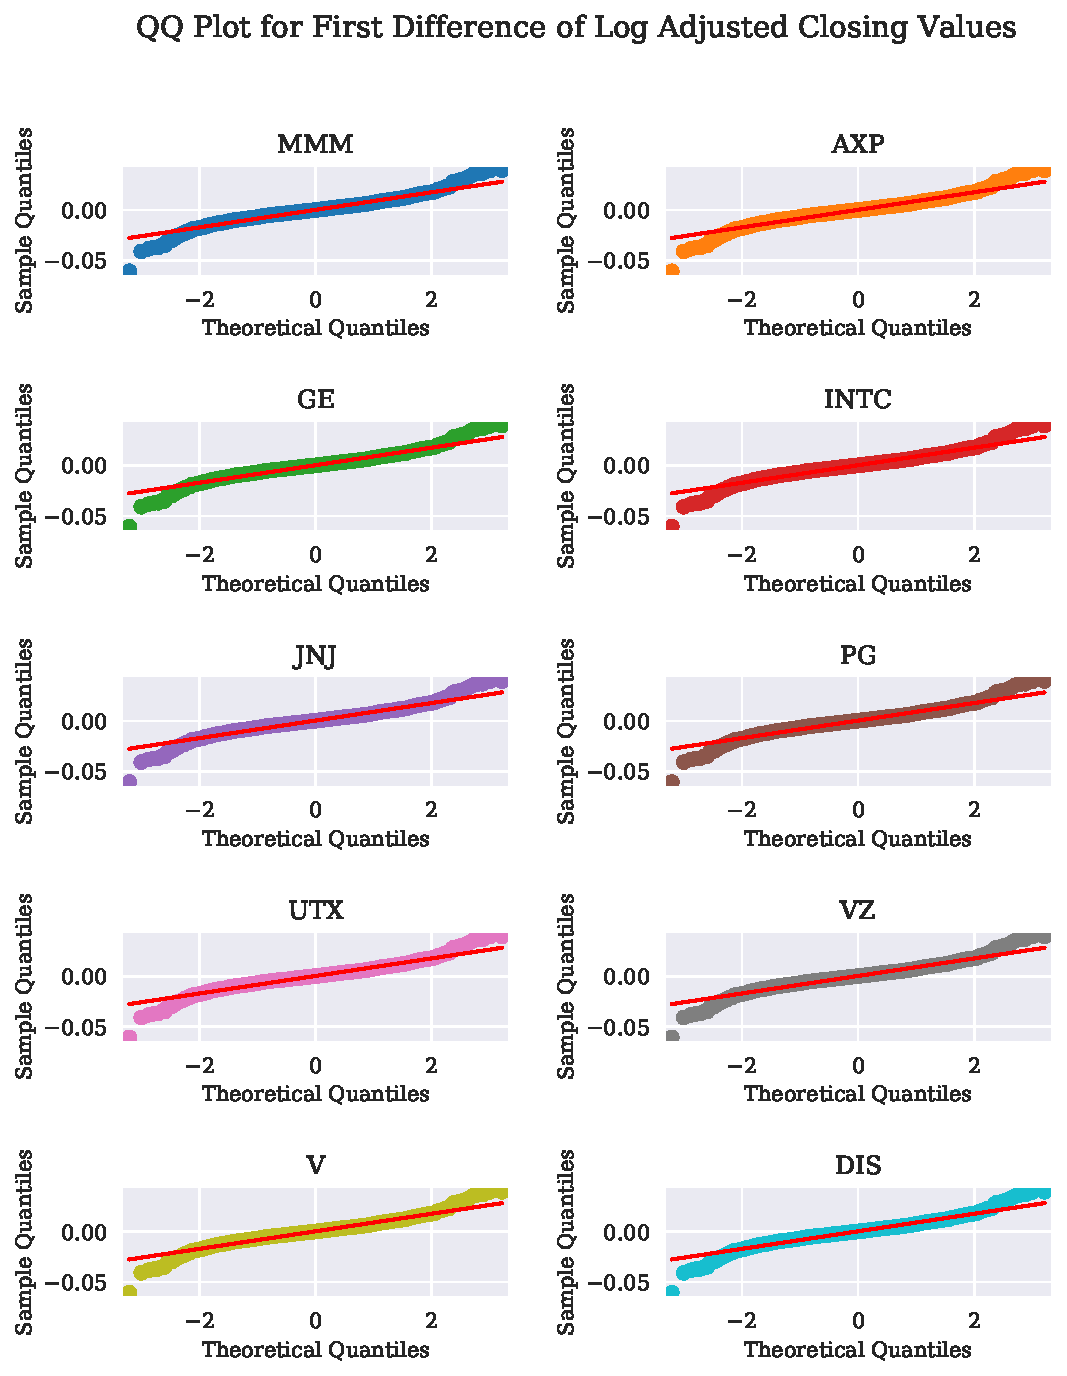
\includegraphics[]{figures/all_qq_plot_fd_log_adjclose.pdf}
    %%% Creator: Matplotlib, PGF backend
%%
%% To include the figure in your LaTeX document, write
%%   \input{<filename>.pgf}
%%
%% Make sure the required packages are loaded in your preamble
%%   \usepackage{pgf}
%%
%% Figures using additional raster images can only be included by \input if
%% they are in the same directory as the main LaTeX file. For loading figures
%% from other directories you can use the `import` package
%%   \usepackage{import}
%% and then include the figures with
%%   \import{<path to file>}{<filename>.pgf}
%%
%% Matplotlib used the following preamble
%%   \usepackage{fontspec}
%%   \setmainfont{DejaVuSerif.ttf}[Path=/opt/tljh/user/lib/python3.6/site-packages/matplotlib/mpl-data/fonts/ttf/]
%%   \setsansfont{DejaVuSans.ttf}[Path=/opt/tljh/user/lib/python3.6/site-packages/matplotlib/mpl-data/fonts/ttf/]
%%   \setmonofont{DejaVuSansMono.ttf}[Path=/opt/tljh/user/lib/python3.6/site-packages/matplotlib/mpl-data/fonts/ttf/]
%%
\begingroup%
\makeatletter%
\begin{pgfpicture}%
\pgfpathrectangle{\pgfpointorigin}{\pgfqpoint{7.336822in}{9.279134in}}%
\pgfusepath{use as bounding box, clip}%
\begin{pgfscope}%
\pgfsetbuttcap%
\pgfsetmiterjoin%
\definecolor{currentfill}{rgb}{1.000000,1.000000,1.000000}%
\pgfsetfillcolor{currentfill}%
\pgfsetlinewidth{0.000000pt}%
\definecolor{currentstroke}{rgb}{1.000000,1.000000,1.000000}%
\pgfsetstrokecolor{currentstroke}%
\pgfsetdash{}{0pt}%
\pgfpathmoveto{\pgfqpoint{0.000000in}{0.000000in}}%
\pgfpathlineto{\pgfqpoint{7.336822in}{0.000000in}}%
\pgfpathlineto{\pgfqpoint{7.336822in}{9.279134in}}%
\pgfpathlineto{\pgfqpoint{0.000000in}{9.279134in}}%
\pgfpathclose%
\pgfusepath{fill}%
\end{pgfscope}%
\begin{pgfscope}%
\pgfsetbuttcap%
\pgfsetmiterjoin%
\definecolor{currentfill}{rgb}{0.917647,0.917647,0.949020}%
\pgfsetfillcolor{currentfill}%
\pgfsetlinewidth{0.000000pt}%
\definecolor{currentstroke}{rgb}{0.000000,0.000000,0.000000}%
\pgfsetstrokecolor{currentstroke}%
\pgfsetstrokeopacity{0.000000}%
\pgfsetdash{}{0pt}%
\pgfpathmoveto{\pgfqpoint{1.036822in}{7.438938in}}%
\pgfpathlineto{\pgfqpoint{3.620155in}{7.438938in}}%
\pgfpathlineto{\pgfqpoint{3.620155in}{8.179134in}}%
\pgfpathlineto{\pgfqpoint{1.036822in}{8.179134in}}%
\pgfpathclose%
\pgfusepath{fill}%
\end{pgfscope}%
\begin{pgfscope}%
\pgfpathrectangle{\pgfqpoint{1.036822in}{7.438938in}}{\pgfqpoint{2.583333in}{0.740196in}}%
\pgfusepath{clip}%
\pgfsetroundcap%
\pgfsetroundjoin%
\pgfsetlinewidth{0.803000pt}%
\definecolor{currentstroke}{rgb}{1.000000,1.000000,1.000000}%
\pgfsetstrokecolor{currentstroke}%
\pgfsetdash{}{0pt}%
\pgfpathmoveto{\pgfqpoint{1.554767in}{7.438938in}}%
\pgfpathlineto{\pgfqpoint{1.554767in}{8.179134in}}%
\pgfusepath{stroke}%
\end{pgfscope}%
\begin{pgfscope}%
\definecolor{textcolor}{rgb}{0.150000,0.150000,0.150000}%
\pgfsetstrokecolor{textcolor}%
\pgfsetfillcolor{textcolor}%
\pgftext[x=1.554767in,y=7.341716in,,top]{\color{textcolor}\rmfamily\fontsize{14.000000}{16.800000}\selectfont −2}%
\end{pgfscope}%
\begin{pgfscope}%
\pgfpathrectangle{\pgfqpoint{1.036822in}{7.438938in}}{\pgfqpoint{2.583333in}{0.740196in}}%
\pgfusepath{clip}%
\pgfsetroundcap%
\pgfsetroundjoin%
\pgfsetlinewidth{0.803000pt}%
\definecolor{currentstroke}{rgb}{1.000000,1.000000,1.000000}%
\pgfsetstrokecolor{currentstroke}%
\pgfsetdash{}{0pt}%
\pgfpathmoveto{\pgfqpoint{2.328488in}{7.438938in}}%
\pgfpathlineto{\pgfqpoint{2.328488in}{8.179134in}}%
\pgfusepath{stroke}%
\end{pgfscope}%
\begin{pgfscope}%
\definecolor{textcolor}{rgb}{0.150000,0.150000,0.150000}%
\pgfsetstrokecolor{textcolor}%
\pgfsetfillcolor{textcolor}%
\pgftext[x=2.328488in,y=7.341716in,,top]{\color{textcolor}\rmfamily\fontsize{14.000000}{16.800000}\selectfont 0}%
\end{pgfscope}%
\begin{pgfscope}%
\pgfpathrectangle{\pgfqpoint{1.036822in}{7.438938in}}{\pgfqpoint{2.583333in}{0.740196in}}%
\pgfusepath{clip}%
\pgfsetroundcap%
\pgfsetroundjoin%
\pgfsetlinewidth{0.803000pt}%
\definecolor{currentstroke}{rgb}{1.000000,1.000000,1.000000}%
\pgfsetstrokecolor{currentstroke}%
\pgfsetdash{}{0pt}%
\pgfpathmoveto{\pgfqpoint{3.102209in}{7.438938in}}%
\pgfpathlineto{\pgfqpoint{3.102209in}{8.179134in}}%
\pgfusepath{stroke}%
\end{pgfscope}%
\begin{pgfscope}%
\definecolor{textcolor}{rgb}{0.150000,0.150000,0.150000}%
\pgfsetstrokecolor{textcolor}%
\pgfsetfillcolor{textcolor}%
\pgftext[x=3.102209in,y=7.341716in,,top]{\color{textcolor}\rmfamily\fontsize{14.000000}{16.800000}\selectfont 2}%
\end{pgfscope}%
\begin{pgfscope}%
\definecolor{textcolor}{rgb}{0.150000,0.150000,0.150000}%
\pgfsetstrokecolor{textcolor}%
\pgfsetfillcolor{textcolor}%
\pgftext[x=2.328488in,y=7.097982in,,top]{\color{textcolor}\rmfamily\fontsize{14.000000}{16.800000}\selectfont Theoretical Quantiles}%
\end{pgfscope}%
\begin{pgfscope}%
\pgfpathrectangle{\pgfqpoint{1.036822in}{7.438938in}}{\pgfqpoint{2.583333in}{0.740196in}}%
\pgfusepath{clip}%
\pgfsetroundcap%
\pgfsetroundjoin%
\pgfsetlinewidth{0.803000pt}%
\definecolor{currentstroke}{rgb}{1.000000,1.000000,1.000000}%
\pgfsetstrokecolor{currentstroke}%
\pgfsetdash{}{0pt}%
\pgfpathmoveto{\pgfqpoint{1.036822in}{7.543869in}}%
\pgfpathlineto{\pgfqpoint{3.620155in}{7.543869in}}%
\pgfusepath{stroke}%
\end{pgfscope}%
\begin{pgfscope}%
\definecolor{textcolor}{rgb}{0.150000,0.150000,0.150000}%
\pgfsetstrokecolor{textcolor}%
\pgfsetfillcolor{textcolor}%
\pgftext[x=0.343734in,y=7.470003in,left,base]{\color{textcolor}\rmfamily\fontsize{14.000000}{16.800000}\selectfont −0.05}%
\end{pgfscope}%
\begin{pgfscope}%
\pgfpathrectangle{\pgfqpoint{1.036822in}{7.438938in}}{\pgfqpoint{2.583333in}{0.740196in}}%
\pgfusepath{clip}%
\pgfsetroundcap%
\pgfsetroundjoin%
\pgfsetlinewidth{0.803000pt}%
\definecolor{currentstroke}{rgb}{1.000000,1.000000,1.000000}%
\pgfsetstrokecolor{currentstroke}%
\pgfsetdash{}{0pt}%
\pgfpathmoveto{\pgfqpoint{1.036822in}{7.879930in}}%
\pgfpathlineto{\pgfqpoint{3.620155in}{7.879930in}}%
\pgfusepath{stroke}%
\end{pgfscope}%
\begin{pgfscope}%
\definecolor{textcolor}{rgb}{0.150000,0.150000,0.150000}%
\pgfsetstrokecolor{textcolor}%
\pgfsetfillcolor{textcolor}%
\pgftext[x=0.506657in,y=7.806064in,left,base]{\color{textcolor}\rmfamily\fontsize{14.000000}{16.800000}\selectfont 0.00}%
\end{pgfscope}%
\begin{pgfscope}%
\definecolor{textcolor}{rgb}{0.150000,0.150000,0.150000}%
\pgfsetstrokecolor{textcolor}%
\pgfsetfillcolor{textcolor}%
\pgftext[x=0.288178in,y=7.809036in,,bottom,rotate=90.000000]{\color{textcolor}\rmfamily\fontsize{14.000000}{16.800000}\selectfont Sample Quantiles}%
\end{pgfscope}%
\begin{pgfscope}%
\pgfpathrectangle{\pgfqpoint{1.036822in}{7.438938in}}{\pgfqpoint{2.583333in}{0.740196in}}%
\pgfusepath{clip}%
\pgfsetbuttcap%
\pgfsetroundjoin%
\definecolor{currentfill}{rgb}{0.121569,0.466667,0.705882}%
\pgfsetfillcolor{currentfill}%
\pgfsetlinewidth{1.003750pt}%
\definecolor{currentstroke}{rgb}{0.121569,0.466667,0.705882}%
\pgfsetstrokecolor{currentstroke}%
\pgfsetdash{}{0pt}%
\pgfsys@defobject{currentmarker}{\pgfqpoint{-0.041667in}{-0.041667in}}{\pgfqpoint{0.041667in}{0.041667in}}{%
\pgfpathmoveto{\pgfqpoint{0.000000in}{-0.041667in}}%
\pgfpathcurveto{\pgfqpoint{0.011050in}{-0.041667in}}{\pgfqpoint{0.021649in}{-0.037276in}}{\pgfqpoint{0.029463in}{-0.029463in}}%
\pgfpathcurveto{\pgfqpoint{0.037276in}{-0.021649in}}{\pgfqpoint{0.041667in}{-0.011050in}}{\pgfqpoint{0.041667in}{0.000000in}}%
\pgfpathcurveto{\pgfqpoint{0.041667in}{0.011050in}}{\pgfqpoint{0.037276in}{0.021649in}}{\pgfqpoint{0.029463in}{0.029463in}}%
\pgfpathcurveto{\pgfqpoint{0.021649in}{0.037276in}}{\pgfqpoint{0.011050in}{0.041667in}}{\pgfqpoint{0.000000in}{0.041667in}}%
\pgfpathcurveto{\pgfqpoint{-0.011050in}{0.041667in}}{\pgfqpoint{-0.021649in}{0.037276in}}{\pgfqpoint{-0.029463in}{0.029463in}}%
\pgfpathcurveto{\pgfqpoint{-0.037276in}{0.021649in}}{\pgfqpoint{-0.041667in}{0.011050in}}{\pgfqpoint{-0.041667in}{0.000000in}}%
\pgfpathcurveto{\pgfqpoint{-0.041667in}{-0.011050in}}{\pgfqpoint{-0.037276in}{-0.021649in}}{\pgfqpoint{-0.029463in}{-0.029463in}}%
\pgfpathcurveto{\pgfqpoint{-0.021649in}{-0.037276in}}{\pgfqpoint{-0.011050in}{-0.041667in}}{\pgfqpoint{0.000000in}{-0.041667in}}%
\pgfpathclose%
\pgfusepath{stroke,fill}%
}%
\begin{pgfscope}%
\pgfsys@transformshift{1.086501in}{7.472583in}%
\pgfsys@useobject{currentmarker}{}%
\end{pgfscope}%
\begin{pgfscope}%
\pgfsys@transformshift{1.165749in}{7.605125in}%
\pgfsys@useobject{currentmarker}{}%
\end{pgfscope}%
\begin{pgfscope}%
\pgfsys@transformshift{1.214311in}{7.622529in}%
\pgfsys@useobject{currentmarker}{}%
\end{pgfscope}%
\begin{pgfscope}%
\pgfsys@transformshift{1.249876in}{7.630124in}%
\pgfsys@useobject{currentmarker}{}%
\end{pgfscope}%
\begin{pgfscope}%
\pgfsys@transformshift{1.278149in}{7.631584in}%
\pgfsys@useobject{currentmarker}{}%
\end{pgfscope}%
\begin{pgfscope}%
\pgfsys@transformshift{1.301726in}{7.643589in}%
\pgfsys@useobject{currentmarker}{}%
\end{pgfscope}%
\begin{pgfscope}%
\pgfsys@transformshift{1.322013in}{7.644197in}%
\pgfsys@useobject{currentmarker}{}%
\end{pgfscope}%
\begin{pgfscope}%
\pgfsys@transformshift{1.339860in}{7.672321in}%
\pgfsys@useobject{currentmarker}{}%
\end{pgfscope}%
\begin{pgfscope}%
\pgfsys@transformshift{1.355823in}{7.678378in}%
\pgfsys@useobject{currentmarker}{}%
\end{pgfscope}%
\begin{pgfscope}%
\pgfsys@transformshift{1.370283in}{7.679773in}%
\pgfsys@useobject{currentmarker}{}%
\end{pgfscope}%
\begin{pgfscope}%
\pgfsys@transformshift{1.383517in}{7.688269in}%
\pgfsys@useobject{currentmarker}{}%
\end{pgfscope}%
\begin{pgfscope}%
\pgfsys@transformshift{1.395730in}{7.696634in}%
\pgfsys@useobject{currentmarker}{}%
\end{pgfscope}%
\begin{pgfscope}%
\pgfsys@transformshift{1.407078in}{7.708844in}%
\pgfsys@useobject{currentmarker}{}%
\end{pgfscope}%
\begin{pgfscope}%
\pgfsys@transformshift{1.417685in}{7.709158in}%
\pgfsys@useobject{currentmarker}{}%
\end{pgfscope}%
\begin{pgfscope}%
\pgfsys@transformshift{1.427648in}{7.714896in}%
\pgfsys@useobject{currentmarker}{}%
\end{pgfscope}%
\begin{pgfscope}%
\pgfsys@transformshift{1.437048in}{7.721299in}%
\pgfsys@useobject{currentmarker}{}%
\end{pgfscope}%
\begin{pgfscope}%
\pgfsys@transformshift{1.445949in}{7.721735in}%
\pgfsys@useobject{currentmarker}{}%
\end{pgfscope}%
\begin{pgfscope}%
\pgfsys@transformshift{1.454405in}{7.724588in}%
\pgfsys@useobject{currentmarker}{}%
\end{pgfscope}%
\begin{pgfscope}%
\pgfsys@transformshift{1.462464in}{7.734109in}%
\pgfsys@useobject{currentmarker}{}%
\end{pgfscope}%
\begin{pgfscope}%
\pgfsys@transformshift{1.470164in}{7.736792in}%
\pgfsys@useobject{currentmarker}{}%
\end{pgfscope}%
\begin{pgfscope}%
\pgfsys@transformshift{1.477538in}{7.738270in}%
\pgfsys@useobject{currentmarker}{}%
\end{pgfscope}%
\begin{pgfscope}%
\pgfsys@transformshift{1.484615in}{7.739011in}%
\pgfsys@useobject{currentmarker}{}%
\end{pgfscope}%
\begin{pgfscope}%
\pgfsys@transformshift{1.491420in}{7.740191in}%
\pgfsys@useobject{currentmarker}{}%
\end{pgfscope}%
\begin{pgfscope}%
\pgfsys@transformshift{1.497976in}{7.748875in}%
\pgfsys@useobject{currentmarker}{}%
\end{pgfscope}%
\begin{pgfscope}%
\pgfsys@transformshift{1.504302in}{7.753354in}%
\pgfsys@useobject{currentmarker}{}%
\end{pgfscope}%
\begin{pgfscope}%
\pgfsys@transformshift{1.510414in}{7.753420in}%
\pgfsys@useobject{currentmarker}{}%
\end{pgfscope}%
\begin{pgfscope}%
\pgfsys@transformshift{1.516329in}{7.753628in}%
\pgfsys@useobject{currentmarker}{}%
\end{pgfscope}%
\begin{pgfscope}%
\pgfsys@transformshift{1.522060in}{7.754087in}%
\pgfsys@useobject{currentmarker}{}%
\end{pgfscope}%
\begin{pgfscope}%
\pgfsys@transformshift{1.527620in}{7.755629in}%
\pgfsys@useobject{currentmarker}{}%
\end{pgfscope}%
\begin{pgfscope}%
\pgfsys@transformshift{1.533019in}{7.757345in}%
\pgfsys@useobject{currentmarker}{}%
\end{pgfscope}%
\begin{pgfscope}%
\pgfsys@transformshift{1.538267in}{7.757622in}%
\pgfsys@useobject{currentmarker}{}%
\end{pgfscope}%
\begin{pgfscope}%
\pgfsys@transformshift{1.543373in}{7.758148in}%
\pgfsys@useobject{currentmarker}{}%
\end{pgfscope}%
\begin{pgfscope}%
\pgfsys@transformshift{1.548347in}{7.760982in}%
\pgfsys@useobject{currentmarker}{}%
\end{pgfscope}%
\begin{pgfscope}%
\pgfsys@transformshift{1.553194in}{7.761132in}%
\pgfsys@useobject{currentmarker}{}%
\end{pgfscope}%
\begin{pgfscope}%
\pgfsys@transformshift{1.557923in}{7.761473in}%
\pgfsys@useobject{currentmarker}{}%
\end{pgfscope}%
\begin{pgfscope}%
\pgfsys@transformshift{1.562540in}{7.763921in}%
\pgfsys@useobject{currentmarker}{}%
\end{pgfscope}%
\begin{pgfscope}%
\pgfsys@transformshift{1.567050in}{7.764061in}%
\pgfsys@useobject{currentmarker}{}%
\end{pgfscope}%
\begin{pgfscope}%
\pgfsys@transformshift{1.571458in}{7.764285in}%
\pgfsys@useobject{currentmarker}{}%
\end{pgfscope}%
\begin{pgfscope}%
\pgfsys@transformshift{1.575771in}{7.764825in}%
\pgfsys@useobject{currentmarker}{}%
\end{pgfscope}%
\begin{pgfscope}%
\pgfsys@transformshift{1.579992in}{7.766152in}%
\pgfsys@useobject{currentmarker}{}%
\end{pgfscope}%
\begin{pgfscope}%
\pgfsys@transformshift{1.584126in}{7.767186in}%
\pgfsys@useobject{currentmarker}{}%
\end{pgfscope}%
\begin{pgfscope}%
\pgfsys@transformshift{1.588176in}{7.770994in}%
\pgfsys@useobject{currentmarker}{}%
\end{pgfscope}%
\begin{pgfscope}%
\pgfsys@transformshift{1.592147in}{7.773762in}%
\pgfsys@useobject{currentmarker}{}%
\end{pgfscope}%
\begin{pgfscope}%
\pgfsys@transformshift{1.596042in}{7.773834in}%
\pgfsys@useobject{currentmarker}{}%
\end{pgfscope}%
\begin{pgfscope}%
\pgfsys@transformshift{1.599864in}{7.774417in}%
\pgfsys@useobject{currentmarker}{}%
\end{pgfscope}%
\begin{pgfscope}%
\pgfsys@transformshift{1.603616in}{7.774654in}%
\pgfsys@useobject{currentmarker}{}%
\end{pgfscope}%
\begin{pgfscope}%
\pgfsys@transformshift{1.607301in}{7.774761in}%
\pgfsys@useobject{currentmarker}{}%
\end{pgfscope}%
\begin{pgfscope}%
\pgfsys@transformshift{1.610922in}{7.775384in}%
\pgfsys@useobject{currentmarker}{}%
\end{pgfscope}%
\begin{pgfscope}%
\pgfsys@transformshift{1.614481in}{7.775399in}%
\pgfsys@useobject{currentmarker}{}%
\end{pgfscope}%
\begin{pgfscope}%
\pgfsys@transformshift{1.617981in}{7.777718in}%
\pgfsys@useobject{currentmarker}{}%
\end{pgfscope}%
\begin{pgfscope}%
\pgfsys@transformshift{1.621423in}{7.778045in}%
\pgfsys@useobject{currentmarker}{}%
\end{pgfscope}%
\begin{pgfscope}%
\pgfsys@transformshift{1.624810in}{7.781778in}%
\pgfsys@useobject{currentmarker}{}%
\end{pgfscope}%
\begin{pgfscope}%
\pgfsys@transformshift{1.628145in}{7.781779in}%
\pgfsys@useobject{currentmarker}{}%
\end{pgfscope}%
\begin{pgfscope}%
\pgfsys@transformshift{1.631428in}{7.781854in}%
\pgfsys@useobject{currentmarker}{}%
\end{pgfscope}%
\begin{pgfscope}%
\pgfsys@transformshift{1.634661in}{7.783194in}%
\pgfsys@useobject{currentmarker}{}%
\end{pgfscope}%
\begin{pgfscope}%
\pgfsys@transformshift{1.637847in}{7.783561in}%
\pgfsys@useobject{currentmarker}{}%
\end{pgfscope}%
\begin{pgfscope}%
\pgfsys@transformshift{1.640987in}{7.784001in}%
\pgfsys@useobject{currentmarker}{}%
\end{pgfscope}%
\begin{pgfscope}%
\pgfsys@transformshift{1.644082in}{7.784244in}%
\pgfsys@useobject{currentmarker}{}%
\end{pgfscope}%
\begin{pgfscope}%
\pgfsys@transformshift{1.647133in}{7.785580in}%
\pgfsys@useobject{currentmarker}{}%
\end{pgfscope}%
\begin{pgfscope}%
\pgfsys@transformshift{1.650143in}{7.786913in}%
\pgfsys@useobject{currentmarker}{}%
\end{pgfscope}%
\begin{pgfscope}%
\pgfsys@transformshift{1.653113in}{7.787404in}%
\pgfsys@useobject{currentmarker}{}%
\end{pgfscope}%
\begin{pgfscope}%
\pgfsys@transformshift{1.656043in}{7.788222in}%
\pgfsys@useobject{currentmarker}{}%
\end{pgfscope}%
\begin{pgfscope}%
\pgfsys@transformshift{1.658935in}{7.788386in}%
\pgfsys@useobject{currentmarker}{}%
\end{pgfscope}%
\begin{pgfscope}%
\pgfsys@transformshift{1.661790in}{7.788654in}%
\pgfsys@useobject{currentmarker}{}%
\end{pgfscope}%
\begin{pgfscope}%
\pgfsys@transformshift{1.664610in}{7.790477in}%
\pgfsys@useobject{currentmarker}{}%
\end{pgfscope}%
\begin{pgfscope}%
\pgfsys@transformshift{1.667394in}{7.791247in}%
\pgfsys@useobject{currentmarker}{}%
\end{pgfscope}%
\begin{pgfscope}%
\pgfsys@transformshift{1.670145in}{7.791334in}%
\pgfsys@useobject{currentmarker}{}%
\end{pgfscope}%
\begin{pgfscope}%
\pgfsys@transformshift{1.672863in}{7.792379in}%
\pgfsys@useobject{currentmarker}{}%
\end{pgfscope}%
\begin{pgfscope}%
\pgfsys@transformshift{1.675549in}{7.792564in}%
\pgfsys@useobject{currentmarker}{}%
\end{pgfscope}%
\begin{pgfscope}%
\pgfsys@transformshift{1.678203in}{7.792566in}%
\pgfsys@useobject{currentmarker}{}%
\end{pgfscope}%
\begin{pgfscope}%
\pgfsys@transformshift{1.680828in}{7.794018in}%
\pgfsys@useobject{currentmarker}{}%
\end{pgfscope}%
\begin{pgfscope}%
\pgfsys@transformshift{1.683423in}{7.794249in}%
\pgfsys@useobject{currentmarker}{}%
\end{pgfscope}%
\begin{pgfscope}%
\pgfsys@transformshift{1.685989in}{7.794277in}%
\pgfsys@useobject{currentmarker}{}%
\end{pgfscope}%
\begin{pgfscope}%
\pgfsys@transformshift{1.688527in}{7.794867in}%
\pgfsys@useobject{currentmarker}{}%
\end{pgfscope}%
\begin{pgfscope}%
\pgfsys@transformshift{1.691038in}{7.795067in}%
\pgfsys@useobject{currentmarker}{}%
\end{pgfscope}%
\begin{pgfscope}%
\pgfsys@transformshift{1.693523in}{7.795650in}%
\pgfsys@useobject{currentmarker}{}%
\end{pgfscope}%
\begin{pgfscope}%
\pgfsys@transformshift{1.695981in}{7.795772in}%
\pgfsys@useobject{currentmarker}{}%
\end{pgfscope}%
\begin{pgfscope}%
\pgfsys@transformshift{1.698414in}{7.795848in}%
\pgfsys@useobject{currentmarker}{}%
\end{pgfscope}%
\begin{pgfscope}%
\pgfsys@transformshift{1.700823in}{7.795926in}%
\pgfsys@useobject{currentmarker}{}%
\end{pgfscope}%
\begin{pgfscope}%
\pgfsys@transformshift{1.703208in}{7.795946in}%
\pgfsys@useobject{currentmarker}{}%
\end{pgfscope}%
\begin{pgfscope}%
\pgfsys@transformshift{1.705569in}{7.796039in}%
\pgfsys@useobject{currentmarker}{}%
\end{pgfscope}%
\begin{pgfscope}%
\pgfsys@transformshift{1.707907in}{7.796390in}%
\pgfsys@useobject{currentmarker}{}%
\end{pgfscope}%
\begin{pgfscope}%
\pgfsys@transformshift{1.710222in}{7.797151in}%
\pgfsys@useobject{currentmarker}{}%
\end{pgfscope}%
\begin{pgfscope}%
\pgfsys@transformshift{1.712516in}{7.797652in}%
\pgfsys@useobject{currentmarker}{}%
\end{pgfscope}%
\begin{pgfscope}%
\pgfsys@transformshift{1.714788in}{7.797985in}%
\pgfsys@useobject{currentmarker}{}%
\end{pgfscope}%
\begin{pgfscope}%
\pgfsys@transformshift{1.717039in}{7.798265in}%
\pgfsys@useobject{currentmarker}{}%
\end{pgfscope}%
\begin{pgfscope}%
\pgfsys@transformshift{1.719270in}{7.798472in}%
\pgfsys@useobject{currentmarker}{}%
\end{pgfscope}%
\begin{pgfscope}%
\pgfsys@transformshift{1.721480in}{7.799389in}%
\pgfsys@useobject{currentmarker}{}%
\end{pgfscope}%
\begin{pgfscope}%
\pgfsys@transformshift{1.723671in}{7.799858in}%
\pgfsys@useobject{currentmarker}{}%
\end{pgfscope}%
\begin{pgfscope}%
\pgfsys@transformshift{1.725843in}{7.800124in}%
\pgfsys@useobject{currentmarker}{}%
\end{pgfscope}%
\begin{pgfscope}%
\pgfsys@transformshift{1.727996in}{7.800135in}%
\pgfsys@useobject{currentmarker}{}%
\end{pgfscope}%
\begin{pgfscope}%
\pgfsys@transformshift{1.730130in}{7.800899in}%
\pgfsys@useobject{currentmarker}{}%
\end{pgfscope}%
\begin{pgfscope}%
\pgfsys@transformshift{1.732247in}{7.801175in}%
\pgfsys@useobject{currentmarker}{}%
\end{pgfscope}%
\begin{pgfscope}%
\pgfsys@transformshift{1.734345in}{7.801273in}%
\pgfsys@useobject{currentmarker}{}%
\end{pgfscope}%
\begin{pgfscope}%
\pgfsys@transformshift{1.736427in}{7.801873in}%
\pgfsys@useobject{currentmarker}{}%
\end{pgfscope}%
\begin{pgfscope}%
\pgfsys@transformshift{1.738491in}{7.802442in}%
\pgfsys@useobject{currentmarker}{}%
\end{pgfscope}%
\begin{pgfscope}%
\pgfsys@transformshift{1.740539in}{7.802713in}%
\pgfsys@useobject{currentmarker}{}%
\end{pgfscope}%
\begin{pgfscope}%
\pgfsys@transformshift{1.742570in}{7.802978in}%
\pgfsys@useobject{currentmarker}{}%
\end{pgfscope}%
\begin{pgfscope}%
\pgfsys@transformshift{1.744586in}{7.804975in}%
\pgfsys@useobject{currentmarker}{}%
\end{pgfscope}%
\begin{pgfscope}%
\pgfsys@transformshift{1.746585in}{7.805049in}%
\pgfsys@useobject{currentmarker}{}%
\end{pgfscope}%
\begin{pgfscope}%
\pgfsys@transformshift{1.748569in}{7.805965in}%
\pgfsys@useobject{currentmarker}{}%
\end{pgfscope}%
\begin{pgfscope}%
\pgfsys@transformshift{1.750538in}{7.806918in}%
\pgfsys@useobject{currentmarker}{}%
\end{pgfscope}%
\begin{pgfscope}%
\pgfsys@transformshift{1.752493in}{7.807042in}%
\pgfsys@useobject{currentmarker}{}%
\end{pgfscope}%
\begin{pgfscope}%
\pgfsys@transformshift{1.754432in}{7.807099in}%
\pgfsys@useobject{currentmarker}{}%
\end{pgfscope}%
\begin{pgfscope}%
\pgfsys@transformshift{1.756357in}{7.807431in}%
\pgfsys@useobject{currentmarker}{}%
\end{pgfscope}%
\begin{pgfscope}%
\pgfsys@transformshift{1.758269in}{7.807511in}%
\pgfsys@useobject{currentmarker}{}%
\end{pgfscope}%
\begin{pgfscope}%
\pgfsys@transformshift{1.760166in}{7.807653in}%
\pgfsys@useobject{currentmarker}{}%
\end{pgfscope}%
\begin{pgfscope}%
\pgfsys@transformshift{1.762050in}{7.807685in}%
\pgfsys@useobject{currentmarker}{}%
\end{pgfscope}%
\begin{pgfscope}%
\pgfsys@transformshift{1.763920in}{7.807906in}%
\pgfsys@useobject{currentmarker}{}%
\end{pgfscope}%
\begin{pgfscope}%
\pgfsys@transformshift{1.765778in}{7.807922in}%
\pgfsys@useobject{currentmarker}{}%
\end{pgfscope}%
\begin{pgfscope}%
\pgfsys@transformshift{1.767622in}{7.808583in}%
\pgfsys@useobject{currentmarker}{}%
\end{pgfscope}%
\begin{pgfscope}%
\pgfsys@transformshift{1.769454in}{7.809430in}%
\pgfsys@useobject{currentmarker}{}%
\end{pgfscope}%
\begin{pgfscope}%
\pgfsys@transformshift{1.771273in}{7.809873in}%
\pgfsys@useobject{currentmarker}{}%
\end{pgfscope}%
\begin{pgfscope}%
\pgfsys@transformshift{1.773081in}{7.810094in}%
\pgfsys@useobject{currentmarker}{}%
\end{pgfscope}%
\begin{pgfscope}%
\pgfsys@transformshift{1.774876in}{7.810101in}%
\pgfsys@useobject{currentmarker}{}%
\end{pgfscope}%
\begin{pgfscope}%
\pgfsys@transformshift{1.776659in}{7.810405in}%
\pgfsys@useobject{currentmarker}{}%
\end{pgfscope}%
\begin{pgfscope}%
\pgfsys@transformshift{1.778430in}{7.811455in}%
\pgfsys@useobject{currentmarker}{}%
\end{pgfscope}%
\begin{pgfscope}%
\pgfsys@transformshift{1.780191in}{7.811625in}%
\pgfsys@useobject{currentmarker}{}%
\end{pgfscope}%
\begin{pgfscope}%
\pgfsys@transformshift{1.781939in}{7.812463in}%
\pgfsys@useobject{currentmarker}{}%
\end{pgfscope}%
\begin{pgfscope}%
\pgfsys@transformshift{1.783677in}{7.812851in}%
\pgfsys@useobject{currentmarker}{}%
\end{pgfscope}%
\begin{pgfscope}%
\pgfsys@transformshift{1.785404in}{7.812895in}%
\pgfsys@useobject{currentmarker}{}%
\end{pgfscope}%
\begin{pgfscope}%
\pgfsys@transformshift{1.787120in}{7.813011in}%
\pgfsys@useobject{currentmarker}{}%
\end{pgfscope}%
\begin{pgfscope}%
\pgfsys@transformshift{1.788826in}{7.813616in}%
\pgfsys@useobject{currentmarker}{}%
\end{pgfscope}%
\begin{pgfscope}%
\pgfsys@transformshift{1.790521in}{7.813927in}%
\pgfsys@useobject{currentmarker}{}%
\end{pgfscope}%
\begin{pgfscope}%
\pgfsys@transformshift{1.792206in}{7.814544in}%
\pgfsys@useobject{currentmarker}{}%
\end{pgfscope}%
\begin{pgfscope}%
\pgfsys@transformshift{1.793880in}{7.814980in}%
\pgfsys@useobject{currentmarker}{}%
\end{pgfscope}%
\begin{pgfscope}%
\pgfsys@transformshift{1.795545in}{7.815009in}%
\pgfsys@useobject{currentmarker}{}%
\end{pgfscope}%
\begin{pgfscope}%
\pgfsys@transformshift{1.797200in}{7.815065in}%
\pgfsys@useobject{currentmarker}{}%
\end{pgfscope}%
\begin{pgfscope}%
\pgfsys@transformshift{1.798845in}{7.815174in}%
\pgfsys@useobject{currentmarker}{}%
\end{pgfscope}%
\begin{pgfscope}%
\pgfsys@transformshift{1.800481in}{7.815307in}%
\pgfsys@useobject{currentmarker}{}%
\end{pgfscope}%
\begin{pgfscope}%
\pgfsys@transformshift{1.802107in}{7.815391in}%
\pgfsys@useobject{currentmarker}{}%
\end{pgfscope}%
\begin{pgfscope}%
\pgfsys@transformshift{1.803724in}{7.815584in}%
\pgfsys@useobject{currentmarker}{}%
\end{pgfscope}%
\begin{pgfscope}%
\pgfsys@transformshift{1.805332in}{7.815725in}%
\pgfsys@useobject{currentmarker}{}%
\end{pgfscope}%
\begin{pgfscope}%
\pgfsys@transformshift{1.806931in}{7.815857in}%
\pgfsys@useobject{currentmarker}{}%
\end{pgfscope}%
\begin{pgfscope}%
\pgfsys@transformshift{1.808522in}{7.816050in}%
\pgfsys@useobject{currentmarker}{}%
\end{pgfscope}%
\begin{pgfscope}%
\pgfsys@transformshift{1.810103in}{7.816154in}%
\pgfsys@useobject{currentmarker}{}%
\end{pgfscope}%
\begin{pgfscope}%
\pgfsys@transformshift{1.811676in}{7.816212in}%
\pgfsys@useobject{currentmarker}{}%
\end{pgfscope}%
\begin{pgfscope}%
\pgfsys@transformshift{1.813240in}{7.816351in}%
\pgfsys@useobject{currentmarker}{}%
\end{pgfscope}%
\begin{pgfscope}%
\pgfsys@transformshift{1.814796in}{7.816530in}%
\pgfsys@useobject{currentmarker}{}%
\end{pgfscope}%
\begin{pgfscope}%
\pgfsys@transformshift{1.816344in}{7.816819in}%
\pgfsys@useobject{currentmarker}{}%
\end{pgfscope}%
\begin{pgfscope}%
\pgfsys@transformshift{1.817883in}{7.817125in}%
\pgfsys@useobject{currentmarker}{}%
\end{pgfscope}%
\begin{pgfscope}%
\pgfsys@transformshift{1.819415in}{7.817134in}%
\pgfsys@useobject{currentmarker}{}%
\end{pgfscope}%
\begin{pgfscope}%
\pgfsys@transformshift{1.820938in}{7.817593in}%
\pgfsys@useobject{currentmarker}{}%
\end{pgfscope}%
\begin{pgfscope}%
\pgfsys@transformshift{1.822454in}{7.817956in}%
\pgfsys@useobject{currentmarker}{}%
\end{pgfscope}%
\begin{pgfscope}%
\pgfsys@transformshift{1.823962in}{7.817966in}%
\pgfsys@useobject{currentmarker}{}%
\end{pgfscope}%
\begin{pgfscope}%
\pgfsys@transformshift{1.825462in}{7.818742in}%
\pgfsys@useobject{currentmarker}{}%
\end{pgfscope}%
\begin{pgfscope}%
\pgfsys@transformshift{1.826955in}{7.818789in}%
\pgfsys@useobject{currentmarker}{}%
\end{pgfscope}%
\begin{pgfscope}%
\pgfsys@transformshift{1.828440in}{7.818934in}%
\pgfsys@useobject{currentmarker}{}%
\end{pgfscope}%
\begin{pgfscope}%
\pgfsys@transformshift{1.829918in}{7.819168in}%
\pgfsys@useobject{currentmarker}{}%
\end{pgfscope}%
\begin{pgfscope}%
\pgfsys@transformshift{1.831389in}{7.819387in}%
\pgfsys@useobject{currentmarker}{}%
\end{pgfscope}%
\begin{pgfscope}%
\pgfsys@transformshift{1.832853in}{7.819426in}%
\pgfsys@useobject{currentmarker}{}%
\end{pgfscope}%
\begin{pgfscope}%
\pgfsys@transformshift{1.834309in}{7.819511in}%
\pgfsys@useobject{currentmarker}{}%
\end{pgfscope}%
\begin{pgfscope}%
\pgfsys@transformshift{1.835759in}{7.819607in}%
\pgfsys@useobject{currentmarker}{}%
\end{pgfscope}%
\begin{pgfscope}%
\pgfsys@transformshift{1.837202in}{7.819835in}%
\pgfsys@useobject{currentmarker}{}%
\end{pgfscope}%
\begin{pgfscope}%
\pgfsys@transformshift{1.838638in}{7.819951in}%
\pgfsys@useobject{currentmarker}{}%
\end{pgfscope}%
\begin{pgfscope}%
\pgfsys@transformshift{1.840067in}{7.820008in}%
\pgfsys@useobject{currentmarker}{}%
\end{pgfscope}%
\begin{pgfscope}%
\pgfsys@transformshift{1.841489in}{7.820282in}%
\pgfsys@useobject{currentmarker}{}%
\end{pgfscope}%
\begin{pgfscope}%
\pgfsys@transformshift{1.842905in}{7.820432in}%
\pgfsys@useobject{currentmarker}{}%
\end{pgfscope}%
\begin{pgfscope}%
\pgfsys@transformshift{1.844315in}{7.820653in}%
\pgfsys@useobject{currentmarker}{}%
\end{pgfscope}%
\begin{pgfscope}%
\pgfsys@transformshift{1.845718in}{7.820783in}%
\pgfsys@useobject{currentmarker}{}%
\end{pgfscope}%
\begin{pgfscope}%
\pgfsys@transformshift{1.847115in}{7.820976in}%
\pgfsys@useobject{currentmarker}{}%
\end{pgfscope}%
\begin{pgfscope}%
\pgfsys@transformshift{1.848505in}{7.821100in}%
\pgfsys@useobject{currentmarker}{}%
\end{pgfscope}%
\begin{pgfscope}%
\pgfsys@transformshift{1.849890in}{7.821152in}%
\pgfsys@useobject{currentmarker}{}%
\end{pgfscope}%
\begin{pgfscope}%
\pgfsys@transformshift{1.851268in}{7.821491in}%
\pgfsys@useobject{currentmarker}{}%
\end{pgfscope}%
\begin{pgfscope}%
\pgfsys@transformshift{1.852640in}{7.821669in}%
\pgfsys@useobject{currentmarker}{}%
\end{pgfscope}%
\begin{pgfscope}%
\pgfsys@transformshift{1.854007in}{7.821704in}%
\pgfsys@useobject{currentmarker}{}%
\end{pgfscope}%
\begin{pgfscope}%
\pgfsys@transformshift{1.855367in}{7.822025in}%
\pgfsys@useobject{currentmarker}{}%
\end{pgfscope}%
\begin{pgfscope}%
\pgfsys@transformshift{1.856722in}{7.822091in}%
\pgfsys@useobject{currentmarker}{}%
\end{pgfscope}%
\begin{pgfscope}%
\pgfsys@transformshift{1.858071in}{7.822093in}%
\pgfsys@useobject{currentmarker}{}%
\end{pgfscope}%
\begin{pgfscope}%
\pgfsys@transformshift{1.859414in}{7.822093in}%
\pgfsys@useobject{currentmarker}{}%
\end{pgfscope}%
\begin{pgfscope}%
\pgfsys@transformshift{1.860751in}{7.822115in}%
\pgfsys@useobject{currentmarker}{}%
\end{pgfscope}%
\begin{pgfscope}%
\pgfsys@transformshift{1.862083in}{7.822451in}%
\pgfsys@useobject{currentmarker}{}%
\end{pgfscope}%
\begin{pgfscope}%
\pgfsys@transformshift{1.863410in}{7.822821in}%
\pgfsys@useobject{currentmarker}{}%
\end{pgfscope}%
\begin{pgfscope}%
\pgfsys@transformshift{1.864731in}{7.822983in}%
\pgfsys@useobject{currentmarker}{}%
\end{pgfscope}%
\begin{pgfscope}%
\pgfsys@transformshift{1.866046in}{7.823516in}%
\pgfsys@useobject{currentmarker}{}%
\end{pgfscope}%
\begin{pgfscope}%
\pgfsys@transformshift{1.867356in}{7.823668in}%
\pgfsys@useobject{currentmarker}{}%
\end{pgfscope}%
\begin{pgfscope}%
\pgfsys@transformshift{1.868661in}{7.823965in}%
\pgfsys@useobject{currentmarker}{}%
\end{pgfscope}%
\begin{pgfscope}%
\pgfsys@transformshift{1.869961in}{7.824022in}%
\pgfsys@useobject{currentmarker}{}%
\end{pgfscope}%
\begin{pgfscope}%
\pgfsys@transformshift{1.871256in}{7.824075in}%
\pgfsys@useobject{currentmarker}{}%
\end{pgfscope}%
\begin{pgfscope}%
\pgfsys@transformshift{1.872545in}{7.824195in}%
\pgfsys@useobject{currentmarker}{}%
\end{pgfscope}%
\begin{pgfscope}%
\pgfsys@transformshift{1.873830in}{7.824241in}%
\pgfsys@useobject{currentmarker}{}%
\end{pgfscope}%
\begin{pgfscope}%
\pgfsys@transformshift{1.875109in}{7.824269in}%
\pgfsys@useobject{currentmarker}{}%
\end{pgfscope}%
\begin{pgfscope}%
\pgfsys@transformshift{1.876384in}{7.824532in}%
\pgfsys@useobject{currentmarker}{}%
\end{pgfscope}%
\begin{pgfscope}%
\pgfsys@transformshift{1.877654in}{7.825132in}%
\pgfsys@useobject{currentmarker}{}%
\end{pgfscope}%
\begin{pgfscope}%
\pgfsys@transformshift{1.878918in}{7.825197in}%
\pgfsys@useobject{currentmarker}{}%
\end{pgfscope}%
\begin{pgfscope}%
\pgfsys@transformshift{1.880178in}{7.825308in}%
\pgfsys@useobject{currentmarker}{}%
\end{pgfscope}%
\begin{pgfscope}%
\pgfsys@transformshift{1.881434in}{7.825977in}%
\pgfsys@useobject{currentmarker}{}%
\end{pgfscope}%
\begin{pgfscope}%
\pgfsys@transformshift{1.882684in}{7.826056in}%
\pgfsys@useobject{currentmarker}{}%
\end{pgfscope}%
\begin{pgfscope}%
\pgfsys@transformshift{1.883930in}{7.826083in}%
\pgfsys@useobject{currentmarker}{}%
\end{pgfscope}%
\begin{pgfscope}%
\pgfsys@transformshift{1.885172in}{7.826250in}%
\pgfsys@useobject{currentmarker}{}%
\end{pgfscope}%
\begin{pgfscope}%
\pgfsys@transformshift{1.886409in}{7.826256in}%
\pgfsys@useobject{currentmarker}{}%
\end{pgfscope}%
\begin{pgfscope}%
\pgfsys@transformshift{1.887641in}{7.826621in}%
\pgfsys@useobject{currentmarker}{}%
\end{pgfscope}%
\begin{pgfscope}%
\pgfsys@transformshift{1.888869in}{7.826734in}%
\pgfsys@useobject{currentmarker}{}%
\end{pgfscope}%
\begin{pgfscope}%
\pgfsys@transformshift{1.890092in}{7.826746in}%
\pgfsys@useobject{currentmarker}{}%
\end{pgfscope}%
\begin{pgfscope}%
\pgfsys@transformshift{1.891311in}{7.826836in}%
\pgfsys@useobject{currentmarker}{}%
\end{pgfscope}%
\begin{pgfscope}%
\pgfsys@transformshift{1.892526in}{7.826927in}%
\pgfsys@useobject{currentmarker}{}%
\end{pgfscope}%
\begin{pgfscope}%
\pgfsys@transformshift{1.893737in}{7.827560in}%
\pgfsys@useobject{currentmarker}{}%
\end{pgfscope}%
\begin{pgfscope}%
\pgfsys@transformshift{1.894943in}{7.827665in}%
\pgfsys@useobject{currentmarker}{}%
\end{pgfscope}%
\begin{pgfscope}%
\pgfsys@transformshift{1.896145in}{7.827704in}%
\pgfsys@useobject{currentmarker}{}%
\end{pgfscope}%
\begin{pgfscope}%
\pgfsys@transformshift{1.897343in}{7.828288in}%
\pgfsys@useobject{currentmarker}{}%
\end{pgfscope}%
\begin{pgfscope}%
\pgfsys@transformshift{1.898536in}{7.828373in}%
\pgfsys@useobject{currentmarker}{}%
\end{pgfscope}%
\begin{pgfscope}%
\pgfsys@transformshift{1.899726in}{7.828574in}%
\pgfsys@useobject{currentmarker}{}%
\end{pgfscope}%
\begin{pgfscope}%
\pgfsys@transformshift{1.900912in}{7.828658in}%
\pgfsys@useobject{currentmarker}{}%
\end{pgfscope}%
\begin{pgfscope}%
\pgfsys@transformshift{1.902093in}{7.828728in}%
\pgfsys@useobject{currentmarker}{}%
\end{pgfscope}%
\begin{pgfscope}%
\pgfsys@transformshift{1.903271in}{7.828818in}%
\pgfsys@useobject{currentmarker}{}%
\end{pgfscope}%
\begin{pgfscope}%
\pgfsys@transformshift{1.904445in}{7.828818in}%
\pgfsys@useobject{currentmarker}{}%
\end{pgfscope}%
\begin{pgfscope}%
\pgfsys@transformshift{1.905615in}{7.828887in}%
\pgfsys@useobject{currentmarker}{}%
\end{pgfscope}%
\begin{pgfscope}%
\pgfsys@transformshift{1.906781in}{7.829038in}%
\pgfsys@useobject{currentmarker}{}%
\end{pgfscope}%
\begin{pgfscope}%
\pgfsys@transformshift{1.907943in}{7.829062in}%
\pgfsys@useobject{currentmarker}{}%
\end{pgfscope}%
\begin{pgfscope}%
\pgfsys@transformshift{1.909101in}{7.829085in}%
\pgfsys@useobject{currentmarker}{}%
\end{pgfscope}%
\begin{pgfscope}%
\pgfsys@transformshift{1.910256in}{7.829203in}%
\pgfsys@useobject{currentmarker}{}%
\end{pgfscope}%
\begin{pgfscope}%
\pgfsys@transformshift{1.911407in}{7.829583in}%
\pgfsys@useobject{currentmarker}{}%
\end{pgfscope}%
\begin{pgfscope}%
\pgfsys@transformshift{1.912554in}{7.830552in}%
\pgfsys@useobject{currentmarker}{}%
\end{pgfscope}%
\begin{pgfscope}%
\pgfsys@transformshift{1.913698in}{7.830619in}%
\pgfsys@useobject{currentmarker}{}%
\end{pgfscope}%
\begin{pgfscope}%
\pgfsys@transformshift{1.914838in}{7.830644in}%
\pgfsys@useobject{currentmarker}{}%
\end{pgfscope}%
\begin{pgfscope}%
\pgfsys@transformshift{1.915974in}{7.831141in}%
\pgfsys@useobject{currentmarker}{}%
\end{pgfscope}%
\begin{pgfscope}%
\pgfsys@transformshift{1.917107in}{7.831144in}%
\pgfsys@useobject{currentmarker}{}%
\end{pgfscope}%
\begin{pgfscope}%
\pgfsys@transformshift{1.918236in}{7.831171in}%
\pgfsys@useobject{currentmarker}{}%
\end{pgfscope}%
\begin{pgfscope}%
\pgfsys@transformshift{1.919362in}{7.831222in}%
\pgfsys@useobject{currentmarker}{}%
\end{pgfscope}%
\begin{pgfscope}%
\pgfsys@transformshift{1.920485in}{7.831274in}%
\pgfsys@useobject{currentmarker}{}%
\end{pgfscope}%
\begin{pgfscope}%
\pgfsys@transformshift{1.921604in}{7.831278in}%
\pgfsys@useobject{currentmarker}{}%
\end{pgfscope}%
\begin{pgfscope}%
\pgfsys@transformshift{1.922719in}{7.831408in}%
\pgfsys@useobject{currentmarker}{}%
\end{pgfscope}%
\begin{pgfscope}%
\pgfsys@transformshift{1.923831in}{7.831423in}%
\pgfsys@useobject{currentmarker}{}%
\end{pgfscope}%
\begin{pgfscope}%
\pgfsys@transformshift{1.924940in}{7.831583in}%
\pgfsys@useobject{currentmarker}{}%
\end{pgfscope}%
\begin{pgfscope}%
\pgfsys@transformshift{1.926046in}{7.831868in}%
\pgfsys@useobject{currentmarker}{}%
\end{pgfscope}%
\begin{pgfscope}%
\pgfsys@transformshift{1.927148in}{7.831971in}%
\pgfsys@useobject{currentmarker}{}%
\end{pgfscope}%
\begin{pgfscope}%
\pgfsys@transformshift{1.928247in}{7.832180in}%
\pgfsys@useobject{currentmarker}{}%
\end{pgfscope}%
\begin{pgfscope}%
\pgfsys@transformshift{1.929343in}{7.832437in}%
\pgfsys@useobject{currentmarker}{}%
\end{pgfscope}%
\begin{pgfscope}%
\pgfsys@transformshift{1.930436in}{7.832594in}%
\pgfsys@useobject{currentmarker}{}%
\end{pgfscope}%
\begin{pgfscope}%
\pgfsys@transformshift{1.931525in}{7.832708in}%
\pgfsys@useobject{currentmarker}{}%
\end{pgfscope}%
\begin{pgfscope}%
\pgfsys@transformshift{1.932612in}{7.832835in}%
\pgfsys@useobject{currentmarker}{}%
\end{pgfscope}%
\begin{pgfscope}%
\pgfsys@transformshift{1.933695in}{7.833125in}%
\pgfsys@useobject{currentmarker}{}%
\end{pgfscope}%
\begin{pgfscope}%
\pgfsys@transformshift{1.934775in}{7.833207in}%
\pgfsys@useobject{currentmarker}{}%
\end{pgfscope}%
\begin{pgfscope}%
\pgfsys@transformshift{1.935852in}{7.833223in}%
\pgfsys@useobject{currentmarker}{}%
\end{pgfscope}%
\begin{pgfscope}%
\pgfsys@transformshift{1.936926in}{7.833343in}%
\pgfsys@useobject{currentmarker}{}%
\end{pgfscope}%
\begin{pgfscope}%
\pgfsys@transformshift{1.937997in}{7.833355in}%
\pgfsys@useobject{currentmarker}{}%
\end{pgfscope}%
\begin{pgfscope}%
\pgfsys@transformshift{1.939065in}{7.833383in}%
\pgfsys@useobject{currentmarker}{}%
\end{pgfscope}%
\begin{pgfscope}%
\pgfsys@transformshift{1.940130in}{7.833516in}%
\pgfsys@useobject{currentmarker}{}%
\end{pgfscope}%
\begin{pgfscope}%
\pgfsys@transformshift{1.941192in}{7.833790in}%
\pgfsys@useobject{currentmarker}{}%
\end{pgfscope}%
\begin{pgfscope}%
\pgfsys@transformshift{1.942252in}{7.834001in}%
\pgfsys@useobject{currentmarker}{}%
\end{pgfscope}%
\begin{pgfscope}%
\pgfsys@transformshift{1.943308in}{7.834125in}%
\pgfsys@useobject{currentmarker}{}%
\end{pgfscope}%
\begin{pgfscope}%
\pgfsys@transformshift{1.944361in}{7.834153in}%
\pgfsys@useobject{currentmarker}{}%
\end{pgfscope}%
\begin{pgfscope}%
\pgfsys@transformshift{1.945412in}{7.834392in}%
\pgfsys@useobject{currentmarker}{}%
\end{pgfscope}%
\begin{pgfscope}%
\pgfsys@transformshift{1.946460in}{7.834858in}%
\pgfsys@useobject{currentmarker}{}%
\end{pgfscope}%
\begin{pgfscope}%
\pgfsys@transformshift{1.947505in}{7.834993in}%
\pgfsys@useobject{currentmarker}{}%
\end{pgfscope}%
\begin{pgfscope}%
\pgfsys@transformshift{1.948547in}{7.835290in}%
\pgfsys@useobject{currentmarker}{}%
\end{pgfscope}%
\begin{pgfscope}%
\pgfsys@transformshift{1.949587in}{7.835438in}%
\pgfsys@useobject{currentmarker}{}%
\end{pgfscope}%
\begin{pgfscope}%
\pgfsys@transformshift{1.950624in}{7.835631in}%
\pgfsys@useobject{currentmarker}{}%
\end{pgfscope}%
\begin{pgfscope}%
\pgfsys@transformshift{1.951658in}{7.835721in}%
\pgfsys@useobject{currentmarker}{}%
\end{pgfscope}%
\begin{pgfscope}%
\pgfsys@transformshift{1.952689in}{7.835736in}%
\pgfsys@useobject{currentmarker}{}%
\end{pgfscope}%
\begin{pgfscope}%
\pgfsys@transformshift{1.953718in}{7.836427in}%
\pgfsys@useobject{currentmarker}{}%
\end{pgfscope}%
\begin{pgfscope}%
\pgfsys@transformshift{1.954744in}{7.836542in}%
\pgfsys@useobject{currentmarker}{}%
\end{pgfscope}%
\begin{pgfscope}%
\pgfsys@transformshift{1.955767in}{7.836680in}%
\pgfsys@useobject{currentmarker}{}%
\end{pgfscope}%
\begin{pgfscope}%
\pgfsys@transformshift{1.956788in}{7.836922in}%
\pgfsys@useobject{currentmarker}{}%
\end{pgfscope}%
\begin{pgfscope}%
\pgfsys@transformshift{1.957806in}{7.837072in}%
\pgfsys@useobject{currentmarker}{}%
\end{pgfscope}%
\begin{pgfscope}%
\pgfsys@transformshift{1.958822in}{7.837123in}%
\pgfsys@useobject{currentmarker}{}%
\end{pgfscope}%
\begin{pgfscope}%
\pgfsys@transformshift{1.959835in}{7.837192in}%
\pgfsys@useobject{currentmarker}{}%
\end{pgfscope}%
\begin{pgfscope}%
\pgfsys@transformshift{1.960846in}{7.837223in}%
\pgfsys@useobject{currentmarker}{}%
\end{pgfscope}%
\begin{pgfscope}%
\pgfsys@transformshift{1.961854in}{7.837225in}%
\pgfsys@useobject{currentmarker}{}%
\end{pgfscope}%
\begin{pgfscope}%
\pgfsys@transformshift{1.962860in}{7.837612in}%
\pgfsys@useobject{currentmarker}{}%
\end{pgfscope}%
\begin{pgfscope}%
\pgfsys@transformshift{1.963863in}{7.837997in}%
\pgfsys@useobject{currentmarker}{}%
\end{pgfscope}%
\begin{pgfscope}%
\pgfsys@transformshift{1.964864in}{7.838743in}%
\pgfsys@useobject{currentmarker}{}%
\end{pgfscope}%
\begin{pgfscope}%
\pgfsys@transformshift{1.965862in}{7.838884in}%
\pgfsys@useobject{currentmarker}{}%
\end{pgfscope}%
\begin{pgfscope}%
\pgfsys@transformshift{1.966858in}{7.838897in}%
\pgfsys@useobject{currentmarker}{}%
\end{pgfscope}%
\begin{pgfscope}%
\pgfsys@transformshift{1.967852in}{7.839017in}%
\pgfsys@useobject{currentmarker}{}%
\end{pgfscope}%
\begin{pgfscope}%
\pgfsys@transformshift{1.968843in}{7.840027in}%
\pgfsys@useobject{currentmarker}{}%
\end{pgfscope}%
\begin{pgfscope}%
\pgfsys@transformshift{1.969832in}{7.840133in}%
\pgfsys@useobject{currentmarker}{}%
\end{pgfscope}%
\begin{pgfscope}%
\pgfsys@transformshift{1.970818in}{7.840257in}%
\pgfsys@useobject{currentmarker}{}%
\end{pgfscope}%
\begin{pgfscope}%
\pgfsys@transformshift{1.971802in}{7.840438in}%
\pgfsys@useobject{currentmarker}{}%
\end{pgfscope}%
\begin{pgfscope}%
\pgfsys@transformshift{1.972784in}{7.840479in}%
\pgfsys@useobject{currentmarker}{}%
\end{pgfscope}%
\begin{pgfscope}%
\pgfsys@transformshift{1.973764in}{7.840622in}%
\pgfsys@useobject{currentmarker}{}%
\end{pgfscope}%
\begin{pgfscope}%
\pgfsys@transformshift{1.974741in}{7.840800in}%
\pgfsys@useobject{currentmarker}{}%
\end{pgfscope}%
\begin{pgfscope}%
\pgfsys@transformshift{1.975716in}{7.840904in}%
\pgfsys@useobject{currentmarker}{}%
\end{pgfscope}%
\begin{pgfscope}%
\pgfsys@transformshift{1.976689in}{7.840924in}%
\pgfsys@useobject{currentmarker}{}%
\end{pgfscope}%
\begin{pgfscope}%
\pgfsys@transformshift{1.977659in}{7.841004in}%
\pgfsys@useobject{currentmarker}{}%
\end{pgfscope}%
\begin{pgfscope}%
\pgfsys@transformshift{1.978628in}{7.841317in}%
\pgfsys@useobject{currentmarker}{}%
\end{pgfscope}%
\begin{pgfscope}%
\pgfsys@transformshift{1.979594in}{7.841812in}%
\pgfsys@useobject{currentmarker}{}%
\end{pgfscope}%
\begin{pgfscope}%
\pgfsys@transformshift{1.980558in}{7.842146in}%
\pgfsys@useobject{currentmarker}{}%
\end{pgfscope}%
\begin{pgfscope}%
\pgfsys@transformshift{1.981520in}{7.842175in}%
\pgfsys@useobject{currentmarker}{}%
\end{pgfscope}%
\begin{pgfscope}%
\pgfsys@transformshift{1.982479in}{7.842247in}%
\pgfsys@useobject{currentmarker}{}%
\end{pgfscope}%
\begin{pgfscope}%
\pgfsys@transformshift{1.983437in}{7.842419in}%
\pgfsys@useobject{currentmarker}{}%
\end{pgfscope}%
\begin{pgfscope}%
\pgfsys@transformshift{1.984393in}{7.842486in}%
\pgfsys@useobject{currentmarker}{}%
\end{pgfscope}%
\begin{pgfscope}%
\pgfsys@transformshift{1.985346in}{7.842882in}%
\pgfsys@useobject{currentmarker}{}%
\end{pgfscope}%
\begin{pgfscope}%
\pgfsys@transformshift{1.986297in}{7.843000in}%
\pgfsys@useobject{currentmarker}{}%
\end{pgfscope}%
\begin{pgfscope}%
\pgfsys@transformshift{1.987246in}{7.843000in}%
\pgfsys@useobject{currentmarker}{}%
\end{pgfscope}%
\begin{pgfscope}%
\pgfsys@transformshift{1.988194in}{7.843085in}%
\pgfsys@useobject{currentmarker}{}%
\end{pgfscope}%
\begin{pgfscope}%
\pgfsys@transformshift{1.989139in}{7.843190in}%
\pgfsys@useobject{currentmarker}{}%
\end{pgfscope}%
\begin{pgfscope}%
\pgfsys@transformshift{1.990082in}{7.843468in}%
\pgfsys@useobject{currentmarker}{}%
\end{pgfscope}%
\begin{pgfscope}%
\pgfsys@transformshift{1.991023in}{7.843500in}%
\pgfsys@useobject{currentmarker}{}%
\end{pgfscope}%
\begin{pgfscope}%
\pgfsys@transformshift{1.991962in}{7.843526in}%
\pgfsys@useobject{currentmarker}{}%
\end{pgfscope}%
\begin{pgfscope}%
\pgfsys@transformshift{1.992899in}{7.843570in}%
\pgfsys@useobject{currentmarker}{}%
\end{pgfscope}%
\begin{pgfscope}%
\pgfsys@transformshift{1.993835in}{7.843784in}%
\pgfsys@useobject{currentmarker}{}%
\end{pgfscope}%
\begin{pgfscope}%
\pgfsys@transformshift{1.994768in}{7.844007in}%
\pgfsys@useobject{currentmarker}{}%
\end{pgfscope}%
\begin{pgfscope}%
\pgfsys@transformshift{1.995699in}{7.844057in}%
\pgfsys@useobject{currentmarker}{}%
\end{pgfscope}%
\begin{pgfscope}%
\pgfsys@transformshift{1.996629in}{7.844305in}%
\pgfsys@useobject{currentmarker}{}%
\end{pgfscope}%
\begin{pgfscope}%
\pgfsys@transformshift{1.997556in}{7.844313in}%
\pgfsys@useobject{currentmarker}{}%
\end{pgfscope}%
\begin{pgfscope}%
\pgfsys@transformshift{1.998482in}{7.844321in}%
\pgfsys@useobject{currentmarker}{}%
\end{pgfscope}%
\begin{pgfscope}%
\pgfsys@transformshift{1.999405in}{7.844323in}%
\pgfsys@useobject{currentmarker}{}%
\end{pgfscope}%
\begin{pgfscope}%
\pgfsys@transformshift{2.000327in}{7.844338in}%
\pgfsys@useobject{currentmarker}{}%
\end{pgfscope}%
\begin{pgfscope}%
\pgfsys@transformshift{2.001247in}{7.844440in}%
\pgfsys@useobject{currentmarker}{}%
\end{pgfscope}%
\begin{pgfscope}%
\pgfsys@transformshift{2.002165in}{7.844528in}%
\pgfsys@useobject{currentmarker}{}%
\end{pgfscope}%
\begin{pgfscope}%
\pgfsys@transformshift{2.003081in}{7.844664in}%
\pgfsys@useobject{currentmarker}{}%
\end{pgfscope}%
\begin{pgfscope}%
\pgfsys@transformshift{2.003996in}{7.844673in}%
\pgfsys@useobject{currentmarker}{}%
\end{pgfscope}%
\begin{pgfscope}%
\pgfsys@transformshift{2.004909in}{7.844689in}%
\pgfsys@useobject{currentmarker}{}%
\end{pgfscope}%
\begin{pgfscope}%
\pgfsys@transformshift{2.005819in}{7.844771in}%
\pgfsys@useobject{currentmarker}{}%
\end{pgfscope}%
\begin{pgfscope}%
\pgfsys@transformshift{2.006728in}{7.845088in}%
\pgfsys@useobject{currentmarker}{}%
\end{pgfscope}%
\begin{pgfscope}%
\pgfsys@transformshift{2.007636in}{7.845260in}%
\pgfsys@useobject{currentmarker}{}%
\end{pgfscope}%
\begin{pgfscope}%
\pgfsys@transformshift{2.008541in}{7.845287in}%
\pgfsys@useobject{currentmarker}{}%
\end{pgfscope}%
\begin{pgfscope}%
\pgfsys@transformshift{2.009445in}{7.845313in}%
\pgfsys@useobject{currentmarker}{}%
\end{pgfscope}%
\begin{pgfscope}%
\pgfsys@transformshift{2.010347in}{7.845344in}%
\pgfsys@useobject{currentmarker}{}%
\end{pgfscope}%
\begin{pgfscope}%
\pgfsys@transformshift{2.011247in}{7.845400in}%
\pgfsys@useobject{currentmarker}{}%
\end{pgfscope}%
\begin{pgfscope}%
\pgfsys@transformshift{2.012146in}{7.845475in}%
\pgfsys@useobject{currentmarker}{}%
\end{pgfscope}%
\begin{pgfscope}%
\pgfsys@transformshift{2.013043in}{7.845603in}%
\pgfsys@useobject{currentmarker}{}%
\end{pgfscope}%
\begin{pgfscope}%
\pgfsys@transformshift{2.013938in}{7.845775in}%
\pgfsys@useobject{currentmarker}{}%
\end{pgfscope}%
\begin{pgfscope}%
\pgfsys@transformshift{2.014832in}{7.845858in}%
\pgfsys@useobject{currentmarker}{}%
\end{pgfscope}%
\begin{pgfscope}%
\pgfsys@transformshift{2.015723in}{7.845872in}%
\pgfsys@useobject{currentmarker}{}%
\end{pgfscope}%
\begin{pgfscope}%
\pgfsys@transformshift{2.016614in}{7.845984in}%
\pgfsys@useobject{currentmarker}{}%
\end{pgfscope}%
\begin{pgfscope}%
\pgfsys@transformshift{2.017502in}{7.846220in}%
\pgfsys@useobject{currentmarker}{}%
\end{pgfscope}%
\begin{pgfscope}%
\pgfsys@transformshift{2.018389in}{7.846447in}%
\pgfsys@useobject{currentmarker}{}%
\end{pgfscope}%
\begin{pgfscope}%
\pgfsys@transformshift{2.019274in}{7.846475in}%
\pgfsys@useobject{currentmarker}{}%
\end{pgfscope}%
\begin{pgfscope}%
\pgfsys@transformshift{2.020158in}{7.846661in}%
\pgfsys@useobject{currentmarker}{}%
\end{pgfscope}%
\begin{pgfscope}%
\pgfsys@transformshift{2.021040in}{7.846743in}%
\pgfsys@useobject{currentmarker}{}%
\end{pgfscope}%
\begin{pgfscope}%
\pgfsys@transformshift{2.021921in}{7.846781in}%
\pgfsys@useobject{currentmarker}{}%
\end{pgfscope}%
\begin{pgfscope}%
\pgfsys@transformshift{2.022799in}{7.846912in}%
\pgfsys@useobject{currentmarker}{}%
\end{pgfscope}%
\begin{pgfscope}%
\pgfsys@transformshift{2.023677in}{7.846923in}%
\pgfsys@useobject{currentmarker}{}%
\end{pgfscope}%
\begin{pgfscope}%
\pgfsys@transformshift{2.024552in}{7.846925in}%
\pgfsys@useobject{currentmarker}{}%
\end{pgfscope}%
\begin{pgfscope}%
\pgfsys@transformshift{2.025427in}{7.847063in}%
\pgfsys@useobject{currentmarker}{}%
\end{pgfscope}%
\begin{pgfscope}%
\pgfsys@transformshift{2.026299in}{7.847148in}%
\pgfsys@useobject{currentmarker}{}%
\end{pgfscope}%
\begin{pgfscope}%
\pgfsys@transformshift{2.027170in}{7.847451in}%
\pgfsys@useobject{currentmarker}{}%
\end{pgfscope}%
\begin{pgfscope}%
\pgfsys@transformshift{2.028040in}{7.847479in}%
\pgfsys@useobject{currentmarker}{}%
\end{pgfscope}%
\begin{pgfscope}%
\pgfsys@transformshift{2.028908in}{7.847525in}%
\pgfsys@useobject{currentmarker}{}%
\end{pgfscope}%
\begin{pgfscope}%
\pgfsys@transformshift{2.029775in}{7.847698in}%
\pgfsys@useobject{currentmarker}{}%
\end{pgfscope}%
\begin{pgfscope}%
\pgfsys@transformshift{2.030640in}{7.847819in}%
\pgfsys@useobject{currentmarker}{}%
\end{pgfscope}%
\begin{pgfscope}%
\pgfsys@transformshift{2.031503in}{7.847903in}%
\pgfsys@useobject{currentmarker}{}%
\end{pgfscope}%
\begin{pgfscope}%
\pgfsys@transformshift{2.032365in}{7.847930in}%
\pgfsys@useobject{currentmarker}{}%
\end{pgfscope}%
\begin{pgfscope}%
\pgfsys@transformshift{2.033226in}{7.848070in}%
\pgfsys@useobject{currentmarker}{}%
\end{pgfscope}%
\begin{pgfscope}%
\pgfsys@transformshift{2.034085in}{7.848156in}%
\pgfsys@useobject{currentmarker}{}%
\end{pgfscope}%
\begin{pgfscope}%
\pgfsys@transformshift{2.034943in}{7.848350in}%
\pgfsys@useobject{currentmarker}{}%
\end{pgfscope}%
\begin{pgfscope}%
\pgfsys@transformshift{2.035799in}{7.848440in}%
\pgfsys@useobject{currentmarker}{}%
\end{pgfscope}%
\begin{pgfscope}%
\pgfsys@transformshift{2.036654in}{7.848591in}%
\pgfsys@useobject{currentmarker}{}%
\end{pgfscope}%
\begin{pgfscope}%
\pgfsys@transformshift{2.037507in}{7.849093in}%
\pgfsys@useobject{currentmarker}{}%
\end{pgfscope}%
\begin{pgfscope}%
\pgfsys@transformshift{2.038359in}{7.849100in}%
\pgfsys@useobject{currentmarker}{}%
\end{pgfscope}%
\begin{pgfscope}%
\pgfsys@transformshift{2.039210in}{7.849194in}%
\pgfsys@useobject{currentmarker}{}%
\end{pgfscope}%
\begin{pgfscope}%
\pgfsys@transformshift{2.040059in}{7.849652in}%
\pgfsys@useobject{currentmarker}{}%
\end{pgfscope}%
\begin{pgfscope}%
\pgfsys@transformshift{2.040907in}{7.849658in}%
\pgfsys@useobject{currentmarker}{}%
\end{pgfscope}%
\begin{pgfscope}%
\pgfsys@transformshift{2.041754in}{7.849711in}%
\pgfsys@useobject{currentmarker}{}%
\end{pgfscope}%
\begin{pgfscope}%
\pgfsys@transformshift{2.042599in}{7.849880in}%
\pgfsys@useobject{currentmarker}{}%
\end{pgfscope}%
\begin{pgfscope}%
\pgfsys@transformshift{2.043442in}{7.849919in}%
\pgfsys@useobject{currentmarker}{}%
\end{pgfscope}%
\begin{pgfscope}%
\pgfsys@transformshift{2.044285in}{7.849968in}%
\pgfsys@useobject{currentmarker}{}%
\end{pgfscope}%
\begin{pgfscope}%
\pgfsys@transformshift{2.045126in}{7.850152in}%
\pgfsys@useobject{currentmarker}{}%
\end{pgfscope}%
\begin{pgfscope}%
\pgfsys@transformshift{2.045965in}{7.850213in}%
\pgfsys@useobject{currentmarker}{}%
\end{pgfscope}%
\begin{pgfscope}%
\pgfsys@transformshift{2.046804in}{7.850329in}%
\pgfsys@useobject{currentmarker}{}%
\end{pgfscope}%
\begin{pgfscope}%
\pgfsys@transformshift{2.047641in}{7.850354in}%
\pgfsys@useobject{currentmarker}{}%
\end{pgfscope}%
\begin{pgfscope}%
\pgfsys@transformshift{2.048476in}{7.850390in}%
\pgfsys@useobject{currentmarker}{}%
\end{pgfscope}%
\begin{pgfscope}%
\pgfsys@transformshift{2.049311in}{7.850393in}%
\pgfsys@useobject{currentmarker}{}%
\end{pgfscope}%
\begin{pgfscope}%
\pgfsys@transformshift{2.050144in}{7.850411in}%
\pgfsys@useobject{currentmarker}{}%
\end{pgfscope}%
\begin{pgfscope}%
\pgfsys@transformshift{2.050976in}{7.850515in}%
\pgfsys@useobject{currentmarker}{}%
\end{pgfscope}%
\begin{pgfscope}%
\pgfsys@transformshift{2.051806in}{7.850604in}%
\pgfsys@useobject{currentmarker}{}%
\end{pgfscope}%
\begin{pgfscope}%
\pgfsys@transformshift{2.052636in}{7.850618in}%
\pgfsys@useobject{currentmarker}{}%
\end{pgfscope}%
\begin{pgfscope}%
\pgfsys@transformshift{2.053464in}{7.850680in}%
\pgfsys@useobject{currentmarker}{}%
\end{pgfscope}%
\begin{pgfscope}%
\pgfsys@transformshift{2.054290in}{7.850691in}%
\pgfsys@useobject{currentmarker}{}%
\end{pgfscope}%
\begin{pgfscope}%
\pgfsys@transformshift{2.055116in}{7.851116in}%
\pgfsys@useobject{currentmarker}{}%
\end{pgfscope}%
\begin{pgfscope}%
\pgfsys@transformshift{2.055940in}{7.851179in}%
\pgfsys@useobject{currentmarker}{}%
\end{pgfscope}%
\begin{pgfscope}%
\pgfsys@transformshift{2.056763in}{7.851383in}%
\pgfsys@useobject{currentmarker}{}%
\end{pgfscope}%
\begin{pgfscope}%
\pgfsys@transformshift{2.057585in}{7.851466in}%
\pgfsys@useobject{currentmarker}{}%
\end{pgfscope}%
\begin{pgfscope}%
\pgfsys@transformshift{2.058405in}{7.851466in}%
\pgfsys@useobject{currentmarker}{}%
\end{pgfscope}%
\begin{pgfscope}%
\pgfsys@transformshift{2.059225in}{7.851579in}%
\pgfsys@useobject{currentmarker}{}%
\end{pgfscope}%
\begin{pgfscope}%
\pgfsys@transformshift{2.060043in}{7.851660in}%
\pgfsys@useobject{currentmarker}{}%
\end{pgfscope}%
\begin{pgfscope}%
\pgfsys@transformshift{2.060860in}{7.851662in}%
\pgfsys@useobject{currentmarker}{}%
\end{pgfscope}%
\begin{pgfscope}%
\pgfsys@transformshift{2.061676in}{7.851693in}%
\pgfsys@useobject{currentmarker}{}%
\end{pgfscope}%
\begin{pgfscope}%
\pgfsys@transformshift{2.062490in}{7.851738in}%
\pgfsys@useobject{currentmarker}{}%
\end{pgfscope}%
\begin{pgfscope}%
\pgfsys@transformshift{2.063304in}{7.851796in}%
\pgfsys@useobject{currentmarker}{}%
\end{pgfscope}%
\begin{pgfscope}%
\pgfsys@transformshift{2.064116in}{7.852068in}%
\pgfsys@useobject{currentmarker}{}%
\end{pgfscope}%
\begin{pgfscope}%
\pgfsys@transformshift{2.064927in}{7.852070in}%
\pgfsys@useobject{currentmarker}{}%
\end{pgfscope}%
\begin{pgfscope}%
\pgfsys@transformshift{2.065737in}{7.852337in}%
\pgfsys@useobject{currentmarker}{}%
\end{pgfscope}%
\begin{pgfscope}%
\pgfsys@transformshift{2.066546in}{7.852381in}%
\pgfsys@useobject{currentmarker}{}%
\end{pgfscope}%
\begin{pgfscope}%
\pgfsys@transformshift{2.067353in}{7.852408in}%
\pgfsys@useobject{currentmarker}{}%
\end{pgfscope}%
\begin{pgfscope}%
\pgfsys@transformshift{2.068160in}{7.852460in}%
\pgfsys@useobject{currentmarker}{}%
\end{pgfscope}%
\begin{pgfscope}%
\pgfsys@transformshift{2.068965in}{7.852471in}%
\pgfsys@useobject{currentmarker}{}%
\end{pgfscope}%
\begin{pgfscope}%
\pgfsys@transformshift{2.069769in}{7.852629in}%
\pgfsys@useobject{currentmarker}{}%
\end{pgfscope}%
\begin{pgfscope}%
\pgfsys@transformshift{2.070572in}{7.852703in}%
\pgfsys@useobject{currentmarker}{}%
\end{pgfscope}%
\begin{pgfscope}%
\pgfsys@transformshift{2.071374in}{7.852935in}%
\pgfsys@useobject{currentmarker}{}%
\end{pgfscope}%
\begin{pgfscope}%
\pgfsys@transformshift{2.072175in}{7.852969in}%
\pgfsys@useobject{currentmarker}{}%
\end{pgfscope}%
\begin{pgfscope}%
\pgfsys@transformshift{2.072975in}{7.853158in}%
\pgfsys@useobject{currentmarker}{}%
\end{pgfscope}%
\begin{pgfscope}%
\pgfsys@transformshift{2.073774in}{7.853182in}%
\pgfsys@useobject{currentmarker}{}%
\end{pgfscope}%
\begin{pgfscope}%
\pgfsys@transformshift{2.074571in}{7.853246in}%
\pgfsys@useobject{currentmarker}{}%
\end{pgfscope}%
\begin{pgfscope}%
\pgfsys@transformshift{2.075368in}{7.853321in}%
\pgfsys@useobject{currentmarker}{}%
\end{pgfscope}%
\begin{pgfscope}%
\pgfsys@transformshift{2.076163in}{7.853327in}%
\pgfsys@useobject{currentmarker}{}%
\end{pgfscope}%
\begin{pgfscope}%
\pgfsys@transformshift{2.076958in}{7.853395in}%
\pgfsys@useobject{currentmarker}{}%
\end{pgfscope}%
\begin{pgfscope}%
\pgfsys@transformshift{2.077751in}{7.853441in}%
\pgfsys@useobject{currentmarker}{}%
\end{pgfscope}%
\begin{pgfscope}%
\pgfsys@transformshift{2.078543in}{7.853442in}%
\pgfsys@useobject{currentmarker}{}%
\end{pgfscope}%
\begin{pgfscope}%
\pgfsys@transformshift{2.079335in}{7.853545in}%
\pgfsys@useobject{currentmarker}{}%
\end{pgfscope}%
\begin{pgfscope}%
\pgfsys@transformshift{2.080125in}{7.853596in}%
\pgfsys@useobject{currentmarker}{}%
\end{pgfscope}%
\begin{pgfscope}%
\pgfsys@transformshift{2.080914in}{7.853624in}%
\pgfsys@useobject{currentmarker}{}%
\end{pgfscope}%
\begin{pgfscope}%
\pgfsys@transformshift{2.081702in}{7.853673in}%
\pgfsys@useobject{currentmarker}{}%
\end{pgfscope}%
\begin{pgfscope}%
\pgfsys@transformshift{2.082489in}{7.853754in}%
\pgfsys@useobject{currentmarker}{}%
\end{pgfscope}%
\begin{pgfscope}%
\pgfsys@transformshift{2.083275in}{7.853787in}%
\pgfsys@useobject{currentmarker}{}%
\end{pgfscope}%
\begin{pgfscope}%
\pgfsys@transformshift{2.084060in}{7.853852in}%
\pgfsys@useobject{currentmarker}{}%
\end{pgfscope}%
\begin{pgfscope}%
\pgfsys@transformshift{2.084845in}{7.853968in}%
\pgfsys@useobject{currentmarker}{}%
\end{pgfscope}%
\begin{pgfscope}%
\pgfsys@transformshift{2.085628in}{7.853988in}%
\pgfsys@useobject{currentmarker}{}%
\end{pgfscope}%
\begin{pgfscope}%
\pgfsys@transformshift{2.086410in}{7.854192in}%
\pgfsys@useobject{currentmarker}{}%
\end{pgfscope}%
\begin{pgfscope}%
\pgfsys@transformshift{2.087191in}{7.854299in}%
\pgfsys@useobject{currentmarker}{}%
\end{pgfscope}%
\begin{pgfscope}%
\pgfsys@transformshift{2.087971in}{7.854369in}%
\pgfsys@useobject{currentmarker}{}%
\end{pgfscope}%
\begin{pgfscope}%
\pgfsys@transformshift{2.088750in}{7.854398in}%
\pgfsys@useobject{currentmarker}{}%
\end{pgfscope}%
\begin{pgfscope}%
\pgfsys@transformshift{2.089528in}{7.854398in}%
\pgfsys@useobject{currentmarker}{}%
\end{pgfscope}%
\begin{pgfscope}%
\pgfsys@transformshift{2.090305in}{7.854524in}%
\pgfsys@useobject{currentmarker}{}%
\end{pgfscope}%
\begin{pgfscope}%
\pgfsys@transformshift{2.091082in}{7.854526in}%
\pgfsys@useobject{currentmarker}{}%
\end{pgfscope}%
\begin{pgfscope}%
\pgfsys@transformshift{2.091857in}{7.854577in}%
\pgfsys@useobject{currentmarker}{}%
\end{pgfscope}%
\begin{pgfscope}%
\pgfsys@transformshift{2.092631in}{7.854694in}%
\pgfsys@useobject{currentmarker}{}%
\end{pgfscope}%
\begin{pgfscope}%
\pgfsys@transformshift{2.093405in}{7.854737in}%
\pgfsys@useobject{currentmarker}{}%
\end{pgfscope}%
\begin{pgfscope}%
\pgfsys@transformshift{2.094177in}{7.854766in}%
\pgfsys@useobject{currentmarker}{}%
\end{pgfscope}%
\begin{pgfscope}%
\pgfsys@transformshift{2.094949in}{7.854804in}%
\pgfsys@useobject{currentmarker}{}%
\end{pgfscope}%
\begin{pgfscope}%
\pgfsys@transformshift{2.095719in}{7.854920in}%
\pgfsys@useobject{currentmarker}{}%
\end{pgfscope}%
\begin{pgfscope}%
\pgfsys@transformshift{2.096489in}{7.854935in}%
\pgfsys@useobject{currentmarker}{}%
\end{pgfscope}%
\begin{pgfscope}%
\pgfsys@transformshift{2.097258in}{7.855009in}%
\pgfsys@useobject{currentmarker}{}%
\end{pgfscope}%
\begin{pgfscope}%
\pgfsys@transformshift{2.098026in}{7.855013in}%
\pgfsys@useobject{currentmarker}{}%
\end{pgfscope}%
\begin{pgfscope}%
\pgfsys@transformshift{2.098793in}{7.855123in}%
\pgfsys@useobject{currentmarker}{}%
\end{pgfscope}%
\begin{pgfscope}%
\pgfsys@transformshift{2.099559in}{7.855135in}%
\pgfsys@useobject{currentmarker}{}%
\end{pgfscope}%
\begin{pgfscope}%
\pgfsys@transformshift{2.100324in}{7.855180in}%
\pgfsys@useobject{currentmarker}{}%
\end{pgfscope}%
\begin{pgfscope}%
\pgfsys@transformshift{2.101088in}{7.855193in}%
\pgfsys@useobject{currentmarker}{}%
\end{pgfscope}%
\begin{pgfscope}%
\pgfsys@transformshift{2.101851in}{7.855243in}%
\pgfsys@useobject{currentmarker}{}%
\end{pgfscope}%
\begin{pgfscope}%
\pgfsys@transformshift{2.102614in}{7.855250in}%
\pgfsys@useobject{currentmarker}{}%
\end{pgfscope}%
\begin{pgfscope}%
\pgfsys@transformshift{2.103375in}{7.855300in}%
\pgfsys@useobject{currentmarker}{}%
\end{pgfscope}%
\begin{pgfscope}%
\pgfsys@transformshift{2.104136in}{7.855408in}%
\pgfsys@useobject{currentmarker}{}%
\end{pgfscope}%
\begin{pgfscope}%
\pgfsys@transformshift{2.104896in}{7.855439in}%
\pgfsys@useobject{currentmarker}{}%
\end{pgfscope}%
\begin{pgfscope}%
\pgfsys@transformshift{2.105655in}{7.855547in}%
\pgfsys@useobject{currentmarker}{}%
\end{pgfscope}%
\begin{pgfscope}%
\pgfsys@transformshift{2.106413in}{7.855564in}%
\pgfsys@useobject{currentmarker}{}%
\end{pgfscope}%
\begin{pgfscope}%
\pgfsys@transformshift{2.107171in}{7.855670in}%
\pgfsys@useobject{currentmarker}{}%
\end{pgfscope}%
\begin{pgfscope}%
\pgfsys@transformshift{2.107927in}{7.855910in}%
\pgfsys@useobject{currentmarker}{}%
\end{pgfscope}%
\begin{pgfscope}%
\pgfsys@transformshift{2.108683in}{7.856218in}%
\pgfsys@useobject{currentmarker}{}%
\end{pgfscope}%
\begin{pgfscope}%
\pgfsys@transformshift{2.109437in}{7.856222in}%
\pgfsys@useobject{currentmarker}{}%
\end{pgfscope}%
\begin{pgfscope}%
\pgfsys@transformshift{2.110191in}{7.856636in}%
\pgfsys@useobject{currentmarker}{}%
\end{pgfscope}%
\begin{pgfscope}%
\pgfsys@transformshift{2.110944in}{7.856710in}%
\pgfsys@useobject{currentmarker}{}%
\end{pgfscope}%
\begin{pgfscope}%
\pgfsys@transformshift{2.111697in}{7.856776in}%
\pgfsys@useobject{currentmarker}{}%
\end{pgfscope}%
\begin{pgfscope}%
\pgfsys@transformshift{2.112448in}{7.856833in}%
\pgfsys@useobject{currentmarker}{}%
\end{pgfscope}%
\begin{pgfscope}%
\pgfsys@transformshift{2.113199in}{7.856841in}%
\pgfsys@useobject{currentmarker}{}%
\end{pgfscope}%
\begin{pgfscope}%
\pgfsys@transformshift{2.113949in}{7.856940in}%
\pgfsys@useobject{currentmarker}{}%
\end{pgfscope}%
\begin{pgfscope}%
\pgfsys@transformshift{2.114698in}{7.856973in}%
\pgfsys@useobject{currentmarker}{}%
\end{pgfscope}%
\begin{pgfscope}%
\pgfsys@transformshift{2.115446in}{7.856988in}%
\pgfsys@useobject{currentmarker}{}%
\end{pgfscope}%
\begin{pgfscope}%
\pgfsys@transformshift{2.116193in}{7.857033in}%
\pgfsys@useobject{currentmarker}{}%
\end{pgfscope}%
\begin{pgfscope}%
\pgfsys@transformshift{2.116940in}{7.857126in}%
\pgfsys@useobject{currentmarker}{}%
\end{pgfscope}%
\begin{pgfscope}%
\pgfsys@transformshift{2.117686in}{7.857325in}%
\pgfsys@useobject{currentmarker}{}%
\end{pgfscope}%
\begin{pgfscope}%
\pgfsys@transformshift{2.118431in}{7.857341in}%
\pgfsys@useobject{currentmarker}{}%
\end{pgfscope}%
\begin{pgfscope}%
\pgfsys@transformshift{2.119175in}{7.857492in}%
\pgfsys@useobject{currentmarker}{}%
\end{pgfscope}%
\begin{pgfscope}%
\pgfsys@transformshift{2.119919in}{7.857523in}%
\pgfsys@useobject{currentmarker}{}%
\end{pgfscope}%
\begin{pgfscope}%
\pgfsys@transformshift{2.120662in}{7.857540in}%
\pgfsys@useobject{currentmarker}{}%
\end{pgfscope}%
\begin{pgfscope}%
\pgfsys@transformshift{2.121404in}{7.857719in}%
\pgfsys@useobject{currentmarker}{}%
\end{pgfscope}%
\begin{pgfscope}%
\pgfsys@transformshift{2.122145in}{7.858017in}%
\pgfsys@useobject{currentmarker}{}%
\end{pgfscope}%
\begin{pgfscope}%
\pgfsys@transformshift{2.122885in}{7.858079in}%
\pgfsys@useobject{currentmarker}{}%
\end{pgfscope}%
\begin{pgfscope}%
\pgfsys@transformshift{2.123625in}{7.858167in}%
\pgfsys@useobject{currentmarker}{}%
\end{pgfscope}%
\begin{pgfscope}%
\pgfsys@transformshift{2.124364in}{7.858185in}%
\pgfsys@useobject{currentmarker}{}%
\end{pgfscope}%
\begin{pgfscope}%
\pgfsys@transformshift{2.125102in}{7.858283in}%
\pgfsys@useobject{currentmarker}{}%
\end{pgfscope}%
\begin{pgfscope}%
\pgfsys@transformshift{2.125840in}{7.858301in}%
\pgfsys@useobject{currentmarker}{}%
\end{pgfscope}%
\begin{pgfscope}%
\pgfsys@transformshift{2.126576in}{7.858308in}%
\pgfsys@useobject{currentmarker}{}%
\end{pgfscope}%
\begin{pgfscope}%
\pgfsys@transformshift{2.127312in}{7.858328in}%
\pgfsys@useobject{currentmarker}{}%
\end{pgfscope}%
\begin{pgfscope}%
\pgfsys@transformshift{2.128048in}{7.858545in}%
\pgfsys@useobject{currentmarker}{}%
\end{pgfscope}%
\begin{pgfscope}%
\pgfsys@transformshift{2.128782in}{7.858572in}%
\pgfsys@useobject{currentmarker}{}%
\end{pgfscope}%
\begin{pgfscope}%
\pgfsys@transformshift{2.129516in}{7.858780in}%
\pgfsys@useobject{currentmarker}{}%
\end{pgfscope}%
\begin{pgfscope}%
\pgfsys@transformshift{2.130249in}{7.858839in}%
\pgfsys@useobject{currentmarker}{}%
\end{pgfscope}%
\begin{pgfscope}%
\pgfsys@transformshift{2.130982in}{7.858918in}%
\pgfsys@useobject{currentmarker}{}%
\end{pgfscope}%
\begin{pgfscope}%
\pgfsys@transformshift{2.131713in}{7.859015in}%
\pgfsys@useobject{currentmarker}{}%
\end{pgfscope}%
\begin{pgfscope}%
\pgfsys@transformshift{2.132444in}{7.859089in}%
\pgfsys@useobject{currentmarker}{}%
\end{pgfscope}%
\begin{pgfscope}%
\pgfsys@transformshift{2.133175in}{7.859094in}%
\pgfsys@useobject{currentmarker}{}%
\end{pgfscope}%
\begin{pgfscope}%
\pgfsys@transformshift{2.133904in}{7.859115in}%
\pgfsys@useobject{currentmarker}{}%
\end{pgfscope}%
\begin{pgfscope}%
\pgfsys@transformshift{2.134633in}{7.859276in}%
\pgfsys@useobject{currentmarker}{}%
\end{pgfscope}%
\begin{pgfscope}%
\pgfsys@transformshift{2.135362in}{7.859341in}%
\pgfsys@useobject{currentmarker}{}%
\end{pgfscope}%
\begin{pgfscope}%
\pgfsys@transformshift{2.136089in}{7.859363in}%
\pgfsys@useobject{currentmarker}{}%
\end{pgfscope}%
\begin{pgfscope}%
\pgfsys@transformshift{2.136816in}{7.859368in}%
\pgfsys@useobject{currentmarker}{}%
\end{pgfscope}%
\begin{pgfscope}%
\pgfsys@transformshift{2.137542in}{7.859458in}%
\pgfsys@useobject{currentmarker}{}%
\end{pgfscope}%
\begin{pgfscope}%
\pgfsys@transformshift{2.138268in}{7.859476in}%
\pgfsys@useobject{currentmarker}{}%
\end{pgfscope}%
\begin{pgfscope}%
\pgfsys@transformshift{2.138993in}{7.859502in}%
\pgfsys@useobject{currentmarker}{}%
\end{pgfscope}%
\begin{pgfscope}%
\pgfsys@transformshift{2.139717in}{7.859620in}%
\pgfsys@useobject{currentmarker}{}%
\end{pgfscope}%
\begin{pgfscope}%
\pgfsys@transformshift{2.140440in}{7.859751in}%
\pgfsys@useobject{currentmarker}{}%
\end{pgfscope}%
\begin{pgfscope}%
\pgfsys@transformshift{2.141163in}{7.859763in}%
\pgfsys@useobject{currentmarker}{}%
\end{pgfscope}%
\begin{pgfscope}%
\pgfsys@transformshift{2.141885in}{7.859816in}%
\pgfsys@useobject{currentmarker}{}%
\end{pgfscope}%
\begin{pgfscope}%
\pgfsys@transformshift{2.142607in}{7.859845in}%
\pgfsys@useobject{currentmarker}{}%
\end{pgfscope}%
\begin{pgfscope}%
\pgfsys@transformshift{2.143328in}{7.860031in}%
\pgfsys@useobject{currentmarker}{}%
\end{pgfscope}%
\begin{pgfscope}%
\pgfsys@transformshift{2.144048in}{7.860062in}%
\pgfsys@useobject{currentmarker}{}%
\end{pgfscope}%
\begin{pgfscope}%
\pgfsys@transformshift{2.144768in}{7.860108in}%
\pgfsys@useobject{currentmarker}{}%
\end{pgfscope}%
\begin{pgfscope}%
\pgfsys@transformshift{2.145487in}{7.860191in}%
\pgfsys@useobject{currentmarker}{}%
\end{pgfscope}%
\begin{pgfscope}%
\pgfsys@transformshift{2.146205in}{7.860224in}%
\pgfsys@useobject{currentmarker}{}%
\end{pgfscope}%
\begin{pgfscope}%
\pgfsys@transformshift{2.146923in}{7.860340in}%
\pgfsys@useobject{currentmarker}{}%
\end{pgfscope}%
\begin{pgfscope}%
\pgfsys@transformshift{2.147640in}{7.860562in}%
\pgfsys@useobject{currentmarker}{}%
\end{pgfscope}%
\begin{pgfscope}%
\pgfsys@transformshift{2.148357in}{7.860863in}%
\pgfsys@useobject{currentmarker}{}%
\end{pgfscope}%
\begin{pgfscope}%
\pgfsys@transformshift{2.149073in}{7.860951in}%
\pgfsys@useobject{currentmarker}{}%
\end{pgfscope}%
\begin{pgfscope}%
\pgfsys@transformshift{2.149788in}{7.861016in}%
\pgfsys@useobject{currentmarker}{}%
\end{pgfscope}%
\begin{pgfscope}%
\pgfsys@transformshift{2.150503in}{7.861050in}%
\pgfsys@useobject{currentmarker}{}%
\end{pgfscope}%
\begin{pgfscope}%
\pgfsys@transformshift{2.151217in}{7.861150in}%
\pgfsys@useobject{currentmarker}{}%
\end{pgfscope}%
\begin{pgfscope}%
\pgfsys@transformshift{2.151930in}{7.861290in}%
\pgfsys@useobject{currentmarker}{}%
\end{pgfscope}%
\begin{pgfscope}%
\pgfsys@transformshift{2.152643in}{7.861471in}%
\pgfsys@useobject{currentmarker}{}%
\end{pgfscope}%
\begin{pgfscope}%
\pgfsys@transformshift{2.153355in}{7.861604in}%
\pgfsys@useobject{currentmarker}{}%
\end{pgfscope}%
\begin{pgfscope}%
\pgfsys@transformshift{2.154067in}{7.861768in}%
\pgfsys@useobject{currentmarker}{}%
\end{pgfscope}%
\begin{pgfscope}%
\pgfsys@transformshift{2.154778in}{7.861827in}%
\pgfsys@useobject{currentmarker}{}%
\end{pgfscope}%
\begin{pgfscope}%
\pgfsys@transformshift{2.155488in}{7.862037in}%
\pgfsys@useobject{currentmarker}{}%
\end{pgfscope}%
\begin{pgfscope}%
\pgfsys@transformshift{2.156198in}{7.862086in}%
\pgfsys@useobject{currentmarker}{}%
\end{pgfscope}%
\begin{pgfscope}%
\pgfsys@transformshift{2.156908in}{7.862132in}%
\pgfsys@useobject{currentmarker}{}%
\end{pgfscope}%
\begin{pgfscope}%
\pgfsys@transformshift{2.157616in}{7.862155in}%
\pgfsys@useobject{currentmarker}{}%
\end{pgfscope}%
\begin{pgfscope}%
\pgfsys@transformshift{2.158325in}{7.862249in}%
\pgfsys@useobject{currentmarker}{}%
\end{pgfscope}%
\begin{pgfscope}%
\pgfsys@transformshift{2.159032in}{7.862297in}%
\pgfsys@useobject{currentmarker}{}%
\end{pgfscope}%
\begin{pgfscope}%
\pgfsys@transformshift{2.159739in}{7.862299in}%
\pgfsys@useobject{currentmarker}{}%
\end{pgfscope}%
\begin{pgfscope}%
\pgfsys@transformshift{2.160446in}{7.862339in}%
\pgfsys@useobject{currentmarker}{}%
\end{pgfscope}%
\begin{pgfscope}%
\pgfsys@transformshift{2.161152in}{7.862350in}%
\pgfsys@useobject{currentmarker}{}%
\end{pgfscope}%
\begin{pgfscope}%
\pgfsys@transformshift{2.161857in}{7.862477in}%
\pgfsys@useobject{currentmarker}{}%
\end{pgfscope}%
\begin{pgfscope}%
\pgfsys@transformshift{2.162562in}{7.862704in}%
\pgfsys@useobject{currentmarker}{}%
\end{pgfscope}%
\begin{pgfscope}%
\pgfsys@transformshift{2.163266in}{7.862777in}%
\pgfsys@useobject{currentmarker}{}%
\end{pgfscope}%
\begin{pgfscope}%
\pgfsys@transformshift{2.163970in}{7.863059in}%
\pgfsys@useobject{currentmarker}{}%
\end{pgfscope}%
\begin{pgfscope}%
\pgfsys@transformshift{2.164673in}{7.863106in}%
\pgfsys@useobject{currentmarker}{}%
\end{pgfscope}%
\begin{pgfscope}%
\pgfsys@transformshift{2.165376in}{7.863190in}%
\pgfsys@useobject{currentmarker}{}%
\end{pgfscope}%
\begin{pgfscope}%
\pgfsys@transformshift{2.166078in}{7.863215in}%
\pgfsys@useobject{currentmarker}{}%
\end{pgfscope}%
\begin{pgfscope}%
\pgfsys@transformshift{2.166779in}{7.863251in}%
\pgfsys@useobject{currentmarker}{}%
\end{pgfscope}%
\begin{pgfscope}%
\pgfsys@transformshift{2.167480in}{7.863355in}%
\pgfsys@useobject{currentmarker}{}%
\end{pgfscope}%
\begin{pgfscope}%
\pgfsys@transformshift{2.168181in}{7.863371in}%
\pgfsys@useobject{currentmarker}{}%
\end{pgfscope}%
\begin{pgfscope}%
\pgfsys@transformshift{2.168881in}{7.863405in}%
\pgfsys@useobject{currentmarker}{}%
\end{pgfscope}%
\begin{pgfscope}%
\pgfsys@transformshift{2.169580in}{7.863527in}%
\pgfsys@useobject{currentmarker}{}%
\end{pgfscope}%
\begin{pgfscope}%
\pgfsys@transformshift{2.170279in}{7.863594in}%
\pgfsys@useobject{currentmarker}{}%
\end{pgfscope}%
\begin{pgfscope}%
\pgfsys@transformshift{2.170977in}{7.863659in}%
\pgfsys@useobject{currentmarker}{}%
\end{pgfscope}%
\begin{pgfscope}%
\pgfsys@transformshift{2.171675in}{7.863672in}%
\pgfsys@useobject{currentmarker}{}%
\end{pgfscope}%
\begin{pgfscope}%
\pgfsys@transformshift{2.172373in}{7.863709in}%
\pgfsys@useobject{currentmarker}{}%
\end{pgfscope}%
\begin{pgfscope}%
\pgfsys@transformshift{2.173070in}{7.863805in}%
\pgfsys@useobject{currentmarker}{}%
\end{pgfscope}%
\begin{pgfscope}%
\pgfsys@transformshift{2.173766in}{7.864017in}%
\pgfsys@useobject{currentmarker}{}%
\end{pgfscope}%
\begin{pgfscope}%
\pgfsys@transformshift{2.174462in}{7.864027in}%
\pgfsys@useobject{currentmarker}{}%
\end{pgfscope}%
\begin{pgfscope}%
\pgfsys@transformshift{2.175157in}{7.864045in}%
\pgfsys@useobject{currentmarker}{}%
\end{pgfscope}%
\begin{pgfscope}%
\pgfsys@transformshift{2.175852in}{7.864252in}%
\pgfsys@useobject{currentmarker}{}%
\end{pgfscope}%
\begin{pgfscope}%
\pgfsys@transformshift{2.176547in}{7.864310in}%
\pgfsys@useobject{currentmarker}{}%
\end{pgfscope}%
\begin{pgfscope}%
\pgfsys@transformshift{2.177240in}{7.864395in}%
\pgfsys@useobject{currentmarker}{}%
\end{pgfscope}%
\begin{pgfscope}%
\pgfsys@transformshift{2.177934in}{7.864446in}%
\pgfsys@useobject{currentmarker}{}%
\end{pgfscope}%
\begin{pgfscope}%
\pgfsys@transformshift{2.178627in}{7.864475in}%
\pgfsys@useobject{currentmarker}{}%
\end{pgfscope}%
\begin{pgfscope}%
\pgfsys@transformshift{2.179319in}{7.864498in}%
\pgfsys@useobject{currentmarker}{}%
\end{pgfscope}%
\begin{pgfscope}%
\pgfsys@transformshift{2.180011in}{7.864695in}%
\pgfsys@useobject{currentmarker}{}%
\end{pgfscope}%
\begin{pgfscope}%
\pgfsys@transformshift{2.180703in}{7.864721in}%
\pgfsys@useobject{currentmarker}{}%
\end{pgfscope}%
\begin{pgfscope}%
\pgfsys@transformshift{2.181394in}{7.864787in}%
\pgfsys@useobject{currentmarker}{}%
\end{pgfscope}%
\begin{pgfscope}%
\pgfsys@transformshift{2.182084in}{7.864825in}%
\pgfsys@useobject{currentmarker}{}%
\end{pgfscope}%
\begin{pgfscope}%
\pgfsys@transformshift{2.182774in}{7.864857in}%
\pgfsys@useobject{currentmarker}{}%
\end{pgfscope}%
\begin{pgfscope}%
\pgfsys@transformshift{2.183464in}{7.864982in}%
\pgfsys@useobject{currentmarker}{}%
\end{pgfscope}%
\begin{pgfscope}%
\pgfsys@transformshift{2.184153in}{7.865008in}%
\pgfsys@useobject{currentmarker}{}%
\end{pgfscope}%
\begin{pgfscope}%
\pgfsys@transformshift{2.184842in}{7.865186in}%
\pgfsys@useobject{currentmarker}{}%
\end{pgfscope}%
\begin{pgfscope}%
\pgfsys@transformshift{2.185530in}{7.865309in}%
\pgfsys@useobject{currentmarker}{}%
\end{pgfscope}%
\begin{pgfscope}%
\pgfsys@transformshift{2.186218in}{7.865321in}%
\pgfsys@useobject{currentmarker}{}%
\end{pgfscope}%
\begin{pgfscope}%
\pgfsys@transformshift{2.186905in}{7.865363in}%
\pgfsys@useobject{currentmarker}{}%
\end{pgfscope}%
\begin{pgfscope}%
\pgfsys@transformshift{2.187592in}{7.865451in}%
\pgfsys@useobject{currentmarker}{}%
\end{pgfscope}%
\begin{pgfscope}%
\pgfsys@transformshift{2.188279in}{7.865586in}%
\pgfsys@useobject{currentmarker}{}%
\end{pgfscope}%
\begin{pgfscope}%
\pgfsys@transformshift{2.188965in}{7.865818in}%
\pgfsys@useobject{currentmarker}{}%
\end{pgfscope}%
\begin{pgfscope}%
\pgfsys@transformshift{2.189650in}{7.865892in}%
\pgfsys@useobject{currentmarker}{}%
\end{pgfscope}%
\begin{pgfscope}%
\pgfsys@transformshift{2.190335in}{7.866002in}%
\pgfsys@useobject{currentmarker}{}%
\end{pgfscope}%
\begin{pgfscope}%
\pgfsys@transformshift{2.191020in}{7.866078in}%
\pgfsys@useobject{currentmarker}{}%
\end{pgfscope}%
\begin{pgfscope}%
\pgfsys@transformshift{2.191704in}{7.866099in}%
\pgfsys@useobject{currentmarker}{}%
\end{pgfscope}%
\begin{pgfscope}%
\pgfsys@transformshift{2.192388in}{7.866108in}%
\pgfsys@useobject{currentmarker}{}%
\end{pgfscope}%
\begin{pgfscope}%
\pgfsys@transformshift{2.193072in}{7.866179in}%
\pgfsys@useobject{currentmarker}{}%
\end{pgfscope}%
\begin{pgfscope}%
\pgfsys@transformshift{2.193755in}{7.866467in}%
\pgfsys@useobject{currentmarker}{}%
\end{pgfscope}%
\begin{pgfscope}%
\pgfsys@transformshift{2.194437in}{7.866564in}%
\pgfsys@useobject{currentmarker}{}%
\end{pgfscope}%
\begin{pgfscope}%
\pgfsys@transformshift{2.195120in}{7.866629in}%
\pgfsys@useobject{currentmarker}{}%
\end{pgfscope}%
\begin{pgfscope}%
\pgfsys@transformshift{2.195801in}{7.866668in}%
\pgfsys@useobject{currentmarker}{}%
\end{pgfscope}%
\begin{pgfscope}%
\pgfsys@transformshift{2.196483in}{7.866743in}%
\pgfsys@useobject{currentmarker}{}%
\end{pgfscope}%
\begin{pgfscope}%
\pgfsys@transformshift{2.197164in}{7.866758in}%
\pgfsys@useobject{currentmarker}{}%
\end{pgfscope}%
\begin{pgfscope}%
\pgfsys@transformshift{2.197844in}{7.866799in}%
\pgfsys@useobject{currentmarker}{}%
\end{pgfscope}%
\begin{pgfscope}%
\pgfsys@transformshift{2.198524in}{7.866919in}%
\pgfsys@useobject{currentmarker}{}%
\end{pgfscope}%
\begin{pgfscope}%
\pgfsys@transformshift{2.199204in}{7.866984in}%
\pgfsys@useobject{currentmarker}{}%
\end{pgfscope}%
\begin{pgfscope}%
\pgfsys@transformshift{2.199883in}{7.867015in}%
\pgfsys@useobject{currentmarker}{}%
\end{pgfscope}%
\begin{pgfscope}%
\pgfsys@transformshift{2.200562in}{7.867040in}%
\pgfsys@useobject{currentmarker}{}%
\end{pgfscope}%
\begin{pgfscope}%
\pgfsys@transformshift{2.201241in}{7.867049in}%
\pgfsys@useobject{currentmarker}{}%
\end{pgfscope}%
\begin{pgfscope}%
\pgfsys@transformshift{2.201919in}{7.867353in}%
\pgfsys@useobject{currentmarker}{}%
\end{pgfscope}%
\begin{pgfscope}%
\pgfsys@transformshift{2.202597in}{7.867475in}%
\pgfsys@useobject{currentmarker}{}%
\end{pgfscope}%
\begin{pgfscope}%
\pgfsys@transformshift{2.203274in}{7.867483in}%
\pgfsys@useobject{currentmarker}{}%
\end{pgfscope}%
\begin{pgfscope}%
\pgfsys@transformshift{2.203951in}{7.867603in}%
\pgfsys@useobject{currentmarker}{}%
\end{pgfscope}%
\begin{pgfscope}%
\pgfsys@transformshift{2.204628in}{7.867621in}%
\pgfsys@useobject{currentmarker}{}%
\end{pgfscope}%
\begin{pgfscope}%
\pgfsys@transformshift{2.205304in}{7.867732in}%
\pgfsys@useobject{currentmarker}{}%
\end{pgfscope}%
\begin{pgfscope}%
\pgfsys@transformshift{2.205980in}{7.867751in}%
\pgfsys@useobject{currentmarker}{}%
\end{pgfscope}%
\begin{pgfscope}%
\pgfsys@transformshift{2.206655in}{7.867870in}%
\pgfsys@useobject{currentmarker}{}%
\end{pgfscope}%
\begin{pgfscope}%
\pgfsys@transformshift{2.207330in}{7.867938in}%
\pgfsys@useobject{currentmarker}{}%
\end{pgfscope}%
\begin{pgfscope}%
\pgfsys@transformshift{2.208005in}{7.867977in}%
\pgfsys@useobject{currentmarker}{}%
\end{pgfscope}%
\begin{pgfscope}%
\pgfsys@transformshift{2.208679in}{7.868015in}%
\pgfsys@useobject{currentmarker}{}%
\end{pgfscope}%
\begin{pgfscope}%
\pgfsys@transformshift{2.209353in}{7.868179in}%
\pgfsys@useobject{currentmarker}{}%
\end{pgfscope}%
\begin{pgfscope}%
\pgfsys@transformshift{2.210027in}{7.868270in}%
\pgfsys@useobject{currentmarker}{}%
\end{pgfscope}%
\begin{pgfscope}%
\pgfsys@transformshift{2.210700in}{7.868320in}%
\pgfsys@useobject{currentmarker}{}%
\end{pgfscope}%
\begin{pgfscope}%
\pgfsys@transformshift{2.211373in}{7.868365in}%
\pgfsys@useobject{currentmarker}{}%
\end{pgfscope}%
\begin{pgfscope}%
\pgfsys@transformshift{2.212046in}{7.868378in}%
\pgfsys@useobject{currentmarker}{}%
\end{pgfscope}%
\begin{pgfscope}%
\pgfsys@transformshift{2.212718in}{7.868528in}%
\pgfsys@useobject{currentmarker}{}%
\end{pgfscope}%
\begin{pgfscope}%
\pgfsys@transformshift{2.213390in}{7.868618in}%
\pgfsys@useobject{currentmarker}{}%
\end{pgfscope}%
\begin{pgfscope}%
\pgfsys@transformshift{2.214061in}{7.868626in}%
\pgfsys@useobject{currentmarker}{}%
\end{pgfscope}%
\begin{pgfscope}%
\pgfsys@transformshift{2.214733in}{7.868653in}%
\pgfsys@useobject{currentmarker}{}%
\end{pgfscope}%
\begin{pgfscope}%
\pgfsys@transformshift{2.215404in}{7.868671in}%
\pgfsys@useobject{currentmarker}{}%
\end{pgfscope}%
\begin{pgfscope}%
\pgfsys@transformshift{2.216074in}{7.868716in}%
\pgfsys@useobject{currentmarker}{}%
\end{pgfscope}%
\begin{pgfscope}%
\pgfsys@transformshift{2.216744in}{7.868743in}%
\pgfsys@useobject{currentmarker}{}%
\end{pgfscope}%
\begin{pgfscope}%
\pgfsys@transformshift{2.217414in}{7.868747in}%
\pgfsys@useobject{currentmarker}{}%
\end{pgfscope}%
\begin{pgfscope}%
\pgfsys@transformshift{2.218084in}{7.868797in}%
\pgfsys@useobject{currentmarker}{}%
\end{pgfscope}%
\begin{pgfscope}%
\pgfsys@transformshift{2.218753in}{7.868810in}%
\pgfsys@useobject{currentmarker}{}%
\end{pgfscope}%
\begin{pgfscope}%
\pgfsys@transformshift{2.219422in}{7.868814in}%
\pgfsys@useobject{currentmarker}{}%
\end{pgfscope}%
\begin{pgfscope}%
\pgfsys@transformshift{2.220090in}{7.869004in}%
\pgfsys@useobject{currentmarker}{}%
\end{pgfscope}%
\begin{pgfscope}%
\pgfsys@transformshift{2.220758in}{7.869095in}%
\pgfsys@useobject{currentmarker}{}%
\end{pgfscope}%
\begin{pgfscope}%
\pgfsys@transformshift{2.221426in}{7.869103in}%
\pgfsys@useobject{currentmarker}{}%
\end{pgfscope}%
\begin{pgfscope}%
\pgfsys@transformshift{2.222094in}{7.869234in}%
\pgfsys@useobject{currentmarker}{}%
\end{pgfscope}%
\begin{pgfscope}%
\pgfsys@transformshift{2.222761in}{7.869302in}%
\pgfsys@useobject{currentmarker}{}%
\end{pgfscope}%
\begin{pgfscope}%
\pgfsys@transformshift{2.223428in}{7.869338in}%
\pgfsys@useobject{currentmarker}{}%
\end{pgfscope}%
\begin{pgfscope}%
\pgfsys@transformshift{2.224094in}{7.869364in}%
\pgfsys@useobject{currentmarker}{}%
\end{pgfscope}%
\begin{pgfscope}%
\pgfsys@transformshift{2.224761in}{7.869542in}%
\pgfsys@useobject{currentmarker}{}%
\end{pgfscope}%
\begin{pgfscope}%
\pgfsys@transformshift{2.225427in}{7.869563in}%
\pgfsys@useobject{currentmarker}{}%
\end{pgfscope}%
\begin{pgfscope}%
\pgfsys@transformshift{2.226092in}{7.869599in}%
\pgfsys@useobject{currentmarker}{}%
\end{pgfscope}%
\begin{pgfscope}%
\pgfsys@transformshift{2.226758in}{7.869606in}%
\pgfsys@useobject{currentmarker}{}%
\end{pgfscope}%
\begin{pgfscope}%
\pgfsys@transformshift{2.227423in}{7.869721in}%
\pgfsys@useobject{currentmarker}{}%
\end{pgfscope}%
\begin{pgfscope}%
\pgfsys@transformshift{2.228088in}{7.869762in}%
\pgfsys@useobject{currentmarker}{}%
\end{pgfscope}%
\begin{pgfscope}%
\pgfsys@transformshift{2.228752in}{7.869849in}%
\pgfsys@useobject{currentmarker}{}%
\end{pgfscope}%
\begin{pgfscope}%
\pgfsys@transformshift{2.229416in}{7.869935in}%
\pgfsys@useobject{currentmarker}{}%
\end{pgfscope}%
\begin{pgfscope}%
\pgfsys@transformshift{2.230080in}{7.869940in}%
\pgfsys@useobject{currentmarker}{}%
\end{pgfscope}%
\begin{pgfscope}%
\pgfsys@transformshift{2.230744in}{7.869958in}%
\pgfsys@useobject{currentmarker}{}%
\end{pgfscope}%
\begin{pgfscope}%
\pgfsys@transformshift{2.231407in}{7.869973in}%
\pgfsys@useobject{currentmarker}{}%
\end{pgfscope}%
\begin{pgfscope}%
\pgfsys@transformshift{2.232070in}{7.870021in}%
\pgfsys@useobject{currentmarker}{}%
\end{pgfscope}%
\begin{pgfscope}%
\pgfsys@transformshift{2.232733in}{7.870030in}%
\pgfsys@useobject{currentmarker}{}%
\end{pgfscope}%
\begin{pgfscope}%
\pgfsys@transformshift{2.233395in}{7.870060in}%
\pgfsys@useobject{currentmarker}{}%
\end{pgfscope}%
\begin{pgfscope}%
\pgfsys@transformshift{2.234058in}{7.870288in}%
\pgfsys@useobject{currentmarker}{}%
\end{pgfscope}%
\begin{pgfscope}%
\pgfsys@transformshift{2.234719in}{7.870292in}%
\pgfsys@useobject{currentmarker}{}%
\end{pgfscope}%
\begin{pgfscope}%
\pgfsys@transformshift{2.235381in}{7.870298in}%
\pgfsys@useobject{currentmarker}{}%
\end{pgfscope}%
\begin{pgfscope}%
\pgfsys@transformshift{2.236042in}{7.870523in}%
\pgfsys@useobject{currentmarker}{}%
\end{pgfscope}%
\begin{pgfscope}%
\pgfsys@transformshift{2.236704in}{7.870699in}%
\pgfsys@useobject{currentmarker}{}%
\end{pgfscope}%
\begin{pgfscope}%
\pgfsys@transformshift{2.237364in}{7.870768in}%
\pgfsys@useobject{currentmarker}{}%
\end{pgfscope}%
\begin{pgfscope}%
\pgfsys@transformshift{2.238025in}{7.870768in}%
\pgfsys@useobject{currentmarker}{}%
\end{pgfscope}%
\begin{pgfscope}%
\pgfsys@transformshift{2.238685in}{7.870916in}%
\pgfsys@useobject{currentmarker}{}%
\end{pgfscope}%
\begin{pgfscope}%
\pgfsys@transformshift{2.239345in}{7.870991in}%
\pgfsys@useobject{currentmarker}{}%
\end{pgfscope}%
\begin{pgfscope}%
\pgfsys@transformshift{2.240005in}{7.871128in}%
\pgfsys@useobject{currentmarker}{}%
\end{pgfscope}%
\begin{pgfscope}%
\pgfsys@transformshift{2.240665in}{7.871138in}%
\pgfsys@useobject{currentmarker}{}%
\end{pgfscope}%
\begin{pgfscope}%
\pgfsys@transformshift{2.241324in}{7.871415in}%
\pgfsys@useobject{currentmarker}{}%
\end{pgfscope}%
\begin{pgfscope}%
\pgfsys@transformshift{2.241983in}{7.871533in}%
\pgfsys@useobject{currentmarker}{}%
\end{pgfscope}%
\begin{pgfscope}%
\pgfsys@transformshift{2.242642in}{7.871614in}%
\pgfsys@useobject{currentmarker}{}%
\end{pgfscope}%
\begin{pgfscope}%
\pgfsys@transformshift{2.243300in}{7.871706in}%
\pgfsys@useobject{currentmarker}{}%
\end{pgfscope}%
\begin{pgfscope}%
\pgfsys@transformshift{2.243958in}{7.871830in}%
\pgfsys@useobject{currentmarker}{}%
\end{pgfscope}%
\begin{pgfscope}%
\pgfsys@transformshift{2.244616in}{7.871844in}%
\pgfsys@useobject{currentmarker}{}%
\end{pgfscope}%
\begin{pgfscope}%
\pgfsys@transformshift{2.245274in}{7.871895in}%
\pgfsys@useobject{currentmarker}{}%
\end{pgfscope}%
\begin{pgfscope}%
\pgfsys@transformshift{2.245932in}{7.871965in}%
\pgfsys@useobject{currentmarker}{}%
\end{pgfscope}%
\begin{pgfscope}%
\pgfsys@transformshift{2.246589in}{7.872049in}%
\pgfsys@useobject{currentmarker}{}%
\end{pgfscope}%
\begin{pgfscope}%
\pgfsys@transformshift{2.247246in}{7.872069in}%
\pgfsys@useobject{currentmarker}{}%
\end{pgfscope}%
\begin{pgfscope}%
\pgfsys@transformshift{2.247903in}{7.872324in}%
\pgfsys@useobject{currentmarker}{}%
\end{pgfscope}%
\begin{pgfscope}%
\pgfsys@transformshift{2.248560in}{7.872368in}%
\pgfsys@useobject{currentmarker}{}%
\end{pgfscope}%
\begin{pgfscope}%
\pgfsys@transformshift{2.249216in}{7.872393in}%
\pgfsys@useobject{currentmarker}{}%
\end{pgfscope}%
\begin{pgfscope}%
\pgfsys@transformshift{2.249872in}{7.872544in}%
\pgfsys@useobject{currentmarker}{}%
\end{pgfscope}%
\begin{pgfscope}%
\pgfsys@transformshift{2.250528in}{7.872807in}%
\pgfsys@useobject{currentmarker}{}%
\end{pgfscope}%
\begin{pgfscope}%
\pgfsys@transformshift{2.251184in}{7.873032in}%
\pgfsys@useobject{currentmarker}{}%
\end{pgfscope}%
\begin{pgfscope}%
\pgfsys@transformshift{2.251839in}{7.873067in}%
\pgfsys@useobject{currentmarker}{}%
\end{pgfscope}%
\begin{pgfscope}%
\pgfsys@transformshift{2.252494in}{7.873087in}%
\pgfsys@useobject{currentmarker}{}%
\end{pgfscope}%
\begin{pgfscope}%
\pgfsys@transformshift{2.253149in}{7.873274in}%
\pgfsys@useobject{currentmarker}{}%
\end{pgfscope}%
\begin{pgfscope}%
\pgfsys@transformshift{2.253804in}{7.873281in}%
\pgfsys@useobject{currentmarker}{}%
\end{pgfscope}%
\begin{pgfscope}%
\pgfsys@transformshift{2.254459in}{7.873324in}%
\pgfsys@useobject{currentmarker}{}%
\end{pgfscope}%
\begin{pgfscope}%
\pgfsys@transformshift{2.255113in}{7.873766in}%
\pgfsys@useobject{currentmarker}{}%
\end{pgfscope}%
\begin{pgfscope}%
\pgfsys@transformshift{2.255767in}{7.873783in}%
\pgfsys@useobject{currentmarker}{}%
\end{pgfscope}%
\begin{pgfscope}%
\pgfsys@transformshift{2.256421in}{7.873801in}%
\pgfsys@useobject{currentmarker}{}%
\end{pgfscope}%
\begin{pgfscope}%
\pgfsys@transformshift{2.257075in}{7.873901in}%
\pgfsys@useobject{currentmarker}{}%
\end{pgfscope}%
\begin{pgfscope}%
\pgfsys@transformshift{2.257729in}{7.873907in}%
\pgfsys@useobject{currentmarker}{}%
\end{pgfscope}%
\begin{pgfscope}%
\pgfsys@transformshift{2.258382in}{7.873950in}%
\pgfsys@useobject{currentmarker}{}%
\end{pgfscope}%
\begin{pgfscope}%
\pgfsys@transformshift{2.259035in}{7.873961in}%
\pgfsys@useobject{currentmarker}{}%
\end{pgfscope}%
\begin{pgfscope}%
\pgfsys@transformshift{2.259688in}{7.873981in}%
\pgfsys@useobject{currentmarker}{}%
\end{pgfscope}%
\begin{pgfscope}%
\pgfsys@transformshift{2.260341in}{7.874004in}%
\pgfsys@useobject{currentmarker}{}%
\end{pgfscope}%
\begin{pgfscope}%
\pgfsys@transformshift{2.260994in}{7.874049in}%
\pgfsys@useobject{currentmarker}{}%
\end{pgfscope}%
\begin{pgfscope}%
\pgfsys@transformshift{2.261646in}{7.874223in}%
\pgfsys@useobject{currentmarker}{}%
\end{pgfscope}%
\begin{pgfscope}%
\pgfsys@transformshift{2.262298in}{7.874267in}%
\pgfsys@useobject{currentmarker}{}%
\end{pgfscope}%
\begin{pgfscope}%
\pgfsys@transformshift{2.262950in}{7.874294in}%
\pgfsys@useobject{currentmarker}{}%
\end{pgfscope}%
\begin{pgfscope}%
\pgfsys@transformshift{2.263602in}{7.874330in}%
\pgfsys@useobject{currentmarker}{}%
\end{pgfscope}%
\begin{pgfscope}%
\pgfsys@transformshift{2.264254in}{7.874342in}%
\pgfsys@useobject{currentmarker}{}%
\end{pgfscope}%
\begin{pgfscope}%
\pgfsys@transformshift{2.264905in}{7.874349in}%
\pgfsys@useobject{currentmarker}{}%
\end{pgfscope}%
\begin{pgfscope}%
\pgfsys@transformshift{2.265556in}{7.874377in}%
\pgfsys@useobject{currentmarker}{}%
\end{pgfscope}%
\begin{pgfscope}%
\pgfsys@transformshift{2.266207in}{7.874820in}%
\pgfsys@useobject{currentmarker}{}%
\end{pgfscope}%
\begin{pgfscope}%
\pgfsys@transformshift{2.266858in}{7.874854in}%
\pgfsys@useobject{currentmarker}{}%
\end{pgfscope}%
\begin{pgfscope}%
\pgfsys@transformshift{2.267509in}{7.874935in}%
\pgfsys@useobject{currentmarker}{}%
\end{pgfscope}%
\begin{pgfscope}%
\pgfsys@transformshift{2.268160in}{7.874965in}%
\pgfsys@useobject{currentmarker}{}%
\end{pgfscope}%
\begin{pgfscope}%
\pgfsys@transformshift{2.268810in}{7.875024in}%
\pgfsys@useobject{currentmarker}{}%
\end{pgfscope}%
\begin{pgfscope}%
\pgfsys@transformshift{2.269460in}{7.875036in}%
\pgfsys@useobject{currentmarker}{}%
\end{pgfscope}%
\begin{pgfscope}%
\pgfsys@transformshift{2.270110in}{7.875077in}%
\pgfsys@useobject{currentmarker}{}%
\end{pgfscope}%
\begin{pgfscope}%
\pgfsys@transformshift{2.270760in}{7.875091in}%
\pgfsys@useobject{currentmarker}{}%
\end{pgfscope}%
\begin{pgfscope}%
\pgfsys@transformshift{2.271410in}{7.875097in}%
\pgfsys@useobject{currentmarker}{}%
\end{pgfscope}%
\begin{pgfscope}%
\pgfsys@transformshift{2.272060in}{7.875109in}%
\pgfsys@useobject{currentmarker}{}%
\end{pgfscope}%
\begin{pgfscope}%
\pgfsys@transformshift{2.272709in}{7.875116in}%
\pgfsys@useobject{currentmarker}{}%
\end{pgfscope}%
\begin{pgfscope}%
\pgfsys@transformshift{2.273358in}{7.875124in}%
\pgfsys@useobject{currentmarker}{}%
\end{pgfscope}%
\begin{pgfscope}%
\pgfsys@transformshift{2.274007in}{7.875156in}%
\pgfsys@useobject{currentmarker}{}%
\end{pgfscope}%
\begin{pgfscope}%
\pgfsys@transformshift{2.274656in}{7.875173in}%
\pgfsys@useobject{currentmarker}{}%
\end{pgfscope}%
\begin{pgfscope}%
\pgfsys@transformshift{2.275305in}{7.875242in}%
\pgfsys@useobject{currentmarker}{}%
\end{pgfscope}%
\begin{pgfscope}%
\pgfsys@transformshift{2.275954in}{7.875324in}%
\pgfsys@useobject{currentmarker}{}%
\end{pgfscope}%
\begin{pgfscope}%
\pgfsys@transformshift{2.276602in}{7.875330in}%
\pgfsys@useobject{currentmarker}{}%
\end{pgfscope}%
\begin{pgfscope}%
\pgfsys@transformshift{2.277251in}{7.875627in}%
\pgfsys@useobject{currentmarker}{}%
\end{pgfscope}%
\begin{pgfscope}%
\pgfsys@transformshift{2.277899in}{7.875672in}%
\pgfsys@useobject{currentmarker}{}%
\end{pgfscope}%
\begin{pgfscope}%
\pgfsys@transformshift{2.278547in}{7.875678in}%
\pgfsys@useobject{currentmarker}{}%
\end{pgfscope}%
\begin{pgfscope}%
\pgfsys@transformshift{2.279195in}{7.875884in}%
\pgfsys@useobject{currentmarker}{}%
\end{pgfscope}%
\begin{pgfscope}%
\pgfsys@transformshift{2.279843in}{7.875914in}%
\pgfsys@useobject{currentmarker}{}%
\end{pgfscope}%
\begin{pgfscope}%
\pgfsys@transformshift{2.280490in}{7.876073in}%
\pgfsys@useobject{currentmarker}{}%
\end{pgfscope}%
\begin{pgfscope}%
\pgfsys@transformshift{2.281138in}{7.876149in}%
\pgfsys@useobject{currentmarker}{}%
\end{pgfscope}%
\begin{pgfscope}%
\pgfsys@transformshift{2.281785in}{7.876207in}%
\pgfsys@useobject{currentmarker}{}%
\end{pgfscope}%
\begin{pgfscope}%
\pgfsys@transformshift{2.282432in}{7.876306in}%
\pgfsys@useobject{currentmarker}{}%
\end{pgfscope}%
\begin{pgfscope}%
\pgfsys@transformshift{2.283079in}{7.876320in}%
\pgfsys@useobject{currentmarker}{}%
\end{pgfscope}%
\begin{pgfscope}%
\pgfsys@transformshift{2.283726in}{7.876320in}%
\pgfsys@useobject{currentmarker}{}%
\end{pgfscope}%
\begin{pgfscope}%
\pgfsys@transformshift{2.284373in}{7.876344in}%
\pgfsys@useobject{currentmarker}{}%
\end{pgfscope}%
\begin{pgfscope}%
\pgfsys@transformshift{2.285020in}{7.876345in}%
\pgfsys@useobject{currentmarker}{}%
\end{pgfscope}%
\begin{pgfscope}%
\pgfsys@transformshift{2.285667in}{7.876505in}%
\pgfsys@useobject{currentmarker}{}%
\end{pgfscope}%
\begin{pgfscope}%
\pgfsys@transformshift{2.286313in}{7.876557in}%
\pgfsys@useobject{currentmarker}{}%
\end{pgfscope}%
\begin{pgfscope}%
\pgfsys@transformshift{2.286960in}{7.876574in}%
\pgfsys@useobject{currentmarker}{}%
\end{pgfscope}%
\begin{pgfscope}%
\pgfsys@transformshift{2.287606in}{7.876660in}%
\pgfsys@useobject{currentmarker}{}%
\end{pgfscope}%
\begin{pgfscope}%
\pgfsys@transformshift{2.288252in}{7.876739in}%
\pgfsys@useobject{currentmarker}{}%
\end{pgfscope}%
\begin{pgfscope}%
\pgfsys@transformshift{2.288898in}{7.876936in}%
\pgfsys@useobject{currentmarker}{}%
\end{pgfscope}%
\begin{pgfscope}%
\pgfsys@transformshift{2.289544in}{7.877237in}%
\pgfsys@useobject{currentmarker}{}%
\end{pgfscope}%
\begin{pgfscope}%
\pgfsys@transformshift{2.290190in}{7.877315in}%
\pgfsys@useobject{currentmarker}{}%
\end{pgfscope}%
\begin{pgfscope}%
\pgfsys@transformshift{2.290836in}{7.877373in}%
\pgfsys@useobject{currentmarker}{}%
\end{pgfscope}%
\begin{pgfscope}%
\pgfsys@transformshift{2.291481in}{7.877417in}%
\pgfsys@useobject{currentmarker}{}%
\end{pgfscope}%
\begin{pgfscope}%
\pgfsys@transformshift{2.292127in}{7.877435in}%
\pgfsys@useobject{currentmarker}{}%
\end{pgfscope}%
\begin{pgfscope}%
\pgfsys@transformshift{2.292772in}{7.877499in}%
\pgfsys@useobject{currentmarker}{}%
\end{pgfscope}%
\begin{pgfscope}%
\pgfsys@transformshift{2.293417in}{7.877507in}%
\pgfsys@useobject{currentmarker}{}%
\end{pgfscope}%
\begin{pgfscope}%
\pgfsys@transformshift{2.294063in}{7.877622in}%
\pgfsys@useobject{currentmarker}{}%
\end{pgfscope}%
\begin{pgfscope}%
\pgfsys@transformshift{2.294708in}{7.877629in}%
\pgfsys@useobject{currentmarker}{}%
\end{pgfscope}%
\begin{pgfscope}%
\pgfsys@transformshift{2.295353in}{7.877629in}%
\pgfsys@useobject{currentmarker}{}%
\end{pgfscope}%
\begin{pgfscope}%
\pgfsys@transformshift{2.295998in}{7.877916in}%
\pgfsys@useobject{currentmarker}{}%
\end{pgfscope}%
\begin{pgfscope}%
\pgfsys@transformshift{2.296643in}{7.877921in}%
\pgfsys@useobject{currentmarker}{}%
\end{pgfscope}%
\begin{pgfscope}%
\pgfsys@transformshift{2.297287in}{7.877926in}%
\pgfsys@useobject{currentmarker}{}%
\end{pgfscope}%
\begin{pgfscope}%
\pgfsys@transformshift{2.297932in}{7.877944in}%
\pgfsys@useobject{currentmarker}{}%
\end{pgfscope}%
\begin{pgfscope}%
\pgfsys@transformshift{2.298577in}{7.877951in}%
\pgfsys@useobject{currentmarker}{}%
\end{pgfscope}%
\begin{pgfscope}%
\pgfsys@transformshift{2.299221in}{7.878037in}%
\pgfsys@useobject{currentmarker}{}%
\end{pgfscope}%
\begin{pgfscope}%
\pgfsys@transformshift{2.299866in}{7.878205in}%
\pgfsys@useobject{currentmarker}{}%
\end{pgfscope}%
\begin{pgfscope}%
\pgfsys@transformshift{2.300510in}{7.878207in}%
\pgfsys@useobject{currentmarker}{}%
\end{pgfscope}%
\begin{pgfscope}%
\pgfsys@transformshift{2.301154in}{7.878217in}%
\pgfsys@useobject{currentmarker}{}%
\end{pgfscope}%
\begin{pgfscope}%
\pgfsys@transformshift{2.301798in}{7.878218in}%
\pgfsys@useobject{currentmarker}{}%
\end{pgfscope}%
\begin{pgfscope}%
\pgfsys@transformshift{2.302443in}{7.878243in}%
\pgfsys@useobject{currentmarker}{}%
\end{pgfscope}%
\begin{pgfscope}%
\pgfsys@transformshift{2.303087in}{7.878345in}%
\pgfsys@useobject{currentmarker}{}%
\end{pgfscope}%
\begin{pgfscope}%
\pgfsys@transformshift{2.303731in}{7.878350in}%
\pgfsys@useobject{currentmarker}{}%
\end{pgfscope}%
\begin{pgfscope}%
\pgfsys@transformshift{2.304374in}{7.878560in}%
\pgfsys@useobject{currentmarker}{}%
\end{pgfscope}%
\begin{pgfscope}%
\pgfsys@transformshift{2.305018in}{7.878591in}%
\pgfsys@useobject{currentmarker}{}%
\end{pgfscope}%
\begin{pgfscope}%
\pgfsys@transformshift{2.305662in}{7.878659in}%
\pgfsys@useobject{currentmarker}{}%
\end{pgfscope}%
\begin{pgfscope}%
\pgfsys@transformshift{2.306306in}{7.878669in}%
\pgfsys@useobject{currentmarker}{}%
\end{pgfscope}%
\begin{pgfscope}%
\pgfsys@transformshift{2.306949in}{7.878714in}%
\pgfsys@useobject{currentmarker}{}%
\end{pgfscope}%
\begin{pgfscope}%
\pgfsys@transformshift{2.307593in}{7.878898in}%
\pgfsys@useobject{currentmarker}{}%
\end{pgfscope}%
\begin{pgfscope}%
\pgfsys@transformshift{2.308237in}{7.878921in}%
\pgfsys@useobject{currentmarker}{}%
\end{pgfscope}%
\begin{pgfscope}%
\pgfsys@transformshift{2.308880in}{7.878953in}%
\pgfsys@useobject{currentmarker}{}%
\end{pgfscope}%
\begin{pgfscope}%
\pgfsys@transformshift{2.309523in}{7.878963in}%
\pgfsys@useobject{currentmarker}{}%
\end{pgfscope}%
\begin{pgfscope}%
\pgfsys@transformshift{2.310167in}{7.878983in}%
\pgfsys@useobject{currentmarker}{}%
\end{pgfscope}%
\begin{pgfscope}%
\pgfsys@transformshift{2.310810in}{7.879006in}%
\pgfsys@useobject{currentmarker}{}%
\end{pgfscope}%
\begin{pgfscope}%
\pgfsys@transformshift{2.311453in}{7.879029in}%
\pgfsys@useobject{currentmarker}{}%
\end{pgfscope}%
\begin{pgfscope}%
\pgfsys@transformshift{2.312097in}{7.879096in}%
\pgfsys@useobject{currentmarker}{}%
\end{pgfscope}%
\begin{pgfscope}%
\pgfsys@transformshift{2.312740in}{7.879103in}%
\pgfsys@useobject{currentmarker}{}%
\end{pgfscope}%
\begin{pgfscope}%
\pgfsys@transformshift{2.313383in}{7.879157in}%
\pgfsys@useobject{currentmarker}{}%
\end{pgfscope}%
\begin{pgfscope}%
\pgfsys@transformshift{2.314026in}{7.879161in}%
\pgfsys@useobject{currentmarker}{}%
\end{pgfscope}%
\begin{pgfscope}%
\pgfsys@transformshift{2.314669in}{7.879930in}%
\pgfsys@useobject{currentmarker}{}%
\end{pgfscope}%
\begin{pgfscope}%
\pgfsys@transformshift{2.315312in}{7.879930in}%
\pgfsys@useobject{currentmarker}{}%
\end{pgfscope}%
\begin{pgfscope}%
\pgfsys@transformshift{2.315955in}{7.879930in}%
\pgfsys@useobject{currentmarker}{}%
\end{pgfscope}%
\begin{pgfscope}%
\pgfsys@transformshift{2.316598in}{7.879930in}%
\pgfsys@useobject{currentmarker}{}%
\end{pgfscope}%
\begin{pgfscope}%
\pgfsys@transformshift{2.317241in}{7.879930in}%
\pgfsys@useobject{currentmarker}{}%
\end{pgfscope}%
\begin{pgfscope}%
\pgfsys@transformshift{2.317884in}{7.879930in}%
\pgfsys@useobject{currentmarker}{}%
\end{pgfscope}%
\begin{pgfscope}%
\pgfsys@transformshift{2.318527in}{7.879930in}%
\pgfsys@useobject{currentmarker}{}%
\end{pgfscope}%
\begin{pgfscope}%
\pgfsys@transformshift{2.319169in}{7.879930in}%
\pgfsys@useobject{currentmarker}{}%
\end{pgfscope}%
\begin{pgfscope}%
\pgfsys@transformshift{2.319812in}{7.879930in}%
\pgfsys@useobject{currentmarker}{}%
\end{pgfscope}%
\begin{pgfscope}%
\pgfsys@transformshift{2.320455in}{7.879930in}%
\pgfsys@useobject{currentmarker}{}%
\end{pgfscope}%
\begin{pgfscope}%
\pgfsys@transformshift{2.321098in}{7.879930in}%
\pgfsys@useobject{currentmarker}{}%
\end{pgfscope}%
\begin{pgfscope}%
\pgfsys@transformshift{2.321740in}{7.879930in}%
\pgfsys@useobject{currentmarker}{}%
\end{pgfscope}%
\begin{pgfscope}%
\pgfsys@transformshift{2.322383in}{7.879930in}%
\pgfsys@useobject{currentmarker}{}%
\end{pgfscope}%
\begin{pgfscope}%
\pgfsys@transformshift{2.323026in}{7.879930in}%
\pgfsys@useobject{currentmarker}{}%
\end{pgfscope}%
\begin{pgfscope}%
\pgfsys@transformshift{2.323669in}{7.880733in}%
\pgfsys@useobject{currentmarker}{}%
\end{pgfscope}%
\begin{pgfscope}%
\pgfsys@transformshift{2.324311in}{7.880858in}%
\pgfsys@useobject{currentmarker}{}%
\end{pgfscope}%
\begin{pgfscope}%
\pgfsys@transformshift{2.324954in}{7.880906in}%
\pgfsys@useobject{currentmarker}{}%
\end{pgfscope}%
\begin{pgfscope}%
\pgfsys@transformshift{2.325597in}{7.880977in}%
\pgfsys@useobject{currentmarker}{}%
\end{pgfscope}%
\begin{pgfscope}%
\pgfsys@transformshift{2.326239in}{7.880985in}%
\pgfsys@useobject{currentmarker}{}%
\end{pgfscope}%
\begin{pgfscope}%
\pgfsys@transformshift{2.326882in}{7.881102in}%
\pgfsys@useobject{currentmarker}{}%
\end{pgfscope}%
\begin{pgfscope}%
\pgfsys@transformshift{2.327524in}{7.881123in}%
\pgfsys@useobject{currentmarker}{}%
\end{pgfscope}%
\begin{pgfscope}%
\pgfsys@transformshift{2.328167in}{7.881175in}%
\pgfsys@useobject{currentmarker}{}%
\end{pgfscope}%
\begin{pgfscope}%
\pgfsys@transformshift{2.328810in}{7.881178in}%
\pgfsys@useobject{currentmarker}{}%
\end{pgfscope}%
\begin{pgfscope}%
\pgfsys@transformshift{2.329452in}{7.881201in}%
\pgfsys@useobject{currentmarker}{}%
\end{pgfscope}%
\begin{pgfscope}%
\pgfsys@transformshift{2.330095in}{7.881210in}%
\pgfsys@useobject{currentmarker}{}%
\end{pgfscope}%
\begin{pgfscope}%
\pgfsys@transformshift{2.330738in}{7.881496in}%
\pgfsys@useobject{currentmarker}{}%
\end{pgfscope}%
\begin{pgfscope}%
\pgfsys@transformshift{2.331380in}{7.881589in}%
\pgfsys@useobject{currentmarker}{}%
\end{pgfscope}%
\begin{pgfscope}%
\pgfsys@transformshift{2.332023in}{7.881593in}%
\pgfsys@useobject{currentmarker}{}%
\end{pgfscope}%
\begin{pgfscope}%
\pgfsys@transformshift{2.332665in}{7.881594in}%
\pgfsys@useobject{currentmarker}{}%
\end{pgfscope}%
\begin{pgfscope}%
\pgfsys@transformshift{2.333308in}{7.881735in}%
\pgfsys@useobject{currentmarker}{}%
\end{pgfscope}%
\begin{pgfscope}%
\pgfsys@transformshift{2.333951in}{7.881790in}%
\pgfsys@useobject{currentmarker}{}%
\end{pgfscope}%
\begin{pgfscope}%
\pgfsys@transformshift{2.334593in}{7.881878in}%
\pgfsys@useobject{currentmarker}{}%
\end{pgfscope}%
\begin{pgfscope}%
\pgfsys@transformshift{2.335236in}{7.881898in}%
\pgfsys@useobject{currentmarker}{}%
\end{pgfscope}%
\begin{pgfscope}%
\pgfsys@transformshift{2.335879in}{7.881900in}%
\pgfsys@useobject{currentmarker}{}%
\end{pgfscope}%
\begin{pgfscope}%
\pgfsys@transformshift{2.336522in}{7.881995in}%
\pgfsys@useobject{currentmarker}{}%
\end{pgfscope}%
\begin{pgfscope}%
\pgfsys@transformshift{2.337164in}{7.882294in}%
\pgfsys@useobject{currentmarker}{}%
\end{pgfscope}%
\begin{pgfscope}%
\pgfsys@transformshift{2.337807in}{7.882416in}%
\pgfsys@useobject{currentmarker}{}%
\end{pgfscope}%
\begin{pgfscope}%
\pgfsys@transformshift{2.338450in}{7.882426in}%
\pgfsys@useobject{currentmarker}{}%
\end{pgfscope}%
\begin{pgfscope}%
\pgfsys@transformshift{2.339093in}{7.882429in}%
\pgfsys@useobject{currentmarker}{}%
\end{pgfscope}%
\begin{pgfscope}%
\pgfsys@transformshift{2.339736in}{7.882443in}%
\pgfsys@useobject{currentmarker}{}%
\end{pgfscope}%
\begin{pgfscope}%
\pgfsys@transformshift{2.340379in}{7.882463in}%
\pgfsys@useobject{currentmarker}{}%
\end{pgfscope}%
\begin{pgfscope}%
\pgfsys@transformshift{2.341022in}{7.882501in}%
\pgfsys@useobject{currentmarker}{}%
\end{pgfscope}%
\begin{pgfscope}%
\pgfsys@transformshift{2.341665in}{7.882510in}%
\pgfsys@useobject{currentmarker}{}%
\end{pgfscope}%
\begin{pgfscope}%
\pgfsys@transformshift{2.342308in}{7.882560in}%
\pgfsys@useobject{currentmarker}{}%
\end{pgfscope}%
\begin{pgfscope}%
\pgfsys@transformshift{2.342951in}{7.882597in}%
\pgfsys@useobject{currentmarker}{}%
\end{pgfscope}%
\begin{pgfscope}%
\pgfsys@transformshift{2.343594in}{7.882681in}%
\pgfsys@useobject{currentmarker}{}%
\end{pgfscope}%
\begin{pgfscope}%
\pgfsys@transformshift{2.344237in}{7.882973in}%
\pgfsys@useobject{currentmarker}{}%
\end{pgfscope}%
\begin{pgfscope}%
\pgfsys@transformshift{2.344880in}{7.883092in}%
\pgfsys@useobject{currentmarker}{}%
\end{pgfscope}%
\begin{pgfscope}%
\pgfsys@transformshift{2.345523in}{7.883185in}%
\pgfsys@useobject{currentmarker}{}%
\end{pgfscope}%
\begin{pgfscope}%
\pgfsys@transformshift{2.346167in}{7.883351in}%
\pgfsys@useobject{currentmarker}{}%
\end{pgfscope}%
\begin{pgfscope}%
\pgfsys@transformshift{2.346810in}{7.883474in}%
\pgfsys@useobject{currentmarker}{}%
\end{pgfscope}%
\begin{pgfscope}%
\pgfsys@transformshift{2.347453in}{7.883674in}%
\pgfsys@useobject{currentmarker}{}%
\end{pgfscope}%
\begin{pgfscope}%
\pgfsys@transformshift{2.348097in}{7.883708in}%
\pgfsys@useobject{currentmarker}{}%
\end{pgfscope}%
\begin{pgfscope}%
\pgfsys@transformshift{2.348740in}{7.883710in}%
\pgfsys@useobject{currentmarker}{}%
\end{pgfscope}%
\begin{pgfscope}%
\pgfsys@transformshift{2.349384in}{7.883715in}%
\pgfsys@useobject{currentmarker}{}%
\end{pgfscope}%
\begin{pgfscope}%
\pgfsys@transformshift{2.350027in}{7.883887in}%
\pgfsys@useobject{currentmarker}{}%
\end{pgfscope}%
\begin{pgfscope}%
\pgfsys@transformshift{2.350671in}{7.883892in}%
\pgfsys@useobject{currentmarker}{}%
\end{pgfscope}%
\begin{pgfscope}%
\pgfsys@transformshift{2.351315in}{7.883947in}%
\pgfsys@useobject{currentmarker}{}%
\end{pgfscope}%
\begin{pgfscope}%
\pgfsys@transformshift{2.351958in}{7.884074in}%
\pgfsys@useobject{currentmarker}{}%
\end{pgfscope}%
\begin{pgfscope}%
\pgfsys@transformshift{2.352602in}{7.884076in}%
\pgfsys@useobject{currentmarker}{}%
\end{pgfscope}%
\begin{pgfscope}%
\pgfsys@transformshift{2.353246in}{7.884097in}%
\pgfsys@useobject{currentmarker}{}%
\end{pgfscope}%
\begin{pgfscope}%
\pgfsys@transformshift{2.353890in}{7.884124in}%
\pgfsys@useobject{currentmarker}{}%
\end{pgfscope}%
\begin{pgfscope}%
\pgfsys@transformshift{2.354534in}{7.884151in}%
\pgfsys@useobject{currentmarker}{}%
\end{pgfscope}%
\begin{pgfscope}%
\pgfsys@transformshift{2.355178in}{7.884694in}%
\pgfsys@useobject{currentmarker}{}%
\end{pgfscope}%
\begin{pgfscope}%
\pgfsys@transformshift{2.355822in}{7.884735in}%
\pgfsys@useobject{currentmarker}{}%
\end{pgfscope}%
\begin{pgfscope}%
\pgfsys@transformshift{2.356467in}{7.884743in}%
\pgfsys@useobject{currentmarker}{}%
\end{pgfscope}%
\begin{pgfscope}%
\pgfsys@transformshift{2.357111in}{7.884777in}%
\pgfsys@useobject{currentmarker}{}%
\end{pgfscope}%
\begin{pgfscope}%
\pgfsys@transformshift{2.357755in}{7.884826in}%
\pgfsys@useobject{currentmarker}{}%
\end{pgfscope}%
\begin{pgfscope}%
\pgfsys@transformshift{2.358400in}{7.884853in}%
\pgfsys@useobject{currentmarker}{}%
\end{pgfscope}%
\begin{pgfscope}%
\pgfsys@transformshift{2.359045in}{7.884854in}%
\pgfsys@useobject{currentmarker}{}%
\end{pgfscope}%
\begin{pgfscope}%
\pgfsys@transformshift{2.359689in}{7.884858in}%
\pgfsys@useobject{currentmarker}{}%
\end{pgfscope}%
\begin{pgfscope}%
\pgfsys@transformshift{2.360334in}{7.885032in}%
\pgfsys@useobject{currentmarker}{}%
\end{pgfscope}%
\begin{pgfscope}%
\pgfsys@transformshift{2.360979in}{7.885061in}%
\pgfsys@useobject{currentmarker}{}%
\end{pgfscope}%
\begin{pgfscope}%
\pgfsys@transformshift{2.361624in}{7.885236in}%
\pgfsys@useobject{currentmarker}{}%
\end{pgfscope}%
\begin{pgfscope}%
\pgfsys@transformshift{2.362269in}{7.885318in}%
\pgfsys@useobject{currentmarker}{}%
\end{pgfscope}%
\begin{pgfscope}%
\pgfsys@transformshift{2.362914in}{7.885331in}%
\pgfsys@useobject{currentmarker}{}%
\end{pgfscope}%
\begin{pgfscope}%
\pgfsys@transformshift{2.363559in}{7.885338in}%
\pgfsys@useobject{currentmarker}{}%
\end{pgfscope}%
\begin{pgfscope}%
\pgfsys@transformshift{2.364204in}{7.885539in}%
\pgfsys@useobject{currentmarker}{}%
\end{pgfscope}%
\begin{pgfscope}%
\pgfsys@transformshift{2.364850in}{7.885621in}%
\pgfsys@useobject{currentmarker}{}%
\end{pgfscope}%
\begin{pgfscope}%
\pgfsys@transformshift{2.365495in}{7.885658in}%
\pgfsys@useobject{currentmarker}{}%
\end{pgfscope}%
\begin{pgfscope}%
\pgfsys@transformshift{2.366141in}{7.885695in}%
\pgfsys@useobject{currentmarker}{}%
\end{pgfscope}%
\begin{pgfscope}%
\pgfsys@transformshift{2.366787in}{7.885770in}%
\pgfsys@useobject{currentmarker}{}%
\end{pgfscope}%
\begin{pgfscope}%
\pgfsys@transformshift{2.367433in}{7.885877in}%
\pgfsys@useobject{currentmarker}{}%
\end{pgfscope}%
\begin{pgfscope}%
\pgfsys@transformshift{2.368079in}{7.885903in}%
\pgfsys@useobject{currentmarker}{}%
\end{pgfscope}%
\begin{pgfscope}%
\pgfsys@transformshift{2.368725in}{7.885921in}%
\pgfsys@useobject{currentmarker}{}%
\end{pgfscope}%
\begin{pgfscope}%
\pgfsys@transformshift{2.369371in}{7.885938in}%
\pgfsys@useobject{currentmarker}{}%
\end{pgfscope}%
\begin{pgfscope}%
\pgfsys@transformshift{2.370017in}{7.886051in}%
\pgfsys@useobject{currentmarker}{}%
\end{pgfscope}%
\begin{pgfscope}%
\pgfsys@transformshift{2.370663in}{7.886064in}%
\pgfsys@useobject{currentmarker}{}%
\end{pgfscope}%
\begin{pgfscope}%
\pgfsys@transformshift{2.371310in}{7.886092in}%
\pgfsys@useobject{currentmarker}{}%
\end{pgfscope}%
\begin{pgfscope}%
\pgfsys@transformshift{2.371957in}{7.886236in}%
\pgfsys@useobject{currentmarker}{}%
\end{pgfscope}%
\begin{pgfscope}%
\pgfsys@transformshift{2.372603in}{7.886405in}%
\pgfsys@useobject{currentmarker}{}%
\end{pgfscope}%
\begin{pgfscope}%
\pgfsys@transformshift{2.373250in}{7.886444in}%
\pgfsys@useobject{currentmarker}{}%
\end{pgfscope}%
\begin{pgfscope}%
\pgfsys@transformshift{2.373897in}{7.886484in}%
\pgfsys@useobject{currentmarker}{}%
\end{pgfscope}%
\begin{pgfscope}%
\pgfsys@transformshift{2.374544in}{7.886526in}%
\pgfsys@useobject{currentmarker}{}%
\end{pgfscope}%
\begin{pgfscope}%
\pgfsys@transformshift{2.375192in}{7.886566in}%
\pgfsys@useobject{currentmarker}{}%
\end{pgfscope}%
\begin{pgfscope}%
\pgfsys@transformshift{2.375839in}{7.886617in}%
\pgfsys@useobject{currentmarker}{}%
\end{pgfscope}%
\begin{pgfscope}%
\pgfsys@transformshift{2.376486in}{7.886972in}%
\pgfsys@useobject{currentmarker}{}%
\end{pgfscope}%
\begin{pgfscope}%
\pgfsys@transformshift{2.377134in}{7.887068in}%
\pgfsys@useobject{currentmarker}{}%
\end{pgfscope}%
\begin{pgfscope}%
\pgfsys@transformshift{2.377782in}{7.887140in}%
\pgfsys@useobject{currentmarker}{}%
\end{pgfscope}%
\begin{pgfscope}%
\pgfsys@transformshift{2.378430in}{7.887412in}%
\pgfsys@useobject{currentmarker}{}%
\end{pgfscope}%
\begin{pgfscope}%
\pgfsys@transformshift{2.379078in}{7.887496in}%
\pgfsys@useobject{currentmarker}{}%
\end{pgfscope}%
\begin{pgfscope}%
\pgfsys@transformshift{2.379726in}{7.887508in}%
\pgfsys@useobject{currentmarker}{}%
\end{pgfscope}%
\begin{pgfscope}%
\pgfsys@transformshift{2.380374in}{7.887568in}%
\pgfsys@useobject{currentmarker}{}%
\end{pgfscope}%
\begin{pgfscope}%
\pgfsys@transformshift{2.381023in}{7.887574in}%
\pgfsys@useobject{currentmarker}{}%
\end{pgfscope}%
\begin{pgfscope}%
\pgfsys@transformshift{2.381672in}{7.887671in}%
\pgfsys@useobject{currentmarker}{}%
\end{pgfscope}%
\begin{pgfscope}%
\pgfsys@transformshift{2.382320in}{7.887753in}%
\pgfsys@useobject{currentmarker}{}%
\end{pgfscope}%
\begin{pgfscope}%
\pgfsys@transformshift{2.382969in}{7.887808in}%
\pgfsys@useobject{currentmarker}{}%
\end{pgfscope}%
\begin{pgfscope}%
\pgfsys@transformshift{2.383618in}{7.887811in}%
\pgfsys@useobject{currentmarker}{}%
\end{pgfscope}%
\begin{pgfscope}%
\pgfsys@transformshift{2.384268in}{7.887884in}%
\pgfsys@useobject{currentmarker}{}%
\end{pgfscope}%
\begin{pgfscope}%
\pgfsys@transformshift{2.384917in}{7.888038in}%
\pgfsys@useobject{currentmarker}{}%
\end{pgfscope}%
\begin{pgfscope}%
\pgfsys@transformshift{2.385567in}{7.888319in}%
\pgfsys@useobject{currentmarker}{}%
\end{pgfscope}%
\begin{pgfscope}%
\pgfsys@transformshift{2.386216in}{7.888332in}%
\pgfsys@useobject{currentmarker}{}%
\end{pgfscope}%
\begin{pgfscope}%
\pgfsys@transformshift{2.386866in}{7.888356in}%
\pgfsys@useobject{currentmarker}{}%
\end{pgfscope}%
\begin{pgfscope}%
\pgfsys@transformshift{2.387516in}{7.888358in}%
\pgfsys@useobject{currentmarker}{}%
\end{pgfscope}%
\begin{pgfscope}%
\pgfsys@transformshift{2.388167in}{7.888363in}%
\pgfsys@useobject{currentmarker}{}%
\end{pgfscope}%
\begin{pgfscope}%
\pgfsys@transformshift{2.388817in}{7.888473in}%
\pgfsys@useobject{currentmarker}{}%
\end{pgfscope}%
\begin{pgfscope}%
\pgfsys@transformshift{2.389468in}{7.888539in}%
\pgfsys@useobject{currentmarker}{}%
\end{pgfscope}%
\begin{pgfscope}%
\pgfsys@transformshift{2.390118in}{7.888626in}%
\pgfsys@useobject{currentmarker}{}%
\end{pgfscope}%
\begin{pgfscope}%
\pgfsys@transformshift{2.390769in}{7.888661in}%
\pgfsys@useobject{currentmarker}{}%
\end{pgfscope}%
\begin{pgfscope}%
\pgfsys@transformshift{2.391420in}{7.888691in}%
\pgfsys@useobject{currentmarker}{}%
\end{pgfscope}%
\begin{pgfscope}%
\pgfsys@transformshift{2.392072in}{7.888719in}%
\pgfsys@useobject{currentmarker}{}%
\end{pgfscope}%
\begin{pgfscope}%
\pgfsys@transformshift{2.392723in}{7.888826in}%
\pgfsys@useobject{currentmarker}{}%
\end{pgfscope}%
\begin{pgfscope}%
\pgfsys@transformshift{2.393375in}{7.888865in}%
\pgfsys@useobject{currentmarker}{}%
\end{pgfscope}%
\begin{pgfscope}%
\pgfsys@transformshift{2.394027in}{7.888866in}%
\pgfsys@useobject{currentmarker}{}%
\end{pgfscope}%
\begin{pgfscope}%
\pgfsys@transformshift{2.394679in}{7.888911in}%
\pgfsys@useobject{currentmarker}{}%
\end{pgfscope}%
\begin{pgfscope}%
\pgfsys@transformshift{2.395331in}{7.888958in}%
\pgfsys@useobject{currentmarker}{}%
\end{pgfscope}%
\begin{pgfscope}%
\pgfsys@transformshift{2.395983in}{7.889102in}%
\pgfsys@useobject{currentmarker}{}%
\end{pgfscope}%
\begin{pgfscope}%
\pgfsys@transformshift{2.396636in}{7.889142in}%
\pgfsys@useobject{currentmarker}{}%
\end{pgfscope}%
\begin{pgfscope}%
\pgfsys@transformshift{2.397288in}{7.889243in}%
\pgfsys@useobject{currentmarker}{}%
\end{pgfscope}%
\begin{pgfscope}%
\pgfsys@transformshift{2.397941in}{7.889324in}%
\pgfsys@useobject{currentmarker}{}%
\end{pgfscope}%
\begin{pgfscope}%
\pgfsys@transformshift{2.398595in}{7.889390in}%
\pgfsys@useobject{currentmarker}{}%
\end{pgfscope}%
\begin{pgfscope}%
\pgfsys@transformshift{2.399248in}{7.889452in}%
\pgfsys@useobject{currentmarker}{}%
\end{pgfscope}%
\begin{pgfscope}%
\pgfsys@transformshift{2.399901in}{7.889460in}%
\pgfsys@useobject{currentmarker}{}%
\end{pgfscope}%
\begin{pgfscope}%
\pgfsys@transformshift{2.400555in}{7.889485in}%
\pgfsys@useobject{currentmarker}{}%
\end{pgfscope}%
\begin{pgfscope}%
\pgfsys@transformshift{2.401209in}{7.889582in}%
\pgfsys@useobject{currentmarker}{}%
\end{pgfscope}%
\begin{pgfscope}%
\pgfsys@transformshift{2.401863in}{7.889618in}%
\pgfsys@useobject{currentmarker}{}%
\end{pgfscope}%
\begin{pgfscope}%
\pgfsys@transformshift{2.402518in}{7.889921in}%
\pgfsys@useobject{currentmarker}{}%
\end{pgfscope}%
\begin{pgfscope}%
\pgfsys@transformshift{2.403172in}{7.889936in}%
\pgfsys@useobject{currentmarker}{}%
\end{pgfscope}%
\begin{pgfscope}%
\pgfsys@transformshift{2.403827in}{7.890039in}%
\pgfsys@useobject{currentmarker}{}%
\end{pgfscope}%
\begin{pgfscope}%
\pgfsys@transformshift{2.404482in}{7.890447in}%
\pgfsys@useobject{currentmarker}{}%
\end{pgfscope}%
\begin{pgfscope}%
\pgfsys@transformshift{2.405137in}{7.890453in}%
\pgfsys@useobject{currentmarker}{}%
\end{pgfscope}%
\begin{pgfscope}%
\pgfsys@transformshift{2.405793in}{7.890724in}%
\pgfsys@useobject{currentmarker}{}%
\end{pgfscope}%
\begin{pgfscope}%
\pgfsys@transformshift{2.406449in}{7.890738in}%
\pgfsys@useobject{currentmarker}{}%
\end{pgfscope}%
\begin{pgfscope}%
\pgfsys@transformshift{2.407105in}{7.890793in}%
\pgfsys@useobject{currentmarker}{}%
\end{pgfscope}%
\begin{pgfscope}%
\pgfsys@transformshift{2.407761in}{7.890884in}%
\pgfsys@useobject{currentmarker}{}%
\end{pgfscope}%
\begin{pgfscope}%
\pgfsys@transformshift{2.408417in}{7.891036in}%
\pgfsys@useobject{currentmarker}{}%
\end{pgfscope}%
\begin{pgfscope}%
\pgfsys@transformshift{2.409074in}{7.891120in}%
\pgfsys@useobject{currentmarker}{}%
\end{pgfscope}%
\begin{pgfscope}%
\pgfsys@transformshift{2.409731in}{7.891132in}%
\pgfsys@useobject{currentmarker}{}%
\end{pgfscope}%
\begin{pgfscope}%
\pgfsys@transformshift{2.410388in}{7.891135in}%
\pgfsys@useobject{currentmarker}{}%
\end{pgfscope}%
\begin{pgfscope}%
\pgfsys@transformshift{2.411045in}{7.891234in}%
\pgfsys@useobject{currentmarker}{}%
\end{pgfscope}%
\begin{pgfscope}%
\pgfsys@transformshift{2.411702in}{7.891253in}%
\pgfsys@useobject{currentmarker}{}%
\end{pgfscope}%
\begin{pgfscope}%
\pgfsys@transformshift{2.412360in}{7.891331in}%
\pgfsys@useobject{currentmarker}{}%
\end{pgfscope}%
\begin{pgfscope}%
\pgfsys@transformshift{2.413018in}{7.891427in}%
\pgfsys@useobject{currentmarker}{}%
\end{pgfscope}%
\begin{pgfscope}%
\pgfsys@transformshift{2.413677in}{7.891488in}%
\pgfsys@useobject{currentmarker}{}%
\end{pgfscope}%
\begin{pgfscope}%
\pgfsys@transformshift{2.414335in}{7.891653in}%
\pgfsys@useobject{currentmarker}{}%
\end{pgfscope}%
\begin{pgfscope}%
\pgfsys@transformshift{2.414994in}{7.891820in}%
\pgfsys@useobject{currentmarker}{}%
\end{pgfscope}%
\begin{pgfscope}%
\pgfsys@transformshift{2.415653in}{7.891864in}%
\pgfsys@useobject{currentmarker}{}%
\end{pgfscope}%
\begin{pgfscope}%
\pgfsys@transformshift{2.416312in}{7.891893in}%
\pgfsys@useobject{currentmarker}{}%
\end{pgfscope}%
\begin{pgfscope}%
\pgfsys@transformshift{2.416972in}{7.891986in}%
\pgfsys@useobject{currentmarker}{}%
\end{pgfscope}%
\begin{pgfscope}%
\pgfsys@transformshift{2.417631in}{7.891993in}%
\pgfsys@useobject{currentmarker}{}%
\end{pgfscope}%
\begin{pgfscope}%
\pgfsys@transformshift{2.418291in}{7.892112in}%
\pgfsys@useobject{currentmarker}{}%
\end{pgfscope}%
\begin{pgfscope}%
\pgfsys@transformshift{2.418952in}{7.892122in}%
\pgfsys@useobject{currentmarker}{}%
\end{pgfscope}%
\begin{pgfscope}%
\pgfsys@transformshift{2.419612in}{7.892284in}%
\pgfsys@useobject{currentmarker}{}%
\end{pgfscope}%
\begin{pgfscope}%
\pgfsys@transformshift{2.420273in}{7.892334in}%
\pgfsys@useobject{currentmarker}{}%
\end{pgfscope}%
\begin{pgfscope}%
\pgfsys@transformshift{2.420934in}{7.892576in}%
\pgfsys@useobject{currentmarker}{}%
\end{pgfscope}%
\begin{pgfscope}%
\pgfsys@transformshift{2.421596in}{7.892579in}%
\pgfsys@useobject{currentmarker}{}%
\end{pgfscope}%
\begin{pgfscope}%
\pgfsys@transformshift{2.422257in}{7.892684in}%
\pgfsys@useobject{currentmarker}{}%
\end{pgfscope}%
\begin{pgfscope}%
\pgfsys@transformshift{2.422919in}{7.892923in}%
\pgfsys@useobject{currentmarker}{}%
\end{pgfscope}%
\begin{pgfscope}%
\pgfsys@transformshift{2.423581in}{7.892923in}%
\pgfsys@useobject{currentmarker}{}%
\end{pgfscope}%
\begin{pgfscope}%
\pgfsys@transformshift{2.424244in}{7.892948in}%
\pgfsys@useobject{currentmarker}{}%
\end{pgfscope}%
\begin{pgfscope}%
\pgfsys@transformshift{2.424907in}{7.892959in}%
\pgfsys@useobject{currentmarker}{}%
\end{pgfscope}%
\begin{pgfscope}%
\pgfsys@transformshift{2.425570in}{7.893063in}%
\pgfsys@useobject{currentmarker}{}%
\end{pgfscope}%
\begin{pgfscope}%
\pgfsys@transformshift{2.426233in}{7.893110in}%
\pgfsys@useobject{currentmarker}{}%
\end{pgfscope}%
\begin{pgfscope}%
\pgfsys@transformshift{2.426897in}{7.893370in}%
\pgfsys@useobject{currentmarker}{}%
\end{pgfscope}%
\begin{pgfscope}%
\pgfsys@transformshift{2.427560in}{7.893432in}%
\pgfsys@useobject{currentmarker}{}%
\end{pgfscope}%
\begin{pgfscope}%
\pgfsys@transformshift{2.428225in}{7.893528in}%
\pgfsys@useobject{currentmarker}{}%
\end{pgfscope}%
\begin{pgfscope}%
\pgfsys@transformshift{2.428889in}{7.893548in}%
\pgfsys@useobject{currentmarker}{}%
\end{pgfscope}%
\begin{pgfscope}%
\pgfsys@transformshift{2.429554in}{7.893641in}%
\pgfsys@useobject{currentmarker}{}%
\end{pgfscope}%
\begin{pgfscope}%
\pgfsys@transformshift{2.430219in}{7.893715in}%
\pgfsys@useobject{currentmarker}{}%
\end{pgfscope}%
\begin{pgfscope}%
\pgfsys@transformshift{2.430884in}{7.893758in}%
\pgfsys@useobject{currentmarker}{}%
\end{pgfscope}%
\begin{pgfscope}%
\pgfsys@transformshift{2.431550in}{7.893785in}%
\pgfsys@useobject{currentmarker}{}%
\end{pgfscope}%
\begin{pgfscope}%
\pgfsys@transformshift{2.432216in}{7.893806in}%
\pgfsys@useobject{currentmarker}{}%
\end{pgfscope}%
\begin{pgfscope}%
\pgfsys@transformshift{2.432882in}{7.893951in}%
\pgfsys@useobject{currentmarker}{}%
\end{pgfscope}%
\begin{pgfscope}%
\pgfsys@transformshift{2.433549in}{7.893992in}%
\pgfsys@useobject{currentmarker}{}%
\end{pgfscope}%
\begin{pgfscope}%
\pgfsys@transformshift{2.434216in}{7.894000in}%
\pgfsys@useobject{currentmarker}{}%
\end{pgfscope}%
\begin{pgfscope}%
\pgfsys@transformshift{2.434883in}{7.894196in}%
\pgfsys@useobject{currentmarker}{}%
\end{pgfscope}%
\begin{pgfscope}%
\pgfsys@transformshift{2.435551in}{7.894296in}%
\pgfsys@useobject{currentmarker}{}%
\end{pgfscope}%
\begin{pgfscope}%
\pgfsys@transformshift{2.436218in}{7.894357in}%
\pgfsys@useobject{currentmarker}{}%
\end{pgfscope}%
\begin{pgfscope}%
\pgfsys@transformshift{2.436887in}{7.894704in}%
\pgfsys@useobject{currentmarker}{}%
\end{pgfscope}%
\begin{pgfscope}%
\pgfsys@transformshift{2.437555in}{7.894727in}%
\pgfsys@useobject{currentmarker}{}%
\end{pgfscope}%
\begin{pgfscope}%
\pgfsys@transformshift{2.438224in}{7.894781in}%
\pgfsys@useobject{currentmarker}{}%
\end{pgfscope}%
\begin{pgfscope}%
\pgfsys@transformshift{2.438893in}{7.894791in}%
\pgfsys@useobject{currentmarker}{}%
\end{pgfscope}%
\begin{pgfscope}%
\pgfsys@transformshift{2.439563in}{7.894851in}%
\pgfsys@useobject{currentmarker}{}%
\end{pgfscope}%
\begin{pgfscope}%
\pgfsys@transformshift{2.440232in}{7.894886in}%
\pgfsys@useobject{currentmarker}{}%
\end{pgfscope}%
\begin{pgfscope}%
\pgfsys@transformshift{2.440903in}{7.894894in}%
\pgfsys@useobject{currentmarker}{}%
\end{pgfscope}%
\begin{pgfscope}%
\pgfsys@transformshift{2.441573in}{7.895051in}%
\pgfsys@useobject{currentmarker}{}%
\end{pgfscope}%
\begin{pgfscope}%
\pgfsys@transformshift{2.442244in}{7.895110in}%
\pgfsys@useobject{currentmarker}{}%
\end{pgfscope}%
\begin{pgfscope}%
\pgfsys@transformshift{2.442915in}{7.895144in}%
\pgfsys@useobject{currentmarker}{}%
\end{pgfscope}%
\begin{pgfscope}%
\pgfsys@transformshift{2.443587in}{7.895234in}%
\pgfsys@useobject{currentmarker}{}%
\end{pgfscope}%
\begin{pgfscope}%
\pgfsys@transformshift{2.444259in}{7.895301in}%
\pgfsys@useobject{currentmarker}{}%
\end{pgfscope}%
\begin{pgfscope}%
\pgfsys@transformshift{2.444931in}{7.895468in}%
\pgfsys@useobject{currentmarker}{}%
\end{pgfscope}%
\begin{pgfscope}%
\pgfsys@transformshift{2.445603in}{7.895488in}%
\pgfsys@useobject{currentmarker}{}%
\end{pgfscope}%
\begin{pgfscope}%
\pgfsys@transformshift{2.446276in}{7.895714in}%
\pgfsys@useobject{currentmarker}{}%
\end{pgfscope}%
\begin{pgfscope}%
\pgfsys@transformshift{2.446950in}{7.895721in}%
\pgfsys@useobject{currentmarker}{}%
\end{pgfscope}%
\begin{pgfscope}%
\pgfsys@transformshift{2.447623in}{7.895772in}%
\pgfsys@useobject{currentmarker}{}%
\end{pgfscope}%
\begin{pgfscope}%
\pgfsys@transformshift{2.448297in}{7.895793in}%
\pgfsys@useobject{currentmarker}{}%
\end{pgfscope}%
\begin{pgfscope}%
\pgfsys@transformshift{2.448972in}{7.895850in}%
\pgfsys@useobject{currentmarker}{}%
\end{pgfscope}%
\begin{pgfscope}%
\pgfsys@transformshift{2.449646in}{7.895886in}%
\pgfsys@useobject{currentmarker}{}%
\end{pgfscope}%
\begin{pgfscope}%
\pgfsys@transformshift{2.450321in}{7.896411in}%
\pgfsys@useobject{currentmarker}{}%
\end{pgfscope}%
\begin{pgfscope}%
\pgfsys@transformshift{2.450997in}{7.896411in}%
\pgfsys@useobject{currentmarker}{}%
\end{pgfscope}%
\begin{pgfscope}%
\pgfsys@transformshift{2.451673in}{7.896495in}%
\pgfsys@useobject{currentmarker}{}%
\end{pgfscope}%
\begin{pgfscope}%
\pgfsys@transformshift{2.452349in}{7.896521in}%
\pgfsys@useobject{currentmarker}{}%
\end{pgfscope}%
\begin{pgfscope}%
\pgfsys@transformshift{2.453026in}{7.896533in}%
\pgfsys@useobject{currentmarker}{}%
\end{pgfscope}%
\begin{pgfscope}%
\pgfsys@transformshift{2.453703in}{7.896654in}%
\pgfsys@useobject{currentmarker}{}%
\end{pgfscope}%
\begin{pgfscope}%
\pgfsys@transformshift{2.454380in}{7.896660in}%
\pgfsys@useobject{currentmarker}{}%
\end{pgfscope}%
\begin{pgfscope}%
\pgfsys@transformshift{2.455058in}{7.896663in}%
\pgfsys@useobject{currentmarker}{}%
\end{pgfscope}%
\begin{pgfscope}%
\pgfsys@transformshift{2.455736in}{7.896710in}%
\pgfsys@useobject{currentmarker}{}%
\end{pgfscope}%
\begin{pgfscope}%
\pgfsys@transformshift{2.456414in}{7.896786in}%
\pgfsys@useobject{currentmarker}{}%
\end{pgfscope}%
\begin{pgfscope}%
\pgfsys@transformshift{2.457093in}{7.896848in}%
\pgfsys@useobject{currentmarker}{}%
\end{pgfscope}%
\begin{pgfscope}%
\pgfsys@transformshift{2.457773in}{7.896873in}%
\pgfsys@useobject{currentmarker}{}%
\end{pgfscope}%
\begin{pgfscope}%
\pgfsys@transformshift{2.458452in}{7.897051in}%
\pgfsys@useobject{currentmarker}{}%
\end{pgfscope}%
\begin{pgfscope}%
\pgfsys@transformshift{2.459133in}{7.897054in}%
\pgfsys@useobject{currentmarker}{}%
\end{pgfscope}%
\begin{pgfscope}%
\pgfsys@transformshift{2.459813in}{7.897186in}%
\pgfsys@useobject{currentmarker}{}%
\end{pgfscope}%
\begin{pgfscope}%
\pgfsys@transformshift{2.460494in}{7.897211in}%
\pgfsys@useobject{currentmarker}{}%
\end{pgfscope}%
\begin{pgfscope}%
\pgfsys@transformshift{2.461175in}{7.897363in}%
\pgfsys@useobject{currentmarker}{}%
\end{pgfscope}%
\begin{pgfscope}%
\pgfsys@transformshift{2.461857in}{7.897382in}%
\pgfsys@useobject{currentmarker}{}%
\end{pgfscope}%
\begin{pgfscope}%
\pgfsys@transformshift{2.462539in}{7.897385in}%
\pgfsys@useobject{currentmarker}{}%
\end{pgfscope}%
\begin{pgfscope}%
\pgfsys@transformshift{2.463222in}{7.897591in}%
\pgfsys@useobject{currentmarker}{}%
\end{pgfscope}%
\begin{pgfscope}%
\pgfsys@transformshift{2.463905in}{7.897634in}%
\pgfsys@useobject{currentmarker}{}%
\end{pgfscope}%
\begin{pgfscope}%
\pgfsys@transformshift{2.464588in}{7.897657in}%
\pgfsys@useobject{currentmarker}{}%
\end{pgfscope}%
\begin{pgfscope}%
\pgfsys@transformshift{2.465272in}{7.897666in}%
\pgfsys@useobject{currentmarker}{}%
\end{pgfscope}%
\begin{pgfscope}%
\pgfsys@transformshift{2.465956in}{7.897755in}%
\pgfsys@useobject{currentmarker}{}%
\end{pgfscope}%
\begin{pgfscope}%
\pgfsys@transformshift{2.466641in}{7.897879in}%
\pgfsys@useobject{currentmarker}{}%
\end{pgfscope}%
\begin{pgfscope}%
\pgfsys@transformshift{2.467326in}{7.897993in}%
\pgfsys@useobject{currentmarker}{}%
\end{pgfscope}%
\begin{pgfscope}%
\pgfsys@transformshift{2.468012in}{7.898323in}%
\pgfsys@useobject{currentmarker}{}%
\end{pgfscope}%
\begin{pgfscope}%
\pgfsys@transformshift{2.468698in}{7.898412in}%
\pgfsys@useobject{currentmarker}{}%
\end{pgfscope}%
\begin{pgfscope}%
\pgfsys@transformshift{2.469384in}{7.898678in}%
\pgfsys@useobject{currentmarker}{}%
\end{pgfscope}%
\begin{pgfscope}%
\pgfsys@transformshift{2.470071in}{7.898678in}%
\pgfsys@useobject{currentmarker}{}%
\end{pgfscope}%
\begin{pgfscope}%
\pgfsys@transformshift{2.470759in}{7.898841in}%
\pgfsys@useobject{currentmarker}{}%
\end{pgfscope}%
\begin{pgfscope}%
\pgfsys@transformshift{2.471446in}{7.898982in}%
\pgfsys@useobject{currentmarker}{}%
\end{pgfscope}%
\begin{pgfscope}%
\pgfsys@transformshift{2.472135in}{7.899016in}%
\pgfsys@useobject{currentmarker}{}%
\end{pgfscope}%
\begin{pgfscope}%
\pgfsys@transformshift{2.472823in}{7.899111in}%
\pgfsys@useobject{currentmarker}{}%
\end{pgfscope}%
\begin{pgfscope}%
\pgfsys@transformshift{2.473513in}{7.899129in}%
\pgfsys@useobject{currentmarker}{}%
\end{pgfscope}%
\begin{pgfscope}%
\pgfsys@transformshift{2.474202in}{7.899173in}%
\pgfsys@useobject{currentmarker}{}%
\end{pgfscope}%
\begin{pgfscope}%
\pgfsys@transformshift{2.474892in}{7.899232in}%
\pgfsys@useobject{currentmarker}{}%
\end{pgfscope}%
\begin{pgfscope}%
\pgfsys@transformshift{2.475583in}{7.899330in}%
\pgfsys@useobject{currentmarker}{}%
\end{pgfscope}%
\begin{pgfscope}%
\pgfsys@transformshift{2.476274in}{7.899600in}%
\pgfsys@useobject{currentmarker}{}%
\end{pgfscope}%
\begin{pgfscope}%
\pgfsys@transformshift{2.476965in}{7.899775in}%
\pgfsys@useobject{currentmarker}{}%
\end{pgfscope}%
\begin{pgfscope}%
\pgfsys@transformshift{2.477657in}{7.899811in}%
\pgfsys@useobject{currentmarker}{}%
\end{pgfscope}%
\begin{pgfscope}%
\pgfsys@transformshift{2.478350in}{7.899863in}%
\pgfsys@useobject{currentmarker}{}%
\end{pgfscope}%
\begin{pgfscope}%
\pgfsys@transformshift{2.479043in}{7.899916in}%
\pgfsys@useobject{currentmarker}{}%
\end{pgfscope}%
\begin{pgfscope}%
\pgfsys@transformshift{2.479736in}{7.900088in}%
\pgfsys@useobject{currentmarker}{}%
\end{pgfscope}%
\begin{pgfscope}%
\pgfsys@transformshift{2.480430in}{7.900104in}%
\pgfsys@useobject{currentmarker}{}%
\end{pgfscope}%
\begin{pgfscope}%
\pgfsys@transformshift{2.481125in}{7.900133in}%
\pgfsys@useobject{currentmarker}{}%
\end{pgfscope}%
\begin{pgfscope}%
\pgfsys@transformshift{2.481819in}{7.900146in}%
\pgfsys@useobject{currentmarker}{}%
\end{pgfscope}%
\begin{pgfscope}%
\pgfsys@transformshift{2.482515in}{7.900150in}%
\pgfsys@useobject{currentmarker}{}%
\end{pgfscope}%
\begin{pgfscope}%
\pgfsys@transformshift{2.483211in}{7.900269in}%
\pgfsys@useobject{currentmarker}{}%
\end{pgfscope}%
\begin{pgfscope}%
\pgfsys@transformshift{2.483907in}{7.900280in}%
\pgfsys@useobject{currentmarker}{}%
\end{pgfscope}%
\begin{pgfscope}%
\pgfsys@transformshift{2.484604in}{7.900322in}%
\pgfsys@useobject{currentmarker}{}%
\end{pgfscope}%
\begin{pgfscope}%
\pgfsys@transformshift{2.485301in}{7.900340in}%
\pgfsys@useobject{currentmarker}{}%
\end{pgfscope}%
\begin{pgfscope}%
\pgfsys@transformshift{2.485999in}{7.900375in}%
\pgfsys@useobject{currentmarker}{}%
\end{pgfscope}%
\begin{pgfscope}%
\pgfsys@transformshift{2.486698in}{7.900482in}%
\pgfsys@useobject{currentmarker}{}%
\end{pgfscope}%
\begin{pgfscope}%
\pgfsys@transformshift{2.487397in}{7.900758in}%
\pgfsys@useobject{currentmarker}{}%
\end{pgfscope}%
\begin{pgfscope}%
\pgfsys@transformshift{2.488096in}{7.900788in}%
\pgfsys@useobject{currentmarker}{}%
\end{pgfscope}%
\begin{pgfscope}%
\pgfsys@transformshift{2.488796in}{7.900836in}%
\pgfsys@useobject{currentmarker}{}%
\end{pgfscope}%
\begin{pgfscope}%
\pgfsys@transformshift{2.489496in}{7.900974in}%
\pgfsys@useobject{currentmarker}{}%
\end{pgfscope}%
\begin{pgfscope}%
\pgfsys@transformshift{2.490197in}{7.901014in}%
\pgfsys@useobject{currentmarker}{}%
\end{pgfscope}%
\begin{pgfscope}%
\pgfsys@transformshift{2.490899in}{7.901169in}%
\pgfsys@useobject{currentmarker}{}%
\end{pgfscope}%
\begin{pgfscope}%
\pgfsys@transformshift{2.491601in}{7.901178in}%
\pgfsys@useobject{currentmarker}{}%
\end{pgfscope}%
\begin{pgfscope}%
\pgfsys@transformshift{2.492304in}{7.901236in}%
\pgfsys@useobject{currentmarker}{}%
\end{pgfscope}%
\begin{pgfscope}%
\pgfsys@transformshift{2.493007in}{7.901289in}%
\pgfsys@useobject{currentmarker}{}%
\end{pgfscope}%
\begin{pgfscope}%
\pgfsys@transformshift{2.493711in}{7.901507in}%
\pgfsys@useobject{currentmarker}{}%
\end{pgfscope}%
\begin{pgfscope}%
\pgfsys@transformshift{2.494415in}{7.901532in}%
\pgfsys@useobject{currentmarker}{}%
\end{pgfscope}%
\begin{pgfscope}%
\pgfsys@transformshift{2.495120in}{7.901544in}%
\pgfsys@useobject{currentmarker}{}%
\end{pgfscope}%
\begin{pgfscope}%
\pgfsys@transformshift{2.495825in}{7.901633in}%
\pgfsys@useobject{currentmarker}{}%
\end{pgfscope}%
\begin{pgfscope}%
\pgfsys@transformshift{2.496531in}{7.901726in}%
\pgfsys@useobject{currentmarker}{}%
\end{pgfscope}%
\begin{pgfscope}%
\pgfsys@transformshift{2.497237in}{7.902180in}%
\pgfsys@useobject{currentmarker}{}%
\end{pgfscope}%
\begin{pgfscope}%
\pgfsys@transformshift{2.497945in}{7.902210in}%
\pgfsys@useobject{currentmarker}{}%
\end{pgfscope}%
\begin{pgfscope}%
\pgfsys@transformshift{2.498652in}{7.902294in}%
\pgfsys@useobject{currentmarker}{}%
\end{pgfscope}%
\begin{pgfscope}%
\pgfsys@transformshift{2.499360in}{7.902368in}%
\pgfsys@useobject{currentmarker}{}%
\end{pgfscope}%
\begin{pgfscope}%
\pgfsys@transformshift{2.500069in}{7.902401in}%
\pgfsys@useobject{currentmarker}{}%
\end{pgfscope}%
\begin{pgfscope}%
\pgfsys@transformshift{2.500778in}{7.902417in}%
\pgfsys@useobject{currentmarker}{}%
\end{pgfscope}%
\begin{pgfscope}%
\pgfsys@transformshift{2.501488in}{7.902483in}%
\pgfsys@useobject{currentmarker}{}%
\end{pgfscope}%
\begin{pgfscope}%
\pgfsys@transformshift{2.502199in}{7.902500in}%
\pgfsys@useobject{currentmarker}{}%
\end{pgfscope}%
\begin{pgfscope}%
\pgfsys@transformshift{2.502910in}{7.902526in}%
\pgfsys@useobject{currentmarker}{}%
\end{pgfscope}%
\begin{pgfscope}%
\pgfsys@transformshift{2.503622in}{7.902532in}%
\pgfsys@useobject{currentmarker}{}%
\end{pgfscope}%
\begin{pgfscope}%
\pgfsys@transformshift{2.504334in}{7.902546in}%
\pgfsys@useobject{currentmarker}{}%
\end{pgfscope}%
\begin{pgfscope}%
\pgfsys@transformshift{2.505047in}{7.902608in}%
\pgfsys@useobject{currentmarker}{}%
\end{pgfscope}%
\begin{pgfscope}%
\pgfsys@transformshift{2.505760in}{7.902755in}%
\pgfsys@useobject{currentmarker}{}%
\end{pgfscope}%
\begin{pgfscope}%
\pgfsys@transformshift{2.506474in}{7.903199in}%
\pgfsys@useobject{currentmarker}{}%
\end{pgfscope}%
\begin{pgfscope}%
\pgfsys@transformshift{2.507189in}{7.903244in}%
\pgfsys@useobject{currentmarker}{}%
\end{pgfscope}%
\begin{pgfscope}%
\pgfsys@transformshift{2.507904in}{7.903339in}%
\pgfsys@useobject{currentmarker}{}%
\end{pgfscope}%
\begin{pgfscope}%
\pgfsys@transformshift{2.508620in}{7.903377in}%
\pgfsys@useobject{currentmarker}{}%
\end{pgfscope}%
\begin{pgfscope}%
\pgfsys@transformshift{2.509336in}{7.903560in}%
\pgfsys@useobject{currentmarker}{}%
\end{pgfscope}%
\begin{pgfscope}%
\pgfsys@transformshift{2.510054in}{7.903606in}%
\pgfsys@useobject{currentmarker}{}%
\end{pgfscope}%
\begin{pgfscope}%
\pgfsys@transformshift{2.510771in}{7.903621in}%
\pgfsys@useobject{currentmarker}{}%
\end{pgfscope}%
\begin{pgfscope}%
\pgfsys@transformshift{2.511490in}{7.903774in}%
\pgfsys@useobject{currentmarker}{}%
\end{pgfscope}%
\begin{pgfscope}%
\pgfsys@transformshift{2.512209in}{7.904000in}%
\pgfsys@useobject{currentmarker}{}%
\end{pgfscope}%
\begin{pgfscope}%
\pgfsys@transformshift{2.512928in}{7.904057in}%
\pgfsys@useobject{currentmarker}{}%
\end{pgfscope}%
\begin{pgfscope}%
\pgfsys@transformshift{2.513649in}{7.904060in}%
\pgfsys@useobject{currentmarker}{}%
\end{pgfscope}%
\begin{pgfscope}%
\pgfsys@transformshift{2.514370in}{7.904067in}%
\pgfsys@useobject{currentmarker}{}%
\end{pgfscope}%
\begin{pgfscope}%
\pgfsys@transformshift{2.515091in}{7.904073in}%
\pgfsys@useobject{currentmarker}{}%
\end{pgfscope}%
\begin{pgfscope}%
\pgfsys@transformshift{2.515813in}{7.904107in}%
\pgfsys@useobject{currentmarker}{}%
\end{pgfscope}%
\begin{pgfscope}%
\pgfsys@transformshift{2.516536in}{7.904291in}%
\pgfsys@useobject{currentmarker}{}%
\end{pgfscope}%
\begin{pgfscope}%
\pgfsys@transformshift{2.517260in}{7.904400in}%
\pgfsys@useobject{currentmarker}{}%
\end{pgfscope}%
\begin{pgfscope}%
\pgfsys@transformshift{2.517984in}{7.904427in}%
\pgfsys@useobject{currentmarker}{}%
\end{pgfscope}%
\begin{pgfscope}%
\pgfsys@transformshift{2.518709in}{7.904512in}%
\pgfsys@useobject{currentmarker}{}%
\end{pgfscope}%
\begin{pgfscope}%
\pgfsys@transformshift{2.519434in}{7.904517in}%
\pgfsys@useobject{currentmarker}{}%
\end{pgfscope}%
\begin{pgfscope}%
\pgfsys@transformshift{2.520161in}{7.904553in}%
\pgfsys@useobject{currentmarker}{}%
\end{pgfscope}%
\begin{pgfscope}%
\pgfsys@transformshift{2.520888in}{7.904902in}%
\pgfsys@useobject{currentmarker}{}%
\end{pgfscope}%
\begin{pgfscope}%
\pgfsys@transformshift{2.521615in}{7.904999in}%
\pgfsys@useobject{currentmarker}{}%
\end{pgfscope}%
\begin{pgfscope}%
\pgfsys@transformshift{2.522343in}{7.905071in}%
\pgfsys@useobject{currentmarker}{}%
\end{pgfscope}%
\begin{pgfscope}%
\pgfsys@transformshift{2.523072in}{7.905101in}%
\pgfsys@useobject{currentmarker}{}%
\end{pgfscope}%
\begin{pgfscope}%
\pgfsys@transformshift{2.523802in}{7.905150in}%
\pgfsys@useobject{currentmarker}{}%
\end{pgfscope}%
\begin{pgfscope}%
\pgfsys@transformshift{2.524532in}{7.905179in}%
\pgfsys@useobject{currentmarker}{}%
\end{pgfscope}%
\begin{pgfscope}%
\pgfsys@transformshift{2.525263in}{7.905242in}%
\pgfsys@useobject{currentmarker}{}%
\end{pgfscope}%
\begin{pgfscope}%
\pgfsys@transformshift{2.525995in}{7.905272in}%
\pgfsys@useobject{currentmarker}{}%
\end{pgfscope}%
\begin{pgfscope}%
\pgfsys@transformshift{2.526727in}{7.905470in}%
\pgfsys@useobject{currentmarker}{}%
\end{pgfscope}%
\begin{pgfscope}%
\pgfsys@transformshift{2.527460in}{7.905489in}%
\pgfsys@useobject{currentmarker}{}%
\end{pgfscope}%
\begin{pgfscope}%
\pgfsys@transformshift{2.528194in}{7.905523in}%
\pgfsys@useobject{currentmarker}{}%
\end{pgfscope}%
\begin{pgfscope}%
\pgfsys@transformshift{2.528929in}{7.905549in}%
\pgfsys@useobject{currentmarker}{}%
\end{pgfscope}%
\begin{pgfscope}%
\pgfsys@transformshift{2.529664in}{7.905763in}%
\pgfsys@useobject{currentmarker}{}%
\end{pgfscope}%
\begin{pgfscope}%
\pgfsys@transformshift{2.530400in}{7.905846in}%
\pgfsys@useobject{currentmarker}{}%
\end{pgfscope}%
\begin{pgfscope}%
\pgfsys@transformshift{2.531137in}{7.905965in}%
\pgfsys@useobject{currentmarker}{}%
\end{pgfscope}%
\begin{pgfscope}%
\pgfsys@transformshift{2.531874in}{7.906096in}%
\pgfsys@useobject{currentmarker}{}%
\end{pgfscope}%
\begin{pgfscope}%
\pgfsys@transformshift{2.532613in}{7.906165in}%
\pgfsys@useobject{currentmarker}{}%
\end{pgfscope}%
\begin{pgfscope}%
\pgfsys@transformshift{2.533352in}{7.906197in}%
\pgfsys@useobject{currentmarker}{}%
\end{pgfscope}%
\begin{pgfscope}%
\pgfsys@transformshift{2.534091in}{7.906267in}%
\pgfsys@useobject{currentmarker}{}%
\end{pgfscope}%
\begin{pgfscope}%
\pgfsys@transformshift{2.534832in}{7.906364in}%
\pgfsys@useobject{currentmarker}{}%
\end{pgfscope}%
\begin{pgfscope}%
\pgfsys@transformshift{2.535573in}{7.906565in}%
\pgfsys@useobject{currentmarker}{}%
\end{pgfscope}%
\begin{pgfscope}%
\pgfsys@transformshift{2.536315in}{7.906654in}%
\pgfsys@useobject{currentmarker}{}%
\end{pgfscope}%
\begin{pgfscope}%
\pgfsys@transformshift{2.537058in}{7.906774in}%
\pgfsys@useobject{currentmarker}{}%
\end{pgfscope}%
\begin{pgfscope}%
\pgfsys@transformshift{2.537801in}{7.906833in}%
\pgfsys@useobject{currentmarker}{}%
\end{pgfscope}%
\begin{pgfscope}%
\pgfsys@transformshift{2.538546in}{7.907044in}%
\pgfsys@useobject{currentmarker}{}%
\end{pgfscope}%
\begin{pgfscope}%
\pgfsys@transformshift{2.539291in}{7.907055in}%
\pgfsys@useobject{currentmarker}{}%
\end{pgfscope}%
\begin{pgfscope}%
\pgfsys@transformshift{2.540037in}{7.907086in}%
\pgfsys@useobject{currentmarker}{}%
\end{pgfscope}%
\begin{pgfscope}%
\pgfsys@transformshift{2.540783in}{7.907281in}%
\pgfsys@useobject{currentmarker}{}%
\end{pgfscope}%
\begin{pgfscope}%
\pgfsys@transformshift{2.541531in}{7.907343in}%
\pgfsys@useobject{currentmarker}{}%
\end{pgfscope}%
\begin{pgfscope}%
\pgfsys@transformshift{2.542279in}{7.907386in}%
\pgfsys@useobject{currentmarker}{}%
\end{pgfscope}%
\begin{pgfscope}%
\pgfsys@transformshift{2.543028in}{7.907573in}%
\pgfsys@useobject{currentmarker}{}%
\end{pgfscope}%
\begin{pgfscope}%
\pgfsys@transformshift{2.543778in}{7.907587in}%
\pgfsys@useobject{currentmarker}{}%
\end{pgfscope}%
\begin{pgfscope}%
\pgfsys@transformshift{2.544529in}{7.907654in}%
\pgfsys@useobject{currentmarker}{}%
\end{pgfscope}%
\begin{pgfscope}%
\pgfsys@transformshift{2.545280in}{7.907677in}%
\pgfsys@useobject{currentmarker}{}%
\end{pgfscope}%
\begin{pgfscope}%
\pgfsys@transformshift{2.546032in}{7.907682in}%
\pgfsys@useobject{currentmarker}{}%
\end{pgfscope}%
\begin{pgfscope}%
\pgfsys@transformshift{2.546785in}{7.907834in}%
\pgfsys@useobject{currentmarker}{}%
\end{pgfscope}%
\begin{pgfscope}%
\pgfsys@transformshift{2.547539in}{7.907847in}%
\pgfsys@useobject{currentmarker}{}%
\end{pgfscope}%
\begin{pgfscope}%
\pgfsys@transformshift{2.548294in}{7.907912in}%
\pgfsys@useobject{currentmarker}{}%
\end{pgfscope}%
\begin{pgfscope}%
\pgfsys@transformshift{2.549050in}{7.907928in}%
\pgfsys@useobject{currentmarker}{}%
\end{pgfscope}%
\begin{pgfscope}%
\pgfsys@transformshift{2.549806in}{7.907953in}%
\pgfsys@useobject{currentmarker}{}%
\end{pgfscope}%
\begin{pgfscope}%
\pgfsys@transformshift{2.550563in}{7.907959in}%
\pgfsys@useobject{currentmarker}{}%
\end{pgfscope}%
\begin{pgfscope}%
\pgfsys@transformshift{2.551322in}{7.908059in}%
\pgfsys@useobject{currentmarker}{}%
\end{pgfscope}%
\begin{pgfscope}%
\pgfsys@transformshift{2.552081in}{7.908129in}%
\pgfsys@useobject{currentmarker}{}%
\end{pgfscope}%
\begin{pgfscope}%
\pgfsys@transformshift{2.552840in}{7.908138in}%
\pgfsys@useobject{currentmarker}{}%
\end{pgfscope}%
\begin{pgfscope}%
\pgfsys@transformshift{2.553601in}{7.908192in}%
\pgfsys@useobject{currentmarker}{}%
\end{pgfscope}%
\begin{pgfscope}%
\pgfsys@transformshift{2.554363in}{7.908237in}%
\pgfsys@useobject{currentmarker}{}%
\end{pgfscope}%
\begin{pgfscope}%
\pgfsys@transformshift{2.555125in}{7.908377in}%
\pgfsys@useobject{currentmarker}{}%
\end{pgfscope}%
\begin{pgfscope}%
\pgfsys@transformshift{2.555889in}{7.908382in}%
\pgfsys@useobject{currentmarker}{}%
\end{pgfscope}%
\begin{pgfscope}%
\pgfsys@transformshift{2.556653in}{7.908474in}%
\pgfsys@useobject{currentmarker}{}%
\end{pgfscope}%
\begin{pgfscope}%
\pgfsys@transformshift{2.557418in}{7.908588in}%
\pgfsys@useobject{currentmarker}{}%
\end{pgfscope}%
\begin{pgfscope}%
\pgfsys@transformshift{2.558184in}{7.908613in}%
\pgfsys@useobject{currentmarker}{}%
\end{pgfscope}%
\begin{pgfscope}%
\pgfsys@transformshift{2.558951in}{7.908691in}%
\pgfsys@useobject{currentmarker}{}%
\end{pgfscope}%
\begin{pgfscope}%
\pgfsys@transformshift{2.559719in}{7.908695in}%
\pgfsys@useobject{currentmarker}{}%
\end{pgfscope}%
\begin{pgfscope}%
\pgfsys@transformshift{2.560488in}{7.908735in}%
\pgfsys@useobject{currentmarker}{}%
\end{pgfscope}%
\begin{pgfscope}%
\pgfsys@transformshift{2.561257in}{7.908821in}%
\pgfsys@useobject{currentmarker}{}%
\end{pgfscope}%
\begin{pgfscope}%
\pgfsys@transformshift{2.562028in}{7.908831in}%
\pgfsys@useobject{currentmarker}{}%
\end{pgfscope}%
\begin{pgfscope}%
\pgfsys@transformshift{2.562799in}{7.908968in}%
\pgfsys@useobject{currentmarker}{}%
\end{pgfscope}%
\begin{pgfscope}%
\pgfsys@transformshift{2.563572in}{7.909096in}%
\pgfsys@useobject{currentmarker}{}%
\end{pgfscope}%
\begin{pgfscope}%
\pgfsys@transformshift{2.564345in}{7.909111in}%
\pgfsys@useobject{currentmarker}{}%
\end{pgfscope}%
\begin{pgfscope}%
\pgfsys@transformshift{2.565120in}{7.909184in}%
\pgfsys@useobject{currentmarker}{}%
\end{pgfscope}%
\begin{pgfscope}%
\pgfsys@transformshift{2.565895in}{7.909211in}%
\pgfsys@useobject{currentmarker}{}%
\end{pgfscope}%
\begin{pgfscope}%
\pgfsys@transformshift{2.566671in}{7.909233in}%
\pgfsys@useobject{currentmarker}{}%
\end{pgfscope}%
\begin{pgfscope}%
\pgfsys@transformshift{2.567448in}{7.909247in}%
\pgfsys@useobject{currentmarker}{}%
\end{pgfscope}%
\begin{pgfscope}%
\pgfsys@transformshift{2.568227in}{7.909297in}%
\pgfsys@useobject{currentmarker}{}%
\end{pgfscope}%
\begin{pgfscope}%
\pgfsys@transformshift{2.569006in}{7.909513in}%
\pgfsys@useobject{currentmarker}{}%
\end{pgfscope}%
\begin{pgfscope}%
\pgfsys@transformshift{2.569786in}{7.909537in}%
\pgfsys@useobject{currentmarker}{}%
\end{pgfscope}%
\begin{pgfscope}%
\pgfsys@transformshift{2.570567in}{7.909562in}%
\pgfsys@useobject{currentmarker}{}%
\end{pgfscope}%
\begin{pgfscope}%
\pgfsys@transformshift{2.571349in}{7.909586in}%
\pgfsys@useobject{currentmarker}{}%
\end{pgfscope}%
\begin{pgfscope}%
\pgfsys@transformshift{2.572132in}{7.909668in}%
\pgfsys@useobject{currentmarker}{}%
\end{pgfscope}%
\begin{pgfscope}%
\pgfsys@transformshift{2.572916in}{7.909796in}%
\pgfsys@useobject{currentmarker}{}%
\end{pgfscope}%
\begin{pgfscope}%
\pgfsys@transformshift{2.573701in}{7.910033in}%
\pgfsys@useobject{currentmarker}{}%
\end{pgfscope}%
\begin{pgfscope}%
\pgfsys@transformshift{2.574487in}{7.910150in}%
\pgfsys@useobject{currentmarker}{}%
\end{pgfscope}%
\begin{pgfscope}%
\pgfsys@transformshift{2.575275in}{7.910241in}%
\pgfsys@useobject{currentmarker}{}%
\end{pgfscope}%
\begin{pgfscope}%
\pgfsys@transformshift{2.576063in}{7.910464in}%
\pgfsys@useobject{currentmarker}{}%
\end{pgfscope}%
\begin{pgfscope}%
\pgfsys@transformshift{2.576852in}{7.910466in}%
\pgfsys@useobject{currentmarker}{}%
\end{pgfscope}%
\begin{pgfscope}%
\pgfsys@transformshift{2.577642in}{7.910485in}%
\pgfsys@useobject{currentmarker}{}%
\end{pgfscope}%
\begin{pgfscope}%
\pgfsys@transformshift{2.578433in}{7.910632in}%
\pgfsys@useobject{currentmarker}{}%
\end{pgfscope}%
\begin{pgfscope}%
\pgfsys@transformshift{2.579226in}{7.910755in}%
\pgfsys@useobject{currentmarker}{}%
\end{pgfscope}%
\begin{pgfscope}%
\pgfsys@transformshift{2.580019in}{7.910935in}%
\pgfsys@useobject{currentmarker}{}%
\end{pgfscope}%
\begin{pgfscope}%
\pgfsys@transformshift{2.580813in}{7.910998in}%
\pgfsys@useobject{currentmarker}{}%
\end{pgfscope}%
\begin{pgfscope}%
\pgfsys@transformshift{2.581609in}{7.911216in}%
\pgfsys@useobject{currentmarker}{}%
\end{pgfscope}%
\begin{pgfscope}%
\pgfsys@transformshift{2.582405in}{7.911277in}%
\pgfsys@useobject{currentmarker}{}%
\end{pgfscope}%
\begin{pgfscope}%
\pgfsys@transformshift{2.583203in}{7.911347in}%
\pgfsys@useobject{currentmarker}{}%
\end{pgfscope}%
\begin{pgfscope}%
\pgfsys@transformshift{2.584002in}{7.911381in}%
\pgfsys@useobject{currentmarker}{}%
\end{pgfscope}%
\begin{pgfscope}%
\pgfsys@transformshift{2.584801in}{7.911655in}%
\pgfsys@useobject{currentmarker}{}%
\end{pgfscope}%
\begin{pgfscope}%
\pgfsys@transformshift{2.585602in}{7.911673in}%
\pgfsys@useobject{currentmarker}{}%
\end{pgfscope}%
\begin{pgfscope}%
\pgfsys@transformshift{2.586404in}{7.911748in}%
\pgfsys@useobject{currentmarker}{}%
\end{pgfscope}%
\begin{pgfscope}%
\pgfsys@transformshift{2.587207in}{7.911770in}%
\pgfsys@useobject{currentmarker}{}%
\end{pgfscope}%
\begin{pgfscope}%
\pgfsys@transformshift{2.588012in}{7.911864in}%
\pgfsys@useobject{currentmarker}{}%
\end{pgfscope}%
\begin{pgfscope}%
\pgfsys@transformshift{2.588817in}{7.911920in}%
\pgfsys@useobject{currentmarker}{}%
\end{pgfscope}%
\begin{pgfscope}%
\pgfsys@transformshift{2.589623in}{7.911955in}%
\pgfsys@useobject{currentmarker}{}%
\end{pgfscope}%
\begin{pgfscope}%
\pgfsys@transformshift{2.590431in}{7.912166in}%
\pgfsys@useobject{currentmarker}{}%
\end{pgfscope}%
\begin{pgfscope}%
\pgfsys@transformshift{2.591240in}{7.912241in}%
\pgfsys@useobject{currentmarker}{}%
\end{pgfscope}%
\begin{pgfscope}%
\pgfsys@transformshift{2.592050in}{7.912252in}%
\pgfsys@useobject{currentmarker}{}%
\end{pgfscope}%
\begin{pgfscope}%
\pgfsys@transformshift{2.592861in}{7.912295in}%
\pgfsys@useobject{currentmarker}{}%
\end{pgfscope}%
\begin{pgfscope}%
\pgfsys@transformshift{2.593673in}{7.912341in}%
\pgfsys@useobject{currentmarker}{}%
\end{pgfscope}%
\begin{pgfscope}%
\pgfsys@transformshift{2.594486in}{7.912409in}%
\pgfsys@useobject{currentmarker}{}%
\end{pgfscope}%
\begin{pgfscope}%
\pgfsys@transformshift{2.595301in}{7.912510in}%
\pgfsys@useobject{currentmarker}{}%
\end{pgfscope}%
\begin{pgfscope}%
\pgfsys@transformshift{2.596117in}{7.912632in}%
\pgfsys@useobject{currentmarker}{}%
\end{pgfscope}%
\begin{pgfscope}%
\pgfsys@transformshift{2.596934in}{7.912650in}%
\pgfsys@useobject{currentmarker}{}%
\end{pgfscope}%
\begin{pgfscope}%
\pgfsys@transformshift{2.597752in}{7.912772in}%
\pgfsys@useobject{currentmarker}{}%
\end{pgfscope}%
\begin{pgfscope}%
\pgfsys@transformshift{2.598571in}{7.912946in}%
\pgfsys@useobject{currentmarker}{}%
\end{pgfscope}%
\begin{pgfscope}%
\pgfsys@transformshift{2.599392in}{7.912963in}%
\pgfsys@useobject{currentmarker}{}%
\end{pgfscope}%
\begin{pgfscope}%
\pgfsys@transformshift{2.600214in}{7.913133in}%
\pgfsys@useobject{currentmarker}{}%
\end{pgfscope}%
\begin{pgfscope}%
\pgfsys@transformshift{2.601037in}{7.913191in}%
\pgfsys@useobject{currentmarker}{}%
\end{pgfscope}%
\begin{pgfscope}%
\pgfsys@transformshift{2.601861in}{7.913480in}%
\pgfsys@useobject{currentmarker}{}%
\end{pgfscope}%
\begin{pgfscope}%
\pgfsys@transformshift{2.602686in}{7.913576in}%
\pgfsys@useobject{currentmarker}{}%
\end{pgfscope}%
\begin{pgfscope}%
\pgfsys@transformshift{2.603513in}{7.913590in}%
\pgfsys@useobject{currentmarker}{}%
\end{pgfscope}%
\begin{pgfscope}%
\pgfsys@transformshift{2.604341in}{7.913743in}%
\pgfsys@useobject{currentmarker}{}%
\end{pgfscope}%
\begin{pgfscope}%
\pgfsys@transformshift{2.605170in}{7.913795in}%
\pgfsys@useobject{currentmarker}{}%
\end{pgfscope}%
\begin{pgfscope}%
\pgfsys@transformshift{2.606001in}{7.913885in}%
\pgfsys@useobject{currentmarker}{}%
\end{pgfscope}%
\begin{pgfscope}%
\pgfsys@transformshift{2.606833in}{7.913966in}%
\pgfsys@useobject{currentmarker}{}%
\end{pgfscope}%
\begin{pgfscope}%
\pgfsys@transformshift{2.607666in}{7.914248in}%
\pgfsys@useobject{currentmarker}{}%
\end{pgfscope}%
\begin{pgfscope}%
\pgfsys@transformshift{2.608500in}{7.914253in}%
\pgfsys@useobject{currentmarker}{}%
\end{pgfscope}%
\begin{pgfscope}%
\pgfsys@transformshift{2.609336in}{7.914423in}%
\pgfsys@useobject{currentmarker}{}%
\end{pgfscope}%
\begin{pgfscope}%
\pgfsys@transformshift{2.610173in}{7.914513in}%
\pgfsys@useobject{currentmarker}{}%
\end{pgfscope}%
\begin{pgfscope}%
\pgfsys@transformshift{2.611011in}{7.914522in}%
\pgfsys@useobject{currentmarker}{}%
\end{pgfscope}%
\begin{pgfscope}%
\pgfsys@transformshift{2.611851in}{7.914552in}%
\pgfsys@useobject{currentmarker}{}%
\end{pgfscope}%
\begin{pgfscope}%
\pgfsys@transformshift{2.612692in}{7.914553in}%
\pgfsys@useobject{currentmarker}{}%
\end{pgfscope}%
\begin{pgfscope}%
\pgfsys@transformshift{2.613534in}{7.914828in}%
\pgfsys@useobject{currentmarker}{}%
\end{pgfscope}%
\begin{pgfscope}%
\pgfsys@transformshift{2.614378in}{7.914867in}%
\pgfsys@useobject{currentmarker}{}%
\end{pgfscope}%
\begin{pgfscope}%
\pgfsys@transformshift{2.615223in}{7.915286in}%
\pgfsys@useobject{currentmarker}{}%
\end{pgfscope}%
\begin{pgfscope}%
\pgfsys@transformshift{2.616070in}{7.915300in}%
\pgfsys@useobject{currentmarker}{}%
\end{pgfscope}%
\begin{pgfscope}%
\pgfsys@transformshift{2.616917in}{7.915438in}%
\pgfsys@useobject{currentmarker}{}%
\end{pgfscope}%
\begin{pgfscope}%
\pgfsys@transformshift{2.617767in}{7.915508in}%
\pgfsys@useobject{currentmarker}{}%
\end{pgfscope}%
\begin{pgfscope}%
\pgfsys@transformshift{2.618617in}{7.915681in}%
\pgfsys@useobject{currentmarker}{}%
\end{pgfscope}%
\begin{pgfscope}%
\pgfsys@transformshift{2.619469in}{7.915987in}%
\pgfsys@useobject{currentmarker}{}%
\end{pgfscope}%
\begin{pgfscope}%
\pgfsys@transformshift{2.620323in}{7.916014in}%
\pgfsys@useobject{currentmarker}{}%
\end{pgfscope}%
\begin{pgfscope}%
\pgfsys@transformshift{2.621178in}{7.916035in}%
\pgfsys@useobject{currentmarker}{}%
\end{pgfscope}%
\begin{pgfscope}%
\pgfsys@transformshift{2.622034in}{7.916035in}%
\pgfsys@useobject{currentmarker}{}%
\end{pgfscope}%
\begin{pgfscope}%
\pgfsys@transformshift{2.622892in}{7.916089in}%
\pgfsys@useobject{currentmarker}{}%
\end{pgfscope}%
\begin{pgfscope}%
\pgfsys@transformshift{2.623751in}{7.916163in}%
\pgfsys@useobject{currentmarker}{}%
\end{pgfscope}%
\begin{pgfscope}%
\pgfsys@transformshift{2.624611in}{7.916185in}%
\pgfsys@useobject{currentmarker}{}%
\end{pgfscope}%
\begin{pgfscope}%
\pgfsys@transformshift{2.625473in}{7.916326in}%
\pgfsys@useobject{currentmarker}{}%
\end{pgfscope}%
\begin{pgfscope}%
\pgfsys@transformshift{2.626337in}{7.916337in}%
\pgfsys@useobject{currentmarker}{}%
\end{pgfscope}%
\begin{pgfscope}%
\pgfsys@transformshift{2.627202in}{7.916446in}%
\pgfsys@useobject{currentmarker}{}%
\end{pgfscope}%
\begin{pgfscope}%
\pgfsys@transformshift{2.628069in}{7.916537in}%
\pgfsys@useobject{currentmarker}{}%
\end{pgfscope}%
\begin{pgfscope}%
\pgfsys@transformshift{2.628937in}{7.916966in}%
\pgfsys@useobject{currentmarker}{}%
\end{pgfscope}%
\begin{pgfscope}%
\pgfsys@transformshift{2.629806in}{7.916976in}%
\pgfsys@useobject{currentmarker}{}%
\end{pgfscope}%
\begin{pgfscope}%
\pgfsys@transformshift{2.630677in}{7.917014in}%
\pgfsys@useobject{currentmarker}{}%
\end{pgfscope}%
\begin{pgfscope}%
\pgfsys@transformshift{2.631550in}{7.917053in}%
\pgfsys@useobject{currentmarker}{}%
\end{pgfscope}%
\begin{pgfscope}%
\pgfsys@transformshift{2.632424in}{7.917208in}%
\pgfsys@useobject{currentmarker}{}%
\end{pgfscope}%
\begin{pgfscope}%
\pgfsys@transformshift{2.633300in}{7.917280in}%
\pgfsys@useobject{currentmarker}{}%
\end{pgfscope}%
\begin{pgfscope}%
\pgfsys@transformshift{2.634177in}{7.917281in}%
\pgfsys@useobject{currentmarker}{}%
\end{pgfscope}%
\begin{pgfscope}%
\pgfsys@transformshift{2.635056in}{7.917496in}%
\pgfsys@useobject{currentmarker}{}%
\end{pgfscope}%
\begin{pgfscope}%
\pgfsys@transformshift{2.635937in}{7.917637in}%
\pgfsys@useobject{currentmarker}{}%
\end{pgfscope}%
\begin{pgfscope}%
\pgfsys@transformshift{2.636819in}{7.917900in}%
\pgfsys@useobject{currentmarker}{}%
\end{pgfscope}%
\begin{pgfscope}%
\pgfsys@transformshift{2.637702in}{7.918201in}%
\pgfsys@useobject{currentmarker}{}%
\end{pgfscope}%
\begin{pgfscope}%
\pgfsys@transformshift{2.638588in}{7.918249in}%
\pgfsys@useobject{currentmarker}{}%
\end{pgfscope}%
\begin{pgfscope}%
\pgfsys@transformshift{2.639474in}{7.918251in}%
\pgfsys@useobject{currentmarker}{}%
\end{pgfscope}%
\begin{pgfscope}%
\pgfsys@transformshift{2.640363in}{7.918390in}%
\pgfsys@useobject{currentmarker}{}%
\end{pgfscope}%
\begin{pgfscope}%
\pgfsys@transformshift{2.641253in}{7.918447in}%
\pgfsys@useobject{currentmarker}{}%
\end{pgfscope}%
\begin{pgfscope}%
\pgfsys@transformshift{2.642145in}{7.918619in}%
\pgfsys@useobject{currentmarker}{}%
\end{pgfscope}%
\begin{pgfscope}%
\pgfsys@transformshift{2.643039in}{7.918865in}%
\pgfsys@useobject{currentmarker}{}%
\end{pgfscope}%
\begin{pgfscope}%
\pgfsys@transformshift{2.643934in}{7.918944in}%
\pgfsys@useobject{currentmarker}{}%
\end{pgfscope}%
\begin{pgfscope}%
\pgfsys@transformshift{2.644831in}{7.919098in}%
\pgfsys@useobject{currentmarker}{}%
\end{pgfscope}%
\begin{pgfscope}%
\pgfsys@transformshift{2.645729in}{7.919238in}%
\pgfsys@useobject{currentmarker}{}%
\end{pgfscope}%
\begin{pgfscope}%
\pgfsys@transformshift{2.646630in}{7.919274in}%
\pgfsys@useobject{currentmarker}{}%
\end{pgfscope}%
\begin{pgfscope}%
\pgfsys@transformshift{2.647532in}{7.919350in}%
\pgfsys@useobject{currentmarker}{}%
\end{pgfscope}%
\begin{pgfscope}%
\pgfsys@transformshift{2.648435in}{7.919410in}%
\pgfsys@useobject{currentmarker}{}%
\end{pgfscope}%
\begin{pgfscope}%
\pgfsys@transformshift{2.649341in}{7.919479in}%
\pgfsys@useobject{currentmarker}{}%
\end{pgfscope}%
\begin{pgfscope}%
\pgfsys@transformshift{2.650248in}{7.919700in}%
\pgfsys@useobject{currentmarker}{}%
\end{pgfscope}%
\begin{pgfscope}%
\pgfsys@transformshift{2.651157in}{7.919853in}%
\pgfsys@useobject{currentmarker}{}%
\end{pgfscope}%
\begin{pgfscope}%
\pgfsys@transformshift{2.652068in}{7.919876in}%
\pgfsys@useobject{currentmarker}{}%
\end{pgfscope}%
\begin{pgfscope}%
\pgfsys@transformshift{2.652981in}{7.920115in}%
\pgfsys@useobject{currentmarker}{}%
\end{pgfscope}%
\begin{pgfscope}%
\pgfsys@transformshift{2.653895in}{7.920181in}%
\pgfsys@useobject{currentmarker}{}%
\end{pgfscope}%
\begin{pgfscope}%
\pgfsys@transformshift{2.654811in}{7.920202in}%
\pgfsys@useobject{currentmarker}{}%
\end{pgfscope}%
\begin{pgfscope}%
\pgfsys@transformshift{2.655730in}{7.920398in}%
\pgfsys@useobject{currentmarker}{}%
\end{pgfscope}%
\begin{pgfscope}%
\pgfsys@transformshift{2.656650in}{7.920482in}%
\pgfsys@useobject{currentmarker}{}%
\end{pgfscope}%
\begin{pgfscope}%
\pgfsys@transformshift{2.657571in}{7.920499in}%
\pgfsys@useobject{currentmarker}{}%
\end{pgfscope}%
\begin{pgfscope}%
\pgfsys@transformshift{2.658495in}{7.920574in}%
\pgfsys@useobject{currentmarker}{}%
\end{pgfscope}%
\begin{pgfscope}%
\pgfsys@transformshift{2.659421in}{7.920673in}%
\pgfsys@useobject{currentmarker}{}%
\end{pgfscope}%
\begin{pgfscope}%
\pgfsys@transformshift{2.660348in}{7.920706in}%
\pgfsys@useobject{currentmarker}{}%
\end{pgfscope}%
\begin{pgfscope}%
\pgfsys@transformshift{2.661277in}{7.920795in}%
\pgfsys@useobject{currentmarker}{}%
\end{pgfscope}%
\begin{pgfscope}%
\pgfsys@transformshift{2.662209in}{7.920849in}%
\pgfsys@useobject{currentmarker}{}%
\end{pgfscope}%
\begin{pgfscope}%
\pgfsys@transformshift{2.663142in}{7.920988in}%
\pgfsys@useobject{currentmarker}{}%
\end{pgfscope}%
\begin{pgfscope}%
\pgfsys@transformshift{2.664077in}{7.921388in}%
\pgfsys@useobject{currentmarker}{}%
\end{pgfscope}%
\begin{pgfscope}%
\pgfsys@transformshift{2.665014in}{7.921579in}%
\pgfsys@useobject{currentmarker}{}%
\end{pgfscope}%
\begin{pgfscope}%
\pgfsys@transformshift{2.665954in}{7.921824in}%
\pgfsys@useobject{currentmarker}{}%
\end{pgfscope}%
\begin{pgfscope}%
\pgfsys@transformshift{2.666895in}{7.921862in}%
\pgfsys@useobject{currentmarker}{}%
\end{pgfscope}%
\begin{pgfscope}%
\pgfsys@transformshift{2.667838in}{7.922094in}%
\pgfsys@useobject{currentmarker}{}%
\end{pgfscope}%
\begin{pgfscope}%
\pgfsys@transformshift{2.668783in}{7.922221in}%
\pgfsys@useobject{currentmarker}{}%
\end{pgfscope}%
\begin{pgfscope}%
\pgfsys@transformshift{2.669730in}{7.922330in}%
\pgfsys@useobject{currentmarker}{}%
\end{pgfscope}%
\begin{pgfscope}%
\pgfsys@transformshift{2.670679in}{7.922372in}%
\pgfsys@useobject{currentmarker}{}%
\end{pgfscope}%
\begin{pgfscope}%
\pgfsys@transformshift{2.671631in}{7.922410in}%
\pgfsys@useobject{currentmarker}{}%
\end{pgfscope}%
\begin{pgfscope}%
\pgfsys@transformshift{2.672584in}{7.922598in}%
\pgfsys@useobject{currentmarker}{}%
\end{pgfscope}%
\begin{pgfscope}%
\pgfsys@transformshift{2.673540in}{7.922634in}%
\pgfsys@useobject{currentmarker}{}%
\end{pgfscope}%
\begin{pgfscope}%
\pgfsys@transformshift{2.674497in}{7.922639in}%
\pgfsys@useobject{currentmarker}{}%
\end{pgfscope}%
\begin{pgfscope}%
\pgfsys@transformshift{2.675457in}{7.922893in}%
\pgfsys@useobject{currentmarker}{}%
\end{pgfscope}%
\begin{pgfscope}%
\pgfsys@transformshift{2.676419in}{7.922907in}%
\pgfsys@useobject{currentmarker}{}%
\end{pgfscope}%
\begin{pgfscope}%
\pgfsys@transformshift{2.677383in}{7.922922in}%
\pgfsys@useobject{currentmarker}{}%
\end{pgfscope}%
\begin{pgfscope}%
\pgfsys@transformshift{2.678349in}{7.922934in}%
\pgfsys@useobject{currentmarker}{}%
\end{pgfscope}%
\begin{pgfscope}%
\pgfsys@transformshift{2.679317in}{7.923628in}%
\pgfsys@useobject{currentmarker}{}%
\end{pgfscope}%
\begin{pgfscope}%
\pgfsys@transformshift{2.680288in}{7.923744in}%
\pgfsys@useobject{currentmarker}{}%
\end{pgfscope}%
\begin{pgfscope}%
\pgfsys@transformshift{2.681261in}{7.923812in}%
\pgfsys@useobject{currentmarker}{}%
\end{pgfscope}%
\begin{pgfscope}%
\pgfsys@transformshift{2.682236in}{7.924029in}%
\pgfsys@useobject{currentmarker}{}%
\end{pgfscope}%
\begin{pgfscope}%
\pgfsys@transformshift{2.683213in}{7.924093in}%
\pgfsys@useobject{currentmarker}{}%
\end{pgfscope}%
\begin{pgfscope}%
\pgfsys@transformshift{2.684193in}{7.924269in}%
\pgfsys@useobject{currentmarker}{}%
\end{pgfscope}%
\begin{pgfscope}%
\pgfsys@transformshift{2.685174in}{7.924271in}%
\pgfsys@useobject{currentmarker}{}%
\end{pgfscope}%
\begin{pgfscope}%
\pgfsys@transformshift{2.686159in}{7.924275in}%
\pgfsys@useobject{currentmarker}{}%
\end{pgfscope}%
\begin{pgfscope}%
\pgfsys@transformshift{2.687145in}{7.924649in}%
\pgfsys@useobject{currentmarker}{}%
\end{pgfscope}%
\begin{pgfscope}%
\pgfsys@transformshift{2.688134in}{7.925036in}%
\pgfsys@useobject{currentmarker}{}%
\end{pgfscope}%
\begin{pgfscope}%
\pgfsys@transformshift{2.689125in}{7.925174in}%
\pgfsys@useobject{currentmarker}{}%
\end{pgfscope}%
\begin{pgfscope}%
\pgfsys@transformshift{2.690119in}{7.925309in}%
\pgfsys@useobject{currentmarker}{}%
\end{pgfscope}%
\begin{pgfscope}%
\pgfsys@transformshift{2.691115in}{7.925462in}%
\pgfsys@useobject{currentmarker}{}%
\end{pgfscope}%
\begin{pgfscope}%
\pgfsys@transformshift{2.692113in}{7.925524in}%
\pgfsys@useobject{currentmarker}{}%
\end{pgfscope}%
\begin{pgfscope}%
\pgfsys@transformshift{2.693114in}{7.925604in}%
\pgfsys@useobject{currentmarker}{}%
\end{pgfscope}%
\begin{pgfscope}%
\pgfsys@transformshift{2.694117in}{7.926164in}%
\pgfsys@useobject{currentmarker}{}%
\end{pgfscope}%
\begin{pgfscope}%
\pgfsys@transformshift{2.695122in}{7.926246in}%
\pgfsys@useobject{currentmarker}{}%
\end{pgfscope}%
\begin{pgfscope}%
\pgfsys@transformshift{2.696131in}{7.926497in}%
\pgfsys@useobject{currentmarker}{}%
\end{pgfscope}%
\begin{pgfscope}%
\pgfsys@transformshift{2.697141in}{7.926864in}%
\pgfsys@useobject{currentmarker}{}%
\end{pgfscope}%
\begin{pgfscope}%
\pgfsys@transformshift{2.698154in}{7.926894in}%
\pgfsys@useobject{currentmarker}{}%
\end{pgfscope}%
\begin{pgfscope}%
\pgfsys@transformshift{2.699170in}{7.927355in}%
\pgfsys@useobject{currentmarker}{}%
\end{pgfscope}%
\begin{pgfscope}%
\pgfsys@transformshift{2.700188in}{7.927492in}%
\pgfsys@useobject{currentmarker}{}%
\end{pgfscope}%
\begin{pgfscope}%
\pgfsys@transformshift{2.701209in}{7.927620in}%
\pgfsys@useobject{currentmarker}{}%
\end{pgfscope}%
\begin{pgfscope}%
\pgfsys@transformshift{2.702233in}{7.927879in}%
\pgfsys@useobject{currentmarker}{}%
\end{pgfscope}%
\begin{pgfscope}%
\pgfsys@transformshift{2.703259in}{7.927954in}%
\pgfsys@useobject{currentmarker}{}%
\end{pgfscope}%
\begin{pgfscope}%
\pgfsys@transformshift{2.704288in}{7.928582in}%
\pgfsys@useobject{currentmarker}{}%
\end{pgfscope}%
\begin{pgfscope}%
\pgfsys@transformshift{2.705319in}{7.929347in}%
\pgfsys@useobject{currentmarker}{}%
\end{pgfscope}%
\begin{pgfscope}%
\pgfsys@transformshift{2.706353in}{7.929347in}%
\pgfsys@useobject{currentmarker}{}%
\end{pgfscope}%
\begin{pgfscope}%
\pgfsys@transformshift{2.707390in}{7.929348in}%
\pgfsys@useobject{currentmarker}{}%
\end{pgfscope}%
\begin{pgfscope}%
\pgfsys@transformshift{2.708429in}{7.929503in}%
\pgfsys@useobject{currentmarker}{}%
\end{pgfscope}%
\begin{pgfscope}%
\pgfsys@transformshift{2.709472in}{7.929581in}%
\pgfsys@useobject{currentmarker}{}%
\end{pgfscope}%
\begin{pgfscope}%
\pgfsys@transformshift{2.710517in}{7.929668in}%
\pgfsys@useobject{currentmarker}{}%
\end{pgfscope}%
\begin{pgfscope}%
\pgfsys@transformshift{2.711565in}{7.929765in}%
\pgfsys@useobject{currentmarker}{}%
\end{pgfscope}%
\begin{pgfscope}%
\pgfsys@transformshift{2.712615in}{7.929785in}%
\pgfsys@useobject{currentmarker}{}%
\end{pgfscope}%
\begin{pgfscope}%
\pgfsys@transformshift{2.713669in}{7.929886in}%
\pgfsys@useobject{currentmarker}{}%
\end{pgfscope}%
\begin{pgfscope}%
\pgfsys@transformshift{2.714725in}{7.929957in}%
\pgfsys@useobject{currentmarker}{}%
\end{pgfscope}%
\begin{pgfscope}%
\pgfsys@transformshift{2.715784in}{7.930082in}%
\pgfsys@useobject{currentmarker}{}%
\end{pgfscope}%
\begin{pgfscope}%
\pgfsys@transformshift{2.716846in}{7.930311in}%
\pgfsys@useobject{currentmarker}{}%
\end{pgfscope}%
\begin{pgfscope}%
\pgfsys@transformshift{2.717912in}{7.930547in}%
\pgfsys@useobject{currentmarker}{}%
\end{pgfscope}%
\begin{pgfscope}%
\pgfsys@transformshift{2.718980in}{7.930825in}%
\pgfsys@useobject{currentmarker}{}%
\end{pgfscope}%
\begin{pgfscope}%
\pgfsys@transformshift{2.720051in}{7.931318in}%
\pgfsys@useobject{currentmarker}{}%
\end{pgfscope}%
\begin{pgfscope}%
\pgfsys@transformshift{2.721125in}{7.931516in}%
\pgfsys@useobject{currentmarker}{}%
\end{pgfscope}%
\begin{pgfscope}%
\pgfsys@transformshift{2.722202in}{7.931742in}%
\pgfsys@useobject{currentmarker}{}%
\end{pgfscope}%
\begin{pgfscope}%
\pgfsys@transformshift{2.723282in}{7.931954in}%
\pgfsys@useobject{currentmarker}{}%
\end{pgfscope}%
\begin{pgfscope}%
\pgfsys@transformshift{2.724365in}{7.932028in}%
\pgfsys@useobject{currentmarker}{}%
\end{pgfscope}%
\begin{pgfscope}%
\pgfsys@transformshift{2.725451in}{7.932080in}%
\pgfsys@useobject{currentmarker}{}%
\end{pgfscope}%
\begin{pgfscope}%
\pgfsys@transformshift{2.726541in}{7.932106in}%
\pgfsys@useobject{currentmarker}{}%
\end{pgfscope}%
\begin{pgfscope}%
\pgfsys@transformshift{2.727634in}{7.932132in}%
\pgfsys@useobject{currentmarker}{}%
\end{pgfscope}%
\begin{pgfscope}%
\pgfsys@transformshift{2.728729in}{7.932550in}%
\pgfsys@useobject{currentmarker}{}%
\end{pgfscope}%
\begin{pgfscope}%
\pgfsys@transformshift{2.729828in}{7.932625in}%
\pgfsys@useobject{currentmarker}{}%
\end{pgfscope}%
\begin{pgfscope}%
\pgfsys@transformshift{2.730931in}{7.932835in}%
\pgfsys@useobject{currentmarker}{}%
\end{pgfscope}%
\begin{pgfscope}%
\pgfsys@transformshift{2.732036in}{7.933056in}%
\pgfsys@useobject{currentmarker}{}%
\end{pgfscope}%
\begin{pgfscope}%
\pgfsys@transformshift{2.733145in}{7.934024in}%
\pgfsys@useobject{currentmarker}{}%
\end{pgfscope}%
\begin{pgfscope}%
\pgfsys@transformshift{2.734258in}{7.934101in}%
\pgfsys@useobject{currentmarker}{}%
\end{pgfscope}%
\begin{pgfscope}%
\pgfsys@transformshift{2.735373in}{7.934276in}%
\pgfsys@useobject{currentmarker}{}%
\end{pgfscope}%
\begin{pgfscope}%
\pgfsys@transformshift{2.736492in}{7.934443in}%
\pgfsys@useobject{currentmarker}{}%
\end{pgfscope}%
\begin{pgfscope}%
\pgfsys@transformshift{2.737614in}{7.934728in}%
\pgfsys@useobject{currentmarker}{}%
\end{pgfscope}%
\begin{pgfscope}%
\pgfsys@transformshift{2.738740in}{7.934968in}%
\pgfsys@useobject{currentmarker}{}%
\end{pgfscope}%
\begin{pgfscope}%
\pgfsys@transformshift{2.739870in}{7.935013in}%
\pgfsys@useobject{currentmarker}{}%
\end{pgfscope}%
\begin{pgfscope}%
\pgfsys@transformshift{2.741003in}{7.935015in}%
\pgfsys@useobject{currentmarker}{}%
\end{pgfscope}%
\begin{pgfscope}%
\pgfsys@transformshift{2.742139in}{7.935196in}%
\pgfsys@useobject{currentmarker}{}%
\end{pgfscope}%
\begin{pgfscope}%
\pgfsys@transformshift{2.743279in}{7.935372in}%
\pgfsys@useobject{currentmarker}{}%
\end{pgfscope}%
\begin{pgfscope}%
\pgfsys@transformshift{2.744423in}{7.935451in}%
\pgfsys@useobject{currentmarker}{}%
\end{pgfscope}%
\begin{pgfscope}%
\pgfsys@transformshift{2.745570in}{7.935654in}%
\pgfsys@useobject{currentmarker}{}%
\end{pgfscope}%
\begin{pgfscope}%
\pgfsys@transformshift{2.746721in}{7.935902in}%
\pgfsys@useobject{currentmarker}{}%
\end{pgfscope}%
\begin{pgfscope}%
\pgfsys@transformshift{2.747875in}{7.936077in}%
\pgfsys@useobject{currentmarker}{}%
\end{pgfscope}%
\begin{pgfscope}%
\pgfsys@transformshift{2.749034in}{7.936175in}%
\pgfsys@useobject{currentmarker}{}%
\end{pgfscope}%
\begin{pgfscope}%
\pgfsys@transformshift{2.750196in}{7.936796in}%
\pgfsys@useobject{currentmarker}{}%
\end{pgfscope}%
\begin{pgfscope}%
\pgfsys@transformshift{2.751362in}{7.936979in}%
\pgfsys@useobject{currentmarker}{}%
\end{pgfscope}%
\begin{pgfscope}%
\pgfsys@transformshift{2.752532in}{7.937493in}%
\pgfsys@useobject{currentmarker}{}%
\end{pgfscope}%
\begin{pgfscope}%
\pgfsys@transformshift{2.753706in}{7.937556in}%
\pgfsys@useobject{currentmarker}{}%
\end{pgfscope}%
\begin{pgfscope}%
\pgfsys@transformshift{2.754883in}{7.938903in}%
\pgfsys@useobject{currentmarker}{}%
\end{pgfscope}%
\begin{pgfscope}%
\pgfsys@transformshift{2.756065in}{7.938910in}%
\pgfsys@useobject{currentmarker}{}%
\end{pgfscope}%
\begin{pgfscope}%
\pgfsys@transformshift{2.757251in}{7.938930in}%
\pgfsys@useobject{currentmarker}{}%
\end{pgfscope}%
\begin{pgfscope}%
\pgfsys@transformshift{2.758440in}{7.939009in}%
\pgfsys@useobject{currentmarker}{}%
\end{pgfscope}%
\begin{pgfscope}%
\pgfsys@transformshift{2.759634in}{7.939729in}%
\pgfsys@useobject{currentmarker}{}%
\end{pgfscope}%
\begin{pgfscope}%
\pgfsys@transformshift{2.760832in}{7.939991in}%
\pgfsys@useobject{currentmarker}{}%
\end{pgfscope}%
\begin{pgfscope}%
\pgfsys@transformshift{2.762034in}{7.940087in}%
\pgfsys@useobject{currentmarker}{}%
\end{pgfscope}%
\begin{pgfscope}%
\pgfsys@transformshift{2.763240in}{7.940113in}%
\pgfsys@useobject{currentmarker}{}%
\end{pgfscope}%
\begin{pgfscope}%
\pgfsys@transformshift{2.764451in}{7.940477in}%
\pgfsys@useobject{currentmarker}{}%
\end{pgfscope}%
\begin{pgfscope}%
\pgfsys@transformshift{2.765665in}{7.940486in}%
\pgfsys@useobject{currentmarker}{}%
\end{pgfscope}%
\begin{pgfscope}%
\pgfsys@transformshift{2.766884in}{7.940515in}%
\pgfsys@useobject{currentmarker}{}%
\end{pgfscope}%
\begin{pgfscope}%
\pgfsys@transformshift{2.768108in}{7.941041in}%
\pgfsys@useobject{currentmarker}{}%
\end{pgfscope}%
\begin{pgfscope}%
\pgfsys@transformshift{2.769336in}{7.941186in}%
\pgfsys@useobject{currentmarker}{}%
\end{pgfscope}%
\begin{pgfscope}%
\pgfsys@transformshift{2.770568in}{7.941423in}%
\pgfsys@useobject{currentmarker}{}%
\end{pgfscope}%
\begin{pgfscope}%
\pgfsys@transformshift{2.771805in}{7.941676in}%
\pgfsys@useobject{currentmarker}{}%
\end{pgfscope}%
\begin{pgfscope}%
\pgfsys@transformshift{2.773046in}{7.941754in}%
\pgfsys@useobject{currentmarker}{}%
\end{pgfscope}%
\begin{pgfscope}%
\pgfsys@transformshift{2.774292in}{7.941937in}%
\pgfsys@useobject{currentmarker}{}%
\end{pgfscope}%
\begin{pgfscope}%
\pgfsys@transformshift{2.775543in}{7.941956in}%
\pgfsys@useobject{currentmarker}{}%
\end{pgfscope}%
\begin{pgfscope}%
\pgfsys@transformshift{2.776798in}{7.942345in}%
\pgfsys@useobject{currentmarker}{}%
\end{pgfscope}%
\begin{pgfscope}%
\pgfsys@transformshift{2.778058in}{7.942396in}%
\pgfsys@useobject{currentmarker}{}%
\end{pgfscope}%
\begin{pgfscope}%
\pgfsys@transformshift{2.779323in}{7.942622in}%
\pgfsys@useobject{currentmarker}{}%
\end{pgfscope}%
\begin{pgfscope}%
\pgfsys@transformshift{2.780593in}{7.942676in}%
\pgfsys@useobject{currentmarker}{}%
\end{pgfscope}%
\begin{pgfscope}%
\pgfsys@transformshift{2.781867in}{7.942701in}%
\pgfsys@useobject{currentmarker}{}%
\end{pgfscope}%
\begin{pgfscope}%
\pgfsys@transformshift{2.783147in}{7.943057in}%
\pgfsys@useobject{currentmarker}{}%
\end{pgfscope}%
\begin{pgfscope}%
\pgfsys@transformshift{2.784431in}{7.943338in}%
\pgfsys@useobject{currentmarker}{}%
\end{pgfscope}%
\begin{pgfscope}%
\pgfsys@transformshift{2.785721in}{7.943557in}%
\pgfsys@useobject{currentmarker}{}%
\end{pgfscope}%
\begin{pgfscope}%
\pgfsys@transformshift{2.787015in}{7.943630in}%
\pgfsys@useobject{currentmarker}{}%
\end{pgfscope}%
\begin{pgfscope}%
\pgfsys@transformshift{2.788315in}{7.943714in}%
\pgfsys@useobject{currentmarker}{}%
\end{pgfscope}%
\begin{pgfscope}%
\pgfsys@transformshift{2.789620in}{7.943834in}%
\pgfsys@useobject{currentmarker}{}%
\end{pgfscope}%
\begin{pgfscope}%
\pgfsys@transformshift{2.790931in}{7.943938in}%
\pgfsys@useobject{currentmarker}{}%
\end{pgfscope}%
\begin{pgfscope}%
\pgfsys@transformshift{2.792246in}{7.944082in}%
\pgfsys@useobject{currentmarker}{}%
\end{pgfscope}%
\begin{pgfscope}%
\pgfsys@transformshift{2.793567in}{7.944095in}%
\pgfsys@useobject{currentmarker}{}%
\end{pgfscope}%
\begin{pgfscope}%
\pgfsys@transformshift{2.794894in}{7.944187in}%
\pgfsys@useobject{currentmarker}{}%
\end{pgfscope}%
\begin{pgfscope}%
\pgfsys@transformshift{2.796225in}{7.944483in}%
\pgfsys@useobject{currentmarker}{}%
\end{pgfscope}%
\begin{pgfscope}%
\pgfsys@transformshift{2.797563in}{7.944861in}%
\pgfsys@useobject{currentmarker}{}%
\end{pgfscope}%
\begin{pgfscope}%
\pgfsys@transformshift{2.798906in}{7.945204in}%
\pgfsys@useobject{currentmarker}{}%
\end{pgfscope}%
\begin{pgfscope}%
\pgfsys@transformshift{2.800255in}{7.945398in}%
\pgfsys@useobject{currentmarker}{}%
\end{pgfscope}%
\begin{pgfscope}%
\pgfsys@transformshift{2.801610in}{7.945414in}%
\pgfsys@useobject{currentmarker}{}%
\end{pgfscope}%
\begin{pgfscope}%
\pgfsys@transformshift{2.802970in}{7.945578in}%
\pgfsys@useobject{currentmarker}{}%
\end{pgfscope}%
\begin{pgfscope}%
\pgfsys@transformshift{2.804336in}{7.945829in}%
\pgfsys@useobject{currentmarker}{}%
\end{pgfscope}%
\begin{pgfscope}%
\pgfsys@transformshift{2.805709in}{7.945924in}%
\pgfsys@useobject{currentmarker}{}%
\end{pgfscope}%
\begin{pgfscope}%
\pgfsys@transformshift{2.807087in}{7.946017in}%
\pgfsys@useobject{currentmarker}{}%
\end{pgfscope}%
\begin{pgfscope}%
\pgfsys@transformshift{2.808471in}{7.946409in}%
\pgfsys@useobject{currentmarker}{}%
\end{pgfscope}%
\begin{pgfscope}%
\pgfsys@transformshift{2.809862in}{7.946548in}%
\pgfsys@useobject{currentmarker}{}%
\end{pgfscope}%
\begin{pgfscope}%
\pgfsys@transformshift{2.811259in}{7.946675in}%
\pgfsys@useobject{currentmarker}{}%
\end{pgfscope}%
\begin{pgfscope}%
\pgfsys@transformshift{2.812662in}{7.946992in}%
\pgfsys@useobject{currentmarker}{}%
\end{pgfscope}%
\begin{pgfscope}%
\pgfsys@transformshift{2.814071in}{7.947208in}%
\pgfsys@useobject{currentmarker}{}%
\end{pgfscope}%
\begin{pgfscope}%
\pgfsys@transformshift{2.815487in}{7.947237in}%
\pgfsys@useobject{currentmarker}{}%
\end{pgfscope}%
\begin{pgfscope}%
\pgfsys@transformshift{2.816910in}{7.947480in}%
\pgfsys@useobject{currentmarker}{}%
\end{pgfscope}%
\begin{pgfscope}%
\pgfsys@transformshift{2.818339in}{7.947958in}%
\pgfsys@useobject{currentmarker}{}%
\end{pgfscope}%
\begin{pgfscope}%
\pgfsys@transformshift{2.819775in}{7.948009in}%
\pgfsys@useobject{currentmarker}{}%
\end{pgfscope}%
\begin{pgfscope}%
\pgfsys@transformshift{2.821218in}{7.948263in}%
\pgfsys@useobject{currentmarker}{}%
\end{pgfscope}%
\begin{pgfscope}%
\pgfsys@transformshift{2.822667in}{7.948727in}%
\pgfsys@useobject{currentmarker}{}%
\end{pgfscope}%
\begin{pgfscope}%
\pgfsys@transformshift{2.824124in}{7.948792in}%
\pgfsys@useobject{currentmarker}{}%
\end{pgfscope}%
\begin{pgfscope}%
\pgfsys@transformshift{2.825588in}{7.948887in}%
\pgfsys@useobject{currentmarker}{}%
\end{pgfscope}%
\begin{pgfscope}%
\pgfsys@transformshift{2.827058in}{7.949375in}%
\pgfsys@useobject{currentmarker}{}%
\end{pgfscope}%
\begin{pgfscope}%
\pgfsys@transformshift{2.828536in}{7.949407in}%
\pgfsys@useobject{currentmarker}{}%
\end{pgfscope}%
\begin{pgfscope}%
\pgfsys@transformshift{2.830022in}{7.949449in}%
\pgfsys@useobject{currentmarker}{}%
\end{pgfscope}%
\begin{pgfscope}%
\pgfsys@transformshift{2.831515in}{7.949848in}%
\pgfsys@useobject{currentmarker}{}%
\end{pgfscope}%
\begin{pgfscope}%
\pgfsys@transformshift{2.833015in}{7.949870in}%
\pgfsys@useobject{currentmarker}{}%
\end{pgfscope}%
\begin{pgfscope}%
\pgfsys@transformshift{2.834523in}{7.949964in}%
\pgfsys@useobject{currentmarker}{}%
\end{pgfscope}%
\begin{pgfscope}%
\pgfsys@transformshift{2.836039in}{7.950219in}%
\pgfsys@useobject{currentmarker}{}%
\end{pgfscope}%
\begin{pgfscope}%
\pgfsys@transformshift{2.837562in}{7.950362in}%
\pgfsys@useobject{currentmarker}{}%
\end{pgfscope}%
\begin{pgfscope}%
\pgfsys@transformshift{2.839094in}{7.950591in}%
\pgfsys@useobject{currentmarker}{}%
\end{pgfscope}%
\begin{pgfscope}%
\pgfsys@transformshift{2.840633in}{7.950646in}%
\pgfsys@useobject{currentmarker}{}%
\end{pgfscope}%
\begin{pgfscope}%
\pgfsys@transformshift{2.842181in}{7.950701in}%
\pgfsys@useobject{currentmarker}{}%
\end{pgfscope}%
\begin{pgfscope}%
\pgfsys@transformshift{2.843737in}{7.950856in}%
\pgfsys@useobject{currentmarker}{}%
\end{pgfscope}%
\begin{pgfscope}%
\pgfsys@transformshift{2.845301in}{7.950909in}%
\pgfsys@useobject{currentmarker}{}%
\end{pgfscope}%
\begin{pgfscope}%
\pgfsys@transformshift{2.846874in}{7.951666in}%
\pgfsys@useobject{currentmarker}{}%
\end{pgfscope}%
\begin{pgfscope}%
\pgfsys@transformshift{2.848455in}{7.951771in}%
\pgfsys@useobject{currentmarker}{}%
\end{pgfscope}%
\begin{pgfscope}%
\pgfsys@transformshift{2.850045in}{7.952162in}%
\pgfsys@useobject{currentmarker}{}%
\end{pgfscope}%
\begin{pgfscope}%
\pgfsys@transformshift{2.851644in}{7.952863in}%
\pgfsys@useobject{currentmarker}{}%
\end{pgfscope}%
\begin{pgfscope}%
\pgfsys@transformshift{2.853252in}{7.952865in}%
\pgfsys@useobject{currentmarker}{}%
\end{pgfscope}%
\begin{pgfscope}%
\pgfsys@transformshift{2.854869in}{7.952965in}%
\pgfsys@useobject{currentmarker}{}%
\end{pgfscope}%
\begin{pgfscope}%
\pgfsys@transformshift{2.856496in}{7.952972in}%
\pgfsys@useobject{currentmarker}{}%
\end{pgfscope}%
\begin{pgfscope}%
\pgfsys@transformshift{2.858131in}{7.953047in}%
\pgfsys@useobject{currentmarker}{}%
\end{pgfscope}%
\begin{pgfscope}%
\pgfsys@transformshift{2.859777in}{7.953360in}%
\pgfsys@useobject{currentmarker}{}%
\end{pgfscope}%
\begin{pgfscope}%
\pgfsys@transformshift{2.861432in}{7.953421in}%
\pgfsys@useobject{currentmarker}{}%
\end{pgfscope}%
\begin{pgfscope}%
\pgfsys@transformshift{2.863096in}{7.953459in}%
\pgfsys@useobject{currentmarker}{}%
\end{pgfscope}%
\begin{pgfscope}%
\pgfsys@transformshift{2.864771in}{7.953642in}%
\pgfsys@useobject{currentmarker}{}%
\end{pgfscope}%
\begin{pgfscope}%
\pgfsys@transformshift{2.866456in}{7.953680in}%
\pgfsys@useobject{currentmarker}{}%
\end{pgfscope}%
\begin{pgfscope}%
\pgfsys@transformshift{2.868151in}{7.953696in}%
\pgfsys@useobject{currentmarker}{}%
\end{pgfscope}%
\begin{pgfscope}%
\pgfsys@transformshift{2.869856in}{7.953933in}%
\pgfsys@useobject{currentmarker}{}%
\end{pgfscope}%
\begin{pgfscope}%
\pgfsys@transformshift{2.871573in}{7.954062in}%
\pgfsys@useobject{currentmarker}{}%
\end{pgfscope}%
\begin{pgfscope}%
\pgfsys@transformshift{2.873299in}{7.955532in}%
\pgfsys@useobject{currentmarker}{}%
\end{pgfscope}%
\begin{pgfscope}%
\pgfsys@transformshift{2.875037in}{7.956521in}%
\pgfsys@useobject{currentmarker}{}%
\end{pgfscope}%
\begin{pgfscope}%
\pgfsys@transformshift{2.876786in}{7.956830in}%
\pgfsys@useobject{currentmarker}{}%
\end{pgfscope}%
\begin{pgfscope}%
\pgfsys@transformshift{2.878546in}{7.957117in}%
\pgfsys@useobject{currentmarker}{}%
\end{pgfscope}%
\begin{pgfscope}%
\pgfsys@transformshift{2.880318in}{7.957641in}%
\pgfsys@useobject{currentmarker}{}%
\end{pgfscope}%
\begin{pgfscope}%
\pgfsys@transformshift{2.882101in}{7.957927in}%
\pgfsys@useobject{currentmarker}{}%
\end{pgfscope}%
\begin{pgfscope}%
\pgfsys@transformshift{2.883896in}{7.957982in}%
\pgfsys@useobject{currentmarker}{}%
\end{pgfscope}%
\begin{pgfscope}%
\pgfsys@transformshift{2.885703in}{7.958152in}%
\pgfsys@useobject{currentmarker}{}%
\end{pgfscope}%
\begin{pgfscope}%
\pgfsys@transformshift{2.887523in}{7.958423in}%
\pgfsys@useobject{currentmarker}{}%
\end{pgfscope}%
\begin{pgfscope}%
\pgfsys@transformshift{2.889355in}{7.958855in}%
\pgfsys@useobject{currentmarker}{}%
\end{pgfscope}%
\begin{pgfscope}%
\pgfsys@transformshift{2.891199in}{7.958871in}%
\pgfsys@useobject{currentmarker}{}%
\end{pgfscope}%
\begin{pgfscope}%
\pgfsys@transformshift{2.893056in}{7.958904in}%
\pgfsys@useobject{currentmarker}{}%
\end{pgfscope}%
\begin{pgfscope}%
\pgfsys@transformshift{2.894927in}{7.958973in}%
\pgfsys@useobject{currentmarker}{}%
\end{pgfscope}%
\begin{pgfscope}%
\pgfsys@transformshift{2.896811in}{7.958982in}%
\pgfsys@useobject{currentmarker}{}%
\end{pgfscope}%
\begin{pgfscope}%
\pgfsys@transformshift{2.898708in}{7.959122in}%
\pgfsys@useobject{currentmarker}{}%
\end{pgfscope}%
\begin{pgfscope}%
\pgfsys@transformshift{2.900619in}{7.959220in}%
\pgfsys@useobject{currentmarker}{}%
\end{pgfscope}%
\begin{pgfscope}%
\pgfsys@transformshift{2.902545in}{7.959754in}%
\pgfsys@useobject{currentmarker}{}%
\end{pgfscope}%
\begin{pgfscope}%
\pgfsys@transformshift{2.904484in}{7.960424in}%
\pgfsys@useobject{currentmarker}{}%
\end{pgfscope}%
\begin{pgfscope}%
\pgfsys@transformshift{2.906438in}{7.960775in}%
\pgfsys@useobject{currentmarker}{}%
\end{pgfscope}%
\begin{pgfscope}%
\pgfsys@transformshift{2.908407in}{7.960915in}%
\pgfsys@useobject{currentmarker}{}%
\end{pgfscope}%
\begin{pgfscope}%
\pgfsys@transformshift{2.910392in}{7.961004in}%
\pgfsys@useobject{currentmarker}{}%
\end{pgfscope}%
\begin{pgfscope}%
\pgfsys@transformshift{2.912391in}{7.961007in}%
\pgfsys@useobject{currentmarker}{}%
\end{pgfscope}%
\begin{pgfscope}%
\pgfsys@transformshift{2.914406in}{7.961299in}%
\pgfsys@useobject{currentmarker}{}%
\end{pgfscope}%
\begin{pgfscope}%
\pgfsys@transformshift{2.916438in}{7.961332in}%
\pgfsys@useobject{currentmarker}{}%
\end{pgfscope}%
\begin{pgfscope}%
\pgfsys@transformshift{2.918485in}{7.961772in}%
\pgfsys@useobject{currentmarker}{}%
\end{pgfscope}%
\begin{pgfscope}%
\pgfsys@transformshift{2.920550in}{7.962960in}%
\pgfsys@useobject{currentmarker}{}%
\end{pgfscope}%
\begin{pgfscope}%
\pgfsys@transformshift{2.922631in}{7.963177in}%
\pgfsys@useobject{currentmarker}{}%
\end{pgfscope}%
\begin{pgfscope}%
\pgfsys@transformshift{2.924730in}{7.963311in}%
\pgfsys@useobject{currentmarker}{}%
\end{pgfscope}%
\begin{pgfscope}%
\pgfsys@transformshift{2.926846in}{7.963358in}%
\pgfsys@useobject{currentmarker}{}%
\end{pgfscope}%
\begin{pgfscope}%
\pgfsys@transformshift{2.928981in}{7.963579in}%
\pgfsys@useobject{currentmarker}{}%
\end{pgfscope}%
\begin{pgfscope}%
\pgfsys@transformshift{2.931134in}{7.963589in}%
\pgfsys@useobject{currentmarker}{}%
\end{pgfscope}%
\begin{pgfscope}%
\pgfsys@transformshift{2.933305in}{7.963654in}%
\pgfsys@useobject{currentmarker}{}%
\end{pgfscope}%
\begin{pgfscope}%
\pgfsys@transformshift{2.935496in}{7.963778in}%
\pgfsys@useobject{currentmarker}{}%
\end{pgfscope}%
\begin{pgfscope}%
\pgfsys@transformshift{2.937707in}{7.964239in}%
\pgfsys@useobject{currentmarker}{}%
\end{pgfscope}%
\begin{pgfscope}%
\pgfsys@transformshift{2.939938in}{7.966438in}%
\pgfsys@useobject{currentmarker}{}%
\end{pgfscope}%
\begin{pgfscope}%
\pgfsys@transformshift{2.942189in}{7.967301in}%
\pgfsys@useobject{currentmarker}{}%
\end{pgfscope}%
\begin{pgfscope}%
\pgfsys@transformshift{2.944461in}{7.968577in}%
\pgfsys@useobject{currentmarker}{}%
\end{pgfscope}%
\begin{pgfscope}%
\pgfsys@transformshift{2.946755in}{7.969176in}%
\pgfsys@useobject{currentmarker}{}%
\end{pgfscope}%
\begin{pgfscope}%
\pgfsys@transformshift{2.949070in}{7.969854in}%
\pgfsys@useobject{currentmarker}{}%
\end{pgfscope}%
\begin{pgfscope}%
\pgfsys@transformshift{2.951408in}{7.970439in}%
\pgfsys@useobject{currentmarker}{}%
\end{pgfscope}%
\begin{pgfscope}%
\pgfsys@transformshift{2.953769in}{7.970783in}%
\pgfsys@useobject{currentmarker}{}%
\end{pgfscope}%
\begin{pgfscope}%
\pgfsys@transformshift{2.956154in}{7.971376in}%
\pgfsys@useobject{currentmarker}{}%
\end{pgfscope}%
\begin{pgfscope}%
\pgfsys@transformshift{2.958562in}{7.972385in}%
\pgfsys@useobject{currentmarker}{}%
\end{pgfscope}%
\begin{pgfscope}%
\pgfsys@transformshift{2.960995in}{7.972927in}%
\pgfsys@useobject{currentmarker}{}%
\end{pgfscope}%
\begin{pgfscope}%
\pgfsys@transformshift{2.963454in}{7.973367in}%
\pgfsys@useobject{currentmarker}{}%
\end{pgfscope}%
\begin{pgfscope}%
\pgfsys@transformshift{2.965938in}{7.973475in}%
\pgfsys@useobject{currentmarker}{}%
\end{pgfscope}%
\begin{pgfscope}%
\pgfsys@transformshift{2.968449in}{7.974289in}%
\pgfsys@useobject{currentmarker}{}%
\end{pgfscope}%
\begin{pgfscope}%
\pgfsys@transformshift{2.970988in}{7.974865in}%
\pgfsys@useobject{currentmarker}{}%
\end{pgfscope}%
\begin{pgfscope}%
\pgfsys@transformshift{2.973554in}{7.975183in}%
\pgfsys@useobject{currentmarker}{}%
\end{pgfscope}%
\begin{pgfscope}%
\pgfsys@transformshift{2.976149in}{7.975488in}%
\pgfsys@useobject{currentmarker}{}%
\end{pgfscope}%
\begin{pgfscope}%
\pgfsys@transformshift{2.978773in}{7.976144in}%
\pgfsys@useobject{currentmarker}{}%
\end{pgfscope}%
\begin{pgfscope}%
\pgfsys@transformshift{2.981428in}{7.977081in}%
\pgfsys@useobject{currentmarker}{}%
\end{pgfscope}%
\begin{pgfscope}%
\pgfsys@transformshift{2.984114in}{7.977716in}%
\pgfsys@useobject{currentmarker}{}%
\end{pgfscope}%
\begin{pgfscope}%
\pgfsys@transformshift{2.986832in}{7.978865in}%
\pgfsys@useobject{currentmarker}{}%
\end{pgfscope}%
\begin{pgfscope}%
\pgfsys@transformshift{2.989582in}{7.980029in}%
\pgfsys@useobject{currentmarker}{}%
\end{pgfscope}%
\begin{pgfscope}%
\pgfsys@transformshift{2.992367in}{7.980588in}%
\pgfsys@useobject{currentmarker}{}%
\end{pgfscope}%
\begin{pgfscope}%
\pgfsys@transformshift{2.995186in}{7.981152in}%
\pgfsys@useobject{currentmarker}{}%
\end{pgfscope}%
\begin{pgfscope}%
\pgfsys@transformshift{2.998041in}{7.981553in}%
\pgfsys@useobject{currentmarker}{}%
\end{pgfscope}%
\begin{pgfscope}%
\pgfsys@transformshift{3.000934in}{7.981933in}%
\pgfsys@useobject{currentmarker}{}%
\end{pgfscope}%
\begin{pgfscope}%
\pgfsys@transformshift{3.003864in}{7.982546in}%
\pgfsys@useobject{currentmarker}{}%
\end{pgfscope}%
\begin{pgfscope}%
\pgfsys@transformshift{3.006833in}{7.982727in}%
\pgfsys@useobject{currentmarker}{}%
\end{pgfscope}%
\begin{pgfscope}%
\pgfsys@transformshift{3.009843in}{7.983738in}%
\pgfsys@useobject{currentmarker}{}%
\end{pgfscope}%
\begin{pgfscope}%
\pgfsys@transformshift{3.012895in}{7.983823in}%
\pgfsys@useobject{currentmarker}{}%
\end{pgfscope}%
\begin{pgfscope}%
\pgfsys@transformshift{3.015990in}{7.983904in}%
\pgfsys@useobject{currentmarker}{}%
\end{pgfscope}%
\begin{pgfscope}%
\pgfsys@transformshift{3.019130in}{7.986409in}%
\pgfsys@useobject{currentmarker}{}%
\end{pgfscope}%
\begin{pgfscope}%
\pgfsys@transformshift{3.022315in}{7.988220in}%
\pgfsys@useobject{currentmarker}{}%
\end{pgfscope}%
\begin{pgfscope}%
\pgfsys@transformshift{3.025549in}{7.988235in}%
\pgfsys@useobject{currentmarker}{}%
\end{pgfscope}%
\begin{pgfscope}%
\pgfsys@transformshift{3.028832in}{7.988302in}%
\pgfsys@useobject{currentmarker}{}%
\end{pgfscope}%
\begin{pgfscope}%
\pgfsys@transformshift{3.032166in}{7.988761in}%
\pgfsys@useobject{currentmarker}{}%
\end{pgfscope}%
\begin{pgfscope}%
\pgfsys@transformshift{3.035554in}{7.988870in}%
\pgfsys@useobject{currentmarker}{}%
\end{pgfscope}%
\begin{pgfscope}%
\pgfsys@transformshift{3.038996in}{7.989494in}%
\pgfsys@useobject{currentmarker}{}%
\end{pgfscope}%
\begin{pgfscope}%
\pgfsys@transformshift{3.042496in}{7.990317in}%
\pgfsys@useobject{currentmarker}{}%
\end{pgfscope}%
\begin{pgfscope}%
\pgfsys@transformshift{3.046055in}{7.991227in}%
\pgfsys@useobject{currentmarker}{}%
\end{pgfscope}%
\begin{pgfscope}%
\pgfsys@transformshift{3.049676in}{7.991653in}%
\pgfsys@useobject{currentmarker}{}%
\end{pgfscope}%
\begin{pgfscope}%
\pgfsys@transformshift{3.053361in}{7.993140in}%
\pgfsys@useobject{currentmarker}{}%
\end{pgfscope}%
\begin{pgfscope}%
\pgfsys@transformshift{3.057113in}{7.994461in}%
\pgfsys@useobject{currentmarker}{}%
\end{pgfscope}%
\begin{pgfscope}%
\pgfsys@transformshift{3.060935in}{7.994571in}%
\pgfsys@useobject{currentmarker}{}%
\end{pgfscope}%
\begin{pgfscope}%
\pgfsys@transformshift{3.064830in}{7.995369in}%
\pgfsys@useobject{currentmarker}{}%
\end{pgfscope}%
\begin{pgfscope}%
\pgfsys@transformshift{3.068801in}{7.995495in}%
\pgfsys@useobject{currentmarker}{}%
\end{pgfscope}%
\begin{pgfscope}%
\pgfsys@transformshift{3.072851in}{7.996040in}%
\pgfsys@useobject{currentmarker}{}%
\end{pgfscope}%
\begin{pgfscope}%
\pgfsys@transformshift{3.076985in}{7.996203in}%
\pgfsys@useobject{currentmarker}{}%
\end{pgfscope}%
\begin{pgfscope}%
\pgfsys@transformshift{3.081206in}{7.996421in}%
\pgfsys@useobject{currentmarker}{}%
\end{pgfscope}%
\begin{pgfscope}%
\pgfsys@transformshift{3.085518in}{7.996475in}%
\pgfsys@useobject{currentmarker}{}%
\end{pgfscope}%
\begin{pgfscope}%
\pgfsys@transformshift{3.089927in}{7.998033in}%
\pgfsys@useobject{currentmarker}{}%
\end{pgfscope}%
\begin{pgfscope}%
\pgfsys@transformshift{3.094437in}{7.998098in}%
\pgfsys@useobject{currentmarker}{}%
\end{pgfscope}%
\begin{pgfscope}%
\pgfsys@transformshift{3.099053in}{7.998625in}%
\pgfsys@useobject{currentmarker}{}%
\end{pgfscope}%
\begin{pgfscope}%
\pgfsys@transformshift{3.103782in}{8.000665in}%
\pgfsys@useobject{currentmarker}{}%
\end{pgfscope}%
\begin{pgfscope}%
\pgfsys@transformshift{3.108630in}{8.000891in}%
\pgfsys@useobject{currentmarker}{}%
\end{pgfscope}%
\begin{pgfscope}%
\pgfsys@transformshift{3.113603in}{8.001382in}%
\pgfsys@useobject{currentmarker}{}%
\end{pgfscope}%
\begin{pgfscope}%
\pgfsys@transformshift{3.118710in}{8.002194in}%
\pgfsys@useobject{currentmarker}{}%
\end{pgfscope}%
\begin{pgfscope}%
\pgfsys@transformshift{3.123958in}{8.005725in}%
\pgfsys@useobject{currentmarker}{}%
\end{pgfscope}%
\begin{pgfscope}%
\pgfsys@transformshift{3.129357in}{8.005890in}%
\pgfsys@useobject{currentmarker}{}%
\end{pgfscope}%
\begin{pgfscope}%
\pgfsys@transformshift{3.134916in}{8.010028in}%
\pgfsys@useobject{currentmarker}{}%
\end{pgfscope}%
\begin{pgfscope}%
\pgfsys@transformshift{3.140647in}{8.015716in}%
\pgfsys@useobject{currentmarker}{}%
\end{pgfscope}%
\begin{pgfscope}%
\pgfsys@transformshift{3.146562in}{8.017556in}%
\pgfsys@useobject{currentmarker}{}%
\end{pgfscope}%
\begin{pgfscope}%
\pgfsys@transformshift{3.152675in}{8.019004in}%
\pgfsys@useobject{currentmarker}{}%
\end{pgfscope}%
\begin{pgfscope}%
\pgfsys@transformshift{3.159001in}{8.020407in}%
\pgfsys@useobject{currentmarker}{}%
\end{pgfscope}%
\begin{pgfscope}%
\pgfsys@transformshift{3.165557in}{8.020786in}%
\pgfsys@useobject{currentmarker}{}%
\end{pgfscope}%
\begin{pgfscope}%
\pgfsys@transformshift{3.172362in}{8.024786in}%
\pgfsys@useobject{currentmarker}{}%
\end{pgfscope}%
\begin{pgfscope}%
\pgfsys@transformshift{3.179439in}{8.026808in}%
\pgfsys@useobject{currentmarker}{}%
\end{pgfscope}%
\begin{pgfscope}%
\pgfsys@transformshift{3.186813in}{8.027549in}%
\pgfsys@useobject{currentmarker}{}%
\end{pgfscope}%
\begin{pgfscope}%
\pgfsys@transformshift{3.194513in}{8.034023in}%
\pgfsys@useobject{currentmarker}{}%
\end{pgfscope}%
\begin{pgfscope}%
\pgfsys@transformshift{3.202571in}{8.034737in}%
\pgfsys@useobject{currentmarker}{}%
\end{pgfscope}%
\begin{pgfscope}%
\pgfsys@transformshift{3.211028in}{8.035084in}%
\pgfsys@useobject{currentmarker}{}%
\end{pgfscope}%
\begin{pgfscope}%
\pgfsys@transformshift{3.219929in}{8.035633in}%
\pgfsys@useobject{currentmarker}{}%
\end{pgfscope}%
\begin{pgfscope}%
\pgfsys@transformshift{3.229328in}{8.049538in}%
\pgfsys@useobject{currentmarker}{}%
\end{pgfscope}%
\begin{pgfscope}%
\pgfsys@transformshift{3.239292in}{8.063144in}%
\pgfsys@useobject{currentmarker}{}%
\end{pgfscope}%
\begin{pgfscope}%
\pgfsys@transformshift{3.249899in}{8.071795in}%
\pgfsys@useobject{currentmarker}{}%
\end{pgfscope}%
\begin{pgfscope}%
\pgfsys@transformshift{3.261247in}{8.072119in}%
\pgfsys@useobject{currentmarker}{}%
\end{pgfscope}%
\begin{pgfscope}%
\pgfsys@transformshift{3.273460in}{8.072541in}%
\pgfsys@useobject{currentmarker}{}%
\end{pgfscope}%
\begin{pgfscope}%
\pgfsys@transformshift{3.286694in}{8.079416in}%
\pgfsys@useobject{currentmarker}{}%
\end{pgfscope}%
\begin{pgfscope}%
\pgfsys@transformshift{3.301154in}{8.083285in}%
\pgfsys@useobject{currentmarker}{}%
\end{pgfscope}%
\begin{pgfscope}%
\pgfsys@transformshift{3.317116in}{8.086594in}%
\pgfsys@useobject{currentmarker}{}%
\end{pgfscope}%
\begin{pgfscope}%
\pgfsys@transformshift{3.334964in}{8.094866in}%
\pgfsys@useobject{currentmarker}{}%
\end{pgfscope}%
\begin{pgfscope}%
\pgfsys@transformshift{3.355250in}{8.105595in}%
\pgfsys@useobject{currentmarker}{}%
\end{pgfscope}%
\begin{pgfscope}%
\pgfsys@transformshift{3.378828in}{8.118578in}%
\pgfsys@useobject{currentmarker}{}%
\end{pgfscope}%
\begin{pgfscope}%
\pgfsys@transformshift{3.407101in}{8.124629in}%
\pgfsys@useobject{currentmarker}{}%
\end{pgfscope}%
\begin{pgfscope}%
\pgfsys@transformshift{3.442665in}{8.127150in}%
\pgfsys@useobject{currentmarker}{}%
\end{pgfscope}%
\begin{pgfscope}%
\pgfsys@transformshift{3.491228in}{8.144704in}%
\pgfsys@useobject{currentmarker}{}%
\end{pgfscope}%
\begin{pgfscope}%
\pgfsys@transformshift{3.570476in}{8.145489in}%
\pgfsys@useobject{currentmarker}{}%
\end{pgfscope}%
\end{pgfscope}%
\begin{pgfscope}%
\pgfpathrectangle{\pgfqpoint{1.036822in}{7.438938in}}{\pgfqpoint{2.583333in}{0.740196in}}%
\pgfusepath{clip}%
\pgfsetroundcap%
\pgfsetroundjoin%
\pgfsetlinewidth{1.505625pt}%
\definecolor{currentstroke}{rgb}{1.000000,0.000000,0.000000}%
\pgfsetstrokecolor{currentstroke}%
\pgfsetdash{}{0pt}%
\pgfpathmoveto{\pgfqpoint{1.086501in}{7.694554in}}%
\pgfpathlineto{\pgfqpoint{3.570476in}{8.069840in}}%
\pgfpathlineto{\pgfqpoint{3.570476in}{8.069840in}}%
\pgfusepath{stroke}%
\end{pgfscope}%
\begin{pgfscope}%
\pgfsetrectcap%
\pgfsetmiterjoin%
\pgfsetlinewidth{0.803000pt}%
\definecolor{currentstroke}{rgb}{1.000000,1.000000,1.000000}%
\pgfsetstrokecolor{currentstroke}%
\pgfsetdash{}{0pt}%
\pgfpathmoveto{\pgfqpoint{1.036822in}{7.438938in}}%
\pgfpathlineto{\pgfqpoint{1.036822in}{8.179134in}}%
\pgfusepath{stroke}%
\end{pgfscope}%
\begin{pgfscope}%
\pgfsetrectcap%
\pgfsetmiterjoin%
\pgfsetlinewidth{0.803000pt}%
\definecolor{currentstroke}{rgb}{1.000000,1.000000,1.000000}%
\pgfsetstrokecolor{currentstroke}%
\pgfsetdash{}{0pt}%
\pgfpathmoveto{\pgfqpoint{3.620155in}{7.438938in}}%
\pgfpathlineto{\pgfqpoint{3.620155in}{8.179134in}}%
\pgfusepath{stroke}%
\end{pgfscope}%
\begin{pgfscope}%
\pgfsetrectcap%
\pgfsetmiterjoin%
\pgfsetlinewidth{0.803000pt}%
\definecolor{currentstroke}{rgb}{1.000000,1.000000,1.000000}%
\pgfsetstrokecolor{currentstroke}%
\pgfsetdash{}{0pt}%
\pgfpathmoveto{\pgfqpoint{1.036822in}{7.438938in}}%
\pgfpathlineto{\pgfqpoint{3.620155in}{7.438938in}}%
\pgfusepath{stroke}%
\end{pgfscope}%
\begin{pgfscope}%
\pgfsetrectcap%
\pgfsetmiterjoin%
\pgfsetlinewidth{0.803000pt}%
\definecolor{currentstroke}{rgb}{1.000000,1.000000,1.000000}%
\pgfsetstrokecolor{currentstroke}%
\pgfsetdash{}{0pt}%
\pgfpathmoveto{\pgfqpoint{1.036822in}{8.179134in}}%
\pgfpathlineto{\pgfqpoint{3.620155in}{8.179134in}}%
\pgfusepath{stroke}%
\end{pgfscope}%
\begin{pgfscope}%
\definecolor{textcolor}{rgb}{0.150000,0.150000,0.150000}%
\pgfsetstrokecolor{textcolor}%
\pgfsetfillcolor{textcolor}%
\pgftext[x=2.328488in,y=8.262467in,,base]{\color{textcolor}\rmfamily\fontsize{16.800000}{20.160000}\selectfont MMM}%
\end{pgfscope}%
\begin{pgfscope}%
\pgfsetbuttcap%
\pgfsetmiterjoin%
\definecolor{currentfill}{rgb}{0.917647,0.917647,0.949020}%
\pgfsetfillcolor{currentfill}%
\pgfsetlinewidth{0.000000pt}%
\definecolor{currentstroke}{rgb}{0.000000,0.000000,0.000000}%
\pgfsetstrokecolor{currentstroke}%
\pgfsetstrokeopacity{0.000000}%
\pgfsetdash{}{0pt}%
\pgfpathmoveto{\pgfqpoint{4.653488in}{7.438938in}}%
\pgfpathlineto{\pgfqpoint{7.236822in}{7.438938in}}%
\pgfpathlineto{\pgfqpoint{7.236822in}{8.179134in}}%
\pgfpathlineto{\pgfqpoint{4.653488in}{8.179134in}}%
\pgfpathclose%
\pgfusepath{fill}%
\end{pgfscope}%
\begin{pgfscope}%
\pgfpathrectangle{\pgfqpoint{4.653488in}{7.438938in}}{\pgfqpoint{2.583333in}{0.740196in}}%
\pgfusepath{clip}%
\pgfsetroundcap%
\pgfsetroundjoin%
\pgfsetlinewidth{0.803000pt}%
\definecolor{currentstroke}{rgb}{1.000000,1.000000,1.000000}%
\pgfsetstrokecolor{currentstroke}%
\pgfsetdash{}{0pt}%
\pgfpathmoveto{\pgfqpoint{5.171434in}{7.438938in}}%
\pgfpathlineto{\pgfqpoint{5.171434in}{8.179134in}}%
\pgfusepath{stroke}%
\end{pgfscope}%
\begin{pgfscope}%
\definecolor{textcolor}{rgb}{0.150000,0.150000,0.150000}%
\pgfsetstrokecolor{textcolor}%
\pgfsetfillcolor{textcolor}%
\pgftext[x=5.171434in,y=7.341716in,,top]{\color{textcolor}\rmfamily\fontsize{14.000000}{16.800000}\selectfont −2}%
\end{pgfscope}%
\begin{pgfscope}%
\pgfpathrectangle{\pgfqpoint{4.653488in}{7.438938in}}{\pgfqpoint{2.583333in}{0.740196in}}%
\pgfusepath{clip}%
\pgfsetroundcap%
\pgfsetroundjoin%
\pgfsetlinewidth{0.803000pt}%
\definecolor{currentstroke}{rgb}{1.000000,1.000000,1.000000}%
\pgfsetstrokecolor{currentstroke}%
\pgfsetdash{}{0pt}%
\pgfpathmoveto{\pgfqpoint{5.945155in}{7.438938in}}%
\pgfpathlineto{\pgfqpoint{5.945155in}{8.179134in}}%
\pgfusepath{stroke}%
\end{pgfscope}%
\begin{pgfscope}%
\definecolor{textcolor}{rgb}{0.150000,0.150000,0.150000}%
\pgfsetstrokecolor{textcolor}%
\pgfsetfillcolor{textcolor}%
\pgftext[x=5.945155in,y=7.341716in,,top]{\color{textcolor}\rmfamily\fontsize{14.000000}{16.800000}\selectfont 0}%
\end{pgfscope}%
\begin{pgfscope}%
\pgfpathrectangle{\pgfqpoint{4.653488in}{7.438938in}}{\pgfqpoint{2.583333in}{0.740196in}}%
\pgfusepath{clip}%
\pgfsetroundcap%
\pgfsetroundjoin%
\pgfsetlinewidth{0.803000pt}%
\definecolor{currentstroke}{rgb}{1.000000,1.000000,1.000000}%
\pgfsetstrokecolor{currentstroke}%
\pgfsetdash{}{0pt}%
\pgfpathmoveto{\pgfqpoint{6.718876in}{7.438938in}}%
\pgfpathlineto{\pgfqpoint{6.718876in}{8.179134in}}%
\pgfusepath{stroke}%
\end{pgfscope}%
\begin{pgfscope}%
\definecolor{textcolor}{rgb}{0.150000,0.150000,0.150000}%
\pgfsetstrokecolor{textcolor}%
\pgfsetfillcolor{textcolor}%
\pgftext[x=6.718876in,y=7.341716in,,top]{\color{textcolor}\rmfamily\fontsize{14.000000}{16.800000}\selectfont 2}%
\end{pgfscope}%
\begin{pgfscope}%
\definecolor{textcolor}{rgb}{0.150000,0.150000,0.150000}%
\pgfsetstrokecolor{textcolor}%
\pgfsetfillcolor{textcolor}%
\pgftext[x=5.945155in,y=7.097982in,,top]{\color{textcolor}\rmfamily\fontsize{14.000000}{16.800000}\selectfont Theoretical Quantiles}%
\end{pgfscope}%
\begin{pgfscope}%
\pgfpathrectangle{\pgfqpoint{4.653488in}{7.438938in}}{\pgfqpoint{2.583333in}{0.740196in}}%
\pgfusepath{clip}%
\pgfsetroundcap%
\pgfsetroundjoin%
\pgfsetlinewidth{0.803000pt}%
\definecolor{currentstroke}{rgb}{1.000000,1.000000,1.000000}%
\pgfsetstrokecolor{currentstroke}%
\pgfsetdash{}{0pt}%
\pgfpathmoveto{\pgfqpoint{4.653488in}{7.543869in}}%
\pgfpathlineto{\pgfqpoint{7.236822in}{7.543869in}}%
\pgfusepath{stroke}%
\end{pgfscope}%
\begin{pgfscope}%
\definecolor{textcolor}{rgb}{0.150000,0.150000,0.150000}%
\pgfsetstrokecolor{textcolor}%
\pgfsetfillcolor{textcolor}%
\pgftext[x=3.960400in,y=7.470003in,left,base]{\color{textcolor}\rmfamily\fontsize{14.000000}{16.800000}\selectfont −0.05}%
\end{pgfscope}%
\begin{pgfscope}%
\pgfpathrectangle{\pgfqpoint{4.653488in}{7.438938in}}{\pgfqpoint{2.583333in}{0.740196in}}%
\pgfusepath{clip}%
\pgfsetroundcap%
\pgfsetroundjoin%
\pgfsetlinewidth{0.803000pt}%
\definecolor{currentstroke}{rgb}{1.000000,1.000000,1.000000}%
\pgfsetstrokecolor{currentstroke}%
\pgfsetdash{}{0pt}%
\pgfpathmoveto{\pgfqpoint{4.653488in}{7.879930in}}%
\pgfpathlineto{\pgfqpoint{7.236822in}{7.879930in}}%
\pgfusepath{stroke}%
\end{pgfscope}%
\begin{pgfscope}%
\definecolor{textcolor}{rgb}{0.150000,0.150000,0.150000}%
\pgfsetstrokecolor{textcolor}%
\pgfsetfillcolor{textcolor}%
\pgftext[x=4.123323in,y=7.806064in,left,base]{\color{textcolor}\rmfamily\fontsize{14.000000}{16.800000}\selectfont 0.00}%
\end{pgfscope}%
\begin{pgfscope}%
\definecolor{textcolor}{rgb}{0.150000,0.150000,0.150000}%
\pgfsetstrokecolor{textcolor}%
\pgfsetfillcolor{textcolor}%
\pgftext[x=3.904845in,y=7.809036in,,bottom,rotate=90.000000]{\color{textcolor}\rmfamily\fontsize{14.000000}{16.800000}\selectfont Sample Quantiles}%
\end{pgfscope}%
\begin{pgfscope}%
\pgfpathrectangle{\pgfqpoint{4.653488in}{7.438938in}}{\pgfqpoint{2.583333in}{0.740196in}}%
\pgfusepath{clip}%
\pgfsetbuttcap%
\pgfsetroundjoin%
\definecolor{currentfill}{rgb}{1.000000,0.498039,0.054902}%
\pgfsetfillcolor{currentfill}%
\pgfsetlinewidth{1.003750pt}%
\definecolor{currentstroke}{rgb}{1.000000,0.498039,0.054902}%
\pgfsetstrokecolor{currentstroke}%
\pgfsetdash{}{0pt}%
\pgfsys@defobject{currentmarker}{\pgfqpoint{-0.041667in}{-0.041667in}}{\pgfqpoint{0.041667in}{0.041667in}}{%
\pgfpathmoveto{\pgfqpoint{0.000000in}{-0.041667in}}%
\pgfpathcurveto{\pgfqpoint{0.011050in}{-0.041667in}}{\pgfqpoint{0.021649in}{-0.037276in}}{\pgfqpoint{0.029463in}{-0.029463in}}%
\pgfpathcurveto{\pgfqpoint{0.037276in}{-0.021649in}}{\pgfqpoint{0.041667in}{-0.011050in}}{\pgfqpoint{0.041667in}{0.000000in}}%
\pgfpathcurveto{\pgfqpoint{0.041667in}{0.011050in}}{\pgfqpoint{0.037276in}{0.021649in}}{\pgfqpoint{0.029463in}{0.029463in}}%
\pgfpathcurveto{\pgfqpoint{0.021649in}{0.037276in}}{\pgfqpoint{0.011050in}{0.041667in}}{\pgfqpoint{0.000000in}{0.041667in}}%
\pgfpathcurveto{\pgfqpoint{-0.011050in}{0.041667in}}{\pgfqpoint{-0.021649in}{0.037276in}}{\pgfqpoint{-0.029463in}{0.029463in}}%
\pgfpathcurveto{\pgfqpoint{-0.037276in}{0.021649in}}{\pgfqpoint{-0.041667in}{0.011050in}}{\pgfqpoint{-0.041667in}{0.000000in}}%
\pgfpathcurveto{\pgfqpoint{-0.041667in}{-0.011050in}}{\pgfqpoint{-0.037276in}{-0.021649in}}{\pgfqpoint{-0.029463in}{-0.029463in}}%
\pgfpathcurveto{\pgfqpoint{-0.021649in}{-0.037276in}}{\pgfqpoint{-0.011050in}{-0.041667in}}{\pgfqpoint{0.000000in}{-0.041667in}}%
\pgfpathclose%
\pgfusepath{stroke,fill}%
}%
\begin{pgfscope}%
\pgfsys@transformshift{4.703168in}{7.472583in}%
\pgfsys@useobject{currentmarker}{}%
\end{pgfscope}%
\begin{pgfscope}%
\pgfsys@transformshift{4.782415in}{7.605125in}%
\pgfsys@useobject{currentmarker}{}%
\end{pgfscope}%
\begin{pgfscope}%
\pgfsys@transformshift{4.830978in}{7.622529in}%
\pgfsys@useobject{currentmarker}{}%
\end{pgfscope}%
\begin{pgfscope}%
\pgfsys@transformshift{4.866542in}{7.630124in}%
\pgfsys@useobject{currentmarker}{}%
\end{pgfscope}%
\begin{pgfscope}%
\pgfsys@transformshift{4.894816in}{7.631584in}%
\pgfsys@useobject{currentmarker}{}%
\end{pgfscope}%
\begin{pgfscope}%
\pgfsys@transformshift{4.918393in}{7.643589in}%
\pgfsys@useobject{currentmarker}{}%
\end{pgfscope}%
\begin{pgfscope}%
\pgfsys@transformshift{4.938680in}{7.644197in}%
\pgfsys@useobject{currentmarker}{}%
\end{pgfscope}%
\begin{pgfscope}%
\pgfsys@transformshift{4.956527in}{7.672321in}%
\pgfsys@useobject{currentmarker}{}%
\end{pgfscope}%
\begin{pgfscope}%
\pgfsys@transformshift{4.972489in}{7.678378in}%
\pgfsys@useobject{currentmarker}{}%
\end{pgfscope}%
\begin{pgfscope}%
\pgfsys@transformshift{4.986950in}{7.679773in}%
\pgfsys@useobject{currentmarker}{}%
\end{pgfscope}%
\begin{pgfscope}%
\pgfsys@transformshift{5.000184in}{7.688269in}%
\pgfsys@useobject{currentmarker}{}%
\end{pgfscope}%
\begin{pgfscope}%
\pgfsys@transformshift{5.012396in}{7.696634in}%
\pgfsys@useobject{currentmarker}{}%
\end{pgfscope}%
\begin{pgfscope}%
\pgfsys@transformshift{5.023745in}{7.708844in}%
\pgfsys@useobject{currentmarker}{}%
\end{pgfscope}%
\begin{pgfscope}%
\pgfsys@transformshift{5.034352in}{7.709158in}%
\pgfsys@useobject{currentmarker}{}%
\end{pgfscope}%
\begin{pgfscope}%
\pgfsys@transformshift{5.044315in}{7.714896in}%
\pgfsys@useobject{currentmarker}{}%
\end{pgfscope}%
\begin{pgfscope}%
\pgfsys@transformshift{5.053714in}{7.721299in}%
\pgfsys@useobject{currentmarker}{}%
\end{pgfscope}%
\begin{pgfscope}%
\pgfsys@transformshift{5.062615in}{7.721735in}%
\pgfsys@useobject{currentmarker}{}%
\end{pgfscope}%
\begin{pgfscope}%
\pgfsys@transformshift{5.071072in}{7.724588in}%
\pgfsys@useobject{currentmarker}{}%
\end{pgfscope}%
\begin{pgfscope}%
\pgfsys@transformshift{5.079131in}{7.734109in}%
\pgfsys@useobject{currentmarker}{}%
\end{pgfscope}%
\begin{pgfscope}%
\pgfsys@transformshift{5.086830in}{7.736792in}%
\pgfsys@useobject{currentmarker}{}%
\end{pgfscope}%
\begin{pgfscope}%
\pgfsys@transformshift{5.094204in}{7.738270in}%
\pgfsys@useobject{currentmarker}{}%
\end{pgfscope}%
\begin{pgfscope}%
\pgfsys@transformshift{5.101281in}{7.739011in}%
\pgfsys@useobject{currentmarker}{}%
\end{pgfscope}%
\begin{pgfscope}%
\pgfsys@transformshift{5.108087in}{7.740191in}%
\pgfsys@useobject{currentmarker}{}%
\end{pgfscope}%
\begin{pgfscope}%
\pgfsys@transformshift{5.114643in}{7.748875in}%
\pgfsys@useobject{currentmarker}{}%
\end{pgfscope}%
\begin{pgfscope}%
\pgfsys@transformshift{5.120968in}{7.753354in}%
\pgfsys@useobject{currentmarker}{}%
\end{pgfscope}%
\begin{pgfscope}%
\pgfsys@transformshift{5.127081in}{7.753420in}%
\pgfsys@useobject{currentmarker}{}%
\end{pgfscope}%
\begin{pgfscope}%
\pgfsys@transformshift{5.132996in}{7.753628in}%
\pgfsys@useobject{currentmarker}{}%
\end{pgfscope}%
\begin{pgfscope}%
\pgfsys@transformshift{5.138727in}{7.754087in}%
\pgfsys@useobject{currentmarker}{}%
\end{pgfscope}%
\begin{pgfscope}%
\pgfsys@transformshift{5.144286in}{7.755629in}%
\pgfsys@useobject{currentmarker}{}%
\end{pgfscope}%
\begin{pgfscope}%
\pgfsys@transformshift{5.149685in}{7.757345in}%
\pgfsys@useobject{currentmarker}{}%
\end{pgfscope}%
\begin{pgfscope}%
\pgfsys@transformshift{5.154933in}{7.757622in}%
\pgfsys@useobject{currentmarker}{}%
\end{pgfscope}%
\begin{pgfscope}%
\pgfsys@transformshift{5.160040in}{7.758148in}%
\pgfsys@useobject{currentmarker}{}%
\end{pgfscope}%
\begin{pgfscope}%
\pgfsys@transformshift{5.165013in}{7.760982in}%
\pgfsys@useobject{currentmarker}{}%
\end{pgfscope}%
\begin{pgfscope}%
\pgfsys@transformshift{5.169861in}{7.761132in}%
\pgfsys@useobject{currentmarker}{}%
\end{pgfscope}%
\begin{pgfscope}%
\pgfsys@transformshift{5.174590in}{7.761473in}%
\pgfsys@useobject{currentmarker}{}%
\end{pgfscope}%
\begin{pgfscope}%
\pgfsys@transformshift{5.179206in}{7.763921in}%
\pgfsys@useobject{currentmarker}{}%
\end{pgfscope}%
\begin{pgfscope}%
\pgfsys@transformshift{5.183716in}{7.764061in}%
\pgfsys@useobject{currentmarker}{}%
\end{pgfscope}%
\begin{pgfscope}%
\pgfsys@transformshift{5.188125in}{7.764285in}%
\pgfsys@useobject{currentmarker}{}%
\end{pgfscope}%
\begin{pgfscope}%
\pgfsys@transformshift{5.192438in}{7.764825in}%
\pgfsys@useobject{currentmarker}{}%
\end{pgfscope}%
\begin{pgfscope}%
\pgfsys@transformshift{5.196659in}{7.766152in}%
\pgfsys@useobject{currentmarker}{}%
\end{pgfscope}%
\begin{pgfscope}%
\pgfsys@transformshift{5.200792in}{7.767186in}%
\pgfsys@useobject{currentmarker}{}%
\end{pgfscope}%
\begin{pgfscope}%
\pgfsys@transformshift{5.204843in}{7.770994in}%
\pgfsys@useobject{currentmarker}{}%
\end{pgfscope}%
\begin{pgfscope}%
\pgfsys@transformshift{5.208814in}{7.773762in}%
\pgfsys@useobject{currentmarker}{}%
\end{pgfscope}%
\begin{pgfscope}%
\pgfsys@transformshift{5.212709in}{7.773834in}%
\pgfsys@useobject{currentmarker}{}%
\end{pgfscope}%
\begin{pgfscope}%
\pgfsys@transformshift{5.216530in}{7.774417in}%
\pgfsys@useobject{currentmarker}{}%
\end{pgfscope}%
\begin{pgfscope}%
\pgfsys@transformshift{5.220283in}{7.774654in}%
\pgfsys@useobject{currentmarker}{}%
\end{pgfscope}%
\begin{pgfscope}%
\pgfsys@transformshift{5.223968in}{7.774761in}%
\pgfsys@useobject{currentmarker}{}%
\end{pgfscope}%
\begin{pgfscope}%
\pgfsys@transformshift{5.227589in}{7.775384in}%
\pgfsys@useobject{currentmarker}{}%
\end{pgfscope}%
\begin{pgfscope}%
\pgfsys@transformshift{5.231148in}{7.775399in}%
\pgfsys@useobject{currentmarker}{}%
\end{pgfscope}%
\begin{pgfscope}%
\pgfsys@transformshift{5.234647in}{7.777718in}%
\pgfsys@useobject{currentmarker}{}%
\end{pgfscope}%
\begin{pgfscope}%
\pgfsys@transformshift{5.238090in}{7.778045in}%
\pgfsys@useobject{currentmarker}{}%
\end{pgfscope}%
\begin{pgfscope}%
\pgfsys@transformshift{5.241477in}{7.781778in}%
\pgfsys@useobject{currentmarker}{}%
\end{pgfscope}%
\begin{pgfscope}%
\pgfsys@transformshift{5.244811in}{7.781779in}%
\pgfsys@useobject{currentmarker}{}%
\end{pgfscope}%
\begin{pgfscope}%
\pgfsys@transformshift{5.248094in}{7.781854in}%
\pgfsys@useobject{currentmarker}{}%
\end{pgfscope}%
\begin{pgfscope}%
\pgfsys@transformshift{5.251328in}{7.783194in}%
\pgfsys@useobject{currentmarker}{}%
\end{pgfscope}%
\begin{pgfscope}%
\pgfsys@transformshift{5.254514in}{7.783561in}%
\pgfsys@useobject{currentmarker}{}%
\end{pgfscope}%
\begin{pgfscope}%
\pgfsys@transformshift{5.257653in}{7.784001in}%
\pgfsys@useobject{currentmarker}{}%
\end{pgfscope}%
\begin{pgfscope}%
\pgfsys@transformshift{5.260748in}{7.784244in}%
\pgfsys@useobject{currentmarker}{}%
\end{pgfscope}%
\begin{pgfscope}%
\pgfsys@transformshift{5.263800in}{7.785580in}%
\pgfsys@useobject{currentmarker}{}%
\end{pgfscope}%
\begin{pgfscope}%
\pgfsys@transformshift{5.266810in}{7.786913in}%
\pgfsys@useobject{currentmarker}{}%
\end{pgfscope}%
\begin{pgfscope}%
\pgfsys@transformshift{5.269780in}{7.787404in}%
\pgfsys@useobject{currentmarker}{}%
\end{pgfscope}%
\begin{pgfscope}%
\pgfsys@transformshift{5.272710in}{7.788222in}%
\pgfsys@useobject{currentmarker}{}%
\end{pgfscope}%
\begin{pgfscope}%
\pgfsys@transformshift{5.275602in}{7.788386in}%
\pgfsys@useobject{currentmarker}{}%
\end{pgfscope}%
\begin{pgfscope}%
\pgfsys@transformshift{5.278457in}{7.788654in}%
\pgfsys@useobject{currentmarker}{}%
\end{pgfscope}%
\begin{pgfscope}%
\pgfsys@transformshift{5.281276in}{7.790477in}%
\pgfsys@useobject{currentmarker}{}%
\end{pgfscope}%
\begin{pgfscope}%
\pgfsys@transformshift{5.284061in}{7.791247in}%
\pgfsys@useobject{currentmarker}{}%
\end{pgfscope}%
\begin{pgfscope}%
\pgfsys@transformshift{5.286812in}{7.791334in}%
\pgfsys@useobject{currentmarker}{}%
\end{pgfscope}%
\begin{pgfscope}%
\pgfsys@transformshift{5.289529in}{7.792379in}%
\pgfsys@useobject{currentmarker}{}%
\end{pgfscope}%
\begin{pgfscope}%
\pgfsys@transformshift{5.292215in}{7.792564in}%
\pgfsys@useobject{currentmarker}{}%
\end{pgfscope}%
\begin{pgfscope}%
\pgfsys@transformshift{5.294870in}{7.792566in}%
\pgfsys@useobject{currentmarker}{}%
\end{pgfscope}%
\begin{pgfscope}%
\pgfsys@transformshift{5.297494in}{7.794018in}%
\pgfsys@useobject{currentmarker}{}%
\end{pgfscope}%
\begin{pgfscope}%
\pgfsys@transformshift{5.300089in}{7.794249in}%
\pgfsys@useobject{currentmarker}{}%
\end{pgfscope}%
\begin{pgfscope}%
\pgfsys@transformshift{5.302656in}{7.794277in}%
\pgfsys@useobject{currentmarker}{}%
\end{pgfscope}%
\begin{pgfscope}%
\pgfsys@transformshift{5.305194in}{7.794867in}%
\pgfsys@useobject{currentmarker}{}%
\end{pgfscope}%
\begin{pgfscope}%
\pgfsys@transformshift{5.307705in}{7.795067in}%
\pgfsys@useobject{currentmarker}{}%
\end{pgfscope}%
\begin{pgfscope}%
\pgfsys@transformshift{5.310189in}{7.795650in}%
\pgfsys@useobject{currentmarker}{}%
\end{pgfscope}%
\begin{pgfscope}%
\pgfsys@transformshift{5.312648in}{7.795772in}%
\pgfsys@useobject{currentmarker}{}%
\end{pgfscope}%
\begin{pgfscope}%
\pgfsys@transformshift{5.315081in}{7.795848in}%
\pgfsys@useobject{currentmarker}{}%
\end{pgfscope}%
\begin{pgfscope}%
\pgfsys@transformshift{5.317490in}{7.795926in}%
\pgfsys@useobject{currentmarker}{}%
\end{pgfscope}%
\begin{pgfscope}%
\pgfsys@transformshift{5.319874in}{7.795946in}%
\pgfsys@useobject{currentmarker}{}%
\end{pgfscope}%
\begin{pgfscope}%
\pgfsys@transformshift{5.322235in}{7.796039in}%
\pgfsys@useobject{currentmarker}{}%
\end{pgfscope}%
\begin{pgfscope}%
\pgfsys@transformshift{5.324573in}{7.796390in}%
\pgfsys@useobject{currentmarker}{}%
\end{pgfscope}%
\begin{pgfscope}%
\pgfsys@transformshift{5.326889in}{7.797151in}%
\pgfsys@useobject{currentmarker}{}%
\end{pgfscope}%
\begin{pgfscope}%
\pgfsys@transformshift{5.329182in}{7.797652in}%
\pgfsys@useobject{currentmarker}{}%
\end{pgfscope}%
\begin{pgfscope}%
\pgfsys@transformshift{5.331455in}{7.797985in}%
\pgfsys@useobject{currentmarker}{}%
\end{pgfscope}%
\begin{pgfscope}%
\pgfsys@transformshift{5.333706in}{7.798265in}%
\pgfsys@useobject{currentmarker}{}%
\end{pgfscope}%
\begin{pgfscope}%
\pgfsys@transformshift{5.335936in}{7.798472in}%
\pgfsys@useobject{currentmarker}{}%
\end{pgfscope}%
\begin{pgfscope}%
\pgfsys@transformshift{5.338147in}{7.799389in}%
\pgfsys@useobject{currentmarker}{}%
\end{pgfscope}%
\begin{pgfscope}%
\pgfsys@transformshift{5.340338in}{7.799858in}%
\pgfsys@useobject{currentmarker}{}%
\end{pgfscope}%
\begin{pgfscope}%
\pgfsys@transformshift{5.342510in}{7.800124in}%
\pgfsys@useobject{currentmarker}{}%
\end{pgfscope}%
\begin{pgfscope}%
\pgfsys@transformshift{5.344663in}{7.800135in}%
\pgfsys@useobject{currentmarker}{}%
\end{pgfscope}%
\begin{pgfscope}%
\pgfsys@transformshift{5.346797in}{7.800899in}%
\pgfsys@useobject{currentmarker}{}%
\end{pgfscope}%
\begin{pgfscope}%
\pgfsys@transformshift{5.348913in}{7.801175in}%
\pgfsys@useobject{currentmarker}{}%
\end{pgfscope}%
\begin{pgfscope}%
\pgfsys@transformshift{5.351012in}{7.801273in}%
\pgfsys@useobject{currentmarker}{}%
\end{pgfscope}%
\begin{pgfscope}%
\pgfsys@transformshift{5.353093in}{7.801873in}%
\pgfsys@useobject{currentmarker}{}%
\end{pgfscope}%
\begin{pgfscope}%
\pgfsys@transformshift{5.355158in}{7.802442in}%
\pgfsys@useobject{currentmarker}{}%
\end{pgfscope}%
\begin{pgfscope}%
\pgfsys@transformshift{5.357206in}{7.802713in}%
\pgfsys@useobject{currentmarker}{}%
\end{pgfscope}%
\begin{pgfscope}%
\pgfsys@transformshift{5.359237in}{7.802978in}%
\pgfsys@useobject{currentmarker}{}%
\end{pgfscope}%
\begin{pgfscope}%
\pgfsys@transformshift{5.361252in}{7.804975in}%
\pgfsys@useobject{currentmarker}{}%
\end{pgfscope}%
\begin{pgfscope}%
\pgfsys@transformshift{5.363252in}{7.805049in}%
\pgfsys@useobject{currentmarker}{}%
\end{pgfscope}%
\begin{pgfscope}%
\pgfsys@transformshift{5.365236in}{7.805965in}%
\pgfsys@useobject{currentmarker}{}%
\end{pgfscope}%
\begin{pgfscope}%
\pgfsys@transformshift{5.367205in}{7.806918in}%
\pgfsys@useobject{currentmarker}{}%
\end{pgfscope}%
\begin{pgfscope}%
\pgfsys@transformshift{5.369159in}{7.807042in}%
\pgfsys@useobject{currentmarker}{}%
\end{pgfscope}%
\begin{pgfscope}%
\pgfsys@transformshift{5.371099in}{7.807099in}%
\pgfsys@useobject{currentmarker}{}%
\end{pgfscope}%
\begin{pgfscope}%
\pgfsys@transformshift{5.373024in}{7.807431in}%
\pgfsys@useobject{currentmarker}{}%
\end{pgfscope}%
\begin{pgfscope}%
\pgfsys@transformshift{5.374935in}{7.807511in}%
\pgfsys@useobject{currentmarker}{}%
\end{pgfscope}%
\begin{pgfscope}%
\pgfsys@transformshift{5.376833in}{7.807653in}%
\pgfsys@useobject{currentmarker}{}%
\end{pgfscope}%
\begin{pgfscope}%
\pgfsys@transformshift{5.378716in}{7.807685in}%
\pgfsys@useobject{currentmarker}{}%
\end{pgfscope}%
\begin{pgfscope}%
\pgfsys@transformshift{5.380587in}{7.807906in}%
\pgfsys@useobject{currentmarker}{}%
\end{pgfscope}%
\begin{pgfscope}%
\pgfsys@transformshift{5.382444in}{7.807922in}%
\pgfsys@useobject{currentmarker}{}%
\end{pgfscope}%
\begin{pgfscope}%
\pgfsys@transformshift{5.384289in}{7.808583in}%
\pgfsys@useobject{currentmarker}{}%
\end{pgfscope}%
\begin{pgfscope}%
\pgfsys@transformshift{5.386121in}{7.809430in}%
\pgfsys@useobject{currentmarker}{}%
\end{pgfscope}%
\begin{pgfscope}%
\pgfsys@transformshift{5.387940in}{7.809873in}%
\pgfsys@useobject{currentmarker}{}%
\end{pgfscope}%
\begin{pgfscope}%
\pgfsys@transformshift{5.389747in}{7.810094in}%
\pgfsys@useobject{currentmarker}{}%
\end{pgfscope}%
\begin{pgfscope}%
\pgfsys@transformshift{5.391542in}{7.810101in}%
\pgfsys@useobject{currentmarker}{}%
\end{pgfscope}%
\begin{pgfscope}%
\pgfsys@transformshift{5.393326in}{7.810405in}%
\pgfsys@useobject{currentmarker}{}%
\end{pgfscope}%
\begin{pgfscope}%
\pgfsys@transformshift{5.395097in}{7.811455in}%
\pgfsys@useobject{currentmarker}{}%
\end{pgfscope}%
\begin{pgfscope}%
\pgfsys@transformshift{5.396857in}{7.811625in}%
\pgfsys@useobject{currentmarker}{}%
\end{pgfscope}%
\begin{pgfscope}%
\pgfsys@transformshift{5.398606in}{7.812463in}%
\pgfsys@useobject{currentmarker}{}%
\end{pgfscope}%
\begin{pgfscope}%
\pgfsys@transformshift{5.400344in}{7.812851in}%
\pgfsys@useobject{currentmarker}{}%
\end{pgfscope}%
\begin{pgfscope}%
\pgfsys@transformshift{5.402071in}{7.812895in}%
\pgfsys@useobject{currentmarker}{}%
\end{pgfscope}%
\begin{pgfscope}%
\pgfsys@transformshift{5.403787in}{7.813011in}%
\pgfsys@useobject{currentmarker}{}%
\end{pgfscope}%
\begin{pgfscope}%
\pgfsys@transformshift{5.405492in}{7.813616in}%
\pgfsys@useobject{currentmarker}{}%
\end{pgfscope}%
\begin{pgfscope}%
\pgfsys@transformshift{5.407187in}{7.813927in}%
\pgfsys@useobject{currentmarker}{}%
\end{pgfscope}%
\begin{pgfscope}%
\pgfsys@transformshift{5.408872in}{7.814544in}%
\pgfsys@useobject{currentmarker}{}%
\end{pgfscope}%
\begin{pgfscope}%
\pgfsys@transformshift{5.410547in}{7.814980in}%
\pgfsys@useobject{currentmarker}{}%
\end{pgfscope}%
\begin{pgfscope}%
\pgfsys@transformshift{5.412212in}{7.815009in}%
\pgfsys@useobject{currentmarker}{}%
\end{pgfscope}%
\begin{pgfscope}%
\pgfsys@transformshift{5.413867in}{7.815065in}%
\pgfsys@useobject{currentmarker}{}%
\end{pgfscope}%
\begin{pgfscope}%
\pgfsys@transformshift{5.415512in}{7.815174in}%
\pgfsys@useobject{currentmarker}{}%
\end{pgfscope}%
\begin{pgfscope}%
\pgfsys@transformshift{5.417148in}{7.815307in}%
\pgfsys@useobject{currentmarker}{}%
\end{pgfscope}%
\begin{pgfscope}%
\pgfsys@transformshift{5.418774in}{7.815391in}%
\pgfsys@useobject{currentmarker}{}%
\end{pgfscope}%
\begin{pgfscope}%
\pgfsys@transformshift{5.420391in}{7.815584in}%
\pgfsys@useobject{currentmarker}{}%
\end{pgfscope}%
\begin{pgfscope}%
\pgfsys@transformshift{5.421999in}{7.815725in}%
\pgfsys@useobject{currentmarker}{}%
\end{pgfscope}%
\begin{pgfscope}%
\pgfsys@transformshift{5.423598in}{7.815857in}%
\pgfsys@useobject{currentmarker}{}%
\end{pgfscope}%
\begin{pgfscope}%
\pgfsys@transformshift{5.425188in}{7.816050in}%
\pgfsys@useobject{currentmarker}{}%
\end{pgfscope}%
\begin{pgfscope}%
\pgfsys@transformshift{5.426770in}{7.816154in}%
\pgfsys@useobject{currentmarker}{}%
\end{pgfscope}%
\begin{pgfscope}%
\pgfsys@transformshift{5.428342in}{7.816212in}%
\pgfsys@useobject{currentmarker}{}%
\end{pgfscope}%
\begin{pgfscope}%
\pgfsys@transformshift{5.429907in}{7.816351in}%
\pgfsys@useobject{currentmarker}{}%
\end{pgfscope}%
\begin{pgfscope}%
\pgfsys@transformshift{5.431463in}{7.816530in}%
\pgfsys@useobject{currentmarker}{}%
\end{pgfscope}%
\begin{pgfscope}%
\pgfsys@transformshift{5.433010in}{7.816819in}%
\pgfsys@useobject{currentmarker}{}%
\end{pgfscope}%
\begin{pgfscope}%
\pgfsys@transformshift{5.434550in}{7.817125in}%
\pgfsys@useobject{currentmarker}{}%
\end{pgfscope}%
\begin{pgfscope}%
\pgfsys@transformshift{5.436081in}{7.817134in}%
\pgfsys@useobject{currentmarker}{}%
\end{pgfscope}%
\begin{pgfscope}%
\pgfsys@transformshift{5.437605in}{7.817593in}%
\pgfsys@useobject{currentmarker}{}%
\end{pgfscope}%
\begin{pgfscope}%
\pgfsys@transformshift{5.439120in}{7.817956in}%
\pgfsys@useobject{currentmarker}{}%
\end{pgfscope}%
\begin{pgfscope}%
\pgfsys@transformshift{5.440628in}{7.817966in}%
\pgfsys@useobject{currentmarker}{}%
\end{pgfscope}%
\begin{pgfscope}%
\pgfsys@transformshift{5.442129in}{7.818742in}%
\pgfsys@useobject{currentmarker}{}%
\end{pgfscope}%
\begin{pgfscope}%
\pgfsys@transformshift{5.443622in}{7.818789in}%
\pgfsys@useobject{currentmarker}{}%
\end{pgfscope}%
\begin{pgfscope}%
\pgfsys@transformshift{5.445107in}{7.818934in}%
\pgfsys@useobject{currentmarker}{}%
\end{pgfscope}%
\begin{pgfscope}%
\pgfsys@transformshift{5.446585in}{7.819168in}%
\pgfsys@useobject{currentmarker}{}%
\end{pgfscope}%
\begin{pgfscope}%
\pgfsys@transformshift{5.448056in}{7.819387in}%
\pgfsys@useobject{currentmarker}{}%
\end{pgfscope}%
\begin{pgfscope}%
\pgfsys@transformshift{5.449519in}{7.819426in}%
\pgfsys@useobject{currentmarker}{}%
\end{pgfscope}%
\begin{pgfscope}%
\pgfsys@transformshift{5.450976in}{7.819511in}%
\pgfsys@useobject{currentmarker}{}%
\end{pgfscope}%
\begin{pgfscope}%
\pgfsys@transformshift{5.452426in}{7.819607in}%
\pgfsys@useobject{currentmarker}{}%
\end{pgfscope}%
\begin{pgfscope}%
\pgfsys@transformshift{5.453868in}{7.819835in}%
\pgfsys@useobject{currentmarker}{}%
\end{pgfscope}%
\begin{pgfscope}%
\pgfsys@transformshift{5.455304in}{7.819951in}%
\pgfsys@useobject{currentmarker}{}%
\end{pgfscope}%
\begin{pgfscope}%
\pgfsys@transformshift{5.456733in}{7.820008in}%
\pgfsys@useobject{currentmarker}{}%
\end{pgfscope}%
\begin{pgfscope}%
\pgfsys@transformshift{5.458156in}{7.820282in}%
\pgfsys@useobject{currentmarker}{}%
\end{pgfscope}%
\begin{pgfscope}%
\pgfsys@transformshift{5.459572in}{7.820432in}%
\pgfsys@useobject{currentmarker}{}%
\end{pgfscope}%
\begin{pgfscope}%
\pgfsys@transformshift{5.460982in}{7.820653in}%
\pgfsys@useobject{currentmarker}{}%
\end{pgfscope}%
\begin{pgfscope}%
\pgfsys@transformshift{5.462385in}{7.820783in}%
\pgfsys@useobject{currentmarker}{}%
\end{pgfscope}%
\begin{pgfscope}%
\pgfsys@transformshift{5.463782in}{7.820976in}%
\pgfsys@useobject{currentmarker}{}%
\end{pgfscope}%
\begin{pgfscope}%
\pgfsys@transformshift{5.465172in}{7.821100in}%
\pgfsys@useobject{currentmarker}{}%
\end{pgfscope}%
\begin{pgfscope}%
\pgfsys@transformshift{5.466557in}{7.821152in}%
\pgfsys@useobject{currentmarker}{}%
\end{pgfscope}%
\begin{pgfscope}%
\pgfsys@transformshift{5.467935in}{7.821491in}%
\pgfsys@useobject{currentmarker}{}%
\end{pgfscope}%
\begin{pgfscope}%
\pgfsys@transformshift{5.469307in}{7.821669in}%
\pgfsys@useobject{currentmarker}{}%
\end{pgfscope}%
\begin{pgfscope}%
\pgfsys@transformshift{5.470673in}{7.821704in}%
\pgfsys@useobject{currentmarker}{}%
\end{pgfscope}%
\begin{pgfscope}%
\pgfsys@transformshift{5.472034in}{7.822025in}%
\pgfsys@useobject{currentmarker}{}%
\end{pgfscope}%
\begin{pgfscope}%
\pgfsys@transformshift{5.473388in}{7.822091in}%
\pgfsys@useobject{currentmarker}{}%
\end{pgfscope}%
\begin{pgfscope}%
\pgfsys@transformshift{5.474737in}{7.822093in}%
\pgfsys@useobject{currentmarker}{}%
\end{pgfscope}%
\begin{pgfscope}%
\pgfsys@transformshift{5.476080in}{7.822093in}%
\pgfsys@useobject{currentmarker}{}%
\end{pgfscope}%
\begin{pgfscope}%
\pgfsys@transformshift{5.477418in}{7.822115in}%
\pgfsys@useobject{currentmarker}{}%
\end{pgfscope}%
\begin{pgfscope}%
\pgfsys@transformshift{5.478750in}{7.822451in}%
\pgfsys@useobject{currentmarker}{}%
\end{pgfscope}%
\begin{pgfscope}%
\pgfsys@transformshift{5.480076in}{7.822821in}%
\pgfsys@useobject{currentmarker}{}%
\end{pgfscope}%
\begin{pgfscope}%
\pgfsys@transformshift{5.481397in}{7.822983in}%
\pgfsys@useobject{currentmarker}{}%
\end{pgfscope}%
\begin{pgfscope}%
\pgfsys@transformshift{5.482713in}{7.823516in}%
\pgfsys@useobject{currentmarker}{}%
\end{pgfscope}%
\begin{pgfscope}%
\pgfsys@transformshift{5.484023in}{7.823668in}%
\pgfsys@useobject{currentmarker}{}%
\end{pgfscope}%
\begin{pgfscope}%
\pgfsys@transformshift{5.485328in}{7.823965in}%
\pgfsys@useobject{currentmarker}{}%
\end{pgfscope}%
\begin{pgfscope}%
\pgfsys@transformshift{5.486628in}{7.824022in}%
\pgfsys@useobject{currentmarker}{}%
\end{pgfscope}%
\begin{pgfscope}%
\pgfsys@transformshift{5.487922in}{7.824075in}%
\pgfsys@useobject{currentmarker}{}%
\end{pgfscope}%
\begin{pgfscope}%
\pgfsys@transformshift{5.489212in}{7.824195in}%
\pgfsys@useobject{currentmarker}{}%
\end{pgfscope}%
\begin{pgfscope}%
\pgfsys@transformshift{5.490497in}{7.824241in}%
\pgfsys@useobject{currentmarker}{}%
\end{pgfscope}%
\begin{pgfscope}%
\pgfsys@transformshift{5.491776in}{7.824269in}%
\pgfsys@useobject{currentmarker}{}%
\end{pgfscope}%
\begin{pgfscope}%
\pgfsys@transformshift{5.493051in}{7.824532in}%
\pgfsys@useobject{currentmarker}{}%
\end{pgfscope}%
\begin{pgfscope}%
\pgfsys@transformshift{5.494320in}{7.825132in}%
\pgfsys@useobject{currentmarker}{}%
\end{pgfscope}%
\begin{pgfscope}%
\pgfsys@transformshift{5.495585in}{7.825197in}%
\pgfsys@useobject{currentmarker}{}%
\end{pgfscope}%
\begin{pgfscope}%
\pgfsys@transformshift{5.496845in}{7.825308in}%
\pgfsys@useobject{currentmarker}{}%
\end{pgfscope}%
\begin{pgfscope}%
\pgfsys@transformshift{5.498100in}{7.825977in}%
\pgfsys@useobject{currentmarker}{}%
\end{pgfscope}%
\begin{pgfscope}%
\pgfsys@transformshift{5.499351in}{7.826056in}%
\pgfsys@useobject{currentmarker}{}%
\end{pgfscope}%
\begin{pgfscope}%
\pgfsys@transformshift{5.500597in}{7.826083in}%
\pgfsys@useobject{currentmarker}{}%
\end{pgfscope}%
\begin{pgfscope}%
\pgfsys@transformshift{5.501838in}{7.826250in}%
\pgfsys@useobject{currentmarker}{}%
\end{pgfscope}%
\begin{pgfscope}%
\pgfsys@transformshift{5.503075in}{7.826256in}%
\pgfsys@useobject{currentmarker}{}%
\end{pgfscope}%
\begin{pgfscope}%
\pgfsys@transformshift{5.504308in}{7.826621in}%
\pgfsys@useobject{currentmarker}{}%
\end{pgfscope}%
\begin{pgfscope}%
\pgfsys@transformshift{5.505535in}{7.826734in}%
\pgfsys@useobject{currentmarker}{}%
\end{pgfscope}%
\begin{pgfscope}%
\pgfsys@transformshift{5.506759in}{7.826746in}%
\pgfsys@useobject{currentmarker}{}%
\end{pgfscope}%
\begin{pgfscope}%
\pgfsys@transformshift{5.507978in}{7.826836in}%
\pgfsys@useobject{currentmarker}{}%
\end{pgfscope}%
\begin{pgfscope}%
\pgfsys@transformshift{5.509193in}{7.826927in}%
\pgfsys@useobject{currentmarker}{}%
\end{pgfscope}%
\begin{pgfscope}%
\pgfsys@transformshift{5.510403in}{7.827560in}%
\pgfsys@useobject{currentmarker}{}%
\end{pgfscope}%
\begin{pgfscope}%
\pgfsys@transformshift{5.511609in}{7.827665in}%
\pgfsys@useobject{currentmarker}{}%
\end{pgfscope}%
\begin{pgfscope}%
\pgfsys@transformshift{5.512811in}{7.827704in}%
\pgfsys@useobject{currentmarker}{}%
\end{pgfscope}%
\begin{pgfscope}%
\pgfsys@transformshift{5.514009in}{7.828288in}%
\pgfsys@useobject{currentmarker}{}%
\end{pgfscope}%
\begin{pgfscope}%
\pgfsys@transformshift{5.515203in}{7.828373in}%
\pgfsys@useobject{currentmarker}{}%
\end{pgfscope}%
\begin{pgfscope}%
\pgfsys@transformshift{5.516393in}{7.828574in}%
\pgfsys@useobject{currentmarker}{}%
\end{pgfscope}%
\begin{pgfscope}%
\pgfsys@transformshift{5.517578in}{7.828658in}%
\pgfsys@useobject{currentmarker}{}%
\end{pgfscope}%
\begin{pgfscope}%
\pgfsys@transformshift{5.518760in}{7.828728in}%
\pgfsys@useobject{currentmarker}{}%
\end{pgfscope}%
\begin{pgfscope}%
\pgfsys@transformshift{5.519938in}{7.828818in}%
\pgfsys@useobject{currentmarker}{}%
\end{pgfscope}%
\begin{pgfscope}%
\pgfsys@transformshift{5.521111in}{7.828818in}%
\pgfsys@useobject{currentmarker}{}%
\end{pgfscope}%
\begin{pgfscope}%
\pgfsys@transformshift{5.522281in}{7.828887in}%
\pgfsys@useobject{currentmarker}{}%
\end{pgfscope}%
\begin{pgfscope}%
\pgfsys@transformshift{5.523447in}{7.829038in}%
\pgfsys@useobject{currentmarker}{}%
\end{pgfscope}%
\begin{pgfscope}%
\pgfsys@transformshift{5.524609in}{7.829062in}%
\pgfsys@useobject{currentmarker}{}%
\end{pgfscope}%
\begin{pgfscope}%
\pgfsys@transformshift{5.525768in}{7.829085in}%
\pgfsys@useobject{currentmarker}{}%
\end{pgfscope}%
\begin{pgfscope}%
\pgfsys@transformshift{5.526923in}{7.829203in}%
\pgfsys@useobject{currentmarker}{}%
\end{pgfscope}%
\begin{pgfscope}%
\pgfsys@transformshift{5.528073in}{7.829583in}%
\pgfsys@useobject{currentmarker}{}%
\end{pgfscope}%
\begin{pgfscope}%
\pgfsys@transformshift{5.529221in}{7.830552in}%
\pgfsys@useobject{currentmarker}{}%
\end{pgfscope}%
\begin{pgfscope}%
\pgfsys@transformshift{5.530364in}{7.830619in}%
\pgfsys@useobject{currentmarker}{}%
\end{pgfscope}%
\begin{pgfscope}%
\pgfsys@transformshift{5.531504in}{7.830644in}%
\pgfsys@useobject{currentmarker}{}%
\end{pgfscope}%
\begin{pgfscope}%
\pgfsys@transformshift{5.532641in}{7.831141in}%
\pgfsys@useobject{currentmarker}{}%
\end{pgfscope}%
\begin{pgfscope}%
\pgfsys@transformshift{5.533774in}{7.831144in}%
\pgfsys@useobject{currentmarker}{}%
\end{pgfscope}%
\begin{pgfscope}%
\pgfsys@transformshift{5.534903in}{7.831171in}%
\pgfsys@useobject{currentmarker}{}%
\end{pgfscope}%
\begin{pgfscope}%
\pgfsys@transformshift{5.536029in}{7.831222in}%
\pgfsys@useobject{currentmarker}{}%
\end{pgfscope}%
\begin{pgfscope}%
\pgfsys@transformshift{5.537151in}{7.831274in}%
\pgfsys@useobject{currentmarker}{}%
\end{pgfscope}%
\begin{pgfscope}%
\pgfsys@transformshift{5.538270in}{7.831278in}%
\pgfsys@useobject{currentmarker}{}%
\end{pgfscope}%
\begin{pgfscope}%
\pgfsys@transformshift{5.539386in}{7.831408in}%
\pgfsys@useobject{currentmarker}{}%
\end{pgfscope}%
\begin{pgfscope}%
\pgfsys@transformshift{5.540498in}{7.831423in}%
\pgfsys@useobject{currentmarker}{}%
\end{pgfscope}%
\begin{pgfscope}%
\pgfsys@transformshift{5.541607in}{7.831583in}%
\pgfsys@useobject{currentmarker}{}%
\end{pgfscope}%
\begin{pgfscope}%
\pgfsys@transformshift{5.542713in}{7.831868in}%
\pgfsys@useobject{currentmarker}{}%
\end{pgfscope}%
\begin{pgfscope}%
\pgfsys@transformshift{5.543815in}{7.831971in}%
\pgfsys@useobject{currentmarker}{}%
\end{pgfscope}%
\begin{pgfscope}%
\pgfsys@transformshift{5.544914in}{7.832180in}%
\pgfsys@useobject{currentmarker}{}%
\end{pgfscope}%
\begin{pgfscope}%
\pgfsys@transformshift{5.546010in}{7.832437in}%
\pgfsys@useobject{currentmarker}{}%
\end{pgfscope}%
\begin{pgfscope}%
\pgfsys@transformshift{5.547102in}{7.832594in}%
\pgfsys@useobject{currentmarker}{}%
\end{pgfscope}%
\begin{pgfscope}%
\pgfsys@transformshift{5.548192in}{7.832708in}%
\pgfsys@useobject{currentmarker}{}%
\end{pgfscope}%
\begin{pgfscope}%
\pgfsys@transformshift{5.549278in}{7.832835in}%
\pgfsys@useobject{currentmarker}{}%
\end{pgfscope}%
\begin{pgfscope}%
\pgfsys@transformshift{5.550361in}{7.833125in}%
\pgfsys@useobject{currentmarker}{}%
\end{pgfscope}%
\begin{pgfscope}%
\pgfsys@transformshift{5.551442in}{7.833207in}%
\pgfsys@useobject{currentmarker}{}%
\end{pgfscope}%
\begin{pgfscope}%
\pgfsys@transformshift{5.552519in}{7.833223in}%
\pgfsys@useobject{currentmarker}{}%
\end{pgfscope}%
\begin{pgfscope}%
\pgfsys@transformshift{5.553593in}{7.833343in}%
\pgfsys@useobject{currentmarker}{}%
\end{pgfscope}%
\begin{pgfscope}%
\pgfsys@transformshift{5.554664in}{7.833355in}%
\pgfsys@useobject{currentmarker}{}%
\end{pgfscope}%
\begin{pgfscope}%
\pgfsys@transformshift{5.555732in}{7.833383in}%
\pgfsys@useobject{currentmarker}{}%
\end{pgfscope}%
\begin{pgfscope}%
\pgfsys@transformshift{5.556797in}{7.833516in}%
\pgfsys@useobject{currentmarker}{}%
\end{pgfscope}%
\begin{pgfscope}%
\pgfsys@transformshift{5.557859in}{7.833790in}%
\pgfsys@useobject{currentmarker}{}%
\end{pgfscope}%
\begin{pgfscope}%
\pgfsys@transformshift{5.558918in}{7.834001in}%
\pgfsys@useobject{currentmarker}{}%
\end{pgfscope}%
\begin{pgfscope}%
\pgfsys@transformshift{5.559975in}{7.834125in}%
\pgfsys@useobject{currentmarker}{}%
\end{pgfscope}%
\begin{pgfscope}%
\pgfsys@transformshift{5.561028in}{7.834153in}%
\pgfsys@useobject{currentmarker}{}%
\end{pgfscope}%
\begin{pgfscope}%
\pgfsys@transformshift{5.562079in}{7.834392in}%
\pgfsys@useobject{currentmarker}{}%
\end{pgfscope}%
\begin{pgfscope}%
\pgfsys@transformshift{5.563127in}{7.834858in}%
\pgfsys@useobject{currentmarker}{}%
\end{pgfscope}%
\begin{pgfscope}%
\pgfsys@transformshift{5.564172in}{7.834993in}%
\pgfsys@useobject{currentmarker}{}%
\end{pgfscope}%
\begin{pgfscope}%
\pgfsys@transformshift{5.565214in}{7.835290in}%
\pgfsys@useobject{currentmarker}{}%
\end{pgfscope}%
\begin{pgfscope}%
\pgfsys@transformshift{5.566253in}{7.835438in}%
\pgfsys@useobject{currentmarker}{}%
\end{pgfscope}%
\begin{pgfscope}%
\pgfsys@transformshift{5.567290in}{7.835631in}%
\pgfsys@useobject{currentmarker}{}%
\end{pgfscope}%
\begin{pgfscope}%
\pgfsys@transformshift{5.568324in}{7.835721in}%
\pgfsys@useobject{currentmarker}{}%
\end{pgfscope}%
\begin{pgfscope}%
\pgfsys@transformshift{5.569356in}{7.835736in}%
\pgfsys@useobject{currentmarker}{}%
\end{pgfscope}%
\begin{pgfscope}%
\pgfsys@transformshift{5.570384in}{7.836427in}%
\pgfsys@useobject{currentmarker}{}%
\end{pgfscope}%
\begin{pgfscope}%
\pgfsys@transformshift{5.571411in}{7.836542in}%
\pgfsys@useobject{currentmarker}{}%
\end{pgfscope}%
\begin{pgfscope}%
\pgfsys@transformshift{5.572434in}{7.836680in}%
\pgfsys@useobject{currentmarker}{}%
\end{pgfscope}%
\begin{pgfscope}%
\pgfsys@transformshift{5.573455in}{7.836922in}%
\pgfsys@useobject{currentmarker}{}%
\end{pgfscope}%
\begin{pgfscope}%
\pgfsys@transformshift{5.574473in}{7.837072in}%
\pgfsys@useobject{currentmarker}{}%
\end{pgfscope}%
\begin{pgfscope}%
\pgfsys@transformshift{5.575489in}{7.837123in}%
\pgfsys@useobject{currentmarker}{}%
\end{pgfscope}%
\begin{pgfscope}%
\pgfsys@transformshift{5.576502in}{7.837192in}%
\pgfsys@useobject{currentmarker}{}%
\end{pgfscope}%
\begin{pgfscope}%
\pgfsys@transformshift{5.577513in}{7.837223in}%
\pgfsys@useobject{currentmarker}{}%
\end{pgfscope}%
\begin{pgfscope}%
\pgfsys@transformshift{5.578521in}{7.837225in}%
\pgfsys@useobject{currentmarker}{}%
\end{pgfscope}%
\begin{pgfscope}%
\pgfsys@transformshift{5.579527in}{7.837612in}%
\pgfsys@useobject{currentmarker}{}%
\end{pgfscope}%
\begin{pgfscope}%
\pgfsys@transformshift{5.580530in}{7.837997in}%
\pgfsys@useobject{currentmarker}{}%
\end{pgfscope}%
\begin{pgfscope}%
\pgfsys@transformshift{5.581530in}{7.838743in}%
\pgfsys@useobject{currentmarker}{}%
\end{pgfscope}%
\begin{pgfscope}%
\pgfsys@transformshift{5.582529in}{7.838884in}%
\pgfsys@useobject{currentmarker}{}%
\end{pgfscope}%
\begin{pgfscope}%
\pgfsys@transformshift{5.583525in}{7.838897in}%
\pgfsys@useobject{currentmarker}{}%
\end{pgfscope}%
\begin{pgfscope}%
\pgfsys@transformshift{5.584518in}{7.839017in}%
\pgfsys@useobject{currentmarker}{}%
\end{pgfscope}%
\begin{pgfscope}%
\pgfsys@transformshift{5.585509in}{7.840027in}%
\pgfsys@useobject{currentmarker}{}%
\end{pgfscope}%
\begin{pgfscope}%
\pgfsys@transformshift{5.586498in}{7.840133in}%
\pgfsys@useobject{currentmarker}{}%
\end{pgfscope}%
\begin{pgfscope}%
\pgfsys@transformshift{5.587485in}{7.840257in}%
\pgfsys@useobject{currentmarker}{}%
\end{pgfscope}%
\begin{pgfscope}%
\pgfsys@transformshift{5.588469in}{7.840438in}%
\pgfsys@useobject{currentmarker}{}%
\end{pgfscope}%
\begin{pgfscope}%
\pgfsys@transformshift{5.589451in}{7.840479in}%
\pgfsys@useobject{currentmarker}{}%
\end{pgfscope}%
\begin{pgfscope}%
\pgfsys@transformshift{5.590430in}{7.840622in}%
\pgfsys@useobject{currentmarker}{}%
\end{pgfscope}%
\begin{pgfscope}%
\pgfsys@transformshift{5.591408in}{7.840800in}%
\pgfsys@useobject{currentmarker}{}%
\end{pgfscope}%
\begin{pgfscope}%
\pgfsys@transformshift{5.592383in}{7.840904in}%
\pgfsys@useobject{currentmarker}{}%
\end{pgfscope}%
\begin{pgfscope}%
\pgfsys@transformshift{5.593355in}{7.840924in}%
\pgfsys@useobject{currentmarker}{}%
\end{pgfscope}%
\begin{pgfscope}%
\pgfsys@transformshift{5.594326in}{7.841004in}%
\pgfsys@useobject{currentmarker}{}%
\end{pgfscope}%
\begin{pgfscope}%
\pgfsys@transformshift{5.595294in}{7.841317in}%
\pgfsys@useobject{currentmarker}{}%
\end{pgfscope}%
\begin{pgfscope}%
\pgfsys@transformshift{5.596261in}{7.841812in}%
\pgfsys@useobject{currentmarker}{}%
\end{pgfscope}%
\begin{pgfscope}%
\pgfsys@transformshift{5.597225in}{7.842146in}%
\pgfsys@useobject{currentmarker}{}%
\end{pgfscope}%
\begin{pgfscope}%
\pgfsys@transformshift{5.598186in}{7.842175in}%
\pgfsys@useobject{currentmarker}{}%
\end{pgfscope}%
\begin{pgfscope}%
\pgfsys@transformshift{5.599146in}{7.842247in}%
\pgfsys@useobject{currentmarker}{}%
\end{pgfscope}%
\begin{pgfscope}%
\pgfsys@transformshift{5.600104in}{7.842419in}%
\pgfsys@useobject{currentmarker}{}%
\end{pgfscope}%
\begin{pgfscope}%
\pgfsys@transformshift{5.601059in}{7.842486in}%
\pgfsys@useobject{currentmarker}{}%
\end{pgfscope}%
\begin{pgfscope}%
\pgfsys@transformshift{5.602013in}{7.842882in}%
\pgfsys@useobject{currentmarker}{}%
\end{pgfscope}%
\begin{pgfscope}%
\pgfsys@transformshift{5.602964in}{7.843000in}%
\pgfsys@useobject{currentmarker}{}%
\end{pgfscope}%
\begin{pgfscope}%
\pgfsys@transformshift{5.603913in}{7.843000in}%
\pgfsys@useobject{currentmarker}{}%
\end{pgfscope}%
\begin{pgfscope}%
\pgfsys@transformshift{5.604860in}{7.843085in}%
\pgfsys@useobject{currentmarker}{}%
\end{pgfscope}%
\begin{pgfscope}%
\pgfsys@transformshift{5.605806in}{7.843190in}%
\pgfsys@useobject{currentmarker}{}%
\end{pgfscope}%
\begin{pgfscope}%
\pgfsys@transformshift{5.606749in}{7.843468in}%
\pgfsys@useobject{currentmarker}{}%
\end{pgfscope}%
\begin{pgfscope}%
\pgfsys@transformshift{5.607690in}{7.843500in}%
\pgfsys@useobject{currentmarker}{}%
\end{pgfscope}%
\begin{pgfscope}%
\pgfsys@transformshift{5.608629in}{7.843526in}%
\pgfsys@useobject{currentmarker}{}%
\end{pgfscope}%
\begin{pgfscope}%
\pgfsys@transformshift{5.609566in}{7.843570in}%
\pgfsys@useobject{currentmarker}{}%
\end{pgfscope}%
\begin{pgfscope}%
\pgfsys@transformshift{5.610501in}{7.843784in}%
\pgfsys@useobject{currentmarker}{}%
\end{pgfscope}%
\begin{pgfscope}%
\pgfsys@transformshift{5.611435in}{7.844007in}%
\pgfsys@useobject{currentmarker}{}%
\end{pgfscope}%
\begin{pgfscope}%
\pgfsys@transformshift{5.612366in}{7.844057in}%
\pgfsys@useobject{currentmarker}{}%
\end{pgfscope}%
\begin{pgfscope}%
\pgfsys@transformshift{5.613295in}{7.844305in}%
\pgfsys@useobject{currentmarker}{}%
\end{pgfscope}%
\begin{pgfscope}%
\pgfsys@transformshift{5.614223in}{7.844313in}%
\pgfsys@useobject{currentmarker}{}%
\end{pgfscope}%
\begin{pgfscope}%
\pgfsys@transformshift{5.615148in}{7.844321in}%
\pgfsys@useobject{currentmarker}{}%
\end{pgfscope}%
\begin{pgfscope}%
\pgfsys@transformshift{5.616072in}{7.844323in}%
\pgfsys@useobject{currentmarker}{}%
\end{pgfscope}%
\begin{pgfscope}%
\pgfsys@transformshift{5.616994in}{7.844338in}%
\pgfsys@useobject{currentmarker}{}%
\end{pgfscope}%
\begin{pgfscope}%
\pgfsys@transformshift{5.617914in}{7.844440in}%
\pgfsys@useobject{currentmarker}{}%
\end{pgfscope}%
\begin{pgfscope}%
\pgfsys@transformshift{5.618832in}{7.844528in}%
\pgfsys@useobject{currentmarker}{}%
\end{pgfscope}%
\begin{pgfscope}%
\pgfsys@transformshift{5.619748in}{7.844664in}%
\pgfsys@useobject{currentmarker}{}%
\end{pgfscope}%
\begin{pgfscope}%
\pgfsys@transformshift{5.620663in}{7.844673in}%
\pgfsys@useobject{currentmarker}{}%
\end{pgfscope}%
\begin{pgfscope}%
\pgfsys@transformshift{5.621575in}{7.844689in}%
\pgfsys@useobject{currentmarker}{}%
\end{pgfscope}%
\begin{pgfscope}%
\pgfsys@transformshift{5.622486in}{7.844771in}%
\pgfsys@useobject{currentmarker}{}%
\end{pgfscope}%
\begin{pgfscope}%
\pgfsys@transformshift{5.623395in}{7.845088in}%
\pgfsys@useobject{currentmarker}{}%
\end{pgfscope}%
\begin{pgfscope}%
\pgfsys@transformshift{5.624302in}{7.845260in}%
\pgfsys@useobject{currentmarker}{}%
\end{pgfscope}%
\begin{pgfscope}%
\pgfsys@transformshift{5.625208in}{7.845287in}%
\pgfsys@useobject{currentmarker}{}%
\end{pgfscope}%
\begin{pgfscope}%
\pgfsys@transformshift{5.626112in}{7.845313in}%
\pgfsys@useobject{currentmarker}{}%
\end{pgfscope}%
\begin{pgfscope}%
\pgfsys@transformshift{5.627014in}{7.845344in}%
\pgfsys@useobject{currentmarker}{}%
\end{pgfscope}%
\begin{pgfscope}%
\pgfsys@transformshift{5.627914in}{7.845400in}%
\pgfsys@useobject{currentmarker}{}%
\end{pgfscope}%
\begin{pgfscope}%
\pgfsys@transformshift{5.628813in}{7.845475in}%
\pgfsys@useobject{currentmarker}{}%
\end{pgfscope}%
\begin{pgfscope}%
\pgfsys@transformshift{5.629710in}{7.845603in}%
\pgfsys@useobject{currentmarker}{}%
\end{pgfscope}%
\begin{pgfscope}%
\pgfsys@transformshift{5.630605in}{7.845775in}%
\pgfsys@useobject{currentmarker}{}%
\end{pgfscope}%
\begin{pgfscope}%
\pgfsys@transformshift{5.631498in}{7.845858in}%
\pgfsys@useobject{currentmarker}{}%
\end{pgfscope}%
\begin{pgfscope}%
\pgfsys@transformshift{5.632390in}{7.845872in}%
\pgfsys@useobject{currentmarker}{}%
\end{pgfscope}%
\begin{pgfscope}%
\pgfsys@transformshift{5.633280in}{7.845984in}%
\pgfsys@useobject{currentmarker}{}%
\end{pgfscope}%
\begin{pgfscope}%
\pgfsys@transformshift{5.634169in}{7.846220in}%
\pgfsys@useobject{currentmarker}{}%
\end{pgfscope}%
\begin{pgfscope}%
\pgfsys@transformshift{5.635056in}{7.846447in}%
\pgfsys@useobject{currentmarker}{}%
\end{pgfscope}%
\begin{pgfscope}%
\pgfsys@transformshift{5.635941in}{7.846475in}%
\pgfsys@useobject{currentmarker}{}%
\end{pgfscope}%
\begin{pgfscope}%
\pgfsys@transformshift{5.636825in}{7.846661in}%
\pgfsys@useobject{currentmarker}{}%
\end{pgfscope}%
\begin{pgfscope}%
\pgfsys@transformshift{5.637707in}{7.846743in}%
\pgfsys@useobject{currentmarker}{}%
\end{pgfscope}%
\begin{pgfscope}%
\pgfsys@transformshift{5.638587in}{7.846781in}%
\pgfsys@useobject{currentmarker}{}%
\end{pgfscope}%
\begin{pgfscope}%
\pgfsys@transformshift{5.639466in}{7.846912in}%
\pgfsys@useobject{currentmarker}{}%
\end{pgfscope}%
\begin{pgfscope}%
\pgfsys@transformshift{5.640343in}{7.846923in}%
\pgfsys@useobject{currentmarker}{}%
\end{pgfscope}%
\begin{pgfscope}%
\pgfsys@transformshift{5.641219in}{7.846925in}%
\pgfsys@useobject{currentmarker}{}%
\end{pgfscope}%
\begin{pgfscope}%
\pgfsys@transformshift{5.642093in}{7.847063in}%
\pgfsys@useobject{currentmarker}{}%
\end{pgfscope}%
\begin{pgfscope}%
\pgfsys@transformshift{5.642966in}{7.847148in}%
\pgfsys@useobject{currentmarker}{}%
\end{pgfscope}%
\begin{pgfscope}%
\pgfsys@transformshift{5.643837in}{7.847451in}%
\pgfsys@useobject{currentmarker}{}%
\end{pgfscope}%
\begin{pgfscope}%
\pgfsys@transformshift{5.644707in}{7.847479in}%
\pgfsys@useobject{currentmarker}{}%
\end{pgfscope}%
\begin{pgfscope}%
\pgfsys@transformshift{5.645575in}{7.847525in}%
\pgfsys@useobject{currentmarker}{}%
\end{pgfscope}%
\begin{pgfscope}%
\pgfsys@transformshift{5.646441in}{7.847698in}%
\pgfsys@useobject{currentmarker}{}%
\end{pgfscope}%
\begin{pgfscope}%
\pgfsys@transformshift{5.647306in}{7.847819in}%
\pgfsys@useobject{currentmarker}{}%
\end{pgfscope}%
\begin{pgfscope}%
\pgfsys@transformshift{5.648170in}{7.847903in}%
\pgfsys@useobject{currentmarker}{}%
\end{pgfscope}%
\begin{pgfscope}%
\pgfsys@transformshift{5.649032in}{7.847930in}%
\pgfsys@useobject{currentmarker}{}%
\end{pgfscope}%
\begin{pgfscope}%
\pgfsys@transformshift{5.649893in}{7.848070in}%
\pgfsys@useobject{currentmarker}{}%
\end{pgfscope}%
\begin{pgfscope}%
\pgfsys@transformshift{5.650752in}{7.848156in}%
\pgfsys@useobject{currentmarker}{}%
\end{pgfscope}%
\begin{pgfscope}%
\pgfsys@transformshift{5.651610in}{7.848350in}%
\pgfsys@useobject{currentmarker}{}%
\end{pgfscope}%
\begin{pgfscope}%
\pgfsys@transformshift{5.652466in}{7.848440in}%
\pgfsys@useobject{currentmarker}{}%
\end{pgfscope}%
\begin{pgfscope}%
\pgfsys@transformshift{5.653321in}{7.848591in}%
\pgfsys@useobject{currentmarker}{}%
\end{pgfscope}%
\begin{pgfscope}%
\pgfsys@transformshift{5.654174in}{7.849093in}%
\pgfsys@useobject{currentmarker}{}%
\end{pgfscope}%
\begin{pgfscope}%
\pgfsys@transformshift{5.655026in}{7.849100in}%
\pgfsys@useobject{currentmarker}{}%
\end{pgfscope}%
\begin{pgfscope}%
\pgfsys@transformshift{5.655877in}{7.849194in}%
\pgfsys@useobject{currentmarker}{}%
\end{pgfscope}%
\begin{pgfscope}%
\pgfsys@transformshift{5.656726in}{7.849652in}%
\pgfsys@useobject{currentmarker}{}%
\end{pgfscope}%
\begin{pgfscope}%
\pgfsys@transformshift{5.657574in}{7.849658in}%
\pgfsys@useobject{currentmarker}{}%
\end{pgfscope}%
\begin{pgfscope}%
\pgfsys@transformshift{5.658420in}{7.849711in}%
\pgfsys@useobject{currentmarker}{}%
\end{pgfscope}%
\begin{pgfscope}%
\pgfsys@transformshift{5.659265in}{7.849880in}%
\pgfsys@useobject{currentmarker}{}%
\end{pgfscope}%
\begin{pgfscope}%
\pgfsys@transformshift{5.660109in}{7.849919in}%
\pgfsys@useobject{currentmarker}{}%
\end{pgfscope}%
\begin{pgfscope}%
\pgfsys@transformshift{5.660951in}{7.849968in}%
\pgfsys@useobject{currentmarker}{}%
\end{pgfscope}%
\begin{pgfscope}%
\pgfsys@transformshift{5.661792in}{7.850152in}%
\pgfsys@useobject{currentmarker}{}%
\end{pgfscope}%
\begin{pgfscope}%
\pgfsys@transformshift{5.662632in}{7.850213in}%
\pgfsys@useobject{currentmarker}{}%
\end{pgfscope}%
\begin{pgfscope}%
\pgfsys@transformshift{5.663470in}{7.850329in}%
\pgfsys@useobject{currentmarker}{}%
\end{pgfscope}%
\begin{pgfscope}%
\pgfsys@transformshift{5.664307in}{7.850354in}%
\pgfsys@useobject{currentmarker}{}%
\end{pgfscope}%
\begin{pgfscope}%
\pgfsys@transformshift{5.665143in}{7.850390in}%
\pgfsys@useobject{currentmarker}{}%
\end{pgfscope}%
\begin{pgfscope}%
\pgfsys@transformshift{5.665978in}{7.850393in}%
\pgfsys@useobject{currentmarker}{}%
\end{pgfscope}%
\begin{pgfscope}%
\pgfsys@transformshift{5.666811in}{7.850411in}%
\pgfsys@useobject{currentmarker}{}%
\end{pgfscope}%
\begin{pgfscope}%
\pgfsys@transformshift{5.667642in}{7.850515in}%
\pgfsys@useobject{currentmarker}{}%
\end{pgfscope}%
\begin{pgfscope}%
\pgfsys@transformshift{5.668473in}{7.850604in}%
\pgfsys@useobject{currentmarker}{}%
\end{pgfscope}%
\begin{pgfscope}%
\pgfsys@transformshift{5.669302in}{7.850618in}%
\pgfsys@useobject{currentmarker}{}%
\end{pgfscope}%
\begin{pgfscope}%
\pgfsys@transformshift{5.670130in}{7.850680in}%
\pgfsys@useobject{currentmarker}{}%
\end{pgfscope}%
\begin{pgfscope}%
\pgfsys@transformshift{5.670957in}{7.850691in}%
\pgfsys@useobject{currentmarker}{}%
\end{pgfscope}%
\begin{pgfscope}%
\pgfsys@transformshift{5.671782in}{7.851116in}%
\pgfsys@useobject{currentmarker}{}%
\end{pgfscope}%
\begin{pgfscope}%
\pgfsys@transformshift{5.672607in}{7.851179in}%
\pgfsys@useobject{currentmarker}{}%
\end{pgfscope}%
\begin{pgfscope}%
\pgfsys@transformshift{5.673430in}{7.851383in}%
\pgfsys@useobject{currentmarker}{}%
\end{pgfscope}%
\begin{pgfscope}%
\pgfsys@transformshift{5.674252in}{7.851466in}%
\pgfsys@useobject{currentmarker}{}%
\end{pgfscope}%
\begin{pgfscope}%
\pgfsys@transformshift{5.675072in}{7.851466in}%
\pgfsys@useobject{currentmarker}{}%
\end{pgfscope}%
\begin{pgfscope}%
\pgfsys@transformshift{5.675891in}{7.851579in}%
\pgfsys@useobject{currentmarker}{}%
\end{pgfscope}%
\begin{pgfscope}%
\pgfsys@transformshift{5.676710in}{7.851660in}%
\pgfsys@useobject{currentmarker}{}%
\end{pgfscope}%
\begin{pgfscope}%
\pgfsys@transformshift{5.677527in}{7.851662in}%
\pgfsys@useobject{currentmarker}{}%
\end{pgfscope}%
\begin{pgfscope}%
\pgfsys@transformshift{5.678342in}{7.851693in}%
\pgfsys@useobject{currentmarker}{}%
\end{pgfscope}%
\begin{pgfscope}%
\pgfsys@transformshift{5.679157in}{7.851738in}%
\pgfsys@useobject{currentmarker}{}%
\end{pgfscope}%
\begin{pgfscope}%
\pgfsys@transformshift{5.679970in}{7.851796in}%
\pgfsys@useobject{currentmarker}{}%
\end{pgfscope}%
\begin{pgfscope}%
\pgfsys@transformshift{5.680783in}{7.852068in}%
\pgfsys@useobject{currentmarker}{}%
\end{pgfscope}%
\begin{pgfscope}%
\pgfsys@transformshift{5.681594in}{7.852070in}%
\pgfsys@useobject{currentmarker}{}%
\end{pgfscope}%
\begin{pgfscope}%
\pgfsys@transformshift{5.682403in}{7.852337in}%
\pgfsys@useobject{currentmarker}{}%
\end{pgfscope}%
\begin{pgfscope}%
\pgfsys@transformshift{5.683212in}{7.852381in}%
\pgfsys@useobject{currentmarker}{}%
\end{pgfscope}%
\begin{pgfscope}%
\pgfsys@transformshift{5.684020in}{7.852408in}%
\pgfsys@useobject{currentmarker}{}%
\end{pgfscope}%
\begin{pgfscope}%
\pgfsys@transformshift{5.684826in}{7.852460in}%
\pgfsys@useobject{currentmarker}{}%
\end{pgfscope}%
\begin{pgfscope}%
\pgfsys@transformshift{5.685632in}{7.852471in}%
\pgfsys@useobject{currentmarker}{}%
\end{pgfscope}%
\begin{pgfscope}%
\pgfsys@transformshift{5.686436in}{7.852629in}%
\pgfsys@useobject{currentmarker}{}%
\end{pgfscope}%
\begin{pgfscope}%
\pgfsys@transformshift{5.687239in}{7.852703in}%
\pgfsys@useobject{currentmarker}{}%
\end{pgfscope}%
\begin{pgfscope}%
\pgfsys@transformshift{5.688041in}{7.852935in}%
\pgfsys@useobject{currentmarker}{}%
\end{pgfscope}%
\begin{pgfscope}%
\pgfsys@transformshift{5.688842in}{7.852969in}%
\pgfsys@useobject{currentmarker}{}%
\end{pgfscope}%
\begin{pgfscope}%
\pgfsys@transformshift{5.689642in}{7.853158in}%
\pgfsys@useobject{currentmarker}{}%
\end{pgfscope}%
\begin{pgfscope}%
\pgfsys@transformshift{5.690440in}{7.853182in}%
\pgfsys@useobject{currentmarker}{}%
\end{pgfscope}%
\begin{pgfscope}%
\pgfsys@transformshift{5.691238in}{7.853246in}%
\pgfsys@useobject{currentmarker}{}%
\end{pgfscope}%
\begin{pgfscope}%
\pgfsys@transformshift{5.692035in}{7.853321in}%
\pgfsys@useobject{currentmarker}{}%
\end{pgfscope}%
\begin{pgfscope}%
\pgfsys@transformshift{5.692830in}{7.853327in}%
\pgfsys@useobject{currentmarker}{}%
\end{pgfscope}%
\begin{pgfscope}%
\pgfsys@transformshift{5.693624in}{7.853395in}%
\pgfsys@useobject{currentmarker}{}%
\end{pgfscope}%
\begin{pgfscope}%
\pgfsys@transformshift{5.694418in}{7.853441in}%
\pgfsys@useobject{currentmarker}{}%
\end{pgfscope}%
\begin{pgfscope}%
\pgfsys@transformshift{5.695210in}{7.853442in}%
\pgfsys@useobject{currentmarker}{}%
\end{pgfscope}%
\begin{pgfscope}%
\pgfsys@transformshift{5.696001in}{7.853545in}%
\pgfsys@useobject{currentmarker}{}%
\end{pgfscope}%
\begin{pgfscope}%
\pgfsys@transformshift{5.696792in}{7.853596in}%
\pgfsys@useobject{currentmarker}{}%
\end{pgfscope}%
\begin{pgfscope}%
\pgfsys@transformshift{5.697581in}{7.853624in}%
\pgfsys@useobject{currentmarker}{}%
\end{pgfscope}%
\begin{pgfscope}%
\pgfsys@transformshift{5.698369in}{7.853673in}%
\pgfsys@useobject{currentmarker}{}%
\end{pgfscope}%
\begin{pgfscope}%
\pgfsys@transformshift{5.699156in}{7.853754in}%
\pgfsys@useobject{currentmarker}{}%
\end{pgfscope}%
\begin{pgfscope}%
\pgfsys@transformshift{5.699942in}{7.853787in}%
\pgfsys@useobject{currentmarker}{}%
\end{pgfscope}%
\begin{pgfscope}%
\pgfsys@transformshift{5.700727in}{7.853852in}%
\pgfsys@useobject{currentmarker}{}%
\end{pgfscope}%
\begin{pgfscope}%
\pgfsys@transformshift{5.701511in}{7.853968in}%
\pgfsys@useobject{currentmarker}{}%
\end{pgfscope}%
\begin{pgfscope}%
\pgfsys@transformshift{5.702294in}{7.853988in}%
\pgfsys@useobject{currentmarker}{}%
\end{pgfscope}%
\begin{pgfscope}%
\pgfsys@transformshift{5.703076in}{7.854192in}%
\pgfsys@useobject{currentmarker}{}%
\end{pgfscope}%
\begin{pgfscope}%
\pgfsys@transformshift{5.703857in}{7.854299in}%
\pgfsys@useobject{currentmarker}{}%
\end{pgfscope}%
\begin{pgfscope}%
\pgfsys@transformshift{5.704638in}{7.854369in}%
\pgfsys@useobject{currentmarker}{}%
\end{pgfscope}%
\begin{pgfscope}%
\pgfsys@transformshift{5.705417in}{7.854398in}%
\pgfsys@useobject{currentmarker}{}%
\end{pgfscope}%
\begin{pgfscope}%
\pgfsys@transformshift{5.706195in}{7.854398in}%
\pgfsys@useobject{currentmarker}{}%
\end{pgfscope}%
\begin{pgfscope}%
\pgfsys@transformshift{5.706972in}{7.854524in}%
\pgfsys@useobject{currentmarker}{}%
\end{pgfscope}%
\begin{pgfscope}%
\pgfsys@transformshift{5.707748in}{7.854526in}%
\pgfsys@useobject{currentmarker}{}%
\end{pgfscope}%
\begin{pgfscope}%
\pgfsys@transformshift{5.708524in}{7.854577in}%
\pgfsys@useobject{currentmarker}{}%
\end{pgfscope}%
\begin{pgfscope}%
\pgfsys@transformshift{5.709298in}{7.854694in}%
\pgfsys@useobject{currentmarker}{}%
\end{pgfscope}%
\begin{pgfscope}%
\pgfsys@transformshift{5.710071in}{7.854737in}%
\pgfsys@useobject{currentmarker}{}%
\end{pgfscope}%
\begin{pgfscope}%
\pgfsys@transformshift{5.710844in}{7.854766in}%
\pgfsys@useobject{currentmarker}{}%
\end{pgfscope}%
\begin{pgfscope}%
\pgfsys@transformshift{5.711615in}{7.854804in}%
\pgfsys@useobject{currentmarker}{}%
\end{pgfscope}%
\begin{pgfscope}%
\pgfsys@transformshift{5.712386in}{7.854920in}%
\pgfsys@useobject{currentmarker}{}%
\end{pgfscope}%
\begin{pgfscope}%
\pgfsys@transformshift{5.713156in}{7.854935in}%
\pgfsys@useobject{currentmarker}{}%
\end{pgfscope}%
\begin{pgfscope}%
\pgfsys@transformshift{5.713924in}{7.855009in}%
\pgfsys@useobject{currentmarker}{}%
\end{pgfscope}%
\begin{pgfscope}%
\pgfsys@transformshift{5.714692in}{7.855013in}%
\pgfsys@useobject{currentmarker}{}%
\end{pgfscope}%
\begin{pgfscope}%
\pgfsys@transformshift{5.715459in}{7.855123in}%
\pgfsys@useobject{currentmarker}{}%
\end{pgfscope}%
\begin{pgfscope}%
\pgfsys@transformshift{5.716225in}{7.855135in}%
\pgfsys@useobject{currentmarker}{}%
\end{pgfscope}%
\begin{pgfscope}%
\pgfsys@transformshift{5.716990in}{7.855180in}%
\pgfsys@useobject{currentmarker}{}%
\end{pgfscope}%
\begin{pgfscope}%
\pgfsys@transformshift{5.717755in}{7.855193in}%
\pgfsys@useobject{currentmarker}{}%
\end{pgfscope}%
\begin{pgfscope}%
\pgfsys@transformshift{5.718518in}{7.855243in}%
\pgfsys@useobject{currentmarker}{}%
\end{pgfscope}%
\begin{pgfscope}%
\pgfsys@transformshift{5.719281in}{7.855250in}%
\pgfsys@useobject{currentmarker}{}%
\end{pgfscope}%
\begin{pgfscope}%
\pgfsys@transformshift{5.720042in}{7.855300in}%
\pgfsys@useobject{currentmarker}{}%
\end{pgfscope}%
\begin{pgfscope}%
\pgfsys@transformshift{5.720803in}{7.855408in}%
\pgfsys@useobject{currentmarker}{}%
\end{pgfscope}%
\begin{pgfscope}%
\pgfsys@transformshift{5.721563in}{7.855439in}%
\pgfsys@useobject{currentmarker}{}%
\end{pgfscope}%
\begin{pgfscope}%
\pgfsys@transformshift{5.722322in}{7.855547in}%
\pgfsys@useobject{currentmarker}{}%
\end{pgfscope}%
\begin{pgfscope}%
\pgfsys@transformshift{5.723080in}{7.855564in}%
\pgfsys@useobject{currentmarker}{}%
\end{pgfscope}%
\begin{pgfscope}%
\pgfsys@transformshift{5.723837in}{7.855670in}%
\pgfsys@useobject{currentmarker}{}%
\end{pgfscope}%
\begin{pgfscope}%
\pgfsys@transformshift{5.724594in}{7.855910in}%
\pgfsys@useobject{currentmarker}{}%
\end{pgfscope}%
\begin{pgfscope}%
\pgfsys@transformshift{5.725349in}{7.856218in}%
\pgfsys@useobject{currentmarker}{}%
\end{pgfscope}%
\begin{pgfscope}%
\pgfsys@transformshift{5.726104in}{7.856222in}%
\pgfsys@useobject{currentmarker}{}%
\end{pgfscope}%
\begin{pgfscope}%
\pgfsys@transformshift{5.726858in}{7.856636in}%
\pgfsys@useobject{currentmarker}{}%
\end{pgfscope}%
\begin{pgfscope}%
\pgfsys@transformshift{5.727611in}{7.856710in}%
\pgfsys@useobject{currentmarker}{}%
\end{pgfscope}%
\begin{pgfscope}%
\pgfsys@transformshift{5.728363in}{7.856776in}%
\pgfsys@useobject{currentmarker}{}%
\end{pgfscope}%
\begin{pgfscope}%
\pgfsys@transformshift{5.729115in}{7.856833in}%
\pgfsys@useobject{currentmarker}{}%
\end{pgfscope}%
\begin{pgfscope}%
\pgfsys@transformshift{5.729865in}{7.856841in}%
\pgfsys@useobject{currentmarker}{}%
\end{pgfscope}%
\begin{pgfscope}%
\pgfsys@transformshift{5.730615in}{7.856940in}%
\pgfsys@useobject{currentmarker}{}%
\end{pgfscope}%
\begin{pgfscope}%
\pgfsys@transformshift{5.731364in}{7.856973in}%
\pgfsys@useobject{currentmarker}{}%
\end{pgfscope}%
\begin{pgfscope}%
\pgfsys@transformshift{5.732113in}{7.856988in}%
\pgfsys@useobject{currentmarker}{}%
\end{pgfscope}%
\begin{pgfscope}%
\pgfsys@transformshift{5.732860in}{7.857033in}%
\pgfsys@useobject{currentmarker}{}%
\end{pgfscope}%
\begin{pgfscope}%
\pgfsys@transformshift{5.733607in}{7.857126in}%
\pgfsys@useobject{currentmarker}{}%
\end{pgfscope}%
\begin{pgfscope}%
\pgfsys@transformshift{5.734353in}{7.857325in}%
\pgfsys@useobject{currentmarker}{}%
\end{pgfscope}%
\begin{pgfscope}%
\pgfsys@transformshift{5.735098in}{7.857341in}%
\pgfsys@useobject{currentmarker}{}%
\end{pgfscope}%
\begin{pgfscope}%
\pgfsys@transformshift{5.735842in}{7.857492in}%
\pgfsys@useobject{currentmarker}{}%
\end{pgfscope}%
\begin{pgfscope}%
\pgfsys@transformshift{5.736585in}{7.857523in}%
\pgfsys@useobject{currentmarker}{}%
\end{pgfscope}%
\begin{pgfscope}%
\pgfsys@transformshift{5.737328in}{7.857540in}%
\pgfsys@useobject{currentmarker}{}%
\end{pgfscope}%
\begin{pgfscope}%
\pgfsys@transformshift{5.738070in}{7.857719in}%
\pgfsys@useobject{currentmarker}{}%
\end{pgfscope}%
\begin{pgfscope}%
\pgfsys@transformshift{5.738811in}{7.858017in}%
\pgfsys@useobject{currentmarker}{}%
\end{pgfscope}%
\begin{pgfscope}%
\pgfsys@transformshift{5.739552in}{7.858079in}%
\pgfsys@useobject{currentmarker}{}%
\end{pgfscope}%
\begin{pgfscope}%
\pgfsys@transformshift{5.740292in}{7.858167in}%
\pgfsys@useobject{currentmarker}{}%
\end{pgfscope}%
\begin{pgfscope}%
\pgfsys@transformshift{5.741031in}{7.858185in}%
\pgfsys@useobject{currentmarker}{}%
\end{pgfscope}%
\begin{pgfscope}%
\pgfsys@transformshift{5.741769in}{7.858283in}%
\pgfsys@useobject{currentmarker}{}%
\end{pgfscope}%
\begin{pgfscope}%
\pgfsys@transformshift{5.742506in}{7.858301in}%
\pgfsys@useobject{currentmarker}{}%
\end{pgfscope}%
\begin{pgfscope}%
\pgfsys@transformshift{5.743243in}{7.858308in}%
\pgfsys@useobject{currentmarker}{}%
\end{pgfscope}%
\begin{pgfscope}%
\pgfsys@transformshift{5.743979in}{7.858328in}%
\pgfsys@useobject{currentmarker}{}%
\end{pgfscope}%
\begin{pgfscope}%
\pgfsys@transformshift{5.744714in}{7.858545in}%
\pgfsys@useobject{currentmarker}{}%
\end{pgfscope}%
\begin{pgfscope}%
\pgfsys@transformshift{5.745449in}{7.858572in}%
\pgfsys@useobject{currentmarker}{}%
\end{pgfscope}%
\begin{pgfscope}%
\pgfsys@transformshift{5.746183in}{7.858780in}%
\pgfsys@useobject{currentmarker}{}%
\end{pgfscope}%
\begin{pgfscope}%
\pgfsys@transformshift{5.746916in}{7.858839in}%
\pgfsys@useobject{currentmarker}{}%
\end{pgfscope}%
\begin{pgfscope}%
\pgfsys@transformshift{5.747648in}{7.858918in}%
\pgfsys@useobject{currentmarker}{}%
\end{pgfscope}%
\begin{pgfscope}%
\pgfsys@transformshift{5.748380in}{7.859015in}%
\pgfsys@useobject{currentmarker}{}%
\end{pgfscope}%
\begin{pgfscope}%
\pgfsys@transformshift{5.749111in}{7.859089in}%
\pgfsys@useobject{currentmarker}{}%
\end{pgfscope}%
\begin{pgfscope}%
\pgfsys@transformshift{5.749841in}{7.859094in}%
\pgfsys@useobject{currentmarker}{}%
\end{pgfscope}%
\begin{pgfscope}%
\pgfsys@transformshift{5.750571in}{7.859115in}%
\pgfsys@useobject{currentmarker}{}%
\end{pgfscope}%
\begin{pgfscope}%
\pgfsys@transformshift{5.751300in}{7.859276in}%
\pgfsys@useobject{currentmarker}{}%
\end{pgfscope}%
\begin{pgfscope}%
\pgfsys@transformshift{5.752028in}{7.859341in}%
\pgfsys@useobject{currentmarker}{}%
\end{pgfscope}%
\begin{pgfscope}%
\pgfsys@transformshift{5.752756in}{7.859363in}%
\pgfsys@useobject{currentmarker}{}%
\end{pgfscope}%
\begin{pgfscope}%
\pgfsys@transformshift{5.753483in}{7.859368in}%
\pgfsys@useobject{currentmarker}{}%
\end{pgfscope}%
\begin{pgfscope}%
\pgfsys@transformshift{5.754209in}{7.859458in}%
\pgfsys@useobject{currentmarker}{}%
\end{pgfscope}%
\begin{pgfscope}%
\pgfsys@transformshift{5.754934in}{7.859476in}%
\pgfsys@useobject{currentmarker}{}%
\end{pgfscope}%
\begin{pgfscope}%
\pgfsys@transformshift{5.755659in}{7.859502in}%
\pgfsys@useobject{currentmarker}{}%
\end{pgfscope}%
\begin{pgfscope}%
\pgfsys@transformshift{5.756383in}{7.859620in}%
\pgfsys@useobject{currentmarker}{}%
\end{pgfscope}%
\begin{pgfscope}%
\pgfsys@transformshift{5.757107in}{7.859751in}%
\pgfsys@useobject{currentmarker}{}%
\end{pgfscope}%
\begin{pgfscope}%
\pgfsys@transformshift{5.757830in}{7.859763in}%
\pgfsys@useobject{currentmarker}{}%
\end{pgfscope}%
\begin{pgfscope}%
\pgfsys@transformshift{5.758552in}{7.859816in}%
\pgfsys@useobject{currentmarker}{}%
\end{pgfscope}%
\begin{pgfscope}%
\pgfsys@transformshift{5.759274in}{7.859845in}%
\pgfsys@useobject{currentmarker}{}%
\end{pgfscope}%
\begin{pgfscope}%
\pgfsys@transformshift{5.759995in}{7.860031in}%
\pgfsys@useobject{currentmarker}{}%
\end{pgfscope}%
\begin{pgfscope}%
\pgfsys@transformshift{5.760715in}{7.860062in}%
\pgfsys@useobject{currentmarker}{}%
\end{pgfscope}%
\begin{pgfscope}%
\pgfsys@transformshift{5.761435in}{7.860108in}%
\pgfsys@useobject{currentmarker}{}%
\end{pgfscope}%
\begin{pgfscope}%
\pgfsys@transformshift{5.762154in}{7.860191in}%
\pgfsys@useobject{currentmarker}{}%
\end{pgfscope}%
\begin{pgfscope}%
\pgfsys@transformshift{5.762872in}{7.860224in}%
\pgfsys@useobject{currentmarker}{}%
\end{pgfscope}%
\begin{pgfscope}%
\pgfsys@transformshift{5.763590in}{7.860340in}%
\pgfsys@useobject{currentmarker}{}%
\end{pgfscope}%
\begin{pgfscope}%
\pgfsys@transformshift{5.764307in}{7.860562in}%
\pgfsys@useobject{currentmarker}{}%
\end{pgfscope}%
\begin{pgfscope}%
\pgfsys@transformshift{5.765023in}{7.860863in}%
\pgfsys@useobject{currentmarker}{}%
\end{pgfscope}%
\begin{pgfscope}%
\pgfsys@transformshift{5.765739in}{7.860951in}%
\pgfsys@useobject{currentmarker}{}%
\end{pgfscope}%
\begin{pgfscope}%
\pgfsys@transformshift{5.766455in}{7.861016in}%
\pgfsys@useobject{currentmarker}{}%
\end{pgfscope}%
\begin{pgfscope}%
\pgfsys@transformshift{5.767169in}{7.861050in}%
\pgfsys@useobject{currentmarker}{}%
\end{pgfscope}%
\begin{pgfscope}%
\pgfsys@transformshift{5.767883in}{7.861150in}%
\pgfsys@useobject{currentmarker}{}%
\end{pgfscope}%
\begin{pgfscope}%
\pgfsys@transformshift{5.768597in}{7.861290in}%
\pgfsys@useobject{currentmarker}{}%
\end{pgfscope}%
\begin{pgfscope}%
\pgfsys@transformshift{5.769310in}{7.861471in}%
\pgfsys@useobject{currentmarker}{}%
\end{pgfscope}%
\begin{pgfscope}%
\pgfsys@transformshift{5.770022in}{7.861604in}%
\pgfsys@useobject{currentmarker}{}%
\end{pgfscope}%
\begin{pgfscope}%
\pgfsys@transformshift{5.770733in}{7.861768in}%
\pgfsys@useobject{currentmarker}{}%
\end{pgfscope}%
\begin{pgfscope}%
\pgfsys@transformshift{5.771445in}{7.861827in}%
\pgfsys@useobject{currentmarker}{}%
\end{pgfscope}%
\begin{pgfscope}%
\pgfsys@transformshift{5.772155in}{7.862037in}%
\pgfsys@useobject{currentmarker}{}%
\end{pgfscope}%
\begin{pgfscope}%
\pgfsys@transformshift{5.772865in}{7.862086in}%
\pgfsys@useobject{currentmarker}{}%
\end{pgfscope}%
\begin{pgfscope}%
\pgfsys@transformshift{5.773574in}{7.862132in}%
\pgfsys@useobject{currentmarker}{}%
\end{pgfscope}%
\begin{pgfscope}%
\pgfsys@transformshift{5.774283in}{7.862155in}%
\pgfsys@useobject{currentmarker}{}%
\end{pgfscope}%
\begin{pgfscope}%
\pgfsys@transformshift{5.774991in}{7.862249in}%
\pgfsys@useobject{currentmarker}{}%
\end{pgfscope}%
\begin{pgfscope}%
\pgfsys@transformshift{5.775699in}{7.862297in}%
\pgfsys@useobject{currentmarker}{}%
\end{pgfscope}%
\begin{pgfscope}%
\pgfsys@transformshift{5.776406in}{7.862299in}%
\pgfsys@useobject{currentmarker}{}%
\end{pgfscope}%
\begin{pgfscope}%
\pgfsys@transformshift{5.777112in}{7.862339in}%
\pgfsys@useobject{currentmarker}{}%
\end{pgfscope}%
\begin{pgfscope}%
\pgfsys@transformshift{5.777818in}{7.862350in}%
\pgfsys@useobject{currentmarker}{}%
\end{pgfscope}%
\begin{pgfscope}%
\pgfsys@transformshift{5.778524in}{7.862477in}%
\pgfsys@useobject{currentmarker}{}%
\end{pgfscope}%
\begin{pgfscope}%
\pgfsys@transformshift{5.779228in}{7.862704in}%
\pgfsys@useobject{currentmarker}{}%
\end{pgfscope}%
\begin{pgfscope}%
\pgfsys@transformshift{5.779933in}{7.862777in}%
\pgfsys@useobject{currentmarker}{}%
\end{pgfscope}%
\begin{pgfscope}%
\pgfsys@transformshift{5.780636in}{7.863059in}%
\pgfsys@useobject{currentmarker}{}%
\end{pgfscope}%
\begin{pgfscope}%
\pgfsys@transformshift{5.781340in}{7.863106in}%
\pgfsys@useobject{currentmarker}{}%
\end{pgfscope}%
\begin{pgfscope}%
\pgfsys@transformshift{5.782042in}{7.863190in}%
\pgfsys@useobject{currentmarker}{}%
\end{pgfscope}%
\begin{pgfscope}%
\pgfsys@transformshift{5.782744in}{7.863215in}%
\pgfsys@useobject{currentmarker}{}%
\end{pgfscope}%
\begin{pgfscope}%
\pgfsys@transformshift{5.783446in}{7.863251in}%
\pgfsys@useobject{currentmarker}{}%
\end{pgfscope}%
\begin{pgfscope}%
\pgfsys@transformshift{5.784147in}{7.863355in}%
\pgfsys@useobject{currentmarker}{}%
\end{pgfscope}%
\begin{pgfscope}%
\pgfsys@transformshift{5.784847in}{7.863371in}%
\pgfsys@useobject{currentmarker}{}%
\end{pgfscope}%
\begin{pgfscope}%
\pgfsys@transformshift{5.785547in}{7.863405in}%
\pgfsys@useobject{currentmarker}{}%
\end{pgfscope}%
\begin{pgfscope}%
\pgfsys@transformshift{5.786247in}{7.863527in}%
\pgfsys@useobject{currentmarker}{}%
\end{pgfscope}%
\begin{pgfscope}%
\pgfsys@transformshift{5.786946in}{7.863594in}%
\pgfsys@useobject{currentmarker}{}%
\end{pgfscope}%
\begin{pgfscope}%
\pgfsys@transformshift{5.787644in}{7.863659in}%
\pgfsys@useobject{currentmarker}{}%
\end{pgfscope}%
\begin{pgfscope}%
\pgfsys@transformshift{5.788342in}{7.863672in}%
\pgfsys@useobject{currentmarker}{}%
\end{pgfscope}%
\begin{pgfscope}%
\pgfsys@transformshift{5.789039in}{7.863709in}%
\pgfsys@useobject{currentmarker}{}%
\end{pgfscope}%
\begin{pgfscope}%
\pgfsys@transformshift{5.789736in}{7.863805in}%
\pgfsys@useobject{currentmarker}{}%
\end{pgfscope}%
\begin{pgfscope}%
\pgfsys@transformshift{5.790433in}{7.864017in}%
\pgfsys@useobject{currentmarker}{}%
\end{pgfscope}%
\begin{pgfscope}%
\pgfsys@transformshift{5.791129in}{7.864027in}%
\pgfsys@useobject{currentmarker}{}%
\end{pgfscope}%
\begin{pgfscope}%
\pgfsys@transformshift{5.791824in}{7.864045in}%
\pgfsys@useobject{currentmarker}{}%
\end{pgfscope}%
\begin{pgfscope}%
\pgfsys@transformshift{5.792519in}{7.864252in}%
\pgfsys@useobject{currentmarker}{}%
\end{pgfscope}%
\begin{pgfscope}%
\pgfsys@transformshift{5.793213in}{7.864310in}%
\pgfsys@useobject{currentmarker}{}%
\end{pgfscope}%
\begin{pgfscope}%
\pgfsys@transformshift{5.793907in}{7.864395in}%
\pgfsys@useobject{currentmarker}{}%
\end{pgfscope}%
\begin{pgfscope}%
\pgfsys@transformshift{5.794601in}{7.864446in}%
\pgfsys@useobject{currentmarker}{}%
\end{pgfscope}%
\begin{pgfscope}%
\pgfsys@transformshift{5.795293in}{7.864475in}%
\pgfsys@useobject{currentmarker}{}%
\end{pgfscope}%
\begin{pgfscope}%
\pgfsys@transformshift{5.795986in}{7.864498in}%
\pgfsys@useobject{currentmarker}{}%
\end{pgfscope}%
\begin{pgfscope}%
\pgfsys@transformshift{5.796678in}{7.864695in}%
\pgfsys@useobject{currentmarker}{}%
\end{pgfscope}%
\begin{pgfscope}%
\pgfsys@transformshift{5.797369in}{7.864721in}%
\pgfsys@useobject{currentmarker}{}%
\end{pgfscope}%
\begin{pgfscope}%
\pgfsys@transformshift{5.798060in}{7.864787in}%
\pgfsys@useobject{currentmarker}{}%
\end{pgfscope}%
\begin{pgfscope}%
\pgfsys@transformshift{5.798751in}{7.864825in}%
\pgfsys@useobject{currentmarker}{}%
\end{pgfscope}%
\begin{pgfscope}%
\pgfsys@transformshift{5.799441in}{7.864857in}%
\pgfsys@useobject{currentmarker}{}%
\end{pgfscope}%
\begin{pgfscope}%
\pgfsys@transformshift{5.800131in}{7.864982in}%
\pgfsys@useobject{currentmarker}{}%
\end{pgfscope}%
\begin{pgfscope}%
\pgfsys@transformshift{5.800820in}{7.865008in}%
\pgfsys@useobject{currentmarker}{}%
\end{pgfscope}%
\begin{pgfscope}%
\pgfsys@transformshift{5.801509in}{7.865186in}%
\pgfsys@useobject{currentmarker}{}%
\end{pgfscope}%
\begin{pgfscope}%
\pgfsys@transformshift{5.802197in}{7.865309in}%
\pgfsys@useobject{currentmarker}{}%
\end{pgfscope}%
\begin{pgfscope}%
\pgfsys@transformshift{5.802885in}{7.865321in}%
\pgfsys@useobject{currentmarker}{}%
\end{pgfscope}%
\begin{pgfscope}%
\pgfsys@transformshift{5.803572in}{7.865363in}%
\pgfsys@useobject{currentmarker}{}%
\end{pgfscope}%
\begin{pgfscope}%
\pgfsys@transformshift{5.804259in}{7.865451in}%
\pgfsys@useobject{currentmarker}{}%
\end{pgfscope}%
\begin{pgfscope}%
\pgfsys@transformshift{5.804945in}{7.865586in}%
\pgfsys@useobject{currentmarker}{}%
\end{pgfscope}%
\begin{pgfscope}%
\pgfsys@transformshift{5.805631in}{7.865818in}%
\pgfsys@useobject{currentmarker}{}%
\end{pgfscope}%
\begin{pgfscope}%
\pgfsys@transformshift{5.806317in}{7.865892in}%
\pgfsys@useobject{currentmarker}{}%
\end{pgfscope}%
\begin{pgfscope}%
\pgfsys@transformshift{5.807002in}{7.866002in}%
\pgfsys@useobject{currentmarker}{}%
\end{pgfscope}%
\begin{pgfscope}%
\pgfsys@transformshift{5.807687in}{7.866078in}%
\pgfsys@useobject{currentmarker}{}%
\end{pgfscope}%
\begin{pgfscope}%
\pgfsys@transformshift{5.808371in}{7.866099in}%
\pgfsys@useobject{currentmarker}{}%
\end{pgfscope}%
\begin{pgfscope}%
\pgfsys@transformshift{5.809055in}{7.866108in}%
\pgfsys@useobject{currentmarker}{}%
\end{pgfscope}%
\begin{pgfscope}%
\pgfsys@transformshift{5.809738in}{7.866179in}%
\pgfsys@useobject{currentmarker}{}%
\end{pgfscope}%
\begin{pgfscope}%
\pgfsys@transformshift{5.810421in}{7.866467in}%
\pgfsys@useobject{currentmarker}{}%
\end{pgfscope}%
\begin{pgfscope}%
\pgfsys@transformshift{5.811104in}{7.866564in}%
\pgfsys@useobject{currentmarker}{}%
\end{pgfscope}%
\begin{pgfscope}%
\pgfsys@transformshift{5.811786in}{7.866629in}%
\pgfsys@useobject{currentmarker}{}%
\end{pgfscope}%
\begin{pgfscope}%
\pgfsys@transformshift{5.812468in}{7.866668in}%
\pgfsys@useobject{currentmarker}{}%
\end{pgfscope}%
\begin{pgfscope}%
\pgfsys@transformshift{5.813149in}{7.866743in}%
\pgfsys@useobject{currentmarker}{}%
\end{pgfscope}%
\begin{pgfscope}%
\pgfsys@transformshift{5.813830in}{7.866758in}%
\pgfsys@useobject{currentmarker}{}%
\end{pgfscope}%
\begin{pgfscope}%
\pgfsys@transformshift{5.814511in}{7.866799in}%
\pgfsys@useobject{currentmarker}{}%
\end{pgfscope}%
\begin{pgfscope}%
\pgfsys@transformshift{5.815191in}{7.866919in}%
\pgfsys@useobject{currentmarker}{}%
\end{pgfscope}%
\begin{pgfscope}%
\pgfsys@transformshift{5.815871in}{7.866984in}%
\pgfsys@useobject{currentmarker}{}%
\end{pgfscope}%
\begin{pgfscope}%
\pgfsys@transformshift{5.816550in}{7.867015in}%
\pgfsys@useobject{currentmarker}{}%
\end{pgfscope}%
\begin{pgfscope}%
\pgfsys@transformshift{5.817229in}{7.867040in}%
\pgfsys@useobject{currentmarker}{}%
\end{pgfscope}%
\begin{pgfscope}%
\pgfsys@transformshift{5.817907in}{7.867049in}%
\pgfsys@useobject{currentmarker}{}%
\end{pgfscope}%
\begin{pgfscope}%
\pgfsys@transformshift{5.818586in}{7.867353in}%
\pgfsys@useobject{currentmarker}{}%
\end{pgfscope}%
\begin{pgfscope}%
\pgfsys@transformshift{5.819263in}{7.867475in}%
\pgfsys@useobject{currentmarker}{}%
\end{pgfscope}%
\begin{pgfscope}%
\pgfsys@transformshift{5.819941in}{7.867483in}%
\pgfsys@useobject{currentmarker}{}%
\end{pgfscope}%
\begin{pgfscope}%
\pgfsys@transformshift{5.820618in}{7.867603in}%
\pgfsys@useobject{currentmarker}{}%
\end{pgfscope}%
\begin{pgfscope}%
\pgfsys@transformshift{5.821294in}{7.867621in}%
\pgfsys@useobject{currentmarker}{}%
\end{pgfscope}%
\begin{pgfscope}%
\pgfsys@transformshift{5.821971in}{7.867732in}%
\pgfsys@useobject{currentmarker}{}%
\end{pgfscope}%
\begin{pgfscope}%
\pgfsys@transformshift{5.822646in}{7.867751in}%
\pgfsys@useobject{currentmarker}{}%
\end{pgfscope}%
\begin{pgfscope}%
\pgfsys@transformshift{5.823322in}{7.867870in}%
\pgfsys@useobject{currentmarker}{}%
\end{pgfscope}%
\begin{pgfscope}%
\pgfsys@transformshift{5.823997in}{7.867938in}%
\pgfsys@useobject{currentmarker}{}%
\end{pgfscope}%
\begin{pgfscope}%
\pgfsys@transformshift{5.824672in}{7.867977in}%
\pgfsys@useobject{currentmarker}{}%
\end{pgfscope}%
\begin{pgfscope}%
\pgfsys@transformshift{5.825346in}{7.868015in}%
\pgfsys@useobject{currentmarker}{}%
\end{pgfscope}%
\begin{pgfscope}%
\pgfsys@transformshift{5.826020in}{7.868179in}%
\pgfsys@useobject{currentmarker}{}%
\end{pgfscope}%
\begin{pgfscope}%
\pgfsys@transformshift{5.826694in}{7.868270in}%
\pgfsys@useobject{currentmarker}{}%
\end{pgfscope}%
\begin{pgfscope}%
\pgfsys@transformshift{5.827367in}{7.868320in}%
\pgfsys@useobject{currentmarker}{}%
\end{pgfscope}%
\begin{pgfscope}%
\pgfsys@transformshift{5.828040in}{7.868365in}%
\pgfsys@useobject{currentmarker}{}%
\end{pgfscope}%
\begin{pgfscope}%
\pgfsys@transformshift{5.828713in}{7.868378in}%
\pgfsys@useobject{currentmarker}{}%
\end{pgfscope}%
\begin{pgfscope}%
\pgfsys@transformshift{5.829385in}{7.868528in}%
\pgfsys@useobject{currentmarker}{}%
\end{pgfscope}%
\begin{pgfscope}%
\pgfsys@transformshift{5.830057in}{7.868618in}%
\pgfsys@useobject{currentmarker}{}%
\end{pgfscope}%
\begin{pgfscope}%
\pgfsys@transformshift{5.830728in}{7.868626in}%
\pgfsys@useobject{currentmarker}{}%
\end{pgfscope}%
\begin{pgfscope}%
\pgfsys@transformshift{5.831399in}{7.868653in}%
\pgfsys@useobject{currentmarker}{}%
\end{pgfscope}%
\begin{pgfscope}%
\pgfsys@transformshift{5.832070in}{7.868671in}%
\pgfsys@useobject{currentmarker}{}%
\end{pgfscope}%
\begin{pgfscope}%
\pgfsys@transformshift{5.832741in}{7.868716in}%
\pgfsys@useobject{currentmarker}{}%
\end{pgfscope}%
\begin{pgfscope}%
\pgfsys@transformshift{5.833411in}{7.868743in}%
\pgfsys@useobject{currentmarker}{}%
\end{pgfscope}%
\begin{pgfscope}%
\pgfsys@transformshift{5.834081in}{7.868747in}%
\pgfsys@useobject{currentmarker}{}%
\end{pgfscope}%
\begin{pgfscope}%
\pgfsys@transformshift{5.834750in}{7.868797in}%
\pgfsys@useobject{currentmarker}{}%
\end{pgfscope}%
\begin{pgfscope}%
\pgfsys@transformshift{5.835419in}{7.868810in}%
\pgfsys@useobject{currentmarker}{}%
\end{pgfscope}%
\begin{pgfscope}%
\pgfsys@transformshift{5.836088in}{7.868814in}%
\pgfsys@useobject{currentmarker}{}%
\end{pgfscope}%
\begin{pgfscope}%
\pgfsys@transformshift{5.836757in}{7.869004in}%
\pgfsys@useobject{currentmarker}{}%
\end{pgfscope}%
\begin{pgfscope}%
\pgfsys@transformshift{5.837425in}{7.869095in}%
\pgfsys@useobject{currentmarker}{}%
\end{pgfscope}%
\begin{pgfscope}%
\pgfsys@transformshift{5.838093in}{7.869103in}%
\pgfsys@useobject{currentmarker}{}%
\end{pgfscope}%
\begin{pgfscope}%
\pgfsys@transformshift{5.838760in}{7.869234in}%
\pgfsys@useobject{currentmarker}{}%
\end{pgfscope}%
\begin{pgfscope}%
\pgfsys@transformshift{5.839428in}{7.869302in}%
\pgfsys@useobject{currentmarker}{}%
\end{pgfscope}%
\begin{pgfscope}%
\pgfsys@transformshift{5.840094in}{7.869338in}%
\pgfsys@useobject{currentmarker}{}%
\end{pgfscope}%
\begin{pgfscope}%
\pgfsys@transformshift{5.840761in}{7.869364in}%
\pgfsys@useobject{currentmarker}{}%
\end{pgfscope}%
\begin{pgfscope}%
\pgfsys@transformshift{5.841427in}{7.869542in}%
\pgfsys@useobject{currentmarker}{}%
\end{pgfscope}%
\begin{pgfscope}%
\pgfsys@transformshift{5.842093in}{7.869563in}%
\pgfsys@useobject{currentmarker}{}%
\end{pgfscope}%
\begin{pgfscope}%
\pgfsys@transformshift{5.842759in}{7.869599in}%
\pgfsys@useobject{currentmarker}{}%
\end{pgfscope}%
\begin{pgfscope}%
\pgfsys@transformshift{5.843424in}{7.869606in}%
\pgfsys@useobject{currentmarker}{}%
\end{pgfscope}%
\begin{pgfscope}%
\pgfsys@transformshift{5.844089in}{7.869721in}%
\pgfsys@useobject{currentmarker}{}%
\end{pgfscope}%
\begin{pgfscope}%
\pgfsys@transformshift{5.844754in}{7.869762in}%
\pgfsys@useobject{currentmarker}{}%
\end{pgfscope}%
\begin{pgfscope}%
\pgfsys@transformshift{5.845419in}{7.869849in}%
\pgfsys@useobject{currentmarker}{}%
\end{pgfscope}%
\begin{pgfscope}%
\pgfsys@transformshift{5.846083in}{7.869935in}%
\pgfsys@useobject{currentmarker}{}%
\end{pgfscope}%
\begin{pgfscope}%
\pgfsys@transformshift{5.846747in}{7.869940in}%
\pgfsys@useobject{currentmarker}{}%
\end{pgfscope}%
\begin{pgfscope}%
\pgfsys@transformshift{5.847410in}{7.869958in}%
\pgfsys@useobject{currentmarker}{}%
\end{pgfscope}%
\begin{pgfscope}%
\pgfsys@transformshift{5.848074in}{7.869973in}%
\pgfsys@useobject{currentmarker}{}%
\end{pgfscope}%
\begin{pgfscope}%
\pgfsys@transformshift{5.848737in}{7.870021in}%
\pgfsys@useobject{currentmarker}{}%
\end{pgfscope}%
\begin{pgfscope}%
\pgfsys@transformshift{5.849400in}{7.870030in}%
\pgfsys@useobject{currentmarker}{}%
\end{pgfscope}%
\begin{pgfscope}%
\pgfsys@transformshift{5.850062in}{7.870060in}%
\pgfsys@useobject{currentmarker}{}%
\end{pgfscope}%
\begin{pgfscope}%
\pgfsys@transformshift{5.850724in}{7.870288in}%
\pgfsys@useobject{currentmarker}{}%
\end{pgfscope}%
\begin{pgfscope}%
\pgfsys@transformshift{5.851386in}{7.870292in}%
\pgfsys@useobject{currentmarker}{}%
\end{pgfscope}%
\begin{pgfscope}%
\pgfsys@transformshift{5.852048in}{7.870298in}%
\pgfsys@useobject{currentmarker}{}%
\end{pgfscope}%
\begin{pgfscope}%
\pgfsys@transformshift{5.852709in}{7.870523in}%
\pgfsys@useobject{currentmarker}{}%
\end{pgfscope}%
\begin{pgfscope}%
\pgfsys@transformshift{5.853370in}{7.870699in}%
\pgfsys@useobject{currentmarker}{}%
\end{pgfscope}%
\begin{pgfscope}%
\pgfsys@transformshift{5.854031in}{7.870768in}%
\pgfsys@useobject{currentmarker}{}%
\end{pgfscope}%
\begin{pgfscope}%
\pgfsys@transformshift{5.854692in}{7.870768in}%
\pgfsys@useobject{currentmarker}{}%
\end{pgfscope}%
\begin{pgfscope}%
\pgfsys@transformshift{5.855352in}{7.870916in}%
\pgfsys@useobject{currentmarker}{}%
\end{pgfscope}%
\begin{pgfscope}%
\pgfsys@transformshift{5.856012in}{7.870991in}%
\pgfsys@useobject{currentmarker}{}%
\end{pgfscope}%
\begin{pgfscope}%
\pgfsys@transformshift{5.856672in}{7.871128in}%
\pgfsys@useobject{currentmarker}{}%
\end{pgfscope}%
\begin{pgfscope}%
\pgfsys@transformshift{5.857331in}{7.871138in}%
\pgfsys@useobject{currentmarker}{}%
\end{pgfscope}%
\begin{pgfscope}%
\pgfsys@transformshift{5.857991in}{7.871415in}%
\pgfsys@useobject{currentmarker}{}%
\end{pgfscope}%
\begin{pgfscope}%
\pgfsys@transformshift{5.858650in}{7.871533in}%
\pgfsys@useobject{currentmarker}{}%
\end{pgfscope}%
\begin{pgfscope}%
\pgfsys@transformshift{5.859308in}{7.871614in}%
\pgfsys@useobject{currentmarker}{}%
\end{pgfscope}%
\begin{pgfscope}%
\pgfsys@transformshift{5.859967in}{7.871706in}%
\pgfsys@useobject{currentmarker}{}%
\end{pgfscope}%
\begin{pgfscope}%
\pgfsys@transformshift{5.860625in}{7.871830in}%
\pgfsys@useobject{currentmarker}{}%
\end{pgfscope}%
\begin{pgfscope}%
\pgfsys@transformshift{5.861283in}{7.871844in}%
\pgfsys@useobject{currentmarker}{}%
\end{pgfscope}%
\begin{pgfscope}%
\pgfsys@transformshift{5.861941in}{7.871895in}%
\pgfsys@useobject{currentmarker}{}%
\end{pgfscope}%
\begin{pgfscope}%
\pgfsys@transformshift{5.862598in}{7.871965in}%
\pgfsys@useobject{currentmarker}{}%
\end{pgfscope}%
\begin{pgfscope}%
\pgfsys@transformshift{5.863256in}{7.872049in}%
\pgfsys@useobject{currentmarker}{}%
\end{pgfscope}%
\begin{pgfscope}%
\pgfsys@transformshift{5.863913in}{7.872069in}%
\pgfsys@useobject{currentmarker}{}%
\end{pgfscope}%
\begin{pgfscope}%
\pgfsys@transformshift{5.864570in}{7.872324in}%
\pgfsys@useobject{currentmarker}{}%
\end{pgfscope}%
\begin{pgfscope}%
\pgfsys@transformshift{5.865226in}{7.872368in}%
\pgfsys@useobject{currentmarker}{}%
\end{pgfscope}%
\begin{pgfscope}%
\pgfsys@transformshift{5.865883in}{7.872393in}%
\pgfsys@useobject{currentmarker}{}%
\end{pgfscope}%
\begin{pgfscope}%
\pgfsys@transformshift{5.866539in}{7.872544in}%
\pgfsys@useobject{currentmarker}{}%
\end{pgfscope}%
\begin{pgfscope}%
\pgfsys@transformshift{5.867195in}{7.872807in}%
\pgfsys@useobject{currentmarker}{}%
\end{pgfscope}%
\begin{pgfscope}%
\pgfsys@transformshift{5.867850in}{7.873032in}%
\pgfsys@useobject{currentmarker}{}%
\end{pgfscope}%
\begin{pgfscope}%
\pgfsys@transformshift{5.868506in}{7.873067in}%
\pgfsys@useobject{currentmarker}{}%
\end{pgfscope}%
\begin{pgfscope}%
\pgfsys@transformshift{5.869161in}{7.873087in}%
\pgfsys@useobject{currentmarker}{}%
\end{pgfscope}%
\begin{pgfscope}%
\pgfsys@transformshift{5.869816in}{7.873274in}%
\pgfsys@useobject{currentmarker}{}%
\end{pgfscope}%
\begin{pgfscope}%
\pgfsys@transformshift{5.870471in}{7.873281in}%
\pgfsys@useobject{currentmarker}{}%
\end{pgfscope}%
\begin{pgfscope}%
\pgfsys@transformshift{5.871126in}{7.873324in}%
\pgfsys@useobject{currentmarker}{}%
\end{pgfscope}%
\begin{pgfscope}%
\pgfsys@transformshift{5.871780in}{7.873766in}%
\pgfsys@useobject{currentmarker}{}%
\end{pgfscope}%
\begin{pgfscope}%
\pgfsys@transformshift{5.872434in}{7.873783in}%
\pgfsys@useobject{currentmarker}{}%
\end{pgfscope}%
\begin{pgfscope}%
\pgfsys@transformshift{5.873088in}{7.873801in}%
\pgfsys@useobject{currentmarker}{}%
\end{pgfscope}%
\begin{pgfscope}%
\pgfsys@transformshift{5.873742in}{7.873901in}%
\pgfsys@useobject{currentmarker}{}%
\end{pgfscope}%
\begin{pgfscope}%
\pgfsys@transformshift{5.874395in}{7.873907in}%
\pgfsys@useobject{currentmarker}{}%
\end{pgfscope}%
\begin{pgfscope}%
\pgfsys@transformshift{5.875049in}{7.873950in}%
\pgfsys@useobject{currentmarker}{}%
\end{pgfscope}%
\begin{pgfscope}%
\pgfsys@transformshift{5.875702in}{7.873961in}%
\pgfsys@useobject{currentmarker}{}%
\end{pgfscope}%
\begin{pgfscope}%
\pgfsys@transformshift{5.876355in}{7.873981in}%
\pgfsys@useobject{currentmarker}{}%
\end{pgfscope}%
\begin{pgfscope}%
\pgfsys@transformshift{5.877008in}{7.874004in}%
\pgfsys@useobject{currentmarker}{}%
\end{pgfscope}%
\begin{pgfscope}%
\pgfsys@transformshift{5.877660in}{7.874049in}%
\pgfsys@useobject{currentmarker}{}%
\end{pgfscope}%
\begin{pgfscope}%
\pgfsys@transformshift{5.878313in}{7.874223in}%
\pgfsys@useobject{currentmarker}{}%
\end{pgfscope}%
\begin{pgfscope}%
\pgfsys@transformshift{5.878965in}{7.874267in}%
\pgfsys@useobject{currentmarker}{}%
\end{pgfscope}%
\begin{pgfscope}%
\pgfsys@transformshift{5.879617in}{7.874294in}%
\pgfsys@useobject{currentmarker}{}%
\end{pgfscope}%
\begin{pgfscope}%
\pgfsys@transformshift{5.880269in}{7.874330in}%
\pgfsys@useobject{currentmarker}{}%
\end{pgfscope}%
\begin{pgfscope}%
\pgfsys@transformshift{5.880920in}{7.874342in}%
\pgfsys@useobject{currentmarker}{}%
\end{pgfscope}%
\begin{pgfscope}%
\pgfsys@transformshift{5.881572in}{7.874349in}%
\pgfsys@useobject{currentmarker}{}%
\end{pgfscope}%
\begin{pgfscope}%
\pgfsys@transformshift{5.882223in}{7.874377in}%
\pgfsys@useobject{currentmarker}{}%
\end{pgfscope}%
\begin{pgfscope}%
\pgfsys@transformshift{5.882874in}{7.874820in}%
\pgfsys@useobject{currentmarker}{}%
\end{pgfscope}%
\begin{pgfscope}%
\pgfsys@transformshift{5.883525in}{7.874854in}%
\pgfsys@useobject{currentmarker}{}%
\end{pgfscope}%
\begin{pgfscope}%
\pgfsys@transformshift{5.884176in}{7.874935in}%
\pgfsys@useobject{currentmarker}{}%
\end{pgfscope}%
\begin{pgfscope}%
\pgfsys@transformshift{5.884826in}{7.874965in}%
\pgfsys@useobject{currentmarker}{}%
\end{pgfscope}%
\begin{pgfscope}%
\pgfsys@transformshift{5.885477in}{7.875024in}%
\pgfsys@useobject{currentmarker}{}%
\end{pgfscope}%
\begin{pgfscope}%
\pgfsys@transformshift{5.886127in}{7.875036in}%
\pgfsys@useobject{currentmarker}{}%
\end{pgfscope}%
\begin{pgfscope}%
\pgfsys@transformshift{5.886777in}{7.875077in}%
\pgfsys@useobject{currentmarker}{}%
\end{pgfscope}%
\begin{pgfscope}%
\pgfsys@transformshift{5.887427in}{7.875091in}%
\pgfsys@useobject{currentmarker}{}%
\end{pgfscope}%
\begin{pgfscope}%
\pgfsys@transformshift{5.888077in}{7.875097in}%
\pgfsys@useobject{currentmarker}{}%
\end{pgfscope}%
\begin{pgfscope}%
\pgfsys@transformshift{5.888726in}{7.875109in}%
\pgfsys@useobject{currentmarker}{}%
\end{pgfscope}%
\begin{pgfscope}%
\pgfsys@transformshift{5.889376in}{7.875116in}%
\pgfsys@useobject{currentmarker}{}%
\end{pgfscope}%
\begin{pgfscope}%
\pgfsys@transformshift{5.890025in}{7.875124in}%
\pgfsys@useobject{currentmarker}{}%
\end{pgfscope}%
\begin{pgfscope}%
\pgfsys@transformshift{5.890674in}{7.875156in}%
\pgfsys@useobject{currentmarker}{}%
\end{pgfscope}%
\begin{pgfscope}%
\pgfsys@transformshift{5.891323in}{7.875173in}%
\pgfsys@useobject{currentmarker}{}%
\end{pgfscope}%
\begin{pgfscope}%
\pgfsys@transformshift{5.891972in}{7.875242in}%
\pgfsys@useobject{currentmarker}{}%
\end{pgfscope}%
\begin{pgfscope}%
\pgfsys@transformshift{5.892620in}{7.875324in}%
\pgfsys@useobject{currentmarker}{}%
\end{pgfscope}%
\begin{pgfscope}%
\pgfsys@transformshift{5.893269in}{7.875330in}%
\pgfsys@useobject{currentmarker}{}%
\end{pgfscope}%
\begin{pgfscope}%
\pgfsys@transformshift{5.893917in}{7.875627in}%
\pgfsys@useobject{currentmarker}{}%
\end{pgfscope}%
\begin{pgfscope}%
\pgfsys@transformshift{5.894565in}{7.875672in}%
\pgfsys@useobject{currentmarker}{}%
\end{pgfscope}%
\begin{pgfscope}%
\pgfsys@transformshift{5.895213in}{7.875678in}%
\pgfsys@useobject{currentmarker}{}%
\end{pgfscope}%
\begin{pgfscope}%
\pgfsys@transformshift{5.895861in}{7.875884in}%
\pgfsys@useobject{currentmarker}{}%
\end{pgfscope}%
\begin{pgfscope}%
\pgfsys@transformshift{5.896509in}{7.875914in}%
\pgfsys@useobject{currentmarker}{}%
\end{pgfscope}%
\begin{pgfscope}%
\pgfsys@transformshift{5.897157in}{7.876073in}%
\pgfsys@useobject{currentmarker}{}%
\end{pgfscope}%
\begin{pgfscope}%
\pgfsys@transformshift{5.897804in}{7.876149in}%
\pgfsys@useobject{currentmarker}{}%
\end{pgfscope}%
\begin{pgfscope}%
\pgfsys@transformshift{5.898452in}{7.876207in}%
\pgfsys@useobject{currentmarker}{}%
\end{pgfscope}%
\begin{pgfscope}%
\pgfsys@transformshift{5.899099in}{7.876306in}%
\pgfsys@useobject{currentmarker}{}%
\end{pgfscope}%
\begin{pgfscope}%
\pgfsys@transformshift{5.899746in}{7.876320in}%
\pgfsys@useobject{currentmarker}{}%
\end{pgfscope}%
\begin{pgfscope}%
\pgfsys@transformshift{5.900393in}{7.876320in}%
\pgfsys@useobject{currentmarker}{}%
\end{pgfscope}%
\begin{pgfscope}%
\pgfsys@transformshift{5.901040in}{7.876344in}%
\pgfsys@useobject{currentmarker}{}%
\end{pgfscope}%
\begin{pgfscope}%
\pgfsys@transformshift{5.901687in}{7.876345in}%
\pgfsys@useobject{currentmarker}{}%
\end{pgfscope}%
\begin{pgfscope}%
\pgfsys@transformshift{5.902333in}{7.876505in}%
\pgfsys@useobject{currentmarker}{}%
\end{pgfscope}%
\begin{pgfscope}%
\pgfsys@transformshift{5.902980in}{7.876557in}%
\pgfsys@useobject{currentmarker}{}%
\end{pgfscope}%
\begin{pgfscope}%
\pgfsys@transformshift{5.903626in}{7.876574in}%
\pgfsys@useobject{currentmarker}{}%
\end{pgfscope}%
\begin{pgfscope}%
\pgfsys@transformshift{5.904273in}{7.876660in}%
\pgfsys@useobject{currentmarker}{}%
\end{pgfscope}%
\begin{pgfscope}%
\pgfsys@transformshift{5.904919in}{7.876739in}%
\pgfsys@useobject{currentmarker}{}%
\end{pgfscope}%
\begin{pgfscope}%
\pgfsys@transformshift{5.905565in}{7.876936in}%
\pgfsys@useobject{currentmarker}{}%
\end{pgfscope}%
\begin{pgfscope}%
\pgfsys@transformshift{5.906211in}{7.877237in}%
\pgfsys@useobject{currentmarker}{}%
\end{pgfscope}%
\begin{pgfscope}%
\pgfsys@transformshift{5.906857in}{7.877315in}%
\pgfsys@useobject{currentmarker}{}%
\end{pgfscope}%
\begin{pgfscope}%
\pgfsys@transformshift{5.907502in}{7.877373in}%
\pgfsys@useobject{currentmarker}{}%
\end{pgfscope}%
\begin{pgfscope}%
\pgfsys@transformshift{5.908148in}{7.877417in}%
\pgfsys@useobject{currentmarker}{}%
\end{pgfscope}%
\begin{pgfscope}%
\pgfsys@transformshift{5.908793in}{7.877435in}%
\pgfsys@useobject{currentmarker}{}%
\end{pgfscope}%
\begin{pgfscope}%
\pgfsys@transformshift{5.909439in}{7.877499in}%
\pgfsys@useobject{currentmarker}{}%
\end{pgfscope}%
\begin{pgfscope}%
\pgfsys@transformshift{5.910084in}{7.877507in}%
\pgfsys@useobject{currentmarker}{}%
\end{pgfscope}%
\begin{pgfscope}%
\pgfsys@transformshift{5.910729in}{7.877622in}%
\pgfsys@useobject{currentmarker}{}%
\end{pgfscope}%
\begin{pgfscope}%
\pgfsys@transformshift{5.911375in}{7.877629in}%
\pgfsys@useobject{currentmarker}{}%
\end{pgfscope}%
\begin{pgfscope}%
\pgfsys@transformshift{5.912020in}{7.877629in}%
\pgfsys@useobject{currentmarker}{}%
\end{pgfscope}%
\begin{pgfscope}%
\pgfsys@transformshift{5.912664in}{7.877916in}%
\pgfsys@useobject{currentmarker}{}%
\end{pgfscope}%
\begin{pgfscope}%
\pgfsys@transformshift{5.913309in}{7.877921in}%
\pgfsys@useobject{currentmarker}{}%
\end{pgfscope}%
\begin{pgfscope}%
\pgfsys@transformshift{5.913954in}{7.877926in}%
\pgfsys@useobject{currentmarker}{}%
\end{pgfscope}%
\begin{pgfscope}%
\pgfsys@transformshift{5.914599in}{7.877944in}%
\pgfsys@useobject{currentmarker}{}%
\end{pgfscope}%
\begin{pgfscope}%
\pgfsys@transformshift{5.915243in}{7.877951in}%
\pgfsys@useobject{currentmarker}{}%
\end{pgfscope}%
\begin{pgfscope}%
\pgfsys@transformshift{5.915888in}{7.878037in}%
\pgfsys@useobject{currentmarker}{}%
\end{pgfscope}%
\begin{pgfscope}%
\pgfsys@transformshift{5.916532in}{7.878205in}%
\pgfsys@useobject{currentmarker}{}%
\end{pgfscope}%
\begin{pgfscope}%
\pgfsys@transformshift{5.917177in}{7.878207in}%
\pgfsys@useobject{currentmarker}{}%
\end{pgfscope}%
\begin{pgfscope}%
\pgfsys@transformshift{5.917821in}{7.878217in}%
\pgfsys@useobject{currentmarker}{}%
\end{pgfscope}%
\begin{pgfscope}%
\pgfsys@transformshift{5.918465in}{7.878218in}%
\pgfsys@useobject{currentmarker}{}%
\end{pgfscope}%
\begin{pgfscope}%
\pgfsys@transformshift{5.919109in}{7.878243in}%
\pgfsys@useobject{currentmarker}{}%
\end{pgfscope}%
\begin{pgfscope}%
\pgfsys@transformshift{5.919753in}{7.878345in}%
\pgfsys@useobject{currentmarker}{}%
\end{pgfscope}%
\begin{pgfscope}%
\pgfsys@transformshift{5.920397in}{7.878350in}%
\pgfsys@useobject{currentmarker}{}%
\end{pgfscope}%
\begin{pgfscope}%
\pgfsys@transformshift{5.921041in}{7.878560in}%
\pgfsys@useobject{currentmarker}{}%
\end{pgfscope}%
\begin{pgfscope}%
\pgfsys@transformshift{5.921685in}{7.878591in}%
\pgfsys@useobject{currentmarker}{}%
\end{pgfscope}%
\begin{pgfscope}%
\pgfsys@transformshift{5.922329in}{7.878659in}%
\pgfsys@useobject{currentmarker}{}%
\end{pgfscope}%
\begin{pgfscope}%
\pgfsys@transformshift{5.922972in}{7.878669in}%
\pgfsys@useobject{currentmarker}{}%
\end{pgfscope}%
\begin{pgfscope}%
\pgfsys@transformshift{5.923616in}{7.878714in}%
\pgfsys@useobject{currentmarker}{}%
\end{pgfscope}%
\begin{pgfscope}%
\pgfsys@transformshift{5.924260in}{7.878898in}%
\pgfsys@useobject{currentmarker}{}%
\end{pgfscope}%
\begin{pgfscope}%
\pgfsys@transformshift{5.924903in}{7.878921in}%
\pgfsys@useobject{currentmarker}{}%
\end{pgfscope}%
\begin{pgfscope}%
\pgfsys@transformshift{5.925547in}{7.878953in}%
\pgfsys@useobject{currentmarker}{}%
\end{pgfscope}%
\begin{pgfscope}%
\pgfsys@transformshift{5.926190in}{7.878963in}%
\pgfsys@useobject{currentmarker}{}%
\end{pgfscope}%
\begin{pgfscope}%
\pgfsys@transformshift{5.926833in}{7.878983in}%
\pgfsys@useobject{currentmarker}{}%
\end{pgfscope}%
\begin{pgfscope}%
\pgfsys@transformshift{5.927477in}{7.879006in}%
\pgfsys@useobject{currentmarker}{}%
\end{pgfscope}%
\begin{pgfscope}%
\pgfsys@transformshift{5.928120in}{7.879029in}%
\pgfsys@useobject{currentmarker}{}%
\end{pgfscope}%
\begin{pgfscope}%
\pgfsys@transformshift{5.928763in}{7.879096in}%
\pgfsys@useobject{currentmarker}{}%
\end{pgfscope}%
\begin{pgfscope}%
\pgfsys@transformshift{5.929406in}{7.879103in}%
\pgfsys@useobject{currentmarker}{}%
\end{pgfscope}%
\begin{pgfscope}%
\pgfsys@transformshift{5.930050in}{7.879157in}%
\pgfsys@useobject{currentmarker}{}%
\end{pgfscope}%
\begin{pgfscope}%
\pgfsys@transformshift{5.930693in}{7.879161in}%
\pgfsys@useobject{currentmarker}{}%
\end{pgfscope}%
\begin{pgfscope}%
\pgfsys@transformshift{5.931336in}{7.879930in}%
\pgfsys@useobject{currentmarker}{}%
\end{pgfscope}%
\begin{pgfscope}%
\pgfsys@transformshift{5.931979in}{7.879930in}%
\pgfsys@useobject{currentmarker}{}%
\end{pgfscope}%
\begin{pgfscope}%
\pgfsys@transformshift{5.932622in}{7.879930in}%
\pgfsys@useobject{currentmarker}{}%
\end{pgfscope}%
\begin{pgfscope}%
\pgfsys@transformshift{5.933265in}{7.879930in}%
\pgfsys@useobject{currentmarker}{}%
\end{pgfscope}%
\begin{pgfscope}%
\pgfsys@transformshift{5.933908in}{7.879930in}%
\pgfsys@useobject{currentmarker}{}%
\end{pgfscope}%
\begin{pgfscope}%
\pgfsys@transformshift{5.934550in}{7.879930in}%
\pgfsys@useobject{currentmarker}{}%
\end{pgfscope}%
\begin{pgfscope}%
\pgfsys@transformshift{5.935193in}{7.879930in}%
\pgfsys@useobject{currentmarker}{}%
\end{pgfscope}%
\begin{pgfscope}%
\pgfsys@transformshift{5.935836in}{7.879930in}%
\pgfsys@useobject{currentmarker}{}%
\end{pgfscope}%
\begin{pgfscope}%
\pgfsys@transformshift{5.936479in}{7.879930in}%
\pgfsys@useobject{currentmarker}{}%
\end{pgfscope}%
\begin{pgfscope}%
\pgfsys@transformshift{5.937122in}{7.879930in}%
\pgfsys@useobject{currentmarker}{}%
\end{pgfscope}%
\begin{pgfscope}%
\pgfsys@transformshift{5.937764in}{7.879930in}%
\pgfsys@useobject{currentmarker}{}%
\end{pgfscope}%
\begin{pgfscope}%
\pgfsys@transformshift{5.938407in}{7.879930in}%
\pgfsys@useobject{currentmarker}{}%
\end{pgfscope}%
\begin{pgfscope}%
\pgfsys@transformshift{5.939050in}{7.879930in}%
\pgfsys@useobject{currentmarker}{}%
\end{pgfscope}%
\begin{pgfscope}%
\pgfsys@transformshift{5.939693in}{7.879930in}%
\pgfsys@useobject{currentmarker}{}%
\end{pgfscope}%
\begin{pgfscope}%
\pgfsys@transformshift{5.940335in}{7.880733in}%
\pgfsys@useobject{currentmarker}{}%
\end{pgfscope}%
\begin{pgfscope}%
\pgfsys@transformshift{5.940978in}{7.880858in}%
\pgfsys@useobject{currentmarker}{}%
\end{pgfscope}%
\begin{pgfscope}%
\pgfsys@transformshift{5.941621in}{7.880906in}%
\pgfsys@useobject{currentmarker}{}%
\end{pgfscope}%
\begin{pgfscope}%
\pgfsys@transformshift{5.942263in}{7.880977in}%
\pgfsys@useobject{currentmarker}{}%
\end{pgfscope}%
\begin{pgfscope}%
\pgfsys@transformshift{5.942906in}{7.880985in}%
\pgfsys@useobject{currentmarker}{}%
\end{pgfscope}%
\begin{pgfscope}%
\pgfsys@transformshift{5.943548in}{7.881102in}%
\pgfsys@useobject{currentmarker}{}%
\end{pgfscope}%
\begin{pgfscope}%
\pgfsys@transformshift{5.944191in}{7.881123in}%
\pgfsys@useobject{currentmarker}{}%
\end{pgfscope}%
\begin{pgfscope}%
\pgfsys@transformshift{5.944834in}{7.881175in}%
\pgfsys@useobject{currentmarker}{}%
\end{pgfscope}%
\begin{pgfscope}%
\pgfsys@transformshift{5.945476in}{7.881178in}%
\pgfsys@useobject{currentmarker}{}%
\end{pgfscope}%
\begin{pgfscope}%
\pgfsys@transformshift{5.946119in}{7.881201in}%
\pgfsys@useobject{currentmarker}{}%
\end{pgfscope}%
\begin{pgfscope}%
\pgfsys@transformshift{5.946762in}{7.881210in}%
\pgfsys@useobject{currentmarker}{}%
\end{pgfscope}%
\begin{pgfscope}%
\pgfsys@transformshift{5.947404in}{7.881496in}%
\pgfsys@useobject{currentmarker}{}%
\end{pgfscope}%
\begin{pgfscope}%
\pgfsys@transformshift{5.948047in}{7.881589in}%
\pgfsys@useobject{currentmarker}{}%
\end{pgfscope}%
\begin{pgfscope}%
\pgfsys@transformshift{5.948689in}{7.881593in}%
\pgfsys@useobject{currentmarker}{}%
\end{pgfscope}%
\begin{pgfscope}%
\pgfsys@transformshift{5.949332in}{7.881594in}%
\pgfsys@useobject{currentmarker}{}%
\end{pgfscope}%
\begin{pgfscope}%
\pgfsys@transformshift{5.949975in}{7.881735in}%
\pgfsys@useobject{currentmarker}{}%
\end{pgfscope}%
\begin{pgfscope}%
\pgfsys@transformshift{5.950617in}{7.881790in}%
\pgfsys@useobject{currentmarker}{}%
\end{pgfscope}%
\begin{pgfscope}%
\pgfsys@transformshift{5.951260in}{7.881878in}%
\pgfsys@useobject{currentmarker}{}%
\end{pgfscope}%
\begin{pgfscope}%
\pgfsys@transformshift{5.951903in}{7.881898in}%
\pgfsys@useobject{currentmarker}{}%
\end{pgfscope}%
\begin{pgfscope}%
\pgfsys@transformshift{5.952546in}{7.881900in}%
\pgfsys@useobject{currentmarker}{}%
\end{pgfscope}%
\begin{pgfscope}%
\pgfsys@transformshift{5.953188in}{7.881995in}%
\pgfsys@useobject{currentmarker}{}%
\end{pgfscope}%
\begin{pgfscope}%
\pgfsys@transformshift{5.953831in}{7.882294in}%
\pgfsys@useobject{currentmarker}{}%
\end{pgfscope}%
\begin{pgfscope}%
\pgfsys@transformshift{5.954474in}{7.882416in}%
\pgfsys@useobject{currentmarker}{}%
\end{pgfscope}%
\begin{pgfscope}%
\pgfsys@transformshift{5.955117in}{7.882426in}%
\pgfsys@useobject{currentmarker}{}%
\end{pgfscope}%
\begin{pgfscope}%
\pgfsys@transformshift{5.955760in}{7.882429in}%
\pgfsys@useobject{currentmarker}{}%
\end{pgfscope}%
\begin{pgfscope}%
\pgfsys@transformshift{5.956402in}{7.882443in}%
\pgfsys@useobject{currentmarker}{}%
\end{pgfscope}%
\begin{pgfscope}%
\pgfsys@transformshift{5.957045in}{7.882463in}%
\pgfsys@useobject{currentmarker}{}%
\end{pgfscope}%
\begin{pgfscope}%
\pgfsys@transformshift{5.957688in}{7.882501in}%
\pgfsys@useobject{currentmarker}{}%
\end{pgfscope}%
\begin{pgfscope}%
\pgfsys@transformshift{5.958331in}{7.882510in}%
\pgfsys@useobject{currentmarker}{}%
\end{pgfscope}%
\begin{pgfscope}%
\pgfsys@transformshift{5.958974in}{7.882560in}%
\pgfsys@useobject{currentmarker}{}%
\end{pgfscope}%
\begin{pgfscope}%
\pgfsys@transformshift{5.959617in}{7.882597in}%
\pgfsys@useobject{currentmarker}{}%
\end{pgfscope}%
\begin{pgfscope}%
\pgfsys@transformshift{5.960260in}{7.882681in}%
\pgfsys@useobject{currentmarker}{}%
\end{pgfscope}%
\begin{pgfscope}%
\pgfsys@transformshift{5.960904in}{7.882973in}%
\pgfsys@useobject{currentmarker}{}%
\end{pgfscope}%
\begin{pgfscope}%
\pgfsys@transformshift{5.961547in}{7.883092in}%
\pgfsys@useobject{currentmarker}{}%
\end{pgfscope}%
\begin{pgfscope}%
\pgfsys@transformshift{5.962190in}{7.883185in}%
\pgfsys@useobject{currentmarker}{}%
\end{pgfscope}%
\begin{pgfscope}%
\pgfsys@transformshift{5.962833in}{7.883351in}%
\pgfsys@useobject{currentmarker}{}%
\end{pgfscope}%
\begin{pgfscope}%
\pgfsys@transformshift{5.963477in}{7.883474in}%
\pgfsys@useobject{currentmarker}{}%
\end{pgfscope}%
\begin{pgfscope}%
\pgfsys@transformshift{5.964120in}{7.883674in}%
\pgfsys@useobject{currentmarker}{}%
\end{pgfscope}%
\begin{pgfscope}%
\pgfsys@transformshift{5.964763in}{7.883708in}%
\pgfsys@useobject{currentmarker}{}%
\end{pgfscope}%
\begin{pgfscope}%
\pgfsys@transformshift{5.965407in}{7.883710in}%
\pgfsys@useobject{currentmarker}{}%
\end{pgfscope}%
\begin{pgfscope}%
\pgfsys@transformshift{5.966050in}{7.883715in}%
\pgfsys@useobject{currentmarker}{}%
\end{pgfscope}%
\begin{pgfscope}%
\pgfsys@transformshift{5.966694in}{7.883887in}%
\pgfsys@useobject{currentmarker}{}%
\end{pgfscope}%
\begin{pgfscope}%
\pgfsys@transformshift{5.967338in}{7.883892in}%
\pgfsys@useobject{currentmarker}{}%
\end{pgfscope}%
\begin{pgfscope}%
\pgfsys@transformshift{5.967981in}{7.883947in}%
\pgfsys@useobject{currentmarker}{}%
\end{pgfscope}%
\begin{pgfscope}%
\pgfsys@transformshift{5.968625in}{7.884074in}%
\pgfsys@useobject{currentmarker}{}%
\end{pgfscope}%
\begin{pgfscope}%
\pgfsys@transformshift{5.969269in}{7.884076in}%
\pgfsys@useobject{currentmarker}{}%
\end{pgfscope}%
\begin{pgfscope}%
\pgfsys@transformshift{5.969913in}{7.884097in}%
\pgfsys@useobject{currentmarker}{}%
\end{pgfscope}%
\begin{pgfscope}%
\pgfsys@transformshift{5.970557in}{7.884124in}%
\pgfsys@useobject{currentmarker}{}%
\end{pgfscope}%
\begin{pgfscope}%
\pgfsys@transformshift{5.971201in}{7.884151in}%
\pgfsys@useobject{currentmarker}{}%
\end{pgfscope}%
\begin{pgfscope}%
\pgfsys@transformshift{5.971845in}{7.884694in}%
\pgfsys@useobject{currentmarker}{}%
\end{pgfscope}%
\begin{pgfscope}%
\pgfsys@transformshift{5.972489in}{7.884735in}%
\pgfsys@useobject{currentmarker}{}%
\end{pgfscope}%
\begin{pgfscope}%
\pgfsys@transformshift{5.973133in}{7.884743in}%
\pgfsys@useobject{currentmarker}{}%
\end{pgfscope}%
\begin{pgfscope}%
\pgfsys@transformshift{5.973778in}{7.884777in}%
\pgfsys@useobject{currentmarker}{}%
\end{pgfscope}%
\begin{pgfscope}%
\pgfsys@transformshift{5.974422in}{7.884826in}%
\pgfsys@useobject{currentmarker}{}%
\end{pgfscope}%
\begin{pgfscope}%
\pgfsys@transformshift{5.975067in}{7.884853in}%
\pgfsys@useobject{currentmarker}{}%
\end{pgfscope}%
\begin{pgfscope}%
\pgfsys@transformshift{5.975711in}{7.884854in}%
\pgfsys@useobject{currentmarker}{}%
\end{pgfscope}%
\begin{pgfscope}%
\pgfsys@transformshift{5.976356in}{7.884858in}%
\pgfsys@useobject{currentmarker}{}%
\end{pgfscope}%
\begin{pgfscope}%
\pgfsys@transformshift{5.977001in}{7.885032in}%
\pgfsys@useobject{currentmarker}{}%
\end{pgfscope}%
\begin{pgfscope}%
\pgfsys@transformshift{5.977646in}{7.885061in}%
\pgfsys@useobject{currentmarker}{}%
\end{pgfscope}%
\begin{pgfscope}%
\pgfsys@transformshift{5.978290in}{7.885236in}%
\pgfsys@useobject{currentmarker}{}%
\end{pgfscope}%
\begin{pgfscope}%
\pgfsys@transformshift{5.978935in}{7.885318in}%
\pgfsys@useobject{currentmarker}{}%
\end{pgfscope}%
\begin{pgfscope}%
\pgfsys@transformshift{5.979581in}{7.885331in}%
\pgfsys@useobject{currentmarker}{}%
\end{pgfscope}%
\begin{pgfscope}%
\pgfsys@transformshift{5.980226in}{7.885338in}%
\pgfsys@useobject{currentmarker}{}%
\end{pgfscope}%
\begin{pgfscope}%
\pgfsys@transformshift{5.980871in}{7.885539in}%
\pgfsys@useobject{currentmarker}{}%
\end{pgfscope}%
\begin{pgfscope}%
\pgfsys@transformshift{5.981517in}{7.885621in}%
\pgfsys@useobject{currentmarker}{}%
\end{pgfscope}%
\begin{pgfscope}%
\pgfsys@transformshift{5.982162in}{7.885658in}%
\pgfsys@useobject{currentmarker}{}%
\end{pgfscope}%
\begin{pgfscope}%
\pgfsys@transformshift{5.982808in}{7.885695in}%
\pgfsys@useobject{currentmarker}{}%
\end{pgfscope}%
\begin{pgfscope}%
\pgfsys@transformshift{5.983453in}{7.885770in}%
\pgfsys@useobject{currentmarker}{}%
\end{pgfscope}%
\begin{pgfscope}%
\pgfsys@transformshift{5.984099in}{7.885877in}%
\pgfsys@useobject{currentmarker}{}%
\end{pgfscope}%
\begin{pgfscope}%
\pgfsys@transformshift{5.984745in}{7.885903in}%
\pgfsys@useobject{currentmarker}{}%
\end{pgfscope}%
\begin{pgfscope}%
\pgfsys@transformshift{5.985391in}{7.885921in}%
\pgfsys@useobject{currentmarker}{}%
\end{pgfscope}%
\begin{pgfscope}%
\pgfsys@transformshift{5.986037in}{7.885938in}%
\pgfsys@useobject{currentmarker}{}%
\end{pgfscope}%
\begin{pgfscope}%
\pgfsys@transformshift{5.986684in}{7.886051in}%
\pgfsys@useobject{currentmarker}{}%
\end{pgfscope}%
\begin{pgfscope}%
\pgfsys@transformshift{5.987330in}{7.886064in}%
\pgfsys@useobject{currentmarker}{}%
\end{pgfscope}%
\begin{pgfscope}%
\pgfsys@transformshift{5.987977in}{7.886092in}%
\pgfsys@useobject{currentmarker}{}%
\end{pgfscope}%
\begin{pgfscope}%
\pgfsys@transformshift{5.988623in}{7.886236in}%
\pgfsys@useobject{currentmarker}{}%
\end{pgfscope}%
\begin{pgfscope}%
\pgfsys@transformshift{5.989270in}{7.886405in}%
\pgfsys@useobject{currentmarker}{}%
\end{pgfscope}%
\begin{pgfscope}%
\pgfsys@transformshift{5.989917in}{7.886444in}%
\pgfsys@useobject{currentmarker}{}%
\end{pgfscope}%
\begin{pgfscope}%
\pgfsys@transformshift{5.990564in}{7.886484in}%
\pgfsys@useobject{currentmarker}{}%
\end{pgfscope}%
\begin{pgfscope}%
\pgfsys@transformshift{5.991211in}{7.886526in}%
\pgfsys@useobject{currentmarker}{}%
\end{pgfscope}%
\begin{pgfscope}%
\pgfsys@transformshift{5.991858in}{7.886566in}%
\pgfsys@useobject{currentmarker}{}%
\end{pgfscope}%
\begin{pgfscope}%
\pgfsys@transformshift{5.992506in}{7.886617in}%
\pgfsys@useobject{currentmarker}{}%
\end{pgfscope}%
\begin{pgfscope}%
\pgfsys@transformshift{5.993153in}{7.886972in}%
\pgfsys@useobject{currentmarker}{}%
\end{pgfscope}%
\begin{pgfscope}%
\pgfsys@transformshift{5.993801in}{7.887068in}%
\pgfsys@useobject{currentmarker}{}%
\end{pgfscope}%
\begin{pgfscope}%
\pgfsys@transformshift{5.994449in}{7.887140in}%
\pgfsys@useobject{currentmarker}{}%
\end{pgfscope}%
\begin{pgfscope}%
\pgfsys@transformshift{5.995097in}{7.887412in}%
\pgfsys@useobject{currentmarker}{}%
\end{pgfscope}%
\begin{pgfscope}%
\pgfsys@transformshift{5.995745in}{7.887496in}%
\pgfsys@useobject{currentmarker}{}%
\end{pgfscope}%
\begin{pgfscope}%
\pgfsys@transformshift{5.996393in}{7.887508in}%
\pgfsys@useobject{currentmarker}{}%
\end{pgfscope}%
\begin{pgfscope}%
\pgfsys@transformshift{5.997041in}{7.887568in}%
\pgfsys@useobject{currentmarker}{}%
\end{pgfscope}%
\begin{pgfscope}%
\pgfsys@transformshift{5.997690in}{7.887574in}%
\pgfsys@useobject{currentmarker}{}%
\end{pgfscope}%
\begin{pgfscope}%
\pgfsys@transformshift{5.998338in}{7.887671in}%
\pgfsys@useobject{currentmarker}{}%
\end{pgfscope}%
\begin{pgfscope}%
\pgfsys@transformshift{5.998987in}{7.887753in}%
\pgfsys@useobject{currentmarker}{}%
\end{pgfscope}%
\begin{pgfscope}%
\pgfsys@transformshift{5.999636in}{7.887808in}%
\pgfsys@useobject{currentmarker}{}%
\end{pgfscope}%
\begin{pgfscope}%
\pgfsys@transformshift{6.000285in}{7.887811in}%
\pgfsys@useobject{currentmarker}{}%
\end{pgfscope}%
\begin{pgfscope}%
\pgfsys@transformshift{6.000934in}{7.887884in}%
\pgfsys@useobject{currentmarker}{}%
\end{pgfscope}%
\begin{pgfscope}%
\pgfsys@transformshift{6.001584in}{7.888038in}%
\pgfsys@useobject{currentmarker}{}%
\end{pgfscope}%
\begin{pgfscope}%
\pgfsys@transformshift{6.002233in}{7.888319in}%
\pgfsys@useobject{currentmarker}{}%
\end{pgfscope}%
\begin{pgfscope}%
\pgfsys@transformshift{6.002883in}{7.888332in}%
\pgfsys@useobject{currentmarker}{}%
\end{pgfscope}%
\begin{pgfscope}%
\pgfsys@transformshift{6.003533in}{7.888356in}%
\pgfsys@useobject{currentmarker}{}%
\end{pgfscope}%
\begin{pgfscope}%
\pgfsys@transformshift{6.004183in}{7.888358in}%
\pgfsys@useobject{currentmarker}{}%
\end{pgfscope}%
\begin{pgfscope}%
\pgfsys@transformshift{6.004833in}{7.888363in}%
\pgfsys@useobject{currentmarker}{}%
\end{pgfscope}%
\begin{pgfscope}%
\pgfsys@transformshift{6.005484in}{7.888473in}%
\pgfsys@useobject{currentmarker}{}%
\end{pgfscope}%
\begin{pgfscope}%
\pgfsys@transformshift{6.006134in}{7.888539in}%
\pgfsys@useobject{currentmarker}{}%
\end{pgfscope}%
\begin{pgfscope}%
\pgfsys@transformshift{6.006785in}{7.888626in}%
\pgfsys@useobject{currentmarker}{}%
\end{pgfscope}%
\begin{pgfscope}%
\pgfsys@transformshift{6.007436in}{7.888661in}%
\pgfsys@useobject{currentmarker}{}%
\end{pgfscope}%
\begin{pgfscope}%
\pgfsys@transformshift{6.008087in}{7.888691in}%
\pgfsys@useobject{currentmarker}{}%
\end{pgfscope}%
\begin{pgfscope}%
\pgfsys@transformshift{6.008738in}{7.888719in}%
\pgfsys@useobject{currentmarker}{}%
\end{pgfscope}%
\begin{pgfscope}%
\pgfsys@transformshift{6.009390in}{7.888826in}%
\pgfsys@useobject{currentmarker}{}%
\end{pgfscope}%
\begin{pgfscope}%
\pgfsys@transformshift{6.010041in}{7.888865in}%
\pgfsys@useobject{currentmarker}{}%
\end{pgfscope}%
\begin{pgfscope}%
\pgfsys@transformshift{6.010693in}{7.888866in}%
\pgfsys@useobject{currentmarker}{}%
\end{pgfscope}%
\begin{pgfscope}%
\pgfsys@transformshift{6.011345in}{7.888911in}%
\pgfsys@useobject{currentmarker}{}%
\end{pgfscope}%
\begin{pgfscope}%
\pgfsys@transformshift{6.011997in}{7.888958in}%
\pgfsys@useobject{currentmarker}{}%
\end{pgfscope}%
\begin{pgfscope}%
\pgfsys@transformshift{6.012650in}{7.889102in}%
\pgfsys@useobject{currentmarker}{}%
\end{pgfscope}%
\begin{pgfscope}%
\pgfsys@transformshift{6.013302in}{7.889142in}%
\pgfsys@useobject{currentmarker}{}%
\end{pgfscope}%
\begin{pgfscope}%
\pgfsys@transformshift{6.013955in}{7.889243in}%
\pgfsys@useobject{currentmarker}{}%
\end{pgfscope}%
\begin{pgfscope}%
\pgfsys@transformshift{6.014608in}{7.889324in}%
\pgfsys@useobject{currentmarker}{}%
\end{pgfscope}%
\begin{pgfscope}%
\pgfsys@transformshift{6.015261in}{7.889390in}%
\pgfsys@useobject{currentmarker}{}%
\end{pgfscope}%
\begin{pgfscope}%
\pgfsys@transformshift{6.015915in}{7.889452in}%
\pgfsys@useobject{currentmarker}{}%
\end{pgfscope}%
\begin{pgfscope}%
\pgfsys@transformshift{6.016568in}{7.889460in}%
\pgfsys@useobject{currentmarker}{}%
\end{pgfscope}%
\begin{pgfscope}%
\pgfsys@transformshift{6.017222in}{7.889485in}%
\pgfsys@useobject{currentmarker}{}%
\end{pgfscope}%
\begin{pgfscope}%
\pgfsys@transformshift{6.017876in}{7.889582in}%
\pgfsys@useobject{currentmarker}{}%
\end{pgfscope}%
\begin{pgfscope}%
\pgfsys@transformshift{6.018530in}{7.889618in}%
\pgfsys@useobject{currentmarker}{}%
\end{pgfscope}%
\begin{pgfscope}%
\pgfsys@transformshift{6.019184in}{7.889921in}%
\pgfsys@useobject{currentmarker}{}%
\end{pgfscope}%
\begin{pgfscope}%
\pgfsys@transformshift{6.019839in}{7.889936in}%
\pgfsys@useobject{currentmarker}{}%
\end{pgfscope}%
\begin{pgfscope}%
\pgfsys@transformshift{6.020494in}{7.890039in}%
\pgfsys@useobject{currentmarker}{}%
\end{pgfscope}%
\begin{pgfscope}%
\pgfsys@transformshift{6.021149in}{7.890447in}%
\pgfsys@useobject{currentmarker}{}%
\end{pgfscope}%
\begin{pgfscope}%
\pgfsys@transformshift{6.021804in}{7.890453in}%
\pgfsys@useobject{currentmarker}{}%
\end{pgfscope}%
\begin{pgfscope}%
\pgfsys@transformshift{6.022460in}{7.890724in}%
\pgfsys@useobject{currentmarker}{}%
\end{pgfscope}%
\begin{pgfscope}%
\pgfsys@transformshift{6.023115in}{7.890738in}%
\pgfsys@useobject{currentmarker}{}%
\end{pgfscope}%
\begin{pgfscope}%
\pgfsys@transformshift{6.023771in}{7.890793in}%
\pgfsys@useobject{currentmarker}{}%
\end{pgfscope}%
\begin{pgfscope}%
\pgfsys@transformshift{6.024427in}{7.890884in}%
\pgfsys@useobject{currentmarker}{}%
\end{pgfscope}%
\begin{pgfscope}%
\pgfsys@transformshift{6.025084in}{7.891036in}%
\pgfsys@useobject{currentmarker}{}%
\end{pgfscope}%
\begin{pgfscope}%
\pgfsys@transformshift{6.025740in}{7.891120in}%
\pgfsys@useobject{currentmarker}{}%
\end{pgfscope}%
\begin{pgfscope}%
\pgfsys@transformshift{6.026397in}{7.891132in}%
\pgfsys@useobject{currentmarker}{}%
\end{pgfscope}%
\begin{pgfscope}%
\pgfsys@transformshift{6.027054in}{7.891135in}%
\pgfsys@useobject{currentmarker}{}%
\end{pgfscope}%
\begin{pgfscope}%
\pgfsys@transformshift{6.027712in}{7.891234in}%
\pgfsys@useobject{currentmarker}{}%
\end{pgfscope}%
\begin{pgfscope}%
\pgfsys@transformshift{6.028369in}{7.891253in}%
\pgfsys@useobject{currentmarker}{}%
\end{pgfscope}%
\begin{pgfscope}%
\pgfsys@transformshift{6.029027in}{7.891331in}%
\pgfsys@useobject{currentmarker}{}%
\end{pgfscope}%
\begin{pgfscope}%
\pgfsys@transformshift{6.029685in}{7.891427in}%
\pgfsys@useobject{currentmarker}{}%
\end{pgfscope}%
\begin{pgfscope}%
\pgfsys@transformshift{6.030343in}{7.891488in}%
\pgfsys@useobject{currentmarker}{}%
\end{pgfscope}%
\begin{pgfscope}%
\pgfsys@transformshift{6.031002in}{7.891653in}%
\pgfsys@useobject{currentmarker}{}%
\end{pgfscope}%
\begin{pgfscope}%
\pgfsys@transformshift{6.031660in}{7.891820in}%
\pgfsys@useobject{currentmarker}{}%
\end{pgfscope}%
\begin{pgfscope}%
\pgfsys@transformshift{6.032319in}{7.891864in}%
\pgfsys@useobject{currentmarker}{}%
\end{pgfscope}%
\begin{pgfscope}%
\pgfsys@transformshift{6.032979in}{7.891893in}%
\pgfsys@useobject{currentmarker}{}%
\end{pgfscope}%
\begin{pgfscope}%
\pgfsys@transformshift{6.033638in}{7.891986in}%
\pgfsys@useobject{currentmarker}{}%
\end{pgfscope}%
\begin{pgfscope}%
\pgfsys@transformshift{6.034298in}{7.891993in}%
\pgfsys@useobject{currentmarker}{}%
\end{pgfscope}%
\begin{pgfscope}%
\pgfsys@transformshift{6.034958in}{7.892112in}%
\pgfsys@useobject{currentmarker}{}%
\end{pgfscope}%
\begin{pgfscope}%
\pgfsys@transformshift{6.035618in}{7.892122in}%
\pgfsys@useobject{currentmarker}{}%
\end{pgfscope}%
\begin{pgfscope}%
\pgfsys@transformshift{6.036279in}{7.892284in}%
\pgfsys@useobject{currentmarker}{}%
\end{pgfscope}%
\begin{pgfscope}%
\pgfsys@transformshift{6.036940in}{7.892334in}%
\pgfsys@useobject{currentmarker}{}%
\end{pgfscope}%
\begin{pgfscope}%
\pgfsys@transformshift{6.037601in}{7.892576in}%
\pgfsys@useobject{currentmarker}{}%
\end{pgfscope}%
\begin{pgfscope}%
\pgfsys@transformshift{6.038262in}{7.892579in}%
\pgfsys@useobject{currentmarker}{}%
\end{pgfscope}%
\begin{pgfscope}%
\pgfsys@transformshift{6.038924in}{7.892684in}%
\pgfsys@useobject{currentmarker}{}%
\end{pgfscope}%
\begin{pgfscope}%
\pgfsys@transformshift{6.039586in}{7.892923in}%
\pgfsys@useobject{currentmarker}{}%
\end{pgfscope}%
\begin{pgfscope}%
\pgfsys@transformshift{6.040248in}{7.892923in}%
\pgfsys@useobject{currentmarker}{}%
\end{pgfscope}%
\begin{pgfscope}%
\pgfsys@transformshift{6.040910in}{7.892948in}%
\pgfsys@useobject{currentmarker}{}%
\end{pgfscope}%
\begin{pgfscope}%
\pgfsys@transformshift{6.041573in}{7.892959in}%
\pgfsys@useobject{currentmarker}{}%
\end{pgfscope}%
\begin{pgfscope}%
\pgfsys@transformshift{6.042236in}{7.893063in}%
\pgfsys@useobject{currentmarker}{}%
\end{pgfscope}%
\begin{pgfscope}%
\pgfsys@transformshift{6.042900in}{7.893110in}%
\pgfsys@useobject{currentmarker}{}%
\end{pgfscope}%
\begin{pgfscope}%
\pgfsys@transformshift{6.043563in}{7.893370in}%
\pgfsys@useobject{currentmarker}{}%
\end{pgfscope}%
\begin{pgfscope}%
\pgfsys@transformshift{6.044227in}{7.893432in}%
\pgfsys@useobject{currentmarker}{}%
\end{pgfscope}%
\begin{pgfscope}%
\pgfsys@transformshift{6.044891in}{7.893528in}%
\pgfsys@useobject{currentmarker}{}%
\end{pgfscope}%
\begin{pgfscope}%
\pgfsys@transformshift{6.045556in}{7.893548in}%
\pgfsys@useobject{currentmarker}{}%
\end{pgfscope}%
\begin{pgfscope}%
\pgfsys@transformshift{6.046221in}{7.893641in}%
\pgfsys@useobject{currentmarker}{}%
\end{pgfscope}%
\begin{pgfscope}%
\pgfsys@transformshift{6.046886in}{7.893715in}%
\pgfsys@useobject{currentmarker}{}%
\end{pgfscope}%
\begin{pgfscope}%
\pgfsys@transformshift{6.047551in}{7.893758in}%
\pgfsys@useobject{currentmarker}{}%
\end{pgfscope}%
\begin{pgfscope}%
\pgfsys@transformshift{6.048217in}{7.893785in}%
\pgfsys@useobject{currentmarker}{}%
\end{pgfscope}%
\begin{pgfscope}%
\pgfsys@transformshift{6.048883in}{7.893806in}%
\pgfsys@useobject{currentmarker}{}%
\end{pgfscope}%
\begin{pgfscope}%
\pgfsys@transformshift{6.049549in}{7.893951in}%
\pgfsys@useobject{currentmarker}{}%
\end{pgfscope}%
\begin{pgfscope}%
\pgfsys@transformshift{6.050216in}{7.893992in}%
\pgfsys@useobject{currentmarker}{}%
\end{pgfscope}%
\begin{pgfscope}%
\pgfsys@transformshift{6.050882in}{7.894000in}%
\pgfsys@useobject{currentmarker}{}%
\end{pgfscope}%
\begin{pgfscope}%
\pgfsys@transformshift{6.051550in}{7.894196in}%
\pgfsys@useobject{currentmarker}{}%
\end{pgfscope}%
\begin{pgfscope}%
\pgfsys@transformshift{6.052217in}{7.894296in}%
\pgfsys@useobject{currentmarker}{}%
\end{pgfscope}%
\begin{pgfscope}%
\pgfsys@transformshift{6.052885in}{7.894357in}%
\pgfsys@useobject{currentmarker}{}%
\end{pgfscope}%
\begin{pgfscope}%
\pgfsys@transformshift{6.053553in}{7.894704in}%
\pgfsys@useobject{currentmarker}{}%
\end{pgfscope}%
\begin{pgfscope}%
\pgfsys@transformshift{6.054222in}{7.894727in}%
\pgfsys@useobject{currentmarker}{}%
\end{pgfscope}%
\begin{pgfscope}%
\pgfsys@transformshift{6.054891in}{7.894781in}%
\pgfsys@useobject{currentmarker}{}%
\end{pgfscope}%
\begin{pgfscope}%
\pgfsys@transformshift{6.055560in}{7.894791in}%
\pgfsys@useobject{currentmarker}{}%
\end{pgfscope}%
\begin{pgfscope}%
\pgfsys@transformshift{6.056229in}{7.894851in}%
\pgfsys@useobject{currentmarker}{}%
\end{pgfscope}%
\begin{pgfscope}%
\pgfsys@transformshift{6.056899in}{7.894886in}%
\pgfsys@useobject{currentmarker}{}%
\end{pgfscope}%
\begin{pgfscope}%
\pgfsys@transformshift{6.057569in}{7.894894in}%
\pgfsys@useobject{currentmarker}{}%
\end{pgfscope}%
\begin{pgfscope}%
\pgfsys@transformshift{6.058240in}{7.895051in}%
\pgfsys@useobject{currentmarker}{}%
\end{pgfscope}%
\begin{pgfscope}%
\pgfsys@transformshift{6.058911in}{7.895110in}%
\pgfsys@useobject{currentmarker}{}%
\end{pgfscope}%
\begin{pgfscope}%
\pgfsys@transformshift{6.059582in}{7.895144in}%
\pgfsys@useobject{currentmarker}{}%
\end{pgfscope}%
\begin{pgfscope}%
\pgfsys@transformshift{6.060253in}{7.895234in}%
\pgfsys@useobject{currentmarker}{}%
\end{pgfscope}%
\begin{pgfscope}%
\pgfsys@transformshift{6.060925in}{7.895301in}%
\pgfsys@useobject{currentmarker}{}%
\end{pgfscope}%
\begin{pgfscope}%
\pgfsys@transformshift{6.061597in}{7.895468in}%
\pgfsys@useobject{currentmarker}{}%
\end{pgfscope}%
\begin{pgfscope}%
\pgfsys@transformshift{6.062270in}{7.895488in}%
\pgfsys@useobject{currentmarker}{}%
\end{pgfscope}%
\begin{pgfscope}%
\pgfsys@transformshift{6.062943in}{7.895714in}%
\pgfsys@useobject{currentmarker}{}%
\end{pgfscope}%
\begin{pgfscope}%
\pgfsys@transformshift{6.063616in}{7.895721in}%
\pgfsys@useobject{currentmarker}{}%
\end{pgfscope}%
\begin{pgfscope}%
\pgfsys@transformshift{6.064290in}{7.895772in}%
\pgfsys@useobject{currentmarker}{}%
\end{pgfscope}%
\begin{pgfscope}%
\pgfsys@transformshift{6.064964in}{7.895793in}%
\pgfsys@useobject{currentmarker}{}%
\end{pgfscope}%
\begin{pgfscope}%
\pgfsys@transformshift{6.065638in}{7.895850in}%
\pgfsys@useobject{currentmarker}{}%
\end{pgfscope}%
\begin{pgfscope}%
\pgfsys@transformshift{6.066313in}{7.895886in}%
\pgfsys@useobject{currentmarker}{}%
\end{pgfscope}%
\begin{pgfscope}%
\pgfsys@transformshift{6.066988in}{7.896411in}%
\pgfsys@useobject{currentmarker}{}%
\end{pgfscope}%
\begin{pgfscope}%
\pgfsys@transformshift{6.067664in}{7.896411in}%
\pgfsys@useobject{currentmarker}{}%
\end{pgfscope}%
\begin{pgfscope}%
\pgfsys@transformshift{6.068339in}{7.896495in}%
\pgfsys@useobject{currentmarker}{}%
\end{pgfscope}%
\begin{pgfscope}%
\pgfsys@transformshift{6.069016in}{7.896521in}%
\pgfsys@useobject{currentmarker}{}%
\end{pgfscope}%
\begin{pgfscope}%
\pgfsys@transformshift{6.069692in}{7.896533in}%
\pgfsys@useobject{currentmarker}{}%
\end{pgfscope}%
\begin{pgfscope}%
\pgfsys@transformshift{6.070369in}{7.896654in}%
\pgfsys@useobject{currentmarker}{}%
\end{pgfscope}%
\begin{pgfscope}%
\pgfsys@transformshift{6.071047in}{7.896660in}%
\pgfsys@useobject{currentmarker}{}%
\end{pgfscope}%
\begin{pgfscope}%
\pgfsys@transformshift{6.071724in}{7.896663in}%
\pgfsys@useobject{currentmarker}{}%
\end{pgfscope}%
\begin{pgfscope}%
\pgfsys@transformshift{6.072403in}{7.896710in}%
\pgfsys@useobject{currentmarker}{}%
\end{pgfscope}%
\begin{pgfscope}%
\pgfsys@transformshift{6.073081in}{7.896786in}%
\pgfsys@useobject{currentmarker}{}%
\end{pgfscope}%
\begin{pgfscope}%
\pgfsys@transformshift{6.073760in}{7.896848in}%
\pgfsys@useobject{currentmarker}{}%
\end{pgfscope}%
\begin{pgfscope}%
\pgfsys@transformshift{6.074439in}{7.896873in}%
\pgfsys@useobject{currentmarker}{}%
\end{pgfscope}%
\begin{pgfscope}%
\pgfsys@transformshift{6.075119in}{7.897051in}%
\pgfsys@useobject{currentmarker}{}%
\end{pgfscope}%
\begin{pgfscope}%
\pgfsys@transformshift{6.075799in}{7.897054in}%
\pgfsys@useobject{currentmarker}{}%
\end{pgfscope}%
\begin{pgfscope}%
\pgfsys@transformshift{6.076480in}{7.897186in}%
\pgfsys@useobject{currentmarker}{}%
\end{pgfscope}%
\begin{pgfscope}%
\pgfsys@transformshift{6.077161in}{7.897211in}%
\pgfsys@useobject{currentmarker}{}%
\end{pgfscope}%
\begin{pgfscope}%
\pgfsys@transformshift{6.077842in}{7.897363in}%
\pgfsys@useobject{currentmarker}{}%
\end{pgfscope}%
\begin{pgfscope}%
\pgfsys@transformshift{6.078524in}{7.897382in}%
\pgfsys@useobject{currentmarker}{}%
\end{pgfscope}%
\begin{pgfscope}%
\pgfsys@transformshift{6.079206in}{7.897385in}%
\pgfsys@useobject{currentmarker}{}%
\end{pgfscope}%
\begin{pgfscope}%
\pgfsys@transformshift{6.079889in}{7.897591in}%
\pgfsys@useobject{currentmarker}{}%
\end{pgfscope}%
\begin{pgfscope}%
\pgfsys@transformshift{6.080572in}{7.897634in}%
\pgfsys@useobject{currentmarker}{}%
\end{pgfscope}%
\begin{pgfscope}%
\pgfsys@transformshift{6.081255in}{7.897657in}%
\pgfsys@useobject{currentmarker}{}%
\end{pgfscope}%
\begin{pgfscope}%
\pgfsys@transformshift{6.081939in}{7.897666in}%
\pgfsys@useobject{currentmarker}{}%
\end{pgfscope}%
\begin{pgfscope}%
\pgfsys@transformshift{6.082623in}{7.897755in}%
\pgfsys@useobject{currentmarker}{}%
\end{pgfscope}%
\begin{pgfscope}%
\pgfsys@transformshift{6.083308in}{7.897879in}%
\pgfsys@useobject{currentmarker}{}%
\end{pgfscope}%
\begin{pgfscope}%
\pgfsys@transformshift{6.083993in}{7.897993in}%
\pgfsys@useobject{currentmarker}{}%
\end{pgfscope}%
\begin{pgfscope}%
\pgfsys@transformshift{6.084679in}{7.898323in}%
\pgfsys@useobject{currentmarker}{}%
\end{pgfscope}%
\begin{pgfscope}%
\pgfsys@transformshift{6.085365in}{7.898412in}%
\pgfsys@useobject{currentmarker}{}%
\end{pgfscope}%
\begin{pgfscope}%
\pgfsys@transformshift{6.086051in}{7.898678in}%
\pgfsys@useobject{currentmarker}{}%
\end{pgfscope}%
\begin{pgfscope}%
\pgfsys@transformshift{6.086738in}{7.898678in}%
\pgfsys@useobject{currentmarker}{}%
\end{pgfscope}%
\begin{pgfscope}%
\pgfsys@transformshift{6.087425in}{7.898841in}%
\pgfsys@useobject{currentmarker}{}%
\end{pgfscope}%
\begin{pgfscope}%
\pgfsys@transformshift{6.088113in}{7.898982in}%
\pgfsys@useobject{currentmarker}{}%
\end{pgfscope}%
\begin{pgfscope}%
\pgfsys@transformshift{6.088801in}{7.899016in}%
\pgfsys@useobject{currentmarker}{}%
\end{pgfscope}%
\begin{pgfscope}%
\pgfsys@transformshift{6.089490in}{7.899111in}%
\pgfsys@useobject{currentmarker}{}%
\end{pgfscope}%
\begin{pgfscope}%
\pgfsys@transformshift{6.090179in}{7.899129in}%
\pgfsys@useobject{currentmarker}{}%
\end{pgfscope}%
\begin{pgfscope}%
\pgfsys@transformshift{6.090869in}{7.899173in}%
\pgfsys@useobject{currentmarker}{}%
\end{pgfscope}%
\begin{pgfscope}%
\pgfsys@transformshift{6.091559in}{7.899232in}%
\pgfsys@useobject{currentmarker}{}%
\end{pgfscope}%
\begin{pgfscope}%
\pgfsys@transformshift{6.092250in}{7.899330in}%
\pgfsys@useobject{currentmarker}{}%
\end{pgfscope}%
\begin{pgfscope}%
\pgfsys@transformshift{6.092941in}{7.899600in}%
\pgfsys@useobject{currentmarker}{}%
\end{pgfscope}%
\begin{pgfscope}%
\pgfsys@transformshift{6.093632in}{7.899775in}%
\pgfsys@useobject{currentmarker}{}%
\end{pgfscope}%
\begin{pgfscope}%
\pgfsys@transformshift{6.094324in}{7.899811in}%
\pgfsys@useobject{currentmarker}{}%
\end{pgfscope}%
\begin{pgfscope}%
\pgfsys@transformshift{6.095017in}{7.899863in}%
\pgfsys@useobject{currentmarker}{}%
\end{pgfscope}%
\begin{pgfscope}%
\pgfsys@transformshift{6.095709in}{7.899916in}%
\pgfsys@useobject{currentmarker}{}%
\end{pgfscope}%
\begin{pgfscope}%
\pgfsys@transformshift{6.096403in}{7.900088in}%
\pgfsys@useobject{currentmarker}{}%
\end{pgfscope}%
\begin{pgfscope}%
\pgfsys@transformshift{6.097097in}{7.900104in}%
\pgfsys@useobject{currentmarker}{}%
\end{pgfscope}%
\begin{pgfscope}%
\pgfsys@transformshift{6.097791in}{7.900133in}%
\pgfsys@useobject{currentmarker}{}%
\end{pgfscope}%
\begin{pgfscope}%
\pgfsys@transformshift{6.098486in}{7.900146in}%
\pgfsys@useobject{currentmarker}{}%
\end{pgfscope}%
\begin{pgfscope}%
\pgfsys@transformshift{6.099181in}{7.900150in}%
\pgfsys@useobject{currentmarker}{}%
\end{pgfscope}%
\begin{pgfscope}%
\pgfsys@transformshift{6.099877in}{7.900269in}%
\pgfsys@useobject{currentmarker}{}%
\end{pgfscope}%
\begin{pgfscope}%
\pgfsys@transformshift{6.100574in}{7.900280in}%
\pgfsys@useobject{currentmarker}{}%
\end{pgfscope}%
\begin{pgfscope}%
\pgfsys@transformshift{6.101271in}{7.900322in}%
\pgfsys@useobject{currentmarker}{}%
\end{pgfscope}%
\begin{pgfscope}%
\pgfsys@transformshift{6.101968in}{7.900340in}%
\pgfsys@useobject{currentmarker}{}%
\end{pgfscope}%
\begin{pgfscope}%
\pgfsys@transformshift{6.102666in}{7.900375in}%
\pgfsys@useobject{currentmarker}{}%
\end{pgfscope}%
\begin{pgfscope}%
\pgfsys@transformshift{6.103364in}{7.900482in}%
\pgfsys@useobject{currentmarker}{}%
\end{pgfscope}%
\begin{pgfscope}%
\pgfsys@transformshift{6.104063in}{7.900758in}%
\pgfsys@useobject{currentmarker}{}%
\end{pgfscope}%
\begin{pgfscope}%
\pgfsys@transformshift{6.104763in}{7.900788in}%
\pgfsys@useobject{currentmarker}{}%
\end{pgfscope}%
\begin{pgfscope}%
\pgfsys@transformshift{6.105463in}{7.900836in}%
\pgfsys@useobject{currentmarker}{}%
\end{pgfscope}%
\begin{pgfscope}%
\pgfsys@transformshift{6.106163in}{7.900974in}%
\pgfsys@useobject{currentmarker}{}%
\end{pgfscope}%
\begin{pgfscope}%
\pgfsys@transformshift{6.106864in}{7.901014in}%
\pgfsys@useobject{currentmarker}{}%
\end{pgfscope}%
\begin{pgfscope}%
\pgfsys@transformshift{6.107566in}{7.901169in}%
\pgfsys@useobject{currentmarker}{}%
\end{pgfscope}%
\begin{pgfscope}%
\pgfsys@transformshift{6.108268in}{7.901178in}%
\pgfsys@useobject{currentmarker}{}%
\end{pgfscope}%
\begin{pgfscope}%
\pgfsys@transformshift{6.108970in}{7.901236in}%
\pgfsys@useobject{currentmarker}{}%
\end{pgfscope}%
\begin{pgfscope}%
\pgfsys@transformshift{6.109674in}{7.901289in}%
\pgfsys@useobject{currentmarker}{}%
\end{pgfscope}%
\begin{pgfscope}%
\pgfsys@transformshift{6.110377in}{7.901507in}%
\pgfsys@useobject{currentmarker}{}%
\end{pgfscope}%
\begin{pgfscope}%
\pgfsys@transformshift{6.111082in}{7.901532in}%
\pgfsys@useobject{currentmarker}{}%
\end{pgfscope}%
\begin{pgfscope}%
\pgfsys@transformshift{6.111786in}{7.901544in}%
\pgfsys@useobject{currentmarker}{}%
\end{pgfscope}%
\begin{pgfscope}%
\pgfsys@transformshift{6.112492in}{7.901633in}%
\pgfsys@useobject{currentmarker}{}%
\end{pgfscope}%
\begin{pgfscope}%
\pgfsys@transformshift{6.113198in}{7.901726in}%
\pgfsys@useobject{currentmarker}{}%
\end{pgfscope}%
\begin{pgfscope}%
\pgfsys@transformshift{6.113904in}{7.902180in}%
\pgfsys@useobject{currentmarker}{}%
\end{pgfscope}%
\begin{pgfscope}%
\pgfsys@transformshift{6.114611in}{7.902210in}%
\pgfsys@useobject{currentmarker}{}%
\end{pgfscope}%
\begin{pgfscope}%
\pgfsys@transformshift{6.115319in}{7.902294in}%
\pgfsys@useobject{currentmarker}{}%
\end{pgfscope}%
\begin{pgfscope}%
\pgfsys@transformshift{6.116027in}{7.902368in}%
\pgfsys@useobject{currentmarker}{}%
\end{pgfscope}%
\begin{pgfscope}%
\pgfsys@transformshift{6.116736in}{7.902401in}%
\pgfsys@useobject{currentmarker}{}%
\end{pgfscope}%
\begin{pgfscope}%
\pgfsys@transformshift{6.117445in}{7.902417in}%
\pgfsys@useobject{currentmarker}{}%
\end{pgfscope}%
\begin{pgfscope}%
\pgfsys@transformshift{6.118155in}{7.902483in}%
\pgfsys@useobject{currentmarker}{}%
\end{pgfscope}%
\begin{pgfscope}%
\pgfsys@transformshift{6.118865in}{7.902500in}%
\pgfsys@useobject{currentmarker}{}%
\end{pgfscope}%
\begin{pgfscope}%
\pgfsys@transformshift{6.119577in}{7.902526in}%
\pgfsys@useobject{currentmarker}{}%
\end{pgfscope}%
\begin{pgfscope}%
\pgfsys@transformshift{6.120288in}{7.902532in}%
\pgfsys@useobject{currentmarker}{}%
\end{pgfscope}%
\begin{pgfscope}%
\pgfsys@transformshift{6.121000in}{7.902546in}%
\pgfsys@useobject{currentmarker}{}%
\end{pgfscope}%
\begin{pgfscope}%
\pgfsys@transformshift{6.121713in}{7.902608in}%
\pgfsys@useobject{currentmarker}{}%
\end{pgfscope}%
\begin{pgfscope}%
\pgfsys@transformshift{6.122427in}{7.902755in}%
\pgfsys@useobject{currentmarker}{}%
\end{pgfscope}%
\begin{pgfscope}%
\pgfsys@transformshift{6.123141in}{7.903199in}%
\pgfsys@useobject{currentmarker}{}%
\end{pgfscope}%
\begin{pgfscope}%
\pgfsys@transformshift{6.123855in}{7.903244in}%
\pgfsys@useobject{currentmarker}{}%
\end{pgfscope}%
\begin{pgfscope}%
\pgfsys@transformshift{6.124571in}{7.903339in}%
\pgfsys@useobject{currentmarker}{}%
\end{pgfscope}%
\begin{pgfscope}%
\pgfsys@transformshift{6.125287in}{7.903377in}%
\pgfsys@useobject{currentmarker}{}%
\end{pgfscope}%
\begin{pgfscope}%
\pgfsys@transformshift{6.126003in}{7.903560in}%
\pgfsys@useobject{currentmarker}{}%
\end{pgfscope}%
\begin{pgfscope}%
\pgfsys@transformshift{6.126720in}{7.903606in}%
\pgfsys@useobject{currentmarker}{}%
\end{pgfscope}%
\begin{pgfscope}%
\pgfsys@transformshift{6.127438in}{7.903621in}%
\pgfsys@useobject{currentmarker}{}%
\end{pgfscope}%
\begin{pgfscope}%
\pgfsys@transformshift{6.128156in}{7.903774in}%
\pgfsys@useobject{currentmarker}{}%
\end{pgfscope}%
\begin{pgfscope}%
\pgfsys@transformshift{6.128875in}{7.904000in}%
\pgfsys@useobject{currentmarker}{}%
\end{pgfscope}%
\begin{pgfscope}%
\pgfsys@transformshift{6.129595in}{7.904057in}%
\pgfsys@useobject{currentmarker}{}%
\end{pgfscope}%
\begin{pgfscope}%
\pgfsys@transformshift{6.130315in}{7.904060in}%
\pgfsys@useobject{currentmarker}{}%
\end{pgfscope}%
\begin{pgfscope}%
\pgfsys@transformshift{6.131036in}{7.904067in}%
\pgfsys@useobject{currentmarker}{}%
\end{pgfscope}%
\begin{pgfscope}%
\pgfsys@transformshift{6.131758in}{7.904073in}%
\pgfsys@useobject{currentmarker}{}%
\end{pgfscope}%
\begin{pgfscope}%
\pgfsys@transformshift{6.132480in}{7.904107in}%
\pgfsys@useobject{currentmarker}{}%
\end{pgfscope}%
\begin{pgfscope}%
\pgfsys@transformshift{6.133203in}{7.904291in}%
\pgfsys@useobject{currentmarker}{}%
\end{pgfscope}%
\begin{pgfscope}%
\pgfsys@transformshift{6.133927in}{7.904400in}%
\pgfsys@useobject{currentmarker}{}%
\end{pgfscope}%
\begin{pgfscope}%
\pgfsys@transformshift{6.134651in}{7.904427in}%
\pgfsys@useobject{currentmarker}{}%
\end{pgfscope}%
\begin{pgfscope}%
\pgfsys@transformshift{6.135376in}{7.904512in}%
\pgfsys@useobject{currentmarker}{}%
\end{pgfscope}%
\begin{pgfscope}%
\pgfsys@transformshift{6.136101in}{7.904517in}%
\pgfsys@useobject{currentmarker}{}%
\end{pgfscope}%
\begin{pgfscope}%
\pgfsys@transformshift{6.136827in}{7.904553in}%
\pgfsys@useobject{currentmarker}{}%
\end{pgfscope}%
\begin{pgfscope}%
\pgfsys@transformshift{6.137554in}{7.904902in}%
\pgfsys@useobject{currentmarker}{}%
\end{pgfscope}%
\begin{pgfscope}%
\pgfsys@transformshift{6.138282in}{7.904999in}%
\pgfsys@useobject{currentmarker}{}%
\end{pgfscope}%
\begin{pgfscope}%
\pgfsys@transformshift{6.139010in}{7.905071in}%
\pgfsys@useobject{currentmarker}{}%
\end{pgfscope}%
\begin{pgfscope}%
\pgfsys@transformshift{6.139739in}{7.905101in}%
\pgfsys@useobject{currentmarker}{}%
\end{pgfscope}%
\begin{pgfscope}%
\pgfsys@transformshift{6.140469in}{7.905150in}%
\pgfsys@useobject{currentmarker}{}%
\end{pgfscope}%
\begin{pgfscope}%
\pgfsys@transformshift{6.141199in}{7.905179in}%
\pgfsys@useobject{currentmarker}{}%
\end{pgfscope}%
\begin{pgfscope}%
\pgfsys@transformshift{6.141930in}{7.905242in}%
\pgfsys@useobject{currentmarker}{}%
\end{pgfscope}%
\begin{pgfscope}%
\pgfsys@transformshift{6.142662in}{7.905272in}%
\pgfsys@useobject{currentmarker}{}%
\end{pgfscope}%
\begin{pgfscope}%
\pgfsys@transformshift{6.143394in}{7.905470in}%
\pgfsys@useobject{currentmarker}{}%
\end{pgfscope}%
\begin{pgfscope}%
\pgfsys@transformshift{6.144127in}{7.905489in}%
\pgfsys@useobject{currentmarker}{}%
\end{pgfscope}%
\begin{pgfscope}%
\pgfsys@transformshift{6.144861in}{7.905523in}%
\pgfsys@useobject{currentmarker}{}%
\end{pgfscope}%
\begin{pgfscope}%
\pgfsys@transformshift{6.145596in}{7.905549in}%
\pgfsys@useobject{currentmarker}{}%
\end{pgfscope}%
\begin{pgfscope}%
\pgfsys@transformshift{6.146331in}{7.905763in}%
\pgfsys@useobject{currentmarker}{}%
\end{pgfscope}%
\begin{pgfscope}%
\pgfsys@transformshift{6.147067in}{7.905846in}%
\pgfsys@useobject{currentmarker}{}%
\end{pgfscope}%
\begin{pgfscope}%
\pgfsys@transformshift{6.147804in}{7.905965in}%
\pgfsys@useobject{currentmarker}{}%
\end{pgfscope}%
\begin{pgfscope}%
\pgfsys@transformshift{6.148541in}{7.906096in}%
\pgfsys@useobject{currentmarker}{}%
\end{pgfscope}%
\begin{pgfscope}%
\pgfsys@transformshift{6.149279in}{7.906165in}%
\pgfsys@useobject{currentmarker}{}%
\end{pgfscope}%
\begin{pgfscope}%
\pgfsys@transformshift{6.150018in}{7.906197in}%
\pgfsys@useobject{currentmarker}{}%
\end{pgfscope}%
\begin{pgfscope}%
\pgfsys@transformshift{6.150758in}{7.906267in}%
\pgfsys@useobject{currentmarker}{}%
\end{pgfscope}%
\begin{pgfscope}%
\pgfsys@transformshift{6.151499in}{7.906364in}%
\pgfsys@useobject{currentmarker}{}%
\end{pgfscope}%
\begin{pgfscope}%
\pgfsys@transformshift{6.152240in}{7.906565in}%
\pgfsys@useobject{currentmarker}{}%
\end{pgfscope}%
\begin{pgfscope}%
\pgfsys@transformshift{6.152982in}{7.906654in}%
\pgfsys@useobject{currentmarker}{}%
\end{pgfscope}%
\begin{pgfscope}%
\pgfsys@transformshift{6.153725in}{7.906774in}%
\pgfsys@useobject{currentmarker}{}%
\end{pgfscope}%
\begin{pgfscope}%
\pgfsys@transformshift{6.154468in}{7.906833in}%
\pgfsys@useobject{currentmarker}{}%
\end{pgfscope}%
\begin{pgfscope}%
\pgfsys@transformshift{6.155212in}{7.907044in}%
\pgfsys@useobject{currentmarker}{}%
\end{pgfscope}%
\begin{pgfscope}%
\pgfsys@transformshift{6.155957in}{7.907055in}%
\pgfsys@useobject{currentmarker}{}%
\end{pgfscope}%
\begin{pgfscope}%
\pgfsys@transformshift{6.156703in}{7.907086in}%
\pgfsys@useobject{currentmarker}{}%
\end{pgfscope}%
\begin{pgfscope}%
\pgfsys@transformshift{6.157450in}{7.907281in}%
\pgfsys@useobject{currentmarker}{}%
\end{pgfscope}%
\begin{pgfscope}%
\pgfsys@transformshift{6.158197in}{7.907343in}%
\pgfsys@useobject{currentmarker}{}%
\end{pgfscope}%
\begin{pgfscope}%
\pgfsys@transformshift{6.158946in}{7.907386in}%
\pgfsys@useobject{currentmarker}{}%
\end{pgfscope}%
\begin{pgfscope}%
\pgfsys@transformshift{6.159695in}{7.907573in}%
\pgfsys@useobject{currentmarker}{}%
\end{pgfscope}%
\begin{pgfscope}%
\pgfsys@transformshift{6.160445in}{7.907587in}%
\pgfsys@useobject{currentmarker}{}%
\end{pgfscope}%
\begin{pgfscope}%
\pgfsys@transformshift{6.161195in}{7.907654in}%
\pgfsys@useobject{currentmarker}{}%
\end{pgfscope}%
\begin{pgfscope}%
\pgfsys@transformshift{6.161947in}{7.907677in}%
\pgfsys@useobject{currentmarker}{}%
\end{pgfscope}%
\begin{pgfscope}%
\pgfsys@transformshift{6.162699in}{7.907682in}%
\pgfsys@useobject{currentmarker}{}%
\end{pgfscope}%
\begin{pgfscope}%
\pgfsys@transformshift{6.163452in}{7.907834in}%
\pgfsys@useobject{currentmarker}{}%
\end{pgfscope}%
\begin{pgfscope}%
\pgfsys@transformshift{6.164206in}{7.907847in}%
\pgfsys@useobject{currentmarker}{}%
\end{pgfscope}%
\begin{pgfscope}%
\pgfsys@transformshift{6.164961in}{7.907912in}%
\pgfsys@useobject{currentmarker}{}%
\end{pgfscope}%
\begin{pgfscope}%
\pgfsys@transformshift{6.165716in}{7.907928in}%
\pgfsys@useobject{currentmarker}{}%
\end{pgfscope}%
\begin{pgfscope}%
\pgfsys@transformshift{6.166473in}{7.907953in}%
\pgfsys@useobject{currentmarker}{}%
\end{pgfscope}%
\begin{pgfscope}%
\pgfsys@transformshift{6.167230in}{7.907959in}%
\pgfsys@useobject{currentmarker}{}%
\end{pgfscope}%
\begin{pgfscope}%
\pgfsys@transformshift{6.167988in}{7.908059in}%
\pgfsys@useobject{currentmarker}{}%
\end{pgfscope}%
\begin{pgfscope}%
\pgfsys@transformshift{6.168747in}{7.908129in}%
\pgfsys@useobject{currentmarker}{}%
\end{pgfscope}%
\begin{pgfscope}%
\pgfsys@transformshift{6.169507in}{7.908138in}%
\pgfsys@useobject{currentmarker}{}%
\end{pgfscope}%
\begin{pgfscope}%
\pgfsys@transformshift{6.170268in}{7.908192in}%
\pgfsys@useobject{currentmarker}{}%
\end{pgfscope}%
\begin{pgfscope}%
\pgfsys@transformshift{6.171029in}{7.908237in}%
\pgfsys@useobject{currentmarker}{}%
\end{pgfscope}%
\begin{pgfscope}%
\pgfsys@transformshift{6.171792in}{7.908377in}%
\pgfsys@useobject{currentmarker}{}%
\end{pgfscope}%
\begin{pgfscope}%
\pgfsys@transformshift{6.172555in}{7.908382in}%
\pgfsys@useobject{currentmarker}{}%
\end{pgfscope}%
\begin{pgfscope}%
\pgfsys@transformshift{6.173320in}{7.908474in}%
\pgfsys@useobject{currentmarker}{}%
\end{pgfscope}%
\begin{pgfscope}%
\pgfsys@transformshift{6.174085in}{7.908588in}%
\pgfsys@useobject{currentmarker}{}%
\end{pgfscope}%
\begin{pgfscope}%
\pgfsys@transformshift{6.174851in}{7.908613in}%
\pgfsys@useobject{currentmarker}{}%
\end{pgfscope}%
\begin{pgfscope}%
\pgfsys@transformshift{6.175618in}{7.908691in}%
\pgfsys@useobject{currentmarker}{}%
\end{pgfscope}%
\begin{pgfscope}%
\pgfsys@transformshift{6.176386in}{7.908695in}%
\pgfsys@useobject{currentmarker}{}%
\end{pgfscope}%
\begin{pgfscope}%
\pgfsys@transformshift{6.177154in}{7.908735in}%
\pgfsys@useobject{currentmarker}{}%
\end{pgfscope}%
\begin{pgfscope}%
\pgfsys@transformshift{6.177924in}{7.908821in}%
\pgfsys@useobject{currentmarker}{}%
\end{pgfscope}%
\begin{pgfscope}%
\pgfsys@transformshift{6.178695in}{7.908831in}%
\pgfsys@useobject{currentmarker}{}%
\end{pgfscope}%
\begin{pgfscope}%
\pgfsys@transformshift{6.179466in}{7.908968in}%
\pgfsys@useobject{currentmarker}{}%
\end{pgfscope}%
\begin{pgfscope}%
\pgfsys@transformshift{6.180239in}{7.909096in}%
\pgfsys@useobject{currentmarker}{}%
\end{pgfscope}%
\begin{pgfscope}%
\pgfsys@transformshift{6.181012in}{7.909111in}%
\pgfsys@useobject{currentmarker}{}%
\end{pgfscope}%
\begin{pgfscope}%
\pgfsys@transformshift{6.181786in}{7.909184in}%
\pgfsys@useobject{currentmarker}{}%
\end{pgfscope}%
\begin{pgfscope}%
\pgfsys@transformshift{6.182562in}{7.909211in}%
\pgfsys@useobject{currentmarker}{}%
\end{pgfscope}%
\begin{pgfscope}%
\pgfsys@transformshift{6.183338in}{7.909233in}%
\pgfsys@useobject{currentmarker}{}%
\end{pgfscope}%
\begin{pgfscope}%
\pgfsys@transformshift{6.184115in}{7.909247in}%
\pgfsys@useobject{currentmarker}{}%
\end{pgfscope}%
\begin{pgfscope}%
\pgfsys@transformshift{6.184893in}{7.909297in}%
\pgfsys@useobject{currentmarker}{}%
\end{pgfscope}%
\begin{pgfscope}%
\pgfsys@transformshift{6.185672in}{7.909513in}%
\pgfsys@useobject{currentmarker}{}%
\end{pgfscope}%
\begin{pgfscope}%
\pgfsys@transformshift{6.186453in}{7.909537in}%
\pgfsys@useobject{currentmarker}{}%
\end{pgfscope}%
\begin{pgfscope}%
\pgfsys@transformshift{6.187234in}{7.909562in}%
\pgfsys@useobject{currentmarker}{}%
\end{pgfscope}%
\begin{pgfscope}%
\pgfsys@transformshift{6.188016in}{7.909586in}%
\pgfsys@useobject{currentmarker}{}%
\end{pgfscope}%
\begin{pgfscope}%
\pgfsys@transformshift{6.188799in}{7.909668in}%
\pgfsys@useobject{currentmarker}{}%
\end{pgfscope}%
\begin{pgfscope}%
\pgfsys@transformshift{6.189583in}{7.909796in}%
\pgfsys@useobject{currentmarker}{}%
\end{pgfscope}%
\begin{pgfscope}%
\pgfsys@transformshift{6.190368in}{7.910033in}%
\pgfsys@useobject{currentmarker}{}%
\end{pgfscope}%
\begin{pgfscope}%
\pgfsys@transformshift{6.191154in}{7.910150in}%
\pgfsys@useobject{currentmarker}{}%
\end{pgfscope}%
\begin{pgfscope}%
\pgfsys@transformshift{6.191941in}{7.910241in}%
\pgfsys@useobject{currentmarker}{}%
\end{pgfscope}%
\begin{pgfscope}%
\pgfsys@transformshift{6.192729in}{7.910464in}%
\pgfsys@useobject{currentmarker}{}%
\end{pgfscope}%
\begin{pgfscope}%
\pgfsys@transformshift{6.193518in}{7.910466in}%
\pgfsys@useobject{currentmarker}{}%
\end{pgfscope}%
\begin{pgfscope}%
\pgfsys@transformshift{6.194309in}{7.910485in}%
\pgfsys@useobject{currentmarker}{}%
\end{pgfscope}%
\begin{pgfscope}%
\pgfsys@transformshift{6.195100in}{7.910632in}%
\pgfsys@useobject{currentmarker}{}%
\end{pgfscope}%
\begin{pgfscope}%
\pgfsys@transformshift{6.195892in}{7.910755in}%
\pgfsys@useobject{currentmarker}{}%
\end{pgfscope}%
\begin{pgfscope}%
\pgfsys@transformshift{6.196686in}{7.910935in}%
\pgfsys@useobject{currentmarker}{}%
\end{pgfscope}%
\begin{pgfscope}%
\pgfsys@transformshift{6.197480in}{7.910998in}%
\pgfsys@useobject{currentmarker}{}%
\end{pgfscope}%
\begin{pgfscope}%
\pgfsys@transformshift{6.198275in}{7.911216in}%
\pgfsys@useobject{currentmarker}{}%
\end{pgfscope}%
\begin{pgfscope}%
\pgfsys@transformshift{6.199072in}{7.911277in}%
\pgfsys@useobject{currentmarker}{}%
\end{pgfscope}%
\begin{pgfscope}%
\pgfsys@transformshift{6.199870in}{7.911347in}%
\pgfsys@useobject{currentmarker}{}%
\end{pgfscope}%
\begin{pgfscope}%
\pgfsys@transformshift{6.200668in}{7.911381in}%
\pgfsys@useobject{currentmarker}{}%
\end{pgfscope}%
\begin{pgfscope}%
\pgfsys@transformshift{6.201468in}{7.911655in}%
\pgfsys@useobject{currentmarker}{}%
\end{pgfscope}%
\begin{pgfscope}%
\pgfsys@transformshift{6.202269in}{7.911673in}%
\pgfsys@useobject{currentmarker}{}%
\end{pgfscope}%
\begin{pgfscope}%
\pgfsys@transformshift{6.203071in}{7.911748in}%
\pgfsys@useobject{currentmarker}{}%
\end{pgfscope}%
\begin{pgfscope}%
\pgfsys@transformshift{6.203874in}{7.911770in}%
\pgfsys@useobject{currentmarker}{}%
\end{pgfscope}%
\begin{pgfscope}%
\pgfsys@transformshift{6.204678in}{7.911864in}%
\pgfsys@useobject{currentmarker}{}%
\end{pgfscope}%
\begin{pgfscope}%
\pgfsys@transformshift{6.205484in}{7.911920in}%
\pgfsys@useobject{currentmarker}{}%
\end{pgfscope}%
\begin{pgfscope}%
\pgfsys@transformshift{6.206290in}{7.911955in}%
\pgfsys@useobject{currentmarker}{}%
\end{pgfscope}%
\begin{pgfscope}%
\pgfsys@transformshift{6.207098in}{7.912166in}%
\pgfsys@useobject{currentmarker}{}%
\end{pgfscope}%
\begin{pgfscope}%
\pgfsys@transformshift{6.207907in}{7.912241in}%
\pgfsys@useobject{currentmarker}{}%
\end{pgfscope}%
\begin{pgfscope}%
\pgfsys@transformshift{6.208716in}{7.912252in}%
\pgfsys@useobject{currentmarker}{}%
\end{pgfscope}%
\begin{pgfscope}%
\pgfsys@transformshift{6.209527in}{7.912295in}%
\pgfsys@useobject{currentmarker}{}%
\end{pgfscope}%
\begin{pgfscope}%
\pgfsys@transformshift{6.210340in}{7.912341in}%
\pgfsys@useobject{currentmarker}{}%
\end{pgfscope}%
\begin{pgfscope}%
\pgfsys@transformshift{6.211153in}{7.912409in}%
\pgfsys@useobject{currentmarker}{}%
\end{pgfscope}%
\begin{pgfscope}%
\pgfsys@transformshift{6.211968in}{7.912510in}%
\pgfsys@useobject{currentmarker}{}%
\end{pgfscope}%
\begin{pgfscope}%
\pgfsys@transformshift{6.212783in}{7.912632in}%
\pgfsys@useobject{currentmarker}{}%
\end{pgfscope}%
\begin{pgfscope}%
\pgfsys@transformshift{6.213600in}{7.912650in}%
\pgfsys@useobject{currentmarker}{}%
\end{pgfscope}%
\begin{pgfscope}%
\pgfsys@transformshift{6.214419in}{7.912772in}%
\pgfsys@useobject{currentmarker}{}%
\end{pgfscope}%
\begin{pgfscope}%
\pgfsys@transformshift{6.215238in}{7.912946in}%
\pgfsys@useobject{currentmarker}{}%
\end{pgfscope}%
\begin{pgfscope}%
\pgfsys@transformshift{6.216058in}{7.912963in}%
\pgfsys@useobject{currentmarker}{}%
\end{pgfscope}%
\begin{pgfscope}%
\pgfsys@transformshift{6.216880in}{7.913133in}%
\pgfsys@useobject{currentmarker}{}%
\end{pgfscope}%
\begin{pgfscope}%
\pgfsys@transformshift{6.217703in}{7.913191in}%
\pgfsys@useobject{currentmarker}{}%
\end{pgfscope}%
\begin{pgfscope}%
\pgfsys@transformshift{6.218528in}{7.913480in}%
\pgfsys@useobject{currentmarker}{}%
\end{pgfscope}%
\begin{pgfscope}%
\pgfsys@transformshift{6.219353in}{7.913576in}%
\pgfsys@useobject{currentmarker}{}%
\end{pgfscope}%
\begin{pgfscope}%
\pgfsys@transformshift{6.220180in}{7.913590in}%
\pgfsys@useobject{currentmarker}{}%
\end{pgfscope}%
\begin{pgfscope}%
\pgfsys@transformshift{6.221008in}{7.913743in}%
\pgfsys@useobject{currentmarker}{}%
\end{pgfscope}%
\begin{pgfscope}%
\pgfsys@transformshift{6.221837in}{7.913795in}%
\pgfsys@useobject{currentmarker}{}%
\end{pgfscope}%
\begin{pgfscope}%
\pgfsys@transformshift{6.222668in}{7.913885in}%
\pgfsys@useobject{currentmarker}{}%
\end{pgfscope}%
\begin{pgfscope}%
\pgfsys@transformshift{6.223499in}{7.913966in}%
\pgfsys@useobject{currentmarker}{}%
\end{pgfscope}%
\begin{pgfscope}%
\pgfsys@transformshift{6.224332in}{7.914248in}%
\pgfsys@useobject{currentmarker}{}%
\end{pgfscope}%
\begin{pgfscope}%
\pgfsys@transformshift{6.225167in}{7.914253in}%
\pgfsys@useobject{currentmarker}{}%
\end{pgfscope}%
\begin{pgfscope}%
\pgfsys@transformshift{6.226003in}{7.914423in}%
\pgfsys@useobject{currentmarker}{}%
\end{pgfscope}%
\begin{pgfscope}%
\pgfsys@transformshift{6.226840in}{7.914513in}%
\pgfsys@useobject{currentmarker}{}%
\end{pgfscope}%
\begin{pgfscope}%
\pgfsys@transformshift{6.227678in}{7.914522in}%
\pgfsys@useobject{currentmarker}{}%
\end{pgfscope}%
\begin{pgfscope}%
\pgfsys@transformshift{6.228518in}{7.914552in}%
\pgfsys@useobject{currentmarker}{}%
\end{pgfscope}%
\begin{pgfscope}%
\pgfsys@transformshift{6.229359in}{7.914553in}%
\pgfsys@useobject{currentmarker}{}%
\end{pgfscope}%
\begin{pgfscope}%
\pgfsys@transformshift{6.230201in}{7.914828in}%
\pgfsys@useobject{currentmarker}{}%
\end{pgfscope}%
\begin{pgfscope}%
\pgfsys@transformshift{6.231045in}{7.914867in}%
\pgfsys@useobject{currentmarker}{}%
\end{pgfscope}%
\begin{pgfscope}%
\pgfsys@transformshift{6.231890in}{7.915286in}%
\pgfsys@useobject{currentmarker}{}%
\end{pgfscope}%
\begin{pgfscope}%
\pgfsys@transformshift{6.232736in}{7.915300in}%
\pgfsys@useobject{currentmarker}{}%
\end{pgfscope}%
\begin{pgfscope}%
\pgfsys@transformshift{6.233584in}{7.915438in}%
\pgfsys@useobject{currentmarker}{}%
\end{pgfscope}%
\begin{pgfscope}%
\pgfsys@transformshift{6.234433in}{7.915508in}%
\pgfsys@useobject{currentmarker}{}%
\end{pgfscope}%
\begin{pgfscope}%
\pgfsys@transformshift{6.235284in}{7.915681in}%
\pgfsys@useobject{currentmarker}{}%
\end{pgfscope}%
\begin{pgfscope}%
\pgfsys@transformshift{6.236136in}{7.915987in}%
\pgfsys@useobject{currentmarker}{}%
\end{pgfscope}%
\begin{pgfscope}%
\pgfsys@transformshift{6.236989in}{7.916014in}%
\pgfsys@useobject{currentmarker}{}%
\end{pgfscope}%
\begin{pgfscope}%
\pgfsys@transformshift{6.237844in}{7.916035in}%
\pgfsys@useobject{currentmarker}{}%
\end{pgfscope}%
\begin{pgfscope}%
\pgfsys@transformshift{6.238700in}{7.916035in}%
\pgfsys@useobject{currentmarker}{}%
\end{pgfscope}%
\begin{pgfscope}%
\pgfsys@transformshift{6.239558in}{7.916089in}%
\pgfsys@useobject{currentmarker}{}%
\end{pgfscope}%
\begin{pgfscope}%
\pgfsys@transformshift{6.240417in}{7.916163in}%
\pgfsys@useobject{currentmarker}{}%
\end{pgfscope}%
\begin{pgfscope}%
\pgfsys@transformshift{6.241278in}{7.916185in}%
\pgfsys@useobject{currentmarker}{}%
\end{pgfscope}%
\begin{pgfscope}%
\pgfsys@transformshift{6.242140in}{7.916326in}%
\pgfsys@useobject{currentmarker}{}%
\end{pgfscope}%
\begin{pgfscope}%
\pgfsys@transformshift{6.243004in}{7.916337in}%
\pgfsys@useobject{currentmarker}{}%
\end{pgfscope}%
\begin{pgfscope}%
\pgfsys@transformshift{6.243869in}{7.916446in}%
\pgfsys@useobject{currentmarker}{}%
\end{pgfscope}%
\begin{pgfscope}%
\pgfsys@transformshift{6.244735in}{7.916537in}%
\pgfsys@useobject{currentmarker}{}%
\end{pgfscope}%
\begin{pgfscope}%
\pgfsys@transformshift{6.245603in}{7.916966in}%
\pgfsys@useobject{currentmarker}{}%
\end{pgfscope}%
\begin{pgfscope}%
\pgfsys@transformshift{6.246473in}{7.916976in}%
\pgfsys@useobject{currentmarker}{}%
\end{pgfscope}%
\begin{pgfscope}%
\pgfsys@transformshift{6.247344in}{7.917014in}%
\pgfsys@useobject{currentmarker}{}%
\end{pgfscope}%
\begin{pgfscope}%
\pgfsys@transformshift{6.248217in}{7.917053in}%
\pgfsys@useobject{currentmarker}{}%
\end{pgfscope}%
\begin{pgfscope}%
\pgfsys@transformshift{6.249091in}{7.917208in}%
\pgfsys@useobject{currentmarker}{}%
\end{pgfscope}%
\begin{pgfscope}%
\pgfsys@transformshift{6.249967in}{7.917280in}%
\pgfsys@useobject{currentmarker}{}%
\end{pgfscope}%
\begin{pgfscope}%
\pgfsys@transformshift{6.250844in}{7.917281in}%
\pgfsys@useobject{currentmarker}{}%
\end{pgfscope}%
\begin{pgfscope}%
\pgfsys@transformshift{6.251723in}{7.917496in}%
\pgfsys@useobject{currentmarker}{}%
\end{pgfscope}%
\begin{pgfscope}%
\pgfsys@transformshift{6.252603in}{7.917637in}%
\pgfsys@useobject{currentmarker}{}%
\end{pgfscope}%
\begin{pgfscope}%
\pgfsys@transformshift{6.253485in}{7.917900in}%
\pgfsys@useobject{currentmarker}{}%
\end{pgfscope}%
\begin{pgfscope}%
\pgfsys@transformshift{6.254369in}{7.918201in}%
\pgfsys@useobject{currentmarker}{}%
\end{pgfscope}%
\begin{pgfscope}%
\pgfsys@transformshift{6.255254in}{7.918249in}%
\pgfsys@useobject{currentmarker}{}%
\end{pgfscope}%
\begin{pgfscope}%
\pgfsys@transformshift{6.256141in}{7.918251in}%
\pgfsys@useobject{currentmarker}{}%
\end{pgfscope}%
\begin{pgfscope}%
\pgfsys@transformshift{6.257030in}{7.918390in}%
\pgfsys@useobject{currentmarker}{}%
\end{pgfscope}%
\begin{pgfscope}%
\pgfsys@transformshift{6.257920in}{7.918447in}%
\pgfsys@useobject{currentmarker}{}%
\end{pgfscope}%
\begin{pgfscope}%
\pgfsys@transformshift{6.258812in}{7.918619in}%
\pgfsys@useobject{currentmarker}{}%
\end{pgfscope}%
\begin{pgfscope}%
\pgfsys@transformshift{6.259705in}{7.918865in}%
\pgfsys@useobject{currentmarker}{}%
\end{pgfscope}%
\begin{pgfscope}%
\pgfsys@transformshift{6.260600in}{7.918944in}%
\pgfsys@useobject{currentmarker}{}%
\end{pgfscope}%
\begin{pgfscope}%
\pgfsys@transformshift{6.261497in}{7.919098in}%
\pgfsys@useobject{currentmarker}{}%
\end{pgfscope}%
\begin{pgfscope}%
\pgfsys@transformshift{6.262396in}{7.919238in}%
\pgfsys@useobject{currentmarker}{}%
\end{pgfscope}%
\begin{pgfscope}%
\pgfsys@transformshift{6.263296in}{7.919274in}%
\pgfsys@useobject{currentmarker}{}%
\end{pgfscope}%
\begin{pgfscope}%
\pgfsys@transformshift{6.264198in}{7.919350in}%
\pgfsys@useobject{currentmarker}{}%
\end{pgfscope}%
\begin{pgfscope}%
\pgfsys@transformshift{6.265102in}{7.919410in}%
\pgfsys@useobject{currentmarker}{}%
\end{pgfscope}%
\begin{pgfscope}%
\pgfsys@transformshift{6.266008in}{7.919479in}%
\pgfsys@useobject{currentmarker}{}%
\end{pgfscope}%
\begin{pgfscope}%
\pgfsys@transformshift{6.266915in}{7.919700in}%
\pgfsys@useobject{currentmarker}{}%
\end{pgfscope}%
\begin{pgfscope}%
\pgfsys@transformshift{6.267824in}{7.919853in}%
\pgfsys@useobject{currentmarker}{}%
\end{pgfscope}%
\begin{pgfscope}%
\pgfsys@transformshift{6.268735in}{7.919876in}%
\pgfsys@useobject{currentmarker}{}%
\end{pgfscope}%
\begin{pgfscope}%
\pgfsys@transformshift{6.269647in}{7.920115in}%
\pgfsys@useobject{currentmarker}{}%
\end{pgfscope}%
\begin{pgfscope}%
\pgfsys@transformshift{6.270562in}{7.920181in}%
\pgfsys@useobject{currentmarker}{}%
\end{pgfscope}%
\begin{pgfscope}%
\pgfsys@transformshift{6.271478in}{7.920202in}%
\pgfsys@useobject{currentmarker}{}%
\end{pgfscope}%
\begin{pgfscope}%
\pgfsys@transformshift{6.272396in}{7.920398in}%
\pgfsys@useobject{currentmarker}{}%
\end{pgfscope}%
\begin{pgfscope}%
\pgfsys@transformshift{6.273316in}{7.920482in}%
\pgfsys@useobject{currentmarker}{}%
\end{pgfscope}%
\begin{pgfscope}%
\pgfsys@transformshift{6.274238in}{7.920499in}%
\pgfsys@useobject{currentmarker}{}%
\end{pgfscope}%
\begin{pgfscope}%
\pgfsys@transformshift{6.275162in}{7.920574in}%
\pgfsys@useobject{currentmarker}{}%
\end{pgfscope}%
\begin{pgfscope}%
\pgfsys@transformshift{6.276087in}{7.920673in}%
\pgfsys@useobject{currentmarker}{}%
\end{pgfscope}%
\begin{pgfscope}%
\pgfsys@transformshift{6.277015in}{7.920706in}%
\pgfsys@useobject{currentmarker}{}%
\end{pgfscope}%
\begin{pgfscope}%
\pgfsys@transformshift{6.277944in}{7.920795in}%
\pgfsys@useobject{currentmarker}{}%
\end{pgfscope}%
\begin{pgfscope}%
\pgfsys@transformshift{6.278875in}{7.920849in}%
\pgfsys@useobject{currentmarker}{}%
\end{pgfscope}%
\begin{pgfscope}%
\pgfsys@transformshift{6.279809in}{7.920988in}%
\pgfsys@useobject{currentmarker}{}%
\end{pgfscope}%
\begin{pgfscope}%
\pgfsys@transformshift{6.280744in}{7.921388in}%
\pgfsys@useobject{currentmarker}{}%
\end{pgfscope}%
\begin{pgfscope}%
\pgfsys@transformshift{6.281681in}{7.921579in}%
\pgfsys@useobject{currentmarker}{}%
\end{pgfscope}%
\begin{pgfscope}%
\pgfsys@transformshift{6.282620in}{7.921824in}%
\pgfsys@useobject{currentmarker}{}%
\end{pgfscope}%
\begin{pgfscope}%
\pgfsys@transformshift{6.283561in}{7.921862in}%
\pgfsys@useobject{currentmarker}{}%
\end{pgfscope}%
\begin{pgfscope}%
\pgfsys@transformshift{6.284504in}{7.922094in}%
\pgfsys@useobject{currentmarker}{}%
\end{pgfscope}%
\begin{pgfscope}%
\pgfsys@transformshift{6.285450in}{7.922221in}%
\pgfsys@useobject{currentmarker}{}%
\end{pgfscope}%
\begin{pgfscope}%
\pgfsys@transformshift{6.286397in}{7.922330in}%
\pgfsys@useobject{currentmarker}{}%
\end{pgfscope}%
\begin{pgfscope}%
\pgfsys@transformshift{6.287346in}{7.922372in}%
\pgfsys@useobject{currentmarker}{}%
\end{pgfscope}%
\begin{pgfscope}%
\pgfsys@transformshift{6.288297in}{7.922410in}%
\pgfsys@useobject{currentmarker}{}%
\end{pgfscope}%
\begin{pgfscope}%
\pgfsys@transformshift{6.289251in}{7.922598in}%
\pgfsys@useobject{currentmarker}{}%
\end{pgfscope}%
\begin{pgfscope}%
\pgfsys@transformshift{6.290206in}{7.922634in}%
\pgfsys@useobject{currentmarker}{}%
\end{pgfscope}%
\begin{pgfscope}%
\pgfsys@transformshift{6.291164in}{7.922639in}%
\pgfsys@useobject{currentmarker}{}%
\end{pgfscope}%
\begin{pgfscope}%
\pgfsys@transformshift{6.292124in}{7.922893in}%
\pgfsys@useobject{currentmarker}{}%
\end{pgfscope}%
\begin{pgfscope}%
\pgfsys@transformshift{6.293085in}{7.922907in}%
\pgfsys@useobject{currentmarker}{}%
\end{pgfscope}%
\begin{pgfscope}%
\pgfsys@transformshift{6.294049in}{7.922922in}%
\pgfsys@useobject{currentmarker}{}%
\end{pgfscope}%
\begin{pgfscope}%
\pgfsys@transformshift{6.295016in}{7.922934in}%
\pgfsys@useobject{currentmarker}{}%
\end{pgfscope}%
\begin{pgfscope}%
\pgfsys@transformshift{6.295984in}{7.923628in}%
\pgfsys@useobject{currentmarker}{}%
\end{pgfscope}%
\begin{pgfscope}%
\pgfsys@transformshift{6.296955in}{7.923744in}%
\pgfsys@useobject{currentmarker}{}%
\end{pgfscope}%
\begin{pgfscope}%
\pgfsys@transformshift{6.297927in}{7.923812in}%
\pgfsys@useobject{currentmarker}{}%
\end{pgfscope}%
\begin{pgfscope}%
\pgfsys@transformshift{6.298902in}{7.924029in}%
\pgfsys@useobject{currentmarker}{}%
\end{pgfscope}%
\begin{pgfscope}%
\pgfsys@transformshift{6.299880in}{7.924093in}%
\pgfsys@useobject{currentmarker}{}%
\end{pgfscope}%
\begin{pgfscope}%
\pgfsys@transformshift{6.300859in}{7.924269in}%
\pgfsys@useobject{currentmarker}{}%
\end{pgfscope}%
\begin{pgfscope}%
\pgfsys@transformshift{6.301841in}{7.924271in}%
\pgfsys@useobject{currentmarker}{}%
\end{pgfscope}%
\begin{pgfscope}%
\pgfsys@transformshift{6.302825in}{7.924275in}%
\pgfsys@useobject{currentmarker}{}%
\end{pgfscope}%
\begin{pgfscope}%
\pgfsys@transformshift{6.303812in}{7.924649in}%
\pgfsys@useobject{currentmarker}{}%
\end{pgfscope}%
\begin{pgfscope}%
\pgfsys@transformshift{6.304801in}{7.925036in}%
\pgfsys@useobject{currentmarker}{}%
\end{pgfscope}%
\begin{pgfscope}%
\pgfsys@transformshift{6.305792in}{7.925174in}%
\pgfsys@useobject{currentmarker}{}%
\end{pgfscope}%
\begin{pgfscope}%
\pgfsys@transformshift{6.306785in}{7.925309in}%
\pgfsys@useobject{currentmarker}{}%
\end{pgfscope}%
\begin{pgfscope}%
\pgfsys@transformshift{6.307781in}{7.925462in}%
\pgfsys@useobject{currentmarker}{}%
\end{pgfscope}%
\begin{pgfscope}%
\pgfsys@transformshift{6.308780in}{7.925524in}%
\pgfsys@useobject{currentmarker}{}%
\end{pgfscope}%
\begin{pgfscope}%
\pgfsys@transformshift{6.309780in}{7.925604in}%
\pgfsys@useobject{currentmarker}{}%
\end{pgfscope}%
\begin{pgfscope}%
\pgfsys@transformshift{6.310783in}{7.926164in}%
\pgfsys@useobject{currentmarker}{}%
\end{pgfscope}%
\begin{pgfscope}%
\pgfsys@transformshift{6.311789in}{7.926246in}%
\pgfsys@useobject{currentmarker}{}%
\end{pgfscope}%
\begin{pgfscope}%
\pgfsys@transformshift{6.312797in}{7.926497in}%
\pgfsys@useobject{currentmarker}{}%
\end{pgfscope}%
\begin{pgfscope}%
\pgfsys@transformshift{6.313808in}{7.926864in}%
\pgfsys@useobject{currentmarker}{}%
\end{pgfscope}%
\begin{pgfscope}%
\pgfsys@transformshift{6.314821in}{7.926894in}%
\pgfsys@useobject{currentmarker}{}%
\end{pgfscope}%
\begin{pgfscope}%
\pgfsys@transformshift{6.315837in}{7.927355in}%
\pgfsys@useobject{currentmarker}{}%
\end{pgfscope}%
\begin{pgfscope}%
\pgfsys@transformshift{6.316855in}{7.927492in}%
\pgfsys@useobject{currentmarker}{}%
\end{pgfscope}%
\begin{pgfscope}%
\pgfsys@transformshift{6.317876in}{7.927620in}%
\pgfsys@useobject{currentmarker}{}%
\end{pgfscope}%
\begin{pgfscope}%
\pgfsys@transformshift{6.318899in}{7.927879in}%
\pgfsys@useobject{currentmarker}{}%
\end{pgfscope}%
\begin{pgfscope}%
\pgfsys@transformshift{6.319926in}{7.927954in}%
\pgfsys@useobject{currentmarker}{}%
\end{pgfscope}%
\begin{pgfscope}%
\pgfsys@transformshift{6.320954in}{7.928582in}%
\pgfsys@useobject{currentmarker}{}%
\end{pgfscope}%
\begin{pgfscope}%
\pgfsys@transformshift{6.321986in}{7.929347in}%
\pgfsys@useobject{currentmarker}{}%
\end{pgfscope}%
\begin{pgfscope}%
\pgfsys@transformshift{6.323020in}{7.929347in}%
\pgfsys@useobject{currentmarker}{}%
\end{pgfscope}%
\begin{pgfscope}%
\pgfsys@transformshift{6.324057in}{7.929348in}%
\pgfsys@useobject{currentmarker}{}%
\end{pgfscope}%
\begin{pgfscope}%
\pgfsys@transformshift{6.325096in}{7.929503in}%
\pgfsys@useobject{currentmarker}{}%
\end{pgfscope}%
\begin{pgfscope}%
\pgfsys@transformshift{6.326138in}{7.929581in}%
\pgfsys@useobject{currentmarker}{}%
\end{pgfscope}%
\begin{pgfscope}%
\pgfsys@transformshift{6.327183in}{7.929668in}%
\pgfsys@useobject{currentmarker}{}%
\end{pgfscope}%
\begin{pgfscope}%
\pgfsys@transformshift{6.328231in}{7.929765in}%
\pgfsys@useobject{currentmarker}{}%
\end{pgfscope}%
\begin{pgfscope}%
\pgfsys@transformshift{6.329282in}{7.929785in}%
\pgfsys@useobject{currentmarker}{}%
\end{pgfscope}%
\begin{pgfscope}%
\pgfsys@transformshift{6.330335in}{7.929886in}%
\pgfsys@useobject{currentmarker}{}%
\end{pgfscope}%
\begin{pgfscope}%
\pgfsys@transformshift{6.331392in}{7.929957in}%
\pgfsys@useobject{currentmarker}{}%
\end{pgfscope}%
\begin{pgfscope}%
\pgfsys@transformshift{6.332451in}{7.930082in}%
\pgfsys@useobject{currentmarker}{}%
\end{pgfscope}%
\begin{pgfscope}%
\pgfsys@transformshift{6.333513in}{7.930311in}%
\pgfsys@useobject{currentmarker}{}%
\end{pgfscope}%
\begin{pgfscope}%
\pgfsys@transformshift{6.334578in}{7.930547in}%
\pgfsys@useobject{currentmarker}{}%
\end{pgfscope}%
\begin{pgfscope}%
\pgfsys@transformshift{6.335646in}{7.930825in}%
\pgfsys@useobject{currentmarker}{}%
\end{pgfscope}%
\begin{pgfscope}%
\pgfsys@transformshift{6.336717in}{7.931318in}%
\pgfsys@useobject{currentmarker}{}%
\end{pgfscope}%
\begin{pgfscope}%
\pgfsys@transformshift{6.337791in}{7.931516in}%
\pgfsys@useobject{currentmarker}{}%
\end{pgfscope}%
\begin{pgfscope}%
\pgfsys@transformshift{6.338868in}{7.931742in}%
\pgfsys@useobject{currentmarker}{}%
\end{pgfscope}%
\begin{pgfscope}%
\pgfsys@transformshift{6.339949in}{7.931954in}%
\pgfsys@useobject{currentmarker}{}%
\end{pgfscope}%
\begin{pgfscope}%
\pgfsys@transformshift{6.341032in}{7.932028in}%
\pgfsys@useobject{currentmarker}{}%
\end{pgfscope}%
\begin{pgfscope}%
\pgfsys@transformshift{6.342118in}{7.932080in}%
\pgfsys@useobject{currentmarker}{}%
\end{pgfscope}%
\begin{pgfscope}%
\pgfsys@transformshift{6.343208in}{7.932106in}%
\pgfsys@useobject{currentmarker}{}%
\end{pgfscope}%
\begin{pgfscope}%
\pgfsys@transformshift{6.344300in}{7.932132in}%
\pgfsys@useobject{currentmarker}{}%
\end{pgfscope}%
\begin{pgfscope}%
\pgfsys@transformshift{6.345396in}{7.932550in}%
\pgfsys@useobject{currentmarker}{}%
\end{pgfscope}%
\begin{pgfscope}%
\pgfsys@transformshift{6.346495in}{7.932625in}%
\pgfsys@useobject{currentmarker}{}%
\end{pgfscope}%
\begin{pgfscope}%
\pgfsys@transformshift{6.347597in}{7.932835in}%
\pgfsys@useobject{currentmarker}{}%
\end{pgfscope}%
\begin{pgfscope}%
\pgfsys@transformshift{6.348703in}{7.933056in}%
\pgfsys@useobject{currentmarker}{}%
\end{pgfscope}%
\begin{pgfscope}%
\pgfsys@transformshift{6.349812in}{7.934024in}%
\pgfsys@useobject{currentmarker}{}%
\end{pgfscope}%
\begin{pgfscope}%
\pgfsys@transformshift{6.350924in}{7.934101in}%
\pgfsys@useobject{currentmarker}{}%
\end{pgfscope}%
\begin{pgfscope}%
\pgfsys@transformshift{6.352040in}{7.934276in}%
\pgfsys@useobject{currentmarker}{}%
\end{pgfscope}%
\begin{pgfscope}%
\pgfsys@transformshift{6.353159in}{7.934443in}%
\pgfsys@useobject{currentmarker}{}%
\end{pgfscope}%
\begin{pgfscope}%
\pgfsys@transformshift{6.354281in}{7.934728in}%
\pgfsys@useobject{currentmarker}{}%
\end{pgfscope}%
\begin{pgfscope}%
\pgfsys@transformshift{6.355407in}{7.934968in}%
\pgfsys@useobject{currentmarker}{}%
\end{pgfscope}%
\begin{pgfscope}%
\pgfsys@transformshift{6.356536in}{7.935013in}%
\pgfsys@useobject{currentmarker}{}%
\end{pgfscope}%
\begin{pgfscope}%
\pgfsys@transformshift{6.357669in}{7.935015in}%
\pgfsys@useobject{currentmarker}{}%
\end{pgfscope}%
\begin{pgfscope}%
\pgfsys@transformshift{6.358806in}{7.935196in}%
\pgfsys@useobject{currentmarker}{}%
\end{pgfscope}%
\begin{pgfscope}%
\pgfsys@transformshift{6.359946in}{7.935372in}%
\pgfsys@useobject{currentmarker}{}%
\end{pgfscope}%
\begin{pgfscope}%
\pgfsys@transformshift{6.361089in}{7.935451in}%
\pgfsys@useobject{currentmarker}{}%
\end{pgfscope}%
\begin{pgfscope}%
\pgfsys@transformshift{6.362237in}{7.935654in}%
\pgfsys@useobject{currentmarker}{}%
\end{pgfscope}%
\begin{pgfscope}%
\pgfsys@transformshift{6.363387in}{7.935902in}%
\pgfsys@useobject{currentmarker}{}%
\end{pgfscope}%
\begin{pgfscope}%
\pgfsys@transformshift{6.364542in}{7.936077in}%
\pgfsys@useobject{currentmarker}{}%
\end{pgfscope}%
\begin{pgfscope}%
\pgfsys@transformshift{6.365701in}{7.936175in}%
\pgfsys@useobject{currentmarker}{}%
\end{pgfscope}%
\begin{pgfscope}%
\pgfsys@transformshift{6.366863in}{7.936796in}%
\pgfsys@useobject{currentmarker}{}%
\end{pgfscope}%
\begin{pgfscope}%
\pgfsys@transformshift{6.368029in}{7.936979in}%
\pgfsys@useobject{currentmarker}{}%
\end{pgfscope}%
\begin{pgfscope}%
\pgfsys@transformshift{6.369199in}{7.937493in}%
\pgfsys@useobject{currentmarker}{}%
\end{pgfscope}%
\begin{pgfscope}%
\pgfsys@transformshift{6.370372in}{7.937556in}%
\pgfsys@useobject{currentmarker}{}%
\end{pgfscope}%
\begin{pgfscope}%
\pgfsys@transformshift{6.371550in}{7.938903in}%
\pgfsys@useobject{currentmarker}{}%
\end{pgfscope}%
\begin{pgfscope}%
\pgfsys@transformshift{6.372732in}{7.938910in}%
\pgfsys@useobject{currentmarker}{}%
\end{pgfscope}%
\begin{pgfscope}%
\pgfsys@transformshift{6.373917in}{7.938930in}%
\pgfsys@useobject{currentmarker}{}%
\end{pgfscope}%
\begin{pgfscope}%
\pgfsys@transformshift{6.375107in}{7.939009in}%
\pgfsys@useobject{currentmarker}{}%
\end{pgfscope}%
\begin{pgfscope}%
\pgfsys@transformshift{6.376301in}{7.939729in}%
\pgfsys@useobject{currentmarker}{}%
\end{pgfscope}%
\begin{pgfscope}%
\pgfsys@transformshift{6.377499in}{7.939991in}%
\pgfsys@useobject{currentmarker}{}%
\end{pgfscope}%
\begin{pgfscope}%
\pgfsys@transformshift{6.378701in}{7.940087in}%
\pgfsys@useobject{currentmarker}{}%
\end{pgfscope}%
\begin{pgfscope}%
\pgfsys@transformshift{6.379907in}{7.940113in}%
\pgfsys@useobject{currentmarker}{}%
\end{pgfscope}%
\begin{pgfscope}%
\pgfsys@transformshift{6.381117in}{7.940477in}%
\pgfsys@useobject{currentmarker}{}%
\end{pgfscope}%
\begin{pgfscope}%
\pgfsys@transformshift{6.382332in}{7.940486in}%
\pgfsys@useobject{currentmarker}{}%
\end{pgfscope}%
\begin{pgfscope}%
\pgfsys@transformshift{6.383551in}{7.940515in}%
\pgfsys@useobject{currentmarker}{}%
\end{pgfscope}%
\begin{pgfscope}%
\pgfsys@transformshift{6.384775in}{7.941041in}%
\pgfsys@useobject{currentmarker}{}%
\end{pgfscope}%
\begin{pgfscope}%
\pgfsys@transformshift{6.386002in}{7.941186in}%
\pgfsys@useobject{currentmarker}{}%
\end{pgfscope}%
\begin{pgfscope}%
\pgfsys@transformshift{6.387235in}{7.941423in}%
\pgfsys@useobject{currentmarker}{}%
\end{pgfscope}%
\begin{pgfscope}%
\pgfsys@transformshift{6.388472in}{7.941676in}%
\pgfsys@useobject{currentmarker}{}%
\end{pgfscope}%
\begin{pgfscope}%
\pgfsys@transformshift{6.389713in}{7.941754in}%
\pgfsys@useobject{currentmarker}{}%
\end{pgfscope}%
\begin{pgfscope}%
\pgfsys@transformshift{6.390959in}{7.941937in}%
\pgfsys@useobject{currentmarker}{}%
\end{pgfscope}%
\begin{pgfscope}%
\pgfsys@transformshift{6.392210in}{7.941956in}%
\pgfsys@useobject{currentmarker}{}%
\end{pgfscope}%
\begin{pgfscope}%
\pgfsys@transformshift{6.393465in}{7.942345in}%
\pgfsys@useobject{currentmarker}{}%
\end{pgfscope}%
\begin{pgfscope}%
\pgfsys@transformshift{6.394725in}{7.942396in}%
\pgfsys@useobject{currentmarker}{}%
\end{pgfscope}%
\begin{pgfscope}%
\pgfsys@transformshift{6.395990in}{7.942622in}%
\pgfsys@useobject{currentmarker}{}%
\end{pgfscope}%
\begin{pgfscope}%
\pgfsys@transformshift{6.397259in}{7.942676in}%
\pgfsys@useobject{currentmarker}{}%
\end{pgfscope}%
\begin{pgfscope}%
\pgfsys@transformshift{6.398534in}{7.942701in}%
\pgfsys@useobject{currentmarker}{}%
\end{pgfscope}%
\begin{pgfscope}%
\pgfsys@transformshift{6.399813in}{7.943057in}%
\pgfsys@useobject{currentmarker}{}%
\end{pgfscope}%
\begin{pgfscope}%
\pgfsys@transformshift{6.401098in}{7.943338in}%
\pgfsys@useobject{currentmarker}{}%
\end{pgfscope}%
\begin{pgfscope}%
\pgfsys@transformshift{6.402388in}{7.943557in}%
\pgfsys@useobject{currentmarker}{}%
\end{pgfscope}%
\begin{pgfscope}%
\pgfsys@transformshift{6.403682in}{7.943630in}%
\pgfsys@useobject{currentmarker}{}%
\end{pgfscope}%
\begin{pgfscope}%
\pgfsys@transformshift{6.404982in}{7.943714in}%
\pgfsys@useobject{currentmarker}{}%
\end{pgfscope}%
\begin{pgfscope}%
\pgfsys@transformshift{6.406287in}{7.943834in}%
\pgfsys@useobject{currentmarker}{}%
\end{pgfscope}%
\begin{pgfscope}%
\pgfsys@transformshift{6.407597in}{7.943938in}%
\pgfsys@useobject{currentmarker}{}%
\end{pgfscope}%
\begin{pgfscope}%
\pgfsys@transformshift{6.408913in}{7.944082in}%
\pgfsys@useobject{currentmarker}{}%
\end{pgfscope}%
\begin{pgfscope}%
\pgfsys@transformshift{6.410234in}{7.944095in}%
\pgfsys@useobject{currentmarker}{}%
\end{pgfscope}%
\begin{pgfscope}%
\pgfsys@transformshift{6.411560in}{7.944187in}%
\pgfsys@useobject{currentmarker}{}%
\end{pgfscope}%
\begin{pgfscope}%
\pgfsys@transformshift{6.412892in}{7.944483in}%
\pgfsys@useobject{currentmarker}{}%
\end{pgfscope}%
\begin{pgfscope}%
\pgfsys@transformshift{6.414230in}{7.944861in}%
\pgfsys@useobject{currentmarker}{}%
\end{pgfscope}%
\begin{pgfscope}%
\pgfsys@transformshift{6.415573in}{7.945204in}%
\pgfsys@useobject{currentmarker}{}%
\end{pgfscope}%
\begin{pgfscope}%
\pgfsys@transformshift{6.416922in}{7.945398in}%
\pgfsys@useobject{currentmarker}{}%
\end{pgfscope}%
\begin{pgfscope}%
\pgfsys@transformshift{6.418276in}{7.945414in}%
\pgfsys@useobject{currentmarker}{}%
\end{pgfscope}%
\begin{pgfscope}%
\pgfsys@transformshift{6.419637in}{7.945578in}%
\pgfsys@useobject{currentmarker}{}%
\end{pgfscope}%
\begin{pgfscope}%
\pgfsys@transformshift{6.421003in}{7.945829in}%
\pgfsys@useobject{currentmarker}{}%
\end{pgfscope}%
\begin{pgfscope}%
\pgfsys@transformshift{6.422375in}{7.945924in}%
\pgfsys@useobject{currentmarker}{}%
\end{pgfscope}%
\begin{pgfscope}%
\pgfsys@transformshift{6.423753in}{7.946017in}%
\pgfsys@useobject{currentmarker}{}%
\end{pgfscope}%
\begin{pgfscope}%
\pgfsys@transformshift{6.425138in}{7.946409in}%
\pgfsys@useobject{currentmarker}{}%
\end{pgfscope}%
\begin{pgfscope}%
\pgfsys@transformshift{6.426528in}{7.946548in}%
\pgfsys@useobject{currentmarker}{}%
\end{pgfscope}%
\begin{pgfscope}%
\pgfsys@transformshift{6.427925in}{7.946675in}%
\pgfsys@useobject{currentmarker}{}%
\end{pgfscope}%
\begin{pgfscope}%
\pgfsys@transformshift{6.429328in}{7.946992in}%
\pgfsys@useobject{currentmarker}{}%
\end{pgfscope}%
\begin{pgfscope}%
\pgfsys@transformshift{6.430738in}{7.947208in}%
\pgfsys@useobject{currentmarker}{}%
\end{pgfscope}%
\begin{pgfscope}%
\pgfsys@transformshift{6.432154in}{7.947237in}%
\pgfsys@useobject{currentmarker}{}%
\end{pgfscope}%
\begin{pgfscope}%
\pgfsys@transformshift{6.433577in}{7.947480in}%
\pgfsys@useobject{currentmarker}{}%
\end{pgfscope}%
\begin{pgfscope}%
\pgfsys@transformshift{6.435006in}{7.947958in}%
\pgfsys@useobject{currentmarker}{}%
\end{pgfscope}%
\begin{pgfscope}%
\pgfsys@transformshift{6.436442in}{7.948009in}%
\pgfsys@useobject{currentmarker}{}%
\end{pgfscope}%
\begin{pgfscope}%
\pgfsys@transformshift{6.437884in}{7.948263in}%
\pgfsys@useobject{currentmarker}{}%
\end{pgfscope}%
\begin{pgfscope}%
\pgfsys@transformshift{6.439334in}{7.948727in}%
\pgfsys@useobject{currentmarker}{}%
\end{pgfscope}%
\begin{pgfscope}%
\pgfsys@transformshift{6.440791in}{7.948792in}%
\pgfsys@useobject{currentmarker}{}%
\end{pgfscope}%
\begin{pgfscope}%
\pgfsys@transformshift{6.442254in}{7.948887in}%
\pgfsys@useobject{currentmarker}{}%
\end{pgfscope}%
\begin{pgfscope}%
\pgfsys@transformshift{6.443725in}{7.949375in}%
\pgfsys@useobject{currentmarker}{}%
\end{pgfscope}%
\begin{pgfscope}%
\pgfsys@transformshift{6.445203in}{7.949407in}%
\pgfsys@useobject{currentmarker}{}%
\end{pgfscope}%
\begin{pgfscope}%
\pgfsys@transformshift{6.446688in}{7.949449in}%
\pgfsys@useobject{currentmarker}{}%
\end{pgfscope}%
\begin{pgfscope}%
\pgfsys@transformshift{6.448181in}{7.949848in}%
\pgfsys@useobject{currentmarker}{}%
\end{pgfscope}%
\begin{pgfscope}%
\pgfsys@transformshift{6.449682in}{7.949870in}%
\pgfsys@useobject{currentmarker}{}%
\end{pgfscope}%
\begin{pgfscope}%
\pgfsys@transformshift{6.451190in}{7.949964in}%
\pgfsys@useobject{currentmarker}{}%
\end{pgfscope}%
\begin{pgfscope}%
\pgfsys@transformshift{6.452705in}{7.950219in}%
\pgfsys@useobject{currentmarker}{}%
\end{pgfscope}%
\begin{pgfscope}%
\pgfsys@transformshift{6.454229in}{7.950362in}%
\pgfsys@useobject{currentmarker}{}%
\end{pgfscope}%
\begin{pgfscope}%
\pgfsys@transformshift{6.455760in}{7.950591in}%
\pgfsys@useobject{currentmarker}{}%
\end{pgfscope}%
\begin{pgfscope}%
\pgfsys@transformshift{6.457300in}{7.950646in}%
\pgfsys@useobject{currentmarker}{}%
\end{pgfscope}%
\begin{pgfscope}%
\pgfsys@transformshift{6.458847in}{7.950701in}%
\pgfsys@useobject{currentmarker}{}%
\end{pgfscope}%
\begin{pgfscope}%
\pgfsys@transformshift{6.460403in}{7.950856in}%
\pgfsys@useobject{currentmarker}{}%
\end{pgfscope}%
\begin{pgfscope}%
\pgfsys@transformshift{6.461968in}{7.950909in}%
\pgfsys@useobject{currentmarker}{}%
\end{pgfscope}%
\begin{pgfscope}%
\pgfsys@transformshift{6.463540in}{7.951666in}%
\pgfsys@useobject{currentmarker}{}%
\end{pgfscope}%
\begin{pgfscope}%
\pgfsys@transformshift{6.465122in}{7.951771in}%
\pgfsys@useobject{currentmarker}{}%
\end{pgfscope}%
\begin{pgfscope}%
\pgfsys@transformshift{6.466712in}{7.952162in}%
\pgfsys@useobject{currentmarker}{}%
\end{pgfscope}%
\begin{pgfscope}%
\pgfsys@transformshift{6.468311in}{7.952863in}%
\pgfsys@useobject{currentmarker}{}%
\end{pgfscope}%
\begin{pgfscope}%
\pgfsys@transformshift{6.469919in}{7.952865in}%
\pgfsys@useobject{currentmarker}{}%
\end{pgfscope}%
\begin{pgfscope}%
\pgfsys@transformshift{6.471536in}{7.952965in}%
\pgfsys@useobject{currentmarker}{}%
\end{pgfscope}%
\begin{pgfscope}%
\pgfsys@transformshift{6.473162in}{7.952972in}%
\pgfsys@useobject{currentmarker}{}%
\end{pgfscope}%
\begin{pgfscope}%
\pgfsys@transformshift{6.474798in}{7.953047in}%
\pgfsys@useobject{currentmarker}{}%
\end{pgfscope}%
\begin{pgfscope}%
\pgfsys@transformshift{6.476443in}{7.953360in}%
\pgfsys@useobject{currentmarker}{}%
\end{pgfscope}%
\begin{pgfscope}%
\pgfsys@transformshift{6.478098in}{7.953421in}%
\pgfsys@useobject{currentmarker}{}%
\end{pgfscope}%
\begin{pgfscope}%
\pgfsys@transformshift{6.479763in}{7.953459in}%
\pgfsys@useobject{currentmarker}{}%
\end{pgfscope}%
\begin{pgfscope}%
\pgfsys@transformshift{6.481438in}{7.953642in}%
\pgfsys@useobject{currentmarker}{}%
\end{pgfscope}%
\begin{pgfscope}%
\pgfsys@transformshift{6.483123in}{7.953680in}%
\pgfsys@useobject{currentmarker}{}%
\end{pgfscope}%
\begin{pgfscope}%
\pgfsys@transformshift{6.484818in}{7.953696in}%
\pgfsys@useobject{currentmarker}{}%
\end{pgfscope}%
\begin{pgfscope}%
\pgfsys@transformshift{6.486523in}{7.953933in}%
\pgfsys@useobject{currentmarker}{}%
\end{pgfscope}%
\begin{pgfscope}%
\pgfsys@transformshift{6.488239in}{7.954062in}%
\pgfsys@useobject{currentmarker}{}%
\end{pgfscope}%
\begin{pgfscope}%
\pgfsys@transformshift{6.489966in}{7.955532in}%
\pgfsys@useobject{currentmarker}{}%
\end{pgfscope}%
\begin{pgfscope}%
\pgfsys@transformshift{6.491704in}{7.956521in}%
\pgfsys@useobject{currentmarker}{}%
\end{pgfscope}%
\begin{pgfscope}%
\pgfsys@transformshift{6.493453in}{7.956830in}%
\pgfsys@useobject{currentmarker}{}%
\end{pgfscope}%
\begin{pgfscope}%
\pgfsys@transformshift{6.495213in}{7.957117in}%
\pgfsys@useobject{currentmarker}{}%
\end{pgfscope}%
\begin{pgfscope}%
\pgfsys@transformshift{6.496984in}{7.957641in}%
\pgfsys@useobject{currentmarker}{}%
\end{pgfscope}%
\begin{pgfscope}%
\pgfsys@transformshift{6.498768in}{7.957927in}%
\pgfsys@useobject{currentmarker}{}%
\end{pgfscope}%
\begin{pgfscope}%
\pgfsys@transformshift{6.500563in}{7.957982in}%
\pgfsys@useobject{currentmarker}{}%
\end{pgfscope}%
\begin{pgfscope}%
\pgfsys@transformshift{6.502370in}{7.958152in}%
\pgfsys@useobject{currentmarker}{}%
\end{pgfscope}%
\begin{pgfscope}%
\pgfsys@transformshift{6.504189in}{7.958423in}%
\pgfsys@useobject{currentmarker}{}%
\end{pgfscope}%
\begin{pgfscope}%
\pgfsys@transformshift{6.506021in}{7.958855in}%
\pgfsys@useobject{currentmarker}{}%
\end{pgfscope}%
\begin{pgfscope}%
\pgfsys@transformshift{6.507866in}{7.958871in}%
\pgfsys@useobject{currentmarker}{}%
\end{pgfscope}%
\begin{pgfscope}%
\pgfsys@transformshift{6.509723in}{7.958904in}%
\pgfsys@useobject{currentmarker}{}%
\end{pgfscope}%
\begin{pgfscope}%
\pgfsys@transformshift{6.511594in}{7.958973in}%
\pgfsys@useobject{currentmarker}{}%
\end{pgfscope}%
\begin{pgfscope}%
\pgfsys@transformshift{6.513477in}{7.958982in}%
\pgfsys@useobject{currentmarker}{}%
\end{pgfscope}%
\begin{pgfscope}%
\pgfsys@transformshift{6.515375in}{7.959122in}%
\pgfsys@useobject{currentmarker}{}%
\end{pgfscope}%
\begin{pgfscope}%
\pgfsys@transformshift{6.517286in}{7.959220in}%
\pgfsys@useobject{currentmarker}{}%
\end{pgfscope}%
\begin{pgfscope}%
\pgfsys@transformshift{6.519211in}{7.959754in}%
\pgfsys@useobject{currentmarker}{}%
\end{pgfscope}%
\begin{pgfscope}%
\pgfsys@transformshift{6.521151in}{7.960424in}%
\pgfsys@useobject{currentmarker}{}%
\end{pgfscope}%
\begin{pgfscope}%
\pgfsys@transformshift{6.523105in}{7.960775in}%
\pgfsys@useobject{currentmarker}{}%
\end{pgfscope}%
\begin{pgfscope}%
\pgfsys@transformshift{6.525074in}{7.960915in}%
\pgfsys@useobject{currentmarker}{}%
\end{pgfscope}%
\begin{pgfscope}%
\pgfsys@transformshift{6.527058in}{7.961004in}%
\pgfsys@useobject{currentmarker}{}%
\end{pgfscope}%
\begin{pgfscope}%
\pgfsys@transformshift{6.529058in}{7.961007in}%
\pgfsys@useobject{currentmarker}{}%
\end{pgfscope}%
\begin{pgfscope}%
\pgfsys@transformshift{6.531073in}{7.961299in}%
\pgfsys@useobject{currentmarker}{}%
\end{pgfscope}%
\begin{pgfscope}%
\pgfsys@transformshift{6.533104in}{7.961332in}%
\pgfsys@useobject{currentmarker}{}%
\end{pgfscope}%
\begin{pgfscope}%
\pgfsys@transformshift{6.535152in}{7.961772in}%
\pgfsys@useobject{currentmarker}{}%
\end{pgfscope}%
\begin{pgfscope}%
\pgfsys@transformshift{6.537217in}{7.962960in}%
\pgfsys@useobject{currentmarker}{}%
\end{pgfscope}%
\begin{pgfscope}%
\pgfsys@transformshift{6.539298in}{7.963177in}%
\pgfsys@useobject{currentmarker}{}%
\end{pgfscope}%
\begin{pgfscope}%
\pgfsys@transformshift{6.541397in}{7.963311in}%
\pgfsys@useobject{currentmarker}{}%
\end{pgfscope}%
\begin{pgfscope}%
\pgfsys@transformshift{6.543513in}{7.963358in}%
\pgfsys@useobject{currentmarker}{}%
\end{pgfscope}%
\begin{pgfscope}%
\pgfsys@transformshift{6.545647in}{7.963579in}%
\pgfsys@useobject{currentmarker}{}%
\end{pgfscope}%
\begin{pgfscope}%
\pgfsys@transformshift{6.547800in}{7.963589in}%
\pgfsys@useobject{currentmarker}{}%
\end{pgfscope}%
\begin{pgfscope}%
\pgfsys@transformshift{6.549972in}{7.963654in}%
\pgfsys@useobject{currentmarker}{}%
\end{pgfscope}%
\begin{pgfscope}%
\pgfsys@transformshift{6.552163in}{7.963778in}%
\pgfsys@useobject{currentmarker}{}%
\end{pgfscope}%
\begin{pgfscope}%
\pgfsys@transformshift{6.554374in}{7.964239in}%
\pgfsys@useobject{currentmarker}{}%
\end{pgfscope}%
\begin{pgfscope}%
\pgfsys@transformshift{6.556604in}{7.966438in}%
\pgfsys@useobject{currentmarker}{}%
\end{pgfscope}%
\begin{pgfscope}%
\pgfsys@transformshift{6.558855in}{7.967301in}%
\pgfsys@useobject{currentmarker}{}%
\end{pgfscope}%
\begin{pgfscope}%
\pgfsys@transformshift{6.561128in}{7.968577in}%
\pgfsys@useobject{currentmarker}{}%
\end{pgfscope}%
\begin{pgfscope}%
\pgfsys@transformshift{6.563421in}{7.969176in}%
\pgfsys@useobject{currentmarker}{}%
\end{pgfscope}%
\begin{pgfscope}%
\pgfsys@transformshift{6.565737in}{7.969854in}%
\pgfsys@useobject{currentmarker}{}%
\end{pgfscope}%
\begin{pgfscope}%
\pgfsys@transformshift{6.568075in}{7.970439in}%
\pgfsys@useobject{currentmarker}{}%
\end{pgfscope}%
\begin{pgfscope}%
\pgfsys@transformshift{6.570436in}{7.970783in}%
\pgfsys@useobject{currentmarker}{}%
\end{pgfscope}%
\begin{pgfscope}%
\pgfsys@transformshift{6.572820in}{7.971376in}%
\pgfsys@useobject{currentmarker}{}%
\end{pgfscope}%
\begin{pgfscope}%
\pgfsys@transformshift{6.575229in}{7.972385in}%
\pgfsys@useobject{currentmarker}{}%
\end{pgfscope}%
\begin{pgfscope}%
\pgfsys@transformshift{6.577662in}{7.972927in}%
\pgfsys@useobject{currentmarker}{}%
\end{pgfscope}%
\begin{pgfscope}%
\pgfsys@transformshift{6.580121in}{7.973367in}%
\pgfsys@useobject{currentmarker}{}%
\end{pgfscope}%
\begin{pgfscope}%
\pgfsys@transformshift{6.582605in}{7.973475in}%
\pgfsys@useobject{currentmarker}{}%
\end{pgfscope}%
\begin{pgfscope}%
\pgfsys@transformshift{6.585116in}{7.974289in}%
\pgfsys@useobject{currentmarker}{}%
\end{pgfscope}%
\begin{pgfscope}%
\pgfsys@transformshift{6.587654in}{7.974865in}%
\pgfsys@useobject{currentmarker}{}%
\end{pgfscope}%
\begin{pgfscope}%
\pgfsys@transformshift{6.590221in}{7.975183in}%
\pgfsys@useobject{currentmarker}{}%
\end{pgfscope}%
\begin{pgfscope}%
\pgfsys@transformshift{6.592816in}{7.975488in}%
\pgfsys@useobject{currentmarker}{}%
\end{pgfscope}%
\begin{pgfscope}%
\pgfsys@transformshift{6.595440in}{7.976144in}%
\pgfsys@useobject{currentmarker}{}%
\end{pgfscope}%
\begin{pgfscope}%
\pgfsys@transformshift{6.598095in}{7.977081in}%
\pgfsys@useobject{currentmarker}{}%
\end{pgfscope}%
\begin{pgfscope}%
\pgfsys@transformshift{6.600781in}{7.977716in}%
\pgfsys@useobject{currentmarker}{}%
\end{pgfscope}%
\begin{pgfscope}%
\pgfsys@transformshift{6.603498in}{7.978865in}%
\pgfsys@useobject{currentmarker}{}%
\end{pgfscope}%
\begin{pgfscope}%
\pgfsys@transformshift{6.606249in}{7.980029in}%
\pgfsys@useobject{currentmarker}{}%
\end{pgfscope}%
\begin{pgfscope}%
\pgfsys@transformshift{6.609034in}{7.980588in}%
\pgfsys@useobject{currentmarker}{}%
\end{pgfscope}%
\begin{pgfscope}%
\pgfsys@transformshift{6.611853in}{7.981152in}%
\pgfsys@useobject{currentmarker}{}%
\end{pgfscope}%
\begin{pgfscope}%
\pgfsys@transformshift{6.614708in}{7.981553in}%
\pgfsys@useobject{currentmarker}{}%
\end{pgfscope}%
\begin{pgfscope}%
\pgfsys@transformshift{6.617600in}{7.981933in}%
\pgfsys@useobject{currentmarker}{}%
\end{pgfscope}%
\begin{pgfscope}%
\pgfsys@transformshift{6.620530in}{7.982546in}%
\pgfsys@useobject{currentmarker}{}%
\end{pgfscope}%
\begin{pgfscope}%
\pgfsys@transformshift{6.623500in}{7.982727in}%
\pgfsys@useobject{currentmarker}{}%
\end{pgfscope}%
\begin{pgfscope}%
\pgfsys@transformshift{6.626510in}{7.983738in}%
\pgfsys@useobject{currentmarker}{}%
\end{pgfscope}%
\begin{pgfscope}%
\pgfsys@transformshift{6.629562in}{7.983823in}%
\pgfsys@useobject{currentmarker}{}%
\end{pgfscope}%
\begin{pgfscope}%
\pgfsys@transformshift{6.632657in}{7.983904in}%
\pgfsys@useobject{currentmarker}{}%
\end{pgfscope}%
\begin{pgfscope}%
\pgfsys@transformshift{6.635796in}{7.986409in}%
\pgfsys@useobject{currentmarker}{}%
\end{pgfscope}%
\begin{pgfscope}%
\pgfsys@transformshift{6.638982in}{7.988220in}%
\pgfsys@useobject{currentmarker}{}%
\end{pgfscope}%
\begin{pgfscope}%
\pgfsys@transformshift{6.642216in}{7.988235in}%
\pgfsys@useobject{currentmarker}{}%
\end{pgfscope}%
\begin{pgfscope}%
\pgfsys@transformshift{6.645499in}{7.988302in}%
\pgfsys@useobject{currentmarker}{}%
\end{pgfscope}%
\begin{pgfscope}%
\pgfsys@transformshift{6.648833in}{7.988761in}%
\pgfsys@useobject{currentmarker}{}%
\end{pgfscope}%
\begin{pgfscope}%
\pgfsys@transformshift{6.652220in}{7.988870in}%
\pgfsys@useobject{currentmarker}{}%
\end{pgfscope}%
\begin{pgfscope}%
\pgfsys@transformshift{6.655663in}{7.989494in}%
\pgfsys@useobject{currentmarker}{}%
\end{pgfscope}%
\begin{pgfscope}%
\pgfsys@transformshift{6.659162in}{7.990317in}%
\pgfsys@useobject{currentmarker}{}%
\end{pgfscope}%
\begin{pgfscope}%
\pgfsys@transformshift{6.662721in}{7.991227in}%
\pgfsys@useobject{currentmarker}{}%
\end{pgfscope}%
\begin{pgfscope}%
\pgfsys@transformshift{6.666342in}{7.991653in}%
\pgfsys@useobject{currentmarker}{}%
\end{pgfscope}%
\begin{pgfscope}%
\pgfsys@transformshift{6.670027in}{7.993140in}%
\pgfsys@useobject{currentmarker}{}%
\end{pgfscope}%
\begin{pgfscope}%
\pgfsys@transformshift{6.673780in}{7.994461in}%
\pgfsys@useobject{currentmarker}{}%
\end{pgfscope}%
\begin{pgfscope}%
\pgfsys@transformshift{6.677601in}{7.994571in}%
\pgfsys@useobject{currentmarker}{}%
\end{pgfscope}%
\begin{pgfscope}%
\pgfsys@transformshift{6.681496in}{7.995369in}%
\pgfsys@useobject{currentmarker}{}%
\end{pgfscope}%
\begin{pgfscope}%
\pgfsys@transformshift{6.685467in}{7.995495in}%
\pgfsys@useobject{currentmarker}{}%
\end{pgfscope}%
\begin{pgfscope}%
\pgfsys@transformshift{6.689518in}{7.996040in}%
\pgfsys@useobject{currentmarker}{}%
\end{pgfscope}%
\begin{pgfscope}%
\pgfsys@transformshift{6.693651in}{7.996203in}%
\pgfsys@useobject{currentmarker}{}%
\end{pgfscope}%
\begin{pgfscope}%
\pgfsys@transformshift{6.697872in}{7.996421in}%
\pgfsys@useobject{currentmarker}{}%
\end{pgfscope}%
\begin{pgfscope}%
\pgfsys@transformshift{6.702185in}{7.996475in}%
\pgfsys@useobject{currentmarker}{}%
\end{pgfscope}%
\begin{pgfscope}%
\pgfsys@transformshift{6.706594in}{7.998033in}%
\pgfsys@useobject{currentmarker}{}%
\end{pgfscope}%
\begin{pgfscope}%
\pgfsys@transformshift{6.711104in}{7.998098in}%
\pgfsys@useobject{currentmarker}{}%
\end{pgfscope}%
\begin{pgfscope}%
\pgfsys@transformshift{6.715720in}{7.998625in}%
\pgfsys@useobject{currentmarker}{}%
\end{pgfscope}%
\begin{pgfscope}%
\pgfsys@transformshift{6.720449in}{8.000665in}%
\pgfsys@useobject{currentmarker}{}%
\end{pgfscope}%
\begin{pgfscope}%
\pgfsys@transformshift{6.725297in}{8.000891in}%
\pgfsys@useobject{currentmarker}{}%
\end{pgfscope}%
\begin{pgfscope}%
\pgfsys@transformshift{6.730270in}{8.001382in}%
\pgfsys@useobject{currentmarker}{}%
\end{pgfscope}%
\begin{pgfscope}%
\pgfsys@transformshift{6.735377in}{8.002194in}%
\pgfsys@useobject{currentmarker}{}%
\end{pgfscope}%
\begin{pgfscope}%
\pgfsys@transformshift{6.740625in}{8.005725in}%
\pgfsys@useobject{currentmarker}{}%
\end{pgfscope}%
\begin{pgfscope}%
\pgfsys@transformshift{6.746024in}{8.005890in}%
\pgfsys@useobject{currentmarker}{}%
\end{pgfscope}%
\begin{pgfscope}%
\pgfsys@transformshift{6.751583in}{8.010028in}%
\pgfsys@useobject{currentmarker}{}%
\end{pgfscope}%
\begin{pgfscope}%
\pgfsys@transformshift{6.757314in}{8.015716in}%
\pgfsys@useobject{currentmarker}{}%
\end{pgfscope}%
\begin{pgfscope}%
\pgfsys@transformshift{6.763229in}{8.017556in}%
\pgfsys@useobject{currentmarker}{}%
\end{pgfscope}%
\begin{pgfscope}%
\pgfsys@transformshift{6.769342in}{8.019004in}%
\pgfsys@useobject{currentmarker}{}%
\end{pgfscope}%
\begin{pgfscope}%
\pgfsys@transformshift{6.775667in}{8.020407in}%
\pgfsys@useobject{currentmarker}{}%
\end{pgfscope}%
\begin{pgfscope}%
\pgfsys@transformshift{6.782223in}{8.020786in}%
\pgfsys@useobject{currentmarker}{}%
\end{pgfscope}%
\begin{pgfscope}%
\pgfsys@transformshift{6.789029in}{8.024786in}%
\pgfsys@useobject{currentmarker}{}%
\end{pgfscope}%
\begin{pgfscope}%
\pgfsys@transformshift{6.796106in}{8.026808in}%
\pgfsys@useobject{currentmarker}{}%
\end{pgfscope}%
\begin{pgfscope}%
\pgfsys@transformshift{6.803480in}{8.027549in}%
\pgfsys@useobject{currentmarker}{}%
\end{pgfscope}%
\begin{pgfscope}%
\pgfsys@transformshift{6.811179in}{8.034023in}%
\pgfsys@useobject{currentmarker}{}%
\end{pgfscope}%
\begin{pgfscope}%
\pgfsys@transformshift{6.819238in}{8.034737in}%
\pgfsys@useobject{currentmarker}{}%
\end{pgfscope}%
\begin{pgfscope}%
\pgfsys@transformshift{6.827695in}{8.035084in}%
\pgfsys@useobject{currentmarker}{}%
\end{pgfscope}%
\begin{pgfscope}%
\pgfsys@transformshift{6.836596in}{8.035633in}%
\pgfsys@useobject{currentmarker}{}%
\end{pgfscope}%
\begin{pgfscope}%
\pgfsys@transformshift{6.845995in}{8.049538in}%
\pgfsys@useobject{currentmarker}{}%
\end{pgfscope}%
\begin{pgfscope}%
\pgfsys@transformshift{6.855958in}{8.063144in}%
\pgfsys@useobject{currentmarker}{}%
\end{pgfscope}%
\begin{pgfscope}%
\pgfsys@transformshift{6.866565in}{8.071795in}%
\pgfsys@useobject{currentmarker}{}%
\end{pgfscope}%
\begin{pgfscope}%
\pgfsys@transformshift{6.877914in}{8.072119in}%
\pgfsys@useobject{currentmarker}{}%
\end{pgfscope}%
\begin{pgfscope}%
\pgfsys@transformshift{6.890126in}{8.072541in}%
\pgfsys@useobject{currentmarker}{}%
\end{pgfscope}%
\begin{pgfscope}%
\pgfsys@transformshift{6.903360in}{8.079416in}%
\pgfsys@useobject{currentmarker}{}%
\end{pgfscope}%
\begin{pgfscope}%
\pgfsys@transformshift{6.917821in}{8.083285in}%
\pgfsys@useobject{currentmarker}{}%
\end{pgfscope}%
\begin{pgfscope}%
\pgfsys@transformshift{6.933783in}{8.086594in}%
\pgfsys@useobject{currentmarker}{}%
\end{pgfscope}%
\begin{pgfscope}%
\pgfsys@transformshift{6.951630in}{8.094866in}%
\pgfsys@useobject{currentmarker}{}%
\end{pgfscope}%
\begin{pgfscope}%
\pgfsys@transformshift{6.971917in}{8.105595in}%
\pgfsys@useobject{currentmarker}{}%
\end{pgfscope}%
\begin{pgfscope}%
\pgfsys@transformshift{6.995494in}{8.118578in}%
\pgfsys@useobject{currentmarker}{}%
\end{pgfscope}%
\begin{pgfscope}%
\pgfsys@transformshift{7.023768in}{8.124629in}%
\pgfsys@useobject{currentmarker}{}%
\end{pgfscope}%
\begin{pgfscope}%
\pgfsys@transformshift{7.059332in}{8.127150in}%
\pgfsys@useobject{currentmarker}{}%
\end{pgfscope}%
\begin{pgfscope}%
\pgfsys@transformshift{7.107895in}{8.144704in}%
\pgfsys@useobject{currentmarker}{}%
\end{pgfscope}%
\begin{pgfscope}%
\pgfsys@transformshift{7.187142in}{8.145489in}%
\pgfsys@useobject{currentmarker}{}%
\end{pgfscope}%
\end{pgfscope}%
\begin{pgfscope}%
\pgfpathrectangle{\pgfqpoint{4.653488in}{7.438938in}}{\pgfqpoint{2.583333in}{0.740196in}}%
\pgfusepath{clip}%
\pgfsetroundcap%
\pgfsetroundjoin%
\pgfsetlinewidth{1.505625pt}%
\definecolor{currentstroke}{rgb}{1.000000,0.000000,0.000000}%
\pgfsetstrokecolor{currentstroke}%
\pgfsetdash{}{0pt}%
\pgfpathmoveto{\pgfqpoint{4.703168in}{7.694554in}}%
\pgfpathlineto{\pgfqpoint{7.187142in}{8.069840in}}%
\pgfpathlineto{\pgfqpoint{7.187142in}{8.069840in}}%
\pgfusepath{stroke}%
\end{pgfscope}%
\begin{pgfscope}%
\pgfsetrectcap%
\pgfsetmiterjoin%
\pgfsetlinewidth{0.803000pt}%
\definecolor{currentstroke}{rgb}{1.000000,1.000000,1.000000}%
\pgfsetstrokecolor{currentstroke}%
\pgfsetdash{}{0pt}%
\pgfpathmoveto{\pgfqpoint{4.653488in}{7.438938in}}%
\pgfpathlineto{\pgfqpoint{4.653488in}{8.179134in}}%
\pgfusepath{stroke}%
\end{pgfscope}%
\begin{pgfscope}%
\pgfsetrectcap%
\pgfsetmiterjoin%
\pgfsetlinewidth{0.803000pt}%
\definecolor{currentstroke}{rgb}{1.000000,1.000000,1.000000}%
\pgfsetstrokecolor{currentstroke}%
\pgfsetdash{}{0pt}%
\pgfpathmoveto{\pgfqpoint{7.236822in}{7.438938in}}%
\pgfpathlineto{\pgfqpoint{7.236822in}{8.179134in}}%
\pgfusepath{stroke}%
\end{pgfscope}%
\begin{pgfscope}%
\pgfsetrectcap%
\pgfsetmiterjoin%
\pgfsetlinewidth{0.803000pt}%
\definecolor{currentstroke}{rgb}{1.000000,1.000000,1.000000}%
\pgfsetstrokecolor{currentstroke}%
\pgfsetdash{}{0pt}%
\pgfpathmoveto{\pgfqpoint{4.653488in}{7.438938in}}%
\pgfpathlineto{\pgfqpoint{7.236822in}{7.438938in}}%
\pgfusepath{stroke}%
\end{pgfscope}%
\begin{pgfscope}%
\pgfsetrectcap%
\pgfsetmiterjoin%
\pgfsetlinewidth{0.803000pt}%
\definecolor{currentstroke}{rgb}{1.000000,1.000000,1.000000}%
\pgfsetstrokecolor{currentstroke}%
\pgfsetdash{}{0pt}%
\pgfpathmoveto{\pgfqpoint{4.653488in}{8.179134in}}%
\pgfpathlineto{\pgfqpoint{7.236822in}{8.179134in}}%
\pgfusepath{stroke}%
\end{pgfscope}%
\begin{pgfscope}%
\definecolor{textcolor}{rgb}{0.150000,0.150000,0.150000}%
\pgfsetstrokecolor{textcolor}%
\pgfsetfillcolor{textcolor}%
\pgftext[x=5.945155in,y=8.262467in,,base]{\color{textcolor}\rmfamily\fontsize{16.800000}{20.160000}\selectfont AXP}%
\end{pgfscope}%
\begin{pgfscope}%
\pgfsetbuttcap%
\pgfsetmiterjoin%
\definecolor{currentfill}{rgb}{0.917647,0.917647,0.949020}%
\pgfsetfillcolor{currentfill}%
\pgfsetlinewidth{0.000000pt}%
\definecolor{currentstroke}{rgb}{0.000000,0.000000,0.000000}%
\pgfsetstrokecolor{currentstroke}%
\pgfsetstrokeopacity{0.000000}%
\pgfsetdash{}{0pt}%
\pgfpathmoveto{\pgfqpoint{1.036822in}{5.736487in}}%
\pgfpathlineto{\pgfqpoint{3.620155in}{5.736487in}}%
\pgfpathlineto{\pgfqpoint{3.620155in}{6.476683in}}%
\pgfpathlineto{\pgfqpoint{1.036822in}{6.476683in}}%
\pgfpathclose%
\pgfusepath{fill}%
\end{pgfscope}%
\begin{pgfscope}%
\pgfpathrectangle{\pgfqpoint{1.036822in}{5.736487in}}{\pgfqpoint{2.583333in}{0.740196in}}%
\pgfusepath{clip}%
\pgfsetroundcap%
\pgfsetroundjoin%
\pgfsetlinewidth{0.803000pt}%
\definecolor{currentstroke}{rgb}{1.000000,1.000000,1.000000}%
\pgfsetstrokecolor{currentstroke}%
\pgfsetdash{}{0pt}%
\pgfpathmoveto{\pgfqpoint{1.554767in}{5.736487in}}%
\pgfpathlineto{\pgfqpoint{1.554767in}{6.476683in}}%
\pgfusepath{stroke}%
\end{pgfscope}%
\begin{pgfscope}%
\definecolor{textcolor}{rgb}{0.150000,0.150000,0.150000}%
\pgfsetstrokecolor{textcolor}%
\pgfsetfillcolor{textcolor}%
\pgftext[x=1.554767in,y=5.639265in,,top]{\color{textcolor}\rmfamily\fontsize{14.000000}{16.800000}\selectfont −2}%
\end{pgfscope}%
\begin{pgfscope}%
\pgfpathrectangle{\pgfqpoint{1.036822in}{5.736487in}}{\pgfqpoint{2.583333in}{0.740196in}}%
\pgfusepath{clip}%
\pgfsetroundcap%
\pgfsetroundjoin%
\pgfsetlinewidth{0.803000pt}%
\definecolor{currentstroke}{rgb}{1.000000,1.000000,1.000000}%
\pgfsetstrokecolor{currentstroke}%
\pgfsetdash{}{0pt}%
\pgfpathmoveto{\pgfqpoint{2.328488in}{5.736487in}}%
\pgfpathlineto{\pgfqpoint{2.328488in}{6.476683in}}%
\pgfusepath{stroke}%
\end{pgfscope}%
\begin{pgfscope}%
\definecolor{textcolor}{rgb}{0.150000,0.150000,0.150000}%
\pgfsetstrokecolor{textcolor}%
\pgfsetfillcolor{textcolor}%
\pgftext[x=2.328488in,y=5.639265in,,top]{\color{textcolor}\rmfamily\fontsize{14.000000}{16.800000}\selectfont 0}%
\end{pgfscope}%
\begin{pgfscope}%
\pgfpathrectangle{\pgfqpoint{1.036822in}{5.736487in}}{\pgfqpoint{2.583333in}{0.740196in}}%
\pgfusepath{clip}%
\pgfsetroundcap%
\pgfsetroundjoin%
\pgfsetlinewidth{0.803000pt}%
\definecolor{currentstroke}{rgb}{1.000000,1.000000,1.000000}%
\pgfsetstrokecolor{currentstroke}%
\pgfsetdash{}{0pt}%
\pgfpathmoveto{\pgfqpoint{3.102209in}{5.736487in}}%
\pgfpathlineto{\pgfqpoint{3.102209in}{6.476683in}}%
\pgfusepath{stroke}%
\end{pgfscope}%
\begin{pgfscope}%
\definecolor{textcolor}{rgb}{0.150000,0.150000,0.150000}%
\pgfsetstrokecolor{textcolor}%
\pgfsetfillcolor{textcolor}%
\pgftext[x=3.102209in,y=5.639265in,,top]{\color{textcolor}\rmfamily\fontsize{14.000000}{16.800000}\selectfont 2}%
\end{pgfscope}%
\begin{pgfscope}%
\definecolor{textcolor}{rgb}{0.150000,0.150000,0.150000}%
\pgfsetstrokecolor{textcolor}%
\pgfsetfillcolor{textcolor}%
\pgftext[x=2.328488in,y=5.395531in,,top]{\color{textcolor}\rmfamily\fontsize{14.000000}{16.800000}\selectfont Theoretical Quantiles}%
\end{pgfscope}%
\begin{pgfscope}%
\pgfpathrectangle{\pgfqpoint{1.036822in}{5.736487in}}{\pgfqpoint{2.583333in}{0.740196in}}%
\pgfusepath{clip}%
\pgfsetroundcap%
\pgfsetroundjoin%
\pgfsetlinewidth{0.803000pt}%
\definecolor{currentstroke}{rgb}{1.000000,1.000000,1.000000}%
\pgfsetstrokecolor{currentstroke}%
\pgfsetdash{}{0pt}%
\pgfpathmoveto{\pgfqpoint{1.036822in}{5.841418in}}%
\pgfpathlineto{\pgfqpoint{3.620155in}{5.841418in}}%
\pgfusepath{stroke}%
\end{pgfscope}%
\begin{pgfscope}%
\definecolor{textcolor}{rgb}{0.150000,0.150000,0.150000}%
\pgfsetstrokecolor{textcolor}%
\pgfsetfillcolor{textcolor}%
\pgftext[x=0.343734in,y=5.767552in,left,base]{\color{textcolor}\rmfamily\fontsize{14.000000}{16.800000}\selectfont −0.05}%
\end{pgfscope}%
\begin{pgfscope}%
\pgfpathrectangle{\pgfqpoint{1.036822in}{5.736487in}}{\pgfqpoint{2.583333in}{0.740196in}}%
\pgfusepath{clip}%
\pgfsetroundcap%
\pgfsetroundjoin%
\pgfsetlinewidth{0.803000pt}%
\definecolor{currentstroke}{rgb}{1.000000,1.000000,1.000000}%
\pgfsetstrokecolor{currentstroke}%
\pgfsetdash{}{0pt}%
\pgfpathmoveto{\pgfqpoint{1.036822in}{6.177479in}}%
\pgfpathlineto{\pgfqpoint{3.620155in}{6.177479in}}%
\pgfusepath{stroke}%
\end{pgfscope}%
\begin{pgfscope}%
\definecolor{textcolor}{rgb}{0.150000,0.150000,0.150000}%
\pgfsetstrokecolor{textcolor}%
\pgfsetfillcolor{textcolor}%
\pgftext[x=0.506657in,y=6.103613in,left,base]{\color{textcolor}\rmfamily\fontsize{14.000000}{16.800000}\selectfont 0.00}%
\end{pgfscope}%
\begin{pgfscope}%
\definecolor{textcolor}{rgb}{0.150000,0.150000,0.150000}%
\pgfsetstrokecolor{textcolor}%
\pgfsetfillcolor{textcolor}%
\pgftext[x=0.288178in,y=6.106585in,,bottom,rotate=90.000000]{\color{textcolor}\rmfamily\fontsize{14.000000}{16.800000}\selectfont Sample Quantiles}%
\end{pgfscope}%
\begin{pgfscope}%
\pgfpathrectangle{\pgfqpoint{1.036822in}{5.736487in}}{\pgfqpoint{2.583333in}{0.740196in}}%
\pgfusepath{clip}%
\pgfsetbuttcap%
\pgfsetroundjoin%
\definecolor{currentfill}{rgb}{0.172549,0.627451,0.172549}%
\pgfsetfillcolor{currentfill}%
\pgfsetlinewidth{1.003750pt}%
\definecolor{currentstroke}{rgb}{0.172549,0.627451,0.172549}%
\pgfsetstrokecolor{currentstroke}%
\pgfsetdash{}{0pt}%
\pgfsys@defobject{currentmarker}{\pgfqpoint{-0.041667in}{-0.041667in}}{\pgfqpoint{0.041667in}{0.041667in}}{%
\pgfpathmoveto{\pgfqpoint{0.000000in}{-0.041667in}}%
\pgfpathcurveto{\pgfqpoint{0.011050in}{-0.041667in}}{\pgfqpoint{0.021649in}{-0.037276in}}{\pgfqpoint{0.029463in}{-0.029463in}}%
\pgfpathcurveto{\pgfqpoint{0.037276in}{-0.021649in}}{\pgfqpoint{0.041667in}{-0.011050in}}{\pgfqpoint{0.041667in}{0.000000in}}%
\pgfpathcurveto{\pgfqpoint{0.041667in}{0.011050in}}{\pgfqpoint{0.037276in}{0.021649in}}{\pgfqpoint{0.029463in}{0.029463in}}%
\pgfpathcurveto{\pgfqpoint{0.021649in}{0.037276in}}{\pgfqpoint{0.011050in}{0.041667in}}{\pgfqpoint{0.000000in}{0.041667in}}%
\pgfpathcurveto{\pgfqpoint{-0.011050in}{0.041667in}}{\pgfqpoint{-0.021649in}{0.037276in}}{\pgfqpoint{-0.029463in}{0.029463in}}%
\pgfpathcurveto{\pgfqpoint{-0.037276in}{0.021649in}}{\pgfqpoint{-0.041667in}{0.011050in}}{\pgfqpoint{-0.041667in}{0.000000in}}%
\pgfpathcurveto{\pgfqpoint{-0.041667in}{-0.011050in}}{\pgfqpoint{-0.037276in}{-0.021649in}}{\pgfqpoint{-0.029463in}{-0.029463in}}%
\pgfpathcurveto{\pgfqpoint{-0.021649in}{-0.037276in}}{\pgfqpoint{-0.011050in}{-0.041667in}}{\pgfqpoint{0.000000in}{-0.041667in}}%
\pgfpathclose%
\pgfusepath{stroke,fill}%
}%
\begin{pgfscope}%
\pgfsys@transformshift{1.086501in}{5.770132in}%
\pgfsys@useobject{currentmarker}{}%
\end{pgfscope}%
\begin{pgfscope}%
\pgfsys@transformshift{1.165749in}{5.902674in}%
\pgfsys@useobject{currentmarker}{}%
\end{pgfscope}%
\begin{pgfscope}%
\pgfsys@transformshift{1.214311in}{5.920078in}%
\pgfsys@useobject{currentmarker}{}%
\end{pgfscope}%
\begin{pgfscope}%
\pgfsys@transformshift{1.249876in}{5.927673in}%
\pgfsys@useobject{currentmarker}{}%
\end{pgfscope}%
\begin{pgfscope}%
\pgfsys@transformshift{1.278149in}{5.929133in}%
\pgfsys@useobject{currentmarker}{}%
\end{pgfscope}%
\begin{pgfscope}%
\pgfsys@transformshift{1.301726in}{5.941138in}%
\pgfsys@useobject{currentmarker}{}%
\end{pgfscope}%
\begin{pgfscope}%
\pgfsys@transformshift{1.322013in}{5.941746in}%
\pgfsys@useobject{currentmarker}{}%
\end{pgfscope}%
\begin{pgfscope}%
\pgfsys@transformshift{1.339860in}{5.969870in}%
\pgfsys@useobject{currentmarker}{}%
\end{pgfscope}%
\begin{pgfscope}%
\pgfsys@transformshift{1.355823in}{5.975927in}%
\pgfsys@useobject{currentmarker}{}%
\end{pgfscope}%
\begin{pgfscope}%
\pgfsys@transformshift{1.370283in}{5.977322in}%
\pgfsys@useobject{currentmarker}{}%
\end{pgfscope}%
\begin{pgfscope}%
\pgfsys@transformshift{1.383517in}{5.985818in}%
\pgfsys@useobject{currentmarker}{}%
\end{pgfscope}%
\begin{pgfscope}%
\pgfsys@transformshift{1.395730in}{5.994183in}%
\pgfsys@useobject{currentmarker}{}%
\end{pgfscope}%
\begin{pgfscope}%
\pgfsys@transformshift{1.407078in}{6.006393in}%
\pgfsys@useobject{currentmarker}{}%
\end{pgfscope}%
\begin{pgfscope}%
\pgfsys@transformshift{1.417685in}{6.006707in}%
\pgfsys@useobject{currentmarker}{}%
\end{pgfscope}%
\begin{pgfscope}%
\pgfsys@transformshift{1.427648in}{6.012445in}%
\pgfsys@useobject{currentmarker}{}%
\end{pgfscope}%
\begin{pgfscope}%
\pgfsys@transformshift{1.437048in}{6.018848in}%
\pgfsys@useobject{currentmarker}{}%
\end{pgfscope}%
\begin{pgfscope}%
\pgfsys@transformshift{1.445949in}{6.019284in}%
\pgfsys@useobject{currentmarker}{}%
\end{pgfscope}%
\begin{pgfscope}%
\pgfsys@transformshift{1.454405in}{6.022137in}%
\pgfsys@useobject{currentmarker}{}%
\end{pgfscope}%
\begin{pgfscope}%
\pgfsys@transformshift{1.462464in}{6.031658in}%
\pgfsys@useobject{currentmarker}{}%
\end{pgfscope}%
\begin{pgfscope}%
\pgfsys@transformshift{1.470164in}{6.034341in}%
\pgfsys@useobject{currentmarker}{}%
\end{pgfscope}%
\begin{pgfscope}%
\pgfsys@transformshift{1.477538in}{6.035819in}%
\pgfsys@useobject{currentmarker}{}%
\end{pgfscope}%
\begin{pgfscope}%
\pgfsys@transformshift{1.484615in}{6.036560in}%
\pgfsys@useobject{currentmarker}{}%
\end{pgfscope}%
\begin{pgfscope}%
\pgfsys@transformshift{1.491420in}{6.037740in}%
\pgfsys@useobject{currentmarker}{}%
\end{pgfscope}%
\begin{pgfscope}%
\pgfsys@transformshift{1.497976in}{6.046424in}%
\pgfsys@useobject{currentmarker}{}%
\end{pgfscope}%
\begin{pgfscope}%
\pgfsys@transformshift{1.504302in}{6.050903in}%
\pgfsys@useobject{currentmarker}{}%
\end{pgfscope}%
\begin{pgfscope}%
\pgfsys@transformshift{1.510414in}{6.050969in}%
\pgfsys@useobject{currentmarker}{}%
\end{pgfscope}%
\begin{pgfscope}%
\pgfsys@transformshift{1.516329in}{6.051177in}%
\pgfsys@useobject{currentmarker}{}%
\end{pgfscope}%
\begin{pgfscope}%
\pgfsys@transformshift{1.522060in}{6.051636in}%
\pgfsys@useobject{currentmarker}{}%
\end{pgfscope}%
\begin{pgfscope}%
\pgfsys@transformshift{1.527620in}{6.053178in}%
\pgfsys@useobject{currentmarker}{}%
\end{pgfscope}%
\begin{pgfscope}%
\pgfsys@transformshift{1.533019in}{6.054894in}%
\pgfsys@useobject{currentmarker}{}%
\end{pgfscope}%
\begin{pgfscope}%
\pgfsys@transformshift{1.538267in}{6.055171in}%
\pgfsys@useobject{currentmarker}{}%
\end{pgfscope}%
\begin{pgfscope}%
\pgfsys@transformshift{1.543373in}{6.055697in}%
\pgfsys@useobject{currentmarker}{}%
\end{pgfscope}%
\begin{pgfscope}%
\pgfsys@transformshift{1.548347in}{6.058531in}%
\pgfsys@useobject{currentmarker}{}%
\end{pgfscope}%
\begin{pgfscope}%
\pgfsys@transformshift{1.553194in}{6.058681in}%
\pgfsys@useobject{currentmarker}{}%
\end{pgfscope}%
\begin{pgfscope}%
\pgfsys@transformshift{1.557923in}{6.059022in}%
\pgfsys@useobject{currentmarker}{}%
\end{pgfscope}%
\begin{pgfscope}%
\pgfsys@transformshift{1.562540in}{6.061470in}%
\pgfsys@useobject{currentmarker}{}%
\end{pgfscope}%
\begin{pgfscope}%
\pgfsys@transformshift{1.567050in}{6.061610in}%
\pgfsys@useobject{currentmarker}{}%
\end{pgfscope}%
\begin{pgfscope}%
\pgfsys@transformshift{1.571458in}{6.061834in}%
\pgfsys@useobject{currentmarker}{}%
\end{pgfscope}%
\begin{pgfscope}%
\pgfsys@transformshift{1.575771in}{6.062374in}%
\pgfsys@useobject{currentmarker}{}%
\end{pgfscope}%
\begin{pgfscope}%
\pgfsys@transformshift{1.579992in}{6.063701in}%
\pgfsys@useobject{currentmarker}{}%
\end{pgfscope}%
\begin{pgfscope}%
\pgfsys@transformshift{1.584126in}{6.064735in}%
\pgfsys@useobject{currentmarker}{}%
\end{pgfscope}%
\begin{pgfscope}%
\pgfsys@transformshift{1.588176in}{6.068543in}%
\pgfsys@useobject{currentmarker}{}%
\end{pgfscope}%
\begin{pgfscope}%
\pgfsys@transformshift{1.592147in}{6.071311in}%
\pgfsys@useobject{currentmarker}{}%
\end{pgfscope}%
\begin{pgfscope}%
\pgfsys@transformshift{1.596042in}{6.071383in}%
\pgfsys@useobject{currentmarker}{}%
\end{pgfscope}%
\begin{pgfscope}%
\pgfsys@transformshift{1.599864in}{6.071966in}%
\pgfsys@useobject{currentmarker}{}%
\end{pgfscope}%
\begin{pgfscope}%
\pgfsys@transformshift{1.603616in}{6.072203in}%
\pgfsys@useobject{currentmarker}{}%
\end{pgfscope}%
\begin{pgfscope}%
\pgfsys@transformshift{1.607301in}{6.072310in}%
\pgfsys@useobject{currentmarker}{}%
\end{pgfscope}%
\begin{pgfscope}%
\pgfsys@transformshift{1.610922in}{6.072933in}%
\pgfsys@useobject{currentmarker}{}%
\end{pgfscope}%
\begin{pgfscope}%
\pgfsys@transformshift{1.614481in}{6.072948in}%
\pgfsys@useobject{currentmarker}{}%
\end{pgfscope}%
\begin{pgfscope}%
\pgfsys@transformshift{1.617981in}{6.075267in}%
\pgfsys@useobject{currentmarker}{}%
\end{pgfscope}%
\begin{pgfscope}%
\pgfsys@transformshift{1.621423in}{6.075594in}%
\pgfsys@useobject{currentmarker}{}%
\end{pgfscope}%
\begin{pgfscope}%
\pgfsys@transformshift{1.624810in}{6.079327in}%
\pgfsys@useobject{currentmarker}{}%
\end{pgfscope}%
\begin{pgfscope}%
\pgfsys@transformshift{1.628145in}{6.079328in}%
\pgfsys@useobject{currentmarker}{}%
\end{pgfscope}%
\begin{pgfscope}%
\pgfsys@transformshift{1.631428in}{6.079403in}%
\pgfsys@useobject{currentmarker}{}%
\end{pgfscope}%
\begin{pgfscope}%
\pgfsys@transformshift{1.634661in}{6.080743in}%
\pgfsys@useobject{currentmarker}{}%
\end{pgfscope}%
\begin{pgfscope}%
\pgfsys@transformshift{1.637847in}{6.081110in}%
\pgfsys@useobject{currentmarker}{}%
\end{pgfscope}%
\begin{pgfscope}%
\pgfsys@transformshift{1.640987in}{6.081550in}%
\pgfsys@useobject{currentmarker}{}%
\end{pgfscope}%
\begin{pgfscope}%
\pgfsys@transformshift{1.644082in}{6.081793in}%
\pgfsys@useobject{currentmarker}{}%
\end{pgfscope}%
\begin{pgfscope}%
\pgfsys@transformshift{1.647133in}{6.083129in}%
\pgfsys@useobject{currentmarker}{}%
\end{pgfscope}%
\begin{pgfscope}%
\pgfsys@transformshift{1.650143in}{6.084462in}%
\pgfsys@useobject{currentmarker}{}%
\end{pgfscope}%
\begin{pgfscope}%
\pgfsys@transformshift{1.653113in}{6.084953in}%
\pgfsys@useobject{currentmarker}{}%
\end{pgfscope}%
\begin{pgfscope}%
\pgfsys@transformshift{1.656043in}{6.085771in}%
\pgfsys@useobject{currentmarker}{}%
\end{pgfscope}%
\begin{pgfscope}%
\pgfsys@transformshift{1.658935in}{6.085935in}%
\pgfsys@useobject{currentmarker}{}%
\end{pgfscope}%
\begin{pgfscope}%
\pgfsys@transformshift{1.661790in}{6.086203in}%
\pgfsys@useobject{currentmarker}{}%
\end{pgfscope}%
\begin{pgfscope}%
\pgfsys@transformshift{1.664610in}{6.088026in}%
\pgfsys@useobject{currentmarker}{}%
\end{pgfscope}%
\begin{pgfscope}%
\pgfsys@transformshift{1.667394in}{6.088796in}%
\pgfsys@useobject{currentmarker}{}%
\end{pgfscope}%
\begin{pgfscope}%
\pgfsys@transformshift{1.670145in}{6.088883in}%
\pgfsys@useobject{currentmarker}{}%
\end{pgfscope}%
\begin{pgfscope}%
\pgfsys@transformshift{1.672863in}{6.089928in}%
\pgfsys@useobject{currentmarker}{}%
\end{pgfscope}%
\begin{pgfscope}%
\pgfsys@transformshift{1.675549in}{6.090113in}%
\pgfsys@useobject{currentmarker}{}%
\end{pgfscope}%
\begin{pgfscope}%
\pgfsys@transformshift{1.678203in}{6.090115in}%
\pgfsys@useobject{currentmarker}{}%
\end{pgfscope}%
\begin{pgfscope}%
\pgfsys@transformshift{1.680828in}{6.091567in}%
\pgfsys@useobject{currentmarker}{}%
\end{pgfscope}%
\begin{pgfscope}%
\pgfsys@transformshift{1.683423in}{6.091798in}%
\pgfsys@useobject{currentmarker}{}%
\end{pgfscope}%
\begin{pgfscope}%
\pgfsys@transformshift{1.685989in}{6.091826in}%
\pgfsys@useobject{currentmarker}{}%
\end{pgfscope}%
\begin{pgfscope}%
\pgfsys@transformshift{1.688527in}{6.092416in}%
\pgfsys@useobject{currentmarker}{}%
\end{pgfscope}%
\begin{pgfscope}%
\pgfsys@transformshift{1.691038in}{6.092616in}%
\pgfsys@useobject{currentmarker}{}%
\end{pgfscope}%
\begin{pgfscope}%
\pgfsys@transformshift{1.693523in}{6.093199in}%
\pgfsys@useobject{currentmarker}{}%
\end{pgfscope}%
\begin{pgfscope}%
\pgfsys@transformshift{1.695981in}{6.093321in}%
\pgfsys@useobject{currentmarker}{}%
\end{pgfscope}%
\begin{pgfscope}%
\pgfsys@transformshift{1.698414in}{6.093397in}%
\pgfsys@useobject{currentmarker}{}%
\end{pgfscope}%
\begin{pgfscope}%
\pgfsys@transformshift{1.700823in}{6.093475in}%
\pgfsys@useobject{currentmarker}{}%
\end{pgfscope}%
\begin{pgfscope}%
\pgfsys@transformshift{1.703208in}{6.093495in}%
\pgfsys@useobject{currentmarker}{}%
\end{pgfscope}%
\begin{pgfscope}%
\pgfsys@transformshift{1.705569in}{6.093588in}%
\pgfsys@useobject{currentmarker}{}%
\end{pgfscope}%
\begin{pgfscope}%
\pgfsys@transformshift{1.707907in}{6.093939in}%
\pgfsys@useobject{currentmarker}{}%
\end{pgfscope}%
\begin{pgfscope}%
\pgfsys@transformshift{1.710222in}{6.094700in}%
\pgfsys@useobject{currentmarker}{}%
\end{pgfscope}%
\begin{pgfscope}%
\pgfsys@transformshift{1.712516in}{6.095201in}%
\pgfsys@useobject{currentmarker}{}%
\end{pgfscope}%
\begin{pgfscope}%
\pgfsys@transformshift{1.714788in}{6.095534in}%
\pgfsys@useobject{currentmarker}{}%
\end{pgfscope}%
\begin{pgfscope}%
\pgfsys@transformshift{1.717039in}{6.095814in}%
\pgfsys@useobject{currentmarker}{}%
\end{pgfscope}%
\begin{pgfscope}%
\pgfsys@transformshift{1.719270in}{6.096021in}%
\pgfsys@useobject{currentmarker}{}%
\end{pgfscope}%
\begin{pgfscope}%
\pgfsys@transformshift{1.721480in}{6.096938in}%
\pgfsys@useobject{currentmarker}{}%
\end{pgfscope}%
\begin{pgfscope}%
\pgfsys@transformshift{1.723671in}{6.097407in}%
\pgfsys@useobject{currentmarker}{}%
\end{pgfscope}%
\begin{pgfscope}%
\pgfsys@transformshift{1.725843in}{6.097673in}%
\pgfsys@useobject{currentmarker}{}%
\end{pgfscope}%
\begin{pgfscope}%
\pgfsys@transformshift{1.727996in}{6.097684in}%
\pgfsys@useobject{currentmarker}{}%
\end{pgfscope}%
\begin{pgfscope}%
\pgfsys@transformshift{1.730130in}{6.098448in}%
\pgfsys@useobject{currentmarker}{}%
\end{pgfscope}%
\begin{pgfscope}%
\pgfsys@transformshift{1.732247in}{6.098724in}%
\pgfsys@useobject{currentmarker}{}%
\end{pgfscope}%
\begin{pgfscope}%
\pgfsys@transformshift{1.734345in}{6.098822in}%
\pgfsys@useobject{currentmarker}{}%
\end{pgfscope}%
\begin{pgfscope}%
\pgfsys@transformshift{1.736427in}{6.099422in}%
\pgfsys@useobject{currentmarker}{}%
\end{pgfscope}%
\begin{pgfscope}%
\pgfsys@transformshift{1.738491in}{6.099991in}%
\pgfsys@useobject{currentmarker}{}%
\end{pgfscope}%
\begin{pgfscope}%
\pgfsys@transformshift{1.740539in}{6.100262in}%
\pgfsys@useobject{currentmarker}{}%
\end{pgfscope}%
\begin{pgfscope}%
\pgfsys@transformshift{1.742570in}{6.100527in}%
\pgfsys@useobject{currentmarker}{}%
\end{pgfscope}%
\begin{pgfscope}%
\pgfsys@transformshift{1.744586in}{6.102524in}%
\pgfsys@useobject{currentmarker}{}%
\end{pgfscope}%
\begin{pgfscope}%
\pgfsys@transformshift{1.746585in}{6.102598in}%
\pgfsys@useobject{currentmarker}{}%
\end{pgfscope}%
\begin{pgfscope}%
\pgfsys@transformshift{1.748569in}{6.103514in}%
\pgfsys@useobject{currentmarker}{}%
\end{pgfscope}%
\begin{pgfscope}%
\pgfsys@transformshift{1.750538in}{6.104467in}%
\pgfsys@useobject{currentmarker}{}%
\end{pgfscope}%
\begin{pgfscope}%
\pgfsys@transformshift{1.752493in}{6.104591in}%
\pgfsys@useobject{currentmarker}{}%
\end{pgfscope}%
\begin{pgfscope}%
\pgfsys@transformshift{1.754432in}{6.104648in}%
\pgfsys@useobject{currentmarker}{}%
\end{pgfscope}%
\begin{pgfscope}%
\pgfsys@transformshift{1.756357in}{6.104980in}%
\pgfsys@useobject{currentmarker}{}%
\end{pgfscope}%
\begin{pgfscope}%
\pgfsys@transformshift{1.758269in}{6.105060in}%
\pgfsys@useobject{currentmarker}{}%
\end{pgfscope}%
\begin{pgfscope}%
\pgfsys@transformshift{1.760166in}{6.105202in}%
\pgfsys@useobject{currentmarker}{}%
\end{pgfscope}%
\begin{pgfscope}%
\pgfsys@transformshift{1.762050in}{6.105234in}%
\pgfsys@useobject{currentmarker}{}%
\end{pgfscope}%
\begin{pgfscope}%
\pgfsys@transformshift{1.763920in}{6.105455in}%
\pgfsys@useobject{currentmarker}{}%
\end{pgfscope}%
\begin{pgfscope}%
\pgfsys@transformshift{1.765778in}{6.105471in}%
\pgfsys@useobject{currentmarker}{}%
\end{pgfscope}%
\begin{pgfscope}%
\pgfsys@transformshift{1.767622in}{6.106132in}%
\pgfsys@useobject{currentmarker}{}%
\end{pgfscope}%
\begin{pgfscope}%
\pgfsys@transformshift{1.769454in}{6.106979in}%
\pgfsys@useobject{currentmarker}{}%
\end{pgfscope}%
\begin{pgfscope}%
\pgfsys@transformshift{1.771273in}{6.107422in}%
\pgfsys@useobject{currentmarker}{}%
\end{pgfscope}%
\begin{pgfscope}%
\pgfsys@transformshift{1.773081in}{6.107643in}%
\pgfsys@useobject{currentmarker}{}%
\end{pgfscope}%
\begin{pgfscope}%
\pgfsys@transformshift{1.774876in}{6.107650in}%
\pgfsys@useobject{currentmarker}{}%
\end{pgfscope}%
\begin{pgfscope}%
\pgfsys@transformshift{1.776659in}{6.107954in}%
\pgfsys@useobject{currentmarker}{}%
\end{pgfscope}%
\begin{pgfscope}%
\pgfsys@transformshift{1.778430in}{6.109004in}%
\pgfsys@useobject{currentmarker}{}%
\end{pgfscope}%
\begin{pgfscope}%
\pgfsys@transformshift{1.780191in}{6.109174in}%
\pgfsys@useobject{currentmarker}{}%
\end{pgfscope}%
\begin{pgfscope}%
\pgfsys@transformshift{1.781939in}{6.110012in}%
\pgfsys@useobject{currentmarker}{}%
\end{pgfscope}%
\begin{pgfscope}%
\pgfsys@transformshift{1.783677in}{6.110400in}%
\pgfsys@useobject{currentmarker}{}%
\end{pgfscope}%
\begin{pgfscope}%
\pgfsys@transformshift{1.785404in}{6.110444in}%
\pgfsys@useobject{currentmarker}{}%
\end{pgfscope}%
\begin{pgfscope}%
\pgfsys@transformshift{1.787120in}{6.110560in}%
\pgfsys@useobject{currentmarker}{}%
\end{pgfscope}%
\begin{pgfscope}%
\pgfsys@transformshift{1.788826in}{6.111165in}%
\pgfsys@useobject{currentmarker}{}%
\end{pgfscope}%
\begin{pgfscope}%
\pgfsys@transformshift{1.790521in}{6.111476in}%
\pgfsys@useobject{currentmarker}{}%
\end{pgfscope}%
\begin{pgfscope}%
\pgfsys@transformshift{1.792206in}{6.112093in}%
\pgfsys@useobject{currentmarker}{}%
\end{pgfscope}%
\begin{pgfscope}%
\pgfsys@transformshift{1.793880in}{6.112529in}%
\pgfsys@useobject{currentmarker}{}%
\end{pgfscope}%
\begin{pgfscope}%
\pgfsys@transformshift{1.795545in}{6.112558in}%
\pgfsys@useobject{currentmarker}{}%
\end{pgfscope}%
\begin{pgfscope}%
\pgfsys@transformshift{1.797200in}{6.112614in}%
\pgfsys@useobject{currentmarker}{}%
\end{pgfscope}%
\begin{pgfscope}%
\pgfsys@transformshift{1.798845in}{6.112723in}%
\pgfsys@useobject{currentmarker}{}%
\end{pgfscope}%
\begin{pgfscope}%
\pgfsys@transformshift{1.800481in}{6.112856in}%
\pgfsys@useobject{currentmarker}{}%
\end{pgfscope}%
\begin{pgfscope}%
\pgfsys@transformshift{1.802107in}{6.112940in}%
\pgfsys@useobject{currentmarker}{}%
\end{pgfscope}%
\begin{pgfscope}%
\pgfsys@transformshift{1.803724in}{6.113133in}%
\pgfsys@useobject{currentmarker}{}%
\end{pgfscope}%
\begin{pgfscope}%
\pgfsys@transformshift{1.805332in}{6.113274in}%
\pgfsys@useobject{currentmarker}{}%
\end{pgfscope}%
\begin{pgfscope}%
\pgfsys@transformshift{1.806931in}{6.113406in}%
\pgfsys@useobject{currentmarker}{}%
\end{pgfscope}%
\begin{pgfscope}%
\pgfsys@transformshift{1.808522in}{6.113599in}%
\pgfsys@useobject{currentmarker}{}%
\end{pgfscope}%
\begin{pgfscope}%
\pgfsys@transformshift{1.810103in}{6.113703in}%
\pgfsys@useobject{currentmarker}{}%
\end{pgfscope}%
\begin{pgfscope}%
\pgfsys@transformshift{1.811676in}{6.113761in}%
\pgfsys@useobject{currentmarker}{}%
\end{pgfscope}%
\begin{pgfscope}%
\pgfsys@transformshift{1.813240in}{6.113900in}%
\pgfsys@useobject{currentmarker}{}%
\end{pgfscope}%
\begin{pgfscope}%
\pgfsys@transformshift{1.814796in}{6.114079in}%
\pgfsys@useobject{currentmarker}{}%
\end{pgfscope}%
\begin{pgfscope}%
\pgfsys@transformshift{1.816344in}{6.114368in}%
\pgfsys@useobject{currentmarker}{}%
\end{pgfscope}%
\begin{pgfscope}%
\pgfsys@transformshift{1.817883in}{6.114674in}%
\pgfsys@useobject{currentmarker}{}%
\end{pgfscope}%
\begin{pgfscope}%
\pgfsys@transformshift{1.819415in}{6.114683in}%
\pgfsys@useobject{currentmarker}{}%
\end{pgfscope}%
\begin{pgfscope}%
\pgfsys@transformshift{1.820938in}{6.115142in}%
\pgfsys@useobject{currentmarker}{}%
\end{pgfscope}%
\begin{pgfscope}%
\pgfsys@transformshift{1.822454in}{6.115505in}%
\pgfsys@useobject{currentmarker}{}%
\end{pgfscope}%
\begin{pgfscope}%
\pgfsys@transformshift{1.823962in}{6.115515in}%
\pgfsys@useobject{currentmarker}{}%
\end{pgfscope}%
\begin{pgfscope}%
\pgfsys@transformshift{1.825462in}{6.116291in}%
\pgfsys@useobject{currentmarker}{}%
\end{pgfscope}%
\begin{pgfscope}%
\pgfsys@transformshift{1.826955in}{6.116338in}%
\pgfsys@useobject{currentmarker}{}%
\end{pgfscope}%
\begin{pgfscope}%
\pgfsys@transformshift{1.828440in}{6.116483in}%
\pgfsys@useobject{currentmarker}{}%
\end{pgfscope}%
\begin{pgfscope}%
\pgfsys@transformshift{1.829918in}{6.116717in}%
\pgfsys@useobject{currentmarker}{}%
\end{pgfscope}%
\begin{pgfscope}%
\pgfsys@transformshift{1.831389in}{6.116936in}%
\pgfsys@useobject{currentmarker}{}%
\end{pgfscope}%
\begin{pgfscope}%
\pgfsys@transformshift{1.832853in}{6.116975in}%
\pgfsys@useobject{currentmarker}{}%
\end{pgfscope}%
\begin{pgfscope}%
\pgfsys@transformshift{1.834309in}{6.117060in}%
\pgfsys@useobject{currentmarker}{}%
\end{pgfscope}%
\begin{pgfscope}%
\pgfsys@transformshift{1.835759in}{6.117156in}%
\pgfsys@useobject{currentmarker}{}%
\end{pgfscope}%
\begin{pgfscope}%
\pgfsys@transformshift{1.837202in}{6.117384in}%
\pgfsys@useobject{currentmarker}{}%
\end{pgfscope}%
\begin{pgfscope}%
\pgfsys@transformshift{1.838638in}{6.117500in}%
\pgfsys@useobject{currentmarker}{}%
\end{pgfscope}%
\begin{pgfscope}%
\pgfsys@transformshift{1.840067in}{6.117557in}%
\pgfsys@useobject{currentmarker}{}%
\end{pgfscope}%
\begin{pgfscope}%
\pgfsys@transformshift{1.841489in}{6.117831in}%
\pgfsys@useobject{currentmarker}{}%
\end{pgfscope}%
\begin{pgfscope}%
\pgfsys@transformshift{1.842905in}{6.117981in}%
\pgfsys@useobject{currentmarker}{}%
\end{pgfscope}%
\begin{pgfscope}%
\pgfsys@transformshift{1.844315in}{6.118202in}%
\pgfsys@useobject{currentmarker}{}%
\end{pgfscope}%
\begin{pgfscope}%
\pgfsys@transformshift{1.845718in}{6.118332in}%
\pgfsys@useobject{currentmarker}{}%
\end{pgfscope}%
\begin{pgfscope}%
\pgfsys@transformshift{1.847115in}{6.118525in}%
\pgfsys@useobject{currentmarker}{}%
\end{pgfscope}%
\begin{pgfscope}%
\pgfsys@transformshift{1.848505in}{6.118649in}%
\pgfsys@useobject{currentmarker}{}%
\end{pgfscope}%
\begin{pgfscope}%
\pgfsys@transformshift{1.849890in}{6.118701in}%
\pgfsys@useobject{currentmarker}{}%
\end{pgfscope}%
\begin{pgfscope}%
\pgfsys@transformshift{1.851268in}{6.119040in}%
\pgfsys@useobject{currentmarker}{}%
\end{pgfscope}%
\begin{pgfscope}%
\pgfsys@transformshift{1.852640in}{6.119218in}%
\pgfsys@useobject{currentmarker}{}%
\end{pgfscope}%
\begin{pgfscope}%
\pgfsys@transformshift{1.854007in}{6.119253in}%
\pgfsys@useobject{currentmarker}{}%
\end{pgfscope}%
\begin{pgfscope}%
\pgfsys@transformshift{1.855367in}{6.119574in}%
\pgfsys@useobject{currentmarker}{}%
\end{pgfscope}%
\begin{pgfscope}%
\pgfsys@transformshift{1.856722in}{6.119640in}%
\pgfsys@useobject{currentmarker}{}%
\end{pgfscope}%
\begin{pgfscope}%
\pgfsys@transformshift{1.858071in}{6.119642in}%
\pgfsys@useobject{currentmarker}{}%
\end{pgfscope}%
\begin{pgfscope}%
\pgfsys@transformshift{1.859414in}{6.119642in}%
\pgfsys@useobject{currentmarker}{}%
\end{pgfscope}%
\begin{pgfscope}%
\pgfsys@transformshift{1.860751in}{6.119664in}%
\pgfsys@useobject{currentmarker}{}%
\end{pgfscope}%
\begin{pgfscope}%
\pgfsys@transformshift{1.862083in}{6.120001in}%
\pgfsys@useobject{currentmarker}{}%
\end{pgfscope}%
\begin{pgfscope}%
\pgfsys@transformshift{1.863410in}{6.120370in}%
\pgfsys@useobject{currentmarker}{}%
\end{pgfscope}%
\begin{pgfscope}%
\pgfsys@transformshift{1.864731in}{6.120532in}%
\pgfsys@useobject{currentmarker}{}%
\end{pgfscope}%
\begin{pgfscope}%
\pgfsys@transformshift{1.866046in}{6.121065in}%
\pgfsys@useobject{currentmarker}{}%
\end{pgfscope}%
\begin{pgfscope}%
\pgfsys@transformshift{1.867356in}{6.121217in}%
\pgfsys@useobject{currentmarker}{}%
\end{pgfscope}%
\begin{pgfscope}%
\pgfsys@transformshift{1.868661in}{6.121514in}%
\pgfsys@useobject{currentmarker}{}%
\end{pgfscope}%
\begin{pgfscope}%
\pgfsys@transformshift{1.869961in}{6.121571in}%
\pgfsys@useobject{currentmarker}{}%
\end{pgfscope}%
\begin{pgfscope}%
\pgfsys@transformshift{1.871256in}{6.121624in}%
\pgfsys@useobject{currentmarker}{}%
\end{pgfscope}%
\begin{pgfscope}%
\pgfsys@transformshift{1.872545in}{6.121744in}%
\pgfsys@useobject{currentmarker}{}%
\end{pgfscope}%
\begin{pgfscope}%
\pgfsys@transformshift{1.873830in}{6.121790in}%
\pgfsys@useobject{currentmarker}{}%
\end{pgfscope}%
\begin{pgfscope}%
\pgfsys@transformshift{1.875109in}{6.121818in}%
\pgfsys@useobject{currentmarker}{}%
\end{pgfscope}%
\begin{pgfscope}%
\pgfsys@transformshift{1.876384in}{6.122081in}%
\pgfsys@useobject{currentmarker}{}%
\end{pgfscope}%
\begin{pgfscope}%
\pgfsys@transformshift{1.877654in}{6.122681in}%
\pgfsys@useobject{currentmarker}{}%
\end{pgfscope}%
\begin{pgfscope}%
\pgfsys@transformshift{1.878918in}{6.122746in}%
\pgfsys@useobject{currentmarker}{}%
\end{pgfscope}%
\begin{pgfscope}%
\pgfsys@transformshift{1.880178in}{6.122857in}%
\pgfsys@useobject{currentmarker}{}%
\end{pgfscope}%
\begin{pgfscope}%
\pgfsys@transformshift{1.881434in}{6.123526in}%
\pgfsys@useobject{currentmarker}{}%
\end{pgfscope}%
\begin{pgfscope}%
\pgfsys@transformshift{1.882684in}{6.123605in}%
\pgfsys@useobject{currentmarker}{}%
\end{pgfscope}%
\begin{pgfscope}%
\pgfsys@transformshift{1.883930in}{6.123632in}%
\pgfsys@useobject{currentmarker}{}%
\end{pgfscope}%
\begin{pgfscope}%
\pgfsys@transformshift{1.885172in}{6.123799in}%
\pgfsys@useobject{currentmarker}{}%
\end{pgfscope}%
\begin{pgfscope}%
\pgfsys@transformshift{1.886409in}{6.123805in}%
\pgfsys@useobject{currentmarker}{}%
\end{pgfscope}%
\begin{pgfscope}%
\pgfsys@transformshift{1.887641in}{6.124170in}%
\pgfsys@useobject{currentmarker}{}%
\end{pgfscope}%
\begin{pgfscope}%
\pgfsys@transformshift{1.888869in}{6.124283in}%
\pgfsys@useobject{currentmarker}{}%
\end{pgfscope}%
\begin{pgfscope}%
\pgfsys@transformshift{1.890092in}{6.124295in}%
\pgfsys@useobject{currentmarker}{}%
\end{pgfscope}%
\begin{pgfscope}%
\pgfsys@transformshift{1.891311in}{6.124385in}%
\pgfsys@useobject{currentmarker}{}%
\end{pgfscope}%
\begin{pgfscope}%
\pgfsys@transformshift{1.892526in}{6.124476in}%
\pgfsys@useobject{currentmarker}{}%
\end{pgfscope}%
\begin{pgfscope}%
\pgfsys@transformshift{1.893737in}{6.125109in}%
\pgfsys@useobject{currentmarker}{}%
\end{pgfscope}%
\begin{pgfscope}%
\pgfsys@transformshift{1.894943in}{6.125214in}%
\pgfsys@useobject{currentmarker}{}%
\end{pgfscope}%
\begin{pgfscope}%
\pgfsys@transformshift{1.896145in}{6.125253in}%
\pgfsys@useobject{currentmarker}{}%
\end{pgfscope}%
\begin{pgfscope}%
\pgfsys@transformshift{1.897343in}{6.125837in}%
\pgfsys@useobject{currentmarker}{}%
\end{pgfscope}%
\begin{pgfscope}%
\pgfsys@transformshift{1.898536in}{6.125922in}%
\pgfsys@useobject{currentmarker}{}%
\end{pgfscope}%
\begin{pgfscope}%
\pgfsys@transformshift{1.899726in}{6.126123in}%
\pgfsys@useobject{currentmarker}{}%
\end{pgfscope}%
\begin{pgfscope}%
\pgfsys@transformshift{1.900912in}{6.126207in}%
\pgfsys@useobject{currentmarker}{}%
\end{pgfscope}%
\begin{pgfscope}%
\pgfsys@transformshift{1.902093in}{6.126277in}%
\pgfsys@useobject{currentmarker}{}%
\end{pgfscope}%
\begin{pgfscope}%
\pgfsys@transformshift{1.903271in}{6.126367in}%
\pgfsys@useobject{currentmarker}{}%
\end{pgfscope}%
\begin{pgfscope}%
\pgfsys@transformshift{1.904445in}{6.126367in}%
\pgfsys@useobject{currentmarker}{}%
\end{pgfscope}%
\begin{pgfscope}%
\pgfsys@transformshift{1.905615in}{6.126436in}%
\pgfsys@useobject{currentmarker}{}%
\end{pgfscope}%
\begin{pgfscope}%
\pgfsys@transformshift{1.906781in}{6.126587in}%
\pgfsys@useobject{currentmarker}{}%
\end{pgfscope}%
\begin{pgfscope}%
\pgfsys@transformshift{1.907943in}{6.126611in}%
\pgfsys@useobject{currentmarker}{}%
\end{pgfscope}%
\begin{pgfscope}%
\pgfsys@transformshift{1.909101in}{6.126634in}%
\pgfsys@useobject{currentmarker}{}%
\end{pgfscope}%
\begin{pgfscope}%
\pgfsys@transformshift{1.910256in}{6.126752in}%
\pgfsys@useobject{currentmarker}{}%
\end{pgfscope}%
\begin{pgfscope}%
\pgfsys@transformshift{1.911407in}{6.127132in}%
\pgfsys@useobject{currentmarker}{}%
\end{pgfscope}%
\begin{pgfscope}%
\pgfsys@transformshift{1.912554in}{6.128101in}%
\pgfsys@useobject{currentmarker}{}%
\end{pgfscope}%
\begin{pgfscope}%
\pgfsys@transformshift{1.913698in}{6.128168in}%
\pgfsys@useobject{currentmarker}{}%
\end{pgfscope}%
\begin{pgfscope}%
\pgfsys@transformshift{1.914838in}{6.128193in}%
\pgfsys@useobject{currentmarker}{}%
\end{pgfscope}%
\begin{pgfscope}%
\pgfsys@transformshift{1.915974in}{6.128690in}%
\pgfsys@useobject{currentmarker}{}%
\end{pgfscope}%
\begin{pgfscope}%
\pgfsys@transformshift{1.917107in}{6.128693in}%
\pgfsys@useobject{currentmarker}{}%
\end{pgfscope}%
\begin{pgfscope}%
\pgfsys@transformshift{1.918236in}{6.128720in}%
\pgfsys@useobject{currentmarker}{}%
\end{pgfscope}%
\begin{pgfscope}%
\pgfsys@transformshift{1.919362in}{6.128771in}%
\pgfsys@useobject{currentmarker}{}%
\end{pgfscope}%
\begin{pgfscope}%
\pgfsys@transformshift{1.920485in}{6.128823in}%
\pgfsys@useobject{currentmarker}{}%
\end{pgfscope}%
\begin{pgfscope}%
\pgfsys@transformshift{1.921604in}{6.128827in}%
\pgfsys@useobject{currentmarker}{}%
\end{pgfscope}%
\begin{pgfscope}%
\pgfsys@transformshift{1.922719in}{6.128957in}%
\pgfsys@useobject{currentmarker}{}%
\end{pgfscope}%
\begin{pgfscope}%
\pgfsys@transformshift{1.923831in}{6.128972in}%
\pgfsys@useobject{currentmarker}{}%
\end{pgfscope}%
\begin{pgfscope}%
\pgfsys@transformshift{1.924940in}{6.129132in}%
\pgfsys@useobject{currentmarker}{}%
\end{pgfscope}%
\begin{pgfscope}%
\pgfsys@transformshift{1.926046in}{6.129417in}%
\pgfsys@useobject{currentmarker}{}%
\end{pgfscope}%
\begin{pgfscope}%
\pgfsys@transformshift{1.927148in}{6.129520in}%
\pgfsys@useobject{currentmarker}{}%
\end{pgfscope}%
\begin{pgfscope}%
\pgfsys@transformshift{1.928247in}{6.129729in}%
\pgfsys@useobject{currentmarker}{}%
\end{pgfscope}%
\begin{pgfscope}%
\pgfsys@transformshift{1.929343in}{6.129986in}%
\pgfsys@useobject{currentmarker}{}%
\end{pgfscope}%
\begin{pgfscope}%
\pgfsys@transformshift{1.930436in}{6.130143in}%
\pgfsys@useobject{currentmarker}{}%
\end{pgfscope}%
\begin{pgfscope}%
\pgfsys@transformshift{1.931525in}{6.130257in}%
\pgfsys@useobject{currentmarker}{}%
\end{pgfscope}%
\begin{pgfscope}%
\pgfsys@transformshift{1.932612in}{6.130384in}%
\pgfsys@useobject{currentmarker}{}%
\end{pgfscope}%
\begin{pgfscope}%
\pgfsys@transformshift{1.933695in}{6.130674in}%
\pgfsys@useobject{currentmarker}{}%
\end{pgfscope}%
\begin{pgfscope}%
\pgfsys@transformshift{1.934775in}{6.130756in}%
\pgfsys@useobject{currentmarker}{}%
\end{pgfscope}%
\begin{pgfscope}%
\pgfsys@transformshift{1.935852in}{6.130772in}%
\pgfsys@useobject{currentmarker}{}%
\end{pgfscope}%
\begin{pgfscope}%
\pgfsys@transformshift{1.936926in}{6.130892in}%
\pgfsys@useobject{currentmarker}{}%
\end{pgfscope}%
\begin{pgfscope}%
\pgfsys@transformshift{1.937997in}{6.130904in}%
\pgfsys@useobject{currentmarker}{}%
\end{pgfscope}%
\begin{pgfscope}%
\pgfsys@transformshift{1.939065in}{6.130932in}%
\pgfsys@useobject{currentmarker}{}%
\end{pgfscope}%
\begin{pgfscope}%
\pgfsys@transformshift{1.940130in}{6.131065in}%
\pgfsys@useobject{currentmarker}{}%
\end{pgfscope}%
\begin{pgfscope}%
\pgfsys@transformshift{1.941192in}{6.131339in}%
\pgfsys@useobject{currentmarker}{}%
\end{pgfscope}%
\begin{pgfscope}%
\pgfsys@transformshift{1.942252in}{6.131550in}%
\pgfsys@useobject{currentmarker}{}%
\end{pgfscope}%
\begin{pgfscope}%
\pgfsys@transformshift{1.943308in}{6.131674in}%
\pgfsys@useobject{currentmarker}{}%
\end{pgfscope}%
\begin{pgfscope}%
\pgfsys@transformshift{1.944361in}{6.131702in}%
\pgfsys@useobject{currentmarker}{}%
\end{pgfscope}%
\begin{pgfscope}%
\pgfsys@transformshift{1.945412in}{6.131941in}%
\pgfsys@useobject{currentmarker}{}%
\end{pgfscope}%
\begin{pgfscope}%
\pgfsys@transformshift{1.946460in}{6.132407in}%
\pgfsys@useobject{currentmarker}{}%
\end{pgfscope}%
\begin{pgfscope}%
\pgfsys@transformshift{1.947505in}{6.132542in}%
\pgfsys@useobject{currentmarker}{}%
\end{pgfscope}%
\begin{pgfscope}%
\pgfsys@transformshift{1.948547in}{6.132839in}%
\pgfsys@useobject{currentmarker}{}%
\end{pgfscope}%
\begin{pgfscope}%
\pgfsys@transformshift{1.949587in}{6.132987in}%
\pgfsys@useobject{currentmarker}{}%
\end{pgfscope}%
\begin{pgfscope}%
\pgfsys@transformshift{1.950624in}{6.133180in}%
\pgfsys@useobject{currentmarker}{}%
\end{pgfscope}%
\begin{pgfscope}%
\pgfsys@transformshift{1.951658in}{6.133270in}%
\pgfsys@useobject{currentmarker}{}%
\end{pgfscope}%
\begin{pgfscope}%
\pgfsys@transformshift{1.952689in}{6.133285in}%
\pgfsys@useobject{currentmarker}{}%
\end{pgfscope}%
\begin{pgfscope}%
\pgfsys@transformshift{1.953718in}{6.133976in}%
\pgfsys@useobject{currentmarker}{}%
\end{pgfscope}%
\begin{pgfscope}%
\pgfsys@transformshift{1.954744in}{6.134091in}%
\pgfsys@useobject{currentmarker}{}%
\end{pgfscope}%
\begin{pgfscope}%
\pgfsys@transformshift{1.955767in}{6.134229in}%
\pgfsys@useobject{currentmarker}{}%
\end{pgfscope}%
\begin{pgfscope}%
\pgfsys@transformshift{1.956788in}{6.134471in}%
\pgfsys@useobject{currentmarker}{}%
\end{pgfscope}%
\begin{pgfscope}%
\pgfsys@transformshift{1.957806in}{6.134621in}%
\pgfsys@useobject{currentmarker}{}%
\end{pgfscope}%
\begin{pgfscope}%
\pgfsys@transformshift{1.958822in}{6.134672in}%
\pgfsys@useobject{currentmarker}{}%
\end{pgfscope}%
\begin{pgfscope}%
\pgfsys@transformshift{1.959835in}{6.134741in}%
\pgfsys@useobject{currentmarker}{}%
\end{pgfscope}%
\begin{pgfscope}%
\pgfsys@transformshift{1.960846in}{6.134772in}%
\pgfsys@useobject{currentmarker}{}%
\end{pgfscope}%
\begin{pgfscope}%
\pgfsys@transformshift{1.961854in}{6.134774in}%
\pgfsys@useobject{currentmarker}{}%
\end{pgfscope}%
\begin{pgfscope}%
\pgfsys@transformshift{1.962860in}{6.135161in}%
\pgfsys@useobject{currentmarker}{}%
\end{pgfscope}%
\begin{pgfscope}%
\pgfsys@transformshift{1.963863in}{6.135546in}%
\pgfsys@useobject{currentmarker}{}%
\end{pgfscope}%
\begin{pgfscope}%
\pgfsys@transformshift{1.964864in}{6.136292in}%
\pgfsys@useobject{currentmarker}{}%
\end{pgfscope}%
\begin{pgfscope}%
\pgfsys@transformshift{1.965862in}{6.136433in}%
\pgfsys@useobject{currentmarker}{}%
\end{pgfscope}%
\begin{pgfscope}%
\pgfsys@transformshift{1.966858in}{6.136446in}%
\pgfsys@useobject{currentmarker}{}%
\end{pgfscope}%
\begin{pgfscope}%
\pgfsys@transformshift{1.967852in}{6.136566in}%
\pgfsys@useobject{currentmarker}{}%
\end{pgfscope}%
\begin{pgfscope}%
\pgfsys@transformshift{1.968843in}{6.137576in}%
\pgfsys@useobject{currentmarker}{}%
\end{pgfscope}%
\begin{pgfscope}%
\pgfsys@transformshift{1.969832in}{6.137682in}%
\pgfsys@useobject{currentmarker}{}%
\end{pgfscope}%
\begin{pgfscope}%
\pgfsys@transformshift{1.970818in}{6.137806in}%
\pgfsys@useobject{currentmarker}{}%
\end{pgfscope}%
\begin{pgfscope}%
\pgfsys@transformshift{1.971802in}{6.137987in}%
\pgfsys@useobject{currentmarker}{}%
\end{pgfscope}%
\begin{pgfscope}%
\pgfsys@transformshift{1.972784in}{6.138028in}%
\pgfsys@useobject{currentmarker}{}%
\end{pgfscope}%
\begin{pgfscope}%
\pgfsys@transformshift{1.973764in}{6.138171in}%
\pgfsys@useobject{currentmarker}{}%
\end{pgfscope}%
\begin{pgfscope}%
\pgfsys@transformshift{1.974741in}{6.138349in}%
\pgfsys@useobject{currentmarker}{}%
\end{pgfscope}%
\begin{pgfscope}%
\pgfsys@transformshift{1.975716in}{6.138453in}%
\pgfsys@useobject{currentmarker}{}%
\end{pgfscope}%
\begin{pgfscope}%
\pgfsys@transformshift{1.976689in}{6.138473in}%
\pgfsys@useobject{currentmarker}{}%
\end{pgfscope}%
\begin{pgfscope}%
\pgfsys@transformshift{1.977659in}{6.138553in}%
\pgfsys@useobject{currentmarker}{}%
\end{pgfscope}%
\begin{pgfscope}%
\pgfsys@transformshift{1.978628in}{6.138866in}%
\pgfsys@useobject{currentmarker}{}%
\end{pgfscope}%
\begin{pgfscope}%
\pgfsys@transformshift{1.979594in}{6.139361in}%
\pgfsys@useobject{currentmarker}{}%
\end{pgfscope}%
\begin{pgfscope}%
\pgfsys@transformshift{1.980558in}{6.139695in}%
\pgfsys@useobject{currentmarker}{}%
\end{pgfscope}%
\begin{pgfscope}%
\pgfsys@transformshift{1.981520in}{6.139724in}%
\pgfsys@useobject{currentmarker}{}%
\end{pgfscope}%
\begin{pgfscope}%
\pgfsys@transformshift{1.982479in}{6.139796in}%
\pgfsys@useobject{currentmarker}{}%
\end{pgfscope}%
\begin{pgfscope}%
\pgfsys@transformshift{1.983437in}{6.139968in}%
\pgfsys@useobject{currentmarker}{}%
\end{pgfscope}%
\begin{pgfscope}%
\pgfsys@transformshift{1.984393in}{6.140035in}%
\pgfsys@useobject{currentmarker}{}%
\end{pgfscope}%
\begin{pgfscope}%
\pgfsys@transformshift{1.985346in}{6.140431in}%
\pgfsys@useobject{currentmarker}{}%
\end{pgfscope}%
\begin{pgfscope}%
\pgfsys@transformshift{1.986297in}{6.140549in}%
\pgfsys@useobject{currentmarker}{}%
\end{pgfscope}%
\begin{pgfscope}%
\pgfsys@transformshift{1.987246in}{6.140549in}%
\pgfsys@useobject{currentmarker}{}%
\end{pgfscope}%
\begin{pgfscope}%
\pgfsys@transformshift{1.988194in}{6.140634in}%
\pgfsys@useobject{currentmarker}{}%
\end{pgfscope}%
\begin{pgfscope}%
\pgfsys@transformshift{1.989139in}{6.140739in}%
\pgfsys@useobject{currentmarker}{}%
\end{pgfscope}%
\begin{pgfscope}%
\pgfsys@transformshift{1.990082in}{6.141017in}%
\pgfsys@useobject{currentmarker}{}%
\end{pgfscope}%
\begin{pgfscope}%
\pgfsys@transformshift{1.991023in}{6.141049in}%
\pgfsys@useobject{currentmarker}{}%
\end{pgfscope}%
\begin{pgfscope}%
\pgfsys@transformshift{1.991962in}{6.141075in}%
\pgfsys@useobject{currentmarker}{}%
\end{pgfscope}%
\begin{pgfscope}%
\pgfsys@transformshift{1.992899in}{6.141119in}%
\pgfsys@useobject{currentmarker}{}%
\end{pgfscope}%
\begin{pgfscope}%
\pgfsys@transformshift{1.993835in}{6.141333in}%
\pgfsys@useobject{currentmarker}{}%
\end{pgfscope}%
\begin{pgfscope}%
\pgfsys@transformshift{1.994768in}{6.141556in}%
\pgfsys@useobject{currentmarker}{}%
\end{pgfscope}%
\begin{pgfscope}%
\pgfsys@transformshift{1.995699in}{6.141606in}%
\pgfsys@useobject{currentmarker}{}%
\end{pgfscope}%
\begin{pgfscope}%
\pgfsys@transformshift{1.996629in}{6.141854in}%
\pgfsys@useobject{currentmarker}{}%
\end{pgfscope}%
\begin{pgfscope}%
\pgfsys@transformshift{1.997556in}{6.141863in}%
\pgfsys@useobject{currentmarker}{}%
\end{pgfscope}%
\begin{pgfscope}%
\pgfsys@transformshift{1.998482in}{6.141870in}%
\pgfsys@useobject{currentmarker}{}%
\end{pgfscope}%
\begin{pgfscope}%
\pgfsys@transformshift{1.999405in}{6.141872in}%
\pgfsys@useobject{currentmarker}{}%
\end{pgfscope}%
\begin{pgfscope}%
\pgfsys@transformshift{2.000327in}{6.141887in}%
\pgfsys@useobject{currentmarker}{}%
\end{pgfscope}%
\begin{pgfscope}%
\pgfsys@transformshift{2.001247in}{6.141989in}%
\pgfsys@useobject{currentmarker}{}%
\end{pgfscope}%
\begin{pgfscope}%
\pgfsys@transformshift{2.002165in}{6.142077in}%
\pgfsys@useobject{currentmarker}{}%
\end{pgfscope}%
\begin{pgfscope}%
\pgfsys@transformshift{2.003081in}{6.142213in}%
\pgfsys@useobject{currentmarker}{}%
\end{pgfscope}%
\begin{pgfscope}%
\pgfsys@transformshift{2.003996in}{6.142222in}%
\pgfsys@useobject{currentmarker}{}%
\end{pgfscope}%
\begin{pgfscope}%
\pgfsys@transformshift{2.004909in}{6.142238in}%
\pgfsys@useobject{currentmarker}{}%
\end{pgfscope}%
\begin{pgfscope}%
\pgfsys@transformshift{2.005819in}{6.142320in}%
\pgfsys@useobject{currentmarker}{}%
\end{pgfscope}%
\begin{pgfscope}%
\pgfsys@transformshift{2.006728in}{6.142637in}%
\pgfsys@useobject{currentmarker}{}%
\end{pgfscope}%
\begin{pgfscope}%
\pgfsys@transformshift{2.007636in}{6.142809in}%
\pgfsys@useobject{currentmarker}{}%
\end{pgfscope}%
\begin{pgfscope}%
\pgfsys@transformshift{2.008541in}{6.142836in}%
\pgfsys@useobject{currentmarker}{}%
\end{pgfscope}%
\begin{pgfscope}%
\pgfsys@transformshift{2.009445in}{6.142862in}%
\pgfsys@useobject{currentmarker}{}%
\end{pgfscope}%
\begin{pgfscope}%
\pgfsys@transformshift{2.010347in}{6.142893in}%
\pgfsys@useobject{currentmarker}{}%
\end{pgfscope}%
\begin{pgfscope}%
\pgfsys@transformshift{2.011247in}{6.142949in}%
\pgfsys@useobject{currentmarker}{}%
\end{pgfscope}%
\begin{pgfscope}%
\pgfsys@transformshift{2.012146in}{6.143024in}%
\pgfsys@useobject{currentmarker}{}%
\end{pgfscope}%
\begin{pgfscope}%
\pgfsys@transformshift{2.013043in}{6.143152in}%
\pgfsys@useobject{currentmarker}{}%
\end{pgfscope}%
\begin{pgfscope}%
\pgfsys@transformshift{2.013938in}{6.143324in}%
\pgfsys@useobject{currentmarker}{}%
\end{pgfscope}%
\begin{pgfscope}%
\pgfsys@transformshift{2.014832in}{6.143407in}%
\pgfsys@useobject{currentmarker}{}%
\end{pgfscope}%
\begin{pgfscope}%
\pgfsys@transformshift{2.015723in}{6.143421in}%
\pgfsys@useobject{currentmarker}{}%
\end{pgfscope}%
\begin{pgfscope}%
\pgfsys@transformshift{2.016614in}{6.143533in}%
\pgfsys@useobject{currentmarker}{}%
\end{pgfscope}%
\begin{pgfscope}%
\pgfsys@transformshift{2.017502in}{6.143769in}%
\pgfsys@useobject{currentmarker}{}%
\end{pgfscope}%
\begin{pgfscope}%
\pgfsys@transformshift{2.018389in}{6.143996in}%
\pgfsys@useobject{currentmarker}{}%
\end{pgfscope}%
\begin{pgfscope}%
\pgfsys@transformshift{2.019274in}{6.144024in}%
\pgfsys@useobject{currentmarker}{}%
\end{pgfscope}%
\begin{pgfscope}%
\pgfsys@transformshift{2.020158in}{6.144210in}%
\pgfsys@useobject{currentmarker}{}%
\end{pgfscope}%
\begin{pgfscope}%
\pgfsys@transformshift{2.021040in}{6.144292in}%
\pgfsys@useobject{currentmarker}{}%
\end{pgfscope}%
\begin{pgfscope}%
\pgfsys@transformshift{2.021921in}{6.144330in}%
\pgfsys@useobject{currentmarker}{}%
\end{pgfscope}%
\begin{pgfscope}%
\pgfsys@transformshift{2.022799in}{6.144461in}%
\pgfsys@useobject{currentmarker}{}%
\end{pgfscope}%
\begin{pgfscope}%
\pgfsys@transformshift{2.023677in}{6.144472in}%
\pgfsys@useobject{currentmarker}{}%
\end{pgfscope}%
\begin{pgfscope}%
\pgfsys@transformshift{2.024552in}{6.144474in}%
\pgfsys@useobject{currentmarker}{}%
\end{pgfscope}%
\begin{pgfscope}%
\pgfsys@transformshift{2.025427in}{6.144612in}%
\pgfsys@useobject{currentmarker}{}%
\end{pgfscope}%
\begin{pgfscope}%
\pgfsys@transformshift{2.026299in}{6.144697in}%
\pgfsys@useobject{currentmarker}{}%
\end{pgfscope}%
\begin{pgfscope}%
\pgfsys@transformshift{2.027170in}{6.145000in}%
\pgfsys@useobject{currentmarker}{}%
\end{pgfscope}%
\begin{pgfscope}%
\pgfsys@transformshift{2.028040in}{6.145028in}%
\pgfsys@useobject{currentmarker}{}%
\end{pgfscope}%
\begin{pgfscope}%
\pgfsys@transformshift{2.028908in}{6.145074in}%
\pgfsys@useobject{currentmarker}{}%
\end{pgfscope}%
\begin{pgfscope}%
\pgfsys@transformshift{2.029775in}{6.145247in}%
\pgfsys@useobject{currentmarker}{}%
\end{pgfscope}%
\begin{pgfscope}%
\pgfsys@transformshift{2.030640in}{6.145368in}%
\pgfsys@useobject{currentmarker}{}%
\end{pgfscope}%
\begin{pgfscope}%
\pgfsys@transformshift{2.031503in}{6.145452in}%
\pgfsys@useobject{currentmarker}{}%
\end{pgfscope}%
\begin{pgfscope}%
\pgfsys@transformshift{2.032365in}{6.145479in}%
\pgfsys@useobject{currentmarker}{}%
\end{pgfscope}%
\begin{pgfscope}%
\pgfsys@transformshift{2.033226in}{6.145619in}%
\pgfsys@useobject{currentmarker}{}%
\end{pgfscope}%
\begin{pgfscope}%
\pgfsys@transformshift{2.034085in}{6.145705in}%
\pgfsys@useobject{currentmarker}{}%
\end{pgfscope}%
\begin{pgfscope}%
\pgfsys@transformshift{2.034943in}{6.145899in}%
\pgfsys@useobject{currentmarker}{}%
\end{pgfscope}%
\begin{pgfscope}%
\pgfsys@transformshift{2.035799in}{6.145989in}%
\pgfsys@useobject{currentmarker}{}%
\end{pgfscope}%
\begin{pgfscope}%
\pgfsys@transformshift{2.036654in}{6.146140in}%
\pgfsys@useobject{currentmarker}{}%
\end{pgfscope}%
\begin{pgfscope}%
\pgfsys@transformshift{2.037507in}{6.146642in}%
\pgfsys@useobject{currentmarker}{}%
\end{pgfscope}%
\begin{pgfscope}%
\pgfsys@transformshift{2.038359in}{6.146649in}%
\pgfsys@useobject{currentmarker}{}%
\end{pgfscope}%
\begin{pgfscope}%
\pgfsys@transformshift{2.039210in}{6.146743in}%
\pgfsys@useobject{currentmarker}{}%
\end{pgfscope}%
\begin{pgfscope}%
\pgfsys@transformshift{2.040059in}{6.147201in}%
\pgfsys@useobject{currentmarker}{}%
\end{pgfscope}%
\begin{pgfscope}%
\pgfsys@transformshift{2.040907in}{6.147207in}%
\pgfsys@useobject{currentmarker}{}%
\end{pgfscope}%
\begin{pgfscope}%
\pgfsys@transformshift{2.041754in}{6.147260in}%
\pgfsys@useobject{currentmarker}{}%
\end{pgfscope}%
\begin{pgfscope}%
\pgfsys@transformshift{2.042599in}{6.147429in}%
\pgfsys@useobject{currentmarker}{}%
\end{pgfscope}%
\begin{pgfscope}%
\pgfsys@transformshift{2.043442in}{6.147468in}%
\pgfsys@useobject{currentmarker}{}%
\end{pgfscope}%
\begin{pgfscope}%
\pgfsys@transformshift{2.044285in}{6.147517in}%
\pgfsys@useobject{currentmarker}{}%
\end{pgfscope}%
\begin{pgfscope}%
\pgfsys@transformshift{2.045126in}{6.147701in}%
\pgfsys@useobject{currentmarker}{}%
\end{pgfscope}%
\begin{pgfscope}%
\pgfsys@transformshift{2.045965in}{6.147762in}%
\pgfsys@useobject{currentmarker}{}%
\end{pgfscope}%
\begin{pgfscope}%
\pgfsys@transformshift{2.046804in}{6.147878in}%
\pgfsys@useobject{currentmarker}{}%
\end{pgfscope}%
\begin{pgfscope}%
\pgfsys@transformshift{2.047641in}{6.147903in}%
\pgfsys@useobject{currentmarker}{}%
\end{pgfscope}%
\begin{pgfscope}%
\pgfsys@transformshift{2.048476in}{6.147939in}%
\pgfsys@useobject{currentmarker}{}%
\end{pgfscope}%
\begin{pgfscope}%
\pgfsys@transformshift{2.049311in}{6.147942in}%
\pgfsys@useobject{currentmarker}{}%
\end{pgfscope}%
\begin{pgfscope}%
\pgfsys@transformshift{2.050144in}{6.147960in}%
\pgfsys@useobject{currentmarker}{}%
\end{pgfscope}%
\begin{pgfscope}%
\pgfsys@transformshift{2.050976in}{6.148064in}%
\pgfsys@useobject{currentmarker}{}%
\end{pgfscope}%
\begin{pgfscope}%
\pgfsys@transformshift{2.051806in}{6.148153in}%
\pgfsys@useobject{currentmarker}{}%
\end{pgfscope}%
\begin{pgfscope}%
\pgfsys@transformshift{2.052636in}{6.148167in}%
\pgfsys@useobject{currentmarker}{}%
\end{pgfscope}%
\begin{pgfscope}%
\pgfsys@transformshift{2.053464in}{6.148229in}%
\pgfsys@useobject{currentmarker}{}%
\end{pgfscope}%
\begin{pgfscope}%
\pgfsys@transformshift{2.054290in}{6.148240in}%
\pgfsys@useobject{currentmarker}{}%
\end{pgfscope}%
\begin{pgfscope}%
\pgfsys@transformshift{2.055116in}{6.148665in}%
\pgfsys@useobject{currentmarker}{}%
\end{pgfscope}%
\begin{pgfscope}%
\pgfsys@transformshift{2.055940in}{6.148728in}%
\pgfsys@useobject{currentmarker}{}%
\end{pgfscope}%
\begin{pgfscope}%
\pgfsys@transformshift{2.056763in}{6.148932in}%
\pgfsys@useobject{currentmarker}{}%
\end{pgfscope}%
\begin{pgfscope}%
\pgfsys@transformshift{2.057585in}{6.149015in}%
\pgfsys@useobject{currentmarker}{}%
\end{pgfscope}%
\begin{pgfscope}%
\pgfsys@transformshift{2.058405in}{6.149016in}%
\pgfsys@useobject{currentmarker}{}%
\end{pgfscope}%
\begin{pgfscope}%
\pgfsys@transformshift{2.059225in}{6.149128in}%
\pgfsys@useobject{currentmarker}{}%
\end{pgfscope}%
\begin{pgfscope}%
\pgfsys@transformshift{2.060043in}{6.149209in}%
\pgfsys@useobject{currentmarker}{}%
\end{pgfscope}%
\begin{pgfscope}%
\pgfsys@transformshift{2.060860in}{6.149211in}%
\pgfsys@useobject{currentmarker}{}%
\end{pgfscope}%
\begin{pgfscope}%
\pgfsys@transformshift{2.061676in}{6.149242in}%
\pgfsys@useobject{currentmarker}{}%
\end{pgfscope}%
\begin{pgfscope}%
\pgfsys@transformshift{2.062490in}{6.149287in}%
\pgfsys@useobject{currentmarker}{}%
\end{pgfscope}%
\begin{pgfscope}%
\pgfsys@transformshift{2.063304in}{6.149345in}%
\pgfsys@useobject{currentmarker}{}%
\end{pgfscope}%
\begin{pgfscope}%
\pgfsys@transformshift{2.064116in}{6.149617in}%
\pgfsys@useobject{currentmarker}{}%
\end{pgfscope}%
\begin{pgfscope}%
\pgfsys@transformshift{2.064927in}{6.149619in}%
\pgfsys@useobject{currentmarker}{}%
\end{pgfscope}%
\begin{pgfscope}%
\pgfsys@transformshift{2.065737in}{6.149886in}%
\pgfsys@useobject{currentmarker}{}%
\end{pgfscope}%
\begin{pgfscope}%
\pgfsys@transformshift{2.066546in}{6.149930in}%
\pgfsys@useobject{currentmarker}{}%
\end{pgfscope}%
\begin{pgfscope}%
\pgfsys@transformshift{2.067353in}{6.149957in}%
\pgfsys@useobject{currentmarker}{}%
\end{pgfscope}%
\begin{pgfscope}%
\pgfsys@transformshift{2.068160in}{6.150009in}%
\pgfsys@useobject{currentmarker}{}%
\end{pgfscope}%
\begin{pgfscope}%
\pgfsys@transformshift{2.068965in}{6.150020in}%
\pgfsys@useobject{currentmarker}{}%
\end{pgfscope}%
\begin{pgfscope}%
\pgfsys@transformshift{2.069769in}{6.150178in}%
\pgfsys@useobject{currentmarker}{}%
\end{pgfscope}%
\begin{pgfscope}%
\pgfsys@transformshift{2.070572in}{6.150252in}%
\pgfsys@useobject{currentmarker}{}%
\end{pgfscope}%
\begin{pgfscope}%
\pgfsys@transformshift{2.071374in}{6.150484in}%
\pgfsys@useobject{currentmarker}{}%
\end{pgfscope}%
\begin{pgfscope}%
\pgfsys@transformshift{2.072175in}{6.150518in}%
\pgfsys@useobject{currentmarker}{}%
\end{pgfscope}%
\begin{pgfscope}%
\pgfsys@transformshift{2.072975in}{6.150707in}%
\pgfsys@useobject{currentmarker}{}%
\end{pgfscope}%
\begin{pgfscope}%
\pgfsys@transformshift{2.073774in}{6.150731in}%
\pgfsys@useobject{currentmarker}{}%
\end{pgfscope}%
\begin{pgfscope}%
\pgfsys@transformshift{2.074571in}{6.150795in}%
\pgfsys@useobject{currentmarker}{}%
\end{pgfscope}%
\begin{pgfscope}%
\pgfsys@transformshift{2.075368in}{6.150870in}%
\pgfsys@useobject{currentmarker}{}%
\end{pgfscope}%
\begin{pgfscope}%
\pgfsys@transformshift{2.076163in}{6.150876in}%
\pgfsys@useobject{currentmarker}{}%
\end{pgfscope}%
\begin{pgfscope}%
\pgfsys@transformshift{2.076958in}{6.150944in}%
\pgfsys@useobject{currentmarker}{}%
\end{pgfscope}%
\begin{pgfscope}%
\pgfsys@transformshift{2.077751in}{6.150990in}%
\pgfsys@useobject{currentmarker}{}%
\end{pgfscope}%
\begin{pgfscope}%
\pgfsys@transformshift{2.078543in}{6.150991in}%
\pgfsys@useobject{currentmarker}{}%
\end{pgfscope}%
\begin{pgfscope}%
\pgfsys@transformshift{2.079335in}{6.151094in}%
\pgfsys@useobject{currentmarker}{}%
\end{pgfscope}%
\begin{pgfscope}%
\pgfsys@transformshift{2.080125in}{6.151145in}%
\pgfsys@useobject{currentmarker}{}%
\end{pgfscope}%
\begin{pgfscope}%
\pgfsys@transformshift{2.080914in}{6.151173in}%
\pgfsys@useobject{currentmarker}{}%
\end{pgfscope}%
\begin{pgfscope}%
\pgfsys@transformshift{2.081702in}{6.151222in}%
\pgfsys@useobject{currentmarker}{}%
\end{pgfscope}%
\begin{pgfscope}%
\pgfsys@transformshift{2.082489in}{6.151303in}%
\pgfsys@useobject{currentmarker}{}%
\end{pgfscope}%
\begin{pgfscope}%
\pgfsys@transformshift{2.083275in}{6.151336in}%
\pgfsys@useobject{currentmarker}{}%
\end{pgfscope}%
\begin{pgfscope}%
\pgfsys@transformshift{2.084060in}{6.151401in}%
\pgfsys@useobject{currentmarker}{}%
\end{pgfscope}%
\begin{pgfscope}%
\pgfsys@transformshift{2.084845in}{6.151517in}%
\pgfsys@useobject{currentmarker}{}%
\end{pgfscope}%
\begin{pgfscope}%
\pgfsys@transformshift{2.085628in}{6.151537in}%
\pgfsys@useobject{currentmarker}{}%
\end{pgfscope}%
\begin{pgfscope}%
\pgfsys@transformshift{2.086410in}{6.151741in}%
\pgfsys@useobject{currentmarker}{}%
\end{pgfscope}%
\begin{pgfscope}%
\pgfsys@transformshift{2.087191in}{6.151848in}%
\pgfsys@useobject{currentmarker}{}%
\end{pgfscope}%
\begin{pgfscope}%
\pgfsys@transformshift{2.087971in}{6.151918in}%
\pgfsys@useobject{currentmarker}{}%
\end{pgfscope}%
\begin{pgfscope}%
\pgfsys@transformshift{2.088750in}{6.151947in}%
\pgfsys@useobject{currentmarker}{}%
\end{pgfscope}%
\begin{pgfscope}%
\pgfsys@transformshift{2.089528in}{6.151947in}%
\pgfsys@useobject{currentmarker}{}%
\end{pgfscope}%
\begin{pgfscope}%
\pgfsys@transformshift{2.090305in}{6.152073in}%
\pgfsys@useobject{currentmarker}{}%
\end{pgfscope}%
\begin{pgfscope}%
\pgfsys@transformshift{2.091082in}{6.152075in}%
\pgfsys@useobject{currentmarker}{}%
\end{pgfscope}%
\begin{pgfscope}%
\pgfsys@transformshift{2.091857in}{6.152126in}%
\pgfsys@useobject{currentmarker}{}%
\end{pgfscope}%
\begin{pgfscope}%
\pgfsys@transformshift{2.092631in}{6.152244in}%
\pgfsys@useobject{currentmarker}{}%
\end{pgfscope}%
\begin{pgfscope}%
\pgfsys@transformshift{2.093405in}{6.152286in}%
\pgfsys@useobject{currentmarker}{}%
\end{pgfscope}%
\begin{pgfscope}%
\pgfsys@transformshift{2.094177in}{6.152315in}%
\pgfsys@useobject{currentmarker}{}%
\end{pgfscope}%
\begin{pgfscope}%
\pgfsys@transformshift{2.094949in}{6.152353in}%
\pgfsys@useobject{currentmarker}{}%
\end{pgfscope}%
\begin{pgfscope}%
\pgfsys@transformshift{2.095719in}{6.152469in}%
\pgfsys@useobject{currentmarker}{}%
\end{pgfscope}%
\begin{pgfscope}%
\pgfsys@transformshift{2.096489in}{6.152484in}%
\pgfsys@useobject{currentmarker}{}%
\end{pgfscope}%
\begin{pgfscope}%
\pgfsys@transformshift{2.097258in}{6.152558in}%
\pgfsys@useobject{currentmarker}{}%
\end{pgfscope}%
\begin{pgfscope}%
\pgfsys@transformshift{2.098026in}{6.152562in}%
\pgfsys@useobject{currentmarker}{}%
\end{pgfscope}%
\begin{pgfscope}%
\pgfsys@transformshift{2.098793in}{6.152672in}%
\pgfsys@useobject{currentmarker}{}%
\end{pgfscope}%
\begin{pgfscope}%
\pgfsys@transformshift{2.099559in}{6.152684in}%
\pgfsys@useobject{currentmarker}{}%
\end{pgfscope}%
\begin{pgfscope}%
\pgfsys@transformshift{2.100324in}{6.152729in}%
\pgfsys@useobject{currentmarker}{}%
\end{pgfscope}%
\begin{pgfscope}%
\pgfsys@transformshift{2.101088in}{6.152742in}%
\pgfsys@useobject{currentmarker}{}%
\end{pgfscope}%
\begin{pgfscope}%
\pgfsys@transformshift{2.101851in}{6.152792in}%
\pgfsys@useobject{currentmarker}{}%
\end{pgfscope}%
\begin{pgfscope}%
\pgfsys@transformshift{2.102614in}{6.152799in}%
\pgfsys@useobject{currentmarker}{}%
\end{pgfscope}%
\begin{pgfscope}%
\pgfsys@transformshift{2.103375in}{6.152849in}%
\pgfsys@useobject{currentmarker}{}%
\end{pgfscope}%
\begin{pgfscope}%
\pgfsys@transformshift{2.104136in}{6.152957in}%
\pgfsys@useobject{currentmarker}{}%
\end{pgfscope}%
\begin{pgfscope}%
\pgfsys@transformshift{2.104896in}{6.152988in}%
\pgfsys@useobject{currentmarker}{}%
\end{pgfscope}%
\begin{pgfscope}%
\pgfsys@transformshift{2.105655in}{6.153096in}%
\pgfsys@useobject{currentmarker}{}%
\end{pgfscope}%
\begin{pgfscope}%
\pgfsys@transformshift{2.106413in}{6.153113in}%
\pgfsys@useobject{currentmarker}{}%
\end{pgfscope}%
\begin{pgfscope}%
\pgfsys@transformshift{2.107171in}{6.153219in}%
\pgfsys@useobject{currentmarker}{}%
\end{pgfscope}%
\begin{pgfscope}%
\pgfsys@transformshift{2.107927in}{6.153459in}%
\pgfsys@useobject{currentmarker}{}%
\end{pgfscope}%
\begin{pgfscope}%
\pgfsys@transformshift{2.108683in}{6.153767in}%
\pgfsys@useobject{currentmarker}{}%
\end{pgfscope}%
\begin{pgfscope}%
\pgfsys@transformshift{2.109437in}{6.153771in}%
\pgfsys@useobject{currentmarker}{}%
\end{pgfscope}%
\begin{pgfscope}%
\pgfsys@transformshift{2.110191in}{6.154185in}%
\pgfsys@useobject{currentmarker}{}%
\end{pgfscope}%
\begin{pgfscope}%
\pgfsys@transformshift{2.110944in}{6.154259in}%
\pgfsys@useobject{currentmarker}{}%
\end{pgfscope}%
\begin{pgfscope}%
\pgfsys@transformshift{2.111697in}{6.154325in}%
\pgfsys@useobject{currentmarker}{}%
\end{pgfscope}%
\begin{pgfscope}%
\pgfsys@transformshift{2.112448in}{6.154382in}%
\pgfsys@useobject{currentmarker}{}%
\end{pgfscope}%
\begin{pgfscope}%
\pgfsys@transformshift{2.113199in}{6.154390in}%
\pgfsys@useobject{currentmarker}{}%
\end{pgfscope}%
\begin{pgfscope}%
\pgfsys@transformshift{2.113949in}{6.154489in}%
\pgfsys@useobject{currentmarker}{}%
\end{pgfscope}%
\begin{pgfscope}%
\pgfsys@transformshift{2.114698in}{6.154522in}%
\pgfsys@useobject{currentmarker}{}%
\end{pgfscope}%
\begin{pgfscope}%
\pgfsys@transformshift{2.115446in}{6.154537in}%
\pgfsys@useobject{currentmarker}{}%
\end{pgfscope}%
\begin{pgfscope}%
\pgfsys@transformshift{2.116193in}{6.154582in}%
\pgfsys@useobject{currentmarker}{}%
\end{pgfscope}%
\begin{pgfscope}%
\pgfsys@transformshift{2.116940in}{6.154675in}%
\pgfsys@useobject{currentmarker}{}%
\end{pgfscope}%
\begin{pgfscope}%
\pgfsys@transformshift{2.117686in}{6.154874in}%
\pgfsys@useobject{currentmarker}{}%
\end{pgfscope}%
\begin{pgfscope}%
\pgfsys@transformshift{2.118431in}{6.154890in}%
\pgfsys@useobject{currentmarker}{}%
\end{pgfscope}%
\begin{pgfscope}%
\pgfsys@transformshift{2.119175in}{6.155041in}%
\pgfsys@useobject{currentmarker}{}%
\end{pgfscope}%
\begin{pgfscope}%
\pgfsys@transformshift{2.119919in}{6.155072in}%
\pgfsys@useobject{currentmarker}{}%
\end{pgfscope}%
\begin{pgfscope}%
\pgfsys@transformshift{2.120662in}{6.155089in}%
\pgfsys@useobject{currentmarker}{}%
\end{pgfscope}%
\begin{pgfscope}%
\pgfsys@transformshift{2.121404in}{6.155268in}%
\pgfsys@useobject{currentmarker}{}%
\end{pgfscope}%
\begin{pgfscope}%
\pgfsys@transformshift{2.122145in}{6.155566in}%
\pgfsys@useobject{currentmarker}{}%
\end{pgfscope}%
\begin{pgfscope}%
\pgfsys@transformshift{2.122885in}{6.155628in}%
\pgfsys@useobject{currentmarker}{}%
\end{pgfscope}%
\begin{pgfscope}%
\pgfsys@transformshift{2.123625in}{6.155716in}%
\pgfsys@useobject{currentmarker}{}%
\end{pgfscope}%
\begin{pgfscope}%
\pgfsys@transformshift{2.124364in}{6.155734in}%
\pgfsys@useobject{currentmarker}{}%
\end{pgfscope}%
\begin{pgfscope}%
\pgfsys@transformshift{2.125102in}{6.155832in}%
\pgfsys@useobject{currentmarker}{}%
\end{pgfscope}%
\begin{pgfscope}%
\pgfsys@transformshift{2.125840in}{6.155850in}%
\pgfsys@useobject{currentmarker}{}%
\end{pgfscope}%
\begin{pgfscope}%
\pgfsys@transformshift{2.126576in}{6.155857in}%
\pgfsys@useobject{currentmarker}{}%
\end{pgfscope}%
\begin{pgfscope}%
\pgfsys@transformshift{2.127312in}{6.155877in}%
\pgfsys@useobject{currentmarker}{}%
\end{pgfscope}%
\begin{pgfscope}%
\pgfsys@transformshift{2.128048in}{6.156094in}%
\pgfsys@useobject{currentmarker}{}%
\end{pgfscope}%
\begin{pgfscope}%
\pgfsys@transformshift{2.128782in}{6.156121in}%
\pgfsys@useobject{currentmarker}{}%
\end{pgfscope}%
\begin{pgfscope}%
\pgfsys@transformshift{2.129516in}{6.156329in}%
\pgfsys@useobject{currentmarker}{}%
\end{pgfscope}%
\begin{pgfscope}%
\pgfsys@transformshift{2.130249in}{6.156388in}%
\pgfsys@useobject{currentmarker}{}%
\end{pgfscope}%
\begin{pgfscope}%
\pgfsys@transformshift{2.130982in}{6.156467in}%
\pgfsys@useobject{currentmarker}{}%
\end{pgfscope}%
\begin{pgfscope}%
\pgfsys@transformshift{2.131713in}{6.156565in}%
\pgfsys@useobject{currentmarker}{}%
\end{pgfscope}%
\begin{pgfscope}%
\pgfsys@transformshift{2.132444in}{6.156638in}%
\pgfsys@useobject{currentmarker}{}%
\end{pgfscope}%
\begin{pgfscope}%
\pgfsys@transformshift{2.133175in}{6.156643in}%
\pgfsys@useobject{currentmarker}{}%
\end{pgfscope}%
\begin{pgfscope}%
\pgfsys@transformshift{2.133904in}{6.156664in}%
\pgfsys@useobject{currentmarker}{}%
\end{pgfscope}%
\begin{pgfscope}%
\pgfsys@transformshift{2.134633in}{6.156825in}%
\pgfsys@useobject{currentmarker}{}%
\end{pgfscope}%
\begin{pgfscope}%
\pgfsys@transformshift{2.135362in}{6.156890in}%
\pgfsys@useobject{currentmarker}{}%
\end{pgfscope}%
\begin{pgfscope}%
\pgfsys@transformshift{2.136089in}{6.156912in}%
\pgfsys@useobject{currentmarker}{}%
\end{pgfscope}%
\begin{pgfscope}%
\pgfsys@transformshift{2.136816in}{6.156917in}%
\pgfsys@useobject{currentmarker}{}%
\end{pgfscope}%
\begin{pgfscope}%
\pgfsys@transformshift{2.137542in}{6.157007in}%
\pgfsys@useobject{currentmarker}{}%
\end{pgfscope}%
\begin{pgfscope}%
\pgfsys@transformshift{2.138268in}{6.157025in}%
\pgfsys@useobject{currentmarker}{}%
\end{pgfscope}%
\begin{pgfscope}%
\pgfsys@transformshift{2.138993in}{6.157051in}%
\pgfsys@useobject{currentmarker}{}%
\end{pgfscope}%
\begin{pgfscope}%
\pgfsys@transformshift{2.139717in}{6.157169in}%
\pgfsys@useobject{currentmarker}{}%
\end{pgfscope}%
\begin{pgfscope}%
\pgfsys@transformshift{2.140440in}{6.157300in}%
\pgfsys@useobject{currentmarker}{}%
\end{pgfscope}%
\begin{pgfscope}%
\pgfsys@transformshift{2.141163in}{6.157312in}%
\pgfsys@useobject{currentmarker}{}%
\end{pgfscope}%
\begin{pgfscope}%
\pgfsys@transformshift{2.141885in}{6.157365in}%
\pgfsys@useobject{currentmarker}{}%
\end{pgfscope}%
\begin{pgfscope}%
\pgfsys@transformshift{2.142607in}{6.157394in}%
\pgfsys@useobject{currentmarker}{}%
\end{pgfscope}%
\begin{pgfscope}%
\pgfsys@transformshift{2.143328in}{6.157580in}%
\pgfsys@useobject{currentmarker}{}%
\end{pgfscope}%
\begin{pgfscope}%
\pgfsys@transformshift{2.144048in}{6.157611in}%
\pgfsys@useobject{currentmarker}{}%
\end{pgfscope}%
\begin{pgfscope}%
\pgfsys@transformshift{2.144768in}{6.157657in}%
\pgfsys@useobject{currentmarker}{}%
\end{pgfscope}%
\begin{pgfscope}%
\pgfsys@transformshift{2.145487in}{6.157740in}%
\pgfsys@useobject{currentmarker}{}%
\end{pgfscope}%
\begin{pgfscope}%
\pgfsys@transformshift{2.146205in}{6.157773in}%
\pgfsys@useobject{currentmarker}{}%
\end{pgfscope}%
\begin{pgfscope}%
\pgfsys@transformshift{2.146923in}{6.157889in}%
\pgfsys@useobject{currentmarker}{}%
\end{pgfscope}%
\begin{pgfscope}%
\pgfsys@transformshift{2.147640in}{6.158111in}%
\pgfsys@useobject{currentmarker}{}%
\end{pgfscope}%
\begin{pgfscope}%
\pgfsys@transformshift{2.148357in}{6.158412in}%
\pgfsys@useobject{currentmarker}{}%
\end{pgfscope}%
\begin{pgfscope}%
\pgfsys@transformshift{2.149073in}{6.158500in}%
\pgfsys@useobject{currentmarker}{}%
\end{pgfscope}%
\begin{pgfscope}%
\pgfsys@transformshift{2.149788in}{6.158565in}%
\pgfsys@useobject{currentmarker}{}%
\end{pgfscope}%
\begin{pgfscope}%
\pgfsys@transformshift{2.150503in}{6.158599in}%
\pgfsys@useobject{currentmarker}{}%
\end{pgfscope}%
\begin{pgfscope}%
\pgfsys@transformshift{2.151217in}{6.158699in}%
\pgfsys@useobject{currentmarker}{}%
\end{pgfscope}%
\begin{pgfscope}%
\pgfsys@transformshift{2.151930in}{6.158839in}%
\pgfsys@useobject{currentmarker}{}%
\end{pgfscope}%
\begin{pgfscope}%
\pgfsys@transformshift{2.152643in}{6.159020in}%
\pgfsys@useobject{currentmarker}{}%
\end{pgfscope}%
\begin{pgfscope}%
\pgfsys@transformshift{2.153355in}{6.159153in}%
\pgfsys@useobject{currentmarker}{}%
\end{pgfscope}%
\begin{pgfscope}%
\pgfsys@transformshift{2.154067in}{6.159317in}%
\pgfsys@useobject{currentmarker}{}%
\end{pgfscope}%
\begin{pgfscope}%
\pgfsys@transformshift{2.154778in}{6.159376in}%
\pgfsys@useobject{currentmarker}{}%
\end{pgfscope}%
\begin{pgfscope}%
\pgfsys@transformshift{2.155488in}{6.159586in}%
\pgfsys@useobject{currentmarker}{}%
\end{pgfscope}%
\begin{pgfscope}%
\pgfsys@transformshift{2.156198in}{6.159635in}%
\pgfsys@useobject{currentmarker}{}%
\end{pgfscope}%
\begin{pgfscope}%
\pgfsys@transformshift{2.156908in}{6.159681in}%
\pgfsys@useobject{currentmarker}{}%
\end{pgfscope}%
\begin{pgfscope}%
\pgfsys@transformshift{2.157616in}{6.159704in}%
\pgfsys@useobject{currentmarker}{}%
\end{pgfscope}%
\begin{pgfscope}%
\pgfsys@transformshift{2.158325in}{6.159798in}%
\pgfsys@useobject{currentmarker}{}%
\end{pgfscope}%
\begin{pgfscope}%
\pgfsys@transformshift{2.159032in}{6.159846in}%
\pgfsys@useobject{currentmarker}{}%
\end{pgfscope}%
\begin{pgfscope}%
\pgfsys@transformshift{2.159739in}{6.159848in}%
\pgfsys@useobject{currentmarker}{}%
\end{pgfscope}%
\begin{pgfscope}%
\pgfsys@transformshift{2.160446in}{6.159888in}%
\pgfsys@useobject{currentmarker}{}%
\end{pgfscope}%
\begin{pgfscope}%
\pgfsys@transformshift{2.161152in}{6.159899in}%
\pgfsys@useobject{currentmarker}{}%
\end{pgfscope}%
\begin{pgfscope}%
\pgfsys@transformshift{2.161857in}{6.160026in}%
\pgfsys@useobject{currentmarker}{}%
\end{pgfscope}%
\begin{pgfscope}%
\pgfsys@transformshift{2.162562in}{6.160253in}%
\pgfsys@useobject{currentmarker}{}%
\end{pgfscope}%
\begin{pgfscope}%
\pgfsys@transformshift{2.163266in}{6.160326in}%
\pgfsys@useobject{currentmarker}{}%
\end{pgfscope}%
\begin{pgfscope}%
\pgfsys@transformshift{2.163970in}{6.160608in}%
\pgfsys@useobject{currentmarker}{}%
\end{pgfscope}%
\begin{pgfscope}%
\pgfsys@transformshift{2.164673in}{6.160655in}%
\pgfsys@useobject{currentmarker}{}%
\end{pgfscope}%
\begin{pgfscope}%
\pgfsys@transformshift{2.165376in}{6.160739in}%
\pgfsys@useobject{currentmarker}{}%
\end{pgfscope}%
\begin{pgfscope}%
\pgfsys@transformshift{2.166078in}{6.160764in}%
\pgfsys@useobject{currentmarker}{}%
\end{pgfscope}%
\begin{pgfscope}%
\pgfsys@transformshift{2.166779in}{6.160800in}%
\pgfsys@useobject{currentmarker}{}%
\end{pgfscope}%
\begin{pgfscope}%
\pgfsys@transformshift{2.167480in}{6.160904in}%
\pgfsys@useobject{currentmarker}{}%
\end{pgfscope}%
\begin{pgfscope}%
\pgfsys@transformshift{2.168181in}{6.160920in}%
\pgfsys@useobject{currentmarker}{}%
\end{pgfscope}%
\begin{pgfscope}%
\pgfsys@transformshift{2.168881in}{6.160954in}%
\pgfsys@useobject{currentmarker}{}%
\end{pgfscope}%
\begin{pgfscope}%
\pgfsys@transformshift{2.169580in}{6.161076in}%
\pgfsys@useobject{currentmarker}{}%
\end{pgfscope}%
\begin{pgfscope}%
\pgfsys@transformshift{2.170279in}{6.161143in}%
\pgfsys@useobject{currentmarker}{}%
\end{pgfscope}%
\begin{pgfscope}%
\pgfsys@transformshift{2.170977in}{6.161208in}%
\pgfsys@useobject{currentmarker}{}%
\end{pgfscope}%
\begin{pgfscope}%
\pgfsys@transformshift{2.171675in}{6.161221in}%
\pgfsys@useobject{currentmarker}{}%
\end{pgfscope}%
\begin{pgfscope}%
\pgfsys@transformshift{2.172373in}{6.161258in}%
\pgfsys@useobject{currentmarker}{}%
\end{pgfscope}%
\begin{pgfscope}%
\pgfsys@transformshift{2.173070in}{6.161354in}%
\pgfsys@useobject{currentmarker}{}%
\end{pgfscope}%
\begin{pgfscope}%
\pgfsys@transformshift{2.173766in}{6.161566in}%
\pgfsys@useobject{currentmarker}{}%
\end{pgfscope}%
\begin{pgfscope}%
\pgfsys@transformshift{2.174462in}{6.161576in}%
\pgfsys@useobject{currentmarker}{}%
\end{pgfscope}%
\begin{pgfscope}%
\pgfsys@transformshift{2.175157in}{6.161594in}%
\pgfsys@useobject{currentmarker}{}%
\end{pgfscope}%
\begin{pgfscope}%
\pgfsys@transformshift{2.175852in}{6.161801in}%
\pgfsys@useobject{currentmarker}{}%
\end{pgfscope}%
\begin{pgfscope}%
\pgfsys@transformshift{2.176547in}{6.161859in}%
\pgfsys@useobject{currentmarker}{}%
\end{pgfscope}%
\begin{pgfscope}%
\pgfsys@transformshift{2.177240in}{6.161944in}%
\pgfsys@useobject{currentmarker}{}%
\end{pgfscope}%
\begin{pgfscope}%
\pgfsys@transformshift{2.177934in}{6.161995in}%
\pgfsys@useobject{currentmarker}{}%
\end{pgfscope}%
\begin{pgfscope}%
\pgfsys@transformshift{2.178627in}{6.162024in}%
\pgfsys@useobject{currentmarker}{}%
\end{pgfscope}%
\begin{pgfscope}%
\pgfsys@transformshift{2.179319in}{6.162047in}%
\pgfsys@useobject{currentmarker}{}%
\end{pgfscope}%
\begin{pgfscope}%
\pgfsys@transformshift{2.180011in}{6.162244in}%
\pgfsys@useobject{currentmarker}{}%
\end{pgfscope}%
\begin{pgfscope}%
\pgfsys@transformshift{2.180703in}{6.162270in}%
\pgfsys@useobject{currentmarker}{}%
\end{pgfscope}%
\begin{pgfscope}%
\pgfsys@transformshift{2.181394in}{6.162336in}%
\pgfsys@useobject{currentmarker}{}%
\end{pgfscope}%
\begin{pgfscope}%
\pgfsys@transformshift{2.182084in}{6.162374in}%
\pgfsys@useobject{currentmarker}{}%
\end{pgfscope}%
\begin{pgfscope}%
\pgfsys@transformshift{2.182774in}{6.162406in}%
\pgfsys@useobject{currentmarker}{}%
\end{pgfscope}%
\begin{pgfscope}%
\pgfsys@transformshift{2.183464in}{6.162531in}%
\pgfsys@useobject{currentmarker}{}%
\end{pgfscope}%
\begin{pgfscope}%
\pgfsys@transformshift{2.184153in}{6.162557in}%
\pgfsys@useobject{currentmarker}{}%
\end{pgfscope}%
\begin{pgfscope}%
\pgfsys@transformshift{2.184842in}{6.162735in}%
\pgfsys@useobject{currentmarker}{}%
\end{pgfscope}%
\begin{pgfscope}%
\pgfsys@transformshift{2.185530in}{6.162858in}%
\pgfsys@useobject{currentmarker}{}%
\end{pgfscope}%
\begin{pgfscope}%
\pgfsys@transformshift{2.186218in}{6.162870in}%
\pgfsys@useobject{currentmarker}{}%
\end{pgfscope}%
\begin{pgfscope}%
\pgfsys@transformshift{2.186905in}{6.162912in}%
\pgfsys@useobject{currentmarker}{}%
\end{pgfscope}%
\begin{pgfscope}%
\pgfsys@transformshift{2.187592in}{6.163000in}%
\pgfsys@useobject{currentmarker}{}%
\end{pgfscope}%
\begin{pgfscope}%
\pgfsys@transformshift{2.188279in}{6.163135in}%
\pgfsys@useobject{currentmarker}{}%
\end{pgfscope}%
\begin{pgfscope}%
\pgfsys@transformshift{2.188965in}{6.163367in}%
\pgfsys@useobject{currentmarker}{}%
\end{pgfscope}%
\begin{pgfscope}%
\pgfsys@transformshift{2.189650in}{6.163441in}%
\pgfsys@useobject{currentmarker}{}%
\end{pgfscope}%
\begin{pgfscope}%
\pgfsys@transformshift{2.190335in}{6.163551in}%
\pgfsys@useobject{currentmarker}{}%
\end{pgfscope}%
\begin{pgfscope}%
\pgfsys@transformshift{2.191020in}{6.163627in}%
\pgfsys@useobject{currentmarker}{}%
\end{pgfscope}%
\begin{pgfscope}%
\pgfsys@transformshift{2.191704in}{6.163648in}%
\pgfsys@useobject{currentmarker}{}%
\end{pgfscope}%
\begin{pgfscope}%
\pgfsys@transformshift{2.192388in}{6.163657in}%
\pgfsys@useobject{currentmarker}{}%
\end{pgfscope}%
\begin{pgfscope}%
\pgfsys@transformshift{2.193072in}{6.163728in}%
\pgfsys@useobject{currentmarker}{}%
\end{pgfscope}%
\begin{pgfscope}%
\pgfsys@transformshift{2.193755in}{6.164016in}%
\pgfsys@useobject{currentmarker}{}%
\end{pgfscope}%
\begin{pgfscope}%
\pgfsys@transformshift{2.194437in}{6.164113in}%
\pgfsys@useobject{currentmarker}{}%
\end{pgfscope}%
\begin{pgfscope}%
\pgfsys@transformshift{2.195120in}{6.164178in}%
\pgfsys@useobject{currentmarker}{}%
\end{pgfscope}%
\begin{pgfscope}%
\pgfsys@transformshift{2.195801in}{6.164217in}%
\pgfsys@useobject{currentmarker}{}%
\end{pgfscope}%
\begin{pgfscope}%
\pgfsys@transformshift{2.196483in}{6.164292in}%
\pgfsys@useobject{currentmarker}{}%
\end{pgfscope}%
\begin{pgfscope}%
\pgfsys@transformshift{2.197164in}{6.164307in}%
\pgfsys@useobject{currentmarker}{}%
\end{pgfscope}%
\begin{pgfscope}%
\pgfsys@transformshift{2.197844in}{6.164348in}%
\pgfsys@useobject{currentmarker}{}%
\end{pgfscope}%
\begin{pgfscope}%
\pgfsys@transformshift{2.198524in}{6.164468in}%
\pgfsys@useobject{currentmarker}{}%
\end{pgfscope}%
\begin{pgfscope}%
\pgfsys@transformshift{2.199204in}{6.164533in}%
\pgfsys@useobject{currentmarker}{}%
\end{pgfscope}%
\begin{pgfscope}%
\pgfsys@transformshift{2.199883in}{6.164564in}%
\pgfsys@useobject{currentmarker}{}%
\end{pgfscope}%
\begin{pgfscope}%
\pgfsys@transformshift{2.200562in}{6.164589in}%
\pgfsys@useobject{currentmarker}{}%
\end{pgfscope}%
\begin{pgfscope}%
\pgfsys@transformshift{2.201241in}{6.164598in}%
\pgfsys@useobject{currentmarker}{}%
\end{pgfscope}%
\begin{pgfscope}%
\pgfsys@transformshift{2.201919in}{6.164902in}%
\pgfsys@useobject{currentmarker}{}%
\end{pgfscope}%
\begin{pgfscope}%
\pgfsys@transformshift{2.202597in}{6.165024in}%
\pgfsys@useobject{currentmarker}{}%
\end{pgfscope}%
\begin{pgfscope}%
\pgfsys@transformshift{2.203274in}{6.165032in}%
\pgfsys@useobject{currentmarker}{}%
\end{pgfscope}%
\begin{pgfscope}%
\pgfsys@transformshift{2.203951in}{6.165152in}%
\pgfsys@useobject{currentmarker}{}%
\end{pgfscope}%
\begin{pgfscope}%
\pgfsys@transformshift{2.204628in}{6.165170in}%
\pgfsys@useobject{currentmarker}{}%
\end{pgfscope}%
\begin{pgfscope}%
\pgfsys@transformshift{2.205304in}{6.165281in}%
\pgfsys@useobject{currentmarker}{}%
\end{pgfscope}%
\begin{pgfscope}%
\pgfsys@transformshift{2.205980in}{6.165300in}%
\pgfsys@useobject{currentmarker}{}%
\end{pgfscope}%
\begin{pgfscope}%
\pgfsys@transformshift{2.206655in}{6.165419in}%
\pgfsys@useobject{currentmarker}{}%
\end{pgfscope}%
\begin{pgfscope}%
\pgfsys@transformshift{2.207330in}{6.165487in}%
\pgfsys@useobject{currentmarker}{}%
\end{pgfscope}%
\begin{pgfscope}%
\pgfsys@transformshift{2.208005in}{6.165526in}%
\pgfsys@useobject{currentmarker}{}%
\end{pgfscope}%
\begin{pgfscope}%
\pgfsys@transformshift{2.208679in}{6.165564in}%
\pgfsys@useobject{currentmarker}{}%
\end{pgfscope}%
\begin{pgfscope}%
\pgfsys@transformshift{2.209353in}{6.165728in}%
\pgfsys@useobject{currentmarker}{}%
\end{pgfscope}%
\begin{pgfscope}%
\pgfsys@transformshift{2.210027in}{6.165819in}%
\pgfsys@useobject{currentmarker}{}%
\end{pgfscope}%
\begin{pgfscope}%
\pgfsys@transformshift{2.210700in}{6.165869in}%
\pgfsys@useobject{currentmarker}{}%
\end{pgfscope}%
\begin{pgfscope}%
\pgfsys@transformshift{2.211373in}{6.165914in}%
\pgfsys@useobject{currentmarker}{}%
\end{pgfscope}%
\begin{pgfscope}%
\pgfsys@transformshift{2.212046in}{6.165927in}%
\pgfsys@useobject{currentmarker}{}%
\end{pgfscope}%
\begin{pgfscope}%
\pgfsys@transformshift{2.212718in}{6.166077in}%
\pgfsys@useobject{currentmarker}{}%
\end{pgfscope}%
\begin{pgfscope}%
\pgfsys@transformshift{2.213390in}{6.166167in}%
\pgfsys@useobject{currentmarker}{}%
\end{pgfscope}%
\begin{pgfscope}%
\pgfsys@transformshift{2.214061in}{6.166175in}%
\pgfsys@useobject{currentmarker}{}%
\end{pgfscope}%
\begin{pgfscope}%
\pgfsys@transformshift{2.214733in}{6.166202in}%
\pgfsys@useobject{currentmarker}{}%
\end{pgfscope}%
\begin{pgfscope}%
\pgfsys@transformshift{2.215404in}{6.166220in}%
\pgfsys@useobject{currentmarker}{}%
\end{pgfscope}%
\begin{pgfscope}%
\pgfsys@transformshift{2.216074in}{6.166265in}%
\pgfsys@useobject{currentmarker}{}%
\end{pgfscope}%
\begin{pgfscope}%
\pgfsys@transformshift{2.216744in}{6.166292in}%
\pgfsys@useobject{currentmarker}{}%
\end{pgfscope}%
\begin{pgfscope}%
\pgfsys@transformshift{2.217414in}{6.166296in}%
\pgfsys@useobject{currentmarker}{}%
\end{pgfscope}%
\begin{pgfscope}%
\pgfsys@transformshift{2.218084in}{6.166346in}%
\pgfsys@useobject{currentmarker}{}%
\end{pgfscope}%
\begin{pgfscope}%
\pgfsys@transformshift{2.218753in}{6.166359in}%
\pgfsys@useobject{currentmarker}{}%
\end{pgfscope}%
\begin{pgfscope}%
\pgfsys@transformshift{2.219422in}{6.166363in}%
\pgfsys@useobject{currentmarker}{}%
\end{pgfscope}%
\begin{pgfscope}%
\pgfsys@transformshift{2.220090in}{6.166553in}%
\pgfsys@useobject{currentmarker}{}%
\end{pgfscope}%
\begin{pgfscope}%
\pgfsys@transformshift{2.220758in}{6.166644in}%
\pgfsys@useobject{currentmarker}{}%
\end{pgfscope}%
\begin{pgfscope}%
\pgfsys@transformshift{2.221426in}{6.166652in}%
\pgfsys@useobject{currentmarker}{}%
\end{pgfscope}%
\begin{pgfscope}%
\pgfsys@transformshift{2.222094in}{6.166783in}%
\pgfsys@useobject{currentmarker}{}%
\end{pgfscope}%
\begin{pgfscope}%
\pgfsys@transformshift{2.222761in}{6.166851in}%
\pgfsys@useobject{currentmarker}{}%
\end{pgfscope}%
\begin{pgfscope}%
\pgfsys@transformshift{2.223428in}{6.166887in}%
\pgfsys@useobject{currentmarker}{}%
\end{pgfscope}%
\begin{pgfscope}%
\pgfsys@transformshift{2.224094in}{6.166913in}%
\pgfsys@useobject{currentmarker}{}%
\end{pgfscope}%
\begin{pgfscope}%
\pgfsys@transformshift{2.224761in}{6.167091in}%
\pgfsys@useobject{currentmarker}{}%
\end{pgfscope}%
\begin{pgfscope}%
\pgfsys@transformshift{2.225427in}{6.167112in}%
\pgfsys@useobject{currentmarker}{}%
\end{pgfscope}%
\begin{pgfscope}%
\pgfsys@transformshift{2.226092in}{6.167148in}%
\pgfsys@useobject{currentmarker}{}%
\end{pgfscope}%
\begin{pgfscope}%
\pgfsys@transformshift{2.226758in}{6.167155in}%
\pgfsys@useobject{currentmarker}{}%
\end{pgfscope}%
\begin{pgfscope}%
\pgfsys@transformshift{2.227423in}{6.167270in}%
\pgfsys@useobject{currentmarker}{}%
\end{pgfscope}%
\begin{pgfscope}%
\pgfsys@transformshift{2.228088in}{6.167311in}%
\pgfsys@useobject{currentmarker}{}%
\end{pgfscope}%
\begin{pgfscope}%
\pgfsys@transformshift{2.228752in}{6.167398in}%
\pgfsys@useobject{currentmarker}{}%
\end{pgfscope}%
\begin{pgfscope}%
\pgfsys@transformshift{2.229416in}{6.167484in}%
\pgfsys@useobject{currentmarker}{}%
\end{pgfscope}%
\begin{pgfscope}%
\pgfsys@transformshift{2.230080in}{6.167489in}%
\pgfsys@useobject{currentmarker}{}%
\end{pgfscope}%
\begin{pgfscope}%
\pgfsys@transformshift{2.230744in}{6.167507in}%
\pgfsys@useobject{currentmarker}{}%
\end{pgfscope}%
\begin{pgfscope}%
\pgfsys@transformshift{2.231407in}{6.167522in}%
\pgfsys@useobject{currentmarker}{}%
\end{pgfscope}%
\begin{pgfscope}%
\pgfsys@transformshift{2.232070in}{6.167570in}%
\pgfsys@useobject{currentmarker}{}%
\end{pgfscope}%
\begin{pgfscope}%
\pgfsys@transformshift{2.232733in}{6.167579in}%
\pgfsys@useobject{currentmarker}{}%
\end{pgfscope}%
\begin{pgfscope}%
\pgfsys@transformshift{2.233395in}{6.167609in}%
\pgfsys@useobject{currentmarker}{}%
\end{pgfscope}%
\begin{pgfscope}%
\pgfsys@transformshift{2.234058in}{6.167837in}%
\pgfsys@useobject{currentmarker}{}%
\end{pgfscope}%
\begin{pgfscope}%
\pgfsys@transformshift{2.234719in}{6.167841in}%
\pgfsys@useobject{currentmarker}{}%
\end{pgfscope}%
\begin{pgfscope}%
\pgfsys@transformshift{2.235381in}{6.167847in}%
\pgfsys@useobject{currentmarker}{}%
\end{pgfscope}%
\begin{pgfscope}%
\pgfsys@transformshift{2.236042in}{6.168072in}%
\pgfsys@useobject{currentmarker}{}%
\end{pgfscope}%
\begin{pgfscope}%
\pgfsys@transformshift{2.236704in}{6.168248in}%
\pgfsys@useobject{currentmarker}{}%
\end{pgfscope}%
\begin{pgfscope}%
\pgfsys@transformshift{2.237364in}{6.168317in}%
\pgfsys@useobject{currentmarker}{}%
\end{pgfscope}%
\begin{pgfscope}%
\pgfsys@transformshift{2.238025in}{6.168317in}%
\pgfsys@useobject{currentmarker}{}%
\end{pgfscope}%
\begin{pgfscope}%
\pgfsys@transformshift{2.238685in}{6.168466in}%
\pgfsys@useobject{currentmarker}{}%
\end{pgfscope}%
\begin{pgfscope}%
\pgfsys@transformshift{2.239345in}{6.168540in}%
\pgfsys@useobject{currentmarker}{}%
\end{pgfscope}%
\begin{pgfscope}%
\pgfsys@transformshift{2.240005in}{6.168677in}%
\pgfsys@useobject{currentmarker}{}%
\end{pgfscope}%
\begin{pgfscope}%
\pgfsys@transformshift{2.240665in}{6.168687in}%
\pgfsys@useobject{currentmarker}{}%
\end{pgfscope}%
\begin{pgfscope}%
\pgfsys@transformshift{2.241324in}{6.168964in}%
\pgfsys@useobject{currentmarker}{}%
\end{pgfscope}%
\begin{pgfscope}%
\pgfsys@transformshift{2.241983in}{6.169082in}%
\pgfsys@useobject{currentmarker}{}%
\end{pgfscope}%
\begin{pgfscope}%
\pgfsys@transformshift{2.242642in}{6.169163in}%
\pgfsys@useobject{currentmarker}{}%
\end{pgfscope}%
\begin{pgfscope}%
\pgfsys@transformshift{2.243300in}{6.169255in}%
\pgfsys@useobject{currentmarker}{}%
\end{pgfscope}%
\begin{pgfscope}%
\pgfsys@transformshift{2.243958in}{6.169379in}%
\pgfsys@useobject{currentmarker}{}%
\end{pgfscope}%
\begin{pgfscope}%
\pgfsys@transformshift{2.244616in}{6.169393in}%
\pgfsys@useobject{currentmarker}{}%
\end{pgfscope}%
\begin{pgfscope}%
\pgfsys@transformshift{2.245274in}{6.169444in}%
\pgfsys@useobject{currentmarker}{}%
\end{pgfscope}%
\begin{pgfscope}%
\pgfsys@transformshift{2.245932in}{6.169514in}%
\pgfsys@useobject{currentmarker}{}%
\end{pgfscope}%
\begin{pgfscope}%
\pgfsys@transformshift{2.246589in}{6.169598in}%
\pgfsys@useobject{currentmarker}{}%
\end{pgfscope}%
\begin{pgfscope}%
\pgfsys@transformshift{2.247246in}{6.169618in}%
\pgfsys@useobject{currentmarker}{}%
\end{pgfscope}%
\begin{pgfscope}%
\pgfsys@transformshift{2.247903in}{6.169873in}%
\pgfsys@useobject{currentmarker}{}%
\end{pgfscope}%
\begin{pgfscope}%
\pgfsys@transformshift{2.248560in}{6.169917in}%
\pgfsys@useobject{currentmarker}{}%
\end{pgfscope}%
\begin{pgfscope}%
\pgfsys@transformshift{2.249216in}{6.169942in}%
\pgfsys@useobject{currentmarker}{}%
\end{pgfscope}%
\begin{pgfscope}%
\pgfsys@transformshift{2.249872in}{6.170093in}%
\pgfsys@useobject{currentmarker}{}%
\end{pgfscope}%
\begin{pgfscope}%
\pgfsys@transformshift{2.250528in}{6.170356in}%
\pgfsys@useobject{currentmarker}{}%
\end{pgfscope}%
\begin{pgfscope}%
\pgfsys@transformshift{2.251184in}{6.170581in}%
\pgfsys@useobject{currentmarker}{}%
\end{pgfscope}%
\begin{pgfscope}%
\pgfsys@transformshift{2.251839in}{6.170616in}%
\pgfsys@useobject{currentmarker}{}%
\end{pgfscope}%
\begin{pgfscope}%
\pgfsys@transformshift{2.252494in}{6.170636in}%
\pgfsys@useobject{currentmarker}{}%
\end{pgfscope}%
\begin{pgfscope}%
\pgfsys@transformshift{2.253149in}{6.170823in}%
\pgfsys@useobject{currentmarker}{}%
\end{pgfscope}%
\begin{pgfscope}%
\pgfsys@transformshift{2.253804in}{6.170830in}%
\pgfsys@useobject{currentmarker}{}%
\end{pgfscope}%
\begin{pgfscope}%
\pgfsys@transformshift{2.254459in}{6.170873in}%
\pgfsys@useobject{currentmarker}{}%
\end{pgfscope}%
\begin{pgfscope}%
\pgfsys@transformshift{2.255113in}{6.171315in}%
\pgfsys@useobject{currentmarker}{}%
\end{pgfscope}%
\begin{pgfscope}%
\pgfsys@transformshift{2.255767in}{6.171332in}%
\pgfsys@useobject{currentmarker}{}%
\end{pgfscope}%
\begin{pgfscope}%
\pgfsys@transformshift{2.256421in}{6.171350in}%
\pgfsys@useobject{currentmarker}{}%
\end{pgfscope}%
\begin{pgfscope}%
\pgfsys@transformshift{2.257075in}{6.171450in}%
\pgfsys@useobject{currentmarker}{}%
\end{pgfscope}%
\begin{pgfscope}%
\pgfsys@transformshift{2.257729in}{6.171456in}%
\pgfsys@useobject{currentmarker}{}%
\end{pgfscope}%
\begin{pgfscope}%
\pgfsys@transformshift{2.258382in}{6.171499in}%
\pgfsys@useobject{currentmarker}{}%
\end{pgfscope}%
\begin{pgfscope}%
\pgfsys@transformshift{2.259035in}{6.171510in}%
\pgfsys@useobject{currentmarker}{}%
\end{pgfscope}%
\begin{pgfscope}%
\pgfsys@transformshift{2.259688in}{6.171530in}%
\pgfsys@useobject{currentmarker}{}%
\end{pgfscope}%
\begin{pgfscope}%
\pgfsys@transformshift{2.260341in}{6.171553in}%
\pgfsys@useobject{currentmarker}{}%
\end{pgfscope}%
\begin{pgfscope}%
\pgfsys@transformshift{2.260994in}{6.171598in}%
\pgfsys@useobject{currentmarker}{}%
\end{pgfscope}%
\begin{pgfscope}%
\pgfsys@transformshift{2.261646in}{6.171772in}%
\pgfsys@useobject{currentmarker}{}%
\end{pgfscope}%
\begin{pgfscope}%
\pgfsys@transformshift{2.262298in}{6.171816in}%
\pgfsys@useobject{currentmarker}{}%
\end{pgfscope}%
\begin{pgfscope}%
\pgfsys@transformshift{2.262950in}{6.171843in}%
\pgfsys@useobject{currentmarker}{}%
\end{pgfscope}%
\begin{pgfscope}%
\pgfsys@transformshift{2.263602in}{6.171879in}%
\pgfsys@useobject{currentmarker}{}%
\end{pgfscope}%
\begin{pgfscope}%
\pgfsys@transformshift{2.264254in}{6.171891in}%
\pgfsys@useobject{currentmarker}{}%
\end{pgfscope}%
\begin{pgfscope}%
\pgfsys@transformshift{2.264905in}{6.171898in}%
\pgfsys@useobject{currentmarker}{}%
\end{pgfscope}%
\begin{pgfscope}%
\pgfsys@transformshift{2.265556in}{6.171926in}%
\pgfsys@useobject{currentmarker}{}%
\end{pgfscope}%
\begin{pgfscope}%
\pgfsys@transformshift{2.266207in}{6.172369in}%
\pgfsys@useobject{currentmarker}{}%
\end{pgfscope}%
\begin{pgfscope}%
\pgfsys@transformshift{2.266858in}{6.172403in}%
\pgfsys@useobject{currentmarker}{}%
\end{pgfscope}%
\begin{pgfscope}%
\pgfsys@transformshift{2.267509in}{6.172484in}%
\pgfsys@useobject{currentmarker}{}%
\end{pgfscope}%
\begin{pgfscope}%
\pgfsys@transformshift{2.268160in}{6.172514in}%
\pgfsys@useobject{currentmarker}{}%
\end{pgfscope}%
\begin{pgfscope}%
\pgfsys@transformshift{2.268810in}{6.172573in}%
\pgfsys@useobject{currentmarker}{}%
\end{pgfscope}%
\begin{pgfscope}%
\pgfsys@transformshift{2.269460in}{6.172585in}%
\pgfsys@useobject{currentmarker}{}%
\end{pgfscope}%
\begin{pgfscope}%
\pgfsys@transformshift{2.270110in}{6.172626in}%
\pgfsys@useobject{currentmarker}{}%
\end{pgfscope}%
\begin{pgfscope}%
\pgfsys@transformshift{2.270760in}{6.172640in}%
\pgfsys@useobject{currentmarker}{}%
\end{pgfscope}%
\begin{pgfscope}%
\pgfsys@transformshift{2.271410in}{6.172646in}%
\pgfsys@useobject{currentmarker}{}%
\end{pgfscope}%
\begin{pgfscope}%
\pgfsys@transformshift{2.272060in}{6.172658in}%
\pgfsys@useobject{currentmarker}{}%
\end{pgfscope}%
\begin{pgfscope}%
\pgfsys@transformshift{2.272709in}{6.172665in}%
\pgfsys@useobject{currentmarker}{}%
\end{pgfscope}%
\begin{pgfscope}%
\pgfsys@transformshift{2.273358in}{6.172673in}%
\pgfsys@useobject{currentmarker}{}%
\end{pgfscope}%
\begin{pgfscope}%
\pgfsys@transformshift{2.274007in}{6.172705in}%
\pgfsys@useobject{currentmarker}{}%
\end{pgfscope}%
\begin{pgfscope}%
\pgfsys@transformshift{2.274656in}{6.172722in}%
\pgfsys@useobject{currentmarker}{}%
\end{pgfscope}%
\begin{pgfscope}%
\pgfsys@transformshift{2.275305in}{6.172791in}%
\pgfsys@useobject{currentmarker}{}%
\end{pgfscope}%
\begin{pgfscope}%
\pgfsys@transformshift{2.275954in}{6.172873in}%
\pgfsys@useobject{currentmarker}{}%
\end{pgfscope}%
\begin{pgfscope}%
\pgfsys@transformshift{2.276602in}{6.172879in}%
\pgfsys@useobject{currentmarker}{}%
\end{pgfscope}%
\begin{pgfscope}%
\pgfsys@transformshift{2.277251in}{6.173176in}%
\pgfsys@useobject{currentmarker}{}%
\end{pgfscope}%
\begin{pgfscope}%
\pgfsys@transformshift{2.277899in}{6.173222in}%
\pgfsys@useobject{currentmarker}{}%
\end{pgfscope}%
\begin{pgfscope}%
\pgfsys@transformshift{2.278547in}{6.173227in}%
\pgfsys@useobject{currentmarker}{}%
\end{pgfscope}%
\begin{pgfscope}%
\pgfsys@transformshift{2.279195in}{6.173433in}%
\pgfsys@useobject{currentmarker}{}%
\end{pgfscope}%
\begin{pgfscope}%
\pgfsys@transformshift{2.279843in}{6.173463in}%
\pgfsys@useobject{currentmarker}{}%
\end{pgfscope}%
\begin{pgfscope}%
\pgfsys@transformshift{2.280490in}{6.173622in}%
\pgfsys@useobject{currentmarker}{}%
\end{pgfscope}%
\begin{pgfscope}%
\pgfsys@transformshift{2.281138in}{6.173698in}%
\pgfsys@useobject{currentmarker}{}%
\end{pgfscope}%
\begin{pgfscope}%
\pgfsys@transformshift{2.281785in}{6.173756in}%
\pgfsys@useobject{currentmarker}{}%
\end{pgfscope}%
\begin{pgfscope}%
\pgfsys@transformshift{2.282432in}{6.173855in}%
\pgfsys@useobject{currentmarker}{}%
\end{pgfscope}%
\begin{pgfscope}%
\pgfsys@transformshift{2.283079in}{6.173869in}%
\pgfsys@useobject{currentmarker}{}%
\end{pgfscope}%
\begin{pgfscope}%
\pgfsys@transformshift{2.283726in}{6.173869in}%
\pgfsys@useobject{currentmarker}{}%
\end{pgfscope}%
\begin{pgfscope}%
\pgfsys@transformshift{2.284373in}{6.173893in}%
\pgfsys@useobject{currentmarker}{}%
\end{pgfscope}%
\begin{pgfscope}%
\pgfsys@transformshift{2.285020in}{6.173894in}%
\pgfsys@useobject{currentmarker}{}%
\end{pgfscope}%
\begin{pgfscope}%
\pgfsys@transformshift{2.285667in}{6.174054in}%
\pgfsys@useobject{currentmarker}{}%
\end{pgfscope}%
\begin{pgfscope}%
\pgfsys@transformshift{2.286313in}{6.174106in}%
\pgfsys@useobject{currentmarker}{}%
\end{pgfscope}%
\begin{pgfscope}%
\pgfsys@transformshift{2.286960in}{6.174123in}%
\pgfsys@useobject{currentmarker}{}%
\end{pgfscope}%
\begin{pgfscope}%
\pgfsys@transformshift{2.287606in}{6.174209in}%
\pgfsys@useobject{currentmarker}{}%
\end{pgfscope}%
\begin{pgfscope}%
\pgfsys@transformshift{2.288252in}{6.174288in}%
\pgfsys@useobject{currentmarker}{}%
\end{pgfscope}%
\begin{pgfscope}%
\pgfsys@transformshift{2.288898in}{6.174485in}%
\pgfsys@useobject{currentmarker}{}%
\end{pgfscope}%
\begin{pgfscope}%
\pgfsys@transformshift{2.289544in}{6.174786in}%
\pgfsys@useobject{currentmarker}{}%
\end{pgfscope}%
\begin{pgfscope}%
\pgfsys@transformshift{2.290190in}{6.174864in}%
\pgfsys@useobject{currentmarker}{}%
\end{pgfscope}%
\begin{pgfscope}%
\pgfsys@transformshift{2.290836in}{6.174922in}%
\pgfsys@useobject{currentmarker}{}%
\end{pgfscope}%
\begin{pgfscope}%
\pgfsys@transformshift{2.291481in}{6.174966in}%
\pgfsys@useobject{currentmarker}{}%
\end{pgfscope}%
\begin{pgfscope}%
\pgfsys@transformshift{2.292127in}{6.174984in}%
\pgfsys@useobject{currentmarker}{}%
\end{pgfscope}%
\begin{pgfscope}%
\pgfsys@transformshift{2.292772in}{6.175048in}%
\pgfsys@useobject{currentmarker}{}%
\end{pgfscope}%
\begin{pgfscope}%
\pgfsys@transformshift{2.293417in}{6.175056in}%
\pgfsys@useobject{currentmarker}{}%
\end{pgfscope}%
\begin{pgfscope}%
\pgfsys@transformshift{2.294063in}{6.175171in}%
\pgfsys@useobject{currentmarker}{}%
\end{pgfscope}%
\begin{pgfscope}%
\pgfsys@transformshift{2.294708in}{6.175178in}%
\pgfsys@useobject{currentmarker}{}%
\end{pgfscope}%
\begin{pgfscope}%
\pgfsys@transformshift{2.295353in}{6.175178in}%
\pgfsys@useobject{currentmarker}{}%
\end{pgfscope}%
\begin{pgfscope}%
\pgfsys@transformshift{2.295998in}{6.175465in}%
\pgfsys@useobject{currentmarker}{}%
\end{pgfscope}%
\begin{pgfscope}%
\pgfsys@transformshift{2.296643in}{6.175470in}%
\pgfsys@useobject{currentmarker}{}%
\end{pgfscope}%
\begin{pgfscope}%
\pgfsys@transformshift{2.297287in}{6.175475in}%
\pgfsys@useobject{currentmarker}{}%
\end{pgfscope}%
\begin{pgfscope}%
\pgfsys@transformshift{2.297932in}{6.175493in}%
\pgfsys@useobject{currentmarker}{}%
\end{pgfscope}%
\begin{pgfscope}%
\pgfsys@transformshift{2.298577in}{6.175500in}%
\pgfsys@useobject{currentmarker}{}%
\end{pgfscope}%
\begin{pgfscope}%
\pgfsys@transformshift{2.299221in}{6.175586in}%
\pgfsys@useobject{currentmarker}{}%
\end{pgfscope}%
\begin{pgfscope}%
\pgfsys@transformshift{2.299866in}{6.175754in}%
\pgfsys@useobject{currentmarker}{}%
\end{pgfscope}%
\begin{pgfscope}%
\pgfsys@transformshift{2.300510in}{6.175756in}%
\pgfsys@useobject{currentmarker}{}%
\end{pgfscope}%
\begin{pgfscope}%
\pgfsys@transformshift{2.301154in}{6.175766in}%
\pgfsys@useobject{currentmarker}{}%
\end{pgfscope}%
\begin{pgfscope}%
\pgfsys@transformshift{2.301798in}{6.175767in}%
\pgfsys@useobject{currentmarker}{}%
\end{pgfscope}%
\begin{pgfscope}%
\pgfsys@transformshift{2.302443in}{6.175792in}%
\pgfsys@useobject{currentmarker}{}%
\end{pgfscope}%
\begin{pgfscope}%
\pgfsys@transformshift{2.303087in}{6.175894in}%
\pgfsys@useobject{currentmarker}{}%
\end{pgfscope}%
\begin{pgfscope}%
\pgfsys@transformshift{2.303731in}{6.175899in}%
\pgfsys@useobject{currentmarker}{}%
\end{pgfscope}%
\begin{pgfscope}%
\pgfsys@transformshift{2.304374in}{6.176109in}%
\pgfsys@useobject{currentmarker}{}%
\end{pgfscope}%
\begin{pgfscope}%
\pgfsys@transformshift{2.305018in}{6.176140in}%
\pgfsys@useobject{currentmarker}{}%
\end{pgfscope}%
\begin{pgfscope}%
\pgfsys@transformshift{2.305662in}{6.176208in}%
\pgfsys@useobject{currentmarker}{}%
\end{pgfscope}%
\begin{pgfscope}%
\pgfsys@transformshift{2.306306in}{6.176218in}%
\pgfsys@useobject{currentmarker}{}%
\end{pgfscope}%
\begin{pgfscope}%
\pgfsys@transformshift{2.306949in}{6.176263in}%
\pgfsys@useobject{currentmarker}{}%
\end{pgfscope}%
\begin{pgfscope}%
\pgfsys@transformshift{2.307593in}{6.176447in}%
\pgfsys@useobject{currentmarker}{}%
\end{pgfscope}%
\begin{pgfscope}%
\pgfsys@transformshift{2.308237in}{6.176470in}%
\pgfsys@useobject{currentmarker}{}%
\end{pgfscope}%
\begin{pgfscope}%
\pgfsys@transformshift{2.308880in}{6.176502in}%
\pgfsys@useobject{currentmarker}{}%
\end{pgfscope}%
\begin{pgfscope}%
\pgfsys@transformshift{2.309523in}{6.176512in}%
\pgfsys@useobject{currentmarker}{}%
\end{pgfscope}%
\begin{pgfscope}%
\pgfsys@transformshift{2.310167in}{6.176532in}%
\pgfsys@useobject{currentmarker}{}%
\end{pgfscope}%
\begin{pgfscope}%
\pgfsys@transformshift{2.310810in}{6.176555in}%
\pgfsys@useobject{currentmarker}{}%
\end{pgfscope}%
\begin{pgfscope}%
\pgfsys@transformshift{2.311453in}{6.176578in}%
\pgfsys@useobject{currentmarker}{}%
\end{pgfscope}%
\begin{pgfscope}%
\pgfsys@transformshift{2.312097in}{6.176645in}%
\pgfsys@useobject{currentmarker}{}%
\end{pgfscope}%
\begin{pgfscope}%
\pgfsys@transformshift{2.312740in}{6.176652in}%
\pgfsys@useobject{currentmarker}{}%
\end{pgfscope}%
\begin{pgfscope}%
\pgfsys@transformshift{2.313383in}{6.176706in}%
\pgfsys@useobject{currentmarker}{}%
\end{pgfscope}%
\begin{pgfscope}%
\pgfsys@transformshift{2.314026in}{6.176710in}%
\pgfsys@useobject{currentmarker}{}%
\end{pgfscope}%
\begin{pgfscope}%
\pgfsys@transformshift{2.314669in}{6.177479in}%
\pgfsys@useobject{currentmarker}{}%
\end{pgfscope}%
\begin{pgfscope}%
\pgfsys@transformshift{2.315312in}{6.177479in}%
\pgfsys@useobject{currentmarker}{}%
\end{pgfscope}%
\begin{pgfscope}%
\pgfsys@transformshift{2.315955in}{6.177479in}%
\pgfsys@useobject{currentmarker}{}%
\end{pgfscope}%
\begin{pgfscope}%
\pgfsys@transformshift{2.316598in}{6.177479in}%
\pgfsys@useobject{currentmarker}{}%
\end{pgfscope}%
\begin{pgfscope}%
\pgfsys@transformshift{2.317241in}{6.177479in}%
\pgfsys@useobject{currentmarker}{}%
\end{pgfscope}%
\begin{pgfscope}%
\pgfsys@transformshift{2.317884in}{6.177479in}%
\pgfsys@useobject{currentmarker}{}%
\end{pgfscope}%
\begin{pgfscope}%
\pgfsys@transformshift{2.318527in}{6.177479in}%
\pgfsys@useobject{currentmarker}{}%
\end{pgfscope}%
\begin{pgfscope}%
\pgfsys@transformshift{2.319169in}{6.177479in}%
\pgfsys@useobject{currentmarker}{}%
\end{pgfscope}%
\begin{pgfscope}%
\pgfsys@transformshift{2.319812in}{6.177479in}%
\pgfsys@useobject{currentmarker}{}%
\end{pgfscope}%
\begin{pgfscope}%
\pgfsys@transformshift{2.320455in}{6.177479in}%
\pgfsys@useobject{currentmarker}{}%
\end{pgfscope}%
\begin{pgfscope}%
\pgfsys@transformshift{2.321098in}{6.177479in}%
\pgfsys@useobject{currentmarker}{}%
\end{pgfscope}%
\begin{pgfscope}%
\pgfsys@transformshift{2.321740in}{6.177479in}%
\pgfsys@useobject{currentmarker}{}%
\end{pgfscope}%
\begin{pgfscope}%
\pgfsys@transformshift{2.322383in}{6.177479in}%
\pgfsys@useobject{currentmarker}{}%
\end{pgfscope}%
\begin{pgfscope}%
\pgfsys@transformshift{2.323026in}{6.177479in}%
\pgfsys@useobject{currentmarker}{}%
\end{pgfscope}%
\begin{pgfscope}%
\pgfsys@transformshift{2.323669in}{6.178282in}%
\pgfsys@useobject{currentmarker}{}%
\end{pgfscope}%
\begin{pgfscope}%
\pgfsys@transformshift{2.324311in}{6.178407in}%
\pgfsys@useobject{currentmarker}{}%
\end{pgfscope}%
\begin{pgfscope}%
\pgfsys@transformshift{2.324954in}{6.178455in}%
\pgfsys@useobject{currentmarker}{}%
\end{pgfscope}%
\begin{pgfscope}%
\pgfsys@transformshift{2.325597in}{6.178526in}%
\pgfsys@useobject{currentmarker}{}%
\end{pgfscope}%
\begin{pgfscope}%
\pgfsys@transformshift{2.326239in}{6.178534in}%
\pgfsys@useobject{currentmarker}{}%
\end{pgfscope}%
\begin{pgfscope}%
\pgfsys@transformshift{2.326882in}{6.178651in}%
\pgfsys@useobject{currentmarker}{}%
\end{pgfscope}%
\begin{pgfscope}%
\pgfsys@transformshift{2.327524in}{6.178672in}%
\pgfsys@useobject{currentmarker}{}%
\end{pgfscope}%
\begin{pgfscope}%
\pgfsys@transformshift{2.328167in}{6.178725in}%
\pgfsys@useobject{currentmarker}{}%
\end{pgfscope}%
\begin{pgfscope}%
\pgfsys@transformshift{2.328810in}{6.178727in}%
\pgfsys@useobject{currentmarker}{}%
\end{pgfscope}%
\begin{pgfscope}%
\pgfsys@transformshift{2.329452in}{6.178750in}%
\pgfsys@useobject{currentmarker}{}%
\end{pgfscope}%
\begin{pgfscope}%
\pgfsys@transformshift{2.330095in}{6.178759in}%
\pgfsys@useobject{currentmarker}{}%
\end{pgfscope}%
\begin{pgfscope}%
\pgfsys@transformshift{2.330738in}{6.179045in}%
\pgfsys@useobject{currentmarker}{}%
\end{pgfscope}%
\begin{pgfscope}%
\pgfsys@transformshift{2.331380in}{6.179138in}%
\pgfsys@useobject{currentmarker}{}%
\end{pgfscope}%
\begin{pgfscope}%
\pgfsys@transformshift{2.332023in}{6.179142in}%
\pgfsys@useobject{currentmarker}{}%
\end{pgfscope}%
\begin{pgfscope}%
\pgfsys@transformshift{2.332665in}{6.179143in}%
\pgfsys@useobject{currentmarker}{}%
\end{pgfscope}%
\begin{pgfscope}%
\pgfsys@transformshift{2.333308in}{6.179284in}%
\pgfsys@useobject{currentmarker}{}%
\end{pgfscope}%
\begin{pgfscope}%
\pgfsys@transformshift{2.333951in}{6.179339in}%
\pgfsys@useobject{currentmarker}{}%
\end{pgfscope}%
\begin{pgfscope}%
\pgfsys@transformshift{2.334593in}{6.179427in}%
\pgfsys@useobject{currentmarker}{}%
\end{pgfscope}%
\begin{pgfscope}%
\pgfsys@transformshift{2.335236in}{6.179447in}%
\pgfsys@useobject{currentmarker}{}%
\end{pgfscope}%
\begin{pgfscope}%
\pgfsys@transformshift{2.335879in}{6.179449in}%
\pgfsys@useobject{currentmarker}{}%
\end{pgfscope}%
\begin{pgfscope}%
\pgfsys@transformshift{2.336522in}{6.179544in}%
\pgfsys@useobject{currentmarker}{}%
\end{pgfscope}%
\begin{pgfscope}%
\pgfsys@transformshift{2.337164in}{6.179843in}%
\pgfsys@useobject{currentmarker}{}%
\end{pgfscope}%
\begin{pgfscope}%
\pgfsys@transformshift{2.337807in}{6.179965in}%
\pgfsys@useobject{currentmarker}{}%
\end{pgfscope}%
\begin{pgfscope}%
\pgfsys@transformshift{2.338450in}{6.179975in}%
\pgfsys@useobject{currentmarker}{}%
\end{pgfscope}%
\begin{pgfscope}%
\pgfsys@transformshift{2.339093in}{6.179978in}%
\pgfsys@useobject{currentmarker}{}%
\end{pgfscope}%
\begin{pgfscope}%
\pgfsys@transformshift{2.339736in}{6.179992in}%
\pgfsys@useobject{currentmarker}{}%
\end{pgfscope}%
\begin{pgfscope}%
\pgfsys@transformshift{2.340379in}{6.180012in}%
\pgfsys@useobject{currentmarker}{}%
\end{pgfscope}%
\begin{pgfscope}%
\pgfsys@transformshift{2.341022in}{6.180050in}%
\pgfsys@useobject{currentmarker}{}%
\end{pgfscope}%
\begin{pgfscope}%
\pgfsys@transformshift{2.341665in}{6.180059in}%
\pgfsys@useobject{currentmarker}{}%
\end{pgfscope}%
\begin{pgfscope}%
\pgfsys@transformshift{2.342308in}{6.180109in}%
\pgfsys@useobject{currentmarker}{}%
\end{pgfscope}%
\begin{pgfscope}%
\pgfsys@transformshift{2.342951in}{6.180146in}%
\pgfsys@useobject{currentmarker}{}%
\end{pgfscope}%
\begin{pgfscope}%
\pgfsys@transformshift{2.343594in}{6.180230in}%
\pgfsys@useobject{currentmarker}{}%
\end{pgfscope}%
\begin{pgfscope}%
\pgfsys@transformshift{2.344237in}{6.180522in}%
\pgfsys@useobject{currentmarker}{}%
\end{pgfscope}%
\begin{pgfscope}%
\pgfsys@transformshift{2.344880in}{6.180641in}%
\pgfsys@useobject{currentmarker}{}%
\end{pgfscope}%
\begin{pgfscope}%
\pgfsys@transformshift{2.345523in}{6.180734in}%
\pgfsys@useobject{currentmarker}{}%
\end{pgfscope}%
\begin{pgfscope}%
\pgfsys@transformshift{2.346167in}{6.180900in}%
\pgfsys@useobject{currentmarker}{}%
\end{pgfscope}%
\begin{pgfscope}%
\pgfsys@transformshift{2.346810in}{6.181023in}%
\pgfsys@useobject{currentmarker}{}%
\end{pgfscope}%
\begin{pgfscope}%
\pgfsys@transformshift{2.347453in}{6.181223in}%
\pgfsys@useobject{currentmarker}{}%
\end{pgfscope}%
\begin{pgfscope}%
\pgfsys@transformshift{2.348097in}{6.181257in}%
\pgfsys@useobject{currentmarker}{}%
\end{pgfscope}%
\begin{pgfscope}%
\pgfsys@transformshift{2.348740in}{6.181259in}%
\pgfsys@useobject{currentmarker}{}%
\end{pgfscope}%
\begin{pgfscope}%
\pgfsys@transformshift{2.349384in}{6.181264in}%
\pgfsys@useobject{currentmarker}{}%
\end{pgfscope}%
\begin{pgfscope}%
\pgfsys@transformshift{2.350027in}{6.181436in}%
\pgfsys@useobject{currentmarker}{}%
\end{pgfscope}%
\begin{pgfscope}%
\pgfsys@transformshift{2.350671in}{6.181441in}%
\pgfsys@useobject{currentmarker}{}%
\end{pgfscope}%
\begin{pgfscope}%
\pgfsys@transformshift{2.351315in}{6.181496in}%
\pgfsys@useobject{currentmarker}{}%
\end{pgfscope}%
\begin{pgfscope}%
\pgfsys@transformshift{2.351958in}{6.181623in}%
\pgfsys@useobject{currentmarker}{}%
\end{pgfscope}%
\begin{pgfscope}%
\pgfsys@transformshift{2.352602in}{6.181625in}%
\pgfsys@useobject{currentmarker}{}%
\end{pgfscope}%
\begin{pgfscope}%
\pgfsys@transformshift{2.353246in}{6.181646in}%
\pgfsys@useobject{currentmarker}{}%
\end{pgfscope}%
\begin{pgfscope}%
\pgfsys@transformshift{2.353890in}{6.181673in}%
\pgfsys@useobject{currentmarker}{}%
\end{pgfscope}%
\begin{pgfscope}%
\pgfsys@transformshift{2.354534in}{6.181700in}%
\pgfsys@useobject{currentmarker}{}%
\end{pgfscope}%
\begin{pgfscope}%
\pgfsys@transformshift{2.355178in}{6.182243in}%
\pgfsys@useobject{currentmarker}{}%
\end{pgfscope}%
\begin{pgfscope}%
\pgfsys@transformshift{2.355822in}{6.182284in}%
\pgfsys@useobject{currentmarker}{}%
\end{pgfscope}%
\begin{pgfscope}%
\pgfsys@transformshift{2.356467in}{6.182292in}%
\pgfsys@useobject{currentmarker}{}%
\end{pgfscope}%
\begin{pgfscope}%
\pgfsys@transformshift{2.357111in}{6.182326in}%
\pgfsys@useobject{currentmarker}{}%
\end{pgfscope}%
\begin{pgfscope}%
\pgfsys@transformshift{2.357755in}{6.182375in}%
\pgfsys@useobject{currentmarker}{}%
\end{pgfscope}%
\begin{pgfscope}%
\pgfsys@transformshift{2.358400in}{6.182402in}%
\pgfsys@useobject{currentmarker}{}%
\end{pgfscope}%
\begin{pgfscope}%
\pgfsys@transformshift{2.359045in}{6.182403in}%
\pgfsys@useobject{currentmarker}{}%
\end{pgfscope}%
\begin{pgfscope}%
\pgfsys@transformshift{2.359689in}{6.182407in}%
\pgfsys@useobject{currentmarker}{}%
\end{pgfscope}%
\begin{pgfscope}%
\pgfsys@transformshift{2.360334in}{6.182581in}%
\pgfsys@useobject{currentmarker}{}%
\end{pgfscope}%
\begin{pgfscope}%
\pgfsys@transformshift{2.360979in}{6.182610in}%
\pgfsys@useobject{currentmarker}{}%
\end{pgfscope}%
\begin{pgfscope}%
\pgfsys@transformshift{2.361624in}{6.182785in}%
\pgfsys@useobject{currentmarker}{}%
\end{pgfscope}%
\begin{pgfscope}%
\pgfsys@transformshift{2.362269in}{6.182867in}%
\pgfsys@useobject{currentmarker}{}%
\end{pgfscope}%
\begin{pgfscope}%
\pgfsys@transformshift{2.362914in}{6.182880in}%
\pgfsys@useobject{currentmarker}{}%
\end{pgfscope}%
\begin{pgfscope}%
\pgfsys@transformshift{2.363559in}{6.182887in}%
\pgfsys@useobject{currentmarker}{}%
\end{pgfscope}%
\begin{pgfscope}%
\pgfsys@transformshift{2.364204in}{6.183088in}%
\pgfsys@useobject{currentmarker}{}%
\end{pgfscope}%
\begin{pgfscope}%
\pgfsys@transformshift{2.364850in}{6.183170in}%
\pgfsys@useobject{currentmarker}{}%
\end{pgfscope}%
\begin{pgfscope}%
\pgfsys@transformshift{2.365495in}{6.183207in}%
\pgfsys@useobject{currentmarker}{}%
\end{pgfscope}%
\begin{pgfscope}%
\pgfsys@transformshift{2.366141in}{6.183244in}%
\pgfsys@useobject{currentmarker}{}%
\end{pgfscope}%
\begin{pgfscope}%
\pgfsys@transformshift{2.366787in}{6.183319in}%
\pgfsys@useobject{currentmarker}{}%
\end{pgfscope}%
\begin{pgfscope}%
\pgfsys@transformshift{2.367433in}{6.183426in}%
\pgfsys@useobject{currentmarker}{}%
\end{pgfscope}%
\begin{pgfscope}%
\pgfsys@transformshift{2.368079in}{6.183452in}%
\pgfsys@useobject{currentmarker}{}%
\end{pgfscope}%
\begin{pgfscope}%
\pgfsys@transformshift{2.368725in}{6.183470in}%
\pgfsys@useobject{currentmarker}{}%
\end{pgfscope}%
\begin{pgfscope}%
\pgfsys@transformshift{2.369371in}{6.183487in}%
\pgfsys@useobject{currentmarker}{}%
\end{pgfscope}%
\begin{pgfscope}%
\pgfsys@transformshift{2.370017in}{6.183600in}%
\pgfsys@useobject{currentmarker}{}%
\end{pgfscope}%
\begin{pgfscope}%
\pgfsys@transformshift{2.370663in}{6.183613in}%
\pgfsys@useobject{currentmarker}{}%
\end{pgfscope}%
\begin{pgfscope}%
\pgfsys@transformshift{2.371310in}{6.183641in}%
\pgfsys@useobject{currentmarker}{}%
\end{pgfscope}%
\begin{pgfscope}%
\pgfsys@transformshift{2.371957in}{6.183785in}%
\pgfsys@useobject{currentmarker}{}%
\end{pgfscope}%
\begin{pgfscope}%
\pgfsys@transformshift{2.372603in}{6.183954in}%
\pgfsys@useobject{currentmarker}{}%
\end{pgfscope}%
\begin{pgfscope}%
\pgfsys@transformshift{2.373250in}{6.183993in}%
\pgfsys@useobject{currentmarker}{}%
\end{pgfscope}%
\begin{pgfscope}%
\pgfsys@transformshift{2.373897in}{6.184033in}%
\pgfsys@useobject{currentmarker}{}%
\end{pgfscope}%
\begin{pgfscope}%
\pgfsys@transformshift{2.374544in}{6.184075in}%
\pgfsys@useobject{currentmarker}{}%
\end{pgfscope}%
\begin{pgfscope}%
\pgfsys@transformshift{2.375192in}{6.184115in}%
\pgfsys@useobject{currentmarker}{}%
\end{pgfscope}%
\begin{pgfscope}%
\pgfsys@transformshift{2.375839in}{6.184166in}%
\pgfsys@useobject{currentmarker}{}%
\end{pgfscope}%
\begin{pgfscope}%
\pgfsys@transformshift{2.376486in}{6.184521in}%
\pgfsys@useobject{currentmarker}{}%
\end{pgfscope}%
\begin{pgfscope}%
\pgfsys@transformshift{2.377134in}{6.184617in}%
\pgfsys@useobject{currentmarker}{}%
\end{pgfscope}%
\begin{pgfscope}%
\pgfsys@transformshift{2.377782in}{6.184689in}%
\pgfsys@useobject{currentmarker}{}%
\end{pgfscope}%
\begin{pgfscope}%
\pgfsys@transformshift{2.378430in}{6.184961in}%
\pgfsys@useobject{currentmarker}{}%
\end{pgfscope}%
\begin{pgfscope}%
\pgfsys@transformshift{2.379078in}{6.185045in}%
\pgfsys@useobject{currentmarker}{}%
\end{pgfscope}%
\begin{pgfscope}%
\pgfsys@transformshift{2.379726in}{6.185057in}%
\pgfsys@useobject{currentmarker}{}%
\end{pgfscope}%
\begin{pgfscope}%
\pgfsys@transformshift{2.380374in}{6.185117in}%
\pgfsys@useobject{currentmarker}{}%
\end{pgfscope}%
\begin{pgfscope}%
\pgfsys@transformshift{2.381023in}{6.185123in}%
\pgfsys@useobject{currentmarker}{}%
\end{pgfscope}%
\begin{pgfscope}%
\pgfsys@transformshift{2.381672in}{6.185220in}%
\pgfsys@useobject{currentmarker}{}%
\end{pgfscope}%
\begin{pgfscope}%
\pgfsys@transformshift{2.382320in}{6.185302in}%
\pgfsys@useobject{currentmarker}{}%
\end{pgfscope}%
\begin{pgfscope}%
\pgfsys@transformshift{2.382969in}{6.185357in}%
\pgfsys@useobject{currentmarker}{}%
\end{pgfscope}%
\begin{pgfscope}%
\pgfsys@transformshift{2.383618in}{6.185360in}%
\pgfsys@useobject{currentmarker}{}%
\end{pgfscope}%
\begin{pgfscope}%
\pgfsys@transformshift{2.384268in}{6.185433in}%
\pgfsys@useobject{currentmarker}{}%
\end{pgfscope}%
\begin{pgfscope}%
\pgfsys@transformshift{2.384917in}{6.185587in}%
\pgfsys@useobject{currentmarker}{}%
\end{pgfscope}%
\begin{pgfscope}%
\pgfsys@transformshift{2.385567in}{6.185868in}%
\pgfsys@useobject{currentmarker}{}%
\end{pgfscope}%
\begin{pgfscope}%
\pgfsys@transformshift{2.386216in}{6.185881in}%
\pgfsys@useobject{currentmarker}{}%
\end{pgfscope}%
\begin{pgfscope}%
\pgfsys@transformshift{2.386866in}{6.185905in}%
\pgfsys@useobject{currentmarker}{}%
\end{pgfscope}%
\begin{pgfscope}%
\pgfsys@transformshift{2.387516in}{6.185907in}%
\pgfsys@useobject{currentmarker}{}%
\end{pgfscope}%
\begin{pgfscope}%
\pgfsys@transformshift{2.388167in}{6.185912in}%
\pgfsys@useobject{currentmarker}{}%
\end{pgfscope}%
\begin{pgfscope}%
\pgfsys@transformshift{2.388817in}{6.186022in}%
\pgfsys@useobject{currentmarker}{}%
\end{pgfscope}%
\begin{pgfscope}%
\pgfsys@transformshift{2.389468in}{6.186088in}%
\pgfsys@useobject{currentmarker}{}%
\end{pgfscope}%
\begin{pgfscope}%
\pgfsys@transformshift{2.390118in}{6.186175in}%
\pgfsys@useobject{currentmarker}{}%
\end{pgfscope}%
\begin{pgfscope}%
\pgfsys@transformshift{2.390769in}{6.186210in}%
\pgfsys@useobject{currentmarker}{}%
\end{pgfscope}%
\begin{pgfscope}%
\pgfsys@transformshift{2.391420in}{6.186240in}%
\pgfsys@useobject{currentmarker}{}%
\end{pgfscope}%
\begin{pgfscope}%
\pgfsys@transformshift{2.392072in}{6.186268in}%
\pgfsys@useobject{currentmarker}{}%
\end{pgfscope}%
\begin{pgfscope}%
\pgfsys@transformshift{2.392723in}{6.186375in}%
\pgfsys@useobject{currentmarker}{}%
\end{pgfscope}%
\begin{pgfscope}%
\pgfsys@transformshift{2.393375in}{6.186414in}%
\pgfsys@useobject{currentmarker}{}%
\end{pgfscope}%
\begin{pgfscope}%
\pgfsys@transformshift{2.394027in}{6.186415in}%
\pgfsys@useobject{currentmarker}{}%
\end{pgfscope}%
\begin{pgfscope}%
\pgfsys@transformshift{2.394679in}{6.186460in}%
\pgfsys@useobject{currentmarker}{}%
\end{pgfscope}%
\begin{pgfscope}%
\pgfsys@transformshift{2.395331in}{6.186507in}%
\pgfsys@useobject{currentmarker}{}%
\end{pgfscope}%
\begin{pgfscope}%
\pgfsys@transformshift{2.395983in}{6.186651in}%
\pgfsys@useobject{currentmarker}{}%
\end{pgfscope}%
\begin{pgfscope}%
\pgfsys@transformshift{2.396636in}{6.186691in}%
\pgfsys@useobject{currentmarker}{}%
\end{pgfscope}%
\begin{pgfscope}%
\pgfsys@transformshift{2.397288in}{6.186792in}%
\pgfsys@useobject{currentmarker}{}%
\end{pgfscope}%
\begin{pgfscope}%
\pgfsys@transformshift{2.397941in}{6.186873in}%
\pgfsys@useobject{currentmarker}{}%
\end{pgfscope}%
\begin{pgfscope}%
\pgfsys@transformshift{2.398595in}{6.186939in}%
\pgfsys@useobject{currentmarker}{}%
\end{pgfscope}%
\begin{pgfscope}%
\pgfsys@transformshift{2.399248in}{6.187001in}%
\pgfsys@useobject{currentmarker}{}%
\end{pgfscope}%
\begin{pgfscope}%
\pgfsys@transformshift{2.399901in}{6.187009in}%
\pgfsys@useobject{currentmarker}{}%
\end{pgfscope}%
\begin{pgfscope}%
\pgfsys@transformshift{2.400555in}{6.187034in}%
\pgfsys@useobject{currentmarker}{}%
\end{pgfscope}%
\begin{pgfscope}%
\pgfsys@transformshift{2.401209in}{6.187131in}%
\pgfsys@useobject{currentmarker}{}%
\end{pgfscope}%
\begin{pgfscope}%
\pgfsys@transformshift{2.401863in}{6.187167in}%
\pgfsys@useobject{currentmarker}{}%
\end{pgfscope}%
\begin{pgfscope}%
\pgfsys@transformshift{2.402518in}{6.187470in}%
\pgfsys@useobject{currentmarker}{}%
\end{pgfscope}%
\begin{pgfscope}%
\pgfsys@transformshift{2.403172in}{6.187485in}%
\pgfsys@useobject{currentmarker}{}%
\end{pgfscope}%
\begin{pgfscope}%
\pgfsys@transformshift{2.403827in}{6.187588in}%
\pgfsys@useobject{currentmarker}{}%
\end{pgfscope}%
\begin{pgfscope}%
\pgfsys@transformshift{2.404482in}{6.187996in}%
\pgfsys@useobject{currentmarker}{}%
\end{pgfscope}%
\begin{pgfscope}%
\pgfsys@transformshift{2.405137in}{6.188002in}%
\pgfsys@useobject{currentmarker}{}%
\end{pgfscope}%
\begin{pgfscope}%
\pgfsys@transformshift{2.405793in}{6.188273in}%
\pgfsys@useobject{currentmarker}{}%
\end{pgfscope}%
\begin{pgfscope}%
\pgfsys@transformshift{2.406449in}{6.188287in}%
\pgfsys@useobject{currentmarker}{}%
\end{pgfscope}%
\begin{pgfscope}%
\pgfsys@transformshift{2.407105in}{6.188342in}%
\pgfsys@useobject{currentmarker}{}%
\end{pgfscope}%
\begin{pgfscope}%
\pgfsys@transformshift{2.407761in}{6.188433in}%
\pgfsys@useobject{currentmarker}{}%
\end{pgfscope}%
\begin{pgfscope}%
\pgfsys@transformshift{2.408417in}{6.188585in}%
\pgfsys@useobject{currentmarker}{}%
\end{pgfscope}%
\begin{pgfscope}%
\pgfsys@transformshift{2.409074in}{6.188669in}%
\pgfsys@useobject{currentmarker}{}%
\end{pgfscope}%
\begin{pgfscope}%
\pgfsys@transformshift{2.409731in}{6.188681in}%
\pgfsys@useobject{currentmarker}{}%
\end{pgfscope}%
\begin{pgfscope}%
\pgfsys@transformshift{2.410388in}{6.188684in}%
\pgfsys@useobject{currentmarker}{}%
\end{pgfscope}%
\begin{pgfscope}%
\pgfsys@transformshift{2.411045in}{6.188783in}%
\pgfsys@useobject{currentmarker}{}%
\end{pgfscope}%
\begin{pgfscope}%
\pgfsys@transformshift{2.411702in}{6.188802in}%
\pgfsys@useobject{currentmarker}{}%
\end{pgfscope}%
\begin{pgfscope}%
\pgfsys@transformshift{2.412360in}{6.188880in}%
\pgfsys@useobject{currentmarker}{}%
\end{pgfscope}%
\begin{pgfscope}%
\pgfsys@transformshift{2.413018in}{6.188976in}%
\pgfsys@useobject{currentmarker}{}%
\end{pgfscope}%
\begin{pgfscope}%
\pgfsys@transformshift{2.413677in}{6.189037in}%
\pgfsys@useobject{currentmarker}{}%
\end{pgfscope}%
\begin{pgfscope}%
\pgfsys@transformshift{2.414335in}{6.189202in}%
\pgfsys@useobject{currentmarker}{}%
\end{pgfscope}%
\begin{pgfscope}%
\pgfsys@transformshift{2.414994in}{6.189369in}%
\pgfsys@useobject{currentmarker}{}%
\end{pgfscope}%
\begin{pgfscope}%
\pgfsys@transformshift{2.415653in}{6.189413in}%
\pgfsys@useobject{currentmarker}{}%
\end{pgfscope}%
\begin{pgfscope}%
\pgfsys@transformshift{2.416312in}{6.189442in}%
\pgfsys@useobject{currentmarker}{}%
\end{pgfscope}%
\begin{pgfscope}%
\pgfsys@transformshift{2.416972in}{6.189535in}%
\pgfsys@useobject{currentmarker}{}%
\end{pgfscope}%
\begin{pgfscope}%
\pgfsys@transformshift{2.417631in}{6.189542in}%
\pgfsys@useobject{currentmarker}{}%
\end{pgfscope}%
\begin{pgfscope}%
\pgfsys@transformshift{2.418291in}{6.189661in}%
\pgfsys@useobject{currentmarker}{}%
\end{pgfscope}%
\begin{pgfscope}%
\pgfsys@transformshift{2.418952in}{6.189671in}%
\pgfsys@useobject{currentmarker}{}%
\end{pgfscope}%
\begin{pgfscope}%
\pgfsys@transformshift{2.419612in}{6.189833in}%
\pgfsys@useobject{currentmarker}{}%
\end{pgfscope}%
\begin{pgfscope}%
\pgfsys@transformshift{2.420273in}{6.189883in}%
\pgfsys@useobject{currentmarker}{}%
\end{pgfscope}%
\begin{pgfscope}%
\pgfsys@transformshift{2.420934in}{6.190125in}%
\pgfsys@useobject{currentmarker}{}%
\end{pgfscope}%
\begin{pgfscope}%
\pgfsys@transformshift{2.421596in}{6.190128in}%
\pgfsys@useobject{currentmarker}{}%
\end{pgfscope}%
\begin{pgfscope}%
\pgfsys@transformshift{2.422257in}{6.190233in}%
\pgfsys@useobject{currentmarker}{}%
\end{pgfscope}%
\begin{pgfscope}%
\pgfsys@transformshift{2.422919in}{6.190472in}%
\pgfsys@useobject{currentmarker}{}%
\end{pgfscope}%
\begin{pgfscope}%
\pgfsys@transformshift{2.423581in}{6.190472in}%
\pgfsys@useobject{currentmarker}{}%
\end{pgfscope}%
\begin{pgfscope}%
\pgfsys@transformshift{2.424244in}{6.190497in}%
\pgfsys@useobject{currentmarker}{}%
\end{pgfscope}%
\begin{pgfscope}%
\pgfsys@transformshift{2.424907in}{6.190508in}%
\pgfsys@useobject{currentmarker}{}%
\end{pgfscope}%
\begin{pgfscope}%
\pgfsys@transformshift{2.425570in}{6.190612in}%
\pgfsys@useobject{currentmarker}{}%
\end{pgfscope}%
\begin{pgfscope}%
\pgfsys@transformshift{2.426233in}{6.190659in}%
\pgfsys@useobject{currentmarker}{}%
\end{pgfscope}%
\begin{pgfscope}%
\pgfsys@transformshift{2.426897in}{6.190919in}%
\pgfsys@useobject{currentmarker}{}%
\end{pgfscope}%
\begin{pgfscope}%
\pgfsys@transformshift{2.427560in}{6.190981in}%
\pgfsys@useobject{currentmarker}{}%
\end{pgfscope}%
\begin{pgfscope}%
\pgfsys@transformshift{2.428225in}{6.191077in}%
\pgfsys@useobject{currentmarker}{}%
\end{pgfscope}%
\begin{pgfscope}%
\pgfsys@transformshift{2.428889in}{6.191097in}%
\pgfsys@useobject{currentmarker}{}%
\end{pgfscope}%
\begin{pgfscope}%
\pgfsys@transformshift{2.429554in}{6.191190in}%
\pgfsys@useobject{currentmarker}{}%
\end{pgfscope}%
\begin{pgfscope}%
\pgfsys@transformshift{2.430219in}{6.191264in}%
\pgfsys@useobject{currentmarker}{}%
\end{pgfscope}%
\begin{pgfscope}%
\pgfsys@transformshift{2.430884in}{6.191307in}%
\pgfsys@useobject{currentmarker}{}%
\end{pgfscope}%
\begin{pgfscope}%
\pgfsys@transformshift{2.431550in}{6.191334in}%
\pgfsys@useobject{currentmarker}{}%
\end{pgfscope}%
\begin{pgfscope}%
\pgfsys@transformshift{2.432216in}{6.191355in}%
\pgfsys@useobject{currentmarker}{}%
\end{pgfscope}%
\begin{pgfscope}%
\pgfsys@transformshift{2.432882in}{6.191500in}%
\pgfsys@useobject{currentmarker}{}%
\end{pgfscope}%
\begin{pgfscope}%
\pgfsys@transformshift{2.433549in}{6.191541in}%
\pgfsys@useobject{currentmarker}{}%
\end{pgfscope}%
\begin{pgfscope}%
\pgfsys@transformshift{2.434216in}{6.191549in}%
\pgfsys@useobject{currentmarker}{}%
\end{pgfscope}%
\begin{pgfscope}%
\pgfsys@transformshift{2.434883in}{6.191745in}%
\pgfsys@useobject{currentmarker}{}%
\end{pgfscope}%
\begin{pgfscope}%
\pgfsys@transformshift{2.435551in}{6.191845in}%
\pgfsys@useobject{currentmarker}{}%
\end{pgfscope}%
\begin{pgfscope}%
\pgfsys@transformshift{2.436218in}{6.191906in}%
\pgfsys@useobject{currentmarker}{}%
\end{pgfscope}%
\begin{pgfscope}%
\pgfsys@transformshift{2.436887in}{6.192253in}%
\pgfsys@useobject{currentmarker}{}%
\end{pgfscope}%
\begin{pgfscope}%
\pgfsys@transformshift{2.437555in}{6.192276in}%
\pgfsys@useobject{currentmarker}{}%
\end{pgfscope}%
\begin{pgfscope}%
\pgfsys@transformshift{2.438224in}{6.192330in}%
\pgfsys@useobject{currentmarker}{}%
\end{pgfscope}%
\begin{pgfscope}%
\pgfsys@transformshift{2.438893in}{6.192340in}%
\pgfsys@useobject{currentmarker}{}%
\end{pgfscope}%
\begin{pgfscope}%
\pgfsys@transformshift{2.439563in}{6.192400in}%
\pgfsys@useobject{currentmarker}{}%
\end{pgfscope}%
\begin{pgfscope}%
\pgfsys@transformshift{2.440232in}{6.192435in}%
\pgfsys@useobject{currentmarker}{}%
\end{pgfscope}%
\begin{pgfscope}%
\pgfsys@transformshift{2.440903in}{6.192443in}%
\pgfsys@useobject{currentmarker}{}%
\end{pgfscope}%
\begin{pgfscope}%
\pgfsys@transformshift{2.441573in}{6.192600in}%
\pgfsys@useobject{currentmarker}{}%
\end{pgfscope}%
\begin{pgfscope}%
\pgfsys@transformshift{2.442244in}{6.192659in}%
\pgfsys@useobject{currentmarker}{}%
\end{pgfscope}%
\begin{pgfscope}%
\pgfsys@transformshift{2.442915in}{6.192693in}%
\pgfsys@useobject{currentmarker}{}%
\end{pgfscope}%
\begin{pgfscope}%
\pgfsys@transformshift{2.443587in}{6.192783in}%
\pgfsys@useobject{currentmarker}{}%
\end{pgfscope}%
\begin{pgfscope}%
\pgfsys@transformshift{2.444259in}{6.192850in}%
\pgfsys@useobject{currentmarker}{}%
\end{pgfscope}%
\begin{pgfscope}%
\pgfsys@transformshift{2.444931in}{6.193017in}%
\pgfsys@useobject{currentmarker}{}%
\end{pgfscope}%
\begin{pgfscope}%
\pgfsys@transformshift{2.445603in}{6.193037in}%
\pgfsys@useobject{currentmarker}{}%
\end{pgfscope}%
\begin{pgfscope}%
\pgfsys@transformshift{2.446276in}{6.193263in}%
\pgfsys@useobject{currentmarker}{}%
\end{pgfscope}%
\begin{pgfscope}%
\pgfsys@transformshift{2.446950in}{6.193270in}%
\pgfsys@useobject{currentmarker}{}%
\end{pgfscope}%
\begin{pgfscope}%
\pgfsys@transformshift{2.447623in}{6.193321in}%
\pgfsys@useobject{currentmarker}{}%
\end{pgfscope}%
\begin{pgfscope}%
\pgfsys@transformshift{2.448297in}{6.193342in}%
\pgfsys@useobject{currentmarker}{}%
\end{pgfscope}%
\begin{pgfscope}%
\pgfsys@transformshift{2.448972in}{6.193399in}%
\pgfsys@useobject{currentmarker}{}%
\end{pgfscope}%
\begin{pgfscope}%
\pgfsys@transformshift{2.449646in}{6.193435in}%
\pgfsys@useobject{currentmarker}{}%
\end{pgfscope}%
\begin{pgfscope}%
\pgfsys@transformshift{2.450321in}{6.193960in}%
\pgfsys@useobject{currentmarker}{}%
\end{pgfscope}%
\begin{pgfscope}%
\pgfsys@transformshift{2.450997in}{6.193960in}%
\pgfsys@useobject{currentmarker}{}%
\end{pgfscope}%
\begin{pgfscope}%
\pgfsys@transformshift{2.451673in}{6.194044in}%
\pgfsys@useobject{currentmarker}{}%
\end{pgfscope}%
\begin{pgfscope}%
\pgfsys@transformshift{2.452349in}{6.194070in}%
\pgfsys@useobject{currentmarker}{}%
\end{pgfscope}%
\begin{pgfscope}%
\pgfsys@transformshift{2.453026in}{6.194082in}%
\pgfsys@useobject{currentmarker}{}%
\end{pgfscope}%
\begin{pgfscope}%
\pgfsys@transformshift{2.453703in}{6.194203in}%
\pgfsys@useobject{currentmarker}{}%
\end{pgfscope}%
\begin{pgfscope}%
\pgfsys@transformshift{2.454380in}{6.194209in}%
\pgfsys@useobject{currentmarker}{}%
\end{pgfscope}%
\begin{pgfscope}%
\pgfsys@transformshift{2.455058in}{6.194212in}%
\pgfsys@useobject{currentmarker}{}%
\end{pgfscope}%
\begin{pgfscope}%
\pgfsys@transformshift{2.455736in}{6.194259in}%
\pgfsys@useobject{currentmarker}{}%
\end{pgfscope}%
\begin{pgfscope}%
\pgfsys@transformshift{2.456414in}{6.194335in}%
\pgfsys@useobject{currentmarker}{}%
\end{pgfscope}%
\begin{pgfscope}%
\pgfsys@transformshift{2.457093in}{6.194397in}%
\pgfsys@useobject{currentmarker}{}%
\end{pgfscope}%
\begin{pgfscope}%
\pgfsys@transformshift{2.457773in}{6.194422in}%
\pgfsys@useobject{currentmarker}{}%
\end{pgfscope}%
\begin{pgfscope}%
\pgfsys@transformshift{2.458452in}{6.194600in}%
\pgfsys@useobject{currentmarker}{}%
\end{pgfscope}%
\begin{pgfscope}%
\pgfsys@transformshift{2.459133in}{6.194603in}%
\pgfsys@useobject{currentmarker}{}%
\end{pgfscope}%
\begin{pgfscope}%
\pgfsys@transformshift{2.459813in}{6.194735in}%
\pgfsys@useobject{currentmarker}{}%
\end{pgfscope}%
\begin{pgfscope}%
\pgfsys@transformshift{2.460494in}{6.194760in}%
\pgfsys@useobject{currentmarker}{}%
\end{pgfscope}%
\begin{pgfscope}%
\pgfsys@transformshift{2.461175in}{6.194912in}%
\pgfsys@useobject{currentmarker}{}%
\end{pgfscope}%
\begin{pgfscope}%
\pgfsys@transformshift{2.461857in}{6.194931in}%
\pgfsys@useobject{currentmarker}{}%
\end{pgfscope}%
\begin{pgfscope}%
\pgfsys@transformshift{2.462539in}{6.194934in}%
\pgfsys@useobject{currentmarker}{}%
\end{pgfscope}%
\begin{pgfscope}%
\pgfsys@transformshift{2.463222in}{6.195140in}%
\pgfsys@useobject{currentmarker}{}%
\end{pgfscope}%
\begin{pgfscope}%
\pgfsys@transformshift{2.463905in}{6.195183in}%
\pgfsys@useobject{currentmarker}{}%
\end{pgfscope}%
\begin{pgfscope}%
\pgfsys@transformshift{2.464588in}{6.195206in}%
\pgfsys@useobject{currentmarker}{}%
\end{pgfscope}%
\begin{pgfscope}%
\pgfsys@transformshift{2.465272in}{6.195215in}%
\pgfsys@useobject{currentmarker}{}%
\end{pgfscope}%
\begin{pgfscope}%
\pgfsys@transformshift{2.465956in}{6.195304in}%
\pgfsys@useobject{currentmarker}{}%
\end{pgfscope}%
\begin{pgfscope}%
\pgfsys@transformshift{2.466641in}{6.195428in}%
\pgfsys@useobject{currentmarker}{}%
\end{pgfscope}%
\begin{pgfscope}%
\pgfsys@transformshift{2.467326in}{6.195542in}%
\pgfsys@useobject{currentmarker}{}%
\end{pgfscope}%
\begin{pgfscope}%
\pgfsys@transformshift{2.468012in}{6.195872in}%
\pgfsys@useobject{currentmarker}{}%
\end{pgfscope}%
\begin{pgfscope}%
\pgfsys@transformshift{2.468698in}{6.195961in}%
\pgfsys@useobject{currentmarker}{}%
\end{pgfscope}%
\begin{pgfscope}%
\pgfsys@transformshift{2.469384in}{6.196227in}%
\pgfsys@useobject{currentmarker}{}%
\end{pgfscope}%
\begin{pgfscope}%
\pgfsys@transformshift{2.470071in}{6.196227in}%
\pgfsys@useobject{currentmarker}{}%
\end{pgfscope}%
\begin{pgfscope}%
\pgfsys@transformshift{2.470759in}{6.196390in}%
\pgfsys@useobject{currentmarker}{}%
\end{pgfscope}%
\begin{pgfscope}%
\pgfsys@transformshift{2.471446in}{6.196531in}%
\pgfsys@useobject{currentmarker}{}%
\end{pgfscope}%
\begin{pgfscope}%
\pgfsys@transformshift{2.472135in}{6.196565in}%
\pgfsys@useobject{currentmarker}{}%
\end{pgfscope}%
\begin{pgfscope}%
\pgfsys@transformshift{2.472823in}{6.196660in}%
\pgfsys@useobject{currentmarker}{}%
\end{pgfscope}%
\begin{pgfscope}%
\pgfsys@transformshift{2.473513in}{6.196678in}%
\pgfsys@useobject{currentmarker}{}%
\end{pgfscope}%
\begin{pgfscope}%
\pgfsys@transformshift{2.474202in}{6.196722in}%
\pgfsys@useobject{currentmarker}{}%
\end{pgfscope}%
\begin{pgfscope}%
\pgfsys@transformshift{2.474892in}{6.196781in}%
\pgfsys@useobject{currentmarker}{}%
\end{pgfscope}%
\begin{pgfscope}%
\pgfsys@transformshift{2.475583in}{6.196879in}%
\pgfsys@useobject{currentmarker}{}%
\end{pgfscope}%
\begin{pgfscope}%
\pgfsys@transformshift{2.476274in}{6.197149in}%
\pgfsys@useobject{currentmarker}{}%
\end{pgfscope}%
\begin{pgfscope}%
\pgfsys@transformshift{2.476965in}{6.197324in}%
\pgfsys@useobject{currentmarker}{}%
\end{pgfscope}%
\begin{pgfscope}%
\pgfsys@transformshift{2.477657in}{6.197360in}%
\pgfsys@useobject{currentmarker}{}%
\end{pgfscope}%
\begin{pgfscope}%
\pgfsys@transformshift{2.478350in}{6.197412in}%
\pgfsys@useobject{currentmarker}{}%
\end{pgfscope}%
\begin{pgfscope}%
\pgfsys@transformshift{2.479043in}{6.197465in}%
\pgfsys@useobject{currentmarker}{}%
\end{pgfscope}%
\begin{pgfscope}%
\pgfsys@transformshift{2.479736in}{6.197637in}%
\pgfsys@useobject{currentmarker}{}%
\end{pgfscope}%
\begin{pgfscope}%
\pgfsys@transformshift{2.480430in}{6.197653in}%
\pgfsys@useobject{currentmarker}{}%
\end{pgfscope}%
\begin{pgfscope}%
\pgfsys@transformshift{2.481125in}{6.197682in}%
\pgfsys@useobject{currentmarker}{}%
\end{pgfscope}%
\begin{pgfscope}%
\pgfsys@transformshift{2.481819in}{6.197695in}%
\pgfsys@useobject{currentmarker}{}%
\end{pgfscope}%
\begin{pgfscope}%
\pgfsys@transformshift{2.482515in}{6.197699in}%
\pgfsys@useobject{currentmarker}{}%
\end{pgfscope}%
\begin{pgfscope}%
\pgfsys@transformshift{2.483211in}{6.197818in}%
\pgfsys@useobject{currentmarker}{}%
\end{pgfscope}%
\begin{pgfscope}%
\pgfsys@transformshift{2.483907in}{6.197830in}%
\pgfsys@useobject{currentmarker}{}%
\end{pgfscope}%
\begin{pgfscope}%
\pgfsys@transformshift{2.484604in}{6.197871in}%
\pgfsys@useobject{currentmarker}{}%
\end{pgfscope}%
\begin{pgfscope}%
\pgfsys@transformshift{2.485301in}{6.197889in}%
\pgfsys@useobject{currentmarker}{}%
\end{pgfscope}%
\begin{pgfscope}%
\pgfsys@transformshift{2.485999in}{6.197924in}%
\pgfsys@useobject{currentmarker}{}%
\end{pgfscope}%
\begin{pgfscope}%
\pgfsys@transformshift{2.486698in}{6.198031in}%
\pgfsys@useobject{currentmarker}{}%
\end{pgfscope}%
\begin{pgfscope}%
\pgfsys@transformshift{2.487397in}{6.198307in}%
\pgfsys@useobject{currentmarker}{}%
\end{pgfscope}%
\begin{pgfscope}%
\pgfsys@transformshift{2.488096in}{6.198337in}%
\pgfsys@useobject{currentmarker}{}%
\end{pgfscope}%
\begin{pgfscope}%
\pgfsys@transformshift{2.488796in}{6.198385in}%
\pgfsys@useobject{currentmarker}{}%
\end{pgfscope}%
\begin{pgfscope}%
\pgfsys@transformshift{2.489496in}{6.198523in}%
\pgfsys@useobject{currentmarker}{}%
\end{pgfscope}%
\begin{pgfscope}%
\pgfsys@transformshift{2.490197in}{6.198563in}%
\pgfsys@useobject{currentmarker}{}%
\end{pgfscope}%
\begin{pgfscope}%
\pgfsys@transformshift{2.490899in}{6.198718in}%
\pgfsys@useobject{currentmarker}{}%
\end{pgfscope}%
\begin{pgfscope}%
\pgfsys@transformshift{2.491601in}{6.198727in}%
\pgfsys@useobject{currentmarker}{}%
\end{pgfscope}%
\begin{pgfscope}%
\pgfsys@transformshift{2.492304in}{6.198785in}%
\pgfsys@useobject{currentmarker}{}%
\end{pgfscope}%
\begin{pgfscope}%
\pgfsys@transformshift{2.493007in}{6.198838in}%
\pgfsys@useobject{currentmarker}{}%
\end{pgfscope}%
\begin{pgfscope}%
\pgfsys@transformshift{2.493711in}{6.199056in}%
\pgfsys@useobject{currentmarker}{}%
\end{pgfscope}%
\begin{pgfscope}%
\pgfsys@transformshift{2.494415in}{6.199081in}%
\pgfsys@useobject{currentmarker}{}%
\end{pgfscope}%
\begin{pgfscope}%
\pgfsys@transformshift{2.495120in}{6.199093in}%
\pgfsys@useobject{currentmarker}{}%
\end{pgfscope}%
\begin{pgfscope}%
\pgfsys@transformshift{2.495825in}{6.199182in}%
\pgfsys@useobject{currentmarker}{}%
\end{pgfscope}%
\begin{pgfscope}%
\pgfsys@transformshift{2.496531in}{6.199275in}%
\pgfsys@useobject{currentmarker}{}%
\end{pgfscope}%
\begin{pgfscope}%
\pgfsys@transformshift{2.497237in}{6.199729in}%
\pgfsys@useobject{currentmarker}{}%
\end{pgfscope}%
\begin{pgfscope}%
\pgfsys@transformshift{2.497945in}{6.199759in}%
\pgfsys@useobject{currentmarker}{}%
\end{pgfscope}%
\begin{pgfscope}%
\pgfsys@transformshift{2.498652in}{6.199843in}%
\pgfsys@useobject{currentmarker}{}%
\end{pgfscope}%
\begin{pgfscope}%
\pgfsys@transformshift{2.499360in}{6.199917in}%
\pgfsys@useobject{currentmarker}{}%
\end{pgfscope}%
\begin{pgfscope}%
\pgfsys@transformshift{2.500069in}{6.199950in}%
\pgfsys@useobject{currentmarker}{}%
\end{pgfscope}%
\begin{pgfscope}%
\pgfsys@transformshift{2.500778in}{6.199966in}%
\pgfsys@useobject{currentmarker}{}%
\end{pgfscope}%
\begin{pgfscope}%
\pgfsys@transformshift{2.501488in}{6.200032in}%
\pgfsys@useobject{currentmarker}{}%
\end{pgfscope}%
\begin{pgfscope}%
\pgfsys@transformshift{2.502199in}{6.200049in}%
\pgfsys@useobject{currentmarker}{}%
\end{pgfscope}%
\begin{pgfscope}%
\pgfsys@transformshift{2.502910in}{6.200075in}%
\pgfsys@useobject{currentmarker}{}%
\end{pgfscope}%
\begin{pgfscope}%
\pgfsys@transformshift{2.503622in}{6.200081in}%
\pgfsys@useobject{currentmarker}{}%
\end{pgfscope}%
\begin{pgfscope}%
\pgfsys@transformshift{2.504334in}{6.200095in}%
\pgfsys@useobject{currentmarker}{}%
\end{pgfscope}%
\begin{pgfscope}%
\pgfsys@transformshift{2.505047in}{6.200157in}%
\pgfsys@useobject{currentmarker}{}%
\end{pgfscope}%
\begin{pgfscope}%
\pgfsys@transformshift{2.505760in}{6.200304in}%
\pgfsys@useobject{currentmarker}{}%
\end{pgfscope}%
\begin{pgfscope}%
\pgfsys@transformshift{2.506474in}{6.200748in}%
\pgfsys@useobject{currentmarker}{}%
\end{pgfscope}%
\begin{pgfscope}%
\pgfsys@transformshift{2.507189in}{6.200793in}%
\pgfsys@useobject{currentmarker}{}%
\end{pgfscope}%
\begin{pgfscope}%
\pgfsys@transformshift{2.507904in}{6.200888in}%
\pgfsys@useobject{currentmarker}{}%
\end{pgfscope}%
\begin{pgfscope}%
\pgfsys@transformshift{2.508620in}{6.200926in}%
\pgfsys@useobject{currentmarker}{}%
\end{pgfscope}%
\begin{pgfscope}%
\pgfsys@transformshift{2.509336in}{6.201109in}%
\pgfsys@useobject{currentmarker}{}%
\end{pgfscope}%
\begin{pgfscope}%
\pgfsys@transformshift{2.510054in}{6.201155in}%
\pgfsys@useobject{currentmarker}{}%
\end{pgfscope}%
\begin{pgfscope}%
\pgfsys@transformshift{2.510771in}{6.201170in}%
\pgfsys@useobject{currentmarker}{}%
\end{pgfscope}%
\begin{pgfscope}%
\pgfsys@transformshift{2.511490in}{6.201323in}%
\pgfsys@useobject{currentmarker}{}%
\end{pgfscope}%
\begin{pgfscope}%
\pgfsys@transformshift{2.512209in}{6.201549in}%
\pgfsys@useobject{currentmarker}{}%
\end{pgfscope}%
\begin{pgfscope}%
\pgfsys@transformshift{2.512928in}{6.201606in}%
\pgfsys@useobject{currentmarker}{}%
\end{pgfscope}%
\begin{pgfscope}%
\pgfsys@transformshift{2.513649in}{6.201609in}%
\pgfsys@useobject{currentmarker}{}%
\end{pgfscope}%
\begin{pgfscope}%
\pgfsys@transformshift{2.514370in}{6.201616in}%
\pgfsys@useobject{currentmarker}{}%
\end{pgfscope}%
\begin{pgfscope}%
\pgfsys@transformshift{2.515091in}{6.201622in}%
\pgfsys@useobject{currentmarker}{}%
\end{pgfscope}%
\begin{pgfscope}%
\pgfsys@transformshift{2.515813in}{6.201656in}%
\pgfsys@useobject{currentmarker}{}%
\end{pgfscope}%
\begin{pgfscope}%
\pgfsys@transformshift{2.516536in}{6.201840in}%
\pgfsys@useobject{currentmarker}{}%
\end{pgfscope}%
\begin{pgfscope}%
\pgfsys@transformshift{2.517260in}{6.201949in}%
\pgfsys@useobject{currentmarker}{}%
\end{pgfscope}%
\begin{pgfscope}%
\pgfsys@transformshift{2.517984in}{6.201976in}%
\pgfsys@useobject{currentmarker}{}%
\end{pgfscope}%
\begin{pgfscope}%
\pgfsys@transformshift{2.518709in}{6.202061in}%
\pgfsys@useobject{currentmarker}{}%
\end{pgfscope}%
\begin{pgfscope}%
\pgfsys@transformshift{2.519434in}{6.202066in}%
\pgfsys@useobject{currentmarker}{}%
\end{pgfscope}%
\begin{pgfscope}%
\pgfsys@transformshift{2.520161in}{6.202102in}%
\pgfsys@useobject{currentmarker}{}%
\end{pgfscope}%
\begin{pgfscope}%
\pgfsys@transformshift{2.520888in}{6.202451in}%
\pgfsys@useobject{currentmarker}{}%
\end{pgfscope}%
\begin{pgfscope}%
\pgfsys@transformshift{2.521615in}{6.202548in}%
\pgfsys@useobject{currentmarker}{}%
\end{pgfscope}%
\begin{pgfscope}%
\pgfsys@transformshift{2.522343in}{6.202620in}%
\pgfsys@useobject{currentmarker}{}%
\end{pgfscope}%
\begin{pgfscope}%
\pgfsys@transformshift{2.523072in}{6.202650in}%
\pgfsys@useobject{currentmarker}{}%
\end{pgfscope}%
\begin{pgfscope}%
\pgfsys@transformshift{2.523802in}{6.202699in}%
\pgfsys@useobject{currentmarker}{}%
\end{pgfscope}%
\begin{pgfscope}%
\pgfsys@transformshift{2.524532in}{6.202728in}%
\pgfsys@useobject{currentmarker}{}%
\end{pgfscope}%
\begin{pgfscope}%
\pgfsys@transformshift{2.525263in}{6.202791in}%
\pgfsys@useobject{currentmarker}{}%
\end{pgfscope}%
\begin{pgfscope}%
\pgfsys@transformshift{2.525995in}{6.202821in}%
\pgfsys@useobject{currentmarker}{}%
\end{pgfscope}%
\begin{pgfscope}%
\pgfsys@transformshift{2.526727in}{6.203019in}%
\pgfsys@useobject{currentmarker}{}%
\end{pgfscope}%
\begin{pgfscope}%
\pgfsys@transformshift{2.527460in}{6.203038in}%
\pgfsys@useobject{currentmarker}{}%
\end{pgfscope}%
\begin{pgfscope}%
\pgfsys@transformshift{2.528194in}{6.203072in}%
\pgfsys@useobject{currentmarker}{}%
\end{pgfscope}%
\begin{pgfscope}%
\pgfsys@transformshift{2.528929in}{6.203098in}%
\pgfsys@useobject{currentmarker}{}%
\end{pgfscope}%
\begin{pgfscope}%
\pgfsys@transformshift{2.529664in}{6.203312in}%
\pgfsys@useobject{currentmarker}{}%
\end{pgfscope}%
\begin{pgfscope}%
\pgfsys@transformshift{2.530400in}{6.203395in}%
\pgfsys@useobject{currentmarker}{}%
\end{pgfscope}%
\begin{pgfscope}%
\pgfsys@transformshift{2.531137in}{6.203515in}%
\pgfsys@useobject{currentmarker}{}%
\end{pgfscope}%
\begin{pgfscope}%
\pgfsys@transformshift{2.531874in}{6.203645in}%
\pgfsys@useobject{currentmarker}{}%
\end{pgfscope}%
\begin{pgfscope}%
\pgfsys@transformshift{2.532613in}{6.203714in}%
\pgfsys@useobject{currentmarker}{}%
\end{pgfscope}%
\begin{pgfscope}%
\pgfsys@transformshift{2.533352in}{6.203746in}%
\pgfsys@useobject{currentmarker}{}%
\end{pgfscope}%
\begin{pgfscope}%
\pgfsys@transformshift{2.534091in}{6.203816in}%
\pgfsys@useobject{currentmarker}{}%
\end{pgfscope}%
\begin{pgfscope}%
\pgfsys@transformshift{2.534832in}{6.203913in}%
\pgfsys@useobject{currentmarker}{}%
\end{pgfscope}%
\begin{pgfscope}%
\pgfsys@transformshift{2.535573in}{6.204114in}%
\pgfsys@useobject{currentmarker}{}%
\end{pgfscope}%
\begin{pgfscope}%
\pgfsys@transformshift{2.536315in}{6.204203in}%
\pgfsys@useobject{currentmarker}{}%
\end{pgfscope}%
\begin{pgfscope}%
\pgfsys@transformshift{2.537058in}{6.204323in}%
\pgfsys@useobject{currentmarker}{}%
\end{pgfscope}%
\begin{pgfscope}%
\pgfsys@transformshift{2.537801in}{6.204382in}%
\pgfsys@useobject{currentmarker}{}%
\end{pgfscope}%
\begin{pgfscope}%
\pgfsys@transformshift{2.538546in}{6.204593in}%
\pgfsys@useobject{currentmarker}{}%
\end{pgfscope}%
\begin{pgfscope}%
\pgfsys@transformshift{2.539291in}{6.204604in}%
\pgfsys@useobject{currentmarker}{}%
\end{pgfscope}%
\begin{pgfscope}%
\pgfsys@transformshift{2.540037in}{6.204635in}%
\pgfsys@useobject{currentmarker}{}%
\end{pgfscope}%
\begin{pgfscope}%
\pgfsys@transformshift{2.540783in}{6.204830in}%
\pgfsys@useobject{currentmarker}{}%
\end{pgfscope}%
\begin{pgfscope}%
\pgfsys@transformshift{2.541531in}{6.204892in}%
\pgfsys@useobject{currentmarker}{}%
\end{pgfscope}%
\begin{pgfscope}%
\pgfsys@transformshift{2.542279in}{6.204935in}%
\pgfsys@useobject{currentmarker}{}%
\end{pgfscope}%
\begin{pgfscope}%
\pgfsys@transformshift{2.543028in}{6.205122in}%
\pgfsys@useobject{currentmarker}{}%
\end{pgfscope}%
\begin{pgfscope}%
\pgfsys@transformshift{2.543778in}{6.205136in}%
\pgfsys@useobject{currentmarker}{}%
\end{pgfscope}%
\begin{pgfscope}%
\pgfsys@transformshift{2.544529in}{6.205203in}%
\pgfsys@useobject{currentmarker}{}%
\end{pgfscope}%
\begin{pgfscope}%
\pgfsys@transformshift{2.545280in}{6.205226in}%
\pgfsys@useobject{currentmarker}{}%
\end{pgfscope}%
\begin{pgfscope}%
\pgfsys@transformshift{2.546032in}{6.205231in}%
\pgfsys@useobject{currentmarker}{}%
\end{pgfscope}%
\begin{pgfscope}%
\pgfsys@transformshift{2.546785in}{6.205383in}%
\pgfsys@useobject{currentmarker}{}%
\end{pgfscope}%
\begin{pgfscope}%
\pgfsys@transformshift{2.547539in}{6.205396in}%
\pgfsys@useobject{currentmarker}{}%
\end{pgfscope}%
\begin{pgfscope}%
\pgfsys@transformshift{2.548294in}{6.205461in}%
\pgfsys@useobject{currentmarker}{}%
\end{pgfscope}%
\begin{pgfscope}%
\pgfsys@transformshift{2.549050in}{6.205477in}%
\pgfsys@useobject{currentmarker}{}%
\end{pgfscope}%
\begin{pgfscope}%
\pgfsys@transformshift{2.549806in}{6.205502in}%
\pgfsys@useobject{currentmarker}{}%
\end{pgfscope}%
\begin{pgfscope}%
\pgfsys@transformshift{2.550563in}{6.205508in}%
\pgfsys@useobject{currentmarker}{}%
\end{pgfscope}%
\begin{pgfscope}%
\pgfsys@transformshift{2.551322in}{6.205608in}%
\pgfsys@useobject{currentmarker}{}%
\end{pgfscope}%
\begin{pgfscope}%
\pgfsys@transformshift{2.552081in}{6.205678in}%
\pgfsys@useobject{currentmarker}{}%
\end{pgfscope}%
\begin{pgfscope}%
\pgfsys@transformshift{2.552840in}{6.205687in}%
\pgfsys@useobject{currentmarker}{}%
\end{pgfscope}%
\begin{pgfscope}%
\pgfsys@transformshift{2.553601in}{6.205741in}%
\pgfsys@useobject{currentmarker}{}%
\end{pgfscope}%
\begin{pgfscope}%
\pgfsys@transformshift{2.554363in}{6.205786in}%
\pgfsys@useobject{currentmarker}{}%
\end{pgfscope}%
\begin{pgfscope}%
\pgfsys@transformshift{2.555125in}{6.205926in}%
\pgfsys@useobject{currentmarker}{}%
\end{pgfscope}%
\begin{pgfscope}%
\pgfsys@transformshift{2.555889in}{6.205931in}%
\pgfsys@useobject{currentmarker}{}%
\end{pgfscope}%
\begin{pgfscope}%
\pgfsys@transformshift{2.556653in}{6.206023in}%
\pgfsys@useobject{currentmarker}{}%
\end{pgfscope}%
\begin{pgfscope}%
\pgfsys@transformshift{2.557418in}{6.206137in}%
\pgfsys@useobject{currentmarker}{}%
\end{pgfscope}%
\begin{pgfscope}%
\pgfsys@transformshift{2.558184in}{6.206162in}%
\pgfsys@useobject{currentmarker}{}%
\end{pgfscope}%
\begin{pgfscope}%
\pgfsys@transformshift{2.558951in}{6.206240in}%
\pgfsys@useobject{currentmarker}{}%
\end{pgfscope}%
\begin{pgfscope}%
\pgfsys@transformshift{2.559719in}{6.206244in}%
\pgfsys@useobject{currentmarker}{}%
\end{pgfscope}%
\begin{pgfscope}%
\pgfsys@transformshift{2.560488in}{6.206284in}%
\pgfsys@useobject{currentmarker}{}%
\end{pgfscope}%
\begin{pgfscope}%
\pgfsys@transformshift{2.561257in}{6.206370in}%
\pgfsys@useobject{currentmarker}{}%
\end{pgfscope}%
\begin{pgfscope}%
\pgfsys@transformshift{2.562028in}{6.206380in}%
\pgfsys@useobject{currentmarker}{}%
\end{pgfscope}%
\begin{pgfscope}%
\pgfsys@transformshift{2.562799in}{6.206517in}%
\pgfsys@useobject{currentmarker}{}%
\end{pgfscope}%
\begin{pgfscope}%
\pgfsys@transformshift{2.563572in}{6.206645in}%
\pgfsys@useobject{currentmarker}{}%
\end{pgfscope}%
\begin{pgfscope}%
\pgfsys@transformshift{2.564345in}{6.206660in}%
\pgfsys@useobject{currentmarker}{}%
\end{pgfscope}%
\begin{pgfscope}%
\pgfsys@transformshift{2.565120in}{6.206733in}%
\pgfsys@useobject{currentmarker}{}%
\end{pgfscope}%
\begin{pgfscope}%
\pgfsys@transformshift{2.565895in}{6.206760in}%
\pgfsys@useobject{currentmarker}{}%
\end{pgfscope}%
\begin{pgfscope}%
\pgfsys@transformshift{2.566671in}{6.206782in}%
\pgfsys@useobject{currentmarker}{}%
\end{pgfscope}%
\begin{pgfscope}%
\pgfsys@transformshift{2.567448in}{6.206796in}%
\pgfsys@useobject{currentmarker}{}%
\end{pgfscope}%
\begin{pgfscope}%
\pgfsys@transformshift{2.568227in}{6.206846in}%
\pgfsys@useobject{currentmarker}{}%
\end{pgfscope}%
\begin{pgfscope}%
\pgfsys@transformshift{2.569006in}{6.207062in}%
\pgfsys@useobject{currentmarker}{}%
\end{pgfscope}%
\begin{pgfscope}%
\pgfsys@transformshift{2.569786in}{6.207086in}%
\pgfsys@useobject{currentmarker}{}%
\end{pgfscope}%
\begin{pgfscope}%
\pgfsys@transformshift{2.570567in}{6.207111in}%
\pgfsys@useobject{currentmarker}{}%
\end{pgfscope}%
\begin{pgfscope}%
\pgfsys@transformshift{2.571349in}{6.207135in}%
\pgfsys@useobject{currentmarker}{}%
\end{pgfscope}%
\begin{pgfscope}%
\pgfsys@transformshift{2.572132in}{6.207217in}%
\pgfsys@useobject{currentmarker}{}%
\end{pgfscope}%
\begin{pgfscope}%
\pgfsys@transformshift{2.572916in}{6.207346in}%
\pgfsys@useobject{currentmarker}{}%
\end{pgfscope}%
\begin{pgfscope}%
\pgfsys@transformshift{2.573701in}{6.207582in}%
\pgfsys@useobject{currentmarker}{}%
\end{pgfscope}%
\begin{pgfscope}%
\pgfsys@transformshift{2.574487in}{6.207699in}%
\pgfsys@useobject{currentmarker}{}%
\end{pgfscope}%
\begin{pgfscope}%
\pgfsys@transformshift{2.575275in}{6.207791in}%
\pgfsys@useobject{currentmarker}{}%
\end{pgfscope}%
\begin{pgfscope}%
\pgfsys@transformshift{2.576063in}{6.208013in}%
\pgfsys@useobject{currentmarker}{}%
\end{pgfscope}%
\begin{pgfscope}%
\pgfsys@transformshift{2.576852in}{6.208015in}%
\pgfsys@useobject{currentmarker}{}%
\end{pgfscope}%
\begin{pgfscope}%
\pgfsys@transformshift{2.577642in}{6.208034in}%
\pgfsys@useobject{currentmarker}{}%
\end{pgfscope}%
\begin{pgfscope}%
\pgfsys@transformshift{2.578433in}{6.208181in}%
\pgfsys@useobject{currentmarker}{}%
\end{pgfscope}%
\begin{pgfscope}%
\pgfsys@transformshift{2.579226in}{6.208304in}%
\pgfsys@useobject{currentmarker}{}%
\end{pgfscope}%
\begin{pgfscope}%
\pgfsys@transformshift{2.580019in}{6.208484in}%
\pgfsys@useobject{currentmarker}{}%
\end{pgfscope}%
\begin{pgfscope}%
\pgfsys@transformshift{2.580813in}{6.208547in}%
\pgfsys@useobject{currentmarker}{}%
\end{pgfscope}%
\begin{pgfscope}%
\pgfsys@transformshift{2.581609in}{6.208765in}%
\pgfsys@useobject{currentmarker}{}%
\end{pgfscope}%
\begin{pgfscope}%
\pgfsys@transformshift{2.582405in}{6.208826in}%
\pgfsys@useobject{currentmarker}{}%
\end{pgfscope}%
\begin{pgfscope}%
\pgfsys@transformshift{2.583203in}{6.208896in}%
\pgfsys@useobject{currentmarker}{}%
\end{pgfscope}%
\begin{pgfscope}%
\pgfsys@transformshift{2.584002in}{6.208930in}%
\pgfsys@useobject{currentmarker}{}%
\end{pgfscope}%
\begin{pgfscope}%
\pgfsys@transformshift{2.584801in}{6.209204in}%
\pgfsys@useobject{currentmarker}{}%
\end{pgfscope}%
\begin{pgfscope}%
\pgfsys@transformshift{2.585602in}{6.209222in}%
\pgfsys@useobject{currentmarker}{}%
\end{pgfscope}%
\begin{pgfscope}%
\pgfsys@transformshift{2.586404in}{6.209297in}%
\pgfsys@useobject{currentmarker}{}%
\end{pgfscope}%
\begin{pgfscope}%
\pgfsys@transformshift{2.587207in}{6.209319in}%
\pgfsys@useobject{currentmarker}{}%
\end{pgfscope}%
\begin{pgfscope}%
\pgfsys@transformshift{2.588012in}{6.209413in}%
\pgfsys@useobject{currentmarker}{}%
\end{pgfscope}%
\begin{pgfscope}%
\pgfsys@transformshift{2.588817in}{6.209469in}%
\pgfsys@useobject{currentmarker}{}%
\end{pgfscope}%
\begin{pgfscope}%
\pgfsys@transformshift{2.589623in}{6.209504in}%
\pgfsys@useobject{currentmarker}{}%
\end{pgfscope}%
\begin{pgfscope}%
\pgfsys@transformshift{2.590431in}{6.209715in}%
\pgfsys@useobject{currentmarker}{}%
\end{pgfscope}%
\begin{pgfscope}%
\pgfsys@transformshift{2.591240in}{6.209790in}%
\pgfsys@useobject{currentmarker}{}%
\end{pgfscope}%
\begin{pgfscope}%
\pgfsys@transformshift{2.592050in}{6.209801in}%
\pgfsys@useobject{currentmarker}{}%
\end{pgfscope}%
\begin{pgfscope}%
\pgfsys@transformshift{2.592861in}{6.209844in}%
\pgfsys@useobject{currentmarker}{}%
\end{pgfscope}%
\begin{pgfscope}%
\pgfsys@transformshift{2.593673in}{6.209890in}%
\pgfsys@useobject{currentmarker}{}%
\end{pgfscope}%
\begin{pgfscope}%
\pgfsys@transformshift{2.594486in}{6.209958in}%
\pgfsys@useobject{currentmarker}{}%
\end{pgfscope}%
\begin{pgfscope}%
\pgfsys@transformshift{2.595301in}{6.210059in}%
\pgfsys@useobject{currentmarker}{}%
\end{pgfscope}%
\begin{pgfscope}%
\pgfsys@transformshift{2.596117in}{6.210181in}%
\pgfsys@useobject{currentmarker}{}%
\end{pgfscope}%
\begin{pgfscope}%
\pgfsys@transformshift{2.596934in}{6.210199in}%
\pgfsys@useobject{currentmarker}{}%
\end{pgfscope}%
\begin{pgfscope}%
\pgfsys@transformshift{2.597752in}{6.210321in}%
\pgfsys@useobject{currentmarker}{}%
\end{pgfscope}%
\begin{pgfscope}%
\pgfsys@transformshift{2.598571in}{6.210495in}%
\pgfsys@useobject{currentmarker}{}%
\end{pgfscope}%
\begin{pgfscope}%
\pgfsys@transformshift{2.599392in}{6.210512in}%
\pgfsys@useobject{currentmarker}{}%
\end{pgfscope}%
\begin{pgfscope}%
\pgfsys@transformshift{2.600214in}{6.210682in}%
\pgfsys@useobject{currentmarker}{}%
\end{pgfscope}%
\begin{pgfscope}%
\pgfsys@transformshift{2.601037in}{6.210740in}%
\pgfsys@useobject{currentmarker}{}%
\end{pgfscope}%
\begin{pgfscope}%
\pgfsys@transformshift{2.601861in}{6.211029in}%
\pgfsys@useobject{currentmarker}{}%
\end{pgfscope}%
\begin{pgfscope}%
\pgfsys@transformshift{2.602686in}{6.211125in}%
\pgfsys@useobject{currentmarker}{}%
\end{pgfscope}%
\begin{pgfscope}%
\pgfsys@transformshift{2.603513in}{6.211139in}%
\pgfsys@useobject{currentmarker}{}%
\end{pgfscope}%
\begin{pgfscope}%
\pgfsys@transformshift{2.604341in}{6.211292in}%
\pgfsys@useobject{currentmarker}{}%
\end{pgfscope}%
\begin{pgfscope}%
\pgfsys@transformshift{2.605170in}{6.211344in}%
\pgfsys@useobject{currentmarker}{}%
\end{pgfscope}%
\begin{pgfscope}%
\pgfsys@transformshift{2.606001in}{6.211434in}%
\pgfsys@useobject{currentmarker}{}%
\end{pgfscope}%
\begin{pgfscope}%
\pgfsys@transformshift{2.606833in}{6.211515in}%
\pgfsys@useobject{currentmarker}{}%
\end{pgfscope}%
\begin{pgfscope}%
\pgfsys@transformshift{2.607666in}{6.211797in}%
\pgfsys@useobject{currentmarker}{}%
\end{pgfscope}%
\begin{pgfscope}%
\pgfsys@transformshift{2.608500in}{6.211802in}%
\pgfsys@useobject{currentmarker}{}%
\end{pgfscope}%
\begin{pgfscope}%
\pgfsys@transformshift{2.609336in}{6.211972in}%
\pgfsys@useobject{currentmarker}{}%
\end{pgfscope}%
\begin{pgfscope}%
\pgfsys@transformshift{2.610173in}{6.212062in}%
\pgfsys@useobject{currentmarker}{}%
\end{pgfscope}%
\begin{pgfscope}%
\pgfsys@transformshift{2.611011in}{6.212071in}%
\pgfsys@useobject{currentmarker}{}%
\end{pgfscope}%
\begin{pgfscope}%
\pgfsys@transformshift{2.611851in}{6.212101in}%
\pgfsys@useobject{currentmarker}{}%
\end{pgfscope}%
\begin{pgfscope}%
\pgfsys@transformshift{2.612692in}{6.212102in}%
\pgfsys@useobject{currentmarker}{}%
\end{pgfscope}%
\begin{pgfscope}%
\pgfsys@transformshift{2.613534in}{6.212377in}%
\pgfsys@useobject{currentmarker}{}%
\end{pgfscope}%
\begin{pgfscope}%
\pgfsys@transformshift{2.614378in}{6.212416in}%
\pgfsys@useobject{currentmarker}{}%
\end{pgfscope}%
\begin{pgfscope}%
\pgfsys@transformshift{2.615223in}{6.212835in}%
\pgfsys@useobject{currentmarker}{}%
\end{pgfscope}%
\begin{pgfscope}%
\pgfsys@transformshift{2.616070in}{6.212849in}%
\pgfsys@useobject{currentmarker}{}%
\end{pgfscope}%
\begin{pgfscope}%
\pgfsys@transformshift{2.616917in}{6.212987in}%
\pgfsys@useobject{currentmarker}{}%
\end{pgfscope}%
\begin{pgfscope}%
\pgfsys@transformshift{2.617767in}{6.213057in}%
\pgfsys@useobject{currentmarker}{}%
\end{pgfscope}%
\begin{pgfscope}%
\pgfsys@transformshift{2.618617in}{6.213230in}%
\pgfsys@useobject{currentmarker}{}%
\end{pgfscope}%
\begin{pgfscope}%
\pgfsys@transformshift{2.619469in}{6.213536in}%
\pgfsys@useobject{currentmarker}{}%
\end{pgfscope}%
\begin{pgfscope}%
\pgfsys@transformshift{2.620323in}{6.213563in}%
\pgfsys@useobject{currentmarker}{}%
\end{pgfscope}%
\begin{pgfscope}%
\pgfsys@transformshift{2.621178in}{6.213584in}%
\pgfsys@useobject{currentmarker}{}%
\end{pgfscope}%
\begin{pgfscope}%
\pgfsys@transformshift{2.622034in}{6.213584in}%
\pgfsys@useobject{currentmarker}{}%
\end{pgfscope}%
\begin{pgfscope}%
\pgfsys@transformshift{2.622892in}{6.213638in}%
\pgfsys@useobject{currentmarker}{}%
\end{pgfscope}%
\begin{pgfscope}%
\pgfsys@transformshift{2.623751in}{6.213712in}%
\pgfsys@useobject{currentmarker}{}%
\end{pgfscope}%
\begin{pgfscope}%
\pgfsys@transformshift{2.624611in}{6.213734in}%
\pgfsys@useobject{currentmarker}{}%
\end{pgfscope}%
\begin{pgfscope}%
\pgfsys@transformshift{2.625473in}{6.213875in}%
\pgfsys@useobject{currentmarker}{}%
\end{pgfscope}%
\begin{pgfscope}%
\pgfsys@transformshift{2.626337in}{6.213886in}%
\pgfsys@useobject{currentmarker}{}%
\end{pgfscope}%
\begin{pgfscope}%
\pgfsys@transformshift{2.627202in}{6.213995in}%
\pgfsys@useobject{currentmarker}{}%
\end{pgfscope}%
\begin{pgfscope}%
\pgfsys@transformshift{2.628069in}{6.214086in}%
\pgfsys@useobject{currentmarker}{}%
\end{pgfscope}%
\begin{pgfscope}%
\pgfsys@transformshift{2.628937in}{6.214515in}%
\pgfsys@useobject{currentmarker}{}%
\end{pgfscope}%
\begin{pgfscope}%
\pgfsys@transformshift{2.629806in}{6.214525in}%
\pgfsys@useobject{currentmarker}{}%
\end{pgfscope}%
\begin{pgfscope}%
\pgfsys@transformshift{2.630677in}{6.214563in}%
\pgfsys@useobject{currentmarker}{}%
\end{pgfscope}%
\begin{pgfscope}%
\pgfsys@transformshift{2.631550in}{6.214602in}%
\pgfsys@useobject{currentmarker}{}%
\end{pgfscope}%
\begin{pgfscope}%
\pgfsys@transformshift{2.632424in}{6.214757in}%
\pgfsys@useobject{currentmarker}{}%
\end{pgfscope}%
\begin{pgfscope}%
\pgfsys@transformshift{2.633300in}{6.214829in}%
\pgfsys@useobject{currentmarker}{}%
\end{pgfscope}%
\begin{pgfscope}%
\pgfsys@transformshift{2.634177in}{6.214830in}%
\pgfsys@useobject{currentmarker}{}%
\end{pgfscope}%
\begin{pgfscope}%
\pgfsys@transformshift{2.635056in}{6.215045in}%
\pgfsys@useobject{currentmarker}{}%
\end{pgfscope}%
\begin{pgfscope}%
\pgfsys@transformshift{2.635937in}{6.215186in}%
\pgfsys@useobject{currentmarker}{}%
\end{pgfscope}%
\begin{pgfscope}%
\pgfsys@transformshift{2.636819in}{6.215449in}%
\pgfsys@useobject{currentmarker}{}%
\end{pgfscope}%
\begin{pgfscope}%
\pgfsys@transformshift{2.637702in}{6.215750in}%
\pgfsys@useobject{currentmarker}{}%
\end{pgfscope}%
\begin{pgfscope}%
\pgfsys@transformshift{2.638588in}{6.215798in}%
\pgfsys@useobject{currentmarker}{}%
\end{pgfscope}%
\begin{pgfscope}%
\pgfsys@transformshift{2.639474in}{6.215800in}%
\pgfsys@useobject{currentmarker}{}%
\end{pgfscope}%
\begin{pgfscope}%
\pgfsys@transformshift{2.640363in}{6.215939in}%
\pgfsys@useobject{currentmarker}{}%
\end{pgfscope}%
\begin{pgfscope}%
\pgfsys@transformshift{2.641253in}{6.215996in}%
\pgfsys@useobject{currentmarker}{}%
\end{pgfscope}%
\begin{pgfscope}%
\pgfsys@transformshift{2.642145in}{6.216168in}%
\pgfsys@useobject{currentmarker}{}%
\end{pgfscope}%
\begin{pgfscope}%
\pgfsys@transformshift{2.643039in}{6.216414in}%
\pgfsys@useobject{currentmarker}{}%
\end{pgfscope}%
\begin{pgfscope}%
\pgfsys@transformshift{2.643934in}{6.216493in}%
\pgfsys@useobject{currentmarker}{}%
\end{pgfscope}%
\begin{pgfscope}%
\pgfsys@transformshift{2.644831in}{6.216647in}%
\pgfsys@useobject{currentmarker}{}%
\end{pgfscope}%
\begin{pgfscope}%
\pgfsys@transformshift{2.645729in}{6.216787in}%
\pgfsys@useobject{currentmarker}{}%
\end{pgfscope}%
\begin{pgfscope}%
\pgfsys@transformshift{2.646630in}{6.216823in}%
\pgfsys@useobject{currentmarker}{}%
\end{pgfscope}%
\begin{pgfscope}%
\pgfsys@transformshift{2.647532in}{6.216900in}%
\pgfsys@useobject{currentmarker}{}%
\end{pgfscope}%
\begin{pgfscope}%
\pgfsys@transformshift{2.648435in}{6.216959in}%
\pgfsys@useobject{currentmarker}{}%
\end{pgfscope}%
\begin{pgfscope}%
\pgfsys@transformshift{2.649341in}{6.217028in}%
\pgfsys@useobject{currentmarker}{}%
\end{pgfscope}%
\begin{pgfscope}%
\pgfsys@transformshift{2.650248in}{6.217249in}%
\pgfsys@useobject{currentmarker}{}%
\end{pgfscope}%
\begin{pgfscope}%
\pgfsys@transformshift{2.651157in}{6.217402in}%
\pgfsys@useobject{currentmarker}{}%
\end{pgfscope}%
\begin{pgfscope}%
\pgfsys@transformshift{2.652068in}{6.217425in}%
\pgfsys@useobject{currentmarker}{}%
\end{pgfscope}%
\begin{pgfscope}%
\pgfsys@transformshift{2.652981in}{6.217664in}%
\pgfsys@useobject{currentmarker}{}%
\end{pgfscope}%
\begin{pgfscope}%
\pgfsys@transformshift{2.653895in}{6.217730in}%
\pgfsys@useobject{currentmarker}{}%
\end{pgfscope}%
\begin{pgfscope}%
\pgfsys@transformshift{2.654811in}{6.217751in}%
\pgfsys@useobject{currentmarker}{}%
\end{pgfscope}%
\begin{pgfscope}%
\pgfsys@transformshift{2.655730in}{6.217947in}%
\pgfsys@useobject{currentmarker}{}%
\end{pgfscope}%
\begin{pgfscope}%
\pgfsys@transformshift{2.656650in}{6.218031in}%
\pgfsys@useobject{currentmarker}{}%
\end{pgfscope}%
\begin{pgfscope}%
\pgfsys@transformshift{2.657571in}{6.218048in}%
\pgfsys@useobject{currentmarker}{}%
\end{pgfscope}%
\begin{pgfscope}%
\pgfsys@transformshift{2.658495in}{6.218123in}%
\pgfsys@useobject{currentmarker}{}%
\end{pgfscope}%
\begin{pgfscope}%
\pgfsys@transformshift{2.659421in}{6.218222in}%
\pgfsys@useobject{currentmarker}{}%
\end{pgfscope}%
\begin{pgfscope}%
\pgfsys@transformshift{2.660348in}{6.218255in}%
\pgfsys@useobject{currentmarker}{}%
\end{pgfscope}%
\begin{pgfscope}%
\pgfsys@transformshift{2.661277in}{6.218344in}%
\pgfsys@useobject{currentmarker}{}%
\end{pgfscope}%
\begin{pgfscope}%
\pgfsys@transformshift{2.662209in}{6.218398in}%
\pgfsys@useobject{currentmarker}{}%
\end{pgfscope}%
\begin{pgfscope}%
\pgfsys@transformshift{2.663142in}{6.218537in}%
\pgfsys@useobject{currentmarker}{}%
\end{pgfscope}%
\begin{pgfscope}%
\pgfsys@transformshift{2.664077in}{6.218937in}%
\pgfsys@useobject{currentmarker}{}%
\end{pgfscope}%
\begin{pgfscope}%
\pgfsys@transformshift{2.665014in}{6.219128in}%
\pgfsys@useobject{currentmarker}{}%
\end{pgfscope}%
\begin{pgfscope}%
\pgfsys@transformshift{2.665954in}{6.219373in}%
\pgfsys@useobject{currentmarker}{}%
\end{pgfscope}%
\begin{pgfscope}%
\pgfsys@transformshift{2.666895in}{6.219411in}%
\pgfsys@useobject{currentmarker}{}%
\end{pgfscope}%
\begin{pgfscope}%
\pgfsys@transformshift{2.667838in}{6.219643in}%
\pgfsys@useobject{currentmarker}{}%
\end{pgfscope}%
\begin{pgfscope}%
\pgfsys@transformshift{2.668783in}{6.219771in}%
\pgfsys@useobject{currentmarker}{}%
\end{pgfscope}%
\begin{pgfscope}%
\pgfsys@transformshift{2.669730in}{6.219879in}%
\pgfsys@useobject{currentmarker}{}%
\end{pgfscope}%
\begin{pgfscope}%
\pgfsys@transformshift{2.670679in}{6.219921in}%
\pgfsys@useobject{currentmarker}{}%
\end{pgfscope}%
\begin{pgfscope}%
\pgfsys@transformshift{2.671631in}{6.219959in}%
\pgfsys@useobject{currentmarker}{}%
\end{pgfscope}%
\begin{pgfscope}%
\pgfsys@transformshift{2.672584in}{6.220147in}%
\pgfsys@useobject{currentmarker}{}%
\end{pgfscope}%
\begin{pgfscope}%
\pgfsys@transformshift{2.673540in}{6.220183in}%
\pgfsys@useobject{currentmarker}{}%
\end{pgfscope}%
\begin{pgfscope}%
\pgfsys@transformshift{2.674497in}{6.220188in}%
\pgfsys@useobject{currentmarker}{}%
\end{pgfscope}%
\begin{pgfscope}%
\pgfsys@transformshift{2.675457in}{6.220442in}%
\pgfsys@useobject{currentmarker}{}%
\end{pgfscope}%
\begin{pgfscope}%
\pgfsys@transformshift{2.676419in}{6.220456in}%
\pgfsys@useobject{currentmarker}{}%
\end{pgfscope}%
\begin{pgfscope}%
\pgfsys@transformshift{2.677383in}{6.220471in}%
\pgfsys@useobject{currentmarker}{}%
\end{pgfscope}%
\begin{pgfscope}%
\pgfsys@transformshift{2.678349in}{6.220483in}%
\pgfsys@useobject{currentmarker}{}%
\end{pgfscope}%
\begin{pgfscope}%
\pgfsys@transformshift{2.679317in}{6.221177in}%
\pgfsys@useobject{currentmarker}{}%
\end{pgfscope}%
\begin{pgfscope}%
\pgfsys@transformshift{2.680288in}{6.221293in}%
\pgfsys@useobject{currentmarker}{}%
\end{pgfscope}%
\begin{pgfscope}%
\pgfsys@transformshift{2.681261in}{6.221361in}%
\pgfsys@useobject{currentmarker}{}%
\end{pgfscope}%
\begin{pgfscope}%
\pgfsys@transformshift{2.682236in}{6.221578in}%
\pgfsys@useobject{currentmarker}{}%
\end{pgfscope}%
\begin{pgfscope}%
\pgfsys@transformshift{2.683213in}{6.221642in}%
\pgfsys@useobject{currentmarker}{}%
\end{pgfscope}%
\begin{pgfscope}%
\pgfsys@transformshift{2.684193in}{6.221818in}%
\pgfsys@useobject{currentmarker}{}%
\end{pgfscope}%
\begin{pgfscope}%
\pgfsys@transformshift{2.685174in}{6.221820in}%
\pgfsys@useobject{currentmarker}{}%
\end{pgfscope}%
\begin{pgfscope}%
\pgfsys@transformshift{2.686159in}{6.221824in}%
\pgfsys@useobject{currentmarker}{}%
\end{pgfscope}%
\begin{pgfscope}%
\pgfsys@transformshift{2.687145in}{6.222198in}%
\pgfsys@useobject{currentmarker}{}%
\end{pgfscope}%
\begin{pgfscope}%
\pgfsys@transformshift{2.688134in}{6.222585in}%
\pgfsys@useobject{currentmarker}{}%
\end{pgfscope}%
\begin{pgfscope}%
\pgfsys@transformshift{2.689125in}{6.222723in}%
\pgfsys@useobject{currentmarker}{}%
\end{pgfscope}%
\begin{pgfscope}%
\pgfsys@transformshift{2.690119in}{6.222858in}%
\pgfsys@useobject{currentmarker}{}%
\end{pgfscope}%
\begin{pgfscope}%
\pgfsys@transformshift{2.691115in}{6.223011in}%
\pgfsys@useobject{currentmarker}{}%
\end{pgfscope}%
\begin{pgfscope}%
\pgfsys@transformshift{2.692113in}{6.223073in}%
\pgfsys@useobject{currentmarker}{}%
\end{pgfscope}%
\begin{pgfscope}%
\pgfsys@transformshift{2.693114in}{6.223153in}%
\pgfsys@useobject{currentmarker}{}%
\end{pgfscope}%
\begin{pgfscope}%
\pgfsys@transformshift{2.694117in}{6.223713in}%
\pgfsys@useobject{currentmarker}{}%
\end{pgfscope}%
\begin{pgfscope}%
\pgfsys@transformshift{2.695122in}{6.223795in}%
\pgfsys@useobject{currentmarker}{}%
\end{pgfscope}%
\begin{pgfscope}%
\pgfsys@transformshift{2.696131in}{6.224046in}%
\pgfsys@useobject{currentmarker}{}%
\end{pgfscope}%
\begin{pgfscope}%
\pgfsys@transformshift{2.697141in}{6.224413in}%
\pgfsys@useobject{currentmarker}{}%
\end{pgfscope}%
\begin{pgfscope}%
\pgfsys@transformshift{2.698154in}{6.224443in}%
\pgfsys@useobject{currentmarker}{}%
\end{pgfscope}%
\begin{pgfscope}%
\pgfsys@transformshift{2.699170in}{6.224904in}%
\pgfsys@useobject{currentmarker}{}%
\end{pgfscope}%
\begin{pgfscope}%
\pgfsys@transformshift{2.700188in}{6.225041in}%
\pgfsys@useobject{currentmarker}{}%
\end{pgfscope}%
\begin{pgfscope}%
\pgfsys@transformshift{2.701209in}{6.225169in}%
\pgfsys@useobject{currentmarker}{}%
\end{pgfscope}%
\begin{pgfscope}%
\pgfsys@transformshift{2.702233in}{6.225428in}%
\pgfsys@useobject{currentmarker}{}%
\end{pgfscope}%
\begin{pgfscope}%
\pgfsys@transformshift{2.703259in}{6.225503in}%
\pgfsys@useobject{currentmarker}{}%
\end{pgfscope}%
\begin{pgfscope}%
\pgfsys@transformshift{2.704288in}{6.226131in}%
\pgfsys@useobject{currentmarker}{}%
\end{pgfscope}%
\begin{pgfscope}%
\pgfsys@transformshift{2.705319in}{6.226896in}%
\pgfsys@useobject{currentmarker}{}%
\end{pgfscope}%
\begin{pgfscope}%
\pgfsys@transformshift{2.706353in}{6.226896in}%
\pgfsys@useobject{currentmarker}{}%
\end{pgfscope}%
\begin{pgfscope}%
\pgfsys@transformshift{2.707390in}{6.226897in}%
\pgfsys@useobject{currentmarker}{}%
\end{pgfscope}%
\begin{pgfscope}%
\pgfsys@transformshift{2.708429in}{6.227052in}%
\pgfsys@useobject{currentmarker}{}%
\end{pgfscope}%
\begin{pgfscope}%
\pgfsys@transformshift{2.709472in}{6.227130in}%
\pgfsys@useobject{currentmarker}{}%
\end{pgfscope}%
\begin{pgfscope}%
\pgfsys@transformshift{2.710517in}{6.227217in}%
\pgfsys@useobject{currentmarker}{}%
\end{pgfscope}%
\begin{pgfscope}%
\pgfsys@transformshift{2.711565in}{6.227314in}%
\pgfsys@useobject{currentmarker}{}%
\end{pgfscope}%
\begin{pgfscope}%
\pgfsys@transformshift{2.712615in}{6.227334in}%
\pgfsys@useobject{currentmarker}{}%
\end{pgfscope}%
\begin{pgfscope}%
\pgfsys@transformshift{2.713669in}{6.227435in}%
\pgfsys@useobject{currentmarker}{}%
\end{pgfscope}%
\begin{pgfscope}%
\pgfsys@transformshift{2.714725in}{6.227506in}%
\pgfsys@useobject{currentmarker}{}%
\end{pgfscope}%
\begin{pgfscope}%
\pgfsys@transformshift{2.715784in}{6.227631in}%
\pgfsys@useobject{currentmarker}{}%
\end{pgfscope}%
\begin{pgfscope}%
\pgfsys@transformshift{2.716846in}{6.227860in}%
\pgfsys@useobject{currentmarker}{}%
\end{pgfscope}%
\begin{pgfscope}%
\pgfsys@transformshift{2.717912in}{6.228096in}%
\pgfsys@useobject{currentmarker}{}%
\end{pgfscope}%
\begin{pgfscope}%
\pgfsys@transformshift{2.718980in}{6.228374in}%
\pgfsys@useobject{currentmarker}{}%
\end{pgfscope}%
\begin{pgfscope}%
\pgfsys@transformshift{2.720051in}{6.228867in}%
\pgfsys@useobject{currentmarker}{}%
\end{pgfscope}%
\begin{pgfscope}%
\pgfsys@transformshift{2.721125in}{6.229065in}%
\pgfsys@useobject{currentmarker}{}%
\end{pgfscope}%
\begin{pgfscope}%
\pgfsys@transformshift{2.722202in}{6.229291in}%
\pgfsys@useobject{currentmarker}{}%
\end{pgfscope}%
\begin{pgfscope}%
\pgfsys@transformshift{2.723282in}{6.229503in}%
\pgfsys@useobject{currentmarker}{}%
\end{pgfscope}%
\begin{pgfscope}%
\pgfsys@transformshift{2.724365in}{6.229577in}%
\pgfsys@useobject{currentmarker}{}%
\end{pgfscope}%
\begin{pgfscope}%
\pgfsys@transformshift{2.725451in}{6.229629in}%
\pgfsys@useobject{currentmarker}{}%
\end{pgfscope}%
\begin{pgfscope}%
\pgfsys@transformshift{2.726541in}{6.229655in}%
\pgfsys@useobject{currentmarker}{}%
\end{pgfscope}%
\begin{pgfscope}%
\pgfsys@transformshift{2.727634in}{6.229681in}%
\pgfsys@useobject{currentmarker}{}%
\end{pgfscope}%
\begin{pgfscope}%
\pgfsys@transformshift{2.728729in}{6.230099in}%
\pgfsys@useobject{currentmarker}{}%
\end{pgfscope}%
\begin{pgfscope}%
\pgfsys@transformshift{2.729828in}{6.230174in}%
\pgfsys@useobject{currentmarker}{}%
\end{pgfscope}%
\begin{pgfscope}%
\pgfsys@transformshift{2.730931in}{6.230384in}%
\pgfsys@useobject{currentmarker}{}%
\end{pgfscope}%
\begin{pgfscope}%
\pgfsys@transformshift{2.732036in}{6.230605in}%
\pgfsys@useobject{currentmarker}{}%
\end{pgfscope}%
\begin{pgfscope}%
\pgfsys@transformshift{2.733145in}{6.231573in}%
\pgfsys@useobject{currentmarker}{}%
\end{pgfscope}%
\begin{pgfscope}%
\pgfsys@transformshift{2.734258in}{6.231650in}%
\pgfsys@useobject{currentmarker}{}%
\end{pgfscope}%
\begin{pgfscope}%
\pgfsys@transformshift{2.735373in}{6.231825in}%
\pgfsys@useobject{currentmarker}{}%
\end{pgfscope}%
\begin{pgfscope}%
\pgfsys@transformshift{2.736492in}{6.231992in}%
\pgfsys@useobject{currentmarker}{}%
\end{pgfscope}%
\begin{pgfscope}%
\pgfsys@transformshift{2.737614in}{6.232277in}%
\pgfsys@useobject{currentmarker}{}%
\end{pgfscope}%
\begin{pgfscope}%
\pgfsys@transformshift{2.738740in}{6.232517in}%
\pgfsys@useobject{currentmarker}{}%
\end{pgfscope}%
\begin{pgfscope}%
\pgfsys@transformshift{2.739870in}{6.232562in}%
\pgfsys@useobject{currentmarker}{}%
\end{pgfscope}%
\begin{pgfscope}%
\pgfsys@transformshift{2.741003in}{6.232564in}%
\pgfsys@useobject{currentmarker}{}%
\end{pgfscope}%
\begin{pgfscope}%
\pgfsys@transformshift{2.742139in}{6.232745in}%
\pgfsys@useobject{currentmarker}{}%
\end{pgfscope}%
\begin{pgfscope}%
\pgfsys@transformshift{2.743279in}{6.232921in}%
\pgfsys@useobject{currentmarker}{}%
\end{pgfscope}%
\begin{pgfscope}%
\pgfsys@transformshift{2.744423in}{6.233000in}%
\pgfsys@useobject{currentmarker}{}%
\end{pgfscope}%
\begin{pgfscope}%
\pgfsys@transformshift{2.745570in}{6.233203in}%
\pgfsys@useobject{currentmarker}{}%
\end{pgfscope}%
\begin{pgfscope}%
\pgfsys@transformshift{2.746721in}{6.233451in}%
\pgfsys@useobject{currentmarker}{}%
\end{pgfscope}%
\begin{pgfscope}%
\pgfsys@transformshift{2.747875in}{6.233626in}%
\pgfsys@useobject{currentmarker}{}%
\end{pgfscope}%
\begin{pgfscope}%
\pgfsys@transformshift{2.749034in}{6.233724in}%
\pgfsys@useobject{currentmarker}{}%
\end{pgfscope}%
\begin{pgfscope}%
\pgfsys@transformshift{2.750196in}{6.234345in}%
\pgfsys@useobject{currentmarker}{}%
\end{pgfscope}%
\begin{pgfscope}%
\pgfsys@transformshift{2.751362in}{6.234528in}%
\pgfsys@useobject{currentmarker}{}%
\end{pgfscope}%
\begin{pgfscope}%
\pgfsys@transformshift{2.752532in}{6.235042in}%
\pgfsys@useobject{currentmarker}{}%
\end{pgfscope}%
\begin{pgfscope}%
\pgfsys@transformshift{2.753706in}{6.235105in}%
\pgfsys@useobject{currentmarker}{}%
\end{pgfscope}%
\begin{pgfscope}%
\pgfsys@transformshift{2.754883in}{6.236452in}%
\pgfsys@useobject{currentmarker}{}%
\end{pgfscope}%
\begin{pgfscope}%
\pgfsys@transformshift{2.756065in}{6.236459in}%
\pgfsys@useobject{currentmarker}{}%
\end{pgfscope}%
\begin{pgfscope}%
\pgfsys@transformshift{2.757251in}{6.236480in}%
\pgfsys@useobject{currentmarker}{}%
\end{pgfscope}%
\begin{pgfscope}%
\pgfsys@transformshift{2.758440in}{6.236558in}%
\pgfsys@useobject{currentmarker}{}%
\end{pgfscope}%
\begin{pgfscope}%
\pgfsys@transformshift{2.759634in}{6.237278in}%
\pgfsys@useobject{currentmarker}{}%
\end{pgfscope}%
\begin{pgfscope}%
\pgfsys@transformshift{2.760832in}{6.237540in}%
\pgfsys@useobject{currentmarker}{}%
\end{pgfscope}%
\begin{pgfscope}%
\pgfsys@transformshift{2.762034in}{6.237636in}%
\pgfsys@useobject{currentmarker}{}%
\end{pgfscope}%
\begin{pgfscope}%
\pgfsys@transformshift{2.763240in}{6.237662in}%
\pgfsys@useobject{currentmarker}{}%
\end{pgfscope}%
\begin{pgfscope}%
\pgfsys@transformshift{2.764451in}{6.238026in}%
\pgfsys@useobject{currentmarker}{}%
\end{pgfscope}%
\begin{pgfscope}%
\pgfsys@transformshift{2.765665in}{6.238035in}%
\pgfsys@useobject{currentmarker}{}%
\end{pgfscope}%
\begin{pgfscope}%
\pgfsys@transformshift{2.766884in}{6.238064in}%
\pgfsys@useobject{currentmarker}{}%
\end{pgfscope}%
\begin{pgfscope}%
\pgfsys@transformshift{2.768108in}{6.238590in}%
\pgfsys@useobject{currentmarker}{}%
\end{pgfscope}%
\begin{pgfscope}%
\pgfsys@transformshift{2.769336in}{6.238735in}%
\pgfsys@useobject{currentmarker}{}%
\end{pgfscope}%
\begin{pgfscope}%
\pgfsys@transformshift{2.770568in}{6.238972in}%
\pgfsys@useobject{currentmarker}{}%
\end{pgfscope}%
\begin{pgfscope}%
\pgfsys@transformshift{2.771805in}{6.239225in}%
\pgfsys@useobject{currentmarker}{}%
\end{pgfscope}%
\begin{pgfscope}%
\pgfsys@transformshift{2.773046in}{6.239303in}%
\pgfsys@useobject{currentmarker}{}%
\end{pgfscope}%
\begin{pgfscope}%
\pgfsys@transformshift{2.774292in}{6.239486in}%
\pgfsys@useobject{currentmarker}{}%
\end{pgfscope}%
\begin{pgfscope}%
\pgfsys@transformshift{2.775543in}{6.239505in}%
\pgfsys@useobject{currentmarker}{}%
\end{pgfscope}%
\begin{pgfscope}%
\pgfsys@transformshift{2.776798in}{6.239894in}%
\pgfsys@useobject{currentmarker}{}%
\end{pgfscope}%
\begin{pgfscope}%
\pgfsys@transformshift{2.778058in}{6.239945in}%
\pgfsys@useobject{currentmarker}{}%
\end{pgfscope}%
\begin{pgfscope}%
\pgfsys@transformshift{2.779323in}{6.240171in}%
\pgfsys@useobject{currentmarker}{}%
\end{pgfscope}%
\begin{pgfscope}%
\pgfsys@transformshift{2.780593in}{6.240225in}%
\pgfsys@useobject{currentmarker}{}%
\end{pgfscope}%
\begin{pgfscope}%
\pgfsys@transformshift{2.781867in}{6.240250in}%
\pgfsys@useobject{currentmarker}{}%
\end{pgfscope}%
\begin{pgfscope}%
\pgfsys@transformshift{2.783147in}{6.240606in}%
\pgfsys@useobject{currentmarker}{}%
\end{pgfscope}%
\begin{pgfscope}%
\pgfsys@transformshift{2.784431in}{6.240887in}%
\pgfsys@useobject{currentmarker}{}%
\end{pgfscope}%
\begin{pgfscope}%
\pgfsys@transformshift{2.785721in}{6.241106in}%
\pgfsys@useobject{currentmarker}{}%
\end{pgfscope}%
\begin{pgfscope}%
\pgfsys@transformshift{2.787015in}{6.241179in}%
\pgfsys@useobject{currentmarker}{}%
\end{pgfscope}%
\begin{pgfscope}%
\pgfsys@transformshift{2.788315in}{6.241263in}%
\pgfsys@useobject{currentmarker}{}%
\end{pgfscope}%
\begin{pgfscope}%
\pgfsys@transformshift{2.789620in}{6.241383in}%
\pgfsys@useobject{currentmarker}{}%
\end{pgfscope}%
\begin{pgfscope}%
\pgfsys@transformshift{2.790931in}{6.241487in}%
\pgfsys@useobject{currentmarker}{}%
\end{pgfscope}%
\begin{pgfscope}%
\pgfsys@transformshift{2.792246in}{6.241631in}%
\pgfsys@useobject{currentmarker}{}%
\end{pgfscope}%
\begin{pgfscope}%
\pgfsys@transformshift{2.793567in}{6.241644in}%
\pgfsys@useobject{currentmarker}{}%
\end{pgfscope}%
\begin{pgfscope}%
\pgfsys@transformshift{2.794894in}{6.241736in}%
\pgfsys@useobject{currentmarker}{}%
\end{pgfscope}%
\begin{pgfscope}%
\pgfsys@transformshift{2.796225in}{6.242032in}%
\pgfsys@useobject{currentmarker}{}%
\end{pgfscope}%
\begin{pgfscope}%
\pgfsys@transformshift{2.797563in}{6.242410in}%
\pgfsys@useobject{currentmarker}{}%
\end{pgfscope}%
\begin{pgfscope}%
\pgfsys@transformshift{2.798906in}{6.242753in}%
\pgfsys@useobject{currentmarker}{}%
\end{pgfscope}%
\begin{pgfscope}%
\pgfsys@transformshift{2.800255in}{6.242947in}%
\pgfsys@useobject{currentmarker}{}%
\end{pgfscope}%
\begin{pgfscope}%
\pgfsys@transformshift{2.801610in}{6.242963in}%
\pgfsys@useobject{currentmarker}{}%
\end{pgfscope}%
\begin{pgfscope}%
\pgfsys@transformshift{2.802970in}{6.243127in}%
\pgfsys@useobject{currentmarker}{}%
\end{pgfscope}%
\begin{pgfscope}%
\pgfsys@transformshift{2.804336in}{6.243378in}%
\pgfsys@useobject{currentmarker}{}%
\end{pgfscope}%
\begin{pgfscope}%
\pgfsys@transformshift{2.805709in}{6.243473in}%
\pgfsys@useobject{currentmarker}{}%
\end{pgfscope}%
\begin{pgfscope}%
\pgfsys@transformshift{2.807087in}{6.243566in}%
\pgfsys@useobject{currentmarker}{}%
\end{pgfscope}%
\begin{pgfscope}%
\pgfsys@transformshift{2.808471in}{6.243958in}%
\pgfsys@useobject{currentmarker}{}%
\end{pgfscope}%
\begin{pgfscope}%
\pgfsys@transformshift{2.809862in}{6.244097in}%
\pgfsys@useobject{currentmarker}{}%
\end{pgfscope}%
\begin{pgfscope}%
\pgfsys@transformshift{2.811259in}{6.244224in}%
\pgfsys@useobject{currentmarker}{}%
\end{pgfscope}%
\begin{pgfscope}%
\pgfsys@transformshift{2.812662in}{6.244541in}%
\pgfsys@useobject{currentmarker}{}%
\end{pgfscope}%
\begin{pgfscope}%
\pgfsys@transformshift{2.814071in}{6.244757in}%
\pgfsys@useobject{currentmarker}{}%
\end{pgfscope}%
\begin{pgfscope}%
\pgfsys@transformshift{2.815487in}{6.244786in}%
\pgfsys@useobject{currentmarker}{}%
\end{pgfscope}%
\begin{pgfscope}%
\pgfsys@transformshift{2.816910in}{6.245029in}%
\pgfsys@useobject{currentmarker}{}%
\end{pgfscope}%
\begin{pgfscope}%
\pgfsys@transformshift{2.818339in}{6.245507in}%
\pgfsys@useobject{currentmarker}{}%
\end{pgfscope}%
\begin{pgfscope}%
\pgfsys@transformshift{2.819775in}{6.245558in}%
\pgfsys@useobject{currentmarker}{}%
\end{pgfscope}%
\begin{pgfscope}%
\pgfsys@transformshift{2.821218in}{6.245812in}%
\pgfsys@useobject{currentmarker}{}%
\end{pgfscope}%
\begin{pgfscope}%
\pgfsys@transformshift{2.822667in}{6.246276in}%
\pgfsys@useobject{currentmarker}{}%
\end{pgfscope}%
\begin{pgfscope}%
\pgfsys@transformshift{2.824124in}{6.246341in}%
\pgfsys@useobject{currentmarker}{}%
\end{pgfscope}%
\begin{pgfscope}%
\pgfsys@transformshift{2.825588in}{6.246436in}%
\pgfsys@useobject{currentmarker}{}%
\end{pgfscope}%
\begin{pgfscope}%
\pgfsys@transformshift{2.827058in}{6.246924in}%
\pgfsys@useobject{currentmarker}{}%
\end{pgfscope}%
\begin{pgfscope}%
\pgfsys@transformshift{2.828536in}{6.246956in}%
\pgfsys@useobject{currentmarker}{}%
\end{pgfscope}%
\begin{pgfscope}%
\pgfsys@transformshift{2.830022in}{6.246998in}%
\pgfsys@useobject{currentmarker}{}%
\end{pgfscope}%
\begin{pgfscope}%
\pgfsys@transformshift{2.831515in}{6.247397in}%
\pgfsys@useobject{currentmarker}{}%
\end{pgfscope}%
\begin{pgfscope}%
\pgfsys@transformshift{2.833015in}{6.247419in}%
\pgfsys@useobject{currentmarker}{}%
\end{pgfscope}%
\begin{pgfscope}%
\pgfsys@transformshift{2.834523in}{6.247513in}%
\pgfsys@useobject{currentmarker}{}%
\end{pgfscope}%
\begin{pgfscope}%
\pgfsys@transformshift{2.836039in}{6.247768in}%
\pgfsys@useobject{currentmarker}{}%
\end{pgfscope}%
\begin{pgfscope}%
\pgfsys@transformshift{2.837562in}{6.247911in}%
\pgfsys@useobject{currentmarker}{}%
\end{pgfscope}%
\begin{pgfscope}%
\pgfsys@transformshift{2.839094in}{6.248140in}%
\pgfsys@useobject{currentmarker}{}%
\end{pgfscope}%
\begin{pgfscope}%
\pgfsys@transformshift{2.840633in}{6.248195in}%
\pgfsys@useobject{currentmarker}{}%
\end{pgfscope}%
\begin{pgfscope}%
\pgfsys@transformshift{2.842181in}{6.248250in}%
\pgfsys@useobject{currentmarker}{}%
\end{pgfscope}%
\begin{pgfscope}%
\pgfsys@transformshift{2.843737in}{6.248405in}%
\pgfsys@useobject{currentmarker}{}%
\end{pgfscope}%
\begin{pgfscope}%
\pgfsys@transformshift{2.845301in}{6.248458in}%
\pgfsys@useobject{currentmarker}{}%
\end{pgfscope}%
\begin{pgfscope}%
\pgfsys@transformshift{2.846874in}{6.249215in}%
\pgfsys@useobject{currentmarker}{}%
\end{pgfscope}%
\begin{pgfscope}%
\pgfsys@transformshift{2.848455in}{6.249320in}%
\pgfsys@useobject{currentmarker}{}%
\end{pgfscope}%
\begin{pgfscope}%
\pgfsys@transformshift{2.850045in}{6.249711in}%
\pgfsys@useobject{currentmarker}{}%
\end{pgfscope}%
\begin{pgfscope}%
\pgfsys@transformshift{2.851644in}{6.250412in}%
\pgfsys@useobject{currentmarker}{}%
\end{pgfscope}%
\begin{pgfscope}%
\pgfsys@transformshift{2.853252in}{6.250414in}%
\pgfsys@useobject{currentmarker}{}%
\end{pgfscope}%
\begin{pgfscope}%
\pgfsys@transformshift{2.854869in}{6.250514in}%
\pgfsys@useobject{currentmarker}{}%
\end{pgfscope}%
\begin{pgfscope}%
\pgfsys@transformshift{2.856496in}{6.250521in}%
\pgfsys@useobject{currentmarker}{}%
\end{pgfscope}%
\begin{pgfscope}%
\pgfsys@transformshift{2.858131in}{6.250596in}%
\pgfsys@useobject{currentmarker}{}%
\end{pgfscope}%
\begin{pgfscope}%
\pgfsys@transformshift{2.859777in}{6.250909in}%
\pgfsys@useobject{currentmarker}{}%
\end{pgfscope}%
\begin{pgfscope}%
\pgfsys@transformshift{2.861432in}{6.250970in}%
\pgfsys@useobject{currentmarker}{}%
\end{pgfscope}%
\begin{pgfscope}%
\pgfsys@transformshift{2.863096in}{6.251008in}%
\pgfsys@useobject{currentmarker}{}%
\end{pgfscope}%
\begin{pgfscope}%
\pgfsys@transformshift{2.864771in}{6.251191in}%
\pgfsys@useobject{currentmarker}{}%
\end{pgfscope}%
\begin{pgfscope}%
\pgfsys@transformshift{2.866456in}{6.251229in}%
\pgfsys@useobject{currentmarker}{}%
\end{pgfscope}%
\begin{pgfscope}%
\pgfsys@transformshift{2.868151in}{6.251245in}%
\pgfsys@useobject{currentmarker}{}%
\end{pgfscope}%
\begin{pgfscope}%
\pgfsys@transformshift{2.869856in}{6.251482in}%
\pgfsys@useobject{currentmarker}{}%
\end{pgfscope}%
\begin{pgfscope}%
\pgfsys@transformshift{2.871573in}{6.251611in}%
\pgfsys@useobject{currentmarker}{}%
\end{pgfscope}%
\begin{pgfscope}%
\pgfsys@transformshift{2.873299in}{6.253081in}%
\pgfsys@useobject{currentmarker}{}%
\end{pgfscope}%
\begin{pgfscope}%
\pgfsys@transformshift{2.875037in}{6.254070in}%
\pgfsys@useobject{currentmarker}{}%
\end{pgfscope}%
\begin{pgfscope}%
\pgfsys@transformshift{2.876786in}{6.254379in}%
\pgfsys@useobject{currentmarker}{}%
\end{pgfscope}%
\begin{pgfscope}%
\pgfsys@transformshift{2.878546in}{6.254666in}%
\pgfsys@useobject{currentmarker}{}%
\end{pgfscope}%
\begin{pgfscope}%
\pgfsys@transformshift{2.880318in}{6.255191in}%
\pgfsys@useobject{currentmarker}{}%
\end{pgfscope}%
\begin{pgfscope}%
\pgfsys@transformshift{2.882101in}{6.255476in}%
\pgfsys@useobject{currentmarker}{}%
\end{pgfscope}%
\begin{pgfscope}%
\pgfsys@transformshift{2.883896in}{6.255531in}%
\pgfsys@useobject{currentmarker}{}%
\end{pgfscope}%
\begin{pgfscope}%
\pgfsys@transformshift{2.885703in}{6.255702in}%
\pgfsys@useobject{currentmarker}{}%
\end{pgfscope}%
\begin{pgfscope}%
\pgfsys@transformshift{2.887523in}{6.255972in}%
\pgfsys@useobject{currentmarker}{}%
\end{pgfscope}%
\begin{pgfscope}%
\pgfsys@transformshift{2.889355in}{6.256404in}%
\pgfsys@useobject{currentmarker}{}%
\end{pgfscope}%
\begin{pgfscope}%
\pgfsys@transformshift{2.891199in}{6.256420in}%
\pgfsys@useobject{currentmarker}{}%
\end{pgfscope}%
\begin{pgfscope}%
\pgfsys@transformshift{2.893056in}{6.256453in}%
\pgfsys@useobject{currentmarker}{}%
\end{pgfscope}%
\begin{pgfscope}%
\pgfsys@transformshift{2.894927in}{6.256522in}%
\pgfsys@useobject{currentmarker}{}%
\end{pgfscope}%
\begin{pgfscope}%
\pgfsys@transformshift{2.896811in}{6.256531in}%
\pgfsys@useobject{currentmarker}{}%
\end{pgfscope}%
\begin{pgfscope}%
\pgfsys@transformshift{2.898708in}{6.256671in}%
\pgfsys@useobject{currentmarker}{}%
\end{pgfscope}%
\begin{pgfscope}%
\pgfsys@transformshift{2.900619in}{6.256769in}%
\pgfsys@useobject{currentmarker}{}%
\end{pgfscope}%
\begin{pgfscope}%
\pgfsys@transformshift{2.902545in}{6.257303in}%
\pgfsys@useobject{currentmarker}{}%
\end{pgfscope}%
\begin{pgfscope}%
\pgfsys@transformshift{2.904484in}{6.257973in}%
\pgfsys@useobject{currentmarker}{}%
\end{pgfscope}%
\begin{pgfscope}%
\pgfsys@transformshift{2.906438in}{6.258324in}%
\pgfsys@useobject{currentmarker}{}%
\end{pgfscope}%
\begin{pgfscope}%
\pgfsys@transformshift{2.908407in}{6.258464in}%
\pgfsys@useobject{currentmarker}{}%
\end{pgfscope}%
\begin{pgfscope}%
\pgfsys@transformshift{2.910392in}{6.258553in}%
\pgfsys@useobject{currentmarker}{}%
\end{pgfscope}%
\begin{pgfscope}%
\pgfsys@transformshift{2.912391in}{6.258556in}%
\pgfsys@useobject{currentmarker}{}%
\end{pgfscope}%
\begin{pgfscope}%
\pgfsys@transformshift{2.914406in}{6.258848in}%
\pgfsys@useobject{currentmarker}{}%
\end{pgfscope}%
\begin{pgfscope}%
\pgfsys@transformshift{2.916438in}{6.258881in}%
\pgfsys@useobject{currentmarker}{}%
\end{pgfscope}%
\begin{pgfscope}%
\pgfsys@transformshift{2.918485in}{6.259321in}%
\pgfsys@useobject{currentmarker}{}%
\end{pgfscope}%
\begin{pgfscope}%
\pgfsys@transformshift{2.920550in}{6.260509in}%
\pgfsys@useobject{currentmarker}{}%
\end{pgfscope}%
\begin{pgfscope}%
\pgfsys@transformshift{2.922631in}{6.260726in}%
\pgfsys@useobject{currentmarker}{}%
\end{pgfscope}%
\begin{pgfscope}%
\pgfsys@transformshift{2.924730in}{6.260860in}%
\pgfsys@useobject{currentmarker}{}%
\end{pgfscope}%
\begin{pgfscope}%
\pgfsys@transformshift{2.926846in}{6.260907in}%
\pgfsys@useobject{currentmarker}{}%
\end{pgfscope}%
\begin{pgfscope}%
\pgfsys@transformshift{2.928981in}{6.261128in}%
\pgfsys@useobject{currentmarker}{}%
\end{pgfscope}%
\begin{pgfscope}%
\pgfsys@transformshift{2.931134in}{6.261138in}%
\pgfsys@useobject{currentmarker}{}%
\end{pgfscope}%
\begin{pgfscope}%
\pgfsys@transformshift{2.933305in}{6.261203in}%
\pgfsys@useobject{currentmarker}{}%
\end{pgfscope}%
\begin{pgfscope}%
\pgfsys@transformshift{2.935496in}{6.261327in}%
\pgfsys@useobject{currentmarker}{}%
\end{pgfscope}%
\begin{pgfscope}%
\pgfsys@transformshift{2.937707in}{6.261788in}%
\pgfsys@useobject{currentmarker}{}%
\end{pgfscope}%
\begin{pgfscope}%
\pgfsys@transformshift{2.939938in}{6.263987in}%
\pgfsys@useobject{currentmarker}{}%
\end{pgfscope}%
\begin{pgfscope}%
\pgfsys@transformshift{2.942189in}{6.264850in}%
\pgfsys@useobject{currentmarker}{}%
\end{pgfscope}%
\begin{pgfscope}%
\pgfsys@transformshift{2.944461in}{6.266126in}%
\pgfsys@useobject{currentmarker}{}%
\end{pgfscope}%
\begin{pgfscope}%
\pgfsys@transformshift{2.946755in}{6.266725in}%
\pgfsys@useobject{currentmarker}{}%
\end{pgfscope}%
\begin{pgfscope}%
\pgfsys@transformshift{2.949070in}{6.267403in}%
\pgfsys@useobject{currentmarker}{}%
\end{pgfscope}%
\begin{pgfscope}%
\pgfsys@transformshift{2.951408in}{6.267988in}%
\pgfsys@useobject{currentmarker}{}%
\end{pgfscope}%
\begin{pgfscope}%
\pgfsys@transformshift{2.953769in}{6.268332in}%
\pgfsys@useobject{currentmarker}{}%
\end{pgfscope}%
\begin{pgfscope}%
\pgfsys@transformshift{2.956154in}{6.268925in}%
\pgfsys@useobject{currentmarker}{}%
\end{pgfscope}%
\begin{pgfscope}%
\pgfsys@transformshift{2.958562in}{6.269934in}%
\pgfsys@useobject{currentmarker}{}%
\end{pgfscope}%
\begin{pgfscope}%
\pgfsys@transformshift{2.960995in}{6.270476in}%
\pgfsys@useobject{currentmarker}{}%
\end{pgfscope}%
\begin{pgfscope}%
\pgfsys@transformshift{2.963454in}{6.270916in}%
\pgfsys@useobject{currentmarker}{}%
\end{pgfscope}%
\begin{pgfscope}%
\pgfsys@transformshift{2.965938in}{6.271024in}%
\pgfsys@useobject{currentmarker}{}%
\end{pgfscope}%
\begin{pgfscope}%
\pgfsys@transformshift{2.968449in}{6.271838in}%
\pgfsys@useobject{currentmarker}{}%
\end{pgfscope}%
\begin{pgfscope}%
\pgfsys@transformshift{2.970988in}{6.272414in}%
\pgfsys@useobject{currentmarker}{}%
\end{pgfscope}%
\begin{pgfscope}%
\pgfsys@transformshift{2.973554in}{6.272732in}%
\pgfsys@useobject{currentmarker}{}%
\end{pgfscope}%
\begin{pgfscope}%
\pgfsys@transformshift{2.976149in}{6.273037in}%
\pgfsys@useobject{currentmarker}{}%
\end{pgfscope}%
\begin{pgfscope}%
\pgfsys@transformshift{2.978773in}{6.273693in}%
\pgfsys@useobject{currentmarker}{}%
\end{pgfscope}%
\begin{pgfscope}%
\pgfsys@transformshift{2.981428in}{6.274630in}%
\pgfsys@useobject{currentmarker}{}%
\end{pgfscope}%
\begin{pgfscope}%
\pgfsys@transformshift{2.984114in}{6.275265in}%
\pgfsys@useobject{currentmarker}{}%
\end{pgfscope}%
\begin{pgfscope}%
\pgfsys@transformshift{2.986832in}{6.276415in}%
\pgfsys@useobject{currentmarker}{}%
\end{pgfscope}%
\begin{pgfscope}%
\pgfsys@transformshift{2.989582in}{6.277578in}%
\pgfsys@useobject{currentmarker}{}%
\end{pgfscope}%
\begin{pgfscope}%
\pgfsys@transformshift{2.992367in}{6.278137in}%
\pgfsys@useobject{currentmarker}{}%
\end{pgfscope}%
\begin{pgfscope}%
\pgfsys@transformshift{2.995186in}{6.278701in}%
\pgfsys@useobject{currentmarker}{}%
\end{pgfscope}%
\begin{pgfscope}%
\pgfsys@transformshift{2.998041in}{6.279102in}%
\pgfsys@useobject{currentmarker}{}%
\end{pgfscope}%
\begin{pgfscope}%
\pgfsys@transformshift{3.000934in}{6.279482in}%
\pgfsys@useobject{currentmarker}{}%
\end{pgfscope}%
\begin{pgfscope}%
\pgfsys@transformshift{3.003864in}{6.280095in}%
\pgfsys@useobject{currentmarker}{}%
\end{pgfscope}%
\begin{pgfscope}%
\pgfsys@transformshift{3.006833in}{6.280276in}%
\pgfsys@useobject{currentmarker}{}%
\end{pgfscope}%
\begin{pgfscope}%
\pgfsys@transformshift{3.009843in}{6.281287in}%
\pgfsys@useobject{currentmarker}{}%
\end{pgfscope}%
\begin{pgfscope}%
\pgfsys@transformshift{3.012895in}{6.281372in}%
\pgfsys@useobject{currentmarker}{}%
\end{pgfscope}%
\begin{pgfscope}%
\pgfsys@transformshift{3.015990in}{6.281453in}%
\pgfsys@useobject{currentmarker}{}%
\end{pgfscope}%
\begin{pgfscope}%
\pgfsys@transformshift{3.019130in}{6.283958in}%
\pgfsys@useobject{currentmarker}{}%
\end{pgfscope}%
\begin{pgfscope}%
\pgfsys@transformshift{3.022315in}{6.285769in}%
\pgfsys@useobject{currentmarker}{}%
\end{pgfscope}%
\begin{pgfscope}%
\pgfsys@transformshift{3.025549in}{6.285784in}%
\pgfsys@useobject{currentmarker}{}%
\end{pgfscope}%
\begin{pgfscope}%
\pgfsys@transformshift{3.028832in}{6.285851in}%
\pgfsys@useobject{currentmarker}{}%
\end{pgfscope}%
\begin{pgfscope}%
\pgfsys@transformshift{3.032166in}{6.286310in}%
\pgfsys@useobject{currentmarker}{}%
\end{pgfscope}%
\begin{pgfscope}%
\pgfsys@transformshift{3.035554in}{6.286419in}%
\pgfsys@useobject{currentmarker}{}%
\end{pgfscope}%
\begin{pgfscope}%
\pgfsys@transformshift{3.038996in}{6.287043in}%
\pgfsys@useobject{currentmarker}{}%
\end{pgfscope}%
\begin{pgfscope}%
\pgfsys@transformshift{3.042496in}{6.287866in}%
\pgfsys@useobject{currentmarker}{}%
\end{pgfscope}%
\begin{pgfscope}%
\pgfsys@transformshift{3.046055in}{6.288776in}%
\pgfsys@useobject{currentmarker}{}%
\end{pgfscope}%
\begin{pgfscope}%
\pgfsys@transformshift{3.049676in}{6.289202in}%
\pgfsys@useobject{currentmarker}{}%
\end{pgfscope}%
\begin{pgfscope}%
\pgfsys@transformshift{3.053361in}{6.290689in}%
\pgfsys@useobject{currentmarker}{}%
\end{pgfscope}%
\begin{pgfscope}%
\pgfsys@transformshift{3.057113in}{6.292010in}%
\pgfsys@useobject{currentmarker}{}%
\end{pgfscope}%
\begin{pgfscope}%
\pgfsys@transformshift{3.060935in}{6.292120in}%
\pgfsys@useobject{currentmarker}{}%
\end{pgfscope}%
\begin{pgfscope}%
\pgfsys@transformshift{3.064830in}{6.292918in}%
\pgfsys@useobject{currentmarker}{}%
\end{pgfscope}%
\begin{pgfscope}%
\pgfsys@transformshift{3.068801in}{6.293044in}%
\pgfsys@useobject{currentmarker}{}%
\end{pgfscope}%
\begin{pgfscope}%
\pgfsys@transformshift{3.072851in}{6.293589in}%
\pgfsys@useobject{currentmarker}{}%
\end{pgfscope}%
\begin{pgfscope}%
\pgfsys@transformshift{3.076985in}{6.293752in}%
\pgfsys@useobject{currentmarker}{}%
\end{pgfscope}%
\begin{pgfscope}%
\pgfsys@transformshift{3.081206in}{6.293970in}%
\pgfsys@useobject{currentmarker}{}%
\end{pgfscope}%
\begin{pgfscope}%
\pgfsys@transformshift{3.085518in}{6.294024in}%
\pgfsys@useobject{currentmarker}{}%
\end{pgfscope}%
\begin{pgfscope}%
\pgfsys@transformshift{3.089927in}{6.295582in}%
\pgfsys@useobject{currentmarker}{}%
\end{pgfscope}%
\begin{pgfscope}%
\pgfsys@transformshift{3.094437in}{6.295647in}%
\pgfsys@useobject{currentmarker}{}%
\end{pgfscope}%
\begin{pgfscope}%
\pgfsys@transformshift{3.099053in}{6.296174in}%
\pgfsys@useobject{currentmarker}{}%
\end{pgfscope}%
\begin{pgfscope}%
\pgfsys@transformshift{3.103782in}{6.298214in}%
\pgfsys@useobject{currentmarker}{}%
\end{pgfscope}%
\begin{pgfscope}%
\pgfsys@transformshift{3.108630in}{6.298440in}%
\pgfsys@useobject{currentmarker}{}%
\end{pgfscope}%
\begin{pgfscope}%
\pgfsys@transformshift{3.113603in}{6.298931in}%
\pgfsys@useobject{currentmarker}{}%
\end{pgfscope}%
\begin{pgfscope}%
\pgfsys@transformshift{3.118710in}{6.299743in}%
\pgfsys@useobject{currentmarker}{}%
\end{pgfscope}%
\begin{pgfscope}%
\pgfsys@transformshift{3.123958in}{6.303274in}%
\pgfsys@useobject{currentmarker}{}%
\end{pgfscope}%
\begin{pgfscope}%
\pgfsys@transformshift{3.129357in}{6.303439in}%
\pgfsys@useobject{currentmarker}{}%
\end{pgfscope}%
\begin{pgfscope}%
\pgfsys@transformshift{3.134916in}{6.307577in}%
\pgfsys@useobject{currentmarker}{}%
\end{pgfscope}%
\begin{pgfscope}%
\pgfsys@transformshift{3.140647in}{6.313265in}%
\pgfsys@useobject{currentmarker}{}%
\end{pgfscope}%
\begin{pgfscope}%
\pgfsys@transformshift{3.146562in}{6.315106in}%
\pgfsys@useobject{currentmarker}{}%
\end{pgfscope}%
\begin{pgfscope}%
\pgfsys@transformshift{3.152675in}{6.316553in}%
\pgfsys@useobject{currentmarker}{}%
\end{pgfscope}%
\begin{pgfscope}%
\pgfsys@transformshift{3.159001in}{6.317956in}%
\pgfsys@useobject{currentmarker}{}%
\end{pgfscope}%
\begin{pgfscope}%
\pgfsys@transformshift{3.165557in}{6.318335in}%
\pgfsys@useobject{currentmarker}{}%
\end{pgfscope}%
\begin{pgfscope}%
\pgfsys@transformshift{3.172362in}{6.322335in}%
\pgfsys@useobject{currentmarker}{}%
\end{pgfscope}%
\begin{pgfscope}%
\pgfsys@transformshift{3.179439in}{6.324357in}%
\pgfsys@useobject{currentmarker}{}%
\end{pgfscope}%
\begin{pgfscope}%
\pgfsys@transformshift{3.186813in}{6.325098in}%
\pgfsys@useobject{currentmarker}{}%
\end{pgfscope}%
\begin{pgfscope}%
\pgfsys@transformshift{3.194513in}{6.331572in}%
\pgfsys@useobject{currentmarker}{}%
\end{pgfscope}%
\begin{pgfscope}%
\pgfsys@transformshift{3.202571in}{6.332286in}%
\pgfsys@useobject{currentmarker}{}%
\end{pgfscope}%
\begin{pgfscope}%
\pgfsys@transformshift{3.211028in}{6.332633in}%
\pgfsys@useobject{currentmarker}{}%
\end{pgfscope}%
\begin{pgfscope}%
\pgfsys@transformshift{3.219929in}{6.333182in}%
\pgfsys@useobject{currentmarker}{}%
\end{pgfscope}%
\begin{pgfscope}%
\pgfsys@transformshift{3.229328in}{6.347087in}%
\pgfsys@useobject{currentmarker}{}%
\end{pgfscope}%
\begin{pgfscope}%
\pgfsys@transformshift{3.239292in}{6.360693in}%
\pgfsys@useobject{currentmarker}{}%
\end{pgfscope}%
\begin{pgfscope}%
\pgfsys@transformshift{3.249899in}{6.369344in}%
\pgfsys@useobject{currentmarker}{}%
\end{pgfscope}%
\begin{pgfscope}%
\pgfsys@transformshift{3.261247in}{6.369668in}%
\pgfsys@useobject{currentmarker}{}%
\end{pgfscope}%
\begin{pgfscope}%
\pgfsys@transformshift{3.273460in}{6.370091in}%
\pgfsys@useobject{currentmarker}{}%
\end{pgfscope}%
\begin{pgfscope}%
\pgfsys@transformshift{3.286694in}{6.376965in}%
\pgfsys@useobject{currentmarker}{}%
\end{pgfscope}%
\begin{pgfscope}%
\pgfsys@transformshift{3.301154in}{6.380834in}%
\pgfsys@useobject{currentmarker}{}%
\end{pgfscope}%
\begin{pgfscope}%
\pgfsys@transformshift{3.317116in}{6.384143in}%
\pgfsys@useobject{currentmarker}{}%
\end{pgfscope}%
\begin{pgfscope}%
\pgfsys@transformshift{3.334964in}{6.392415in}%
\pgfsys@useobject{currentmarker}{}%
\end{pgfscope}%
\begin{pgfscope}%
\pgfsys@transformshift{3.355250in}{6.403144in}%
\pgfsys@useobject{currentmarker}{}%
\end{pgfscope}%
\begin{pgfscope}%
\pgfsys@transformshift{3.378828in}{6.416127in}%
\pgfsys@useobject{currentmarker}{}%
\end{pgfscope}%
\begin{pgfscope}%
\pgfsys@transformshift{3.407101in}{6.422178in}%
\pgfsys@useobject{currentmarker}{}%
\end{pgfscope}%
\begin{pgfscope}%
\pgfsys@transformshift{3.442665in}{6.424699in}%
\pgfsys@useobject{currentmarker}{}%
\end{pgfscope}%
\begin{pgfscope}%
\pgfsys@transformshift{3.491228in}{6.442253in}%
\pgfsys@useobject{currentmarker}{}%
\end{pgfscope}%
\begin{pgfscope}%
\pgfsys@transformshift{3.570476in}{6.443038in}%
\pgfsys@useobject{currentmarker}{}%
\end{pgfscope}%
\end{pgfscope}%
\begin{pgfscope}%
\pgfpathrectangle{\pgfqpoint{1.036822in}{5.736487in}}{\pgfqpoint{2.583333in}{0.740196in}}%
\pgfusepath{clip}%
\pgfsetroundcap%
\pgfsetroundjoin%
\pgfsetlinewidth{1.505625pt}%
\definecolor{currentstroke}{rgb}{1.000000,0.000000,0.000000}%
\pgfsetstrokecolor{currentstroke}%
\pgfsetdash{}{0pt}%
\pgfpathmoveto{\pgfqpoint{1.086501in}{5.992103in}}%
\pgfpathlineto{\pgfqpoint{3.570476in}{6.367389in}}%
\pgfpathlineto{\pgfqpoint{3.570476in}{6.367389in}}%
\pgfusepath{stroke}%
\end{pgfscope}%
\begin{pgfscope}%
\pgfsetrectcap%
\pgfsetmiterjoin%
\pgfsetlinewidth{0.803000pt}%
\definecolor{currentstroke}{rgb}{1.000000,1.000000,1.000000}%
\pgfsetstrokecolor{currentstroke}%
\pgfsetdash{}{0pt}%
\pgfpathmoveto{\pgfqpoint{1.036822in}{5.736487in}}%
\pgfpathlineto{\pgfqpoint{1.036822in}{6.476683in}}%
\pgfusepath{stroke}%
\end{pgfscope}%
\begin{pgfscope}%
\pgfsetrectcap%
\pgfsetmiterjoin%
\pgfsetlinewidth{0.803000pt}%
\definecolor{currentstroke}{rgb}{1.000000,1.000000,1.000000}%
\pgfsetstrokecolor{currentstroke}%
\pgfsetdash{}{0pt}%
\pgfpathmoveto{\pgfqpoint{3.620155in}{5.736487in}}%
\pgfpathlineto{\pgfqpoint{3.620155in}{6.476683in}}%
\pgfusepath{stroke}%
\end{pgfscope}%
\begin{pgfscope}%
\pgfsetrectcap%
\pgfsetmiterjoin%
\pgfsetlinewidth{0.803000pt}%
\definecolor{currentstroke}{rgb}{1.000000,1.000000,1.000000}%
\pgfsetstrokecolor{currentstroke}%
\pgfsetdash{}{0pt}%
\pgfpathmoveto{\pgfqpoint{1.036822in}{5.736487in}}%
\pgfpathlineto{\pgfqpoint{3.620155in}{5.736487in}}%
\pgfusepath{stroke}%
\end{pgfscope}%
\begin{pgfscope}%
\pgfsetrectcap%
\pgfsetmiterjoin%
\pgfsetlinewidth{0.803000pt}%
\definecolor{currentstroke}{rgb}{1.000000,1.000000,1.000000}%
\pgfsetstrokecolor{currentstroke}%
\pgfsetdash{}{0pt}%
\pgfpathmoveto{\pgfqpoint{1.036822in}{6.476683in}}%
\pgfpathlineto{\pgfqpoint{3.620155in}{6.476683in}}%
\pgfusepath{stroke}%
\end{pgfscope}%
\begin{pgfscope}%
\definecolor{textcolor}{rgb}{0.150000,0.150000,0.150000}%
\pgfsetstrokecolor{textcolor}%
\pgfsetfillcolor{textcolor}%
\pgftext[x=2.328488in,y=6.560016in,,base]{\color{textcolor}\rmfamily\fontsize{16.800000}{20.160000}\selectfont GE}%
\end{pgfscope}%
\begin{pgfscope}%
\pgfsetbuttcap%
\pgfsetmiterjoin%
\definecolor{currentfill}{rgb}{0.917647,0.917647,0.949020}%
\pgfsetfillcolor{currentfill}%
\pgfsetlinewidth{0.000000pt}%
\definecolor{currentstroke}{rgb}{0.000000,0.000000,0.000000}%
\pgfsetstrokecolor{currentstroke}%
\pgfsetstrokeopacity{0.000000}%
\pgfsetdash{}{0pt}%
\pgfpathmoveto{\pgfqpoint{4.653488in}{5.736487in}}%
\pgfpathlineto{\pgfqpoint{7.236822in}{5.736487in}}%
\pgfpathlineto{\pgfqpoint{7.236822in}{6.476683in}}%
\pgfpathlineto{\pgfqpoint{4.653488in}{6.476683in}}%
\pgfpathclose%
\pgfusepath{fill}%
\end{pgfscope}%
\begin{pgfscope}%
\pgfpathrectangle{\pgfqpoint{4.653488in}{5.736487in}}{\pgfqpoint{2.583333in}{0.740196in}}%
\pgfusepath{clip}%
\pgfsetroundcap%
\pgfsetroundjoin%
\pgfsetlinewidth{0.803000pt}%
\definecolor{currentstroke}{rgb}{1.000000,1.000000,1.000000}%
\pgfsetstrokecolor{currentstroke}%
\pgfsetdash{}{0pt}%
\pgfpathmoveto{\pgfqpoint{5.171434in}{5.736487in}}%
\pgfpathlineto{\pgfqpoint{5.171434in}{6.476683in}}%
\pgfusepath{stroke}%
\end{pgfscope}%
\begin{pgfscope}%
\definecolor{textcolor}{rgb}{0.150000,0.150000,0.150000}%
\pgfsetstrokecolor{textcolor}%
\pgfsetfillcolor{textcolor}%
\pgftext[x=5.171434in,y=5.639265in,,top]{\color{textcolor}\rmfamily\fontsize{14.000000}{16.800000}\selectfont −2}%
\end{pgfscope}%
\begin{pgfscope}%
\pgfpathrectangle{\pgfqpoint{4.653488in}{5.736487in}}{\pgfqpoint{2.583333in}{0.740196in}}%
\pgfusepath{clip}%
\pgfsetroundcap%
\pgfsetroundjoin%
\pgfsetlinewidth{0.803000pt}%
\definecolor{currentstroke}{rgb}{1.000000,1.000000,1.000000}%
\pgfsetstrokecolor{currentstroke}%
\pgfsetdash{}{0pt}%
\pgfpathmoveto{\pgfqpoint{5.945155in}{5.736487in}}%
\pgfpathlineto{\pgfqpoint{5.945155in}{6.476683in}}%
\pgfusepath{stroke}%
\end{pgfscope}%
\begin{pgfscope}%
\definecolor{textcolor}{rgb}{0.150000,0.150000,0.150000}%
\pgfsetstrokecolor{textcolor}%
\pgfsetfillcolor{textcolor}%
\pgftext[x=5.945155in,y=5.639265in,,top]{\color{textcolor}\rmfamily\fontsize{14.000000}{16.800000}\selectfont 0}%
\end{pgfscope}%
\begin{pgfscope}%
\pgfpathrectangle{\pgfqpoint{4.653488in}{5.736487in}}{\pgfqpoint{2.583333in}{0.740196in}}%
\pgfusepath{clip}%
\pgfsetroundcap%
\pgfsetroundjoin%
\pgfsetlinewidth{0.803000pt}%
\definecolor{currentstroke}{rgb}{1.000000,1.000000,1.000000}%
\pgfsetstrokecolor{currentstroke}%
\pgfsetdash{}{0pt}%
\pgfpathmoveto{\pgfqpoint{6.718876in}{5.736487in}}%
\pgfpathlineto{\pgfqpoint{6.718876in}{6.476683in}}%
\pgfusepath{stroke}%
\end{pgfscope}%
\begin{pgfscope}%
\definecolor{textcolor}{rgb}{0.150000,0.150000,0.150000}%
\pgfsetstrokecolor{textcolor}%
\pgfsetfillcolor{textcolor}%
\pgftext[x=6.718876in,y=5.639265in,,top]{\color{textcolor}\rmfamily\fontsize{14.000000}{16.800000}\selectfont 2}%
\end{pgfscope}%
\begin{pgfscope}%
\definecolor{textcolor}{rgb}{0.150000,0.150000,0.150000}%
\pgfsetstrokecolor{textcolor}%
\pgfsetfillcolor{textcolor}%
\pgftext[x=5.945155in,y=5.395531in,,top]{\color{textcolor}\rmfamily\fontsize{14.000000}{16.800000}\selectfont Theoretical Quantiles}%
\end{pgfscope}%
\begin{pgfscope}%
\pgfpathrectangle{\pgfqpoint{4.653488in}{5.736487in}}{\pgfqpoint{2.583333in}{0.740196in}}%
\pgfusepath{clip}%
\pgfsetroundcap%
\pgfsetroundjoin%
\pgfsetlinewidth{0.803000pt}%
\definecolor{currentstroke}{rgb}{1.000000,1.000000,1.000000}%
\pgfsetstrokecolor{currentstroke}%
\pgfsetdash{}{0pt}%
\pgfpathmoveto{\pgfqpoint{4.653488in}{5.841418in}}%
\pgfpathlineto{\pgfqpoint{7.236822in}{5.841418in}}%
\pgfusepath{stroke}%
\end{pgfscope}%
\begin{pgfscope}%
\definecolor{textcolor}{rgb}{0.150000,0.150000,0.150000}%
\pgfsetstrokecolor{textcolor}%
\pgfsetfillcolor{textcolor}%
\pgftext[x=3.960400in,y=5.767552in,left,base]{\color{textcolor}\rmfamily\fontsize{14.000000}{16.800000}\selectfont −0.05}%
\end{pgfscope}%
\begin{pgfscope}%
\pgfpathrectangle{\pgfqpoint{4.653488in}{5.736487in}}{\pgfqpoint{2.583333in}{0.740196in}}%
\pgfusepath{clip}%
\pgfsetroundcap%
\pgfsetroundjoin%
\pgfsetlinewidth{0.803000pt}%
\definecolor{currentstroke}{rgb}{1.000000,1.000000,1.000000}%
\pgfsetstrokecolor{currentstroke}%
\pgfsetdash{}{0pt}%
\pgfpathmoveto{\pgfqpoint{4.653488in}{6.177479in}}%
\pgfpathlineto{\pgfqpoint{7.236822in}{6.177479in}}%
\pgfusepath{stroke}%
\end{pgfscope}%
\begin{pgfscope}%
\definecolor{textcolor}{rgb}{0.150000,0.150000,0.150000}%
\pgfsetstrokecolor{textcolor}%
\pgfsetfillcolor{textcolor}%
\pgftext[x=4.123323in,y=6.103613in,left,base]{\color{textcolor}\rmfamily\fontsize{14.000000}{16.800000}\selectfont 0.00}%
\end{pgfscope}%
\begin{pgfscope}%
\definecolor{textcolor}{rgb}{0.150000,0.150000,0.150000}%
\pgfsetstrokecolor{textcolor}%
\pgfsetfillcolor{textcolor}%
\pgftext[x=3.904845in,y=6.106585in,,bottom,rotate=90.000000]{\color{textcolor}\rmfamily\fontsize{14.000000}{16.800000}\selectfont Sample Quantiles}%
\end{pgfscope}%
\begin{pgfscope}%
\pgfpathrectangle{\pgfqpoint{4.653488in}{5.736487in}}{\pgfqpoint{2.583333in}{0.740196in}}%
\pgfusepath{clip}%
\pgfsetbuttcap%
\pgfsetroundjoin%
\definecolor{currentfill}{rgb}{0.839216,0.152941,0.156863}%
\pgfsetfillcolor{currentfill}%
\pgfsetlinewidth{1.003750pt}%
\definecolor{currentstroke}{rgb}{0.839216,0.152941,0.156863}%
\pgfsetstrokecolor{currentstroke}%
\pgfsetdash{}{0pt}%
\pgfsys@defobject{currentmarker}{\pgfqpoint{-0.041667in}{-0.041667in}}{\pgfqpoint{0.041667in}{0.041667in}}{%
\pgfpathmoveto{\pgfqpoint{0.000000in}{-0.041667in}}%
\pgfpathcurveto{\pgfqpoint{0.011050in}{-0.041667in}}{\pgfqpoint{0.021649in}{-0.037276in}}{\pgfqpoint{0.029463in}{-0.029463in}}%
\pgfpathcurveto{\pgfqpoint{0.037276in}{-0.021649in}}{\pgfqpoint{0.041667in}{-0.011050in}}{\pgfqpoint{0.041667in}{0.000000in}}%
\pgfpathcurveto{\pgfqpoint{0.041667in}{0.011050in}}{\pgfqpoint{0.037276in}{0.021649in}}{\pgfqpoint{0.029463in}{0.029463in}}%
\pgfpathcurveto{\pgfqpoint{0.021649in}{0.037276in}}{\pgfqpoint{0.011050in}{0.041667in}}{\pgfqpoint{0.000000in}{0.041667in}}%
\pgfpathcurveto{\pgfqpoint{-0.011050in}{0.041667in}}{\pgfqpoint{-0.021649in}{0.037276in}}{\pgfqpoint{-0.029463in}{0.029463in}}%
\pgfpathcurveto{\pgfqpoint{-0.037276in}{0.021649in}}{\pgfqpoint{-0.041667in}{0.011050in}}{\pgfqpoint{-0.041667in}{0.000000in}}%
\pgfpathcurveto{\pgfqpoint{-0.041667in}{-0.011050in}}{\pgfqpoint{-0.037276in}{-0.021649in}}{\pgfqpoint{-0.029463in}{-0.029463in}}%
\pgfpathcurveto{\pgfqpoint{-0.021649in}{-0.037276in}}{\pgfqpoint{-0.011050in}{-0.041667in}}{\pgfqpoint{0.000000in}{-0.041667in}}%
\pgfpathclose%
\pgfusepath{stroke,fill}%
}%
\begin{pgfscope}%
\pgfsys@transformshift{4.703168in}{5.770132in}%
\pgfsys@useobject{currentmarker}{}%
\end{pgfscope}%
\begin{pgfscope}%
\pgfsys@transformshift{4.782415in}{5.902674in}%
\pgfsys@useobject{currentmarker}{}%
\end{pgfscope}%
\begin{pgfscope}%
\pgfsys@transformshift{4.830978in}{5.920078in}%
\pgfsys@useobject{currentmarker}{}%
\end{pgfscope}%
\begin{pgfscope}%
\pgfsys@transformshift{4.866542in}{5.927673in}%
\pgfsys@useobject{currentmarker}{}%
\end{pgfscope}%
\begin{pgfscope}%
\pgfsys@transformshift{4.894816in}{5.929133in}%
\pgfsys@useobject{currentmarker}{}%
\end{pgfscope}%
\begin{pgfscope}%
\pgfsys@transformshift{4.918393in}{5.941138in}%
\pgfsys@useobject{currentmarker}{}%
\end{pgfscope}%
\begin{pgfscope}%
\pgfsys@transformshift{4.938680in}{5.941746in}%
\pgfsys@useobject{currentmarker}{}%
\end{pgfscope}%
\begin{pgfscope}%
\pgfsys@transformshift{4.956527in}{5.969870in}%
\pgfsys@useobject{currentmarker}{}%
\end{pgfscope}%
\begin{pgfscope}%
\pgfsys@transformshift{4.972489in}{5.975927in}%
\pgfsys@useobject{currentmarker}{}%
\end{pgfscope}%
\begin{pgfscope}%
\pgfsys@transformshift{4.986950in}{5.977322in}%
\pgfsys@useobject{currentmarker}{}%
\end{pgfscope}%
\begin{pgfscope}%
\pgfsys@transformshift{5.000184in}{5.985818in}%
\pgfsys@useobject{currentmarker}{}%
\end{pgfscope}%
\begin{pgfscope}%
\pgfsys@transformshift{5.012396in}{5.994183in}%
\pgfsys@useobject{currentmarker}{}%
\end{pgfscope}%
\begin{pgfscope}%
\pgfsys@transformshift{5.023745in}{6.006393in}%
\pgfsys@useobject{currentmarker}{}%
\end{pgfscope}%
\begin{pgfscope}%
\pgfsys@transformshift{5.034352in}{6.006707in}%
\pgfsys@useobject{currentmarker}{}%
\end{pgfscope}%
\begin{pgfscope}%
\pgfsys@transformshift{5.044315in}{6.012445in}%
\pgfsys@useobject{currentmarker}{}%
\end{pgfscope}%
\begin{pgfscope}%
\pgfsys@transformshift{5.053714in}{6.018848in}%
\pgfsys@useobject{currentmarker}{}%
\end{pgfscope}%
\begin{pgfscope}%
\pgfsys@transformshift{5.062615in}{6.019284in}%
\pgfsys@useobject{currentmarker}{}%
\end{pgfscope}%
\begin{pgfscope}%
\pgfsys@transformshift{5.071072in}{6.022137in}%
\pgfsys@useobject{currentmarker}{}%
\end{pgfscope}%
\begin{pgfscope}%
\pgfsys@transformshift{5.079131in}{6.031658in}%
\pgfsys@useobject{currentmarker}{}%
\end{pgfscope}%
\begin{pgfscope}%
\pgfsys@transformshift{5.086830in}{6.034341in}%
\pgfsys@useobject{currentmarker}{}%
\end{pgfscope}%
\begin{pgfscope}%
\pgfsys@transformshift{5.094204in}{6.035819in}%
\pgfsys@useobject{currentmarker}{}%
\end{pgfscope}%
\begin{pgfscope}%
\pgfsys@transformshift{5.101281in}{6.036560in}%
\pgfsys@useobject{currentmarker}{}%
\end{pgfscope}%
\begin{pgfscope}%
\pgfsys@transformshift{5.108087in}{6.037740in}%
\pgfsys@useobject{currentmarker}{}%
\end{pgfscope}%
\begin{pgfscope}%
\pgfsys@transformshift{5.114643in}{6.046424in}%
\pgfsys@useobject{currentmarker}{}%
\end{pgfscope}%
\begin{pgfscope}%
\pgfsys@transformshift{5.120968in}{6.050903in}%
\pgfsys@useobject{currentmarker}{}%
\end{pgfscope}%
\begin{pgfscope}%
\pgfsys@transformshift{5.127081in}{6.050969in}%
\pgfsys@useobject{currentmarker}{}%
\end{pgfscope}%
\begin{pgfscope}%
\pgfsys@transformshift{5.132996in}{6.051177in}%
\pgfsys@useobject{currentmarker}{}%
\end{pgfscope}%
\begin{pgfscope}%
\pgfsys@transformshift{5.138727in}{6.051636in}%
\pgfsys@useobject{currentmarker}{}%
\end{pgfscope}%
\begin{pgfscope}%
\pgfsys@transformshift{5.144286in}{6.053178in}%
\pgfsys@useobject{currentmarker}{}%
\end{pgfscope}%
\begin{pgfscope}%
\pgfsys@transformshift{5.149685in}{6.054894in}%
\pgfsys@useobject{currentmarker}{}%
\end{pgfscope}%
\begin{pgfscope}%
\pgfsys@transformshift{5.154933in}{6.055171in}%
\pgfsys@useobject{currentmarker}{}%
\end{pgfscope}%
\begin{pgfscope}%
\pgfsys@transformshift{5.160040in}{6.055697in}%
\pgfsys@useobject{currentmarker}{}%
\end{pgfscope}%
\begin{pgfscope}%
\pgfsys@transformshift{5.165013in}{6.058531in}%
\pgfsys@useobject{currentmarker}{}%
\end{pgfscope}%
\begin{pgfscope}%
\pgfsys@transformshift{5.169861in}{6.058681in}%
\pgfsys@useobject{currentmarker}{}%
\end{pgfscope}%
\begin{pgfscope}%
\pgfsys@transformshift{5.174590in}{6.059022in}%
\pgfsys@useobject{currentmarker}{}%
\end{pgfscope}%
\begin{pgfscope}%
\pgfsys@transformshift{5.179206in}{6.061470in}%
\pgfsys@useobject{currentmarker}{}%
\end{pgfscope}%
\begin{pgfscope}%
\pgfsys@transformshift{5.183716in}{6.061610in}%
\pgfsys@useobject{currentmarker}{}%
\end{pgfscope}%
\begin{pgfscope}%
\pgfsys@transformshift{5.188125in}{6.061834in}%
\pgfsys@useobject{currentmarker}{}%
\end{pgfscope}%
\begin{pgfscope}%
\pgfsys@transformshift{5.192438in}{6.062374in}%
\pgfsys@useobject{currentmarker}{}%
\end{pgfscope}%
\begin{pgfscope}%
\pgfsys@transformshift{5.196659in}{6.063701in}%
\pgfsys@useobject{currentmarker}{}%
\end{pgfscope}%
\begin{pgfscope}%
\pgfsys@transformshift{5.200792in}{6.064735in}%
\pgfsys@useobject{currentmarker}{}%
\end{pgfscope}%
\begin{pgfscope}%
\pgfsys@transformshift{5.204843in}{6.068543in}%
\pgfsys@useobject{currentmarker}{}%
\end{pgfscope}%
\begin{pgfscope}%
\pgfsys@transformshift{5.208814in}{6.071311in}%
\pgfsys@useobject{currentmarker}{}%
\end{pgfscope}%
\begin{pgfscope}%
\pgfsys@transformshift{5.212709in}{6.071383in}%
\pgfsys@useobject{currentmarker}{}%
\end{pgfscope}%
\begin{pgfscope}%
\pgfsys@transformshift{5.216530in}{6.071966in}%
\pgfsys@useobject{currentmarker}{}%
\end{pgfscope}%
\begin{pgfscope}%
\pgfsys@transformshift{5.220283in}{6.072203in}%
\pgfsys@useobject{currentmarker}{}%
\end{pgfscope}%
\begin{pgfscope}%
\pgfsys@transformshift{5.223968in}{6.072310in}%
\pgfsys@useobject{currentmarker}{}%
\end{pgfscope}%
\begin{pgfscope}%
\pgfsys@transformshift{5.227589in}{6.072933in}%
\pgfsys@useobject{currentmarker}{}%
\end{pgfscope}%
\begin{pgfscope}%
\pgfsys@transformshift{5.231148in}{6.072948in}%
\pgfsys@useobject{currentmarker}{}%
\end{pgfscope}%
\begin{pgfscope}%
\pgfsys@transformshift{5.234647in}{6.075267in}%
\pgfsys@useobject{currentmarker}{}%
\end{pgfscope}%
\begin{pgfscope}%
\pgfsys@transformshift{5.238090in}{6.075594in}%
\pgfsys@useobject{currentmarker}{}%
\end{pgfscope}%
\begin{pgfscope}%
\pgfsys@transformshift{5.241477in}{6.079327in}%
\pgfsys@useobject{currentmarker}{}%
\end{pgfscope}%
\begin{pgfscope}%
\pgfsys@transformshift{5.244811in}{6.079328in}%
\pgfsys@useobject{currentmarker}{}%
\end{pgfscope}%
\begin{pgfscope}%
\pgfsys@transformshift{5.248094in}{6.079403in}%
\pgfsys@useobject{currentmarker}{}%
\end{pgfscope}%
\begin{pgfscope}%
\pgfsys@transformshift{5.251328in}{6.080743in}%
\pgfsys@useobject{currentmarker}{}%
\end{pgfscope}%
\begin{pgfscope}%
\pgfsys@transformshift{5.254514in}{6.081110in}%
\pgfsys@useobject{currentmarker}{}%
\end{pgfscope}%
\begin{pgfscope}%
\pgfsys@transformshift{5.257653in}{6.081550in}%
\pgfsys@useobject{currentmarker}{}%
\end{pgfscope}%
\begin{pgfscope}%
\pgfsys@transformshift{5.260748in}{6.081793in}%
\pgfsys@useobject{currentmarker}{}%
\end{pgfscope}%
\begin{pgfscope}%
\pgfsys@transformshift{5.263800in}{6.083129in}%
\pgfsys@useobject{currentmarker}{}%
\end{pgfscope}%
\begin{pgfscope}%
\pgfsys@transformshift{5.266810in}{6.084462in}%
\pgfsys@useobject{currentmarker}{}%
\end{pgfscope}%
\begin{pgfscope}%
\pgfsys@transformshift{5.269780in}{6.084953in}%
\pgfsys@useobject{currentmarker}{}%
\end{pgfscope}%
\begin{pgfscope}%
\pgfsys@transformshift{5.272710in}{6.085771in}%
\pgfsys@useobject{currentmarker}{}%
\end{pgfscope}%
\begin{pgfscope}%
\pgfsys@transformshift{5.275602in}{6.085935in}%
\pgfsys@useobject{currentmarker}{}%
\end{pgfscope}%
\begin{pgfscope}%
\pgfsys@transformshift{5.278457in}{6.086203in}%
\pgfsys@useobject{currentmarker}{}%
\end{pgfscope}%
\begin{pgfscope}%
\pgfsys@transformshift{5.281276in}{6.088026in}%
\pgfsys@useobject{currentmarker}{}%
\end{pgfscope}%
\begin{pgfscope}%
\pgfsys@transformshift{5.284061in}{6.088796in}%
\pgfsys@useobject{currentmarker}{}%
\end{pgfscope}%
\begin{pgfscope}%
\pgfsys@transformshift{5.286812in}{6.088883in}%
\pgfsys@useobject{currentmarker}{}%
\end{pgfscope}%
\begin{pgfscope}%
\pgfsys@transformshift{5.289529in}{6.089928in}%
\pgfsys@useobject{currentmarker}{}%
\end{pgfscope}%
\begin{pgfscope}%
\pgfsys@transformshift{5.292215in}{6.090113in}%
\pgfsys@useobject{currentmarker}{}%
\end{pgfscope}%
\begin{pgfscope}%
\pgfsys@transformshift{5.294870in}{6.090115in}%
\pgfsys@useobject{currentmarker}{}%
\end{pgfscope}%
\begin{pgfscope}%
\pgfsys@transformshift{5.297494in}{6.091567in}%
\pgfsys@useobject{currentmarker}{}%
\end{pgfscope}%
\begin{pgfscope}%
\pgfsys@transformshift{5.300089in}{6.091798in}%
\pgfsys@useobject{currentmarker}{}%
\end{pgfscope}%
\begin{pgfscope}%
\pgfsys@transformshift{5.302656in}{6.091826in}%
\pgfsys@useobject{currentmarker}{}%
\end{pgfscope}%
\begin{pgfscope}%
\pgfsys@transformshift{5.305194in}{6.092416in}%
\pgfsys@useobject{currentmarker}{}%
\end{pgfscope}%
\begin{pgfscope}%
\pgfsys@transformshift{5.307705in}{6.092616in}%
\pgfsys@useobject{currentmarker}{}%
\end{pgfscope}%
\begin{pgfscope}%
\pgfsys@transformshift{5.310189in}{6.093199in}%
\pgfsys@useobject{currentmarker}{}%
\end{pgfscope}%
\begin{pgfscope}%
\pgfsys@transformshift{5.312648in}{6.093321in}%
\pgfsys@useobject{currentmarker}{}%
\end{pgfscope}%
\begin{pgfscope}%
\pgfsys@transformshift{5.315081in}{6.093397in}%
\pgfsys@useobject{currentmarker}{}%
\end{pgfscope}%
\begin{pgfscope}%
\pgfsys@transformshift{5.317490in}{6.093475in}%
\pgfsys@useobject{currentmarker}{}%
\end{pgfscope}%
\begin{pgfscope}%
\pgfsys@transformshift{5.319874in}{6.093495in}%
\pgfsys@useobject{currentmarker}{}%
\end{pgfscope}%
\begin{pgfscope}%
\pgfsys@transformshift{5.322235in}{6.093588in}%
\pgfsys@useobject{currentmarker}{}%
\end{pgfscope}%
\begin{pgfscope}%
\pgfsys@transformshift{5.324573in}{6.093939in}%
\pgfsys@useobject{currentmarker}{}%
\end{pgfscope}%
\begin{pgfscope}%
\pgfsys@transformshift{5.326889in}{6.094700in}%
\pgfsys@useobject{currentmarker}{}%
\end{pgfscope}%
\begin{pgfscope}%
\pgfsys@transformshift{5.329182in}{6.095201in}%
\pgfsys@useobject{currentmarker}{}%
\end{pgfscope}%
\begin{pgfscope}%
\pgfsys@transformshift{5.331455in}{6.095534in}%
\pgfsys@useobject{currentmarker}{}%
\end{pgfscope}%
\begin{pgfscope}%
\pgfsys@transformshift{5.333706in}{6.095814in}%
\pgfsys@useobject{currentmarker}{}%
\end{pgfscope}%
\begin{pgfscope}%
\pgfsys@transformshift{5.335936in}{6.096021in}%
\pgfsys@useobject{currentmarker}{}%
\end{pgfscope}%
\begin{pgfscope}%
\pgfsys@transformshift{5.338147in}{6.096938in}%
\pgfsys@useobject{currentmarker}{}%
\end{pgfscope}%
\begin{pgfscope}%
\pgfsys@transformshift{5.340338in}{6.097407in}%
\pgfsys@useobject{currentmarker}{}%
\end{pgfscope}%
\begin{pgfscope}%
\pgfsys@transformshift{5.342510in}{6.097673in}%
\pgfsys@useobject{currentmarker}{}%
\end{pgfscope}%
\begin{pgfscope}%
\pgfsys@transformshift{5.344663in}{6.097684in}%
\pgfsys@useobject{currentmarker}{}%
\end{pgfscope}%
\begin{pgfscope}%
\pgfsys@transformshift{5.346797in}{6.098448in}%
\pgfsys@useobject{currentmarker}{}%
\end{pgfscope}%
\begin{pgfscope}%
\pgfsys@transformshift{5.348913in}{6.098724in}%
\pgfsys@useobject{currentmarker}{}%
\end{pgfscope}%
\begin{pgfscope}%
\pgfsys@transformshift{5.351012in}{6.098822in}%
\pgfsys@useobject{currentmarker}{}%
\end{pgfscope}%
\begin{pgfscope}%
\pgfsys@transformshift{5.353093in}{6.099422in}%
\pgfsys@useobject{currentmarker}{}%
\end{pgfscope}%
\begin{pgfscope}%
\pgfsys@transformshift{5.355158in}{6.099991in}%
\pgfsys@useobject{currentmarker}{}%
\end{pgfscope}%
\begin{pgfscope}%
\pgfsys@transformshift{5.357206in}{6.100262in}%
\pgfsys@useobject{currentmarker}{}%
\end{pgfscope}%
\begin{pgfscope}%
\pgfsys@transformshift{5.359237in}{6.100527in}%
\pgfsys@useobject{currentmarker}{}%
\end{pgfscope}%
\begin{pgfscope}%
\pgfsys@transformshift{5.361252in}{6.102524in}%
\pgfsys@useobject{currentmarker}{}%
\end{pgfscope}%
\begin{pgfscope}%
\pgfsys@transformshift{5.363252in}{6.102598in}%
\pgfsys@useobject{currentmarker}{}%
\end{pgfscope}%
\begin{pgfscope}%
\pgfsys@transformshift{5.365236in}{6.103514in}%
\pgfsys@useobject{currentmarker}{}%
\end{pgfscope}%
\begin{pgfscope}%
\pgfsys@transformshift{5.367205in}{6.104467in}%
\pgfsys@useobject{currentmarker}{}%
\end{pgfscope}%
\begin{pgfscope}%
\pgfsys@transformshift{5.369159in}{6.104591in}%
\pgfsys@useobject{currentmarker}{}%
\end{pgfscope}%
\begin{pgfscope}%
\pgfsys@transformshift{5.371099in}{6.104648in}%
\pgfsys@useobject{currentmarker}{}%
\end{pgfscope}%
\begin{pgfscope}%
\pgfsys@transformshift{5.373024in}{6.104980in}%
\pgfsys@useobject{currentmarker}{}%
\end{pgfscope}%
\begin{pgfscope}%
\pgfsys@transformshift{5.374935in}{6.105060in}%
\pgfsys@useobject{currentmarker}{}%
\end{pgfscope}%
\begin{pgfscope}%
\pgfsys@transformshift{5.376833in}{6.105202in}%
\pgfsys@useobject{currentmarker}{}%
\end{pgfscope}%
\begin{pgfscope}%
\pgfsys@transformshift{5.378716in}{6.105234in}%
\pgfsys@useobject{currentmarker}{}%
\end{pgfscope}%
\begin{pgfscope}%
\pgfsys@transformshift{5.380587in}{6.105455in}%
\pgfsys@useobject{currentmarker}{}%
\end{pgfscope}%
\begin{pgfscope}%
\pgfsys@transformshift{5.382444in}{6.105471in}%
\pgfsys@useobject{currentmarker}{}%
\end{pgfscope}%
\begin{pgfscope}%
\pgfsys@transformshift{5.384289in}{6.106132in}%
\pgfsys@useobject{currentmarker}{}%
\end{pgfscope}%
\begin{pgfscope}%
\pgfsys@transformshift{5.386121in}{6.106979in}%
\pgfsys@useobject{currentmarker}{}%
\end{pgfscope}%
\begin{pgfscope}%
\pgfsys@transformshift{5.387940in}{6.107422in}%
\pgfsys@useobject{currentmarker}{}%
\end{pgfscope}%
\begin{pgfscope}%
\pgfsys@transformshift{5.389747in}{6.107643in}%
\pgfsys@useobject{currentmarker}{}%
\end{pgfscope}%
\begin{pgfscope}%
\pgfsys@transformshift{5.391542in}{6.107650in}%
\pgfsys@useobject{currentmarker}{}%
\end{pgfscope}%
\begin{pgfscope}%
\pgfsys@transformshift{5.393326in}{6.107954in}%
\pgfsys@useobject{currentmarker}{}%
\end{pgfscope}%
\begin{pgfscope}%
\pgfsys@transformshift{5.395097in}{6.109004in}%
\pgfsys@useobject{currentmarker}{}%
\end{pgfscope}%
\begin{pgfscope}%
\pgfsys@transformshift{5.396857in}{6.109174in}%
\pgfsys@useobject{currentmarker}{}%
\end{pgfscope}%
\begin{pgfscope}%
\pgfsys@transformshift{5.398606in}{6.110012in}%
\pgfsys@useobject{currentmarker}{}%
\end{pgfscope}%
\begin{pgfscope}%
\pgfsys@transformshift{5.400344in}{6.110400in}%
\pgfsys@useobject{currentmarker}{}%
\end{pgfscope}%
\begin{pgfscope}%
\pgfsys@transformshift{5.402071in}{6.110444in}%
\pgfsys@useobject{currentmarker}{}%
\end{pgfscope}%
\begin{pgfscope}%
\pgfsys@transformshift{5.403787in}{6.110560in}%
\pgfsys@useobject{currentmarker}{}%
\end{pgfscope}%
\begin{pgfscope}%
\pgfsys@transformshift{5.405492in}{6.111165in}%
\pgfsys@useobject{currentmarker}{}%
\end{pgfscope}%
\begin{pgfscope}%
\pgfsys@transformshift{5.407187in}{6.111476in}%
\pgfsys@useobject{currentmarker}{}%
\end{pgfscope}%
\begin{pgfscope}%
\pgfsys@transformshift{5.408872in}{6.112093in}%
\pgfsys@useobject{currentmarker}{}%
\end{pgfscope}%
\begin{pgfscope}%
\pgfsys@transformshift{5.410547in}{6.112529in}%
\pgfsys@useobject{currentmarker}{}%
\end{pgfscope}%
\begin{pgfscope}%
\pgfsys@transformshift{5.412212in}{6.112558in}%
\pgfsys@useobject{currentmarker}{}%
\end{pgfscope}%
\begin{pgfscope}%
\pgfsys@transformshift{5.413867in}{6.112614in}%
\pgfsys@useobject{currentmarker}{}%
\end{pgfscope}%
\begin{pgfscope}%
\pgfsys@transformshift{5.415512in}{6.112723in}%
\pgfsys@useobject{currentmarker}{}%
\end{pgfscope}%
\begin{pgfscope}%
\pgfsys@transformshift{5.417148in}{6.112856in}%
\pgfsys@useobject{currentmarker}{}%
\end{pgfscope}%
\begin{pgfscope}%
\pgfsys@transformshift{5.418774in}{6.112940in}%
\pgfsys@useobject{currentmarker}{}%
\end{pgfscope}%
\begin{pgfscope}%
\pgfsys@transformshift{5.420391in}{6.113133in}%
\pgfsys@useobject{currentmarker}{}%
\end{pgfscope}%
\begin{pgfscope}%
\pgfsys@transformshift{5.421999in}{6.113274in}%
\pgfsys@useobject{currentmarker}{}%
\end{pgfscope}%
\begin{pgfscope}%
\pgfsys@transformshift{5.423598in}{6.113406in}%
\pgfsys@useobject{currentmarker}{}%
\end{pgfscope}%
\begin{pgfscope}%
\pgfsys@transformshift{5.425188in}{6.113599in}%
\pgfsys@useobject{currentmarker}{}%
\end{pgfscope}%
\begin{pgfscope}%
\pgfsys@transformshift{5.426770in}{6.113703in}%
\pgfsys@useobject{currentmarker}{}%
\end{pgfscope}%
\begin{pgfscope}%
\pgfsys@transformshift{5.428342in}{6.113761in}%
\pgfsys@useobject{currentmarker}{}%
\end{pgfscope}%
\begin{pgfscope}%
\pgfsys@transformshift{5.429907in}{6.113900in}%
\pgfsys@useobject{currentmarker}{}%
\end{pgfscope}%
\begin{pgfscope}%
\pgfsys@transformshift{5.431463in}{6.114079in}%
\pgfsys@useobject{currentmarker}{}%
\end{pgfscope}%
\begin{pgfscope}%
\pgfsys@transformshift{5.433010in}{6.114368in}%
\pgfsys@useobject{currentmarker}{}%
\end{pgfscope}%
\begin{pgfscope}%
\pgfsys@transformshift{5.434550in}{6.114674in}%
\pgfsys@useobject{currentmarker}{}%
\end{pgfscope}%
\begin{pgfscope}%
\pgfsys@transformshift{5.436081in}{6.114683in}%
\pgfsys@useobject{currentmarker}{}%
\end{pgfscope}%
\begin{pgfscope}%
\pgfsys@transformshift{5.437605in}{6.115142in}%
\pgfsys@useobject{currentmarker}{}%
\end{pgfscope}%
\begin{pgfscope}%
\pgfsys@transformshift{5.439120in}{6.115505in}%
\pgfsys@useobject{currentmarker}{}%
\end{pgfscope}%
\begin{pgfscope}%
\pgfsys@transformshift{5.440628in}{6.115515in}%
\pgfsys@useobject{currentmarker}{}%
\end{pgfscope}%
\begin{pgfscope}%
\pgfsys@transformshift{5.442129in}{6.116291in}%
\pgfsys@useobject{currentmarker}{}%
\end{pgfscope}%
\begin{pgfscope}%
\pgfsys@transformshift{5.443622in}{6.116338in}%
\pgfsys@useobject{currentmarker}{}%
\end{pgfscope}%
\begin{pgfscope}%
\pgfsys@transformshift{5.445107in}{6.116483in}%
\pgfsys@useobject{currentmarker}{}%
\end{pgfscope}%
\begin{pgfscope}%
\pgfsys@transformshift{5.446585in}{6.116717in}%
\pgfsys@useobject{currentmarker}{}%
\end{pgfscope}%
\begin{pgfscope}%
\pgfsys@transformshift{5.448056in}{6.116936in}%
\pgfsys@useobject{currentmarker}{}%
\end{pgfscope}%
\begin{pgfscope}%
\pgfsys@transformshift{5.449519in}{6.116975in}%
\pgfsys@useobject{currentmarker}{}%
\end{pgfscope}%
\begin{pgfscope}%
\pgfsys@transformshift{5.450976in}{6.117060in}%
\pgfsys@useobject{currentmarker}{}%
\end{pgfscope}%
\begin{pgfscope}%
\pgfsys@transformshift{5.452426in}{6.117156in}%
\pgfsys@useobject{currentmarker}{}%
\end{pgfscope}%
\begin{pgfscope}%
\pgfsys@transformshift{5.453868in}{6.117384in}%
\pgfsys@useobject{currentmarker}{}%
\end{pgfscope}%
\begin{pgfscope}%
\pgfsys@transformshift{5.455304in}{6.117500in}%
\pgfsys@useobject{currentmarker}{}%
\end{pgfscope}%
\begin{pgfscope}%
\pgfsys@transformshift{5.456733in}{6.117557in}%
\pgfsys@useobject{currentmarker}{}%
\end{pgfscope}%
\begin{pgfscope}%
\pgfsys@transformshift{5.458156in}{6.117831in}%
\pgfsys@useobject{currentmarker}{}%
\end{pgfscope}%
\begin{pgfscope}%
\pgfsys@transformshift{5.459572in}{6.117981in}%
\pgfsys@useobject{currentmarker}{}%
\end{pgfscope}%
\begin{pgfscope}%
\pgfsys@transformshift{5.460982in}{6.118202in}%
\pgfsys@useobject{currentmarker}{}%
\end{pgfscope}%
\begin{pgfscope}%
\pgfsys@transformshift{5.462385in}{6.118332in}%
\pgfsys@useobject{currentmarker}{}%
\end{pgfscope}%
\begin{pgfscope}%
\pgfsys@transformshift{5.463782in}{6.118525in}%
\pgfsys@useobject{currentmarker}{}%
\end{pgfscope}%
\begin{pgfscope}%
\pgfsys@transformshift{5.465172in}{6.118649in}%
\pgfsys@useobject{currentmarker}{}%
\end{pgfscope}%
\begin{pgfscope}%
\pgfsys@transformshift{5.466557in}{6.118701in}%
\pgfsys@useobject{currentmarker}{}%
\end{pgfscope}%
\begin{pgfscope}%
\pgfsys@transformshift{5.467935in}{6.119040in}%
\pgfsys@useobject{currentmarker}{}%
\end{pgfscope}%
\begin{pgfscope}%
\pgfsys@transformshift{5.469307in}{6.119218in}%
\pgfsys@useobject{currentmarker}{}%
\end{pgfscope}%
\begin{pgfscope}%
\pgfsys@transformshift{5.470673in}{6.119253in}%
\pgfsys@useobject{currentmarker}{}%
\end{pgfscope}%
\begin{pgfscope}%
\pgfsys@transformshift{5.472034in}{6.119574in}%
\pgfsys@useobject{currentmarker}{}%
\end{pgfscope}%
\begin{pgfscope}%
\pgfsys@transformshift{5.473388in}{6.119640in}%
\pgfsys@useobject{currentmarker}{}%
\end{pgfscope}%
\begin{pgfscope}%
\pgfsys@transformshift{5.474737in}{6.119642in}%
\pgfsys@useobject{currentmarker}{}%
\end{pgfscope}%
\begin{pgfscope}%
\pgfsys@transformshift{5.476080in}{6.119642in}%
\pgfsys@useobject{currentmarker}{}%
\end{pgfscope}%
\begin{pgfscope}%
\pgfsys@transformshift{5.477418in}{6.119664in}%
\pgfsys@useobject{currentmarker}{}%
\end{pgfscope}%
\begin{pgfscope}%
\pgfsys@transformshift{5.478750in}{6.120001in}%
\pgfsys@useobject{currentmarker}{}%
\end{pgfscope}%
\begin{pgfscope}%
\pgfsys@transformshift{5.480076in}{6.120370in}%
\pgfsys@useobject{currentmarker}{}%
\end{pgfscope}%
\begin{pgfscope}%
\pgfsys@transformshift{5.481397in}{6.120532in}%
\pgfsys@useobject{currentmarker}{}%
\end{pgfscope}%
\begin{pgfscope}%
\pgfsys@transformshift{5.482713in}{6.121065in}%
\pgfsys@useobject{currentmarker}{}%
\end{pgfscope}%
\begin{pgfscope}%
\pgfsys@transformshift{5.484023in}{6.121217in}%
\pgfsys@useobject{currentmarker}{}%
\end{pgfscope}%
\begin{pgfscope}%
\pgfsys@transformshift{5.485328in}{6.121514in}%
\pgfsys@useobject{currentmarker}{}%
\end{pgfscope}%
\begin{pgfscope}%
\pgfsys@transformshift{5.486628in}{6.121571in}%
\pgfsys@useobject{currentmarker}{}%
\end{pgfscope}%
\begin{pgfscope}%
\pgfsys@transformshift{5.487922in}{6.121624in}%
\pgfsys@useobject{currentmarker}{}%
\end{pgfscope}%
\begin{pgfscope}%
\pgfsys@transformshift{5.489212in}{6.121744in}%
\pgfsys@useobject{currentmarker}{}%
\end{pgfscope}%
\begin{pgfscope}%
\pgfsys@transformshift{5.490497in}{6.121790in}%
\pgfsys@useobject{currentmarker}{}%
\end{pgfscope}%
\begin{pgfscope}%
\pgfsys@transformshift{5.491776in}{6.121818in}%
\pgfsys@useobject{currentmarker}{}%
\end{pgfscope}%
\begin{pgfscope}%
\pgfsys@transformshift{5.493051in}{6.122081in}%
\pgfsys@useobject{currentmarker}{}%
\end{pgfscope}%
\begin{pgfscope}%
\pgfsys@transformshift{5.494320in}{6.122681in}%
\pgfsys@useobject{currentmarker}{}%
\end{pgfscope}%
\begin{pgfscope}%
\pgfsys@transformshift{5.495585in}{6.122746in}%
\pgfsys@useobject{currentmarker}{}%
\end{pgfscope}%
\begin{pgfscope}%
\pgfsys@transformshift{5.496845in}{6.122857in}%
\pgfsys@useobject{currentmarker}{}%
\end{pgfscope}%
\begin{pgfscope}%
\pgfsys@transformshift{5.498100in}{6.123526in}%
\pgfsys@useobject{currentmarker}{}%
\end{pgfscope}%
\begin{pgfscope}%
\pgfsys@transformshift{5.499351in}{6.123605in}%
\pgfsys@useobject{currentmarker}{}%
\end{pgfscope}%
\begin{pgfscope}%
\pgfsys@transformshift{5.500597in}{6.123632in}%
\pgfsys@useobject{currentmarker}{}%
\end{pgfscope}%
\begin{pgfscope}%
\pgfsys@transformshift{5.501838in}{6.123799in}%
\pgfsys@useobject{currentmarker}{}%
\end{pgfscope}%
\begin{pgfscope}%
\pgfsys@transformshift{5.503075in}{6.123805in}%
\pgfsys@useobject{currentmarker}{}%
\end{pgfscope}%
\begin{pgfscope}%
\pgfsys@transformshift{5.504308in}{6.124170in}%
\pgfsys@useobject{currentmarker}{}%
\end{pgfscope}%
\begin{pgfscope}%
\pgfsys@transformshift{5.505535in}{6.124283in}%
\pgfsys@useobject{currentmarker}{}%
\end{pgfscope}%
\begin{pgfscope}%
\pgfsys@transformshift{5.506759in}{6.124295in}%
\pgfsys@useobject{currentmarker}{}%
\end{pgfscope}%
\begin{pgfscope}%
\pgfsys@transformshift{5.507978in}{6.124385in}%
\pgfsys@useobject{currentmarker}{}%
\end{pgfscope}%
\begin{pgfscope}%
\pgfsys@transformshift{5.509193in}{6.124476in}%
\pgfsys@useobject{currentmarker}{}%
\end{pgfscope}%
\begin{pgfscope}%
\pgfsys@transformshift{5.510403in}{6.125109in}%
\pgfsys@useobject{currentmarker}{}%
\end{pgfscope}%
\begin{pgfscope}%
\pgfsys@transformshift{5.511609in}{6.125214in}%
\pgfsys@useobject{currentmarker}{}%
\end{pgfscope}%
\begin{pgfscope}%
\pgfsys@transformshift{5.512811in}{6.125253in}%
\pgfsys@useobject{currentmarker}{}%
\end{pgfscope}%
\begin{pgfscope}%
\pgfsys@transformshift{5.514009in}{6.125837in}%
\pgfsys@useobject{currentmarker}{}%
\end{pgfscope}%
\begin{pgfscope}%
\pgfsys@transformshift{5.515203in}{6.125922in}%
\pgfsys@useobject{currentmarker}{}%
\end{pgfscope}%
\begin{pgfscope}%
\pgfsys@transformshift{5.516393in}{6.126123in}%
\pgfsys@useobject{currentmarker}{}%
\end{pgfscope}%
\begin{pgfscope}%
\pgfsys@transformshift{5.517578in}{6.126207in}%
\pgfsys@useobject{currentmarker}{}%
\end{pgfscope}%
\begin{pgfscope}%
\pgfsys@transformshift{5.518760in}{6.126277in}%
\pgfsys@useobject{currentmarker}{}%
\end{pgfscope}%
\begin{pgfscope}%
\pgfsys@transformshift{5.519938in}{6.126367in}%
\pgfsys@useobject{currentmarker}{}%
\end{pgfscope}%
\begin{pgfscope}%
\pgfsys@transformshift{5.521111in}{6.126367in}%
\pgfsys@useobject{currentmarker}{}%
\end{pgfscope}%
\begin{pgfscope}%
\pgfsys@transformshift{5.522281in}{6.126436in}%
\pgfsys@useobject{currentmarker}{}%
\end{pgfscope}%
\begin{pgfscope}%
\pgfsys@transformshift{5.523447in}{6.126587in}%
\pgfsys@useobject{currentmarker}{}%
\end{pgfscope}%
\begin{pgfscope}%
\pgfsys@transformshift{5.524609in}{6.126611in}%
\pgfsys@useobject{currentmarker}{}%
\end{pgfscope}%
\begin{pgfscope}%
\pgfsys@transformshift{5.525768in}{6.126634in}%
\pgfsys@useobject{currentmarker}{}%
\end{pgfscope}%
\begin{pgfscope}%
\pgfsys@transformshift{5.526923in}{6.126752in}%
\pgfsys@useobject{currentmarker}{}%
\end{pgfscope}%
\begin{pgfscope}%
\pgfsys@transformshift{5.528073in}{6.127132in}%
\pgfsys@useobject{currentmarker}{}%
\end{pgfscope}%
\begin{pgfscope}%
\pgfsys@transformshift{5.529221in}{6.128101in}%
\pgfsys@useobject{currentmarker}{}%
\end{pgfscope}%
\begin{pgfscope}%
\pgfsys@transformshift{5.530364in}{6.128168in}%
\pgfsys@useobject{currentmarker}{}%
\end{pgfscope}%
\begin{pgfscope}%
\pgfsys@transformshift{5.531504in}{6.128193in}%
\pgfsys@useobject{currentmarker}{}%
\end{pgfscope}%
\begin{pgfscope}%
\pgfsys@transformshift{5.532641in}{6.128690in}%
\pgfsys@useobject{currentmarker}{}%
\end{pgfscope}%
\begin{pgfscope}%
\pgfsys@transformshift{5.533774in}{6.128693in}%
\pgfsys@useobject{currentmarker}{}%
\end{pgfscope}%
\begin{pgfscope}%
\pgfsys@transformshift{5.534903in}{6.128720in}%
\pgfsys@useobject{currentmarker}{}%
\end{pgfscope}%
\begin{pgfscope}%
\pgfsys@transformshift{5.536029in}{6.128771in}%
\pgfsys@useobject{currentmarker}{}%
\end{pgfscope}%
\begin{pgfscope}%
\pgfsys@transformshift{5.537151in}{6.128823in}%
\pgfsys@useobject{currentmarker}{}%
\end{pgfscope}%
\begin{pgfscope}%
\pgfsys@transformshift{5.538270in}{6.128827in}%
\pgfsys@useobject{currentmarker}{}%
\end{pgfscope}%
\begin{pgfscope}%
\pgfsys@transformshift{5.539386in}{6.128957in}%
\pgfsys@useobject{currentmarker}{}%
\end{pgfscope}%
\begin{pgfscope}%
\pgfsys@transformshift{5.540498in}{6.128972in}%
\pgfsys@useobject{currentmarker}{}%
\end{pgfscope}%
\begin{pgfscope}%
\pgfsys@transformshift{5.541607in}{6.129132in}%
\pgfsys@useobject{currentmarker}{}%
\end{pgfscope}%
\begin{pgfscope}%
\pgfsys@transformshift{5.542713in}{6.129417in}%
\pgfsys@useobject{currentmarker}{}%
\end{pgfscope}%
\begin{pgfscope}%
\pgfsys@transformshift{5.543815in}{6.129520in}%
\pgfsys@useobject{currentmarker}{}%
\end{pgfscope}%
\begin{pgfscope}%
\pgfsys@transformshift{5.544914in}{6.129729in}%
\pgfsys@useobject{currentmarker}{}%
\end{pgfscope}%
\begin{pgfscope}%
\pgfsys@transformshift{5.546010in}{6.129986in}%
\pgfsys@useobject{currentmarker}{}%
\end{pgfscope}%
\begin{pgfscope}%
\pgfsys@transformshift{5.547102in}{6.130143in}%
\pgfsys@useobject{currentmarker}{}%
\end{pgfscope}%
\begin{pgfscope}%
\pgfsys@transformshift{5.548192in}{6.130257in}%
\pgfsys@useobject{currentmarker}{}%
\end{pgfscope}%
\begin{pgfscope}%
\pgfsys@transformshift{5.549278in}{6.130384in}%
\pgfsys@useobject{currentmarker}{}%
\end{pgfscope}%
\begin{pgfscope}%
\pgfsys@transformshift{5.550361in}{6.130674in}%
\pgfsys@useobject{currentmarker}{}%
\end{pgfscope}%
\begin{pgfscope}%
\pgfsys@transformshift{5.551442in}{6.130756in}%
\pgfsys@useobject{currentmarker}{}%
\end{pgfscope}%
\begin{pgfscope}%
\pgfsys@transformshift{5.552519in}{6.130772in}%
\pgfsys@useobject{currentmarker}{}%
\end{pgfscope}%
\begin{pgfscope}%
\pgfsys@transformshift{5.553593in}{6.130892in}%
\pgfsys@useobject{currentmarker}{}%
\end{pgfscope}%
\begin{pgfscope}%
\pgfsys@transformshift{5.554664in}{6.130904in}%
\pgfsys@useobject{currentmarker}{}%
\end{pgfscope}%
\begin{pgfscope}%
\pgfsys@transformshift{5.555732in}{6.130932in}%
\pgfsys@useobject{currentmarker}{}%
\end{pgfscope}%
\begin{pgfscope}%
\pgfsys@transformshift{5.556797in}{6.131065in}%
\pgfsys@useobject{currentmarker}{}%
\end{pgfscope}%
\begin{pgfscope}%
\pgfsys@transformshift{5.557859in}{6.131339in}%
\pgfsys@useobject{currentmarker}{}%
\end{pgfscope}%
\begin{pgfscope}%
\pgfsys@transformshift{5.558918in}{6.131550in}%
\pgfsys@useobject{currentmarker}{}%
\end{pgfscope}%
\begin{pgfscope}%
\pgfsys@transformshift{5.559975in}{6.131674in}%
\pgfsys@useobject{currentmarker}{}%
\end{pgfscope}%
\begin{pgfscope}%
\pgfsys@transformshift{5.561028in}{6.131702in}%
\pgfsys@useobject{currentmarker}{}%
\end{pgfscope}%
\begin{pgfscope}%
\pgfsys@transformshift{5.562079in}{6.131941in}%
\pgfsys@useobject{currentmarker}{}%
\end{pgfscope}%
\begin{pgfscope}%
\pgfsys@transformshift{5.563127in}{6.132407in}%
\pgfsys@useobject{currentmarker}{}%
\end{pgfscope}%
\begin{pgfscope}%
\pgfsys@transformshift{5.564172in}{6.132542in}%
\pgfsys@useobject{currentmarker}{}%
\end{pgfscope}%
\begin{pgfscope}%
\pgfsys@transformshift{5.565214in}{6.132839in}%
\pgfsys@useobject{currentmarker}{}%
\end{pgfscope}%
\begin{pgfscope}%
\pgfsys@transformshift{5.566253in}{6.132987in}%
\pgfsys@useobject{currentmarker}{}%
\end{pgfscope}%
\begin{pgfscope}%
\pgfsys@transformshift{5.567290in}{6.133180in}%
\pgfsys@useobject{currentmarker}{}%
\end{pgfscope}%
\begin{pgfscope}%
\pgfsys@transformshift{5.568324in}{6.133270in}%
\pgfsys@useobject{currentmarker}{}%
\end{pgfscope}%
\begin{pgfscope}%
\pgfsys@transformshift{5.569356in}{6.133285in}%
\pgfsys@useobject{currentmarker}{}%
\end{pgfscope}%
\begin{pgfscope}%
\pgfsys@transformshift{5.570384in}{6.133976in}%
\pgfsys@useobject{currentmarker}{}%
\end{pgfscope}%
\begin{pgfscope}%
\pgfsys@transformshift{5.571411in}{6.134091in}%
\pgfsys@useobject{currentmarker}{}%
\end{pgfscope}%
\begin{pgfscope}%
\pgfsys@transformshift{5.572434in}{6.134229in}%
\pgfsys@useobject{currentmarker}{}%
\end{pgfscope}%
\begin{pgfscope}%
\pgfsys@transformshift{5.573455in}{6.134471in}%
\pgfsys@useobject{currentmarker}{}%
\end{pgfscope}%
\begin{pgfscope}%
\pgfsys@transformshift{5.574473in}{6.134621in}%
\pgfsys@useobject{currentmarker}{}%
\end{pgfscope}%
\begin{pgfscope}%
\pgfsys@transformshift{5.575489in}{6.134672in}%
\pgfsys@useobject{currentmarker}{}%
\end{pgfscope}%
\begin{pgfscope}%
\pgfsys@transformshift{5.576502in}{6.134741in}%
\pgfsys@useobject{currentmarker}{}%
\end{pgfscope}%
\begin{pgfscope}%
\pgfsys@transformshift{5.577513in}{6.134772in}%
\pgfsys@useobject{currentmarker}{}%
\end{pgfscope}%
\begin{pgfscope}%
\pgfsys@transformshift{5.578521in}{6.134774in}%
\pgfsys@useobject{currentmarker}{}%
\end{pgfscope}%
\begin{pgfscope}%
\pgfsys@transformshift{5.579527in}{6.135161in}%
\pgfsys@useobject{currentmarker}{}%
\end{pgfscope}%
\begin{pgfscope}%
\pgfsys@transformshift{5.580530in}{6.135546in}%
\pgfsys@useobject{currentmarker}{}%
\end{pgfscope}%
\begin{pgfscope}%
\pgfsys@transformshift{5.581530in}{6.136292in}%
\pgfsys@useobject{currentmarker}{}%
\end{pgfscope}%
\begin{pgfscope}%
\pgfsys@transformshift{5.582529in}{6.136433in}%
\pgfsys@useobject{currentmarker}{}%
\end{pgfscope}%
\begin{pgfscope}%
\pgfsys@transformshift{5.583525in}{6.136446in}%
\pgfsys@useobject{currentmarker}{}%
\end{pgfscope}%
\begin{pgfscope}%
\pgfsys@transformshift{5.584518in}{6.136566in}%
\pgfsys@useobject{currentmarker}{}%
\end{pgfscope}%
\begin{pgfscope}%
\pgfsys@transformshift{5.585509in}{6.137576in}%
\pgfsys@useobject{currentmarker}{}%
\end{pgfscope}%
\begin{pgfscope}%
\pgfsys@transformshift{5.586498in}{6.137682in}%
\pgfsys@useobject{currentmarker}{}%
\end{pgfscope}%
\begin{pgfscope}%
\pgfsys@transformshift{5.587485in}{6.137806in}%
\pgfsys@useobject{currentmarker}{}%
\end{pgfscope}%
\begin{pgfscope}%
\pgfsys@transformshift{5.588469in}{6.137987in}%
\pgfsys@useobject{currentmarker}{}%
\end{pgfscope}%
\begin{pgfscope}%
\pgfsys@transformshift{5.589451in}{6.138028in}%
\pgfsys@useobject{currentmarker}{}%
\end{pgfscope}%
\begin{pgfscope}%
\pgfsys@transformshift{5.590430in}{6.138171in}%
\pgfsys@useobject{currentmarker}{}%
\end{pgfscope}%
\begin{pgfscope}%
\pgfsys@transformshift{5.591408in}{6.138349in}%
\pgfsys@useobject{currentmarker}{}%
\end{pgfscope}%
\begin{pgfscope}%
\pgfsys@transformshift{5.592383in}{6.138453in}%
\pgfsys@useobject{currentmarker}{}%
\end{pgfscope}%
\begin{pgfscope}%
\pgfsys@transformshift{5.593355in}{6.138473in}%
\pgfsys@useobject{currentmarker}{}%
\end{pgfscope}%
\begin{pgfscope}%
\pgfsys@transformshift{5.594326in}{6.138553in}%
\pgfsys@useobject{currentmarker}{}%
\end{pgfscope}%
\begin{pgfscope}%
\pgfsys@transformshift{5.595294in}{6.138866in}%
\pgfsys@useobject{currentmarker}{}%
\end{pgfscope}%
\begin{pgfscope}%
\pgfsys@transformshift{5.596261in}{6.139361in}%
\pgfsys@useobject{currentmarker}{}%
\end{pgfscope}%
\begin{pgfscope}%
\pgfsys@transformshift{5.597225in}{6.139695in}%
\pgfsys@useobject{currentmarker}{}%
\end{pgfscope}%
\begin{pgfscope}%
\pgfsys@transformshift{5.598186in}{6.139724in}%
\pgfsys@useobject{currentmarker}{}%
\end{pgfscope}%
\begin{pgfscope}%
\pgfsys@transformshift{5.599146in}{6.139796in}%
\pgfsys@useobject{currentmarker}{}%
\end{pgfscope}%
\begin{pgfscope}%
\pgfsys@transformshift{5.600104in}{6.139968in}%
\pgfsys@useobject{currentmarker}{}%
\end{pgfscope}%
\begin{pgfscope}%
\pgfsys@transformshift{5.601059in}{6.140035in}%
\pgfsys@useobject{currentmarker}{}%
\end{pgfscope}%
\begin{pgfscope}%
\pgfsys@transformshift{5.602013in}{6.140431in}%
\pgfsys@useobject{currentmarker}{}%
\end{pgfscope}%
\begin{pgfscope}%
\pgfsys@transformshift{5.602964in}{6.140549in}%
\pgfsys@useobject{currentmarker}{}%
\end{pgfscope}%
\begin{pgfscope}%
\pgfsys@transformshift{5.603913in}{6.140549in}%
\pgfsys@useobject{currentmarker}{}%
\end{pgfscope}%
\begin{pgfscope}%
\pgfsys@transformshift{5.604860in}{6.140634in}%
\pgfsys@useobject{currentmarker}{}%
\end{pgfscope}%
\begin{pgfscope}%
\pgfsys@transformshift{5.605806in}{6.140739in}%
\pgfsys@useobject{currentmarker}{}%
\end{pgfscope}%
\begin{pgfscope}%
\pgfsys@transformshift{5.606749in}{6.141017in}%
\pgfsys@useobject{currentmarker}{}%
\end{pgfscope}%
\begin{pgfscope}%
\pgfsys@transformshift{5.607690in}{6.141049in}%
\pgfsys@useobject{currentmarker}{}%
\end{pgfscope}%
\begin{pgfscope}%
\pgfsys@transformshift{5.608629in}{6.141075in}%
\pgfsys@useobject{currentmarker}{}%
\end{pgfscope}%
\begin{pgfscope}%
\pgfsys@transformshift{5.609566in}{6.141119in}%
\pgfsys@useobject{currentmarker}{}%
\end{pgfscope}%
\begin{pgfscope}%
\pgfsys@transformshift{5.610501in}{6.141333in}%
\pgfsys@useobject{currentmarker}{}%
\end{pgfscope}%
\begin{pgfscope}%
\pgfsys@transformshift{5.611435in}{6.141556in}%
\pgfsys@useobject{currentmarker}{}%
\end{pgfscope}%
\begin{pgfscope}%
\pgfsys@transformshift{5.612366in}{6.141606in}%
\pgfsys@useobject{currentmarker}{}%
\end{pgfscope}%
\begin{pgfscope}%
\pgfsys@transformshift{5.613295in}{6.141854in}%
\pgfsys@useobject{currentmarker}{}%
\end{pgfscope}%
\begin{pgfscope}%
\pgfsys@transformshift{5.614223in}{6.141863in}%
\pgfsys@useobject{currentmarker}{}%
\end{pgfscope}%
\begin{pgfscope}%
\pgfsys@transformshift{5.615148in}{6.141870in}%
\pgfsys@useobject{currentmarker}{}%
\end{pgfscope}%
\begin{pgfscope}%
\pgfsys@transformshift{5.616072in}{6.141872in}%
\pgfsys@useobject{currentmarker}{}%
\end{pgfscope}%
\begin{pgfscope}%
\pgfsys@transformshift{5.616994in}{6.141887in}%
\pgfsys@useobject{currentmarker}{}%
\end{pgfscope}%
\begin{pgfscope}%
\pgfsys@transformshift{5.617914in}{6.141989in}%
\pgfsys@useobject{currentmarker}{}%
\end{pgfscope}%
\begin{pgfscope}%
\pgfsys@transformshift{5.618832in}{6.142077in}%
\pgfsys@useobject{currentmarker}{}%
\end{pgfscope}%
\begin{pgfscope}%
\pgfsys@transformshift{5.619748in}{6.142213in}%
\pgfsys@useobject{currentmarker}{}%
\end{pgfscope}%
\begin{pgfscope}%
\pgfsys@transformshift{5.620663in}{6.142222in}%
\pgfsys@useobject{currentmarker}{}%
\end{pgfscope}%
\begin{pgfscope}%
\pgfsys@transformshift{5.621575in}{6.142238in}%
\pgfsys@useobject{currentmarker}{}%
\end{pgfscope}%
\begin{pgfscope}%
\pgfsys@transformshift{5.622486in}{6.142320in}%
\pgfsys@useobject{currentmarker}{}%
\end{pgfscope}%
\begin{pgfscope}%
\pgfsys@transformshift{5.623395in}{6.142637in}%
\pgfsys@useobject{currentmarker}{}%
\end{pgfscope}%
\begin{pgfscope}%
\pgfsys@transformshift{5.624302in}{6.142809in}%
\pgfsys@useobject{currentmarker}{}%
\end{pgfscope}%
\begin{pgfscope}%
\pgfsys@transformshift{5.625208in}{6.142836in}%
\pgfsys@useobject{currentmarker}{}%
\end{pgfscope}%
\begin{pgfscope}%
\pgfsys@transformshift{5.626112in}{6.142862in}%
\pgfsys@useobject{currentmarker}{}%
\end{pgfscope}%
\begin{pgfscope}%
\pgfsys@transformshift{5.627014in}{6.142893in}%
\pgfsys@useobject{currentmarker}{}%
\end{pgfscope}%
\begin{pgfscope}%
\pgfsys@transformshift{5.627914in}{6.142949in}%
\pgfsys@useobject{currentmarker}{}%
\end{pgfscope}%
\begin{pgfscope}%
\pgfsys@transformshift{5.628813in}{6.143024in}%
\pgfsys@useobject{currentmarker}{}%
\end{pgfscope}%
\begin{pgfscope}%
\pgfsys@transformshift{5.629710in}{6.143152in}%
\pgfsys@useobject{currentmarker}{}%
\end{pgfscope}%
\begin{pgfscope}%
\pgfsys@transformshift{5.630605in}{6.143324in}%
\pgfsys@useobject{currentmarker}{}%
\end{pgfscope}%
\begin{pgfscope}%
\pgfsys@transformshift{5.631498in}{6.143407in}%
\pgfsys@useobject{currentmarker}{}%
\end{pgfscope}%
\begin{pgfscope}%
\pgfsys@transformshift{5.632390in}{6.143421in}%
\pgfsys@useobject{currentmarker}{}%
\end{pgfscope}%
\begin{pgfscope}%
\pgfsys@transformshift{5.633280in}{6.143533in}%
\pgfsys@useobject{currentmarker}{}%
\end{pgfscope}%
\begin{pgfscope}%
\pgfsys@transformshift{5.634169in}{6.143769in}%
\pgfsys@useobject{currentmarker}{}%
\end{pgfscope}%
\begin{pgfscope}%
\pgfsys@transformshift{5.635056in}{6.143996in}%
\pgfsys@useobject{currentmarker}{}%
\end{pgfscope}%
\begin{pgfscope}%
\pgfsys@transformshift{5.635941in}{6.144024in}%
\pgfsys@useobject{currentmarker}{}%
\end{pgfscope}%
\begin{pgfscope}%
\pgfsys@transformshift{5.636825in}{6.144210in}%
\pgfsys@useobject{currentmarker}{}%
\end{pgfscope}%
\begin{pgfscope}%
\pgfsys@transformshift{5.637707in}{6.144292in}%
\pgfsys@useobject{currentmarker}{}%
\end{pgfscope}%
\begin{pgfscope}%
\pgfsys@transformshift{5.638587in}{6.144330in}%
\pgfsys@useobject{currentmarker}{}%
\end{pgfscope}%
\begin{pgfscope}%
\pgfsys@transformshift{5.639466in}{6.144461in}%
\pgfsys@useobject{currentmarker}{}%
\end{pgfscope}%
\begin{pgfscope}%
\pgfsys@transformshift{5.640343in}{6.144472in}%
\pgfsys@useobject{currentmarker}{}%
\end{pgfscope}%
\begin{pgfscope}%
\pgfsys@transformshift{5.641219in}{6.144474in}%
\pgfsys@useobject{currentmarker}{}%
\end{pgfscope}%
\begin{pgfscope}%
\pgfsys@transformshift{5.642093in}{6.144612in}%
\pgfsys@useobject{currentmarker}{}%
\end{pgfscope}%
\begin{pgfscope}%
\pgfsys@transformshift{5.642966in}{6.144697in}%
\pgfsys@useobject{currentmarker}{}%
\end{pgfscope}%
\begin{pgfscope}%
\pgfsys@transformshift{5.643837in}{6.145000in}%
\pgfsys@useobject{currentmarker}{}%
\end{pgfscope}%
\begin{pgfscope}%
\pgfsys@transformshift{5.644707in}{6.145028in}%
\pgfsys@useobject{currentmarker}{}%
\end{pgfscope}%
\begin{pgfscope}%
\pgfsys@transformshift{5.645575in}{6.145074in}%
\pgfsys@useobject{currentmarker}{}%
\end{pgfscope}%
\begin{pgfscope}%
\pgfsys@transformshift{5.646441in}{6.145247in}%
\pgfsys@useobject{currentmarker}{}%
\end{pgfscope}%
\begin{pgfscope}%
\pgfsys@transformshift{5.647306in}{6.145368in}%
\pgfsys@useobject{currentmarker}{}%
\end{pgfscope}%
\begin{pgfscope}%
\pgfsys@transformshift{5.648170in}{6.145452in}%
\pgfsys@useobject{currentmarker}{}%
\end{pgfscope}%
\begin{pgfscope}%
\pgfsys@transformshift{5.649032in}{6.145479in}%
\pgfsys@useobject{currentmarker}{}%
\end{pgfscope}%
\begin{pgfscope}%
\pgfsys@transformshift{5.649893in}{6.145619in}%
\pgfsys@useobject{currentmarker}{}%
\end{pgfscope}%
\begin{pgfscope}%
\pgfsys@transformshift{5.650752in}{6.145705in}%
\pgfsys@useobject{currentmarker}{}%
\end{pgfscope}%
\begin{pgfscope}%
\pgfsys@transformshift{5.651610in}{6.145899in}%
\pgfsys@useobject{currentmarker}{}%
\end{pgfscope}%
\begin{pgfscope}%
\pgfsys@transformshift{5.652466in}{6.145989in}%
\pgfsys@useobject{currentmarker}{}%
\end{pgfscope}%
\begin{pgfscope}%
\pgfsys@transformshift{5.653321in}{6.146140in}%
\pgfsys@useobject{currentmarker}{}%
\end{pgfscope}%
\begin{pgfscope}%
\pgfsys@transformshift{5.654174in}{6.146642in}%
\pgfsys@useobject{currentmarker}{}%
\end{pgfscope}%
\begin{pgfscope}%
\pgfsys@transformshift{5.655026in}{6.146649in}%
\pgfsys@useobject{currentmarker}{}%
\end{pgfscope}%
\begin{pgfscope}%
\pgfsys@transformshift{5.655877in}{6.146743in}%
\pgfsys@useobject{currentmarker}{}%
\end{pgfscope}%
\begin{pgfscope}%
\pgfsys@transformshift{5.656726in}{6.147201in}%
\pgfsys@useobject{currentmarker}{}%
\end{pgfscope}%
\begin{pgfscope}%
\pgfsys@transformshift{5.657574in}{6.147207in}%
\pgfsys@useobject{currentmarker}{}%
\end{pgfscope}%
\begin{pgfscope}%
\pgfsys@transformshift{5.658420in}{6.147260in}%
\pgfsys@useobject{currentmarker}{}%
\end{pgfscope}%
\begin{pgfscope}%
\pgfsys@transformshift{5.659265in}{6.147429in}%
\pgfsys@useobject{currentmarker}{}%
\end{pgfscope}%
\begin{pgfscope}%
\pgfsys@transformshift{5.660109in}{6.147468in}%
\pgfsys@useobject{currentmarker}{}%
\end{pgfscope}%
\begin{pgfscope}%
\pgfsys@transformshift{5.660951in}{6.147517in}%
\pgfsys@useobject{currentmarker}{}%
\end{pgfscope}%
\begin{pgfscope}%
\pgfsys@transformshift{5.661792in}{6.147701in}%
\pgfsys@useobject{currentmarker}{}%
\end{pgfscope}%
\begin{pgfscope}%
\pgfsys@transformshift{5.662632in}{6.147762in}%
\pgfsys@useobject{currentmarker}{}%
\end{pgfscope}%
\begin{pgfscope}%
\pgfsys@transformshift{5.663470in}{6.147878in}%
\pgfsys@useobject{currentmarker}{}%
\end{pgfscope}%
\begin{pgfscope}%
\pgfsys@transformshift{5.664307in}{6.147903in}%
\pgfsys@useobject{currentmarker}{}%
\end{pgfscope}%
\begin{pgfscope}%
\pgfsys@transformshift{5.665143in}{6.147939in}%
\pgfsys@useobject{currentmarker}{}%
\end{pgfscope}%
\begin{pgfscope}%
\pgfsys@transformshift{5.665978in}{6.147942in}%
\pgfsys@useobject{currentmarker}{}%
\end{pgfscope}%
\begin{pgfscope}%
\pgfsys@transformshift{5.666811in}{6.147960in}%
\pgfsys@useobject{currentmarker}{}%
\end{pgfscope}%
\begin{pgfscope}%
\pgfsys@transformshift{5.667642in}{6.148064in}%
\pgfsys@useobject{currentmarker}{}%
\end{pgfscope}%
\begin{pgfscope}%
\pgfsys@transformshift{5.668473in}{6.148153in}%
\pgfsys@useobject{currentmarker}{}%
\end{pgfscope}%
\begin{pgfscope}%
\pgfsys@transformshift{5.669302in}{6.148167in}%
\pgfsys@useobject{currentmarker}{}%
\end{pgfscope}%
\begin{pgfscope}%
\pgfsys@transformshift{5.670130in}{6.148229in}%
\pgfsys@useobject{currentmarker}{}%
\end{pgfscope}%
\begin{pgfscope}%
\pgfsys@transformshift{5.670957in}{6.148240in}%
\pgfsys@useobject{currentmarker}{}%
\end{pgfscope}%
\begin{pgfscope}%
\pgfsys@transformshift{5.671782in}{6.148665in}%
\pgfsys@useobject{currentmarker}{}%
\end{pgfscope}%
\begin{pgfscope}%
\pgfsys@transformshift{5.672607in}{6.148728in}%
\pgfsys@useobject{currentmarker}{}%
\end{pgfscope}%
\begin{pgfscope}%
\pgfsys@transformshift{5.673430in}{6.148932in}%
\pgfsys@useobject{currentmarker}{}%
\end{pgfscope}%
\begin{pgfscope}%
\pgfsys@transformshift{5.674252in}{6.149015in}%
\pgfsys@useobject{currentmarker}{}%
\end{pgfscope}%
\begin{pgfscope}%
\pgfsys@transformshift{5.675072in}{6.149016in}%
\pgfsys@useobject{currentmarker}{}%
\end{pgfscope}%
\begin{pgfscope}%
\pgfsys@transformshift{5.675891in}{6.149128in}%
\pgfsys@useobject{currentmarker}{}%
\end{pgfscope}%
\begin{pgfscope}%
\pgfsys@transformshift{5.676710in}{6.149209in}%
\pgfsys@useobject{currentmarker}{}%
\end{pgfscope}%
\begin{pgfscope}%
\pgfsys@transformshift{5.677527in}{6.149211in}%
\pgfsys@useobject{currentmarker}{}%
\end{pgfscope}%
\begin{pgfscope}%
\pgfsys@transformshift{5.678342in}{6.149242in}%
\pgfsys@useobject{currentmarker}{}%
\end{pgfscope}%
\begin{pgfscope}%
\pgfsys@transformshift{5.679157in}{6.149287in}%
\pgfsys@useobject{currentmarker}{}%
\end{pgfscope}%
\begin{pgfscope}%
\pgfsys@transformshift{5.679970in}{6.149345in}%
\pgfsys@useobject{currentmarker}{}%
\end{pgfscope}%
\begin{pgfscope}%
\pgfsys@transformshift{5.680783in}{6.149617in}%
\pgfsys@useobject{currentmarker}{}%
\end{pgfscope}%
\begin{pgfscope}%
\pgfsys@transformshift{5.681594in}{6.149619in}%
\pgfsys@useobject{currentmarker}{}%
\end{pgfscope}%
\begin{pgfscope}%
\pgfsys@transformshift{5.682403in}{6.149886in}%
\pgfsys@useobject{currentmarker}{}%
\end{pgfscope}%
\begin{pgfscope}%
\pgfsys@transformshift{5.683212in}{6.149930in}%
\pgfsys@useobject{currentmarker}{}%
\end{pgfscope}%
\begin{pgfscope}%
\pgfsys@transformshift{5.684020in}{6.149957in}%
\pgfsys@useobject{currentmarker}{}%
\end{pgfscope}%
\begin{pgfscope}%
\pgfsys@transformshift{5.684826in}{6.150009in}%
\pgfsys@useobject{currentmarker}{}%
\end{pgfscope}%
\begin{pgfscope}%
\pgfsys@transformshift{5.685632in}{6.150020in}%
\pgfsys@useobject{currentmarker}{}%
\end{pgfscope}%
\begin{pgfscope}%
\pgfsys@transformshift{5.686436in}{6.150178in}%
\pgfsys@useobject{currentmarker}{}%
\end{pgfscope}%
\begin{pgfscope}%
\pgfsys@transformshift{5.687239in}{6.150252in}%
\pgfsys@useobject{currentmarker}{}%
\end{pgfscope}%
\begin{pgfscope}%
\pgfsys@transformshift{5.688041in}{6.150484in}%
\pgfsys@useobject{currentmarker}{}%
\end{pgfscope}%
\begin{pgfscope}%
\pgfsys@transformshift{5.688842in}{6.150518in}%
\pgfsys@useobject{currentmarker}{}%
\end{pgfscope}%
\begin{pgfscope}%
\pgfsys@transformshift{5.689642in}{6.150707in}%
\pgfsys@useobject{currentmarker}{}%
\end{pgfscope}%
\begin{pgfscope}%
\pgfsys@transformshift{5.690440in}{6.150731in}%
\pgfsys@useobject{currentmarker}{}%
\end{pgfscope}%
\begin{pgfscope}%
\pgfsys@transformshift{5.691238in}{6.150795in}%
\pgfsys@useobject{currentmarker}{}%
\end{pgfscope}%
\begin{pgfscope}%
\pgfsys@transformshift{5.692035in}{6.150870in}%
\pgfsys@useobject{currentmarker}{}%
\end{pgfscope}%
\begin{pgfscope}%
\pgfsys@transformshift{5.692830in}{6.150876in}%
\pgfsys@useobject{currentmarker}{}%
\end{pgfscope}%
\begin{pgfscope}%
\pgfsys@transformshift{5.693624in}{6.150944in}%
\pgfsys@useobject{currentmarker}{}%
\end{pgfscope}%
\begin{pgfscope}%
\pgfsys@transformshift{5.694418in}{6.150990in}%
\pgfsys@useobject{currentmarker}{}%
\end{pgfscope}%
\begin{pgfscope}%
\pgfsys@transformshift{5.695210in}{6.150991in}%
\pgfsys@useobject{currentmarker}{}%
\end{pgfscope}%
\begin{pgfscope}%
\pgfsys@transformshift{5.696001in}{6.151094in}%
\pgfsys@useobject{currentmarker}{}%
\end{pgfscope}%
\begin{pgfscope}%
\pgfsys@transformshift{5.696792in}{6.151145in}%
\pgfsys@useobject{currentmarker}{}%
\end{pgfscope}%
\begin{pgfscope}%
\pgfsys@transformshift{5.697581in}{6.151173in}%
\pgfsys@useobject{currentmarker}{}%
\end{pgfscope}%
\begin{pgfscope}%
\pgfsys@transformshift{5.698369in}{6.151222in}%
\pgfsys@useobject{currentmarker}{}%
\end{pgfscope}%
\begin{pgfscope}%
\pgfsys@transformshift{5.699156in}{6.151303in}%
\pgfsys@useobject{currentmarker}{}%
\end{pgfscope}%
\begin{pgfscope}%
\pgfsys@transformshift{5.699942in}{6.151336in}%
\pgfsys@useobject{currentmarker}{}%
\end{pgfscope}%
\begin{pgfscope}%
\pgfsys@transformshift{5.700727in}{6.151401in}%
\pgfsys@useobject{currentmarker}{}%
\end{pgfscope}%
\begin{pgfscope}%
\pgfsys@transformshift{5.701511in}{6.151517in}%
\pgfsys@useobject{currentmarker}{}%
\end{pgfscope}%
\begin{pgfscope}%
\pgfsys@transformshift{5.702294in}{6.151537in}%
\pgfsys@useobject{currentmarker}{}%
\end{pgfscope}%
\begin{pgfscope}%
\pgfsys@transformshift{5.703076in}{6.151741in}%
\pgfsys@useobject{currentmarker}{}%
\end{pgfscope}%
\begin{pgfscope}%
\pgfsys@transformshift{5.703857in}{6.151848in}%
\pgfsys@useobject{currentmarker}{}%
\end{pgfscope}%
\begin{pgfscope}%
\pgfsys@transformshift{5.704638in}{6.151918in}%
\pgfsys@useobject{currentmarker}{}%
\end{pgfscope}%
\begin{pgfscope}%
\pgfsys@transformshift{5.705417in}{6.151947in}%
\pgfsys@useobject{currentmarker}{}%
\end{pgfscope}%
\begin{pgfscope}%
\pgfsys@transformshift{5.706195in}{6.151947in}%
\pgfsys@useobject{currentmarker}{}%
\end{pgfscope}%
\begin{pgfscope}%
\pgfsys@transformshift{5.706972in}{6.152073in}%
\pgfsys@useobject{currentmarker}{}%
\end{pgfscope}%
\begin{pgfscope}%
\pgfsys@transformshift{5.707748in}{6.152075in}%
\pgfsys@useobject{currentmarker}{}%
\end{pgfscope}%
\begin{pgfscope}%
\pgfsys@transformshift{5.708524in}{6.152126in}%
\pgfsys@useobject{currentmarker}{}%
\end{pgfscope}%
\begin{pgfscope}%
\pgfsys@transformshift{5.709298in}{6.152244in}%
\pgfsys@useobject{currentmarker}{}%
\end{pgfscope}%
\begin{pgfscope}%
\pgfsys@transformshift{5.710071in}{6.152286in}%
\pgfsys@useobject{currentmarker}{}%
\end{pgfscope}%
\begin{pgfscope}%
\pgfsys@transformshift{5.710844in}{6.152315in}%
\pgfsys@useobject{currentmarker}{}%
\end{pgfscope}%
\begin{pgfscope}%
\pgfsys@transformshift{5.711615in}{6.152353in}%
\pgfsys@useobject{currentmarker}{}%
\end{pgfscope}%
\begin{pgfscope}%
\pgfsys@transformshift{5.712386in}{6.152469in}%
\pgfsys@useobject{currentmarker}{}%
\end{pgfscope}%
\begin{pgfscope}%
\pgfsys@transformshift{5.713156in}{6.152484in}%
\pgfsys@useobject{currentmarker}{}%
\end{pgfscope}%
\begin{pgfscope}%
\pgfsys@transformshift{5.713924in}{6.152558in}%
\pgfsys@useobject{currentmarker}{}%
\end{pgfscope}%
\begin{pgfscope}%
\pgfsys@transformshift{5.714692in}{6.152562in}%
\pgfsys@useobject{currentmarker}{}%
\end{pgfscope}%
\begin{pgfscope}%
\pgfsys@transformshift{5.715459in}{6.152672in}%
\pgfsys@useobject{currentmarker}{}%
\end{pgfscope}%
\begin{pgfscope}%
\pgfsys@transformshift{5.716225in}{6.152684in}%
\pgfsys@useobject{currentmarker}{}%
\end{pgfscope}%
\begin{pgfscope}%
\pgfsys@transformshift{5.716990in}{6.152729in}%
\pgfsys@useobject{currentmarker}{}%
\end{pgfscope}%
\begin{pgfscope}%
\pgfsys@transformshift{5.717755in}{6.152742in}%
\pgfsys@useobject{currentmarker}{}%
\end{pgfscope}%
\begin{pgfscope}%
\pgfsys@transformshift{5.718518in}{6.152792in}%
\pgfsys@useobject{currentmarker}{}%
\end{pgfscope}%
\begin{pgfscope}%
\pgfsys@transformshift{5.719281in}{6.152799in}%
\pgfsys@useobject{currentmarker}{}%
\end{pgfscope}%
\begin{pgfscope}%
\pgfsys@transformshift{5.720042in}{6.152849in}%
\pgfsys@useobject{currentmarker}{}%
\end{pgfscope}%
\begin{pgfscope}%
\pgfsys@transformshift{5.720803in}{6.152957in}%
\pgfsys@useobject{currentmarker}{}%
\end{pgfscope}%
\begin{pgfscope}%
\pgfsys@transformshift{5.721563in}{6.152988in}%
\pgfsys@useobject{currentmarker}{}%
\end{pgfscope}%
\begin{pgfscope}%
\pgfsys@transformshift{5.722322in}{6.153096in}%
\pgfsys@useobject{currentmarker}{}%
\end{pgfscope}%
\begin{pgfscope}%
\pgfsys@transformshift{5.723080in}{6.153113in}%
\pgfsys@useobject{currentmarker}{}%
\end{pgfscope}%
\begin{pgfscope}%
\pgfsys@transformshift{5.723837in}{6.153219in}%
\pgfsys@useobject{currentmarker}{}%
\end{pgfscope}%
\begin{pgfscope}%
\pgfsys@transformshift{5.724594in}{6.153459in}%
\pgfsys@useobject{currentmarker}{}%
\end{pgfscope}%
\begin{pgfscope}%
\pgfsys@transformshift{5.725349in}{6.153767in}%
\pgfsys@useobject{currentmarker}{}%
\end{pgfscope}%
\begin{pgfscope}%
\pgfsys@transformshift{5.726104in}{6.153771in}%
\pgfsys@useobject{currentmarker}{}%
\end{pgfscope}%
\begin{pgfscope}%
\pgfsys@transformshift{5.726858in}{6.154185in}%
\pgfsys@useobject{currentmarker}{}%
\end{pgfscope}%
\begin{pgfscope}%
\pgfsys@transformshift{5.727611in}{6.154259in}%
\pgfsys@useobject{currentmarker}{}%
\end{pgfscope}%
\begin{pgfscope}%
\pgfsys@transformshift{5.728363in}{6.154325in}%
\pgfsys@useobject{currentmarker}{}%
\end{pgfscope}%
\begin{pgfscope}%
\pgfsys@transformshift{5.729115in}{6.154382in}%
\pgfsys@useobject{currentmarker}{}%
\end{pgfscope}%
\begin{pgfscope}%
\pgfsys@transformshift{5.729865in}{6.154390in}%
\pgfsys@useobject{currentmarker}{}%
\end{pgfscope}%
\begin{pgfscope}%
\pgfsys@transformshift{5.730615in}{6.154489in}%
\pgfsys@useobject{currentmarker}{}%
\end{pgfscope}%
\begin{pgfscope}%
\pgfsys@transformshift{5.731364in}{6.154522in}%
\pgfsys@useobject{currentmarker}{}%
\end{pgfscope}%
\begin{pgfscope}%
\pgfsys@transformshift{5.732113in}{6.154537in}%
\pgfsys@useobject{currentmarker}{}%
\end{pgfscope}%
\begin{pgfscope}%
\pgfsys@transformshift{5.732860in}{6.154582in}%
\pgfsys@useobject{currentmarker}{}%
\end{pgfscope}%
\begin{pgfscope}%
\pgfsys@transformshift{5.733607in}{6.154675in}%
\pgfsys@useobject{currentmarker}{}%
\end{pgfscope}%
\begin{pgfscope}%
\pgfsys@transformshift{5.734353in}{6.154874in}%
\pgfsys@useobject{currentmarker}{}%
\end{pgfscope}%
\begin{pgfscope}%
\pgfsys@transformshift{5.735098in}{6.154890in}%
\pgfsys@useobject{currentmarker}{}%
\end{pgfscope}%
\begin{pgfscope}%
\pgfsys@transformshift{5.735842in}{6.155041in}%
\pgfsys@useobject{currentmarker}{}%
\end{pgfscope}%
\begin{pgfscope}%
\pgfsys@transformshift{5.736585in}{6.155072in}%
\pgfsys@useobject{currentmarker}{}%
\end{pgfscope}%
\begin{pgfscope}%
\pgfsys@transformshift{5.737328in}{6.155089in}%
\pgfsys@useobject{currentmarker}{}%
\end{pgfscope}%
\begin{pgfscope}%
\pgfsys@transformshift{5.738070in}{6.155268in}%
\pgfsys@useobject{currentmarker}{}%
\end{pgfscope}%
\begin{pgfscope}%
\pgfsys@transformshift{5.738811in}{6.155566in}%
\pgfsys@useobject{currentmarker}{}%
\end{pgfscope}%
\begin{pgfscope}%
\pgfsys@transformshift{5.739552in}{6.155628in}%
\pgfsys@useobject{currentmarker}{}%
\end{pgfscope}%
\begin{pgfscope}%
\pgfsys@transformshift{5.740292in}{6.155716in}%
\pgfsys@useobject{currentmarker}{}%
\end{pgfscope}%
\begin{pgfscope}%
\pgfsys@transformshift{5.741031in}{6.155734in}%
\pgfsys@useobject{currentmarker}{}%
\end{pgfscope}%
\begin{pgfscope}%
\pgfsys@transformshift{5.741769in}{6.155832in}%
\pgfsys@useobject{currentmarker}{}%
\end{pgfscope}%
\begin{pgfscope}%
\pgfsys@transformshift{5.742506in}{6.155850in}%
\pgfsys@useobject{currentmarker}{}%
\end{pgfscope}%
\begin{pgfscope}%
\pgfsys@transformshift{5.743243in}{6.155857in}%
\pgfsys@useobject{currentmarker}{}%
\end{pgfscope}%
\begin{pgfscope}%
\pgfsys@transformshift{5.743979in}{6.155877in}%
\pgfsys@useobject{currentmarker}{}%
\end{pgfscope}%
\begin{pgfscope}%
\pgfsys@transformshift{5.744714in}{6.156094in}%
\pgfsys@useobject{currentmarker}{}%
\end{pgfscope}%
\begin{pgfscope}%
\pgfsys@transformshift{5.745449in}{6.156121in}%
\pgfsys@useobject{currentmarker}{}%
\end{pgfscope}%
\begin{pgfscope}%
\pgfsys@transformshift{5.746183in}{6.156329in}%
\pgfsys@useobject{currentmarker}{}%
\end{pgfscope}%
\begin{pgfscope}%
\pgfsys@transformshift{5.746916in}{6.156388in}%
\pgfsys@useobject{currentmarker}{}%
\end{pgfscope}%
\begin{pgfscope}%
\pgfsys@transformshift{5.747648in}{6.156467in}%
\pgfsys@useobject{currentmarker}{}%
\end{pgfscope}%
\begin{pgfscope}%
\pgfsys@transformshift{5.748380in}{6.156565in}%
\pgfsys@useobject{currentmarker}{}%
\end{pgfscope}%
\begin{pgfscope}%
\pgfsys@transformshift{5.749111in}{6.156638in}%
\pgfsys@useobject{currentmarker}{}%
\end{pgfscope}%
\begin{pgfscope}%
\pgfsys@transformshift{5.749841in}{6.156643in}%
\pgfsys@useobject{currentmarker}{}%
\end{pgfscope}%
\begin{pgfscope}%
\pgfsys@transformshift{5.750571in}{6.156664in}%
\pgfsys@useobject{currentmarker}{}%
\end{pgfscope}%
\begin{pgfscope}%
\pgfsys@transformshift{5.751300in}{6.156825in}%
\pgfsys@useobject{currentmarker}{}%
\end{pgfscope}%
\begin{pgfscope}%
\pgfsys@transformshift{5.752028in}{6.156890in}%
\pgfsys@useobject{currentmarker}{}%
\end{pgfscope}%
\begin{pgfscope}%
\pgfsys@transformshift{5.752756in}{6.156912in}%
\pgfsys@useobject{currentmarker}{}%
\end{pgfscope}%
\begin{pgfscope}%
\pgfsys@transformshift{5.753483in}{6.156917in}%
\pgfsys@useobject{currentmarker}{}%
\end{pgfscope}%
\begin{pgfscope}%
\pgfsys@transformshift{5.754209in}{6.157007in}%
\pgfsys@useobject{currentmarker}{}%
\end{pgfscope}%
\begin{pgfscope}%
\pgfsys@transformshift{5.754934in}{6.157025in}%
\pgfsys@useobject{currentmarker}{}%
\end{pgfscope}%
\begin{pgfscope}%
\pgfsys@transformshift{5.755659in}{6.157051in}%
\pgfsys@useobject{currentmarker}{}%
\end{pgfscope}%
\begin{pgfscope}%
\pgfsys@transformshift{5.756383in}{6.157169in}%
\pgfsys@useobject{currentmarker}{}%
\end{pgfscope}%
\begin{pgfscope}%
\pgfsys@transformshift{5.757107in}{6.157300in}%
\pgfsys@useobject{currentmarker}{}%
\end{pgfscope}%
\begin{pgfscope}%
\pgfsys@transformshift{5.757830in}{6.157312in}%
\pgfsys@useobject{currentmarker}{}%
\end{pgfscope}%
\begin{pgfscope}%
\pgfsys@transformshift{5.758552in}{6.157365in}%
\pgfsys@useobject{currentmarker}{}%
\end{pgfscope}%
\begin{pgfscope}%
\pgfsys@transformshift{5.759274in}{6.157394in}%
\pgfsys@useobject{currentmarker}{}%
\end{pgfscope}%
\begin{pgfscope}%
\pgfsys@transformshift{5.759995in}{6.157580in}%
\pgfsys@useobject{currentmarker}{}%
\end{pgfscope}%
\begin{pgfscope}%
\pgfsys@transformshift{5.760715in}{6.157611in}%
\pgfsys@useobject{currentmarker}{}%
\end{pgfscope}%
\begin{pgfscope}%
\pgfsys@transformshift{5.761435in}{6.157657in}%
\pgfsys@useobject{currentmarker}{}%
\end{pgfscope}%
\begin{pgfscope}%
\pgfsys@transformshift{5.762154in}{6.157740in}%
\pgfsys@useobject{currentmarker}{}%
\end{pgfscope}%
\begin{pgfscope}%
\pgfsys@transformshift{5.762872in}{6.157773in}%
\pgfsys@useobject{currentmarker}{}%
\end{pgfscope}%
\begin{pgfscope}%
\pgfsys@transformshift{5.763590in}{6.157889in}%
\pgfsys@useobject{currentmarker}{}%
\end{pgfscope}%
\begin{pgfscope}%
\pgfsys@transformshift{5.764307in}{6.158111in}%
\pgfsys@useobject{currentmarker}{}%
\end{pgfscope}%
\begin{pgfscope}%
\pgfsys@transformshift{5.765023in}{6.158412in}%
\pgfsys@useobject{currentmarker}{}%
\end{pgfscope}%
\begin{pgfscope}%
\pgfsys@transformshift{5.765739in}{6.158500in}%
\pgfsys@useobject{currentmarker}{}%
\end{pgfscope}%
\begin{pgfscope}%
\pgfsys@transformshift{5.766455in}{6.158565in}%
\pgfsys@useobject{currentmarker}{}%
\end{pgfscope}%
\begin{pgfscope}%
\pgfsys@transformshift{5.767169in}{6.158599in}%
\pgfsys@useobject{currentmarker}{}%
\end{pgfscope}%
\begin{pgfscope}%
\pgfsys@transformshift{5.767883in}{6.158699in}%
\pgfsys@useobject{currentmarker}{}%
\end{pgfscope}%
\begin{pgfscope}%
\pgfsys@transformshift{5.768597in}{6.158839in}%
\pgfsys@useobject{currentmarker}{}%
\end{pgfscope}%
\begin{pgfscope}%
\pgfsys@transformshift{5.769310in}{6.159020in}%
\pgfsys@useobject{currentmarker}{}%
\end{pgfscope}%
\begin{pgfscope}%
\pgfsys@transformshift{5.770022in}{6.159153in}%
\pgfsys@useobject{currentmarker}{}%
\end{pgfscope}%
\begin{pgfscope}%
\pgfsys@transformshift{5.770733in}{6.159317in}%
\pgfsys@useobject{currentmarker}{}%
\end{pgfscope}%
\begin{pgfscope}%
\pgfsys@transformshift{5.771445in}{6.159376in}%
\pgfsys@useobject{currentmarker}{}%
\end{pgfscope}%
\begin{pgfscope}%
\pgfsys@transformshift{5.772155in}{6.159586in}%
\pgfsys@useobject{currentmarker}{}%
\end{pgfscope}%
\begin{pgfscope}%
\pgfsys@transformshift{5.772865in}{6.159635in}%
\pgfsys@useobject{currentmarker}{}%
\end{pgfscope}%
\begin{pgfscope}%
\pgfsys@transformshift{5.773574in}{6.159681in}%
\pgfsys@useobject{currentmarker}{}%
\end{pgfscope}%
\begin{pgfscope}%
\pgfsys@transformshift{5.774283in}{6.159704in}%
\pgfsys@useobject{currentmarker}{}%
\end{pgfscope}%
\begin{pgfscope}%
\pgfsys@transformshift{5.774991in}{6.159798in}%
\pgfsys@useobject{currentmarker}{}%
\end{pgfscope}%
\begin{pgfscope}%
\pgfsys@transformshift{5.775699in}{6.159846in}%
\pgfsys@useobject{currentmarker}{}%
\end{pgfscope}%
\begin{pgfscope}%
\pgfsys@transformshift{5.776406in}{6.159848in}%
\pgfsys@useobject{currentmarker}{}%
\end{pgfscope}%
\begin{pgfscope}%
\pgfsys@transformshift{5.777112in}{6.159888in}%
\pgfsys@useobject{currentmarker}{}%
\end{pgfscope}%
\begin{pgfscope}%
\pgfsys@transformshift{5.777818in}{6.159899in}%
\pgfsys@useobject{currentmarker}{}%
\end{pgfscope}%
\begin{pgfscope}%
\pgfsys@transformshift{5.778524in}{6.160026in}%
\pgfsys@useobject{currentmarker}{}%
\end{pgfscope}%
\begin{pgfscope}%
\pgfsys@transformshift{5.779228in}{6.160253in}%
\pgfsys@useobject{currentmarker}{}%
\end{pgfscope}%
\begin{pgfscope}%
\pgfsys@transformshift{5.779933in}{6.160326in}%
\pgfsys@useobject{currentmarker}{}%
\end{pgfscope}%
\begin{pgfscope}%
\pgfsys@transformshift{5.780636in}{6.160608in}%
\pgfsys@useobject{currentmarker}{}%
\end{pgfscope}%
\begin{pgfscope}%
\pgfsys@transformshift{5.781340in}{6.160655in}%
\pgfsys@useobject{currentmarker}{}%
\end{pgfscope}%
\begin{pgfscope}%
\pgfsys@transformshift{5.782042in}{6.160739in}%
\pgfsys@useobject{currentmarker}{}%
\end{pgfscope}%
\begin{pgfscope}%
\pgfsys@transformshift{5.782744in}{6.160764in}%
\pgfsys@useobject{currentmarker}{}%
\end{pgfscope}%
\begin{pgfscope}%
\pgfsys@transformshift{5.783446in}{6.160800in}%
\pgfsys@useobject{currentmarker}{}%
\end{pgfscope}%
\begin{pgfscope}%
\pgfsys@transformshift{5.784147in}{6.160904in}%
\pgfsys@useobject{currentmarker}{}%
\end{pgfscope}%
\begin{pgfscope}%
\pgfsys@transformshift{5.784847in}{6.160920in}%
\pgfsys@useobject{currentmarker}{}%
\end{pgfscope}%
\begin{pgfscope}%
\pgfsys@transformshift{5.785547in}{6.160954in}%
\pgfsys@useobject{currentmarker}{}%
\end{pgfscope}%
\begin{pgfscope}%
\pgfsys@transformshift{5.786247in}{6.161076in}%
\pgfsys@useobject{currentmarker}{}%
\end{pgfscope}%
\begin{pgfscope}%
\pgfsys@transformshift{5.786946in}{6.161143in}%
\pgfsys@useobject{currentmarker}{}%
\end{pgfscope}%
\begin{pgfscope}%
\pgfsys@transformshift{5.787644in}{6.161208in}%
\pgfsys@useobject{currentmarker}{}%
\end{pgfscope}%
\begin{pgfscope}%
\pgfsys@transformshift{5.788342in}{6.161221in}%
\pgfsys@useobject{currentmarker}{}%
\end{pgfscope}%
\begin{pgfscope}%
\pgfsys@transformshift{5.789039in}{6.161258in}%
\pgfsys@useobject{currentmarker}{}%
\end{pgfscope}%
\begin{pgfscope}%
\pgfsys@transformshift{5.789736in}{6.161354in}%
\pgfsys@useobject{currentmarker}{}%
\end{pgfscope}%
\begin{pgfscope}%
\pgfsys@transformshift{5.790433in}{6.161566in}%
\pgfsys@useobject{currentmarker}{}%
\end{pgfscope}%
\begin{pgfscope}%
\pgfsys@transformshift{5.791129in}{6.161576in}%
\pgfsys@useobject{currentmarker}{}%
\end{pgfscope}%
\begin{pgfscope}%
\pgfsys@transformshift{5.791824in}{6.161594in}%
\pgfsys@useobject{currentmarker}{}%
\end{pgfscope}%
\begin{pgfscope}%
\pgfsys@transformshift{5.792519in}{6.161801in}%
\pgfsys@useobject{currentmarker}{}%
\end{pgfscope}%
\begin{pgfscope}%
\pgfsys@transformshift{5.793213in}{6.161859in}%
\pgfsys@useobject{currentmarker}{}%
\end{pgfscope}%
\begin{pgfscope}%
\pgfsys@transformshift{5.793907in}{6.161944in}%
\pgfsys@useobject{currentmarker}{}%
\end{pgfscope}%
\begin{pgfscope}%
\pgfsys@transformshift{5.794601in}{6.161995in}%
\pgfsys@useobject{currentmarker}{}%
\end{pgfscope}%
\begin{pgfscope}%
\pgfsys@transformshift{5.795293in}{6.162024in}%
\pgfsys@useobject{currentmarker}{}%
\end{pgfscope}%
\begin{pgfscope}%
\pgfsys@transformshift{5.795986in}{6.162047in}%
\pgfsys@useobject{currentmarker}{}%
\end{pgfscope}%
\begin{pgfscope}%
\pgfsys@transformshift{5.796678in}{6.162244in}%
\pgfsys@useobject{currentmarker}{}%
\end{pgfscope}%
\begin{pgfscope}%
\pgfsys@transformshift{5.797369in}{6.162270in}%
\pgfsys@useobject{currentmarker}{}%
\end{pgfscope}%
\begin{pgfscope}%
\pgfsys@transformshift{5.798060in}{6.162336in}%
\pgfsys@useobject{currentmarker}{}%
\end{pgfscope}%
\begin{pgfscope}%
\pgfsys@transformshift{5.798751in}{6.162374in}%
\pgfsys@useobject{currentmarker}{}%
\end{pgfscope}%
\begin{pgfscope}%
\pgfsys@transformshift{5.799441in}{6.162406in}%
\pgfsys@useobject{currentmarker}{}%
\end{pgfscope}%
\begin{pgfscope}%
\pgfsys@transformshift{5.800131in}{6.162531in}%
\pgfsys@useobject{currentmarker}{}%
\end{pgfscope}%
\begin{pgfscope}%
\pgfsys@transformshift{5.800820in}{6.162557in}%
\pgfsys@useobject{currentmarker}{}%
\end{pgfscope}%
\begin{pgfscope}%
\pgfsys@transformshift{5.801509in}{6.162735in}%
\pgfsys@useobject{currentmarker}{}%
\end{pgfscope}%
\begin{pgfscope}%
\pgfsys@transformshift{5.802197in}{6.162858in}%
\pgfsys@useobject{currentmarker}{}%
\end{pgfscope}%
\begin{pgfscope}%
\pgfsys@transformshift{5.802885in}{6.162870in}%
\pgfsys@useobject{currentmarker}{}%
\end{pgfscope}%
\begin{pgfscope}%
\pgfsys@transformshift{5.803572in}{6.162912in}%
\pgfsys@useobject{currentmarker}{}%
\end{pgfscope}%
\begin{pgfscope}%
\pgfsys@transformshift{5.804259in}{6.163000in}%
\pgfsys@useobject{currentmarker}{}%
\end{pgfscope}%
\begin{pgfscope}%
\pgfsys@transformshift{5.804945in}{6.163135in}%
\pgfsys@useobject{currentmarker}{}%
\end{pgfscope}%
\begin{pgfscope}%
\pgfsys@transformshift{5.805631in}{6.163367in}%
\pgfsys@useobject{currentmarker}{}%
\end{pgfscope}%
\begin{pgfscope}%
\pgfsys@transformshift{5.806317in}{6.163441in}%
\pgfsys@useobject{currentmarker}{}%
\end{pgfscope}%
\begin{pgfscope}%
\pgfsys@transformshift{5.807002in}{6.163551in}%
\pgfsys@useobject{currentmarker}{}%
\end{pgfscope}%
\begin{pgfscope}%
\pgfsys@transformshift{5.807687in}{6.163627in}%
\pgfsys@useobject{currentmarker}{}%
\end{pgfscope}%
\begin{pgfscope}%
\pgfsys@transformshift{5.808371in}{6.163648in}%
\pgfsys@useobject{currentmarker}{}%
\end{pgfscope}%
\begin{pgfscope}%
\pgfsys@transformshift{5.809055in}{6.163657in}%
\pgfsys@useobject{currentmarker}{}%
\end{pgfscope}%
\begin{pgfscope}%
\pgfsys@transformshift{5.809738in}{6.163728in}%
\pgfsys@useobject{currentmarker}{}%
\end{pgfscope}%
\begin{pgfscope}%
\pgfsys@transformshift{5.810421in}{6.164016in}%
\pgfsys@useobject{currentmarker}{}%
\end{pgfscope}%
\begin{pgfscope}%
\pgfsys@transformshift{5.811104in}{6.164113in}%
\pgfsys@useobject{currentmarker}{}%
\end{pgfscope}%
\begin{pgfscope}%
\pgfsys@transformshift{5.811786in}{6.164178in}%
\pgfsys@useobject{currentmarker}{}%
\end{pgfscope}%
\begin{pgfscope}%
\pgfsys@transformshift{5.812468in}{6.164217in}%
\pgfsys@useobject{currentmarker}{}%
\end{pgfscope}%
\begin{pgfscope}%
\pgfsys@transformshift{5.813149in}{6.164292in}%
\pgfsys@useobject{currentmarker}{}%
\end{pgfscope}%
\begin{pgfscope}%
\pgfsys@transformshift{5.813830in}{6.164307in}%
\pgfsys@useobject{currentmarker}{}%
\end{pgfscope}%
\begin{pgfscope}%
\pgfsys@transformshift{5.814511in}{6.164348in}%
\pgfsys@useobject{currentmarker}{}%
\end{pgfscope}%
\begin{pgfscope}%
\pgfsys@transformshift{5.815191in}{6.164468in}%
\pgfsys@useobject{currentmarker}{}%
\end{pgfscope}%
\begin{pgfscope}%
\pgfsys@transformshift{5.815871in}{6.164533in}%
\pgfsys@useobject{currentmarker}{}%
\end{pgfscope}%
\begin{pgfscope}%
\pgfsys@transformshift{5.816550in}{6.164564in}%
\pgfsys@useobject{currentmarker}{}%
\end{pgfscope}%
\begin{pgfscope}%
\pgfsys@transformshift{5.817229in}{6.164589in}%
\pgfsys@useobject{currentmarker}{}%
\end{pgfscope}%
\begin{pgfscope}%
\pgfsys@transformshift{5.817907in}{6.164598in}%
\pgfsys@useobject{currentmarker}{}%
\end{pgfscope}%
\begin{pgfscope}%
\pgfsys@transformshift{5.818586in}{6.164902in}%
\pgfsys@useobject{currentmarker}{}%
\end{pgfscope}%
\begin{pgfscope}%
\pgfsys@transformshift{5.819263in}{6.165024in}%
\pgfsys@useobject{currentmarker}{}%
\end{pgfscope}%
\begin{pgfscope}%
\pgfsys@transformshift{5.819941in}{6.165032in}%
\pgfsys@useobject{currentmarker}{}%
\end{pgfscope}%
\begin{pgfscope}%
\pgfsys@transformshift{5.820618in}{6.165152in}%
\pgfsys@useobject{currentmarker}{}%
\end{pgfscope}%
\begin{pgfscope}%
\pgfsys@transformshift{5.821294in}{6.165170in}%
\pgfsys@useobject{currentmarker}{}%
\end{pgfscope}%
\begin{pgfscope}%
\pgfsys@transformshift{5.821971in}{6.165281in}%
\pgfsys@useobject{currentmarker}{}%
\end{pgfscope}%
\begin{pgfscope}%
\pgfsys@transformshift{5.822646in}{6.165300in}%
\pgfsys@useobject{currentmarker}{}%
\end{pgfscope}%
\begin{pgfscope}%
\pgfsys@transformshift{5.823322in}{6.165419in}%
\pgfsys@useobject{currentmarker}{}%
\end{pgfscope}%
\begin{pgfscope}%
\pgfsys@transformshift{5.823997in}{6.165487in}%
\pgfsys@useobject{currentmarker}{}%
\end{pgfscope}%
\begin{pgfscope}%
\pgfsys@transformshift{5.824672in}{6.165526in}%
\pgfsys@useobject{currentmarker}{}%
\end{pgfscope}%
\begin{pgfscope}%
\pgfsys@transformshift{5.825346in}{6.165564in}%
\pgfsys@useobject{currentmarker}{}%
\end{pgfscope}%
\begin{pgfscope}%
\pgfsys@transformshift{5.826020in}{6.165728in}%
\pgfsys@useobject{currentmarker}{}%
\end{pgfscope}%
\begin{pgfscope}%
\pgfsys@transformshift{5.826694in}{6.165819in}%
\pgfsys@useobject{currentmarker}{}%
\end{pgfscope}%
\begin{pgfscope}%
\pgfsys@transformshift{5.827367in}{6.165869in}%
\pgfsys@useobject{currentmarker}{}%
\end{pgfscope}%
\begin{pgfscope}%
\pgfsys@transformshift{5.828040in}{6.165914in}%
\pgfsys@useobject{currentmarker}{}%
\end{pgfscope}%
\begin{pgfscope}%
\pgfsys@transformshift{5.828713in}{6.165927in}%
\pgfsys@useobject{currentmarker}{}%
\end{pgfscope}%
\begin{pgfscope}%
\pgfsys@transformshift{5.829385in}{6.166077in}%
\pgfsys@useobject{currentmarker}{}%
\end{pgfscope}%
\begin{pgfscope}%
\pgfsys@transformshift{5.830057in}{6.166167in}%
\pgfsys@useobject{currentmarker}{}%
\end{pgfscope}%
\begin{pgfscope}%
\pgfsys@transformshift{5.830728in}{6.166175in}%
\pgfsys@useobject{currentmarker}{}%
\end{pgfscope}%
\begin{pgfscope}%
\pgfsys@transformshift{5.831399in}{6.166202in}%
\pgfsys@useobject{currentmarker}{}%
\end{pgfscope}%
\begin{pgfscope}%
\pgfsys@transformshift{5.832070in}{6.166220in}%
\pgfsys@useobject{currentmarker}{}%
\end{pgfscope}%
\begin{pgfscope}%
\pgfsys@transformshift{5.832741in}{6.166265in}%
\pgfsys@useobject{currentmarker}{}%
\end{pgfscope}%
\begin{pgfscope}%
\pgfsys@transformshift{5.833411in}{6.166292in}%
\pgfsys@useobject{currentmarker}{}%
\end{pgfscope}%
\begin{pgfscope}%
\pgfsys@transformshift{5.834081in}{6.166296in}%
\pgfsys@useobject{currentmarker}{}%
\end{pgfscope}%
\begin{pgfscope}%
\pgfsys@transformshift{5.834750in}{6.166346in}%
\pgfsys@useobject{currentmarker}{}%
\end{pgfscope}%
\begin{pgfscope}%
\pgfsys@transformshift{5.835419in}{6.166359in}%
\pgfsys@useobject{currentmarker}{}%
\end{pgfscope}%
\begin{pgfscope}%
\pgfsys@transformshift{5.836088in}{6.166363in}%
\pgfsys@useobject{currentmarker}{}%
\end{pgfscope}%
\begin{pgfscope}%
\pgfsys@transformshift{5.836757in}{6.166553in}%
\pgfsys@useobject{currentmarker}{}%
\end{pgfscope}%
\begin{pgfscope}%
\pgfsys@transformshift{5.837425in}{6.166644in}%
\pgfsys@useobject{currentmarker}{}%
\end{pgfscope}%
\begin{pgfscope}%
\pgfsys@transformshift{5.838093in}{6.166652in}%
\pgfsys@useobject{currentmarker}{}%
\end{pgfscope}%
\begin{pgfscope}%
\pgfsys@transformshift{5.838760in}{6.166783in}%
\pgfsys@useobject{currentmarker}{}%
\end{pgfscope}%
\begin{pgfscope}%
\pgfsys@transformshift{5.839428in}{6.166851in}%
\pgfsys@useobject{currentmarker}{}%
\end{pgfscope}%
\begin{pgfscope}%
\pgfsys@transformshift{5.840094in}{6.166887in}%
\pgfsys@useobject{currentmarker}{}%
\end{pgfscope}%
\begin{pgfscope}%
\pgfsys@transformshift{5.840761in}{6.166913in}%
\pgfsys@useobject{currentmarker}{}%
\end{pgfscope}%
\begin{pgfscope}%
\pgfsys@transformshift{5.841427in}{6.167091in}%
\pgfsys@useobject{currentmarker}{}%
\end{pgfscope}%
\begin{pgfscope}%
\pgfsys@transformshift{5.842093in}{6.167112in}%
\pgfsys@useobject{currentmarker}{}%
\end{pgfscope}%
\begin{pgfscope}%
\pgfsys@transformshift{5.842759in}{6.167148in}%
\pgfsys@useobject{currentmarker}{}%
\end{pgfscope}%
\begin{pgfscope}%
\pgfsys@transformshift{5.843424in}{6.167155in}%
\pgfsys@useobject{currentmarker}{}%
\end{pgfscope}%
\begin{pgfscope}%
\pgfsys@transformshift{5.844089in}{6.167270in}%
\pgfsys@useobject{currentmarker}{}%
\end{pgfscope}%
\begin{pgfscope}%
\pgfsys@transformshift{5.844754in}{6.167311in}%
\pgfsys@useobject{currentmarker}{}%
\end{pgfscope}%
\begin{pgfscope}%
\pgfsys@transformshift{5.845419in}{6.167398in}%
\pgfsys@useobject{currentmarker}{}%
\end{pgfscope}%
\begin{pgfscope}%
\pgfsys@transformshift{5.846083in}{6.167484in}%
\pgfsys@useobject{currentmarker}{}%
\end{pgfscope}%
\begin{pgfscope}%
\pgfsys@transformshift{5.846747in}{6.167489in}%
\pgfsys@useobject{currentmarker}{}%
\end{pgfscope}%
\begin{pgfscope}%
\pgfsys@transformshift{5.847410in}{6.167507in}%
\pgfsys@useobject{currentmarker}{}%
\end{pgfscope}%
\begin{pgfscope}%
\pgfsys@transformshift{5.848074in}{6.167522in}%
\pgfsys@useobject{currentmarker}{}%
\end{pgfscope}%
\begin{pgfscope}%
\pgfsys@transformshift{5.848737in}{6.167570in}%
\pgfsys@useobject{currentmarker}{}%
\end{pgfscope}%
\begin{pgfscope}%
\pgfsys@transformshift{5.849400in}{6.167579in}%
\pgfsys@useobject{currentmarker}{}%
\end{pgfscope}%
\begin{pgfscope}%
\pgfsys@transformshift{5.850062in}{6.167609in}%
\pgfsys@useobject{currentmarker}{}%
\end{pgfscope}%
\begin{pgfscope}%
\pgfsys@transformshift{5.850724in}{6.167837in}%
\pgfsys@useobject{currentmarker}{}%
\end{pgfscope}%
\begin{pgfscope}%
\pgfsys@transformshift{5.851386in}{6.167841in}%
\pgfsys@useobject{currentmarker}{}%
\end{pgfscope}%
\begin{pgfscope}%
\pgfsys@transformshift{5.852048in}{6.167847in}%
\pgfsys@useobject{currentmarker}{}%
\end{pgfscope}%
\begin{pgfscope}%
\pgfsys@transformshift{5.852709in}{6.168072in}%
\pgfsys@useobject{currentmarker}{}%
\end{pgfscope}%
\begin{pgfscope}%
\pgfsys@transformshift{5.853370in}{6.168248in}%
\pgfsys@useobject{currentmarker}{}%
\end{pgfscope}%
\begin{pgfscope}%
\pgfsys@transformshift{5.854031in}{6.168317in}%
\pgfsys@useobject{currentmarker}{}%
\end{pgfscope}%
\begin{pgfscope}%
\pgfsys@transformshift{5.854692in}{6.168317in}%
\pgfsys@useobject{currentmarker}{}%
\end{pgfscope}%
\begin{pgfscope}%
\pgfsys@transformshift{5.855352in}{6.168466in}%
\pgfsys@useobject{currentmarker}{}%
\end{pgfscope}%
\begin{pgfscope}%
\pgfsys@transformshift{5.856012in}{6.168540in}%
\pgfsys@useobject{currentmarker}{}%
\end{pgfscope}%
\begin{pgfscope}%
\pgfsys@transformshift{5.856672in}{6.168677in}%
\pgfsys@useobject{currentmarker}{}%
\end{pgfscope}%
\begin{pgfscope}%
\pgfsys@transformshift{5.857331in}{6.168687in}%
\pgfsys@useobject{currentmarker}{}%
\end{pgfscope}%
\begin{pgfscope}%
\pgfsys@transformshift{5.857991in}{6.168964in}%
\pgfsys@useobject{currentmarker}{}%
\end{pgfscope}%
\begin{pgfscope}%
\pgfsys@transformshift{5.858650in}{6.169082in}%
\pgfsys@useobject{currentmarker}{}%
\end{pgfscope}%
\begin{pgfscope}%
\pgfsys@transformshift{5.859308in}{6.169163in}%
\pgfsys@useobject{currentmarker}{}%
\end{pgfscope}%
\begin{pgfscope}%
\pgfsys@transformshift{5.859967in}{6.169255in}%
\pgfsys@useobject{currentmarker}{}%
\end{pgfscope}%
\begin{pgfscope}%
\pgfsys@transformshift{5.860625in}{6.169379in}%
\pgfsys@useobject{currentmarker}{}%
\end{pgfscope}%
\begin{pgfscope}%
\pgfsys@transformshift{5.861283in}{6.169393in}%
\pgfsys@useobject{currentmarker}{}%
\end{pgfscope}%
\begin{pgfscope}%
\pgfsys@transformshift{5.861941in}{6.169444in}%
\pgfsys@useobject{currentmarker}{}%
\end{pgfscope}%
\begin{pgfscope}%
\pgfsys@transformshift{5.862598in}{6.169514in}%
\pgfsys@useobject{currentmarker}{}%
\end{pgfscope}%
\begin{pgfscope}%
\pgfsys@transformshift{5.863256in}{6.169598in}%
\pgfsys@useobject{currentmarker}{}%
\end{pgfscope}%
\begin{pgfscope}%
\pgfsys@transformshift{5.863913in}{6.169618in}%
\pgfsys@useobject{currentmarker}{}%
\end{pgfscope}%
\begin{pgfscope}%
\pgfsys@transformshift{5.864570in}{6.169873in}%
\pgfsys@useobject{currentmarker}{}%
\end{pgfscope}%
\begin{pgfscope}%
\pgfsys@transformshift{5.865226in}{6.169917in}%
\pgfsys@useobject{currentmarker}{}%
\end{pgfscope}%
\begin{pgfscope}%
\pgfsys@transformshift{5.865883in}{6.169942in}%
\pgfsys@useobject{currentmarker}{}%
\end{pgfscope}%
\begin{pgfscope}%
\pgfsys@transformshift{5.866539in}{6.170093in}%
\pgfsys@useobject{currentmarker}{}%
\end{pgfscope}%
\begin{pgfscope}%
\pgfsys@transformshift{5.867195in}{6.170356in}%
\pgfsys@useobject{currentmarker}{}%
\end{pgfscope}%
\begin{pgfscope}%
\pgfsys@transformshift{5.867850in}{6.170581in}%
\pgfsys@useobject{currentmarker}{}%
\end{pgfscope}%
\begin{pgfscope}%
\pgfsys@transformshift{5.868506in}{6.170616in}%
\pgfsys@useobject{currentmarker}{}%
\end{pgfscope}%
\begin{pgfscope}%
\pgfsys@transformshift{5.869161in}{6.170636in}%
\pgfsys@useobject{currentmarker}{}%
\end{pgfscope}%
\begin{pgfscope}%
\pgfsys@transformshift{5.869816in}{6.170823in}%
\pgfsys@useobject{currentmarker}{}%
\end{pgfscope}%
\begin{pgfscope}%
\pgfsys@transformshift{5.870471in}{6.170830in}%
\pgfsys@useobject{currentmarker}{}%
\end{pgfscope}%
\begin{pgfscope}%
\pgfsys@transformshift{5.871126in}{6.170873in}%
\pgfsys@useobject{currentmarker}{}%
\end{pgfscope}%
\begin{pgfscope}%
\pgfsys@transformshift{5.871780in}{6.171315in}%
\pgfsys@useobject{currentmarker}{}%
\end{pgfscope}%
\begin{pgfscope}%
\pgfsys@transformshift{5.872434in}{6.171332in}%
\pgfsys@useobject{currentmarker}{}%
\end{pgfscope}%
\begin{pgfscope}%
\pgfsys@transformshift{5.873088in}{6.171350in}%
\pgfsys@useobject{currentmarker}{}%
\end{pgfscope}%
\begin{pgfscope}%
\pgfsys@transformshift{5.873742in}{6.171450in}%
\pgfsys@useobject{currentmarker}{}%
\end{pgfscope}%
\begin{pgfscope}%
\pgfsys@transformshift{5.874395in}{6.171456in}%
\pgfsys@useobject{currentmarker}{}%
\end{pgfscope}%
\begin{pgfscope}%
\pgfsys@transformshift{5.875049in}{6.171499in}%
\pgfsys@useobject{currentmarker}{}%
\end{pgfscope}%
\begin{pgfscope}%
\pgfsys@transformshift{5.875702in}{6.171510in}%
\pgfsys@useobject{currentmarker}{}%
\end{pgfscope}%
\begin{pgfscope}%
\pgfsys@transformshift{5.876355in}{6.171530in}%
\pgfsys@useobject{currentmarker}{}%
\end{pgfscope}%
\begin{pgfscope}%
\pgfsys@transformshift{5.877008in}{6.171553in}%
\pgfsys@useobject{currentmarker}{}%
\end{pgfscope}%
\begin{pgfscope}%
\pgfsys@transformshift{5.877660in}{6.171598in}%
\pgfsys@useobject{currentmarker}{}%
\end{pgfscope}%
\begin{pgfscope}%
\pgfsys@transformshift{5.878313in}{6.171772in}%
\pgfsys@useobject{currentmarker}{}%
\end{pgfscope}%
\begin{pgfscope}%
\pgfsys@transformshift{5.878965in}{6.171816in}%
\pgfsys@useobject{currentmarker}{}%
\end{pgfscope}%
\begin{pgfscope}%
\pgfsys@transformshift{5.879617in}{6.171843in}%
\pgfsys@useobject{currentmarker}{}%
\end{pgfscope}%
\begin{pgfscope}%
\pgfsys@transformshift{5.880269in}{6.171879in}%
\pgfsys@useobject{currentmarker}{}%
\end{pgfscope}%
\begin{pgfscope}%
\pgfsys@transformshift{5.880920in}{6.171891in}%
\pgfsys@useobject{currentmarker}{}%
\end{pgfscope}%
\begin{pgfscope}%
\pgfsys@transformshift{5.881572in}{6.171898in}%
\pgfsys@useobject{currentmarker}{}%
\end{pgfscope}%
\begin{pgfscope}%
\pgfsys@transformshift{5.882223in}{6.171926in}%
\pgfsys@useobject{currentmarker}{}%
\end{pgfscope}%
\begin{pgfscope}%
\pgfsys@transformshift{5.882874in}{6.172369in}%
\pgfsys@useobject{currentmarker}{}%
\end{pgfscope}%
\begin{pgfscope}%
\pgfsys@transformshift{5.883525in}{6.172403in}%
\pgfsys@useobject{currentmarker}{}%
\end{pgfscope}%
\begin{pgfscope}%
\pgfsys@transformshift{5.884176in}{6.172484in}%
\pgfsys@useobject{currentmarker}{}%
\end{pgfscope}%
\begin{pgfscope}%
\pgfsys@transformshift{5.884826in}{6.172514in}%
\pgfsys@useobject{currentmarker}{}%
\end{pgfscope}%
\begin{pgfscope}%
\pgfsys@transformshift{5.885477in}{6.172573in}%
\pgfsys@useobject{currentmarker}{}%
\end{pgfscope}%
\begin{pgfscope}%
\pgfsys@transformshift{5.886127in}{6.172585in}%
\pgfsys@useobject{currentmarker}{}%
\end{pgfscope}%
\begin{pgfscope}%
\pgfsys@transformshift{5.886777in}{6.172626in}%
\pgfsys@useobject{currentmarker}{}%
\end{pgfscope}%
\begin{pgfscope}%
\pgfsys@transformshift{5.887427in}{6.172640in}%
\pgfsys@useobject{currentmarker}{}%
\end{pgfscope}%
\begin{pgfscope}%
\pgfsys@transformshift{5.888077in}{6.172646in}%
\pgfsys@useobject{currentmarker}{}%
\end{pgfscope}%
\begin{pgfscope}%
\pgfsys@transformshift{5.888726in}{6.172658in}%
\pgfsys@useobject{currentmarker}{}%
\end{pgfscope}%
\begin{pgfscope}%
\pgfsys@transformshift{5.889376in}{6.172665in}%
\pgfsys@useobject{currentmarker}{}%
\end{pgfscope}%
\begin{pgfscope}%
\pgfsys@transformshift{5.890025in}{6.172673in}%
\pgfsys@useobject{currentmarker}{}%
\end{pgfscope}%
\begin{pgfscope}%
\pgfsys@transformshift{5.890674in}{6.172705in}%
\pgfsys@useobject{currentmarker}{}%
\end{pgfscope}%
\begin{pgfscope}%
\pgfsys@transformshift{5.891323in}{6.172722in}%
\pgfsys@useobject{currentmarker}{}%
\end{pgfscope}%
\begin{pgfscope}%
\pgfsys@transformshift{5.891972in}{6.172791in}%
\pgfsys@useobject{currentmarker}{}%
\end{pgfscope}%
\begin{pgfscope}%
\pgfsys@transformshift{5.892620in}{6.172873in}%
\pgfsys@useobject{currentmarker}{}%
\end{pgfscope}%
\begin{pgfscope}%
\pgfsys@transformshift{5.893269in}{6.172879in}%
\pgfsys@useobject{currentmarker}{}%
\end{pgfscope}%
\begin{pgfscope}%
\pgfsys@transformshift{5.893917in}{6.173176in}%
\pgfsys@useobject{currentmarker}{}%
\end{pgfscope}%
\begin{pgfscope}%
\pgfsys@transformshift{5.894565in}{6.173222in}%
\pgfsys@useobject{currentmarker}{}%
\end{pgfscope}%
\begin{pgfscope}%
\pgfsys@transformshift{5.895213in}{6.173227in}%
\pgfsys@useobject{currentmarker}{}%
\end{pgfscope}%
\begin{pgfscope}%
\pgfsys@transformshift{5.895861in}{6.173433in}%
\pgfsys@useobject{currentmarker}{}%
\end{pgfscope}%
\begin{pgfscope}%
\pgfsys@transformshift{5.896509in}{6.173463in}%
\pgfsys@useobject{currentmarker}{}%
\end{pgfscope}%
\begin{pgfscope}%
\pgfsys@transformshift{5.897157in}{6.173622in}%
\pgfsys@useobject{currentmarker}{}%
\end{pgfscope}%
\begin{pgfscope}%
\pgfsys@transformshift{5.897804in}{6.173698in}%
\pgfsys@useobject{currentmarker}{}%
\end{pgfscope}%
\begin{pgfscope}%
\pgfsys@transformshift{5.898452in}{6.173756in}%
\pgfsys@useobject{currentmarker}{}%
\end{pgfscope}%
\begin{pgfscope}%
\pgfsys@transformshift{5.899099in}{6.173855in}%
\pgfsys@useobject{currentmarker}{}%
\end{pgfscope}%
\begin{pgfscope}%
\pgfsys@transformshift{5.899746in}{6.173869in}%
\pgfsys@useobject{currentmarker}{}%
\end{pgfscope}%
\begin{pgfscope}%
\pgfsys@transformshift{5.900393in}{6.173869in}%
\pgfsys@useobject{currentmarker}{}%
\end{pgfscope}%
\begin{pgfscope}%
\pgfsys@transformshift{5.901040in}{6.173893in}%
\pgfsys@useobject{currentmarker}{}%
\end{pgfscope}%
\begin{pgfscope}%
\pgfsys@transformshift{5.901687in}{6.173894in}%
\pgfsys@useobject{currentmarker}{}%
\end{pgfscope}%
\begin{pgfscope}%
\pgfsys@transformshift{5.902333in}{6.174054in}%
\pgfsys@useobject{currentmarker}{}%
\end{pgfscope}%
\begin{pgfscope}%
\pgfsys@transformshift{5.902980in}{6.174106in}%
\pgfsys@useobject{currentmarker}{}%
\end{pgfscope}%
\begin{pgfscope}%
\pgfsys@transformshift{5.903626in}{6.174123in}%
\pgfsys@useobject{currentmarker}{}%
\end{pgfscope}%
\begin{pgfscope}%
\pgfsys@transformshift{5.904273in}{6.174209in}%
\pgfsys@useobject{currentmarker}{}%
\end{pgfscope}%
\begin{pgfscope}%
\pgfsys@transformshift{5.904919in}{6.174288in}%
\pgfsys@useobject{currentmarker}{}%
\end{pgfscope}%
\begin{pgfscope}%
\pgfsys@transformshift{5.905565in}{6.174485in}%
\pgfsys@useobject{currentmarker}{}%
\end{pgfscope}%
\begin{pgfscope}%
\pgfsys@transformshift{5.906211in}{6.174786in}%
\pgfsys@useobject{currentmarker}{}%
\end{pgfscope}%
\begin{pgfscope}%
\pgfsys@transformshift{5.906857in}{6.174864in}%
\pgfsys@useobject{currentmarker}{}%
\end{pgfscope}%
\begin{pgfscope}%
\pgfsys@transformshift{5.907502in}{6.174922in}%
\pgfsys@useobject{currentmarker}{}%
\end{pgfscope}%
\begin{pgfscope}%
\pgfsys@transformshift{5.908148in}{6.174966in}%
\pgfsys@useobject{currentmarker}{}%
\end{pgfscope}%
\begin{pgfscope}%
\pgfsys@transformshift{5.908793in}{6.174984in}%
\pgfsys@useobject{currentmarker}{}%
\end{pgfscope}%
\begin{pgfscope}%
\pgfsys@transformshift{5.909439in}{6.175048in}%
\pgfsys@useobject{currentmarker}{}%
\end{pgfscope}%
\begin{pgfscope}%
\pgfsys@transformshift{5.910084in}{6.175056in}%
\pgfsys@useobject{currentmarker}{}%
\end{pgfscope}%
\begin{pgfscope}%
\pgfsys@transformshift{5.910729in}{6.175171in}%
\pgfsys@useobject{currentmarker}{}%
\end{pgfscope}%
\begin{pgfscope}%
\pgfsys@transformshift{5.911375in}{6.175178in}%
\pgfsys@useobject{currentmarker}{}%
\end{pgfscope}%
\begin{pgfscope}%
\pgfsys@transformshift{5.912020in}{6.175178in}%
\pgfsys@useobject{currentmarker}{}%
\end{pgfscope}%
\begin{pgfscope}%
\pgfsys@transformshift{5.912664in}{6.175465in}%
\pgfsys@useobject{currentmarker}{}%
\end{pgfscope}%
\begin{pgfscope}%
\pgfsys@transformshift{5.913309in}{6.175470in}%
\pgfsys@useobject{currentmarker}{}%
\end{pgfscope}%
\begin{pgfscope}%
\pgfsys@transformshift{5.913954in}{6.175475in}%
\pgfsys@useobject{currentmarker}{}%
\end{pgfscope}%
\begin{pgfscope}%
\pgfsys@transformshift{5.914599in}{6.175493in}%
\pgfsys@useobject{currentmarker}{}%
\end{pgfscope}%
\begin{pgfscope}%
\pgfsys@transformshift{5.915243in}{6.175500in}%
\pgfsys@useobject{currentmarker}{}%
\end{pgfscope}%
\begin{pgfscope}%
\pgfsys@transformshift{5.915888in}{6.175586in}%
\pgfsys@useobject{currentmarker}{}%
\end{pgfscope}%
\begin{pgfscope}%
\pgfsys@transformshift{5.916532in}{6.175754in}%
\pgfsys@useobject{currentmarker}{}%
\end{pgfscope}%
\begin{pgfscope}%
\pgfsys@transformshift{5.917177in}{6.175756in}%
\pgfsys@useobject{currentmarker}{}%
\end{pgfscope}%
\begin{pgfscope}%
\pgfsys@transformshift{5.917821in}{6.175766in}%
\pgfsys@useobject{currentmarker}{}%
\end{pgfscope}%
\begin{pgfscope}%
\pgfsys@transformshift{5.918465in}{6.175767in}%
\pgfsys@useobject{currentmarker}{}%
\end{pgfscope}%
\begin{pgfscope}%
\pgfsys@transformshift{5.919109in}{6.175792in}%
\pgfsys@useobject{currentmarker}{}%
\end{pgfscope}%
\begin{pgfscope}%
\pgfsys@transformshift{5.919753in}{6.175894in}%
\pgfsys@useobject{currentmarker}{}%
\end{pgfscope}%
\begin{pgfscope}%
\pgfsys@transformshift{5.920397in}{6.175899in}%
\pgfsys@useobject{currentmarker}{}%
\end{pgfscope}%
\begin{pgfscope}%
\pgfsys@transformshift{5.921041in}{6.176109in}%
\pgfsys@useobject{currentmarker}{}%
\end{pgfscope}%
\begin{pgfscope}%
\pgfsys@transformshift{5.921685in}{6.176140in}%
\pgfsys@useobject{currentmarker}{}%
\end{pgfscope}%
\begin{pgfscope}%
\pgfsys@transformshift{5.922329in}{6.176208in}%
\pgfsys@useobject{currentmarker}{}%
\end{pgfscope}%
\begin{pgfscope}%
\pgfsys@transformshift{5.922972in}{6.176218in}%
\pgfsys@useobject{currentmarker}{}%
\end{pgfscope}%
\begin{pgfscope}%
\pgfsys@transformshift{5.923616in}{6.176263in}%
\pgfsys@useobject{currentmarker}{}%
\end{pgfscope}%
\begin{pgfscope}%
\pgfsys@transformshift{5.924260in}{6.176447in}%
\pgfsys@useobject{currentmarker}{}%
\end{pgfscope}%
\begin{pgfscope}%
\pgfsys@transformshift{5.924903in}{6.176470in}%
\pgfsys@useobject{currentmarker}{}%
\end{pgfscope}%
\begin{pgfscope}%
\pgfsys@transformshift{5.925547in}{6.176502in}%
\pgfsys@useobject{currentmarker}{}%
\end{pgfscope}%
\begin{pgfscope}%
\pgfsys@transformshift{5.926190in}{6.176512in}%
\pgfsys@useobject{currentmarker}{}%
\end{pgfscope}%
\begin{pgfscope}%
\pgfsys@transformshift{5.926833in}{6.176532in}%
\pgfsys@useobject{currentmarker}{}%
\end{pgfscope}%
\begin{pgfscope}%
\pgfsys@transformshift{5.927477in}{6.176555in}%
\pgfsys@useobject{currentmarker}{}%
\end{pgfscope}%
\begin{pgfscope}%
\pgfsys@transformshift{5.928120in}{6.176578in}%
\pgfsys@useobject{currentmarker}{}%
\end{pgfscope}%
\begin{pgfscope}%
\pgfsys@transformshift{5.928763in}{6.176645in}%
\pgfsys@useobject{currentmarker}{}%
\end{pgfscope}%
\begin{pgfscope}%
\pgfsys@transformshift{5.929406in}{6.176652in}%
\pgfsys@useobject{currentmarker}{}%
\end{pgfscope}%
\begin{pgfscope}%
\pgfsys@transformshift{5.930050in}{6.176706in}%
\pgfsys@useobject{currentmarker}{}%
\end{pgfscope}%
\begin{pgfscope}%
\pgfsys@transformshift{5.930693in}{6.176710in}%
\pgfsys@useobject{currentmarker}{}%
\end{pgfscope}%
\begin{pgfscope}%
\pgfsys@transformshift{5.931336in}{6.177479in}%
\pgfsys@useobject{currentmarker}{}%
\end{pgfscope}%
\begin{pgfscope}%
\pgfsys@transformshift{5.931979in}{6.177479in}%
\pgfsys@useobject{currentmarker}{}%
\end{pgfscope}%
\begin{pgfscope}%
\pgfsys@transformshift{5.932622in}{6.177479in}%
\pgfsys@useobject{currentmarker}{}%
\end{pgfscope}%
\begin{pgfscope}%
\pgfsys@transformshift{5.933265in}{6.177479in}%
\pgfsys@useobject{currentmarker}{}%
\end{pgfscope}%
\begin{pgfscope}%
\pgfsys@transformshift{5.933908in}{6.177479in}%
\pgfsys@useobject{currentmarker}{}%
\end{pgfscope}%
\begin{pgfscope}%
\pgfsys@transformshift{5.934550in}{6.177479in}%
\pgfsys@useobject{currentmarker}{}%
\end{pgfscope}%
\begin{pgfscope}%
\pgfsys@transformshift{5.935193in}{6.177479in}%
\pgfsys@useobject{currentmarker}{}%
\end{pgfscope}%
\begin{pgfscope}%
\pgfsys@transformshift{5.935836in}{6.177479in}%
\pgfsys@useobject{currentmarker}{}%
\end{pgfscope}%
\begin{pgfscope}%
\pgfsys@transformshift{5.936479in}{6.177479in}%
\pgfsys@useobject{currentmarker}{}%
\end{pgfscope}%
\begin{pgfscope}%
\pgfsys@transformshift{5.937122in}{6.177479in}%
\pgfsys@useobject{currentmarker}{}%
\end{pgfscope}%
\begin{pgfscope}%
\pgfsys@transformshift{5.937764in}{6.177479in}%
\pgfsys@useobject{currentmarker}{}%
\end{pgfscope}%
\begin{pgfscope}%
\pgfsys@transformshift{5.938407in}{6.177479in}%
\pgfsys@useobject{currentmarker}{}%
\end{pgfscope}%
\begin{pgfscope}%
\pgfsys@transformshift{5.939050in}{6.177479in}%
\pgfsys@useobject{currentmarker}{}%
\end{pgfscope}%
\begin{pgfscope}%
\pgfsys@transformshift{5.939693in}{6.177479in}%
\pgfsys@useobject{currentmarker}{}%
\end{pgfscope}%
\begin{pgfscope}%
\pgfsys@transformshift{5.940335in}{6.178282in}%
\pgfsys@useobject{currentmarker}{}%
\end{pgfscope}%
\begin{pgfscope}%
\pgfsys@transformshift{5.940978in}{6.178407in}%
\pgfsys@useobject{currentmarker}{}%
\end{pgfscope}%
\begin{pgfscope}%
\pgfsys@transformshift{5.941621in}{6.178455in}%
\pgfsys@useobject{currentmarker}{}%
\end{pgfscope}%
\begin{pgfscope}%
\pgfsys@transformshift{5.942263in}{6.178526in}%
\pgfsys@useobject{currentmarker}{}%
\end{pgfscope}%
\begin{pgfscope}%
\pgfsys@transformshift{5.942906in}{6.178534in}%
\pgfsys@useobject{currentmarker}{}%
\end{pgfscope}%
\begin{pgfscope}%
\pgfsys@transformshift{5.943548in}{6.178651in}%
\pgfsys@useobject{currentmarker}{}%
\end{pgfscope}%
\begin{pgfscope}%
\pgfsys@transformshift{5.944191in}{6.178672in}%
\pgfsys@useobject{currentmarker}{}%
\end{pgfscope}%
\begin{pgfscope}%
\pgfsys@transformshift{5.944834in}{6.178725in}%
\pgfsys@useobject{currentmarker}{}%
\end{pgfscope}%
\begin{pgfscope}%
\pgfsys@transformshift{5.945476in}{6.178727in}%
\pgfsys@useobject{currentmarker}{}%
\end{pgfscope}%
\begin{pgfscope}%
\pgfsys@transformshift{5.946119in}{6.178750in}%
\pgfsys@useobject{currentmarker}{}%
\end{pgfscope}%
\begin{pgfscope}%
\pgfsys@transformshift{5.946762in}{6.178759in}%
\pgfsys@useobject{currentmarker}{}%
\end{pgfscope}%
\begin{pgfscope}%
\pgfsys@transformshift{5.947404in}{6.179045in}%
\pgfsys@useobject{currentmarker}{}%
\end{pgfscope}%
\begin{pgfscope}%
\pgfsys@transformshift{5.948047in}{6.179138in}%
\pgfsys@useobject{currentmarker}{}%
\end{pgfscope}%
\begin{pgfscope}%
\pgfsys@transformshift{5.948689in}{6.179142in}%
\pgfsys@useobject{currentmarker}{}%
\end{pgfscope}%
\begin{pgfscope}%
\pgfsys@transformshift{5.949332in}{6.179143in}%
\pgfsys@useobject{currentmarker}{}%
\end{pgfscope}%
\begin{pgfscope}%
\pgfsys@transformshift{5.949975in}{6.179284in}%
\pgfsys@useobject{currentmarker}{}%
\end{pgfscope}%
\begin{pgfscope}%
\pgfsys@transformshift{5.950617in}{6.179339in}%
\pgfsys@useobject{currentmarker}{}%
\end{pgfscope}%
\begin{pgfscope}%
\pgfsys@transformshift{5.951260in}{6.179427in}%
\pgfsys@useobject{currentmarker}{}%
\end{pgfscope}%
\begin{pgfscope}%
\pgfsys@transformshift{5.951903in}{6.179447in}%
\pgfsys@useobject{currentmarker}{}%
\end{pgfscope}%
\begin{pgfscope}%
\pgfsys@transformshift{5.952546in}{6.179449in}%
\pgfsys@useobject{currentmarker}{}%
\end{pgfscope}%
\begin{pgfscope}%
\pgfsys@transformshift{5.953188in}{6.179544in}%
\pgfsys@useobject{currentmarker}{}%
\end{pgfscope}%
\begin{pgfscope}%
\pgfsys@transformshift{5.953831in}{6.179843in}%
\pgfsys@useobject{currentmarker}{}%
\end{pgfscope}%
\begin{pgfscope}%
\pgfsys@transformshift{5.954474in}{6.179965in}%
\pgfsys@useobject{currentmarker}{}%
\end{pgfscope}%
\begin{pgfscope}%
\pgfsys@transformshift{5.955117in}{6.179975in}%
\pgfsys@useobject{currentmarker}{}%
\end{pgfscope}%
\begin{pgfscope}%
\pgfsys@transformshift{5.955760in}{6.179978in}%
\pgfsys@useobject{currentmarker}{}%
\end{pgfscope}%
\begin{pgfscope}%
\pgfsys@transformshift{5.956402in}{6.179992in}%
\pgfsys@useobject{currentmarker}{}%
\end{pgfscope}%
\begin{pgfscope}%
\pgfsys@transformshift{5.957045in}{6.180012in}%
\pgfsys@useobject{currentmarker}{}%
\end{pgfscope}%
\begin{pgfscope}%
\pgfsys@transformshift{5.957688in}{6.180050in}%
\pgfsys@useobject{currentmarker}{}%
\end{pgfscope}%
\begin{pgfscope}%
\pgfsys@transformshift{5.958331in}{6.180059in}%
\pgfsys@useobject{currentmarker}{}%
\end{pgfscope}%
\begin{pgfscope}%
\pgfsys@transformshift{5.958974in}{6.180109in}%
\pgfsys@useobject{currentmarker}{}%
\end{pgfscope}%
\begin{pgfscope}%
\pgfsys@transformshift{5.959617in}{6.180146in}%
\pgfsys@useobject{currentmarker}{}%
\end{pgfscope}%
\begin{pgfscope}%
\pgfsys@transformshift{5.960260in}{6.180230in}%
\pgfsys@useobject{currentmarker}{}%
\end{pgfscope}%
\begin{pgfscope}%
\pgfsys@transformshift{5.960904in}{6.180522in}%
\pgfsys@useobject{currentmarker}{}%
\end{pgfscope}%
\begin{pgfscope}%
\pgfsys@transformshift{5.961547in}{6.180641in}%
\pgfsys@useobject{currentmarker}{}%
\end{pgfscope}%
\begin{pgfscope}%
\pgfsys@transformshift{5.962190in}{6.180734in}%
\pgfsys@useobject{currentmarker}{}%
\end{pgfscope}%
\begin{pgfscope}%
\pgfsys@transformshift{5.962833in}{6.180900in}%
\pgfsys@useobject{currentmarker}{}%
\end{pgfscope}%
\begin{pgfscope}%
\pgfsys@transformshift{5.963477in}{6.181023in}%
\pgfsys@useobject{currentmarker}{}%
\end{pgfscope}%
\begin{pgfscope}%
\pgfsys@transformshift{5.964120in}{6.181223in}%
\pgfsys@useobject{currentmarker}{}%
\end{pgfscope}%
\begin{pgfscope}%
\pgfsys@transformshift{5.964763in}{6.181257in}%
\pgfsys@useobject{currentmarker}{}%
\end{pgfscope}%
\begin{pgfscope}%
\pgfsys@transformshift{5.965407in}{6.181259in}%
\pgfsys@useobject{currentmarker}{}%
\end{pgfscope}%
\begin{pgfscope}%
\pgfsys@transformshift{5.966050in}{6.181264in}%
\pgfsys@useobject{currentmarker}{}%
\end{pgfscope}%
\begin{pgfscope}%
\pgfsys@transformshift{5.966694in}{6.181436in}%
\pgfsys@useobject{currentmarker}{}%
\end{pgfscope}%
\begin{pgfscope}%
\pgfsys@transformshift{5.967338in}{6.181441in}%
\pgfsys@useobject{currentmarker}{}%
\end{pgfscope}%
\begin{pgfscope}%
\pgfsys@transformshift{5.967981in}{6.181496in}%
\pgfsys@useobject{currentmarker}{}%
\end{pgfscope}%
\begin{pgfscope}%
\pgfsys@transformshift{5.968625in}{6.181623in}%
\pgfsys@useobject{currentmarker}{}%
\end{pgfscope}%
\begin{pgfscope}%
\pgfsys@transformshift{5.969269in}{6.181625in}%
\pgfsys@useobject{currentmarker}{}%
\end{pgfscope}%
\begin{pgfscope}%
\pgfsys@transformshift{5.969913in}{6.181646in}%
\pgfsys@useobject{currentmarker}{}%
\end{pgfscope}%
\begin{pgfscope}%
\pgfsys@transformshift{5.970557in}{6.181673in}%
\pgfsys@useobject{currentmarker}{}%
\end{pgfscope}%
\begin{pgfscope}%
\pgfsys@transformshift{5.971201in}{6.181700in}%
\pgfsys@useobject{currentmarker}{}%
\end{pgfscope}%
\begin{pgfscope}%
\pgfsys@transformshift{5.971845in}{6.182243in}%
\pgfsys@useobject{currentmarker}{}%
\end{pgfscope}%
\begin{pgfscope}%
\pgfsys@transformshift{5.972489in}{6.182284in}%
\pgfsys@useobject{currentmarker}{}%
\end{pgfscope}%
\begin{pgfscope}%
\pgfsys@transformshift{5.973133in}{6.182292in}%
\pgfsys@useobject{currentmarker}{}%
\end{pgfscope}%
\begin{pgfscope}%
\pgfsys@transformshift{5.973778in}{6.182326in}%
\pgfsys@useobject{currentmarker}{}%
\end{pgfscope}%
\begin{pgfscope}%
\pgfsys@transformshift{5.974422in}{6.182375in}%
\pgfsys@useobject{currentmarker}{}%
\end{pgfscope}%
\begin{pgfscope}%
\pgfsys@transformshift{5.975067in}{6.182402in}%
\pgfsys@useobject{currentmarker}{}%
\end{pgfscope}%
\begin{pgfscope}%
\pgfsys@transformshift{5.975711in}{6.182403in}%
\pgfsys@useobject{currentmarker}{}%
\end{pgfscope}%
\begin{pgfscope}%
\pgfsys@transformshift{5.976356in}{6.182407in}%
\pgfsys@useobject{currentmarker}{}%
\end{pgfscope}%
\begin{pgfscope}%
\pgfsys@transformshift{5.977001in}{6.182581in}%
\pgfsys@useobject{currentmarker}{}%
\end{pgfscope}%
\begin{pgfscope}%
\pgfsys@transformshift{5.977646in}{6.182610in}%
\pgfsys@useobject{currentmarker}{}%
\end{pgfscope}%
\begin{pgfscope}%
\pgfsys@transformshift{5.978290in}{6.182785in}%
\pgfsys@useobject{currentmarker}{}%
\end{pgfscope}%
\begin{pgfscope}%
\pgfsys@transformshift{5.978935in}{6.182867in}%
\pgfsys@useobject{currentmarker}{}%
\end{pgfscope}%
\begin{pgfscope}%
\pgfsys@transformshift{5.979581in}{6.182880in}%
\pgfsys@useobject{currentmarker}{}%
\end{pgfscope}%
\begin{pgfscope}%
\pgfsys@transformshift{5.980226in}{6.182887in}%
\pgfsys@useobject{currentmarker}{}%
\end{pgfscope}%
\begin{pgfscope}%
\pgfsys@transformshift{5.980871in}{6.183088in}%
\pgfsys@useobject{currentmarker}{}%
\end{pgfscope}%
\begin{pgfscope}%
\pgfsys@transformshift{5.981517in}{6.183170in}%
\pgfsys@useobject{currentmarker}{}%
\end{pgfscope}%
\begin{pgfscope}%
\pgfsys@transformshift{5.982162in}{6.183207in}%
\pgfsys@useobject{currentmarker}{}%
\end{pgfscope}%
\begin{pgfscope}%
\pgfsys@transformshift{5.982808in}{6.183244in}%
\pgfsys@useobject{currentmarker}{}%
\end{pgfscope}%
\begin{pgfscope}%
\pgfsys@transformshift{5.983453in}{6.183319in}%
\pgfsys@useobject{currentmarker}{}%
\end{pgfscope}%
\begin{pgfscope}%
\pgfsys@transformshift{5.984099in}{6.183426in}%
\pgfsys@useobject{currentmarker}{}%
\end{pgfscope}%
\begin{pgfscope}%
\pgfsys@transformshift{5.984745in}{6.183452in}%
\pgfsys@useobject{currentmarker}{}%
\end{pgfscope}%
\begin{pgfscope}%
\pgfsys@transformshift{5.985391in}{6.183470in}%
\pgfsys@useobject{currentmarker}{}%
\end{pgfscope}%
\begin{pgfscope}%
\pgfsys@transformshift{5.986037in}{6.183487in}%
\pgfsys@useobject{currentmarker}{}%
\end{pgfscope}%
\begin{pgfscope}%
\pgfsys@transformshift{5.986684in}{6.183600in}%
\pgfsys@useobject{currentmarker}{}%
\end{pgfscope}%
\begin{pgfscope}%
\pgfsys@transformshift{5.987330in}{6.183613in}%
\pgfsys@useobject{currentmarker}{}%
\end{pgfscope}%
\begin{pgfscope}%
\pgfsys@transformshift{5.987977in}{6.183641in}%
\pgfsys@useobject{currentmarker}{}%
\end{pgfscope}%
\begin{pgfscope}%
\pgfsys@transformshift{5.988623in}{6.183785in}%
\pgfsys@useobject{currentmarker}{}%
\end{pgfscope}%
\begin{pgfscope}%
\pgfsys@transformshift{5.989270in}{6.183954in}%
\pgfsys@useobject{currentmarker}{}%
\end{pgfscope}%
\begin{pgfscope}%
\pgfsys@transformshift{5.989917in}{6.183993in}%
\pgfsys@useobject{currentmarker}{}%
\end{pgfscope}%
\begin{pgfscope}%
\pgfsys@transformshift{5.990564in}{6.184033in}%
\pgfsys@useobject{currentmarker}{}%
\end{pgfscope}%
\begin{pgfscope}%
\pgfsys@transformshift{5.991211in}{6.184075in}%
\pgfsys@useobject{currentmarker}{}%
\end{pgfscope}%
\begin{pgfscope}%
\pgfsys@transformshift{5.991858in}{6.184115in}%
\pgfsys@useobject{currentmarker}{}%
\end{pgfscope}%
\begin{pgfscope}%
\pgfsys@transformshift{5.992506in}{6.184166in}%
\pgfsys@useobject{currentmarker}{}%
\end{pgfscope}%
\begin{pgfscope}%
\pgfsys@transformshift{5.993153in}{6.184521in}%
\pgfsys@useobject{currentmarker}{}%
\end{pgfscope}%
\begin{pgfscope}%
\pgfsys@transformshift{5.993801in}{6.184617in}%
\pgfsys@useobject{currentmarker}{}%
\end{pgfscope}%
\begin{pgfscope}%
\pgfsys@transformshift{5.994449in}{6.184689in}%
\pgfsys@useobject{currentmarker}{}%
\end{pgfscope}%
\begin{pgfscope}%
\pgfsys@transformshift{5.995097in}{6.184961in}%
\pgfsys@useobject{currentmarker}{}%
\end{pgfscope}%
\begin{pgfscope}%
\pgfsys@transformshift{5.995745in}{6.185045in}%
\pgfsys@useobject{currentmarker}{}%
\end{pgfscope}%
\begin{pgfscope}%
\pgfsys@transformshift{5.996393in}{6.185057in}%
\pgfsys@useobject{currentmarker}{}%
\end{pgfscope}%
\begin{pgfscope}%
\pgfsys@transformshift{5.997041in}{6.185117in}%
\pgfsys@useobject{currentmarker}{}%
\end{pgfscope}%
\begin{pgfscope}%
\pgfsys@transformshift{5.997690in}{6.185123in}%
\pgfsys@useobject{currentmarker}{}%
\end{pgfscope}%
\begin{pgfscope}%
\pgfsys@transformshift{5.998338in}{6.185220in}%
\pgfsys@useobject{currentmarker}{}%
\end{pgfscope}%
\begin{pgfscope}%
\pgfsys@transformshift{5.998987in}{6.185302in}%
\pgfsys@useobject{currentmarker}{}%
\end{pgfscope}%
\begin{pgfscope}%
\pgfsys@transformshift{5.999636in}{6.185357in}%
\pgfsys@useobject{currentmarker}{}%
\end{pgfscope}%
\begin{pgfscope}%
\pgfsys@transformshift{6.000285in}{6.185360in}%
\pgfsys@useobject{currentmarker}{}%
\end{pgfscope}%
\begin{pgfscope}%
\pgfsys@transformshift{6.000934in}{6.185433in}%
\pgfsys@useobject{currentmarker}{}%
\end{pgfscope}%
\begin{pgfscope}%
\pgfsys@transformshift{6.001584in}{6.185587in}%
\pgfsys@useobject{currentmarker}{}%
\end{pgfscope}%
\begin{pgfscope}%
\pgfsys@transformshift{6.002233in}{6.185868in}%
\pgfsys@useobject{currentmarker}{}%
\end{pgfscope}%
\begin{pgfscope}%
\pgfsys@transformshift{6.002883in}{6.185881in}%
\pgfsys@useobject{currentmarker}{}%
\end{pgfscope}%
\begin{pgfscope}%
\pgfsys@transformshift{6.003533in}{6.185905in}%
\pgfsys@useobject{currentmarker}{}%
\end{pgfscope}%
\begin{pgfscope}%
\pgfsys@transformshift{6.004183in}{6.185907in}%
\pgfsys@useobject{currentmarker}{}%
\end{pgfscope}%
\begin{pgfscope}%
\pgfsys@transformshift{6.004833in}{6.185912in}%
\pgfsys@useobject{currentmarker}{}%
\end{pgfscope}%
\begin{pgfscope}%
\pgfsys@transformshift{6.005484in}{6.186022in}%
\pgfsys@useobject{currentmarker}{}%
\end{pgfscope}%
\begin{pgfscope}%
\pgfsys@transformshift{6.006134in}{6.186088in}%
\pgfsys@useobject{currentmarker}{}%
\end{pgfscope}%
\begin{pgfscope}%
\pgfsys@transformshift{6.006785in}{6.186175in}%
\pgfsys@useobject{currentmarker}{}%
\end{pgfscope}%
\begin{pgfscope}%
\pgfsys@transformshift{6.007436in}{6.186210in}%
\pgfsys@useobject{currentmarker}{}%
\end{pgfscope}%
\begin{pgfscope}%
\pgfsys@transformshift{6.008087in}{6.186240in}%
\pgfsys@useobject{currentmarker}{}%
\end{pgfscope}%
\begin{pgfscope}%
\pgfsys@transformshift{6.008738in}{6.186268in}%
\pgfsys@useobject{currentmarker}{}%
\end{pgfscope}%
\begin{pgfscope}%
\pgfsys@transformshift{6.009390in}{6.186375in}%
\pgfsys@useobject{currentmarker}{}%
\end{pgfscope}%
\begin{pgfscope}%
\pgfsys@transformshift{6.010041in}{6.186414in}%
\pgfsys@useobject{currentmarker}{}%
\end{pgfscope}%
\begin{pgfscope}%
\pgfsys@transformshift{6.010693in}{6.186415in}%
\pgfsys@useobject{currentmarker}{}%
\end{pgfscope}%
\begin{pgfscope}%
\pgfsys@transformshift{6.011345in}{6.186460in}%
\pgfsys@useobject{currentmarker}{}%
\end{pgfscope}%
\begin{pgfscope}%
\pgfsys@transformshift{6.011997in}{6.186507in}%
\pgfsys@useobject{currentmarker}{}%
\end{pgfscope}%
\begin{pgfscope}%
\pgfsys@transformshift{6.012650in}{6.186651in}%
\pgfsys@useobject{currentmarker}{}%
\end{pgfscope}%
\begin{pgfscope}%
\pgfsys@transformshift{6.013302in}{6.186691in}%
\pgfsys@useobject{currentmarker}{}%
\end{pgfscope}%
\begin{pgfscope}%
\pgfsys@transformshift{6.013955in}{6.186792in}%
\pgfsys@useobject{currentmarker}{}%
\end{pgfscope}%
\begin{pgfscope}%
\pgfsys@transformshift{6.014608in}{6.186873in}%
\pgfsys@useobject{currentmarker}{}%
\end{pgfscope}%
\begin{pgfscope}%
\pgfsys@transformshift{6.015261in}{6.186939in}%
\pgfsys@useobject{currentmarker}{}%
\end{pgfscope}%
\begin{pgfscope}%
\pgfsys@transformshift{6.015915in}{6.187001in}%
\pgfsys@useobject{currentmarker}{}%
\end{pgfscope}%
\begin{pgfscope}%
\pgfsys@transformshift{6.016568in}{6.187009in}%
\pgfsys@useobject{currentmarker}{}%
\end{pgfscope}%
\begin{pgfscope}%
\pgfsys@transformshift{6.017222in}{6.187034in}%
\pgfsys@useobject{currentmarker}{}%
\end{pgfscope}%
\begin{pgfscope}%
\pgfsys@transformshift{6.017876in}{6.187131in}%
\pgfsys@useobject{currentmarker}{}%
\end{pgfscope}%
\begin{pgfscope}%
\pgfsys@transformshift{6.018530in}{6.187167in}%
\pgfsys@useobject{currentmarker}{}%
\end{pgfscope}%
\begin{pgfscope}%
\pgfsys@transformshift{6.019184in}{6.187470in}%
\pgfsys@useobject{currentmarker}{}%
\end{pgfscope}%
\begin{pgfscope}%
\pgfsys@transformshift{6.019839in}{6.187485in}%
\pgfsys@useobject{currentmarker}{}%
\end{pgfscope}%
\begin{pgfscope}%
\pgfsys@transformshift{6.020494in}{6.187588in}%
\pgfsys@useobject{currentmarker}{}%
\end{pgfscope}%
\begin{pgfscope}%
\pgfsys@transformshift{6.021149in}{6.187996in}%
\pgfsys@useobject{currentmarker}{}%
\end{pgfscope}%
\begin{pgfscope}%
\pgfsys@transformshift{6.021804in}{6.188002in}%
\pgfsys@useobject{currentmarker}{}%
\end{pgfscope}%
\begin{pgfscope}%
\pgfsys@transformshift{6.022460in}{6.188273in}%
\pgfsys@useobject{currentmarker}{}%
\end{pgfscope}%
\begin{pgfscope}%
\pgfsys@transformshift{6.023115in}{6.188287in}%
\pgfsys@useobject{currentmarker}{}%
\end{pgfscope}%
\begin{pgfscope}%
\pgfsys@transformshift{6.023771in}{6.188342in}%
\pgfsys@useobject{currentmarker}{}%
\end{pgfscope}%
\begin{pgfscope}%
\pgfsys@transformshift{6.024427in}{6.188433in}%
\pgfsys@useobject{currentmarker}{}%
\end{pgfscope}%
\begin{pgfscope}%
\pgfsys@transformshift{6.025084in}{6.188585in}%
\pgfsys@useobject{currentmarker}{}%
\end{pgfscope}%
\begin{pgfscope}%
\pgfsys@transformshift{6.025740in}{6.188669in}%
\pgfsys@useobject{currentmarker}{}%
\end{pgfscope}%
\begin{pgfscope}%
\pgfsys@transformshift{6.026397in}{6.188681in}%
\pgfsys@useobject{currentmarker}{}%
\end{pgfscope}%
\begin{pgfscope}%
\pgfsys@transformshift{6.027054in}{6.188684in}%
\pgfsys@useobject{currentmarker}{}%
\end{pgfscope}%
\begin{pgfscope}%
\pgfsys@transformshift{6.027712in}{6.188783in}%
\pgfsys@useobject{currentmarker}{}%
\end{pgfscope}%
\begin{pgfscope}%
\pgfsys@transformshift{6.028369in}{6.188802in}%
\pgfsys@useobject{currentmarker}{}%
\end{pgfscope}%
\begin{pgfscope}%
\pgfsys@transformshift{6.029027in}{6.188880in}%
\pgfsys@useobject{currentmarker}{}%
\end{pgfscope}%
\begin{pgfscope}%
\pgfsys@transformshift{6.029685in}{6.188976in}%
\pgfsys@useobject{currentmarker}{}%
\end{pgfscope}%
\begin{pgfscope}%
\pgfsys@transformshift{6.030343in}{6.189037in}%
\pgfsys@useobject{currentmarker}{}%
\end{pgfscope}%
\begin{pgfscope}%
\pgfsys@transformshift{6.031002in}{6.189202in}%
\pgfsys@useobject{currentmarker}{}%
\end{pgfscope}%
\begin{pgfscope}%
\pgfsys@transformshift{6.031660in}{6.189369in}%
\pgfsys@useobject{currentmarker}{}%
\end{pgfscope}%
\begin{pgfscope}%
\pgfsys@transformshift{6.032319in}{6.189413in}%
\pgfsys@useobject{currentmarker}{}%
\end{pgfscope}%
\begin{pgfscope}%
\pgfsys@transformshift{6.032979in}{6.189442in}%
\pgfsys@useobject{currentmarker}{}%
\end{pgfscope}%
\begin{pgfscope}%
\pgfsys@transformshift{6.033638in}{6.189535in}%
\pgfsys@useobject{currentmarker}{}%
\end{pgfscope}%
\begin{pgfscope}%
\pgfsys@transformshift{6.034298in}{6.189542in}%
\pgfsys@useobject{currentmarker}{}%
\end{pgfscope}%
\begin{pgfscope}%
\pgfsys@transformshift{6.034958in}{6.189661in}%
\pgfsys@useobject{currentmarker}{}%
\end{pgfscope}%
\begin{pgfscope}%
\pgfsys@transformshift{6.035618in}{6.189671in}%
\pgfsys@useobject{currentmarker}{}%
\end{pgfscope}%
\begin{pgfscope}%
\pgfsys@transformshift{6.036279in}{6.189833in}%
\pgfsys@useobject{currentmarker}{}%
\end{pgfscope}%
\begin{pgfscope}%
\pgfsys@transformshift{6.036940in}{6.189883in}%
\pgfsys@useobject{currentmarker}{}%
\end{pgfscope}%
\begin{pgfscope}%
\pgfsys@transformshift{6.037601in}{6.190125in}%
\pgfsys@useobject{currentmarker}{}%
\end{pgfscope}%
\begin{pgfscope}%
\pgfsys@transformshift{6.038262in}{6.190128in}%
\pgfsys@useobject{currentmarker}{}%
\end{pgfscope}%
\begin{pgfscope}%
\pgfsys@transformshift{6.038924in}{6.190233in}%
\pgfsys@useobject{currentmarker}{}%
\end{pgfscope}%
\begin{pgfscope}%
\pgfsys@transformshift{6.039586in}{6.190472in}%
\pgfsys@useobject{currentmarker}{}%
\end{pgfscope}%
\begin{pgfscope}%
\pgfsys@transformshift{6.040248in}{6.190472in}%
\pgfsys@useobject{currentmarker}{}%
\end{pgfscope}%
\begin{pgfscope}%
\pgfsys@transformshift{6.040910in}{6.190497in}%
\pgfsys@useobject{currentmarker}{}%
\end{pgfscope}%
\begin{pgfscope}%
\pgfsys@transformshift{6.041573in}{6.190508in}%
\pgfsys@useobject{currentmarker}{}%
\end{pgfscope}%
\begin{pgfscope}%
\pgfsys@transformshift{6.042236in}{6.190612in}%
\pgfsys@useobject{currentmarker}{}%
\end{pgfscope}%
\begin{pgfscope}%
\pgfsys@transformshift{6.042900in}{6.190659in}%
\pgfsys@useobject{currentmarker}{}%
\end{pgfscope}%
\begin{pgfscope}%
\pgfsys@transformshift{6.043563in}{6.190919in}%
\pgfsys@useobject{currentmarker}{}%
\end{pgfscope}%
\begin{pgfscope}%
\pgfsys@transformshift{6.044227in}{6.190981in}%
\pgfsys@useobject{currentmarker}{}%
\end{pgfscope}%
\begin{pgfscope}%
\pgfsys@transformshift{6.044891in}{6.191077in}%
\pgfsys@useobject{currentmarker}{}%
\end{pgfscope}%
\begin{pgfscope}%
\pgfsys@transformshift{6.045556in}{6.191097in}%
\pgfsys@useobject{currentmarker}{}%
\end{pgfscope}%
\begin{pgfscope}%
\pgfsys@transformshift{6.046221in}{6.191190in}%
\pgfsys@useobject{currentmarker}{}%
\end{pgfscope}%
\begin{pgfscope}%
\pgfsys@transformshift{6.046886in}{6.191264in}%
\pgfsys@useobject{currentmarker}{}%
\end{pgfscope}%
\begin{pgfscope}%
\pgfsys@transformshift{6.047551in}{6.191307in}%
\pgfsys@useobject{currentmarker}{}%
\end{pgfscope}%
\begin{pgfscope}%
\pgfsys@transformshift{6.048217in}{6.191334in}%
\pgfsys@useobject{currentmarker}{}%
\end{pgfscope}%
\begin{pgfscope}%
\pgfsys@transformshift{6.048883in}{6.191355in}%
\pgfsys@useobject{currentmarker}{}%
\end{pgfscope}%
\begin{pgfscope}%
\pgfsys@transformshift{6.049549in}{6.191500in}%
\pgfsys@useobject{currentmarker}{}%
\end{pgfscope}%
\begin{pgfscope}%
\pgfsys@transformshift{6.050216in}{6.191541in}%
\pgfsys@useobject{currentmarker}{}%
\end{pgfscope}%
\begin{pgfscope}%
\pgfsys@transformshift{6.050882in}{6.191549in}%
\pgfsys@useobject{currentmarker}{}%
\end{pgfscope}%
\begin{pgfscope}%
\pgfsys@transformshift{6.051550in}{6.191745in}%
\pgfsys@useobject{currentmarker}{}%
\end{pgfscope}%
\begin{pgfscope}%
\pgfsys@transformshift{6.052217in}{6.191845in}%
\pgfsys@useobject{currentmarker}{}%
\end{pgfscope}%
\begin{pgfscope}%
\pgfsys@transformshift{6.052885in}{6.191906in}%
\pgfsys@useobject{currentmarker}{}%
\end{pgfscope}%
\begin{pgfscope}%
\pgfsys@transformshift{6.053553in}{6.192253in}%
\pgfsys@useobject{currentmarker}{}%
\end{pgfscope}%
\begin{pgfscope}%
\pgfsys@transformshift{6.054222in}{6.192276in}%
\pgfsys@useobject{currentmarker}{}%
\end{pgfscope}%
\begin{pgfscope}%
\pgfsys@transformshift{6.054891in}{6.192330in}%
\pgfsys@useobject{currentmarker}{}%
\end{pgfscope}%
\begin{pgfscope}%
\pgfsys@transformshift{6.055560in}{6.192340in}%
\pgfsys@useobject{currentmarker}{}%
\end{pgfscope}%
\begin{pgfscope}%
\pgfsys@transformshift{6.056229in}{6.192400in}%
\pgfsys@useobject{currentmarker}{}%
\end{pgfscope}%
\begin{pgfscope}%
\pgfsys@transformshift{6.056899in}{6.192435in}%
\pgfsys@useobject{currentmarker}{}%
\end{pgfscope}%
\begin{pgfscope}%
\pgfsys@transformshift{6.057569in}{6.192443in}%
\pgfsys@useobject{currentmarker}{}%
\end{pgfscope}%
\begin{pgfscope}%
\pgfsys@transformshift{6.058240in}{6.192600in}%
\pgfsys@useobject{currentmarker}{}%
\end{pgfscope}%
\begin{pgfscope}%
\pgfsys@transformshift{6.058911in}{6.192659in}%
\pgfsys@useobject{currentmarker}{}%
\end{pgfscope}%
\begin{pgfscope}%
\pgfsys@transformshift{6.059582in}{6.192693in}%
\pgfsys@useobject{currentmarker}{}%
\end{pgfscope}%
\begin{pgfscope}%
\pgfsys@transformshift{6.060253in}{6.192783in}%
\pgfsys@useobject{currentmarker}{}%
\end{pgfscope}%
\begin{pgfscope}%
\pgfsys@transformshift{6.060925in}{6.192850in}%
\pgfsys@useobject{currentmarker}{}%
\end{pgfscope}%
\begin{pgfscope}%
\pgfsys@transformshift{6.061597in}{6.193017in}%
\pgfsys@useobject{currentmarker}{}%
\end{pgfscope}%
\begin{pgfscope}%
\pgfsys@transformshift{6.062270in}{6.193037in}%
\pgfsys@useobject{currentmarker}{}%
\end{pgfscope}%
\begin{pgfscope}%
\pgfsys@transformshift{6.062943in}{6.193263in}%
\pgfsys@useobject{currentmarker}{}%
\end{pgfscope}%
\begin{pgfscope}%
\pgfsys@transformshift{6.063616in}{6.193270in}%
\pgfsys@useobject{currentmarker}{}%
\end{pgfscope}%
\begin{pgfscope}%
\pgfsys@transformshift{6.064290in}{6.193321in}%
\pgfsys@useobject{currentmarker}{}%
\end{pgfscope}%
\begin{pgfscope}%
\pgfsys@transformshift{6.064964in}{6.193342in}%
\pgfsys@useobject{currentmarker}{}%
\end{pgfscope}%
\begin{pgfscope}%
\pgfsys@transformshift{6.065638in}{6.193399in}%
\pgfsys@useobject{currentmarker}{}%
\end{pgfscope}%
\begin{pgfscope}%
\pgfsys@transformshift{6.066313in}{6.193435in}%
\pgfsys@useobject{currentmarker}{}%
\end{pgfscope}%
\begin{pgfscope}%
\pgfsys@transformshift{6.066988in}{6.193960in}%
\pgfsys@useobject{currentmarker}{}%
\end{pgfscope}%
\begin{pgfscope}%
\pgfsys@transformshift{6.067664in}{6.193960in}%
\pgfsys@useobject{currentmarker}{}%
\end{pgfscope}%
\begin{pgfscope}%
\pgfsys@transformshift{6.068339in}{6.194044in}%
\pgfsys@useobject{currentmarker}{}%
\end{pgfscope}%
\begin{pgfscope}%
\pgfsys@transformshift{6.069016in}{6.194070in}%
\pgfsys@useobject{currentmarker}{}%
\end{pgfscope}%
\begin{pgfscope}%
\pgfsys@transformshift{6.069692in}{6.194082in}%
\pgfsys@useobject{currentmarker}{}%
\end{pgfscope}%
\begin{pgfscope}%
\pgfsys@transformshift{6.070369in}{6.194203in}%
\pgfsys@useobject{currentmarker}{}%
\end{pgfscope}%
\begin{pgfscope}%
\pgfsys@transformshift{6.071047in}{6.194209in}%
\pgfsys@useobject{currentmarker}{}%
\end{pgfscope}%
\begin{pgfscope}%
\pgfsys@transformshift{6.071724in}{6.194212in}%
\pgfsys@useobject{currentmarker}{}%
\end{pgfscope}%
\begin{pgfscope}%
\pgfsys@transformshift{6.072403in}{6.194259in}%
\pgfsys@useobject{currentmarker}{}%
\end{pgfscope}%
\begin{pgfscope}%
\pgfsys@transformshift{6.073081in}{6.194335in}%
\pgfsys@useobject{currentmarker}{}%
\end{pgfscope}%
\begin{pgfscope}%
\pgfsys@transformshift{6.073760in}{6.194397in}%
\pgfsys@useobject{currentmarker}{}%
\end{pgfscope}%
\begin{pgfscope}%
\pgfsys@transformshift{6.074439in}{6.194422in}%
\pgfsys@useobject{currentmarker}{}%
\end{pgfscope}%
\begin{pgfscope}%
\pgfsys@transformshift{6.075119in}{6.194600in}%
\pgfsys@useobject{currentmarker}{}%
\end{pgfscope}%
\begin{pgfscope}%
\pgfsys@transformshift{6.075799in}{6.194603in}%
\pgfsys@useobject{currentmarker}{}%
\end{pgfscope}%
\begin{pgfscope}%
\pgfsys@transformshift{6.076480in}{6.194735in}%
\pgfsys@useobject{currentmarker}{}%
\end{pgfscope}%
\begin{pgfscope}%
\pgfsys@transformshift{6.077161in}{6.194760in}%
\pgfsys@useobject{currentmarker}{}%
\end{pgfscope}%
\begin{pgfscope}%
\pgfsys@transformshift{6.077842in}{6.194912in}%
\pgfsys@useobject{currentmarker}{}%
\end{pgfscope}%
\begin{pgfscope}%
\pgfsys@transformshift{6.078524in}{6.194931in}%
\pgfsys@useobject{currentmarker}{}%
\end{pgfscope}%
\begin{pgfscope}%
\pgfsys@transformshift{6.079206in}{6.194934in}%
\pgfsys@useobject{currentmarker}{}%
\end{pgfscope}%
\begin{pgfscope}%
\pgfsys@transformshift{6.079889in}{6.195140in}%
\pgfsys@useobject{currentmarker}{}%
\end{pgfscope}%
\begin{pgfscope}%
\pgfsys@transformshift{6.080572in}{6.195183in}%
\pgfsys@useobject{currentmarker}{}%
\end{pgfscope}%
\begin{pgfscope}%
\pgfsys@transformshift{6.081255in}{6.195206in}%
\pgfsys@useobject{currentmarker}{}%
\end{pgfscope}%
\begin{pgfscope}%
\pgfsys@transformshift{6.081939in}{6.195215in}%
\pgfsys@useobject{currentmarker}{}%
\end{pgfscope}%
\begin{pgfscope}%
\pgfsys@transformshift{6.082623in}{6.195304in}%
\pgfsys@useobject{currentmarker}{}%
\end{pgfscope}%
\begin{pgfscope}%
\pgfsys@transformshift{6.083308in}{6.195428in}%
\pgfsys@useobject{currentmarker}{}%
\end{pgfscope}%
\begin{pgfscope}%
\pgfsys@transformshift{6.083993in}{6.195542in}%
\pgfsys@useobject{currentmarker}{}%
\end{pgfscope}%
\begin{pgfscope}%
\pgfsys@transformshift{6.084679in}{6.195872in}%
\pgfsys@useobject{currentmarker}{}%
\end{pgfscope}%
\begin{pgfscope}%
\pgfsys@transformshift{6.085365in}{6.195961in}%
\pgfsys@useobject{currentmarker}{}%
\end{pgfscope}%
\begin{pgfscope}%
\pgfsys@transformshift{6.086051in}{6.196227in}%
\pgfsys@useobject{currentmarker}{}%
\end{pgfscope}%
\begin{pgfscope}%
\pgfsys@transformshift{6.086738in}{6.196227in}%
\pgfsys@useobject{currentmarker}{}%
\end{pgfscope}%
\begin{pgfscope}%
\pgfsys@transformshift{6.087425in}{6.196390in}%
\pgfsys@useobject{currentmarker}{}%
\end{pgfscope}%
\begin{pgfscope}%
\pgfsys@transformshift{6.088113in}{6.196531in}%
\pgfsys@useobject{currentmarker}{}%
\end{pgfscope}%
\begin{pgfscope}%
\pgfsys@transformshift{6.088801in}{6.196565in}%
\pgfsys@useobject{currentmarker}{}%
\end{pgfscope}%
\begin{pgfscope}%
\pgfsys@transformshift{6.089490in}{6.196660in}%
\pgfsys@useobject{currentmarker}{}%
\end{pgfscope}%
\begin{pgfscope}%
\pgfsys@transformshift{6.090179in}{6.196678in}%
\pgfsys@useobject{currentmarker}{}%
\end{pgfscope}%
\begin{pgfscope}%
\pgfsys@transformshift{6.090869in}{6.196722in}%
\pgfsys@useobject{currentmarker}{}%
\end{pgfscope}%
\begin{pgfscope}%
\pgfsys@transformshift{6.091559in}{6.196781in}%
\pgfsys@useobject{currentmarker}{}%
\end{pgfscope}%
\begin{pgfscope}%
\pgfsys@transformshift{6.092250in}{6.196879in}%
\pgfsys@useobject{currentmarker}{}%
\end{pgfscope}%
\begin{pgfscope}%
\pgfsys@transformshift{6.092941in}{6.197149in}%
\pgfsys@useobject{currentmarker}{}%
\end{pgfscope}%
\begin{pgfscope}%
\pgfsys@transformshift{6.093632in}{6.197324in}%
\pgfsys@useobject{currentmarker}{}%
\end{pgfscope}%
\begin{pgfscope}%
\pgfsys@transformshift{6.094324in}{6.197360in}%
\pgfsys@useobject{currentmarker}{}%
\end{pgfscope}%
\begin{pgfscope}%
\pgfsys@transformshift{6.095017in}{6.197412in}%
\pgfsys@useobject{currentmarker}{}%
\end{pgfscope}%
\begin{pgfscope}%
\pgfsys@transformshift{6.095709in}{6.197465in}%
\pgfsys@useobject{currentmarker}{}%
\end{pgfscope}%
\begin{pgfscope}%
\pgfsys@transformshift{6.096403in}{6.197637in}%
\pgfsys@useobject{currentmarker}{}%
\end{pgfscope}%
\begin{pgfscope}%
\pgfsys@transformshift{6.097097in}{6.197653in}%
\pgfsys@useobject{currentmarker}{}%
\end{pgfscope}%
\begin{pgfscope}%
\pgfsys@transformshift{6.097791in}{6.197682in}%
\pgfsys@useobject{currentmarker}{}%
\end{pgfscope}%
\begin{pgfscope}%
\pgfsys@transformshift{6.098486in}{6.197695in}%
\pgfsys@useobject{currentmarker}{}%
\end{pgfscope}%
\begin{pgfscope}%
\pgfsys@transformshift{6.099181in}{6.197699in}%
\pgfsys@useobject{currentmarker}{}%
\end{pgfscope}%
\begin{pgfscope}%
\pgfsys@transformshift{6.099877in}{6.197818in}%
\pgfsys@useobject{currentmarker}{}%
\end{pgfscope}%
\begin{pgfscope}%
\pgfsys@transformshift{6.100574in}{6.197830in}%
\pgfsys@useobject{currentmarker}{}%
\end{pgfscope}%
\begin{pgfscope}%
\pgfsys@transformshift{6.101271in}{6.197871in}%
\pgfsys@useobject{currentmarker}{}%
\end{pgfscope}%
\begin{pgfscope}%
\pgfsys@transformshift{6.101968in}{6.197889in}%
\pgfsys@useobject{currentmarker}{}%
\end{pgfscope}%
\begin{pgfscope}%
\pgfsys@transformshift{6.102666in}{6.197924in}%
\pgfsys@useobject{currentmarker}{}%
\end{pgfscope}%
\begin{pgfscope}%
\pgfsys@transformshift{6.103364in}{6.198031in}%
\pgfsys@useobject{currentmarker}{}%
\end{pgfscope}%
\begin{pgfscope}%
\pgfsys@transformshift{6.104063in}{6.198307in}%
\pgfsys@useobject{currentmarker}{}%
\end{pgfscope}%
\begin{pgfscope}%
\pgfsys@transformshift{6.104763in}{6.198337in}%
\pgfsys@useobject{currentmarker}{}%
\end{pgfscope}%
\begin{pgfscope}%
\pgfsys@transformshift{6.105463in}{6.198385in}%
\pgfsys@useobject{currentmarker}{}%
\end{pgfscope}%
\begin{pgfscope}%
\pgfsys@transformshift{6.106163in}{6.198523in}%
\pgfsys@useobject{currentmarker}{}%
\end{pgfscope}%
\begin{pgfscope}%
\pgfsys@transformshift{6.106864in}{6.198563in}%
\pgfsys@useobject{currentmarker}{}%
\end{pgfscope}%
\begin{pgfscope}%
\pgfsys@transformshift{6.107566in}{6.198718in}%
\pgfsys@useobject{currentmarker}{}%
\end{pgfscope}%
\begin{pgfscope}%
\pgfsys@transformshift{6.108268in}{6.198727in}%
\pgfsys@useobject{currentmarker}{}%
\end{pgfscope}%
\begin{pgfscope}%
\pgfsys@transformshift{6.108970in}{6.198785in}%
\pgfsys@useobject{currentmarker}{}%
\end{pgfscope}%
\begin{pgfscope}%
\pgfsys@transformshift{6.109674in}{6.198838in}%
\pgfsys@useobject{currentmarker}{}%
\end{pgfscope}%
\begin{pgfscope}%
\pgfsys@transformshift{6.110377in}{6.199056in}%
\pgfsys@useobject{currentmarker}{}%
\end{pgfscope}%
\begin{pgfscope}%
\pgfsys@transformshift{6.111082in}{6.199081in}%
\pgfsys@useobject{currentmarker}{}%
\end{pgfscope}%
\begin{pgfscope}%
\pgfsys@transformshift{6.111786in}{6.199093in}%
\pgfsys@useobject{currentmarker}{}%
\end{pgfscope}%
\begin{pgfscope}%
\pgfsys@transformshift{6.112492in}{6.199182in}%
\pgfsys@useobject{currentmarker}{}%
\end{pgfscope}%
\begin{pgfscope}%
\pgfsys@transformshift{6.113198in}{6.199275in}%
\pgfsys@useobject{currentmarker}{}%
\end{pgfscope}%
\begin{pgfscope}%
\pgfsys@transformshift{6.113904in}{6.199729in}%
\pgfsys@useobject{currentmarker}{}%
\end{pgfscope}%
\begin{pgfscope}%
\pgfsys@transformshift{6.114611in}{6.199759in}%
\pgfsys@useobject{currentmarker}{}%
\end{pgfscope}%
\begin{pgfscope}%
\pgfsys@transformshift{6.115319in}{6.199843in}%
\pgfsys@useobject{currentmarker}{}%
\end{pgfscope}%
\begin{pgfscope}%
\pgfsys@transformshift{6.116027in}{6.199917in}%
\pgfsys@useobject{currentmarker}{}%
\end{pgfscope}%
\begin{pgfscope}%
\pgfsys@transformshift{6.116736in}{6.199950in}%
\pgfsys@useobject{currentmarker}{}%
\end{pgfscope}%
\begin{pgfscope}%
\pgfsys@transformshift{6.117445in}{6.199966in}%
\pgfsys@useobject{currentmarker}{}%
\end{pgfscope}%
\begin{pgfscope}%
\pgfsys@transformshift{6.118155in}{6.200032in}%
\pgfsys@useobject{currentmarker}{}%
\end{pgfscope}%
\begin{pgfscope}%
\pgfsys@transformshift{6.118865in}{6.200049in}%
\pgfsys@useobject{currentmarker}{}%
\end{pgfscope}%
\begin{pgfscope}%
\pgfsys@transformshift{6.119577in}{6.200075in}%
\pgfsys@useobject{currentmarker}{}%
\end{pgfscope}%
\begin{pgfscope}%
\pgfsys@transformshift{6.120288in}{6.200081in}%
\pgfsys@useobject{currentmarker}{}%
\end{pgfscope}%
\begin{pgfscope}%
\pgfsys@transformshift{6.121000in}{6.200095in}%
\pgfsys@useobject{currentmarker}{}%
\end{pgfscope}%
\begin{pgfscope}%
\pgfsys@transformshift{6.121713in}{6.200157in}%
\pgfsys@useobject{currentmarker}{}%
\end{pgfscope}%
\begin{pgfscope}%
\pgfsys@transformshift{6.122427in}{6.200304in}%
\pgfsys@useobject{currentmarker}{}%
\end{pgfscope}%
\begin{pgfscope}%
\pgfsys@transformshift{6.123141in}{6.200748in}%
\pgfsys@useobject{currentmarker}{}%
\end{pgfscope}%
\begin{pgfscope}%
\pgfsys@transformshift{6.123855in}{6.200793in}%
\pgfsys@useobject{currentmarker}{}%
\end{pgfscope}%
\begin{pgfscope}%
\pgfsys@transformshift{6.124571in}{6.200888in}%
\pgfsys@useobject{currentmarker}{}%
\end{pgfscope}%
\begin{pgfscope}%
\pgfsys@transformshift{6.125287in}{6.200926in}%
\pgfsys@useobject{currentmarker}{}%
\end{pgfscope}%
\begin{pgfscope}%
\pgfsys@transformshift{6.126003in}{6.201109in}%
\pgfsys@useobject{currentmarker}{}%
\end{pgfscope}%
\begin{pgfscope}%
\pgfsys@transformshift{6.126720in}{6.201155in}%
\pgfsys@useobject{currentmarker}{}%
\end{pgfscope}%
\begin{pgfscope}%
\pgfsys@transformshift{6.127438in}{6.201170in}%
\pgfsys@useobject{currentmarker}{}%
\end{pgfscope}%
\begin{pgfscope}%
\pgfsys@transformshift{6.128156in}{6.201323in}%
\pgfsys@useobject{currentmarker}{}%
\end{pgfscope}%
\begin{pgfscope}%
\pgfsys@transformshift{6.128875in}{6.201549in}%
\pgfsys@useobject{currentmarker}{}%
\end{pgfscope}%
\begin{pgfscope}%
\pgfsys@transformshift{6.129595in}{6.201606in}%
\pgfsys@useobject{currentmarker}{}%
\end{pgfscope}%
\begin{pgfscope}%
\pgfsys@transformshift{6.130315in}{6.201609in}%
\pgfsys@useobject{currentmarker}{}%
\end{pgfscope}%
\begin{pgfscope}%
\pgfsys@transformshift{6.131036in}{6.201616in}%
\pgfsys@useobject{currentmarker}{}%
\end{pgfscope}%
\begin{pgfscope}%
\pgfsys@transformshift{6.131758in}{6.201622in}%
\pgfsys@useobject{currentmarker}{}%
\end{pgfscope}%
\begin{pgfscope}%
\pgfsys@transformshift{6.132480in}{6.201656in}%
\pgfsys@useobject{currentmarker}{}%
\end{pgfscope}%
\begin{pgfscope}%
\pgfsys@transformshift{6.133203in}{6.201840in}%
\pgfsys@useobject{currentmarker}{}%
\end{pgfscope}%
\begin{pgfscope}%
\pgfsys@transformshift{6.133927in}{6.201949in}%
\pgfsys@useobject{currentmarker}{}%
\end{pgfscope}%
\begin{pgfscope}%
\pgfsys@transformshift{6.134651in}{6.201976in}%
\pgfsys@useobject{currentmarker}{}%
\end{pgfscope}%
\begin{pgfscope}%
\pgfsys@transformshift{6.135376in}{6.202061in}%
\pgfsys@useobject{currentmarker}{}%
\end{pgfscope}%
\begin{pgfscope}%
\pgfsys@transformshift{6.136101in}{6.202066in}%
\pgfsys@useobject{currentmarker}{}%
\end{pgfscope}%
\begin{pgfscope}%
\pgfsys@transformshift{6.136827in}{6.202102in}%
\pgfsys@useobject{currentmarker}{}%
\end{pgfscope}%
\begin{pgfscope}%
\pgfsys@transformshift{6.137554in}{6.202451in}%
\pgfsys@useobject{currentmarker}{}%
\end{pgfscope}%
\begin{pgfscope}%
\pgfsys@transformshift{6.138282in}{6.202548in}%
\pgfsys@useobject{currentmarker}{}%
\end{pgfscope}%
\begin{pgfscope}%
\pgfsys@transformshift{6.139010in}{6.202620in}%
\pgfsys@useobject{currentmarker}{}%
\end{pgfscope}%
\begin{pgfscope}%
\pgfsys@transformshift{6.139739in}{6.202650in}%
\pgfsys@useobject{currentmarker}{}%
\end{pgfscope}%
\begin{pgfscope}%
\pgfsys@transformshift{6.140469in}{6.202699in}%
\pgfsys@useobject{currentmarker}{}%
\end{pgfscope}%
\begin{pgfscope}%
\pgfsys@transformshift{6.141199in}{6.202728in}%
\pgfsys@useobject{currentmarker}{}%
\end{pgfscope}%
\begin{pgfscope}%
\pgfsys@transformshift{6.141930in}{6.202791in}%
\pgfsys@useobject{currentmarker}{}%
\end{pgfscope}%
\begin{pgfscope}%
\pgfsys@transformshift{6.142662in}{6.202821in}%
\pgfsys@useobject{currentmarker}{}%
\end{pgfscope}%
\begin{pgfscope}%
\pgfsys@transformshift{6.143394in}{6.203019in}%
\pgfsys@useobject{currentmarker}{}%
\end{pgfscope}%
\begin{pgfscope}%
\pgfsys@transformshift{6.144127in}{6.203038in}%
\pgfsys@useobject{currentmarker}{}%
\end{pgfscope}%
\begin{pgfscope}%
\pgfsys@transformshift{6.144861in}{6.203072in}%
\pgfsys@useobject{currentmarker}{}%
\end{pgfscope}%
\begin{pgfscope}%
\pgfsys@transformshift{6.145596in}{6.203098in}%
\pgfsys@useobject{currentmarker}{}%
\end{pgfscope}%
\begin{pgfscope}%
\pgfsys@transformshift{6.146331in}{6.203312in}%
\pgfsys@useobject{currentmarker}{}%
\end{pgfscope}%
\begin{pgfscope}%
\pgfsys@transformshift{6.147067in}{6.203395in}%
\pgfsys@useobject{currentmarker}{}%
\end{pgfscope}%
\begin{pgfscope}%
\pgfsys@transformshift{6.147804in}{6.203515in}%
\pgfsys@useobject{currentmarker}{}%
\end{pgfscope}%
\begin{pgfscope}%
\pgfsys@transformshift{6.148541in}{6.203645in}%
\pgfsys@useobject{currentmarker}{}%
\end{pgfscope}%
\begin{pgfscope}%
\pgfsys@transformshift{6.149279in}{6.203714in}%
\pgfsys@useobject{currentmarker}{}%
\end{pgfscope}%
\begin{pgfscope}%
\pgfsys@transformshift{6.150018in}{6.203746in}%
\pgfsys@useobject{currentmarker}{}%
\end{pgfscope}%
\begin{pgfscope}%
\pgfsys@transformshift{6.150758in}{6.203816in}%
\pgfsys@useobject{currentmarker}{}%
\end{pgfscope}%
\begin{pgfscope}%
\pgfsys@transformshift{6.151499in}{6.203913in}%
\pgfsys@useobject{currentmarker}{}%
\end{pgfscope}%
\begin{pgfscope}%
\pgfsys@transformshift{6.152240in}{6.204114in}%
\pgfsys@useobject{currentmarker}{}%
\end{pgfscope}%
\begin{pgfscope}%
\pgfsys@transformshift{6.152982in}{6.204203in}%
\pgfsys@useobject{currentmarker}{}%
\end{pgfscope}%
\begin{pgfscope}%
\pgfsys@transformshift{6.153725in}{6.204323in}%
\pgfsys@useobject{currentmarker}{}%
\end{pgfscope}%
\begin{pgfscope}%
\pgfsys@transformshift{6.154468in}{6.204382in}%
\pgfsys@useobject{currentmarker}{}%
\end{pgfscope}%
\begin{pgfscope}%
\pgfsys@transformshift{6.155212in}{6.204593in}%
\pgfsys@useobject{currentmarker}{}%
\end{pgfscope}%
\begin{pgfscope}%
\pgfsys@transformshift{6.155957in}{6.204604in}%
\pgfsys@useobject{currentmarker}{}%
\end{pgfscope}%
\begin{pgfscope}%
\pgfsys@transformshift{6.156703in}{6.204635in}%
\pgfsys@useobject{currentmarker}{}%
\end{pgfscope}%
\begin{pgfscope}%
\pgfsys@transformshift{6.157450in}{6.204830in}%
\pgfsys@useobject{currentmarker}{}%
\end{pgfscope}%
\begin{pgfscope}%
\pgfsys@transformshift{6.158197in}{6.204892in}%
\pgfsys@useobject{currentmarker}{}%
\end{pgfscope}%
\begin{pgfscope}%
\pgfsys@transformshift{6.158946in}{6.204935in}%
\pgfsys@useobject{currentmarker}{}%
\end{pgfscope}%
\begin{pgfscope}%
\pgfsys@transformshift{6.159695in}{6.205122in}%
\pgfsys@useobject{currentmarker}{}%
\end{pgfscope}%
\begin{pgfscope}%
\pgfsys@transformshift{6.160445in}{6.205136in}%
\pgfsys@useobject{currentmarker}{}%
\end{pgfscope}%
\begin{pgfscope}%
\pgfsys@transformshift{6.161195in}{6.205203in}%
\pgfsys@useobject{currentmarker}{}%
\end{pgfscope}%
\begin{pgfscope}%
\pgfsys@transformshift{6.161947in}{6.205226in}%
\pgfsys@useobject{currentmarker}{}%
\end{pgfscope}%
\begin{pgfscope}%
\pgfsys@transformshift{6.162699in}{6.205231in}%
\pgfsys@useobject{currentmarker}{}%
\end{pgfscope}%
\begin{pgfscope}%
\pgfsys@transformshift{6.163452in}{6.205383in}%
\pgfsys@useobject{currentmarker}{}%
\end{pgfscope}%
\begin{pgfscope}%
\pgfsys@transformshift{6.164206in}{6.205396in}%
\pgfsys@useobject{currentmarker}{}%
\end{pgfscope}%
\begin{pgfscope}%
\pgfsys@transformshift{6.164961in}{6.205461in}%
\pgfsys@useobject{currentmarker}{}%
\end{pgfscope}%
\begin{pgfscope}%
\pgfsys@transformshift{6.165716in}{6.205477in}%
\pgfsys@useobject{currentmarker}{}%
\end{pgfscope}%
\begin{pgfscope}%
\pgfsys@transformshift{6.166473in}{6.205502in}%
\pgfsys@useobject{currentmarker}{}%
\end{pgfscope}%
\begin{pgfscope}%
\pgfsys@transformshift{6.167230in}{6.205508in}%
\pgfsys@useobject{currentmarker}{}%
\end{pgfscope}%
\begin{pgfscope}%
\pgfsys@transformshift{6.167988in}{6.205608in}%
\pgfsys@useobject{currentmarker}{}%
\end{pgfscope}%
\begin{pgfscope}%
\pgfsys@transformshift{6.168747in}{6.205678in}%
\pgfsys@useobject{currentmarker}{}%
\end{pgfscope}%
\begin{pgfscope}%
\pgfsys@transformshift{6.169507in}{6.205687in}%
\pgfsys@useobject{currentmarker}{}%
\end{pgfscope}%
\begin{pgfscope}%
\pgfsys@transformshift{6.170268in}{6.205741in}%
\pgfsys@useobject{currentmarker}{}%
\end{pgfscope}%
\begin{pgfscope}%
\pgfsys@transformshift{6.171029in}{6.205786in}%
\pgfsys@useobject{currentmarker}{}%
\end{pgfscope}%
\begin{pgfscope}%
\pgfsys@transformshift{6.171792in}{6.205926in}%
\pgfsys@useobject{currentmarker}{}%
\end{pgfscope}%
\begin{pgfscope}%
\pgfsys@transformshift{6.172555in}{6.205931in}%
\pgfsys@useobject{currentmarker}{}%
\end{pgfscope}%
\begin{pgfscope}%
\pgfsys@transformshift{6.173320in}{6.206023in}%
\pgfsys@useobject{currentmarker}{}%
\end{pgfscope}%
\begin{pgfscope}%
\pgfsys@transformshift{6.174085in}{6.206137in}%
\pgfsys@useobject{currentmarker}{}%
\end{pgfscope}%
\begin{pgfscope}%
\pgfsys@transformshift{6.174851in}{6.206162in}%
\pgfsys@useobject{currentmarker}{}%
\end{pgfscope}%
\begin{pgfscope}%
\pgfsys@transformshift{6.175618in}{6.206240in}%
\pgfsys@useobject{currentmarker}{}%
\end{pgfscope}%
\begin{pgfscope}%
\pgfsys@transformshift{6.176386in}{6.206244in}%
\pgfsys@useobject{currentmarker}{}%
\end{pgfscope}%
\begin{pgfscope}%
\pgfsys@transformshift{6.177154in}{6.206284in}%
\pgfsys@useobject{currentmarker}{}%
\end{pgfscope}%
\begin{pgfscope}%
\pgfsys@transformshift{6.177924in}{6.206370in}%
\pgfsys@useobject{currentmarker}{}%
\end{pgfscope}%
\begin{pgfscope}%
\pgfsys@transformshift{6.178695in}{6.206380in}%
\pgfsys@useobject{currentmarker}{}%
\end{pgfscope}%
\begin{pgfscope}%
\pgfsys@transformshift{6.179466in}{6.206517in}%
\pgfsys@useobject{currentmarker}{}%
\end{pgfscope}%
\begin{pgfscope}%
\pgfsys@transformshift{6.180239in}{6.206645in}%
\pgfsys@useobject{currentmarker}{}%
\end{pgfscope}%
\begin{pgfscope}%
\pgfsys@transformshift{6.181012in}{6.206660in}%
\pgfsys@useobject{currentmarker}{}%
\end{pgfscope}%
\begin{pgfscope}%
\pgfsys@transformshift{6.181786in}{6.206733in}%
\pgfsys@useobject{currentmarker}{}%
\end{pgfscope}%
\begin{pgfscope}%
\pgfsys@transformshift{6.182562in}{6.206760in}%
\pgfsys@useobject{currentmarker}{}%
\end{pgfscope}%
\begin{pgfscope}%
\pgfsys@transformshift{6.183338in}{6.206782in}%
\pgfsys@useobject{currentmarker}{}%
\end{pgfscope}%
\begin{pgfscope}%
\pgfsys@transformshift{6.184115in}{6.206796in}%
\pgfsys@useobject{currentmarker}{}%
\end{pgfscope}%
\begin{pgfscope}%
\pgfsys@transformshift{6.184893in}{6.206846in}%
\pgfsys@useobject{currentmarker}{}%
\end{pgfscope}%
\begin{pgfscope}%
\pgfsys@transformshift{6.185672in}{6.207062in}%
\pgfsys@useobject{currentmarker}{}%
\end{pgfscope}%
\begin{pgfscope}%
\pgfsys@transformshift{6.186453in}{6.207086in}%
\pgfsys@useobject{currentmarker}{}%
\end{pgfscope}%
\begin{pgfscope}%
\pgfsys@transformshift{6.187234in}{6.207111in}%
\pgfsys@useobject{currentmarker}{}%
\end{pgfscope}%
\begin{pgfscope}%
\pgfsys@transformshift{6.188016in}{6.207135in}%
\pgfsys@useobject{currentmarker}{}%
\end{pgfscope}%
\begin{pgfscope}%
\pgfsys@transformshift{6.188799in}{6.207217in}%
\pgfsys@useobject{currentmarker}{}%
\end{pgfscope}%
\begin{pgfscope}%
\pgfsys@transformshift{6.189583in}{6.207346in}%
\pgfsys@useobject{currentmarker}{}%
\end{pgfscope}%
\begin{pgfscope}%
\pgfsys@transformshift{6.190368in}{6.207582in}%
\pgfsys@useobject{currentmarker}{}%
\end{pgfscope}%
\begin{pgfscope}%
\pgfsys@transformshift{6.191154in}{6.207699in}%
\pgfsys@useobject{currentmarker}{}%
\end{pgfscope}%
\begin{pgfscope}%
\pgfsys@transformshift{6.191941in}{6.207791in}%
\pgfsys@useobject{currentmarker}{}%
\end{pgfscope}%
\begin{pgfscope}%
\pgfsys@transformshift{6.192729in}{6.208013in}%
\pgfsys@useobject{currentmarker}{}%
\end{pgfscope}%
\begin{pgfscope}%
\pgfsys@transformshift{6.193518in}{6.208015in}%
\pgfsys@useobject{currentmarker}{}%
\end{pgfscope}%
\begin{pgfscope}%
\pgfsys@transformshift{6.194309in}{6.208034in}%
\pgfsys@useobject{currentmarker}{}%
\end{pgfscope}%
\begin{pgfscope}%
\pgfsys@transformshift{6.195100in}{6.208181in}%
\pgfsys@useobject{currentmarker}{}%
\end{pgfscope}%
\begin{pgfscope}%
\pgfsys@transformshift{6.195892in}{6.208304in}%
\pgfsys@useobject{currentmarker}{}%
\end{pgfscope}%
\begin{pgfscope}%
\pgfsys@transformshift{6.196686in}{6.208484in}%
\pgfsys@useobject{currentmarker}{}%
\end{pgfscope}%
\begin{pgfscope}%
\pgfsys@transformshift{6.197480in}{6.208547in}%
\pgfsys@useobject{currentmarker}{}%
\end{pgfscope}%
\begin{pgfscope}%
\pgfsys@transformshift{6.198275in}{6.208765in}%
\pgfsys@useobject{currentmarker}{}%
\end{pgfscope}%
\begin{pgfscope}%
\pgfsys@transformshift{6.199072in}{6.208826in}%
\pgfsys@useobject{currentmarker}{}%
\end{pgfscope}%
\begin{pgfscope}%
\pgfsys@transformshift{6.199870in}{6.208896in}%
\pgfsys@useobject{currentmarker}{}%
\end{pgfscope}%
\begin{pgfscope}%
\pgfsys@transformshift{6.200668in}{6.208930in}%
\pgfsys@useobject{currentmarker}{}%
\end{pgfscope}%
\begin{pgfscope}%
\pgfsys@transformshift{6.201468in}{6.209204in}%
\pgfsys@useobject{currentmarker}{}%
\end{pgfscope}%
\begin{pgfscope}%
\pgfsys@transformshift{6.202269in}{6.209222in}%
\pgfsys@useobject{currentmarker}{}%
\end{pgfscope}%
\begin{pgfscope}%
\pgfsys@transformshift{6.203071in}{6.209297in}%
\pgfsys@useobject{currentmarker}{}%
\end{pgfscope}%
\begin{pgfscope}%
\pgfsys@transformshift{6.203874in}{6.209319in}%
\pgfsys@useobject{currentmarker}{}%
\end{pgfscope}%
\begin{pgfscope}%
\pgfsys@transformshift{6.204678in}{6.209413in}%
\pgfsys@useobject{currentmarker}{}%
\end{pgfscope}%
\begin{pgfscope}%
\pgfsys@transformshift{6.205484in}{6.209469in}%
\pgfsys@useobject{currentmarker}{}%
\end{pgfscope}%
\begin{pgfscope}%
\pgfsys@transformshift{6.206290in}{6.209504in}%
\pgfsys@useobject{currentmarker}{}%
\end{pgfscope}%
\begin{pgfscope}%
\pgfsys@transformshift{6.207098in}{6.209715in}%
\pgfsys@useobject{currentmarker}{}%
\end{pgfscope}%
\begin{pgfscope}%
\pgfsys@transformshift{6.207907in}{6.209790in}%
\pgfsys@useobject{currentmarker}{}%
\end{pgfscope}%
\begin{pgfscope}%
\pgfsys@transformshift{6.208716in}{6.209801in}%
\pgfsys@useobject{currentmarker}{}%
\end{pgfscope}%
\begin{pgfscope}%
\pgfsys@transformshift{6.209527in}{6.209844in}%
\pgfsys@useobject{currentmarker}{}%
\end{pgfscope}%
\begin{pgfscope}%
\pgfsys@transformshift{6.210340in}{6.209890in}%
\pgfsys@useobject{currentmarker}{}%
\end{pgfscope}%
\begin{pgfscope}%
\pgfsys@transformshift{6.211153in}{6.209958in}%
\pgfsys@useobject{currentmarker}{}%
\end{pgfscope}%
\begin{pgfscope}%
\pgfsys@transformshift{6.211968in}{6.210059in}%
\pgfsys@useobject{currentmarker}{}%
\end{pgfscope}%
\begin{pgfscope}%
\pgfsys@transformshift{6.212783in}{6.210181in}%
\pgfsys@useobject{currentmarker}{}%
\end{pgfscope}%
\begin{pgfscope}%
\pgfsys@transformshift{6.213600in}{6.210199in}%
\pgfsys@useobject{currentmarker}{}%
\end{pgfscope}%
\begin{pgfscope}%
\pgfsys@transformshift{6.214419in}{6.210321in}%
\pgfsys@useobject{currentmarker}{}%
\end{pgfscope}%
\begin{pgfscope}%
\pgfsys@transformshift{6.215238in}{6.210495in}%
\pgfsys@useobject{currentmarker}{}%
\end{pgfscope}%
\begin{pgfscope}%
\pgfsys@transformshift{6.216058in}{6.210512in}%
\pgfsys@useobject{currentmarker}{}%
\end{pgfscope}%
\begin{pgfscope}%
\pgfsys@transformshift{6.216880in}{6.210682in}%
\pgfsys@useobject{currentmarker}{}%
\end{pgfscope}%
\begin{pgfscope}%
\pgfsys@transformshift{6.217703in}{6.210740in}%
\pgfsys@useobject{currentmarker}{}%
\end{pgfscope}%
\begin{pgfscope}%
\pgfsys@transformshift{6.218528in}{6.211029in}%
\pgfsys@useobject{currentmarker}{}%
\end{pgfscope}%
\begin{pgfscope}%
\pgfsys@transformshift{6.219353in}{6.211125in}%
\pgfsys@useobject{currentmarker}{}%
\end{pgfscope}%
\begin{pgfscope}%
\pgfsys@transformshift{6.220180in}{6.211139in}%
\pgfsys@useobject{currentmarker}{}%
\end{pgfscope}%
\begin{pgfscope}%
\pgfsys@transformshift{6.221008in}{6.211292in}%
\pgfsys@useobject{currentmarker}{}%
\end{pgfscope}%
\begin{pgfscope}%
\pgfsys@transformshift{6.221837in}{6.211344in}%
\pgfsys@useobject{currentmarker}{}%
\end{pgfscope}%
\begin{pgfscope}%
\pgfsys@transformshift{6.222668in}{6.211434in}%
\pgfsys@useobject{currentmarker}{}%
\end{pgfscope}%
\begin{pgfscope}%
\pgfsys@transformshift{6.223499in}{6.211515in}%
\pgfsys@useobject{currentmarker}{}%
\end{pgfscope}%
\begin{pgfscope}%
\pgfsys@transformshift{6.224332in}{6.211797in}%
\pgfsys@useobject{currentmarker}{}%
\end{pgfscope}%
\begin{pgfscope}%
\pgfsys@transformshift{6.225167in}{6.211802in}%
\pgfsys@useobject{currentmarker}{}%
\end{pgfscope}%
\begin{pgfscope}%
\pgfsys@transformshift{6.226003in}{6.211972in}%
\pgfsys@useobject{currentmarker}{}%
\end{pgfscope}%
\begin{pgfscope}%
\pgfsys@transformshift{6.226840in}{6.212062in}%
\pgfsys@useobject{currentmarker}{}%
\end{pgfscope}%
\begin{pgfscope}%
\pgfsys@transformshift{6.227678in}{6.212071in}%
\pgfsys@useobject{currentmarker}{}%
\end{pgfscope}%
\begin{pgfscope}%
\pgfsys@transformshift{6.228518in}{6.212101in}%
\pgfsys@useobject{currentmarker}{}%
\end{pgfscope}%
\begin{pgfscope}%
\pgfsys@transformshift{6.229359in}{6.212102in}%
\pgfsys@useobject{currentmarker}{}%
\end{pgfscope}%
\begin{pgfscope}%
\pgfsys@transformshift{6.230201in}{6.212377in}%
\pgfsys@useobject{currentmarker}{}%
\end{pgfscope}%
\begin{pgfscope}%
\pgfsys@transformshift{6.231045in}{6.212416in}%
\pgfsys@useobject{currentmarker}{}%
\end{pgfscope}%
\begin{pgfscope}%
\pgfsys@transformshift{6.231890in}{6.212835in}%
\pgfsys@useobject{currentmarker}{}%
\end{pgfscope}%
\begin{pgfscope}%
\pgfsys@transformshift{6.232736in}{6.212849in}%
\pgfsys@useobject{currentmarker}{}%
\end{pgfscope}%
\begin{pgfscope}%
\pgfsys@transformshift{6.233584in}{6.212987in}%
\pgfsys@useobject{currentmarker}{}%
\end{pgfscope}%
\begin{pgfscope}%
\pgfsys@transformshift{6.234433in}{6.213057in}%
\pgfsys@useobject{currentmarker}{}%
\end{pgfscope}%
\begin{pgfscope}%
\pgfsys@transformshift{6.235284in}{6.213230in}%
\pgfsys@useobject{currentmarker}{}%
\end{pgfscope}%
\begin{pgfscope}%
\pgfsys@transformshift{6.236136in}{6.213536in}%
\pgfsys@useobject{currentmarker}{}%
\end{pgfscope}%
\begin{pgfscope}%
\pgfsys@transformshift{6.236989in}{6.213563in}%
\pgfsys@useobject{currentmarker}{}%
\end{pgfscope}%
\begin{pgfscope}%
\pgfsys@transformshift{6.237844in}{6.213584in}%
\pgfsys@useobject{currentmarker}{}%
\end{pgfscope}%
\begin{pgfscope}%
\pgfsys@transformshift{6.238700in}{6.213584in}%
\pgfsys@useobject{currentmarker}{}%
\end{pgfscope}%
\begin{pgfscope}%
\pgfsys@transformshift{6.239558in}{6.213638in}%
\pgfsys@useobject{currentmarker}{}%
\end{pgfscope}%
\begin{pgfscope}%
\pgfsys@transformshift{6.240417in}{6.213712in}%
\pgfsys@useobject{currentmarker}{}%
\end{pgfscope}%
\begin{pgfscope}%
\pgfsys@transformshift{6.241278in}{6.213734in}%
\pgfsys@useobject{currentmarker}{}%
\end{pgfscope}%
\begin{pgfscope}%
\pgfsys@transformshift{6.242140in}{6.213875in}%
\pgfsys@useobject{currentmarker}{}%
\end{pgfscope}%
\begin{pgfscope}%
\pgfsys@transformshift{6.243004in}{6.213886in}%
\pgfsys@useobject{currentmarker}{}%
\end{pgfscope}%
\begin{pgfscope}%
\pgfsys@transformshift{6.243869in}{6.213995in}%
\pgfsys@useobject{currentmarker}{}%
\end{pgfscope}%
\begin{pgfscope}%
\pgfsys@transformshift{6.244735in}{6.214086in}%
\pgfsys@useobject{currentmarker}{}%
\end{pgfscope}%
\begin{pgfscope}%
\pgfsys@transformshift{6.245603in}{6.214515in}%
\pgfsys@useobject{currentmarker}{}%
\end{pgfscope}%
\begin{pgfscope}%
\pgfsys@transformshift{6.246473in}{6.214525in}%
\pgfsys@useobject{currentmarker}{}%
\end{pgfscope}%
\begin{pgfscope}%
\pgfsys@transformshift{6.247344in}{6.214563in}%
\pgfsys@useobject{currentmarker}{}%
\end{pgfscope}%
\begin{pgfscope}%
\pgfsys@transformshift{6.248217in}{6.214602in}%
\pgfsys@useobject{currentmarker}{}%
\end{pgfscope}%
\begin{pgfscope}%
\pgfsys@transformshift{6.249091in}{6.214757in}%
\pgfsys@useobject{currentmarker}{}%
\end{pgfscope}%
\begin{pgfscope}%
\pgfsys@transformshift{6.249967in}{6.214829in}%
\pgfsys@useobject{currentmarker}{}%
\end{pgfscope}%
\begin{pgfscope}%
\pgfsys@transformshift{6.250844in}{6.214830in}%
\pgfsys@useobject{currentmarker}{}%
\end{pgfscope}%
\begin{pgfscope}%
\pgfsys@transformshift{6.251723in}{6.215045in}%
\pgfsys@useobject{currentmarker}{}%
\end{pgfscope}%
\begin{pgfscope}%
\pgfsys@transformshift{6.252603in}{6.215186in}%
\pgfsys@useobject{currentmarker}{}%
\end{pgfscope}%
\begin{pgfscope}%
\pgfsys@transformshift{6.253485in}{6.215449in}%
\pgfsys@useobject{currentmarker}{}%
\end{pgfscope}%
\begin{pgfscope}%
\pgfsys@transformshift{6.254369in}{6.215750in}%
\pgfsys@useobject{currentmarker}{}%
\end{pgfscope}%
\begin{pgfscope}%
\pgfsys@transformshift{6.255254in}{6.215798in}%
\pgfsys@useobject{currentmarker}{}%
\end{pgfscope}%
\begin{pgfscope}%
\pgfsys@transformshift{6.256141in}{6.215800in}%
\pgfsys@useobject{currentmarker}{}%
\end{pgfscope}%
\begin{pgfscope}%
\pgfsys@transformshift{6.257030in}{6.215939in}%
\pgfsys@useobject{currentmarker}{}%
\end{pgfscope}%
\begin{pgfscope}%
\pgfsys@transformshift{6.257920in}{6.215996in}%
\pgfsys@useobject{currentmarker}{}%
\end{pgfscope}%
\begin{pgfscope}%
\pgfsys@transformshift{6.258812in}{6.216168in}%
\pgfsys@useobject{currentmarker}{}%
\end{pgfscope}%
\begin{pgfscope}%
\pgfsys@transformshift{6.259705in}{6.216414in}%
\pgfsys@useobject{currentmarker}{}%
\end{pgfscope}%
\begin{pgfscope}%
\pgfsys@transformshift{6.260600in}{6.216493in}%
\pgfsys@useobject{currentmarker}{}%
\end{pgfscope}%
\begin{pgfscope}%
\pgfsys@transformshift{6.261497in}{6.216647in}%
\pgfsys@useobject{currentmarker}{}%
\end{pgfscope}%
\begin{pgfscope}%
\pgfsys@transformshift{6.262396in}{6.216787in}%
\pgfsys@useobject{currentmarker}{}%
\end{pgfscope}%
\begin{pgfscope}%
\pgfsys@transformshift{6.263296in}{6.216823in}%
\pgfsys@useobject{currentmarker}{}%
\end{pgfscope}%
\begin{pgfscope}%
\pgfsys@transformshift{6.264198in}{6.216900in}%
\pgfsys@useobject{currentmarker}{}%
\end{pgfscope}%
\begin{pgfscope}%
\pgfsys@transformshift{6.265102in}{6.216959in}%
\pgfsys@useobject{currentmarker}{}%
\end{pgfscope}%
\begin{pgfscope}%
\pgfsys@transformshift{6.266008in}{6.217028in}%
\pgfsys@useobject{currentmarker}{}%
\end{pgfscope}%
\begin{pgfscope}%
\pgfsys@transformshift{6.266915in}{6.217249in}%
\pgfsys@useobject{currentmarker}{}%
\end{pgfscope}%
\begin{pgfscope}%
\pgfsys@transformshift{6.267824in}{6.217402in}%
\pgfsys@useobject{currentmarker}{}%
\end{pgfscope}%
\begin{pgfscope}%
\pgfsys@transformshift{6.268735in}{6.217425in}%
\pgfsys@useobject{currentmarker}{}%
\end{pgfscope}%
\begin{pgfscope}%
\pgfsys@transformshift{6.269647in}{6.217664in}%
\pgfsys@useobject{currentmarker}{}%
\end{pgfscope}%
\begin{pgfscope}%
\pgfsys@transformshift{6.270562in}{6.217730in}%
\pgfsys@useobject{currentmarker}{}%
\end{pgfscope}%
\begin{pgfscope}%
\pgfsys@transformshift{6.271478in}{6.217751in}%
\pgfsys@useobject{currentmarker}{}%
\end{pgfscope}%
\begin{pgfscope}%
\pgfsys@transformshift{6.272396in}{6.217947in}%
\pgfsys@useobject{currentmarker}{}%
\end{pgfscope}%
\begin{pgfscope}%
\pgfsys@transformshift{6.273316in}{6.218031in}%
\pgfsys@useobject{currentmarker}{}%
\end{pgfscope}%
\begin{pgfscope}%
\pgfsys@transformshift{6.274238in}{6.218048in}%
\pgfsys@useobject{currentmarker}{}%
\end{pgfscope}%
\begin{pgfscope}%
\pgfsys@transformshift{6.275162in}{6.218123in}%
\pgfsys@useobject{currentmarker}{}%
\end{pgfscope}%
\begin{pgfscope}%
\pgfsys@transformshift{6.276087in}{6.218222in}%
\pgfsys@useobject{currentmarker}{}%
\end{pgfscope}%
\begin{pgfscope}%
\pgfsys@transformshift{6.277015in}{6.218255in}%
\pgfsys@useobject{currentmarker}{}%
\end{pgfscope}%
\begin{pgfscope}%
\pgfsys@transformshift{6.277944in}{6.218344in}%
\pgfsys@useobject{currentmarker}{}%
\end{pgfscope}%
\begin{pgfscope}%
\pgfsys@transformshift{6.278875in}{6.218398in}%
\pgfsys@useobject{currentmarker}{}%
\end{pgfscope}%
\begin{pgfscope}%
\pgfsys@transformshift{6.279809in}{6.218537in}%
\pgfsys@useobject{currentmarker}{}%
\end{pgfscope}%
\begin{pgfscope}%
\pgfsys@transformshift{6.280744in}{6.218937in}%
\pgfsys@useobject{currentmarker}{}%
\end{pgfscope}%
\begin{pgfscope}%
\pgfsys@transformshift{6.281681in}{6.219128in}%
\pgfsys@useobject{currentmarker}{}%
\end{pgfscope}%
\begin{pgfscope}%
\pgfsys@transformshift{6.282620in}{6.219373in}%
\pgfsys@useobject{currentmarker}{}%
\end{pgfscope}%
\begin{pgfscope}%
\pgfsys@transformshift{6.283561in}{6.219411in}%
\pgfsys@useobject{currentmarker}{}%
\end{pgfscope}%
\begin{pgfscope}%
\pgfsys@transformshift{6.284504in}{6.219643in}%
\pgfsys@useobject{currentmarker}{}%
\end{pgfscope}%
\begin{pgfscope}%
\pgfsys@transformshift{6.285450in}{6.219771in}%
\pgfsys@useobject{currentmarker}{}%
\end{pgfscope}%
\begin{pgfscope}%
\pgfsys@transformshift{6.286397in}{6.219879in}%
\pgfsys@useobject{currentmarker}{}%
\end{pgfscope}%
\begin{pgfscope}%
\pgfsys@transformshift{6.287346in}{6.219921in}%
\pgfsys@useobject{currentmarker}{}%
\end{pgfscope}%
\begin{pgfscope}%
\pgfsys@transformshift{6.288297in}{6.219959in}%
\pgfsys@useobject{currentmarker}{}%
\end{pgfscope}%
\begin{pgfscope}%
\pgfsys@transformshift{6.289251in}{6.220147in}%
\pgfsys@useobject{currentmarker}{}%
\end{pgfscope}%
\begin{pgfscope}%
\pgfsys@transformshift{6.290206in}{6.220183in}%
\pgfsys@useobject{currentmarker}{}%
\end{pgfscope}%
\begin{pgfscope}%
\pgfsys@transformshift{6.291164in}{6.220188in}%
\pgfsys@useobject{currentmarker}{}%
\end{pgfscope}%
\begin{pgfscope}%
\pgfsys@transformshift{6.292124in}{6.220442in}%
\pgfsys@useobject{currentmarker}{}%
\end{pgfscope}%
\begin{pgfscope}%
\pgfsys@transformshift{6.293085in}{6.220456in}%
\pgfsys@useobject{currentmarker}{}%
\end{pgfscope}%
\begin{pgfscope}%
\pgfsys@transformshift{6.294049in}{6.220471in}%
\pgfsys@useobject{currentmarker}{}%
\end{pgfscope}%
\begin{pgfscope}%
\pgfsys@transformshift{6.295016in}{6.220483in}%
\pgfsys@useobject{currentmarker}{}%
\end{pgfscope}%
\begin{pgfscope}%
\pgfsys@transformshift{6.295984in}{6.221177in}%
\pgfsys@useobject{currentmarker}{}%
\end{pgfscope}%
\begin{pgfscope}%
\pgfsys@transformshift{6.296955in}{6.221293in}%
\pgfsys@useobject{currentmarker}{}%
\end{pgfscope}%
\begin{pgfscope}%
\pgfsys@transformshift{6.297927in}{6.221361in}%
\pgfsys@useobject{currentmarker}{}%
\end{pgfscope}%
\begin{pgfscope}%
\pgfsys@transformshift{6.298902in}{6.221578in}%
\pgfsys@useobject{currentmarker}{}%
\end{pgfscope}%
\begin{pgfscope}%
\pgfsys@transformshift{6.299880in}{6.221642in}%
\pgfsys@useobject{currentmarker}{}%
\end{pgfscope}%
\begin{pgfscope}%
\pgfsys@transformshift{6.300859in}{6.221818in}%
\pgfsys@useobject{currentmarker}{}%
\end{pgfscope}%
\begin{pgfscope}%
\pgfsys@transformshift{6.301841in}{6.221820in}%
\pgfsys@useobject{currentmarker}{}%
\end{pgfscope}%
\begin{pgfscope}%
\pgfsys@transformshift{6.302825in}{6.221824in}%
\pgfsys@useobject{currentmarker}{}%
\end{pgfscope}%
\begin{pgfscope}%
\pgfsys@transformshift{6.303812in}{6.222198in}%
\pgfsys@useobject{currentmarker}{}%
\end{pgfscope}%
\begin{pgfscope}%
\pgfsys@transformshift{6.304801in}{6.222585in}%
\pgfsys@useobject{currentmarker}{}%
\end{pgfscope}%
\begin{pgfscope}%
\pgfsys@transformshift{6.305792in}{6.222723in}%
\pgfsys@useobject{currentmarker}{}%
\end{pgfscope}%
\begin{pgfscope}%
\pgfsys@transformshift{6.306785in}{6.222858in}%
\pgfsys@useobject{currentmarker}{}%
\end{pgfscope}%
\begin{pgfscope}%
\pgfsys@transformshift{6.307781in}{6.223011in}%
\pgfsys@useobject{currentmarker}{}%
\end{pgfscope}%
\begin{pgfscope}%
\pgfsys@transformshift{6.308780in}{6.223073in}%
\pgfsys@useobject{currentmarker}{}%
\end{pgfscope}%
\begin{pgfscope}%
\pgfsys@transformshift{6.309780in}{6.223153in}%
\pgfsys@useobject{currentmarker}{}%
\end{pgfscope}%
\begin{pgfscope}%
\pgfsys@transformshift{6.310783in}{6.223713in}%
\pgfsys@useobject{currentmarker}{}%
\end{pgfscope}%
\begin{pgfscope}%
\pgfsys@transformshift{6.311789in}{6.223795in}%
\pgfsys@useobject{currentmarker}{}%
\end{pgfscope}%
\begin{pgfscope}%
\pgfsys@transformshift{6.312797in}{6.224046in}%
\pgfsys@useobject{currentmarker}{}%
\end{pgfscope}%
\begin{pgfscope}%
\pgfsys@transformshift{6.313808in}{6.224413in}%
\pgfsys@useobject{currentmarker}{}%
\end{pgfscope}%
\begin{pgfscope}%
\pgfsys@transformshift{6.314821in}{6.224443in}%
\pgfsys@useobject{currentmarker}{}%
\end{pgfscope}%
\begin{pgfscope}%
\pgfsys@transformshift{6.315837in}{6.224904in}%
\pgfsys@useobject{currentmarker}{}%
\end{pgfscope}%
\begin{pgfscope}%
\pgfsys@transformshift{6.316855in}{6.225041in}%
\pgfsys@useobject{currentmarker}{}%
\end{pgfscope}%
\begin{pgfscope}%
\pgfsys@transformshift{6.317876in}{6.225169in}%
\pgfsys@useobject{currentmarker}{}%
\end{pgfscope}%
\begin{pgfscope}%
\pgfsys@transformshift{6.318899in}{6.225428in}%
\pgfsys@useobject{currentmarker}{}%
\end{pgfscope}%
\begin{pgfscope}%
\pgfsys@transformshift{6.319926in}{6.225503in}%
\pgfsys@useobject{currentmarker}{}%
\end{pgfscope}%
\begin{pgfscope}%
\pgfsys@transformshift{6.320954in}{6.226131in}%
\pgfsys@useobject{currentmarker}{}%
\end{pgfscope}%
\begin{pgfscope}%
\pgfsys@transformshift{6.321986in}{6.226896in}%
\pgfsys@useobject{currentmarker}{}%
\end{pgfscope}%
\begin{pgfscope}%
\pgfsys@transformshift{6.323020in}{6.226896in}%
\pgfsys@useobject{currentmarker}{}%
\end{pgfscope}%
\begin{pgfscope}%
\pgfsys@transformshift{6.324057in}{6.226897in}%
\pgfsys@useobject{currentmarker}{}%
\end{pgfscope}%
\begin{pgfscope}%
\pgfsys@transformshift{6.325096in}{6.227052in}%
\pgfsys@useobject{currentmarker}{}%
\end{pgfscope}%
\begin{pgfscope}%
\pgfsys@transformshift{6.326138in}{6.227130in}%
\pgfsys@useobject{currentmarker}{}%
\end{pgfscope}%
\begin{pgfscope}%
\pgfsys@transformshift{6.327183in}{6.227217in}%
\pgfsys@useobject{currentmarker}{}%
\end{pgfscope}%
\begin{pgfscope}%
\pgfsys@transformshift{6.328231in}{6.227314in}%
\pgfsys@useobject{currentmarker}{}%
\end{pgfscope}%
\begin{pgfscope}%
\pgfsys@transformshift{6.329282in}{6.227334in}%
\pgfsys@useobject{currentmarker}{}%
\end{pgfscope}%
\begin{pgfscope}%
\pgfsys@transformshift{6.330335in}{6.227435in}%
\pgfsys@useobject{currentmarker}{}%
\end{pgfscope}%
\begin{pgfscope}%
\pgfsys@transformshift{6.331392in}{6.227506in}%
\pgfsys@useobject{currentmarker}{}%
\end{pgfscope}%
\begin{pgfscope}%
\pgfsys@transformshift{6.332451in}{6.227631in}%
\pgfsys@useobject{currentmarker}{}%
\end{pgfscope}%
\begin{pgfscope}%
\pgfsys@transformshift{6.333513in}{6.227860in}%
\pgfsys@useobject{currentmarker}{}%
\end{pgfscope}%
\begin{pgfscope}%
\pgfsys@transformshift{6.334578in}{6.228096in}%
\pgfsys@useobject{currentmarker}{}%
\end{pgfscope}%
\begin{pgfscope}%
\pgfsys@transformshift{6.335646in}{6.228374in}%
\pgfsys@useobject{currentmarker}{}%
\end{pgfscope}%
\begin{pgfscope}%
\pgfsys@transformshift{6.336717in}{6.228867in}%
\pgfsys@useobject{currentmarker}{}%
\end{pgfscope}%
\begin{pgfscope}%
\pgfsys@transformshift{6.337791in}{6.229065in}%
\pgfsys@useobject{currentmarker}{}%
\end{pgfscope}%
\begin{pgfscope}%
\pgfsys@transformshift{6.338868in}{6.229291in}%
\pgfsys@useobject{currentmarker}{}%
\end{pgfscope}%
\begin{pgfscope}%
\pgfsys@transformshift{6.339949in}{6.229503in}%
\pgfsys@useobject{currentmarker}{}%
\end{pgfscope}%
\begin{pgfscope}%
\pgfsys@transformshift{6.341032in}{6.229577in}%
\pgfsys@useobject{currentmarker}{}%
\end{pgfscope}%
\begin{pgfscope}%
\pgfsys@transformshift{6.342118in}{6.229629in}%
\pgfsys@useobject{currentmarker}{}%
\end{pgfscope}%
\begin{pgfscope}%
\pgfsys@transformshift{6.343208in}{6.229655in}%
\pgfsys@useobject{currentmarker}{}%
\end{pgfscope}%
\begin{pgfscope}%
\pgfsys@transformshift{6.344300in}{6.229681in}%
\pgfsys@useobject{currentmarker}{}%
\end{pgfscope}%
\begin{pgfscope}%
\pgfsys@transformshift{6.345396in}{6.230099in}%
\pgfsys@useobject{currentmarker}{}%
\end{pgfscope}%
\begin{pgfscope}%
\pgfsys@transformshift{6.346495in}{6.230174in}%
\pgfsys@useobject{currentmarker}{}%
\end{pgfscope}%
\begin{pgfscope}%
\pgfsys@transformshift{6.347597in}{6.230384in}%
\pgfsys@useobject{currentmarker}{}%
\end{pgfscope}%
\begin{pgfscope}%
\pgfsys@transformshift{6.348703in}{6.230605in}%
\pgfsys@useobject{currentmarker}{}%
\end{pgfscope}%
\begin{pgfscope}%
\pgfsys@transformshift{6.349812in}{6.231573in}%
\pgfsys@useobject{currentmarker}{}%
\end{pgfscope}%
\begin{pgfscope}%
\pgfsys@transformshift{6.350924in}{6.231650in}%
\pgfsys@useobject{currentmarker}{}%
\end{pgfscope}%
\begin{pgfscope}%
\pgfsys@transformshift{6.352040in}{6.231825in}%
\pgfsys@useobject{currentmarker}{}%
\end{pgfscope}%
\begin{pgfscope}%
\pgfsys@transformshift{6.353159in}{6.231992in}%
\pgfsys@useobject{currentmarker}{}%
\end{pgfscope}%
\begin{pgfscope}%
\pgfsys@transformshift{6.354281in}{6.232277in}%
\pgfsys@useobject{currentmarker}{}%
\end{pgfscope}%
\begin{pgfscope}%
\pgfsys@transformshift{6.355407in}{6.232517in}%
\pgfsys@useobject{currentmarker}{}%
\end{pgfscope}%
\begin{pgfscope}%
\pgfsys@transformshift{6.356536in}{6.232562in}%
\pgfsys@useobject{currentmarker}{}%
\end{pgfscope}%
\begin{pgfscope}%
\pgfsys@transformshift{6.357669in}{6.232564in}%
\pgfsys@useobject{currentmarker}{}%
\end{pgfscope}%
\begin{pgfscope}%
\pgfsys@transformshift{6.358806in}{6.232745in}%
\pgfsys@useobject{currentmarker}{}%
\end{pgfscope}%
\begin{pgfscope}%
\pgfsys@transformshift{6.359946in}{6.232921in}%
\pgfsys@useobject{currentmarker}{}%
\end{pgfscope}%
\begin{pgfscope}%
\pgfsys@transformshift{6.361089in}{6.233000in}%
\pgfsys@useobject{currentmarker}{}%
\end{pgfscope}%
\begin{pgfscope}%
\pgfsys@transformshift{6.362237in}{6.233203in}%
\pgfsys@useobject{currentmarker}{}%
\end{pgfscope}%
\begin{pgfscope}%
\pgfsys@transformshift{6.363387in}{6.233451in}%
\pgfsys@useobject{currentmarker}{}%
\end{pgfscope}%
\begin{pgfscope}%
\pgfsys@transformshift{6.364542in}{6.233626in}%
\pgfsys@useobject{currentmarker}{}%
\end{pgfscope}%
\begin{pgfscope}%
\pgfsys@transformshift{6.365701in}{6.233724in}%
\pgfsys@useobject{currentmarker}{}%
\end{pgfscope}%
\begin{pgfscope}%
\pgfsys@transformshift{6.366863in}{6.234345in}%
\pgfsys@useobject{currentmarker}{}%
\end{pgfscope}%
\begin{pgfscope}%
\pgfsys@transformshift{6.368029in}{6.234528in}%
\pgfsys@useobject{currentmarker}{}%
\end{pgfscope}%
\begin{pgfscope}%
\pgfsys@transformshift{6.369199in}{6.235042in}%
\pgfsys@useobject{currentmarker}{}%
\end{pgfscope}%
\begin{pgfscope}%
\pgfsys@transformshift{6.370372in}{6.235105in}%
\pgfsys@useobject{currentmarker}{}%
\end{pgfscope}%
\begin{pgfscope}%
\pgfsys@transformshift{6.371550in}{6.236452in}%
\pgfsys@useobject{currentmarker}{}%
\end{pgfscope}%
\begin{pgfscope}%
\pgfsys@transformshift{6.372732in}{6.236459in}%
\pgfsys@useobject{currentmarker}{}%
\end{pgfscope}%
\begin{pgfscope}%
\pgfsys@transformshift{6.373917in}{6.236480in}%
\pgfsys@useobject{currentmarker}{}%
\end{pgfscope}%
\begin{pgfscope}%
\pgfsys@transformshift{6.375107in}{6.236558in}%
\pgfsys@useobject{currentmarker}{}%
\end{pgfscope}%
\begin{pgfscope}%
\pgfsys@transformshift{6.376301in}{6.237278in}%
\pgfsys@useobject{currentmarker}{}%
\end{pgfscope}%
\begin{pgfscope}%
\pgfsys@transformshift{6.377499in}{6.237540in}%
\pgfsys@useobject{currentmarker}{}%
\end{pgfscope}%
\begin{pgfscope}%
\pgfsys@transformshift{6.378701in}{6.237636in}%
\pgfsys@useobject{currentmarker}{}%
\end{pgfscope}%
\begin{pgfscope}%
\pgfsys@transformshift{6.379907in}{6.237662in}%
\pgfsys@useobject{currentmarker}{}%
\end{pgfscope}%
\begin{pgfscope}%
\pgfsys@transformshift{6.381117in}{6.238026in}%
\pgfsys@useobject{currentmarker}{}%
\end{pgfscope}%
\begin{pgfscope}%
\pgfsys@transformshift{6.382332in}{6.238035in}%
\pgfsys@useobject{currentmarker}{}%
\end{pgfscope}%
\begin{pgfscope}%
\pgfsys@transformshift{6.383551in}{6.238064in}%
\pgfsys@useobject{currentmarker}{}%
\end{pgfscope}%
\begin{pgfscope}%
\pgfsys@transformshift{6.384775in}{6.238590in}%
\pgfsys@useobject{currentmarker}{}%
\end{pgfscope}%
\begin{pgfscope}%
\pgfsys@transformshift{6.386002in}{6.238735in}%
\pgfsys@useobject{currentmarker}{}%
\end{pgfscope}%
\begin{pgfscope}%
\pgfsys@transformshift{6.387235in}{6.238972in}%
\pgfsys@useobject{currentmarker}{}%
\end{pgfscope}%
\begin{pgfscope}%
\pgfsys@transformshift{6.388472in}{6.239225in}%
\pgfsys@useobject{currentmarker}{}%
\end{pgfscope}%
\begin{pgfscope}%
\pgfsys@transformshift{6.389713in}{6.239303in}%
\pgfsys@useobject{currentmarker}{}%
\end{pgfscope}%
\begin{pgfscope}%
\pgfsys@transformshift{6.390959in}{6.239486in}%
\pgfsys@useobject{currentmarker}{}%
\end{pgfscope}%
\begin{pgfscope}%
\pgfsys@transformshift{6.392210in}{6.239505in}%
\pgfsys@useobject{currentmarker}{}%
\end{pgfscope}%
\begin{pgfscope}%
\pgfsys@transformshift{6.393465in}{6.239894in}%
\pgfsys@useobject{currentmarker}{}%
\end{pgfscope}%
\begin{pgfscope}%
\pgfsys@transformshift{6.394725in}{6.239945in}%
\pgfsys@useobject{currentmarker}{}%
\end{pgfscope}%
\begin{pgfscope}%
\pgfsys@transformshift{6.395990in}{6.240171in}%
\pgfsys@useobject{currentmarker}{}%
\end{pgfscope}%
\begin{pgfscope}%
\pgfsys@transformshift{6.397259in}{6.240225in}%
\pgfsys@useobject{currentmarker}{}%
\end{pgfscope}%
\begin{pgfscope}%
\pgfsys@transformshift{6.398534in}{6.240250in}%
\pgfsys@useobject{currentmarker}{}%
\end{pgfscope}%
\begin{pgfscope}%
\pgfsys@transformshift{6.399813in}{6.240606in}%
\pgfsys@useobject{currentmarker}{}%
\end{pgfscope}%
\begin{pgfscope}%
\pgfsys@transformshift{6.401098in}{6.240887in}%
\pgfsys@useobject{currentmarker}{}%
\end{pgfscope}%
\begin{pgfscope}%
\pgfsys@transformshift{6.402388in}{6.241106in}%
\pgfsys@useobject{currentmarker}{}%
\end{pgfscope}%
\begin{pgfscope}%
\pgfsys@transformshift{6.403682in}{6.241179in}%
\pgfsys@useobject{currentmarker}{}%
\end{pgfscope}%
\begin{pgfscope}%
\pgfsys@transformshift{6.404982in}{6.241263in}%
\pgfsys@useobject{currentmarker}{}%
\end{pgfscope}%
\begin{pgfscope}%
\pgfsys@transformshift{6.406287in}{6.241383in}%
\pgfsys@useobject{currentmarker}{}%
\end{pgfscope}%
\begin{pgfscope}%
\pgfsys@transformshift{6.407597in}{6.241487in}%
\pgfsys@useobject{currentmarker}{}%
\end{pgfscope}%
\begin{pgfscope}%
\pgfsys@transformshift{6.408913in}{6.241631in}%
\pgfsys@useobject{currentmarker}{}%
\end{pgfscope}%
\begin{pgfscope}%
\pgfsys@transformshift{6.410234in}{6.241644in}%
\pgfsys@useobject{currentmarker}{}%
\end{pgfscope}%
\begin{pgfscope}%
\pgfsys@transformshift{6.411560in}{6.241736in}%
\pgfsys@useobject{currentmarker}{}%
\end{pgfscope}%
\begin{pgfscope}%
\pgfsys@transformshift{6.412892in}{6.242032in}%
\pgfsys@useobject{currentmarker}{}%
\end{pgfscope}%
\begin{pgfscope}%
\pgfsys@transformshift{6.414230in}{6.242410in}%
\pgfsys@useobject{currentmarker}{}%
\end{pgfscope}%
\begin{pgfscope}%
\pgfsys@transformshift{6.415573in}{6.242753in}%
\pgfsys@useobject{currentmarker}{}%
\end{pgfscope}%
\begin{pgfscope}%
\pgfsys@transformshift{6.416922in}{6.242947in}%
\pgfsys@useobject{currentmarker}{}%
\end{pgfscope}%
\begin{pgfscope}%
\pgfsys@transformshift{6.418276in}{6.242963in}%
\pgfsys@useobject{currentmarker}{}%
\end{pgfscope}%
\begin{pgfscope}%
\pgfsys@transformshift{6.419637in}{6.243127in}%
\pgfsys@useobject{currentmarker}{}%
\end{pgfscope}%
\begin{pgfscope}%
\pgfsys@transformshift{6.421003in}{6.243378in}%
\pgfsys@useobject{currentmarker}{}%
\end{pgfscope}%
\begin{pgfscope}%
\pgfsys@transformshift{6.422375in}{6.243473in}%
\pgfsys@useobject{currentmarker}{}%
\end{pgfscope}%
\begin{pgfscope}%
\pgfsys@transformshift{6.423753in}{6.243566in}%
\pgfsys@useobject{currentmarker}{}%
\end{pgfscope}%
\begin{pgfscope}%
\pgfsys@transformshift{6.425138in}{6.243958in}%
\pgfsys@useobject{currentmarker}{}%
\end{pgfscope}%
\begin{pgfscope}%
\pgfsys@transformshift{6.426528in}{6.244097in}%
\pgfsys@useobject{currentmarker}{}%
\end{pgfscope}%
\begin{pgfscope}%
\pgfsys@transformshift{6.427925in}{6.244224in}%
\pgfsys@useobject{currentmarker}{}%
\end{pgfscope}%
\begin{pgfscope}%
\pgfsys@transformshift{6.429328in}{6.244541in}%
\pgfsys@useobject{currentmarker}{}%
\end{pgfscope}%
\begin{pgfscope}%
\pgfsys@transformshift{6.430738in}{6.244757in}%
\pgfsys@useobject{currentmarker}{}%
\end{pgfscope}%
\begin{pgfscope}%
\pgfsys@transformshift{6.432154in}{6.244786in}%
\pgfsys@useobject{currentmarker}{}%
\end{pgfscope}%
\begin{pgfscope}%
\pgfsys@transformshift{6.433577in}{6.245029in}%
\pgfsys@useobject{currentmarker}{}%
\end{pgfscope}%
\begin{pgfscope}%
\pgfsys@transformshift{6.435006in}{6.245507in}%
\pgfsys@useobject{currentmarker}{}%
\end{pgfscope}%
\begin{pgfscope}%
\pgfsys@transformshift{6.436442in}{6.245558in}%
\pgfsys@useobject{currentmarker}{}%
\end{pgfscope}%
\begin{pgfscope}%
\pgfsys@transformshift{6.437884in}{6.245812in}%
\pgfsys@useobject{currentmarker}{}%
\end{pgfscope}%
\begin{pgfscope}%
\pgfsys@transformshift{6.439334in}{6.246276in}%
\pgfsys@useobject{currentmarker}{}%
\end{pgfscope}%
\begin{pgfscope}%
\pgfsys@transformshift{6.440791in}{6.246341in}%
\pgfsys@useobject{currentmarker}{}%
\end{pgfscope}%
\begin{pgfscope}%
\pgfsys@transformshift{6.442254in}{6.246436in}%
\pgfsys@useobject{currentmarker}{}%
\end{pgfscope}%
\begin{pgfscope}%
\pgfsys@transformshift{6.443725in}{6.246924in}%
\pgfsys@useobject{currentmarker}{}%
\end{pgfscope}%
\begin{pgfscope}%
\pgfsys@transformshift{6.445203in}{6.246956in}%
\pgfsys@useobject{currentmarker}{}%
\end{pgfscope}%
\begin{pgfscope}%
\pgfsys@transformshift{6.446688in}{6.246998in}%
\pgfsys@useobject{currentmarker}{}%
\end{pgfscope}%
\begin{pgfscope}%
\pgfsys@transformshift{6.448181in}{6.247397in}%
\pgfsys@useobject{currentmarker}{}%
\end{pgfscope}%
\begin{pgfscope}%
\pgfsys@transformshift{6.449682in}{6.247419in}%
\pgfsys@useobject{currentmarker}{}%
\end{pgfscope}%
\begin{pgfscope}%
\pgfsys@transformshift{6.451190in}{6.247513in}%
\pgfsys@useobject{currentmarker}{}%
\end{pgfscope}%
\begin{pgfscope}%
\pgfsys@transformshift{6.452705in}{6.247768in}%
\pgfsys@useobject{currentmarker}{}%
\end{pgfscope}%
\begin{pgfscope}%
\pgfsys@transformshift{6.454229in}{6.247911in}%
\pgfsys@useobject{currentmarker}{}%
\end{pgfscope}%
\begin{pgfscope}%
\pgfsys@transformshift{6.455760in}{6.248140in}%
\pgfsys@useobject{currentmarker}{}%
\end{pgfscope}%
\begin{pgfscope}%
\pgfsys@transformshift{6.457300in}{6.248195in}%
\pgfsys@useobject{currentmarker}{}%
\end{pgfscope}%
\begin{pgfscope}%
\pgfsys@transformshift{6.458847in}{6.248250in}%
\pgfsys@useobject{currentmarker}{}%
\end{pgfscope}%
\begin{pgfscope}%
\pgfsys@transformshift{6.460403in}{6.248405in}%
\pgfsys@useobject{currentmarker}{}%
\end{pgfscope}%
\begin{pgfscope}%
\pgfsys@transformshift{6.461968in}{6.248458in}%
\pgfsys@useobject{currentmarker}{}%
\end{pgfscope}%
\begin{pgfscope}%
\pgfsys@transformshift{6.463540in}{6.249215in}%
\pgfsys@useobject{currentmarker}{}%
\end{pgfscope}%
\begin{pgfscope}%
\pgfsys@transformshift{6.465122in}{6.249320in}%
\pgfsys@useobject{currentmarker}{}%
\end{pgfscope}%
\begin{pgfscope}%
\pgfsys@transformshift{6.466712in}{6.249711in}%
\pgfsys@useobject{currentmarker}{}%
\end{pgfscope}%
\begin{pgfscope}%
\pgfsys@transformshift{6.468311in}{6.250412in}%
\pgfsys@useobject{currentmarker}{}%
\end{pgfscope}%
\begin{pgfscope}%
\pgfsys@transformshift{6.469919in}{6.250414in}%
\pgfsys@useobject{currentmarker}{}%
\end{pgfscope}%
\begin{pgfscope}%
\pgfsys@transformshift{6.471536in}{6.250514in}%
\pgfsys@useobject{currentmarker}{}%
\end{pgfscope}%
\begin{pgfscope}%
\pgfsys@transformshift{6.473162in}{6.250521in}%
\pgfsys@useobject{currentmarker}{}%
\end{pgfscope}%
\begin{pgfscope}%
\pgfsys@transformshift{6.474798in}{6.250596in}%
\pgfsys@useobject{currentmarker}{}%
\end{pgfscope}%
\begin{pgfscope}%
\pgfsys@transformshift{6.476443in}{6.250909in}%
\pgfsys@useobject{currentmarker}{}%
\end{pgfscope}%
\begin{pgfscope}%
\pgfsys@transformshift{6.478098in}{6.250970in}%
\pgfsys@useobject{currentmarker}{}%
\end{pgfscope}%
\begin{pgfscope}%
\pgfsys@transformshift{6.479763in}{6.251008in}%
\pgfsys@useobject{currentmarker}{}%
\end{pgfscope}%
\begin{pgfscope}%
\pgfsys@transformshift{6.481438in}{6.251191in}%
\pgfsys@useobject{currentmarker}{}%
\end{pgfscope}%
\begin{pgfscope}%
\pgfsys@transformshift{6.483123in}{6.251229in}%
\pgfsys@useobject{currentmarker}{}%
\end{pgfscope}%
\begin{pgfscope}%
\pgfsys@transformshift{6.484818in}{6.251245in}%
\pgfsys@useobject{currentmarker}{}%
\end{pgfscope}%
\begin{pgfscope}%
\pgfsys@transformshift{6.486523in}{6.251482in}%
\pgfsys@useobject{currentmarker}{}%
\end{pgfscope}%
\begin{pgfscope}%
\pgfsys@transformshift{6.488239in}{6.251611in}%
\pgfsys@useobject{currentmarker}{}%
\end{pgfscope}%
\begin{pgfscope}%
\pgfsys@transformshift{6.489966in}{6.253081in}%
\pgfsys@useobject{currentmarker}{}%
\end{pgfscope}%
\begin{pgfscope}%
\pgfsys@transformshift{6.491704in}{6.254070in}%
\pgfsys@useobject{currentmarker}{}%
\end{pgfscope}%
\begin{pgfscope}%
\pgfsys@transformshift{6.493453in}{6.254379in}%
\pgfsys@useobject{currentmarker}{}%
\end{pgfscope}%
\begin{pgfscope}%
\pgfsys@transformshift{6.495213in}{6.254666in}%
\pgfsys@useobject{currentmarker}{}%
\end{pgfscope}%
\begin{pgfscope}%
\pgfsys@transformshift{6.496984in}{6.255191in}%
\pgfsys@useobject{currentmarker}{}%
\end{pgfscope}%
\begin{pgfscope}%
\pgfsys@transformshift{6.498768in}{6.255476in}%
\pgfsys@useobject{currentmarker}{}%
\end{pgfscope}%
\begin{pgfscope}%
\pgfsys@transformshift{6.500563in}{6.255531in}%
\pgfsys@useobject{currentmarker}{}%
\end{pgfscope}%
\begin{pgfscope}%
\pgfsys@transformshift{6.502370in}{6.255702in}%
\pgfsys@useobject{currentmarker}{}%
\end{pgfscope}%
\begin{pgfscope}%
\pgfsys@transformshift{6.504189in}{6.255972in}%
\pgfsys@useobject{currentmarker}{}%
\end{pgfscope}%
\begin{pgfscope}%
\pgfsys@transformshift{6.506021in}{6.256404in}%
\pgfsys@useobject{currentmarker}{}%
\end{pgfscope}%
\begin{pgfscope}%
\pgfsys@transformshift{6.507866in}{6.256420in}%
\pgfsys@useobject{currentmarker}{}%
\end{pgfscope}%
\begin{pgfscope}%
\pgfsys@transformshift{6.509723in}{6.256453in}%
\pgfsys@useobject{currentmarker}{}%
\end{pgfscope}%
\begin{pgfscope}%
\pgfsys@transformshift{6.511594in}{6.256522in}%
\pgfsys@useobject{currentmarker}{}%
\end{pgfscope}%
\begin{pgfscope}%
\pgfsys@transformshift{6.513477in}{6.256531in}%
\pgfsys@useobject{currentmarker}{}%
\end{pgfscope}%
\begin{pgfscope}%
\pgfsys@transformshift{6.515375in}{6.256671in}%
\pgfsys@useobject{currentmarker}{}%
\end{pgfscope}%
\begin{pgfscope}%
\pgfsys@transformshift{6.517286in}{6.256769in}%
\pgfsys@useobject{currentmarker}{}%
\end{pgfscope}%
\begin{pgfscope}%
\pgfsys@transformshift{6.519211in}{6.257303in}%
\pgfsys@useobject{currentmarker}{}%
\end{pgfscope}%
\begin{pgfscope}%
\pgfsys@transformshift{6.521151in}{6.257973in}%
\pgfsys@useobject{currentmarker}{}%
\end{pgfscope}%
\begin{pgfscope}%
\pgfsys@transformshift{6.523105in}{6.258324in}%
\pgfsys@useobject{currentmarker}{}%
\end{pgfscope}%
\begin{pgfscope}%
\pgfsys@transformshift{6.525074in}{6.258464in}%
\pgfsys@useobject{currentmarker}{}%
\end{pgfscope}%
\begin{pgfscope}%
\pgfsys@transformshift{6.527058in}{6.258553in}%
\pgfsys@useobject{currentmarker}{}%
\end{pgfscope}%
\begin{pgfscope}%
\pgfsys@transformshift{6.529058in}{6.258556in}%
\pgfsys@useobject{currentmarker}{}%
\end{pgfscope}%
\begin{pgfscope}%
\pgfsys@transformshift{6.531073in}{6.258848in}%
\pgfsys@useobject{currentmarker}{}%
\end{pgfscope}%
\begin{pgfscope}%
\pgfsys@transformshift{6.533104in}{6.258881in}%
\pgfsys@useobject{currentmarker}{}%
\end{pgfscope}%
\begin{pgfscope}%
\pgfsys@transformshift{6.535152in}{6.259321in}%
\pgfsys@useobject{currentmarker}{}%
\end{pgfscope}%
\begin{pgfscope}%
\pgfsys@transformshift{6.537217in}{6.260509in}%
\pgfsys@useobject{currentmarker}{}%
\end{pgfscope}%
\begin{pgfscope}%
\pgfsys@transformshift{6.539298in}{6.260726in}%
\pgfsys@useobject{currentmarker}{}%
\end{pgfscope}%
\begin{pgfscope}%
\pgfsys@transformshift{6.541397in}{6.260860in}%
\pgfsys@useobject{currentmarker}{}%
\end{pgfscope}%
\begin{pgfscope}%
\pgfsys@transformshift{6.543513in}{6.260907in}%
\pgfsys@useobject{currentmarker}{}%
\end{pgfscope}%
\begin{pgfscope}%
\pgfsys@transformshift{6.545647in}{6.261128in}%
\pgfsys@useobject{currentmarker}{}%
\end{pgfscope}%
\begin{pgfscope}%
\pgfsys@transformshift{6.547800in}{6.261138in}%
\pgfsys@useobject{currentmarker}{}%
\end{pgfscope}%
\begin{pgfscope}%
\pgfsys@transformshift{6.549972in}{6.261203in}%
\pgfsys@useobject{currentmarker}{}%
\end{pgfscope}%
\begin{pgfscope}%
\pgfsys@transformshift{6.552163in}{6.261327in}%
\pgfsys@useobject{currentmarker}{}%
\end{pgfscope}%
\begin{pgfscope}%
\pgfsys@transformshift{6.554374in}{6.261788in}%
\pgfsys@useobject{currentmarker}{}%
\end{pgfscope}%
\begin{pgfscope}%
\pgfsys@transformshift{6.556604in}{6.263987in}%
\pgfsys@useobject{currentmarker}{}%
\end{pgfscope}%
\begin{pgfscope}%
\pgfsys@transformshift{6.558855in}{6.264850in}%
\pgfsys@useobject{currentmarker}{}%
\end{pgfscope}%
\begin{pgfscope}%
\pgfsys@transformshift{6.561128in}{6.266126in}%
\pgfsys@useobject{currentmarker}{}%
\end{pgfscope}%
\begin{pgfscope}%
\pgfsys@transformshift{6.563421in}{6.266725in}%
\pgfsys@useobject{currentmarker}{}%
\end{pgfscope}%
\begin{pgfscope}%
\pgfsys@transformshift{6.565737in}{6.267403in}%
\pgfsys@useobject{currentmarker}{}%
\end{pgfscope}%
\begin{pgfscope}%
\pgfsys@transformshift{6.568075in}{6.267988in}%
\pgfsys@useobject{currentmarker}{}%
\end{pgfscope}%
\begin{pgfscope}%
\pgfsys@transformshift{6.570436in}{6.268332in}%
\pgfsys@useobject{currentmarker}{}%
\end{pgfscope}%
\begin{pgfscope}%
\pgfsys@transformshift{6.572820in}{6.268925in}%
\pgfsys@useobject{currentmarker}{}%
\end{pgfscope}%
\begin{pgfscope}%
\pgfsys@transformshift{6.575229in}{6.269934in}%
\pgfsys@useobject{currentmarker}{}%
\end{pgfscope}%
\begin{pgfscope}%
\pgfsys@transformshift{6.577662in}{6.270476in}%
\pgfsys@useobject{currentmarker}{}%
\end{pgfscope}%
\begin{pgfscope}%
\pgfsys@transformshift{6.580121in}{6.270916in}%
\pgfsys@useobject{currentmarker}{}%
\end{pgfscope}%
\begin{pgfscope}%
\pgfsys@transformshift{6.582605in}{6.271024in}%
\pgfsys@useobject{currentmarker}{}%
\end{pgfscope}%
\begin{pgfscope}%
\pgfsys@transformshift{6.585116in}{6.271838in}%
\pgfsys@useobject{currentmarker}{}%
\end{pgfscope}%
\begin{pgfscope}%
\pgfsys@transformshift{6.587654in}{6.272414in}%
\pgfsys@useobject{currentmarker}{}%
\end{pgfscope}%
\begin{pgfscope}%
\pgfsys@transformshift{6.590221in}{6.272732in}%
\pgfsys@useobject{currentmarker}{}%
\end{pgfscope}%
\begin{pgfscope}%
\pgfsys@transformshift{6.592816in}{6.273037in}%
\pgfsys@useobject{currentmarker}{}%
\end{pgfscope}%
\begin{pgfscope}%
\pgfsys@transformshift{6.595440in}{6.273693in}%
\pgfsys@useobject{currentmarker}{}%
\end{pgfscope}%
\begin{pgfscope}%
\pgfsys@transformshift{6.598095in}{6.274630in}%
\pgfsys@useobject{currentmarker}{}%
\end{pgfscope}%
\begin{pgfscope}%
\pgfsys@transformshift{6.600781in}{6.275265in}%
\pgfsys@useobject{currentmarker}{}%
\end{pgfscope}%
\begin{pgfscope}%
\pgfsys@transformshift{6.603498in}{6.276415in}%
\pgfsys@useobject{currentmarker}{}%
\end{pgfscope}%
\begin{pgfscope}%
\pgfsys@transformshift{6.606249in}{6.277578in}%
\pgfsys@useobject{currentmarker}{}%
\end{pgfscope}%
\begin{pgfscope}%
\pgfsys@transformshift{6.609034in}{6.278137in}%
\pgfsys@useobject{currentmarker}{}%
\end{pgfscope}%
\begin{pgfscope}%
\pgfsys@transformshift{6.611853in}{6.278701in}%
\pgfsys@useobject{currentmarker}{}%
\end{pgfscope}%
\begin{pgfscope}%
\pgfsys@transformshift{6.614708in}{6.279102in}%
\pgfsys@useobject{currentmarker}{}%
\end{pgfscope}%
\begin{pgfscope}%
\pgfsys@transformshift{6.617600in}{6.279482in}%
\pgfsys@useobject{currentmarker}{}%
\end{pgfscope}%
\begin{pgfscope}%
\pgfsys@transformshift{6.620530in}{6.280095in}%
\pgfsys@useobject{currentmarker}{}%
\end{pgfscope}%
\begin{pgfscope}%
\pgfsys@transformshift{6.623500in}{6.280276in}%
\pgfsys@useobject{currentmarker}{}%
\end{pgfscope}%
\begin{pgfscope}%
\pgfsys@transformshift{6.626510in}{6.281287in}%
\pgfsys@useobject{currentmarker}{}%
\end{pgfscope}%
\begin{pgfscope}%
\pgfsys@transformshift{6.629562in}{6.281372in}%
\pgfsys@useobject{currentmarker}{}%
\end{pgfscope}%
\begin{pgfscope}%
\pgfsys@transformshift{6.632657in}{6.281453in}%
\pgfsys@useobject{currentmarker}{}%
\end{pgfscope}%
\begin{pgfscope}%
\pgfsys@transformshift{6.635796in}{6.283958in}%
\pgfsys@useobject{currentmarker}{}%
\end{pgfscope}%
\begin{pgfscope}%
\pgfsys@transformshift{6.638982in}{6.285769in}%
\pgfsys@useobject{currentmarker}{}%
\end{pgfscope}%
\begin{pgfscope}%
\pgfsys@transformshift{6.642216in}{6.285784in}%
\pgfsys@useobject{currentmarker}{}%
\end{pgfscope}%
\begin{pgfscope}%
\pgfsys@transformshift{6.645499in}{6.285851in}%
\pgfsys@useobject{currentmarker}{}%
\end{pgfscope}%
\begin{pgfscope}%
\pgfsys@transformshift{6.648833in}{6.286310in}%
\pgfsys@useobject{currentmarker}{}%
\end{pgfscope}%
\begin{pgfscope}%
\pgfsys@transformshift{6.652220in}{6.286419in}%
\pgfsys@useobject{currentmarker}{}%
\end{pgfscope}%
\begin{pgfscope}%
\pgfsys@transformshift{6.655663in}{6.287043in}%
\pgfsys@useobject{currentmarker}{}%
\end{pgfscope}%
\begin{pgfscope}%
\pgfsys@transformshift{6.659162in}{6.287866in}%
\pgfsys@useobject{currentmarker}{}%
\end{pgfscope}%
\begin{pgfscope}%
\pgfsys@transformshift{6.662721in}{6.288776in}%
\pgfsys@useobject{currentmarker}{}%
\end{pgfscope}%
\begin{pgfscope}%
\pgfsys@transformshift{6.666342in}{6.289202in}%
\pgfsys@useobject{currentmarker}{}%
\end{pgfscope}%
\begin{pgfscope}%
\pgfsys@transformshift{6.670027in}{6.290689in}%
\pgfsys@useobject{currentmarker}{}%
\end{pgfscope}%
\begin{pgfscope}%
\pgfsys@transformshift{6.673780in}{6.292010in}%
\pgfsys@useobject{currentmarker}{}%
\end{pgfscope}%
\begin{pgfscope}%
\pgfsys@transformshift{6.677601in}{6.292120in}%
\pgfsys@useobject{currentmarker}{}%
\end{pgfscope}%
\begin{pgfscope}%
\pgfsys@transformshift{6.681496in}{6.292918in}%
\pgfsys@useobject{currentmarker}{}%
\end{pgfscope}%
\begin{pgfscope}%
\pgfsys@transformshift{6.685467in}{6.293044in}%
\pgfsys@useobject{currentmarker}{}%
\end{pgfscope}%
\begin{pgfscope}%
\pgfsys@transformshift{6.689518in}{6.293589in}%
\pgfsys@useobject{currentmarker}{}%
\end{pgfscope}%
\begin{pgfscope}%
\pgfsys@transformshift{6.693651in}{6.293752in}%
\pgfsys@useobject{currentmarker}{}%
\end{pgfscope}%
\begin{pgfscope}%
\pgfsys@transformshift{6.697872in}{6.293970in}%
\pgfsys@useobject{currentmarker}{}%
\end{pgfscope}%
\begin{pgfscope}%
\pgfsys@transformshift{6.702185in}{6.294024in}%
\pgfsys@useobject{currentmarker}{}%
\end{pgfscope}%
\begin{pgfscope}%
\pgfsys@transformshift{6.706594in}{6.295582in}%
\pgfsys@useobject{currentmarker}{}%
\end{pgfscope}%
\begin{pgfscope}%
\pgfsys@transformshift{6.711104in}{6.295647in}%
\pgfsys@useobject{currentmarker}{}%
\end{pgfscope}%
\begin{pgfscope}%
\pgfsys@transformshift{6.715720in}{6.296174in}%
\pgfsys@useobject{currentmarker}{}%
\end{pgfscope}%
\begin{pgfscope}%
\pgfsys@transformshift{6.720449in}{6.298214in}%
\pgfsys@useobject{currentmarker}{}%
\end{pgfscope}%
\begin{pgfscope}%
\pgfsys@transformshift{6.725297in}{6.298440in}%
\pgfsys@useobject{currentmarker}{}%
\end{pgfscope}%
\begin{pgfscope}%
\pgfsys@transformshift{6.730270in}{6.298931in}%
\pgfsys@useobject{currentmarker}{}%
\end{pgfscope}%
\begin{pgfscope}%
\pgfsys@transformshift{6.735377in}{6.299743in}%
\pgfsys@useobject{currentmarker}{}%
\end{pgfscope}%
\begin{pgfscope}%
\pgfsys@transformshift{6.740625in}{6.303274in}%
\pgfsys@useobject{currentmarker}{}%
\end{pgfscope}%
\begin{pgfscope}%
\pgfsys@transformshift{6.746024in}{6.303439in}%
\pgfsys@useobject{currentmarker}{}%
\end{pgfscope}%
\begin{pgfscope}%
\pgfsys@transformshift{6.751583in}{6.307577in}%
\pgfsys@useobject{currentmarker}{}%
\end{pgfscope}%
\begin{pgfscope}%
\pgfsys@transformshift{6.757314in}{6.313265in}%
\pgfsys@useobject{currentmarker}{}%
\end{pgfscope}%
\begin{pgfscope}%
\pgfsys@transformshift{6.763229in}{6.315106in}%
\pgfsys@useobject{currentmarker}{}%
\end{pgfscope}%
\begin{pgfscope}%
\pgfsys@transformshift{6.769342in}{6.316553in}%
\pgfsys@useobject{currentmarker}{}%
\end{pgfscope}%
\begin{pgfscope}%
\pgfsys@transformshift{6.775667in}{6.317956in}%
\pgfsys@useobject{currentmarker}{}%
\end{pgfscope}%
\begin{pgfscope}%
\pgfsys@transformshift{6.782223in}{6.318335in}%
\pgfsys@useobject{currentmarker}{}%
\end{pgfscope}%
\begin{pgfscope}%
\pgfsys@transformshift{6.789029in}{6.322335in}%
\pgfsys@useobject{currentmarker}{}%
\end{pgfscope}%
\begin{pgfscope}%
\pgfsys@transformshift{6.796106in}{6.324357in}%
\pgfsys@useobject{currentmarker}{}%
\end{pgfscope}%
\begin{pgfscope}%
\pgfsys@transformshift{6.803480in}{6.325098in}%
\pgfsys@useobject{currentmarker}{}%
\end{pgfscope}%
\begin{pgfscope}%
\pgfsys@transformshift{6.811179in}{6.331572in}%
\pgfsys@useobject{currentmarker}{}%
\end{pgfscope}%
\begin{pgfscope}%
\pgfsys@transformshift{6.819238in}{6.332286in}%
\pgfsys@useobject{currentmarker}{}%
\end{pgfscope}%
\begin{pgfscope}%
\pgfsys@transformshift{6.827695in}{6.332633in}%
\pgfsys@useobject{currentmarker}{}%
\end{pgfscope}%
\begin{pgfscope}%
\pgfsys@transformshift{6.836596in}{6.333182in}%
\pgfsys@useobject{currentmarker}{}%
\end{pgfscope}%
\begin{pgfscope}%
\pgfsys@transformshift{6.845995in}{6.347087in}%
\pgfsys@useobject{currentmarker}{}%
\end{pgfscope}%
\begin{pgfscope}%
\pgfsys@transformshift{6.855958in}{6.360693in}%
\pgfsys@useobject{currentmarker}{}%
\end{pgfscope}%
\begin{pgfscope}%
\pgfsys@transformshift{6.866565in}{6.369344in}%
\pgfsys@useobject{currentmarker}{}%
\end{pgfscope}%
\begin{pgfscope}%
\pgfsys@transformshift{6.877914in}{6.369668in}%
\pgfsys@useobject{currentmarker}{}%
\end{pgfscope}%
\begin{pgfscope}%
\pgfsys@transformshift{6.890126in}{6.370091in}%
\pgfsys@useobject{currentmarker}{}%
\end{pgfscope}%
\begin{pgfscope}%
\pgfsys@transformshift{6.903360in}{6.376965in}%
\pgfsys@useobject{currentmarker}{}%
\end{pgfscope}%
\begin{pgfscope}%
\pgfsys@transformshift{6.917821in}{6.380834in}%
\pgfsys@useobject{currentmarker}{}%
\end{pgfscope}%
\begin{pgfscope}%
\pgfsys@transformshift{6.933783in}{6.384143in}%
\pgfsys@useobject{currentmarker}{}%
\end{pgfscope}%
\begin{pgfscope}%
\pgfsys@transformshift{6.951630in}{6.392415in}%
\pgfsys@useobject{currentmarker}{}%
\end{pgfscope}%
\begin{pgfscope}%
\pgfsys@transformshift{6.971917in}{6.403144in}%
\pgfsys@useobject{currentmarker}{}%
\end{pgfscope}%
\begin{pgfscope}%
\pgfsys@transformshift{6.995494in}{6.416127in}%
\pgfsys@useobject{currentmarker}{}%
\end{pgfscope}%
\begin{pgfscope}%
\pgfsys@transformshift{7.023768in}{6.422178in}%
\pgfsys@useobject{currentmarker}{}%
\end{pgfscope}%
\begin{pgfscope}%
\pgfsys@transformshift{7.059332in}{6.424699in}%
\pgfsys@useobject{currentmarker}{}%
\end{pgfscope}%
\begin{pgfscope}%
\pgfsys@transformshift{7.107895in}{6.442253in}%
\pgfsys@useobject{currentmarker}{}%
\end{pgfscope}%
\begin{pgfscope}%
\pgfsys@transformshift{7.187142in}{6.443038in}%
\pgfsys@useobject{currentmarker}{}%
\end{pgfscope}%
\end{pgfscope}%
\begin{pgfscope}%
\pgfpathrectangle{\pgfqpoint{4.653488in}{5.736487in}}{\pgfqpoint{2.583333in}{0.740196in}}%
\pgfusepath{clip}%
\pgfsetroundcap%
\pgfsetroundjoin%
\pgfsetlinewidth{1.505625pt}%
\definecolor{currentstroke}{rgb}{1.000000,0.000000,0.000000}%
\pgfsetstrokecolor{currentstroke}%
\pgfsetdash{}{0pt}%
\pgfpathmoveto{\pgfqpoint{4.703168in}{5.992103in}}%
\pgfpathlineto{\pgfqpoint{7.187142in}{6.367389in}}%
\pgfpathlineto{\pgfqpoint{7.187142in}{6.367389in}}%
\pgfusepath{stroke}%
\end{pgfscope}%
\begin{pgfscope}%
\pgfsetrectcap%
\pgfsetmiterjoin%
\pgfsetlinewidth{0.803000pt}%
\definecolor{currentstroke}{rgb}{1.000000,1.000000,1.000000}%
\pgfsetstrokecolor{currentstroke}%
\pgfsetdash{}{0pt}%
\pgfpathmoveto{\pgfqpoint{4.653488in}{5.736487in}}%
\pgfpathlineto{\pgfqpoint{4.653488in}{6.476683in}}%
\pgfusepath{stroke}%
\end{pgfscope}%
\begin{pgfscope}%
\pgfsetrectcap%
\pgfsetmiterjoin%
\pgfsetlinewidth{0.803000pt}%
\definecolor{currentstroke}{rgb}{1.000000,1.000000,1.000000}%
\pgfsetstrokecolor{currentstroke}%
\pgfsetdash{}{0pt}%
\pgfpathmoveto{\pgfqpoint{7.236822in}{5.736487in}}%
\pgfpathlineto{\pgfqpoint{7.236822in}{6.476683in}}%
\pgfusepath{stroke}%
\end{pgfscope}%
\begin{pgfscope}%
\pgfsetrectcap%
\pgfsetmiterjoin%
\pgfsetlinewidth{0.803000pt}%
\definecolor{currentstroke}{rgb}{1.000000,1.000000,1.000000}%
\pgfsetstrokecolor{currentstroke}%
\pgfsetdash{}{0pt}%
\pgfpathmoveto{\pgfqpoint{4.653488in}{5.736487in}}%
\pgfpathlineto{\pgfqpoint{7.236822in}{5.736487in}}%
\pgfusepath{stroke}%
\end{pgfscope}%
\begin{pgfscope}%
\pgfsetrectcap%
\pgfsetmiterjoin%
\pgfsetlinewidth{0.803000pt}%
\definecolor{currentstroke}{rgb}{1.000000,1.000000,1.000000}%
\pgfsetstrokecolor{currentstroke}%
\pgfsetdash{}{0pt}%
\pgfpathmoveto{\pgfqpoint{4.653488in}{6.476683in}}%
\pgfpathlineto{\pgfqpoint{7.236822in}{6.476683in}}%
\pgfusepath{stroke}%
\end{pgfscope}%
\begin{pgfscope}%
\definecolor{textcolor}{rgb}{0.150000,0.150000,0.150000}%
\pgfsetstrokecolor{textcolor}%
\pgfsetfillcolor{textcolor}%
\pgftext[x=5.945155in,y=6.560016in,,base]{\color{textcolor}\rmfamily\fontsize{16.800000}{20.160000}\selectfont INTC}%
\end{pgfscope}%
\begin{pgfscope}%
\pgfsetbuttcap%
\pgfsetmiterjoin%
\definecolor{currentfill}{rgb}{0.917647,0.917647,0.949020}%
\pgfsetfillcolor{currentfill}%
\pgfsetlinewidth{0.000000pt}%
\definecolor{currentstroke}{rgb}{0.000000,0.000000,0.000000}%
\pgfsetstrokecolor{currentstroke}%
\pgfsetstrokeopacity{0.000000}%
\pgfsetdash{}{0pt}%
\pgfpathmoveto{\pgfqpoint{1.036822in}{4.034036in}}%
\pgfpathlineto{\pgfqpoint{3.620155in}{4.034036in}}%
\pgfpathlineto{\pgfqpoint{3.620155in}{4.774232in}}%
\pgfpathlineto{\pgfqpoint{1.036822in}{4.774232in}}%
\pgfpathclose%
\pgfusepath{fill}%
\end{pgfscope}%
\begin{pgfscope}%
\pgfpathrectangle{\pgfqpoint{1.036822in}{4.034036in}}{\pgfqpoint{2.583333in}{0.740196in}}%
\pgfusepath{clip}%
\pgfsetroundcap%
\pgfsetroundjoin%
\pgfsetlinewidth{0.803000pt}%
\definecolor{currentstroke}{rgb}{1.000000,1.000000,1.000000}%
\pgfsetstrokecolor{currentstroke}%
\pgfsetdash{}{0pt}%
\pgfpathmoveto{\pgfqpoint{1.554767in}{4.034036in}}%
\pgfpathlineto{\pgfqpoint{1.554767in}{4.774232in}}%
\pgfusepath{stroke}%
\end{pgfscope}%
\begin{pgfscope}%
\definecolor{textcolor}{rgb}{0.150000,0.150000,0.150000}%
\pgfsetstrokecolor{textcolor}%
\pgfsetfillcolor{textcolor}%
\pgftext[x=1.554767in,y=3.936814in,,top]{\color{textcolor}\rmfamily\fontsize{14.000000}{16.800000}\selectfont −2}%
\end{pgfscope}%
\begin{pgfscope}%
\pgfpathrectangle{\pgfqpoint{1.036822in}{4.034036in}}{\pgfqpoint{2.583333in}{0.740196in}}%
\pgfusepath{clip}%
\pgfsetroundcap%
\pgfsetroundjoin%
\pgfsetlinewidth{0.803000pt}%
\definecolor{currentstroke}{rgb}{1.000000,1.000000,1.000000}%
\pgfsetstrokecolor{currentstroke}%
\pgfsetdash{}{0pt}%
\pgfpathmoveto{\pgfqpoint{2.328488in}{4.034036in}}%
\pgfpathlineto{\pgfqpoint{2.328488in}{4.774232in}}%
\pgfusepath{stroke}%
\end{pgfscope}%
\begin{pgfscope}%
\definecolor{textcolor}{rgb}{0.150000,0.150000,0.150000}%
\pgfsetstrokecolor{textcolor}%
\pgfsetfillcolor{textcolor}%
\pgftext[x=2.328488in,y=3.936814in,,top]{\color{textcolor}\rmfamily\fontsize{14.000000}{16.800000}\selectfont 0}%
\end{pgfscope}%
\begin{pgfscope}%
\pgfpathrectangle{\pgfqpoint{1.036822in}{4.034036in}}{\pgfqpoint{2.583333in}{0.740196in}}%
\pgfusepath{clip}%
\pgfsetroundcap%
\pgfsetroundjoin%
\pgfsetlinewidth{0.803000pt}%
\definecolor{currentstroke}{rgb}{1.000000,1.000000,1.000000}%
\pgfsetstrokecolor{currentstroke}%
\pgfsetdash{}{0pt}%
\pgfpathmoveto{\pgfqpoint{3.102209in}{4.034036in}}%
\pgfpathlineto{\pgfqpoint{3.102209in}{4.774232in}}%
\pgfusepath{stroke}%
\end{pgfscope}%
\begin{pgfscope}%
\definecolor{textcolor}{rgb}{0.150000,0.150000,0.150000}%
\pgfsetstrokecolor{textcolor}%
\pgfsetfillcolor{textcolor}%
\pgftext[x=3.102209in,y=3.936814in,,top]{\color{textcolor}\rmfamily\fontsize{14.000000}{16.800000}\selectfont 2}%
\end{pgfscope}%
\begin{pgfscope}%
\definecolor{textcolor}{rgb}{0.150000,0.150000,0.150000}%
\pgfsetstrokecolor{textcolor}%
\pgfsetfillcolor{textcolor}%
\pgftext[x=2.328488in,y=3.693080in,,top]{\color{textcolor}\rmfamily\fontsize{14.000000}{16.800000}\selectfont Theoretical Quantiles}%
\end{pgfscope}%
\begin{pgfscope}%
\pgfpathrectangle{\pgfqpoint{1.036822in}{4.034036in}}{\pgfqpoint{2.583333in}{0.740196in}}%
\pgfusepath{clip}%
\pgfsetroundcap%
\pgfsetroundjoin%
\pgfsetlinewidth{0.803000pt}%
\definecolor{currentstroke}{rgb}{1.000000,1.000000,1.000000}%
\pgfsetstrokecolor{currentstroke}%
\pgfsetdash{}{0pt}%
\pgfpathmoveto{\pgfqpoint{1.036822in}{4.138967in}}%
\pgfpathlineto{\pgfqpoint{3.620155in}{4.138967in}}%
\pgfusepath{stroke}%
\end{pgfscope}%
\begin{pgfscope}%
\definecolor{textcolor}{rgb}{0.150000,0.150000,0.150000}%
\pgfsetstrokecolor{textcolor}%
\pgfsetfillcolor{textcolor}%
\pgftext[x=0.343734in,y=4.065101in,left,base]{\color{textcolor}\rmfamily\fontsize{14.000000}{16.800000}\selectfont −0.05}%
\end{pgfscope}%
\begin{pgfscope}%
\pgfpathrectangle{\pgfqpoint{1.036822in}{4.034036in}}{\pgfqpoint{2.583333in}{0.740196in}}%
\pgfusepath{clip}%
\pgfsetroundcap%
\pgfsetroundjoin%
\pgfsetlinewidth{0.803000pt}%
\definecolor{currentstroke}{rgb}{1.000000,1.000000,1.000000}%
\pgfsetstrokecolor{currentstroke}%
\pgfsetdash{}{0pt}%
\pgfpathmoveto{\pgfqpoint{1.036822in}{4.475028in}}%
\pgfpathlineto{\pgfqpoint{3.620155in}{4.475028in}}%
\pgfusepath{stroke}%
\end{pgfscope}%
\begin{pgfscope}%
\definecolor{textcolor}{rgb}{0.150000,0.150000,0.150000}%
\pgfsetstrokecolor{textcolor}%
\pgfsetfillcolor{textcolor}%
\pgftext[x=0.506657in,y=4.401162in,left,base]{\color{textcolor}\rmfamily\fontsize{14.000000}{16.800000}\selectfont 0.00}%
\end{pgfscope}%
\begin{pgfscope}%
\definecolor{textcolor}{rgb}{0.150000,0.150000,0.150000}%
\pgfsetstrokecolor{textcolor}%
\pgfsetfillcolor{textcolor}%
\pgftext[x=0.288178in,y=4.404134in,,bottom,rotate=90.000000]{\color{textcolor}\rmfamily\fontsize{14.000000}{16.800000}\selectfont Sample Quantiles}%
\end{pgfscope}%
\begin{pgfscope}%
\pgfpathrectangle{\pgfqpoint{1.036822in}{4.034036in}}{\pgfqpoint{2.583333in}{0.740196in}}%
\pgfusepath{clip}%
\pgfsetbuttcap%
\pgfsetroundjoin%
\definecolor{currentfill}{rgb}{0.580392,0.403922,0.741176}%
\pgfsetfillcolor{currentfill}%
\pgfsetlinewidth{1.003750pt}%
\definecolor{currentstroke}{rgb}{0.580392,0.403922,0.741176}%
\pgfsetstrokecolor{currentstroke}%
\pgfsetdash{}{0pt}%
\pgfsys@defobject{currentmarker}{\pgfqpoint{-0.041667in}{-0.041667in}}{\pgfqpoint{0.041667in}{0.041667in}}{%
\pgfpathmoveto{\pgfqpoint{0.000000in}{-0.041667in}}%
\pgfpathcurveto{\pgfqpoint{0.011050in}{-0.041667in}}{\pgfqpoint{0.021649in}{-0.037276in}}{\pgfqpoint{0.029463in}{-0.029463in}}%
\pgfpathcurveto{\pgfqpoint{0.037276in}{-0.021649in}}{\pgfqpoint{0.041667in}{-0.011050in}}{\pgfqpoint{0.041667in}{0.000000in}}%
\pgfpathcurveto{\pgfqpoint{0.041667in}{0.011050in}}{\pgfqpoint{0.037276in}{0.021649in}}{\pgfqpoint{0.029463in}{0.029463in}}%
\pgfpathcurveto{\pgfqpoint{0.021649in}{0.037276in}}{\pgfqpoint{0.011050in}{0.041667in}}{\pgfqpoint{0.000000in}{0.041667in}}%
\pgfpathcurveto{\pgfqpoint{-0.011050in}{0.041667in}}{\pgfqpoint{-0.021649in}{0.037276in}}{\pgfqpoint{-0.029463in}{0.029463in}}%
\pgfpathcurveto{\pgfqpoint{-0.037276in}{0.021649in}}{\pgfqpoint{-0.041667in}{0.011050in}}{\pgfqpoint{-0.041667in}{0.000000in}}%
\pgfpathcurveto{\pgfqpoint{-0.041667in}{-0.011050in}}{\pgfqpoint{-0.037276in}{-0.021649in}}{\pgfqpoint{-0.029463in}{-0.029463in}}%
\pgfpathcurveto{\pgfqpoint{-0.021649in}{-0.037276in}}{\pgfqpoint{-0.011050in}{-0.041667in}}{\pgfqpoint{0.000000in}{-0.041667in}}%
\pgfpathclose%
\pgfusepath{stroke,fill}%
}%
\begin{pgfscope}%
\pgfsys@transformshift{1.086501in}{4.067681in}%
\pgfsys@useobject{currentmarker}{}%
\end{pgfscope}%
\begin{pgfscope}%
\pgfsys@transformshift{1.165749in}{4.200223in}%
\pgfsys@useobject{currentmarker}{}%
\end{pgfscope}%
\begin{pgfscope}%
\pgfsys@transformshift{1.214311in}{4.217627in}%
\pgfsys@useobject{currentmarker}{}%
\end{pgfscope}%
\begin{pgfscope}%
\pgfsys@transformshift{1.249876in}{4.225222in}%
\pgfsys@useobject{currentmarker}{}%
\end{pgfscope}%
\begin{pgfscope}%
\pgfsys@transformshift{1.278149in}{4.226682in}%
\pgfsys@useobject{currentmarker}{}%
\end{pgfscope}%
\begin{pgfscope}%
\pgfsys@transformshift{1.301726in}{4.238687in}%
\pgfsys@useobject{currentmarker}{}%
\end{pgfscope}%
\begin{pgfscope}%
\pgfsys@transformshift{1.322013in}{4.239295in}%
\pgfsys@useobject{currentmarker}{}%
\end{pgfscope}%
\begin{pgfscope}%
\pgfsys@transformshift{1.339860in}{4.267419in}%
\pgfsys@useobject{currentmarker}{}%
\end{pgfscope}%
\begin{pgfscope}%
\pgfsys@transformshift{1.355823in}{4.273476in}%
\pgfsys@useobject{currentmarker}{}%
\end{pgfscope}%
\begin{pgfscope}%
\pgfsys@transformshift{1.370283in}{4.274871in}%
\pgfsys@useobject{currentmarker}{}%
\end{pgfscope}%
\begin{pgfscope}%
\pgfsys@transformshift{1.383517in}{4.283367in}%
\pgfsys@useobject{currentmarker}{}%
\end{pgfscope}%
\begin{pgfscope}%
\pgfsys@transformshift{1.395730in}{4.291732in}%
\pgfsys@useobject{currentmarker}{}%
\end{pgfscope}%
\begin{pgfscope}%
\pgfsys@transformshift{1.407078in}{4.303942in}%
\pgfsys@useobject{currentmarker}{}%
\end{pgfscope}%
\begin{pgfscope}%
\pgfsys@transformshift{1.417685in}{4.304256in}%
\pgfsys@useobject{currentmarker}{}%
\end{pgfscope}%
\begin{pgfscope}%
\pgfsys@transformshift{1.427648in}{4.309994in}%
\pgfsys@useobject{currentmarker}{}%
\end{pgfscope}%
\begin{pgfscope}%
\pgfsys@transformshift{1.437048in}{4.316397in}%
\pgfsys@useobject{currentmarker}{}%
\end{pgfscope}%
\begin{pgfscope}%
\pgfsys@transformshift{1.445949in}{4.316833in}%
\pgfsys@useobject{currentmarker}{}%
\end{pgfscope}%
\begin{pgfscope}%
\pgfsys@transformshift{1.454405in}{4.319686in}%
\pgfsys@useobject{currentmarker}{}%
\end{pgfscope}%
\begin{pgfscope}%
\pgfsys@transformshift{1.462464in}{4.329207in}%
\pgfsys@useobject{currentmarker}{}%
\end{pgfscope}%
\begin{pgfscope}%
\pgfsys@transformshift{1.470164in}{4.331890in}%
\pgfsys@useobject{currentmarker}{}%
\end{pgfscope}%
\begin{pgfscope}%
\pgfsys@transformshift{1.477538in}{4.333368in}%
\pgfsys@useobject{currentmarker}{}%
\end{pgfscope}%
\begin{pgfscope}%
\pgfsys@transformshift{1.484615in}{4.334109in}%
\pgfsys@useobject{currentmarker}{}%
\end{pgfscope}%
\begin{pgfscope}%
\pgfsys@transformshift{1.491420in}{4.335289in}%
\pgfsys@useobject{currentmarker}{}%
\end{pgfscope}%
\begin{pgfscope}%
\pgfsys@transformshift{1.497976in}{4.343973in}%
\pgfsys@useobject{currentmarker}{}%
\end{pgfscope}%
\begin{pgfscope}%
\pgfsys@transformshift{1.504302in}{4.348452in}%
\pgfsys@useobject{currentmarker}{}%
\end{pgfscope}%
\begin{pgfscope}%
\pgfsys@transformshift{1.510414in}{4.348518in}%
\pgfsys@useobject{currentmarker}{}%
\end{pgfscope}%
\begin{pgfscope}%
\pgfsys@transformshift{1.516329in}{4.348726in}%
\pgfsys@useobject{currentmarker}{}%
\end{pgfscope}%
\begin{pgfscope}%
\pgfsys@transformshift{1.522060in}{4.349185in}%
\pgfsys@useobject{currentmarker}{}%
\end{pgfscope}%
\begin{pgfscope}%
\pgfsys@transformshift{1.527620in}{4.350727in}%
\pgfsys@useobject{currentmarker}{}%
\end{pgfscope}%
\begin{pgfscope}%
\pgfsys@transformshift{1.533019in}{4.352443in}%
\pgfsys@useobject{currentmarker}{}%
\end{pgfscope}%
\begin{pgfscope}%
\pgfsys@transformshift{1.538267in}{4.352720in}%
\pgfsys@useobject{currentmarker}{}%
\end{pgfscope}%
\begin{pgfscope}%
\pgfsys@transformshift{1.543373in}{4.353246in}%
\pgfsys@useobject{currentmarker}{}%
\end{pgfscope}%
\begin{pgfscope}%
\pgfsys@transformshift{1.548347in}{4.356080in}%
\pgfsys@useobject{currentmarker}{}%
\end{pgfscope}%
\begin{pgfscope}%
\pgfsys@transformshift{1.553194in}{4.356230in}%
\pgfsys@useobject{currentmarker}{}%
\end{pgfscope}%
\begin{pgfscope}%
\pgfsys@transformshift{1.557923in}{4.356571in}%
\pgfsys@useobject{currentmarker}{}%
\end{pgfscope}%
\begin{pgfscope}%
\pgfsys@transformshift{1.562540in}{4.359019in}%
\pgfsys@useobject{currentmarker}{}%
\end{pgfscope}%
\begin{pgfscope}%
\pgfsys@transformshift{1.567050in}{4.359159in}%
\pgfsys@useobject{currentmarker}{}%
\end{pgfscope}%
\begin{pgfscope}%
\pgfsys@transformshift{1.571458in}{4.359383in}%
\pgfsys@useobject{currentmarker}{}%
\end{pgfscope}%
\begin{pgfscope}%
\pgfsys@transformshift{1.575771in}{4.359923in}%
\pgfsys@useobject{currentmarker}{}%
\end{pgfscope}%
\begin{pgfscope}%
\pgfsys@transformshift{1.579992in}{4.361250in}%
\pgfsys@useobject{currentmarker}{}%
\end{pgfscope}%
\begin{pgfscope}%
\pgfsys@transformshift{1.584126in}{4.362284in}%
\pgfsys@useobject{currentmarker}{}%
\end{pgfscope}%
\begin{pgfscope}%
\pgfsys@transformshift{1.588176in}{4.366092in}%
\pgfsys@useobject{currentmarker}{}%
\end{pgfscope}%
\begin{pgfscope}%
\pgfsys@transformshift{1.592147in}{4.368860in}%
\pgfsys@useobject{currentmarker}{}%
\end{pgfscope}%
\begin{pgfscope}%
\pgfsys@transformshift{1.596042in}{4.368932in}%
\pgfsys@useobject{currentmarker}{}%
\end{pgfscope}%
\begin{pgfscope}%
\pgfsys@transformshift{1.599864in}{4.369515in}%
\pgfsys@useobject{currentmarker}{}%
\end{pgfscope}%
\begin{pgfscope}%
\pgfsys@transformshift{1.603616in}{4.369752in}%
\pgfsys@useobject{currentmarker}{}%
\end{pgfscope}%
\begin{pgfscope}%
\pgfsys@transformshift{1.607301in}{4.369859in}%
\pgfsys@useobject{currentmarker}{}%
\end{pgfscope}%
\begin{pgfscope}%
\pgfsys@transformshift{1.610922in}{4.370482in}%
\pgfsys@useobject{currentmarker}{}%
\end{pgfscope}%
\begin{pgfscope}%
\pgfsys@transformshift{1.614481in}{4.370497in}%
\pgfsys@useobject{currentmarker}{}%
\end{pgfscope}%
\begin{pgfscope}%
\pgfsys@transformshift{1.617981in}{4.372816in}%
\pgfsys@useobject{currentmarker}{}%
\end{pgfscope}%
\begin{pgfscope}%
\pgfsys@transformshift{1.621423in}{4.373143in}%
\pgfsys@useobject{currentmarker}{}%
\end{pgfscope}%
\begin{pgfscope}%
\pgfsys@transformshift{1.624810in}{4.376876in}%
\pgfsys@useobject{currentmarker}{}%
\end{pgfscope}%
\begin{pgfscope}%
\pgfsys@transformshift{1.628145in}{4.376877in}%
\pgfsys@useobject{currentmarker}{}%
\end{pgfscope}%
\begin{pgfscope}%
\pgfsys@transformshift{1.631428in}{4.376952in}%
\pgfsys@useobject{currentmarker}{}%
\end{pgfscope}%
\begin{pgfscope}%
\pgfsys@transformshift{1.634661in}{4.378292in}%
\pgfsys@useobject{currentmarker}{}%
\end{pgfscope}%
\begin{pgfscope}%
\pgfsys@transformshift{1.637847in}{4.378659in}%
\pgfsys@useobject{currentmarker}{}%
\end{pgfscope}%
\begin{pgfscope}%
\pgfsys@transformshift{1.640987in}{4.379099in}%
\pgfsys@useobject{currentmarker}{}%
\end{pgfscope}%
\begin{pgfscope}%
\pgfsys@transformshift{1.644082in}{4.379342in}%
\pgfsys@useobject{currentmarker}{}%
\end{pgfscope}%
\begin{pgfscope}%
\pgfsys@transformshift{1.647133in}{4.380678in}%
\pgfsys@useobject{currentmarker}{}%
\end{pgfscope}%
\begin{pgfscope}%
\pgfsys@transformshift{1.650143in}{4.382011in}%
\pgfsys@useobject{currentmarker}{}%
\end{pgfscope}%
\begin{pgfscope}%
\pgfsys@transformshift{1.653113in}{4.382502in}%
\pgfsys@useobject{currentmarker}{}%
\end{pgfscope}%
\begin{pgfscope}%
\pgfsys@transformshift{1.656043in}{4.383320in}%
\pgfsys@useobject{currentmarker}{}%
\end{pgfscope}%
\begin{pgfscope}%
\pgfsys@transformshift{1.658935in}{4.383484in}%
\pgfsys@useobject{currentmarker}{}%
\end{pgfscope}%
\begin{pgfscope}%
\pgfsys@transformshift{1.661790in}{4.383752in}%
\pgfsys@useobject{currentmarker}{}%
\end{pgfscope}%
\begin{pgfscope}%
\pgfsys@transformshift{1.664610in}{4.385575in}%
\pgfsys@useobject{currentmarker}{}%
\end{pgfscope}%
\begin{pgfscope}%
\pgfsys@transformshift{1.667394in}{4.386345in}%
\pgfsys@useobject{currentmarker}{}%
\end{pgfscope}%
\begin{pgfscope}%
\pgfsys@transformshift{1.670145in}{4.386432in}%
\pgfsys@useobject{currentmarker}{}%
\end{pgfscope}%
\begin{pgfscope}%
\pgfsys@transformshift{1.672863in}{4.387477in}%
\pgfsys@useobject{currentmarker}{}%
\end{pgfscope}%
\begin{pgfscope}%
\pgfsys@transformshift{1.675549in}{4.387663in}%
\pgfsys@useobject{currentmarker}{}%
\end{pgfscope}%
\begin{pgfscope}%
\pgfsys@transformshift{1.678203in}{4.387664in}%
\pgfsys@useobject{currentmarker}{}%
\end{pgfscope}%
\begin{pgfscope}%
\pgfsys@transformshift{1.680828in}{4.389116in}%
\pgfsys@useobject{currentmarker}{}%
\end{pgfscope}%
\begin{pgfscope}%
\pgfsys@transformshift{1.683423in}{4.389347in}%
\pgfsys@useobject{currentmarker}{}%
\end{pgfscope}%
\begin{pgfscope}%
\pgfsys@transformshift{1.685989in}{4.389375in}%
\pgfsys@useobject{currentmarker}{}%
\end{pgfscope}%
\begin{pgfscope}%
\pgfsys@transformshift{1.688527in}{4.389965in}%
\pgfsys@useobject{currentmarker}{}%
\end{pgfscope}%
\begin{pgfscope}%
\pgfsys@transformshift{1.691038in}{4.390165in}%
\pgfsys@useobject{currentmarker}{}%
\end{pgfscope}%
\begin{pgfscope}%
\pgfsys@transformshift{1.693523in}{4.390748in}%
\pgfsys@useobject{currentmarker}{}%
\end{pgfscope}%
\begin{pgfscope}%
\pgfsys@transformshift{1.695981in}{4.390870in}%
\pgfsys@useobject{currentmarker}{}%
\end{pgfscope}%
\begin{pgfscope}%
\pgfsys@transformshift{1.698414in}{4.390946in}%
\pgfsys@useobject{currentmarker}{}%
\end{pgfscope}%
\begin{pgfscope}%
\pgfsys@transformshift{1.700823in}{4.391024in}%
\pgfsys@useobject{currentmarker}{}%
\end{pgfscope}%
\begin{pgfscope}%
\pgfsys@transformshift{1.703208in}{4.391044in}%
\pgfsys@useobject{currentmarker}{}%
\end{pgfscope}%
\begin{pgfscope}%
\pgfsys@transformshift{1.705569in}{4.391137in}%
\pgfsys@useobject{currentmarker}{}%
\end{pgfscope}%
\begin{pgfscope}%
\pgfsys@transformshift{1.707907in}{4.391488in}%
\pgfsys@useobject{currentmarker}{}%
\end{pgfscope}%
\begin{pgfscope}%
\pgfsys@transformshift{1.710222in}{4.392249in}%
\pgfsys@useobject{currentmarker}{}%
\end{pgfscope}%
\begin{pgfscope}%
\pgfsys@transformshift{1.712516in}{4.392750in}%
\pgfsys@useobject{currentmarker}{}%
\end{pgfscope}%
\begin{pgfscope}%
\pgfsys@transformshift{1.714788in}{4.393083in}%
\pgfsys@useobject{currentmarker}{}%
\end{pgfscope}%
\begin{pgfscope}%
\pgfsys@transformshift{1.717039in}{4.393363in}%
\pgfsys@useobject{currentmarker}{}%
\end{pgfscope}%
\begin{pgfscope}%
\pgfsys@transformshift{1.719270in}{4.393570in}%
\pgfsys@useobject{currentmarker}{}%
\end{pgfscope}%
\begin{pgfscope}%
\pgfsys@transformshift{1.721480in}{4.394487in}%
\pgfsys@useobject{currentmarker}{}%
\end{pgfscope}%
\begin{pgfscope}%
\pgfsys@transformshift{1.723671in}{4.394956in}%
\pgfsys@useobject{currentmarker}{}%
\end{pgfscope}%
\begin{pgfscope}%
\pgfsys@transformshift{1.725843in}{4.395222in}%
\pgfsys@useobject{currentmarker}{}%
\end{pgfscope}%
\begin{pgfscope}%
\pgfsys@transformshift{1.727996in}{4.395233in}%
\pgfsys@useobject{currentmarker}{}%
\end{pgfscope}%
\begin{pgfscope}%
\pgfsys@transformshift{1.730130in}{4.395997in}%
\pgfsys@useobject{currentmarker}{}%
\end{pgfscope}%
\begin{pgfscope}%
\pgfsys@transformshift{1.732247in}{4.396273in}%
\pgfsys@useobject{currentmarker}{}%
\end{pgfscope}%
\begin{pgfscope}%
\pgfsys@transformshift{1.734345in}{4.396371in}%
\pgfsys@useobject{currentmarker}{}%
\end{pgfscope}%
\begin{pgfscope}%
\pgfsys@transformshift{1.736427in}{4.396971in}%
\pgfsys@useobject{currentmarker}{}%
\end{pgfscope}%
\begin{pgfscope}%
\pgfsys@transformshift{1.738491in}{4.397540in}%
\pgfsys@useobject{currentmarker}{}%
\end{pgfscope}%
\begin{pgfscope}%
\pgfsys@transformshift{1.740539in}{4.397811in}%
\pgfsys@useobject{currentmarker}{}%
\end{pgfscope}%
\begin{pgfscope}%
\pgfsys@transformshift{1.742570in}{4.398076in}%
\pgfsys@useobject{currentmarker}{}%
\end{pgfscope}%
\begin{pgfscope}%
\pgfsys@transformshift{1.744586in}{4.400073in}%
\pgfsys@useobject{currentmarker}{}%
\end{pgfscope}%
\begin{pgfscope}%
\pgfsys@transformshift{1.746585in}{4.400147in}%
\pgfsys@useobject{currentmarker}{}%
\end{pgfscope}%
\begin{pgfscope}%
\pgfsys@transformshift{1.748569in}{4.401063in}%
\pgfsys@useobject{currentmarker}{}%
\end{pgfscope}%
\begin{pgfscope}%
\pgfsys@transformshift{1.750538in}{4.402016in}%
\pgfsys@useobject{currentmarker}{}%
\end{pgfscope}%
\begin{pgfscope}%
\pgfsys@transformshift{1.752493in}{4.402140in}%
\pgfsys@useobject{currentmarker}{}%
\end{pgfscope}%
\begin{pgfscope}%
\pgfsys@transformshift{1.754432in}{4.402197in}%
\pgfsys@useobject{currentmarker}{}%
\end{pgfscope}%
\begin{pgfscope}%
\pgfsys@transformshift{1.756357in}{4.402529in}%
\pgfsys@useobject{currentmarker}{}%
\end{pgfscope}%
\begin{pgfscope}%
\pgfsys@transformshift{1.758269in}{4.402609in}%
\pgfsys@useobject{currentmarker}{}%
\end{pgfscope}%
\begin{pgfscope}%
\pgfsys@transformshift{1.760166in}{4.402751in}%
\pgfsys@useobject{currentmarker}{}%
\end{pgfscope}%
\begin{pgfscope}%
\pgfsys@transformshift{1.762050in}{4.402783in}%
\pgfsys@useobject{currentmarker}{}%
\end{pgfscope}%
\begin{pgfscope}%
\pgfsys@transformshift{1.763920in}{4.403004in}%
\pgfsys@useobject{currentmarker}{}%
\end{pgfscope}%
\begin{pgfscope}%
\pgfsys@transformshift{1.765778in}{4.403020in}%
\pgfsys@useobject{currentmarker}{}%
\end{pgfscope}%
\begin{pgfscope}%
\pgfsys@transformshift{1.767622in}{4.403681in}%
\pgfsys@useobject{currentmarker}{}%
\end{pgfscope}%
\begin{pgfscope}%
\pgfsys@transformshift{1.769454in}{4.404528in}%
\pgfsys@useobject{currentmarker}{}%
\end{pgfscope}%
\begin{pgfscope}%
\pgfsys@transformshift{1.771273in}{4.404971in}%
\pgfsys@useobject{currentmarker}{}%
\end{pgfscope}%
\begin{pgfscope}%
\pgfsys@transformshift{1.773081in}{4.405192in}%
\pgfsys@useobject{currentmarker}{}%
\end{pgfscope}%
\begin{pgfscope}%
\pgfsys@transformshift{1.774876in}{4.405199in}%
\pgfsys@useobject{currentmarker}{}%
\end{pgfscope}%
\begin{pgfscope}%
\pgfsys@transformshift{1.776659in}{4.405503in}%
\pgfsys@useobject{currentmarker}{}%
\end{pgfscope}%
\begin{pgfscope}%
\pgfsys@transformshift{1.778430in}{4.406553in}%
\pgfsys@useobject{currentmarker}{}%
\end{pgfscope}%
\begin{pgfscope}%
\pgfsys@transformshift{1.780191in}{4.406723in}%
\pgfsys@useobject{currentmarker}{}%
\end{pgfscope}%
\begin{pgfscope}%
\pgfsys@transformshift{1.781939in}{4.407561in}%
\pgfsys@useobject{currentmarker}{}%
\end{pgfscope}%
\begin{pgfscope}%
\pgfsys@transformshift{1.783677in}{4.407949in}%
\pgfsys@useobject{currentmarker}{}%
\end{pgfscope}%
\begin{pgfscope}%
\pgfsys@transformshift{1.785404in}{4.407993in}%
\pgfsys@useobject{currentmarker}{}%
\end{pgfscope}%
\begin{pgfscope}%
\pgfsys@transformshift{1.787120in}{4.408109in}%
\pgfsys@useobject{currentmarker}{}%
\end{pgfscope}%
\begin{pgfscope}%
\pgfsys@transformshift{1.788826in}{4.408714in}%
\pgfsys@useobject{currentmarker}{}%
\end{pgfscope}%
\begin{pgfscope}%
\pgfsys@transformshift{1.790521in}{4.409025in}%
\pgfsys@useobject{currentmarker}{}%
\end{pgfscope}%
\begin{pgfscope}%
\pgfsys@transformshift{1.792206in}{4.409642in}%
\pgfsys@useobject{currentmarker}{}%
\end{pgfscope}%
\begin{pgfscope}%
\pgfsys@transformshift{1.793880in}{4.410078in}%
\pgfsys@useobject{currentmarker}{}%
\end{pgfscope}%
\begin{pgfscope}%
\pgfsys@transformshift{1.795545in}{4.410107in}%
\pgfsys@useobject{currentmarker}{}%
\end{pgfscope}%
\begin{pgfscope}%
\pgfsys@transformshift{1.797200in}{4.410163in}%
\pgfsys@useobject{currentmarker}{}%
\end{pgfscope}%
\begin{pgfscope}%
\pgfsys@transformshift{1.798845in}{4.410272in}%
\pgfsys@useobject{currentmarker}{}%
\end{pgfscope}%
\begin{pgfscope}%
\pgfsys@transformshift{1.800481in}{4.410405in}%
\pgfsys@useobject{currentmarker}{}%
\end{pgfscope}%
\begin{pgfscope}%
\pgfsys@transformshift{1.802107in}{4.410489in}%
\pgfsys@useobject{currentmarker}{}%
\end{pgfscope}%
\begin{pgfscope}%
\pgfsys@transformshift{1.803724in}{4.410682in}%
\pgfsys@useobject{currentmarker}{}%
\end{pgfscope}%
\begin{pgfscope}%
\pgfsys@transformshift{1.805332in}{4.410823in}%
\pgfsys@useobject{currentmarker}{}%
\end{pgfscope}%
\begin{pgfscope}%
\pgfsys@transformshift{1.806931in}{4.410955in}%
\pgfsys@useobject{currentmarker}{}%
\end{pgfscope}%
\begin{pgfscope}%
\pgfsys@transformshift{1.808522in}{4.411148in}%
\pgfsys@useobject{currentmarker}{}%
\end{pgfscope}%
\begin{pgfscope}%
\pgfsys@transformshift{1.810103in}{4.411252in}%
\pgfsys@useobject{currentmarker}{}%
\end{pgfscope}%
\begin{pgfscope}%
\pgfsys@transformshift{1.811676in}{4.411310in}%
\pgfsys@useobject{currentmarker}{}%
\end{pgfscope}%
\begin{pgfscope}%
\pgfsys@transformshift{1.813240in}{4.411449in}%
\pgfsys@useobject{currentmarker}{}%
\end{pgfscope}%
\begin{pgfscope}%
\pgfsys@transformshift{1.814796in}{4.411628in}%
\pgfsys@useobject{currentmarker}{}%
\end{pgfscope}%
\begin{pgfscope}%
\pgfsys@transformshift{1.816344in}{4.411917in}%
\pgfsys@useobject{currentmarker}{}%
\end{pgfscope}%
\begin{pgfscope}%
\pgfsys@transformshift{1.817883in}{4.412223in}%
\pgfsys@useobject{currentmarker}{}%
\end{pgfscope}%
\begin{pgfscope}%
\pgfsys@transformshift{1.819415in}{4.412232in}%
\pgfsys@useobject{currentmarker}{}%
\end{pgfscope}%
\begin{pgfscope}%
\pgfsys@transformshift{1.820938in}{4.412691in}%
\pgfsys@useobject{currentmarker}{}%
\end{pgfscope}%
\begin{pgfscope}%
\pgfsys@transformshift{1.822454in}{4.413054in}%
\pgfsys@useobject{currentmarker}{}%
\end{pgfscope}%
\begin{pgfscope}%
\pgfsys@transformshift{1.823962in}{4.413064in}%
\pgfsys@useobject{currentmarker}{}%
\end{pgfscope}%
\begin{pgfscope}%
\pgfsys@transformshift{1.825462in}{4.413841in}%
\pgfsys@useobject{currentmarker}{}%
\end{pgfscope}%
\begin{pgfscope}%
\pgfsys@transformshift{1.826955in}{4.413887in}%
\pgfsys@useobject{currentmarker}{}%
\end{pgfscope}%
\begin{pgfscope}%
\pgfsys@transformshift{1.828440in}{4.414032in}%
\pgfsys@useobject{currentmarker}{}%
\end{pgfscope}%
\begin{pgfscope}%
\pgfsys@transformshift{1.829918in}{4.414266in}%
\pgfsys@useobject{currentmarker}{}%
\end{pgfscope}%
\begin{pgfscope}%
\pgfsys@transformshift{1.831389in}{4.414485in}%
\pgfsys@useobject{currentmarker}{}%
\end{pgfscope}%
\begin{pgfscope}%
\pgfsys@transformshift{1.832853in}{4.414524in}%
\pgfsys@useobject{currentmarker}{}%
\end{pgfscope}%
\begin{pgfscope}%
\pgfsys@transformshift{1.834309in}{4.414609in}%
\pgfsys@useobject{currentmarker}{}%
\end{pgfscope}%
\begin{pgfscope}%
\pgfsys@transformshift{1.835759in}{4.414705in}%
\pgfsys@useobject{currentmarker}{}%
\end{pgfscope}%
\begin{pgfscope}%
\pgfsys@transformshift{1.837202in}{4.414933in}%
\pgfsys@useobject{currentmarker}{}%
\end{pgfscope}%
\begin{pgfscope}%
\pgfsys@transformshift{1.838638in}{4.415049in}%
\pgfsys@useobject{currentmarker}{}%
\end{pgfscope}%
\begin{pgfscope}%
\pgfsys@transformshift{1.840067in}{4.415106in}%
\pgfsys@useobject{currentmarker}{}%
\end{pgfscope}%
\begin{pgfscope}%
\pgfsys@transformshift{1.841489in}{4.415380in}%
\pgfsys@useobject{currentmarker}{}%
\end{pgfscope}%
\begin{pgfscope}%
\pgfsys@transformshift{1.842905in}{4.415530in}%
\pgfsys@useobject{currentmarker}{}%
\end{pgfscope}%
\begin{pgfscope}%
\pgfsys@transformshift{1.844315in}{4.415751in}%
\pgfsys@useobject{currentmarker}{}%
\end{pgfscope}%
\begin{pgfscope}%
\pgfsys@transformshift{1.845718in}{4.415881in}%
\pgfsys@useobject{currentmarker}{}%
\end{pgfscope}%
\begin{pgfscope}%
\pgfsys@transformshift{1.847115in}{4.416074in}%
\pgfsys@useobject{currentmarker}{}%
\end{pgfscope}%
\begin{pgfscope}%
\pgfsys@transformshift{1.848505in}{4.416198in}%
\pgfsys@useobject{currentmarker}{}%
\end{pgfscope}%
\begin{pgfscope}%
\pgfsys@transformshift{1.849890in}{4.416250in}%
\pgfsys@useobject{currentmarker}{}%
\end{pgfscope}%
\begin{pgfscope}%
\pgfsys@transformshift{1.851268in}{4.416589in}%
\pgfsys@useobject{currentmarker}{}%
\end{pgfscope}%
\begin{pgfscope}%
\pgfsys@transformshift{1.852640in}{4.416767in}%
\pgfsys@useobject{currentmarker}{}%
\end{pgfscope}%
\begin{pgfscope}%
\pgfsys@transformshift{1.854007in}{4.416802in}%
\pgfsys@useobject{currentmarker}{}%
\end{pgfscope}%
\begin{pgfscope}%
\pgfsys@transformshift{1.855367in}{4.417123in}%
\pgfsys@useobject{currentmarker}{}%
\end{pgfscope}%
\begin{pgfscope}%
\pgfsys@transformshift{1.856722in}{4.417189in}%
\pgfsys@useobject{currentmarker}{}%
\end{pgfscope}%
\begin{pgfscope}%
\pgfsys@transformshift{1.858071in}{4.417191in}%
\pgfsys@useobject{currentmarker}{}%
\end{pgfscope}%
\begin{pgfscope}%
\pgfsys@transformshift{1.859414in}{4.417191in}%
\pgfsys@useobject{currentmarker}{}%
\end{pgfscope}%
\begin{pgfscope}%
\pgfsys@transformshift{1.860751in}{4.417213in}%
\pgfsys@useobject{currentmarker}{}%
\end{pgfscope}%
\begin{pgfscope}%
\pgfsys@transformshift{1.862083in}{4.417550in}%
\pgfsys@useobject{currentmarker}{}%
\end{pgfscope}%
\begin{pgfscope}%
\pgfsys@transformshift{1.863410in}{4.417919in}%
\pgfsys@useobject{currentmarker}{}%
\end{pgfscope}%
\begin{pgfscope}%
\pgfsys@transformshift{1.864731in}{4.418081in}%
\pgfsys@useobject{currentmarker}{}%
\end{pgfscope}%
\begin{pgfscope}%
\pgfsys@transformshift{1.866046in}{4.418614in}%
\pgfsys@useobject{currentmarker}{}%
\end{pgfscope}%
\begin{pgfscope}%
\pgfsys@transformshift{1.867356in}{4.418766in}%
\pgfsys@useobject{currentmarker}{}%
\end{pgfscope}%
\begin{pgfscope}%
\pgfsys@transformshift{1.868661in}{4.419063in}%
\pgfsys@useobject{currentmarker}{}%
\end{pgfscope}%
\begin{pgfscope}%
\pgfsys@transformshift{1.869961in}{4.419120in}%
\pgfsys@useobject{currentmarker}{}%
\end{pgfscope}%
\begin{pgfscope}%
\pgfsys@transformshift{1.871256in}{4.419173in}%
\pgfsys@useobject{currentmarker}{}%
\end{pgfscope}%
\begin{pgfscope}%
\pgfsys@transformshift{1.872545in}{4.419293in}%
\pgfsys@useobject{currentmarker}{}%
\end{pgfscope}%
\begin{pgfscope}%
\pgfsys@transformshift{1.873830in}{4.419339in}%
\pgfsys@useobject{currentmarker}{}%
\end{pgfscope}%
\begin{pgfscope}%
\pgfsys@transformshift{1.875109in}{4.419367in}%
\pgfsys@useobject{currentmarker}{}%
\end{pgfscope}%
\begin{pgfscope}%
\pgfsys@transformshift{1.876384in}{4.419630in}%
\pgfsys@useobject{currentmarker}{}%
\end{pgfscope}%
\begin{pgfscope}%
\pgfsys@transformshift{1.877654in}{4.420230in}%
\pgfsys@useobject{currentmarker}{}%
\end{pgfscope}%
\begin{pgfscope}%
\pgfsys@transformshift{1.878918in}{4.420295in}%
\pgfsys@useobject{currentmarker}{}%
\end{pgfscope}%
\begin{pgfscope}%
\pgfsys@transformshift{1.880178in}{4.420406in}%
\pgfsys@useobject{currentmarker}{}%
\end{pgfscope}%
\begin{pgfscope}%
\pgfsys@transformshift{1.881434in}{4.421075in}%
\pgfsys@useobject{currentmarker}{}%
\end{pgfscope}%
\begin{pgfscope}%
\pgfsys@transformshift{1.882684in}{4.421154in}%
\pgfsys@useobject{currentmarker}{}%
\end{pgfscope}%
\begin{pgfscope}%
\pgfsys@transformshift{1.883930in}{4.421181in}%
\pgfsys@useobject{currentmarker}{}%
\end{pgfscope}%
\begin{pgfscope}%
\pgfsys@transformshift{1.885172in}{4.421348in}%
\pgfsys@useobject{currentmarker}{}%
\end{pgfscope}%
\begin{pgfscope}%
\pgfsys@transformshift{1.886409in}{4.421354in}%
\pgfsys@useobject{currentmarker}{}%
\end{pgfscope}%
\begin{pgfscope}%
\pgfsys@transformshift{1.887641in}{4.421719in}%
\pgfsys@useobject{currentmarker}{}%
\end{pgfscope}%
\begin{pgfscope}%
\pgfsys@transformshift{1.888869in}{4.421832in}%
\pgfsys@useobject{currentmarker}{}%
\end{pgfscope}%
\begin{pgfscope}%
\pgfsys@transformshift{1.890092in}{4.421844in}%
\pgfsys@useobject{currentmarker}{}%
\end{pgfscope}%
\begin{pgfscope}%
\pgfsys@transformshift{1.891311in}{4.421934in}%
\pgfsys@useobject{currentmarker}{}%
\end{pgfscope}%
\begin{pgfscope}%
\pgfsys@transformshift{1.892526in}{4.422025in}%
\pgfsys@useobject{currentmarker}{}%
\end{pgfscope}%
\begin{pgfscope}%
\pgfsys@transformshift{1.893737in}{4.422658in}%
\pgfsys@useobject{currentmarker}{}%
\end{pgfscope}%
\begin{pgfscope}%
\pgfsys@transformshift{1.894943in}{4.422763in}%
\pgfsys@useobject{currentmarker}{}%
\end{pgfscope}%
\begin{pgfscope}%
\pgfsys@transformshift{1.896145in}{4.422802in}%
\pgfsys@useobject{currentmarker}{}%
\end{pgfscope}%
\begin{pgfscope}%
\pgfsys@transformshift{1.897343in}{4.423386in}%
\pgfsys@useobject{currentmarker}{}%
\end{pgfscope}%
\begin{pgfscope}%
\pgfsys@transformshift{1.898536in}{4.423471in}%
\pgfsys@useobject{currentmarker}{}%
\end{pgfscope}%
\begin{pgfscope}%
\pgfsys@transformshift{1.899726in}{4.423672in}%
\pgfsys@useobject{currentmarker}{}%
\end{pgfscope}%
\begin{pgfscope}%
\pgfsys@transformshift{1.900912in}{4.423756in}%
\pgfsys@useobject{currentmarker}{}%
\end{pgfscope}%
\begin{pgfscope}%
\pgfsys@transformshift{1.902093in}{4.423826in}%
\pgfsys@useobject{currentmarker}{}%
\end{pgfscope}%
\begin{pgfscope}%
\pgfsys@transformshift{1.903271in}{4.423916in}%
\pgfsys@useobject{currentmarker}{}%
\end{pgfscope}%
\begin{pgfscope}%
\pgfsys@transformshift{1.904445in}{4.423916in}%
\pgfsys@useobject{currentmarker}{}%
\end{pgfscope}%
\begin{pgfscope}%
\pgfsys@transformshift{1.905615in}{4.423985in}%
\pgfsys@useobject{currentmarker}{}%
\end{pgfscope}%
\begin{pgfscope}%
\pgfsys@transformshift{1.906781in}{4.424136in}%
\pgfsys@useobject{currentmarker}{}%
\end{pgfscope}%
\begin{pgfscope}%
\pgfsys@transformshift{1.907943in}{4.424160in}%
\pgfsys@useobject{currentmarker}{}%
\end{pgfscope}%
\begin{pgfscope}%
\pgfsys@transformshift{1.909101in}{4.424183in}%
\pgfsys@useobject{currentmarker}{}%
\end{pgfscope}%
\begin{pgfscope}%
\pgfsys@transformshift{1.910256in}{4.424301in}%
\pgfsys@useobject{currentmarker}{}%
\end{pgfscope}%
\begin{pgfscope}%
\pgfsys@transformshift{1.911407in}{4.424681in}%
\pgfsys@useobject{currentmarker}{}%
\end{pgfscope}%
\begin{pgfscope}%
\pgfsys@transformshift{1.912554in}{4.425651in}%
\pgfsys@useobject{currentmarker}{}%
\end{pgfscope}%
\begin{pgfscope}%
\pgfsys@transformshift{1.913698in}{4.425717in}%
\pgfsys@useobject{currentmarker}{}%
\end{pgfscope}%
\begin{pgfscope}%
\pgfsys@transformshift{1.914838in}{4.425742in}%
\pgfsys@useobject{currentmarker}{}%
\end{pgfscope}%
\begin{pgfscope}%
\pgfsys@transformshift{1.915974in}{4.426239in}%
\pgfsys@useobject{currentmarker}{}%
\end{pgfscope}%
\begin{pgfscope}%
\pgfsys@transformshift{1.917107in}{4.426242in}%
\pgfsys@useobject{currentmarker}{}%
\end{pgfscope}%
\begin{pgfscope}%
\pgfsys@transformshift{1.918236in}{4.426269in}%
\pgfsys@useobject{currentmarker}{}%
\end{pgfscope}%
\begin{pgfscope}%
\pgfsys@transformshift{1.919362in}{4.426320in}%
\pgfsys@useobject{currentmarker}{}%
\end{pgfscope}%
\begin{pgfscope}%
\pgfsys@transformshift{1.920485in}{4.426372in}%
\pgfsys@useobject{currentmarker}{}%
\end{pgfscope}%
\begin{pgfscope}%
\pgfsys@transformshift{1.921604in}{4.426376in}%
\pgfsys@useobject{currentmarker}{}%
\end{pgfscope}%
\begin{pgfscope}%
\pgfsys@transformshift{1.922719in}{4.426506in}%
\pgfsys@useobject{currentmarker}{}%
\end{pgfscope}%
\begin{pgfscope}%
\pgfsys@transformshift{1.923831in}{4.426521in}%
\pgfsys@useobject{currentmarker}{}%
\end{pgfscope}%
\begin{pgfscope}%
\pgfsys@transformshift{1.924940in}{4.426681in}%
\pgfsys@useobject{currentmarker}{}%
\end{pgfscope}%
\begin{pgfscope}%
\pgfsys@transformshift{1.926046in}{4.426966in}%
\pgfsys@useobject{currentmarker}{}%
\end{pgfscope}%
\begin{pgfscope}%
\pgfsys@transformshift{1.927148in}{4.427069in}%
\pgfsys@useobject{currentmarker}{}%
\end{pgfscope}%
\begin{pgfscope}%
\pgfsys@transformshift{1.928247in}{4.427278in}%
\pgfsys@useobject{currentmarker}{}%
\end{pgfscope}%
\begin{pgfscope}%
\pgfsys@transformshift{1.929343in}{4.427535in}%
\pgfsys@useobject{currentmarker}{}%
\end{pgfscope}%
\begin{pgfscope}%
\pgfsys@transformshift{1.930436in}{4.427692in}%
\pgfsys@useobject{currentmarker}{}%
\end{pgfscope}%
\begin{pgfscope}%
\pgfsys@transformshift{1.931525in}{4.427806in}%
\pgfsys@useobject{currentmarker}{}%
\end{pgfscope}%
\begin{pgfscope}%
\pgfsys@transformshift{1.932612in}{4.427933in}%
\pgfsys@useobject{currentmarker}{}%
\end{pgfscope}%
\begin{pgfscope}%
\pgfsys@transformshift{1.933695in}{4.428223in}%
\pgfsys@useobject{currentmarker}{}%
\end{pgfscope}%
\begin{pgfscope}%
\pgfsys@transformshift{1.934775in}{4.428305in}%
\pgfsys@useobject{currentmarker}{}%
\end{pgfscope}%
\begin{pgfscope}%
\pgfsys@transformshift{1.935852in}{4.428321in}%
\pgfsys@useobject{currentmarker}{}%
\end{pgfscope}%
\begin{pgfscope}%
\pgfsys@transformshift{1.936926in}{4.428441in}%
\pgfsys@useobject{currentmarker}{}%
\end{pgfscope}%
\begin{pgfscope}%
\pgfsys@transformshift{1.937997in}{4.428453in}%
\pgfsys@useobject{currentmarker}{}%
\end{pgfscope}%
\begin{pgfscope}%
\pgfsys@transformshift{1.939065in}{4.428481in}%
\pgfsys@useobject{currentmarker}{}%
\end{pgfscope}%
\begin{pgfscope}%
\pgfsys@transformshift{1.940130in}{4.428614in}%
\pgfsys@useobject{currentmarker}{}%
\end{pgfscope}%
\begin{pgfscope}%
\pgfsys@transformshift{1.941192in}{4.428888in}%
\pgfsys@useobject{currentmarker}{}%
\end{pgfscope}%
\begin{pgfscope}%
\pgfsys@transformshift{1.942252in}{4.429099in}%
\pgfsys@useobject{currentmarker}{}%
\end{pgfscope}%
\begin{pgfscope}%
\pgfsys@transformshift{1.943308in}{4.429223in}%
\pgfsys@useobject{currentmarker}{}%
\end{pgfscope}%
\begin{pgfscope}%
\pgfsys@transformshift{1.944361in}{4.429251in}%
\pgfsys@useobject{currentmarker}{}%
\end{pgfscope}%
\begin{pgfscope}%
\pgfsys@transformshift{1.945412in}{4.429490in}%
\pgfsys@useobject{currentmarker}{}%
\end{pgfscope}%
\begin{pgfscope}%
\pgfsys@transformshift{1.946460in}{4.429956in}%
\pgfsys@useobject{currentmarker}{}%
\end{pgfscope}%
\begin{pgfscope}%
\pgfsys@transformshift{1.947505in}{4.430091in}%
\pgfsys@useobject{currentmarker}{}%
\end{pgfscope}%
\begin{pgfscope}%
\pgfsys@transformshift{1.948547in}{4.430388in}%
\pgfsys@useobject{currentmarker}{}%
\end{pgfscope}%
\begin{pgfscope}%
\pgfsys@transformshift{1.949587in}{4.430536in}%
\pgfsys@useobject{currentmarker}{}%
\end{pgfscope}%
\begin{pgfscope}%
\pgfsys@transformshift{1.950624in}{4.430729in}%
\pgfsys@useobject{currentmarker}{}%
\end{pgfscope}%
\begin{pgfscope}%
\pgfsys@transformshift{1.951658in}{4.430819in}%
\pgfsys@useobject{currentmarker}{}%
\end{pgfscope}%
\begin{pgfscope}%
\pgfsys@transformshift{1.952689in}{4.430834in}%
\pgfsys@useobject{currentmarker}{}%
\end{pgfscope}%
\begin{pgfscope}%
\pgfsys@transformshift{1.953718in}{4.431525in}%
\pgfsys@useobject{currentmarker}{}%
\end{pgfscope}%
\begin{pgfscope}%
\pgfsys@transformshift{1.954744in}{4.431640in}%
\pgfsys@useobject{currentmarker}{}%
\end{pgfscope}%
\begin{pgfscope}%
\pgfsys@transformshift{1.955767in}{4.431778in}%
\pgfsys@useobject{currentmarker}{}%
\end{pgfscope}%
\begin{pgfscope}%
\pgfsys@transformshift{1.956788in}{4.432020in}%
\pgfsys@useobject{currentmarker}{}%
\end{pgfscope}%
\begin{pgfscope}%
\pgfsys@transformshift{1.957806in}{4.432170in}%
\pgfsys@useobject{currentmarker}{}%
\end{pgfscope}%
\begin{pgfscope}%
\pgfsys@transformshift{1.958822in}{4.432221in}%
\pgfsys@useobject{currentmarker}{}%
\end{pgfscope}%
\begin{pgfscope}%
\pgfsys@transformshift{1.959835in}{4.432290in}%
\pgfsys@useobject{currentmarker}{}%
\end{pgfscope}%
\begin{pgfscope}%
\pgfsys@transformshift{1.960846in}{4.432321in}%
\pgfsys@useobject{currentmarker}{}%
\end{pgfscope}%
\begin{pgfscope}%
\pgfsys@transformshift{1.961854in}{4.432323in}%
\pgfsys@useobject{currentmarker}{}%
\end{pgfscope}%
\begin{pgfscope}%
\pgfsys@transformshift{1.962860in}{4.432710in}%
\pgfsys@useobject{currentmarker}{}%
\end{pgfscope}%
\begin{pgfscope}%
\pgfsys@transformshift{1.963863in}{4.433095in}%
\pgfsys@useobject{currentmarker}{}%
\end{pgfscope}%
\begin{pgfscope}%
\pgfsys@transformshift{1.964864in}{4.433841in}%
\pgfsys@useobject{currentmarker}{}%
\end{pgfscope}%
\begin{pgfscope}%
\pgfsys@transformshift{1.965862in}{4.433982in}%
\pgfsys@useobject{currentmarker}{}%
\end{pgfscope}%
\begin{pgfscope}%
\pgfsys@transformshift{1.966858in}{4.433995in}%
\pgfsys@useobject{currentmarker}{}%
\end{pgfscope}%
\begin{pgfscope}%
\pgfsys@transformshift{1.967852in}{4.434115in}%
\pgfsys@useobject{currentmarker}{}%
\end{pgfscope}%
\begin{pgfscope}%
\pgfsys@transformshift{1.968843in}{4.435125in}%
\pgfsys@useobject{currentmarker}{}%
\end{pgfscope}%
\begin{pgfscope}%
\pgfsys@transformshift{1.969832in}{4.435231in}%
\pgfsys@useobject{currentmarker}{}%
\end{pgfscope}%
\begin{pgfscope}%
\pgfsys@transformshift{1.970818in}{4.435355in}%
\pgfsys@useobject{currentmarker}{}%
\end{pgfscope}%
\begin{pgfscope}%
\pgfsys@transformshift{1.971802in}{4.435536in}%
\pgfsys@useobject{currentmarker}{}%
\end{pgfscope}%
\begin{pgfscope}%
\pgfsys@transformshift{1.972784in}{4.435577in}%
\pgfsys@useobject{currentmarker}{}%
\end{pgfscope}%
\begin{pgfscope}%
\pgfsys@transformshift{1.973764in}{4.435720in}%
\pgfsys@useobject{currentmarker}{}%
\end{pgfscope}%
\begin{pgfscope}%
\pgfsys@transformshift{1.974741in}{4.435898in}%
\pgfsys@useobject{currentmarker}{}%
\end{pgfscope}%
\begin{pgfscope}%
\pgfsys@transformshift{1.975716in}{4.436002in}%
\pgfsys@useobject{currentmarker}{}%
\end{pgfscope}%
\begin{pgfscope}%
\pgfsys@transformshift{1.976689in}{4.436022in}%
\pgfsys@useobject{currentmarker}{}%
\end{pgfscope}%
\begin{pgfscope}%
\pgfsys@transformshift{1.977659in}{4.436102in}%
\pgfsys@useobject{currentmarker}{}%
\end{pgfscope}%
\begin{pgfscope}%
\pgfsys@transformshift{1.978628in}{4.436415in}%
\pgfsys@useobject{currentmarker}{}%
\end{pgfscope}%
\begin{pgfscope}%
\pgfsys@transformshift{1.979594in}{4.436910in}%
\pgfsys@useobject{currentmarker}{}%
\end{pgfscope}%
\begin{pgfscope}%
\pgfsys@transformshift{1.980558in}{4.437244in}%
\pgfsys@useobject{currentmarker}{}%
\end{pgfscope}%
\begin{pgfscope}%
\pgfsys@transformshift{1.981520in}{4.437273in}%
\pgfsys@useobject{currentmarker}{}%
\end{pgfscope}%
\begin{pgfscope}%
\pgfsys@transformshift{1.982479in}{4.437345in}%
\pgfsys@useobject{currentmarker}{}%
\end{pgfscope}%
\begin{pgfscope}%
\pgfsys@transformshift{1.983437in}{4.437517in}%
\pgfsys@useobject{currentmarker}{}%
\end{pgfscope}%
\begin{pgfscope}%
\pgfsys@transformshift{1.984393in}{4.437584in}%
\pgfsys@useobject{currentmarker}{}%
\end{pgfscope}%
\begin{pgfscope}%
\pgfsys@transformshift{1.985346in}{4.437980in}%
\pgfsys@useobject{currentmarker}{}%
\end{pgfscope}%
\begin{pgfscope}%
\pgfsys@transformshift{1.986297in}{4.438098in}%
\pgfsys@useobject{currentmarker}{}%
\end{pgfscope}%
\begin{pgfscope}%
\pgfsys@transformshift{1.987246in}{4.438098in}%
\pgfsys@useobject{currentmarker}{}%
\end{pgfscope}%
\begin{pgfscope}%
\pgfsys@transformshift{1.988194in}{4.438183in}%
\pgfsys@useobject{currentmarker}{}%
\end{pgfscope}%
\begin{pgfscope}%
\pgfsys@transformshift{1.989139in}{4.438288in}%
\pgfsys@useobject{currentmarker}{}%
\end{pgfscope}%
\begin{pgfscope}%
\pgfsys@transformshift{1.990082in}{4.438566in}%
\pgfsys@useobject{currentmarker}{}%
\end{pgfscope}%
\begin{pgfscope}%
\pgfsys@transformshift{1.991023in}{4.438598in}%
\pgfsys@useobject{currentmarker}{}%
\end{pgfscope}%
\begin{pgfscope}%
\pgfsys@transformshift{1.991962in}{4.438624in}%
\pgfsys@useobject{currentmarker}{}%
\end{pgfscope}%
\begin{pgfscope}%
\pgfsys@transformshift{1.992899in}{4.438668in}%
\pgfsys@useobject{currentmarker}{}%
\end{pgfscope}%
\begin{pgfscope}%
\pgfsys@transformshift{1.993835in}{4.438882in}%
\pgfsys@useobject{currentmarker}{}%
\end{pgfscope}%
\begin{pgfscope}%
\pgfsys@transformshift{1.994768in}{4.439105in}%
\pgfsys@useobject{currentmarker}{}%
\end{pgfscope}%
\begin{pgfscope}%
\pgfsys@transformshift{1.995699in}{4.439155in}%
\pgfsys@useobject{currentmarker}{}%
\end{pgfscope}%
\begin{pgfscope}%
\pgfsys@transformshift{1.996629in}{4.439403in}%
\pgfsys@useobject{currentmarker}{}%
\end{pgfscope}%
\begin{pgfscope}%
\pgfsys@transformshift{1.997556in}{4.439412in}%
\pgfsys@useobject{currentmarker}{}%
\end{pgfscope}%
\begin{pgfscope}%
\pgfsys@transformshift{1.998482in}{4.439419in}%
\pgfsys@useobject{currentmarker}{}%
\end{pgfscope}%
\begin{pgfscope}%
\pgfsys@transformshift{1.999405in}{4.439421in}%
\pgfsys@useobject{currentmarker}{}%
\end{pgfscope}%
\begin{pgfscope}%
\pgfsys@transformshift{2.000327in}{4.439436in}%
\pgfsys@useobject{currentmarker}{}%
\end{pgfscope}%
\begin{pgfscope}%
\pgfsys@transformshift{2.001247in}{4.439538in}%
\pgfsys@useobject{currentmarker}{}%
\end{pgfscope}%
\begin{pgfscope}%
\pgfsys@transformshift{2.002165in}{4.439626in}%
\pgfsys@useobject{currentmarker}{}%
\end{pgfscope}%
\begin{pgfscope}%
\pgfsys@transformshift{2.003081in}{4.439762in}%
\pgfsys@useobject{currentmarker}{}%
\end{pgfscope}%
\begin{pgfscope}%
\pgfsys@transformshift{2.003996in}{4.439772in}%
\pgfsys@useobject{currentmarker}{}%
\end{pgfscope}%
\begin{pgfscope}%
\pgfsys@transformshift{2.004909in}{4.439787in}%
\pgfsys@useobject{currentmarker}{}%
\end{pgfscope}%
\begin{pgfscope}%
\pgfsys@transformshift{2.005819in}{4.439869in}%
\pgfsys@useobject{currentmarker}{}%
\end{pgfscope}%
\begin{pgfscope}%
\pgfsys@transformshift{2.006728in}{4.440186in}%
\pgfsys@useobject{currentmarker}{}%
\end{pgfscope}%
\begin{pgfscope}%
\pgfsys@transformshift{2.007636in}{4.440358in}%
\pgfsys@useobject{currentmarker}{}%
\end{pgfscope}%
\begin{pgfscope}%
\pgfsys@transformshift{2.008541in}{4.440385in}%
\pgfsys@useobject{currentmarker}{}%
\end{pgfscope}%
\begin{pgfscope}%
\pgfsys@transformshift{2.009445in}{4.440411in}%
\pgfsys@useobject{currentmarker}{}%
\end{pgfscope}%
\begin{pgfscope}%
\pgfsys@transformshift{2.010347in}{4.440442in}%
\pgfsys@useobject{currentmarker}{}%
\end{pgfscope}%
\begin{pgfscope}%
\pgfsys@transformshift{2.011247in}{4.440498in}%
\pgfsys@useobject{currentmarker}{}%
\end{pgfscope}%
\begin{pgfscope}%
\pgfsys@transformshift{2.012146in}{4.440573in}%
\pgfsys@useobject{currentmarker}{}%
\end{pgfscope}%
\begin{pgfscope}%
\pgfsys@transformshift{2.013043in}{4.440701in}%
\pgfsys@useobject{currentmarker}{}%
\end{pgfscope}%
\begin{pgfscope}%
\pgfsys@transformshift{2.013938in}{4.440873in}%
\pgfsys@useobject{currentmarker}{}%
\end{pgfscope}%
\begin{pgfscope}%
\pgfsys@transformshift{2.014832in}{4.440956in}%
\pgfsys@useobject{currentmarker}{}%
\end{pgfscope}%
\begin{pgfscope}%
\pgfsys@transformshift{2.015723in}{4.440970in}%
\pgfsys@useobject{currentmarker}{}%
\end{pgfscope}%
\begin{pgfscope}%
\pgfsys@transformshift{2.016614in}{4.441082in}%
\pgfsys@useobject{currentmarker}{}%
\end{pgfscope}%
\begin{pgfscope}%
\pgfsys@transformshift{2.017502in}{4.441318in}%
\pgfsys@useobject{currentmarker}{}%
\end{pgfscope}%
\begin{pgfscope}%
\pgfsys@transformshift{2.018389in}{4.441545in}%
\pgfsys@useobject{currentmarker}{}%
\end{pgfscope}%
\begin{pgfscope}%
\pgfsys@transformshift{2.019274in}{4.441573in}%
\pgfsys@useobject{currentmarker}{}%
\end{pgfscope}%
\begin{pgfscope}%
\pgfsys@transformshift{2.020158in}{4.441759in}%
\pgfsys@useobject{currentmarker}{}%
\end{pgfscope}%
\begin{pgfscope}%
\pgfsys@transformshift{2.021040in}{4.441841in}%
\pgfsys@useobject{currentmarker}{}%
\end{pgfscope}%
\begin{pgfscope}%
\pgfsys@transformshift{2.021921in}{4.441879in}%
\pgfsys@useobject{currentmarker}{}%
\end{pgfscope}%
\begin{pgfscope}%
\pgfsys@transformshift{2.022799in}{4.442010in}%
\pgfsys@useobject{currentmarker}{}%
\end{pgfscope}%
\begin{pgfscope}%
\pgfsys@transformshift{2.023677in}{4.442021in}%
\pgfsys@useobject{currentmarker}{}%
\end{pgfscope}%
\begin{pgfscope}%
\pgfsys@transformshift{2.024552in}{4.442023in}%
\pgfsys@useobject{currentmarker}{}%
\end{pgfscope}%
\begin{pgfscope}%
\pgfsys@transformshift{2.025427in}{4.442161in}%
\pgfsys@useobject{currentmarker}{}%
\end{pgfscope}%
\begin{pgfscope}%
\pgfsys@transformshift{2.026299in}{4.442246in}%
\pgfsys@useobject{currentmarker}{}%
\end{pgfscope}%
\begin{pgfscope}%
\pgfsys@transformshift{2.027170in}{4.442549in}%
\pgfsys@useobject{currentmarker}{}%
\end{pgfscope}%
\begin{pgfscope}%
\pgfsys@transformshift{2.028040in}{4.442577in}%
\pgfsys@useobject{currentmarker}{}%
\end{pgfscope}%
\begin{pgfscope}%
\pgfsys@transformshift{2.028908in}{4.442623in}%
\pgfsys@useobject{currentmarker}{}%
\end{pgfscope}%
\begin{pgfscope}%
\pgfsys@transformshift{2.029775in}{4.442796in}%
\pgfsys@useobject{currentmarker}{}%
\end{pgfscope}%
\begin{pgfscope}%
\pgfsys@transformshift{2.030640in}{4.442917in}%
\pgfsys@useobject{currentmarker}{}%
\end{pgfscope}%
\begin{pgfscope}%
\pgfsys@transformshift{2.031503in}{4.443001in}%
\pgfsys@useobject{currentmarker}{}%
\end{pgfscope}%
\begin{pgfscope}%
\pgfsys@transformshift{2.032365in}{4.443028in}%
\pgfsys@useobject{currentmarker}{}%
\end{pgfscope}%
\begin{pgfscope}%
\pgfsys@transformshift{2.033226in}{4.443168in}%
\pgfsys@useobject{currentmarker}{}%
\end{pgfscope}%
\begin{pgfscope}%
\pgfsys@transformshift{2.034085in}{4.443254in}%
\pgfsys@useobject{currentmarker}{}%
\end{pgfscope}%
\begin{pgfscope}%
\pgfsys@transformshift{2.034943in}{4.443448in}%
\pgfsys@useobject{currentmarker}{}%
\end{pgfscope}%
\begin{pgfscope}%
\pgfsys@transformshift{2.035799in}{4.443538in}%
\pgfsys@useobject{currentmarker}{}%
\end{pgfscope}%
\begin{pgfscope}%
\pgfsys@transformshift{2.036654in}{4.443689in}%
\pgfsys@useobject{currentmarker}{}%
\end{pgfscope}%
\begin{pgfscope}%
\pgfsys@transformshift{2.037507in}{4.444191in}%
\pgfsys@useobject{currentmarker}{}%
\end{pgfscope}%
\begin{pgfscope}%
\pgfsys@transformshift{2.038359in}{4.444198in}%
\pgfsys@useobject{currentmarker}{}%
\end{pgfscope}%
\begin{pgfscope}%
\pgfsys@transformshift{2.039210in}{4.444292in}%
\pgfsys@useobject{currentmarker}{}%
\end{pgfscope}%
\begin{pgfscope}%
\pgfsys@transformshift{2.040059in}{4.444750in}%
\pgfsys@useobject{currentmarker}{}%
\end{pgfscope}%
\begin{pgfscope}%
\pgfsys@transformshift{2.040907in}{4.444756in}%
\pgfsys@useobject{currentmarker}{}%
\end{pgfscope}%
\begin{pgfscope}%
\pgfsys@transformshift{2.041754in}{4.444809in}%
\pgfsys@useobject{currentmarker}{}%
\end{pgfscope}%
\begin{pgfscope}%
\pgfsys@transformshift{2.042599in}{4.444978in}%
\pgfsys@useobject{currentmarker}{}%
\end{pgfscope}%
\begin{pgfscope}%
\pgfsys@transformshift{2.043442in}{4.445017in}%
\pgfsys@useobject{currentmarker}{}%
\end{pgfscope}%
\begin{pgfscope}%
\pgfsys@transformshift{2.044285in}{4.445066in}%
\pgfsys@useobject{currentmarker}{}%
\end{pgfscope}%
\begin{pgfscope}%
\pgfsys@transformshift{2.045126in}{4.445250in}%
\pgfsys@useobject{currentmarker}{}%
\end{pgfscope}%
\begin{pgfscope}%
\pgfsys@transformshift{2.045965in}{4.445311in}%
\pgfsys@useobject{currentmarker}{}%
\end{pgfscope}%
\begin{pgfscope}%
\pgfsys@transformshift{2.046804in}{4.445427in}%
\pgfsys@useobject{currentmarker}{}%
\end{pgfscope}%
\begin{pgfscope}%
\pgfsys@transformshift{2.047641in}{4.445452in}%
\pgfsys@useobject{currentmarker}{}%
\end{pgfscope}%
\begin{pgfscope}%
\pgfsys@transformshift{2.048476in}{4.445488in}%
\pgfsys@useobject{currentmarker}{}%
\end{pgfscope}%
\begin{pgfscope}%
\pgfsys@transformshift{2.049311in}{4.445491in}%
\pgfsys@useobject{currentmarker}{}%
\end{pgfscope}%
\begin{pgfscope}%
\pgfsys@transformshift{2.050144in}{4.445509in}%
\pgfsys@useobject{currentmarker}{}%
\end{pgfscope}%
\begin{pgfscope}%
\pgfsys@transformshift{2.050976in}{4.445613in}%
\pgfsys@useobject{currentmarker}{}%
\end{pgfscope}%
\begin{pgfscope}%
\pgfsys@transformshift{2.051806in}{4.445702in}%
\pgfsys@useobject{currentmarker}{}%
\end{pgfscope}%
\begin{pgfscope}%
\pgfsys@transformshift{2.052636in}{4.445716in}%
\pgfsys@useobject{currentmarker}{}%
\end{pgfscope}%
\begin{pgfscope}%
\pgfsys@transformshift{2.053464in}{4.445778in}%
\pgfsys@useobject{currentmarker}{}%
\end{pgfscope}%
\begin{pgfscope}%
\pgfsys@transformshift{2.054290in}{4.445789in}%
\pgfsys@useobject{currentmarker}{}%
\end{pgfscope}%
\begin{pgfscope}%
\pgfsys@transformshift{2.055116in}{4.446214in}%
\pgfsys@useobject{currentmarker}{}%
\end{pgfscope}%
\begin{pgfscope}%
\pgfsys@transformshift{2.055940in}{4.446277in}%
\pgfsys@useobject{currentmarker}{}%
\end{pgfscope}%
\begin{pgfscope}%
\pgfsys@transformshift{2.056763in}{4.446481in}%
\pgfsys@useobject{currentmarker}{}%
\end{pgfscope}%
\begin{pgfscope}%
\pgfsys@transformshift{2.057585in}{4.446564in}%
\pgfsys@useobject{currentmarker}{}%
\end{pgfscope}%
\begin{pgfscope}%
\pgfsys@transformshift{2.058405in}{4.446565in}%
\pgfsys@useobject{currentmarker}{}%
\end{pgfscope}%
\begin{pgfscope}%
\pgfsys@transformshift{2.059225in}{4.446677in}%
\pgfsys@useobject{currentmarker}{}%
\end{pgfscope}%
\begin{pgfscope}%
\pgfsys@transformshift{2.060043in}{4.446758in}%
\pgfsys@useobject{currentmarker}{}%
\end{pgfscope}%
\begin{pgfscope}%
\pgfsys@transformshift{2.060860in}{4.446760in}%
\pgfsys@useobject{currentmarker}{}%
\end{pgfscope}%
\begin{pgfscope}%
\pgfsys@transformshift{2.061676in}{4.446791in}%
\pgfsys@useobject{currentmarker}{}%
\end{pgfscope}%
\begin{pgfscope}%
\pgfsys@transformshift{2.062490in}{4.446836in}%
\pgfsys@useobject{currentmarker}{}%
\end{pgfscope}%
\begin{pgfscope}%
\pgfsys@transformshift{2.063304in}{4.446894in}%
\pgfsys@useobject{currentmarker}{}%
\end{pgfscope}%
\begin{pgfscope}%
\pgfsys@transformshift{2.064116in}{4.447166in}%
\pgfsys@useobject{currentmarker}{}%
\end{pgfscope}%
\begin{pgfscope}%
\pgfsys@transformshift{2.064927in}{4.447168in}%
\pgfsys@useobject{currentmarker}{}%
\end{pgfscope}%
\begin{pgfscope}%
\pgfsys@transformshift{2.065737in}{4.447435in}%
\pgfsys@useobject{currentmarker}{}%
\end{pgfscope}%
\begin{pgfscope}%
\pgfsys@transformshift{2.066546in}{4.447479in}%
\pgfsys@useobject{currentmarker}{}%
\end{pgfscope}%
\begin{pgfscope}%
\pgfsys@transformshift{2.067353in}{4.447506in}%
\pgfsys@useobject{currentmarker}{}%
\end{pgfscope}%
\begin{pgfscope}%
\pgfsys@transformshift{2.068160in}{4.447558in}%
\pgfsys@useobject{currentmarker}{}%
\end{pgfscope}%
\begin{pgfscope}%
\pgfsys@transformshift{2.068965in}{4.447569in}%
\pgfsys@useobject{currentmarker}{}%
\end{pgfscope}%
\begin{pgfscope}%
\pgfsys@transformshift{2.069769in}{4.447727in}%
\pgfsys@useobject{currentmarker}{}%
\end{pgfscope}%
\begin{pgfscope}%
\pgfsys@transformshift{2.070572in}{4.447801in}%
\pgfsys@useobject{currentmarker}{}%
\end{pgfscope}%
\begin{pgfscope}%
\pgfsys@transformshift{2.071374in}{4.448033in}%
\pgfsys@useobject{currentmarker}{}%
\end{pgfscope}%
\begin{pgfscope}%
\pgfsys@transformshift{2.072175in}{4.448067in}%
\pgfsys@useobject{currentmarker}{}%
\end{pgfscope}%
\begin{pgfscope}%
\pgfsys@transformshift{2.072975in}{4.448256in}%
\pgfsys@useobject{currentmarker}{}%
\end{pgfscope}%
\begin{pgfscope}%
\pgfsys@transformshift{2.073774in}{4.448281in}%
\pgfsys@useobject{currentmarker}{}%
\end{pgfscope}%
\begin{pgfscope}%
\pgfsys@transformshift{2.074571in}{4.448344in}%
\pgfsys@useobject{currentmarker}{}%
\end{pgfscope}%
\begin{pgfscope}%
\pgfsys@transformshift{2.075368in}{4.448419in}%
\pgfsys@useobject{currentmarker}{}%
\end{pgfscope}%
\begin{pgfscope}%
\pgfsys@transformshift{2.076163in}{4.448425in}%
\pgfsys@useobject{currentmarker}{}%
\end{pgfscope}%
\begin{pgfscope}%
\pgfsys@transformshift{2.076958in}{4.448493in}%
\pgfsys@useobject{currentmarker}{}%
\end{pgfscope}%
\begin{pgfscope}%
\pgfsys@transformshift{2.077751in}{4.448539in}%
\pgfsys@useobject{currentmarker}{}%
\end{pgfscope}%
\begin{pgfscope}%
\pgfsys@transformshift{2.078543in}{4.448540in}%
\pgfsys@useobject{currentmarker}{}%
\end{pgfscope}%
\begin{pgfscope}%
\pgfsys@transformshift{2.079335in}{4.448643in}%
\pgfsys@useobject{currentmarker}{}%
\end{pgfscope}%
\begin{pgfscope}%
\pgfsys@transformshift{2.080125in}{4.448694in}%
\pgfsys@useobject{currentmarker}{}%
\end{pgfscope}%
\begin{pgfscope}%
\pgfsys@transformshift{2.080914in}{4.448722in}%
\pgfsys@useobject{currentmarker}{}%
\end{pgfscope}%
\begin{pgfscope}%
\pgfsys@transformshift{2.081702in}{4.448771in}%
\pgfsys@useobject{currentmarker}{}%
\end{pgfscope}%
\begin{pgfscope}%
\pgfsys@transformshift{2.082489in}{4.448852in}%
\pgfsys@useobject{currentmarker}{}%
\end{pgfscope}%
\begin{pgfscope}%
\pgfsys@transformshift{2.083275in}{4.448885in}%
\pgfsys@useobject{currentmarker}{}%
\end{pgfscope}%
\begin{pgfscope}%
\pgfsys@transformshift{2.084060in}{4.448950in}%
\pgfsys@useobject{currentmarker}{}%
\end{pgfscope}%
\begin{pgfscope}%
\pgfsys@transformshift{2.084845in}{4.449066in}%
\pgfsys@useobject{currentmarker}{}%
\end{pgfscope}%
\begin{pgfscope}%
\pgfsys@transformshift{2.085628in}{4.449086in}%
\pgfsys@useobject{currentmarker}{}%
\end{pgfscope}%
\begin{pgfscope}%
\pgfsys@transformshift{2.086410in}{4.449290in}%
\pgfsys@useobject{currentmarker}{}%
\end{pgfscope}%
\begin{pgfscope}%
\pgfsys@transformshift{2.087191in}{4.449397in}%
\pgfsys@useobject{currentmarker}{}%
\end{pgfscope}%
\begin{pgfscope}%
\pgfsys@transformshift{2.087971in}{4.449467in}%
\pgfsys@useobject{currentmarker}{}%
\end{pgfscope}%
\begin{pgfscope}%
\pgfsys@transformshift{2.088750in}{4.449496in}%
\pgfsys@useobject{currentmarker}{}%
\end{pgfscope}%
\begin{pgfscope}%
\pgfsys@transformshift{2.089528in}{4.449496in}%
\pgfsys@useobject{currentmarker}{}%
\end{pgfscope}%
\begin{pgfscope}%
\pgfsys@transformshift{2.090305in}{4.449622in}%
\pgfsys@useobject{currentmarker}{}%
\end{pgfscope}%
\begin{pgfscope}%
\pgfsys@transformshift{2.091082in}{4.449624in}%
\pgfsys@useobject{currentmarker}{}%
\end{pgfscope}%
\begin{pgfscope}%
\pgfsys@transformshift{2.091857in}{4.449675in}%
\pgfsys@useobject{currentmarker}{}%
\end{pgfscope}%
\begin{pgfscope}%
\pgfsys@transformshift{2.092631in}{4.449793in}%
\pgfsys@useobject{currentmarker}{}%
\end{pgfscope}%
\begin{pgfscope}%
\pgfsys@transformshift{2.093405in}{4.449835in}%
\pgfsys@useobject{currentmarker}{}%
\end{pgfscope}%
\begin{pgfscope}%
\pgfsys@transformshift{2.094177in}{4.449864in}%
\pgfsys@useobject{currentmarker}{}%
\end{pgfscope}%
\begin{pgfscope}%
\pgfsys@transformshift{2.094949in}{4.449902in}%
\pgfsys@useobject{currentmarker}{}%
\end{pgfscope}%
\begin{pgfscope}%
\pgfsys@transformshift{2.095719in}{4.450018in}%
\pgfsys@useobject{currentmarker}{}%
\end{pgfscope}%
\begin{pgfscope}%
\pgfsys@transformshift{2.096489in}{4.450033in}%
\pgfsys@useobject{currentmarker}{}%
\end{pgfscope}%
\begin{pgfscope}%
\pgfsys@transformshift{2.097258in}{4.450107in}%
\pgfsys@useobject{currentmarker}{}%
\end{pgfscope}%
\begin{pgfscope}%
\pgfsys@transformshift{2.098026in}{4.450111in}%
\pgfsys@useobject{currentmarker}{}%
\end{pgfscope}%
\begin{pgfscope}%
\pgfsys@transformshift{2.098793in}{4.450221in}%
\pgfsys@useobject{currentmarker}{}%
\end{pgfscope}%
\begin{pgfscope}%
\pgfsys@transformshift{2.099559in}{4.450234in}%
\pgfsys@useobject{currentmarker}{}%
\end{pgfscope}%
\begin{pgfscope}%
\pgfsys@transformshift{2.100324in}{4.450278in}%
\pgfsys@useobject{currentmarker}{}%
\end{pgfscope}%
\begin{pgfscope}%
\pgfsys@transformshift{2.101088in}{4.450291in}%
\pgfsys@useobject{currentmarker}{}%
\end{pgfscope}%
\begin{pgfscope}%
\pgfsys@transformshift{2.101851in}{4.450341in}%
\pgfsys@useobject{currentmarker}{}%
\end{pgfscope}%
\begin{pgfscope}%
\pgfsys@transformshift{2.102614in}{4.450348in}%
\pgfsys@useobject{currentmarker}{}%
\end{pgfscope}%
\begin{pgfscope}%
\pgfsys@transformshift{2.103375in}{4.450398in}%
\pgfsys@useobject{currentmarker}{}%
\end{pgfscope}%
\begin{pgfscope}%
\pgfsys@transformshift{2.104136in}{4.450506in}%
\pgfsys@useobject{currentmarker}{}%
\end{pgfscope}%
\begin{pgfscope}%
\pgfsys@transformshift{2.104896in}{4.450537in}%
\pgfsys@useobject{currentmarker}{}%
\end{pgfscope}%
\begin{pgfscope}%
\pgfsys@transformshift{2.105655in}{4.450645in}%
\pgfsys@useobject{currentmarker}{}%
\end{pgfscope}%
\begin{pgfscope}%
\pgfsys@transformshift{2.106413in}{4.450662in}%
\pgfsys@useobject{currentmarker}{}%
\end{pgfscope}%
\begin{pgfscope}%
\pgfsys@transformshift{2.107171in}{4.450768in}%
\pgfsys@useobject{currentmarker}{}%
\end{pgfscope}%
\begin{pgfscope}%
\pgfsys@transformshift{2.107927in}{4.451008in}%
\pgfsys@useobject{currentmarker}{}%
\end{pgfscope}%
\begin{pgfscope}%
\pgfsys@transformshift{2.108683in}{4.451316in}%
\pgfsys@useobject{currentmarker}{}%
\end{pgfscope}%
\begin{pgfscope}%
\pgfsys@transformshift{2.109437in}{4.451320in}%
\pgfsys@useobject{currentmarker}{}%
\end{pgfscope}%
\begin{pgfscope}%
\pgfsys@transformshift{2.110191in}{4.451734in}%
\pgfsys@useobject{currentmarker}{}%
\end{pgfscope}%
\begin{pgfscope}%
\pgfsys@transformshift{2.110944in}{4.451808in}%
\pgfsys@useobject{currentmarker}{}%
\end{pgfscope}%
\begin{pgfscope}%
\pgfsys@transformshift{2.111697in}{4.451874in}%
\pgfsys@useobject{currentmarker}{}%
\end{pgfscope}%
\begin{pgfscope}%
\pgfsys@transformshift{2.112448in}{4.451931in}%
\pgfsys@useobject{currentmarker}{}%
\end{pgfscope}%
\begin{pgfscope}%
\pgfsys@transformshift{2.113199in}{4.451939in}%
\pgfsys@useobject{currentmarker}{}%
\end{pgfscope}%
\begin{pgfscope}%
\pgfsys@transformshift{2.113949in}{4.452038in}%
\pgfsys@useobject{currentmarker}{}%
\end{pgfscope}%
\begin{pgfscope}%
\pgfsys@transformshift{2.114698in}{4.452071in}%
\pgfsys@useobject{currentmarker}{}%
\end{pgfscope}%
\begin{pgfscope}%
\pgfsys@transformshift{2.115446in}{4.452086in}%
\pgfsys@useobject{currentmarker}{}%
\end{pgfscope}%
\begin{pgfscope}%
\pgfsys@transformshift{2.116193in}{4.452131in}%
\pgfsys@useobject{currentmarker}{}%
\end{pgfscope}%
\begin{pgfscope}%
\pgfsys@transformshift{2.116940in}{4.452224in}%
\pgfsys@useobject{currentmarker}{}%
\end{pgfscope}%
\begin{pgfscope}%
\pgfsys@transformshift{2.117686in}{4.452423in}%
\pgfsys@useobject{currentmarker}{}%
\end{pgfscope}%
\begin{pgfscope}%
\pgfsys@transformshift{2.118431in}{4.452439in}%
\pgfsys@useobject{currentmarker}{}%
\end{pgfscope}%
\begin{pgfscope}%
\pgfsys@transformshift{2.119175in}{4.452590in}%
\pgfsys@useobject{currentmarker}{}%
\end{pgfscope}%
\begin{pgfscope}%
\pgfsys@transformshift{2.119919in}{4.452621in}%
\pgfsys@useobject{currentmarker}{}%
\end{pgfscope}%
\begin{pgfscope}%
\pgfsys@transformshift{2.120662in}{4.452638in}%
\pgfsys@useobject{currentmarker}{}%
\end{pgfscope}%
\begin{pgfscope}%
\pgfsys@transformshift{2.121404in}{4.452817in}%
\pgfsys@useobject{currentmarker}{}%
\end{pgfscope}%
\begin{pgfscope}%
\pgfsys@transformshift{2.122145in}{4.453115in}%
\pgfsys@useobject{currentmarker}{}%
\end{pgfscope}%
\begin{pgfscope}%
\pgfsys@transformshift{2.122885in}{4.453177in}%
\pgfsys@useobject{currentmarker}{}%
\end{pgfscope}%
\begin{pgfscope}%
\pgfsys@transformshift{2.123625in}{4.453265in}%
\pgfsys@useobject{currentmarker}{}%
\end{pgfscope}%
\begin{pgfscope}%
\pgfsys@transformshift{2.124364in}{4.453283in}%
\pgfsys@useobject{currentmarker}{}%
\end{pgfscope}%
\begin{pgfscope}%
\pgfsys@transformshift{2.125102in}{4.453381in}%
\pgfsys@useobject{currentmarker}{}%
\end{pgfscope}%
\begin{pgfscope}%
\pgfsys@transformshift{2.125840in}{4.453399in}%
\pgfsys@useobject{currentmarker}{}%
\end{pgfscope}%
\begin{pgfscope}%
\pgfsys@transformshift{2.126576in}{4.453406in}%
\pgfsys@useobject{currentmarker}{}%
\end{pgfscope}%
\begin{pgfscope}%
\pgfsys@transformshift{2.127312in}{4.453426in}%
\pgfsys@useobject{currentmarker}{}%
\end{pgfscope}%
\begin{pgfscope}%
\pgfsys@transformshift{2.128048in}{4.453643in}%
\pgfsys@useobject{currentmarker}{}%
\end{pgfscope}%
\begin{pgfscope}%
\pgfsys@transformshift{2.128782in}{4.453670in}%
\pgfsys@useobject{currentmarker}{}%
\end{pgfscope}%
\begin{pgfscope}%
\pgfsys@transformshift{2.129516in}{4.453878in}%
\pgfsys@useobject{currentmarker}{}%
\end{pgfscope}%
\begin{pgfscope}%
\pgfsys@transformshift{2.130249in}{4.453937in}%
\pgfsys@useobject{currentmarker}{}%
\end{pgfscope}%
\begin{pgfscope}%
\pgfsys@transformshift{2.130982in}{4.454016in}%
\pgfsys@useobject{currentmarker}{}%
\end{pgfscope}%
\begin{pgfscope}%
\pgfsys@transformshift{2.131713in}{4.454114in}%
\pgfsys@useobject{currentmarker}{}%
\end{pgfscope}%
\begin{pgfscope}%
\pgfsys@transformshift{2.132444in}{4.454187in}%
\pgfsys@useobject{currentmarker}{}%
\end{pgfscope}%
\begin{pgfscope}%
\pgfsys@transformshift{2.133175in}{4.454192in}%
\pgfsys@useobject{currentmarker}{}%
\end{pgfscope}%
\begin{pgfscope}%
\pgfsys@transformshift{2.133904in}{4.454213in}%
\pgfsys@useobject{currentmarker}{}%
\end{pgfscope}%
\begin{pgfscope}%
\pgfsys@transformshift{2.134633in}{4.454374in}%
\pgfsys@useobject{currentmarker}{}%
\end{pgfscope}%
\begin{pgfscope}%
\pgfsys@transformshift{2.135362in}{4.454439in}%
\pgfsys@useobject{currentmarker}{}%
\end{pgfscope}%
\begin{pgfscope}%
\pgfsys@transformshift{2.136089in}{4.454461in}%
\pgfsys@useobject{currentmarker}{}%
\end{pgfscope}%
\begin{pgfscope}%
\pgfsys@transformshift{2.136816in}{4.454466in}%
\pgfsys@useobject{currentmarker}{}%
\end{pgfscope}%
\begin{pgfscope}%
\pgfsys@transformshift{2.137542in}{4.454557in}%
\pgfsys@useobject{currentmarker}{}%
\end{pgfscope}%
\begin{pgfscope}%
\pgfsys@transformshift{2.138268in}{4.454574in}%
\pgfsys@useobject{currentmarker}{}%
\end{pgfscope}%
\begin{pgfscope}%
\pgfsys@transformshift{2.138993in}{4.454600in}%
\pgfsys@useobject{currentmarker}{}%
\end{pgfscope}%
\begin{pgfscope}%
\pgfsys@transformshift{2.139717in}{4.454718in}%
\pgfsys@useobject{currentmarker}{}%
\end{pgfscope}%
\begin{pgfscope}%
\pgfsys@transformshift{2.140440in}{4.454849in}%
\pgfsys@useobject{currentmarker}{}%
\end{pgfscope}%
\begin{pgfscope}%
\pgfsys@transformshift{2.141163in}{4.454861in}%
\pgfsys@useobject{currentmarker}{}%
\end{pgfscope}%
\begin{pgfscope}%
\pgfsys@transformshift{2.141885in}{4.454914in}%
\pgfsys@useobject{currentmarker}{}%
\end{pgfscope}%
\begin{pgfscope}%
\pgfsys@transformshift{2.142607in}{4.454943in}%
\pgfsys@useobject{currentmarker}{}%
\end{pgfscope}%
\begin{pgfscope}%
\pgfsys@transformshift{2.143328in}{4.455129in}%
\pgfsys@useobject{currentmarker}{}%
\end{pgfscope}%
\begin{pgfscope}%
\pgfsys@transformshift{2.144048in}{4.455160in}%
\pgfsys@useobject{currentmarker}{}%
\end{pgfscope}%
\begin{pgfscope}%
\pgfsys@transformshift{2.144768in}{4.455206in}%
\pgfsys@useobject{currentmarker}{}%
\end{pgfscope}%
\begin{pgfscope}%
\pgfsys@transformshift{2.145487in}{4.455289in}%
\pgfsys@useobject{currentmarker}{}%
\end{pgfscope}%
\begin{pgfscope}%
\pgfsys@transformshift{2.146205in}{4.455322in}%
\pgfsys@useobject{currentmarker}{}%
\end{pgfscope}%
\begin{pgfscope}%
\pgfsys@transformshift{2.146923in}{4.455438in}%
\pgfsys@useobject{currentmarker}{}%
\end{pgfscope}%
\begin{pgfscope}%
\pgfsys@transformshift{2.147640in}{4.455660in}%
\pgfsys@useobject{currentmarker}{}%
\end{pgfscope}%
\begin{pgfscope}%
\pgfsys@transformshift{2.148357in}{4.455961in}%
\pgfsys@useobject{currentmarker}{}%
\end{pgfscope}%
\begin{pgfscope}%
\pgfsys@transformshift{2.149073in}{4.456049in}%
\pgfsys@useobject{currentmarker}{}%
\end{pgfscope}%
\begin{pgfscope}%
\pgfsys@transformshift{2.149788in}{4.456115in}%
\pgfsys@useobject{currentmarker}{}%
\end{pgfscope}%
\begin{pgfscope}%
\pgfsys@transformshift{2.150503in}{4.456148in}%
\pgfsys@useobject{currentmarker}{}%
\end{pgfscope}%
\begin{pgfscope}%
\pgfsys@transformshift{2.151217in}{4.456248in}%
\pgfsys@useobject{currentmarker}{}%
\end{pgfscope}%
\begin{pgfscope}%
\pgfsys@transformshift{2.151930in}{4.456388in}%
\pgfsys@useobject{currentmarker}{}%
\end{pgfscope}%
\begin{pgfscope}%
\pgfsys@transformshift{2.152643in}{4.456569in}%
\pgfsys@useobject{currentmarker}{}%
\end{pgfscope}%
\begin{pgfscope}%
\pgfsys@transformshift{2.153355in}{4.456702in}%
\pgfsys@useobject{currentmarker}{}%
\end{pgfscope}%
\begin{pgfscope}%
\pgfsys@transformshift{2.154067in}{4.456866in}%
\pgfsys@useobject{currentmarker}{}%
\end{pgfscope}%
\begin{pgfscope}%
\pgfsys@transformshift{2.154778in}{4.456925in}%
\pgfsys@useobject{currentmarker}{}%
\end{pgfscope}%
\begin{pgfscope}%
\pgfsys@transformshift{2.155488in}{4.457135in}%
\pgfsys@useobject{currentmarker}{}%
\end{pgfscope}%
\begin{pgfscope}%
\pgfsys@transformshift{2.156198in}{4.457184in}%
\pgfsys@useobject{currentmarker}{}%
\end{pgfscope}%
\begin{pgfscope}%
\pgfsys@transformshift{2.156908in}{4.457230in}%
\pgfsys@useobject{currentmarker}{}%
\end{pgfscope}%
\begin{pgfscope}%
\pgfsys@transformshift{2.157616in}{4.457253in}%
\pgfsys@useobject{currentmarker}{}%
\end{pgfscope}%
\begin{pgfscope}%
\pgfsys@transformshift{2.158325in}{4.457347in}%
\pgfsys@useobject{currentmarker}{}%
\end{pgfscope}%
\begin{pgfscope}%
\pgfsys@transformshift{2.159032in}{4.457395in}%
\pgfsys@useobject{currentmarker}{}%
\end{pgfscope}%
\begin{pgfscope}%
\pgfsys@transformshift{2.159739in}{4.457397in}%
\pgfsys@useobject{currentmarker}{}%
\end{pgfscope}%
\begin{pgfscope}%
\pgfsys@transformshift{2.160446in}{4.457437in}%
\pgfsys@useobject{currentmarker}{}%
\end{pgfscope}%
\begin{pgfscope}%
\pgfsys@transformshift{2.161152in}{4.457448in}%
\pgfsys@useobject{currentmarker}{}%
\end{pgfscope}%
\begin{pgfscope}%
\pgfsys@transformshift{2.161857in}{4.457575in}%
\pgfsys@useobject{currentmarker}{}%
\end{pgfscope}%
\begin{pgfscope}%
\pgfsys@transformshift{2.162562in}{4.457802in}%
\pgfsys@useobject{currentmarker}{}%
\end{pgfscope}%
\begin{pgfscope}%
\pgfsys@transformshift{2.163266in}{4.457875in}%
\pgfsys@useobject{currentmarker}{}%
\end{pgfscope}%
\begin{pgfscope}%
\pgfsys@transformshift{2.163970in}{4.458157in}%
\pgfsys@useobject{currentmarker}{}%
\end{pgfscope}%
\begin{pgfscope}%
\pgfsys@transformshift{2.164673in}{4.458204in}%
\pgfsys@useobject{currentmarker}{}%
\end{pgfscope}%
\begin{pgfscope}%
\pgfsys@transformshift{2.165376in}{4.458288in}%
\pgfsys@useobject{currentmarker}{}%
\end{pgfscope}%
\begin{pgfscope}%
\pgfsys@transformshift{2.166078in}{4.458313in}%
\pgfsys@useobject{currentmarker}{}%
\end{pgfscope}%
\begin{pgfscope}%
\pgfsys@transformshift{2.166779in}{4.458349in}%
\pgfsys@useobject{currentmarker}{}%
\end{pgfscope}%
\begin{pgfscope}%
\pgfsys@transformshift{2.167480in}{4.458453in}%
\pgfsys@useobject{currentmarker}{}%
\end{pgfscope}%
\begin{pgfscope}%
\pgfsys@transformshift{2.168181in}{4.458470in}%
\pgfsys@useobject{currentmarker}{}%
\end{pgfscope}%
\begin{pgfscope}%
\pgfsys@transformshift{2.168881in}{4.458503in}%
\pgfsys@useobject{currentmarker}{}%
\end{pgfscope}%
\begin{pgfscope}%
\pgfsys@transformshift{2.169580in}{4.458625in}%
\pgfsys@useobject{currentmarker}{}%
\end{pgfscope}%
\begin{pgfscope}%
\pgfsys@transformshift{2.170279in}{4.458692in}%
\pgfsys@useobject{currentmarker}{}%
\end{pgfscope}%
\begin{pgfscope}%
\pgfsys@transformshift{2.170977in}{4.458757in}%
\pgfsys@useobject{currentmarker}{}%
\end{pgfscope}%
\begin{pgfscope}%
\pgfsys@transformshift{2.171675in}{4.458770in}%
\pgfsys@useobject{currentmarker}{}%
\end{pgfscope}%
\begin{pgfscope}%
\pgfsys@transformshift{2.172373in}{4.458807in}%
\pgfsys@useobject{currentmarker}{}%
\end{pgfscope}%
\begin{pgfscope}%
\pgfsys@transformshift{2.173070in}{4.458903in}%
\pgfsys@useobject{currentmarker}{}%
\end{pgfscope}%
\begin{pgfscope}%
\pgfsys@transformshift{2.173766in}{4.459115in}%
\pgfsys@useobject{currentmarker}{}%
\end{pgfscope}%
\begin{pgfscope}%
\pgfsys@transformshift{2.174462in}{4.459125in}%
\pgfsys@useobject{currentmarker}{}%
\end{pgfscope}%
\begin{pgfscope}%
\pgfsys@transformshift{2.175157in}{4.459143in}%
\pgfsys@useobject{currentmarker}{}%
\end{pgfscope}%
\begin{pgfscope}%
\pgfsys@transformshift{2.175852in}{4.459351in}%
\pgfsys@useobject{currentmarker}{}%
\end{pgfscope}%
\begin{pgfscope}%
\pgfsys@transformshift{2.176547in}{4.459408in}%
\pgfsys@useobject{currentmarker}{}%
\end{pgfscope}%
\begin{pgfscope}%
\pgfsys@transformshift{2.177240in}{4.459493in}%
\pgfsys@useobject{currentmarker}{}%
\end{pgfscope}%
\begin{pgfscope}%
\pgfsys@transformshift{2.177934in}{4.459544in}%
\pgfsys@useobject{currentmarker}{}%
\end{pgfscope}%
\begin{pgfscope}%
\pgfsys@transformshift{2.178627in}{4.459573in}%
\pgfsys@useobject{currentmarker}{}%
\end{pgfscope}%
\begin{pgfscope}%
\pgfsys@transformshift{2.179319in}{4.459596in}%
\pgfsys@useobject{currentmarker}{}%
\end{pgfscope}%
\begin{pgfscope}%
\pgfsys@transformshift{2.180011in}{4.459793in}%
\pgfsys@useobject{currentmarker}{}%
\end{pgfscope}%
\begin{pgfscope}%
\pgfsys@transformshift{2.180703in}{4.459819in}%
\pgfsys@useobject{currentmarker}{}%
\end{pgfscope}%
\begin{pgfscope}%
\pgfsys@transformshift{2.181394in}{4.459885in}%
\pgfsys@useobject{currentmarker}{}%
\end{pgfscope}%
\begin{pgfscope}%
\pgfsys@transformshift{2.182084in}{4.459923in}%
\pgfsys@useobject{currentmarker}{}%
\end{pgfscope}%
\begin{pgfscope}%
\pgfsys@transformshift{2.182774in}{4.459955in}%
\pgfsys@useobject{currentmarker}{}%
\end{pgfscope}%
\begin{pgfscope}%
\pgfsys@transformshift{2.183464in}{4.460080in}%
\pgfsys@useobject{currentmarker}{}%
\end{pgfscope}%
\begin{pgfscope}%
\pgfsys@transformshift{2.184153in}{4.460106in}%
\pgfsys@useobject{currentmarker}{}%
\end{pgfscope}%
\begin{pgfscope}%
\pgfsys@transformshift{2.184842in}{4.460284in}%
\pgfsys@useobject{currentmarker}{}%
\end{pgfscope}%
\begin{pgfscope}%
\pgfsys@transformshift{2.185530in}{4.460407in}%
\pgfsys@useobject{currentmarker}{}%
\end{pgfscope}%
\begin{pgfscope}%
\pgfsys@transformshift{2.186218in}{4.460419in}%
\pgfsys@useobject{currentmarker}{}%
\end{pgfscope}%
\begin{pgfscope}%
\pgfsys@transformshift{2.186905in}{4.460461in}%
\pgfsys@useobject{currentmarker}{}%
\end{pgfscope}%
\begin{pgfscope}%
\pgfsys@transformshift{2.187592in}{4.460549in}%
\pgfsys@useobject{currentmarker}{}%
\end{pgfscope}%
\begin{pgfscope}%
\pgfsys@transformshift{2.188279in}{4.460684in}%
\pgfsys@useobject{currentmarker}{}%
\end{pgfscope}%
\begin{pgfscope}%
\pgfsys@transformshift{2.188965in}{4.460916in}%
\pgfsys@useobject{currentmarker}{}%
\end{pgfscope}%
\begin{pgfscope}%
\pgfsys@transformshift{2.189650in}{4.460990in}%
\pgfsys@useobject{currentmarker}{}%
\end{pgfscope}%
\begin{pgfscope}%
\pgfsys@transformshift{2.190335in}{4.461100in}%
\pgfsys@useobject{currentmarker}{}%
\end{pgfscope}%
\begin{pgfscope}%
\pgfsys@transformshift{2.191020in}{4.461176in}%
\pgfsys@useobject{currentmarker}{}%
\end{pgfscope}%
\begin{pgfscope}%
\pgfsys@transformshift{2.191704in}{4.461197in}%
\pgfsys@useobject{currentmarker}{}%
\end{pgfscope}%
\begin{pgfscope}%
\pgfsys@transformshift{2.192388in}{4.461206in}%
\pgfsys@useobject{currentmarker}{}%
\end{pgfscope}%
\begin{pgfscope}%
\pgfsys@transformshift{2.193072in}{4.461277in}%
\pgfsys@useobject{currentmarker}{}%
\end{pgfscope}%
\begin{pgfscope}%
\pgfsys@transformshift{2.193755in}{4.461565in}%
\pgfsys@useobject{currentmarker}{}%
\end{pgfscope}%
\begin{pgfscope}%
\pgfsys@transformshift{2.194437in}{4.461662in}%
\pgfsys@useobject{currentmarker}{}%
\end{pgfscope}%
\begin{pgfscope}%
\pgfsys@transformshift{2.195120in}{4.461727in}%
\pgfsys@useobject{currentmarker}{}%
\end{pgfscope}%
\begin{pgfscope}%
\pgfsys@transformshift{2.195801in}{4.461766in}%
\pgfsys@useobject{currentmarker}{}%
\end{pgfscope}%
\begin{pgfscope}%
\pgfsys@transformshift{2.196483in}{4.461841in}%
\pgfsys@useobject{currentmarker}{}%
\end{pgfscope}%
\begin{pgfscope}%
\pgfsys@transformshift{2.197164in}{4.461856in}%
\pgfsys@useobject{currentmarker}{}%
\end{pgfscope}%
\begin{pgfscope}%
\pgfsys@transformshift{2.197844in}{4.461897in}%
\pgfsys@useobject{currentmarker}{}%
\end{pgfscope}%
\begin{pgfscope}%
\pgfsys@transformshift{2.198524in}{4.462017in}%
\pgfsys@useobject{currentmarker}{}%
\end{pgfscope}%
\begin{pgfscope}%
\pgfsys@transformshift{2.199204in}{4.462082in}%
\pgfsys@useobject{currentmarker}{}%
\end{pgfscope}%
\begin{pgfscope}%
\pgfsys@transformshift{2.199883in}{4.462113in}%
\pgfsys@useobject{currentmarker}{}%
\end{pgfscope}%
\begin{pgfscope}%
\pgfsys@transformshift{2.200562in}{4.462138in}%
\pgfsys@useobject{currentmarker}{}%
\end{pgfscope}%
\begin{pgfscope}%
\pgfsys@transformshift{2.201241in}{4.462147in}%
\pgfsys@useobject{currentmarker}{}%
\end{pgfscope}%
\begin{pgfscope}%
\pgfsys@transformshift{2.201919in}{4.462451in}%
\pgfsys@useobject{currentmarker}{}%
\end{pgfscope}%
\begin{pgfscope}%
\pgfsys@transformshift{2.202597in}{4.462573in}%
\pgfsys@useobject{currentmarker}{}%
\end{pgfscope}%
\begin{pgfscope}%
\pgfsys@transformshift{2.203274in}{4.462581in}%
\pgfsys@useobject{currentmarker}{}%
\end{pgfscope}%
\begin{pgfscope}%
\pgfsys@transformshift{2.203951in}{4.462701in}%
\pgfsys@useobject{currentmarker}{}%
\end{pgfscope}%
\begin{pgfscope}%
\pgfsys@transformshift{2.204628in}{4.462719in}%
\pgfsys@useobject{currentmarker}{}%
\end{pgfscope}%
\begin{pgfscope}%
\pgfsys@transformshift{2.205304in}{4.462830in}%
\pgfsys@useobject{currentmarker}{}%
\end{pgfscope}%
\begin{pgfscope}%
\pgfsys@transformshift{2.205980in}{4.462849in}%
\pgfsys@useobject{currentmarker}{}%
\end{pgfscope}%
\begin{pgfscope}%
\pgfsys@transformshift{2.206655in}{4.462968in}%
\pgfsys@useobject{currentmarker}{}%
\end{pgfscope}%
\begin{pgfscope}%
\pgfsys@transformshift{2.207330in}{4.463036in}%
\pgfsys@useobject{currentmarker}{}%
\end{pgfscope}%
\begin{pgfscope}%
\pgfsys@transformshift{2.208005in}{4.463075in}%
\pgfsys@useobject{currentmarker}{}%
\end{pgfscope}%
\begin{pgfscope}%
\pgfsys@transformshift{2.208679in}{4.463113in}%
\pgfsys@useobject{currentmarker}{}%
\end{pgfscope}%
\begin{pgfscope}%
\pgfsys@transformshift{2.209353in}{4.463277in}%
\pgfsys@useobject{currentmarker}{}%
\end{pgfscope}%
\begin{pgfscope}%
\pgfsys@transformshift{2.210027in}{4.463368in}%
\pgfsys@useobject{currentmarker}{}%
\end{pgfscope}%
\begin{pgfscope}%
\pgfsys@transformshift{2.210700in}{4.463418in}%
\pgfsys@useobject{currentmarker}{}%
\end{pgfscope}%
\begin{pgfscope}%
\pgfsys@transformshift{2.211373in}{4.463463in}%
\pgfsys@useobject{currentmarker}{}%
\end{pgfscope}%
\begin{pgfscope}%
\pgfsys@transformshift{2.212046in}{4.463476in}%
\pgfsys@useobject{currentmarker}{}%
\end{pgfscope}%
\begin{pgfscope}%
\pgfsys@transformshift{2.212718in}{4.463626in}%
\pgfsys@useobject{currentmarker}{}%
\end{pgfscope}%
\begin{pgfscope}%
\pgfsys@transformshift{2.213390in}{4.463716in}%
\pgfsys@useobject{currentmarker}{}%
\end{pgfscope}%
\begin{pgfscope}%
\pgfsys@transformshift{2.214061in}{4.463724in}%
\pgfsys@useobject{currentmarker}{}%
\end{pgfscope}%
\begin{pgfscope}%
\pgfsys@transformshift{2.214733in}{4.463751in}%
\pgfsys@useobject{currentmarker}{}%
\end{pgfscope}%
\begin{pgfscope}%
\pgfsys@transformshift{2.215404in}{4.463770in}%
\pgfsys@useobject{currentmarker}{}%
\end{pgfscope}%
\begin{pgfscope}%
\pgfsys@transformshift{2.216074in}{4.463814in}%
\pgfsys@useobject{currentmarker}{}%
\end{pgfscope}%
\begin{pgfscope}%
\pgfsys@transformshift{2.216744in}{4.463841in}%
\pgfsys@useobject{currentmarker}{}%
\end{pgfscope}%
\begin{pgfscope}%
\pgfsys@transformshift{2.217414in}{4.463845in}%
\pgfsys@useobject{currentmarker}{}%
\end{pgfscope}%
\begin{pgfscope}%
\pgfsys@transformshift{2.218084in}{4.463895in}%
\pgfsys@useobject{currentmarker}{}%
\end{pgfscope}%
\begin{pgfscope}%
\pgfsys@transformshift{2.218753in}{4.463908in}%
\pgfsys@useobject{currentmarker}{}%
\end{pgfscope}%
\begin{pgfscope}%
\pgfsys@transformshift{2.219422in}{4.463912in}%
\pgfsys@useobject{currentmarker}{}%
\end{pgfscope}%
\begin{pgfscope}%
\pgfsys@transformshift{2.220090in}{4.464102in}%
\pgfsys@useobject{currentmarker}{}%
\end{pgfscope}%
\begin{pgfscope}%
\pgfsys@transformshift{2.220758in}{4.464193in}%
\pgfsys@useobject{currentmarker}{}%
\end{pgfscope}%
\begin{pgfscope}%
\pgfsys@transformshift{2.221426in}{4.464201in}%
\pgfsys@useobject{currentmarker}{}%
\end{pgfscope}%
\begin{pgfscope}%
\pgfsys@transformshift{2.222094in}{4.464332in}%
\pgfsys@useobject{currentmarker}{}%
\end{pgfscope}%
\begin{pgfscope}%
\pgfsys@transformshift{2.222761in}{4.464400in}%
\pgfsys@useobject{currentmarker}{}%
\end{pgfscope}%
\begin{pgfscope}%
\pgfsys@transformshift{2.223428in}{4.464436in}%
\pgfsys@useobject{currentmarker}{}%
\end{pgfscope}%
\begin{pgfscope}%
\pgfsys@transformshift{2.224094in}{4.464462in}%
\pgfsys@useobject{currentmarker}{}%
\end{pgfscope}%
\begin{pgfscope}%
\pgfsys@transformshift{2.224761in}{4.464640in}%
\pgfsys@useobject{currentmarker}{}%
\end{pgfscope}%
\begin{pgfscope}%
\pgfsys@transformshift{2.225427in}{4.464661in}%
\pgfsys@useobject{currentmarker}{}%
\end{pgfscope}%
\begin{pgfscope}%
\pgfsys@transformshift{2.226092in}{4.464697in}%
\pgfsys@useobject{currentmarker}{}%
\end{pgfscope}%
\begin{pgfscope}%
\pgfsys@transformshift{2.226758in}{4.464704in}%
\pgfsys@useobject{currentmarker}{}%
\end{pgfscope}%
\begin{pgfscope}%
\pgfsys@transformshift{2.227423in}{4.464819in}%
\pgfsys@useobject{currentmarker}{}%
\end{pgfscope}%
\begin{pgfscope}%
\pgfsys@transformshift{2.228088in}{4.464860in}%
\pgfsys@useobject{currentmarker}{}%
\end{pgfscope}%
\begin{pgfscope}%
\pgfsys@transformshift{2.228752in}{4.464947in}%
\pgfsys@useobject{currentmarker}{}%
\end{pgfscope}%
\begin{pgfscope}%
\pgfsys@transformshift{2.229416in}{4.465033in}%
\pgfsys@useobject{currentmarker}{}%
\end{pgfscope}%
\begin{pgfscope}%
\pgfsys@transformshift{2.230080in}{4.465038in}%
\pgfsys@useobject{currentmarker}{}%
\end{pgfscope}%
\begin{pgfscope}%
\pgfsys@transformshift{2.230744in}{4.465056in}%
\pgfsys@useobject{currentmarker}{}%
\end{pgfscope}%
\begin{pgfscope}%
\pgfsys@transformshift{2.231407in}{4.465071in}%
\pgfsys@useobject{currentmarker}{}%
\end{pgfscope}%
\begin{pgfscope}%
\pgfsys@transformshift{2.232070in}{4.465119in}%
\pgfsys@useobject{currentmarker}{}%
\end{pgfscope}%
\begin{pgfscope}%
\pgfsys@transformshift{2.232733in}{4.465128in}%
\pgfsys@useobject{currentmarker}{}%
\end{pgfscope}%
\begin{pgfscope}%
\pgfsys@transformshift{2.233395in}{4.465158in}%
\pgfsys@useobject{currentmarker}{}%
\end{pgfscope}%
\begin{pgfscope}%
\pgfsys@transformshift{2.234058in}{4.465386in}%
\pgfsys@useobject{currentmarker}{}%
\end{pgfscope}%
\begin{pgfscope}%
\pgfsys@transformshift{2.234719in}{4.465390in}%
\pgfsys@useobject{currentmarker}{}%
\end{pgfscope}%
\begin{pgfscope}%
\pgfsys@transformshift{2.235381in}{4.465396in}%
\pgfsys@useobject{currentmarker}{}%
\end{pgfscope}%
\begin{pgfscope}%
\pgfsys@transformshift{2.236042in}{4.465621in}%
\pgfsys@useobject{currentmarker}{}%
\end{pgfscope}%
\begin{pgfscope}%
\pgfsys@transformshift{2.236704in}{4.465797in}%
\pgfsys@useobject{currentmarker}{}%
\end{pgfscope}%
\begin{pgfscope}%
\pgfsys@transformshift{2.237364in}{4.465866in}%
\pgfsys@useobject{currentmarker}{}%
\end{pgfscope}%
\begin{pgfscope}%
\pgfsys@transformshift{2.238025in}{4.465866in}%
\pgfsys@useobject{currentmarker}{}%
\end{pgfscope}%
\begin{pgfscope}%
\pgfsys@transformshift{2.238685in}{4.466015in}%
\pgfsys@useobject{currentmarker}{}%
\end{pgfscope}%
\begin{pgfscope}%
\pgfsys@transformshift{2.239345in}{4.466090in}%
\pgfsys@useobject{currentmarker}{}%
\end{pgfscope}%
\begin{pgfscope}%
\pgfsys@transformshift{2.240005in}{4.466226in}%
\pgfsys@useobject{currentmarker}{}%
\end{pgfscope}%
\begin{pgfscope}%
\pgfsys@transformshift{2.240665in}{4.466236in}%
\pgfsys@useobject{currentmarker}{}%
\end{pgfscope}%
\begin{pgfscope}%
\pgfsys@transformshift{2.241324in}{4.466513in}%
\pgfsys@useobject{currentmarker}{}%
\end{pgfscope}%
\begin{pgfscope}%
\pgfsys@transformshift{2.241983in}{4.466631in}%
\pgfsys@useobject{currentmarker}{}%
\end{pgfscope}%
\begin{pgfscope}%
\pgfsys@transformshift{2.242642in}{4.466712in}%
\pgfsys@useobject{currentmarker}{}%
\end{pgfscope}%
\begin{pgfscope}%
\pgfsys@transformshift{2.243300in}{4.466804in}%
\pgfsys@useobject{currentmarker}{}%
\end{pgfscope}%
\begin{pgfscope}%
\pgfsys@transformshift{2.243958in}{4.466928in}%
\pgfsys@useobject{currentmarker}{}%
\end{pgfscope}%
\begin{pgfscope}%
\pgfsys@transformshift{2.244616in}{4.466942in}%
\pgfsys@useobject{currentmarker}{}%
\end{pgfscope}%
\begin{pgfscope}%
\pgfsys@transformshift{2.245274in}{4.466993in}%
\pgfsys@useobject{currentmarker}{}%
\end{pgfscope}%
\begin{pgfscope}%
\pgfsys@transformshift{2.245932in}{4.467063in}%
\pgfsys@useobject{currentmarker}{}%
\end{pgfscope}%
\begin{pgfscope}%
\pgfsys@transformshift{2.246589in}{4.467147in}%
\pgfsys@useobject{currentmarker}{}%
\end{pgfscope}%
\begin{pgfscope}%
\pgfsys@transformshift{2.247246in}{4.467167in}%
\pgfsys@useobject{currentmarker}{}%
\end{pgfscope}%
\begin{pgfscope}%
\pgfsys@transformshift{2.247903in}{4.467422in}%
\pgfsys@useobject{currentmarker}{}%
\end{pgfscope}%
\begin{pgfscope}%
\pgfsys@transformshift{2.248560in}{4.467466in}%
\pgfsys@useobject{currentmarker}{}%
\end{pgfscope}%
\begin{pgfscope}%
\pgfsys@transformshift{2.249216in}{4.467491in}%
\pgfsys@useobject{currentmarker}{}%
\end{pgfscope}%
\begin{pgfscope}%
\pgfsys@transformshift{2.249872in}{4.467642in}%
\pgfsys@useobject{currentmarker}{}%
\end{pgfscope}%
\begin{pgfscope}%
\pgfsys@transformshift{2.250528in}{4.467905in}%
\pgfsys@useobject{currentmarker}{}%
\end{pgfscope}%
\begin{pgfscope}%
\pgfsys@transformshift{2.251184in}{4.468130in}%
\pgfsys@useobject{currentmarker}{}%
\end{pgfscope}%
\begin{pgfscope}%
\pgfsys@transformshift{2.251839in}{4.468165in}%
\pgfsys@useobject{currentmarker}{}%
\end{pgfscope}%
\begin{pgfscope}%
\pgfsys@transformshift{2.252494in}{4.468185in}%
\pgfsys@useobject{currentmarker}{}%
\end{pgfscope}%
\begin{pgfscope}%
\pgfsys@transformshift{2.253149in}{4.468372in}%
\pgfsys@useobject{currentmarker}{}%
\end{pgfscope}%
\begin{pgfscope}%
\pgfsys@transformshift{2.253804in}{4.468379in}%
\pgfsys@useobject{currentmarker}{}%
\end{pgfscope}%
\begin{pgfscope}%
\pgfsys@transformshift{2.254459in}{4.468422in}%
\pgfsys@useobject{currentmarker}{}%
\end{pgfscope}%
\begin{pgfscope}%
\pgfsys@transformshift{2.255113in}{4.468864in}%
\pgfsys@useobject{currentmarker}{}%
\end{pgfscope}%
\begin{pgfscope}%
\pgfsys@transformshift{2.255767in}{4.468881in}%
\pgfsys@useobject{currentmarker}{}%
\end{pgfscope}%
\begin{pgfscope}%
\pgfsys@transformshift{2.256421in}{4.468899in}%
\pgfsys@useobject{currentmarker}{}%
\end{pgfscope}%
\begin{pgfscope}%
\pgfsys@transformshift{2.257075in}{4.468999in}%
\pgfsys@useobject{currentmarker}{}%
\end{pgfscope}%
\begin{pgfscope}%
\pgfsys@transformshift{2.257729in}{4.469005in}%
\pgfsys@useobject{currentmarker}{}%
\end{pgfscope}%
\begin{pgfscope}%
\pgfsys@transformshift{2.258382in}{4.469048in}%
\pgfsys@useobject{currentmarker}{}%
\end{pgfscope}%
\begin{pgfscope}%
\pgfsys@transformshift{2.259035in}{4.469059in}%
\pgfsys@useobject{currentmarker}{}%
\end{pgfscope}%
\begin{pgfscope}%
\pgfsys@transformshift{2.259688in}{4.469079in}%
\pgfsys@useobject{currentmarker}{}%
\end{pgfscope}%
\begin{pgfscope}%
\pgfsys@transformshift{2.260341in}{4.469102in}%
\pgfsys@useobject{currentmarker}{}%
\end{pgfscope}%
\begin{pgfscope}%
\pgfsys@transformshift{2.260994in}{4.469147in}%
\pgfsys@useobject{currentmarker}{}%
\end{pgfscope}%
\begin{pgfscope}%
\pgfsys@transformshift{2.261646in}{4.469321in}%
\pgfsys@useobject{currentmarker}{}%
\end{pgfscope}%
\begin{pgfscope}%
\pgfsys@transformshift{2.262298in}{4.469365in}%
\pgfsys@useobject{currentmarker}{}%
\end{pgfscope}%
\begin{pgfscope}%
\pgfsys@transformshift{2.262950in}{4.469392in}%
\pgfsys@useobject{currentmarker}{}%
\end{pgfscope}%
\begin{pgfscope}%
\pgfsys@transformshift{2.263602in}{4.469428in}%
\pgfsys@useobject{currentmarker}{}%
\end{pgfscope}%
\begin{pgfscope}%
\pgfsys@transformshift{2.264254in}{4.469440in}%
\pgfsys@useobject{currentmarker}{}%
\end{pgfscope}%
\begin{pgfscope}%
\pgfsys@transformshift{2.264905in}{4.469447in}%
\pgfsys@useobject{currentmarker}{}%
\end{pgfscope}%
\begin{pgfscope}%
\pgfsys@transformshift{2.265556in}{4.469475in}%
\pgfsys@useobject{currentmarker}{}%
\end{pgfscope}%
\begin{pgfscope}%
\pgfsys@transformshift{2.266207in}{4.469918in}%
\pgfsys@useobject{currentmarker}{}%
\end{pgfscope}%
\begin{pgfscope}%
\pgfsys@transformshift{2.266858in}{4.469952in}%
\pgfsys@useobject{currentmarker}{}%
\end{pgfscope}%
\begin{pgfscope}%
\pgfsys@transformshift{2.267509in}{4.470033in}%
\pgfsys@useobject{currentmarker}{}%
\end{pgfscope}%
\begin{pgfscope}%
\pgfsys@transformshift{2.268160in}{4.470063in}%
\pgfsys@useobject{currentmarker}{}%
\end{pgfscope}%
\begin{pgfscope}%
\pgfsys@transformshift{2.268810in}{4.470122in}%
\pgfsys@useobject{currentmarker}{}%
\end{pgfscope}%
\begin{pgfscope}%
\pgfsys@transformshift{2.269460in}{4.470134in}%
\pgfsys@useobject{currentmarker}{}%
\end{pgfscope}%
\begin{pgfscope}%
\pgfsys@transformshift{2.270110in}{4.470175in}%
\pgfsys@useobject{currentmarker}{}%
\end{pgfscope}%
\begin{pgfscope}%
\pgfsys@transformshift{2.270760in}{4.470189in}%
\pgfsys@useobject{currentmarker}{}%
\end{pgfscope}%
\begin{pgfscope}%
\pgfsys@transformshift{2.271410in}{4.470195in}%
\pgfsys@useobject{currentmarker}{}%
\end{pgfscope}%
\begin{pgfscope}%
\pgfsys@transformshift{2.272060in}{4.470207in}%
\pgfsys@useobject{currentmarker}{}%
\end{pgfscope}%
\begin{pgfscope}%
\pgfsys@transformshift{2.272709in}{4.470214in}%
\pgfsys@useobject{currentmarker}{}%
\end{pgfscope}%
\begin{pgfscope}%
\pgfsys@transformshift{2.273358in}{4.470222in}%
\pgfsys@useobject{currentmarker}{}%
\end{pgfscope}%
\begin{pgfscope}%
\pgfsys@transformshift{2.274007in}{4.470254in}%
\pgfsys@useobject{currentmarker}{}%
\end{pgfscope}%
\begin{pgfscope}%
\pgfsys@transformshift{2.274656in}{4.470271in}%
\pgfsys@useobject{currentmarker}{}%
\end{pgfscope}%
\begin{pgfscope}%
\pgfsys@transformshift{2.275305in}{4.470340in}%
\pgfsys@useobject{currentmarker}{}%
\end{pgfscope}%
\begin{pgfscope}%
\pgfsys@transformshift{2.275954in}{4.470422in}%
\pgfsys@useobject{currentmarker}{}%
\end{pgfscope}%
\begin{pgfscope}%
\pgfsys@transformshift{2.276602in}{4.470428in}%
\pgfsys@useobject{currentmarker}{}%
\end{pgfscope}%
\begin{pgfscope}%
\pgfsys@transformshift{2.277251in}{4.470725in}%
\pgfsys@useobject{currentmarker}{}%
\end{pgfscope}%
\begin{pgfscope}%
\pgfsys@transformshift{2.277899in}{4.470771in}%
\pgfsys@useobject{currentmarker}{}%
\end{pgfscope}%
\begin{pgfscope}%
\pgfsys@transformshift{2.278547in}{4.470776in}%
\pgfsys@useobject{currentmarker}{}%
\end{pgfscope}%
\begin{pgfscope}%
\pgfsys@transformshift{2.279195in}{4.470982in}%
\pgfsys@useobject{currentmarker}{}%
\end{pgfscope}%
\begin{pgfscope}%
\pgfsys@transformshift{2.279843in}{4.471012in}%
\pgfsys@useobject{currentmarker}{}%
\end{pgfscope}%
\begin{pgfscope}%
\pgfsys@transformshift{2.280490in}{4.471171in}%
\pgfsys@useobject{currentmarker}{}%
\end{pgfscope}%
\begin{pgfscope}%
\pgfsys@transformshift{2.281138in}{4.471247in}%
\pgfsys@useobject{currentmarker}{}%
\end{pgfscope}%
\begin{pgfscope}%
\pgfsys@transformshift{2.281785in}{4.471305in}%
\pgfsys@useobject{currentmarker}{}%
\end{pgfscope}%
\begin{pgfscope}%
\pgfsys@transformshift{2.282432in}{4.471404in}%
\pgfsys@useobject{currentmarker}{}%
\end{pgfscope}%
\begin{pgfscope}%
\pgfsys@transformshift{2.283079in}{4.471418in}%
\pgfsys@useobject{currentmarker}{}%
\end{pgfscope}%
\begin{pgfscope}%
\pgfsys@transformshift{2.283726in}{4.471418in}%
\pgfsys@useobject{currentmarker}{}%
\end{pgfscope}%
\begin{pgfscope}%
\pgfsys@transformshift{2.284373in}{4.471442in}%
\pgfsys@useobject{currentmarker}{}%
\end{pgfscope}%
\begin{pgfscope}%
\pgfsys@transformshift{2.285020in}{4.471443in}%
\pgfsys@useobject{currentmarker}{}%
\end{pgfscope}%
\begin{pgfscope}%
\pgfsys@transformshift{2.285667in}{4.471603in}%
\pgfsys@useobject{currentmarker}{}%
\end{pgfscope}%
\begin{pgfscope}%
\pgfsys@transformshift{2.286313in}{4.471655in}%
\pgfsys@useobject{currentmarker}{}%
\end{pgfscope}%
\begin{pgfscope}%
\pgfsys@transformshift{2.286960in}{4.471672in}%
\pgfsys@useobject{currentmarker}{}%
\end{pgfscope}%
\begin{pgfscope}%
\pgfsys@transformshift{2.287606in}{4.471758in}%
\pgfsys@useobject{currentmarker}{}%
\end{pgfscope}%
\begin{pgfscope}%
\pgfsys@transformshift{2.288252in}{4.471837in}%
\pgfsys@useobject{currentmarker}{}%
\end{pgfscope}%
\begin{pgfscope}%
\pgfsys@transformshift{2.288898in}{4.472034in}%
\pgfsys@useobject{currentmarker}{}%
\end{pgfscope}%
\begin{pgfscope}%
\pgfsys@transformshift{2.289544in}{4.472335in}%
\pgfsys@useobject{currentmarker}{}%
\end{pgfscope}%
\begin{pgfscope}%
\pgfsys@transformshift{2.290190in}{4.472413in}%
\pgfsys@useobject{currentmarker}{}%
\end{pgfscope}%
\begin{pgfscope}%
\pgfsys@transformshift{2.290836in}{4.472471in}%
\pgfsys@useobject{currentmarker}{}%
\end{pgfscope}%
\begin{pgfscope}%
\pgfsys@transformshift{2.291481in}{4.472515in}%
\pgfsys@useobject{currentmarker}{}%
\end{pgfscope}%
\begin{pgfscope}%
\pgfsys@transformshift{2.292127in}{4.472533in}%
\pgfsys@useobject{currentmarker}{}%
\end{pgfscope}%
\begin{pgfscope}%
\pgfsys@transformshift{2.292772in}{4.472597in}%
\pgfsys@useobject{currentmarker}{}%
\end{pgfscope}%
\begin{pgfscope}%
\pgfsys@transformshift{2.293417in}{4.472605in}%
\pgfsys@useobject{currentmarker}{}%
\end{pgfscope}%
\begin{pgfscope}%
\pgfsys@transformshift{2.294063in}{4.472720in}%
\pgfsys@useobject{currentmarker}{}%
\end{pgfscope}%
\begin{pgfscope}%
\pgfsys@transformshift{2.294708in}{4.472727in}%
\pgfsys@useobject{currentmarker}{}%
\end{pgfscope}%
\begin{pgfscope}%
\pgfsys@transformshift{2.295353in}{4.472727in}%
\pgfsys@useobject{currentmarker}{}%
\end{pgfscope}%
\begin{pgfscope}%
\pgfsys@transformshift{2.295998in}{4.473014in}%
\pgfsys@useobject{currentmarker}{}%
\end{pgfscope}%
\begin{pgfscope}%
\pgfsys@transformshift{2.296643in}{4.473019in}%
\pgfsys@useobject{currentmarker}{}%
\end{pgfscope}%
\begin{pgfscope}%
\pgfsys@transformshift{2.297287in}{4.473024in}%
\pgfsys@useobject{currentmarker}{}%
\end{pgfscope}%
\begin{pgfscope}%
\pgfsys@transformshift{2.297932in}{4.473042in}%
\pgfsys@useobject{currentmarker}{}%
\end{pgfscope}%
\begin{pgfscope}%
\pgfsys@transformshift{2.298577in}{4.473049in}%
\pgfsys@useobject{currentmarker}{}%
\end{pgfscope}%
\begin{pgfscope}%
\pgfsys@transformshift{2.299221in}{4.473135in}%
\pgfsys@useobject{currentmarker}{}%
\end{pgfscope}%
\begin{pgfscope}%
\pgfsys@transformshift{2.299866in}{4.473303in}%
\pgfsys@useobject{currentmarker}{}%
\end{pgfscope}%
\begin{pgfscope}%
\pgfsys@transformshift{2.300510in}{4.473305in}%
\pgfsys@useobject{currentmarker}{}%
\end{pgfscope}%
\begin{pgfscope}%
\pgfsys@transformshift{2.301154in}{4.473315in}%
\pgfsys@useobject{currentmarker}{}%
\end{pgfscope}%
\begin{pgfscope}%
\pgfsys@transformshift{2.301798in}{4.473316in}%
\pgfsys@useobject{currentmarker}{}%
\end{pgfscope}%
\begin{pgfscope}%
\pgfsys@transformshift{2.302443in}{4.473341in}%
\pgfsys@useobject{currentmarker}{}%
\end{pgfscope}%
\begin{pgfscope}%
\pgfsys@transformshift{2.303087in}{4.473443in}%
\pgfsys@useobject{currentmarker}{}%
\end{pgfscope}%
\begin{pgfscope}%
\pgfsys@transformshift{2.303731in}{4.473448in}%
\pgfsys@useobject{currentmarker}{}%
\end{pgfscope}%
\begin{pgfscope}%
\pgfsys@transformshift{2.304374in}{4.473658in}%
\pgfsys@useobject{currentmarker}{}%
\end{pgfscope}%
\begin{pgfscope}%
\pgfsys@transformshift{2.305018in}{4.473689in}%
\pgfsys@useobject{currentmarker}{}%
\end{pgfscope}%
\begin{pgfscope}%
\pgfsys@transformshift{2.305662in}{4.473757in}%
\pgfsys@useobject{currentmarker}{}%
\end{pgfscope}%
\begin{pgfscope}%
\pgfsys@transformshift{2.306306in}{4.473767in}%
\pgfsys@useobject{currentmarker}{}%
\end{pgfscope}%
\begin{pgfscope}%
\pgfsys@transformshift{2.306949in}{4.473812in}%
\pgfsys@useobject{currentmarker}{}%
\end{pgfscope}%
\begin{pgfscope}%
\pgfsys@transformshift{2.307593in}{4.473996in}%
\pgfsys@useobject{currentmarker}{}%
\end{pgfscope}%
\begin{pgfscope}%
\pgfsys@transformshift{2.308237in}{4.474019in}%
\pgfsys@useobject{currentmarker}{}%
\end{pgfscope}%
\begin{pgfscope}%
\pgfsys@transformshift{2.308880in}{4.474051in}%
\pgfsys@useobject{currentmarker}{}%
\end{pgfscope}%
\begin{pgfscope}%
\pgfsys@transformshift{2.309523in}{4.474061in}%
\pgfsys@useobject{currentmarker}{}%
\end{pgfscope}%
\begin{pgfscope}%
\pgfsys@transformshift{2.310167in}{4.474082in}%
\pgfsys@useobject{currentmarker}{}%
\end{pgfscope}%
\begin{pgfscope}%
\pgfsys@transformshift{2.310810in}{4.474104in}%
\pgfsys@useobject{currentmarker}{}%
\end{pgfscope}%
\begin{pgfscope}%
\pgfsys@transformshift{2.311453in}{4.474127in}%
\pgfsys@useobject{currentmarker}{}%
\end{pgfscope}%
\begin{pgfscope}%
\pgfsys@transformshift{2.312097in}{4.474194in}%
\pgfsys@useobject{currentmarker}{}%
\end{pgfscope}%
\begin{pgfscope}%
\pgfsys@transformshift{2.312740in}{4.474201in}%
\pgfsys@useobject{currentmarker}{}%
\end{pgfscope}%
\begin{pgfscope}%
\pgfsys@transformshift{2.313383in}{4.474255in}%
\pgfsys@useobject{currentmarker}{}%
\end{pgfscope}%
\begin{pgfscope}%
\pgfsys@transformshift{2.314026in}{4.474259in}%
\pgfsys@useobject{currentmarker}{}%
\end{pgfscope}%
\begin{pgfscope}%
\pgfsys@transformshift{2.314669in}{4.475028in}%
\pgfsys@useobject{currentmarker}{}%
\end{pgfscope}%
\begin{pgfscope}%
\pgfsys@transformshift{2.315312in}{4.475028in}%
\pgfsys@useobject{currentmarker}{}%
\end{pgfscope}%
\begin{pgfscope}%
\pgfsys@transformshift{2.315955in}{4.475028in}%
\pgfsys@useobject{currentmarker}{}%
\end{pgfscope}%
\begin{pgfscope}%
\pgfsys@transformshift{2.316598in}{4.475028in}%
\pgfsys@useobject{currentmarker}{}%
\end{pgfscope}%
\begin{pgfscope}%
\pgfsys@transformshift{2.317241in}{4.475028in}%
\pgfsys@useobject{currentmarker}{}%
\end{pgfscope}%
\begin{pgfscope}%
\pgfsys@transformshift{2.317884in}{4.475028in}%
\pgfsys@useobject{currentmarker}{}%
\end{pgfscope}%
\begin{pgfscope}%
\pgfsys@transformshift{2.318527in}{4.475028in}%
\pgfsys@useobject{currentmarker}{}%
\end{pgfscope}%
\begin{pgfscope}%
\pgfsys@transformshift{2.319169in}{4.475028in}%
\pgfsys@useobject{currentmarker}{}%
\end{pgfscope}%
\begin{pgfscope}%
\pgfsys@transformshift{2.319812in}{4.475028in}%
\pgfsys@useobject{currentmarker}{}%
\end{pgfscope}%
\begin{pgfscope}%
\pgfsys@transformshift{2.320455in}{4.475028in}%
\pgfsys@useobject{currentmarker}{}%
\end{pgfscope}%
\begin{pgfscope}%
\pgfsys@transformshift{2.321098in}{4.475028in}%
\pgfsys@useobject{currentmarker}{}%
\end{pgfscope}%
\begin{pgfscope}%
\pgfsys@transformshift{2.321740in}{4.475028in}%
\pgfsys@useobject{currentmarker}{}%
\end{pgfscope}%
\begin{pgfscope}%
\pgfsys@transformshift{2.322383in}{4.475028in}%
\pgfsys@useobject{currentmarker}{}%
\end{pgfscope}%
\begin{pgfscope}%
\pgfsys@transformshift{2.323026in}{4.475028in}%
\pgfsys@useobject{currentmarker}{}%
\end{pgfscope}%
\begin{pgfscope}%
\pgfsys@transformshift{2.323669in}{4.475831in}%
\pgfsys@useobject{currentmarker}{}%
\end{pgfscope}%
\begin{pgfscope}%
\pgfsys@transformshift{2.324311in}{4.475956in}%
\pgfsys@useobject{currentmarker}{}%
\end{pgfscope}%
\begin{pgfscope}%
\pgfsys@transformshift{2.324954in}{4.476004in}%
\pgfsys@useobject{currentmarker}{}%
\end{pgfscope}%
\begin{pgfscope}%
\pgfsys@transformshift{2.325597in}{4.476075in}%
\pgfsys@useobject{currentmarker}{}%
\end{pgfscope}%
\begin{pgfscope}%
\pgfsys@transformshift{2.326239in}{4.476083in}%
\pgfsys@useobject{currentmarker}{}%
\end{pgfscope}%
\begin{pgfscope}%
\pgfsys@transformshift{2.326882in}{4.476200in}%
\pgfsys@useobject{currentmarker}{}%
\end{pgfscope}%
\begin{pgfscope}%
\pgfsys@transformshift{2.327524in}{4.476221in}%
\pgfsys@useobject{currentmarker}{}%
\end{pgfscope}%
\begin{pgfscope}%
\pgfsys@transformshift{2.328167in}{4.476274in}%
\pgfsys@useobject{currentmarker}{}%
\end{pgfscope}%
\begin{pgfscope}%
\pgfsys@transformshift{2.328810in}{4.476276in}%
\pgfsys@useobject{currentmarker}{}%
\end{pgfscope}%
\begin{pgfscope}%
\pgfsys@transformshift{2.329452in}{4.476299in}%
\pgfsys@useobject{currentmarker}{}%
\end{pgfscope}%
\begin{pgfscope}%
\pgfsys@transformshift{2.330095in}{4.476308in}%
\pgfsys@useobject{currentmarker}{}%
\end{pgfscope}%
\begin{pgfscope}%
\pgfsys@transformshift{2.330738in}{4.476594in}%
\pgfsys@useobject{currentmarker}{}%
\end{pgfscope}%
\begin{pgfscope}%
\pgfsys@transformshift{2.331380in}{4.476687in}%
\pgfsys@useobject{currentmarker}{}%
\end{pgfscope}%
\begin{pgfscope}%
\pgfsys@transformshift{2.332023in}{4.476691in}%
\pgfsys@useobject{currentmarker}{}%
\end{pgfscope}%
\begin{pgfscope}%
\pgfsys@transformshift{2.332665in}{4.476692in}%
\pgfsys@useobject{currentmarker}{}%
\end{pgfscope}%
\begin{pgfscope}%
\pgfsys@transformshift{2.333308in}{4.476833in}%
\pgfsys@useobject{currentmarker}{}%
\end{pgfscope}%
\begin{pgfscope}%
\pgfsys@transformshift{2.333951in}{4.476888in}%
\pgfsys@useobject{currentmarker}{}%
\end{pgfscope}%
\begin{pgfscope}%
\pgfsys@transformshift{2.334593in}{4.476976in}%
\pgfsys@useobject{currentmarker}{}%
\end{pgfscope}%
\begin{pgfscope}%
\pgfsys@transformshift{2.335236in}{4.476996in}%
\pgfsys@useobject{currentmarker}{}%
\end{pgfscope}%
\begin{pgfscope}%
\pgfsys@transformshift{2.335879in}{4.476998in}%
\pgfsys@useobject{currentmarker}{}%
\end{pgfscope}%
\begin{pgfscope}%
\pgfsys@transformshift{2.336522in}{4.477093in}%
\pgfsys@useobject{currentmarker}{}%
\end{pgfscope}%
\begin{pgfscope}%
\pgfsys@transformshift{2.337164in}{4.477392in}%
\pgfsys@useobject{currentmarker}{}%
\end{pgfscope}%
\begin{pgfscope}%
\pgfsys@transformshift{2.337807in}{4.477514in}%
\pgfsys@useobject{currentmarker}{}%
\end{pgfscope}%
\begin{pgfscope}%
\pgfsys@transformshift{2.338450in}{4.477524in}%
\pgfsys@useobject{currentmarker}{}%
\end{pgfscope}%
\begin{pgfscope}%
\pgfsys@transformshift{2.339093in}{4.477527in}%
\pgfsys@useobject{currentmarker}{}%
\end{pgfscope}%
\begin{pgfscope}%
\pgfsys@transformshift{2.339736in}{4.477541in}%
\pgfsys@useobject{currentmarker}{}%
\end{pgfscope}%
\begin{pgfscope}%
\pgfsys@transformshift{2.340379in}{4.477561in}%
\pgfsys@useobject{currentmarker}{}%
\end{pgfscope}%
\begin{pgfscope}%
\pgfsys@transformshift{2.341022in}{4.477599in}%
\pgfsys@useobject{currentmarker}{}%
\end{pgfscope}%
\begin{pgfscope}%
\pgfsys@transformshift{2.341665in}{4.477608in}%
\pgfsys@useobject{currentmarker}{}%
\end{pgfscope}%
\begin{pgfscope}%
\pgfsys@transformshift{2.342308in}{4.477658in}%
\pgfsys@useobject{currentmarker}{}%
\end{pgfscope}%
\begin{pgfscope}%
\pgfsys@transformshift{2.342951in}{4.477695in}%
\pgfsys@useobject{currentmarker}{}%
\end{pgfscope}%
\begin{pgfscope}%
\pgfsys@transformshift{2.343594in}{4.477779in}%
\pgfsys@useobject{currentmarker}{}%
\end{pgfscope}%
\begin{pgfscope}%
\pgfsys@transformshift{2.344237in}{4.478071in}%
\pgfsys@useobject{currentmarker}{}%
\end{pgfscope}%
\begin{pgfscope}%
\pgfsys@transformshift{2.344880in}{4.478190in}%
\pgfsys@useobject{currentmarker}{}%
\end{pgfscope}%
\begin{pgfscope}%
\pgfsys@transformshift{2.345523in}{4.478283in}%
\pgfsys@useobject{currentmarker}{}%
\end{pgfscope}%
\begin{pgfscope}%
\pgfsys@transformshift{2.346167in}{4.478449in}%
\pgfsys@useobject{currentmarker}{}%
\end{pgfscope}%
\begin{pgfscope}%
\pgfsys@transformshift{2.346810in}{4.478572in}%
\pgfsys@useobject{currentmarker}{}%
\end{pgfscope}%
\begin{pgfscope}%
\pgfsys@transformshift{2.347453in}{4.478772in}%
\pgfsys@useobject{currentmarker}{}%
\end{pgfscope}%
\begin{pgfscope}%
\pgfsys@transformshift{2.348097in}{4.478806in}%
\pgfsys@useobject{currentmarker}{}%
\end{pgfscope}%
\begin{pgfscope}%
\pgfsys@transformshift{2.348740in}{4.478808in}%
\pgfsys@useobject{currentmarker}{}%
\end{pgfscope}%
\begin{pgfscope}%
\pgfsys@transformshift{2.349384in}{4.478813in}%
\pgfsys@useobject{currentmarker}{}%
\end{pgfscope}%
\begin{pgfscope}%
\pgfsys@transformshift{2.350027in}{4.478985in}%
\pgfsys@useobject{currentmarker}{}%
\end{pgfscope}%
\begin{pgfscope}%
\pgfsys@transformshift{2.350671in}{4.478990in}%
\pgfsys@useobject{currentmarker}{}%
\end{pgfscope}%
\begin{pgfscope}%
\pgfsys@transformshift{2.351315in}{4.479045in}%
\pgfsys@useobject{currentmarker}{}%
\end{pgfscope}%
\begin{pgfscope}%
\pgfsys@transformshift{2.351958in}{4.479172in}%
\pgfsys@useobject{currentmarker}{}%
\end{pgfscope}%
\begin{pgfscope}%
\pgfsys@transformshift{2.352602in}{4.479174in}%
\pgfsys@useobject{currentmarker}{}%
\end{pgfscope}%
\begin{pgfscope}%
\pgfsys@transformshift{2.353246in}{4.479195in}%
\pgfsys@useobject{currentmarker}{}%
\end{pgfscope}%
\begin{pgfscope}%
\pgfsys@transformshift{2.353890in}{4.479222in}%
\pgfsys@useobject{currentmarker}{}%
\end{pgfscope}%
\begin{pgfscope}%
\pgfsys@transformshift{2.354534in}{4.479249in}%
\pgfsys@useobject{currentmarker}{}%
\end{pgfscope}%
\begin{pgfscope}%
\pgfsys@transformshift{2.355178in}{4.479792in}%
\pgfsys@useobject{currentmarker}{}%
\end{pgfscope}%
\begin{pgfscope}%
\pgfsys@transformshift{2.355822in}{4.479833in}%
\pgfsys@useobject{currentmarker}{}%
\end{pgfscope}%
\begin{pgfscope}%
\pgfsys@transformshift{2.356467in}{4.479841in}%
\pgfsys@useobject{currentmarker}{}%
\end{pgfscope}%
\begin{pgfscope}%
\pgfsys@transformshift{2.357111in}{4.479875in}%
\pgfsys@useobject{currentmarker}{}%
\end{pgfscope}%
\begin{pgfscope}%
\pgfsys@transformshift{2.357755in}{4.479924in}%
\pgfsys@useobject{currentmarker}{}%
\end{pgfscope}%
\begin{pgfscope}%
\pgfsys@transformshift{2.358400in}{4.479951in}%
\pgfsys@useobject{currentmarker}{}%
\end{pgfscope}%
\begin{pgfscope}%
\pgfsys@transformshift{2.359045in}{4.479952in}%
\pgfsys@useobject{currentmarker}{}%
\end{pgfscope}%
\begin{pgfscope}%
\pgfsys@transformshift{2.359689in}{4.479956in}%
\pgfsys@useobject{currentmarker}{}%
\end{pgfscope}%
\begin{pgfscope}%
\pgfsys@transformshift{2.360334in}{4.480130in}%
\pgfsys@useobject{currentmarker}{}%
\end{pgfscope}%
\begin{pgfscope}%
\pgfsys@transformshift{2.360979in}{4.480159in}%
\pgfsys@useobject{currentmarker}{}%
\end{pgfscope}%
\begin{pgfscope}%
\pgfsys@transformshift{2.361624in}{4.480334in}%
\pgfsys@useobject{currentmarker}{}%
\end{pgfscope}%
\begin{pgfscope}%
\pgfsys@transformshift{2.362269in}{4.480416in}%
\pgfsys@useobject{currentmarker}{}%
\end{pgfscope}%
\begin{pgfscope}%
\pgfsys@transformshift{2.362914in}{4.480429in}%
\pgfsys@useobject{currentmarker}{}%
\end{pgfscope}%
\begin{pgfscope}%
\pgfsys@transformshift{2.363559in}{4.480436in}%
\pgfsys@useobject{currentmarker}{}%
\end{pgfscope}%
\begin{pgfscope}%
\pgfsys@transformshift{2.364204in}{4.480637in}%
\pgfsys@useobject{currentmarker}{}%
\end{pgfscope}%
\begin{pgfscope}%
\pgfsys@transformshift{2.364850in}{4.480719in}%
\pgfsys@useobject{currentmarker}{}%
\end{pgfscope}%
\begin{pgfscope}%
\pgfsys@transformshift{2.365495in}{4.480756in}%
\pgfsys@useobject{currentmarker}{}%
\end{pgfscope}%
\begin{pgfscope}%
\pgfsys@transformshift{2.366141in}{4.480793in}%
\pgfsys@useobject{currentmarker}{}%
\end{pgfscope}%
\begin{pgfscope}%
\pgfsys@transformshift{2.366787in}{4.480868in}%
\pgfsys@useobject{currentmarker}{}%
\end{pgfscope}%
\begin{pgfscope}%
\pgfsys@transformshift{2.367433in}{4.480975in}%
\pgfsys@useobject{currentmarker}{}%
\end{pgfscope}%
\begin{pgfscope}%
\pgfsys@transformshift{2.368079in}{4.481001in}%
\pgfsys@useobject{currentmarker}{}%
\end{pgfscope}%
\begin{pgfscope}%
\pgfsys@transformshift{2.368725in}{4.481019in}%
\pgfsys@useobject{currentmarker}{}%
\end{pgfscope}%
\begin{pgfscope}%
\pgfsys@transformshift{2.369371in}{4.481036in}%
\pgfsys@useobject{currentmarker}{}%
\end{pgfscope}%
\begin{pgfscope}%
\pgfsys@transformshift{2.370017in}{4.481149in}%
\pgfsys@useobject{currentmarker}{}%
\end{pgfscope}%
\begin{pgfscope}%
\pgfsys@transformshift{2.370663in}{4.481162in}%
\pgfsys@useobject{currentmarker}{}%
\end{pgfscope}%
\begin{pgfscope}%
\pgfsys@transformshift{2.371310in}{4.481190in}%
\pgfsys@useobject{currentmarker}{}%
\end{pgfscope}%
\begin{pgfscope}%
\pgfsys@transformshift{2.371957in}{4.481334in}%
\pgfsys@useobject{currentmarker}{}%
\end{pgfscope}%
\begin{pgfscope}%
\pgfsys@transformshift{2.372603in}{4.481503in}%
\pgfsys@useobject{currentmarker}{}%
\end{pgfscope}%
\begin{pgfscope}%
\pgfsys@transformshift{2.373250in}{4.481542in}%
\pgfsys@useobject{currentmarker}{}%
\end{pgfscope}%
\begin{pgfscope}%
\pgfsys@transformshift{2.373897in}{4.481582in}%
\pgfsys@useobject{currentmarker}{}%
\end{pgfscope}%
\begin{pgfscope}%
\pgfsys@transformshift{2.374544in}{4.481624in}%
\pgfsys@useobject{currentmarker}{}%
\end{pgfscope}%
\begin{pgfscope}%
\pgfsys@transformshift{2.375192in}{4.481664in}%
\pgfsys@useobject{currentmarker}{}%
\end{pgfscope}%
\begin{pgfscope}%
\pgfsys@transformshift{2.375839in}{4.481715in}%
\pgfsys@useobject{currentmarker}{}%
\end{pgfscope}%
\begin{pgfscope}%
\pgfsys@transformshift{2.376486in}{4.482070in}%
\pgfsys@useobject{currentmarker}{}%
\end{pgfscope}%
\begin{pgfscope}%
\pgfsys@transformshift{2.377134in}{4.482166in}%
\pgfsys@useobject{currentmarker}{}%
\end{pgfscope}%
\begin{pgfscope}%
\pgfsys@transformshift{2.377782in}{4.482238in}%
\pgfsys@useobject{currentmarker}{}%
\end{pgfscope}%
\begin{pgfscope}%
\pgfsys@transformshift{2.378430in}{4.482510in}%
\pgfsys@useobject{currentmarker}{}%
\end{pgfscope}%
\begin{pgfscope}%
\pgfsys@transformshift{2.379078in}{4.482594in}%
\pgfsys@useobject{currentmarker}{}%
\end{pgfscope}%
\begin{pgfscope}%
\pgfsys@transformshift{2.379726in}{4.482606in}%
\pgfsys@useobject{currentmarker}{}%
\end{pgfscope}%
\begin{pgfscope}%
\pgfsys@transformshift{2.380374in}{4.482666in}%
\pgfsys@useobject{currentmarker}{}%
\end{pgfscope}%
\begin{pgfscope}%
\pgfsys@transformshift{2.381023in}{4.482672in}%
\pgfsys@useobject{currentmarker}{}%
\end{pgfscope}%
\begin{pgfscope}%
\pgfsys@transformshift{2.381672in}{4.482769in}%
\pgfsys@useobject{currentmarker}{}%
\end{pgfscope}%
\begin{pgfscope}%
\pgfsys@transformshift{2.382320in}{4.482851in}%
\pgfsys@useobject{currentmarker}{}%
\end{pgfscope}%
\begin{pgfscope}%
\pgfsys@transformshift{2.382969in}{4.482906in}%
\pgfsys@useobject{currentmarker}{}%
\end{pgfscope}%
\begin{pgfscope}%
\pgfsys@transformshift{2.383618in}{4.482909in}%
\pgfsys@useobject{currentmarker}{}%
\end{pgfscope}%
\begin{pgfscope}%
\pgfsys@transformshift{2.384268in}{4.482982in}%
\pgfsys@useobject{currentmarker}{}%
\end{pgfscope}%
\begin{pgfscope}%
\pgfsys@transformshift{2.384917in}{4.483136in}%
\pgfsys@useobject{currentmarker}{}%
\end{pgfscope}%
\begin{pgfscope}%
\pgfsys@transformshift{2.385567in}{4.483417in}%
\pgfsys@useobject{currentmarker}{}%
\end{pgfscope}%
\begin{pgfscope}%
\pgfsys@transformshift{2.386216in}{4.483430in}%
\pgfsys@useobject{currentmarker}{}%
\end{pgfscope}%
\begin{pgfscope}%
\pgfsys@transformshift{2.386866in}{4.483454in}%
\pgfsys@useobject{currentmarker}{}%
\end{pgfscope}%
\begin{pgfscope}%
\pgfsys@transformshift{2.387516in}{4.483456in}%
\pgfsys@useobject{currentmarker}{}%
\end{pgfscope}%
\begin{pgfscope}%
\pgfsys@transformshift{2.388167in}{4.483461in}%
\pgfsys@useobject{currentmarker}{}%
\end{pgfscope}%
\begin{pgfscope}%
\pgfsys@transformshift{2.388817in}{4.483571in}%
\pgfsys@useobject{currentmarker}{}%
\end{pgfscope}%
\begin{pgfscope}%
\pgfsys@transformshift{2.389468in}{4.483637in}%
\pgfsys@useobject{currentmarker}{}%
\end{pgfscope}%
\begin{pgfscope}%
\pgfsys@transformshift{2.390118in}{4.483724in}%
\pgfsys@useobject{currentmarker}{}%
\end{pgfscope}%
\begin{pgfscope}%
\pgfsys@transformshift{2.390769in}{4.483759in}%
\pgfsys@useobject{currentmarker}{}%
\end{pgfscope}%
\begin{pgfscope}%
\pgfsys@transformshift{2.391420in}{4.483789in}%
\pgfsys@useobject{currentmarker}{}%
\end{pgfscope}%
\begin{pgfscope}%
\pgfsys@transformshift{2.392072in}{4.483817in}%
\pgfsys@useobject{currentmarker}{}%
\end{pgfscope}%
\begin{pgfscope}%
\pgfsys@transformshift{2.392723in}{4.483924in}%
\pgfsys@useobject{currentmarker}{}%
\end{pgfscope}%
\begin{pgfscope}%
\pgfsys@transformshift{2.393375in}{4.483963in}%
\pgfsys@useobject{currentmarker}{}%
\end{pgfscope}%
\begin{pgfscope}%
\pgfsys@transformshift{2.394027in}{4.483964in}%
\pgfsys@useobject{currentmarker}{}%
\end{pgfscope}%
\begin{pgfscope}%
\pgfsys@transformshift{2.394679in}{4.484009in}%
\pgfsys@useobject{currentmarker}{}%
\end{pgfscope}%
\begin{pgfscope}%
\pgfsys@transformshift{2.395331in}{4.484056in}%
\pgfsys@useobject{currentmarker}{}%
\end{pgfscope}%
\begin{pgfscope}%
\pgfsys@transformshift{2.395983in}{4.484200in}%
\pgfsys@useobject{currentmarker}{}%
\end{pgfscope}%
\begin{pgfscope}%
\pgfsys@transformshift{2.396636in}{4.484240in}%
\pgfsys@useobject{currentmarker}{}%
\end{pgfscope}%
\begin{pgfscope}%
\pgfsys@transformshift{2.397288in}{4.484341in}%
\pgfsys@useobject{currentmarker}{}%
\end{pgfscope}%
\begin{pgfscope}%
\pgfsys@transformshift{2.397941in}{4.484422in}%
\pgfsys@useobject{currentmarker}{}%
\end{pgfscope}%
\begin{pgfscope}%
\pgfsys@transformshift{2.398595in}{4.484488in}%
\pgfsys@useobject{currentmarker}{}%
\end{pgfscope}%
\begin{pgfscope}%
\pgfsys@transformshift{2.399248in}{4.484550in}%
\pgfsys@useobject{currentmarker}{}%
\end{pgfscope}%
\begin{pgfscope}%
\pgfsys@transformshift{2.399901in}{4.484558in}%
\pgfsys@useobject{currentmarker}{}%
\end{pgfscope}%
\begin{pgfscope}%
\pgfsys@transformshift{2.400555in}{4.484583in}%
\pgfsys@useobject{currentmarker}{}%
\end{pgfscope}%
\begin{pgfscope}%
\pgfsys@transformshift{2.401209in}{4.484680in}%
\pgfsys@useobject{currentmarker}{}%
\end{pgfscope}%
\begin{pgfscope}%
\pgfsys@transformshift{2.401863in}{4.484716in}%
\pgfsys@useobject{currentmarker}{}%
\end{pgfscope}%
\begin{pgfscope}%
\pgfsys@transformshift{2.402518in}{4.485019in}%
\pgfsys@useobject{currentmarker}{}%
\end{pgfscope}%
\begin{pgfscope}%
\pgfsys@transformshift{2.403172in}{4.485034in}%
\pgfsys@useobject{currentmarker}{}%
\end{pgfscope}%
\begin{pgfscope}%
\pgfsys@transformshift{2.403827in}{4.485137in}%
\pgfsys@useobject{currentmarker}{}%
\end{pgfscope}%
\begin{pgfscope}%
\pgfsys@transformshift{2.404482in}{4.485545in}%
\pgfsys@useobject{currentmarker}{}%
\end{pgfscope}%
\begin{pgfscope}%
\pgfsys@transformshift{2.405137in}{4.485551in}%
\pgfsys@useobject{currentmarker}{}%
\end{pgfscope}%
\begin{pgfscope}%
\pgfsys@transformshift{2.405793in}{4.485822in}%
\pgfsys@useobject{currentmarker}{}%
\end{pgfscope}%
\begin{pgfscope}%
\pgfsys@transformshift{2.406449in}{4.485836in}%
\pgfsys@useobject{currentmarker}{}%
\end{pgfscope}%
\begin{pgfscope}%
\pgfsys@transformshift{2.407105in}{4.485891in}%
\pgfsys@useobject{currentmarker}{}%
\end{pgfscope}%
\begin{pgfscope}%
\pgfsys@transformshift{2.407761in}{4.485982in}%
\pgfsys@useobject{currentmarker}{}%
\end{pgfscope}%
\begin{pgfscope}%
\pgfsys@transformshift{2.408417in}{4.486134in}%
\pgfsys@useobject{currentmarker}{}%
\end{pgfscope}%
\begin{pgfscope}%
\pgfsys@transformshift{2.409074in}{4.486218in}%
\pgfsys@useobject{currentmarker}{}%
\end{pgfscope}%
\begin{pgfscope}%
\pgfsys@transformshift{2.409731in}{4.486230in}%
\pgfsys@useobject{currentmarker}{}%
\end{pgfscope}%
\begin{pgfscope}%
\pgfsys@transformshift{2.410388in}{4.486233in}%
\pgfsys@useobject{currentmarker}{}%
\end{pgfscope}%
\begin{pgfscope}%
\pgfsys@transformshift{2.411045in}{4.486332in}%
\pgfsys@useobject{currentmarker}{}%
\end{pgfscope}%
\begin{pgfscope}%
\pgfsys@transformshift{2.411702in}{4.486351in}%
\pgfsys@useobject{currentmarker}{}%
\end{pgfscope}%
\begin{pgfscope}%
\pgfsys@transformshift{2.412360in}{4.486429in}%
\pgfsys@useobject{currentmarker}{}%
\end{pgfscope}%
\begin{pgfscope}%
\pgfsys@transformshift{2.413018in}{4.486525in}%
\pgfsys@useobject{currentmarker}{}%
\end{pgfscope}%
\begin{pgfscope}%
\pgfsys@transformshift{2.413677in}{4.486586in}%
\pgfsys@useobject{currentmarker}{}%
\end{pgfscope}%
\begin{pgfscope}%
\pgfsys@transformshift{2.414335in}{4.486751in}%
\pgfsys@useobject{currentmarker}{}%
\end{pgfscope}%
\begin{pgfscope}%
\pgfsys@transformshift{2.414994in}{4.486918in}%
\pgfsys@useobject{currentmarker}{}%
\end{pgfscope}%
\begin{pgfscope}%
\pgfsys@transformshift{2.415653in}{4.486962in}%
\pgfsys@useobject{currentmarker}{}%
\end{pgfscope}%
\begin{pgfscope}%
\pgfsys@transformshift{2.416312in}{4.486991in}%
\pgfsys@useobject{currentmarker}{}%
\end{pgfscope}%
\begin{pgfscope}%
\pgfsys@transformshift{2.416972in}{4.487084in}%
\pgfsys@useobject{currentmarker}{}%
\end{pgfscope}%
\begin{pgfscope}%
\pgfsys@transformshift{2.417631in}{4.487091in}%
\pgfsys@useobject{currentmarker}{}%
\end{pgfscope}%
\begin{pgfscope}%
\pgfsys@transformshift{2.418291in}{4.487210in}%
\pgfsys@useobject{currentmarker}{}%
\end{pgfscope}%
\begin{pgfscope}%
\pgfsys@transformshift{2.418952in}{4.487220in}%
\pgfsys@useobject{currentmarker}{}%
\end{pgfscope}%
\begin{pgfscope}%
\pgfsys@transformshift{2.419612in}{4.487382in}%
\pgfsys@useobject{currentmarker}{}%
\end{pgfscope}%
\begin{pgfscope}%
\pgfsys@transformshift{2.420273in}{4.487432in}%
\pgfsys@useobject{currentmarker}{}%
\end{pgfscope}%
\begin{pgfscope}%
\pgfsys@transformshift{2.420934in}{4.487674in}%
\pgfsys@useobject{currentmarker}{}%
\end{pgfscope}%
\begin{pgfscope}%
\pgfsys@transformshift{2.421596in}{4.487677in}%
\pgfsys@useobject{currentmarker}{}%
\end{pgfscope}%
\begin{pgfscope}%
\pgfsys@transformshift{2.422257in}{4.487782in}%
\pgfsys@useobject{currentmarker}{}%
\end{pgfscope}%
\begin{pgfscope}%
\pgfsys@transformshift{2.422919in}{4.488021in}%
\pgfsys@useobject{currentmarker}{}%
\end{pgfscope}%
\begin{pgfscope}%
\pgfsys@transformshift{2.423581in}{4.488021in}%
\pgfsys@useobject{currentmarker}{}%
\end{pgfscope}%
\begin{pgfscope}%
\pgfsys@transformshift{2.424244in}{4.488046in}%
\pgfsys@useobject{currentmarker}{}%
\end{pgfscope}%
\begin{pgfscope}%
\pgfsys@transformshift{2.424907in}{4.488057in}%
\pgfsys@useobject{currentmarker}{}%
\end{pgfscope}%
\begin{pgfscope}%
\pgfsys@transformshift{2.425570in}{4.488161in}%
\pgfsys@useobject{currentmarker}{}%
\end{pgfscope}%
\begin{pgfscope}%
\pgfsys@transformshift{2.426233in}{4.488208in}%
\pgfsys@useobject{currentmarker}{}%
\end{pgfscope}%
\begin{pgfscope}%
\pgfsys@transformshift{2.426897in}{4.488468in}%
\pgfsys@useobject{currentmarker}{}%
\end{pgfscope}%
\begin{pgfscope}%
\pgfsys@transformshift{2.427560in}{4.488530in}%
\pgfsys@useobject{currentmarker}{}%
\end{pgfscope}%
\begin{pgfscope}%
\pgfsys@transformshift{2.428225in}{4.488626in}%
\pgfsys@useobject{currentmarker}{}%
\end{pgfscope}%
\begin{pgfscope}%
\pgfsys@transformshift{2.428889in}{4.488646in}%
\pgfsys@useobject{currentmarker}{}%
\end{pgfscope}%
\begin{pgfscope}%
\pgfsys@transformshift{2.429554in}{4.488739in}%
\pgfsys@useobject{currentmarker}{}%
\end{pgfscope}%
\begin{pgfscope}%
\pgfsys@transformshift{2.430219in}{4.488813in}%
\pgfsys@useobject{currentmarker}{}%
\end{pgfscope}%
\begin{pgfscope}%
\pgfsys@transformshift{2.430884in}{4.488856in}%
\pgfsys@useobject{currentmarker}{}%
\end{pgfscope}%
\begin{pgfscope}%
\pgfsys@transformshift{2.431550in}{4.488883in}%
\pgfsys@useobject{currentmarker}{}%
\end{pgfscope}%
\begin{pgfscope}%
\pgfsys@transformshift{2.432216in}{4.488904in}%
\pgfsys@useobject{currentmarker}{}%
\end{pgfscope}%
\begin{pgfscope}%
\pgfsys@transformshift{2.432882in}{4.489049in}%
\pgfsys@useobject{currentmarker}{}%
\end{pgfscope}%
\begin{pgfscope}%
\pgfsys@transformshift{2.433549in}{4.489090in}%
\pgfsys@useobject{currentmarker}{}%
\end{pgfscope}%
\begin{pgfscope}%
\pgfsys@transformshift{2.434216in}{4.489098in}%
\pgfsys@useobject{currentmarker}{}%
\end{pgfscope}%
\begin{pgfscope}%
\pgfsys@transformshift{2.434883in}{4.489294in}%
\pgfsys@useobject{currentmarker}{}%
\end{pgfscope}%
\begin{pgfscope}%
\pgfsys@transformshift{2.435551in}{4.489395in}%
\pgfsys@useobject{currentmarker}{}%
\end{pgfscope}%
\begin{pgfscope}%
\pgfsys@transformshift{2.436218in}{4.489455in}%
\pgfsys@useobject{currentmarker}{}%
\end{pgfscope}%
\begin{pgfscope}%
\pgfsys@transformshift{2.436887in}{4.489802in}%
\pgfsys@useobject{currentmarker}{}%
\end{pgfscope}%
\begin{pgfscope}%
\pgfsys@transformshift{2.437555in}{4.489825in}%
\pgfsys@useobject{currentmarker}{}%
\end{pgfscope}%
\begin{pgfscope}%
\pgfsys@transformshift{2.438224in}{4.489879in}%
\pgfsys@useobject{currentmarker}{}%
\end{pgfscope}%
\begin{pgfscope}%
\pgfsys@transformshift{2.438893in}{4.489889in}%
\pgfsys@useobject{currentmarker}{}%
\end{pgfscope}%
\begin{pgfscope}%
\pgfsys@transformshift{2.439563in}{4.489949in}%
\pgfsys@useobject{currentmarker}{}%
\end{pgfscope}%
\begin{pgfscope}%
\pgfsys@transformshift{2.440232in}{4.489984in}%
\pgfsys@useobject{currentmarker}{}%
\end{pgfscope}%
\begin{pgfscope}%
\pgfsys@transformshift{2.440903in}{4.489992in}%
\pgfsys@useobject{currentmarker}{}%
\end{pgfscope}%
\begin{pgfscope}%
\pgfsys@transformshift{2.441573in}{4.490149in}%
\pgfsys@useobject{currentmarker}{}%
\end{pgfscope}%
\begin{pgfscope}%
\pgfsys@transformshift{2.442244in}{4.490208in}%
\pgfsys@useobject{currentmarker}{}%
\end{pgfscope}%
\begin{pgfscope}%
\pgfsys@transformshift{2.442915in}{4.490242in}%
\pgfsys@useobject{currentmarker}{}%
\end{pgfscope}%
\begin{pgfscope}%
\pgfsys@transformshift{2.443587in}{4.490332in}%
\pgfsys@useobject{currentmarker}{}%
\end{pgfscope}%
\begin{pgfscope}%
\pgfsys@transformshift{2.444259in}{4.490399in}%
\pgfsys@useobject{currentmarker}{}%
\end{pgfscope}%
\begin{pgfscope}%
\pgfsys@transformshift{2.444931in}{4.490566in}%
\pgfsys@useobject{currentmarker}{}%
\end{pgfscope}%
\begin{pgfscope}%
\pgfsys@transformshift{2.445603in}{4.490586in}%
\pgfsys@useobject{currentmarker}{}%
\end{pgfscope}%
\begin{pgfscope}%
\pgfsys@transformshift{2.446276in}{4.490812in}%
\pgfsys@useobject{currentmarker}{}%
\end{pgfscope}%
\begin{pgfscope}%
\pgfsys@transformshift{2.446950in}{4.490819in}%
\pgfsys@useobject{currentmarker}{}%
\end{pgfscope}%
\begin{pgfscope}%
\pgfsys@transformshift{2.447623in}{4.490870in}%
\pgfsys@useobject{currentmarker}{}%
\end{pgfscope}%
\begin{pgfscope}%
\pgfsys@transformshift{2.448297in}{4.490891in}%
\pgfsys@useobject{currentmarker}{}%
\end{pgfscope}%
\begin{pgfscope}%
\pgfsys@transformshift{2.448972in}{4.490948in}%
\pgfsys@useobject{currentmarker}{}%
\end{pgfscope}%
\begin{pgfscope}%
\pgfsys@transformshift{2.449646in}{4.490984in}%
\pgfsys@useobject{currentmarker}{}%
\end{pgfscope}%
\begin{pgfscope}%
\pgfsys@transformshift{2.450321in}{4.491509in}%
\pgfsys@useobject{currentmarker}{}%
\end{pgfscope}%
\begin{pgfscope}%
\pgfsys@transformshift{2.450997in}{4.491509in}%
\pgfsys@useobject{currentmarker}{}%
\end{pgfscope}%
\begin{pgfscope}%
\pgfsys@transformshift{2.451673in}{4.491593in}%
\pgfsys@useobject{currentmarker}{}%
\end{pgfscope}%
\begin{pgfscope}%
\pgfsys@transformshift{2.452349in}{4.491619in}%
\pgfsys@useobject{currentmarker}{}%
\end{pgfscope}%
\begin{pgfscope}%
\pgfsys@transformshift{2.453026in}{4.491631in}%
\pgfsys@useobject{currentmarker}{}%
\end{pgfscope}%
\begin{pgfscope}%
\pgfsys@transformshift{2.453703in}{4.491752in}%
\pgfsys@useobject{currentmarker}{}%
\end{pgfscope}%
\begin{pgfscope}%
\pgfsys@transformshift{2.454380in}{4.491758in}%
\pgfsys@useobject{currentmarker}{}%
\end{pgfscope}%
\begin{pgfscope}%
\pgfsys@transformshift{2.455058in}{4.491761in}%
\pgfsys@useobject{currentmarker}{}%
\end{pgfscope}%
\begin{pgfscope}%
\pgfsys@transformshift{2.455736in}{4.491808in}%
\pgfsys@useobject{currentmarker}{}%
\end{pgfscope}%
\begin{pgfscope}%
\pgfsys@transformshift{2.456414in}{4.491884in}%
\pgfsys@useobject{currentmarker}{}%
\end{pgfscope}%
\begin{pgfscope}%
\pgfsys@transformshift{2.457093in}{4.491946in}%
\pgfsys@useobject{currentmarker}{}%
\end{pgfscope}%
\begin{pgfscope}%
\pgfsys@transformshift{2.457773in}{4.491971in}%
\pgfsys@useobject{currentmarker}{}%
\end{pgfscope}%
\begin{pgfscope}%
\pgfsys@transformshift{2.458452in}{4.492149in}%
\pgfsys@useobject{currentmarker}{}%
\end{pgfscope}%
\begin{pgfscope}%
\pgfsys@transformshift{2.459133in}{4.492152in}%
\pgfsys@useobject{currentmarker}{}%
\end{pgfscope}%
\begin{pgfscope}%
\pgfsys@transformshift{2.459813in}{4.492284in}%
\pgfsys@useobject{currentmarker}{}%
\end{pgfscope}%
\begin{pgfscope}%
\pgfsys@transformshift{2.460494in}{4.492310in}%
\pgfsys@useobject{currentmarker}{}%
\end{pgfscope}%
\begin{pgfscope}%
\pgfsys@transformshift{2.461175in}{4.492461in}%
\pgfsys@useobject{currentmarker}{}%
\end{pgfscope}%
\begin{pgfscope}%
\pgfsys@transformshift{2.461857in}{4.492480in}%
\pgfsys@useobject{currentmarker}{}%
\end{pgfscope}%
\begin{pgfscope}%
\pgfsys@transformshift{2.462539in}{4.492483in}%
\pgfsys@useobject{currentmarker}{}%
\end{pgfscope}%
\begin{pgfscope}%
\pgfsys@transformshift{2.463222in}{4.492689in}%
\pgfsys@useobject{currentmarker}{}%
\end{pgfscope}%
\begin{pgfscope}%
\pgfsys@transformshift{2.463905in}{4.492732in}%
\pgfsys@useobject{currentmarker}{}%
\end{pgfscope}%
\begin{pgfscope}%
\pgfsys@transformshift{2.464588in}{4.492755in}%
\pgfsys@useobject{currentmarker}{}%
\end{pgfscope}%
\begin{pgfscope}%
\pgfsys@transformshift{2.465272in}{4.492764in}%
\pgfsys@useobject{currentmarker}{}%
\end{pgfscope}%
\begin{pgfscope}%
\pgfsys@transformshift{2.465956in}{4.492853in}%
\pgfsys@useobject{currentmarker}{}%
\end{pgfscope}%
\begin{pgfscope}%
\pgfsys@transformshift{2.466641in}{4.492977in}%
\pgfsys@useobject{currentmarker}{}%
\end{pgfscope}%
\begin{pgfscope}%
\pgfsys@transformshift{2.467326in}{4.493091in}%
\pgfsys@useobject{currentmarker}{}%
\end{pgfscope}%
\begin{pgfscope}%
\pgfsys@transformshift{2.468012in}{4.493421in}%
\pgfsys@useobject{currentmarker}{}%
\end{pgfscope}%
\begin{pgfscope}%
\pgfsys@transformshift{2.468698in}{4.493510in}%
\pgfsys@useobject{currentmarker}{}%
\end{pgfscope}%
\begin{pgfscope}%
\pgfsys@transformshift{2.469384in}{4.493776in}%
\pgfsys@useobject{currentmarker}{}%
\end{pgfscope}%
\begin{pgfscope}%
\pgfsys@transformshift{2.470071in}{4.493776in}%
\pgfsys@useobject{currentmarker}{}%
\end{pgfscope}%
\begin{pgfscope}%
\pgfsys@transformshift{2.470759in}{4.493939in}%
\pgfsys@useobject{currentmarker}{}%
\end{pgfscope}%
\begin{pgfscope}%
\pgfsys@transformshift{2.471446in}{4.494080in}%
\pgfsys@useobject{currentmarker}{}%
\end{pgfscope}%
\begin{pgfscope}%
\pgfsys@transformshift{2.472135in}{4.494114in}%
\pgfsys@useobject{currentmarker}{}%
\end{pgfscope}%
\begin{pgfscope}%
\pgfsys@transformshift{2.472823in}{4.494209in}%
\pgfsys@useobject{currentmarker}{}%
\end{pgfscope}%
\begin{pgfscope}%
\pgfsys@transformshift{2.473513in}{4.494227in}%
\pgfsys@useobject{currentmarker}{}%
\end{pgfscope}%
\begin{pgfscope}%
\pgfsys@transformshift{2.474202in}{4.494271in}%
\pgfsys@useobject{currentmarker}{}%
\end{pgfscope}%
\begin{pgfscope}%
\pgfsys@transformshift{2.474892in}{4.494330in}%
\pgfsys@useobject{currentmarker}{}%
\end{pgfscope}%
\begin{pgfscope}%
\pgfsys@transformshift{2.475583in}{4.494428in}%
\pgfsys@useobject{currentmarker}{}%
\end{pgfscope}%
\begin{pgfscope}%
\pgfsys@transformshift{2.476274in}{4.494698in}%
\pgfsys@useobject{currentmarker}{}%
\end{pgfscope}%
\begin{pgfscope}%
\pgfsys@transformshift{2.476965in}{4.494873in}%
\pgfsys@useobject{currentmarker}{}%
\end{pgfscope}%
\begin{pgfscope}%
\pgfsys@transformshift{2.477657in}{4.494909in}%
\pgfsys@useobject{currentmarker}{}%
\end{pgfscope}%
\begin{pgfscope}%
\pgfsys@transformshift{2.478350in}{4.494961in}%
\pgfsys@useobject{currentmarker}{}%
\end{pgfscope}%
\begin{pgfscope}%
\pgfsys@transformshift{2.479043in}{4.495014in}%
\pgfsys@useobject{currentmarker}{}%
\end{pgfscope}%
\begin{pgfscope}%
\pgfsys@transformshift{2.479736in}{4.495186in}%
\pgfsys@useobject{currentmarker}{}%
\end{pgfscope}%
\begin{pgfscope}%
\pgfsys@transformshift{2.480430in}{4.495202in}%
\pgfsys@useobject{currentmarker}{}%
\end{pgfscope}%
\begin{pgfscope}%
\pgfsys@transformshift{2.481125in}{4.495231in}%
\pgfsys@useobject{currentmarker}{}%
\end{pgfscope}%
\begin{pgfscope}%
\pgfsys@transformshift{2.481819in}{4.495244in}%
\pgfsys@useobject{currentmarker}{}%
\end{pgfscope}%
\begin{pgfscope}%
\pgfsys@transformshift{2.482515in}{4.495248in}%
\pgfsys@useobject{currentmarker}{}%
\end{pgfscope}%
\begin{pgfscope}%
\pgfsys@transformshift{2.483211in}{4.495367in}%
\pgfsys@useobject{currentmarker}{}%
\end{pgfscope}%
\begin{pgfscope}%
\pgfsys@transformshift{2.483907in}{4.495379in}%
\pgfsys@useobject{currentmarker}{}%
\end{pgfscope}%
\begin{pgfscope}%
\pgfsys@transformshift{2.484604in}{4.495420in}%
\pgfsys@useobject{currentmarker}{}%
\end{pgfscope}%
\begin{pgfscope}%
\pgfsys@transformshift{2.485301in}{4.495438in}%
\pgfsys@useobject{currentmarker}{}%
\end{pgfscope}%
\begin{pgfscope}%
\pgfsys@transformshift{2.485999in}{4.495473in}%
\pgfsys@useobject{currentmarker}{}%
\end{pgfscope}%
\begin{pgfscope}%
\pgfsys@transformshift{2.486698in}{4.495581in}%
\pgfsys@useobject{currentmarker}{}%
\end{pgfscope}%
\begin{pgfscope}%
\pgfsys@transformshift{2.487397in}{4.495856in}%
\pgfsys@useobject{currentmarker}{}%
\end{pgfscope}%
\begin{pgfscope}%
\pgfsys@transformshift{2.488096in}{4.495886in}%
\pgfsys@useobject{currentmarker}{}%
\end{pgfscope}%
\begin{pgfscope}%
\pgfsys@transformshift{2.488796in}{4.495934in}%
\pgfsys@useobject{currentmarker}{}%
\end{pgfscope}%
\begin{pgfscope}%
\pgfsys@transformshift{2.489496in}{4.496072in}%
\pgfsys@useobject{currentmarker}{}%
\end{pgfscope}%
\begin{pgfscope}%
\pgfsys@transformshift{2.490197in}{4.496112in}%
\pgfsys@useobject{currentmarker}{}%
\end{pgfscope}%
\begin{pgfscope}%
\pgfsys@transformshift{2.490899in}{4.496267in}%
\pgfsys@useobject{currentmarker}{}%
\end{pgfscope}%
\begin{pgfscope}%
\pgfsys@transformshift{2.491601in}{4.496276in}%
\pgfsys@useobject{currentmarker}{}%
\end{pgfscope}%
\begin{pgfscope}%
\pgfsys@transformshift{2.492304in}{4.496334in}%
\pgfsys@useobject{currentmarker}{}%
\end{pgfscope}%
\begin{pgfscope}%
\pgfsys@transformshift{2.493007in}{4.496387in}%
\pgfsys@useobject{currentmarker}{}%
\end{pgfscope}%
\begin{pgfscope}%
\pgfsys@transformshift{2.493711in}{4.496605in}%
\pgfsys@useobject{currentmarker}{}%
\end{pgfscope}%
\begin{pgfscope}%
\pgfsys@transformshift{2.494415in}{4.496630in}%
\pgfsys@useobject{currentmarker}{}%
\end{pgfscope}%
\begin{pgfscope}%
\pgfsys@transformshift{2.495120in}{4.496642in}%
\pgfsys@useobject{currentmarker}{}%
\end{pgfscope}%
\begin{pgfscope}%
\pgfsys@transformshift{2.495825in}{4.496731in}%
\pgfsys@useobject{currentmarker}{}%
\end{pgfscope}%
\begin{pgfscope}%
\pgfsys@transformshift{2.496531in}{4.496824in}%
\pgfsys@useobject{currentmarker}{}%
\end{pgfscope}%
\begin{pgfscope}%
\pgfsys@transformshift{2.497237in}{4.497278in}%
\pgfsys@useobject{currentmarker}{}%
\end{pgfscope}%
\begin{pgfscope}%
\pgfsys@transformshift{2.497945in}{4.497308in}%
\pgfsys@useobject{currentmarker}{}%
\end{pgfscope}%
\begin{pgfscope}%
\pgfsys@transformshift{2.498652in}{4.497392in}%
\pgfsys@useobject{currentmarker}{}%
\end{pgfscope}%
\begin{pgfscope}%
\pgfsys@transformshift{2.499360in}{4.497466in}%
\pgfsys@useobject{currentmarker}{}%
\end{pgfscope}%
\begin{pgfscope}%
\pgfsys@transformshift{2.500069in}{4.497499in}%
\pgfsys@useobject{currentmarker}{}%
\end{pgfscope}%
\begin{pgfscope}%
\pgfsys@transformshift{2.500778in}{4.497515in}%
\pgfsys@useobject{currentmarker}{}%
\end{pgfscope}%
\begin{pgfscope}%
\pgfsys@transformshift{2.501488in}{4.497581in}%
\pgfsys@useobject{currentmarker}{}%
\end{pgfscope}%
\begin{pgfscope}%
\pgfsys@transformshift{2.502199in}{4.497598in}%
\pgfsys@useobject{currentmarker}{}%
\end{pgfscope}%
\begin{pgfscope}%
\pgfsys@transformshift{2.502910in}{4.497624in}%
\pgfsys@useobject{currentmarker}{}%
\end{pgfscope}%
\begin{pgfscope}%
\pgfsys@transformshift{2.503622in}{4.497631in}%
\pgfsys@useobject{currentmarker}{}%
\end{pgfscope}%
\begin{pgfscope}%
\pgfsys@transformshift{2.504334in}{4.497644in}%
\pgfsys@useobject{currentmarker}{}%
\end{pgfscope}%
\begin{pgfscope}%
\pgfsys@transformshift{2.505047in}{4.497706in}%
\pgfsys@useobject{currentmarker}{}%
\end{pgfscope}%
\begin{pgfscope}%
\pgfsys@transformshift{2.505760in}{4.497853in}%
\pgfsys@useobject{currentmarker}{}%
\end{pgfscope}%
\begin{pgfscope}%
\pgfsys@transformshift{2.506474in}{4.498297in}%
\pgfsys@useobject{currentmarker}{}%
\end{pgfscope}%
\begin{pgfscope}%
\pgfsys@transformshift{2.507189in}{4.498342in}%
\pgfsys@useobject{currentmarker}{}%
\end{pgfscope}%
\begin{pgfscope}%
\pgfsys@transformshift{2.507904in}{4.498437in}%
\pgfsys@useobject{currentmarker}{}%
\end{pgfscope}%
\begin{pgfscope}%
\pgfsys@transformshift{2.508620in}{4.498475in}%
\pgfsys@useobject{currentmarker}{}%
\end{pgfscope}%
\begin{pgfscope}%
\pgfsys@transformshift{2.509336in}{4.498658in}%
\pgfsys@useobject{currentmarker}{}%
\end{pgfscope}%
\begin{pgfscope}%
\pgfsys@transformshift{2.510054in}{4.498705in}%
\pgfsys@useobject{currentmarker}{}%
\end{pgfscope}%
\begin{pgfscope}%
\pgfsys@transformshift{2.510771in}{4.498719in}%
\pgfsys@useobject{currentmarker}{}%
\end{pgfscope}%
\begin{pgfscope}%
\pgfsys@transformshift{2.511490in}{4.498872in}%
\pgfsys@useobject{currentmarker}{}%
\end{pgfscope}%
\begin{pgfscope}%
\pgfsys@transformshift{2.512209in}{4.499098in}%
\pgfsys@useobject{currentmarker}{}%
\end{pgfscope}%
\begin{pgfscope}%
\pgfsys@transformshift{2.512928in}{4.499155in}%
\pgfsys@useobject{currentmarker}{}%
\end{pgfscope}%
\begin{pgfscope}%
\pgfsys@transformshift{2.513649in}{4.499158in}%
\pgfsys@useobject{currentmarker}{}%
\end{pgfscope}%
\begin{pgfscope}%
\pgfsys@transformshift{2.514370in}{4.499165in}%
\pgfsys@useobject{currentmarker}{}%
\end{pgfscope}%
\begin{pgfscope}%
\pgfsys@transformshift{2.515091in}{4.499171in}%
\pgfsys@useobject{currentmarker}{}%
\end{pgfscope}%
\begin{pgfscope}%
\pgfsys@transformshift{2.515813in}{4.499205in}%
\pgfsys@useobject{currentmarker}{}%
\end{pgfscope}%
\begin{pgfscope}%
\pgfsys@transformshift{2.516536in}{4.499390in}%
\pgfsys@useobject{currentmarker}{}%
\end{pgfscope}%
\begin{pgfscope}%
\pgfsys@transformshift{2.517260in}{4.499498in}%
\pgfsys@useobject{currentmarker}{}%
\end{pgfscope}%
\begin{pgfscope}%
\pgfsys@transformshift{2.517984in}{4.499525in}%
\pgfsys@useobject{currentmarker}{}%
\end{pgfscope}%
\begin{pgfscope}%
\pgfsys@transformshift{2.518709in}{4.499610in}%
\pgfsys@useobject{currentmarker}{}%
\end{pgfscope}%
\begin{pgfscope}%
\pgfsys@transformshift{2.519434in}{4.499615in}%
\pgfsys@useobject{currentmarker}{}%
\end{pgfscope}%
\begin{pgfscope}%
\pgfsys@transformshift{2.520161in}{4.499651in}%
\pgfsys@useobject{currentmarker}{}%
\end{pgfscope}%
\begin{pgfscope}%
\pgfsys@transformshift{2.520888in}{4.500000in}%
\pgfsys@useobject{currentmarker}{}%
\end{pgfscope}%
\begin{pgfscope}%
\pgfsys@transformshift{2.521615in}{4.500097in}%
\pgfsys@useobject{currentmarker}{}%
\end{pgfscope}%
\begin{pgfscope}%
\pgfsys@transformshift{2.522343in}{4.500169in}%
\pgfsys@useobject{currentmarker}{}%
\end{pgfscope}%
\begin{pgfscope}%
\pgfsys@transformshift{2.523072in}{4.500199in}%
\pgfsys@useobject{currentmarker}{}%
\end{pgfscope}%
\begin{pgfscope}%
\pgfsys@transformshift{2.523802in}{4.500248in}%
\pgfsys@useobject{currentmarker}{}%
\end{pgfscope}%
\begin{pgfscope}%
\pgfsys@transformshift{2.524532in}{4.500277in}%
\pgfsys@useobject{currentmarker}{}%
\end{pgfscope}%
\begin{pgfscope}%
\pgfsys@transformshift{2.525263in}{4.500340in}%
\pgfsys@useobject{currentmarker}{}%
\end{pgfscope}%
\begin{pgfscope}%
\pgfsys@transformshift{2.525995in}{4.500370in}%
\pgfsys@useobject{currentmarker}{}%
\end{pgfscope}%
\begin{pgfscope}%
\pgfsys@transformshift{2.526727in}{4.500568in}%
\pgfsys@useobject{currentmarker}{}%
\end{pgfscope}%
\begin{pgfscope}%
\pgfsys@transformshift{2.527460in}{4.500587in}%
\pgfsys@useobject{currentmarker}{}%
\end{pgfscope}%
\begin{pgfscope}%
\pgfsys@transformshift{2.528194in}{4.500621in}%
\pgfsys@useobject{currentmarker}{}%
\end{pgfscope}%
\begin{pgfscope}%
\pgfsys@transformshift{2.528929in}{4.500647in}%
\pgfsys@useobject{currentmarker}{}%
\end{pgfscope}%
\begin{pgfscope}%
\pgfsys@transformshift{2.529664in}{4.500861in}%
\pgfsys@useobject{currentmarker}{}%
\end{pgfscope}%
\begin{pgfscope}%
\pgfsys@transformshift{2.530400in}{4.500944in}%
\pgfsys@useobject{currentmarker}{}%
\end{pgfscope}%
\begin{pgfscope}%
\pgfsys@transformshift{2.531137in}{4.501064in}%
\pgfsys@useobject{currentmarker}{}%
\end{pgfscope}%
\begin{pgfscope}%
\pgfsys@transformshift{2.531874in}{4.501194in}%
\pgfsys@useobject{currentmarker}{}%
\end{pgfscope}%
\begin{pgfscope}%
\pgfsys@transformshift{2.532613in}{4.501263in}%
\pgfsys@useobject{currentmarker}{}%
\end{pgfscope}%
\begin{pgfscope}%
\pgfsys@transformshift{2.533352in}{4.501295in}%
\pgfsys@useobject{currentmarker}{}%
\end{pgfscope}%
\begin{pgfscope}%
\pgfsys@transformshift{2.534091in}{4.501365in}%
\pgfsys@useobject{currentmarker}{}%
\end{pgfscope}%
\begin{pgfscope}%
\pgfsys@transformshift{2.534832in}{4.501463in}%
\pgfsys@useobject{currentmarker}{}%
\end{pgfscope}%
\begin{pgfscope}%
\pgfsys@transformshift{2.535573in}{4.501663in}%
\pgfsys@useobject{currentmarker}{}%
\end{pgfscope}%
\begin{pgfscope}%
\pgfsys@transformshift{2.536315in}{4.501752in}%
\pgfsys@useobject{currentmarker}{}%
\end{pgfscope}%
\begin{pgfscope}%
\pgfsys@transformshift{2.537058in}{4.501872in}%
\pgfsys@useobject{currentmarker}{}%
\end{pgfscope}%
\begin{pgfscope}%
\pgfsys@transformshift{2.537801in}{4.501931in}%
\pgfsys@useobject{currentmarker}{}%
\end{pgfscope}%
\begin{pgfscope}%
\pgfsys@transformshift{2.538546in}{4.502142in}%
\pgfsys@useobject{currentmarker}{}%
\end{pgfscope}%
\begin{pgfscope}%
\pgfsys@transformshift{2.539291in}{4.502153in}%
\pgfsys@useobject{currentmarker}{}%
\end{pgfscope}%
\begin{pgfscope}%
\pgfsys@transformshift{2.540037in}{4.502184in}%
\pgfsys@useobject{currentmarker}{}%
\end{pgfscope}%
\begin{pgfscope}%
\pgfsys@transformshift{2.540783in}{4.502379in}%
\pgfsys@useobject{currentmarker}{}%
\end{pgfscope}%
\begin{pgfscope}%
\pgfsys@transformshift{2.541531in}{4.502441in}%
\pgfsys@useobject{currentmarker}{}%
\end{pgfscope}%
\begin{pgfscope}%
\pgfsys@transformshift{2.542279in}{4.502484in}%
\pgfsys@useobject{currentmarker}{}%
\end{pgfscope}%
\begin{pgfscope}%
\pgfsys@transformshift{2.543028in}{4.502671in}%
\pgfsys@useobject{currentmarker}{}%
\end{pgfscope}%
\begin{pgfscope}%
\pgfsys@transformshift{2.543778in}{4.502685in}%
\pgfsys@useobject{currentmarker}{}%
\end{pgfscope}%
\begin{pgfscope}%
\pgfsys@transformshift{2.544529in}{4.502752in}%
\pgfsys@useobject{currentmarker}{}%
\end{pgfscope}%
\begin{pgfscope}%
\pgfsys@transformshift{2.545280in}{4.502775in}%
\pgfsys@useobject{currentmarker}{}%
\end{pgfscope}%
\begin{pgfscope}%
\pgfsys@transformshift{2.546032in}{4.502780in}%
\pgfsys@useobject{currentmarker}{}%
\end{pgfscope}%
\begin{pgfscope}%
\pgfsys@transformshift{2.546785in}{4.502932in}%
\pgfsys@useobject{currentmarker}{}%
\end{pgfscope}%
\begin{pgfscope}%
\pgfsys@transformshift{2.547539in}{4.502945in}%
\pgfsys@useobject{currentmarker}{}%
\end{pgfscope}%
\begin{pgfscope}%
\pgfsys@transformshift{2.548294in}{4.503010in}%
\pgfsys@useobject{currentmarker}{}%
\end{pgfscope}%
\begin{pgfscope}%
\pgfsys@transformshift{2.549050in}{4.503026in}%
\pgfsys@useobject{currentmarker}{}%
\end{pgfscope}%
\begin{pgfscope}%
\pgfsys@transformshift{2.549806in}{4.503051in}%
\pgfsys@useobject{currentmarker}{}%
\end{pgfscope}%
\begin{pgfscope}%
\pgfsys@transformshift{2.550563in}{4.503057in}%
\pgfsys@useobject{currentmarker}{}%
\end{pgfscope}%
\begin{pgfscope}%
\pgfsys@transformshift{2.551322in}{4.503157in}%
\pgfsys@useobject{currentmarker}{}%
\end{pgfscope}%
\begin{pgfscope}%
\pgfsys@transformshift{2.552081in}{4.503227in}%
\pgfsys@useobject{currentmarker}{}%
\end{pgfscope}%
\begin{pgfscope}%
\pgfsys@transformshift{2.552840in}{4.503236in}%
\pgfsys@useobject{currentmarker}{}%
\end{pgfscope}%
\begin{pgfscope}%
\pgfsys@transformshift{2.553601in}{4.503290in}%
\pgfsys@useobject{currentmarker}{}%
\end{pgfscope}%
\begin{pgfscope}%
\pgfsys@transformshift{2.554363in}{4.503335in}%
\pgfsys@useobject{currentmarker}{}%
\end{pgfscope}%
\begin{pgfscope}%
\pgfsys@transformshift{2.555125in}{4.503475in}%
\pgfsys@useobject{currentmarker}{}%
\end{pgfscope}%
\begin{pgfscope}%
\pgfsys@transformshift{2.555889in}{4.503480in}%
\pgfsys@useobject{currentmarker}{}%
\end{pgfscope}%
\begin{pgfscope}%
\pgfsys@transformshift{2.556653in}{4.503572in}%
\pgfsys@useobject{currentmarker}{}%
\end{pgfscope}%
\begin{pgfscope}%
\pgfsys@transformshift{2.557418in}{4.503686in}%
\pgfsys@useobject{currentmarker}{}%
\end{pgfscope}%
\begin{pgfscope}%
\pgfsys@transformshift{2.558184in}{4.503711in}%
\pgfsys@useobject{currentmarker}{}%
\end{pgfscope}%
\begin{pgfscope}%
\pgfsys@transformshift{2.558951in}{4.503789in}%
\pgfsys@useobject{currentmarker}{}%
\end{pgfscope}%
\begin{pgfscope}%
\pgfsys@transformshift{2.559719in}{4.503793in}%
\pgfsys@useobject{currentmarker}{}%
\end{pgfscope}%
\begin{pgfscope}%
\pgfsys@transformshift{2.560488in}{4.503833in}%
\pgfsys@useobject{currentmarker}{}%
\end{pgfscope}%
\begin{pgfscope}%
\pgfsys@transformshift{2.561257in}{4.503919in}%
\pgfsys@useobject{currentmarker}{}%
\end{pgfscope}%
\begin{pgfscope}%
\pgfsys@transformshift{2.562028in}{4.503929in}%
\pgfsys@useobject{currentmarker}{}%
\end{pgfscope}%
\begin{pgfscope}%
\pgfsys@transformshift{2.562799in}{4.504066in}%
\pgfsys@useobject{currentmarker}{}%
\end{pgfscope}%
\begin{pgfscope}%
\pgfsys@transformshift{2.563572in}{4.504194in}%
\pgfsys@useobject{currentmarker}{}%
\end{pgfscope}%
\begin{pgfscope}%
\pgfsys@transformshift{2.564345in}{4.504209in}%
\pgfsys@useobject{currentmarker}{}%
\end{pgfscope}%
\begin{pgfscope}%
\pgfsys@transformshift{2.565120in}{4.504282in}%
\pgfsys@useobject{currentmarker}{}%
\end{pgfscope}%
\begin{pgfscope}%
\pgfsys@transformshift{2.565895in}{4.504309in}%
\pgfsys@useobject{currentmarker}{}%
\end{pgfscope}%
\begin{pgfscope}%
\pgfsys@transformshift{2.566671in}{4.504331in}%
\pgfsys@useobject{currentmarker}{}%
\end{pgfscope}%
\begin{pgfscope}%
\pgfsys@transformshift{2.567448in}{4.504345in}%
\pgfsys@useobject{currentmarker}{}%
\end{pgfscope}%
\begin{pgfscope}%
\pgfsys@transformshift{2.568227in}{4.504395in}%
\pgfsys@useobject{currentmarker}{}%
\end{pgfscope}%
\begin{pgfscope}%
\pgfsys@transformshift{2.569006in}{4.504611in}%
\pgfsys@useobject{currentmarker}{}%
\end{pgfscope}%
\begin{pgfscope}%
\pgfsys@transformshift{2.569786in}{4.504635in}%
\pgfsys@useobject{currentmarker}{}%
\end{pgfscope}%
\begin{pgfscope}%
\pgfsys@transformshift{2.570567in}{4.504660in}%
\pgfsys@useobject{currentmarker}{}%
\end{pgfscope}%
\begin{pgfscope}%
\pgfsys@transformshift{2.571349in}{4.504684in}%
\pgfsys@useobject{currentmarker}{}%
\end{pgfscope}%
\begin{pgfscope}%
\pgfsys@transformshift{2.572132in}{4.504766in}%
\pgfsys@useobject{currentmarker}{}%
\end{pgfscope}%
\begin{pgfscope}%
\pgfsys@transformshift{2.572916in}{4.504895in}%
\pgfsys@useobject{currentmarker}{}%
\end{pgfscope}%
\begin{pgfscope}%
\pgfsys@transformshift{2.573701in}{4.505131in}%
\pgfsys@useobject{currentmarker}{}%
\end{pgfscope}%
\begin{pgfscope}%
\pgfsys@transformshift{2.574487in}{4.505248in}%
\pgfsys@useobject{currentmarker}{}%
\end{pgfscope}%
\begin{pgfscope}%
\pgfsys@transformshift{2.575275in}{4.505340in}%
\pgfsys@useobject{currentmarker}{}%
\end{pgfscope}%
\begin{pgfscope}%
\pgfsys@transformshift{2.576063in}{4.505562in}%
\pgfsys@useobject{currentmarker}{}%
\end{pgfscope}%
\begin{pgfscope}%
\pgfsys@transformshift{2.576852in}{4.505564in}%
\pgfsys@useobject{currentmarker}{}%
\end{pgfscope}%
\begin{pgfscope}%
\pgfsys@transformshift{2.577642in}{4.505583in}%
\pgfsys@useobject{currentmarker}{}%
\end{pgfscope}%
\begin{pgfscope}%
\pgfsys@transformshift{2.578433in}{4.505730in}%
\pgfsys@useobject{currentmarker}{}%
\end{pgfscope}%
\begin{pgfscope}%
\pgfsys@transformshift{2.579226in}{4.505853in}%
\pgfsys@useobject{currentmarker}{}%
\end{pgfscope}%
\begin{pgfscope}%
\pgfsys@transformshift{2.580019in}{4.506033in}%
\pgfsys@useobject{currentmarker}{}%
\end{pgfscope}%
\begin{pgfscope}%
\pgfsys@transformshift{2.580813in}{4.506096in}%
\pgfsys@useobject{currentmarker}{}%
\end{pgfscope}%
\begin{pgfscope}%
\pgfsys@transformshift{2.581609in}{4.506314in}%
\pgfsys@useobject{currentmarker}{}%
\end{pgfscope}%
\begin{pgfscope}%
\pgfsys@transformshift{2.582405in}{4.506375in}%
\pgfsys@useobject{currentmarker}{}%
\end{pgfscope}%
\begin{pgfscope}%
\pgfsys@transformshift{2.583203in}{4.506445in}%
\pgfsys@useobject{currentmarker}{}%
\end{pgfscope}%
\begin{pgfscope}%
\pgfsys@transformshift{2.584002in}{4.506479in}%
\pgfsys@useobject{currentmarker}{}%
\end{pgfscope}%
\begin{pgfscope}%
\pgfsys@transformshift{2.584801in}{4.506753in}%
\pgfsys@useobject{currentmarker}{}%
\end{pgfscope}%
\begin{pgfscope}%
\pgfsys@transformshift{2.585602in}{4.506771in}%
\pgfsys@useobject{currentmarker}{}%
\end{pgfscope}%
\begin{pgfscope}%
\pgfsys@transformshift{2.586404in}{4.506846in}%
\pgfsys@useobject{currentmarker}{}%
\end{pgfscope}%
\begin{pgfscope}%
\pgfsys@transformshift{2.587207in}{4.506868in}%
\pgfsys@useobject{currentmarker}{}%
\end{pgfscope}%
\begin{pgfscope}%
\pgfsys@transformshift{2.588012in}{4.506962in}%
\pgfsys@useobject{currentmarker}{}%
\end{pgfscope}%
\begin{pgfscope}%
\pgfsys@transformshift{2.588817in}{4.507018in}%
\pgfsys@useobject{currentmarker}{}%
\end{pgfscope}%
\begin{pgfscope}%
\pgfsys@transformshift{2.589623in}{4.507053in}%
\pgfsys@useobject{currentmarker}{}%
\end{pgfscope}%
\begin{pgfscope}%
\pgfsys@transformshift{2.590431in}{4.507264in}%
\pgfsys@useobject{currentmarker}{}%
\end{pgfscope}%
\begin{pgfscope}%
\pgfsys@transformshift{2.591240in}{4.507339in}%
\pgfsys@useobject{currentmarker}{}%
\end{pgfscope}%
\begin{pgfscope}%
\pgfsys@transformshift{2.592050in}{4.507350in}%
\pgfsys@useobject{currentmarker}{}%
\end{pgfscope}%
\begin{pgfscope}%
\pgfsys@transformshift{2.592861in}{4.507393in}%
\pgfsys@useobject{currentmarker}{}%
\end{pgfscope}%
\begin{pgfscope}%
\pgfsys@transformshift{2.593673in}{4.507439in}%
\pgfsys@useobject{currentmarker}{}%
\end{pgfscope}%
\begin{pgfscope}%
\pgfsys@transformshift{2.594486in}{4.507507in}%
\pgfsys@useobject{currentmarker}{}%
\end{pgfscope}%
\begin{pgfscope}%
\pgfsys@transformshift{2.595301in}{4.507608in}%
\pgfsys@useobject{currentmarker}{}%
\end{pgfscope}%
\begin{pgfscope}%
\pgfsys@transformshift{2.596117in}{4.507730in}%
\pgfsys@useobject{currentmarker}{}%
\end{pgfscope}%
\begin{pgfscope}%
\pgfsys@transformshift{2.596934in}{4.507748in}%
\pgfsys@useobject{currentmarker}{}%
\end{pgfscope}%
\begin{pgfscope}%
\pgfsys@transformshift{2.597752in}{4.507870in}%
\pgfsys@useobject{currentmarker}{}%
\end{pgfscope}%
\begin{pgfscope}%
\pgfsys@transformshift{2.598571in}{4.508044in}%
\pgfsys@useobject{currentmarker}{}%
\end{pgfscope}%
\begin{pgfscope}%
\pgfsys@transformshift{2.599392in}{4.508061in}%
\pgfsys@useobject{currentmarker}{}%
\end{pgfscope}%
\begin{pgfscope}%
\pgfsys@transformshift{2.600214in}{4.508231in}%
\pgfsys@useobject{currentmarker}{}%
\end{pgfscope}%
\begin{pgfscope}%
\pgfsys@transformshift{2.601037in}{4.508289in}%
\pgfsys@useobject{currentmarker}{}%
\end{pgfscope}%
\begin{pgfscope}%
\pgfsys@transformshift{2.601861in}{4.508578in}%
\pgfsys@useobject{currentmarker}{}%
\end{pgfscope}%
\begin{pgfscope}%
\pgfsys@transformshift{2.602686in}{4.508674in}%
\pgfsys@useobject{currentmarker}{}%
\end{pgfscope}%
\begin{pgfscope}%
\pgfsys@transformshift{2.603513in}{4.508688in}%
\pgfsys@useobject{currentmarker}{}%
\end{pgfscope}%
\begin{pgfscope}%
\pgfsys@transformshift{2.604341in}{4.508841in}%
\pgfsys@useobject{currentmarker}{}%
\end{pgfscope}%
\begin{pgfscope}%
\pgfsys@transformshift{2.605170in}{4.508893in}%
\pgfsys@useobject{currentmarker}{}%
\end{pgfscope}%
\begin{pgfscope}%
\pgfsys@transformshift{2.606001in}{4.508983in}%
\pgfsys@useobject{currentmarker}{}%
\end{pgfscope}%
\begin{pgfscope}%
\pgfsys@transformshift{2.606833in}{4.509064in}%
\pgfsys@useobject{currentmarker}{}%
\end{pgfscope}%
\begin{pgfscope}%
\pgfsys@transformshift{2.607666in}{4.509346in}%
\pgfsys@useobject{currentmarker}{}%
\end{pgfscope}%
\begin{pgfscope}%
\pgfsys@transformshift{2.608500in}{4.509351in}%
\pgfsys@useobject{currentmarker}{}%
\end{pgfscope}%
\begin{pgfscope}%
\pgfsys@transformshift{2.609336in}{4.509521in}%
\pgfsys@useobject{currentmarker}{}%
\end{pgfscope}%
\begin{pgfscope}%
\pgfsys@transformshift{2.610173in}{4.509611in}%
\pgfsys@useobject{currentmarker}{}%
\end{pgfscope}%
\begin{pgfscope}%
\pgfsys@transformshift{2.611011in}{4.509620in}%
\pgfsys@useobject{currentmarker}{}%
\end{pgfscope}%
\begin{pgfscope}%
\pgfsys@transformshift{2.611851in}{4.509650in}%
\pgfsys@useobject{currentmarker}{}%
\end{pgfscope}%
\begin{pgfscope}%
\pgfsys@transformshift{2.612692in}{4.509651in}%
\pgfsys@useobject{currentmarker}{}%
\end{pgfscope}%
\begin{pgfscope}%
\pgfsys@transformshift{2.613534in}{4.509926in}%
\pgfsys@useobject{currentmarker}{}%
\end{pgfscope}%
\begin{pgfscope}%
\pgfsys@transformshift{2.614378in}{4.509965in}%
\pgfsys@useobject{currentmarker}{}%
\end{pgfscope}%
\begin{pgfscope}%
\pgfsys@transformshift{2.615223in}{4.510384in}%
\pgfsys@useobject{currentmarker}{}%
\end{pgfscope}%
\begin{pgfscope}%
\pgfsys@transformshift{2.616070in}{4.510398in}%
\pgfsys@useobject{currentmarker}{}%
\end{pgfscope}%
\begin{pgfscope}%
\pgfsys@transformshift{2.616917in}{4.510536in}%
\pgfsys@useobject{currentmarker}{}%
\end{pgfscope}%
\begin{pgfscope}%
\pgfsys@transformshift{2.617767in}{4.510606in}%
\pgfsys@useobject{currentmarker}{}%
\end{pgfscope}%
\begin{pgfscope}%
\pgfsys@transformshift{2.618617in}{4.510779in}%
\pgfsys@useobject{currentmarker}{}%
\end{pgfscope}%
\begin{pgfscope}%
\pgfsys@transformshift{2.619469in}{4.511085in}%
\pgfsys@useobject{currentmarker}{}%
\end{pgfscope}%
\begin{pgfscope}%
\pgfsys@transformshift{2.620323in}{4.511112in}%
\pgfsys@useobject{currentmarker}{}%
\end{pgfscope}%
\begin{pgfscope}%
\pgfsys@transformshift{2.621178in}{4.511133in}%
\pgfsys@useobject{currentmarker}{}%
\end{pgfscope}%
\begin{pgfscope}%
\pgfsys@transformshift{2.622034in}{4.511133in}%
\pgfsys@useobject{currentmarker}{}%
\end{pgfscope}%
\begin{pgfscope}%
\pgfsys@transformshift{2.622892in}{4.511187in}%
\pgfsys@useobject{currentmarker}{}%
\end{pgfscope}%
\begin{pgfscope}%
\pgfsys@transformshift{2.623751in}{4.511261in}%
\pgfsys@useobject{currentmarker}{}%
\end{pgfscope}%
\begin{pgfscope}%
\pgfsys@transformshift{2.624611in}{4.511283in}%
\pgfsys@useobject{currentmarker}{}%
\end{pgfscope}%
\begin{pgfscope}%
\pgfsys@transformshift{2.625473in}{4.511424in}%
\pgfsys@useobject{currentmarker}{}%
\end{pgfscope}%
\begin{pgfscope}%
\pgfsys@transformshift{2.626337in}{4.511435in}%
\pgfsys@useobject{currentmarker}{}%
\end{pgfscope}%
\begin{pgfscope}%
\pgfsys@transformshift{2.627202in}{4.511544in}%
\pgfsys@useobject{currentmarker}{}%
\end{pgfscope}%
\begin{pgfscope}%
\pgfsys@transformshift{2.628069in}{4.511635in}%
\pgfsys@useobject{currentmarker}{}%
\end{pgfscope}%
\begin{pgfscope}%
\pgfsys@transformshift{2.628937in}{4.512064in}%
\pgfsys@useobject{currentmarker}{}%
\end{pgfscope}%
\begin{pgfscope}%
\pgfsys@transformshift{2.629806in}{4.512074in}%
\pgfsys@useobject{currentmarker}{}%
\end{pgfscope}%
\begin{pgfscope}%
\pgfsys@transformshift{2.630677in}{4.512112in}%
\pgfsys@useobject{currentmarker}{}%
\end{pgfscope}%
\begin{pgfscope}%
\pgfsys@transformshift{2.631550in}{4.512151in}%
\pgfsys@useobject{currentmarker}{}%
\end{pgfscope}%
\begin{pgfscope}%
\pgfsys@transformshift{2.632424in}{4.512306in}%
\pgfsys@useobject{currentmarker}{}%
\end{pgfscope}%
\begin{pgfscope}%
\pgfsys@transformshift{2.633300in}{4.512378in}%
\pgfsys@useobject{currentmarker}{}%
\end{pgfscope}%
\begin{pgfscope}%
\pgfsys@transformshift{2.634177in}{4.512379in}%
\pgfsys@useobject{currentmarker}{}%
\end{pgfscope}%
\begin{pgfscope}%
\pgfsys@transformshift{2.635056in}{4.512594in}%
\pgfsys@useobject{currentmarker}{}%
\end{pgfscope}%
\begin{pgfscope}%
\pgfsys@transformshift{2.635937in}{4.512735in}%
\pgfsys@useobject{currentmarker}{}%
\end{pgfscope}%
\begin{pgfscope}%
\pgfsys@transformshift{2.636819in}{4.512998in}%
\pgfsys@useobject{currentmarker}{}%
\end{pgfscope}%
\begin{pgfscope}%
\pgfsys@transformshift{2.637702in}{4.513299in}%
\pgfsys@useobject{currentmarker}{}%
\end{pgfscope}%
\begin{pgfscope}%
\pgfsys@transformshift{2.638588in}{4.513347in}%
\pgfsys@useobject{currentmarker}{}%
\end{pgfscope}%
\begin{pgfscope}%
\pgfsys@transformshift{2.639474in}{4.513349in}%
\pgfsys@useobject{currentmarker}{}%
\end{pgfscope}%
\begin{pgfscope}%
\pgfsys@transformshift{2.640363in}{4.513488in}%
\pgfsys@useobject{currentmarker}{}%
\end{pgfscope}%
\begin{pgfscope}%
\pgfsys@transformshift{2.641253in}{4.513545in}%
\pgfsys@useobject{currentmarker}{}%
\end{pgfscope}%
\begin{pgfscope}%
\pgfsys@transformshift{2.642145in}{4.513717in}%
\pgfsys@useobject{currentmarker}{}%
\end{pgfscope}%
\begin{pgfscope}%
\pgfsys@transformshift{2.643039in}{4.513963in}%
\pgfsys@useobject{currentmarker}{}%
\end{pgfscope}%
\begin{pgfscope}%
\pgfsys@transformshift{2.643934in}{4.514042in}%
\pgfsys@useobject{currentmarker}{}%
\end{pgfscope}%
\begin{pgfscope}%
\pgfsys@transformshift{2.644831in}{4.514196in}%
\pgfsys@useobject{currentmarker}{}%
\end{pgfscope}%
\begin{pgfscope}%
\pgfsys@transformshift{2.645729in}{4.514336in}%
\pgfsys@useobject{currentmarker}{}%
\end{pgfscope}%
\begin{pgfscope}%
\pgfsys@transformshift{2.646630in}{4.514372in}%
\pgfsys@useobject{currentmarker}{}%
\end{pgfscope}%
\begin{pgfscope}%
\pgfsys@transformshift{2.647532in}{4.514449in}%
\pgfsys@useobject{currentmarker}{}%
\end{pgfscope}%
\begin{pgfscope}%
\pgfsys@transformshift{2.648435in}{4.514508in}%
\pgfsys@useobject{currentmarker}{}%
\end{pgfscope}%
\begin{pgfscope}%
\pgfsys@transformshift{2.649341in}{4.514577in}%
\pgfsys@useobject{currentmarker}{}%
\end{pgfscope}%
\begin{pgfscope}%
\pgfsys@transformshift{2.650248in}{4.514798in}%
\pgfsys@useobject{currentmarker}{}%
\end{pgfscope}%
\begin{pgfscope}%
\pgfsys@transformshift{2.651157in}{4.514951in}%
\pgfsys@useobject{currentmarker}{}%
\end{pgfscope}%
\begin{pgfscope}%
\pgfsys@transformshift{2.652068in}{4.514974in}%
\pgfsys@useobject{currentmarker}{}%
\end{pgfscope}%
\begin{pgfscope}%
\pgfsys@transformshift{2.652981in}{4.515213in}%
\pgfsys@useobject{currentmarker}{}%
\end{pgfscope}%
\begin{pgfscope}%
\pgfsys@transformshift{2.653895in}{4.515279in}%
\pgfsys@useobject{currentmarker}{}%
\end{pgfscope}%
\begin{pgfscope}%
\pgfsys@transformshift{2.654811in}{4.515300in}%
\pgfsys@useobject{currentmarker}{}%
\end{pgfscope}%
\begin{pgfscope}%
\pgfsys@transformshift{2.655730in}{4.515496in}%
\pgfsys@useobject{currentmarker}{}%
\end{pgfscope}%
\begin{pgfscope}%
\pgfsys@transformshift{2.656650in}{4.515580in}%
\pgfsys@useobject{currentmarker}{}%
\end{pgfscope}%
\begin{pgfscope}%
\pgfsys@transformshift{2.657571in}{4.515597in}%
\pgfsys@useobject{currentmarker}{}%
\end{pgfscope}%
\begin{pgfscope}%
\pgfsys@transformshift{2.658495in}{4.515672in}%
\pgfsys@useobject{currentmarker}{}%
\end{pgfscope}%
\begin{pgfscope}%
\pgfsys@transformshift{2.659421in}{4.515771in}%
\pgfsys@useobject{currentmarker}{}%
\end{pgfscope}%
\begin{pgfscope}%
\pgfsys@transformshift{2.660348in}{4.515804in}%
\pgfsys@useobject{currentmarker}{}%
\end{pgfscope}%
\begin{pgfscope}%
\pgfsys@transformshift{2.661277in}{4.515893in}%
\pgfsys@useobject{currentmarker}{}%
\end{pgfscope}%
\begin{pgfscope}%
\pgfsys@transformshift{2.662209in}{4.515947in}%
\pgfsys@useobject{currentmarker}{}%
\end{pgfscope}%
\begin{pgfscope}%
\pgfsys@transformshift{2.663142in}{4.516086in}%
\pgfsys@useobject{currentmarker}{}%
\end{pgfscope}%
\begin{pgfscope}%
\pgfsys@transformshift{2.664077in}{4.516486in}%
\pgfsys@useobject{currentmarker}{}%
\end{pgfscope}%
\begin{pgfscope}%
\pgfsys@transformshift{2.665014in}{4.516677in}%
\pgfsys@useobject{currentmarker}{}%
\end{pgfscope}%
\begin{pgfscope}%
\pgfsys@transformshift{2.665954in}{4.516922in}%
\pgfsys@useobject{currentmarker}{}%
\end{pgfscope}%
\begin{pgfscope}%
\pgfsys@transformshift{2.666895in}{4.516960in}%
\pgfsys@useobject{currentmarker}{}%
\end{pgfscope}%
\begin{pgfscope}%
\pgfsys@transformshift{2.667838in}{4.517192in}%
\pgfsys@useobject{currentmarker}{}%
\end{pgfscope}%
\begin{pgfscope}%
\pgfsys@transformshift{2.668783in}{4.517320in}%
\pgfsys@useobject{currentmarker}{}%
\end{pgfscope}%
\begin{pgfscope}%
\pgfsys@transformshift{2.669730in}{4.517428in}%
\pgfsys@useobject{currentmarker}{}%
\end{pgfscope}%
\begin{pgfscope}%
\pgfsys@transformshift{2.670679in}{4.517470in}%
\pgfsys@useobject{currentmarker}{}%
\end{pgfscope}%
\begin{pgfscope}%
\pgfsys@transformshift{2.671631in}{4.517508in}%
\pgfsys@useobject{currentmarker}{}%
\end{pgfscope}%
\begin{pgfscope}%
\pgfsys@transformshift{2.672584in}{4.517696in}%
\pgfsys@useobject{currentmarker}{}%
\end{pgfscope}%
\begin{pgfscope}%
\pgfsys@transformshift{2.673540in}{4.517732in}%
\pgfsys@useobject{currentmarker}{}%
\end{pgfscope}%
\begin{pgfscope}%
\pgfsys@transformshift{2.674497in}{4.517737in}%
\pgfsys@useobject{currentmarker}{}%
\end{pgfscope}%
\begin{pgfscope}%
\pgfsys@transformshift{2.675457in}{4.517991in}%
\pgfsys@useobject{currentmarker}{}%
\end{pgfscope}%
\begin{pgfscope}%
\pgfsys@transformshift{2.676419in}{4.518006in}%
\pgfsys@useobject{currentmarker}{}%
\end{pgfscope}%
\begin{pgfscope}%
\pgfsys@transformshift{2.677383in}{4.518020in}%
\pgfsys@useobject{currentmarker}{}%
\end{pgfscope}%
\begin{pgfscope}%
\pgfsys@transformshift{2.678349in}{4.518032in}%
\pgfsys@useobject{currentmarker}{}%
\end{pgfscope}%
\begin{pgfscope}%
\pgfsys@transformshift{2.679317in}{4.518726in}%
\pgfsys@useobject{currentmarker}{}%
\end{pgfscope}%
\begin{pgfscope}%
\pgfsys@transformshift{2.680288in}{4.518842in}%
\pgfsys@useobject{currentmarker}{}%
\end{pgfscope}%
\begin{pgfscope}%
\pgfsys@transformshift{2.681261in}{4.518910in}%
\pgfsys@useobject{currentmarker}{}%
\end{pgfscope}%
\begin{pgfscope}%
\pgfsys@transformshift{2.682236in}{4.519127in}%
\pgfsys@useobject{currentmarker}{}%
\end{pgfscope}%
\begin{pgfscope}%
\pgfsys@transformshift{2.683213in}{4.519191in}%
\pgfsys@useobject{currentmarker}{}%
\end{pgfscope}%
\begin{pgfscope}%
\pgfsys@transformshift{2.684193in}{4.519367in}%
\pgfsys@useobject{currentmarker}{}%
\end{pgfscope}%
\begin{pgfscope}%
\pgfsys@transformshift{2.685174in}{4.519369in}%
\pgfsys@useobject{currentmarker}{}%
\end{pgfscope}%
\begin{pgfscope}%
\pgfsys@transformshift{2.686159in}{4.519373in}%
\pgfsys@useobject{currentmarker}{}%
\end{pgfscope}%
\begin{pgfscope}%
\pgfsys@transformshift{2.687145in}{4.519747in}%
\pgfsys@useobject{currentmarker}{}%
\end{pgfscope}%
\begin{pgfscope}%
\pgfsys@transformshift{2.688134in}{4.520134in}%
\pgfsys@useobject{currentmarker}{}%
\end{pgfscope}%
\begin{pgfscope}%
\pgfsys@transformshift{2.689125in}{4.520272in}%
\pgfsys@useobject{currentmarker}{}%
\end{pgfscope}%
\begin{pgfscope}%
\pgfsys@transformshift{2.690119in}{4.520408in}%
\pgfsys@useobject{currentmarker}{}%
\end{pgfscope}%
\begin{pgfscope}%
\pgfsys@transformshift{2.691115in}{4.520560in}%
\pgfsys@useobject{currentmarker}{}%
\end{pgfscope}%
\begin{pgfscope}%
\pgfsys@transformshift{2.692113in}{4.520622in}%
\pgfsys@useobject{currentmarker}{}%
\end{pgfscope}%
\begin{pgfscope}%
\pgfsys@transformshift{2.693114in}{4.520702in}%
\pgfsys@useobject{currentmarker}{}%
\end{pgfscope}%
\begin{pgfscope}%
\pgfsys@transformshift{2.694117in}{4.521262in}%
\pgfsys@useobject{currentmarker}{}%
\end{pgfscope}%
\begin{pgfscope}%
\pgfsys@transformshift{2.695122in}{4.521344in}%
\pgfsys@useobject{currentmarker}{}%
\end{pgfscope}%
\begin{pgfscope}%
\pgfsys@transformshift{2.696131in}{4.521595in}%
\pgfsys@useobject{currentmarker}{}%
\end{pgfscope}%
\begin{pgfscope}%
\pgfsys@transformshift{2.697141in}{4.521962in}%
\pgfsys@useobject{currentmarker}{}%
\end{pgfscope}%
\begin{pgfscope}%
\pgfsys@transformshift{2.698154in}{4.521992in}%
\pgfsys@useobject{currentmarker}{}%
\end{pgfscope}%
\begin{pgfscope}%
\pgfsys@transformshift{2.699170in}{4.522453in}%
\pgfsys@useobject{currentmarker}{}%
\end{pgfscope}%
\begin{pgfscope}%
\pgfsys@transformshift{2.700188in}{4.522590in}%
\pgfsys@useobject{currentmarker}{}%
\end{pgfscope}%
\begin{pgfscope}%
\pgfsys@transformshift{2.701209in}{4.522718in}%
\pgfsys@useobject{currentmarker}{}%
\end{pgfscope}%
\begin{pgfscope}%
\pgfsys@transformshift{2.702233in}{4.522977in}%
\pgfsys@useobject{currentmarker}{}%
\end{pgfscope}%
\begin{pgfscope}%
\pgfsys@transformshift{2.703259in}{4.523052in}%
\pgfsys@useobject{currentmarker}{}%
\end{pgfscope}%
\begin{pgfscope}%
\pgfsys@transformshift{2.704288in}{4.523680in}%
\pgfsys@useobject{currentmarker}{}%
\end{pgfscope}%
\begin{pgfscope}%
\pgfsys@transformshift{2.705319in}{4.524445in}%
\pgfsys@useobject{currentmarker}{}%
\end{pgfscope}%
\begin{pgfscope}%
\pgfsys@transformshift{2.706353in}{4.524445in}%
\pgfsys@useobject{currentmarker}{}%
\end{pgfscope}%
\begin{pgfscope}%
\pgfsys@transformshift{2.707390in}{4.524446in}%
\pgfsys@useobject{currentmarker}{}%
\end{pgfscope}%
\begin{pgfscope}%
\pgfsys@transformshift{2.708429in}{4.524601in}%
\pgfsys@useobject{currentmarker}{}%
\end{pgfscope}%
\begin{pgfscope}%
\pgfsys@transformshift{2.709472in}{4.524679in}%
\pgfsys@useobject{currentmarker}{}%
\end{pgfscope}%
\begin{pgfscope}%
\pgfsys@transformshift{2.710517in}{4.524766in}%
\pgfsys@useobject{currentmarker}{}%
\end{pgfscope}%
\begin{pgfscope}%
\pgfsys@transformshift{2.711565in}{4.524863in}%
\pgfsys@useobject{currentmarker}{}%
\end{pgfscope}%
\begin{pgfscope}%
\pgfsys@transformshift{2.712615in}{4.524883in}%
\pgfsys@useobject{currentmarker}{}%
\end{pgfscope}%
\begin{pgfscope}%
\pgfsys@transformshift{2.713669in}{4.524984in}%
\pgfsys@useobject{currentmarker}{}%
\end{pgfscope}%
\begin{pgfscope}%
\pgfsys@transformshift{2.714725in}{4.525055in}%
\pgfsys@useobject{currentmarker}{}%
\end{pgfscope}%
\begin{pgfscope}%
\pgfsys@transformshift{2.715784in}{4.525180in}%
\pgfsys@useobject{currentmarker}{}%
\end{pgfscope}%
\begin{pgfscope}%
\pgfsys@transformshift{2.716846in}{4.525409in}%
\pgfsys@useobject{currentmarker}{}%
\end{pgfscope}%
\begin{pgfscope}%
\pgfsys@transformshift{2.717912in}{4.525645in}%
\pgfsys@useobject{currentmarker}{}%
\end{pgfscope}%
\begin{pgfscope}%
\pgfsys@transformshift{2.718980in}{4.525923in}%
\pgfsys@useobject{currentmarker}{}%
\end{pgfscope}%
\begin{pgfscope}%
\pgfsys@transformshift{2.720051in}{4.526416in}%
\pgfsys@useobject{currentmarker}{}%
\end{pgfscope}%
\begin{pgfscope}%
\pgfsys@transformshift{2.721125in}{4.526614in}%
\pgfsys@useobject{currentmarker}{}%
\end{pgfscope}%
\begin{pgfscope}%
\pgfsys@transformshift{2.722202in}{4.526840in}%
\pgfsys@useobject{currentmarker}{}%
\end{pgfscope}%
\begin{pgfscope}%
\pgfsys@transformshift{2.723282in}{4.527052in}%
\pgfsys@useobject{currentmarker}{}%
\end{pgfscope}%
\begin{pgfscope}%
\pgfsys@transformshift{2.724365in}{4.527126in}%
\pgfsys@useobject{currentmarker}{}%
\end{pgfscope}%
\begin{pgfscope}%
\pgfsys@transformshift{2.725451in}{4.527178in}%
\pgfsys@useobject{currentmarker}{}%
\end{pgfscope}%
\begin{pgfscope}%
\pgfsys@transformshift{2.726541in}{4.527204in}%
\pgfsys@useobject{currentmarker}{}%
\end{pgfscope}%
\begin{pgfscope}%
\pgfsys@transformshift{2.727634in}{4.527230in}%
\pgfsys@useobject{currentmarker}{}%
\end{pgfscope}%
\begin{pgfscope}%
\pgfsys@transformshift{2.728729in}{4.527648in}%
\pgfsys@useobject{currentmarker}{}%
\end{pgfscope}%
\begin{pgfscope}%
\pgfsys@transformshift{2.729828in}{4.527723in}%
\pgfsys@useobject{currentmarker}{}%
\end{pgfscope}%
\begin{pgfscope}%
\pgfsys@transformshift{2.730931in}{4.527933in}%
\pgfsys@useobject{currentmarker}{}%
\end{pgfscope}%
\begin{pgfscope}%
\pgfsys@transformshift{2.732036in}{4.528154in}%
\pgfsys@useobject{currentmarker}{}%
\end{pgfscope}%
\begin{pgfscope}%
\pgfsys@transformshift{2.733145in}{4.529122in}%
\pgfsys@useobject{currentmarker}{}%
\end{pgfscope}%
\begin{pgfscope}%
\pgfsys@transformshift{2.734258in}{4.529199in}%
\pgfsys@useobject{currentmarker}{}%
\end{pgfscope}%
\begin{pgfscope}%
\pgfsys@transformshift{2.735373in}{4.529374in}%
\pgfsys@useobject{currentmarker}{}%
\end{pgfscope}%
\begin{pgfscope}%
\pgfsys@transformshift{2.736492in}{4.529541in}%
\pgfsys@useobject{currentmarker}{}%
\end{pgfscope}%
\begin{pgfscope}%
\pgfsys@transformshift{2.737614in}{4.529826in}%
\pgfsys@useobject{currentmarker}{}%
\end{pgfscope}%
\begin{pgfscope}%
\pgfsys@transformshift{2.738740in}{4.530066in}%
\pgfsys@useobject{currentmarker}{}%
\end{pgfscope}%
\begin{pgfscope}%
\pgfsys@transformshift{2.739870in}{4.530111in}%
\pgfsys@useobject{currentmarker}{}%
\end{pgfscope}%
\begin{pgfscope}%
\pgfsys@transformshift{2.741003in}{4.530113in}%
\pgfsys@useobject{currentmarker}{}%
\end{pgfscope}%
\begin{pgfscope}%
\pgfsys@transformshift{2.742139in}{4.530294in}%
\pgfsys@useobject{currentmarker}{}%
\end{pgfscope}%
\begin{pgfscope}%
\pgfsys@transformshift{2.743279in}{4.530470in}%
\pgfsys@useobject{currentmarker}{}%
\end{pgfscope}%
\begin{pgfscope}%
\pgfsys@transformshift{2.744423in}{4.530549in}%
\pgfsys@useobject{currentmarker}{}%
\end{pgfscope}%
\begin{pgfscope}%
\pgfsys@transformshift{2.745570in}{4.530752in}%
\pgfsys@useobject{currentmarker}{}%
\end{pgfscope}%
\begin{pgfscope}%
\pgfsys@transformshift{2.746721in}{4.531000in}%
\pgfsys@useobject{currentmarker}{}%
\end{pgfscope}%
\begin{pgfscope}%
\pgfsys@transformshift{2.747875in}{4.531175in}%
\pgfsys@useobject{currentmarker}{}%
\end{pgfscope}%
\begin{pgfscope}%
\pgfsys@transformshift{2.749034in}{4.531273in}%
\pgfsys@useobject{currentmarker}{}%
\end{pgfscope}%
\begin{pgfscope}%
\pgfsys@transformshift{2.750196in}{4.531894in}%
\pgfsys@useobject{currentmarker}{}%
\end{pgfscope}%
\begin{pgfscope}%
\pgfsys@transformshift{2.751362in}{4.532077in}%
\pgfsys@useobject{currentmarker}{}%
\end{pgfscope}%
\begin{pgfscope}%
\pgfsys@transformshift{2.752532in}{4.532591in}%
\pgfsys@useobject{currentmarker}{}%
\end{pgfscope}%
\begin{pgfscope}%
\pgfsys@transformshift{2.753706in}{4.532654in}%
\pgfsys@useobject{currentmarker}{}%
\end{pgfscope}%
\begin{pgfscope}%
\pgfsys@transformshift{2.754883in}{4.534001in}%
\pgfsys@useobject{currentmarker}{}%
\end{pgfscope}%
\begin{pgfscope}%
\pgfsys@transformshift{2.756065in}{4.534008in}%
\pgfsys@useobject{currentmarker}{}%
\end{pgfscope}%
\begin{pgfscope}%
\pgfsys@transformshift{2.757251in}{4.534029in}%
\pgfsys@useobject{currentmarker}{}%
\end{pgfscope}%
\begin{pgfscope}%
\pgfsys@transformshift{2.758440in}{4.534107in}%
\pgfsys@useobject{currentmarker}{}%
\end{pgfscope}%
\begin{pgfscope}%
\pgfsys@transformshift{2.759634in}{4.534827in}%
\pgfsys@useobject{currentmarker}{}%
\end{pgfscope}%
\begin{pgfscope}%
\pgfsys@transformshift{2.760832in}{4.535089in}%
\pgfsys@useobject{currentmarker}{}%
\end{pgfscope}%
\begin{pgfscope}%
\pgfsys@transformshift{2.762034in}{4.535185in}%
\pgfsys@useobject{currentmarker}{}%
\end{pgfscope}%
\begin{pgfscope}%
\pgfsys@transformshift{2.763240in}{4.535211in}%
\pgfsys@useobject{currentmarker}{}%
\end{pgfscope}%
\begin{pgfscope}%
\pgfsys@transformshift{2.764451in}{4.535575in}%
\pgfsys@useobject{currentmarker}{}%
\end{pgfscope}%
\begin{pgfscope}%
\pgfsys@transformshift{2.765665in}{4.535584in}%
\pgfsys@useobject{currentmarker}{}%
\end{pgfscope}%
\begin{pgfscope}%
\pgfsys@transformshift{2.766884in}{4.535613in}%
\pgfsys@useobject{currentmarker}{}%
\end{pgfscope}%
\begin{pgfscope}%
\pgfsys@transformshift{2.768108in}{4.536139in}%
\pgfsys@useobject{currentmarker}{}%
\end{pgfscope}%
\begin{pgfscope}%
\pgfsys@transformshift{2.769336in}{4.536284in}%
\pgfsys@useobject{currentmarker}{}%
\end{pgfscope}%
\begin{pgfscope}%
\pgfsys@transformshift{2.770568in}{4.536521in}%
\pgfsys@useobject{currentmarker}{}%
\end{pgfscope}%
\begin{pgfscope}%
\pgfsys@transformshift{2.771805in}{4.536774in}%
\pgfsys@useobject{currentmarker}{}%
\end{pgfscope}%
\begin{pgfscope}%
\pgfsys@transformshift{2.773046in}{4.536852in}%
\pgfsys@useobject{currentmarker}{}%
\end{pgfscope}%
\begin{pgfscope}%
\pgfsys@transformshift{2.774292in}{4.537035in}%
\pgfsys@useobject{currentmarker}{}%
\end{pgfscope}%
\begin{pgfscope}%
\pgfsys@transformshift{2.775543in}{4.537054in}%
\pgfsys@useobject{currentmarker}{}%
\end{pgfscope}%
\begin{pgfscope}%
\pgfsys@transformshift{2.776798in}{4.537443in}%
\pgfsys@useobject{currentmarker}{}%
\end{pgfscope}%
\begin{pgfscope}%
\pgfsys@transformshift{2.778058in}{4.537494in}%
\pgfsys@useobject{currentmarker}{}%
\end{pgfscope}%
\begin{pgfscope}%
\pgfsys@transformshift{2.779323in}{4.537720in}%
\pgfsys@useobject{currentmarker}{}%
\end{pgfscope}%
\begin{pgfscope}%
\pgfsys@transformshift{2.780593in}{4.537774in}%
\pgfsys@useobject{currentmarker}{}%
\end{pgfscope}%
\begin{pgfscope}%
\pgfsys@transformshift{2.781867in}{4.537799in}%
\pgfsys@useobject{currentmarker}{}%
\end{pgfscope}%
\begin{pgfscope}%
\pgfsys@transformshift{2.783147in}{4.538155in}%
\pgfsys@useobject{currentmarker}{}%
\end{pgfscope}%
\begin{pgfscope}%
\pgfsys@transformshift{2.784431in}{4.538436in}%
\pgfsys@useobject{currentmarker}{}%
\end{pgfscope}%
\begin{pgfscope}%
\pgfsys@transformshift{2.785721in}{4.538655in}%
\pgfsys@useobject{currentmarker}{}%
\end{pgfscope}%
\begin{pgfscope}%
\pgfsys@transformshift{2.787015in}{4.538728in}%
\pgfsys@useobject{currentmarker}{}%
\end{pgfscope}%
\begin{pgfscope}%
\pgfsys@transformshift{2.788315in}{4.538812in}%
\pgfsys@useobject{currentmarker}{}%
\end{pgfscope}%
\begin{pgfscope}%
\pgfsys@transformshift{2.789620in}{4.538932in}%
\pgfsys@useobject{currentmarker}{}%
\end{pgfscope}%
\begin{pgfscope}%
\pgfsys@transformshift{2.790931in}{4.539036in}%
\pgfsys@useobject{currentmarker}{}%
\end{pgfscope}%
\begin{pgfscope}%
\pgfsys@transformshift{2.792246in}{4.539180in}%
\pgfsys@useobject{currentmarker}{}%
\end{pgfscope}%
\begin{pgfscope}%
\pgfsys@transformshift{2.793567in}{4.539193in}%
\pgfsys@useobject{currentmarker}{}%
\end{pgfscope}%
\begin{pgfscope}%
\pgfsys@transformshift{2.794894in}{4.539285in}%
\pgfsys@useobject{currentmarker}{}%
\end{pgfscope}%
\begin{pgfscope}%
\pgfsys@transformshift{2.796225in}{4.539581in}%
\pgfsys@useobject{currentmarker}{}%
\end{pgfscope}%
\begin{pgfscope}%
\pgfsys@transformshift{2.797563in}{4.539959in}%
\pgfsys@useobject{currentmarker}{}%
\end{pgfscope}%
\begin{pgfscope}%
\pgfsys@transformshift{2.798906in}{4.540302in}%
\pgfsys@useobject{currentmarker}{}%
\end{pgfscope}%
\begin{pgfscope}%
\pgfsys@transformshift{2.800255in}{4.540496in}%
\pgfsys@useobject{currentmarker}{}%
\end{pgfscope}%
\begin{pgfscope}%
\pgfsys@transformshift{2.801610in}{4.540512in}%
\pgfsys@useobject{currentmarker}{}%
\end{pgfscope}%
\begin{pgfscope}%
\pgfsys@transformshift{2.802970in}{4.540676in}%
\pgfsys@useobject{currentmarker}{}%
\end{pgfscope}%
\begin{pgfscope}%
\pgfsys@transformshift{2.804336in}{4.540927in}%
\pgfsys@useobject{currentmarker}{}%
\end{pgfscope}%
\begin{pgfscope}%
\pgfsys@transformshift{2.805709in}{4.541022in}%
\pgfsys@useobject{currentmarker}{}%
\end{pgfscope}%
\begin{pgfscope}%
\pgfsys@transformshift{2.807087in}{4.541115in}%
\pgfsys@useobject{currentmarker}{}%
\end{pgfscope}%
\begin{pgfscope}%
\pgfsys@transformshift{2.808471in}{4.541507in}%
\pgfsys@useobject{currentmarker}{}%
\end{pgfscope}%
\begin{pgfscope}%
\pgfsys@transformshift{2.809862in}{4.541646in}%
\pgfsys@useobject{currentmarker}{}%
\end{pgfscope}%
\begin{pgfscope}%
\pgfsys@transformshift{2.811259in}{4.541773in}%
\pgfsys@useobject{currentmarker}{}%
\end{pgfscope}%
\begin{pgfscope}%
\pgfsys@transformshift{2.812662in}{4.542090in}%
\pgfsys@useobject{currentmarker}{}%
\end{pgfscope}%
\begin{pgfscope}%
\pgfsys@transformshift{2.814071in}{4.542306in}%
\pgfsys@useobject{currentmarker}{}%
\end{pgfscope}%
\begin{pgfscope}%
\pgfsys@transformshift{2.815487in}{4.542335in}%
\pgfsys@useobject{currentmarker}{}%
\end{pgfscope}%
\begin{pgfscope}%
\pgfsys@transformshift{2.816910in}{4.542578in}%
\pgfsys@useobject{currentmarker}{}%
\end{pgfscope}%
\begin{pgfscope}%
\pgfsys@transformshift{2.818339in}{4.543056in}%
\pgfsys@useobject{currentmarker}{}%
\end{pgfscope}%
\begin{pgfscope}%
\pgfsys@transformshift{2.819775in}{4.543107in}%
\pgfsys@useobject{currentmarker}{}%
\end{pgfscope}%
\begin{pgfscope}%
\pgfsys@transformshift{2.821218in}{4.543361in}%
\pgfsys@useobject{currentmarker}{}%
\end{pgfscope}%
\begin{pgfscope}%
\pgfsys@transformshift{2.822667in}{4.543825in}%
\pgfsys@useobject{currentmarker}{}%
\end{pgfscope}%
\begin{pgfscope}%
\pgfsys@transformshift{2.824124in}{4.543890in}%
\pgfsys@useobject{currentmarker}{}%
\end{pgfscope}%
\begin{pgfscope}%
\pgfsys@transformshift{2.825588in}{4.543985in}%
\pgfsys@useobject{currentmarker}{}%
\end{pgfscope}%
\begin{pgfscope}%
\pgfsys@transformshift{2.827058in}{4.544473in}%
\pgfsys@useobject{currentmarker}{}%
\end{pgfscope}%
\begin{pgfscope}%
\pgfsys@transformshift{2.828536in}{4.544505in}%
\pgfsys@useobject{currentmarker}{}%
\end{pgfscope}%
\begin{pgfscope}%
\pgfsys@transformshift{2.830022in}{4.544547in}%
\pgfsys@useobject{currentmarker}{}%
\end{pgfscope}%
\begin{pgfscope}%
\pgfsys@transformshift{2.831515in}{4.544946in}%
\pgfsys@useobject{currentmarker}{}%
\end{pgfscope}%
\begin{pgfscope}%
\pgfsys@transformshift{2.833015in}{4.544968in}%
\pgfsys@useobject{currentmarker}{}%
\end{pgfscope}%
\begin{pgfscope}%
\pgfsys@transformshift{2.834523in}{4.545062in}%
\pgfsys@useobject{currentmarker}{}%
\end{pgfscope}%
\begin{pgfscope}%
\pgfsys@transformshift{2.836039in}{4.545317in}%
\pgfsys@useobject{currentmarker}{}%
\end{pgfscope}%
\begin{pgfscope}%
\pgfsys@transformshift{2.837562in}{4.545460in}%
\pgfsys@useobject{currentmarker}{}%
\end{pgfscope}%
\begin{pgfscope}%
\pgfsys@transformshift{2.839094in}{4.545689in}%
\pgfsys@useobject{currentmarker}{}%
\end{pgfscope}%
\begin{pgfscope}%
\pgfsys@transformshift{2.840633in}{4.545744in}%
\pgfsys@useobject{currentmarker}{}%
\end{pgfscope}%
\begin{pgfscope}%
\pgfsys@transformshift{2.842181in}{4.545799in}%
\pgfsys@useobject{currentmarker}{}%
\end{pgfscope}%
\begin{pgfscope}%
\pgfsys@transformshift{2.843737in}{4.545954in}%
\pgfsys@useobject{currentmarker}{}%
\end{pgfscope}%
\begin{pgfscope}%
\pgfsys@transformshift{2.845301in}{4.546007in}%
\pgfsys@useobject{currentmarker}{}%
\end{pgfscope}%
\begin{pgfscope}%
\pgfsys@transformshift{2.846874in}{4.546764in}%
\pgfsys@useobject{currentmarker}{}%
\end{pgfscope}%
\begin{pgfscope}%
\pgfsys@transformshift{2.848455in}{4.546869in}%
\pgfsys@useobject{currentmarker}{}%
\end{pgfscope}%
\begin{pgfscope}%
\pgfsys@transformshift{2.850045in}{4.547260in}%
\pgfsys@useobject{currentmarker}{}%
\end{pgfscope}%
\begin{pgfscope}%
\pgfsys@transformshift{2.851644in}{4.547961in}%
\pgfsys@useobject{currentmarker}{}%
\end{pgfscope}%
\begin{pgfscope}%
\pgfsys@transformshift{2.853252in}{4.547963in}%
\pgfsys@useobject{currentmarker}{}%
\end{pgfscope}%
\begin{pgfscope}%
\pgfsys@transformshift{2.854869in}{4.548063in}%
\pgfsys@useobject{currentmarker}{}%
\end{pgfscope}%
\begin{pgfscope}%
\pgfsys@transformshift{2.856496in}{4.548070in}%
\pgfsys@useobject{currentmarker}{}%
\end{pgfscope}%
\begin{pgfscope}%
\pgfsys@transformshift{2.858131in}{4.548145in}%
\pgfsys@useobject{currentmarker}{}%
\end{pgfscope}%
\begin{pgfscope}%
\pgfsys@transformshift{2.859777in}{4.548458in}%
\pgfsys@useobject{currentmarker}{}%
\end{pgfscope}%
\begin{pgfscope}%
\pgfsys@transformshift{2.861432in}{4.548519in}%
\pgfsys@useobject{currentmarker}{}%
\end{pgfscope}%
\begin{pgfscope}%
\pgfsys@transformshift{2.863096in}{4.548557in}%
\pgfsys@useobject{currentmarker}{}%
\end{pgfscope}%
\begin{pgfscope}%
\pgfsys@transformshift{2.864771in}{4.548740in}%
\pgfsys@useobject{currentmarker}{}%
\end{pgfscope}%
\begin{pgfscope}%
\pgfsys@transformshift{2.866456in}{4.548778in}%
\pgfsys@useobject{currentmarker}{}%
\end{pgfscope}%
\begin{pgfscope}%
\pgfsys@transformshift{2.868151in}{4.548794in}%
\pgfsys@useobject{currentmarker}{}%
\end{pgfscope}%
\begin{pgfscope}%
\pgfsys@transformshift{2.869856in}{4.549031in}%
\pgfsys@useobject{currentmarker}{}%
\end{pgfscope}%
\begin{pgfscope}%
\pgfsys@transformshift{2.871573in}{4.549160in}%
\pgfsys@useobject{currentmarker}{}%
\end{pgfscope}%
\begin{pgfscope}%
\pgfsys@transformshift{2.873299in}{4.550630in}%
\pgfsys@useobject{currentmarker}{}%
\end{pgfscope}%
\begin{pgfscope}%
\pgfsys@transformshift{2.875037in}{4.551619in}%
\pgfsys@useobject{currentmarker}{}%
\end{pgfscope}%
\begin{pgfscope}%
\pgfsys@transformshift{2.876786in}{4.551928in}%
\pgfsys@useobject{currentmarker}{}%
\end{pgfscope}%
\begin{pgfscope}%
\pgfsys@transformshift{2.878546in}{4.552215in}%
\pgfsys@useobject{currentmarker}{}%
\end{pgfscope}%
\begin{pgfscope}%
\pgfsys@transformshift{2.880318in}{4.552740in}%
\pgfsys@useobject{currentmarker}{}%
\end{pgfscope}%
\begin{pgfscope}%
\pgfsys@transformshift{2.882101in}{4.553025in}%
\pgfsys@useobject{currentmarker}{}%
\end{pgfscope}%
\begin{pgfscope}%
\pgfsys@transformshift{2.883896in}{4.553080in}%
\pgfsys@useobject{currentmarker}{}%
\end{pgfscope}%
\begin{pgfscope}%
\pgfsys@transformshift{2.885703in}{4.553251in}%
\pgfsys@useobject{currentmarker}{}%
\end{pgfscope}%
\begin{pgfscope}%
\pgfsys@transformshift{2.887523in}{4.553521in}%
\pgfsys@useobject{currentmarker}{}%
\end{pgfscope}%
\begin{pgfscope}%
\pgfsys@transformshift{2.889355in}{4.553953in}%
\pgfsys@useobject{currentmarker}{}%
\end{pgfscope}%
\begin{pgfscope}%
\pgfsys@transformshift{2.891199in}{4.553969in}%
\pgfsys@useobject{currentmarker}{}%
\end{pgfscope}%
\begin{pgfscope}%
\pgfsys@transformshift{2.893056in}{4.554002in}%
\pgfsys@useobject{currentmarker}{}%
\end{pgfscope}%
\begin{pgfscope}%
\pgfsys@transformshift{2.894927in}{4.554071in}%
\pgfsys@useobject{currentmarker}{}%
\end{pgfscope}%
\begin{pgfscope}%
\pgfsys@transformshift{2.896811in}{4.554080in}%
\pgfsys@useobject{currentmarker}{}%
\end{pgfscope}%
\begin{pgfscope}%
\pgfsys@transformshift{2.898708in}{4.554220in}%
\pgfsys@useobject{currentmarker}{}%
\end{pgfscope}%
\begin{pgfscope}%
\pgfsys@transformshift{2.900619in}{4.554318in}%
\pgfsys@useobject{currentmarker}{}%
\end{pgfscope}%
\begin{pgfscope}%
\pgfsys@transformshift{2.902545in}{4.554852in}%
\pgfsys@useobject{currentmarker}{}%
\end{pgfscope}%
\begin{pgfscope}%
\pgfsys@transformshift{2.904484in}{4.555522in}%
\pgfsys@useobject{currentmarker}{}%
\end{pgfscope}%
\begin{pgfscope}%
\pgfsys@transformshift{2.906438in}{4.555873in}%
\pgfsys@useobject{currentmarker}{}%
\end{pgfscope}%
\begin{pgfscope}%
\pgfsys@transformshift{2.908407in}{4.556013in}%
\pgfsys@useobject{currentmarker}{}%
\end{pgfscope}%
\begin{pgfscope}%
\pgfsys@transformshift{2.910392in}{4.556102in}%
\pgfsys@useobject{currentmarker}{}%
\end{pgfscope}%
\begin{pgfscope}%
\pgfsys@transformshift{2.912391in}{4.556105in}%
\pgfsys@useobject{currentmarker}{}%
\end{pgfscope}%
\begin{pgfscope}%
\pgfsys@transformshift{2.914406in}{4.556397in}%
\pgfsys@useobject{currentmarker}{}%
\end{pgfscope}%
\begin{pgfscope}%
\pgfsys@transformshift{2.916438in}{4.556430in}%
\pgfsys@useobject{currentmarker}{}%
\end{pgfscope}%
\begin{pgfscope}%
\pgfsys@transformshift{2.918485in}{4.556870in}%
\pgfsys@useobject{currentmarker}{}%
\end{pgfscope}%
\begin{pgfscope}%
\pgfsys@transformshift{2.920550in}{4.558059in}%
\pgfsys@useobject{currentmarker}{}%
\end{pgfscope}%
\begin{pgfscope}%
\pgfsys@transformshift{2.922631in}{4.558275in}%
\pgfsys@useobject{currentmarker}{}%
\end{pgfscope}%
\begin{pgfscope}%
\pgfsys@transformshift{2.924730in}{4.558409in}%
\pgfsys@useobject{currentmarker}{}%
\end{pgfscope}%
\begin{pgfscope}%
\pgfsys@transformshift{2.926846in}{4.558456in}%
\pgfsys@useobject{currentmarker}{}%
\end{pgfscope}%
\begin{pgfscope}%
\pgfsys@transformshift{2.928981in}{4.558677in}%
\pgfsys@useobject{currentmarker}{}%
\end{pgfscope}%
\begin{pgfscope}%
\pgfsys@transformshift{2.931134in}{4.558687in}%
\pgfsys@useobject{currentmarker}{}%
\end{pgfscope}%
\begin{pgfscope}%
\pgfsys@transformshift{2.933305in}{4.558752in}%
\pgfsys@useobject{currentmarker}{}%
\end{pgfscope}%
\begin{pgfscope}%
\pgfsys@transformshift{2.935496in}{4.558876in}%
\pgfsys@useobject{currentmarker}{}%
\end{pgfscope}%
\begin{pgfscope}%
\pgfsys@transformshift{2.937707in}{4.559337in}%
\pgfsys@useobject{currentmarker}{}%
\end{pgfscope}%
\begin{pgfscope}%
\pgfsys@transformshift{2.939938in}{4.561536in}%
\pgfsys@useobject{currentmarker}{}%
\end{pgfscope}%
\begin{pgfscope}%
\pgfsys@transformshift{2.942189in}{4.562399in}%
\pgfsys@useobject{currentmarker}{}%
\end{pgfscope}%
\begin{pgfscope}%
\pgfsys@transformshift{2.944461in}{4.563675in}%
\pgfsys@useobject{currentmarker}{}%
\end{pgfscope}%
\begin{pgfscope}%
\pgfsys@transformshift{2.946755in}{4.564274in}%
\pgfsys@useobject{currentmarker}{}%
\end{pgfscope}%
\begin{pgfscope}%
\pgfsys@transformshift{2.949070in}{4.564952in}%
\pgfsys@useobject{currentmarker}{}%
\end{pgfscope}%
\begin{pgfscope}%
\pgfsys@transformshift{2.951408in}{4.565537in}%
\pgfsys@useobject{currentmarker}{}%
\end{pgfscope}%
\begin{pgfscope}%
\pgfsys@transformshift{2.953769in}{4.565881in}%
\pgfsys@useobject{currentmarker}{}%
\end{pgfscope}%
\begin{pgfscope}%
\pgfsys@transformshift{2.956154in}{4.566474in}%
\pgfsys@useobject{currentmarker}{}%
\end{pgfscope}%
\begin{pgfscope}%
\pgfsys@transformshift{2.958562in}{4.567483in}%
\pgfsys@useobject{currentmarker}{}%
\end{pgfscope}%
\begin{pgfscope}%
\pgfsys@transformshift{2.960995in}{4.568025in}%
\pgfsys@useobject{currentmarker}{}%
\end{pgfscope}%
\begin{pgfscope}%
\pgfsys@transformshift{2.963454in}{4.568465in}%
\pgfsys@useobject{currentmarker}{}%
\end{pgfscope}%
\begin{pgfscope}%
\pgfsys@transformshift{2.965938in}{4.568573in}%
\pgfsys@useobject{currentmarker}{}%
\end{pgfscope}%
\begin{pgfscope}%
\pgfsys@transformshift{2.968449in}{4.569387in}%
\pgfsys@useobject{currentmarker}{}%
\end{pgfscope}%
\begin{pgfscope}%
\pgfsys@transformshift{2.970988in}{4.569963in}%
\pgfsys@useobject{currentmarker}{}%
\end{pgfscope}%
\begin{pgfscope}%
\pgfsys@transformshift{2.973554in}{4.570281in}%
\pgfsys@useobject{currentmarker}{}%
\end{pgfscope}%
\begin{pgfscope}%
\pgfsys@transformshift{2.976149in}{4.570586in}%
\pgfsys@useobject{currentmarker}{}%
\end{pgfscope}%
\begin{pgfscope}%
\pgfsys@transformshift{2.978773in}{4.571242in}%
\pgfsys@useobject{currentmarker}{}%
\end{pgfscope}%
\begin{pgfscope}%
\pgfsys@transformshift{2.981428in}{4.572179in}%
\pgfsys@useobject{currentmarker}{}%
\end{pgfscope}%
\begin{pgfscope}%
\pgfsys@transformshift{2.984114in}{4.572814in}%
\pgfsys@useobject{currentmarker}{}%
\end{pgfscope}%
\begin{pgfscope}%
\pgfsys@transformshift{2.986832in}{4.573964in}%
\pgfsys@useobject{currentmarker}{}%
\end{pgfscope}%
\begin{pgfscope}%
\pgfsys@transformshift{2.989582in}{4.575127in}%
\pgfsys@useobject{currentmarker}{}%
\end{pgfscope}%
\begin{pgfscope}%
\pgfsys@transformshift{2.992367in}{4.575686in}%
\pgfsys@useobject{currentmarker}{}%
\end{pgfscope}%
\begin{pgfscope}%
\pgfsys@transformshift{2.995186in}{4.576250in}%
\pgfsys@useobject{currentmarker}{}%
\end{pgfscope}%
\begin{pgfscope}%
\pgfsys@transformshift{2.998041in}{4.576651in}%
\pgfsys@useobject{currentmarker}{}%
\end{pgfscope}%
\begin{pgfscope}%
\pgfsys@transformshift{3.000934in}{4.577031in}%
\pgfsys@useobject{currentmarker}{}%
\end{pgfscope}%
\begin{pgfscope}%
\pgfsys@transformshift{3.003864in}{4.577644in}%
\pgfsys@useobject{currentmarker}{}%
\end{pgfscope}%
\begin{pgfscope}%
\pgfsys@transformshift{3.006833in}{4.577825in}%
\pgfsys@useobject{currentmarker}{}%
\end{pgfscope}%
\begin{pgfscope}%
\pgfsys@transformshift{3.009843in}{4.578836in}%
\pgfsys@useobject{currentmarker}{}%
\end{pgfscope}%
\begin{pgfscope}%
\pgfsys@transformshift{3.012895in}{4.578921in}%
\pgfsys@useobject{currentmarker}{}%
\end{pgfscope}%
\begin{pgfscope}%
\pgfsys@transformshift{3.015990in}{4.579002in}%
\pgfsys@useobject{currentmarker}{}%
\end{pgfscope}%
\begin{pgfscope}%
\pgfsys@transformshift{3.019130in}{4.581507in}%
\pgfsys@useobject{currentmarker}{}%
\end{pgfscope}%
\begin{pgfscope}%
\pgfsys@transformshift{3.022315in}{4.583318in}%
\pgfsys@useobject{currentmarker}{}%
\end{pgfscope}%
\begin{pgfscope}%
\pgfsys@transformshift{3.025549in}{4.583333in}%
\pgfsys@useobject{currentmarker}{}%
\end{pgfscope}%
\begin{pgfscope}%
\pgfsys@transformshift{3.028832in}{4.583400in}%
\pgfsys@useobject{currentmarker}{}%
\end{pgfscope}%
\begin{pgfscope}%
\pgfsys@transformshift{3.032166in}{4.583859in}%
\pgfsys@useobject{currentmarker}{}%
\end{pgfscope}%
\begin{pgfscope}%
\pgfsys@transformshift{3.035554in}{4.583968in}%
\pgfsys@useobject{currentmarker}{}%
\end{pgfscope}%
\begin{pgfscope}%
\pgfsys@transformshift{3.038996in}{4.584592in}%
\pgfsys@useobject{currentmarker}{}%
\end{pgfscope}%
\begin{pgfscope}%
\pgfsys@transformshift{3.042496in}{4.585415in}%
\pgfsys@useobject{currentmarker}{}%
\end{pgfscope}%
\begin{pgfscope}%
\pgfsys@transformshift{3.046055in}{4.586325in}%
\pgfsys@useobject{currentmarker}{}%
\end{pgfscope}%
\begin{pgfscope}%
\pgfsys@transformshift{3.049676in}{4.586751in}%
\pgfsys@useobject{currentmarker}{}%
\end{pgfscope}%
\begin{pgfscope}%
\pgfsys@transformshift{3.053361in}{4.588238in}%
\pgfsys@useobject{currentmarker}{}%
\end{pgfscope}%
\begin{pgfscope}%
\pgfsys@transformshift{3.057113in}{4.589559in}%
\pgfsys@useobject{currentmarker}{}%
\end{pgfscope}%
\begin{pgfscope}%
\pgfsys@transformshift{3.060935in}{4.589669in}%
\pgfsys@useobject{currentmarker}{}%
\end{pgfscope}%
\begin{pgfscope}%
\pgfsys@transformshift{3.064830in}{4.590467in}%
\pgfsys@useobject{currentmarker}{}%
\end{pgfscope}%
\begin{pgfscope}%
\pgfsys@transformshift{3.068801in}{4.590593in}%
\pgfsys@useobject{currentmarker}{}%
\end{pgfscope}%
\begin{pgfscope}%
\pgfsys@transformshift{3.072851in}{4.591138in}%
\pgfsys@useobject{currentmarker}{}%
\end{pgfscope}%
\begin{pgfscope}%
\pgfsys@transformshift{3.076985in}{4.591301in}%
\pgfsys@useobject{currentmarker}{}%
\end{pgfscope}%
\begin{pgfscope}%
\pgfsys@transformshift{3.081206in}{4.591519in}%
\pgfsys@useobject{currentmarker}{}%
\end{pgfscope}%
\begin{pgfscope}%
\pgfsys@transformshift{3.085518in}{4.591573in}%
\pgfsys@useobject{currentmarker}{}%
\end{pgfscope}%
\begin{pgfscope}%
\pgfsys@transformshift{3.089927in}{4.593131in}%
\pgfsys@useobject{currentmarker}{}%
\end{pgfscope}%
\begin{pgfscope}%
\pgfsys@transformshift{3.094437in}{4.593196in}%
\pgfsys@useobject{currentmarker}{}%
\end{pgfscope}%
\begin{pgfscope}%
\pgfsys@transformshift{3.099053in}{4.593723in}%
\pgfsys@useobject{currentmarker}{}%
\end{pgfscope}%
\begin{pgfscope}%
\pgfsys@transformshift{3.103782in}{4.595763in}%
\pgfsys@useobject{currentmarker}{}%
\end{pgfscope}%
\begin{pgfscope}%
\pgfsys@transformshift{3.108630in}{4.595989in}%
\pgfsys@useobject{currentmarker}{}%
\end{pgfscope}%
\begin{pgfscope}%
\pgfsys@transformshift{3.113603in}{4.596480in}%
\pgfsys@useobject{currentmarker}{}%
\end{pgfscope}%
\begin{pgfscope}%
\pgfsys@transformshift{3.118710in}{4.597293in}%
\pgfsys@useobject{currentmarker}{}%
\end{pgfscope}%
\begin{pgfscope}%
\pgfsys@transformshift{3.123958in}{4.600823in}%
\pgfsys@useobject{currentmarker}{}%
\end{pgfscope}%
\begin{pgfscope}%
\pgfsys@transformshift{3.129357in}{4.600988in}%
\pgfsys@useobject{currentmarker}{}%
\end{pgfscope}%
\begin{pgfscope}%
\pgfsys@transformshift{3.134916in}{4.605126in}%
\pgfsys@useobject{currentmarker}{}%
\end{pgfscope}%
\begin{pgfscope}%
\pgfsys@transformshift{3.140647in}{4.610814in}%
\pgfsys@useobject{currentmarker}{}%
\end{pgfscope}%
\begin{pgfscope}%
\pgfsys@transformshift{3.146562in}{4.612655in}%
\pgfsys@useobject{currentmarker}{}%
\end{pgfscope}%
\begin{pgfscope}%
\pgfsys@transformshift{3.152675in}{4.614102in}%
\pgfsys@useobject{currentmarker}{}%
\end{pgfscope}%
\begin{pgfscope}%
\pgfsys@transformshift{3.159001in}{4.615505in}%
\pgfsys@useobject{currentmarker}{}%
\end{pgfscope}%
\begin{pgfscope}%
\pgfsys@transformshift{3.165557in}{4.615884in}%
\pgfsys@useobject{currentmarker}{}%
\end{pgfscope}%
\begin{pgfscope}%
\pgfsys@transformshift{3.172362in}{4.619884in}%
\pgfsys@useobject{currentmarker}{}%
\end{pgfscope}%
\begin{pgfscope}%
\pgfsys@transformshift{3.179439in}{4.621906in}%
\pgfsys@useobject{currentmarker}{}%
\end{pgfscope}%
\begin{pgfscope}%
\pgfsys@transformshift{3.186813in}{4.622647in}%
\pgfsys@useobject{currentmarker}{}%
\end{pgfscope}%
\begin{pgfscope}%
\pgfsys@transformshift{3.194513in}{4.629121in}%
\pgfsys@useobject{currentmarker}{}%
\end{pgfscope}%
\begin{pgfscope}%
\pgfsys@transformshift{3.202571in}{4.629835in}%
\pgfsys@useobject{currentmarker}{}%
\end{pgfscope}%
\begin{pgfscope}%
\pgfsys@transformshift{3.211028in}{4.630182in}%
\pgfsys@useobject{currentmarker}{}%
\end{pgfscope}%
\begin{pgfscope}%
\pgfsys@transformshift{3.219929in}{4.630731in}%
\pgfsys@useobject{currentmarker}{}%
\end{pgfscope}%
\begin{pgfscope}%
\pgfsys@transformshift{3.229328in}{4.644636in}%
\pgfsys@useobject{currentmarker}{}%
\end{pgfscope}%
\begin{pgfscope}%
\pgfsys@transformshift{3.239292in}{4.658242in}%
\pgfsys@useobject{currentmarker}{}%
\end{pgfscope}%
\begin{pgfscope}%
\pgfsys@transformshift{3.249899in}{4.666893in}%
\pgfsys@useobject{currentmarker}{}%
\end{pgfscope}%
\begin{pgfscope}%
\pgfsys@transformshift{3.261247in}{4.667217in}%
\pgfsys@useobject{currentmarker}{}%
\end{pgfscope}%
\begin{pgfscope}%
\pgfsys@transformshift{3.273460in}{4.667640in}%
\pgfsys@useobject{currentmarker}{}%
\end{pgfscope}%
\begin{pgfscope}%
\pgfsys@transformshift{3.286694in}{4.674515in}%
\pgfsys@useobject{currentmarker}{}%
\end{pgfscope}%
\begin{pgfscope}%
\pgfsys@transformshift{3.301154in}{4.678383in}%
\pgfsys@useobject{currentmarker}{}%
\end{pgfscope}%
\begin{pgfscope}%
\pgfsys@transformshift{3.317116in}{4.681692in}%
\pgfsys@useobject{currentmarker}{}%
\end{pgfscope}%
\begin{pgfscope}%
\pgfsys@transformshift{3.334964in}{4.689964in}%
\pgfsys@useobject{currentmarker}{}%
\end{pgfscope}%
\begin{pgfscope}%
\pgfsys@transformshift{3.355250in}{4.700693in}%
\pgfsys@useobject{currentmarker}{}%
\end{pgfscope}%
\begin{pgfscope}%
\pgfsys@transformshift{3.378828in}{4.713676in}%
\pgfsys@useobject{currentmarker}{}%
\end{pgfscope}%
\begin{pgfscope}%
\pgfsys@transformshift{3.407101in}{4.719727in}%
\pgfsys@useobject{currentmarker}{}%
\end{pgfscope}%
\begin{pgfscope}%
\pgfsys@transformshift{3.442665in}{4.722248in}%
\pgfsys@useobject{currentmarker}{}%
\end{pgfscope}%
\begin{pgfscope}%
\pgfsys@transformshift{3.491228in}{4.739802in}%
\pgfsys@useobject{currentmarker}{}%
\end{pgfscope}%
\begin{pgfscope}%
\pgfsys@transformshift{3.570476in}{4.740587in}%
\pgfsys@useobject{currentmarker}{}%
\end{pgfscope}%
\end{pgfscope}%
\begin{pgfscope}%
\pgfpathrectangle{\pgfqpoint{1.036822in}{4.034036in}}{\pgfqpoint{2.583333in}{0.740196in}}%
\pgfusepath{clip}%
\pgfsetroundcap%
\pgfsetroundjoin%
\pgfsetlinewidth{1.505625pt}%
\definecolor{currentstroke}{rgb}{1.000000,0.000000,0.000000}%
\pgfsetstrokecolor{currentstroke}%
\pgfsetdash{}{0pt}%
\pgfpathmoveto{\pgfqpoint{1.086501in}{4.289652in}}%
\pgfpathlineto{\pgfqpoint{3.570476in}{4.664938in}}%
\pgfpathlineto{\pgfqpoint{3.570476in}{4.664938in}}%
\pgfusepath{stroke}%
\end{pgfscope}%
\begin{pgfscope}%
\pgfsetrectcap%
\pgfsetmiterjoin%
\pgfsetlinewidth{0.803000pt}%
\definecolor{currentstroke}{rgb}{1.000000,1.000000,1.000000}%
\pgfsetstrokecolor{currentstroke}%
\pgfsetdash{}{0pt}%
\pgfpathmoveto{\pgfqpoint{1.036822in}{4.034036in}}%
\pgfpathlineto{\pgfqpoint{1.036822in}{4.774232in}}%
\pgfusepath{stroke}%
\end{pgfscope}%
\begin{pgfscope}%
\pgfsetrectcap%
\pgfsetmiterjoin%
\pgfsetlinewidth{0.803000pt}%
\definecolor{currentstroke}{rgb}{1.000000,1.000000,1.000000}%
\pgfsetstrokecolor{currentstroke}%
\pgfsetdash{}{0pt}%
\pgfpathmoveto{\pgfqpoint{3.620155in}{4.034036in}}%
\pgfpathlineto{\pgfqpoint{3.620155in}{4.774232in}}%
\pgfusepath{stroke}%
\end{pgfscope}%
\begin{pgfscope}%
\pgfsetrectcap%
\pgfsetmiterjoin%
\pgfsetlinewidth{0.803000pt}%
\definecolor{currentstroke}{rgb}{1.000000,1.000000,1.000000}%
\pgfsetstrokecolor{currentstroke}%
\pgfsetdash{}{0pt}%
\pgfpathmoveto{\pgfqpoint{1.036822in}{4.034036in}}%
\pgfpathlineto{\pgfqpoint{3.620155in}{4.034036in}}%
\pgfusepath{stroke}%
\end{pgfscope}%
\begin{pgfscope}%
\pgfsetrectcap%
\pgfsetmiterjoin%
\pgfsetlinewidth{0.803000pt}%
\definecolor{currentstroke}{rgb}{1.000000,1.000000,1.000000}%
\pgfsetstrokecolor{currentstroke}%
\pgfsetdash{}{0pt}%
\pgfpathmoveto{\pgfqpoint{1.036822in}{4.774232in}}%
\pgfpathlineto{\pgfqpoint{3.620155in}{4.774232in}}%
\pgfusepath{stroke}%
\end{pgfscope}%
\begin{pgfscope}%
\definecolor{textcolor}{rgb}{0.150000,0.150000,0.150000}%
\pgfsetstrokecolor{textcolor}%
\pgfsetfillcolor{textcolor}%
\pgftext[x=2.328488in,y=4.857565in,,base]{\color{textcolor}\rmfamily\fontsize{16.800000}{20.160000}\selectfont JNJ}%
\end{pgfscope}%
\begin{pgfscope}%
\pgfsetbuttcap%
\pgfsetmiterjoin%
\definecolor{currentfill}{rgb}{0.917647,0.917647,0.949020}%
\pgfsetfillcolor{currentfill}%
\pgfsetlinewidth{0.000000pt}%
\definecolor{currentstroke}{rgb}{0.000000,0.000000,0.000000}%
\pgfsetstrokecolor{currentstroke}%
\pgfsetstrokeopacity{0.000000}%
\pgfsetdash{}{0pt}%
\pgfpathmoveto{\pgfqpoint{4.653488in}{4.034036in}}%
\pgfpathlineto{\pgfqpoint{7.236822in}{4.034036in}}%
\pgfpathlineto{\pgfqpoint{7.236822in}{4.774232in}}%
\pgfpathlineto{\pgfqpoint{4.653488in}{4.774232in}}%
\pgfpathclose%
\pgfusepath{fill}%
\end{pgfscope}%
\begin{pgfscope}%
\pgfpathrectangle{\pgfqpoint{4.653488in}{4.034036in}}{\pgfqpoint{2.583333in}{0.740196in}}%
\pgfusepath{clip}%
\pgfsetroundcap%
\pgfsetroundjoin%
\pgfsetlinewidth{0.803000pt}%
\definecolor{currentstroke}{rgb}{1.000000,1.000000,1.000000}%
\pgfsetstrokecolor{currentstroke}%
\pgfsetdash{}{0pt}%
\pgfpathmoveto{\pgfqpoint{5.171434in}{4.034036in}}%
\pgfpathlineto{\pgfqpoint{5.171434in}{4.774232in}}%
\pgfusepath{stroke}%
\end{pgfscope}%
\begin{pgfscope}%
\definecolor{textcolor}{rgb}{0.150000,0.150000,0.150000}%
\pgfsetstrokecolor{textcolor}%
\pgfsetfillcolor{textcolor}%
\pgftext[x=5.171434in,y=3.936814in,,top]{\color{textcolor}\rmfamily\fontsize{14.000000}{16.800000}\selectfont −2}%
\end{pgfscope}%
\begin{pgfscope}%
\pgfpathrectangle{\pgfqpoint{4.653488in}{4.034036in}}{\pgfqpoint{2.583333in}{0.740196in}}%
\pgfusepath{clip}%
\pgfsetroundcap%
\pgfsetroundjoin%
\pgfsetlinewidth{0.803000pt}%
\definecolor{currentstroke}{rgb}{1.000000,1.000000,1.000000}%
\pgfsetstrokecolor{currentstroke}%
\pgfsetdash{}{0pt}%
\pgfpathmoveto{\pgfqpoint{5.945155in}{4.034036in}}%
\pgfpathlineto{\pgfqpoint{5.945155in}{4.774232in}}%
\pgfusepath{stroke}%
\end{pgfscope}%
\begin{pgfscope}%
\definecolor{textcolor}{rgb}{0.150000,0.150000,0.150000}%
\pgfsetstrokecolor{textcolor}%
\pgfsetfillcolor{textcolor}%
\pgftext[x=5.945155in,y=3.936814in,,top]{\color{textcolor}\rmfamily\fontsize{14.000000}{16.800000}\selectfont 0}%
\end{pgfscope}%
\begin{pgfscope}%
\pgfpathrectangle{\pgfqpoint{4.653488in}{4.034036in}}{\pgfqpoint{2.583333in}{0.740196in}}%
\pgfusepath{clip}%
\pgfsetroundcap%
\pgfsetroundjoin%
\pgfsetlinewidth{0.803000pt}%
\definecolor{currentstroke}{rgb}{1.000000,1.000000,1.000000}%
\pgfsetstrokecolor{currentstroke}%
\pgfsetdash{}{0pt}%
\pgfpathmoveto{\pgfqpoint{6.718876in}{4.034036in}}%
\pgfpathlineto{\pgfqpoint{6.718876in}{4.774232in}}%
\pgfusepath{stroke}%
\end{pgfscope}%
\begin{pgfscope}%
\definecolor{textcolor}{rgb}{0.150000,0.150000,0.150000}%
\pgfsetstrokecolor{textcolor}%
\pgfsetfillcolor{textcolor}%
\pgftext[x=6.718876in,y=3.936814in,,top]{\color{textcolor}\rmfamily\fontsize{14.000000}{16.800000}\selectfont 2}%
\end{pgfscope}%
\begin{pgfscope}%
\definecolor{textcolor}{rgb}{0.150000,0.150000,0.150000}%
\pgfsetstrokecolor{textcolor}%
\pgfsetfillcolor{textcolor}%
\pgftext[x=5.945155in,y=3.693080in,,top]{\color{textcolor}\rmfamily\fontsize{14.000000}{16.800000}\selectfont Theoretical Quantiles}%
\end{pgfscope}%
\begin{pgfscope}%
\pgfpathrectangle{\pgfqpoint{4.653488in}{4.034036in}}{\pgfqpoint{2.583333in}{0.740196in}}%
\pgfusepath{clip}%
\pgfsetroundcap%
\pgfsetroundjoin%
\pgfsetlinewidth{0.803000pt}%
\definecolor{currentstroke}{rgb}{1.000000,1.000000,1.000000}%
\pgfsetstrokecolor{currentstroke}%
\pgfsetdash{}{0pt}%
\pgfpathmoveto{\pgfqpoint{4.653488in}{4.138967in}}%
\pgfpathlineto{\pgfqpoint{7.236822in}{4.138967in}}%
\pgfusepath{stroke}%
\end{pgfscope}%
\begin{pgfscope}%
\definecolor{textcolor}{rgb}{0.150000,0.150000,0.150000}%
\pgfsetstrokecolor{textcolor}%
\pgfsetfillcolor{textcolor}%
\pgftext[x=3.960400in,y=4.065101in,left,base]{\color{textcolor}\rmfamily\fontsize{14.000000}{16.800000}\selectfont −0.05}%
\end{pgfscope}%
\begin{pgfscope}%
\pgfpathrectangle{\pgfqpoint{4.653488in}{4.034036in}}{\pgfqpoint{2.583333in}{0.740196in}}%
\pgfusepath{clip}%
\pgfsetroundcap%
\pgfsetroundjoin%
\pgfsetlinewidth{0.803000pt}%
\definecolor{currentstroke}{rgb}{1.000000,1.000000,1.000000}%
\pgfsetstrokecolor{currentstroke}%
\pgfsetdash{}{0pt}%
\pgfpathmoveto{\pgfqpoint{4.653488in}{4.475028in}}%
\pgfpathlineto{\pgfqpoint{7.236822in}{4.475028in}}%
\pgfusepath{stroke}%
\end{pgfscope}%
\begin{pgfscope}%
\definecolor{textcolor}{rgb}{0.150000,0.150000,0.150000}%
\pgfsetstrokecolor{textcolor}%
\pgfsetfillcolor{textcolor}%
\pgftext[x=4.123323in,y=4.401162in,left,base]{\color{textcolor}\rmfamily\fontsize{14.000000}{16.800000}\selectfont 0.00}%
\end{pgfscope}%
\begin{pgfscope}%
\definecolor{textcolor}{rgb}{0.150000,0.150000,0.150000}%
\pgfsetstrokecolor{textcolor}%
\pgfsetfillcolor{textcolor}%
\pgftext[x=3.904845in,y=4.404134in,,bottom,rotate=90.000000]{\color{textcolor}\rmfamily\fontsize{14.000000}{16.800000}\selectfont Sample Quantiles}%
\end{pgfscope}%
\begin{pgfscope}%
\pgfpathrectangle{\pgfqpoint{4.653488in}{4.034036in}}{\pgfqpoint{2.583333in}{0.740196in}}%
\pgfusepath{clip}%
\pgfsetbuttcap%
\pgfsetroundjoin%
\definecolor{currentfill}{rgb}{0.549020,0.337255,0.294118}%
\pgfsetfillcolor{currentfill}%
\pgfsetlinewidth{1.003750pt}%
\definecolor{currentstroke}{rgb}{0.549020,0.337255,0.294118}%
\pgfsetstrokecolor{currentstroke}%
\pgfsetdash{}{0pt}%
\pgfsys@defobject{currentmarker}{\pgfqpoint{-0.041667in}{-0.041667in}}{\pgfqpoint{0.041667in}{0.041667in}}{%
\pgfpathmoveto{\pgfqpoint{0.000000in}{-0.041667in}}%
\pgfpathcurveto{\pgfqpoint{0.011050in}{-0.041667in}}{\pgfqpoint{0.021649in}{-0.037276in}}{\pgfqpoint{0.029463in}{-0.029463in}}%
\pgfpathcurveto{\pgfqpoint{0.037276in}{-0.021649in}}{\pgfqpoint{0.041667in}{-0.011050in}}{\pgfqpoint{0.041667in}{0.000000in}}%
\pgfpathcurveto{\pgfqpoint{0.041667in}{0.011050in}}{\pgfqpoint{0.037276in}{0.021649in}}{\pgfqpoint{0.029463in}{0.029463in}}%
\pgfpathcurveto{\pgfqpoint{0.021649in}{0.037276in}}{\pgfqpoint{0.011050in}{0.041667in}}{\pgfqpoint{0.000000in}{0.041667in}}%
\pgfpathcurveto{\pgfqpoint{-0.011050in}{0.041667in}}{\pgfqpoint{-0.021649in}{0.037276in}}{\pgfqpoint{-0.029463in}{0.029463in}}%
\pgfpathcurveto{\pgfqpoint{-0.037276in}{0.021649in}}{\pgfqpoint{-0.041667in}{0.011050in}}{\pgfqpoint{-0.041667in}{0.000000in}}%
\pgfpathcurveto{\pgfqpoint{-0.041667in}{-0.011050in}}{\pgfqpoint{-0.037276in}{-0.021649in}}{\pgfqpoint{-0.029463in}{-0.029463in}}%
\pgfpathcurveto{\pgfqpoint{-0.021649in}{-0.037276in}}{\pgfqpoint{-0.011050in}{-0.041667in}}{\pgfqpoint{0.000000in}{-0.041667in}}%
\pgfpathclose%
\pgfusepath{stroke,fill}%
}%
\begin{pgfscope}%
\pgfsys@transformshift{4.703168in}{4.067681in}%
\pgfsys@useobject{currentmarker}{}%
\end{pgfscope}%
\begin{pgfscope}%
\pgfsys@transformshift{4.782415in}{4.200223in}%
\pgfsys@useobject{currentmarker}{}%
\end{pgfscope}%
\begin{pgfscope}%
\pgfsys@transformshift{4.830978in}{4.217627in}%
\pgfsys@useobject{currentmarker}{}%
\end{pgfscope}%
\begin{pgfscope}%
\pgfsys@transformshift{4.866542in}{4.225222in}%
\pgfsys@useobject{currentmarker}{}%
\end{pgfscope}%
\begin{pgfscope}%
\pgfsys@transformshift{4.894816in}{4.226682in}%
\pgfsys@useobject{currentmarker}{}%
\end{pgfscope}%
\begin{pgfscope}%
\pgfsys@transformshift{4.918393in}{4.238687in}%
\pgfsys@useobject{currentmarker}{}%
\end{pgfscope}%
\begin{pgfscope}%
\pgfsys@transformshift{4.938680in}{4.239295in}%
\pgfsys@useobject{currentmarker}{}%
\end{pgfscope}%
\begin{pgfscope}%
\pgfsys@transformshift{4.956527in}{4.267419in}%
\pgfsys@useobject{currentmarker}{}%
\end{pgfscope}%
\begin{pgfscope}%
\pgfsys@transformshift{4.972489in}{4.273476in}%
\pgfsys@useobject{currentmarker}{}%
\end{pgfscope}%
\begin{pgfscope}%
\pgfsys@transformshift{4.986950in}{4.274871in}%
\pgfsys@useobject{currentmarker}{}%
\end{pgfscope}%
\begin{pgfscope}%
\pgfsys@transformshift{5.000184in}{4.283367in}%
\pgfsys@useobject{currentmarker}{}%
\end{pgfscope}%
\begin{pgfscope}%
\pgfsys@transformshift{5.012396in}{4.291732in}%
\pgfsys@useobject{currentmarker}{}%
\end{pgfscope}%
\begin{pgfscope}%
\pgfsys@transformshift{5.023745in}{4.303942in}%
\pgfsys@useobject{currentmarker}{}%
\end{pgfscope}%
\begin{pgfscope}%
\pgfsys@transformshift{5.034352in}{4.304256in}%
\pgfsys@useobject{currentmarker}{}%
\end{pgfscope}%
\begin{pgfscope}%
\pgfsys@transformshift{5.044315in}{4.309994in}%
\pgfsys@useobject{currentmarker}{}%
\end{pgfscope}%
\begin{pgfscope}%
\pgfsys@transformshift{5.053714in}{4.316397in}%
\pgfsys@useobject{currentmarker}{}%
\end{pgfscope}%
\begin{pgfscope}%
\pgfsys@transformshift{5.062615in}{4.316833in}%
\pgfsys@useobject{currentmarker}{}%
\end{pgfscope}%
\begin{pgfscope}%
\pgfsys@transformshift{5.071072in}{4.319686in}%
\pgfsys@useobject{currentmarker}{}%
\end{pgfscope}%
\begin{pgfscope}%
\pgfsys@transformshift{5.079131in}{4.329207in}%
\pgfsys@useobject{currentmarker}{}%
\end{pgfscope}%
\begin{pgfscope}%
\pgfsys@transformshift{5.086830in}{4.331890in}%
\pgfsys@useobject{currentmarker}{}%
\end{pgfscope}%
\begin{pgfscope}%
\pgfsys@transformshift{5.094204in}{4.333368in}%
\pgfsys@useobject{currentmarker}{}%
\end{pgfscope}%
\begin{pgfscope}%
\pgfsys@transformshift{5.101281in}{4.334109in}%
\pgfsys@useobject{currentmarker}{}%
\end{pgfscope}%
\begin{pgfscope}%
\pgfsys@transformshift{5.108087in}{4.335289in}%
\pgfsys@useobject{currentmarker}{}%
\end{pgfscope}%
\begin{pgfscope}%
\pgfsys@transformshift{5.114643in}{4.343973in}%
\pgfsys@useobject{currentmarker}{}%
\end{pgfscope}%
\begin{pgfscope}%
\pgfsys@transformshift{5.120968in}{4.348452in}%
\pgfsys@useobject{currentmarker}{}%
\end{pgfscope}%
\begin{pgfscope}%
\pgfsys@transformshift{5.127081in}{4.348518in}%
\pgfsys@useobject{currentmarker}{}%
\end{pgfscope}%
\begin{pgfscope}%
\pgfsys@transformshift{5.132996in}{4.348726in}%
\pgfsys@useobject{currentmarker}{}%
\end{pgfscope}%
\begin{pgfscope}%
\pgfsys@transformshift{5.138727in}{4.349185in}%
\pgfsys@useobject{currentmarker}{}%
\end{pgfscope}%
\begin{pgfscope}%
\pgfsys@transformshift{5.144286in}{4.350727in}%
\pgfsys@useobject{currentmarker}{}%
\end{pgfscope}%
\begin{pgfscope}%
\pgfsys@transformshift{5.149685in}{4.352443in}%
\pgfsys@useobject{currentmarker}{}%
\end{pgfscope}%
\begin{pgfscope}%
\pgfsys@transformshift{5.154933in}{4.352720in}%
\pgfsys@useobject{currentmarker}{}%
\end{pgfscope}%
\begin{pgfscope}%
\pgfsys@transformshift{5.160040in}{4.353246in}%
\pgfsys@useobject{currentmarker}{}%
\end{pgfscope}%
\begin{pgfscope}%
\pgfsys@transformshift{5.165013in}{4.356080in}%
\pgfsys@useobject{currentmarker}{}%
\end{pgfscope}%
\begin{pgfscope}%
\pgfsys@transformshift{5.169861in}{4.356230in}%
\pgfsys@useobject{currentmarker}{}%
\end{pgfscope}%
\begin{pgfscope}%
\pgfsys@transformshift{5.174590in}{4.356571in}%
\pgfsys@useobject{currentmarker}{}%
\end{pgfscope}%
\begin{pgfscope}%
\pgfsys@transformshift{5.179206in}{4.359019in}%
\pgfsys@useobject{currentmarker}{}%
\end{pgfscope}%
\begin{pgfscope}%
\pgfsys@transformshift{5.183716in}{4.359159in}%
\pgfsys@useobject{currentmarker}{}%
\end{pgfscope}%
\begin{pgfscope}%
\pgfsys@transformshift{5.188125in}{4.359383in}%
\pgfsys@useobject{currentmarker}{}%
\end{pgfscope}%
\begin{pgfscope}%
\pgfsys@transformshift{5.192438in}{4.359923in}%
\pgfsys@useobject{currentmarker}{}%
\end{pgfscope}%
\begin{pgfscope}%
\pgfsys@transformshift{5.196659in}{4.361250in}%
\pgfsys@useobject{currentmarker}{}%
\end{pgfscope}%
\begin{pgfscope}%
\pgfsys@transformshift{5.200792in}{4.362284in}%
\pgfsys@useobject{currentmarker}{}%
\end{pgfscope}%
\begin{pgfscope}%
\pgfsys@transformshift{5.204843in}{4.366092in}%
\pgfsys@useobject{currentmarker}{}%
\end{pgfscope}%
\begin{pgfscope}%
\pgfsys@transformshift{5.208814in}{4.368860in}%
\pgfsys@useobject{currentmarker}{}%
\end{pgfscope}%
\begin{pgfscope}%
\pgfsys@transformshift{5.212709in}{4.368932in}%
\pgfsys@useobject{currentmarker}{}%
\end{pgfscope}%
\begin{pgfscope}%
\pgfsys@transformshift{5.216530in}{4.369515in}%
\pgfsys@useobject{currentmarker}{}%
\end{pgfscope}%
\begin{pgfscope}%
\pgfsys@transformshift{5.220283in}{4.369752in}%
\pgfsys@useobject{currentmarker}{}%
\end{pgfscope}%
\begin{pgfscope}%
\pgfsys@transformshift{5.223968in}{4.369859in}%
\pgfsys@useobject{currentmarker}{}%
\end{pgfscope}%
\begin{pgfscope}%
\pgfsys@transformshift{5.227589in}{4.370482in}%
\pgfsys@useobject{currentmarker}{}%
\end{pgfscope}%
\begin{pgfscope}%
\pgfsys@transformshift{5.231148in}{4.370497in}%
\pgfsys@useobject{currentmarker}{}%
\end{pgfscope}%
\begin{pgfscope}%
\pgfsys@transformshift{5.234647in}{4.372816in}%
\pgfsys@useobject{currentmarker}{}%
\end{pgfscope}%
\begin{pgfscope}%
\pgfsys@transformshift{5.238090in}{4.373143in}%
\pgfsys@useobject{currentmarker}{}%
\end{pgfscope}%
\begin{pgfscope}%
\pgfsys@transformshift{5.241477in}{4.376876in}%
\pgfsys@useobject{currentmarker}{}%
\end{pgfscope}%
\begin{pgfscope}%
\pgfsys@transformshift{5.244811in}{4.376877in}%
\pgfsys@useobject{currentmarker}{}%
\end{pgfscope}%
\begin{pgfscope}%
\pgfsys@transformshift{5.248094in}{4.376952in}%
\pgfsys@useobject{currentmarker}{}%
\end{pgfscope}%
\begin{pgfscope}%
\pgfsys@transformshift{5.251328in}{4.378292in}%
\pgfsys@useobject{currentmarker}{}%
\end{pgfscope}%
\begin{pgfscope}%
\pgfsys@transformshift{5.254514in}{4.378659in}%
\pgfsys@useobject{currentmarker}{}%
\end{pgfscope}%
\begin{pgfscope}%
\pgfsys@transformshift{5.257653in}{4.379099in}%
\pgfsys@useobject{currentmarker}{}%
\end{pgfscope}%
\begin{pgfscope}%
\pgfsys@transformshift{5.260748in}{4.379342in}%
\pgfsys@useobject{currentmarker}{}%
\end{pgfscope}%
\begin{pgfscope}%
\pgfsys@transformshift{5.263800in}{4.380678in}%
\pgfsys@useobject{currentmarker}{}%
\end{pgfscope}%
\begin{pgfscope}%
\pgfsys@transformshift{5.266810in}{4.382011in}%
\pgfsys@useobject{currentmarker}{}%
\end{pgfscope}%
\begin{pgfscope}%
\pgfsys@transformshift{5.269780in}{4.382502in}%
\pgfsys@useobject{currentmarker}{}%
\end{pgfscope}%
\begin{pgfscope}%
\pgfsys@transformshift{5.272710in}{4.383320in}%
\pgfsys@useobject{currentmarker}{}%
\end{pgfscope}%
\begin{pgfscope}%
\pgfsys@transformshift{5.275602in}{4.383484in}%
\pgfsys@useobject{currentmarker}{}%
\end{pgfscope}%
\begin{pgfscope}%
\pgfsys@transformshift{5.278457in}{4.383752in}%
\pgfsys@useobject{currentmarker}{}%
\end{pgfscope}%
\begin{pgfscope}%
\pgfsys@transformshift{5.281276in}{4.385575in}%
\pgfsys@useobject{currentmarker}{}%
\end{pgfscope}%
\begin{pgfscope}%
\pgfsys@transformshift{5.284061in}{4.386345in}%
\pgfsys@useobject{currentmarker}{}%
\end{pgfscope}%
\begin{pgfscope}%
\pgfsys@transformshift{5.286812in}{4.386432in}%
\pgfsys@useobject{currentmarker}{}%
\end{pgfscope}%
\begin{pgfscope}%
\pgfsys@transformshift{5.289529in}{4.387477in}%
\pgfsys@useobject{currentmarker}{}%
\end{pgfscope}%
\begin{pgfscope}%
\pgfsys@transformshift{5.292215in}{4.387663in}%
\pgfsys@useobject{currentmarker}{}%
\end{pgfscope}%
\begin{pgfscope}%
\pgfsys@transformshift{5.294870in}{4.387664in}%
\pgfsys@useobject{currentmarker}{}%
\end{pgfscope}%
\begin{pgfscope}%
\pgfsys@transformshift{5.297494in}{4.389116in}%
\pgfsys@useobject{currentmarker}{}%
\end{pgfscope}%
\begin{pgfscope}%
\pgfsys@transformshift{5.300089in}{4.389347in}%
\pgfsys@useobject{currentmarker}{}%
\end{pgfscope}%
\begin{pgfscope}%
\pgfsys@transformshift{5.302656in}{4.389375in}%
\pgfsys@useobject{currentmarker}{}%
\end{pgfscope}%
\begin{pgfscope}%
\pgfsys@transformshift{5.305194in}{4.389965in}%
\pgfsys@useobject{currentmarker}{}%
\end{pgfscope}%
\begin{pgfscope}%
\pgfsys@transformshift{5.307705in}{4.390165in}%
\pgfsys@useobject{currentmarker}{}%
\end{pgfscope}%
\begin{pgfscope}%
\pgfsys@transformshift{5.310189in}{4.390748in}%
\pgfsys@useobject{currentmarker}{}%
\end{pgfscope}%
\begin{pgfscope}%
\pgfsys@transformshift{5.312648in}{4.390870in}%
\pgfsys@useobject{currentmarker}{}%
\end{pgfscope}%
\begin{pgfscope}%
\pgfsys@transformshift{5.315081in}{4.390946in}%
\pgfsys@useobject{currentmarker}{}%
\end{pgfscope}%
\begin{pgfscope}%
\pgfsys@transformshift{5.317490in}{4.391024in}%
\pgfsys@useobject{currentmarker}{}%
\end{pgfscope}%
\begin{pgfscope}%
\pgfsys@transformshift{5.319874in}{4.391044in}%
\pgfsys@useobject{currentmarker}{}%
\end{pgfscope}%
\begin{pgfscope}%
\pgfsys@transformshift{5.322235in}{4.391137in}%
\pgfsys@useobject{currentmarker}{}%
\end{pgfscope}%
\begin{pgfscope}%
\pgfsys@transformshift{5.324573in}{4.391488in}%
\pgfsys@useobject{currentmarker}{}%
\end{pgfscope}%
\begin{pgfscope}%
\pgfsys@transformshift{5.326889in}{4.392249in}%
\pgfsys@useobject{currentmarker}{}%
\end{pgfscope}%
\begin{pgfscope}%
\pgfsys@transformshift{5.329182in}{4.392750in}%
\pgfsys@useobject{currentmarker}{}%
\end{pgfscope}%
\begin{pgfscope}%
\pgfsys@transformshift{5.331455in}{4.393083in}%
\pgfsys@useobject{currentmarker}{}%
\end{pgfscope}%
\begin{pgfscope}%
\pgfsys@transformshift{5.333706in}{4.393363in}%
\pgfsys@useobject{currentmarker}{}%
\end{pgfscope}%
\begin{pgfscope}%
\pgfsys@transformshift{5.335936in}{4.393570in}%
\pgfsys@useobject{currentmarker}{}%
\end{pgfscope}%
\begin{pgfscope}%
\pgfsys@transformshift{5.338147in}{4.394487in}%
\pgfsys@useobject{currentmarker}{}%
\end{pgfscope}%
\begin{pgfscope}%
\pgfsys@transformshift{5.340338in}{4.394956in}%
\pgfsys@useobject{currentmarker}{}%
\end{pgfscope}%
\begin{pgfscope}%
\pgfsys@transformshift{5.342510in}{4.395222in}%
\pgfsys@useobject{currentmarker}{}%
\end{pgfscope}%
\begin{pgfscope}%
\pgfsys@transformshift{5.344663in}{4.395233in}%
\pgfsys@useobject{currentmarker}{}%
\end{pgfscope}%
\begin{pgfscope}%
\pgfsys@transformshift{5.346797in}{4.395997in}%
\pgfsys@useobject{currentmarker}{}%
\end{pgfscope}%
\begin{pgfscope}%
\pgfsys@transformshift{5.348913in}{4.396273in}%
\pgfsys@useobject{currentmarker}{}%
\end{pgfscope}%
\begin{pgfscope}%
\pgfsys@transformshift{5.351012in}{4.396371in}%
\pgfsys@useobject{currentmarker}{}%
\end{pgfscope}%
\begin{pgfscope}%
\pgfsys@transformshift{5.353093in}{4.396971in}%
\pgfsys@useobject{currentmarker}{}%
\end{pgfscope}%
\begin{pgfscope}%
\pgfsys@transformshift{5.355158in}{4.397540in}%
\pgfsys@useobject{currentmarker}{}%
\end{pgfscope}%
\begin{pgfscope}%
\pgfsys@transformshift{5.357206in}{4.397811in}%
\pgfsys@useobject{currentmarker}{}%
\end{pgfscope}%
\begin{pgfscope}%
\pgfsys@transformshift{5.359237in}{4.398076in}%
\pgfsys@useobject{currentmarker}{}%
\end{pgfscope}%
\begin{pgfscope}%
\pgfsys@transformshift{5.361252in}{4.400073in}%
\pgfsys@useobject{currentmarker}{}%
\end{pgfscope}%
\begin{pgfscope}%
\pgfsys@transformshift{5.363252in}{4.400147in}%
\pgfsys@useobject{currentmarker}{}%
\end{pgfscope}%
\begin{pgfscope}%
\pgfsys@transformshift{5.365236in}{4.401063in}%
\pgfsys@useobject{currentmarker}{}%
\end{pgfscope}%
\begin{pgfscope}%
\pgfsys@transformshift{5.367205in}{4.402016in}%
\pgfsys@useobject{currentmarker}{}%
\end{pgfscope}%
\begin{pgfscope}%
\pgfsys@transformshift{5.369159in}{4.402140in}%
\pgfsys@useobject{currentmarker}{}%
\end{pgfscope}%
\begin{pgfscope}%
\pgfsys@transformshift{5.371099in}{4.402197in}%
\pgfsys@useobject{currentmarker}{}%
\end{pgfscope}%
\begin{pgfscope}%
\pgfsys@transformshift{5.373024in}{4.402529in}%
\pgfsys@useobject{currentmarker}{}%
\end{pgfscope}%
\begin{pgfscope}%
\pgfsys@transformshift{5.374935in}{4.402609in}%
\pgfsys@useobject{currentmarker}{}%
\end{pgfscope}%
\begin{pgfscope}%
\pgfsys@transformshift{5.376833in}{4.402751in}%
\pgfsys@useobject{currentmarker}{}%
\end{pgfscope}%
\begin{pgfscope}%
\pgfsys@transformshift{5.378716in}{4.402783in}%
\pgfsys@useobject{currentmarker}{}%
\end{pgfscope}%
\begin{pgfscope}%
\pgfsys@transformshift{5.380587in}{4.403004in}%
\pgfsys@useobject{currentmarker}{}%
\end{pgfscope}%
\begin{pgfscope}%
\pgfsys@transformshift{5.382444in}{4.403020in}%
\pgfsys@useobject{currentmarker}{}%
\end{pgfscope}%
\begin{pgfscope}%
\pgfsys@transformshift{5.384289in}{4.403681in}%
\pgfsys@useobject{currentmarker}{}%
\end{pgfscope}%
\begin{pgfscope}%
\pgfsys@transformshift{5.386121in}{4.404528in}%
\pgfsys@useobject{currentmarker}{}%
\end{pgfscope}%
\begin{pgfscope}%
\pgfsys@transformshift{5.387940in}{4.404971in}%
\pgfsys@useobject{currentmarker}{}%
\end{pgfscope}%
\begin{pgfscope}%
\pgfsys@transformshift{5.389747in}{4.405192in}%
\pgfsys@useobject{currentmarker}{}%
\end{pgfscope}%
\begin{pgfscope}%
\pgfsys@transformshift{5.391542in}{4.405199in}%
\pgfsys@useobject{currentmarker}{}%
\end{pgfscope}%
\begin{pgfscope}%
\pgfsys@transformshift{5.393326in}{4.405503in}%
\pgfsys@useobject{currentmarker}{}%
\end{pgfscope}%
\begin{pgfscope}%
\pgfsys@transformshift{5.395097in}{4.406553in}%
\pgfsys@useobject{currentmarker}{}%
\end{pgfscope}%
\begin{pgfscope}%
\pgfsys@transformshift{5.396857in}{4.406723in}%
\pgfsys@useobject{currentmarker}{}%
\end{pgfscope}%
\begin{pgfscope}%
\pgfsys@transformshift{5.398606in}{4.407561in}%
\pgfsys@useobject{currentmarker}{}%
\end{pgfscope}%
\begin{pgfscope}%
\pgfsys@transformshift{5.400344in}{4.407949in}%
\pgfsys@useobject{currentmarker}{}%
\end{pgfscope}%
\begin{pgfscope}%
\pgfsys@transformshift{5.402071in}{4.407993in}%
\pgfsys@useobject{currentmarker}{}%
\end{pgfscope}%
\begin{pgfscope}%
\pgfsys@transformshift{5.403787in}{4.408109in}%
\pgfsys@useobject{currentmarker}{}%
\end{pgfscope}%
\begin{pgfscope}%
\pgfsys@transformshift{5.405492in}{4.408714in}%
\pgfsys@useobject{currentmarker}{}%
\end{pgfscope}%
\begin{pgfscope}%
\pgfsys@transformshift{5.407187in}{4.409025in}%
\pgfsys@useobject{currentmarker}{}%
\end{pgfscope}%
\begin{pgfscope}%
\pgfsys@transformshift{5.408872in}{4.409642in}%
\pgfsys@useobject{currentmarker}{}%
\end{pgfscope}%
\begin{pgfscope}%
\pgfsys@transformshift{5.410547in}{4.410078in}%
\pgfsys@useobject{currentmarker}{}%
\end{pgfscope}%
\begin{pgfscope}%
\pgfsys@transformshift{5.412212in}{4.410107in}%
\pgfsys@useobject{currentmarker}{}%
\end{pgfscope}%
\begin{pgfscope}%
\pgfsys@transformshift{5.413867in}{4.410163in}%
\pgfsys@useobject{currentmarker}{}%
\end{pgfscope}%
\begin{pgfscope}%
\pgfsys@transformshift{5.415512in}{4.410272in}%
\pgfsys@useobject{currentmarker}{}%
\end{pgfscope}%
\begin{pgfscope}%
\pgfsys@transformshift{5.417148in}{4.410405in}%
\pgfsys@useobject{currentmarker}{}%
\end{pgfscope}%
\begin{pgfscope}%
\pgfsys@transformshift{5.418774in}{4.410489in}%
\pgfsys@useobject{currentmarker}{}%
\end{pgfscope}%
\begin{pgfscope}%
\pgfsys@transformshift{5.420391in}{4.410682in}%
\pgfsys@useobject{currentmarker}{}%
\end{pgfscope}%
\begin{pgfscope}%
\pgfsys@transformshift{5.421999in}{4.410823in}%
\pgfsys@useobject{currentmarker}{}%
\end{pgfscope}%
\begin{pgfscope}%
\pgfsys@transformshift{5.423598in}{4.410955in}%
\pgfsys@useobject{currentmarker}{}%
\end{pgfscope}%
\begin{pgfscope}%
\pgfsys@transformshift{5.425188in}{4.411148in}%
\pgfsys@useobject{currentmarker}{}%
\end{pgfscope}%
\begin{pgfscope}%
\pgfsys@transformshift{5.426770in}{4.411252in}%
\pgfsys@useobject{currentmarker}{}%
\end{pgfscope}%
\begin{pgfscope}%
\pgfsys@transformshift{5.428342in}{4.411310in}%
\pgfsys@useobject{currentmarker}{}%
\end{pgfscope}%
\begin{pgfscope}%
\pgfsys@transformshift{5.429907in}{4.411449in}%
\pgfsys@useobject{currentmarker}{}%
\end{pgfscope}%
\begin{pgfscope}%
\pgfsys@transformshift{5.431463in}{4.411628in}%
\pgfsys@useobject{currentmarker}{}%
\end{pgfscope}%
\begin{pgfscope}%
\pgfsys@transformshift{5.433010in}{4.411917in}%
\pgfsys@useobject{currentmarker}{}%
\end{pgfscope}%
\begin{pgfscope}%
\pgfsys@transformshift{5.434550in}{4.412223in}%
\pgfsys@useobject{currentmarker}{}%
\end{pgfscope}%
\begin{pgfscope}%
\pgfsys@transformshift{5.436081in}{4.412232in}%
\pgfsys@useobject{currentmarker}{}%
\end{pgfscope}%
\begin{pgfscope}%
\pgfsys@transformshift{5.437605in}{4.412691in}%
\pgfsys@useobject{currentmarker}{}%
\end{pgfscope}%
\begin{pgfscope}%
\pgfsys@transformshift{5.439120in}{4.413054in}%
\pgfsys@useobject{currentmarker}{}%
\end{pgfscope}%
\begin{pgfscope}%
\pgfsys@transformshift{5.440628in}{4.413064in}%
\pgfsys@useobject{currentmarker}{}%
\end{pgfscope}%
\begin{pgfscope}%
\pgfsys@transformshift{5.442129in}{4.413841in}%
\pgfsys@useobject{currentmarker}{}%
\end{pgfscope}%
\begin{pgfscope}%
\pgfsys@transformshift{5.443622in}{4.413887in}%
\pgfsys@useobject{currentmarker}{}%
\end{pgfscope}%
\begin{pgfscope}%
\pgfsys@transformshift{5.445107in}{4.414032in}%
\pgfsys@useobject{currentmarker}{}%
\end{pgfscope}%
\begin{pgfscope}%
\pgfsys@transformshift{5.446585in}{4.414266in}%
\pgfsys@useobject{currentmarker}{}%
\end{pgfscope}%
\begin{pgfscope}%
\pgfsys@transformshift{5.448056in}{4.414485in}%
\pgfsys@useobject{currentmarker}{}%
\end{pgfscope}%
\begin{pgfscope}%
\pgfsys@transformshift{5.449519in}{4.414524in}%
\pgfsys@useobject{currentmarker}{}%
\end{pgfscope}%
\begin{pgfscope}%
\pgfsys@transformshift{5.450976in}{4.414609in}%
\pgfsys@useobject{currentmarker}{}%
\end{pgfscope}%
\begin{pgfscope}%
\pgfsys@transformshift{5.452426in}{4.414705in}%
\pgfsys@useobject{currentmarker}{}%
\end{pgfscope}%
\begin{pgfscope}%
\pgfsys@transformshift{5.453868in}{4.414933in}%
\pgfsys@useobject{currentmarker}{}%
\end{pgfscope}%
\begin{pgfscope}%
\pgfsys@transformshift{5.455304in}{4.415049in}%
\pgfsys@useobject{currentmarker}{}%
\end{pgfscope}%
\begin{pgfscope}%
\pgfsys@transformshift{5.456733in}{4.415106in}%
\pgfsys@useobject{currentmarker}{}%
\end{pgfscope}%
\begin{pgfscope}%
\pgfsys@transformshift{5.458156in}{4.415380in}%
\pgfsys@useobject{currentmarker}{}%
\end{pgfscope}%
\begin{pgfscope}%
\pgfsys@transformshift{5.459572in}{4.415530in}%
\pgfsys@useobject{currentmarker}{}%
\end{pgfscope}%
\begin{pgfscope}%
\pgfsys@transformshift{5.460982in}{4.415751in}%
\pgfsys@useobject{currentmarker}{}%
\end{pgfscope}%
\begin{pgfscope}%
\pgfsys@transformshift{5.462385in}{4.415881in}%
\pgfsys@useobject{currentmarker}{}%
\end{pgfscope}%
\begin{pgfscope}%
\pgfsys@transformshift{5.463782in}{4.416074in}%
\pgfsys@useobject{currentmarker}{}%
\end{pgfscope}%
\begin{pgfscope}%
\pgfsys@transformshift{5.465172in}{4.416198in}%
\pgfsys@useobject{currentmarker}{}%
\end{pgfscope}%
\begin{pgfscope}%
\pgfsys@transformshift{5.466557in}{4.416250in}%
\pgfsys@useobject{currentmarker}{}%
\end{pgfscope}%
\begin{pgfscope}%
\pgfsys@transformshift{5.467935in}{4.416589in}%
\pgfsys@useobject{currentmarker}{}%
\end{pgfscope}%
\begin{pgfscope}%
\pgfsys@transformshift{5.469307in}{4.416767in}%
\pgfsys@useobject{currentmarker}{}%
\end{pgfscope}%
\begin{pgfscope}%
\pgfsys@transformshift{5.470673in}{4.416802in}%
\pgfsys@useobject{currentmarker}{}%
\end{pgfscope}%
\begin{pgfscope}%
\pgfsys@transformshift{5.472034in}{4.417123in}%
\pgfsys@useobject{currentmarker}{}%
\end{pgfscope}%
\begin{pgfscope}%
\pgfsys@transformshift{5.473388in}{4.417189in}%
\pgfsys@useobject{currentmarker}{}%
\end{pgfscope}%
\begin{pgfscope}%
\pgfsys@transformshift{5.474737in}{4.417191in}%
\pgfsys@useobject{currentmarker}{}%
\end{pgfscope}%
\begin{pgfscope}%
\pgfsys@transformshift{5.476080in}{4.417191in}%
\pgfsys@useobject{currentmarker}{}%
\end{pgfscope}%
\begin{pgfscope}%
\pgfsys@transformshift{5.477418in}{4.417213in}%
\pgfsys@useobject{currentmarker}{}%
\end{pgfscope}%
\begin{pgfscope}%
\pgfsys@transformshift{5.478750in}{4.417550in}%
\pgfsys@useobject{currentmarker}{}%
\end{pgfscope}%
\begin{pgfscope}%
\pgfsys@transformshift{5.480076in}{4.417919in}%
\pgfsys@useobject{currentmarker}{}%
\end{pgfscope}%
\begin{pgfscope}%
\pgfsys@transformshift{5.481397in}{4.418081in}%
\pgfsys@useobject{currentmarker}{}%
\end{pgfscope}%
\begin{pgfscope}%
\pgfsys@transformshift{5.482713in}{4.418614in}%
\pgfsys@useobject{currentmarker}{}%
\end{pgfscope}%
\begin{pgfscope}%
\pgfsys@transformshift{5.484023in}{4.418766in}%
\pgfsys@useobject{currentmarker}{}%
\end{pgfscope}%
\begin{pgfscope}%
\pgfsys@transformshift{5.485328in}{4.419063in}%
\pgfsys@useobject{currentmarker}{}%
\end{pgfscope}%
\begin{pgfscope}%
\pgfsys@transformshift{5.486628in}{4.419120in}%
\pgfsys@useobject{currentmarker}{}%
\end{pgfscope}%
\begin{pgfscope}%
\pgfsys@transformshift{5.487922in}{4.419173in}%
\pgfsys@useobject{currentmarker}{}%
\end{pgfscope}%
\begin{pgfscope}%
\pgfsys@transformshift{5.489212in}{4.419293in}%
\pgfsys@useobject{currentmarker}{}%
\end{pgfscope}%
\begin{pgfscope}%
\pgfsys@transformshift{5.490497in}{4.419339in}%
\pgfsys@useobject{currentmarker}{}%
\end{pgfscope}%
\begin{pgfscope}%
\pgfsys@transformshift{5.491776in}{4.419367in}%
\pgfsys@useobject{currentmarker}{}%
\end{pgfscope}%
\begin{pgfscope}%
\pgfsys@transformshift{5.493051in}{4.419630in}%
\pgfsys@useobject{currentmarker}{}%
\end{pgfscope}%
\begin{pgfscope}%
\pgfsys@transformshift{5.494320in}{4.420230in}%
\pgfsys@useobject{currentmarker}{}%
\end{pgfscope}%
\begin{pgfscope}%
\pgfsys@transformshift{5.495585in}{4.420295in}%
\pgfsys@useobject{currentmarker}{}%
\end{pgfscope}%
\begin{pgfscope}%
\pgfsys@transformshift{5.496845in}{4.420406in}%
\pgfsys@useobject{currentmarker}{}%
\end{pgfscope}%
\begin{pgfscope}%
\pgfsys@transformshift{5.498100in}{4.421075in}%
\pgfsys@useobject{currentmarker}{}%
\end{pgfscope}%
\begin{pgfscope}%
\pgfsys@transformshift{5.499351in}{4.421154in}%
\pgfsys@useobject{currentmarker}{}%
\end{pgfscope}%
\begin{pgfscope}%
\pgfsys@transformshift{5.500597in}{4.421181in}%
\pgfsys@useobject{currentmarker}{}%
\end{pgfscope}%
\begin{pgfscope}%
\pgfsys@transformshift{5.501838in}{4.421348in}%
\pgfsys@useobject{currentmarker}{}%
\end{pgfscope}%
\begin{pgfscope}%
\pgfsys@transformshift{5.503075in}{4.421354in}%
\pgfsys@useobject{currentmarker}{}%
\end{pgfscope}%
\begin{pgfscope}%
\pgfsys@transformshift{5.504308in}{4.421719in}%
\pgfsys@useobject{currentmarker}{}%
\end{pgfscope}%
\begin{pgfscope}%
\pgfsys@transformshift{5.505535in}{4.421832in}%
\pgfsys@useobject{currentmarker}{}%
\end{pgfscope}%
\begin{pgfscope}%
\pgfsys@transformshift{5.506759in}{4.421844in}%
\pgfsys@useobject{currentmarker}{}%
\end{pgfscope}%
\begin{pgfscope}%
\pgfsys@transformshift{5.507978in}{4.421934in}%
\pgfsys@useobject{currentmarker}{}%
\end{pgfscope}%
\begin{pgfscope}%
\pgfsys@transformshift{5.509193in}{4.422025in}%
\pgfsys@useobject{currentmarker}{}%
\end{pgfscope}%
\begin{pgfscope}%
\pgfsys@transformshift{5.510403in}{4.422658in}%
\pgfsys@useobject{currentmarker}{}%
\end{pgfscope}%
\begin{pgfscope}%
\pgfsys@transformshift{5.511609in}{4.422763in}%
\pgfsys@useobject{currentmarker}{}%
\end{pgfscope}%
\begin{pgfscope}%
\pgfsys@transformshift{5.512811in}{4.422802in}%
\pgfsys@useobject{currentmarker}{}%
\end{pgfscope}%
\begin{pgfscope}%
\pgfsys@transformshift{5.514009in}{4.423386in}%
\pgfsys@useobject{currentmarker}{}%
\end{pgfscope}%
\begin{pgfscope}%
\pgfsys@transformshift{5.515203in}{4.423471in}%
\pgfsys@useobject{currentmarker}{}%
\end{pgfscope}%
\begin{pgfscope}%
\pgfsys@transformshift{5.516393in}{4.423672in}%
\pgfsys@useobject{currentmarker}{}%
\end{pgfscope}%
\begin{pgfscope}%
\pgfsys@transformshift{5.517578in}{4.423756in}%
\pgfsys@useobject{currentmarker}{}%
\end{pgfscope}%
\begin{pgfscope}%
\pgfsys@transformshift{5.518760in}{4.423826in}%
\pgfsys@useobject{currentmarker}{}%
\end{pgfscope}%
\begin{pgfscope}%
\pgfsys@transformshift{5.519938in}{4.423916in}%
\pgfsys@useobject{currentmarker}{}%
\end{pgfscope}%
\begin{pgfscope}%
\pgfsys@transformshift{5.521111in}{4.423916in}%
\pgfsys@useobject{currentmarker}{}%
\end{pgfscope}%
\begin{pgfscope}%
\pgfsys@transformshift{5.522281in}{4.423985in}%
\pgfsys@useobject{currentmarker}{}%
\end{pgfscope}%
\begin{pgfscope}%
\pgfsys@transformshift{5.523447in}{4.424136in}%
\pgfsys@useobject{currentmarker}{}%
\end{pgfscope}%
\begin{pgfscope}%
\pgfsys@transformshift{5.524609in}{4.424160in}%
\pgfsys@useobject{currentmarker}{}%
\end{pgfscope}%
\begin{pgfscope}%
\pgfsys@transformshift{5.525768in}{4.424183in}%
\pgfsys@useobject{currentmarker}{}%
\end{pgfscope}%
\begin{pgfscope}%
\pgfsys@transformshift{5.526923in}{4.424301in}%
\pgfsys@useobject{currentmarker}{}%
\end{pgfscope}%
\begin{pgfscope}%
\pgfsys@transformshift{5.528073in}{4.424681in}%
\pgfsys@useobject{currentmarker}{}%
\end{pgfscope}%
\begin{pgfscope}%
\pgfsys@transformshift{5.529221in}{4.425651in}%
\pgfsys@useobject{currentmarker}{}%
\end{pgfscope}%
\begin{pgfscope}%
\pgfsys@transformshift{5.530364in}{4.425717in}%
\pgfsys@useobject{currentmarker}{}%
\end{pgfscope}%
\begin{pgfscope}%
\pgfsys@transformshift{5.531504in}{4.425742in}%
\pgfsys@useobject{currentmarker}{}%
\end{pgfscope}%
\begin{pgfscope}%
\pgfsys@transformshift{5.532641in}{4.426239in}%
\pgfsys@useobject{currentmarker}{}%
\end{pgfscope}%
\begin{pgfscope}%
\pgfsys@transformshift{5.533774in}{4.426242in}%
\pgfsys@useobject{currentmarker}{}%
\end{pgfscope}%
\begin{pgfscope}%
\pgfsys@transformshift{5.534903in}{4.426269in}%
\pgfsys@useobject{currentmarker}{}%
\end{pgfscope}%
\begin{pgfscope}%
\pgfsys@transformshift{5.536029in}{4.426320in}%
\pgfsys@useobject{currentmarker}{}%
\end{pgfscope}%
\begin{pgfscope}%
\pgfsys@transformshift{5.537151in}{4.426372in}%
\pgfsys@useobject{currentmarker}{}%
\end{pgfscope}%
\begin{pgfscope}%
\pgfsys@transformshift{5.538270in}{4.426376in}%
\pgfsys@useobject{currentmarker}{}%
\end{pgfscope}%
\begin{pgfscope}%
\pgfsys@transformshift{5.539386in}{4.426506in}%
\pgfsys@useobject{currentmarker}{}%
\end{pgfscope}%
\begin{pgfscope}%
\pgfsys@transformshift{5.540498in}{4.426521in}%
\pgfsys@useobject{currentmarker}{}%
\end{pgfscope}%
\begin{pgfscope}%
\pgfsys@transformshift{5.541607in}{4.426681in}%
\pgfsys@useobject{currentmarker}{}%
\end{pgfscope}%
\begin{pgfscope}%
\pgfsys@transformshift{5.542713in}{4.426966in}%
\pgfsys@useobject{currentmarker}{}%
\end{pgfscope}%
\begin{pgfscope}%
\pgfsys@transformshift{5.543815in}{4.427069in}%
\pgfsys@useobject{currentmarker}{}%
\end{pgfscope}%
\begin{pgfscope}%
\pgfsys@transformshift{5.544914in}{4.427278in}%
\pgfsys@useobject{currentmarker}{}%
\end{pgfscope}%
\begin{pgfscope}%
\pgfsys@transformshift{5.546010in}{4.427535in}%
\pgfsys@useobject{currentmarker}{}%
\end{pgfscope}%
\begin{pgfscope}%
\pgfsys@transformshift{5.547102in}{4.427692in}%
\pgfsys@useobject{currentmarker}{}%
\end{pgfscope}%
\begin{pgfscope}%
\pgfsys@transformshift{5.548192in}{4.427806in}%
\pgfsys@useobject{currentmarker}{}%
\end{pgfscope}%
\begin{pgfscope}%
\pgfsys@transformshift{5.549278in}{4.427933in}%
\pgfsys@useobject{currentmarker}{}%
\end{pgfscope}%
\begin{pgfscope}%
\pgfsys@transformshift{5.550361in}{4.428223in}%
\pgfsys@useobject{currentmarker}{}%
\end{pgfscope}%
\begin{pgfscope}%
\pgfsys@transformshift{5.551442in}{4.428305in}%
\pgfsys@useobject{currentmarker}{}%
\end{pgfscope}%
\begin{pgfscope}%
\pgfsys@transformshift{5.552519in}{4.428321in}%
\pgfsys@useobject{currentmarker}{}%
\end{pgfscope}%
\begin{pgfscope}%
\pgfsys@transformshift{5.553593in}{4.428441in}%
\pgfsys@useobject{currentmarker}{}%
\end{pgfscope}%
\begin{pgfscope}%
\pgfsys@transformshift{5.554664in}{4.428453in}%
\pgfsys@useobject{currentmarker}{}%
\end{pgfscope}%
\begin{pgfscope}%
\pgfsys@transformshift{5.555732in}{4.428481in}%
\pgfsys@useobject{currentmarker}{}%
\end{pgfscope}%
\begin{pgfscope}%
\pgfsys@transformshift{5.556797in}{4.428614in}%
\pgfsys@useobject{currentmarker}{}%
\end{pgfscope}%
\begin{pgfscope}%
\pgfsys@transformshift{5.557859in}{4.428888in}%
\pgfsys@useobject{currentmarker}{}%
\end{pgfscope}%
\begin{pgfscope}%
\pgfsys@transformshift{5.558918in}{4.429099in}%
\pgfsys@useobject{currentmarker}{}%
\end{pgfscope}%
\begin{pgfscope}%
\pgfsys@transformshift{5.559975in}{4.429223in}%
\pgfsys@useobject{currentmarker}{}%
\end{pgfscope}%
\begin{pgfscope}%
\pgfsys@transformshift{5.561028in}{4.429251in}%
\pgfsys@useobject{currentmarker}{}%
\end{pgfscope}%
\begin{pgfscope}%
\pgfsys@transformshift{5.562079in}{4.429490in}%
\pgfsys@useobject{currentmarker}{}%
\end{pgfscope}%
\begin{pgfscope}%
\pgfsys@transformshift{5.563127in}{4.429956in}%
\pgfsys@useobject{currentmarker}{}%
\end{pgfscope}%
\begin{pgfscope}%
\pgfsys@transformshift{5.564172in}{4.430091in}%
\pgfsys@useobject{currentmarker}{}%
\end{pgfscope}%
\begin{pgfscope}%
\pgfsys@transformshift{5.565214in}{4.430388in}%
\pgfsys@useobject{currentmarker}{}%
\end{pgfscope}%
\begin{pgfscope}%
\pgfsys@transformshift{5.566253in}{4.430536in}%
\pgfsys@useobject{currentmarker}{}%
\end{pgfscope}%
\begin{pgfscope}%
\pgfsys@transformshift{5.567290in}{4.430729in}%
\pgfsys@useobject{currentmarker}{}%
\end{pgfscope}%
\begin{pgfscope}%
\pgfsys@transformshift{5.568324in}{4.430819in}%
\pgfsys@useobject{currentmarker}{}%
\end{pgfscope}%
\begin{pgfscope}%
\pgfsys@transformshift{5.569356in}{4.430834in}%
\pgfsys@useobject{currentmarker}{}%
\end{pgfscope}%
\begin{pgfscope}%
\pgfsys@transformshift{5.570384in}{4.431525in}%
\pgfsys@useobject{currentmarker}{}%
\end{pgfscope}%
\begin{pgfscope}%
\pgfsys@transformshift{5.571411in}{4.431640in}%
\pgfsys@useobject{currentmarker}{}%
\end{pgfscope}%
\begin{pgfscope}%
\pgfsys@transformshift{5.572434in}{4.431778in}%
\pgfsys@useobject{currentmarker}{}%
\end{pgfscope}%
\begin{pgfscope}%
\pgfsys@transformshift{5.573455in}{4.432020in}%
\pgfsys@useobject{currentmarker}{}%
\end{pgfscope}%
\begin{pgfscope}%
\pgfsys@transformshift{5.574473in}{4.432170in}%
\pgfsys@useobject{currentmarker}{}%
\end{pgfscope}%
\begin{pgfscope}%
\pgfsys@transformshift{5.575489in}{4.432221in}%
\pgfsys@useobject{currentmarker}{}%
\end{pgfscope}%
\begin{pgfscope}%
\pgfsys@transformshift{5.576502in}{4.432290in}%
\pgfsys@useobject{currentmarker}{}%
\end{pgfscope}%
\begin{pgfscope}%
\pgfsys@transformshift{5.577513in}{4.432321in}%
\pgfsys@useobject{currentmarker}{}%
\end{pgfscope}%
\begin{pgfscope}%
\pgfsys@transformshift{5.578521in}{4.432323in}%
\pgfsys@useobject{currentmarker}{}%
\end{pgfscope}%
\begin{pgfscope}%
\pgfsys@transformshift{5.579527in}{4.432710in}%
\pgfsys@useobject{currentmarker}{}%
\end{pgfscope}%
\begin{pgfscope}%
\pgfsys@transformshift{5.580530in}{4.433095in}%
\pgfsys@useobject{currentmarker}{}%
\end{pgfscope}%
\begin{pgfscope}%
\pgfsys@transformshift{5.581530in}{4.433841in}%
\pgfsys@useobject{currentmarker}{}%
\end{pgfscope}%
\begin{pgfscope}%
\pgfsys@transformshift{5.582529in}{4.433982in}%
\pgfsys@useobject{currentmarker}{}%
\end{pgfscope}%
\begin{pgfscope}%
\pgfsys@transformshift{5.583525in}{4.433995in}%
\pgfsys@useobject{currentmarker}{}%
\end{pgfscope}%
\begin{pgfscope}%
\pgfsys@transformshift{5.584518in}{4.434115in}%
\pgfsys@useobject{currentmarker}{}%
\end{pgfscope}%
\begin{pgfscope}%
\pgfsys@transformshift{5.585509in}{4.435125in}%
\pgfsys@useobject{currentmarker}{}%
\end{pgfscope}%
\begin{pgfscope}%
\pgfsys@transformshift{5.586498in}{4.435231in}%
\pgfsys@useobject{currentmarker}{}%
\end{pgfscope}%
\begin{pgfscope}%
\pgfsys@transformshift{5.587485in}{4.435355in}%
\pgfsys@useobject{currentmarker}{}%
\end{pgfscope}%
\begin{pgfscope}%
\pgfsys@transformshift{5.588469in}{4.435536in}%
\pgfsys@useobject{currentmarker}{}%
\end{pgfscope}%
\begin{pgfscope}%
\pgfsys@transformshift{5.589451in}{4.435577in}%
\pgfsys@useobject{currentmarker}{}%
\end{pgfscope}%
\begin{pgfscope}%
\pgfsys@transformshift{5.590430in}{4.435720in}%
\pgfsys@useobject{currentmarker}{}%
\end{pgfscope}%
\begin{pgfscope}%
\pgfsys@transformshift{5.591408in}{4.435898in}%
\pgfsys@useobject{currentmarker}{}%
\end{pgfscope}%
\begin{pgfscope}%
\pgfsys@transformshift{5.592383in}{4.436002in}%
\pgfsys@useobject{currentmarker}{}%
\end{pgfscope}%
\begin{pgfscope}%
\pgfsys@transformshift{5.593355in}{4.436022in}%
\pgfsys@useobject{currentmarker}{}%
\end{pgfscope}%
\begin{pgfscope}%
\pgfsys@transformshift{5.594326in}{4.436102in}%
\pgfsys@useobject{currentmarker}{}%
\end{pgfscope}%
\begin{pgfscope}%
\pgfsys@transformshift{5.595294in}{4.436415in}%
\pgfsys@useobject{currentmarker}{}%
\end{pgfscope}%
\begin{pgfscope}%
\pgfsys@transformshift{5.596261in}{4.436910in}%
\pgfsys@useobject{currentmarker}{}%
\end{pgfscope}%
\begin{pgfscope}%
\pgfsys@transformshift{5.597225in}{4.437244in}%
\pgfsys@useobject{currentmarker}{}%
\end{pgfscope}%
\begin{pgfscope}%
\pgfsys@transformshift{5.598186in}{4.437273in}%
\pgfsys@useobject{currentmarker}{}%
\end{pgfscope}%
\begin{pgfscope}%
\pgfsys@transformshift{5.599146in}{4.437345in}%
\pgfsys@useobject{currentmarker}{}%
\end{pgfscope}%
\begin{pgfscope}%
\pgfsys@transformshift{5.600104in}{4.437517in}%
\pgfsys@useobject{currentmarker}{}%
\end{pgfscope}%
\begin{pgfscope}%
\pgfsys@transformshift{5.601059in}{4.437584in}%
\pgfsys@useobject{currentmarker}{}%
\end{pgfscope}%
\begin{pgfscope}%
\pgfsys@transformshift{5.602013in}{4.437980in}%
\pgfsys@useobject{currentmarker}{}%
\end{pgfscope}%
\begin{pgfscope}%
\pgfsys@transformshift{5.602964in}{4.438098in}%
\pgfsys@useobject{currentmarker}{}%
\end{pgfscope}%
\begin{pgfscope}%
\pgfsys@transformshift{5.603913in}{4.438098in}%
\pgfsys@useobject{currentmarker}{}%
\end{pgfscope}%
\begin{pgfscope}%
\pgfsys@transformshift{5.604860in}{4.438183in}%
\pgfsys@useobject{currentmarker}{}%
\end{pgfscope}%
\begin{pgfscope}%
\pgfsys@transformshift{5.605806in}{4.438288in}%
\pgfsys@useobject{currentmarker}{}%
\end{pgfscope}%
\begin{pgfscope}%
\pgfsys@transformshift{5.606749in}{4.438566in}%
\pgfsys@useobject{currentmarker}{}%
\end{pgfscope}%
\begin{pgfscope}%
\pgfsys@transformshift{5.607690in}{4.438598in}%
\pgfsys@useobject{currentmarker}{}%
\end{pgfscope}%
\begin{pgfscope}%
\pgfsys@transformshift{5.608629in}{4.438624in}%
\pgfsys@useobject{currentmarker}{}%
\end{pgfscope}%
\begin{pgfscope}%
\pgfsys@transformshift{5.609566in}{4.438668in}%
\pgfsys@useobject{currentmarker}{}%
\end{pgfscope}%
\begin{pgfscope}%
\pgfsys@transformshift{5.610501in}{4.438882in}%
\pgfsys@useobject{currentmarker}{}%
\end{pgfscope}%
\begin{pgfscope}%
\pgfsys@transformshift{5.611435in}{4.439105in}%
\pgfsys@useobject{currentmarker}{}%
\end{pgfscope}%
\begin{pgfscope}%
\pgfsys@transformshift{5.612366in}{4.439155in}%
\pgfsys@useobject{currentmarker}{}%
\end{pgfscope}%
\begin{pgfscope}%
\pgfsys@transformshift{5.613295in}{4.439403in}%
\pgfsys@useobject{currentmarker}{}%
\end{pgfscope}%
\begin{pgfscope}%
\pgfsys@transformshift{5.614223in}{4.439412in}%
\pgfsys@useobject{currentmarker}{}%
\end{pgfscope}%
\begin{pgfscope}%
\pgfsys@transformshift{5.615148in}{4.439419in}%
\pgfsys@useobject{currentmarker}{}%
\end{pgfscope}%
\begin{pgfscope}%
\pgfsys@transformshift{5.616072in}{4.439421in}%
\pgfsys@useobject{currentmarker}{}%
\end{pgfscope}%
\begin{pgfscope}%
\pgfsys@transformshift{5.616994in}{4.439436in}%
\pgfsys@useobject{currentmarker}{}%
\end{pgfscope}%
\begin{pgfscope}%
\pgfsys@transformshift{5.617914in}{4.439538in}%
\pgfsys@useobject{currentmarker}{}%
\end{pgfscope}%
\begin{pgfscope}%
\pgfsys@transformshift{5.618832in}{4.439626in}%
\pgfsys@useobject{currentmarker}{}%
\end{pgfscope}%
\begin{pgfscope}%
\pgfsys@transformshift{5.619748in}{4.439762in}%
\pgfsys@useobject{currentmarker}{}%
\end{pgfscope}%
\begin{pgfscope}%
\pgfsys@transformshift{5.620663in}{4.439772in}%
\pgfsys@useobject{currentmarker}{}%
\end{pgfscope}%
\begin{pgfscope}%
\pgfsys@transformshift{5.621575in}{4.439787in}%
\pgfsys@useobject{currentmarker}{}%
\end{pgfscope}%
\begin{pgfscope}%
\pgfsys@transformshift{5.622486in}{4.439869in}%
\pgfsys@useobject{currentmarker}{}%
\end{pgfscope}%
\begin{pgfscope}%
\pgfsys@transformshift{5.623395in}{4.440186in}%
\pgfsys@useobject{currentmarker}{}%
\end{pgfscope}%
\begin{pgfscope}%
\pgfsys@transformshift{5.624302in}{4.440358in}%
\pgfsys@useobject{currentmarker}{}%
\end{pgfscope}%
\begin{pgfscope}%
\pgfsys@transformshift{5.625208in}{4.440385in}%
\pgfsys@useobject{currentmarker}{}%
\end{pgfscope}%
\begin{pgfscope}%
\pgfsys@transformshift{5.626112in}{4.440411in}%
\pgfsys@useobject{currentmarker}{}%
\end{pgfscope}%
\begin{pgfscope}%
\pgfsys@transformshift{5.627014in}{4.440442in}%
\pgfsys@useobject{currentmarker}{}%
\end{pgfscope}%
\begin{pgfscope}%
\pgfsys@transformshift{5.627914in}{4.440498in}%
\pgfsys@useobject{currentmarker}{}%
\end{pgfscope}%
\begin{pgfscope}%
\pgfsys@transformshift{5.628813in}{4.440573in}%
\pgfsys@useobject{currentmarker}{}%
\end{pgfscope}%
\begin{pgfscope}%
\pgfsys@transformshift{5.629710in}{4.440701in}%
\pgfsys@useobject{currentmarker}{}%
\end{pgfscope}%
\begin{pgfscope}%
\pgfsys@transformshift{5.630605in}{4.440873in}%
\pgfsys@useobject{currentmarker}{}%
\end{pgfscope}%
\begin{pgfscope}%
\pgfsys@transformshift{5.631498in}{4.440956in}%
\pgfsys@useobject{currentmarker}{}%
\end{pgfscope}%
\begin{pgfscope}%
\pgfsys@transformshift{5.632390in}{4.440970in}%
\pgfsys@useobject{currentmarker}{}%
\end{pgfscope}%
\begin{pgfscope}%
\pgfsys@transformshift{5.633280in}{4.441082in}%
\pgfsys@useobject{currentmarker}{}%
\end{pgfscope}%
\begin{pgfscope}%
\pgfsys@transformshift{5.634169in}{4.441318in}%
\pgfsys@useobject{currentmarker}{}%
\end{pgfscope}%
\begin{pgfscope}%
\pgfsys@transformshift{5.635056in}{4.441545in}%
\pgfsys@useobject{currentmarker}{}%
\end{pgfscope}%
\begin{pgfscope}%
\pgfsys@transformshift{5.635941in}{4.441573in}%
\pgfsys@useobject{currentmarker}{}%
\end{pgfscope}%
\begin{pgfscope}%
\pgfsys@transformshift{5.636825in}{4.441759in}%
\pgfsys@useobject{currentmarker}{}%
\end{pgfscope}%
\begin{pgfscope}%
\pgfsys@transformshift{5.637707in}{4.441841in}%
\pgfsys@useobject{currentmarker}{}%
\end{pgfscope}%
\begin{pgfscope}%
\pgfsys@transformshift{5.638587in}{4.441879in}%
\pgfsys@useobject{currentmarker}{}%
\end{pgfscope}%
\begin{pgfscope}%
\pgfsys@transformshift{5.639466in}{4.442010in}%
\pgfsys@useobject{currentmarker}{}%
\end{pgfscope}%
\begin{pgfscope}%
\pgfsys@transformshift{5.640343in}{4.442021in}%
\pgfsys@useobject{currentmarker}{}%
\end{pgfscope}%
\begin{pgfscope}%
\pgfsys@transformshift{5.641219in}{4.442023in}%
\pgfsys@useobject{currentmarker}{}%
\end{pgfscope}%
\begin{pgfscope}%
\pgfsys@transformshift{5.642093in}{4.442161in}%
\pgfsys@useobject{currentmarker}{}%
\end{pgfscope}%
\begin{pgfscope}%
\pgfsys@transformshift{5.642966in}{4.442246in}%
\pgfsys@useobject{currentmarker}{}%
\end{pgfscope}%
\begin{pgfscope}%
\pgfsys@transformshift{5.643837in}{4.442549in}%
\pgfsys@useobject{currentmarker}{}%
\end{pgfscope}%
\begin{pgfscope}%
\pgfsys@transformshift{5.644707in}{4.442577in}%
\pgfsys@useobject{currentmarker}{}%
\end{pgfscope}%
\begin{pgfscope}%
\pgfsys@transformshift{5.645575in}{4.442623in}%
\pgfsys@useobject{currentmarker}{}%
\end{pgfscope}%
\begin{pgfscope}%
\pgfsys@transformshift{5.646441in}{4.442796in}%
\pgfsys@useobject{currentmarker}{}%
\end{pgfscope}%
\begin{pgfscope}%
\pgfsys@transformshift{5.647306in}{4.442917in}%
\pgfsys@useobject{currentmarker}{}%
\end{pgfscope}%
\begin{pgfscope}%
\pgfsys@transformshift{5.648170in}{4.443001in}%
\pgfsys@useobject{currentmarker}{}%
\end{pgfscope}%
\begin{pgfscope}%
\pgfsys@transformshift{5.649032in}{4.443028in}%
\pgfsys@useobject{currentmarker}{}%
\end{pgfscope}%
\begin{pgfscope}%
\pgfsys@transformshift{5.649893in}{4.443168in}%
\pgfsys@useobject{currentmarker}{}%
\end{pgfscope}%
\begin{pgfscope}%
\pgfsys@transformshift{5.650752in}{4.443254in}%
\pgfsys@useobject{currentmarker}{}%
\end{pgfscope}%
\begin{pgfscope}%
\pgfsys@transformshift{5.651610in}{4.443448in}%
\pgfsys@useobject{currentmarker}{}%
\end{pgfscope}%
\begin{pgfscope}%
\pgfsys@transformshift{5.652466in}{4.443538in}%
\pgfsys@useobject{currentmarker}{}%
\end{pgfscope}%
\begin{pgfscope}%
\pgfsys@transformshift{5.653321in}{4.443689in}%
\pgfsys@useobject{currentmarker}{}%
\end{pgfscope}%
\begin{pgfscope}%
\pgfsys@transformshift{5.654174in}{4.444191in}%
\pgfsys@useobject{currentmarker}{}%
\end{pgfscope}%
\begin{pgfscope}%
\pgfsys@transformshift{5.655026in}{4.444198in}%
\pgfsys@useobject{currentmarker}{}%
\end{pgfscope}%
\begin{pgfscope}%
\pgfsys@transformshift{5.655877in}{4.444292in}%
\pgfsys@useobject{currentmarker}{}%
\end{pgfscope}%
\begin{pgfscope}%
\pgfsys@transformshift{5.656726in}{4.444750in}%
\pgfsys@useobject{currentmarker}{}%
\end{pgfscope}%
\begin{pgfscope}%
\pgfsys@transformshift{5.657574in}{4.444756in}%
\pgfsys@useobject{currentmarker}{}%
\end{pgfscope}%
\begin{pgfscope}%
\pgfsys@transformshift{5.658420in}{4.444809in}%
\pgfsys@useobject{currentmarker}{}%
\end{pgfscope}%
\begin{pgfscope}%
\pgfsys@transformshift{5.659265in}{4.444978in}%
\pgfsys@useobject{currentmarker}{}%
\end{pgfscope}%
\begin{pgfscope}%
\pgfsys@transformshift{5.660109in}{4.445017in}%
\pgfsys@useobject{currentmarker}{}%
\end{pgfscope}%
\begin{pgfscope}%
\pgfsys@transformshift{5.660951in}{4.445066in}%
\pgfsys@useobject{currentmarker}{}%
\end{pgfscope}%
\begin{pgfscope}%
\pgfsys@transformshift{5.661792in}{4.445250in}%
\pgfsys@useobject{currentmarker}{}%
\end{pgfscope}%
\begin{pgfscope}%
\pgfsys@transformshift{5.662632in}{4.445311in}%
\pgfsys@useobject{currentmarker}{}%
\end{pgfscope}%
\begin{pgfscope}%
\pgfsys@transformshift{5.663470in}{4.445427in}%
\pgfsys@useobject{currentmarker}{}%
\end{pgfscope}%
\begin{pgfscope}%
\pgfsys@transformshift{5.664307in}{4.445452in}%
\pgfsys@useobject{currentmarker}{}%
\end{pgfscope}%
\begin{pgfscope}%
\pgfsys@transformshift{5.665143in}{4.445488in}%
\pgfsys@useobject{currentmarker}{}%
\end{pgfscope}%
\begin{pgfscope}%
\pgfsys@transformshift{5.665978in}{4.445491in}%
\pgfsys@useobject{currentmarker}{}%
\end{pgfscope}%
\begin{pgfscope}%
\pgfsys@transformshift{5.666811in}{4.445509in}%
\pgfsys@useobject{currentmarker}{}%
\end{pgfscope}%
\begin{pgfscope}%
\pgfsys@transformshift{5.667642in}{4.445613in}%
\pgfsys@useobject{currentmarker}{}%
\end{pgfscope}%
\begin{pgfscope}%
\pgfsys@transformshift{5.668473in}{4.445702in}%
\pgfsys@useobject{currentmarker}{}%
\end{pgfscope}%
\begin{pgfscope}%
\pgfsys@transformshift{5.669302in}{4.445716in}%
\pgfsys@useobject{currentmarker}{}%
\end{pgfscope}%
\begin{pgfscope}%
\pgfsys@transformshift{5.670130in}{4.445778in}%
\pgfsys@useobject{currentmarker}{}%
\end{pgfscope}%
\begin{pgfscope}%
\pgfsys@transformshift{5.670957in}{4.445789in}%
\pgfsys@useobject{currentmarker}{}%
\end{pgfscope}%
\begin{pgfscope}%
\pgfsys@transformshift{5.671782in}{4.446214in}%
\pgfsys@useobject{currentmarker}{}%
\end{pgfscope}%
\begin{pgfscope}%
\pgfsys@transformshift{5.672607in}{4.446277in}%
\pgfsys@useobject{currentmarker}{}%
\end{pgfscope}%
\begin{pgfscope}%
\pgfsys@transformshift{5.673430in}{4.446481in}%
\pgfsys@useobject{currentmarker}{}%
\end{pgfscope}%
\begin{pgfscope}%
\pgfsys@transformshift{5.674252in}{4.446564in}%
\pgfsys@useobject{currentmarker}{}%
\end{pgfscope}%
\begin{pgfscope}%
\pgfsys@transformshift{5.675072in}{4.446565in}%
\pgfsys@useobject{currentmarker}{}%
\end{pgfscope}%
\begin{pgfscope}%
\pgfsys@transformshift{5.675891in}{4.446677in}%
\pgfsys@useobject{currentmarker}{}%
\end{pgfscope}%
\begin{pgfscope}%
\pgfsys@transformshift{5.676710in}{4.446758in}%
\pgfsys@useobject{currentmarker}{}%
\end{pgfscope}%
\begin{pgfscope}%
\pgfsys@transformshift{5.677527in}{4.446760in}%
\pgfsys@useobject{currentmarker}{}%
\end{pgfscope}%
\begin{pgfscope}%
\pgfsys@transformshift{5.678342in}{4.446791in}%
\pgfsys@useobject{currentmarker}{}%
\end{pgfscope}%
\begin{pgfscope}%
\pgfsys@transformshift{5.679157in}{4.446836in}%
\pgfsys@useobject{currentmarker}{}%
\end{pgfscope}%
\begin{pgfscope}%
\pgfsys@transformshift{5.679970in}{4.446894in}%
\pgfsys@useobject{currentmarker}{}%
\end{pgfscope}%
\begin{pgfscope}%
\pgfsys@transformshift{5.680783in}{4.447166in}%
\pgfsys@useobject{currentmarker}{}%
\end{pgfscope}%
\begin{pgfscope}%
\pgfsys@transformshift{5.681594in}{4.447168in}%
\pgfsys@useobject{currentmarker}{}%
\end{pgfscope}%
\begin{pgfscope}%
\pgfsys@transformshift{5.682403in}{4.447435in}%
\pgfsys@useobject{currentmarker}{}%
\end{pgfscope}%
\begin{pgfscope}%
\pgfsys@transformshift{5.683212in}{4.447479in}%
\pgfsys@useobject{currentmarker}{}%
\end{pgfscope}%
\begin{pgfscope}%
\pgfsys@transformshift{5.684020in}{4.447506in}%
\pgfsys@useobject{currentmarker}{}%
\end{pgfscope}%
\begin{pgfscope}%
\pgfsys@transformshift{5.684826in}{4.447558in}%
\pgfsys@useobject{currentmarker}{}%
\end{pgfscope}%
\begin{pgfscope}%
\pgfsys@transformshift{5.685632in}{4.447569in}%
\pgfsys@useobject{currentmarker}{}%
\end{pgfscope}%
\begin{pgfscope}%
\pgfsys@transformshift{5.686436in}{4.447727in}%
\pgfsys@useobject{currentmarker}{}%
\end{pgfscope}%
\begin{pgfscope}%
\pgfsys@transformshift{5.687239in}{4.447801in}%
\pgfsys@useobject{currentmarker}{}%
\end{pgfscope}%
\begin{pgfscope}%
\pgfsys@transformshift{5.688041in}{4.448033in}%
\pgfsys@useobject{currentmarker}{}%
\end{pgfscope}%
\begin{pgfscope}%
\pgfsys@transformshift{5.688842in}{4.448067in}%
\pgfsys@useobject{currentmarker}{}%
\end{pgfscope}%
\begin{pgfscope}%
\pgfsys@transformshift{5.689642in}{4.448256in}%
\pgfsys@useobject{currentmarker}{}%
\end{pgfscope}%
\begin{pgfscope}%
\pgfsys@transformshift{5.690440in}{4.448281in}%
\pgfsys@useobject{currentmarker}{}%
\end{pgfscope}%
\begin{pgfscope}%
\pgfsys@transformshift{5.691238in}{4.448344in}%
\pgfsys@useobject{currentmarker}{}%
\end{pgfscope}%
\begin{pgfscope}%
\pgfsys@transformshift{5.692035in}{4.448419in}%
\pgfsys@useobject{currentmarker}{}%
\end{pgfscope}%
\begin{pgfscope}%
\pgfsys@transformshift{5.692830in}{4.448425in}%
\pgfsys@useobject{currentmarker}{}%
\end{pgfscope}%
\begin{pgfscope}%
\pgfsys@transformshift{5.693624in}{4.448493in}%
\pgfsys@useobject{currentmarker}{}%
\end{pgfscope}%
\begin{pgfscope}%
\pgfsys@transformshift{5.694418in}{4.448539in}%
\pgfsys@useobject{currentmarker}{}%
\end{pgfscope}%
\begin{pgfscope}%
\pgfsys@transformshift{5.695210in}{4.448540in}%
\pgfsys@useobject{currentmarker}{}%
\end{pgfscope}%
\begin{pgfscope}%
\pgfsys@transformshift{5.696001in}{4.448643in}%
\pgfsys@useobject{currentmarker}{}%
\end{pgfscope}%
\begin{pgfscope}%
\pgfsys@transformshift{5.696792in}{4.448694in}%
\pgfsys@useobject{currentmarker}{}%
\end{pgfscope}%
\begin{pgfscope}%
\pgfsys@transformshift{5.697581in}{4.448722in}%
\pgfsys@useobject{currentmarker}{}%
\end{pgfscope}%
\begin{pgfscope}%
\pgfsys@transformshift{5.698369in}{4.448771in}%
\pgfsys@useobject{currentmarker}{}%
\end{pgfscope}%
\begin{pgfscope}%
\pgfsys@transformshift{5.699156in}{4.448852in}%
\pgfsys@useobject{currentmarker}{}%
\end{pgfscope}%
\begin{pgfscope}%
\pgfsys@transformshift{5.699942in}{4.448885in}%
\pgfsys@useobject{currentmarker}{}%
\end{pgfscope}%
\begin{pgfscope}%
\pgfsys@transformshift{5.700727in}{4.448950in}%
\pgfsys@useobject{currentmarker}{}%
\end{pgfscope}%
\begin{pgfscope}%
\pgfsys@transformshift{5.701511in}{4.449066in}%
\pgfsys@useobject{currentmarker}{}%
\end{pgfscope}%
\begin{pgfscope}%
\pgfsys@transformshift{5.702294in}{4.449086in}%
\pgfsys@useobject{currentmarker}{}%
\end{pgfscope}%
\begin{pgfscope}%
\pgfsys@transformshift{5.703076in}{4.449290in}%
\pgfsys@useobject{currentmarker}{}%
\end{pgfscope}%
\begin{pgfscope}%
\pgfsys@transformshift{5.703857in}{4.449397in}%
\pgfsys@useobject{currentmarker}{}%
\end{pgfscope}%
\begin{pgfscope}%
\pgfsys@transformshift{5.704638in}{4.449467in}%
\pgfsys@useobject{currentmarker}{}%
\end{pgfscope}%
\begin{pgfscope}%
\pgfsys@transformshift{5.705417in}{4.449496in}%
\pgfsys@useobject{currentmarker}{}%
\end{pgfscope}%
\begin{pgfscope}%
\pgfsys@transformshift{5.706195in}{4.449496in}%
\pgfsys@useobject{currentmarker}{}%
\end{pgfscope}%
\begin{pgfscope}%
\pgfsys@transformshift{5.706972in}{4.449622in}%
\pgfsys@useobject{currentmarker}{}%
\end{pgfscope}%
\begin{pgfscope}%
\pgfsys@transformshift{5.707748in}{4.449624in}%
\pgfsys@useobject{currentmarker}{}%
\end{pgfscope}%
\begin{pgfscope}%
\pgfsys@transformshift{5.708524in}{4.449675in}%
\pgfsys@useobject{currentmarker}{}%
\end{pgfscope}%
\begin{pgfscope}%
\pgfsys@transformshift{5.709298in}{4.449793in}%
\pgfsys@useobject{currentmarker}{}%
\end{pgfscope}%
\begin{pgfscope}%
\pgfsys@transformshift{5.710071in}{4.449835in}%
\pgfsys@useobject{currentmarker}{}%
\end{pgfscope}%
\begin{pgfscope}%
\pgfsys@transformshift{5.710844in}{4.449864in}%
\pgfsys@useobject{currentmarker}{}%
\end{pgfscope}%
\begin{pgfscope}%
\pgfsys@transformshift{5.711615in}{4.449902in}%
\pgfsys@useobject{currentmarker}{}%
\end{pgfscope}%
\begin{pgfscope}%
\pgfsys@transformshift{5.712386in}{4.450018in}%
\pgfsys@useobject{currentmarker}{}%
\end{pgfscope}%
\begin{pgfscope}%
\pgfsys@transformshift{5.713156in}{4.450033in}%
\pgfsys@useobject{currentmarker}{}%
\end{pgfscope}%
\begin{pgfscope}%
\pgfsys@transformshift{5.713924in}{4.450107in}%
\pgfsys@useobject{currentmarker}{}%
\end{pgfscope}%
\begin{pgfscope}%
\pgfsys@transformshift{5.714692in}{4.450111in}%
\pgfsys@useobject{currentmarker}{}%
\end{pgfscope}%
\begin{pgfscope}%
\pgfsys@transformshift{5.715459in}{4.450221in}%
\pgfsys@useobject{currentmarker}{}%
\end{pgfscope}%
\begin{pgfscope}%
\pgfsys@transformshift{5.716225in}{4.450234in}%
\pgfsys@useobject{currentmarker}{}%
\end{pgfscope}%
\begin{pgfscope}%
\pgfsys@transformshift{5.716990in}{4.450278in}%
\pgfsys@useobject{currentmarker}{}%
\end{pgfscope}%
\begin{pgfscope}%
\pgfsys@transformshift{5.717755in}{4.450291in}%
\pgfsys@useobject{currentmarker}{}%
\end{pgfscope}%
\begin{pgfscope}%
\pgfsys@transformshift{5.718518in}{4.450341in}%
\pgfsys@useobject{currentmarker}{}%
\end{pgfscope}%
\begin{pgfscope}%
\pgfsys@transformshift{5.719281in}{4.450348in}%
\pgfsys@useobject{currentmarker}{}%
\end{pgfscope}%
\begin{pgfscope}%
\pgfsys@transformshift{5.720042in}{4.450398in}%
\pgfsys@useobject{currentmarker}{}%
\end{pgfscope}%
\begin{pgfscope}%
\pgfsys@transformshift{5.720803in}{4.450506in}%
\pgfsys@useobject{currentmarker}{}%
\end{pgfscope}%
\begin{pgfscope}%
\pgfsys@transformshift{5.721563in}{4.450537in}%
\pgfsys@useobject{currentmarker}{}%
\end{pgfscope}%
\begin{pgfscope}%
\pgfsys@transformshift{5.722322in}{4.450645in}%
\pgfsys@useobject{currentmarker}{}%
\end{pgfscope}%
\begin{pgfscope}%
\pgfsys@transformshift{5.723080in}{4.450662in}%
\pgfsys@useobject{currentmarker}{}%
\end{pgfscope}%
\begin{pgfscope}%
\pgfsys@transformshift{5.723837in}{4.450768in}%
\pgfsys@useobject{currentmarker}{}%
\end{pgfscope}%
\begin{pgfscope}%
\pgfsys@transformshift{5.724594in}{4.451008in}%
\pgfsys@useobject{currentmarker}{}%
\end{pgfscope}%
\begin{pgfscope}%
\pgfsys@transformshift{5.725349in}{4.451316in}%
\pgfsys@useobject{currentmarker}{}%
\end{pgfscope}%
\begin{pgfscope}%
\pgfsys@transformshift{5.726104in}{4.451320in}%
\pgfsys@useobject{currentmarker}{}%
\end{pgfscope}%
\begin{pgfscope}%
\pgfsys@transformshift{5.726858in}{4.451734in}%
\pgfsys@useobject{currentmarker}{}%
\end{pgfscope}%
\begin{pgfscope}%
\pgfsys@transformshift{5.727611in}{4.451808in}%
\pgfsys@useobject{currentmarker}{}%
\end{pgfscope}%
\begin{pgfscope}%
\pgfsys@transformshift{5.728363in}{4.451874in}%
\pgfsys@useobject{currentmarker}{}%
\end{pgfscope}%
\begin{pgfscope}%
\pgfsys@transformshift{5.729115in}{4.451931in}%
\pgfsys@useobject{currentmarker}{}%
\end{pgfscope}%
\begin{pgfscope}%
\pgfsys@transformshift{5.729865in}{4.451939in}%
\pgfsys@useobject{currentmarker}{}%
\end{pgfscope}%
\begin{pgfscope}%
\pgfsys@transformshift{5.730615in}{4.452038in}%
\pgfsys@useobject{currentmarker}{}%
\end{pgfscope}%
\begin{pgfscope}%
\pgfsys@transformshift{5.731364in}{4.452071in}%
\pgfsys@useobject{currentmarker}{}%
\end{pgfscope}%
\begin{pgfscope}%
\pgfsys@transformshift{5.732113in}{4.452086in}%
\pgfsys@useobject{currentmarker}{}%
\end{pgfscope}%
\begin{pgfscope}%
\pgfsys@transformshift{5.732860in}{4.452131in}%
\pgfsys@useobject{currentmarker}{}%
\end{pgfscope}%
\begin{pgfscope}%
\pgfsys@transformshift{5.733607in}{4.452224in}%
\pgfsys@useobject{currentmarker}{}%
\end{pgfscope}%
\begin{pgfscope}%
\pgfsys@transformshift{5.734353in}{4.452423in}%
\pgfsys@useobject{currentmarker}{}%
\end{pgfscope}%
\begin{pgfscope}%
\pgfsys@transformshift{5.735098in}{4.452439in}%
\pgfsys@useobject{currentmarker}{}%
\end{pgfscope}%
\begin{pgfscope}%
\pgfsys@transformshift{5.735842in}{4.452590in}%
\pgfsys@useobject{currentmarker}{}%
\end{pgfscope}%
\begin{pgfscope}%
\pgfsys@transformshift{5.736585in}{4.452621in}%
\pgfsys@useobject{currentmarker}{}%
\end{pgfscope}%
\begin{pgfscope}%
\pgfsys@transformshift{5.737328in}{4.452638in}%
\pgfsys@useobject{currentmarker}{}%
\end{pgfscope}%
\begin{pgfscope}%
\pgfsys@transformshift{5.738070in}{4.452817in}%
\pgfsys@useobject{currentmarker}{}%
\end{pgfscope}%
\begin{pgfscope}%
\pgfsys@transformshift{5.738811in}{4.453115in}%
\pgfsys@useobject{currentmarker}{}%
\end{pgfscope}%
\begin{pgfscope}%
\pgfsys@transformshift{5.739552in}{4.453177in}%
\pgfsys@useobject{currentmarker}{}%
\end{pgfscope}%
\begin{pgfscope}%
\pgfsys@transformshift{5.740292in}{4.453265in}%
\pgfsys@useobject{currentmarker}{}%
\end{pgfscope}%
\begin{pgfscope}%
\pgfsys@transformshift{5.741031in}{4.453283in}%
\pgfsys@useobject{currentmarker}{}%
\end{pgfscope}%
\begin{pgfscope}%
\pgfsys@transformshift{5.741769in}{4.453381in}%
\pgfsys@useobject{currentmarker}{}%
\end{pgfscope}%
\begin{pgfscope}%
\pgfsys@transformshift{5.742506in}{4.453399in}%
\pgfsys@useobject{currentmarker}{}%
\end{pgfscope}%
\begin{pgfscope}%
\pgfsys@transformshift{5.743243in}{4.453406in}%
\pgfsys@useobject{currentmarker}{}%
\end{pgfscope}%
\begin{pgfscope}%
\pgfsys@transformshift{5.743979in}{4.453426in}%
\pgfsys@useobject{currentmarker}{}%
\end{pgfscope}%
\begin{pgfscope}%
\pgfsys@transformshift{5.744714in}{4.453643in}%
\pgfsys@useobject{currentmarker}{}%
\end{pgfscope}%
\begin{pgfscope}%
\pgfsys@transformshift{5.745449in}{4.453670in}%
\pgfsys@useobject{currentmarker}{}%
\end{pgfscope}%
\begin{pgfscope}%
\pgfsys@transformshift{5.746183in}{4.453878in}%
\pgfsys@useobject{currentmarker}{}%
\end{pgfscope}%
\begin{pgfscope}%
\pgfsys@transformshift{5.746916in}{4.453937in}%
\pgfsys@useobject{currentmarker}{}%
\end{pgfscope}%
\begin{pgfscope}%
\pgfsys@transformshift{5.747648in}{4.454016in}%
\pgfsys@useobject{currentmarker}{}%
\end{pgfscope}%
\begin{pgfscope}%
\pgfsys@transformshift{5.748380in}{4.454114in}%
\pgfsys@useobject{currentmarker}{}%
\end{pgfscope}%
\begin{pgfscope}%
\pgfsys@transformshift{5.749111in}{4.454187in}%
\pgfsys@useobject{currentmarker}{}%
\end{pgfscope}%
\begin{pgfscope}%
\pgfsys@transformshift{5.749841in}{4.454192in}%
\pgfsys@useobject{currentmarker}{}%
\end{pgfscope}%
\begin{pgfscope}%
\pgfsys@transformshift{5.750571in}{4.454213in}%
\pgfsys@useobject{currentmarker}{}%
\end{pgfscope}%
\begin{pgfscope}%
\pgfsys@transformshift{5.751300in}{4.454374in}%
\pgfsys@useobject{currentmarker}{}%
\end{pgfscope}%
\begin{pgfscope}%
\pgfsys@transformshift{5.752028in}{4.454439in}%
\pgfsys@useobject{currentmarker}{}%
\end{pgfscope}%
\begin{pgfscope}%
\pgfsys@transformshift{5.752756in}{4.454461in}%
\pgfsys@useobject{currentmarker}{}%
\end{pgfscope}%
\begin{pgfscope}%
\pgfsys@transformshift{5.753483in}{4.454466in}%
\pgfsys@useobject{currentmarker}{}%
\end{pgfscope}%
\begin{pgfscope}%
\pgfsys@transformshift{5.754209in}{4.454557in}%
\pgfsys@useobject{currentmarker}{}%
\end{pgfscope}%
\begin{pgfscope}%
\pgfsys@transformshift{5.754934in}{4.454574in}%
\pgfsys@useobject{currentmarker}{}%
\end{pgfscope}%
\begin{pgfscope}%
\pgfsys@transformshift{5.755659in}{4.454600in}%
\pgfsys@useobject{currentmarker}{}%
\end{pgfscope}%
\begin{pgfscope}%
\pgfsys@transformshift{5.756383in}{4.454718in}%
\pgfsys@useobject{currentmarker}{}%
\end{pgfscope}%
\begin{pgfscope}%
\pgfsys@transformshift{5.757107in}{4.454849in}%
\pgfsys@useobject{currentmarker}{}%
\end{pgfscope}%
\begin{pgfscope}%
\pgfsys@transformshift{5.757830in}{4.454861in}%
\pgfsys@useobject{currentmarker}{}%
\end{pgfscope}%
\begin{pgfscope}%
\pgfsys@transformshift{5.758552in}{4.454914in}%
\pgfsys@useobject{currentmarker}{}%
\end{pgfscope}%
\begin{pgfscope}%
\pgfsys@transformshift{5.759274in}{4.454943in}%
\pgfsys@useobject{currentmarker}{}%
\end{pgfscope}%
\begin{pgfscope}%
\pgfsys@transformshift{5.759995in}{4.455129in}%
\pgfsys@useobject{currentmarker}{}%
\end{pgfscope}%
\begin{pgfscope}%
\pgfsys@transformshift{5.760715in}{4.455160in}%
\pgfsys@useobject{currentmarker}{}%
\end{pgfscope}%
\begin{pgfscope}%
\pgfsys@transformshift{5.761435in}{4.455206in}%
\pgfsys@useobject{currentmarker}{}%
\end{pgfscope}%
\begin{pgfscope}%
\pgfsys@transformshift{5.762154in}{4.455289in}%
\pgfsys@useobject{currentmarker}{}%
\end{pgfscope}%
\begin{pgfscope}%
\pgfsys@transformshift{5.762872in}{4.455322in}%
\pgfsys@useobject{currentmarker}{}%
\end{pgfscope}%
\begin{pgfscope}%
\pgfsys@transformshift{5.763590in}{4.455438in}%
\pgfsys@useobject{currentmarker}{}%
\end{pgfscope}%
\begin{pgfscope}%
\pgfsys@transformshift{5.764307in}{4.455660in}%
\pgfsys@useobject{currentmarker}{}%
\end{pgfscope}%
\begin{pgfscope}%
\pgfsys@transformshift{5.765023in}{4.455961in}%
\pgfsys@useobject{currentmarker}{}%
\end{pgfscope}%
\begin{pgfscope}%
\pgfsys@transformshift{5.765739in}{4.456049in}%
\pgfsys@useobject{currentmarker}{}%
\end{pgfscope}%
\begin{pgfscope}%
\pgfsys@transformshift{5.766455in}{4.456115in}%
\pgfsys@useobject{currentmarker}{}%
\end{pgfscope}%
\begin{pgfscope}%
\pgfsys@transformshift{5.767169in}{4.456148in}%
\pgfsys@useobject{currentmarker}{}%
\end{pgfscope}%
\begin{pgfscope}%
\pgfsys@transformshift{5.767883in}{4.456248in}%
\pgfsys@useobject{currentmarker}{}%
\end{pgfscope}%
\begin{pgfscope}%
\pgfsys@transformshift{5.768597in}{4.456388in}%
\pgfsys@useobject{currentmarker}{}%
\end{pgfscope}%
\begin{pgfscope}%
\pgfsys@transformshift{5.769310in}{4.456569in}%
\pgfsys@useobject{currentmarker}{}%
\end{pgfscope}%
\begin{pgfscope}%
\pgfsys@transformshift{5.770022in}{4.456702in}%
\pgfsys@useobject{currentmarker}{}%
\end{pgfscope}%
\begin{pgfscope}%
\pgfsys@transformshift{5.770733in}{4.456866in}%
\pgfsys@useobject{currentmarker}{}%
\end{pgfscope}%
\begin{pgfscope}%
\pgfsys@transformshift{5.771445in}{4.456925in}%
\pgfsys@useobject{currentmarker}{}%
\end{pgfscope}%
\begin{pgfscope}%
\pgfsys@transformshift{5.772155in}{4.457135in}%
\pgfsys@useobject{currentmarker}{}%
\end{pgfscope}%
\begin{pgfscope}%
\pgfsys@transformshift{5.772865in}{4.457184in}%
\pgfsys@useobject{currentmarker}{}%
\end{pgfscope}%
\begin{pgfscope}%
\pgfsys@transformshift{5.773574in}{4.457230in}%
\pgfsys@useobject{currentmarker}{}%
\end{pgfscope}%
\begin{pgfscope}%
\pgfsys@transformshift{5.774283in}{4.457253in}%
\pgfsys@useobject{currentmarker}{}%
\end{pgfscope}%
\begin{pgfscope}%
\pgfsys@transformshift{5.774991in}{4.457347in}%
\pgfsys@useobject{currentmarker}{}%
\end{pgfscope}%
\begin{pgfscope}%
\pgfsys@transformshift{5.775699in}{4.457395in}%
\pgfsys@useobject{currentmarker}{}%
\end{pgfscope}%
\begin{pgfscope}%
\pgfsys@transformshift{5.776406in}{4.457397in}%
\pgfsys@useobject{currentmarker}{}%
\end{pgfscope}%
\begin{pgfscope}%
\pgfsys@transformshift{5.777112in}{4.457437in}%
\pgfsys@useobject{currentmarker}{}%
\end{pgfscope}%
\begin{pgfscope}%
\pgfsys@transformshift{5.777818in}{4.457448in}%
\pgfsys@useobject{currentmarker}{}%
\end{pgfscope}%
\begin{pgfscope}%
\pgfsys@transformshift{5.778524in}{4.457575in}%
\pgfsys@useobject{currentmarker}{}%
\end{pgfscope}%
\begin{pgfscope}%
\pgfsys@transformshift{5.779228in}{4.457802in}%
\pgfsys@useobject{currentmarker}{}%
\end{pgfscope}%
\begin{pgfscope}%
\pgfsys@transformshift{5.779933in}{4.457875in}%
\pgfsys@useobject{currentmarker}{}%
\end{pgfscope}%
\begin{pgfscope}%
\pgfsys@transformshift{5.780636in}{4.458157in}%
\pgfsys@useobject{currentmarker}{}%
\end{pgfscope}%
\begin{pgfscope}%
\pgfsys@transformshift{5.781340in}{4.458204in}%
\pgfsys@useobject{currentmarker}{}%
\end{pgfscope}%
\begin{pgfscope}%
\pgfsys@transformshift{5.782042in}{4.458288in}%
\pgfsys@useobject{currentmarker}{}%
\end{pgfscope}%
\begin{pgfscope}%
\pgfsys@transformshift{5.782744in}{4.458313in}%
\pgfsys@useobject{currentmarker}{}%
\end{pgfscope}%
\begin{pgfscope}%
\pgfsys@transformshift{5.783446in}{4.458349in}%
\pgfsys@useobject{currentmarker}{}%
\end{pgfscope}%
\begin{pgfscope}%
\pgfsys@transformshift{5.784147in}{4.458453in}%
\pgfsys@useobject{currentmarker}{}%
\end{pgfscope}%
\begin{pgfscope}%
\pgfsys@transformshift{5.784847in}{4.458470in}%
\pgfsys@useobject{currentmarker}{}%
\end{pgfscope}%
\begin{pgfscope}%
\pgfsys@transformshift{5.785547in}{4.458503in}%
\pgfsys@useobject{currentmarker}{}%
\end{pgfscope}%
\begin{pgfscope}%
\pgfsys@transformshift{5.786247in}{4.458625in}%
\pgfsys@useobject{currentmarker}{}%
\end{pgfscope}%
\begin{pgfscope}%
\pgfsys@transformshift{5.786946in}{4.458692in}%
\pgfsys@useobject{currentmarker}{}%
\end{pgfscope}%
\begin{pgfscope}%
\pgfsys@transformshift{5.787644in}{4.458757in}%
\pgfsys@useobject{currentmarker}{}%
\end{pgfscope}%
\begin{pgfscope}%
\pgfsys@transformshift{5.788342in}{4.458770in}%
\pgfsys@useobject{currentmarker}{}%
\end{pgfscope}%
\begin{pgfscope}%
\pgfsys@transformshift{5.789039in}{4.458807in}%
\pgfsys@useobject{currentmarker}{}%
\end{pgfscope}%
\begin{pgfscope}%
\pgfsys@transformshift{5.789736in}{4.458903in}%
\pgfsys@useobject{currentmarker}{}%
\end{pgfscope}%
\begin{pgfscope}%
\pgfsys@transformshift{5.790433in}{4.459115in}%
\pgfsys@useobject{currentmarker}{}%
\end{pgfscope}%
\begin{pgfscope}%
\pgfsys@transformshift{5.791129in}{4.459125in}%
\pgfsys@useobject{currentmarker}{}%
\end{pgfscope}%
\begin{pgfscope}%
\pgfsys@transformshift{5.791824in}{4.459143in}%
\pgfsys@useobject{currentmarker}{}%
\end{pgfscope}%
\begin{pgfscope}%
\pgfsys@transformshift{5.792519in}{4.459351in}%
\pgfsys@useobject{currentmarker}{}%
\end{pgfscope}%
\begin{pgfscope}%
\pgfsys@transformshift{5.793213in}{4.459408in}%
\pgfsys@useobject{currentmarker}{}%
\end{pgfscope}%
\begin{pgfscope}%
\pgfsys@transformshift{5.793907in}{4.459493in}%
\pgfsys@useobject{currentmarker}{}%
\end{pgfscope}%
\begin{pgfscope}%
\pgfsys@transformshift{5.794601in}{4.459544in}%
\pgfsys@useobject{currentmarker}{}%
\end{pgfscope}%
\begin{pgfscope}%
\pgfsys@transformshift{5.795293in}{4.459573in}%
\pgfsys@useobject{currentmarker}{}%
\end{pgfscope}%
\begin{pgfscope}%
\pgfsys@transformshift{5.795986in}{4.459596in}%
\pgfsys@useobject{currentmarker}{}%
\end{pgfscope}%
\begin{pgfscope}%
\pgfsys@transformshift{5.796678in}{4.459793in}%
\pgfsys@useobject{currentmarker}{}%
\end{pgfscope}%
\begin{pgfscope}%
\pgfsys@transformshift{5.797369in}{4.459819in}%
\pgfsys@useobject{currentmarker}{}%
\end{pgfscope}%
\begin{pgfscope}%
\pgfsys@transformshift{5.798060in}{4.459885in}%
\pgfsys@useobject{currentmarker}{}%
\end{pgfscope}%
\begin{pgfscope}%
\pgfsys@transformshift{5.798751in}{4.459923in}%
\pgfsys@useobject{currentmarker}{}%
\end{pgfscope}%
\begin{pgfscope}%
\pgfsys@transformshift{5.799441in}{4.459955in}%
\pgfsys@useobject{currentmarker}{}%
\end{pgfscope}%
\begin{pgfscope}%
\pgfsys@transformshift{5.800131in}{4.460080in}%
\pgfsys@useobject{currentmarker}{}%
\end{pgfscope}%
\begin{pgfscope}%
\pgfsys@transformshift{5.800820in}{4.460106in}%
\pgfsys@useobject{currentmarker}{}%
\end{pgfscope}%
\begin{pgfscope}%
\pgfsys@transformshift{5.801509in}{4.460284in}%
\pgfsys@useobject{currentmarker}{}%
\end{pgfscope}%
\begin{pgfscope}%
\pgfsys@transformshift{5.802197in}{4.460407in}%
\pgfsys@useobject{currentmarker}{}%
\end{pgfscope}%
\begin{pgfscope}%
\pgfsys@transformshift{5.802885in}{4.460419in}%
\pgfsys@useobject{currentmarker}{}%
\end{pgfscope}%
\begin{pgfscope}%
\pgfsys@transformshift{5.803572in}{4.460461in}%
\pgfsys@useobject{currentmarker}{}%
\end{pgfscope}%
\begin{pgfscope}%
\pgfsys@transformshift{5.804259in}{4.460549in}%
\pgfsys@useobject{currentmarker}{}%
\end{pgfscope}%
\begin{pgfscope}%
\pgfsys@transformshift{5.804945in}{4.460684in}%
\pgfsys@useobject{currentmarker}{}%
\end{pgfscope}%
\begin{pgfscope}%
\pgfsys@transformshift{5.805631in}{4.460916in}%
\pgfsys@useobject{currentmarker}{}%
\end{pgfscope}%
\begin{pgfscope}%
\pgfsys@transformshift{5.806317in}{4.460990in}%
\pgfsys@useobject{currentmarker}{}%
\end{pgfscope}%
\begin{pgfscope}%
\pgfsys@transformshift{5.807002in}{4.461100in}%
\pgfsys@useobject{currentmarker}{}%
\end{pgfscope}%
\begin{pgfscope}%
\pgfsys@transformshift{5.807687in}{4.461176in}%
\pgfsys@useobject{currentmarker}{}%
\end{pgfscope}%
\begin{pgfscope}%
\pgfsys@transformshift{5.808371in}{4.461197in}%
\pgfsys@useobject{currentmarker}{}%
\end{pgfscope}%
\begin{pgfscope}%
\pgfsys@transformshift{5.809055in}{4.461206in}%
\pgfsys@useobject{currentmarker}{}%
\end{pgfscope}%
\begin{pgfscope}%
\pgfsys@transformshift{5.809738in}{4.461277in}%
\pgfsys@useobject{currentmarker}{}%
\end{pgfscope}%
\begin{pgfscope}%
\pgfsys@transformshift{5.810421in}{4.461565in}%
\pgfsys@useobject{currentmarker}{}%
\end{pgfscope}%
\begin{pgfscope}%
\pgfsys@transformshift{5.811104in}{4.461662in}%
\pgfsys@useobject{currentmarker}{}%
\end{pgfscope}%
\begin{pgfscope}%
\pgfsys@transformshift{5.811786in}{4.461727in}%
\pgfsys@useobject{currentmarker}{}%
\end{pgfscope}%
\begin{pgfscope}%
\pgfsys@transformshift{5.812468in}{4.461766in}%
\pgfsys@useobject{currentmarker}{}%
\end{pgfscope}%
\begin{pgfscope}%
\pgfsys@transformshift{5.813149in}{4.461841in}%
\pgfsys@useobject{currentmarker}{}%
\end{pgfscope}%
\begin{pgfscope}%
\pgfsys@transformshift{5.813830in}{4.461856in}%
\pgfsys@useobject{currentmarker}{}%
\end{pgfscope}%
\begin{pgfscope}%
\pgfsys@transformshift{5.814511in}{4.461897in}%
\pgfsys@useobject{currentmarker}{}%
\end{pgfscope}%
\begin{pgfscope}%
\pgfsys@transformshift{5.815191in}{4.462017in}%
\pgfsys@useobject{currentmarker}{}%
\end{pgfscope}%
\begin{pgfscope}%
\pgfsys@transformshift{5.815871in}{4.462082in}%
\pgfsys@useobject{currentmarker}{}%
\end{pgfscope}%
\begin{pgfscope}%
\pgfsys@transformshift{5.816550in}{4.462113in}%
\pgfsys@useobject{currentmarker}{}%
\end{pgfscope}%
\begin{pgfscope}%
\pgfsys@transformshift{5.817229in}{4.462138in}%
\pgfsys@useobject{currentmarker}{}%
\end{pgfscope}%
\begin{pgfscope}%
\pgfsys@transformshift{5.817907in}{4.462147in}%
\pgfsys@useobject{currentmarker}{}%
\end{pgfscope}%
\begin{pgfscope}%
\pgfsys@transformshift{5.818586in}{4.462451in}%
\pgfsys@useobject{currentmarker}{}%
\end{pgfscope}%
\begin{pgfscope}%
\pgfsys@transformshift{5.819263in}{4.462573in}%
\pgfsys@useobject{currentmarker}{}%
\end{pgfscope}%
\begin{pgfscope}%
\pgfsys@transformshift{5.819941in}{4.462581in}%
\pgfsys@useobject{currentmarker}{}%
\end{pgfscope}%
\begin{pgfscope}%
\pgfsys@transformshift{5.820618in}{4.462701in}%
\pgfsys@useobject{currentmarker}{}%
\end{pgfscope}%
\begin{pgfscope}%
\pgfsys@transformshift{5.821294in}{4.462719in}%
\pgfsys@useobject{currentmarker}{}%
\end{pgfscope}%
\begin{pgfscope}%
\pgfsys@transformshift{5.821971in}{4.462830in}%
\pgfsys@useobject{currentmarker}{}%
\end{pgfscope}%
\begin{pgfscope}%
\pgfsys@transformshift{5.822646in}{4.462849in}%
\pgfsys@useobject{currentmarker}{}%
\end{pgfscope}%
\begin{pgfscope}%
\pgfsys@transformshift{5.823322in}{4.462968in}%
\pgfsys@useobject{currentmarker}{}%
\end{pgfscope}%
\begin{pgfscope}%
\pgfsys@transformshift{5.823997in}{4.463036in}%
\pgfsys@useobject{currentmarker}{}%
\end{pgfscope}%
\begin{pgfscope}%
\pgfsys@transformshift{5.824672in}{4.463075in}%
\pgfsys@useobject{currentmarker}{}%
\end{pgfscope}%
\begin{pgfscope}%
\pgfsys@transformshift{5.825346in}{4.463113in}%
\pgfsys@useobject{currentmarker}{}%
\end{pgfscope}%
\begin{pgfscope}%
\pgfsys@transformshift{5.826020in}{4.463277in}%
\pgfsys@useobject{currentmarker}{}%
\end{pgfscope}%
\begin{pgfscope}%
\pgfsys@transformshift{5.826694in}{4.463368in}%
\pgfsys@useobject{currentmarker}{}%
\end{pgfscope}%
\begin{pgfscope}%
\pgfsys@transformshift{5.827367in}{4.463418in}%
\pgfsys@useobject{currentmarker}{}%
\end{pgfscope}%
\begin{pgfscope}%
\pgfsys@transformshift{5.828040in}{4.463463in}%
\pgfsys@useobject{currentmarker}{}%
\end{pgfscope}%
\begin{pgfscope}%
\pgfsys@transformshift{5.828713in}{4.463476in}%
\pgfsys@useobject{currentmarker}{}%
\end{pgfscope}%
\begin{pgfscope}%
\pgfsys@transformshift{5.829385in}{4.463626in}%
\pgfsys@useobject{currentmarker}{}%
\end{pgfscope}%
\begin{pgfscope}%
\pgfsys@transformshift{5.830057in}{4.463716in}%
\pgfsys@useobject{currentmarker}{}%
\end{pgfscope}%
\begin{pgfscope}%
\pgfsys@transformshift{5.830728in}{4.463724in}%
\pgfsys@useobject{currentmarker}{}%
\end{pgfscope}%
\begin{pgfscope}%
\pgfsys@transformshift{5.831399in}{4.463751in}%
\pgfsys@useobject{currentmarker}{}%
\end{pgfscope}%
\begin{pgfscope}%
\pgfsys@transformshift{5.832070in}{4.463770in}%
\pgfsys@useobject{currentmarker}{}%
\end{pgfscope}%
\begin{pgfscope}%
\pgfsys@transformshift{5.832741in}{4.463814in}%
\pgfsys@useobject{currentmarker}{}%
\end{pgfscope}%
\begin{pgfscope}%
\pgfsys@transformshift{5.833411in}{4.463841in}%
\pgfsys@useobject{currentmarker}{}%
\end{pgfscope}%
\begin{pgfscope}%
\pgfsys@transformshift{5.834081in}{4.463845in}%
\pgfsys@useobject{currentmarker}{}%
\end{pgfscope}%
\begin{pgfscope}%
\pgfsys@transformshift{5.834750in}{4.463895in}%
\pgfsys@useobject{currentmarker}{}%
\end{pgfscope}%
\begin{pgfscope}%
\pgfsys@transformshift{5.835419in}{4.463908in}%
\pgfsys@useobject{currentmarker}{}%
\end{pgfscope}%
\begin{pgfscope}%
\pgfsys@transformshift{5.836088in}{4.463912in}%
\pgfsys@useobject{currentmarker}{}%
\end{pgfscope}%
\begin{pgfscope}%
\pgfsys@transformshift{5.836757in}{4.464102in}%
\pgfsys@useobject{currentmarker}{}%
\end{pgfscope}%
\begin{pgfscope}%
\pgfsys@transformshift{5.837425in}{4.464193in}%
\pgfsys@useobject{currentmarker}{}%
\end{pgfscope}%
\begin{pgfscope}%
\pgfsys@transformshift{5.838093in}{4.464201in}%
\pgfsys@useobject{currentmarker}{}%
\end{pgfscope}%
\begin{pgfscope}%
\pgfsys@transformshift{5.838760in}{4.464332in}%
\pgfsys@useobject{currentmarker}{}%
\end{pgfscope}%
\begin{pgfscope}%
\pgfsys@transformshift{5.839428in}{4.464400in}%
\pgfsys@useobject{currentmarker}{}%
\end{pgfscope}%
\begin{pgfscope}%
\pgfsys@transformshift{5.840094in}{4.464436in}%
\pgfsys@useobject{currentmarker}{}%
\end{pgfscope}%
\begin{pgfscope}%
\pgfsys@transformshift{5.840761in}{4.464462in}%
\pgfsys@useobject{currentmarker}{}%
\end{pgfscope}%
\begin{pgfscope}%
\pgfsys@transformshift{5.841427in}{4.464640in}%
\pgfsys@useobject{currentmarker}{}%
\end{pgfscope}%
\begin{pgfscope}%
\pgfsys@transformshift{5.842093in}{4.464661in}%
\pgfsys@useobject{currentmarker}{}%
\end{pgfscope}%
\begin{pgfscope}%
\pgfsys@transformshift{5.842759in}{4.464697in}%
\pgfsys@useobject{currentmarker}{}%
\end{pgfscope}%
\begin{pgfscope}%
\pgfsys@transformshift{5.843424in}{4.464704in}%
\pgfsys@useobject{currentmarker}{}%
\end{pgfscope}%
\begin{pgfscope}%
\pgfsys@transformshift{5.844089in}{4.464819in}%
\pgfsys@useobject{currentmarker}{}%
\end{pgfscope}%
\begin{pgfscope}%
\pgfsys@transformshift{5.844754in}{4.464860in}%
\pgfsys@useobject{currentmarker}{}%
\end{pgfscope}%
\begin{pgfscope}%
\pgfsys@transformshift{5.845419in}{4.464947in}%
\pgfsys@useobject{currentmarker}{}%
\end{pgfscope}%
\begin{pgfscope}%
\pgfsys@transformshift{5.846083in}{4.465033in}%
\pgfsys@useobject{currentmarker}{}%
\end{pgfscope}%
\begin{pgfscope}%
\pgfsys@transformshift{5.846747in}{4.465038in}%
\pgfsys@useobject{currentmarker}{}%
\end{pgfscope}%
\begin{pgfscope}%
\pgfsys@transformshift{5.847410in}{4.465056in}%
\pgfsys@useobject{currentmarker}{}%
\end{pgfscope}%
\begin{pgfscope}%
\pgfsys@transformshift{5.848074in}{4.465071in}%
\pgfsys@useobject{currentmarker}{}%
\end{pgfscope}%
\begin{pgfscope}%
\pgfsys@transformshift{5.848737in}{4.465119in}%
\pgfsys@useobject{currentmarker}{}%
\end{pgfscope}%
\begin{pgfscope}%
\pgfsys@transformshift{5.849400in}{4.465128in}%
\pgfsys@useobject{currentmarker}{}%
\end{pgfscope}%
\begin{pgfscope}%
\pgfsys@transformshift{5.850062in}{4.465158in}%
\pgfsys@useobject{currentmarker}{}%
\end{pgfscope}%
\begin{pgfscope}%
\pgfsys@transformshift{5.850724in}{4.465386in}%
\pgfsys@useobject{currentmarker}{}%
\end{pgfscope}%
\begin{pgfscope}%
\pgfsys@transformshift{5.851386in}{4.465390in}%
\pgfsys@useobject{currentmarker}{}%
\end{pgfscope}%
\begin{pgfscope}%
\pgfsys@transformshift{5.852048in}{4.465396in}%
\pgfsys@useobject{currentmarker}{}%
\end{pgfscope}%
\begin{pgfscope}%
\pgfsys@transformshift{5.852709in}{4.465621in}%
\pgfsys@useobject{currentmarker}{}%
\end{pgfscope}%
\begin{pgfscope}%
\pgfsys@transformshift{5.853370in}{4.465797in}%
\pgfsys@useobject{currentmarker}{}%
\end{pgfscope}%
\begin{pgfscope}%
\pgfsys@transformshift{5.854031in}{4.465866in}%
\pgfsys@useobject{currentmarker}{}%
\end{pgfscope}%
\begin{pgfscope}%
\pgfsys@transformshift{5.854692in}{4.465866in}%
\pgfsys@useobject{currentmarker}{}%
\end{pgfscope}%
\begin{pgfscope}%
\pgfsys@transformshift{5.855352in}{4.466015in}%
\pgfsys@useobject{currentmarker}{}%
\end{pgfscope}%
\begin{pgfscope}%
\pgfsys@transformshift{5.856012in}{4.466090in}%
\pgfsys@useobject{currentmarker}{}%
\end{pgfscope}%
\begin{pgfscope}%
\pgfsys@transformshift{5.856672in}{4.466226in}%
\pgfsys@useobject{currentmarker}{}%
\end{pgfscope}%
\begin{pgfscope}%
\pgfsys@transformshift{5.857331in}{4.466236in}%
\pgfsys@useobject{currentmarker}{}%
\end{pgfscope}%
\begin{pgfscope}%
\pgfsys@transformshift{5.857991in}{4.466513in}%
\pgfsys@useobject{currentmarker}{}%
\end{pgfscope}%
\begin{pgfscope}%
\pgfsys@transformshift{5.858650in}{4.466631in}%
\pgfsys@useobject{currentmarker}{}%
\end{pgfscope}%
\begin{pgfscope}%
\pgfsys@transformshift{5.859308in}{4.466712in}%
\pgfsys@useobject{currentmarker}{}%
\end{pgfscope}%
\begin{pgfscope}%
\pgfsys@transformshift{5.859967in}{4.466804in}%
\pgfsys@useobject{currentmarker}{}%
\end{pgfscope}%
\begin{pgfscope}%
\pgfsys@transformshift{5.860625in}{4.466928in}%
\pgfsys@useobject{currentmarker}{}%
\end{pgfscope}%
\begin{pgfscope}%
\pgfsys@transformshift{5.861283in}{4.466942in}%
\pgfsys@useobject{currentmarker}{}%
\end{pgfscope}%
\begin{pgfscope}%
\pgfsys@transformshift{5.861941in}{4.466993in}%
\pgfsys@useobject{currentmarker}{}%
\end{pgfscope}%
\begin{pgfscope}%
\pgfsys@transformshift{5.862598in}{4.467063in}%
\pgfsys@useobject{currentmarker}{}%
\end{pgfscope}%
\begin{pgfscope}%
\pgfsys@transformshift{5.863256in}{4.467147in}%
\pgfsys@useobject{currentmarker}{}%
\end{pgfscope}%
\begin{pgfscope}%
\pgfsys@transformshift{5.863913in}{4.467167in}%
\pgfsys@useobject{currentmarker}{}%
\end{pgfscope}%
\begin{pgfscope}%
\pgfsys@transformshift{5.864570in}{4.467422in}%
\pgfsys@useobject{currentmarker}{}%
\end{pgfscope}%
\begin{pgfscope}%
\pgfsys@transformshift{5.865226in}{4.467466in}%
\pgfsys@useobject{currentmarker}{}%
\end{pgfscope}%
\begin{pgfscope}%
\pgfsys@transformshift{5.865883in}{4.467491in}%
\pgfsys@useobject{currentmarker}{}%
\end{pgfscope}%
\begin{pgfscope}%
\pgfsys@transformshift{5.866539in}{4.467642in}%
\pgfsys@useobject{currentmarker}{}%
\end{pgfscope}%
\begin{pgfscope}%
\pgfsys@transformshift{5.867195in}{4.467905in}%
\pgfsys@useobject{currentmarker}{}%
\end{pgfscope}%
\begin{pgfscope}%
\pgfsys@transformshift{5.867850in}{4.468130in}%
\pgfsys@useobject{currentmarker}{}%
\end{pgfscope}%
\begin{pgfscope}%
\pgfsys@transformshift{5.868506in}{4.468165in}%
\pgfsys@useobject{currentmarker}{}%
\end{pgfscope}%
\begin{pgfscope}%
\pgfsys@transformshift{5.869161in}{4.468185in}%
\pgfsys@useobject{currentmarker}{}%
\end{pgfscope}%
\begin{pgfscope}%
\pgfsys@transformshift{5.869816in}{4.468372in}%
\pgfsys@useobject{currentmarker}{}%
\end{pgfscope}%
\begin{pgfscope}%
\pgfsys@transformshift{5.870471in}{4.468379in}%
\pgfsys@useobject{currentmarker}{}%
\end{pgfscope}%
\begin{pgfscope}%
\pgfsys@transformshift{5.871126in}{4.468422in}%
\pgfsys@useobject{currentmarker}{}%
\end{pgfscope}%
\begin{pgfscope}%
\pgfsys@transformshift{5.871780in}{4.468864in}%
\pgfsys@useobject{currentmarker}{}%
\end{pgfscope}%
\begin{pgfscope}%
\pgfsys@transformshift{5.872434in}{4.468881in}%
\pgfsys@useobject{currentmarker}{}%
\end{pgfscope}%
\begin{pgfscope}%
\pgfsys@transformshift{5.873088in}{4.468899in}%
\pgfsys@useobject{currentmarker}{}%
\end{pgfscope}%
\begin{pgfscope}%
\pgfsys@transformshift{5.873742in}{4.468999in}%
\pgfsys@useobject{currentmarker}{}%
\end{pgfscope}%
\begin{pgfscope}%
\pgfsys@transformshift{5.874395in}{4.469005in}%
\pgfsys@useobject{currentmarker}{}%
\end{pgfscope}%
\begin{pgfscope}%
\pgfsys@transformshift{5.875049in}{4.469048in}%
\pgfsys@useobject{currentmarker}{}%
\end{pgfscope}%
\begin{pgfscope}%
\pgfsys@transformshift{5.875702in}{4.469059in}%
\pgfsys@useobject{currentmarker}{}%
\end{pgfscope}%
\begin{pgfscope}%
\pgfsys@transformshift{5.876355in}{4.469079in}%
\pgfsys@useobject{currentmarker}{}%
\end{pgfscope}%
\begin{pgfscope}%
\pgfsys@transformshift{5.877008in}{4.469102in}%
\pgfsys@useobject{currentmarker}{}%
\end{pgfscope}%
\begin{pgfscope}%
\pgfsys@transformshift{5.877660in}{4.469147in}%
\pgfsys@useobject{currentmarker}{}%
\end{pgfscope}%
\begin{pgfscope}%
\pgfsys@transformshift{5.878313in}{4.469321in}%
\pgfsys@useobject{currentmarker}{}%
\end{pgfscope}%
\begin{pgfscope}%
\pgfsys@transformshift{5.878965in}{4.469365in}%
\pgfsys@useobject{currentmarker}{}%
\end{pgfscope}%
\begin{pgfscope}%
\pgfsys@transformshift{5.879617in}{4.469392in}%
\pgfsys@useobject{currentmarker}{}%
\end{pgfscope}%
\begin{pgfscope}%
\pgfsys@transformshift{5.880269in}{4.469428in}%
\pgfsys@useobject{currentmarker}{}%
\end{pgfscope}%
\begin{pgfscope}%
\pgfsys@transformshift{5.880920in}{4.469440in}%
\pgfsys@useobject{currentmarker}{}%
\end{pgfscope}%
\begin{pgfscope}%
\pgfsys@transformshift{5.881572in}{4.469447in}%
\pgfsys@useobject{currentmarker}{}%
\end{pgfscope}%
\begin{pgfscope}%
\pgfsys@transformshift{5.882223in}{4.469475in}%
\pgfsys@useobject{currentmarker}{}%
\end{pgfscope}%
\begin{pgfscope}%
\pgfsys@transformshift{5.882874in}{4.469918in}%
\pgfsys@useobject{currentmarker}{}%
\end{pgfscope}%
\begin{pgfscope}%
\pgfsys@transformshift{5.883525in}{4.469952in}%
\pgfsys@useobject{currentmarker}{}%
\end{pgfscope}%
\begin{pgfscope}%
\pgfsys@transformshift{5.884176in}{4.470033in}%
\pgfsys@useobject{currentmarker}{}%
\end{pgfscope}%
\begin{pgfscope}%
\pgfsys@transformshift{5.884826in}{4.470063in}%
\pgfsys@useobject{currentmarker}{}%
\end{pgfscope}%
\begin{pgfscope}%
\pgfsys@transformshift{5.885477in}{4.470122in}%
\pgfsys@useobject{currentmarker}{}%
\end{pgfscope}%
\begin{pgfscope}%
\pgfsys@transformshift{5.886127in}{4.470134in}%
\pgfsys@useobject{currentmarker}{}%
\end{pgfscope}%
\begin{pgfscope}%
\pgfsys@transformshift{5.886777in}{4.470175in}%
\pgfsys@useobject{currentmarker}{}%
\end{pgfscope}%
\begin{pgfscope}%
\pgfsys@transformshift{5.887427in}{4.470189in}%
\pgfsys@useobject{currentmarker}{}%
\end{pgfscope}%
\begin{pgfscope}%
\pgfsys@transformshift{5.888077in}{4.470195in}%
\pgfsys@useobject{currentmarker}{}%
\end{pgfscope}%
\begin{pgfscope}%
\pgfsys@transformshift{5.888726in}{4.470207in}%
\pgfsys@useobject{currentmarker}{}%
\end{pgfscope}%
\begin{pgfscope}%
\pgfsys@transformshift{5.889376in}{4.470214in}%
\pgfsys@useobject{currentmarker}{}%
\end{pgfscope}%
\begin{pgfscope}%
\pgfsys@transformshift{5.890025in}{4.470222in}%
\pgfsys@useobject{currentmarker}{}%
\end{pgfscope}%
\begin{pgfscope}%
\pgfsys@transformshift{5.890674in}{4.470254in}%
\pgfsys@useobject{currentmarker}{}%
\end{pgfscope}%
\begin{pgfscope}%
\pgfsys@transformshift{5.891323in}{4.470271in}%
\pgfsys@useobject{currentmarker}{}%
\end{pgfscope}%
\begin{pgfscope}%
\pgfsys@transformshift{5.891972in}{4.470340in}%
\pgfsys@useobject{currentmarker}{}%
\end{pgfscope}%
\begin{pgfscope}%
\pgfsys@transformshift{5.892620in}{4.470422in}%
\pgfsys@useobject{currentmarker}{}%
\end{pgfscope}%
\begin{pgfscope}%
\pgfsys@transformshift{5.893269in}{4.470428in}%
\pgfsys@useobject{currentmarker}{}%
\end{pgfscope}%
\begin{pgfscope}%
\pgfsys@transformshift{5.893917in}{4.470725in}%
\pgfsys@useobject{currentmarker}{}%
\end{pgfscope}%
\begin{pgfscope}%
\pgfsys@transformshift{5.894565in}{4.470771in}%
\pgfsys@useobject{currentmarker}{}%
\end{pgfscope}%
\begin{pgfscope}%
\pgfsys@transformshift{5.895213in}{4.470776in}%
\pgfsys@useobject{currentmarker}{}%
\end{pgfscope}%
\begin{pgfscope}%
\pgfsys@transformshift{5.895861in}{4.470982in}%
\pgfsys@useobject{currentmarker}{}%
\end{pgfscope}%
\begin{pgfscope}%
\pgfsys@transformshift{5.896509in}{4.471012in}%
\pgfsys@useobject{currentmarker}{}%
\end{pgfscope}%
\begin{pgfscope}%
\pgfsys@transformshift{5.897157in}{4.471171in}%
\pgfsys@useobject{currentmarker}{}%
\end{pgfscope}%
\begin{pgfscope}%
\pgfsys@transformshift{5.897804in}{4.471247in}%
\pgfsys@useobject{currentmarker}{}%
\end{pgfscope}%
\begin{pgfscope}%
\pgfsys@transformshift{5.898452in}{4.471305in}%
\pgfsys@useobject{currentmarker}{}%
\end{pgfscope}%
\begin{pgfscope}%
\pgfsys@transformshift{5.899099in}{4.471404in}%
\pgfsys@useobject{currentmarker}{}%
\end{pgfscope}%
\begin{pgfscope}%
\pgfsys@transformshift{5.899746in}{4.471418in}%
\pgfsys@useobject{currentmarker}{}%
\end{pgfscope}%
\begin{pgfscope}%
\pgfsys@transformshift{5.900393in}{4.471418in}%
\pgfsys@useobject{currentmarker}{}%
\end{pgfscope}%
\begin{pgfscope}%
\pgfsys@transformshift{5.901040in}{4.471442in}%
\pgfsys@useobject{currentmarker}{}%
\end{pgfscope}%
\begin{pgfscope}%
\pgfsys@transformshift{5.901687in}{4.471443in}%
\pgfsys@useobject{currentmarker}{}%
\end{pgfscope}%
\begin{pgfscope}%
\pgfsys@transformshift{5.902333in}{4.471603in}%
\pgfsys@useobject{currentmarker}{}%
\end{pgfscope}%
\begin{pgfscope}%
\pgfsys@transformshift{5.902980in}{4.471655in}%
\pgfsys@useobject{currentmarker}{}%
\end{pgfscope}%
\begin{pgfscope}%
\pgfsys@transformshift{5.903626in}{4.471672in}%
\pgfsys@useobject{currentmarker}{}%
\end{pgfscope}%
\begin{pgfscope}%
\pgfsys@transformshift{5.904273in}{4.471758in}%
\pgfsys@useobject{currentmarker}{}%
\end{pgfscope}%
\begin{pgfscope}%
\pgfsys@transformshift{5.904919in}{4.471837in}%
\pgfsys@useobject{currentmarker}{}%
\end{pgfscope}%
\begin{pgfscope}%
\pgfsys@transformshift{5.905565in}{4.472034in}%
\pgfsys@useobject{currentmarker}{}%
\end{pgfscope}%
\begin{pgfscope}%
\pgfsys@transformshift{5.906211in}{4.472335in}%
\pgfsys@useobject{currentmarker}{}%
\end{pgfscope}%
\begin{pgfscope}%
\pgfsys@transformshift{5.906857in}{4.472413in}%
\pgfsys@useobject{currentmarker}{}%
\end{pgfscope}%
\begin{pgfscope}%
\pgfsys@transformshift{5.907502in}{4.472471in}%
\pgfsys@useobject{currentmarker}{}%
\end{pgfscope}%
\begin{pgfscope}%
\pgfsys@transformshift{5.908148in}{4.472515in}%
\pgfsys@useobject{currentmarker}{}%
\end{pgfscope}%
\begin{pgfscope}%
\pgfsys@transformshift{5.908793in}{4.472533in}%
\pgfsys@useobject{currentmarker}{}%
\end{pgfscope}%
\begin{pgfscope}%
\pgfsys@transformshift{5.909439in}{4.472597in}%
\pgfsys@useobject{currentmarker}{}%
\end{pgfscope}%
\begin{pgfscope}%
\pgfsys@transformshift{5.910084in}{4.472605in}%
\pgfsys@useobject{currentmarker}{}%
\end{pgfscope}%
\begin{pgfscope}%
\pgfsys@transformshift{5.910729in}{4.472720in}%
\pgfsys@useobject{currentmarker}{}%
\end{pgfscope}%
\begin{pgfscope}%
\pgfsys@transformshift{5.911375in}{4.472727in}%
\pgfsys@useobject{currentmarker}{}%
\end{pgfscope}%
\begin{pgfscope}%
\pgfsys@transformshift{5.912020in}{4.472727in}%
\pgfsys@useobject{currentmarker}{}%
\end{pgfscope}%
\begin{pgfscope}%
\pgfsys@transformshift{5.912664in}{4.473014in}%
\pgfsys@useobject{currentmarker}{}%
\end{pgfscope}%
\begin{pgfscope}%
\pgfsys@transformshift{5.913309in}{4.473019in}%
\pgfsys@useobject{currentmarker}{}%
\end{pgfscope}%
\begin{pgfscope}%
\pgfsys@transformshift{5.913954in}{4.473024in}%
\pgfsys@useobject{currentmarker}{}%
\end{pgfscope}%
\begin{pgfscope}%
\pgfsys@transformshift{5.914599in}{4.473042in}%
\pgfsys@useobject{currentmarker}{}%
\end{pgfscope}%
\begin{pgfscope}%
\pgfsys@transformshift{5.915243in}{4.473049in}%
\pgfsys@useobject{currentmarker}{}%
\end{pgfscope}%
\begin{pgfscope}%
\pgfsys@transformshift{5.915888in}{4.473135in}%
\pgfsys@useobject{currentmarker}{}%
\end{pgfscope}%
\begin{pgfscope}%
\pgfsys@transformshift{5.916532in}{4.473303in}%
\pgfsys@useobject{currentmarker}{}%
\end{pgfscope}%
\begin{pgfscope}%
\pgfsys@transformshift{5.917177in}{4.473305in}%
\pgfsys@useobject{currentmarker}{}%
\end{pgfscope}%
\begin{pgfscope}%
\pgfsys@transformshift{5.917821in}{4.473315in}%
\pgfsys@useobject{currentmarker}{}%
\end{pgfscope}%
\begin{pgfscope}%
\pgfsys@transformshift{5.918465in}{4.473316in}%
\pgfsys@useobject{currentmarker}{}%
\end{pgfscope}%
\begin{pgfscope}%
\pgfsys@transformshift{5.919109in}{4.473341in}%
\pgfsys@useobject{currentmarker}{}%
\end{pgfscope}%
\begin{pgfscope}%
\pgfsys@transformshift{5.919753in}{4.473443in}%
\pgfsys@useobject{currentmarker}{}%
\end{pgfscope}%
\begin{pgfscope}%
\pgfsys@transformshift{5.920397in}{4.473448in}%
\pgfsys@useobject{currentmarker}{}%
\end{pgfscope}%
\begin{pgfscope}%
\pgfsys@transformshift{5.921041in}{4.473658in}%
\pgfsys@useobject{currentmarker}{}%
\end{pgfscope}%
\begin{pgfscope}%
\pgfsys@transformshift{5.921685in}{4.473689in}%
\pgfsys@useobject{currentmarker}{}%
\end{pgfscope}%
\begin{pgfscope}%
\pgfsys@transformshift{5.922329in}{4.473757in}%
\pgfsys@useobject{currentmarker}{}%
\end{pgfscope}%
\begin{pgfscope}%
\pgfsys@transformshift{5.922972in}{4.473767in}%
\pgfsys@useobject{currentmarker}{}%
\end{pgfscope}%
\begin{pgfscope}%
\pgfsys@transformshift{5.923616in}{4.473812in}%
\pgfsys@useobject{currentmarker}{}%
\end{pgfscope}%
\begin{pgfscope}%
\pgfsys@transformshift{5.924260in}{4.473996in}%
\pgfsys@useobject{currentmarker}{}%
\end{pgfscope}%
\begin{pgfscope}%
\pgfsys@transformshift{5.924903in}{4.474019in}%
\pgfsys@useobject{currentmarker}{}%
\end{pgfscope}%
\begin{pgfscope}%
\pgfsys@transformshift{5.925547in}{4.474051in}%
\pgfsys@useobject{currentmarker}{}%
\end{pgfscope}%
\begin{pgfscope}%
\pgfsys@transformshift{5.926190in}{4.474061in}%
\pgfsys@useobject{currentmarker}{}%
\end{pgfscope}%
\begin{pgfscope}%
\pgfsys@transformshift{5.926833in}{4.474082in}%
\pgfsys@useobject{currentmarker}{}%
\end{pgfscope}%
\begin{pgfscope}%
\pgfsys@transformshift{5.927477in}{4.474104in}%
\pgfsys@useobject{currentmarker}{}%
\end{pgfscope}%
\begin{pgfscope}%
\pgfsys@transformshift{5.928120in}{4.474127in}%
\pgfsys@useobject{currentmarker}{}%
\end{pgfscope}%
\begin{pgfscope}%
\pgfsys@transformshift{5.928763in}{4.474194in}%
\pgfsys@useobject{currentmarker}{}%
\end{pgfscope}%
\begin{pgfscope}%
\pgfsys@transformshift{5.929406in}{4.474201in}%
\pgfsys@useobject{currentmarker}{}%
\end{pgfscope}%
\begin{pgfscope}%
\pgfsys@transformshift{5.930050in}{4.474255in}%
\pgfsys@useobject{currentmarker}{}%
\end{pgfscope}%
\begin{pgfscope}%
\pgfsys@transformshift{5.930693in}{4.474259in}%
\pgfsys@useobject{currentmarker}{}%
\end{pgfscope}%
\begin{pgfscope}%
\pgfsys@transformshift{5.931336in}{4.475028in}%
\pgfsys@useobject{currentmarker}{}%
\end{pgfscope}%
\begin{pgfscope}%
\pgfsys@transformshift{5.931979in}{4.475028in}%
\pgfsys@useobject{currentmarker}{}%
\end{pgfscope}%
\begin{pgfscope}%
\pgfsys@transformshift{5.932622in}{4.475028in}%
\pgfsys@useobject{currentmarker}{}%
\end{pgfscope}%
\begin{pgfscope}%
\pgfsys@transformshift{5.933265in}{4.475028in}%
\pgfsys@useobject{currentmarker}{}%
\end{pgfscope}%
\begin{pgfscope}%
\pgfsys@transformshift{5.933908in}{4.475028in}%
\pgfsys@useobject{currentmarker}{}%
\end{pgfscope}%
\begin{pgfscope}%
\pgfsys@transformshift{5.934550in}{4.475028in}%
\pgfsys@useobject{currentmarker}{}%
\end{pgfscope}%
\begin{pgfscope}%
\pgfsys@transformshift{5.935193in}{4.475028in}%
\pgfsys@useobject{currentmarker}{}%
\end{pgfscope}%
\begin{pgfscope}%
\pgfsys@transformshift{5.935836in}{4.475028in}%
\pgfsys@useobject{currentmarker}{}%
\end{pgfscope}%
\begin{pgfscope}%
\pgfsys@transformshift{5.936479in}{4.475028in}%
\pgfsys@useobject{currentmarker}{}%
\end{pgfscope}%
\begin{pgfscope}%
\pgfsys@transformshift{5.937122in}{4.475028in}%
\pgfsys@useobject{currentmarker}{}%
\end{pgfscope}%
\begin{pgfscope}%
\pgfsys@transformshift{5.937764in}{4.475028in}%
\pgfsys@useobject{currentmarker}{}%
\end{pgfscope}%
\begin{pgfscope}%
\pgfsys@transformshift{5.938407in}{4.475028in}%
\pgfsys@useobject{currentmarker}{}%
\end{pgfscope}%
\begin{pgfscope}%
\pgfsys@transformshift{5.939050in}{4.475028in}%
\pgfsys@useobject{currentmarker}{}%
\end{pgfscope}%
\begin{pgfscope}%
\pgfsys@transformshift{5.939693in}{4.475028in}%
\pgfsys@useobject{currentmarker}{}%
\end{pgfscope}%
\begin{pgfscope}%
\pgfsys@transformshift{5.940335in}{4.475831in}%
\pgfsys@useobject{currentmarker}{}%
\end{pgfscope}%
\begin{pgfscope}%
\pgfsys@transformshift{5.940978in}{4.475956in}%
\pgfsys@useobject{currentmarker}{}%
\end{pgfscope}%
\begin{pgfscope}%
\pgfsys@transformshift{5.941621in}{4.476004in}%
\pgfsys@useobject{currentmarker}{}%
\end{pgfscope}%
\begin{pgfscope}%
\pgfsys@transformshift{5.942263in}{4.476075in}%
\pgfsys@useobject{currentmarker}{}%
\end{pgfscope}%
\begin{pgfscope}%
\pgfsys@transformshift{5.942906in}{4.476083in}%
\pgfsys@useobject{currentmarker}{}%
\end{pgfscope}%
\begin{pgfscope}%
\pgfsys@transformshift{5.943548in}{4.476200in}%
\pgfsys@useobject{currentmarker}{}%
\end{pgfscope}%
\begin{pgfscope}%
\pgfsys@transformshift{5.944191in}{4.476221in}%
\pgfsys@useobject{currentmarker}{}%
\end{pgfscope}%
\begin{pgfscope}%
\pgfsys@transformshift{5.944834in}{4.476274in}%
\pgfsys@useobject{currentmarker}{}%
\end{pgfscope}%
\begin{pgfscope}%
\pgfsys@transformshift{5.945476in}{4.476276in}%
\pgfsys@useobject{currentmarker}{}%
\end{pgfscope}%
\begin{pgfscope}%
\pgfsys@transformshift{5.946119in}{4.476299in}%
\pgfsys@useobject{currentmarker}{}%
\end{pgfscope}%
\begin{pgfscope}%
\pgfsys@transformshift{5.946762in}{4.476308in}%
\pgfsys@useobject{currentmarker}{}%
\end{pgfscope}%
\begin{pgfscope}%
\pgfsys@transformshift{5.947404in}{4.476594in}%
\pgfsys@useobject{currentmarker}{}%
\end{pgfscope}%
\begin{pgfscope}%
\pgfsys@transformshift{5.948047in}{4.476687in}%
\pgfsys@useobject{currentmarker}{}%
\end{pgfscope}%
\begin{pgfscope}%
\pgfsys@transformshift{5.948689in}{4.476691in}%
\pgfsys@useobject{currentmarker}{}%
\end{pgfscope}%
\begin{pgfscope}%
\pgfsys@transformshift{5.949332in}{4.476692in}%
\pgfsys@useobject{currentmarker}{}%
\end{pgfscope}%
\begin{pgfscope}%
\pgfsys@transformshift{5.949975in}{4.476833in}%
\pgfsys@useobject{currentmarker}{}%
\end{pgfscope}%
\begin{pgfscope}%
\pgfsys@transformshift{5.950617in}{4.476888in}%
\pgfsys@useobject{currentmarker}{}%
\end{pgfscope}%
\begin{pgfscope}%
\pgfsys@transformshift{5.951260in}{4.476976in}%
\pgfsys@useobject{currentmarker}{}%
\end{pgfscope}%
\begin{pgfscope}%
\pgfsys@transformshift{5.951903in}{4.476996in}%
\pgfsys@useobject{currentmarker}{}%
\end{pgfscope}%
\begin{pgfscope}%
\pgfsys@transformshift{5.952546in}{4.476998in}%
\pgfsys@useobject{currentmarker}{}%
\end{pgfscope}%
\begin{pgfscope}%
\pgfsys@transformshift{5.953188in}{4.477093in}%
\pgfsys@useobject{currentmarker}{}%
\end{pgfscope}%
\begin{pgfscope}%
\pgfsys@transformshift{5.953831in}{4.477392in}%
\pgfsys@useobject{currentmarker}{}%
\end{pgfscope}%
\begin{pgfscope}%
\pgfsys@transformshift{5.954474in}{4.477514in}%
\pgfsys@useobject{currentmarker}{}%
\end{pgfscope}%
\begin{pgfscope}%
\pgfsys@transformshift{5.955117in}{4.477524in}%
\pgfsys@useobject{currentmarker}{}%
\end{pgfscope}%
\begin{pgfscope}%
\pgfsys@transformshift{5.955760in}{4.477527in}%
\pgfsys@useobject{currentmarker}{}%
\end{pgfscope}%
\begin{pgfscope}%
\pgfsys@transformshift{5.956402in}{4.477541in}%
\pgfsys@useobject{currentmarker}{}%
\end{pgfscope}%
\begin{pgfscope}%
\pgfsys@transformshift{5.957045in}{4.477561in}%
\pgfsys@useobject{currentmarker}{}%
\end{pgfscope}%
\begin{pgfscope}%
\pgfsys@transformshift{5.957688in}{4.477599in}%
\pgfsys@useobject{currentmarker}{}%
\end{pgfscope}%
\begin{pgfscope}%
\pgfsys@transformshift{5.958331in}{4.477608in}%
\pgfsys@useobject{currentmarker}{}%
\end{pgfscope}%
\begin{pgfscope}%
\pgfsys@transformshift{5.958974in}{4.477658in}%
\pgfsys@useobject{currentmarker}{}%
\end{pgfscope}%
\begin{pgfscope}%
\pgfsys@transformshift{5.959617in}{4.477695in}%
\pgfsys@useobject{currentmarker}{}%
\end{pgfscope}%
\begin{pgfscope}%
\pgfsys@transformshift{5.960260in}{4.477779in}%
\pgfsys@useobject{currentmarker}{}%
\end{pgfscope}%
\begin{pgfscope}%
\pgfsys@transformshift{5.960904in}{4.478071in}%
\pgfsys@useobject{currentmarker}{}%
\end{pgfscope}%
\begin{pgfscope}%
\pgfsys@transformshift{5.961547in}{4.478190in}%
\pgfsys@useobject{currentmarker}{}%
\end{pgfscope}%
\begin{pgfscope}%
\pgfsys@transformshift{5.962190in}{4.478283in}%
\pgfsys@useobject{currentmarker}{}%
\end{pgfscope}%
\begin{pgfscope}%
\pgfsys@transformshift{5.962833in}{4.478449in}%
\pgfsys@useobject{currentmarker}{}%
\end{pgfscope}%
\begin{pgfscope}%
\pgfsys@transformshift{5.963477in}{4.478572in}%
\pgfsys@useobject{currentmarker}{}%
\end{pgfscope}%
\begin{pgfscope}%
\pgfsys@transformshift{5.964120in}{4.478772in}%
\pgfsys@useobject{currentmarker}{}%
\end{pgfscope}%
\begin{pgfscope}%
\pgfsys@transformshift{5.964763in}{4.478806in}%
\pgfsys@useobject{currentmarker}{}%
\end{pgfscope}%
\begin{pgfscope}%
\pgfsys@transformshift{5.965407in}{4.478808in}%
\pgfsys@useobject{currentmarker}{}%
\end{pgfscope}%
\begin{pgfscope}%
\pgfsys@transformshift{5.966050in}{4.478813in}%
\pgfsys@useobject{currentmarker}{}%
\end{pgfscope}%
\begin{pgfscope}%
\pgfsys@transformshift{5.966694in}{4.478985in}%
\pgfsys@useobject{currentmarker}{}%
\end{pgfscope}%
\begin{pgfscope}%
\pgfsys@transformshift{5.967338in}{4.478990in}%
\pgfsys@useobject{currentmarker}{}%
\end{pgfscope}%
\begin{pgfscope}%
\pgfsys@transformshift{5.967981in}{4.479045in}%
\pgfsys@useobject{currentmarker}{}%
\end{pgfscope}%
\begin{pgfscope}%
\pgfsys@transformshift{5.968625in}{4.479172in}%
\pgfsys@useobject{currentmarker}{}%
\end{pgfscope}%
\begin{pgfscope}%
\pgfsys@transformshift{5.969269in}{4.479174in}%
\pgfsys@useobject{currentmarker}{}%
\end{pgfscope}%
\begin{pgfscope}%
\pgfsys@transformshift{5.969913in}{4.479195in}%
\pgfsys@useobject{currentmarker}{}%
\end{pgfscope}%
\begin{pgfscope}%
\pgfsys@transformshift{5.970557in}{4.479222in}%
\pgfsys@useobject{currentmarker}{}%
\end{pgfscope}%
\begin{pgfscope}%
\pgfsys@transformshift{5.971201in}{4.479249in}%
\pgfsys@useobject{currentmarker}{}%
\end{pgfscope}%
\begin{pgfscope}%
\pgfsys@transformshift{5.971845in}{4.479792in}%
\pgfsys@useobject{currentmarker}{}%
\end{pgfscope}%
\begin{pgfscope}%
\pgfsys@transformshift{5.972489in}{4.479833in}%
\pgfsys@useobject{currentmarker}{}%
\end{pgfscope}%
\begin{pgfscope}%
\pgfsys@transformshift{5.973133in}{4.479841in}%
\pgfsys@useobject{currentmarker}{}%
\end{pgfscope}%
\begin{pgfscope}%
\pgfsys@transformshift{5.973778in}{4.479875in}%
\pgfsys@useobject{currentmarker}{}%
\end{pgfscope}%
\begin{pgfscope}%
\pgfsys@transformshift{5.974422in}{4.479924in}%
\pgfsys@useobject{currentmarker}{}%
\end{pgfscope}%
\begin{pgfscope}%
\pgfsys@transformshift{5.975067in}{4.479951in}%
\pgfsys@useobject{currentmarker}{}%
\end{pgfscope}%
\begin{pgfscope}%
\pgfsys@transformshift{5.975711in}{4.479952in}%
\pgfsys@useobject{currentmarker}{}%
\end{pgfscope}%
\begin{pgfscope}%
\pgfsys@transformshift{5.976356in}{4.479956in}%
\pgfsys@useobject{currentmarker}{}%
\end{pgfscope}%
\begin{pgfscope}%
\pgfsys@transformshift{5.977001in}{4.480130in}%
\pgfsys@useobject{currentmarker}{}%
\end{pgfscope}%
\begin{pgfscope}%
\pgfsys@transformshift{5.977646in}{4.480159in}%
\pgfsys@useobject{currentmarker}{}%
\end{pgfscope}%
\begin{pgfscope}%
\pgfsys@transformshift{5.978290in}{4.480334in}%
\pgfsys@useobject{currentmarker}{}%
\end{pgfscope}%
\begin{pgfscope}%
\pgfsys@transformshift{5.978935in}{4.480416in}%
\pgfsys@useobject{currentmarker}{}%
\end{pgfscope}%
\begin{pgfscope}%
\pgfsys@transformshift{5.979581in}{4.480429in}%
\pgfsys@useobject{currentmarker}{}%
\end{pgfscope}%
\begin{pgfscope}%
\pgfsys@transformshift{5.980226in}{4.480436in}%
\pgfsys@useobject{currentmarker}{}%
\end{pgfscope}%
\begin{pgfscope}%
\pgfsys@transformshift{5.980871in}{4.480637in}%
\pgfsys@useobject{currentmarker}{}%
\end{pgfscope}%
\begin{pgfscope}%
\pgfsys@transformshift{5.981517in}{4.480719in}%
\pgfsys@useobject{currentmarker}{}%
\end{pgfscope}%
\begin{pgfscope}%
\pgfsys@transformshift{5.982162in}{4.480756in}%
\pgfsys@useobject{currentmarker}{}%
\end{pgfscope}%
\begin{pgfscope}%
\pgfsys@transformshift{5.982808in}{4.480793in}%
\pgfsys@useobject{currentmarker}{}%
\end{pgfscope}%
\begin{pgfscope}%
\pgfsys@transformshift{5.983453in}{4.480868in}%
\pgfsys@useobject{currentmarker}{}%
\end{pgfscope}%
\begin{pgfscope}%
\pgfsys@transformshift{5.984099in}{4.480975in}%
\pgfsys@useobject{currentmarker}{}%
\end{pgfscope}%
\begin{pgfscope}%
\pgfsys@transformshift{5.984745in}{4.481001in}%
\pgfsys@useobject{currentmarker}{}%
\end{pgfscope}%
\begin{pgfscope}%
\pgfsys@transformshift{5.985391in}{4.481019in}%
\pgfsys@useobject{currentmarker}{}%
\end{pgfscope}%
\begin{pgfscope}%
\pgfsys@transformshift{5.986037in}{4.481036in}%
\pgfsys@useobject{currentmarker}{}%
\end{pgfscope}%
\begin{pgfscope}%
\pgfsys@transformshift{5.986684in}{4.481149in}%
\pgfsys@useobject{currentmarker}{}%
\end{pgfscope}%
\begin{pgfscope}%
\pgfsys@transformshift{5.987330in}{4.481162in}%
\pgfsys@useobject{currentmarker}{}%
\end{pgfscope}%
\begin{pgfscope}%
\pgfsys@transformshift{5.987977in}{4.481190in}%
\pgfsys@useobject{currentmarker}{}%
\end{pgfscope}%
\begin{pgfscope}%
\pgfsys@transformshift{5.988623in}{4.481334in}%
\pgfsys@useobject{currentmarker}{}%
\end{pgfscope}%
\begin{pgfscope}%
\pgfsys@transformshift{5.989270in}{4.481503in}%
\pgfsys@useobject{currentmarker}{}%
\end{pgfscope}%
\begin{pgfscope}%
\pgfsys@transformshift{5.989917in}{4.481542in}%
\pgfsys@useobject{currentmarker}{}%
\end{pgfscope}%
\begin{pgfscope}%
\pgfsys@transformshift{5.990564in}{4.481582in}%
\pgfsys@useobject{currentmarker}{}%
\end{pgfscope}%
\begin{pgfscope}%
\pgfsys@transformshift{5.991211in}{4.481624in}%
\pgfsys@useobject{currentmarker}{}%
\end{pgfscope}%
\begin{pgfscope}%
\pgfsys@transformshift{5.991858in}{4.481664in}%
\pgfsys@useobject{currentmarker}{}%
\end{pgfscope}%
\begin{pgfscope}%
\pgfsys@transformshift{5.992506in}{4.481715in}%
\pgfsys@useobject{currentmarker}{}%
\end{pgfscope}%
\begin{pgfscope}%
\pgfsys@transformshift{5.993153in}{4.482070in}%
\pgfsys@useobject{currentmarker}{}%
\end{pgfscope}%
\begin{pgfscope}%
\pgfsys@transformshift{5.993801in}{4.482166in}%
\pgfsys@useobject{currentmarker}{}%
\end{pgfscope}%
\begin{pgfscope}%
\pgfsys@transformshift{5.994449in}{4.482238in}%
\pgfsys@useobject{currentmarker}{}%
\end{pgfscope}%
\begin{pgfscope}%
\pgfsys@transformshift{5.995097in}{4.482510in}%
\pgfsys@useobject{currentmarker}{}%
\end{pgfscope}%
\begin{pgfscope}%
\pgfsys@transformshift{5.995745in}{4.482594in}%
\pgfsys@useobject{currentmarker}{}%
\end{pgfscope}%
\begin{pgfscope}%
\pgfsys@transformshift{5.996393in}{4.482606in}%
\pgfsys@useobject{currentmarker}{}%
\end{pgfscope}%
\begin{pgfscope}%
\pgfsys@transformshift{5.997041in}{4.482666in}%
\pgfsys@useobject{currentmarker}{}%
\end{pgfscope}%
\begin{pgfscope}%
\pgfsys@transformshift{5.997690in}{4.482672in}%
\pgfsys@useobject{currentmarker}{}%
\end{pgfscope}%
\begin{pgfscope}%
\pgfsys@transformshift{5.998338in}{4.482769in}%
\pgfsys@useobject{currentmarker}{}%
\end{pgfscope}%
\begin{pgfscope}%
\pgfsys@transformshift{5.998987in}{4.482851in}%
\pgfsys@useobject{currentmarker}{}%
\end{pgfscope}%
\begin{pgfscope}%
\pgfsys@transformshift{5.999636in}{4.482906in}%
\pgfsys@useobject{currentmarker}{}%
\end{pgfscope}%
\begin{pgfscope}%
\pgfsys@transformshift{6.000285in}{4.482909in}%
\pgfsys@useobject{currentmarker}{}%
\end{pgfscope}%
\begin{pgfscope}%
\pgfsys@transformshift{6.000934in}{4.482982in}%
\pgfsys@useobject{currentmarker}{}%
\end{pgfscope}%
\begin{pgfscope}%
\pgfsys@transformshift{6.001584in}{4.483136in}%
\pgfsys@useobject{currentmarker}{}%
\end{pgfscope}%
\begin{pgfscope}%
\pgfsys@transformshift{6.002233in}{4.483417in}%
\pgfsys@useobject{currentmarker}{}%
\end{pgfscope}%
\begin{pgfscope}%
\pgfsys@transformshift{6.002883in}{4.483430in}%
\pgfsys@useobject{currentmarker}{}%
\end{pgfscope}%
\begin{pgfscope}%
\pgfsys@transformshift{6.003533in}{4.483454in}%
\pgfsys@useobject{currentmarker}{}%
\end{pgfscope}%
\begin{pgfscope}%
\pgfsys@transformshift{6.004183in}{4.483456in}%
\pgfsys@useobject{currentmarker}{}%
\end{pgfscope}%
\begin{pgfscope}%
\pgfsys@transformshift{6.004833in}{4.483461in}%
\pgfsys@useobject{currentmarker}{}%
\end{pgfscope}%
\begin{pgfscope}%
\pgfsys@transformshift{6.005484in}{4.483571in}%
\pgfsys@useobject{currentmarker}{}%
\end{pgfscope}%
\begin{pgfscope}%
\pgfsys@transformshift{6.006134in}{4.483637in}%
\pgfsys@useobject{currentmarker}{}%
\end{pgfscope}%
\begin{pgfscope}%
\pgfsys@transformshift{6.006785in}{4.483724in}%
\pgfsys@useobject{currentmarker}{}%
\end{pgfscope}%
\begin{pgfscope}%
\pgfsys@transformshift{6.007436in}{4.483759in}%
\pgfsys@useobject{currentmarker}{}%
\end{pgfscope}%
\begin{pgfscope}%
\pgfsys@transformshift{6.008087in}{4.483789in}%
\pgfsys@useobject{currentmarker}{}%
\end{pgfscope}%
\begin{pgfscope}%
\pgfsys@transformshift{6.008738in}{4.483817in}%
\pgfsys@useobject{currentmarker}{}%
\end{pgfscope}%
\begin{pgfscope}%
\pgfsys@transformshift{6.009390in}{4.483924in}%
\pgfsys@useobject{currentmarker}{}%
\end{pgfscope}%
\begin{pgfscope}%
\pgfsys@transformshift{6.010041in}{4.483963in}%
\pgfsys@useobject{currentmarker}{}%
\end{pgfscope}%
\begin{pgfscope}%
\pgfsys@transformshift{6.010693in}{4.483964in}%
\pgfsys@useobject{currentmarker}{}%
\end{pgfscope}%
\begin{pgfscope}%
\pgfsys@transformshift{6.011345in}{4.484009in}%
\pgfsys@useobject{currentmarker}{}%
\end{pgfscope}%
\begin{pgfscope}%
\pgfsys@transformshift{6.011997in}{4.484056in}%
\pgfsys@useobject{currentmarker}{}%
\end{pgfscope}%
\begin{pgfscope}%
\pgfsys@transformshift{6.012650in}{4.484200in}%
\pgfsys@useobject{currentmarker}{}%
\end{pgfscope}%
\begin{pgfscope}%
\pgfsys@transformshift{6.013302in}{4.484240in}%
\pgfsys@useobject{currentmarker}{}%
\end{pgfscope}%
\begin{pgfscope}%
\pgfsys@transformshift{6.013955in}{4.484341in}%
\pgfsys@useobject{currentmarker}{}%
\end{pgfscope}%
\begin{pgfscope}%
\pgfsys@transformshift{6.014608in}{4.484422in}%
\pgfsys@useobject{currentmarker}{}%
\end{pgfscope}%
\begin{pgfscope}%
\pgfsys@transformshift{6.015261in}{4.484488in}%
\pgfsys@useobject{currentmarker}{}%
\end{pgfscope}%
\begin{pgfscope}%
\pgfsys@transformshift{6.015915in}{4.484550in}%
\pgfsys@useobject{currentmarker}{}%
\end{pgfscope}%
\begin{pgfscope}%
\pgfsys@transformshift{6.016568in}{4.484558in}%
\pgfsys@useobject{currentmarker}{}%
\end{pgfscope}%
\begin{pgfscope}%
\pgfsys@transformshift{6.017222in}{4.484583in}%
\pgfsys@useobject{currentmarker}{}%
\end{pgfscope}%
\begin{pgfscope}%
\pgfsys@transformshift{6.017876in}{4.484680in}%
\pgfsys@useobject{currentmarker}{}%
\end{pgfscope}%
\begin{pgfscope}%
\pgfsys@transformshift{6.018530in}{4.484716in}%
\pgfsys@useobject{currentmarker}{}%
\end{pgfscope}%
\begin{pgfscope}%
\pgfsys@transformshift{6.019184in}{4.485019in}%
\pgfsys@useobject{currentmarker}{}%
\end{pgfscope}%
\begin{pgfscope}%
\pgfsys@transformshift{6.019839in}{4.485034in}%
\pgfsys@useobject{currentmarker}{}%
\end{pgfscope}%
\begin{pgfscope}%
\pgfsys@transformshift{6.020494in}{4.485137in}%
\pgfsys@useobject{currentmarker}{}%
\end{pgfscope}%
\begin{pgfscope}%
\pgfsys@transformshift{6.021149in}{4.485545in}%
\pgfsys@useobject{currentmarker}{}%
\end{pgfscope}%
\begin{pgfscope}%
\pgfsys@transformshift{6.021804in}{4.485551in}%
\pgfsys@useobject{currentmarker}{}%
\end{pgfscope}%
\begin{pgfscope}%
\pgfsys@transformshift{6.022460in}{4.485822in}%
\pgfsys@useobject{currentmarker}{}%
\end{pgfscope}%
\begin{pgfscope}%
\pgfsys@transformshift{6.023115in}{4.485836in}%
\pgfsys@useobject{currentmarker}{}%
\end{pgfscope}%
\begin{pgfscope}%
\pgfsys@transformshift{6.023771in}{4.485891in}%
\pgfsys@useobject{currentmarker}{}%
\end{pgfscope}%
\begin{pgfscope}%
\pgfsys@transformshift{6.024427in}{4.485982in}%
\pgfsys@useobject{currentmarker}{}%
\end{pgfscope}%
\begin{pgfscope}%
\pgfsys@transformshift{6.025084in}{4.486134in}%
\pgfsys@useobject{currentmarker}{}%
\end{pgfscope}%
\begin{pgfscope}%
\pgfsys@transformshift{6.025740in}{4.486218in}%
\pgfsys@useobject{currentmarker}{}%
\end{pgfscope}%
\begin{pgfscope}%
\pgfsys@transformshift{6.026397in}{4.486230in}%
\pgfsys@useobject{currentmarker}{}%
\end{pgfscope}%
\begin{pgfscope}%
\pgfsys@transformshift{6.027054in}{4.486233in}%
\pgfsys@useobject{currentmarker}{}%
\end{pgfscope}%
\begin{pgfscope}%
\pgfsys@transformshift{6.027712in}{4.486332in}%
\pgfsys@useobject{currentmarker}{}%
\end{pgfscope}%
\begin{pgfscope}%
\pgfsys@transformshift{6.028369in}{4.486351in}%
\pgfsys@useobject{currentmarker}{}%
\end{pgfscope}%
\begin{pgfscope}%
\pgfsys@transformshift{6.029027in}{4.486429in}%
\pgfsys@useobject{currentmarker}{}%
\end{pgfscope}%
\begin{pgfscope}%
\pgfsys@transformshift{6.029685in}{4.486525in}%
\pgfsys@useobject{currentmarker}{}%
\end{pgfscope}%
\begin{pgfscope}%
\pgfsys@transformshift{6.030343in}{4.486586in}%
\pgfsys@useobject{currentmarker}{}%
\end{pgfscope}%
\begin{pgfscope}%
\pgfsys@transformshift{6.031002in}{4.486751in}%
\pgfsys@useobject{currentmarker}{}%
\end{pgfscope}%
\begin{pgfscope}%
\pgfsys@transformshift{6.031660in}{4.486918in}%
\pgfsys@useobject{currentmarker}{}%
\end{pgfscope}%
\begin{pgfscope}%
\pgfsys@transformshift{6.032319in}{4.486962in}%
\pgfsys@useobject{currentmarker}{}%
\end{pgfscope}%
\begin{pgfscope}%
\pgfsys@transformshift{6.032979in}{4.486991in}%
\pgfsys@useobject{currentmarker}{}%
\end{pgfscope}%
\begin{pgfscope}%
\pgfsys@transformshift{6.033638in}{4.487084in}%
\pgfsys@useobject{currentmarker}{}%
\end{pgfscope}%
\begin{pgfscope}%
\pgfsys@transformshift{6.034298in}{4.487091in}%
\pgfsys@useobject{currentmarker}{}%
\end{pgfscope}%
\begin{pgfscope}%
\pgfsys@transformshift{6.034958in}{4.487210in}%
\pgfsys@useobject{currentmarker}{}%
\end{pgfscope}%
\begin{pgfscope}%
\pgfsys@transformshift{6.035618in}{4.487220in}%
\pgfsys@useobject{currentmarker}{}%
\end{pgfscope}%
\begin{pgfscope}%
\pgfsys@transformshift{6.036279in}{4.487382in}%
\pgfsys@useobject{currentmarker}{}%
\end{pgfscope}%
\begin{pgfscope}%
\pgfsys@transformshift{6.036940in}{4.487432in}%
\pgfsys@useobject{currentmarker}{}%
\end{pgfscope}%
\begin{pgfscope}%
\pgfsys@transformshift{6.037601in}{4.487674in}%
\pgfsys@useobject{currentmarker}{}%
\end{pgfscope}%
\begin{pgfscope}%
\pgfsys@transformshift{6.038262in}{4.487677in}%
\pgfsys@useobject{currentmarker}{}%
\end{pgfscope}%
\begin{pgfscope}%
\pgfsys@transformshift{6.038924in}{4.487782in}%
\pgfsys@useobject{currentmarker}{}%
\end{pgfscope}%
\begin{pgfscope}%
\pgfsys@transformshift{6.039586in}{4.488021in}%
\pgfsys@useobject{currentmarker}{}%
\end{pgfscope}%
\begin{pgfscope}%
\pgfsys@transformshift{6.040248in}{4.488021in}%
\pgfsys@useobject{currentmarker}{}%
\end{pgfscope}%
\begin{pgfscope}%
\pgfsys@transformshift{6.040910in}{4.488046in}%
\pgfsys@useobject{currentmarker}{}%
\end{pgfscope}%
\begin{pgfscope}%
\pgfsys@transformshift{6.041573in}{4.488057in}%
\pgfsys@useobject{currentmarker}{}%
\end{pgfscope}%
\begin{pgfscope}%
\pgfsys@transformshift{6.042236in}{4.488161in}%
\pgfsys@useobject{currentmarker}{}%
\end{pgfscope}%
\begin{pgfscope}%
\pgfsys@transformshift{6.042900in}{4.488208in}%
\pgfsys@useobject{currentmarker}{}%
\end{pgfscope}%
\begin{pgfscope}%
\pgfsys@transformshift{6.043563in}{4.488468in}%
\pgfsys@useobject{currentmarker}{}%
\end{pgfscope}%
\begin{pgfscope}%
\pgfsys@transformshift{6.044227in}{4.488530in}%
\pgfsys@useobject{currentmarker}{}%
\end{pgfscope}%
\begin{pgfscope}%
\pgfsys@transformshift{6.044891in}{4.488626in}%
\pgfsys@useobject{currentmarker}{}%
\end{pgfscope}%
\begin{pgfscope}%
\pgfsys@transformshift{6.045556in}{4.488646in}%
\pgfsys@useobject{currentmarker}{}%
\end{pgfscope}%
\begin{pgfscope}%
\pgfsys@transformshift{6.046221in}{4.488739in}%
\pgfsys@useobject{currentmarker}{}%
\end{pgfscope}%
\begin{pgfscope}%
\pgfsys@transformshift{6.046886in}{4.488813in}%
\pgfsys@useobject{currentmarker}{}%
\end{pgfscope}%
\begin{pgfscope}%
\pgfsys@transformshift{6.047551in}{4.488856in}%
\pgfsys@useobject{currentmarker}{}%
\end{pgfscope}%
\begin{pgfscope}%
\pgfsys@transformshift{6.048217in}{4.488883in}%
\pgfsys@useobject{currentmarker}{}%
\end{pgfscope}%
\begin{pgfscope}%
\pgfsys@transformshift{6.048883in}{4.488904in}%
\pgfsys@useobject{currentmarker}{}%
\end{pgfscope}%
\begin{pgfscope}%
\pgfsys@transformshift{6.049549in}{4.489049in}%
\pgfsys@useobject{currentmarker}{}%
\end{pgfscope}%
\begin{pgfscope}%
\pgfsys@transformshift{6.050216in}{4.489090in}%
\pgfsys@useobject{currentmarker}{}%
\end{pgfscope}%
\begin{pgfscope}%
\pgfsys@transformshift{6.050882in}{4.489098in}%
\pgfsys@useobject{currentmarker}{}%
\end{pgfscope}%
\begin{pgfscope}%
\pgfsys@transformshift{6.051550in}{4.489294in}%
\pgfsys@useobject{currentmarker}{}%
\end{pgfscope}%
\begin{pgfscope}%
\pgfsys@transformshift{6.052217in}{4.489395in}%
\pgfsys@useobject{currentmarker}{}%
\end{pgfscope}%
\begin{pgfscope}%
\pgfsys@transformshift{6.052885in}{4.489455in}%
\pgfsys@useobject{currentmarker}{}%
\end{pgfscope}%
\begin{pgfscope}%
\pgfsys@transformshift{6.053553in}{4.489802in}%
\pgfsys@useobject{currentmarker}{}%
\end{pgfscope}%
\begin{pgfscope}%
\pgfsys@transformshift{6.054222in}{4.489825in}%
\pgfsys@useobject{currentmarker}{}%
\end{pgfscope}%
\begin{pgfscope}%
\pgfsys@transformshift{6.054891in}{4.489879in}%
\pgfsys@useobject{currentmarker}{}%
\end{pgfscope}%
\begin{pgfscope}%
\pgfsys@transformshift{6.055560in}{4.489889in}%
\pgfsys@useobject{currentmarker}{}%
\end{pgfscope}%
\begin{pgfscope}%
\pgfsys@transformshift{6.056229in}{4.489949in}%
\pgfsys@useobject{currentmarker}{}%
\end{pgfscope}%
\begin{pgfscope}%
\pgfsys@transformshift{6.056899in}{4.489984in}%
\pgfsys@useobject{currentmarker}{}%
\end{pgfscope}%
\begin{pgfscope}%
\pgfsys@transformshift{6.057569in}{4.489992in}%
\pgfsys@useobject{currentmarker}{}%
\end{pgfscope}%
\begin{pgfscope}%
\pgfsys@transformshift{6.058240in}{4.490149in}%
\pgfsys@useobject{currentmarker}{}%
\end{pgfscope}%
\begin{pgfscope}%
\pgfsys@transformshift{6.058911in}{4.490208in}%
\pgfsys@useobject{currentmarker}{}%
\end{pgfscope}%
\begin{pgfscope}%
\pgfsys@transformshift{6.059582in}{4.490242in}%
\pgfsys@useobject{currentmarker}{}%
\end{pgfscope}%
\begin{pgfscope}%
\pgfsys@transformshift{6.060253in}{4.490332in}%
\pgfsys@useobject{currentmarker}{}%
\end{pgfscope}%
\begin{pgfscope}%
\pgfsys@transformshift{6.060925in}{4.490399in}%
\pgfsys@useobject{currentmarker}{}%
\end{pgfscope}%
\begin{pgfscope}%
\pgfsys@transformshift{6.061597in}{4.490566in}%
\pgfsys@useobject{currentmarker}{}%
\end{pgfscope}%
\begin{pgfscope}%
\pgfsys@transformshift{6.062270in}{4.490586in}%
\pgfsys@useobject{currentmarker}{}%
\end{pgfscope}%
\begin{pgfscope}%
\pgfsys@transformshift{6.062943in}{4.490812in}%
\pgfsys@useobject{currentmarker}{}%
\end{pgfscope}%
\begin{pgfscope}%
\pgfsys@transformshift{6.063616in}{4.490819in}%
\pgfsys@useobject{currentmarker}{}%
\end{pgfscope}%
\begin{pgfscope}%
\pgfsys@transformshift{6.064290in}{4.490870in}%
\pgfsys@useobject{currentmarker}{}%
\end{pgfscope}%
\begin{pgfscope}%
\pgfsys@transformshift{6.064964in}{4.490891in}%
\pgfsys@useobject{currentmarker}{}%
\end{pgfscope}%
\begin{pgfscope}%
\pgfsys@transformshift{6.065638in}{4.490948in}%
\pgfsys@useobject{currentmarker}{}%
\end{pgfscope}%
\begin{pgfscope}%
\pgfsys@transformshift{6.066313in}{4.490984in}%
\pgfsys@useobject{currentmarker}{}%
\end{pgfscope}%
\begin{pgfscope}%
\pgfsys@transformshift{6.066988in}{4.491509in}%
\pgfsys@useobject{currentmarker}{}%
\end{pgfscope}%
\begin{pgfscope}%
\pgfsys@transformshift{6.067664in}{4.491509in}%
\pgfsys@useobject{currentmarker}{}%
\end{pgfscope}%
\begin{pgfscope}%
\pgfsys@transformshift{6.068339in}{4.491593in}%
\pgfsys@useobject{currentmarker}{}%
\end{pgfscope}%
\begin{pgfscope}%
\pgfsys@transformshift{6.069016in}{4.491619in}%
\pgfsys@useobject{currentmarker}{}%
\end{pgfscope}%
\begin{pgfscope}%
\pgfsys@transformshift{6.069692in}{4.491631in}%
\pgfsys@useobject{currentmarker}{}%
\end{pgfscope}%
\begin{pgfscope}%
\pgfsys@transformshift{6.070369in}{4.491752in}%
\pgfsys@useobject{currentmarker}{}%
\end{pgfscope}%
\begin{pgfscope}%
\pgfsys@transformshift{6.071047in}{4.491758in}%
\pgfsys@useobject{currentmarker}{}%
\end{pgfscope}%
\begin{pgfscope}%
\pgfsys@transformshift{6.071724in}{4.491761in}%
\pgfsys@useobject{currentmarker}{}%
\end{pgfscope}%
\begin{pgfscope}%
\pgfsys@transformshift{6.072403in}{4.491808in}%
\pgfsys@useobject{currentmarker}{}%
\end{pgfscope}%
\begin{pgfscope}%
\pgfsys@transformshift{6.073081in}{4.491884in}%
\pgfsys@useobject{currentmarker}{}%
\end{pgfscope}%
\begin{pgfscope}%
\pgfsys@transformshift{6.073760in}{4.491946in}%
\pgfsys@useobject{currentmarker}{}%
\end{pgfscope}%
\begin{pgfscope}%
\pgfsys@transformshift{6.074439in}{4.491971in}%
\pgfsys@useobject{currentmarker}{}%
\end{pgfscope}%
\begin{pgfscope}%
\pgfsys@transformshift{6.075119in}{4.492149in}%
\pgfsys@useobject{currentmarker}{}%
\end{pgfscope}%
\begin{pgfscope}%
\pgfsys@transformshift{6.075799in}{4.492152in}%
\pgfsys@useobject{currentmarker}{}%
\end{pgfscope}%
\begin{pgfscope}%
\pgfsys@transformshift{6.076480in}{4.492284in}%
\pgfsys@useobject{currentmarker}{}%
\end{pgfscope}%
\begin{pgfscope}%
\pgfsys@transformshift{6.077161in}{4.492310in}%
\pgfsys@useobject{currentmarker}{}%
\end{pgfscope}%
\begin{pgfscope}%
\pgfsys@transformshift{6.077842in}{4.492461in}%
\pgfsys@useobject{currentmarker}{}%
\end{pgfscope}%
\begin{pgfscope}%
\pgfsys@transformshift{6.078524in}{4.492480in}%
\pgfsys@useobject{currentmarker}{}%
\end{pgfscope}%
\begin{pgfscope}%
\pgfsys@transformshift{6.079206in}{4.492483in}%
\pgfsys@useobject{currentmarker}{}%
\end{pgfscope}%
\begin{pgfscope}%
\pgfsys@transformshift{6.079889in}{4.492689in}%
\pgfsys@useobject{currentmarker}{}%
\end{pgfscope}%
\begin{pgfscope}%
\pgfsys@transformshift{6.080572in}{4.492732in}%
\pgfsys@useobject{currentmarker}{}%
\end{pgfscope}%
\begin{pgfscope}%
\pgfsys@transformshift{6.081255in}{4.492755in}%
\pgfsys@useobject{currentmarker}{}%
\end{pgfscope}%
\begin{pgfscope}%
\pgfsys@transformshift{6.081939in}{4.492764in}%
\pgfsys@useobject{currentmarker}{}%
\end{pgfscope}%
\begin{pgfscope}%
\pgfsys@transformshift{6.082623in}{4.492853in}%
\pgfsys@useobject{currentmarker}{}%
\end{pgfscope}%
\begin{pgfscope}%
\pgfsys@transformshift{6.083308in}{4.492977in}%
\pgfsys@useobject{currentmarker}{}%
\end{pgfscope}%
\begin{pgfscope}%
\pgfsys@transformshift{6.083993in}{4.493091in}%
\pgfsys@useobject{currentmarker}{}%
\end{pgfscope}%
\begin{pgfscope}%
\pgfsys@transformshift{6.084679in}{4.493421in}%
\pgfsys@useobject{currentmarker}{}%
\end{pgfscope}%
\begin{pgfscope}%
\pgfsys@transformshift{6.085365in}{4.493510in}%
\pgfsys@useobject{currentmarker}{}%
\end{pgfscope}%
\begin{pgfscope}%
\pgfsys@transformshift{6.086051in}{4.493776in}%
\pgfsys@useobject{currentmarker}{}%
\end{pgfscope}%
\begin{pgfscope}%
\pgfsys@transformshift{6.086738in}{4.493776in}%
\pgfsys@useobject{currentmarker}{}%
\end{pgfscope}%
\begin{pgfscope}%
\pgfsys@transformshift{6.087425in}{4.493939in}%
\pgfsys@useobject{currentmarker}{}%
\end{pgfscope}%
\begin{pgfscope}%
\pgfsys@transformshift{6.088113in}{4.494080in}%
\pgfsys@useobject{currentmarker}{}%
\end{pgfscope}%
\begin{pgfscope}%
\pgfsys@transformshift{6.088801in}{4.494114in}%
\pgfsys@useobject{currentmarker}{}%
\end{pgfscope}%
\begin{pgfscope}%
\pgfsys@transformshift{6.089490in}{4.494209in}%
\pgfsys@useobject{currentmarker}{}%
\end{pgfscope}%
\begin{pgfscope}%
\pgfsys@transformshift{6.090179in}{4.494227in}%
\pgfsys@useobject{currentmarker}{}%
\end{pgfscope}%
\begin{pgfscope}%
\pgfsys@transformshift{6.090869in}{4.494271in}%
\pgfsys@useobject{currentmarker}{}%
\end{pgfscope}%
\begin{pgfscope}%
\pgfsys@transformshift{6.091559in}{4.494330in}%
\pgfsys@useobject{currentmarker}{}%
\end{pgfscope}%
\begin{pgfscope}%
\pgfsys@transformshift{6.092250in}{4.494428in}%
\pgfsys@useobject{currentmarker}{}%
\end{pgfscope}%
\begin{pgfscope}%
\pgfsys@transformshift{6.092941in}{4.494698in}%
\pgfsys@useobject{currentmarker}{}%
\end{pgfscope}%
\begin{pgfscope}%
\pgfsys@transformshift{6.093632in}{4.494873in}%
\pgfsys@useobject{currentmarker}{}%
\end{pgfscope}%
\begin{pgfscope}%
\pgfsys@transformshift{6.094324in}{4.494909in}%
\pgfsys@useobject{currentmarker}{}%
\end{pgfscope}%
\begin{pgfscope}%
\pgfsys@transformshift{6.095017in}{4.494961in}%
\pgfsys@useobject{currentmarker}{}%
\end{pgfscope}%
\begin{pgfscope}%
\pgfsys@transformshift{6.095709in}{4.495014in}%
\pgfsys@useobject{currentmarker}{}%
\end{pgfscope}%
\begin{pgfscope}%
\pgfsys@transformshift{6.096403in}{4.495186in}%
\pgfsys@useobject{currentmarker}{}%
\end{pgfscope}%
\begin{pgfscope}%
\pgfsys@transformshift{6.097097in}{4.495202in}%
\pgfsys@useobject{currentmarker}{}%
\end{pgfscope}%
\begin{pgfscope}%
\pgfsys@transformshift{6.097791in}{4.495231in}%
\pgfsys@useobject{currentmarker}{}%
\end{pgfscope}%
\begin{pgfscope}%
\pgfsys@transformshift{6.098486in}{4.495244in}%
\pgfsys@useobject{currentmarker}{}%
\end{pgfscope}%
\begin{pgfscope}%
\pgfsys@transformshift{6.099181in}{4.495248in}%
\pgfsys@useobject{currentmarker}{}%
\end{pgfscope}%
\begin{pgfscope}%
\pgfsys@transformshift{6.099877in}{4.495367in}%
\pgfsys@useobject{currentmarker}{}%
\end{pgfscope}%
\begin{pgfscope}%
\pgfsys@transformshift{6.100574in}{4.495379in}%
\pgfsys@useobject{currentmarker}{}%
\end{pgfscope}%
\begin{pgfscope}%
\pgfsys@transformshift{6.101271in}{4.495420in}%
\pgfsys@useobject{currentmarker}{}%
\end{pgfscope}%
\begin{pgfscope}%
\pgfsys@transformshift{6.101968in}{4.495438in}%
\pgfsys@useobject{currentmarker}{}%
\end{pgfscope}%
\begin{pgfscope}%
\pgfsys@transformshift{6.102666in}{4.495473in}%
\pgfsys@useobject{currentmarker}{}%
\end{pgfscope}%
\begin{pgfscope}%
\pgfsys@transformshift{6.103364in}{4.495581in}%
\pgfsys@useobject{currentmarker}{}%
\end{pgfscope}%
\begin{pgfscope}%
\pgfsys@transformshift{6.104063in}{4.495856in}%
\pgfsys@useobject{currentmarker}{}%
\end{pgfscope}%
\begin{pgfscope}%
\pgfsys@transformshift{6.104763in}{4.495886in}%
\pgfsys@useobject{currentmarker}{}%
\end{pgfscope}%
\begin{pgfscope}%
\pgfsys@transformshift{6.105463in}{4.495934in}%
\pgfsys@useobject{currentmarker}{}%
\end{pgfscope}%
\begin{pgfscope}%
\pgfsys@transformshift{6.106163in}{4.496072in}%
\pgfsys@useobject{currentmarker}{}%
\end{pgfscope}%
\begin{pgfscope}%
\pgfsys@transformshift{6.106864in}{4.496112in}%
\pgfsys@useobject{currentmarker}{}%
\end{pgfscope}%
\begin{pgfscope}%
\pgfsys@transformshift{6.107566in}{4.496267in}%
\pgfsys@useobject{currentmarker}{}%
\end{pgfscope}%
\begin{pgfscope}%
\pgfsys@transformshift{6.108268in}{4.496276in}%
\pgfsys@useobject{currentmarker}{}%
\end{pgfscope}%
\begin{pgfscope}%
\pgfsys@transformshift{6.108970in}{4.496334in}%
\pgfsys@useobject{currentmarker}{}%
\end{pgfscope}%
\begin{pgfscope}%
\pgfsys@transformshift{6.109674in}{4.496387in}%
\pgfsys@useobject{currentmarker}{}%
\end{pgfscope}%
\begin{pgfscope}%
\pgfsys@transformshift{6.110377in}{4.496605in}%
\pgfsys@useobject{currentmarker}{}%
\end{pgfscope}%
\begin{pgfscope}%
\pgfsys@transformshift{6.111082in}{4.496630in}%
\pgfsys@useobject{currentmarker}{}%
\end{pgfscope}%
\begin{pgfscope}%
\pgfsys@transformshift{6.111786in}{4.496642in}%
\pgfsys@useobject{currentmarker}{}%
\end{pgfscope}%
\begin{pgfscope}%
\pgfsys@transformshift{6.112492in}{4.496731in}%
\pgfsys@useobject{currentmarker}{}%
\end{pgfscope}%
\begin{pgfscope}%
\pgfsys@transformshift{6.113198in}{4.496824in}%
\pgfsys@useobject{currentmarker}{}%
\end{pgfscope}%
\begin{pgfscope}%
\pgfsys@transformshift{6.113904in}{4.497278in}%
\pgfsys@useobject{currentmarker}{}%
\end{pgfscope}%
\begin{pgfscope}%
\pgfsys@transformshift{6.114611in}{4.497308in}%
\pgfsys@useobject{currentmarker}{}%
\end{pgfscope}%
\begin{pgfscope}%
\pgfsys@transformshift{6.115319in}{4.497392in}%
\pgfsys@useobject{currentmarker}{}%
\end{pgfscope}%
\begin{pgfscope}%
\pgfsys@transformshift{6.116027in}{4.497466in}%
\pgfsys@useobject{currentmarker}{}%
\end{pgfscope}%
\begin{pgfscope}%
\pgfsys@transformshift{6.116736in}{4.497499in}%
\pgfsys@useobject{currentmarker}{}%
\end{pgfscope}%
\begin{pgfscope}%
\pgfsys@transformshift{6.117445in}{4.497515in}%
\pgfsys@useobject{currentmarker}{}%
\end{pgfscope}%
\begin{pgfscope}%
\pgfsys@transformshift{6.118155in}{4.497581in}%
\pgfsys@useobject{currentmarker}{}%
\end{pgfscope}%
\begin{pgfscope}%
\pgfsys@transformshift{6.118865in}{4.497598in}%
\pgfsys@useobject{currentmarker}{}%
\end{pgfscope}%
\begin{pgfscope}%
\pgfsys@transformshift{6.119577in}{4.497624in}%
\pgfsys@useobject{currentmarker}{}%
\end{pgfscope}%
\begin{pgfscope}%
\pgfsys@transformshift{6.120288in}{4.497631in}%
\pgfsys@useobject{currentmarker}{}%
\end{pgfscope}%
\begin{pgfscope}%
\pgfsys@transformshift{6.121000in}{4.497644in}%
\pgfsys@useobject{currentmarker}{}%
\end{pgfscope}%
\begin{pgfscope}%
\pgfsys@transformshift{6.121713in}{4.497706in}%
\pgfsys@useobject{currentmarker}{}%
\end{pgfscope}%
\begin{pgfscope}%
\pgfsys@transformshift{6.122427in}{4.497853in}%
\pgfsys@useobject{currentmarker}{}%
\end{pgfscope}%
\begin{pgfscope}%
\pgfsys@transformshift{6.123141in}{4.498297in}%
\pgfsys@useobject{currentmarker}{}%
\end{pgfscope}%
\begin{pgfscope}%
\pgfsys@transformshift{6.123855in}{4.498342in}%
\pgfsys@useobject{currentmarker}{}%
\end{pgfscope}%
\begin{pgfscope}%
\pgfsys@transformshift{6.124571in}{4.498437in}%
\pgfsys@useobject{currentmarker}{}%
\end{pgfscope}%
\begin{pgfscope}%
\pgfsys@transformshift{6.125287in}{4.498475in}%
\pgfsys@useobject{currentmarker}{}%
\end{pgfscope}%
\begin{pgfscope}%
\pgfsys@transformshift{6.126003in}{4.498658in}%
\pgfsys@useobject{currentmarker}{}%
\end{pgfscope}%
\begin{pgfscope}%
\pgfsys@transformshift{6.126720in}{4.498705in}%
\pgfsys@useobject{currentmarker}{}%
\end{pgfscope}%
\begin{pgfscope}%
\pgfsys@transformshift{6.127438in}{4.498719in}%
\pgfsys@useobject{currentmarker}{}%
\end{pgfscope}%
\begin{pgfscope}%
\pgfsys@transformshift{6.128156in}{4.498872in}%
\pgfsys@useobject{currentmarker}{}%
\end{pgfscope}%
\begin{pgfscope}%
\pgfsys@transformshift{6.128875in}{4.499098in}%
\pgfsys@useobject{currentmarker}{}%
\end{pgfscope}%
\begin{pgfscope}%
\pgfsys@transformshift{6.129595in}{4.499155in}%
\pgfsys@useobject{currentmarker}{}%
\end{pgfscope}%
\begin{pgfscope}%
\pgfsys@transformshift{6.130315in}{4.499158in}%
\pgfsys@useobject{currentmarker}{}%
\end{pgfscope}%
\begin{pgfscope}%
\pgfsys@transformshift{6.131036in}{4.499165in}%
\pgfsys@useobject{currentmarker}{}%
\end{pgfscope}%
\begin{pgfscope}%
\pgfsys@transformshift{6.131758in}{4.499171in}%
\pgfsys@useobject{currentmarker}{}%
\end{pgfscope}%
\begin{pgfscope}%
\pgfsys@transformshift{6.132480in}{4.499205in}%
\pgfsys@useobject{currentmarker}{}%
\end{pgfscope}%
\begin{pgfscope}%
\pgfsys@transformshift{6.133203in}{4.499390in}%
\pgfsys@useobject{currentmarker}{}%
\end{pgfscope}%
\begin{pgfscope}%
\pgfsys@transformshift{6.133927in}{4.499498in}%
\pgfsys@useobject{currentmarker}{}%
\end{pgfscope}%
\begin{pgfscope}%
\pgfsys@transformshift{6.134651in}{4.499525in}%
\pgfsys@useobject{currentmarker}{}%
\end{pgfscope}%
\begin{pgfscope}%
\pgfsys@transformshift{6.135376in}{4.499610in}%
\pgfsys@useobject{currentmarker}{}%
\end{pgfscope}%
\begin{pgfscope}%
\pgfsys@transformshift{6.136101in}{4.499615in}%
\pgfsys@useobject{currentmarker}{}%
\end{pgfscope}%
\begin{pgfscope}%
\pgfsys@transformshift{6.136827in}{4.499651in}%
\pgfsys@useobject{currentmarker}{}%
\end{pgfscope}%
\begin{pgfscope}%
\pgfsys@transformshift{6.137554in}{4.500000in}%
\pgfsys@useobject{currentmarker}{}%
\end{pgfscope}%
\begin{pgfscope}%
\pgfsys@transformshift{6.138282in}{4.500097in}%
\pgfsys@useobject{currentmarker}{}%
\end{pgfscope}%
\begin{pgfscope}%
\pgfsys@transformshift{6.139010in}{4.500169in}%
\pgfsys@useobject{currentmarker}{}%
\end{pgfscope}%
\begin{pgfscope}%
\pgfsys@transformshift{6.139739in}{4.500199in}%
\pgfsys@useobject{currentmarker}{}%
\end{pgfscope}%
\begin{pgfscope}%
\pgfsys@transformshift{6.140469in}{4.500248in}%
\pgfsys@useobject{currentmarker}{}%
\end{pgfscope}%
\begin{pgfscope}%
\pgfsys@transformshift{6.141199in}{4.500277in}%
\pgfsys@useobject{currentmarker}{}%
\end{pgfscope}%
\begin{pgfscope}%
\pgfsys@transformshift{6.141930in}{4.500340in}%
\pgfsys@useobject{currentmarker}{}%
\end{pgfscope}%
\begin{pgfscope}%
\pgfsys@transformshift{6.142662in}{4.500370in}%
\pgfsys@useobject{currentmarker}{}%
\end{pgfscope}%
\begin{pgfscope}%
\pgfsys@transformshift{6.143394in}{4.500568in}%
\pgfsys@useobject{currentmarker}{}%
\end{pgfscope}%
\begin{pgfscope}%
\pgfsys@transformshift{6.144127in}{4.500587in}%
\pgfsys@useobject{currentmarker}{}%
\end{pgfscope}%
\begin{pgfscope}%
\pgfsys@transformshift{6.144861in}{4.500621in}%
\pgfsys@useobject{currentmarker}{}%
\end{pgfscope}%
\begin{pgfscope}%
\pgfsys@transformshift{6.145596in}{4.500647in}%
\pgfsys@useobject{currentmarker}{}%
\end{pgfscope}%
\begin{pgfscope}%
\pgfsys@transformshift{6.146331in}{4.500861in}%
\pgfsys@useobject{currentmarker}{}%
\end{pgfscope}%
\begin{pgfscope}%
\pgfsys@transformshift{6.147067in}{4.500944in}%
\pgfsys@useobject{currentmarker}{}%
\end{pgfscope}%
\begin{pgfscope}%
\pgfsys@transformshift{6.147804in}{4.501064in}%
\pgfsys@useobject{currentmarker}{}%
\end{pgfscope}%
\begin{pgfscope}%
\pgfsys@transformshift{6.148541in}{4.501194in}%
\pgfsys@useobject{currentmarker}{}%
\end{pgfscope}%
\begin{pgfscope}%
\pgfsys@transformshift{6.149279in}{4.501263in}%
\pgfsys@useobject{currentmarker}{}%
\end{pgfscope}%
\begin{pgfscope}%
\pgfsys@transformshift{6.150018in}{4.501295in}%
\pgfsys@useobject{currentmarker}{}%
\end{pgfscope}%
\begin{pgfscope}%
\pgfsys@transformshift{6.150758in}{4.501365in}%
\pgfsys@useobject{currentmarker}{}%
\end{pgfscope}%
\begin{pgfscope}%
\pgfsys@transformshift{6.151499in}{4.501463in}%
\pgfsys@useobject{currentmarker}{}%
\end{pgfscope}%
\begin{pgfscope}%
\pgfsys@transformshift{6.152240in}{4.501663in}%
\pgfsys@useobject{currentmarker}{}%
\end{pgfscope}%
\begin{pgfscope}%
\pgfsys@transformshift{6.152982in}{4.501752in}%
\pgfsys@useobject{currentmarker}{}%
\end{pgfscope}%
\begin{pgfscope}%
\pgfsys@transformshift{6.153725in}{4.501872in}%
\pgfsys@useobject{currentmarker}{}%
\end{pgfscope}%
\begin{pgfscope}%
\pgfsys@transformshift{6.154468in}{4.501931in}%
\pgfsys@useobject{currentmarker}{}%
\end{pgfscope}%
\begin{pgfscope}%
\pgfsys@transformshift{6.155212in}{4.502142in}%
\pgfsys@useobject{currentmarker}{}%
\end{pgfscope}%
\begin{pgfscope}%
\pgfsys@transformshift{6.155957in}{4.502153in}%
\pgfsys@useobject{currentmarker}{}%
\end{pgfscope}%
\begin{pgfscope}%
\pgfsys@transformshift{6.156703in}{4.502184in}%
\pgfsys@useobject{currentmarker}{}%
\end{pgfscope}%
\begin{pgfscope}%
\pgfsys@transformshift{6.157450in}{4.502379in}%
\pgfsys@useobject{currentmarker}{}%
\end{pgfscope}%
\begin{pgfscope}%
\pgfsys@transformshift{6.158197in}{4.502441in}%
\pgfsys@useobject{currentmarker}{}%
\end{pgfscope}%
\begin{pgfscope}%
\pgfsys@transformshift{6.158946in}{4.502484in}%
\pgfsys@useobject{currentmarker}{}%
\end{pgfscope}%
\begin{pgfscope}%
\pgfsys@transformshift{6.159695in}{4.502671in}%
\pgfsys@useobject{currentmarker}{}%
\end{pgfscope}%
\begin{pgfscope}%
\pgfsys@transformshift{6.160445in}{4.502685in}%
\pgfsys@useobject{currentmarker}{}%
\end{pgfscope}%
\begin{pgfscope}%
\pgfsys@transformshift{6.161195in}{4.502752in}%
\pgfsys@useobject{currentmarker}{}%
\end{pgfscope}%
\begin{pgfscope}%
\pgfsys@transformshift{6.161947in}{4.502775in}%
\pgfsys@useobject{currentmarker}{}%
\end{pgfscope}%
\begin{pgfscope}%
\pgfsys@transformshift{6.162699in}{4.502780in}%
\pgfsys@useobject{currentmarker}{}%
\end{pgfscope}%
\begin{pgfscope}%
\pgfsys@transformshift{6.163452in}{4.502932in}%
\pgfsys@useobject{currentmarker}{}%
\end{pgfscope}%
\begin{pgfscope}%
\pgfsys@transformshift{6.164206in}{4.502945in}%
\pgfsys@useobject{currentmarker}{}%
\end{pgfscope}%
\begin{pgfscope}%
\pgfsys@transformshift{6.164961in}{4.503010in}%
\pgfsys@useobject{currentmarker}{}%
\end{pgfscope}%
\begin{pgfscope}%
\pgfsys@transformshift{6.165716in}{4.503026in}%
\pgfsys@useobject{currentmarker}{}%
\end{pgfscope}%
\begin{pgfscope}%
\pgfsys@transformshift{6.166473in}{4.503051in}%
\pgfsys@useobject{currentmarker}{}%
\end{pgfscope}%
\begin{pgfscope}%
\pgfsys@transformshift{6.167230in}{4.503057in}%
\pgfsys@useobject{currentmarker}{}%
\end{pgfscope}%
\begin{pgfscope}%
\pgfsys@transformshift{6.167988in}{4.503157in}%
\pgfsys@useobject{currentmarker}{}%
\end{pgfscope}%
\begin{pgfscope}%
\pgfsys@transformshift{6.168747in}{4.503227in}%
\pgfsys@useobject{currentmarker}{}%
\end{pgfscope}%
\begin{pgfscope}%
\pgfsys@transformshift{6.169507in}{4.503236in}%
\pgfsys@useobject{currentmarker}{}%
\end{pgfscope}%
\begin{pgfscope}%
\pgfsys@transformshift{6.170268in}{4.503290in}%
\pgfsys@useobject{currentmarker}{}%
\end{pgfscope}%
\begin{pgfscope}%
\pgfsys@transformshift{6.171029in}{4.503335in}%
\pgfsys@useobject{currentmarker}{}%
\end{pgfscope}%
\begin{pgfscope}%
\pgfsys@transformshift{6.171792in}{4.503475in}%
\pgfsys@useobject{currentmarker}{}%
\end{pgfscope}%
\begin{pgfscope}%
\pgfsys@transformshift{6.172555in}{4.503480in}%
\pgfsys@useobject{currentmarker}{}%
\end{pgfscope}%
\begin{pgfscope}%
\pgfsys@transformshift{6.173320in}{4.503572in}%
\pgfsys@useobject{currentmarker}{}%
\end{pgfscope}%
\begin{pgfscope}%
\pgfsys@transformshift{6.174085in}{4.503686in}%
\pgfsys@useobject{currentmarker}{}%
\end{pgfscope}%
\begin{pgfscope}%
\pgfsys@transformshift{6.174851in}{4.503711in}%
\pgfsys@useobject{currentmarker}{}%
\end{pgfscope}%
\begin{pgfscope}%
\pgfsys@transformshift{6.175618in}{4.503789in}%
\pgfsys@useobject{currentmarker}{}%
\end{pgfscope}%
\begin{pgfscope}%
\pgfsys@transformshift{6.176386in}{4.503793in}%
\pgfsys@useobject{currentmarker}{}%
\end{pgfscope}%
\begin{pgfscope}%
\pgfsys@transformshift{6.177154in}{4.503833in}%
\pgfsys@useobject{currentmarker}{}%
\end{pgfscope}%
\begin{pgfscope}%
\pgfsys@transformshift{6.177924in}{4.503919in}%
\pgfsys@useobject{currentmarker}{}%
\end{pgfscope}%
\begin{pgfscope}%
\pgfsys@transformshift{6.178695in}{4.503929in}%
\pgfsys@useobject{currentmarker}{}%
\end{pgfscope}%
\begin{pgfscope}%
\pgfsys@transformshift{6.179466in}{4.504066in}%
\pgfsys@useobject{currentmarker}{}%
\end{pgfscope}%
\begin{pgfscope}%
\pgfsys@transformshift{6.180239in}{4.504194in}%
\pgfsys@useobject{currentmarker}{}%
\end{pgfscope}%
\begin{pgfscope}%
\pgfsys@transformshift{6.181012in}{4.504209in}%
\pgfsys@useobject{currentmarker}{}%
\end{pgfscope}%
\begin{pgfscope}%
\pgfsys@transformshift{6.181786in}{4.504282in}%
\pgfsys@useobject{currentmarker}{}%
\end{pgfscope}%
\begin{pgfscope}%
\pgfsys@transformshift{6.182562in}{4.504309in}%
\pgfsys@useobject{currentmarker}{}%
\end{pgfscope}%
\begin{pgfscope}%
\pgfsys@transformshift{6.183338in}{4.504331in}%
\pgfsys@useobject{currentmarker}{}%
\end{pgfscope}%
\begin{pgfscope}%
\pgfsys@transformshift{6.184115in}{4.504345in}%
\pgfsys@useobject{currentmarker}{}%
\end{pgfscope}%
\begin{pgfscope}%
\pgfsys@transformshift{6.184893in}{4.504395in}%
\pgfsys@useobject{currentmarker}{}%
\end{pgfscope}%
\begin{pgfscope}%
\pgfsys@transformshift{6.185672in}{4.504611in}%
\pgfsys@useobject{currentmarker}{}%
\end{pgfscope}%
\begin{pgfscope}%
\pgfsys@transformshift{6.186453in}{4.504635in}%
\pgfsys@useobject{currentmarker}{}%
\end{pgfscope}%
\begin{pgfscope}%
\pgfsys@transformshift{6.187234in}{4.504660in}%
\pgfsys@useobject{currentmarker}{}%
\end{pgfscope}%
\begin{pgfscope}%
\pgfsys@transformshift{6.188016in}{4.504684in}%
\pgfsys@useobject{currentmarker}{}%
\end{pgfscope}%
\begin{pgfscope}%
\pgfsys@transformshift{6.188799in}{4.504766in}%
\pgfsys@useobject{currentmarker}{}%
\end{pgfscope}%
\begin{pgfscope}%
\pgfsys@transformshift{6.189583in}{4.504895in}%
\pgfsys@useobject{currentmarker}{}%
\end{pgfscope}%
\begin{pgfscope}%
\pgfsys@transformshift{6.190368in}{4.505131in}%
\pgfsys@useobject{currentmarker}{}%
\end{pgfscope}%
\begin{pgfscope}%
\pgfsys@transformshift{6.191154in}{4.505248in}%
\pgfsys@useobject{currentmarker}{}%
\end{pgfscope}%
\begin{pgfscope}%
\pgfsys@transformshift{6.191941in}{4.505340in}%
\pgfsys@useobject{currentmarker}{}%
\end{pgfscope}%
\begin{pgfscope}%
\pgfsys@transformshift{6.192729in}{4.505562in}%
\pgfsys@useobject{currentmarker}{}%
\end{pgfscope}%
\begin{pgfscope}%
\pgfsys@transformshift{6.193518in}{4.505564in}%
\pgfsys@useobject{currentmarker}{}%
\end{pgfscope}%
\begin{pgfscope}%
\pgfsys@transformshift{6.194309in}{4.505583in}%
\pgfsys@useobject{currentmarker}{}%
\end{pgfscope}%
\begin{pgfscope}%
\pgfsys@transformshift{6.195100in}{4.505730in}%
\pgfsys@useobject{currentmarker}{}%
\end{pgfscope}%
\begin{pgfscope}%
\pgfsys@transformshift{6.195892in}{4.505853in}%
\pgfsys@useobject{currentmarker}{}%
\end{pgfscope}%
\begin{pgfscope}%
\pgfsys@transformshift{6.196686in}{4.506033in}%
\pgfsys@useobject{currentmarker}{}%
\end{pgfscope}%
\begin{pgfscope}%
\pgfsys@transformshift{6.197480in}{4.506096in}%
\pgfsys@useobject{currentmarker}{}%
\end{pgfscope}%
\begin{pgfscope}%
\pgfsys@transformshift{6.198275in}{4.506314in}%
\pgfsys@useobject{currentmarker}{}%
\end{pgfscope}%
\begin{pgfscope}%
\pgfsys@transformshift{6.199072in}{4.506375in}%
\pgfsys@useobject{currentmarker}{}%
\end{pgfscope}%
\begin{pgfscope}%
\pgfsys@transformshift{6.199870in}{4.506445in}%
\pgfsys@useobject{currentmarker}{}%
\end{pgfscope}%
\begin{pgfscope}%
\pgfsys@transformshift{6.200668in}{4.506479in}%
\pgfsys@useobject{currentmarker}{}%
\end{pgfscope}%
\begin{pgfscope}%
\pgfsys@transformshift{6.201468in}{4.506753in}%
\pgfsys@useobject{currentmarker}{}%
\end{pgfscope}%
\begin{pgfscope}%
\pgfsys@transformshift{6.202269in}{4.506771in}%
\pgfsys@useobject{currentmarker}{}%
\end{pgfscope}%
\begin{pgfscope}%
\pgfsys@transformshift{6.203071in}{4.506846in}%
\pgfsys@useobject{currentmarker}{}%
\end{pgfscope}%
\begin{pgfscope}%
\pgfsys@transformshift{6.203874in}{4.506868in}%
\pgfsys@useobject{currentmarker}{}%
\end{pgfscope}%
\begin{pgfscope}%
\pgfsys@transformshift{6.204678in}{4.506962in}%
\pgfsys@useobject{currentmarker}{}%
\end{pgfscope}%
\begin{pgfscope}%
\pgfsys@transformshift{6.205484in}{4.507018in}%
\pgfsys@useobject{currentmarker}{}%
\end{pgfscope}%
\begin{pgfscope}%
\pgfsys@transformshift{6.206290in}{4.507053in}%
\pgfsys@useobject{currentmarker}{}%
\end{pgfscope}%
\begin{pgfscope}%
\pgfsys@transformshift{6.207098in}{4.507264in}%
\pgfsys@useobject{currentmarker}{}%
\end{pgfscope}%
\begin{pgfscope}%
\pgfsys@transformshift{6.207907in}{4.507339in}%
\pgfsys@useobject{currentmarker}{}%
\end{pgfscope}%
\begin{pgfscope}%
\pgfsys@transformshift{6.208716in}{4.507350in}%
\pgfsys@useobject{currentmarker}{}%
\end{pgfscope}%
\begin{pgfscope}%
\pgfsys@transformshift{6.209527in}{4.507393in}%
\pgfsys@useobject{currentmarker}{}%
\end{pgfscope}%
\begin{pgfscope}%
\pgfsys@transformshift{6.210340in}{4.507439in}%
\pgfsys@useobject{currentmarker}{}%
\end{pgfscope}%
\begin{pgfscope}%
\pgfsys@transformshift{6.211153in}{4.507507in}%
\pgfsys@useobject{currentmarker}{}%
\end{pgfscope}%
\begin{pgfscope}%
\pgfsys@transformshift{6.211968in}{4.507608in}%
\pgfsys@useobject{currentmarker}{}%
\end{pgfscope}%
\begin{pgfscope}%
\pgfsys@transformshift{6.212783in}{4.507730in}%
\pgfsys@useobject{currentmarker}{}%
\end{pgfscope}%
\begin{pgfscope}%
\pgfsys@transformshift{6.213600in}{4.507748in}%
\pgfsys@useobject{currentmarker}{}%
\end{pgfscope}%
\begin{pgfscope}%
\pgfsys@transformshift{6.214419in}{4.507870in}%
\pgfsys@useobject{currentmarker}{}%
\end{pgfscope}%
\begin{pgfscope}%
\pgfsys@transformshift{6.215238in}{4.508044in}%
\pgfsys@useobject{currentmarker}{}%
\end{pgfscope}%
\begin{pgfscope}%
\pgfsys@transformshift{6.216058in}{4.508061in}%
\pgfsys@useobject{currentmarker}{}%
\end{pgfscope}%
\begin{pgfscope}%
\pgfsys@transformshift{6.216880in}{4.508231in}%
\pgfsys@useobject{currentmarker}{}%
\end{pgfscope}%
\begin{pgfscope}%
\pgfsys@transformshift{6.217703in}{4.508289in}%
\pgfsys@useobject{currentmarker}{}%
\end{pgfscope}%
\begin{pgfscope}%
\pgfsys@transformshift{6.218528in}{4.508578in}%
\pgfsys@useobject{currentmarker}{}%
\end{pgfscope}%
\begin{pgfscope}%
\pgfsys@transformshift{6.219353in}{4.508674in}%
\pgfsys@useobject{currentmarker}{}%
\end{pgfscope}%
\begin{pgfscope}%
\pgfsys@transformshift{6.220180in}{4.508688in}%
\pgfsys@useobject{currentmarker}{}%
\end{pgfscope}%
\begin{pgfscope}%
\pgfsys@transformshift{6.221008in}{4.508841in}%
\pgfsys@useobject{currentmarker}{}%
\end{pgfscope}%
\begin{pgfscope}%
\pgfsys@transformshift{6.221837in}{4.508893in}%
\pgfsys@useobject{currentmarker}{}%
\end{pgfscope}%
\begin{pgfscope}%
\pgfsys@transformshift{6.222668in}{4.508983in}%
\pgfsys@useobject{currentmarker}{}%
\end{pgfscope}%
\begin{pgfscope}%
\pgfsys@transformshift{6.223499in}{4.509064in}%
\pgfsys@useobject{currentmarker}{}%
\end{pgfscope}%
\begin{pgfscope}%
\pgfsys@transformshift{6.224332in}{4.509346in}%
\pgfsys@useobject{currentmarker}{}%
\end{pgfscope}%
\begin{pgfscope}%
\pgfsys@transformshift{6.225167in}{4.509351in}%
\pgfsys@useobject{currentmarker}{}%
\end{pgfscope}%
\begin{pgfscope}%
\pgfsys@transformshift{6.226003in}{4.509521in}%
\pgfsys@useobject{currentmarker}{}%
\end{pgfscope}%
\begin{pgfscope}%
\pgfsys@transformshift{6.226840in}{4.509611in}%
\pgfsys@useobject{currentmarker}{}%
\end{pgfscope}%
\begin{pgfscope}%
\pgfsys@transformshift{6.227678in}{4.509620in}%
\pgfsys@useobject{currentmarker}{}%
\end{pgfscope}%
\begin{pgfscope}%
\pgfsys@transformshift{6.228518in}{4.509650in}%
\pgfsys@useobject{currentmarker}{}%
\end{pgfscope}%
\begin{pgfscope}%
\pgfsys@transformshift{6.229359in}{4.509651in}%
\pgfsys@useobject{currentmarker}{}%
\end{pgfscope}%
\begin{pgfscope}%
\pgfsys@transformshift{6.230201in}{4.509926in}%
\pgfsys@useobject{currentmarker}{}%
\end{pgfscope}%
\begin{pgfscope}%
\pgfsys@transformshift{6.231045in}{4.509965in}%
\pgfsys@useobject{currentmarker}{}%
\end{pgfscope}%
\begin{pgfscope}%
\pgfsys@transformshift{6.231890in}{4.510384in}%
\pgfsys@useobject{currentmarker}{}%
\end{pgfscope}%
\begin{pgfscope}%
\pgfsys@transformshift{6.232736in}{4.510398in}%
\pgfsys@useobject{currentmarker}{}%
\end{pgfscope}%
\begin{pgfscope}%
\pgfsys@transformshift{6.233584in}{4.510536in}%
\pgfsys@useobject{currentmarker}{}%
\end{pgfscope}%
\begin{pgfscope}%
\pgfsys@transformshift{6.234433in}{4.510606in}%
\pgfsys@useobject{currentmarker}{}%
\end{pgfscope}%
\begin{pgfscope}%
\pgfsys@transformshift{6.235284in}{4.510779in}%
\pgfsys@useobject{currentmarker}{}%
\end{pgfscope}%
\begin{pgfscope}%
\pgfsys@transformshift{6.236136in}{4.511085in}%
\pgfsys@useobject{currentmarker}{}%
\end{pgfscope}%
\begin{pgfscope}%
\pgfsys@transformshift{6.236989in}{4.511112in}%
\pgfsys@useobject{currentmarker}{}%
\end{pgfscope}%
\begin{pgfscope}%
\pgfsys@transformshift{6.237844in}{4.511133in}%
\pgfsys@useobject{currentmarker}{}%
\end{pgfscope}%
\begin{pgfscope}%
\pgfsys@transformshift{6.238700in}{4.511133in}%
\pgfsys@useobject{currentmarker}{}%
\end{pgfscope}%
\begin{pgfscope}%
\pgfsys@transformshift{6.239558in}{4.511187in}%
\pgfsys@useobject{currentmarker}{}%
\end{pgfscope}%
\begin{pgfscope}%
\pgfsys@transformshift{6.240417in}{4.511261in}%
\pgfsys@useobject{currentmarker}{}%
\end{pgfscope}%
\begin{pgfscope}%
\pgfsys@transformshift{6.241278in}{4.511283in}%
\pgfsys@useobject{currentmarker}{}%
\end{pgfscope}%
\begin{pgfscope}%
\pgfsys@transformshift{6.242140in}{4.511424in}%
\pgfsys@useobject{currentmarker}{}%
\end{pgfscope}%
\begin{pgfscope}%
\pgfsys@transformshift{6.243004in}{4.511435in}%
\pgfsys@useobject{currentmarker}{}%
\end{pgfscope}%
\begin{pgfscope}%
\pgfsys@transformshift{6.243869in}{4.511544in}%
\pgfsys@useobject{currentmarker}{}%
\end{pgfscope}%
\begin{pgfscope}%
\pgfsys@transformshift{6.244735in}{4.511635in}%
\pgfsys@useobject{currentmarker}{}%
\end{pgfscope}%
\begin{pgfscope}%
\pgfsys@transformshift{6.245603in}{4.512064in}%
\pgfsys@useobject{currentmarker}{}%
\end{pgfscope}%
\begin{pgfscope}%
\pgfsys@transformshift{6.246473in}{4.512074in}%
\pgfsys@useobject{currentmarker}{}%
\end{pgfscope}%
\begin{pgfscope}%
\pgfsys@transformshift{6.247344in}{4.512112in}%
\pgfsys@useobject{currentmarker}{}%
\end{pgfscope}%
\begin{pgfscope}%
\pgfsys@transformshift{6.248217in}{4.512151in}%
\pgfsys@useobject{currentmarker}{}%
\end{pgfscope}%
\begin{pgfscope}%
\pgfsys@transformshift{6.249091in}{4.512306in}%
\pgfsys@useobject{currentmarker}{}%
\end{pgfscope}%
\begin{pgfscope}%
\pgfsys@transformshift{6.249967in}{4.512378in}%
\pgfsys@useobject{currentmarker}{}%
\end{pgfscope}%
\begin{pgfscope}%
\pgfsys@transformshift{6.250844in}{4.512379in}%
\pgfsys@useobject{currentmarker}{}%
\end{pgfscope}%
\begin{pgfscope}%
\pgfsys@transformshift{6.251723in}{4.512594in}%
\pgfsys@useobject{currentmarker}{}%
\end{pgfscope}%
\begin{pgfscope}%
\pgfsys@transformshift{6.252603in}{4.512735in}%
\pgfsys@useobject{currentmarker}{}%
\end{pgfscope}%
\begin{pgfscope}%
\pgfsys@transformshift{6.253485in}{4.512998in}%
\pgfsys@useobject{currentmarker}{}%
\end{pgfscope}%
\begin{pgfscope}%
\pgfsys@transformshift{6.254369in}{4.513299in}%
\pgfsys@useobject{currentmarker}{}%
\end{pgfscope}%
\begin{pgfscope}%
\pgfsys@transformshift{6.255254in}{4.513347in}%
\pgfsys@useobject{currentmarker}{}%
\end{pgfscope}%
\begin{pgfscope}%
\pgfsys@transformshift{6.256141in}{4.513349in}%
\pgfsys@useobject{currentmarker}{}%
\end{pgfscope}%
\begin{pgfscope}%
\pgfsys@transformshift{6.257030in}{4.513488in}%
\pgfsys@useobject{currentmarker}{}%
\end{pgfscope}%
\begin{pgfscope}%
\pgfsys@transformshift{6.257920in}{4.513545in}%
\pgfsys@useobject{currentmarker}{}%
\end{pgfscope}%
\begin{pgfscope}%
\pgfsys@transformshift{6.258812in}{4.513717in}%
\pgfsys@useobject{currentmarker}{}%
\end{pgfscope}%
\begin{pgfscope}%
\pgfsys@transformshift{6.259705in}{4.513963in}%
\pgfsys@useobject{currentmarker}{}%
\end{pgfscope}%
\begin{pgfscope}%
\pgfsys@transformshift{6.260600in}{4.514042in}%
\pgfsys@useobject{currentmarker}{}%
\end{pgfscope}%
\begin{pgfscope}%
\pgfsys@transformshift{6.261497in}{4.514196in}%
\pgfsys@useobject{currentmarker}{}%
\end{pgfscope}%
\begin{pgfscope}%
\pgfsys@transformshift{6.262396in}{4.514336in}%
\pgfsys@useobject{currentmarker}{}%
\end{pgfscope}%
\begin{pgfscope}%
\pgfsys@transformshift{6.263296in}{4.514372in}%
\pgfsys@useobject{currentmarker}{}%
\end{pgfscope}%
\begin{pgfscope}%
\pgfsys@transformshift{6.264198in}{4.514449in}%
\pgfsys@useobject{currentmarker}{}%
\end{pgfscope}%
\begin{pgfscope}%
\pgfsys@transformshift{6.265102in}{4.514508in}%
\pgfsys@useobject{currentmarker}{}%
\end{pgfscope}%
\begin{pgfscope}%
\pgfsys@transformshift{6.266008in}{4.514577in}%
\pgfsys@useobject{currentmarker}{}%
\end{pgfscope}%
\begin{pgfscope}%
\pgfsys@transformshift{6.266915in}{4.514798in}%
\pgfsys@useobject{currentmarker}{}%
\end{pgfscope}%
\begin{pgfscope}%
\pgfsys@transformshift{6.267824in}{4.514951in}%
\pgfsys@useobject{currentmarker}{}%
\end{pgfscope}%
\begin{pgfscope}%
\pgfsys@transformshift{6.268735in}{4.514974in}%
\pgfsys@useobject{currentmarker}{}%
\end{pgfscope}%
\begin{pgfscope}%
\pgfsys@transformshift{6.269647in}{4.515213in}%
\pgfsys@useobject{currentmarker}{}%
\end{pgfscope}%
\begin{pgfscope}%
\pgfsys@transformshift{6.270562in}{4.515279in}%
\pgfsys@useobject{currentmarker}{}%
\end{pgfscope}%
\begin{pgfscope}%
\pgfsys@transformshift{6.271478in}{4.515300in}%
\pgfsys@useobject{currentmarker}{}%
\end{pgfscope}%
\begin{pgfscope}%
\pgfsys@transformshift{6.272396in}{4.515496in}%
\pgfsys@useobject{currentmarker}{}%
\end{pgfscope}%
\begin{pgfscope}%
\pgfsys@transformshift{6.273316in}{4.515580in}%
\pgfsys@useobject{currentmarker}{}%
\end{pgfscope}%
\begin{pgfscope}%
\pgfsys@transformshift{6.274238in}{4.515597in}%
\pgfsys@useobject{currentmarker}{}%
\end{pgfscope}%
\begin{pgfscope}%
\pgfsys@transformshift{6.275162in}{4.515672in}%
\pgfsys@useobject{currentmarker}{}%
\end{pgfscope}%
\begin{pgfscope}%
\pgfsys@transformshift{6.276087in}{4.515771in}%
\pgfsys@useobject{currentmarker}{}%
\end{pgfscope}%
\begin{pgfscope}%
\pgfsys@transformshift{6.277015in}{4.515804in}%
\pgfsys@useobject{currentmarker}{}%
\end{pgfscope}%
\begin{pgfscope}%
\pgfsys@transformshift{6.277944in}{4.515893in}%
\pgfsys@useobject{currentmarker}{}%
\end{pgfscope}%
\begin{pgfscope}%
\pgfsys@transformshift{6.278875in}{4.515947in}%
\pgfsys@useobject{currentmarker}{}%
\end{pgfscope}%
\begin{pgfscope}%
\pgfsys@transformshift{6.279809in}{4.516086in}%
\pgfsys@useobject{currentmarker}{}%
\end{pgfscope}%
\begin{pgfscope}%
\pgfsys@transformshift{6.280744in}{4.516486in}%
\pgfsys@useobject{currentmarker}{}%
\end{pgfscope}%
\begin{pgfscope}%
\pgfsys@transformshift{6.281681in}{4.516677in}%
\pgfsys@useobject{currentmarker}{}%
\end{pgfscope}%
\begin{pgfscope}%
\pgfsys@transformshift{6.282620in}{4.516922in}%
\pgfsys@useobject{currentmarker}{}%
\end{pgfscope}%
\begin{pgfscope}%
\pgfsys@transformshift{6.283561in}{4.516960in}%
\pgfsys@useobject{currentmarker}{}%
\end{pgfscope}%
\begin{pgfscope}%
\pgfsys@transformshift{6.284504in}{4.517192in}%
\pgfsys@useobject{currentmarker}{}%
\end{pgfscope}%
\begin{pgfscope}%
\pgfsys@transformshift{6.285450in}{4.517320in}%
\pgfsys@useobject{currentmarker}{}%
\end{pgfscope}%
\begin{pgfscope}%
\pgfsys@transformshift{6.286397in}{4.517428in}%
\pgfsys@useobject{currentmarker}{}%
\end{pgfscope}%
\begin{pgfscope}%
\pgfsys@transformshift{6.287346in}{4.517470in}%
\pgfsys@useobject{currentmarker}{}%
\end{pgfscope}%
\begin{pgfscope}%
\pgfsys@transformshift{6.288297in}{4.517508in}%
\pgfsys@useobject{currentmarker}{}%
\end{pgfscope}%
\begin{pgfscope}%
\pgfsys@transformshift{6.289251in}{4.517696in}%
\pgfsys@useobject{currentmarker}{}%
\end{pgfscope}%
\begin{pgfscope}%
\pgfsys@transformshift{6.290206in}{4.517732in}%
\pgfsys@useobject{currentmarker}{}%
\end{pgfscope}%
\begin{pgfscope}%
\pgfsys@transformshift{6.291164in}{4.517737in}%
\pgfsys@useobject{currentmarker}{}%
\end{pgfscope}%
\begin{pgfscope}%
\pgfsys@transformshift{6.292124in}{4.517991in}%
\pgfsys@useobject{currentmarker}{}%
\end{pgfscope}%
\begin{pgfscope}%
\pgfsys@transformshift{6.293085in}{4.518006in}%
\pgfsys@useobject{currentmarker}{}%
\end{pgfscope}%
\begin{pgfscope}%
\pgfsys@transformshift{6.294049in}{4.518020in}%
\pgfsys@useobject{currentmarker}{}%
\end{pgfscope}%
\begin{pgfscope}%
\pgfsys@transformshift{6.295016in}{4.518032in}%
\pgfsys@useobject{currentmarker}{}%
\end{pgfscope}%
\begin{pgfscope}%
\pgfsys@transformshift{6.295984in}{4.518726in}%
\pgfsys@useobject{currentmarker}{}%
\end{pgfscope}%
\begin{pgfscope}%
\pgfsys@transformshift{6.296955in}{4.518842in}%
\pgfsys@useobject{currentmarker}{}%
\end{pgfscope}%
\begin{pgfscope}%
\pgfsys@transformshift{6.297927in}{4.518910in}%
\pgfsys@useobject{currentmarker}{}%
\end{pgfscope}%
\begin{pgfscope}%
\pgfsys@transformshift{6.298902in}{4.519127in}%
\pgfsys@useobject{currentmarker}{}%
\end{pgfscope}%
\begin{pgfscope}%
\pgfsys@transformshift{6.299880in}{4.519191in}%
\pgfsys@useobject{currentmarker}{}%
\end{pgfscope}%
\begin{pgfscope}%
\pgfsys@transformshift{6.300859in}{4.519367in}%
\pgfsys@useobject{currentmarker}{}%
\end{pgfscope}%
\begin{pgfscope}%
\pgfsys@transformshift{6.301841in}{4.519369in}%
\pgfsys@useobject{currentmarker}{}%
\end{pgfscope}%
\begin{pgfscope}%
\pgfsys@transformshift{6.302825in}{4.519373in}%
\pgfsys@useobject{currentmarker}{}%
\end{pgfscope}%
\begin{pgfscope}%
\pgfsys@transformshift{6.303812in}{4.519747in}%
\pgfsys@useobject{currentmarker}{}%
\end{pgfscope}%
\begin{pgfscope}%
\pgfsys@transformshift{6.304801in}{4.520134in}%
\pgfsys@useobject{currentmarker}{}%
\end{pgfscope}%
\begin{pgfscope}%
\pgfsys@transformshift{6.305792in}{4.520272in}%
\pgfsys@useobject{currentmarker}{}%
\end{pgfscope}%
\begin{pgfscope}%
\pgfsys@transformshift{6.306785in}{4.520408in}%
\pgfsys@useobject{currentmarker}{}%
\end{pgfscope}%
\begin{pgfscope}%
\pgfsys@transformshift{6.307781in}{4.520560in}%
\pgfsys@useobject{currentmarker}{}%
\end{pgfscope}%
\begin{pgfscope}%
\pgfsys@transformshift{6.308780in}{4.520622in}%
\pgfsys@useobject{currentmarker}{}%
\end{pgfscope}%
\begin{pgfscope}%
\pgfsys@transformshift{6.309780in}{4.520702in}%
\pgfsys@useobject{currentmarker}{}%
\end{pgfscope}%
\begin{pgfscope}%
\pgfsys@transformshift{6.310783in}{4.521262in}%
\pgfsys@useobject{currentmarker}{}%
\end{pgfscope}%
\begin{pgfscope}%
\pgfsys@transformshift{6.311789in}{4.521344in}%
\pgfsys@useobject{currentmarker}{}%
\end{pgfscope}%
\begin{pgfscope}%
\pgfsys@transformshift{6.312797in}{4.521595in}%
\pgfsys@useobject{currentmarker}{}%
\end{pgfscope}%
\begin{pgfscope}%
\pgfsys@transformshift{6.313808in}{4.521962in}%
\pgfsys@useobject{currentmarker}{}%
\end{pgfscope}%
\begin{pgfscope}%
\pgfsys@transformshift{6.314821in}{4.521992in}%
\pgfsys@useobject{currentmarker}{}%
\end{pgfscope}%
\begin{pgfscope}%
\pgfsys@transformshift{6.315837in}{4.522453in}%
\pgfsys@useobject{currentmarker}{}%
\end{pgfscope}%
\begin{pgfscope}%
\pgfsys@transformshift{6.316855in}{4.522590in}%
\pgfsys@useobject{currentmarker}{}%
\end{pgfscope}%
\begin{pgfscope}%
\pgfsys@transformshift{6.317876in}{4.522718in}%
\pgfsys@useobject{currentmarker}{}%
\end{pgfscope}%
\begin{pgfscope}%
\pgfsys@transformshift{6.318899in}{4.522977in}%
\pgfsys@useobject{currentmarker}{}%
\end{pgfscope}%
\begin{pgfscope}%
\pgfsys@transformshift{6.319926in}{4.523052in}%
\pgfsys@useobject{currentmarker}{}%
\end{pgfscope}%
\begin{pgfscope}%
\pgfsys@transformshift{6.320954in}{4.523680in}%
\pgfsys@useobject{currentmarker}{}%
\end{pgfscope}%
\begin{pgfscope}%
\pgfsys@transformshift{6.321986in}{4.524445in}%
\pgfsys@useobject{currentmarker}{}%
\end{pgfscope}%
\begin{pgfscope}%
\pgfsys@transformshift{6.323020in}{4.524445in}%
\pgfsys@useobject{currentmarker}{}%
\end{pgfscope}%
\begin{pgfscope}%
\pgfsys@transformshift{6.324057in}{4.524446in}%
\pgfsys@useobject{currentmarker}{}%
\end{pgfscope}%
\begin{pgfscope}%
\pgfsys@transformshift{6.325096in}{4.524601in}%
\pgfsys@useobject{currentmarker}{}%
\end{pgfscope}%
\begin{pgfscope}%
\pgfsys@transformshift{6.326138in}{4.524679in}%
\pgfsys@useobject{currentmarker}{}%
\end{pgfscope}%
\begin{pgfscope}%
\pgfsys@transformshift{6.327183in}{4.524766in}%
\pgfsys@useobject{currentmarker}{}%
\end{pgfscope}%
\begin{pgfscope}%
\pgfsys@transformshift{6.328231in}{4.524863in}%
\pgfsys@useobject{currentmarker}{}%
\end{pgfscope}%
\begin{pgfscope}%
\pgfsys@transformshift{6.329282in}{4.524883in}%
\pgfsys@useobject{currentmarker}{}%
\end{pgfscope}%
\begin{pgfscope}%
\pgfsys@transformshift{6.330335in}{4.524984in}%
\pgfsys@useobject{currentmarker}{}%
\end{pgfscope}%
\begin{pgfscope}%
\pgfsys@transformshift{6.331392in}{4.525055in}%
\pgfsys@useobject{currentmarker}{}%
\end{pgfscope}%
\begin{pgfscope}%
\pgfsys@transformshift{6.332451in}{4.525180in}%
\pgfsys@useobject{currentmarker}{}%
\end{pgfscope}%
\begin{pgfscope}%
\pgfsys@transformshift{6.333513in}{4.525409in}%
\pgfsys@useobject{currentmarker}{}%
\end{pgfscope}%
\begin{pgfscope}%
\pgfsys@transformshift{6.334578in}{4.525645in}%
\pgfsys@useobject{currentmarker}{}%
\end{pgfscope}%
\begin{pgfscope}%
\pgfsys@transformshift{6.335646in}{4.525923in}%
\pgfsys@useobject{currentmarker}{}%
\end{pgfscope}%
\begin{pgfscope}%
\pgfsys@transformshift{6.336717in}{4.526416in}%
\pgfsys@useobject{currentmarker}{}%
\end{pgfscope}%
\begin{pgfscope}%
\pgfsys@transformshift{6.337791in}{4.526614in}%
\pgfsys@useobject{currentmarker}{}%
\end{pgfscope}%
\begin{pgfscope}%
\pgfsys@transformshift{6.338868in}{4.526840in}%
\pgfsys@useobject{currentmarker}{}%
\end{pgfscope}%
\begin{pgfscope}%
\pgfsys@transformshift{6.339949in}{4.527052in}%
\pgfsys@useobject{currentmarker}{}%
\end{pgfscope}%
\begin{pgfscope}%
\pgfsys@transformshift{6.341032in}{4.527126in}%
\pgfsys@useobject{currentmarker}{}%
\end{pgfscope}%
\begin{pgfscope}%
\pgfsys@transformshift{6.342118in}{4.527178in}%
\pgfsys@useobject{currentmarker}{}%
\end{pgfscope}%
\begin{pgfscope}%
\pgfsys@transformshift{6.343208in}{4.527204in}%
\pgfsys@useobject{currentmarker}{}%
\end{pgfscope}%
\begin{pgfscope}%
\pgfsys@transformshift{6.344300in}{4.527230in}%
\pgfsys@useobject{currentmarker}{}%
\end{pgfscope}%
\begin{pgfscope}%
\pgfsys@transformshift{6.345396in}{4.527648in}%
\pgfsys@useobject{currentmarker}{}%
\end{pgfscope}%
\begin{pgfscope}%
\pgfsys@transformshift{6.346495in}{4.527723in}%
\pgfsys@useobject{currentmarker}{}%
\end{pgfscope}%
\begin{pgfscope}%
\pgfsys@transformshift{6.347597in}{4.527933in}%
\pgfsys@useobject{currentmarker}{}%
\end{pgfscope}%
\begin{pgfscope}%
\pgfsys@transformshift{6.348703in}{4.528154in}%
\pgfsys@useobject{currentmarker}{}%
\end{pgfscope}%
\begin{pgfscope}%
\pgfsys@transformshift{6.349812in}{4.529122in}%
\pgfsys@useobject{currentmarker}{}%
\end{pgfscope}%
\begin{pgfscope}%
\pgfsys@transformshift{6.350924in}{4.529199in}%
\pgfsys@useobject{currentmarker}{}%
\end{pgfscope}%
\begin{pgfscope}%
\pgfsys@transformshift{6.352040in}{4.529374in}%
\pgfsys@useobject{currentmarker}{}%
\end{pgfscope}%
\begin{pgfscope}%
\pgfsys@transformshift{6.353159in}{4.529541in}%
\pgfsys@useobject{currentmarker}{}%
\end{pgfscope}%
\begin{pgfscope}%
\pgfsys@transformshift{6.354281in}{4.529826in}%
\pgfsys@useobject{currentmarker}{}%
\end{pgfscope}%
\begin{pgfscope}%
\pgfsys@transformshift{6.355407in}{4.530066in}%
\pgfsys@useobject{currentmarker}{}%
\end{pgfscope}%
\begin{pgfscope}%
\pgfsys@transformshift{6.356536in}{4.530111in}%
\pgfsys@useobject{currentmarker}{}%
\end{pgfscope}%
\begin{pgfscope}%
\pgfsys@transformshift{6.357669in}{4.530113in}%
\pgfsys@useobject{currentmarker}{}%
\end{pgfscope}%
\begin{pgfscope}%
\pgfsys@transformshift{6.358806in}{4.530294in}%
\pgfsys@useobject{currentmarker}{}%
\end{pgfscope}%
\begin{pgfscope}%
\pgfsys@transformshift{6.359946in}{4.530470in}%
\pgfsys@useobject{currentmarker}{}%
\end{pgfscope}%
\begin{pgfscope}%
\pgfsys@transformshift{6.361089in}{4.530549in}%
\pgfsys@useobject{currentmarker}{}%
\end{pgfscope}%
\begin{pgfscope}%
\pgfsys@transformshift{6.362237in}{4.530752in}%
\pgfsys@useobject{currentmarker}{}%
\end{pgfscope}%
\begin{pgfscope}%
\pgfsys@transformshift{6.363387in}{4.531000in}%
\pgfsys@useobject{currentmarker}{}%
\end{pgfscope}%
\begin{pgfscope}%
\pgfsys@transformshift{6.364542in}{4.531175in}%
\pgfsys@useobject{currentmarker}{}%
\end{pgfscope}%
\begin{pgfscope}%
\pgfsys@transformshift{6.365701in}{4.531273in}%
\pgfsys@useobject{currentmarker}{}%
\end{pgfscope}%
\begin{pgfscope}%
\pgfsys@transformshift{6.366863in}{4.531894in}%
\pgfsys@useobject{currentmarker}{}%
\end{pgfscope}%
\begin{pgfscope}%
\pgfsys@transformshift{6.368029in}{4.532077in}%
\pgfsys@useobject{currentmarker}{}%
\end{pgfscope}%
\begin{pgfscope}%
\pgfsys@transformshift{6.369199in}{4.532591in}%
\pgfsys@useobject{currentmarker}{}%
\end{pgfscope}%
\begin{pgfscope}%
\pgfsys@transformshift{6.370372in}{4.532654in}%
\pgfsys@useobject{currentmarker}{}%
\end{pgfscope}%
\begin{pgfscope}%
\pgfsys@transformshift{6.371550in}{4.534001in}%
\pgfsys@useobject{currentmarker}{}%
\end{pgfscope}%
\begin{pgfscope}%
\pgfsys@transformshift{6.372732in}{4.534008in}%
\pgfsys@useobject{currentmarker}{}%
\end{pgfscope}%
\begin{pgfscope}%
\pgfsys@transformshift{6.373917in}{4.534029in}%
\pgfsys@useobject{currentmarker}{}%
\end{pgfscope}%
\begin{pgfscope}%
\pgfsys@transformshift{6.375107in}{4.534107in}%
\pgfsys@useobject{currentmarker}{}%
\end{pgfscope}%
\begin{pgfscope}%
\pgfsys@transformshift{6.376301in}{4.534827in}%
\pgfsys@useobject{currentmarker}{}%
\end{pgfscope}%
\begin{pgfscope}%
\pgfsys@transformshift{6.377499in}{4.535089in}%
\pgfsys@useobject{currentmarker}{}%
\end{pgfscope}%
\begin{pgfscope}%
\pgfsys@transformshift{6.378701in}{4.535185in}%
\pgfsys@useobject{currentmarker}{}%
\end{pgfscope}%
\begin{pgfscope}%
\pgfsys@transformshift{6.379907in}{4.535211in}%
\pgfsys@useobject{currentmarker}{}%
\end{pgfscope}%
\begin{pgfscope}%
\pgfsys@transformshift{6.381117in}{4.535575in}%
\pgfsys@useobject{currentmarker}{}%
\end{pgfscope}%
\begin{pgfscope}%
\pgfsys@transformshift{6.382332in}{4.535584in}%
\pgfsys@useobject{currentmarker}{}%
\end{pgfscope}%
\begin{pgfscope}%
\pgfsys@transformshift{6.383551in}{4.535613in}%
\pgfsys@useobject{currentmarker}{}%
\end{pgfscope}%
\begin{pgfscope}%
\pgfsys@transformshift{6.384775in}{4.536139in}%
\pgfsys@useobject{currentmarker}{}%
\end{pgfscope}%
\begin{pgfscope}%
\pgfsys@transformshift{6.386002in}{4.536284in}%
\pgfsys@useobject{currentmarker}{}%
\end{pgfscope}%
\begin{pgfscope}%
\pgfsys@transformshift{6.387235in}{4.536521in}%
\pgfsys@useobject{currentmarker}{}%
\end{pgfscope}%
\begin{pgfscope}%
\pgfsys@transformshift{6.388472in}{4.536774in}%
\pgfsys@useobject{currentmarker}{}%
\end{pgfscope}%
\begin{pgfscope}%
\pgfsys@transformshift{6.389713in}{4.536852in}%
\pgfsys@useobject{currentmarker}{}%
\end{pgfscope}%
\begin{pgfscope}%
\pgfsys@transformshift{6.390959in}{4.537035in}%
\pgfsys@useobject{currentmarker}{}%
\end{pgfscope}%
\begin{pgfscope}%
\pgfsys@transformshift{6.392210in}{4.537054in}%
\pgfsys@useobject{currentmarker}{}%
\end{pgfscope}%
\begin{pgfscope}%
\pgfsys@transformshift{6.393465in}{4.537443in}%
\pgfsys@useobject{currentmarker}{}%
\end{pgfscope}%
\begin{pgfscope}%
\pgfsys@transformshift{6.394725in}{4.537494in}%
\pgfsys@useobject{currentmarker}{}%
\end{pgfscope}%
\begin{pgfscope}%
\pgfsys@transformshift{6.395990in}{4.537720in}%
\pgfsys@useobject{currentmarker}{}%
\end{pgfscope}%
\begin{pgfscope}%
\pgfsys@transformshift{6.397259in}{4.537774in}%
\pgfsys@useobject{currentmarker}{}%
\end{pgfscope}%
\begin{pgfscope}%
\pgfsys@transformshift{6.398534in}{4.537799in}%
\pgfsys@useobject{currentmarker}{}%
\end{pgfscope}%
\begin{pgfscope}%
\pgfsys@transformshift{6.399813in}{4.538155in}%
\pgfsys@useobject{currentmarker}{}%
\end{pgfscope}%
\begin{pgfscope}%
\pgfsys@transformshift{6.401098in}{4.538436in}%
\pgfsys@useobject{currentmarker}{}%
\end{pgfscope}%
\begin{pgfscope}%
\pgfsys@transformshift{6.402388in}{4.538655in}%
\pgfsys@useobject{currentmarker}{}%
\end{pgfscope}%
\begin{pgfscope}%
\pgfsys@transformshift{6.403682in}{4.538728in}%
\pgfsys@useobject{currentmarker}{}%
\end{pgfscope}%
\begin{pgfscope}%
\pgfsys@transformshift{6.404982in}{4.538812in}%
\pgfsys@useobject{currentmarker}{}%
\end{pgfscope}%
\begin{pgfscope}%
\pgfsys@transformshift{6.406287in}{4.538932in}%
\pgfsys@useobject{currentmarker}{}%
\end{pgfscope}%
\begin{pgfscope}%
\pgfsys@transformshift{6.407597in}{4.539036in}%
\pgfsys@useobject{currentmarker}{}%
\end{pgfscope}%
\begin{pgfscope}%
\pgfsys@transformshift{6.408913in}{4.539180in}%
\pgfsys@useobject{currentmarker}{}%
\end{pgfscope}%
\begin{pgfscope}%
\pgfsys@transformshift{6.410234in}{4.539193in}%
\pgfsys@useobject{currentmarker}{}%
\end{pgfscope}%
\begin{pgfscope}%
\pgfsys@transformshift{6.411560in}{4.539285in}%
\pgfsys@useobject{currentmarker}{}%
\end{pgfscope}%
\begin{pgfscope}%
\pgfsys@transformshift{6.412892in}{4.539581in}%
\pgfsys@useobject{currentmarker}{}%
\end{pgfscope}%
\begin{pgfscope}%
\pgfsys@transformshift{6.414230in}{4.539959in}%
\pgfsys@useobject{currentmarker}{}%
\end{pgfscope}%
\begin{pgfscope}%
\pgfsys@transformshift{6.415573in}{4.540302in}%
\pgfsys@useobject{currentmarker}{}%
\end{pgfscope}%
\begin{pgfscope}%
\pgfsys@transformshift{6.416922in}{4.540496in}%
\pgfsys@useobject{currentmarker}{}%
\end{pgfscope}%
\begin{pgfscope}%
\pgfsys@transformshift{6.418276in}{4.540512in}%
\pgfsys@useobject{currentmarker}{}%
\end{pgfscope}%
\begin{pgfscope}%
\pgfsys@transformshift{6.419637in}{4.540676in}%
\pgfsys@useobject{currentmarker}{}%
\end{pgfscope}%
\begin{pgfscope}%
\pgfsys@transformshift{6.421003in}{4.540927in}%
\pgfsys@useobject{currentmarker}{}%
\end{pgfscope}%
\begin{pgfscope}%
\pgfsys@transformshift{6.422375in}{4.541022in}%
\pgfsys@useobject{currentmarker}{}%
\end{pgfscope}%
\begin{pgfscope}%
\pgfsys@transformshift{6.423753in}{4.541115in}%
\pgfsys@useobject{currentmarker}{}%
\end{pgfscope}%
\begin{pgfscope}%
\pgfsys@transformshift{6.425138in}{4.541507in}%
\pgfsys@useobject{currentmarker}{}%
\end{pgfscope}%
\begin{pgfscope}%
\pgfsys@transformshift{6.426528in}{4.541646in}%
\pgfsys@useobject{currentmarker}{}%
\end{pgfscope}%
\begin{pgfscope}%
\pgfsys@transformshift{6.427925in}{4.541773in}%
\pgfsys@useobject{currentmarker}{}%
\end{pgfscope}%
\begin{pgfscope}%
\pgfsys@transformshift{6.429328in}{4.542090in}%
\pgfsys@useobject{currentmarker}{}%
\end{pgfscope}%
\begin{pgfscope}%
\pgfsys@transformshift{6.430738in}{4.542306in}%
\pgfsys@useobject{currentmarker}{}%
\end{pgfscope}%
\begin{pgfscope}%
\pgfsys@transformshift{6.432154in}{4.542335in}%
\pgfsys@useobject{currentmarker}{}%
\end{pgfscope}%
\begin{pgfscope}%
\pgfsys@transformshift{6.433577in}{4.542578in}%
\pgfsys@useobject{currentmarker}{}%
\end{pgfscope}%
\begin{pgfscope}%
\pgfsys@transformshift{6.435006in}{4.543056in}%
\pgfsys@useobject{currentmarker}{}%
\end{pgfscope}%
\begin{pgfscope}%
\pgfsys@transformshift{6.436442in}{4.543107in}%
\pgfsys@useobject{currentmarker}{}%
\end{pgfscope}%
\begin{pgfscope}%
\pgfsys@transformshift{6.437884in}{4.543361in}%
\pgfsys@useobject{currentmarker}{}%
\end{pgfscope}%
\begin{pgfscope}%
\pgfsys@transformshift{6.439334in}{4.543825in}%
\pgfsys@useobject{currentmarker}{}%
\end{pgfscope}%
\begin{pgfscope}%
\pgfsys@transformshift{6.440791in}{4.543890in}%
\pgfsys@useobject{currentmarker}{}%
\end{pgfscope}%
\begin{pgfscope}%
\pgfsys@transformshift{6.442254in}{4.543985in}%
\pgfsys@useobject{currentmarker}{}%
\end{pgfscope}%
\begin{pgfscope}%
\pgfsys@transformshift{6.443725in}{4.544473in}%
\pgfsys@useobject{currentmarker}{}%
\end{pgfscope}%
\begin{pgfscope}%
\pgfsys@transformshift{6.445203in}{4.544505in}%
\pgfsys@useobject{currentmarker}{}%
\end{pgfscope}%
\begin{pgfscope}%
\pgfsys@transformshift{6.446688in}{4.544547in}%
\pgfsys@useobject{currentmarker}{}%
\end{pgfscope}%
\begin{pgfscope}%
\pgfsys@transformshift{6.448181in}{4.544946in}%
\pgfsys@useobject{currentmarker}{}%
\end{pgfscope}%
\begin{pgfscope}%
\pgfsys@transformshift{6.449682in}{4.544968in}%
\pgfsys@useobject{currentmarker}{}%
\end{pgfscope}%
\begin{pgfscope}%
\pgfsys@transformshift{6.451190in}{4.545062in}%
\pgfsys@useobject{currentmarker}{}%
\end{pgfscope}%
\begin{pgfscope}%
\pgfsys@transformshift{6.452705in}{4.545317in}%
\pgfsys@useobject{currentmarker}{}%
\end{pgfscope}%
\begin{pgfscope}%
\pgfsys@transformshift{6.454229in}{4.545460in}%
\pgfsys@useobject{currentmarker}{}%
\end{pgfscope}%
\begin{pgfscope}%
\pgfsys@transformshift{6.455760in}{4.545689in}%
\pgfsys@useobject{currentmarker}{}%
\end{pgfscope}%
\begin{pgfscope}%
\pgfsys@transformshift{6.457300in}{4.545744in}%
\pgfsys@useobject{currentmarker}{}%
\end{pgfscope}%
\begin{pgfscope}%
\pgfsys@transformshift{6.458847in}{4.545799in}%
\pgfsys@useobject{currentmarker}{}%
\end{pgfscope}%
\begin{pgfscope}%
\pgfsys@transformshift{6.460403in}{4.545954in}%
\pgfsys@useobject{currentmarker}{}%
\end{pgfscope}%
\begin{pgfscope}%
\pgfsys@transformshift{6.461968in}{4.546007in}%
\pgfsys@useobject{currentmarker}{}%
\end{pgfscope}%
\begin{pgfscope}%
\pgfsys@transformshift{6.463540in}{4.546764in}%
\pgfsys@useobject{currentmarker}{}%
\end{pgfscope}%
\begin{pgfscope}%
\pgfsys@transformshift{6.465122in}{4.546869in}%
\pgfsys@useobject{currentmarker}{}%
\end{pgfscope}%
\begin{pgfscope}%
\pgfsys@transformshift{6.466712in}{4.547260in}%
\pgfsys@useobject{currentmarker}{}%
\end{pgfscope}%
\begin{pgfscope}%
\pgfsys@transformshift{6.468311in}{4.547961in}%
\pgfsys@useobject{currentmarker}{}%
\end{pgfscope}%
\begin{pgfscope}%
\pgfsys@transformshift{6.469919in}{4.547963in}%
\pgfsys@useobject{currentmarker}{}%
\end{pgfscope}%
\begin{pgfscope}%
\pgfsys@transformshift{6.471536in}{4.548063in}%
\pgfsys@useobject{currentmarker}{}%
\end{pgfscope}%
\begin{pgfscope}%
\pgfsys@transformshift{6.473162in}{4.548070in}%
\pgfsys@useobject{currentmarker}{}%
\end{pgfscope}%
\begin{pgfscope}%
\pgfsys@transformshift{6.474798in}{4.548145in}%
\pgfsys@useobject{currentmarker}{}%
\end{pgfscope}%
\begin{pgfscope}%
\pgfsys@transformshift{6.476443in}{4.548458in}%
\pgfsys@useobject{currentmarker}{}%
\end{pgfscope}%
\begin{pgfscope}%
\pgfsys@transformshift{6.478098in}{4.548519in}%
\pgfsys@useobject{currentmarker}{}%
\end{pgfscope}%
\begin{pgfscope}%
\pgfsys@transformshift{6.479763in}{4.548557in}%
\pgfsys@useobject{currentmarker}{}%
\end{pgfscope}%
\begin{pgfscope}%
\pgfsys@transformshift{6.481438in}{4.548740in}%
\pgfsys@useobject{currentmarker}{}%
\end{pgfscope}%
\begin{pgfscope}%
\pgfsys@transformshift{6.483123in}{4.548778in}%
\pgfsys@useobject{currentmarker}{}%
\end{pgfscope}%
\begin{pgfscope}%
\pgfsys@transformshift{6.484818in}{4.548794in}%
\pgfsys@useobject{currentmarker}{}%
\end{pgfscope}%
\begin{pgfscope}%
\pgfsys@transformshift{6.486523in}{4.549031in}%
\pgfsys@useobject{currentmarker}{}%
\end{pgfscope}%
\begin{pgfscope}%
\pgfsys@transformshift{6.488239in}{4.549160in}%
\pgfsys@useobject{currentmarker}{}%
\end{pgfscope}%
\begin{pgfscope}%
\pgfsys@transformshift{6.489966in}{4.550630in}%
\pgfsys@useobject{currentmarker}{}%
\end{pgfscope}%
\begin{pgfscope}%
\pgfsys@transformshift{6.491704in}{4.551619in}%
\pgfsys@useobject{currentmarker}{}%
\end{pgfscope}%
\begin{pgfscope}%
\pgfsys@transformshift{6.493453in}{4.551928in}%
\pgfsys@useobject{currentmarker}{}%
\end{pgfscope}%
\begin{pgfscope}%
\pgfsys@transformshift{6.495213in}{4.552215in}%
\pgfsys@useobject{currentmarker}{}%
\end{pgfscope}%
\begin{pgfscope}%
\pgfsys@transformshift{6.496984in}{4.552740in}%
\pgfsys@useobject{currentmarker}{}%
\end{pgfscope}%
\begin{pgfscope}%
\pgfsys@transformshift{6.498768in}{4.553025in}%
\pgfsys@useobject{currentmarker}{}%
\end{pgfscope}%
\begin{pgfscope}%
\pgfsys@transformshift{6.500563in}{4.553080in}%
\pgfsys@useobject{currentmarker}{}%
\end{pgfscope}%
\begin{pgfscope}%
\pgfsys@transformshift{6.502370in}{4.553251in}%
\pgfsys@useobject{currentmarker}{}%
\end{pgfscope}%
\begin{pgfscope}%
\pgfsys@transformshift{6.504189in}{4.553521in}%
\pgfsys@useobject{currentmarker}{}%
\end{pgfscope}%
\begin{pgfscope}%
\pgfsys@transformshift{6.506021in}{4.553953in}%
\pgfsys@useobject{currentmarker}{}%
\end{pgfscope}%
\begin{pgfscope}%
\pgfsys@transformshift{6.507866in}{4.553969in}%
\pgfsys@useobject{currentmarker}{}%
\end{pgfscope}%
\begin{pgfscope}%
\pgfsys@transformshift{6.509723in}{4.554002in}%
\pgfsys@useobject{currentmarker}{}%
\end{pgfscope}%
\begin{pgfscope}%
\pgfsys@transformshift{6.511594in}{4.554071in}%
\pgfsys@useobject{currentmarker}{}%
\end{pgfscope}%
\begin{pgfscope}%
\pgfsys@transformshift{6.513477in}{4.554080in}%
\pgfsys@useobject{currentmarker}{}%
\end{pgfscope}%
\begin{pgfscope}%
\pgfsys@transformshift{6.515375in}{4.554220in}%
\pgfsys@useobject{currentmarker}{}%
\end{pgfscope}%
\begin{pgfscope}%
\pgfsys@transformshift{6.517286in}{4.554318in}%
\pgfsys@useobject{currentmarker}{}%
\end{pgfscope}%
\begin{pgfscope}%
\pgfsys@transformshift{6.519211in}{4.554852in}%
\pgfsys@useobject{currentmarker}{}%
\end{pgfscope}%
\begin{pgfscope}%
\pgfsys@transformshift{6.521151in}{4.555522in}%
\pgfsys@useobject{currentmarker}{}%
\end{pgfscope}%
\begin{pgfscope}%
\pgfsys@transformshift{6.523105in}{4.555873in}%
\pgfsys@useobject{currentmarker}{}%
\end{pgfscope}%
\begin{pgfscope}%
\pgfsys@transformshift{6.525074in}{4.556013in}%
\pgfsys@useobject{currentmarker}{}%
\end{pgfscope}%
\begin{pgfscope}%
\pgfsys@transformshift{6.527058in}{4.556102in}%
\pgfsys@useobject{currentmarker}{}%
\end{pgfscope}%
\begin{pgfscope}%
\pgfsys@transformshift{6.529058in}{4.556105in}%
\pgfsys@useobject{currentmarker}{}%
\end{pgfscope}%
\begin{pgfscope}%
\pgfsys@transformshift{6.531073in}{4.556397in}%
\pgfsys@useobject{currentmarker}{}%
\end{pgfscope}%
\begin{pgfscope}%
\pgfsys@transformshift{6.533104in}{4.556430in}%
\pgfsys@useobject{currentmarker}{}%
\end{pgfscope}%
\begin{pgfscope}%
\pgfsys@transformshift{6.535152in}{4.556870in}%
\pgfsys@useobject{currentmarker}{}%
\end{pgfscope}%
\begin{pgfscope}%
\pgfsys@transformshift{6.537217in}{4.558059in}%
\pgfsys@useobject{currentmarker}{}%
\end{pgfscope}%
\begin{pgfscope}%
\pgfsys@transformshift{6.539298in}{4.558275in}%
\pgfsys@useobject{currentmarker}{}%
\end{pgfscope}%
\begin{pgfscope}%
\pgfsys@transformshift{6.541397in}{4.558409in}%
\pgfsys@useobject{currentmarker}{}%
\end{pgfscope}%
\begin{pgfscope}%
\pgfsys@transformshift{6.543513in}{4.558456in}%
\pgfsys@useobject{currentmarker}{}%
\end{pgfscope}%
\begin{pgfscope}%
\pgfsys@transformshift{6.545647in}{4.558677in}%
\pgfsys@useobject{currentmarker}{}%
\end{pgfscope}%
\begin{pgfscope}%
\pgfsys@transformshift{6.547800in}{4.558687in}%
\pgfsys@useobject{currentmarker}{}%
\end{pgfscope}%
\begin{pgfscope}%
\pgfsys@transformshift{6.549972in}{4.558752in}%
\pgfsys@useobject{currentmarker}{}%
\end{pgfscope}%
\begin{pgfscope}%
\pgfsys@transformshift{6.552163in}{4.558876in}%
\pgfsys@useobject{currentmarker}{}%
\end{pgfscope}%
\begin{pgfscope}%
\pgfsys@transformshift{6.554374in}{4.559337in}%
\pgfsys@useobject{currentmarker}{}%
\end{pgfscope}%
\begin{pgfscope}%
\pgfsys@transformshift{6.556604in}{4.561536in}%
\pgfsys@useobject{currentmarker}{}%
\end{pgfscope}%
\begin{pgfscope}%
\pgfsys@transformshift{6.558855in}{4.562399in}%
\pgfsys@useobject{currentmarker}{}%
\end{pgfscope}%
\begin{pgfscope}%
\pgfsys@transformshift{6.561128in}{4.563675in}%
\pgfsys@useobject{currentmarker}{}%
\end{pgfscope}%
\begin{pgfscope}%
\pgfsys@transformshift{6.563421in}{4.564274in}%
\pgfsys@useobject{currentmarker}{}%
\end{pgfscope}%
\begin{pgfscope}%
\pgfsys@transformshift{6.565737in}{4.564952in}%
\pgfsys@useobject{currentmarker}{}%
\end{pgfscope}%
\begin{pgfscope}%
\pgfsys@transformshift{6.568075in}{4.565537in}%
\pgfsys@useobject{currentmarker}{}%
\end{pgfscope}%
\begin{pgfscope}%
\pgfsys@transformshift{6.570436in}{4.565881in}%
\pgfsys@useobject{currentmarker}{}%
\end{pgfscope}%
\begin{pgfscope}%
\pgfsys@transformshift{6.572820in}{4.566474in}%
\pgfsys@useobject{currentmarker}{}%
\end{pgfscope}%
\begin{pgfscope}%
\pgfsys@transformshift{6.575229in}{4.567483in}%
\pgfsys@useobject{currentmarker}{}%
\end{pgfscope}%
\begin{pgfscope}%
\pgfsys@transformshift{6.577662in}{4.568025in}%
\pgfsys@useobject{currentmarker}{}%
\end{pgfscope}%
\begin{pgfscope}%
\pgfsys@transformshift{6.580121in}{4.568465in}%
\pgfsys@useobject{currentmarker}{}%
\end{pgfscope}%
\begin{pgfscope}%
\pgfsys@transformshift{6.582605in}{4.568573in}%
\pgfsys@useobject{currentmarker}{}%
\end{pgfscope}%
\begin{pgfscope}%
\pgfsys@transformshift{6.585116in}{4.569387in}%
\pgfsys@useobject{currentmarker}{}%
\end{pgfscope}%
\begin{pgfscope}%
\pgfsys@transformshift{6.587654in}{4.569963in}%
\pgfsys@useobject{currentmarker}{}%
\end{pgfscope}%
\begin{pgfscope}%
\pgfsys@transformshift{6.590221in}{4.570281in}%
\pgfsys@useobject{currentmarker}{}%
\end{pgfscope}%
\begin{pgfscope}%
\pgfsys@transformshift{6.592816in}{4.570586in}%
\pgfsys@useobject{currentmarker}{}%
\end{pgfscope}%
\begin{pgfscope}%
\pgfsys@transformshift{6.595440in}{4.571242in}%
\pgfsys@useobject{currentmarker}{}%
\end{pgfscope}%
\begin{pgfscope}%
\pgfsys@transformshift{6.598095in}{4.572179in}%
\pgfsys@useobject{currentmarker}{}%
\end{pgfscope}%
\begin{pgfscope}%
\pgfsys@transformshift{6.600781in}{4.572814in}%
\pgfsys@useobject{currentmarker}{}%
\end{pgfscope}%
\begin{pgfscope}%
\pgfsys@transformshift{6.603498in}{4.573964in}%
\pgfsys@useobject{currentmarker}{}%
\end{pgfscope}%
\begin{pgfscope}%
\pgfsys@transformshift{6.606249in}{4.575127in}%
\pgfsys@useobject{currentmarker}{}%
\end{pgfscope}%
\begin{pgfscope}%
\pgfsys@transformshift{6.609034in}{4.575686in}%
\pgfsys@useobject{currentmarker}{}%
\end{pgfscope}%
\begin{pgfscope}%
\pgfsys@transformshift{6.611853in}{4.576250in}%
\pgfsys@useobject{currentmarker}{}%
\end{pgfscope}%
\begin{pgfscope}%
\pgfsys@transformshift{6.614708in}{4.576651in}%
\pgfsys@useobject{currentmarker}{}%
\end{pgfscope}%
\begin{pgfscope}%
\pgfsys@transformshift{6.617600in}{4.577031in}%
\pgfsys@useobject{currentmarker}{}%
\end{pgfscope}%
\begin{pgfscope}%
\pgfsys@transformshift{6.620530in}{4.577644in}%
\pgfsys@useobject{currentmarker}{}%
\end{pgfscope}%
\begin{pgfscope}%
\pgfsys@transformshift{6.623500in}{4.577825in}%
\pgfsys@useobject{currentmarker}{}%
\end{pgfscope}%
\begin{pgfscope}%
\pgfsys@transformshift{6.626510in}{4.578836in}%
\pgfsys@useobject{currentmarker}{}%
\end{pgfscope}%
\begin{pgfscope}%
\pgfsys@transformshift{6.629562in}{4.578921in}%
\pgfsys@useobject{currentmarker}{}%
\end{pgfscope}%
\begin{pgfscope}%
\pgfsys@transformshift{6.632657in}{4.579002in}%
\pgfsys@useobject{currentmarker}{}%
\end{pgfscope}%
\begin{pgfscope}%
\pgfsys@transformshift{6.635796in}{4.581507in}%
\pgfsys@useobject{currentmarker}{}%
\end{pgfscope}%
\begin{pgfscope}%
\pgfsys@transformshift{6.638982in}{4.583318in}%
\pgfsys@useobject{currentmarker}{}%
\end{pgfscope}%
\begin{pgfscope}%
\pgfsys@transformshift{6.642216in}{4.583333in}%
\pgfsys@useobject{currentmarker}{}%
\end{pgfscope}%
\begin{pgfscope}%
\pgfsys@transformshift{6.645499in}{4.583400in}%
\pgfsys@useobject{currentmarker}{}%
\end{pgfscope}%
\begin{pgfscope}%
\pgfsys@transformshift{6.648833in}{4.583859in}%
\pgfsys@useobject{currentmarker}{}%
\end{pgfscope}%
\begin{pgfscope}%
\pgfsys@transformshift{6.652220in}{4.583968in}%
\pgfsys@useobject{currentmarker}{}%
\end{pgfscope}%
\begin{pgfscope}%
\pgfsys@transformshift{6.655663in}{4.584592in}%
\pgfsys@useobject{currentmarker}{}%
\end{pgfscope}%
\begin{pgfscope}%
\pgfsys@transformshift{6.659162in}{4.585415in}%
\pgfsys@useobject{currentmarker}{}%
\end{pgfscope}%
\begin{pgfscope}%
\pgfsys@transformshift{6.662721in}{4.586325in}%
\pgfsys@useobject{currentmarker}{}%
\end{pgfscope}%
\begin{pgfscope}%
\pgfsys@transformshift{6.666342in}{4.586751in}%
\pgfsys@useobject{currentmarker}{}%
\end{pgfscope}%
\begin{pgfscope}%
\pgfsys@transformshift{6.670027in}{4.588238in}%
\pgfsys@useobject{currentmarker}{}%
\end{pgfscope}%
\begin{pgfscope}%
\pgfsys@transformshift{6.673780in}{4.589559in}%
\pgfsys@useobject{currentmarker}{}%
\end{pgfscope}%
\begin{pgfscope}%
\pgfsys@transformshift{6.677601in}{4.589669in}%
\pgfsys@useobject{currentmarker}{}%
\end{pgfscope}%
\begin{pgfscope}%
\pgfsys@transformshift{6.681496in}{4.590467in}%
\pgfsys@useobject{currentmarker}{}%
\end{pgfscope}%
\begin{pgfscope}%
\pgfsys@transformshift{6.685467in}{4.590593in}%
\pgfsys@useobject{currentmarker}{}%
\end{pgfscope}%
\begin{pgfscope}%
\pgfsys@transformshift{6.689518in}{4.591138in}%
\pgfsys@useobject{currentmarker}{}%
\end{pgfscope}%
\begin{pgfscope}%
\pgfsys@transformshift{6.693651in}{4.591301in}%
\pgfsys@useobject{currentmarker}{}%
\end{pgfscope}%
\begin{pgfscope}%
\pgfsys@transformshift{6.697872in}{4.591519in}%
\pgfsys@useobject{currentmarker}{}%
\end{pgfscope}%
\begin{pgfscope}%
\pgfsys@transformshift{6.702185in}{4.591573in}%
\pgfsys@useobject{currentmarker}{}%
\end{pgfscope}%
\begin{pgfscope}%
\pgfsys@transformshift{6.706594in}{4.593131in}%
\pgfsys@useobject{currentmarker}{}%
\end{pgfscope}%
\begin{pgfscope}%
\pgfsys@transformshift{6.711104in}{4.593196in}%
\pgfsys@useobject{currentmarker}{}%
\end{pgfscope}%
\begin{pgfscope}%
\pgfsys@transformshift{6.715720in}{4.593723in}%
\pgfsys@useobject{currentmarker}{}%
\end{pgfscope}%
\begin{pgfscope}%
\pgfsys@transformshift{6.720449in}{4.595763in}%
\pgfsys@useobject{currentmarker}{}%
\end{pgfscope}%
\begin{pgfscope}%
\pgfsys@transformshift{6.725297in}{4.595989in}%
\pgfsys@useobject{currentmarker}{}%
\end{pgfscope}%
\begin{pgfscope}%
\pgfsys@transformshift{6.730270in}{4.596480in}%
\pgfsys@useobject{currentmarker}{}%
\end{pgfscope}%
\begin{pgfscope}%
\pgfsys@transformshift{6.735377in}{4.597293in}%
\pgfsys@useobject{currentmarker}{}%
\end{pgfscope}%
\begin{pgfscope}%
\pgfsys@transformshift{6.740625in}{4.600823in}%
\pgfsys@useobject{currentmarker}{}%
\end{pgfscope}%
\begin{pgfscope}%
\pgfsys@transformshift{6.746024in}{4.600988in}%
\pgfsys@useobject{currentmarker}{}%
\end{pgfscope}%
\begin{pgfscope}%
\pgfsys@transformshift{6.751583in}{4.605126in}%
\pgfsys@useobject{currentmarker}{}%
\end{pgfscope}%
\begin{pgfscope}%
\pgfsys@transformshift{6.757314in}{4.610814in}%
\pgfsys@useobject{currentmarker}{}%
\end{pgfscope}%
\begin{pgfscope}%
\pgfsys@transformshift{6.763229in}{4.612655in}%
\pgfsys@useobject{currentmarker}{}%
\end{pgfscope}%
\begin{pgfscope}%
\pgfsys@transformshift{6.769342in}{4.614102in}%
\pgfsys@useobject{currentmarker}{}%
\end{pgfscope}%
\begin{pgfscope}%
\pgfsys@transformshift{6.775667in}{4.615505in}%
\pgfsys@useobject{currentmarker}{}%
\end{pgfscope}%
\begin{pgfscope}%
\pgfsys@transformshift{6.782223in}{4.615884in}%
\pgfsys@useobject{currentmarker}{}%
\end{pgfscope}%
\begin{pgfscope}%
\pgfsys@transformshift{6.789029in}{4.619884in}%
\pgfsys@useobject{currentmarker}{}%
\end{pgfscope}%
\begin{pgfscope}%
\pgfsys@transformshift{6.796106in}{4.621906in}%
\pgfsys@useobject{currentmarker}{}%
\end{pgfscope}%
\begin{pgfscope}%
\pgfsys@transformshift{6.803480in}{4.622647in}%
\pgfsys@useobject{currentmarker}{}%
\end{pgfscope}%
\begin{pgfscope}%
\pgfsys@transformshift{6.811179in}{4.629121in}%
\pgfsys@useobject{currentmarker}{}%
\end{pgfscope}%
\begin{pgfscope}%
\pgfsys@transformshift{6.819238in}{4.629835in}%
\pgfsys@useobject{currentmarker}{}%
\end{pgfscope}%
\begin{pgfscope}%
\pgfsys@transformshift{6.827695in}{4.630182in}%
\pgfsys@useobject{currentmarker}{}%
\end{pgfscope}%
\begin{pgfscope}%
\pgfsys@transformshift{6.836596in}{4.630731in}%
\pgfsys@useobject{currentmarker}{}%
\end{pgfscope}%
\begin{pgfscope}%
\pgfsys@transformshift{6.845995in}{4.644636in}%
\pgfsys@useobject{currentmarker}{}%
\end{pgfscope}%
\begin{pgfscope}%
\pgfsys@transformshift{6.855958in}{4.658242in}%
\pgfsys@useobject{currentmarker}{}%
\end{pgfscope}%
\begin{pgfscope}%
\pgfsys@transformshift{6.866565in}{4.666893in}%
\pgfsys@useobject{currentmarker}{}%
\end{pgfscope}%
\begin{pgfscope}%
\pgfsys@transformshift{6.877914in}{4.667217in}%
\pgfsys@useobject{currentmarker}{}%
\end{pgfscope}%
\begin{pgfscope}%
\pgfsys@transformshift{6.890126in}{4.667640in}%
\pgfsys@useobject{currentmarker}{}%
\end{pgfscope}%
\begin{pgfscope}%
\pgfsys@transformshift{6.903360in}{4.674515in}%
\pgfsys@useobject{currentmarker}{}%
\end{pgfscope}%
\begin{pgfscope}%
\pgfsys@transformshift{6.917821in}{4.678383in}%
\pgfsys@useobject{currentmarker}{}%
\end{pgfscope}%
\begin{pgfscope}%
\pgfsys@transformshift{6.933783in}{4.681692in}%
\pgfsys@useobject{currentmarker}{}%
\end{pgfscope}%
\begin{pgfscope}%
\pgfsys@transformshift{6.951630in}{4.689964in}%
\pgfsys@useobject{currentmarker}{}%
\end{pgfscope}%
\begin{pgfscope}%
\pgfsys@transformshift{6.971917in}{4.700693in}%
\pgfsys@useobject{currentmarker}{}%
\end{pgfscope}%
\begin{pgfscope}%
\pgfsys@transformshift{6.995494in}{4.713676in}%
\pgfsys@useobject{currentmarker}{}%
\end{pgfscope}%
\begin{pgfscope}%
\pgfsys@transformshift{7.023768in}{4.719727in}%
\pgfsys@useobject{currentmarker}{}%
\end{pgfscope}%
\begin{pgfscope}%
\pgfsys@transformshift{7.059332in}{4.722248in}%
\pgfsys@useobject{currentmarker}{}%
\end{pgfscope}%
\begin{pgfscope}%
\pgfsys@transformshift{7.107895in}{4.739802in}%
\pgfsys@useobject{currentmarker}{}%
\end{pgfscope}%
\begin{pgfscope}%
\pgfsys@transformshift{7.187142in}{4.740587in}%
\pgfsys@useobject{currentmarker}{}%
\end{pgfscope}%
\end{pgfscope}%
\begin{pgfscope}%
\pgfpathrectangle{\pgfqpoint{4.653488in}{4.034036in}}{\pgfqpoint{2.583333in}{0.740196in}}%
\pgfusepath{clip}%
\pgfsetroundcap%
\pgfsetroundjoin%
\pgfsetlinewidth{1.505625pt}%
\definecolor{currentstroke}{rgb}{1.000000,0.000000,0.000000}%
\pgfsetstrokecolor{currentstroke}%
\pgfsetdash{}{0pt}%
\pgfpathmoveto{\pgfqpoint{4.703168in}{4.289652in}}%
\pgfpathlineto{\pgfqpoint{7.187142in}{4.664938in}}%
\pgfpathlineto{\pgfqpoint{7.187142in}{4.664938in}}%
\pgfusepath{stroke}%
\end{pgfscope}%
\begin{pgfscope}%
\pgfsetrectcap%
\pgfsetmiterjoin%
\pgfsetlinewidth{0.803000pt}%
\definecolor{currentstroke}{rgb}{1.000000,1.000000,1.000000}%
\pgfsetstrokecolor{currentstroke}%
\pgfsetdash{}{0pt}%
\pgfpathmoveto{\pgfqpoint{4.653488in}{4.034036in}}%
\pgfpathlineto{\pgfqpoint{4.653488in}{4.774232in}}%
\pgfusepath{stroke}%
\end{pgfscope}%
\begin{pgfscope}%
\pgfsetrectcap%
\pgfsetmiterjoin%
\pgfsetlinewidth{0.803000pt}%
\definecolor{currentstroke}{rgb}{1.000000,1.000000,1.000000}%
\pgfsetstrokecolor{currentstroke}%
\pgfsetdash{}{0pt}%
\pgfpathmoveto{\pgfqpoint{7.236822in}{4.034036in}}%
\pgfpathlineto{\pgfqpoint{7.236822in}{4.774232in}}%
\pgfusepath{stroke}%
\end{pgfscope}%
\begin{pgfscope}%
\pgfsetrectcap%
\pgfsetmiterjoin%
\pgfsetlinewidth{0.803000pt}%
\definecolor{currentstroke}{rgb}{1.000000,1.000000,1.000000}%
\pgfsetstrokecolor{currentstroke}%
\pgfsetdash{}{0pt}%
\pgfpathmoveto{\pgfqpoint{4.653488in}{4.034036in}}%
\pgfpathlineto{\pgfqpoint{7.236822in}{4.034036in}}%
\pgfusepath{stroke}%
\end{pgfscope}%
\begin{pgfscope}%
\pgfsetrectcap%
\pgfsetmiterjoin%
\pgfsetlinewidth{0.803000pt}%
\definecolor{currentstroke}{rgb}{1.000000,1.000000,1.000000}%
\pgfsetstrokecolor{currentstroke}%
\pgfsetdash{}{0pt}%
\pgfpathmoveto{\pgfqpoint{4.653488in}{4.774232in}}%
\pgfpathlineto{\pgfqpoint{7.236822in}{4.774232in}}%
\pgfusepath{stroke}%
\end{pgfscope}%
\begin{pgfscope}%
\definecolor{textcolor}{rgb}{0.150000,0.150000,0.150000}%
\pgfsetstrokecolor{textcolor}%
\pgfsetfillcolor{textcolor}%
\pgftext[x=5.945155in,y=4.857565in,,base]{\color{textcolor}\rmfamily\fontsize{16.800000}{20.160000}\selectfont PG}%
\end{pgfscope}%
\begin{pgfscope}%
\pgfsetbuttcap%
\pgfsetmiterjoin%
\definecolor{currentfill}{rgb}{0.917647,0.917647,0.949020}%
\pgfsetfillcolor{currentfill}%
\pgfsetlinewidth{0.000000pt}%
\definecolor{currentstroke}{rgb}{0.000000,0.000000,0.000000}%
\pgfsetstrokecolor{currentstroke}%
\pgfsetstrokeopacity{0.000000}%
\pgfsetdash{}{0pt}%
\pgfpathmoveto{\pgfqpoint{1.036822in}{2.331585in}}%
\pgfpathlineto{\pgfqpoint{3.620155in}{2.331585in}}%
\pgfpathlineto{\pgfqpoint{3.620155in}{3.071781in}}%
\pgfpathlineto{\pgfqpoint{1.036822in}{3.071781in}}%
\pgfpathclose%
\pgfusepath{fill}%
\end{pgfscope}%
\begin{pgfscope}%
\pgfpathrectangle{\pgfqpoint{1.036822in}{2.331585in}}{\pgfqpoint{2.583333in}{0.740196in}}%
\pgfusepath{clip}%
\pgfsetroundcap%
\pgfsetroundjoin%
\pgfsetlinewidth{0.803000pt}%
\definecolor{currentstroke}{rgb}{1.000000,1.000000,1.000000}%
\pgfsetstrokecolor{currentstroke}%
\pgfsetdash{}{0pt}%
\pgfpathmoveto{\pgfqpoint{1.554767in}{2.331585in}}%
\pgfpathlineto{\pgfqpoint{1.554767in}{3.071781in}}%
\pgfusepath{stroke}%
\end{pgfscope}%
\begin{pgfscope}%
\definecolor{textcolor}{rgb}{0.150000,0.150000,0.150000}%
\pgfsetstrokecolor{textcolor}%
\pgfsetfillcolor{textcolor}%
\pgftext[x=1.554767in,y=2.234363in,,top]{\color{textcolor}\rmfamily\fontsize{14.000000}{16.800000}\selectfont −2}%
\end{pgfscope}%
\begin{pgfscope}%
\pgfpathrectangle{\pgfqpoint{1.036822in}{2.331585in}}{\pgfqpoint{2.583333in}{0.740196in}}%
\pgfusepath{clip}%
\pgfsetroundcap%
\pgfsetroundjoin%
\pgfsetlinewidth{0.803000pt}%
\definecolor{currentstroke}{rgb}{1.000000,1.000000,1.000000}%
\pgfsetstrokecolor{currentstroke}%
\pgfsetdash{}{0pt}%
\pgfpathmoveto{\pgfqpoint{2.328488in}{2.331585in}}%
\pgfpathlineto{\pgfqpoint{2.328488in}{3.071781in}}%
\pgfusepath{stroke}%
\end{pgfscope}%
\begin{pgfscope}%
\definecolor{textcolor}{rgb}{0.150000,0.150000,0.150000}%
\pgfsetstrokecolor{textcolor}%
\pgfsetfillcolor{textcolor}%
\pgftext[x=2.328488in,y=2.234363in,,top]{\color{textcolor}\rmfamily\fontsize{14.000000}{16.800000}\selectfont 0}%
\end{pgfscope}%
\begin{pgfscope}%
\pgfpathrectangle{\pgfqpoint{1.036822in}{2.331585in}}{\pgfqpoint{2.583333in}{0.740196in}}%
\pgfusepath{clip}%
\pgfsetroundcap%
\pgfsetroundjoin%
\pgfsetlinewidth{0.803000pt}%
\definecolor{currentstroke}{rgb}{1.000000,1.000000,1.000000}%
\pgfsetstrokecolor{currentstroke}%
\pgfsetdash{}{0pt}%
\pgfpathmoveto{\pgfqpoint{3.102209in}{2.331585in}}%
\pgfpathlineto{\pgfqpoint{3.102209in}{3.071781in}}%
\pgfusepath{stroke}%
\end{pgfscope}%
\begin{pgfscope}%
\definecolor{textcolor}{rgb}{0.150000,0.150000,0.150000}%
\pgfsetstrokecolor{textcolor}%
\pgfsetfillcolor{textcolor}%
\pgftext[x=3.102209in,y=2.234363in,,top]{\color{textcolor}\rmfamily\fontsize{14.000000}{16.800000}\selectfont 2}%
\end{pgfscope}%
\begin{pgfscope}%
\definecolor{textcolor}{rgb}{0.150000,0.150000,0.150000}%
\pgfsetstrokecolor{textcolor}%
\pgfsetfillcolor{textcolor}%
\pgftext[x=2.328488in,y=1.990629in,,top]{\color{textcolor}\rmfamily\fontsize{14.000000}{16.800000}\selectfont Theoretical Quantiles}%
\end{pgfscope}%
\begin{pgfscope}%
\pgfpathrectangle{\pgfqpoint{1.036822in}{2.331585in}}{\pgfqpoint{2.583333in}{0.740196in}}%
\pgfusepath{clip}%
\pgfsetroundcap%
\pgfsetroundjoin%
\pgfsetlinewidth{0.803000pt}%
\definecolor{currentstroke}{rgb}{1.000000,1.000000,1.000000}%
\pgfsetstrokecolor{currentstroke}%
\pgfsetdash{}{0pt}%
\pgfpathmoveto{\pgfqpoint{1.036822in}{2.436516in}}%
\pgfpathlineto{\pgfqpoint{3.620155in}{2.436516in}}%
\pgfusepath{stroke}%
\end{pgfscope}%
\begin{pgfscope}%
\definecolor{textcolor}{rgb}{0.150000,0.150000,0.150000}%
\pgfsetstrokecolor{textcolor}%
\pgfsetfillcolor{textcolor}%
\pgftext[x=0.343734in,y=2.362650in,left,base]{\color{textcolor}\rmfamily\fontsize{14.000000}{16.800000}\selectfont −0.05}%
\end{pgfscope}%
\begin{pgfscope}%
\pgfpathrectangle{\pgfqpoint{1.036822in}{2.331585in}}{\pgfqpoint{2.583333in}{0.740196in}}%
\pgfusepath{clip}%
\pgfsetroundcap%
\pgfsetroundjoin%
\pgfsetlinewidth{0.803000pt}%
\definecolor{currentstroke}{rgb}{1.000000,1.000000,1.000000}%
\pgfsetstrokecolor{currentstroke}%
\pgfsetdash{}{0pt}%
\pgfpathmoveto{\pgfqpoint{1.036822in}{2.772577in}}%
\pgfpathlineto{\pgfqpoint{3.620155in}{2.772577in}}%
\pgfusepath{stroke}%
\end{pgfscope}%
\begin{pgfscope}%
\definecolor{textcolor}{rgb}{0.150000,0.150000,0.150000}%
\pgfsetstrokecolor{textcolor}%
\pgfsetfillcolor{textcolor}%
\pgftext[x=0.506657in,y=2.698711in,left,base]{\color{textcolor}\rmfamily\fontsize{14.000000}{16.800000}\selectfont 0.00}%
\end{pgfscope}%
\begin{pgfscope}%
\definecolor{textcolor}{rgb}{0.150000,0.150000,0.150000}%
\pgfsetstrokecolor{textcolor}%
\pgfsetfillcolor{textcolor}%
\pgftext[x=0.288178in,y=2.701683in,,bottom,rotate=90.000000]{\color{textcolor}\rmfamily\fontsize{14.000000}{16.800000}\selectfont Sample Quantiles}%
\end{pgfscope}%
\begin{pgfscope}%
\pgfpathrectangle{\pgfqpoint{1.036822in}{2.331585in}}{\pgfqpoint{2.583333in}{0.740196in}}%
\pgfusepath{clip}%
\pgfsetbuttcap%
\pgfsetroundjoin%
\definecolor{currentfill}{rgb}{0.890196,0.466667,0.760784}%
\pgfsetfillcolor{currentfill}%
\pgfsetlinewidth{1.003750pt}%
\definecolor{currentstroke}{rgb}{0.890196,0.466667,0.760784}%
\pgfsetstrokecolor{currentstroke}%
\pgfsetdash{}{0pt}%
\pgfsys@defobject{currentmarker}{\pgfqpoint{-0.041667in}{-0.041667in}}{\pgfqpoint{0.041667in}{0.041667in}}{%
\pgfpathmoveto{\pgfqpoint{0.000000in}{-0.041667in}}%
\pgfpathcurveto{\pgfqpoint{0.011050in}{-0.041667in}}{\pgfqpoint{0.021649in}{-0.037276in}}{\pgfqpoint{0.029463in}{-0.029463in}}%
\pgfpathcurveto{\pgfqpoint{0.037276in}{-0.021649in}}{\pgfqpoint{0.041667in}{-0.011050in}}{\pgfqpoint{0.041667in}{0.000000in}}%
\pgfpathcurveto{\pgfqpoint{0.041667in}{0.011050in}}{\pgfqpoint{0.037276in}{0.021649in}}{\pgfqpoint{0.029463in}{0.029463in}}%
\pgfpathcurveto{\pgfqpoint{0.021649in}{0.037276in}}{\pgfqpoint{0.011050in}{0.041667in}}{\pgfqpoint{0.000000in}{0.041667in}}%
\pgfpathcurveto{\pgfqpoint{-0.011050in}{0.041667in}}{\pgfqpoint{-0.021649in}{0.037276in}}{\pgfqpoint{-0.029463in}{0.029463in}}%
\pgfpathcurveto{\pgfqpoint{-0.037276in}{0.021649in}}{\pgfqpoint{-0.041667in}{0.011050in}}{\pgfqpoint{-0.041667in}{0.000000in}}%
\pgfpathcurveto{\pgfqpoint{-0.041667in}{-0.011050in}}{\pgfqpoint{-0.037276in}{-0.021649in}}{\pgfqpoint{-0.029463in}{-0.029463in}}%
\pgfpathcurveto{\pgfqpoint{-0.021649in}{-0.037276in}}{\pgfqpoint{-0.011050in}{-0.041667in}}{\pgfqpoint{0.000000in}{-0.041667in}}%
\pgfpathclose%
\pgfusepath{stroke,fill}%
}%
\begin{pgfscope}%
\pgfsys@transformshift{1.086501in}{2.365230in}%
\pgfsys@useobject{currentmarker}{}%
\end{pgfscope}%
\begin{pgfscope}%
\pgfsys@transformshift{1.165749in}{2.497772in}%
\pgfsys@useobject{currentmarker}{}%
\end{pgfscope}%
\begin{pgfscope}%
\pgfsys@transformshift{1.214311in}{2.515176in}%
\pgfsys@useobject{currentmarker}{}%
\end{pgfscope}%
\begin{pgfscope}%
\pgfsys@transformshift{1.249876in}{2.522771in}%
\pgfsys@useobject{currentmarker}{}%
\end{pgfscope}%
\begin{pgfscope}%
\pgfsys@transformshift{1.278149in}{2.524231in}%
\pgfsys@useobject{currentmarker}{}%
\end{pgfscope}%
\begin{pgfscope}%
\pgfsys@transformshift{1.301726in}{2.536236in}%
\pgfsys@useobject{currentmarker}{}%
\end{pgfscope}%
\begin{pgfscope}%
\pgfsys@transformshift{1.322013in}{2.536844in}%
\pgfsys@useobject{currentmarker}{}%
\end{pgfscope}%
\begin{pgfscope}%
\pgfsys@transformshift{1.339860in}{2.564968in}%
\pgfsys@useobject{currentmarker}{}%
\end{pgfscope}%
\begin{pgfscope}%
\pgfsys@transformshift{1.355823in}{2.571025in}%
\pgfsys@useobject{currentmarker}{}%
\end{pgfscope}%
\begin{pgfscope}%
\pgfsys@transformshift{1.370283in}{2.572420in}%
\pgfsys@useobject{currentmarker}{}%
\end{pgfscope}%
\begin{pgfscope}%
\pgfsys@transformshift{1.383517in}{2.580916in}%
\pgfsys@useobject{currentmarker}{}%
\end{pgfscope}%
\begin{pgfscope}%
\pgfsys@transformshift{1.395730in}{2.589281in}%
\pgfsys@useobject{currentmarker}{}%
\end{pgfscope}%
\begin{pgfscope}%
\pgfsys@transformshift{1.407078in}{2.601491in}%
\pgfsys@useobject{currentmarker}{}%
\end{pgfscope}%
\begin{pgfscope}%
\pgfsys@transformshift{1.417685in}{2.601805in}%
\pgfsys@useobject{currentmarker}{}%
\end{pgfscope}%
\begin{pgfscope}%
\pgfsys@transformshift{1.427648in}{2.607543in}%
\pgfsys@useobject{currentmarker}{}%
\end{pgfscope}%
\begin{pgfscope}%
\pgfsys@transformshift{1.437048in}{2.613946in}%
\pgfsys@useobject{currentmarker}{}%
\end{pgfscope}%
\begin{pgfscope}%
\pgfsys@transformshift{1.445949in}{2.614382in}%
\pgfsys@useobject{currentmarker}{}%
\end{pgfscope}%
\begin{pgfscope}%
\pgfsys@transformshift{1.454405in}{2.617235in}%
\pgfsys@useobject{currentmarker}{}%
\end{pgfscope}%
\begin{pgfscope}%
\pgfsys@transformshift{1.462464in}{2.626756in}%
\pgfsys@useobject{currentmarker}{}%
\end{pgfscope}%
\begin{pgfscope}%
\pgfsys@transformshift{1.470164in}{2.629439in}%
\pgfsys@useobject{currentmarker}{}%
\end{pgfscope}%
\begin{pgfscope}%
\pgfsys@transformshift{1.477538in}{2.630917in}%
\pgfsys@useobject{currentmarker}{}%
\end{pgfscope}%
\begin{pgfscope}%
\pgfsys@transformshift{1.484615in}{2.631658in}%
\pgfsys@useobject{currentmarker}{}%
\end{pgfscope}%
\begin{pgfscope}%
\pgfsys@transformshift{1.491420in}{2.632838in}%
\pgfsys@useobject{currentmarker}{}%
\end{pgfscope}%
\begin{pgfscope}%
\pgfsys@transformshift{1.497976in}{2.641522in}%
\pgfsys@useobject{currentmarker}{}%
\end{pgfscope}%
\begin{pgfscope}%
\pgfsys@transformshift{1.504302in}{2.646002in}%
\pgfsys@useobject{currentmarker}{}%
\end{pgfscope}%
\begin{pgfscope}%
\pgfsys@transformshift{1.510414in}{2.646067in}%
\pgfsys@useobject{currentmarker}{}%
\end{pgfscope}%
\begin{pgfscope}%
\pgfsys@transformshift{1.516329in}{2.646275in}%
\pgfsys@useobject{currentmarker}{}%
\end{pgfscope}%
\begin{pgfscope}%
\pgfsys@transformshift{1.522060in}{2.646734in}%
\pgfsys@useobject{currentmarker}{}%
\end{pgfscope}%
\begin{pgfscope}%
\pgfsys@transformshift{1.527620in}{2.648276in}%
\pgfsys@useobject{currentmarker}{}%
\end{pgfscope}%
\begin{pgfscope}%
\pgfsys@transformshift{1.533019in}{2.649992in}%
\pgfsys@useobject{currentmarker}{}%
\end{pgfscope}%
\begin{pgfscope}%
\pgfsys@transformshift{1.538267in}{2.650269in}%
\pgfsys@useobject{currentmarker}{}%
\end{pgfscope}%
\begin{pgfscope}%
\pgfsys@transformshift{1.543373in}{2.650795in}%
\pgfsys@useobject{currentmarker}{}%
\end{pgfscope}%
\begin{pgfscope}%
\pgfsys@transformshift{1.548347in}{2.653629in}%
\pgfsys@useobject{currentmarker}{}%
\end{pgfscope}%
\begin{pgfscope}%
\pgfsys@transformshift{1.553194in}{2.653779in}%
\pgfsys@useobject{currentmarker}{}%
\end{pgfscope}%
\begin{pgfscope}%
\pgfsys@transformshift{1.557923in}{2.654120in}%
\pgfsys@useobject{currentmarker}{}%
\end{pgfscope}%
\begin{pgfscope}%
\pgfsys@transformshift{1.562540in}{2.656568in}%
\pgfsys@useobject{currentmarker}{}%
\end{pgfscope}%
\begin{pgfscope}%
\pgfsys@transformshift{1.567050in}{2.656708in}%
\pgfsys@useobject{currentmarker}{}%
\end{pgfscope}%
\begin{pgfscope}%
\pgfsys@transformshift{1.571458in}{2.656932in}%
\pgfsys@useobject{currentmarker}{}%
\end{pgfscope}%
\begin{pgfscope}%
\pgfsys@transformshift{1.575771in}{2.657472in}%
\pgfsys@useobject{currentmarker}{}%
\end{pgfscope}%
\begin{pgfscope}%
\pgfsys@transformshift{1.579992in}{2.658799in}%
\pgfsys@useobject{currentmarker}{}%
\end{pgfscope}%
\begin{pgfscope}%
\pgfsys@transformshift{1.584126in}{2.659833in}%
\pgfsys@useobject{currentmarker}{}%
\end{pgfscope}%
\begin{pgfscope}%
\pgfsys@transformshift{1.588176in}{2.663641in}%
\pgfsys@useobject{currentmarker}{}%
\end{pgfscope}%
\begin{pgfscope}%
\pgfsys@transformshift{1.592147in}{2.666409in}%
\pgfsys@useobject{currentmarker}{}%
\end{pgfscope}%
\begin{pgfscope}%
\pgfsys@transformshift{1.596042in}{2.666481in}%
\pgfsys@useobject{currentmarker}{}%
\end{pgfscope}%
\begin{pgfscope}%
\pgfsys@transformshift{1.599864in}{2.667064in}%
\pgfsys@useobject{currentmarker}{}%
\end{pgfscope}%
\begin{pgfscope}%
\pgfsys@transformshift{1.603616in}{2.667301in}%
\pgfsys@useobject{currentmarker}{}%
\end{pgfscope}%
\begin{pgfscope}%
\pgfsys@transformshift{1.607301in}{2.667408in}%
\pgfsys@useobject{currentmarker}{}%
\end{pgfscope}%
\begin{pgfscope}%
\pgfsys@transformshift{1.610922in}{2.668031in}%
\pgfsys@useobject{currentmarker}{}%
\end{pgfscope}%
\begin{pgfscope}%
\pgfsys@transformshift{1.614481in}{2.668046in}%
\pgfsys@useobject{currentmarker}{}%
\end{pgfscope}%
\begin{pgfscope}%
\pgfsys@transformshift{1.617981in}{2.670365in}%
\pgfsys@useobject{currentmarker}{}%
\end{pgfscope}%
\begin{pgfscope}%
\pgfsys@transformshift{1.621423in}{2.670692in}%
\pgfsys@useobject{currentmarker}{}%
\end{pgfscope}%
\begin{pgfscope}%
\pgfsys@transformshift{1.624810in}{2.674425in}%
\pgfsys@useobject{currentmarker}{}%
\end{pgfscope}%
\begin{pgfscope}%
\pgfsys@transformshift{1.628145in}{2.674426in}%
\pgfsys@useobject{currentmarker}{}%
\end{pgfscope}%
\begin{pgfscope}%
\pgfsys@transformshift{1.631428in}{2.674501in}%
\pgfsys@useobject{currentmarker}{}%
\end{pgfscope}%
\begin{pgfscope}%
\pgfsys@transformshift{1.634661in}{2.675841in}%
\pgfsys@useobject{currentmarker}{}%
\end{pgfscope}%
\begin{pgfscope}%
\pgfsys@transformshift{1.637847in}{2.676208in}%
\pgfsys@useobject{currentmarker}{}%
\end{pgfscope}%
\begin{pgfscope}%
\pgfsys@transformshift{1.640987in}{2.676648in}%
\pgfsys@useobject{currentmarker}{}%
\end{pgfscope}%
\begin{pgfscope}%
\pgfsys@transformshift{1.644082in}{2.676891in}%
\pgfsys@useobject{currentmarker}{}%
\end{pgfscope}%
\begin{pgfscope}%
\pgfsys@transformshift{1.647133in}{2.678227in}%
\pgfsys@useobject{currentmarker}{}%
\end{pgfscope}%
\begin{pgfscope}%
\pgfsys@transformshift{1.650143in}{2.679560in}%
\pgfsys@useobject{currentmarker}{}%
\end{pgfscope}%
\begin{pgfscope}%
\pgfsys@transformshift{1.653113in}{2.680051in}%
\pgfsys@useobject{currentmarker}{}%
\end{pgfscope}%
\begin{pgfscope}%
\pgfsys@transformshift{1.656043in}{2.680869in}%
\pgfsys@useobject{currentmarker}{}%
\end{pgfscope}%
\begin{pgfscope}%
\pgfsys@transformshift{1.658935in}{2.681034in}%
\pgfsys@useobject{currentmarker}{}%
\end{pgfscope}%
\begin{pgfscope}%
\pgfsys@transformshift{1.661790in}{2.681301in}%
\pgfsys@useobject{currentmarker}{}%
\end{pgfscope}%
\begin{pgfscope}%
\pgfsys@transformshift{1.664610in}{2.683124in}%
\pgfsys@useobject{currentmarker}{}%
\end{pgfscope}%
\begin{pgfscope}%
\pgfsys@transformshift{1.667394in}{2.683894in}%
\pgfsys@useobject{currentmarker}{}%
\end{pgfscope}%
\begin{pgfscope}%
\pgfsys@transformshift{1.670145in}{2.683981in}%
\pgfsys@useobject{currentmarker}{}%
\end{pgfscope}%
\begin{pgfscope}%
\pgfsys@transformshift{1.672863in}{2.685026in}%
\pgfsys@useobject{currentmarker}{}%
\end{pgfscope}%
\begin{pgfscope}%
\pgfsys@transformshift{1.675549in}{2.685212in}%
\pgfsys@useobject{currentmarker}{}%
\end{pgfscope}%
\begin{pgfscope}%
\pgfsys@transformshift{1.678203in}{2.685213in}%
\pgfsys@useobject{currentmarker}{}%
\end{pgfscope}%
\begin{pgfscope}%
\pgfsys@transformshift{1.680828in}{2.686665in}%
\pgfsys@useobject{currentmarker}{}%
\end{pgfscope}%
\begin{pgfscope}%
\pgfsys@transformshift{1.683423in}{2.686896in}%
\pgfsys@useobject{currentmarker}{}%
\end{pgfscope}%
\begin{pgfscope}%
\pgfsys@transformshift{1.685989in}{2.686924in}%
\pgfsys@useobject{currentmarker}{}%
\end{pgfscope}%
\begin{pgfscope}%
\pgfsys@transformshift{1.688527in}{2.687514in}%
\pgfsys@useobject{currentmarker}{}%
\end{pgfscope}%
\begin{pgfscope}%
\pgfsys@transformshift{1.691038in}{2.687714in}%
\pgfsys@useobject{currentmarker}{}%
\end{pgfscope}%
\begin{pgfscope}%
\pgfsys@transformshift{1.693523in}{2.688297in}%
\pgfsys@useobject{currentmarker}{}%
\end{pgfscope}%
\begin{pgfscope}%
\pgfsys@transformshift{1.695981in}{2.688419in}%
\pgfsys@useobject{currentmarker}{}%
\end{pgfscope}%
\begin{pgfscope}%
\pgfsys@transformshift{1.698414in}{2.688495in}%
\pgfsys@useobject{currentmarker}{}%
\end{pgfscope}%
\begin{pgfscope}%
\pgfsys@transformshift{1.700823in}{2.688573in}%
\pgfsys@useobject{currentmarker}{}%
\end{pgfscope}%
\begin{pgfscope}%
\pgfsys@transformshift{1.703208in}{2.688593in}%
\pgfsys@useobject{currentmarker}{}%
\end{pgfscope}%
\begin{pgfscope}%
\pgfsys@transformshift{1.705569in}{2.688686in}%
\pgfsys@useobject{currentmarker}{}%
\end{pgfscope}%
\begin{pgfscope}%
\pgfsys@transformshift{1.707907in}{2.689037in}%
\pgfsys@useobject{currentmarker}{}%
\end{pgfscope}%
\begin{pgfscope}%
\pgfsys@transformshift{1.710222in}{2.689798in}%
\pgfsys@useobject{currentmarker}{}%
\end{pgfscope}%
\begin{pgfscope}%
\pgfsys@transformshift{1.712516in}{2.690299in}%
\pgfsys@useobject{currentmarker}{}%
\end{pgfscope}%
\begin{pgfscope}%
\pgfsys@transformshift{1.714788in}{2.690632in}%
\pgfsys@useobject{currentmarker}{}%
\end{pgfscope}%
\begin{pgfscope}%
\pgfsys@transformshift{1.717039in}{2.690912in}%
\pgfsys@useobject{currentmarker}{}%
\end{pgfscope}%
\begin{pgfscope}%
\pgfsys@transformshift{1.719270in}{2.691119in}%
\pgfsys@useobject{currentmarker}{}%
\end{pgfscope}%
\begin{pgfscope}%
\pgfsys@transformshift{1.721480in}{2.692036in}%
\pgfsys@useobject{currentmarker}{}%
\end{pgfscope}%
\begin{pgfscope}%
\pgfsys@transformshift{1.723671in}{2.692505in}%
\pgfsys@useobject{currentmarker}{}%
\end{pgfscope}%
\begin{pgfscope}%
\pgfsys@transformshift{1.725843in}{2.692771in}%
\pgfsys@useobject{currentmarker}{}%
\end{pgfscope}%
\begin{pgfscope}%
\pgfsys@transformshift{1.727996in}{2.692782in}%
\pgfsys@useobject{currentmarker}{}%
\end{pgfscope}%
\begin{pgfscope}%
\pgfsys@transformshift{1.730130in}{2.693546in}%
\pgfsys@useobject{currentmarker}{}%
\end{pgfscope}%
\begin{pgfscope}%
\pgfsys@transformshift{1.732247in}{2.693822in}%
\pgfsys@useobject{currentmarker}{}%
\end{pgfscope}%
\begin{pgfscope}%
\pgfsys@transformshift{1.734345in}{2.693920in}%
\pgfsys@useobject{currentmarker}{}%
\end{pgfscope}%
\begin{pgfscope}%
\pgfsys@transformshift{1.736427in}{2.694520in}%
\pgfsys@useobject{currentmarker}{}%
\end{pgfscope}%
\begin{pgfscope}%
\pgfsys@transformshift{1.738491in}{2.695089in}%
\pgfsys@useobject{currentmarker}{}%
\end{pgfscope}%
\begin{pgfscope}%
\pgfsys@transformshift{1.740539in}{2.695360in}%
\pgfsys@useobject{currentmarker}{}%
\end{pgfscope}%
\begin{pgfscope}%
\pgfsys@transformshift{1.742570in}{2.695625in}%
\pgfsys@useobject{currentmarker}{}%
\end{pgfscope}%
\begin{pgfscope}%
\pgfsys@transformshift{1.744586in}{2.697622in}%
\pgfsys@useobject{currentmarker}{}%
\end{pgfscope}%
\begin{pgfscope}%
\pgfsys@transformshift{1.746585in}{2.697696in}%
\pgfsys@useobject{currentmarker}{}%
\end{pgfscope}%
\begin{pgfscope}%
\pgfsys@transformshift{1.748569in}{2.698612in}%
\pgfsys@useobject{currentmarker}{}%
\end{pgfscope}%
\begin{pgfscope}%
\pgfsys@transformshift{1.750538in}{2.699565in}%
\pgfsys@useobject{currentmarker}{}%
\end{pgfscope}%
\begin{pgfscope}%
\pgfsys@transformshift{1.752493in}{2.699689in}%
\pgfsys@useobject{currentmarker}{}%
\end{pgfscope}%
\begin{pgfscope}%
\pgfsys@transformshift{1.754432in}{2.699746in}%
\pgfsys@useobject{currentmarker}{}%
\end{pgfscope}%
\begin{pgfscope}%
\pgfsys@transformshift{1.756357in}{2.700078in}%
\pgfsys@useobject{currentmarker}{}%
\end{pgfscope}%
\begin{pgfscope}%
\pgfsys@transformshift{1.758269in}{2.700158in}%
\pgfsys@useobject{currentmarker}{}%
\end{pgfscope}%
\begin{pgfscope}%
\pgfsys@transformshift{1.760166in}{2.700300in}%
\pgfsys@useobject{currentmarker}{}%
\end{pgfscope}%
\begin{pgfscope}%
\pgfsys@transformshift{1.762050in}{2.700332in}%
\pgfsys@useobject{currentmarker}{}%
\end{pgfscope}%
\begin{pgfscope}%
\pgfsys@transformshift{1.763920in}{2.700553in}%
\pgfsys@useobject{currentmarker}{}%
\end{pgfscope}%
\begin{pgfscope}%
\pgfsys@transformshift{1.765778in}{2.700569in}%
\pgfsys@useobject{currentmarker}{}%
\end{pgfscope}%
\begin{pgfscope}%
\pgfsys@transformshift{1.767622in}{2.701230in}%
\pgfsys@useobject{currentmarker}{}%
\end{pgfscope}%
\begin{pgfscope}%
\pgfsys@transformshift{1.769454in}{2.702077in}%
\pgfsys@useobject{currentmarker}{}%
\end{pgfscope}%
\begin{pgfscope}%
\pgfsys@transformshift{1.771273in}{2.702520in}%
\pgfsys@useobject{currentmarker}{}%
\end{pgfscope}%
\begin{pgfscope}%
\pgfsys@transformshift{1.773081in}{2.702741in}%
\pgfsys@useobject{currentmarker}{}%
\end{pgfscope}%
\begin{pgfscope}%
\pgfsys@transformshift{1.774876in}{2.702748in}%
\pgfsys@useobject{currentmarker}{}%
\end{pgfscope}%
\begin{pgfscope}%
\pgfsys@transformshift{1.776659in}{2.703052in}%
\pgfsys@useobject{currentmarker}{}%
\end{pgfscope}%
\begin{pgfscope}%
\pgfsys@transformshift{1.778430in}{2.704102in}%
\pgfsys@useobject{currentmarker}{}%
\end{pgfscope}%
\begin{pgfscope}%
\pgfsys@transformshift{1.780191in}{2.704272in}%
\pgfsys@useobject{currentmarker}{}%
\end{pgfscope}%
\begin{pgfscope}%
\pgfsys@transformshift{1.781939in}{2.705110in}%
\pgfsys@useobject{currentmarker}{}%
\end{pgfscope}%
\begin{pgfscope}%
\pgfsys@transformshift{1.783677in}{2.705498in}%
\pgfsys@useobject{currentmarker}{}%
\end{pgfscope}%
\begin{pgfscope}%
\pgfsys@transformshift{1.785404in}{2.705542in}%
\pgfsys@useobject{currentmarker}{}%
\end{pgfscope}%
\begin{pgfscope}%
\pgfsys@transformshift{1.787120in}{2.705658in}%
\pgfsys@useobject{currentmarker}{}%
\end{pgfscope}%
\begin{pgfscope}%
\pgfsys@transformshift{1.788826in}{2.706263in}%
\pgfsys@useobject{currentmarker}{}%
\end{pgfscope}%
\begin{pgfscope}%
\pgfsys@transformshift{1.790521in}{2.706574in}%
\pgfsys@useobject{currentmarker}{}%
\end{pgfscope}%
\begin{pgfscope}%
\pgfsys@transformshift{1.792206in}{2.707191in}%
\pgfsys@useobject{currentmarker}{}%
\end{pgfscope}%
\begin{pgfscope}%
\pgfsys@transformshift{1.793880in}{2.707627in}%
\pgfsys@useobject{currentmarker}{}%
\end{pgfscope}%
\begin{pgfscope}%
\pgfsys@transformshift{1.795545in}{2.707656in}%
\pgfsys@useobject{currentmarker}{}%
\end{pgfscope}%
\begin{pgfscope}%
\pgfsys@transformshift{1.797200in}{2.707712in}%
\pgfsys@useobject{currentmarker}{}%
\end{pgfscope}%
\begin{pgfscope}%
\pgfsys@transformshift{1.798845in}{2.707821in}%
\pgfsys@useobject{currentmarker}{}%
\end{pgfscope}%
\begin{pgfscope}%
\pgfsys@transformshift{1.800481in}{2.707954in}%
\pgfsys@useobject{currentmarker}{}%
\end{pgfscope}%
\begin{pgfscope}%
\pgfsys@transformshift{1.802107in}{2.708038in}%
\pgfsys@useobject{currentmarker}{}%
\end{pgfscope}%
\begin{pgfscope}%
\pgfsys@transformshift{1.803724in}{2.708231in}%
\pgfsys@useobject{currentmarker}{}%
\end{pgfscope}%
\begin{pgfscope}%
\pgfsys@transformshift{1.805332in}{2.708372in}%
\pgfsys@useobject{currentmarker}{}%
\end{pgfscope}%
\begin{pgfscope}%
\pgfsys@transformshift{1.806931in}{2.708504in}%
\pgfsys@useobject{currentmarker}{}%
\end{pgfscope}%
\begin{pgfscope}%
\pgfsys@transformshift{1.808522in}{2.708697in}%
\pgfsys@useobject{currentmarker}{}%
\end{pgfscope}%
\begin{pgfscope}%
\pgfsys@transformshift{1.810103in}{2.708801in}%
\pgfsys@useobject{currentmarker}{}%
\end{pgfscope}%
\begin{pgfscope}%
\pgfsys@transformshift{1.811676in}{2.708859in}%
\pgfsys@useobject{currentmarker}{}%
\end{pgfscope}%
\begin{pgfscope}%
\pgfsys@transformshift{1.813240in}{2.708999in}%
\pgfsys@useobject{currentmarker}{}%
\end{pgfscope}%
\begin{pgfscope}%
\pgfsys@transformshift{1.814796in}{2.709177in}%
\pgfsys@useobject{currentmarker}{}%
\end{pgfscope}%
\begin{pgfscope}%
\pgfsys@transformshift{1.816344in}{2.709466in}%
\pgfsys@useobject{currentmarker}{}%
\end{pgfscope}%
\begin{pgfscope}%
\pgfsys@transformshift{1.817883in}{2.709772in}%
\pgfsys@useobject{currentmarker}{}%
\end{pgfscope}%
\begin{pgfscope}%
\pgfsys@transformshift{1.819415in}{2.709781in}%
\pgfsys@useobject{currentmarker}{}%
\end{pgfscope}%
\begin{pgfscope}%
\pgfsys@transformshift{1.820938in}{2.710240in}%
\pgfsys@useobject{currentmarker}{}%
\end{pgfscope}%
\begin{pgfscope}%
\pgfsys@transformshift{1.822454in}{2.710603in}%
\pgfsys@useobject{currentmarker}{}%
\end{pgfscope}%
\begin{pgfscope}%
\pgfsys@transformshift{1.823962in}{2.710613in}%
\pgfsys@useobject{currentmarker}{}%
\end{pgfscope}%
\begin{pgfscope}%
\pgfsys@transformshift{1.825462in}{2.711390in}%
\pgfsys@useobject{currentmarker}{}%
\end{pgfscope}%
\begin{pgfscope}%
\pgfsys@transformshift{1.826955in}{2.711436in}%
\pgfsys@useobject{currentmarker}{}%
\end{pgfscope}%
\begin{pgfscope}%
\pgfsys@transformshift{1.828440in}{2.711581in}%
\pgfsys@useobject{currentmarker}{}%
\end{pgfscope}%
\begin{pgfscope}%
\pgfsys@transformshift{1.829918in}{2.711815in}%
\pgfsys@useobject{currentmarker}{}%
\end{pgfscope}%
\begin{pgfscope}%
\pgfsys@transformshift{1.831389in}{2.712034in}%
\pgfsys@useobject{currentmarker}{}%
\end{pgfscope}%
\begin{pgfscope}%
\pgfsys@transformshift{1.832853in}{2.712073in}%
\pgfsys@useobject{currentmarker}{}%
\end{pgfscope}%
\begin{pgfscope}%
\pgfsys@transformshift{1.834309in}{2.712158in}%
\pgfsys@useobject{currentmarker}{}%
\end{pgfscope}%
\begin{pgfscope}%
\pgfsys@transformshift{1.835759in}{2.712254in}%
\pgfsys@useobject{currentmarker}{}%
\end{pgfscope}%
\begin{pgfscope}%
\pgfsys@transformshift{1.837202in}{2.712482in}%
\pgfsys@useobject{currentmarker}{}%
\end{pgfscope}%
\begin{pgfscope}%
\pgfsys@transformshift{1.838638in}{2.712599in}%
\pgfsys@useobject{currentmarker}{}%
\end{pgfscope}%
\begin{pgfscope}%
\pgfsys@transformshift{1.840067in}{2.712655in}%
\pgfsys@useobject{currentmarker}{}%
\end{pgfscope}%
\begin{pgfscope}%
\pgfsys@transformshift{1.841489in}{2.712929in}%
\pgfsys@useobject{currentmarker}{}%
\end{pgfscope}%
\begin{pgfscope}%
\pgfsys@transformshift{1.842905in}{2.713079in}%
\pgfsys@useobject{currentmarker}{}%
\end{pgfscope}%
\begin{pgfscope}%
\pgfsys@transformshift{1.844315in}{2.713300in}%
\pgfsys@useobject{currentmarker}{}%
\end{pgfscope}%
\begin{pgfscope}%
\pgfsys@transformshift{1.845718in}{2.713430in}%
\pgfsys@useobject{currentmarker}{}%
\end{pgfscope}%
\begin{pgfscope}%
\pgfsys@transformshift{1.847115in}{2.713623in}%
\pgfsys@useobject{currentmarker}{}%
\end{pgfscope}%
\begin{pgfscope}%
\pgfsys@transformshift{1.848505in}{2.713747in}%
\pgfsys@useobject{currentmarker}{}%
\end{pgfscope}%
\begin{pgfscope}%
\pgfsys@transformshift{1.849890in}{2.713799in}%
\pgfsys@useobject{currentmarker}{}%
\end{pgfscope}%
\begin{pgfscope}%
\pgfsys@transformshift{1.851268in}{2.714138in}%
\pgfsys@useobject{currentmarker}{}%
\end{pgfscope}%
\begin{pgfscope}%
\pgfsys@transformshift{1.852640in}{2.714316in}%
\pgfsys@useobject{currentmarker}{}%
\end{pgfscope}%
\begin{pgfscope}%
\pgfsys@transformshift{1.854007in}{2.714351in}%
\pgfsys@useobject{currentmarker}{}%
\end{pgfscope}%
\begin{pgfscope}%
\pgfsys@transformshift{1.855367in}{2.714672in}%
\pgfsys@useobject{currentmarker}{}%
\end{pgfscope}%
\begin{pgfscope}%
\pgfsys@transformshift{1.856722in}{2.714738in}%
\pgfsys@useobject{currentmarker}{}%
\end{pgfscope}%
\begin{pgfscope}%
\pgfsys@transformshift{1.858071in}{2.714740in}%
\pgfsys@useobject{currentmarker}{}%
\end{pgfscope}%
\begin{pgfscope}%
\pgfsys@transformshift{1.859414in}{2.714740in}%
\pgfsys@useobject{currentmarker}{}%
\end{pgfscope}%
\begin{pgfscope}%
\pgfsys@transformshift{1.860751in}{2.714762in}%
\pgfsys@useobject{currentmarker}{}%
\end{pgfscope}%
\begin{pgfscope}%
\pgfsys@transformshift{1.862083in}{2.715099in}%
\pgfsys@useobject{currentmarker}{}%
\end{pgfscope}%
\begin{pgfscope}%
\pgfsys@transformshift{1.863410in}{2.715469in}%
\pgfsys@useobject{currentmarker}{}%
\end{pgfscope}%
\begin{pgfscope}%
\pgfsys@transformshift{1.864731in}{2.715630in}%
\pgfsys@useobject{currentmarker}{}%
\end{pgfscope}%
\begin{pgfscope}%
\pgfsys@transformshift{1.866046in}{2.716163in}%
\pgfsys@useobject{currentmarker}{}%
\end{pgfscope}%
\begin{pgfscope}%
\pgfsys@transformshift{1.867356in}{2.716315in}%
\pgfsys@useobject{currentmarker}{}%
\end{pgfscope}%
\begin{pgfscope}%
\pgfsys@transformshift{1.868661in}{2.716612in}%
\pgfsys@useobject{currentmarker}{}%
\end{pgfscope}%
\begin{pgfscope}%
\pgfsys@transformshift{1.869961in}{2.716669in}%
\pgfsys@useobject{currentmarker}{}%
\end{pgfscope}%
\begin{pgfscope}%
\pgfsys@transformshift{1.871256in}{2.716722in}%
\pgfsys@useobject{currentmarker}{}%
\end{pgfscope}%
\begin{pgfscope}%
\pgfsys@transformshift{1.872545in}{2.716842in}%
\pgfsys@useobject{currentmarker}{}%
\end{pgfscope}%
\begin{pgfscope}%
\pgfsys@transformshift{1.873830in}{2.716888in}%
\pgfsys@useobject{currentmarker}{}%
\end{pgfscope}%
\begin{pgfscope}%
\pgfsys@transformshift{1.875109in}{2.716916in}%
\pgfsys@useobject{currentmarker}{}%
\end{pgfscope}%
\begin{pgfscope}%
\pgfsys@transformshift{1.876384in}{2.717179in}%
\pgfsys@useobject{currentmarker}{}%
\end{pgfscope}%
\begin{pgfscope}%
\pgfsys@transformshift{1.877654in}{2.717779in}%
\pgfsys@useobject{currentmarker}{}%
\end{pgfscope}%
\begin{pgfscope}%
\pgfsys@transformshift{1.878918in}{2.717844in}%
\pgfsys@useobject{currentmarker}{}%
\end{pgfscope}%
\begin{pgfscope}%
\pgfsys@transformshift{1.880178in}{2.717955in}%
\pgfsys@useobject{currentmarker}{}%
\end{pgfscope}%
\begin{pgfscope}%
\pgfsys@transformshift{1.881434in}{2.718624in}%
\pgfsys@useobject{currentmarker}{}%
\end{pgfscope}%
\begin{pgfscope}%
\pgfsys@transformshift{1.882684in}{2.718703in}%
\pgfsys@useobject{currentmarker}{}%
\end{pgfscope}%
\begin{pgfscope}%
\pgfsys@transformshift{1.883930in}{2.718730in}%
\pgfsys@useobject{currentmarker}{}%
\end{pgfscope}%
\begin{pgfscope}%
\pgfsys@transformshift{1.885172in}{2.718897in}%
\pgfsys@useobject{currentmarker}{}%
\end{pgfscope}%
\begin{pgfscope}%
\pgfsys@transformshift{1.886409in}{2.718903in}%
\pgfsys@useobject{currentmarker}{}%
\end{pgfscope}%
\begin{pgfscope}%
\pgfsys@transformshift{1.887641in}{2.719268in}%
\pgfsys@useobject{currentmarker}{}%
\end{pgfscope}%
\begin{pgfscope}%
\pgfsys@transformshift{1.888869in}{2.719381in}%
\pgfsys@useobject{currentmarker}{}%
\end{pgfscope}%
\begin{pgfscope}%
\pgfsys@transformshift{1.890092in}{2.719393in}%
\pgfsys@useobject{currentmarker}{}%
\end{pgfscope}%
\begin{pgfscope}%
\pgfsys@transformshift{1.891311in}{2.719483in}%
\pgfsys@useobject{currentmarker}{}%
\end{pgfscope}%
\begin{pgfscope}%
\pgfsys@transformshift{1.892526in}{2.719574in}%
\pgfsys@useobject{currentmarker}{}%
\end{pgfscope}%
\begin{pgfscope}%
\pgfsys@transformshift{1.893737in}{2.720207in}%
\pgfsys@useobject{currentmarker}{}%
\end{pgfscope}%
\begin{pgfscope}%
\pgfsys@transformshift{1.894943in}{2.720312in}%
\pgfsys@useobject{currentmarker}{}%
\end{pgfscope}%
\begin{pgfscope}%
\pgfsys@transformshift{1.896145in}{2.720351in}%
\pgfsys@useobject{currentmarker}{}%
\end{pgfscope}%
\begin{pgfscope}%
\pgfsys@transformshift{1.897343in}{2.720935in}%
\pgfsys@useobject{currentmarker}{}%
\end{pgfscope}%
\begin{pgfscope}%
\pgfsys@transformshift{1.898536in}{2.721020in}%
\pgfsys@useobject{currentmarker}{}%
\end{pgfscope}%
\begin{pgfscope}%
\pgfsys@transformshift{1.899726in}{2.721221in}%
\pgfsys@useobject{currentmarker}{}%
\end{pgfscope}%
\begin{pgfscope}%
\pgfsys@transformshift{1.900912in}{2.721305in}%
\pgfsys@useobject{currentmarker}{}%
\end{pgfscope}%
\begin{pgfscope}%
\pgfsys@transformshift{1.902093in}{2.721375in}%
\pgfsys@useobject{currentmarker}{}%
\end{pgfscope}%
\begin{pgfscope}%
\pgfsys@transformshift{1.903271in}{2.721465in}%
\pgfsys@useobject{currentmarker}{}%
\end{pgfscope}%
\begin{pgfscope}%
\pgfsys@transformshift{1.904445in}{2.721465in}%
\pgfsys@useobject{currentmarker}{}%
\end{pgfscope}%
\begin{pgfscope}%
\pgfsys@transformshift{1.905615in}{2.721534in}%
\pgfsys@useobject{currentmarker}{}%
\end{pgfscope}%
\begin{pgfscope}%
\pgfsys@transformshift{1.906781in}{2.721685in}%
\pgfsys@useobject{currentmarker}{}%
\end{pgfscope}%
\begin{pgfscope}%
\pgfsys@transformshift{1.907943in}{2.721709in}%
\pgfsys@useobject{currentmarker}{}%
\end{pgfscope}%
\begin{pgfscope}%
\pgfsys@transformshift{1.909101in}{2.721732in}%
\pgfsys@useobject{currentmarker}{}%
\end{pgfscope}%
\begin{pgfscope}%
\pgfsys@transformshift{1.910256in}{2.721850in}%
\pgfsys@useobject{currentmarker}{}%
\end{pgfscope}%
\begin{pgfscope}%
\pgfsys@transformshift{1.911407in}{2.722230in}%
\pgfsys@useobject{currentmarker}{}%
\end{pgfscope}%
\begin{pgfscope}%
\pgfsys@transformshift{1.912554in}{2.723200in}%
\pgfsys@useobject{currentmarker}{}%
\end{pgfscope}%
\begin{pgfscope}%
\pgfsys@transformshift{1.913698in}{2.723266in}%
\pgfsys@useobject{currentmarker}{}%
\end{pgfscope}%
\begin{pgfscope}%
\pgfsys@transformshift{1.914838in}{2.723291in}%
\pgfsys@useobject{currentmarker}{}%
\end{pgfscope}%
\begin{pgfscope}%
\pgfsys@transformshift{1.915974in}{2.723788in}%
\pgfsys@useobject{currentmarker}{}%
\end{pgfscope}%
\begin{pgfscope}%
\pgfsys@transformshift{1.917107in}{2.723791in}%
\pgfsys@useobject{currentmarker}{}%
\end{pgfscope}%
\begin{pgfscope}%
\pgfsys@transformshift{1.918236in}{2.723818in}%
\pgfsys@useobject{currentmarker}{}%
\end{pgfscope}%
\begin{pgfscope}%
\pgfsys@transformshift{1.919362in}{2.723869in}%
\pgfsys@useobject{currentmarker}{}%
\end{pgfscope}%
\begin{pgfscope}%
\pgfsys@transformshift{1.920485in}{2.723921in}%
\pgfsys@useobject{currentmarker}{}%
\end{pgfscope}%
\begin{pgfscope}%
\pgfsys@transformshift{1.921604in}{2.723925in}%
\pgfsys@useobject{currentmarker}{}%
\end{pgfscope}%
\begin{pgfscope}%
\pgfsys@transformshift{1.922719in}{2.724055in}%
\pgfsys@useobject{currentmarker}{}%
\end{pgfscope}%
\begin{pgfscope}%
\pgfsys@transformshift{1.923831in}{2.724070in}%
\pgfsys@useobject{currentmarker}{}%
\end{pgfscope}%
\begin{pgfscope}%
\pgfsys@transformshift{1.924940in}{2.724230in}%
\pgfsys@useobject{currentmarker}{}%
\end{pgfscope}%
\begin{pgfscope}%
\pgfsys@transformshift{1.926046in}{2.724515in}%
\pgfsys@useobject{currentmarker}{}%
\end{pgfscope}%
\begin{pgfscope}%
\pgfsys@transformshift{1.927148in}{2.724618in}%
\pgfsys@useobject{currentmarker}{}%
\end{pgfscope}%
\begin{pgfscope}%
\pgfsys@transformshift{1.928247in}{2.724827in}%
\pgfsys@useobject{currentmarker}{}%
\end{pgfscope}%
\begin{pgfscope}%
\pgfsys@transformshift{1.929343in}{2.725084in}%
\pgfsys@useobject{currentmarker}{}%
\end{pgfscope}%
\begin{pgfscope}%
\pgfsys@transformshift{1.930436in}{2.725241in}%
\pgfsys@useobject{currentmarker}{}%
\end{pgfscope}%
\begin{pgfscope}%
\pgfsys@transformshift{1.931525in}{2.725355in}%
\pgfsys@useobject{currentmarker}{}%
\end{pgfscope}%
\begin{pgfscope}%
\pgfsys@transformshift{1.932612in}{2.725482in}%
\pgfsys@useobject{currentmarker}{}%
\end{pgfscope}%
\begin{pgfscope}%
\pgfsys@transformshift{1.933695in}{2.725772in}%
\pgfsys@useobject{currentmarker}{}%
\end{pgfscope}%
\begin{pgfscope}%
\pgfsys@transformshift{1.934775in}{2.725854in}%
\pgfsys@useobject{currentmarker}{}%
\end{pgfscope}%
\begin{pgfscope}%
\pgfsys@transformshift{1.935852in}{2.725870in}%
\pgfsys@useobject{currentmarker}{}%
\end{pgfscope}%
\begin{pgfscope}%
\pgfsys@transformshift{1.936926in}{2.725990in}%
\pgfsys@useobject{currentmarker}{}%
\end{pgfscope}%
\begin{pgfscope}%
\pgfsys@transformshift{1.937997in}{2.726002in}%
\pgfsys@useobject{currentmarker}{}%
\end{pgfscope}%
\begin{pgfscope}%
\pgfsys@transformshift{1.939065in}{2.726030in}%
\pgfsys@useobject{currentmarker}{}%
\end{pgfscope}%
\begin{pgfscope}%
\pgfsys@transformshift{1.940130in}{2.726163in}%
\pgfsys@useobject{currentmarker}{}%
\end{pgfscope}%
\begin{pgfscope}%
\pgfsys@transformshift{1.941192in}{2.726437in}%
\pgfsys@useobject{currentmarker}{}%
\end{pgfscope}%
\begin{pgfscope}%
\pgfsys@transformshift{1.942252in}{2.726648in}%
\pgfsys@useobject{currentmarker}{}%
\end{pgfscope}%
\begin{pgfscope}%
\pgfsys@transformshift{1.943308in}{2.726772in}%
\pgfsys@useobject{currentmarker}{}%
\end{pgfscope}%
\begin{pgfscope}%
\pgfsys@transformshift{1.944361in}{2.726800in}%
\pgfsys@useobject{currentmarker}{}%
\end{pgfscope}%
\begin{pgfscope}%
\pgfsys@transformshift{1.945412in}{2.727039in}%
\pgfsys@useobject{currentmarker}{}%
\end{pgfscope}%
\begin{pgfscope}%
\pgfsys@transformshift{1.946460in}{2.727505in}%
\pgfsys@useobject{currentmarker}{}%
\end{pgfscope}%
\begin{pgfscope}%
\pgfsys@transformshift{1.947505in}{2.727640in}%
\pgfsys@useobject{currentmarker}{}%
\end{pgfscope}%
\begin{pgfscope}%
\pgfsys@transformshift{1.948547in}{2.727937in}%
\pgfsys@useobject{currentmarker}{}%
\end{pgfscope}%
\begin{pgfscope}%
\pgfsys@transformshift{1.949587in}{2.728085in}%
\pgfsys@useobject{currentmarker}{}%
\end{pgfscope}%
\begin{pgfscope}%
\pgfsys@transformshift{1.950624in}{2.728278in}%
\pgfsys@useobject{currentmarker}{}%
\end{pgfscope}%
\begin{pgfscope}%
\pgfsys@transformshift{1.951658in}{2.728368in}%
\pgfsys@useobject{currentmarker}{}%
\end{pgfscope}%
\begin{pgfscope}%
\pgfsys@transformshift{1.952689in}{2.728383in}%
\pgfsys@useobject{currentmarker}{}%
\end{pgfscope}%
\begin{pgfscope}%
\pgfsys@transformshift{1.953718in}{2.729074in}%
\pgfsys@useobject{currentmarker}{}%
\end{pgfscope}%
\begin{pgfscope}%
\pgfsys@transformshift{1.954744in}{2.729189in}%
\pgfsys@useobject{currentmarker}{}%
\end{pgfscope}%
\begin{pgfscope}%
\pgfsys@transformshift{1.955767in}{2.729327in}%
\pgfsys@useobject{currentmarker}{}%
\end{pgfscope}%
\begin{pgfscope}%
\pgfsys@transformshift{1.956788in}{2.729569in}%
\pgfsys@useobject{currentmarker}{}%
\end{pgfscope}%
\begin{pgfscope}%
\pgfsys@transformshift{1.957806in}{2.729719in}%
\pgfsys@useobject{currentmarker}{}%
\end{pgfscope}%
\begin{pgfscope}%
\pgfsys@transformshift{1.958822in}{2.729770in}%
\pgfsys@useobject{currentmarker}{}%
\end{pgfscope}%
\begin{pgfscope}%
\pgfsys@transformshift{1.959835in}{2.729839in}%
\pgfsys@useobject{currentmarker}{}%
\end{pgfscope}%
\begin{pgfscope}%
\pgfsys@transformshift{1.960846in}{2.729870in}%
\pgfsys@useobject{currentmarker}{}%
\end{pgfscope}%
\begin{pgfscope}%
\pgfsys@transformshift{1.961854in}{2.729872in}%
\pgfsys@useobject{currentmarker}{}%
\end{pgfscope}%
\begin{pgfscope}%
\pgfsys@transformshift{1.962860in}{2.730259in}%
\pgfsys@useobject{currentmarker}{}%
\end{pgfscope}%
\begin{pgfscope}%
\pgfsys@transformshift{1.963863in}{2.730644in}%
\pgfsys@useobject{currentmarker}{}%
\end{pgfscope}%
\begin{pgfscope}%
\pgfsys@transformshift{1.964864in}{2.731390in}%
\pgfsys@useobject{currentmarker}{}%
\end{pgfscope}%
\begin{pgfscope}%
\pgfsys@transformshift{1.965862in}{2.731531in}%
\pgfsys@useobject{currentmarker}{}%
\end{pgfscope}%
\begin{pgfscope}%
\pgfsys@transformshift{1.966858in}{2.731544in}%
\pgfsys@useobject{currentmarker}{}%
\end{pgfscope}%
\begin{pgfscope}%
\pgfsys@transformshift{1.967852in}{2.731664in}%
\pgfsys@useobject{currentmarker}{}%
\end{pgfscope}%
\begin{pgfscope}%
\pgfsys@transformshift{1.968843in}{2.732674in}%
\pgfsys@useobject{currentmarker}{}%
\end{pgfscope}%
\begin{pgfscope}%
\pgfsys@transformshift{1.969832in}{2.732780in}%
\pgfsys@useobject{currentmarker}{}%
\end{pgfscope}%
\begin{pgfscope}%
\pgfsys@transformshift{1.970818in}{2.732904in}%
\pgfsys@useobject{currentmarker}{}%
\end{pgfscope}%
\begin{pgfscope}%
\pgfsys@transformshift{1.971802in}{2.733085in}%
\pgfsys@useobject{currentmarker}{}%
\end{pgfscope}%
\begin{pgfscope}%
\pgfsys@transformshift{1.972784in}{2.733126in}%
\pgfsys@useobject{currentmarker}{}%
\end{pgfscope}%
\begin{pgfscope}%
\pgfsys@transformshift{1.973764in}{2.733269in}%
\pgfsys@useobject{currentmarker}{}%
\end{pgfscope}%
\begin{pgfscope}%
\pgfsys@transformshift{1.974741in}{2.733447in}%
\pgfsys@useobject{currentmarker}{}%
\end{pgfscope}%
\begin{pgfscope}%
\pgfsys@transformshift{1.975716in}{2.733551in}%
\pgfsys@useobject{currentmarker}{}%
\end{pgfscope}%
\begin{pgfscope}%
\pgfsys@transformshift{1.976689in}{2.733571in}%
\pgfsys@useobject{currentmarker}{}%
\end{pgfscope}%
\begin{pgfscope}%
\pgfsys@transformshift{1.977659in}{2.733651in}%
\pgfsys@useobject{currentmarker}{}%
\end{pgfscope}%
\begin{pgfscope}%
\pgfsys@transformshift{1.978628in}{2.733964in}%
\pgfsys@useobject{currentmarker}{}%
\end{pgfscope}%
\begin{pgfscope}%
\pgfsys@transformshift{1.979594in}{2.734459in}%
\pgfsys@useobject{currentmarker}{}%
\end{pgfscope}%
\begin{pgfscope}%
\pgfsys@transformshift{1.980558in}{2.734793in}%
\pgfsys@useobject{currentmarker}{}%
\end{pgfscope}%
\begin{pgfscope}%
\pgfsys@transformshift{1.981520in}{2.734822in}%
\pgfsys@useobject{currentmarker}{}%
\end{pgfscope}%
\begin{pgfscope}%
\pgfsys@transformshift{1.982479in}{2.734894in}%
\pgfsys@useobject{currentmarker}{}%
\end{pgfscope}%
\begin{pgfscope}%
\pgfsys@transformshift{1.983437in}{2.735066in}%
\pgfsys@useobject{currentmarker}{}%
\end{pgfscope}%
\begin{pgfscope}%
\pgfsys@transformshift{1.984393in}{2.735133in}%
\pgfsys@useobject{currentmarker}{}%
\end{pgfscope}%
\begin{pgfscope}%
\pgfsys@transformshift{1.985346in}{2.735529in}%
\pgfsys@useobject{currentmarker}{}%
\end{pgfscope}%
\begin{pgfscope}%
\pgfsys@transformshift{1.986297in}{2.735647in}%
\pgfsys@useobject{currentmarker}{}%
\end{pgfscope}%
\begin{pgfscope}%
\pgfsys@transformshift{1.987246in}{2.735647in}%
\pgfsys@useobject{currentmarker}{}%
\end{pgfscope}%
\begin{pgfscope}%
\pgfsys@transformshift{1.988194in}{2.735732in}%
\pgfsys@useobject{currentmarker}{}%
\end{pgfscope}%
\begin{pgfscope}%
\pgfsys@transformshift{1.989139in}{2.735837in}%
\pgfsys@useobject{currentmarker}{}%
\end{pgfscope}%
\begin{pgfscope}%
\pgfsys@transformshift{1.990082in}{2.736115in}%
\pgfsys@useobject{currentmarker}{}%
\end{pgfscope}%
\begin{pgfscope}%
\pgfsys@transformshift{1.991023in}{2.736147in}%
\pgfsys@useobject{currentmarker}{}%
\end{pgfscope}%
\begin{pgfscope}%
\pgfsys@transformshift{1.991962in}{2.736173in}%
\pgfsys@useobject{currentmarker}{}%
\end{pgfscope}%
\begin{pgfscope}%
\pgfsys@transformshift{1.992899in}{2.736217in}%
\pgfsys@useobject{currentmarker}{}%
\end{pgfscope}%
\begin{pgfscope}%
\pgfsys@transformshift{1.993835in}{2.736431in}%
\pgfsys@useobject{currentmarker}{}%
\end{pgfscope}%
\begin{pgfscope}%
\pgfsys@transformshift{1.994768in}{2.736654in}%
\pgfsys@useobject{currentmarker}{}%
\end{pgfscope}%
\begin{pgfscope}%
\pgfsys@transformshift{1.995699in}{2.736704in}%
\pgfsys@useobject{currentmarker}{}%
\end{pgfscope}%
\begin{pgfscope}%
\pgfsys@transformshift{1.996629in}{2.736952in}%
\pgfsys@useobject{currentmarker}{}%
\end{pgfscope}%
\begin{pgfscope}%
\pgfsys@transformshift{1.997556in}{2.736961in}%
\pgfsys@useobject{currentmarker}{}%
\end{pgfscope}%
\begin{pgfscope}%
\pgfsys@transformshift{1.998482in}{2.736968in}%
\pgfsys@useobject{currentmarker}{}%
\end{pgfscope}%
\begin{pgfscope}%
\pgfsys@transformshift{1.999405in}{2.736970in}%
\pgfsys@useobject{currentmarker}{}%
\end{pgfscope}%
\begin{pgfscope}%
\pgfsys@transformshift{2.000327in}{2.736985in}%
\pgfsys@useobject{currentmarker}{}%
\end{pgfscope}%
\begin{pgfscope}%
\pgfsys@transformshift{2.001247in}{2.737087in}%
\pgfsys@useobject{currentmarker}{}%
\end{pgfscope}%
\begin{pgfscope}%
\pgfsys@transformshift{2.002165in}{2.737175in}%
\pgfsys@useobject{currentmarker}{}%
\end{pgfscope}%
\begin{pgfscope}%
\pgfsys@transformshift{2.003081in}{2.737311in}%
\pgfsys@useobject{currentmarker}{}%
\end{pgfscope}%
\begin{pgfscope}%
\pgfsys@transformshift{2.003996in}{2.737321in}%
\pgfsys@useobject{currentmarker}{}%
\end{pgfscope}%
\begin{pgfscope}%
\pgfsys@transformshift{2.004909in}{2.737336in}%
\pgfsys@useobject{currentmarker}{}%
\end{pgfscope}%
\begin{pgfscope}%
\pgfsys@transformshift{2.005819in}{2.737418in}%
\pgfsys@useobject{currentmarker}{}%
\end{pgfscope}%
\begin{pgfscope}%
\pgfsys@transformshift{2.006728in}{2.737735in}%
\pgfsys@useobject{currentmarker}{}%
\end{pgfscope}%
\begin{pgfscope}%
\pgfsys@transformshift{2.007636in}{2.737907in}%
\pgfsys@useobject{currentmarker}{}%
\end{pgfscope}%
\begin{pgfscope}%
\pgfsys@transformshift{2.008541in}{2.737934in}%
\pgfsys@useobject{currentmarker}{}%
\end{pgfscope}%
\begin{pgfscope}%
\pgfsys@transformshift{2.009445in}{2.737960in}%
\pgfsys@useobject{currentmarker}{}%
\end{pgfscope}%
\begin{pgfscope}%
\pgfsys@transformshift{2.010347in}{2.737991in}%
\pgfsys@useobject{currentmarker}{}%
\end{pgfscope}%
\begin{pgfscope}%
\pgfsys@transformshift{2.011247in}{2.738047in}%
\pgfsys@useobject{currentmarker}{}%
\end{pgfscope}%
\begin{pgfscope}%
\pgfsys@transformshift{2.012146in}{2.738122in}%
\pgfsys@useobject{currentmarker}{}%
\end{pgfscope}%
\begin{pgfscope}%
\pgfsys@transformshift{2.013043in}{2.738250in}%
\pgfsys@useobject{currentmarker}{}%
\end{pgfscope}%
\begin{pgfscope}%
\pgfsys@transformshift{2.013938in}{2.738422in}%
\pgfsys@useobject{currentmarker}{}%
\end{pgfscope}%
\begin{pgfscope}%
\pgfsys@transformshift{2.014832in}{2.738506in}%
\pgfsys@useobject{currentmarker}{}%
\end{pgfscope}%
\begin{pgfscope}%
\pgfsys@transformshift{2.015723in}{2.738519in}%
\pgfsys@useobject{currentmarker}{}%
\end{pgfscope}%
\begin{pgfscope}%
\pgfsys@transformshift{2.016614in}{2.738631in}%
\pgfsys@useobject{currentmarker}{}%
\end{pgfscope}%
\begin{pgfscope}%
\pgfsys@transformshift{2.017502in}{2.738867in}%
\pgfsys@useobject{currentmarker}{}%
\end{pgfscope}%
\begin{pgfscope}%
\pgfsys@transformshift{2.018389in}{2.739094in}%
\pgfsys@useobject{currentmarker}{}%
\end{pgfscope}%
\begin{pgfscope}%
\pgfsys@transformshift{2.019274in}{2.739123in}%
\pgfsys@useobject{currentmarker}{}%
\end{pgfscope}%
\begin{pgfscope}%
\pgfsys@transformshift{2.020158in}{2.739308in}%
\pgfsys@useobject{currentmarker}{}%
\end{pgfscope}%
\begin{pgfscope}%
\pgfsys@transformshift{2.021040in}{2.739390in}%
\pgfsys@useobject{currentmarker}{}%
\end{pgfscope}%
\begin{pgfscope}%
\pgfsys@transformshift{2.021921in}{2.739428in}%
\pgfsys@useobject{currentmarker}{}%
\end{pgfscope}%
\begin{pgfscope}%
\pgfsys@transformshift{2.022799in}{2.739559in}%
\pgfsys@useobject{currentmarker}{}%
\end{pgfscope}%
\begin{pgfscope}%
\pgfsys@transformshift{2.023677in}{2.739570in}%
\pgfsys@useobject{currentmarker}{}%
\end{pgfscope}%
\begin{pgfscope}%
\pgfsys@transformshift{2.024552in}{2.739572in}%
\pgfsys@useobject{currentmarker}{}%
\end{pgfscope}%
\begin{pgfscope}%
\pgfsys@transformshift{2.025427in}{2.739710in}%
\pgfsys@useobject{currentmarker}{}%
\end{pgfscope}%
\begin{pgfscope}%
\pgfsys@transformshift{2.026299in}{2.739795in}%
\pgfsys@useobject{currentmarker}{}%
\end{pgfscope}%
\begin{pgfscope}%
\pgfsys@transformshift{2.027170in}{2.740098in}%
\pgfsys@useobject{currentmarker}{}%
\end{pgfscope}%
\begin{pgfscope}%
\pgfsys@transformshift{2.028040in}{2.740126in}%
\pgfsys@useobject{currentmarker}{}%
\end{pgfscope}%
\begin{pgfscope}%
\pgfsys@transformshift{2.028908in}{2.740172in}%
\pgfsys@useobject{currentmarker}{}%
\end{pgfscope}%
\begin{pgfscope}%
\pgfsys@transformshift{2.029775in}{2.740345in}%
\pgfsys@useobject{currentmarker}{}%
\end{pgfscope}%
\begin{pgfscope}%
\pgfsys@transformshift{2.030640in}{2.740466in}%
\pgfsys@useobject{currentmarker}{}%
\end{pgfscope}%
\begin{pgfscope}%
\pgfsys@transformshift{2.031503in}{2.740550in}%
\pgfsys@useobject{currentmarker}{}%
\end{pgfscope}%
\begin{pgfscope}%
\pgfsys@transformshift{2.032365in}{2.740577in}%
\pgfsys@useobject{currentmarker}{}%
\end{pgfscope}%
\begin{pgfscope}%
\pgfsys@transformshift{2.033226in}{2.740717in}%
\pgfsys@useobject{currentmarker}{}%
\end{pgfscope}%
\begin{pgfscope}%
\pgfsys@transformshift{2.034085in}{2.740803in}%
\pgfsys@useobject{currentmarker}{}%
\end{pgfscope}%
\begin{pgfscope}%
\pgfsys@transformshift{2.034943in}{2.740997in}%
\pgfsys@useobject{currentmarker}{}%
\end{pgfscope}%
\begin{pgfscope}%
\pgfsys@transformshift{2.035799in}{2.741088in}%
\pgfsys@useobject{currentmarker}{}%
\end{pgfscope}%
\begin{pgfscope}%
\pgfsys@transformshift{2.036654in}{2.741238in}%
\pgfsys@useobject{currentmarker}{}%
\end{pgfscope}%
\begin{pgfscope}%
\pgfsys@transformshift{2.037507in}{2.741740in}%
\pgfsys@useobject{currentmarker}{}%
\end{pgfscope}%
\begin{pgfscope}%
\pgfsys@transformshift{2.038359in}{2.741747in}%
\pgfsys@useobject{currentmarker}{}%
\end{pgfscope}%
\begin{pgfscope}%
\pgfsys@transformshift{2.039210in}{2.741841in}%
\pgfsys@useobject{currentmarker}{}%
\end{pgfscope}%
\begin{pgfscope}%
\pgfsys@transformshift{2.040059in}{2.742299in}%
\pgfsys@useobject{currentmarker}{}%
\end{pgfscope}%
\begin{pgfscope}%
\pgfsys@transformshift{2.040907in}{2.742305in}%
\pgfsys@useobject{currentmarker}{}%
\end{pgfscope}%
\begin{pgfscope}%
\pgfsys@transformshift{2.041754in}{2.742358in}%
\pgfsys@useobject{currentmarker}{}%
\end{pgfscope}%
\begin{pgfscope}%
\pgfsys@transformshift{2.042599in}{2.742527in}%
\pgfsys@useobject{currentmarker}{}%
\end{pgfscope}%
\begin{pgfscope}%
\pgfsys@transformshift{2.043442in}{2.742566in}%
\pgfsys@useobject{currentmarker}{}%
\end{pgfscope}%
\begin{pgfscope}%
\pgfsys@transformshift{2.044285in}{2.742615in}%
\pgfsys@useobject{currentmarker}{}%
\end{pgfscope}%
\begin{pgfscope}%
\pgfsys@transformshift{2.045126in}{2.742799in}%
\pgfsys@useobject{currentmarker}{}%
\end{pgfscope}%
\begin{pgfscope}%
\pgfsys@transformshift{2.045965in}{2.742860in}%
\pgfsys@useobject{currentmarker}{}%
\end{pgfscope}%
\begin{pgfscope}%
\pgfsys@transformshift{2.046804in}{2.742976in}%
\pgfsys@useobject{currentmarker}{}%
\end{pgfscope}%
\begin{pgfscope}%
\pgfsys@transformshift{2.047641in}{2.743001in}%
\pgfsys@useobject{currentmarker}{}%
\end{pgfscope}%
\begin{pgfscope}%
\pgfsys@transformshift{2.048476in}{2.743037in}%
\pgfsys@useobject{currentmarker}{}%
\end{pgfscope}%
\begin{pgfscope}%
\pgfsys@transformshift{2.049311in}{2.743040in}%
\pgfsys@useobject{currentmarker}{}%
\end{pgfscope}%
\begin{pgfscope}%
\pgfsys@transformshift{2.050144in}{2.743058in}%
\pgfsys@useobject{currentmarker}{}%
\end{pgfscope}%
\begin{pgfscope}%
\pgfsys@transformshift{2.050976in}{2.743162in}%
\pgfsys@useobject{currentmarker}{}%
\end{pgfscope}%
\begin{pgfscope}%
\pgfsys@transformshift{2.051806in}{2.743251in}%
\pgfsys@useobject{currentmarker}{}%
\end{pgfscope}%
\begin{pgfscope}%
\pgfsys@transformshift{2.052636in}{2.743265in}%
\pgfsys@useobject{currentmarker}{}%
\end{pgfscope}%
\begin{pgfscope}%
\pgfsys@transformshift{2.053464in}{2.743327in}%
\pgfsys@useobject{currentmarker}{}%
\end{pgfscope}%
\begin{pgfscope}%
\pgfsys@transformshift{2.054290in}{2.743338in}%
\pgfsys@useobject{currentmarker}{}%
\end{pgfscope}%
\begin{pgfscope}%
\pgfsys@transformshift{2.055116in}{2.743763in}%
\pgfsys@useobject{currentmarker}{}%
\end{pgfscope}%
\begin{pgfscope}%
\pgfsys@transformshift{2.055940in}{2.743826in}%
\pgfsys@useobject{currentmarker}{}%
\end{pgfscope}%
\begin{pgfscope}%
\pgfsys@transformshift{2.056763in}{2.744030in}%
\pgfsys@useobject{currentmarker}{}%
\end{pgfscope}%
\begin{pgfscope}%
\pgfsys@transformshift{2.057585in}{2.744113in}%
\pgfsys@useobject{currentmarker}{}%
\end{pgfscope}%
\begin{pgfscope}%
\pgfsys@transformshift{2.058405in}{2.744114in}%
\pgfsys@useobject{currentmarker}{}%
\end{pgfscope}%
\begin{pgfscope}%
\pgfsys@transformshift{2.059225in}{2.744226in}%
\pgfsys@useobject{currentmarker}{}%
\end{pgfscope}%
\begin{pgfscope}%
\pgfsys@transformshift{2.060043in}{2.744307in}%
\pgfsys@useobject{currentmarker}{}%
\end{pgfscope}%
\begin{pgfscope}%
\pgfsys@transformshift{2.060860in}{2.744309in}%
\pgfsys@useobject{currentmarker}{}%
\end{pgfscope}%
\begin{pgfscope}%
\pgfsys@transformshift{2.061676in}{2.744340in}%
\pgfsys@useobject{currentmarker}{}%
\end{pgfscope}%
\begin{pgfscope}%
\pgfsys@transformshift{2.062490in}{2.744385in}%
\pgfsys@useobject{currentmarker}{}%
\end{pgfscope}%
\begin{pgfscope}%
\pgfsys@transformshift{2.063304in}{2.744443in}%
\pgfsys@useobject{currentmarker}{}%
\end{pgfscope}%
\begin{pgfscope}%
\pgfsys@transformshift{2.064116in}{2.744715in}%
\pgfsys@useobject{currentmarker}{}%
\end{pgfscope}%
\begin{pgfscope}%
\pgfsys@transformshift{2.064927in}{2.744717in}%
\pgfsys@useobject{currentmarker}{}%
\end{pgfscope}%
\begin{pgfscope}%
\pgfsys@transformshift{2.065737in}{2.744984in}%
\pgfsys@useobject{currentmarker}{}%
\end{pgfscope}%
\begin{pgfscope}%
\pgfsys@transformshift{2.066546in}{2.745028in}%
\pgfsys@useobject{currentmarker}{}%
\end{pgfscope}%
\begin{pgfscope}%
\pgfsys@transformshift{2.067353in}{2.745055in}%
\pgfsys@useobject{currentmarker}{}%
\end{pgfscope}%
\begin{pgfscope}%
\pgfsys@transformshift{2.068160in}{2.745107in}%
\pgfsys@useobject{currentmarker}{}%
\end{pgfscope}%
\begin{pgfscope}%
\pgfsys@transformshift{2.068965in}{2.745118in}%
\pgfsys@useobject{currentmarker}{}%
\end{pgfscope}%
\begin{pgfscope}%
\pgfsys@transformshift{2.069769in}{2.745276in}%
\pgfsys@useobject{currentmarker}{}%
\end{pgfscope}%
\begin{pgfscope}%
\pgfsys@transformshift{2.070572in}{2.745350in}%
\pgfsys@useobject{currentmarker}{}%
\end{pgfscope}%
\begin{pgfscope}%
\pgfsys@transformshift{2.071374in}{2.745582in}%
\pgfsys@useobject{currentmarker}{}%
\end{pgfscope}%
\begin{pgfscope}%
\pgfsys@transformshift{2.072175in}{2.745616in}%
\pgfsys@useobject{currentmarker}{}%
\end{pgfscope}%
\begin{pgfscope}%
\pgfsys@transformshift{2.072975in}{2.745805in}%
\pgfsys@useobject{currentmarker}{}%
\end{pgfscope}%
\begin{pgfscope}%
\pgfsys@transformshift{2.073774in}{2.745830in}%
\pgfsys@useobject{currentmarker}{}%
\end{pgfscope}%
\begin{pgfscope}%
\pgfsys@transformshift{2.074571in}{2.745893in}%
\pgfsys@useobject{currentmarker}{}%
\end{pgfscope}%
\begin{pgfscope}%
\pgfsys@transformshift{2.075368in}{2.745968in}%
\pgfsys@useobject{currentmarker}{}%
\end{pgfscope}%
\begin{pgfscope}%
\pgfsys@transformshift{2.076163in}{2.745974in}%
\pgfsys@useobject{currentmarker}{}%
\end{pgfscope}%
\begin{pgfscope}%
\pgfsys@transformshift{2.076958in}{2.746042in}%
\pgfsys@useobject{currentmarker}{}%
\end{pgfscope}%
\begin{pgfscope}%
\pgfsys@transformshift{2.077751in}{2.746088in}%
\pgfsys@useobject{currentmarker}{}%
\end{pgfscope}%
\begin{pgfscope}%
\pgfsys@transformshift{2.078543in}{2.746089in}%
\pgfsys@useobject{currentmarker}{}%
\end{pgfscope}%
\begin{pgfscope}%
\pgfsys@transformshift{2.079335in}{2.746192in}%
\pgfsys@useobject{currentmarker}{}%
\end{pgfscope}%
\begin{pgfscope}%
\pgfsys@transformshift{2.080125in}{2.746243in}%
\pgfsys@useobject{currentmarker}{}%
\end{pgfscope}%
\begin{pgfscope}%
\pgfsys@transformshift{2.080914in}{2.746271in}%
\pgfsys@useobject{currentmarker}{}%
\end{pgfscope}%
\begin{pgfscope}%
\pgfsys@transformshift{2.081702in}{2.746320in}%
\pgfsys@useobject{currentmarker}{}%
\end{pgfscope}%
\begin{pgfscope}%
\pgfsys@transformshift{2.082489in}{2.746401in}%
\pgfsys@useobject{currentmarker}{}%
\end{pgfscope}%
\begin{pgfscope}%
\pgfsys@transformshift{2.083275in}{2.746434in}%
\pgfsys@useobject{currentmarker}{}%
\end{pgfscope}%
\begin{pgfscope}%
\pgfsys@transformshift{2.084060in}{2.746499in}%
\pgfsys@useobject{currentmarker}{}%
\end{pgfscope}%
\begin{pgfscope}%
\pgfsys@transformshift{2.084845in}{2.746615in}%
\pgfsys@useobject{currentmarker}{}%
\end{pgfscope}%
\begin{pgfscope}%
\pgfsys@transformshift{2.085628in}{2.746635in}%
\pgfsys@useobject{currentmarker}{}%
\end{pgfscope}%
\begin{pgfscope}%
\pgfsys@transformshift{2.086410in}{2.746839in}%
\pgfsys@useobject{currentmarker}{}%
\end{pgfscope}%
\begin{pgfscope}%
\pgfsys@transformshift{2.087191in}{2.746946in}%
\pgfsys@useobject{currentmarker}{}%
\end{pgfscope}%
\begin{pgfscope}%
\pgfsys@transformshift{2.087971in}{2.747016in}%
\pgfsys@useobject{currentmarker}{}%
\end{pgfscope}%
\begin{pgfscope}%
\pgfsys@transformshift{2.088750in}{2.747045in}%
\pgfsys@useobject{currentmarker}{}%
\end{pgfscope}%
\begin{pgfscope}%
\pgfsys@transformshift{2.089528in}{2.747045in}%
\pgfsys@useobject{currentmarker}{}%
\end{pgfscope}%
\begin{pgfscope}%
\pgfsys@transformshift{2.090305in}{2.747171in}%
\pgfsys@useobject{currentmarker}{}%
\end{pgfscope}%
\begin{pgfscope}%
\pgfsys@transformshift{2.091082in}{2.747173in}%
\pgfsys@useobject{currentmarker}{}%
\end{pgfscope}%
\begin{pgfscope}%
\pgfsys@transformshift{2.091857in}{2.747224in}%
\pgfsys@useobject{currentmarker}{}%
\end{pgfscope}%
\begin{pgfscope}%
\pgfsys@transformshift{2.092631in}{2.747342in}%
\pgfsys@useobject{currentmarker}{}%
\end{pgfscope}%
\begin{pgfscope}%
\pgfsys@transformshift{2.093405in}{2.747384in}%
\pgfsys@useobject{currentmarker}{}%
\end{pgfscope}%
\begin{pgfscope}%
\pgfsys@transformshift{2.094177in}{2.747413in}%
\pgfsys@useobject{currentmarker}{}%
\end{pgfscope}%
\begin{pgfscope}%
\pgfsys@transformshift{2.094949in}{2.747451in}%
\pgfsys@useobject{currentmarker}{}%
\end{pgfscope}%
\begin{pgfscope}%
\pgfsys@transformshift{2.095719in}{2.747567in}%
\pgfsys@useobject{currentmarker}{}%
\end{pgfscope}%
\begin{pgfscope}%
\pgfsys@transformshift{2.096489in}{2.747582in}%
\pgfsys@useobject{currentmarker}{}%
\end{pgfscope}%
\begin{pgfscope}%
\pgfsys@transformshift{2.097258in}{2.747656in}%
\pgfsys@useobject{currentmarker}{}%
\end{pgfscope}%
\begin{pgfscope}%
\pgfsys@transformshift{2.098026in}{2.747660in}%
\pgfsys@useobject{currentmarker}{}%
\end{pgfscope}%
\begin{pgfscope}%
\pgfsys@transformshift{2.098793in}{2.747770in}%
\pgfsys@useobject{currentmarker}{}%
\end{pgfscope}%
\begin{pgfscope}%
\pgfsys@transformshift{2.099559in}{2.747783in}%
\pgfsys@useobject{currentmarker}{}%
\end{pgfscope}%
\begin{pgfscope}%
\pgfsys@transformshift{2.100324in}{2.747827in}%
\pgfsys@useobject{currentmarker}{}%
\end{pgfscope}%
\begin{pgfscope}%
\pgfsys@transformshift{2.101088in}{2.747840in}%
\pgfsys@useobject{currentmarker}{}%
\end{pgfscope}%
\begin{pgfscope}%
\pgfsys@transformshift{2.101851in}{2.747890in}%
\pgfsys@useobject{currentmarker}{}%
\end{pgfscope}%
\begin{pgfscope}%
\pgfsys@transformshift{2.102614in}{2.747897in}%
\pgfsys@useobject{currentmarker}{}%
\end{pgfscope}%
\begin{pgfscope}%
\pgfsys@transformshift{2.103375in}{2.747947in}%
\pgfsys@useobject{currentmarker}{}%
\end{pgfscope}%
\begin{pgfscope}%
\pgfsys@transformshift{2.104136in}{2.748055in}%
\pgfsys@useobject{currentmarker}{}%
\end{pgfscope}%
\begin{pgfscope}%
\pgfsys@transformshift{2.104896in}{2.748086in}%
\pgfsys@useobject{currentmarker}{}%
\end{pgfscope}%
\begin{pgfscope}%
\pgfsys@transformshift{2.105655in}{2.748194in}%
\pgfsys@useobject{currentmarker}{}%
\end{pgfscope}%
\begin{pgfscope}%
\pgfsys@transformshift{2.106413in}{2.748211in}%
\pgfsys@useobject{currentmarker}{}%
\end{pgfscope}%
\begin{pgfscope}%
\pgfsys@transformshift{2.107171in}{2.748317in}%
\pgfsys@useobject{currentmarker}{}%
\end{pgfscope}%
\begin{pgfscope}%
\pgfsys@transformshift{2.107927in}{2.748557in}%
\pgfsys@useobject{currentmarker}{}%
\end{pgfscope}%
\begin{pgfscope}%
\pgfsys@transformshift{2.108683in}{2.748865in}%
\pgfsys@useobject{currentmarker}{}%
\end{pgfscope}%
\begin{pgfscope}%
\pgfsys@transformshift{2.109437in}{2.748869in}%
\pgfsys@useobject{currentmarker}{}%
\end{pgfscope}%
\begin{pgfscope}%
\pgfsys@transformshift{2.110191in}{2.749283in}%
\pgfsys@useobject{currentmarker}{}%
\end{pgfscope}%
\begin{pgfscope}%
\pgfsys@transformshift{2.110944in}{2.749357in}%
\pgfsys@useobject{currentmarker}{}%
\end{pgfscope}%
\begin{pgfscope}%
\pgfsys@transformshift{2.111697in}{2.749423in}%
\pgfsys@useobject{currentmarker}{}%
\end{pgfscope}%
\begin{pgfscope}%
\pgfsys@transformshift{2.112448in}{2.749480in}%
\pgfsys@useobject{currentmarker}{}%
\end{pgfscope}%
\begin{pgfscope}%
\pgfsys@transformshift{2.113199in}{2.749488in}%
\pgfsys@useobject{currentmarker}{}%
\end{pgfscope}%
\begin{pgfscope}%
\pgfsys@transformshift{2.113949in}{2.749587in}%
\pgfsys@useobject{currentmarker}{}%
\end{pgfscope}%
\begin{pgfscope}%
\pgfsys@transformshift{2.114698in}{2.749620in}%
\pgfsys@useobject{currentmarker}{}%
\end{pgfscope}%
\begin{pgfscope}%
\pgfsys@transformshift{2.115446in}{2.749635in}%
\pgfsys@useobject{currentmarker}{}%
\end{pgfscope}%
\begin{pgfscope}%
\pgfsys@transformshift{2.116193in}{2.749680in}%
\pgfsys@useobject{currentmarker}{}%
\end{pgfscope}%
\begin{pgfscope}%
\pgfsys@transformshift{2.116940in}{2.749773in}%
\pgfsys@useobject{currentmarker}{}%
\end{pgfscope}%
\begin{pgfscope}%
\pgfsys@transformshift{2.117686in}{2.749972in}%
\pgfsys@useobject{currentmarker}{}%
\end{pgfscope}%
\begin{pgfscope}%
\pgfsys@transformshift{2.118431in}{2.749988in}%
\pgfsys@useobject{currentmarker}{}%
\end{pgfscope}%
\begin{pgfscope}%
\pgfsys@transformshift{2.119175in}{2.750139in}%
\pgfsys@useobject{currentmarker}{}%
\end{pgfscope}%
\begin{pgfscope}%
\pgfsys@transformshift{2.119919in}{2.750170in}%
\pgfsys@useobject{currentmarker}{}%
\end{pgfscope}%
\begin{pgfscope}%
\pgfsys@transformshift{2.120662in}{2.750187in}%
\pgfsys@useobject{currentmarker}{}%
\end{pgfscope}%
\begin{pgfscope}%
\pgfsys@transformshift{2.121404in}{2.750366in}%
\pgfsys@useobject{currentmarker}{}%
\end{pgfscope}%
\begin{pgfscope}%
\pgfsys@transformshift{2.122145in}{2.750664in}%
\pgfsys@useobject{currentmarker}{}%
\end{pgfscope}%
\begin{pgfscope}%
\pgfsys@transformshift{2.122885in}{2.750726in}%
\pgfsys@useobject{currentmarker}{}%
\end{pgfscope}%
\begin{pgfscope}%
\pgfsys@transformshift{2.123625in}{2.750814in}%
\pgfsys@useobject{currentmarker}{}%
\end{pgfscope}%
\begin{pgfscope}%
\pgfsys@transformshift{2.124364in}{2.750832in}%
\pgfsys@useobject{currentmarker}{}%
\end{pgfscope}%
\begin{pgfscope}%
\pgfsys@transformshift{2.125102in}{2.750930in}%
\pgfsys@useobject{currentmarker}{}%
\end{pgfscope}%
\begin{pgfscope}%
\pgfsys@transformshift{2.125840in}{2.750948in}%
\pgfsys@useobject{currentmarker}{}%
\end{pgfscope}%
\begin{pgfscope}%
\pgfsys@transformshift{2.126576in}{2.750955in}%
\pgfsys@useobject{currentmarker}{}%
\end{pgfscope}%
\begin{pgfscope}%
\pgfsys@transformshift{2.127312in}{2.750975in}%
\pgfsys@useobject{currentmarker}{}%
\end{pgfscope}%
\begin{pgfscope}%
\pgfsys@transformshift{2.128048in}{2.751192in}%
\pgfsys@useobject{currentmarker}{}%
\end{pgfscope}%
\begin{pgfscope}%
\pgfsys@transformshift{2.128782in}{2.751219in}%
\pgfsys@useobject{currentmarker}{}%
\end{pgfscope}%
\begin{pgfscope}%
\pgfsys@transformshift{2.129516in}{2.751427in}%
\pgfsys@useobject{currentmarker}{}%
\end{pgfscope}%
\begin{pgfscope}%
\pgfsys@transformshift{2.130249in}{2.751486in}%
\pgfsys@useobject{currentmarker}{}%
\end{pgfscope}%
\begin{pgfscope}%
\pgfsys@transformshift{2.130982in}{2.751565in}%
\pgfsys@useobject{currentmarker}{}%
\end{pgfscope}%
\begin{pgfscope}%
\pgfsys@transformshift{2.131713in}{2.751663in}%
\pgfsys@useobject{currentmarker}{}%
\end{pgfscope}%
\begin{pgfscope}%
\pgfsys@transformshift{2.132444in}{2.751736in}%
\pgfsys@useobject{currentmarker}{}%
\end{pgfscope}%
\begin{pgfscope}%
\pgfsys@transformshift{2.133175in}{2.751741in}%
\pgfsys@useobject{currentmarker}{}%
\end{pgfscope}%
\begin{pgfscope}%
\pgfsys@transformshift{2.133904in}{2.751762in}%
\pgfsys@useobject{currentmarker}{}%
\end{pgfscope}%
\begin{pgfscope}%
\pgfsys@transformshift{2.134633in}{2.751923in}%
\pgfsys@useobject{currentmarker}{}%
\end{pgfscope}%
\begin{pgfscope}%
\pgfsys@transformshift{2.135362in}{2.751988in}%
\pgfsys@useobject{currentmarker}{}%
\end{pgfscope}%
\begin{pgfscope}%
\pgfsys@transformshift{2.136089in}{2.752010in}%
\pgfsys@useobject{currentmarker}{}%
\end{pgfscope}%
\begin{pgfscope}%
\pgfsys@transformshift{2.136816in}{2.752015in}%
\pgfsys@useobject{currentmarker}{}%
\end{pgfscope}%
\begin{pgfscope}%
\pgfsys@transformshift{2.137542in}{2.752106in}%
\pgfsys@useobject{currentmarker}{}%
\end{pgfscope}%
\begin{pgfscope}%
\pgfsys@transformshift{2.138268in}{2.752123in}%
\pgfsys@useobject{currentmarker}{}%
\end{pgfscope}%
\begin{pgfscope}%
\pgfsys@transformshift{2.138993in}{2.752149in}%
\pgfsys@useobject{currentmarker}{}%
\end{pgfscope}%
\begin{pgfscope}%
\pgfsys@transformshift{2.139717in}{2.752267in}%
\pgfsys@useobject{currentmarker}{}%
\end{pgfscope}%
\begin{pgfscope}%
\pgfsys@transformshift{2.140440in}{2.752398in}%
\pgfsys@useobject{currentmarker}{}%
\end{pgfscope}%
\begin{pgfscope}%
\pgfsys@transformshift{2.141163in}{2.752410in}%
\pgfsys@useobject{currentmarker}{}%
\end{pgfscope}%
\begin{pgfscope}%
\pgfsys@transformshift{2.141885in}{2.752463in}%
\pgfsys@useobject{currentmarker}{}%
\end{pgfscope}%
\begin{pgfscope}%
\pgfsys@transformshift{2.142607in}{2.752492in}%
\pgfsys@useobject{currentmarker}{}%
\end{pgfscope}%
\begin{pgfscope}%
\pgfsys@transformshift{2.143328in}{2.752678in}%
\pgfsys@useobject{currentmarker}{}%
\end{pgfscope}%
\begin{pgfscope}%
\pgfsys@transformshift{2.144048in}{2.752709in}%
\pgfsys@useobject{currentmarker}{}%
\end{pgfscope}%
\begin{pgfscope}%
\pgfsys@transformshift{2.144768in}{2.752755in}%
\pgfsys@useobject{currentmarker}{}%
\end{pgfscope}%
\begin{pgfscope}%
\pgfsys@transformshift{2.145487in}{2.752838in}%
\pgfsys@useobject{currentmarker}{}%
\end{pgfscope}%
\begin{pgfscope}%
\pgfsys@transformshift{2.146205in}{2.752871in}%
\pgfsys@useobject{currentmarker}{}%
\end{pgfscope}%
\begin{pgfscope}%
\pgfsys@transformshift{2.146923in}{2.752987in}%
\pgfsys@useobject{currentmarker}{}%
\end{pgfscope}%
\begin{pgfscope}%
\pgfsys@transformshift{2.147640in}{2.753209in}%
\pgfsys@useobject{currentmarker}{}%
\end{pgfscope}%
\begin{pgfscope}%
\pgfsys@transformshift{2.148357in}{2.753510in}%
\pgfsys@useobject{currentmarker}{}%
\end{pgfscope}%
\begin{pgfscope}%
\pgfsys@transformshift{2.149073in}{2.753598in}%
\pgfsys@useobject{currentmarker}{}%
\end{pgfscope}%
\begin{pgfscope}%
\pgfsys@transformshift{2.149788in}{2.753664in}%
\pgfsys@useobject{currentmarker}{}%
\end{pgfscope}%
\begin{pgfscope}%
\pgfsys@transformshift{2.150503in}{2.753697in}%
\pgfsys@useobject{currentmarker}{}%
\end{pgfscope}%
\begin{pgfscope}%
\pgfsys@transformshift{2.151217in}{2.753797in}%
\pgfsys@useobject{currentmarker}{}%
\end{pgfscope}%
\begin{pgfscope}%
\pgfsys@transformshift{2.151930in}{2.753937in}%
\pgfsys@useobject{currentmarker}{}%
\end{pgfscope}%
\begin{pgfscope}%
\pgfsys@transformshift{2.152643in}{2.754118in}%
\pgfsys@useobject{currentmarker}{}%
\end{pgfscope}%
\begin{pgfscope}%
\pgfsys@transformshift{2.153355in}{2.754251in}%
\pgfsys@useobject{currentmarker}{}%
\end{pgfscope}%
\begin{pgfscope}%
\pgfsys@transformshift{2.154067in}{2.754415in}%
\pgfsys@useobject{currentmarker}{}%
\end{pgfscope}%
\begin{pgfscope}%
\pgfsys@transformshift{2.154778in}{2.754474in}%
\pgfsys@useobject{currentmarker}{}%
\end{pgfscope}%
\begin{pgfscope}%
\pgfsys@transformshift{2.155488in}{2.754684in}%
\pgfsys@useobject{currentmarker}{}%
\end{pgfscope}%
\begin{pgfscope}%
\pgfsys@transformshift{2.156198in}{2.754733in}%
\pgfsys@useobject{currentmarker}{}%
\end{pgfscope}%
\begin{pgfscope}%
\pgfsys@transformshift{2.156908in}{2.754779in}%
\pgfsys@useobject{currentmarker}{}%
\end{pgfscope}%
\begin{pgfscope}%
\pgfsys@transformshift{2.157616in}{2.754802in}%
\pgfsys@useobject{currentmarker}{}%
\end{pgfscope}%
\begin{pgfscope}%
\pgfsys@transformshift{2.158325in}{2.754896in}%
\pgfsys@useobject{currentmarker}{}%
\end{pgfscope}%
\begin{pgfscope}%
\pgfsys@transformshift{2.159032in}{2.754944in}%
\pgfsys@useobject{currentmarker}{}%
\end{pgfscope}%
\begin{pgfscope}%
\pgfsys@transformshift{2.159739in}{2.754946in}%
\pgfsys@useobject{currentmarker}{}%
\end{pgfscope}%
\begin{pgfscope}%
\pgfsys@transformshift{2.160446in}{2.754986in}%
\pgfsys@useobject{currentmarker}{}%
\end{pgfscope}%
\begin{pgfscope}%
\pgfsys@transformshift{2.161152in}{2.754997in}%
\pgfsys@useobject{currentmarker}{}%
\end{pgfscope}%
\begin{pgfscope}%
\pgfsys@transformshift{2.161857in}{2.755124in}%
\pgfsys@useobject{currentmarker}{}%
\end{pgfscope}%
\begin{pgfscope}%
\pgfsys@transformshift{2.162562in}{2.755351in}%
\pgfsys@useobject{currentmarker}{}%
\end{pgfscope}%
\begin{pgfscope}%
\pgfsys@transformshift{2.163266in}{2.755424in}%
\pgfsys@useobject{currentmarker}{}%
\end{pgfscope}%
\begin{pgfscope}%
\pgfsys@transformshift{2.163970in}{2.755706in}%
\pgfsys@useobject{currentmarker}{}%
\end{pgfscope}%
\begin{pgfscope}%
\pgfsys@transformshift{2.164673in}{2.755753in}%
\pgfsys@useobject{currentmarker}{}%
\end{pgfscope}%
\begin{pgfscope}%
\pgfsys@transformshift{2.165376in}{2.755837in}%
\pgfsys@useobject{currentmarker}{}%
\end{pgfscope}%
\begin{pgfscope}%
\pgfsys@transformshift{2.166078in}{2.755862in}%
\pgfsys@useobject{currentmarker}{}%
\end{pgfscope}%
\begin{pgfscope}%
\pgfsys@transformshift{2.166779in}{2.755898in}%
\pgfsys@useobject{currentmarker}{}%
\end{pgfscope}%
\begin{pgfscope}%
\pgfsys@transformshift{2.167480in}{2.756002in}%
\pgfsys@useobject{currentmarker}{}%
\end{pgfscope}%
\begin{pgfscope}%
\pgfsys@transformshift{2.168181in}{2.756019in}%
\pgfsys@useobject{currentmarker}{}%
\end{pgfscope}%
\begin{pgfscope}%
\pgfsys@transformshift{2.168881in}{2.756052in}%
\pgfsys@useobject{currentmarker}{}%
\end{pgfscope}%
\begin{pgfscope}%
\pgfsys@transformshift{2.169580in}{2.756174in}%
\pgfsys@useobject{currentmarker}{}%
\end{pgfscope}%
\begin{pgfscope}%
\pgfsys@transformshift{2.170279in}{2.756241in}%
\pgfsys@useobject{currentmarker}{}%
\end{pgfscope}%
\begin{pgfscope}%
\pgfsys@transformshift{2.170977in}{2.756306in}%
\pgfsys@useobject{currentmarker}{}%
\end{pgfscope}%
\begin{pgfscope}%
\pgfsys@transformshift{2.171675in}{2.756319in}%
\pgfsys@useobject{currentmarker}{}%
\end{pgfscope}%
\begin{pgfscope}%
\pgfsys@transformshift{2.172373in}{2.756356in}%
\pgfsys@useobject{currentmarker}{}%
\end{pgfscope}%
\begin{pgfscope}%
\pgfsys@transformshift{2.173070in}{2.756452in}%
\pgfsys@useobject{currentmarker}{}%
\end{pgfscope}%
\begin{pgfscope}%
\pgfsys@transformshift{2.173766in}{2.756664in}%
\pgfsys@useobject{currentmarker}{}%
\end{pgfscope}%
\begin{pgfscope}%
\pgfsys@transformshift{2.174462in}{2.756674in}%
\pgfsys@useobject{currentmarker}{}%
\end{pgfscope}%
\begin{pgfscope}%
\pgfsys@transformshift{2.175157in}{2.756692in}%
\pgfsys@useobject{currentmarker}{}%
\end{pgfscope}%
\begin{pgfscope}%
\pgfsys@transformshift{2.175852in}{2.756900in}%
\pgfsys@useobject{currentmarker}{}%
\end{pgfscope}%
\begin{pgfscope}%
\pgfsys@transformshift{2.176547in}{2.756957in}%
\pgfsys@useobject{currentmarker}{}%
\end{pgfscope}%
\begin{pgfscope}%
\pgfsys@transformshift{2.177240in}{2.757042in}%
\pgfsys@useobject{currentmarker}{}%
\end{pgfscope}%
\begin{pgfscope}%
\pgfsys@transformshift{2.177934in}{2.757093in}%
\pgfsys@useobject{currentmarker}{}%
\end{pgfscope}%
\begin{pgfscope}%
\pgfsys@transformshift{2.178627in}{2.757122in}%
\pgfsys@useobject{currentmarker}{}%
\end{pgfscope}%
\begin{pgfscope}%
\pgfsys@transformshift{2.179319in}{2.757145in}%
\pgfsys@useobject{currentmarker}{}%
\end{pgfscope}%
\begin{pgfscope}%
\pgfsys@transformshift{2.180011in}{2.757342in}%
\pgfsys@useobject{currentmarker}{}%
\end{pgfscope}%
\begin{pgfscope}%
\pgfsys@transformshift{2.180703in}{2.757368in}%
\pgfsys@useobject{currentmarker}{}%
\end{pgfscope}%
\begin{pgfscope}%
\pgfsys@transformshift{2.181394in}{2.757434in}%
\pgfsys@useobject{currentmarker}{}%
\end{pgfscope}%
\begin{pgfscope}%
\pgfsys@transformshift{2.182084in}{2.757472in}%
\pgfsys@useobject{currentmarker}{}%
\end{pgfscope}%
\begin{pgfscope}%
\pgfsys@transformshift{2.182774in}{2.757504in}%
\pgfsys@useobject{currentmarker}{}%
\end{pgfscope}%
\begin{pgfscope}%
\pgfsys@transformshift{2.183464in}{2.757629in}%
\pgfsys@useobject{currentmarker}{}%
\end{pgfscope}%
\begin{pgfscope}%
\pgfsys@transformshift{2.184153in}{2.757655in}%
\pgfsys@useobject{currentmarker}{}%
\end{pgfscope}%
\begin{pgfscope}%
\pgfsys@transformshift{2.184842in}{2.757833in}%
\pgfsys@useobject{currentmarker}{}%
\end{pgfscope}%
\begin{pgfscope}%
\pgfsys@transformshift{2.185530in}{2.757956in}%
\pgfsys@useobject{currentmarker}{}%
\end{pgfscope}%
\begin{pgfscope}%
\pgfsys@transformshift{2.186218in}{2.757968in}%
\pgfsys@useobject{currentmarker}{}%
\end{pgfscope}%
\begin{pgfscope}%
\pgfsys@transformshift{2.186905in}{2.758010in}%
\pgfsys@useobject{currentmarker}{}%
\end{pgfscope}%
\begin{pgfscope}%
\pgfsys@transformshift{2.187592in}{2.758098in}%
\pgfsys@useobject{currentmarker}{}%
\end{pgfscope}%
\begin{pgfscope}%
\pgfsys@transformshift{2.188279in}{2.758233in}%
\pgfsys@useobject{currentmarker}{}%
\end{pgfscope}%
\begin{pgfscope}%
\pgfsys@transformshift{2.188965in}{2.758465in}%
\pgfsys@useobject{currentmarker}{}%
\end{pgfscope}%
\begin{pgfscope}%
\pgfsys@transformshift{2.189650in}{2.758539in}%
\pgfsys@useobject{currentmarker}{}%
\end{pgfscope}%
\begin{pgfscope}%
\pgfsys@transformshift{2.190335in}{2.758649in}%
\pgfsys@useobject{currentmarker}{}%
\end{pgfscope}%
\begin{pgfscope}%
\pgfsys@transformshift{2.191020in}{2.758725in}%
\pgfsys@useobject{currentmarker}{}%
\end{pgfscope}%
\begin{pgfscope}%
\pgfsys@transformshift{2.191704in}{2.758746in}%
\pgfsys@useobject{currentmarker}{}%
\end{pgfscope}%
\begin{pgfscope}%
\pgfsys@transformshift{2.192388in}{2.758755in}%
\pgfsys@useobject{currentmarker}{}%
\end{pgfscope}%
\begin{pgfscope}%
\pgfsys@transformshift{2.193072in}{2.758826in}%
\pgfsys@useobject{currentmarker}{}%
\end{pgfscope}%
\begin{pgfscope}%
\pgfsys@transformshift{2.193755in}{2.759114in}%
\pgfsys@useobject{currentmarker}{}%
\end{pgfscope}%
\begin{pgfscope}%
\pgfsys@transformshift{2.194437in}{2.759211in}%
\pgfsys@useobject{currentmarker}{}%
\end{pgfscope}%
\begin{pgfscope}%
\pgfsys@transformshift{2.195120in}{2.759276in}%
\pgfsys@useobject{currentmarker}{}%
\end{pgfscope}%
\begin{pgfscope}%
\pgfsys@transformshift{2.195801in}{2.759315in}%
\pgfsys@useobject{currentmarker}{}%
\end{pgfscope}%
\begin{pgfscope}%
\pgfsys@transformshift{2.196483in}{2.759390in}%
\pgfsys@useobject{currentmarker}{}%
\end{pgfscope}%
\begin{pgfscope}%
\pgfsys@transformshift{2.197164in}{2.759405in}%
\pgfsys@useobject{currentmarker}{}%
\end{pgfscope}%
\begin{pgfscope}%
\pgfsys@transformshift{2.197844in}{2.759446in}%
\pgfsys@useobject{currentmarker}{}%
\end{pgfscope}%
\begin{pgfscope}%
\pgfsys@transformshift{2.198524in}{2.759566in}%
\pgfsys@useobject{currentmarker}{}%
\end{pgfscope}%
\begin{pgfscope}%
\pgfsys@transformshift{2.199204in}{2.759631in}%
\pgfsys@useobject{currentmarker}{}%
\end{pgfscope}%
\begin{pgfscope}%
\pgfsys@transformshift{2.199883in}{2.759662in}%
\pgfsys@useobject{currentmarker}{}%
\end{pgfscope}%
\begin{pgfscope}%
\pgfsys@transformshift{2.200562in}{2.759687in}%
\pgfsys@useobject{currentmarker}{}%
\end{pgfscope}%
\begin{pgfscope}%
\pgfsys@transformshift{2.201241in}{2.759696in}%
\pgfsys@useobject{currentmarker}{}%
\end{pgfscope}%
\begin{pgfscope}%
\pgfsys@transformshift{2.201919in}{2.760000in}%
\pgfsys@useobject{currentmarker}{}%
\end{pgfscope}%
\begin{pgfscope}%
\pgfsys@transformshift{2.202597in}{2.760122in}%
\pgfsys@useobject{currentmarker}{}%
\end{pgfscope}%
\begin{pgfscope}%
\pgfsys@transformshift{2.203274in}{2.760130in}%
\pgfsys@useobject{currentmarker}{}%
\end{pgfscope}%
\begin{pgfscope}%
\pgfsys@transformshift{2.203951in}{2.760250in}%
\pgfsys@useobject{currentmarker}{}%
\end{pgfscope}%
\begin{pgfscope}%
\pgfsys@transformshift{2.204628in}{2.760268in}%
\pgfsys@useobject{currentmarker}{}%
\end{pgfscope}%
\begin{pgfscope}%
\pgfsys@transformshift{2.205304in}{2.760379in}%
\pgfsys@useobject{currentmarker}{}%
\end{pgfscope}%
\begin{pgfscope}%
\pgfsys@transformshift{2.205980in}{2.760398in}%
\pgfsys@useobject{currentmarker}{}%
\end{pgfscope}%
\begin{pgfscope}%
\pgfsys@transformshift{2.206655in}{2.760517in}%
\pgfsys@useobject{currentmarker}{}%
\end{pgfscope}%
\begin{pgfscope}%
\pgfsys@transformshift{2.207330in}{2.760585in}%
\pgfsys@useobject{currentmarker}{}%
\end{pgfscope}%
\begin{pgfscope}%
\pgfsys@transformshift{2.208005in}{2.760624in}%
\pgfsys@useobject{currentmarker}{}%
\end{pgfscope}%
\begin{pgfscope}%
\pgfsys@transformshift{2.208679in}{2.760662in}%
\pgfsys@useobject{currentmarker}{}%
\end{pgfscope}%
\begin{pgfscope}%
\pgfsys@transformshift{2.209353in}{2.760826in}%
\pgfsys@useobject{currentmarker}{}%
\end{pgfscope}%
\begin{pgfscope}%
\pgfsys@transformshift{2.210027in}{2.760917in}%
\pgfsys@useobject{currentmarker}{}%
\end{pgfscope}%
\begin{pgfscope}%
\pgfsys@transformshift{2.210700in}{2.760967in}%
\pgfsys@useobject{currentmarker}{}%
\end{pgfscope}%
\begin{pgfscope}%
\pgfsys@transformshift{2.211373in}{2.761012in}%
\pgfsys@useobject{currentmarker}{}%
\end{pgfscope}%
\begin{pgfscope}%
\pgfsys@transformshift{2.212046in}{2.761025in}%
\pgfsys@useobject{currentmarker}{}%
\end{pgfscope}%
\begin{pgfscope}%
\pgfsys@transformshift{2.212718in}{2.761175in}%
\pgfsys@useobject{currentmarker}{}%
\end{pgfscope}%
\begin{pgfscope}%
\pgfsys@transformshift{2.213390in}{2.761265in}%
\pgfsys@useobject{currentmarker}{}%
\end{pgfscope}%
\begin{pgfscope}%
\pgfsys@transformshift{2.214061in}{2.761273in}%
\pgfsys@useobject{currentmarker}{}%
\end{pgfscope}%
\begin{pgfscope}%
\pgfsys@transformshift{2.214733in}{2.761300in}%
\pgfsys@useobject{currentmarker}{}%
\end{pgfscope}%
\begin{pgfscope}%
\pgfsys@transformshift{2.215404in}{2.761319in}%
\pgfsys@useobject{currentmarker}{}%
\end{pgfscope}%
\begin{pgfscope}%
\pgfsys@transformshift{2.216074in}{2.761363in}%
\pgfsys@useobject{currentmarker}{}%
\end{pgfscope}%
\begin{pgfscope}%
\pgfsys@transformshift{2.216744in}{2.761390in}%
\pgfsys@useobject{currentmarker}{}%
\end{pgfscope}%
\begin{pgfscope}%
\pgfsys@transformshift{2.217414in}{2.761394in}%
\pgfsys@useobject{currentmarker}{}%
\end{pgfscope}%
\begin{pgfscope}%
\pgfsys@transformshift{2.218084in}{2.761444in}%
\pgfsys@useobject{currentmarker}{}%
\end{pgfscope}%
\begin{pgfscope}%
\pgfsys@transformshift{2.218753in}{2.761457in}%
\pgfsys@useobject{currentmarker}{}%
\end{pgfscope}%
\begin{pgfscope}%
\pgfsys@transformshift{2.219422in}{2.761461in}%
\pgfsys@useobject{currentmarker}{}%
\end{pgfscope}%
\begin{pgfscope}%
\pgfsys@transformshift{2.220090in}{2.761651in}%
\pgfsys@useobject{currentmarker}{}%
\end{pgfscope}%
\begin{pgfscope}%
\pgfsys@transformshift{2.220758in}{2.761742in}%
\pgfsys@useobject{currentmarker}{}%
\end{pgfscope}%
\begin{pgfscope}%
\pgfsys@transformshift{2.221426in}{2.761750in}%
\pgfsys@useobject{currentmarker}{}%
\end{pgfscope}%
\begin{pgfscope}%
\pgfsys@transformshift{2.222094in}{2.761881in}%
\pgfsys@useobject{currentmarker}{}%
\end{pgfscope}%
\begin{pgfscope}%
\pgfsys@transformshift{2.222761in}{2.761949in}%
\pgfsys@useobject{currentmarker}{}%
\end{pgfscope}%
\begin{pgfscope}%
\pgfsys@transformshift{2.223428in}{2.761985in}%
\pgfsys@useobject{currentmarker}{}%
\end{pgfscope}%
\begin{pgfscope}%
\pgfsys@transformshift{2.224094in}{2.762011in}%
\pgfsys@useobject{currentmarker}{}%
\end{pgfscope}%
\begin{pgfscope}%
\pgfsys@transformshift{2.224761in}{2.762189in}%
\pgfsys@useobject{currentmarker}{}%
\end{pgfscope}%
\begin{pgfscope}%
\pgfsys@transformshift{2.225427in}{2.762210in}%
\pgfsys@useobject{currentmarker}{}%
\end{pgfscope}%
\begin{pgfscope}%
\pgfsys@transformshift{2.226092in}{2.762246in}%
\pgfsys@useobject{currentmarker}{}%
\end{pgfscope}%
\begin{pgfscope}%
\pgfsys@transformshift{2.226758in}{2.762253in}%
\pgfsys@useobject{currentmarker}{}%
\end{pgfscope}%
\begin{pgfscope}%
\pgfsys@transformshift{2.227423in}{2.762368in}%
\pgfsys@useobject{currentmarker}{}%
\end{pgfscope}%
\begin{pgfscope}%
\pgfsys@transformshift{2.228088in}{2.762409in}%
\pgfsys@useobject{currentmarker}{}%
\end{pgfscope}%
\begin{pgfscope}%
\pgfsys@transformshift{2.228752in}{2.762496in}%
\pgfsys@useobject{currentmarker}{}%
\end{pgfscope}%
\begin{pgfscope}%
\pgfsys@transformshift{2.229416in}{2.762582in}%
\pgfsys@useobject{currentmarker}{}%
\end{pgfscope}%
\begin{pgfscope}%
\pgfsys@transformshift{2.230080in}{2.762587in}%
\pgfsys@useobject{currentmarker}{}%
\end{pgfscope}%
\begin{pgfscope}%
\pgfsys@transformshift{2.230744in}{2.762605in}%
\pgfsys@useobject{currentmarker}{}%
\end{pgfscope}%
\begin{pgfscope}%
\pgfsys@transformshift{2.231407in}{2.762620in}%
\pgfsys@useobject{currentmarker}{}%
\end{pgfscope}%
\begin{pgfscope}%
\pgfsys@transformshift{2.232070in}{2.762668in}%
\pgfsys@useobject{currentmarker}{}%
\end{pgfscope}%
\begin{pgfscope}%
\pgfsys@transformshift{2.232733in}{2.762677in}%
\pgfsys@useobject{currentmarker}{}%
\end{pgfscope}%
\begin{pgfscope}%
\pgfsys@transformshift{2.233395in}{2.762707in}%
\pgfsys@useobject{currentmarker}{}%
\end{pgfscope}%
\begin{pgfscope}%
\pgfsys@transformshift{2.234058in}{2.762936in}%
\pgfsys@useobject{currentmarker}{}%
\end{pgfscope}%
\begin{pgfscope}%
\pgfsys@transformshift{2.234719in}{2.762939in}%
\pgfsys@useobject{currentmarker}{}%
\end{pgfscope}%
\begin{pgfscope}%
\pgfsys@transformshift{2.235381in}{2.762945in}%
\pgfsys@useobject{currentmarker}{}%
\end{pgfscope}%
\begin{pgfscope}%
\pgfsys@transformshift{2.236042in}{2.763170in}%
\pgfsys@useobject{currentmarker}{}%
\end{pgfscope}%
\begin{pgfscope}%
\pgfsys@transformshift{2.236704in}{2.763346in}%
\pgfsys@useobject{currentmarker}{}%
\end{pgfscope}%
\begin{pgfscope}%
\pgfsys@transformshift{2.237364in}{2.763415in}%
\pgfsys@useobject{currentmarker}{}%
\end{pgfscope}%
\begin{pgfscope}%
\pgfsys@transformshift{2.238025in}{2.763415in}%
\pgfsys@useobject{currentmarker}{}%
\end{pgfscope}%
\begin{pgfscope}%
\pgfsys@transformshift{2.238685in}{2.763564in}%
\pgfsys@useobject{currentmarker}{}%
\end{pgfscope}%
\begin{pgfscope}%
\pgfsys@transformshift{2.239345in}{2.763639in}%
\pgfsys@useobject{currentmarker}{}%
\end{pgfscope}%
\begin{pgfscope}%
\pgfsys@transformshift{2.240005in}{2.763775in}%
\pgfsys@useobject{currentmarker}{}%
\end{pgfscope}%
\begin{pgfscope}%
\pgfsys@transformshift{2.240665in}{2.763785in}%
\pgfsys@useobject{currentmarker}{}%
\end{pgfscope}%
\begin{pgfscope}%
\pgfsys@transformshift{2.241324in}{2.764062in}%
\pgfsys@useobject{currentmarker}{}%
\end{pgfscope}%
\begin{pgfscope}%
\pgfsys@transformshift{2.241983in}{2.764180in}%
\pgfsys@useobject{currentmarker}{}%
\end{pgfscope}%
\begin{pgfscope}%
\pgfsys@transformshift{2.242642in}{2.764261in}%
\pgfsys@useobject{currentmarker}{}%
\end{pgfscope}%
\begin{pgfscope}%
\pgfsys@transformshift{2.243300in}{2.764353in}%
\pgfsys@useobject{currentmarker}{}%
\end{pgfscope}%
\begin{pgfscope}%
\pgfsys@transformshift{2.243958in}{2.764477in}%
\pgfsys@useobject{currentmarker}{}%
\end{pgfscope}%
\begin{pgfscope}%
\pgfsys@transformshift{2.244616in}{2.764491in}%
\pgfsys@useobject{currentmarker}{}%
\end{pgfscope}%
\begin{pgfscope}%
\pgfsys@transformshift{2.245274in}{2.764542in}%
\pgfsys@useobject{currentmarker}{}%
\end{pgfscope}%
\begin{pgfscope}%
\pgfsys@transformshift{2.245932in}{2.764612in}%
\pgfsys@useobject{currentmarker}{}%
\end{pgfscope}%
\begin{pgfscope}%
\pgfsys@transformshift{2.246589in}{2.764696in}%
\pgfsys@useobject{currentmarker}{}%
\end{pgfscope}%
\begin{pgfscope}%
\pgfsys@transformshift{2.247246in}{2.764716in}%
\pgfsys@useobject{currentmarker}{}%
\end{pgfscope}%
\begin{pgfscope}%
\pgfsys@transformshift{2.247903in}{2.764972in}%
\pgfsys@useobject{currentmarker}{}%
\end{pgfscope}%
\begin{pgfscope}%
\pgfsys@transformshift{2.248560in}{2.765015in}%
\pgfsys@useobject{currentmarker}{}%
\end{pgfscope}%
\begin{pgfscope}%
\pgfsys@transformshift{2.249216in}{2.765040in}%
\pgfsys@useobject{currentmarker}{}%
\end{pgfscope}%
\begin{pgfscope}%
\pgfsys@transformshift{2.249872in}{2.765191in}%
\pgfsys@useobject{currentmarker}{}%
\end{pgfscope}%
\begin{pgfscope}%
\pgfsys@transformshift{2.250528in}{2.765454in}%
\pgfsys@useobject{currentmarker}{}%
\end{pgfscope}%
\begin{pgfscope}%
\pgfsys@transformshift{2.251184in}{2.765679in}%
\pgfsys@useobject{currentmarker}{}%
\end{pgfscope}%
\begin{pgfscope}%
\pgfsys@transformshift{2.251839in}{2.765714in}%
\pgfsys@useobject{currentmarker}{}%
\end{pgfscope}%
\begin{pgfscope}%
\pgfsys@transformshift{2.252494in}{2.765734in}%
\pgfsys@useobject{currentmarker}{}%
\end{pgfscope}%
\begin{pgfscope}%
\pgfsys@transformshift{2.253149in}{2.765922in}%
\pgfsys@useobject{currentmarker}{}%
\end{pgfscope}%
\begin{pgfscope}%
\pgfsys@transformshift{2.253804in}{2.765928in}%
\pgfsys@useobject{currentmarker}{}%
\end{pgfscope}%
\begin{pgfscope}%
\pgfsys@transformshift{2.254459in}{2.765971in}%
\pgfsys@useobject{currentmarker}{}%
\end{pgfscope}%
\begin{pgfscope}%
\pgfsys@transformshift{2.255113in}{2.766413in}%
\pgfsys@useobject{currentmarker}{}%
\end{pgfscope}%
\begin{pgfscope}%
\pgfsys@transformshift{2.255767in}{2.766430in}%
\pgfsys@useobject{currentmarker}{}%
\end{pgfscope}%
\begin{pgfscope}%
\pgfsys@transformshift{2.256421in}{2.766448in}%
\pgfsys@useobject{currentmarker}{}%
\end{pgfscope}%
\begin{pgfscope}%
\pgfsys@transformshift{2.257075in}{2.766548in}%
\pgfsys@useobject{currentmarker}{}%
\end{pgfscope}%
\begin{pgfscope}%
\pgfsys@transformshift{2.257729in}{2.766554in}%
\pgfsys@useobject{currentmarker}{}%
\end{pgfscope}%
\begin{pgfscope}%
\pgfsys@transformshift{2.258382in}{2.766597in}%
\pgfsys@useobject{currentmarker}{}%
\end{pgfscope}%
\begin{pgfscope}%
\pgfsys@transformshift{2.259035in}{2.766608in}%
\pgfsys@useobject{currentmarker}{}%
\end{pgfscope}%
\begin{pgfscope}%
\pgfsys@transformshift{2.259688in}{2.766628in}%
\pgfsys@useobject{currentmarker}{}%
\end{pgfscope}%
\begin{pgfscope}%
\pgfsys@transformshift{2.260341in}{2.766651in}%
\pgfsys@useobject{currentmarker}{}%
\end{pgfscope}%
\begin{pgfscope}%
\pgfsys@transformshift{2.260994in}{2.766696in}%
\pgfsys@useobject{currentmarker}{}%
\end{pgfscope}%
\begin{pgfscope}%
\pgfsys@transformshift{2.261646in}{2.766870in}%
\pgfsys@useobject{currentmarker}{}%
\end{pgfscope}%
\begin{pgfscope}%
\pgfsys@transformshift{2.262298in}{2.766914in}%
\pgfsys@useobject{currentmarker}{}%
\end{pgfscope}%
\begin{pgfscope}%
\pgfsys@transformshift{2.262950in}{2.766941in}%
\pgfsys@useobject{currentmarker}{}%
\end{pgfscope}%
\begin{pgfscope}%
\pgfsys@transformshift{2.263602in}{2.766977in}%
\pgfsys@useobject{currentmarker}{}%
\end{pgfscope}%
\begin{pgfscope}%
\pgfsys@transformshift{2.264254in}{2.766989in}%
\pgfsys@useobject{currentmarker}{}%
\end{pgfscope}%
\begin{pgfscope}%
\pgfsys@transformshift{2.264905in}{2.766996in}%
\pgfsys@useobject{currentmarker}{}%
\end{pgfscope}%
\begin{pgfscope}%
\pgfsys@transformshift{2.265556in}{2.767024in}%
\pgfsys@useobject{currentmarker}{}%
\end{pgfscope}%
\begin{pgfscope}%
\pgfsys@transformshift{2.266207in}{2.767467in}%
\pgfsys@useobject{currentmarker}{}%
\end{pgfscope}%
\begin{pgfscope}%
\pgfsys@transformshift{2.266858in}{2.767501in}%
\pgfsys@useobject{currentmarker}{}%
\end{pgfscope}%
\begin{pgfscope}%
\pgfsys@transformshift{2.267509in}{2.767582in}%
\pgfsys@useobject{currentmarker}{}%
\end{pgfscope}%
\begin{pgfscope}%
\pgfsys@transformshift{2.268160in}{2.767613in}%
\pgfsys@useobject{currentmarker}{}%
\end{pgfscope}%
\begin{pgfscope}%
\pgfsys@transformshift{2.268810in}{2.767671in}%
\pgfsys@useobject{currentmarker}{}%
\end{pgfscope}%
\begin{pgfscope}%
\pgfsys@transformshift{2.269460in}{2.767683in}%
\pgfsys@useobject{currentmarker}{}%
\end{pgfscope}%
\begin{pgfscope}%
\pgfsys@transformshift{2.270110in}{2.767724in}%
\pgfsys@useobject{currentmarker}{}%
\end{pgfscope}%
\begin{pgfscope}%
\pgfsys@transformshift{2.270760in}{2.767738in}%
\pgfsys@useobject{currentmarker}{}%
\end{pgfscope}%
\begin{pgfscope}%
\pgfsys@transformshift{2.271410in}{2.767744in}%
\pgfsys@useobject{currentmarker}{}%
\end{pgfscope}%
\begin{pgfscope}%
\pgfsys@transformshift{2.272060in}{2.767756in}%
\pgfsys@useobject{currentmarker}{}%
\end{pgfscope}%
\begin{pgfscope}%
\pgfsys@transformshift{2.272709in}{2.767763in}%
\pgfsys@useobject{currentmarker}{}%
\end{pgfscope}%
\begin{pgfscope}%
\pgfsys@transformshift{2.273358in}{2.767772in}%
\pgfsys@useobject{currentmarker}{}%
\end{pgfscope}%
\begin{pgfscope}%
\pgfsys@transformshift{2.274007in}{2.767803in}%
\pgfsys@useobject{currentmarker}{}%
\end{pgfscope}%
\begin{pgfscope}%
\pgfsys@transformshift{2.274656in}{2.767820in}%
\pgfsys@useobject{currentmarker}{}%
\end{pgfscope}%
\begin{pgfscope}%
\pgfsys@transformshift{2.275305in}{2.767889in}%
\pgfsys@useobject{currentmarker}{}%
\end{pgfscope}%
\begin{pgfscope}%
\pgfsys@transformshift{2.275954in}{2.767971in}%
\pgfsys@useobject{currentmarker}{}%
\end{pgfscope}%
\begin{pgfscope}%
\pgfsys@transformshift{2.276602in}{2.767977in}%
\pgfsys@useobject{currentmarker}{}%
\end{pgfscope}%
\begin{pgfscope}%
\pgfsys@transformshift{2.277251in}{2.768274in}%
\pgfsys@useobject{currentmarker}{}%
\end{pgfscope}%
\begin{pgfscope}%
\pgfsys@transformshift{2.277899in}{2.768320in}%
\pgfsys@useobject{currentmarker}{}%
\end{pgfscope}%
\begin{pgfscope}%
\pgfsys@transformshift{2.278547in}{2.768325in}%
\pgfsys@useobject{currentmarker}{}%
\end{pgfscope}%
\begin{pgfscope}%
\pgfsys@transformshift{2.279195in}{2.768531in}%
\pgfsys@useobject{currentmarker}{}%
\end{pgfscope}%
\begin{pgfscope}%
\pgfsys@transformshift{2.279843in}{2.768561in}%
\pgfsys@useobject{currentmarker}{}%
\end{pgfscope}%
\begin{pgfscope}%
\pgfsys@transformshift{2.280490in}{2.768720in}%
\pgfsys@useobject{currentmarker}{}%
\end{pgfscope}%
\begin{pgfscope}%
\pgfsys@transformshift{2.281138in}{2.768796in}%
\pgfsys@useobject{currentmarker}{}%
\end{pgfscope}%
\begin{pgfscope}%
\pgfsys@transformshift{2.281785in}{2.768854in}%
\pgfsys@useobject{currentmarker}{}%
\end{pgfscope}%
\begin{pgfscope}%
\pgfsys@transformshift{2.282432in}{2.768953in}%
\pgfsys@useobject{currentmarker}{}%
\end{pgfscope}%
\begin{pgfscope}%
\pgfsys@transformshift{2.283079in}{2.768967in}%
\pgfsys@useobject{currentmarker}{}%
\end{pgfscope}%
\begin{pgfscope}%
\pgfsys@transformshift{2.283726in}{2.768967in}%
\pgfsys@useobject{currentmarker}{}%
\end{pgfscope}%
\begin{pgfscope}%
\pgfsys@transformshift{2.284373in}{2.768991in}%
\pgfsys@useobject{currentmarker}{}%
\end{pgfscope}%
\begin{pgfscope}%
\pgfsys@transformshift{2.285020in}{2.768992in}%
\pgfsys@useobject{currentmarker}{}%
\end{pgfscope}%
\begin{pgfscope}%
\pgfsys@transformshift{2.285667in}{2.769152in}%
\pgfsys@useobject{currentmarker}{}%
\end{pgfscope}%
\begin{pgfscope}%
\pgfsys@transformshift{2.286313in}{2.769204in}%
\pgfsys@useobject{currentmarker}{}%
\end{pgfscope}%
\begin{pgfscope}%
\pgfsys@transformshift{2.286960in}{2.769221in}%
\pgfsys@useobject{currentmarker}{}%
\end{pgfscope}%
\begin{pgfscope}%
\pgfsys@transformshift{2.287606in}{2.769307in}%
\pgfsys@useobject{currentmarker}{}%
\end{pgfscope}%
\begin{pgfscope}%
\pgfsys@transformshift{2.288252in}{2.769386in}%
\pgfsys@useobject{currentmarker}{}%
\end{pgfscope}%
\begin{pgfscope}%
\pgfsys@transformshift{2.288898in}{2.769583in}%
\pgfsys@useobject{currentmarker}{}%
\end{pgfscope}%
\begin{pgfscope}%
\pgfsys@transformshift{2.289544in}{2.769884in}%
\pgfsys@useobject{currentmarker}{}%
\end{pgfscope}%
\begin{pgfscope}%
\pgfsys@transformshift{2.290190in}{2.769962in}%
\pgfsys@useobject{currentmarker}{}%
\end{pgfscope}%
\begin{pgfscope}%
\pgfsys@transformshift{2.290836in}{2.770020in}%
\pgfsys@useobject{currentmarker}{}%
\end{pgfscope}%
\begin{pgfscope}%
\pgfsys@transformshift{2.291481in}{2.770064in}%
\pgfsys@useobject{currentmarker}{}%
\end{pgfscope}%
\begin{pgfscope}%
\pgfsys@transformshift{2.292127in}{2.770082in}%
\pgfsys@useobject{currentmarker}{}%
\end{pgfscope}%
\begin{pgfscope}%
\pgfsys@transformshift{2.292772in}{2.770146in}%
\pgfsys@useobject{currentmarker}{}%
\end{pgfscope}%
\begin{pgfscope}%
\pgfsys@transformshift{2.293417in}{2.770154in}%
\pgfsys@useobject{currentmarker}{}%
\end{pgfscope}%
\begin{pgfscope}%
\pgfsys@transformshift{2.294063in}{2.770269in}%
\pgfsys@useobject{currentmarker}{}%
\end{pgfscope}%
\begin{pgfscope}%
\pgfsys@transformshift{2.294708in}{2.770276in}%
\pgfsys@useobject{currentmarker}{}%
\end{pgfscope}%
\begin{pgfscope}%
\pgfsys@transformshift{2.295353in}{2.770276in}%
\pgfsys@useobject{currentmarker}{}%
\end{pgfscope}%
\begin{pgfscope}%
\pgfsys@transformshift{2.295998in}{2.770563in}%
\pgfsys@useobject{currentmarker}{}%
\end{pgfscope}%
\begin{pgfscope}%
\pgfsys@transformshift{2.296643in}{2.770568in}%
\pgfsys@useobject{currentmarker}{}%
\end{pgfscope}%
\begin{pgfscope}%
\pgfsys@transformshift{2.297287in}{2.770573in}%
\pgfsys@useobject{currentmarker}{}%
\end{pgfscope}%
\begin{pgfscope}%
\pgfsys@transformshift{2.297932in}{2.770591in}%
\pgfsys@useobject{currentmarker}{}%
\end{pgfscope}%
\begin{pgfscope}%
\pgfsys@transformshift{2.298577in}{2.770598in}%
\pgfsys@useobject{currentmarker}{}%
\end{pgfscope}%
\begin{pgfscope}%
\pgfsys@transformshift{2.299221in}{2.770684in}%
\pgfsys@useobject{currentmarker}{}%
\end{pgfscope}%
\begin{pgfscope}%
\pgfsys@transformshift{2.299866in}{2.770852in}%
\pgfsys@useobject{currentmarker}{}%
\end{pgfscope}%
\begin{pgfscope}%
\pgfsys@transformshift{2.300510in}{2.770854in}%
\pgfsys@useobject{currentmarker}{}%
\end{pgfscope}%
\begin{pgfscope}%
\pgfsys@transformshift{2.301154in}{2.770864in}%
\pgfsys@useobject{currentmarker}{}%
\end{pgfscope}%
\begin{pgfscope}%
\pgfsys@transformshift{2.301798in}{2.770865in}%
\pgfsys@useobject{currentmarker}{}%
\end{pgfscope}%
\begin{pgfscope}%
\pgfsys@transformshift{2.302443in}{2.770890in}%
\pgfsys@useobject{currentmarker}{}%
\end{pgfscope}%
\begin{pgfscope}%
\pgfsys@transformshift{2.303087in}{2.770992in}%
\pgfsys@useobject{currentmarker}{}%
\end{pgfscope}%
\begin{pgfscope}%
\pgfsys@transformshift{2.303731in}{2.770997in}%
\pgfsys@useobject{currentmarker}{}%
\end{pgfscope}%
\begin{pgfscope}%
\pgfsys@transformshift{2.304374in}{2.771207in}%
\pgfsys@useobject{currentmarker}{}%
\end{pgfscope}%
\begin{pgfscope}%
\pgfsys@transformshift{2.305018in}{2.771238in}%
\pgfsys@useobject{currentmarker}{}%
\end{pgfscope}%
\begin{pgfscope}%
\pgfsys@transformshift{2.305662in}{2.771306in}%
\pgfsys@useobject{currentmarker}{}%
\end{pgfscope}%
\begin{pgfscope}%
\pgfsys@transformshift{2.306306in}{2.771316in}%
\pgfsys@useobject{currentmarker}{}%
\end{pgfscope}%
\begin{pgfscope}%
\pgfsys@transformshift{2.306949in}{2.771361in}%
\pgfsys@useobject{currentmarker}{}%
\end{pgfscope}%
\begin{pgfscope}%
\pgfsys@transformshift{2.307593in}{2.771545in}%
\pgfsys@useobject{currentmarker}{}%
\end{pgfscope}%
\begin{pgfscope}%
\pgfsys@transformshift{2.308237in}{2.771568in}%
\pgfsys@useobject{currentmarker}{}%
\end{pgfscope}%
\begin{pgfscope}%
\pgfsys@transformshift{2.308880in}{2.771600in}%
\pgfsys@useobject{currentmarker}{}%
\end{pgfscope}%
\begin{pgfscope}%
\pgfsys@transformshift{2.309523in}{2.771610in}%
\pgfsys@useobject{currentmarker}{}%
\end{pgfscope}%
\begin{pgfscope}%
\pgfsys@transformshift{2.310167in}{2.771631in}%
\pgfsys@useobject{currentmarker}{}%
\end{pgfscope}%
\begin{pgfscope}%
\pgfsys@transformshift{2.310810in}{2.771653in}%
\pgfsys@useobject{currentmarker}{}%
\end{pgfscope}%
\begin{pgfscope}%
\pgfsys@transformshift{2.311453in}{2.771676in}%
\pgfsys@useobject{currentmarker}{}%
\end{pgfscope}%
\begin{pgfscope}%
\pgfsys@transformshift{2.312097in}{2.771743in}%
\pgfsys@useobject{currentmarker}{}%
\end{pgfscope}%
\begin{pgfscope}%
\pgfsys@transformshift{2.312740in}{2.771750in}%
\pgfsys@useobject{currentmarker}{}%
\end{pgfscope}%
\begin{pgfscope}%
\pgfsys@transformshift{2.313383in}{2.771804in}%
\pgfsys@useobject{currentmarker}{}%
\end{pgfscope}%
\begin{pgfscope}%
\pgfsys@transformshift{2.314026in}{2.771808in}%
\pgfsys@useobject{currentmarker}{}%
\end{pgfscope}%
\begin{pgfscope}%
\pgfsys@transformshift{2.314669in}{2.772577in}%
\pgfsys@useobject{currentmarker}{}%
\end{pgfscope}%
\begin{pgfscope}%
\pgfsys@transformshift{2.315312in}{2.772577in}%
\pgfsys@useobject{currentmarker}{}%
\end{pgfscope}%
\begin{pgfscope}%
\pgfsys@transformshift{2.315955in}{2.772577in}%
\pgfsys@useobject{currentmarker}{}%
\end{pgfscope}%
\begin{pgfscope}%
\pgfsys@transformshift{2.316598in}{2.772577in}%
\pgfsys@useobject{currentmarker}{}%
\end{pgfscope}%
\begin{pgfscope}%
\pgfsys@transformshift{2.317241in}{2.772577in}%
\pgfsys@useobject{currentmarker}{}%
\end{pgfscope}%
\begin{pgfscope}%
\pgfsys@transformshift{2.317884in}{2.772577in}%
\pgfsys@useobject{currentmarker}{}%
\end{pgfscope}%
\begin{pgfscope}%
\pgfsys@transformshift{2.318527in}{2.772577in}%
\pgfsys@useobject{currentmarker}{}%
\end{pgfscope}%
\begin{pgfscope}%
\pgfsys@transformshift{2.319169in}{2.772577in}%
\pgfsys@useobject{currentmarker}{}%
\end{pgfscope}%
\begin{pgfscope}%
\pgfsys@transformshift{2.319812in}{2.772577in}%
\pgfsys@useobject{currentmarker}{}%
\end{pgfscope}%
\begin{pgfscope}%
\pgfsys@transformshift{2.320455in}{2.772577in}%
\pgfsys@useobject{currentmarker}{}%
\end{pgfscope}%
\begin{pgfscope}%
\pgfsys@transformshift{2.321098in}{2.772577in}%
\pgfsys@useobject{currentmarker}{}%
\end{pgfscope}%
\begin{pgfscope}%
\pgfsys@transformshift{2.321740in}{2.772577in}%
\pgfsys@useobject{currentmarker}{}%
\end{pgfscope}%
\begin{pgfscope}%
\pgfsys@transformshift{2.322383in}{2.772577in}%
\pgfsys@useobject{currentmarker}{}%
\end{pgfscope}%
\begin{pgfscope}%
\pgfsys@transformshift{2.323026in}{2.772577in}%
\pgfsys@useobject{currentmarker}{}%
\end{pgfscope}%
\begin{pgfscope}%
\pgfsys@transformshift{2.323669in}{2.773380in}%
\pgfsys@useobject{currentmarker}{}%
\end{pgfscope}%
\begin{pgfscope}%
\pgfsys@transformshift{2.324311in}{2.773505in}%
\pgfsys@useobject{currentmarker}{}%
\end{pgfscope}%
\begin{pgfscope}%
\pgfsys@transformshift{2.324954in}{2.773553in}%
\pgfsys@useobject{currentmarker}{}%
\end{pgfscope}%
\begin{pgfscope}%
\pgfsys@transformshift{2.325597in}{2.773624in}%
\pgfsys@useobject{currentmarker}{}%
\end{pgfscope}%
\begin{pgfscope}%
\pgfsys@transformshift{2.326239in}{2.773632in}%
\pgfsys@useobject{currentmarker}{}%
\end{pgfscope}%
\begin{pgfscope}%
\pgfsys@transformshift{2.326882in}{2.773749in}%
\pgfsys@useobject{currentmarker}{}%
\end{pgfscope}%
\begin{pgfscope}%
\pgfsys@transformshift{2.327524in}{2.773770in}%
\pgfsys@useobject{currentmarker}{}%
\end{pgfscope}%
\begin{pgfscope}%
\pgfsys@transformshift{2.328167in}{2.773823in}%
\pgfsys@useobject{currentmarker}{}%
\end{pgfscope}%
\begin{pgfscope}%
\pgfsys@transformshift{2.328810in}{2.773825in}%
\pgfsys@useobject{currentmarker}{}%
\end{pgfscope}%
\begin{pgfscope}%
\pgfsys@transformshift{2.329452in}{2.773848in}%
\pgfsys@useobject{currentmarker}{}%
\end{pgfscope}%
\begin{pgfscope}%
\pgfsys@transformshift{2.330095in}{2.773857in}%
\pgfsys@useobject{currentmarker}{}%
\end{pgfscope}%
\begin{pgfscope}%
\pgfsys@transformshift{2.330738in}{2.774143in}%
\pgfsys@useobject{currentmarker}{}%
\end{pgfscope}%
\begin{pgfscope}%
\pgfsys@transformshift{2.331380in}{2.774236in}%
\pgfsys@useobject{currentmarker}{}%
\end{pgfscope}%
\begin{pgfscope}%
\pgfsys@transformshift{2.332023in}{2.774240in}%
\pgfsys@useobject{currentmarker}{}%
\end{pgfscope}%
\begin{pgfscope}%
\pgfsys@transformshift{2.332665in}{2.774241in}%
\pgfsys@useobject{currentmarker}{}%
\end{pgfscope}%
\begin{pgfscope}%
\pgfsys@transformshift{2.333308in}{2.774382in}%
\pgfsys@useobject{currentmarker}{}%
\end{pgfscope}%
\begin{pgfscope}%
\pgfsys@transformshift{2.333951in}{2.774437in}%
\pgfsys@useobject{currentmarker}{}%
\end{pgfscope}%
\begin{pgfscope}%
\pgfsys@transformshift{2.334593in}{2.774525in}%
\pgfsys@useobject{currentmarker}{}%
\end{pgfscope}%
\begin{pgfscope}%
\pgfsys@transformshift{2.335236in}{2.774545in}%
\pgfsys@useobject{currentmarker}{}%
\end{pgfscope}%
\begin{pgfscope}%
\pgfsys@transformshift{2.335879in}{2.774547in}%
\pgfsys@useobject{currentmarker}{}%
\end{pgfscope}%
\begin{pgfscope}%
\pgfsys@transformshift{2.336522in}{2.774642in}%
\pgfsys@useobject{currentmarker}{}%
\end{pgfscope}%
\begin{pgfscope}%
\pgfsys@transformshift{2.337164in}{2.774941in}%
\pgfsys@useobject{currentmarker}{}%
\end{pgfscope}%
\begin{pgfscope}%
\pgfsys@transformshift{2.337807in}{2.775063in}%
\pgfsys@useobject{currentmarker}{}%
\end{pgfscope}%
\begin{pgfscope}%
\pgfsys@transformshift{2.338450in}{2.775073in}%
\pgfsys@useobject{currentmarker}{}%
\end{pgfscope}%
\begin{pgfscope}%
\pgfsys@transformshift{2.339093in}{2.775076in}%
\pgfsys@useobject{currentmarker}{}%
\end{pgfscope}%
\begin{pgfscope}%
\pgfsys@transformshift{2.339736in}{2.775090in}%
\pgfsys@useobject{currentmarker}{}%
\end{pgfscope}%
\begin{pgfscope}%
\pgfsys@transformshift{2.340379in}{2.775110in}%
\pgfsys@useobject{currentmarker}{}%
\end{pgfscope}%
\begin{pgfscope}%
\pgfsys@transformshift{2.341022in}{2.775148in}%
\pgfsys@useobject{currentmarker}{}%
\end{pgfscope}%
\begin{pgfscope}%
\pgfsys@transformshift{2.341665in}{2.775157in}%
\pgfsys@useobject{currentmarker}{}%
\end{pgfscope}%
\begin{pgfscope}%
\pgfsys@transformshift{2.342308in}{2.775207in}%
\pgfsys@useobject{currentmarker}{}%
\end{pgfscope}%
\begin{pgfscope}%
\pgfsys@transformshift{2.342951in}{2.775245in}%
\pgfsys@useobject{currentmarker}{}%
\end{pgfscope}%
\begin{pgfscope}%
\pgfsys@transformshift{2.343594in}{2.775328in}%
\pgfsys@useobject{currentmarker}{}%
\end{pgfscope}%
\begin{pgfscope}%
\pgfsys@transformshift{2.344237in}{2.775620in}%
\pgfsys@useobject{currentmarker}{}%
\end{pgfscope}%
\begin{pgfscope}%
\pgfsys@transformshift{2.344880in}{2.775739in}%
\pgfsys@useobject{currentmarker}{}%
\end{pgfscope}%
\begin{pgfscope}%
\pgfsys@transformshift{2.345523in}{2.775832in}%
\pgfsys@useobject{currentmarker}{}%
\end{pgfscope}%
\begin{pgfscope}%
\pgfsys@transformshift{2.346167in}{2.775998in}%
\pgfsys@useobject{currentmarker}{}%
\end{pgfscope}%
\begin{pgfscope}%
\pgfsys@transformshift{2.346810in}{2.776121in}%
\pgfsys@useobject{currentmarker}{}%
\end{pgfscope}%
\begin{pgfscope}%
\pgfsys@transformshift{2.347453in}{2.776321in}%
\pgfsys@useobject{currentmarker}{}%
\end{pgfscope}%
\begin{pgfscope}%
\pgfsys@transformshift{2.348097in}{2.776355in}%
\pgfsys@useobject{currentmarker}{}%
\end{pgfscope}%
\begin{pgfscope}%
\pgfsys@transformshift{2.348740in}{2.776357in}%
\pgfsys@useobject{currentmarker}{}%
\end{pgfscope}%
\begin{pgfscope}%
\pgfsys@transformshift{2.349384in}{2.776362in}%
\pgfsys@useobject{currentmarker}{}%
\end{pgfscope}%
\begin{pgfscope}%
\pgfsys@transformshift{2.350027in}{2.776534in}%
\pgfsys@useobject{currentmarker}{}%
\end{pgfscope}%
\begin{pgfscope}%
\pgfsys@transformshift{2.350671in}{2.776539in}%
\pgfsys@useobject{currentmarker}{}%
\end{pgfscope}%
\begin{pgfscope}%
\pgfsys@transformshift{2.351315in}{2.776594in}%
\pgfsys@useobject{currentmarker}{}%
\end{pgfscope}%
\begin{pgfscope}%
\pgfsys@transformshift{2.351958in}{2.776721in}%
\pgfsys@useobject{currentmarker}{}%
\end{pgfscope}%
\begin{pgfscope}%
\pgfsys@transformshift{2.352602in}{2.776723in}%
\pgfsys@useobject{currentmarker}{}%
\end{pgfscope}%
\begin{pgfscope}%
\pgfsys@transformshift{2.353246in}{2.776744in}%
\pgfsys@useobject{currentmarker}{}%
\end{pgfscope}%
\begin{pgfscope}%
\pgfsys@transformshift{2.353890in}{2.776771in}%
\pgfsys@useobject{currentmarker}{}%
\end{pgfscope}%
\begin{pgfscope}%
\pgfsys@transformshift{2.354534in}{2.776798in}%
\pgfsys@useobject{currentmarker}{}%
\end{pgfscope}%
\begin{pgfscope}%
\pgfsys@transformshift{2.355178in}{2.777341in}%
\pgfsys@useobject{currentmarker}{}%
\end{pgfscope}%
\begin{pgfscope}%
\pgfsys@transformshift{2.355822in}{2.777382in}%
\pgfsys@useobject{currentmarker}{}%
\end{pgfscope}%
\begin{pgfscope}%
\pgfsys@transformshift{2.356467in}{2.777390in}%
\pgfsys@useobject{currentmarker}{}%
\end{pgfscope}%
\begin{pgfscope}%
\pgfsys@transformshift{2.357111in}{2.777424in}%
\pgfsys@useobject{currentmarker}{}%
\end{pgfscope}%
\begin{pgfscope}%
\pgfsys@transformshift{2.357755in}{2.777473in}%
\pgfsys@useobject{currentmarker}{}%
\end{pgfscope}%
\begin{pgfscope}%
\pgfsys@transformshift{2.358400in}{2.777500in}%
\pgfsys@useobject{currentmarker}{}%
\end{pgfscope}%
\begin{pgfscope}%
\pgfsys@transformshift{2.359045in}{2.777501in}%
\pgfsys@useobject{currentmarker}{}%
\end{pgfscope}%
\begin{pgfscope}%
\pgfsys@transformshift{2.359689in}{2.777505in}%
\pgfsys@useobject{currentmarker}{}%
\end{pgfscope}%
\begin{pgfscope}%
\pgfsys@transformshift{2.360334in}{2.777679in}%
\pgfsys@useobject{currentmarker}{}%
\end{pgfscope}%
\begin{pgfscope}%
\pgfsys@transformshift{2.360979in}{2.777709in}%
\pgfsys@useobject{currentmarker}{}%
\end{pgfscope}%
\begin{pgfscope}%
\pgfsys@transformshift{2.361624in}{2.777883in}%
\pgfsys@useobject{currentmarker}{}%
\end{pgfscope}%
\begin{pgfscope}%
\pgfsys@transformshift{2.362269in}{2.777965in}%
\pgfsys@useobject{currentmarker}{}%
\end{pgfscope}%
\begin{pgfscope}%
\pgfsys@transformshift{2.362914in}{2.777978in}%
\pgfsys@useobject{currentmarker}{}%
\end{pgfscope}%
\begin{pgfscope}%
\pgfsys@transformshift{2.363559in}{2.777985in}%
\pgfsys@useobject{currentmarker}{}%
\end{pgfscope}%
\begin{pgfscope}%
\pgfsys@transformshift{2.364204in}{2.778186in}%
\pgfsys@useobject{currentmarker}{}%
\end{pgfscope}%
\begin{pgfscope}%
\pgfsys@transformshift{2.364850in}{2.778268in}%
\pgfsys@useobject{currentmarker}{}%
\end{pgfscope}%
\begin{pgfscope}%
\pgfsys@transformshift{2.365495in}{2.778305in}%
\pgfsys@useobject{currentmarker}{}%
\end{pgfscope}%
\begin{pgfscope}%
\pgfsys@transformshift{2.366141in}{2.778342in}%
\pgfsys@useobject{currentmarker}{}%
\end{pgfscope}%
\begin{pgfscope}%
\pgfsys@transformshift{2.366787in}{2.778417in}%
\pgfsys@useobject{currentmarker}{}%
\end{pgfscope}%
\begin{pgfscope}%
\pgfsys@transformshift{2.367433in}{2.778524in}%
\pgfsys@useobject{currentmarker}{}%
\end{pgfscope}%
\begin{pgfscope}%
\pgfsys@transformshift{2.368079in}{2.778550in}%
\pgfsys@useobject{currentmarker}{}%
\end{pgfscope}%
\begin{pgfscope}%
\pgfsys@transformshift{2.368725in}{2.778568in}%
\pgfsys@useobject{currentmarker}{}%
\end{pgfscope}%
\begin{pgfscope}%
\pgfsys@transformshift{2.369371in}{2.778585in}%
\pgfsys@useobject{currentmarker}{}%
\end{pgfscope}%
\begin{pgfscope}%
\pgfsys@transformshift{2.370017in}{2.778698in}%
\pgfsys@useobject{currentmarker}{}%
\end{pgfscope}%
\begin{pgfscope}%
\pgfsys@transformshift{2.370663in}{2.778711in}%
\pgfsys@useobject{currentmarker}{}%
\end{pgfscope}%
\begin{pgfscope}%
\pgfsys@transformshift{2.371310in}{2.778739in}%
\pgfsys@useobject{currentmarker}{}%
\end{pgfscope}%
\begin{pgfscope}%
\pgfsys@transformshift{2.371957in}{2.778883in}%
\pgfsys@useobject{currentmarker}{}%
\end{pgfscope}%
\begin{pgfscope}%
\pgfsys@transformshift{2.372603in}{2.779052in}%
\pgfsys@useobject{currentmarker}{}%
\end{pgfscope}%
\begin{pgfscope}%
\pgfsys@transformshift{2.373250in}{2.779091in}%
\pgfsys@useobject{currentmarker}{}%
\end{pgfscope}%
\begin{pgfscope}%
\pgfsys@transformshift{2.373897in}{2.779131in}%
\pgfsys@useobject{currentmarker}{}%
\end{pgfscope}%
\begin{pgfscope}%
\pgfsys@transformshift{2.374544in}{2.779173in}%
\pgfsys@useobject{currentmarker}{}%
\end{pgfscope}%
\begin{pgfscope}%
\pgfsys@transformshift{2.375192in}{2.779213in}%
\pgfsys@useobject{currentmarker}{}%
\end{pgfscope}%
\begin{pgfscope}%
\pgfsys@transformshift{2.375839in}{2.779264in}%
\pgfsys@useobject{currentmarker}{}%
\end{pgfscope}%
\begin{pgfscope}%
\pgfsys@transformshift{2.376486in}{2.779619in}%
\pgfsys@useobject{currentmarker}{}%
\end{pgfscope}%
\begin{pgfscope}%
\pgfsys@transformshift{2.377134in}{2.779715in}%
\pgfsys@useobject{currentmarker}{}%
\end{pgfscope}%
\begin{pgfscope}%
\pgfsys@transformshift{2.377782in}{2.779787in}%
\pgfsys@useobject{currentmarker}{}%
\end{pgfscope}%
\begin{pgfscope}%
\pgfsys@transformshift{2.378430in}{2.780059in}%
\pgfsys@useobject{currentmarker}{}%
\end{pgfscope}%
\begin{pgfscope}%
\pgfsys@transformshift{2.379078in}{2.780143in}%
\pgfsys@useobject{currentmarker}{}%
\end{pgfscope}%
\begin{pgfscope}%
\pgfsys@transformshift{2.379726in}{2.780155in}%
\pgfsys@useobject{currentmarker}{}%
\end{pgfscope}%
\begin{pgfscope}%
\pgfsys@transformshift{2.380374in}{2.780215in}%
\pgfsys@useobject{currentmarker}{}%
\end{pgfscope}%
\begin{pgfscope}%
\pgfsys@transformshift{2.381023in}{2.780221in}%
\pgfsys@useobject{currentmarker}{}%
\end{pgfscope}%
\begin{pgfscope}%
\pgfsys@transformshift{2.381672in}{2.780318in}%
\pgfsys@useobject{currentmarker}{}%
\end{pgfscope}%
\begin{pgfscope}%
\pgfsys@transformshift{2.382320in}{2.780400in}%
\pgfsys@useobject{currentmarker}{}%
\end{pgfscope}%
\begin{pgfscope}%
\pgfsys@transformshift{2.382969in}{2.780455in}%
\pgfsys@useobject{currentmarker}{}%
\end{pgfscope}%
\begin{pgfscope}%
\pgfsys@transformshift{2.383618in}{2.780458in}%
\pgfsys@useobject{currentmarker}{}%
\end{pgfscope}%
\begin{pgfscope}%
\pgfsys@transformshift{2.384268in}{2.780531in}%
\pgfsys@useobject{currentmarker}{}%
\end{pgfscope}%
\begin{pgfscope}%
\pgfsys@transformshift{2.384917in}{2.780685in}%
\pgfsys@useobject{currentmarker}{}%
\end{pgfscope}%
\begin{pgfscope}%
\pgfsys@transformshift{2.385567in}{2.780966in}%
\pgfsys@useobject{currentmarker}{}%
\end{pgfscope}%
\begin{pgfscope}%
\pgfsys@transformshift{2.386216in}{2.780979in}%
\pgfsys@useobject{currentmarker}{}%
\end{pgfscope}%
\begin{pgfscope}%
\pgfsys@transformshift{2.386866in}{2.781003in}%
\pgfsys@useobject{currentmarker}{}%
\end{pgfscope}%
\begin{pgfscope}%
\pgfsys@transformshift{2.387516in}{2.781005in}%
\pgfsys@useobject{currentmarker}{}%
\end{pgfscope}%
\begin{pgfscope}%
\pgfsys@transformshift{2.388167in}{2.781010in}%
\pgfsys@useobject{currentmarker}{}%
\end{pgfscope}%
\begin{pgfscope}%
\pgfsys@transformshift{2.388817in}{2.781120in}%
\pgfsys@useobject{currentmarker}{}%
\end{pgfscope}%
\begin{pgfscope}%
\pgfsys@transformshift{2.389468in}{2.781186in}%
\pgfsys@useobject{currentmarker}{}%
\end{pgfscope}%
\begin{pgfscope}%
\pgfsys@transformshift{2.390118in}{2.781273in}%
\pgfsys@useobject{currentmarker}{}%
\end{pgfscope}%
\begin{pgfscope}%
\pgfsys@transformshift{2.390769in}{2.781308in}%
\pgfsys@useobject{currentmarker}{}%
\end{pgfscope}%
\begin{pgfscope}%
\pgfsys@transformshift{2.391420in}{2.781338in}%
\pgfsys@useobject{currentmarker}{}%
\end{pgfscope}%
\begin{pgfscope}%
\pgfsys@transformshift{2.392072in}{2.781366in}%
\pgfsys@useobject{currentmarker}{}%
\end{pgfscope}%
\begin{pgfscope}%
\pgfsys@transformshift{2.392723in}{2.781473in}%
\pgfsys@useobject{currentmarker}{}%
\end{pgfscope}%
\begin{pgfscope}%
\pgfsys@transformshift{2.393375in}{2.781512in}%
\pgfsys@useobject{currentmarker}{}%
\end{pgfscope}%
\begin{pgfscope}%
\pgfsys@transformshift{2.394027in}{2.781513in}%
\pgfsys@useobject{currentmarker}{}%
\end{pgfscope}%
\begin{pgfscope}%
\pgfsys@transformshift{2.394679in}{2.781558in}%
\pgfsys@useobject{currentmarker}{}%
\end{pgfscope}%
\begin{pgfscope}%
\pgfsys@transformshift{2.395331in}{2.781605in}%
\pgfsys@useobject{currentmarker}{}%
\end{pgfscope}%
\begin{pgfscope}%
\pgfsys@transformshift{2.395983in}{2.781749in}%
\pgfsys@useobject{currentmarker}{}%
\end{pgfscope}%
\begin{pgfscope}%
\pgfsys@transformshift{2.396636in}{2.781789in}%
\pgfsys@useobject{currentmarker}{}%
\end{pgfscope}%
\begin{pgfscope}%
\pgfsys@transformshift{2.397288in}{2.781890in}%
\pgfsys@useobject{currentmarker}{}%
\end{pgfscope}%
\begin{pgfscope}%
\pgfsys@transformshift{2.397941in}{2.781971in}%
\pgfsys@useobject{currentmarker}{}%
\end{pgfscope}%
\begin{pgfscope}%
\pgfsys@transformshift{2.398595in}{2.782037in}%
\pgfsys@useobject{currentmarker}{}%
\end{pgfscope}%
\begin{pgfscope}%
\pgfsys@transformshift{2.399248in}{2.782099in}%
\pgfsys@useobject{currentmarker}{}%
\end{pgfscope}%
\begin{pgfscope}%
\pgfsys@transformshift{2.399901in}{2.782107in}%
\pgfsys@useobject{currentmarker}{}%
\end{pgfscope}%
\begin{pgfscope}%
\pgfsys@transformshift{2.400555in}{2.782132in}%
\pgfsys@useobject{currentmarker}{}%
\end{pgfscope}%
\begin{pgfscope}%
\pgfsys@transformshift{2.401209in}{2.782229in}%
\pgfsys@useobject{currentmarker}{}%
\end{pgfscope}%
\begin{pgfscope}%
\pgfsys@transformshift{2.401863in}{2.782265in}%
\pgfsys@useobject{currentmarker}{}%
\end{pgfscope}%
\begin{pgfscope}%
\pgfsys@transformshift{2.402518in}{2.782568in}%
\pgfsys@useobject{currentmarker}{}%
\end{pgfscope}%
\begin{pgfscope}%
\pgfsys@transformshift{2.403172in}{2.782583in}%
\pgfsys@useobject{currentmarker}{}%
\end{pgfscope}%
\begin{pgfscope}%
\pgfsys@transformshift{2.403827in}{2.782686in}%
\pgfsys@useobject{currentmarker}{}%
\end{pgfscope}%
\begin{pgfscope}%
\pgfsys@transformshift{2.404482in}{2.783094in}%
\pgfsys@useobject{currentmarker}{}%
\end{pgfscope}%
\begin{pgfscope}%
\pgfsys@transformshift{2.405137in}{2.783100in}%
\pgfsys@useobject{currentmarker}{}%
\end{pgfscope}%
\begin{pgfscope}%
\pgfsys@transformshift{2.405793in}{2.783371in}%
\pgfsys@useobject{currentmarker}{}%
\end{pgfscope}%
\begin{pgfscope}%
\pgfsys@transformshift{2.406449in}{2.783385in}%
\pgfsys@useobject{currentmarker}{}%
\end{pgfscope}%
\begin{pgfscope}%
\pgfsys@transformshift{2.407105in}{2.783440in}%
\pgfsys@useobject{currentmarker}{}%
\end{pgfscope}%
\begin{pgfscope}%
\pgfsys@transformshift{2.407761in}{2.783531in}%
\pgfsys@useobject{currentmarker}{}%
\end{pgfscope}%
\begin{pgfscope}%
\pgfsys@transformshift{2.408417in}{2.783683in}%
\pgfsys@useobject{currentmarker}{}%
\end{pgfscope}%
\begin{pgfscope}%
\pgfsys@transformshift{2.409074in}{2.783767in}%
\pgfsys@useobject{currentmarker}{}%
\end{pgfscope}%
\begin{pgfscope}%
\pgfsys@transformshift{2.409731in}{2.783779in}%
\pgfsys@useobject{currentmarker}{}%
\end{pgfscope}%
\begin{pgfscope}%
\pgfsys@transformshift{2.410388in}{2.783782in}%
\pgfsys@useobject{currentmarker}{}%
\end{pgfscope}%
\begin{pgfscope}%
\pgfsys@transformshift{2.411045in}{2.783881in}%
\pgfsys@useobject{currentmarker}{}%
\end{pgfscope}%
\begin{pgfscope}%
\pgfsys@transformshift{2.411702in}{2.783900in}%
\pgfsys@useobject{currentmarker}{}%
\end{pgfscope}%
\begin{pgfscope}%
\pgfsys@transformshift{2.412360in}{2.783978in}%
\pgfsys@useobject{currentmarker}{}%
\end{pgfscope}%
\begin{pgfscope}%
\pgfsys@transformshift{2.413018in}{2.784075in}%
\pgfsys@useobject{currentmarker}{}%
\end{pgfscope}%
\begin{pgfscope}%
\pgfsys@transformshift{2.413677in}{2.784135in}%
\pgfsys@useobject{currentmarker}{}%
\end{pgfscope}%
\begin{pgfscope}%
\pgfsys@transformshift{2.414335in}{2.784300in}%
\pgfsys@useobject{currentmarker}{}%
\end{pgfscope}%
\begin{pgfscope}%
\pgfsys@transformshift{2.414994in}{2.784467in}%
\pgfsys@useobject{currentmarker}{}%
\end{pgfscope}%
\begin{pgfscope}%
\pgfsys@transformshift{2.415653in}{2.784511in}%
\pgfsys@useobject{currentmarker}{}%
\end{pgfscope}%
\begin{pgfscope}%
\pgfsys@transformshift{2.416312in}{2.784540in}%
\pgfsys@useobject{currentmarker}{}%
\end{pgfscope}%
\begin{pgfscope}%
\pgfsys@transformshift{2.416972in}{2.784633in}%
\pgfsys@useobject{currentmarker}{}%
\end{pgfscope}%
\begin{pgfscope}%
\pgfsys@transformshift{2.417631in}{2.784640in}%
\pgfsys@useobject{currentmarker}{}%
\end{pgfscope}%
\begin{pgfscope}%
\pgfsys@transformshift{2.418291in}{2.784759in}%
\pgfsys@useobject{currentmarker}{}%
\end{pgfscope}%
\begin{pgfscope}%
\pgfsys@transformshift{2.418952in}{2.784769in}%
\pgfsys@useobject{currentmarker}{}%
\end{pgfscope}%
\begin{pgfscope}%
\pgfsys@transformshift{2.419612in}{2.784931in}%
\pgfsys@useobject{currentmarker}{}%
\end{pgfscope}%
\begin{pgfscope}%
\pgfsys@transformshift{2.420273in}{2.784981in}%
\pgfsys@useobject{currentmarker}{}%
\end{pgfscope}%
\begin{pgfscope}%
\pgfsys@transformshift{2.420934in}{2.785223in}%
\pgfsys@useobject{currentmarker}{}%
\end{pgfscope}%
\begin{pgfscope}%
\pgfsys@transformshift{2.421596in}{2.785226in}%
\pgfsys@useobject{currentmarker}{}%
\end{pgfscope}%
\begin{pgfscope}%
\pgfsys@transformshift{2.422257in}{2.785331in}%
\pgfsys@useobject{currentmarker}{}%
\end{pgfscope}%
\begin{pgfscope}%
\pgfsys@transformshift{2.422919in}{2.785570in}%
\pgfsys@useobject{currentmarker}{}%
\end{pgfscope}%
\begin{pgfscope}%
\pgfsys@transformshift{2.423581in}{2.785570in}%
\pgfsys@useobject{currentmarker}{}%
\end{pgfscope}%
\begin{pgfscope}%
\pgfsys@transformshift{2.424244in}{2.785595in}%
\pgfsys@useobject{currentmarker}{}%
\end{pgfscope}%
\begin{pgfscope}%
\pgfsys@transformshift{2.424907in}{2.785606in}%
\pgfsys@useobject{currentmarker}{}%
\end{pgfscope}%
\begin{pgfscope}%
\pgfsys@transformshift{2.425570in}{2.785710in}%
\pgfsys@useobject{currentmarker}{}%
\end{pgfscope}%
\begin{pgfscope}%
\pgfsys@transformshift{2.426233in}{2.785757in}%
\pgfsys@useobject{currentmarker}{}%
\end{pgfscope}%
\begin{pgfscope}%
\pgfsys@transformshift{2.426897in}{2.786017in}%
\pgfsys@useobject{currentmarker}{}%
\end{pgfscope}%
\begin{pgfscope}%
\pgfsys@transformshift{2.427560in}{2.786079in}%
\pgfsys@useobject{currentmarker}{}%
\end{pgfscope}%
\begin{pgfscope}%
\pgfsys@transformshift{2.428225in}{2.786175in}%
\pgfsys@useobject{currentmarker}{}%
\end{pgfscope}%
\begin{pgfscope}%
\pgfsys@transformshift{2.428889in}{2.786195in}%
\pgfsys@useobject{currentmarker}{}%
\end{pgfscope}%
\begin{pgfscope}%
\pgfsys@transformshift{2.429554in}{2.786288in}%
\pgfsys@useobject{currentmarker}{}%
\end{pgfscope}%
\begin{pgfscope}%
\pgfsys@transformshift{2.430219in}{2.786362in}%
\pgfsys@useobject{currentmarker}{}%
\end{pgfscope}%
\begin{pgfscope}%
\pgfsys@transformshift{2.430884in}{2.786405in}%
\pgfsys@useobject{currentmarker}{}%
\end{pgfscope}%
\begin{pgfscope}%
\pgfsys@transformshift{2.431550in}{2.786432in}%
\pgfsys@useobject{currentmarker}{}%
\end{pgfscope}%
\begin{pgfscope}%
\pgfsys@transformshift{2.432216in}{2.786453in}%
\pgfsys@useobject{currentmarker}{}%
\end{pgfscope}%
\begin{pgfscope}%
\pgfsys@transformshift{2.432882in}{2.786598in}%
\pgfsys@useobject{currentmarker}{}%
\end{pgfscope}%
\begin{pgfscope}%
\pgfsys@transformshift{2.433549in}{2.786639in}%
\pgfsys@useobject{currentmarker}{}%
\end{pgfscope}%
\begin{pgfscope}%
\pgfsys@transformshift{2.434216in}{2.786647in}%
\pgfsys@useobject{currentmarker}{}%
\end{pgfscope}%
\begin{pgfscope}%
\pgfsys@transformshift{2.434883in}{2.786843in}%
\pgfsys@useobject{currentmarker}{}%
\end{pgfscope}%
\begin{pgfscope}%
\pgfsys@transformshift{2.435551in}{2.786944in}%
\pgfsys@useobject{currentmarker}{}%
\end{pgfscope}%
\begin{pgfscope}%
\pgfsys@transformshift{2.436218in}{2.787004in}%
\pgfsys@useobject{currentmarker}{}%
\end{pgfscope}%
\begin{pgfscope}%
\pgfsys@transformshift{2.436887in}{2.787351in}%
\pgfsys@useobject{currentmarker}{}%
\end{pgfscope}%
\begin{pgfscope}%
\pgfsys@transformshift{2.437555in}{2.787374in}%
\pgfsys@useobject{currentmarker}{}%
\end{pgfscope}%
\begin{pgfscope}%
\pgfsys@transformshift{2.438224in}{2.787428in}%
\pgfsys@useobject{currentmarker}{}%
\end{pgfscope}%
\begin{pgfscope}%
\pgfsys@transformshift{2.438893in}{2.787438in}%
\pgfsys@useobject{currentmarker}{}%
\end{pgfscope}%
\begin{pgfscope}%
\pgfsys@transformshift{2.439563in}{2.787499in}%
\pgfsys@useobject{currentmarker}{}%
\end{pgfscope}%
\begin{pgfscope}%
\pgfsys@transformshift{2.440232in}{2.787533in}%
\pgfsys@useobject{currentmarker}{}%
\end{pgfscope}%
\begin{pgfscope}%
\pgfsys@transformshift{2.440903in}{2.787541in}%
\pgfsys@useobject{currentmarker}{}%
\end{pgfscope}%
\begin{pgfscope}%
\pgfsys@transformshift{2.441573in}{2.787698in}%
\pgfsys@useobject{currentmarker}{}%
\end{pgfscope}%
\begin{pgfscope}%
\pgfsys@transformshift{2.442244in}{2.787757in}%
\pgfsys@useobject{currentmarker}{}%
\end{pgfscope}%
\begin{pgfscope}%
\pgfsys@transformshift{2.442915in}{2.787791in}%
\pgfsys@useobject{currentmarker}{}%
\end{pgfscope}%
\begin{pgfscope}%
\pgfsys@transformshift{2.443587in}{2.787881in}%
\pgfsys@useobject{currentmarker}{}%
\end{pgfscope}%
\begin{pgfscope}%
\pgfsys@transformshift{2.444259in}{2.787948in}%
\pgfsys@useobject{currentmarker}{}%
\end{pgfscope}%
\begin{pgfscope}%
\pgfsys@transformshift{2.444931in}{2.788115in}%
\pgfsys@useobject{currentmarker}{}%
\end{pgfscope}%
\begin{pgfscope}%
\pgfsys@transformshift{2.445603in}{2.788135in}%
\pgfsys@useobject{currentmarker}{}%
\end{pgfscope}%
\begin{pgfscope}%
\pgfsys@transformshift{2.446276in}{2.788361in}%
\pgfsys@useobject{currentmarker}{}%
\end{pgfscope}%
\begin{pgfscope}%
\pgfsys@transformshift{2.446950in}{2.788368in}%
\pgfsys@useobject{currentmarker}{}%
\end{pgfscope}%
\begin{pgfscope}%
\pgfsys@transformshift{2.447623in}{2.788419in}%
\pgfsys@useobject{currentmarker}{}%
\end{pgfscope}%
\begin{pgfscope}%
\pgfsys@transformshift{2.448297in}{2.788440in}%
\pgfsys@useobject{currentmarker}{}%
\end{pgfscope}%
\begin{pgfscope}%
\pgfsys@transformshift{2.448972in}{2.788497in}%
\pgfsys@useobject{currentmarker}{}%
\end{pgfscope}%
\begin{pgfscope}%
\pgfsys@transformshift{2.449646in}{2.788533in}%
\pgfsys@useobject{currentmarker}{}%
\end{pgfscope}%
\begin{pgfscope}%
\pgfsys@transformshift{2.450321in}{2.789058in}%
\pgfsys@useobject{currentmarker}{}%
\end{pgfscope}%
\begin{pgfscope}%
\pgfsys@transformshift{2.450997in}{2.789058in}%
\pgfsys@useobject{currentmarker}{}%
\end{pgfscope}%
\begin{pgfscope}%
\pgfsys@transformshift{2.451673in}{2.789142in}%
\pgfsys@useobject{currentmarker}{}%
\end{pgfscope}%
\begin{pgfscope}%
\pgfsys@transformshift{2.452349in}{2.789168in}%
\pgfsys@useobject{currentmarker}{}%
\end{pgfscope}%
\begin{pgfscope}%
\pgfsys@transformshift{2.453026in}{2.789180in}%
\pgfsys@useobject{currentmarker}{}%
\end{pgfscope}%
\begin{pgfscope}%
\pgfsys@transformshift{2.453703in}{2.789301in}%
\pgfsys@useobject{currentmarker}{}%
\end{pgfscope}%
\begin{pgfscope}%
\pgfsys@transformshift{2.454380in}{2.789307in}%
\pgfsys@useobject{currentmarker}{}%
\end{pgfscope}%
\begin{pgfscope}%
\pgfsys@transformshift{2.455058in}{2.789310in}%
\pgfsys@useobject{currentmarker}{}%
\end{pgfscope}%
\begin{pgfscope}%
\pgfsys@transformshift{2.455736in}{2.789357in}%
\pgfsys@useobject{currentmarker}{}%
\end{pgfscope}%
\begin{pgfscope}%
\pgfsys@transformshift{2.456414in}{2.789433in}%
\pgfsys@useobject{currentmarker}{}%
\end{pgfscope}%
\begin{pgfscope}%
\pgfsys@transformshift{2.457093in}{2.789495in}%
\pgfsys@useobject{currentmarker}{}%
\end{pgfscope}%
\begin{pgfscope}%
\pgfsys@transformshift{2.457773in}{2.789520in}%
\pgfsys@useobject{currentmarker}{}%
\end{pgfscope}%
\begin{pgfscope}%
\pgfsys@transformshift{2.458452in}{2.789698in}%
\pgfsys@useobject{currentmarker}{}%
\end{pgfscope}%
\begin{pgfscope}%
\pgfsys@transformshift{2.459133in}{2.789701in}%
\pgfsys@useobject{currentmarker}{}%
\end{pgfscope}%
\begin{pgfscope}%
\pgfsys@transformshift{2.459813in}{2.789833in}%
\pgfsys@useobject{currentmarker}{}%
\end{pgfscope}%
\begin{pgfscope}%
\pgfsys@transformshift{2.460494in}{2.789859in}%
\pgfsys@useobject{currentmarker}{}%
\end{pgfscope}%
\begin{pgfscope}%
\pgfsys@transformshift{2.461175in}{2.790010in}%
\pgfsys@useobject{currentmarker}{}%
\end{pgfscope}%
\begin{pgfscope}%
\pgfsys@transformshift{2.461857in}{2.790029in}%
\pgfsys@useobject{currentmarker}{}%
\end{pgfscope}%
\begin{pgfscope}%
\pgfsys@transformshift{2.462539in}{2.790032in}%
\pgfsys@useobject{currentmarker}{}%
\end{pgfscope}%
\begin{pgfscope}%
\pgfsys@transformshift{2.463222in}{2.790238in}%
\pgfsys@useobject{currentmarker}{}%
\end{pgfscope}%
\begin{pgfscope}%
\pgfsys@transformshift{2.463905in}{2.790281in}%
\pgfsys@useobject{currentmarker}{}%
\end{pgfscope}%
\begin{pgfscope}%
\pgfsys@transformshift{2.464588in}{2.790304in}%
\pgfsys@useobject{currentmarker}{}%
\end{pgfscope}%
\begin{pgfscope}%
\pgfsys@transformshift{2.465272in}{2.790314in}%
\pgfsys@useobject{currentmarker}{}%
\end{pgfscope}%
\begin{pgfscope}%
\pgfsys@transformshift{2.465956in}{2.790402in}%
\pgfsys@useobject{currentmarker}{}%
\end{pgfscope}%
\begin{pgfscope}%
\pgfsys@transformshift{2.466641in}{2.790526in}%
\pgfsys@useobject{currentmarker}{}%
\end{pgfscope}%
\begin{pgfscope}%
\pgfsys@transformshift{2.467326in}{2.790640in}%
\pgfsys@useobject{currentmarker}{}%
\end{pgfscope}%
\begin{pgfscope}%
\pgfsys@transformshift{2.468012in}{2.790970in}%
\pgfsys@useobject{currentmarker}{}%
\end{pgfscope}%
\begin{pgfscope}%
\pgfsys@transformshift{2.468698in}{2.791059in}%
\pgfsys@useobject{currentmarker}{}%
\end{pgfscope}%
\begin{pgfscope}%
\pgfsys@transformshift{2.469384in}{2.791325in}%
\pgfsys@useobject{currentmarker}{}%
\end{pgfscope}%
\begin{pgfscope}%
\pgfsys@transformshift{2.470071in}{2.791325in}%
\pgfsys@useobject{currentmarker}{}%
\end{pgfscope}%
\begin{pgfscope}%
\pgfsys@transformshift{2.470759in}{2.791488in}%
\pgfsys@useobject{currentmarker}{}%
\end{pgfscope}%
\begin{pgfscope}%
\pgfsys@transformshift{2.471446in}{2.791629in}%
\pgfsys@useobject{currentmarker}{}%
\end{pgfscope}%
\begin{pgfscope}%
\pgfsys@transformshift{2.472135in}{2.791663in}%
\pgfsys@useobject{currentmarker}{}%
\end{pgfscope}%
\begin{pgfscope}%
\pgfsys@transformshift{2.472823in}{2.791758in}%
\pgfsys@useobject{currentmarker}{}%
\end{pgfscope}%
\begin{pgfscope}%
\pgfsys@transformshift{2.473513in}{2.791776in}%
\pgfsys@useobject{currentmarker}{}%
\end{pgfscope}%
\begin{pgfscope}%
\pgfsys@transformshift{2.474202in}{2.791820in}%
\pgfsys@useobject{currentmarker}{}%
\end{pgfscope}%
\begin{pgfscope}%
\pgfsys@transformshift{2.474892in}{2.791879in}%
\pgfsys@useobject{currentmarker}{}%
\end{pgfscope}%
\begin{pgfscope}%
\pgfsys@transformshift{2.475583in}{2.791977in}%
\pgfsys@useobject{currentmarker}{}%
\end{pgfscope}%
\begin{pgfscope}%
\pgfsys@transformshift{2.476274in}{2.792247in}%
\pgfsys@useobject{currentmarker}{}%
\end{pgfscope}%
\begin{pgfscope}%
\pgfsys@transformshift{2.476965in}{2.792422in}%
\pgfsys@useobject{currentmarker}{}%
\end{pgfscope}%
\begin{pgfscope}%
\pgfsys@transformshift{2.477657in}{2.792458in}%
\pgfsys@useobject{currentmarker}{}%
\end{pgfscope}%
\begin{pgfscope}%
\pgfsys@transformshift{2.478350in}{2.792510in}%
\pgfsys@useobject{currentmarker}{}%
\end{pgfscope}%
\begin{pgfscope}%
\pgfsys@transformshift{2.479043in}{2.792563in}%
\pgfsys@useobject{currentmarker}{}%
\end{pgfscope}%
\begin{pgfscope}%
\pgfsys@transformshift{2.479736in}{2.792735in}%
\pgfsys@useobject{currentmarker}{}%
\end{pgfscope}%
\begin{pgfscope}%
\pgfsys@transformshift{2.480430in}{2.792751in}%
\pgfsys@useobject{currentmarker}{}%
\end{pgfscope}%
\begin{pgfscope}%
\pgfsys@transformshift{2.481125in}{2.792780in}%
\pgfsys@useobject{currentmarker}{}%
\end{pgfscope}%
\begin{pgfscope}%
\pgfsys@transformshift{2.481819in}{2.792793in}%
\pgfsys@useobject{currentmarker}{}%
\end{pgfscope}%
\begin{pgfscope}%
\pgfsys@transformshift{2.482515in}{2.792797in}%
\pgfsys@useobject{currentmarker}{}%
\end{pgfscope}%
\begin{pgfscope}%
\pgfsys@transformshift{2.483211in}{2.792916in}%
\pgfsys@useobject{currentmarker}{}%
\end{pgfscope}%
\begin{pgfscope}%
\pgfsys@transformshift{2.483907in}{2.792928in}%
\pgfsys@useobject{currentmarker}{}%
\end{pgfscope}%
\begin{pgfscope}%
\pgfsys@transformshift{2.484604in}{2.792969in}%
\pgfsys@useobject{currentmarker}{}%
\end{pgfscope}%
\begin{pgfscope}%
\pgfsys@transformshift{2.485301in}{2.792987in}%
\pgfsys@useobject{currentmarker}{}%
\end{pgfscope}%
\begin{pgfscope}%
\pgfsys@transformshift{2.485999in}{2.793023in}%
\pgfsys@useobject{currentmarker}{}%
\end{pgfscope}%
\begin{pgfscope}%
\pgfsys@transformshift{2.486698in}{2.793130in}%
\pgfsys@useobject{currentmarker}{}%
\end{pgfscope}%
\begin{pgfscope}%
\pgfsys@transformshift{2.487397in}{2.793405in}%
\pgfsys@useobject{currentmarker}{}%
\end{pgfscope}%
\begin{pgfscope}%
\pgfsys@transformshift{2.488096in}{2.793435in}%
\pgfsys@useobject{currentmarker}{}%
\end{pgfscope}%
\begin{pgfscope}%
\pgfsys@transformshift{2.488796in}{2.793483in}%
\pgfsys@useobject{currentmarker}{}%
\end{pgfscope}%
\begin{pgfscope}%
\pgfsys@transformshift{2.489496in}{2.793621in}%
\pgfsys@useobject{currentmarker}{}%
\end{pgfscope}%
\begin{pgfscope}%
\pgfsys@transformshift{2.490197in}{2.793662in}%
\pgfsys@useobject{currentmarker}{}%
\end{pgfscope}%
\begin{pgfscope}%
\pgfsys@transformshift{2.490899in}{2.793816in}%
\pgfsys@useobject{currentmarker}{}%
\end{pgfscope}%
\begin{pgfscope}%
\pgfsys@transformshift{2.491601in}{2.793825in}%
\pgfsys@useobject{currentmarker}{}%
\end{pgfscope}%
\begin{pgfscope}%
\pgfsys@transformshift{2.492304in}{2.793883in}%
\pgfsys@useobject{currentmarker}{}%
\end{pgfscope}%
\begin{pgfscope}%
\pgfsys@transformshift{2.493007in}{2.793936in}%
\pgfsys@useobject{currentmarker}{}%
\end{pgfscope}%
\begin{pgfscope}%
\pgfsys@transformshift{2.493711in}{2.794154in}%
\pgfsys@useobject{currentmarker}{}%
\end{pgfscope}%
\begin{pgfscope}%
\pgfsys@transformshift{2.494415in}{2.794179in}%
\pgfsys@useobject{currentmarker}{}%
\end{pgfscope}%
\begin{pgfscope}%
\pgfsys@transformshift{2.495120in}{2.794191in}%
\pgfsys@useobject{currentmarker}{}%
\end{pgfscope}%
\begin{pgfscope}%
\pgfsys@transformshift{2.495825in}{2.794280in}%
\pgfsys@useobject{currentmarker}{}%
\end{pgfscope}%
\begin{pgfscope}%
\pgfsys@transformshift{2.496531in}{2.794373in}%
\pgfsys@useobject{currentmarker}{}%
\end{pgfscope}%
\begin{pgfscope}%
\pgfsys@transformshift{2.497237in}{2.794827in}%
\pgfsys@useobject{currentmarker}{}%
\end{pgfscope}%
\begin{pgfscope}%
\pgfsys@transformshift{2.497945in}{2.794857in}%
\pgfsys@useobject{currentmarker}{}%
\end{pgfscope}%
\begin{pgfscope}%
\pgfsys@transformshift{2.498652in}{2.794941in}%
\pgfsys@useobject{currentmarker}{}%
\end{pgfscope}%
\begin{pgfscope}%
\pgfsys@transformshift{2.499360in}{2.795015in}%
\pgfsys@useobject{currentmarker}{}%
\end{pgfscope}%
\begin{pgfscope}%
\pgfsys@transformshift{2.500069in}{2.795048in}%
\pgfsys@useobject{currentmarker}{}%
\end{pgfscope}%
\begin{pgfscope}%
\pgfsys@transformshift{2.500778in}{2.795065in}%
\pgfsys@useobject{currentmarker}{}%
\end{pgfscope}%
\begin{pgfscope}%
\pgfsys@transformshift{2.501488in}{2.795130in}%
\pgfsys@useobject{currentmarker}{}%
\end{pgfscope}%
\begin{pgfscope}%
\pgfsys@transformshift{2.502199in}{2.795147in}%
\pgfsys@useobject{currentmarker}{}%
\end{pgfscope}%
\begin{pgfscope}%
\pgfsys@transformshift{2.502910in}{2.795173in}%
\pgfsys@useobject{currentmarker}{}%
\end{pgfscope}%
\begin{pgfscope}%
\pgfsys@transformshift{2.503622in}{2.795180in}%
\pgfsys@useobject{currentmarker}{}%
\end{pgfscope}%
\begin{pgfscope}%
\pgfsys@transformshift{2.504334in}{2.795193in}%
\pgfsys@useobject{currentmarker}{}%
\end{pgfscope}%
\begin{pgfscope}%
\pgfsys@transformshift{2.505047in}{2.795255in}%
\pgfsys@useobject{currentmarker}{}%
\end{pgfscope}%
\begin{pgfscope}%
\pgfsys@transformshift{2.505760in}{2.795402in}%
\pgfsys@useobject{currentmarker}{}%
\end{pgfscope}%
\begin{pgfscope}%
\pgfsys@transformshift{2.506474in}{2.795846in}%
\pgfsys@useobject{currentmarker}{}%
\end{pgfscope}%
\begin{pgfscope}%
\pgfsys@transformshift{2.507189in}{2.795891in}%
\pgfsys@useobject{currentmarker}{}%
\end{pgfscope}%
\begin{pgfscope}%
\pgfsys@transformshift{2.507904in}{2.795986in}%
\pgfsys@useobject{currentmarker}{}%
\end{pgfscope}%
\begin{pgfscope}%
\pgfsys@transformshift{2.508620in}{2.796024in}%
\pgfsys@useobject{currentmarker}{}%
\end{pgfscope}%
\begin{pgfscope}%
\pgfsys@transformshift{2.509336in}{2.796207in}%
\pgfsys@useobject{currentmarker}{}%
\end{pgfscope}%
\begin{pgfscope}%
\pgfsys@transformshift{2.510054in}{2.796254in}%
\pgfsys@useobject{currentmarker}{}%
\end{pgfscope}%
\begin{pgfscope}%
\pgfsys@transformshift{2.510771in}{2.796268in}%
\pgfsys@useobject{currentmarker}{}%
\end{pgfscope}%
\begin{pgfscope}%
\pgfsys@transformshift{2.511490in}{2.796422in}%
\pgfsys@useobject{currentmarker}{}%
\end{pgfscope}%
\begin{pgfscope}%
\pgfsys@transformshift{2.512209in}{2.796647in}%
\pgfsys@useobject{currentmarker}{}%
\end{pgfscope}%
\begin{pgfscope}%
\pgfsys@transformshift{2.512928in}{2.796704in}%
\pgfsys@useobject{currentmarker}{}%
\end{pgfscope}%
\begin{pgfscope}%
\pgfsys@transformshift{2.513649in}{2.796707in}%
\pgfsys@useobject{currentmarker}{}%
\end{pgfscope}%
\begin{pgfscope}%
\pgfsys@transformshift{2.514370in}{2.796714in}%
\pgfsys@useobject{currentmarker}{}%
\end{pgfscope}%
\begin{pgfscope}%
\pgfsys@transformshift{2.515091in}{2.796720in}%
\pgfsys@useobject{currentmarker}{}%
\end{pgfscope}%
\begin{pgfscope}%
\pgfsys@transformshift{2.515813in}{2.796754in}%
\pgfsys@useobject{currentmarker}{}%
\end{pgfscope}%
\begin{pgfscope}%
\pgfsys@transformshift{2.516536in}{2.796939in}%
\pgfsys@useobject{currentmarker}{}%
\end{pgfscope}%
\begin{pgfscope}%
\pgfsys@transformshift{2.517260in}{2.797047in}%
\pgfsys@useobject{currentmarker}{}%
\end{pgfscope}%
\begin{pgfscope}%
\pgfsys@transformshift{2.517984in}{2.797074in}%
\pgfsys@useobject{currentmarker}{}%
\end{pgfscope}%
\begin{pgfscope}%
\pgfsys@transformshift{2.518709in}{2.797159in}%
\pgfsys@useobject{currentmarker}{}%
\end{pgfscope}%
\begin{pgfscope}%
\pgfsys@transformshift{2.519434in}{2.797164in}%
\pgfsys@useobject{currentmarker}{}%
\end{pgfscope}%
\begin{pgfscope}%
\pgfsys@transformshift{2.520161in}{2.797200in}%
\pgfsys@useobject{currentmarker}{}%
\end{pgfscope}%
\begin{pgfscope}%
\pgfsys@transformshift{2.520888in}{2.797550in}%
\pgfsys@useobject{currentmarker}{}%
\end{pgfscope}%
\begin{pgfscope}%
\pgfsys@transformshift{2.521615in}{2.797646in}%
\pgfsys@useobject{currentmarker}{}%
\end{pgfscope}%
\begin{pgfscope}%
\pgfsys@transformshift{2.522343in}{2.797718in}%
\pgfsys@useobject{currentmarker}{}%
\end{pgfscope}%
\begin{pgfscope}%
\pgfsys@transformshift{2.523072in}{2.797748in}%
\pgfsys@useobject{currentmarker}{}%
\end{pgfscope}%
\begin{pgfscope}%
\pgfsys@transformshift{2.523802in}{2.797797in}%
\pgfsys@useobject{currentmarker}{}%
\end{pgfscope}%
\begin{pgfscope}%
\pgfsys@transformshift{2.524532in}{2.797826in}%
\pgfsys@useobject{currentmarker}{}%
\end{pgfscope}%
\begin{pgfscope}%
\pgfsys@transformshift{2.525263in}{2.797889in}%
\pgfsys@useobject{currentmarker}{}%
\end{pgfscope}%
\begin{pgfscope}%
\pgfsys@transformshift{2.525995in}{2.797919in}%
\pgfsys@useobject{currentmarker}{}%
\end{pgfscope}%
\begin{pgfscope}%
\pgfsys@transformshift{2.526727in}{2.798117in}%
\pgfsys@useobject{currentmarker}{}%
\end{pgfscope}%
\begin{pgfscope}%
\pgfsys@transformshift{2.527460in}{2.798136in}%
\pgfsys@useobject{currentmarker}{}%
\end{pgfscope}%
\begin{pgfscope}%
\pgfsys@transformshift{2.528194in}{2.798170in}%
\pgfsys@useobject{currentmarker}{}%
\end{pgfscope}%
\begin{pgfscope}%
\pgfsys@transformshift{2.528929in}{2.798196in}%
\pgfsys@useobject{currentmarker}{}%
\end{pgfscope}%
\begin{pgfscope}%
\pgfsys@transformshift{2.529664in}{2.798410in}%
\pgfsys@useobject{currentmarker}{}%
\end{pgfscope}%
\begin{pgfscope}%
\pgfsys@transformshift{2.530400in}{2.798493in}%
\pgfsys@useobject{currentmarker}{}%
\end{pgfscope}%
\begin{pgfscope}%
\pgfsys@transformshift{2.531137in}{2.798613in}%
\pgfsys@useobject{currentmarker}{}%
\end{pgfscope}%
\begin{pgfscope}%
\pgfsys@transformshift{2.531874in}{2.798743in}%
\pgfsys@useobject{currentmarker}{}%
\end{pgfscope}%
\begin{pgfscope}%
\pgfsys@transformshift{2.532613in}{2.798812in}%
\pgfsys@useobject{currentmarker}{}%
\end{pgfscope}%
\begin{pgfscope}%
\pgfsys@transformshift{2.533352in}{2.798844in}%
\pgfsys@useobject{currentmarker}{}%
\end{pgfscope}%
\begin{pgfscope}%
\pgfsys@transformshift{2.534091in}{2.798914in}%
\pgfsys@useobject{currentmarker}{}%
\end{pgfscope}%
\begin{pgfscope}%
\pgfsys@transformshift{2.534832in}{2.799012in}%
\pgfsys@useobject{currentmarker}{}%
\end{pgfscope}%
\begin{pgfscope}%
\pgfsys@transformshift{2.535573in}{2.799212in}%
\pgfsys@useobject{currentmarker}{}%
\end{pgfscope}%
\begin{pgfscope}%
\pgfsys@transformshift{2.536315in}{2.799301in}%
\pgfsys@useobject{currentmarker}{}%
\end{pgfscope}%
\begin{pgfscope}%
\pgfsys@transformshift{2.537058in}{2.799421in}%
\pgfsys@useobject{currentmarker}{}%
\end{pgfscope}%
\begin{pgfscope}%
\pgfsys@transformshift{2.537801in}{2.799480in}%
\pgfsys@useobject{currentmarker}{}%
\end{pgfscope}%
\begin{pgfscope}%
\pgfsys@transformshift{2.538546in}{2.799691in}%
\pgfsys@useobject{currentmarker}{}%
\end{pgfscope}%
\begin{pgfscope}%
\pgfsys@transformshift{2.539291in}{2.799702in}%
\pgfsys@useobject{currentmarker}{}%
\end{pgfscope}%
\begin{pgfscope}%
\pgfsys@transformshift{2.540037in}{2.799733in}%
\pgfsys@useobject{currentmarker}{}%
\end{pgfscope}%
\begin{pgfscope}%
\pgfsys@transformshift{2.540783in}{2.799928in}%
\pgfsys@useobject{currentmarker}{}%
\end{pgfscope}%
\begin{pgfscope}%
\pgfsys@transformshift{2.541531in}{2.799990in}%
\pgfsys@useobject{currentmarker}{}%
\end{pgfscope}%
\begin{pgfscope}%
\pgfsys@transformshift{2.542279in}{2.800033in}%
\pgfsys@useobject{currentmarker}{}%
\end{pgfscope}%
\begin{pgfscope}%
\pgfsys@transformshift{2.543028in}{2.800220in}%
\pgfsys@useobject{currentmarker}{}%
\end{pgfscope}%
\begin{pgfscope}%
\pgfsys@transformshift{2.543778in}{2.800234in}%
\pgfsys@useobject{currentmarker}{}%
\end{pgfscope}%
\begin{pgfscope}%
\pgfsys@transformshift{2.544529in}{2.800301in}%
\pgfsys@useobject{currentmarker}{}%
\end{pgfscope}%
\begin{pgfscope}%
\pgfsys@transformshift{2.545280in}{2.800324in}%
\pgfsys@useobject{currentmarker}{}%
\end{pgfscope}%
\begin{pgfscope}%
\pgfsys@transformshift{2.546032in}{2.800329in}%
\pgfsys@useobject{currentmarker}{}%
\end{pgfscope}%
\begin{pgfscope}%
\pgfsys@transformshift{2.546785in}{2.800482in}%
\pgfsys@useobject{currentmarker}{}%
\end{pgfscope}%
\begin{pgfscope}%
\pgfsys@transformshift{2.547539in}{2.800494in}%
\pgfsys@useobject{currentmarker}{}%
\end{pgfscope}%
\begin{pgfscope}%
\pgfsys@transformshift{2.548294in}{2.800559in}%
\pgfsys@useobject{currentmarker}{}%
\end{pgfscope}%
\begin{pgfscope}%
\pgfsys@transformshift{2.549050in}{2.800575in}%
\pgfsys@useobject{currentmarker}{}%
\end{pgfscope}%
\begin{pgfscope}%
\pgfsys@transformshift{2.549806in}{2.800600in}%
\pgfsys@useobject{currentmarker}{}%
\end{pgfscope}%
\begin{pgfscope}%
\pgfsys@transformshift{2.550563in}{2.800606in}%
\pgfsys@useobject{currentmarker}{}%
\end{pgfscope}%
\begin{pgfscope}%
\pgfsys@transformshift{2.551322in}{2.800706in}%
\pgfsys@useobject{currentmarker}{}%
\end{pgfscope}%
\begin{pgfscope}%
\pgfsys@transformshift{2.552081in}{2.800776in}%
\pgfsys@useobject{currentmarker}{}%
\end{pgfscope}%
\begin{pgfscope}%
\pgfsys@transformshift{2.552840in}{2.800785in}%
\pgfsys@useobject{currentmarker}{}%
\end{pgfscope}%
\begin{pgfscope}%
\pgfsys@transformshift{2.553601in}{2.800839in}%
\pgfsys@useobject{currentmarker}{}%
\end{pgfscope}%
\begin{pgfscope}%
\pgfsys@transformshift{2.554363in}{2.800884in}%
\pgfsys@useobject{currentmarker}{}%
\end{pgfscope}%
\begin{pgfscope}%
\pgfsys@transformshift{2.555125in}{2.801024in}%
\pgfsys@useobject{currentmarker}{}%
\end{pgfscope}%
\begin{pgfscope}%
\pgfsys@transformshift{2.555889in}{2.801029in}%
\pgfsys@useobject{currentmarker}{}%
\end{pgfscope}%
\begin{pgfscope}%
\pgfsys@transformshift{2.556653in}{2.801121in}%
\pgfsys@useobject{currentmarker}{}%
\end{pgfscope}%
\begin{pgfscope}%
\pgfsys@transformshift{2.557418in}{2.801235in}%
\pgfsys@useobject{currentmarker}{}%
\end{pgfscope}%
\begin{pgfscope}%
\pgfsys@transformshift{2.558184in}{2.801260in}%
\pgfsys@useobject{currentmarker}{}%
\end{pgfscope}%
\begin{pgfscope}%
\pgfsys@transformshift{2.558951in}{2.801338in}%
\pgfsys@useobject{currentmarker}{}%
\end{pgfscope}%
\begin{pgfscope}%
\pgfsys@transformshift{2.559719in}{2.801342in}%
\pgfsys@useobject{currentmarker}{}%
\end{pgfscope}%
\begin{pgfscope}%
\pgfsys@transformshift{2.560488in}{2.801382in}%
\pgfsys@useobject{currentmarker}{}%
\end{pgfscope}%
\begin{pgfscope}%
\pgfsys@transformshift{2.561257in}{2.801468in}%
\pgfsys@useobject{currentmarker}{}%
\end{pgfscope}%
\begin{pgfscope}%
\pgfsys@transformshift{2.562028in}{2.801478in}%
\pgfsys@useobject{currentmarker}{}%
\end{pgfscope}%
\begin{pgfscope}%
\pgfsys@transformshift{2.562799in}{2.801615in}%
\pgfsys@useobject{currentmarker}{}%
\end{pgfscope}%
\begin{pgfscope}%
\pgfsys@transformshift{2.563572in}{2.801743in}%
\pgfsys@useobject{currentmarker}{}%
\end{pgfscope}%
\begin{pgfscope}%
\pgfsys@transformshift{2.564345in}{2.801758in}%
\pgfsys@useobject{currentmarker}{}%
\end{pgfscope}%
\begin{pgfscope}%
\pgfsys@transformshift{2.565120in}{2.801831in}%
\pgfsys@useobject{currentmarker}{}%
\end{pgfscope}%
\begin{pgfscope}%
\pgfsys@transformshift{2.565895in}{2.801858in}%
\pgfsys@useobject{currentmarker}{}%
\end{pgfscope}%
\begin{pgfscope}%
\pgfsys@transformshift{2.566671in}{2.801880in}%
\pgfsys@useobject{currentmarker}{}%
\end{pgfscope}%
\begin{pgfscope}%
\pgfsys@transformshift{2.567448in}{2.801894in}%
\pgfsys@useobject{currentmarker}{}%
\end{pgfscope}%
\begin{pgfscope}%
\pgfsys@transformshift{2.568227in}{2.801944in}%
\pgfsys@useobject{currentmarker}{}%
\end{pgfscope}%
\begin{pgfscope}%
\pgfsys@transformshift{2.569006in}{2.802160in}%
\pgfsys@useobject{currentmarker}{}%
\end{pgfscope}%
\begin{pgfscope}%
\pgfsys@transformshift{2.569786in}{2.802184in}%
\pgfsys@useobject{currentmarker}{}%
\end{pgfscope}%
\begin{pgfscope}%
\pgfsys@transformshift{2.570567in}{2.802209in}%
\pgfsys@useobject{currentmarker}{}%
\end{pgfscope}%
\begin{pgfscope}%
\pgfsys@transformshift{2.571349in}{2.802233in}%
\pgfsys@useobject{currentmarker}{}%
\end{pgfscope}%
\begin{pgfscope}%
\pgfsys@transformshift{2.572132in}{2.802315in}%
\pgfsys@useobject{currentmarker}{}%
\end{pgfscope}%
\begin{pgfscope}%
\pgfsys@transformshift{2.572916in}{2.802444in}%
\pgfsys@useobject{currentmarker}{}%
\end{pgfscope}%
\begin{pgfscope}%
\pgfsys@transformshift{2.573701in}{2.802680in}%
\pgfsys@useobject{currentmarker}{}%
\end{pgfscope}%
\begin{pgfscope}%
\pgfsys@transformshift{2.574487in}{2.802797in}%
\pgfsys@useobject{currentmarker}{}%
\end{pgfscope}%
\begin{pgfscope}%
\pgfsys@transformshift{2.575275in}{2.802889in}%
\pgfsys@useobject{currentmarker}{}%
\end{pgfscope}%
\begin{pgfscope}%
\pgfsys@transformshift{2.576063in}{2.803111in}%
\pgfsys@useobject{currentmarker}{}%
\end{pgfscope}%
\begin{pgfscope}%
\pgfsys@transformshift{2.576852in}{2.803113in}%
\pgfsys@useobject{currentmarker}{}%
\end{pgfscope}%
\begin{pgfscope}%
\pgfsys@transformshift{2.577642in}{2.803132in}%
\pgfsys@useobject{currentmarker}{}%
\end{pgfscope}%
\begin{pgfscope}%
\pgfsys@transformshift{2.578433in}{2.803279in}%
\pgfsys@useobject{currentmarker}{}%
\end{pgfscope}%
\begin{pgfscope}%
\pgfsys@transformshift{2.579226in}{2.803402in}%
\pgfsys@useobject{currentmarker}{}%
\end{pgfscope}%
\begin{pgfscope}%
\pgfsys@transformshift{2.580019in}{2.803582in}%
\pgfsys@useobject{currentmarker}{}%
\end{pgfscope}%
\begin{pgfscope}%
\pgfsys@transformshift{2.580813in}{2.803645in}%
\pgfsys@useobject{currentmarker}{}%
\end{pgfscope}%
\begin{pgfscope}%
\pgfsys@transformshift{2.581609in}{2.803863in}%
\pgfsys@useobject{currentmarker}{}%
\end{pgfscope}%
\begin{pgfscope}%
\pgfsys@transformshift{2.582405in}{2.803924in}%
\pgfsys@useobject{currentmarker}{}%
\end{pgfscope}%
\begin{pgfscope}%
\pgfsys@transformshift{2.583203in}{2.803994in}%
\pgfsys@useobject{currentmarker}{}%
\end{pgfscope}%
\begin{pgfscope}%
\pgfsys@transformshift{2.584002in}{2.804029in}%
\pgfsys@useobject{currentmarker}{}%
\end{pgfscope}%
\begin{pgfscope}%
\pgfsys@transformshift{2.584801in}{2.804302in}%
\pgfsys@useobject{currentmarker}{}%
\end{pgfscope}%
\begin{pgfscope}%
\pgfsys@transformshift{2.585602in}{2.804320in}%
\pgfsys@useobject{currentmarker}{}%
\end{pgfscope}%
\begin{pgfscope}%
\pgfsys@transformshift{2.586404in}{2.804395in}%
\pgfsys@useobject{currentmarker}{}%
\end{pgfscope}%
\begin{pgfscope}%
\pgfsys@transformshift{2.587207in}{2.804417in}%
\pgfsys@useobject{currentmarker}{}%
\end{pgfscope}%
\begin{pgfscope}%
\pgfsys@transformshift{2.588012in}{2.804511in}%
\pgfsys@useobject{currentmarker}{}%
\end{pgfscope}%
\begin{pgfscope}%
\pgfsys@transformshift{2.588817in}{2.804567in}%
\pgfsys@useobject{currentmarker}{}%
\end{pgfscope}%
\begin{pgfscope}%
\pgfsys@transformshift{2.589623in}{2.804602in}%
\pgfsys@useobject{currentmarker}{}%
\end{pgfscope}%
\begin{pgfscope}%
\pgfsys@transformshift{2.590431in}{2.804813in}%
\pgfsys@useobject{currentmarker}{}%
\end{pgfscope}%
\begin{pgfscope}%
\pgfsys@transformshift{2.591240in}{2.804888in}%
\pgfsys@useobject{currentmarker}{}%
\end{pgfscope}%
\begin{pgfscope}%
\pgfsys@transformshift{2.592050in}{2.804899in}%
\pgfsys@useobject{currentmarker}{}%
\end{pgfscope}%
\begin{pgfscope}%
\pgfsys@transformshift{2.592861in}{2.804942in}%
\pgfsys@useobject{currentmarker}{}%
\end{pgfscope}%
\begin{pgfscope}%
\pgfsys@transformshift{2.593673in}{2.804988in}%
\pgfsys@useobject{currentmarker}{}%
\end{pgfscope}%
\begin{pgfscope}%
\pgfsys@transformshift{2.594486in}{2.805056in}%
\pgfsys@useobject{currentmarker}{}%
\end{pgfscope}%
\begin{pgfscope}%
\pgfsys@transformshift{2.595301in}{2.805158in}%
\pgfsys@useobject{currentmarker}{}%
\end{pgfscope}%
\begin{pgfscope}%
\pgfsys@transformshift{2.596117in}{2.805279in}%
\pgfsys@useobject{currentmarker}{}%
\end{pgfscope}%
\begin{pgfscope}%
\pgfsys@transformshift{2.596934in}{2.805297in}%
\pgfsys@useobject{currentmarker}{}%
\end{pgfscope}%
\begin{pgfscope}%
\pgfsys@transformshift{2.597752in}{2.805419in}%
\pgfsys@useobject{currentmarker}{}%
\end{pgfscope}%
\begin{pgfscope}%
\pgfsys@transformshift{2.598571in}{2.805593in}%
\pgfsys@useobject{currentmarker}{}%
\end{pgfscope}%
\begin{pgfscope}%
\pgfsys@transformshift{2.599392in}{2.805610in}%
\pgfsys@useobject{currentmarker}{}%
\end{pgfscope}%
\begin{pgfscope}%
\pgfsys@transformshift{2.600214in}{2.805780in}%
\pgfsys@useobject{currentmarker}{}%
\end{pgfscope}%
\begin{pgfscope}%
\pgfsys@transformshift{2.601037in}{2.805838in}%
\pgfsys@useobject{currentmarker}{}%
\end{pgfscope}%
\begin{pgfscope}%
\pgfsys@transformshift{2.601861in}{2.806127in}%
\pgfsys@useobject{currentmarker}{}%
\end{pgfscope}%
\begin{pgfscope}%
\pgfsys@transformshift{2.602686in}{2.806223in}%
\pgfsys@useobject{currentmarker}{}%
\end{pgfscope}%
\begin{pgfscope}%
\pgfsys@transformshift{2.603513in}{2.806237in}%
\pgfsys@useobject{currentmarker}{}%
\end{pgfscope}%
\begin{pgfscope}%
\pgfsys@transformshift{2.604341in}{2.806390in}%
\pgfsys@useobject{currentmarker}{}%
\end{pgfscope}%
\begin{pgfscope}%
\pgfsys@transformshift{2.605170in}{2.806442in}%
\pgfsys@useobject{currentmarker}{}%
\end{pgfscope}%
\begin{pgfscope}%
\pgfsys@transformshift{2.606001in}{2.806532in}%
\pgfsys@useobject{currentmarker}{}%
\end{pgfscope}%
\begin{pgfscope}%
\pgfsys@transformshift{2.606833in}{2.806613in}%
\pgfsys@useobject{currentmarker}{}%
\end{pgfscope}%
\begin{pgfscope}%
\pgfsys@transformshift{2.607666in}{2.806895in}%
\pgfsys@useobject{currentmarker}{}%
\end{pgfscope}%
\begin{pgfscope}%
\pgfsys@transformshift{2.608500in}{2.806900in}%
\pgfsys@useobject{currentmarker}{}%
\end{pgfscope}%
\begin{pgfscope}%
\pgfsys@transformshift{2.609336in}{2.807070in}%
\pgfsys@useobject{currentmarker}{}%
\end{pgfscope}%
\begin{pgfscope}%
\pgfsys@transformshift{2.610173in}{2.807160in}%
\pgfsys@useobject{currentmarker}{}%
\end{pgfscope}%
\begin{pgfscope}%
\pgfsys@transformshift{2.611011in}{2.807169in}%
\pgfsys@useobject{currentmarker}{}%
\end{pgfscope}%
\begin{pgfscope}%
\pgfsys@transformshift{2.611851in}{2.807199in}%
\pgfsys@useobject{currentmarker}{}%
\end{pgfscope}%
\begin{pgfscope}%
\pgfsys@transformshift{2.612692in}{2.807201in}%
\pgfsys@useobject{currentmarker}{}%
\end{pgfscope}%
\begin{pgfscope}%
\pgfsys@transformshift{2.613534in}{2.807475in}%
\pgfsys@useobject{currentmarker}{}%
\end{pgfscope}%
\begin{pgfscope}%
\pgfsys@transformshift{2.614378in}{2.807514in}%
\pgfsys@useobject{currentmarker}{}%
\end{pgfscope}%
\begin{pgfscope}%
\pgfsys@transformshift{2.615223in}{2.807933in}%
\pgfsys@useobject{currentmarker}{}%
\end{pgfscope}%
\begin{pgfscope}%
\pgfsys@transformshift{2.616070in}{2.807947in}%
\pgfsys@useobject{currentmarker}{}%
\end{pgfscope}%
\begin{pgfscope}%
\pgfsys@transformshift{2.616917in}{2.808085in}%
\pgfsys@useobject{currentmarker}{}%
\end{pgfscope}%
\begin{pgfscope}%
\pgfsys@transformshift{2.617767in}{2.808155in}%
\pgfsys@useobject{currentmarker}{}%
\end{pgfscope}%
\begin{pgfscope}%
\pgfsys@transformshift{2.618617in}{2.808328in}%
\pgfsys@useobject{currentmarker}{}%
\end{pgfscope}%
\begin{pgfscope}%
\pgfsys@transformshift{2.619469in}{2.808634in}%
\pgfsys@useobject{currentmarker}{}%
\end{pgfscope}%
\begin{pgfscope}%
\pgfsys@transformshift{2.620323in}{2.808661in}%
\pgfsys@useobject{currentmarker}{}%
\end{pgfscope}%
\begin{pgfscope}%
\pgfsys@transformshift{2.621178in}{2.808682in}%
\pgfsys@useobject{currentmarker}{}%
\end{pgfscope}%
\begin{pgfscope}%
\pgfsys@transformshift{2.622034in}{2.808682in}%
\pgfsys@useobject{currentmarker}{}%
\end{pgfscope}%
\begin{pgfscope}%
\pgfsys@transformshift{2.622892in}{2.808736in}%
\pgfsys@useobject{currentmarker}{}%
\end{pgfscope}%
\begin{pgfscope}%
\pgfsys@transformshift{2.623751in}{2.808810in}%
\pgfsys@useobject{currentmarker}{}%
\end{pgfscope}%
\begin{pgfscope}%
\pgfsys@transformshift{2.624611in}{2.808832in}%
\pgfsys@useobject{currentmarker}{}%
\end{pgfscope}%
\begin{pgfscope}%
\pgfsys@transformshift{2.625473in}{2.808973in}%
\pgfsys@useobject{currentmarker}{}%
\end{pgfscope}%
\begin{pgfscope}%
\pgfsys@transformshift{2.626337in}{2.808984in}%
\pgfsys@useobject{currentmarker}{}%
\end{pgfscope}%
\begin{pgfscope}%
\pgfsys@transformshift{2.627202in}{2.809093in}%
\pgfsys@useobject{currentmarker}{}%
\end{pgfscope}%
\begin{pgfscope}%
\pgfsys@transformshift{2.628069in}{2.809184in}%
\pgfsys@useobject{currentmarker}{}%
\end{pgfscope}%
\begin{pgfscope}%
\pgfsys@transformshift{2.628937in}{2.809613in}%
\pgfsys@useobject{currentmarker}{}%
\end{pgfscope}%
\begin{pgfscope}%
\pgfsys@transformshift{2.629806in}{2.809623in}%
\pgfsys@useobject{currentmarker}{}%
\end{pgfscope}%
\begin{pgfscope}%
\pgfsys@transformshift{2.630677in}{2.809661in}%
\pgfsys@useobject{currentmarker}{}%
\end{pgfscope}%
\begin{pgfscope}%
\pgfsys@transformshift{2.631550in}{2.809700in}%
\pgfsys@useobject{currentmarker}{}%
\end{pgfscope}%
\begin{pgfscope}%
\pgfsys@transformshift{2.632424in}{2.809855in}%
\pgfsys@useobject{currentmarker}{}%
\end{pgfscope}%
\begin{pgfscope}%
\pgfsys@transformshift{2.633300in}{2.809927in}%
\pgfsys@useobject{currentmarker}{}%
\end{pgfscope}%
\begin{pgfscope}%
\pgfsys@transformshift{2.634177in}{2.809928in}%
\pgfsys@useobject{currentmarker}{}%
\end{pgfscope}%
\begin{pgfscope}%
\pgfsys@transformshift{2.635056in}{2.810143in}%
\pgfsys@useobject{currentmarker}{}%
\end{pgfscope}%
\begin{pgfscope}%
\pgfsys@transformshift{2.635937in}{2.810284in}%
\pgfsys@useobject{currentmarker}{}%
\end{pgfscope}%
\begin{pgfscope}%
\pgfsys@transformshift{2.636819in}{2.810547in}%
\pgfsys@useobject{currentmarker}{}%
\end{pgfscope}%
\begin{pgfscope}%
\pgfsys@transformshift{2.637702in}{2.810848in}%
\pgfsys@useobject{currentmarker}{}%
\end{pgfscope}%
\begin{pgfscope}%
\pgfsys@transformshift{2.638588in}{2.810896in}%
\pgfsys@useobject{currentmarker}{}%
\end{pgfscope}%
\begin{pgfscope}%
\pgfsys@transformshift{2.639474in}{2.810898in}%
\pgfsys@useobject{currentmarker}{}%
\end{pgfscope}%
\begin{pgfscope}%
\pgfsys@transformshift{2.640363in}{2.811037in}%
\pgfsys@useobject{currentmarker}{}%
\end{pgfscope}%
\begin{pgfscope}%
\pgfsys@transformshift{2.641253in}{2.811094in}%
\pgfsys@useobject{currentmarker}{}%
\end{pgfscope}%
\begin{pgfscope}%
\pgfsys@transformshift{2.642145in}{2.811266in}%
\pgfsys@useobject{currentmarker}{}%
\end{pgfscope}%
\begin{pgfscope}%
\pgfsys@transformshift{2.643039in}{2.811512in}%
\pgfsys@useobject{currentmarker}{}%
\end{pgfscope}%
\begin{pgfscope}%
\pgfsys@transformshift{2.643934in}{2.811591in}%
\pgfsys@useobject{currentmarker}{}%
\end{pgfscope}%
\begin{pgfscope}%
\pgfsys@transformshift{2.644831in}{2.811745in}%
\pgfsys@useobject{currentmarker}{}%
\end{pgfscope}%
\begin{pgfscope}%
\pgfsys@transformshift{2.645729in}{2.811885in}%
\pgfsys@useobject{currentmarker}{}%
\end{pgfscope}%
\begin{pgfscope}%
\pgfsys@transformshift{2.646630in}{2.811921in}%
\pgfsys@useobject{currentmarker}{}%
\end{pgfscope}%
\begin{pgfscope}%
\pgfsys@transformshift{2.647532in}{2.811998in}%
\pgfsys@useobject{currentmarker}{}%
\end{pgfscope}%
\begin{pgfscope}%
\pgfsys@transformshift{2.648435in}{2.812057in}%
\pgfsys@useobject{currentmarker}{}%
\end{pgfscope}%
\begin{pgfscope}%
\pgfsys@transformshift{2.649341in}{2.812126in}%
\pgfsys@useobject{currentmarker}{}%
\end{pgfscope}%
\begin{pgfscope}%
\pgfsys@transformshift{2.650248in}{2.812347in}%
\pgfsys@useobject{currentmarker}{}%
\end{pgfscope}%
\begin{pgfscope}%
\pgfsys@transformshift{2.651157in}{2.812500in}%
\pgfsys@useobject{currentmarker}{}%
\end{pgfscope}%
\begin{pgfscope}%
\pgfsys@transformshift{2.652068in}{2.812523in}%
\pgfsys@useobject{currentmarker}{}%
\end{pgfscope}%
\begin{pgfscope}%
\pgfsys@transformshift{2.652981in}{2.812762in}%
\pgfsys@useobject{currentmarker}{}%
\end{pgfscope}%
\begin{pgfscope}%
\pgfsys@transformshift{2.653895in}{2.812828in}%
\pgfsys@useobject{currentmarker}{}%
\end{pgfscope}%
\begin{pgfscope}%
\pgfsys@transformshift{2.654811in}{2.812849in}%
\pgfsys@useobject{currentmarker}{}%
\end{pgfscope}%
\begin{pgfscope}%
\pgfsys@transformshift{2.655730in}{2.813045in}%
\pgfsys@useobject{currentmarker}{}%
\end{pgfscope}%
\begin{pgfscope}%
\pgfsys@transformshift{2.656650in}{2.813129in}%
\pgfsys@useobject{currentmarker}{}%
\end{pgfscope}%
\begin{pgfscope}%
\pgfsys@transformshift{2.657571in}{2.813146in}%
\pgfsys@useobject{currentmarker}{}%
\end{pgfscope}%
\begin{pgfscope}%
\pgfsys@transformshift{2.658495in}{2.813221in}%
\pgfsys@useobject{currentmarker}{}%
\end{pgfscope}%
\begin{pgfscope}%
\pgfsys@transformshift{2.659421in}{2.813320in}%
\pgfsys@useobject{currentmarker}{}%
\end{pgfscope}%
\begin{pgfscope}%
\pgfsys@transformshift{2.660348in}{2.813353in}%
\pgfsys@useobject{currentmarker}{}%
\end{pgfscope}%
\begin{pgfscope}%
\pgfsys@transformshift{2.661277in}{2.813442in}%
\pgfsys@useobject{currentmarker}{}%
\end{pgfscope}%
\begin{pgfscope}%
\pgfsys@transformshift{2.662209in}{2.813496in}%
\pgfsys@useobject{currentmarker}{}%
\end{pgfscope}%
\begin{pgfscope}%
\pgfsys@transformshift{2.663142in}{2.813635in}%
\pgfsys@useobject{currentmarker}{}%
\end{pgfscope}%
\begin{pgfscope}%
\pgfsys@transformshift{2.664077in}{2.814035in}%
\pgfsys@useobject{currentmarker}{}%
\end{pgfscope}%
\begin{pgfscope}%
\pgfsys@transformshift{2.665014in}{2.814226in}%
\pgfsys@useobject{currentmarker}{}%
\end{pgfscope}%
\begin{pgfscope}%
\pgfsys@transformshift{2.665954in}{2.814471in}%
\pgfsys@useobject{currentmarker}{}%
\end{pgfscope}%
\begin{pgfscope}%
\pgfsys@transformshift{2.666895in}{2.814509in}%
\pgfsys@useobject{currentmarker}{}%
\end{pgfscope}%
\begin{pgfscope}%
\pgfsys@transformshift{2.667838in}{2.814741in}%
\pgfsys@useobject{currentmarker}{}%
\end{pgfscope}%
\begin{pgfscope}%
\pgfsys@transformshift{2.668783in}{2.814869in}%
\pgfsys@useobject{currentmarker}{}%
\end{pgfscope}%
\begin{pgfscope}%
\pgfsys@transformshift{2.669730in}{2.814977in}%
\pgfsys@useobject{currentmarker}{}%
\end{pgfscope}%
\begin{pgfscope}%
\pgfsys@transformshift{2.670679in}{2.815019in}%
\pgfsys@useobject{currentmarker}{}%
\end{pgfscope}%
\begin{pgfscope}%
\pgfsys@transformshift{2.671631in}{2.815057in}%
\pgfsys@useobject{currentmarker}{}%
\end{pgfscope}%
\begin{pgfscope}%
\pgfsys@transformshift{2.672584in}{2.815245in}%
\pgfsys@useobject{currentmarker}{}%
\end{pgfscope}%
\begin{pgfscope}%
\pgfsys@transformshift{2.673540in}{2.815281in}%
\pgfsys@useobject{currentmarker}{}%
\end{pgfscope}%
\begin{pgfscope}%
\pgfsys@transformshift{2.674497in}{2.815286in}%
\pgfsys@useobject{currentmarker}{}%
\end{pgfscope}%
\begin{pgfscope}%
\pgfsys@transformshift{2.675457in}{2.815540in}%
\pgfsys@useobject{currentmarker}{}%
\end{pgfscope}%
\begin{pgfscope}%
\pgfsys@transformshift{2.676419in}{2.815555in}%
\pgfsys@useobject{currentmarker}{}%
\end{pgfscope}%
\begin{pgfscope}%
\pgfsys@transformshift{2.677383in}{2.815569in}%
\pgfsys@useobject{currentmarker}{}%
\end{pgfscope}%
\begin{pgfscope}%
\pgfsys@transformshift{2.678349in}{2.815581in}%
\pgfsys@useobject{currentmarker}{}%
\end{pgfscope}%
\begin{pgfscope}%
\pgfsys@transformshift{2.679317in}{2.816275in}%
\pgfsys@useobject{currentmarker}{}%
\end{pgfscope}%
\begin{pgfscope}%
\pgfsys@transformshift{2.680288in}{2.816391in}%
\pgfsys@useobject{currentmarker}{}%
\end{pgfscope}%
\begin{pgfscope}%
\pgfsys@transformshift{2.681261in}{2.816459in}%
\pgfsys@useobject{currentmarker}{}%
\end{pgfscope}%
\begin{pgfscope}%
\pgfsys@transformshift{2.682236in}{2.816676in}%
\pgfsys@useobject{currentmarker}{}%
\end{pgfscope}%
\begin{pgfscope}%
\pgfsys@transformshift{2.683213in}{2.816740in}%
\pgfsys@useobject{currentmarker}{}%
\end{pgfscope}%
\begin{pgfscope}%
\pgfsys@transformshift{2.684193in}{2.816916in}%
\pgfsys@useobject{currentmarker}{}%
\end{pgfscope}%
\begin{pgfscope}%
\pgfsys@transformshift{2.685174in}{2.816918in}%
\pgfsys@useobject{currentmarker}{}%
\end{pgfscope}%
\begin{pgfscope}%
\pgfsys@transformshift{2.686159in}{2.816922in}%
\pgfsys@useobject{currentmarker}{}%
\end{pgfscope}%
\begin{pgfscope}%
\pgfsys@transformshift{2.687145in}{2.817296in}%
\pgfsys@useobject{currentmarker}{}%
\end{pgfscope}%
\begin{pgfscope}%
\pgfsys@transformshift{2.688134in}{2.817683in}%
\pgfsys@useobject{currentmarker}{}%
\end{pgfscope}%
\begin{pgfscope}%
\pgfsys@transformshift{2.689125in}{2.817821in}%
\pgfsys@useobject{currentmarker}{}%
\end{pgfscope}%
\begin{pgfscope}%
\pgfsys@transformshift{2.690119in}{2.817957in}%
\pgfsys@useobject{currentmarker}{}%
\end{pgfscope}%
\begin{pgfscope}%
\pgfsys@transformshift{2.691115in}{2.818109in}%
\pgfsys@useobject{currentmarker}{}%
\end{pgfscope}%
\begin{pgfscope}%
\pgfsys@transformshift{2.692113in}{2.818171in}%
\pgfsys@useobject{currentmarker}{}%
\end{pgfscope}%
\begin{pgfscope}%
\pgfsys@transformshift{2.693114in}{2.818251in}%
\pgfsys@useobject{currentmarker}{}%
\end{pgfscope}%
\begin{pgfscope}%
\pgfsys@transformshift{2.694117in}{2.818811in}%
\pgfsys@useobject{currentmarker}{}%
\end{pgfscope}%
\begin{pgfscope}%
\pgfsys@transformshift{2.695122in}{2.818893in}%
\pgfsys@useobject{currentmarker}{}%
\end{pgfscope}%
\begin{pgfscope}%
\pgfsys@transformshift{2.696131in}{2.819144in}%
\pgfsys@useobject{currentmarker}{}%
\end{pgfscope}%
\begin{pgfscope}%
\pgfsys@transformshift{2.697141in}{2.819511in}%
\pgfsys@useobject{currentmarker}{}%
\end{pgfscope}%
\begin{pgfscope}%
\pgfsys@transformshift{2.698154in}{2.819541in}%
\pgfsys@useobject{currentmarker}{}%
\end{pgfscope}%
\begin{pgfscope}%
\pgfsys@transformshift{2.699170in}{2.820002in}%
\pgfsys@useobject{currentmarker}{}%
\end{pgfscope}%
\begin{pgfscope}%
\pgfsys@transformshift{2.700188in}{2.820139in}%
\pgfsys@useobject{currentmarker}{}%
\end{pgfscope}%
\begin{pgfscope}%
\pgfsys@transformshift{2.701209in}{2.820267in}%
\pgfsys@useobject{currentmarker}{}%
\end{pgfscope}%
\begin{pgfscope}%
\pgfsys@transformshift{2.702233in}{2.820526in}%
\pgfsys@useobject{currentmarker}{}%
\end{pgfscope}%
\begin{pgfscope}%
\pgfsys@transformshift{2.703259in}{2.820601in}%
\pgfsys@useobject{currentmarker}{}%
\end{pgfscope}%
\begin{pgfscope}%
\pgfsys@transformshift{2.704288in}{2.821229in}%
\pgfsys@useobject{currentmarker}{}%
\end{pgfscope}%
\begin{pgfscope}%
\pgfsys@transformshift{2.705319in}{2.821994in}%
\pgfsys@useobject{currentmarker}{}%
\end{pgfscope}%
\begin{pgfscope}%
\pgfsys@transformshift{2.706353in}{2.821994in}%
\pgfsys@useobject{currentmarker}{}%
\end{pgfscope}%
\begin{pgfscope}%
\pgfsys@transformshift{2.707390in}{2.821995in}%
\pgfsys@useobject{currentmarker}{}%
\end{pgfscope}%
\begin{pgfscope}%
\pgfsys@transformshift{2.708429in}{2.822150in}%
\pgfsys@useobject{currentmarker}{}%
\end{pgfscope}%
\begin{pgfscope}%
\pgfsys@transformshift{2.709472in}{2.822228in}%
\pgfsys@useobject{currentmarker}{}%
\end{pgfscope}%
\begin{pgfscope}%
\pgfsys@transformshift{2.710517in}{2.822315in}%
\pgfsys@useobject{currentmarker}{}%
\end{pgfscope}%
\begin{pgfscope}%
\pgfsys@transformshift{2.711565in}{2.822412in}%
\pgfsys@useobject{currentmarker}{}%
\end{pgfscope}%
\begin{pgfscope}%
\pgfsys@transformshift{2.712615in}{2.822432in}%
\pgfsys@useobject{currentmarker}{}%
\end{pgfscope}%
\begin{pgfscope}%
\pgfsys@transformshift{2.713669in}{2.822533in}%
\pgfsys@useobject{currentmarker}{}%
\end{pgfscope}%
\begin{pgfscope}%
\pgfsys@transformshift{2.714725in}{2.822604in}%
\pgfsys@useobject{currentmarker}{}%
\end{pgfscope}%
\begin{pgfscope}%
\pgfsys@transformshift{2.715784in}{2.822729in}%
\pgfsys@useobject{currentmarker}{}%
\end{pgfscope}%
\begin{pgfscope}%
\pgfsys@transformshift{2.716846in}{2.822958in}%
\pgfsys@useobject{currentmarker}{}%
\end{pgfscope}%
\begin{pgfscope}%
\pgfsys@transformshift{2.717912in}{2.823194in}%
\pgfsys@useobject{currentmarker}{}%
\end{pgfscope}%
\begin{pgfscope}%
\pgfsys@transformshift{2.718980in}{2.823472in}%
\pgfsys@useobject{currentmarker}{}%
\end{pgfscope}%
\begin{pgfscope}%
\pgfsys@transformshift{2.720051in}{2.823965in}%
\pgfsys@useobject{currentmarker}{}%
\end{pgfscope}%
\begin{pgfscope}%
\pgfsys@transformshift{2.721125in}{2.824163in}%
\pgfsys@useobject{currentmarker}{}%
\end{pgfscope}%
\begin{pgfscope}%
\pgfsys@transformshift{2.722202in}{2.824389in}%
\pgfsys@useobject{currentmarker}{}%
\end{pgfscope}%
\begin{pgfscope}%
\pgfsys@transformshift{2.723282in}{2.824601in}%
\pgfsys@useobject{currentmarker}{}%
\end{pgfscope}%
\begin{pgfscope}%
\pgfsys@transformshift{2.724365in}{2.824675in}%
\pgfsys@useobject{currentmarker}{}%
\end{pgfscope}%
\begin{pgfscope}%
\pgfsys@transformshift{2.725451in}{2.824727in}%
\pgfsys@useobject{currentmarker}{}%
\end{pgfscope}%
\begin{pgfscope}%
\pgfsys@transformshift{2.726541in}{2.824753in}%
\pgfsys@useobject{currentmarker}{}%
\end{pgfscope}%
\begin{pgfscope}%
\pgfsys@transformshift{2.727634in}{2.824779in}%
\pgfsys@useobject{currentmarker}{}%
\end{pgfscope}%
\begin{pgfscope}%
\pgfsys@transformshift{2.728729in}{2.825197in}%
\pgfsys@useobject{currentmarker}{}%
\end{pgfscope}%
\begin{pgfscope}%
\pgfsys@transformshift{2.729828in}{2.825272in}%
\pgfsys@useobject{currentmarker}{}%
\end{pgfscope}%
\begin{pgfscope}%
\pgfsys@transformshift{2.730931in}{2.825482in}%
\pgfsys@useobject{currentmarker}{}%
\end{pgfscope}%
\begin{pgfscope}%
\pgfsys@transformshift{2.732036in}{2.825703in}%
\pgfsys@useobject{currentmarker}{}%
\end{pgfscope}%
\begin{pgfscope}%
\pgfsys@transformshift{2.733145in}{2.826671in}%
\pgfsys@useobject{currentmarker}{}%
\end{pgfscope}%
\begin{pgfscope}%
\pgfsys@transformshift{2.734258in}{2.826748in}%
\pgfsys@useobject{currentmarker}{}%
\end{pgfscope}%
\begin{pgfscope}%
\pgfsys@transformshift{2.735373in}{2.826923in}%
\pgfsys@useobject{currentmarker}{}%
\end{pgfscope}%
\begin{pgfscope}%
\pgfsys@transformshift{2.736492in}{2.827090in}%
\pgfsys@useobject{currentmarker}{}%
\end{pgfscope}%
\begin{pgfscope}%
\pgfsys@transformshift{2.737614in}{2.827375in}%
\pgfsys@useobject{currentmarker}{}%
\end{pgfscope}%
\begin{pgfscope}%
\pgfsys@transformshift{2.738740in}{2.827615in}%
\pgfsys@useobject{currentmarker}{}%
\end{pgfscope}%
\begin{pgfscope}%
\pgfsys@transformshift{2.739870in}{2.827660in}%
\pgfsys@useobject{currentmarker}{}%
\end{pgfscope}%
\begin{pgfscope}%
\pgfsys@transformshift{2.741003in}{2.827662in}%
\pgfsys@useobject{currentmarker}{}%
\end{pgfscope}%
\begin{pgfscope}%
\pgfsys@transformshift{2.742139in}{2.827843in}%
\pgfsys@useobject{currentmarker}{}%
\end{pgfscope}%
\begin{pgfscope}%
\pgfsys@transformshift{2.743279in}{2.828019in}%
\pgfsys@useobject{currentmarker}{}%
\end{pgfscope}%
\begin{pgfscope}%
\pgfsys@transformshift{2.744423in}{2.828098in}%
\pgfsys@useobject{currentmarker}{}%
\end{pgfscope}%
\begin{pgfscope}%
\pgfsys@transformshift{2.745570in}{2.828301in}%
\pgfsys@useobject{currentmarker}{}%
\end{pgfscope}%
\begin{pgfscope}%
\pgfsys@transformshift{2.746721in}{2.828549in}%
\pgfsys@useobject{currentmarker}{}%
\end{pgfscope}%
\begin{pgfscope}%
\pgfsys@transformshift{2.747875in}{2.828724in}%
\pgfsys@useobject{currentmarker}{}%
\end{pgfscope}%
\begin{pgfscope}%
\pgfsys@transformshift{2.749034in}{2.828822in}%
\pgfsys@useobject{currentmarker}{}%
\end{pgfscope}%
\begin{pgfscope}%
\pgfsys@transformshift{2.750196in}{2.829443in}%
\pgfsys@useobject{currentmarker}{}%
\end{pgfscope}%
\begin{pgfscope}%
\pgfsys@transformshift{2.751362in}{2.829626in}%
\pgfsys@useobject{currentmarker}{}%
\end{pgfscope}%
\begin{pgfscope}%
\pgfsys@transformshift{2.752532in}{2.830140in}%
\pgfsys@useobject{currentmarker}{}%
\end{pgfscope}%
\begin{pgfscope}%
\pgfsys@transformshift{2.753706in}{2.830203in}%
\pgfsys@useobject{currentmarker}{}%
\end{pgfscope}%
\begin{pgfscope}%
\pgfsys@transformshift{2.754883in}{2.831550in}%
\pgfsys@useobject{currentmarker}{}%
\end{pgfscope}%
\begin{pgfscope}%
\pgfsys@transformshift{2.756065in}{2.831557in}%
\pgfsys@useobject{currentmarker}{}%
\end{pgfscope}%
\begin{pgfscope}%
\pgfsys@transformshift{2.757251in}{2.831578in}%
\pgfsys@useobject{currentmarker}{}%
\end{pgfscope}%
\begin{pgfscope}%
\pgfsys@transformshift{2.758440in}{2.831656in}%
\pgfsys@useobject{currentmarker}{}%
\end{pgfscope}%
\begin{pgfscope}%
\pgfsys@transformshift{2.759634in}{2.832376in}%
\pgfsys@useobject{currentmarker}{}%
\end{pgfscope}%
\begin{pgfscope}%
\pgfsys@transformshift{2.760832in}{2.832638in}%
\pgfsys@useobject{currentmarker}{}%
\end{pgfscope}%
\begin{pgfscope}%
\pgfsys@transformshift{2.762034in}{2.832734in}%
\pgfsys@useobject{currentmarker}{}%
\end{pgfscope}%
\begin{pgfscope}%
\pgfsys@transformshift{2.763240in}{2.832760in}%
\pgfsys@useobject{currentmarker}{}%
\end{pgfscope}%
\begin{pgfscope}%
\pgfsys@transformshift{2.764451in}{2.833124in}%
\pgfsys@useobject{currentmarker}{}%
\end{pgfscope}%
\begin{pgfscope}%
\pgfsys@transformshift{2.765665in}{2.833133in}%
\pgfsys@useobject{currentmarker}{}%
\end{pgfscope}%
\begin{pgfscope}%
\pgfsys@transformshift{2.766884in}{2.833162in}%
\pgfsys@useobject{currentmarker}{}%
\end{pgfscope}%
\begin{pgfscope}%
\pgfsys@transformshift{2.768108in}{2.833688in}%
\pgfsys@useobject{currentmarker}{}%
\end{pgfscope}%
\begin{pgfscope}%
\pgfsys@transformshift{2.769336in}{2.833833in}%
\pgfsys@useobject{currentmarker}{}%
\end{pgfscope}%
\begin{pgfscope}%
\pgfsys@transformshift{2.770568in}{2.834071in}%
\pgfsys@useobject{currentmarker}{}%
\end{pgfscope}%
\begin{pgfscope}%
\pgfsys@transformshift{2.771805in}{2.834323in}%
\pgfsys@useobject{currentmarker}{}%
\end{pgfscope}%
\begin{pgfscope}%
\pgfsys@transformshift{2.773046in}{2.834401in}%
\pgfsys@useobject{currentmarker}{}%
\end{pgfscope}%
\begin{pgfscope}%
\pgfsys@transformshift{2.774292in}{2.834584in}%
\pgfsys@useobject{currentmarker}{}%
\end{pgfscope}%
\begin{pgfscope}%
\pgfsys@transformshift{2.775543in}{2.834603in}%
\pgfsys@useobject{currentmarker}{}%
\end{pgfscope}%
\begin{pgfscope}%
\pgfsys@transformshift{2.776798in}{2.834992in}%
\pgfsys@useobject{currentmarker}{}%
\end{pgfscope}%
\begin{pgfscope}%
\pgfsys@transformshift{2.778058in}{2.835043in}%
\pgfsys@useobject{currentmarker}{}%
\end{pgfscope}%
\begin{pgfscope}%
\pgfsys@transformshift{2.779323in}{2.835269in}%
\pgfsys@useobject{currentmarker}{}%
\end{pgfscope}%
\begin{pgfscope}%
\pgfsys@transformshift{2.780593in}{2.835323in}%
\pgfsys@useobject{currentmarker}{}%
\end{pgfscope}%
\begin{pgfscope}%
\pgfsys@transformshift{2.781867in}{2.835348in}%
\pgfsys@useobject{currentmarker}{}%
\end{pgfscope}%
\begin{pgfscope}%
\pgfsys@transformshift{2.783147in}{2.835704in}%
\pgfsys@useobject{currentmarker}{}%
\end{pgfscope}%
\begin{pgfscope}%
\pgfsys@transformshift{2.784431in}{2.835985in}%
\pgfsys@useobject{currentmarker}{}%
\end{pgfscope}%
\begin{pgfscope}%
\pgfsys@transformshift{2.785721in}{2.836204in}%
\pgfsys@useobject{currentmarker}{}%
\end{pgfscope}%
\begin{pgfscope}%
\pgfsys@transformshift{2.787015in}{2.836277in}%
\pgfsys@useobject{currentmarker}{}%
\end{pgfscope}%
\begin{pgfscope}%
\pgfsys@transformshift{2.788315in}{2.836361in}%
\pgfsys@useobject{currentmarker}{}%
\end{pgfscope}%
\begin{pgfscope}%
\pgfsys@transformshift{2.789620in}{2.836481in}%
\pgfsys@useobject{currentmarker}{}%
\end{pgfscope}%
\begin{pgfscope}%
\pgfsys@transformshift{2.790931in}{2.836585in}%
\pgfsys@useobject{currentmarker}{}%
\end{pgfscope}%
\begin{pgfscope}%
\pgfsys@transformshift{2.792246in}{2.836729in}%
\pgfsys@useobject{currentmarker}{}%
\end{pgfscope}%
\begin{pgfscope}%
\pgfsys@transformshift{2.793567in}{2.836742in}%
\pgfsys@useobject{currentmarker}{}%
\end{pgfscope}%
\begin{pgfscope}%
\pgfsys@transformshift{2.794894in}{2.836834in}%
\pgfsys@useobject{currentmarker}{}%
\end{pgfscope}%
\begin{pgfscope}%
\pgfsys@transformshift{2.796225in}{2.837130in}%
\pgfsys@useobject{currentmarker}{}%
\end{pgfscope}%
\begin{pgfscope}%
\pgfsys@transformshift{2.797563in}{2.837508in}%
\pgfsys@useobject{currentmarker}{}%
\end{pgfscope}%
\begin{pgfscope}%
\pgfsys@transformshift{2.798906in}{2.837851in}%
\pgfsys@useobject{currentmarker}{}%
\end{pgfscope}%
\begin{pgfscope}%
\pgfsys@transformshift{2.800255in}{2.838045in}%
\pgfsys@useobject{currentmarker}{}%
\end{pgfscope}%
\begin{pgfscope}%
\pgfsys@transformshift{2.801610in}{2.838061in}%
\pgfsys@useobject{currentmarker}{}%
\end{pgfscope}%
\begin{pgfscope}%
\pgfsys@transformshift{2.802970in}{2.838225in}%
\pgfsys@useobject{currentmarker}{}%
\end{pgfscope}%
\begin{pgfscope}%
\pgfsys@transformshift{2.804336in}{2.838476in}%
\pgfsys@useobject{currentmarker}{}%
\end{pgfscope}%
\begin{pgfscope}%
\pgfsys@transformshift{2.805709in}{2.838571in}%
\pgfsys@useobject{currentmarker}{}%
\end{pgfscope}%
\begin{pgfscope}%
\pgfsys@transformshift{2.807087in}{2.838664in}%
\pgfsys@useobject{currentmarker}{}%
\end{pgfscope}%
\begin{pgfscope}%
\pgfsys@transformshift{2.808471in}{2.839056in}%
\pgfsys@useobject{currentmarker}{}%
\end{pgfscope}%
\begin{pgfscope}%
\pgfsys@transformshift{2.809862in}{2.839195in}%
\pgfsys@useobject{currentmarker}{}%
\end{pgfscope}%
\begin{pgfscope}%
\pgfsys@transformshift{2.811259in}{2.839322in}%
\pgfsys@useobject{currentmarker}{}%
\end{pgfscope}%
\begin{pgfscope}%
\pgfsys@transformshift{2.812662in}{2.839639in}%
\pgfsys@useobject{currentmarker}{}%
\end{pgfscope}%
\begin{pgfscope}%
\pgfsys@transformshift{2.814071in}{2.839855in}%
\pgfsys@useobject{currentmarker}{}%
\end{pgfscope}%
\begin{pgfscope}%
\pgfsys@transformshift{2.815487in}{2.839884in}%
\pgfsys@useobject{currentmarker}{}%
\end{pgfscope}%
\begin{pgfscope}%
\pgfsys@transformshift{2.816910in}{2.840127in}%
\pgfsys@useobject{currentmarker}{}%
\end{pgfscope}%
\begin{pgfscope}%
\pgfsys@transformshift{2.818339in}{2.840605in}%
\pgfsys@useobject{currentmarker}{}%
\end{pgfscope}%
\begin{pgfscope}%
\pgfsys@transformshift{2.819775in}{2.840656in}%
\pgfsys@useobject{currentmarker}{}%
\end{pgfscope}%
\begin{pgfscope}%
\pgfsys@transformshift{2.821218in}{2.840910in}%
\pgfsys@useobject{currentmarker}{}%
\end{pgfscope}%
\begin{pgfscope}%
\pgfsys@transformshift{2.822667in}{2.841374in}%
\pgfsys@useobject{currentmarker}{}%
\end{pgfscope}%
\begin{pgfscope}%
\pgfsys@transformshift{2.824124in}{2.841439in}%
\pgfsys@useobject{currentmarker}{}%
\end{pgfscope}%
\begin{pgfscope}%
\pgfsys@transformshift{2.825588in}{2.841534in}%
\pgfsys@useobject{currentmarker}{}%
\end{pgfscope}%
\begin{pgfscope}%
\pgfsys@transformshift{2.827058in}{2.842022in}%
\pgfsys@useobject{currentmarker}{}%
\end{pgfscope}%
\begin{pgfscope}%
\pgfsys@transformshift{2.828536in}{2.842054in}%
\pgfsys@useobject{currentmarker}{}%
\end{pgfscope}%
\begin{pgfscope}%
\pgfsys@transformshift{2.830022in}{2.842096in}%
\pgfsys@useobject{currentmarker}{}%
\end{pgfscope}%
\begin{pgfscope}%
\pgfsys@transformshift{2.831515in}{2.842495in}%
\pgfsys@useobject{currentmarker}{}%
\end{pgfscope}%
\begin{pgfscope}%
\pgfsys@transformshift{2.833015in}{2.842517in}%
\pgfsys@useobject{currentmarker}{}%
\end{pgfscope}%
\begin{pgfscope}%
\pgfsys@transformshift{2.834523in}{2.842611in}%
\pgfsys@useobject{currentmarker}{}%
\end{pgfscope}%
\begin{pgfscope}%
\pgfsys@transformshift{2.836039in}{2.842866in}%
\pgfsys@useobject{currentmarker}{}%
\end{pgfscope}%
\begin{pgfscope}%
\pgfsys@transformshift{2.837562in}{2.843009in}%
\pgfsys@useobject{currentmarker}{}%
\end{pgfscope}%
\begin{pgfscope}%
\pgfsys@transformshift{2.839094in}{2.843238in}%
\pgfsys@useobject{currentmarker}{}%
\end{pgfscope}%
\begin{pgfscope}%
\pgfsys@transformshift{2.840633in}{2.843293in}%
\pgfsys@useobject{currentmarker}{}%
\end{pgfscope}%
\begin{pgfscope}%
\pgfsys@transformshift{2.842181in}{2.843348in}%
\pgfsys@useobject{currentmarker}{}%
\end{pgfscope}%
\begin{pgfscope}%
\pgfsys@transformshift{2.843737in}{2.843503in}%
\pgfsys@useobject{currentmarker}{}%
\end{pgfscope}%
\begin{pgfscope}%
\pgfsys@transformshift{2.845301in}{2.843556in}%
\pgfsys@useobject{currentmarker}{}%
\end{pgfscope}%
\begin{pgfscope}%
\pgfsys@transformshift{2.846874in}{2.844313in}%
\pgfsys@useobject{currentmarker}{}%
\end{pgfscope}%
\begin{pgfscope}%
\pgfsys@transformshift{2.848455in}{2.844418in}%
\pgfsys@useobject{currentmarker}{}%
\end{pgfscope}%
\begin{pgfscope}%
\pgfsys@transformshift{2.850045in}{2.844809in}%
\pgfsys@useobject{currentmarker}{}%
\end{pgfscope}%
\begin{pgfscope}%
\pgfsys@transformshift{2.851644in}{2.845510in}%
\pgfsys@useobject{currentmarker}{}%
\end{pgfscope}%
\begin{pgfscope}%
\pgfsys@transformshift{2.853252in}{2.845512in}%
\pgfsys@useobject{currentmarker}{}%
\end{pgfscope}%
\begin{pgfscope}%
\pgfsys@transformshift{2.854869in}{2.845612in}%
\pgfsys@useobject{currentmarker}{}%
\end{pgfscope}%
\begin{pgfscope}%
\pgfsys@transformshift{2.856496in}{2.845619in}%
\pgfsys@useobject{currentmarker}{}%
\end{pgfscope}%
\begin{pgfscope}%
\pgfsys@transformshift{2.858131in}{2.845694in}%
\pgfsys@useobject{currentmarker}{}%
\end{pgfscope}%
\begin{pgfscope}%
\pgfsys@transformshift{2.859777in}{2.846007in}%
\pgfsys@useobject{currentmarker}{}%
\end{pgfscope}%
\begin{pgfscope}%
\pgfsys@transformshift{2.861432in}{2.846068in}%
\pgfsys@useobject{currentmarker}{}%
\end{pgfscope}%
\begin{pgfscope}%
\pgfsys@transformshift{2.863096in}{2.846106in}%
\pgfsys@useobject{currentmarker}{}%
\end{pgfscope}%
\begin{pgfscope}%
\pgfsys@transformshift{2.864771in}{2.846289in}%
\pgfsys@useobject{currentmarker}{}%
\end{pgfscope}%
\begin{pgfscope}%
\pgfsys@transformshift{2.866456in}{2.846328in}%
\pgfsys@useobject{currentmarker}{}%
\end{pgfscope}%
\begin{pgfscope}%
\pgfsys@transformshift{2.868151in}{2.846343in}%
\pgfsys@useobject{currentmarker}{}%
\end{pgfscope}%
\begin{pgfscope}%
\pgfsys@transformshift{2.869856in}{2.846580in}%
\pgfsys@useobject{currentmarker}{}%
\end{pgfscope}%
\begin{pgfscope}%
\pgfsys@transformshift{2.871573in}{2.846709in}%
\pgfsys@useobject{currentmarker}{}%
\end{pgfscope}%
\begin{pgfscope}%
\pgfsys@transformshift{2.873299in}{2.848179in}%
\pgfsys@useobject{currentmarker}{}%
\end{pgfscope}%
\begin{pgfscope}%
\pgfsys@transformshift{2.875037in}{2.849168in}%
\pgfsys@useobject{currentmarker}{}%
\end{pgfscope}%
\begin{pgfscope}%
\pgfsys@transformshift{2.876786in}{2.849477in}%
\pgfsys@useobject{currentmarker}{}%
\end{pgfscope}%
\begin{pgfscope}%
\pgfsys@transformshift{2.878546in}{2.849764in}%
\pgfsys@useobject{currentmarker}{}%
\end{pgfscope}%
\begin{pgfscope}%
\pgfsys@transformshift{2.880318in}{2.850289in}%
\pgfsys@useobject{currentmarker}{}%
\end{pgfscope}%
\begin{pgfscope}%
\pgfsys@transformshift{2.882101in}{2.850574in}%
\pgfsys@useobject{currentmarker}{}%
\end{pgfscope}%
\begin{pgfscope}%
\pgfsys@transformshift{2.883896in}{2.850629in}%
\pgfsys@useobject{currentmarker}{}%
\end{pgfscope}%
\begin{pgfscope}%
\pgfsys@transformshift{2.885703in}{2.850800in}%
\pgfsys@useobject{currentmarker}{}%
\end{pgfscope}%
\begin{pgfscope}%
\pgfsys@transformshift{2.887523in}{2.851070in}%
\pgfsys@useobject{currentmarker}{}%
\end{pgfscope}%
\begin{pgfscope}%
\pgfsys@transformshift{2.889355in}{2.851502in}%
\pgfsys@useobject{currentmarker}{}%
\end{pgfscope}%
\begin{pgfscope}%
\pgfsys@transformshift{2.891199in}{2.851518in}%
\pgfsys@useobject{currentmarker}{}%
\end{pgfscope}%
\begin{pgfscope}%
\pgfsys@transformshift{2.893056in}{2.851551in}%
\pgfsys@useobject{currentmarker}{}%
\end{pgfscope}%
\begin{pgfscope}%
\pgfsys@transformshift{2.894927in}{2.851620in}%
\pgfsys@useobject{currentmarker}{}%
\end{pgfscope}%
\begin{pgfscope}%
\pgfsys@transformshift{2.896811in}{2.851629in}%
\pgfsys@useobject{currentmarker}{}%
\end{pgfscope}%
\begin{pgfscope}%
\pgfsys@transformshift{2.898708in}{2.851769in}%
\pgfsys@useobject{currentmarker}{}%
\end{pgfscope}%
\begin{pgfscope}%
\pgfsys@transformshift{2.900619in}{2.851867in}%
\pgfsys@useobject{currentmarker}{}%
\end{pgfscope}%
\begin{pgfscope}%
\pgfsys@transformshift{2.902545in}{2.852401in}%
\pgfsys@useobject{currentmarker}{}%
\end{pgfscope}%
\begin{pgfscope}%
\pgfsys@transformshift{2.904484in}{2.853071in}%
\pgfsys@useobject{currentmarker}{}%
\end{pgfscope}%
\begin{pgfscope}%
\pgfsys@transformshift{2.906438in}{2.853422in}%
\pgfsys@useobject{currentmarker}{}%
\end{pgfscope}%
\begin{pgfscope}%
\pgfsys@transformshift{2.908407in}{2.853562in}%
\pgfsys@useobject{currentmarker}{}%
\end{pgfscope}%
\begin{pgfscope}%
\pgfsys@transformshift{2.910392in}{2.853651in}%
\pgfsys@useobject{currentmarker}{}%
\end{pgfscope}%
\begin{pgfscope}%
\pgfsys@transformshift{2.912391in}{2.853654in}%
\pgfsys@useobject{currentmarker}{}%
\end{pgfscope}%
\begin{pgfscope}%
\pgfsys@transformshift{2.914406in}{2.853946in}%
\pgfsys@useobject{currentmarker}{}%
\end{pgfscope}%
\begin{pgfscope}%
\pgfsys@transformshift{2.916438in}{2.853979in}%
\pgfsys@useobject{currentmarker}{}%
\end{pgfscope}%
\begin{pgfscope}%
\pgfsys@transformshift{2.918485in}{2.854419in}%
\pgfsys@useobject{currentmarker}{}%
\end{pgfscope}%
\begin{pgfscope}%
\pgfsys@transformshift{2.920550in}{2.855608in}%
\pgfsys@useobject{currentmarker}{}%
\end{pgfscope}%
\begin{pgfscope}%
\pgfsys@transformshift{2.922631in}{2.855824in}%
\pgfsys@useobject{currentmarker}{}%
\end{pgfscope}%
\begin{pgfscope}%
\pgfsys@transformshift{2.924730in}{2.855958in}%
\pgfsys@useobject{currentmarker}{}%
\end{pgfscope}%
\begin{pgfscope}%
\pgfsys@transformshift{2.926846in}{2.856005in}%
\pgfsys@useobject{currentmarker}{}%
\end{pgfscope}%
\begin{pgfscope}%
\pgfsys@transformshift{2.928981in}{2.856226in}%
\pgfsys@useobject{currentmarker}{}%
\end{pgfscope}%
\begin{pgfscope}%
\pgfsys@transformshift{2.931134in}{2.856236in}%
\pgfsys@useobject{currentmarker}{}%
\end{pgfscope}%
\begin{pgfscope}%
\pgfsys@transformshift{2.933305in}{2.856301in}%
\pgfsys@useobject{currentmarker}{}%
\end{pgfscope}%
\begin{pgfscope}%
\pgfsys@transformshift{2.935496in}{2.856425in}%
\pgfsys@useobject{currentmarker}{}%
\end{pgfscope}%
\begin{pgfscope}%
\pgfsys@transformshift{2.937707in}{2.856886in}%
\pgfsys@useobject{currentmarker}{}%
\end{pgfscope}%
\begin{pgfscope}%
\pgfsys@transformshift{2.939938in}{2.859085in}%
\pgfsys@useobject{currentmarker}{}%
\end{pgfscope}%
\begin{pgfscope}%
\pgfsys@transformshift{2.942189in}{2.859948in}%
\pgfsys@useobject{currentmarker}{}%
\end{pgfscope}%
\begin{pgfscope}%
\pgfsys@transformshift{2.944461in}{2.861224in}%
\pgfsys@useobject{currentmarker}{}%
\end{pgfscope}%
\begin{pgfscope}%
\pgfsys@transformshift{2.946755in}{2.861823in}%
\pgfsys@useobject{currentmarker}{}%
\end{pgfscope}%
\begin{pgfscope}%
\pgfsys@transformshift{2.949070in}{2.862501in}%
\pgfsys@useobject{currentmarker}{}%
\end{pgfscope}%
\begin{pgfscope}%
\pgfsys@transformshift{2.951408in}{2.863086in}%
\pgfsys@useobject{currentmarker}{}%
\end{pgfscope}%
\begin{pgfscope}%
\pgfsys@transformshift{2.953769in}{2.863430in}%
\pgfsys@useobject{currentmarker}{}%
\end{pgfscope}%
\begin{pgfscope}%
\pgfsys@transformshift{2.956154in}{2.864023in}%
\pgfsys@useobject{currentmarker}{}%
\end{pgfscope}%
\begin{pgfscope}%
\pgfsys@transformshift{2.958562in}{2.865032in}%
\pgfsys@useobject{currentmarker}{}%
\end{pgfscope}%
\begin{pgfscope}%
\pgfsys@transformshift{2.960995in}{2.865574in}%
\pgfsys@useobject{currentmarker}{}%
\end{pgfscope}%
\begin{pgfscope}%
\pgfsys@transformshift{2.963454in}{2.866014in}%
\pgfsys@useobject{currentmarker}{}%
\end{pgfscope}%
\begin{pgfscope}%
\pgfsys@transformshift{2.965938in}{2.866122in}%
\pgfsys@useobject{currentmarker}{}%
\end{pgfscope}%
\begin{pgfscope}%
\pgfsys@transformshift{2.968449in}{2.866936in}%
\pgfsys@useobject{currentmarker}{}%
\end{pgfscope}%
\begin{pgfscope}%
\pgfsys@transformshift{2.970988in}{2.867512in}%
\pgfsys@useobject{currentmarker}{}%
\end{pgfscope}%
\begin{pgfscope}%
\pgfsys@transformshift{2.973554in}{2.867830in}%
\pgfsys@useobject{currentmarker}{}%
\end{pgfscope}%
\begin{pgfscope}%
\pgfsys@transformshift{2.976149in}{2.868135in}%
\pgfsys@useobject{currentmarker}{}%
\end{pgfscope}%
\begin{pgfscope}%
\pgfsys@transformshift{2.978773in}{2.868791in}%
\pgfsys@useobject{currentmarker}{}%
\end{pgfscope}%
\begin{pgfscope}%
\pgfsys@transformshift{2.981428in}{2.869728in}%
\pgfsys@useobject{currentmarker}{}%
\end{pgfscope}%
\begin{pgfscope}%
\pgfsys@transformshift{2.984114in}{2.870363in}%
\pgfsys@useobject{currentmarker}{}%
\end{pgfscope}%
\begin{pgfscope}%
\pgfsys@transformshift{2.986832in}{2.871513in}%
\pgfsys@useobject{currentmarker}{}%
\end{pgfscope}%
\begin{pgfscope}%
\pgfsys@transformshift{2.989582in}{2.872676in}%
\pgfsys@useobject{currentmarker}{}%
\end{pgfscope}%
\begin{pgfscope}%
\pgfsys@transformshift{2.992367in}{2.873235in}%
\pgfsys@useobject{currentmarker}{}%
\end{pgfscope}%
\begin{pgfscope}%
\pgfsys@transformshift{2.995186in}{2.873799in}%
\pgfsys@useobject{currentmarker}{}%
\end{pgfscope}%
\begin{pgfscope}%
\pgfsys@transformshift{2.998041in}{2.874200in}%
\pgfsys@useobject{currentmarker}{}%
\end{pgfscope}%
\begin{pgfscope}%
\pgfsys@transformshift{3.000934in}{2.874580in}%
\pgfsys@useobject{currentmarker}{}%
\end{pgfscope}%
\begin{pgfscope}%
\pgfsys@transformshift{3.003864in}{2.875193in}%
\pgfsys@useobject{currentmarker}{}%
\end{pgfscope}%
\begin{pgfscope}%
\pgfsys@transformshift{3.006833in}{2.875374in}%
\pgfsys@useobject{currentmarker}{}%
\end{pgfscope}%
\begin{pgfscope}%
\pgfsys@transformshift{3.009843in}{2.876385in}%
\pgfsys@useobject{currentmarker}{}%
\end{pgfscope}%
\begin{pgfscope}%
\pgfsys@transformshift{3.012895in}{2.876470in}%
\pgfsys@useobject{currentmarker}{}%
\end{pgfscope}%
\begin{pgfscope}%
\pgfsys@transformshift{3.015990in}{2.876551in}%
\pgfsys@useobject{currentmarker}{}%
\end{pgfscope}%
\begin{pgfscope}%
\pgfsys@transformshift{3.019130in}{2.879056in}%
\pgfsys@useobject{currentmarker}{}%
\end{pgfscope}%
\begin{pgfscope}%
\pgfsys@transformshift{3.022315in}{2.880867in}%
\pgfsys@useobject{currentmarker}{}%
\end{pgfscope}%
\begin{pgfscope}%
\pgfsys@transformshift{3.025549in}{2.880882in}%
\pgfsys@useobject{currentmarker}{}%
\end{pgfscope}%
\begin{pgfscope}%
\pgfsys@transformshift{3.028832in}{2.880949in}%
\pgfsys@useobject{currentmarker}{}%
\end{pgfscope}%
\begin{pgfscope}%
\pgfsys@transformshift{3.032166in}{2.881408in}%
\pgfsys@useobject{currentmarker}{}%
\end{pgfscope}%
\begin{pgfscope}%
\pgfsys@transformshift{3.035554in}{2.881517in}%
\pgfsys@useobject{currentmarker}{}%
\end{pgfscope}%
\begin{pgfscope}%
\pgfsys@transformshift{3.038996in}{2.882141in}%
\pgfsys@useobject{currentmarker}{}%
\end{pgfscope}%
\begin{pgfscope}%
\pgfsys@transformshift{3.042496in}{2.882964in}%
\pgfsys@useobject{currentmarker}{}%
\end{pgfscope}%
\begin{pgfscope}%
\pgfsys@transformshift{3.046055in}{2.883874in}%
\pgfsys@useobject{currentmarker}{}%
\end{pgfscope}%
\begin{pgfscope}%
\pgfsys@transformshift{3.049676in}{2.884300in}%
\pgfsys@useobject{currentmarker}{}%
\end{pgfscope}%
\begin{pgfscope}%
\pgfsys@transformshift{3.053361in}{2.885787in}%
\pgfsys@useobject{currentmarker}{}%
\end{pgfscope}%
\begin{pgfscope}%
\pgfsys@transformshift{3.057113in}{2.887108in}%
\pgfsys@useobject{currentmarker}{}%
\end{pgfscope}%
\begin{pgfscope}%
\pgfsys@transformshift{3.060935in}{2.887218in}%
\pgfsys@useobject{currentmarker}{}%
\end{pgfscope}%
\begin{pgfscope}%
\pgfsys@transformshift{3.064830in}{2.888016in}%
\pgfsys@useobject{currentmarker}{}%
\end{pgfscope}%
\begin{pgfscope}%
\pgfsys@transformshift{3.068801in}{2.888142in}%
\pgfsys@useobject{currentmarker}{}%
\end{pgfscope}%
\begin{pgfscope}%
\pgfsys@transformshift{3.072851in}{2.888687in}%
\pgfsys@useobject{currentmarker}{}%
\end{pgfscope}%
\begin{pgfscope}%
\pgfsys@transformshift{3.076985in}{2.888850in}%
\pgfsys@useobject{currentmarker}{}%
\end{pgfscope}%
\begin{pgfscope}%
\pgfsys@transformshift{3.081206in}{2.889068in}%
\pgfsys@useobject{currentmarker}{}%
\end{pgfscope}%
\begin{pgfscope}%
\pgfsys@transformshift{3.085518in}{2.889122in}%
\pgfsys@useobject{currentmarker}{}%
\end{pgfscope}%
\begin{pgfscope}%
\pgfsys@transformshift{3.089927in}{2.890680in}%
\pgfsys@useobject{currentmarker}{}%
\end{pgfscope}%
\begin{pgfscope}%
\pgfsys@transformshift{3.094437in}{2.890745in}%
\pgfsys@useobject{currentmarker}{}%
\end{pgfscope}%
\begin{pgfscope}%
\pgfsys@transformshift{3.099053in}{2.891272in}%
\pgfsys@useobject{currentmarker}{}%
\end{pgfscope}%
\begin{pgfscope}%
\pgfsys@transformshift{3.103782in}{2.893312in}%
\pgfsys@useobject{currentmarker}{}%
\end{pgfscope}%
\begin{pgfscope}%
\pgfsys@transformshift{3.108630in}{2.893538in}%
\pgfsys@useobject{currentmarker}{}%
\end{pgfscope}%
\begin{pgfscope}%
\pgfsys@transformshift{3.113603in}{2.894030in}%
\pgfsys@useobject{currentmarker}{}%
\end{pgfscope}%
\begin{pgfscope}%
\pgfsys@transformshift{3.118710in}{2.894842in}%
\pgfsys@useobject{currentmarker}{}%
\end{pgfscope}%
\begin{pgfscope}%
\pgfsys@transformshift{3.123958in}{2.898372in}%
\pgfsys@useobject{currentmarker}{}%
\end{pgfscope}%
\begin{pgfscope}%
\pgfsys@transformshift{3.129357in}{2.898537in}%
\pgfsys@useobject{currentmarker}{}%
\end{pgfscope}%
\begin{pgfscope}%
\pgfsys@transformshift{3.134916in}{2.902675in}%
\pgfsys@useobject{currentmarker}{}%
\end{pgfscope}%
\begin{pgfscope}%
\pgfsys@transformshift{3.140647in}{2.908363in}%
\pgfsys@useobject{currentmarker}{}%
\end{pgfscope}%
\begin{pgfscope}%
\pgfsys@transformshift{3.146562in}{2.910204in}%
\pgfsys@useobject{currentmarker}{}%
\end{pgfscope}%
\begin{pgfscope}%
\pgfsys@transformshift{3.152675in}{2.911651in}%
\pgfsys@useobject{currentmarker}{}%
\end{pgfscope}%
\begin{pgfscope}%
\pgfsys@transformshift{3.159001in}{2.913054in}%
\pgfsys@useobject{currentmarker}{}%
\end{pgfscope}%
\begin{pgfscope}%
\pgfsys@transformshift{3.165557in}{2.913433in}%
\pgfsys@useobject{currentmarker}{}%
\end{pgfscope}%
\begin{pgfscope}%
\pgfsys@transformshift{3.172362in}{2.917433in}%
\pgfsys@useobject{currentmarker}{}%
\end{pgfscope}%
\begin{pgfscope}%
\pgfsys@transformshift{3.179439in}{2.919455in}%
\pgfsys@useobject{currentmarker}{}%
\end{pgfscope}%
\begin{pgfscope}%
\pgfsys@transformshift{3.186813in}{2.920196in}%
\pgfsys@useobject{currentmarker}{}%
\end{pgfscope}%
\begin{pgfscope}%
\pgfsys@transformshift{3.194513in}{2.926670in}%
\pgfsys@useobject{currentmarker}{}%
\end{pgfscope}%
\begin{pgfscope}%
\pgfsys@transformshift{3.202571in}{2.927384in}%
\pgfsys@useobject{currentmarker}{}%
\end{pgfscope}%
\begin{pgfscope}%
\pgfsys@transformshift{3.211028in}{2.927731in}%
\pgfsys@useobject{currentmarker}{}%
\end{pgfscope}%
\begin{pgfscope}%
\pgfsys@transformshift{3.219929in}{2.928280in}%
\pgfsys@useobject{currentmarker}{}%
\end{pgfscope}%
\begin{pgfscope}%
\pgfsys@transformshift{3.229328in}{2.942185in}%
\pgfsys@useobject{currentmarker}{}%
\end{pgfscope}%
\begin{pgfscope}%
\pgfsys@transformshift{3.239292in}{2.955791in}%
\pgfsys@useobject{currentmarker}{}%
\end{pgfscope}%
\begin{pgfscope}%
\pgfsys@transformshift{3.249899in}{2.964442in}%
\pgfsys@useobject{currentmarker}{}%
\end{pgfscope}%
\begin{pgfscope}%
\pgfsys@transformshift{3.261247in}{2.964766in}%
\pgfsys@useobject{currentmarker}{}%
\end{pgfscope}%
\begin{pgfscope}%
\pgfsys@transformshift{3.273460in}{2.965189in}%
\pgfsys@useobject{currentmarker}{}%
\end{pgfscope}%
\begin{pgfscope}%
\pgfsys@transformshift{3.286694in}{2.972064in}%
\pgfsys@useobject{currentmarker}{}%
\end{pgfscope}%
\begin{pgfscope}%
\pgfsys@transformshift{3.301154in}{2.975932in}%
\pgfsys@useobject{currentmarker}{}%
\end{pgfscope}%
\begin{pgfscope}%
\pgfsys@transformshift{3.317116in}{2.979241in}%
\pgfsys@useobject{currentmarker}{}%
\end{pgfscope}%
\begin{pgfscope}%
\pgfsys@transformshift{3.334964in}{2.987513in}%
\pgfsys@useobject{currentmarker}{}%
\end{pgfscope}%
\begin{pgfscope}%
\pgfsys@transformshift{3.355250in}{2.998242in}%
\pgfsys@useobject{currentmarker}{}%
\end{pgfscope}%
\begin{pgfscope}%
\pgfsys@transformshift{3.378828in}{3.011225in}%
\pgfsys@useobject{currentmarker}{}%
\end{pgfscope}%
\begin{pgfscope}%
\pgfsys@transformshift{3.407101in}{3.017276in}%
\pgfsys@useobject{currentmarker}{}%
\end{pgfscope}%
\begin{pgfscope}%
\pgfsys@transformshift{3.442665in}{3.019797in}%
\pgfsys@useobject{currentmarker}{}%
\end{pgfscope}%
\begin{pgfscope}%
\pgfsys@transformshift{3.491228in}{3.037351in}%
\pgfsys@useobject{currentmarker}{}%
\end{pgfscope}%
\begin{pgfscope}%
\pgfsys@transformshift{3.570476in}{3.038136in}%
\pgfsys@useobject{currentmarker}{}%
\end{pgfscope}%
\end{pgfscope}%
\begin{pgfscope}%
\pgfpathrectangle{\pgfqpoint{1.036822in}{2.331585in}}{\pgfqpoint{2.583333in}{0.740196in}}%
\pgfusepath{clip}%
\pgfsetroundcap%
\pgfsetroundjoin%
\pgfsetlinewidth{1.505625pt}%
\definecolor{currentstroke}{rgb}{1.000000,0.000000,0.000000}%
\pgfsetstrokecolor{currentstroke}%
\pgfsetdash{}{0pt}%
\pgfpathmoveto{\pgfqpoint{1.086501in}{2.587201in}}%
\pgfpathlineto{\pgfqpoint{3.570476in}{2.962487in}}%
\pgfpathlineto{\pgfqpoint{3.570476in}{2.962487in}}%
\pgfusepath{stroke}%
\end{pgfscope}%
\begin{pgfscope}%
\pgfsetrectcap%
\pgfsetmiterjoin%
\pgfsetlinewidth{0.803000pt}%
\definecolor{currentstroke}{rgb}{1.000000,1.000000,1.000000}%
\pgfsetstrokecolor{currentstroke}%
\pgfsetdash{}{0pt}%
\pgfpathmoveto{\pgfqpoint{1.036822in}{2.331585in}}%
\pgfpathlineto{\pgfqpoint{1.036822in}{3.071781in}}%
\pgfusepath{stroke}%
\end{pgfscope}%
\begin{pgfscope}%
\pgfsetrectcap%
\pgfsetmiterjoin%
\pgfsetlinewidth{0.803000pt}%
\definecolor{currentstroke}{rgb}{1.000000,1.000000,1.000000}%
\pgfsetstrokecolor{currentstroke}%
\pgfsetdash{}{0pt}%
\pgfpathmoveto{\pgfqpoint{3.620155in}{2.331585in}}%
\pgfpathlineto{\pgfqpoint{3.620155in}{3.071781in}}%
\pgfusepath{stroke}%
\end{pgfscope}%
\begin{pgfscope}%
\pgfsetrectcap%
\pgfsetmiterjoin%
\pgfsetlinewidth{0.803000pt}%
\definecolor{currentstroke}{rgb}{1.000000,1.000000,1.000000}%
\pgfsetstrokecolor{currentstroke}%
\pgfsetdash{}{0pt}%
\pgfpathmoveto{\pgfqpoint{1.036822in}{2.331585in}}%
\pgfpathlineto{\pgfqpoint{3.620155in}{2.331585in}}%
\pgfusepath{stroke}%
\end{pgfscope}%
\begin{pgfscope}%
\pgfsetrectcap%
\pgfsetmiterjoin%
\pgfsetlinewidth{0.803000pt}%
\definecolor{currentstroke}{rgb}{1.000000,1.000000,1.000000}%
\pgfsetstrokecolor{currentstroke}%
\pgfsetdash{}{0pt}%
\pgfpathmoveto{\pgfqpoint{1.036822in}{3.071781in}}%
\pgfpathlineto{\pgfqpoint{3.620155in}{3.071781in}}%
\pgfusepath{stroke}%
\end{pgfscope}%
\begin{pgfscope}%
\definecolor{textcolor}{rgb}{0.150000,0.150000,0.150000}%
\pgfsetstrokecolor{textcolor}%
\pgfsetfillcolor{textcolor}%
\pgftext[x=2.328488in,y=3.155114in,,base]{\color{textcolor}\rmfamily\fontsize{16.800000}{20.160000}\selectfont UTX}%
\end{pgfscope}%
\begin{pgfscope}%
\pgfsetbuttcap%
\pgfsetmiterjoin%
\definecolor{currentfill}{rgb}{0.917647,0.917647,0.949020}%
\pgfsetfillcolor{currentfill}%
\pgfsetlinewidth{0.000000pt}%
\definecolor{currentstroke}{rgb}{0.000000,0.000000,0.000000}%
\pgfsetstrokecolor{currentstroke}%
\pgfsetstrokeopacity{0.000000}%
\pgfsetdash{}{0pt}%
\pgfpathmoveto{\pgfqpoint{4.653488in}{2.331585in}}%
\pgfpathlineto{\pgfqpoint{7.236822in}{2.331585in}}%
\pgfpathlineto{\pgfqpoint{7.236822in}{3.071781in}}%
\pgfpathlineto{\pgfqpoint{4.653488in}{3.071781in}}%
\pgfpathclose%
\pgfusepath{fill}%
\end{pgfscope}%
\begin{pgfscope}%
\pgfpathrectangle{\pgfqpoint{4.653488in}{2.331585in}}{\pgfqpoint{2.583333in}{0.740196in}}%
\pgfusepath{clip}%
\pgfsetroundcap%
\pgfsetroundjoin%
\pgfsetlinewidth{0.803000pt}%
\definecolor{currentstroke}{rgb}{1.000000,1.000000,1.000000}%
\pgfsetstrokecolor{currentstroke}%
\pgfsetdash{}{0pt}%
\pgfpathmoveto{\pgfqpoint{5.171434in}{2.331585in}}%
\pgfpathlineto{\pgfqpoint{5.171434in}{3.071781in}}%
\pgfusepath{stroke}%
\end{pgfscope}%
\begin{pgfscope}%
\definecolor{textcolor}{rgb}{0.150000,0.150000,0.150000}%
\pgfsetstrokecolor{textcolor}%
\pgfsetfillcolor{textcolor}%
\pgftext[x=5.171434in,y=2.234363in,,top]{\color{textcolor}\rmfamily\fontsize{14.000000}{16.800000}\selectfont −2}%
\end{pgfscope}%
\begin{pgfscope}%
\pgfpathrectangle{\pgfqpoint{4.653488in}{2.331585in}}{\pgfqpoint{2.583333in}{0.740196in}}%
\pgfusepath{clip}%
\pgfsetroundcap%
\pgfsetroundjoin%
\pgfsetlinewidth{0.803000pt}%
\definecolor{currentstroke}{rgb}{1.000000,1.000000,1.000000}%
\pgfsetstrokecolor{currentstroke}%
\pgfsetdash{}{0pt}%
\pgfpathmoveto{\pgfqpoint{5.945155in}{2.331585in}}%
\pgfpathlineto{\pgfqpoint{5.945155in}{3.071781in}}%
\pgfusepath{stroke}%
\end{pgfscope}%
\begin{pgfscope}%
\definecolor{textcolor}{rgb}{0.150000,0.150000,0.150000}%
\pgfsetstrokecolor{textcolor}%
\pgfsetfillcolor{textcolor}%
\pgftext[x=5.945155in,y=2.234363in,,top]{\color{textcolor}\rmfamily\fontsize{14.000000}{16.800000}\selectfont 0}%
\end{pgfscope}%
\begin{pgfscope}%
\pgfpathrectangle{\pgfqpoint{4.653488in}{2.331585in}}{\pgfqpoint{2.583333in}{0.740196in}}%
\pgfusepath{clip}%
\pgfsetroundcap%
\pgfsetroundjoin%
\pgfsetlinewidth{0.803000pt}%
\definecolor{currentstroke}{rgb}{1.000000,1.000000,1.000000}%
\pgfsetstrokecolor{currentstroke}%
\pgfsetdash{}{0pt}%
\pgfpathmoveto{\pgfqpoint{6.718876in}{2.331585in}}%
\pgfpathlineto{\pgfqpoint{6.718876in}{3.071781in}}%
\pgfusepath{stroke}%
\end{pgfscope}%
\begin{pgfscope}%
\definecolor{textcolor}{rgb}{0.150000,0.150000,0.150000}%
\pgfsetstrokecolor{textcolor}%
\pgfsetfillcolor{textcolor}%
\pgftext[x=6.718876in,y=2.234363in,,top]{\color{textcolor}\rmfamily\fontsize{14.000000}{16.800000}\selectfont 2}%
\end{pgfscope}%
\begin{pgfscope}%
\definecolor{textcolor}{rgb}{0.150000,0.150000,0.150000}%
\pgfsetstrokecolor{textcolor}%
\pgfsetfillcolor{textcolor}%
\pgftext[x=5.945155in,y=1.990629in,,top]{\color{textcolor}\rmfamily\fontsize{14.000000}{16.800000}\selectfont Theoretical Quantiles}%
\end{pgfscope}%
\begin{pgfscope}%
\pgfpathrectangle{\pgfqpoint{4.653488in}{2.331585in}}{\pgfqpoint{2.583333in}{0.740196in}}%
\pgfusepath{clip}%
\pgfsetroundcap%
\pgfsetroundjoin%
\pgfsetlinewidth{0.803000pt}%
\definecolor{currentstroke}{rgb}{1.000000,1.000000,1.000000}%
\pgfsetstrokecolor{currentstroke}%
\pgfsetdash{}{0pt}%
\pgfpathmoveto{\pgfqpoint{4.653488in}{2.436516in}}%
\pgfpathlineto{\pgfqpoint{7.236822in}{2.436516in}}%
\pgfusepath{stroke}%
\end{pgfscope}%
\begin{pgfscope}%
\definecolor{textcolor}{rgb}{0.150000,0.150000,0.150000}%
\pgfsetstrokecolor{textcolor}%
\pgfsetfillcolor{textcolor}%
\pgftext[x=3.960400in,y=2.362650in,left,base]{\color{textcolor}\rmfamily\fontsize{14.000000}{16.800000}\selectfont −0.05}%
\end{pgfscope}%
\begin{pgfscope}%
\pgfpathrectangle{\pgfqpoint{4.653488in}{2.331585in}}{\pgfqpoint{2.583333in}{0.740196in}}%
\pgfusepath{clip}%
\pgfsetroundcap%
\pgfsetroundjoin%
\pgfsetlinewidth{0.803000pt}%
\definecolor{currentstroke}{rgb}{1.000000,1.000000,1.000000}%
\pgfsetstrokecolor{currentstroke}%
\pgfsetdash{}{0pt}%
\pgfpathmoveto{\pgfqpoint{4.653488in}{2.772577in}}%
\pgfpathlineto{\pgfqpoint{7.236822in}{2.772577in}}%
\pgfusepath{stroke}%
\end{pgfscope}%
\begin{pgfscope}%
\definecolor{textcolor}{rgb}{0.150000,0.150000,0.150000}%
\pgfsetstrokecolor{textcolor}%
\pgfsetfillcolor{textcolor}%
\pgftext[x=4.123323in,y=2.698711in,left,base]{\color{textcolor}\rmfamily\fontsize{14.000000}{16.800000}\selectfont 0.00}%
\end{pgfscope}%
\begin{pgfscope}%
\definecolor{textcolor}{rgb}{0.150000,0.150000,0.150000}%
\pgfsetstrokecolor{textcolor}%
\pgfsetfillcolor{textcolor}%
\pgftext[x=3.904845in,y=2.701683in,,bottom,rotate=90.000000]{\color{textcolor}\rmfamily\fontsize{14.000000}{16.800000}\selectfont Sample Quantiles}%
\end{pgfscope}%
\begin{pgfscope}%
\pgfpathrectangle{\pgfqpoint{4.653488in}{2.331585in}}{\pgfqpoint{2.583333in}{0.740196in}}%
\pgfusepath{clip}%
\pgfsetbuttcap%
\pgfsetroundjoin%
\definecolor{currentfill}{rgb}{0.498039,0.498039,0.498039}%
\pgfsetfillcolor{currentfill}%
\pgfsetlinewidth{1.003750pt}%
\definecolor{currentstroke}{rgb}{0.498039,0.498039,0.498039}%
\pgfsetstrokecolor{currentstroke}%
\pgfsetdash{}{0pt}%
\pgfsys@defobject{currentmarker}{\pgfqpoint{-0.041667in}{-0.041667in}}{\pgfqpoint{0.041667in}{0.041667in}}{%
\pgfpathmoveto{\pgfqpoint{0.000000in}{-0.041667in}}%
\pgfpathcurveto{\pgfqpoint{0.011050in}{-0.041667in}}{\pgfqpoint{0.021649in}{-0.037276in}}{\pgfqpoint{0.029463in}{-0.029463in}}%
\pgfpathcurveto{\pgfqpoint{0.037276in}{-0.021649in}}{\pgfqpoint{0.041667in}{-0.011050in}}{\pgfqpoint{0.041667in}{0.000000in}}%
\pgfpathcurveto{\pgfqpoint{0.041667in}{0.011050in}}{\pgfqpoint{0.037276in}{0.021649in}}{\pgfqpoint{0.029463in}{0.029463in}}%
\pgfpathcurveto{\pgfqpoint{0.021649in}{0.037276in}}{\pgfqpoint{0.011050in}{0.041667in}}{\pgfqpoint{0.000000in}{0.041667in}}%
\pgfpathcurveto{\pgfqpoint{-0.011050in}{0.041667in}}{\pgfqpoint{-0.021649in}{0.037276in}}{\pgfqpoint{-0.029463in}{0.029463in}}%
\pgfpathcurveto{\pgfqpoint{-0.037276in}{0.021649in}}{\pgfqpoint{-0.041667in}{0.011050in}}{\pgfqpoint{-0.041667in}{0.000000in}}%
\pgfpathcurveto{\pgfqpoint{-0.041667in}{-0.011050in}}{\pgfqpoint{-0.037276in}{-0.021649in}}{\pgfqpoint{-0.029463in}{-0.029463in}}%
\pgfpathcurveto{\pgfqpoint{-0.021649in}{-0.037276in}}{\pgfqpoint{-0.011050in}{-0.041667in}}{\pgfqpoint{0.000000in}{-0.041667in}}%
\pgfpathclose%
\pgfusepath{stroke,fill}%
}%
\begin{pgfscope}%
\pgfsys@transformshift{4.703168in}{2.365230in}%
\pgfsys@useobject{currentmarker}{}%
\end{pgfscope}%
\begin{pgfscope}%
\pgfsys@transformshift{4.782415in}{2.497772in}%
\pgfsys@useobject{currentmarker}{}%
\end{pgfscope}%
\begin{pgfscope}%
\pgfsys@transformshift{4.830978in}{2.515176in}%
\pgfsys@useobject{currentmarker}{}%
\end{pgfscope}%
\begin{pgfscope}%
\pgfsys@transformshift{4.866542in}{2.522771in}%
\pgfsys@useobject{currentmarker}{}%
\end{pgfscope}%
\begin{pgfscope}%
\pgfsys@transformshift{4.894816in}{2.524231in}%
\pgfsys@useobject{currentmarker}{}%
\end{pgfscope}%
\begin{pgfscope}%
\pgfsys@transformshift{4.918393in}{2.536236in}%
\pgfsys@useobject{currentmarker}{}%
\end{pgfscope}%
\begin{pgfscope}%
\pgfsys@transformshift{4.938680in}{2.536844in}%
\pgfsys@useobject{currentmarker}{}%
\end{pgfscope}%
\begin{pgfscope}%
\pgfsys@transformshift{4.956527in}{2.564968in}%
\pgfsys@useobject{currentmarker}{}%
\end{pgfscope}%
\begin{pgfscope}%
\pgfsys@transformshift{4.972489in}{2.571025in}%
\pgfsys@useobject{currentmarker}{}%
\end{pgfscope}%
\begin{pgfscope}%
\pgfsys@transformshift{4.986950in}{2.572420in}%
\pgfsys@useobject{currentmarker}{}%
\end{pgfscope}%
\begin{pgfscope}%
\pgfsys@transformshift{5.000184in}{2.580916in}%
\pgfsys@useobject{currentmarker}{}%
\end{pgfscope}%
\begin{pgfscope}%
\pgfsys@transformshift{5.012396in}{2.589281in}%
\pgfsys@useobject{currentmarker}{}%
\end{pgfscope}%
\begin{pgfscope}%
\pgfsys@transformshift{5.023745in}{2.601491in}%
\pgfsys@useobject{currentmarker}{}%
\end{pgfscope}%
\begin{pgfscope}%
\pgfsys@transformshift{5.034352in}{2.601805in}%
\pgfsys@useobject{currentmarker}{}%
\end{pgfscope}%
\begin{pgfscope}%
\pgfsys@transformshift{5.044315in}{2.607543in}%
\pgfsys@useobject{currentmarker}{}%
\end{pgfscope}%
\begin{pgfscope}%
\pgfsys@transformshift{5.053714in}{2.613946in}%
\pgfsys@useobject{currentmarker}{}%
\end{pgfscope}%
\begin{pgfscope}%
\pgfsys@transformshift{5.062615in}{2.614382in}%
\pgfsys@useobject{currentmarker}{}%
\end{pgfscope}%
\begin{pgfscope}%
\pgfsys@transformshift{5.071072in}{2.617235in}%
\pgfsys@useobject{currentmarker}{}%
\end{pgfscope}%
\begin{pgfscope}%
\pgfsys@transformshift{5.079131in}{2.626756in}%
\pgfsys@useobject{currentmarker}{}%
\end{pgfscope}%
\begin{pgfscope}%
\pgfsys@transformshift{5.086830in}{2.629439in}%
\pgfsys@useobject{currentmarker}{}%
\end{pgfscope}%
\begin{pgfscope}%
\pgfsys@transformshift{5.094204in}{2.630917in}%
\pgfsys@useobject{currentmarker}{}%
\end{pgfscope}%
\begin{pgfscope}%
\pgfsys@transformshift{5.101281in}{2.631658in}%
\pgfsys@useobject{currentmarker}{}%
\end{pgfscope}%
\begin{pgfscope}%
\pgfsys@transformshift{5.108087in}{2.632838in}%
\pgfsys@useobject{currentmarker}{}%
\end{pgfscope}%
\begin{pgfscope}%
\pgfsys@transformshift{5.114643in}{2.641522in}%
\pgfsys@useobject{currentmarker}{}%
\end{pgfscope}%
\begin{pgfscope}%
\pgfsys@transformshift{5.120968in}{2.646002in}%
\pgfsys@useobject{currentmarker}{}%
\end{pgfscope}%
\begin{pgfscope}%
\pgfsys@transformshift{5.127081in}{2.646067in}%
\pgfsys@useobject{currentmarker}{}%
\end{pgfscope}%
\begin{pgfscope}%
\pgfsys@transformshift{5.132996in}{2.646275in}%
\pgfsys@useobject{currentmarker}{}%
\end{pgfscope}%
\begin{pgfscope}%
\pgfsys@transformshift{5.138727in}{2.646734in}%
\pgfsys@useobject{currentmarker}{}%
\end{pgfscope}%
\begin{pgfscope}%
\pgfsys@transformshift{5.144286in}{2.648276in}%
\pgfsys@useobject{currentmarker}{}%
\end{pgfscope}%
\begin{pgfscope}%
\pgfsys@transformshift{5.149685in}{2.649992in}%
\pgfsys@useobject{currentmarker}{}%
\end{pgfscope}%
\begin{pgfscope}%
\pgfsys@transformshift{5.154933in}{2.650269in}%
\pgfsys@useobject{currentmarker}{}%
\end{pgfscope}%
\begin{pgfscope}%
\pgfsys@transformshift{5.160040in}{2.650795in}%
\pgfsys@useobject{currentmarker}{}%
\end{pgfscope}%
\begin{pgfscope}%
\pgfsys@transformshift{5.165013in}{2.653629in}%
\pgfsys@useobject{currentmarker}{}%
\end{pgfscope}%
\begin{pgfscope}%
\pgfsys@transformshift{5.169861in}{2.653779in}%
\pgfsys@useobject{currentmarker}{}%
\end{pgfscope}%
\begin{pgfscope}%
\pgfsys@transformshift{5.174590in}{2.654120in}%
\pgfsys@useobject{currentmarker}{}%
\end{pgfscope}%
\begin{pgfscope}%
\pgfsys@transformshift{5.179206in}{2.656568in}%
\pgfsys@useobject{currentmarker}{}%
\end{pgfscope}%
\begin{pgfscope}%
\pgfsys@transformshift{5.183716in}{2.656708in}%
\pgfsys@useobject{currentmarker}{}%
\end{pgfscope}%
\begin{pgfscope}%
\pgfsys@transformshift{5.188125in}{2.656932in}%
\pgfsys@useobject{currentmarker}{}%
\end{pgfscope}%
\begin{pgfscope}%
\pgfsys@transformshift{5.192438in}{2.657472in}%
\pgfsys@useobject{currentmarker}{}%
\end{pgfscope}%
\begin{pgfscope}%
\pgfsys@transformshift{5.196659in}{2.658799in}%
\pgfsys@useobject{currentmarker}{}%
\end{pgfscope}%
\begin{pgfscope}%
\pgfsys@transformshift{5.200792in}{2.659833in}%
\pgfsys@useobject{currentmarker}{}%
\end{pgfscope}%
\begin{pgfscope}%
\pgfsys@transformshift{5.204843in}{2.663641in}%
\pgfsys@useobject{currentmarker}{}%
\end{pgfscope}%
\begin{pgfscope}%
\pgfsys@transformshift{5.208814in}{2.666409in}%
\pgfsys@useobject{currentmarker}{}%
\end{pgfscope}%
\begin{pgfscope}%
\pgfsys@transformshift{5.212709in}{2.666481in}%
\pgfsys@useobject{currentmarker}{}%
\end{pgfscope}%
\begin{pgfscope}%
\pgfsys@transformshift{5.216530in}{2.667064in}%
\pgfsys@useobject{currentmarker}{}%
\end{pgfscope}%
\begin{pgfscope}%
\pgfsys@transformshift{5.220283in}{2.667301in}%
\pgfsys@useobject{currentmarker}{}%
\end{pgfscope}%
\begin{pgfscope}%
\pgfsys@transformshift{5.223968in}{2.667408in}%
\pgfsys@useobject{currentmarker}{}%
\end{pgfscope}%
\begin{pgfscope}%
\pgfsys@transformshift{5.227589in}{2.668031in}%
\pgfsys@useobject{currentmarker}{}%
\end{pgfscope}%
\begin{pgfscope}%
\pgfsys@transformshift{5.231148in}{2.668046in}%
\pgfsys@useobject{currentmarker}{}%
\end{pgfscope}%
\begin{pgfscope}%
\pgfsys@transformshift{5.234647in}{2.670365in}%
\pgfsys@useobject{currentmarker}{}%
\end{pgfscope}%
\begin{pgfscope}%
\pgfsys@transformshift{5.238090in}{2.670692in}%
\pgfsys@useobject{currentmarker}{}%
\end{pgfscope}%
\begin{pgfscope}%
\pgfsys@transformshift{5.241477in}{2.674425in}%
\pgfsys@useobject{currentmarker}{}%
\end{pgfscope}%
\begin{pgfscope}%
\pgfsys@transformshift{5.244811in}{2.674426in}%
\pgfsys@useobject{currentmarker}{}%
\end{pgfscope}%
\begin{pgfscope}%
\pgfsys@transformshift{5.248094in}{2.674501in}%
\pgfsys@useobject{currentmarker}{}%
\end{pgfscope}%
\begin{pgfscope}%
\pgfsys@transformshift{5.251328in}{2.675841in}%
\pgfsys@useobject{currentmarker}{}%
\end{pgfscope}%
\begin{pgfscope}%
\pgfsys@transformshift{5.254514in}{2.676208in}%
\pgfsys@useobject{currentmarker}{}%
\end{pgfscope}%
\begin{pgfscope}%
\pgfsys@transformshift{5.257653in}{2.676648in}%
\pgfsys@useobject{currentmarker}{}%
\end{pgfscope}%
\begin{pgfscope}%
\pgfsys@transformshift{5.260748in}{2.676891in}%
\pgfsys@useobject{currentmarker}{}%
\end{pgfscope}%
\begin{pgfscope}%
\pgfsys@transformshift{5.263800in}{2.678227in}%
\pgfsys@useobject{currentmarker}{}%
\end{pgfscope}%
\begin{pgfscope}%
\pgfsys@transformshift{5.266810in}{2.679560in}%
\pgfsys@useobject{currentmarker}{}%
\end{pgfscope}%
\begin{pgfscope}%
\pgfsys@transformshift{5.269780in}{2.680051in}%
\pgfsys@useobject{currentmarker}{}%
\end{pgfscope}%
\begin{pgfscope}%
\pgfsys@transformshift{5.272710in}{2.680869in}%
\pgfsys@useobject{currentmarker}{}%
\end{pgfscope}%
\begin{pgfscope}%
\pgfsys@transformshift{5.275602in}{2.681034in}%
\pgfsys@useobject{currentmarker}{}%
\end{pgfscope}%
\begin{pgfscope}%
\pgfsys@transformshift{5.278457in}{2.681301in}%
\pgfsys@useobject{currentmarker}{}%
\end{pgfscope}%
\begin{pgfscope}%
\pgfsys@transformshift{5.281276in}{2.683124in}%
\pgfsys@useobject{currentmarker}{}%
\end{pgfscope}%
\begin{pgfscope}%
\pgfsys@transformshift{5.284061in}{2.683894in}%
\pgfsys@useobject{currentmarker}{}%
\end{pgfscope}%
\begin{pgfscope}%
\pgfsys@transformshift{5.286812in}{2.683981in}%
\pgfsys@useobject{currentmarker}{}%
\end{pgfscope}%
\begin{pgfscope}%
\pgfsys@transformshift{5.289529in}{2.685026in}%
\pgfsys@useobject{currentmarker}{}%
\end{pgfscope}%
\begin{pgfscope}%
\pgfsys@transformshift{5.292215in}{2.685212in}%
\pgfsys@useobject{currentmarker}{}%
\end{pgfscope}%
\begin{pgfscope}%
\pgfsys@transformshift{5.294870in}{2.685213in}%
\pgfsys@useobject{currentmarker}{}%
\end{pgfscope}%
\begin{pgfscope}%
\pgfsys@transformshift{5.297494in}{2.686665in}%
\pgfsys@useobject{currentmarker}{}%
\end{pgfscope}%
\begin{pgfscope}%
\pgfsys@transformshift{5.300089in}{2.686896in}%
\pgfsys@useobject{currentmarker}{}%
\end{pgfscope}%
\begin{pgfscope}%
\pgfsys@transformshift{5.302656in}{2.686924in}%
\pgfsys@useobject{currentmarker}{}%
\end{pgfscope}%
\begin{pgfscope}%
\pgfsys@transformshift{5.305194in}{2.687514in}%
\pgfsys@useobject{currentmarker}{}%
\end{pgfscope}%
\begin{pgfscope}%
\pgfsys@transformshift{5.307705in}{2.687714in}%
\pgfsys@useobject{currentmarker}{}%
\end{pgfscope}%
\begin{pgfscope}%
\pgfsys@transformshift{5.310189in}{2.688297in}%
\pgfsys@useobject{currentmarker}{}%
\end{pgfscope}%
\begin{pgfscope}%
\pgfsys@transformshift{5.312648in}{2.688419in}%
\pgfsys@useobject{currentmarker}{}%
\end{pgfscope}%
\begin{pgfscope}%
\pgfsys@transformshift{5.315081in}{2.688495in}%
\pgfsys@useobject{currentmarker}{}%
\end{pgfscope}%
\begin{pgfscope}%
\pgfsys@transformshift{5.317490in}{2.688573in}%
\pgfsys@useobject{currentmarker}{}%
\end{pgfscope}%
\begin{pgfscope}%
\pgfsys@transformshift{5.319874in}{2.688593in}%
\pgfsys@useobject{currentmarker}{}%
\end{pgfscope}%
\begin{pgfscope}%
\pgfsys@transformshift{5.322235in}{2.688686in}%
\pgfsys@useobject{currentmarker}{}%
\end{pgfscope}%
\begin{pgfscope}%
\pgfsys@transformshift{5.324573in}{2.689037in}%
\pgfsys@useobject{currentmarker}{}%
\end{pgfscope}%
\begin{pgfscope}%
\pgfsys@transformshift{5.326889in}{2.689798in}%
\pgfsys@useobject{currentmarker}{}%
\end{pgfscope}%
\begin{pgfscope}%
\pgfsys@transformshift{5.329182in}{2.690299in}%
\pgfsys@useobject{currentmarker}{}%
\end{pgfscope}%
\begin{pgfscope}%
\pgfsys@transformshift{5.331455in}{2.690632in}%
\pgfsys@useobject{currentmarker}{}%
\end{pgfscope}%
\begin{pgfscope}%
\pgfsys@transformshift{5.333706in}{2.690912in}%
\pgfsys@useobject{currentmarker}{}%
\end{pgfscope}%
\begin{pgfscope}%
\pgfsys@transformshift{5.335936in}{2.691119in}%
\pgfsys@useobject{currentmarker}{}%
\end{pgfscope}%
\begin{pgfscope}%
\pgfsys@transformshift{5.338147in}{2.692036in}%
\pgfsys@useobject{currentmarker}{}%
\end{pgfscope}%
\begin{pgfscope}%
\pgfsys@transformshift{5.340338in}{2.692505in}%
\pgfsys@useobject{currentmarker}{}%
\end{pgfscope}%
\begin{pgfscope}%
\pgfsys@transformshift{5.342510in}{2.692771in}%
\pgfsys@useobject{currentmarker}{}%
\end{pgfscope}%
\begin{pgfscope}%
\pgfsys@transformshift{5.344663in}{2.692782in}%
\pgfsys@useobject{currentmarker}{}%
\end{pgfscope}%
\begin{pgfscope}%
\pgfsys@transformshift{5.346797in}{2.693546in}%
\pgfsys@useobject{currentmarker}{}%
\end{pgfscope}%
\begin{pgfscope}%
\pgfsys@transformshift{5.348913in}{2.693822in}%
\pgfsys@useobject{currentmarker}{}%
\end{pgfscope}%
\begin{pgfscope}%
\pgfsys@transformshift{5.351012in}{2.693920in}%
\pgfsys@useobject{currentmarker}{}%
\end{pgfscope}%
\begin{pgfscope}%
\pgfsys@transformshift{5.353093in}{2.694520in}%
\pgfsys@useobject{currentmarker}{}%
\end{pgfscope}%
\begin{pgfscope}%
\pgfsys@transformshift{5.355158in}{2.695089in}%
\pgfsys@useobject{currentmarker}{}%
\end{pgfscope}%
\begin{pgfscope}%
\pgfsys@transformshift{5.357206in}{2.695360in}%
\pgfsys@useobject{currentmarker}{}%
\end{pgfscope}%
\begin{pgfscope}%
\pgfsys@transformshift{5.359237in}{2.695625in}%
\pgfsys@useobject{currentmarker}{}%
\end{pgfscope}%
\begin{pgfscope}%
\pgfsys@transformshift{5.361252in}{2.697622in}%
\pgfsys@useobject{currentmarker}{}%
\end{pgfscope}%
\begin{pgfscope}%
\pgfsys@transformshift{5.363252in}{2.697696in}%
\pgfsys@useobject{currentmarker}{}%
\end{pgfscope}%
\begin{pgfscope}%
\pgfsys@transformshift{5.365236in}{2.698612in}%
\pgfsys@useobject{currentmarker}{}%
\end{pgfscope}%
\begin{pgfscope}%
\pgfsys@transformshift{5.367205in}{2.699565in}%
\pgfsys@useobject{currentmarker}{}%
\end{pgfscope}%
\begin{pgfscope}%
\pgfsys@transformshift{5.369159in}{2.699689in}%
\pgfsys@useobject{currentmarker}{}%
\end{pgfscope}%
\begin{pgfscope}%
\pgfsys@transformshift{5.371099in}{2.699746in}%
\pgfsys@useobject{currentmarker}{}%
\end{pgfscope}%
\begin{pgfscope}%
\pgfsys@transformshift{5.373024in}{2.700078in}%
\pgfsys@useobject{currentmarker}{}%
\end{pgfscope}%
\begin{pgfscope}%
\pgfsys@transformshift{5.374935in}{2.700158in}%
\pgfsys@useobject{currentmarker}{}%
\end{pgfscope}%
\begin{pgfscope}%
\pgfsys@transformshift{5.376833in}{2.700300in}%
\pgfsys@useobject{currentmarker}{}%
\end{pgfscope}%
\begin{pgfscope}%
\pgfsys@transformshift{5.378716in}{2.700332in}%
\pgfsys@useobject{currentmarker}{}%
\end{pgfscope}%
\begin{pgfscope}%
\pgfsys@transformshift{5.380587in}{2.700553in}%
\pgfsys@useobject{currentmarker}{}%
\end{pgfscope}%
\begin{pgfscope}%
\pgfsys@transformshift{5.382444in}{2.700569in}%
\pgfsys@useobject{currentmarker}{}%
\end{pgfscope}%
\begin{pgfscope}%
\pgfsys@transformshift{5.384289in}{2.701230in}%
\pgfsys@useobject{currentmarker}{}%
\end{pgfscope}%
\begin{pgfscope}%
\pgfsys@transformshift{5.386121in}{2.702077in}%
\pgfsys@useobject{currentmarker}{}%
\end{pgfscope}%
\begin{pgfscope}%
\pgfsys@transformshift{5.387940in}{2.702520in}%
\pgfsys@useobject{currentmarker}{}%
\end{pgfscope}%
\begin{pgfscope}%
\pgfsys@transformshift{5.389747in}{2.702741in}%
\pgfsys@useobject{currentmarker}{}%
\end{pgfscope}%
\begin{pgfscope}%
\pgfsys@transformshift{5.391542in}{2.702748in}%
\pgfsys@useobject{currentmarker}{}%
\end{pgfscope}%
\begin{pgfscope}%
\pgfsys@transformshift{5.393326in}{2.703052in}%
\pgfsys@useobject{currentmarker}{}%
\end{pgfscope}%
\begin{pgfscope}%
\pgfsys@transformshift{5.395097in}{2.704102in}%
\pgfsys@useobject{currentmarker}{}%
\end{pgfscope}%
\begin{pgfscope}%
\pgfsys@transformshift{5.396857in}{2.704272in}%
\pgfsys@useobject{currentmarker}{}%
\end{pgfscope}%
\begin{pgfscope}%
\pgfsys@transformshift{5.398606in}{2.705110in}%
\pgfsys@useobject{currentmarker}{}%
\end{pgfscope}%
\begin{pgfscope}%
\pgfsys@transformshift{5.400344in}{2.705498in}%
\pgfsys@useobject{currentmarker}{}%
\end{pgfscope}%
\begin{pgfscope}%
\pgfsys@transformshift{5.402071in}{2.705542in}%
\pgfsys@useobject{currentmarker}{}%
\end{pgfscope}%
\begin{pgfscope}%
\pgfsys@transformshift{5.403787in}{2.705658in}%
\pgfsys@useobject{currentmarker}{}%
\end{pgfscope}%
\begin{pgfscope}%
\pgfsys@transformshift{5.405492in}{2.706263in}%
\pgfsys@useobject{currentmarker}{}%
\end{pgfscope}%
\begin{pgfscope}%
\pgfsys@transformshift{5.407187in}{2.706574in}%
\pgfsys@useobject{currentmarker}{}%
\end{pgfscope}%
\begin{pgfscope}%
\pgfsys@transformshift{5.408872in}{2.707191in}%
\pgfsys@useobject{currentmarker}{}%
\end{pgfscope}%
\begin{pgfscope}%
\pgfsys@transformshift{5.410547in}{2.707627in}%
\pgfsys@useobject{currentmarker}{}%
\end{pgfscope}%
\begin{pgfscope}%
\pgfsys@transformshift{5.412212in}{2.707656in}%
\pgfsys@useobject{currentmarker}{}%
\end{pgfscope}%
\begin{pgfscope}%
\pgfsys@transformshift{5.413867in}{2.707712in}%
\pgfsys@useobject{currentmarker}{}%
\end{pgfscope}%
\begin{pgfscope}%
\pgfsys@transformshift{5.415512in}{2.707821in}%
\pgfsys@useobject{currentmarker}{}%
\end{pgfscope}%
\begin{pgfscope}%
\pgfsys@transformshift{5.417148in}{2.707954in}%
\pgfsys@useobject{currentmarker}{}%
\end{pgfscope}%
\begin{pgfscope}%
\pgfsys@transformshift{5.418774in}{2.708038in}%
\pgfsys@useobject{currentmarker}{}%
\end{pgfscope}%
\begin{pgfscope}%
\pgfsys@transformshift{5.420391in}{2.708231in}%
\pgfsys@useobject{currentmarker}{}%
\end{pgfscope}%
\begin{pgfscope}%
\pgfsys@transformshift{5.421999in}{2.708372in}%
\pgfsys@useobject{currentmarker}{}%
\end{pgfscope}%
\begin{pgfscope}%
\pgfsys@transformshift{5.423598in}{2.708504in}%
\pgfsys@useobject{currentmarker}{}%
\end{pgfscope}%
\begin{pgfscope}%
\pgfsys@transformshift{5.425188in}{2.708697in}%
\pgfsys@useobject{currentmarker}{}%
\end{pgfscope}%
\begin{pgfscope}%
\pgfsys@transformshift{5.426770in}{2.708801in}%
\pgfsys@useobject{currentmarker}{}%
\end{pgfscope}%
\begin{pgfscope}%
\pgfsys@transformshift{5.428342in}{2.708859in}%
\pgfsys@useobject{currentmarker}{}%
\end{pgfscope}%
\begin{pgfscope}%
\pgfsys@transformshift{5.429907in}{2.708999in}%
\pgfsys@useobject{currentmarker}{}%
\end{pgfscope}%
\begin{pgfscope}%
\pgfsys@transformshift{5.431463in}{2.709177in}%
\pgfsys@useobject{currentmarker}{}%
\end{pgfscope}%
\begin{pgfscope}%
\pgfsys@transformshift{5.433010in}{2.709466in}%
\pgfsys@useobject{currentmarker}{}%
\end{pgfscope}%
\begin{pgfscope}%
\pgfsys@transformshift{5.434550in}{2.709772in}%
\pgfsys@useobject{currentmarker}{}%
\end{pgfscope}%
\begin{pgfscope}%
\pgfsys@transformshift{5.436081in}{2.709781in}%
\pgfsys@useobject{currentmarker}{}%
\end{pgfscope}%
\begin{pgfscope}%
\pgfsys@transformshift{5.437605in}{2.710240in}%
\pgfsys@useobject{currentmarker}{}%
\end{pgfscope}%
\begin{pgfscope}%
\pgfsys@transformshift{5.439120in}{2.710603in}%
\pgfsys@useobject{currentmarker}{}%
\end{pgfscope}%
\begin{pgfscope}%
\pgfsys@transformshift{5.440628in}{2.710613in}%
\pgfsys@useobject{currentmarker}{}%
\end{pgfscope}%
\begin{pgfscope}%
\pgfsys@transformshift{5.442129in}{2.711390in}%
\pgfsys@useobject{currentmarker}{}%
\end{pgfscope}%
\begin{pgfscope}%
\pgfsys@transformshift{5.443622in}{2.711436in}%
\pgfsys@useobject{currentmarker}{}%
\end{pgfscope}%
\begin{pgfscope}%
\pgfsys@transformshift{5.445107in}{2.711581in}%
\pgfsys@useobject{currentmarker}{}%
\end{pgfscope}%
\begin{pgfscope}%
\pgfsys@transformshift{5.446585in}{2.711815in}%
\pgfsys@useobject{currentmarker}{}%
\end{pgfscope}%
\begin{pgfscope}%
\pgfsys@transformshift{5.448056in}{2.712034in}%
\pgfsys@useobject{currentmarker}{}%
\end{pgfscope}%
\begin{pgfscope}%
\pgfsys@transformshift{5.449519in}{2.712073in}%
\pgfsys@useobject{currentmarker}{}%
\end{pgfscope}%
\begin{pgfscope}%
\pgfsys@transformshift{5.450976in}{2.712158in}%
\pgfsys@useobject{currentmarker}{}%
\end{pgfscope}%
\begin{pgfscope}%
\pgfsys@transformshift{5.452426in}{2.712254in}%
\pgfsys@useobject{currentmarker}{}%
\end{pgfscope}%
\begin{pgfscope}%
\pgfsys@transformshift{5.453868in}{2.712482in}%
\pgfsys@useobject{currentmarker}{}%
\end{pgfscope}%
\begin{pgfscope}%
\pgfsys@transformshift{5.455304in}{2.712599in}%
\pgfsys@useobject{currentmarker}{}%
\end{pgfscope}%
\begin{pgfscope}%
\pgfsys@transformshift{5.456733in}{2.712655in}%
\pgfsys@useobject{currentmarker}{}%
\end{pgfscope}%
\begin{pgfscope}%
\pgfsys@transformshift{5.458156in}{2.712929in}%
\pgfsys@useobject{currentmarker}{}%
\end{pgfscope}%
\begin{pgfscope}%
\pgfsys@transformshift{5.459572in}{2.713079in}%
\pgfsys@useobject{currentmarker}{}%
\end{pgfscope}%
\begin{pgfscope}%
\pgfsys@transformshift{5.460982in}{2.713300in}%
\pgfsys@useobject{currentmarker}{}%
\end{pgfscope}%
\begin{pgfscope}%
\pgfsys@transformshift{5.462385in}{2.713430in}%
\pgfsys@useobject{currentmarker}{}%
\end{pgfscope}%
\begin{pgfscope}%
\pgfsys@transformshift{5.463782in}{2.713623in}%
\pgfsys@useobject{currentmarker}{}%
\end{pgfscope}%
\begin{pgfscope}%
\pgfsys@transformshift{5.465172in}{2.713747in}%
\pgfsys@useobject{currentmarker}{}%
\end{pgfscope}%
\begin{pgfscope}%
\pgfsys@transformshift{5.466557in}{2.713799in}%
\pgfsys@useobject{currentmarker}{}%
\end{pgfscope}%
\begin{pgfscope}%
\pgfsys@transformshift{5.467935in}{2.714138in}%
\pgfsys@useobject{currentmarker}{}%
\end{pgfscope}%
\begin{pgfscope}%
\pgfsys@transformshift{5.469307in}{2.714316in}%
\pgfsys@useobject{currentmarker}{}%
\end{pgfscope}%
\begin{pgfscope}%
\pgfsys@transformshift{5.470673in}{2.714351in}%
\pgfsys@useobject{currentmarker}{}%
\end{pgfscope}%
\begin{pgfscope}%
\pgfsys@transformshift{5.472034in}{2.714672in}%
\pgfsys@useobject{currentmarker}{}%
\end{pgfscope}%
\begin{pgfscope}%
\pgfsys@transformshift{5.473388in}{2.714738in}%
\pgfsys@useobject{currentmarker}{}%
\end{pgfscope}%
\begin{pgfscope}%
\pgfsys@transformshift{5.474737in}{2.714740in}%
\pgfsys@useobject{currentmarker}{}%
\end{pgfscope}%
\begin{pgfscope}%
\pgfsys@transformshift{5.476080in}{2.714740in}%
\pgfsys@useobject{currentmarker}{}%
\end{pgfscope}%
\begin{pgfscope}%
\pgfsys@transformshift{5.477418in}{2.714762in}%
\pgfsys@useobject{currentmarker}{}%
\end{pgfscope}%
\begin{pgfscope}%
\pgfsys@transformshift{5.478750in}{2.715099in}%
\pgfsys@useobject{currentmarker}{}%
\end{pgfscope}%
\begin{pgfscope}%
\pgfsys@transformshift{5.480076in}{2.715469in}%
\pgfsys@useobject{currentmarker}{}%
\end{pgfscope}%
\begin{pgfscope}%
\pgfsys@transformshift{5.481397in}{2.715630in}%
\pgfsys@useobject{currentmarker}{}%
\end{pgfscope}%
\begin{pgfscope}%
\pgfsys@transformshift{5.482713in}{2.716163in}%
\pgfsys@useobject{currentmarker}{}%
\end{pgfscope}%
\begin{pgfscope}%
\pgfsys@transformshift{5.484023in}{2.716315in}%
\pgfsys@useobject{currentmarker}{}%
\end{pgfscope}%
\begin{pgfscope}%
\pgfsys@transformshift{5.485328in}{2.716612in}%
\pgfsys@useobject{currentmarker}{}%
\end{pgfscope}%
\begin{pgfscope}%
\pgfsys@transformshift{5.486628in}{2.716669in}%
\pgfsys@useobject{currentmarker}{}%
\end{pgfscope}%
\begin{pgfscope}%
\pgfsys@transformshift{5.487922in}{2.716722in}%
\pgfsys@useobject{currentmarker}{}%
\end{pgfscope}%
\begin{pgfscope}%
\pgfsys@transformshift{5.489212in}{2.716842in}%
\pgfsys@useobject{currentmarker}{}%
\end{pgfscope}%
\begin{pgfscope}%
\pgfsys@transformshift{5.490497in}{2.716888in}%
\pgfsys@useobject{currentmarker}{}%
\end{pgfscope}%
\begin{pgfscope}%
\pgfsys@transformshift{5.491776in}{2.716916in}%
\pgfsys@useobject{currentmarker}{}%
\end{pgfscope}%
\begin{pgfscope}%
\pgfsys@transformshift{5.493051in}{2.717179in}%
\pgfsys@useobject{currentmarker}{}%
\end{pgfscope}%
\begin{pgfscope}%
\pgfsys@transformshift{5.494320in}{2.717779in}%
\pgfsys@useobject{currentmarker}{}%
\end{pgfscope}%
\begin{pgfscope}%
\pgfsys@transformshift{5.495585in}{2.717844in}%
\pgfsys@useobject{currentmarker}{}%
\end{pgfscope}%
\begin{pgfscope}%
\pgfsys@transformshift{5.496845in}{2.717955in}%
\pgfsys@useobject{currentmarker}{}%
\end{pgfscope}%
\begin{pgfscope}%
\pgfsys@transformshift{5.498100in}{2.718624in}%
\pgfsys@useobject{currentmarker}{}%
\end{pgfscope}%
\begin{pgfscope}%
\pgfsys@transformshift{5.499351in}{2.718703in}%
\pgfsys@useobject{currentmarker}{}%
\end{pgfscope}%
\begin{pgfscope}%
\pgfsys@transformshift{5.500597in}{2.718730in}%
\pgfsys@useobject{currentmarker}{}%
\end{pgfscope}%
\begin{pgfscope}%
\pgfsys@transformshift{5.501838in}{2.718897in}%
\pgfsys@useobject{currentmarker}{}%
\end{pgfscope}%
\begin{pgfscope}%
\pgfsys@transformshift{5.503075in}{2.718903in}%
\pgfsys@useobject{currentmarker}{}%
\end{pgfscope}%
\begin{pgfscope}%
\pgfsys@transformshift{5.504308in}{2.719268in}%
\pgfsys@useobject{currentmarker}{}%
\end{pgfscope}%
\begin{pgfscope}%
\pgfsys@transformshift{5.505535in}{2.719381in}%
\pgfsys@useobject{currentmarker}{}%
\end{pgfscope}%
\begin{pgfscope}%
\pgfsys@transformshift{5.506759in}{2.719393in}%
\pgfsys@useobject{currentmarker}{}%
\end{pgfscope}%
\begin{pgfscope}%
\pgfsys@transformshift{5.507978in}{2.719483in}%
\pgfsys@useobject{currentmarker}{}%
\end{pgfscope}%
\begin{pgfscope}%
\pgfsys@transformshift{5.509193in}{2.719574in}%
\pgfsys@useobject{currentmarker}{}%
\end{pgfscope}%
\begin{pgfscope}%
\pgfsys@transformshift{5.510403in}{2.720207in}%
\pgfsys@useobject{currentmarker}{}%
\end{pgfscope}%
\begin{pgfscope}%
\pgfsys@transformshift{5.511609in}{2.720312in}%
\pgfsys@useobject{currentmarker}{}%
\end{pgfscope}%
\begin{pgfscope}%
\pgfsys@transformshift{5.512811in}{2.720351in}%
\pgfsys@useobject{currentmarker}{}%
\end{pgfscope}%
\begin{pgfscope}%
\pgfsys@transformshift{5.514009in}{2.720935in}%
\pgfsys@useobject{currentmarker}{}%
\end{pgfscope}%
\begin{pgfscope}%
\pgfsys@transformshift{5.515203in}{2.721020in}%
\pgfsys@useobject{currentmarker}{}%
\end{pgfscope}%
\begin{pgfscope}%
\pgfsys@transformshift{5.516393in}{2.721221in}%
\pgfsys@useobject{currentmarker}{}%
\end{pgfscope}%
\begin{pgfscope}%
\pgfsys@transformshift{5.517578in}{2.721305in}%
\pgfsys@useobject{currentmarker}{}%
\end{pgfscope}%
\begin{pgfscope}%
\pgfsys@transformshift{5.518760in}{2.721375in}%
\pgfsys@useobject{currentmarker}{}%
\end{pgfscope}%
\begin{pgfscope}%
\pgfsys@transformshift{5.519938in}{2.721465in}%
\pgfsys@useobject{currentmarker}{}%
\end{pgfscope}%
\begin{pgfscope}%
\pgfsys@transformshift{5.521111in}{2.721465in}%
\pgfsys@useobject{currentmarker}{}%
\end{pgfscope}%
\begin{pgfscope}%
\pgfsys@transformshift{5.522281in}{2.721534in}%
\pgfsys@useobject{currentmarker}{}%
\end{pgfscope}%
\begin{pgfscope}%
\pgfsys@transformshift{5.523447in}{2.721685in}%
\pgfsys@useobject{currentmarker}{}%
\end{pgfscope}%
\begin{pgfscope}%
\pgfsys@transformshift{5.524609in}{2.721709in}%
\pgfsys@useobject{currentmarker}{}%
\end{pgfscope}%
\begin{pgfscope}%
\pgfsys@transformshift{5.525768in}{2.721732in}%
\pgfsys@useobject{currentmarker}{}%
\end{pgfscope}%
\begin{pgfscope}%
\pgfsys@transformshift{5.526923in}{2.721850in}%
\pgfsys@useobject{currentmarker}{}%
\end{pgfscope}%
\begin{pgfscope}%
\pgfsys@transformshift{5.528073in}{2.722230in}%
\pgfsys@useobject{currentmarker}{}%
\end{pgfscope}%
\begin{pgfscope}%
\pgfsys@transformshift{5.529221in}{2.723200in}%
\pgfsys@useobject{currentmarker}{}%
\end{pgfscope}%
\begin{pgfscope}%
\pgfsys@transformshift{5.530364in}{2.723266in}%
\pgfsys@useobject{currentmarker}{}%
\end{pgfscope}%
\begin{pgfscope}%
\pgfsys@transformshift{5.531504in}{2.723291in}%
\pgfsys@useobject{currentmarker}{}%
\end{pgfscope}%
\begin{pgfscope}%
\pgfsys@transformshift{5.532641in}{2.723788in}%
\pgfsys@useobject{currentmarker}{}%
\end{pgfscope}%
\begin{pgfscope}%
\pgfsys@transformshift{5.533774in}{2.723791in}%
\pgfsys@useobject{currentmarker}{}%
\end{pgfscope}%
\begin{pgfscope}%
\pgfsys@transformshift{5.534903in}{2.723818in}%
\pgfsys@useobject{currentmarker}{}%
\end{pgfscope}%
\begin{pgfscope}%
\pgfsys@transformshift{5.536029in}{2.723869in}%
\pgfsys@useobject{currentmarker}{}%
\end{pgfscope}%
\begin{pgfscope}%
\pgfsys@transformshift{5.537151in}{2.723921in}%
\pgfsys@useobject{currentmarker}{}%
\end{pgfscope}%
\begin{pgfscope}%
\pgfsys@transformshift{5.538270in}{2.723925in}%
\pgfsys@useobject{currentmarker}{}%
\end{pgfscope}%
\begin{pgfscope}%
\pgfsys@transformshift{5.539386in}{2.724055in}%
\pgfsys@useobject{currentmarker}{}%
\end{pgfscope}%
\begin{pgfscope}%
\pgfsys@transformshift{5.540498in}{2.724070in}%
\pgfsys@useobject{currentmarker}{}%
\end{pgfscope}%
\begin{pgfscope}%
\pgfsys@transformshift{5.541607in}{2.724230in}%
\pgfsys@useobject{currentmarker}{}%
\end{pgfscope}%
\begin{pgfscope}%
\pgfsys@transformshift{5.542713in}{2.724515in}%
\pgfsys@useobject{currentmarker}{}%
\end{pgfscope}%
\begin{pgfscope}%
\pgfsys@transformshift{5.543815in}{2.724618in}%
\pgfsys@useobject{currentmarker}{}%
\end{pgfscope}%
\begin{pgfscope}%
\pgfsys@transformshift{5.544914in}{2.724827in}%
\pgfsys@useobject{currentmarker}{}%
\end{pgfscope}%
\begin{pgfscope}%
\pgfsys@transformshift{5.546010in}{2.725084in}%
\pgfsys@useobject{currentmarker}{}%
\end{pgfscope}%
\begin{pgfscope}%
\pgfsys@transformshift{5.547102in}{2.725241in}%
\pgfsys@useobject{currentmarker}{}%
\end{pgfscope}%
\begin{pgfscope}%
\pgfsys@transformshift{5.548192in}{2.725355in}%
\pgfsys@useobject{currentmarker}{}%
\end{pgfscope}%
\begin{pgfscope}%
\pgfsys@transformshift{5.549278in}{2.725482in}%
\pgfsys@useobject{currentmarker}{}%
\end{pgfscope}%
\begin{pgfscope}%
\pgfsys@transformshift{5.550361in}{2.725772in}%
\pgfsys@useobject{currentmarker}{}%
\end{pgfscope}%
\begin{pgfscope}%
\pgfsys@transformshift{5.551442in}{2.725854in}%
\pgfsys@useobject{currentmarker}{}%
\end{pgfscope}%
\begin{pgfscope}%
\pgfsys@transformshift{5.552519in}{2.725870in}%
\pgfsys@useobject{currentmarker}{}%
\end{pgfscope}%
\begin{pgfscope}%
\pgfsys@transformshift{5.553593in}{2.725990in}%
\pgfsys@useobject{currentmarker}{}%
\end{pgfscope}%
\begin{pgfscope}%
\pgfsys@transformshift{5.554664in}{2.726002in}%
\pgfsys@useobject{currentmarker}{}%
\end{pgfscope}%
\begin{pgfscope}%
\pgfsys@transformshift{5.555732in}{2.726030in}%
\pgfsys@useobject{currentmarker}{}%
\end{pgfscope}%
\begin{pgfscope}%
\pgfsys@transformshift{5.556797in}{2.726163in}%
\pgfsys@useobject{currentmarker}{}%
\end{pgfscope}%
\begin{pgfscope}%
\pgfsys@transformshift{5.557859in}{2.726437in}%
\pgfsys@useobject{currentmarker}{}%
\end{pgfscope}%
\begin{pgfscope}%
\pgfsys@transformshift{5.558918in}{2.726648in}%
\pgfsys@useobject{currentmarker}{}%
\end{pgfscope}%
\begin{pgfscope}%
\pgfsys@transformshift{5.559975in}{2.726772in}%
\pgfsys@useobject{currentmarker}{}%
\end{pgfscope}%
\begin{pgfscope}%
\pgfsys@transformshift{5.561028in}{2.726800in}%
\pgfsys@useobject{currentmarker}{}%
\end{pgfscope}%
\begin{pgfscope}%
\pgfsys@transformshift{5.562079in}{2.727039in}%
\pgfsys@useobject{currentmarker}{}%
\end{pgfscope}%
\begin{pgfscope}%
\pgfsys@transformshift{5.563127in}{2.727505in}%
\pgfsys@useobject{currentmarker}{}%
\end{pgfscope}%
\begin{pgfscope}%
\pgfsys@transformshift{5.564172in}{2.727640in}%
\pgfsys@useobject{currentmarker}{}%
\end{pgfscope}%
\begin{pgfscope}%
\pgfsys@transformshift{5.565214in}{2.727937in}%
\pgfsys@useobject{currentmarker}{}%
\end{pgfscope}%
\begin{pgfscope}%
\pgfsys@transformshift{5.566253in}{2.728085in}%
\pgfsys@useobject{currentmarker}{}%
\end{pgfscope}%
\begin{pgfscope}%
\pgfsys@transformshift{5.567290in}{2.728278in}%
\pgfsys@useobject{currentmarker}{}%
\end{pgfscope}%
\begin{pgfscope}%
\pgfsys@transformshift{5.568324in}{2.728368in}%
\pgfsys@useobject{currentmarker}{}%
\end{pgfscope}%
\begin{pgfscope}%
\pgfsys@transformshift{5.569356in}{2.728383in}%
\pgfsys@useobject{currentmarker}{}%
\end{pgfscope}%
\begin{pgfscope}%
\pgfsys@transformshift{5.570384in}{2.729074in}%
\pgfsys@useobject{currentmarker}{}%
\end{pgfscope}%
\begin{pgfscope}%
\pgfsys@transformshift{5.571411in}{2.729189in}%
\pgfsys@useobject{currentmarker}{}%
\end{pgfscope}%
\begin{pgfscope}%
\pgfsys@transformshift{5.572434in}{2.729327in}%
\pgfsys@useobject{currentmarker}{}%
\end{pgfscope}%
\begin{pgfscope}%
\pgfsys@transformshift{5.573455in}{2.729569in}%
\pgfsys@useobject{currentmarker}{}%
\end{pgfscope}%
\begin{pgfscope}%
\pgfsys@transformshift{5.574473in}{2.729719in}%
\pgfsys@useobject{currentmarker}{}%
\end{pgfscope}%
\begin{pgfscope}%
\pgfsys@transformshift{5.575489in}{2.729770in}%
\pgfsys@useobject{currentmarker}{}%
\end{pgfscope}%
\begin{pgfscope}%
\pgfsys@transformshift{5.576502in}{2.729839in}%
\pgfsys@useobject{currentmarker}{}%
\end{pgfscope}%
\begin{pgfscope}%
\pgfsys@transformshift{5.577513in}{2.729870in}%
\pgfsys@useobject{currentmarker}{}%
\end{pgfscope}%
\begin{pgfscope}%
\pgfsys@transformshift{5.578521in}{2.729872in}%
\pgfsys@useobject{currentmarker}{}%
\end{pgfscope}%
\begin{pgfscope}%
\pgfsys@transformshift{5.579527in}{2.730259in}%
\pgfsys@useobject{currentmarker}{}%
\end{pgfscope}%
\begin{pgfscope}%
\pgfsys@transformshift{5.580530in}{2.730644in}%
\pgfsys@useobject{currentmarker}{}%
\end{pgfscope}%
\begin{pgfscope}%
\pgfsys@transformshift{5.581530in}{2.731390in}%
\pgfsys@useobject{currentmarker}{}%
\end{pgfscope}%
\begin{pgfscope}%
\pgfsys@transformshift{5.582529in}{2.731531in}%
\pgfsys@useobject{currentmarker}{}%
\end{pgfscope}%
\begin{pgfscope}%
\pgfsys@transformshift{5.583525in}{2.731544in}%
\pgfsys@useobject{currentmarker}{}%
\end{pgfscope}%
\begin{pgfscope}%
\pgfsys@transformshift{5.584518in}{2.731664in}%
\pgfsys@useobject{currentmarker}{}%
\end{pgfscope}%
\begin{pgfscope}%
\pgfsys@transformshift{5.585509in}{2.732674in}%
\pgfsys@useobject{currentmarker}{}%
\end{pgfscope}%
\begin{pgfscope}%
\pgfsys@transformshift{5.586498in}{2.732780in}%
\pgfsys@useobject{currentmarker}{}%
\end{pgfscope}%
\begin{pgfscope}%
\pgfsys@transformshift{5.587485in}{2.732904in}%
\pgfsys@useobject{currentmarker}{}%
\end{pgfscope}%
\begin{pgfscope}%
\pgfsys@transformshift{5.588469in}{2.733085in}%
\pgfsys@useobject{currentmarker}{}%
\end{pgfscope}%
\begin{pgfscope}%
\pgfsys@transformshift{5.589451in}{2.733126in}%
\pgfsys@useobject{currentmarker}{}%
\end{pgfscope}%
\begin{pgfscope}%
\pgfsys@transformshift{5.590430in}{2.733269in}%
\pgfsys@useobject{currentmarker}{}%
\end{pgfscope}%
\begin{pgfscope}%
\pgfsys@transformshift{5.591408in}{2.733447in}%
\pgfsys@useobject{currentmarker}{}%
\end{pgfscope}%
\begin{pgfscope}%
\pgfsys@transformshift{5.592383in}{2.733551in}%
\pgfsys@useobject{currentmarker}{}%
\end{pgfscope}%
\begin{pgfscope}%
\pgfsys@transformshift{5.593355in}{2.733571in}%
\pgfsys@useobject{currentmarker}{}%
\end{pgfscope}%
\begin{pgfscope}%
\pgfsys@transformshift{5.594326in}{2.733651in}%
\pgfsys@useobject{currentmarker}{}%
\end{pgfscope}%
\begin{pgfscope}%
\pgfsys@transformshift{5.595294in}{2.733964in}%
\pgfsys@useobject{currentmarker}{}%
\end{pgfscope}%
\begin{pgfscope}%
\pgfsys@transformshift{5.596261in}{2.734459in}%
\pgfsys@useobject{currentmarker}{}%
\end{pgfscope}%
\begin{pgfscope}%
\pgfsys@transformshift{5.597225in}{2.734793in}%
\pgfsys@useobject{currentmarker}{}%
\end{pgfscope}%
\begin{pgfscope}%
\pgfsys@transformshift{5.598186in}{2.734822in}%
\pgfsys@useobject{currentmarker}{}%
\end{pgfscope}%
\begin{pgfscope}%
\pgfsys@transformshift{5.599146in}{2.734894in}%
\pgfsys@useobject{currentmarker}{}%
\end{pgfscope}%
\begin{pgfscope}%
\pgfsys@transformshift{5.600104in}{2.735066in}%
\pgfsys@useobject{currentmarker}{}%
\end{pgfscope}%
\begin{pgfscope}%
\pgfsys@transformshift{5.601059in}{2.735133in}%
\pgfsys@useobject{currentmarker}{}%
\end{pgfscope}%
\begin{pgfscope}%
\pgfsys@transformshift{5.602013in}{2.735529in}%
\pgfsys@useobject{currentmarker}{}%
\end{pgfscope}%
\begin{pgfscope}%
\pgfsys@transformshift{5.602964in}{2.735647in}%
\pgfsys@useobject{currentmarker}{}%
\end{pgfscope}%
\begin{pgfscope}%
\pgfsys@transformshift{5.603913in}{2.735647in}%
\pgfsys@useobject{currentmarker}{}%
\end{pgfscope}%
\begin{pgfscope}%
\pgfsys@transformshift{5.604860in}{2.735732in}%
\pgfsys@useobject{currentmarker}{}%
\end{pgfscope}%
\begin{pgfscope}%
\pgfsys@transformshift{5.605806in}{2.735837in}%
\pgfsys@useobject{currentmarker}{}%
\end{pgfscope}%
\begin{pgfscope}%
\pgfsys@transformshift{5.606749in}{2.736115in}%
\pgfsys@useobject{currentmarker}{}%
\end{pgfscope}%
\begin{pgfscope}%
\pgfsys@transformshift{5.607690in}{2.736147in}%
\pgfsys@useobject{currentmarker}{}%
\end{pgfscope}%
\begin{pgfscope}%
\pgfsys@transformshift{5.608629in}{2.736173in}%
\pgfsys@useobject{currentmarker}{}%
\end{pgfscope}%
\begin{pgfscope}%
\pgfsys@transformshift{5.609566in}{2.736217in}%
\pgfsys@useobject{currentmarker}{}%
\end{pgfscope}%
\begin{pgfscope}%
\pgfsys@transformshift{5.610501in}{2.736431in}%
\pgfsys@useobject{currentmarker}{}%
\end{pgfscope}%
\begin{pgfscope}%
\pgfsys@transformshift{5.611435in}{2.736654in}%
\pgfsys@useobject{currentmarker}{}%
\end{pgfscope}%
\begin{pgfscope}%
\pgfsys@transformshift{5.612366in}{2.736704in}%
\pgfsys@useobject{currentmarker}{}%
\end{pgfscope}%
\begin{pgfscope}%
\pgfsys@transformshift{5.613295in}{2.736952in}%
\pgfsys@useobject{currentmarker}{}%
\end{pgfscope}%
\begin{pgfscope}%
\pgfsys@transformshift{5.614223in}{2.736961in}%
\pgfsys@useobject{currentmarker}{}%
\end{pgfscope}%
\begin{pgfscope}%
\pgfsys@transformshift{5.615148in}{2.736968in}%
\pgfsys@useobject{currentmarker}{}%
\end{pgfscope}%
\begin{pgfscope}%
\pgfsys@transformshift{5.616072in}{2.736970in}%
\pgfsys@useobject{currentmarker}{}%
\end{pgfscope}%
\begin{pgfscope}%
\pgfsys@transformshift{5.616994in}{2.736985in}%
\pgfsys@useobject{currentmarker}{}%
\end{pgfscope}%
\begin{pgfscope}%
\pgfsys@transformshift{5.617914in}{2.737087in}%
\pgfsys@useobject{currentmarker}{}%
\end{pgfscope}%
\begin{pgfscope}%
\pgfsys@transformshift{5.618832in}{2.737175in}%
\pgfsys@useobject{currentmarker}{}%
\end{pgfscope}%
\begin{pgfscope}%
\pgfsys@transformshift{5.619748in}{2.737311in}%
\pgfsys@useobject{currentmarker}{}%
\end{pgfscope}%
\begin{pgfscope}%
\pgfsys@transformshift{5.620663in}{2.737321in}%
\pgfsys@useobject{currentmarker}{}%
\end{pgfscope}%
\begin{pgfscope}%
\pgfsys@transformshift{5.621575in}{2.737336in}%
\pgfsys@useobject{currentmarker}{}%
\end{pgfscope}%
\begin{pgfscope}%
\pgfsys@transformshift{5.622486in}{2.737418in}%
\pgfsys@useobject{currentmarker}{}%
\end{pgfscope}%
\begin{pgfscope}%
\pgfsys@transformshift{5.623395in}{2.737735in}%
\pgfsys@useobject{currentmarker}{}%
\end{pgfscope}%
\begin{pgfscope}%
\pgfsys@transformshift{5.624302in}{2.737907in}%
\pgfsys@useobject{currentmarker}{}%
\end{pgfscope}%
\begin{pgfscope}%
\pgfsys@transformshift{5.625208in}{2.737934in}%
\pgfsys@useobject{currentmarker}{}%
\end{pgfscope}%
\begin{pgfscope}%
\pgfsys@transformshift{5.626112in}{2.737960in}%
\pgfsys@useobject{currentmarker}{}%
\end{pgfscope}%
\begin{pgfscope}%
\pgfsys@transformshift{5.627014in}{2.737991in}%
\pgfsys@useobject{currentmarker}{}%
\end{pgfscope}%
\begin{pgfscope}%
\pgfsys@transformshift{5.627914in}{2.738047in}%
\pgfsys@useobject{currentmarker}{}%
\end{pgfscope}%
\begin{pgfscope}%
\pgfsys@transformshift{5.628813in}{2.738122in}%
\pgfsys@useobject{currentmarker}{}%
\end{pgfscope}%
\begin{pgfscope}%
\pgfsys@transformshift{5.629710in}{2.738250in}%
\pgfsys@useobject{currentmarker}{}%
\end{pgfscope}%
\begin{pgfscope}%
\pgfsys@transformshift{5.630605in}{2.738422in}%
\pgfsys@useobject{currentmarker}{}%
\end{pgfscope}%
\begin{pgfscope}%
\pgfsys@transformshift{5.631498in}{2.738506in}%
\pgfsys@useobject{currentmarker}{}%
\end{pgfscope}%
\begin{pgfscope}%
\pgfsys@transformshift{5.632390in}{2.738519in}%
\pgfsys@useobject{currentmarker}{}%
\end{pgfscope}%
\begin{pgfscope}%
\pgfsys@transformshift{5.633280in}{2.738631in}%
\pgfsys@useobject{currentmarker}{}%
\end{pgfscope}%
\begin{pgfscope}%
\pgfsys@transformshift{5.634169in}{2.738867in}%
\pgfsys@useobject{currentmarker}{}%
\end{pgfscope}%
\begin{pgfscope}%
\pgfsys@transformshift{5.635056in}{2.739094in}%
\pgfsys@useobject{currentmarker}{}%
\end{pgfscope}%
\begin{pgfscope}%
\pgfsys@transformshift{5.635941in}{2.739123in}%
\pgfsys@useobject{currentmarker}{}%
\end{pgfscope}%
\begin{pgfscope}%
\pgfsys@transformshift{5.636825in}{2.739308in}%
\pgfsys@useobject{currentmarker}{}%
\end{pgfscope}%
\begin{pgfscope}%
\pgfsys@transformshift{5.637707in}{2.739390in}%
\pgfsys@useobject{currentmarker}{}%
\end{pgfscope}%
\begin{pgfscope}%
\pgfsys@transformshift{5.638587in}{2.739428in}%
\pgfsys@useobject{currentmarker}{}%
\end{pgfscope}%
\begin{pgfscope}%
\pgfsys@transformshift{5.639466in}{2.739559in}%
\pgfsys@useobject{currentmarker}{}%
\end{pgfscope}%
\begin{pgfscope}%
\pgfsys@transformshift{5.640343in}{2.739570in}%
\pgfsys@useobject{currentmarker}{}%
\end{pgfscope}%
\begin{pgfscope}%
\pgfsys@transformshift{5.641219in}{2.739572in}%
\pgfsys@useobject{currentmarker}{}%
\end{pgfscope}%
\begin{pgfscope}%
\pgfsys@transformshift{5.642093in}{2.739710in}%
\pgfsys@useobject{currentmarker}{}%
\end{pgfscope}%
\begin{pgfscope}%
\pgfsys@transformshift{5.642966in}{2.739795in}%
\pgfsys@useobject{currentmarker}{}%
\end{pgfscope}%
\begin{pgfscope}%
\pgfsys@transformshift{5.643837in}{2.740098in}%
\pgfsys@useobject{currentmarker}{}%
\end{pgfscope}%
\begin{pgfscope}%
\pgfsys@transformshift{5.644707in}{2.740126in}%
\pgfsys@useobject{currentmarker}{}%
\end{pgfscope}%
\begin{pgfscope}%
\pgfsys@transformshift{5.645575in}{2.740172in}%
\pgfsys@useobject{currentmarker}{}%
\end{pgfscope}%
\begin{pgfscope}%
\pgfsys@transformshift{5.646441in}{2.740345in}%
\pgfsys@useobject{currentmarker}{}%
\end{pgfscope}%
\begin{pgfscope}%
\pgfsys@transformshift{5.647306in}{2.740466in}%
\pgfsys@useobject{currentmarker}{}%
\end{pgfscope}%
\begin{pgfscope}%
\pgfsys@transformshift{5.648170in}{2.740550in}%
\pgfsys@useobject{currentmarker}{}%
\end{pgfscope}%
\begin{pgfscope}%
\pgfsys@transformshift{5.649032in}{2.740577in}%
\pgfsys@useobject{currentmarker}{}%
\end{pgfscope}%
\begin{pgfscope}%
\pgfsys@transformshift{5.649893in}{2.740717in}%
\pgfsys@useobject{currentmarker}{}%
\end{pgfscope}%
\begin{pgfscope}%
\pgfsys@transformshift{5.650752in}{2.740803in}%
\pgfsys@useobject{currentmarker}{}%
\end{pgfscope}%
\begin{pgfscope}%
\pgfsys@transformshift{5.651610in}{2.740997in}%
\pgfsys@useobject{currentmarker}{}%
\end{pgfscope}%
\begin{pgfscope}%
\pgfsys@transformshift{5.652466in}{2.741088in}%
\pgfsys@useobject{currentmarker}{}%
\end{pgfscope}%
\begin{pgfscope}%
\pgfsys@transformshift{5.653321in}{2.741238in}%
\pgfsys@useobject{currentmarker}{}%
\end{pgfscope}%
\begin{pgfscope}%
\pgfsys@transformshift{5.654174in}{2.741740in}%
\pgfsys@useobject{currentmarker}{}%
\end{pgfscope}%
\begin{pgfscope}%
\pgfsys@transformshift{5.655026in}{2.741747in}%
\pgfsys@useobject{currentmarker}{}%
\end{pgfscope}%
\begin{pgfscope}%
\pgfsys@transformshift{5.655877in}{2.741841in}%
\pgfsys@useobject{currentmarker}{}%
\end{pgfscope}%
\begin{pgfscope}%
\pgfsys@transformshift{5.656726in}{2.742299in}%
\pgfsys@useobject{currentmarker}{}%
\end{pgfscope}%
\begin{pgfscope}%
\pgfsys@transformshift{5.657574in}{2.742305in}%
\pgfsys@useobject{currentmarker}{}%
\end{pgfscope}%
\begin{pgfscope}%
\pgfsys@transformshift{5.658420in}{2.742358in}%
\pgfsys@useobject{currentmarker}{}%
\end{pgfscope}%
\begin{pgfscope}%
\pgfsys@transformshift{5.659265in}{2.742527in}%
\pgfsys@useobject{currentmarker}{}%
\end{pgfscope}%
\begin{pgfscope}%
\pgfsys@transformshift{5.660109in}{2.742566in}%
\pgfsys@useobject{currentmarker}{}%
\end{pgfscope}%
\begin{pgfscope}%
\pgfsys@transformshift{5.660951in}{2.742615in}%
\pgfsys@useobject{currentmarker}{}%
\end{pgfscope}%
\begin{pgfscope}%
\pgfsys@transformshift{5.661792in}{2.742799in}%
\pgfsys@useobject{currentmarker}{}%
\end{pgfscope}%
\begin{pgfscope}%
\pgfsys@transformshift{5.662632in}{2.742860in}%
\pgfsys@useobject{currentmarker}{}%
\end{pgfscope}%
\begin{pgfscope}%
\pgfsys@transformshift{5.663470in}{2.742976in}%
\pgfsys@useobject{currentmarker}{}%
\end{pgfscope}%
\begin{pgfscope}%
\pgfsys@transformshift{5.664307in}{2.743001in}%
\pgfsys@useobject{currentmarker}{}%
\end{pgfscope}%
\begin{pgfscope}%
\pgfsys@transformshift{5.665143in}{2.743037in}%
\pgfsys@useobject{currentmarker}{}%
\end{pgfscope}%
\begin{pgfscope}%
\pgfsys@transformshift{5.665978in}{2.743040in}%
\pgfsys@useobject{currentmarker}{}%
\end{pgfscope}%
\begin{pgfscope}%
\pgfsys@transformshift{5.666811in}{2.743058in}%
\pgfsys@useobject{currentmarker}{}%
\end{pgfscope}%
\begin{pgfscope}%
\pgfsys@transformshift{5.667642in}{2.743162in}%
\pgfsys@useobject{currentmarker}{}%
\end{pgfscope}%
\begin{pgfscope}%
\pgfsys@transformshift{5.668473in}{2.743251in}%
\pgfsys@useobject{currentmarker}{}%
\end{pgfscope}%
\begin{pgfscope}%
\pgfsys@transformshift{5.669302in}{2.743265in}%
\pgfsys@useobject{currentmarker}{}%
\end{pgfscope}%
\begin{pgfscope}%
\pgfsys@transformshift{5.670130in}{2.743327in}%
\pgfsys@useobject{currentmarker}{}%
\end{pgfscope}%
\begin{pgfscope}%
\pgfsys@transformshift{5.670957in}{2.743338in}%
\pgfsys@useobject{currentmarker}{}%
\end{pgfscope}%
\begin{pgfscope}%
\pgfsys@transformshift{5.671782in}{2.743763in}%
\pgfsys@useobject{currentmarker}{}%
\end{pgfscope}%
\begin{pgfscope}%
\pgfsys@transformshift{5.672607in}{2.743826in}%
\pgfsys@useobject{currentmarker}{}%
\end{pgfscope}%
\begin{pgfscope}%
\pgfsys@transformshift{5.673430in}{2.744030in}%
\pgfsys@useobject{currentmarker}{}%
\end{pgfscope}%
\begin{pgfscope}%
\pgfsys@transformshift{5.674252in}{2.744113in}%
\pgfsys@useobject{currentmarker}{}%
\end{pgfscope}%
\begin{pgfscope}%
\pgfsys@transformshift{5.675072in}{2.744114in}%
\pgfsys@useobject{currentmarker}{}%
\end{pgfscope}%
\begin{pgfscope}%
\pgfsys@transformshift{5.675891in}{2.744226in}%
\pgfsys@useobject{currentmarker}{}%
\end{pgfscope}%
\begin{pgfscope}%
\pgfsys@transformshift{5.676710in}{2.744307in}%
\pgfsys@useobject{currentmarker}{}%
\end{pgfscope}%
\begin{pgfscope}%
\pgfsys@transformshift{5.677527in}{2.744309in}%
\pgfsys@useobject{currentmarker}{}%
\end{pgfscope}%
\begin{pgfscope}%
\pgfsys@transformshift{5.678342in}{2.744340in}%
\pgfsys@useobject{currentmarker}{}%
\end{pgfscope}%
\begin{pgfscope}%
\pgfsys@transformshift{5.679157in}{2.744385in}%
\pgfsys@useobject{currentmarker}{}%
\end{pgfscope}%
\begin{pgfscope}%
\pgfsys@transformshift{5.679970in}{2.744443in}%
\pgfsys@useobject{currentmarker}{}%
\end{pgfscope}%
\begin{pgfscope}%
\pgfsys@transformshift{5.680783in}{2.744715in}%
\pgfsys@useobject{currentmarker}{}%
\end{pgfscope}%
\begin{pgfscope}%
\pgfsys@transformshift{5.681594in}{2.744717in}%
\pgfsys@useobject{currentmarker}{}%
\end{pgfscope}%
\begin{pgfscope}%
\pgfsys@transformshift{5.682403in}{2.744984in}%
\pgfsys@useobject{currentmarker}{}%
\end{pgfscope}%
\begin{pgfscope}%
\pgfsys@transformshift{5.683212in}{2.745028in}%
\pgfsys@useobject{currentmarker}{}%
\end{pgfscope}%
\begin{pgfscope}%
\pgfsys@transformshift{5.684020in}{2.745055in}%
\pgfsys@useobject{currentmarker}{}%
\end{pgfscope}%
\begin{pgfscope}%
\pgfsys@transformshift{5.684826in}{2.745107in}%
\pgfsys@useobject{currentmarker}{}%
\end{pgfscope}%
\begin{pgfscope}%
\pgfsys@transformshift{5.685632in}{2.745118in}%
\pgfsys@useobject{currentmarker}{}%
\end{pgfscope}%
\begin{pgfscope}%
\pgfsys@transformshift{5.686436in}{2.745276in}%
\pgfsys@useobject{currentmarker}{}%
\end{pgfscope}%
\begin{pgfscope}%
\pgfsys@transformshift{5.687239in}{2.745350in}%
\pgfsys@useobject{currentmarker}{}%
\end{pgfscope}%
\begin{pgfscope}%
\pgfsys@transformshift{5.688041in}{2.745582in}%
\pgfsys@useobject{currentmarker}{}%
\end{pgfscope}%
\begin{pgfscope}%
\pgfsys@transformshift{5.688842in}{2.745616in}%
\pgfsys@useobject{currentmarker}{}%
\end{pgfscope}%
\begin{pgfscope}%
\pgfsys@transformshift{5.689642in}{2.745805in}%
\pgfsys@useobject{currentmarker}{}%
\end{pgfscope}%
\begin{pgfscope}%
\pgfsys@transformshift{5.690440in}{2.745830in}%
\pgfsys@useobject{currentmarker}{}%
\end{pgfscope}%
\begin{pgfscope}%
\pgfsys@transformshift{5.691238in}{2.745893in}%
\pgfsys@useobject{currentmarker}{}%
\end{pgfscope}%
\begin{pgfscope}%
\pgfsys@transformshift{5.692035in}{2.745968in}%
\pgfsys@useobject{currentmarker}{}%
\end{pgfscope}%
\begin{pgfscope}%
\pgfsys@transformshift{5.692830in}{2.745974in}%
\pgfsys@useobject{currentmarker}{}%
\end{pgfscope}%
\begin{pgfscope}%
\pgfsys@transformshift{5.693624in}{2.746042in}%
\pgfsys@useobject{currentmarker}{}%
\end{pgfscope}%
\begin{pgfscope}%
\pgfsys@transformshift{5.694418in}{2.746088in}%
\pgfsys@useobject{currentmarker}{}%
\end{pgfscope}%
\begin{pgfscope}%
\pgfsys@transformshift{5.695210in}{2.746089in}%
\pgfsys@useobject{currentmarker}{}%
\end{pgfscope}%
\begin{pgfscope}%
\pgfsys@transformshift{5.696001in}{2.746192in}%
\pgfsys@useobject{currentmarker}{}%
\end{pgfscope}%
\begin{pgfscope}%
\pgfsys@transformshift{5.696792in}{2.746243in}%
\pgfsys@useobject{currentmarker}{}%
\end{pgfscope}%
\begin{pgfscope}%
\pgfsys@transformshift{5.697581in}{2.746271in}%
\pgfsys@useobject{currentmarker}{}%
\end{pgfscope}%
\begin{pgfscope}%
\pgfsys@transformshift{5.698369in}{2.746320in}%
\pgfsys@useobject{currentmarker}{}%
\end{pgfscope}%
\begin{pgfscope}%
\pgfsys@transformshift{5.699156in}{2.746401in}%
\pgfsys@useobject{currentmarker}{}%
\end{pgfscope}%
\begin{pgfscope}%
\pgfsys@transformshift{5.699942in}{2.746434in}%
\pgfsys@useobject{currentmarker}{}%
\end{pgfscope}%
\begin{pgfscope}%
\pgfsys@transformshift{5.700727in}{2.746499in}%
\pgfsys@useobject{currentmarker}{}%
\end{pgfscope}%
\begin{pgfscope}%
\pgfsys@transformshift{5.701511in}{2.746615in}%
\pgfsys@useobject{currentmarker}{}%
\end{pgfscope}%
\begin{pgfscope}%
\pgfsys@transformshift{5.702294in}{2.746635in}%
\pgfsys@useobject{currentmarker}{}%
\end{pgfscope}%
\begin{pgfscope}%
\pgfsys@transformshift{5.703076in}{2.746839in}%
\pgfsys@useobject{currentmarker}{}%
\end{pgfscope}%
\begin{pgfscope}%
\pgfsys@transformshift{5.703857in}{2.746946in}%
\pgfsys@useobject{currentmarker}{}%
\end{pgfscope}%
\begin{pgfscope}%
\pgfsys@transformshift{5.704638in}{2.747016in}%
\pgfsys@useobject{currentmarker}{}%
\end{pgfscope}%
\begin{pgfscope}%
\pgfsys@transformshift{5.705417in}{2.747045in}%
\pgfsys@useobject{currentmarker}{}%
\end{pgfscope}%
\begin{pgfscope}%
\pgfsys@transformshift{5.706195in}{2.747045in}%
\pgfsys@useobject{currentmarker}{}%
\end{pgfscope}%
\begin{pgfscope}%
\pgfsys@transformshift{5.706972in}{2.747171in}%
\pgfsys@useobject{currentmarker}{}%
\end{pgfscope}%
\begin{pgfscope}%
\pgfsys@transformshift{5.707748in}{2.747173in}%
\pgfsys@useobject{currentmarker}{}%
\end{pgfscope}%
\begin{pgfscope}%
\pgfsys@transformshift{5.708524in}{2.747224in}%
\pgfsys@useobject{currentmarker}{}%
\end{pgfscope}%
\begin{pgfscope}%
\pgfsys@transformshift{5.709298in}{2.747342in}%
\pgfsys@useobject{currentmarker}{}%
\end{pgfscope}%
\begin{pgfscope}%
\pgfsys@transformshift{5.710071in}{2.747384in}%
\pgfsys@useobject{currentmarker}{}%
\end{pgfscope}%
\begin{pgfscope}%
\pgfsys@transformshift{5.710844in}{2.747413in}%
\pgfsys@useobject{currentmarker}{}%
\end{pgfscope}%
\begin{pgfscope}%
\pgfsys@transformshift{5.711615in}{2.747451in}%
\pgfsys@useobject{currentmarker}{}%
\end{pgfscope}%
\begin{pgfscope}%
\pgfsys@transformshift{5.712386in}{2.747567in}%
\pgfsys@useobject{currentmarker}{}%
\end{pgfscope}%
\begin{pgfscope}%
\pgfsys@transformshift{5.713156in}{2.747582in}%
\pgfsys@useobject{currentmarker}{}%
\end{pgfscope}%
\begin{pgfscope}%
\pgfsys@transformshift{5.713924in}{2.747656in}%
\pgfsys@useobject{currentmarker}{}%
\end{pgfscope}%
\begin{pgfscope}%
\pgfsys@transformshift{5.714692in}{2.747660in}%
\pgfsys@useobject{currentmarker}{}%
\end{pgfscope}%
\begin{pgfscope}%
\pgfsys@transformshift{5.715459in}{2.747770in}%
\pgfsys@useobject{currentmarker}{}%
\end{pgfscope}%
\begin{pgfscope}%
\pgfsys@transformshift{5.716225in}{2.747783in}%
\pgfsys@useobject{currentmarker}{}%
\end{pgfscope}%
\begin{pgfscope}%
\pgfsys@transformshift{5.716990in}{2.747827in}%
\pgfsys@useobject{currentmarker}{}%
\end{pgfscope}%
\begin{pgfscope}%
\pgfsys@transformshift{5.717755in}{2.747840in}%
\pgfsys@useobject{currentmarker}{}%
\end{pgfscope}%
\begin{pgfscope}%
\pgfsys@transformshift{5.718518in}{2.747890in}%
\pgfsys@useobject{currentmarker}{}%
\end{pgfscope}%
\begin{pgfscope}%
\pgfsys@transformshift{5.719281in}{2.747897in}%
\pgfsys@useobject{currentmarker}{}%
\end{pgfscope}%
\begin{pgfscope}%
\pgfsys@transformshift{5.720042in}{2.747947in}%
\pgfsys@useobject{currentmarker}{}%
\end{pgfscope}%
\begin{pgfscope}%
\pgfsys@transformshift{5.720803in}{2.748055in}%
\pgfsys@useobject{currentmarker}{}%
\end{pgfscope}%
\begin{pgfscope}%
\pgfsys@transformshift{5.721563in}{2.748086in}%
\pgfsys@useobject{currentmarker}{}%
\end{pgfscope}%
\begin{pgfscope}%
\pgfsys@transformshift{5.722322in}{2.748194in}%
\pgfsys@useobject{currentmarker}{}%
\end{pgfscope}%
\begin{pgfscope}%
\pgfsys@transformshift{5.723080in}{2.748211in}%
\pgfsys@useobject{currentmarker}{}%
\end{pgfscope}%
\begin{pgfscope}%
\pgfsys@transformshift{5.723837in}{2.748317in}%
\pgfsys@useobject{currentmarker}{}%
\end{pgfscope}%
\begin{pgfscope}%
\pgfsys@transformshift{5.724594in}{2.748557in}%
\pgfsys@useobject{currentmarker}{}%
\end{pgfscope}%
\begin{pgfscope}%
\pgfsys@transformshift{5.725349in}{2.748865in}%
\pgfsys@useobject{currentmarker}{}%
\end{pgfscope}%
\begin{pgfscope}%
\pgfsys@transformshift{5.726104in}{2.748869in}%
\pgfsys@useobject{currentmarker}{}%
\end{pgfscope}%
\begin{pgfscope}%
\pgfsys@transformshift{5.726858in}{2.749283in}%
\pgfsys@useobject{currentmarker}{}%
\end{pgfscope}%
\begin{pgfscope}%
\pgfsys@transformshift{5.727611in}{2.749357in}%
\pgfsys@useobject{currentmarker}{}%
\end{pgfscope}%
\begin{pgfscope}%
\pgfsys@transformshift{5.728363in}{2.749423in}%
\pgfsys@useobject{currentmarker}{}%
\end{pgfscope}%
\begin{pgfscope}%
\pgfsys@transformshift{5.729115in}{2.749480in}%
\pgfsys@useobject{currentmarker}{}%
\end{pgfscope}%
\begin{pgfscope}%
\pgfsys@transformshift{5.729865in}{2.749488in}%
\pgfsys@useobject{currentmarker}{}%
\end{pgfscope}%
\begin{pgfscope}%
\pgfsys@transformshift{5.730615in}{2.749587in}%
\pgfsys@useobject{currentmarker}{}%
\end{pgfscope}%
\begin{pgfscope}%
\pgfsys@transformshift{5.731364in}{2.749620in}%
\pgfsys@useobject{currentmarker}{}%
\end{pgfscope}%
\begin{pgfscope}%
\pgfsys@transformshift{5.732113in}{2.749635in}%
\pgfsys@useobject{currentmarker}{}%
\end{pgfscope}%
\begin{pgfscope}%
\pgfsys@transformshift{5.732860in}{2.749680in}%
\pgfsys@useobject{currentmarker}{}%
\end{pgfscope}%
\begin{pgfscope}%
\pgfsys@transformshift{5.733607in}{2.749773in}%
\pgfsys@useobject{currentmarker}{}%
\end{pgfscope}%
\begin{pgfscope}%
\pgfsys@transformshift{5.734353in}{2.749972in}%
\pgfsys@useobject{currentmarker}{}%
\end{pgfscope}%
\begin{pgfscope}%
\pgfsys@transformshift{5.735098in}{2.749988in}%
\pgfsys@useobject{currentmarker}{}%
\end{pgfscope}%
\begin{pgfscope}%
\pgfsys@transformshift{5.735842in}{2.750139in}%
\pgfsys@useobject{currentmarker}{}%
\end{pgfscope}%
\begin{pgfscope}%
\pgfsys@transformshift{5.736585in}{2.750170in}%
\pgfsys@useobject{currentmarker}{}%
\end{pgfscope}%
\begin{pgfscope}%
\pgfsys@transformshift{5.737328in}{2.750187in}%
\pgfsys@useobject{currentmarker}{}%
\end{pgfscope}%
\begin{pgfscope}%
\pgfsys@transformshift{5.738070in}{2.750366in}%
\pgfsys@useobject{currentmarker}{}%
\end{pgfscope}%
\begin{pgfscope}%
\pgfsys@transformshift{5.738811in}{2.750664in}%
\pgfsys@useobject{currentmarker}{}%
\end{pgfscope}%
\begin{pgfscope}%
\pgfsys@transformshift{5.739552in}{2.750726in}%
\pgfsys@useobject{currentmarker}{}%
\end{pgfscope}%
\begin{pgfscope}%
\pgfsys@transformshift{5.740292in}{2.750814in}%
\pgfsys@useobject{currentmarker}{}%
\end{pgfscope}%
\begin{pgfscope}%
\pgfsys@transformshift{5.741031in}{2.750832in}%
\pgfsys@useobject{currentmarker}{}%
\end{pgfscope}%
\begin{pgfscope}%
\pgfsys@transformshift{5.741769in}{2.750930in}%
\pgfsys@useobject{currentmarker}{}%
\end{pgfscope}%
\begin{pgfscope}%
\pgfsys@transformshift{5.742506in}{2.750948in}%
\pgfsys@useobject{currentmarker}{}%
\end{pgfscope}%
\begin{pgfscope}%
\pgfsys@transformshift{5.743243in}{2.750955in}%
\pgfsys@useobject{currentmarker}{}%
\end{pgfscope}%
\begin{pgfscope}%
\pgfsys@transformshift{5.743979in}{2.750975in}%
\pgfsys@useobject{currentmarker}{}%
\end{pgfscope}%
\begin{pgfscope}%
\pgfsys@transformshift{5.744714in}{2.751192in}%
\pgfsys@useobject{currentmarker}{}%
\end{pgfscope}%
\begin{pgfscope}%
\pgfsys@transformshift{5.745449in}{2.751219in}%
\pgfsys@useobject{currentmarker}{}%
\end{pgfscope}%
\begin{pgfscope}%
\pgfsys@transformshift{5.746183in}{2.751427in}%
\pgfsys@useobject{currentmarker}{}%
\end{pgfscope}%
\begin{pgfscope}%
\pgfsys@transformshift{5.746916in}{2.751486in}%
\pgfsys@useobject{currentmarker}{}%
\end{pgfscope}%
\begin{pgfscope}%
\pgfsys@transformshift{5.747648in}{2.751565in}%
\pgfsys@useobject{currentmarker}{}%
\end{pgfscope}%
\begin{pgfscope}%
\pgfsys@transformshift{5.748380in}{2.751663in}%
\pgfsys@useobject{currentmarker}{}%
\end{pgfscope}%
\begin{pgfscope}%
\pgfsys@transformshift{5.749111in}{2.751736in}%
\pgfsys@useobject{currentmarker}{}%
\end{pgfscope}%
\begin{pgfscope}%
\pgfsys@transformshift{5.749841in}{2.751741in}%
\pgfsys@useobject{currentmarker}{}%
\end{pgfscope}%
\begin{pgfscope}%
\pgfsys@transformshift{5.750571in}{2.751762in}%
\pgfsys@useobject{currentmarker}{}%
\end{pgfscope}%
\begin{pgfscope}%
\pgfsys@transformshift{5.751300in}{2.751923in}%
\pgfsys@useobject{currentmarker}{}%
\end{pgfscope}%
\begin{pgfscope}%
\pgfsys@transformshift{5.752028in}{2.751988in}%
\pgfsys@useobject{currentmarker}{}%
\end{pgfscope}%
\begin{pgfscope}%
\pgfsys@transformshift{5.752756in}{2.752010in}%
\pgfsys@useobject{currentmarker}{}%
\end{pgfscope}%
\begin{pgfscope}%
\pgfsys@transformshift{5.753483in}{2.752015in}%
\pgfsys@useobject{currentmarker}{}%
\end{pgfscope}%
\begin{pgfscope}%
\pgfsys@transformshift{5.754209in}{2.752106in}%
\pgfsys@useobject{currentmarker}{}%
\end{pgfscope}%
\begin{pgfscope}%
\pgfsys@transformshift{5.754934in}{2.752123in}%
\pgfsys@useobject{currentmarker}{}%
\end{pgfscope}%
\begin{pgfscope}%
\pgfsys@transformshift{5.755659in}{2.752149in}%
\pgfsys@useobject{currentmarker}{}%
\end{pgfscope}%
\begin{pgfscope}%
\pgfsys@transformshift{5.756383in}{2.752267in}%
\pgfsys@useobject{currentmarker}{}%
\end{pgfscope}%
\begin{pgfscope}%
\pgfsys@transformshift{5.757107in}{2.752398in}%
\pgfsys@useobject{currentmarker}{}%
\end{pgfscope}%
\begin{pgfscope}%
\pgfsys@transformshift{5.757830in}{2.752410in}%
\pgfsys@useobject{currentmarker}{}%
\end{pgfscope}%
\begin{pgfscope}%
\pgfsys@transformshift{5.758552in}{2.752463in}%
\pgfsys@useobject{currentmarker}{}%
\end{pgfscope}%
\begin{pgfscope}%
\pgfsys@transformshift{5.759274in}{2.752492in}%
\pgfsys@useobject{currentmarker}{}%
\end{pgfscope}%
\begin{pgfscope}%
\pgfsys@transformshift{5.759995in}{2.752678in}%
\pgfsys@useobject{currentmarker}{}%
\end{pgfscope}%
\begin{pgfscope}%
\pgfsys@transformshift{5.760715in}{2.752709in}%
\pgfsys@useobject{currentmarker}{}%
\end{pgfscope}%
\begin{pgfscope}%
\pgfsys@transformshift{5.761435in}{2.752755in}%
\pgfsys@useobject{currentmarker}{}%
\end{pgfscope}%
\begin{pgfscope}%
\pgfsys@transformshift{5.762154in}{2.752838in}%
\pgfsys@useobject{currentmarker}{}%
\end{pgfscope}%
\begin{pgfscope}%
\pgfsys@transformshift{5.762872in}{2.752871in}%
\pgfsys@useobject{currentmarker}{}%
\end{pgfscope}%
\begin{pgfscope}%
\pgfsys@transformshift{5.763590in}{2.752987in}%
\pgfsys@useobject{currentmarker}{}%
\end{pgfscope}%
\begin{pgfscope}%
\pgfsys@transformshift{5.764307in}{2.753209in}%
\pgfsys@useobject{currentmarker}{}%
\end{pgfscope}%
\begin{pgfscope}%
\pgfsys@transformshift{5.765023in}{2.753510in}%
\pgfsys@useobject{currentmarker}{}%
\end{pgfscope}%
\begin{pgfscope}%
\pgfsys@transformshift{5.765739in}{2.753598in}%
\pgfsys@useobject{currentmarker}{}%
\end{pgfscope}%
\begin{pgfscope}%
\pgfsys@transformshift{5.766455in}{2.753664in}%
\pgfsys@useobject{currentmarker}{}%
\end{pgfscope}%
\begin{pgfscope}%
\pgfsys@transformshift{5.767169in}{2.753697in}%
\pgfsys@useobject{currentmarker}{}%
\end{pgfscope}%
\begin{pgfscope}%
\pgfsys@transformshift{5.767883in}{2.753797in}%
\pgfsys@useobject{currentmarker}{}%
\end{pgfscope}%
\begin{pgfscope}%
\pgfsys@transformshift{5.768597in}{2.753937in}%
\pgfsys@useobject{currentmarker}{}%
\end{pgfscope}%
\begin{pgfscope}%
\pgfsys@transformshift{5.769310in}{2.754118in}%
\pgfsys@useobject{currentmarker}{}%
\end{pgfscope}%
\begin{pgfscope}%
\pgfsys@transformshift{5.770022in}{2.754251in}%
\pgfsys@useobject{currentmarker}{}%
\end{pgfscope}%
\begin{pgfscope}%
\pgfsys@transformshift{5.770733in}{2.754415in}%
\pgfsys@useobject{currentmarker}{}%
\end{pgfscope}%
\begin{pgfscope}%
\pgfsys@transformshift{5.771445in}{2.754474in}%
\pgfsys@useobject{currentmarker}{}%
\end{pgfscope}%
\begin{pgfscope}%
\pgfsys@transformshift{5.772155in}{2.754684in}%
\pgfsys@useobject{currentmarker}{}%
\end{pgfscope}%
\begin{pgfscope}%
\pgfsys@transformshift{5.772865in}{2.754733in}%
\pgfsys@useobject{currentmarker}{}%
\end{pgfscope}%
\begin{pgfscope}%
\pgfsys@transformshift{5.773574in}{2.754779in}%
\pgfsys@useobject{currentmarker}{}%
\end{pgfscope}%
\begin{pgfscope}%
\pgfsys@transformshift{5.774283in}{2.754802in}%
\pgfsys@useobject{currentmarker}{}%
\end{pgfscope}%
\begin{pgfscope}%
\pgfsys@transformshift{5.774991in}{2.754896in}%
\pgfsys@useobject{currentmarker}{}%
\end{pgfscope}%
\begin{pgfscope}%
\pgfsys@transformshift{5.775699in}{2.754944in}%
\pgfsys@useobject{currentmarker}{}%
\end{pgfscope}%
\begin{pgfscope}%
\pgfsys@transformshift{5.776406in}{2.754946in}%
\pgfsys@useobject{currentmarker}{}%
\end{pgfscope}%
\begin{pgfscope}%
\pgfsys@transformshift{5.777112in}{2.754986in}%
\pgfsys@useobject{currentmarker}{}%
\end{pgfscope}%
\begin{pgfscope}%
\pgfsys@transformshift{5.777818in}{2.754997in}%
\pgfsys@useobject{currentmarker}{}%
\end{pgfscope}%
\begin{pgfscope}%
\pgfsys@transformshift{5.778524in}{2.755124in}%
\pgfsys@useobject{currentmarker}{}%
\end{pgfscope}%
\begin{pgfscope}%
\pgfsys@transformshift{5.779228in}{2.755351in}%
\pgfsys@useobject{currentmarker}{}%
\end{pgfscope}%
\begin{pgfscope}%
\pgfsys@transformshift{5.779933in}{2.755424in}%
\pgfsys@useobject{currentmarker}{}%
\end{pgfscope}%
\begin{pgfscope}%
\pgfsys@transformshift{5.780636in}{2.755706in}%
\pgfsys@useobject{currentmarker}{}%
\end{pgfscope}%
\begin{pgfscope}%
\pgfsys@transformshift{5.781340in}{2.755753in}%
\pgfsys@useobject{currentmarker}{}%
\end{pgfscope}%
\begin{pgfscope}%
\pgfsys@transformshift{5.782042in}{2.755837in}%
\pgfsys@useobject{currentmarker}{}%
\end{pgfscope}%
\begin{pgfscope}%
\pgfsys@transformshift{5.782744in}{2.755862in}%
\pgfsys@useobject{currentmarker}{}%
\end{pgfscope}%
\begin{pgfscope}%
\pgfsys@transformshift{5.783446in}{2.755898in}%
\pgfsys@useobject{currentmarker}{}%
\end{pgfscope}%
\begin{pgfscope}%
\pgfsys@transformshift{5.784147in}{2.756002in}%
\pgfsys@useobject{currentmarker}{}%
\end{pgfscope}%
\begin{pgfscope}%
\pgfsys@transformshift{5.784847in}{2.756019in}%
\pgfsys@useobject{currentmarker}{}%
\end{pgfscope}%
\begin{pgfscope}%
\pgfsys@transformshift{5.785547in}{2.756052in}%
\pgfsys@useobject{currentmarker}{}%
\end{pgfscope}%
\begin{pgfscope}%
\pgfsys@transformshift{5.786247in}{2.756174in}%
\pgfsys@useobject{currentmarker}{}%
\end{pgfscope}%
\begin{pgfscope}%
\pgfsys@transformshift{5.786946in}{2.756241in}%
\pgfsys@useobject{currentmarker}{}%
\end{pgfscope}%
\begin{pgfscope}%
\pgfsys@transformshift{5.787644in}{2.756306in}%
\pgfsys@useobject{currentmarker}{}%
\end{pgfscope}%
\begin{pgfscope}%
\pgfsys@transformshift{5.788342in}{2.756319in}%
\pgfsys@useobject{currentmarker}{}%
\end{pgfscope}%
\begin{pgfscope}%
\pgfsys@transformshift{5.789039in}{2.756356in}%
\pgfsys@useobject{currentmarker}{}%
\end{pgfscope}%
\begin{pgfscope}%
\pgfsys@transformshift{5.789736in}{2.756452in}%
\pgfsys@useobject{currentmarker}{}%
\end{pgfscope}%
\begin{pgfscope}%
\pgfsys@transformshift{5.790433in}{2.756664in}%
\pgfsys@useobject{currentmarker}{}%
\end{pgfscope}%
\begin{pgfscope}%
\pgfsys@transformshift{5.791129in}{2.756674in}%
\pgfsys@useobject{currentmarker}{}%
\end{pgfscope}%
\begin{pgfscope}%
\pgfsys@transformshift{5.791824in}{2.756692in}%
\pgfsys@useobject{currentmarker}{}%
\end{pgfscope}%
\begin{pgfscope}%
\pgfsys@transformshift{5.792519in}{2.756900in}%
\pgfsys@useobject{currentmarker}{}%
\end{pgfscope}%
\begin{pgfscope}%
\pgfsys@transformshift{5.793213in}{2.756957in}%
\pgfsys@useobject{currentmarker}{}%
\end{pgfscope}%
\begin{pgfscope}%
\pgfsys@transformshift{5.793907in}{2.757042in}%
\pgfsys@useobject{currentmarker}{}%
\end{pgfscope}%
\begin{pgfscope}%
\pgfsys@transformshift{5.794601in}{2.757093in}%
\pgfsys@useobject{currentmarker}{}%
\end{pgfscope}%
\begin{pgfscope}%
\pgfsys@transformshift{5.795293in}{2.757122in}%
\pgfsys@useobject{currentmarker}{}%
\end{pgfscope}%
\begin{pgfscope}%
\pgfsys@transformshift{5.795986in}{2.757145in}%
\pgfsys@useobject{currentmarker}{}%
\end{pgfscope}%
\begin{pgfscope}%
\pgfsys@transformshift{5.796678in}{2.757342in}%
\pgfsys@useobject{currentmarker}{}%
\end{pgfscope}%
\begin{pgfscope}%
\pgfsys@transformshift{5.797369in}{2.757368in}%
\pgfsys@useobject{currentmarker}{}%
\end{pgfscope}%
\begin{pgfscope}%
\pgfsys@transformshift{5.798060in}{2.757434in}%
\pgfsys@useobject{currentmarker}{}%
\end{pgfscope}%
\begin{pgfscope}%
\pgfsys@transformshift{5.798751in}{2.757472in}%
\pgfsys@useobject{currentmarker}{}%
\end{pgfscope}%
\begin{pgfscope}%
\pgfsys@transformshift{5.799441in}{2.757504in}%
\pgfsys@useobject{currentmarker}{}%
\end{pgfscope}%
\begin{pgfscope}%
\pgfsys@transformshift{5.800131in}{2.757629in}%
\pgfsys@useobject{currentmarker}{}%
\end{pgfscope}%
\begin{pgfscope}%
\pgfsys@transformshift{5.800820in}{2.757655in}%
\pgfsys@useobject{currentmarker}{}%
\end{pgfscope}%
\begin{pgfscope}%
\pgfsys@transformshift{5.801509in}{2.757833in}%
\pgfsys@useobject{currentmarker}{}%
\end{pgfscope}%
\begin{pgfscope}%
\pgfsys@transformshift{5.802197in}{2.757956in}%
\pgfsys@useobject{currentmarker}{}%
\end{pgfscope}%
\begin{pgfscope}%
\pgfsys@transformshift{5.802885in}{2.757968in}%
\pgfsys@useobject{currentmarker}{}%
\end{pgfscope}%
\begin{pgfscope}%
\pgfsys@transformshift{5.803572in}{2.758010in}%
\pgfsys@useobject{currentmarker}{}%
\end{pgfscope}%
\begin{pgfscope}%
\pgfsys@transformshift{5.804259in}{2.758098in}%
\pgfsys@useobject{currentmarker}{}%
\end{pgfscope}%
\begin{pgfscope}%
\pgfsys@transformshift{5.804945in}{2.758233in}%
\pgfsys@useobject{currentmarker}{}%
\end{pgfscope}%
\begin{pgfscope}%
\pgfsys@transformshift{5.805631in}{2.758465in}%
\pgfsys@useobject{currentmarker}{}%
\end{pgfscope}%
\begin{pgfscope}%
\pgfsys@transformshift{5.806317in}{2.758539in}%
\pgfsys@useobject{currentmarker}{}%
\end{pgfscope}%
\begin{pgfscope}%
\pgfsys@transformshift{5.807002in}{2.758649in}%
\pgfsys@useobject{currentmarker}{}%
\end{pgfscope}%
\begin{pgfscope}%
\pgfsys@transformshift{5.807687in}{2.758725in}%
\pgfsys@useobject{currentmarker}{}%
\end{pgfscope}%
\begin{pgfscope}%
\pgfsys@transformshift{5.808371in}{2.758746in}%
\pgfsys@useobject{currentmarker}{}%
\end{pgfscope}%
\begin{pgfscope}%
\pgfsys@transformshift{5.809055in}{2.758755in}%
\pgfsys@useobject{currentmarker}{}%
\end{pgfscope}%
\begin{pgfscope}%
\pgfsys@transformshift{5.809738in}{2.758826in}%
\pgfsys@useobject{currentmarker}{}%
\end{pgfscope}%
\begin{pgfscope}%
\pgfsys@transformshift{5.810421in}{2.759114in}%
\pgfsys@useobject{currentmarker}{}%
\end{pgfscope}%
\begin{pgfscope}%
\pgfsys@transformshift{5.811104in}{2.759211in}%
\pgfsys@useobject{currentmarker}{}%
\end{pgfscope}%
\begin{pgfscope}%
\pgfsys@transformshift{5.811786in}{2.759276in}%
\pgfsys@useobject{currentmarker}{}%
\end{pgfscope}%
\begin{pgfscope}%
\pgfsys@transformshift{5.812468in}{2.759315in}%
\pgfsys@useobject{currentmarker}{}%
\end{pgfscope}%
\begin{pgfscope}%
\pgfsys@transformshift{5.813149in}{2.759390in}%
\pgfsys@useobject{currentmarker}{}%
\end{pgfscope}%
\begin{pgfscope}%
\pgfsys@transformshift{5.813830in}{2.759405in}%
\pgfsys@useobject{currentmarker}{}%
\end{pgfscope}%
\begin{pgfscope}%
\pgfsys@transformshift{5.814511in}{2.759446in}%
\pgfsys@useobject{currentmarker}{}%
\end{pgfscope}%
\begin{pgfscope}%
\pgfsys@transformshift{5.815191in}{2.759566in}%
\pgfsys@useobject{currentmarker}{}%
\end{pgfscope}%
\begin{pgfscope}%
\pgfsys@transformshift{5.815871in}{2.759631in}%
\pgfsys@useobject{currentmarker}{}%
\end{pgfscope}%
\begin{pgfscope}%
\pgfsys@transformshift{5.816550in}{2.759662in}%
\pgfsys@useobject{currentmarker}{}%
\end{pgfscope}%
\begin{pgfscope}%
\pgfsys@transformshift{5.817229in}{2.759687in}%
\pgfsys@useobject{currentmarker}{}%
\end{pgfscope}%
\begin{pgfscope}%
\pgfsys@transformshift{5.817907in}{2.759696in}%
\pgfsys@useobject{currentmarker}{}%
\end{pgfscope}%
\begin{pgfscope}%
\pgfsys@transformshift{5.818586in}{2.760000in}%
\pgfsys@useobject{currentmarker}{}%
\end{pgfscope}%
\begin{pgfscope}%
\pgfsys@transformshift{5.819263in}{2.760122in}%
\pgfsys@useobject{currentmarker}{}%
\end{pgfscope}%
\begin{pgfscope}%
\pgfsys@transformshift{5.819941in}{2.760130in}%
\pgfsys@useobject{currentmarker}{}%
\end{pgfscope}%
\begin{pgfscope}%
\pgfsys@transformshift{5.820618in}{2.760250in}%
\pgfsys@useobject{currentmarker}{}%
\end{pgfscope}%
\begin{pgfscope}%
\pgfsys@transformshift{5.821294in}{2.760268in}%
\pgfsys@useobject{currentmarker}{}%
\end{pgfscope}%
\begin{pgfscope}%
\pgfsys@transformshift{5.821971in}{2.760379in}%
\pgfsys@useobject{currentmarker}{}%
\end{pgfscope}%
\begin{pgfscope}%
\pgfsys@transformshift{5.822646in}{2.760398in}%
\pgfsys@useobject{currentmarker}{}%
\end{pgfscope}%
\begin{pgfscope}%
\pgfsys@transformshift{5.823322in}{2.760517in}%
\pgfsys@useobject{currentmarker}{}%
\end{pgfscope}%
\begin{pgfscope}%
\pgfsys@transformshift{5.823997in}{2.760585in}%
\pgfsys@useobject{currentmarker}{}%
\end{pgfscope}%
\begin{pgfscope}%
\pgfsys@transformshift{5.824672in}{2.760624in}%
\pgfsys@useobject{currentmarker}{}%
\end{pgfscope}%
\begin{pgfscope}%
\pgfsys@transformshift{5.825346in}{2.760662in}%
\pgfsys@useobject{currentmarker}{}%
\end{pgfscope}%
\begin{pgfscope}%
\pgfsys@transformshift{5.826020in}{2.760826in}%
\pgfsys@useobject{currentmarker}{}%
\end{pgfscope}%
\begin{pgfscope}%
\pgfsys@transformshift{5.826694in}{2.760917in}%
\pgfsys@useobject{currentmarker}{}%
\end{pgfscope}%
\begin{pgfscope}%
\pgfsys@transformshift{5.827367in}{2.760967in}%
\pgfsys@useobject{currentmarker}{}%
\end{pgfscope}%
\begin{pgfscope}%
\pgfsys@transformshift{5.828040in}{2.761012in}%
\pgfsys@useobject{currentmarker}{}%
\end{pgfscope}%
\begin{pgfscope}%
\pgfsys@transformshift{5.828713in}{2.761025in}%
\pgfsys@useobject{currentmarker}{}%
\end{pgfscope}%
\begin{pgfscope}%
\pgfsys@transformshift{5.829385in}{2.761175in}%
\pgfsys@useobject{currentmarker}{}%
\end{pgfscope}%
\begin{pgfscope}%
\pgfsys@transformshift{5.830057in}{2.761265in}%
\pgfsys@useobject{currentmarker}{}%
\end{pgfscope}%
\begin{pgfscope}%
\pgfsys@transformshift{5.830728in}{2.761273in}%
\pgfsys@useobject{currentmarker}{}%
\end{pgfscope}%
\begin{pgfscope}%
\pgfsys@transformshift{5.831399in}{2.761300in}%
\pgfsys@useobject{currentmarker}{}%
\end{pgfscope}%
\begin{pgfscope}%
\pgfsys@transformshift{5.832070in}{2.761319in}%
\pgfsys@useobject{currentmarker}{}%
\end{pgfscope}%
\begin{pgfscope}%
\pgfsys@transformshift{5.832741in}{2.761363in}%
\pgfsys@useobject{currentmarker}{}%
\end{pgfscope}%
\begin{pgfscope}%
\pgfsys@transformshift{5.833411in}{2.761390in}%
\pgfsys@useobject{currentmarker}{}%
\end{pgfscope}%
\begin{pgfscope}%
\pgfsys@transformshift{5.834081in}{2.761394in}%
\pgfsys@useobject{currentmarker}{}%
\end{pgfscope}%
\begin{pgfscope}%
\pgfsys@transformshift{5.834750in}{2.761444in}%
\pgfsys@useobject{currentmarker}{}%
\end{pgfscope}%
\begin{pgfscope}%
\pgfsys@transformshift{5.835419in}{2.761457in}%
\pgfsys@useobject{currentmarker}{}%
\end{pgfscope}%
\begin{pgfscope}%
\pgfsys@transformshift{5.836088in}{2.761461in}%
\pgfsys@useobject{currentmarker}{}%
\end{pgfscope}%
\begin{pgfscope}%
\pgfsys@transformshift{5.836757in}{2.761651in}%
\pgfsys@useobject{currentmarker}{}%
\end{pgfscope}%
\begin{pgfscope}%
\pgfsys@transformshift{5.837425in}{2.761742in}%
\pgfsys@useobject{currentmarker}{}%
\end{pgfscope}%
\begin{pgfscope}%
\pgfsys@transformshift{5.838093in}{2.761750in}%
\pgfsys@useobject{currentmarker}{}%
\end{pgfscope}%
\begin{pgfscope}%
\pgfsys@transformshift{5.838760in}{2.761881in}%
\pgfsys@useobject{currentmarker}{}%
\end{pgfscope}%
\begin{pgfscope}%
\pgfsys@transformshift{5.839428in}{2.761949in}%
\pgfsys@useobject{currentmarker}{}%
\end{pgfscope}%
\begin{pgfscope}%
\pgfsys@transformshift{5.840094in}{2.761985in}%
\pgfsys@useobject{currentmarker}{}%
\end{pgfscope}%
\begin{pgfscope}%
\pgfsys@transformshift{5.840761in}{2.762011in}%
\pgfsys@useobject{currentmarker}{}%
\end{pgfscope}%
\begin{pgfscope}%
\pgfsys@transformshift{5.841427in}{2.762189in}%
\pgfsys@useobject{currentmarker}{}%
\end{pgfscope}%
\begin{pgfscope}%
\pgfsys@transformshift{5.842093in}{2.762210in}%
\pgfsys@useobject{currentmarker}{}%
\end{pgfscope}%
\begin{pgfscope}%
\pgfsys@transformshift{5.842759in}{2.762246in}%
\pgfsys@useobject{currentmarker}{}%
\end{pgfscope}%
\begin{pgfscope}%
\pgfsys@transformshift{5.843424in}{2.762253in}%
\pgfsys@useobject{currentmarker}{}%
\end{pgfscope}%
\begin{pgfscope}%
\pgfsys@transformshift{5.844089in}{2.762368in}%
\pgfsys@useobject{currentmarker}{}%
\end{pgfscope}%
\begin{pgfscope}%
\pgfsys@transformshift{5.844754in}{2.762409in}%
\pgfsys@useobject{currentmarker}{}%
\end{pgfscope}%
\begin{pgfscope}%
\pgfsys@transformshift{5.845419in}{2.762496in}%
\pgfsys@useobject{currentmarker}{}%
\end{pgfscope}%
\begin{pgfscope}%
\pgfsys@transformshift{5.846083in}{2.762582in}%
\pgfsys@useobject{currentmarker}{}%
\end{pgfscope}%
\begin{pgfscope}%
\pgfsys@transformshift{5.846747in}{2.762587in}%
\pgfsys@useobject{currentmarker}{}%
\end{pgfscope}%
\begin{pgfscope}%
\pgfsys@transformshift{5.847410in}{2.762605in}%
\pgfsys@useobject{currentmarker}{}%
\end{pgfscope}%
\begin{pgfscope}%
\pgfsys@transformshift{5.848074in}{2.762620in}%
\pgfsys@useobject{currentmarker}{}%
\end{pgfscope}%
\begin{pgfscope}%
\pgfsys@transformshift{5.848737in}{2.762668in}%
\pgfsys@useobject{currentmarker}{}%
\end{pgfscope}%
\begin{pgfscope}%
\pgfsys@transformshift{5.849400in}{2.762677in}%
\pgfsys@useobject{currentmarker}{}%
\end{pgfscope}%
\begin{pgfscope}%
\pgfsys@transformshift{5.850062in}{2.762707in}%
\pgfsys@useobject{currentmarker}{}%
\end{pgfscope}%
\begin{pgfscope}%
\pgfsys@transformshift{5.850724in}{2.762936in}%
\pgfsys@useobject{currentmarker}{}%
\end{pgfscope}%
\begin{pgfscope}%
\pgfsys@transformshift{5.851386in}{2.762939in}%
\pgfsys@useobject{currentmarker}{}%
\end{pgfscope}%
\begin{pgfscope}%
\pgfsys@transformshift{5.852048in}{2.762945in}%
\pgfsys@useobject{currentmarker}{}%
\end{pgfscope}%
\begin{pgfscope}%
\pgfsys@transformshift{5.852709in}{2.763170in}%
\pgfsys@useobject{currentmarker}{}%
\end{pgfscope}%
\begin{pgfscope}%
\pgfsys@transformshift{5.853370in}{2.763346in}%
\pgfsys@useobject{currentmarker}{}%
\end{pgfscope}%
\begin{pgfscope}%
\pgfsys@transformshift{5.854031in}{2.763415in}%
\pgfsys@useobject{currentmarker}{}%
\end{pgfscope}%
\begin{pgfscope}%
\pgfsys@transformshift{5.854692in}{2.763415in}%
\pgfsys@useobject{currentmarker}{}%
\end{pgfscope}%
\begin{pgfscope}%
\pgfsys@transformshift{5.855352in}{2.763564in}%
\pgfsys@useobject{currentmarker}{}%
\end{pgfscope}%
\begin{pgfscope}%
\pgfsys@transformshift{5.856012in}{2.763639in}%
\pgfsys@useobject{currentmarker}{}%
\end{pgfscope}%
\begin{pgfscope}%
\pgfsys@transformshift{5.856672in}{2.763775in}%
\pgfsys@useobject{currentmarker}{}%
\end{pgfscope}%
\begin{pgfscope}%
\pgfsys@transformshift{5.857331in}{2.763785in}%
\pgfsys@useobject{currentmarker}{}%
\end{pgfscope}%
\begin{pgfscope}%
\pgfsys@transformshift{5.857991in}{2.764062in}%
\pgfsys@useobject{currentmarker}{}%
\end{pgfscope}%
\begin{pgfscope}%
\pgfsys@transformshift{5.858650in}{2.764180in}%
\pgfsys@useobject{currentmarker}{}%
\end{pgfscope}%
\begin{pgfscope}%
\pgfsys@transformshift{5.859308in}{2.764261in}%
\pgfsys@useobject{currentmarker}{}%
\end{pgfscope}%
\begin{pgfscope}%
\pgfsys@transformshift{5.859967in}{2.764353in}%
\pgfsys@useobject{currentmarker}{}%
\end{pgfscope}%
\begin{pgfscope}%
\pgfsys@transformshift{5.860625in}{2.764477in}%
\pgfsys@useobject{currentmarker}{}%
\end{pgfscope}%
\begin{pgfscope}%
\pgfsys@transformshift{5.861283in}{2.764491in}%
\pgfsys@useobject{currentmarker}{}%
\end{pgfscope}%
\begin{pgfscope}%
\pgfsys@transformshift{5.861941in}{2.764542in}%
\pgfsys@useobject{currentmarker}{}%
\end{pgfscope}%
\begin{pgfscope}%
\pgfsys@transformshift{5.862598in}{2.764612in}%
\pgfsys@useobject{currentmarker}{}%
\end{pgfscope}%
\begin{pgfscope}%
\pgfsys@transformshift{5.863256in}{2.764696in}%
\pgfsys@useobject{currentmarker}{}%
\end{pgfscope}%
\begin{pgfscope}%
\pgfsys@transformshift{5.863913in}{2.764716in}%
\pgfsys@useobject{currentmarker}{}%
\end{pgfscope}%
\begin{pgfscope}%
\pgfsys@transformshift{5.864570in}{2.764972in}%
\pgfsys@useobject{currentmarker}{}%
\end{pgfscope}%
\begin{pgfscope}%
\pgfsys@transformshift{5.865226in}{2.765015in}%
\pgfsys@useobject{currentmarker}{}%
\end{pgfscope}%
\begin{pgfscope}%
\pgfsys@transformshift{5.865883in}{2.765040in}%
\pgfsys@useobject{currentmarker}{}%
\end{pgfscope}%
\begin{pgfscope}%
\pgfsys@transformshift{5.866539in}{2.765191in}%
\pgfsys@useobject{currentmarker}{}%
\end{pgfscope}%
\begin{pgfscope}%
\pgfsys@transformshift{5.867195in}{2.765454in}%
\pgfsys@useobject{currentmarker}{}%
\end{pgfscope}%
\begin{pgfscope}%
\pgfsys@transformshift{5.867850in}{2.765679in}%
\pgfsys@useobject{currentmarker}{}%
\end{pgfscope}%
\begin{pgfscope}%
\pgfsys@transformshift{5.868506in}{2.765714in}%
\pgfsys@useobject{currentmarker}{}%
\end{pgfscope}%
\begin{pgfscope}%
\pgfsys@transformshift{5.869161in}{2.765734in}%
\pgfsys@useobject{currentmarker}{}%
\end{pgfscope}%
\begin{pgfscope}%
\pgfsys@transformshift{5.869816in}{2.765922in}%
\pgfsys@useobject{currentmarker}{}%
\end{pgfscope}%
\begin{pgfscope}%
\pgfsys@transformshift{5.870471in}{2.765928in}%
\pgfsys@useobject{currentmarker}{}%
\end{pgfscope}%
\begin{pgfscope}%
\pgfsys@transformshift{5.871126in}{2.765971in}%
\pgfsys@useobject{currentmarker}{}%
\end{pgfscope}%
\begin{pgfscope}%
\pgfsys@transformshift{5.871780in}{2.766413in}%
\pgfsys@useobject{currentmarker}{}%
\end{pgfscope}%
\begin{pgfscope}%
\pgfsys@transformshift{5.872434in}{2.766430in}%
\pgfsys@useobject{currentmarker}{}%
\end{pgfscope}%
\begin{pgfscope}%
\pgfsys@transformshift{5.873088in}{2.766448in}%
\pgfsys@useobject{currentmarker}{}%
\end{pgfscope}%
\begin{pgfscope}%
\pgfsys@transformshift{5.873742in}{2.766548in}%
\pgfsys@useobject{currentmarker}{}%
\end{pgfscope}%
\begin{pgfscope}%
\pgfsys@transformshift{5.874395in}{2.766554in}%
\pgfsys@useobject{currentmarker}{}%
\end{pgfscope}%
\begin{pgfscope}%
\pgfsys@transformshift{5.875049in}{2.766597in}%
\pgfsys@useobject{currentmarker}{}%
\end{pgfscope}%
\begin{pgfscope}%
\pgfsys@transformshift{5.875702in}{2.766608in}%
\pgfsys@useobject{currentmarker}{}%
\end{pgfscope}%
\begin{pgfscope}%
\pgfsys@transformshift{5.876355in}{2.766628in}%
\pgfsys@useobject{currentmarker}{}%
\end{pgfscope}%
\begin{pgfscope}%
\pgfsys@transformshift{5.877008in}{2.766651in}%
\pgfsys@useobject{currentmarker}{}%
\end{pgfscope}%
\begin{pgfscope}%
\pgfsys@transformshift{5.877660in}{2.766696in}%
\pgfsys@useobject{currentmarker}{}%
\end{pgfscope}%
\begin{pgfscope}%
\pgfsys@transformshift{5.878313in}{2.766870in}%
\pgfsys@useobject{currentmarker}{}%
\end{pgfscope}%
\begin{pgfscope}%
\pgfsys@transformshift{5.878965in}{2.766914in}%
\pgfsys@useobject{currentmarker}{}%
\end{pgfscope}%
\begin{pgfscope}%
\pgfsys@transformshift{5.879617in}{2.766941in}%
\pgfsys@useobject{currentmarker}{}%
\end{pgfscope}%
\begin{pgfscope}%
\pgfsys@transformshift{5.880269in}{2.766977in}%
\pgfsys@useobject{currentmarker}{}%
\end{pgfscope}%
\begin{pgfscope}%
\pgfsys@transformshift{5.880920in}{2.766989in}%
\pgfsys@useobject{currentmarker}{}%
\end{pgfscope}%
\begin{pgfscope}%
\pgfsys@transformshift{5.881572in}{2.766996in}%
\pgfsys@useobject{currentmarker}{}%
\end{pgfscope}%
\begin{pgfscope}%
\pgfsys@transformshift{5.882223in}{2.767024in}%
\pgfsys@useobject{currentmarker}{}%
\end{pgfscope}%
\begin{pgfscope}%
\pgfsys@transformshift{5.882874in}{2.767467in}%
\pgfsys@useobject{currentmarker}{}%
\end{pgfscope}%
\begin{pgfscope}%
\pgfsys@transformshift{5.883525in}{2.767501in}%
\pgfsys@useobject{currentmarker}{}%
\end{pgfscope}%
\begin{pgfscope}%
\pgfsys@transformshift{5.884176in}{2.767582in}%
\pgfsys@useobject{currentmarker}{}%
\end{pgfscope}%
\begin{pgfscope}%
\pgfsys@transformshift{5.884826in}{2.767613in}%
\pgfsys@useobject{currentmarker}{}%
\end{pgfscope}%
\begin{pgfscope}%
\pgfsys@transformshift{5.885477in}{2.767671in}%
\pgfsys@useobject{currentmarker}{}%
\end{pgfscope}%
\begin{pgfscope}%
\pgfsys@transformshift{5.886127in}{2.767683in}%
\pgfsys@useobject{currentmarker}{}%
\end{pgfscope}%
\begin{pgfscope}%
\pgfsys@transformshift{5.886777in}{2.767724in}%
\pgfsys@useobject{currentmarker}{}%
\end{pgfscope}%
\begin{pgfscope}%
\pgfsys@transformshift{5.887427in}{2.767738in}%
\pgfsys@useobject{currentmarker}{}%
\end{pgfscope}%
\begin{pgfscope}%
\pgfsys@transformshift{5.888077in}{2.767744in}%
\pgfsys@useobject{currentmarker}{}%
\end{pgfscope}%
\begin{pgfscope}%
\pgfsys@transformshift{5.888726in}{2.767756in}%
\pgfsys@useobject{currentmarker}{}%
\end{pgfscope}%
\begin{pgfscope}%
\pgfsys@transformshift{5.889376in}{2.767763in}%
\pgfsys@useobject{currentmarker}{}%
\end{pgfscope}%
\begin{pgfscope}%
\pgfsys@transformshift{5.890025in}{2.767772in}%
\pgfsys@useobject{currentmarker}{}%
\end{pgfscope}%
\begin{pgfscope}%
\pgfsys@transformshift{5.890674in}{2.767803in}%
\pgfsys@useobject{currentmarker}{}%
\end{pgfscope}%
\begin{pgfscope}%
\pgfsys@transformshift{5.891323in}{2.767820in}%
\pgfsys@useobject{currentmarker}{}%
\end{pgfscope}%
\begin{pgfscope}%
\pgfsys@transformshift{5.891972in}{2.767889in}%
\pgfsys@useobject{currentmarker}{}%
\end{pgfscope}%
\begin{pgfscope}%
\pgfsys@transformshift{5.892620in}{2.767971in}%
\pgfsys@useobject{currentmarker}{}%
\end{pgfscope}%
\begin{pgfscope}%
\pgfsys@transformshift{5.893269in}{2.767977in}%
\pgfsys@useobject{currentmarker}{}%
\end{pgfscope}%
\begin{pgfscope}%
\pgfsys@transformshift{5.893917in}{2.768274in}%
\pgfsys@useobject{currentmarker}{}%
\end{pgfscope}%
\begin{pgfscope}%
\pgfsys@transformshift{5.894565in}{2.768320in}%
\pgfsys@useobject{currentmarker}{}%
\end{pgfscope}%
\begin{pgfscope}%
\pgfsys@transformshift{5.895213in}{2.768325in}%
\pgfsys@useobject{currentmarker}{}%
\end{pgfscope}%
\begin{pgfscope}%
\pgfsys@transformshift{5.895861in}{2.768531in}%
\pgfsys@useobject{currentmarker}{}%
\end{pgfscope}%
\begin{pgfscope}%
\pgfsys@transformshift{5.896509in}{2.768561in}%
\pgfsys@useobject{currentmarker}{}%
\end{pgfscope}%
\begin{pgfscope}%
\pgfsys@transformshift{5.897157in}{2.768720in}%
\pgfsys@useobject{currentmarker}{}%
\end{pgfscope}%
\begin{pgfscope}%
\pgfsys@transformshift{5.897804in}{2.768796in}%
\pgfsys@useobject{currentmarker}{}%
\end{pgfscope}%
\begin{pgfscope}%
\pgfsys@transformshift{5.898452in}{2.768854in}%
\pgfsys@useobject{currentmarker}{}%
\end{pgfscope}%
\begin{pgfscope}%
\pgfsys@transformshift{5.899099in}{2.768953in}%
\pgfsys@useobject{currentmarker}{}%
\end{pgfscope}%
\begin{pgfscope}%
\pgfsys@transformshift{5.899746in}{2.768967in}%
\pgfsys@useobject{currentmarker}{}%
\end{pgfscope}%
\begin{pgfscope}%
\pgfsys@transformshift{5.900393in}{2.768967in}%
\pgfsys@useobject{currentmarker}{}%
\end{pgfscope}%
\begin{pgfscope}%
\pgfsys@transformshift{5.901040in}{2.768991in}%
\pgfsys@useobject{currentmarker}{}%
\end{pgfscope}%
\begin{pgfscope}%
\pgfsys@transformshift{5.901687in}{2.768992in}%
\pgfsys@useobject{currentmarker}{}%
\end{pgfscope}%
\begin{pgfscope}%
\pgfsys@transformshift{5.902333in}{2.769152in}%
\pgfsys@useobject{currentmarker}{}%
\end{pgfscope}%
\begin{pgfscope}%
\pgfsys@transformshift{5.902980in}{2.769204in}%
\pgfsys@useobject{currentmarker}{}%
\end{pgfscope}%
\begin{pgfscope}%
\pgfsys@transformshift{5.903626in}{2.769221in}%
\pgfsys@useobject{currentmarker}{}%
\end{pgfscope}%
\begin{pgfscope}%
\pgfsys@transformshift{5.904273in}{2.769307in}%
\pgfsys@useobject{currentmarker}{}%
\end{pgfscope}%
\begin{pgfscope}%
\pgfsys@transformshift{5.904919in}{2.769386in}%
\pgfsys@useobject{currentmarker}{}%
\end{pgfscope}%
\begin{pgfscope}%
\pgfsys@transformshift{5.905565in}{2.769583in}%
\pgfsys@useobject{currentmarker}{}%
\end{pgfscope}%
\begin{pgfscope}%
\pgfsys@transformshift{5.906211in}{2.769884in}%
\pgfsys@useobject{currentmarker}{}%
\end{pgfscope}%
\begin{pgfscope}%
\pgfsys@transformshift{5.906857in}{2.769962in}%
\pgfsys@useobject{currentmarker}{}%
\end{pgfscope}%
\begin{pgfscope}%
\pgfsys@transformshift{5.907502in}{2.770020in}%
\pgfsys@useobject{currentmarker}{}%
\end{pgfscope}%
\begin{pgfscope}%
\pgfsys@transformshift{5.908148in}{2.770064in}%
\pgfsys@useobject{currentmarker}{}%
\end{pgfscope}%
\begin{pgfscope}%
\pgfsys@transformshift{5.908793in}{2.770082in}%
\pgfsys@useobject{currentmarker}{}%
\end{pgfscope}%
\begin{pgfscope}%
\pgfsys@transformshift{5.909439in}{2.770146in}%
\pgfsys@useobject{currentmarker}{}%
\end{pgfscope}%
\begin{pgfscope}%
\pgfsys@transformshift{5.910084in}{2.770154in}%
\pgfsys@useobject{currentmarker}{}%
\end{pgfscope}%
\begin{pgfscope}%
\pgfsys@transformshift{5.910729in}{2.770269in}%
\pgfsys@useobject{currentmarker}{}%
\end{pgfscope}%
\begin{pgfscope}%
\pgfsys@transformshift{5.911375in}{2.770276in}%
\pgfsys@useobject{currentmarker}{}%
\end{pgfscope}%
\begin{pgfscope}%
\pgfsys@transformshift{5.912020in}{2.770276in}%
\pgfsys@useobject{currentmarker}{}%
\end{pgfscope}%
\begin{pgfscope}%
\pgfsys@transformshift{5.912664in}{2.770563in}%
\pgfsys@useobject{currentmarker}{}%
\end{pgfscope}%
\begin{pgfscope}%
\pgfsys@transformshift{5.913309in}{2.770568in}%
\pgfsys@useobject{currentmarker}{}%
\end{pgfscope}%
\begin{pgfscope}%
\pgfsys@transformshift{5.913954in}{2.770573in}%
\pgfsys@useobject{currentmarker}{}%
\end{pgfscope}%
\begin{pgfscope}%
\pgfsys@transformshift{5.914599in}{2.770591in}%
\pgfsys@useobject{currentmarker}{}%
\end{pgfscope}%
\begin{pgfscope}%
\pgfsys@transformshift{5.915243in}{2.770598in}%
\pgfsys@useobject{currentmarker}{}%
\end{pgfscope}%
\begin{pgfscope}%
\pgfsys@transformshift{5.915888in}{2.770684in}%
\pgfsys@useobject{currentmarker}{}%
\end{pgfscope}%
\begin{pgfscope}%
\pgfsys@transformshift{5.916532in}{2.770852in}%
\pgfsys@useobject{currentmarker}{}%
\end{pgfscope}%
\begin{pgfscope}%
\pgfsys@transformshift{5.917177in}{2.770854in}%
\pgfsys@useobject{currentmarker}{}%
\end{pgfscope}%
\begin{pgfscope}%
\pgfsys@transformshift{5.917821in}{2.770864in}%
\pgfsys@useobject{currentmarker}{}%
\end{pgfscope}%
\begin{pgfscope}%
\pgfsys@transformshift{5.918465in}{2.770865in}%
\pgfsys@useobject{currentmarker}{}%
\end{pgfscope}%
\begin{pgfscope}%
\pgfsys@transformshift{5.919109in}{2.770890in}%
\pgfsys@useobject{currentmarker}{}%
\end{pgfscope}%
\begin{pgfscope}%
\pgfsys@transformshift{5.919753in}{2.770992in}%
\pgfsys@useobject{currentmarker}{}%
\end{pgfscope}%
\begin{pgfscope}%
\pgfsys@transformshift{5.920397in}{2.770997in}%
\pgfsys@useobject{currentmarker}{}%
\end{pgfscope}%
\begin{pgfscope}%
\pgfsys@transformshift{5.921041in}{2.771207in}%
\pgfsys@useobject{currentmarker}{}%
\end{pgfscope}%
\begin{pgfscope}%
\pgfsys@transformshift{5.921685in}{2.771238in}%
\pgfsys@useobject{currentmarker}{}%
\end{pgfscope}%
\begin{pgfscope}%
\pgfsys@transformshift{5.922329in}{2.771306in}%
\pgfsys@useobject{currentmarker}{}%
\end{pgfscope}%
\begin{pgfscope}%
\pgfsys@transformshift{5.922972in}{2.771316in}%
\pgfsys@useobject{currentmarker}{}%
\end{pgfscope}%
\begin{pgfscope}%
\pgfsys@transformshift{5.923616in}{2.771361in}%
\pgfsys@useobject{currentmarker}{}%
\end{pgfscope}%
\begin{pgfscope}%
\pgfsys@transformshift{5.924260in}{2.771545in}%
\pgfsys@useobject{currentmarker}{}%
\end{pgfscope}%
\begin{pgfscope}%
\pgfsys@transformshift{5.924903in}{2.771568in}%
\pgfsys@useobject{currentmarker}{}%
\end{pgfscope}%
\begin{pgfscope}%
\pgfsys@transformshift{5.925547in}{2.771600in}%
\pgfsys@useobject{currentmarker}{}%
\end{pgfscope}%
\begin{pgfscope}%
\pgfsys@transformshift{5.926190in}{2.771610in}%
\pgfsys@useobject{currentmarker}{}%
\end{pgfscope}%
\begin{pgfscope}%
\pgfsys@transformshift{5.926833in}{2.771631in}%
\pgfsys@useobject{currentmarker}{}%
\end{pgfscope}%
\begin{pgfscope}%
\pgfsys@transformshift{5.927477in}{2.771653in}%
\pgfsys@useobject{currentmarker}{}%
\end{pgfscope}%
\begin{pgfscope}%
\pgfsys@transformshift{5.928120in}{2.771676in}%
\pgfsys@useobject{currentmarker}{}%
\end{pgfscope}%
\begin{pgfscope}%
\pgfsys@transformshift{5.928763in}{2.771743in}%
\pgfsys@useobject{currentmarker}{}%
\end{pgfscope}%
\begin{pgfscope}%
\pgfsys@transformshift{5.929406in}{2.771750in}%
\pgfsys@useobject{currentmarker}{}%
\end{pgfscope}%
\begin{pgfscope}%
\pgfsys@transformshift{5.930050in}{2.771804in}%
\pgfsys@useobject{currentmarker}{}%
\end{pgfscope}%
\begin{pgfscope}%
\pgfsys@transformshift{5.930693in}{2.771808in}%
\pgfsys@useobject{currentmarker}{}%
\end{pgfscope}%
\begin{pgfscope}%
\pgfsys@transformshift{5.931336in}{2.772577in}%
\pgfsys@useobject{currentmarker}{}%
\end{pgfscope}%
\begin{pgfscope}%
\pgfsys@transformshift{5.931979in}{2.772577in}%
\pgfsys@useobject{currentmarker}{}%
\end{pgfscope}%
\begin{pgfscope}%
\pgfsys@transformshift{5.932622in}{2.772577in}%
\pgfsys@useobject{currentmarker}{}%
\end{pgfscope}%
\begin{pgfscope}%
\pgfsys@transformshift{5.933265in}{2.772577in}%
\pgfsys@useobject{currentmarker}{}%
\end{pgfscope}%
\begin{pgfscope}%
\pgfsys@transformshift{5.933908in}{2.772577in}%
\pgfsys@useobject{currentmarker}{}%
\end{pgfscope}%
\begin{pgfscope}%
\pgfsys@transformshift{5.934550in}{2.772577in}%
\pgfsys@useobject{currentmarker}{}%
\end{pgfscope}%
\begin{pgfscope}%
\pgfsys@transformshift{5.935193in}{2.772577in}%
\pgfsys@useobject{currentmarker}{}%
\end{pgfscope}%
\begin{pgfscope}%
\pgfsys@transformshift{5.935836in}{2.772577in}%
\pgfsys@useobject{currentmarker}{}%
\end{pgfscope}%
\begin{pgfscope}%
\pgfsys@transformshift{5.936479in}{2.772577in}%
\pgfsys@useobject{currentmarker}{}%
\end{pgfscope}%
\begin{pgfscope}%
\pgfsys@transformshift{5.937122in}{2.772577in}%
\pgfsys@useobject{currentmarker}{}%
\end{pgfscope}%
\begin{pgfscope}%
\pgfsys@transformshift{5.937764in}{2.772577in}%
\pgfsys@useobject{currentmarker}{}%
\end{pgfscope}%
\begin{pgfscope}%
\pgfsys@transformshift{5.938407in}{2.772577in}%
\pgfsys@useobject{currentmarker}{}%
\end{pgfscope}%
\begin{pgfscope}%
\pgfsys@transformshift{5.939050in}{2.772577in}%
\pgfsys@useobject{currentmarker}{}%
\end{pgfscope}%
\begin{pgfscope}%
\pgfsys@transformshift{5.939693in}{2.772577in}%
\pgfsys@useobject{currentmarker}{}%
\end{pgfscope}%
\begin{pgfscope}%
\pgfsys@transformshift{5.940335in}{2.773380in}%
\pgfsys@useobject{currentmarker}{}%
\end{pgfscope}%
\begin{pgfscope}%
\pgfsys@transformshift{5.940978in}{2.773505in}%
\pgfsys@useobject{currentmarker}{}%
\end{pgfscope}%
\begin{pgfscope}%
\pgfsys@transformshift{5.941621in}{2.773553in}%
\pgfsys@useobject{currentmarker}{}%
\end{pgfscope}%
\begin{pgfscope}%
\pgfsys@transformshift{5.942263in}{2.773624in}%
\pgfsys@useobject{currentmarker}{}%
\end{pgfscope}%
\begin{pgfscope}%
\pgfsys@transformshift{5.942906in}{2.773632in}%
\pgfsys@useobject{currentmarker}{}%
\end{pgfscope}%
\begin{pgfscope}%
\pgfsys@transformshift{5.943548in}{2.773749in}%
\pgfsys@useobject{currentmarker}{}%
\end{pgfscope}%
\begin{pgfscope}%
\pgfsys@transformshift{5.944191in}{2.773770in}%
\pgfsys@useobject{currentmarker}{}%
\end{pgfscope}%
\begin{pgfscope}%
\pgfsys@transformshift{5.944834in}{2.773823in}%
\pgfsys@useobject{currentmarker}{}%
\end{pgfscope}%
\begin{pgfscope}%
\pgfsys@transformshift{5.945476in}{2.773825in}%
\pgfsys@useobject{currentmarker}{}%
\end{pgfscope}%
\begin{pgfscope}%
\pgfsys@transformshift{5.946119in}{2.773848in}%
\pgfsys@useobject{currentmarker}{}%
\end{pgfscope}%
\begin{pgfscope}%
\pgfsys@transformshift{5.946762in}{2.773857in}%
\pgfsys@useobject{currentmarker}{}%
\end{pgfscope}%
\begin{pgfscope}%
\pgfsys@transformshift{5.947404in}{2.774143in}%
\pgfsys@useobject{currentmarker}{}%
\end{pgfscope}%
\begin{pgfscope}%
\pgfsys@transformshift{5.948047in}{2.774236in}%
\pgfsys@useobject{currentmarker}{}%
\end{pgfscope}%
\begin{pgfscope}%
\pgfsys@transformshift{5.948689in}{2.774240in}%
\pgfsys@useobject{currentmarker}{}%
\end{pgfscope}%
\begin{pgfscope}%
\pgfsys@transformshift{5.949332in}{2.774241in}%
\pgfsys@useobject{currentmarker}{}%
\end{pgfscope}%
\begin{pgfscope}%
\pgfsys@transformshift{5.949975in}{2.774382in}%
\pgfsys@useobject{currentmarker}{}%
\end{pgfscope}%
\begin{pgfscope}%
\pgfsys@transformshift{5.950617in}{2.774437in}%
\pgfsys@useobject{currentmarker}{}%
\end{pgfscope}%
\begin{pgfscope}%
\pgfsys@transformshift{5.951260in}{2.774525in}%
\pgfsys@useobject{currentmarker}{}%
\end{pgfscope}%
\begin{pgfscope}%
\pgfsys@transformshift{5.951903in}{2.774545in}%
\pgfsys@useobject{currentmarker}{}%
\end{pgfscope}%
\begin{pgfscope}%
\pgfsys@transformshift{5.952546in}{2.774547in}%
\pgfsys@useobject{currentmarker}{}%
\end{pgfscope}%
\begin{pgfscope}%
\pgfsys@transformshift{5.953188in}{2.774642in}%
\pgfsys@useobject{currentmarker}{}%
\end{pgfscope}%
\begin{pgfscope}%
\pgfsys@transformshift{5.953831in}{2.774941in}%
\pgfsys@useobject{currentmarker}{}%
\end{pgfscope}%
\begin{pgfscope}%
\pgfsys@transformshift{5.954474in}{2.775063in}%
\pgfsys@useobject{currentmarker}{}%
\end{pgfscope}%
\begin{pgfscope}%
\pgfsys@transformshift{5.955117in}{2.775073in}%
\pgfsys@useobject{currentmarker}{}%
\end{pgfscope}%
\begin{pgfscope}%
\pgfsys@transformshift{5.955760in}{2.775076in}%
\pgfsys@useobject{currentmarker}{}%
\end{pgfscope}%
\begin{pgfscope}%
\pgfsys@transformshift{5.956402in}{2.775090in}%
\pgfsys@useobject{currentmarker}{}%
\end{pgfscope}%
\begin{pgfscope}%
\pgfsys@transformshift{5.957045in}{2.775110in}%
\pgfsys@useobject{currentmarker}{}%
\end{pgfscope}%
\begin{pgfscope}%
\pgfsys@transformshift{5.957688in}{2.775148in}%
\pgfsys@useobject{currentmarker}{}%
\end{pgfscope}%
\begin{pgfscope}%
\pgfsys@transformshift{5.958331in}{2.775157in}%
\pgfsys@useobject{currentmarker}{}%
\end{pgfscope}%
\begin{pgfscope}%
\pgfsys@transformshift{5.958974in}{2.775207in}%
\pgfsys@useobject{currentmarker}{}%
\end{pgfscope}%
\begin{pgfscope}%
\pgfsys@transformshift{5.959617in}{2.775245in}%
\pgfsys@useobject{currentmarker}{}%
\end{pgfscope}%
\begin{pgfscope}%
\pgfsys@transformshift{5.960260in}{2.775328in}%
\pgfsys@useobject{currentmarker}{}%
\end{pgfscope}%
\begin{pgfscope}%
\pgfsys@transformshift{5.960904in}{2.775620in}%
\pgfsys@useobject{currentmarker}{}%
\end{pgfscope}%
\begin{pgfscope}%
\pgfsys@transformshift{5.961547in}{2.775739in}%
\pgfsys@useobject{currentmarker}{}%
\end{pgfscope}%
\begin{pgfscope}%
\pgfsys@transformshift{5.962190in}{2.775832in}%
\pgfsys@useobject{currentmarker}{}%
\end{pgfscope}%
\begin{pgfscope}%
\pgfsys@transformshift{5.962833in}{2.775998in}%
\pgfsys@useobject{currentmarker}{}%
\end{pgfscope}%
\begin{pgfscope}%
\pgfsys@transformshift{5.963477in}{2.776121in}%
\pgfsys@useobject{currentmarker}{}%
\end{pgfscope}%
\begin{pgfscope}%
\pgfsys@transformshift{5.964120in}{2.776321in}%
\pgfsys@useobject{currentmarker}{}%
\end{pgfscope}%
\begin{pgfscope}%
\pgfsys@transformshift{5.964763in}{2.776355in}%
\pgfsys@useobject{currentmarker}{}%
\end{pgfscope}%
\begin{pgfscope}%
\pgfsys@transformshift{5.965407in}{2.776357in}%
\pgfsys@useobject{currentmarker}{}%
\end{pgfscope}%
\begin{pgfscope}%
\pgfsys@transformshift{5.966050in}{2.776362in}%
\pgfsys@useobject{currentmarker}{}%
\end{pgfscope}%
\begin{pgfscope}%
\pgfsys@transformshift{5.966694in}{2.776534in}%
\pgfsys@useobject{currentmarker}{}%
\end{pgfscope}%
\begin{pgfscope}%
\pgfsys@transformshift{5.967338in}{2.776539in}%
\pgfsys@useobject{currentmarker}{}%
\end{pgfscope}%
\begin{pgfscope}%
\pgfsys@transformshift{5.967981in}{2.776594in}%
\pgfsys@useobject{currentmarker}{}%
\end{pgfscope}%
\begin{pgfscope}%
\pgfsys@transformshift{5.968625in}{2.776721in}%
\pgfsys@useobject{currentmarker}{}%
\end{pgfscope}%
\begin{pgfscope}%
\pgfsys@transformshift{5.969269in}{2.776723in}%
\pgfsys@useobject{currentmarker}{}%
\end{pgfscope}%
\begin{pgfscope}%
\pgfsys@transformshift{5.969913in}{2.776744in}%
\pgfsys@useobject{currentmarker}{}%
\end{pgfscope}%
\begin{pgfscope}%
\pgfsys@transformshift{5.970557in}{2.776771in}%
\pgfsys@useobject{currentmarker}{}%
\end{pgfscope}%
\begin{pgfscope}%
\pgfsys@transformshift{5.971201in}{2.776798in}%
\pgfsys@useobject{currentmarker}{}%
\end{pgfscope}%
\begin{pgfscope}%
\pgfsys@transformshift{5.971845in}{2.777341in}%
\pgfsys@useobject{currentmarker}{}%
\end{pgfscope}%
\begin{pgfscope}%
\pgfsys@transformshift{5.972489in}{2.777382in}%
\pgfsys@useobject{currentmarker}{}%
\end{pgfscope}%
\begin{pgfscope}%
\pgfsys@transformshift{5.973133in}{2.777390in}%
\pgfsys@useobject{currentmarker}{}%
\end{pgfscope}%
\begin{pgfscope}%
\pgfsys@transformshift{5.973778in}{2.777424in}%
\pgfsys@useobject{currentmarker}{}%
\end{pgfscope}%
\begin{pgfscope}%
\pgfsys@transformshift{5.974422in}{2.777473in}%
\pgfsys@useobject{currentmarker}{}%
\end{pgfscope}%
\begin{pgfscope}%
\pgfsys@transformshift{5.975067in}{2.777500in}%
\pgfsys@useobject{currentmarker}{}%
\end{pgfscope}%
\begin{pgfscope}%
\pgfsys@transformshift{5.975711in}{2.777501in}%
\pgfsys@useobject{currentmarker}{}%
\end{pgfscope}%
\begin{pgfscope}%
\pgfsys@transformshift{5.976356in}{2.777505in}%
\pgfsys@useobject{currentmarker}{}%
\end{pgfscope}%
\begin{pgfscope}%
\pgfsys@transformshift{5.977001in}{2.777679in}%
\pgfsys@useobject{currentmarker}{}%
\end{pgfscope}%
\begin{pgfscope}%
\pgfsys@transformshift{5.977646in}{2.777709in}%
\pgfsys@useobject{currentmarker}{}%
\end{pgfscope}%
\begin{pgfscope}%
\pgfsys@transformshift{5.978290in}{2.777883in}%
\pgfsys@useobject{currentmarker}{}%
\end{pgfscope}%
\begin{pgfscope}%
\pgfsys@transformshift{5.978935in}{2.777965in}%
\pgfsys@useobject{currentmarker}{}%
\end{pgfscope}%
\begin{pgfscope}%
\pgfsys@transformshift{5.979581in}{2.777978in}%
\pgfsys@useobject{currentmarker}{}%
\end{pgfscope}%
\begin{pgfscope}%
\pgfsys@transformshift{5.980226in}{2.777985in}%
\pgfsys@useobject{currentmarker}{}%
\end{pgfscope}%
\begin{pgfscope}%
\pgfsys@transformshift{5.980871in}{2.778186in}%
\pgfsys@useobject{currentmarker}{}%
\end{pgfscope}%
\begin{pgfscope}%
\pgfsys@transformshift{5.981517in}{2.778268in}%
\pgfsys@useobject{currentmarker}{}%
\end{pgfscope}%
\begin{pgfscope}%
\pgfsys@transformshift{5.982162in}{2.778305in}%
\pgfsys@useobject{currentmarker}{}%
\end{pgfscope}%
\begin{pgfscope}%
\pgfsys@transformshift{5.982808in}{2.778342in}%
\pgfsys@useobject{currentmarker}{}%
\end{pgfscope}%
\begin{pgfscope}%
\pgfsys@transformshift{5.983453in}{2.778417in}%
\pgfsys@useobject{currentmarker}{}%
\end{pgfscope}%
\begin{pgfscope}%
\pgfsys@transformshift{5.984099in}{2.778524in}%
\pgfsys@useobject{currentmarker}{}%
\end{pgfscope}%
\begin{pgfscope}%
\pgfsys@transformshift{5.984745in}{2.778550in}%
\pgfsys@useobject{currentmarker}{}%
\end{pgfscope}%
\begin{pgfscope}%
\pgfsys@transformshift{5.985391in}{2.778568in}%
\pgfsys@useobject{currentmarker}{}%
\end{pgfscope}%
\begin{pgfscope}%
\pgfsys@transformshift{5.986037in}{2.778585in}%
\pgfsys@useobject{currentmarker}{}%
\end{pgfscope}%
\begin{pgfscope}%
\pgfsys@transformshift{5.986684in}{2.778698in}%
\pgfsys@useobject{currentmarker}{}%
\end{pgfscope}%
\begin{pgfscope}%
\pgfsys@transformshift{5.987330in}{2.778711in}%
\pgfsys@useobject{currentmarker}{}%
\end{pgfscope}%
\begin{pgfscope}%
\pgfsys@transformshift{5.987977in}{2.778739in}%
\pgfsys@useobject{currentmarker}{}%
\end{pgfscope}%
\begin{pgfscope}%
\pgfsys@transformshift{5.988623in}{2.778883in}%
\pgfsys@useobject{currentmarker}{}%
\end{pgfscope}%
\begin{pgfscope}%
\pgfsys@transformshift{5.989270in}{2.779052in}%
\pgfsys@useobject{currentmarker}{}%
\end{pgfscope}%
\begin{pgfscope}%
\pgfsys@transformshift{5.989917in}{2.779091in}%
\pgfsys@useobject{currentmarker}{}%
\end{pgfscope}%
\begin{pgfscope}%
\pgfsys@transformshift{5.990564in}{2.779131in}%
\pgfsys@useobject{currentmarker}{}%
\end{pgfscope}%
\begin{pgfscope}%
\pgfsys@transformshift{5.991211in}{2.779173in}%
\pgfsys@useobject{currentmarker}{}%
\end{pgfscope}%
\begin{pgfscope}%
\pgfsys@transformshift{5.991858in}{2.779213in}%
\pgfsys@useobject{currentmarker}{}%
\end{pgfscope}%
\begin{pgfscope}%
\pgfsys@transformshift{5.992506in}{2.779264in}%
\pgfsys@useobject{currentmarker}{}%
\end{pgfscope}%
\begin{pgfscope}%
\pgfsys@transformshift{5.993153in}{2.779619in}%
\pgfsys@useobject{currentmarker}{}%
\end{pgfscope}%
\begin{pgfscope}%
\pgfsys@transformshift{5.993801in}{2.779715in}%
\pgfsys@useobject{currentmarker}{}%
\end{pgfscope}%
\begin{pgfscope}%
\pgfsys@transformshift{5.994449in}{2.779787in}%
\pgfsys@useobject{currentmarker}{}%
\end{pgfscope}%
\begin{pgfscope}%
\pgfsys@transformshift{5.995097in}{2.780059in}%
\pgfsys@useobject{currentmarker}{}%
\end{pgfscope}%
\begin{pgfscope}%
\pgfsys@transformshift{5.995745in}{2.780143in}%
\pgfsys@useobject{currentmarker}{}%
\end{pgfscope}%
\begin{pgfscope}%
\pgfsys@transformshift{5.996393in}{2.780155in}%
\pgfsys@useobject{currentmarker}{}%
\end{pgfscope}%
\begin{pgfscope}%
\pgfsys@transformshift{5.997041in}{2.780215in}%
\pgfsys@useobject{currentmarker}{}%
\end{pgfscope}%
\begin{pgfscope}%
\pgfsys@transformshift{5.997690in}{2.780221in}%
\pgfsys@useobject{currentmarker}{}%
\end{pgfscope}%
\begin{pgfscope}%
\pgfsys@transformshift{5.998338in}{2.780318in}%
\pgfsys@useobject{currentmarker}{}%
\end{pgfscope}%
\begin{pgfscope}%
\pgfsys@transformshift{5.998987in}{2.780400in}%
\pgfsys@useobject{currentmarker}{}%
\end{pgfscope}%
\begin{pgfscope}%
\pgfsys@transformshift{5.999636in}{2.780455in}%
\pgfsys@useobject{currentmarker}{}%
\end{pgfscope}%
\begin{pgfscope}%
\pgfsys@transformshift{6.000285in}{2.780458in}%
\pgfsys@useobject{currentmarker}{}%
\end{pgfscope}%
\begin{pgfscope}%
\pgfsys@transformshift{6.000934in}{2.780531in}%
\pgfsys@useobject{currentmarker}{}%
\end{pgfscope}%
\begin{pgfscope}%
\pgfsys@transformshift{6.001584in}{2.780685in}%
\pgfsys@useobject{currentmarker}{}%
\end{pgfscope}%
\begin{pgfscope}%
\pgfsys@transformshift{6.002233in}{2.780966in}%
\pgfsys@useobject{currentmarker}{}%
\end{pgfscope}%
\begin{pgfscope}%
\pgfsys@transformshift{6.002883in}{2.780979in}%
\pgfsys@useobject{currentmarker}{}%
\end{pgfscope}%
\begin{pgfscope}%
\pgfsys@transformshift{6.003533in}{2.781003in}%
\pgfsys@useobject{currentmarker}{}%
\end{pgfscope}%
\begin{pgfscope}%
\pgfsys@transformshift{6.004183in}{2.781005in}%
\pgfsys@useobject{currentmarker}{}%
\end{pgfscope}%
\begin{pgfscope}%
\pgfsys@transformshift{6.004833in}{2.781010in}%
\pgfsys@useobject{currentmarker}{}%
\end{pgfscope}%
\begin{pgfscope}%
\pgfsys@transformshift{6.005484in}{2.781120in}%
\pgfsys@useobject{currentmarker}{}%
\end{pgfscope}%
\begin{pgfscope}%
\pgfsys@transformshift{6.006134in}{2.781186in}%
\pgfsys@useobject{currentmarker}{}%
\end{pgfscope}%
\begin{pgfscope}%
\pgfsys@transformshift{6.006785in}{2.781273in}%
\pgfsys@useobject{currentmarker}{}%
\end{pgfscope}%
\begin{pgfscope}%
\pgfsys@transformshift{6.007436in}{2.781308in}%
\pgfsys@useobject{currentmarker}{}%
\end{pgfscope}%
\begin{pgfscope}%
\pgfsys@transformshift{6.008087in}{2.781338in}%
\pgfsys@useobject{currentmarker}{}%
\end{pgfscope}%
\begin{pgfscope}%
\pgfsys@transformshift{6.008738in}{2.781366in}%
\pgfsys@useobject{currentmarker}{}%
\end{pgfscope}%
\begin{pgfscope}%
\pgfsys@transformshift{6.009390in}{2.781473in}%
\pgfsys@useobject{currentmarker}{}%
\end{pgfscope}%
\begin{pgfscope}%
\pgfsys@transformshift{6.010041in}{2.781512in}%
\pgfsys@useobject{currentmarker}{}%
\end{pgfscope}%
\begin{pgfscope}%
\pgfsys@transformshift{6.010693in}{2.781513in}%
\pgfsys@useobject{currentmarker}{}%
\end{pgfscope}%
\begin{pgfscope}%
\pgfsys@transformshift{6.011345in}{2.781558in}%
\pgfsys@useobject{currentmarker}{}%
\end{pgfscope}%
\begin{pgfscope}%
\pgfsys@transformshift{6.011997in}{2.781605in}%
\pgfsys@useobject{currentmarker}{}%
\end{pgfscope}%
\begin{pgfscope}%
\pgfsys@transformshift{6.012650in}{2.781749in}%
\pgfsys@useobject{currentmarker}{}%
\end{pgfscope}%
\begin{pgfscope}%
\pgfsys@transformshift{6.013302in}{2.781789in}%
\pgfsys@useobject{currentmarker}{}%
\end{pgfscope}%
\begin{pgfscope}%
\pgfsys@transformshift{6.013955in}{2.781890in}%
\pgfsys@useobject{currentmarker}{}%
\end{pgfscope}%
\begin{pgfscope}%
\pgfsys@transformshift{6.014608in}{2.781971in}%
\pgfsys@useobject{currentmarker}{}%
\end{pgfscope}%
\begin{pgfscope}%
\pgfsys@transformshift{6.015261in}{2.782037in}%
\pgfsys@useobject{currentmarker}{}%
\end{pgfscope}%
\begin{pgfscope}%
\pgfsys@transformshift{6.015915in}{2.782099in}%
\pgfsys@useobject{currentmarker}{}%
\end{pgfscope}%
\begin{pgfscope}%
\pgfsys@transformshift{6.016568in}{2.782107in}%
\pgfsys@useobject{currentmarker}{}%
\end{pgfscope}%
\begin{pgfscope}%
\pgfsys@transformshift{6.017222in}{2.782132in}%
\pgfsys@useobject{currentmarker}{}%
\end{pgfscope}%
\begin{pgfscope}%
\pgfsys@transformshift{6.017876in}{2.782229in}%
\pgfsys@useobject{currentmarker}{}%
\end{pgfscope}%
\begin{pgfscope}%
\pgfsys@transformshift{6.018530in}{2.782265in}%
\pgfsys@useobject{currentmarker}{}%
\end{pgfscope}%
\begin{pgfscope}%
\pgfsys@transformshift{6.019184in}{2.782568in}%
\pgfsys@useobject{currentmarker}{}%
\end{pgfscope}%
\begin{pgfscope}%
\pgfsys@transformshift{6.019839in}{2.782583in}%
\pgfsys@useobject{currentmarker}{}%
\end{pgfscope}%
\begin{pgfscope}%
\pgfsys@transformshift{6.020494in}{2.782686in}%
\pgfsys@useobject{currentmarker}{}%
\end{pgfscope}%
\begin{pgfscope}%
\pgfsys@transformshift{6.021149in}{2.783094in}%
\pgfsys@useobject{currentmarker}{}%
\end{pgfscope}%
\begin{pgfscope}%
\pgfsys@transformshift{6.021804in}{2.783100in}%
\pgfsys@useobject{currentmarker}{}%
\end{pgfscope}%
\begin{pgfscope}%
\pgfsys@transformshift{6.022460in}{2.783371in}%
\pgfsys@useobject{currentmarker}{}%
\end{pgfscope}%
\begin{pgfscope}%
\pgfsys@transformshift{6.023115in}{2.783385in}%
\pgfsys@useobject{currentmarker}{}%
\end{pgfscope}%
\begin{pgfscope}%
\pgfsys@transformshift{6.023771in}{2.783440in}%
\pgfsys@useobject{currentmarker}{}%
\end{pgfscope}%
\begin{pgfscope}%
\pgfsys@transformshift{6.024427in}{2.783531in}%
\pgfsys@useobject{currentmarker}{}%
\end{pgfscope}%
\begin{pgfscope}%
\pgfsys@transformshift{6.025084in}{2.783683in}%
\pgfsys@useobject{currentmarker}{}%
\end{pgfscope}%
\begin{pgfscope}%
\pgfsys@transformshift{6.025740in}{2.783767in}%
\pgfsys@useobject{currentmarker}{}%
\end{pgfscope}%
\begin{pgfscope}%
\pgfsys@transformshift{6.026397in}{2.783779in}%
\pgfsys@useobject{currentmarker}{}%
\end{pgfscope}%
\begin{pgfscope}%
\pgfsys@transformshift{6.027054in}{2.783782in}%
\pgfsys@useobject{currentmarker}{}%
\end{pgfscope}%
\begin{pgfscope}%
\pgfsys@transformshift{6.027712in}{2.783881in}%
\pgfsys@useobject{currentmarker}{}%
\end{pgfscope}%
\begin{pgfscope}%
\pgfsys@transformshift{6.028369in}{2.783900in}%
\pgfsys@useobject{currentmarker}{}%
\end{pgfscope}%
\begin{pgfscope}%
\pgfsys@transformshift{6.029027in}{2.783978in}%
\pgfsys@useobject{currentmarker}{}%
\end{pgfscope}%
\begin{pgfscope}%
\pgfsys@transformshift{6.029685in}{2.784075in}%
\pgfsys@useobject{currentmarker}{}%
\end{pgfscope}%
\begin{pgfscope}%
\pgfsys@transformshift{6.030343in}{2.784135in}%
\pgfsys@useobject{currentmarker}{}%
\end{pgfscope}%
\begin{pgfscope}%
\pgfsys@transformshift{6.031002in}{2.784300in}%
\pgfsys@useobject{currentmarker}{}%
\end{pgfscope}%
\begin{pgfscope}%
\pgfsys@transformshift{6.031660in}{2.784467in}%
\pgfsys@useobject{currentmarker}{}%
\end{pgfscope}%
\begin{pgfscope}%
\pgfsys@transformshift{6.032319in}{2.784511in}%
\pgfsys@useobject{currentmarker}{}%
\end{pgfscope}%
\begin{pgfscope}%
\pgfsys@transformshift{6.032979in}{2.784540in}%
\pgfsys@useobject{currentmarker}{}%
\end{pgfscope}%
\begin{pgfscope}%
\pgfsys@transformshift{6.033638in}{2.784633in}%
\pgfsys@useobject{currentmarker}{}%
\end{pgfscope}%
\begin{pgfscope}%
\pgfsys@transformshift{6.034298in}{2.784640in}%
\pgfsys@useobject{currentmarker}{}%
\end{pgfscope}%
\begin{pgfscope}%
\pgfsys@transformshift{6.034958in}{2.784759in}%
\pgfsys@useobject{currentmarker}{}%
\end{pgfscope}%
\begin{pgfscope}%
\pgfsys@transformshift{6.035618in}{2.784769in}%
\pgfsys@useobject{currentmarker}{}%
\end{pgfscope}%
\begin{pgfscope}%
\pgfsys@transformshift{6.036279in}{2.784931in}%
\pgfsys@useobject{currentmarker}{}%
\end{pgfscope}%
\begin{pgfscope}%
\pgfsys@transformshift{6.036940in}{2.784981in}%
\pgfsys@useobject{currentmarker}{}%
\end{pgfscope}%
\begin{pgfscope}%
\pgfsys@transformshift{6.037601in}{2.785223in}%
\pgfsys@useobject{currentmarker}{}%
\end{pgfscope}%
\begin{pgfscope}%
\pgfsys@transformshift{6.038262in}{2.785226in}%
\pgfsys@useobject{currentmarker}{}%
\end{pgfscope}%
\begin{pgfscope}%
\pgfsys@transformshift{6.038924in}{2.785331in}%
\pgfsys@useobject{currentmarker}{}%
\end{pgfscope}%
\begin{pgfscope}%
\pgfsys@transformshift{6.039586in}{2.785570in}%
\pgfsys@useobject{currentmarker}{}%
\end{pgfscope}%
\begin{pgfscope}%
\pgfsys@transformshift{6.040248in}{2.785570in}%
\pgfsys@useobject{currentmarker}{}%
\end{pgfscope}%
\begin{pgfscope}%
\pgfsys@transformshift{6.040910in}{2.785595in}%
\pgfsys@useobject{currentmarker}{}%
\end{pgfscope}%
\begin{pgfscope}%
\pgfsys@transformshift{6.041573in}{2.785606in}%
\pgfsys@useobject{currentmarker}{}%
\end{pgfscope}%
\begin{pgfscope}%
\pgfsys@transformshift{6.042236in}{2.785710in}%
\pgfsys@useobject{currentmarker}{}%
\end{pgfscope}%
\begin{pgfscope}%
\pgfsys@transformshift{6.042900in}{2.785757in}%
\pgfsys@useobject{currentmarker}{}%
\end{pgfscope}%
\begin{pgfscope}%
\pgfsys@transformshift{6.043563in}{2.786017in}%
\pgfsys@useobject{currentmarker}{}%
\end{pgfscope}%
\begin{pgfscope}%
\pgfsys@transformshift{6.044227in}{2.786079in}%
\pgfsys@useobject{currentmarker}{}%
\end{pgfscope}%
\begin{pgfscope}%
\pgfsys@transformshift{6.044891in}{2.786175in}%
\pgfsys@useobject{currentmarker}{}%
\end{pgfscope}%
\begin{pgfscope}%
\pgfsys@transformshift{6.045556in}{2.786195in}%
\pgfsys@useobject{currentmarker}{}%
\end{pgfscope}%
\begin{pgfscope}%
\pgfsys@transformshift{6.046221in}{2.786288in}%
\pgfsys@useobject{currentmarker}{}%
\end{pgfscope}%
\begin{pgfscope}%
\pgfsys@transformshift{6.046886in}{2.786362in}%
\pgfsys@useobject{currentmarker}{}%
\end{pgfscope}%
\begin{pgfscope}%
\pgfsys@transformshift{6.047551in}{2.786405in}%
\pgfsys@useobject{currentmarker}{}%
\end{pgfscope}%
\begin{pgfscope}%
\pgfsys@transformshift{6.048217in}{2.786432in}%
\pgfsys@useobject{currentmarker}{}%
\end{pgfscope}%
\begin{pgfscope}%
\pgfsys@transformshift{6.048883in}{2.786453in}%
\pgfsys@useobject{currentmarker}{}%
\end{pgfscope}%
\begin{pgfscope}%
\pgfsys@transformshift{6.049549in}{2.786598in}%
\pgfsys@useobject{currentmarker}{}%
\end{pgfscope}%
\begin{pgfscope}%
\pgfsys@transformshift{6.050216in}{2.786639in}%
\pgfsys@useobject{currentmarker}{}%
\end{pgfscope}%
\begin{pgfscope}%
\pgfsys@transformshift{6.050882in}{2.786647in}%
\pgfsys@useobject{currentmarker}{}%
\end{pgfscope}%
\begin{pgfscope}%
\pgfsys@transformshift{6.051550in}{2.786843in}%
\pgfsys@useobject{currentmarker}{}%
\end{pgfscope}%
\begin{pgfscope}%
\pgfsys@transformshift{6.052217in}{2.786944in}%
\pgfsys@useobject{currentmarker}{}%
\end{pgfscope}%
\begin{pgfscope}%
\pgfsys@transformshift{6.052885in}{2.787004in}%
\pgfsys@useobject{currentmarker}{}%
\end{pgfscope}%
\begin{pgfscope}%
\pgfsys@transformshift{6.053553in}{2.787351in}%
\pgfsys@useobject{currentmarker}{}%
\end{pgfscope}%
\begin{pgfscope}%
\pgfsys@transformshift{6.054222in}{2.787374in}%
\pgfsys@useobject{currentmarker}{}%
\end{pgfscope}%
\begin{pgfscope}%
\pgfsys@transformshift{6.054891in}{2.787428in}%
\pgfsys@useobject{currentmarker}{}%
\end{pgfscope}%
\begin{pgfscope}%
\pgfsys@transformshift{6.055560in}{2.787438in}%
\pgfsys@useobject{currentmarker}{}%
\end{pgfscope}%
\begin{pgfscope}%
\pgfsys@transformshift{6.056229in}{2.787499in}%
\pgfsys@useobject{currentmarker}{}%
\end{pgfscope}%
\begin{pgfscope}%
\pgfsys@transformshift{6.056899in}{2.787533in}%
\pgfsys@useobject{currentmarker}{}%
\end{pgfscope}%
\begin{pgfscope}%
\pgfsys@transformshift{6.057569in}{2.787541in}%
\pgfsys@useobject{currentmarker}{}%
\end{pgfscope}%
\begin{pgfscope}%
\pgfsys@transformshift{6.058240in}{2.787698in}%
\pgfsys@useobject{currentmarker}{}%
\end{pgfscope}%
\begin{pgfscope}%
\pgfsys@transformshift{6.058911in}{2.787757in}%
\pgfsys@useobject{currentmarker}{}%
\end{pgfscope}%
\begin{pgfscope}%
\pgfsys@transformshift{6.059582in}{2.787791in}%
\pgfsys@useobject{currentmarker}{}%
\end{pgfscope}%
\begin{pgfscope}%
\pgfsys@transformshift{6.060253in}{2.787881in}%
\pgfsys@useobject{currentmarker}{}%
\end{pgfscope}%
\begin{pgfscope}%
\pgfsys@transformshift{6.060925in}{2.787948in}%
\pgfsys@useobject{currentmarker}{}%
\end{pgfscope}%
\begin{pgfscope}%
\pgfsys@transformshift{6.061597in}{2.788115in}%
\pgfsys@useobject{currentmarker}{}%
\end{pgfscope}%
\begin{pgfscope}%
\pgfsys@transformshift{6.062270in}{2.788135in}%
\pgfsys@useobject{currentmarker}{}%
\end{pgfscope}%
\begin{pgfscope}%
\pgfsys@transformshift{6.062943in}{2.788361in}%
\pgfsys@useobject{currentmarker}{}%
\end{pgfscope}%
\begin{pgfscope}%
\pgfsys@transformshift{6.063616in}{2.788368in}%
\pgfsys@useobject{currentmarker}{}%
\end{pgfscope}%
\begin{pgfscope}%
\pgfsys@transformshift{6.064290in}{2.788419in}%
\pgfsys@useobject{currentmarker}{}%
\end{pgfscope}%
\begin{pgfscope}%
\pgfsys@transformshift{6.064964in}{2.788440in}%
\pgfsys@useobject{currentmarker}{}%
\end{pgfscope}%
\begin{pgfscope}%
\pgfsys@transformshift{6.065638in}{2.788497in}%
\pgfsys@useobject{currentmarker}{}%
\end{pgfscope}%
\begin{pgfscope}%
\pgfsys@transformshift{6.066313in}{2.788533in}%
\pgfsys@useobject{currentmarker}{}%
\end{pgfscope}%
\begin{pgfscope}%
\pgfsys@transformshift{6.066988in}{2.789058in}%
\pgfsys@useobject{currentmarker}{}%
\end{pgfscope}%
\begin{pgfscope}%
\pgfsys@transformshift{6.067664in}{2.789058in}%
\pgfsys@useobject{currentmarker}{}%
\end{pgfscope}%
\begin{pgfscope}%
\pgfsys@transformshift{6.068339in}{2.789142in}%
\pgfsys@useobject{currentmarker}{}%
\end{pgfscope}%
\begin{pgfscope}%
\pgfsys@transformshift{6.069016in}{2.789168in}%
\pgfsys@useobject{currentmarker}{}%
\end{pgfscope}%
\begin{pgfscope}%
\pgfsys@transformshift{6.069692in}{2.789180in}%
\pgfsys@useobject{currentmarker}{}%
\end{pgfscope}%
\begin{pgfscope}%
\pgfsys@transformshift{6.070369in}{2.789301in}%
\pgfsys@useobject{currentmarker}{}%
\end{pgfscope}%
\begin{pgfscope}%
\pgfsys@transformshift{6.071047in}{2.789307in}%
\pgfsys@useobject{currentmarker}{}%
\end{pgfscope}%
\begin{pgfscope}%
\pgfsys@transformshift{6.071724in}{2.789310in}%
\pgfsys@useobject{currentmarker}{}%
\end{pgfscope}%
\begin{pgfscope}%
\pgfsys@transformshift{6.072403in}{2.789357in}%
\pgfsys@useobject{currentmarker}{}%
\end{pgfscope}%
\begin{pgfscope}%
\pgfsys@transformshift{6.073081in}{2.789433in}%
\pgfsys@useobject{currentmarker}{}%
\end{pgfscope}%
\begin{pgfscope}%
\pgfsys@transformshift{6.073760in}{2.789495in}%
\pgfsys@useobject{currentmarker}{}%
\end{pgfscope}%
\begin{pgfscope}%
\pgfsys@transformshift{6.074439in}{2.789520in}%
\pgfsys@useobject{currentmarker}{}%
\end{pgfscope}%
\begin{pgfscope}%
\pgfsys@transformshift{6.075119in}{2.789698in}%
\pgfsys@useobject{currentmarker}{}%
\end{pgfscope}%
\begin{pgfscope}%
\pgfsys@transformshift{6.075799in}{2.789701in}%
\pgfsys@useobject{currentmarker}{}%
\end{pgfscope}%
\begin{pgfscope}%
\pgfsys@transformshift{6.076480in}{2.789833in}%
\pgfsys@useobject{currentmarker}{}%
\end{pgfscope}%
\begin{pgfscope}%
\pgfsys@transformshift{6.077161in}{2.789859in}%
\pgfsys@useobject{currentmarker}{}%
\end{pgfscope}%
\begin{pgfscope}%
\pgfsys@transformshift{6.077842in}{2.790010in}%
\pgfsys@useobject{currentmarker}{}%
\end{pgfscope}%
\begin{pgfscope}%
\pgfsys@transformshift{6.078524in}{2.790029in}%
\pgfsys@useobject{currentmarker}{}%
\end{pgfscope}%
\begin{pgfscope}%
\pgfsys@transformshift{6.079206in}{2.790032in}%
\pgfsys@useobject{currentmarker}{}%
\end{pgfscope}%
\begin{pgfscope}%
\pgfsys@transformshift{6.079889in}{2.790238in}%
\pgfsys@useobject{currentmarker}{}%
\end{pgfscope}%
\begin{pgfscope}%
\pgfsys@transformshift{6.080572in}{2.790281in}%
\pgfsys@useobject{currentmarker}{}%
\end{pgfscope}%
\begin{pgfscope}%
\pgfsys@transformshift{6.081255in}{2.790304in}%
\pgfsys@useobject{currentmarker}{}%
\end{pgfscope}%
\begin{pgfscope}%
\pgfsys@transformshift{6.081939in}{2.790314in}%
\pgfsys@useobject{currentmarker}{}%
\end{pgfscope}%
\begin{pgfscope}%
\pgfsys@transformshift{6.082623in}{2.790402in}%
\pgfsys@useobject{currentmarker}{}%
\end{pgfscope}%
\begin{pgfscope}%
\pgfsys@transformshift{6.083308in}{2.790526in}%
\pgfsys@useobject{currentmarker}{}%
\end{pgfscope}%
\begin{pgfscope}%
\pgfsys@transformshift{6.083993in}{2.790640in}%
\pgfsys@useobject{currentmarker}{}%
\end{pgfscope}%
\begin{pgfscope}%
\pgfsys@transformshift{6.084679in}{2.790970in}%
\pgfsys@useobject{currentmarker}{}%
\end{pgfscope}%
\begin{pgfscope}%
\pgfsys@transformshift{6.085365in}{2.791059in}%
\pgfsys@useobject{currentmarker}{}%
\end{pgfscope}%
\begin{pgfscope}%
\pgfsys@transformshift{6.086051in}{2.791325in}%
\pgfsys@useobject{currentmarker}{}%
\end{pgfscope}%
\begin{pgfscope}%
\pgfsys@transformshift{6.086738in}{2.791325in}%
\pgfsys@useobject{currentmarker}{}%
\end{pgfscope}%
\begin{pgfscope}%
\pgfsys@transformshift{6.087425in}{2.791488in}%
\pgfsys@useobject{currentmarker}{}%
\end{pgfscope}%
\begin{pgfscope}%
\pgfsys@transformshift{6.088113in}{2.791629in}%
\pgfsys@useobject{currentmarker}{}%
\end{pgfscope}%
\begin{pgfscope}%
\pgfsys@transformshift{6.088801in}{2.791663in}%
\pgfsys@useobject{currentmarker}{}%
\end{pgfscope}%
\begin{pgfscope}%
\pgfsys@transformshift{6.089490in}{2.791758in}%
\pgfsys@useobject{currentmarker}{}%
\end{pgfscope}%
\begin{pgfscope}%
\pgfsys@transformshift{6.090179in}{2.791776in}%
\pgfsys@useobject{currentmarker}{}%
\end{pgfscope}%
\begin{pgfscope}%
\pgfsys@transformshift{6.090869in}{2.791820in}%
\pgfsys@useobject{currentmarker}{}%
\end{pgfscope}%
\begin{pgfscope}%
\pgfsys@transformshift{6.091559in}{2.791879in}%
\pgfsys@useobject{currentmarker}{}%
\end{pgfscope}%
\begin{pgfscope}%
\pgfsys@transformshift{6.092250in}{2.791977in}%
\pgfsys@useobject{currentmarker}{}%
\end{pgfscope}%
\begin{pgfscope}%
\pgfsys@transformshift{6.092941in}{2.792247in}%
\pgfsys@useobject{currentmarker}{}%
\end{pgfscope}%
\begin{pgfscope}%
\pgfsys@transformshift{6.093632in}{2.792422in}%
\pgfsys@useobject{currentmarker}{}%
\end{pgfscope}%
\begin{pgfscope}%
\pgfsys@transformshift{6.094324in}{2.792458in}%
\pgfsys@useobject{currentmarker}{}%
\end{pgfscope}%
\begin{pgfscope}%
\pgfsys@transformshift{6.095017in}{2.792510in}%
\pgfsys@useobject{currentmarker}{}%
\end{pgfscope}%
\begin{pgfscope}%
\pgfsys@transformshift{6.095709in}{2.792563in}%
\pgfsys@useobject{currentmarker}{}%
\end{pgfscope}%
\begin{pgfscope}%
\pgfsys@transformshift{6.096403in}{2.792735in}%
\pgfsys@useobject{currentmarker}{}%
\end{pgfscope}%
\begin{pgfscope}%
\pgfsys@transformshift{6.097097in}{2.792751in}%
\pgfsys@useobject{currentmarker}{}%
\end{pgfscope}%
\begin{pgfscope}%
\pgfsys@transformshift{6.097791in}{2.792780in}%
\pgfsys@useobject{currentmarker}{}%
\end{pgfscope}%
\begin{pgfscope}%
\pgfsys@transformshift{6.098486in}{2.792793in}%
\pgfsys@useobject{currentmarker}{}%
\end{pgfscope}%
\begin{pgfscope}%
\pgfsys@transformshift{6.099181in}{2.792797in}%
\pgfsys@useobject{currentmarker}{}%
\end{pgfscope}%
\begin{pgfscope}%
\pgfsys@transformshift{6.099877in}{2.792916in}%
\pgfsys@useobject{currentmarker}{}%
\end{pgfscope}%
\begin{pgfscope}%
\pgfsys@transformshift{6.100574in}{2.792928in}%
\pgfsys@useobject{currentmarker}{}%
\end{pgfscope}%
\begin{pgfscope}%
\pgfsys@transformshift{6.101271in}{2.792969in}%
\pgfsys@useobject{currentmarker}{}%
\end{pgfscope}%
\begin{pgfscope}%
\pgfsys@transformshift{6.101968in}{2.792987in}%
\pgfsys@useobject{currentmarker}{}%
\end{pgfscope}%
\begin{pgfscope}%
\pgfsys@transformshift{6.102666in}{2.793023in}%
\pgfsys@useobject{currentmarker}{}%
\end{pgfscope}%
\begin{pgfscope}%
\pgfsys@transformshift{6.103364in}{2.793130in}%
\pgfsys@useobject{currentmarker}{}%
\end{pgfscope}%
\begin{pgfscope}%
\pgfsys@transformshift{6.104063in}{2.793405in}%
\pgfsys@useobject{currentmarker}{}%
\end{pgfscope}%
\begin{pgfscope}%
\pgfsys@transformshift{6.104763in}{2.793435in}%
\pgfsys@useobject{currentmarker}{}%
\end{pgfscope}%
\begin{pgfscope}%
\pgfsys@transformshift{6.105463in}{2.793483in}%
\pgfsys@useobject{currentmarker}{}%
\end{pgfscope}%
\begin{pgfscope}%
\pgfsys@transformshift{6.106163in}{2.793621in}%
\pgfsys@useobject{currentmarker}{}%
\end{pgfscope}%
\begin{pgfscope}%
\pgfsys@transformshift{6.106864in}{2.793662in}%
\pgfsys@useobject{currentmarker}{}%
\end{pgfscope}%
\begin{pgfscope}%
\pgfsys@transformshift{6.107566in}{2.793816in}%
\pgfsys@useobject{currentmarker}{}%
\end{pgfscope}%
\begin{pgfscope}%
\pgfsys@transformshift{6.108268in}{2.793825in}%
\pgfsys@useobject{currentmarker}{}%
\end{pgfscope}%
\begin{pgfscope}%
\pgfsys@transformshift{6.108970in}{2.793883in}%
\pgfsys@useobject{currentmarker}{}%
\end{pgfscope}%
\begin{pgfscope}%
\pgfsys@transformshift{6.109674in}{2.793936in}%
\pgfsys@useobject{currentmarker}{}%
\end{pgfscope}%
\begin{pgfscope}%
\pgfsys@transformshift{6.110377in}{2.794154in}%
\pgfsys@useobject{currentmarker}{}%
\end{pgfscope}%
\begin{pgfscope}%
\pgfsys@transformshift{6.111082in}{2.794179in}%
\pgfsys@useobject{currentmarker}{}%
\end{pgfscope}%
\begin{pgfscope}%
\pgfsys@transformshift{6.111786in}{2.794191in}%
\pgfsys@useobject{currentmarker}{}%
\end{pgfscope}%
\begin{pgfscope}%
\pgfsys@transformshift{6.112492in}{2.794280in}%
\pgfsys@useobject{currentmarker}{}%
\end{pgfscope}%
\begin{pgfscope}%
\pgfsys@transformshift{6.113198in}{2.794373in}%
\pgfsys@useobject{currentmarker}{}%
\end{pgfscope}%
\begin{pgfscope}%
\pgfsys@transformshift{6.113904in}{2.794827in}%
\pgfsys@useobject{currentmarker}{}%
\end{pgfscope}%
\begin{pgfscope}%
\pgfsys@transformshift{6.114611in}{2.794857in}%
\pgfsys@useobject{currentmarker}{}%
\end{pgfscope}%
\begin{pgfscope}%
\pgfsys@transformshift{6.115319in}{2.794941in}%
\pgfsys@useobject{currentmarker}{}%
\end{pgfscope}%
\begin{pgfscope}%
\pgfsys@transformshift{6.116027in}{2.795015in}%
\pgfsys@useobject{currentmarker}{}%
\end{pgfscope}%
\begin{pgfscope}%
\pgfsys@transformshift{6.116736in}{2.795048in}%
\pgfsys@useobject{currentmarker}{}%
\end{pgfscope}%
\begin{pgfscope}%
\pgfsys@transformshift{6.117445in}{2.795065in}%
\pgfsys@useobject{currentmarker}{}%
\end{pgfscope}%
\begin{pgfscope}%
\pgfsys@transformshift{6.118155in}{2.795130in}%
\pgfsys@useobject{currentmarker}{}%
\end{pgfscope}%
\begin{pgfscope}%
\pgfsys@transformshift{6.118865in}{2.795147in}%
\pgfsys@useobject{currentmarker}{}%
\end{pgfscope}%
\begin{pgfscope}%
\pgfsys@transformshift{6.119577in}{2.795173in}%
\pgfsys@useobject{currentmarker}{}%
\end{pgfscope}%
\begin{pgfscope}%
\pgfsys@transformshift{6.120288in}{2.795180in}%
\pgfsys@useobject{currentmarker}{}%
\end{pgfscope}%
\begin{pgfscope}%
\pgfsys@transformshift{6.121000in}{2.795193in}%
\pgfsys@useobject{currentmarker}{}%
\end{pgfscope}%
\begin{pgfscope}%
\pgfsys@transformshift{6.121713in}{2.795255in}%
\pgfsys@useobject{currentmarker}{}%
\end{pgfscope}%
\begin{pgfscope}%
\pgfsys@transformshift{6.122427in}{2.795402in}%
\pgfsys@useobject{currentmarker}{}%
\end{pgfscope}%
\begin{pgfscope}%
\pgfsys@transformshift{6.123141in}{2.795846in}%
\pgfsys@useobject{currentmarker}{}%
\end{pgfscope}%
\begin{pgfscope}%
\pgfsys@transformshift{6.123855in}{2.795891in}%
\pgfsys@useobject{currentmarker}{}%
\end{pgfscope}%
\begin{pgfscope}%
\pgfsys@transformshift{6.124571in}{2.795986in}%
\pgfsys@useobject{currentmarker}{}%
\end{pgfscope}%
\begin{pgfscope}%
\pgfsys@transformshift{6.125287in}{2.796024in}%
\pgfsys@useobject{currentmarker}{}%
\end{pgfscope}%
\begin{pgfscope}%
\pgfsys@transformshift{6.126003in}{2.796207in}%
\pgfsys@useobject{currentmarker}{}%
\end{pgfscope}%
\begin{pgfscope}%
\pgfsys@transformshift{6.126720in}{2.796254in}%
\pgfsys@useobject{currentmarker}{}%
\end{pgfscope}%
\begin{pgfscope}%
\pgfsys@transformshift{6.127438in}{2.796268in}%
\pgfsys@useobject{currentmarker}{}%
\end{pgfscope}%
\begin{pgfscope}%
\pgfsys@transformshift{6.128156in}{2.796422in}%
\pgfsys@useobject{currentmarker}{}%
\end{pgfscope}%
\begin{pgfscope}%
\pgfsys@transformshift{6.128875in}{2.796647in}%
\pgfsys@useobject{currentmarker}{}%
\end{pgfscope}%
\begin{pgfscope}%
\pgfsys@transformshift{6.129595in}{2.796704in}%
\pgfsys@useobject{currentmarker}{}%
\end{pgfscope}%
\begin{pgfscope}%
\pgfsys@transformshift{6.130315in}{2.796707in}%
\pgfsys@useobject{currentmarker}{}%
\end{pgfscope}%
\begin{pgfscope}%
\pgfsys@transformshift{6.131036in}{2.796714in}%
\pgfsys@useobject{currentmarker}{}%
\end{pgfscope}%
\begin{pgfscope}%
\pgfsys@transformshift{6.131758in}{2.796720in}%
\pgfsys@useobject{currentmarker}{}%
\end{pgfscope}%
\begin{pgfscope}%
\pgfsys@transformshift{6.132480in}{2.796754in}%
\pgfsys@useobject{currentmarker}{}%
\end{pgfscope}%
\begin{pgfscope}%
\pgfsys@transformshift{6.133203in}{2.796939in}%
\pgfsys@useobject{currentmarker}{}%
\end{pgfscope}%
\begin{pgfscope}%
\pgfsys@transformshift{6.133927in}{2.797047in}%
\pgfsys@useobject{currentmarker}{}%
\end{pgfscope}%
\begin{pgfscope}%
\pgfsys@transformshift{6.134651in}{2.797074in}%
\pgfsys@useobject{currentmarker}{}%
\end{pgfscope}%
\begin{pgfscope}%
\pgfsys@transformshift{6.135376in}{2.797159in}%
\pgfsys@useobject{currentmarker}{}%
\end{pgfscope}%
\begin{pgfscope}%
\pgfsys@transformshift{6.136101in}{2.797164in}%
\pgfsys@useobject{currentmarker}{}%
\end{pgfscope}%
\begin{pgfscope}%
\pgfsys@transformshift{6.136827in}{2.797200in}%
\pgfsys@useobject{currentmarker}{}%
\end{pgfscope}%
\begin{pgfscope}%
\pgfsys@transformshift{6.137554in}{2.797550in}%
\pgfsys@useobject{currentmarker}{}%
\end{pgfscope}%
\begin{pgfscope}%
\pgfsys@transformshift{6.138282in}{2.797646in}%
\pgfsys@useobject{currentmarker}{}%
\end{pgfscope}%
\begin{pgfscope}%
\pgfsys@transformshift{6.139010in}{2.797718in}%
\pgfsys@useobject{currentmarker}{}%
\end{pgfscope}%
\begin{pgfscope}%
\pgfsys@transformshift{6.139739in}{2.797748in}%
\pgfsys@useobject{currentmarker}{}%
\end{pgfscope}%
\begin{pgfscope}%
\pgfsys@transformshift{6.140469in}{2.797797in}%
\pgfsys@useobject{currentmarker}{}%
\end{pgfscope}%
\begin{pgfscope}%
\pgfsys@transformshift{6.141199in}{2.797826in}%
\pgfsys@useobject{currentmarker}{}%
\end{pgfscope}%
\begin{pgfscope}%
\pgfsys@transformshift{6.141930in}{2.797889in}%
\pgfsys@useobject{currentmarker}{}%
\end{pgfscope}%
\begin{pgfscope}%
\pgfsys@transformshift{6.142662in}{2.797919in}%
\pgfsys@useobject{currentmarker}{}%
\end{pgfscope}%
\begin{pgfscope}%
\pgfsys@transformshift{6.143394in}{2.798117in}%
\pgfsys@useobject{currentmarker}{}%
\end{pgfscope}%
\begin{pgfscope}%
\pgfsys@transformshift{6.144127in}{2.798136in}%
\pgfsys@useobject{currentmarker}{}%
\end{pgfscope}%
\begin{pgfscope}%
\pgfsys@transformshift{6.144861in}{2.798170in}%
\pgfsys@useobject{currentmarker}{}%
\end{pgfscope}%
\begin{pgfscope}%
\pgfsys@transformshift{6.145596in}{2.798196in}%
\pgfsys@useobject{currentmarker}{}%
\end{pgfscope}%
\begin{pgfscope}%
\pgfsys@transformshift{6.146331in}{2.798410in}%
\pgfsys@useobject{currentmarker}{}%
\end{pgfscope}%
\begin{pgfscope}%
\pgfsys@transformshift{6.147067in}{2.798493in}%
\pgfsys@useobject{currentmarker}{}%
\end{pgfscope}%
\begin{pgfscope}%
\pgfsys@transformshift{6.147804in}{2.798613in}%
\pgfsys@useobject{currentmarker}{}%
\end{pgfscope}%
\begin{pgfscope}%
\pgfsys@transformshift{6.148541in}{2.798743in}%
\pgfsys@useobject{currentmarker}{}%
\end{pgfscope}%
\begin{pgfscope}%
\pgfsys@transformshift{6.149279in}{2.798812in}%
\pgfsys@useobject{currentmarker}{}%
\end{pgfscope}%
\begin{pgfscope}%
\pgfsys@transformshift{6.150018in}{2.798844in}%
\pgfsys@useobject{currentmarker}{}%
\end{pgfscope}%
\begin{pgfscope}%
\pgfsys@transformshift{6.150758in}{2.798914in}%
\pgfsys@useobject{currentmarker}{}%
\end{pgfscope}%
\begin{pgfscope}%
\pgfsys@transformshift{6.151499in}{2.799012in}%
\pgfsys@useobject{currentmarker}{}%
\end{pgfscope}%
\begin{pgfscope}%
\pgfsys@transformshift{6.152240in}{2.799212in}%
\pgfsys@useobject{currentmarker}{}%
\end{pgfscope}%
\begin{pgfscope}%
\pgfsys@transformshift{6.152982in}{2.799301in}%
\pgfsys@useobject{currentmarker}{}%
\end{pgfscope}%
\begin{pgfscope}%
\pgfsys@transformshift{6.153725in}{2.799421in}%
\pgfsys@useobject{currentmarker}{}%
\end{pgfscope}%
\begin{pgfscope}%
\pgfsys@transformshift{6.154468in}{2.799480in}%
\pgfsys@useobject{currentmarker}{}%
\end{pgfscope}%
\begin{pgfscope}%
\pgfsys@transformshift{6.155212in}{2.799691in}%
\pgfsys@useobject{currentmarker}{}%
\end{pgfscope}%
\begin{pgfscope}%
\pgfsys@transformshift{6.155957in}{2.799702in}%
\pgfsys@useobject{currentmarker}{}%
\end{pgfscope}%
\begin{pgfscope}%
\pgfsys@transformshift{6.156703in}{2.799733in}%
\pgfsys@useobject{currentmarker}{}%
\end{pgfscope}%
\begin{pgfscope}%
\pgfsys@transformshift{6.157450in}{2.799928in}%
\pgfsys@useobject{currentmarker}{}%
\end{pgfscope}%
\begin{pgfscope}%
\pgfsys@transformshift{6.158197in}{2.799990in}%
\pgfsys@useobject{currentmarker}{}%
\end{pgfscope}%
\begin{pgfscope}%
\pgfsys@transformshift{6.158946in}{2.800033in}%
\pgfsys@useobject{currentmarker}{}%
\end{pgfscope}%
\begin{pgfscope}%
\pgfsys@transformshift{6.159695in}{2.800220in}%
\pgfsys@useobject{currentmarker}{}%
\end{pgfscope}%
\begin{pgfscope}%
\pgfsys@transformshift{6.160445in}{2.800234in}%
\pgfsys@useobject{currentmarker}{}%
\end{pgfscope}%
\begin{pgfscope}%
\pgfsys@transformshift{6.161195in}{2.800301in}%
\pgfsys@useobject{currentmarker}{}%
\end{pgfscope}%
\begin{pgfscope}%
\pgfsys@transformshift{6.161947in}{2.800324in}%
\pgfsys@useobject{currentmarker}{}%
\end{pgfscope}%
\begin{pgfscope}%
\pgfsys@transformshift{6.162699in}{2.800329in}%
\pgfsys@useobject{currentmarker}{}%
\end{pgfscope}%
\begin{pgfscope}%
\pgfsys@transformshift{6.163452in}{2.800482in}%
\pgfsys@useobject{currentmarker}{}%
\end{pgfscope}%
\begin{pgfscope}%
\pgfsys@transformshift{6.164206in}{2.800494in}%
\pgfsys@useobject{currentmarker}{}%
\end{pgfscope}%
\begin{pgfscope}%
\pgfsys@transformshift{6.164961in}{2.800559in}%
\pgfsys@useobject{currentmarker}{}%
\end{pgfscope}%
\begin{pgfscope}%
\pgfsys@transformshift{6.165716in}{2.800575in}%
\pgfsys@useobject{currentmarker}{}%
\end{pgfscope}%
\begin{pgfscope}%
\pgfsys@transformshift{6.166473in}{2.800600in}%
\pgfsys@useobject{currentmarker}{}%
\end{pgfscope}%
\begin{pgfscope}%
\pgfsys@transformshift{6.167230in}{2.800606in}%
\pgfsys@useobject{currentmarker}{}%
\end{pgfscope}%
\begin{pgfscope}%
\pgfsys@transformshift{6.167988in}{2.800706in}%
\pgfsys@useobject{currentmarker}{}%
\end{pgfscope}%
\begin{pgfscope}%
\pgfsys@transformshift{6.168747in}{2.800776in}%
\pgfsys@useobject{currentmarker}{}%
\end{pgfscope}%
\begin{pgfscope}%
\pgfsys@transformshift{6.169507in}{2.800785in}%
\pgfsys@useobject{currentmarker}{}%
\end{pgfscope}%
\begin{pgfscope}%
\pgfsys@transformshift{6.170268in}{2.800839in}%
\pgfsys@useobject{currentmarker}{}%
\end{pgfscope}%
\begin{pgfscope}%
\pgfsys@transformshift{6.171029in}{2.800884in}%
\pgfsys@useobject{currentmarker}{}%
\end{pgfscope}%
\begin{pgfscope}%
\pgfsys@transformshift{6.171792in}{2.801024in}%
\pgfsys@useobject{currentmarker}{}%
\end{pgfscope}%
\begin{pgfscope}%
\pgfsys@transformshift{6.172555in}{2.801029in}%
\pgfsys@useobject{currentmarker}{}%
\end{pgfscope}%
\begin{pgfscope}%
\pgfsys@transformshift{6.173320in}{2.801121in}%
\pgfsys@useobject{currentmarker}{}%
\end{pgfscope}%
\begin{pgfscope}%
\pgfsys@transformshift{6.174085in}{2.801235in}%
\pgfsys@useobject{currentmarker}{}%
\end{pgfscope}%
\begin{pgfscope}%
\pgfsys@transformshift{6.174851in}{2.801260in}%
\pgfsys@useobject{currentmarker}{}%
\end{pgfscope}%
\begin{pgfscope}%
\pgfsys@transformshift{6.175618in}{2.801338in}%
\pgfsys@useobject{currentmarker}{}%
\end{pgfscope}%
\begin{pgfscope}%
\pgfsys@transformshift{6.176386in}{2.801342in}%
\pgfsys@useobject{currentmarker}{}%
\end{pgfscope}%
\begin{pgfscope}%
\pgfsys@transformshift{6.177154in}{2.801382in}%
\pgfsys@useobject{currentmarker}{}%
\end{pgfscope}%
\begin{pgfscope}%
\pgfsys@transformshift{6.177924in}{2.801468in}%
\pgfsys@useobject{currentmarker}{}%
\end{pgfscope}%
\begin{pgfscope}%
\pgfsys@transformshift{6.178695in}{2.801478in}%
\pgfsys@useobject{currentmarker}{}%
\end{pgfscope}%
\begin{pgfscope}%
\pgfsys@transformshift{6.179466in}{2.801615in}%
\pgfsys@useobject{currentmarker}{}%
\end{pgfscope}%
\begin{pgfscope}%
\pgfsys@transformshift{6.180239in}{2.801743in}%
\pgfsys@useobject{currentmarker}{}%
\end{pgfscope}%
\begin{pgfscope}%
\pgfsys@transformshift{6.181012in}{2.801758in}%
\pgfsys@useobject{currentmarker}{}%
\end{pgfscope}%
\begin{pgfscope}%
\pgfsys@transformshift{6.181786in}{2.801831in}%
\pgfsys@useobject{currentmarker}{}%
\end{pgfscope}%
\begin{pgfscope}%
\pgfsys@transformshift{6.182562in}{2.801858in}%
\pgfsys@useobject{currentmarker}{}%
\end{pgfscope}%
\begin{pgfscope}%
\pgfsys@transformshift{6.183338in}{2.801880in}%
\pgfsys@useobject{currentmarker}{}%
\end{pgfscope}%
\begin{pgfscope}%
\pgfsys@transformshift{6.184115in}{2.801894in}%
\pgfsys@useobject{currentmarker}{}%
\end{pgfscope}%
\begin{pgfscope}%
\pgfsys@transformshift{6.184893in}{2.801944in}%
\pgfsys@useobject{currentmarker}{}%
\end{pgfscope}%
\begin{pgfscope}%
\pgfsys@transformshift{6.185672in}{2.802160in}%
\pgfsys@useobject{currentmarker}{}%
\end{pgfscope}%
\begin{pgfscope}%
\pgfsys@transformshift{6.186453in}{2.802184in}%
\pgfsys@useobject{currentmarker}{}%
\end{pgfscope}%
\begin{pgfscope}%
\pgfsys@transformshift{6.187234in}{2.802209in}%
\pgfsys@useobject{currentmarker}{}%
\end{pgfscope}%
\begin{pgfscope}%
\pgfsys@transformshift{6.188016in}{2.802233in}%
\pgfsys@useobject{currentmarker}{}%
\end{pgfscope}%
\begin{pgfscope}%
\pgfsys@transformshift{6.188799in}{2.802315in}%
\pgfsys@useobject{currentmarker}{}%
\end{pgfscope}%
\begin{pgfscope}%
\pgfsys@transformshift{6.189583in}{2.802444in}%
\pgfsys@useobject{currentmarker}{}%
\end{pgfscope}%
\begin{pgfscope}%
\pgfsys@transformshift{6.190368in}{2.802680in}%
\pgfsys@useobject{currentmarker}{}%
\end{pgfscope}%
\begin{pgfscope}%
\pgfsys@transformshift{6.191154in}{2.802797in}%
\pgfsys@useobject{currentmarker}{}%
\end{pgfscope}%
\begin{pgfscope}%
\pgfsys@transformshift{6.191941in}{2.802889in}%
\pgfsys@useobject{currentmarker}{}%
\end{pgfscope}%
\begin{pgfscope}%
\pgfsys@transformshift{6.192729in}{2.803111in}%
\pgfsys@useobject{currentmarker}{}%
\end{pgfscope}%
\begin{pgfscope}%
\pgfsys@transformshift{6.193518in}{2.803113in}%
\pgfsys@useobject{currentmarker}{}%
\end{pgfscope}%
\begin{pgfscope}%
\pgfsys@transformshift{6.194309in}{2.803132in}%
\pgfsys@useobject{currentmarker}{}%
\end{pgfscope}%
\begin{pgfscope}%
\pgfsys@transformshift{6.195100in}{2.803279in}%
\pgfsys@useobject{currentmarker}{}%
\end{pgfscope}%
\begin{pgfscope}%
\pgfsys@transformshift{6.195892in}{2.803402in}%
\pgfsys@useobject{currentmarker}{}%
\end{pgfscope}%
\begin{pgfscope}%
\pgfsys@transformshift{6.196686in}{2.803582in}%
\pgfsys@useobject{currentmarker}{}%
\end{pgfscope}%
\begin{pgfscope}%
\pgfsys@transformshift{6.197480in}{2.803645in}%
\pgfsys@useobject{currentmarker}{}%
\end{pgfscope}%
\begin{pgfscope}%
\pgfsys@transformshift{6.198275in}{2.803863in}%
\pgfsys@useobject{currentmarker}{}%
\end{pgfscope}%
\begin{pgfscope}%
\pgfsys@transformshift{6.199072in}{2.803924in}%
\pgfsys@useobject{currentmarker}{}%
\end{pgfscope}%
\begin{pgfscope}%
\pgfsys@transformshift{6.199870in}{2.803994in}%
\pgfsys@useobject{currentmarker}{}%
\end{pgfscope}%
\begin{pgfscope}%
\pgfsys@transformshift{6.200668in}{2.804029in}%
\pgfsys@useobject{currentmarker}{}%
\end{pgfscope}%
\begin{pgfscope}%
\pgfsys@transformshift{6.201468in}{2.804302in}%
\pgfsys@useobject{currentmarker}{}%
\end{pgfscope}%
\begin{pgfscope}%
\pgfsys@transformshift{6.202269in}{2.804320in}%
\pgfsys@useobject{currentmarker}{}%
\end{pgfscope}%
\begin{pgfscope}%
\pgfsys@transformshift{6.203071in}{2.804395in}%
\pgfsys@useobject{currentmarker}{}%
\end{pgfscope}%
\begin{pgfscope}%
\pgfsys@transformshift{6.203874in}{2.804417in}%
\pgfsys@useobject{currentmarker}{}%
\end{pgfscope}%
\begin{pgfscope}%
\pgfsys@transformshift{6.204678in}{2.804511in}%
\pgfsys@useobject{currentmarker}{}%
\end{pgfscope}%
\begin{pgfscope}%
\pgfsys@transformshift{6.205484in}{2.804567in}%
\pgfsys@useobject{currentmarker}{}%
\end{pgfscope}%
\begin{pgfscope}%
\pgfsys@transformshift{6.206290in}{2.804602in}%
\pgfsys@useobject{currentmarker}{}%
\end{pgfscope}%
\begin{pgfscope}%
\pgfsys@transformshift{6.207098in}{2.804813in}%
\pgfsys@useobject{currentmarker}{}%
\end{pgfscope}%
\begin{pgfscope}%
\pgfsys@transformshift{6.207907in}{2.804888in}%
\pgfsys@useobject{currentmarker}{}%
\end{pgfscope}%
\begin{pgfscope}%
\pgfsys@transformshift{6.208716in}{2.804899in}%
\pgfsys@useobject{currentmarker}{}%
\end{pgfscope}%
\begin{pgfscope}%
\pgfsys@transformshift{6.209527in}{2.804942in}%
\pgfsys@useobject{currentmarker}{}%
\end{pgfscope}%
\begin{pgfscope}%
\pgfsys@transformshift{6.210340in}{2.804988in}%
\pgfsys@useobject{currentmarker}{}%
\end{pgfscope}%
\begin{pgfscope}%
\pgfsys@transformshift{6.211153in}{2.805056in}%
\pgfsys@useobject{currentmarker}{}%
\end{pgfscope}%
\begin{pgfscope}%
\pgfsys@transformshift{6.211968in}{2.805158in}%
\pgfsys@useobject{currentmarker}{}%
\end{pgfscope}%
\begin{pgfscope}%
\pgfsys@transformshift{6.212783in}{2.805279in}%
\pgfsys@useobject{currentmarker}{}%
\end{pgfscope}%
\begin{pgfscope}%
\pgfsys@transformshift{6.213600in}{2.805297in}%
\pgfsys@useobject{currentmarker}{}%
\end{pgfscope}%
\begin{pgfscope}%
\pgfsys@transformshift{6.214419in}{2.805419in}%
\pgfsys@useobject{currentmarker}{}%
\end{pgfscope}%
\begin{pgfscope}%
\pgfsys@transformshift{6.215238in}{2.805593in}%
\pgfsys@useobject{currentmarker}{}%
\end{pgfscope}%
\begin{pgfscope}%
\pgfsys@transformshift{6.216058in}{2.805610in}%
\pgfsys@useobject{currentmarker}{}%
\end{pgfscope}%
\begin{pgfscope}%
\pgfsys@transformshift{6.216880in}{2.805780in}%
\pgfsys@useobject{currentmarker}{}%
\end{pgfscope}%
\begin{pgfscope}%
\pgfsys@transformshift{6.217703in}{2.805838in}%
\pgfsys@useobject{currentmarker}{}%
\end{pgfscope}%
\begin{pgfscope}%
\pgfsys@transformshift{6.218528in}{2.806127in}%
\pgfsys@useobject{currentmarker}{}%
\end{pgfscope}%
\begin{pgfscope}%
\pgfsys@transformshift{6.219353in}{2.806223in}%
\pgfsys@useobject{currentmarker}{}%
\end{pgfscope}%
\begin{pgfscope}%
\pgfsys@transformshift{6.220180in}{2.806237in}%
\pgfsys@useobject{currentmarker}{}%
\end{pgfscope}%
\begin{pgfscope}%
\pgfsys@transformshift{6.221008in}{2.806390in}%
\pgfsys@useobject{currentmarker}{}%
\end{pgfscope}%
\begin{pgfscope}%
\pgfsys@transformshift{6.221837in}{2.806442in}%
\pgfsys@useobject{currentmarker}{}%
\end{pgfscope}%
\begin{pgfscope}%
\pgfsys@transformshift{6.222668in}{2.806532in}%
\pgfsys@useobject{currentmarker}{}%
\end{pgfscope}%
\begin{pgfscope}%
\pgfsys@transformshift{6.223499in}{2.806613in}%
\pgfsys@useobject{currentmarker}{}%
\end{pgfscope}%
\begin{pgfscope}%
\pgfsys@transformshift{6.224332in}{2.806895in}%
\pgfsys@useobject{currentmarker}{}%
\end{pgfscope}%
\begin{pgfscope}%
\pgfsys@transformshift{6.225167in}{2.806900in}%
\pgfsys@useobject{currentmarker}{}%
\end{pgfscope}%
\begin{pgfscope}%
\pgfsys@transformshift{6.226003in}{2.807070in}%
\pgfsys@useobject{currentmarker}{}%
\end{pgfscope}%
\begin{pgfscope}%
\pgfsys@transformshift{6.226840in}{2.807160in}%
\pgfsys@useobject{currentmarker}{}%
\end{pgfscope}%
\begin{pgfscope}%
\pgfsys@transformshift{6.227678in}{2.807169in}%
\pgfsys@useobject{currentmarker}{}%
\end{pgfscope}%
\begin{pgfscope}%
\pgfsys@transformshift{6.228518in}{2.807199in}%
\pgfsys@useobject{currentmarker}{}%
\end{pgfscope}%
\begin{pgfscope}%
\pgfsys@transformshift{6.229359in}{2.807201in}%
\pgfsys@useobject{currentmarker}{}%
\end{pgfscope}%
\begin{pgfscope}%
\pgfsys@transformshift{6.230201in}{2.807475in}%
\pgfsys@useobject{currentmarker}{}%
\end{pgfscope}%
\begin{pgfscope}%
\pgfsys@transformshift{6.231045in}{2.807514in}%
\pgfsys@useobject{currentmarker}{}%
\end{pgfscope}%
\begin{pgfscope}%
\pgfsys@transformshift{6.231890in}{2.807933in}%
\pgfsys@useobject{currentmarker}{}%
\end{pgfscope}%
\begin{pgfscope}%
\pgfsys@transformshift{6.232736in}{2.807947in}%
\pgfsys@useobject{currentmarker}{}%
\end{pgfscope}%
\begin{pgfscope}%
\pgfsys@transformshift{6.233584in}{2.808085in}%
\pgfsys@useobject{currentmarker}{}%
\end{pgfscope}%
\begin{pgfscope}%
\pgfsys@transformshift{6.234433in}{2.808155in}%
\pgfsys@useobject{currentmarker}{}%
\end{pgfscope}%
\begin{pgfscope}%
\pgfsys@transformshift{6.235284in}{2.808328in}%
\pgfsys@useobject{currentmarker}{}%
\end{pgfscope}%
\begin{pgfscope}%
\pgfsys@transformshift{6.236136in}{2.808634in}%
\pgfsys@useobject{currentmarker}{}%
\end{pgfscope}%
\begin{pgfscope}%
\pgfsys@transformshift{6.236989in}{2.808661in}%
\pgfsys@useobject{currentmarker}{}%
\end{pgfscope}%
\begin{pgfscope}%
\pgfsys@transformshift{6.237844in}{2.808682in}%
\pgfsys@useobject{currentmarker}{}%
\end{pgfscope}%
\begin{pgfscope}%
\pgfsys@transformshift{6.238700in}{2.808682in}%
\pgfsys@useobject{currentmarker}{}%
\end{pgfscope}%
\begin{pgfscope}%
\pgfsys@transformshift{6.239558in}{2.808736in}%
\pgfsys@useobject{currentmarker}{}%
\end{pgfscope}%
\begin{pgfscope}%
\pgfsys@transformshift{6.240417in}{2.808810in}%
\pgfsys@useobject{currentmarker}{}%
\end{pgfscope}%
\begin{pgfscope}%
\pgfsys@transformshift{6.241278in}{2.808832in}%
\pgfsys@useobject{currentmarker}{}%
\end{pgfscope}%
\begin{pgfscope}%
\pgfsys@transformshift{6.242140in}{2.808973in}%
\pgfsys@useobject{currentmarker}{}%
\end{pgfscope}%
\begin{pgfscope}%
\pgfsys@transformshift{6.243004in}{2.808984in}%
\pgfsys@useobject{currentmarker}{}%
\end{pgfscope}%
\begin{pgfscope}%
\pgfsys@transformshift{6.243869in}{2.809093in}%
\pgfsys@useobject{currentmarker}{}%
\end{pgfscope}%
\begin{pgfscope}%
\pgfsys@transformshift{6.244735in}{2.809184in}%
\pgfsys@useobject{currentmarker}{}%
\end{pgfscope}%
\begin{pgfscope}%
\pgfsys@transformshift{6.245603in}{2.809613in}%
\pgfsys@useobject{currentmarker}{}%
\end{pgfscope}%
\begin{pgfscope}%
\pgfsys@transformshift{6.246473in}{2.809623in}%
\pgfsys@useobject{currentmarker}{}%
\end{pgfscope}%
\begin{pgfscope}%
\pgfsys@transformshift{6.247344in}{2.809661in}%
\pgfsys@useobject{currentmarker}{}%
\end{pgfscope}%
\begin{pgfscope}%
\pgfsys@transformshift{6.248217in}{2.809700in}%
\pgfsys@useobject{currentmarker}{}%
\end{pgfscope}%
\begin{pgfscope}%
\pgfsys@transformshift{6.249091in}{2.809855in}%
\pgfsys@useobject{currentmarker}{}%
\end{pgfscope}%
\begin{pgfscope}%
\pgfsys@transformshift{6.249967in}{2.809927in}%
\pgfsys@useobject{currentmarker}{}%
\end{pgfscope}%
\begin{pgfscope}%
\pgfsys@transformshift{6.250844in}{2.809928in}%
\pgfsys@useobject{currentmarker}{}%
\end{pgfscope}%
\begin{pgfscope}%
\pgfsys@transformshift{6.251723in}{2.810143in}%
\pgfsys@useobject{currentmarker}{}%
\end{pgfscope}%
\begin{pgfscope}%
\pgfsys@transformshift{6.252603in}{2.810284in}%
\pgfsys@useobject{currentmarker}{}%
\end{pgfscope}%
\begin{pgfscope}%
\pgfsys@transformshift{6.253485in}{2.810547in}%
\pgfsys@useobject{currentmarker}{}%
\end{pgfscope}%
\begin{pgfscope}%
\pgfsys@transformshift{6.254369in}{2.810848in}%
\pgfsys@useobject{currentmarker}{}%
\end{pgfscope}%
\begin{pgfscope}%
\pgfsys@transformshift{6.255254in}{2.810896in}%
\pgfsys@useobject{currentmarker}{}%
\end{pgfscope}%
\begin{pgfscope}%
\pgfsys@transformshift{6.256141in}{2.810898in}%
\pgfsys@useobject{currentmarker}{}%
\end{pgfscope}%
\begin{pgfscope}%
\pgfsys@transformshift{6.257030in}{2.811037in}%
\pgfsys@useobject{currentmarker}{}%
\end{pgfscope}%
\begin{pgfscope}%
\pgfsys@transformshift{6.257920in}{2.811094in}%
\pgfsys@useobject{currentmarker}{}%
\end{pgfscope}%
\begin{pgfscope}%
\pgfsys@transformshift{6.258812in}{2.811266in}%
\pgfsys@useobject{currentmarker}{}%
\end{pgfscope}%
\begin{pgfscope}%
\pgfsys@transformshift{6.259705in}{2.811512in}%
\pgfsys@useobject{currentmarker}{}%
\end{pgfscope}%
\begin{pgfscope}%
\pgfsys@transformshift{6.260600in}{2.811591in}%
\pgfsys@useobject{currentmarker}{}%
\end{pgfscope}%
\begin{pgfscope}%
\pgfsys@transformshift{6.261497in}{2.811745in}%
\pgfsys@useobject{currentmarker}{}%
\end{pgfscope}%
\begin{pgfscope}%
\pgfsys@transformshift{6.262396in}{2.811885in}%
\pgfsys@useobject{currentmarker}{}%
\end{pgfscope}%
\begin{pgfscope}%
\pgfsys@transformshift{6.263296in}{2.811921in}%
\pgfsys@useobject{currentmarker}{}%
\end{pgfscope}%
\begin{pgfscope}%
\pgfsys@transformshift{6.264198in}{2.811998in}%
\pgfsys@useobject{currentmarker}{}%
\end{pgfscope}%
\begin{pgfscope}%
\pgfsys@transformshift{6.265102in}{2.812057in}%
\pgfsys@useobject{currentmarker}{}%
\end{pgfscope}%
\begin{pgfscope}%
\pgfsys@transformshift{6.266008in}{2.812126in}%
\pgfsys@useobject{currentmarker}{}%
\end{pgfscope}%
\begin{pgfscope}%
\pgfsys@transformshift{6.266915in}{2.812347in}%
\pgfsys@useobject{currentmarker}{}%
\end{pgfscope}%
\begin{pgfscope}%
\pgfsys@transformshift{6.267824in}{2.812500in}%
\pgfsys@useobject{currentmarker}{}%
\end{pgfscope}%
\begin{pgfscope}%
\pgfsys@transformshift{6.268735in}{2.812523in}%
\pgfsys@useobject{currentmarker}{}%
\end{pgfscope}%
\begin{pgfscope}%
\pgfsys@transformshift{6.269647in}{2.812762in}%
\pgfsys@useobject{currentmarker}{}%
\end{pgfscope}%
\begin{pgfscope}%
\pgfsys@transformshift{6.270562in}{2.812828in}%
\pgfsys@useobject{currentmarker}{}%
\end{pgfscope}%
\begin{pgfscope}%
\pgfsys@transformshift{6.271478in}{2.812849in}%
\pgfsys@useobject{currentmarker}{}%
\end{pgfscope}%
\begin{pgfscope}%
\pgfsys@transformshift{6.272396in}{2.813045in}%
\pgfsys@useobject{currentmarker}{}%
\end{pgfscope}%
\begin{pgfscope}%
\pgfsys@transformshift{6.273316in}{2.813129in}%
\pgfsys@useobject{currentmarker}{}%
\end{pgfscope}%
\begin{pgfscope}%
\pgfsys@transformshift{6.274238in}{2.813146in}%
\pgfsys@useobject{currentmarker}{}%
\end{pgfscope}%
\begin{pgfscope}%
\pgfsys@transformshift{6.275162in}{2.813221in}%
\pgfsys@useobject{currentmarker}{}%
\end{pgfscope}%
\begin{pgfscope}%
\pgfsys@transformshift{6.276087in}{2.813320in}%
\pgfsys@useobject{currentmarker}{}%
\end{pgfscope}%
\begin{pgfscope}%
\pgfsys@transformshift{6.277015in}{2.813353in}%
\pgfsys@useobject{currentmarker}{}%
\end{pgfscope}%
\begin{pgfscope}%
\pgfsys@transformshift{6.277944in}{2.813442in}%
\pgfsys@useobject{currentmarker}{}%
\end{pgfscope}%
\begin{pgfscope}%
\pgfsys@transformshift{6.278875in}{2.813496in}%
\pgfsys@useobject{currentmarker}{}%
\end{pgfscope}%
\begin{pgfscope}%
\pgfsys@transformshift{6.279809in}{2.813635in}%
\pgfsys@useobject{currentmarker}{}%
\end{pgfscope}%
\begin{pgfscope}%
\pgfsys@transformshift{6.280744in}{2.814035in}%
\pgfsys@useobject{currentmarker}{}%
\end{pgfscope}%
\begin{pgfscope}%
\pgfsys@transformshift{6.281681in}{2.814226in}%
\pgfsys@useobject{currentmarker}{}%
\end{pgfscope}%
\begin{pgfscope}%
\pgfsys@transformshift{6.282620in}{2.814471in}%
\pgfsys@useobject{currentmarker}{}%
\end{pgfscope}%
\begin{pgfscope}%
\pgfsys@transformshift{6.283561in}{2.814509in}%
\pgfsys@useobject{currentmarker}{}%
\end{pgfscope}%
\begin{pgfscope}%
\pgfsys@transformshift{6.284504in}{2.814741in}%
\pgfsys@useobject{currentmarker}{}%
\end{pgfscope}%
\begin{pgfscope}%
\pgfsys@transformshift{6.285450in}{2.814869in}%
\pgfsys@useobject{currentmarker}{}%
\end{pgfscope}%
\begin{pgfscope}%
\pgfsys@transformshift{6.286397in}{2.814977in}%
\pgfsys@useobject{currentmarker}{}%
\end{pgfscope}%
\begin{pgfscope}%
\pgfsys@transformshift{6.287346in}{2.815019in}%
\pgfsys@useobject{currentmarker}{}%
\end{pgfscope}%
\begin{pgfscope}%
\pgfsys@transformshift{6.288297in}{2.815057in}%
\pgfsys@useobject{currentmarker}{}%
\end{pgfscope}%
\begin{pgfscope}%
\pgfsys@transformshift{6.289251in}{2.815245in}%
\pgfsys@useobject{currentmarker}{}%
\end{pgfscope}%
\begin{pgfscope}%
\pgfsys@transformshift{6.290206in}{2.815281in}%
\pgfsys@useobject{currentmarker}{}%
\end{pgfscope}%
\begin{pgfscope}%
\pgfsys@transformshift{6.291164in}{2.815286in}%
\pgfsys@useobject{currentmarker}{}%
\end{pgfscope}%
\begin{pgfscope}%
\pgfsys@transformshift{6.292124in}{2.815540in}%
\pgfsys@useobject{currentmarker}{}%
\end{pgfscope}%
\begin{pgfscope}%
\pgfsys@transformshift{6.293085in}{2.815555in}%
\pgfsys@useobject{currentmarker}{}%
\end{pgfscope}%
\begin{pgfscope}%
\pgfsys@transformshift{6.294049in}{2.815569in}%
\pgfsys@useobject{currentmarker}{}%
\end{pgfscope}%
\begin{pgfscope}%
\pgfsys@transformshift{6.295016in}{2.815581in}%
\pgfsys@useobject{currentmarker}{}%
\end{pgfscope}%
\begin{pgfscope}%
\pgfsys@transformshift{6.295984in}{2.816275in}%
\pgfsys@useobject{currentmarker}{}%
\end{pgfscope}%
\begin{pgfscope}%
\pgfsys@transformshift{6.296955in}{2.816391in}%
\pgfsys@useobject{currentmarker}{}%
\end{pgfscope}%
\begin{pgfscope}%
\pgfsys@transformshift{6.297927in}{2.816459in}%
\pgfsys@useobject{currentmarker}{}%
\end{pgfscope}%
\begin{pgfscope}%
\pgfsys@transformshift{6.298902in}{2.816676in}%
\pgfsys@useobject{currentmarker}{}%
\end{pgfscope}%
\begin{pgfscope}%
\pgfsys@transformshift{6.299880in}{2.816740in}%
\pgfsys@useobject{currentmarker}{}%
\end{pgfscope}%
\begin{pgfscope}%
\pgfsys@transformshift{6.300859in}{2.816916in}%
\pgfsys@useobject{currentmarker}{}%
\end{pgfscope}%
\begin{pgfscope}%
\pgfsys@transformshift{6.301841in}{2.816918in}%
\pgfsys@useobject{currentmarker}{}%
\end{pgfscope}%
\begin{pgfscope}%
\pgfsys@transformshift{6.302825in}{2.816922in}%
\pgfsys@useobject{currentmarker}{}%
\end{pgfscope}%
\begin{pgfscope}%
\pgfsys@transformshift{6.303812in}{2.817296in}%
\pgfsys@useobject{currentmarker}{}%
\end{pgfscope}%
\begin{pgfscope}%
\pgfsys@transformshift{6.304801in}{2.817683in}%
\pgfsys@useobject{currentmarker}{}%
\end{pgfscope}%
\begin{pgfscope}%
\pgfsys@transformshift{6.305792in}{2.817821in}%
\pgfsys@useobject{currentmarker}{}%
\end{pgfscope}%
\begin{pgfscope}%
\pgfsys@transformshift{6.306785in}{2.817957in}%
\pgfsys@useobject{currentmarker}{}%
\end{pgfscope}%
\begin{pgfscope}%
\pgfsys@transformshift{6.307781in}{2.818109in}%
\pgfsys@useobject{currentmarker}{}%
\end{pgfscope}%
\begin{pgfscope}%
\pgfsys@transformshift{6.308780in}{2.818171in}%
\pgfsys@useobject{currentmarker}{}%
\end{pgfscope}%
\begin{pgfscope}%
\pgfsys@transformshift{6.309780in}{2.818251in}%
\pgfsys@useobject{currentmarker}{}%
\end{pgfscope}%
\begin{pgfscope}%
\pgfsys@transformshift{6.310783in}{2.818811in}%
\pgfsys@useobject{currentmarker}{}%
\end{pgfscope}%
\begin{pgfscope}%
\pgfsys@transformshift{6.311789in}{2.818893in}%
\pgfsys@useobject{currentmarker}{}%
\end{pgfscope}%
\begin{pgfscope}%
\pgfsys@transformshift{6.312797in}{2.819144in}%
\pgfsys@useobject{currentmarker}{}%
\end{pgfscope}%
\begin{pgfscope}%
\pgfsys@transformshift{6.313808in}{2.819511in}%
\pgfsys@useobject{currentmarker}{}%
\end{pgfscope}%
\begin{pgfscope}%
\pgfsys@transformshift{6.314821in}{2.819541in}%
\pgfsys@useobject{currentmarker}{}%
\end{pgfscope}%
\begin{pgfscope}%
\pgfsys@transformshift{6.315837in}{2.820002in}%
\pgfsys@useobject{currentmarker}{}%
\end{pgfscope}%
\begin{pgfscope}%
\pgfsys@transformshift{6.316855in}{2.820139in}%
\pgfsys@useobject{currentmarker}{}%
\end{pgfscope}%
\begin{pgfscope}%
\pgfsys@transformshift{6.317876in}{2.820267in}%
\pgfsys@useobject{currentmarker}{}%
\end{pgfscope}%
\begin{pgfscope}%
\pgfsys@transformshift{6.318899in}{2.820526in}%
\pgfsys@useobject{currentmarker}{}%
\end{pgfscope}%
\begin{pgfscope}%
\pgfsys@transformshift{6.319926in}{2.820601in}%
\pgfsys@useobject{currentmarker}{}%
\end{pgfscope}%
\begin{pgfscope}%
\pgfsys@transformshift{6.320954in}{2.821229in}%
\pgfsys@useobject{currentmarker}{}%
\end{pgfscope}%
\begin{pgfscope}%
\pgfsys@transformshift{6.321986in}{2.821994in}%
\pgfsys@useobject{currentmarker}{}%
\end{pgfscope}%
\begin{pgfscope}%
\pgfsys@transformshift{6.323020in}{2.821994in}%
\pgfsys@useobject{currentmarker}{}%
\end{pgfscope}%
\begin{pgfscope}%
\pgfsys@transformshift{6.324057in}{2.821995in}%
\pgfsys@useobject{currentmarker}{}%
\end{pgfscope}%
\begin{pgfscope}%
\pgfsys@transformshift{6.325096in}{2.822150in}%
\pgfsys@useobject{currentmarker}{}%
\end{pgfscope}%
\begin{pgfscope}%
\pgfsys@transformshift{6.326138in}{2.822228in}%
\pgfsys@useobject{currentmarker}{}%
\end{pgfscope}%
\begin{pgfscope}%
\pgfsys@transformshift{6.327183in}{2.822315in}%
\pgfsys@useobject{currentmarker}{}%
\end{pgfscope}%
\begin{pgfscope}%
\pgfsys@transformshift{6.328231in}{2.822412in}%
\pgfsys@useobject{currentmarker}{}%
\end{pgfscope}%
\begin{pgfscope}%
\pgfsys@transformshift{6.329282in}{2.822432in}%
\pgfsys@useobject{currentmarker}{}%
\end{pgfscope}%
\begin{pgfscope}%
\pgfsys@transformshift{6.330335in}{2.822533in}%
\pgfsys@useobject{currentmarker}{}%
\end{pgfscope}%
\begin{pgfscope}%
\pgfsys@transformshift{6.331392in}{2.822604in}%
\pgfsys@useobject{currentmarker}{}%
\end{pgfscope}%
\begin{pgfscope}%
\pgfsys@transformshift{6.332451in}{2.822729in}%
\pgfsys@useobject{currentmarker}{}%
\end{pgfscope}%
\begin{pgfscope}%
\pgfsys@transformshift{6.333513in}{2.822958in}%
\pgfsys@useobject{currentmarker}{}%
\end{pgfscope}%
\begin{pgfscope}%
\pgfsys@transformshift{6.334578in}{2.823194in}%
\pgfsys@useobject{currentmarker}{}%
\end{pgfscope}%
\begin{pgfscope}%
\pgfsys@transformshift{6.335646in}{2.823472in}%
\pgfsys@useobject{currentmarker}{}%
\end{pgfscope}%
\begin{pgfscope}%
\pgfsys@transformshift{6.336717in}{2.823965in}%
\pgfsys@useobject{currentmarker}{}%
\end{pgfscope}%
\begin{pgfscope}%
\pgfsys@transformshift{6.337791in}{2.824163in}%
\pgfsys@useobject{currentmarker}{}%
\end{pgfscope}%
\begin{pgfscope}%
\pgfsys@transformshift{6.338868in}{2.824389in}%
\pgfsys@useobject{currentmarker}{}%
\end{pgfscope}%
\begin{pgfscope}%
\pgfsys@transformshift{6.339949in}{2.824601in}%
\pgfsys@useobject{currentmarker}{}%
\end{pgfscope}%
\begin{pgfscope}%
\pgfsys@transformshift{6.341032in}{2.824675in}%
\pgfsys@useobject{currentmarker}{}%
\end{pgfscope}%
\begin{pgfscope}%
\pgfsys@transformshift{6.342118in}{2.824727in}%
\pgfsys@useobject{currentmarker}{}%
\end{pgfscope}%
\begin{pgfscope}%
\pgfsys@transformshift{6.343208in}{2.824753in}%
\pgfsys@useobject{currentmarker}{}%
\end{pgfscope}%
\begin{pgfscope}%
\pgfsys@transformshift{6.344300in}{2.824779in}%
\pgfsys@useobject{currentmarker}{}%
\end{pgfscope}%
\begin{pgfscope}%
\pgfsys@transformshift{6.345396in}{2.825197in}%
\pgfsys@useobject{currentmarker}{}%
\end{pgfscope}%
\begin{pgfscope}%
\pgfsys@transformshift{6.346495in}{2.825272in}%
\pgfsys@useobject{currentmarker}{}%
\end{pgfscope}%
\begin{pgfscope}%
\pgfsys@transformshift{6.347597in}{2.825482in}%
\pgfsys@useobject{currentmarker}{}%
\end{pgfscope}%
\begin{pgfscope}%
\pgfsys@transformshift{6.348703in}{2.825703in}%
\pgfsys@useobject{currentmarker}{}%
\end{pgfscope}%
\begin{pgfscope}%
\pgfsys@transformshift{6.349812in}{2.826671in}%
\pgfsys@useobject{currentmarker}{}%
\end{pgfscope}%
\begin{pgfscope}%
\pgfsys@transformshift{6.350924in}{2.826748in}%
\pgfsys@useobject{currentmarker}{}%
\end{pgfscope}%
\begin{pgfscope}%
\pgfsys@transformshift{6.352040in}{2.826923in}%
\pgfsys@useobject{currentmarker}{}%
\end{pgfscope}%
\begin{pgfscope}%
\pgfsys@transformshift{6.353159in}{2.827090in}%
\pgfsys@useobject{currentmarker}{}%
\end{pgfscope}%
\begin{pgfscope}%
\pgfsys@transformshift{6.354281in}{2.827375in}%
\pgfsys@useobject{currentmarker}{}%
\end{pgfscope}%
\begin{pgfscope}%
\pgfsys@transformshift{6.355407in}{2.827615in}%
\pgfsys@useobject{currentmarker}{}%
\end{pgfscope}%
\begin{pgfscope}%
\pgfsys@transformshift{6.356536in}{2.827660in}%
\pgfsys@useobject{currentmarker}{}%
\end{pgfscope}%
\begin{pgfscope}%
\pgfsys@transformshift{6.357669in}{2.827662in}%
\pgfsys@useobject{currentmarker}{}%
\end{pgfscope}%
\begin{pgfscope}%
\pgfsys@transformshift{6.358806in}{2.827843in}%
\pgfsys@useobject{currentmarker}{}%
\end{pgfscope}%
\begin{pgfscope}%
\pgfsys@transformshift{6.359946in}{2.828019in}%
\pgfsys@useobject{currentmarker}{}%
\end{pgfscope}%
\begin{pgfscope}%
\pgfsys@transformshift{6.361089in}{2.828098in}%
\pgfsys@useobject{currentmarker}{}%
\end{pgfscope}%
\begin{pgfscope}%
\pgfsys@transformshift{6.362237in}{2.828301in}%
\pgfsys@useobject{currentmarker}{}%
\end{pgfscope}%
\begin{pgfscope}%
\pgfsys@transformshift{6.363387in}{2.828549in}%
\pgfsys@useobject{currentmarker}{}%
\end{pgfscope}%
\begin{pgfscope}%
\pgfsys@transformshift{6.364542in}{2.828724in}%
\pgfsys@useobject{currentmarker}{}%
\end{pgfscope}%
\begin{pgfscope}%
\pgfsys@transformshift{6.365701in}{2.828822in}%
\pgfsys@useobject{currentmarker}{}%
\end{pgfscope}%
\begin{pgfscope}%
\pgfsys@transformshift{6.366863in}{2.829443in}%
\pgfsys@useobject{currentmarker}{}%
\end{pgfscope}%
\begin{pgfscope}%
\pgfsys@transformshift{6.368029in}{2.829626in}%
\pgfsys@useobject{currentmarker}{}%
\end{pgfscope}%
\begin{pgfscope}%
\pgfsys@transformshift{6.369199in}{2.830140in}%
\pgfsys@useobject{currentmarker}{}%
\end{pgfscope}%
\begin{pgfscope}%
\pgfsys@transformshift{6.370372in}{2.830203in}%
\pgfsys@useobject{currentmarker}{}%
\end{pgfscope}%
\begin{pgfscope}%
\pgfsys@transformshift{6.371550in}{2.831550in}%
\pgfsys@useobject{currentmarker}{}%
\end{pgfscope}%
\begin{pgfscope}%
\pgfsys@transformshift{6.372732in}{2.831557in}%
\pgfsys@useobject{currentmarker}{}%
\end{pgfscope}%
\begin{pgfscope}%
\pgfsys@transformshift{6.373917in}{2.831578in}%
\pgfsys@useobject{currentmarker}{}%
\end{pgfscope}%
\begin{pgfscope}%
\pgfsys@transformshift{6.375107in}{2.831656in}%
\pgfsys@useobject{currentmarker}{}%
\end{pgfscope}%
\begin{pgfscope}%
\pgfsys@transformshift{6.376301in}{2.832376in}%
\pgfsys@useobject{currentmarker}{}%
\end{pgfscope}%
\begin{pgfscope}%
\pgfsys@transformshift{6.377499in}{2.832638in}%
\pgfsys@useobject{currentmarker}{}%
\end{pgfscope}%
\begin{pgfscope}%
\pgfsys@transformshift{6.378701in}{2.832734in}%
\pgfsys@useobject{currentmarker}{}%
\end{pgfscope}%
\begin{pgfscope}%
\pgfsys@transformshift{6.379907in}{2.832760in}%
\pgfsys@useobject{currentmarker}{}%
\end{pgfscope}%
\begin{pgfscope}%
\pgfsys@transformshift{6.381117in}{2.833124in}%
\pgfsys@useobject{currentmarker}{}%
\end{pgfscope}%
\begin{pgfscope}%
\pgfsys@transformshift{6.382332in}{2.833133in}%
\pgfsys@useobject{currentmarker}{}%
\end{pgfscope}%
\begin{pgfscope}%
\pgfsys@transformshift{6.383551in}{2.833162in}%
\pgfsys@useobject{currentmarker}{}%
\end{pgfscope}%
\begin{pgfscope}%
\pgfsys@transformshift{6.384775in}{2.833688in}%
\pgfsys@useobject{currentmarker}{}%
\end{pgfscope}%
\begin{pgfscope}%
\pgfsys@transformshift{6.386002in}{2.833833in}%
\pgfsys@useobject{currentmarker}{}%
\end{pgfscope}%
\begin{pgfscope}%
\pgfsys@transformshift{6.387235in}{2.834071in}%
\pgfsys@useobject{currentmarker}{}%
\end{pgfscope}%
\begin{pgfscope}%
\pgfsys@transformshift{6.388472in}{2.834323in}%
\pgfsys@useobject{currentmarker}{}%
\end{pgfscope}%
\begin{pgfscope}%
\pgfsys@transformshift{6.389713in}{2.834401in}%
\pgfsys@useobject{currentmarker}{}%
\end{pgfscope}%
\begin{pgfscope}%
\pgfsys@transformshift{6.390959in}{2.834584in}%
\pgfsys@useobject{currentmarker}{}%
\end{pgfscope}%
\begin{pgfscope}%
\pgfsys@transformshift{6.392210in}{2.834603in}%
\pgfsys@useobject{currentmarker}{}%
\end{pgfscope}%
\begin{pgfscope}%
\pgfsys@transformshift{6.393465in}{2.834992in}%
\pgfsys@useobject{currentmarker}{}%
\end{pgfscope}%
\begin{pgfscope}%
\pgfsys@transformshift{6.394725in}{2.835043in}%
\pgfsys@useobject{currentmarker}{}%
\end{pgfscope}%
\begin{pgfscope}%
\pgfsys@transformshift{6.395990in}{2.835269in}%
\pgfsys@useobject{currentmarker}{}%
\end{pgfscope}%
\begin{pgfscope}%
\pgfsys@transformshift{6.397259in}{2.835323in}%
\pgfsys@useobject{currentmarker}{}%
\end{pgfscope}%
\begin{pgfscope}%
\pgfsys@transformshift{6.398534in}{2.835348in}%
\pgfsys@useobject{currentmarker}{}%
\end{pgfscope}%
\begin{pgfscope}%
\pgfsys@transformshift{6.399813in}{2.835704in}%
\pgfsys@useobject{currentmarker}{}%
\end{pgfscope}%
\begin{pgfscope}%
\pgfsys@transformshift{6.401098in}{2.835985in}%
\pgfsys@useobject{currentmarker}{}%
\end{pgfscope}%
\begin{pgfscope}%
\pgfsys@transformshift{6.402388in}{2.836204in}%
\pgfsys@useobject{currentmarker}{}%
\end{pgfscope}%
\begin{pgfscope}%
\pgfsys@transformshift{6.403682in}{2.836277in}%
\pgfsys@useobject{currentmarker}{}%
\end{pgfscope}%
\begin{pgfscope}%
\pgfsys@transformshift{6.404982in}{2.836361in}%
\pgfsys@useobject{currentmarker}{}%
\end{pgfscope}%
\begin{pgfscope}%
\pgfsys@transformshift{6.406287in}{2.836481in}%
\pgfsys@useobject{currentmarker}{}%
\end{pgfscope}%
\begin{pgfscope}%
\pgfsys@transformshift{6.407597in}{2.836585in}%
\pgfsys@useobject{currentmarker}{}%
\end{pgfscope}%
\begin{pgfscope}%
\pgfsys@transformshift{6.408913in}{2.836729in}%
\pgfsys@useobject{currentmarker}{}%
\end{pgfscope}%
\begin{pgfscope}%
\pgfsys@transformshift{6.410234in}{2.836742in}%
\pgfsys@useobject{currentmarker}{}%
\end{pgfscope}%
\begin{pgfscope}%
\pgfsys@transformshift{6.411560in}{2.836834in}%
\pgfsys@useobject{currentmarker}{}%
\end{pgfscope}%
\begin{pgfscope}%
\pgfsys@transformshift{6.412892in}{2.837130in}%
\pgfsys@useobject{currentmarker}{}%
\end{pgfscope}%
\begin{pgfscope}%
\pgfsys@transformshift{6.414230in}{2.837508in}%
\pgfsys@useobject{currentmarker}{}%
\end{pgfscope}%
\begin{pgfscope}%
\pgfsys@transformshift{6.415573in}{2.837851in}%
\pgfsys@useobject{currentmarker}{}%
\end{pgfscope}%
\begin{pgfscope}%
\pgfsys@transformshift{6.416922in}{2.838045in}%
\pgfsys@useobject{currentmarker}{}%
\end{pgfscope}%
\begin{pgfscope}%
\pgfsys@transformshift{6.418276in}{2.838061in}%
\pgfsys@useobject{currentmarker}{}%
\end{pgfscope}%
\begin{pgfscope}%
\pgfsys@transformshift{6.419637in}{2.838225in}%
\pgfsys@useobject{currentmarker}{}%
\end{pgfscope}%
\begin{pgfscope}%
\pgfsys@transformshift{6.421003in}{2.838476in}%
\pgfsys@useobject{currentmarker}{}%
\end{pgfscope}%
\begin{pgfscope}%
\pgfsys@transformshift{6.422375in}{2.838571in}%
\pgfsys@useobject{currentmarker}{}%
\end{pgfscope}%
\begin{pgfscope}%
\pgfsys@transformshift{6.423753in}{2.838664in}%
\pgfsys@useobject{currentmarker}{}%
\end{pgfscope}%
\begin{pgfscope}%
\pgfsys@transformshift{6.425138in}{2.839056in}%
\pgfsys@useobject{currentmarker}{}%
\end{pgfscope}%
\begin{pgfscope}%
\pgfsys@transformshift{6.426528in}{2.839195in}%
\pgfsys@useobject{currentmarker}{}%
\end{pgfscope}%
\begin{pgfscope}%
\pgfsys@transformshift{6.427925in}{2.839322in}%
\pgfsys@useobject{currentmarker}{}%
\end{pgfscope}%
\begin{pgfscope}%
\pgfsys@transformshift{6.429328in}{2.839639in}%
\pgfsys@useobject{currentmarker}{}%
\end{pgfscope}%
\begin{pgfscope}%
\pgfsys@transformshift{6.430738in}{2.839855in}%
\pgfsys@useobject{currentmarker}{}%
\end{pgfscope}%
\begin{pgfscope}%
\pgfsys@transformshift{6.432154in}{2.839884in}%
\pgfsys@useobject{currentmarker}{}%
\end{pgfscope}%
\begin{pgfscope}%
\pgfsys@transformshift{6.433577in}{2.840127in}%
\pgfsys@useobject{currentmarker}{}%
\end{pgfscope}%
\begin{pgfscope}%
\pgfsys@transformshift{6.435006in}{2.840605in}%
\pgfsys@useobject{currentmarker}{}%
\end{pgfscope}%
\begin{pgfscope}%
\pgfsys@transformshift{6.436442in}{2.840656in}%
\pgfsys@useobject{currentmarker}{}%
\end{pgfscope}%
\begin{pgfscope}%
\pgfsys@transformshift{6.437884in}{2.840910in}%
\pgfsys@useobject{currentmarker}{}%
\end{pgfscope}%
\begin{pgfscope}%
\pgfsys@transformshift{6.439334in}{2.841374in}%
\pgfsys@useobject{currentmarker}{}%
\end{pgfscope}%
\begin{pgfscope}%
\pgfsys@transformshift{6.440791in}{2.841439in}%
\pgfsys@useobject{currentmarker}{}%
\end{pgfscope}%
\begin{pgfscope}%
\pgfsys@transformshift{6.442254in}{2.841534in}%
\pgfsys@useobject{currentmarker}{}%
\end{pgfscope}%
\begin{pgfscope}%
\pgfsys@transformshift{6.443725in}{2.842022in}%
\pgfsys@useobject{currentmarker}{}%
\end{pgfscope}%
\begin{pgfscope}%
\pgfsys@transformshift{6.445203in}{2.842054in}%
\pgfsys@useobject{currentmarker}{}%
\end{pgfscope}%
\begin{pgfscope}%
\pgfsys@transformshift{6.446688in}{2.842096in}%
\pgfsys@useobject{currentmarker}{}%
\end{pgfscope}%
\begin{pgfscope}%
\pgfsys@transformshift{6.448181in}{2.842495in}%
\pgfsys@useobject{currentmarker}{}%
\end{pgfscope}%
\begin{pgfscope}%
\pgfsys@transformshift{6.449682in}{2.842517in}%
\pgfsys@useobject{currentmarker}{}%
\end{pgfscope}%
\begin{pgfscope}%
\pgfsys@transformshift{6.451190in}{2.842611in}%
\pgfsys@useobject{currentmarker}{}%
\end{pgfscope}%
\begin{pgfscope}%
\pgfsys@transformshift{6.452705in}{2.842866in}%
\pgfsys@useobject{currentmarker}{}%
\end{pgfscope}%
\begin{pgfscope}%
\pgfsys@transformshift{6.454229in}{2.843009in}%
\pgfsys@useobject{currentmarker}{}%
\end{pgfscope}%
\begin{pgfscope}%
\pgfsys@transformshift{6.455760in}{2.843238in}%
\pgfsys@useobject{currentmarker}{}%
\end{pgfscope}%
\begin{pgfscope}%
\pgfsys@transformshift{6.457300in}{2.843293in}%
\pgfsys@useobject{currentmarker}{}%
\end{pgfscope}%
\begin{pgfscope}%
\pgfsys@transformshift{6.458847in}{2.843348in}%
\pgfsys@useobject{currentmarker}{}%
\end{pgfscope}%
\begin{pgfscope}%
\pgfsys@transformshift{6.460403in}{2.843503in}%
\pgfsys@useobject{currentmarker}{}%
\end{pgfscope}%
\begin{pgfscope}%
\pgfsys@transformshift{6.461968in}{2.843556in}%
\pgfsys@useobject{currentmarker}{}%
\end{pgfscope}%
\begin{pgfscope}%
\pgfsys@transformshift{6.463540in}{2.844313in}%
\pgfsys@useobject{currentmarker}{}%
\end{pgfscope}%
\begin{pgfscope}%
\pgfsys@transformshift{6.465122in}{2.844418in}%
\pgfsys@useobject{currentmarker}{}%
\end{pgfscope}%
\begin{pgfscope}%
\pgfsys@transformshift{6.466712in}{2.844809in}%
\pgfsys@useobject{currentmarker}{}%
\end{pgfscope}%
\begin{pgfscope}%
\pgfsys@transformshift{6.468311in}{2.845510in}%
\pgfsys@useobject{currentmarker}{}%
\end{pgfscope}%
\begin{pgfscope}%
\pgfsys@transformshift{6.469919in}{2.845512in}%
\pgfsys@useobject{currentmarker}{}%
\end{pgfscope}%
\begin{pgfscope}%
\pgfsys@transformshift{6.471536in}{2.845612in}%
\pgfsys@useobject{currentmarker}{}%
\end{pgfscope}%
\begin{pgfscope}%
\pgfsys@transformshift{6.473162in}{2.845619in}%
\pgfsys@useobject{currentmarker}{}%
\end{pgfscope}%
\begin{pgfscope}%
\pgfsys@transformshift{6.474798in}{2.845694in}%
\pgfsys@useobject{currentmarker}{}%
\end{pgfscope}%
\begin{pgfscope}%
\pgfsys@transformshift{6.476443in}{2.846007in}%
\pgfsys@useobject{currentmarker}{}%
\end{pgfscope}%
\begin{pgfscope}%
\pgfsys@transformshift{6.478098in}{2.846068in}%
\pgfsys@useobject{currentmarker}{}%
\end{pgfscope}%
\begin{pgfscope}%
\pgfsys@transformshift{6.479763in}{2.846106in}%
\pgfsys@useobject{currentmarker}{}%
\end{pgfscope}%
\begin{pgfscope}%
\pgfsys@transformshift{6.481438in}{2.846289in}%
\pgfsys@useobject{currentmarker}{}%
\end{pgfscope}%
\begin{pgfscope}%
\pgfsys@transformshift{6.483123in}{2.846328in}%
\pgfsys@useobject{currentmarker}{}%
\end{pgfscope}%
\begin{pgfscope}%
\pgfsys@transformshift{6.484818in}{2.846343in}%
\pgfsys@useobject{currentmarker}{}%
\end{pgfscope}%
\begin{pgfscope}%
\pgfsys@transformshift{6.486523in}{2.846580in}%
\pgfsys@useobject{currentmarker}{}%
\end{pgfscope}%
\begin{pgfscope}%
\pgfsys@transformshift{6.488239in}{2.846709in}%
\pgfsys@useobject{currentmarker}{}%
\end{pgfscope}%
\begin{pgfscope}%
\pgfsys@transformshift{6.489966in}{2.848179in}%
\pgfsys@useobject{currentmarker}{}%
\end{pgfscope}%
\begin{pgfscope}%
\pgfsys@transformshift{6.491704in}{2.849168in}%
\pgfsys@useobject{currentmarker}{}%
\end{pgfscope}%
\begin{pgfscope}%
\pgfsys@transformshift{6.493453in}{2.849477in}%
\pgfsys@useobject{currentmarker}{}%
\end{pgfscope}%
\begin{pgfscope}%
\pgfsys@transformshift{6.495213in}{2.849764in}%
\pgfsys@useobject{currentmarker}{}%
\end{pgfscope}%
\begin{pgfscope}%
\pgfsys@transformshift{6.496984in}{2.850289in}%
\pgfsys@useobject{currentmarker}{}%
\end{pgfscope}%
\begin{pgfscope}%
\pgfsys@transformshift{6.498768in}{2.850574in}%
\pgfsys@useobject{currentmarker}{}%
\end{pgfscope}%
\begin{pgfscope}%
\pgfsys@transformshift{6.500563in}{2.850629in}%
\pgfsys@useobject{currentmarker}{}%
\end{pgfscope}%
\begin{pgfscope}%
\pgfsys@transformshift{6.502370in}{2.850800in}%
\pgfsys@useobject{currentmarker}{}%
\end{pgfscope}%
\begin{pgfscope}%
\pgfsys@transformshift{6.504189in}{2.851070in}%
\pgfsys@useobject{currentmarker}{}%
\end{pgfscope}%
\begin{pgfscope}%
\pgfsys@transformshift{6.506021in}{2.851502in}%
\pgfsys@useobject{currentmarker}{}%
\end{pgfscope}%
\begin{pgfscope}%
\pgfsys@transformshift{6.507866in}{2.851518in}%
\pgfsys@useobject{currentmarker}{}%
\end{pgfscope}%
\begin{pgfscope}%
\pgfsys@transformshift{6.509723in}{2.851551in}%
\pgfsys@useobject{currentmarker}{}%
\end{pgfscope}%
\begin{pgfscope}%
\pgfsys@transformshift{6.511594in}{2.851620in}%
\pgfsys@useobject{currentmarker}{}%
\end{pgfscope}%
\begin{pgfscope}%
\pgfsys@transformshift{6.513477in}{2.851629in}%
\pgfsys@useobject{currentmarker}{}%
\end{pgfscope}%
\begin{pgfscope}%
\pgfsys@transformshift{6.515375in}{2.851769in}%
\pgfsys@useobject{currentmarker}{}%
\end{pgfscope}%
\begin{pgfscope}%
\pgfsys@transformshift{6.517286in}{2.851867in}%
\pgfsys@useobject{currentmarker}{}%
\end{pgfscope}%
\begin{pgfscope}%
\pgfsys@transformshift{6.519211in}{2.852401in}%
\pgfsys@useobject{currentmarker}{}%
\end{pgfscope}%
\begin{pgfscope}%
\pgfsys@transformshift{6.521151in}{2.853071in}%
\pgfsys@useobject{currentmarker}{}%
\end{pgfscope}%
\begin{pgfscope}%
\pgfsys@transformshift{6.523105in}{2.853422in}%
\pgfsys@useobject{currentmarker}{}%
\end{pgfscope}%
\begin{pgfscope}%
\pgfsys@transformshift{6.525074in}{2.853562in}%
\pgfsys@useobject{currentmarker}{}%
\end{pgfscope}%
\begin{pgfscope}%
\pgfsys@transformshift{6.527058in}{2.853651in}%
\pgfsys@useobject{currentmarker}{}%
\end{pgfscope}%
\begin{pgfscope}%
\pgfsys@transformshift{6.529058in}{2.853654in}%
\pgfsys@useobject{currentmarker}{}%
\end{pgfscope}%
\begin{pgfscope}%
\pgfsys@transformshift{6.531073in}{2.853946in}%
\pgfsys@useobject{currentmarker}{}%
\end{pgfscope}%
\begin{pgfscope}%
\pgfsys@transformshift{6.533104in}{2.853979in}%
\pgfsys@useobject{currentmarker}{}%
\end{pgfscope}%
\begin{pgfscope}%
\pgfsys@transformshift{6.535152in}{2.854419in}%
\pgfsys@useobject{currentmarker}{}%
\end{pgfscope}%
\begin{pgfscope}%
\pgfsys@transformshift{6.537217in}{2.855608in}%
\pgfsys@useobject{currentmarker}{}%
\end{pgfscope}%
\begin{pgfscope}%
\pgfsys@transformshift{6.539298in}{2.855824in}%
\pgfsys@useobject{currentmarker}{}%
\end{pgfscope}%
\begin{pgfscope}%
\pgfsys@transformshift{6.541397in}{2.855958in}%
\pgfsys@useobject{currentmarker}{}%
\end{pgfscope}%
\begin{pgfscope}%
\pgfsys@transformshift{6.543513in}{2.856005in}%
\pgfsys@useobject{currentmarker}{}%
\end{pgfscope}%
\begin{pgfscope}%
\pgfsys@transformshift{6.545647in}{2.856226in}%
\pgfsys@useobject{currentmarker}{}%
\end{pgfscope}%
\begin{pgfscope}%
\pgfsys@transformshift{6.547800in}{2.856236in}%
\pgfsys@useobject{currentmarker}{}%
\end{pgfscope}%
\begin{pgfscope}%
\pgfsys@transformshift{6.549972in}{2.856301in}%
\pgfsys@useobject{currentmarker}{}%
\end{pgfscope}%
\begin{pgfscope}%
\pgfsys@transformshift{6.552163in}{2.856425in}%
\pgfsys@useobject{currentmarker}{}%
\end{pgfscope}%
\begin{pgfscope}%
\pgfsys@transformshift{6.554374in}{2.856886in}%
\pgfsys@useobject{currentmarker}{}%
\end{pgfscope}%
\begin{pgfscope}%
\pgfsys@transformshift{6.556604in}{2.859085in}%
\pgfsys@useobject{currentmarker}{}%
\end{pgfscope}%
\begin{pgfscope}%
\pgfsys@transformshift{6.558855in}{2.859948in}%
\pgfsys@useobject{currentmarker}{}%
\end{pgfscope}%
\begin{pgfscope}%
\pgfsys@transformshift{6.561128in}{2.861224in}%
\pgfsys@useobject{currentmarker}{}%
\end{pgfscope}%
\begin{pgfscope}%
\pgfsys@transformshift{6.563421in}{2.861823in}%
\pgfsys@useobject{currentmarker}{}%
\end{pgfscope}%
\begin{pgfscope}%
\pgfsys@transformshift{6.565737in}{2.862501in}%
\pgfsys@useobject{currentmarker}{}%
\end{pgfscope}%
\begin{pgfscope}%
\pgfsys@transformshift{6.568075in}{2.863086in}%
\pgfsys@useobject{currentmarker}{}%
\end{pgfscope}%
\begin{pgfscope}%
\pgfsys@transformshift{6.570436in}{2.863430in}%
\pgfsys@useobject{currentmarker}{}%
\end{pgfscope}%
\begin{pgfscope}%
\pgfsys@transformshift{6.572820in}{2.864023in}%
\pgfsys@useobject{currentmarker}{}%
\end{pgfscope}%
\begin{pgfscope}%
\pgfsys@transformshift{6.575229in}{2.865032in}%
\pgfsys@useobject{currentmarker}{}%
\end{pgfscope}%
\begin{pgfscope}%
\pgfsys@transformshift{6.577662in}{2.865574in}%
\pgfsys@useobject{currentmarker}{}%
\end{pgfscope}%
\begin{pgfscope}%
\pgfsys@transformshift{6.580121in}{2.866014in}%
\pgfsys@useobject{currentmarker}{}%
\end{pgfscope}%
\begin{pgfscope}%
\pgfsys@transformshift{6.582605in}{2.866122in}%
\pgfsys@useobject{currentmarker}{}%
\end{pgfscope}%
\begin{pgfscope}%
\pgfsys@transformshift{6.585116in}{2.866936in}%
\pgfsys@useobject{currentmarker}{}%
\end{pgfscope}%
\begin{pgfscope}%
\pgfsys@transformshift{6.587654in}{2.867512in}%
\pgfsys@useobject{currentmarker}{}%
\end{pgfscope}%
\begin{pgfscope}%
\pgfsys@transformshift{6.590221in}{2.867830in}%
\pgfsys@useobject{currentmarker}{}%
\end{pgfscope}%
\begin{pgfscope}%
\pgfsys@transformshift{6.592816in}{2.868135in}%
\pgfsys@useobject{currentmarker}{}%
\end{pgfscope}%
\begin{pgfscope}%
\pgfsys@transformshift{6.595440in}{2.868791in}%
\pgfsys@useobject{currentmarker}{}%
\end{pgfscope}%
\begin{pgfscope}%
\pgfsys@transformshift{6.598095in}{2.869728in}%
\pgfsys@useobject{currentmarker}{}%
\end{pgfscope}%
\begin{pgfscope}%
\pgfsys@transformshift{6.600781in}{2.870363in}%
\pgfsys@useobject{currentmarker}{}%
\end{pgfscope}%
\begin{pgfscope}%
\pgfsys@transformshift{6.603498in}{2.871513in}%
\pgfsys@useobject{currentmarker}{}%
\end{pgfscope}%
\begin{pgfscope}%
\pgfsys@transformshift{6.606249in}{2.872676in}%
\pgfsys@useobject{currentmarker}{}%
\end{pgfscope}%
\begin{pgfscope}%
\pgfsys@transformshift{6.609034in}{2.873235in}%
\pgfsys@useobject{currentmarker}{}%
\end{pgfscope}%
\begin{pgfscope}%
\pgfsys@transformshift{6.611853in}{2.873799in}%
\pgfsys@useobject{currentmarker}{}%
\end{pgfscope}%
\begin{pgfscope}%
\pgfsys@transformshift{6.614708in}{2.874200in}%
\pgfsys@useobject{currentmarker}{}%
\end{pgfscope}%
\begin{pgfscope}%
\pgfsys@transformshift{6.617600in}{2.874580in}%
\pgfsys@useobject{currentmarker}{}%
\end{pgfscope}%
\begin{pgfscope}%
\pgfsys@transformshift{6.620530in}{2.875193in}%
\pgfsys@useobject{currentmarker}{}%
\end{pgfscope}%
\begin{pgfscope}%
\pgfsys@transformshift{6.623500in}{2.875374in}%
\pgfsys@useobject{currentmarker}{}%
\end{pgfscope}%
\begin{pgfscope}%
\pgfsys@transformshift{6.626510in}{2.876385in}%
\pgfsys@useobject{currentmarker}{}%
\end{pgfscope}%
\begin{pgfscope}%
\pgfsys@transformshift{6.629562in}{2.876470in}%
\pgfsys@useobject{currentmarker}{}%
\end{pgfscope}%
\begin{pgfscope}%
\pgfsys@transformshift{6.632657in}{2.876551in}%
\pgfsys@useobject{currentmarker}{}%
\end{pgfscope}%
\begin{pgfscope}%
\pgfsys@transformshift{6.635796in}{2.879056in}%
\pgfsys@useobject{currentmarker}{}%
\end{pgfscope}%
\begin{pgfscope}%
\pgfsys@transformshift{6.638982in}{2.880867in}%
\pgfsys@useobject{currentmarker}{}%
\end{pgfscope}%
\begin{pgfscope}%
\pgfsys@transformshift{6.642216in}{2.880882in}%
\pgfsys@useobject{currentmarker}{}%
\end{pgfscope}%
\begin{pgfscope}%
\pgfsys@transformshift{6.645499in}{2.880949in}%
\pgfsys@useobject{currentmarker}{}%
\end{pgfscope}%
\begin{pgfscope}%
\pgfsys@transformshift{6.648833in}{2.881408in}%
\pgfsys@useobject{currentmarker}{}%
\end{pgfscope}%
\begin{pgfscope}%
\pgfsys@transformshift{6.652220in}{2.881517in}%
\pgfsys@useobject{currentmarker}{}%
\end{pgfscope}%
\begin{pgfscope}%
\pgfsys@transformshift{6.655663in}{2.882141in}%
\pgfsys@useobject{currentmarker}{}%
\end{pgfscope}%
\begin{pgfscope}%
\pgfsys@transformshift{6.659162in}{2.882964in}%
\pgfsys@useobject{currentmarker}{}%
\end{pgfscope}%
\begin{pgfscope}%
\pgfsys@transformshift{6.662721in}{2.883874in}%
\pgfsys@useobject{currentmarker}{}%
\end{pgfscope}%
\begin{pgfscope}%
\pgfsys@transformshift{6.666342in}{2.884300in}%
\pgfsys@useobject{currentmarker}{}%
\end{pgfscope}%
\begin{pgfscope}%
\pgfsys@transformshift{6.670027in}{2.885787in}%
\pgfsys@useobject{currentmarker}{}%
\end{pgfscope}%
\begin{pgfscope}%
\pgfsys@transformshift{6.673780in}{2.887108in}%
\pgfsys@useobject{currentmarker}{}%
\end{pgfscope}%
\begin{pgfscope}%
\pgfsys@transformshift{6.677601in}{2.887218in}%
\pgfsys@useobject{currentmarker}{}%
\end{pgfscope}%
\begin{pgfscope}%
\pgfsys@transformshift{6.681496in}{2.888016in}%
\pgfsys@useobject{currentmarker}{}%
\end{pgfscope}%
\begin{pgfscope}%
\pgfsys@transformshift{6.685467in}{2.888142in}%
\pgfsys@useobject{currentmarker}{}%
\end{pgfscope}%
\begin{pgfscope}%
\pgfsys@transformshift{6.689518in}{2.888687in}%
\pgfsys@useobject{currentmarker}{}%
\end{pgfscope}%
\begin{pgfscope}%
\pgfsys@transformshift{6.693651in}{2.888850in}%
\pgfsys@useobject{currentmarker}{}%
\end{pgfscope}%
\begin{pgfscope}%
\pgfsys@transformshift{6.697872in}{2.889068in}%
\pgfsys@useobject{currentmarker}{}%
\end{pgfscope}%
\begin{pgfscope}%
\pgfsys@transformshift{6.702185in}{2.889122in}%
\pgfsys@useobject{currentmarker}{}%
\end{pgfscope}%
\begin{pgfscope}%
\pgfsys@transformshift{6.706594in}{2.890680in}%
\pgfsys@useobject{currentmarker}{}%
\end{pgfscope}%
\begin{pgfscope}%
\pgfsys@transformshift{6.711104in}{2.890745in}%
\pgfsys@useobject{currentmarker}{}%
\end{pgfscope}%
\begin{pgfscope}%
\pgfsys@transformshift{6.715720in}{2.891272in}%
\pgfsys@useobject{currentmarker}{}%
\end{pgfscope}%
\begin{pgfscope}%
\pgfsys@transformshift{6.720449in}{2.893312in}%
\pgfsys@useobject{currentmarker}{}%
\end{pgfscope}%
\begin{pgfscope}%
\pgfsys@transformshift{6.725297in}{2.893538in}%
\pgfsys@useobject{currentmarker}{}%
\end{pgfscope}%
\begin{pgfscope}%
\pgfsys@transformshift{6.730270in}{2.894030in}%
\pgfsys@useobject{currentmarker}{}%
\end{pgfscope}%
\begin{pgfscope}%
\pgfsys@transformshift{6.735377in}{2.894842in}%
\pgfsys@useobject{currentmarker}{}%
\end{pgfscope}%
\begin{pgfscope}%
\pgfsys@transformshift{6.740625in}{2.898372in}%
\pgfsys@useobject{currentmarker}{}%
\end{pgfscope}%
\begin{pgfscope}%
\pgfsys@transformshift{6.746024in}{2.898537in}%
\pgfsys@useobject{currentmarker}{}%
\end{pgfscope}%
\begin{pgfscope}%
\pgfsys@transformshift{6.751583in}{2.902675in}%
\pgfsys@useobject{currentmarker}{}%
\end{pgfscope}%
\begin{pgfscope}%
\pgfsys@transformshift{6.757314in}{2.908363in}%
\pgfsys@useobject{currentmarker}{}%
\end{pgfscope}%
\begin{pgfscope}%
\pgfsys@transformshift{6.763229in}{2.910204in}%
\pgfsys@useobject{currentmarker}{}%
\end{pgfscope}%
\begin{pgfscope}%
\pgfsys@transformshift{6.769342in}{2.911651in}%
\pgfsys@useobject{currentmarker}{}%
\end{pgfscope}%
\begin{pgfscope}%
\pgfsys@transformshift{6.775667in}{2.913054in}%
\pgfsys@useobject{currentmarker}{}%
\end{pgfscope}%
\begin{pgfscope}%
\pgfsys@transformshift{6.782223in}{2.913433in}%
\pgfsys@useobject{currentmarker}{}%
\end{pgfscope}%
\begin{pgfscope}%
\pgfsys@transformshift{6.789029in}{2.917433in}%
\pgfsys@useobject{currentmarker}{}%
\end{pgfscope}%
\begin{pgfscope}%
\pgfsys@transformshift{6.796106in}{2.919455in}%
\pgfsys@useobject{currentmarker}{}%
\end{pgfscope}%
\begin{pgfscope}%
\pgfsys@transformshift{6.803480in}{2.920196in}%
\pgfsys@useobject{currentmarker}{}%
\end{pgfscope}%
\begin{pgfscope}%
\pgfsys@transformshift{6.811179in}{2.926670in}%
\pgfsys@useobject{currentmarker}{}%
\end{pgfscope}%
\begin{pgfscope}%
\pgfsys@transformshift{6.819238in}{2.927384in}%
\pgfsys@useobject{currentmarker}{}%
\end{pgfscope}%
\begin{pgfscope}%
\pgfsys@transformshift{6.827695in}{2.927731in}%
\pgfsys@useobject{currentmarker}{}%
\end{pgfscope}%
\begin{pgfscope}%
\pgfsys@transformshift{6.836596in}{2.928280in}%
\pgfsys@useobject{currentmarker}{}%
\end{pgfscope}%
\begin{pgfscope}%
\pgfsys@transformshift{6.845995in}{2.942185in}%
\pgfsys@useobject{currentmarker}{}%
\end{pgfscope}%
\begin{pgfscope}%
\pgfsys@transformshift{6.855958in}{2.955791in}%
\pgfsys@useobject{currentmarker}{}%
\end{pgfscope}%
\begin{pgfscope}%
\pgfsys@transformshift{6.866565in}{2.964442in}%
\pgfsys@useobject{currentmarker}{}%
\end{pgfscope}%
\begin{pgfscope}%
\pgfsys@transformshift{6.877914in}{2.964766in}%
\pgfsys@useobject{currentmarker}{}%
\end{pgfscope}%
\begin{pgfscope}%
\pgfsys@transformshift{6.890126in}{2.965189in}%
\pgfsys@useobject{currentmarker}{}%
\end{pgfscope}%
\begin{pgfscope}%
\pgfsys@transformshift{6.903360in}{2.972064in}%
\pgfsys@useobject{currentmarker}{}%
\end{pgfscope}%
\begin{pgfscope}%
\pgfsys@transformshift{6.917821in}{2.975932in}%
\pgfsys@useobject{currentmarker}{}%
\end{pgfscope}%
\begin{pgfscope}%
\pgfsys@transformshift{6.933783in}{2.979241in}%
\pgfsys@useobject{currentmarker}{}%
\end{pgfscope}%
\begin{pgfscope}%
\pgfsys@transformshift{6.951630in}{2.987513in}%
\pgfsys@useobject{currentmarker}{}%
\end{pgfscope}%
\begin{pgfscope}%
\pgfsys@transformshift{6.971917in}{2.998242in}%
\pgfsys@useobject{currentmarker}{}%
\end{pgfscope}%
\begin{pgfscope}%
\pgfsys@transformshift{6.995494in}{3.011225in}%
\pgfsys@useobject{currentmarker}{}%
\end{pgfscope}%
\begin{pgfscope}%
\pgfsys@transformshift{7.023768in}{3.017276in}%
\pgfsys@useobject{currentmarker}{}%
\end{pgfscope}%
\begin{pgfscope}%
\pgfsys@transformshift{7.059332in}{3.019797in}%
\pgfsys@useobject{currentmarker}{}%
\end{pgfscope}%
\begin{pgfscope}%
\pgfsys@transformshift{7.107895in}{3.037351in}%
\pgfsys@useobject{currentmarker}{}%
\end{pgfscope}%
\begin{pgfscope}%
\pgfsys@transformshift{7.187142in}{3.038136in}%
\pgfsys@useobject{currentmarker}{}%
\end{pgfscope}%
\end{pgfscope}%
\begin{pgfscope}%
\pgfpathrectangle{\pgfqpoint{4.653488in}{2.331585in}}{\pgfqpoint{2.583333in}{0.740196in}}%
\pgfusepath{clip}%
\pgfsetroundcap%
\pgfsetroundjoin%
\pgfsetlinewidth{1.505625pt}%
\definecolor{currentstroke}{rgb}{1.000000,0.000000,0.000000}%
\pgfsetstrokecolor{currentstroke}%
\pgfsetdash{}{0pt}%
\pgfpathmoveto{\pgfqpoint{4.703168in}{2.587201in}}%
\pgfpathlineto{\pgfqpoint{7.187142in}{2.962487in}}%
\pgfpathlineto{\pgfqpoint{7.187142in}{2.962487in}}%
\pgfusepath{stroke}%
\end{pgfscope}%
\begin{pgfscope}%
\pgfsetrectcap%
\pgfsetmiterjoin%
\pgfsetlinewidth{0.803000pt}%
\definecolor{currentstroke}{rgb}{1.000000,1.000000,1.000000}%
\pgfsetstrokecolor{currentstroke}%
\pgfsetdash{}{0pt}%
\pgfpathmoveto{\pgfqpoint{4.653488in}{2.331585in}}%
\pgfpathlineto{\pgfqpoint{4.653488in}{3.071781in}}%
\pgfusepath{stroke}%
\end{pgfscope}%
\begin{pgfscope}%
\pgfsetrectcap%
\pgfsetmiterjoin%
\pgfsetlinewidth{0.803000pt}%
\definecolor{currentstroke}{rgb}{1.000000,1.000000,1.000000}%
\pgfsetstrokecolor{currentstroke}%
\pgfsetdash{}{0pt}%
\pgfpathmoveto{\pgfqpoint{7.236822in}{2.331585in}}%
\pgfpathlineto{\pgfqpoint{7.236822in}{3.071781in}}%
\pgfusepath{stroke}%
\end{pgfscope}%
\begin{pgfscope}%
\pgfsetrectcap%
\pgfsetmiterjoin%
\pgfsetlinewidth{0.803000pt}%
\definecolor{currentstroke}{rgb}{1.000000,1.000000,1.000000}%
\pgfsetstrokecolor{currentstroke}%
\pgfsetdash{}{0pt}%
\pgfpathmoveto{\pgfqpoint{4.653488in}{2.331585in}}%
\pgfpathlineto{\pgfqpoint{7.236822in}{2.331585in}}%
\pgfusepath{stroke}%
\end{pgfscope}%
\begin{pgfscope}%
\pgfsetrectcap%
\pgfsetmiterjoin%
\pgfsetlinewidth{0.803000pt}%
\definecolor{currentstroke}{rgb}{1.000000,1.000000,1.000000}%
\pgfsetstrokecolor{currentstroke}%
\pgfsetdash{}{0pt}%
\pgfpathmoveto{\pgfqpoint{4.653488in}{3.071781in}}%
\pgfpathlineto{\pgfqpoint{7.236822in}{3.071781in}}%
\pgfusepath{stroke}%
\end{pgfscope}%
\begin{pgfscope}%
\definecolor{textcolor}{rgb}{0.150000,0.150000,0.150000}%
\pgfsetstrokecolor{textcolor}%
\pgfsetfillcolor{textcolor}%
\pgftext[x=5.945155in,y=3.155114in,,base]{\color{textcolor}\rmfamily\fontsize{16.800000}{20.160000}\selectfont VZ}%
\end{pgfscope}%
\begin{pgfscope}%
\pgfsetbuttcap%
\pgfsetmiterjoin%
\definecolor{currentfill}{rgb}{0.917647,0.917647,0.949020}%
\pgfsetfillcolor{currentfill}%
\pgfsetlinewidth{0.000000pt}%
\definecolor{currentstroke}{rgb}{0.000000,0.000000,0.000000}%
\pgfsetstrokecolor{currentstroke}%
\pgfsetstrokeopacity{0.000000}%
\pgfsetdash{}{0pt}%
\pgfpathmoveto{\pgfqpoint{1.036822in}{0.629134in}}%
\pgfpathlineto{\pgfqpoint{3.620155in}{0.629134in}}%
\pgfpathlineto{\pgfqpoint{3.620155in}{1.369330in}}%
\pgfpathlineto{\pgfqpoint{1.036822in}{1.369330in}}%
\pgfpathclose%
\pgfusepath{fill}%
\end{pgfscope}%
\begin{pgfscope}%
\pgfpathrectangle{\pgfqpoint{1.036822in}{0.629134in}}{\pgfqpoint{2.583333in}{0.740196in}}%
\pgfusepath{clip}%
\pgfsetroundcap%
\pgfsetroundjoin%
\pgfsetlinewidth{0.803000pt}%
\definecolor{currentstroke}{rgb}{1.000000,1.000000,1.000000}%
\pgfsetstrokecolor{currentstroke}%
\pgfsetdash{}{0pt}%
\pgfpathmoveto{\pgfqpoint{1.554767in}{0.629134in}}%
\pgfpathlineto{\pgfqpoint{1.554767in}{1.369330in}}%
\pgfusepath{stroke}%
\end{pgfscope}%
\begin{pgfscope}%
\definecolor{textcolor}{rgb}{0.150000,0.150000,0.150000}%
\pgfsetstrokecolor{textcolor}%
\pgfsetfillcolor{textcolor}%
\pgftext[x=1.554767in,y=0.531912in,,top]{\color{textcolor}\rmfamily\fontsize{14.000000}{16.800000}\selectfont −2}%
\end{pgfscope}%
\begin{pgfscope}%
\pgfpathrectangle{\pgfqpoint{1.036822in}{0.629134in}}{\pgfqpoint{2.583333in}{0.740196in}}%
\pgfusepath{clip}%
\pgfsetroundcap%
\pgfsetroundjoin%
\pgfsetlinewidth{0.803000pt}%
\definecolor{currentstroke}{rgb}{1.000000,1.000000,1.000000}%
\pgfsetstrokecolor{currentstroke}%
\pgfsetdash{}{0pt}%
\pgfpathmoveto{\pgfqpoint{2.328488in}{0.629134in}}%
\pgfpathlineto{\pgfqpoint{2.328488in}{1.369330in}}%
\pgfusepath{stroke}%
\end{pgfscope}%
\begin{pgfscope}%
\definecolor{textcolor}{rgb}{0.150000,0.150000,0.150000}%
\pgfsetstrokecolor{textcolor}%
\pgfsetfillcolor{textcolor}%
\pgftext[x=2.328488in,y=0.531912in,,top]{\color{textcolor}\rmfamily\fontsize{14.000000}{16.800000}\selectfont 0}%
\end{pgfscope}%
\begin{pgfscope}%
\pgfpathrectangle{\pgfqpoint{1.036822in}{0.629134in}}{\pgfqpoint{2.583333in}{0.740196in}}%
\pgfusepath{clip}%
\pgfsetroundcap%
\pgfsetroundjoin%
\pgfsetlinewidth{0.803000pt}%
\definecolor{currentstroke}{rgb}{1.000000,1.000000,1.000000}%
\pgfsetstrokecolor{currentstroke}%
\pgfsetdash{}{0pt}%
\pgfpathmoveto{\pgfqpoint{3.102209in}{0.629134in}}%
\pgfpathlineto{\pgfqpoint{3.102209in}{1.369330in}}%
\pgfusepath{stroke}%
\end{pgfscope}%
\begin{pgfscope}%
\definecolor{textcolor}{rgb}{0.150000,0.150000,0.150000}%
\pgfsetstrokecolor{textcolor}%
\pgfsetfillcolor{textcolor}%
\pgftext[x=3.102209in,y=0.531912in,,top]{\color{textcolor}\rmfamily\fontsize{14.000000}{16.800000}\selectfont 2}%
\end{pgfscope}%
\begin{pgfscope}%
\definecolor{textcolor}{rgb}{0.150000,0.150000,0.150000}%
\pgfsetstrokecolor{textcolor}%
\pgfsetfillcolor{textcolor}%
\pgftext[x=2.328488in,y=0.288178in,,top]{\color{textcolor}\rmfamily\fontsize{14.000000}{16.800000}\selectfont Theoretical Quantiles}%
\end{pgfscope}%
\begin{pgfscope}%
\pgfpathrectangle{\pgfqpoint{1.036822in}{0.629134in}}{\pgfqpoint{2.583333in}{0.740196in}}%
\pgfusepath{clip}%
\pgfsetroundcap%
\pgfsetroundjoin%
\pgfsetlinewidth{0.803000pt}%
\definecolor{currentstroke}{rgb}{1.000000,1.000000,1.000000}%
\pgfsetstrokecolor{currentstroke}%
\pgfsetdash{}{0pt}%
\pgfpathmoveto{\pgfqpoint{1.036822in}{0.734065in}}%
\pgfpathlineto{\pgfqpoint{3.620155in}{0.734065in}}%
\pgfusepath{stroke}%
\end{pgfscope}%
\begin{pgfscope}%
\definecolor{textcolor}{rgb}{0.150000,0.150000,0.150000}%
\pgfsetstrokecolor{textcolor}%
\pgfsetfillcolor{textcolor}%
\pgftext[x=0.343734in,y=0.660199in,left,base]{\color{textcolor}\rmfamily\fontsize{14.000000}{16.800000}\selectfont −0.05}%
\end{pgfscope}%
\begin{pgfscope}%
\pgfpathrectangle{\pgfqpoint{1.036822in}{0.629134in}}{\pgfqpoint{2.583333in}{0.740196in}}%
\pgfusepath{clip}%
\pgfsetroundcap%
\pgfsetroundjoin%
\pgfsetlinewidth{0.803000pt}%
\definecolor{currentstroke}{rgb}{1.000000,1.000000,1.000000}%
\pgfsetstrokecolor{currentstroke}%
\pgfsetdash{}{0pt}%
\pgfpathmoveto{\pgfqpoint{1.036822in}{1.070126in}}%
\pgfpathlineto{\pgfqpoint{3.620155in}{1.070126in}}%
\pgfusepath{stroke}%
\end{pgfscope}%
\begin{pgfscope}%
\definecolor{textcolor}{rgb}{0.150000,0.150000,0.150000}%
\pgfsetstrokecolor{textcolor}%
\pgfsetfillcolor{textcolor}%
\pgftext[x=0.506657in,y=0.996260in,left,base]{\color{textcolor}\rmfamily\fontsize{14.000000}{16.800000}\selectfont 0.00}%
\end{pgfscope}%
\begin{pgfscope}%
\definecolor{textcolor}{rgb}{0.150000,0.150000,0.150000}%
\pgfsetstrokecolor{textcolor}%
\pgfsetfillcolor{textcolor}%
\pgftext[x=0.288178in,y=0.999232in,,bottom,rotate=90.000000]{\color{textcolor}\rmfamily\fontsize{14.000000}{16.800000}\selectfont Sample Quantiles}%
\end{pgfscope}%
\begin{pgfscope}%
\pgfpathrectangle{\pgfqpoint{1.036822in}{0.629134in}}{\pgfqpoint{2.583333in}{0.740196in}}%
\pgfusepath{clip}%
\pgfsetbuttcap%
\pgfsetroundjoin%
\definecolor{currentfill}{rgb}{0.737255,0.741176,0.133333}%
\pgfsetfillcolor{currentfill}%
\pgfsetlinewidth{1.003750pt}%
\definecolor{currentstroke}{rgb}{0.737255,0.741176,0.133333}%
\pgfsetstrokecolor{currentstroke}%
\pgfsetdash{}{0pt}%
\pgfsys@defobject{currentmarker}{\pgfqpoint{-0.041667in}{-0.041667in}}{\pgfqpoint{0.041667in}{0.041667in}}{%
\pgfpathmoveto{\pgfqpoint{0.000000in}{-0.041667in}}%
\pgfpathcurveto{\pgfqpoint{0.011050in}{-0.041667in}}{\pgfqpoint{0.021649in}{-0.037276in}}{\pgfqpoint{0.029463in}{-0.029463in}}%
\pgfpathcurveto{\pgfqpoint{0.037276in}{-0.021649in}}{\pgfqpoint{0.041667in}{-0.011050in}}{\pgfqpoint{0.041667in}{0.000000in}}%
\pgfpathcurveto{\pgfqpoint{0.041667in}{0.011050in}}{\pgfqpoint{0.037276in}{0.021649in}}{\pgfqpoint{0.029463in}{0.029463in}}%
\pgfpathcurveto{\pgfqpoint{0.021649in}{0.037276in}}{\pgfqpoint{0.011050in}{0.041667in}}{\pgfqpoint{0.000000in}{0.041667in}}%
\pgfpathcurveto{\pgfqpoint{-0.011050in}{0.041667in}}{\pgfqpoint{-0.021649in}{0.037276in}}{\pgfqpoint{-0.029463in}{0.029463in}}%
\pgfpathcurveto{\pgfqpoint{-0.037276in}{0.021649in}}{\pgfqpoint{-0.041667in}{0.011050in}}{\pgfqpoint{-0.041667in}{0.000000in}}%
\pgfpathcurveto{\pgfqpoint{-0.041667in}{-0.011050in}}{\pgfqpoint{-0.037276in}{-0.021649in}}{\pgfqpoint{-0.029463in}{-0.029463in}}%
\pgfpathcurveto{\pgfqpoint{-0.021649in}{-0.037276in}}{\pgfqpoint{-0.011050in}{-0.041667in}}{\pgfqpoint{0.000000in}{-0.041667in}}%
\pgfpathclose%
\pgfusepath{stroke,fill}%
}%
\begin{pgfscope}%
\pgfsys@transformshift{1.086501in}{0.662779in}%
\pgfsys@useobject{currentmarker}{}%
\end{pgfscope}%
\begin{pgfscope}%
\pgfsys@transformshift{1.165749in}{0.795321in}%
\pgfsys@useobject{currentmarker}{}%
\end{pgfscope}%
\begin{pgfscope}%
\pgfsys@transformshift{1.214311in}{0.812725in}%
\pgfsys@useobject{currentmarker}{}%
\end{pgfscope}%
\begin{pgfscope}%
\pgfsys@transformshift{1.249876in}{0.820320in}%
\pgfsys@useobject{currentmarker}{}%
\end{pgfscope}%
\begin{pgfscope}%
\pgfsys@transformshift{1.278149in}{0.821780in}%
\pgfsys@useobject{currentmarker}{}%
\end{pgfscope}%
\begin{pgfscope}%
\pgfsys@transformshift{1.301726in}{0.833785in}%
\pgfsys@useobject{currentmarker}{}%
\end{pgfscope}%
\begin{pgfscope}%
\pgfsys@transformshift{1.322013in}{0.834393in}%
\pgfsys@useobject{currentmarker}{}%
\end{pgfscope}%
\begin{pgfscope}%
\pgfsys@transformshift{1.339860in}{0.862517in}%
\pgfsys@useobject{currentmarker}{}%
\end{pgfscope}%
\begin{pgfscope}%
\pgfsys@transformshift{1.355823in}{0.868574in}%
\pgfsys@useobject{currentmarker}{}%
\end{pgfscope}%
\begin{pgfscope}%
\pgfsys@transformshift{1.370283in}{0.869969in}%
\pgfsys@useobject{currentmarker}{}%
\end{pgfscope}%
\begin{pgfscope}%
\pgfsys@transformshift{1.383517in}{0.878465in}%
\pgfsys@useobject{currentmarker}{}%
\end{pgfscope}%
\begin{pgfscope}%
\pgfsys@transformshift{1.395730in}{0.886830in}%
\pgfsys@useobject{currentmarker}{}%
\end{pgfscope}%
\begin{pgfscope}%
\pgfsys@transformshift{1.407078in}{0.899040in}%
\pgfsys@useobject{currentmarker}{}%
\end{pgfscope}%
\begin{pgfscope}%
\pgfsys@transformshift{1.417685in}{0.899354in}%
\pgfsys@useobject{currentmarker}{}%
\end{pgfscope}%
\begin{pgfscope}%
\pgfsys@transformshift{1.427648in}{0.905092in}%
\pgfsys@useobject{currentmarker}{}%
\end{pgfscope}%
\begin{pgfscope}%
\pgfsys@transformshift{1.437048in}{0.911495in}%
\pgfsys@useobject{currentmarker}{}%
\end{pgfscope}%
\begin{pgfscope}%
\pgfsys@transformshift{1.445949in}{0.911931in}%
\pgfsys@useobject{currentmarker}{}%
\end{pgfscope}%
\begin{pgfscope}%
\pgfsys@transformshift{1.454405in}{0.914784in}%
\pgfsys@useobject{currentmarker}{}%
\end{pgfscope}%
\begin{pgfscope}%
\pgfsys@transformshift{1.462464in}{0.924305in}%
\pgfsys@useobject{currentmarker}{}%
\end{pgfscope}%
\begin{pgfscope}%
\pgfsys@transformshift{1.470164in}{0.926988in}%
\pgfsys@useobject{currentmarker}{}%
\end{pgfscope}%
\begin{pgfscope}%
\pgfsys@transformshift{1.477538in}{0.928466in}%
\pgfsys@useobject{currentmarker}{}%
\end{pgfscope}%
\begin{pgfscope}%
\pgfsys@transformshift{1.484615in}{0.929207in}%
\pgfsys@useobject{currentmarker}{}%
\end{pgfscope}%
\begin{pgfscope}%
\pgfsys@transformshift{1.491420in}{0.930387in}%
\pgfsys@useobject{currentmarker}{}%
\end{pgfscope}%
\begin{pgfscope}%
\pgfsys@transformshift{1.497976in}{0.939071in}%
\pgfsys@useobject{currentmarker}{}%
\end{pgfscope}%
\begin{pgfscope}%
\pgfsys@transformshift{1.504302in}{0.943551in}%
\pgfsys@useobject{currentmarker}{}%
\end{pgfscope}%
\begin{pgfscope}%
\pgfsys@transformshift{1.510414in}{0.943616in}%
\pgfsys@useobject{currentmarker}{}%
\end{pgfscope}%
\begin{pgfscope}%
\pgfsys@transformshift{1.516329in}{0.943824in}%
\pgfsys@useobject{currentmarker}{}%
\end{pgfscope}%
\begin{pgfscope}%
\pgfsys@transformshift{1.522060in}{0.944283in}%
\pgfsys@useobject{currentmarker}{}%
\end{pgfscope}%
\begin{pgfscope}%
\pgfsys@transformshift{1.527620in}{0.945825in}%
\pgfsys@useobject{currentmarker}{}%
\end{pgfscope}%
\begin{pgfscope}%
\pgfsys@transformshift{1.533019in}{0.947541in}%
\pgfsys@useobject{currentmarker}{}%
\end{pgfscope}%
\begin{pgfscope}%
\pgfsys@transformshift{1.538267in}{0.947818in}%
\pgfsys@useobject{currentmarker}{}%
\end{pgfscope}%
\begin{pgfscope}%
\pgfsys@transformshift{1.543373in}{0.948345in}%
\pgfsys@useobject{currentmarker}{}%
\end{pgfscope}%
\begin{pgfscope}%
\pgfsys@transformshift{1.548347in}{0.951178in}%
\pgfsys@useobject{currentmarker}{}%
\end{pgfscope}%
\begin{pgfscope}%
\pgfsys@transformshift{1.553194in}{0.951328in}%
\pgfsys@useobject{currentmarker}{}%
\end{pgfscope}%
\begin{pgfscope}%
\pgfsys@transformshift{1.557923in}{0.951669in}%
\pgfsys@useobject{currentmarker}{}%
\end{pgfscope}%
\begin{pgfscope}%
\pgfsys@transformshift{1.562540in}{0.954117in}%
\pgfsys@useobject{currentmarker}{}%
\end{pgfscope}%
\begin{pgfscope}%
\pgfsys@transformshift{1.567050in}{0.954257in}%
\pgfsys@useobject{currentmarker}{}%
\end{pgfscope}%
\begin{pgfscope}%
\pgfsys@transformshift{1.571458in}{0.954481in}%
\pgfsys@useobject{currentmarker}{}%
\end{pgfscope}%
\begin{pgfscope}%
\pgfsys@transformshift{1.575771in}{0.955021in}%
\pgfsys@useobject{currentmarker}{}%
\end{pgfscope}%
\begin{pgfscope}%
\pgfsys@transformshift{1.579992in}{0.956348in}%
\pgfsys@useobject{currentmarker}{}%
\end{pgfscope}%
\begin{pgfscope}%
\pgfsys@transformshift{1.584126in}{0.957382in}%
\pgfsys@useobject{currentmarker}{}%
\end{pgfscope}%
\begin{pgfscope}%
\pgfsys@transformshift{1.588176in}{0.961190in}%
\pgfsys@useobject{currentmarker}{}%
\end{pgfscope}%
\begin{pgfscope}%
\pgfsys@transformshift{1.592147in}{0.963958in}%
\pgfsys@useobject{currentmarker}{}%
\end{pgfscope}%
\begin{pgfscope}%
\pgfsys@transformshift{1.596042in}{0.964030in}%
\pgfsys@useobject{currentmarker}{}%
\end{pgfscope}%
\begin{pgfscope}%
\pgfsys@transformshift{1.599864in}{0.964613in}%
\pgfsys@useobject{currentmarker}{}%
\end{pgfscope}%
\begin{pgfscope}%
\pgfsys@transformshift{1.603616in}{0.964850in}%
\pgfsys@useobject{currentmarker}{}%
\end{pgfscope}%
\begin{pgfscope}%
\pgfsys@transformshift{1.607301in}{0.964957in}%
\pgfsys@useobject{currentmarker}{}%
\end{pgfscope}%
\begin{pgfscope}%
\pgfsys@transformshift{1.610922in}{0.965580in}%
\pgfsys@useobject{currentmarker}{}%
\end{pgfscope}%
\begin{pgfscope}%
\pgfsys@transformshift{1.614481in}{0.965595in}%
\pgfsys@useobject{currentmarker}{}%
\end{pgfscope}%
\begin{pgfscope}%
\pgfsys@transformshift{1.617981in}{0.967914in}%
\pgfsys@useobject{currentmarker}{}%
\end{pgfscope}%
\begin{pgfscope}%
\pgfsys@transformshift{1.621423in}{0.968241in}%
\pgfsys@useobject{currentmarker}{}%
\end{pgfscope}%
\begin{pgfscope}%
\pgfsys@transformshift{1.624810in}{0.971974in}%
\pgfsys@useobject{currentmarker}{}%
\end{pgfscope}%
\begin{pgfscope}%
\pgfsys@transformshift{1.628145in}{0.971975in}%
\pgfsys@useobject{currentmarker}{}%
\end{pgfscope}%
\begin{pgfscope}%
\pgfsys@transformshift{1.631428in}{0.972050in}%
\pgfsys@useobject{currentmarker}{}%
\end{pgfscope}%
\begin{pgfscope}%
\pgfsys@transformshift{1.634661in}{0.973390in}%
\pgfsys@useobject{currentmarker}{}%
\end{pgfscope}%
\begin{pgfscope}%
\pgfsys@transformshift{1.637847in}{0.973757in}%
\pgfsys@useobject{currentmarker}{}%
\end{pgfscope}%
\begin{pgfscope}%
\pgfsys@transformshift{1.640987in}{0.974197in}%
\pgfsys@useobject{currentmarker}{}%
\end{pgfscope}%
\begin{pgfscope}%
\pgfsys@transformshift{1.644082in}{0.974440in}%
\pgfsys@useobject{currentmarker}{}%
\end{pgfscope}%
\begin{pgfscope}%
\pgfsys@transformshift{1.647133in}{0.975776in}%
\pgfsys@useobject{currentmarker}{}%
\end{pgfscope}%
\begin{pgfscope}%
\pgfsys@transformshift{1.650143in}{0.977109in}%
\pgfsys@useobject{currentmarker}{}%
\end{pgfscope}%
\begin{pgfscope}%
\pgfsys@transformshift{1.653113in}{0.977600in}%
\pgfsys@useobject{currentmarker}{}%
\end{pgfscope}%
\begin{pgfscope}%
\pgfsys@transformshift{1.656043in}{0.978418in}%
\pgfsys@useobject{currentmarker}{}%
\end{pgfscope}%
\begin{pgfscope}%
\pgfsys@transformshift{1.658935in}{0.978583in}%
\pgfsys@useobject{currentmarker}{}%
\end{pgfscope}%
\begin{pgfscope}%
\pgfsys@transformshift{1.661790in}{0.978850in}%
\pgfsys@useobject{currentmarker}{}%
\end{pgfscope}%
\begin{pgfscope}%
\pgfsys@transformshift{1.664610in}{0.980673in}%
\pgfsys@useobject{currentmarker}{}%
\end{pgfscope}%
\begin{pgfscope}%
\pgfsys@transformshift{1.667394in}{0.981443in}%
\pgfsys@useobject{currentmarker}{}%
\end{pgfscope}%
\begin{pgfscope}%
\pgfsys@transformshift{1.670145in}{0.981530in}%
\pgfsys@useobject{currentmarker}{}%
\end{pgfscope}%
\begin{pgfscope}%
\pgfsys@transformshift{1.672863in}{0.982575in}%
\pgfsys@useobject{currentmarker}{}%
\end{pgfscope}%
\begin{pgfscope}%
\pgfsys@transformshift{1.675549in}{0.982761in}%
\pgfsys@useobject{currentmarker}{}%
\end{pgfscope}%
\begin{pgfscope}%
\pgfsys@transformshift{1.678203in}{0.982762in}%
\pgfsys@useobject{currentmarker}{}%
\end{pgfscope}%
\begin{pgfscope}%
\pgfsys@transformshift{1.680828in}{0.984214in}%
\pgfsys@useobject{currentmarker}{}%
\end{pgfscope}%
\begin{pgfscope}%
\pgfsys@transformshift{1.683423in}{0.984445in}%
\pgfsys@useobject{currentmarker}{}%
\end{pgfscope}%
\begin{pgfscope}%
\pgfsys@transformshift{1.685989in}{0.984473in}%
\pgfsys@useobject{currentmarker}{}%
\end{pgfscope}%
\begin{pgfscope}%
\pgfsys@transformshift{1.688527in}{0.985063in}%
\pgfsys@useobject{currentmarker}{}%
\end{pgfscope}%
\begin{pgfscope}%
\pgfsys@transformshift{1.691038in}{0.985264in}%
\pgfsys@useobject{currentmarker}{}%
\end{pgfscope}%
\begin{pgfscope}%
\pgfsys@transformshift{1.693523in}{0.985846in}%
\pgfsys@useobject{currentmarker}{}%
\end{pgfscope}%
\begin{pgfscope}%
\pgfsys@transformshift{1.695981in}{0.985968in}%
\pgfsys@useobject{currentmarker}{}%
\end{pgfscope}%
\begin{pgfscope}%
\pgfsys@transformshift{1.698414in}{0.986044in}%
\pgfsys@useobject{currentmarker}{}%
\end{pgfscope}%
\begin{pgfscope}%
\pgfsys@transformshift{1.700823in}{0.986122in}%
\pgfsys@useobject{currentmarker}{}%
\end{pgfscope}%
\begin{pgfscope}%
\pgfsys@transformshift{1.703208in}{0.986142in}%
\pgfsys@useobject{currentmarker}{}%
\end{pgfscope}%
\begin{pgfscope}%
\pgfsys@transformshift{1.705569in}{0.986235in}%
\pgfsys@useobject{currentmarker}{}%
\end{pgfscope}%
\begin{pgfscope}%
\pgfsys@transformshift{1.707907in}{0.986586in}%
\pgfsys@useobject{currentmarker}{}%
\end{pgfscope}%
\begin{pgfscope}%
\pgfsys@transformshift{1.710222in}{0.987347in}%
\pgfsys@useobject{currentmarker}{}%
\end{pgfscope}%
\begin{pgfscope}%
\pgfsys@transformshift{1.712516in}{0.987848in}%
\pgfsys@useobject{currentmarker}{}%
\end{pgfscope}%
\begin{pgfscope}%
\pgfsys@transformshift{1.714788in}{0.988181in}%
\pgfsys@useobject{currentmarker}{}%
\end{pgfscope}%
\begin{pgfscope}%
\pgfsys@transformshift{1.717039in}{0.988461in}%
\pgfsys@useobject{currentmarker}{}%
\end{pgfscope}%
\begin{pgfscope}%
\pgfsys@transformshift{1.719270in}{0.988668in}%
\pgfsys@useobject{currentmarker}{}%
\end{pgfscope}%
\begin{pgfscope}%
\pgfsys@transformshift{1.721480in}{0.989585in}%
\pgfsys@useobject{currentmarker}{}%
\end{pgfscope}%
\begin{pgfscope}%
\pgfsys@transformshift{1.723671in}{0.990054in}%
\pgfsys@useobject{currentmarker}{}%
\end{pgfscope}%
\begin{pgfscope}%
\pgfsys@transformshift{1.725843in}{0.990320in}%
\pgfsys@useobject{currentmarker}{}%
\end{pgfscope}%
\begin{pgfscope}%
\pgfsys@transformshift{1.727996in}{0.990331in}%
\pgfsys@useobject{currentmarker}{}%
\end{pgfscope}%
\begin{pgfscope}%
\pgfsys@transformshift{1.730130in}{0.991095in}%
\pgfsys@useobject{currentmarker}{}%
\end{pgfscope}%
\begin{pgfscope}%
\pgfsys@transformshift{1.732247in}{0.991371in}%
\pgfsys@useobject{currentmarker}{}%
\end{pgfscope}%
\begin{pgfscope}%
\pgfsys@transformshift{1.734345in}{0.991469in}%
\pgfsys@useobject{currentmarker}{}%
\end{pgfscope}%
\begin{pgfscope}%
\pgfsys@transformshift{1.736427in}{0.992069in}%
\pgfsys@useobject{currentmarker}{}%
\end{pgfscope}%
\begin{pgfscope}%
\pgfsys@transformshift{1.738491in}{0.992638in}%
\pgfsys@useobject{currentmarker}{}%
\end{pgfscope}%
\begin{pgfscope}%
\pgfsys@transformshift{1.740539in}{0.992909in}%
\pgfsys@useobject{currentmarker}{}%
\end{pgfscope}%
\begin{pgfscope}%
\pgfsys@transformshift{1.742570in}{0.993174in}%
\pgfsys@useobject{currentmarker}{}%
\end{pgfscope}%
\begin{pgfscope}%
\pgfsys@transformshift{1.744586in}{0.995171in}%
\pgfsys@useobject{currentmarker}{}%
\end{pgfscope}%
\begin{pgfscope}%
\pgfsys@transformshift{1.746585in}{0.995245in}%
\pgfsys@useobject{currentmarker}{}%
\end{pgfscope}%
\begin{pgfscope}%
\pgfsys@transformshift{1.748569in}{0.996161in}%
\pgfsys@useobject{currentmarker}{}%
\end{pgfscope}%
\begin{pgfscope}%
\pgfsys@transformshift{1.750538in}{0.997114in}%
\pgfsys@useobject{currentmarker}{}%
\end{pgfscope}%
\begin{pgfscope}%
\pgfsys@transformshift{1.752493in}{0.997238in}%
\pgfsys@useobject{currentmarker}{}%
\end{pgfscope}%
\begin{pgfscope}%
\pgfsys@transformshift{1.754432in}{0.997295in}%
\pgfsys@useobject{currentmarker}{}%
\end{pgfscope}%
\begin{pgfscope}%
\pgfsys@transformshift{1.756357in}{0.997627in}%
\pgfsys@useobject{currentmarker}{}%
\end{pgfscope}%
\begin{pgfscope}%
\pgfsys@transformshift{1.758269in}{0.997707in}%
\pgfsys@useobject{currentmarker}{}%
\end{pgfscope}%
\begin{pgfscope}%
\pgfsys@transformshift{1.760166in}{0.997849in}%
\pgfsys@useobject{currentmarker}{}%
\end{pgfscope}%
\begin{pgfscope}%
\pgfsys@transformshift{1.762050in}{0.997881in}%
\pgfsys@useobject{currentmarker}{}%
\end{pgfscope}%
\begin{pgfscope}%
\pgfsys@transformshift{1.763920in}{0.998102in}%
\pgfsys@useobject{currentmarker}{}%
\end{pgfscope}%
\begin{pgfscope}%
\pgfsys@transformshift{1.765778in}{0.998118in}%
\pgfsys@useobject{currentmarker}{}%
\end{pgfscope}%
\begin{pgfscope}%
\pgfsys@transformshift{1.767622in}{0.998779in}%
\pgfsys@useobject{currentmarker}{}%
\end{pgfscope}%
\begin{pgfscope}%
\pgfsys@transformshift{1.769454in}{0.999626in}%
\pgfsys@useobject{currentmarker}{}%
\end{pgfscope}%
\begin{pgfscope}%
\pgfsys@transformshift{1.771273in}{1.000069in}%
\pgfsys@useobject{currentmarker}{}%
\end{pgfscope}%
\begin{pgfscope}%
\pgfsys@transformshift{1.773081in}{1.000290in}%
\pgfsys@useobject{currentmarker}{}%
\end{pgfscope}%
\begin{pgfscope}%
\pgfsys@transformshift{1.774876in}{1.000297in}%
\pgfsys@useobject{currentmarker}{}%
\end{pgfscope}%
\begin{pgfscope}%
\pgfsys@transformshift{1.776659in}{1.000601in}%
\pgfsys@useobject{currentmarker}{}%
\end{pgfscope}%
\begin{pgfscope}%
\pgfsys@transformshift{1.778430in}{1.001651in}%
\pgfsys@useobject{currentmarker}{}%
\end{pgfscope}%
\begin{pgfscope}%
\pgfsys@transformshift{1.780191in}{1.001821in}%
\pgfsys@useobject{currentmarker}{}%
\end{pgfscope}%
\begin{pgfscope}%
\pgfsys@transformshift{1.781939in}{1.002659in}%
\pgfsys@useobject{currentmarker}{}%
\end{pgfscope}%
\begin{pgfscope}%
\pgfsys@transformshift{1.783677in}{1.003047in}%
\pgfsys@useobject{currentmarker}{}%
\end{pgfscope}%
\begin{pgfscope}%
\pgfsys@transformshift{1.785404in}{1.003091in}%
\pgfsys@useobject{currentmarker}{}%
\end{pgfscope}%
\begin{pgfscope}%
\pgfsys@transformshift{1.787120in}{1.003207in}%
\pgfsys@useobject{currentmarker}{}%
\end{pgfscope}%
\begin{pgfscope}%
\pgfsys@transformshift{1.788826in}{1.003812in}%
\pgfsys@useobject{currentmarker}{}%
\end{pgfscope}%
\begin{pgfscope}%
\pgfsys@transformshift{1.790521in}{1.004123in}%
\pgfsys@useobject{currentmarker}{}%
\end{pgfscope}%
\begin{pgfscope}%
\pgfsys@transformshift{1.792206in}{1.004740in}%
\pgfsys@useobject{currentmarker}{}%
\end{pgfscope}%
\begin{pgfscope}%
\pgfsys@transformshift{1.793880in}{1.005176in}%
\pgfsys@useobject{currentmarker}{}%
\end{pgfscope}%
\begin{pgfscope}%
\pgfsys@transformshift{1.795545in}{1.005205in}%
\pgfsys@useobject{currentmarker}{}%
\end{pgfscope}%
\begin{pgfscope}%
\pgfsys@transformshift{1.797200in}{1.005261in}%
\pgfsys@useobject{currentmarker}{}%
\end{pgfscope}%
\begin{pgfscope}%
\pgfsys@transformshift{1.798845in}{1.005370in}%
\pgfsys@useobject{currentmarker}{}%
\end{pgfscope}%
\begin{pgfscope}%
\pgfsys@transformshift{1.800481in}{1.005503in}%
\pgfsys@useobject{currentmarker}{}%
\end{pgfscope}%
\begin{pgfscope}%
\pgfsys@transformshift{1.802107in}{1.005587in}%
\pgfsys@useobject{currentmarker}{}%
\end{pgfscope}%
\begin{pgfscope}%
\pgfsys@transformshift{1.803724in}{1.005780in}%
\pgfsys@useobject{currentmarker}{}%
\end{pgfscope}%
\begin{pgfscope}%
\pgfsys@transformshift{1.805332in}{1.005921in}%
\pgfsys@useobject{currentmarker}{}%
\end{pgfscope}%
\begin{pgfscope}%
\pgfsys@transformshift{1.806931in}{1.006053in}%
\pgfsys@useobject{currentmarker}{}%
\end{pgfscope}%
\begin{pgfscope}%
\pgfsys@transformshift{1.808522in}{1.006246in}%
\pgfsys@useobject{currentmarker}{}%
\end{pgfscope}%
\begin{pgfscope}%
\pgfsys@transformshift{1.810103in}{1.006350in}%
\pgfsys@useobject{currentmarker}{}%
\end{pgfscope}%
\begin{pgfscope}%
\pgfsys@transformshift{1.811676in}{1.006408in}%
\pgfsys@useobject{currentmarker}{}%
\end{pgfscope}%
\begin{pgfscope}%
\pgfsys@transformshift{1.813240in}{1.006548in}%
\pgfsys@useobject{currentmarker}{}%
\end{pgfscope}%
\begin{pgfscope}%
\pgfsys@transformshift{1.814796in}{1.006726in}%
\pgfsys@useobject{currentmarker}{}%
\end{pgfscope}%
\begin{pgfscope}%
\pgfsys@transformshift{1.816344in}{1.007015in}%
\pgfsys@useobject{currentmarker}{}%
\end{pgfscope}%
\begin{pgfscope}%
\pgfsys@transformshift{1.817883in}{1.007321in}%
\pgfsys@useobject{currentmarker}{}%
\end{pgfscope}%
\begin{pgfscope}%
\pgfsys@transformshift{1.819415in}{1.007330in}%
\pgfsys@useobject{currentmarker}{}%
\end{pgfscope}%
\begin{pgfscope}%
\pgfsys@transformshift{1.820938in}{1.007789in}%
\pgfsys@useobject{currentmarker}{}%
\end{pgfscope}%
\begin{pgfscope}%
\pgfsys@transformshift{1.822454in}{1.008152in}%
\pgfsys@useobject{currentmarker}{}%
\end{pgfscope}%
\begin{pgfscope}%
\pgfsys@transformshift{1.823962in}{1.008162in}%
\pgfsys@useobject{currentmarker}{}%
\end{pgfscope}%
\begin{pgfscope}%
\pgfsys@transformshift{1.825462in}{1.008939in}%
\pgfsys@useobject{currentmarker}{}%
\end{pgfscope}%
\begin{pgfscope}%
\pgfsys@transformshift{1.826955in}{1.008985in}%
\pgfsys@useobject{currentmarker}{}%
\end{pgfscope}%
\begin{pgfscope}%
\pgfsys@transformshift{1.828440in}{1.009130in}%
\pgfsys@useobject{currentmarker}{}%
\end{pgfscope}%
\begin{pgfscope}%
\pgfsys@transformshift{1.829918in}{1.009364in}%
\pgfsys@useobject{currentmarker}{}%
\end{pgfscope}%
\begin{pgfscope}%
\pgfsys@transformshift{1.831389in}{1.009583in}%
\pgfsys@useobject{currentmarker}{}%
\end{pgfscope}%
\begin{pgfscope}%
\pgfsys@transformshift{1.832853in}{1.009622in}%
\pgfsys@useobject{currentmarker}{}%
\end{pgfscope}%
\begin{pgfscope}%
\pgfsys@transformshift{1.834309in}{1.009707in}%
\pgfsys@useobject{currentmarker}{}%
\end{pgfscope}%
\begin{pgfscope}%
\pgfsys@transformshift{1.835759in}{1.009803in}%
\pgfsys@useobject{currentmarker}{}%
\end{pgfscope}%
\begin{pgfscope}%
\pgfsys@transformshift{1.837202in}{1.010031in}%
\pgfsys@useobject{currentmarker}{}%
\end{pgfscope}%
\begin{pgfscope}%
\pgfsys@transformshift{1.838638in}{1.010148in}%
\pgfsys@useobject{currentmarker}{}%
\end{pgfscope}%
\begin{pgfscope}%
\pgfsys@transformshift{1.840067in}{1.010204in}%
\pgfsys@useobject{currentmarker}{}%
\end{pgfscope}%
\begin{pgfscope}%
\pgfsys@transformshift{1.841489in}{1.010478in}%
\pgfsys@useobject{currentmarker}{}%
\end{pgfscope}%
\begin{pgfscope}%
\pgfsys@transformshift{1.842905in}{1.010628in}%
\pgfsys@useobject{currentmarker}{}%
\end{pgfscope}%
\begin{pgfscope}%
\pgfsys@transformshift{1.844315in}{1.010849in}%
\pgfsys@useobject{currentmarker}{}%
\end{pgfscope}%
\begin{pgfscope}%
\pgfsys@transformshift{1.845718in}{1.010979in}%
\pgfsys@useobject{currentmarker}{}%
\end{pgfscope}%
\begin{pgfscope}%
\pgfsys@transformshift{1.847115in}{1.011172in}%
\pgfsys@useobject{currentmarker}{}%
\end{pgfscope}%
\begin{pgfscope}%
\pgfsys@transformshift{1.848505in}{1.011297in}%
\pgfsys@useobject{currentmarker}{}%
\end{pgfscope}%
\begin{pgfscope}%
\pgfsys@transformshift{1.849890in}{1.011348in}%
\pgfsys@useobject{currentmarker}{}%
\end{pgfscope}%
\begin{pgfscope}%
\pgfsys@transformshift{1.851268in}{1.011687in}%
\pgfsys@useobject{currentmarker}{}%
\end{pgfscope}%
\begin{pgfscope}%
\pgfsys@transformshift{1.852640in}{1.011865in}%
\pgfsys@useobject{currentmarker}{}%
\end{pgfscope}%
\begin{pgfscope}%
\pgfsys@transformshift{1.854007in}{1.011900in}%
\pgfsys@useobject{currentmarker}{}%
\end{pgfscope}%
\begin{pgfscope}%
\pgfsys@transformshift{1.855367in}{1.012221in}%
\pgfsys@useobject{currentmarker}{}%
\end{pgfscope}%
\begin{pgfscope}%
\pgfsys@transformshift{1.856722in}{1.012287in}%
\pgfsys@useobject{currentmarker}{}%
\end{pgfscope}%
\begin{pgfscope}%
\pgfsys@transformshift{1.858071in}{1.012289in}%
\pgfsys@useobject{currentmarker}{}%
\end{pgfscope}%
\begin{pgfscope}%
\pgfsys@transformshift{1.859414in}{1.012289in}%
\pgfsys@useobject{currentmarker}{}%
\end{pgfscope}%
\begin{pgfscope}%
\pgfsys@transformshift{1.860751in}{1.012311in}%
\pgfsys@useobject{currentmarker}{}%
\end{pgfscope}%
\begin{pgfscope}%
\pgfsys@transformshift{1.862083in}{1.012648in}%
\pgfsys@useobject{currentmarker}{}%
\end{pgfscope}%
\begin{pgfscope}%
\pgfsys@transformshift{1.863410in}{1.013018in}%
\pgfsys@useobject{currentmarker}{}%
\end{pgfscope}%
\begin{pgfscope}%
\pgfsys@transformshift{1.864731in}{1.013179in}%
\pgfsys@useobject{currentmarker}{}%
\end{pgfscope}%
\begin{pgfscope}%
\pgfsys@transformshift{1.866046in}{1.013712in}%
\pgfsys@useobject{currentmarker}{}%
\end{pgfscope}%
\begin{pgfscope}%
\pgfsys@transformshift{1.867356in}{1.013864in}%
\pgfsys@useobject{currentmarker}{}%
\end{pgfscope}%
\begin{pgfscope}%
\pgfsys@transformshift{1.868661in}{1.014161in}%
\pgfsys@useobject{currentmarker}{}%
\end{pgfscope}%
\begin{pgfscope}%
\pgfsys@transformshift{1.869961in}{1.014218in}%
\pgfsys@useobject{currentmarker}{}%
\end{pgfscope}%
\begin{pgfscope}%
\pgfsys@transformshift{1.871256in}{1.014271in}%
\pgfsys@useobject{currentmarker}{}%
\end{pgfscope}%
\begin{pgfscope}%
\pgfsys@transformshift{1.872545in}{1.014391in}%
\pgfsys@useobject{currentmarker}{}%
\end{pgfscope}%
\begin{pgfscope}%
\pgfsys@transformshift{1.873830in}{1.014437in}%
\pgfsys@useobject{currentmarker}{}%
\end{pgfscope}%
\begin{pgfscope}%
\pgfsys@transformshift{1.875109in}{1.014465in}%
\pgfsys@useobject{currentmarker}{}%
\end{pgfscope}%
\begin{pgfscope}%
\pgfsys@transformshift{1.876384in}{1.014728in}%
\pgfsys@useobject{currentmarker}{}%
\end{pgfscope}%
\begin{pgfscope}%
\pgfsys@transformshift{1.877654in}{1.015328in}%
\pgfsys@useobject{currentmarker}{}%
\end{pgfscope}%
\begin{pgfscope}%
\pgfsys@transformshift{1.878918in}{1.015393in}%
\pgfsys@useobject{currentmarker}{}%
\end{pgfscope}%
\begin{pgfscope}%
\pgfsys@transformshift{1.880178in}{1.015504in}%
\pgfsys@useobject{currentmarker}{}%
\end{pgfscope}%
\begin{pgfscope}%
\pgfsys@transformshift{1.881434in}{1.016173in}%
\pgfsys@useobject{currentmarker}{}%
\end{pgfscope}%
\begin{pgfscope}%
\pgfsys@transformshift{1.882684in}{1.016252in}%
\pgfsys@useobject{currentmarker}{}%
\end{pgfscope}%
\begin{pgfscope}%
\pgfsys@transformshift{1.883930in}{1.016279in}%
\pgfsys@useobject{currentmarker}{}%
\end{pgfscope}%
\begin{pgfscope}%
\pgfsys@transformshift{1.885172in}{1.016446in}%
\pgfsys@useobject{currentmarker}{}%
\end{pgfscope}%
\begin{pgfscope}%
\pgfsys@transformshift{1.886409in}{1.016452in}%
\pgfsys@useobject{currentmarker}{}%
\end{pgfscope}%
\begin{pgfscope}%
\pgfsys@transformshift{1.887641in}{1.016817in}%
\pgfsys@useobject{currentmarker}{}%
\end{pgfscope}%
\begin{pgfscope}%
\pgfsys@transformshift{1.888869in}{1.016930in}%
\pgfsys@useobject{currentmarker}{}%
\end{pgfscope}%
\begin{pgfscope}%
\pgfsys@transformshift{1.890092in}{1.016942in}%
\pgfsys@useobject{currentmarker}{}%
\end{pgfscope}%
\begin{pgfscope}%
\pgfsys@transformshift{1.891311in}{1.017032in}%
\pgfsys@useobject{currentmarker}{}%
\end{pgfscope}%
\begin{pgfscope}%
\pgfsys@transformshift{1.892526in}{1.017123in}%
\pgfsys@useobject{currentmarker}{}%
\end{pgfscope}%
\begin{pgfscope}%
\pgfsys@transformshift{1.893737in}{1.017756in}%
\pgfsys@useobject{currentmarker}{}%
\end{pgfscope}%
\begin{pgfscope}%
\pgfsys@transformshift{1.894943in}{1.017861in}%
\pgfsys@useobject{currentmarker}{}%
\end{pgfscope}%
\begin{pgfscope}%
\pgfsys@transformshift{1.896145in}{1.017900in}%
\pgfsys@useobject{currentmarker}{}%
\end{pgfscope}%
\begin{pgfscope}%
\pgfsys@transformshift{1.897343in}{1.018484in}%
\pgfsys@useobject{currentmarker}{}%
\end{pgfscope}%
\begin{pgfscope}%
\pgfsys@transformshift{1.898536in}{1.018569in}%
\pgfsys@useobject{currentmarker}{}%
\end{pgfscope}%
\begin{pgfscope}%
\pgfsys@transformshift{1.899726in}{1.018770in}%
\pgfsys@useobject{currentmarker}{}%
\end{pgfscope}%
\begin{pgfscope}%
\pgfsys@transformshift{1.900912in}{1.018854in}%
\pgfsys@useobject{currentmarker}{}%
\end{pgfscope}%
\begin{pgfscope}%
\pgfsys@transformshift{1.902093in}{1.018924in}%
\pgfsys@useobject{currentmarker}{}%
\end{pgfscope}%
\begin{pgfscope}%
\pgfsys@transformshift{1.903271in}{1.019014in}%
\pgfsys@useobject{currentmarker}{}%
\end{pgfscope}%
\begin{pgfscope}%
\pgfsys@transformshift{1.904445in}{1.019014in}%
\pgfsys@useobject{currentmarker}{}%
\end{pgfscope}%
\begin{pgfscope}%
\pgfsys@transformshift{1.905615in}{1.019083in}%
\pgfsys@useobject{currentmarker}{}%
\end{pgfscope}%
\begin{pgfscope}%
\pgfsys@transformshift{1.906781in}{1.019234in}%
\pgfsys@useobject{currentmarker}{}%
\end{pgfscope}%
\begin{pgfscope}%
\pgfsys@transformshift{1.907943in}{1.019258in}%
\pgfsys@useobject{currentmarker}{}%
\end{pgfscope}%
\begin{pgfscope}%
\pgfsys@transformshift{1.909101in}{1.019281in}%
\pgfsys@useobject{currentmarker}{}%
\end{pgfscope}%
\begin{pgfscope}%
\pgfsys@transformshift{1.910256in}{1.019400in}%
\pgfsys@useobject{currentmarker}{}%
\end{pgfscope}%
\begin{pgfscope}%
\pgfsys@transformshift{1.911407in}{1.019779in}%
\pgfsys@useobject{currentmarker}{}%
\end{pgfscope}%
\begin{pgfscope}%
\pgfsys@transformshift{1.912554in}{1.020749in}%
\pgfsys@useobject{currentmarker}{}%
\end{pgfscope}%
\begin{pgfscope}%
\pgfsys@transformshift{1.913698in}{1.020815in}%
\pgfsys@useobject{currentmarker}{}%
\end{pgfscope}%
\begin{pgfscope}%
\pgfsys@transformshift{1.914838in}{1.020840in}%
\pgfsys@useobject{currentmarker}{}%
\end{pgfscope}%
\begin{pgfscope}%
\pgfsys@transformshift{1.915974in}{1.021337in}%
\pgfsys@useobject{currentmarker}{}%
\end{pgfscope}%
\begin{pgfscope}%
\pgfsys@transformshift{1.917107in}{1.021340in}%
\pgfsys@useobject{currentmarker}{}%
\end{pgfscope}%
\begin{pgfscope}%
\pgfsys@transformshift{1.918236in}{1.021367in}%
\pgfsys@useobject{currentmarker}{}%
\end{pgfscope}%
\begin{pgfscope}%
\pgfsys@transformshift{1.919362in}{1.021418in}%
\pgfsys@useobject{currentmarker}{}%
\end{pgfscope}%
\begin{pgfscope}%
\pgfsys@transformshift{1.920485in}{1.021470in}%
\pgfsys@useobject{currentmarker}{}%
\end{pgfscope}%
\begin{pgfscope}%
\pgfsys@transformshift{1.921604in}{1.021474in}%
\pgfsys@useobject{currentmarker}{}%
\end{pgfscope}%
\begin{pgfscope}%
\pgfsys@transformshift{1.922719in}{1.021604in}%
\pgfsys@useobject{currentmarker}{}%
\end{pgfscope}%
\begin{pgfscope}%
\pgfsys@transformshift{1.923831in}{1.021619in}%
\pgfsys@useobject{currentmarker}{}%
\end{pgfscope}%
\begin{pgfscope}%
\pgfsys@transformshift{1.924940in}{1.021779in}%
\pgfsys@useobject{currentmarker}{}%
\end{pgfscope}%
\begin{pgfscope}%
\pgfsys@transformshift{1.926046in}{1.022064in}%
\pgfsys@useobject{currentmarker}{}%
\end{pgfscope}%
\begin{pgfscope}%
\pgfsys@transformshift{1.927148in}{1.022167in}%
\pgfsys@useobject{currentmarker}{}%
\end{pgfscope}%
\begin{pgfscope}%
\pgfsys@transformshift{1.928247in}{1.022376in}%
\pgfsys@useobject{currentmarker}{}%
\end{pgfscope}%
\begin{pgfscope}%
\pgfsys@transformshift{1.929343in}{1.022633in}%
\pgfsys@useobject{currentmarker}{}%
\end{pgfscope}%
\begin{pgfscope}%
\pgfsys@transformshift{1.930436in}{1.022790in}%
\pgfsys@useobject{currentmarker}{}%
\end{pgfscope}%
\begin{pgfscope}%
\pgfsys@transformshift{1.931525in}{1.022904in}%
\pgfsys@useobject{currentmarker}{}%
\end{pgfscope}%
\begin{pgfscope}%
\pgfsys@transformshift{1.932612in}{1.023031in}%
\pgfsys@useobject{currentmarker}{}%
\end{pgfscope}%
\begin{pgfscope}%
\pgfsys@transformshift{1.933695in}{1.023321in}%
\pgfsys@useobject{currentmarker}{}%
\end{pgfscope}%
\begin{pgfscope}%
\pgfsys@transformshift{1.934775in}{1.023403in}%
\pgfsys@useobject{currentmarker}{}%
\end{pgfscope}%
\begin{pgfscope}%
\pgfsys@transformshift{1.935852in}{1.023419in}%
\pgfsys@useobject{currentmarker}{}%
\end{pgfscope}%
\begin{pgfscope}%
\pgfsys@transformshift{1.936926in}{1.023539in}%
\pgfsys@useobject{currentmarker}{}%
\end{pgfscope}%
\begin{pgfscope}%
\pgfsys@transformshift{1.937997in}{1.023551in}%
\pgfsys@useobject{currentmarker}{}%
\end{pgfscope}%
\begin{pgfscope}%
\pgfsys@transformshift{1.939065in}{1.023579in}%
\pgfsys@useobject{currentmarker}{}%
\end{pgfscope}%
\begin{pgfscope}%
\pgfsys@transformshift{1.940130in}{1.023712in}%
\pgfsys@useobject{currentmarker}{}%
\end{pgfscope}%
\begin{pgfscope}%
\pgfsys@transformshift{1.941192in}{1.023986in}%
\pgfsys@useobject{currentmarker}{}%
\end{pgfscope}%
\begin{pgfscope}%
\pgfsys@transformshift{1.942252in}{1.024197in}%
\pgfsys@useobject{currentmarker}{}%
\end{pgfscope}%
\begin{pgfscope}%
\pgfsys@transformshift{1.943308in}{1.024321in}%
\pgfsys@useobject{currentmarker}{}%
\end{pgfscope}%
\begin{pgfscope}%
\pgfsys@transformshift{1.944361in}{1.024349in}%
\pgfsys@useobject{currentmarker}{}%
\end{pgfscope}%
\begin{pgfscope}%
\pgfsys@transformshift{1.945412in}{1.024588in}%
\pgfsys@useobject{currentmarker}{}%
\end{pgfscope}%
\begin{pgfscope}%
\pgfsys@transformshift{1.946460in}{1.025054in}%
\pgfsys@useobject{currentmarker}{}%
\end{pgfscope}%
\begin{pgfscope}%
\pgfsys@transformshift{1.947505in}{1.025189in}%
\pgfsys@useobject{currentmarker}{}%
\end{pgfscope}%
\begin{pgfscope}%
\pgfsys@transformshift{1.948547in}{1.025486in}%
\pgfsys@useobject{currentmarker}{}%
\end{pgfscope}%
\begin{pgfscope}%
\pgfsys@transformshift{1.949587in}{1.025634in}%
\pgfsys@useobject{currentmarker}{}%
\end{pgfscope}%
\begin{pgfscope}%
\pgfsys@transformshift{1.950624in}{1.025827in}%
\pgfsys@useobject{currentmarker}{}%
\end{pgfscope}%
\begin{pgfscope}%
\pgfsys@transformshift{1.951658in}{1.025917in}%
\pgfsys@useobject{currentmarker}{}%
\end{pgfscope}%
\begin{pgfscope}%
\pgfsys@transformshift{1.952689in}{1.025932in}%
\pgfsys@useobject{currentmarker}{}%
\end{pgfscope}%
\begin{pgfscope}%
\pgfsys@transformshift{1.953718in}{1.026623in}%
\pgfsys@useobject{currentmarker}{}%
\end{pgfscope}%
\begin{pgfscope}%
\pgfsys@transformshift{1.954744in}{1.026738in}%
\pgfsys@useobject{currentmarker}{}%
\end{pgfscope}%
\begin{pgfscope}%
\pgfsys@transformshift{1.955767in}{1.026876in}%
\pgfsys@useobject{currentmarker}{}%
\end{pgfscope}%
\begin{pgfscope}%
\pgfsys@transformshift{1.956788in}{1.027118in}%
\pgfsys@useobject{currentmarker}{}%
\end{pgfscope}%
\begin{pgfscope}%
\pgfsys@transformshift{1.957806in}{1.027268in}%
\pgfsys@useobject{currentmarker}{}%
\end{pgfscope}%
\begin{pgfscope}%
\pgfsys@transformshift{1.958822in}{1.027319in}%
\pgfsys@useobject{currentmarker}{}%
\end{pgfscope}%
\begin{pgfscope}%
\pgfsys@transformshift{1.959835in}{1.027388in}%
\pgfsys@useobject{currentmarker}{}%
\end{pgfscope}%
\begin{pgfscope}%
\pgfsys@transformshift{1.960846in}{1.027419in}%
\pgfsys@useobject{currentmarker}{}%
\end{pgfscope}%
\begin{pgfscope}%
\pgfsys@transformshift{1.961854in}{1.027421in}%
\pgfsys@useobject{currentmarker}{}%
\end{pgfscope}%
\begin{pgfscope}%
\pgfsys@transformshift{1.962860in}{1.027808in}%
\pgfsys@useobject{currentmarker}{}%
\end{pgfscope}%
\begin{pgfscope}%
\pgfsys@transformshift{1.963863in}{1.028193in}%
\pgfsys@useobject{currentmarker}{}%
\end{pgfscope}%
\begin{pgfscope}%
\pgfsys@transformshift{1.964864in}{1.028939in}%
\pgfsys@useobject{currentmarker}{}%
\end{pgfscope}%
\begin{pgfscope}%
\pgfsys@transformshift{1.965862in}{1.029080in}%
\pgfsys@useobject{currentmarker}{}%
\end{pgfscope}%
\begin{pgfscope}%
\pgfsys@transformshift{1.966858in}{1.029093in}%
\pgfsys@useobject{currentmarker}{}%
\end{pgfscope}%
\begin{pgfscope}%
\pgfsys@transformshift{1.967852in}{1.029213in}%
\pgfsys@useobject{currentmarker}{}%
\end{pgfscope}%
\begin{pgfscope}%
\pgfsys@transformshift{1.968843in}{1.030223in}%
\pgfsys@useobject{currentmarker}{}%
\end{pgfscope}%
\begin{pgfscope}%
\pgfsys@transformshift{1.969832in}{1.030329in}%
\pgfsys@useobject{currentmarker}{}%
\end{pgfscope}%
\begin{pgfscope}%
\pgfsys@transformshift{1.970818in}{1.030453in}%
\pgfsys@useobject{currentmarker}{}%
\end{pgfscope}%
\begin{pgfscope}%
\pgfsys@transformshift{1.971802in}{1.030634in}%
\pgfsys@useobject{currentmarker}{}%
\end{pgfscope}%
\begin{pgfscope}%
\pgfsys@transformshift{1.972784in}{1.030675in}%
\pgfsys@useobject{currentmarker}{}%
\end{pgfscope}%
\begin{pgfscope}%
\pgfsys@transformshift{1.973764in}{1.030818in}%
\pgfsys@useobject{currentmarker}{}%
\end{pgfscope}%
\begin{pgfscope}%
\pgfsys@transformshift{1.974741in}{1.030996in}%
\pgfsys@useobject{currentmarker}{}%
\end{pgfscope}%
\begin{pgfscope}%
\pgfsys@transformshift{1.975716in}{1.031100in}%
\pgfsys@useobject{currentmarker}{}%
\end{pgfscope}%
\begin{pgfscope}%
\pgfsys@transformshift{1.976689in}{1.031120in}%
\pgfsys@useobject{currentmarker}{}%
\end{pgfscope}%
\begin{pgfscope}%
\pgfsys@transformshift{1.977659in}{1.031200in}%
\pgfsys@useobject{currentmarker}{}%
\end{pgfscope}%
\begin{pgfscope}%
\pgfsys@transformshift{1.978628in}{1.031513in}%
\pgfsys@useobject{currentmarker}{}%
\end{pgfscope}%
\begin{pgfscope}%
\pgfsys@transformshift{1.979594in}{1.032008in}%
\pgfsys@useobject{currentmarker}{}%
\end{pgfscope}%
\begin{pgfscope}%
\pgfsys@transformshift{1.980558in}{1.032342in}%
\pgfsys@useobject{currentmarker}{}%
\end{pgfscope}%
\begin{pgfscope}%
\pgfsys@transformshift{1.981520in}{1.032371in}%
\pgfsys@useobject{currentmarker}{}%
\end{pgfscope}%
\begin{pgfscope}%
\pgfsys@transformshift{1.982479in}{1.032443in}%
\pgfsys@useobject{currentmarker}{}%
\end{pgfscope}%
\begin{pgfscope}%
\pgfsys@transformshift{1.983437in}{1.032615in}%
\pgfsys@useobject{currentmarker}{}%
\end{pgfscope}%
\begin{pgfscope}%
\pgfsys@transformshift{1.984393in}{1.032682in}%
\pgfsys@useobject{currentmarker}{}%
\end{pgfscope}%
\begin{pgfscope}%
\pgfsys@transformshift{1.985346in}{1.033078in}%
\pgfsys@useobject{currentmarker}{}%
\end{pgfscope}%
\begin{pgfscope}%
\pgfsys@transformshift{1.986297in}{1.033196in}%
\pgfsys@useobject{currentmarker}{}%
\end{pgfscope}%
\begin{pgfscope}%
\pgfsys@transformshift{1.987246in}{1.033196in}%
\pgfsys@useobject{currentmarker}{}%
\end{pgfscope}%
\begin{pgfscope}%
\pgfsys@transformshift{1.988194in}{1.033281in}%
\pgfsys@useobject{currentmarker}{}%
\end{pgfscope}%
\begin{pgfscope}%
\pgfsys@transformshift{1.989139in}{1.033386in}%
\pgfsys@useobject{currentmarker}{}%
\end{pgfscope}%
\begin{pgfscope}%
\pgfsys@transformshift{1.990082in}{1.033664in}%
\pgfsys@useobject{currentmarker}{}%
\end{pgfscope}%
\begin{pgfscope}%
\pgfsys@transformshift{1.991023in}{1.033696in}%
\pgfsys@useobject{currentmarker}{}%
\end{pgfscope}%
\begin{pgfscope}%
\pgfsys@transformshift{1.991962in}{1.033722in}%
\pgfsys@useobject{currentmarker}{}%
\end{pgfscope}%
\begin{pgfscope}%
\pgfsys@transformshift{1.992899in}{1.033766in}%
\pgfsys@useobject{currentmarker}{}%
\end{pgfscope}%
\begin{pgfscope}%
\pgfsys@transformshift{1.993835in}{1.033980in}%
\pgfsys@useobject{currentmarker}{}%
\end{pgfscope}%
\begin{pgfscope}%
\pgfsys@transformshift{1.994768in}{1.034203in}%
\pgfsys@useobject{currentmarker}{}%
\end{pgfscope}%
\begin{pgfscope}%
\pgfsys@transformshift{1.995699in}{1.034253in}%
\pgfsys@useobject{currentmarker}{}%
\end{pgfscope}%
\begin{pgfscope}%
\pgfsys@transformshift{1.996629in}{1.034501in}%
\pgfsys@useobject{currentmarker}{}%
\end{pgfscope}%
\begin{pgfscope}%
\pgfsys@transformshift{1.997556in}{1.034510in}%
\pgfsys@useobject{currentmarker}{}%
\end{pgfscope}%
\begin{pgfscope}%
\pgfsys@transformshift{1.998482in}{1.034517in}%
\pgfsys@useobject{currentmarker}{}%
\end{pgfscope}%
\begin{pgfscope}%
\pgfsys@transformshift{1.999405in}{1.034519in}%
\pgfsys@useobject{currentmarker}{}%
\end{pgfscope}%
\begin{pgfscope}%
\pgfsys@transformshift{2.000327in}{1.034534in}%
\pgfsys@useobject{currentmarker}{}%
\end{pgfscope}%
\begin{pgfscope}%
\pgfsys@transformshift{2.001247in}{1.034636in}%
\pgfsys@useobject{currentmarker}{}%
\end{pgfscope}%
\begin{pgfscope}%
\pgfsys@transformshift{2.002165in}{1.034724in}%
\pgfsys@useobject{currentmarker}{}%
\end{pgfscope}%
\begin{pgfscope}%
\pgfsys@transformshift{2.003081in}{1.034860in}%
\pgfsys@useobject{currentmarker}{}%
\end{pgfscope}%
\begin{pgfscope}%
\pgfsys@transformshift{2.003996in}{1.034870in}%
\pgfsys@useobject{currentmarker}{}%
\end{pgfscope}%
\begin{pgfscope}%
\pgfsys@transformshift{2.004909in}{1.034885in}%
\pgfsys@useobject{currentmarker}{}%
\end{pgfscope}%
\begin{pgfscope}%
\pgfsys@transformshift{2.005819in}{1.034967in}%
\pgfsys@useobject{currentmarker}{}%
\end{pgfscope}%
\begin{pgfscope}%
\pgfsys@transformshift{2.006728in}{1.035284in}%
\pgfsys@useobject{currentmarker}{}%
\end{pgfscope}%
\begin{pgfscope}%
\pgfsys@transformshift{2.007636in}{1.035456in}%
\pgfsys@useobject{currentmarker}{}%
\end{pgfscope}%
\begin{pgfscope}%
\pgfsys@transformshift{2.008541in}{1.035483in}%
\pgfsys@useobject{currentmarker}{}%
\end{pgfscope}%
\begin{pgfscope}%
\pgfsys@transformshift{2.009445in}{1.035509in}%
\pgfsys@useobject{currentmarker}{}%
\end{pgfscope}%
\begin{pgfscope}%
\pgfsys@transformshift{2.010347in}{1.035540in}%
\pgfsys@useobject{currentmarker}{}%
\end{pgfscope}%
\begin{pgfscope}%
\pgfsys@transformshift{2.011247in}{1.035596in}%
\pgfsys@useobject{currentmarker}{}%
\end{pgfscope}%
\begin{pgfscope}%
\pgfsys@transformshift{2.012146in}{1.035671in}%
\pgfsys@useobject{currentmarker}{}%
\end{pgfscope}%
\begin{pgfscope}%
\pgfsys@transformshift{2.013043in}{1.035799in}%
\pgfsys@useobject{currentmarker}{}%
\end{pgfscope}%
\begin{pgfscope}%
\pgfsys@transformshift{2.013938in}{1.035971in}%
\pgfsys@useobject{currentmarker}{}%
\end{pgfscope}%
\begin{pgfscope}%
\pgfsys@transformshift{2.014832in}{1.036055in}%
\pgfsys@useobject{currentmarker}{}%
\end{pgfscope}%
\begin{pgfscope}%
\pgfsys@transformshift{2.015723in}{1.036068in}%
\pgfsys@useobject{currentmarker}{}%
\end{pgfscope}%
\begin{pgfscope}%
\pgfsys@transformshift{2.016614in}{1.036180in}%
\pgfsys@useobject{currentmarker}{}%
\end{pgfscope}%
\begin{pgfscope}%
\pgfsys@transformshift{2.017502in}{1.036416in}%
\pgfsys@useobject{currentmarker}{}%
\end{pgfscope}%
\begin{pgfscope}%
\pgfsys@transformshift{2.018389in}{1.036643in}%
\pgfsys@useobject{currentmarker}{}%
\end{pgfscope}%
\begin{pgfscope}%
\pgfsys@transformshift{2.019274in}{1.036672in}%
\pgfsys@useobject{currentmarker}{}%
\end{pgfscope}%
\begin{pgfscope}%
\pgfsys@transformshift{2.020158in}{1.036857in}%
\pgfsys@useobject{currentmarker}{}%
\end{pgfscope}%
\begin{pgfscope}%
\pgfsys@transformshift{2.021040in}{1.036939in}%
\pgfsys@useobject{currentmarker}{}%
\end{pgfscope}%
\begin{pgfscope}%
\pgfsys@transformshift{2.021921in}{1.036977in}%
\pgfsys@useobject{currentmarker}{}%
\end{pgfscope}%
\begin{pgfscope}%
\pgfsys@transformshift{2.022799in}{1.037108in}%
\pgfsys@useobject{currentmarker}{}%
\end{pgfscope}%
\begin{pgfscope}%
\pgfsys@transformshift{2.023677in}{1.037119in}%
\pgfsys@useobject{currentmarker}{}%
\end{pgfscope}%
\begin{pgfscope}%
\pgfsys@transformshift{2.024552in}{1.037121in}%
\pgfsys@useobject{currentmarker}{}%
\end{pgfscope}%
\begin{pgfscope}%
\pgfsys@transformshift{2.025427in}{1.037259in}%
\pgfsys@useobject{currentmarker}{}%
\end{pgfscope}%
\begin{pgfscope}%
\pgfsys@transformshift{2.026299in}{1.037344in}%
\pgfsys@useobject{currentmarker}{}%
\end{pgfscope}%
\begin{pgfscope}%
\pgfsys@transformshift{2.027170in}{1.037647in}%
\pgfsys@useobject{currentmarker}{}%
\end{pgfscope}%
\begin{pgfscope}%
\pgfsys@transformshift{2.028040in}{1.037675in}%
\pgfsys@useobject{currentmarker}{}%
\end{pgfscope}%
\begin{pgfscope}%
\pgfsys@transformshift{2.028908in}{1.037721in}%
\pgfsys@useobject{currentmarker}{}%
\end{pgfscope}%
\begin{pgfscope}%
\pgfsys@transformshift{2.029775in}{1.037894in}%
\pgfsys@useobject{currentmarker}{}%
\end{pgfscope}%
\begin{pgfscope}%
\pgfsys@transformshift{2.030640in}{1.038015in}%
\pgfsys@useobject{currentmarker}{}%
\end{pgfscope}%
\begin{pgfscope}%
\pgfsys@transformshift{2.031503in}{1.038099in}%
\pgfsys@useobject{currentmarker}{}%
\end{pgfscope}%
\begin{pgfscope}%
\pgfsys@transformshift{2.032365in}{1.038126in}%
\pgfsys@useobject{currentmarker}{}%
\end{pgfscope}%
\begin{pgfscope}%
\pgfsys@transformshift{2.033226in}{1.038266in}%
\pgfsys@useobject{currentmarker}{}%
\end{pgfscope}%
\begin{pgfscope}%
\pgfsys@transformshift{2.034085in}{1.038352in}%
\pgfsys@useobject{currentmarker}{}%
\end{pgfscope}%
\begin{pgfscope}%
\pgfsys@transformshift{2.034943in}{1.038546in}%
\pgfsys@useobject{currentmarker}{}%
\end{pgfscope}%
\begin{pgfscope}%
\pgfsys@transformshift{2.035799in}{1.038637in}%
\pgfsys@useobject{currentmarker}{}%
\end{pgfscope}%
\begin{pgfscope}%
\pgfsys@transformshift{2.036654in}{1.038787in}%
\pgfsys@useobject{currentmarker}{}%
\end{pgfscope}%
\begin{pgfscope}%
\pgfsys@transformshift{2.037507in}{1.039289in}%
\pgfsys@useobject{currentmarker}{}%
\end{pgfscope}%
\begin{pgfscope}%
\pgfsys@transformshift{2.038359in}{1.039296in}%
\pgfsys@useobject{currentmarker}{}%
\end{pgfscope}%
\begin{pgfscope}%
\pgfsys@transformshift{2.039210in}{1.039390in}%
\pgfsys@useobject{currentmarker}{}%
\end{pgfscope}%
\begin{pgfscope}%
\pgfsys@transformshift{2.040059in}{1.039848in}%
\pgfsys@useobject{currentmarker}{}%
\end{pgfscope}%
\begin{pgfscope}%
\pgfsys@transformshift{2.040907in}{1.039854in}%
\pgfsys@useobject{currentmarker}{}%
\end{pgfscope}%
\begin{pgfscope}%
\pgfsys@transformshift{2.041754in}{1.039907in}%
\pgfsys@useobject{currentmarker}{}%
\end{pgfscope}%
\begin{pgfscope}%
\pgfsys@transformshift{2.042599in}{1.040076in}%
\pgfsys@useobject{currentmarker}{}%
\end{pgfscope}%
\begin{pgfscope}%
\pgfsys@transformshift{2.043442in}{1.040115in}%
\pgfsys@useobject{currentmarker}{}%
\end{pgfscope}%
\begin{pgfscope}%
\pgfsys@transformshift{2.044285in}{1.040164in}%
\pgfsys@useobject{currentmarker}{}%
\end{pgfscope}%
\begin{pgfscope}%
\pgfsys@transformshift{2.045126in}{1.040348in}%
\pgfsys@useobject{currentmarker}{}%
\end{pgfscope}%
\begin{pgfscope}%
\pgfsys@transformshift{2.045965in}{1.040409in}%
\pgfsys@useobject{currentmarker}{}%
\end{pgfscope}%
\begin{pgfscope}%
\pgfsys@transformshift{2.046804in}{1.040525in}%
\pgfsys@useobject{currentmarker}{}%
\end{pgfscope}%
\begin{pgfscope}%
\pgfsys@transformshift{2.047641in}{1.040550in}%
\pgfsys@useobject{currentmarker}{}%
\end{pgfscope}%
\begin{pgfscope}%
\pgfsys@transformshift{2.048476in}{1.040586in}%
\pgfsys@useobject{currentmarker}{}%
\end{pgfscope}%
\begin{pgfscope}%
\pgfsys@transformshift{2.049311in}{1.040589in}%
\pgfsys@useobject{currentmarker}{}%
\end{pgfscope}%
\begin{pgfscope}%
\pgfsys@transformshift{2.050144in}{1.040607in}%
\pgfsys@useobject{currentmarker}{}%
\end{pgfscope}%
\begin{pgfscope}%
\pgfsys@transformshift{2.050976in}{1.040711in}%
\pgfsys@useobject{currentmarker}{}%
\end{pgfscope}%
\begin{pgfscope}%
\pgfsys@transformshift{2.051806in}{1.040800in}%
\pgfsys@useobject{currentmarker}{}%
\end{pgfscope}%
\begin{pgfscope}%
\pgfsys@transformshift{2.052636in}{1.040814in}%
\pgfsys@useobject{currentmarker}{}%
\end{pgfscope}%
\begin{pgfscope}%
\pgfsys@transformshift{2.053464in}{1.040876in}%
\pgfsys@useobject{currentmarker}{}%
\end{pgfscope}%
\begin{pgfscope}%
\pgfsys@transformshift{2.054290in}{1.040887in}%
\pgfsys@useobject{currentmarker}{}%
\end{pgfscope}%
\begin{pgfscope}%
\pgfsys@transformshift{2.055116in}{1.041312in}%
\pgfsys@useobject{currentmarker}{}%
\end{pgfscope}%
\begin{pgfscope}%
\pgfsys@transformshift{2.055940in}{1.041375in}%
\pgfsys@useobject{currentmarker}{}%
\end{pgfscope}%
\begin{pgfscope}%
\pgfsys@transformshift{2.056763in}{1.041579in}%
\pgfsys@useobject{currentmarker}{}%
\end{pgfscope}%
\begin{pgfscope}%
\pgfsys@transformshift{2.057585in}{1.041662in}%
\pgfsys@useobject{currentmarker}{}%
\end{pgfscope}%
\begin{pgfscope}%
\pgfsys@transformshift{2.058405in}{1.041663in}%
\pgfsys@useobject{currentmarker}{}%
\end{pgfscope}%
\begin{pgfscope}%
\pgfsys@transformshift{2.059225in}{1.041775in}%
\pgfsys@useobject{currentmarker}{}%
\end{pgfscope}%
\begin{pgfscope}%
\pgfsys@transformshift{2.060043in}{1.041856in}%
\pgfsys@useobject{currentmarker}{}%
\end{pgfscope}%
\begin{pgfscope}%
\pgfsys@transformshift{2.060860in}{1.041858in}%
\pgfsys@useobject{currentmarker}{}%
\end{pgfscope}%
\begin{pgfscope}%
\pgfsys@transformshift{2.061676in}{1.041889in}%
\pgfsys@useobject{currentmarker}{}%
\end{pgfscope}%
\begin{pgfscope}%
\pgfsys@transformshift{2.062490in}{1.041934in}%
\pgfsys@useobject{currentmarker}{}%
\end{pgfscope}%
\begin{pgfscope}%
\pgfsys@transformshift{2.063304in}{1.041992in}%
\pgfsys@useobject{currentmarker}{}%
\end{pgfscope}%
\begin{pgfscope}%
\pgfsys@transformshift{2.064116in}{1.042264in}%
\pgfsys@useobject{currentmarker}{}%
\end{pgfscope}%
\begin{pgfscope}%
\pgfsys@transformshift{2.064927in}{1.042266in}%
\pgfsys@useobject{currentmarker}{}%
\end{pgfscope}%
\begin{pgfscope}%
\pgfsys@transformshift{2.065737in}{1.042533in}%
\pgfsys@useobject{currentmarker}{}%
\end{pgfscope}%
\begin{pgfscope}%
\pgfsys@transformshift{2.066546in}{1.042577in}%
\pgfsys@useobject{currentmarker}{}%
\end{pgfscope}%
\begin{pgfscope}%
\pgfsys@transformshift{2.067353in}{1.042604in}%
\pgfsys@useobject{currentmarker}{}%
\end{pgfscope}%
\begin{pgfscope}%
\pgfsys@transformshift{2.068160in}{1.042656in}%
\pgfsys@useobject{currentmarker}{}%
\end{pgfscope}%
\begin{pgfscope}%
\pgfsys@transformshift{2.068965in}{1.042667in}%
\pgfsys@useobject{currentmarker}{}%
\end{pgfscope}%
\begin{pgfscope}%
\pgfsys@transformshift{2.069769in}{1.042825in}%
\pgfsys@useobject{currentmarker}{}%
\end{pgfscope}%
\begin{pgfscope}%
\pgfsys@transformshift{2.070572in}{1.042899in}%
\pgfsys@useobject{currentmarker}{}%
\end{pgfscope}%
\begin{pgfscope}%
\pgfsys@transformshift{2.071374in}{1.043131in}%
\pgfsys@useobject{currentmarker}{}%
\end{pgfscope}%
\begin{pgfscope}%
\pgfsys@transformshift{2.072175in}{1.043165in}%
\pgfsys@useobject{currentmarker}{}%
\end{pgfscope}%
\begin{pgfscope}%
\pgfsys@transformshift{2.072975in}{1.043354in}%
\pgfsys@useobject{currentmarker}{}%
\end{pgfscope}%
\begin{pgfscope}%
\pgfsys@transformshift{2.073774in}{1.043379in}%
\pgfsys@useobject{currentmarker}{}%
\end{pgfscope}%
\begin{pgfscope}%
\pgfsys@transformshift{2.074571in}{1.043442in}%
\pgfsys@useobject{currentmarker}{}%
\end{pgfscope}%
\begin{pgfscope}%
\pgfsys@transformshift{2.075368in}{1.043517in}%
\pgfsys@useobject{currentmarker}{}%
\end{pgfscope}%
\begin{pgfscope}%
\pgfsys@transformshift{2.076163in}{1.043523in}%
\pgfsys@useobject{currentmarker}{}%
\end{pgfscope}%
\begin{pgfscope}%
\pgfsys@transformshift{2.076958in}{1.043591in}%
\pgfsys@useobject{currentmarker}{}%
\end{pgfscope}%
\begin{pgfscope}%
\pgfsys@transformshift{2.077751in}{1.043638in}%
\pgfsys@useobject{currentmarker}{}%
\end{pgfscope}%
\begin{pgfscope}%
\pgfsys@transformshift{2.078543in}{1.043638in}%
\pgfsys@useobject{currentmarker}{}%
\end{pgfscope}%
\begin{pgfscope}%
\pgfsys@transformshift{2.079335in}{1.043741in}%
\pgfsys@useobject{currentmarker}{}%
\end{pgfscope}%
\begin{pgfscope}%
\pgfsys@transformshift{2.080125in}{1.043792in}%
\pgfsys@useobject{currentmarker}{}%
\end{pgfscope}%
\begin{pgfscope}%
\pgfsys@transformshift{2.080914in}{1.043820in}%
\pgfsys@useobject{currentmarker}{}%
\end{pgfscope}%
\begin{pgfscope}%
\pgfsys@transformshift{2.081702in}{1.043869in}%
\pgfsys@useobject{currentmarker}{}%
\end{pgfscope}%
\begin{pgfscope}%
\pgfsys@transformshift{2.082489in}{1.043950in}%
\pgfsys@useobject{currentmarker}{}%
\end{pgfscope}%
\begin{pgfscope}%
\pgfsys@transformshift{2.083275in}{1.043983in}%
\pgfsys@useobject{currentmarker}{}%
\end{pgfscope}%
\begin{pgfscope}%
\pgfsys@transformshift{2.084060in}{1.044048in}%
\pgfsys@useobject{currentmarker}{}%
\end{pgfscope}%
\begin{pgfscope}%
\pgfsys@transformshift{2.084845in}{1.044164in}%
\pgfsys@useobject{currentmarker}{}%
\end{pgfscope}%
\begin{pgfscope}%
\pgfsys@transformshift{2.085628in}{1.044184in}%
\pgfsys@useobject{currentmarker}{}%
\end{pgfscope}%
\begin{pgfscope}%
\pgfsys@transformshift{2.086410in}{1.044388in}%
\pgfsys@useobject{currentmarker}{}%
\end{pgfscope}%
\begin{pgfscope}%
\pgfsys@transformshift{2.087191in}{1.044495in}%
\pgfsys@useobject{currentmarker}{}%
\end{pgfscope}%
\begin{pgfscope}%
\pgfsys@transformshift{2.087971in}{1.044565in}%
\pgfsys@useobject{currentmarker}{}%
\end{pgfscope}%
\begin{pgfscope}%
\pgfsys@transformshift{2.088750in}{1.044594in}%
\pgfsys@useobject{currentmarker}{}%
\end{pgfscope}%
\begin{pgfscope}%
\pgfsys@transformshift{2.089528in}{1.044594in}%
\pgfsys@useobject{currentmarker}{}%
\end{pgfscope}%
\begin{pgfscope}%
\pgfsys@transformshift{2.090305in}{1.044720in}%
\pgfsys@useobject{currentmarker}{}%
\end{pgfscope}%
\begin{pgfscope}%
\pgfsys@transformshift{2.091082in}{1.044722in}%
\pgfsys@useobject{currentmarker}{}%
\end{pgfscope}%
\begin{pgfscope}%
\pgfsys@transformshift{2.091857in}{1.044773in}%
\pgfsys@useobject{currentmarker}{}%
\end{pgfscope}%
\begin{pgfscope}%
\pgfsys@transformshift{2.092631in}{1.044891in}%
\pgfsys@useobject{currentmarker}{}%
\end{pgfscope}%
\begin{pgfscope}%
\pgfsys@transformshift{2.093405in}{1.044933in}%
\pgfsys@useobject{currentmarker}{}%
\end{pgfscope}%
\begin{pgfscope}%
\pgfsys@transformshift{2.094177in}{1.044962in}%
\pgfsys@useobject{currentmarker}{}%
\end{pgfscope}%
\begin{pgfscope}%
\pgfsys@transformshift{2.094949in}{1.045000in}%
\pgfsys@useobject{currentmarker}{}%
\end{pgfscope}%
\begin{pgfscope}%
\pgfsys@transformshift{2.095719in}{1.045116in}%
\pgfsys@useobject{currentmarker}{}%
\end{pgfscope}%
\begin{pgfscope}%
\pgfsys@transformshift{2.096489in}{1.045131in}%
\pgfsys@useobject{currentmarker}{}%
\end{pgfscope}%
\begin{pgfscope}%
\pgfsys@transformshift{2.097258in}{1.045205in}%
\pgfsys@useobject{currentmarker}{}%
\end{pgfscope}%
\begin{pgfscope}%
\pgfsys@transformshift{2.098026in}{1.045209in}%
\pgfsys@useobject{currentmarker}{}%
\end{pgfscope}%
\begin{pgfscope}%
\pgfsys@transformshift{2.098793in}{1.045319in}%
\pgfsys@useobject{currentmarker}{}%
\end{pgfscope}%
\begin{pgfscope}%
\pgfsys@transformshift{2.099559in}{1.045332in}%
\pgfsys@useobject{currentmarker}{}%
\end{pgfscope}%
\begin{pgfscope}%
\pgfsys@transformshift{2.100324in}{1.045376in}%
\pgfsys@useobject{currentmarker}{}%
\end{pgfscope}%
\begin{pgfscope}%
\pgfsys@transformshift{2.101088in}{1.045389in}%
\pgfsys@useobject{currentmarker}{}%
\end{pgfscope}%
\begin{pgfscope}%
\pgfsys@transformshift{2.101851in}{1.045439in}%
\pgfsys@useobject{currentmarker}{}%
\end{pgfscope}%
\begin{pgfscope}%
\pgfsys@transformshift{2.102614in}{1.045446in}%
\pgfsys@useobject{currentmarker}{}%
\end{pgfscope}%
\begin{pgfscope}%
\pgfsys@transformshift{2.103375in}{1.045496in}%
\pgfsys@useobject{currentmarker}{}%
\end{pgfscope}%
\begin{pgfscope}%
\pgfsys@transformshift{2.104136in}{1.045604in}%
\pgfsys@useobject{currentmarker}{}%
\end{pgfscope}%
\begin{pgfscope}%
\pgfsys@transformshift{2.104896in}{1.045635in}%
\pgfsys@useobject{currentmarker}{}%
\end{pgfscope}%
\begin{pgfscope}%
\pgfsys@transformshift{2.105655in}{1.045743in}%
\pgfsys@useobject{currentmarker}{}%
\end{pgfscope}%
\begin{pgfscope}%
\pgfsys@transformshift{2.106413in}{1.045760in}%
\pgfsys@useobject{currentmarker}{}%
\end{pgfscope}%
\begin{pgfscope}%
\pgfsys@transformshift{2.107171in}{1.045866in}%
\pgfsys@useobject{currentmarker}{}%
\end{pgfscope}%
\begin{pgfscope}%
\pgfsys@transformshift{2.107927in}{1.046106in}%
\pgfsys@useobject{currentmarker}{}%
\end{pgfscope}%
\begin{pgfscope}%
\pgfsys@transformshift{2.108683in}{1.046415in}%
\pgfsys@useobject{currentmarker}{}%
\end{pgfscope}%
\begin{pgfscope}%
\pgfsys@transformshift{2.109437in}{1.046418in}%
\pgfsys@useobject{currentmarker}{}%
\end{pgfscope}%
\begin{pgfscope}%
\pgfsys@transformshift{2.110191in}{1.046832in}%
\pgfsys@useobject{currentmarker}{}%
\end{pgfscope}%
\begin{pgfscope}%
\pgfsys@transformshift{2.110944in}{1.046906in}%
\pgfsys@useobject{currentmarker}{}%
\end{pgfscope}%
\begin{pgfscope}%
\pgfsys@transformshift{2.111697in}{1.046972in}%
\pgfsys@useobject{currentmarker}{}%
\end{pgfscope}%
\begin{pgfscope}%
\pgfsys@transformshift{2.112448in}{1.047029in}%
\pgfsys@useobject{currentmarker}{}%
\end{pgfscope}%
\begin{pgfscope}%
\pgfsys@transformshift{2.113199in}{1.047038in}%
\pgfsys@useobject{currentmarker}{}%
\end{pgfscope}%
\begin{pgfscope}%
\pgfsys@transformshift{2.113949in}{1.047137in}%
\pgfsys@useobject{currentmarker}{}%
\end{pgfscope}%
\begin{pgfscope}%
\pgfsys@transformshift{2.114698in}{1.047169in}%
\pgfsys@useobject{currentmarker}{}%
\end{pgfscope}%
\begin{pgfscope}%
\pgfsys@transformshift{2.115446in}{1.047184in}%
\pgfsys@useobject{currentmarker}{}%
\end{pgfscope}%
\begin{pgfscope}%
\pgfsys@transformshift{2.116193in}{1.047229in}%
\pgfsys@useobject{currentmarker}{}%
\end{pgfscope}%
\begin{pgfscope}%
\pgfsys@transformshift{2.116940in}{1.047322in}%
\pgfsys@useobject{currentmarker}{}%
\end{pgfscope}%
\begin{pgfscope}%
\pgfsys@transformshift{2.117686in}{1.047521in}%
\pgfsys@useobject{currentmarker}{}%
\end{pgfscope}%
\begin{pgfscope}%
\pgfsys@transformshift{2.118431in}{1.047537in}%
\pgfsys@useobject{currentmarker}{}%
\end{pgfscope}%
\begin{pgfscope}%
\pgfsys@transformshift{2.119175in}{1.047688in}%
\pgfsys@useobject{currentmarker}{}%
\end{pgfscope}%
\begin{pgfscope}%
\pgfsys@transformshift{2.119919in}{1.047719in}%
\pgfsys@useobject{currentmarker}{}%
\end{pgfscope}%
\begin{pgfscope}%
\pgfsys@transformshift{2.120662in}{1.047736in}%
\pgfsys@useobject{currentmarker}{}%
\end{pgfscope}%
\begin{pgfscope}%
\pgfsys@transformshift{2.121404in}{1.047915in}%
\pgfsys@useobject{currentmarker}{}%
\end{pgfscope}%
\begin{pgfscope}%
\pgfsys@transformshift{2.122145in}{1.048213in}%
\pgfsys@useobject{currentmarker}{}%
\end{pgfscope}%
\begin{pgfscope}%
\pgfsys@transformshift{2.122885in}{1.048275in}%
\pgfsys@useobject{currentmarker}{}%
\end{pgfscope}%
\begin{pgfscope}%
\pgfsys@transformshift{2.123625in}{1.048363in}%
\pgfsys@useobject{currentmarker}{}%
\end{pgfscope}%
\begin{pgfscope}%
\pgfsys@transformshift{2.124364in}{1.048381in}%
\pgfsys@useobject{currentmarker}{}%
\end{pgfscope}%
\begin{pgfscope}%
\pgfsys@transformshift{2.125102in}{1.048479in}%
\pgfsys@useobject{currentmarker}{}%
\end{pgfscope}%
\begin{pgfscope}%
\pgfsys@transformshift{2.125840in}{1.048497in}%
\pgfsys@useobject{currentmarker}{}%
\end{pgfscope}%
\begin{pgfscope}%
\pgfsys@transformshift{2.126576in}{1.048505in}%
\pgfsys@useobject{currentmarker}{}%
\end{pgfscope}%
\begin{pgfscope}%
\pgfsys@transformshift{2.127312in}{1.048524in}%
\pgfsys@useobject{currentmarker}{}%
\end{pgfscope}%
\begin{pgfscope}%
\pgfsys@transformshift{2.128048in}{1.048741in}%
\pgfsys@useobject{currentmarker}{}%
\end{pgfscope}%
\begin{pgfscope}%
\pgfsys@transformshift{2.128782in}{1.048768in}%
\pgfsys@useobject{currentmarker}{}%
\end{pgfscope}%
\begin{pgfscope}%
\pgfsys@transformshift{2.129516in}{1.048976in}%
\pgfsys@useobject{currentmarker}{}%
\end{pgfscope}%
\begin{pgfscope}%
\pgfsys@transformshift{2.130249in}{1.049035in}%
\pgfsys@useobject{currentmarker}{}%
\end{pgfscope}%
\begin{pgfscope}%
\pgfsys@transformshift{2.130982in}{1.049114in}%
\pgfsys@useobject{currentmarker}{}%
\end{pgfscope}%
\begin{pgfscope}%
\pgfsys@transformshift{2.131713in}{1.049212in}%
\pgfsys@useobject{currentmarker}{}%
\end{pgfscope}%
\begin{pgfscope}%
\pgfsys@transformshift{2.132444in}{1.049285in}%
\pgfsys@useobject{currentmarker}{}%
\end{pgfscope}%
\begin{pgfscope}%
\pgfsys@transformshift{2.133175in}{1.049290in}%
\pgfsys@useobject{currentmarker}{}%
\end{pgfscope}%
\begin{pgfscope}%
\pgfsys@transformshift{2.133904in}{1.049311in}%
\pgfsys@useobject{currentmarker}{}%
\end{pgfscope}%
\begin{pgfscope}%
\pgfsys@transformshift{2.134633in}{1.049472in}%
\pgfsys@useobject{currentmarker}{}%
\end{pgfscope}%
\begin{pgfscope}%
\pgfsys@transformshift{2.135362in}{1.049537in}%
\pgfsys@useobject{currentmarker}{}%
\end{pgfscope}%
\begin{pgfscope}%
\pgfsys@transformshift{2.136089in}{1.049559in}%
\pgfsys@useobject{currentmarker}{}%
\end{pgfscope}%
\begin{pgfscope}%
\pgfsys@transformshift{2.136816in}{1.049564in}%
\pgfsys@useobject{currentmarker}{}%
\end{pgfscope}%
\begin{pgfscope}%
\pgfsys@transformshift{2.137542in}{1.049655in}%
\pgfsys@useobject{currentmarker}{}%
\end{pgfscope}%
\begin{pgfscope}%
\pgfsys@transformshift{2.138268in}{1.049672in}%
\pgfsys@useobject{currentmarker}{}%
\end{pgfscope}%
\begin{pgfscope}%
\pgfsys@transformshift{2.138993in}{1.049698in}%
\pgfsys@useobject{currentmarker}{}%
\end{pgfscope}%
\begin{pgfscope}%
\pgfsys@transformshift{2.139717in}{1.049816in}%
\pgfsys@useobject{currentmarker}{}%
\end{pgfscope}%
\begin{pgfscope}%
\pgfsys@transformshift{2.140440in}{1.049947in}%
\pgfsys@useobject{currentmarker}{}%
\end{pgfscope}%
\begin{pgfscope}%
\pgfsys@transformshift{2.141163in}{1.049959in}%
\pgfsys@useobject{currentmarker}{}%
\end{pgfscope}%
\begin{pgfscope}%
\pgfsys@transformshift{2.141885in}{1.050012in}%
\pgfsys@useobject{currentmarker}{}%
\end{pgfscope}%
\begin{pgfscope}%
\pgfsys@transformshift{2.142607in}{1.050041in}%
\pgfsys@useobject{currentmarker}{}%
\end{pgfscope}%
\begin{pgfscope}%
\pgfsys@transformshift{2.143328in}{1.050227in}%
\pgfsys@useobject{currentmarker}{}%
\end{pgfscope}%
\begin{pgfscope}%
\pgfsys@transformshift{2.144048in}{1.050258in}%
\pgfsys@useobject{currentmarker}{}%
\end{pgfscope}%
\begin{pgfscope}%
\pgfsys@transformshift{2.144768in}{1.050304in}%
\pgfsys@useobject{currentmarker}{}%
\end{pgfscope}%
\begin{pgfscope}%
\pgfsys@transformshift{2.145487in}{1.050387in}%
\pgfsys@useobject{currentmarker}{}%
\end{pgfscope}%
\begin{pgfscope}%
\pgfsys@transformshift{2.146205in}{1.050420in}%
\pgfsys@useobject{currentmarker}{}%
\end{pgfscope}%
\begin{pgfscope}%
\pgfsys@transformshift{2.146923in}{1.050536in}%
\pgfsys@useobject{currentmarker}{}%
\end{pgfscope}%
\begin{pgfscope}%
\pgfsys@transformshift{2.147640in}{1.050758in}%
\pgfsys@useobject{currentmarker}{}%
\end{pgfscope}%
\begin{pgfscope}%
\pgfsys@transformshift{2.148357in}{1.051059in}%
\pgfsys@useobject{currentmarker}{}%
\end{pgfscope}%
\begin{pgfscope}%
\pgfsys@transformshift{2.149073in}{1.051147in}%
\pgfsys@useobject{currentmarker}{}%
\end{pgfscope}%
\begin{pgfscope}%
\pgfsys@transformshift{2.149788in}{1.051213in}%
\pgfsys@useobject{currentmarker}{}%
\end{pgfscope}%
\begin{pgfscope}%
\pgfsys@transformshift{2.150503in}{1.051246in}%
\pgfsys@useobject{currentmarker}{}%
\end{pgfscope}%
\begin{pgfscope}%
\pgfsys@transformshift{2.151217in}{1.051346in}%
\pgfsys@useobject{currentmarker}{}%
\end{pgfscope}%
\begin{pgfscope}%
\pgfsys@transformshift{2.151930in}{1.051486in}%
\pgfsys@useobject{currentmarker}{}%
\end{pgfscope}%
\begin{pgfscope}%
\pgfsys@transformshift{2.152643in}{1.051667in}%
\pgfsys@useobject{currentmarker}{}%
\end{pgfscope}%
\begin{pgfscope}%
\pgfsys@transformshift{2.153355in}{1.051800in}%
\pgfsys@useobject{currentmarker}{}%
\end{pgfscope}%
\begin{pgfscope}%
\pgfsys@transformshift{2.154067in}{1.051964in}%
\pgfsys@useobject{currentmarker}{}%
\end{pgfscope}%
\begin{pgfscope}%
\pgfsys@transformshift{2.154778in}{1.052023in}%
\pgfsys@useobject{currentmarker}{}%
\end{pgfscope}%
\begin{pgfscope}%
\pgfsys@transformshift{2.155488in}{1.052233in}%
\pgfsys@useobject{currentmarker}{}%
\end{pgfscope}%
\begin{pgfscope}%
\pgfsys@transformshift{2.156198in}{1.052282in}%
\pgfsys@useobject{currentmarker}{}%
\end{pgfscope}%
\begin{pgfscope}%
\pgfsys@transformshift{2.156908in}{1.052328in}%
\pgfsys@useobject{currentmarker}{}%
\end{pgfscope}%
\begin{pgfscope}%
\pgfsys@transformshift{2.157616in}{1.052351in}%
\pgfsys@useobject{currentmarker}{}%
\end{pgfscope}%
\begin{pgfscope}%
\pgfsys@transformshift{2.158325in}{1.052445in}%
\pgfsys@useobject{currentmarker}{}%
\end{pgfscope}%
\begin{pgfscope}%
\pgfsys@transformshift{2.159032in}{1.052493in}%
\pgfsys@useobject{currentmarker}{}%
\end{pgfscope}%
\begin{pgfscope}%
\pgfsys@transformshift{2.159739in}{1.052495in}%
\pgfsys@useobject{currentmarker}{}%
\end{pgfscope}%
\begin{pgfscope}%
\pgfsys@transformshift{2.160446in}{1.052535in}%
\pgfsys@useobject{currentmarker}{}%
\end{pgfscope}%
\begin{pgfscope}%
\pgfsys@transformshift{2.161152in}{1.052546in}%
\pgfsys@useobject{currentmarker}{}%
\end{pgfscope}%
\begin{pgfscope}%
\pgfsys@transformshift{2.161857in}{1.052673in}%
\pgfsys@useobject{currentmarker}{}%
\end{pgfscope}%
\begin{pgfscope}%
\pgfsys@transformshift{2.162562in}{1.052900in}%
\pgfsys@useobject{currentmarker}{}%
\end{pgfscope}%
\begin{pgfscope}%
\pgfsys@transformshift{2.163266in}{1.052973in}%
\pgfsys@useobject{currentmarker}{}%
\end{pgfscope}%
\begin{pgfscope}%
\pgfsys@transformshift{2.163970in}{1.053255in}%
\pgfsys@useobject{currentmarker}{}%
\end{pgfscope}%
\begin{pgfscope}%
\pgfsys@transformshift{2.164673in}{1.053302in}%
\pgfsys@useobject{currentmarker}{}%
\end{pgfscope}%
\begin{pgfscope}%
\pgfsys@transformshift{2.165376in}{1.053386in}%
\pgfsys@useobject{currentmarker}{}%
\end{pgfscope}%
\begin{pgfscope}%
\pgfsys@transformshift{2.166078in}{1.053411in}%
\pgfsys@useobject{currentmarker}{}%
\end{pgfscope}%
\begin{pgfscope}%
\pgfsys@transformshift{2.166779in}{1.053447in}%
\pgfsys@useobject{currentmarker}{}%
\end{pgfscope}%
\begin{pgfscope}%
\pgfsys@transformshift{2.167480in}{1.053551in}%
\pgfsys@useobject{currentmarker}{}%
\end{pgfscope}%
\begin{pgfscope}%
\pgfsys@transformshift{2.168181in}{1.053568in}%
\pgfsys@useobject{currentmarker}{}%
\end{pgfscope}%
\begin{pgfscope}%
\pgfsys@transformshift{2.168881in}{1.053601in}%
\pgfsys@useobject{currentmarker}{}%
\end{pgfscope}%
\begin{pgfscope}%
\pgfsys@transformshift{2.169580in}{1.053723in}%
\pgfsys@useobject{currentmarker}{}%
\end{pgfscope}%
\begin{pgfscope}%
\pgfsys@transformshift{2.170279in}{1.053790in}%
\pgfsys@useobject{currentmarker}{}%
\end{pgfscope}%
\begin{pgfscope}%
\pgfsys@transformshift{2.170977in}{1.053855in}%
\pgfsys@useobject{currentmarker}{}%
\end{pgfscope}%
\begin{pgfscope}%
\pgfsys@transformshift{2.171675in}{1.053868in}%
\pgfsys@useobject{currentmarker}{}%
\end{pgfscope}%
\begin{pgfscope}%
\pgfsys@transformshift{2.172373in}{1.053905in}%
\pgfsys@useobject{currentmarker}{}%
\end{pgfscope}%
\begin{pgfscope}%
\pgfsys@transformshift{2.173070in}{1.054001in}%
\pgfsys@useobject{currentmarker}{}%
\end{pgfscope}%
\begin{pgfscope}%
\pgfsys@transformshift{2.173766in}{1.054213in}%
\pgfsys@useobject{currentmarker}{}%
\end{pgfscope}%
\begin{pgfscope}%
\pgfsys@transformshift{2.174462in}{1.054223in}%
\pgfsys@useobject{currentmarker}{}%
\end{pgfscope}%
\begin{pgfscope}%
\pgfsys@transformshift{2.175157in}{1.054241in}%
\pgfsys@useobject{currentmarker}{}%
\end{pgfscope}%
\begin{pgfscope}%
\pgfsys@transformshift{2.175852in}{1.054449in}%
\pgfsys@useobject{currentmarker}{}%
\end{pgfscope}%
\begin{pgfscope}%
\pgfsys@transformshift{2.176547in}{1.054506in}%
\pgfsys@useobject{currentmarker}{}%
\end{pgfscope}%
\begin{pgfscope}%
\pgfsys@transformshift{2.177240in}{1.054591in}%
\pgfsys@useobject{currentmarker}{}%
\end{pgfscope}%
\begin{pgfscope}%
\pgfsys@transformshift{2.177934in}{1.054642in}%
\pgfsys@useobject{currentmarker}{}%
\end{pgfscope}%
\begin{pgfscope}%
\pgfsys@transformshift{2.178627in}{1.054671in}%
\pgfsys@useobject{currentmarker}{}%
\end{pgfscope}%
\begin{pgfscope}%
\pgfsys@transformshift{2.179319in}{1.054694in}%
\pgfsys@useobject{currentmarker}{}%
\end{pgfscope}%
\begin{pgfscope}%
\pgfsys@transformshift{2.180011in}{1.054891in}%
\pgfsys@useobject{currentmarker}{}%
\end{pgfscope}%
\begin{pgfscope}%
\pgfsys@transformshift{2.180703in}{1.054917in}%
\pgfsys@useobject{currentmarker}{}%
\end{pgfscope}%
\begin{pgfscope}%
\pgfsys@transformshift{2.181394in}{1.054984in}%
\pgfsys@useobject{currentmarker}{}%
\end{pgfscope}%
\begin{pgfscope}%
\pgfsys@transformshift{2.182084in}{1.055021in}%
\pgfsys@useobject{currentmarker}{}%
\end{pgfscope}%
\begin{pgfscope}%
\pgfsys@transformshift{2.182774in}{1.055053in}%
\pgfsys@useobject{currentmarker}{}%
\end{pgfscope}%
\begin{pgfscope}%
\pgfsys@transformshift{2.183464in}{1.055178in}%
\pgfsys@useobject{currentmarker}{}%
\end{pgfscope}%
\begin{pgfscope}%
\pgfsys@transformshift{2.184153in}{1.055204in}%
\pgfsys@useobject{currentmarker}{}%
\end{pgfscope}%
\begin{pgfscope}%
\pgfsys@transformshift{2.184842in}{1.055382in}%
\pgfsys@useobject{currentmarker}{}%
\end{pgfscope}%
\begin{pgfscope}%
\pgfsys@transformshift{2.185530in}{1.055505in}%
\pgfsys@useobject{currentmarker}{}%
\end{pgfscope}%
\begin{pgfscope}%
\pgfsys@transformshift{2.186218in}{1.055517in}%
\pgfsys@useobject{currentmarker}{}%
\end{pgfscope}%
\begin{pgfscope}%
\pgfsys@transformshift{2.186905in}{1.055559in}%
\pgfsys@useobject{currentmarker}{}%
\end{pgfscope}%
\begin{pgfscope}%
\pgfsys@transformshift{2.187592in}{1.055647in}%
\pgfsys@useobject{currentmarker}{}%
\end{pgfscope}%
\begin{pgfscope}%
\pgfsys@transformshift{2.188279in}{1.055782in}%
\pgfsys@useobject{currentmarker}{}%
\end{pgfscope}%
\begin{pgfscope}%
\pgfsys@transformshift{2.188965in}{1.056014in}%
\pgfsys@useobject{currentmarker}{}%
\end{pgfscope}%
\begin{pgfscope}%
\pgfsys@transformshift{2.189650in}{1.056088in}%
\pgfsys@useobject{currentmarker}{}%
\end{pgfscope}%
\begin{pgfscope}%
\pgfsys@transformshift{2.190335in}{1.056198in}%
\pgfsys@useobject{currentmarker}{}%
\end{pgfscope}%
\begin{pgfscope}%
\pgfsys@transformshift{2.191020in}{1.056274in}%
\pgfsys@useobject{currentmarker}{}%
\end{pgfscope}%
\begin{pgfscope}%
\pgfsys@transformshift{2.191704in}{1.056295in}%
\pgfsys@useobject{currentmarker}{}%
\end{pgfscope}%
\begin{pgfscope}%
\pgfsys@transformshift{2.192388in}{1.056304in}%
\pgfsys@useobject{currentmarker}{}%
\end{pgfscope}%
\begin{pgfscope}%
\pgfsys@transformshift{2.193072in}{1.056375in}%
\pgfsys@useobject{currentmarker}{}%
\end{pgfscope}%
\begin{pgfscope}%
\pgfsys@transformshift{2.193755in}{1.056663in}%
\pgfsys@useobject{currentmarker}{}%
\end{pgfscope}%
\begin{pgfscope}%
\pgfsys@transformshift{2.194437in}{1.056760in}%
\pgfsys@useobject{currentmarker}{}%
\end{pgfscope}%
\begin{pgfscope}%
\pgfsys@transformshift{2.195120in}{1.056825in}%
\pgfsys@useobject{currentmarker}{}%
\end{pgfscope}%
\begin{pgfscope}%
\pgfsys@transformshift{2.195801in}{1.056864in}%
\pgfsys@useobject{currentmarker}{}%
\end{pgfscope}%
\begin{pgfscope}%
\pgfsys@transformshift{2.196483in}{1.056939in}%
\pgfsys@useobject{currentmarker}{}%
\end{pgfscope}%
\begin{pgfscope}%
\pgfsys@transformshift{2.197164in}{1.056954in}%
\pgfsys@useobject{currentmarker}{}%
\end{pgfscope}%
\begin{pgfscope}%
\pgfsys@transformshift{2.197844in}{1.056995in}%
\pgfsys@useobject{currentmarker}{}%
\end{pgfscope}%
\begin{pgfscope}%
\pgfsys@transformshift{2.198524in}{1.057115in}%
\pgfsys@useobject{currentmarker}{}%
\end{pgfscope}%
\begin{pgfscope}%
\pgfsys@transformshift{2.199204in}{1.057180in}%
\pgfsys@useobject{currentmarker}{}%
\end{pgfscope}%
\begin{pgfscope}%
\pgfsys@transformshift{2.199883in}{1.057211in}%
\pgfsys@useobject{currentmarker}{}%
\end{pgfscope}%
\begin{pgfscope}%
\pgfsys@transformshift{2.200562in}{1.057236in}%
\pgfsys@useobject{currentmarker}{}%
\end{pgfscope}%
\begin{pgfscope}%
\pgfsys@transformshift{2.201241in}{1.057245in}%
\pgfsys@useobject{currentmarker}{}%
\end{pgfscope}%
\begin{pgfscope}%
\pgfsys@transformshift{2.201919in}{1.057549in}%
\pgfsys@useobject{currentmarker}{}%
\end{pgfscope}%
\begin{pgfscope}%
\pgfsys@transformshift{2.202597in}{1.057671in}%
\pgfsys@useobject{currentmarker}{}%
\end{pgfscope}%
\begin{pgfscope}%
\pgfsys@transformshift{2.203274in}{1.057679in}%
\pgfsys@useobject{currentmarker}{}%
\end{pgfscope}%
\begin{pgfscope}%
\pgfsys@transformshift{2.203951in}{1.057799in}%
\pgfsys@useobject{currentmarker}{}%
\end{pgfscope}%
\begin{pgfscope}%
\pgfsys@transformshift{2.204628in}{1.057817in}%
\pgfsys@useobject{currentmarker}{}%
\end{pgfscope}%
\begin{pgfscope}%
\pgfsys@transformshift{2.205304in}{1.057928in}%
\pgfsys@useobject{currentmarker}{}%
\end{pgfscope}%
\begin{pgfscope}%
\pgfsys@transformshift{2.205980in}{1.057947in}%
\pgfsys@useobject{currentmarker}{}%
\end{pgfscope}%
\begin{pgfscope}%
\pgfsys@transformshift{2.206655in}{1.058066in}%
\pgfsys@useobject{currentmarker}{}%
\end{pgfscope}%
\begin{pgfscope}%
\pgfsys@transformshift{2.207330in}{1.058134in}%
\pgfsys@useobject{currentmarker}{}%
\end{pgfscope}%
\begin{pgfscope}%
\pgfsys@transformshift{2.208005in}{1.058173in}%
\pgfsys@useobject{currentmarker}{}%
\end{pgfscope}%
\begin{pgfscope}%
\pgfsys@transformshift{2.208679in}{1.058211in}%
\pgfsys@useobject{currentmarker}{}%
\end{pgfscope}%
\begin{pgfscope}%
\pgfsys@transformshift{2.209353in}{1.058375in}%
\pgfsys@useobject{currentmarker}{}%
\end{pgfscope}%
\begin{pgfscope}%
\pgfsys@transformshift{2.210027in}{1.058466in}%
\pgfsys@useobject{currentmarker}{}%
\end{pgfscope}%
\begin{pgfscope}%
\pgfsys@transformshift{2.210700in}{1.058516in}%
\pgfsys@useobject{currentmarker}{}%
\end{pgfscope}%
\begin{pgfscope}%
\pgfsys@transformshift{2.211373in}{1.058561in}%
\pgfsys@useobject{currentmarker}{}%
\end{pgfscope}%
\begin{pgfscope}%
\pgfsys@transformshift{2.212046in}{1.058574in}%
\pgfsys@useobject{currentmarker}{}%
\end{pgfscope}%
\begin{pgfscope}%
\pgfsys@transformshift{2.212718in}{1.058724in}%
\pgfsys@useobject{currentmarker}{}%
\end{pgfscope}%
\begin{pgfscope}%
\pgfsys@transformshift{2.213390in}{1.058814in}%
\pgfsys@useobject{currentmarker}{}%
\end{pgfscope}%
\begin{pgfscope}%
\pgfsys@transformshift{2.214061in}{1.058822in}%
\pgfsys@useobject{currentmarker}{}%
\end{pgfscope}%
\begin{pgfscope}%
\pgfsys@transformshift{2.214733in}{1.058849in}%
\pgfsys@useobject{currentmarker}{}%
\end{pgfscope}%
\begin{pgfscope}%
\pgfsys@transformshift{2.215404in}{1.058868in}%
\pgfsys@useobject{currentmarker}{}%
\end{pgfscope}%
\begin{pgfscope}%
\pgfsys@transformshift{2.216074in}{1.058912in}%
\pgfsys@useobject{currentmarker}{}%
\end{pgfscope}%
\begin{pgfscope}%
\pgfsys@transformshift{2.216744in}{1.058939in}%
\pgfsys@useobject{currentmarker}{}%
\end{pgfscope}%
\begin{pgfscope}%
\pgfsys@transformshift{2.217414in}{1.058944in}%
\pgfsys@useobject{currentmarker}{}%
\end{pgfscope}%
\begin{pgfscope}%
\pgfsys@transformshift{2.218084in}{1.058993in}%
\pgfsys@useobject{currentmarker}{}%
\end{pgfscope}%
\begin{pgfscope}%
\pgfsys@transformshift{2.218753in}{1.059006in}%
\pgfsys@useobject{currentmarker}{}%
\end{pgfscope}%
\begin{pgfscope}%
\pgfsys@transformshift{2.219422in}{1.059010in}%
\pgfsys@useobject{currentmarker}{}%
\end{pgfscope}%
\begin{pgfscope}%
\pgfsys@transformshift{2.220090in}{1.059200in}%
\pgfsys@useobject{currentmarker}{}%
\end{pgfscope}%
\begin{pgfscope}%
\pgfsys@transformshift{2.220758in}{1.059291in}%
\pgfsys@useobject{currentmarker}{}%
\end{pgfscope}%
\begin{pgfscope}%
\pgfsys@transformshift{2.221426in}{1.059299in}%
\pgfsys@useobject{currentmarker}{}%
\end{pgfscope}%
\begin{pgfscope}%
\pgfsys@transformshift{2.222094in}{1.059430in}%
\pgfsys@useobject{currentmarker}{}%
\end{pgfscope}%
\begin{pgfscope}%
\pgfsys@transformshift{2.222761in}{1.059498in}%
\pgfsys@useobject{currentmarker}{}%
\end{pgfscope}%
\begin{pgfscope}%
\pgfsys@transformshift{2.223428in}{1.059534in}%
\pgfsys@useobject{currentmarker}{}%
\end{pgfscope}%
\begin{pgfscope}%
\pgfsys@transformshift{2.224094in}{1.059560in}%
\pgfsys@useobject{currentmarker}{}%
\end{pgfscope}%
\begin{pgfscope}%
\pgfsys@transformshift{2.224761in}{1.059738in}%
\pgfsys@useobject{currentmarker}{}%
\end{pgfscope}%
\begin{pgfscope}%
\pgfsys@transformshift{2.225427in}{1.059759in}%
\pgfsys@useobject{currentmarker}{}%
\end{pgfscope}%
\begin{pgfscope}%
\pgfsys@transformshift{2.226092in}{1.059795in}%
\pgfsys@useobject{currentmarker}{}%
\end{pgfscope}%
\begin{pgfscope}%
\pgfsys@transformshift{2.226758in}{1.059802in}%
\pgfsys@useobject{currentmarker}{}%
\end{pgfscope}%
\begin{pgfscope}%
\pgfsys@transformshift{2.227423in}{1.059917in}%
\pgfsys@useobject{currentmarker}{}%
\end{pgfscope}%
\begin{pgfscope}%
\pgfsys@transformshift{2.228088in}{1.059958in}%
\pgfsys@useobject{currentmarker}{}%
\end{pgfscope}%
\begin{pgfscope}%
\pgfsys@transformshift{2.228752in}{1.060045in}%
\pgfsys@useobject{currentmarker}{}%
\end{pgfscope}%
\begin{pgfscope}%
\pgfsys@transformshift{2.229416in}{1.060131in}%
\pgfsys@useobject{currentmarker}{}%
\end{pgfscope}%
\begin{pgfscope}%
\pgfsys@transformshift{2.230080in}{1.060136in}%
\pgfsys@useobject{currentmarker}{}%
\end{pgfscope}%
\begin{pgfscope}%
\pgfsys@transformshift{2.230744in}{1.060154in}%
\pgfsys@useobject{currentmarker}{}%
\end{pgfscope}%
\begin{pgfscope}%
\pgfsys@transformshift{2.231407in}{1.060169in}%
\pgfsys@useobject{currentmarker}{}%
\end{pgfscope}%
\begin{pgfscope}%
\pgfsys@transformshift{2.232070in}{1.060217in}%
\pgfsys@useobject{currentmarker}{}%
\end{pgfscope}%
\begin{pgfscope}%
\pgfsys@transformshift{2.232733in}{1.060226in}%
\pgfsys@useobject{currentmarker}{}%
\end{pgfscope}%
\begin{pgfscope}%
\pgfsys@transformshift{2.233395in}{1.060256in}%
\pgfsys@useobject{currentmarker}{}%
\end{pgfscope}%
\begin{pgfscope}%
\pgfsys@transformshift{2.234058in}{1.060485in}%
\pgfsys@useobject{currentmarker}{}%
\end{pgfscope}%
\begin{pgfscope}%
\pgfsys@transformshift{2.234719in}{1.060488in}%
\pgfsys@useobject{currentmarker}{}%
\end{pgfscope}%
\begin{pgfscope}%
\pgfsys@transformshift{2.235381in}{1.060494in}%
\pgfsys@useobject{currentmarker}{}%
\end{pgfscope}%
\begin{pgfscope}%
\pgfsys@transformshift{2.236042in}{1.060719in}%
\pgfsys@useobject{currentmarker}{}%
\end{pgfscope}%
\begin{pgfscope}%
\pgfsys@transformshift{2.236704in}{1.060895in}%
\pgfsys@useobject{currentmarker}{}%
\end{pgfscope}%
\begin{pgfscope}%
\pgfsys@transformshift{2.237364in}{1.060964in}%
\pgfsys@useobject{currentmarker}{}%
\end{pgfscope}%
\begin{pgfscope}%
\pgfsys@transformshift{2.238025in}{1.060964in}%
\pgfsys@useobject{currentmarker}{}%
\end{pgfscope}%
\begin{pgfscope}%
\pgfsys@transformshift{2.238685in}{1.061113in}%
\pgfsys@useobject{currentmarker}{}%
\end{pgfscope}%
\begin{pgfscope}%
\pgfsys@transformshift{2.239345in}{1.061188in}%
\pgfsys@useobject{currentmarker}{}%
\end{pgfscope}%
\begin{pgfscope}%
\pgfsys@transformshift{2.240005in}{1.061324in}%
\pgfsys@useobject{currentmarker}{}%
\end{pgfscope}%
\begin{pgfscope}%
\pgfsys@transformshift{2.240665in}{1.061334in}%
\pgfsys@useobject{currentmarker}{}%
\end{pgfscope}%
\begin{pgfscope}%
\pgfsys@transformshift{2.241324in}{1.061611in}%
\pgfsys@useobject{currentmarker}{}%
\end{pgfscope}%
\begin{pgfscope}%
\pgfsys@transformshift{2.241983in}{1.061729in}%
\pgfsys@useobject{currentmarker}{}%
\end{pgfscope}%
\begin{pgfscope}%
\pgfsys@transformshift{2.242642in}{1.061810in}%
\pgfsys@useobject{currentmarker}{}%
\end{pgfscope}%
\begin{pgfscope}%
\pgfsys@transformshift{2.243300in}{1.061903in}%
\pgfsys@useobject{currentmarker}{}%
\end{pgfscope}%
\begin{pgfscope}%
\pgfsys@transformshift{2.243958in}{1.062026in}%
\pgfsys@useobject{currentmarker}{}%
\end{pgfscope}%
\begin{pgfscope}%
\pgfsys@transformshift{2.244616in}{1.062040in}%
\pgfsys@useobject{currentmarker}{}%
\end{pgfscope}%
\begin{pgfscope}%
\pgfsys@transformshift{2.245274in}{1.062091in}%
\pgfsys@useobject{currentmarker}{}%
\end{pgfscope}%
\begin{pgfscope}%
\pgfsys@transformshift{2.245932in}{1.062161in}%
\pgfsys@useobject{currentmarker}{}%
\end{pgfscope}%
\begin{pgfscope}%
\pgfsys@transformshift{2.246589in}{1.062245in}%
\pgfsys@useobject{currentmarker}{}%
\end{pgfscope}%
\begin{pgfscope}%
\pgfsys@transformshift{2.247246in}{1.062265in}%
\pgfsys@useobject{currentmarker}{}%
\end{pgfscope}%
\begin{pgfscope}%
\pgfsys@transformshift{2.247903in}{1.062521in}%
\pgfsys@useobject{currentmarker}{}%
\end{pgfscope}%
\begin{pgfscope}%
\pgfsys@transformshift{2.248560in}{1.062564in}%
\pgfsys@useobject{currentmarker}{}%
\end{pgfscope}%
\begin{pgfscope}%
\pgfsys@transformshift{2.249216in}{1.062589in}%
\pgfsys@useobject{currentmarker}{}%
\end{pgfscope}%
\begin{pgfscope}%
\pgfsys@transformshift{2.249872in}{1.062740in}%
\pgfsys@useobject{currentmarker}{}%
\end{pgfscope}%
\begin{pgfscope}%
\pgfsys@transformshift{2.250528in}{1.063003in}%
\pgfsys@useobject{currentmarker}{}%
\end{pgfscope}%
\begin{pgfscope}%
\pgfsys@transformshift{2.251184in}{1.063228in}%
\pgfsys@useobject{currentmarker}{}%
\end{pgfscope}%
\begin{pgfscope}%
\pgfsys@transformshift{2.251839in}{1.063263in}%
\pgfsys@useobject{currentmarker}{}%
\end{pgfscope}%
\begin{pgfscope}%
\pgfsys@transformshift{2.252494in}{1.063283in}%
\pgfsys@useobject{currentmarker}{}%
\end{pgfscope}%
\begin{pgfscope}%
\pgfsys@transformshift{2.253149in}{1.063471in}%
\pgfsys@useobject{currentmarker}{}%
\end{pgfscope}%
\begin{pgfscope}%
\pgfsys@transformshift{2.253804in}{1.063477in}%
\pgfsys@useobject{currentmarker}{}%
\end{pgfscope}%
\begin{pgfscope}%
\pgfsys@transformshift{2.254459in}{1.063520in}%
\pgfsys@useobject{currentmarker}{}%
\end{pgfscope}%
\begin{pgfscope}%
\pgfsys@transformshift{2.255113in}{1.063962in}%
\pgfsys@useobject{currentmarker}{}%
\end{pgfscope}%
\begin{pgfscope}%
\pgfsys@transformshift{2.255767in}{1.063979in}%
\pgfsys@useobject{currentmarker}{}%
\end{pgfscope}%
\begin{pgfscope}%
\pgfsys@transformshift{2.256421in}{1.063997in}%
\pgfsys@useobject{currentmarker}{}%
\end{pgfscope}%
\begin{pgfscope}%
\pgfsys@transformshift{2.257075in}{1.064097in}%
\pgfsys@useobject{currentmarker}{}%
\end{pgfscope}%
\begin{pgfscope}%
\pgfsys@transformshift{2.257729in}{1.064103in}%
\pgfsys@useobject{currentmarker}{}%
\end{pgfscope}%
\begin{pgfscope}%
\pgfsys@transformshift{2.258382in}{1.064146in}%
\pgfsys@useobject{currentmarker}{}%
\end{pgfscope}%
\begin{pgfscope}%
\pgfsys@transformshift{2.259035in}{1.064157in}%
\pgfsys@useobject{currentmarker}{}%
\end{pgfscope}%
\begin{pgfscope}%
\pgfsys@transformshift{2.259688in}{1.064177in}%
\pgfsys@useobject{currentmarker}{}%
\end{pgfscope}%
\begin{pgfscope}%
\pgfsys@transformshift{2.260341in}{1.064200in}%
\pgfsys@useobject{currentmarker}{}%
\end{pgfscope}%
\begin{pgfscope}%
\pgfsys@transformshift{2.260994in}{1.064245in}%
\pgfsys@useobject{currentmarker}{}%
\end{pgfscope}%
\begin{pgfscope}%
\pgfsys@transformshift{2.261646in}{1.064419in}%
\pgfsys@useobject{currentmarker}{}%
\end{pgfscope}%
\begin{pgfscope}%
\pgfsys@transformshift{2.262298in}{1.064463in}%
\pgfsys@useobject{currentmarker}{}%
\end{pgfscope}%
\begin{pgfscope}%
\pgfsys@transformshift{2.262950in}{1.064490in}%
\pgfsys@useobject{currentmarker}{}%
\end{pgfscope}%
\begin{pgfscope}%
\pgfsys@transformshift{2.263602in}{1.064526in}%
\pgfsys@useobject{currentmarker}{}%
\end{pgfscope}%
\begin{pgfscope}%
\pgfsys@transformshift{2.264254in}{1.064538in}%
\pgfsys@useobject{currentmarker}{}%
\end{pgfscope}%
\begin{pgfscope}%
\pgfsys@transformshift{2.264905in}{1.064545in}%
\pgfsys@useobject{currentmarker}{}%
\end{pgfscope}%
\begin{pgfscope}%
\pgfsys@transformshift{2.265556in}{1.064573in}%
\pgfsys@useobject{currentmarker}{}%
\end{pgfscope}%
\begin{pgfscope}%
\pgfsys@transformshift{2.266207in}{1.065016in}%
\pgfsys@useobject{currentmarker}{}%
\end{pgfscope}%
\begin{pgfscope}%
\pgfsys@transformshift{2.266858in}{1.065050in}%
\pgfsys@useobject{currentmarker}{}%
\end{pgfscope}%
\begin{pgfscope}%
\pgfsys@transformshift{2.267509in}{1.065131in}%
\pgfsys@useobject{currentmarker}{}%
\end{pgfscope}%
\begin{pgfscope}%
\pgfsys@transformshift{2.268160in}{1.065162in}%
\pgfsys@useobject{currentmarker}{}%
\end{pgfscope}%
\begin{pgfscope}%
\pgfsys@transformshift{2.268810in}{1.065220in}%
\pgfsys@useobject{currentmarker}{}%
\end{pgfscope}%
\begin{pgfscope}%
\pgfsys@transformshift{2.269460in}{1.065232in}%
\pgfsys@useobject{currentmarker}{}%
\end{pgfscope}%
\begin{pgfscope}%
\pgfsys@transformshift{2.270110in}{1.065273in}%
\pgfsys@useobject{currentmarker}{}%
\end{pgfscope}%
\begin{pgfscope}%
\pgfsys@transformshift{2.270760in}{1.065287in}%
\pgfsys@useobject{currentmarker}{}%
\end{pgfscope}%
\begin{pgfscope}%
\pgfsys@transformshift{2.271410in}{1.065293in}%
\pgfsys@useobject{currentmarker}{}%
\end{pgfscope}%
\begin{pgfscope}%
\pgfsys@transformshift{2.272060in}{1.065305in}%
\pgfsys@useobject{currentmarker}{}%
\end{pgfscope}%
\begin{pgfscope}%
\pgfsys@transformshift{2.272709in}{1.065312in}%
\pgfsys@useobject{currentmarker}{}%
\end{pgfscope}%
\begin{pgfscope}%
\pgfsys@transformshift{2.273358in}{1.065321in}%
\pgfsys@useobject{currentmarker}{}%
\end{pgfscope}%
\begin{pgfscope}%
\pgfsys@transformshift{2.274007in}{1.065352in}%
\pgfsys@useobject{currentmarker}{}%
\end{pgfscope}%
\begin{pgfscope}%
\pgfsys@transformshift{2.274656in}{1.065370in}%
\pgfsys@useobject{currentmarker}{}%
\end{pgfscope}%
\begin{pgfscope}%
\pgfsys@transformshift{2.275305in}{1.065438in}%
\pgfsys@useobject{currentmarker}{}%
\end{pgfscope}%
\begin{pgfscope}%
\pgfsys@transformshift{2.275954in}{1.065520in}%
\pgfsys@useobject{currentmarker}{}%
\end{pgfscope}%
\begin{pgfscope}%
\pgfsys@transformshift{2.276602in}{1.065526in}%
\pgfsys@useobject{currentmarker}{}%
\end{pgfscope}%
\begin{pgfscope}%
\pgfsys@transformshift{2.277251in}{1.065823in}%
\pgfsys@useobject{currentmarker}{}%
\end{pgfscope}%
\begin{pgfscope}%
\pgfsys@transformshift{2.277899in}{1.065869in}%
\pgfsys@useobject{currentmarker}{}%
\end{pgfscope}%
\begin{pgfscope}%
\pgfsys@transformshift{2.278547in}{1.065874in}%
\pgfsys@useobject{currentmarker}{}%
\end{pgfscope}%
\begin{pgfscope}%
\pgfsys@transformshift{2.279195in}{1.066080in}%
\pgfsys@useobject{currentmarker}{}%
\end{pgfscope}%
\begin{pgfscope}%
\pgfsys@transformshift{2.279843in}{1.066110in}%
\pgfsys@useobject{currentmarker}{}%
\end{pgfscope}%
\begin{pgfscope}%
\pgfsys@transformshift{2.280490in}{1.066269in}%
\pgfsys@useobject{currentmarker}{}%
\end{pgfscope}%
\begin{pgfscope}%
\pgfsys@transformshift{2.281138in}{1.066345in}%
\pgfsys@useobject{currentmarker}{}%
\end{pgfscope}%
\begin{pgfscope}%
\pgfsys@transformshift{2.281785in}{1.066403in}%
\pgfsys@useobject{currentmarker}{}%
\end{pgfscope}%
\begin{pgfscope}%
\pgfsys@transformshift{2.282432in}{1.066502in}%
\pgfsys@useobject{currentmarker}{}%
\end{pgfscope}%
\begin{pgfscope}%
\pgfsys@transformshift{2.283079in}{1.066516in}%
\pgfsys@useobject{currentmarker}{}%
\end{pgfscope}%
\begin{pgfscope}%
\pgfsys@transformshift{2.283726in}{1.066516in}%
\pgfsys@useobject{currentmarker}{}%
\end{pgfscope}%
\begin{pgfscope}%
\pgfsys@transformshift{2.284373in}{1.066540in}%
\pgfsys@useobject{currentmarker}{}%
\end{pgfscope}%
\begin{pgfscope}%
\pgfsys@transformshift{2.285020in}{1.066541in}%
\pgfsys@useobject{currentmarker}{}%
\end{pgfscope}%
\begin{pgfscope}%
\pgfsys@transformshift{2.285667in}{1.066701in}%
\pgfsys@useobject{currentmarker}{}%
\end{pgfscope}%
\begin{pgfscope}%
\pgfsys@transformshift{2.286313in}{1.066753in}%
\pgfsys@useobject{currentmarker}{}%
\end{pgfscope}%
\begin{pgfscope}%
\pgfsys@transformshift{2.286960in}{1.066770in}%
\pgfsys@useobject{currentmarker}{}%
\end{pgfscope}%
\begin{pgfscope}%
\pgfsys@transformshift{2.287606in}{1.066856in}%
\pgfsys@useobject{currentmarker}{}%
\end{pgfscope}%
\begin{pgfscope}%
\pgfsys@transformshift{2.288252in}{1.066935in}%
\pgfsys@useobject{currentmarker}{}%
\end{pgfscope}%
\begin{pgfscope}%
\pgfsys@transformshift{2.288898in}{1.067132in}%
\pgfsys@useobject{currentmarker}{}%
\end{pgfscope}%
\begin{pgfscope}%
\pgfsys@transformshift{2.289544in}{1.067433in}%
\pgfsys@useobject{currentmarker}{}%
\end{pgfscope}%
\begin{pgfscope}%
\pgfsys@transformshift{2.290190in}{1.067511in}%
\pgfsys@useobject{currentmarker}{}%
\end{pgfscope}%
\begin{pgfscope}%
\pgfsys@transformshift{2.290836in}{1.067569in}%
\pgfsys@useobject{currentmarker}{}%
\end{pgfscope}%
\begin{pgfscope}%
\pgfsys@transformshift{2.291481in}{1.067613in}%
\pgfsys@useobject{currentmarker}{}%
\end{pgfscope}%
\begin{pgfscope}%
\pgfsys@transformshift{2.292127in}{1.067631in}%
\pgfsys@useobject{currentmarker}{}%
\end{pgfscope}%
\begin{pgfscope}%
\pgfsys@transformshift{2.292772in}{1.067695in}%
\pgfsys@useobject{currentmarker}{}%
\end{pgfscope}%
\begin{pgfscope}%
\pgfsys@transformshift{2.293417in}{1.067703in}%
\pgfsys@useobject{currentmarker}{}%
\end{pgfscope}%
\begin{pgfscope}%
\pgfsys@transformshift{2.294063in}{1.067818in}%
\pgfsys@useobject{currentmarker}{}%
\end{pgfscope}%
\begin{pgfscope}%
\pgfsys@transformshift{2.294708in}{1.067825in}%
\pgfsys@useobject{currentmarker}{}%
\end{pgfscope}%
\begin{pgfscope}%
\pgfsys@transformshift{2.295353in}{1.067825in}%
\pgfsys@useobject{currentmarker}{}%
\end{pgfscope}%
\begin{pgfscope}%
\pgfsys@transformshift{2.295998in}{1.068112in}%
\pgfsys@useobject{currentmarker}{}%
\end{pgfscope}%
\begin{pgfscope}%
\pgfsys@transformshift{2.296643in}{1.068117in}%
\pgfsys@useobject{currentmarker}{}%
\end{pgfscope}%
\begin{pgfscope}%
\pgfsys@transformshift{2.297287in}{1.068122in}%
\pgfsys@useobject{currentmarker}{}%
\end{pgfscope}%
\begin{pgfscope}%
\pgfsys@transformshift{2.297932in}{1.068140in}%
\pgfsys@useobject{currentmarker}{}%
\end{pgfscope}%
\begin{pgfscope}%
\pgfsys@transformshift{2.298577in}{1.068147in}%
\pgfsys@useobject{currentmarker}{}%
\end{pgfscope}%
\begin{pgfscope}%
\pgfsys@transformshift{2.299221in}{1.068233in}%
\pgfsys@useobject{currentmarker}{}%
\end{pgfscope}%
\begin{pgfscope}%
\pgfsys@transformshift{2.299866in}{1.068401in}%
\pgfsys@useobject{currentmarker}{}%
\end{pgfscope}%
\begin{pgfscope}%
\pgfsys@transformshift{2.300510in}{1.068403in}%
\pgfsys@useobject{currentmarker}{}%
\end{pgfscope}%
\begin{pgfscope}%
\pgfsys@transformshift{2.301154in}{1.068413in}%
\pgfsys@useobject{currentmarker}{}%
\end{pgfscope}%
\begin{pgfscope}%
\pgfsys@transformshift{2.301798in}{1.068414in}%
\pgfsys@useobject{currentmarker}{}%
\end{pgfscope}%
\begin{pgfscope}%
\pgfsys@transformshift{2.302443in}{1.068439in}%
\pgfsys@useobject{currentmarker}{}%
\end{pgfscope}%
\begin{pgfscope}%
\pgfsys@transformshift{2.303087in}{1.068541in}%
\pgfsys@useobject{currentmarker}{}%
\end{pgfscope}%
\begin{pgfscope}%
\pgfsys@transformshift{2.303731in}{1.068546in}%
\pgfsys@useobject{currentmarker}{}%
\end{pgfscope}%
\begin{pgfscope}%
\pgfsys@transformshift{2.304374in}{1.068756in}%
\pgfsys@useobject{currentmarker}{}%
\end{pgfscope}%
\begin{pgfscope}%
\pgfsys@transformshift{2.305018in}{1.068787in}%
\pgfsys@useobject{currentmarker}{}%
\end{pgfscope}%
\begin{pgfscope}%
\pgfsys@transformshift{2.305662in}{1.068855in}%
\pgfsys@useobject{currentmarker}{}%
\end{pgfscope}%
\begin{pgfscope}%
\pgfsys@transformshift{2.306306in}{1.068865in}%
\pgfsys@useobject{currentmarker}{}%
\end{pgfscope}%
\begin{pgfscope}%
\pgfsys@transformshift{2.306949in}{1.068910in}%
\pgfsys@useobject{currentmarker}{}%
\end{pgfscope}%
\begin{pgfscope}%
\pgfsys@transformshift{2.307593in}{1.069094in}%
\pgfsys@useobject{currentmarker}{}%
\end{pgfscope}%
\begin{pgfscope}%
\pgfsys@transformshift{2.308237in}{1.069117in}%
\pgfsys@useobject{currentmarker}{}%
\end{pgfscope}%
\begin{pgfscope}%
\pgfsys@transformshift{2.308880in}{1.069149in}%
\pgfsys@useobject{currentmarker}{}%
\end{pgfscope}%
\begin{pgfscope}%
\pgfsys@transformshift{2.309523in}{1.069159in}%
\pgfsys@useobject{currentmarker}{}%
\end{pgfscope}%
\begin{pgfscope}%
\pgfsys@transformshift{2.310167in}{1.069180in}%
\pgfsys@useobject{currentmarker}{}%
\end{pgfscope}%
\begin{pgfscope}%
\pgfsys@transformshift{2.310810in}{1.069202in}%
\pgfsys@useobject{currentmarker}{}%
\end{pgfscope}%
\begin{pgfscope}%
\pgfsys@transformshift{2.311453in}{1.069225in}%
\pgfsys@useobject{currentmarker}{}%
\end{pgfscope}%
\begin{pgfscope}%
\pgfsys@transformshift{2.312097in}{1.069292in}%
\pgfsys@useobject{currentmarker}{}%
\end{pgfscope}%
\begin{pgfscope}%
\pgfsys@transformshift{2.312740in}{1.069299in}%
\pgfsys@useobject{currentmarker}{}%
\end{pgfscope}%
\begin{pgfscope}%
\pgfsys@transformshift{2.313383in}{1.069353in}%
\pgfsys@useobject{currentmarker}{}%
\end{pgfscope}%
\begin{pgfscope}%
\pgfsys@transformshift{2.314026in}{1.069357in}%
\pgfsys@useobject{currentmarker}{}%
\end{pgfscope}%
\begin{pgfscope}%
\pgfsys@transformshift{2.314669in}{1.070126in}%
\pgfsys@useobject{currentmarker}{}%
\end{pgfscope}%
\begin{pgfscope}%
\pgfsys@transformshift{2.315312in}{1.070126in}%
\pgfsys@useobject{currentmarker}{}%
\end{pgfscope}%
\begin{pgfscope}%
\pgfsys@transformshift{2.315955in}{1.070126in}%
\pgfsys@useobject{currentmarker}{}%
\end{pgfscope}%
\begin{pgfscope}%
\pgfsys@transformshift{2.316598in}{1.070126in}%
\pgfsys@useobject{currentmarker}{}%
\end{pgfscope}%
\begin{pgfscope}%
\pgfsys@transformshift{2.317241in}{1.070126in}%
\pgfsys@useobject{currentmarker}{}%
\end{pgfscope}%
\begin{pgfscope}%
\pgfsys@transformshift{2.317884in}{1.070126in}%
\pgfsys@useobject{currentmarker}{}%
\end{pgfscope}%
\begin{pgfscope}%
\pgfsys@transformshift{2.318527in}{1.070126in}%
\pgfsys@useobject{currentmarker}{}%
\end{pgfscope}%
\begin{pgfscope}%
\pgfsys@transformshift{2.319169in}{1.070126in}%
\pgfsys@useobject{currentmarker}{}%
\end{pgfscope}%
\begin{pgfscope}%
\pgfsys@transformshift{2.319812in}{1.070126in}%
\pgfsys@useobject{currentmarker}{}%
\end{pgfscope}%
\begin{pgfscope}%
\pgfsys@transformshift{2.320455in}{1.070126in}%
\pgfsys@useobject{currentmarker}{}%
\end{pgfscope}%
\begin{pgfscope}%
\pgfsys@transformshift{2.321098in}{1.070126in}%
\pgfsys@useobject{currentmarker}{}%
\end{pgfscope}%
\begin{pgfscope}%
\pgfsys@transformshift{2.321740in}{1.070126in}%
\pgfsys@useobject{currentmarker}{}%
\end{pgfscope}%
\begin{pgfscope}%
\pgfsys@transformshift{2.322383in}{1.070126in}%
\pgfsys@useobject{currentmarker}{}%
\end{pgfscope}%
\begin{pgfscope}%
\pgfsys@transformshift{2.323026in}{1.070126in}%
\pgfsys@useobject{currentmarker}{}%
\end{pgfscope}%
\begin{pgfscope}%
\pgfsys@transformshift{2.323669in}{1.070929in}%
\pgfsys@useobject{currentmarker}{}%
\end{pgfscope}%
\begin{pgfscope}%
\pgfsys@transformshift{2.324311in}{1.071054in}%
\pgfsys@useobject{currentmarker}{}%
\end{pgfscope}%
\begin{pgfscope}%
\pgfsys@transformshift{2.324954in}{1.071102in}%
\pgfsys@useobject{currentmarker}{}%
\end{pgfscope}%
\begin{pgfscope}%
\pgfsys@transformshift{2.325597in}{1.071173in}%
\pgfsys@useobject{currentmarker}{}%
\end{pgfscope}%
\begin{pgfscope}%
\pgfsys@transformshift{2.326239in}{1.071181in}%
\pgfsys@useobject{currentmarker}{}%
\end{pgfscope}%
\begin{pgfscope}%
\pgfsys@transformshift{2.326882in}{1.071298in}%
\pgfsys@useobject{currentmarker}{}%
\end{pgfscope}%
\begin{pgfscope}%
\pgfsys@transformshift{2.327524in}{1.071319in}%
\pgfsys@useobject{currentmarker}{}%
\end{pgfscope}%
\begin{pgfscope}%
\pgfsys@transformshift{2.328167in}{1.071372in}%
\pgfsys@useobject{currentmarker}{}%
\end{pgfscope}%
\begin{pgfscope}%
\pgfsys@transformshift{2.328810in}{1.071374in}%
\pgfsys@useobject{currentmarker}{}%
\end{pgfscope}%
\begin{pgfscope}%
\pgfsys@transformshift{2.329452in}{1.071397in}%
\pgfsys@useobject{currentmarker}{}%
\end{pgfscope}%
\begin{pgfscope}%
\pgfsys@transformshift{2.330095in}{1.071406in}%
\pgfsys@useobject{currentmarker}{}%
\end{pgfscope}%
\begin{pgfscope}%
\pgfsys@transformshift{2.330738in}{1.071692in}%
\pgfsys@useobject{currentmarker}{}%
\end{pgfscope}%
\begin{pgfscope}%
\pgfsys@transformshift{2.331380in}{1.071785in}%
\pgfsys@useobject{currentmarker}{}%
\end{pgfscope}%
\begin{pgfscope}%
\pgfsys@transformshift{2.332023in}{1.071789in}%
\pgfsys@useobject{currentmarker}{}%
\end{pgfscope}%
\begin{pgfscope}%
\pgfsys@transformshift{2.332665in}{1.071790in}%
\pgfsys@useobject{currentmarker}{}%
\end{pgfscope}%
\begin{pgfscope}%
\pgfsys@transformshift{2.333308in}{1.071931in}%
\pgfsys@useobject{currentmarker}{}%
\end{pgfscope}%
\begin{pgfscope}%
\pgfsys@transformshift{2.333951in}{1.071986in}%
\pgfsys@useobject{currentmarker}{}%
\end{pgfscope}%
\begin{pgfscope}%
\pgfsys@transformshift{2.334593in}{1.072074in}%
\pgfsys@useobject{currentmarker}{}%
\end{pgfscope}%
\begin{pgfscope}%
\pgfsys@transformshift{2.335236in}{1.072094in}%
\pgfsys@useobject{currentmarker}{}%
\end{pgfscope}%
\begin{pgfscope}%
\pgfsys@transformshift{2.335879in}{1.072096in}%
\pgfsys@useobject{currentmarker}{}%
\end{pgfscope}%
\begin{pgfscope}%
\pgfsys@transformshift{2.336522in}{1.072191in}%
\pgfsys@useobject{currentmarker}{}%
\end{pgfscope}%
\begin{pgfscope}%
\pgfsys@transformshift{2.337164in}{1.072490in}%
\pgfsys@useobject{currentmarker}{}%
\end{pgfscope}%
\begin{pgfscope}%
\pgfsys@transformshift{2.337807in}{1.072612in}%
\pgfsys@useobject{currentmarker}{}%
\end{pgfscope}%
\begin{pgfscope}%
\pgfsys@transformshift{2.338450in}{1.072622in}%
\pgfsys@useobject{currentmarker}{}%
\end{pgfscope}%
\begin{pgfscope}%
\pgfsys@transformshift{2.339093in}{1.072625in}%
\pgfsys@useobject{currentmarker}{}%
\end{pgfscope}%
\begin{pgfscope}%
\pgfsys@transformshift{2.339736in}{1.072639in}%
\pgfsys@useobject{currentmarker}{}%
\end{pgfscope}%
\begin{pgfscope}%
\pgfsys@transformshift{2.340379in}{1.072659in}%
\pgfsys@useobject{currentmarker}{}%
\end{pgfscope}%
\begin{pgfscope}%
\pgfsys@transformshift{2.341022in}{1.072697in}%
\pgfsys@useobject{currentmarker}{}%
\end{pgfscope}%
\begin{pgfscope}%
\pgfsys@transformshift{2.341665in}{1.072706in}%
\pgfsys@useobject{currentmarker}{}%
\end{pgfscope}%
\begin{pgfscope}%
\pgfsys@transformshift{2.342308in}{1.072756in}%
\pgfsys@useobject{currentmarker}{}%
\end{pgfscope}%
\begin{pgfscope}%
\pgfsys@transformshift{2.342951in}{1.072794in}%
\pgfsys@useobject{currentmarker}{}%
\end{pgfscope}%
\begin{pgfscope}%
\pgfsys@transformshift{2.343594in}{1.072877in}%
\pgfsys@useobject{currentmarker}{}%
\end{pgfscope}%
\begin{pgfscope}%
\pgfsys@transformshift{2.344237in}{1.073169in}%
\pgfsys@useobject{currentmarker}{}%
\end{pgfscope}%
\begin{pgfscope}%
\pgfsys@transformshift{2.344880in}{1.073288in}%
\pgfsys@useobject{currentmarker}{}%
\end{pgfscope}%
\begin{pgfscope}%
\pgfsys@transformshift{2.345523in}{1.073381in}%
\pgfsys@useobject{currentmarker}{}%
\end{pgfscope}%
\begin{pgfscope}%
\pgfsys@transformshift{2.346167in}{1.073547in}%
\pgfsys@useobject{currentmarker}{}%
\end{pgfscope}%
\begin{pgfscope}%
\pgfsys@transformshift{2.346810in}{1.073670in}%
\pgfsys@useobject{currentmarker}{}%
\end{pgfscope}%
\begin{pgfscope}%
\pgfsys@transformshift{2.347453in}{1.073870in}%
\pgfsys@useobject{currentmarker}{}%
\end{pgfscope}%
\begin{pgfscope}%
\pgfsys@transformshift{2.348097in}{1.073904in}%
\pgfsys@useobject{currentmarker}{}%
\end{pgfscope}%
\begin{pgfscope}%
\pgfsys@transformshift{2.348740in}{1.073906in}%
\pgfsys@useobject{currentmarker}{}%
\end{pgfscope}%
\begin{pgfscope}%
\pgfsys@transformshift{2.349384in}{1.073911in}%
\pgfsys@useobject{currentmarker}{}%
\end{pgfscope}%
\begin{pgfscope}%
\pgfsys@transformshift{2.350027in}{1.074083in}%
\pgfsys@useobject{currentmarker}{}%
\end{pgfscope}%
\begin{pgfscope}%
\pgfsys@transformshift{2.350671in}{1.074088in}%
\pgfsys@useobject{currentmarker}{}%
\end{pgfscope}%
\begin{pgfscope}%
\pgfsys@transformshift{2.351315in}{1.074143in}%
\pgfsys@useobject{currentmarker}{}%
\end{pgfscope}%
\begin{pgfscope}%
\pgfsys@transformshift{2.351958in}{1.074270in}%
\pgfsys@useobject{currentmarker}{}%
\end{pgfscope}%
\begin{pgfscope}%
\pgfsys@transformshift{2.352602in}{1.074272in}%
\pgfsys@useobject{currentmarker}{}%
\end{pgfscope}%
\begin{pgfscope}%
\pgfsys@transformshift{2.353246in}{1.074293in}%
\pgfsys@useobject{currentmarker}{}%
\end{pgfscope}%
\begin{pgfscope}%
\pgfsys@transformshift{2.353890in}{1.074320in}%
\pgfsys@useobject{currentmarker}{}%
\end{pgfscope}%
\begin{pgfscope}%
\pgfsys@transformshift{2.354534in}{1.074347in}%
\pgfsys@useobject{currentmarker}{}%
\end{pgfscope}%
\begin{pgfscope}%
\pgfsys@transformshift{2.355178in}{1.074890in}%
\pgfsys@useobject{currentmarker}{}%
\end{pgfscope}%
\begin{pgfscope}%
\pgfsys@transformshift{2.355822in}{1.074931in}%
\pgfsys@useobject{currentmarker}{}%
\end{pgfscope}%
\begin{pgfscope}%
\pgfsys@transformshift{2.356467in}{1.074939in}%
\pgfsys@useobject{currentmarker}{}%
\end{pgfscope}%
\begin{pgfscope}%
\pgfsys@transformshift{2.357111in}{1.074973in}%
\pgfsys@useobject{currentmarker}{}%
\end{pgfscope}%
\begin{pgfscope}%
\pgfsys@transformshift{2.357755in}{1.075022in}%
\pgfsys@useobject{currentmarker}{}%
\end{pgfscope}%
\begin{pgfscope}%
\pgfsys@transformshift{2.358400in}{1.075049in}%
\pgfsys@useobject{currentmarker}{}%
\end{pgfscope}%
\begin{pgfscope}%
\pgfsys@transformshift{2.359045in}{1.075050in}%
\pgfsys@useobject{currentmarker}{}%
\end{pgfscope}%
\begin{pgfscope}%
\pgfsys@transformshift{2.359689in}{1.075054in}%
\pgfsys@useobject{currentmarker}{}%
\end{pgfscope}%
\begin{pgfscope}%
\pgfsys@transformshift{2.360334in}{1.075228in}%
\pgfsys@useobject{currentmarker}{}%
\end{pgfscope}%
\begin{pgfscope}%
\pgfsys@transformshift{2.360979in}{1.075258in}%
\pgfsys@useobject{currentmarker}{}%
\end{pgfscope}%
\begin{pgfscope}%
\pgfsys@transformshift{2.361624in}{1.075432in}%
\pgfsys@useobject{currentmarker}{}%
\end{pgfscope}%
\begin{pgfscope}%
\pgfsys@transformshift{2.362269in}{1.075514in}%
\pgfsys@useobject{currentmarker}{}%
\end{pgfscope}%
\begin{pgfscope}%
\pgfsys@transformshift{2.362914in}{1.075527in}%
\pgfsys@useobject{currentmarker}{}%
\end{pgfscope}%
\begin{pgfscope}%
\pgfsys@transformshift{2.363559in}{1.075534in}%
\pgfsys@useobject{currentmarker}{}%
\end{pgfscope}%
\begin{pgfscope}%
\pgfsys@transformshift{2.364204in}{1.075735in}%
\pgfsys@useobject{currentmarker}{}%
\end{pgfscope}%
\begin{pgfscope}%
\pgfsys@transformshift{2.364850in}{1.075817in}%
\pgfsys@useobject{currentmarker}{}%
\end{pgfscope}%
\begin{pgfscope}%
\pgfsys@transformshift{2.365495in}{1.075854in}%
\pgfsys@useobject{currentmarker}{}%
\end{pgfscope}%
\begin{pgfscope}%
\pgfsys@transformshift{2.366141in}{1.075891in}%
\pgfsys@useobject{currentmarker}{}%
\end{pgfscope}%
\begin{pgfscope}%
\pgfsys@transformshift{2.366787in}{1.075966in}%
\pgfsys@useobject{currentmarker}{}%
\end{pgfscope}%
\begin{pgfscope}%
\pgfsys@transformshift{2.367433in}{1.076073in}%
\pgfsys@useobject{currentmarker}{}%
\end{pgfscope}%
\begin{pgfscope}%
\pgfsys@transformshift{2.368079in}{1.076099in}%
\pgfsys@useobject{currentmarker}{}%
\end{pgfscope}%
\begin{pgfscope}%
\pgfsys@transformshift{2.368725in}{1.076117in}%
\pgfsys@useobject{currentmarker}{}%
\end{pgfscope}%
\begin{pgfscope}%
\pgfsys@transformshift{2.369371in}{1.076134in}%
\pgfsys@useobject{currentmarker}{}%
\end{pgfscope}%
\begin{pgfscope}%
\pgfsys@transformshift{2.370017in}{1.076247in}%
\pgfsys@useobject{currentmarker}{}%
\end{pgfscope}%
\begin{pgfscope}%
\pgfsys@transformshift{2.370663in}{1.076260in}%
\pgfsys@useobject{currentmarker}{}%
\end{pgfscope}%
\begin{pgfscope}%
\pgfsys@transformshift{2.371310in}{1.076288in}%
\pgfsys@useobject{currentmarker}{}%
\end{pgfscope}%
\begin{pgfscope}%
\pgfsys@transformshift{2.371957in}{1.076432in}%
\pgfsys@useobject{currentmarker}{}%
\end{pgfscope}%
\begin{pgfscope}%
\pgfsys@transformshift{2.372603in}{1.076601in}%
\pgfsys@useobject{currentmarker}{}%
\end{pgfscope}%
\begin{pgfscope}%
\pgfsys@transformshift{2.373250in}{1.076640in}%
\pgfsys@useobject{currentmarker}{}%
\end{pgfscope}%
\begin{pgfscope}%
\pgfsys@transformshift{2.373897in}{1.076680in}%
\pgfsys@useobject{currentmarker}{}%
\end{pgfscope}%
\begin{pgfscope}%
\pgfsys@transformshift{2.374544in}{1.076722in}%
\pgfsys@useobject{currentmarker}{}%
\end{pgfscope}%
\begin{pgfscope}%
\pgfsys@transformshift{2.375192in}{1.076762in}%
\pgfsys@useobject{currentmarker}{}%
\end{pgfscope}%
\begin{pgfscope}%
\pgfsys@transformshift{2.375839in}{1.076813in}%
\pgfsys@useobject{currentmarker}{}%
\end{pgfscope}%
\begin{pgfscope}%
\pgfsys@transformshift{2.376486in}{1.077168in}%
\pgfsys@useobject{currentmarker}{}%
\end{pgfscope}%
\begin{pgfscope}%
\pgfsys@transformshift{2.377134in}{1.077264in}%
\pgfsys@useobject{currentmarker}{}%
\end{pgfscope}%
\begin{pgfscope}%
\pgfsys@transformshift{2.377782in}{1.077336in}%
\pgfsys@useobject{currentmarker}{}%
\end{pgfscope}%
\begin{pgfscope}%
\pgfsys@transformshift{2.378430in}{1.077608in}%
\pgfsys@useobject{currentmarker}{}%
\end{pgfscope}%
\begin{pgfscope}%
\pgfsys@transformshift{2.379078in}{1.077692in}%
\pgfsys@useobject{currentmarker}{}%
\end{pgfscope}%
\begin{pgfscope}%
\pgfsys@transformshift{2.379726in}{1.077704in}%
\pgfsys@useobject{currentmarker}{}%
\end{pgfscope}%
\begin{pgfscope}%
\pgfsys@transformshift{2.380374in}{1.077764in}%
\pgfsys@useobject{currentmarker}{}%
\end{pgfscope}%
\begin{pgfscope}%
\pgfsys@transformshift{2.381023in}{1.077770in}%
\pgfsys@useobject{currentmarker}{}%
\end{pgfscope}%
\begin{pgfscope}%
\pgfsys@transformshift{2.381672in}{1.077867in}%
\pgfsys@useobject{currentmarker}{}%
\end{pgfscope}%
\begin{pgfscope}%
\pgfsys@transformshift{2.382320in}{1.077949in}%
\pgfsys@useobject{currentmarker}{}%
\end{pgfscope}%
\begin{pgfscope}%
\pgfsys@transformshift{2.382969in}{1.078004in}%
\pgfsys@useobject{currentmarker}{}%
\end{pgfscope}%
\begin{pgfscope}%
\pgfsys@transformshift{2.383618in}{1.078007in}%
\pgfsys@useobject{currentmarker}{}%
\end{pgfscope}%
\begin{pgfscope}%
\pgfsys@transformshift{2.384268in}{1.078080in}%
\pgfsys@useobject{currentmarker}{}%
\end{pgfscope}%
\begin{pgfscope}%
\pgfsys@transformshift{2.384917in}{1.078234in}%
\pgfsys@useobject{currentmarker}{}%
\end{pgfscope}%
\begin{pgfscope}%
\pgfsys@transformshift{2.385567in}{1.078515in}%
\pgfsys@useobject{currentmarker}{}%
\end{pgfscope}%
\begin{pgfscope}%
\pgfsys@transformshift{2.386216in}{1.078528in}%
\pgfsys@useobject{currentmarker}{}%
\end{pgfscope}%
\begin{pgfscope}%
\pgfsys@transformshift{2.386866in}{1.078552in}%
\pgfsys@useobject{currentmarker}{}%
\end{pgfscope}%
\begin{pgfscope}%
\pgfsys@transformshift{2.387516in}{1.078554in}%
\pgfsys@useobject{currentmarker}{}%
\end{pgfscope}%
\begin{pgfscope}%
\pgfsys@transformshift{2.388167in}{1.078559in}%
\pgfsys@useobject{currentmarker}{}%
\end{pgfscope}%
\begin{pgfscope}%
\pgfsys@transformshift{2.388817in}{1.078669in}%
\pgfsys@useobject{currentmarker}{}%
\end{pgfscope}%
\begin{pgfscope}%
\pgfsys@transformshift{2.389468in}{1.078735in}%
\pgfsys@useobject{currentmarker}{}%
\end{pgfscope}%
\begin{pgfscope}%
\pgfsys@transformshift{2.390118in}{1.078822in}%
\pgfsys@useobject{currentmarker}{}%
\end{pgfscope}%
\begin{pgfscope}%
\pgfsys@transformshift{2.390769in}{1.078857in}%
\pgfsys@useobject{currentmarker}{}%
\end{pgfscope}%
\begin{pgfscope}%
\pgfsys@transformshift{2.391420in}{1.078887in}%
\pgfsys@useobject{currentmarker}{}%
\end{pgfscope}%
\begin{pgfscope}%
\pgfsys@transformshift{2.392072in}{1.078915in}%
\pgfsys@useobject{currentmarker}{}%
\end{pgfscope}%
\begin{pgfscope}%
\pgfsys@transformshift{2.392723in}{1.079022in}%
\pgfsys@useobject{currentmarker}{}%
\end{pgfscope}%
\begin{pgfscope}%
\pgfsys@transformshift{2.393375in}{1.079061in}%
\pgfsys@useobject{currentmarker}{}%
\end{pgfscope}%
\begin{pgfscope}%
\pgfsys@transformshift{2.394027in}{1.079062in}%
\pgfsys@useobject{currentmarker}{}%
\end{pgfscope}%
\begin{pgfscope}%
\pgfsys@transformshift{2.394679in}{1.079107in}%
\pgfsys@useobject{currentmarker}{}%
\end{pgfscope}%
\begin{pgfscope}%
\pgfsys@transformshift{2.395331in}{1.079154in}%
\pgfsys@useobject{currentmarker}{}%
\end{pgfscope}%
\begin{pgfscope}%
\pgfsys@transformshift{2.395983in}{1.079298in}%
\pgfsys@useobject{currentmarker}{}%
\end{pgfscope}%
\begin{pgfscope}%
\pgfsys@transformshift{2.396636in}{1.079338in}%
\pgfsys@useobject{currentmarker}{}%
\end{pgfscope}%
\begin{pgfscope}%
\pgfsys@transformshift{2.397288in}{1.079439in}%
\pgfsys@useobject{currentmarker}{}%
\end{pgfscope}%
\begin{pgfscope}%
\pgfsys@transformshift{2.397941in}{1.079520in}%
\pgfsys@useobject{currentmarker}{}%
\end{pgfscope}%
\begin{pgfscope}%
\pgfsys@transformshift{2.398595in}{1.079586in}%
\pgfsys@useobject{currentmarker}{}%
\end{pgfscope}%
\begin{pgfscope}%
\pgfsys@transformshift{2.399248in}{1.079648in}%
\pgfsys@useobject{currentmarker}{}%
\end{pgfscope}%
\begin{pgfscope}%
\pgfsys@transformshift{2.399901in}{1.079656in}%
\pgfsys@useobject{currentmarker}{}%
\end{pgfscope}%
\begin{pgfscope}%
\pgfsys@transformshift{2.400555in}{1.079681in}%
\pgfsys@useobject{currentmarker}{}%
\end{pgfscope}%
\begin{pgfscope}%
\pgfsys@transformshift{2.401209in}{1.079778in}%
\pgfsys@useobject{currentmarker}{}%
\end{pgfscope}%
\begin{pgfscope}%
\pgfsys@transformshift{2.401863in}{1.079814in}%
\pgfsys@useobject{currentmarker}{}%
\end{pgfscope}%
\begin{pgfscope}%
\pgfsys@transformshift{2.402518in}{1.080117in}%
\pgfsys@useobject{currentmarker}{}%
\end{pgfscope}%
\begin{pgfscope}%
\pgfsys@transformshift{2.403172in}{1.080132in}%
\pgfsys@useobject{currentmarker}{}%
\end{pgfscope}%
\begin{pgfscope}%
\pgfsys@transformshift{2.403827in}{1.080235in}%
\pgfsys@useobject{currentmarker}{}%
\end{pgfscope}%
\begin{pgfscope}%
\pgfsys@transformshift{2.404482in}{1.080643in}%
\pgfsys@useobject{currentmarker}{}%
\end{pgfscope}%
\begin{pgfscope}%
\pgfsys@transformshift{2.405137in}{1.080649in}%
\pgfsys@useobject{currentmarker}{}%
\end{pgfscope}%
\begin{pgfscope}%
\pgfsys@transformshift{2.405793in}{1.080921in}%
\pgfsys@useobject{currentmarker}{}%
\end{pgfscope}%
\begin{pgfscope}%
\pgfsys@transformshift{2.406449in}{1.080934in}%
\pgfsys@useobject{currentmarker}{}%
\end{pgfscope}%
\begin{pgfscope}%
\pgfsys@transformshift{2.407105in}{1.080989in}%
\pgfsys@useobject{currentmarker}{}%
\end{pgfscope}%
\begin{pgfscope}%
\pgfsys@transformshift{2.407761in}{1.081080in}%
\pgfsys@useobject{currentmarker}{}%
\end{pgfscope}%
\begin{pgfscope}%
\pgfsys@transformshift{2.408417in}{1.081232in}%
\pgfsys@useobject{currentmarker}{}%
\end{pgfscope}%
\begin{pgfscope}%
\pgfsys@transformshift{2.409074in}{1.081316in}%
\pgfsys@useobject{currentmarker}{}%
\end{pgfscope}%
\begin{pgfscope}%
\pgfsys@transformshift{2.409731in}{1.081328in}%
\pgfsys@useobject{currentmarker}{}%
\end{pgfscope}%
\begin{pgfscope}%
\pgfsys@transformshift{2.410388in}{1.081331in}%
\pgfsys@useobject{currentmarker}{}%
\end{pgfscope}%
\begin{pgfscope}%
\pgfsys@transformshift{2.411045in}{1.081430in}%
\pgfsys@useobject{currentmarker}{}%
\end{pgfscope}%
\begin{pgfscope}%
\pgfsys@transformshift{2.411702in}{1.081449in}%
\pgfsys@useobject{currentmarker}{}%
\end{pgfscope}%
\begin{pgfscope}%
\pgfsys@transformshift{2.412360in}{1.081527in}%
\pgfsys@useobject{currentmarker}{}%
\end{pgfscope}%
\begin{pgfscope}%
\pgfsys@transformshift{2.413018in}{1.081624in}%
\pgfsys@useobject{currentmarker}{}%
\end{pgfscope}%
\begin{pgfscope}%
\pgfsys@transformshift{2.413677in}{1.081684in}%
\pgfsys@useobject{currentmarker}{}%
\end{pgfscope}%
\begin{pgfscope}%
\pgfsys@transformshift{2.414335in}{1.081849in}%
\pgfsys@useobject{currentmarker}{}%
\end{pgfscope}%
\begin{pgfscope}%
\pgfsys@transformshift{2.414994in}{1.082016in}%
\pgfsys@useobject{currentmarker}{}%
\end{pgfscope}%
\begin{pgfscope}%
\pgfsys@transformshift{2.415653in}{1.082060in}%
\pgfsys@useobject{currentmarker}{}%
\end{pgfscope}%
\begin{pgfscope}%
\pgfsys@transformshift{2.416312in}{1.082089in}%
\pgfsys@useobject{currentmarker}{}%
\end{pgfscope}%
\begin{pgfscope}%
\pgfsys@transformshift{2.416972in}{1.082182in}%
\pgfsys@useobject{currentmarker}{}%
\end{pgfscope}%
\begin{pgfscope}%
\pgfsys@transformshift{2.417631in}{1.082189in}%
\pgfsys@useobject{currentmarker}{}%
\end{pgfscope}%
\begin{pgfscope}%
\pgfsys@transformshift{2.418291in}{1.082308in}%
\pgfsys@useobject{currentmarker}{}%
\end{pgfscope}%
\begin{pgfscope}%
\pgfsys@transformshift{2.418952in}{1.082318in}%
\pgfsys@useobject{currentmarker}{}%
\end{pgfscope}%
\begin{pgfscope}%
\pgfsys@transformshift{2.419612in}{1.082480in}%
\pgfsys@useobject{currentmarker}{}%
\end{pgfscope}%
\begin{pgfscope}%
\pgfsys@transformshift{2.420273in}{1.082530in}%
\pgfsys@useobject{currentmarker}{}%
\end{pgfscope}%
\begin{pgfscope}%
\pgfsys@transformshift{2.420934in}{1.082772in}%
\pgfsys@useobject{currentmarker}{}%
\end{pgfscope}%
\begin{pgfscope}%
\pgfsys@transformshift{2.421596in}{1.082775in}%
\pgfsys@useobject{currentmarker}{}%
\end{pgfscope}%
\begin{pgfscope}%
\pgfsys@transformshift{2.422257in}{1.082880in}%
\pgfsys@useobject{currentmarker}{}%
\end{pgfscope}%
\begin{pgfscope}%
\pgfsys@transformshift{2.422919in}{1.083119in}%
\pgfsys@useobject{currentmarker}{}%
\end{pgfscope}%
\begin{pgfscope}%
\pgfsys@transformshift{2.423581in}{1.083120in}%
\pgfsys@useobject{currentmarker}{}%
\end{pgfscope}%
\begin{pgfscope}%
\pgfsys@transformshift{2.424244in}{1.083144in}%
\pgfsys@useobject{currentmarker}{}%
\end{pgfscope}%
\begin{pgfscope}%
\pgfsys@transformshift{2.424907in}{1.083155in}%
\pgfsys@useobject{currentmarker}{}%
\end{pgfscope}%
\begin{pgfscope}%
\pgfsys@transformshift{2.425570in}{1.083259in}%
\pgfsys@useobject{currentmarker}{}%
\end{pgfscope}%
\begin{pgfscope}%
\pgfsys@transformshift{2.426233in}{1.083306in}%
\pgfsys@useobject{currentmarker}{}%
\end{pgfscope}%
\begin{pgfscope}%
\pgfsys@transformshift{2.426897in}{1.083566in}%
\pgfsys@useobject{currentmarker}{}%
\end{pgfscope}%
\begin{pgfscope}%
\pgfsys@transformshift{2.427560in}{1.083628in}%
\pgfsys@useobject{currentmarker}{}%
\end{pgfscope}%
\begin{pgfscope}%
\pgfsys@transformshift{2.428225in}{1.083724in}%
\pgfsys@useobject{currentmarker}{}%
\end{pgfscope}%
\begin{pgfscope}%
\pgfsys@transformshift{2.428889in}{1.083744in}%
\pgfsys@useobject{currentmarker}{}%
\end{pgfscope}%
\begin{pgfscope}%
\pgfsys@transformshift{2.429554in}{1.083837in}%
\pgfsys@useobject{currentmarker}{}%
\end{pgfscope}%
\begin{pgfscope}%
\pgfsys@transformshift{2.430219in}{1.083911in}%
\pgfsys@useobject{currentmarker}{}%
\end{pgfscope}%
\begin{pgfscope}%
\pgfsys@transformshift{2.430884in}{1.083954in}%
\pgfsys@useobject{currentmarker}{}%
\end{pgfscope}%
\begin{pgfscope}%
\pgfsys@transformshift{2.431550in}{1.083981in}%
\pgfsys@useobject{currentmarker}{}%
\end{pgfscope}%
\begin{pgfscope}%
\pgfsys@transformshift{2.432216in}{1.084002in}%
\pgfsys@useobject{currentmarker}{}%
\end{pgfscope}%
\begin{pgfscope}%
\pgfsys@transformshift{2.432882in}{1.084147in}%
\pgfsys@useobject{currentmarker}{}%
\end{pgfscope}%
\begin{pgfscope}%
\pgfsys@transformshift{2.433549in}{1.084188in}%
\pgfsys@useobject{currentmarker}{}%
\end{pgfscope}%
\begin{pgfscope}%
\pgfsys@transformshift{2.434216in}{1.084196in}%
\pgfsys@useobject{currentmarker}{}%
\end{pgfscope}%
\begin{pgfscope}%
\pgfsys@transformshift{2.434883in}{1.084392in}%
\pgfsys@useobject{currentmarker}{}%
\end{pgfscope}%
\begin{pgfscope}%
\pgfsys@transformshift{2.435551in}{1.084493in}%
\pgfsys@useobject{currentmarker}{}%
\end{pgfscope}%
\begin{pgfscope}%
\pgfsys@transformshift{2.436218in}{1.084553in}%
\pgfsys@useobject{currentmarker}{}%
\end{pgfscope}%
\begin{pgfscope}%
\pgfsys@transformshift{2.436887in}{1.084900in}%
\pgfsys@useobject{currentmarker}{}%
\end{pgfscope}%
\begin{pgfscope}%
\pgfsys@transformshift{2.437555in}{1.084923in}%
\pgfsys@useobject{currentmarker}{}%
\end{pgfscope}%
\begin{pgfscope}%
\pgfsys@transformshift{2.438224in}{1.084977in}%
\pgfsys@useobject{currentmarker}{}%
\end{pgfscope}%
\begin{pgfscope}%
\pgfsys@transformshift{2.438893in}{1.084987in}%
\pgfsys@useobject{currentmarker}{}%
\end{pgfscope}%
\begin{pgfscope}%
\pgfsys@transformshift{2.439563in}{1.085048in}%
\pgfsys@useobject{currentmarker}{}%
\end{pgfscope}%
\begin{pgfscope}%
\pgfsys@transformshift{2.440232in}{1.085082in}%
\pgfsys@useobject{currentmarker}{}%
\end{pgfscope}%
\begin{pgfscope}%
\pgfsys@transformshift{2.440903in}{1.085090in}%
\pgfsys@useobject{currentmarker}{}%
\end{pgfscope}%
\begin{pgfscope}%
\pgfsys@transformshift{2.441573in}{1.085247in}%
\pgfsys@useobject{currentmarker}{}%
\end{pgfscope}%
\begin{pgfscope}%
\pgfsys@transformshift{2.442244in}{1.085306in}%
\pgfsys@useobject{currentmarker}{}%
\end{pgfscope}%
\begin{pgfscope}%
\pgfsys@transformshift{2.442915in}{1.085340in}%
\pgfsys@useobject{currentmarker}{}%
\end{pgfscope}%
\begin{pgfscope}%
\pgfsys@transformshift{2.443587in}{1.085430in}%
\pgfsys@useobject{currentmarker}{}%
\end{pgfscope}%
\begin{pgfscope}%
\pgfsys@transformshift{2.444259in}{1.085497in}%
\pgfsys@useobject{currentmarker}{}%
\end{pgfscope}%
\begin{pgfscope}%
\pgfsys@transformshift{2.444931in}{1.085664in}%
\pgfsys@useobject{currentmarker}{}%
\end{pgfscope}%
\begin{pgfscope}%
\pgfsys@transformshift{2.445603in}{1.085684in}%
\pgfsys@useobject{currentmarker}{}%
\end{pgfscope}%
\begin{pgfscope}%
\pgfsys@transformshift{2.446276in}{1.085910in}%
\pgfsys@useobject{currentmarker}{}%
\end{pgfscope}%
\begin{pgfscope}%
\pgfsys@transformshift{2.446950in}{1.085917in}%
\pgfsys@useobject{currentmarker}{}%
\end{pgfscope}%
\begin{pgfscope}%
\pgfsys@transformshift{2.447623in}{1.085968in}%
\pgfsys@useobject{currentmarker}{}%
\end{pgfscope}%
\begin{pgfscope}%
\pgfsys@transformshift{2.448297in}{1.085989in}%
\pgfsys@useobject{currentmarker}{}%
\end{pgfscope}%
\begin{pgfscope}%
\pgfsys@transformshift{2.448972in}{1.086046in}%
\pgfsys@useobject{currentmarker}{}%
\end{pgfscope}%
\begin{pgfscope}%
\pgfsys@transformshift{2.449646in}{1.086082in}%
\pgfsys@useobject{currentmarker}{}%
\end{pgfscope}%
\begin{pgfscope}%
\pgfsys@transformshift{2.450321in}{1.086607in}%
\pgfsys@useobject{currentmarker}{}%
\end{pgfscope}%
\begin{pgfscope}%
\pgfsys@transformshift{2.450997in}{1.086607in}%
\pgfsys@useobject{currentmarker}{}%
\end{pgfscope}%
\begin{pgfscope}%
\pgfsys@transformshift{2.451673in}{1.086691in}%
\pgfsys@useobject{currentmarker}{}%
\end{pgfscope}%
\begin{pgfscope}%
\pgfsys@transformshift{2.452349in}{1.086717in}%
\pgfsys@useobject{currentmarker}{}%
\end{pgfscope}%
\begin{pgfscope}%
\pgfsys@transformshift{2.453026in}{1.086729in}%
\pgfsys@useobject{currentmarker}{}%
\end{pgfscope}%
\begin{pgfscope}%
\pgfsys@transformshift{2.453703in}{1.086850in}%
\pgfsys@useobject{currentmarker}{}%
\end{pgfscope}%
\begin{pgfscope}%
\pgfsys@transformshift{2.454380in}{1.086856in}%
\pgfsys@useobject{currentmarker}{}%
\end{pgfscope}%
\begin{pgfscope}%
\pgfsys@transformshift{2.455058in}{1.086859in}%
\pgfsys@useobject{currentmarker}{}%
\end{pgfscope}%
\begin{pgfscope}%
\pgfsys@transformshift{2.455736in}{1.086906in}%
\pgfsys@useobject{currentmarker}{}%
\end{pgfscope}%
\begin{pgfscope}%
\pgfsys@transformshift{2.456414in}{1.086982in}%
\pgfsys@useobject{currentmarker}{}%
\end{pgfscope}%
\begin{pgfscope}%
\pgfsys@transformshift{2.457093in}{1.087044in}%
\pgfsys@useobject{currentmarker}{}%
\end{pgfscope}%
\begin{pgfscope}%
\pgfsys@transformshift{2.457773in}{1.087069in}%
\pgfsys@useobject{currentmarker}{}%
\end{pgfscope}%
\begin{pgfscope}%
\pgfsys@transformshift{2.458452in}{1.087247in}%
\pgfsys@useobject{currentmarker}{}%
\end{pgfscope}%
\begin{pgfscope}%
\pgfsys@transformshift{2.459133in}{1.087250in}%
\pgfsys@useobject{currentmarker}{}%
\end{pgfscope}%
\begin{pgfscope}%
\pgfsys@transformshift{2.459813in}{1.087382in}%
\pgfsys@useobject{currentmarker}{}%
\end{pgfscope}%
\begin{pgfscope}%
\pgfsys@transformshift{2.460494in}{1.087408in}%
\pgfsys@useobject{currentmarker}{}%
\end{pgfscope}%
\begin{pgfscope}%
\pgfsys@transformshift{2.461175in}{1.087559in}%
\pgfsys@useobject{currentmarker}{}%
\end{pgfscope}%
\begin{pgfscope}%
\pgfsys@transformshift{2.461857in}{1.087578in}%
\pgfsys@useobject{currentmarker}{}%
\end{pgfscope}%
\begin{pgfscope}%
\pgfsys@transformshift{2.462539in}{1.087581in}%
\pgfsys@useobject{currentmarker}{}%
\end{pgfscope}%
\begin{pgfscope}%
\pgfsys@transformshift{2.463222in}{1.087787in}%
\pgfsys@useobject{currentmarker}{}%
\end{pgfscope}%
\begin{pgfscope}%
\pgfsys@transformshift{2.463905in}{1.087830in}%
\pgfsys@useobject{currentmarker}{}%
\end{pgfscope}%
\begin{pgfscope}%
\pgfsys@transformshift{2.464588in}{1.087853in}%
\pgfsys@useobject{currentmarker}{}%
\end{pgfscope}%
\begin{pgfscope}%
\pgfsys@transformshift{2.465272in}{1.087863in}%
\pgfsys@useobject{currentmarker}{}%
\end{pgfscope}%
\begin{pgfscope}%
\pgfsys@transformshift{2.465956in}{1.087951in}%
\pgfsys@useobject{currentmarker}{}%
\end{pgfscope}%
\begin{pgfscope}%
\pgfsys@transformshift{2.466641in}{1.088075in}%
\pgfsys@useobject{currentmarker}{}%
\end{pgfscope}%
\begin{pgfscope}%
\pgfsys@transformshift{2.467326in}{1.088189in}%
\pgfsys@useobject{currentmarker}{}%
\end{pgfscope}%
\begin{pgfscope}%
\pgfsys@transformshift{2.468012in}{1.088519in}%
\pgfsys@useobject{currentmarker}{}%
\end{pgfscope}%
\begin{pgfscope}%
\pgfsys@transformshift{2.468698in}{1.088608in}%
\pgfsys@useobject{currentmarker}{}%
\end{pgfscope}%
\begin{pgfscope}%
\pgfsys@transformshift{2.469384in}{1.088874in}%
\pgfsys@useobject{currentmarker}{}%
\end{pgfscope}%
\begin{pgfscope}%
\pgfsys@transformshift{2.470071in}{1.088874in}%
\pgfsys@useobject{currentmarker}{}%
\end{pgfscope}%
\begin{pgfscope}%
\pgfsys@transformshift{2.470759in}{1.089037in}%
\pgfsys@useobject{currentmarker}{}%
\end{pgfscope}%
\begin{pgfscope}%
\pgfsys@transformshift{2.471446in}{1.089178in}%
\pgfsys@useobject{currentmarker}{}%
\end{pgfscope}%
\begin{pgfscope}%
\pgfsys@transformshift{2.472135in}{1.089212in}%
\pgfsys@useobject{currentmarker}{}%
\end{pgfscope}%
\begin{pgfscope}%
\pgfsys@transformshift{2.472823in}{1.089307in}%
\pgfsys@useobject{currentmarker}{}%
\end{pgfscope}%
\begin{pgfscope}%
\pgfsys@transformshift{2.473513in}{1.089325in}%
\pgfsys@useobject{currentmarker}{}%
\end{pgfscope}%
\begin{pgfscope}%
\pgfsys@transformshift{2.474202in}{1.089369in}%
\pgfsys@useobject{currentmarker}{}%
\end{pgfscope}%
\begin{pgfscope}%
\pgfsys@transformshift{2.474892in}{1.089428in}%
\pgfsys@useobject{currentmarker}{}%
\end{pgfscope}%
\begin{pgfscope}%
\pgfsys@transformshift{2.475583in}{1.089526in}%
\pgfsys@useobject{currentmarker}{}%
\end{pgfscope}%
\begin{pgfscope}%
\pgfsys@transformshift{2.476274in}{1.089796in}%
\pgfsys@useobject{currentmarker}{}%
\end{pgfscope}%
\begin{pgfscope}%
\pgfsys@transformshift{2.476965in}{1.089971in}%
\pgfsys@useobject{currentmarker}{}%
\end{pgfscope}%
\begin{pgfscope}%
\pgfsys@transformshift{2.477657in}{1.090007in}%
\pgfsys@useobject{currentmarker}{}%
\end{pgfscope}%
\begin{pgfscope}%
\pgfsys@transformshift{2.478350in}{1.090059in}%
\pgfsys@useobject{currentmarker}{}%
\end{pgfscope}%
\begin{pgfscope}%
\pgfsys@transformshift{2.479043in}{1.090112in}%
\pgfsys@useobject{currentmarker}{}%
\end{pgfscope}%
\begin{pgfscope}%
\pgfsys@transformshift{2.479736in}{1.090284in}%
\pgfsys@useobject{currentmarker}{}%
\end{pgfscope}%
\begin{pgfscope}%
\pgfsys@transformshift{2.480430in}{1.090300in}%
\pgfsys@useobject{currentmarker}{}%
\end{pgfscope}%
\begin{pgfscope}%
\pgfsys@transformshift{2.481125in}{1.090329in}%
\pgfsys@useobject{currentmarker}{}%
\end{pgfscope}%
\begin{pgfscope}%
\pgfsys@transformshift{2.481819in}{1.090342in}%
\pgfsys@useobject{currentmarker}{}%
\end{pgfscope}%
\begin{pgfscope}%
\pgfsys@transformshift{2.482515in}{1.090346in}%
\pgfsys@useobject{currentmarker}{}%
\end{pgfscope}%
\begin{pgfscope}%
\pgfsys@transformshift{2.483211in}{1.090465in}%
\pgfsys@useobject{currentmarker}{}%
\end{pgfscope}%
\begin{pgfscope}%
\pgfsys@transformshift{2.483907in}{1.090477in}%
\pgfsys@useobject{currentmarker}{}%
\end{pgfscope}%
\begin{pgfscope}%
\pgfsys@transformshift{2.484604in}{1.090518in}%
\pgfsys@useobject{currentmarker}{}%
\end{pgfscope}%
\begin{pgfscope}%
\pgfsys@transformshift{2.485301in}{1.090536in}%
\pgfsys@useobject{currentmarker}{}%
\end{pgfscope}%
\begin{pgfscope}%
\pgfsys@transformshift{2.485999in}{1.090572in}%
\pgfsys@useobject{currentmarker}{}%
\end{pgfscope}%
\begin{pgfscope}%
\pgfsys@transformshift{2.486698in}{1.090679in}%
\pgfsys@useobject{currentmarker}{}%
\end{pgfscope}%
\begin{pgfscope}%
\pgfsys@transformshift{2.487397in}{1.090954in}%
\pgfsys@useobject{currentmarker}{}%
\end{pgfscope}%
\begin{pgfscope}%
\pgfsys@transformshift{2.488096in}{1.090984in}%
\pgfsys@useobject{currentmarker}{}%
\end{pgfscope}%
\begin{pgfscope}%
\pgfsys@transformshift{2.488796in}{1.091032in}%
\pgfsys@useobject{currentmarker}{}%
\end{pgfscope}%
\begin{pgfscope}%
\pgfsys@transformshift{2.489496in}{1.091170in}%
\pgfsys@useobject{currentmarker}{}%
\end{pgfscope}%
\begin{pgfscope}%
\pgfsys@transformshift{2.490197in}{1.091211in}%
\pgfsys@useobject{currentmarker}{}%
\end{pgfscope}%
\begin{pgfscope}%
\pgfsys@transformshift{2.490899in}{1.091365in}%
\pgfsys@useobject{currentmarker}{}%
\end{pgfscope}%
\begin{pgfscope}%
\pgfsys@transformshift{2.491601in}{1.091374in}%
\pgfsys@useobject{currentmarker}{}%
\end{pgfscope}%
\begin{pgfscope}%
\pgfsys@transformshift{2.492304in}{1.091432in}%
\pgfsys@useobject{currentmarker}{}%
\end{pgfscope}%
\begin{pgfscope}%
\pgfsys@transformshift{2.493007in}{1.091485in}%
\pgfsys@useobject{currentmarker}{}%
\end{pgfscope}%
\begin{pgfscope}%
\pgfsys@transformshift{2.493711in}{1.091703in}%
\pgfsys@useobject{currentmarker}{}%
\end{pgfscope}%
\begin{pgfscope}%
\pgfsys@transformshift{2.494415in}{1.091728in}%
\pgfsys@useobject{currentmarker}{}%
\end{pgfscope}%
\begin{pgfscope}%
\pgfsys@transformshift{2.495120in}{1.091740in}%
\pgfsys@useobject{currentmarker}{}%
\end{pgfscope}%
\begin{pgfscope}%
\pgfsys@transformshift{2.495825in}{1.091829in}%
\pgfsys@useobject{currentmarker}{}%
\end{pgfscope}%
\begin{pgfscope}%
\pgfsys@transformshift{2.496531in}{1.091922in}%
\pgfsys@useobject{currentmarker}{}%
\end{pgfscope}%
\begin{pgfscope}%
\pgfsys@transformshift{2.497237in}{1.092376in}%
\pgfsys@useobject{currentmarker}{}%
\end{pgfscope}%
\begin{pgfscope}%
\pgfsys@transformshift{2.497945in}{1.092406in}%
\pgfsys@useobject{currentmarker}{}%
\end{pgfscope}%
\begin{pgfscope}%
\pgfsys@transformshift{2.498652in}{1.092490in}%
\pgfsys@useobject{currentmarker}{}%
\end{pgfscope}%
\begin{pgfscope}%
\pgfsys@transformshift{2.499360in}{1.092564in}%
\pgfsys@useobject{currentmarker}{}%
\end{pgfscope}%
\begin{pgfscope}%
\pgfsys@transformshift{2.500069in}{1.092597in}%
\pgfsys@useobject{currentmarker}{}%
\end{pgfscope}%
\begin{pgfscope}%
\pgfsys@transformshift{2.500778in}{1.092614in}%
\pgfsys@useobject{currentmarker}{}%
\end{pgfscope}%
\begin{pgfscope}%
\pgfsys@transformshift{2.501488in}{1.092679in}%
\pgfsys@useobject{currentmarker}{}%
\end{pgfscope}%
\begin{pgfscope}%
\pgfsys@transformshift{2.502199in}{1.092697in}%
\pgfsys@useobject{currentmarker}{}%
\end{pgfscope}%
\begin{pgfscope}%
\pgfsys@transformshift{2.502910in}{1.092722in}%
\pgfsys@useobject{currentmarker}{}%
\end{pgfscope}%
\begin{pgfscope}%
\pgfsys@transformshift{2.503622in}{1.092729in}%
\pgfsys@useobject{currentmarker}{}%
\end{pgfscope}%
\begin{pgfscope}%
\pgfsys@transformshift{2.504334in}{1.092743in}%
\pgfsys@useobject{currentmarker}{}%
\end{pgfscope}%
\begin{pgfscope}%
\pgfsys@transformshift{2.505047in}{1.092804in}%
\pgfsys@useobject{currentmarker}{}%
\end{pgfscope}%
\begin{pgfscope}%
\pgfsys@transformshift{2.505760in}{1.092951in}%
\pgfsys@useobject{currentmarker}{}%
\end{pgfscope}%
\begin{pgfscope}%
\pgfsys@transformshift{2.506474in}{1.093395in}%
\pgfsys@useobject{currentmarker}{}%
\end{pgfscope}%
\begin{pgfscope}%
\pgfsys@transformshift{2.507189in}{1.093440in}%
\pgfsys@useobject{currentmarker}{}%
\end{pgfscope}%
\begin{pgfscope}%
\pgfsys@transformshift{2.507904in}{1.093535in}%
\pgfsys@useobject{currentmarker}{}%
\end{pgfscope}%
\begin{pgfscope}%
\pgfsys@transformshift{2.508620in}{1.093573in}%
\pgfsys@useobject{currentmarker}{}%
\end{pgfscope}%
\begin{pgfscope}%
\pgfsys@transformshift{2.509336in}{1.093756in}%
\pgfsys@useobject{currentmarker}{}%
\end{pgfscope}%
\begin{pgfscope}%
\pgfsys@transformshift{2.510054in}{1.093803in}%
\pgfsys@useobject{currentmarker}{}%
\end{pgfscope}%
\begin{pgfscope}%
\pgfsys@transformshift{2.510771in}{1.093817in}%
\pgfsys@useobject{currentmarker}{}%
\end{pgfscope}%
\begin{pgfscope}%
\pgfsys@transformshift{2.511490in}{1.093971in}%
\pgfsys@useobject{currentmarker}{}%
\end{pgfscope}%
\begin{pgfscope}%
\pgfsys@transformshift{2.512209in}{1.094196in}%
\pgfsys@useobject{currentmarker}{}%
\end{pgfscope}%
\begin{pgfscope}%
\pgfsys@transformshift{2.512928in}{1.094253in}%
\pgfsys@useobject{currentmarker}{}%
\end{pgfscope}%
\begin{pgfscope}%
\pgfsys@transformshift{2.513649in}{1.094257in}%
\pgfsys@useobject{currentmarker}{}%
\end{pgfscope}%
\begin{pgfscope}%
\pgfsys@transformshift{2.514370in}{1.094263in}%
\pgfsys@useobject{currentmarker}{}%
\end{pgfscope}%
\begin{pgfscope}%
\pgfsys@transformshift{2.515091in}{1.094269in}%
\pgfsys@useobject{currentmarker}{}%
\end{pgfscope}%
\begin{pgfscope}%
\pgfsys@transformshift{2.515813in}{1.094303in}%
\pgfsys@useobject{currentmarker}{}%
\end{pgfscope}%
\begin{pgfscope}%
\pgfsys@transformshift{2.516536in}{1.094488in}%
\pgfsys@useobject{currentmarker}{}%
\end{pgfscope}%
\begin{pgfscope}%
\pgfsys@transformshift{2.517260in}{1.094596in}%
\pgfsys@useobject{currentmarker}{}%
\end{pgfscope}%
\begin{pgfscope}%
\pgfsys@transformshift{2.517984in}{1.094623in}%
\pgfsys@useobject{currentmarker}{}%
\end{pgfscope}%
\begin{pgfscope}%
\pgfsys@transformshift{2.518709in}{1.094708in}%
\pgfsys@useobject{currentmarker}{}%
\end{pgfscope}%
\begin{pgfscope}%
\pgfsys@transformshift{2.519434in}{1.094713in}%
\pgfsys@useobject{currentmarker}{}%
\end{pgfscope}%
\begin{pgfscope}%
\pgfsys@transformshift{2.520161in}{1.094749in}%
\pgfsys@useobject{currentmarker}{}%
\end{pgfscope}%
\begin{pgfscope}%
\pgfsys@transformshift{2.520888in}{1.095099in}%
\pgfsys@useobject{currentmarker}{}%
\end{pgfscope}%
\begin{pgfscope}%
\pgfsys@transformshift{2.521615in}{1.095195in}%
\pgfsys@useobject{currentmarker}{}%
\end{pgfscope}%
\begin{pgfscope}%
\pgfsys@transformshift{2.522343in}{1.095267in}%
\pgfsys@useobject{currentmarker}{}%
\end{pgfscope}%
\begin{pgfscope}%
\pgfsys@transformshift{2.523072in}{1.095297in}%
\pgfsys@useobject{currentmarker}{}%
\end{pgfscope}%
\begin{pgfscope}%
\pgfsys@transformshift{2.523802in}{1.095346in}%
\pgfsys@useobject{currentmarker}{}%
\end{pgfscope}%
\begin{pgfscope}%
\pgfsys@transformshift{2.524532in}{1.095375in}%
\pgfsys@useobject{currentmarker}{}%
\end{pgfscope}%
\begin{pgfscope}%
\pgfsys@transformshift{2.525263in}{1.095438in}%
\pgfsys@useobject{currentmarker}{}%
\end{pgfscope}%
\begin{pgfscope}%
\pgfsys@transformshift{2.525995in}{1.095468in}%
\pgfsys@useobject{currentmarker}{}%
\end{pgfscope}%
\begin{pgfscope}%
\pgfsys@transformshift{2.526727in}{1.095666in}%
\pgfsys@useobject{currentmarker}{}%
\end{pgfscope}%
\begin{pgfscope}%
\pgfsys@transformshift{2.527460in}{1.095685in}%
\pgfsys@useobject{currentmarker}{}%
\end{pgfscope}%
\begin{pgfscope}%
\pgfsys@transformshift{2.528194in}{1.095719in}%
\pgfsys@useobject{currentmarker}{}%
\end{pgfscope}%
\begin{pgfscope}%
\pgfsys@transformshift{2.528929in}{1.095746in}%
\pgfsys@useobject{currentmarker}{}%
\end{pgfscope}%
\begin{pgfscope}%
\pgfsys@transformshift{2.529664in}{1.095959in}%
\pgfsys@useobject{currentmarker}{}%
\end{pgfscope}%
\begin{pgfscope}%
\pgfsys@transformshift{2.530400in}{1.096042in}%
\pgfsys@useobject{currentmarker}{}%
\end{pgfscope}%
\begin{pgfscope}%
\pgfsys@transformshift{2.531137in}{1.096162in}%
\pgfsys@useobject{currentmarker}{}%
\end{pgfscope}%
\begin{pgfscope}%
\pgfsys@transformshift{2.531874in}{1.096292in}%
\pgfsys@useobject{currentmarker}{}%
\end{pgfscope}%
\begin{pgfscope}%
\pgfsys@transformshift{2.532613in}{1.096361in}%
\pgfsys@useobject{currentmarker}{}%
\end{pgfscope}%
\begin{pgfscope}%
\pgfsys@transformshift{2.533352in}{1.096393in}%
\pgfsys@useobject{currentmarker}{}%
\end{pgfscope}%
\begin{pgfscope}%
\pgfsys@transformshift{2.534091in}{1.096463in}%
\pgfsys@useobject{currentmarker}{}%
\end{pgfscope}%
\begin{pgfscope}%
\pgfsys@transformshift{2.534832in}{1.096561in}%
\pgfsys@useobject{currentmarker}{}%
\end{pgfscope}%
\begin{pgfscope}%
\pgfsys@transformshift{2.535573in}{1.096761in}%
\pgfsys@useobject{currentmarker}{}%
\end{pgfscope}%
\begin{pgfscope}%
\pgfsys@transformshift{2.536315in}{1.096850in}%
\pgfsys@useobject{currentmarker}{}%
\end{pgfscope}%
\begin{pgfscope}%
\pgfsys@transformshift{2.537058in}{1.096970in}%
\pgfsys@useobject{currentmarker}{}%
\end{pgfscope}%
\begin{pgfscope}%
\pgfsys@transformshift{2.537801in}{1.097029in}%
\pgfsys@useobject{currentmarker}{}%
\end{pgfscope}%
\begin{pgfscope}%
\pgfsys@transformshift{2.538546in}{1.097240in}%
\pgfsys@useobject{currentmarker}{}%
\end{pgfscope}%
\begin{pgfscope}%
\pgfsys@transformshift{2.539291in}{1.097251in}%
\pgfsys@useobject{currentmarker}{}%
\end{pgfscope}%
\begin{pgfscope}%
\pgfsys@transformshift{2.540037in}{1.097282in}%
\pgfsys@useobject{currentmarker}{}%
\end{pgfscope}%
\begin{pgfscope}%
\pgfsys@transformshift{2.540783in}{1.097477in}%
\pgfsys@useobject{currentmarker}{}%
\end{pgfscope}%
\begin{pgfscope}%
\pgfsys@transformshift{2.541531in}{1.097539in}%
\pgfsys@useobject{currentmarker}{}%
\end{pgfscope}%
\begin{pgfscope}%
\pgfsys@transformshift{2.542279in}{1.097582in}%
\pgfsys@useobject{currentmarker}{}%
\end{pgfscope}%
\begin{pgfscope}%
\pgfsys@transformshift{2.543028in}{1.097769in}%
\pgfsys@useobject{currentmarker}{}%
\end{pgfscope}%
\begin{pgfscope}%
\pgfsys@transformshift{2.543778in}{1.097783in}%
\pgfsys@useobject{currentmarker}{}%
\end{pgfscope}%
\begin{pgfscope}%
\pgfsys@transformshift{2.544529in}{1.097850in}%
\pgfsys@useobject{currentmarker}{}%
\end{pgfscope}%
\begin{pgfscope}%
\pgfsys@transformshift{2.545280in}{1.097873in}%
\pgfsys@useobject{currentmarker}{}%
\end{pgfscope}%
\begin{pgfscope}%
\pgfsys@transformshift{2.546032in}{1.097878in}%
\pgfsys@useobject{currentmarker}{}%
\end{pgfscope}%
\begin{pgfscope}%
\pgfsys@transformshift{2.546785in}{1.098031in}%
\pgfsys@useobject{currentmarker}{}%
\end{pgfscope}%
\begin{pgfscope}%
\pgfsys@transformshift{2.547539in}{1.098043in}%
\pgfsys@useobject{currentmarker}{}%
\end{pgfscope}%
\begin{pgfscope}%
\pgfsys@transformshift{2.548294in}{1.098108in}%
\pgfsys@useobject{currentmarker}{}%
\end{pgfscope}%
\begin{pgfscope}%
\pgfsys@transformshift{2.549050in}{1.098124in}%
\pgfsys@useobject{currentmarker}{}%
\end{pgfscope}%
\begin{pgfscope}%
\pgfsys@transformshift{2.549806in}{1.098149in}%
\pgfsys@useobject{currentmarker}{}%
\end{pgfscope}%
\begin{pgfscope}%
\pgfsys@transformshift{2.550563in}{1.098155in}%
\pgfsys@useobject{currentmarker}{}%
\end{pgfscope}%
\begin{pgfscope}%
\pgfsys@transformshift{2.551322in}{1.098255in}%
\pgfsys@useobject{currentmarker}{}%
\end{pgfscope}%
\begin{pgfscope}%
\pgfsys@transformshift{2.552081in}{1.098325in}%
\pgfsys@useobject{currentmarker}{}%
\end{pgfscope}%
\begin{pgfscope}%
\pgfsys@transformshift{2.552840in}{1.098334in}%
\pgfsys@useobject{currentmarker}{}%
\end{pgfscope}%
\begin{pgfscope}%
\pgfsys@transformshift{2.553601in}{1.098388in}%
\pgfsys@useobject{currentmarker}{}%
\end{pgfscope}%
\begin{pgfscope}%
\pgfsys@transformshift{2.554363in}{1.098433in}%
\pgfsys@useobject{currentmarker}{}%
\end{pgfscope}%
\begin{pgfscope}%
\pgfsys@transformshift{2.555125in}{1.098573in}%
\pgfsys@useobject{currentmarker}{}%
\end{pgfscope}%
\begin{pgfscope}%
\pgfsys@transformshift{2.555889in}{1.098578in}%
\pgfsys@useobject{currentmarker}{}%
\end{pgfscope}%
\begin{pgfscope}%
\pgfsys@transformshift{2.556653in}{1.098670in}%
\pgfsys@useobject{currentmarker}{}%
\end{pgfscope}%
\begin{pgfscope}%
\pgfsys@transformshift{2.557418in}{1.098784in}%
\pgfsys@useobject{currentmarker}{}%
\end{pgfscope}%
\begin{pgfscope}%
\pgfsys@transformshift{2.558184in}{1.098809in}%
\pgfsys@useobject{currentmarker}{}%
\end{pgfscope}%
\begin{pgfscope}%
\pgfsys@transformshift{2.558951in}{1.098887in}%
\pgfsys@useobject{currentmarker}{}%
\end{pgfscope}%
\begin{pgfscope}%
\pgfsys@transformshift{2.559719in}{1.098891in}%
\pgfsys@useobject{currentmarker}{}%
\end{pgfscope}%
\begin{pgfscope}%
\pgfsys@transformshift{2.560488in}{1.098931in}%
\pgfsys@useobject{currentmarker}{}%
\end{pgfscope}%
\begin{pgfscope}%
\pgfsys@transformshift{2.561257in}{1.099017in}%
\pgfsys@useobject{currentmarker}{}%
\end{pgfscope}%
\begin{pgfscope}%
\pgfsys@transformshift{2.562028in}{1.099027in}%
\pgfsys@useobject{currentmarker}{}%
\end{pgfscope}%
\begin{pgfscope}%
\pgfsys@transformshift{2.562799in}{1.099164in}%
\pgfsys@useobject{currentmarker}{}%
\end{pgfscope}%
\begin{pgfscope}%
\pgfsys@transformshift{2.563572in}{1.099292in}%
\pgfsys@useobject{currentmarker}{}%
\end{pgfscope}%
\begin{pgfscope}%
\pgfsys@transformshift{2.564345in}{1.099307in}%
\pgfsys@useobject{currentmarker}{}%
\end{pgfscope}%
\begin{pgfscope}%
\pgfsys@transformshift{2.565120in}{1.099380in}%
\pgfsys@useobject{currentmarker}{}%
\end{pgfscope}%
\begin{pgfscope}%
\pgfsys@transformshift{2.565895in}{1.099407in}%
\pgfsys@useobject{currentmarker}{}%
\end{pgfscope}%
\begin{pgfscope}%
\pgfsys@transformshift{2.566671in}{1.099429in}%
\pgfsys@useobject{currentmarker}{}%
\end{pgfscope}%
\begin{pgfscope}%
\pgfsys@transformshift{2.567448in}{1.099443in}%
\pgfsys@useobject{currentmarker}{}%
\end{pgfscope}%
\begin{pgfscope}%
\pgfsys@transformshift{2.568227in}{1.099493in}%
\pgfsys@useobject{currentmarker}{}%
\end{pgfscope}%
\begin{pgfscope}%
\pgfsys@transformshift{2.569006in}{1.099709in}%
\pgfsys@useobject{currentmarker}{}%
\end{pgfscope}%
\begin{pgfscope}%
\pgfsys@transformshift{2.569786in}{1.099733in}%
\pgfsys@useobject{currentmarker}{}%
\end{pgfscope}%
\begin{pgfscope}%
\pgfsys@transformshift{2.570567in}{1.099758in}%
\pgfsys@useobject{currentmarker}{}%
\end{pgfscope}%
\begin{pgfscope}%
\pgfsys@transformshift{2.571349in}{1.099782in}%
\pgfsys@useobject{currentmarker}{}%
\end{pgfscope}%
\begin{pgfscope}%
\pgfsys@transformshift{2.572132in}{1.099864in}%
\pgfsys@useobject{currentmarker}{}%
\end{pgfscope}%
\begin{pgfscope}%
\pgfsys@transformshift{2.572916in}{1.099993in}%
\pgfsys@useobject{currentmarker}{}%
\end{pgfscope}%
\begin{pgfscope}%
\pgfsys@transformshift{2.573701in}{1.100229in}%
\pgfsys@useobject{currentmarker}{}%
\end{pgfscope}%
\begin{pgfscope}%
\pgfsys@transformshift{2.574487in}{1.100346in}%
\pgfsys@useobject{currentmarker}{}%
\end{pgfscope}%
\begin{pgfscope}%
\pgfsys@transformshift{2.575275in}{1.100438in}%
\pgfsys@useobject{currentmarker}{}%
\end{pgfscope}%
\begin{pgfscope}%
\pgfsys@transformshift{2.576063in}{1.100660in}%
\pgfsys@useobject{currentmarker}{}%
\end{pgfscope}%
\begin{pgfscope}%
\pgfsys@transformshift{2.576852in}{1.100662in}%
\pgfsys@useobject{currentmarker}{}%
\end{pgfscope}%
\begin{pgfscope}%
\pgfsys@transformshift{2.577642in}{1.100681in}%
\pgfsys@useobject{currentmarker}{}%
\end{pgfscope}%
\begin{pgfscope}%
\pgfsys@transformshift{2.578433in}{1.100828in}%
\pgfsys@useobject{currentmarker}{}%
\end{pgfscope}%
\begin{pgfscope}%
\pgfsys@transformshift{2.579226in}{1.100951in}%
\pgfsys@useobject{currentmarker}{}%
\end{pgfscope}%
\begin{pgfscope}%
\pgfsys@transformshift{2.580019in}{1.101131in}%
\pgfsys@useobject{currentmarker}{}%
\end{pgfscope}%
\begin{pgfscope}%
\pgfsys@transformshift{2.580813in}{1.101194in}%
\pgfsys@useobject{currentmarker}{}%
\end{pgfscope}%
\begin{pgfscope}%
\pgfsys@transformshift{2.581609in}{1.101412in}%
\pgfsys@useobject{currentmarker}{}%
\end{pgfscope}%
\begin{pgfscope}%
\pgfsys@transformshift{2.582405in}{1.101473in}%
\pgfsys@useobject{currentmarker}{}%
\end{pgfscope}%
\begin{pgfscope}%
\pgfsys@transformshift{2.583203in}{1.101543in}%
\pgfsys@useobject{currentmarker}{}%
\end{pgfscope}%
\begin{pgfscope}%
\pgfsys@transformshift{2.584002in}{1.101578in}%
\pgfsys@useobject{currentmarker}{}%
\end{pgfscope}%
\begin{pgfscope}%
\pgfsys@transformshift{2.584801in}{1.101851in}%
\pgfsys@useobject{currentmarker}{}%
\end{pgfscope}%
\begin{pgfscope}%
\pgfsys@transformshift{2.585602in}{1.101869in}%
\pgfsys@useobject{currentmarker}{}%
\end{pgfscope}%
\begin{pgfscope}%
\pgfsys@transformshift{2.586404in}{1.101944in}%
\pgfsys@useobject{currentmarker}{}%
\end{pgfscope}%
\begin{pgfscope}%
\pgfsys@transformshift{2.587207in}{1.101966in}%
\pgfsys@useobject{currentmarker}{}%
\end{pgfscope}%
\begin{pgfscope}%
\pgfsys@transformshift{2.588012in}{1.102060in}%
\pgfsys@useobject{currentmarker}{}%
\end{pgfscope}%
\begin{pgfscope}%
\pgfsys@transformshift{2.588817in}{1.102116in}%
\pgfsys@useobject{currentmarker}{}%
\end{pgfscope}%
\begin{pgfscope}%
\pgfsys@transformshift{2.589623in}{1.102151in}%
\pgfsys@useobject{currentmarker}{}%
\end{pgfscope}%
\begin{pgfscope}%
\pgfsys@transformshift{2.590431in}{1.102362in}%
\pgfsys@useobject{currentmarker}{}%
\end{pgfscope}%
\begin{pgfscope}%
\pgfsys@transformshift{2.591240in}{1.102437in}%
\pgfsys@useobject{currentmarker}{}%
\end{pgfscope}%
\begin{pgfscope}%
\pgfsys@transformshift{2.592050in}{1.102448in}%
\pgfsys@useobject{currentmarker}{}%
\end{pgfscope}%
\begin{pgfscope}%
\pgfsys@transformshift{2.592861in}{1.102491in}%
\pgfsys@useobject{currentmarker}{}%
\end{pgfscope}%
\begin{pgfscope}%
\pgfsys@transformshift{2.593673in}{1.102537in}%
\pgfsys@useobject{currentmarker}{}%
\end{pgfscope}%
\begin{pgfscope}%
\pgfsys@transformshift{2.594486in}{1.102605in}%
\pgfsys@useobject{currentmarker}{}%
\end{pgfscope}%
\begin{pgfscope}%
\pgfsys@transformshift{2.595301in}{1.102707in}%
\pgfsys@useobject{currentmarker}{}%
\end{pgfscope}%
\begin{pgfscope}%
\pgfsys@transformshift{2.596117in}{1.102828in}%
\pgfsys@useobject{currentmarker}{}%
\end{pgfscope}%
\begin{pgfscope}%
\pgfsys@transformshift{2.596934in}{1.102846in}%
\pgfsys@useobject{currentmarker}{}%
\end{pgfscope}%
\begin{pgfscope}%
\pgfsys@transformshift{2.597752in}{1.102968in}%
\pgfsys@useobject{currentmarker}{}%
\end{pgfscope}%
\begin{pgfscope}%
\pgfsys@transformshift{2.598571in}{1.103142in}%
\pgfsys@useobject{currentmarker}{}%
\end{pgfscope}%
\begin{pgfscope}%
\pgfsys@transformshift{2.599392in}{1.103159in}%
\pgfsys@useobject{currentmarker}{}%
\end{pgfscope}%
\begin{pgfscope}%
\pgfsys@transformshift{2.600214in}{1.103329in}%
\pgfsys@useobject{currentmarker}{}%
\end{pgfscope}%
\begin{pgfscope}%
\pgfsys@transformshift{2.601037in}{1.103387in}%
\pgfsys@useobject{currentmarker}{}%
\end{pgfscope}%
\begin{pgfscope}%
\pgfsys@transformshift{2.601861in}{1.103676in}%
\pgfsys@useobject{currentmarker}{}%
\end{pgfscope}%
\begin{pgfscope}%
\pgfsys@transformshift{2.602686in}{1.103772in}%
\pgfsys@useobject{currentmarker}{}%
\end{pgfscope}%
\begin{pgfscope}%
\pgfsys@transformshift{2.603513in}{1.103786in}%
\pgfsys@useobject{currentmarker}{}%
\end{pgfscope}%
\begin{pgfscope}%
\pgfsys@transformshift{2.604341in}{1.103939in}%
\pgfsys@useobject{currentmarker}{}%
\end{pgfscope}%
\begin{pgfscope}%
\pgfsys@transformshift{2.605170in}{1.103991in}%
\pgfsys@useobject{currentmarker}{}%
\end{pgfscope}%
\begin{pgfscope}%
\pgfsys@transformshift{2.606001in}{1.104081in}%
\pgfsys@useobject{currentmarker}{}%
\end{pgfscope}%
\begin{pgfscope}%
\pgfsys@transformshift{2.606833in}{1.104162in}%
\pgfsys@useobject{currentmarker}{}%
\end{pgfscope}%
\begin{pgfscope}%
\pgfsys@transformshift{2.607666in}{1.104444in}%
\pgfsys@useobject{currentmarker}{}%
\end{pgfscope}%
\begin{pgfscope}%
\pgfsys@transformshift{2.608500in}{1.104449in}%
\pgfsys@useobject{currentmarker}{}%
\end{pgfscope}%
\begin{pgfscope}%
\pgfsys@transformshift{2.609336in}{1.104619in}%
\pgfsys@useobject{currentmarker}{}%
\end{pgfscope}%
\begin{pgfscope}%
\pgfsys@transformshift{2.610173in}{1.104709in}%
\pgfsys@useobject{currentmarker}{}%
\end{pgfscope}%
\begin{pgfscope}%
\pgfsys@transformshift{2.611011in}{1.104718in}%
\pgfsys@useobject{currentmarker}{}%
\end{pgfscope}%
\begin{pgfscope}%
\pgfsys@transformshift{2.611851in}{1.104748in}%
\pgfsys@useobject{currentmarker}{}%
\end{pgfscope}%
\begin{pgfscope}%
\pgfsys@transformshift{2.612692in}{1.104750in}%
\pgfsys@useobject{currentmarker}{}%
\end{pgfscope}%
\begin{pgfscope}%
\pgfsys@transformshift{2.613534in}{1.105024in}%
\pgfsys@useobject{currentmarker}{}%
\end{pgfscope}%
\begin{pgfscope}%
\pgfsys@transformshift{2.614378in}{1.105063in}%
\pgfsys@useobject{currentmarker}{}%
\end{pgfscope}%
\begin{pgfscope}%
\pgfsys@transformshift{2.615223in}{1.105482in}%
\pgfsys@useobject{currentmarker}{}%
\end{pgfscope}%
\begin{pgfscope}%
\pgfsys@transformshift{2.616070in}{1.105496in}%
\pgfsys@useobject{currentmarker}{}%
\end{pgfscope}%
\begin{pgfscope}%
\pgfsys@transformshift{2.616917in}{1.105634in}%
\pgfsys@useobject{currentmarker}{}%
\end{pgfscope}%
\begin{pgfscope}%
\pgfsys@transformshift{2.617767in}{1.105705in}%
\pgfsys@useobject{currentmarker}{}%
\end{pgfscope}%
\begin{pgfscope}%
\pgfsys@transformshift{2.618617in}{1.105877in}%
\pgfsys@useobject{currentmarker}{}%
\end{pgfscope}%
\begin{pgfscope}%
\pgfsys@transformshift{2.619469in}{1.106183in}%
\pgfsys@useobject{currentmarker}{}%
\end{pgfscope}%
\begin{pgfscope}%
\pgfsys@transformshift{2.620323in}{1.106210in}%
\pgfsys@useobject{currentmarker}{}%
\end{pgfscope}%
\begin{pgfscope}%
\pgfsys@transformshift{2.621178in}{1.106231in}%
\pgfsys@useobject{currentmarker}{}%
\end{pgfscope}%
\begin{pgfscope}%
\pgfsys@transformshift{2.622034in}{1.106231in}%
\pgfsys@useobject{currentmarker}{}%
\end{pgfscope}%
\begin{pgfscope}%
\pgfsys@transformshift{2.622892in}{1.106285in}%
\pgfsys@useobject{currentmarker}{}%
\end{pgfscope}%
\begin{pgfscope}%
\pgfsys@transformshift{2.623751in}{1.106359in}%
\pgfsys@useobject{currentmarker}{}%
\end{pgfscope}%
\begin{pgfscope}%
\pgfsys@transformshift{2.624611in}{1.106381in}%
\pgfsys@useobject{currentmarker}{}%
\end{pgfscope}%
\begin{pgfscope}%
\pgfsys@transformshift{2.625473in}{1.106522in}%
\pgfsys@useobject{currentmarker}{}%
\end{pgfscope}%
\begin{pgfscope}%
\pgfsys@transformshift{2.626337in}{1.106533in}%
\pgfsys@useobject{currentmarker}{}%
\end{pgfscope}%
\begin{pgfscope}%
\pgfsys@transformshift{2.627202in}{1.106642in}%
\pgfsys@useobject{currentmarker}{}%
\end{pgfscope}%
\begin{pgfscope}%
\pgfsys@transformshift{2.628069in}{1.106733in}%
\pgfsys@useobject{currentmarker}{}%
\end{pgfscope}%
\begin{pgfscope}%
\pgfsys@transformshift{2.628937in}{1.107162in}%
\pgfsys@useobject{currentmarker}{}%
\end{pgfscope}%
\begin{pgfscope}%
\pgfsys@transformshift{2.629806in}{1.107172in}%
\pgfsys@useobject{currentmarker}{}%
\end{pgfscope}%
\begin{pgfscope}%
\pgfsys@transformshift{2.630677in}{1.107210in}%
\pgfsys@useobject{currentmarker}{}%
\end{pgfscope}%
\begin{pgfscope}%
\pgfsys@transformshift{2.631550in}{1.107249in}%
\pgfsys@useobject{currentmarker}{}%
\end{pgfscope}%
\begin{pgfscope}%
\pgfsys@transformshift{2.632424in}{1.107404in}%
\pgfsys@useobject{currentmarker}{}%
\end{pgfscope}%
\begin{pgfscope}%
\pgfsys@transformshift{2.633300in}{1.107476in}%
\pgfsys@useobject{currentmarker}{}%
\end{pgfscope}%
\begin{pgfscope}%
\pgfsys@transformshift{2.634177in}{1.107477in}%
\pgfsys@useobject{currentmarker}{}%
\end{pgfscope}%
\begin{pgfscope}%
\pgfsys@transformshift{2.635056in}{1.107692in}%
\pgfsys@useobject{currentmarker}{}%
\end{pgfscope}%
\begin{pgfscope}%
\pgfsys@transformshift{2.635937in}{1.107833in}%
\pgfsys@useobject{currentmarker}{}%
\end{pgfscope}%
\begin{pgfscope}%
\pgfsys@transformshift{2.636819in}{1.108096in}%
\pgfsys@useobject{currentmarker}{}%
\end{pgfscope}%
\begin{pgfscope}%
\pgfsys@transformshift{2.637702in}{1.108397in}%
\pgfsys@useobject{currentmarker}{}%
\end{pgfscope}%
\begin{pgfscope}%
\pgfsys@transformshift{2.638588in}{1.108445in}%
\pgfsys@useobject{currentmarker}{}%
\end{pgfscope}%
\begin{pgfscope}%
\pgfsys@transformshift{2.639474in}{1.108447in}%
\pgfsys@useobject{currentmarker}{}%
\end{pgfscope}%
\begin{pgfscope}%
\pgfsys@transformshift{2.640363in}{1.108586in}%
\pgfsys@useobject{currentmarker}{}%
\end{pgfscope}%
\begin{pgfscope}%
\pgfsys@transformshift{2.641253in}{1.108643in}%
\pgfsys@useobject{currentmarker}{}%
\end{pgfscope}%
\begin{pgfscope}%
\pgfsys@transformshift{2.642145in}{1.108815in}%
\pgfsys@useobject{currentmarker}{}%
\end{pgfscope}%
\begin{pgfscope}%
\pgfsys@transformshift{2.643039in}{1.109061in}%
\pgfsys@useobject{currentmarker}{}%
\end{pgfscope}%
\begin{pgfscope}%
\pgfsys@transformshift{2.643934in}{1.109140in}%
\pgfsys@useobject{currentmarker}{}%
\end{pgfscope}%
\begin{pgfscope}%
\pgfsys@transformshift{2.644831in}{1.109294in}%
\pgfsys@useobject{currentmarker}{}%
\end{pgfscope}%
\begin{pgfscope}%
\pgfsys@transformshift{2.645729in}{1.109434in}%
\pgfsys@useobject{currentmarker}{}%
\end{pgfscope}%
\begin{pgfscope}%
\pgfsys@transformshift{2.646630in}{1.109470in}%
\pgfsys@useobject{currentmarker}{}%
\end{pgfscope}%
\begin{pgfscope}%
\pgfsys@transformshift{2.647532in}{1.109547in}%
\pgfsys@useobject{currentmarker}{}%
\end{pgfscope}%
\begin{pgfscope}%
\pgfsys@transformshift{2.648435in}{1.109606in}%
\pgfsys@useobject{currentmarker}{}%
\end{pgfscope}%
\begin{pgfscope}%
\pgfsys@transformshift{2.649341in}{1.109675in}%
\pgfsys@useobject{currentmarker}{}%
\end{pgfscope}%
\begin{pgfscope}%
\pgfsys@transformshift{2.650248in}{1.109896in}%
\pgfsys@useobject{currentmarker}{}%
\end{pgfscope}%
\begin{pgfscope}%
\pgfsys@transformshift{2.651157in}{1.110049in}%
\pgfsys@useobject{currentmarker}{}%
\end{pgfscope}%
\begin{pgfscope}%
\pgfsys@transformshift{2.652068in}{1.110072in}%
\pgfsys@useobject{currentmarker}{}%
\end{pgfscope}%
\begin{pgfscope}%
\pgfsys@transformshift{2.652981in}{1.110311in}%
\pgfsys@useobject{currentmarker}{}%
\end{pgfscope}%
\begin{pgfscope}%
\pgfsys@transformshift{2.653895in}{1.110377in}%
\pgfsys@useobject{currentmarker}{}%
\end{pgfscope}%
\begin{pgfscope}%
\pgfsys@transformshift{2.654811in}{1.110398in}%
\pgfsys@useobject{currentmarker}{}%
\end{pgfscope}%
\begin{pgfscope}%
\pgfsys@transformshift{2.655730in}{1.110594in}%
\pgfsys@useobject{currentmarker}{}%
\end{pgfscope}%
\begin{pgfscope}%
\pgfsys@transformshift{2.656650in}{1.110678in}%
\pgfsys@useobject{currentmarker}{}%
\end{pgfscope}%
\begin{pgfscope}%
\pgfsys@transformshift{2.657571in}{1.110695in}%
\pgfsys@useobject{currentmarker}{}%
\end{pgfscope}%
\begin{pgfscope}%
\pgfsys@transformshift{2.658495in}{1.110770in}%
\pgfsys@useobject{currentmarker}{}%
\end{pgfscope}%
\begin{pgfscope}%
\pgfsys@transformshift{2.659421in}{1.110869in}%
\pgfsys@useobject{currentmarker}{}%
\end{pgfscope}%
\begin{pgfscope}%
\pgfsys@transformshift{2.660348in}{1.110902in}%
\pgfsys@useobject{currentmarker}{}%
\end{pgfscope}%
\begin{pgfscope}%
\pgfsys@transformshift{2.661277in}{1.110991in}%
\pgfsys@useobject{currentmarker}{}%
\end{pgfscope}%
\begin{pgfscope}%
\pgfsys@transformshift{2.662209in}{1.111045in}%
\pgfsys@useobject{currentmarker}{}%
\end{pgfscope}%
\begin{pgfscope}%
\pgfsys@transformshift{2.663142in}{1.111184in}%
\pgfsys@useobject{currentmarker}{}%
\end{pgfscope}%
\begin{pgfscope}%
\pgfsys@transformshift{2.664077in}{1.111584in}%
\pgfsys@useobject{currentmarker}{}%
\end{pgfscope}%
\begin{pgfscope}%
\pgfsys@transformshift{2.665014in}{1.111775in}%
\pgfsys@useobject{currentmarker}{}%
\end{pgfscope}%
\begin{pgfscope}%
\pgfsys@transformshift{2.665954in}{1.112020in}%
\pgfsys@useobject{currentmarker}{}%
\end{pgfscope}%
\begin{pgfscope}%
\pgfsys@transformshift{2.666895in}{1.112058in}%
\pgfsys@useobject{currentmarker}{}%
\end{pgfscope}%
\begin{pgfscope}%
\pgfsys@transformshift{2.667838in}{1.112290in}%
\pgfsys@useobject{currentmarker}{}%
\end{pgfscope}%
\begin{pgfscope}%
\pgfsys@transformshift{2.668783in}{1.112418in}%
\pgfsys@useobject{currentmarker}{}%
\end{pgfscope}%
\begin{pgfscope}%
\pgfsys@transformshift{2.669730in}{1.112526in}%
\pgfsys@useobject{currentmarker}{}%
\end{pgfscope}%
\begin{pgfscope}%
\pgfsys@transformshift{2.670679in}{1.112568in}%
\pgfsys@useobject{currentmarker}{}%
\end{pgfscope}%
\begin{pgfscope}%
\pgfsys@transformshift{2.671631in}{1.112606in}%
\pgfsys@useobject{currentmarker}{}%
\end{pgfscope}%
\begin{pgfscope}%
\pgfsys@transformshift{2.672584in}{1.112794in}%
\pgfsys@useobject{currentmarker}{}%
\end{pgfscope}%
\begin{pgfscope}%
\pgfsys@transformshift{2.673540in}{1.112830in}%
\pgfsys@useobject{currentmarker}{}%
\end{pgfscope}%
\begin{pgfscope}%
\pgfsys@transformshift{2.674497in}{1.112836in}%
\pgfsys@useobject{currentmarker}{}%
\end{pgfscope}%
\begin{pgfscope}%
\pgfsys@transformshift{2.675457in}{1.113089in}%
\pgfsys@useobject{currentmarker}{}%
\end{pgfscope}%
\begin{pgfscope}%
\pgfsys@transformshift{2.676419in}{1.113104in}%
\pgfsys@useobject{currentmarker}{}%
\end{pgfscope}%
\begin{pgfscope}%
\pgfsys@transformshift{2.677383in}{1.113118in}%
\pgfsys@useobject{currentmarker}{}%
\end{pgfscope}%
\begin{pgfscope}%
\pgfsys@transformshift{2.678349in}{1.113130in}%
\pgfsys@useobject{currentmarker}{}%
\end{pgfscope}%
\begin{pgfscope}%
\pgfsys@transformshift{2.679317in}{1.113824in}%
\pgfsys@useobject{currentmarker}{}%
\end{pgfscope}%
\begin{pgfscope}%
\pgfsys@transformshift{2.680288in}{1.113940in}%
\pgfsys@useobject{currentmarker}{}%
\end{pgfscope}%
\begin{pgfscope}%
\pgfsys@transformshift{2.681261in}{1.114008in}%
\pgfsys@useobject{currentmarker}{}%
\end{pgfscope}%
\begin{pgfscope}%
\pgfsys@transformshift{2.682236in}{1.114225in}%
\pgfsys@useobject{currentmarker}{}%
\end{pgfscope}%
\begin{pgfscope}%
\pgfsys@transformshift{2.683213in}{1.114289in}%
\pgfsys@useobject{currentmarker}{}%
\end{pgfscope}%
\begin{pgfscope}%
\pgfsys@transformshift{2.684193in}{1.114465in}%
\pgfsys@useobject{currentmarker}{}%
\end{pgfscope}%
\begin{pgfscope}%
\pgfsys@transformshift{2.685174in}{1.114467in}%
\pgfsys@useobject{currentmarker}{}%
\end{pgfscope}%
\begin{pgfscope}%
\pgfsys@transformshift{2.686159in}{1.114471in}%
\pgfsys@useobject{currentmarker}{}%
\end{pgfscope}%
\begin{pgfscope}%
\pgfsys@transformshift{2.687145in}{1.114845in}%
\pgfsys@useobject{currentmarker}{}%
\end{pgfscope}%
\begin{pgfscope}%
\pgfsys@transformshift{2.688134in}{1.115232in}%
\pgfsys@useobject{currentmarker}{}%
\end{pgfscope}%
\begin{pgfscope}%
\pgfsys@transformshift{2.689125in}{1.115370in}%
\pgfsys@useobject{currentmarker}{}%
\end{pgfscope}%
\begin{pgfscope}%
\pgfsys@transformshift{2.690119in}{1.115506in}%
\pgfsys@useobject{currentmarker}{}%
\end{pgfscope}%
\begin{pgfscope}%
\pgfsys@transformshift{2.691115in}{1.115658in}%
\pgfsys@useobject{currentmarker}{}%
\end{pgfscope}%
\begin{pgfscope}%
\pgfsys@transformshift{2.692113in}{1.115720in}%
\pgfsys@useobject{currentmarker}{}%
\end{pgfscope}%
\begin{pgfscope}%
\pgfsys@transformshift{2.693114in}{1.115800in}%
\pgfsys@useobject{currentmarker}{}%
\end{pgfscope}%
\begin{pgfscope}%
\pgfsys@transformshift{2.694117in}{1.116360in}%
\pgfsys@useobject{currentmarker}{}%
\end{pgfscope}%
\begin{pgfscope}%
\pgfsys@transformshift{2.695122in}{1.116442in}%
\pgfsys@useobject{currentmarker}{}%
\end{pgfscope}%
\begin{pgfscope}%
\pgfsys@transformshift{2.696131in}{1.116693in}%
\pgfsys@useobject{currentmarker}{}%
\end{pgfscope}%
\begin{pgfscope}%
\pgfsys@transformshift{2.697141in}{1.117060in}%
\pgfsys@useobject{currentmarker}{}%
\end{pgfscope}%
\begin{pgfscope}%
\pgfsys@transformshift{2.698154in}{1.117090in}%
\pgfsys@useobject{currentmarker}{}%
\end{pgfscope}%
\begin{pgfscope}%
\pgfsys@transformshift{2.699170in}{1.117551in}%
\pgfsys@useobject{currentmarker}{}%
\end{pgfscope}%
\begin{pgfscope}%
\pgfsys@transformshift{2.700188in}{1.117688in}%
\pgfsys@useobject{currentmarker}{}%
\end{pgfscope}%
\begin{pgfscope}%
\pgfsys@transformshift{2.701209in}{1.117816in}%
\pgfsys@useobject{currentmarker}{}%
\end{pgfscope}%
\begin{pgfscope}%
\pgfsys@transformshift{2.702233in}{1.118075in}%
\pgfsys@useobject{currentmarker}{}%
\end{pgfscope}%
\begin{pgfscope}%
\pgfsys@transformshift{2.703259in}{1.118150in}%
\pgfsys@useobject{currentmarker}{}%
\end{pgfscope}%
\begin{pgfscope}%
\pgfsys@transformshift{2.704288in}{1.118778in}%
\pgfsys@useobject{currentmarker}{}%
\end{pgfscope}%
\begin{pgfscope}%
\pgfsys@transformshift{2.705319in}{1.119543in}%
\pgfsys@useobject{currentmarker}{}%
\end{pgfscope}%
\begin{pgfscope}%
\pgfsys@transformshift{2.706353in}{1.119543in}%
\pgfsys@useobject{currentmarker}{}%
\end{pgfscope}%
\begin{pgfscope}%
\pgfsys@transformshift{2.707390in}{1.119544in}%
\pgfsys@useobject{currentmarker}{}%
\end{pgfscope}%
\begin{pgfscope}%
\pgfsys@transformshift{2.708429in}{1.119699in}%
\pgfsys@useobject{currentmarker}{}%
\end{pgfscope}%
\begin{pgfscope}%
\pgfsys@transformshift{2.709472in}{1.119778in}%
\pgfsys@useobject{currentmarker}{}%
\end{pgfscope}%
\begin{pgfscope}%
\pgfsys@transformshift{2.710517in}{1.119864in}%
\pgfsys@useobject{currentmarker}{}%
\end{pgfscope}%
\begin{pgfscope}%
\pgfsys@transformshift{2.711565in}{1.119961in}%
\pgfsys@useobject{currentmarker}{}%
\end{pgfscope}%
\begin{pgfscope}%
\pgfsys@transformshift{2.712615in}{1.119981in}%
\pgfsys@useobject{currentmarker}{}%
\end{pgfscope}%
\begin{pgfscope}%
\pgfsys@transformshift{2.713669in}{1.120082in}%
\pgfsys@useobject{currentmarker}{}%
\end{pgfscope}%
\begin{pgfscope}%
\pgfsys@transformshift{2.714725in}{1.120153in}%
\pgfsys@useobject{currentmarker}{}%
\end{pgfscope}%
\begin{pgfscope}%
\pgfsys@transformshift{2.715784in}{1.120278in}%
\pgfsys@useobject{currentmarker}{}%
\end{pgfscope}%
\begin{pgfscope}%
\pgfsys@transformshift{2.716846in}{1.120507in}%
\pgfsys@useobject{currentmarker}{}%
\end{pgfscope}%
\begin{pgfscope}%
\pgfsys@transformshift{2.717912in}{1.120743in}%
\pgfsys@useobject{currentmarker}{}%
\end{pgfscope}%
\begin{pgfscope}%
\pgfsys@transformshift{2.718980in}{1.121021in}%
\pgfsys@useobject{currentmarker}{}%
\end{pgfscope}%
\begin{pgfscope}%
\pgfsys@transformshift{2.720051in}{1.121514in}%
\pgfsys@useobject{currentmarker}{}%
\end{pgfscope}%
\begin{pgfscope}%
\pgfsys@transformshift{2.721125in}{1.121712in}%
\pgfsys@useobject{currentmarker}{}%
\end{pgfscope}%
\begin{pgfscope}%
\pgfsys@transformshift{2.722202in}{1.121938in}%
\pgfsys@useobject{currentmarker}{}%
\end{pgfscope}%
\begin{pgfscope}%
\pgfsys@transformshift{2.723282in}{1.122150in}%
\pgfsys@useobject{currentmarker}{}%
\end{pgfscope}%
\begin{pgfscope}%
\pgfsys@transformshift{2.724365in}{1.122224in}%
\pgfsys@useobject{currentmarker}{}%
\end{pgfscope}%
\begin{pgfscope}%
\pgfsys@transformshift{2.725451in}{1.122276in}%
\pgfsys@useobject{currentmarker}{}%
\end{pgfscope}%
\begin{pgfscope}%
\pgfsys@transformshift{2.726541in}{1.122302in}%
\pgfsys@useobject{currentmarker}{}%
\end{pgfscope}%
\begin{pgfscope}%
\pgfsys@transformshift{2.727634in}{1.122328in}%
\pgfsys@useobject{currentmarker}{}%
\end{pgfscope}%
\begin{pgfscope}%
\pgfsys@transformshift{2.728729in}{1.122746in}%
\pgfsys@useobject{currentmarker}{}%
\end{pgfscope}%
\begin{pgfscope}%
\pgfsys@transformshift{2.729828in}{1.122821in}%
\pgfsys@useobject{currentmarker}{}%
\end{pgfscope}%
\begin{pgfscope}%
\pgfsys@transformshift{2.730931in}{1.123031in}%
\pgfsys@useobject{currentmarker}{}%
\end{pgfscope}%
\begin{pgfscope}%
\pgfsys@transformshift{2.732036in}{1.123252in}%
\pgfsys@useobject{currentmarker}{}%
\end{pgfscope}%
\begin{pgfscope}%
\pgfsys@transformshift{2.733145in}{1.124220in}%
\pgfsys@useobject{currentmarker}{}%
\end{pgfscope}%
\begin{pgfscope}%
\pgfsys@transformshift{2.734258in}{1.124297in}%
\pgfsys@useobject{currentmarker}{}%
\end{pgfscope}%
\begin{pgfscope}%
\pgfsys@transformshift{2.735373in}{1.124472in}%
\pgfsys@useobject{currentmarker}{}%
\end{pgfscope}%
\begin{pgfscope}%
\pgfsys@transformshift{2.736492in}{1.124639in}%
\pgfsys@useobject{currentmarker}{}%
\end{pgfscope}%
\begin{pgfscope}%
\pgfsys@transformshift{2.737614in}{1.124924in}%
\pgfsys@useobject{currentmarker}{}%
\end{pgfscope}%
\begin{pgfscope}%
\pgfsys@transformshift{2.738740in}{1.125164in}%
\pgfsys@useobject{currentmarker}{}%
\end{pgfscope}%
\begin{pgfscope}%
\pgfsys@transformshift{2.739870in}{1.125209in}%
\pgfsys@useobject{currentmarker}{}%
\end{pgfscope}%
\begin{pgfscope}%
\pgfsys@transformshift{2.741003in}{1.125211in}%
\pgfsys@useobject{currentmarker}{}%
\end{pgfscope}%
\begin{pgfscope}%
\pgfsys@transformshift{2.742139in}{1.125392in}%
\pgfsys@useobject{currentmarker}{}%
\end{pgfscope}%
\begin{pgfscope}%
\pgfsys@transformshift{2.743279in}{1.125568in}%
\pgfsys@useobject{currentmarker}{}%
\end{pgfscope}%
\begin{pgfscope}%
\pgfsys@transformshift{2.744423in}{1.125647in}%
\pgfsys@useobject{currentmarker}{}%
\end{pgfscope}%
\begin{pgfscope}%
\pgfsys@transformshift{2.745570in}{1.125850in}%
\pgfsys@useobject{currentmarker}{}%
\end{pgfscope}%
\begin{pgfscope}%
\pgfsys@transformshift{2.746721in}{1.126098in}%
\pgfsys@useobject{currentmarker}{}%
\end{pgfscope}%
\begin{pgfscope}%
\pgfsys@transformshift{2.747875in}{1.126273in}%
\pgfsys@useobject{currentmarker}{}%
\end{pgfscope}%
\begin{pgfscope}%
\pgfsys@transformshift{2.749034in}{1.126371in}%
\pgfsys@useobject{currentmarker}{}%
\end{pgfscope}%
\begin{pgfscope}%
\pgfsys@transformshift{2.750196in}{1.126992in}%
\pgfsys@useobject{currentmarker}{}%
\end{pgfscope}%
\begin{pgfscope}%
\pgfsys@transformshift{2.751362in}{1.127175in}%
\pgfsys@useobject{currentmarker}{}%
\end{pgfscope}%
\begin{pgfscope}%
\pgfsys@transformshift{2.752532in}{1.127689in}%
\pgfsys@useobject{currentmarker}{}%
\end{pgfscope}%
\begin{pgfscope}%
\pgfsys@transformshift{2.753706in}{1.127752in}%
\pgfsys@useobject{currentmarker}{}%
\end{pgfscope}%
\begin{pgfscope}%
\pgfsys@transformshift{2.754883in}{1.129099in}%
\pgfsys@useobject{currentmarker}{}%
\end{pgfscope}%
\begin{pgfscope}%
\pgfsys@transformshift{2.756065in}{1.129106in}%
\pgfsys@useobject{currentmarker}{}%
\end{pgfscope}%
\begin{pgfscope}%
\pgfsys@transformshift{2.757251in}{1.129127in}%
\pgfsys@useobject{currentmarker}{}%
\end{pgfscope}%
\begin{pgfscope}%
\pgfsys@transformshift{2.758440in}{1.129205in}%
\pgfsys@useobject{currentmarker}{}%
\end{pgfscope}%
\begin{pgfscope}%
\pgfsys@transformshift{2.759634in}{1.129925in}%
\pgfsys@useobject{currentmarker}{}%
\end{pgfscope}%
\begin{pgfscope}%
\pgfsys@transformshift{2.760832in}{1.130187in}%
\pgfsys@useobject{currentmarker}{}%
\end{pgfscope}%
\begin{pgfscope}%
\pgfsys@transformshift{2.762034in}{1.130283in}%
\pgfsys@useobject{currentmarker}{}%
\end{pgfscope}%
\begin{pgfscope}%
\pgfsys@transformshift{2.763240in}{1.130310in}%
\pgfsys@useobject{currentmarker}{}%
\end{pgfscope}%
\begin{pgfscope}%
\pgfsys@transformshift{2.764451in}{1.130673in}%
\pgfsys@useobject{currentmarker}{}%
\end{pgfscope}%
\begin{pgfscope}%
\pgfsys@transformshift{2.765665in}{1.130682in}%
\pgfsys@useobject{currentmarker}{}%
\end{pgfscope}%
\begin{pgfscope}%
\pgfsys@transformshift{2.766884in}{1.130711in}%
\pgfsys@useobject{currentmarker}{}%
\end{pgfscope}%
\begin{pgfscope}%
\pgfsys@transformshift{2.768108in}{1.131237in}%
\pgfsys@useobject{currentmarker}{}%
\end{pgfscope}%
\begin{pgfscope}%
\pgfsys@transformshift{2.769336in}{1.131382in}%
\pgfsys@useobject{currentmarker}{}%
\end{pgfscope}%
\begin{pgfscope}%
\pgfsys@transformshift{2.770568in}{1.131620in}%
\pgfsys@useobject{currentmarker}{}%
\end{pgfscope}%
\begin{pgfscope}%
\pgfsys@transformshift{2.771805in}{1.131872in}%
\pgfsys@useobject{currentmarker}{}%
\end{pgfscope}%
\begin{pgfscope}%
\pgfsys@transformshift{2.773046in}{1.131950in}%
\pgfsys@useobject{currentmarker}{}%
\end{pgfscope}%
\begin{pgfscope}%
\pgfsys@transformshift{2.774292in}{1.132133in}%
\pgfsys@useobject{currentmarker}{}%
\end{pgfscope}%
\begin{pgfscope}%
\pgfsys@transformshift{2.775543in}{1.132152in}%
\pgfsys@useobject{currentmarker}{}%
\end{pgfscope}%
\begin{pgfscope}%
\pgfsys@transformshift{2.776798in}{1.132541in}%
\pgfsys@useobject{currentmarker}{}%
\end{pgfscope}%
\begin{pgfscope}%
\pgfsys@transformshift{2.778058in}{1.132592in}%
\pgfsys@useobject{currentmarker}{}%
\end{pgfscope}%
\begin{pgfscope}%
\pgfsys@transformshift{2.779323in}{1.132818in}%
\pgfsys@useobject{currentmarker}{}%
\end{pgfscope}%
\begin{pgfscope}%
\pgfsys@transformshift{2.780593in}{1.132872in}%
\pgfsys@useobject{currentmarker}{}%
\end{pgfscope}%
\begin{pgfscope}%
\pgfsys@transformshift{2.781867in}{1.132897in}%
\pgfsys@useobject{currentmarker}{}%
\end{pgfscope}%
\begin{pgfscope}%
\pgfsys@transformshift{2.783147in}{1.133253in}%
\pgfsys@useobject{currentmarker}{}%
\end{pgfscope}%
\begin{pgfscope}%
\pgfsys@transformshift{2.784431in}{1.133534in}%
\pgfsys@useobject{currentmarker}{}%
\end{pgfscope}%
\begin{pgfscope}%
\pgfsys@transformshift{2.785721in}{1.133753in}%
\pgfsys@useobject{currentmarker}{}%
\end{pgfscope}%
\begin{pgfscope}%
\pgfsys@transformshift{2.787015in}{1.133826in}%
\pgfsys@useobject{currentmarker}{}%
\end{pgfscope}%
\begin{pgfscope}%
\pgfsys@transformshift{2.788315in}{1.133910in}%
\pgfsys@useobject{currentmarker}{}%
\end{pgfscope}%
\begin{pgfscope}%
\pgfsys@transformshift{2.789620in}{1.134030in}%
\pgfsys@useobject{currentmarker}{}%
\end{pgfscope}%
\begin{pgfscope}%
\pgfsys@transformshift{2.790931in}{1.134134in}%
\pgfsys@useobject{currentmarker}{}%
\end{pgfscope}%
\begin{pgfscope}%
\pgfsys@transformshift{2.792246in}{1.134278in}%
\pgfsys@useobject{currentmarker}{}%
\end{pgfscope}%
\begin{pgfscope}%
\pgfsys@transformshift{2.793567in}{1.134291in}%
\pgfsys@useobject{currentmarker}{}%
\end{pgfscope}%
\begin{pgfscope}%
\pgfsys@transformshift{2.794894in}{1.134383in}%
\pgfsys@useobject{currentmarker}{}%
\end{pgfscope}%
\begin{pgfscope}%
\pgfsys@transformshift{2.796225in}{1.134679in}%
\pgfsys@useobject{currentmarker}{}%
\end{pgfscope}%
\begin{pgfscope}%
\pgfsys@transformshift{2.797563in}{1.135057in}%
\pgfsys@useobject{currentmarker}{}%
\end{pgfscope}%
\begin{pgfscope}%
\pgfsys@transformshift{2.798906in}{1.135400in}%
\pgfsys@useobject{currentmarker}{}%
\end{pgfscope}%
\begin{pgfscope}%
\pgfsys@transformshift{2.800255in}{1.135594in}%
\pgfsys@useobject{currentmarker}{}%
\end{pgfscope}%
\begin{pgfscope}%
\pgfsys@transformshift{2.801610in}{1.135610in}%
\pgfsys@useobject{currentmarker}{}%
\end{pgfscope}%
\begin{pgfscope}%
\pgfsys@transformshift{2.802970in}{1.135775in}%
\pgfsys@useobject{currentmarker}{}%
\end{pgfscope}%
\begin{pgfscope}%
\pgfsys@transformshift{2.804336in}{1.136025in}%
\pgfsys@useobject{currentmarker}{}%
\end{pgfscope}%
\begin{pgfscope}%
\pgfsys@transformshift{2.805709in}{1.136120in}%
\pgfsys@useobject{currentmarker}{}%
\end{pgfscope}%
\begin{pgfscope}%
\pgfsys@transformshift{2.807087in}{1.136213in}%
\pgfsys@useobject{currentmarker}{}%
\end{pgfscope}%
\begin{pgfscope}%
\pgfsys@transformshift{2.808471in}{1.136605in}%
\pgfsys@useobject{currentmarker}{}%
\end{pgfscope}%
\begin{pgfscope}%
\pgfsys@transformshift{2.809862in}{1.136744in}%
\pgfsys@useobject{currentmarker}{}%
\end{pgfscope}%
\begin{pgfscope}%
\pgfsys@transformshift{2.811259in}{1.136871in}%
\pgfsys@useobject{currentmarker}{}%
\end{pgfscope}%
\begin{pgfscope}%
\pgfsys@transformshift{2.812662in}{1.137188in}%
\pgfsys@useobject{currentmarker}{}%
\end{pgfscope}%
\begin{pgfscope}%
\pgfsys@transformshift{2.814071in}{1.137404in}%
\pgfsys@useobject{currentmarker}{}%
\end{pgfscope}%
\begin{pgfscope}%
\pgfsys@transformshift{2.815487in}{1.137433in}%
\pgfsys@useobject{currentmarker}{}%
\end{pgfscope}%
\begin{pgfscope}%
\pgfsys@transformshift{2.816910in}{1.137676in}%
\pgfsys@useobject{currentmarker}{}%
\end{pgfscope}%
\begin{pgfscope}%
\pgfsys@transformshift{2.818339in}{1.138154in}%
\pgfsys@useobject{currentmarker}{}%
\end{pgfscope}%
\begin{pgfscope}%
\pgfsys@transformshift{2.819775in}{1.138205in}%
\pgfsys@useobject{currentmarker}{}%
\end{pgfscope}%
\begin{pgfscope}%
\pgfsys@transformshift{2.821218in}{1.138459in}%
\pgfsys@useobject{currentmarker}{}%
\end{pgfscope}%
\begin{pgfscope}%
\pgfsys@transformshift{2.822667in}{1.138923in}%
\pgfsys@useobject{currentmarker}{}%
\end{pgfscope}%
\begin{pgfscope}%
\pgfsys@transformshift{2.824124in}{1.138988in}%
\pgfsys@useobject{currentmarker}{}%
\end{pgfscope}%
\begin{pgfscope}%
\pgfsys@transformshift{2.825588in}{1.139083in}%
\pgfsys@useobject{currentmarker}{}%
\end{pgfscope}%
\begin{pgfscope}%
\pgfsys@transformshift{2.827058in}{1.139571in}%
\pgfsys@useobject{currentmarker}{}%
\end{pgfscope}%
\begin{pgfscope}%
\pgfsys@transformshift{2.828536in}{1.139603in}%
\pgfsys@useobject{currentmarker}{}%
\end{pgfscope}%
\begin{pgfscope}%
\pgfsys@transformshift{2.830022in}{1.139645in}%
\pgfsys@useobject{currentmarker}{}%
\end{pgfscope}%
\begin{pgfscope}%
\pgfsys@transformshift{2.831515in}{1.140044in}%
\pgfsys@useobject{currentmarker}{}%
\end{pgfscope}%
\begin{pgfscope}%
\pgfsys@transformshift{2.833015in}{1.140066in}%
\pgfsys@useobject{currentmarker}{}%
\end{pgfscope}%
\begin{pgfscope}%
\pgfsys@transformshift{2.834523in}{1.140160in}%
\pgfsys@useobject{currentmarker}{}%
\end{pgfscope}%
\begin{pgfscope}%
\pgfsys@transformshift{2.836039in}{1.140415in}%
\pgfsys@useobject{currentmarker}{}%
\end{pgfscope}%
\begin{pgfscope}%
\pgfsys@transformshift{2.837562in}{1.140558in}%
\pgfsys@useobject{currentmarker}{}%
\end{pgfscope}%
\begin{pgfscope}%
\pgfsys@transformshift{2.839094in}{1.140787in}%
\pgfsys@useobject{currentmarker}{}%
\end{pgfscope}%
\begin{pgfscope}%
\pgfsys@transformshift{2.840633in}{1.140842in}%
\pgfsys@useobject{currentmarker}{}%
\end{pgfscope}%
\begin{pgfscope}%
\pgfsys@transformshift{2.842181in}{1.140897in}%
\pgfsys@useobject{currentmarker}{}%
\end{pgfscope}%
\begin{pgfscope}%
\pgfsys@transformshift{2.843737in}{1.141052in}%
\pgfsys@useobject{currentmarker}{}%
\end{pgfscope}%
\begin{pgfscope}%
\pgfsys@transformshift{2.845301in}{1.141105in}%
\pgfsys@useobject{currentmarker}{}%
\end{pgfscope}%
\begin{pgfscope}%
\pgfsys@transformshift{2.846874in}{1.141862in}%
\pgfsys@useobject{currentmarker}{}%
\end{pgfscope}%
\begin{pgfscope}%
\pgfsys@transformshift{2.848455in}{1.141967in}%
\pgfsys@useobject{currentmarker}{}%
\end{pgfscope}%
\begin{pgfscope}%
\pgfsys@transformshift{2.850045in}{1.142358in}%
\pgfsys@useobject{currentmarker}{}%
\end{pgfscope}%
\begin{pgfscope}%
\pgfsys@transformshift{2.851644in}{1.143059in}%
\pgfsys@useobject{currentmarker}{}%
\end{pgfscope}%
\begin{pgfscope}%
\pgfsys@transformshift{2.853252in}{1.143061in}%
\pgfsys@useobject{currentmarker}{}%
\end{pgfscope}%
\begin{pgfscope}%
\pgfsys@transformshift{2.854869in}{1.143161in}%
\pgfsys@useobject{currentmarker}{}%
\end{pgfscope}%
\begin{pgfscope}%
\pgfsys@transformshift{2.856496in}{1.143168in}%
\pgfsys@useobject{currentmarker}{}%
\end{pgfscope}%
\begin{pgfscope}%
\pgfsys@transformshift{2.858131in}{1.143243in}%
\pgfsys@useobject{currentmarker}{}%
\end{pgfscope}%
\begin{pgfscope}%
\pgfsys@transformshift{2.859777in}{1.143556in}%
\pgfsys@useobject{currentmarker}{}%
\end{pgfscope}%
\begin{pgfscope}%
\pgfsys@transformshift{2.861432in}{1.143617in}%
\pgfsys@useobject{currentmarker}{}%
\end{pgfscope}%
\begin{pgfscope}%
\pgfsys@transformshift{2.863096in}{1.143655in}%
\pgfsys@useobject{currentmarker}{}%
\end{pgfscope}%
\begin{pgfscope}%
\pgfsys@transformshift{2.864771in}{1.143838in}%
\pgfsys@useobject{currentmarker}{}%
\end{pgfscope}%
\begin{pgfscope}%
\pgfsys@transformshift{2.866456in}{1.143877in}%
\pgfsys@useobject{currentmarker}{}%
\end{pgfscope}%
\begin{pgfscope}%
\pgfsys@transformshift{2.868151in}{1.143892in}%
\pgfsys@useobject{currentmarker}{}%
\end{pgfscope}%
\begin{pgfscope}%
\pgfsys@transformshift{2.869856in}{1.144129in}%
\pgfsys@useobject{currentmarker}{}%
\end{pgfscope}%
\begin{pgfscope}%
\pgfsys@transformshift{2.871573in}{1.144258in}%
\pgfsys@useobject{currentmarker}{}%
\end{pgfscope}%
\begin{pgfscope}%
\pgfsys@transformshift{2.873299in}{1.145728in}%
\pgfsys@useobject{currentmarker}{}%
\end{pgfscope}%
\begin{pgfscope}%
\pgfsys@transformshift{2.875037in}{1.146717in}%
\pgfsys@useobject{currentmarker}{}%
\end{pgfscope}%
\begin{pgfscope}%
\pgfsys@transformshift{2.876786in}{1.147027in}%
\pgfsys@useobject{currentmarker}{}%
\end{pgfscope}%
\begin{pgfscope}%
\pgfsys@transformshift{2.878546in}{1.147313in}%
\pgfsys@useobject{currentmarker}{}%
\end{pgfscope}%
\begin{pgfscope}%
\pgfsys@transformshift{2.880318in}{1.147838in}%
\pgfsys@useobject{currentmarker}{}%
\end{pgfscope}%
\begin{pgfscope}%
\pgfsys@transformshift{2.882101in}{1.148123in}%
\pgfsys@useobject{currentmarker}{}%
\end{pgfscope}%
\begin{pgfscope}%
\pgfsys@transformshift{2.883896in}{1.148178in}%
\pgfsys@useobject{currentmarker}{}%
\end{pgfscope}%
\begin{pgfscope}%
\pgfsys@transformshift{2.885703in}{1.148349in}%
\pgfsys@useobject{currentmarker}{}%
\end{pgfscope}%
\begin{pgfscope}%
\pgfsys@transformshift{2.887523in}{1.148619in}%
\pgfsys@useobject{currentmarker}{}%
\end{pgfscope}%
\begin{pgfscope}%
\pgfsys@transformshift{2.889355in}{1.149051in}%
\pgfsys@useobject{currentmarker}{}%
\end{pgfscope}%
\begin{pgfscope}%
\pgfsys@transformshift{2.891199in}{1.149067in}%
\pgfsys@useobject{currentmarker}{}%
\end{pgfscope}%
\begin{pgfscope}%
\pgfsys@transformshift{2.893056in}{1.149100in}%
\pgfsys@useobject{currentmarker}{}%
\end{pgfscope}%
\begin{pgfscope}%
\pgfsys@transformshift{2.894927in}{1.149169in}%
\pgfsys@useobject{currentmarker}{}%
\end{pgfscope}%
\begin{pgfscope}%
\pgfsys@transformshift{2.896811in}{1.149178in}%
\pgfsys@useobject{currentmarker}{}%
\end{pgfscope}%
\begin{pgfscope}%
\pgfsys@transformshift{2.898708in}{1.149318in}%
\pgfsys@useobject{currentmarker}{}%
\end{pgfscope}%
\begin{pgfscope}%
\pgfsys@transformshift{2.900619in}{1.149416in}%
\pgfsys@useobject{currentmarker}{}%
\end{pgfscope}%
\begin{pgfscope}%
\pgfsys@transformshift{2.902545in}{1.149950in}%
\pgfsys@useobject{currentmarker}{}%
\end{pgfscope}%
\begin{pgfscope}%
\pgfsys@transformshift{2.904484in}{1.150620in}%
\pgfsys@useobject{currentmarker}{}%
\end{pgfscope}%
\begin{pgfscope}%
\pgfsys@transformshift{2.906438in}{1.150971in}%
\pgfsys@useobject{currentmarker}{}%
\end{pgfscope}%
\begin{pgfscope}%
\pgfsys@transformshift{2.908407in}{1.151111in}%
\pgfsys@useobject{currentmarker}{}%
\end{pgfscope}%
\begin{pgfscope}%
\pgfsys@transformshift{2.910392in}{1.151200in}%
\pgfsys@useobject{currentmarker}{}%
\end{pgfscope}%
\begin{pgfscope}%
\pgfsys@transformshift{2.912391in}{1.151203in}%
\pgfsys@useobject{currentmarker}{}%
\end{pgfscope}%
\begin{pgfscope}%
\pgfsys@transformshift{2.914406in}{1.151495in}%
\pgfsys@useobject{currentmarker}{}%
\end{pgfscope}%
\begin{pgfscope}%
\pgfsys@transformshift{2.916438in}{1.151528in}%
\pgfsys@useobject{currentmarker}{}%
\end{pgfscope}%
\begin{pgfscope}%
\pgfsys@transformshift{2.918485in}{1.151968in}%
\pgfsys@useobject{currentmarker}{}%
\end{pgfscope}%
\begin{pgfscope}%
\pgfsys@transformshift{2.920550in}{1.153157in}%
\pgfsys@useobject{currentmarker}{}%
\end{pgfscope}%
\begin{pgfscope}%
\pgfsys@transformshift{2.922631in}{1.153373in}%
\pgfsys@useobject{currentmarker}{}%
\end{pgfscope}%
\begin{pgfscope}%
\pgfsys@transformshift{2.924730in}{1.153507in}%
\pgfsys@useobject{currentmarker}{}%
\end{pgfscope}%
\begin{pgfscope}%
\pgfsys@transformshift{2.926846in}{1.153554in}%
\pgfsys@useobject{currentmarker}{}%
\end{pgfscope}%
\begin{pgfscope}%
\pgfsys@transformshift{2.928981in}{1.153776in}%
\pgfsys@useobject{currentmarker}{}%
\end{pgfscope}%
\begin{pgfscope}%
\pgfsys@transformshift{2.931134in}{1.153785in}%
\pgfsys@useobject{currentmarker}{}%
\end{pgfscope}%
\begin{pgfscope}%
\pgfsys@transformshift{2.933305in}{1.153850in}%
\pgfsys@useobject{currentmarker}{}%
\end{pgfscope}%
\begin{pgfscope}%
\pgfsys@transformshift{2.935496in}{1.153974in}%
\pgfsys@useobject{currentmarker}{}%
\end{pgfscope}%
\begin{pgfscope}%
\pgfsys@transformshift{2.937707in}{1.154435in}%
\pgfsys@useobject{currentmarker}{}%
\end{pgfscope}%
\begin{pgfscope}%
\pgfsys@transformshift{2.939938in}{1.156634in}%
\pgfsys@useobject{currentmarker}{}%
\end{pgfscope}%
\begin{pgfscope}%
\pgfsys@transformshift{2.942189in}{1.157497in}%
\pgfsys@useobject{currentmarker}{}%
\end{pgfscope}%
\begin{pgfscope}%
\pgfsys@transformshift{2.944461in}{1.158773in}%
\pgfsys@useobject{currentmarker}{}%
\end{pgfscope}%
\begin{pgfscope}%
\pgfsys@transformshift{2.946755in}{1.159372in}%
\pgfsys@useobject{currentmarker}{}%
\end{pgfscope}%
\begin{pgfscope}%
\pgfsys@transformshift{2.949070in}{1.160050in}%
\pgfsys@useobject{currentmarker}{}%
\end{pgfscope}%
\begin{pgfscope}%
\pgfsys@transformshift{2.951408in}{1.160635in}%
\pgfsys@useobject{currentmarker}{}%
\end{pgfscope}%
\begin{pgfscope}%
\pgfsys@transformshift{2.953769in}{1.160979in}%
\pgfsys@useobject{currentmarker}{}%
\end{pgfscope}%
\begin{pgfscope}%
\pgfsys@transformshift{2.956154in}{1.161572in}%
\pgfsys@useobject{currentmarker}{}%
\end{pgfscope}%
\begin{pgfscope}%
\pgfsys@transformshift{2.958562in}{1.162581in}%
\pgfsys@useobject{currentmarker}{}%
\end{pgfscope}%
\begin{pgfscope}%
\pgfsys@transformshift{2.960995in}{1.163123in}%
\pgfsys@useobject{currentmarker}{}%
\end{pgfscope}%
\begin{pgfscope}%
\pgfsys@transformshift{2.963454in}{1.163563in}%
\pgfsys@useobject{currentmarker}{}%
\end{pgfscope}%
\begin{pgfscope}%
\pgfsys@transformshift{2.965938in}{1.163671in}%
\pgfsys@useobject{currentmarker}{}%
\end{pgfscope}%
\begin{pgfscope}%
\pgfsys@transformshift{2.968449in}{1.164485in}%
\pgfsys@useobject{currentmarker}{}%
\end{pgfscope}%
\begin{pgfscope}%
\pgfsys@transformshift{2.970988in}{1.165061in}%
\pgfsys@useobject{currentmarker}{}%
\end{pgfscope}%
\begin{pgfscope}%
\pgfsys@transformshift{2.973554in}{1.165379in}%
\pgfsys@useobject{currentmarker}{}%
\end{pgfscope}%
\begin{pgfscope}%
\pgfsys@transformshift{2.976149in}{1.165684in}%
\pgfsys@useobject{currentmarker}{}%
\end{pgfscope}%
\begin{pgfscope}%
\pgfsys@transformshift{2.978773in}{1.166340in}%
\pgfsys@useobject{currentmarker}{}%
\end{pgfscope}%
\begin{pgfscope}%
\pgfsys@transformshift{2.981428in}{1.167277in}%
\pgfsys@useobject{currentmarker}{}%
\end{pgfscope}%
\begin{pgfscope}%
\pgfsys@transformshift{2.984114in}{1.167912in}%
\pgfsys@useobject{currentmarker}{}%
\end{pgfscope}%
\begin{pgfscope}%
\pgfsys@transformshift{2.986832in}{1.169062in}%
\pgfsys@useobject{currentmarker}{}%
\end{pgfscope}%
\begin{pgfscope}%
\pgfsys@transformshift{2.989582in}{1.170225in}%
\pgfsys@useobject{currentmarker}{}%
\end{pgfscope}%
\begin{pgfscope}%
\pgfsys@transformshift{2.992367in}{1.170784in}%
\pgfsys@useobject{currentmarker}{}%
\end{pgfscope}%
\begin{pgfscope}%
\pgfsys@transformshift{2.995186in}{1.171348in}%
\pgfsys@useobject{currentmarker}{}%
\end{pgfscope}%
\begin{pgfscope}%
\pgfsys@transformshift{2.998041in}{1.171749in}%
\pgfsys@useobject{currentmarker}{}%
\end{pgfscope}%
\begin{pgfscope}%
\pgfsys@transformshift{3.000934in}{1.172129in}%
\pgfsys@useobject{currentmarker}{}%
\end{pgfscope}%
\begin{pgfscope}%
\pgfsys@transformshift{3.003864in}{1.172742in}%
\pgfsys@useobject{currentmarker}{}%
\end{pgfscope}%
\begin{pgfscope}%
\pgfsys@transformshift{3.006833in}{1.172923in}%
\pgfsys@useobject{currentmarker}{}%
\end{pgfscope}%
\begin{pgfscope}%
\pgfsys@transformshift{3.009843in}{1.173934in}%
\pgfsys@useobject{currentmarker}{}%
\end{pgfscope}%
\begin{pgfscope}%
\pgfsys@transformshift{3.012895in}{1.174019in}%
\pgfsys@useobject{currentmarker}{}%
\end{pgfscope}%
\begin{pgfscope}%
\pgfsys@transformshift{3.015990in}{1.174100in}%
\pgfsys@useobject{currentmarker}{}%
\end{pgfscope}%
\begin{pgfscope}%
\pgfsys@transformshift{3.019130in}{1.176605in}%
\pgfsys@useobject{currentmarker}{}%
\end{pgfscope}%
\begin{pgfscope}%
\pgfsys@transformshift{3.022315in}{1.178416in}%
\pgfsys@useobject{currentmarker}{}%
\end{pgfscope}%
\begin{pgfscope}%
\pgfsys@transformshift{3.025549in}{1.178431in}%
\pgfsys@useobject{currentmarker}{}%
\end{pgfscope}%
\begin{pgfscope}%
\pgfsys@transformshift{3.028832in}{1.178498in}%
\pgfsys@useobject{currentmarker}{}%
\end{pgfscope}%
\begin{pgfscope}%
\pgfsys@transformshift{3.032166in}{1.178957in}%
\pgfsys@useobject{currentmarker}{}%
\end{pgfscope}%
\begin{pgfscope}%
\pgfsys@transformshift{3.035554in}{1.179066in}%
\pgfsys@useobject{currentmarker}{}%
\end{pgfscope}%
\begin{pgfscope}%
\pgfsys@transformshift{3.038996in}{1.179690in}%
\pgfsys@useobject{currentmarker}{}%
\end{pgfscope}%
\begin{pgfscope}%
\pgfsys@transformshift{3.042496in}{1.180513in}%
\pgfsys@useobject{currentmarker}{}%
\end{pgfscope}%
\begin{pgfscope}%
\pgfsys@transformshift{3.046055in}{1.181423in}%
\pgfsys@useobject{currentmarker}{}%
\end{pgfscope}%
\begin{pgfscope}%
\pgfsys@transformshift{3.049676in}{1.181849in}%
\pgfsys@useobject{currentmarker}{}%
\end{pgfscope}%
\begin{pgfscope}%
\pgfsys@transformshift{3.053361in}{1.183336in}%
\pgfsys@useobject{currentmarker}{}%
\end{pgfscope}%
\begin{pgfscope}%
\pgfsys@transformshift{3.057113in}{1.184657in}%
\pgfsys@useobject{currentmarker}{}%
\end{pgfscope}%
\begin{pgfscope}%
\pgfsys@transformshift{3.060935in}{1.184767in}%
\pgfsys@useobject{currentmarker}{}%
\end{pgfscope}%
\begin{pgfscope}%
\pgfsys@transformshift{3.064830in}{1.185565in}%
\pgfsys@useobject{currentmarker}{}%
\end{pgfscope}%
\begin{pgfscope}%
\pgfsys@transformshift{3.068801in}{1.185691in}%
\pgfsys@useobject{currentmarker}{}%
\end{pgfscope}%
\begin{pgfscope}%
\pgfsys@transformshift{3.072851in}{1.186236in}%
\pgfsys@useobject{currentmarker}{}%
\end{pgfscope}%
\begin{pgfscope}%
\pgfsys@transformshift{3.076985in}{1.186399in}%
\pgfsys@useobject{currentmarker}{}%
\end{pgfscope}%
\begin{pgfscope}%
\pgfsys@transformshift{3.081206in}{1.186617in}%
\pgfsys@useobject{currentmarker}{}%
\end{pgfscope}%
\begin{pgfscope}%
\pgfsys@transformshift{3.085518in}{1.186671in}%
\pgfsys@useobject{currentmarker}{}%
\end{pgfscope}%
\begin{pgfscope}%
\pgfsys@transformshift{3.089927in}{1.188229in}%
\pgfsys@useobject{currentmarker}{}%
\end{pgfscope}%
\begin{pgfscope}%
\pgfsys@transformshift{3.094437in}{1.188294in}%
\pgfsys@useobject{currentmarker}{}%
\end{pgfscope}%
\begin{pgfscope}%
\pgfsys@transformshift{3.099053in}{1.188821in}%
\pgfsys@useobject{currentmarker}{}%
\end{pgfscope}%
\begin{pgfscope}%
\pgfsys@transformshift{3.103782in}{1.190861in}%
\pgfsys@useobject{currentmarker}{}%
\end{pgfscope}%
\begin{pgfscope}%
\pgfsys@transformshift{3.108630in}{1.191087in}%
\pgfsys@useobject{currentmarker}{}%
\end{pgfscope}%
\begin{pgfscope}%
\pgfsys@transformshift{3.113603in}{1.191579in}%
\pgfsys@useobject{currentmarker}{}%
\end{pgfscope}%
\begin{pgfscope}%
\pgfsys@transformshift{3.118710in}{1.192391in}%
\pgfsys@useobject{currentmarker}{}%
\end{pgfscope}%
\begin{pgfscope}%
\pgfsys@transformshift{3.123958in}{1.195921in}%
\pgfsys@useobject{currentmarker}{}%
\end{pgfscope}%
\begin{pgfscope}%
\pgfsys@transformshift{3.129357in}{1.196086in}%
\pgfsys@useobject{currentmarker}{}%
\end{pgfscope}%
\begin{pgfscope}%
\pgfsys@transformshift{3.134916in}{1.200224in}%
\pgfsys@useobject{currentmarker}{}%
\end{pgfscope}%
\begin{pgfscope}%
\pgfsys@transformshift{3.140647in}{1.205913in}%
\pgfsys@useobject{currentmarker}{}%
\end{pgfscope}%
\begin{pgfscope}%
\pgfsys@transformshift{3.146562in}{1.207753in}%
\pgfsys@useobject{currentmarker}{}%
\end{pgfscope}%
\begin{pgfscope}%
\pgfsys@transformshift{3.152675in}{1.209200in}%
\pgfsys@useobject{currentmarker}{}%
\end{pgfscope}%
\begin{pgfscope}%
\pgfsys@transformshift{3.159001in}{1.210603in}%
\pgfsys@useobject{currentmarker}{}%
\end{pgfscope}%
\begin{pgfscope}%
\pgfsys@transformshift{3.165557in}{1.210982in}%
\pgfsys@useobject{currentmarker}{}%
\end{pgfscope}%
\begin{pgfscope}%
\pgfsys@transformshift{3.172362in}{1.214982in}%
\pgfsys@useobject{currentmarker}{}%
\end{pgfscope}%
\begin{pgfscope}%
\pgfsys@transformshift{3.179439in}{1.217004in}%
\pgfsys@useobject{currentmarker}{}%
\end{pgfscope}%
\begin{pgfscope}%
\pgfsys@transformshift{3.186813in}{1.217745in}%
\pgfsys@useobject{currentmarker}{}%
\end{pgfscope}%
\begin{pgfscope}%
\pgfsys@transformshift{3.194513in}{1.224219in}%
\pgfsys@useobject{currentmarker}{}%
\end{pgfscope}%
\begin{pgfscope}%
\pgfsys@transformshift{3.202571in}{1.224933in}%
\pgfsys@useobject{currentmarker}{}%
\end{pgfscope}%
\begin{pgfscope}%
\pgfsys@transformshift{3.211028in}{1.225280in}%
\pgfsys@useobject{currentmarker}{}%
\end{pgfscope}%
\begin{pgfscope}%
\pgfsys@transformshift{3.219929in}{1.225829in}%
\pgfsys@useobject{currentmarker}{}%
\end{pgfscope}%
\begin{pgfscope}%
\pgfsys@transformshift{3.229328in}{1.239734in}%
\pgfsys@useobject{currentmarker}{}%
\end{pgfscope}%
\begin{pgfscope}%
\pgfsys@transformshift{3.239292in}{1.253341in}%
\pgfsys@useobject{currentmarker}{}%
\end{pgfscope}%
\begin{pgfscope}%
\pgfsys@transformshift{3.249899in}{1.261991in}%
\pgfsys@useobject{currentmarker}{}%
\end{pgfscope}%
\begin{pgfscope}%
\pgfsys@transformshift{3.261247in}{1.262315in}%
\pgfsys@useobject{currentmarker}{}%
\end{pgfscope}%
\begin{pgfscope}%
\pgfsys@transformshift{3.273460in}{1.262738in}%
\pgfsys@useobject{currentmarker}{}%
\end{pgfscope}%
\begin{pgfscope}%
\pgfsys@transformshift{3.286694in}{1.269613in}%
\pgfsys@useobject{currentmarker}{}%
\end{pgfscope}%
\begin{pgfscope}%
\pgfsys@transformshift{3.301154in}{1.273481in}%
\pgfsys@useobject{currentmarker}{}%
\end{pgfscope}%
\begin{pgfscope}%
\pgfsys@transformshift{3.317116in}{1.276790in}%
\pgfsys@useobject{currentmarker}{}%
\end{pgfscope}%
\begin{pgfscope}%
\pgfsys@transformshift{3.334964in}{1.285062in}%
\pgfsys@useobject{currentmarker}{}%
\end{pgfscope}%
\begin{pgfscope}%
\pgfsys@transformshift{3.355250in}{1.295791in}%
\pgfsys@useobject{currentmarker}{}%
\end{pgfscope}%
\begin{pgfscope}%
\pgfsys@transformshift{3.378828in}{1.308774in}%
\pgfsys@useobject{currentmarker}{}%
\end{pgfscope}%
\begin{pgfscope}%
\pgfsys@transformshift{3.407101in}{1.314825in}%
\pgfsys@useobject{currentmarker}{}%
\end{pgfscope}%
\begin{pgfscope}%
\pgfsys@transformshift{3.442665in}{1.317346in}%
\pgfsys@useobject{currentmarker}{}%
\end{pgfscope}%
\begin{pgfscope}%
\pgfsys@transformshift{3.491228in}{1.334900in}%
\pgfsys@useobject{currentmarker}{}%
\end{pgfscope}%
\begin{pgfscope}%
\pgfsys@transformshift{3.570476in}{1.335685in}%
\pgfsys@useobject{currentmarker}{}%
\end{pgfscope}%
\end{pgfscope}%
\begin{pgfscope}%
\pgfpathrectangle{\pgfqpoint{1.036822in}{0.629134in}}{\pgfqpoint{2.583333in}{0.740196in}}%
\pgfusepath{clip}%
\pgfsetroundcap%
\pgfsetroundjoin%
\pgfsetlinewidth{1.505625pt}%
\definecolor{currentstroke}{rgb}{1.000000,0.000000,0.000000}%
\pgfsetstrokecolor{currentstroke}%
\pgfsetdash{}{0pt}%
\pgfpathmoveto{\pgfqpoint{1.086501in}{0.884750in}}%
\pgfpathlineto{\pgfqpoint{3.570476in}{1.260036in}}%
\pgfpathlineto{\pgfqpoint{3.570476in}{1.260036in}}%
\pgfusepath{stroke}%
\end{pgfscope}%
\begin{pgfscope}%
\pgfsetrectcap%
\pgfsetmiterjoin%
\pgfsetlinewidth{0.803000pt}%
\definecolor{currentstroke}{rgb}{1.000000,1.000000,1.000000}%
\pgfsetstrokecolor{currentstroke}%
\pgfsetdash{}{0pt}%
\pgfpathmoveto{\pgfqpoint{1.036822in}{0.629134in}}%
\pgfpathlineto{\pgfqpoint{1.036822in}{1.369330in}}%
\pgfusepath{stroke}%
\end{pgfscope}%
\begin{pgfscope}%
\pgfsetrectcap%
\pgfsetmiterjoin%
\pgfsetlinewidth{0.803000pt}%
\definecolor{currentstroke}{rgb}{1.000000,1.000000,1.000000}%
\pgfsetstrokecolor{currentstroke}%
\pgfsetdash{}{0pt}%
\pgfpathmoveto{\pgfqpoint{3.620155in}{0.629134in}}%
\pgfpathlineto{\pgfqpoint{3.620155in}{1.369330in}}%
\pgfusepath{stroke}%
\end{pgfscope}%
\begin{pgfscope}%
\pgfsetrectcap%
\pgfsetmiterjoin%
\pgfsetlinewidth{0.803000pt}%
\definecolor{currentstroke}{rgb}{1.000000,1.000000,1.000000}%
\pgfsetstrokecolor{currentstroke}%
\pgfsetdash{}{0pt}%
\pgfpathmoveto{\pgfqpoint{1.036822in}{0.629134in}}%
\pgfpathlineto{\pgfqpoint{3.620155in}{0.629134in}}%
\pgfusepath{stroke}%
\end{pgfscope}%
\begin{pgfscope}%
\pgfsetrectcap%
\pgfsetmiterjoin%
\pgfsetlinewidth{0.803000pt}%
\definecolor{currentstroke}{rgb}{1.000000,1.000000,1.000000}%
\pgfsetstrokecolor{currentstroke}%
\pgfsetdash{}{0pt}%
\pgfpathmoveto{\pgfqpoint{1.036822in}{1.369330in}}%
\pgfpathlineto{\pgfqpoint{3.620155in}{1.369330in}}%
\pgfusepath{stroke}%
\end{pgfscope}%
\begin{pgfscope}%
\definecolor{textcolor}{rgb}{0.150000,0.150000,0.150000}%
\pgfsetstrokecolor{textcolor}%
\pgfsetfillcolor{textcolor}%
\pgftext[x=2.328488in,y=1.452663in,,base]{\color{textcolor}\rmfamily\fontsize{16.800000}{20.160000}\selectfont V}%
\end{pgfscope}%
\begin{pgfscope}%
\pgfsetbuttcap%
\pgfsetmiterjoin%
\definecolor{currentfill}{rgb}{0.917647,0.917647,0.949020}%
\pgfsetfillcolor{currentfill}%
\pgfsetlinewidth{0.000000pt}%
\definecolor{currentstroke}{rgb}{0.000000,0.000000,0.000000}%
\pgfsetstrokecolor{currentstroke}%
\pgfsetstrokeopacity{0.000000}%
\pgfsetdash{}{0pt}%
\pgfpathmoveto{\pgfqpoint{4.653488in}{0.629134in}}%
\pgfpathlineto{\pgfqpoint{7.236822in}{0.629134in}}%
\pgfpathlineto{\pgfqpoint{7.236822in}{1.369330in}}%
\pgfpathlineto{\pgfqpoint{4.653488in}{1.369330in}}%
\pgfpathclose%
\pgfusepath{fill}%
\end{pgfscope}%
\begin{pgfscope}%
\pgfpathrectangle{\pgfqpoint{4.653488in}{0.629134in}}{\pgfqpoint{2.583333in}{0.740196in}}%
\pgfusepath{clip}%
\pgfsetroundcap%
\pgfsetroundjoin%
\pgfsetlinewidth{0.803000pt}%
\definecolor{currentstroke}{rgb}{1.000000,1.000000,1.000000}%
\pgfsetstrokecolor{currentstroke}%
\pgfsetdash{}{0pt}%
\pgfpathmoveto{\pgfqpoint{5.171434in}{0.629134in}}%
\pgfpathlineto{\pgfqpoint{5.171434in}{1.369330in}}%
\pgfusepath{stroke}%
\end{pgfscope}%
\begin{pgfscope}%
\definecolor{textcolor}{rgb}{0.150000,0.150000,0.150000}%
\pgfsetstrokecolor{textcolor}%
\pgfsetfillcolor{textcolor}%
\pgftext[x=5.171434in,y=0.531912in,,top]{\color{textcolor}\rmfamily\fontsize{14.000000}{16.800000}\selectfont −2}%
\end{pgfscope}%
\begin{pgfscope}%
\pgfpathrectangle{\pgfqpoint{4.653488in}{0.629134in}}{\pgfqpoint{2.583333in}{0.740196in}}%
\pgfusepath{clip}%
\pgfsetroundcap%
\pgfsetroundjoin%
\pgfsetlinewidth{0.803000pt}%
\definecolor{currentstroke}{rgb}{1.000000,1.000000,1.000000}%
\pgfsetstrokecolor{currentstroke}%
\pgfsetdash{}{0pt}%
\pgfpathmoveto{\pgfqpoint{5.945155in}{0.629134in}}%
\pgfpathlineto{\pgfqpoint{5.945155in}{1.369330in}}%
\pgfusepath{stroke}%
\end{pgfscope}%
\begin{pgfscope}%
\definecolor{textcolor}{rgb}{0.150000,0.150000,0.150000}%
\pgfsetstrokecolor{textcolor}%
\pgfsetfillcolor{textcolor}%
\pgftext[x=5.945155in,y=0.531912in,,top]{\color{textcolor}\rmfamily\fontsize{14.000000}{16.800000}\selectfont 0}%
\end{pgfscope}%
\begin{pgfscope}%
\pgfpathrectangle{\pgfqpoint{4.653488in}{0.629134in}}{\pgfqpoint{2.583333in}{0.740196in}}%
\pgfusepath{clip}%
\pgfsetroundcap%
\pgfsetroundjoin%
\pgfsetlinewidth{0.803000pt}%
\definecolor{currentstroke}{rgb}{1.000000,1.000000,1.000000}%
\pgfsetstrokecolor{currentstroke}%
\pgfsetdash{}{0pt}%
\pgfpathmoveto{\pgfqpoint{6.718876in}{0.629134in}}%
\pgfpathlineto{\pgfqpoint{6.718876in}{1.369330in}}%
\pgfusepath{stroke}%
\end{pgfscope}%
\begin{pgfscope}%
\definecolor{textcolor}{rgb}{0.150000,0.150000,0.150000}%
\pgfsetstrokecolor{textcolor}%
\pgfsetfillcolor{textcolor}%
\pgftext[x=6.718876in,y=0.531912in,,top]{\color{textcolor}\rmfamily\fontsize{14.000000}{16.800000}\selectfont 2}%
\end{pgfscope}%
\begin{pgfscope}%
\definecolor{textcolor}{rgb}{0.150000,0.150000,0.150000}%
\pgfsetstrokecolor{textcolor}%
\pgfsetfillcolor{textcolor}%
\pgftext[x=5.945155in,y=0.288178in,,top]{\color{textcolor}\rmfamily\fontsize{14.000000}{16.800000}\selectfont Theoretical Quantiles}%
\end{pgfscope}%
\begin{pgfscope}%
\pgfpathrectangle{\pgfqpoint{4.653488in}{0.629134in}}{\pgfqpoint{2.583333in}{0.740196in}}%
\pgfusepath{clip}%
\pgfsetroundcap%
\pgfsetroundjoin%
\pgfsetlinewidth{0.803000pt}%
\definecolor{currentstroke}{rgb}{1.000000,1.000000,1.000000}%
\pgfsetstrokecolor{currentstroke}%
\pgfsetdash{}{0pt}%
\pgfpathmoveto{\pgfqpoint{4.653488in}{0.734065in}}%
\pgfpathlineto{\pgfqpoint{7.236822in}{0.734065in}}%
\pgfusepath{stroke}%
\end{pgfscope}%
\begin{pgfscope}%
\definecolor{textcolor}{rgb}{0.150000,0.150000,0.150000}%
\pgfsetstrokecolor{textcolor}%
\pgfsetfillcolor{textcolor}%
\pgftext[x=3.960400in,y=0.660199in,left,base]{\color{textcolor}\rmfamily\fontsize{14.000000}{16.800000}\selectfont −0.05}%
\end{pgfscope}%
\begin{pgfscope}%
\pgfpathrectangle{\pgfqpoint{4.653488in}{0.629134in}}{\pgfqpoint{2.583333in}{0.740196in}}%
\pgfusepath{clip}%
\pgfsetroundcap%
\pgfsetroundjoin%
\pgfsetlinewidth{0.803000pt}%
\definecolor{currentstroke}{rgb}{1.000000,1.000000,1.000000}%
\pgfsetstrokecolor{currentstroke}%
\pgfsetdash{}{0pt}%
\pgfpathmoveto{\pgfqpoint{4.653488in}{1.070126in}}%
\pgfpathlineto{\pgfqpoint{7.236822in}{1.070126in}}%
\pgfusepath{stroke}%
\end{pgfscope}%
\begin{pgfscope}%
\definecolor{textcolor}{rgb}{0.150000,0.150000,0.150000}%
\pgfsetstrokecolor{textcolor}%
\pgfsetfillcolor{textcolor}%
\pgftext[x=4.123323in,y=0.996260in,left,base]{\color{textcolor}\rmfamily\fontsize{14.000000}{16.800000}\selectfont 0.00}%
\end{pgfscope}%
\begin{pgfscope}%
\definecolor{textcolor}{rgb}{0.150000,0.150000,0.150000}%
\pgfsetstrokecolor{textcolor}%
\pgfsetfillcolor{textcolor}%
\pgftext[x=3.904845in,y=0.999232in,,bottom,rotate=90.000000]{\color{textcolor}\rmfamily\fontsize{14.000000}{16.800000}\selectfont Sample Quantiles}%
\end{pgfscope}%
\begin{pgfscope}%
\pgfpathrectangle{\pgfqpoint{4.653488in}{0.629134in}}{\pgfqpoint{2.583333in}{0.740196in}}%
\pgfusepath{clip}%
\pgfsetbuttcap%
\pgfsetroundjoin%
\definecolor{currentfill}{rgb}{0.090196,0.745098,0.811765}%
\pgfsetfillcolor{currentfill}%
\pgfsetlinewidth{1.003750pt}%
\definecolor{currentstroke}{rgb}{0.090196,0.745098,0.811765}%
\pgfsetstrokecolor{currentstroke}%
\pgfsetdash{}{0pt}%
\pgfsys@defobject{currentmarker}{\pgfqpoint{-0.041667in}{-0.041667in}}{\pgfqpoint{0.041667in}{0.041667in}}{%
\pgfpathmoveto{\pgfqpoint{0.000000in}{-0.041667in}}%
\pgfpathcurveto{\pgfqpoint{0.011050in}{-0.041667in}}{\pgfqpoint{0.021649in}{-0.037276in}}{\pgfqpoint{0.029463in}{-0.029463in}}%
\pgfpathcurveto{\pgfqpoint{0.037276in}{-0.021649in}}{\pgfqpoint{0.041667in}{-0.011050in}}{\pgfqpoint{0.041667in}{0.000000in}}%
\pgfpathcurveto{\pgfqpoint{0.041667in}{0.011050in}}{\pgfqpoint{0.037276in}{0.021649in}}{\pgfqpoint{0.029463in}{0.029463in}}%
\pgfpathcurveto{\pgfqpoint{0.021649in}{0.037276in}}{\pgfqpoint{0.011050in}{0.041667in}}{\pgfqpoint{0.000000in}{0.041667in}}%
\pgfpathcurveto{\pgfqpoint{-0.011050in}{0.041667in}}{\pgfqpoint{-0.021649in}{0.037276in}}{\pgfqpoint{-0.029463in}{0.029463in}}%
\pgfpathcurveto{\pgfqpoint{-0.037276in}{0.021649in}}{\pgfqpoint{-0.041667in}{0.011050in}}{\pgfqpoint{-0.041667in}{0.000000in}}%
\pgfpathcurveto{\pgfqpoint{-0.041667in}{-0.011050in}}{\pgfqpoint{-0.037276in}{-0.021649in}}{\pgfqpoint{-0.029463in}{-0.029463in}}%
\pgfpathcurveto{\pgfqpoint{-0.021649in}{-0.037276in}}{\pgfqpoint{-0.011050in}{-0.041667in}}{\pgfqpoint{0.000000in}{-0.041667in}}%
\pgfpathclose%
\pgfusepath{stroke,fill}%
}%
\begin{pgfscope}%
\pgfsys@transformshift{4.703168in}{0.662779in}%
\pgfsys@useobject{currentmarker}{}%
\end{pgfscope}%
\begin{pgfscope}%
\pgfsys@transformshift{4.782415in}{0.795321in}%
\pgfsys@useobject{currentmarker}{}%
\end{pgfscope}%
\begin{pgfscope}%
\pgfsys@transformshift{4.830978in}{0.812725in}%
\pgfsys@useobject{currentmarker}{}%
\end{pgfscope}%
\begin{pgfscope}%
\pgfsys@transformshift{4.866542in}{0.820320in}%
\pgfsys@useobject{currentmarker}{}%
\end{pgfscope}%
\begin{pgfscope}%
\pgfsys@transformshift{4.894816in}{0.821780in}%
\pgfsys@useobject{currentmarker}{}%
\end{pgfscope}%
\begin{pgfscope}%
\pgfsys@transformshift{4.918393in}{0.833785in}%
\pgfsys@useobject{currentmarker}{}%
\end{pgfscope}%
\begin{pgfscope}%
\pgfsys@transformshift{4.938680in}{0.834393in}%
\pgfsys@useobject{currentmarker}{}%
\end{pgfscope}%
\begin{pgfscope}%
\pgfsys@transformshift{4.956527in}{0.862517in}%
\pgfsys@useobject{currentmarker}{}%
\end{pgfscope}%
\begin{pgfscope}%
\pgfsys@transformshift{4.972489in}{0.868574in}%
\pgfsys@useobject{currentmarker}{}%
\end{pgfscope}%
\begin{pgfscope}%
\pgfsys@transformshift{4.986950in}{0.869969in}%
\pgfsys@useobject{currentmarker}{}%
\end{pgfscope}%
\begin{pgfscope}%
\pgfsys@transformshift{5.000184in}{0.878465in}%
\pgfsys@useobject{currentmarker}{}%
\end{pgfscope}%
\begin{pgfscope}%
\pgfsys@transformshift{5.012396in}{0.886830in}%
\pgfsys@useobject{currentmarker}{}%
\end{pgfscope}%
\begin{pgfscope}%
\pgfsys@transformshift{5.023745in}{0.899040in}%
\pgfsys@useobject{currentmarker}{}%
\end{pgfscope}%
\begin{pgfscope}%
\pgfsys@transformshift{5.034352in}{0.899354in}%
\pgfsys@useobject{currentmarker}{}%
\end{pgfscope}%
\begin{pgfscope}%
\pgfsys@transformshift{5.044315in}{0.905092in}%
\pgfsys@useobject{currentmarker}{}%
\end{pgfscope}%
\begin{pgfscope}%
\pgfsys@transformshift{5.053714in}{0.911495in}%
\pgfsys@useobject{currentmarker}{}%
\end{pgfscope}%
\begin{pgfscope}%
\pgfsys@transformshift{5.062615in}{0.911931in}%
\pgfsys@useobject{currentmarker}{}%
\end{pgfscope}%
\begin{pgfscope}%
\pgfsys@transformshift{5.071072in}{0.914784in}%
\pgfsys@useobject{currentmarker}{}%
\end{pgfscope}%
\begin{pgfscope}%
\pgfsys@transformshift{5.079131in}{0.924305in}%
\pgfsys@useobject{currentmarker}{}%
\end{pgfscope}%
\begin{pgfscope}%
\pgfsys@transformshift{5.086830in}{0.926988in}%
\pgfsys@useobject{currentmarker}{}%
\end{pgfscope}%
\begin{pgfscope}%
\pgfsys@transformshift{5.094204in}{0.928466in}%
\pgfsys@useobject{currentmarker}{}%
\end{pgfscope}%
\begin{pgfscope}%
\pgfsys@transformshift{5.101281in}{0.929207in}%
\pgfsys@useobject{currentmarker}{}%
\end{pgfscope}%
\begin{pgfscope}%
\pgfsys@transformshift{5.108087in}{0.930387in}%
\pgfsys@useobject{currentmarker}{}%
\end{pgfscope}%
\begin{pgfscope}%
\pgfsys@transformshift{5.114643in}{0.939071in}%
\pgfsys@useobject{currentmarker}{}%
\end{pgfscope}%
\begin{pgfscope}%
\pgfsys@transformshift{5.120968in}{0.943551in}%
\pgfsys@useobject{currentmarker}{}%
\end{pgfscope}%
\begin{pgfscope}%
\pgfsys@transformshift{5.127081in}{0.943616in}%
\pgfsys@useobject{currentmarker}{}%
\end{pgfscope}%
\begin{pgfscope}%
\pgfsys@transformshift{5.132996in}{0.943824in}%
\pgfsys@useobject{currentmarker}{}%
\end{pgfscope}%
\begin{pgfscope}%
\pgfsys@transformshift{5.138727in}{0.944283in}%
\pgfsys@useobject{currentmarker}{}%
\end{pgfscope}%
\begin{pgfscope}%
\pgfsys@transformshift{5.144286in}{0.945825in}%
\pgfsys@useobject{currentmarker}{}%
\end{pgfscope}%
\begin{pgfscope}%
\pgfsys@transformshift{5.149685in}{0.947541in}%
\pgfsys@useobject{currentmarker}{}%
\end{pgfscope}%
\begin{pgfscope}%
\pgfsys@transformshift{5.154933in}{0.947818in}%
\pgfsys@useobject{currentmarker}{}%
\end{pgfscope}%
\begin{pgfscope}%
\pgfsys@transformshift{5.160040in}{0.948345in}%
\pgfsys@useobject{currentmarker}{}%
\end{pgfscope}%
\begin{pgfscope}%
\pgfsys@transformshift{5.165013in}{0.951178in}%
\pgfsys@useobject{currentmarker}{}%
\end{pgfscope}%
\begin{pgfscope}%
\pgfsys@transformshift{5.169861in}{0.951328in}%
\pgfsys@useobject{currentmarker}{}%
\end{pgfscope}%
\begin{pgfscope}%
\pgfsys@transformshift{5.174590in}{0.951669in}%
\pgfsys@useobject{currentmarker}{}%
\end{pgfscope}%
\begin{pgfscope}%
\pgfsys@transformshift{5.179206in}{0.954117in}%
\pgfsys@useobject{currentmarker}{}%
\end{pgfscope}%
\begin{pgfscope}%
\pgfsys@transformshift{5.183716in}{0.954257in}%
\pgfsys@useobject{currentmarker}{}%
\end{pgfscope}%
\begin{pgfscope}%
\pgfsys@transformshift{5.188125in}{0.954481in}%
\pgfsys@useobject{currentmarker}{}%
\end{pgfscope}%
\begin{pgfscope}%
\pgfsys@transformshift{5.192438in}{0.955021in}%
\pgfsys@useobject{currentmarker}{}%
\end{pgfscope}%
\begin{pgfscope}%
\pgfsys@transformshift{5.196659in}{0.956348in}%
\pgfsys@useobject{currentmarker}{}%
\end{pgfscope}%
\begin{pgfscope}%
\pgfsys@transformshift{5.200792in}{0.957382in}%
\pgfsys@useobject{currentmarker}{}%
\end{pgfscope}%
\begin{pgfscope}%
\pgfsys@transformshift{5.204843in}{0.961190in}%
\pgfsys@useobject{currentmarker}{}%
\end{pgfscope}%
\begin{pgfscope}%
\pgfsys@transformshift{5.208814in}{0.963958in}%
\pgfsys@useobject{currentmarker}{}%
\end{pgfscope}%
\begin{pgfscope}%
\pgfsys@transformshift{5.212709in}{0.964030in}%
\pgfsys@useobject{currentmarker}{}%
\end{pgfscope}%
\begin{pgfscope}%
\pgfsys@transformshift{5.216530in}{0.964613in}%
\pgfsys@useobject{currentmarker}{}%
\end{pgfscope}%
\begin{pgfscope}%
\pgfsys@transformshift{5.220283in}{0.964850in}%
\pgfsys@useobject{currentmarker}{}%
\end{pgfscope}%
\begin{pgfscope}%
\pgfsys@transformshift{5.223968in}{0.964957in}%
\pgfsys@useobject{currentmarker}{}%
\end{pgfscope}%
\begin{pgfscope}%
\pgfsys@transformshift{5.227589in}{0.965580in}%
\pgfsys@useobject{currentmarker}{}%
\end{pgfscope}%
\begin{pgfscope}%
\pgfsys@transformshift{5.231148in}{0.965595in}%
\pgfsys@useobject{currentmarker}{}%
\end{pgfscope}%
\begin{pgfscope}%
\pgfsys@transformshift{5.234647in}{0.967914in}%
\pgfsys@useobject{currentmarker}{}%
\end{pgfscope}%
\begin{pgfscope}%
\pgfsys@transformshift{5.238090in}{0.968241in}%
\pgfsys@useobject{currentmarker}{}%
\end{pgfscope}%
\begin{pgfscope}%
\pgfsys@transformshift{5.241477in}{0.971974in}%
\pgfsys@useobject{currentmarker}{}%
\end{pgfscope}%
\begin{pgfscope}%
\pgfsys@transformshift{5.244811in}{0.971975in}%
\pgfsys@useobject{currentmarker}{}%
\end{pgfscope}%
\begin{pgfscope}%
\pgfsys@transformshift{5.248094in}{0.972050in}%
\pgfsys@useobject{currentmarker}{}%
\end{pgfscope}%
\begin{pgfscope}%
\pgfsys@transformshift{5.251328in}{0.973390in}%
\pgfsys@useobject{currentmarker}{}%
\end{pgfscope}%
\begin{pgfscope}%
\pgfsys@transformshift{5.254514in}{0.973757in}%
\pgfsys@useobject{currentmarker}{}%
\end{pgfscope}%
\begin{pgfscope}%
\pgfsys@transformshift{5.257653in}{0.974197in}%
\pgfsys@useobject{currentmarker}{}%
\end{pgfscope}%
\begin{pgfscope}%
\pgfsys@transformshift{5.260748in}{0.974440in}%
\pgfsys@useobject{currentmarker}{}%
\end{pgfscope}%
\begin{pgfscope}%
\pgfsys@transformshift{5.263800in}{0.975776in}%
\pgfsys@useobject{currentmarker}{}%
\end{pgfscope}%
\begin{pgfscope}%
\pgfsys@transformshift{5.266810in}{0.977109in}%
\pgfsys@useobject{currentmarker}{}%
\end{pgfscope}%
\begin{pgfscope}%
\pgfsys@transformshift{5.269780in}{0.977600in}%
\pgfsys@useobject{currentmarker}{}%
\end{pgfscope}%
\begin{pgfscope}%
\pgfsys@transformshift{5.272710in}{0.978418in}%
\pgfsys@useobject{currentmarker}{}%
\end{pgfscope}%
\begin{pgfscope}%
\pgfsys@transformshift{5.275602in}{0.978583in}%
\pgfsys@useobject{currentmarker}{}%
\end{pgfscope}%
\begin{pgfscope}%
\pgfsys@transformshift{5.278457in}{0.978850in}%
\pgfsys@useobject{currentmarker}{}%
\end{pgfscope}%
\begin{pgfscope}%
\pgfsys@transformshift{5.281276in}{0.980673in}%
\pgfsys@useobject{currentmarker}{}%
\end{pgfscope}%
\begin{pgfscope}%
\pgfsys@transformshift{5.284061in}{0.981443in}%
\pgfsys@useobject{currentmarker}{}%
\end{pgfscope}%
\begin{pgfscope}%
\pgfsys@transformshift{5.286812in}{0.981530in}%
\pgfsys@useobject{currentmarker}{}%
\end{pgfscope}%
\begin{pgfscope}%
\pgfsys@transformshift{5.289529in}{0.982575in}%
\pgfsys@useobject{currentmarker}{}%
\end{pgfscope}%
\begin{pgfscope}%
\pgfsys@transformshift{5.292215in}{0.982761in}%
\pgfsys@useobject{currentmarker}{}%
\end{pgfscope}%
\begin{pgfscope}%
\pgfsys@transformshift{5.294870in}{0.982762in}%
\pgfsys@useobject{currentmarker}{}%
\end{pgfscope}%
\begin{pgfscope}%
\pgfsys@transformshift{5.297494in}{0.984214in}%
\pgfsys@useobject{currentmarker}{}%
\end{pgfscope}%
\begin{pgfscope}%
\pgfsys@transformshift{5.300089in}{0.984445in}%
\pgfsys@useobject{currentmarker}{}%
\end{pgfscope}%
\begin{pgfscope}%
\pgfsys@transformshift{5.302656in}{0.984473in}%
\pgfsys@useobject{currentmarker}{}%
\end{pgfscope}%
\begin{pgfscope}%
\pgfsys@transformshift{5.305194in}{0.985063in}%
\pgfsys@useobject{currentmarker}{}%
\end{pgfscope}%
\begin{pgfscope}%
\pgfsys@transformshift{5.307705in}{0.985264in}%
\pgfsys@useobject{currentmarker}{}%
\end{pgfscope}%
\begin{pgfscope}%
\pgfsys@transformshift{5.310189in}{0.985846in}%
\pgfsys@useobject{currentmarker}{}%
\end{pgfscope}%
\begin{pgfscope}%
\pgfsys@transformshift{5.312648in}{0.985968in}%
\pgfsys@useobject{currentmarker}{}%
\end{pgfscope}%
\begin{pgfscope}%
\pgfsys@transformshift{5.315081in}{0.986044in}%
\pgfsys@useobject{currentmarker}{}%
\end{pgfscope}%
\begin{pgfscope}%
\pgfsys@transformshift{5.317490in}{0.986122in}%
\pgfsys@useobject{currentmarker}{}%
\end{pgfscope}%
\begin{pgfscope}%
\pgfsys@transformshift{5.319874in}{0.986142in}%
\pgfsys@useobject{currentmarker}{}%
\end{pgfscope}%
\begin{pgfscope}%
\pgfsys@transformshift{5.322235in}{0.986235in}%
\pgfsys@useobject{currentmarker}{}%
\end{pgfscope}%
\begin{pgfscope}%
\pgfsys@transformshift{5.324573in}{0.986586in}%
\pgfsys@useobject{currentmarker}{}%
\end{pgfscope}%
\begin{pgfscope}%
\pgfsys@transformshift{5.326889in}{0.987347in}%
\pgfsys@useobject{currentmarker}{}%
\end{pgfscope}%
\begin{pgfscope}%
\pgfsys@transformshift{5.329182in}{0.987848in}%
\pgfsys@useobject{currentmarker}{}%
\end{pgfscope}%
\begin{pgfscope}%
\pgfsys@transformshift{5.331455in}{0.988181in}%
\pgfsys@useobject{currentmarker}{}%
\end{pgfscope}%
\begin{pgfscope}%
\pgfsys@transformshift{5.333706in}{0.988461in}%
\pgfsys@useobject{currentmarker}{}%
\end{pgfscope}%
\begin{pgfscope}%
\pgfsys@transformshift{5.335936in}{0.988668in}%
\pgfsys@useobject{currentmarker}{}%
\end{pgfscope}%
\begin{pgfscope}%
\pgfsys@transformshift{5.338147in}{0.989585in}%
\pgfsys@useobject{currentmarker}{}%
\end{pgfscope}%
\begin{pgfscope}%
\pgfsys@transformshift{5.340338in}{0.990054in}%
\pgfsys@useobject{currentmarker}{}%
\end{pgfscope}%
\begin{pgfscope}%
\pgfsys@transformshift{5.342510in}{0.990320in}%
\pgfsys@useobject{currentmarker}{}%
\end{pgfscope}%
\begin{pgfscope}%
\pgfsys@transformshift{5.344663in}{0.990331in}%
\pgfsys@useobject{currentmarker}{}%
\end{pgfscope}%
\begin{pgfscope}%
\pgfsys@transformshift{5.346797in}{0.991095in}%
\pgfsys@useobject{currentmarker}{}%
\end{pgfscope}%
\begin{pgfscope}%
\pgfsys@transformshift{5.348913in}{0.991371in}%
\pgfsys@useobject{currentmarker}{}%
\end{pgfscope}%
\begin{pgfscope}%
\pgfsys@transformshift{5.351012in}{0.991469in}%
\pgfsys@useobject{currentmarker}{}%
\end{pgfscope}%
\begin{pgfscope}%
\pgfsys@transformshift{5.353093in}{0.992069in}%
\pgfsys@useobject{currentmarker}{}%
\end{pgfscope}%
\begin{pgfscope}%
\pgfsys@transformshift{5.355158in}{0.992638in}%
\pgfsys@useobject{currentmarker}{}%
\end{pgfscope}%
\begin{pgfscope}%
\pgfsys@transformshift{5.357206in}{0.992909in}%
\pgfsys@useobject{currentmarker}{}%
\end{pgfscope}%
\begin{pgfscope}%
\pgfsys@transformshift{5.359237in}{0.993174in}%
\pgfsys@useobject{currentmarker}{}%
\end{pgfscope}%
\begin{pgfscope}%
\pgfsys@transformshift{5.361252in}{0.995171in}%
\pgfsys@useobject{currentmarker}{}%
\end{pgfscope}%
\begin{pgfscope}%
\pgfsys@transformshift{5.363252in}{0.995245in}%
\pgfsys@useobject{currentmarker}{}%
\end{pgfscope}%
\begin{pgfscope}%
\pgfsys@transformshift{5.365236in}{0.996161in}%
\pgfsys@useobject{currentmarker}{}%
\end{pgfscope}%
\begin{pgfscope}%
\pgfsys@transformshift{5.367205in}{0.997114in}%
\pgfsys@useobject{currentmarker}{}%
\end{pgfscope}%
\begin{pgfscope}%
\pgfsys@transformshift{5.369159in}{0.997238in}%
\pgfsys@useobject{currentmarker}{}%
\end{pgfscope}%
\begin{pgfscope}%
\pgfsys@transformshift{5.371099in}{0.997295in}%
\pgfsys@useobject{currentmarker}{}%
\end{pgfscope}%
\begin{pgfscope}%
\pgfsys@transformshift{5.373024in}{0.997627in}%
\pgfsys@useobject{currentmarker}{}%
\end{pgfscope}%
\begin{pgfscope}%
\pgfsys@transformshift{5.374935in}{0.997707in}%
\pgfsys@useobject{currentmarker}{}%
\end{pgfscope}%
\begin{pgfscope}%
\pgfsys@transformshift{5.376833in}{0.997849in}%
\pgfsys@useobject{currentmarker}{}%
\end{pgfscope}%
\begin{pgfscope}%
\pgfsys@transformshift{5.378716in}{0.997881in}%
\pgfsys@useobject{currentmarker}{}%
\end{pgfscope}%
\begin{pgfscope}%
\pgfsys@transformshift{5.380587in}{0.998102in}%
\pgfsys@useobject{currentmarker}{}%
\end{pgfscope}%
\begin{pgfscope}%
\pgfsys@transformshift{5.382444in}{0.998118in}%
\pgfsys@useobject{currentmarker}{}%
\end{pgfscope}%
\begin{pgfscope}%
\pgfsys@transformshift{5.384289in}{0.998779in}%
\pgfsys@useobject{currentmarker}{}%
\end{pgfscope}%
\begin{pgfscope}%
\pgfsys@transformshift{5.386121in}{0.999626in}%
\pgfsys@useobject{currentmarker}{}%
\end{pgfscope}%
\begin{pgfscope}%
\pgfsys@transformshift{5.387940in}{1.000069in}%
\pgfsys@useobject{currentmarker}{}%
\end{pgfscope}%
\begin{pgfscope}%
\pgfsys@transformshift{5.389747in}{1.000290in}%
\pgfsys@useobject{currentmarker}{}%
\end{pgfscope}%
\begin{pgfscope}%
\pgfsys@transformshift{5.391542in}{1.000297in}%
\pgfsys@useobject{currentmarker}{}%
\end{pgfscope}%
\begin{pgfscope}%
\pgfsys@transformshift{5.393326in}{1.000601in}%
\pgfsys@useobject{currentmarker}{}%
\end{pgfscope}%
\begin{pgfscope}%
\pgfsys@transformshift{5.395097in}{1.001651in}%
\pgfsys@useobject{currentmarker}{}%
\end{pgfscope}%
\begin{pgfscope}%
\pgfsys@transformshift{5.396857in}{1.001821in}%
\pgfsys@useobject{currentmarker}{}%
\end{pgfscope}%
\begin{pgfscope}%
\pgfsys@transformshift{5.398606in}{1.002659in}%
\pgfsys@useobject{currentmarker}{}%
\end{pgfscope}%
\begin{pgfscope}%
\pgfsys@transformshift{5.400344in}{1.003047in}%
\pgfsys@useobject{currentmarker}{}%
\end{pgfscope}%
\begin{pgfscope}%
\pgfsys@transformshift{5.402071in}{1.003091in}%
\pgfsys@useobject{currentmarker}{}%
\end{pgfscope}%
\begin{pgfscope}%
\pgfsys@transformshift{5.403787in}{1.003207in}%
\pgfsys@useobject{currentmarker}{}%
\end{pgfscope}%
\begin{pgfscope}%
\pgfsys@transformshift{5.405492in}{1.003812in}%
\pgfsys@useobject{currentmarker}{}%
\end{pgfscope}%
\begin{pgfscope}%
\pgfsys@transformshift{5.407187in}{1.004123in}%
\pgfsys@useobject{currentmarker}{}%
\end{pgfscope}%
\begin{pgfscope}%
\pgfsys@transformshift{5.408872in}{1.004740in}%
\pgfsys@useobject{currentmarker}{}%
\end{pgfscope}%
\begin{pgfscope}%
\pgfsys@transformshift{5.410547in}{1.005176in}%
\pgfsys@useobject{currentmarker}{}%
\end{pgfscope}%
\begin{pgfscope}%
\pgfsys@transformshift{5.412212in}{1.005205in}%
\pgfsys@useobject{currentmarker}{}%
\end{pgfscope}%
\begin{pgfscope}%
\pgfsys@transformshift{5.413867in}{1.005261in}%
\pgfsys@useobject{currentmarker}{}%
\end{pgfscope}%
\begin{pgfscope}%
\pgfsys@transformshift{5.415512in}{1.005370in}%
\pgfsys@useobject{currentmarker}{}%
\end{pgfscope}%
\begin{pgfscope}%
\pgfsys@transformshift{5.417148in}{1.005503in}%
\pgfsys@useobject{currentmarker}{}%
\end{pgfscope}%
\begin{pgfscope}%
\pgfsys@transformshift{5.418774in}{1.005587in}%
\pgfsys@useobject{currentmarker}{}%
\end{pgfscope}%
\begin{pgfscope}%
\pgfsys@transformshift{5.420391in}{1.005780in}%
\pgfsys@useobject{currentmarker}{}%
\end{pgfscope}%
\begin{pgfscope}%
\pgfsys@transformshift{5.421999in}{1.005921in}%
\pgfsys@useobject{currentmarker}{}%
\end{pgfscope}%
\begin{pgfscope}%
\pgfsys@transformshift{5.423598in}{1.006053in}%
\pgfsys@useobject{currentmarker}{}%
\end{pgfscope}%
\begin{pgfscope}%
\pgfsys@transformshift{5.425188in}{1.006246in}%
\pgfsys@useobject{currentmarker}{}%
\end{pgfscope}%
\begin{pgfscope}%
\pgfsys@transformshift{5.426770in}{1.006350in}%
\pgfsys@useobject{currentmarker}{}%
\end{pgfscope}%
\begin{pgfscope}%
\pgfsys@transformshift{5.428342in}{1.006408in}%
\pgfsys@useobject{currentmarker}{}%
\end{pgfscope}%
\begin{pgfscope}%
\pgfsys@transformshift{5.429907in}{1.006548in}%
\pgfsys@useobject{currentmarker}{}%
\end{pgfscope}%
\begin{pgfscope}%
\pgfsys@transformshift{5.431463in}{1.006726in}%
\pgfsys@useobject{currentmarker}{}%
\end{pgfscope}%
\begin{pgfscope}%
\pgfsys@transformshift{5.433010in}{1.007015in}%
\pgfsys@useobject{currentmarker}{}%
\end{pgfscope}%
\begin{pgfscope}%
\pgfsys@transformshift{5.434550in}{1.007321in}%
\pgfsys@useobject{currentmarker}{}%
\end{pgfscope}%
\begin{pgfscope}%
\pgfsys@transformshift{5.436081in}{1.007330in}%
\pgfsys@useobject{currentmarker}{}%
\end{pgfscope}%
\begin{pgfscope}%
\pgfsys@transformshift{5.437605in}{1.007789in}%
\pgfsys@useobject{currentmarker}{}%
\end{pgfscope}%
\begin{pgfscope}%
\pgfsys@transformshift{5.439120in}{1.008152in}%
\pgfsys@useobject{currentmarker}{}%
\end{pgfscope}%
\begin{pgfscope}%
\pgfsys@transformshift{5.440628in}{1.008162in}%
\pgfsys@useobject{currentmarker}{}%
\end{pgfscope}%
\begin{pgfscope}%
\pgfsys@transformshift{5.442129in}{1.008939in}%
\pgfsys@useobject{currentmarker}{}%
\end{pgfscope}%
\begin{pgfscope}%
\pgfsys@transformshift{5.443622in}{1.008985in}%
\pgfsys@useobject{currentmarker}{}%
\end{pgfscope}%
\begin{pgfscope}%
\pgfsys@transformshift{5.445107in}{1.009130in}%
\pgfsys@useobject{currentmarker}{}%
\end{pgfscope}%
\begin{pgfscope}%
\pgfsys@transformshift{5.446585in}{1.009364in}%
\pgfsys@useobject{currentmarker}{}%
\end{pgfscope}%
\begin{pgfscope}%
\pgfsys@transformshift{5.448056in}{1.009583in}%
\pgfsys@useobject{currentmarker}{}%
\end{pgfscope}%
\begin{pgfscope}%
\pgfsys@transformshift{5.449519in}{1.009622in}%
\pgfsys@useobject{currentmarker}{}%
\end{pgfscope}%
\begin{pgfscope}%
\pgfsys@transformshift{5.450976in}{1.009707in}%
\pgfsys@useobject{currentmarker}{}%
\end{pgfscope}%
\begin{pgfscope}%
\pgfsys@transformshift{5.452426in}{1.009803in}%
\pgfsys@useobject{currentmarker}{}%
\end{pgfscope}%
\begin{pgfscope}%
\pgfsys@transformshift{5.453868in}{1.010031in}%
\pgfsys@useobject{currentmarker}{}%
\end{pgfscope}%
\begin{pgfscope}%
\pgfsys@transformshift{5.455304in}{1.010148in}%
\pgfsys@useobject{currentmarker}{}%
\end{pgfscope}%
\begin{pgfscope}%
\pgfsys@transformshift{5.456733in}{1.010204in}%
\pgfsys@useobject{currentmarker}{}%
\end{pgfscope}%
\begin{pgfscope}%
\pgfsys@transformshift{5.458156in}{1.010478in}%
\pgfsys@useobject{currentmarker}{}%
\end{pgfscope}%
\begin{pgfscope}%
\pgfsys@transformshift{5.459572in}{1.010628in}%
\pgfsys@useobject{currentmarker}{}%
\end{pgfscope}%
\begin{pgfscope}%
\pgfsys@transformshift{5.460982in}{1.010849in}%
\pgfsys@useobject{currentmarker}{}%
\end{pgfscope}%
\begin{pgfscope}%
\pgfsys@transformshift{5.462385in}{1.010979in}%
\pgfsys@useobject{currentmarker}{}%
\end{pgfscope}%
\begin{pgfscope}%
\pgfsys@transformshift{5.463782in}{1.011172in}%
\pgfsys@useobject{currentmarker}{}%
\end{pgfscope}%
\begin{pgfscope}%
\pgfsys@transformshift{5.465172in}{1.011297in}%
\pgfsys@useobject{currentmarker}{}%
\end{pgfscope}%
\begin{pgfscope}%
\pgfsys@transformshift{5.466557in}{1.011348in}%
\pgfsys@useobject{currentmarker}{}%
\end{pgfscope}%
\begin{pgfscope}%
\pgfsys@transformshift{5.467935in}{1.011687in}%
\pgfsys@useobject{currentmarker}{}%
\end{pgfscope}%
\begin{pgfscope}%
\pgfsys@transformshift{5.469307in}{1.011865in}%
\pgfsys@useobject{currentmarker}{}%
\end{pgfscope}%
\begin{pgfscope}%
\pgfsys@transformshift{5.470673in}{1.011900in}%
\pgfsys@useobject{currentmarker}{}%
\end{pgfscope}%
\begin{pgfscope}%
\pgfsys@transformshift{5.472034in}{1.012221in}%
\pgfsys@useobject{currentmarker}{}%
\end{pgfscope}%
\begin{pgfscope}%
\pgfsys@transformshift{5.473388in}{1.012287in}%
\pgfsys@useobject{currentmarker}{}%
\end{pgfscope}%
\begin{pgfscope}%
\pgfsys@transformshift{5.474737in}{1.012289in}%
\pgfsys@useobject{currentmarker}{}%
\end{pgfscope}%
\begin{pgfscope}%
\pgfsys@transformshift{5.476080in}{1.012289in}%
\pgfsys@useobject{currentmarker}{}%
\end{pgfscope}%
\begin{pgfscope}%
\pgfsys@transformshift{5.477418in}{1.012311in}%
\pgfsys@useobject{currentmarker}{}%
\end{pgfscope}%
\begin{pgfscope}%
\pgfsys@transformshift{5.478750in}{1.012648in}%
\pgfsys@useobject{currentmarker}{}%
\end{pgfscope}%
\begin{pgfscope}%
\pgfsys@transformshift{5.480076in}{1.013018in}%
\pgfsys@useobject{currentmarker}{}%
\end{pgfscope}%
\begin{pgfscope}%
\pgfsys@transformshift{5.481397in}{1.013179in}%
\pgfsys@useobject{currentmarker}{}%
\end{pgfscope}%
\begin{pgfscope}%
\pgfsys@transformshift{5.482713in}{1.013712in}%
\pgfsys@useobject{currentmarker}{}%
\end{pgfscope}%
\begin{pgfscope}%
\pgfsys@transformshift{5.484023in}{1.013864in}%
\pgfsys@useobject{currentmarker}{}%
\end{pgfscope}%
\begin{pgfscope}%
\pgfsys@transformshift{5.485328in}{1.014161in}%
\pgfsys@useobject{currentmarker}{}%
\end{pgfscope}%
\begin{pgfscope}%
\pgfsys@transformshift{5.486628in}{1.014218in}%
\pgfsys@useobject{currentmarker}{}%
\end{pgfscope}%
\begin{pgfscope}%
\pgfsys@transformshift{5.487922in}{1.014271in}%
\pgfsys@useobject{currentmarker}{}%
\end{pgfscope}%
\begin{pgfscope}%
\pgfsys@transformshift{5.489212in}{1.014391in}%
\pgfsys@useobject{currentmarker}{}%
\end{pgfscope}%
\begin{pgfscope}%
\pgfsys@transformshift{5.490497in}{1.014437in}%
\pgfsys@useobject{currentmarker}{}%
\end{pgfscope}%
\begin{pgfscope}%
\pgfsys@transformshift{5.491776in}{1.014465in}%
\pgfsys@useobject{currentmarker}{}%
\end{pgfscope}%
\begin{pgfscope}%
\pgfsys@transformshift{5.493051in}{1.014728in}%
\pgfsys@useobject{currentmarker}{}%
\end{pgfscope}%
\begin{pgfscope}%
\pgfsys@transformshift{5.494320in}{1.015328in}%
\pgfsys@useobject{currentmarker}{}%
\end{pgfscope}%
\begin{pgfscope}%
\pgfsys@transformshift{5.495585in}{1.015393in}%
\pgfsys@useobject{currentmarker}{}%
\end{pgfscope}%
\begin{pgfscope}%
\pgfsys@transformshift{5.496845in}{1.015504in}%
\pgfsys@useobject{currentmarker}{}%
\end{pgfscope}%
\begin{pgfscope}%
\pgfsys@transformshift{5.498100in}{1.016173in}%
\pgfsys@useobject{currentmarker}{}%
\end{pgfscope}%
\begin{pgfscope}%
\pgfsys@transformshift{5.499351in}{1.016252in}%
\pgfsys@useobject{currentmarker}{}%
\end{pgfscope}%
\begin{pgfscope}%
\pgfsys@transformshift{5.500597in}{1.016279in}%
\pgfsys@useobject{currentmarker}{}%
\end{pgfscope}%
\begin{pgfscope}%
\pgfsys@transformshift{5.501838in}{1.016446in}%
\pgfsys@useobject{currentmarker}{}%
\end{pgfscope}%
\begin{pgfscope}%
\pgfsys@transformshift{5.503075in}{1.016452in}%
\pgfsys@useobject{currentmarker}{}%
\end{pgfscope}%
\begin{pgfscope}%
\pgfsys@transformshift{5.504308in}{1.016817in}%
\pgfsys@useobject{currentmarker}{}%
\end{pgfscope}%
\begin{pgfscope}%
\pgfsys@transformshift{5.505535in}{1.016930in}%
\pgfsys@useobject{currentmarker}{}%
\end{pgfscope}%
\begin{pgfscope}%
\pgfsys@transformshift{5.506759in}{1.016942in}%
\pgfsys@useobject{currentmarker}{}%
\end{pgfscope}%
\begin{pgfscope}%
\pgfsys@transformshift{5.507978in}{1.017032in}%
\pgfsys@useobject{currentmarker}{}%
\end{pgfscope}%
\begin{pgfscope}%
\pgfsys@transformshift{5.509193in}{1.017123in}%
\pgfsys@useobject{currentmarker}{}%
\end{pgfscope}%
\begin{pgfscope}%
\pgfsys@transformshift{5.510403in}{1.017756in}%
\pgfsys@useobject{currentmarker}{}%
\end{pgfscope}%
\begin{pgfscope}%
\pgfsys@transformshift{5.511609in}{1.017861in}%
\pgfsys@useobject{currentmarker}{}%
\end{pgfscope}%
\begin{pgfscope}%
\pgfsys@transformshift{5.512811in}{1.017900in}%
\pgfsys@useobject{currentmarker}{}%
\end{pgfscope}%
\begin{pgfscope}%
\pgfsys@transformshift{5.514009in}{1.018484in}%
\pgfsys@useobject{currentmarker}{}%
\end{pgfscope}%
\begin{pgfscope}%
\pgfsys@transformshift{5.515203in}{1.018569in}%
\pgfsys@useobject{currentmarker}{}%
\end{pgfscope}%
\begin{pgfscope}%
\pgfsys@transformshift{5.516393in}{1.018770in}%
\pgfsys@useobject{currentmarker}{}%
\end{pgfscope}%
\begin{pgfscope}%
\pgfsys@transformshift{5.517578in}{1.018854in}%
\pgfsys@useobject{currentmarker}{}%
\end{pgfscope}%
\begin{pgfscope}%
\pgfsys@transformshift{5.518760in}{1.018924in}%
\pgfsys@useobject{currentmarker}{}%
\end{pgfscope}%
\begin{pgfscope}%
\pgfsys@transformshift{5.519938in}{1.019014in}%
\pgfsys@useobject{currentmarker}{}%
\end{pgfscope}%
\begin{pgfscope}%
\pgfsys@transformshift{5.521111in}{1.019014in}%
\pgfsys@useobject{currentmarker}{}%
\end{pgfscope}%
\begin{pgfscope}%
\pgfsys@transformshift{5.522281in}{1.019083in}%
\pgfsys@useobject{currentmarker}{}%
\end{pgfscope}%
\begin{pgfscope}%
\pgfsys@transformshift{5.523447in}{1.019234in}%
\pgfsys@useobject{currentmarker}{}%
\end{pgfscope}%
\begin{pgfscope}%
\pgfsys@transformshift{5.524609in}{1.019258in}%
\pgfsys@useobject{currentmarker}{}%
\end{pgfscope}%
\begin{pgfscope}%
\pgfsys@transformshift{5.525768in}{1.019281in}%
\pgfsys@useobject{currentmarker}{}%
\end{pgfscope}%
\begin{pgfscope}%
\pgfsys@transformshift{5.526923in}{1.019400in}%
\pgfsys@useobject{currentmarker}{}%
\end{pgfscope}%
\begin{pgfscope}%
\pgfsys@transformshift{5.528073in}{1.019779in}%
\pgfsys@useobject{currentmarker}{}%
\end{pgfscope}%
\begin{pgfscope}%
\pgfsys@transformshift{5.529221in}{1.020749in}%
\pgfsys@useobject{currentmarker}{}%
\end{pgfscope}%
\begin{pgfscope}%
\pgfsys@transformshift{5.530364in}{1.020815in}%
\pgfsys@useobject{currentmarker}{}%
\end{pgfscope}%
\begin{pgfscope}%
\pgfsys@transformshift{5.531504in}{1.020840in}%
\pgfsys@useobject{currentmarker}{}%
\end{pgfscope}%
\begin{pgfscope}%
\pgfsys@transformshift{5.532641in}{1.021337in}%
\pgfsys@useobject{currentmarker}{}%
\end{pgfscope}%
\begin{pgfscope}%
\pgfsys@transformshift{5.533774in}{1.021340in}%
\pgfsys@useobject{currentmarker}{}%
\end{pgfscope}%
\begin{pgfscope}%
\pgfsys@transformshift{5.534903in}{1.021367in}%
\pgfsys@useobject{currentmarker}{}%
\end{pgfscope}%
\begin{pgfscope}%
\pgfsys@transformshift{5.536029in}{1.021418in}%
\pgfsys@useobject{currentmarker}{}%
\end{pgfscope}%
\begin{pgfscope}%
\pgfsys@transformshift{5.537151in}{1.021470in}%
\pgfsys@useobject{currentmarker}{}%
\end{pgfscope}%
\begin{pgfscope}%
\pgfsys@transformshift{5.538270in}{1.021474in}%
\pgfsys@useobject{currentmarker}{}%
\end{pgfscope}%
\begin{pgfscope}%
\pgfsys@transformshift{5.539386in}{1.021604in}%
\pgfsys@useobject{currentmarker}{}%
\end{pgfscope}%
\begin{pgfscope}%
\pgfsys@transformshift{5.540498in}{1.021619in}%
\pgfsys@useobject{currentmarker}{}%
\end{pgfscope}%
\begin{pgfscope}%
\pgfsys@transformshift{5.541607in}{1.021779in}%
\pgfsys@useobject{currentmarker}{}%
\end{pgfscope}%
\begin{pgfscope}%
\pgfsys@transformshift{5.542713in}{1.022064in}%
\pgfsys@useobject{currentmarker}{}%
\end{pgfscope}%
\begin{pgfscope}%
\pgfsys@transformshift{5.543815in}{1.022167in}%
\pgfsys@useobject{currentmarker}{}%
\end{pgfscope}%
\begin{pgfscope}%
\pgfsys@transformshift{5.544914in}{1.022376in}%
\pgfsys@useobject{currentmarker}{}%
\end{pgfscope}%
\begin{pgfscope}%
\pgfsys@transformshift{5.546010in}{1.022633in}%
\pgfsys@useobject{currentmarker}{}%
\end{pgfscope}%
\begin{pgfscope}%
\pgfsys@transformshift{5.547102in}{1.022790in}%
\pgfsys@useobject{currentmarker}{}%
\end{pgfscope}%
\begin{pgfscope}%
\pgfsys@transformshift{5.548192in}{1.022904in}%
\pgfsys@useobject{currentmarker}{}%
\end{pgfscope}%
\begin{pgfscope}%
\pgfsys@transformshift{5.549278in}{1.023031in}%
\pgfsys@useobject{currentmarker}{}%
\end{pgfscope}%
\begin{pgfscope}%
\pgfsys@transformshift{5.550361in}{1.023321in}%
\pgfsys@useobject{currentmarker}{}%
\end{pgfscope}%
\begin{pgfscope}%
\pgfsys@transformshift{5.551442in}{1.023403in}%
\pgfsys@useobject{currentmarker}{}%
\end{pgfscope}%
\begin{pgfscope}%
\pgfsys@transformshift{5.552519in}{1.023419in}%
\pgfsys@useobject{currentmarker}{}%
\end{pgfscope}%
\begin{pgfscope}%
\pgfsys@transformshift{5.553593in}{1.023539in}%
\pgfsys@useobject{currentmarker}{}%
\end{pgfscope}%
\begin{pgfscope}%
\pgfsys@transformshift{5.554664in}{1.023551in}%
\pgfsys@useobject{currentmarker}{}%
\end{pgfscope}%
\begin{pgfscope}%
\pgfsys@transformshift{5.555732in}{1.023579in}%
\pgfsys@useobject{currentmarker}{}%
\end{pgfscope}%
\begin{pgfscope}%
\pgfsys@transformshift{5.556797in}{1.023712in}%
\pgfsys@useobject{currentmarker}{}%
\end{pgfscope}%
\begin{pgfscope}%
\pgfsys@transformshift{5.557859in}{1.023986in}%
\pgfsys@useobject{currentmarker}{}%
\end{pgfscope}%
\begin{pgfscope}%
\pgfsys@transformshift{5.558918in}{1.024197in}%
\pgfsys@useobject{currentmarker}{}%
\end{pgfscope}%
\begin{pgfscope}%
\pgfsys@transformshift{5.559975in}{1.024321in}%
\pgfsys@useobject{currentmarker}{}%
\end{pgfscope}%
\begin{pgfscope}%
\pgfsys@transformshift{5.561028in}{1.024349in}%
\pgfsys@useobject{currentmarker}{}%
\end{pgfscope}%
\begin{pgfscope}%
\pgfsys@transformshift{5.562079in}{1.024588in}%
\pgfsys@useobject{currentmarker}{}%
\end{pgfscope}%
\begin{pgfscope}%
\pgfsys@transformshift{5.563127in}{1.025054in}%
\pgfsys@useobject{currentmarker}{}%
\end{pgfscope}%
\begin{pgfscope}%
\pgfsys@transformshift{5.564172in}{1.025189in}%
\pgfsys@useobject{currentmarker}{}%
\end{pgfscope}%
\begin{pgfscope}%
\pgfsys@transformshift{5.565214in}{1.025486in}%
\pgfsys@useobject{currentmarker}{}%
\end{pgfscope}%
\begin{pgfscope}%
\pgfsys@transformshift{5.566253in}{1.025634in}%
\pgfsys@useobject{currentmarker}{}%
\end{pgfscope}%
\begin{pgfscope}%
\pgfsys@transformshift{5.567290in}{1.025827in}%
\pgfsys@useobject{currentmarker}{}%
\end{pgfscope}%
\begin{pgfscope}%
\pgfsys@transformshift{5.568324in}{1.025917in}%
\pgfsys@useobject{currentmarker}{}%
\end{pgfscope}%
\begin{pgfscope}%
\pgfsys@transformshift{5.569356in}{1.025932in}%
\pgfsys@useobject{currentmarker}{}%
\end{pgfscope}%
\begin{pgfscope}%
\pgfsys@transformshift{5.570384in}{1.026623in}%
\pgfsys@useobject{currentmarker}{}%
\end{pgfscope}%
\begin{pgfscope}%
\pgfsys@transformshift{5.571411in}{1.026738in}%
\pgfsys@useobject{currentmarker}{}%
\end{pgfscope}%
\begin{pgfscope}%
\pgfsys@transformshift{5.572434in}{1.026876in}%
\pgfsys@useobject{currentmarker}{}%
\end{pgfscope}%
\begin{pgfscope}%
\pgfsys@transformshift{5.573455in}{1.027118in}%
\pgfsys@useobject{currentmarker}{}%
\end{pgfscope}%
\begin{pgfscope}%
\pgfsys@transformshift{5.574473in}{1.027268in}%
\pgfsys@useobject{currentmarker}{}%
\end{pgfscope}%
\begin{pgfscope}%
\pgfsys@transformshift{5.575489in}{1.027319in}%
\pgfsys@useobject{currentmarker}{}%
\end{pgfscope}%
\begin{pgfscope}%
\pgfsys@transformshift{5.576502in}{1.027388in}%
\pgfsys@useobject{currentmarker}{}%
\end{pgfscope}%
\begin{pgfscope}%
\pgfsys@transformshift{5.577513in}{1.027419in}%
\pgfsys@useobject{currentmarker}{}%
\end{pgfscope}%
\begin{pgfscope}%
\pgfsys@transformshift{5.578521in}{1.027421in}%
\pgfsys@useobject{currentmarker}{}%
\end{pgfscope}%
\begin{pgfscope}%
\pgfsys@transformshift{5.579527in}{1.027808in}%
\pgfsys@useobject{currentmarker}{}%
\end{pgfscope}%
\begin{pgfscope}%
\pgfsys@transformshift{5.580530in}{1.028193in}%
\pgfsys@useobject{currentmarker}{}%
\end{pgfscope}%
\begin{pgfscope}%
\pgfsys@transformshift{5.581530in}{1.028939in}%
\pgfsys@useobject{currentmarker}{}%
\end{pgfscope}%
\begin{pgfscope}%
\pgfsys@transformshift{5.582529in}{1.029080in}%
\pgfsys@useobject{currentmarker}{}%
\end{pgfscope}%
\begin{pgfscope}%
\pgfsys@transformshift{5.583525in}{1.029093in}%
\pgfsys@useobject{currentmarker}{}%
\end{pgfscope}%
\begin{pgfscope}%
\pgfsys@transformshift{5.584518in}{1.029213in}%
\pgfsys@useobject{currentmarker}{}%
\end{pgfscope}%
\begin{pgfscope}%
\pgfsys@transformshift{5.585509in}{1.030223in}%
\pgfsys@useobject{currentmarker}{}%
\end{pgfscope}%
\begin{pgfscope}%
\pgfsys@transformshift{5.586498in}{1.030329in}%
\pgfsys@useobject{currentmarker}{}%
\end{pgfscope}%
\begin{pgfscope}%
\pgfsys@transformshift{5.587485in}{1.030453in}%
\pgfsys@useobject{currentmarker}{}%
\end{pgfscope}%
\begin{pgfscope}%
\pgfsys@transformshift{5.588469in}{1.030634in}%
\pgfsys@useobject{currentmarker}{}%
\end{pgfscope}%
\begin{pgfscope}%
\pgfsys@transformshift{5.589451in}{1.030675in}%
\pgfsys@useobject{currentmarker}{}%
\end{pgfscope}%
\begin{pgfscope}%
\pgfsys@transformshift{5.590430in}{1.030818in}%
\pgfsys@useobject{currentmarker}{}%
\end{pgfscope}%
\begin{pgfscope}%
\pgfsys@transformshift{5.591408in}{1.030996in}%
\pgfsys@useobject{currentmarker}{}%
\end{pgfscope}%
\begin{pgfscope}%
\pgfsys@transformshift{5.592383in}{1.031100in}%
\pgfsys@useobject{currentmarker}{}%
\end{pgfscope}%
\begin{pgfscope}%
\pgfsys@transformshift{5.593355in}{1.031120in}%
\pgfsys@useobject{currentmarker}{}%
\end{pgfscope}%
\begin{pgfscope}%
\pgfsys@transformshift{5.594326in}{1.031200in}%
\pgfsys@useobject{currentmarker}{}%
\end{pgfscope}%
\begin{pgfscope}%
\pgfsys@transformshift{5.595294in}{1.031513in}%
\pgfsys@useobject{currentmarker}{}%
\end{pgfscope}%
\begin{pgfscope}%
\pgfsys@transformshift{5.596261in}{1.032008in}%
\pgfsys@useobject{currentmarker}{}%
\end{pgfscope}%
\begin{pgfscope}%
\pgfsys@transformshift{5.597225in}{1.032342in}%
\pgfsys@useobject{currentmarker}{}%
\end{pgfscope}%
\begin{pgfscope}%
\pgfsys@transformshift{5.598186in}{1.032371in}%
\pgfsys@useobject{currentmarker}{}%
\end{pgfscope}%
\begin{pgfscope}%
\pgfsys@transformshift{5.599146in}{1.032443in}%
\pgfsys@useobject{currentmarker}{}%
\end{pgfscope}%
\begin{pgfscope}%
\pgfsys@transformshift{5.600104in}{1.032615in}%
\pgfsys@useobject{currentmarker}{}%
\end{pgfscope}%
\begin{pgfscope}%
\pgfsys@transformshift{5.601059in}{1.032682in}%
\pgfsys@useobject{currentmarker}{}%
\end{pgfscope}%
\begin{pgfscope}%
\pgfsys@transformshift{5.602013in}{1.033078in}%
\pgfsys@useobject{currentmarker}{}%
\end{pgfscope}%
\begin{pgfscope}%
\pgfsys@transformshift{5.602964in}{1.033196in}%
\pgfsys@useobject{currentmarker}{}%
\end{pgfscope}%
\begin{pgfscope}%
\pgfsys@transformshift{5.603913in}{1.033196in}%
\pgfsys@useobject{currentmarker}{}%
\end{pgfscope}%
\begin{pgfscope}%
\pgfsys@transformshift{5.604860in}{1.033281in}%
\pgfsys@useobject{currentmarker}{}%
\end{pgfscope}%
\begin{pgfscope}%
\pgfsys@transformshift{5.605806in}{1.033386in}%
\pgfsys@useobject{currentmarker}{}%
\end{pgfscope}%
\begin{pgfscope}%
\pgfsys@transformshift{5.606749in}{1.033664in}%
\pgfsys@useobject{currentmarker}{}%
\end{pgfscope}%
\begin{pgfscope}%
\pgfsys@transformshift{5.607690in}{1.033696in}%
\pgfsys@useobject{currentmarker}{}%
\end{pgfscope}%
\begin{pgfscope}%
\pgfsys@transformshift{5.608629in}{1.033722in}%
\pgfsys@useobject{currentmarker}{}%
\end{pgfscope}%
\begin{pgfscope}%
\pgfsys@transformshift{5.609566in}{1.033766in}%
\pgfsys@useobject{currentmarker}{}%
\end{pgfscope}%
\begin{pgfscope}%
\pgfsys@transformshift{5.610501in}{1.033980in}%
\pgfsys@useobject{currentmarker}{}%
\end{pgfscope}%
\begin{pgfscope}%
\pgfsys@transformshift{5.611435in}{1.034203in}%
\pgfsys@useobject{currentmarker}{}%
\end{pgfscope}%
\begin{pgfscope}%
\pgfsys@transformshift{5.612366in}{1.034253in}%
\pgfsys@useobject{currentmarker}{}%
\end{pgfscope}%
\begin{pgfscope}%
\pgfsys@transformshift{5.613295in}{1.034501in}%
\pgfsys@useobject{currentmarker}{}%
\end{pgfscope}%
\begin{pgfscope}%
\pgfsys@transformshift{5.614223in}{1.034510in}%
\pgfsys@useobject{currentmarker}{}%
\end{pgfscope}%
\begin{pgfscope}%
\pgfsys@transformshift{5.615148in}{1.034517in}%
\pgfsys@useobject{currentmarker}{}%
\end{pgfscope}%
\begin{pgfscope}%
\pgfsys@transformshift{5.616072in}{1.034519in}%
\pgfsys@useobject{currentmarker}{}%
\end{pgfscope}%
\begin{pgfscope}%
\pgfsys@transformshift{5.616994in}{1.034534in}%
\pgfsys@useobject{currentmarker}{}%
\end{pgfscope}%
\begin{pgfscope}%
\pgfsys@transformshift{5.617914in}{1.034636in}%
\pgfsys@useobject{currentmarker}{}%
\end{pgfscope}%
\begin{pgfscope}%
\pgfsys@transformshift{5.618832in}{1.034724in}%
\pgfsys@useobject{currentmarker}{}%
\end{pgfscope}%
\begin{pgfscope}%
\pgfsys@transformshift{5.619748in}{1.034860in}%
\pgfsys@useobject{currentmarker}{}%
\end{pgfscope}%
\begin{pgfscope}%
\pgfsys@transformshift{5.620663in}{1.034870in}%
\pgfsys@useobject{currentmarker}{}%
\end{pgfscope}%
\begin{pgfscope}%
\pgfsys@transformshift{5.621575in}{1.034885in}%
\pgfsys@useobject{currentmarker}{}%
\end{pgfscope}%
\begin{pgfscope}%
\pgfsys@transformshift{5.622486in}{1.034967in}%
\pgfsys@useobject{currentmarker}{}%
\end{pgfscope}%
\begin{pgfscope}%
\pgfsys@transformshift{5.623395in}{1.035284in}%
\pgfsys@useobject{currentmarker}{}%
\end{pgfscope}%
\begin{pgfscope}%
\pgfsys@transformshift{5.624302in}{1.035456in}%
\pgfsys@useobject{currentmarker}{}%
\end{pgfscope}%
\begin{pgfscope}%
\pgfsys@transformshift{5.625208in}{1.035483in}%
\pgfsys@useobject{currentmarker}{}%
\end{pgfscope}%
\begin{pgfscope}%
\pgfsys@transformshift{5.626112in}{1.035509in}%
\pgfsys@useobject{currentmarker}{}%
\end{pgfscope}%
\begin{pgfscope}%
\pgfsys@transformshift{5.627014in}{1.035540in}%
\pgfsys@useobject{currentmarker}{}%
\end{pgfscope}%
\begin{pgfscope}%
\pgfsys@transformshift{5.627914in}{1.035596in}%
\pgfsys@useobject{currentmarker}{}%
\end{pgfscope}%
\begin{pgfscope}%
\pgfsys@transformshift{5.628813in}{1.035671in}%
\pgfsys@useobject{currentmarker}{}%
\end{pgfscope}%
\begin{pgfscope}%
\pgfsys@transformshift{5.629710in}{1.035799in}%
\pgfsys@useobject{currentmarker}{}%
\end{pgfscope}%
\begin{pgfscope}%
\pgfsys@transformshift{5.630605in}{1.035971in}%
\pgfsys@useobject{currentmarker}{}%
\end{pgfscope}%
\begin{pgfscope}%
\pgfsys@transformshift{5.631498in}{1.036055in}%
\pgfsys@useobject{currentmarker}{}%
\end{pgfscope}%
\begin{pgfscope}%
\pgfsys@transformshift{5.632390in}{1.036068in}%
\pgfsys@useobject{currentmarker}{}%
\end{pgfscope}%
\begin{pgfscope}%
\pgfsys@transformshift{5.633280in}{1.036180in}%
\pgfsys@useobject{currentmarker}{}%
\end{pgfscope}%
\begin{pgfscope}%
\pgfsys@transformshift{5.634169in}{1.036416in}%
\pgfsys@useobject{currentmarker}{}%
\end{pgfscope}%
\begin{pgfscope}%
\pgfsys@transformshift{5.635056in}{1.036643in}%
\pgfsys@useobject{currentmarker}{}%
\end{pgfscope}%
\begin{pgfscope}%
\pgfsys@transformshift{5.635941in}{1.036672in}%
\pgfsys@useobject{currentmarker}{}%
\end{pgfscope}%
\begin{pgfscope}%
\pgfsys@transformshift{5.636825in}{1.036857in}%
\pgfsys@useobject{currentmarker}{}%
\end{pgfscope}%
\begin{pgfscope}%
\pgfsys@transformshift{5.637707in}{1.036939in}%
\pgfsys@useobject{currentmarker}{}%
\end{pgfscope}%
\begin{pgfscope}%
\pgfsys@transformshift{5.638587in}{1.036977in}%
\pgfsys@useobject{currentmarker}{}%
\end{pgfscope}%
\begin{pgfscope}%
\pgfsys@transformshift{5.639466in}{1.037108in}%
\pgfsys@useobject{currentmarker}{}%
\end{pgfscope}%
\begin{pgfscope}%
\pgfsys@transformshift{5.640343in}{1.037119in}%
\pgfsys@useobject{currentmarker}{}%
\end{pgfscope}%
\begin{pgfscope}%
\pgfsys@transformshift{5.641219in}{1.037121in}%
\pgfsys@useobject{currentmarker}{}%
\end{pgfscope}%
\begin{pgfscope}%
\pgfsys@transformshift{5.642093in}{1.037259in}%
\pgfsys@useobject{currentmarker}{}%
\end{pgfscope}%
\begin{pgfscope}%
\pgfsys@transformshift{5.642966in}{1.037344in}%
\pgfsys@useobject{currentmarker}{}%
\end{pgfscope}%
\begin{pgfscope}%
\pgfsys@transformshift{5.643837in}{1.037647in}%
\pgfsys@useobject{currentmarker}{}%
\end{pgfscope}%
\begin{pgfscope}%
\pgfsys@transformshift{5.644707in}{1.037675in}%
\pgfsys@useobject{currentmarker}{}%
\end{pgfscope}%
\begin{pgfscope}%
\pgfsys@transformshift{5.645575in}{1.037721in}%
\pgfsys@useobject{currentmarker}{}%
\end{pgfscope}%
\begin{pgfscope}%
\pgfsys@transformshift{5.646441in}{1.037894in}%
\pgfsys@useobject{currentmarker}{}%
\end{pgfscope}%
\begin{pgfscope}%
\pgfsys@transformshift{5.647306in}{1.038015in}%
\pgfsys@useobject{currentmarker}{}%
\end{pgfscope}%
\begin{pgfscope}%
\pgfsys@transformshift{5.648170in}{1.038099in}%
\pgfsys@useobject{currentmarker}{}%
\end{pgfscope}%
\begin{pgfscope}%
\pgfsys@transformshift{5.649032in}{1.038126in}%
\pgfsys@useobject{currentmarker}{}%
\end{pgfscope}%
\begin{pgfscope}%
\pgfsys@transformshift{5.649893in}{1.038266in}%
\pgfsys@useobject{currentmarker}{}%
\end{pgfscope}%
\begin{pgfscope}%
\pgfsys@transformshift{5.650752in}{1.038352in}%
\pgfsys@useobject{currentmarker}{}%
\end{pgfscope}%
\begin{pgfscope}%
\pgfsys@transformshift{5.651610in}{1.038546in}%
\pgfsys@useobject{currentmarker}{}%
\end{pgfscope}%
\begin{pgfscope}%
\pgfsys@transformshift{5.652466in}{1.038637in}%
\pgfsys@useobject{currentmarker}{}%
\end{pgfscope}%
\begin{pgfscope}%
\pgfsys@transformshift{5.653321in}{1.038787in}%
\pgfsys@useobject{currentmarker}{}%
\end{pgfscope}%
\begin{pgfscope}%
\pgfsys@transformshift{5.654174in}{1.039289in}%
\pgfsys@useobject{currentmarker}{}%
\end{pgfscope}%
\begin{pgfscope}%
\pgfsys@transformshift{5.655026in}{1.039296in}%
\pgfsys@useobject{currentmarker}{}%
\end{pgfscope}%
\begin{pgfscope}%
\pgfsys@transformshift{5.655877in}{1.039390in}%
\pgfsys@useobject{currentmarker}{}%
\end{pgfscope}%
\begin{pgfscope}%
\pgfsys@transformshift{5.656726in}{1.039848in}%
\pgfsys@useobject{currentmarker}{}%
\end{pgfscope}%
\begin{pgfscope}%
\pgfsys@transformshift{5.657574in}{1.039854in}%
\pgfsys@useobject{currentmarker}{}%
\end{pgfscope}%
\begin{pgfscope}%
\pgfsys@transformshift{5.658420in}{1.039907in}%
\pgfsys@useobject{currentmarker}{}%
\end{pgfscope}%
\begin{pgfscope}%
\pgfsys@transformshift{5.659265in}{1.040076in}%
\pgfsys@useobject{currentmarker}{}%
\end{pgfscope}%
\begin{pgfscope}%
\pgfsys@transformshift{5.660109in}{1.040115in}%
\pgfsys@useobject{currentmarker}{}%
\end{pgfscope}%
\begin{pgfscope}%
\pgfsys@transformshift{5.660951in}{1.040164in}%
\pgfsys@useobject{currentmarker}{}%
\end{pgfscope}%
\begin{pgfscope}%
\pgfsys@transformshift{5.661792in}{1.040348in}%
\pgfsys@useobject{currentmarker}{}%
\end{pgfscope}%
\begin{pgfscope}%
\pgfsys@transformshift{5.662632in}{1.040409in}%
\pgfsys@useobject{currentmarker}{}%
\end{pgfscope}%
\begin{pgfscope}%
\pgfsys@transformshift{5.663470in}{1.040525in}%
\pgfsys@useobject{currentmarker}{}%
\end{pgfscope}%
\begin{pgfscope}%
\pgfsys@transformshift{5.664307in}{1.040550in}%
\pgfsys@useobject{currentmarker}{}%
\end{pgfscope}%
\begin{pgfscope}%
\pgfsys@transformshift{5.665143in}{1.040586in}%
\pgfsys@useobject{currentmarker}{}%
\end{pgfscope}%
\begin{pgfscope}%
\pgfsys@transformshift{5.665978in}{1.040589in}%
\pgfsys@useobject{currentmarker}{}%
\end{pgfscope}%
\begin{pgfscope}%
\pgfsys@transformshift{5.666811in}{1.040607in}%
\pgfsys@useobject{currentmarker}{}%
\end{pgfscope}%
\begin{pgfscope}%
\pgfsys@transformshift{5.667642in}{1.040711in}%
\pgfsys@useobject{currentmarker}{}%
\end{pgfscope}%
\begin{pgfscope}%
\pgfsys@transformshift{5.668473in}{1.040800in}%
\pgfsys@useobject{currentmarker}{}%
\end{pgfscope}%
\begin{pgfscope}%
\pgfsys@transformshift{5.669302in}{1.040814in}%
\pgfsys@useobject{currentmarker}{}%
\end{pgfscope}%
\begin{pgfscope}%
\pgfsys@transformshift{5.670130in}{1.040876in}%
\pgfsys@useobject{currentmarker}{}%
\end{pgfscope}%
\begin{pgfscope}%
\pgfsys@transformshift{5.670957in}{1.040887in}%
\pgfsys@useobject{currentmarker}{}%
\end{pgfscope}%
\begin{pgfscope}%
\pgfsys@transformshift{5.671782in}{1.041312in}%
\pgfsys@useobject{currentmarker}{}%
\end{pgfscope}%
\begin{pgfscope}%
\pgfsys@transformshift{5.672607in}{1.041375in}%
\pgfsys@useobject{currentmarker}{}%
\end{pgfscope}%
\begin{pgfscope}%
\pgfsys@transformshift{5.673430in}{1.041579in}%
\pgfsys@useobject{currentmarker}{}%
\end{pgfscope}%
\begin{pgfscope}%
\pgfsys@transformshift{5.674252in}{1.041662in}%
\pgfsys@useobject{currentmarker}{}%
\end{pgfscope}%
\begin{pgfscope}%
\pgfsys@transformshift{5.675072in}{1.041663in}%
\pgfsys@useobject{currentmarker}{}%
\end{pgfscope}%
\begin{pgfscope}%
\pgfsys@transformshift{5.675891in}{1.041775in}%
\pgfsys@useobject{currentmarker}{}%
\end{pgfscope}%
\begin{pgfscope}%
\pgfsys@transformshift{5.676710in}{1.041856in}%
\pgfsys@useobject{currentmarker}{}%
\end{pgfscope}%
\begin{pgfscope}%
\pgfsys@transformshift{5.677527in}{1.041858in}%
\pgfsys@useobject{currentmarker}{}%
\end{pgfscope}%
\begin{pgfscope}%
\pgfsys@transformshift{5.678342in}{1.041889in}%
\pgfsys@useobject{currentmarker}{}%
\end{pgfscope}%
\begin{pgfscope}%
\pgfsys@transformshift{5.679157in}{1.041934in}%
\pgfsys@useobject{currentmarker}{}%
\end{pgfscope}%
\begin{pgfscope}%
\pgfsys@transformshift{5.679970in}{1.041992in}%
\pgfsys@useobject{currentmarker}{}%
\end{pgfscope}%
\begin{pgfscope}%
\pgfsys@transformshift{5.680783in}{1.042264in}%
\pgfsys@useobject{currentmarker}{}%
\end{pgfscope}%
\begin{pgfscope}%
\pgfsys@transformshift{5.681594in}{1.042266in}%
\pgfsys@useobject{currentmarker}{}%
\end{pgfscope}%
\begin{pgfscope}%
\pgfsys@transformshift{5.682403in}{1.042533in}%
\pgfsys@useobject{currentmarker}{}%
\end{pgfscope}%
\begin{pgfscope}%
\pgfsys@transformshift{5.683212in}{1.042577in}%
\pgfsys@useobject{currentmarker}{}%
\end{pgfscope}%
\begin{pgfscope}%
\pgfsys@transformshift{5.684020in}{1.042604in}%
\pgfsys@useobject{currentmarker}{}%
\end{pgfscope}%
\begin{pgfscope}%
\pgfsys@transformshift{5.684826in}{1.042656in}%
\pgfsys@useobject{currentmarker}{}%
\end{pgfscope}%
\begin{pgfscope}%
\pgfsys@transformshift{5.685632in}{1.042667in}%
\pgfsys@useobject{currentmarker}{}%
\end{pgfscope}%
\begin{pgfscope}%
\pgfsys@transformshift{5.686436in}{1.042825in}%
\pgfsys@useobject{currentmarker}{}%
\end{pgfscope}%
\begin{pgfscope}%
\pgfsys@transformshift{5.687239in}{1.042899in}%
\pgfsys@useobject{currentmarker}{}%
\end{pgfscope}%
\begin{pgfscope}%
\pgfsys@transformshift{5.688041in}{1.043131in}%
\pgfsys@useobject{currentmarker}{}%
\end{pgfscope}%
\begin{pgfscope}%
\pgfsys@transformshift{5.688842in}{1.043165in}%
\pgfsys@useobject{currentmarker}{}%
\end{pgfscope}%
\begin{pgfscope}%
\pgfsys@transformshift{5.689642in}{1.043354in}%
\pgfsys@useobject{currentmarker}{}%
\end{pgfscope}%
\begin{pgfscope}%
\pgfsys@transformshift{5.690440in}{1.043379in}%
\pgfsys@useobject{currentmarker}{}%
\end{pgfscope}%
\begin{pgfscope}%
\pgfsys@transformshift{5.691238in}{1.043442in}%
\pgfsys@useobject{currentmarker}{}%
\end{pgfscope}%
\begin{pgfscope}%
\pgfsys@transformshift{5.692035in}{1.043517in}%
\pgfsys@useobject{currentmarker}{}%
\end{pgfscope}%
\begin{pgfscope}%
\pgfsys@transformshift{5.692830in}{1.043523in}%
\pgfsys@useobject{currentmarker}{}%
\end{pgfscope}%
\begin{pgfscope}%
\pgfsys@transformshift{5.693624in}{1.043591in}%
\pgfsys@useobject{currentmarker}{}%
\end{pgfscope}%
\begin{pgfscope}%
\pgfsys@transformshift{5.694418in}{1.043638in}%
\pgfsys@useobject{currentmarker}{}%
\end{pgfscope}%
\begin{pgfscope}%
\pgfsys@transformshift{5.695210in}{1.043638in}%
\pgfsys@useobject{currentmarker}{}%
\end{pgfscope}%
\begin{pgfscope}%
\pgfsys@transformshift{5.696001in}{1.043741in}%
\pgfsys@useobject{currentmarker}{}%
\end{pgfscope}%
\begin{pgfscope}%
\pgfsys@transformshift{5.696792in}{1.043792in}%
\pgfsys@useobject{currentmarker}{}%
\end{pgfscope}%
\begin{pgfscope}%
\pgfsys@transformshift{5.697581in}{1.043820in}%
\pgfsys@useobject{currentmarker}{}%
\end{pgfscope}%
\begin{pgfscope}%
\pgfsys@transformshift{5.698369in}{1.043869in}%
\pgfsys@useobject{currentmarker}{}%
\end{pgfscope}%
\begin{pgfscope}%
\pgfsys@transformshift{5.699156in}{1.043950in}%
\pgfsys@useobject{currentmarker}{}%
\end{pgfscope}%
\begin{pgfscope}%
\pgfsys@transformshift{5.699942in}{1.043983in}%
\pgfsys@useobject{currentmarker}{}%
\end{pgfscope}%
\begin{pgfscope}%
\pgfsys@transformshift{5.700727in}{1.044048in}%
\pgfsys@useobject{currentmarker}{}%
\end{pgfscope}%
\begin{pgfscope}%
\pgfsys@transformshift{5.701511in}{1.044164in}%
\pgfsys@useobject{currentmarker}{}%
\end{pgfscope}%
\begin{pgfscope}%
\pgfsys@transformshift{5.702294in}{1.044184in}%
\pgfsys@useobject{currentmarker}{}%
\end{pgfscope}%
\begin{pgfscope}%
\pgfsys@transformshift{5.703076in}{1.044388in}%
\pgfsys@useobject{currentmarker}{}%
\end{pgfscope}%
\begin{pgfscope}%
\pgfsys@transformshift{5.703857in}{1.044495in}%
\pgfsys@useobject{currentmarker}{}%
\end{pgfscope}%
\begin{pgfscope}%
\pgfsys@transformshift{5.704638in}{1.044565in}%
\pgfsys@useobject{currentmarker}{}%
\end{pgfscope}%
\begin{pgfscope}%
\pgfsys@transformshift{5.705417in}{1.044594in}%
\pgfsys@useobject{currentmarker}{}%
\end{pgfscope}%
\begin{pgfscope}%
\pgfsys@transformshift{5.706195in}{1.044594in}%
\pgfsys@useobject{currentmarker}{}%
\end{pgfscope}%
\begin{pgfscope}%
\pgfsys@transformshift{5.706972in}{1.044720in}%
\pgfsys@useobject{currentmarker}{}%
\end{pgfscope}%
\begin{pgfscope}%
\pgfsys@transformshift{5.707748in}{1.044722in}%
\pgfsys@useobject{currentmarker}{}%
\end{pgfscope}%
\begin{pgfscope}%
\pgfsys@transformshift{5.708524in}{1.044773in}%
\pgfsys@useobject{currentmarker}{}%
\end{pgfscope}%
\begin{pgfscope}%
\pgfsys@transformshift{5.709298in}{1.044891in}%
\pgfsys@useobject{currentmarker}{}%
\end{pgfscope}%
\begin{pgfscope}%
\pgfsys@transformshift{5.710071in}{1.044933in}%
\pgfsys@useobject{currentmarker}{}%
\end{pgfscope}%
\begin{pgfscope}%
\pgfsys@transformshift{5.710844in}{1.044962in}%
\pgfsys@useobject{currentmarker}{}%
\end{pgfscope}%
\begin{pgfscope}%
\pgfsys@transformshift{5.711615in}{1.045000in}%
\pgfsys@useobject{currentmarker}{}%
\end{pgfscope}%
\begin{pgfscope}%
\pgfsys@transformshift{5.712386in}{1.045116in}%
\pgfsys@useobject{currentmarker}{}%
\end{pgfscope}%
\begin{pgfscope}%
\pgfsys@transformshift{5.713156in}{1.045131in}%
\pgfsys@useobject{currentmarker}{}%
\end{pgfscope}%
\begin{pgfscope}%
\pgfsys@transformshift{5.713924in}{1.045205in}%
\pgfsys@useobject{currentmarker}{}%
\end{pgfscope}%
\begin{pgfscope}%
\pgfsys@transformshift{5.714692in}{1.045209in}%
\pgfsys@useobject{currentmarker}{}%
\end{pgfscope}%
\begin{pgfscope}%
\pgfsys@transformshift{5.715459in}{1.045319in}%
\pgfsys@useobject{currentmarker}{}%
\end{pgfscope}%
\begin{pgfscope}%
\pgfsys@transformshift{5.716225in}{1.045332in}%
\pgfsys@useobject{currentmarker}{}%
\end{pgfscope}%
\begin{pgfscope}%
\pgfsys@transformshift{5.716990in}{1.045376in}%
\pgfsys@useobject{currentmarker}{}%
\end{pgfscope}%
\begin{pgfscope}%
\pgfsys@transformshift{5.717755in}{1.045389in}%
\pgfsys@useobject{currentmarker}{}%
\end{pgfscope}%
\begin{pgfscope}%
\pgfsys@transformshift{5.718518in}{1.045439in}%
\pgfsys@useobject{currentmarker}{}%
\end{pgfscope}%
\begin{pgfscope}%
\pgfsys@transformshift{5.719281in}{1.045446in}%
\pgfsys@useobject{currentmarker}{}%
\end{pgfscope}%
\begin{pgfscope}%
\pgfsys@transformshift{5.720042in}{1.045496in}%
\pgfsys@useobject{currentmarker}{}%
\end{pgfscope}%
\begin{pgfscope}%
\pgfsys@transformshift{5.720803in}{1.045604in}%
\pgfsys@useobject{currentmarker}{}%
\end{pgfscope}%
\begin{pgfscope}%
\pgfsys@transformshift{5.721563in}{1.045635in}%
\pgfsys@useobject{currentmarker}{}%
\end{pgfscope}%
\begin{pgfscope}%
\pgfsys@transformshift{5.722322in}{1.045743in}%
\pgfsys@useobject{currentmarker}{}%
\end{pgfscope}%
\begin{pgfscope}%
\pgfsys@transformshift{5.723080in}{1.045760in}%
\pgfsys@useobject{currentmarker}{}%
\end{pgfscope}%
\begin{pgfscope}%
\pgfsys@transformshift{5.723837in}{1.045866in}%
\pgfsys@useobject{currentmarker}{}%
\end{pgfscope}%
\begin{pgfscope}%
\pgfsys@transformshift{5.724594in}{1.046106in}%
\pgfsys@useobject{currentmarker}{}%
\end{pgfscope}%
\begin{pgfscope}%
\pgfsys@transformshift{5.725349in}{1.046415in}%
\pgfsys@useobject{currentmarker}{}%
\end{pgfscope}%
\begin{pgfscope}%
\pgfsys@transformshift{5.726104in}{1.046418in}%
\pgfsys@useobject{currentmarker}{}%
\end{pgfscope}%
\begin{pgfscope}%
\pgfsys@transformshift{5.726858in}{1.046832in}%
\pgfsys@useobject{currentmarker}{}%
\end{pgfscope}%
\begin{pgfscope}%
\pgfsys@transformshift{5.727611in}{1.046906in}%
\pgfsys@useobject{currentmarker}{}%
\end{pgfscope}%
\begin{pgfscope}%
\pgfsys@transformshift{5.728363in}{1.046972in}%
\pgfsys@useobject{currentmarker}{}%
\end{pgfscope}%
\begin{pgfscope}%
\pgfsys@transformshift{5.729115in}{1.047029in}%
\pgfsys@useobject{currentmarker}{}%
\end{pgfscope}%
\begin{pgfscope}%
\pgfsys@transformshift{5.729865in}{1.047038in}%
\pgfsys@useobject{currentmarker}{}%
\end{pgfscope}%
\begin{pgfscope}%
\pgfsys@transformshift{5.730615in}{1.047137in}%
\pgfsys@useobject{currentmarker}{}%
\end{pgfscope}%
\begin{pgfscope}%
\pgfsys@transformshift{5.731364in}{1.047169in}%
\pgfsys@useobject{currentmarker}{}%
\end{pgfscope}%
\begin{pgfscope}%
\pgfsys@transformshift{5.732113in}{1.047184in}%
\pgfsys@useobject{currentmarker}{}%
\end{pgfscope}%
\begin{pgfscope}%
\pgfsys@transformshift{5.732860in}{1.047229in}%
\pgfsys@useobject{currentmarker}{}%
\end{pgfscope}%
\begin{pgfscope}%
\pgfsys@transformshift{5.733607in}{1.047322in}%
\pgfsys@useobject{currentmarker}{}%
\end{pgfscope}%
\begin{pgfscope}%
\pgfsys@transformshift{5.734353in}{1.047521in}%
\pgfsys@useobject{currentmarker}{}%
\end{pgfscope}%
\begin{pgfscope}%
\pgfsys@transformshift{5.735098in}{1.047537in}%
\pgfsys@useobject{currentmarker}{}%
\end{pgfscope}%
\begin{pgfscope}%
\pgfsys@transformshift{5.735842in}{1.047688in}%
\pgfsys@useobject{currentmarker}{}%
\end{pgfscope}%
\begin{pgfscope}%
\pgfsys@transformshift{5.736585in}{1.047719in}%
\pgfsys@useobject{currentmarker}{}%
\end{pgfscope}%
\begin{pgfscope}%
\pgfsys@transformshift{5.737328in}{1.047736in}%
\pgfsys@useobject{currentmarker}{}%
\end{pgfscope}%
\begin{pgfscope}%
\pgfsys@transformshift{5.738070in}{1.047915in}%
\pgfsys@useobject{currentmarker}{}%
\end{pgfscope}%
\begin{pgfscope}%
\pgfsys@transformshift{5.738811in}{1.048213in}%
\pgfsys@useobject{currentmarker}{}%
\end{pgfscope}%
\begin{pgfscope}%
\pgfsys@transformshift{5.739552in}{1.048275in}%
\pgfsys@useobject{currentmarker}{}%
\end{pgfscope}%
\begin{pgfscope}%
\pgfsys@transformshift{5.740292in}{1.048363in}%
\pgfsys@useobject{currentmarker}{}%
\end{pgfscope}%
\begin{pgfscope}%
\pgfsys@transformshift{5.741031in}{1.048381in}%
\pgfsys@useobject{currentmarker}{}%
\end{pgfscope}%
\begin{pgfscope}%
\pgfsys@transformshift{5.741769in}{1.048479in}%
\pgfsys@useobject{currentmarker}{}%
\end{pgfscope}%
\begin{pgfscope}%
\pgfsys@transformshift{5.742506in}{1.048497in}%
\pgfsys@useobject{currentmarker}{}%
\end{pgfscope}%
\begin{pgfscope}%
\pgfsys@transformshift{5.743243in}{1.048505in}%
\pgfsys@useobject{currentmarker}{}%
\end{pgfscope}%
\begin{pgfscope}%
\pgfsys@transformshift{5.743979in}{1.048524in}%
\pgfsys@useobject{currentmarker}{}%
\end{pgfscope}%
\begin{pgfscope}%
\pgfsys@transformshift{5.744714in}{1.048741in}%
\pgfsys@useobject{currentmarker}{}%
\end{pgfscope}%
\begin{pgfscope}%
\pgfsys@transformshift{5.745449in}{1.048768in}%
\pgfsys@useobject{currentmarker}{}%
\end{pgfscope}%
\begin{pgfscope}%
\pgfsys@transformshift{5.746183in}{1.048976in}%
\pgfsys@useobject{currentmarker}{}%
\end{pgfscope}%
\begin{pgfscope}%
\pgfsys@transformshift{5.746916in}{1.049035in}%
\pgfsys@useobject{currentmarker}{}%
\end{pgfscope}%
\begin{pgfscope}%
\pgfsys@transformshift{5.747648in}{1.049114in}%
\pgfsys@useobject{currentmarker}{}%
\end{pgfscope}%
\begin{pgfscope}%
\pgfsys@transformshift{5.748380in}{1.049212in}%
\pgfsys@useobject{currentmarker}{}%
\end{pgfscope}%
\begin{pgfscope}%
\pgfsys@transformshift{5.749111in}{1.049285in}%
\pgfsys@useobject{currentmarker}{}%
\end{pgfscope}%
\begin{pgfscope}%
\pgfsys@transformshift{5.749841in}{1.049290in}%
\pgfsys@useobject{currentmarker}{}%
\end{pgfscope}%
\begin{pgfscope}%
\pgfsys@transformshift{5.750571in}{1.049311in}%
\pgfsys@useobject{currentmarker}{}%
\end{pgfscope}%
\begin{pgfscope}%
\pgfsys@transformshift{5.751300in}{1.049472in}%
\pgfsys@useobject{currentmarker}{}%
\end{pgfscope}%
\begin{pgfscope}%
\pgfsys@transformshift{5.752028in}{1.049537in}%
\pgfsys@useobject{currentmarker}{}%
\end{pgfscope}%
\begin{pgfscope}%
\pgfsys@transformshift{5.752756in}{1.049559in}%
\pgfsys@useobject{currentmarker}{}%
\end{pgfscope}%
\begin{pgfscope}%
\pgfsys@transformshift{5.753483in}{1.049564in}%
\pgfsys@useobject{currentmarker}{}%
\end{pgfscope}%
\begin{pgfscope}%
\pgfsys@transformshift{5.754209in}{1.049655in}%
\pgfsys@useobject{currentmarker}{}%
\end{pgfscope}%
\begin{pgfscope}%
\pgfsys@transformshift{5.754934in}{1.049672in}%
\pgfsys@useobject{currentmarker}{}%
\end{pgfscope}%
\begin{pgfscope}%
\pgfsys@transformshift{5.755659in}{1.049698in}%
\pgfsys@useobject{currentmarker}{}%
\end{pgfscope}%
\begin{pgfscope}%
\pgfsys@transformshift{5.756383in}{1.049816in}%
\pgfsys@useobject{currentmarker}{}%
\end{pgfscope}%
\begin{pgfscope}%
\pgfsys@transformshift{5.757107in}{1.049947in}%
\pgfsys@useobject{currentmarker}{}%
\end{pgfscope}%
\begin{pgfscope}%
\pgfsys@transformshift{5.757830in}{1.049959in}%
\pgfsys@useobject{currentmarker}{}%
\end{pgfscope}%
\begin{pgfscope}%
\pgfsys@transformshift{5.758552in}{1.050012in}%
\pgfsys@useobject{currentmarker}{}%
\end{pgfscope}%
\begin{pgfscope}%
\pgfsys@transformshift{5.759274in}{1.050041in}%
\pgfsys@useobject{currentmarker}{}%
\end{pgfscope}%
\begin{pgfscope}%
\pgfsys@transformshift{5.759995in}{1.050227in}%
\pgfsys@useobject{currentmarker}{}%
\end{pgfscope}%
\begin{pgfscope}%
\pgfsys@transformshift{5.760715in}{1.050258in}%
\pgfsys@useobject{currentmarker}{}%
\end{pgfscope}%
\begin{pgfscope}%
\pgfsys@transformshift{5.761435in}{1.050304in}%
\pgfsys@useobject{currentmarker}{}%
\end{pgfscope}%
\begin{pgfscope}%
\pgfsys@transformshift{5.762154in}{1.050387in}%
\pgfsys@useobject{currentmarker}{}%
\end{pgfscope}%
\begin{pgfscope}%
\pgfsys@transformshift{5.762872in}{1.050420in}%
\pgfsys@useobject{currentmarker}{}%
\end{pgfscope}%
\begin{pgfscope}%
\pgfsys@transformshift{5.763590in}{1.050536in}%
\pgfsys@useobject{currentmarker}{}%
\end{pgfscope}%
\begin{pgfscope}%
\pgfsys@transformshift{5.764307in}{1.050758in}%
\pgfsys@useobject{currentmarker}{}%
\end{pgfscope}%
\begin{pgfscope}%
\pgfsys@transformshift{5.765023in}{1.051059in}%
\pgfsys@useobject{currentmarker}{}%
\end{pgfscope}%
\begin{pgfscope}%
\pgfsys@transformshift{5.765739in}{1.051147in}%
\pgfsys@useobject{currentmarker}{}%
\end{pgfscope}%
\begin{pgfscope}%
\pgfsys@transformshift{5.766455in}{1.051213in}%
\pgfsys@useobject{currentmarker}{}%
\end{pgfscope}%
\begin{pgfscope}%
\pgfsys@transformshift{5.767169in}{1.051246in}%
\pgfsys@useobject{currentmarker}{}%
\end{pgfscope}%
\begin{pgfscope}%
\pgfsys@transformshift{5.767883in}{1.051346in}%
\pgfsys@useobject{currentmarker}{}%
\end{pgfscope}%
\begin{pgfscope}%
\pgfsys@transformshift{5.768597in}{1.051486in}%
\pgfsys@useobject{currentmarker}{}%
\end{pgfscope}%
\begin{pgfscope}%
\pgfsys@transformshift{5.769310in}{1.051667in}%
\pgfsys@useobject{currentmarker}{}%
\end{pgfscope}%
\begin{pgfscope}%
\pgfsys@transformshift{5.770022in}{1.051800in}%
\pgfsys@useobject{currentmarker}{}%
\end{pgfscope}%
\begin{pgfscope}%
\pgfsys@transformshift{5.770733in}{1.051964in}%
\pgfsys@useobject{currentmarker}{}%
\end{pgfscope}%
\begin{pgfscope}%
\pgfsys@transformshift{5.771445in}{1.052023in}%
\pgfsys@useobject{currentmarker}{}%
\end{pgfscope}%
\begin{pgfscope}%
\pgfsys@transformshift{5.772155in}{1.052233in}%
\pgfsys@useobject{currentmarker}{}%
\end{pgfscope}%
\begin{pgfscope}%
\pgfsys@transformshift{5.772865in}{1.052282in}%
\pgfsys@useobject{currentmarker}{}%
\end{pgfscope}%
\begin{pgfscope}%
\pgfsys@transformshift{5.773574in}{1.052328in}%
\pgfsys@useobject{currentmarker}{}%
\end{pgfscope}%
\begin{pgfscope}%
\pgfsys@transformshift{5.774283in}{1.052351in}%
\pgfsys@useobject{currentmarker}{}%
\end{pgfscope}%
\begin{pgfscope}%
\pgfsys@transformshift{5.774991in}{1.052445in}%
\pgfsys@useobject{currentmarker}{}%
\end{pgfscope}%
\begin{pgfscope}%
\pgfsys@transformshift{5.775699in}{1.052493in}%
\pgfsys@useobject{currentmarker}{}%
\end{pgfscope}%
\begin{pgfscope}%
\pgfsys@transformshift{5.776406in}{1.052495in}%
\pgfsys@useobject{currentmarker}{}%
\end{pgfscope}%
\begin{pgfscope}%
\pgfsys@transformshift{5.777112in}{1.052535in}%
\pgfsys@useobject{currentmarker}{}%
\end{pgfscope}%
\begin{pgfscope}%
\pgfsys@transformshift{5.777818in}{1.052546in}%
\pgfsys@useobject{currentmarker}{}%
\end{pgfscope}%
\begin{pgfscope}%
\pgfsys@transformshift{5.778524in}{1.052673in}%
\pgfsys@useobject{currentmarker}{}%
\end{pgfscope}%
\begin{pgfscope}%
\pgfsys@transformshift{5.779228in}{1.052900in}%
\pgfsys@useobject{currentmarker}{}%
\end{pgfscope}%
\begin{pgfscope}%
\pgfsys@transformshift{5.779933in}{1.052973in}%
\pgfsys@useobject{currentmarker}{}%
\end{pgfscope}%
\begin{pgfscope}%
\pgfsys@transformshift{5.780636in}{1.053255in}%
\pgfsys@useobject{currentmarker}{}%
\end{pgfscope}%
\begin{pgfscope}%
\pgfsys@transformshift{5.781340in}{1.053302in}%
\pgfsys@useobject{currentmarker}{}%
\end{pgfscope}%
\begin{pgfscope}%
\pgfsys@transformshift{5.782042in}{1.053386in}%
\pgfsys@useobject{currentmarker}{}%
\end{pgfscope}%
\begin{pgfscope}%
\pgfsys@transformshift{5.782744in}{1.053411in}%
\pgfsys@useobject{currentmarker}{}%
\end{pgfscope}%
\begin{pgfscope}%
\pgfsys@transformshift{5.783446in}{1.053447in}%
\pgfsys@useobject{currentmarker}{}%
\end{pgfscope}%
\begin{pgfscope}%
\pgfsys@transformshift{5.784147in}{1.053551in}%
\pgfsys@useobject{currentmarker}{}%
\end{pgfscope}%
\begin{pgfscope}%
\pgfsys@transformshift{5.784847in}{1.053568in}%
\pgfsys@useobject{currentmarker}{}%
\end{pgfscope}%
\begin{pgfscope}%
\pgfsys@transformshift{5.785547in}{1.053601in}%
\pgfsys@useobject{currentmarker}{}%
\end{pgfscope}%
\begin{pgfscope}%
\pgfsys@transformshift{5.786247in}{1.053723in}%
\pgfsys@useobject{currentmarker}{}%
\end{pgfscope}%
\begin{pgfscope}%
\pgfsys@transformshift{5.786946in}{1.053790in}%
\pgfsys@useobject{currentmarker}{}%
\end{pgfscope}%
\begin{pgfscope}%
\pgfsys@transformshift{5.787644in}{1.053855in}%
\pgfsys@useobject{currentmarker}{}%
\end{pgfscope}%
\begin{pgfscope}%
\pgfsys@transformshift{5.788342in}{1.053868in}%
\pgfsys@useobject{currentmarker}{}%
\end{pgfscope}%
\begin{pgfscope}%
\pgfsys@transformshift{5.789039in}{1.053905in}%
\pgfsys@useobject{currentmarker}{}%
\end{pgfscope}%
\begin{pgfscope}%
\pgfsys@transformshift{5.789736in}{1.054001in}%
\pgfsys@useobject{currentmarker}{}%
\end{pgfscope}%
\begin{pgfscope}%
\pgfsys@transformshift{5.790433in}{1.054213in}%
\pgfsys@useobject{currentmarker}{}%
\end{pgfscope}%
\begin{pgfscope}%
\pgfsys@transformshift{5.791129in}{1.054223in}%
\pgfsys@useobject{currentmarker}{}%
\end{pgfscope}%
\begin{pgfscope}%
\pgfsys@transformshift{5.791824in}{1.054241in}%
\pgfsys@useobject{currentmarker}{}%
\end{pgfscope}%
\begin{pgfscope}%
\pgfsys@transformshift{5.792519in}{1.054449in}%
\pgfsys@useobject{currentmarker}{}%
\end{pgfscope}%
\begin{pgfscope}%
\pgfsys@transformshift{5.793213in}{1.054506in}%
\pgfsys@useobject{currentmarker}{}%
\end{pgfscope}%
\begin{pgfscope}%
\pgfsys@transformshift{5.793907in}{1.054591in}%
\pgfsys@useobject{currentmarker}{}%
\end{pgfscope}%
\begin{pgfscope}%
\pgfsys@transformshift{5.794601in}{1.054642in}%
\pgfsys@useobject{currentmarker}{}%
\end{pgfscope}%
\begin{pgfscope}%
\pgfsys@transformshift{5.795293in}{1.054671in}%
\pgfsys@useobject{currentmarker}{}%
\end{pgfscope}%
\begin{pgfscope}%
\pgfsys@transformshift{5.795986in}{1.054694in}%
\pgfsys@useobject{currentmarker}{}%
\end{pgfscope}%
\begin{pgfscope}%
\pgfsys@transformshift{5.796678in}{1.054891in}%
\pgfsys@useobject{currentmarker}{}%
\end{pgfscope}%
\begin{pgfscope}%
\pgfsys@transformshift{5.797369in}{1.054917in}%
\pgfsys@useobject{currentmarker}{}%
\end{pgfscope}%
\begin{pgfscope}%
\pgfsys@transformshift{5.798060in}{1.054984in}%
\pgfsys@useobject{currentmarker}{}%
\end{pgfscope}%
\begin{pgfscope}%
\pgfsys@transformshift{5.798751in}{1.055021in}%
\pgfsys@useobject{currentmarker}{}%
\end{pgfscope}%
\begin{pgfscope}%
\pgfsys@transformshift{5.799441in}{1.055053in}%
\pgfsys@useobject{currentmarker}{}%
\end{pgfscope}%
\begin{pgfscope}%
\pgfsys@transformshift{5.800131in}{1.055178in}%
\pgfsys@useobject{currentmarker}{}%
\end{pgfscope}%
\begin{pgfscope}%
\pgfsys@transformshift{5.800820in}{1.055204in}%
\pgfsys@useobject{currentmarker}{}%
\end{pgfscope}%
\begin{pgfscope}%
\pgfsys@transformshift{5.801509in}{1.055382in}%
\pgfsys@useobject{currentmarker}{}%
\end{pgfscope}%
\begin{pgfscope}%
\pgfsys@transformshift{5.802197in}{1.055505in}%
\pgfsys@useobject{currentmarker}{}%
\end{pgfscope}%
\begin{pgfscope}%
\pgfsys@transformshift{5.802885in}{1.055517in}%
\pgfsys@useobject{currentmarker}{}%
\end{pgfscope}%
\begin{pgfscope}%
\pgfsys@transformshift{5.803572in}{1.055559in}%
\pgfsys@useobject{currentmarker}{}%
\end{pgfscope}%
\begin{pgfscope}%
\pgfsys@transformshift{5.804259in}{1.055647in}%
\pgfsys@useobject{currentmarker}{}%
\end{pgfscope}%
\begin{pgfscope}%
\pgfsys@transformshift{5.804945in}{1.055782in}%
\pgfsys@useobject{currentmarker}{}%
\end{pgfscope}%
\begin{pgfscope}%
\pgfsys@transformshift{5.805631in}{1.056014in}%
\pgfsys@useobject{currentmarker}{}%
\end{pgfscope}%
\begin{pgfscope}%
\pgfsys@transformshift{5.806317in}{1.056088in}%
\pgfsys@useobject{currentmarker}{}%
\end{pgfscope}%
\begin{pgfscope}%
\pgfsys@transformshift{5.807002in}{1.056198in}%
\pgfsys@useobject{currentmarker}{}%
\end{pgfscope}%
\begin{pgfscope}%
\pgfsys@transformshift{5.807687in}{1.056274in}%
\pgfsys@useobject{currentmarker}{}%
\end{pgfscope}%
\begin{pgfscope}%
\pgfsys@transformshift{5.808371in}{1.056295in}%
\pgfsys@useobject{currentmarker}{}%
\end{pgfscope}%
\begin{pgfscope}%
\pgfsys@transformshift{5.809055in}{1.056304in}%
\pgfsys@useobject{currentmarker}{}%
\end{pgfscope}%
\begin{pgfscope}%
\pgfsys@transformshift{5.809738in}{1.056375in}%
\pgfsys@useobject{currentmarker}{}%
\end{pgfscope}%
\begin{pgfscope}%
\pgfsys@transformshift{5.810421in}{1.056663in}%
\pgfsys@useobject{currentmarker}{}%
\end{pgfscope}%
\begin{pgfscope}%
\pgfsys@transformshift{5.811104in}{1.056760in}%
\pgfsys@useobject{currentmarker}{}%
\end{pgfscope}%
\begin{pgfscope}%
\pgfsys@transformshift{5.811786in}{1.056825in}%
\pgfsys@useobject{currentmarker}{}%
\end{pgfscope}%
\begin{pgfscope}%
\pgfsys@transformshift{5.812468in}{1.056864in}%
\pgfsys@useobject{currentmarker}{}%
\end{pgfscope}%
\begin{pgfscope}%
\pgfsys@transformshift{5.813149in}{1.056939in}%
\pgfsys@useobject{currentmarker}{}%
\end{pgfscope}%
\begin{pgfscope}%
\pgfsys@transformshift{5.813830in}{1.056954in}%
\pgfsys@useobject{currentmarker}{}%
\end{pgfscope}%
\begin{pgfscope}%
\pgfsys@transformshift{5.814511in}{1.056995in}%
\pgfsys@useobject{currentmarker}{}%
\end{pgfscope}%
\begin{pgfscope}%
\pgfsys@transformshift{5.815191in}{1.057115in}%
\pgfsys@useobject{currentmarker}{}%
\end{pgfscope}%
\begin{pgfscope}%
\pgfsys@transformshift{5.815871in}{1.057180in}%
\pgfsys@useobject{currentmarker}{}%
\end{pgfscope}%
\begin{pgfscope}%
\pgfsys@transformshift{5.816550in}{1.057211in}%
\pgfsys@useobject{currentmarker}{}%
\end{pgfscope}%
\begin{pgfscope}%
\pgfsys@transformshift{5.817229in}{1.057236in}%
\pgfsys@useobject{currentmarker}{}%
\end{pgfscope}%
\begin{pgfscope}%
\pgfsys@transformshift{5.817907in}{1.057245in}%
\pgfsys@useobject{currentmarker}{}%
\end{pgfscope}%
\begin{pgfscope}%
\pgfsys@transformshift{5.818586in}{1.057549in}%
\pgfsys@useobject{currentmarker}{}%
\end{pgfscope}%
\begin{pgfscope}%
\pgfsys@transformshift{5.819263in}{1.057671in}%
\pgfsys@useobject{currentmarker}{}%
\end{pgfscope}%
\begin{pgfscope}%
\pgfsys@transformshift{5.819941in}{1.057679in}%
\pgfsys@useobject{currentmarker}{}%
\end{pgfscope}%
\begin{pgfscope}%
\pgfsys@transformshift{5.820618in}{1.057799in}%
\pgfsys@useobject{currentmarker}{}%
\end{pgfscope}%
\begin{pgfscope}%
\pgfsys@transformshift{5.821294in}{1.057817in}%
\pgfsys@useobject{currentmarker}{}%
\end{pgfscope}%
\begin{pgfscope}%
\pgfsys@transformshift{5.821971in}{1.057928in}%
\pgfsys@useobject{currentmarker}{}%
\end{pgfscope}%
\begin{pgfscope}%
\pgfsys@transformshift{5.822646in}{1.057947in}%
\pgfsys@useobject{currentmarker}{}%
\end{pgfscope}%
\begin{pgfscope}%
\pgfsys@transformshift{5.823322in}{1.058066in}%
\pgfsys@useobject{currentmarker}{}%
\end{pgfscope}%
\begin{pgfscope}%
\pgfsys@transformshift{5.823997in}{1.058134in}%
\pgfsys@useobject{currentmarker}{}%
\end{pgfscope}%
\begin{pgfscope}%
\pgfsys@transformshift{5.824672in}{1.058173in}%
\pgfsys@useobject{currentmarker}{}%
\end{pgfscope}%
\begin{pgfscope}%
\pgfsys@transformshift{5.825346in}{1.058211in}%
\pgfsys@useobject{currentmarker}{}%
\end{pgfscope}%
\begin{pgfscope}%
\pgfsys@transformshift{5.826020in}{1.058375in}%
\pgfsys@useobject{currentmarker}{}%
\end{pgfscope}%
\begin{pgfscope}%
\pgfsys@transformshift{5.826694in}{1.058466in}%
\pgfsys@useobject{currentmarker}{}%
\end{pgfscope}%
\begin{pgfscope}%
\pgfsys@transformshift{5.827367in}{1.058516in}%
\pgfsys@useobject{currentmarker}{}%
\end{pgfscope}%
\begin{pgfscope}%
\pgfsys@transformshift{5.828040in}{1.058561in}%
\pgfsys@useobject{currentmarker}{}%
\end{pgfscope}%
\begin{pgfscope}%
\pgfsys@transformshift{5.828713in}{1.058574in}%
\pgfsys@useobject{currentmarker}{}%
\end{pgfscope}%
\begin{pgfscope}%
\pgfsys@transformshift{5.829385in}{1.058724in}%
\pgfsys@useobject{currentmarker}{}%
\end{pgfscope}%
\begin{pgfscope}%
\pgfsys@transformshift{5.830057in}{1.058814in}%
\pgfsys@useobject{currentmarker}{}%
\end{pgfscope}%
\begin{pgfscope}%
\pgfsys@transformshift{5.830728in}{1.058822in}%
\pgfsys@useobject{currentmarker}{}%
\end{pgfscope}%
\begin{pgfscope}%
\pgfsys@transformshift{5.831399in}{1.058849in}%
\pgfsys@useobject{currentmarker}{}%
\end{pgfscope}%
\begin{pgfscope}%
\pgfsys@transformshift{5.832070in}{1.058868in}%
\pgfsys@useobject{currentmarker}{}%
\end{pgfscope}%
\begin{pgfscope}%
\pgfsys@transformshift{5.832741in}{1.058912in}%
\pgfsys@useobject{currentmarker}{}%
\end{pgfscope}%
\begin{pgfscope}%
\pgfsys@transformshift{5.833411in}{1.058939in}%
\pgfsys@useobject{currentmarker}{}%
\end{pgfscope}%
\begin{pgfscope}%
\pgfsys@transformshift{5.834081in}{1.058944in}%
\pgfsys@useobject{currentmarker}{}%
\end{pgfscope}%
\begin{pgfscope}%
\pgfsys@transformshift{5.834750in}{1.058993in}%
\pgfsys@useobject{currentmarker}{}%
\end{pgfscope}%
\begin{pgfscope}%
\pgfsys@transformshift{5.835419in}{1.059006in}%
\pgfsys@useobject{currentmarker}{}%
\end{pgfscope}%
\begin{pgfscope}%
\pgfsys@transformshift{5.836088in}{1.059010in}%
\pgfsys@useobject{currentmarker}{}%
\end{pgfscope}%
\begin{pgfscope}%
\pgfsys@transformshift{5.836757in}{1.059200in}%
\pgfsys@useobject{currentmarker}{}%
\end{pgfscope}%
\begin{pgfscope}%
\pgfsys@transformshift{5.837425in}{1.059291in}%
\pgfsys@useobject{currentmarker}{}%
\end{pgfscope}%
\begin{pgfscope}%
\pgfsys@transformshift{5.838093in}{1.059299in}%
\pgfsys@useobject{currentmarker}{}%
\end{pgfscope}%
\begin{pgfscope}%
\pgfsys@transformshift{5.838760in}{1.059430in}%
\pgfsys@useobject{currentmarker}{}%
\end{pgfscope}%
\begin{pgfscope}%
\pgfsys@transformshift{5.839428in}{1.059498in}%
\pgfsys@useobject{currentmarker}{}%
\end{pgfscope}%
\begin{pgfscope}%
\pgfsys@transformshift{5.840094in}{1.059534in}%
\pgfsys@useobject{currentmarker}{}%
\end{pgfscope}%
\begin{pgfscope}%
\pgfsys@transformshift{5.840761in}{1.059560in}%
\pgfsys@useobject{currentmarker}{}%
\end{pgfscope}%
\begin{pgfscope}%
\pgfsys@transformshift{5.841427in}{1.059738in}%
\pgfsys@useobject{currentmarker}{}%
\end{pgfscope}%
\begin{pgfscope}%
\pgfsys@transformshift{5.842093in}{1.059759in}%
\pgfsys@useobject{currentmarker}{}%
\end{pgfscope}%
\begin{pgfscope}%
\pgfsys@transformshift{5.842759in}{1.059795in}%
\pgfsys@useobject{currentmarker}{}%
\end{pgfscope}%
\begin{pgfscope}%
\pgfsys@transformshift{5.843424in}{1.059802in}%
\pgfsys@useobject{currentmarker}{}%
\end{pgfscope}%
\begin{pgfscope}%
\pgfsys@transformshift{5.844089in}{1.059917in}%
\pgfsys@useobject{currentmarker}{}%
\end{pgfscope}%
\begin{pgfscope}%
\pgfsys@transformshift{5.844754in}{1.059958in}%
\pgfsys@useobject{currentmarker}{}%
\end{pgfscope}%
\begin{pgfscope}%
\pgfsys@transformshift{5.845419in}{1.060045in}%
\pgfsys@useobject{currentmarker}{}%
\end{pgfscope}%
\begin{pgfscope}%
\pgfsys@transformshift{5.846083in}{1.060131in}%
\pgfsys@useobject{currentmarker}{}%
\end{pgfscope}%
\begin{pgfscope}%
\pgfsys@transformshift{5.846747in}{1.060136in}%
\pgfsys@useobject{currentmarker}{}%
\end{pgfscope}%
\begin{pgfscope}%
\pgfsys@transformshift{5.847410in}{1.060154in}%
\pgfsys@useobject{currentmarker}{}%
\end{pgfscope}%
\begin{pgfscope}%
\pgfsys@transformshift{5.848074in}{1.060169in}%
\pgfsys@useobject{currentmarker}{}%
\end{pgfscope}%
\begin{pgfscope}%
\pgfsys@transformshift{5.848737in}{1.060217in}%
\pgfsys@useobject{currentmarker}{}%
\end{pgfscope}%
\begin{pgfscope}%
\pgfsys@transformshift{5.849400in}{1.060226in}%
\pgfsys@useobject{currentmarker}{}%
\end{pgfscope}%
\begin{pgfscope}%
\pgfsys@transformshift{5.850062in}{1.060256in}%
\pgfsys@useobject{currentmarker}{}%
\end{pgfscope}%
\begin{pgfscope}%
\pgfsys@transformshift{5.850724in}{1.060485in}%
\pgfsys@useobject{currentmarker}{}%
\end{pgfscope}%
\begin{pgfscope}%
\pgfsys@transformshift{5.851386in}{1.060488in}%
\pgfsys@useobject{currentmarker}{}%
\end{pgfscope}%
\begin{pgfscope}%
\pgfsys@transformshift{5.852048in}{1.060494in}%
\pgfsys@useobject{currentmarker}{}%
\end{pgfscope}%
\begin{pgfscope}%
\pgfsys@transformshift{5.852709in}{1.060719in}%
\pgfsys@useobject{currentmarker}{}%
\end{pgfscope}%
\begin{pgfscope}%
\pgfsys@transformshift{5.853370in}{1.060895in}%
\pgfsys@useobject{currentmarker}{}%
\end{pgfscope}%
\begin{pgfscope}%
\pgfsys@transformshift{5.854031in}{1.060964in}%
\pgfsys@useobject{currentmarker}{}%
\end{pgfscope}%
\begin{pgfscope}%
\pgfsys@transformshift{5.854692in}{1.060964in}%
\pgfsys@useobject{currentmarker}{}%
\end{pgfscope}%
\begin{pgfscope}%
\pgfsys@transformshift{5.855352in}{1.061113in}%
\pgfsys@useobject{currentmarker}{}%
\end{pgfscope}%
\begin{pgfscope}%
\pgfsys@transformshift{5.856012in}{1.061188in}%
\pgfsys@useobject{currentmarker}{}%
\end{pgfscope}%
\begin{pgfscope}%
\pgfsys@transformshift{5.856672in}{1.061324in}%
\pgfsys@useobject{currentmarker}{}%
\end{pgfscope}%
\begin{pgfscope}%
\pgfsys@transformshift{5.857331in}{1.061334in}%
\pgfsys@useobject{currentmarker}{}%
\end{pgfscope}%
\begin{pgfscope}%
\pgfsys@transformshift{5.857991in}{1.061611in}%
\pgfsys@useobject{currentmarker}{}%
\end{pgfscope}%
\begin{pgfscope}%
\pgfsys@transformshift{5.858650in}{1.061729in}%
\pgfsys@useobject{currentmarker}{}%
\end{pgfscope}%
\begin{pgfscope}%
\pgfsys@transformshift{5.859308in}{1.061810in}%
\pgfsys@useobject{currentmarker}{}%
\end{pgfscope}%
\begin{pgfscope}%
\pgfsys@transformshift{5.859967in}{1.061903in}%
\pgfsys@useobject{currentmarker}{}%
\end{pgfscope}%
\begin{pgfscope}%
\pgfsys@transformshift{5.860625in}{1.062026in}%
\pgfsys@useobject{currentmarker}{}%
\end{pgfscope}%
\begin{pgfscope}%
\pgfsys@transformshift{5.861283in}{1.062040in}%
\pgfsys@useobject{currentmarker}{}%
\end{pgfscope}%
\begin{pgfscope}%
\pgfsys@transformshift{5.861941in}{1.062091in}%
\pgfsys@useobject{currentmarker}{}%
\end{pgfscope}%
\begin{pgfscope}%
\pgfsys@transformshift{5.862598in}{1.062161in}%
\pgfsys@useobject{currentmarker}{}%
\end{pgfscope}%
\begin{pgfscope}%
\pgfsys@transformshift{5.863256in}{1.062245in}%
\pgfsys@useobject{currentmarker}{}%
\end{pgfscope}%
\begin{pgfscope}%
\pgfsys@transformshift{5.863913in}{1.062265in}%
\pgfsys@useobject{currentmarker}{}%
\end{pgfscope}%
\begin{pgfscope}%
\pgfsys@transformshift{5.864570in}{1.062521in}%
\pgfsys@useobject{currentmarker}{}%
\end{pgfscope}%
\begin{pgfscope}%
\pgfsys@transformshift{5.865226in}{1.062564in}%
\pgfsys@useobject{currentmarker}{}%
\end{pgfscope}%
\begin{pgfscope}%
\pgfsys@transformshift{5.865883in}{1.062589in}%
\pgfsys@useobject{currentmarker}{}%
\end{pgfscope}%
\begin{pgfscope}%
\pgfsys@transformshift{5.866539in}{1.062740in}%
\pgfsys@useobject{currentmarker}{}%
\end{pgfscope}%
\begin{pgfscope}%
\pgfsys@transformshift{5.867195in}{1.063003in}%
\pgfsys@useobject{currentmarker}{}%
\end{pgfscope}%
\begin{pgfscope}%
\pgfsys@transformshift{5.867850in}{1.063228in}%
\pgfsys@useobject{currentmarker}{}%
\end{pgfscope}%
\begin{pgfscope}%
\pgfsys@transformshift{5.868506in}{1.063263in}%
\pgfsys@useobject{currentmarker}{}%
\end{pgfscope}%
\begin{pgfscope}%
\pgfsys@transformshift{5.869161in}{1.063283in}%
\pgfsys@useobject{currentmarker}{}%
\end{pgfscope}%
\begin{pgfscope}%
\pgfsys@transformshift{5.869816in}{1.063471in}%
\pgfsys@useobject{currentmarker}{}%
\end{pgfscope}%
\begin{pgfscope}%
\pgfsys@transformshift{5.870471in}{1.063477in}%
\pgfsys@useobject{currentmarker}{}%
\end{pgfscope}%
\begin{pgfscope}%
\pgfsys@transformshift{5.871126in}{1.063520in}%
\pgfsys@useobject{currentmarker}{}%
\end{pgfscope}%
\begin{pgfscope}%
\pgfsys@transformshift{5.871780in}{1.063962in}%
\pgfsys@useobject{currentmarker}{}%
\end{pgfscope}%
\begin{pgfscope}%
\pgfsys@transformshift{5.872434in}{1.063979in}%
\pgfsys@useobject{currentmarker}{}%
\end{pgfscope}%
\begin{pgfscope}%
\pgfsys@transformshift{5.873088in}{1.063997in}%
\pgfsys@useobject{currentmarker}{}%
\end{pgfscope}%
\begin{pgfscope}%
\pgfsys@transformshift{5.873742in}{1.064097in}%
\pgfsys@useobject{currentmarker}{}%
\end{pgfscope}%
\begin{pgfscope}%
\pgfsys@transformshift{5.874395in}{1.064103in}%
\pgfsys@useobject{currentmarker}{}%
\end{pgfscope}%
\begin{pgfscope}%
\pgfsys@transformshift{5.875049in}{1.064146in}%
\pgfsys@useobject{currentmarker}{}%
\end{pgfscope}%
\begin{pgfscope}%
\pgfsys@transformshift{5.875702in}{1.064157in}%
\pgfsys@useobject{currentmarker}{}%
\end{pgfscope}%
\begin{pgfscope}%
\pgfsys@transformshift{5.876355in}{1.064177in}%
\pgfsys@useobject{currentmarker}{}%
\end{pgfscope}%
\begin{pgfscope}%
\pgfsys@transformshift{5.877008in}{1.064200in}%
\pgfsys@useobject{currentmarker}{}%
\end{pgfscope}%
\begin{pgfscope}%
\pgfsys@transformshift{5.877660in}{1.064245in}%
\pgfsys@useobject{currentmarker}{}%
\end{pgfscope}%
\begin{pgfscope}%
\pgfsys@transformshift{5.878313in}{1.064419in}%
\pgfsys@useobject{currentmarker}{}%
\end{pgfscope}%
\begin{pgfscope}%
\pgfsys@transformshift{5.878965in}{1.064463in}%
\pgfsys@useobject{currentmarker}{}%
\end{pgfscope}%
\begin{pgfscope}%
\pgfsys@transformshift{5.879617in}{1.064490in}%
\pgfsys@useobject{currentmarker}{}%
\end{pgfscope}%
\begin{pgfscope}%
\pgfsys@transformshift{5.880269in}{1.064526in}%
\pgfsys@useobject{currentmarker}{}%
\end{pgfscope}%
\begin{pgfscope}%
\pgfsys@transformshift{5.880920in}{1.064538in}%
\pgfsys@useobject{currentmarker}{}%
\end{pgfscope}%
\begin{pgfscope}%
\pgfsys@transformshift{5.881572in}{1.064545in}%
\pgfsys@useobject{currentmarker}{}%
\end{pgfscope}%
\begin{pgfscope}%
\pgfsys@transformshift{5.882223in}{1.064573in}%
\pgfsys@useobject{currentmarker}{}%
\end{pgfscope}%
\begin{pgfscope}%
\pgfsys@transformshift{5.882874in}{1.065016in}%
\pgfsys@useobject{currentmarker}{}%
\end{pgfscope}%
\begin{pgfscope}%
\pgfsys@transformshift{5.883525in}{1.065050in}%
\pgfsys@useobject{currentmarker}{}%
\end{pgfscope}%
\begin{pgfscope}%
\pgfsys@transformshift{5.884176in}{1.065131in}%
\pgfsys@useobject{currentmarker}{}%
\end{pgfscope}%
\begin{pgfscope}%
\pgfsys@transformshift{5.884826in}{1.065162in}%
\pgfsys@useobject{currentmarker}{}%
\end{pgfscope}%
\begin{pgfscope}%
\pgfsys@transformshift{5.885477in}{1.065220in}%
\pgfsys@useobject{currentmarker}{}%
\end{pgfscope}%
\begin{pgfscope}%
\pgfsys@transformshift{5.886127in}{1.065232in}%
\pgfsys@useobject{currentmarker}{}%
\end{pgfscope}%
\begin{pgfscope}%
\pgfsys@transformshift{5.886777in}{1.065273in}%
\pgfsys@useobject{currentmarker}{}%
\end{pgfscope}%
\begin{pgfscope}%
\pgfsys@transformshift{5.887427in}{1.065287in}%
\pgfsys@useobject{currentmarker}{}%
\end{pgfscope}%
\begin{pgfscope}%
\pgfsys@transformshift{5.888077in}{1.065293in}%
\pgfsys@useobject{currentmarker}{}%
\end{pgfscope}%
\begin{pgfscope}%
\pgfsys@transformshift{5.888726in}{1.065305in}%
\pgfsys@useobject{currentmarker}{}%
\end{pgfscope}%
\begin{pgfscope}%
\pgfsys@transformshift{5.889376in}{1.065312in}%
\pgfsys@useobject{currentmarker}{}%
\end{pgfscope}%
\begin{pgfscope}%
\pgfsys@transformshift{5.890025in}{1.065321in}%
\pgfsys@useobject{currentmarker}{}%
\end{pgfscope}%
\begin{pgfscope}%
\pgfsys@transformshift{5.890674in}{1.065352in}%
\pgfsys@useobject{currentmarker}{}%
\end{pgfscope}%
\begin{pgfscope}%
\pgfsys@transformshift{5.891323in}{1.065370in}%
\pgfsys@useobject{currentmarker}{}%
\end{pgfscope}%
\begin{pgfscope}%
\pgfsys@transformshift{5.891972in}{1.065438in}%
\pgfsys@useobject{currentmarker}{}%
\end{pgfscope}%
\begin{pgfscope}%
\pgfsys@transformshift{5.892620in}{1.065520in}%
\pgfsys@useobject{currentmarker}{}%
\end{pgfscope}%
\begin{pgfscope}%
\pgfsys@transformshift{5.893269in}{1.065526in}%
\pgfsys@useobject{currentmarker}{}%
\end{pgfscope}%
\begin{pgfscope}%
\pgfsys@transformshift{5.893917in}{1.065823in}%
\pgfsys@useobject{currentmarker}{}%
\end{pgfscope}%
\begin{pgfscope}%
\pgfsys@transformshift{5.894565in}{1.065869in}%
\pgfsys@useobject{currentmarker}{}%
\end{pgfscope}%
\begin{pgfscope}%
\pgfsys@transformshift{5.895213in}{1.065874in}%
\pgfsys@useobject{currentmarker}{}%
\end{pgfscope}%
\begin{pgfscope}%
\pgfsys@transformshift{5.895861in}{1.066080in}%
\pgfsys@useobject{currentmarker}{}%
\end{pgfscope}%
\begin{pgfscope}%
\pgfsys@transformshift{5.896509in}{1.066110in}%
\pgfsys@useobject{currentmarker}{}%
\end{pgfscope}%
\begin{pgfscope}%
\pgfsys@transformshift{5.897157in}{1.066269in}%
\pgfsys@useobject{currentmarker}{}%
\end{pgfscope}%
\begin{pgfscope}%
\pgfsys@transformshift{5.897804in}{1.066345in}%
\pgfsys@useobject{currentmarker}{}%
\end{pgfscope}%
\begin{pgfscope}%
\pgfsys@transformshift{5.898452in}{1.066403in}%
\pgfsys@useobject{currentmarker}{}%
\end{pgfscope}%
\begin{pgfscope}%
\pgfsys@transformshift{5.899099in}{1.066502in}%
\pgfsys@useobject{currentmarker}{}%
\end{pgfscope}%
\begin{pgfscope}%
\pgfsys@transformshift{5.899746in}{1.066516in}%
\pgfsys@useobject{currentmarker}{}%
\end{pgfscope}%
\begin{pgfscope}%
\pgfsys@transformshift{5.900393in}{1.066516in}%
\pgfsys@useobject{currentmarker}{}%
\end{pgfscope}%
\begin{pgfscope}%
\pgfsys@transformshift{5.901040in}{1.066540in}%
\pgfsys@useobject{currentmarker}{}%
\end{pgfscope}%
\begin{pgfscope}%
\pgfsys@transformshift{5.901687in}{1.066541in}%
\pgfsys@useobject{currentmarker}{}%
\end{pgfscope}%
\begin{pgfscope}%
\pgfsys@transformshift{5.902333in}{1.066701in}%
\pgfsys@useobject{currentmarker}{}%
\end{pgfscope}%
\begin{pgfscope}%
\pgfsys@transformshift{5.902980in}{1.066753in}%
\pgfsys@useobject{currentmarker}{}%
\end{pgfscope}%
\begin{pgfscope}%
\pgfsys@transformshift{5.903626in}{1.066770in}%
\pgfsys@useobject{currentmarker}{}%
\end{pgfscope}%
\begin{pgfscope}%
\pgfsys@transformshift{5.904273in}{1.066856in}%
\pgfsys@useobject{currentmarker}{}%
\end{pgfscope}%
\begin{pgfscope}%
\pgfsys@transformshift{5.904919in}{1.066935in}%
\pgfsys@useobject{currentmarker}{}%
\end{pgfscope}%
\begin{pgfscope}%
\pgfsys@transformshift{5.905565in}{1.067132in}%
\pgfsys@useobject{currentmarker}{}%
\end{pgfscope}%
\begin{pgfscope}%
\pgfsys@transformshift{5.906211in}{1.067433in}%
\pgfsys@useobject{currentmarker}{}%
\end{pgfscope}%
\begin{pgfscope}%
\pgfsys@transformshift{5.906857in}{1.067511in}%
\pgfsys@useobject{currentmarker}{}%
\end{pgfscope}%
\begin{pgfscope}%
\pgfsys@transformshift{5.907502in}{1.067569in}%
\pgfsys@useobject{currentmarker}{}%
\end{pgfscope}%
\begin{pgfscope}%
\pgfsys@transformshift{5.908148in}{1.067613in}%
\pgfsys@useobject{currentmarker}{}%
\end{pgfscope}%
\begin{pgfscope}%
\pgfsys@transformshift{5.908793in}{1.067631in}%
\pgfsys@useobject{currentmarker}{}%
\end{pgfscope}%
\begin{pgfscope}%
\pgfsys@transformshift{5.909439in}{1.067695in}%
\pgfsys@useobject{currentmarker}{}%
\end{pgfscope}%
\begin{pgfscope}%
\pgfsys@transformshift{5.910084in}{1.067703in}%
\pgfsys@useobject{currentmarker}{}%
\end{pgfscope}%
\begin{pgfscope}%
\pgfsys@transformshift{5.910729in}{1.067818in}%
\pgfsys@useobject{currentmarker}{}%
\end{pgfscope}%
\begin{pgfscope}%
\pgfsys@transformshift{5.911375in}{1.067825in}%
\pgfsys@useobject{currentmarker}{}%
\end{pgfscope}%
\begin{pgfscope}%
\pgfsys@transformshift{5.912020in}{1.067825in}%
\pgfsys@useobject{currentmarker}{}%
\end{pgfscope}%
\begin{pgfscope}%
\pgfsys@transformshift{5.912664in}{1.068112in}%
\pgfsys@useobject{currentmarker}{}%
\end{pgfscope}%
\begin{pgfscope}%
\pgfsys@transformshift{5.913309in}{1.068117in}%
\pgfsys@useobject{currentmarker}{}%
\end{pgfscope}%
\begin{pgfscope}%
\pgfsys@transformshift{5.913954in}{1.068122in}%
\pgfsys@useobject{currentmarker}{}%
\end{pgfscope}%
\begin{pgfscope}%
\pgfsys@transformshift{5.914599in}{1.068140in}%
\pgfsys@useobject{currentmarker}{}%
\end{pgfscope}%
\begin{pgfscope}%
\pgfsys@transformshift{5.915243in}{1.068147in}%
\pgfsys@useobject{currentmarker}{}%
\end{pgfscope}%
\begin{pgfscope}%
\pgfsys@transformshift{5.915888in}{1.068233in}%
\pgfsys@useobject{currentmarker}{}%
\end{pgfscope}%
\begin{pgfscope}%
\pgfsys@transformshift{5.916532in}{1.068401in}%
\pgfsys@useobject{currentmarker}{}%
\end{pgfscope}%
\begin{pgfscope}%
\pgfsys@transformshift{5.917177in}{1.068403in}%
\pgfsys@useobject{currentmarker}{}%
\end{pgfscope}%
\begin{pgfscope}%
\pgfsys@transformshift{5.917821in}{1.068413in}%
\pgfsys@useobject{currentmarker}{}%
\end{pgfscope}%
\begin{pgfscope}%
\pgfsys@transformshift{5.918465in}{1.068414in}%
\pgfsys@useobject{currentmarker}{}%
\end{pgfscope}%
\begin{pgfscope}%
\pgfsys@transformshift{5.919109in}{1.068439in}%
\pgfsys@useobject{currentmarker}{}%
\end{pgfscope}%
\begin{pgfscope}%
\pgfsys@transformshift{5.919753in}{1.068541in}%
\pgfsys@useobject{currentmarker}{}%
\end{pgfscope}%
\begin{pgfscope}%
\pgfsys@transformshift{5.920397in}{1.068546in}%
\pgfsys@useobject{currentmarker}{}%
\end{pgfscope}%
\begin{pgfscope}%
\pgfsys@transformshift{5.921041in}{1.068756in}%
\pgfsys@useobject{currentmarker}{}%
\end{pgfscope}%
\begin{pgfscope}%
\pgfsys@transformshift{5.921685in}{1.068787in}%
\pgfsys@useobject{currentmarker}{}%
\end{pgfscope}%
\begin{pgfscope}%
\pgfsys@transformshift{5.922329in}{1.068855in}%
\pgfsys@useobject{currentmarker}{}%
\end{pgfscope}%
\begin{pgfscope}%
\pgfsys@transformshift{5.922972in}{1.068865in}%
\pgfsys@useobject{currentmarker}{}%
\end{pgfscope}%
\begin{pgfscope}%
\pgfsys@transformshift{5.923616in}{1.068910in}%
\pgfsys@useobject{currentmarker}{}%
\end{pgfscope}%
\begin{pgfscope}%
\pgfsys@transformshift{5.924260in}{1.069094in}%
\pgfsys@useobject{currentmarker}{}%
\end{pgfscope}%
\begin{pgfscope}%
\pgfsys@transformshift{5.924903in}{1.069117in}%
\pgfsys@useobject{currentmarker}{}%
\end{pgfscope}%
\begin{pgfscope}%
\pgfsys@transformshift{5.925547in}{1.069149in}%
\pgfsys@useobject{currentmarker}{}%
\end{pgfscope}%
\begin{pgfscope}%
\pgfsys@transformshift{5.926190in}{1.069159in}%
\pgfsys@useobject{currentmarker}{}%
\end{pgfscope}%
\begin{pgfscope}%
\pgfsys@transformshift{5.926833in}{1.069180in}%
\pgfsys@useobject{currentmarker}{}%
\end{pgfscope}%
\begin{pgfscope}%
\pgfsys@transformshift{5.927477in}{1.069202in}%
\pgfsys@useobject{currentmarker}{}%
\end{pgfscope}%
\begin{pgfscope}%
\pgfsys@transformshift{5.928120in}{1.069225in}%
\pgfsys@useobject{currentmarker}{}%
\end{pgfscope}%
\begin{pgfscope}%
\pgfsys@transformshift{5.928763in}{1.069292in}%
\pgfsys@useobject{currentmarker}{}%
\end{pgfscope}%
\begin{pgfscope}%
\pgfsys@transformshift{5.929406in}{1.069299in}%
\pgfsys@useobject{currentmarker}{}%
\end{pgfscope}%
\begin{pgfscope}%
\pgfsys@transformshift{5.930050in}{1.069353in}%
\pgfsys@useobject{currentmarker}{}%
\end{pgfscope}%
\begin{pgfscope}%
\pgfsys@transformshift{5.930693in}{1.069357in}%
\pgfsys@useobject{currentmarker}{}%
\end{pgfscope}%
\begin{pgfscope}%
\pgfsys@transformshift{5.931336in}{1.070126in}%
\pgfsys@useobject{currentmarker}{}%
\end{pgfscope}%
\begin{pgfscope}%
\pgfsys@transformshift{5.931979in}{1.070126in}%
\pgfsys@useobject{currentmarker}{}%
\end{pgfscope}%
\begin{pgfscope}%
\pgfsys@transformshift{5.932622in}{1.070126in}%
\pgfsys@useobject{currentmarker}{}%
\end{pgfscope}%
\begin{pgfscope}%
\pgfsys@transformshift{5.933265in}{1.070126in}%
\pgfsys@useobject{currentmarker}{}%
\end{pgfscope}%
\begin{pgfscope}%
\pgfsys@transformshift{5.933908in}{1.070126in}%
\pgfsys@useobject{currentmarker}{}%
\end{pgfscope}%
\begin{pgfscope}%
\pgfsys@transformshift{5.934550in}{1.070126in}%
\pgfsys@useobject{currentmarker}{}%
\end{pgfscope}%
\begin{pgfscope}%
\pgfsys@transformshift{5.935193in}{1.070126in}%
\pgfsys@useobject{currentmarker}{}%
\end{pgfscope}%
\begin{pgfscope}%
\pgfsys@transformshift{5.935836in}{1.070126in}%
\pgfsys@useobject{currentmarker}{}%
\end{pgfscope}%
\begin{pgfscope}%
\pgfsys@transformshift{5.936479in}{1.070126in}%
\pgfsys@useobject{currentmarker}{}%
\end{pgfscope}%
\begin{pgfscope}%
\pgfsys@transformshift{5.937122in}{1.070126in}%
\pgfsys@useobject{currentmarker}{}%
\end{pgfscope}%
\begin{pgfscope}%
\pgfsys@transformshift{5.937764in}{1.070126in}%
\pgfsys@useobject{currentmarker}{}%
\end{pgfscope}%
\begin{pgfscope}%
\pgfsys@transformshift{5.938407in}{1.070126in}%
\pgfsys@useobject{currentmarker}{}%
\end{pgfscope}%
\begin{pgfscope}%
\pgfsys@transformshift{5.939050in}{1.070126in}%
\pgfsys@useobject{currentmarker}{}%
\end{pgfscope}%
\begin{pgfscope}%
\pgfsys@transformshift{5.939693in}{1.070126in}%
\pgfsys@useobject{currentmarker}{}%
\end{pgfscope}%
\begin{pgfscope}%
\pgfsys@transformshift{5.940335in}{1.070929in}%
\pgfsys@useobject{currentmarker}{}%
\end{pgfscope}%
\begin{pgfscope}%
\pgfsys@transformshift{5.940978in}{1.071054in}%
\pgfsys@useobject{currentmarker}{}%
\end{pgfscope}%
\begin{pgfscope}%
\pgfsys@transformshift{5.941621in}{1.071102in}%
\pgfsys@useobject{currentmarker}{}%
\end{pgfscope}%
\begin{pgfscope}%
\pgfsys@transformshift{5.942263in}{1.071173in}%
\pgfsys@useobject{currentmarker}{}%
\end{pgfscope}%
\begin{pgfscope}%
\pgfsys@transformshift{5.942906in}{1.071181in}%
\pgfsys@useobject{currentmarker}{}%
\end{pgfscope}%
\begin{pgfscope}%
\pgfsys@transformshift{5.943548in}{1.071298in}%
\pgfsys@useobject{currentmarker}{}%
\end{pgfscope}%
\begin{pgfscope}%
\pgfsys@transformshift{5.944191in}{1.071319in}%
\pgfsys@useobject{currentmarker}{}%
\end{pgfscope}%
\begin{pgfscope}%
\pgfsys@transformshift{5.944834in}{1.071372in}%
\pgfsys@useobject{currentmarker}{}%
\end{pgfscope}%
\begin{pgfscope}%
\pgfsys@transformshift{5.945476in}{1.071374in}%
\pgfsys@useobject{currentmarker}{}%
\end{pgfscope}%
\begin{pgfscope}%
\pgfsys@transformshift{5.946119in}{1.071397in}%
\pgfsys@useobject{currentmarker}{}%
\end{pgfscope}%
\begin{pgfscope}%
\pgfsys@transformshift{5.946762in}{1.071406in}%
\pgfsys@useobject{currentmarker}{}%
\end{pgfscope}%
\begin{pgfscope}%
\pgfsys@transformshift{5.947404in}{1.071692in}%
\pgfsys@useobject{currentmarker}{}%
\end{pgfscope}%
\begin{pgfscope}%
\pgfsys@transformshift{5.948047in}{1.071785in}%
\pgfsys@useobject{currentmarker}{}%
\end{pgfscope}%
\begin{pgfscope}%
\pgfsys@transformshift{5.948689in}{1.071789in}%
\pgfsys@useobject{currentmarker}{}%
\end{pgfscope}%
\begin{pgfscope}%
\pgfsys@transformshift{5.949332in}{1.071790in}%
\pgfsys@useobject{currentmarker}{}%
\end{pgfscope}%
\begin{pgfscope}%
\pgfsys@transformshift{5.949975in}{1.071931in}%
\pgfsys@useobject{currentmarker}{}%
\end{pgfscope}%
\begin{pgfscope}%
\pgfsys@transformshift{5.950617in}{1.071986in}%
\pgfsys@useobject{currentmarker}{}%
\end{pgfscope}%
\begin{pgfscope}%
\pgfsys@transformshift{5.951260in}{1.072074in}%
\pgfsys@useobject{currentmarker}{}%
\end{pgfscope}%
\begin{pgfscope}%
\pgfsys@transformshift{5.951903in}{1.072094in}%
\pgfsys@useobject{currentmarker}{}%
\end{pgfscope}%
\begin{pgfscope}%
\pgfsys@transformshift{5.952546in}{1.072096in}%
\pgfsys@useobject{currentmarker}{}%
\end{pgfscope}%
\begin{pgfscope}%
\pgfsys@transformshift{5.953188in}{1.072191in}%
\pgfsys@useobject{currentmarker}{}%
\end{pgfscope}%
\begin{pgfscope}%
\pgfsys@transformshift{5.953831in}{1.072490in}%
\pgfsys@useobject{currentmarker}{}%
\end{pgfscope}%
\begin{pgfscope}%
\pgfsys@transformshift{5.954474in}{1.072612in}%
\pgfsys@useobject{currentmarker}{}%
\end{pgfscope}%
\begin{pgfscope}%
\pgfsys@transformshift{5.955117in}{1.072622in}%
\pgfsys@useobject{currentmarker}{}%
\end{pgfscope}%
\begin{pgfscope}%
\pgfsys@transformshift{5.955760in}{1.072625in}%
\pgfsys@useobject{currentmarker}{}%
\end{pgfscope}%
\begin{pgfscope}%
\pgfsys@transformshift{5.956402in}{1.072639in}%
\pgfsys@useobject{currentmarker}{}%
\end{pgfscope}%
\begin{pgfscope}%
\pgfsys@transformshift{5.957045in}{1.072659in}%
\pgfsys@useobject{currentmarker}{}%
\end{pgfscope}%
\begin{pgfscope}%
\pgfsys@transformshift{5.957688in}{1.072697in}%
\pgfsys@useobject{currentmarker}{}%
\end{pgfscope}%
\begin{pgfscope}%
\pgfsys@transformshift{5.958331in}{1.072706in}%
\pgfsys@useobject{currentmarker}{}%
\end{pgfscope}%
\begin{pgfscope}%
\pgfsys@transformshift{5.958974in}{1.072756in}%
\pgfsys@useobject{currentmarker}{}%
\end{pgfscope}%
\begin{pgfscope}%
\pgfsys@transformshift{5.959617in}{1.072794in}%
\pgfsys@useobject{currentmarker}{}%
\end{pgfscope}%
\begin{pgfscope}%
\pgfsys@transformshift{5.960260in}{1.072877in}%
\pgfsys@useobject{currentmarker}{}%
\end{pgfscope}%
\begin{pgfscope}%
\pgfsys@transformshift{5.960904in}{1.073169in}%
\pgfsys@useobject{currentmarker}{}%
\end{pgfscope}%
\begin{pgfscope}%
\pgfsys@transformshift{5.961547in}{1.073288in}%
\pgfsys@useobject{currentmarker}{}%
\end{pgfscope}%
\begin{pgfscope}%
\pgfsys@transformshift{5.962190in}{1.073381in}%
\pgfsys@useobject{currentmarker}{}%
\end{pgfscope}%
\begin{pgfscope}%
\pgfsys@transformshift{5.962833in}{1.073547in}%
\pgfsys@useobject{currentmarker}{}%
\end{pgfscope}%
\begin{pgfscope}%
\pgfsys@transformshift{5.963477in}{1.073670in}%
\pgfsys@useobject{currentmarker}{}%
\end{pgfscope}%
\begin{pgfscope}%
\pgfsys@transformshift{5.964120in}{1.073870in}%
\pgfsys@useobject{currentmarker}{}%
\end{pgfscope}%
\begin{pgfscope}%
\pgfsys@transformshift{5.964763in}{1.073904in}%
\pgfsys@useobject{currentmarker}{}%
\end{pgfscope}%
\begin{pgfscope}%
\pgfsys@transformshift{5.965407in}{1.073906in}%
\pgfsys@useobject{currentmarker}{}%
\end{pgfscope}%
\begin{pgfscope}%
\pgfsys@transformshift{5.966050in}{1.073911in}%
\pgfsys@useobject{currentmarker}{}%
\end{pgfscope}%
\begin{pgfscope}%
\pgfsys@transformshift{5.966694in}{1.074083in}%
\pgfsys@useobject{currentmarker}{}%
\end{pgfscope}%
\begin{pgfscope}%
\pgfsys@transformshift{5.967338in}{1.074088in}%
\pgfsys@useobject{currentmarker}{}%
\end{pgfscope}%
\begin{pgfscope}%
\pgfsys@transformshift{5.967981in}{1.074143in}%
\pgfsys@useobject{currentmarker}{}%
\end{pgfscope}%
\begin{pgfscope}%
\pgfsys@transformshift{5.968625in}{1.074270in}%
\pgfsys@useobject{currentmarker}{}%
\end{pgfscope}%
\begin{pgfscope}%
\pgfsys@transformshift{5.969269in}{1.074272in}%
\pgfsys@useobject{currentmarker}{}%
\end{pgfscope}%
\begin{pgfscope}%
\pgfsys@transformshift{5.969913in}{1.074293in}%
\pgfsys@useobject{currentmarker}{}%
\end{pgfscope}%
\begin{pgfscope}%
\pgfsys@transformshift{5.970557in}{1.074320in}%
\pgfsys@useobject{currentmarker}{}%
\end{pgfscope}%
\begin{pgfscope}%
\pgfsys@transformshift{5.971201in}{1.074347in}%
\pgfsys@useobject{currentmarker}{}%
\end{pgfscope}%
\begin{pgfscope}%
\pgfsys@transformshift{5.971845in}{1.074890in}%
\pgfsys@useobject{currentmarker}{}%
\end{pgfscope}%
\begin{pgfscope}%
\pgfsys@transformshift{5.972489in}{1.074931in}%
\pgfsys@useobject{currentmarker}{}%
\end{pgfscope}%
\begin{pgfscope}%
\pgfsys@transformshift{5.973133in}{1.074939in}%
\pgfsys@useobject{currentmarker}{}%
\end{pgfscope}%
\begin{pgfscope}%
\pgfsys@transformshift{5.973778in}{1.074973in}%
\pgfsys@useobject{currentmarker}{}%
\end{pgfscope}%
\begin{pgfscope}%
\pgfsys@transformshift{5.974422in}{1.075022in}%
\pgfsys@useobject{currentmarker}{}%
\end{pgfscope}%
\begin{pgfscope}%
\pgfsys@transformshift{5.975067in}{1.075049in}%
\pgfsys@useobject{currentmarker}{}%
\end{pgfscope}%
\begin{pgfscope}%
\pgfsys@transformshift{5.975711in}{1.075050in}%
\pgfsys@useobject{currentmarker}{}%
\end{pgfscope}%
\begin{pgfscope}%
\pgfsys@transformshift{5.976356in}{1.075054in}%
\pgfsys@useobject{currentmarker}{}%
\end{pgfscope}%
\begin{pgfscope}%
\pgfsys@transformshift{5.977001in}{1.075228in}%
\pgfsys@useobject{currentmarker}{}%
\end{pgfscope}%
\begin{pgfscope}%
\pgfsys@transformshift{5.977646in}{1.075258in}%
\pgfsys@useobject{currentmarker}{}%
\end{pgfscope}%
\begin{pgfscope}%
\pgfsys@transformshift{5.978290in}{1.075432in}%
\pgfsys@useobject{currentmarker}{}%
\end{pgfscope}%
\begin{pgfscope}%
\pgfsys@transformshift{5.978935in}{1.075514in}%
\pgfsys@useobject{currentmarker}{}%
\end{pgfscope}%
\begin{pgfscope}%
\pgfsys@transformshift{5.979581in}{1.075527in}%
\pgfsys@useobject{currentmarker}{}%
\end{pgfscope}%
\begin{pgfscope}%
\pgfsys@transformshift{5.980226in}{1.075534in}%
\pgfsys@useobject{currentmarker}{}%
\end{pgfscope}%
\begin{pgfscope}%
\pgfsys@transformshift{5.980871in}{1.075735in}%
\pgfsys@useobject{currentmarker}{}%
\end{pgfscope}%
\begin{pgfscope}%
\pgfsys@transformshift{5.981517in}{1.075817in}%
\pgfsys@useobject{currentmarker}{}%
\end{pgfscope}%
\begin{pgfscope}%
\pgfsys@transformshift{5.982162in}{1.075854in}%
\pgfsys@useobject{currentmarker}{}%
\end{pgfscope}%
\begin{pgfscope}%
\pgfsys@transformshift{5.982808in}{1.075891in}%
\pgfsys@useobject{currentmarker}{}%
\end{pgfscope}%
\begin{pgfscope}%
\pgfsys@transformshift{5.983453in}{1.075966in}%
\pgfsys@useobject{currentmarker}{}%
\end{pgfscope}%
\begin{pgfscope}%
\pgfsys@transformshift{5.984099in}{1.076073in}%
\pgfsys@useobject{currentmarker}{}%
\end{pgfscope}%
\begin{pgfscope}%
\pgfsys@transformshift{5.984745in}{1.076099in}%
\pgfsys@useobject{currentmarker}{}%
\end{pgfscope}%
\begin{pgfscope}%
\pgfsys@transformshift{5.985391in}{1.076117in}%
\pgfsys@useobject{currentmarker}{}%
\end{pgfscope}%
\begin{pgfscope}%
\pgfsys@transformshift{5.986037in}{1.076134in}%
\pgfsys@useobject{currentmarker}{}%
\end{pgfscope}%
\begin{pgfscope}%
\pgfsys@transformshift{5.986684in}{1.076247in}%
\pgfsys@useobject{currentmarker}{}%
\end{pgfscope}%
\begin{pgfscope}%
\pgfsys@transformshift{5.987330in}{1.076260in}%
\pgfsys@useobject{currentmarker}{}%
\end{pgfscope}%
\begin{pgfscope}%
\pgfsys@transformshift{5.987977in}{1.076288in}%
\pgfsys@useobject{currentmarker}{}%
\end{pgfscope}%
\begin{pgfscope}%
\pgfsys@transformshift{5.988623in}{1.076432in}%
\pgfsys@useobject{currentmarker}{}%
\end{pgfscope}%
\begin{pgfscope}%
\pgfsys@transformshift{5.989270in}{1.076601in}%
\pgfsys@useobject{currentmarker}{}%
\end{pgfscope}%
\begin{pgfscope}%
\pgfsys@transformshift{5.989917in}{1.076640in}%
\pgfsys@useobject{currentmarker}{}%
\end{pgfscope}%
\begin{pgfscope}%
\pgfsys@transformshift{5.990564in}{1.076680in}%
\pgfsys@useobject{currentmarker}{}%
\end{pgfscope}%
\begin{pgfscope}%
\pgfsys@transformshift{5.991211in}{1.076722in}%
\pgfsys@useobject{currentmarker}{}%
\end{pgfscope}%
\begin{pgfscope}%
\pgfsys@transformshift{5.991858in}{1.076762in}%
\pgfsys@useobject{currentmarker}{}%
\end{pgfscope}%
\begin{pgfscope}%
\pgfsys@transformshift{5.992506in}{1.076813in}%
\pgfsys@useobject{currentmarker}{}%
\end{pgfscope}%
\begin{pgfscope}%
\pgfsys@transformshift{5.993153in}{1.077168in}%
\pgfsys@useobject{currentmarker}{}%
\end{pgfscope}%
\begin{pgfscope}%
\pgfsys@transformshift{5.993801in}{1.077264in}%
\pgfsys@useobject{currentmarker}{}%
\end{pgfscope}%
\begin{pgfscope}%
\pgfsys@transformshift{5.994449in}{1.077336in}%
\pgfsys@useobject{currentmarker}{}%
\end{pgfscope}%
\begin{pgfscope}%
\pgfsys@transformshift{5.995097in}{1.077608in}%
\pgfsys@useobject{currentmarker}{}%
\end{pgfscope}%
\begin{pgfscope}%
\pgfsys@transformshift{5.995745in}{1.077692in}%
\pgfsys@useobject{currentmarker}{}%
\end{pgfscope}%
\begin{pgfscope}%
\pgfsys@transformshift{5.996393in}{1.077704in}%
\pgfsys@useobject{currentmarker}{}%
\end{pgfscope}%
\begin{pgfscope}%
\pgfsys@transformshift{5.997041in}{1.077764in}%
\pgfsys@useobject{currentmarker}{}%
\end{pgfscope}%
\begin{pgfscope}%
\pgfsys@transformshift{5.997690in}{1.077770in}%
\pgfsys@useobject{currentmarker}{}%
\end{pgfscope}%
\begin{pgfscope}%
\pgfsys@transformshift{5.998338in}{1.077867in}%
\pgfsys@useobject{currentmarker}{}%
\end{pgfscope}%
\begin{pgfscope}%
\pgfsys@transformshift{5.998987in}{1.077949in}%
\pgfsys@useobject{currentmarker}{}%
\end{pgfscope}%
\begin{pgfscope}%
\pgfsys@transformshift{5.999636in}{1.078004in}%
\pgfsys@useobject{currentmarker}{}%
\end{pgfscope}%
\begin{pgfscope}%
\pgfsys@transformshift{6.000285in}{1.078007in}%
\pgfsys@useobject{currentmarker}{}%
\end{pgfscope}%
\begin{pgfscope}%
\pgfsys@transformshift{6.000934in}{1.078080in}%
\pgfsys@useobject{currentmarker}{}%
\end{pgfscope}%
\begin{pgfscope}%
\pgfsys@transformshift{6.001584in}{1.078234in}%
\pgfsys@useobject{currentmarker}{}%
\end{pgfscope}%
\begin{pgfscope}%
\pgfsys@transformshift{6.002233in}{1.078515in}%
\pgfsys@useobject{currentmarker}{}%
\end{pgfscope}%
\begin{pgfscope}%
\pgfsys@transformshift{6.002883in}{1.078528in}%
\pgfsys@useobject{currentmarker}{}%
\end{pgfscope}%
\begin{pgfscope}%
\pgfsys@transformshift{6.003533in}{1.078552in}%
\pgfsys@useobject{currentmarker}{}%
\end{pgfscope}%
\begin{pgfscope}%
\pgfsys@transformshift{6.004183in}{1.078554in}%
\pgfsys@useobject{currentmarker}{}%
\end{pgfscope}%
\begin{pgfscope}%
\pgfsys@transformshift{6.004833in}{1.078559in}%
\pgfsys@useobject{currentmarker}{}%
\end{pgfscope}%
\begin{pgfscope}%
\pgfsys@transformshift{6.005484in}{1.078669in}%
\pgfsys@useobject{currentmarker}{}%
\end{pgfscope}%
\begin{pgfscope}%
\pgfsys@transformshift{6.006134in}{1.078735in}%
\pgfsys@useobject{currentmarker}{}%
\end{pgfscope}%
\begin{pgfscope}%
\pgfsys@transformshift{6.006785in}{1.078822in}%
\pgfsys@useobject{currentmarker}{}%
\end{pgfscope}%
\begin{pgfscope}%
\pgfsys@transformshift{6.007436in}{1.078857in}%
\pgfsys@useobject{currentmarker}{}%
\end{pgfscope}%
\begin{pgfscope}%
\pgfsys@transformshift{6.008087in}{1.078887in}%
\pgfsys@useobject{currentmarker}{}%
\end{pgfscope}%
\begin{pgfscope}%
\pgfsys@transformshift{6.008738in}{1.078915in}%
\pgfsys@useobject{currentmarker}{}%
\end{pgfscope}%
\begin{pgfscope}%
\pgfsys@transformshift{6.009390in}{1.079022in}%
\pgfsys@useobject{currentmarker}{}%
\end{pgfscope}%
\begin{pgfscope}%
\pgfsys@transformshift{6.010041in}{1.079061in}%
\pgfsys@useobject{currentmarker}{}%
\end{pgfscope}%
\begin{pgfscope}%
\pgfsys@transformshift{6.010693in}{1.079062in}%
\pgfsys@useobject{currentmarker}{}%
\end{pgfscope}%
\begin{pgfscope}%
\pgfsys@transformshift{6.011345in}{1.079107in}%
\pgfsys@useobject{currentmarker}{}%
\end{pgfscope}%
\begin{pgfscope}%
\pgfsys@transformshift{6.011997in}{1.079154in}%
\pgfsys@useobject{currentmarker}{}%
\end{pgfscope}%
\begin{pgfscope}%
\pgfsys@transformshift{6.012650in}{1.079298in}%
\pgfsys@useobject{currentmarker}{}%
\end{pgfscope}%
\begin{pgfscope}%
\pgfsys@transformshift{6.013302in}{1.079338in}%
\pgfsys@useobject{currentmarker}{}%
\end{pgfscope}%
\begin{pgfscope}%
\pgfsys@transformshift{6.013955in}{1.079439in}%
\pgfsys@useobject{currentmarker}{}%
\end{pgfscope}%
\begin{pgfscope}%
\pgfsys@transformshift{6.014608in}{1.079520in}%
\pgfsys@useobject{currentmarker}{}%
\end{pgfscope}%
\begin{pgfscope}%
\pgfsys@transformshift{6.015261in}{1.079586in}%
\pgfsys@useobject{currentmarker}{}%
\end{pgfscope}%
\begin{pgfscope}%
\pgfsys@transformshift{6.015915in}{1.079648in}%
\pgfsys@useobject{currentmarker}{}%
\end{pgfscope}%
\begin{pgfscope}%
\pgfsys@transformshift{6.016568in}{1.079656in}%
\pgfsys@useobject{currentmarker}{}%
\end{pgfscope}%
\begin{pgfscope}%
\pgfsys@transformshift{6.017222in}{1.079681in}%
\pgfsys@useobject{currentmarker}{}%
\end{pgfscope}%
\begin{pgfscope}%
\pgfsys@transformshift{6.017876in}{1.079778in}%
\pgfsys@useobject{currentmarker}{}%
\end{pgfscope}%
\begin{pgfscope}%
\pgfsys@transformshift{6.018530in}{1.079814in}%
\pgfsys@useobject{currentmarker}{}%
\end{pgfscope}%
\begin{pgfscope}%
\pgfsys@transformshift{6.019184in}{1.080117in}%
\pgfsys@useobject{currentmarker}{}%
\end{pgfscope}%
\begin{pgfscope}%
\pgfsys@transformshift{6.019839in}{1.080132in}%
\pgfsys@useobject{currentmarker}{}%
\end{pgfscope}%
\begin{pgfscope}%
\pgfsys@transformshift{6.020494in}{1.080235in}%
\pgfsys@useobject{currentmarker}{}%
\end{pgfscope}%
\begin{pgfscope}%
\pgfsys@transformshift{6.021149in}{1.080643in}%
\pgfsys@useobject{currentmarker}{}%
\end{pgfscope}%
\begin{pgfscope}%
\pgfsys@transformshift{6.021804in}{1.080649in}%
\pgfsys@useobject{currentmarker}{}%
\end{pgfscope}%
\begin{pgfscope}%
\pgfsys@transformshift{6.022460in}{1.080921in}%
\pgfsys@useobject{currentmarker}{}%
\end{pgfscope}%
\begin{pgfscope}%
\pgfsys@transformshift{6.023115in}{1.080934in}%
\pgfsys@useobject{currentmarker}{}%
\end{pgfscope}%
\begin{pgfscope}%
\pgfsys@transformshift{6.023771in}{1.080989in}%
\pgfsys@useobject{currentmarker}{}%
\end{pgfscope}%
\begin{pgfscope}%
\pgfsys@transformshift{6.024427in}{1.081080in}%
\pgfsys@useobject{currentmarker}{}%
\end{pgfscope}%
\begin{pgfscope}%
\pgfsys@transformshift{6.025084in}{1.081232in}%
\pgfsys@useobject{currentmarker}{}%
\end{pgfscope}%
\begin{pgfscope}%
\pgfsys@transformshift{6.025740in}{1.081316in}%
\pgfsys@useobject{currentmarker}{}%
\end{pgfscope}%
\begin{pgfscope}%
\pgfsys@transformshift{6.026397in}{1.081328in}%
\pgfsys@useobject{currentmarker}{}%
\end{pgfscope}%
\begin{pgfscope}%
\pgfsys@transformshift{6.027054in}{1.081331in}%
\pgfsys@useobject{currentmarker}{}%
\end{pgfscope}%
\begin{pgfscope}%
\pgfsys@transformshift{6.027712in}{1.081430in}%
\pgfsys@useobject{currentmarker}{}%
\end{pgfscope}%
\begin{pgfscope}%
\pgfsys@transformshift{6.028369in}{1.081449in}%
\pgfsys@useobject{currentmarker}{}%
\end{pgfscope}%
\begin{pgfscope}%
\pgfsys@transformshift{6.029027in}{1.081527in}%
\pgfsys@useobject{currentmarker}{}%
\end{pgfscope}%
\begin{pgfscope}%
\pgfsys@transformshift{6.029685in}{1.081624in}%
\pgfsys@useobject{currentmarker}{}%
\end{pgfscope}%
\begin{pgfscope}%
\pgfsys@transformshift{6.030343in}{1.081684in}%
\pgfsys@useobject{currentmarker}{}%
\end{pgfscope}%
\begin{pgfscope}%
\pgfsys@transformshift{6.031002in}{1.081849in}%
\pgfsys@useobject{currentmarker}{}%
\end{pgfscope}%
\begin{pgfscope}%
\pgfsys@transformshift{6.031660in}{1.082016in}%
\pgfsys@useobject{currentmarker}{}%
\end{pgfscope}%
\begin{pgfscope}%
\pgfsys@transformshift{6.032319in}{1.082060in}%
\pgfsys@useobject{currentmarker}{}%
\end{pgfscope}%
\begin{pgfscope}%
\pgfsys@transformshift{6.032979in}{1.082089in}%
\pgfsys@useobject{currentmarker}{}%
\end{pgfscope}%
\begin{pgfscope}%
\pgfsys@transformshift{6.033638in}{1.082182in}%
\pgfsys@useobject{currentmarker}{}%
\end{pgfscope}%
\begin{pgfscope}%
\pgfsys@transformshift{6.034298in}{1.082189in}%
\pgfsys@useobject{currentmarker}{}%
\end{pgfscope}%
\begin{pgfscope}%
\pgfsys@transformshift{6.034958in}{1.082308in}%
\pgfsys@useobject{currentmarker}{}%
\end{pgfscope}%
\begin{pgfscope}%
\pgfsys@transformshift{6.035618in}{1.082318in}%
\pgfsys@useobject{currentmarker}{}%
\end{pgfscope}%
\begin{pgfscope}%
\pgfsys@transformshift{6.036279in}{1.082480in}%
\pgfsys@useobject{currentmarker}{}%
\end{pgfscope}%
\begin{pgfscope}%
\pgfsys@transformshift{6.036940in}{1.082530in}%
\pgfsys@useobject{currentmarker}{}%
\end{pgfscope}%
\begin{pgfscope}%
\pgfsys@transformshift{6.037601in}{1.082772in}%
\pgfsys@useobject{currentmarker}{}%
\end{pgfscope}%
\begin{pgfscope}%
\pgfsys@transformshift{6.038262in}{1.082775in}%
\pgfsys@useobject{currentmarker}{}%
\end{pgfscope}%
\begin{pgfscope}%
\pgfsys@transformshift{6.038924in}{1.082880in}%
\pgfsys@useobject{currentmarker}{}%
\end{pgfscope}%
\begin{pgfscope}%
\pgfsys@transformshift{6.039586in}{1.083119in}%
\pgfsys@useobject{currentmarker}{}%
\end{pgfscope}%
\begin{pgfscope}%
\pgfsys@transformshift{6.040248in}{1.083120in}%
\pgfsys@useobject{currentmarker}{}%
\end{pgfscope}%
\begin{pgfscope}%
\pgfsys@transformshift{6.040910in}{1.083144in}%
\pgfsys@useobject{currentmarker}{}%
\end{pgfscope}%
\begin{pgfscope}%
\pgfsys@transformshift{6.041573in}{1.083155in}%
\pgfsys@useobject{currentmarker}{}%
\end{pgfscope}%
\begin{pgfscope}%
\pgfsys@transformshift{6.042236in}{1.083259in}%
\pgfsys@useobject{currentmarker}{}%
\end{pgfscope}%
\begin{pgfscope}%
\pgfsys@transformshift{6.042900in}{1.083306in}%
\pgfsys@useobject{currentmarker}{}%
\end{pgfscope}%
\begin{pgfscope}%
\pgfsys@transformshift{6.043563in}{1.083566in}%
\pgfsys@useobject{currentmarker}{}%
\end{pgfscope}%
\begin{pgfscope}%
\pgfsys@transformshift{6.044227in}{1.083628in}%
\pgfsys@useobject{currentmarker}{}%
\end{pgfscope}%
\begin{pgfscope}%
\pgfsys@transformshift{6.044891in}{1.083724in}%
\pgfsys@useobject{currentmarker}{}%
\end{pgfscope}%
\begin{pgfscope}%
\pgfsys@transformshift{6.045556in}{1.083744in}%
\pgfsys@useobject{currentmarker}{}%
\end{pgfscope}%
\begin{pgfscope}%
\pgfsys@transformshift{6.046221in}{1.083837in}%
\pgfsys@useobject{currentmarker}{}%
\end{pgfscope}%
\begin{pgfscope}%
\pgfsys@transformshift{6.046886in}{1.083911in}%
\pgfsys@useobject{currentmarker}{}%
\end{pgfscope}%
\begin{pgfscope}%
\pgfsys@transformshift{6.047551in}{1.083954in}%
\pgfsys@useobject{currentmarker}{}%
\end{pgfscope}%
\begin{pgfscope}%
\pgfsys@transformshift{6.048217in}{1.083981in}%
\pgfsys@useobject{currentmarker}{}%
\end{pgfscope}%
\begin{pgfscope}%
\pgfsys@transformshift{6.048883in}{1.084002in}%
\pgfsys@useobject{currentmarker}{}%
\end{pgfscope}%
\begin{pgfscope}%
\pgfsys@transformshift{6.049549in}{1.084147in}%
\pgfsys@useobject{currentmarker}{}%
\end{pgfscope}%
\begin{pgfscope}%
\pgfsys@transformshift{6.050216in}{1.084188in}%
\pgfsys@useobject{currentmarker}{}%
\end{pgfscope}%
\begin{pgfscope}%
\pgfsys@transformshift{6.050882in}{1.084196in}%
\pgfsys@useobject{currentmarker}{}%
\end{pgfscope}%
\begin{pgfscope}%
\pgfsys@transformshift{6.051550in}{1.084392in}%
\pgfsys@useobject{currentmarker}{}%
\end{pgfscope}%
\begin{pgfscope}%
\pgfsys@transformshift{6.052217in}{1.084493in}%
\pgfsys@useobject{currentmarker}{}%
\end{pgfscope}%
\begin{pgfscope}%
\pgfsys@transformshift{6.052885in}{1.084553in}%
\pgfsys@useobject{currentmarker}{}%
\end{pgfscope}%
\begin{pgfscope}%
\pgfsys@transformshift{6.053553in}{1.084900in}%
\pgfsys@useobject{currentmarker}{}%
\end{pgfscope}%
\begin{pgfscope}%
\pgfsys@transformshift{6.054222in}{1.084923in}%
\pgfsys@useobject{currentmarker}{}%
\end{pgfscope}%
\begin{pgfscope}%
\pgfsys@transformshift{6.054891in}{1.084977in}%
\pgfsys@useobject{currentmarker}{}%
\end{pgfscope}%
\begin{pgfscope}%
\pgfsys@transformshift{6.055560in}{1.084987in}%
\pgfsys@useobject{currentmarker}{}%
\end{pgfscope}%
\begin{pgfscope}%
\pgfsys@transformshift{6.056229in}{1.085048in}%
\pgfsys@useobject{currentmarker}{}%
\end{pgfscope}%
\begin{pgfscope}%
\pgfsys@transformshift{6.056899in}{1.085082in}%
\pgfsys@useobject{currentmarker}{}%
\end{pgfscope}%
\begin{pgfscope}%
\pgfsys@transformshift{6.057569in}{1.085090in}%
\pgfsys@useobject{currentmarker}{}%
\end{pgfscope}%
\begin{pgfscope}%
\pgfsys@transformshift{6.058240in}{1.085247in}%
\pgfsys@useobject{currentmarker}{}%
\end{pgfscope}%
\begin{pgfscope}%
\pgfsys@transformshift{6.058911in}{1.085306in}%
\pgfsys@useobject{currentmarker}{}%
\end{pgfscope}%
\begin{pgfscope}%
\pgfsys@transformshift{6.059582in}{1.085340in}%
\pgfsys@useobject{currentmarker}{}%
\end{pgfscope}%
\begin{pgfscope}%
\pgfsys@transformshift{6.060253in}{1.085430in}%
\pgfsys@useobject{currentmarker}{}%
\end{pgfscope}%
\begin{pgfscope}%
\pgfsys@transformshift{6.060925in}{1.085497in}%
\pgfsys@useobject{currentmarker}{}%
\end{pgfscope}%
\begin{pgfscope}%
\pgfsys@transformshift{6.061597in}{1.085664in}%
\pgfsys@useobject{currentmarker}{}%
\end{pgfscope}%
\begin{pgfscope}%
\pgfsys@transformshift{6.062270in}{1.085684in}%
\pgfsys@useobject{currentmarker}{}%
\end{pgfscope}%
\begin{pgfscope}%
\pgfsys@transformshift{6.062943in}{1.085910in}%
\pgfsys@useobject{currentmarker}{}%
\end{pgfscope}%
\begin{pgfscope}%
\pgfsys@transformshift{6.063616in}{1.085917in}%
\pgfsys@useobject{currentmarker}{}%
\end{pgfscope}%
\begin{pgfscope}%
\pgfsys@transformshift{6.064290in}{1.085968in}%
\pgfsys@useobject{currentmarker}{}%
\end{pgfscope}%
\begin{pgfscope}%
\pgfsys@transformshift{6.064964in}{1.085989in}%
\pgfsys@useobject{currentmarker}{}%
\end{pgfscope}%
\begin{pgfscope}%
\pgfsys@transformshift{6.065638in}{1.086046in}%
\pgfsys@useobject{currentmarker}{}%
\end{pgfscope}%
\begin{pgfscope}%
\pgfsys@transformshift{6.066313in}{1.086082in}%
\pgfsys@useobject{currentmarker}{}%
\end{pgfscope}%
\begin{pgfscope}%
\pgfsys@transformshift{6.066988in}{1.086607in}%
\pgfsys@useobject{currentmarker}{}%
\end{pgfscope}%
\begin{pgfscope}%
\pgfsys@transformshift{6.067664in}{1.086607in}%
\pgfsys@useobject{currentmarker}{}%
\end{pgfscope}%
\begin{pgfscope}%
\pgfsys@transformshift{6.068339in}{1.086691in}%
\pgfsys@useobject{currentmarker}{}%
\end{pgfscope}%
\begin{pgfscope}%
\pgfsys@transformshift{6.069016in}{1.086717in}%
\pgfsys@useobject{currentmarker}{}%
\end{pgfscope}%
\begin{pgfscope}%
\pgfsys@transformshift{6.069692in}{1.086729in}%
\pgfsys@useobject{currentmarker}{}%
\end{pgfscope}%
\begin{pgfscope}%
\pgfsys@transformshift{6.070369in}{1.086850in}%
\pgfsys@useobject{currentmarker}{}%
\end{pgfscope}%
\begin{pgfscope}%
\pgfsys@transformshift{6.071047in}{1.086856in}%
\pgfsys@useobject{currentmarker}{}%
\end{pgfscope}%
\begin{pgfscope}%
\pgfsys@transformshift{6.071724in}{1.086859in}%
\pgfsys@useobject{currentmarker}{}%
\end{pgfscope}%
\begin{pgfscope}%
\pgfsys@transformshift{6.072403in}{1.086906in}%
\pgfsys@useobject{currentmarker}{}%
\end{pgfscope}%
\begin{pgfscope}%
\pgfsys@transformshift{6.073081in}{1.086982in}%
\pgfsys@useobject{currentmarker}{}%
\end{pgfscope}%
\begin{pgfscope}%
\pgfsys@transformshift{6.073760in}{1.087044in}%
\pgfsys@useobject{currentmarker}{}%
\end{pgfscope}%
\begin{pgfscope}%
\pgfsys@transformshift{6.074439in}{1.087069in}%
\pgfsys@useobject{currentmarker}{}%
\end{pgfscope}%
\begin{pgfscope}%
\pgfsys@transformshift{6.075119in}{1.087247in}%
\pgfsys@useobject{currentmarker}{}%
\end{pgfscope}%
\begin{pgfscope}%
\pgfsys@transformshift{6.075799in}{1.087250in}%
\pgfsys@useobject{currentmarker}{}%
\end{pgfscope}%
\begin{pgfscope}%
\pgfsys@transformshift{6.076480in}{1.087382in}%
\pgfsys@useobject{currentmarker}{}%
\end{pgfscope}%
\begin{pgfscope}%
\pgfsys@transformshift{6.077161in}{1.087408in}%
\pgfsys@useobject{currentmarker}{}%
\end{pgfscope}%
\begin{pgfscope}%
\pgfsys@transformshift{6.077842in}{1.087559in}%
\pgfsys@useobject{currentmarker}{}%
\end{pgfscope}%
\begin{pgfscope}%
\pgfsys@transformshift{6.078524in}{1.087578in}%
\pgfsys@useobject{currentmarker}{}%
\end{pgfscope}%
\begin{pgfscope}%
\pgfsys@transformshift{6.079206in}{1.087581in}%
\pgfsys@useobject{currentmarker}{}%
\end{pgfscope}%
\begin{pgfscope}%
\pgfsys@transformshift{6.079889in}{1.087787in}%
\pgfsys@useobject{currentmarker}{}%
\end{pgfscope}%
\begin{pgfscope}%
\pgfsys@transformshift{6.080572in}{1.087830in}%
\pgfsys@useobject{currentmarker}{}%
\end{pgfscope}%
\begin{pgfscope}%
\pgfsys@transformshift{6.081255in}{1.087853in}%
\pgfsys@useobject{currentmarker}{}%
\end{pgfscope}%
\begin{pgfscope}%
\pgfsys@transformshift{6.081939in}{1.087863in}%
\pgfsys@useobject{currentmarker}{}%
\end{pgfscope}%
\begin{pgfscope}%
\pgfsys@transformshift{6.082623in}{1.087951in}%
\pgfsys@useobject{currentmarker}{}%
\end{pgfscope}%
\begin{pgfscope}%
\pgfsys@transformshift{6.083308in}{1.088075in}%
\pgfsys@useobject{currentmarker}{}%
\end{pgfscope}%
\begin{pgfscope}%
\pgfsys@transformshift{6.083993in}{1.088189in}%
\pgfsys@useobject{currentmarker}{}%
\end{pgfscope}%
\begin{pgfscope}%
\pgfsys@transformshift{6.084679in}{1.088519in}%
\pgfsys@useobject{currentmarker}{}%
\end{pgfscope}%
\begin{pgfscope}%
\pgfsys@transformshift{6.085365in}{1.088608in}%
\pgfsys@useobject{currentmarker}{}%
\end{pgfscope}%
\begin{pgfscope}%
\pgfsys@transformshift{6.086051in}{1.088874in}%
\pgfsys@useobject{currentmarker}{}%
\end{pgfscope}%
\begin{pgfscope}%
\pgfsys@transformshift{6.086738in}{1.088874in}%
\pgfsys@useobject{currentmarker}{}%
\end{pgfscope}%
\begin{pgfscope}%
\pgfsys@transformshift{6.087425in}{1.089037in}%
\pgfsys@useobject{currentmarker}{}%
\end{pgfscope}%
\begin{pgfscope}%
\pgfsys@transformshift{6.088113in}{1.089178in}%
\pgfsys@useobject{currentmarker}{}%
\end{pgfscope}%
\begin{pgfscope}%
\pgfsys@transformshift{6.088801in}{1.089212in}%
\pgfsys@useobject{currentmarker}{}%
\end{pgfscope}%
\begin{pgfscope}%
\pgfsys@transformshift{6.089490in}{1.089307in}%
\pgfsys@useobject{currentmarker}{}%
\end{pgfscope}%
\begin{pgfscope}%
\pgfsys@transformshift{6.090179in}{1.089325in}%
\pgfsys@useobject{currentmarker}{}%
\end{pgfscope}%
\begin{pgfscope}%
\pgfsys@transformshift{6.090869in}{1.089369in}%
\pgfsys@useobject{currentmarker}{}%
\end{pgfscope}%
\begin{pgfscope}%
\pgfsys@transformshift{6.091559in}{1.089428in}%
\pgfsys@useobject{currentmarker}{}%
\end{pgfscope}%
\begin{pgfscope}%
\pgfsys@transformshift{6.092250in}{1.089526in}%
\pgfsys@useobject{currentmarker}{}%
\end{pgfscope}%
\begin{pgfscope}%
\pgfsys@transformshift{6.092941in}{1.089796in}%
\pgfsys@useobject{currentmarker}{}%
\end{pgfscope}%
\begin{pgfscope}%
\pgfsys@transformshift{6.093632in}{1.089971in}%
\pgfsys@useobject{currentmarker}{}%
\end{pgfscope}%
\begin{pgfscope}%
\pgfsys@transformshift{6.094324in}{1.090007in}%
\pgfsys@useobject{currentmarker}{}%
\end{pgfscope}%
\begin{pgfscope}%
\pgfsys@transformshift{6.095017in}{1.090059in}%
\pgfsys@useobject{currentmarker}{}%
\end{pgfscope}%
\begin{pgfscope}%
\pgfsys@transformshift{6.095709in}{1.090112in}%
\pgfsys@useobject{currentmarker}{}%
\end{pgfscope}%
\begin{pgfscope}%
\pgfsys@transformshift{6.096403in}{1.090284in}%
\pgfsys@useobject{currentmarker}{}%
\end{pgfscope}%
\begin{pgfscope}%
\pgfsys@transformshift{6.097097in}{1.090300in}%
\pgfsys@useobject{currentmarker}{}%
\end{pgfscope}%
\begin{pgfscope}%
\pgfsys@transformshift{6.097791in}{1.090329in}%
\pgfsys@useobject{currentmarker}{}%
\end{pgfscope}%
\begin{pgfscope}%
\pgfsys@transformshift{6.098486in}{1.090342in}%
\pgfsys@useobject{currentmarker}{}%
\end{pgfscope}%
\begin{pgfscope}%
\pgfsys@transformshift{6.099181in}{1.090346in}%
\pgfsys@useobject{currentmarker}{}%
\end{pgfscope}%
\begin{pgfscope}%
\pgfsys@transformshift{6.099877in}{1.090465in}%
\pgfsys@useobject{currentmarker}{}%
\end{pgfscope}%
\begin{pgfscope}%
\pgfsys@transformshift{6.100574in}{1.090477in}%
\pgfsys@useobject{currentmarker}{}%
\end{pgfscope}%
\begin{pgfscope}%
\pgfsys@transformshift{6.101271in}{1.090518in}%
\pgfsys@useobject{currentmarker}{}%
\end{pgfscope}%
\begin{pgfscope}%
\pgfsys@transformshift{6.101968in}{1.090536in}%
\pgfsys@useobject{currentmarker}{}%
\end{pgfscope}%
\begin{pgfscope}%
\pgfsys@transformshift{6.102666in}{1.090572in}%
\pgfsys@useobject{currentmarker}{}%
\end{pgfscope}%
\begin{pgfscope}%
\pgfsys@transformshift{6.103364in}{1.090679in}%
\pgfsys@useobject{currentmarker}{}%
\end{pgfscope}%
\begin{pgfscope}%
\pgfsys@transformshift{6.104063in}{1.090954in}%
\pgfsys@useobject{currentmarker}{}%
\end{pgfscope}%
\begin{pgfscope}%
\pgfsys@transformshift{6.104763in}{1.090984in}%
\pgfsys@useobject{currentmarker}{}%
\end{pgfscope}%
\begin{pgfscope}%
\pgfsys@transformshift{6.105463in}{1.091032in}%
\pgfsys@useobject{currentmarker}{}%
\end{pgfscope}%
\begin{pgfscope}%
\pgfsys@transformshift{6.106163in}{1.091170in}%
\pgfsys@useobject{currentmarker}{}%
\end{pgfscope}%
\begin{pgfscope}%
\pgfsys@transformshift{6.106864in}{1.091211in}%
\pgfsys@useobject{currentmarker}{}%
\end{pgfscope}%
\begin{pgfscope}%
\pgfsys@transformshift{6.107566in}{1.091365in}%
\pgfsys@useobject{currentmarker}{}%
\end{pgfscope}%
\begin{pgfscope}%
\pgfsys@transformshift{6.108268in}{1.091374in}%
\pgfsys@useobject{currentmarker}{}%
\end{pgfscope}%
\begin{pgfscope}%
\pgfsys@transformshift{6.108970in}{1.091432in}%
\pgfsys@useobject{currentmarker}{}%
\end{pgfscope}%
\begin{pgfscope}%
\pgfsys@transformshift{6.109674in}{1.091485in}%
\pgfsys@useobject{currentmarker}{}%
\end{pgfscope}%
\begin{pgfscope}%
\pgfsys@transformshift{6.110377in}{1.091703in}%
\pgfsys@useobject{currentmarker}{}%
\end{pgfscope}%
\begin{pgfscope}%
\pgfsys@transformshift{6.111082in}{1.091728in}%
\pgfsys@useobject{currentmarker}{}%
\end{pgfscope}%
\begin{pgfscope}%
\pgfsys@transformshift{6.111786in}{1.091740in}%
\pgfsys@useobject{currentmarker}{}%
\end{pgfscope}%
\begin{pgfscope}%
\pgfsys@transformshift{6.112492in}{1.091829in}%
\pgfsys@useobject{currentmarker}{}%
\end{pgfscope}%
\begin{pgfscope}%
\pgfsys@transformshift{6.113198in}{1.091922in}%
\pgfsys@useobject{currentmarker}{}%
\end{pgfscope}%
\begin{pgfscope}%
\pgfsys@transformshift{6.113904in}{1.092376in}%
\pgfsys@useobject{currentmarker}{}%
\end{pgfscope}%
\begin{pgfscope}%
\pgfsys@transformshift{6.114611in}{1.092406in}%
\pgfsys@useobject{currentmarker}{}%
\end{pgfscope}%
\begin{pgfscope}%
\pgfsys@transformshift{6.115319in}{1.092490in}%
\pgfsys@useobject{currentmarker}{}%
\end{pgfscope}%
\begin{pgfscope}%
\pgfsys@transformshift{6.116027in}{1.092564in}%
\pgfsys@useobject{currentmarker}{}%
\end{pgfscope}%
\begin{pgfscope}%
\pgfsys@transformshift{6.116736in}{1.092597in}%
\pgfsys@useobject{currentmarker}{}%
\end{pgfscope}%
\begin{pgfscope}%
\pgfsys@transformshift{6.117445in}{1.092614in}%
\pgfsys@useobject{currentmarker}{}%
\end{pgfscope}%
\begin{pgfscope}%
\pgfsys@transformshift{6.118155in}{1.092679in}%
\pgfsys@useobject{currentmarker}{}%
\end{pgfscope}%
\begin{pgfscope}%
\pgfsys@transformshift{6.118865in}{1.092697in}%
\pgfsys@useobject{currentmarker}{}%
\end{pgfscope}%
\begin{pgfscope}%
\pgfsys@transformshift{6.119577in}{1.092722in}%
\pgfsys@useobject{currentmarker}{}%
\end{pgfscope}%
\begin{pgfscope}%
\pgfsys@transformshift{6.120288in}{1.092729in}%
\pgfsys@useobject{currentmarker}{}%
\end{pgfscope}%
\begin{pgfscope}%
\pgfsys@transformshift{6.121000in}{1.092743in}%
\pgfsys@useobject{currentmarker}{}%
\end{pgfscope}%
\begin{pgfscope}%
\pgfsys@transformshift{6.121713in}{1.092804in}%
\pgfsys@useobject{currentmarker}{}%
\end{pgfscope}%
\begin{pgfscope}%
\pgfsys@transformshift{6.122427in}{1.092951in}%
\pgfsys@useobject{currentmarker}{}%
\end{pgfscope}%
\begin{pgfscope}%
\pgfsys@transformshift{6.123141in}{1.093395in}%
\pgfsys@useobject{currentmarker}{}%
\end{pgfscope}%
\begin{pgfscope}%
\pgfsys@transformshift{6.123855in}{1.093440in}%
\pgfsys@useobject{currentmarker}{}%
\end{pgfscope}%
\begin{pgfscope}%
\pgfsys@transformshift{6.124571in}{1.093535in}%
\pgfsys@useobject{currentmarker}{}%
\end{pgfscope}%
\begin{pgfscope}%
\pgfsys@transformshift{6.125287in}{1.093573in}%
\pgfsys@useobject{currentmarker}{}%
\end{pgfscope}%
\begin{pgfscope}%
\pgfsys@transformshift{6.126003in}{1.093756in}%
\pgfsys@useobject{currentmarker}{}%
\end{pgfscope}%
\begin{pgfscope}%
\pgfsys@transformshift{6.126720in}{1.093803in}%
\pgfsys@useobject{currentmarker}{}%
\end{pgfscope}%
\begin{pgfscope}%
\pgfsys@transformshift{6.127438in}{1.093817in}%
\pgfsys@useobject{currentmarker}{}%
\end{pgfscope}%
\begin{pgfscope}%
\pgfsys@transformshift{6.128156in}{1.093971in}%
\pgfsys@useobject{currentmarker}{}%
\end{pgfscope}%
\begin{pgfscope}%
\pgfsys@transformshift{6.128875in}{1.094196in}%
\pgfsys@useobject{currentmarker}{}%
\end{pgfscope}%
\begin{pgfscope}%
\pgfsys@transformshift{6.129595in}{1.094253in}%
\pgfsys@useobject{currentmarker}{}%
\end{pgfscope}%
\begin{pgfscope}%
\pgfsys@transformshift{6.130315in}{1.094257in}%
\pgfsys@useobject{currentmarker}{}%
\end{pgfscope}%
\begin{pgfscope}%
\pgfsys@transformshift{6.131036in}{1.094263in}%
\pgfsys@useobject{currentmarker}{}%
\end{pgfscope}%
\begin{pgfscope}%
\pgfsys@transformshift{6.131758in}{1.094269in}%
\pgfsys@useobject{currentmarker}{}%
\end{pgfscope}%
\begin{pgfscope}%
\pgfsys@transformshift{6.132480in}{1.094303in}%
\pgfsys@useobject{currentmarker}{}%
\end{pgfscope}%
\begin{pgfscope}%
\pgfsys@transformshift{6.133203in}{1.094488in}%
\pgfsys@useobject{currentmarker}{}%
\end{pgfscope}%
\begin{pgfscope}%
\pgfsys@transformshift{6.133927in}{1.094596in}%
\pgfsys@useobject{currentmarker}{}%
\end{pgfscope}%
\begin{pgfscope}%
\pgfsys@transformshift{6.134651in}{1.094623in}%
\pgfsys@useobject{currentmarker}{}%
\end{pgfscope}%
\begin{pgfscope}%
\pgfsys@transformshift{6.135376in}{1.094708in}%
\pgfsys@useobject{currentmarker}{}%
\end{pgfscope}%
\begin{pgfscope}%
\pgfsys@transformshift{6.136101in}{1.094713in}%
\pgfsys@useobject{currentmarker}{}%
\end{pgfscope}%
\begin{pgfscope}%
\pgfsys@transformshift{6.136827in}{1.094749in}%
\pgfsys@useobject{currentmarker}{}%
\end{pgfscope}%
\begin{pgfscope}%
\pgfsys@transformshift{6.137554in}{1.095099in}%
\pgfsys@useobject{currentmarker}{}%
\end{pgfscope}%
\begin{pgfscope}%
\pgfsys@transformshift{6.138282in}{1.095195in}%
\pgfsys@useobject{currentmarker}{}%
\end{pgfscope}%
\begin{pgfscope}%
\pgfsys@transformshift{6.139010in}{1.095267in}%
\pgfsys@useobject{currentmarker}{}%
\end{pgfscope}%
\begin{pgfscope}%
\pgfsys@transformshift{6.139739in}{1.095297in}%
\pgfsys@useobject{currentmarker}{}%
\end{pgfscope}%
\begin{pgfscope}%
\pgfsys@transformshift{6.140469in}{1.095346in}%
\pgfsys@useobject{currentmarker}{}%
\end{pgfscope}%
\begin{pgfscope}%
\pgfsys@transformshift{6.141199in}{1.095375in}%
\pgfsys@useobject{currentmarker}{}%
\end{pgfscope}%
\begin{pgfscope}%
\pgfsys@transformshift{6.141930in}{1.095438in}%
\pgfsys@useobject{currentmarker}{}%
\end{pgfscope}%
\begin{pgfscope}%
\pgfsys@transformshift{6.142662in}{1.095468in}%
\pgfsys@useobject{currentmarker}{}%
\end{pgfscope}%
\begin{pgfscope}%
\pgfsys@transformshift{6.143394in}{1.095666in}%
\pgfsys@useobject{currentmarker}{}%
\end{pgfscope}%
\begin{pgfscope}%
\pgfsys@transformshift{6.144127in}{1.095685in}%
\pgfsys@useobject{currentmarker}{}%
\end{pgfscope}%
\begin{pgfscope}%
\pgfsys@transformshift{6.144861in}{1.095719in}%
\pgfsys@useobject{currentmarker}{}%
\end{pgfscope}%
\begin{pgfscope}%
\pgfsys@transformshift{6.145596in}{1.095746in}%
\pgfsys@useobject{currentmarker}{}%
\end{pgfscope}%
\begin{pgfscope}%
\pgfsys@transformshift{6.146331in}{1.095959in}%
\pgfsys@useobject{currentmarker}{}%
\end{pgfscope}%
\begin{pgfscope}%
\pgfsys@transformshift{6.147067in}{1.096042in}%
\pgfsys@useobject{currentmarker}{}%
\end{pgfscope}%
\begin{pgfscope}%
\pgfsys@transformshift{6.147804in}{1.096162in}%
\pgfsys@useobject{currentmarker}{}%
\end{pgfscope}%
\begin{pgfscope}%
\pgfsys@transformshift{6.148541in}{1.096292in}%
\pgfsys@useobject{currentmarker}{}%
\end{pgfscope}%
\begin{pgfscope}%
\pgfsys@transformshift{6.149279in}{1.096361in}%
\pgfsys@useobject{currentmarker}{}%
\end{pgfscope}%
\begin{pgfscope}%
\pgfsys@transformshift{6.150018in}{1.096393in}%
\pgfsys@useobject{currentmarker}{}%
\end{pgfscope}%
\begin{pgfscope}%
\pgfsys@transformshift{6.150758in}{1.096463in}%
\pgfsys@useobject{currentmarker}{}%
\end{pgfscope}%
\begin{pgfscope}%
\pgfsys@transformshift{6.151499in}{1.096561in}%
\pgfsys@useobject{currentmarker}{}%
\end{pgfscope}%
\begin{pgfscope}%
\pgfsys@transformshift{6.152240in}{1.096761in}%
\pgfsys@useobject{currentmarker}{}%
\end{pgfscope}%
\begin{pgfscope}%
\pgfsys@transformshift{6.152982in}{1.096850in}%
\pgfsys@useobject{currentmarker}{}%
\end{pgfscope}%
\begin{pgfscope}%
\pgfsys@transformshift{6.153725in}{1.096970in}%
\pgfsys@useobject{currentmarker}{}%
\end{pgfscope}%
\begin{pgfscope}%
\pgfsys@transformshift{6.154468in}{1.097029in}%
\pgfsys@useobject{currentmarker}{}%
\end{pgfscope}%
\begin{pgfscope}%
\pgfsys@transformshift{6.155212in}{1.097240in}%
\pgfsys@useobject{currentmarker}{}%
\end{pgfscope}%
\begin{pgfscope}%
\pgfsys@transformshift{6.155957in}{1.097251in}%
\pgfsys@useobject{currentmarker}{}%
\end{pgfscope}%
\begin{pgfscope}%
\pgfsys@transformshift{6.156703in}{1.097282in}%
\pgfsys@useobject{currentmarker}{}%
\end{pgfscope}%
\begin{pgfscope}%
\pgfsys@transformshift{6.157450in}{1.097477in}%
\pgfsys@useobject{currentmarker}{}%
\end{pgfscope}%
\begin{pgfscope}%
\pgfsys@transformshift{6.158197in}{1.097539in}%
\pgfsys@useobject{currentmarker}{}%
\end{pgfscope}%
\begin{pgfscope}%
\pgfsys@transformshift{6.158946in}{1.097582in}%
\pgfsys@useobject{currentmarker}{}%
\end{pgfscope}%
\begin{pgfscope}%
\pgfsys@transformshift{6.159695in}{1.097769in}%
\pgfsys@useobject{currentmarker}{}%
\end{pgfscope}%
\begin{pgfscope}%
\pgfsys@transformshift{6.160445in}{1.097783in}%
\pgfsys@useobject{currentmarker}{}%
\end{pgfscope}%
\begin{pgfscope}%
\pgfsys@transformshift{6.161195in}{1.097850in}%
\pgfsys@useobject{currentmarker}{}%
\end{pgfscope}%
\begin{pgfscope}%
\pgfsys@transformshift{6.161947in}{1.097873in}%
\pgfsys@useobject{currentmarker}{}%
\end{pgfscope}%
\begin{pgfscope}%
\pgfsys@transformshift{6.162699in}{1.097878in}%
\pgfsys@useobject{currentmarker}{}%
\end{pgfscope}%
\begin{pgfscope}%
\pgfsys@transformshift{6.163452in}{1.098031in}%
\pgfsys@useobject{currentmarker}{}%
\end{pgfscope}%
\begin{pgfscope}%
\pgfsys@transformshift{6.164206in}{1.098043in}%
\pgfsys@useobject{currentmarker}{}%
\end{pgfscope}%
\begin{pgfscope}%
\pgfsys@transformshift{6.164961in}{1.098108in}%
\pgfsys@useobject{currentmarker}{}%
\end{pgfscope}%
\begin{pgfscope}%
\pgfsys@transformshift{6.165716in}{1.098124in}%
\pgfsys@useobject{currentmarker}{}%
\end{pgfscope}%
\begin{pgfscope}%
\pgfsys@transformshift{6.166473in}{1.098149in}%
\pgfsys@useobject{currentmarker}{}%
\end{pgfscope}%
\begin{pgfscope}%
\pgfsys@transformshift{6.167230in}{1.098155in}%
\pgfsys@useobject{currentmarker}{}%
\end{pgfscope}%
\begin{pgfscope}%
\pgfsys@transformshift{6.167988in}{1.098255in}%
\pgfsys@useobject{currentmarker}{}%
\end{pgfscope}%
\begin{pgfscope}%
\pgfsys@transformshift{6.168747in}{1.098325in}%
\pgfsys@useobject{currentmarker}{}%
\end{pgfscope}%
\begin{pgfscope}%
\pgfsys@transformshift{6.169507in}{1.098334in}%
\pgfsys@useobject{currentmarker}{}%
\end{pgfscope}%
\begin{pgfscope}%
\pgfsys@transformshift{6.170268in}{1.098388in}%
\pgfsys@useobject{currentmarker}{}%
\end{pgfscope}%
\begin{pgfscope}%
\pgfsys@transformshift{6.171029in}{1.098433in}%
\pgfsys@useobject{currentmarker}{}%
\end{pgfscope}%
\begin{pgfscope}%
\pgfsys@transformshift{6.171792in}{1.098573in}%
\pgfsys@useobject{currentmarker}{}%
\end{pgfscope}%
\begin{pgfscope}%
\pgfsys@transformshift{6.172555in}{1.098578in}%
\pgfsys@useobject{currentmarker}{}%
\end{pgfscope}%
\begin{pgfscope}%
\pgfsys@transformshift{6.173320in}{1.098670in}%
\pgfsys@useobject{currentmarker}{}%
\end{pgfscope}%
\begin{pgfscope}%
\pgfsys@transformshift{6.174085in}{1.098784in}%
\pgfsys@useobject{currentmarker}{}%
\end{pgfscope}%
\begin{pgfscope}%
\pgfsys@transformshift{6.174851in}{1.098809in}%
\pgfsys@useobject{currentmarker}{}%
\end{pgfscope}%
\begin{pgfscope}%
\pgfsys@transformshift{6.175618in}{1.098887in}%
\pgfsys@useobject{currentmarker}{}%
\end{pgfscope}%
\begin{pgfscope}%
\pgfsys@transformshift{6.176386in}{1.098891in}%
\pgfsys@useobject{currentmarker}{}%
\end{pgfscope}%
\begin{pgfscope}%
\pgfsys@transformshift{6.177154in}{1.098931in}%
\pgfsys@useobject{currentmarker}{}%
\end{pgfscope}%
\begin{pgfscope}%
\pgfsys@transformshift{6.177924in}{1.099017in}%
\pgfsys@useobject{currentmarker}{}%
\end{pgfscope}%
\begin{pgfscope}%
\pgfsys@transformshift{6.178695in}{1.099027in}%
\pgfsys@useobject{currentmarker}{}%
\end{pgfscope}%
\begin{pgfscope}%
\pgfsys@transformshift{6.179466in}{1.099164in}%
\pgfsys@useobject{currentmarker}{}%
\end{pgfscope}%
\begin{pgfscope}%
\pgfsys@transformshift{6.180239in}{1.099292in}%
\pgfsys@useobject{currentmarker}{}%
\end{pgfscope}%
\begin{pgfscope}%
\pgfsys@transformshift{6.181012in}{1.099307in}%
\pgfsys@useobject{currentmarker}{}%
\end{pgfscope}%
\begin{pgfscope}%
\pgfsys@transformshift{6.181786in}{1.099380in}%
\pgfsys@useobject{currentmarker}{}%
\end{pgfscope}%
\begin{pgfscope}%
\pgfsys@transformshift{6.182562in}{1.099407in}%
\pgfsys@useobject{currentmarker}{}%
\end{pgfscope}%
\begin{pgfscope}%
\pgfsys@transformshift{6.183338in}{1.099429in}%
\pgfsys@useobject{currentmarker}{}%
\end{pgfscope}%
\begin{pgfscope}%
\pgfsys@transformshift{6.184115in}{1.099443in}%
\pgfsys@useobject{currentmarker}{}%
\end{pgfscope}%
\begin{pgfscope}%
\pgfsys@transformshift{6.184893in}{1.099493in}%
\pgfsys@useobject{currentmarker}{}%
\end{pgfscope}%
\begin{pgfscope}%
\pgfsys@transformshift{6.185672in}{1.099709in}%
\pgfsys@useobject{currentmarker}{}%
\end{pgfscope}%
\begin{pgfscope}%
\pgfsys@transformshift{6.186453in}{1.099733in}%
\pgfsys@useobject{currentmarker}{}%
\end{pgfscope}%
\begin{pgfscope}%
\pgfsys@transformshift{6.187234in}{1.099758in}%
\pgfsys@useobject{currentmarker}{}%
\end{pgfscope}%
\begin{pgfscope}%
\pgfsys@transformshift{6.188016in}{1.099782in}%
\pgfsys@useobject{currentmarker}{}%
\end{pgfscope}%
\begin{pgfscope}%
\pgfsys@transformshift{6.188799in}{1.099864in}%
\pgfsys@useobject{currentmarker}{}%
\end{pgfscope}%
\begin{pgfscope}%
\pgfsys@transformshift{6.189583in}{1.099993in}%
\pgfsys@useobject{currentmarker}{}%
\end{pgfscope}%
\begin{pgfscope}%
\pgfsys@transformshift{6.190368in}{1.100229in}%
\pgfsys@useobject{currentmarker}{}%
\end{pgfscope}%
\begin{pgfscope}%
\pgfsys@transformshift{6.191154in}{1.100346in}%
\pgfsys@useobject{currentmarker}{}%
\end{pgfscope}%
\begin{pgfscope}%
\pgfsys@transformshift{6.191941in}{1.100438in}%
\pgfsys@useobject{currentmarker}{}%
\end{pgfscope}%
\begin{pgfscope}%
\pgfsys@transformshift{6.192729in}{1.100660in}%
\pgfsys@useobject{currentmarker}{}%
\end{pgfscope}%
\begin{pgfscope}%
\pgfsys@transformshift{6.193518in}{1.100662in}%
\pgfsys@useobject{currentmarker}{}%
\end{pgfscope}%
\begin{pgfscope}%
\pgfsys@transformshift{6.194309in}{1.100681in}%
\pgfsys@useobject{currentmarker}{}%
\end{pgfscope}%
\begin{pgfscope}%
\pgfsys@transformshift{6.195100in}{1.100828in}%
\pgfsys@useobject{currentmarker}{}%
\end{pgfscope}%
\begin{pgfscope}%
\pgfsys@transformshift{6.195892in}{1.100951in}%
\pgfsys@useobject{currentmarker}{}%
\end{pgfscope}%
\begin{pgfscope}%
\pgfsys@transformshift{6.196686in}{1.101131in}%
\pgfsys@useobject{currentmarker}{}%
\end{pgfscope}%
\begin{pgfscope}%
\pgfsys@transformshift{6.197480in}{1.101194in}%
\pgfsys@useobject{currentmarker}{}%
\end{pgfscope}%
\begin{pgfscope}%
\pgfsys@transformshift{6.198275in}{1.101412in}%
\pgfsys@useobject{currentmarker}{}%
\end{pgfscope}%
\begin{pgfscope}%
\pgfsys@transformshift{6.199072in}{1.101473in}%
\pgfsys@useobject{currentmarker}{}%
\end{pgfscope}%
\begin{pgfscope}%
\pgfsys@transformshift{6.199870in}{1.101543in}%
\pgfsys@useobject{currentmarker}{}%
\end{pgfscope}%
\begin{pgfscope}%
\pgfsys@transformshift{6.200668in}{1.101578in}%
\pgfsys@useobject{currentmarker}{}%
\end{pgfscope}%
\begin{pgfscope}%
\pgfsys@transformshift{6.201468in}{1.101851in}%
\pgfsys@useobject{currentmarker}{}%
\end{pgfscope}%
\begin{pgfscope}%
\pgfsys@transformshift{6.202269in}{1.101869in}%
\pgfsys@useobject{currentmarker}{}%
\end{pgfscope}%
\begin{pgfscope}%
\pgfsys@transformshift{6.203071in}{1.101944in}%
\pgfsys@useobject{currentmarker}{}%
\end{pgfscope}%
\begin{pgfscope}%
\pgfsys@transformshift{6.203874in}{1.101966in}%
\pgfsys@useobject{currentmarker}{}%
\end{pgfscope}%
\begin{pgfscope}%
\pgfsys@transformshift{6.204678in}{1.102060in}%
\pgfsys@useobject{currentmarker}{}%
\end{pgfscope}%
\begin{pgfscope}%
\pgfsys@transformshift{6.205484in}{1.102116in}%
\pgfsys@useobject{currentmarker}{}%
\end{pgfscope}%
\begin{pgfscope}%
\pgfsys@transformshift{6.206290in}{1.102151in}%
\pgfsys@useobject{currentmarker}{}%
\end{pgfscope}%
\begin{pgfscope}%
\pgfsys@transformshift{6.207098in}{1.102362in}%
\pgfsys@useobject{currentmarker}{}%
\end{pgfscope}%
\begin{pgfscope}%
\pgfsys@transformshift{6.207907in}{1.102437in}%
\pgfsys@useobject{currentmarker}{}%
\end{pgfscope}%
\begin{pgfscope}%
\pgfsys@transformshift{6.208716in}{1.102448in}%
\pgfsys@useobject{currentmarker}{}%
\end{pgfscope}%
\begin{pgfscope}%
\pgfsys@transformshift{6.209527in}{1.102491in}%
\pgfsys@useobject{currentmarker}{}%
\end{pgfscope}%
\begin{pgfscope}%
\pgfsys@transformshift{6.210340in}{1.102537in}%
\pgfsys@useobject{currentmarker}{}%
\end{pgfscope}%
\begin{pgfscope}%
\pgfsys@transformshift{6.211153in}{1.102605in}%
\pgfsys@useobject{currentmarker}{}%
\end{pgfscope}%
\begin{pgfscope}%
\pgfsys@transformshift{6.211968in}{1.102707in}%
\pgfsys@useobject{currentmarker}{}%
\end{pgfscope}%
\begin{pgfscope}%
\pgfsys@transformshift{6.212783in}{1.102828in}%
\pgfsys@useobject{currentmarker}{}%
\end{pgfscope}%
\begin{pgfscope}%
\pgfsys@transformshift{6.213600in}{1.102846in}%
\pgfsys@useobject{currentmarker}{}%
\end{pgfscope}%
\begin{pgfscope}%
\pgfsys@transformshift{6.214419in}{1.102968in}%
\pgfsys@useobject{currentmarker}{}%
\end{pgfscope}%
\begin{pgfscope}%
\pgfsys@transformshift{6.215238in}{1.103142in}%
\pgfsys@useobject{currentmarker}{}%
\end{pgfscope}%
\begin{pgfscope}%
\pgfsys@transformshift{6.216058in}{1.103159in}%
\pgfsys@useobject{currentmarker}{}%
\end{pgfscope}%
\begin{pgfscope}%
\pgfsys@transformshift{6.216880in}{1.103329in}%
\pgfsys@useobject{currentmarker}{}%
\end{pgfscope}%
\begin{pgfscope}%
\pgfsys@transformshift{6.217703in}{1.103387in}%
\pgfsys@useobject{currentmarker}{}%
\end{pgfscope}%
\begin{pgfscope}%
\pgfsys@transformshift{6.218528in}{1.103676in}%
\pgfsys@useobject{currentmarker}{}%
\end{pgfscope}%
\begin{pgfscope}%
\pgfsys@transformshift{6.219353in}{1.103772in}%
\pgfsys@useobject{currentmarker}{}%
\end{pgfscope}%
\begin{pgfscope}%
\pgfsys@transformshift{6.220180in}{1.103786in}%
\pgfsys@useobject{currentmarker}{}%
\end{pgfscope}%
\begin{pgfscope}%
\pgfsys@transformshift{6.221008in}{1.103939in}%
\pgfsys@useobject{currentmarker}{}%
\end{pgfscope}%
\begin{pgfscope}%
\pgfsys@transformshift{6.221837in}{1.103991in}%
\pgfsys@useobject{currentmarker}{}%
\end{pgfscope}%
\begin{pgfscope}%
\pgfsys@transformshift{6.222668in}{1.104081in}%
\pgfsys@useobject{currentmarker}{}%
\end{pgfscope}%
\begin{pgfscope}%
\pgfsys@transformshift{6.223499in}{1.104162in}%
\pgfsys@useobject{currentmarker}{}%
\end{pgfscope}%
\begin{pgfscope}%
\pgfsys@transformshift{6.224332in}{1.104444in}%
\pgfsys@useobject{currentmarker}{}%
\end{pgfscope}%
\begin{pgfscope}%
\pgfsys@transformshift{6.225167in}{1.104449in}%
\pgfsys@useobject{currentmarker}{}%
\end{pgfscope}%
\begin{pgfscope}%
\pgfsys@transformshift{6.226003in}{1.104619in}%
\pgfsys@useobject{currentmarker}{}%
\end{pgfscope}%
\begin{pgfscope}%
\pgfsys@transformshift{6.226840in}{1.104709in}%
\pgfsys@useobject{currentmarker}{}%
\end{pgfscope}%
\begin{pgfscope}%
\pgfsys@transformshift{6.227678in}{1.104718in}%
\pgfsys@useobject{currentmarker}{}%
\end{pgfscope}%
\begin{pgfscope}%
\pgfsys@transformshift{6.228518in}{1.104748in}%
\pgfsys@useobject{currentmarker}{}%
\end{pgfscope}%
\begin{pgfscope}%
\pgfsys@transformshift{6.229359in}{1.104750in}%
\pgfsys@useobject{currentmarker}{}%
\end{pgfscope}%
\begin{pgfscope}%
\pgfsys@transformshift{6.230201in}{1.105024in}%
\pgfsys@useobject{currentmarker}{}%
\end{pgfscope}%
\begin{pgfscope}%
\pgfsys@transformshift{6.231045in}{1.105063in}%
\pgfsys@useobject{currentmarker}{}%
\end{pgfscope}%
\begin{pgfscope}%
\pgfsys@transformshift{6.231890in}{1.105482in}%
\pgfsys@useobject{currentmarker}{}%
\end{pgfscope}%
\begin{pgfscope}%
\pgfsys@transformshift{6.232736in}{1.105496in}%
\pgfsys@useobject{currentmarker}{}%
\end{pgfscope}%
\begin{pgfscope}%
\pgfsys@transformshift{6.233584in}{1.105634in}%
\pgfsys@useobject{currentmarker}{}%
\end{pgfscope}%
\begin{pgfscope}%
\pgfsys@transformshift{6.234433in}{1.105705in}%
\pgfsys@useobject{currentmarker}{}%
\end{pgfscope}%
\begin{pgfscope}%
\pgfsys@transformshift{6.235284in}{1.105877in}%
\pgfsys@useobject{currentmarker}{}%
\end{pgfscope}%
\begin{pgfscope}%
\pgfsys@transformshift{6.236136in}{1.106183in}%
\pgfsys@useobject{currentmarker}{}%
\end{pgfscope}%
\begin{pgfscope}%
\pgfsys@transformshift{6.236989in}{1.106210in}%
\pgfsys@useobject{currentmarker}{}%
\end{pgfscope}%
\begin{pgfscope}%
\pgfsys@transformshift{6.237844in}{1.106231in}%
\pgfsys@useobject{currentmarker}{}%
\end{pgfscope}%
\begin{pgfscope}%
\pgfsys@transformshift{6.238700in}{1.106231in}%
\pgfsys@useobject{currentmarker}{}%
\end{pgfscope}%
\begin{pgfscope}%
\pgfsys@transformshift{6.239558in}{1.106285in}%
\pgfsys@useobject{currentmarker}{}%
\end{pgfscope}%
\begin{pgfscope}%
\pgfsys@transformshift{6.240417in}{1.106359in}%
\pgfsys@useobject{currentmarker}{}%
\end{pgfscope}%
\begin{pgfscope}%
\pgfsys@transformshift{6.241278in}{1.106381in}%
\pgfsys@useobject{currentmarker}{}%
\end{pgfscope}%
\begin{pgfscope}%
\pgfsys@transformshift{6.242140in}{1.106522in}%
\pgfsys@useobject{currentmarker}{}%
\end{pgfscope}%
\begin{pgfscope}%
\pgfsys@transformshift{6.243004in}{1.106533in}%
\pgfsys@useobject{currentmarker}{}%
\end{pgfscope}%
\begin{pgfscope}%
\pgfsys@transformshift{6.243869in}{1.106642in}%
\pgfsys@useobject{currentmarker}{}%
\end{pgfscope}%
\begin{pgfscope}%
\pgfsys@transformshift{6.244735in}{1.106733in}%
\pgfsys@useobject{currentmarker}{}%
\end{pgfscope}%
\begin{pgfscope}%
\pgfsys@transformshift{6.245603in}{1.107162in}%
\pgfsys@useobject{currentmarker}{}%
\end{pgfscope}%
\begin{pgfscope}%
\pgfsys@transformshift{6.246473in}{1.107172in}%
\pgfsys@useobject{currentmarker}{}%
\end{pgfscope}%
\begin{pgfscope}%
\pgfsys@transformshift{6.247344in}{1.107210in}%
\pgfsys@useobject{currentmarker}{}%
\end{pgfscope}%
\begin{pgfscope}%
\pgfsys@transformshift{6.248217in}{1.107249in}%
\pgfsys@useobject{currentmarker}{}%
\end{pgfscope}%
\begin{pgfscope}%
\pgfsys@transformshift{6.249091in}{1.107404in}%
\pgfsys@useobject{currentmarker}{}%
\end{pgfscope}%
\begin{pgfscope}%
\pgfsys@transformshift{6.249967in}{1.107476in}%
\pgfsys@useobject{currentmarker}{}%
\end{pgfscope}%
\begin{pgfscope}%
\pgfsys@transformshift{6.250844in}{1.107477in}%
\pgfsys@useobject{currentmarker}{}%
\end{pgfscope}%
\begin{pgfscope}%
\pgfsys@transformshift{6.251723in}{1.107692in}%
\pgfsys@useobject{currentmarker}{}%
\end{pgfscope}%
\begin{pgfscope}%
\pgfsys@transformshift{6.252603in}{1.107833in}%
\pgfsys@useobject{currentmarker}{}%
\end{pgfscope}%
\begin{pgfscope}%
\pgfsys@transformshift{6.253485in}{1.108096in}%
\pgfsys@useobject{currentmarker}{}%
\end{pgfscope}%
\begin{pgfscope}%
\pgfsys@transformshift{6.254369in}{1.108397in}%
\pgfsys@useobject{currentmarker}{}%
\end{pgfscope}%
\begin{pgfscope}%
\pgfsys@transformshift{6.255254in}{1.108445in}%
\pgfsys@useobject{currentmarker}{}%
\end{pgfscope}%
\begin{pgfscope}%
\pgfsys@transformshift{6.256141in}{1.108447in}%
\pgfsys@useobject{currentmarker}{}%
\end{pgfscope}%
\begin{pgfscope}%
\pgfsys@transformshift{6.257030in}{1.108586in}%
\pgfsys@useobject{currentmarker}{}%
\end{pgfscope}%
\begin{pgfscope}%
\pgfsys@transformshift{6.257920in}{1.108643in}%
\pgfsys@useobject{currentmarker}{}%
\end{pgfscope}%
\begin{pgfscope}%
\pgfsys@transformshift{6.258812in}{1.108815in}%
\pgfsys@useobject{currentmarker}{}%
\end{pgfscope}%
\begin{pgfscope}%
\pgfsys@transformshift{6.259705in}{1.109061in}%
\pgfsys@useobject{currentmarker}{}%
\end{pgfscope}%
\begin{pgfscope}%
\pgfsys@transformshift{6.260600in}{1.109140in}%
\pgfsys@useobject{currentmarker}{}%
\end{pgfscope}%
\begin{pgfscope}%
\pgfsys@transformshift{6.261497in}{1.109294in}%
\pgfsys@useobject{currentmarker}{}%
\end{pgfscope}%
\begin{pgfscope}%
\pgfsys@transformshift{6.262396in}{1.109434in}%
\pgfsys@useobject{currentmarker}{}%
\end{pgfscope}%
\begin{pgfscope}%
\pgfsys@transformshift{6.263296in}{1.109470in}%
\pgfsys@useobject{currentmarker}{}%
\end{pgfscope}%
\begin{pgfscope}%
\pgfsys@transformshift{6.264198in}{1.109547in}%
\pgfsys@useobject{currentmarker}{}%
\end{pgfscope}%
\begin{pgfscope}%
\pgfsys@transformshift{6.265102in}{1.109606in}%
\pgfsys@useobject{currentmarker}{}%
\end{pgfscope}%
\begin{pgfscope}%
\pgfsys@transformshift{6.266008in}{1.109675in}%
\pgfsys@useobject{currentmarker}{}%
\end{pgfscope}%
\begin{pgfscope}%
\pgfsys@transformshift{6.266915in}{1.109896in}%
\pgfsys@useobject{currentmarker}{}%
\end{pgfscope}%
\begin{pgfscope}%
\pgfsys@transformshift{6.267824in}{1.110049in}%
\pgfsys@useobject{currentmarker}{}%
\end{pgfscope}%
\begin{pgfscope}%
\pgfsys@transformshift{6.268735in}{1.110072in}%
\pgfsys@useobject{currentmarker}{}%
\end{pgfscope}%
\begin{pgfscope}%
\pgfsys@transformshift{6.269647in}{1.110311in}%
\pgfsys@useobject{currentmarker}{}%
\end{pgfscope}%
\begin{pgfscope}%
\pgfsys@transformshift{6.270562in}{1.110377in}%
\pgfsys@useobject{currentmarker}{}%
\end{pgfscope}%
\begin{pgfscope}%
\pgfsys@transformshift{6.271478in}{1.110398in}%
\pgfsys@useobject{currentmarker}{}%
\end{pgfscope}%
\begin{pgfscope}%
\pgfsys@transformshift{6.272396in}{1.110594in}%
\pgfsys@useobject{currentmarker}{}%
\end{pgfscope}%
\begin{pgfscope}%
\pgfsys@transformshift{6.273316in}{1.110678in}%
\pgfsys@useobject{currentmarker}{}%
\end{pgfscope}%
\begin{pgfscope}%
\pgfsys@transformshift{6.274238in}{1.110695in}%
\pgfsys@useobject{currentmarker}{}%
\end{pgfscope}%
\begin{pgfscope}%
\pgfsys@transformshift{6.275162in}{1.110770in}%
\pgfsys@useobject{currentmarker}{}%
\end{pgfscope}%
\begin{pgfscope}%
\pgfsys@transformshift{6.276087in}{1.110869in}%
\pgfsys@useobject{currentmarker}{}%
\end{pgfscope}%
\begin{pgfscope}%
\pgfsys@transformshift{6.277015in}{1.110902in}%
\pgfsys@useobject{currentmarker}{}%
\end{pgfscope}%
\begin{pgfscope}%
\pgfsys@transformshift{6.277944in}{1.110991in}%
\pgfsys@useobject{currentmarker}{}%
\end{pgfscope}%
\begin{pgfscope}%
\pgfsys@transformshift{6.278875in}{1.111045in}%
\pgfsys@useobject{currentmarker}{}%
\end{pgfscope}%
\begin{pgfscope}%
\pgfsys@transformshift{6.279809in}{1.111184in}%
\pgfsys@useobject{currentmarker}{}%
\end{pgfscope}%
\begin{pgfscope}%
\pgfsys@transformshift{6.280744in}{1.111584in}%
\pgfsys@useobject{currentmarker}{}%
\end{pgfscope}%
\begin{pgfscope}%
\pgfsys@transformshift{6.281681in}{1.111775in}%
\pgfsys@useobject{currentmarker}{}%
\end{pgfscope}%
\begin{pgfscope}%
\pgfsys@transformshift{6.282620in}{1.112020in}%
\pgfsys@useobject{currentmarker}{}%
\end{pgfscope}%
\begin{pgfscope}%
\pgfsys@transformshift{6.283561in}{1.112058in}%
\pgfsys@useobject{currentmarker}{}%
\end{pgfscope}%
\begin{pgfscope}%
\pgfsys@transformshift{6.284504in}{1.112290in}%
\pgfsys@useobject{currentmarker}{}%
\end{pgfscope}%
\begin{pgfscope}%
\pgfsys@transformshift{6.285450in}{1.112418in}%
\pgfsys@useobject{currentmarker}{}%
\end{pgfscope}%
\begin{pgfscope}%
\pgfsys@transformshift{6.286397in}{1.112526in}%
\pgfsys@useobject{currentmarker}{}%
\end{pgfscope}%
\begin{pgfscope}%
\pgfsys@transformshift{6.287346in}{1.112568in}%
\pgfsys@useobject{currentmarker}{}%
\end{pgfscope}%
\begin{pgfscope}%
\pgfsys@transformshift{6.288297in}{1.112606in}%
\pgfsys@useobject{currentmarker}{}%
\end{pgfscope}%
\begin{pgfscope}%
\pgfsys@transformshift{6.289251in}{1.112794in}%
\pgfsys@useobject{currentmarker}{}%
\end{pgfscope}%
\begin{pgfscope}%
\pgfsys@transformshift{6.290206in}{1.112830in}%
\pgfsys@useobject{currentmarker}{}%
\end{pgfscope}%
\begin{pgfscope}%
\pgfsys@transformshift{6.291164in}{1.112836in}%
\pgfsys@useobject{currentmarker}{}%
\end{pgfscope}%
\begin{pgfscope}%
\pgfsys@transformshift{6.292124in}{1.113089in}%
\pgfsys@useobject{currentmarker}{}%
\end{pgfscope}%
\begin{pgfscope}%
\pgfsys@transformshift{6.293085in}{1.113104in}%
\pgfsys@useobject{currentmarker}{}%
\end{pgfscope}%
\begin{pgfscope}%
\pgfsys@transformshift{6.294049in}{1.113118in}%
\pgfsys@useobject{currentmarker}{}%
\end{pgfscope}%
\begin{pgfscope}%
\pgfsys@transformshift{6.295016in}{1.113130in}%
\pgfsys@useobject{currentmarker}{}%
\end{pgfscope}%
\begin{pgfscope}%
\pgfsys@transformshift{6.295984in}{1.113824in}%
\pgfsys@useobject{currentmarker}{}%
\end{pgfscope}%
\begin{pgfscope}%
\pgfsys@transformshift{6.296955in}{1.113940in}%
\pgfsys@useobject{currentmarker}{}%
\end{pgfscope}%
\begin{pgfscope}%
\pgfsys@transformshift{6.297927in}{1.114008in}%
\pgfsys@useobject{currentmarker}{}%
\end{pgfscope}%
\begin{pgfscope}%
\pgfsys@transformshift{6.298902in}{1.114225in}%
\pgfsys@useobject{currentmarker}{}%
\end{pgfscope}%
\begin{pgfscope}%
\pgfsys@transformshift{6.299880in}{1.114289in}%
\pgfsys@useobject{currentmarker}{}%
\end{pgfscope}%
\begin{pgfscope}%
\pgfsys@transformshift{6.300859in}{1.114465in}%
\pgfsys@useobject{currentmarker}{}%
\end{pgfscope}%
\begin{pgfscope}%
\pgfsys@transformshift{6.301841in}{1.114467in}%
\pgfsys@useobject{currentmarker}{}%
\end{pgfscope}%
\begin{pgfscope}%
\pgfsys@transformshift{6.302825in}{1.114471in}%
\pgfsys@useobject{currentmarker}{}%
\end{pgfscope}%
\begin{pgfscope}%
\pgfsys@transformshift{6.303812in}{1.114845in}%
\pgfsys@useobject{currentmarker}{}%
\end{pgfscope}%
\begin{pgfscope}%
\pgfsys@transformshift{6.304801in}{1.115232in}%
\pgfsys@useobject{currentmarker}{}%
\end{pgfscope}%
\begin{pgfscope}%
\pgfsys@transformshift{6.305792in}{1.115370in}%
\pgfsys@useobject{currentmarker}{}%
\end{pgfscope}%
\begin{pgfscope}%
\pgfsys@transformshift{6.306785in}{1.115506in}%
\pgfsys@useobject{currentmarker}{}%
\end{pgfscope}%
\begin{pgfscope}%
\pgfsys@transformshift{6.307781in}{1.115658in}%
\pgfsys@useobject{currentmarker}{}%
\end{pgfscope}%
\begin{pgfscope}%
\pgfsys@transformshift{6.308780in}{1.115720in}%
\pgfsys@useobject{currentmarker}{}%
\end{pgfscope}%
\begin{pgfscope}%
\pgfsys@transformshift{6.309780in}{1.115800in}%
\pgfsys@useobject{currentmarker}{}%
\end{pgfscope}%
\begin{pgfscope}%
\pgfsys@transformshift{6.310783in}{1.116360in}%
\pgfsys@useobject{currentmarker}{}%
\end{pgfscope}%
\begin{pgfscope}%
\pgfsys@transformshift{6.311789in}{1.116442in}%
\pgfsys@useobject{currentmarker}{}%
\end{pgfscope}%
\begin{pgfscope}%
\pgfsys@transformshift{6.312797in}{1.116693in}%
\pgfsys@useobject{currentmarker}{}%
\end{pgfscope}%
\begin{pgfscope}%
\pgfsys@transformshift{6.313808in}{1.117060in}%
\pgfsys@useobject{currentmarker}{}%
\end{pgfscope}%
\begin{pgfscope}%
\pgfsys@transformshift{6.314821in}{1.117090in}%
\pgfsys@useobject{currentmarker}{}%
\end{pgfscope}%
\begin{pgfscope}%
\pgfsys@transformshift{6.315837in}{1.117551in}%
\pgfsys@useobject{currentmarker}{}%
\end{pgfscope}%
\begin{pgfscope}%
\pgfsys@transformshift{6.316855in}{1.117688in}%
\pgfsys@useobject{currentmarker}{}%
\end{pgfscope}%
\begin{pgfscope}%
\pgfsys@transformshift{6.317876in}{1.117816in}%
\pgfsys@useobject{currentmarker}{}%
\end{pgfscope}%
\begin{pgfscope}%
\pgfsys@transformshift{6.318899in}{1.118075in}%
\pgfsys@useobject{currentmarker}{}%
\end{pgfscope}%
\begin{pgfscope}%
\pgfsys@transformshift{6.319926in}{1.118150in}%
\pgfsys@useobject{currentmarker}{}%
\end{pgfscope}%
\begin{pgfscope}%
\pgfsys@transformshift{6.320954in}{1.118778in}%
\pgfsys@useobject{currentmarker}{}%
\end{pgfscope}%
\begin{pgfscope}%
\pgfsys@transformshift{6.321986in}{1.119543in}%
\pgfsys@useobject{currentmarker}{}%
\end{pgfscope}%
\begin{pgfscope}%
\pgfsys@transformshift{6.323020in}{1.119543in}%
\pgfsys@useobject{currentmarker}{}%
\end{pgfscope}%
\begin{pgfscope}%
\pgfsys@transformshift{6.324057in}{1.119544in}%
\pgfsys@useobject{currentmarker}{}%
\end{pgfscope}%
\begin{pgfscope}%
\pgfsys@transformshift{6.325096in}{1.119699in}%
\pgfsys@useobject{currentmarker}{}%
\end{pgfscope}%
\begin{pgfscope}%
\pgfsys@transformshift{6.326138in}{1.119778in}%
\pgfsys@useobject{currentmarker}{}%
\end{pgfscope}%
\begin{pgfscope}%
\pgfsys@transformshift{6.327183in}{1.119864in}%
\pgfsys@useobject{currentmarker}{}%
\end{pgfscope}%
\begin{pgfscope}%
\pgfsys@transformshift{6.328231in}{1.119961in}%
\pgfsys@useobject{currentmarker}{}%
\end{pgfscope}%
\begin{pgfscope}%
\pgfsys@transformshift{6.329282in}{1.119981in}%
\pgfsys@useobject{currentmarker}{}%
\end{pgfscope}%
\begin{pgfscope}%
\pgfsys@transformshift{6.330335in}{1.120082in}%
\pgfsys@useobject{currentmarker}{}%
\end{pgfscope}%
\begin{pgfscope}%
\pgfsys@transformshift{6.331392in}{1.120153in}%
\pgfsys@useobject{currentmarker}{}%
\end{pgfscope}%
\begin{pgfscope}%
\pgfsys@transformshift{6.332451in}{1.120278in}%
\pgfsys@useobject{currentmarker}{}%
\end{pgfscope}%
\begin{pgfscope}%
\pgfsys@transformshift{6.333513in}{1.120507in}%
\pgfsys@useobject{currentmarker}{}%
\end{pgfscope}%
\begin{pgfscope}%
\pgfsys@transformshift{6.334578in}{1.120743in}%
\pgfsys@useobject{currentmarker}{}%
\end{pgfscope}%
\begin{pgfscope}%
\pgfsys@transformshift{6.335646in}{1.121021in}%
\pgfsys@useobject{currentmarker}{}%
\end{pgfscope}%
\begin{pgfscope}%
\pgfsys@transformshift{6.336717in}{1.121514in}%
\pgfsys@useobject{currentmarker}{}%
\end{pgfscope}%
\begin{pgfscope}%
\pgfsys@transformshift{6.337791in}{1.121712in}%
\pgfsys@useobject{currentmarker}{}%
\end{pgfscope}%
\begin{pgfscope}%
\pgfsys@transformshift{6.338868in}{1.121938in}%
\pgfsys@useobject{currentmarker}{}%
\end{pgfscope}%
\begin{pgfscope}%
\pgfsys@transformshift{6.339949in}{1.122150in}%
\pgfsys@useobject{currentmarker}{}%
\end{pgfscope}%
\begin{pgfscope}%
\pgfsys@transformshift{6.341032in}{1.122224in}%
\pgfsys@useobject{currentmarker}{}%
\end{pgfscope}%
\begin{pgfscope}%
\pgfsys@transformshift{6.342118in}{1.122276in}%
\pgfsys@useobject{currentmarker}{}%
\end{pgfscope}%
\begin{pgfscope}%
\pgfsys@transformshift{6.343208in}{1.122302in}%
\pgfsys@useobject{currentmarker}{}%
\end{pgfscope}%
\begin{pgfscope}%
\pgfsys@transformshift{6.344300in}{1.122328in}%
\pgfsys@useobject{currentmarker}{}%
\end{pgfscope}%
\begin{pgfscope}%
\pgfsys@transformshift{6.345396in}{1.122746in}%
\pgfsys@useobject{currentmarker}{}%
\end{pgfscope}%
\begin{pgfscope}%
\pgfsys@transformshift{6.346495in}{1.122821in}%
\pgfsys@useobject{currentmarker}{}%
\end{pgfscope}%
\begin{pgfscope}%
\pgfsys@transformshift{6.347597in}{1.123031in}%
\pgfsys@useobject{currentmarker}{}%
\end{pgfscope}%
\begin{pgfscope}%
\pgfsys@transformshift{6.348703in}{1.123252in}%
\pgfsys@useobject{currentmarker}{}%
\end{pgfscope}%
\begin{pgfscope}%
\pgfsys@transformshift{6.349812in}{1.124220in}%
\pgfsys@useobject{currentmarker}{}%
\end{pgfscope}%
\begin{pgfscope}%
\pgfsys@transformshift{6.350924in}{1.124297in}%
\pgfsys@useobject{currentmarker}{}%
\end{pgfscope}%
\begin{pgfscope}%
\pgfsys@transformshift{6.352040in}{1.124472in}%
\pgfsys@useobject{currentmarker}{}%
\end{pgfscope}%
\begin{pgfscope}%
\pgfsys@transformshift{6.353159in}{1.124639in}%
\pgfsys@useobject{currentmarker}{}%
\end{pgfscope}%
\begin{pgfscope}%
\pgfsys@transformshift{6.354281in}{1.124924in}%
\pgfsys@useobject{currentmarker}{}%
\end{pgfscope}%
\begin{pgfscope}%
\pgfsys@transformshift{6.355407in}{1.125164in}%
\pgfsys@useobject{currentmarker}{}%
\end{pgfscope}%
\begin{pgfscope}%
\pgfsys@transformshift{6.356536in}{1.125209in}%
\pgfsys@useobject{currentmarker}{}%
\end{pgfscope}%
\begin{pgfscope}%
\pgfsys@transformshift{6.357669in}{1.125211in}%
\pgfsys@useobject{currentmarker}{}%
\end{pgfscope}%
\begin{pgfscope}%
\pgfsys@transformshift{6.358806in}{1.125392in}%
\pgfsys@useobject{currentmarker}{}%
\end{pgfscope}%
\begin{pgfscope}%
\pgfsys@transformshift{6.359946in}{1.125568in}%
\pgfsys@useobject{currentmarker}{}%
\end{pgfscope}%
\begin{pgfscope}%
\pgfsys@transformshift{6.361089in}{1.125647in}%
\pgfsys@useobject{currentmarker}{}%
\end{pgfscope}%
\begin{pgfscope}%
\pgfsys@transformshift{6.362237in}{1.125850in}%
\pgfsys@useobject{currentmarker}{}%
\end{pgfscope}%
\begin{pgfscope}%
\pgfsys@transformshift{6.363387in}{1.126098in}%
\pgfsys@useobject{currentmarker}{}%
\end{pgfscope}%
\begin{pgfscope}%
\pgfsys@transformshift{6.364542in}{1.126273in}%
\pgfsys@useobject{currentmarker}{}%
\end{pgfscope}%
\begin{pgfscope}%
\pgfsys@transformshift{6.365701in}{1.126371in}%
\pgfsys@useobject{currentmarker}{}%
\end{pgfscope}%
\begin{pgfscope}%
\pgfsys@transformshift{6.366863in}{1.126992in}%
\pgfsys@useobject{currentmarker}{}%
\end{pgfscope}%
\begin{pgfscope}%
\pgfsys@transformshift{6.368029in}{1.127175in}%
\pgfsys@useobject{currentmarker}{}%
\end{pgfscope}%
\begin{pgfscope}%
\pgfsys@transformshift{6.369199in}{1.127689in}%
\pgfsys@useobject{currentmarker}{}%
\end{pgfscope}%
\begin{pgfscope}%
\pgfsys@transformshift{6.370372in}{1.127752in}%
\pgfsys@useobject{currentmarker}{}%
\end{pgfscope}%
\begin{pgfscope}%
\pgfsys@transformshift{6.371550in}{1.129099in}%
\pgfsys@useobject{currentmarker}{}%
\end{pgfscope}%
\begin{pgfscope}%
\pgfsys@transformshift{6.372732in}{1.129106in}%
\pgfsys@useobject{currentmarker}{}%
\end{pgfscope}%
\begin{pgfscope}%
\pgfsys@transformshift{6.373917in}{1.129127in}%
\pgfsys@useobject{currentmarker}{}%
\end{pgfscope}%
\begin{pgfscope}%
\pgfsys@transformshift{6.375107in}{1.129205in}%
\pgfsys@useobject{currentmarker}{}%
\end{pgfscope}%
\begin{pgfscope}%
\pgfsys@transformshift{6.376301in}{1.129925in}%
\pgfsys@useobject{currentmarker}{}%
\end{pgfscope}%
\begin{pgfscope}%
\pgfsys@transformshift{6.377499in}{1.130187in}%
\pgfsys@useobject{currentmarker}{}%
\end{pgfscope}%
\begin{pgfscope}%
\pgfsys@transformshift{6.378701in}{1.130283in}%
\pgfsys@useobject{currentmarker}{}%
\end{pgfscope}%
\begin{pgfscope}%
\pgfsys@transformshift{6.379907in}{1.130310in}%
\pgfsys@useobject{currentmarker}{}%
\end{pgfscope}%
\begin{pgfscope}%
\pgfsys@transformshift{6.381117in}{1.130673in}%
\pgfsys@useobject{currentmarker}{}%
\end{pgfscope}%
\begin{pgfscope}%
\pgfsys@transformshift{6.382332in}{1.130682in}%
\pgfsys@useobject{currentmarker}{}%
\end{pgfscope}%
\begin{pgfscope}%
\pgfsys@transformshift{6.383551in}{1.130711in}%
\pgfsys@useobject{currentmarker}{}%
\end{pgfscope}%
\begin{pgfscope}%
\pgfsys@transformshift{6.384775in}{1.131237in}%
\pgfsys@useobject{currentmarker}{}%
\end{pgfscope}%
\begin{pgfscope}%
\pgfsys@transformshift{6.386002in}{1.131382in}%
\pgfsys@useobject{currentmarker}{}%
\end{pgfscope}%
\begin{pgfscope}%
\pgfsys@transformshift{6.387235in}{1.131620in}%
\pgfsys@useobject{currentmarker}{}%
\end{pgfscope}%
\begin{pgfscope}%
\pgfsys@transformshift{6.388472in}{1.131872in}%
\pgfsys@useobject{currentmarker}{}%
\end{pgfscope}%
\begin{pgfscope}%
\pgfsys@transformshift{6.389713in}{1.131950in}%
\pgfsys@useobject{currentmarker}{}%
\end{pgfscope}%
\begin{pgfscope}%
\pgfsys@transformshift{6.390959in}{1.132133in}%
\pgfsys@useobject{currentmarker}{}%
\end{pgfscope}%
\begin{pgfscope}%
\pgfsys@transformshift{6.392210in}{1.132152in}%
\pgfsys@useobject{currentmarker}{}%
\end{pgfscope}%
\begin{pgfscope}%
\pgfsys@transformshift{6.393465in}{1.132541in}%
\pgfsys@useobject{currentmarker}{}%
\end{pgfscope}%
\begin{pgfscope}%
\pgfsys@transformshift{6.394725in}{1.132592in}%
\pgfsys@useobject{currentmarker}{}%
\end{pgfscope}%
\begin{pgfscope}%
\pgfsys@transformshift{6.395990in}{1.132818in}%
\pgfsys@useobject{currentmarker}{}%
\end{pgfscope}%
\begin{pgfscope}%
\pgfsys@transformshift{6.397259in}{1.132872in}%
\pgfsys@useobject{currentmarker}{}%
\end{pgfscope}%
\begin{pgfscope}%
\pgfsys@transformshift{6.398534in}{1.132897in}%
\pgfsys@useobject{currentmarker}{}%
\end{pgfscope}%
\begin{pgfscope}%
\pgfsys@transformshift{6.399813in}{1.133253in}%
\pgfsys@useobject{currentmarker}{}%
\end{pgfscope}%
\begin{pgfscope}%
\pgfsys@transformshift{6.401098in}{1.133534in}%
\pgfsys@useobject{currentmarker}{}%
\end{pgfscope}%
\begin{pgfscope}%
\pgfsys@transformshift{6.402388in}{1.133753in}%
\pgfsys@useobject{currentmarker}{}%
\end{pgfscope}%
\begin{pgfscope}%
\pgfsys@transformshift{6.403682in}{1.133826in}%
\pgfsys@useobject{currentmarker}{}%
\end{pgfscope}%
\begin{pgfscope}%
\pgfsys@transformshift{6.404982in}{1.133910in}%
\pgfsys@useobject{currentmarker}{}%
\end{pgfscope}%
\begin{pgfscope}%
\pgfsys@transformshift{6.406287in}{1.134030in}%
\pgfsys@useobject{currentmarker}{}%
\end{pgfscope}%
\begin{pgfscope}%
\pgfsys@transformshift{6.407597in}{1.134134in}%
\pgfsys@useobject{currentmarker}{}%
\end{pgfscope}%
\begin{pgfscope}%
\pgfsys@transformshift{6.408913in}{1.134278in}%
\pgfsys@useobject{currentmarker}{}%
\end{pgfscope}%
\begin{pgfscope}%
\pgfsys@transformshift{6.410234in}{1.134291in}%
\pgfsys@useobject{currentmarker}{}%
\end{pgfscope}%
\begin{pgfscope}%
\pgfsys@transformshift{6.411560in}{1.134383in}%
\pgfsys@useobject{currentmarker}{}%
\end{pgfscope}%
\begin{pgfscope}%
\pgfsys@transformshift{6.412892in}{1.134679in}%
\pgfsys@useobject{currentmarker}{}%
\end{pgfscope}%
\begin{pgfscope}%
\pgfsys@transformshift{6.414230in}{1.135057in}%
\pgfsys@useobject{currentmarker}{}%
\end{pgfscope}%
\begin{pgfscope}%
\pgfsys@transformshift{6.415573in}{1.135400in}%
\pgfsys@useobject{currentmarker}{}%
\end{pgfscope}%
\begin{pgfscope}%
\pgfsys@transformshift{6.416922in}{1.135594in}%
\pgfsys@useobject{currentmarker}{}%
\end{pgfscope}%
\begin{pgfscope}%
\pgfsys@transformshift{6.418276in}{1.135610in}%
\pgfsys@useobject{currentmarker}{}%
\end{pgfscope}%
\begin{pgfscope}%
\pgfsys@transformshift{6.419637in}{1.135775in}%
\pgfsys@useobject{currentmarker}{}%
\end{pgfscope}%
\begin{pgfscope}%
\pgfsys@transformshift{6.421003in}{1.136025in}%
\pgfsys@useobject{currentmarker}{}%
\end{pgfscope}%
\begin{pgfscope}%
\pgfsys@transformshift{6.422375in}{1.136120in}%
\pgfsys@useobject{currentmarker}{}%
\end{pgfscope}%
\begin{pgfscope}%
\pgfsys@transformshift{6.423753in}{1.136213in}%
\pgfsys@useobject{currentmarker}{}%
\end{pgfscope}%
\begin{pgfscope}%
\pgfsys@transformshift{6.425138in}{1.136605in}%
\pgfsys@useobject{currentmarker}{}%
\end{pgfscope}%
\begin{pgfscope}%
\pgfsys@transformshift{6.426528in}{1.136744in}%
\pgfsys@useobject{currentmarker}{}%
\end{pgfscope}%
\begin{pgfscope}%
\pgfsys@transformshift{6.427925in}{1.136871in}%
\pgfsys@useobject{currentmarker}{}%
\end{pgfscope}%
\begin{pgfscope}%
\pgfsys@transformshift{6.429328in}{1.137188in}%
\pgfsys@useobject{currentmarker}{}%
\end{pgfscope}%
\begin{pgfscope}%
\pgfsys@transformshift{6.430738in}{1.137404in}%
\pgfsys@useobject{currentmarker}{}%
\end{pgfscope}%
\begin{pgfscope}%
\pgfsys@transformshift{6.432154in}{1.137433in}%
\pgfsys@useobject{currentmarker}{}%
\end{pgfscope}%
\begin{pgfscope}%
\pgfsys@transformshift{6.433577in}{1.137676in}%
\pgfsys@useobject{currentmarker}{}%
\end{pgfscope}%
\begin{pgfscope}%
\pgfsys@transformshift{6.435006in}{1.138154in}%
\pgfsys@useobject{currentmarker}{}%
\end{pgfscope}%
\begin{pgfscope}%
\pgfsys@transformshift{6.436442in}{1.138205in}%
\pgfsys@useobject{currentmarker}{}%
\end{pgfscope}%
\begin{pgfscope}%
\pgfsys@transformshift{6.437884in}{1.138459in}%
\pgfsys@useobject{currentmarker}{}%
\end{pgfscope}%
\begin{pgfscope}%
\pgfsys@transformshift{6.439334in}{1.138923in}%
\pgfsys@useobject{currentmarker}{}%
\end{pgfscope}%
\begin{pgfscope}%
\pgfsys@transformshift{6.440791in}{1.138988in}%
\pgfsys@useobject{currentmarker}{}%
\end{pgfscope}%
\begin{pgfscope}%
\pgfsys@transformshift{6.442254in}{1.139083in}%
\pgfsys@useobject{currentmarker}{}%
\end{pgfscope}%
\begin{pgfscope}%
\pgfsys@transformshift{6.443725in}{1.139571in}%
\pgfsys@useobject{currentmarker}{}%
\end{pgfscope}%
\begin{pgfscope}%
\pgfsys@transformshift{6.445203in}{1.139603in}%
\pgfsys@useobject{currentmarker}{}%
\end{pgfscope}%
\begin{pgfscope}%
\pgfsys@transformshift{6.446688in}{1.139645in}%
\pgfsys@useobject{currentmarker}{}%
\end{pgfscope}%
\begin{pgfscope}%
\pgfsys@transformshift{6.448181in}{1.140044in}%
\pgfsys@useobject{currentmarker}{}%
\end{pgfscope}%
\begin{pgfscope}%
\pgfsys@transformshift{6.449682in}{1.140066in}%
\pgfsys@useobject{currentmarker}{}%
\end{pgfscope}%
\begin{pgfscope}%
\pgfsys@transformshift{6.451190in}{1.140160in}%
\pgfsys@useobject{currentmarker}{}%
\end{pgfscope}%
\begin{pgfscope}%
\pgfsys@transformshift{6.452705in}{1.140415in}%
\pgfsys@useobject{currentmarker}{}%
\end{pgfscope}%
\begin{pgfscope}%
\pgfsys@transformshift{6.454229in}{1.140558in}%
\pgfsys@useobject{currentmarker}{}%
\end{pgfscope}%
\begin{pgfscope}%
\pgfsys@transformshift{6.455760in}{1.140787in}%
\pgfsys@useobject{currentmarker}{}%
\end{pgfscope}%
\begin{pgfscope}%
\pgfsys@transformshift{6.457300in}{1.140842in}%
\pgfsys@useobject{currentmarker}{}%
\end{pgfscope}%
\begin{pgfscope}%
\pgfsys@transformshift{6.458847in}{1.140897in}%
\pgfsys@useobject{currentmarker}{}%
\end{pgfscope}%
\begin{pgfscope}%
\pgfsys@transformshift{6.460403in}{1.141052in}%
\pgfsys@useobject{currentmarker}{}%
\end{pgfscope}%
\begin{pgfscope}%
\pgfsys@transformshift{6.461968in}{1.141105in}%
\pgfsys@useobject{currentmarker}{}%
\end{pgfscope}%
\begin{pgfscope}%
\pgfsys@transformshift{6.463540in}{1.141862in}%
\pgfsys@useobject{currentmarker}{}%
\end{pgfscope}%
\begin{pgfscope}%
\pgfsys@transformshift{6.465122in}{1.141967in}%
\pgfsys@useobject{currentmarker}{}%
\end{pgfscope}%
\begin{pgfscope}%
\pgfsys@transformshift{6.466712in}{1.142358in}%
\pgfsys@useobject{currentmarker}{}%
\end{pgfscope}%
\begin{pgfscope}%
\pgfsys@transformshift{6.468311in}{1.143059in}%
\pgfsys@useobject{currentmarker}{}%
\end{pgfscope}%
\begin{pgfscope}%
\pgfsys@transformshift{6.469919in}{1.143061in}%
\pgfsys@useobject{currentmarker}{}%
\end{pgfscope}%
\begin{pgfscope}%
\pgfsys@transformshift{6.471536in}{1.143161in}%
\pgfsys@useobject{currentmarker}{}%
\end{pgfscope}%
\begin{pgfscope}%
\pgfsys@transformshift{6.473162in}{1.143168in}%
\pgfsys@useobject{currentmarker}{}%
\end{pgfscope}%
\begin{pgfscope}%
\pgfsys@transformshift{6.474798in}{1.143243in}%
\pgfsys@useobject{currentmarker}{}%
\end{pgfscope}%
\begin{pgfscope}%
\pgfsys@transformshift{6.476443in}{1.143556in}%
\pgfsys@useobject{currentmarker}{}%
\end{pgfscope}%
\begin{pgfscope}%
\pgfsys@transformshift{6.478098in}{1.143617in}%
\pgfsys@useobject{currentmarker}{}%
\end{pgfscope}%
\begin{pgfscope}%
\pgfsys@transformshift{6.479763in}{1.143655in}%
\pgfsys@useobject{currentmarker}{}%
\end{pgfscope}%
\begin{pgfscope}%
\pgfsys@transformshift{6.481438in}{1.143838in}%
\pgfsys@useobject{currentmarker}{}%
\end{pgfscope}%
\begin{pgfscope}%
\pgfsys@transformshift{6.483123in}{1.143877in}%
\pgfsys@useobject{currentmarker}{}%
\end{pgfscope}%
\begin{pgfscope}%
\pgfsys@transformshift{6.484818in}{1.143892in}%
\pgfsys@useobject{currentmarker}{}%
\end{pgfscope}%
\begin{pgfscope}%
\pgfsys@transformshift{6.486523in}{1.144129in}%
\pgfsys@useobject{currentmarker}{}%
\end{pgfscope}%
\begin{pgfscope}%
\pgfsys@transformshift{6.488239in}{1.144258in}%
\pgfsys@useobject{currentmarker}{}%
\end{pgfscope}%
\begin{pgfscope}%
\pgfsys@transformshift{6.489966in}{1.145728in}%
\pgfsys@useobject{currentmarker}{}%
\end{pgfscope}%
\begin{pgfscope}%
\pgfsys@transformshift{6.491704in}{1.146717in}%
\pgfsys@useobject{currentmarker}{}%
\end{pgfscope}%
\begin{pgfscope}%
\pgfsys@transformshift{6.493453in}{1.147027in}%
\pgfsys@useobject{currentmarker}{}%
\end{pgfscope}%
\begin{pgfscope}%
\pgfsys@transformshift{6.495213in}{1.147313in}%
\pgfsys@useobject{currentmarker}{}%
\end{pgfscope}%
\begin{pgfscope}%
\pgfsys@transformshift{6.496984in}{1.147838in}%
\pgfsys@useobject{currentmarker}{}%
\end{pgfscope}%
\begin{pgfscope}%
\pgfsys@transformshift{6.498768in}{1.148123in}%
\pgfsys@useobject{currentmarker}{}%
\end{pgfscope}%
\begin{pgfscope}%
\pgfsys@transformshift{6.500563in}{1.148178in}%
\pgfsys@useobject{currentmarker}{}%
\end{pgfscope}%
\begin{pgfscope}%
\pgfsys@transformshift{6.502370in}{1.148349in}%
\pgfsys@useobject{currentmarker}{}%
\end{pgfscope}%
\begin{pgfscope}%
\pgfsys@transformshift{6.504189in}{1.148619in}%
\pgfsys@useobject{currentmarker}{}%
\end{pgfscope}%
\begin{pgfscope}%
\pgfsys@transformshift{6.506021in}{1.149051in}%
\pgfsys@useobject{currentmarker}{}%
\end{pgfscope}%
\begin{pgfscope}%
\pgfsys@transformshift{6.507866in}{1.149067in}%
\pgfsys@useobject{currentmarker}{}%
\end{pgfscope}%
\begin{pgfscope}%
\pgfsys@transformshift{6.509723in}{1.149100in}%
\pgfsys@useobject{currentmarker}{}%
\end{pgfscope}%
\begin{pgfscope}%
\pgfsys@transformshift{6.511594in}{1.149169in}%
\pgfsys@useobject{currentmarker}{}%
\end{pgfscope}%
\begin{pgfscope}%
\pgfsys@transformshift{6.513477in}{1.149178in}%
\pgfsys@useobject{currentmarker}{}%
\end{pgfscope}%
\begin{pgfscope}%
\pgfsys@transformshift{6.515375in}{1.149318in}%
\pgfsys@useobject{currentmarker}{}%
\end{pgfscope}%
\begin{pgfscope}%
\pgfsys@transformshift{6.517286in}{1.149416in}%
\pgfsys@useobject{currentmarker}{}%
\end{pgfscope}%
\begin{pgfscope}%
\pgfsys@transformshift{6.519211in}{1.149950in}%
\pgfsys@useobject{currentmarker}{}%
\end{pgfscope}%
\begin{pgfscope}%
\pgfsys@transformshift{6.521151in}{1.150620in}%
\pgfsys@useobject{currentmarker}{}%
\end{pgfscope}%
\begin{pgfscope}%
\pgfsys@transformshift{6.523105in}{1.150971in}%
\pgfsys@useobject{currentmarker}{}%
\end{pgfscope}%
\begin{pgfscope}%
\pgfsys@transformshift{6.525074in}{1.151111in}%
\pgfsys@useobject{currentmarker}{}%
\end{pgfscope}%
\begin{pgfscope}%
\pgfsys@transformshift{6.527058in}{1.151200in}%
\pgfsys@useobject{currentmarker}{}%
\end{pgfscope}%
\begin{pgfscope}%
\pgfsys@transformshift{6.529058in}{1.151203in}%
\pgfsys@useobject{currentmarker}{}%
\end{pgfscope}%
\begin{pgfscope}%
\pgfsys@transformshift{6.531073in}{1.151495in}%
\pgfsys@useobject{currentmarker}{}%
\end{pgfscope}%
\begin{pgfscope}%
\pgfsys@transformshift{6.533104in}{1.151528in}%
\pgfsys@useobject{currentmarker}{}%
\end{pgfscope}%
\begin{pgfscope}%
\pgfsys@transformshift{6.535152in}{1.151968in}%
\pgfsys@useobject{currentmarker}{}%
\end{pgfscope}%
\begin{pgfscope}%
\pgfsys@transformshift{6.537217in}{1.153157in}%
\pgfsys@useobject{currentmarker}{}%
\end{pgfscope}%
\begin{pgfscope}%
\pgfsys@transformshift{6.539298in}{1.153373in}%
\pgfsys@useobject{currentmarker}{}%
\end{pgfscope}%
\begin{pgfscope}%
\pgfsys@transformshift{6.541397in}{1.153507in}%
\pgfsys@useobject{currentmarker}{}%
\end{pgfscope}%
\begin{pgfscope}%
\pgfsys@transformshift{6.543513in}{1.153554in}%
\pgfsys@useobject{currentmarker}{}%
\end{pgfscope}%
\begin{pgfscope}%
\pgfsys@transformshift{6.545647in}{1.153776in}%
\pgfsys@useobject{currentmarker}{}%
\end{pgfscope}%
\begin{pgfscope}%
\pgfsys@transformshift{6.547800in}{1.153785in}%
\pgfsys@useobject{currentmarker}{}%
\end{pgfscope}%
\begin{pgfscope}%
\pgfsys@transformshift{6.549972in}{1.153850in}%
\pgfsys@useobject{currentmarker}{}%
\end{pgfscope}%
\begin{pgfscope}%
\pgfsys@transformshift{6.552163in}{1.153974in}%
\pgfsys@useobject{currentmarker}{}%
\end{pgfscope}%
\begin{pgfscope}%
\pgfsys@transformshift{6.554374in}{1.154435in}%
\pgfsys@useobject{currentmarker}{}%
\end{pgfscope}%
\begin{pgfscope}%
\pgfsys@transformshift{6.556604in}{1.156634in}%
\pgfsys@useobject{currentmarker}{}%
\end{pgfscope}%
\begin{pgfscope}%
\pgfsys@transformshift{6.558855in}{1.157497in}%
\pgfsys@useobject{currentmarker}{}%
\end{pgfscope}%
\begin{pgfscope}%
\pgfsys@transformshift{6.561128in}{1.158773in}%
\pgfsys@useobject{currentmarker}{}%
\end{pgfscope}%
\begin{pgfscope}%
\pgfsys@transformshift{6.563421in}{1.159372in}%
\pgfsys@useobject{currentmarker}{}%
\end{pgfscope}%
\begin{pgfscope}%
\pgfsys@transformshift{6.565737in}{1.160050in}%
\pgfsys@useobject{currentmarker}{}%
\end{pgfscope}%
\begin{pgfscope}%
\pgfsys@transformshift{6.568075in}{1.160635in}%
\pgfsys@useobject{currentmarker}{}%
\end{pgfscope}%
\begin{pgfscope}%
\pgfsys@transformshift{6.570436in}{1.160979in}%
\pgfsys@useobject{currentmarker}{}%
\end{pgfscope}%
\begin{pgfscope}%
\pgfsys@transformshift{6.572820in}{1.161572in}%
\pgfsys@useobject{currentmarker}{}%
\end{pgfscope}%
\begin{pgfscope}%
\pgfsys@transformshift{6.575229in}{1.162581in}%
\pgfsys@useobject{currentmarker}{}%
\end{pgfscope}%
\begin{pgfscope}%
\pgfsys@transformshift{6.577662in}{1.163123in}%
\pgfsys@useobject{currentmarker}{}%
\end{pgfscope}%
\begin{pgfscope}%
\pgfsys@transformshift{6.580121in}{1.163563in}%
\pgfsys@useobject{currentmarker}{}%
\end{pgfscope}%
\begin{pgfscope}%
\pgfsys@transformshift{6.582605in}{1.163671in}%
\pgfsys@useobject{currentmarker}{}%
\end{pgfscope}%
\begin{pgfscope}%
\pgfsys@transformshift{6.585116in}{1.164485in}%
\pgfsys@useobject{currentmarker}{}%
\end{pgfscope}%
\begin{pgfscope}%
\pgfsys@transformshift{6.587654in}{1.165061in}%
\pgfsys@useobject{currentmarker}{}%
\end{pgfscope}%
\begin{pgfscope}%
\pgfsys@transformshift{6.590221in}{1.165379in}%
\pgfsys@useobject{currentmarker}{}%
\end{pgfscope}%
\begin{pgfscope}%
\pgfsys@transformshift{6.592816in}{1.165684in}%
\pgfsys@useobject{currentmarker}{}%
\end{pgfscope}%
\begin{pgfscope}%
\pgfsys@transformshift{6.595440in}{1.166340in}%
\pgfsys@useobject{currentmarker}{}%
\end{pgfscope}%
\begin{pgfscope}%
\pgfsys@transformshift{6.598095in}{1.167277in}%
\pgfsys@useobject{currentmarker}{}%
\end{pgfscope}%
\begin{pgfscope}%
\pgfsys@transformshift{6.600781in}{1.167912in}%
\pgfsys@useobject{currentmarker}{}%
\end{pgfscope}%
\begin{pgfscope}%
\pgfsys@transformshift{6.603498in}{1.169062in}%
\pgfsys@useobject{currentmarker}{}%
\end{pgfscope}%
\begin{pgfscope}%
\pgfsys@transformshift{6.606249in}{1.170225in}%
\pgfsys@useobject{currentmarker}{}%
\end{pgfscope}%
\begin{pgfscope}%
\pgfsys@transformshift{6.609034in}{1.170784in}%
\pgfsys@useobject{currentmarker}{}%
\end{pgfscope}%
\begin{pgfscope}%
\pgfsys@transformshift{6.611853in}{1.171348in}%
\pgfsys@useobject{currentmarker}{}%
\end{pgfscope}%
\begin{pgfscope}%
\pgfsys@transformshift{6.614708in}{1.171749in}%
\pgfsys@useobject{currentmarker}{}%
\end{pgfscope}%
\begin{pgfscope}%
\pgfsys@transformshift{6.617600in}{1.172129in}%
\pgfsys@useobject{currentmarker}{}%
\end{pgfscope}%
\begin{pgfscope}%
\pgfsys@transformshift{6.620530in}{1.172742in}%
\pgfsys@useobject{currentmarker}{}%
\end{pgfscope}%
\begin{pgfscope}%
\pgfsys@transformshift{6.623500in}{1.172923in}%
\pgfsys@useobject{currentmarker}{}%
\end{pgfscope}%
\begin{pgfscope}%
\pgfsys@transformshift{6.626510in}{1.173934in}%
\pgfsys@useobject{currentmarker}{}%
\end{pgfscope}%
\begin{pgfscope}%
\pgfsys@transformshift{6.629562in}{1.174019in}%
\pgfsys@useobject{currentmarker}{}%
\end{pgfscope}%
\begin{pgfscope}%
\pgfsys@transformshift{6.632657in}{1.174100in}%
\pgfsys@useobject{currentmarker}{}%
\end{pgfscope}%
\begin{pgfscope}%
\pgfsys@transformshift{6.635796in}{1.176605in}%
\pgfsys@useobject{currentmarker}{}%
\end{pgfscope}%
\begin{pgfscope}%
\pgfsys@transformshift{6.638982in}{1.178416in}%
\pgfsys@useobject{currentmarker}{}%
\end{pgfscope}%
\begin{pgfscope}%
\pgfsys@transformshift{6.642216in}{1.178431in}%
\pgfsys@useobject{currentmarker}{}%
\end{pgfscope}%
\begin{pgfscope}%
\pgfsys@transformshift{6.645499in}{1.178498in}%
\pgfsys@useobject{currentmarker}{}%
\end{pgfscope}%
\begin{pgfscope}%
\pgfsys@transformshift{6.648833in}{1.178957in}%
\pgfsys@useobject{currentmarker}{}%
\end{pgfscope}%
\begin{pgfscope}%
\pgfsys@transformshift{6.652220in}{1.179066in}%
\pgfsys@useobject{currentmarker}{}%
\end{pgfscope}%
\begin{pgfscope}%
\pgfsys@transformshift{6.655663in}{1.179690in}%
\pgfsys@useobject{currentmarker}{}%
\end{pgfscope}%
\begin{pgfscope}%
\pgfsys@transformshift{6.659162in}{1.180513in}%
\pgfsys@useobject{currentmarker}{}%
\end{pgfscope}%
\begin{pgfscope}%
\pgfsys@transformshift{6.662721in}{1.181423in}%
\pgfsys@useobject{currentmarker}{}%
\end{pgfscope}%
\begin{pgfscope}%
\pgfsys@transformshift{6.666342in}{1.181849in}%
\pgfsys@useobject{currentmarker}{}%
\end{pgfscope}%
\begin{pgfscope}%
\pgfsys@transformshift{6.670027in}{1.183336in}%
\pgfsys@useobject{currentmarker}{}%
\end{pgfscope}%
\begin{pgfscope}%
\pgfsys@transformshift{6.673780in}{1.184657in}%
\pgfsys@useobject{currentmarker}{}%
\end{pgfscope}%
\begin{pgfscope}%
\pgfsys@transformshift{6.677601in}{1.184767in}%
\pgfsys@useobject{currentmarker}{}%
\end{pgfscope}%
\begin{pgfscope}%
\pgfsys@transformshift{6.681496in}{1.185565in}%
\pgfsys@useobject{currentmarker}{}%
\end{pgfscope}%
\begin{pgfscope}%
\pgfsys@transformshift{6.685467in}{1.185691in}%
\pgfsys@useobject{currentmarker}{}%
\end{pgfscope}%
\begin{pgfscope}%
\pgfsys@transformshift{6.689518in}{1.186236in}%
\pgfsys@useobject{currentmarker}{}%
\end{pgfscope}%
\begin{pgfscope}%
\pgfsys@transformshift{6.693651in}{1.186399in}%
\pgfsys@useobject{currentmarker}{}%
\end{pgfscope}%
\begin{pgfscope}%
\pgfsys@transformshift{6.697872in}{1.186617in}%
\pgfsys@useobject{currentmarker}{}%
\end{pgfscope}%
\begin{pgfscope}%
\pgfsys@transformshift{6.702185in}{1.186671in}%
\pgfsys@useobject{currentmarker}{}%
\end{pgfscope}%
\begin{pgfscope}%
\pgfsys@transformshift{6.706594in}{1.188229in}%
\pgfsys@useobject{currentmarker}{}%
\end{pgfscope}%
\begin{pgfscope}%
\pgfsys@transformshift{6.711104in}{1.188294in}%
\pgfsys@useobject{currentmarker}{}%
\end{pgfscope}%
\begin{pgfscope}%
\pgfsys@transformshift{6.715720in}{1.188821in}%
\pgfsys@useobject{currentmarker}{}%
\end{pgfscope}%
\begin{pgfscope}%
\pgfsys@transformshift{6.720449in}{1.190861in}%
\pgfsys@useobject{currentmarker}{}%
\end{pgfscope}%
\begin{pgfscope}%
\pgfsys@transformshift{6.725297in}{1.191087in}%
\pgfsys@useobject{currentmarker}{}%
\end{pgfscope}%
\begin{pgfscope}%
\pgfsys@transformshift{6.730270in}{1.191579in}%
\pgfsys@useobject{currentmarker}{}%
\end{pgfscope}%
\begin{pgfscope}%
\pgfsys@transformshift{6.735377in}{1.192391in}%
\pgfsys@useobject{currentmarker}{}%
\end{pgfscope}%
\begin{pgfscope}%
\pgfsys@transformshift{6.740625in}{1.195921in}%
\pgfsys@useobject{currentmarker}{}%
\end{pgfscope}%
\begin{pgfscope}%
\pgfsys@transformshift{6.746024in}{1.196086in}%
\pgfsys@useobject{currentmarker}{}%
\end{pgfscope}%
\begin{pgfscope}%
\pgfsys@transformshift{6.751583in}{1.200224in}%
\pgfsys@useobject{currentmarker}{}%
\end{pgfscope}%
\begin{pgfscope}%
\pgfsys@transformshift{6.757314in}{1.205913in}%
\pgfsys@useobject{currentmarker}{}%
\end{pgfscope}%
\begin{pgfscope}%
\pgfsys@transformshift{6.763229in}{1.207753in}%
\pgfsys@useobject{currentmarker}{}%
\end{pgfscope}%
\begin{pgfscope}%
\pgfsys@transformshift{6.769342in}{1.209200in}%
\pgfsys@useobject{currentmarker}{}%
\end{pgfscope}%
\begin{pgfscope}%
\pgfsys@transformshift{6.775667in}{1.210603in}%
\pgfsys@useobject{currentmarker}{}%
\end{pgfscope}%
\begin{pgfscope}%
\pgfsys@transformshift{6.782223in}{1.210982in}%
\pgfsys@useobject{currentmarker}{}%
\end{pgfscope}%
\begin{pgfscope}%
\pgfsys@transformshift{6.789029in}{1.214982in}%
\pgfsys@useobject{currentmarker}{}%
\end{pgfscope}%
\begin{pgfscope}%
\pgfsys@transformshift{6.796106in}{1.217004in}%
\pgfsys@useobject{currentmarker}{}%
\end{pgfscope}%
\begin{pgfscope}%
\pgfsys@transformshift{6.803480in}{1.217745in}%
\pgfsys@useobject{currentmarker}{}%
\end{pgfscope}%
\begin{pgfscope}%
\pgfsys@transformshift{6.811179in}{1.224219in}%
\pgfsys@useobject{currentmarker}{}%
\end{pgfscope}%
\begin{pgfscope}%
\pgfsys@transformshift{6.819238in}{1.224933in}%
\pgfsys@useobject{currentmarker}{}%
\end{pgfscope}%
\begin{pgfscope}%
\pgfsys@transformshift{6.827695in}{1.225280in}%
\pgfsys@useobject{currentmarker}{}%
\end{pgfscope}%
\begin{pgfscope}%
\pgfsys@transformshift{6.836596in}{1.225829in}%
\pgfsys@useobject{currentmarker}{}%
\end{pgfscope}%
\begin{pgfscope}%
\pgfsys@transformshift{6.845995in}{1.239734in}%
\pgfsys@useobject{currentmarker}{}%
\end{pgfscope}%
\begin{pgfscope}%
\pgfsys@transformshift{6.855958in}{1.253341in}%
\pgfsys@useobject{currentmarker}{}%
\end{pgfscope}%
\begin{pgfscope}%
\pgfsys@transformshift{6.866565in}{1.261991in}%
\pgfsys@useobject{currentmarker}{}%
\end{pgfscope}%
\begin{pgfscope}%
\pgfsys@transformshift{6.877914in}{1.262315in}%
\pgfsys@useobject{currentmarker}{}%
\end{pgfscope}%
\begin{pgfscope}%
\pgfsys@transformshift{6.890126in}{1.262738in}%
\pgfsys@useobject{currentmarker}{}%
\end{pgfscope}%
\begin{pgfscope}%
\pgfsys@transformshift{6.903360in}{1.269613in}%
\pgfsys@useobject{currentmarker}{}%
\end{pgfscope}%
\begin{pgfscope}%
\pgfsys@transformshift{6.917821in}{1.273481in}%
\pgfsys@useobject{currentmarker}{}%
\end{pgfscope}%
\begin{pgfscope}%
\pgfsys@transformshift{6.933783in}{1.276790in}%
\pgfsys@useobject{currentmarker}{}%
\end{pgfscope}%
\begin{pgfscope}%
\pgfsys@transformshift{6.951630in}{1.285062in}%
\pgfsys@useobject{currentmarker}{}%
\end{pgfscope}%
\begin{pgfscope}%
\pgfsys@transformshift{6.971917in}{1.295791in}%
\pgfsys@useobject{currentmarker}{}%
\end{pgfscope}%
\begin{pgfscope}%
\pgfsys@transformshift{6.995494in}{1.308774in}%
\pgfsys@useobject{currentmarker}{}%
\end{pgfscope}%
\begin{pgfscope}%
\pgfsys@transformshift{7.023768in}{1.314825in}%
\pgfsys@useobject{currentmarker}{}%
\end{pgfscope}%
\begin{pgfscope}%
\pgfsys@transformshift{7.059332in}{1.317346in}%
\pgfsys@useobject{currentmarker}{}%
\end{pgfscope}%
\begin{pgfscope}%
\pgfsys@transformshift{7.107895in}{1.334900in}%
\pgfsys@useobject{currentmarker}{}%
\end{pgfscope}%
\begin{pgfscope}%
\pgfsys@transformshift{7.187142in}{1.335685in}%
\pgfsys@useobject{currentmarker}{}%
\end{pgfscope}%
\end{pgfscope}%
\begin{pgfscope}%
\pgfpathrectangle{\pgfqpoint{4.653488in}{0.629134in}}{\pgfqpoint{2.583333in}{0.740196in}}%
\pgfusepath{clip}%
\pgfsetroundcap%
\pgfsetroundjoin%
\pgfsetlinewidth{1.505625pt}%
\definecolor{currentstroke}{rgb}{1.000000,0.000000,0.000000}%
\pgfsetstrokecolor{currentstroke}%
\pgfsetdash{}{0pt}%
\pgfpathmoveto{\pgfqpoint{4.703168in}{0.884750in}}%
\pgfpathlineto{\pgfqpoint{7.187142in}{1.260036in}}%
\pgfpathlineto{\pgfqpoint{7.187142in}{1.260036in}}%
\pgfusepath{stroke}%
\end{pgfscope}%
\begin{pgfscope}%
\pgfsetrectcap%
\pgfsetmiterjoin%
\pgfsetlinewidth{0.803000pt}%
\definecolor{currentstroke}{rgb}{1.000000,1.000000,1.000000}%
\pgfsetstrokecolor{currentstroke}%
\pgfsetdash{}{0pt}%
\pgfpathmoveto{\pgfqpoint{4.653488in}{0.629134in}}%
\pgfpathlineto{\pgfqpoint{4.653488in}{1.369330in}}%
\pgfusepath{stroke}%
\end{pgfscope}%
\begin{pgfscope}%
\pgfsetrectcap%
\pgfsetmiterjoin%
\pgfsetlinewidth{0.803000pt}%
\definecolor{currentstroke}{rgb}{1.000000,1.000000,1.000000}%
\pgfsetstrokecolor{currentstroke}%
\pgfsetdash{}{0pt}%
\pgfpathmoveto{\pgfqpoint{7.236822in}{0.629134in}}%
\pgfpathlineto{\pgfqpoint{7.236822in}{1.369330in}}%
\pgfusepath{stroke}%
\end{pgfscope}%
\begin{pgfscope}%
\pgfsetrectcap%
\pgfsetmiterjoin%
\pgfsetlinewidth{0.803000pt}%
\definecolor{currentstroke}{rgb}{1.000000,1.000000,1.000000}%
\pgfsetstrokecolor{currentstroke}%
\pgfsetdash{}{0pt}%
\pgfpathmoveto{\pgfqpoint{4.653488in}{0.629134in}}%
\pgfpathlineto{\pgfqpoint{7.236822in}{0.629134in}}%
\pgfusepath{stroke}%
\end{pgfscope}%
\begin{pgfscope}%
\pgfsetrectcap%
\pgfsetmiterjoin%
\pgfsetlinewidth{0.803000pt}%
\definecolor{currentstroke}{rgb}{1.000000,1.000000,1.000000}%
\pgfsetstrokecolor{currentstroke}%
\pgfsetdash{}{0pt}%
\pgfpathmoveto{\pgfqpoint{4.653488in}{1.369330in}}%
\pgfpathlineto{\pgfqpoint{7.236822in}{1.369330in}}%
\pgfusepath{stroke}%
\end{pgfscope}%
\begin{pgfscope}%
\definecolor{textcolor}{rgb}{0.150000,0.150000,0.150000}%
\pgfsetstrokecolor{textcolor}%
\pgfsetfillcolor{textcolor}%
\pgftext[x=5.945155in,y=1.452663in,,base]{\color{textcolor}\rmfamily\fontsize{16.800000}{20.160000}\selectfont DIS}%
\end{pgfscope}%
\begin{pgfscope}%
\definecolor{textcolor}{rgb}{0.150000,0.150000,0.150000}%
\pgfsetstrokecolor{textcolor}%
\pgfsetfillcolor{textcolor}%
\pgftext[x=4.036822in,y=9.179134in,,top]{\color{textcolor}\rmfamily\fontsize{14.000000}{16.800000}\selectfont  QQ Plot for First Difference of Log Adjusted Closing Values}%
\end{pgfscope}%
\end{pgfpicture}%
\makeatother%
\endgroup%

    \end{adjustbox}  
    \caption{QQ-Plots}
    \label{fig:all_qq_fd_log_adjclose}
\end{figure}{}



%%%%%%%%%%%%%%%%%%%%%%%%%%%%%%%%%%%%%%%%%%%%%%%%%%%%%%%%%%%%%
% CHAPTER: Predicting Stocks Machine Learning
%%%%%%%%%%%%%%%%%%%%%%%%%%%%%%%%%%%%%%%%%%%%%%%%%%%%%%%%%%%%%

\section{Appendix to Chapter \ref{ch:predictions_ml}}

% latex table generated in R 3.6.0 by xtable 1.8-4 package
% Sat Sep 14 10:48:39 2019
\begin{table}[ht]
\centering
\begin{tabular}{rllll}
  \hline
 & topic1sent2 & topic2sent2 & topic3sent2 & topic30sent2 \\ 
  \hline
1 & risk & market & research & opinion \\ 
  2 & price & capital & investment & information \\ 
  3 & industry & research & analyst & analysis \\ 
  4 & target & bank & financial & otherwise \\ 
  5 & factor & report & company & herein \\ 
  6 & company & investment & limit & write \\ 
  7 & include & rate & affiliate & investment \\ 
  8 & earnings & client & issuer & datum \\ 
  9 & multiple & affiliate & investor & without \\ 
  10 & valuation & issuer & relevant & call \\ 
  11 & market & service & relate & provide \\ 
  12 & specific & subject & service & value \\ 
  13 & condition & analyst & information & advice \\ 
  14 & upon & financial & month & unless \\ 
  15 & subject & distribution & client & decision \\ 
   \hline
\end{tabular}\label{tab:postProbSent2}
\end{table}



%%%%%%%%%%%%%%%%%%%%%%%%%%%%%%%%%%%%%%%%%%%%%%%%%%%%%%%%%%%%%
% CHAPTER: Predicting Stocks Time Series
%%%%%%%%%%%%%%%%%%%%%%%%%%%%%%%%%%%%%%%%%%%%%%%%%%%%%%%%%%%%%


\section{Appendix to Chapter \ref{ch:ts}}

% ============ ARMAX Models =================%
\begin{table}[h!]
    \centering
    \figuretitle{Full ARMAX(0,0) with Ravenpack sentiments fit to the log-returns of Visa}
    \vspace{-2ex}
    \small
    \begin{center}
\begin{tabular}{lclc}
\toprule
\textbf{Dep. Variable:} &   log\_returns   & \textbf{  No. Observations:  } &    1208     \\
\textbf{Model:}         &    ARMA(0, 0)    & \textbf{  Log Likelihood     } &  3518.399   \\
\textbf{Method:}        &       css        & \textbf{  S.D. of innovations} &   0.013     \\
\textbf{Date:}          & Sat, 14 Sep 2019 & \textbf{  AIC                } & -7030.798   \\
\textbf{Time:}          &     10:47:09     & \textbf{  BIC                } & -7015.507   \\
\textbf{Sample:}        &        0         & \textbf{  HQIC               } & -7025.040   \\
\bottomrule
\end{tabular}
\begin{tabular}{lcccccc}
                   & \textbf{coef} & \textbf{std err} & \textbf{z} & \textbf{P$> |$z$|$} & \textbf{[0.025} & \textbf{0.975]}  \\
\midrule
\textbf{const}     &      -0.0063  &        0.002     &    -3.127  &         0.002        &       -0.010    &       -0.002     \\
\textbf{ess\_mean} &       0.0001  &     3.65e-05     &     3.717  &         0.000        &     6.41e-05    &        0.000     \\
\bottomrule
\end{tabular}
%\caption{ARMA Model Results}
\end{center}

    \vspace{1ex}

    \figuretitle{Full ARMAX(0,0) with Ravenpack sentiments fit to the log-returns of INTC}
    \vspace{-2ex}
    \small
    \begin{center}
\begin{tabular}{lclc}
\toprule
\textbf{Dep. Variable:} &   log\_returns   & \textbf{  No. Observations:  } &    1434     \\
\textbf{Model:}         &    ARMA(0, 0)    & \textbf{  Log Likelihood     } &  4143.812   \\
\textbf{Method:}        &       css        & \textbf{  S.D. of innovations} &   0.013     \\
\textbf{Date:}          & Sat, 14 Sep 2019 & \textbf{  AIC                } & -8267.625   \\
\textbf{Time:}          &     16:11:38     & \textbf{  BIC                } & -8214.942   \\
\textbf{Sample:}        &        0         & \textbf{  HQIC               } & -8247.954   \\
\bottomrule
\end{tabular}
\begin{tabular}{lcccccc}
                   & \textbf{coef} & \textbf{std err} & \textbf{z} & \textbf{P$> |$z$|$} & \textbf{[0.025} & \textbf{0.975]}  \\
\midrule
\textbf{const}     &      -0.0424  &        0.020     &    -2.070  &         0.039        &       -0.082    &       -0.002     \\
\textbf{rel\_mean} &       0.0003  &        0.000     &     1.630  &         0.103        &       -7e-05    &        0.001     \\
\textbf{ess\_mean} &       0.0003  &     8.51e-05     &     3.110  &         0.002        &     9.78e-05    &        0.000     \\
\textbf{ens\_mean} &    8.494e-06  &     1.67e-05     &     0.510  &         0.610        &    -2.42e-05    &     4.12e-05     \\
\textbf{aes\_mean} &   -3.095e-05  &     6.04e-05     &    -0.513  &         0.608        &       -0.000    &     8.74e-05     \\
\textbf{aev\_mean} &   -2.858e-06  &     1.75e-06     &    -1.633  &         0.103        &    -6.29e-06    &     5.72e-07     \\
\textbf{ess\_min}  &   -9.322e-06  &     4.59e-05     &    -0.203  &         0.839        &    -9.93e-05    &     8.07e-05     \\
\textbf{ess\_max}  &   -5.201e-05  &     5.42e-05     &    -0.960  &         0.337        &       -0.000    &     5.42e-05     \\
\textbf{aes}       &    3.953e-05  &     5.22e-05     &     0.758  &         0.449        &    -6.27e-05    &        0.000     \\
\bottomrule
\end{tabular}
%\caption{ARMA Model Results}
\end{center}

    \caption{Results for ARMAX(0,0), i.e. a regression with a constant and the Ravenpack sentiment data as external regressors.}
    \label{tab:result_ARMAX_ravenpack}
\end{table}

% ============ GARCH Models =================%

\begin{table}[h!]
    \centering
    \figuretitle{Results for GARCH(1,1) with t-Distribution (V)}
    \vspace{-2ex}
    \small
    \begin{center}
\begin{tabular}{lclc}
\toprule
\textbf{Dep. Variable:} &       log\_returns       & \textbf{  R-squared:         } &    -0.000   \\
\textbf{Mean Model:}    &      Constant Mean       & \textbf{  Adj. R-squared:    } &    -0.000   \\
\textbf{Vol Model:}     &          GARCH           & \textbf{  Log-Likelihood:    } &   -2379.16  \\
\textbf{Distribution:}  & Standardized Student's t & \textbf{  AIC:               } &    4768.31  \\
\textbf{Method:}        &    Maximum Likelihood    & \textbf{  BIC:               } &    4794.91  \\
\textbf{}               &                          & \textbf{  No. Observations:  } &    1509     \\
\textbf{Date:}          &     Wed, Sep 04 2019     & \textbf{  Df Residuals:      } &    1504     \\
\bottomrule
\end{tabular}
\begin{tabular}{lccccc}
            & \textbf{coef} & \textbf{std err} & \textbf{t} & \textbf{P$> |$t$|$} & \textbf{95.0\% Conf. Int.}  \\
\midrule
\textbf{mu} &       0.1150  &    2.551e-02     &     4.508  &      6.559e-06       &    [6.498e-02,  0.165]      \\
                  & \textbf{coef} & \textbf{std err} & \textbf{t} & \textbf{P$> |$t$|$} & \textbf{95.0\% Conf. Int.}  \\
\midrule
\textbf{omega}    &       0.1058  &    6.085e-02     &     1.739  &      8.196e-02       &    [-1.342e-02,  0.225]     \\
\textbf{alpha[1]} &       0.1297  &    4.143e-02     &     3.131  &      1.745e-03       &    [4.849e-02,  0.211]      \\
\textbf{beta[1]}  &       0.8158  &    6.683e-02     &    12.208  &      2.823e-34       &     [  0.685,  0.947]       \\
            & \textbf{coef} & \textbf{std err} & \textbf{t} & \textbf{P$> |$t$|$} & \textbf{95.0\% Conf. Int.}  \\
\midrule
\textbf{nu} &       4.9106  &        0.617     &     7.952  &      1.828e-15       &     [  3.700,  6.121]       \\
\bottomrule
\end{tabular}
%\caption{Constant Mean - GARCH Model Results}
\end{center}

Covariance estimator: robust

    \vspace{1ex}
    \figuretitle{Results for GARCH(1,1) with t-Distribution (INTC)}
    \vspace{-2ex}
    \small
    \begin{center}
\begin{tabular}{lclc}
\toprule
\textbf{Dep. Variable:} &       log\_returns       & \textbf{  R-squared:         } &    -0.000   \\
\textbf{Mean Model:}    &      Constant Mean       & \textbf{  Adj. R-squared:    } &    -0.000   \\
\textbf{Vol Model:}     &          GARCH           & \textbf{  Log-Likelihood:    } &   -2474.91  \\
\textbf{Distribution:}  & Standardized Student's t & \textbf{  AIC:               } &    4959.82  \\
\textbf{Method:}        &    Maximum Likelihood    & \textbf{  BIC:               } &    4986.41  \\
\textbf{}               &                          & \textbf{  No. Observations:  } &    1509     \\
\textbf{Date:}          &     Wed, Sep 04 2019     & \textbf{  Df Residuals:      } &    1504     \\
\bottomrule
\end{tabular}
\begin{tabular}{lccccc}
            & \textbf{coef} & \textbf{std err} & \textbf{t} & \textbf{P$> |$t$|$} & \textbf{95.0\% Conf. Int.}  \\
\midrule
\textbf{mu} &       0.0810  &    2.881e-02     &     2.810  &      4.950e-03       &    [2.449e-02,  0.137]      \\
                  & \textbf{coef} & \textbf{std err} & \textbf{t} & \textbf{P$> |$t$|$} & \textbf{95.0\% Conf. Int.}  \\
\midrule
\textbf{omega}    &   7.6664e-03  &    6.416e-03     &     1.195  &          0.232       &   [-4.909e-03,2.024e-02]    \\
\textbf{alpha[1]} &       0.0173  &    4.803e-03     &     3.604  &      3.137e-04       &   [7.896e-03,2.672e-02]     \\
\textbf{beta[1]}  &       0.9792  &    5.563e-03     &   176.017  &        0.000         &     [  0.968,  0.990]       \\
            & \textbf{coef} & \textbf{std err} & \textbf{t} & \textbf{P$> |$t$|$} & \textbf{95.0\% Conf. Int.}  \\
\midrule
\textbf{nu} &       4.1875  &        0.471     &     8.896  &      5.802e-19       &     [  3.265,  5.110]       \\
\bottomrule
\end{tabular}
%\caption{Constant Mean - GARCH Model Results}
\end{center}

Covariance estimator: robust

    \caption{}
    \label{tab:result_GARCH11_students_100}
\end{table}{}



\begin{table}[h!]
    \centering
    \figuretitle{Results for GJR-GARCH(1,1) with t-Distribution (V)}
    \vspace{-2ex}
    \small
    \begin{center}
\begin{tabular}{lclc}
\toprule
\textbf{Dep. Variable:} &       log\_returns       & \textbf{  R-squared:         } &    -0.000   \\
\textbf{Mean Model:}    &      Constant Mean       & \textbf{  Adj. R-squared:    } &    -0.000   \\
\textbf{Vol Model:}     &        GJR-GARCH         & \textbf{  Log-Likelihood:    } &   -2370.42  \\
\textbf{Distribution:}  & Standardized Student's t & \textbf{  AIC:               } &    4752.84  \\
\textbf{Method:}        &    Maximum Likelihood    & \textbf{  BIC:               } &    4784.75  \\
\textbf{}               &                          & \textbf{  No. Observations:  } &    1509     \\
\textbf{Date:}          &     Wed, Sep 04 2019     & \textbf{  Df Residuals:      } &    1503     \\
\bottomrule
\end{tabular}
\begin{tabular}{lccccc}
            & \textbf{coef} & \textbf{std err} & \textbf{t} & \textbf{P$> |$t$|$} & \textbf{95.0\% Conf. Int.}  \\
\midrule
\textbf{mu} &       0.0962  &    2.631e-02     &     3.657  &      2.549e-04       &    [4.465e-02,  0.148]      \\
                  & \textbf{coef} & \textbf{std err} & \textbf{t} & \textbf{P$> |$t$|$} & \textbf{95.0\% Conf. Int.}  \\
\midrule
\textbf{omega}    &       0.0857  &    5.488e-02     &     1.561  &          0.118       &    [-2.187e-02,  0.193]     \\
\textbf{alpha[1]} &       0.0347  &    2.612e-02     &     1.327  &          0.185       &   [-1.653e-02,8.585e-02]    \\
\textbf{gamma[1]} &       0.1630  &    5.265e-02     &     3.096  &      1.961e-03       &    [5.981e-02,  0.266]      \\
\textbf{beta[1]}  &       0.8411  &    6.446e-02     &    13.050  &      6.383e-39       &     [  0.715,  0.967]       \\
            & \textbf{coef} & \textbf{std err} & \textbf{t} & \textbf{P$> |$t$|$} & \textbf{95.0\% Conf. Int.}  \\
\midrule
\textbf{nu} &       5.1057  &        0.675     &     7.568  &      3.795e-14       &     [  3.783,  6.428]       \\
\bottomrule
\end{tabular}
%\caption{Constant Mean - GJR-GARCH Model Results}
\end{center}

Covariance estimator: robust

    \newline
    \vspace{1ex}
    \newline
    \figuretitle{Results for GJR-GARCH(1,1) with t-Distribution (INTC)}
    \vspace{-2ex}
    \small
    \begin{center}
\begin{tabular}{lclc}
\toprule
\textbf{Dep. Variable:} &       log\_returns       & \textbf{  R-squared:         } &    -0.000   \\
\textbf{Mean Model:}    &      Constant Mean       & \textbf{  Adj. R-squared:    } &    -0.000   \\
\textbf{Vol Model:}     &        GJR-GARCH         & \textbf{  Log-Likelihood:    } &   -2474.66  \\
\textbf{Distribution:}  & Standardized Student's t & \textbf{  AIC:               } &    4961.31  \\
\textbf{Method:}        &    Maximum Likelihood    & \textbf{  BIC:               } &    4993.23  \\
\textbf{}               &                          & \textbf{  No. Observations:  } &    1509     \\
\textbf{Date:}          &     Wed, Sep 04 2019     & \textbf{  Df Residuals:      } &    1503     \\
\bottomrule
\end{tabular}
\begin{tabular}{lccccc}
            & \textbf{coef} & \textbf{std err} & \textbf{t} & \textbf{P$> |$t$|$} & \textbf{95.0\% Conf. Int.}  \\
\midrule
\textbf{mu} &       0.0808  &    2.862e-02     &     2.822  &      4.777e-03       &    [2.466e-02,  0.137]      \\
                  & \textbf{coef} & \textbf{std err} & \textbf{t} & \textbf{P$> |$t$|$} & \textbf{95.0\% Conf. Int.}  \\
\midrule
\textbf{omega}    &       0.0152  &    4.217e-02     &     0.360  &          0.719       &   [-6.748e-02,9.783e-02]    \\
\textbf{alpha[1]} &       0.0146  &    9.131e-03     &     1.601  &          0.109       &   [-3.276e-03,3.252e-02]    \\
\textbf{gamma[1]} &       0.0133  &    5.218e-02     &     0.255  &          0.799       &    [-8.898e-02,  0.116]     \\
\textbf{beta[1]}  &       0.9712  &    4.137e-02     &    23.476  &      7.225e-122      &     [  0.890,  1.052]       \\
            & \textbf{coef} & \textbf{std err} & \textbf{t} & \textbf{P$> |$t$|$} & \textbf{95.0\% Conf. Int.}  \\
\midrule
\textbf{nu} &       4.1624  &        0.473     &     8.808  &      1.272e-18       &     [  3.236,  5.089]       \\
\bottomrule
\end{tabular}
%\caption{Constant Mean - GJR-GARCH Model Results}
\end{center}

Covariance estimator: robust

    \caption{}
    \label{tab:result_GARCH11_students_GJR_100}
\end{table}{}

%========================================================% 





\begin{table}[h]
    \centering
    \figuretitle{Results for an AR(1) process fit to the log-returns of V}
    \begin{center}
\begin{tabular}{lclc}
\toprule
\textbf{Dep. Variable:}     &        log\_returns       & \textbf{  No. Observations:  } &            1509            \\
\textbf{Model:}             &         ARMA(1, 0)        & \textbf{  Log Likelihood     } &          4446.683          \\
\textbf{Method:}            &          css-mle          & \textbf{  S.D. of innovations} &           0.013            \\
\textbf{Date:}              &      Fri, 30 Aug 2019     & \textbf{  AIC                } &         -8887.366          \\
\textbf{Time:}              &          14:47:54         & \textbf{  BIC                } &         -8871.409          \\
\textbf{Sample:}            &             0             & \textbf{  HQIC               } &         -8881.423          \\
\bottomrule
\end{tabular}
\begin{tabular}{lcccccc}
                            & \textbf{coef} & \textbf{std err} & \textbf{z} & \textbf{P$> |$z$|$} & \textbf{[0.025} & \textbf{0.975]}  \\
\midrule
\textbf{const}              &       0.0011  &        0.000     &     3.503  &         0.000        &        0.000    &        0.002     \\
\textbf{ar.L1.log\_returns} &      -0.0736  &        0.026     &    -2.868  &         0.004        &       -0.124    &       -0.023     \\
\bottomrule
\end{tabular}
\begin{tabular}{lcccc}
              & \textbf{            Real} & \textbf{         Imaginary} & \textbf{         Modulus} & \textbf{        Frequency}  \\
\midrule
\textbf{AR.1} &              -13.5846     &                +0.0000j     &               13.5846     &                0.5000       \\
\bottomrule
\end{tabular}
%\caption{ARMA Model Results}
\end{center}

    \caption{}
    \label{tab:V_AR1_log_returns}
\end{table}{}

\begin{table}[h]
    \centering
    \figuretitle{Results for an MA(1) process fit to the log-returns of V}
    \begin{center}
\begin{tabular}{lclc}
\toprule
\textbf{Dep. Variable:}     &        log\_returns       & \textbf{  No. Observations:  } &            1509            \\
\textbf{Model:}             &         ARMA(0, 1)        & \textbf{  Log Likelihood     } &          4447.077          \\
\textbf{Method:}            &          css-mle          & \textbf{  S.D. of innovations} &           0.013            \\
\textbf{Date:}              &      Fri, 30 Aug 2019     & \textbf{  AIC                } &         -8888.155          \\
\textbf{Time:}              &          14:47:57         & \textbf{  BIC                } &         -8872.197          \\
\textbf{Sample:}            &             0             & \textbf{  HQIC               } &         -8882.212          \\
\bottomrule
\end{tabular}
\begin{tabular}{lcccccc}
                            & \textbf{coef} & \textbf{std err} & \textbf{z} & \textbf{P$> |$z$|$} & \textbf{[0.025} & \textbf{0.975]}  \\
\midrule
\textbf{const}              &       0.0011  &        0.000     &     3.551  &         0.000        &        0.000    &        0.002     \\
\textbf{ma.L1.log\_returns} &      -0.0809  &        0.027     &    -3.002  &         0.003        &       -0.134    &       -0.028     \\
\bottomrule
\end{tabular}
\begin{tabular}{lcccc}
              & \textbf{            Real} & \textbf{         Imaginary} & \textbf{         Modulus} & \textbf{        Frequency}  \\
\midrule
\textbf{MA.1} &               12.3538     &                +0.0000j     &               12.3538     &                0.0000       \\
\bottomrule
\end{tabular}
%\caption{ARMA Model Results}
\end{center}

    \caption{}
    \label{tab:V_MA1_log_returns}
\end{table}{}

\begin{table}[h]
    \centering
    \figuretitle{Results for an ARMA(1,1) process fit to the log-returns of V}
    \begin{center}
\begin{tabular}{lclc}
\toprule
\textbf{Dep. Variable:}     &        log\_returns       & \textbf{  No. Observations:  } &            1509            \\
\textbf{Model:}             &         ARMA(1, 1)        & \textbf{  Log Likelihood     } &          4451.108          \\
\textbf{Method:}            &          css-mle          & \textbf{  S.D. of innovations} &           0.013            \\
\textbf{Date:}              &      Fri, 30 Aug 2019     & \textbf{  AIC                } &         -8894.215          \\
\textbf{Time:}              &          14:48:01         & \textbf{  BIC                } &         -8872.938          \\
\textbf{Sample:}            &             0             & \textbf{  HQIC               } &         -8886.291          \\
\bottomrule
\end{tabular}
\begin{tabular}{lcccccc}
                            & \textbf{coef} & \textbf{std err} & \textbf{z} & \textbf{P$> |$z$|$} & \textbf{[0.025} & \textbf{0.975]}  \\
\midrule
\textbf{const}              &       0.0011  &        0.000     &     4.194  &         0.000        &        0.001    &        0.002     \\
\textbf{ar.L1.log\_returns} &       0.6156  &        0.116     &     5.307  &         0.000        &        0.388    &        0.843     \\
\textbf{ma.L1.log\_returns} &      -0.6997  &        0.105     &    -6.681  &         0.000        &       -0.905    &       -0.494     \\
\bottomrule
\end{tabular}
\begin{tabular}{lcccc}
              & \textbf{            Real} & \textbf{         Imaginary} & \textbf{         Modulus} & \textbf{        Frequency}  \\
\midrule
\textbf{AR.1} &                1.6243     &                +0.0000j     &                1.6243     &                0.0000       \\
\textbf{MA.1} &                1.4293     &                +0.0000j     &                1.4293     &                0.0000       \\
\bottomrule
\end{tabular}
%\caption{ARMA Model Results}
\end{center}

    \caption{}
    \label{tab:V_ARMA11_log_returns2}
\end{table}{}

\begin{table}[h]
    \centering
    \figuretitle{Results for an ARMA(2,1) process fit to the log-returns of V}
    \begin{center}
\begin{tabular}{lclc}
\toprule
\textbf{Dep. Variable:}     &        log\_returns       & \textbf{  No. Observations:  } &            1509            \\
\textbf{Model:}             &         ARMA(2, 1)        & \textbf{  Log Likelihood     } &          4451.124          \\
\textbf{Method:}            &          css-mle          & \textbf{  S.D. of innovations} &           0.013            \\
\textbf{Date:}              &      Tue, 03 Sep 2019     & \textbf{  AIC                } &         -8892.248          \\
\textbf{Time:}              &          13:15:28         & \textbf{  BIC                } &         -8865.652          \\
\textbf{Sample:}            &             0             & \textbf{  HQIC               } &         -8882.343          \\
\bottomrule
\end{tabular}
\begin{tabular}{lcccccc}
                            & \textbf{coef} & \textbf{std err} & \textbf{z} & \textbf{P$> |$z$|$} & \textbf{[0.025} & \textbf{0.975]}  \\
\midrule
\textbf{const}              &       0.0011  &        0.000     &     4.189  &         0.000        &        0.001    &        0.002     \\
\textbf{ar.L1.log\_returns} &       0.6033  &        0.135     &     4.467  &         0.000        &        0.339    &        0.868     \\
\textbf{ar.L2.log\_returns} &      -0.0059  &        0.032     &    -0.182  &         0.855        &       -0.069    &        0.057     \\
\textbf{ma.L1.log\_returns} &      -0.6850  &        0.133     &    -5.164  &         0.000        &       -0.945    &       -0.425     \\
\bottomrule
\end{tabular}
\begin{tabular}{lcccc}
              & \textbf{            Real} & \textbf{         Imaginary} & \textbf{         Modulus} & \textbf{        Frequency}  \\
\midrule
\textbf{AR.1} &                1.6851     &                +0.0000j     &                1.6851     &                0.0000       \\
\textbf{AR.2} &              101.4345     &                +0.0000j     &              101.4345     &                0.0000       \\
\textbf{MA.1} &                1.4597     &                +0.0000j     &                1.4597     &                0.0000       \\
\bottomrule
\end{tabular}
%\caption{ARMA Model Results}
\end{center}

    \caption{}
    \label{tab:V_ARMA21_log_returns}
\end{table}{}



\begin{table}[h]
    \centering
    \figuretitle{Results for an AR(1) process fit to the log-returns of INTC}
    \begin{center}
\begin{tabular}{lclc}
\toprule
\textbf{Dep. Variable:}     &        log\_returns       & \textbf{  No. Observations:  } &            1509            \\
\textbf{Model:}             &         ARMA(1, 0)        & \textbf{  Log Likelihood     } &          4353.952          \\
\textbf{Method:}            &          css-mle          & \textbf{  S.D. of innovations} &           0.014            \\
\textbf{Date:}              &      Mon, 02 Sep 2019     & \textbf{  AIC                } &         -8701.903          \\
\textbf{Time:}              &          20:59:46         & \textbf{  BIC                } &         -8685.946          \\
\textbf{Sample:}            &             0             & \textbf{  HQIC               } &         -8695.960          \\
\bottomrule
\end{tabular}
\begin{tabular}{lcccccc}
                            & \textbf{coef} & \textbf{std err} & \textbf{z} & \textbf{P$> |$z$|$} & \textbf{[0.025} & \textbf{0.975]}  \\
\midrule
\textbf{const}              &       0.0005  &        0.000     &     1.596  &         0.111        &       -0.000    &        0.001     \\
\textbf{ar.L1.log\_returns} &      -0.0138  &        0.026     &    -0.534  &         0.593        &       -0.064    &        0.037     \\
\bottomrule
\end{tabular}
\begin{tabular}{lcccc}
              & \textbf{            Real} & \textbf{         Imaginary} & \textbf{         Modulus} & \textbf{        Frequency}  \\
\midrule
\textbf{AR.1} &              -72.7156     &                +0.0000j     &               72.7156     &                0.5000       \\
\bottomrule
\end{tabular}
%\caption{ARMA Model Results}
\end{center}

    \caption{}
    \label{tab:INTC_AR1_log_returns}
\end{table}{}

\begin{table}[h]
    \centering
    \figuretitle{Results for an MA(1) process fit to the log-returns of INTC}
    \begin{center}
\begin{tabular}{lclc}
\toprule
\textbf{Dep. Variable:}     &        log\_returns       & \textbf{  No. Observations:  } &            1509            \\
\textbf{Model:}             &         ARMA(0, 1)        & \textbf{  Log Likelihood     } &          4353.951          \\
\textbf{Method:}            &          css-mle          & \textbf{  S.D. of innovations} &           0.014            \\
\textbf{Date:}              &      Wed, 04 Sep 2019     & \textbf{  AIC                } &         -8701.902          \\
\textbf{Time:}              &          13:42:20         & \textbf{  BIC                } &         -8685.945          \\
\textbf{Sample:}            &             0             & \textbf{  HQIC               } &         -8695.959          \\
\bottomrule
\end{tabular}
\begin{tabular}{lcccccc}
                            & \textbf{coef} & \textbf{std err} & \textbf{z} & \textbf{P$> |$z$|$} & \textbf{[0.025} & \textbf{0.975]}  \\
\midrule
\textbf{const}              &       0.0005  &        0.000     &     1.596  &         0.111        &       -0.000    &        0.001     \\
\textbf{ma.L1.log\_returns} &      -0.0137  &        0.026     &    -0.534  &         0.594        &       -0.064    &        0.037     \\
\bottomrule
\end{tabular}
\begin{tabular}{lcccc}
              & \textbf{            Real} & \textbf{         Imaginary} & \textbf{         Modulus} & \textbf{        Frequency}  \\
\midrule
\textbf{MA.1} &               72.9645     &                +0.0000j     &               72.9645     &                0.0000       \\
\bottomrule
\end{tabular}
%\caption{ARMA Model Results}
\end{center}

    \caption{}
    \label{tab:INTC_MA1_log_returns}
\end{table}{}


\begin{table}[h]
    \centering
    \figuretitle{Results for an ARMA(1,1) process fit to the log-returns of INTC}
    \begin{center}
\begin{tabular}{lclc}
\toprule
\textbf{Dep. Variable:}     &        log\_returns       & \textbf{  No. Observations:  } &            1509            \\
\textbf{Model:}             &         ARMA(1, 1)        & \textbf{  Log Likelihood     } &          4353.953          \\
\textbf{Method:}            &          css-mle          & \textbf{  S.D. of innovations} &           0.014            \\
\textbf{Date:}              &      Fri, 30 Aug 2019     & \textbf{  AIC                } &         -8699.906          \\
\textbf{Time:}              &          14:48:02         & \textbf{  BIC                } &         -8678.629          \\
\textbf{Sample:}            &             0             & \textbf{  HQIC               } &         -8691.982          \\
\bottomrule
\end{tabular}
\begin{tabular}{lcccccc}
                            & \textbf{coef} & \textbf{std err} & \textbf{z} & \textbf{P$> |$z$|$} & \textbf{[0.025} & \textbf{0.975]}  \\
\midrule
\textbf{const}              &       0.0005  &        0.000     &     1.594  &         0.111        &       -0.000    &        0.001     \\
\textbf{ar.L1.log\_returns} &      -0.1300  &        1.384     &    -0.094  &         0.925        &       -2.842    &        2.582     \\
\textbf{ma.L1.log\_returns} &       0.1163  &        1.387     &     0.084  &         0.933        &       -2.603    &        2.835     \\
\bottomrule
\end{tabular}
\begin{tabular}{lcccc}
              & \textbf{            Real} & \textbf{         Imaginary} & \textbf{         Modulus} & \textbf{        Frequency}  \\
\midrule
\textbf{AR.1} &               -7.6907     &                +0.0000j     &                7.6907     &                0.5000       \\
\textbf{MA.1} &               -8.5960     &                +0.0000j     &                8.5960     &                0.5000       \\
\bottomrule
\end{tabular}
%\caption{ARMA Model Results}
\end{center}

    \caption{}
    \label{tab:INTC_ARMA11_log_returns}
\end{table}{}

\begin{table}[h]
    \centering
    \figuretitle{Results for an ARMA(2,1) process fit to the log-returns of INTC}
    \begin{center}
\begin{tabular}{lclc}
\toprule
\textbf{Dep. Variable:}     &        log\_returns       & \textbf{  No. Observations:  } &            1509            \\
\textbf{Model:}             &         ARMA(2, 1)        & \textbf{  Log Likelihood     } &          4353.952          \\
\textbf{Method:}            &          css-mle          & \textbf{  S.D. of innovations} &           0.014            \\
\textbf{Date:}              &      Fri, 30 Aug 2019     & \textbf{  AIC                } &         -8697.904          \\
\textbf{Time:}              &          14:48:03         & \textbf{  BIC                } &         -8671.308          \\
\textbf{Sample:}            &             0             & \textbf{  HQIC               } &         -8687.999          \\
\bottomrule
\end{tabular}
\begin{tabular}{lcccccc}
                            & \textbf{coef} & \textbf{std err} & \textbf{z} & \textbf{P$> |$z$|$} & \textbf{[0.025} & \textbf{0.975]}  \\
\midrule
\textbf{const}              &       0.0005  &        0.000     &     1.595  &         0.111        &       -0.000    &        0.001     \\
\textbf{ar.L1.log\_returns} &       0.3549  &          nan     &       nan  &           nan        &          nan    &          nan     \\
\textbf{ar.L2.log\_returns} &       0.0055  &          nan     &       nan  &           nan        &          nan    &          nan     \\
\textbf{ma.L1.log\_returns} &      -0.3686  &          nan     &       nan  &           nan        &          nan    &          nan     \\
\bottomrule
\end{tabular}
\begin{tabular}{lcccc}
              & \textbf{            Real} & \textbf{         Imaginary} & \textbf{         Modulus} & \textbf{        Frequency}  \\
\midrule
\textbf{AR.1} &                2.7036     &                +0.0000j     &                2.7036     &                0.0000       \\
\textbf{AR.2} &              -66.7356     &                +0.0000j     &               66.7356     &                0.5000       \\
\textbf{MA.1} &                2.7127     &                +0.0000j     &                2.7127     &                0.0000       \\
\bottomrule
\end{tabular}
%\caption{ARMA Model Results}
\end{center}

    \caption{}
    \label{tab:INTC_ARMA21_log_returns}
\end{table}{}






%%%%%%%%%%%%%%%%%%%%%%%%%%%%%%%%%%%%%%%%%%%%%%%%%%%%%%%%%%%%%
% CHAPTER: Trading Strategies
%%%%%%%%%%%%%%%%%%%%%%%%%%%%%%%%%%%%%%%%%%%%%%%%%%%%%%%%%%%%%


\section{Appendix to Chapter \ref{ch:predictions}}

\begin{figure}[h!]
    \centering
    \figuretitle{Mean-Reversion Strategy with Log-Returns of Single Stocks}
    \begin{adjustbox}{width=.95\textwidth,center, scale={1}{0.8}}
        %% Creator: Matplotlib, PGF backend
%%
%% To include the figure in your LaTeX document, write
%%   \input{<filename>.pgf}
%%
%% Make sure the required packages are loaded in your preamble
%%   \usepackage{pgf}
%%
%% Figures using additional raster images can only be included by \input if
%% they are in the same directory as the main LaTeX file. For loading figures
%% from other directories you can use the `import` package
%%   \usepackage{import}
%% and then include the figures with
%%   \import{<path to file>}{<filename>.pgf}
%%
%% Matplotlib used the following preamble
%%   \usepackage{fontspec}
%%   \setmainfont{DejaVuSerif.ttf}[Path=/opt/tljh/user/lib/python3.6/site-packages/matplotlib/mpl-data/fonts/ttf/]
%%   \setsansfont{DejaVuSans.ttf}[Path=/opt/tljh/user/lib/python3.6/site-packages/matplotlib/mpl-data/fonts/ttf/]
%%   \setmonofont{DejaVuSansMono.ttf}[Path=/opt/tljh/user/lib/python3.6/site-packages/matplotlib/mpl-data/fonts/ttf/]
%%
\begingroup%
\makeatletter%
\begin{pgfpicture}%
\pgfpathrectangle{\pgfpointorigin}{\pgfqpoint{6.780630in}{5.881016in}}%
\pgfusepath{use as bounding box, clip}%
\begin{pgfscope}%
\pgfsetbuttcap%
\pgfsetmiterjoin%
\definecolor{currentfill}{rgb}{1.000000,1.000000,1.000000}%
\pgfsetfillcolor{currentfill}%
\pgfsetlinewidth{0.000000pt}%
\definecolor{currentstroke}{rgb}{1.000000,1.000000,1.000000}%
\pgfsetstrokecolor{currentstroke}%
\pgfsetdash{}{0pt}%
\pgfpathmoveto{\pgfqpoint{0.000000in}{0.000000in}}%
\pgfpathlineto{\pgfqpoint{6.780630in}{0.000000in}}%
\pgfpathlineto{\pgfqpoint{6.780630in}{5.881016in}}%
\pgfpathlineto{\pgfqpoint{0.000000in}{5.881016in}}%
\pgfpathclose%
\pgfusepath{fill}%
\end{pgfscope}%
\begin{pgfscope}%
\pgfsetbuttcap%
\pgfsetmiterjoin%
\definecolor{currentfill}{rgb}{0.917647,0.917647,0.949020}%
\pgfsetfillcolor{currentfill}%
\pgfsetlinewidth{0.000000pt}%
\definecolor{currentstroke}{rgb}{0.000000,0.000000,0.000000}%
\pgfsetstrokecolor{currentstroke}%
\pgfsetstrokeopacity{0.000000}%
\pgfsetdash{}{0pt}%
\pgfpathmoveto{\pgfqpoint{0.418102in}{4.180131in}}%
\pgfpathlineto{\pgfqpoint{3.001435in}{4.180131in}}%
\pgfpathlineto{\pgfqpoint{3.001435in}{4.581016in}}%
\pgfpathlineto{\pgfqpoint{0.418102in}{4.581016in}}%
\pgfpathclose%
\pgfusepath{fill}%
\end{pgfscope}%
\begin{pgfscope}%
\pgfpathrectangle{\pgfqpoint{0.418102in}{4.180131in}}{\pgfqpoint{2.583333in}{0.400885in}}%
\pgfusepath{clip}%
\pgfsetroundcap%
\pgfsetroundjoin%
\pgfsetlinewidth{0.803000pt}%
\definecolor{currentstroke}{rgb}{1.000000,1.000000,1.000000}%
\pgfsetstrokecolor{currentstroke}%
\pgfsetdash{}{0pt}%
\pgfpathmoveto{\pgfqpoint{0.533378in}{4.180131in}}%
\pgfpathlineto{\pgfqpoint{0.533378in}{4.581016in}}%
\pgfusepath{stroke}%
\end{pgfscope}%
\begin{pgfscope}%
\definecolor{textcolor}{rgb}{0.150000,0.150000,0.150000}%
\pgfsetstrokecolor{textcolor}%
\pgfsetfillcolor{textcolor}%
\pgftext[x=0.533378in,y=4.082908in,,top]{\color{textcolor}\rmfamily\fontsize{10.000000}{12.000000}\selectfont 2012}%
\end{pgfscope}%
\begin{pgfscope}%
\pgfpathrectangle{\pgfqpoint{0.418102in}{4.180131in}}{\pgfqpoint{2.583333in}{0.400885in}}%
\pgfusepath{clip}%
\pgfsetroundcap%
\pgfsetroundjoin%
\pgfsetlinewidth{0.803000pt}%
\definecolor{currentstroke}{rgb}{1.000000,1.000000,1.000000}%
\pgfsetstrokecolor{currentstroke}%
\pgfsetdash{}{0pt}%
\pgfpathmoveto{\pgfqpoint{0.926403in}{4.180131in}}%
\pgfpathlineto{\pgfqpoint{0.926403in}{4.581016in}}%
\pgfusepath{stroke}%
\end{pgfscope}%
\begin{pgfscope}%
\definecolor{textcolor}{rgb}{0.150000,0.150000,0.150000}%
\pgfsetstrokecolor{textcolor}%
\pgfsetfillcolor{textcolor}%
\pgftext[x=0.926403in,y=4.082908in,,top]{\color{textcolor}\rmfamily\fontsize{10.000000}{12.000000}\selectfont 2013}%
\end{pgfscope}%
\begin{pgfscope}%
\pgfpathrectangle{\pgfqpoint{0.418102in}{4.180131in}}{\pgfqpoint{2.583333in}{0.400885in}}%
\pgfusepath{clip}%
\pgfsetroundcap%
\pgfsetroundjoin%
\pgfsetlinewidth{0.803000pt}%
\definecolor{currentstroke}{rgb}{1.000000,1.000000,1.000000}%
\pgfsetstrokecolor{currentstroke}%
\pgfsetdash{}{0pt}%
\pgfpathmoveto{\pgfqpoint{1.318354in}{4.180131in}}%
\pgfpathlineto{\pgfqpoint{1.318354in}{4.581016in}}%
\pgfusepath{stroke}%
\end{pgfscope}%
\begin{pgfscope}%
\definecolor{textcolor}{rgb}{0.150000,0.150000,0.150000}%
\pgfsetstrokecolor{textcolor}%
\pgfsetfillcolor{textcolor}%
\pgftext[x=1.318354in,y=4.082908in,,top]{\color{textcolor}\rmfamily\fontsize{10.000000}{12.000000}\selectfont 2014}%
\end{pgfscope}%
\begin{pgfscope}%
\pgfpathrectangle{\pgfqpoint{0.418102in}{4.180131in}}{\pgfqpoint{2.583333in}{0.400885in}}%
\pgfusepath{clip}%
\pgfsetroundcap%
\pgfsetroundjoin%
\pgfsetlinewidth{0.803000pt}%
\definecolor{currentstroke}{rgb}{1.000000,1.000000,1.000000}%
\pgfsetstrokecolor{currentstroke}%
\pgfsetdash{}{0pt}%
\pgfpathmoveto{\pgfqpoint{1.710305in}{4.180131in}}%
\pgfpathlineto{\pgfqpoint{1.710305in}{4.581016in}}%
\pgfusepath{stroke}%
\end{pgfscope}%
\begin{pgfscope}%
\definecolor{textcolor}{rgb}{0.150000,0.150000,0.150000}%
\pgfsetstrokecolor{textcolor}%
\pgfsetfillcolor{textcolor}%
\pgftext[x=1.710305in,y=4.082908in,,top]{\color{textcolor}\rmfamily\fontsize{10.000000}{12.000000}\selectfont 2015}%
\end{pgfscope}%
\begin{pgfscope}%
\pgfpathrectangle{\pgfqpoint{0.418102in}{4.180131in}}{\pgfqpoint{2.583333in}{0.400885in}}%
\pgfusepath{clip}%
\pgfsetroundcap%
\pgfsetroundjoin%
\pgfsetlinewidth{0.803000pt}%
\definecolor{currentstroke}{rgb}{1.000000,1.000000,1.000000}%
\pgfsetstrokecolor{currentstroke}%
\pgfsetdash{}{0pt}%
\pgfpathmoveto{\pgfqpoint{2.102256in}{4.180131in}}%
\pgfpathlineto{\pgfqpoint{2.102256in}{4.581016in}}%
\pgfusepath{stroke}%
\end{pgfscope}%
\begin{pgfscope}%
\definecolor{textcolor}{rgb}{0.150000,0.150000,0.150000}%
\pgfsetstrokecolor{textcolor}%
\pgfsetfillcolor{textcolor}%
\pgftext[x=2.102256in,y=4.082908in,,top]{\color{textcolor}\rmfamily\fontsize{10.000000}{12.000000}\selectfont 2016}%
\end{pgfscope}%
\begin{pgfscope}%
\pgfpathrectangle{\pgfqpoint{0.418102in}{4.180131in}}{\pgfqpoint{2.583333in}{0.400885in}}%
\pgfusepath{clip}%
\pgfsetroundcap%
\pgfsetroundjoin%
\pgfsetlinewidth{0.803000pt}%
\definecolor{currentstroke}{rgb}{1.000000,1.000000,1.000000}%
\pgfsetstrokecolor{currentstroke}%
\pgfsetdash{}{0pt}%
\pgfpathmoveto{\pgfqpoint{2.495281in}{4.180131in}}%
\pgfpathlineto{\pgfqpoint{2.495281in}{4.581016in}}%
\pgfusepath{stroke}%
\end{pgfscope}%
\begin{pgfscope}%
\definecolor{textcolor}{rgb}{0.150000,0.150000,0.150000}%
\pgfsetstrokecolor{textcolor}%
\pgfsetfillcolor{textcolor}%
\pgftext[x=2.495281in,y=4.082908in,,top]{\color{textcolor}\rmfamily\fontsize{10.000000}{12.000000}\selectfont 2017}%
\end{pgfscope}%
\begin{pgfscope}%
\pgfpathrectangle{\pgfqpoint{0.418102in}{4.180131in}}{\pgfqpoint{2.583333in}{0.400885in}}%
\pgfusepath{clip}%
\pgfsetroundcap%
\pgfsetroundjoin%
\pgfsetlinewidth{0.803000pt}%
\definecolor{currentstroke}{rgb}{1.000000,1.000000,1.000000}%
\pgfsetstrokecolor{currentstroke}%
\pgfsetdash{}{0pt}%
\pgfpathmoveto{\pgfqpoint{2.887232in}{4.180131in}}%
\pgfpathlineto{\pgfqpoint{2.887232in}{4.581016in}}%
\pgfusepath{stroke}%
\end{pgfscope}%
\begin{pgfscope}%
\definecolor{textcolor}{rgb}{0.150000,0.150000,0.150000}%
\pgfsetstrokecolor{textcolor}%
\pgfsetfillcolor{textcolor}%
\pgftext[x=2.887232in,y=4.082908in,,top]{\color{textcolor}\rmfamily\fontsize{10.000000}{12.000000}\selectfont 2018}%
\end{pgfscope}%
\begin{pgfscope}%
\pgfpathrectangle{\pgfqpoint{0.418102in}{4.180131in}}{\pgfqpoint{2.583333in}{0.400885in}}%
\pgfusepath{clip}%
\pgfsetroundcap%
\pgfsetroundjoin%
\pgfsetlinewidth{0.803000pt}%
\definecolor{currentstroke}{rgb}{1.000000,1.000000,1.000000}%
\pgfsetstrokecolor{currentstroke}%
\pgfsetdash{}{0pt}%
\pgfpathmoveto{\pgfqpoint{0.418102in}{4.230473in}}%
\pgfpathlineto{\pgfqpoint{3.001435in}{4.230473in}}%
\pgfusepath{stroke}%
\end{pgfscope}%
\begin{pgfscope}%
\definecolor{textcolor}{rgb}{0.150000,0.150000,0.150000}%
\pgfsetstrokecolor{textcolor}%
\pgfsetfillcolor{textcolor}%
\pgftext[x=0.232514in,y=4.177711in,left,base]{\color{textcolor}\rmfamily\fontsize{10.000000}{12.000000}\selectfont 1}%
\end{pgfscope}%
\begin{pgfscope}%
\pgfpathrectangle{\pgfqpoint{0.418102in}{4.180131in}}{\pgfqpoint{2.583333in}{0.400885in}}%
\pgfusepath{clip}%
\pgfsetroundcap%
\pgfsetroundjoin%
\pgfsetlinewidth{0.803000pt}%
\definecolor{currentstroke}{rgb}{1.000000,1.000000,1.000000}%
\pgfsetstrokecolor{currentstroke}%
\pgfsetdash{}{0pt}%
\pgfpathmoveto{\pgfqpoint{0.418102in}{4.370194in}}%
\pgfpathlineto{\pgfqpoint{3.001435in}{4.370194in}}%
\pgfusepath{stroke}%
\end{pgfscope}%
\begin{pgfscope}%
\definecolor{textcolor}{rgb}{0.150000,0.150000,0.150000}%
\pgfsetstrokecolor{textcolor}%
\pgfsetfillcolor{textcolor}%
\pgftext[x=0.232514in,y=4.317433in,left,base]{\color{textcolor}\rmfamily\fontsize{10.000000}{12.000000}\selectfont 2}%
\end{pgfscope}%
\begin{pgfscope}%
\pgfpathrectangle{\pgfqpoint{0.418102in}{4.180131in}}{\pgfqpoint{2.583333in}{0.400885in}}%
\pgfusepath{clip}%
\pgfsetroundcap%
\pgfsetroundjoin%
\pgfsetlinewidth{0.803000pt}%
\definecolor{currentstroke}{rgb}{1.000000,1.000000,1.000000}%
\pgfsetstrokecolor{currentstroke}%
\pgfsetdash{}{0pt}%
\pgfpathmoveto{\pgfqpoint{0.418102in}{4.509915in}}%
\pgfpathlineto{\pgfqpoint{3.001435in}{4.509915in}}%
\pgfusepath{stroke}%
\end{pgfscope}%
\begin{pgfscope}%
\definecolor{textcolor}{rgb}{0.150000,0.150000,0.150000}%
\pgfsetstrokecolor{textcolor}%
\pgfsetfillcolor{textcolor}%
\pgftext[x=0.232514in,y=4.457154in,left,base]{\color{textcolor}\rmfamily\fontsize{10.000000}{12.000000}\selectfont 3}%
\end{pgfscope}%
\begin{pgfscope}%
\pgfpathrectangle{\pgfqpoint{0.418102in}{4.180131in}}{\pgfqpoint{2.583333in}{0.400885in}}%
\pgfusepath{clip}%
\pgfsetroundcap%
\pgfsetroundjoin%
\pgfsetlinewidth{1.505625pt}%
\definecolor{currentstroke}{rgb}{0.000000,0.000000,0.000000}%
\pgfsetstrokecolor{currentstroke}%
\pgfsetdash{}{0pt}%
\pgfpathmoveto{\pgfqpoint{0.535526in}{4.230473in}}%
\pgfpathlineto{\pgfqpoint{0.536600in}{4.231637in}}%
\pgfpathlineto{\pgfqpoint{0.538747in}{4.230289in}}%
\pgfpathlineto{\pgfqpoint{0.543043in}{4.231841in}}%
\pgfpathlineto{\pgfqpoint{0.544117in}{4.230942in}}%
\pgfpathlineto{\pgfqpoint{0.545190in}{4.231800in}}%
\pgfpathlineto{\pgfqpoint{0.546264in}{4.230657in}}%
\pgfpathlineto{\pgfqpoint{0.550560in}{4.231719in}}%
\pgfpathlineto{\pgfqpoint{0.552707in}{4.234353in}}%
\pgfpathlineto{\pgfqpoint{0.553781in}{4.234088in}}%
\pgfpathlineto{\pgfqpoint{0.558077in}{4.234558in}}%
\pgfpathlineto{\pgfqpoint{0.559150in}{4.235477in}}%
\pgfpathlineto{\pgfqpoint{0.560224in}{4.237335in}}%
\pgfpathlineto{\pgfqpoint{0.565593in}{4.235865in}}%
\pgfpathlineto{\pgfqpoint{0.566667in}{4.236947in}}%
\pgfpathlineto{\pgfqpoint{0.575258in}{4.238070in}}%
\pgfpathlineto{\pgfqpoint{0.576332in}{4.236600in}}%
\pgfpathlineto{\pgfqpoint{0.580627in}{4.238009in}}%
\pgfpathlineto{\pgfqpoint{0.581701in}{4.237356in}}%
\pgfpathlineto{\pgfqpoint{0.582775in}{4.238438in}}%
\pgfpathlineto{\pgfqpoint{0.583849in}{4.238275in}}%
\pgfpathlineto{\pgfqpoint{0.590292in}{4.238847in}}%
\pgfpathlineto{\pgfqpoint{0.591366in}{4.239357in}}%
\pgfpathlineto{\pgfqpoint{0.595661in}{4.238642in}}%
\pgfpathlineto{\pgfqpoint{0.602104in}{4.237437in}}%
\pgfpathlineto{\pgfqpoint{0.603178in}{4.233884in}}%
\pgfpathlineto{\pgfqpoint{0.604252in}{4.234762in}}%
\pgfpathlineto{\pgfqpoint{0.605325in}{4.236845in}}%
\pgfpathlineto{\pgfqpoint{0.606399in}{4.237008in}}%
\pgfpathlineto{\pgfqpoint{0.609621in}{4.238254in}}%
\pgfpathlineto{\pgfqpoint{0.610695in}{4.240297in}}%
\pgfpathlineto{\pgfqpoint{0.611768in}{4.240481in}}%
\pgfpathlineto{\pgfqpoint{0.612842in}{4.242400in}}%
\pgfpathlineto{\pgfqpoint{0.613916in}{4.241645in}}%
\pgfpathlineto{\pgfqpoint{0.617138in}{4.241951in}}%
\pgfpathlineto{\pgfqpoint{0.621433in}{4.239807in}}%
\pgfpathlineto{\pgfqpoint{0.625728in}{4.240950in}}%
\pgfpathlineto{\pgfqpoint{0.626802in}{4.239786in}}%
\pgfpathlineto{\pgfqpoint{0.628950in}{4.241052in}}%
\pgfpathlineto{\pgfqpoint{0.632171in}{4.241093in}}%
\pgfpathlineto{\pgfqpoint{0.633245in}{4.240358in}}%
\pgfpathlineto{\pgfqpoint{0.635393in}{4.237785in}}%
\pgfpathlineto{\pgfqpoint{0.639688in}{4.236212in}}%
\pgfpathlineto{\pgfqpoint{0.640762in}{4.233271in}}%
\pgfpathlineto{\pgfqpoint{0.641836in}{4.234558in}}%
\pgfpathlineto{\pgfqpoint{0.642910in}{4.237111in}}%
\pgfpathlineto{\pgfqpoint{0.643984in}{4.235129in}}%
\pgfpathlineto{\pgfqpoint{0.647205in}{4.236334in}}%
\pgfpathlineto{\pgfqpoint{0.648279in}{4.238091in}}%
\pgfpathlineto{\pgfqpoint{0.650427in}{4.237008in}}%
\pgfpathlineto{\pgfqpoint{0.651500in}{4.238152in}}%
\pgfpathlineto{\pgfqpoint{0.654722in}{4.237560in}}%
\pgfpathlineto{\pgfqpoint{0.655796in}{4.239847in}}%
\pgfpathlineto{\pgfqpoint{0.659017in}{4.241318in}}%
\pgfpathlineto{\pgfqpoint{0.665460in}{4.241359in}}%
\pgfpathlineto{\pgfqpoint{0.666534in}{4.240154in}}%
\pgfpathlineto{\pgfqpoint{0.672977in}{4.237560in}}%
\pgfpathlineto{\pgfqpoint{0.677273in}{4.235374in}}%
\pgfpathlineto{\pgfqpoint{0.679420in}{4.235558in}}%
\pgfpathlineto{\pgfqpoint{0.681568in}{4.232433in}}%
\pgfpathlineto{\pgfqpoint{0.684789in}{4.234047in}}%
\pgfpathlineto{\pgfqpoint{0.685863in}{4.233475in}}%
\pgfpathlineto{\pgfqpoint{0.686937in}{4.234619in}}%
\pgfpathlineto{\pgfqpoint{0.688011in}{4.234925in}}%
\pgfpathlineto{\pgfqpoint{0.689085in}{4.234578in}}%
\pgfpathlineto{\pgfqpoint{0.693380in}{4.236191in}}%
\pgfpathlineto{\pgfqpoint{0.694454in}{4.234026in}}%
\pgfpathlineto{\pgfqpoint{0.695528in}{4.233965in}}%
\pgfpathlineto{\pgfqpoint{0.696602in}{4.231310in}}%
\pgfpathlineto{\pgfqpoint{0.700897in}{4.230738in}}%
\pgfpathlineto{\pgfqpoint{0.701971in}{4.234333in}}%
\pgfpathlineto{\pgfqpoint{0.704119in}{4.236661in}}%
\pgfpathlineto{\pgfqpoint{0.707340in}{4.235272in}}%
\pgfpathlineto{\pgfqpoint{0.708414in}{4.237887in}}%
\pgfpathlineto{\pgfqpoint{0.709488in}{4.236886in}}%
\pgfpathlineto{\pgfqpoint{0.711635in}{4.239092in}}%
\pgfpathlineto{\pgfqpoint{0.714857in}{4.238887in}}%
\pgfpathlineto{\pgfqpoint{0.715931in}{4.239745in}}%
\pgfpathlineto{\pgfqpoint{0.717005in}{4.239275in}}%
\pgfpathlineto{\pgfqpoint{0.718078in}{4.237887in}}%
\pgfpathlineto{\pgfqpoint{0.719152in}{4.238070in}}%
\pgfpathlineto{\pgfqpoint{0.722374in}{4.236396in}}%
\pgfpathlineto{\pgfqpoint{0.723448in}{4.236968in}}%
\pgfpathlineto{\pgfqpoint{0.724521in}{4.238622in}}%
\pgfpathlineto{\pgfqpoint{0.725595in}{4.238622in}}%
\pgfpathlineto{\pgfqpoint{0.726669in}{4.242768in}}%
\pgfpathlineto{\pgfqpoint{0.729891in}{4.242217in}}%
\pgfpathlineto{\pgfqpoint{0.730965in}{4.242931in}}%
\pgfpathlineto{\pgfqpoint{0.733112in}{4.242707in}}%
\pgfpathlineto{\pgfqpoint{0.734186in}{4.241726in}}%
\pgfpathlineto{\pgfqpoint{0.737408in}{4.241686in}}%
\pgfpathlineto{\pgfqpoint{0.740629in}{4.237356in}}%
\pgfpathlineto{\pgfqpoint{0.741703in}{4.239357in}}%
\pgfpathlineto{\pgfqpoint{0.744924in}{4.240215in}}%
\pgfpathlineto{\pgfqpoint{0.745998in}{4.241706in}}%
\pgfpathlineto{\pgfqpoint{0.747072in}{4.244913in}}%
\pgfpathlineto{\pgfqpoint{0.748146in}{4.244851in}}%
\pgfpathlineto{\pgfqpoint{0.749220in}{4.243422in}}%
\pgfpathlineto{\pgfqpoint{0.752441in}{4.242360in}}%
\pgfpathlineto{\pgfqpoint{0.753515in}{4.240460in}}%
\pgfpathlineto{\pgfqpoint{0.754589in}{4.241318in}}%
\pgfpathlineto{\pgfqpoint{0.756737in}{4.246342in}}%
\pgfpathlineto{\pgfqpoint{0.762106in}{4.245484in}}%
\pgfpathlineto{\pgfqpoint{0.763180in}{4.243585in}}%
\pgfpathlineto{\pgfqpoint{0.764254in}{4.246322in}}%
\pgfpathlineto{\pgfqpoint{0.767475in}{4.245832in}}%
\pgfpathlineto{\pgfqpoint{0.768549in}{4.246322in}}%
\pgfpathlineto{\pgfqpoint{0.770697in}{4.246138in}}%
\pgfpathlineto{\pgfqpoint{0.771770in}{4.247323in}}%
\pgfpathlineto{\pgfqpoint{0.777140in}{4.247752in}}%
\pgfpathlineto{\pgfqpoint{0.778213in}{4.249794in}}%
\pgfpathlineto{\pgfqpoint{0.779287in}{4.250631in}}%
\pgfpathlineto{\pgfqpoint{0.782509in}{4.250039in}}%
\pgfpathlineto{\pgfqpoint{0.783583in}{4.248895in}}%
\pgfpathlineto{\pgfqpoint{0.784656in}{4.248997in}}%
\pgfpathlineto{\pgfqpoint{0.785730in}{4.247792in}}%
\pgfpathlineto{\pgfqpoint{0.786804in}{4.249242in}}%
\pgfpathlineto{\pgfqpoint{0.792173in}{4.248568in}}%
\pgfpathlineto{\pgfqpoint{0.793247in}{4.247425in}}%
\pgfpathlineto{\pgfqpoint{0.794321in}{4.248854in}}%
\pgfpathlineto{\pgfqpoint{0.799690in}{4.247404in}}%
\pgfpathlineto{\pgfqpoint{0.800764in}{4.250019in}}%
\pgfpathlineto{\pgfqpoint{0.801838in}{4.249222in}}%
\pgfpathlineto{\pgfqpoint{0.805059in}{4.245566in}}%
\pgfpathlineto{\pgfqpoint{0.806133in}{4.246424in}}%
\pgfpathlineto{\pgfqpoint{0.807207in}{4.245791in}}%
\pgfpathlineto{\pgfqpoint{0.809355in}{4.251203in}}%
\pgfpathlineto{\pgfqpoint{0.816872in}{4.249896in}}%
\pgfpathlineto{\pgfqpoint{0.820093in}{4.250795in}}%
\pgfpathlineto{\pgfqpoint{0.821167in}{4.249242in}}%
\pgfpathlineto{\pgfqpoint{0.822241in}{4.248834in}}%
\pgfpathlineto{\pgfqpoint{0.823315in}{4.249222in}}%
\pgfpathlineto{\pgfqpoint{0.824388in}{4.248548in}}%
\pgfpathlineto{\pgfqpoint{0.830832in}{4.251979in}}%
\pgfpathlineto{\pgfqpoint{0.831905in}{4.252878in}}%
\pgfpathlineto{\pgfqpoint{0.835127in}{4.253593in}}%
\pgfpathlineto{\pgfqpoint{0.837275in}{4.250019in}}%
\pgfpathlineto{\pgfqpoint{0.839422in}{4.249120in}}%
\pgfpathlineto{\pgfqpoint{0.842644in}{4.249181in}}%
\pgfpathlineto{\pgfqpoint{0.843718in}{4.251632in}}%
\pgfpathlineto{\pgfqpoint{0.844791in}{4.252633in}}%
\pgfpathlineto{\pgfqpoint{0.845865in}{4.252510in}}%
\pgfpathlineto{\pgfqpoint{0.846939in}{4.249426in}}%
\pgfpathlineto{\pgfqpoint{0.850161in}{4.248732in}}%
\pgfpathlineto{\pgfqpoint{0.851234in}{4.242257in}}%
\pgfpathlineto{\pgfqpoint{0.854456in}{4.241052in}}%
\pgfpathlineto{\pgfqpoint{0.859825in}{4.240317in}}%
\pgfpathlineto{\pgfqpoint{0.860899in}{4.243136in}}%
\pgfpathlineto{\pgfqpoint{0.861973in}{4.242666in}}%
\pgfpathlineto{\pgfqpoint{0.865194in}{4.243728in}}%
\pgfpathlineto{\pgfqpoint{0.866268in}{4.245893in}}%
\pgfpathlineto{\pgfqpoint{0.868416in}{4.241931in}}%
\pgfpathlineto{\pgfqpoint{0.869490in}{4.242380in}}%
\pgfpathlineto{\pgfqpoint{0.873785in}{4.242850in}}%
\pgfpathlineto{\pgfqpoint{0.874859in}{4.239827in}}%
\pgfpathlineto{\pgfqpoint{0.877007in}{4.241849in}}%
\pgfpathlineto{\pgfqpoint{0.881302in}{4.243748in}}%
\pgfpathlineto{\pgfqpoint{0.882376in}{4.243605in}}%
\pgfpathlineto{\pgfqpoint{0.884523in}{4.245913in}}%
\pgfpathlineto{\pgfqpoint{0.888819in}{4.245975in}}%
\pgfpathlineto{\pgfqpoint{0.889893in}{4.247037in}}%
\pgfpathlineto{\pgfqpoint{0.890966in}{4.246546in}}%
\pgfpathlineto{\pgfqpoint{0.892040in}{4.247078in}}%
\pgfpathlineto{\pgfqpoint{0.896336in}{4.245648in}}%
\pgfpathlineto{\pgfqpoint{0.898483in}{4.247078in}}%
\pgfpathlineto{\pgfqpoint{0.899557in}{4.248037in}}%
\pgfpathlineto{\pgfqpoint{0.902779in}{4.248650in}}%
\pgfpathlineto{\pgfqpoint{0.903853in}{4.251755in}}%
\pgfpathlineto{\pgfqpoint{0.907074in}{4.249345in}}%
\pgfpathlineto{\pgfqpoint{0.910296in}{4.250652in}}%
\pgfpathlineto{\pgfqpoint{0.911369in}{4.252061in}}%
\pgfpathlineto{\pgfqpoint{0.912443in}{4.250631in}}%
\pgfpathlineto{\pgfqpoint{0.913517in}{4.252531in}}%
\pgfpathlineto{\pgfqpoint{0.914591in}{4.250754in}}%
\pgfpathlineto{\pgfqpoint{0.919960in}{4.250713in}}%
\pgfpathlineto{\pgfqpoint{0.921034in}{4.249978in}}%
\pgfpathlineto{\pgfqpoint{0.922108in}{4.248487in}}%
\pgfpathlineto{\pgfqpoint{0.925329in}{4.250325in}}%
\pgfpathlineto{\pgfqpoint{0.927477in}{4.253654in}}%
\pgfpathlineto{\pgfqpoint{0.928551in}{4.253470in}}%
\pgfpathlineto{\pgfqpoint{0.929625in}{4.254655in}}%
\pgfpathlineto{\pgfqpoint{0.933920in}{4.254880in}}%
\pgfpathlineto{\pgfqpoint{0.936068in}{4.257269in}}%
\pgfpathlineto{\pgfqpoint{0.937142in}{4.256228in}}%
\pgfpathlineto{\pgfqpoint{0.943585in}{4.259332in}}%
\pgfpathlineto{\pgfqpoint{0.944658in}{4.260455in}}%
\pgfpathlineto{\pgfqpoint{0.951101in}{4.262048in}}%
\pgfpathlineto{\pgfqpoint{0.952175in}{4.263641in}}%
\pgfpathlineto{\pgfqpoint{0.955397in}{4.263744in}}%
\pgfpathlineto{\pgfqpoint{0.956471in}{4.265725in}}%
\pgfpathlineto{\pgfqpoint{0.957544in}{4.263989in}}%
\pgfpathlineto{\pgfqpoint{0.958618in}{4.263560in}}%
\pgfpathlineto{\pgfqpoint{0.959692in}{4.265296in}}%
\pgfpathlineto{\pgfqpoint{0.962914in}{4.263948in}}%
\pgfpathlineto{\pgfqpoint{0.965061in}{4.267236in}}%
\pgfpathlineto{\pgfqpoint{0.966135in}{4.266440in}}%
\pgfpathlineto{\pgfqpoint{0.967209in}{4.267195in}}%
\pgfpathlineto{\pgfqpoint{0.970431in}{4.267134in}}%
\pgfpathlineto{\pgfqpoint{0.971504in}{4.268564in}}%
\pgfpathlineto{\pgfqpoint{0.974726in}{4.269279in}}%
\pgfpathlineto{\pgfqpoint{0.979021in}{4.270912in}}%
\pgfpathlineto{\pgfqpoint{0.981169in}{4.268380in}}%
\pgfpathlineto{\pgfqpoint{0.982243in}{4.269810in}}%
\pgfpathlineto{\pgfqpoint{0.985464in}{4.266705in}}%
\pgfpathlineto{\pgfqpoint{0.986538in}{4.267685in}}%
\pgfpathlineto{\pgfqpoint{0.987612in}{4.269850in}}%
\pgfpathlineto{\pgfqpoint{0.988686in}{4.270606in}}%
\pgfpathlineto{\pgfqpoint{0.992981in}{4.269360in}}%
\pgfpathlineto{\pgfqpoint{0.994055in}{4.271382in}}%
\pgfpathlineto{\pgfqpoint{0.995129in}{4.271750in}}%
\pgfpathlineto{\pgfqpoint{0.996203in}{4.271525in}}%
\pgfpathlineto{\pgfqpoint{0.997276in}{4.273568in}}%
\pgfpathlineto{\pgfqpoint{1.000498in}{4.273731in}}%
\pgfpathlineto{\pgfqpoint{1.001572in}{4.272546in}}%
\pgfpathlineto{\pgfqpoint{1.002646in}{4.272485in}}%
\pgfpathlineto{\pgfqpoint{1.004793in}{4.274752in}}%
\pgfpathlineto{\pgfqpoint{1.009089in}{4.272648in}}%
\pgfpathlineto{\pgfqpoint{1.010163in}{4.273465in}}%
\pgfpathlineto{\pgfqpoint{1.011236in}{4.272220in}}%
\pgfpathlineto{\pgfqpoint{1.012310in}{4.274793in}}%
\pgfpathlineto{\pgfqpoint{1.015532in}{4.272628in}}%
\pgfpathlineto{\pgfqpoint{1.016606in}{4.274180in}}%
\pgfpathlineto{\pgfqpoint{1.017679in}{4.272832in}}%
\pgfpathlineto{\pgfqpoint{1.018753in}{4.274589in}}%
\pgfpathlineto{\pgfqpoint{1.023049in}{4.273445in}}%
\pgfpathlineto{\pgfqpoint{1.024122in}{4.274956in}}%
\pgfpathlineto{\pgfqpoint{1.025196in}{4.273506in}}%
\pgfpathlineto{\pgfqpoint{1.027344in}{4.273670in}}%
\pgfpathlineto{\pgfqpoint{1.031639in}{4.273976in}}%
\pgfpathlineto{\pgfqpoint{1.032713in}{4.276978in}}%
\pgfpathlineto{\pgfqpoint{1.033787in}{4.277959in}}%
\pgfpathlineto{\pgfqpoint{1.038082in}{4.273649in}}%
\pgfpathlineto{\pgfqpoint{1.039156in}{4.274323in}}%
\pgfpathlineto{\pgfqpoint{1.041304in}{4.272301in}}%
\pgfpathlineto{\pgfqpoint{1.042378in}{4.273568in}}%
\pgfpathlineto{\pgfqpoint{1.045599in}{4.273711in}}%
\pgfpathlineto{\pgfqpoint{1.046673in}{4.276468in}}%
\pgfpathlineto{\pgfqpoint{1.047747in}{4.277285in}}%
\pgfpathlineto{\pgfqpoint{1.048821in}{4.272117in}}%
\pgfpathlineto{\pgfqpoint{1.049895in}{4.270238in}}%
\pgfpathlineto{\pgfqpoint{1.053116in}{4.270300in}}%
\pgfpathlineto{\pgfqpoint{1.054190in}{4.271832in}}%
\pgfpathlineto{\pgfqpoint{1.055264in}{4.271546in}}%
\pgfpathlineto{\pgfqpoint{1.057411in}{4.277224in}}%
\pgfpathlineto{\pgfqpoint{1.061707in}{4.277530in}}%
\pgfpathlineto{\pgfqpoint{1.062781in}{4.277857in}}%
\pgfpathlineto{\pgfqpoint{1.063854in}{4.280839in}}%
\pgfpathlineto{\pgfqpoint{1.064928in}{4.281799in}}%
\pgfpathlineto{\pgfqpoint{1.069224in}{4.282003in}}%
\pgfpathlineto{\pgfqpoint{1.070297in}{4.283575in}}%
\pgfpathlineto{\pgfqpoint{1.071371in}{4.282820in}}%
\pgfpathlineto{\pgfqpoint{1.072445in}{4.283371in}}%
\pgfpathlineto{\pgfqpoint{1.076741in}{4.284454in}}%
\pgfpathlineto{\pgfqpoint{1.078888in}{4.282779in}}%
\pgfpathlineto{\pgfqpoint{1.079962in}{4.282534in}}%
\pgfpathlineto{\pgfqpoint{1.084257in}{4.284821in}}%
\pgfpathlineto{\pgfqpoint{1.085331in}{4.284025in}}%
\pgfpathlineto{\pgfqpoint{1.086405in}{4.284535in}}%
\pgfpathlineto{\pgfqpoint{1.087479in}{4.282534in}}%
\pgfpathlineto{\pgfqpoint{1.090700in}{4.283126in}}%
\pgfpathlineto{\pgfqpoint{1.091774in}{4.282105in}}%
\pgfpathlineto{\pgfqpoint{1.092848in}{4.279613in}}%
\pgfpathlineto{\pgfqpoint{1.093922in}{4.279756in}}%
\pgfpathlineto{\pgfqpoint{1.094996in}{4.283984in}}%
\pgfpathlineto{\pgfqpoint{1.098217in}{4.283473in}}%
\pgfpathlineto{\pgfqpoint{1.099291in}{4.282452in}}%
\pgfpathlineto{\pgfqpoint{1.100365in}{4.280369in}}%
\pgfpathlineto{\pgfqpoint{1.101439in}{4.284147in}}%
\pgfpathlineto{\pgfqpoint{1.102513in}{4.283861in}}%
\pgfpathlineto{\pgfqpoint{1.105734in}{4.285393in}}%
\pgfpathlineto{\pgfqpoint{1.106808in}{4.287231in}}%
\pgfpathlineto{\pgfqpoint{1.107882in}{4.284801in}}%
\pgfpathlineto{\pgfqpoint{1.108956in}{4.279940in}}%
\pgfpathlineto{\pgfqpoint{1.110030in}{4.281349in}}%
\pgfpathlineto{\pgfqpoint{1.113251in}{4.277714in}}%
\pgfpathlineto{\pgfqpoint{1.114325in}{4.279000in}}%
\pgfpathlineto{\pgfqpoint{1.115399in}{4.281513in}}%
\pgfpathlineto{\pgfqpoint{1.116473in}{4.282472in}}%
\pgfpathlineto{\pgfqpoint{1.117546in}{4.280941in}}%
\pgfpathlineto{\pgfqpoint{1.120768in}{4.280859in}}%
\pgfpathlineto{\pgfqpoint{1.121842in}{4.279858in}}%
\pgfpathlineto{\pgfqpoint{1.122916in}{4.281104in}}%
\pgfpathlineto{\pgfqpoint{1.125063in}{4.284740in}}%
\pgfpathlineto{\pgfqpoint{1.128285in}{4.285761in}}%
\pgfpathlineto{\pgfqpoint{1.129359in}{4.287885in}}%
\pgfpathlineto{\pgfqpoint{1.130432in}{4.288028in}}%
\pgfpathlineto{\pgfqpoint{1.132580in}{4.291010in}}%
\pgfpathlineto{\pgfqpoint{1.135802in}{4.290499in}}%
\pgfpathlineto{\pgfqpoint{1.136875in}{4.289601in}}%
\pgfpathlineto{\pgfqpoint{1.137949in}{4.290132in}}%
\pgfpathlineto{\pgfqpoint{1.140097in}{4.292828in}}%
\pgfpathlineto{\pgfqpoint{1.143319in}{4.292991in}}%
\pgfpathlineto{\pgfqpoint{1.144392in}{4.293808in}}%
\pgfpathlineto{\pgfqpoint{1.145466in}{4.293073in}}%
\pgfpathlineto{\pgfqpoint{1.147614in}{4.294073in}}%
\pgfpathlineto{\pgfqpoint{1.151909in}{4.293951in}}%
\pgfpathlineto{\pgfqpoint{1.155131in}{4.296422in}}%
\pgfpathlineto{\pgfqpoint{1.160500in}{4.295687in}}%
\pgfpathlineto{\pgfqpoint{1.161574in}{4.297157in}}%
\pgfpathlineto{\pgfqpoint{1.162648in}{4.296524in}}%
\pgfpathlineto{\pgfqpoint{1.166943in}{4.297137in}}%
\pgfpathlineto{\pgfqpoint{1.168017in}{4.295319in}}%
\pgfpathlineto{\pgfqpoint{1.169091in}{4.292235in}}%
\pgfpathlineto{\pgfqpoint{1.170164in}{4.292317in}}%
\pgfpathlineto{\pgfqpoint{1.174460in}{4.291480in}}%
\pgfpathlineto{\pgfqpoint{1.175534in}{4.289110in}}%
\pgfpathlineto{\pgfqpoint{1.176608in}{4.291296in}}%
\pgfpathlineto{\pgfqpoint{1.177681in}{4.290806in}}%
\pgfpathlineto{\pgfqpoint{1.180903in}{4.290683in}}%
\pgfpathlineto{\pgfqpoint{1.181977in}{4.287885in}}%
\pgfpathlineto{\pgfqpoint{1.185198in}{4.289376in}}%
\pgfpathlineto{\pgfqpoint{1.189494in}{4.288743in}}%
\pgfpathlineto{\pgfqpoint{1.190567in}{4.291071in}}%
\pgfpathlineto{\pgfqpoint{1.192715in}{4.291929in}}%
\pgfpathlineto{\pgfqpoint{1.197010in}{4.296402in}}%
\pgfpathlineto{\pgfqpoint{1.198084in}{4.298342in}}%
\pgfpathlineto{\pgfqpoint{1.199158in}{4.297464in}}%
\pgfpathlineto{\pgfqpoint{1.200232in}{4.298158in}}%
\pgfpathlineto{\pgfqpoint{1.203453in}{4.299261in}}%
\pgfpathlineto{\pgfqpoint{1.204527in}{4.300487in}}%
\pgfpathlineto{\pgfqpoint{1.205601in}{4.302856in}}%
\pgfpathlineto{\pgfqpoint{1.206675in}{4.303346in}}%
\pgfpathlineto{\pgfqpoint{1.207749in}{4.300630in}}%
\pgfpathlineto{\pgfqpoint{1.210970in}{4.302549in}}%
\pgfpathlineto{\pgfqpoint{1.213118in}{4.300956in}}%
\pgfpathlineto{\pgfqpoint{1.214192in}{4.301753in}}%
\pgfpathlineto{\pgfqpoint{1.215266in}{4.300997in}}%
\pgfpathlineto{\pgfqpoint{1.218487in}{4.299567in}}%
\pgfpathlineto{\pgfqpoint{1.219561in}{4.299935in}}%
\pgfpathlineto{\pgfqpoint{1.221709in}{4.298077in}}%
\pgfpathlineto{\pgfqpoint{1.222783in}{4.299567in}}%
\pgfpathlineto{\pgfqpoint{1.226004in}{4.298322in}}%
\pgfpathlineto{\pgfqpoint{1.227078in}{4.295646in}}%
\pgfpathlineto{\pgfqpoint{1.228152in}{4.296361in}}%
\pgfpathlineto{\pgfqpoint{1.230299in}{4.301875in}}%
\pgfpathlineto{\pgfqpoint{1.233521in}{4.303060in}}%
\pgfpathlineto{\pgfqpoint{1.234595in}{4.300303in}}%
\pgfpathlineto{\pgfqpoint{1.237816in}{4.305572in}}%
\pgfpathlineto{\pgfqpoint{1.241038in}{4.306287in}}%
\pgfpathlineto{\pgfqpoint{1.242112in}{4.307247in}}%
\pgfpathlineto{\pgfqpoint{1.243185in}{4.306205in}}%
\pgfpathlineto{\pgfqpoint{1.244259in}{4.306716in}}%
\pgfpathlineto{\pgfqpoint{1.245333in}{4.308329in}}%
\pgfpathlineto{\pgfqpoint{1.249629in}{4.309841in}}%
\pgfpathlineto{\pgfqpoint{1.250702in}{4.308983in}}%
\pgfpathlineto{\pgfqpoint{1.251776in}{4.310842in}}%
\pgfpathlineto{\pgfqpoint{1.257145in}{4.311311in}}%
\pgfpathlineto{\pgfqpoint{1.258219in}{4.313068in}}%
\pgfpathlineto{\pgfqpoint{1.259293in}{4.311822in}}%
\pgfpathlineto{\pgfqpoint{1.260367in}{4.314579in}}%
\pgfpathlineto{\pgfqpoint{1.263588in}{4.314518in}}%
\pgfpathlineto{\pgfqpoint{1.265736in}{4.315621in}}%
\pgfpathlineto{\pgfqpoint{1.266810in}{4.317725in}}%
\pgfpathlineto{\pgfqpoint{1.272179in}{4.318174in}}%
\pgfpathlineto{\pgfqpoint{1.273253in}{4.317765in}}%
\pgfpathlineto{\pgfqpoint{1.275401in}{4.321013in}}%
\pgfpathlineto{\pgfqpoint{1.278622in}{4.321380in}}%
\pgfpathlineto{\pgfqpoint{1.280770in}{4.325363in}}%
\pgfpathlineto{\pgfqpoint{1.282918in}{4.325384in}}%
\pgfpathlineto{\pgfqpoint{1.287213in}{4.313231in}}%
\pgfpathlineto{\pgfqpoint{1.288287in}{4.312986in}}%
\pgfpathlineto{\pgfqpoint{1.289361in}{4.313640in}}%
\pgfpathlineto{\pgfqpoint{1.290434in}{4.316765in}}%
\pgfpathlineto{\pgfqpoint{1.293656in}{4.316703in}}%
\pgfpathlineto{\pgfqpoint{1.295804in}{4.313538in}}%
\pgfpathlineto{\pgfqpoint{1.297951in}{4.312945in}}%
\pgfpathlineto{\pgfqpoint{1.301173in}{4.315090in}}%
\pgfpathlineto{\pgfqpoint{1.303320in}{4.329407in}}%
\pgfpathlineto{\pgfqpoint{1.305468in}{4.331021in}}%
\pgfpathlineto{\pgfqpoint{1.309763in}{4.331490in}}%
\pgfpathlineto{\pgfqpoint{1.312985in}{4.335636in}}%
\pgfpathlineto{\pgfqpoint{1.316207in}{4.335759in}}%
\pgfpathlineto{\pgfqpoint{1.317280in}{4.337230in}}%
\pgfpathlineto{\pgfqpoint{1.319428in}{4.333492in}}%
\pgfpathlineto{\pgfqpoint{1.320502in}{4.334064in}}%
\pgfpathlineto{\pgfqpoint{1.324797in}{4.332655in}}%
\pgfpathlineto{\pgfqpoint{1.325871in}{4.330857in}}%
\pgfpathlineto{\pgfqpoint{1.328019in}{4.330081in}}%
\pgfpathlineto{\pgfqpoint{1.331240in}{4.327446in}}%
\pgfpathlineto{\pgfqpoint{1.332314in}{4.332226in}}%
\pgfpathlineto{\pgfqpoint{1.333388in}{4.334043in}}%
\pgfpathlineto{\pgfqpoint{1.334462in}{4.333553in}}%
\pgfpathlineto{\pgfqpoint{1.335536in}{4.332062in}}%
\pgfpathlineto{\pgfqpoint{1.339831in}{4.331490in}}%
\pgfpathlineto{\pgfqpoint{1.340905in}{4.330592in}}%
\pgfpathlineto{\pgfqpoint{1.341979in}{4.327487in}}%
\pgfpathlineto{\pgfqpoint{1.343052in}{4.319604in}}%
\pgfpathlineto{\pgfqpoint{1.346274in}{4.317377in}}%
\pgfpathlineto{\pgfqpoint{1.348422in}{4.319644in}}%
\pgfpathlineto{\pgfqpoint{1.349496in}{4.315784in}}%
\pgfpathlineto{\pgfqpoint{1.350569in}{4.316029in}}%
\pgfpathlineto{\pgfqpoint{1.353791in}{4.308493in}}%
\pgfpathlineto{\pgfqpoint{1.354865in}{4.313456in}}%
\pgfpathlineto{\pgfqpoint{1.355939in}{4.314579in}}%
\pgfpathlineto{\pgfqpoint{1.358086in}{4.319787in}}%
\pgfpathlineto{\pgfqpoint{1.361308in}{4.318684in}}%
\pgfpathlineto{\pgfqpoint{1.362382in}{4.320931in}}%
\pgfpathlineto{\pgfqpoint{1.363455in}{4.321483in}}%
\pgfpathlineto{\pgfqpoint{1.364529in}{4.320952in}}%
\pgfpathlineto{\pgfqpoint{1.365603in}{4.324464in}}%
\pgfpathlineto{\pgfqpoint{1.369898in}{4.323893in}}%
\pgfpathlineto{\pgfqpoint{1.370972in}{4.321707in}}%
\pgfpathlineto{\pgfqpoint{1.372046in}{4.323464in}}%
\pgfpathlineto{\pgfqpoint{1.373120in}{4.323484in}}%
\pgfpathlineto{\pgfqpoint{1.376341in}{4.324607in}}%
\pgfpathlineto{\pgfqpoint{1.377415in}{4.325894in}}%
\pgfpathlineto{\pgfqpoint{1.378489in}{4.325772in}}%
\pgfpathlineto{\pgfqpoint{1.379563in}{4.328386in}}%
\pgfpathlineto{\pgfqpoint{1.380637in}{4.329080in}}%
\pgfpathlineto{\pgfqpoint{1.383858in}{4.324628in}}%
\pgfpathlineto{\pgfqpoint{1.384932in}{4.325445in}}%
\pgfpathlineto{\pgfqpoint{1.386006in}{4.327528in}}%
\pgfpathlineto{\pgfqpoint{1.388154in}{4.327977in}}%
\pgfpathlineto{\pgfqpoint{1.391375in}{4.327017in}}%
\pgfpathlineto{\pgfqpoint{1.392449in}{4.325159in}}%
\pgfpathlineto{\pgfqpoint{1.393523in}{4.325261in}}%
\pgfpathlineto{\pgfqpoint{1.395671in}{4.320421in}}%
\pgfpathlineto{\pgfqpoint{1.399966in}{4.325567in}}%
\pgfpathlineto{\pgfqpoint{1.401040in}{4.322892in}}%
\pgfpathlineto{\pgfqpoint{1.403187in}{4.326241in}}%
\pgfpathlineto{\pgfqpoint{1.406409in}{4.324996in}}%
\pgfpathlineto{\pgfqpoint{1.407483in}{4.327896in}}%
\pgfpathlineto{\pgfqpoint{1.408557in}{4.326180in}}%
\pgfpathlineto{\pgfqpoint{1.409630in}{4.325731in}}%
\pgfpathlineto{\pgfqpoint{1.410704in}{4.328141in}}%
\pgfpathlineto{\pgfqpoint{1.415000in}{4.332266in}}%
\pgfpathlineto{\pgfqpoint{1.416073in}{4.331327in}}%
\pgfpathlineto{\pgfqpoint{1.417147in}{4.331572in}}%
\pgfpathlineto{\pgfqpoint{1.418221in}{4.331082in}}%
\pgfpathlineto{\pgfqpoint{1.421443in}{4.328488in}}%
\pgfpathlineto{\pgfqpoint{1.422517in}{4.329285in}}%
\pgfpathlineto{\pgfqpoint{1.423590in}{4.331041in}}%
\pgfpathlineto{\pgfqpoint{1.425738in}{4.324934in}}%
\pgfpathlineto{\pgfqpoint{1.428960in}{4.326282in}}%
\pgfpathlineto{\pgfqpoint{1.430033in}{4.327957in}}%
\pgfpathlineto{\pgfqpoint{1.431107in}{4.332695in}}%
\pgfpathlineto{\pgfqpoint{1.432181in}{4.334391in}}%
\pgfpathlineto{\pgfqpoint{1.437550in}{4.336433in}}%
\pgfpathlineto{\pgfqpoint{1.440772in}{4.332307in}}%
\pgfpathlineto{\pgfqpoint{1.445067in}{4.334064in}}%
\pgfpathlineto{\pgfqpoint{1.447215in}{4.339844in}}%
\pgfpathlineto{\pgfqpoint{1.448289in}{4.338618in}}%
\pgfpathlineto{\pgfqpoint{1.451510in}{4.339476in}}%
\pgfpathlineto{\pgfqpoint{1.452584in}{4.337148in}}%
\pgfpathlineto{\pgfqpoint{1.453658in}{4.340416in}}%
\pgfpathlineto{\pgfqpoint{1.454732in}{4.339864in}}%
\pgfpathlineto{\pgfqpoint{1.459027in}{4.343398in}}%
\pgfpathlineto{\pgfqpoint{1.460101in}{4.342703in}}%
\pgfpathlineto{\pgfqpoint{1.462249in}{4.340130in}}%
\pgfpathlineto{\pgfqpoint{1.466544in}{4.341355in}}%
\pgfpathlineto{\pgfqpoint{1.467618in}{4.338802in}}%
\pgfpathlineto{\pgfqpoint{1.468692in}{4.341090in}}%
\pgfpathlineto{\pgfqpoint{1.469765in}{4.340477in}}%
\pgfpathlineto{\pgfqpoint{1.470839in}{4.341948in}}%
\pgfpathlineto{\pgfqpoint{1.476208in}{4.342458in}}%
\pgfpathlineto{\pgfqpoint{1.477282in}{4.344174in}}%
\pgfpathlineto{\pgfqpoint{1.478356in}{4.344460in}}%
\pgfpathlineto{\pgfqpoint{1.481578in}{4.344051in}}%
\pgfpathlineto{\pgfqpoint{1.482651in}{4.345072in}}%
\pgfpathlineto{\pgfqpoint{1.483725in}{4.343949in}}%
\pgfpathlineto{\pgfqpoint{1.485873in}{4.348177in}}%
\pgfpathlineto{\pgfqpoint{1.489095in}{4.349382in}}%
\pgfpathlineto{\pgfqpoint{1.491242in}{4.347768in}}%
\pgfpathlineto{\pgfqpoint{1.492316in}{4.345379in}}%
\pgfpathlineto{\pgfqpoint{1.493390in}{4.345910in}}%
\pgfpathlineto{\pgfqpoint{1.496611in}{4.345828in}}%
\pgfpathlineto{\pgfqpoint{1.499833in}{4.347911in}}%
\pgfpathlineto{\pgfqpoint{1.500907in}{4.349096in}}%
\pgfpathlineto{\pgfqpoint{1.504128in}{4.347197in}}%
\pgfpathlineto{\pgfqpoint{1.505202in}{4.345420in}}%
\pgfpathlineto{\pgfqpoint{1.506276in}{4.346420in}}%
\pgfpathlineto{\pgfqpoint{1.508424in}{4.346482in}}%
\pgfpathlineto{\pgfqpoint{1.511645in}{4.345685in}}%
\pgfpathlineto{\pgfqpoint{1.513793in}{4.349239in}}%
\pgfpathlineto{\pgfqpoint{1.514867in}{4.349545in}}%
\pgfpathlineto{\pgfqpoint{1.521310in}{4.348259in}}%
\pgfpathlineto{\pgfqpoint{1.522384in}{4.346849in}}%
\pgfpathlineto{\pgfqpoint{1.523457in}{4.347585in}}%
\pgfpathlineto{\pgfqpoint{1.527753in}{4.348933in}}%
\pgfpathlineto{\pgfqpoint{1.528827in}{4.350893in}}%
\pgfpathlineto{\pgfqpoint{1.529900in}{4.346216in}}%
\pgfpathlineto{\pgfqpoint{1.530974in}{4.348524in}}%
\pgfpathlineto{\pgfqpoint{1.534196in}{4.347585in}}%
\pgfpathlineto{\pgfqpoint{1.535270in}{4.349035in}}%
\pgfpathlineto{\pgfqpoint{1.536343in}{4.348259in}}%
\pgfpathlineto{\pgfqpoint{1.537417in}{4.349055in}}%
\pgfpathlineto{\pgfqpoint{1.538491in}{4.349035in}}%
\pgfpathlineto{\pgfqpoint{1.541713in}{4.349770in}}%
\pgfpathlineto{\pgfqpoint{1.542786in}{4.347074in}}%
\pgfpathlineto{\pgfqpoint{1.543860in}{4.346584in}}%
\pgfpathlineto{\pgfqpoint{1.544934in}{4.341498in}}%
\pgfpathlineto{\pgfqpoint{1.546008in}{4.340109in}}%
\pgfpathlineto{\pgfqpoint{1.549229in}{4.341253in}}%
\pgfpathlineto{\pgfqpoint{1.550303in}{4.339537in}}%
\pgfpathlineto{\pgfqpoint{1.552451in}{4.338373in}}%
\pgfpathlineto{\pgfqpoint{1.553525in}{4.341437in}}%
\pgfpathlineto{\pgfqpoint{1.556746in}{4.340947in}}%
\pgfpathlineto{\pgfqpoint{1.557820in}{4.341478in}}%
\pgfpathlineto{\pgfqpoint{1.559968in}{4.344092in}}%
\pgfpathlineto{\pgfqpoint{1.561042in}{4.343336in}}%
\pgfpathlineto{\pgfqpoint{1.564263in}{4.347258in}}%
\pgfpathlineto{\pgfqpoint{1.565337in}{4.347482in}}%
\pgfpathlineto{\pgfqpoint{1.566411in}{4.349647in}}%
\pgfpathlineto{\pgfqpoint{1.568559in}{4.348810in}}%
\pgfpathlineto{\pgfqpoint{1.572854in}{4.349647in}}%
\pgfpathlineto{\pgfqpoint{1.573928in}{4.348463in}}%
\pgfpathlineto{\pgfqpoint{1.580371in}{4.348953in}}%
\pgfpathlineto{\pgfqpoint{1.582518in}{4.347871in}}%
\pgfpathlineto{\pgfqpoint{1.583592in}{4.348933in}}%
\pgfpathlineto{\pgfqpoint{1.586814in}{4.350158in}}%
\pgfpathlineto{\pgfqpoint{1.587888in}{4.349402in}}%
\pgfpathlineto{\pgfqpoint{1.588961in}{4.349709in}}%
\pgfpathlineto{\pgfqpoint{1.591109in}{4.348463in}}%
\pgfpathlineto{\pgfqpoint{1.595405in}{4.350097in}}%
\pgfpathlineto{\pgfqpoint{1.596478in}{4.351016in}}%
\pgfpathlineto{\pgfqpoint{1.597552in}{4.353651in}}%
\pgfpathlineto{\pgfqpoint{1.598626in}{4.353385in}}%
\pgfpathlineto{\pgfqpoint{1.601848in}{4.351629in}}%
\pgfpathlineto{\pgfqpoint{1.602921in}{4.349239in}}%
\pgfpathlineto{\pgfqpoint{1.603995in}{4.350138in}}%
\pgfpathlineto{\pgfqpoint{1.605069in}{4.345849in}}%
\pgfpathlineto{\pgfqpoint{1.609364in}{4.345338in}}%
\pgfpathlineto{\pgfqpoint{1.610438in}{4.344419in}}%
\pgfpathlineto{\pgfqpoint{1.611512in}{4.339946in}}%
\pgfpathlineto{\pgfqpoint{1.612586in}{4.339027in}}%
\pgfpathlineto{\pgfqpoint{1.613660in}{4.341702in}}%
\pgfpathlineto{\pgfqpoint{1.616881in}{4.342009in}}%
\pgfpathlineto{\pgfqpoint{1.617955in}{4.337250in}}%
\pgfpathlineto{\pgfqpoint{1.619029in}{4.343929in}}%
\pgfpathlineto{\pgfqpoint{1.620103in}{4.338966in}}%
\pgfpathlineto{\pgfqpoint{1.621177in}{4.330367in}}%
\pgfpathlineto{\pgfqpoint{1.624398in}{4.328692in}}%
\pgfpathlineto{\pgfqpoint{1.625472in}{4.330980in}}%
\pgfpathlineto{\pgfqpoint{1.626546in}{4.331061in}}%
\pgfpathlineto{\pgfqpoint{1.627620in}{4.332552in}}%
\pgfpathlineto{\pgfqpoint{1.628694in}{4.336760in}}%
\pgfpathlineto{\pgfqpoint{1.631915in}{4.337107in}}%
\pgfpathlineto{\pgfqpoint{1.632989in}{4.343071in}}%
\pgfpathlineto{\pgfqpoint{1.634063in}{4.339517in}}%
\pgfpathlineto{\pgfqpoint{1.636210in}{4.356796in}}%
\pgfpathlineto{\pgfqpoint{1.639432in}{4.358532in}}%
\pgfpathlineto{\pgfqpoint{1.640506in}{4.361207in}}%
\pgfpathlineto{\pgfqpoint{1.641580in}{4.361126in}}%
\pgfpathlineto{\pgfqpoint{1.643727in}{4.366068in}}%
\pgfpathlineto{\pgfqpoint{1.646949in}{4.365211in}}%
\pgfpathlineto{\pgfqpoint{1.648023in}{4.368356in}}%
\pgfpathlineto{\pgfqpoint{1.651244in}{4.371031in}}%
\pgfpathlineto{\pgfqpoint{1.654466in}{4.373033in}}%
\pgfpathlineto{\pgfqpoint{1.655539in}{4.372032in}}%
\pgfpathlineto{\pgfqpoint{1.658761in}{4.375157in}}%
\pgfpathlineto{\pgfqpoint{1.661983in}{4.374871in}}%
\pgfpathlineto{\pgfqpoint{1.663056in}{4.377485in}}%
\pgfpathlineto{\pgfqpoint{1.664130in}{4.376648in}}%
\pgfpathlineto{\pgfqpoint{1.666278in}{4.379038in}}%
\pgfpathlineto{\pgfqpoint{1.669499in}{4.378527in}}%
\pgfpathlineto{\pgfqpoint{1.670573in}{4.375259in}}%
\pgfpathlineto{\pgfqpoint{1.671647in}{4.375709in}}%
\pgfpathlineto{\pgfqpoint{1.673795in}{4.378915in}}%
\pgfpathlineto{\pgfqpoint{1.677016in}{4.375443in}}%
\pgfpathlineto{\pgfqpoint{1.679164in}{4.382816in}}%
\pgfpathlineto{\pgfqpoint{1.681312in}{4.382837in}}%
\pgfpathlineto{\pgfqpoint{1.685607in}{4.380243in}}%
\pgfpathlineto{\pgfqpoint{1.686681in}{4.375586in}}%
\pgfpathlineto{\pgfqpoint{1.687755in}{4.377220in}}%
\pgfpathlineto{\pgfqpoint{1.688828in}{4.373564in}}%
\pgfpathlineto{\pgfqpoint{1.692050in}{4.373074in}}%
\pgfpathlineto{\pgfqpoint{1.694198in}{4.379834in}}%
\pgfpathlineto{\pgfqpoint{1.695272in}{4.388290in}}%
\pgfpathlineto{\pgfqpoint{1.696345in}{4.388617in}}%
\pgfpathlineto{\pgfqpoint{1.699567in}{4.391844in}}%
\pgfpathlineto{\pgfqpoint{1.700641in}{4.391129in}}%
\pgfpathlineto{\pgfqpoint{1.701715in}{4.391272in}}%
\pgfpathlineto{\pgfqpoint{1.703862in}{4.390026in}}%
\pgfpathlineto{\pgfqpoint{1.707084in}{4.390822in}}%
\pgfpathlineto{\pgfqpoint{1.708158in}{4.389270in}}%
\pgfpathlineto{\pgfqpoint{1.709231in}{4.386533in}}%
\pgfpathlineto{\pgfqpoint{1.711379in}{4.386064in}}%
\pgfpathlineto{\pgfqpoint{1.715674in}{4.376321in}}%
\pgfpathlineto{\pgfqpoint{1.716748in}{4.378384in}}%
\pgfpathlineto{\pgfqpoint{1.717822in}{4.385287in}}%
\pgfpathlineto{\pgfqpoint{1.718896in}{4.381672in}}%
\pgfpathlineto{\pgfqpoint{1.725339in}{4.378139in}}%
\pgfpathlineto{\pgfqpoint{1.726413in}{4.382346in}}%
\pgfpathlineto{\pgfqpoint{1.730708in}{4.382244in}}%
\pgfpathlineto{\pgfqpoint{1.731782in}{4.383327in}}%
\pgfpathlineto{\pgfqpoint{1.732856in}{4.389352in}}%
\pgfpathlineto{\pgfqpoint{1.733930in}{4.385982in}}%
\pgfpathlineto{\pgfqpoint{1.737151in}{4.386390in}}%
\pgfpathlineto{\pgfqpoint{1.738225in}{4.385287in}}%
\pgfpathlineto{\pgfqpoint{1.739299in}{4.385839in}}%
\pgfpathlineto{\pgfqpoint{1.740373in}{4.389781in}}%
\pgfpathlineto{\pgfqpoint{1.741447in}{4.382898in}}%
\pgfpathlineto{\pgfqpoint{1.744668in}{4.386717in}}%
\pgfpathlineto{\pgfqpoint{1.745742in}{4.389454in}}%
\pgfpathlineto{\pgfqpoint{1.746816in}{4.387412in}}%
\pgfpathlineto{\pgfqpoint{1.747890in}{4.390536in}}%
\pgfpathlineto{\pgfqpoint{1.752185in}{4.387473in}}%
\pgfpathlineto{\pgfqpoint{1.753259in}{4.389229in}}%
\pgfpathlineto{\pgfqpoint{1.754333in}{4.388657in}}%
\pgfpathlineto{\pgfqpoint{1.755406in}{4.391251in}}%
\pgfpathlineto{\pgfqpoint{1.756480in}{4.391313in}}%
\pgfpathlineto{\pgfqpoint{1.762923in}{4.393375in}}%
\pgfpathlineto{\pgfqpoint{1.763997in}{4.395254in}}%
\pgfpathlineto{\pgfqpoint{1.768293in}{4.397072in}}%
\pgfpathlineto{\pgfqpoint{1.769366in}{4.396643in}}%
\pgfpathlineto{\pgfqpoint{1.770440in}{4.397950in}}%
\pgfpathlineto{\pgfqpoint{1.771514in}{4.396214in}}%
\pgfpathlineto{\pgfqpoint{1.774736in}{4.399564in}}%
\pgfpathlineto{\pgfqpoint{1.776883in}{4.393518in}}%
\pgfpathlineto{\pgfqpoint{1.777957in}{4.394254in}}%
\pgfpathlineto{\pgfqpoint{1.779031in}{4.388433in}}%
\pgfpathlineto{\pgfqpoint{1.782252in}{4.392089in}}%
\pgfpathlineto{\pgfqpoint{1.783326in}{4.384634in}}%
\pgfpathlineto{\pgfqpoint{1.784400in}{4.383674in}}%
\pgfpathlineto{\pgfqpoint{1.785474in}{4.388637in}}%
\pgfpathlineto{\pgfqpoint{1.786548in}{4.385512in}}%
\pgfpathlineto{\pgfqpoint{1.789769in}{4.391782in}}%
\pgfpathlineto{\pgfqpoint{1.790843in}{4.388208in}}%
\pgfpathlineto{\pgfqpoint{1.791917in}{4.392273in}}%
\pgfpathlineto{\pgfqpoint{1.792991in}{4.390802in}}%
\pgfpathlineto{\pgfqpoint{1.794065in}{4.392293in}}%
\pgfpathlineto{\pgfqpoint{1.798360in}{4.391987in}}%
\pgfpathlineto{\pgfqpoint{1.799434in}{4.385430in}}%
\pgfpathlineto{\pgfqpoint{1.800508in}{4.385226in}}%
\pgfpathlineto{\pgfqpoint{1.804803in}{4.391496in}}%
\pgfpathlineto{\pgfqpoint{1.805877in}{4.389515in}}%
\pgfpathlineto{\pgfqpoint{1.806951in}{4.385104in}}%
\pgfpathlineto{\pgfqpoint{1.808025in}{4.385614in}}%
\pgfpathlineto{\pgfqpoint{1.813394in}{4.391782in}}%
\pgfpathlineto{\pgfqpoint{1.814468in}{4.391905in}}%
\pgfpathlineto{\pgfqpoint{1.816615in}{4.393355in}}%
\pgfpathlineto{\pgfqpoint{1.819837in}{4.391129in}}%
\pgfpathlineto{\pgfqpoint{1.821984in}{4.392211in}}%
\pgfpathlineto{\pgfqpoint{1.823058in}{4.391210in}}%
\pgfpathlineto{\pgfqpoint{1.824132in}{4.383633in}}%
\pgfpathlineto{\pgfqpoint{1.827354in}{4.388719in}}%
\pgfpathlineto{\pgfqpoint{1.828427in}{4.387779in}}%
\pgfpathlineto{\pgfqpoint{1.829501in}{4.389005in}}%
\pgfpathlineto{\pgfqpoint{1.830575in}{4.379936in}}%
\pgfpathlineto{\pgfqpoint{1.831649in}{4.378711in}}%
\pgfpathlineto{\pgfqpoint{1.834871in}{4.376893in}}%
\pgfpathlineto{\pgfqpoint{1.835944in}{4.377526in}}%
\pgfpathlineto{\pgfqpoint{1.837018in}{4.375055in}}%
\pgfpathlineto{\pgfqpoint{1.838092in}{4.374013in}}%
\pgfpathlineto{\pgfqpoint{1.839166in}{4.376342in}}%
\pgfpathlineto{\pgfqpoint{1.842387in}{4.378772in}}%
\pgfpathlineto{\pgfqpoint{1.843461in}{4.376750in}}%
\pgfpathlineto{\pgfqpoint{1.844535in}{4.376260in}}%
\pgfpathlineto{\pgfqpoint{1.845609in}{4.378017in}}%
\pgfpathlineto{\pgfqpoint{1.846683in}{4.381632in}}%
\pgfpathlineto{\pgfqpoint{1.849904in}{4.380365in}}%
\pgfpathlineto{\pgfqpoint{1.850978in}{4.380672in}}%
\pgfpathlineto{\pgfqpoint{1.854200in}{4.386513in}}%
\pgfpathlineto{\pgfqpoint{1.857421in}{4.385737in}}%
\pgfpathlineto{\pgfqpoint{1.858495in}{4.386186in}}%
\pgfpathlineto{\pgfqpoint{1.859569in}{4.385839in}}%
\pgfpathlineto{\pgfqpoint{1.860643in}{4.386125in}}%
\pgfpathlineto{\pgfqpoint{1.861716in}{4.384164in}}%
\pgfpathlineto{\pgfqpoint{1.866012in}{4.381632in}}%
\pgfpathlineto{\pgfqpoint{1.867086in}{4.384225in}}%
\pgfpathlineto{\pgfqpoint{1.868160in}{4.383960in}}%
\pgfpathlineto{\pgfqpoint{1.869233in}{4.380692in}}%
\pgfpathlineto{\pgfqpoint{1.873529in}{4.380692in}}%
\pgfpathlineto{\pgfqpoint{1.874603in}{4.382673in}}%
\pgfpathlineto{\pgfqpoint{1.876750in}{4.377057in}}%
\pgfpathlineto{\pgfqpoint{1.879972in}{4.376158in}}%
\pgfpathlineto{\pgfqpoint{1.881046in}{4.376873in}}%
\pgfpathlineto{\pgfqpoint{1.882119in}{4.380631in}}%
\pgfpathlineto{\pgfqpoint{1.883193in}{4.382122in}}%
\pgfpathlineto{\pgfqpoint{1.884267in}{4.378813in}}%
\pgfpathlineto{\pgfqpoint{1.887489in}{4.374851in}}%
\pgfpathlineto{\pgfqpoint{1.889636in}{4.376811in}}%
\pgfpathlineto{\pgfqpoint{1.890710in}{4.381693in}}%
\pgfpathlineto{\pgfqpoint{1.891784in}{4.380467in}}%
\pgfpathlineto{\pgfqpoint{1.896079in}{4.382081in}}%
\pgfpathlineto{\pgfqpoint{1.898227in}{4.374932in}}%
\pgfpathlineto{\pgfqpoint{1.899301in}{4.377077in}}%
\pgfpathlineto{\pgfqpoint{1.902522in}{4.371358in}}%
\pgfpathlineto{\pgfqpoint{1.903596in}{4.371991in}}%
\pgfpathlineto{\pgfqpoint{1.904670in}{4.374442in}}%
\pgfpathlineto{\pgfqpoint{1.905744in}{4.373952in}}%
\pgfpathlineto{\pgfqpoint{1.910039in}{4.373401in}}%
\pgfpathlineto{\pgfqpoint{1.911113in}{4.374054in}}%
\pgfpathlineto{\pgfqpoint{1.912187in}{4.369091in}}%
\pgfpathlineto{\pgfqpoint{1.914335in}{4.373176in}}%
\pgfpathlineto{\pgfqpoint{1.918630in}{4.376505in}}%
\pgfpathlineto{\pgfqpoint{1.919704in}{4.375096in}}%
\pgfpathlineto{\pgfqpoint{1.920778in}{4.377220in}}%
\pgfpathlineto{\pgfqpoint{1.921851in}{4.376342in}}%
\pgfpathlineto{\pgfqpoint{1.925073in}{4.377118in}}%
\pgfpathlineto{\pgfqpoint{1.926147in}{4.374647in}}%
\pgfpathlineto{\pgfqpoint{1.927221in}{4.374013in}}%
\pgfpathlineto{\pgfqpoint{1.928294in}{4.363229in}}%
\pgfpathlineto{\pgfqpoint{1.932590in}{4.361800in}}%
\pgfpathlineto{\pgfqpoint{1.933664in}{4.366171in}}%
\pgfpathlineto{\pgfqpoint{1.935811in}{4.367008in}}%
\pgfpathlineto{\pgfqpoint{1.936885in}{4.366599in}}%
\pgfpathlineto{\pgfqpoint{1.940107in}{4.364373in}}%
\pgfpathlineto{\pgfqpoint{1.942254in}{4.365987in}}%
\pgfpathlineto{\pgfqpoint{1.943328in}{4.362801in}}%
\pgfpathlineto{\pgfqpoint{1.944402in}{4.362127in}}%
\pgfpathlineto{\pgfqpoint{1.947624in}{4.366416in}}%
\pgfpathlineto{\pgfqpoint{1.948697in}{4.361371in}}%
\pgfpathlineto{\pgfqpoint{1.949771in}{4.361453in}}%
\pgfpathlineto{\pgfqpoint{1.950845in}{4.359410in}}%
\pgfpathlineto{\pgfqpoint{1.951919in}{4.361024in}}%
\pgfpathlineto{\pgfqpoint{1.955140in}{4.362760in}}%
\pgfpathlineto{\pgfqpoint{1.957288in}{4.358471in}}%
\pgfpathlineto{\pgfqpoint{1.959436in}{4.351526in}}%
\pgfpathlineto{\pgfqpoint{1.963731in}{4.343377in}}%
\pgfpathlineto{\pgfqpoint{1.964805in}{4.352691in}}%
\pgfpathlineto{\pgfqpoint{1.965879in}{4.354856in}}%
\pgfpathlineto{\pgfqpoint{1.966953in}{4.355427in}}%
\pgfpathlineto{\pgfqpoint{1.970174in}{4.351629in}}%
\pgfpathlineto{\pgfqpoint{1.971248in}{4.344950in}}%
\pgfpathlineto{\pgfqpoint{1.972322in}{4.349974in}}%
\pgfpathlineto{\pgfqpoint{1.973396in}{4.350893in}}%
\pgfpathlineto{\pgfqpoint{1.974470in}{4.347401in}}%
\pgfpathlineto{\pgfqpoint{1.978765in}{4.353998in}}%
\pgfpathlineto{\pgfqpoint{1.979839in}{4.349280in}}%
\pgfpathlineto{\pgfqpoint{1.980913in}{4.349137in}}%
\pgfpathlineto{\pgfqpoint{1.981986in}{4.350015in}}%
\pgfpathlineto{\pgfqpoint{1.985208in}{4.349178in}}%
\pgfpathlineto{\pgfqpoint{1.986282in}{4.354304in}}%
\pgfpathlineto{\pgfqpoint{1.987356in}{4.355407in}}%
\pgfpathlineto{\pgfqpoint{1.988429in}{4.353120in}}%
\pgfpathlineto{\pgfqpoint{1.989503in}{4.346992in}}%
\pgfpathlineto{\pgfqpoint{1.992725in}{4.347768in}}%
\pgfpathlineto{\pgfqpoint{1.993799in}{4.344072in}}%
\pgfpathlineto{\pgfqpoint{1.995946in}{4.343255in}}%
\pgfpathlineto{\pgfqpoint{1.997020in}{4.346890in}}%
\pgfpathlineto{\pgfqpoint{2.000242in}{4.344725in}}%
\pgfpathlineto{\pgfqpoint{2.001315in}{4.350546in}}%
\pgfpathlineto{\pgfqpoint{2.002389in}{4.350955in}}%
\pgfpathlineto{\pgfqpoint{2.003463in}{4.349178in}}%
\pgfpathlineto{\pgfqpoint{2.004537in}{4.353569in}}%
\pgfpathlineto{\pgfqpoint{2.007759in}{4.359308in}}%
\pgfpathlineto{\pgfqpoint{2.008832in}{4.358328in}}%
\pgfpathlineto{\pgfqpoint{2.010980in}{4.365088in}}%
\pgfpathlineto{\pgfqpoint{2.012054in}{4.365864in}}%
\pgfpathlineto{\pgfqpoint{2.015275in}{4.366171in}}%
\pgfpathlineto{\pgfqpoint{2.017423in}{4.362964in}}%
\pgfpathlineto{\pgfqpoint{2.018497in}{4.364557in}}%
\pgfpathlineto{\pgfqpoint{2.019571in}{4.363658in}}%
\pgfpathlineto{\pgfqpoint{2.022792in}{4.362392in}}%
\pgfpathlineto{\pgfqpoint{2.024940in}{4.365721in}}%
\pgfpathlineto{\pgfqpoint{2.026014in}{4.377057in}}%
\pgfpathlineto{\pgfqpoint{2.027088in}{4.376689in}}%
\pgfpathlineto{\pgfqpoint{2.031383in}{4.378405in}}%
\pgfpathlineto{\pgfqpoint{2.032457in}{4.380876in}}%
\pgfpathlineto{\pgfqpoint{2.034604in}{4.379283in}}%
\pgfpathlineto{\pgfqpoint{2.037826in}{4.384266in}}%
\pgfpathlineto{\pgfqpoint{2.038900in}{4.382122in}}%
\pgfpathlineto{\pgfqpoint{2.042121in}{4.383041in}}%
\pgfpathlineto{\pgfqpoint{2.045343in}{4.379753in}}%
\pgfpathlineto{\pgfqpoint{2.046417in}{4.379977in}}%
\pgfpathlineto{\pgfqpoint{2.047491in}{4.382653in}}%
\pgfpathlineto{\pgfqpoint{2.048564in}{4.377608in}}%
\pgfpathlineto{\pgfqpoint{2.049638in}{4.376423in}}%
\pgfpathlineto{\pgfqpoint{2.052860in}{4.381121in}}%
\pgfpathlineto{\pgfqpoint{2.053934in}{4.378956in}}%
\pgfpathlineto{\pgfqpoint{2.056081in}{4.383347in}}%
\pgfpathlineto{\pgfqpoint{2.057155in}{4.384389in}}%
\pgfpathlineto{\pgfqpoint{2.060377in}{4.383837in}}%
\pgfpathlineto{\pgfqpoint{2.061450in}{4.382183in}}%
\pgfpathlineto{\pgfqpoint{2.062524in}{4.381958in}}%
\pgfpathlineto{\pgfqpoint{2.064672in}{4.382612in}}%
\pgfpathlineto{\pgfqpoint{2.067893in}{4.380018in}}%
\pgfpathlineto{\pgfqpoint{2.068967in}{4.380610in}}%
\pgfpathlineto{\pgfqpoint{2.071115in}{4.375954in}}%
\pgfpathlineto{\pgfqpoint{2.072189in}{4.383041in}}%
\pgfpathlineto{\pgfqpoint{2.075410in}{4.382183in}}%
\pgfpathlineto{\pgfqpoint{2.077558in}{4.379038in}}%
\pgfpathlineto{\pgfqpoint{2.078632in}{4.381754in}}%
\pgfpathlineto{\pgfqpoint{2.079706in}{4.376791in}}%
\pgfpathlineto{\pgfqpoint{2.082927in}{4.381958in}}%
\pgfpathlineto{\pgfqpoint{2.084001in}{4.364414in}}%
\pgfpathlineto{\pgfqpoint{2.085075in}{4.367764in}}%
\pgfpathlineto{\pgfqpoint{2.086149in}{4.365742in}}%
\pgfpathlineto{\pgfqpoint{2.087223in}{4.362167in}}%
\pgfpathlineto{\pgfqpoint{2.090444in}{4.363209in}}%
\pgfpathlineto{\pgfqpoint{2.093666in}{4.370051in}}%
\pgfpathlineto{\pgfqpoint{2.097961in}{4.370112in}}%
\pgfpathlineto{\pgfqpoint{2.099035in}{4.373196in}}%
\pgfpathlineto{\pgfqpoint{2.105478in}{4.361984in}}%
\pgfpathlineto{\pgfqpoint{2.106552in}{4.363168in}}%
\pgfpathlineto{\pgfqpoint{2.108699in}{4.351179in}}%
\pgfpathlineto{\pgfqpoint{2.109773in}{4.350301in}}%
\pgfpathlineto{\pgfqpoint{2.112995in}{4.350240in}}%
\pgfpathlineto{\pgfqpoint{2.114069in}{4.350975in}}%
\pgfpathlineto{\pgfqpoint{2.115142in}{4.347013in}}%
\pgfpathlineto{\pgfqpoint{2.116216in}{4.351567in}}%
\pgfpathlineto{\pgfqpoint{2.117290in}{4.346972in}}%
\pgfpathlineto{\pgfqpoint{2.121585in}{4.346420in}}%
\pgfpathlineto{\pgfqpoint{2.122659in}{4.343765in}}%
\pgfpathlineto{\pgfqpoint{2.123733in}{4.345256in}}%
\pgfpathlineto{\pgfqpoint{2.124807in}{4.348504in}}%
\pgfpathlineto{\pgfqpoint{2.128028in}{4.344889in}}%
\pgfpathlineto{\pgfqpoint{2.129102in}{4.358226in}}%
\pgfpathlineto{\pgfqpoint{2.130176in}{4.359635in}}%
\pgfpathlineto{\pgfqpoint{2.131250in}{4.362903in}}%
\pgfpathlineto{\pgfqpoint{2.132324in}{4.369704in}}%
\pgfpathlineto{\pgfqpoint{2.136619in}{4.363924in}}%
\pgfpathlineto{\pgfqpoint{2.137693in}{4.372522in}}%
\pgfpathlineto{\pgfqpoint{2.138767in}{4.374218in}}%
\pgfpathlineto{\pgfqpoint{2.139841in}{4.374279in}}%
\pgfpathlineto{\pgfqpoint{2.143062in}{4.375075in}}%
\pgfpathlineto{\pgfqpoint{2.144136in}{4.376628in}}%
\pgfpathlineto{\pgfqpoint{2.146284in}{4.371113in}}%
\pgfpathlineto{\pgfqpoint{2.147358in}{4.377240in}}%
\pgfpathlineto{\pgfqpoint{2.151653in}{4.380161in}}%
\pgfpathlineto{\pgfqpoint{2.152727in}{4.382183in}}%
\pgfpathlineto{\pgfqpoint{2.153801in}{4.382489in}}%
\pgfpathlineto{\pgfqpoint{2.154874in}{4.381856in}}%
\pgfpathlineto{\pgfqpoint{2.158096in}{4.384185in}}%
\pgfpathlineto{\pgfqpoint{2.159170in}{4.381346in}}%
\pgfpathlineto{\pgfqpoint{2.160244in}{4.383306in}}%
\pgfpathlineto{\pgfqpoint{2.161317in}{4.386595in}}%
\pgfpathlineto{\pgfqpoint{2.162391in}{4.385247in}}%
\pgfpathlineto{\pgfqpoint{2.165613in}{4.382653in}}%
\pgfpathlineto{\pgfqpoint{2.166687in}{4.387718in}}%
\pgfpathlineto{\pgfqpoint{2.168834in}{4.387309in}}%
\pgfpathlineto{\pgfqpoint{2.169908in}{4.388596in}}%
\pgfpathlineto{\pgfqpoint{2.173130in}{4.389536in}}%
\pgfpathlineto{\pgfqpoint{2.175277in}{4.388637in}}%
\pgfpathlineto{\pgfqpoint{2.176351in}{4.388269in}}%
\pgfpathlineto{\pgfqpoint{2.177425in}{4.391966in}}%
\pgfpathlineto{\pgfqpoint{2.180647in}{4.391844in}}%
\pgfpathlineto{\pgfqpoint{2.183868in}{4.395459in}}%
\pgfpathlineto{\pgfqpoint{2.184942in}{4.398379in}}%
\pgfpathlineto{\pgfqpoint{2.191385in}{4.396766in}}%
\pgfpathlineto{\pgfqpoint{2.195680in}{4.400156in}}%
\pgfpathlineto{\pgfqpoint{2.196754in}{4.396643in}}%
\pgfpathlineto{\pgfqpoint{2.197828in}{4.401034in}}%
\pgfpathlineto{\pgfqpoint{2.198902in}{4.400810in}}%
\pgfpathlineto{\pgfqpoint{2.199976in}{4.402485in}}%
\pgfpathlineto{\pgfqpoint{2.204271in}{4.399278in}}%
\pgfpathlineto{\pgfqpoint{2.205345in}{4.401137in}}%
\pgfpathlineto{\pgfqpoint{2.206419in}{4.401790in}}%
\pgfpathlineto{\pgfqpoint{2.207492in}{4.400810in}}%
\pgfpathlineto{\pgfqpoint{2.210714in}{4.400728in}}%
\pgfpathlineto{\pgfqpoint{2.211788in}{4.403404in}}%
\pgfpathlineto{\pgfqpoint{2.212862in}{4.404445in}}%
\pgfpathlineto{\pgfqpoint{2.213936in}{4.403649in}}%
\pgfpathlineto{\pgfqpoint{2.215009in}{4.404813in}}%
\pgfpathlineto{\pgfqpoint{2.219305in}{4.406426in}}%
\pgfpathlineto{\pgfqpoint{2.221452in}{4.404588in}}%
\pgfpathlineto{\pgfqpoint{2.225748in}{4.404057in}}%
\pgfpathlineto{\pgfqpoint{2.226822in}{4.399972in}}%
\pgfpathlineto{\pgfqpoint{2.227895in}{4.402914in}}%
\pgfpathlineto{\pgfqpoint{2.228969in}{4.401504in}}%
\pgfpathlineto{\pgfqpoint{2.233265in}{4.403996in}}%
\pgfpathlineto{\pgfqpoint{2.234338in}{4.403302in}}%
\pgfpathlineto{\pgfqpoint{2.235412in}{4.401790in}}%
\pgfpathlineto{\pgfqpoint{2.236486in}{4.402934in}}%
\pgfpathlineto{\pgfqpoint{2.237560in}{4.405017in}}%
\pgfpathlineto{\pgfqpoint{2.240781in}{4.404323in}}%
\pgfpathlineto{\pgfqpoint{2.241855in}{4.407570in}}%
\pgfpathlineto{\pgfqpoint{2.242929in}{4.406651in}}%
\pgfpathlineto{\pgfqpoint{2.244003in}{4.407366in}}%
\pgfpathlineto{\pgfqpoint{2.245077in}{4.403955in}}%
\pgfpathlineto{\pgfqpoint{2.248298in}{4.406243in}}%
\pgfpathlineto{\pgfqpoint{2.249372in}{4.402995in}}%
\pgfpathlineto{\pgfqpoint{2.250446in}{4.403220in}}%
\pgfpathlineto{\pgfqpoint{2.251520in}{4.400034in}}%
\pgfpathlineto{\pgfqpoint{2.252594in}{4.399829in}}%
\pgfpathlineto{\pgfqpoint{2.255815in}{4.401892in}}%
\pgfpathlineto{\pgfqpoint{2.257963in}{4.409163in}}%
\pgfpathlineto{\pgfqpoint{2.259037in}{4.407141in}}%
\pgfpathlineto{\pgfqpoint{2.260111in}{4.407100in}}%
\pgfpathlineto{\pgfqpoint{2.264406in}{4.406038in}}%
\pgfpathlineto{\pgfqpoint{2.265480in}{4.406733in}}%
\pgfpathlineto{\pgfqpoint{2.266554in}{4.405507in}}%
\pgfpathlineto{\pgfqpoint{2.267627in}{4.406141in}}%
\pgfpathlineto{\pgfqpoint{2.272997in}{4.411839in}}%
\pgfpathlineto{\pgfqpoint{2.275144in}{4.406488in}}%
\pgfpathlineto{\pgfqpoint{2.278366in}{4.403812in}}%
\pgfpathlineto{\pgfqpoint{2.280514in}{4.405058in}}%
\pgfpathlineto{\pgfqpoint{2.281587in}{4.409061in}}%
\pgfpathlineto{\pgfqpoint{2.282661in}{4.407203in}}%
\pgfpathlineto{\pgfqpoint{2.285883in}{4.411492in}}%
\pgfpathlineto{\pgfqpoint{2.288030in}{4.411492in}}%
\pgfpathlineto{\pgfqpoint{2.289104in}{4.416884in}}%
\pgfpathlineto{\pgfqpoint{2.290178in}{4.407529in}}%
\pgfpathlineto{\pgfqpoint{2.293400in}{4.403914in}}%
\pgfpathlineto{\pgfqpoint{2.297695in}{4.419559in}}%
\pgfpathlineto{\pgfqpoint{2.301990in}{4.419723in}}%
\pgfpathlineto{\pgfqpoint{2.304138in}{4.418313in}}%
\pgfpathlineto{\pgfqpoint{2.305212in}{4.422521in}}%
\pgfpathlineto{\pgfqpoint{2.308433in}{4.424195in}}%
\pgfpathlineto{\pgfqpoint{2.309507in}{4.426340in}}%
\pgfpathlineto{\pgfqpoint{2.310581in}{4.426442in}}%
\pgfpathlineto{\pgfqpoint{2.311655in}{4.429608in}}%
\pgfpathlineto{\pgfqpoint{2.312729in}{4.430547in}}%
\pgfpathlineto{\pgfqpoint{2.317024in}{4.430241in}}%
\pgfpathlineto{\pgfqpoint{2.318098in}{4.430568in}}%
\pgfpathlineto{\pgfqpoint{2.319172in}{4.428403in}}%
\pgfpathlineto{\pgfqpoint{2.320246in}{4.428750in}}%
\pgfpathlineto{\pgfqpoint{2.323467in}{4.427218in}}%
\pgfpathlineto{\pgfqpoint{2.324541in}{4.423542in}}%
\pgfpathlineto{\pgfqpoint{2.325615in}{4.424686in}}%
\pgfpathlineto{\pgfqpoint{2.326689in}{4.424134in}}%
\pgfpathlineto{\pgfqpoint{2.327762in}{4.424849in}}%
\pgfpathlineto{\pgfqpoint{2.333132in}{4.424890in}}%
\pgfpathlineto{\pgfqpoint{2.334205in}{4.423807in}}%
\pgfpathlineto{\pgfqpoint{2.335279in}{4.425237in}}%
\pgfpathlineto{\pgfqpoint{2.340648in}{4.425707in}}%
\pgfpathlineto{\pgfqpoint{2.341722in}{4.429792in}}%
\pgfpathlineto{\pgfqpoint{2.342796in}{4.428423in}}%
\pgfpathlineto{\pgfqpoint{2.346018in}{4.428975in}}%
\pgfpathlineto{\pgfqpoint{2.347091in}{4.426503in}}%
\pgfpathlineto{\pgfqpoint{2.348165in}{4.429771in}}%
\pgfpathlineto{\pgfqpoint{2.349239in}{4.428464in}}%
\pgfpathlineto{\pgfqpoint{2.350313in}{4.429281in}}%
\pgfpathlineto{\pgfqpoint{2.353535in}{4.428260in}}%
\pgfpathlineto{\pgfqpoint{2.354608in}{4.429587in}}%
\pgfpathlineto{\pgfqpoint{2.355682in}{4.428913in}}%
\pgfpathlineto{\pgfqpoint{2.356756in}{4.429220in}}%
\pgfpathlineto{\pgfqpoint{2.357830in}{4.428913in}}%
\pgfpathlineto{\pgfqpoint{2.361051in}{4.430956in}}%
\pgfpathlineto{\pgfqpoint{2.362125in}{4.430302in}}%
\pgfpathlineto{\pgfqpoint{2.363199in}{4.428587in}}%
\pgfpathlineto{\pgfqpoint{2.365347in}{4.431548in}}%
\pgfpathlineto{\pgfqpoint{2.369642in}{4.430874in}}%
\pgfpathlineto{\pgfqpoint{2.370716in}{4.429547in}}%
\pgfpathlineto{\pgfqpoint{2.371790in}{4.430200in}}%
\pgfpathlineto{\pgfqpoint{2.372864in}{4.421806in}}%
\pgfpathlineto{\pgfqpoint{2.376085in}{4.426442in}}%
\pgfpathlineto{\pgfqpoint{2.377159in}{4.422602in}}%
\pgfpathlineto{\pgfqpoint{2.378233in}{4.421765in}}%
\pgfpathlineto{\pgfqpoint{2.379307in}{4.423583in}}%
\pgfpathlineto{\pgfqpoint{2.380380in}{4.420703in}}%
\pgfpathlineto{\pgfqpoint{2.384676in}{4.425503in}}%
\pgfpathlineto{\pgfqpoint{2.385750in}{4.429240in}}%
\pgfpathlineto{\pgfqpoint{2.386824in}{4.429730in}}%
\pgfpathlineto{\pgfqpoint{2.387897in}{4.425094in}}%
\pgfpathlineto{\pgfqpoint{2.391119in}{4.422378in}}%
\pgfpathlineto{\pgfqpoint{2.392193in}{4.423052in}}%
\pgfpathlineto{\pgfqpoint{2.393267in}{4.425482in}}%
\pgfpathlineto{\pgfqpoint{2.394340in}{4.421295in}}%
\pgfpathlineto{\pgfqpoint{2.395414in}{4.422909in}}%
\pgfpathlineto{\pgfqpoint{2.398636in}{4.420662in}}%
\pgfpathlineto{\pgfqpoint{2.399710in}{4.414331in}}%
\pgfpathlineto{\pgfqpoint{2.400783in}{4.415679in}}%
\pgfpathlineto{\pgfqpoint{2.402931in}{4.413677in}}%
\pgfpathlineto{\pgfqpoint{2.406153in}{4.413309in}}%
\pgfpathlineto{\pgfqpoint{2.407226in}{4.410573in}}%
\pgfpathlineto{\pgfqpoint{2.409374in}{4.411206in}}%
\pgfpathlineto{\pgfqpoint{2.410448in}{4.411798in}}%
\pgfpathlineto{\pgfqpoint{2.416891in}{4.410899in}}%
\pgfpathlineto{\pgfqpoint{2.417965in}{4.410225in}}%
\pgfpathlineto{\pgfqpoint{2.421186in}{4.413554in}}%
\pgfpathlineto{\pgfqpoint{2.422260in}{4.404057in}}%
\pgfpathlineto{\pgfqpoint{2.423334in}{4.404588in}}%
\pgfpathlineto{\pgfqpoint{2.424408in}{4.403179in}}%
\pgfpathlineto{\pgfqpoint{2.425482in}{4.403199in}}%
\pgfpathlineto{\pgfqpoint{2.428703in}{4.402301in}}%
\pgfpathlineto{\pgfqpoint{2.429777in}{4.400340in}}%
\pgfpathlineto{\pgfqpoint{2.431925in}{4.405201in}}%
\pgfpathlineto{\pgfqpoint{2.432999in}{4.404527in}}%
\pgfpathlineto{\pgfqpoint{2.437294in}{4.413105in}}%
\pgfpathlineto{\pgfqpoint{2.438368in}{4.411900in}}%
\pgfpathlineto{\pgfqpoint{2.439442in}{4.419232in}}%
\pgfpathlineto{\pgfqpoint{2.440515in}{4.420744in}}%
\pgfpathlineto{\pgfqpoint{2.443737in}{4.416659in}}%
\pgfpathlineto{\pgfqpoint{2.444811in}{4.419151in}}%
\pgfpathlineto{\pgfqpoint{2.445885in}{4.417027in}}%
\pgfpathlineto{\pgfqpoint{2.446958in}{4.418477in}}%
\pgfpathlineto{\pgfqpoint{2.448032in}{4.418844in}}%
\pgfpathlineto{\pgfqpoint{2.451254in}{4.416107in}}%
\pgfpathlineto{\pgfqpoint{2.453402in}{4.417496in}}%
\pgfpathlineto{\pgfqpoint{2.455549in}{4.419845in}}%
\pgfpathlineto{\pgfqpoint{2.458771in}{4.417966in}}%
\pgfpathlineto{\pgfqpoint{2.459845in}{4.418477in}}%
\pgfpathlineto{\pgfqpoint{2.460918in}{4.416516in}}%
\pgfpathlineto{\pgfqpoint{2.461992in}{4.418211in}}%
\pgfpathlineto{\pgfqpoint{2.467361in}{4.416639in}}%
\pgfpathlineto{\pgfqpoint{2.468435in}{4.424706in}}%
\pgfpathlineto{\pgfqpoint{2.469509in}{4.424379in}}%
\pgfpathlineto{\pgfqpoint{2.470583in}{4.429322in}}%
\pgfpathlineto{\pgfqpoint{2.473804in}{4.431507in}}%
\pgfpathlineto{\pgfqpoint{2.474878in}{4.429975in}}%
\pgfpathlineto{\pgfqpoint{2.475952in}{4.425748in}}%
\pgfpathlineto{\pgfqpoint{2.477026in}{4.424645in}}%
\pgfpathlineto{\pgfqpoint{2.478100in}{4.427361in}}%
\pgfpathlineto{\pgfqpoint{2.483469in}{4.429220in}}%
\pgfpathlineto{\pgfqpoint{2.484543in}{4.430670in}}%
\pgfpathlineto{\pgfqpoint{2.485617in}{4.429812in}}%
\pgfpathlineto{\pgfqpoint{2.489912in}{4.430139in}}%
\pgfpathlineto{\pgfqpoint{2.490986in}{4.428546in}}%
\pgfpathlineto{\pgfqpoint{2.493134in}{4.429485in}}%
\pgfpathlineto{\pgfqpoint{2.497429in}{4.428485in}}%
\pgfpathlineto{\pgfqpoint{2.498503in}{4.429016in}}%
\pgfpathlineto{\pgfqpoint{2.499577in}{4.427851in}}%
\pgfpathlineto{\pgfqpoint{2.500650in}{4.428832in}}%
\pgfpathlineto{\pgfqpoint{2.503872in}{4.427014in}}%
\pgfpathlineto{\pgfqpoint{2.504946in}{4.425707in}}%
\pgfpathlineto{\pgfqpoint{2.506020in}{4.428199in}}%
\pgfpathlineto{\pgfqpoint{2.507093in}{4.427341in}}%
\pgfpathlineto{\pgfqpoint{2.512463in}{4.426994in}}%
\pgfpathlineto{\pgfqpoint{2.513536in}{4.429322in}}%
\pgfpathlineto{\pgfqpoint{2.514610in}{4.429690in}}%
\pgfpathlineto{\pgfqpoint{2.515684in}{4.429322in}}%
\pgfpathlineto{\pgfqpoint{2.518906in}{4.429363in}}%
\pgfpathlineto{\pgfqpoint{2.519979in}{4.424543in}}%
\pgfpathlineto{\pgfqpoint{2.521053in}{4.425993in}}%
\pgfpathlineto{\pgfqpoint{2.522127in}{4.426156in}}%
\pgfpathlineto{\pgfqpoint{2.523201in}{4.427402in}}%
\pgfpathlineto{\pgfqpoint{2.527496in}{4.422357in}}%
\pgfpathlineto{\pgfqpoint{2.528570in}{4.423031in}}%
\pgfpathlineto{\pgfqpoint{2.529644in}{4.421152in}}%
\pgfpathlineto{\pgfqpoint{2.530718in}{4.422786in}}%
\pgfpathlineto{\pgfqpoint{2.533939in}{4.422888in}}%
\pgfpathlineto{\pgfqpoint{2.535013in}{4.424155in}}%
\pgfpathlineto{\pgfqpoint{2.538235in}{4.430302in}}%
\pgfpathlineto{\pgfqpoint{2.542530in}{4.435224in}}%
\pgfpathlineto{\pgfqpoint{2.544678in}{4.440923in}}%
\pgfpathlineto{\pgfqpoint{2.545752in}{4.440045in}}%
\pgfpathlineto{\pgfqpoint{2.550047in}{4.440841in}}%
\pgfpathlineto{\pgfqpoint{2.551121in}{4.445947in}}%
\pgfpathlineto{\pgfqpoint{2.552195in}{4.448153in}}%
\pgfpathlineto{\pgfqpoint{2.553268in}{4.448561in}}%
\pgfpathlineto{\pgfqpoint{2.556490in}{4.447601in}}%
\pgfpathlineto{\pgfqpoint{2.557564in}{4.446539in}}%
\pgfpathlineto{\pgfqpoint{2.558638in}{4.453239in}}%
\pgfpathlineto{\pgfqpoint{2.559712in}{4.453300in}}%
\pgfpathlineto{\pgfqpoint{2.560785in}{4.452197in}}%
\pgfpathlineto{\pgfqpoint{2.564007in}{4.451400in}}%
\pgfpathlineto{\pgfqpoint{2.566155in}{4.452565in}}%
\pgfpathlineto{\pgfqpoint{2.567228in}{4.453320in}}%
\pgfpathlineto{\pgfqpoint{2.568302in}{4.455812in}}%
\pgfpathlineto{\pgfqpoint{2.571524in}{4.456404in}}%
\pgfpathlineto{\pgfqpoint{2.572598in}{4.454137in}}%
\pgfpathlineto{\pgfqpoint{2.573671in}{4.455792in}}%
\pgfpathlineto{\pgfqpoint{2.574745in}{4.454096in}}%
\pgfpathlineto{\pgfqpoint{2.575819in}{4.458018in}}%
\pgfpathlineto{\pgfqpoint{2.579041in}{4.459264in}}%
\pgfpathlineto{\pgfqpoint{2.580114in}{4.457568in}}%
\pgfpathlineto{\pgfqpoint{2.582262in}{4.457589in}}%
\pgfpathlineto{\pgfqpoint{2.583336in}{4.456384in}}%
\pgfpathlineto{\pgfqpoint{2.586557in}{4.454321in}}%
\pgfpathlineto{\pgfqpoint{2.587631in}{4.455403in}}%
\pgfpathlineto{\pgfqpoint{2.588705in}{4.454811in}}%
\pgfpathlineto{\pgfqpoint{2.589779in}{4.455955in}}%
\pgfpathlineto{\pgfqpoint{2.590853in}{4.456057in}}%
\pgfpathlineto{\pgfqpoint{2.594074in}{4.454893in}}%
\pgfpathlineto{\pgfqpoint{2.595148in}{4.453872in}}%
\pgfpathlineto{\pgfqpoint{2.596222in}{4.453974in}}%
\pgfpathlineto{\pgfqpoint{2.597296in}{4.453300in}}%
\pgfpathlineto{\pgfqpoint{2.598370in}{4.453484in}}%
\pgfpathlineto{\pgfqpoint{2.601591in}{4.452953in}}%
\pgfpathlineto{\pgfqpoint{2.602665in}{4.453647in}}%
\pgfpathlineto{\pgfqpoint{2.603739in}{4.452932in}}%
\pgfpathlineto{\pgfqpoint{2.604813in}{4.450931in}}%
\pgfpathlineto{\pgfqpoint{2.609108in}{4.454198in}}%
\pgfpathlineto{\pgfqpoint{2.611256in}{4.453177in}}%
\pgfpathlineto{\pgfqpoint{2.612330in}{4.455730in}}%
\pgfpathlineto{\pgfqpoint{2.613403in}{4.456363in}}%
\pgfpathlineto{\pgfqpoint{2.617699in}{4.463308in}}%
\pgfpathlineto{\pgfqpoint{2.618773in}{4.463063in}}%
\pgfpathlineto{\pgfqpoint{2.619846in}{4.465166in}}%
\pgfpathlineto{\pgfqpoint{2.624142in}{4.462695in}}%
\pgfpathlineto{\pgfqpoint{2.627363in}{4.471661in}}%
\pgfpathlineto{\pgfqpoint{2.628437in}{4.471457in}}%
\pgfpathlineto{\pgfqpoint{2.631659in}{4.470027in}}%
\pgfpathlineto{\pgfqpoint{2.632733in}{4.468700in}}%
\pgfpathlineto{\pgfqpoint{2.633806in}{4.466187in}}%
\pgfpathlineto{\pgfqpoint{2.635954in}{4.466044in}}%
\pgfpathlineto{\pgfqpoint{2.640249in}{4.468618in}}%
\pgfpathlineto{\pgfqpoint{2.641323in}{4.464962in}}%
\pgfpathlineto{\pgfqpoint{2.643471in}{4.466821in}}%
\pgfpathlineto{\pgfqpoint{2.646692in}{4.472029in}}%
\pgfpathlineto{\pgfqpoint{2.647766in}{4.470517in}}%
\pgfpathlineto{\pgfqpoint{2.648840in}{4.470068in}}%
\pgfpathlineto{\pgfqpoint{2.650988in}{4.476175in}}%
\pgfpathlineto{\pgfqpoint{2.655283in}{4.479565in}}%
\pgfpathlineto{\pgfqpoint{2.656357in}{4.483466in}}%
\pgfpathlineto{\pgfqpoint{2.657431in}{4.483242in}}%
\pgfpathlineto{\pgfqpoint{2.658505in}{4.487755in}}%
\pgfpathlineto{\pgfqpoint{2.661726in}{4.486836in}}%
\pgfpathlineto{\pgfqpoint{2.663874in}{4.484508in}}%
\pgfpathlineto{\pgfqpoint{2.666022in}{4.488184in}}%
\pgfpathlineto{\pgfqpoint{2.669243in}{4.489083in}}%
\pgfpathlineto{\pgfqpoint{2.671391in}{4.494107in}}%
\pgfpathlineto{\pgfqpoint{2.673538in}{4.500316in}}%
\pgfpathlineto{\pgfqpoint{2.677834in}{4.500541in}}%
\pgfpathlineto{\pgfqpoint{2.679981in}{4.498355in}}%
\pgfpathlineto{\pgfqpoint{2.681055in}{4.499663in}}%
\pgfpathlineto{\pgfqpoint{2.684277in}{4.499091in}}%
\pgfpathlineto{\pgfqpoint{2.685351in}{4.493658in}}%
\pgfpathlineto{\pgfqpoint{2.686424in}{4.495271in}}%
\pgfpathlineto{\pgfqpoint{2.687498in}{4.489961in}}%
\pgfpathlineto{\pgfqpoint{2.688572in}{4.490615in}}%
\pgfpathlineto{\pgfqpoint{2.691794in}{4.493760in}}%
\pgfpathlineto{\pgfqpoint{2.693941in}{4.493617in}}%
\pgfpathlineto{\pgfqpoint{2.695015in}{4.490288in}}%
\pgfpathlineto{\pgfqpoint{2.696089in}{4.493290in}}%
\pgfpathlineto{\pgfqpoint{2.699311in}{4.495026in}}%
\pgfpathlineto{\pgfqpoint{2.700384in}{4.493433in}}%
\pgfpathlineto{\pgfqpoint{2.701458in}{4.496579in}}%
\pgfpathlineto{\pgfqpoint{2.702532in}{4.496190in}}%
\pgfpathlineto{\pgfqpoint{2.703606in}{4.497498in}}%
\pgfpathlineto{\pgfqpoint{2.706827in}{4.497314in}}%
\pgfpathlineto{\pgfqpoint{2.707901in}{4.496599in}}%
\pgfpathlineto{\pgfqpoint{2.710049in}{4.498784in}}%
\pgfpathlineto{\pgfqpoint{2.711123in}{4.496313in}}%
\pgfpathlineto{\pgfqpoint{2.714344in}{4.494087in}}%
\pgfpathlineto{\pgfqpoint{2.715418in}{4.473703in}}%
\pgfpathlineto{\pgfqpoint{2.716492in}{4.473009in}}%
\pgfpathlineto{\pgfqpoint{2.717566in}{4.474970in}}%
\pgfpathlineto{\pgfqpoint{2.718640in}{4.474337in}}%
\pgfpathlineto{\pgfqpoint{2.721861in}{4.477135in}}%
\pgfpathlineto{\pgfqpoint{2.725083in}{4.489512in}}%
\pgfpathlineto{\pgfqpoint{2.726156in}{4.489573in}}%
\pgfpathlineto{\pgfqpoint{2.729378in}{4.489165in}}%
\pgfpathlineto{\pgfqpoint{2.730452in}{4.487224in}}%
\pgfpathlineto{\pgfqpoint{2.731526in}{4.487326in}}%
\pgfpathlineto{\pgfqpoint{2.733673in}{4.486366in}}%
\pgfpathlineto{\pgfqpoint{2.736895in}{4.489042in}}%
\pgfpathlineto{\pgfqpoint{2.737969in}{4.488674in}}%
\pgfpathlineto{\pgfqpoint{2.739043in}{4.490084in}}%
\pgfpathlineto{\pgfqpoint{2.741190in}{4.481669in}}%
\pgfpathlineto{\pgfqpoint{2.744412in}{4.483630in}}%
\pgfpathlineto{\pgfqpoint{2.745486in}{4.485366in}}%
\pgfpathlineto{\pgfqpoint{2.746559in}{4.482241in}}%
\pgfpathlineto{\pgfqpoint{2.747633in}{4.481179in}}%
\pgfpathlineto{\pgfqpoint{2.748707in}{4.481199in}}%
\pgfpathlineto{\pgfqpoint{2.751929in}{4.481853in}}%
\pgfpathlineto{\pgfqpoint{2.754076in}{4.484222in}}%
\pgfpathlineto{\pgfqpoint{2.755150in}{4.485427in}}%
\pgfpathlineto{\pgfqpoint{2.760519in}{4.478993in}}%
\pgfpathlineto{\pgfqpoint{2.761593in}{4.481056in}}%
\pgfpathlineto{\pgfqpoint{2.763741in}{4.488082in}}%
\pgfpathlineto{\pgfqpoint{2.766962in}{4.495557in}}%
\pgfpathlineto{\pgfqpoint{2.769110in}{4.495414in}}%
\pgfpathlineto{\pgfqpoint{2.771258in}{4.502869in}}%
\pgfpathlineto{\pgfqpoint{2.774479in}{4.503666in}}%
\pgfpathlineto{\pgfqpoint{2.775553in}{4.503278in}}%
\pgfpathlineto{\pgfqpoint{2.776627in}{4.497395in}}%
\pgfpathlineto{\pgfqpoint{2.777701in}{4.497252in}}%
\pgfpathlineto{\pgfqpoint{2.778775in}{4.497886in}}%
\pgfpathlineto{\pgfqpoint{2.781996in}{4.497824in}}%
\pgfpathlineto{\pgfqpoint{2.783070in}{4.498396in}}%
\pgfpathlineto{\pgfqpoint{2.784144in}{4.495394in}}%
\pgfpathlineto{\pgfqpoint{2.786291in}{4.496211in}}%
\pgfpathlineto{\pgfqpoint{2.789513in}{4.501746in}}%
\pgfpathlineto{\pgfqpoint{2.791661in}{4.508996in}}%
\pgfpathlineto{\pgfqpoint{2.793808in}{4.508996in}}%
\pgfpathlineto{\pgfqpoint{2.799178in}{4.508976in}}%
\pgfpathlineto{\pgfqpoint{2.800251in}{4.511059in}}%
\pgfpathlineto{\pgfqpoint{2.801325in}{4.511325in}}%
\pgfpathlineto{\pgfqpoint{2.804547in}{4.513245in}}%
\pgfpathlineto{\pgfqpoint{2.805621in}{4.511386in}}%
\pgfpathlineto{\pgfqpoint{2.806694in}{4.512387in}}%
\pgfpathlineto{\pgfqpoint{2.807768in}{4.514266in}}%
\pgfpathlineto{\pgfqpoint{2.808842in}{4.518269in}}%
\pgfpathlineto{\pgfqpoint{2.812064in}{4.518718in}}%
\pgfpathlineto{\pgfqpoint{2.813137in}{4.544024in}}%
\pgfpathlineto{\pgfqpoint{2.814211in}{4.549885in}}%
\pgfpathlineto{\pgfqpoint{2.815285in}{4.540715in}}%
\pgfpathlineto{\pgfqpoint{2.816359in}{4.544208in}}%
\pgfpathlineto{\pgfqpoint{2.820654in}{4.535405in}}%
\pgfpathlineto{\pgfqpoint{2.821728in}{4.535384in}}%
\pgfpathlineto{\pgfqpoint{2.822802in}{4.539347in}}%
\pgfpathlineto{\pgfqpoint{2.823876in}{4.539326in}}%
\pgfpathlineto{\pgfqpoint{2.828171in}{4.535139in}}%
\pgfpathlineto{\pgfqpoint{2.829245in}{4.534710in}}%
\pgfpathlineto{\pgfqpoint{2.831393in}{4.530115in}}%
\pgfpathlineto{\pgfqpoint{2.834614in}{4.531606in}}%
\pgfpathlineto{\pgfqpoint{2.835688in}{4.533750in}}%
\pgfpathlineto{\pgfqpoint{2.836762in}{4.530013in}}%
\pgfpathlineto{\pgfqpoint{2.837836in}{4.533914in}}%
\pgfpathlineto{\pgfqpoint{2.838910in}{4.533812in}}%
\pgfpathlineto{\pgfqpoint{2.842131in}{4.537917in}}%
\pgfpathlineto{\pgfqpoint{2.843205in}{4.542941in}}%
\pgfpathlineto{\pgfqpoint{2.844279in}{4.540347in}}%
\pgfpathlineto{\pgfqpoint{2.846426in}{4.539959in}}%
\pgfpathlineto{\pgfqpoint{2.849648in}{4.545045in}}%
\pgfpathlineto{\pgfqpoint{2.851796in}{4.552827in}}%
\pgfpathlineto{\pgfqpoint{2.852869in}{4.562793in}}%
\pgfpathlineto{\pgfqpoint{2.853943in}{4.558933in}}%
\pgfpathlineto{\pgfqpoint{2.858239in}{4.553317in}}%
\pgfpathlineto{\pgfqpoint{2.859312in}{4.554113in}}%
\pgfpathlineto{\pgfqpoint{2.860386in}{4.557279in}}%
\pgfpathlineto{\pgfqpoint{2.861460in}{4.553072in}}%
\pgfpathlineto{\pgfqpoint{2.864682in}{4.555339in}}%
\pgfpathlineto{\pgfqpoint{2.865756in}{4.550049in}}%
\pgfpathlineto{\pgfqpoint{2.866829in}{4.554971in}}%
\pgfpathlineto{\pgfqpoint{2.867903in}{4.552969in}}%
\pgfpathlineto{\pgfqpoint{2.868977in}{4.552806in}}%
\pgfpathlineto{\pgfqpoint{2.873272in}{4.553562in}}%
\pgfpathlineto{\pgfqpoint{2.876494in}{4.546475in}}%
\pgfpathlineto{\pgfqpoint{2.880789in}{4.547863in}}%
\pgfpathlineto{\pgfqpoint{2.881863in}{4.549314in}}%
\pgfpathlineto{\pgfqpoint{2.884011in}{4.547700in}}%
\pgfpathlineto{\pgfqpoint{2.884011in}{4.547700in}}%
\pgfusepath{stroke}%
\end{pgfscope}%
\begin{pgfscope}%
\pgfpathrectangle{\pgfqpoint{0.418102in}{4.180131in}}{\pgfqpoint{2.583333in}{0.400885in}}%
\pgfusepath{clip}%
\pgfsetroundcap%
\pgfsetroundjoin%
\pgfsetlinewidth{1.505625pt}%
\definecolor{currentstroke}{rgb}{0.121569,0.466667,0.705882}%
\pgfsetstrokecolor{currentstroke}%
\pgfsetdash{}{0pt}%
\pgfpathmoveto{\pgfqpoint{0.535526in}{4.230473in}}%
\pgfpathlineto{\pgfqpoint{0.536600in}{4.230473in}}%
\pgfpathlineto{\pgfqpoint{0.537674in}{4.231101in}}%
\pgfpathlineto{\pgfqpoint{0.538747in}{4.230385in}}%
\pgfpathlineto{\pgfqpoint{0.541969in}{4.231223in}}%
\pgfpathlineto{\pgfqpoint{0.543043in}{4.230508in}}%
\pgfpathlineto{\pgfqpoint{0.546264in}{4.233406in}}%
\pgfpathlineto{\pgfqpoint{0.550560in}{4.234489in}}%
\pgfpathlineto{\pgfqpoint{0.552707in}{4.231827in}}%
\pgfpathlineto{\pgfqpoint{0.553781in}{4.232088in}}%
\pgfpathlineto{\pgfqpoint{0.559150in}{4.231645in}}%
\pgfpathlineto{\pgfqpoint{0.560224in}{4.229836in}}%
\pgfpathlineto{\pgfqpoint{0.561298in}{4.230029in}}%
\pgfpathlineto{\pgfqpoint{0.564520in}{4.229835in}}%
\pgfpathlineto{\pgfqpoint{0.565593in}{4.228825in}}%
\pgfpathlineto{\pgfqpoint{0.566667in}{4.229855in}}%
\pgfpathlineto{\pgfqpoint{0.567741in}{4.229738in}}%
\pgfpathlineto{\pgfqpoint{0.568815in}{4.230223in}}%
\pgfpathlineto{\pgfqpoint{0.575258in}{4.230962in}}%
\pgfpathlineto{\pgfqpoint{0.576332in}{4.229562in}}%
\pgfpathlineto{\pgfqpoint{0.580627in}{4.231020in}}%
\pgfpathlineto{\pgfqpoint{0.581701in}{4.230398in}}%
\pgfpathlineto{\pgfqpoint{0.582775in}{4.231429in}}%
\pgfpathlineto{\pgfqpoint{0.589218in}{4.231916in}}%
\pgfpathlineto{\pgfqpoint{0.590292in}{4.231701in}}%
\pgfpathlineto{\pgfqpoint{0.591366in}{4.232187in}}%
\pgfpathlineto{\pgfqpoint{0.595661in}{4.231933in}}%
\pgfpathlineto{\pgfqpoint{0.602104in}{4.230783in}}%
\pgfpathlineto{\pgfqpoint{0.603178in}{4.227390in}}%
\pgfpathlineto{\pgfqpoint{0.604252in}{4.228229in}}%
\pgfpathlineto{\pgfqpoint{0.605325in}{4.226240in}}%
\pgfpathlineto{\pgfqpoint{0.606399in}{4.226088in}}%
\pgfpathlineto{\pgfqpoint{0.609621in}{4.224936in}}%
\pgfpathlineto{\pgfqpoint{0.610695in}{4.223078in}}%
\pgfpathlineto{\pgfqpoint{0.611768in}{4.222915in}}%
\pgfpathlineto{\pgfqpoint{0.613916in}{4.225277in}}%
\pgfpathlineto{\pgfqpoint{0.619285in}{4.225471in}}%
\pgfpathlineto{\pgfqpoint{0.621433in}{4.224792in}}%
\pgfpathlineto{\pgfqpoint{0.625728in}{4.225747in}}%
\pgfpathlineto{\pgfqpoint{0.626802in}{4.224700in}}%
\pgfpathlineto{\pgfqpoint{0.627876in}{4.225178in}}%
\pgfpathlineto{\pgfqpoint{0.628950in}{4.224517in}}%
\pgfpathlineto{\pgfqpoint{0.632171in}{4.224480in}}%
\pgfpathlineto{\pgfqpoint{0.633245in}{4.223826in}}%
\pgfpathlineto{\pgfqpoint{0.635393in}{4.221537in}}%
\pgfpathlineto{\pgfqpoint{0.639688in}{4.220138in}}%
\pgfpathlineto{\pgfqpoint{0.640762in}{4.217522in}}%
\pgfpathlineto{\pgfqpoint{0.641836in}{4.218667in}}%
\pgfpathlineto{\pgfqpoint{0.642910in}{4.216396in}}%
\pgfpathlineto{\pgfqpoint{0.643984in}{4.218097in}}%
\pgfpathlineto{\pgfqpoint{0.647205in}{4.219160in}}%
\pgfpathlineto{\pgfqpoint{0.648279in}{4.217610in}}%
\pgfpathlineto{\pgfqpoint{0.649353in}{4.218068in}}%
\pgfpathlineto{\pgfqpoint{0.650427in}{4.217589in}}%
\pgfpathlineto{\pgfqpoint{0.651500in}{4.218581in}}%
\pgfpathlineto{\pgfqpoint{0.654722in}{4.219095in}}%
\pgfpathlineto{\pgfqpoint{0.655796in}{4.221095in}}%
\pgfpathlineto{\pgfqpoint{0.659017in}{4.219816in}}%
\pgfpathlineto{\pgfqpoint{0.665460in}{4.220095in}}%
\pgfpathlineto{\pgfqpoint{0.666534in}{4.219060in}}%
\pgfpathlineto{\pgfqpoint{0.672977in}{4.216833in}}%
\pgfpathlineto{\pgfqpoint{0.677273in}{4.214956in}}%
\pgfpathlineto{\pgfqpoint{0.679420in}{4.215114in}}%
\pgfpathlineto{\pgfqpoint{0.680494in}{4.216587in}}%
\pgfpathlineto{\pgfqpoint{0.681568in}{4.215348in}}%
\pgfpathlineto{\pgfqpoint{0.689085in}{4.218319in}}%
\pgfpathlineto{\pgfqpoint{0.693380in}{4.219750in}}%
\pgfpathlineto{\pgfqpoint{0.694454in}{4.221670in}}%
\pgfpathlineto{\pgfqpoint{0.695528in}{4.221614in}}%
\pgfpathlineto{\pgfqpoint{0.696602in}{4.219188in}}%
\pgfpathlineto{\pgfqpoint{0.700897in}{4.218665in}}%
\pgfpathlineto{\pgfqpoint{0.701971in}{4.221950in}}%
\pgfpathlineto{\pgfqpoint{0.704119in}{4.219838in}}%
\pgfpathlineto{\pgfqpoint{0.707340in}{4.221067in}}%
\pgfpathlineto{\pgfqpoint{0.708414in}{4.223424in}}%
\pgfpathlineto{\pgfqpoint{0.710562in}{4.225447in}}%
\pgfpathlineto{\pgfqpoint{0.711635in}{4.224551in}}%
\pgfpathlineto{\pgfqpoint{0.714857in}{4.224735in}}%
\pgfpathlineto{\pgfqpoint{0.717005in}{4.225936in}}%
\pgfpathlineto{\pgfqpoint{0.718078in}{4.224671in}}%
\pgfpathlineto{\pgfqpoint{0.719152in}{4.224839in}}%
\pgfpathlineto{\pgfqpoint{0.723448in}{4.226896in}}%
\pgfpathlineto{\pgfqpoint{0.724521in}{4.225355in}}%
\pgfpathlineto{\pgfqpoint{0.725595in}{4.225355in}}%
\pgfpathlineto{\pgfqpoint{0.726669in}{4.229129in}}%
\pgfpathlineto{\pgfqpoint{0.733112in}{4.230493in}}%
\pgfpathlineto{\pgfqpoint{0.734186in}{4.229591in}}%
\pgfpathlineto{\pgfqpoint{0.737408in}{4.229554in}}%
\pgfpathlineto{\pgfqpoint{0.740629in}{4.225572in}}%
\pgfpathlineto{\pgfqpoint{0.741703in}{4.227412in}}%
\pgfpathlineto{\pgfqpoint{0.744924in}{4.226624in}}%
\pgfpathlineto{\pgfqpoint{0.745998in}{4.225268in}}%
\pgfpathlineto{\pgfqpoint{0.747072in}{4.222411in}}%
\pgfpathlineto{\pgfqpoint{0.748146in}{4.222463in}}%
\pgfpathlineto{\pgfqpoint{0.749220in}{4.221241in}}%
\pgfpathlineto{\pgfqpoint{0.752441in}{4.220333in}}%
\pgfpathlineto{\pgfqpoint{0.753515in}{4.218710in}}%
\pgfpathlineto{\pgfqpoint{0.754589in}{4.219443in}}%
\pgfpathlineto{\pgfqpoint{0.756737in}{4.215215in}}%
\pgfpathlineto{\pgfqpoint{0.762106in}{4.215704in}}%
\pgfpathlineto{\pgfqpoint{0.763180in}{4.214170in}}%
\pgfpathlineto{\pgfqpoint{0.764254in}{4.216380in}}%
\pgfpathlineto{\pgfqpoint{0.770697in}{4.217224in}}%
\pgfpathlineto{\pgfqpoint{0.771770in}{4.218188in}}%
\pgfpathlineto{\pgfqpoint{0.776066in}{4.218171in}}%
\pgfpathlineto{\pgfqpoint{0.777140in}{4.218504in}}%
\pgfpathlineto{\pgfqpoint{0.779287in}{4.216178in}}%
\pgfpathlineto{\pgfqpoint{0.782509in}{4.216642in}}%
\pgfpathlineto{\pgfqpoint{0.783583in}{4.215739in}}%
\pgfpathlineto{\pgfqpoint{0.784656in}{4.215819in}}%
\pgfpathlineto{\pgfqpoint{0.785730in}{4.214867in}}%
\pgfpathlineto{\pgfqpoint{0.786804in}{4.216013in}}%
\pgfpathlineto{\pgfqpoint{0.793247in}{4.217033in}}%
\pgfpathlineto{\pgfqpoint{0.794321in}{4.218186in}}%
\pgfpathlineto{\pgfqpoint{0.799690in}{4.219554in}}%
\pgfpathlineto{\pgfqpoint{0.800764in}{4.217405in}}%
\pgfpathlineto{\pgfqpoint{0.801838in}{4.218038in}}%
\pgfpathlineto{\pgfqpoint{0.805059in}{4.215102in}}%
\pgfpathlineto{\pgfqpoint{0.807207in}{4.216299in}}%
\pgfpathlineto{\pgfqpoint{0.808281in}{4.218036in}}%
\pgfpathlineto{\pgfqpoint{0.809355in}{4.215390in}}%
\pgfpathlineto{\pgfqpoint{0.812576in}{4.215643in}}%
\pgfpathlineto{\pgfqpoint{0.813650in}{4.215165in}}%
\pgfpathlineto{\pgfqpoint{0.815798in}{4.215500in}}%
\pgfpathlineto{\pgfqpoint{0.816872in}{4.215006in}}%
\pgfpathlineto{\pgfqpoint{0.820093in}{4.215707in}}%
\pgfpathlineto{\pgfqpoint{0.821167in}{4.216919in}}%
\pgfpathlineto{\pgfqpoint{0.822241in}{4.216594in}}%
\pgfpathlineto{\pgfqpoint{0.828684in}{4.218292in}}%
\pgfpathlineto{\pgfqpoint{0.830832in}{4.217090in}}%
\pgfpathlineto{\pgfqpoint{0.831905in}{4.216386in}}%
\pgfpathlineto{\pgfqpoint{0.835127in}{4.215832in}}%
\pgfpathlineto{\pgfqpoint{0.836201in}{4.217714in}}%
\pgfpathlineto{\pgfqpoint{0.838348in}{4.216211in}}%
\pgfpathlineto{\pgfqpoint{0.842644in}{4.216162in}}%
\pgfpathlineto{\pgfqpoint{0.843718in}{4.218102in}}%
\pgfpathlineto{\pgfqpoint{0.844791in}{4.217310in}}%
\pgfpathlineto{\pgfqpoint{0.845865in}{4.217406in}}%
\pgfpathlineto{\pgfqpoint{0.846939in}{4.214991in}}%
\pgfpathlineto{\pgfqpoint{0.850161in}{4.214447in}}%
\pgfpathlineto{\pgfqpoint{0.851234in}{4.209378in}}%
\pgfpathlineto{\pgfqpoint{0.854456in}{4.208434in}}%
\pgfpathlineto{\pgfqpoint{0.859825in}{4.209010in}}%
\pgfpathlineto{\pgfqpoint{0.860899in}{4.211239in}}%
\pgfpathlineto{\pgfqpoint{0.865194in}{4.212455in}}%
\pgfpathlineto{\pgfqpoint{0.866268in}{4.210733in}}%
\pgfpathlineto{\pgfqpoint{0.867342in}{4.212691in}}%
\pgfpathlineto{\pgfqpoint{0.868416in}{4.211549in}}%
\pgfpathlineto{\pgfqpoint{0.869490in}{4.211908in}}%
\pgfpathlineto{\pgfqpoint{0.873785in}{4.211532in}}%
\pgfpathlineto{\pgfqpoint{0.874859in}{4.209131in}}%
\pgfpathlineto{\pgfqpoint{0.875933in}{4.210088in}}%
\pgfpathlineto{\pgfqpoint{0.880228in}{4.207995in}}%
\pgfpathlineto{\pgfqpoint{0.882376in}{4.207839in}}%
\pgfpathlineto{\pgfqpoint{0.884523in}{4.209607in}}%
\pgfpathlineto{\pgfqpoint{0.888819in}{4.210156in}}%
\pgfpathlineto{\pgfqpoint{0.889893in}{4.209339in}}%
\pgfpathlineto{\pgfqpoint{0.895262in}{4.210974in}}%
\pgfpathlineto{\pgfqpoint{0.896336in}{4.210737in}}%
\pgfpathlineto{\pgfqpoint{0.897409in}{4.211591in}}%
\pgfpathlineto{\pgfqpoint{0.902779in}{4.210130in}}%
\pgfpathlineto{\pgfqpoint{0.903853in}{4.207783in}}%
\pgfpathlineto{\pgfqpoint{0.904926in}{4.208481in}}%
\pgfpathlineto{\pgfqpoint{0.907074in}{4.207414in}}%
\pgfpathlineto{\pgfqpoint{0.910296in}{4.208376in}}%
\pgfpathlineto{\pgfqpoint{0.911369in}{4.207339in}}%
\pgfpathlineto{\pgfqpoint{0.914591in}{4.211077in}}%
\pgfpathlineto{\pgfqpoint{0.921034in}{4.210799in}}%
\pgfpathlineto{\pgfqpoint{0.922108in}{4.209675in}}%
\pgfpathlineto{\pgfqpoint{0.925329in}{4.211061in}}%
\pgfpathlineto{\pgfqpoint{0.927477in}{4.208551in}}%
\pgfpathlineto{\pgfqpoint{0.928551in}{4.208684in}}%
\pgfpathlineto{\pgfqpoint{0.929625in}{4.209543in}}%
\pgfpathlineto{\pgfqpoint{0.933920in}{4.209380in}}%
\pgfpathlineto{\pgfqpoint{0.934994in}{4.210516in}}%
\pgfpathlineto{\pgfqpoint{0.936068in}{4.209926in}}%
\pgfpathlineto{\pgfqpoint{0.937142in}{4.210671in}}%
\pgfpathlineto{\pgfqpoint{0.940363in}{4.211663in}}%
\pgfpathlineto{\pgfqpoint{0.943585in}{4.210413in}}%
\pgfpathlineto{\pgfqpoint{0.944658in}{4.209616in}}%
\pgfpathlineto{\pgfqpoint{0.951101in}{4.208505in}}%
\pgfpathlineto{\pgfqpoint{0.952175in}{4.207410in}}%
\pgfpathlineto{\pgfqpoint{0.955397in}{4.207341in}}%
\pgfpathlineto{\pgfqpoint{0.957544in}{4.209847in}}%
\pgfpathlineto{\pgfqpoint{0.958618in}{4.209552in}}%
\pgfpathlineto{\pgfqpoint{0.959692in}{4.210745in}}%
\pgfpathlineto{\pgfqpoint{0.963987in}{4.212527in}}%
\pgfpathlineto{\pgfqpoint{0.965061in}{4.211087in}}%
\pgfpathlineto{\pgfqpoint{0.967209in}{4.212150in}}%
\pgfpathlineto{\pgfqpoint{0.970431in}{4.212193in}}%
\pgfpathlineto{\pgfqpoint{0.971504in}{4.213177in}}%
\pgfpathlineto{\pgfqpoint{0.979021in}{4.212460in}}%
\pgfpathlineto{\pgfqpoint{0.980095in}{4.213661in}}%
\pgfpathlineto{\pgfqpoint{0.981169in}{4.213140in}}%
\pgfpathlineto{\pgfqpoint{0.982243in}{4.214125in}}%
\pgfpathlineto{\pgfqpoint{0.986538in}{4.216963in}}%
\pgfpathlineto{\pgfqpoint{0.987612in}{4.215419in}}%
\pgfpathlineto{\pgfqpoint{0.988686in}{4.214893in}}%
\pgfpathlineto{\pgfqpoint{0.989760in}{4.215175in}}%
\pgfpathlineto{\pgfqpoint{0.992981in}{4.214594in}}%
\pgfpathlineto{\pgfqpoint{0.994055in}{4.215996in}}%
\pgfpathlineto{\pgfqpoint{0.996203in}{4.215896in}}%
\pgfpathlineto{\pgfqpoint{0.997276in}{4.217310in}}%
\pgfpathlineto{\pgfqpoint{1.000498in}{4.217197in}}%
\pgfpathlineto{\pgfqpoint{1.001572in}{4.216379in}}%
\pgfpathlineto{\pgfqpoint{1.002646in}{4.216336in}}%
\pgfpathlineto{\pgfqpoint{1.003720in}{4.217451in}}%
\pgfpathlineto{\pgfqpoint{1.004793in}{4.217000in}}%
\pgfpathlineto{\pgfqpoint{1.008015in}{4.218177in}}%
\pgfpathlineto{\pgfqpoint{1.009089in}{4.217906in}}%
\pgfpathlineto{\pgfqpoint{1.011236in}{4.219348in}}%
\pgfpathlineto{\pgfqpoint{1.012310in}{4.221171in}}%
\pgfpathlineto{\pgfqpoint{1.016606in}{4.223832in}}%
\pgfpathlineto{\pgfqpoint{1.018753in}{4.226103in}}%
\pgfpathlineto{\pgfqpoint{1.023049in}{4.226945in}}%
\pgfpathlineto{\pgfqpoint{1.025196in}{4.229153in}}%
\pgfpathlineto{\pgfqpoint{1.027344in}{4.229400in}}%
\pgfpathlineto{\pgfqpoint{1.031639in}{4.229632in}}%
\pgfpathlineto{\pgfqpoint{1.032713in}{4.227357in}}%
\pgfpathlineto{\pgfqpoint{1.033787in}{4.226637in}}%
\pgfpathlineto{\pgfqpoint{1.034861in}{4.227364in}}%
\pgfpathlineto{\pgfqpoint{1.038082in}{4.224936in}}%
\pgfpathlineto{\pgfqpoint{1.040230in}{4.226285in}}%
\pgfpathlineto{\pgfqpoint{1.041304in}{4.225648in}}%
\pgfpathlineto{\pgfqpoint{1.042378in}{4.226588in}}%
\pgfpathlineto{\pgfqpoint{1.045599in}{4.226482in}}%
\pgfpathlineto{\pgfqpoint{1.046673in}{4.228528in}}%
\pgfpathlineto{\pgfqpoint{1.047747in}{4.227922in}}%
\pgfpathlineto{\pgfqpoint{1.048821in}{4.231722in}}%
\pgfpathlineto{\pgfqpoint{1.049895in}{4.230261in}}%
\pgfpathlineto{\pgfqpoint{1.053116in}{4.230309in}}%
\pgfpathlineto{\pgfqpoint{1.054190in}{4.231499in}}%
\pgfpathlineto{\pgfqpoint{1.055264in}{4.231722in}}%
\pgfpathlineto{\pgfqpoint{1.056338in}{4.233728in}}%
\pgfpathlineto{\pgfqpoint{1.057411in}{4.231307in}}%
\pgfpathlineto{\pgfqpoint{1.062781in}{4.231261in}}%
\pgfpathlineto{\pgfqpoint{1.063854in}{4.229022in}}%
\pgfpathlineto{\pgfqpoint{1.064928in}{4.228324in}}%
\pgfpathlineto{\pgfqpoint{1.069224in}{4.228412in}}%
\pgfpathlineto{\pgfqpoint{1.071371in}{4.230088in}}%
\pgfpathlineto{\pgfqpoint{1.072445in}{4.230488in}}%
\pgfpathlineto{\pgfqpoint{1.076741in}{4.229705in}}%
\pgfpathlineto{\pgfqpoint{1.077814in}{4.230437in}}%
\pgfpathlineto{\pgfqpoint{1.079962in}{4.229786in}}%
\pgfpathlineto{\pgfqpoint{1.086405in}{4.232395in}}%
\pgfpathlineto{\pgfqpoint{1.087479in}{4.233858in}}%
\pgfpathlineto{\pgfqpoint{1.090700in}{4.234300in}}%
\pgfpathlineto{\pgfqpoint{1.091774in}{4.235062in}}%
\pgfpathlineto{\pgfqpoint{1.092848in}{4.233183in}}%
\pgfpathlineto{\pgfqpoint{1.093922in}{4.233291in}}%
\pgfpathlineto{\pgfqpoint{1.094996in}{4.236479in}}%
\pgfpathlineto{\pgfqpoint{1.098217in}{4.236864in}}%
\pgfpathlineto{\pgfqpoint{1.099291in}{4.236090in}}%
\pgfpathlineto{\pgfqpoint{1.100365in}{4.234510in}}%
\pgfpathlineto{\pgfqpoint{1.101439in}{4.237375in}}%
\pgfpathlineto{\pgfqpoint{1.105734in}{4.238757in}}%
\pgfpathlineto{\pgfqpoint{1.106808in}{4.237359in}}%
\pgfpathlineto{\pgfqpoint{1.107882in}{4.239172in}}%
\pgfpathlineto{\pgfqpoint{1.108956in}{4.235454in}}%
\pgfpathlineto{\pgfqpoint{1.114325in}{4.240335in}}%
\pgfpathlineto{\pgfqpoint{1.115399in}{4.238339in}}%
\pgfpathlineto{\pgfqpoint{1.116473in}{4.237597in}}%
\pgfpathlineto{\pgfqpoint{1.117546in}{4.238770in}}%
\pgfpathlineto{\pgfqpoint{1.120768in}{4.238706in}}%
\pgfpathlineto{\pgfqpoint{1.121842in}{4.237927in}}%
\pgfpathlineto{\pgfqpoint{1.122916in}{4.238897in}}%
\pgfpathlineto{\pgfqpoint{1.125063in}{4.236068in}}%
\pgfpathlineto{\pgfqpoint{1.128285in}{4.235303in}}%
\pgfpathlineto{\pgfqpoint{1.129359in}{4.233728in}}%
\pgfpathlineto{\pgfqpoint{1.130432in}{4.233624in}}%
\pgfpathlineto{\pgfqpoint{1.131506in}{4.235015in}}%
\pgfpathlineto{\pgfqpoint{1.132580in}{4.234246in}}%
\pgfpathlineto{\pgfqpoint{1.135802in}{4.234612in}}%
\pgfpathlineto{\pgfqpoint{1.136875in}{4.233964in}}%
\pgfpathlineto{\pgfqpoint{1.137949in}{4.234347in}}%
\pgfpathlineto{\pgfqpoint{1.140097in}{4.232418in}}%
\pgfpathlineto{\pgfqpoint{1.143319in}{4.232303in}}%
\pgfpathlineto{\pgfqpoint{1.146540in}{4.233664in}}%
\pgfpathlineto{\pgfqpoint{1.147614in}{4.233232in}}%
\pgfpathlineto{\pgfqpoint{1.151909in}{4.233863in}}%
\pgfpathlineto{\pgfqpoint{1.155131in}{4.232129in}}%
\pgfpathlineto{\pgfqpoint{1.160500in}{4.231624in}}%
\pgfpathlineto{\pgfqpoint{1.161574in}{4.230613in}}%
\pgfpathlineto{\pgfqpoint{1.162648in}{4.231042in}}%
\pgfpathlineto{\pgfqpoint{1.166943in}{4.231460in}}%
\pgfpathlineto{\pgfqpoint{1.168017in}{4.232699in}}%
\pgfpathlineto{\pgfqpoint{1.169091in}{4.230559in}}%
\pgfpathlineto{\pgfqpoint{1.173386in}{4.230276in}}%
\pgfpathlineto{\pgfqpoint{1.174460in}{4.230035in}}%
\pgfpathlineto{\pgfqpoint{1.175534in}{4.228391in}}%
\pgfpathlineto{\pgfqpoint{1.176608in}{4.229907in}}%
\pgfpathlineto{\pgfqpoint{1.177681in}{4.230247in}}%
\pgfpathlineto{\pgfqpoint{1.180903in}{4.230162in}}%
\pgfpathlineto{\pgfqpoint{1.181977in}{4.228211in}}%
\pgfpathlineto{\pgfqpoint{1.183051in}{4.228553in}}%
\pgfpathlineto{\pgfqpoint{1.185198in}{4.227857in}}%
\pgfpathlineto{\pgfqpoint{1.189494in}{4.228294in}}%
\pgfpathlineto{\pgfqpoint{1.190567in}{4.229911in}}%
\pgfpathlineto{\pgfqpoint{1.192715in}{4.229316in}}%
\pgfpathlineto{\pgfqpoint{1.197010in}{4.226265in}}%
\pgfpathlineto{\pgfqpoint{1.198084in}{4.224987in}}%
\pgfpathlineto{\pgfqpoint{1.200232in}{4.226008in}}%
\pgfpathlineto{\pgfqpoint{1.204527in}{4.224498in}}%
\pgfpathlineto{\pgfqpoint{1.205601in}{4.222987in}}%
\pgfpathlineto{\pgfqpoint{1.206675in}{4.222681in}}%
\pgfpathlineto{\pgfqpoint{1.207749in}{4.224367in}}%
\pgfpathlineto{\pgfqpoint{1.212044in}{4.225940in}}%
\pgfpathlineto{\pgfqpoint{1.213118in}{4.225274in}}%
\pgfpathlineto{\pgfqpoint{1.215266in}{4.226267in}}%
\pgfpathlineto{\pgfqpoint{1.219561in}{4.225583in}}%
\pgfpathlineto{\pgfqpoint{1.220635in}{4.226056in}}%
\pgfpathlineto{\pgfqpoint{1.221709in}{4.225327in}}%
\pgfpathlineto{\pgfqpoint{1.222783in}{4.226295in}}%
\pgfpathlineto{\pgfqpoint{1.226004in}{4.227104in}}%
\pgfpathlineto{\pgfqpoint{1.227078in}{4.225346in}}%
\pgfpathlineto{\pgfqpoint{1.228152in}{4.225816in}}%
\pgfpathlineto{\pgfqpoint{1.230299in}{4.222241in}}%
\pgfpathlineto{\pgfqpoint{1.233521in}{4.221503in}}%
\pgfpathlineto{\pgfqpoint{1.235669in}{4.224427in}}%
\pgfpathlineto{\pgfqpoint{1.236742in}{4.222568in}}%
\pgfpathlineto{\pgfqpoint{1.242112in}{4.221308in}}%
\pgfpathlineto{\pgfqpoint{1.244259in}{4.222247in}}%
\pgfpathlineto{\pgfqpoint{1.245333in}{4.221264in}}%
\pgfpathlineto{\pgfqpoint{1.250702in}{4.220868in}}%
\pgfpathlineto{\pgfqpoint{1.251776in}{4.221977in}}%
\pgfpathlineto{\pgfqpoint{1.252850in}{4.221928in}}%
\pgfpathlineto{\pgfqpoint{1.257145in}{4.222573in}}%
\pgfpathlineto{\pgfqpoint{1.260367in}{4.226034in}}%
\pgfpathlineto{\pgfqpoint{1.265736in}{4.226268in}}%
\pgfpathlineto{\pgfqpoint{1.266810in}{4.225001in}}%
\pgfpathlineto{\pgfqpoint{1.271105in}{4.225230in}}%
\pgfpathlineto{\pgfqpoint{1.273253in}{4.225073in}}%
\pgfpathlineto{\pgfqpoint{1.274327in}{4.226293in}}%
\pgfpathlineto{\pgfqpoint{1.275401in}{4.225592in}}%
\pgfpathlineto{\pgfqpoint{1.278622in}{4.225377in}}%
\pgfpathlineto{\pgfqpoint{1.280770in}{4.223071in}}%
\pgfpathlineto{\pgfqpoint{1.282918in}{4.223060in}}%
\pgfpathlineto{\pgfqpoint{1.287213in}{4.216207in}}%
\pgfpathlineto{\pgfqpoint{1.289361in}{4.216437in}}%
\pgfpathlineto{\pgfqpoint{1.290434in}{4.214675in}}%
\pgfpathlineto{\pgfqpoint{1.293656in}{4.214709in}}%
\pgfpathlineto{\pgfqpoint{1.295804in}{4.212972in}}%
\pgfpathlineto{\pgfqpoint{1.297951in}{4.212647in}}%
\pgfpathlineto{\pgfqpoint{1.301173in}{4.213824in}}%
\pgfpathlineto{\pgfqpoint{1.303320in}{4.206211in}}%
\pgfpathlineto{\pgfqpoint{1.305468in}{4.205433in}}%
\pgfpathlineto{\pgfqpoint{1.309763in}{4.205520in}}%
\pgfpathlineto{\pgfqpoint{1.312985in}{4.203560in}}%
\pgfpathlineto{\pgfqpoint{1.316207in}{4.203504in}}%
\pgfpathlineto{\pgfqpoint{1.320502in}{4.206172in}}%
\pgfpathlineto{\pgfqpoint{1.324797in}{4.206880in}}%
\pgfpathlineto{\pgfqpoint{1.325871in}{4.206017in}}%
\pgfpathlineto{\pgfqpoint{1.328019in}{4.205644in}}%
\pgfpathlineto{\pgfqpoint{1.331240in}{4.204379in}}%
\pgfpathlineto{\pgfqpoint{1.332314in}{4.206674in}}%
\pgfpathlineto{\pgfqpoint{1.333388in}{4.205801in}}%
\pgfpathlineto{\pgfqpoint{1.334462in}{4.206033in}}%
\pgfpathlineto{\pgfqpoint{1.335536in}{4.205325in}}%
\pgfpathlineto{\pgfqpoint{1.340905in}{4.204627in}}%
\pgfpathlineto{\pgfqpoint{1.341979in}{4.203153in}}%
\pgfpathlineto{\pgfqpoint{1.343052in}{4.199410in}}%
\pgfpathlineto{\pgfqpoint{1.346274in}{4.198353in}}%
\pgfpathlineto{\pgfqpoint{1.347348in}{4.199061in}}%
\pgfpathlineto{\pgfqpoint{1.348422in}{4.198692in}}%
\pgfpathlineto{\pgfqpoint{1.349496in}{4.200512in}}%
\pgfpathlineto{\pgfqpoint{1.350569in}{4.200632in}}%
\pgfpathlineto{\pgfqpoint{1.353791in}{4.204308in}}%
\pgfpathlineto{\pgfqpoint{1.354865in}{4.206896in}}%
\pgfpathlineto{\pgfqpoint{1.355939in}{4.206310in}}%
\pgfpathlineto{\pgfqpoint{1.358086in}{4.203652in}}%
\pgfpathlineto{\pgfqpoint{1.361308in}{4.204196in}}%
\pgfpathlineto{\pgfqpoint{1.362382in}{4.205314in}}%
\pgfpathlineto{\pgfqpoint{1.364529in}{4.205303in}}%
\pgfpathlineto{\pgfqpoint{1.365603in}{4.207051in}}%
\pgfpathlineto{\pgfqpoint{1.369898in}{4.207335in}}%
\pgfpathlineto{\pgfqpoint{1.370972in}{4.206243in}}%
\pgfpathlineto{\pgfqpoint{1.372046in}{4.207121in}}%
\pgfpathlineto{\pgfqpoint{1.373120in}{4.207111in}}%
\pgfpathlineto{\pgfqpoint{1.376341in}{4.207672in}}%
\pgfpathlineto{\pgfqpoint{1.377415in}{4.207029in}}%
\pgfpathlineto{\pgfqpoint{1.378489in}{4.207090in}}%
\pgfpathlineto{\pgfqpoint{1.379563in}{4.208384in}}%
\pgfpathlineto{\pgfqpoint{1.380637in}{4.208040in}}%
\pgfpathlineto{\pgfqpoint{1.384932in}{4.210649in}}%
\pgfpathlineto{\pgfqpoint{1.386006in}{4.209584in}}%
\pgfpathlineto{\pgfqpoint{1.393523in}{4.208001in}}%
\pgfpathlineto{\pgfqpoint{1.395671in}{4.205581in}}%
\pgfpathlineto{\pgfqpoint{1.398892in}{4.207735in}}%
\pgfpathlineto{\pgfqpoint{1.399966in}{4.207317in}}%
\pgfpathlineto{\pgfqpoint{1.402114in}{4.209723in}}%
\pgfpathlineto{\pgfqpoint{1.403187in}{4.209101in}}%
\pgfpathlineto{\pgfqpoint{1.406409in}{4.209727in}}%
\pgfpathlineto{\pgfqpoint{1.408557in}{4.212072in}}%
\pgfpathlineto{\pgfqpoint{1.409630in}{4.211840in}}%
\pgfpathlineto{\pgfqpoint{1.410704in}{4.213082in}}%
\pgfpathlineto{\pgfqpoint{1.416073in}{4.211441in}}%
\pgfpathlineto{\pgfqpoint{1.418221in}{4.211810in}}%
\pgfpathlineto{\pgfqpoint{1.421443in}{4.210503in}}%
\pgfpathlineto{\pgfqpoint{1.422517in}{4.210904in}}%
\pgfpathlineto{\pgfqpoint{1.423590in}{4.210020in}}%
\pgfpathlineto{\pgfqpoint{1.424664in}{4.211662in}}%
\pgfpathlineto{\pgfqpoint{1.425738in}{4.210234in}}%
\pgfpathlineto{\pgfqpoint{1.428960in}{4.210922in}}%
\pgfpathlineto{\pgfqpoint{1.430033in}{4.210068in}}%
\pgfpathlineto{\pgfqpoint{1.431107in}{4.207684in}}%
\pgfpathlineto{\pgfqpoint{1.432181in}{4.206865in}}%
\pgfpathlineto{\pgfqpoint{1.437550in}{4.205894in}}%
\pgfpathlineto{\pgfqpoint{1.438624in}{4.206641in}}%
\pgfpathlineto{\pgfqpoint{1.439698in}{4.205516in}}%
\pgfpathlineto{\pgfqpoint{1.440772in}{4.205438in}}%
\pgfpathlineto{\pgfqpoint{1.445067in}{4.205749in}}%
\pgfpathlineto{\pgfqpoint{1.447215in}{4.203049in}}%
\pgfpathlineto{\pgfqpoint{1.448289in}{4.203601in}}%
\pgfpathlineto{\pgfqpoint{1.451510in}{4.203992in}}%
\pgfpathlineto{\pgfqpoint{1.454732in}{4.206824in}}%
\pgfpathlineto{\pgfqpoint{1.455806in}{4.207242in}}%
\pgfpathlineto{\pgfqpoint{1.459027in}{4.206015in}}%
\pgfpathlineto{\pgfqpoint{1.460101in}{4.206332in}}%
\pgfpathlineto{\pgfqpoint{1.462249in}{4.205151in}}%
\pgfpathlineto{\pgfqpoint{1.463322in}{4.205273in}}%
\pgfpathlineto{\pgfqpoint{1.466544in}{4.204833in}}%
\pgfpathlineto{\pgfqpoint{1.468692in}{4.207058in}}%
\pgfpathlineto{\pgfqpoint{1.470839in}{4.208029in}}%
\pgfpathlineto{\pgfqpoint{1.476208in}{4.207790in}}%
\pgfpathlineto{\pgfqpoint{1.477282in}{4.208588in}}%
\pgfpathlineto{\pgfqpoint{1.478356in}{4.208455in}}%
\pgfpathlineto{\pgfqpoint{1.482651in}{4.209120in}}%
\pgfpathlineto{\pgfqpoint{1.483725in}{4.209643in}}%
\pgfpathlineto{\pgfqpoint{1.484799in}{4.210851in}}%
\pgfpathlineto{\pgfqpoint{1.485873in}{4.210074in}}%
\pgfpathlineto{\pgfqpoint{1.491242in}{4.209335in}}%
\pgfpathlineto{\pgfqpoint{1.492316in}{4.208233in}}%
\pgfpathlineto{\pgfqpoint{1.493390in}{4.208478in}}%
\pgfpathlineto{\pgfqpoint{1.499833in}{4.208158in}}%
\pgfpathlineto{\pgfqpoint{1.500907in}{4.207618in}}%
\pgfpathlineto{\pgfqpoint{1.504128in}{4.208477in}}%
\pgfpathlineto{\pgfqpoint{1.505202in}{4.207661in}}%
\pgfpathlineto{\pgfqpoint{1.507350in}{4.208055in}}%
\pgfpathlineto{\pgfqpoint{1.511645in}{4.207652in}}%
\pgfpathlineto{\pgfqpoint{1.512719in}{4.208729in}}%
\pgfpathlineto{\pgfqpoint{1.514867in}{4.208037in}}%
\pgfpathlineto{\pgfqpoint{1.521310in}{4.208249in}}%
\pgfpathlineto{\pgfqpoint{1.522384in}{4.207606in}}%
\pgfpathlineto{\pgfqpoint{1.523457in}{4.207942in}}%
\pgfpathlineto{\pgfqpoint{1.527753in}{4.207327in}}%
\pgfpathlineto{\pgfqpoint{1.528827in}{4.208212in}}%
\pgfpathlineto{\pgfqpoint{1.530974in}{4.211404in}}%
\pgfpathlineto{\pgfqpoint{1.535270in}{4.212528in}}%
\pgfpathlineto{\pgfqpoint{1.538491in}{4.213281in}}%
\pgfpathlineto{\pgfqpoint{1.541713in}{4.213630in}}%
\pgfpathlineto{\pgfqpoint{1.542786in}{4.214909in}}%
\pgfpathlineto{\pgfqpoint{1.543860in}{4.214672in}}%
\pgfpathlineto{\pgfqpoint{1.544934in}{4.212208in}}%
\pgfpathlineto{\pgfqpoint{1.546008in}{4.211535in}}%
\pgfpathlineto{\pgfqpoint{1.549229in}{4.212089in}}%
\pgfpathlineto{\pgfqpoint{1.550303in}{4.212920in}}%
\pgfpathlineto{\pgfqpoint{1.552451in}{4.212349in}}%
\pgfpathlineto{\pgfqpoint{1.553525in}{4.213853in}}%
\pgfpathlineto{\pgfqpoint{1.557820in}{4.214356in}}%
\pgfpathlineto{\pgfqpoint{1.559968in}{4.213073in}}%
\pgfpathlineto{\pgfqpoint{1.561042in}{4.213438in}}%
\pgfpathlineto{\pgfqpoint{1.564263in}{4.215343in}}%
\pgfpathlineto{\pgfqpoint{1.565337in}{4.215234in}}%
\pgfpathlineto{\pgfqpoint{1.566411in}{4.216283in}}%
\pgfpathlineto{\pgfqpoint{1.572854in}{4.216640in}}%
\pgfpathlineto{\pgfqpoint{1.575002in}{4.216094in}}%
\pgfpathlineto{\pgfqpoint{1.582518in}{4.216470in}}%
\pgfpathlineto{\pgfqpoint{1.583592in}{4.216990in}}%
\pgfpathlineto{\pgfqpoint{1.586814in}{4.216391in}}%
\pgfpathlineto{\pgfqpoint{1.590035in}{4.217155in}}%
\pgfpathlineto{\pgfqpoint{1.591109in}{4.216795in}}%
\pgfpathlineto{\pgfqpoint{1.595405in}{4.216935in}}%
\pgfpathlineto{\pgfqpoint{1.596478in}{4.216488in}}%
\pgfpathlineto{\pgfqpoint{1.597552in}{4.215215in}}%
\pgfpathlineto{\pgfqpoint{1.598626in}{4.215340in}}%
\pgfpathlineto{\pgfqpoint{1.601848in}{4.214507in}}%
\pgfpathlineto{\pgfqpoint{1.602921in}{4.213374in}}%
\pgfpathlineto{\pgfqpoint{1.603995in}{4.213800in}}%
\pgfpathlineto{\pgfqpoint{1.605069in}{4.215835in}}%
\pgfpathlineto{\pgfqpoint{1.610438in}{4.215134in}}%
\pgfpathlineto{\pgfqpoint{1.611512in}{4.212940in}}%
\pgfpathlineto{\pgfqpoint{1.612586in}{4.212490in}}%
\pgfpathlineto{\pgfqpoint{1.613660in}{4.213802in}}%
\pgfpathlineto{\pgfqpoint{1.616881in}{4.213651in}}%
\pgfpathlineto{\pgfqpoint{1.620103in}{4.221893in}}%
\pgfpathlineto{\pgfqpoint{1.621177in}{4.217350in}}%
\pgfpathlineto{\pgfqpoint{1.624398in}{4.216466in}}%
\pgfpathlineto{\pgfqpoint{1.625472in}{4.217674in}}%
\pgfpathlineto{\pgfqpoint{1.626546in}{4.217631in}}%
\pgfpathlineto{\pgfqpoint{1.627620in}{4.218418in}}%
\pgfpathlineto{\pgfqpoint{1.628694in}{4.216197in}}%
\pgfpathlineto{\pgfqpoint{1.631915in}{4.216020in}}%
\pgfpathlineto{\pgfqpoint{1.632989in}{4.212987in}}%
\pgfpathlineto{\pgfqpoint{1.634063in}{4.214709in}}%
\pgfpathlineto{\pgfqpoint{1.635137in}{4.220154in}}%
\pgfpathlineto{\pgfqpoint{1.636210in}{4.216989in}}%
\pgfpathlineto{\pgfqpoint{1.639432in}{4.216165in}}%
\pgfpathlineto{\pgfqpoint{1.640506in}{4.214912in}}%
\pgfpathlineto{\pgfqpoint{1.641580in}{4.214949in}}%
\pgfpathlineto{\pgfqpoint{1.642653in}{4.215840in}}%
\pgfpathlineto{\pgfqpoint{1.643727in}{4.214461in}}%
\pgfpathlineto{\pgfqpoint{1.646949in}{4.214847in}}%
\pgfpathlineto{\pgfqpoint{1.648023in}{4.216269in}}%
\pgfpathlineto{\pgfqpoint{1.651244in}{4.215067in}}%
\pgfpathlineto{\pgfqpoint{1.654466in}{4.214179in}}%
\pgfpathlineto{\pgfqpoint{1.656613in}{4.215066in}}%
\pgfpathlineto{\pgfqpoint{1.658761in}{4.214143in}}%
\pgfpathlineto{\pgfqpoint{1.661983in}{4.214267in}}%
\pgfpathlineto{\pgfqpoint{1.664130in}{4.215768in}}%
\pgfpathlineto{\pgfqpoint{1.665204in}{4.216188in}}%
\pgfpathlineto{\pgfqpoint{1.666278in}{4.215562in}}%
\pgfpathlineto{\pgfqpoint{1.669499in}{4.215783in}}%
\pgfpathlineto{\pgfqpoint{1.670573in}{4.214364in}}%
\pgfpathlineto{\pgfqpoint{1.671647in}{4.214559in}}%
\pgfpathlineto{\pgfqpoint{1.673795in}{4.213166in}}%
\pgfpathlineto{\pgfqpoint{1.677016in}{4.214641in}}%
\pgfpathlineto{\pgfqpoint{1.678090in}{4.216552in}}%
\pgfpathlineto{\pgfqpoint{1.679164in}{4.215254in}}%
\pgfpathlineto{\pgfqpoint{1.681312in}{4.215263in}}%
\pgfpathlineto{\pgfqpoint{1.685607in}{4.214157in}}%
\pgfpathlineto{\pgfqpoint{1.686681in}{4.212172in}}%
\pgfpathlineto{\pgfqpoint{1.687755in}{4.212868in}}%
\pgfpathlineto{\pgfqpoint{1.688828in}{4.214427in}}%
\pgfpathlineto{\pgfqpoint{1.692050in}{4.214212in}}%
\pgfpathlineto{\pgfqpoint{1.693124in}{4.215945in}}%
\pgfpathlineto{\pgfqpoint{1.694198in}{4.214722in}}%
\pgfpathlineto{\pgfqpoint{1.695272in}{4.211095in}}%
\pgfpathlineto{\pgfqpoint{1.696345in}{4.210963in}}%
\pgfpathlineto{\pgfqpoint{1.699567in}{4.209661in}}%
\pgfpathlineto{\pgfqpoint{1.701715in}{4.210000in}}%
\pgfpathlineto{\pgfqpoint{1.703862in}{4.209506in}}%
\pgfpathlineto{\pgfqpoint{1.708158in}{4.210438in}}%
\pgfpathlineto{\pgfqpoint{1.709231in}{4.209340in}}%
\pgfpathlineto{\pgfqpoint{1.711379in}{4.209152in}}%
\pgfpathlineto{\pgfqpoint{1.715674in}{4.205246in}}%
\pgfpathlineto{\pgfqpoint{1.716748in}{4.206073in}}%
\pgfpathlineto{\pgfqpoint{1.717822in}{4.203305in}}%
\pgfpathlineto{\pgfqpoint{1.718896in}{4.204687in}}%
\pgfpathlineto{\pgfqpoint{1.725339in}{4.203303in}}%
\pgfpathlineto{\pgfqpoint{1.726413in}{4.204951in}}%
\pgfpathlineto{\pgfqpoint{1.731782in}{4.205415in}}%
\pgfpathlineto{\pgfqpoint{1.732856in}{4.203054in}}%
\pgfpathlineto{\pgfqpoint{1.733930in}{4.204321in}}%
\pgfpathlineto{\pgfqpoint{1.739299in}{4.205116in}}%
\pgfpathlineto{\pgfqpoint{1.740373in}{4.203588in}}%
\pgfpathlineto{\pgfqpoint{1.741447in}{4.206186in}}%
\pgfpathlineto{\pgfqpoint{1.744668in}{4.207695in}}%
\pgfpathlineto{\pgfqpoint{1.745742in}{4.206613in}}%
\pgfpathlineto{\pgfqpoint{1.748963in}{4.208972in}}%
\pgfpathlineto{\pgfqpoint{1.752185in}{4.208099in}}%
\pgfpathlineto{\pgfqpoint{1.755406in}{4.210050in}}%
\pgfpathlineto{\pgfqpoint{1.756480in}{4.210026in}}%
\pgfpathlineto{\pgfqpoint{1.763997in}{4.211344in}}%
\pgfpathlineto{\pgfqpoint{1.769366in}{4.210794in}}%
\pgfpathlineto{\pgfqpoint{1.774736in}{4.213317in}}%
\pgfpathlineto{\pgfqpoint{1.775809in}{4.214922in}}%
\pgfpathlineto{\pgfqpoint{1.776883in}{4.214107in}}%
\pgfpathlineto{\pgfqpoint{1.777957in}{4.214406in}}%
\pgfpathlineto{\pgfqpoint{1.779031in}{4.216778in}}%
\pgfpathlineto{\pgfqpoint{1.782252in}{4.218326in}}%
\pgfpathlineto{\pgfqpoint{1.783326in}{4.221482in}}%
\pgfpathlineto{\pgfqpoint{1.784400in}{4.221055in}}%
\pgfpathlineto{\pgfqpoint{1.786548in}{4.224653in}}%
\pgfpathlineto{\pgfqpoint{1.790843in}{4.229125in}}%
\pgfpathlineto{\pgfqpoint{1.791917in}{4.231015in}}%
\pgfpathlineto{\pgfqpoint{1.794065in}{4.232400in}}%
\pgfpathlineto{\pgfqpoint{1.798360in}{4.232871in}}%
\pgfpathlineto{\pgfqpoint{1.799434in}{4.235964in}}%
\pgfpathlineto{\pgfqpoint{1.800508in}{4.235863in}}%
\pgfpathlineto{\pgfqpoint{1.801582in}{4.236678in}}%
\pgfpathlineto{\pgfqpoint{1.804803in}{4.234404in}}%
\pgfpathlineto{\pgfqpoint{1.805877in}{4.235350in}}%
\pgfpathlineto{\pgfqpoint{1.806951in}{4.233215in}}%
\pgfpathlineto{\pgfqpoint{1.808025in}{4.233462in}}%
\pgfpathlineto{\pgfqpoint{1.814468in}{4.230440in}}%
\pgfpathlineto{\pgfqpoint{1.815541in}{4.230876in}}%
\pgfpathlineto{\pgfqpoint{1.816615in}{4.230639in}}%
\pgfpathlineto{\pgfqpoint{1.823058in}{4.232646in}}%
\pgfpathlineto{\pgfqpoint{1.824132in}{4.229067in}}%
\pgfpathlineto{\pgfqpoint{1.829501in}{4.232495in}}%
\pgfpathlineto{\pgfqpoint{1.830575in}{4.236805in}}%
\pgfpathlineto{\pgfqpoint{1.831649in}{4.236186in}}%
\pgfpathlineto{\pgfqpoint{1.834871in}{4.235268in}}%
\pgfpathlineto{\pgfqpoint{1.835944in}{4.235588in}}%
\pgfpathlineto{\pgfqpoint{1.837018in}{4.236836in}}%
\pgfpathlineto{\pgfqpoint{1.838092in}{4.236301in}}%
\pgfpathlineto{\pgfqpoint{1.839166in}{4.237497in}}%
\pgfpathlineto{\pgfqpoint{1.842387in}{4.236248in}}%
\pgfpathlineto{\pgfqpoint{1.843461in}{4.237270in}}%
\pgfpathlineto{\pgfqpoint{1.844535in}{4.237018in}}%
\pgfpathlineto{\pgfqpoint{1.845609in}{4.237918in}}%
\pgfpathlineto{\pgfqpoint{1.846683in}{4.236066in}}%
\pgfpathlineto{\pgfqpoint{1.850978in}{4.236853in}}%
\pgfpathlineto{\pgfqpoint{1.854200in}{4.233940in}}%
\pgfpathlineto{\pgfqpoint{1.858495in}{4.233782in}}%
\pgfpathlineto{\pgfqpoint{1.860643in}{4.234089in}}%
\pgfpathlineto{\pgfqpoint{1.861716in}{4.235041in}}%
\pgfpathlineto{\pgfqpoint{1.866012in}{4.233795in}}%
\pgfpathlineto{\pgfqpoint{1.867086in}{4.235071in}}%
\pgfpathlineto{\pgfqpoint{1.868160in}{4.235201in}}%
\pgfpathlineto{\pgfqpoint{1.869233in}{4.233591in}}%
\pgfpathlineto{\pgfqpoint{1.873529in}{4.233591in}}%
\pgfpathlineto{\pgfqpoint{1.875676in}{4.236197in}}%
\pgfpathlineto{\pgfqpoint{1.876750in}{4.235034in}}%
\pgfpathlineto{\pgfqpoint{1.881046in}{4.234942in}}%
\pgfpathlineto{\pgfqpoint{1.882119in}{4.233048in}}%
\pgfpathlineto{\pgfqpoint{1.883193in}{4.232316in}}%
\pgfpathlineto{\pgfqpoint{1.884267in}{4.233923in}}%
\pgfpathlineto{\pgfqpoint{1.887489in}{4.231954in}}%
\pgfpathlineto{\pgfqpoint{1.888562in}{4.232512in}}%
\pgfpathlineto{\pgfqpoint{1.889636in}{4.232096in}}%
\pgfpathlineto{\pgfqpoint{1.890710in}{4.229684in}}%
\pgfpathlineto{\pgfqpoint{1.891784in}{4.230270in}}%
\pgfpathlineto{\pgfqpoint{1.896079in}{4.230771in}}%
\pgfpathlineto{\pgfqpoint{1.897153in}{4.232784in}}%
\pgfpathlineto{\pgfqpoint{1.898227in}{4.231319in}}%
\pgfpathlineto{\pgfqpoint{1.902522in}{4.235208in}}%
\pgfpathlineto{\pgfqpoint{1.903596in}{4.235534in}}%
\pgfpathlineto{\pgfqpoint{1.904670in}{4.234272in}}%
\pgfpathlineto{\pgfqpoint{1.905744in}{4.234520in}}%
\pgfpathlineto{\pgfqpoint{1.911113in}{4.234572in}}%
\pgfpathlineto{\pgfqpoint{1.912187in}{4.237092in}}%
\pgfpathlineto{\pgfqpoint{1.913261in}{4.238090in}}%
\pgfpathlineto{\pgfqpoint{1.914335in}{4.236941in}}%
\pgfpathlineto{\pgfqpoint{1.918630in}{4.235224in}}%
\pgfpathlineto{\pgfqpoint{1.921851in}{4.237469in}}%
\pgfpathlineto{\pgfqpoint{1.925073in}{4.237868in}}%
\pgfpathlineto{\pgfqpoint{1.926147in}{4.239138in}}%
\pgfpathlineto{\pgfqpoint{1.927221in}{4.238807in}}%
\pgfpathlineto{\pgfqpoint{1.928294in}{4.233170in}}%
\pgfpathlineto{\pgfqpoint{1.932590in}{4.232423in}}%
\pgfpathlineto{\pgfqpoint{1.933664in}{4.234707in}}%
\pgfpathlineto{\pgfqpoint{1.935811in}{4.234270in}}%
\pgfpathlineto{\pgfqpoint{1.936885in}{4.234482in}}%
\pgfpathlineto{\pgfqpoint{1.940107in}{4.233322in}}%
\pgfpathlineto{\pgfqpoint{1.941181in}{4.233589in}}%
\pgfpathlineto{\pgfqpoint{1.942254in}{4.233014in}}%
\pgfpathlineto{\pgfqpoint{1.943328in}{4.234661in}}%
\pgfpathlineto{\pgfqpoint{1.944402in}{4.234304in}}%
\pgfpathlineto{\pgfqpoint{1.947624in}{4.236573in}}%
\pgfpathlineto{\pgfqpoint{1.948697in}{4.239242in}}%
\pgfpathlineto{\pgfqpoint{1.949771in}{4.239286in}}%
\pgfpathlineto{\pgfqpoint{1.950845in}{4.238166in}}%
\pgfpathlineto{\pgfqpoint{1.951919in}{4.239051in}}%
\pgfpathlineto{\pgfqpoint{1.955140in}{4.238099in}}%
\pgfpathlineto{\pgfqpoint{1.956214in}{4.239017in}}%
\pgfpathlineto{\pgfqpoint{1.957288in}{4.237594in}}%
\pgfpathlineto{\pgfqpoint{1.959436in}{4.233785in}}%
\pgfpathlineto{\pgfqpoint{1.963731in}{4.229315in}}%
\pgfpathlineto{\pgfqpoint{1.964805in}{4.234424in}}%
\pgfpathlineto{\pgfqpoint{1.965879in}{4.233236in}}%
\pgfpathlineto{\pgfqpoint{1.966953in}{4.232928in}}%
\pgfpathlineto{\pgfqpoint{1.970174in}{4.234968in}}%
\pgfpathlineto{\pgfqpoint{1.971248in}{4.231276in}}%
\pgfpathlineto{\pgfqpoint{1.972322in}{4.234054in}}%
\pgfpathlineto{\pgfqpoint{1.973396in}{4.233546in}}%
\pgfpathlineto{\pgfqpoint{1.974470in}{4.235463in}}%
\pgfpathlineto{\pgfqpoint{1.978765in}{4.239183in}}%
\pgfpathlineto{\pgfqpoint{1.979839in}{4.241843in}}%
\pgfpathlineto{\pgfqpoint{1.980913in}{4.241759in}}%
\pgfpathlineto{\pgfqpoint{1.981986in}{4.242273in}}%
\pgfpathlineto{\pgfqpoint{1.985208in}{4.242762in}}%
\pgfpathlineto{\pgfqpoint{1.986282in}{4.245777in}}%
\pgfpathlineto{\pgfqpoint{1.987356in}{4.245129in}}%
\pgfpathlineto{\pgfqpoint{1.988429in}{4.246463in}}%
\pgfpathlineto{\pgfqpoint{1.989503in}{4.242827in}}%
\pgfpathlineto{\pgfqpoint{1.992725in}{4.243287in}}%
\pgfpathlineto{\pgfqpoint{1.993799in}{4.245481in}}%
\pgfpathlineto{\pgfqpoint{1.995946in}{4.244982in}}%
\pgfpathlineto{\pgfqpoint{1.997020in}{4.247203in}}%
\pgfpathlineto{\pgfqpoint{2.000242in}{4.248525in}}%
\pgfpathlineto{\pgfqpoint{2.001315in}{4.252141in}}%
\pgfpathlineto{\pgfqpoint{2.002389in}{4.251887in}}%
\pgfpathlineto{\pgfqpoint{2.003463in}{4.252988in}}%
\pgfpathlineto{\pgfqpoint{2.004537in}{4.255744in}}%
\pgfpathlineto{\pgfqpoint{2.007759in}{4.252141in}}%
\pgfpathlineto{\pgfqpoint{2.008832in}{4.252731in}}%
\pgfpathlineto{\pgfqpoint{2.009906in}{4.254672in}}%
\pgfpathlineto{\pgfqpoint{2.010980in}{4.252520in}}%
\pgfpathlineto{\pgfqpoint{2.012054in}{4.252063in}}%
\pgfpathlineto{\pgfqpoint{2.015275in}{4.251883in}}%
\pgfpathlineto{\pgfqpoint{2.016349in}{4.252911in}}%
\pgfpathlineto{\pgfqpoint{2.017423in}{4.252052in}}%
\pgfpathlineto{\pgfqpoint{2.019571in}{4.253528in}}%
\pgfpathlineto{\pgfqpoint{2.022792in}{4.252773in}}%
\pgfpathlineto{\pgfqpoint{2.023866in}{4.253979in}}%
\pgfpathlineto{\pgfqpoint{2.024940in}{4.253199in}}%
\pgfpathlineto{\pgfqpoint{2.026014in}{4.246502in}}%
\pgfpathlineto{\pgfqpoint{2.031383in}{4.247259in}}%
\pgfpathlineto{\pgfqpoint{2.032457in}{4.245915in}}%
\pgfpathlineto{\pgfqpoint{2.033531in}{4.246373in}}%
\pgfpathlineto{\pgfqpoint{2.034604in}{4.245978in}}%
\pgfpathlineto{\pgfqpoint{2.039974in}{4.249969in}}%
\pgfpathlineto{\pgfqpoint{2.042121in}{4.250158in}}%
\pgfpathlineto{\pgfqpoint{2.047491in}{4.253569in}}%
\pgfpathlineto{\pgfqpoint{2.048564in}{4.256383in}}%
\pgfpathlineto{\pgfqpoint{2.049638in}{4.255699in}}%
\pgfpathlineto{\pgfqpoint{2.053934in}{4.259661in}}%
\pgfpathlineto{\pgfqpoint{2.055007in}{4.261158in}}%
\pgfpathlineto{\pgfqpoint{2.057155in}{4.259478in}}%
\pgfpathlineto{\pgfqpoint{2.060377in}{4.259794in}}%
\pgfpathlineto{\pgfqpoint{2.061450in}{4.258840in}}%
\pgfpathlineto{\pgfqpoint{2.062524in}{4.258711in}}%
\pgfpathlineto{\pgfqpoint{2.064672in}{4.259088in}}%
\pgfpathlineto{\pgfqpoint{2.068967in}{4.260931in}}%
\pgfpathlineto{\pgfqpoint{2.070041in}{4.262238in}}%
\pgfpathlineto{\pgfqpoint{2.071115in}{4.260789in}}%
\pgfpathlineto{\pgfqpoint{2.072189in}{4.265015in}}%
\pgfpathlineto{\pgfqpoint{2.075410in}{4.265526in}}%
\pgfpathlineto{\pgfqpoint{2.077558in}{4.263640in}}%
\pgfpathlineto{\pgfqpoint{2.078632in}{4.265269in}}%
\pgfpathlineto{\pgfqpoint{2.079706in}{4.268245in}}%
\pgfpathlineto{\pgfqpoint{2.082927in}{4.271452in}}%
\pgfpathlineto{\pgfqpoint{2.084001in}{4.282338in}}%
\pgfpathlineto{\pgfqpoint{2.086149in}{4.286099in}}%
\pgfpathlineto{\pgfqpoint{2.087223in}{4.283560in}}%
\pgfpathlineto{\pgfqpoint{2.090444in}{4.284300in}}%
\pgfpathlineto{\pgfqpoint{2.093666in}{4.279498in}}%
\pgfpathlineto{\pgfqpoint{2.097961in}{4.279540in}}%
\pgfpathlineto{\pgfqpoint{2.100109in}{4.282839in}}%
\pgfpathlineto{\pgfqpoint{2.101182in}{4.281231in}}%
\pgfpathlineto{\pgfqpoint{2.105478in}{4.276394in}}%
\pgfpathlineto{\pgfqpoint{2.106552in}{4.277205in}}%
\pgfpathlineto{\pgfqpoint{2.107626in}{4.280965in}}%
\pgfpathlineto{\pgfqpoint{2.108699in}{4.276337in}}%
\pgfpathlineto{\pgfqpoint{2.109773in}{4.275711in}}%
\pgfpathlineto{\pgfqpoint{2.114069in}{4.276191in}}%
\pgfpathlineto{\pgfqpoint{2.117290in}{4.285737in}}%
\pgfpathlineto{\pgfqpoint{2.121585in}{4.285317in}}%
\pgfpathlineto{\pgfqpoint{2.122659in}{4.283297in}}%
\pgfpathlineto{\pgfqpoint{2.123733in}{4.284432in}}%
\pgfpathlineto{\pgfqpoint{2.124807in}{4.281960in}}%
\pgfpathlineto{\pgfqpoint{2.128028in}{4.284642in}}%
\pgfpathlineto{\pgfqpoint{2.129102in}{4.294817in}}%
\pgfpathlineto{\pgfqpoint{2.130176in}{4.293742in}}%
\pgfpathlineto{\pgfqpoint{2.131250in}{4.291275in}}%
\pgfpathlineto{\pgfqpoint{2.132324in}{4.286264in}}%
\pgfpathlineto{\pgfqpoint{2.135545in}{4.289198in}}%
\pgfpathlineto{\pgfqpoint{2.136619in}{4.288048in}}%
\pgfpathlineto{\pgfqpoint{2.137693in}{4.294258in}}%
\pgfpathlineto{\pgfqpoint{2.138767in}{4.293034in}}%
\pgfpathlineto{\pgfqpoint{2.139841in}{4.292990in}}%
\pgfpathlineto{\pgfqpoint{2.143062in}{4.293558in}}%
\pgfpathlineto{\pgfqpoint{2.144136in}{4.292451in}}%
\pgfpathlineto{\pgfqpoint{2.145210in}{4.294007in}}%
\pgfpathlineto{\pgfqpoint{2.146284in}{4.291636in}}%
\pgfpathlineto{\pgfqpoint{2.147358in}{4.296027in}}%
\pgfpathlineto{\pgfqpoint{2.151653in}{4.293934in}}%
\pgfpathlineto{\pgfqpoint{2.152727in}{4.292514in}}%
\pgfpathlineto{\pgfqpoint{2.153801in}{4.292302in}}%
\pgfpathlineto{\pgfqpoint{2.158096in}{4.294355in}}%
\pgfpathlineto{\pgfqpoint{2.160244in}{4.297712in}}%
\pgfpathlineto{\pgfqpoint{2.161317in}{4.295386in}}%
\pgfpathlineto{\pgfqpoint{2.162391in}{4.296318in}}%
\pgfpathlineto{\pgfqpoint{2.165613in}{4.294508in}}%
\pgfpathlineto{\pgfqpoint{2.166687in}{4.298044in}}%
\pgfpathlineto{\pgfqpoint{2.169908in}{4.299143in}}%
\pgfpathlineto{\pgfqpoint{2.173130in}{4.298486in}}%
\pgfpathlineto{\pgfqpoint{2.174203in}{4.298969in}}%
\pgfpathlineto{\pgfqpoint{2.176351in}{4.298569in}}%
\pgfpathlineto{\pgfqpoint{2.177425in}{4.301152in}}%
\pgfpathlineto{\pgfqpoint{2.180647in}{4.301237in}}%
\pgfpathlineto{\pgfqpoint{2.181720in}{4.302008in}}%
\pgfpathlineto{\pgfqpoint{2.183868in}{4.300259in}}%
\pgfpathlineto{\pgfqpoint{2.184942in}{4.298250in}}%
\pgfpathlineto{\pgfqpoint{2.189237in}{4.298940in}}%
\pgfpathlineto{\pgfqpoint{2.190311in}{4.298136in}}%
\pgfpathlineto{\pgfqpoint{2.191385in}{4.298372in}}%
\pgfpathlineto{\pgfqpoint{2.195680in}{4.296071in}}%
\pgfpathlineto{\pgfqpoint{2.197828in}{4.301383in}}%
\pgfpathlineto{\pgfqpoint{2.198902in}{4.301536in}}%
\pgfpathlineto{\pgfqpoint{2.199976in}{4.302675in}}%
\pgfpathlineto{\pgfqpoint{2.203197in}{4.304105in}}%
\pgfpathlineto{\pgfqpoint{2.204271in}{4.303345in}}%
\pgfpathlineto{\pgfqpoint{2.205345in}{4.304625in}}%
\pgfpathlineto{\pgfqpoint{2.206419in}{4.304175in}}%
\pgfpathlineto{\pgfqpoint{2.207492in}{4.304848in}}%
\pgfpathlineto{\pgfqpoint{2.210714in}{4.304791in}}%
\pgfpathlineto{\pgfqpoint{2.211788in}{4.306639in}}%
\pgfpathlineto{\pgfqpoint{2.212862in}{4.305920in}}%
\pgfpathlineto{\pgfqpoint{2.215009in}{4.307268in}}%
\pgfpathlineto{\pgfqpoint{2.225748in}{4.304541in}}%
\pgfpathlineto{\pgfqpoint{2.226822in}{4.301753in}}%
\pgfpathlineto{\pgfqpoint{2.228969in}{4.304722in}}%
\pgfpathlineto{\pgfqpoint{2.230043in}{4.305200in}}%
\pgfpathlineto{\pgfqpoint{2.233265in}{4.303962in}}%
\pgfpathlineto{\pgfqpoint{2.234338in}{4.304435in}}%
\pgfpathlineto{\pgfqpoint{2.235412in}{4.303402in}}%
\pgfpathlineto{\pgfqpoint{2.236486in}{4.304184in}}%
\pgfpathlineto{\pgfqpoint{2.237560in}{4.302759in}}%
\pgfpathlineto{\pgfqpoint{2.240781in}{4.303228in}}%
\pgfpathlineto{\pgfqpoint{2.241855in}{4.305428in}}%
\pgfpathlineto{\pgfqpoint{2.244003in}{4.306538in}}%
\pgfpathlineto{\pgfqpoint{2.245077in}{4.308863in}}%
\pgfpathlineto{\pgfqpoint{2.248298in}{4.310456in}}%
\pgfpathlineto{\pgfqpoint{2.249372in}{4.312717in}}%
\pgfpathlineto{\pgfqpoint{2.250446in}{4.312877in}}%
\pgfpathlineto{\pgfqpoint{2.251520in}{4.310612in}}%
\pgfpathlineto{\pgfqpoint{2.252594in}{4.310467in}}%
\pgfpathlineto{\pgfqpoint{2.255815in}{4.311933in}}%
\pgfpathlineto{\pgfqpoint{2.257963in}{4.306819in}}%
\pgfpathlineto{\pgfqpoint{2.259037in}{4.308191in}}%
\pgfpathlineto{\pgfqpoint{2.260111in}{4.308163in}}%
\pgfpathlineto{\pgfqpoint{2.264406in}{4.307433in}}%
\pgfpathlineto{\pgfqpoint{2.267627in}{4.309191in}}%
\pgfpathlineto{\pgfqpoint{2.272997in}{4.305285in}}%
\pgfpathlineto{\pgfqpoint{2.274070in}{4.306896in}}%
\pgfpathlineto{\pgfqpoint{2.275144in}{4.304901in}}%
\pgfpathlineto{\pgfqpoint{2.278366in}{4.303086in}}%
\pgfpathlineto{\pgfqpoint{2.279440in}{4.303696in}}%
\pgfpathlineto{\pgfqpoint{2.280514in}{4.303460in}}%
\pgfpathlineto{\pgfqpoint{2.281587in}{4.300751in}}%
\pgfpathlineto{\pgfqpoint{2.285883in}{4.304840in}}%
\pgfpathlineto{\pgfqpoint{2.288030in}{4.304840in}}%
\pgfpathlineto{\pgfqpoint{2.289104in}{4.308439in}}%
\pgfpathlineto{\pgfqpoint{2.290178in}{4.314683in}}%
\pgfpathlineto{\pgfqpoint{2.293400in}{4.312127in}}%
\pgfpathlineto{\pgfqpoint{2.294473in}{4.315303in}}%
\pgfpathlineto{\pgfqpoint{2.295547in}{4.312748in}}%
\pgfpathlineto{\pgfqpoint{2.296621in}{4.308076in}}%
\pgfpathlineto{\pgfqpoint{2.297695in}{4.307562in}}%
\pgfpathlineto{\pgfqpoint{2.303064in}{4.306876in}}%
\pgfpathlineto{\pgfqpoint{2.304138in}{4.306526in}}%
\pgfpathlineto{\pgfqpoint{2.305212in}{4.309298in}}%
\pgfpathlineto{\pgfqpoint{2.308433in}{4.308195in}}%
\pgfpathlineto{\pgfqpoint{2.309507in}{4.306796in}}%
\pgfpathlineto{\pgfqpoint{2.310581in}{4.306730in}}%
\pgfpathlineto{\pgfqpoint{2.311655in}{4.308767in}}%
\pgfpathlineto{\pgfqpoint{2.312729in}{4.308163in}}%
\pgfpathlineto{\pgfqpoint{2.318098in}{4.308883in}}%
\pgfpathlineto{\pgfqpoint{2.319172in}{4.310272in}}%
\pgfpathlineto{\pgfqpoint{2.323467in}{4.311494in}}%
\pgfpathlineto{\pgfqpoint{2.324541in}{4.309082in}}%
\pgfpathlineto{\pgfqpoint{2.327762in}{4.310665in}}%
\pgfpathlineto{\pgfqpoint{2.333132in}{4.310880in}}%
\pgfpathlineto{\pgfqpoint{2.334205in}{4.310167in}}%
\pgfpathlineto{\pgfqpoint{2.335279in}{4.311109in}}%
\pgfpathlineto{\pgfqpoint{2.340648in}{4.311391in}}%
\pgfpathlineto{\pgfqpoint{2.341722in}{4.308700in}}%
\pgfpathlineto{\pgfqpoint{2.342796in}{4.309580in}}%
\pgfpathlineto{\pgfqpoint{2.346018in}{4.309937in}}%
\pgfpathlineto{\pgfqpoint{2.349239in}{4.314547in}}%
\pgfpathlineto{\pgfqpoint{2.350313in}{4.315089in}}%
\pgfpathlineto{\pgfqpoint{2.353535in}{4.315766in}}%
\pgfpathlineto{\pgfqpoint{2.355682in}{4.317100in}}%
\pgfpathlineto{\pgfqpoint{2.357830in}{4.317510in}}%
\pgfpathlineto{\pgfqpoint{2.362125in}{4.319318in}}%
\pgfpathlineto{\pgfqpoint{2.363199in}{4.318163in}}%
\pgfpathlineto{\pgfqpoint{2.364273in}{4.319098in}}%
\pgfpathlineto{\pgfqpoint{2.365347in}{4.318039in}}%
\pgfpathlineto{\pgfqpoint{2.369642in}{4.318489in}}%
\pgfpathlineto{\pgfqpoint{2.370716in}{4.317600in}}%
\pgfpathlineto{\pgfqpoint{2.371790in}{4.318038in}}%
\pgfpathlineto{\pgfqpoint{2.372864in}{4.323658in}}%
\pgfpathlineto{\pgfqpoint{2.376085in}{4.326920in}}%
\pgfpathlineto{\pgfqpoint{2.377159in}{4.329621in}}%
\pgfpathlineto{\pgfqpoint{2.378233in}{4.329019in}}%
\pgfpathlineto{\pgfqpoint{2.383602in}{4.334689in}}%
\pgfpathlineto{\pgfqpoint{2.384676in}{4.333462in}}%
\pgfpathlineto{\pgfqpoint{2.385750in}{4.330752in}}%
\pgfpathlineto{\pgfqpoint{2.386824in}{4.330404in}}%
\pgfpathlineto{\pgfqpoint{2.387897in}{4.333682in}}%
\pgfpathlineto{\pgfqpoint{2.391119in}{4.331709in}}%
\pgfpathlineto{\pgfqpoint{2.392193in}{4.332198in}}%
\pgfpathlineto{\pgfqpoint{2.393267in}{4.330432in}}%
\pgfpathlineto{\pgfqpoint{2.394340in}{4.333430in}}%
\pgfpathlineto{\pgfqpoint{2.395414in}{4.334615in}}%
\pgfpathlineto{\pgfqpoint{2.398636in}{4.336264in}}%
\pgfpathlineto{\pgfqpoint{2.399710in}{4.331553in}}%
\pgfpathlineto{\pgfqpoint{2.401857in}{4.333604in}}%
\pgfpathlineto{\pgfqpoint{2.402931in}{4.333160in}}%
\pgfpathlineto{\pgfqpoint{2.406153in}{4.332884in}}%
\pgfpathlineto{\pgfqpoint{2.407226in}{4.330829in}}%
\pgfpathlineto{\pgfqpoint{2.414743in}{4.330661in}}%
\pgfpathlineto{\pgfqpoint{2.417965in}{4.330019in}}%
\pgfpathlineto{\pgfqpoint{2.421186in}{4.332512in}}%
\pgfpathlineto{\pgfqpoint{2.422260in}{4.339625in}}%
\pgfpathlineto{\pgfqpoint{2.423334in}{4.340047in}}%
\pgfpathlineto{\pgfqpoint{2.424408in}{4.341166in}}%
\pgfpathlineto{\pgfqpoint{2.425482in}{4.341182in}}%
\pgfpathlineto{\pgfqpoint{2.428703in}{4.340462in}}%
\pgfpathlineto{\pgfqpoint{2.429777in}{4.338891in}}%
\pgfpathlineto{\pgfqpoint{2.430851in}{4.341117in}}%
\pgfpathlineto{\pgfqpoint{2.431925in}{4.339447in}}%
\pgfpathlineto{\pgfqpoint{2.432999in}{4.339980in}}%
\pgfpathlineto{\pgfqpoint{2.436220in}{4.344863in}}%
\pgfpathlineto{\pgfqpoint{2.437294in}{4.342933in}}%
\pgfpathlineto{\pgfqpoint{2.438368in}{4.343875in}}%
\pgfpathlineto{\pgfqpoint{2.439442in}{4.349655in}}%
\pgfpathlineto{\pgfqpoint{2.440515in}{4.348463in}}%
\pgfpathlineto{\pgfqpoint{2.443737in}{4.351653in}}%
\pgfpathlineto{\pgfqpoint{2.446958in}{4.356525in}}%
\pgfpathlineto{\pgfqpoint{2.448032in}{4.356226in}}%
\pgfpathlineto{\pgfqpoint{2.452328in}{4.359046in}}%
\pgfpathlineto{\pgfqpoint{2.453402in}{4.358508in}}%
\pgfpathlineto{\pgfqpoint{2.455549in}{4.356583in}}%
\pgfpathlineto{\pgfqpoint{2.459845in}{4.358518in}}%
\pgfpathlineto{\pgfqpoint{2.461992in}{4.361522in}}%
\pgfpathlineto{\pgfqpoint{2.463066in}{4.361843in}}%
\pgfpathlineto{\pgfqpoint{2.466288in}{4.360573in}}%
\pgfpathlineto{\pgfqpoint{2.467361in}{4.360861in}}%
\pgfpathlineto{\pgfqpoint{2.468435in}{4.354174in}}%
\pgfpathlineto{\pgfqpoint{2.469509in}{4.354432in}}%
\pgfpathlineto{\pgfqpoint{2.470583in}{4.358339in}}%
\pgfpathlineto{\pgfqpoint{2.473804in}{4.356611in}}%
\pgfpathlineto{\pgfqpoint{2.474878in}{4.357807in}}%
\pgfpathlineto{\pgfqpoint{2.475952in}{4.354478in}}%
\pgfpathlineto{\pgfqpoint{2.477026in}{4.353610in}}%
\pgfpathlineto{\pgfqpoint{2.478100in}{4.355748in}}%
\pgfpathlineto{\pgfqpoint{2.483469in}{4.354287in}}%
\pgfpathlineto{\pgfqpoint{2.485617in}{4.356084in}}%
\pgfpathlineto{\pgfqpoint{2.489912in}{4.356339in}}%
\pgfpathlineto{\pgfqpoint{2.492060in}{4.358086in}}%
\pgfpathlineto{\pgfqpoint{2.493134in}{4.357844in}}%
\pgfpathlineto{\pgfqpoint{2.498503in}{4.359055in}}%
\pgfpathlineto{\pgfqpoint{2.500650in}{4.360761in}}%
\pgfpathlineto{\pgfqpoint{2.503872in}{4.362213in}}%
\pgfpathlineto{\pgfqpoint{2.504946in}{4.361157in}}%
\pgfpathlineto{\pgfqpoint{2.506020in}{4.363169in}}%
\pgfpathlineto{\pgfqpoint{2.507093in}{4.363862in}}%
\pgfpathlineto{\pgfqpoint{2.512463in}{4.363580in}}%
\pgfpathlineto{\pgfqpoint{2.513536in}{4.365469in}}%
\pgfpathlineto{\pgfqpoint{2.514610in}{4.365171in}}%
\pgfpathlineto{\pgfqpoint{2.515684in}{4.365468in}}%
\pgfpathlineto{\pgfqpoint{2.518906in}{4.365502in}}%
\pgfpathlineto{\pgfqpoint{2.519979in}{4.361590in}}%
\pgfpathlineto{\pgfqpoint{2.521053in}{4.362767in}}%
\pgfpathlineto{\pgfqpoint{2.522127in}{4.362635in}}%
\pgfpathlineto{\pgfqpoint{2.526423in}{4.366807in}}%
\pgfpathlineto{\pgfqpoint{2.527496in}{4.365858in}}%
\pgfpathlineto{\pgfqpoint{2.528570in}{4.366417in}}%
\pgfpathlineto{\pgfqpoint{2.530718in}{4.369347in}}%
\pgfpathlineto{\pgfqpoint{2.533939in}{4.369261in}}%
\pgfpathlineto{\pgfqpoint{2.535013in}{4.370323in}}%
\pgfpathlineto{\pgfqpoint{2.538235in}{4.365229in}}%
\pgfpathlineto{\pgfqpoint{2.543604in}{4.359362in}}%
\pgfpathlineto{\pgfqpoint{2.544678in}{4.356831in}}%
\pgfpathlineto{\pgfqpoint{2.545752in}{4.357499in}}%
\pgfpathlineto{\pgfqpoint{2.550047in}{4.358107in}}%
\pgfpathlineto{\pgfqpoint{2.551121in}{4.354208in}}%
\pgfpathlineto{\pgfqpoint{2.552195in}{4.352571in}}%
\pgfpathlineto{\pgfqpoint{2.553268in}{4.352272in}}%
\pgfpathlineto{\pgfqpoint{2.556490in}{4.352974in}}%
\pgfpathlineto{\pgfqpoint{2.557564in}{4.352193in}}%
\pgfpathlineto{\pgfqpoint{2.558638in}{4.357116in}}%
\pgfpathlineto{\pgfqpoint{2.559712in}{4.357071in}}%
\pgfpathlineto{\pgfqpoint{2.560785in}{4.356261in}}%
\pgfpathlineto{\pgfqpoint{2.567228in}{4.354808in}}%
\pgfpathlineto{\pgfqpoint{2.568302in}{4.352993in}}%
\pgfpathlineto{\pgfqpoint{2.571524in}{4.352568in}}%
\pgfpathlineto{\pgfqpoint{2.575819in}{4.359489in}}%
\pgfpathlineto{\pgfqpoint{2.579041in}{4.358577in}}%
\pgfpathlineto{\pgfqpoint{2.580114in}{4.359809in}}%
\pgfpathlineto{\pgfqpoint{2.582262in}{4.359824in}}%
\pgfpathlineto{\pgfqpoint{2.583336in}{4.358940in}}%
\pgfpathlineto{\pgfqpoint{2.586557in}{4.357427in}}%
\pgfpathlineto{\pgfqpoint{2.589779in}{4.359497in}}%
\pgfpathlineto{\pgfqpoint{2.590853in}{4.359422in}}%
\pgfpathlineto{\pgfqpoint{2.601591in}{4.357139in}}%
\pgfpathlineto{\pgfqpoint{2.603739in}{4.358175in}}%
\pgfpathlineto{\pgfqpoint{2.604813in}{4.356698in}}%
\pgfpathlineto{\pgfqpoint{2.610182in}{4.359306in}}%
\pgfpathlineto{\pgfqpoint{2.611256in}{4.358748in}}%
\pgfpathlineto{\pgfqpoint{2.612330in}{4.360635in}}%
\pgfpathlineto{\pgfqpoint{2.613403in}{4.360167in}}%
\pgfpathlineto{\pgfqpoint{2.617699in}{4.355086in}}%
\pgfpathlineto{\pgfqpoint{2.618773in}{4.355260in}}%
\pgfpathlineto{\pgfqpoint{2.619846in}{4.356754in}}%
\pgfpathlineto{\pgfqpoint{2.620920in}{4.357132in}}%
\pgfpathlineto{\pgfqpoint{2.624142in}{4.355749in}}%
\pgfpathlineto{\pgfqpoint{2.625216in}{4.358092in}}%
\pgfpathlineto{\pgfqpoint{2.626290in}{4.356608in}}%
\pgfpathlineto{\pgfqpoint{2.627363in}{4.354075in}}%
\pgfpathlineto{\pgfqpoint{2.628437in}{4.354216in}}%
\pgfpathlineto{\pgfqpoint{2.631659in}{4.353227in}}%
\pgfpathlineto{\pgfqpoint{2.632733in}{4.352308in}}%
\pgfpathlineto{\pgfqpoint{2.633806in}{4.350569in}}%
\pgfpathlineto{\pgfqpoint{2.635954in}{4.350471in}}%
\pgfpathlineto{\pgfqpoint{2.639176in}{4.351870in}}%
\pgfpathlineto{\pgfqpoint{2.640249in}{4.351488in}}%
\pgfpathlineto{\pgfqpoint{2.641323in}{4.354011in}}%
\pgfpathlineto{\pgfqpoint{2.642397in}{4.354557in}}%
\pgfpathlineto{\pgfqpoint{2.643471in}{4.353795in}}%
\pgfpathlineto{\pgfqpoint{2.646692in}{4.350152in}}%
\pgfpathlineto{\pgfqpoint{2.647766in}{4.351181in}}%
\pgfpathlineto{\pgfqpoint{2.648840in}{4.350873in}}%
\pgfpathlineto{\pgfqpoint{2.649914in}{4.353562in}}%
\pgfpathlineto{\pgfqpoint{2.650988in}{4.352063in}}%
\pgfpathlineto{\pgfqpoint{2.655283in}{4.349764in}}%
\pgfpathlineto{\pgfqpoint{2.656357in}{4.347166in}}%
\pgfpathlineto{\pgfqpoint{2.657431in}{4.347312in}}%
\pgfpathlineto{\pgfqpoint{2.658505in}{4.350263in}}%
\pgfpathlineto{\pgfqpoint{2.661726in}{4.350864in}}%
\pgfpathlineto{\pgfqpoint{2.663874in}{4.349335in}}%
\pgfpathlineto{\pgfqpoint{2.664948in}{4.350502in}}%
\pgfpathlineto{\pgfqpoint{2.666022in}{4.349254in}}%
\pgfpathlineto{\pgfqpoint{2.669243in}{4.348670in}}%
\pgfpathlineto{\pgfqpoint{2.671391in}{4.345435in}}%
\pgfpathlineto{\pgfqpoint{2.673538in}{4.341543in}}%
\pgfpathlineto{\pgfqpoint{2.678908in}{4.340818in}}%
\pgfpathlineto{\pgfqpoint{2.679981in}{4.340069in}}%
\pgfpathlineto{\pgfqpoint{2.681055in}{4.340868in}}%
\pgfpathlineto{\pgfqpoint{2.684277in}{4.341218in}}%
\pgfpathlineto{\pgfqpoint{2.685351in}{4.337886in}}%
\pgfpathlineto{\pgfqpoint{2.686424in}{4.338875in}}%
\pgfpathlineto{\pgfqpoint{2.687498in}{4.342133in}}%
\pgfpathlineto{\pgfqpoint{2.688572in}{4.342544in}}%
\pgfpathlineto{\pgfqpoint{2.691794in}{4.340564in}}%
\pgfpathlineto{\pgfqpoint{2.693941in}{4.340652in}}%
\pgfpathlineto{\pgfqpoint{2.695015in}{4.338587in}}%
\pgfpathlineto{\pgfqpoint{2.696089in}{4.340450in}}%
\pgfpathlineto{\pgfqpoint{2.699311in}{4.339373in}}%
\pgfpathlineto{\pgfqpoint{2.700384in}{4.340352in}}%
\pgfpathlineto{\pgfqpoint{2.701458in}{4.342302in}}%
\pgfpathlineto{\pgfqpoint{2.702532in}{4.342543in}}%
\pgfpathlineto{\pgfqpoint{2.703606in}{4.343354in}}%
\pgfpathlineto{\pgfqpoint{2.710049in}{4.343570in}}%
\pgfpathlineto{\pgfqpoint{2.711123in}{4.345101in}}%
\pgfpathlineto{\pgfqpoint{2.714344in}{4.343705in}}%
\pgfpathlineto{\pgfqpoint{2.715418in}{4.330922in}}%
\pgfpathlineto{\pgfqpoint{2.716492in}{4.330486in}}%
\pgfpathlineto{\pgfqpoint{2.718640in}{4.332113in}}%
\pgfpathlineto{\pgfqpoint{2.721861in}{4.333874in}}%
\pgfpathlineto{\pgfqpoint{2.725083in}{4.326248in}}%
\pgfpathlineto{\pgfqpoint{2.729378in}{4.325971in}}%
\pgfpathlineto{\pgfqpoint{2.730452in}{4.324825in}}%
\pgfpathlineto{\pgfqpoint{2.732600in}{4.324608in}}%
\pgfpathlineto{\pgfqpoint{2.733673in}{4.324319in}}%
\pgfpathlineto{\pgfqpoint{2.739043in}{4.326949in}}%
\pgfpathlineto{\pgfqpoint{2.740116in}{4.329861in}}%
\pgfpathlineto{\pgfqpoint{2.741190in}{4.327743in}}%
\pgfpathlineto{\pgfqpoint{2.744412in}{4.328932in}}%
\pgfpathlineto{\pgfqpoint{2.745486in}{4.327879in}}%
\pgfpathlineto{\pgfqpoint{2.746559in}{4.329757in}}%
\pgfpathlineto{\pgfqpoint{2.747633in}{4.329109in}}%
\pgfpathlineto{\pgfqpoint{2.753002in}{4.328984in}}%
\pgfpathlineto{\pgfqpoint{2.755150in}{4.327351in}}%
\pgfpathlineto{\pgfqpoint{2.756224in}{4.328221in}}%
\pgfpathlineto{\pgfqpoint{2.760519in}{4.325211in}}%
\pgfpathlineto{\pgfqpoint{2.761593in}{4.326457in}}%
\pgfpathlineto{\pgfqpoint{2.763741in}{4.322248in}}%
\pgfpathlineto{\pgfqpoint{2.766962in}{4.317892in}}%
\pgfpathlineto{\pgfqpoint{2.769110in}{4.317629in}}%
\pgfpathlineto{\pgfqpoint{2.770184in}{4.319736in}}%
\pgfpathlineto{\pgfqpoint{2.771258in}{4.317663in}}%
\pgfpathlineto{\pgfqpoint{2.775553in}{4.317437in}}%
\pgfpathlineto{\pgfqpoint{2.776627in}{4.314205in}}%
\pgfpathlineto{\pgfqpoint{2.778775in}{4.314474in}}%
\pgfpathlineto{\pgfqpoint{2.783070in}{4.314823in}}%
\pgfpathlineto{\pgfqpoint{2.784144in}{4.316473in}}%
\pgfpathlineto{\pgfqpoint{2.786291in}{4.316929in}}%
\pgfpathlineto{\pgfqpoint{2.789513in}{4.313841in}}%
\pgfpathlineto{\pgfqpoint{2.791661in}{4.309940in}}%
\pgfpathlineto{\pgfqpoint{2.798104in}{4.310475in}}%
\pgfpathlineto{\pgfqpoint{2.799178in}{4.310229in}}%
\pgfpathlineto{\pgfqpoint{2.800251in}{4.311322in}}%
\pgfpathlineto{\pgfqpoint{2.801325in}{4.311183in}}%
\pgfpathlineto{\pgfqpoint{2.804547in}{4.312189in}}%
\pgfpathlineto{\pgfqpoint{2.806694in}{4.313692in}}%
\pgfpathlineto{\pgfqpoint{2.807768in}{4.312699in}}%
\pgfpathlineto{\pgfqpoint{2.808842in}{4.310601in}}%
\pgfpathlineto{\pgfqpoint{2.812064in}{4.310370in}}%
\pgfpathlineto{\pgfqpoint{2.813137in}{4.297384in}}%
\pgfpathlineto{\pgfqpoint{2.814211in}{4.294712in}}%
\pgfpathlineto{\pgfqpoint{2.815285in}{4.298786in}}%
\pgfpathlineto{\pgfqpoint{2.816359in}{4.300400in}}%
\pgfpathlineto{\pgfqpoint{2.819580in}{4.303724in}}%
\pgfpathlineto{\pgfqpoint{2.820654in}{4.302954in}}%
\pgfpathlineto{\pgfqpoint{2.821728in}{4.302944in}}%
\pgfpathlineto{\pgfqpoint{2.822802in}{4.304835in}}%
\pgfpathlineto{\pgfqpoint{2.823876in}{4.304845in}}%
\pgfpathlineto{\pgfqpoint{2.828171in}{4.302847in}}%
\pgfpathlineto{\pgfqpoint{2.829245in}{4.302642in}}%
\pgfpathlineto{\pgfqpoint{2.831393in}{4.300449in}}%
\pgfpathlineto{\pgfqpoint{2.834614in}{4.301160in}}%
\pgfpathlineto{\pgfqpoint{2.835688in}{4.300137in}}%
\pgfpathlineto{\pgfqpoint{2.837836in}{4.303779in}}%
\pgfpathlineto{\pgfqpoint{2.838910in}{4.303828in}}%
\pgfpathlineto{\pgfqpoint{2.842131in}{4.305802in}}%
\pgfpathlineto{\pgfqpoint{2.843205in}{4.303386in}}%
\pgfpathlineto{\pgfqpoint{2.844279in}{4.304605in}}%
\pgfpathlineto{\pgfqpoint{2.846426in}{4.304421in}}%
\pgfpathlineto{\pgfqpoint{2.849648in}{4.306840in}}%
\pgfpathlineto{\pgfqpoint{2.851796in}{4.303169in}}%
\pgfpathlineto{\pgfqpoint{2.852869in}{4.298587in}}%
\pgfpathlineto{\pgfqpoint{2.853943in}{4.300287in}}%
\pgfpathlineto{\pgfqpoint{2.860386in}{4.296713in}}%
\pgfpathlineto{\pgfqpoint{2.861460in}{4.298570in}}%
\pgfpathlineto{\pgfqpoint{2.864682in}{4.299589in}}%
\pgfpathlineto{\pgfqpoint{2.866829in}{4.304230in}}%
\pgfpathlineto{\pgfqpoint{2.867903in}{4.305151in}}%
\pgfpathlineto{\pgfqpoint{2.868977in}{4.305075in}}%
\pgfpathlineto{\pgfqpoint{2.873272in}{4.305482in}}%
\pgfpathlineto{\pgfqpoint{2.876494in}{4.302194in}}%
\pgfpathlineto{\pgfqpoint{2.880789in}{4.302839in}}%
\pgfpathlineto{\pgfqpoint{2.881863in}{4.302166in}}%
\pgfpathlineto{\pgfqpoint{2.882937in}{4.302590in}}%
\pgfpathlineto{\pgfqpoint{2.884011in}{4.302268in}}%
\pgfpathlineto{\pgfqpoint{2.884011in}{4.302268in}}%
\pgfusepath{stroke}%
\end{pgfscope}%
\begin{pgfscope}%
\pgfsetrectcap%
\pgfsetmiterjoin%
\pgfsetlinewidth{0.803000pt}%
\definecolor{currentstroke}{rgb}{1.000000,1.000000,1.000000}%
\pgfsetstrokecolor{currentstroke}%
\pgfsetdash{}{0pt}%
\pgfpathmoveto{\pgfqpoint{0.418102in}{4.180131in}}%
\pgfpathlineto{\pgfqpoint{0.418102in}{4.581016in}}%
\pgfusepath{stroke}%
\end{pgfscope}%
\begin{pgfscope}%
\pgfsetrectcap%
\pgfsetmiterjoin%
\pgfsetlinewidth{0.803000pt}%
\definecolor{currentstroke}{rgb}{1.000000,1.000000,1.000000}%
\pgfsetstrokecolor{currentstroke}%
\pgfsetdash{}{0pt}%
\pgfpathmoveto{\pgfqpoint{3.001435in}{4.180131in}}%
\pgfpathlineto{\pgfqpoint{3.001435in}{4.581016in}}%
\pgfusepath{stroke}%
\end{pgfscope}%
\begin{pgfscope}%
\pgfsetrectcap%
\pgfsetmiterjoin%
\pgfsetlinewidth{0.803000pt}%
\definecolor{currentstroke}{rgb}{1.000000,1.000000,1.000000}%
\pgfsetstrokecolor{currentstroke}%
\pgfsetdash{}{0pt}%
\pgfpathmoveto{\pgfqpoint{0.418102in}{4.180131in}}%
\pgfpathlineto{\pgfqpoint{3.001435in}{4.180131in}}%
\pgfusepath{stroke}%
\end{pgfscope}%
\begin{pgfscope}%
\pgfsetrectcap%
\pgfsetmiterjoin%
\pgfsetlinewidth{0.803000pt}%
\definecolor{currentstroke}{rgb}{1.000000,1.000000,1.000000}%
\pgfsetstrokecolor{currentstroke}%
\pgfsetdash{}{0pt}%
\pgfpathmoveto{\pgfqpoint{0.418102in}{4.581016in}}%
\pgfpathlineto{\pgfqpoint{3.001435in}{4.581016in}}%
\pgfusepath{stroke}%
\end{pgfscope}%
\begin{pgfscope}%
\definecolor{textcolor}{rgb}{0.150000,0.150000,0.150000}%
\pgfsetstrokecolor{textcolor}%
\pgfsetfillcolor{textcolor}%
\pgftext[x=1.709768in,y=4.664349in,,base]{\color{textcolor}\rmfamily\fontsize{12.000000}{14.400000}\selectfont MMM}%
\end{pgfscope}%
\begin{pgfscope}%
\pgfsetbuttcap%
\pgfsetmiterjoin%
\definecolor{currentfill}{rgb}{0.917647,0.917647,0.949020}%
\pgfsetfillcolor{currentfill}%
\pgfsetlinewidth{0.000000pt}%
\definecolor{currentstroke}{rgb}{0.000000,0.000000,0.000000}%
\pgfsetstrokecolor{currentstroke}%
\pgfsetstrokeopacity{0.000000}%
\pgfsetdash{}{0pt}%
\pgfpathmoveto{\pgfqpoint{4.034768in}{4.180131in}}%
\pgfpathlineto{\pgfqpoint{6.618102in}{4.180131in}}%
\pgfpathlineto{\pgfqpoint{6.618102in}{4.581016in}}%
\pgfpathlineto{\pgfqpoint{4.034768in}{4.581016in}}%
\pgfpathclose%
\pgfusepath{fill}%
\end{pgfscope}%
\begin{pgfscope}%
\pgfpathrectangle{\pgfqpoint{4.034768in}{4.180131in}}{\pgfqpoint{2.583333in}{0.400885in}}%
\pgfusepath{clip}%
\pgfsetroundcap%
\pgfsetroundjoin%
\pgfsetlinewidth{0.803000pt}%
\definecolor{currentstroke}{rgb}{1.000000,1.000000,1.000000}%
\pgfsetstrokecolor{currentstroke}%
\pgfsetdash{}{0pt}%
\pgfpathmoveto{\pgfqpoint{4.150045in}{4.180131in}}%
\pgfpathlineto{\pgfqpoint{4.150045in}{4.581016in}}%
\pgfusepath{stroke}%
\end{pgfscope}%
\begin{pgfscope}%
\definecolor{textcolor}{rgb}{0.150000,0.150000,0.150000}%
\pgfsetstrokecolor{textcolor}%
\pgfsetfillcolor{textcolor}%
\pgftext[x=4.150045in,y=4.082908in,,top]{\color{textcolor}\rmfamily\fontsize{10.000000}{12.000000}\selectfont 2012}%
\end{pgfscope}%
\begin{pgfscope}%
\pgfpathrectangle{\pgfqpoint{4.034768in}{4.180131in}}{\pgfqpoint{2.583333in}{0.400885in}}%
\pgfusepath{clip}%
\pgfsetroundcap%
\pgfsetroundjoin%
\pgfsetlinewidth{0.803000pt}%
\definecolor{currentstroke}{rgb}{1.000000,1.000000,1.000000}%
\pgfsetstrokecolor{currentstroke}%
\pgfsetdash{}{0pt}%
\pgfpathmoveto{\pgfqpoint{4.543070in}{4.180131in}}%
\pgfpathlineto{\pgfqpoint{4.543070in}{4.581016in}}%
\pgfusepath{stroke}%
\end{pgfscope}%
\begin{pgfscope}%
\definecolor{textcolor}{rgb}{0.150000,0.150000,0.150000}%
\pgfsetstrokecolor{textcolor}%
\pgfsetfillcolor{textcolor}%
\pgftext[x=4.543070in,y=4.082908in,,top]{\color{textcolor}\rmfamily\fontsize{10.000000}{12.000000}\selectfont 2013}%
\end{pgfscope}%
\begin{pgfscope}%
\pgfpathrectangle{\pgfqpoint{4.034768in}{4.180131in}}{\pgfqpoint{2.583333in}{0.400885in}}%
\pgfusepath{clip}%
\pgfsetroundcap%
\pgfsetroundjoin%
\pgfsetlinewidth{0.803000pt}%
\definecolor{currentstroke}{rgb}{1.000000,1.000000,1.000000}%
\pgfsetstrokecolor{currentstroke}%
\pgfsetdash{}{0pt}%
\pgfpathmoveto{\pgfqpoint{4.935021in}{4.180131in}}%
\pgfpathlineto{\pgfqpoint{4.935021in}{4.581016in}}%
\pgfusepath{stroke}%
\end{pgfscope}%
\begin{pgfscope}%
\definecolor{textcolor}{rgb}{0.150000,0.150000,0.150000}%
\pgfsetstrokecolor{textcolor}%
\pgfsetfillcolor{textcolor}%
\pgftext[x=4.935021in,y=4.082908in,,top]{\color{textcolor}\rmfamily\fontsize{10.000000}{12.000000}\selectfont 2014}%
\end{pgfscope}%
\begin{pgfscope}%
\pgfpathrectangle{\pgfqpoint{4.034768in}{4.180131in}}{\pgfqpoint{2.583333in}{0.400885in}}%
\pgfusepath{clip}%
\pgfsetroundcap%
\pgfsetroundjoin%
\pgfsetlinewidth{0.803000pt}%
\definecolor{currentstroke}{rgb}{1.000000,1.000000,1.000000}%
\pgfsetstrokecolor{currentstroke}%
\pgfsetdash{}{0pt}%
\pgfpathmoveto{\pgfqpoint{5.326972in}{4.180131in}}%
\pgfpathlineto{\pgfqpoint{5.326972in}{4.581016in}}%
\pgfusepath{stroke}%
\end{pgfscope}%
\begin{pgfscope}%
\definecolor{textcolor}{rgb}{0.150000,0.150000,0.150000}%
\pgfsetstrokecolor{textcolor}%
\pgfsetfillcolor{textcolor}%
\pgftext[x=5.326972in,y=4.082908in,,top]{\color{textcolor}\rmfamily\fontsize{10.000000}{12.000000}\selectfont 2015}%
\end{pgfscope}%
\begin{pgfscope}%
\pgfpathrectangle{\pgfqpoint{4.034768in}{4.180131in}}{\pgfqpoint{2.583333in}{0.400885in}}%
\pgfusepath{clip}%
\pgfsetroundcap%
\pgfsetroundjoin%
\pgfsetlinewidth{0.803000pt}%
\definecolor{currentstroke}{rgb}{1.000000,1.000000,1.000000}%
\pgfsetstrokecolor{currentstroke}%
\pgfsetdash{}{0pt}%
\pgfpathmoveto{\pgfqpoint{5.718923in}{4.180131in}}%
\pgfpathlineto{\pgfqpoint{5.718923in}{4.581016in}}%
\pgfusepath{stroke}%
\end{pgfscope}%
\begin{pgfscope}%
\definecolor{textcolor}{rgb}{0.150000,0.150000,0.150000}%
\pgfsetstrokecolor{textcolor}%
\pgfsetfillcolor{textcolor}%
\pgftext[x=5.718923in,y=4.082908in,,top]{\color{textcolor}\rmfamily\fontsize{10.000000}{12.000000}\selectfont 2016}%
\end{pgfscope}%
\begin{pgfscope}%
\pgfpathrectangle{\pgfqpoint{4.034768in}{4.180131in}}{\pgfqpoint{2.583333in}{0.400885in}}%
\pgfusepath{clip}%
\pgfsetroundcap%
\pgfsetroundjoin%
\pgfsetlinewidth{0.803000pt}%
\definecolor{currentstroke}{rgb}{1.000000,1.000000,1.000000}%
\pgfsetstrokecolor{currentstroke}%
\pgfsetdash{}{0pt}%
\pgfpathmoveto{\pgfqpoint{6.111948in}{4.180131in}}%
\pgfpathlineto{\pgfqpoint{6.111948in}{4.581016in}}%
\pgfusepath{stroke}%
\end{pgfscope}%
\begin{pgfscope}%
\definecolor{textcolor}{rgb}{0.150000,0.150000,0.150000}%
\pgfsetstrokecolor{textcolor}%
\pgfsetfillcolor{textcolor}%
\pgftext[x=6.111948in,y=4.082908in,,top]{\color{textcolor}\rmfamily\fontsize{10.000000}{12.000000}\selectfont 2017}%
\end{pgfscope}%
\begin{pgfscope}%
\pgfpathrectangle{\pgfqpoint{4.034768in}{4.180131in}}{\pgfqpoint{2.583333in}{0.400885in}}%
\pgfusepath{clip}%
\pgfsetroundcap%
\pgfsetroundjoin%
\pgfsetlinewidth{0.803000pt}%
\definecolor{currentstroke}{rgb}{1.000000,1.000000,1.000000}%
\pgfsetstrokecolor{currentstroke}%
\pgfsetdash{}{0pt}%
\pgfpathmoveto{\pgfqpoint{6.503899in}{4.180131in}}%
\pgfpathlineto{\pgfqpoint{6.503899in}{4.581016in}}%
\pgfusepath{stroke}%
\end{pgfscope}%
\begin{pgfscope}%
\definecolor{textcolor}{rgb}{0.150000,0.150000,0.150000}%
\pgfsetstrokecolor{textcolor}%
\pgfsetfillcolor{textcolor}%
\pgftext[x=6.503899in,y=4.082908in,,top]{\color{textcolor}\rmfamily\fontsize{10.000000}{12.000000}\selectfont 2018}%
\end{pgfscope}%
\begin{pgfscope}%
\pgfpathrectangle{\pgfqpoint{4.034768in}{4.180131in}}{\pgfqpoint{2.583333in}{0.400885in}}%
\pgfusepath{clip}%
\pgfsetroundcap%
\pgfsetroundjoin%
\pgfsetlinewidth{0.803000pt}%
\definecolor{currentstroke}{rgb}{1.000000,1.000000,1.000000}%
\pgfsetstrokecolor{currentstroke}%
\pgfsetdash{}{0pt}%
\pgfpathmoveto{\pgfqpoint{4.034768in}{4.243467in}}%
\pgfpathlineto{\pgfqpoint{6.618102in}{4.243467in}}%
\pgfusepath{stroke}%
\end{pgfscope}%
\begin{pgfscope}%
\definecolor{textcolor}{rgb}{0.150000,0.150000,0.150000}%
\pgfsetstrokecolor{textcolor}%
\pgfsetfillcolor{textcolor}%
\pgftext[x=3.849181in,y=4.190706in,left,base]{\color{textcolor}\rmfamily\fontsize{10.000000}{12.000000}\selectfont 1}%
\end{pgfscope}%
\begin{pgfscope}%
\pgfpathrectangle{\pgfqpoint{4.034768in}{4.180131in}}{\pgfqpoint{2.583333in}{0.400885in}}%
\pgfusepath{clip}%
\pgfsetroundcap%
\pgfsetroundjoin%
\pgfsetlinewidth{0.803000pt}%
\definecolor{currentstroke}{rgb}{1.000000,1.000000,1.000000}%
\pgfsetstrokecolor{currentstroke}%
\pgfsetdash{}{0pt}%
\pgfpathmoveto{\pgfqpoint{4.034768in}{4.499686in}}%
\pgfpathlineto{\pgfqpoint{6.618102in}{4.499686in}}%
\pgfusepath{stroke}%
\end{pgfscope}%
\begin{pgfscope}%
\definecolor{textcolor}{rgb}{0.150000,0.150000,0.150000}%
\pgfsetstrokecolor{textcolor}%
\pgfsetfillcolor{textcolor}%
\pgftext[x=3.849181in,y=4.446924in,left,base]{\color{textcolor}\rmfamily\fontsize{10.000000}{12.000000}\selectfont 2}%
\end{pgfscope}%
\begin{pgfscope}%
\pgfpathrectangle{\pgfqpoint{4.034768in}{4.180131in}}{\pgfqpoint{2.583333in}{0.400885in}}%
\pgfusepath{clip}%
\pgfsetroundcap%
\pgfsetroundjoin%
\pgfsetlinewidth{1.505625pt}%
\definecolor{currentstroke}{rgb}{0.000000,0.000000,0.000000}%
\pgfsetstrokecolor{currentstroke}%
\pgfsetdash{}{0pt}%
\pgfpathmoveto{\pgfqpoint{4.152193in}{4.243467in}}%
\pgfpathlineto{\pgfqpoint{4.153266in}{4.243645in}}%
\pgfpathlineto{\pgfqpoint{4.154340in}{4.246605in}}%
\pgfpathlineto{\pgfqpoint{4.155414in}{4.243763in}}%
\pgfpathlineto{\pgfqpoint{4.158636in}{4.244414in}}%
\pgfpathlineto{\pgfqpoint{4.160783in}{4.247374in}}%
\pgfpathlineto{\pgfqpoint{4.161857in}{4.251104in}}%
\pgfpathlineto{\pgfqpoint{4.167226in}{4.254123in}}%
\pgfpathlineto{\pgfqpoint{4.169374in}{4.258031in}}%
\pgfpathlineto{\pgfqpoint{4.170448in}{4.253176in}}%
\pgfpathlineto{\pgfqpoint{4.174743in}{4.248854in}}%
\pgfpathlineto{\pgfqpoint{4.175817in}{4.253887in}}%
\pgfpathlineto{\pgfqpoint{4.181186in}{4.248322in}}%
\pgfpathlineto{\pgfqpoint{4.183334in}{4.256255in}}%
\pgfpathlineto{\pgfqpoint{4.184408in}{4.259155in}}%
\pgfpathlineto{\pgfqpoint{4.185482in}{4.264957in}}%
\pgfpathlineto{\pgfqpoint{4.188703in}{4.262589in}}%
\pgfpathlineto{\pgfqpoint{4.189777in}{4.264306in}}%
\pgfpathlineto{\pgfqpoint{4.190851in}{4.261701in}}%
\pgfpathlineto{\pgfqpoint{4.191925in}{4.265253in}}%
\pgfpathlineto{\pgfqpoint{4.192998in}{4.262589in}}%
\pgfpathlineto{\pgfqpoint{4.196220in}{4.263951in}}%
\pgfpathlineto{\pgfqpoint{4.197294in}{4.263418in}}%
\pgfpathlineto{\pgfqpoint{4.198368in}{4.261050in}}%
\pgfpathlineto{\pgfqpoint{4.199441in}{4.268213in}}%
\pgfpathlineto{\pgfqpoint{4.205885in}{4.267799in}}%
\pgfpathlineto{\pgfqpoint{4.206958in}{4.267147in}}%
\pgfpathlineto{\pgfqpoint{4.208032in}{4.270699in}}%
\pgfpathlineto{\pgfqpoint{4.211254in}{4.275199in}}%
\pgfpathlineto{\pgfqpoint{4.212328in}{4.272949in}}%
\pgfpathlineto{\pgfqpoint{4.213401in}{4.268331in}}%
\pgfpathlineto{\pgfqpoint{4.214475in}{4.271943in}}%
\pgfpathlineto{\pgfqpoint{4.215549in}{4.268864in}}%
\pgfpathlineto{\pgfqpoint{4.218771in}{4.268746in}}%
\pgfpathlineto{\pgfqpoint{4.219844in}{4.262234in}}%
\pgfpathlineto{\pgfqpoint{4.223066in}{4.269989in}}%
\pgfpathlineto{\pgfqpoint{4.226287in}{4.267680in}}%
\pgfpathlineto{\pgfqpoint{4.229509in}{4.288696in}}%
\pgfpathlineto{\pgfqpoint{4.230583in}{4.287808in}}%
\pgfpathlineto{\pgfqpoint{4.233804in}{4.291597in}}%
\pgfpathlineto{\pgfqpoint{4.234878in}{4.289703in}}%
\pgfpathlineto{\pgfqpoint{4.238100in}{4.291479in}}%
\pgfpathlineto{\pgfqpoint{4.241321in}{4.298997in}}%
\pgfpathlineto{\pgfqpoint{4.242395in}{4.296688in}}%
\pgfpathlineto{\pgfqpoint{4.243469in}{4.301128in}}%
\pgfpathlineto{\pgfqpoint{4.244543in}{4.294912in}}%
\pgfpathlineto{\pgfqpoint{4.245617in}{4.294735in}}%
\pgfpathlineto{\pgfqpoint{4.248838in}{4.295564in}}%
\pgfpathlineto{\pgfqpoint{4.249912in}{4.298642in}}%
\pgfpathlineto{\pgfqpoint{4.250986in}{4.293195in}}%
\pgfpathlineto{\pgfqpoint{4.252060in}{4.297103in}}%
\pgfpathlineto{\pgfqpoint{4.256355in}{4.292071in}}%
\pgfpathlineto{\pgfqpoint{4.257429in}{4.286861in}}%
\pgfpathlineto{\pgfqpoint{4.259576in}{4.296748in}}%
\pgfpathlineto{\pgfqpoint{4.260650in}{4.292722in}}%
\pgfpathlineto{\pgfqpoint{4.263872in}{4.295623in}}%
\pgfpathlineto{\pgfqpoint{4.264946in}{4.297517in}}%
\pgfpathlineto{\pgfqpoint{4.266019in}{4.296748in}}%
\pgfpathlineto{\pgfqpoint{4.267093in}{4.294261in}}%
\pgfpathlineto{\pgfqpoint{4.268167in}{4.293610in}}%
\pgfpathlineto{\pgfqpoint{4.271389in}{4.292959in}}%
\pgfpathlineto{\pgfqpoint{4.272462in}{4.294557in}}%
\pgfpathlineto{\pgfqpoint{4.274610in}{4.305036in}}%
\pgfpathlineto{\pgfqpoint{4.275684in}{4.308114in}}%
\pgfpathlineto{\pgfqpoint{4.278906in}{4.308351in}}%
\pgfpathlineto{\pgfqpoint{4.279979in}{4.312376in}}%
\pgfpathlineto{\pgfqpoint{4.281053in}{4.312850in}}%
\pgfpathlineto{\pgfqpoint{4.282127in}{4.311784in}}%
\pgfpathlineto{\pgfqpoint{4.283201in}{4.307759in}}%
\pgfpathlineto{\pgfqpoint{4.286422in}{4.307759in}}%
\pgfpathlineto{\pgfqpoint{4.287496in}{4.306634in}}%
\pgfpathlineto{\pgfqpoint{4.288570in}{4.304325in}}%
\pgfpathlineto{\pgfqpoint{4.289644in}{4.304148in}}%
\pgfpathlineto{\pgfqpoint{4.290718in}{4.305332in}}%
\pgfpathlineto{\pgfqpoint{4.296087in}{4.293314in}}%
\pgfpathlineto{\pgfqpoint{4.297161in}{4.284019in}}%
\pgfpathlineto{\pgfqpoint{4.298235in}{4.282717in}}%
\pgfpathlineto{\pgfqpoint{4.301456in}{4.287631in}}%
\pgfpathlineto{\pgfqpoint{4.302530in}{4.287749in}}%
\pgfpathlineto{\pgfqpoint{4.303604in}{4.285736in}}%
\pgfpathlineto{\pgfqpoint{4.304678in}{4.287690in}}%
\pgfpathlineto{\pgfqpoint{4.305751in}{4.284848in}}%
\pgfpathlineto{\pgfqpoint{4.310047in}{4.288874in}}%
\pgfpathlineto{\pgfqpoint{4.311121in}{4.283013in}}%
\pgfpathlineto{\pgfqpoint{4.312195in}{4.284967in}}%
\pgfpathlineto{\pgfqpoint{4.313268in}{4.272179in}}%
\pgfpathlineto{\pgfqpoint{4.316490in}{4.272594in}}%
\pgfpathlineto{\pgfqpoint{4.317564in}{4.275139in}}%
\pgfpathlineto{\pgfqpoint{4.318638in}{4.282599in}}%
\pgfpathlineto{\pgfqpoint{4.319711in}{4.281829in}}%
\pgfpathlineto{\pgfqpoint{4.320785in}{4.285144in}}%
\pgfpathlineto{\pgfqpoint{4.324007in}{4.281119in}}%
\pgfpathlineto{\pgfqpoint{4.325081in}{4.288459in}}%
\pgfpathlineto{\pgfqpoint{4.326154in}{4.281119in}}%
\pgfpathlineto{\pgfqpoint{4.327228in}{4.280823in}}%
\pgfpathlineto{\pgfqpoint{4.328302in}{4.287394in}}%
\pgfpathlineto{\pgfqpoint{4.331524in}{4.285085in}}%
\pgfpathlineto{\pgfqpoint{4.332597in}{4.290887in}}%
\pgfpathlineto{\pgfqpoint{4.333671in}{4.293551in}}%
\pgfpathlineto{\pgfqpoint{4.334745in}{4.287571in}}%
\pgfpathlineto{\pgfqpoint{4.335819in}{4.290117in}}%
\pgfpathlineto{\pgfqpoint{4.339040in}{4.286151in}}%
\pgfpathlineto{\pgfqpoint{4.340114in}{4.286506in}}%
\pgfpathlineto{\pgfqpoint{4.341188in}{4.290591in}}%
\pgfpathlineto{\pgfqpoint{4.342262in}{4.289584in}}%
\pgfpathlineto{\pgfqpoint{4.343336in}{4.297695in}}%
\pgfpathlineto{\pgfqpoint{4.346557in}{4.302135in}}%
\pgfpathlineto{\pgfqpoint{4.347631in}{4.305154in}}%
\pgfpathlineto{\pgfqpoint{4.349779in}{4.304325in}}%
\pgfpathlineto{\pgfqpoint{4.350853in}{4.300951in}}%
\pgfpathlineto{\pgfqpoint{4.355148in}{4.299708in}}%
\pgfpathlineto{\pgfqpoint{4.356222in}{4.298050in}}%
\pgfpathlineto{\pgfqpoint{4.357296in}{4.291893in}}%
\pgfpathlineto{\pgfqpoint{4.358370in}{4.297221in}}%
\pgfpathlineto{\pgfqpoint{4.361591in}{4.301010in}}%
\pgfpathlineto{\pgfqpoint{4.362665in}{4.301247in}}%
\pgfpathlineto{\pgfqpoint{4.363739in}{4.299175in}}%
\pgfpathlineto{\pgfqpoint{4.364813in}{4.288163in}}%
\pgfpathlineto{\pgfqpoint{4.365886in}{4.285914in}}%
\pgfpathlineto{\pgfqpoint{4.370182in}{4.284907in}}%
\pgfpathlineto{\pgfqpoint{4.371256in}{4.287157in}}%
\pgfpathlineto{\pgfqpoint{4.372329in}{4.296333in}}%
\pgfpathlineto{\pgfqpoint{4.373403in}{4.300418in}}%
\pgfpathlineto{\pgfqpoint{4.376625in}{4.299175in}}%
\pgfpathlineto{\pgfqpoint{4.377699in}{4.296037in}}%
\pgfpathlineto{\pgfqpoint{4.378773in}{4.291183in}}%
\pgfpathlineto{\pgfqpoint{4.379846in}{4.289525in}}%
\pgfpathlineto{\pgfqpoint{4.380920in}{4.295504in}}%
\pgfpathlineto{\pgfqpoint{4.384142in}{4.292781in}}%
\pgfpathlineto{\pgfqpoint{4.386289in}{4.297103in}}%
\pgfpathlineto{\pgfqpoint{4.387363in}{4.289407in}}%
\pgfpathlineto{\pgfqpoint{4.388437in}{4.286091in}}%
\pgfpathlineto{\pgfqpoint{4.391659in}{4.287571in}}%
\pgfpathlineto{\pgfqpoint{4.392732in}{4.287335in}}%
\pgfpathlineto{\pgfqpoint{4.395954in}{4.295386in}}%
\pgfpathlineto{\pgfqpoint{4.400249in}{4.290117in}}%
\pgfpathlineto{\pgfqpoint{4.401323in}{4.291301in}}%
\pgfpathlineto{\pgfqpoint{4.402397in}{4.289170in}}%
\pgfpathlineto{\pgfqpoint{4.403471in}{4.294853in}}%
\pgfpathlineto{\pgfqpoint{4.406692in}{4.294498in}}%
\pgfpathlineto{\pgfqpoint{4.407766in}{4.295268in}}%
\pgfpathlineto{\pgfqpoint{4.409914in}{4.293195in}}%
\pgfpathlineto{\pgfqpoint{4.410988in}{4.299234in}}%
\pgfpathlineto{\pgfqpoint{4.415283in}{4.300892in}}%
\pgfpathlineto{\pgfqpoint{4.416357in}{4.293255in}}%
\pgfpathlineto{\pgfqpoint{4.418505in}{4.296156in}}%
\pgfpathlineto{\pgfqpoint{4.421726in}{4.295031in}}%
\pgfpathlineto{\pgfqpoint{4.422800in}{4.293491in}}%
\pgfpathlineto{\pgfqpoint{4.423874in}{4.293728in}}%
\pgfpathlineto{\pgfqpoint{4.424948in}{4.303200in}}%
\pgfpathlineto{\pgfqpoint{4.426021in}{4.304384in}}%
\pgfpathlineto{\pgfqpoint{4.429243in}{4.303911in}}%
\pgfpathlineto{\pgfqpoint{4.430317in}{4.301188in}}%
\pgfpathlineto{\pgfqpoint{4.431391in}{4.301188in}}%
\pgfpathlineto{\pgfqpoint{4.433538in}{4.296866in}}%
\pgfpathlineto{\pgfqpoint{4.436760in}{4.295860in}}%
\pgfpathlineto{\pgfqpoint{4.437834in}{4.292959in}}%
\pgfpathlineto{\pgfqpoint{4.438907in}{4.287631in}}%
\pgfpathlineto{\pgfqpoint{4.441055in}{4.291479in}}%
\pgfpathlineto{\pgfqpoint{4.444277in}{4.296156in}}%
\pgfpathlineto{\pgfqpoint{4.445350in}{4.293195in}}%
\pgfpathlineto{\pgfqpoint{4.446424in}{4.295504in}}%
\pgfpathlineto{\pgfqpoint{4.447498in}{4.300655in}}%
\pgfpathlineto{\pgfqpoint{4.448572in}{4.301720in}}%
\pgfpathlineto{\pgfqpoint{4.451794in}{4.303082in}}%
\pgfpathlineto{\pgfqpoint{4.453941in}{4.298524in}}%
\pgfpathlineto{\pgfqpoint{4.455015in}{4.301247in}}%
\pgfpathlineto{\pgfqpoint{4.456089in}{4.298109in}}%
\pgfpathlineto{\pgfqpoint{4.459310in}{4.296511in}}%
\pgfpathlineto{\pgfqpoint{4.461458in}{4.306042in}}%
\pgfpathlineto{\pgfqpoint{4.462532in}{4.296629in}}%
\pgfpathlineto{\pgfqpoint{4.463606in}{4.292603in}}%
\pgfpathlineto{\pgfqpoint{4.466827in}{4.291952in}}%
\pgfpathlineto{\pgfqpoint{4.467901in}{4.284611in}}%
\pgfpathlineto{\pgfqpoint{4.468975in}{4.283842in}}%
\pgfpathlineto{\pgfqpoint{4.471123in}{4.286624in}}%
\pgfpathlineto{\pgfqpoint{4.476492in}{4.287808in}}%
\pgfpathlineto{\pgfqpoint{4.477566in}{4.292544in}}%
\pgfpathlineto{\pgfqpoint{4.481861in}{4.289880in}}%
\pgfpathlineto{\pgfqpoint{4.482935in}{4.294320in}}%
\pgfpathlineto{\pgfqpoint{4.484009in}{4.285677in}}%
\pgfpathlineto{\pgfqpoint{4.485083in}{4.285618in}}%
\pgfpathlineto{\pgfqpoint{4.486156in}{4.287039in}}%
\pgfpathlineto{\pgfqpoint{4.489378in}{4.285381in}}%
\pgfpathlineto{\pgfqpoint{4.491526in}{4.275317in}}%
\pgfpathlineto{\pgfqpoint{4.492599in}{4.275258in}}%
\pgfpathlineto{\pgfqpoint{4.493673in}{4.278810in}}%
\pgfpathlineto{\pgfqpoint{4.496895in}{4.283842in}}%
\pgfpathlineto{\pgfqpoint{4.497969in}{4.287216in}}%
\pgfpathlineto{\pgfqpoint{4.499042in}{4.287867in}}%
\pgfpathlineto{\pgfqpoint{4.501190in}{4.290709in}}%
\pgfpathlineto{\pgfqpoint{4.504412in}{4.286269in}}%
\pgfpathlineto{\pgfqpoint{4.505485in}{4.279579in}}%
\pgfpathlineto{\pgfqpoint{4.506559in}{4.285322in}}%
\pgfpathlineto{\pgfqpoint{4.507633in}{4.287512in}}%
\pgfpathlineto{\pgfqpoint{4.508707in}{4.287394in}}%
\pgfpathlineto{\pgfqpoint{4.511928in}{4.287927in}}%
\pgfpathlineto{\pgfqpoint{4.513002in}{4.287098in}}%
\pgfpathlineto{\pgfqpoint{4.514076in}{4.290117in}}%
\pgfpathlineto{\pgfqpoint{4.515150in}{4.288578in}}%
\pgfpathlineto{\pgfqpoint{4.516224in}{4.291242in}}%
\pgfpathlineto{\pgfqpoint{4.519445in}{4.292011in}}%
\pgfpathlineto{\pgfqpoint{4.520519in}{4.293669in}}%
\pgfpathlineto{\pgfqpoint{4.521593in}{4.296925in}}%
\pgfpathlineto{\pgfqpoint{4.522667in}{4.297221in}}%
\pgfpathlineto{\pgfqpoint{4.523741in}{4.291419in}}%
\pgfpathlineto{\pgfqpoint{4.526962in}{4.294794in}}%
\pgfpathlineto{\pgfqpoint{4.528036in}{4.297754in}}%
\pgfpathlineto{\pgfqpoint{4.529110in}{4.292189in}}%
\pgfpathlineto{\pgfqpoint{4.530184in}{4.295504in}}%
\pgfpathlineto{\pgfqpoint{4.531258in}{4.296807in}}%
\pgfpathlineto{\pgfqpoint{4.534479in}{4.296156in}}%
\pgfpathlineto{\pgfqpoint{4.536627in}{4.294024in}}%
\pgfpathlineto{\pgfqpoint{4.537701in}{4.291656in}}%
\pgfpathlineto{\pgfqpoint{4.538774in}{4.291538in}}%
\pgfpathlineto{\pgfqpoint{4.541996in}{4.295919in}}%
\pgfpathlineto{\pgfqpoint{4.544144in}{4.303852in}}%
\pgfpathlineto{\pgfqpoint{4.545217in}{4.305154in}}%
\pgfpathlineto{\pgfqpoint{4.546291in}{4.308469in}}%
\pgfpathlineto{\pgfqpoint{4.549513in}{4.309831in}}%
\pgfpathlineto{\pgfqpoint{4.550587in}{4.311666in}}%
\pgfpathlineto{\pgfqpoint{4.551661in}{4.311962in}}%
\pgfpathlineto{\pgfqpoint{4.553808in}{4.317231in}}%
\pgfpathlineto{\pgfqpoint{4.557030in}{4.317053in}}%
\pgfpathlineto{\pgfqpoint{4.558104in}{4.314685in}}%
\pgfpathlineto{\pgfqpoint{4.559177in}{4.313916in}}%
\pgfpathlineto{\pgfqpoint{4.560251in}{4.314567in}}%
\pgfpathlineto{\pgfqpoint{4.561325in}{4.309357in}}%
\pgfpathlineto{\pgfqpoint{4.565620in}{4.307344in}}%
\pgfpathlineto{\pgfqpoint{4.566694in}{4.304799in}}%
\pgfpathlineto{\pgfqpoint{4.568842in}{4.307877in}}%
\pgfpathlineto{\pgfqpoint{4.572063in}{4.305568in}}%
\pgfpathlineto{\pgfqpoint{4.573137in}{4.307581in}}%
\pgfpathlineto{\pgfqpoint{4.574211in}{4.306930in}}%
\pgfpathlineto{\pgfqpoint{4.575285in}{4.304148in}}%
\pgfpathlineto{\pgfqpoint{4.576359in}{4.310068in}}%
\pgfpathlineto{\pgfqpoint{4.579580in}{4.307404in}}%
\pgfpathlineto{\pgfqpoint{4.580654in}{4.314093in}}%
\pgfpathlineto{\pgfqpoint{4.581728in}{4.313560in}}%
\pgfpathlineto{\pgfqpoint{4.582802in}{4.322085in}}%
\pgfpathlineto{\pgfqpoint{4.583876in}{4.320250in}}%
\pgfpathlineto{\pgfqpoint{4.587097in}{4.321256in}}%
\pgfpathlineto{\pgfqpoint{4.588171in}{4.322440in}}%
\pgfpathlineto{\pgfqpoint{4.589245in}{4.321848in}}%
\pgfpathlineto{\pgfqpoint{4.590319in}{4.323151in}}%
\pgfpathlineto{\pgfqpoint{4.591393in}{4.319658in}}%
\pgfpathlineto{\pgfqpoint{4.595688in}{4.322855in}}%
\pgfpathlineto{\pgfqpoint{4.597836in}{4.318888in}}%
\pgfpathlineto{\pgfqpoint{4.598909in}{4.324394in}}%
\pgfpathlineto{\pgfqpoint{4.603205in}{4.320901in}}%
\pgfpathlineto{\pgfqpoint{4.604279in}{4.324039in}}%
\pgfpathlineto{\pgfqpoint{4.605352in}{4.322144in}}%
\pgfpathlineto{\pgfqpoint{4.609648in}{4.326111in}}%
\pgfpathlineto{\pgfqpoint{4.610722in}{4.332741in}}%
\pgfpathlineto{\pgfqpoint{4.611795in}{4.335642in}}%
\pgfpathlineto{\pgfqpoint{4.612869in}{4.335109in}}%
\pgfpathlineto{\pgfqpoint{4.613943in}{4.335879in}}%
\pgfpathlineto{\pgfqpoint{4.617165in}{4.340201in}}%
\pgfpathlineto{\pgfqpoint{4.618238in}{4.339076in}}%
\pgfpathlineto{\pgfqpoint{4.620386in}{4.339549in}}%
\pgfpathlineto{\pgfqpoint{4.621460in}{4.343397in}}%
\pgfpathlineto{\pgfqpoint{4.624682in}{4.341681in}}%
\pgfpathlineto{\pgfqpoint{4.625755in}{4.338188in}}%
\pgfpathlineto{\pgfqpoint{4.626829in}{4.342865in}}%
\pgfpathlineto{\pgfqpoint{4.627903in}{4.339727in}}%
\pgfpathlineto{\pgfqpoint{4.628977in}{4.344049in}}%
\pgfpathlineto{\pgfqpoint{4.632198in}{4.343457in}}%
\pgfpathlineto{\pgfqpoint{4.633272in}{4.349199in}}%
\pgfpathlineto{\pgfqpoint{4.634346in}{4.349081in}}%
\pgfpathlineto{\pgfqpoint{4.635420in}{4.350738in}}%
\pgfpathlineto{\pgfqpoint{4.639715in}{4.349673in}}%
\pgfpathlineto{\pgfqpoint{4.640789in}{4.351745in}}%
\pgfpathlineto{\pgfqpoint{4.641863in}{4.345292in}}%
\pgfpathlineto{\pgfqpoint{4.642937in}{4.347897in}}%
\pgfpathlineto{\pgfqpoint{4.644011in}{4.340141in}}%
\pgfpathlineto{\pgfqpoint{4.647232in}{4.341799in}}%
\pgfpathlineto{\pgfqpoint{4.648306in}{4.339727in}}%
\pgfpathlineto{\pgfqpoint{4.649380in}{4.340733in}}%
\pgfpathlineto{\pgfqpoint{4.650454in}{4.342569in}}%
\pgfpathlineto{\pgfqpoint{4.651527in}{4.342213in}}%
\pgfpathlineto{\pgfqpoint{4.654749in}{4.333688in}}%
\pgfpathlineto{\pgfqpoint{4.655823in}{4.336352in}}%
\pgfpathlineto{\pgfqpoint{4.656897in}{4.333866in}}%
\pgfpathlineto{\pgfqpoint{4.657971in}{4.338780in}}%
\pgfpathlineto{\pgfqpoint{4.659044in}{4.350620in}}%
\pgfpathlineto{\pgfqpoint{4.662266in}{4.347541in}}%
\pgfpathlineto{\pgfqpoint{4.663340in}{4.351804in}}%
\pgfpathlineto{\pgfqpoint{4.664414in}{4.351626in}}%
\pgfpathlineto{\pgfqpoint{4.665487in}{4.355474in}}%
\pgfpathlineto{\pgfqpoint{4.666561in}{4.353402in}}%
\pgfpathlineto{\pgfqpoint{4.669783in}{4.352751in}}%
\pgfpathlineto{\pgfqpoint{4.670857in}{4.356954in}}%
\pgfpathlineto{\pgfqpoint{4.671930in}{4.356244in}}%
\pgfpathlineto{\pgfqpoint{4.674078in}{4.366781in}}%
\pgfpathlineto{\pgfqpoint{4.677300in}{4.365893in}}%
\pgfpathlineto{\pgfqpoint{4.679447in}{4.367255in}}%
\pgfpathlineto{\pgfqpoint{4.684816in}{4.364413in}}%
\pgfpathlineto{\pgfqpoint{4.686964in}{4.380575in}}%
\pgfpathlineto{\pgfqpoint{4.688038in}{4.377615in}}%
\pgfpathlineto{\pgfqpoint{4.689112in}{4.383535in}}%
\pgfpathlineto{\pgfqpoint{4.692333in}{4.389337in}}%
\pgfpathlineto{\pgfqpoint{4.693407in}{4.393185in}}%
\pgfpathlineto{\pgfqpoint{4.694481in}{4.389574in}}%
\pgfpathlineto{\pgfqpoint{4.695555in}{4.390935in}}%
\pgfpathlineto{\pgfqpoint{4.696629in}{4.394073in}}%
\pgfpathlineto{\pgfqpoint{4.700924in}{4.398868in}}%
\pgfpathlineto{\pgfqpoint{4.701998in}{4.397092in}}%
\pgfpathlineto{\pgfqpoint{4.703072in}{4.398750in}}%
\pgfpathlineto{\pgfqpoint{4.704146in}{4.396441in}}%
\pgfpathlineto{\pgfqpoint{4.707367in}{4.400526in}}%
\pgfpathlineto{\pgfqpoint{4.708441in}{4.398335in}}%
\pgfpathlineto{\pgfqpoint{4.709515in}{4.391290in}}%
\pgfpathlineto{\pgfqpoint{4.711662in}{4.408991in}}%
\pgfpathlineto{\pgfqpoint{4.714884in}{4.410294in}}%
\pgfpathlineto{\pgfqpoint{4.717032in}{4.391054in}}%
\pgfpathlineto{\pgfqpoint{4.718105in}{4.393718in}}%
\pgfpathlineto{\pgfqpoint{4.719179in}{4.381641in}}%
\pgfpathlineto{\pgfqpoint{4.722401in}{4.386318in}}%
\pgfpathlineto{\pgfqpoint{4.723475in}{4.392474in}}%
\pgfpathlineto{\pgfqpoint{4.724549in}{4.388449in}}%
\pgfpathlineto{\pgfqpoint{4.725622in}{4.381345in}}%
\pgfpathlineto{\pgfqpoint{4.726696in}{4.383476in}}%
\pgfpathlineto{\pgfqpoint{4.729918in}{4.376431in}}%
\pgfpathlineto{\pgfqpoint{4.733139in}{4.393244in}}%
\pgfpathlineto{\pgfqpoint{4.734213in}{4.391290in}}%
\pgfpathlineto{\pgfqpoint{4.737435in}{4.396026in}}%
\pgfpathlineto{\pgfqpoint{4.738508in}{4.391764in}}%
\pgfpathlineto{\pgfqpoint{4.739582in}{4.391527in}}%
\pgfpathlineto{\pgfqpoint{4.741730in}{4.400940in}}%
\pgfpathlineto{\pgfqpoint{4.744951in}{4.404906in}}%
\pgfpathlineto{\pgfqpoint{4.746025in}{4.407985in}}%
\pgfpathlineto{\pgfqpoint{4.747099in}{4.401058in}}%
\pgfpathlineto{\pgfqpoint{4.748173in}{4.404314in}}%
\pgfpathlineto{\pgfqpoint{4.749247in}{4.411892in}}%
\pgfpathlineto{\pgfqpoint{4.752468in}{4.409287in}}%
\pgfpathlineto{\pgfqpoint{4.753542in}{4.411537in}}%
\pgfpathlineto{\pgfqpoint{4.754616in}{4.403604in}}%
\pgfpathlineto{\pgfqpoint{4.755690in}{4.388449in}}%
\pgfpathlineto{\pgfqpoint{4.756764in}{4.388745in}}%
\pgfpathlineto{\pgfqpoint{4.759985in}{4.392297in}}%
\pgfpathlineto{\pgfqpoint{4.761059in}{4.390639in}}%
\pgfpathlineto{\pgfqpoint{4.762133in}{4.395790in}}%
\pgfpathlineto{\pgfqpoint{4.763207in}{4.397980in}}%
\pgfpathlineto{\pgfqpoint{4.764281in}{4.395671in}}%
\pgfpathlineto{\pgfqpoint{4.767502in}{4.394132in}}%
\pgfpathlineto{\pgfqpoint{4.768576in}{4.394842in}}%
\pgfpathlineto{\pgfqpoint{4.769650in}{4.387146in}}%
\pgfpathlineto{\pgfqpoint{4.770724in}{4.397210in}}%
\pgfpathlineto{\pgfqpoint{4.775019in}{4.398868in}}%
\pgfpathlineto{\pgfqpoint{4.776093in}{4.398217in}}%
\pgfpathlineto{\pgfqpoint{4.777167in}{4.394606in}}%
\pgfpathlineto{\pgfqpoint{4.778240in}{4.400289in}}%
\pgfpathlineto{\pgfqpoint{4.779314in}{4.396559in}}%
\pgfpathlineto{\pgfqpoint{4.782536in}{4.396500in}}%
\pgfpathlineto{\pgfqpoint{4.783610in}{4.400466in}}%
\pgfpathlineto{\pgfqpoint{4.784683in}{4.398572in}}%
\pgfpathlineto{\pgfqpoint{4.785757in}{4.393185in}}%
\pgfpathlineto{\pgfqpoint{4.786831in}{4.394724in}}%
\pgfpathlineto{\pgfqpoint{4.790053in}{4.390225in}}%
\pgfpathlineto{\pgfqpoint{4.791126in}{4.389870in}}%
\pgfpathlineto{\pgfqpoint{4.792200in}{4.385370in}}%
\pgfpathlineto{\pgfqpoint{4.793274in}{4.387620in}}%
\pgfpathlineto{\pgfqpoint{4.794348in}{4.386495in}}%
\pgfpathlineto{\pgfqpoint{4.797570in}{4.386318in}}%
\pgfpathlineto{\pgfqpoint{4.798643in}{4.377082in}}%
\pgfpathlineto{\pgfqpoint{4.800791in}{4.378740in}}%
\pgfpathlineto{\pgfqpoint{4.801865in}{4.377082in}}%
\pgfpathlineto{\pgfqpoint{4.806160in}{4.379865in}}%
\pgfpathlineto{\pgfqpoint{4.808308in}{4.387324in}}%
\pgfpathlineto{\pgfqpoint{4.809382in}{4.384897in}}%
\pgfpathlineto{\pgfqpoint{4.812603in}{4.386554in}}%
\pgfpathlineto{\pgfqpoint{4.814751in}{4.394783in}}%
\pgfpathlineto{\pgfqpoint{4.816899in}{4.395434in}}%
\pgfpathlineto{\pgfqpoint{4.820120in}{4.397092in}}%
\pgfpathlineto{\pgfqpoint{4.822268in}{4.408162in}}%
\pgfpathlineto{\pgfqpoint{4.823342in}{4.407748in}}%
\pgfpathlineto{\pgfqpoint{4.827637in}{4.401650in}}%
\pgfpathlineto{\pgfqpoint{4.828711in}{4.399638in}}%
\pgfpathlineto{\pgfqpoint{4.829785in}{4.399164in}}%
\pgfpathlineto{\pgfqpoint{4.830859in}{4.400999in}}%
\pgfpathlineto{\pgfqpoint{4.831932in}{4.398631in}}%
\pgfpathlineto{\pgfqpoint{4.835154in}{4.396618in}}%
\pgfpathlineto{\pgfqpoint{4.836228in}{4.398868in}}%
\pgfpathlineto{\pgfqpoint{4.838375in}{4.389751in}}%
\pgfpathlineto{\pgfqpoint{4.839449in}{4.391290in}}%
\pgfpathlineto{\pgfqpoint{4.842671in}{4.383831in}}%
\pgfpathlineto{\pgfqpoint{4.843745in}{4.379924in}}%
\pgfpathlineto{\pgfqpoint{4.844818in}{4.379924in}}%
\pgfpathlineto{\pgfqpoint{4.845892in}{4.393185in}}%
\pgfpathlineto{\pgfqpoint{4.846966in}{4.397210in}}%
\pgfpathlineto{\pgfqpoint{4.850188in}{4.400881in}}%
\pgfpathlineto{\pgfqpoint{4.851261in}{4.396441in}}%
\pgfpathlineto{\pgfqpoint{4.852335in}{4.402242in}}%
\pgfpathlineto{\pgfqpoint{4.853409in}{4.423495in}}%
\pgfpathlineto{\pgfqpoint{4.854483in}{4.425094in}}%
\pgfpathlineto{\pgfqpoint{4.857704in}{4.424442in}}%
\pgfpathlineto{\pgfqpoint{4.858778in}{4.426988in}}%
\pgfpathlineto{\pgfqpoint{4.859852in}{4.425686in}}%
\pgfpathlineto{\pgfqpoint{4.860926in}{4.427166in}}%
\pgfpathlineto{\pgfqpoint{4.862000in}{4.436460in}}%
\pgfpathlineto{\pgfqpoint{4.865221in}{4.437230in}}%
\pgfpathlineto{\pgfqpoint{4.866295in}{4.442143in}}%
\pgfpathlineto{\pgfqpoint{4.867369in}{4.439124in}}%
\pgfpathlineto{\pgfqpoint{4.868443in}{4.432020in}}%
\pgfpathlineto{\pgfqpoint{4.869517in}{4.433974in}}%
\pgfpathlineto{\pgfqpoint{4.873812in}{4.432553in}}%
\pgfpathlineto{\pgfqpoint{4.874886in}{4.433796in}}%
\pgfpathlineto{\pgfqpoint{4.875960in}{4.427225in}}%
\pgfpathlineto{\pgfqpoint{4.877034in}{4.431902in}}%
\pgfpathlineto{\pgfqpoint{4.880255in}{4.429889in}}%
\pgfpathlineto{\pgfqpoint{4.881329in}{4.427876in}}%
\pgfpathlineto{\pgfqpoint{4.883477in}{4.432553in}}%
\pgfpathlineto{\pgfqpoint{4.884550in}{4.437467in}}%
\pgfpathlineto{\pgfqpoint{4.887772in}{4.434980in}}%
\pgfpathlineto{\pgfqpoint{4.888846in}{4.435631in}}%
\pgfpathlineto{\pgfqpoint{4.889920in}{4.434507in}}%
\pgfpathlineto{\pgfqpoint{4.890993in}{4.443742in}}%
\pgfpathlineto{\pgfqpoint{4.892067in}{4.443209in}}%
\pgfpathlineto{\pgfqpoint{4.895289in}{4.447235in}}%
\pgfpathlineto{\pgfqpoint{4.897437in}{4.452622in}}%
\pgfpathlineto{\pgfqpoint{4.899584in}{4.453806in}}%
\pgfpathlineto{\pgfqpoint{4.902806in}{4.451023in}}%
\pgfpathlineto{\pgfqpoint{4.903880in}{4.447294in}}%
\pgfpathlineto{\pgfqpoint{4.904953in}{4.446702in}}%
\pgfpathlineto{\pgfqpoint{4.906027in}{4.446939in}}%
\pgfpathlineto{\pgfqpoint{4.907101in}{4.454516in}}%
\pgfpathlineto{\pgfqpoint{4.910323in}{4.453510in}}%
\pgfpathlineto{\pgfqpoint{4.911396in}{4.451023in}}%
\pgfpathlineto{\pgfqpoint{4.912470in}{4.443446in}}%
\pgfpathlineto{\pgfqpoint{4.913544in}{4.440190in}}%
\pgfpathlineto{\pgfqpoint{4.914618in}{4.442262in}}%
\pgfpathlineto{\pgfqpoint{4.917839in}{4.446820in}}%
\pgfpathlineto{\pgfqpoint{4.918913in}{4.444571in}}%
\pgfpathlineto{\pgfqpoint{4.919987in}{4.454812in}}%
\pgfpathlineto{\pgfqpoint{4.921061in}{4.457121in}}%
\pgfpathlineto{\pgfqpoint{4.922135in}{4.463396in}}%
\pgfpathlineto{\pgfqpoint{4.929652in}{4.472217in}}%
\pgfpathlineto{\pgfqpoint{4.932873in}{4.474407in}}%
\pgfpathlineto{\pgfqpoint{4.933947in}{4.480564in}}%
\pgfpathlineto{\pgfqpoint{4.936095in}{4.473638in}}%
\pgfpathlineto{\pgfqpoint{4.937169in}{4.475236in}}%
\pgfpathlineto{\pgfqpoint{4.940390in}{4.474999in}}%
\pgfpathlineto{\pgfqpoint{4.941464in}{4.473164in}}%
\pgfpathlineto{\pgfqpoint{4.942538in}{4.474644in}}%
\pgfpathlineto{\pgfqpoint{4.947907in}{4.461502in}}%
\pgfpathlineto{\pgfqpoint{4.948981in}{4.462212in}}%
\pgfpathlineto{\pgfqpoint{4.950055in}{4.468369in}}%
\pgfpathlineto{\pgfqpoint{4.951128in}{4.465764in}}%
\pgfpathlineto{\pgfqpoint{4.952202in}{4.483169in}}%
\pgfpathlineto{\pgfqpoint{4.956498in}{4.481097in}}%
\pgfpathlineto{\pgfqpoint{4.957571in}{4.484057in}}%
\pgfpathlineto{\pgfqpoint{4.959719in}{4.461265in}}%
\pgfpathlineto{\pgfqpoint{4.962941in}{4.454575in}}%
\pgfpathlineto{\pgfqpoint{4.964014in}{4.459548in}}%
\pgfpathlineto{\pgfqpoint{4.965088in}{4.453628in}}%
\pgfpathlineto{\pgfqpoint{4.966162in}{4.459430in}}%
\pgfpathlineto{\pgfqpoint{4.967236in}{4.450727in}}%
\pgfpathlineto{\pgfqpoint{4.970458in}{4.438947in}}%
\pgfpathlineto{\pgfqpoint{4.971531in}{4.445163in}}%
\pgfpathlineto{\pgfqpoint{4.972605in}{4.443623in}}%
\pgfpathlineto{\pgfqpoint{4.974753in}{4.461502in}}%
\pgfpathlineto{\pgfqpoint{4.980122in}{4.472513in}}%
\pgfpathlineto{\pgfqpoint{4.981196in}{4.471862in}}%
\pgfpathlineto{\pgfqpoint{4.982270in}{4.472454in}}%
\pgfpathlineto{\pgfqpoint{4.986565in}{4.472513in}}%
\pgfpathlineto{\pgfqpoint{4.987639in}{4.471566in}}%
\pgfpathlineto{\pgfqpoint{4.988713in}{4.472513in}}%
\pgfpathlineto{\pgfqpoint{4.989787in}{4.471092in}}%
\pgfpathlineto{\pgfqpoint{4.993008in}{4.477427in}}%
\pgfpathlineto{\pgfqpoint{4.994082in}{4.477368in}}%
\pgfpathlineto{\pgfqpoint{4.995156in}{4.476420in}}%
\pgfpathlineto{\pgfqpoint{4.996230in}{4.479440in}}%
\pgfpathlineto{\pgfqpoint{4.997303in}{4.484886in}}%
\pgfpathlineto{\pgfqpoint{5.000525in}{4.477723in}}%
\pgfpathlineto{\pgfqpoint{5.001599in}{4.492108in}}%
\pgfpathlineto{\pgfqpoint{5.002673in}{4.489563in}}%
\pgfpathlineto{\pgfqpoint{5.003747in}{4.497081in}}%
\pgfpathlineto{\pgfqpoint{5.004820in}{4.498916in}}%
\pgfpathlineto{\pgfqpoint{5.008042in}{4.498028in}}%
\pgfpathlineto{\pgfqpoint{5.010190in}{4.493707in}}%
\pgfpathlineto{\pgfqpoint{5.011263in}{4.481630in}}%
\pgfpathlineto{\pgfqpoint{5.012337in}{4.478788in}}%
\pgfpathlineto{\pgfqpoint{5.016633in}{4.486544in}}%
\pgfpathlineto{\pgfqpoint{5.017706in}{4.481867in}}%
\pgfpathlineto{\pgfqpoint{5.018780in}{4.487076in}}%
\pgfpathlineto{\pgfqpoint{5.024149in}{4.482459in}}%
\pgfpathlineto{\pgfqpoint{5.025223in}{4.476006in}}%
\pgfpathlineto{\pgfqpoint{5.027371in}{4.480387in}}%
\pgfpathlineto{\pgfqpoint{5.030592in}{4.478019in}}%
\pgfpathlineto{\pgfqpoint{5.031666in}{4.484235in}}%
\pgfpathlineto{\pgfqpoint{5.032740in}{4.481334in}}%
\pgfpathlineto{\pgfqpoint{5.033814in}{4.484472in}}%
\pgfpathlineto{\pgfqpoint{5.034888in}{4.474585in}}%
\pgfpathlineto{\pgfqpoint{5.038109in}{4.460555in}}%
\pgfpathlineto{\pgfqpoint{5.039183in}{4.459963in}}%
\pgfpathlineto{\pgfqpoint{5.040257in}{4.472158in}}%
\pgfpathlineto{\pgfqpoint{5.041331in}{4.453747in}}%
\pgfpathlineto{\pgfqpoint{5.042405in}{4.449307in}}%
\pgfpathlineto{\pgfqpoint{5.045626in}{4.454516in}}%
\pgfpathlineto{\pgfqpoint{5.046700in}{4.457476in}}%
\pgfpathlineto{\pgfqpoint{5.047774in}{4.464935in}}%
\pgfpathlineto{\pgfqpoint{5.048848in}{4.458483in}}%
\pgfpathlineto{\pgfqpoint{5.053143in}{4.460910in}}%
\pgfpathlineto{\pgfqpoint{5.054217in}{4.463100in}}%
\pgfpathlineto{\pgfqpoint{5.055291in}{4.463455in}}%
\pgfpathlineto{\pgfqpoint{5.056365in}{4.464995in}}%
\pgfpathlineto{\pgfqpoint{5.057438in}{4.462923in}}%
\pgfpathlineto{\pgfqpoint{5.060660in}{4.463041in}}%
\pgfpathlineto{\pgfqpoint{5.061734in}{4.467067in}}%
\pgfpathlineto{\pgfqpoint{5.062808in}{4.465054in}}%
\pgfpathlineto{\pgfqpoint{5.063881in}{4.461739in}}%
\pgfpathlineto{\pgfqpoint{5.068177in}{4.464699in}}%
\pgfpathlineto{\pgfqpoint{5.069251in}{4.458364in}}%
\pgfpathlineto{\pgfqpoint{5.070325in}{4.468073in}}%
\pgfpathlineto{\pgfqpoint{5.071398in}{4.471566in}}%
\pgfpathlineto{\pgfqpoint{5.075694in}{4.477249in}}%
\pgfpathlineto{\pgfqpoint{5.077841in}{4.470737in}}%
\pgfpathlineto{\pgfqpoint{5.078915in}{4.466001in}}%
\pgfpathlineto{\pgfqpoint{5.079989in}{4.465468in}}%
\pgfpathlineto{\pgfqpoint{5.083211in}{4.468843in}}%
\pgfpathlineto{\pgfqpoint{5.084284in}{4.463219in}}%
\pgfpathlineto{\pgfqpoint{5.085358in}{4.467422in}}%
\pgfpathlineto{\pgfqpoint{5.086432in}{4.469020in}}%
\pgfpathlineto{\pgfqpoint{5.091801in}{4.486721in}}%
\pgfpathlineto{\pgfqpoint{5.092875in}{4.484945in}}%
\pgfpathlineto{\pgfqpoint{5.095023in}{4.487313in}}%
\pgfpathlineto{\pgfqpoint{5.098244in}{4.489444in}}%
\pgfpathlineto{\pgfqpoint{5.099318in}{4.488556in}}%
\pgfpathlineto{\pgfqpoint{5.100392in}{4.489030in}}%
\pgfpathlineto{\pgfqpoint{5.101466in}{4.494417in}}%
\pgfpathlineto{\pgfqpoint{5.102540in}{4.505961in}}%
\pgfpathlineto{\pgfqpoint{5.105761in}{4.509572in}}%
\pgfpathlineto{\pgfqpoint{5.108983in}{4.505132in}}%
\pgfpathlineto{\pgfqpoint{5.110057in}{4.505606in}}%
\pgfpathlineto{\pgfqpoint{5.113278in}{4.503001in}}%
\pgfpathlineto{\pgfqpoint{5.114352in}{4.504600in}}%
\pgfpathlineto{\pgfqpoint{5.115426in}{4.509513in}}%
\pgfpathlineto{\pgfqpoint{5.116500in}{4.506849in}}%
\pgfpathlineto{\pgfqpoint{5.117573in}{4.509395in}}%
\pgfpathlineto{\pgfqpoint{5.120795in}{4.509217in}}%
\pgfpathlineto{\pgfqpoint{5.121869in}{4.503356in}}%
\pgfpathlineto{\pgfqpoint{5.122943in}{4.504481in}}%
\pgfpathlineto{\pgfqpoint{5.124016in}{4.502646in}}%
\pgfpathlineto{\pgfqpoint{5.125090in}{4.506080in}}%
\pgfpathlineto{\pgfqpoint{5.128312in}{4.505724in}}%
\pgfpathlineto{\pgfqpoint{5.129386in}{4.508388in}}%
\pgfpathlineto{\pgfqpoint{5.130459in}{4.507619in}}%
\pgfpathlineto{\pgfqpoint{5.131533in}{4.511052in}}%
\pgfpathlineto{\pgfqpoint{5.135829in}{4.508625in}}%
\pgfpathlineto{\pgfqpoint{5.136903in}{4.504126in}}%
\pgfpathlineto{\pgfqpoint{5.137976in}{4.506435in}}%
\pgfpathlineto{\pgfqpoint{5.139050in}{4.504896in}}%
\pgfpathlineto{\pgfqpoint{5.145493in}{4.504955in}}%
\pgfpathlineto{\pgfqpoint{5.146567in}{4.496844in}}%
\pgfpathlineto{\pgfqpoint{5.147641in}{4.499804in}}%
\pgfpathlineto{\pgfqpoint{5.150862in}{4.496252in}}%
\pgfpathlineto{\pgfqpoint{5.151936in}{4.498976in}}%
\pgfpathlineto{\pgfqpoint{5.154084in}{4.497732in}}%
\pgfpathlineto{\pgfqpoint{5.155158in}{4.491043in}}%
\pgfpathlineto{\pgfqpoint{5.158379in}{4.490688in}}%
\pgfpathlineto{\pgfqpoint{5.159453in}{4.489859in}}%
\pgfpathlineto{\pgfqpoint{5.160527in}{4.485478in}}%
\pgfpathlineto{\pgfqpoint{5.162675in}{4.461147in}}%
\pgfpathlineto{\pgfqpoint{5.165896in}{4.463633in}}%
\pgfpathlineto{\pgfqpoint{5.166970in}{4.460555in}}%
\pgfpathlineto{\pgfqpoint{5.168044in}{4.460732in}}%
\pgfpathlineto{\pgfqpoint{5.169118in}{4.458660in}}%
\pgfpathlineto{\pgfqpoint{5.170191in}{4.466593in}}%
\pgfpathlineto{\pgfqpoint{5.173413in}{4.463751in}}%
\pgfpathlineto{\pgfqpoint{5.174487in}{4.464462in}}%
\pgfpathlineto{\pgfqpoint{5.175561in}{4.466238in}}%
\pgfpathlineto{\pgfqpoint{5.176635in}{4.465527in}}%
\pgfpathlineto{\pgfqpoint{5.177708in}{4.461857in}}%
\pgfpathlineto{\pgfqpoint{5.180930in}{4.464935in}}%
\pgfpathlineto{\pgfqpoint{5.182004in}{4.470204in}}%
\pgfpathlineto{\pgfqpoint{5.183078in}{4.472217in}}%
\pgfpathlineto{\pgfqpoint{5.184151in}{4.475769in}}%
\pgfpathlineto{\pgfqpoint{5.185225in}{4.474348in}}%
\pgfpathlineto{\pgfqpoint{5.188447in}{4.478256in}}%
\pgfpathlineto{\pgfqpoint{5.189521in}{4.475828in}}%
\pgfpathlineto{\pgfqpoint{5.190594in}{4.476302in}}%
\pgfpathlineto{\pgfqpoint{5.191668in}{4.475118in}}%
\pgfpathlineto{\pgfqpoint{5.192742in}{4.478019in}}%
\pgfpathlineto{\pgfqpoint{5.197037in}{4.478966in}}%
\pgfpathlineto{\pgfqpoint{5.198111in}{4.481275in}}%
\pgfpathlineto{\pgfqpoint{5.199185in}{4.478552in}}%
\pgfpathlineto{\pgfqpoint{5.200259in}{4.478315in}}%
\pgfpathlineto{\pgfqpoint{5.203480in}{4.474644in}}%
\pgfpathlineto{\pgfqpoint{5.204554in}{4.468961in}}%
\pgfpathlineto{\pgfqpoint{5.205628in}{4.471743in}}%
\pgfpathlineto{\pgfqpoint{5.206702in}{4.471803in}}%
\pgfpathlineto{\pgfqpoint{5.207776in}{4.467540in}}%
\pgfpathlineto{\pgfqpoint{5.210997in}{4.466119in}}%
\pgfpathlineto{\pgfqpoint{5.214219in}{4.481038in}}%
\pgfpathlineto{\pgfqpoint{5.215293in}{4.478848in}}%
\pgfpathlineto{\pgfqpoint{5.218514in}{4.474940in}}%
\pgfpathlineto{\pgfqpoint{5.219588in}{4.471211in}}%
\pgfpathlineto{\pgfqpoint{5.220662in}{4.472395in}}%
\pgfpathlineto{\pgfqpoint{5.221736in}{4.462745in}}%
\pgfpathlineto{\pgfqpoint{5.222810in}{4.471566in}}%
\pgfpathlineto{\pgfqpoint{5.226031in}{4.469257in}}%
\pgfpathlineto{\pgfqpoint{5.227105in}{4.467007in}}%
\pgfpathlineto{\pgfqpoint{5.228179in}{4.458897in}}%
\pgfpathlineto{\pgfqpoint{5.229253in}{4.459252in}}%
\pgfpathlineto{\pgfqpoint{5.230326in}{4.466356in}}%
\pgfpathlineto{\pgfqpoint{5.233548in}{4.465646in}}%
\pgfpathlineto{\pgfqpoint{5.234622in}{4.456411in}}%
\pgfpathlineto{\pgfqpoint{5.235696in}{4.467718in}}%
\pgfpathlineto{\pgfqpoint{5.237843in}{4.454398in}}%
\pgfpathlineto{\pgfqpoint{5.241065in}{4.442262in}}%
\pgfpathlineto{\pgfqpoint{5.242139in}{4.442025in}}%
\pgfpathlineto{\pgfqpoint{5.243213in}{4.432079in}}%
\pgfpathlineto{\pgfqpoint{5.244286in}{4.428290in}}%
\pgfpathlineto{\pgfqpoint{5.245360in}{4.441137in}}%
\pgfpathlineto{\pgfqpoint{5.248582in}{4.449011in}}%
\pgfpathlineto{\pgfqpoint{5.249656in}{4.458009in}}%
\pgfpathlineto{\pgfqpoint{5.250729in}{4.448774in}}%
\pgfpathlineto{\pgfqpoint{5.251803in}{4.457831in}}%
\pgfpathlineto{\pgfqpoint{5.252877in}{4.462153in}}%
\pgfpathlineto{\pgfqpoint{5.256099in}{4.463455in}}%
\pgfpathlineto{\pgfqpoint{5.257172in}{4.471033in}}%
\pgfpathlineto{\pgfqpoint{5.259320in}{4.474999in}}%
\pgfpathlineto{\pgfqpoint{5.260394in}{4.481689in}}%
\pgfpathlineto{\pgfqpoint{5.263615in}{4.486603in}}%
\pgfpathlineto{\pgfqpoint{5.264689in}{4.489563in}}%
\pgfpathlineto{\pgfqpoint{5.265763in}{4.495246in}}%
\pgfpathlineto{\pgfqpoint{5.266837in}{4.490628in}}%
\pgfpathlineto{\pgfqpoint{5.267911in}{4.494358in}}%
\pgfpathlineto{\pgfqpoint{5.271132in}{4.495128in}}%
\pgfpathlineto{\pgfqpoint{5.272206in}{4.491516in}}%
\pgfpathlineto{\pgfqpoint{5.273280in}{4.490451in}}%
\pgfpathlineto{\pgfqpoint{5.275428in}{4.485656in}}%
\pgfpathlineto{\pgfqpoint{5.278649in}{4.482636in}}%
\pgfpathlineto{\pgfqpoint{5.279723in}{4.485123in}}%
\pgfpathlineto{\pgfqpoint{5.280797in}{4.484708in}}%
\pgfpathlineto{\pgfqpoint{5.281871in}{4.485360in}}%
\pgfpathlineto{\pgfqpoint{5.282945in}{4.484116in}}%
\pgfpathlineto{\pgfqpoint{5.288314in}{4.489918in}}%
\pgfpathlineto{\pgfqpoint{5.290461in}{4.495246in}}%
\pgfpathlineto{\pgfqpoint{5.293683in}{4.493707in}}%
\pgfpathlineto{\pgfqpoint{5.294757in}{4.498443in}}%
\pgfpathlineto{\pgfqpoint{5.295831in}{4.488793in}}%
\pgfpathlineto{\pgfqpoint{5.297978in}{4.496489in}}%
\pgfpathlineto{\pgfqpoint{5.301200in}{4.501521in}}%
\pgfpathlineto{\pgfqpoint{5.302274in}{4.500396in}}%
\pgfpathlineto{\pgfqpoint{5.303347in}{4.497081in}}%
\pgfpathlineto{\pgfqpoint{5.304421in}{4.499153in}}%
\pgfpathlineto{\pgfqpoint{5.305495in}{4.487432in}}%
\pgfpathlineto{\pgfqpoint{5.308717in}{4.482163in}}%
\pgfpathlineto{\pgfqpoint{5.309791in}{4.472276in}}%
\pgfpathlineto{\pgfqpoint{5.311938in}{4.499390in}}%
\pgfpathlineto{\pgfqpoint{5.313012in}{4.497910in}}%
\pgfpathlineto{\pgfqpoint{5.318381in}{4.504363in}}%
\pgfpathlineto{\pgfqpoint{5.320529in}{4.505547in}}%
\pgfpathlineto{\pgfqpoint{5.324824in}{4.505428in}}%
\pgfpathlineto{\pgfqpoint{5.325898in}{4.498680in}}%
\pgfpathlineto{\pgfqpoint{5.328046in}{4.498561in}}%
\pgfpathlineto{\pgfqpoint{5.331267in}{4.485004in}}%
\pgfpathlineto{\pgfqpoint{5.332341in}{4.474407in}}%
\pgfpathlineto{\pgfqpoint{5.334489in}{4.492108in}}%
\pgfpathlineto{\pgfqpoint{5.335563in}{4.485715in}}%
\pgfpathlineto{\pgfqpoint{5.339858in}{4.479144in}}%
\pgfpathlineto{\pgfqpoint{5.342006in}{4.460673in}}%
\pgfpathlineto{\pgfqpoint{5.343079in}{4.461561in}}%
\pgfpathlineto{\pgfqpoint{5.348449in}{4.470559in}}%
\pgfpathlineto{\pgfqpoint{5.349523in}{4.452385in}}%
\pgfpathlineto{\pgfqpoint{5.353818in}{4.446465in}}%
\pgfpathlineto{\pgfqpoint{5.355966in}{4.437822in}}%
\pgfpathlineto{\pgfqpoint{5.357039in}{4.439302in}}%
\pgfpathlineto{\pgfqpoint{5.358113in}{4.432079in}}%
\pgfpathlineto{\pgfqpoint{5.361335in}{4.440012in}}%
\pgfpathlineto{\pgfqpoint{5.362409in}{4.448833in}}%
\pgfpathlineto{\pgfqpoint{5.363482in}{4.448182in}}%
\pgfpathlineto{\pgfqpoint{5.364556in}{4.454339in}}%
\pgfpathlineto{\pgfqpoint{5.365630in}{4.455878in}}%
\pgfpathlineto{\pgfqpoint{5.368852in}{4.455759in}}%
\pgfpathlineto{\pgfqpoint{5.369925in}{4.460495in}}%
\pgfpathlineto{\pgfqpoint{5.370999in}{4.461383in}}%
\pgfpathlineto{\pgfqpoint{5.372073in}{4.430895in}}%
\pgfpathlineto{\pgfqpoint{5.373147in}{4.417694in}}%
\pgfpathlineto{\pgfqpoint{5.377442in}{4.423199in}}%
\pgfpathlineto{\pgfqpoint{5.378516in}{4.427047in}}%
\pgfpathlineto{\pgfqpoint{5.379590in}{4.419470in}}%
\pgfpathlineto{\pgfqpoint{5.380664in}{4.427343in}}%
\pgfpathlineto{\pgfqpoint{5.383885in}{4.429948in}}%
\pgfpathlineto{\pgfqpoint{5.384959in}{4.433027in}}%
\pgfpathlineto{\pgfqpoint{5.387107in}{4.446169in}}%
\pgfpathlineto{\pgfqpoint{5.388181in}{4.437052in}}%
\pgfpathlineto{\pgfqpoint{5.391402in}{4.439479in}}%
\pgfpathlineto{\pgfqpoint{5.392476in}{4.438828in}}%
\pgfpathlineto{\pgfqpoint{5.393550in}{4.431724in}}%
\pgfpathlineto{\pgfqpoint{5.394624in}{4.434625in}}%
\pgfpathlineto{\pgfqpoint{5.395698in}{4.430007in}}%
\pgfpathlineto{\pgfqpoint{5.398919in}{4.431073in}}%
\pgfpathlineto{\pgfqpoint{5.399993in}{4.423377in}}%
\pgfpathlineto{\pgfqpoint{5.401067in}{4.425271in}}%
\pgfpathlineto{\pgfqpoint{5.402141in}{4.436875in}}%
\pgfpathlineto{\pgfqpoint{5.403214in}{4.431606in}}%
\pgfpathlineto{\pgfqpoint{5.406436in}{4.436519in}}%
\pgfpathlineto{\pgfqpoint{5.407510in}{4.434092in}}%
\pgfpathlineto{\pgfqpoint{5.408584in}{4.438532in}}%
\pgfpathlineto{\pgfqpoint{5.409657in}{4.436756in}}%
\pgfpathlineto{\pgfqpoint{5.410731in}{4.443150in}}%
\pgfpathlineto{\pgfqpoint{5.413953in}{4.440427in}}%
\pgfpathlineto{\pgfqpoint{5.416101in}{4.428882in}}%
\pgfpathlineto{\pgfqpoint{5.417174in}{4.419884in}}%
\pgfpathlineto{\pgfqpoint{5.418248in}{4.417102in}}%
\pgfpathlineto{\pgfqpoint{5.421470in}{4.417516in}}%
\pgfpathlineto{\pgfqpoint{5.422544in}{4.419351in}}%
\pgfpathlineto{\pgfqpoint{5.424691in}{4.428113in}}%
\pgfpathlineto{\pgfqpoint{5.428987in}{4.427698in}}%
\pgfpathlineto{\pgfqpoint{5.430060in}{4.420535in}}%
\pgfpathlineto{\pgfqpoint{5.433282in}{4.427462in}}%
\pgfpathlineto{\pgfqpoint{5.436503in}{4.425686in}}%
\pgfpathlineto{\pgfqpoint{5.438651in}{4.428350in}}%
\pgfpathlineto{\pgfqpoint{5.439725in}{4.434803in}}%
\pgfpathlineto{\pgfqpoint{5.440799in}{4.414911in}}%
\pgfpathlineto{\pgfqpoint{5.445094in}{4.414734in}}%
\pgfpathlineto{\pgfqpoint{5.446168in}{4.421127in}}%
\pgfpathlineto{\pgfqpoint{5.448316in}{4.418641in}}%
\pgfpathlineto{\pgfqpoint{5.451537in}{4.415858in}}%
\pgfpathlineto{\pgfqpoint{5.452611in}{4.415858in}}%
\pgfpathlineto{\pgfqpoint{5.453685in}{4.414023in}}%
\pgfpathlineto{\pgfqpoint{5.455833in}{4.416924in}}%
\pgfpathlineto{\pgfqpoint{5.459054in}{4.420239in}}%
\pgfpathlineto{\pgfqpoint{5.460128in}{4.417812in}}%
\pgfpathlineto{\pgfqpoint{5.461202in}{4.417871in}}%
\pgfpathlineto{\pgfqpoint{5.463349in}{4.424087in}}%
\pgfpathlineto{\pgfqpoint{5.466571in}{4.428113in}}%
\pgfpathlineto{\pgfqpoint{5.467645in}{4.424679in}}%
\pgfpathlineto{\pgfqpoint{5.469792in}{4.433915in}}%
\pgfpathlineto{\pgfqpoint{5.470866in}{4.430955in}}%
\pgfpathlineto{\pgfqpoint{5.474088in}{4.430718in}}%
\pgfpathlineto{\pgfqpoint{5.475162in}{4.437289in}}%
\pgfpathlineto{\pgfqpoint{5.477309in}{4.433974in}}%
\pgfpathlineto{\pgfqpoint{5.478383in}{4.436638in}}%
\pgfpathlineto{\pgfqpoint{5.482679in}{4.430777in}}%
\pgfpathlineto{\pgfqpoint{5.484826in}{4.430244in}}%
\pgfpathlineto{\pgfqpoint{5.485900in}{4.428231in}}%
\pgfpathlineto{\pgfqpoint{5.489122in}{4.426810in}}%
\pgfpathlineto{\pgfqpoint{5.491269in}{4.433086in}}%
\pgfpathlineto{\pgfqpoint{5.492343in}{4.426218in}}%
\pgfpathlineto{\pgfqpoint{5.493417in}{4.426396in}}%
\pgfpathlineto{\pgfqpoint{5.496638in}{4.423140in}}%
\pgfpathlineto{\pgfqpoint{5.497712in}{4.425153in}}%
\pgfpathlineto{\pgfqpoint{5.498786in}{4.430777in}}%
\pgfpathlineto{\pgfqpoint{5.499860in}{4.431428in}}%
\pgfpathlineto{\pgfqpoint{5.500934in}{4.427166in}}%
\pgfpathlineto{\pgfqpoint{5.504155in}{4.425626in}}%
\pgfpathlineto{\pgfqpoint{5.505229in}{4.426218in}}%
\pgfpathlineto{\pgfqpoint{5.506303in}{4.431547in}}%
\pgfpathlineto{\pgfqpoint{5.507377in}{4.434033in}}%
\pgfpathlineto{\pgfqpoint{5.508451in}{4.430777in}}%
\pgfpathlineto{\pgfqpoint{5.511672in}{4.436638in}}%
\pgfpathlineto{\pgfqpoint{5.512746in}{4.437289in}}%
\pgfpathlineto{\pgfqpoint{5.514894in}{4.429060in}}%
\pgfpathlineto{\pgfqpoint{5.515967in}{4.429060in}}%
\pgfpathlineto{\pgfqpoint{5.519189in}{4.417575in}}%
\pgfpathlineto{\pgfqpoint{5.520263in}{4.418759in}}%
\pgfpathlineto{\pgfqpoint{5.521337in}{4.422548in}}%
\pgfpathlineto{\pgfqpoint{5.522411in}{4.421482in}}%
\pgfpathlineto{\pgfqpoint{5.527780in}{4.417812in}}%
\pgfpathlineto{\pgfqpoint{5.528854in}{4.408814in}}%
\pgfpathlineto{\pgfqpoint{5.529927in}{4.411063in}}%
\pgfpathlineto{\pgfqpoint{5.531001in}{4.416450in}}%
\pgfpathlineto{\pgfqpoint{5.535297in}{4.425686in}}%
\pgfpathlineto{\pgfqpoint{5.536370in}{4.423318in}}%
\pgfpathlineto{\pgfqpoint{5.538518in}{4.427047in}}%
\pgfpathlineto{\pgfqpoint{5.541740in}{4.427521in}}%
\pgfpathlineto{\pgfqpoint{5.542813in}{4.425567in}}%
\pgfpathlineto{\pgfqpoint{5.543887in}{4.425804in}}%
\pgfpathlineto{\pgfqpoint{5.546035in}{4.408636in}}%
\pgfpathlineto{\pgfqpoint{5.549256in}{4.403190in}}%
\pgfpathlineto{\pgfqpoint{5.550330in}{4.404255in}}%
\pgfpathlineto{\pgfqpoint{5.552478in}{4.409879in}}%
\pgfpathlineto{\pgfqpoint{5.553552in}{4.409524in}}%
\pgfpathlineto{\pgfqpoint{5.556773in}{4.409110in}}%
\pgfpathlineto{\pgfqpoint{5.558921in}{4.406919in}}%
\pgfpathlineto{\pgfqpoint{5.559995in}{4.403663in}}%
\pgfpathlineto{\pgfqpoint{5.561069in}{4.429830in}}%
\pgfpathlineto{\pgfqpoint{5.564290in}{4.438414in}}%
\pgfpathlineto{\pgfqpoint{5.565364in}{4.438828in}}%
\pgfpathlineto{\pgfqpoint{5.567512in}{4.435631in}}%
\pgfpathlineto{\pgfqpoint{5.568586in}{4.436460in}}%
\pgfpathlineto{\pgfqpoint{5.571807in}{4.436934in}}%
\pgfpathlineto{\pgfqpoint{5.572881in}{4.438295in}}%
\pgfpathlineto{\pgfqpoint{5.573955in}{4.436697in}}%
\pgfpathlineto{\pgfqpoint{5.576102in}{4.414911in}}%
\pgfpathlineto{\pgfqpoint{5.580398in}{4.395434in}}%
\pgfpathlineto{\pgfqpoint{5.582545in}{4.414082in}}%
\pgfpathlineto{\pgfqpoint{5.583619in}{4.412780in}}%
\pgfpathlineto{\pgfqpoint{5.586841in}{4.413194in}}%
\pgfpathlineto{\pgfqpoint{5.587915in}{4.398098in}}%
\pgfpathlineto{\pgfqpoint{5.588989in}{4.403308in}}%
\pgfpathlineto{\pgfqpoint{5.590062in}{4.405084in}}%
\pgfpathlineto{\pgfqpoint{5.591136in}{4.398513in}}%
\pgfpathlineto{\pgfqpoint{5.595432in}{4.406386in}}%
\pgfpathlineto{\pgfqpoint{5.596505in}{4.404314in}}%
\pgfpathlineto{\pgfqpoint{5.598653in}{4.406446in}}%
\pgfpathlineto{\pgfqpoint{5.601875in}{4.404433in}}%
\pgfpathlineto{\pgfqpoint{5.604022in}{4.416510in}}%
\pgfpathlineto{\pgfqpoint{5.605096in}{4.415089in}}%
\pgfpathlineto{\pgfqpoint{5.606170in}{4.408932in}}%
\pgfpathlineto{\pgfqpoint{5.609391in}{4.413313in}}%
\pgfpathlineto{\pgfqpoint{5.610465in}{4.407570in}}%
\pgfpathlineto{\pgfqpoint{5.611539in}{4.407156in}}%
\pgfpathlineto{\pgfqpoint{5.612613in}{4.401946in}}%
\pgfpathlineto{\pgfqpoint{5.613687in}{4.404196in}}%
\pgfpathlineto{\pgfqpoint{5.616908in}{4.394428in}}%
\pgfpathlineto{\pgfqpoint{5.617982in}{4.393126in}}%
\pgfpathlineto{\pgfqpoint{5.619056in}{4.398809in}}%
\pgfpathlineto{\pgfqpoint{5.620130in}{4.397506in}}%
\pgfpathlineto{\pgfqpoint{5.621204in}{4.400348in}}%
\pgfpathlineto{\pgfqpoint{5.624425in}{4.416391in}}%
\pgfpathlineto{\pgfqpoint{5.625499in}{4.414260in}}%
\pgfpathlineto{\pgfqpoint{5.626573in}{4.417398in}}%
\pgfpathlineto{\pgfqpoint{5.627647in}{4.417398in}}%
\pgfpathlineto{\pgfqpoint{5.628721in}{4.418226in}}%
\pgfpathlineto{\pgfqpoint{5.631942in}{4.418108in}}%
\pgfpathlineto{\pgfqpoint{5.634090in}{4.411714in}}%
\pgfpathlineto{\pgfqpoint{5.636237in}{4.417516in}}%
\pgfpathlineto{\pgfqpoint{5.640533in}{4.416095in}}%
\pgfpathlineto{\pgfqpoint{5.641607in}{4.413668in}}%
\pgfpathlineto{\pgfqpoint{5.642680in}{4.391290in}}%
\pgfpathlineto{\pgfqpoint{5.643754in}{4.402953in}}%
\pgfpathlineto{\pgfqpoint{5.648050in}{4.399697in}}%
\pgfpathlineto{\pgfqpoint{5.649123in}{4.402183in}}%
\pgfpathlineto{\pgfqpoint{5.650197in}{4.400881in}}%
\pgfpathlineto{\pgfqpoint{5.651271in}{4.395553in}}%
\pgfpathlineto{\pgfqpoint{5.655567in}{4.399815in}}%
\pgfpathlineto{\pgfqpoint{5.656640in}{4.400052in}}%
\pgfpathlineto{\pgfqpoint{5.657714in}{4.399282in}}%
\pgfpathlineto{\pgfqpoint{5.658788in}{4.401295in}}%
\pgfpathlineto{\pgfqpoint{5.662010in}{4.396441in}}%
\pgfpathlineto{\pgfqpoint{5.663083in}{4.396145in}}%
\pgfpathlineto{\pgfqpoint{5.664157in}{4.393599in}}%
\pgfpathlineto{\pgfqpoint{5.666305in}{4.384068in}}%
\pgfpathlineto{\pgfqpoint{5.669526in}{4.386614in}}%
\pgfpathlineto{\pgfqpoint{5.670600in}{4.383535in}}%
\pgfpathlineto{\pgfqpoint{5.672748in}{4.392652in}}%
\pgfpathlineto{\pgfqpoint{5.673822in}{4.390817in}}%
\pgfpathlineto{\pgfqpoint{5.677043in}{4.389870in}}%
\pgfpathlineto{\pgfqpoint{5.678117in}{4.386436in}}%
\pgfpathlineto{\pgfqpoint{5.681339in}{4.387679in}}%
\pgfpathlineto{\pgfqpoint{5.684560in}{4.386495in}}%
\pgfpathlineto{\pgfqpoint{5.685634in}{4.389633in}}%
\pgfpathlineto{\pgfqpoint{5.687782in}{4.379687in}}%
\pgfpathlineto{\pgfqpoint{5.688856in}{4.383476in}}%
\pgfpathlineto{\pgfqpoint{5.692077in}{4.380753in}}%
\pgfpathlineto{\pgfqpoint{5.693151in}{4.376845in}}%
\pgfpathlineto{\pgfqpoint{5.694225in}{4.376549in}}%
\pgfpathlineto{\pgfqpoint{5.695299in}{4.377970in}}%
\pgfpathlineto{\pgfqpoint{5.696372in}{4.370985in}}%
\pgfpathlineto{\pgfqpoint{5.699594in}{4.370866in}}%
\pgfpathlineto{\pgfqpoint{5.700668in}{4.378207in}}%
\pgfpathlineto{\pgfqpoint{5.701742in}{4.381345in}}%
\pgfpathlineto{\pgfqpoint{5.703889in}{4.365479in}}%
\pgfpathlineto{\pgfqpoint{5.707111in}{4.368439in}}%
\pgfpathlineto{\pgfqpoint{5.708185in}{4.370925in}}%
\pgfpathlineto{\pgfqpoint{5.709258in}{4.377201in}}%
\pgfpathlineto{\pgfqpoint{5.710332in}{4.378266in}}%
\pgfpathlineto{\pgfqpoint{5.714628in}{4.376017in}}%
\pgfpathlineto{\pgfqpoint{5.715701in}{4.380397in}}%
\pgfpathlineto{\pgfqpoint{5.716775in}{4.378266in}}%
\pgfpathlineto{\pgfqpoint{5.717849in}{4.374833in}}%
\pgfpathlineto{\pgfqpoint{5.722144in}{4.363940in}}%
\pgfpathlineto{\pgfqpoint{5.723218in}{4.358138in}}%
\pgfpathlineto{\pgfqpoint{5.724292in}{4.347837in}}%
\pgfpathlineto{\pgfqpoint{5.725366in}{4.344581in}}%
\pgfpathlineto{\pgfqpoint{5.726440in}{4.343397in}}%
\pgfpathlineto{\pgfqpoint{5.729661in}{4.345765in}}%
\pgfpathlineto{\pgfqpoint{5.730735in}{4.347719in}}%
\pgfpathlineto{\pgfqpoint{5.731809in}{4.339016in}}%
\pgfpathlineto{\pgfqpoint{5.732883in}{4.341503in}}%
\pgfpathlineto{\pgfqpoint{5.733957in}{4.339372in}}%
\pgfpathlineto{\pgfqpoint{5.738252in}{4.337892in}}%
\pgfpathlineto{\pgfqpoint{5.739326in}{4.340023in}}%
\pgfpathlineto{\pgfqpoint{5.740400in}{4.337892in}}%
\pgfpathlineto{\pgfqpoint{5.741474in}{4.295445in}}%
\pgfpathlineto{\pgfqpoint{5.745769in}{4.295623in}}%
\pgfpathlineto{\pgfqpoint{5.746843in}{4.292426in}}%
\pgfpathlineto{\pgfqpoint{5.747917in}{4.283250in}}%
\pgfpathlineto{\pgfqpoint{5.748990in}{4.286683in}}%
\pgfpathlineto{\pgfqpoint{5.752212in}{4.293432in}}%
\pgfpathlineto{\pgfqpoint{5.753286in}{4.287631in}}%
\pgfpathlineto{\pgfqpoint{5.755433in}{4.291656in}}%
\pgfpathlineto{\pgfqpoint{5.756507in}{4.289407in}}%
\pgfpathlineto{\pgfqpoint{5.759729in}{4.280527in}}%
\pgfpathlineto{\pgfqpoint{5.760803in}{4.281829in}}%
\pgfpathlineto{\pgfqpoint{5.761877in}{4.279935in}}%
\pgfpathlineto{\pgfqpoint{5.762950in}{4.273304in}}%
\pgfpathlineto{\pgfqpoint{5.764024in}{4.282007in}}%
\pgfpathlineto{\pgfqpoint{5.768320in}{4.284907in}}%
\pgfpathlineto{\pgfqpoint{5.774763in}{4.298642in}}%
\pgfpathlineto{\pgfqpoint{5.776910in}{4.293077in}}%
\pgfpathlineto{\pgfqpoint{5.777984in}{4.297280in}}%
\pgfpathlineto{\pgfqpoint{5.779058in}{4.297221in}}%
\pgfpathlineto{\pgfqpoint{5.782279in}{4.298346in}}%
\pgfpathlineto{\pgfqpoint{5.783353in}{4.305154in}}%
\pgfpathlineto{\pgfqpoint{5.784427in}{4.306989in}}%
\pgfpathlineto{\pgfqpoint{5.785501in}{4.312376in}}%
\pgfpathlineto{\pgfqpoint{5.789796in}{4.317468in}}%
\pgfpathlineto{\pgfqpoint{5.790870in}{4.319895in}}%
\pgfpathlineto{\pgfqpoint{5.793018in}{4.316106in}}%
\pgfpathlineto{\pgfqpoint{5.794092in}{4.320072in}}%
\pgfpathlineto{\pgfqpoint{5.797313in}{4.320664in}}%
\pgfpathlineto{\pgfqpoint{5.798387in}{4.318770in}}%
\pgfpathlineto{\pgfqpoint{5.800535in}{4.323565in}}%
\pgfpathlineto{\pgfqpoint{5.801609in}{4.329900in}}%
\pgfpathlineto{\pgfqpoint{5.804830in}{4.329840in}}%
\pgfpathlineto{\pgfqpoint{5.805904in}{4.326525in}}%
\pgfpathlineto{\pgfqpoint{5.806978in}{4.326644in}}%
\pgfpathlineto{\pgfqpoint{5.808052in}{4.325696in}}%
\pgfpathlineto{\pgfqpoint{5.812347in}{4.324631in}}%
\pgfpathlineto{\pgfqpoint{5.813421in}{4.326466in}}%
\pgfpathlineto{\pgfqpoint{5.814495in}{4.324690in}}%
\pgfpathlineto{\pgfqpoint{5.815568in}{4.330906in}}%
\pgfpathlineto{\pgfqpoint{5.816642in}{4.329248in}}%
\pgfpathlineto{\pgfqpoint{5.819864in}{4.326584in}}%
\pgfpathlineto{\pgfqpoint{5.820938in}{4.324157in}}%
\pgfpathlineto{\pgfqpoint{5.822011in}{4.324039in}}%
\pgfpathlineto{\pgfqpoint{5.823085in}{4.318296in}}%
\pgfpathlineto{\pgfqpoint{5.824159in}{4.321908in}}%
\pgfpathlineto{\pgfqpoint{5.827381in}{4.323565in}}%
\pgfpathlineto{\pgfqpoint{5.828455in}{4.328538in}}%
\pgfpathlineto{\pgfqpoint{5.829528in}{4.336885in}}%
\pgfpathlineto{\pgfqpoint{5.830602in}{4.338839in}}%
\pgfpathlineto{\pgfqpoint{5.831676in}{4.336767in}}%
\pgfpathlineto{\pgfqpoint{5.834898in}{4.339312in}}%
\pgfpathlineto{\pgfqpoint{5.838119in}{4.356244in}}%
\pgfpathlineto{\pgfqpoint{5.839193in}{4.358079in}}%
\pgfpathlineto{\pgfqpoint{5.842414in}{4.356777in}}%
\pgfpathlineto{\pgfqpoint{5.843488in}{4.359618in}}%
\pgfpathlineto{\pgfqpoint{5.844562in}{4.359737in}}%
\pgfpathlineto{\pgfqpoint{5.846710in}{4.355237in}}%
\pgfpathlineto{\pgfqpoint{5.849931in}{4.356658in}}%
\pgfpathlineto{\pgfqpoint{5.852079in}{4.348666in}}%
\pgfpathlineto{\pgfqpoint{5.853153in}{4.346772in}}%
\pgfpathlineto{\pgfqpoint{5.854227in}{4.350087in}}%
\pgfpathlineto{\pgfqpoint{5.857448in}{4.347127in}}%
\pgfpathlineto{\pgfqpoint{5.858522in}{4.351922in}}%
\pgfpathlineto{\pgfqpoint{5.861744in}{4.347897in}}%
\pgfpathlineto{\pgfqpoint{5.864965in}{4.347601in}}%
\pgfpathlineto{\pgfqpoint{5.866039in}{4.340260in}}%
\pgfpathlineto{\pgfqpoint{5.867113in}{4.344522in}}%
\pgfpathlineto{\pgfqpoint{5.868187in}{4.340141in}}%
\pgfpathlineto{\pgfqpoint{5.869260in}{4.346772in}}%
\pgfpathlineto{\pgfqpoint{5.872482in}{4.344937in}}%
\pgfpathlineto{\pgfqpoint{5.873556in}{4.352100in}}%
\pgfpathlineto{\pgfqpoint{5.874630in}{4.354586in}}%
\pgfpathlineto{\pgfqpoint{5.875703in}{4.354113in}}%
\pgfpathlineto{\pgfqpoint{5.876777in}{4.355770in}}%
\pgfpathlineto{\pgfqpoint{5.882146in}{4.357961in}}%
\pgfpathlineto{\pgfqpoint{5.883220in}{4.360743in}}%
\pgfpathlineto{\pgfqpoint{5.884294in}{4.355593in}}%
\pgfpathlineto{\pgfqpoint{5.887516in}{4.358138in}}%
\pgfpathlineto{\pgfqpoint{5.888589in}{4.357842in}}%
\pgfpathlineto{\pgfqpoint{5.889663in}{4.359914in}}%
\pgfpathlineto{\pgfqpoint{5.895032in}{4.345351in}}%
\pgfpathlineto{\pgfqpoint{5.896106in}{4.330728in}}%
\pgfpathlineto{\pgfqpoint{5.898254in}{4.335583in}}%
\pgfpathlineto{\pgfqpoint{5.899328in}{4.335168in}}%
\pgfpathlineto{\pgfqpoint{5.902549in}{4.337655in}}%
\pgfpathlineto{\pgfqpoint{5.903623in}{4.337596in}}%
\pgfpathlineto{\pgfqpoint{5.904697in}{4.335701in}}%
\pgfpathlineto{\pgfqpoint{5.905771in}{4.342983in}}%
\pgfpathlineto{\pgfqpoint{5.906845in}{4.325045in}}%
\pgfpathlineto{\pgfqpoint{5.910066in}{4.311607in}}%
\pgfpathlineto{\pgfqpoint{5.911140in}{4.312909in}}%
\pgfpathlineto{\pgfqpoint{5.913288in}{4.330728in}}%
\pgfpathlineto{\pgfqpoint{5.914362in}{4.330314in}}%
\pgfpathlineto{\pgfqpoint{5.918657in}{4.321612in}}%
\pgfpathlineto{\pgfqpoint{5.920805in}{4.325341in}}%
\pgfpathlineto{\pgfqpoint{5.921878in}{4.334813in}}%
\pgfpathlineto{\pgfqpoint{5.925100in}{4.338602in}}%
\pgfpathlineto{\pgfqpoint{5.926174in}{4.343397in}}%
\pgfpathlineto{\pgfqpoint{5.927248in}{4.343930in}}%
\pgfpathlineto{\pgfqpoint{5.928321in}{4.346831in}}%
\pgfpathlineto{\pgfqpoint{5.929395in}{4.347778in}}%
\pgfpathlineto{\pgfqpoint{5.933691in}{4.349909in}}%
\pgfpathlineto{\pgfqpoint{5.934765in}{4.351745in}}%
\pgfpathlineto{\pgfqpoint{5.935838in}{4.345825in}}%
\pgfpathlineto{\pgfqpoint{5.936912in}{4.350620in}}%
\pgfpathlineto{\pgfqpoint{5.941208in}{4.351093in}}%
\pgfpathlineto{\pgfqpoint{5.943355in}{4.353521in}}%
\pgfpathlineto{\pgfqpoint{5.944429in}{4.351626in}}%
\pgfpathlineto{\pgfqpoint{5.947651in}{4.349791in}}%
\pgfpathlineto{\pgfqpoint{5.948724in}{4.346061in}}%
\pgfpathlineto{\pgfqpoint{5.949798in}{4.348074in}}%
\pgfpathlineto{\pgfqpoint{5.950872in}{4.348666in}}%
\pgfpathlineto{\pgfqpoint{5.951946in}{4.357605in}}%
\pgfpathlineto{\pgfqpoint{5.955167in}{4.359381in}}%
\pgfpathlineto{\pgfqpoint{5.957315in}{4.353225in}}%
\pgfpathlineto{\pgfqpoint{5.958389in}{4.357369in}}%
\pgfpathlineto{\pgfqpoint{5.959463in}{4.356836in}}%
\pgfpathlineto{\pgfqpoint{5.962684in}{4.358257in}}%
\pgfpathlineto{\pgfqpoint{5.963758in}{4.356362in}}%
\pgfpathlineto{\pgfqpoint{5.964832in}{4.358553in}}%
\pgfpathlineto{\pgfqpoint{5.970201in}{4.356717in}}%
\pgfpathlineto{\pgfqpoint{5.971275in}{4.358553in}}%
\pgfpathlineto{\pgfqpoint{5.972349in}{4.355593in}}%
\pgfpathlineto{\pgfqpoint{5.974497in}{4.353521in}}%
\pgfpathlineto{\pgfqpoint{5.977718in}{4.357605in}}%
\pgfpathlineto{\pgfqpoint{5.978792in}{4.357250in}}%
\pgfpathlineto{\pgfqpoint{5.979866in}{4.357961in}}%
\pgfpathlineto{\pgfqpoint{5.980940in}{4.353876in}}%
\pgfpathlineto{\pgfqpoint{5.982013in}{4.355770in}}%
\pgfpathlineto{\pgfqpoint{5.986309in}{4.358967in}}%
\pgfpathlineto{\pgfqpoint{5.987383in}{4.361394in}}%
\pgfpathlineto{\pgfqpoint{5.988456in}{4.361690in}}%
\pgfpathlineto{\pgfqpoint{5.989530in}{4.355356in}}%
\pgfpathlineto{\pgfqpoint{5.992752in}{4.359796in}}%
\pgfpathlineto{\pgfqpoint{5.994899in}{4.346061in}}%
\pgfpathlineto{\pgfqpoint{5.995973in}{4.348074in}}%
\pgfpathlineto{\pgfqpoint{5.997047in}{4.347127in}}%
\pgfpathlineto{\pgfqpoint{6.000269in}{4.349377in}}%
\pgfpathlineto{\pgfqpoint{6.001343in}{4.347423in}}%
\pgfpathlineto{\pgfqpoint{6.003490in}{4.352573in}}%
\pgfpathlineto{\pgfqpoint{6.004564in}{4.348193in}}%
\pgfpathlineto{\pgfqpoint{6.007786in}{4.345765in}}%
\pgfpathlineto{\pgfqpoint{6.008859in}{4.350620in}}%
\pgfpathlineto{\pgfqpoint{6.009933in}{4.350265in}}%
\pgfpathlineto{\pgfqpoint{6.011007in}{4.345469in}}%
\pgfpathlineto{\pgfqpoint{6.012081in}{4.349258in}}%
\pgfpathlineto{\pgfqpoint{6.015302in}{4.347956in}}%
\pgfpathlineto{\pgfqpoint{6.016376in}{4.348548in}}%
\pgfpathlineto{\pgfqpoint{6.017450in}{4.352869in}}%
\pgfpathlineto{\pgfqpoint{6.018524in}{4.339135in}}%
\pgfpathlineto{\pgfqpoint{6.019598in}{4.338128in}}%
\pgfpathlineto{\pgfqpoint{6.022819in}{4.338898in}}%
\pgfpathlineto{\pgfqpoint{6.023893in}{4.333037in}}%
\pgfpathlineto{\pgfqpoint{6.026041in}{4.330432in}}%
\pgfpathlineto{\pgfqpoint{6.027115in}{4.328952in}}%
\pgfpathlineto{\pgfqpoint{6.030336in}{4.327532in}}%
\pgfpathlineto{\pgfqpoint{6.031410in}{4.328597in}}%
\pgfpathlineto{\pgfqpoint{6.032484in}{4.335228in}}%
\pgfpathlineto{\pgfqpoint{6.033558in}{4.366663in}}%
\pgfpathlineto{\pgfqpoint{6.034632in}{4.369919in}}%
\pgfpathlineto{\pgfqpoint{6.037853in}{4.368380in}}%
\pgfpathlineto{\pgfqpoint{6.038927in}{4.366426in}}%
\pgfpathlineto{\pgfqpoint{6.041075in}{4.367492in}}%
\pgfpathlineto{\pgfqpoint{6.042148in}{4.364769in}}%
\pgfpathlineto{\pgfqpoint{6.045370in}{4.364591in}}%
\pgfpathlineto{\pgfqpoint{6.046444in}{4.363644in}}%
\pgfpathlineto{\pgfqpoint{6.047518in}{4.359085in}}%
\pgfpathlineto{\pgfqpoint{6.048591in}{4.358434in}}%
\pgfpathlineto{\pgfqpoint{6.049665in}{4.359441in}}%
\pgfpathlineto{\pgfqpoint{6.052887in}{4.367906in}}%
\pgfpathlineto{\pgfqpoint{6.053961in}{4.368261in}}%
\pgfpathlineto{\pgfqpoint{6.056108in}{4.385548in}}%
\pgfpathlineto{\pgfqpoint{6.057182in}{4.387798in}}%
\pgfpathlineto{\pgfqpoint{6.060404in}{4.398690in}}%
\pgfpathlineto{\pgfqpoint{6.061477in}{4.398986in}}%
\pgfpathlineto{\pgfqpoint{6.062551in}{4.394487in}}%
\pgfpathlineto{\pgfqpoint{6.063625in}{4.395020in}}%
\pgfpathlineto{\pgfqpoint{6.064699in}{4.390639in}}%
\pgfpathlineto{\pgfqpoint{6.068994in}{4.394724in}}%
\pgfpathlineto{\pgfqpoint{6.070068in}{4.401295in}}%
\pgfpathlineto{\pgfqpoint{6.072216in}{4.401177in}}%
\pgfpathlineto{\pgfqpoint{6.075437in}{4.397033in}}%
\pgfpathlineto{\pgfqpoint{6.076511in}{4.393422in}}%
\pgfpathlineto{\pgfqpoint{6.078659in}{4.399282in}}%
\pgfpathlineto{\pgfqpoint{6.079733in}{4.395494in}}%
\pgfpathlineto{\pgfqpoint{6.082954in}{4.396441in}}%
\pgfpathlineto{\pgfqpoint{6.084028in}{4.398039in}}%
\pgfpathlineto{\pgfqpoint{6.085102in}{4.409287in}}%
\pgfpathlineto{\pgfqpoint{6.086176in}{4.412839in}}%
\pgfpathlineto{\pgfqpoint{6.087250in}{4.412010in}}%
\pgfpathlineto{\pgfqpoint{6.090471in}{4.405262in}}%
\pgfpathlineto{\pgfqpoint{6.092619in}{4.408044in}}%
\pgfpathlineto{\pgfqpoint{6.093693in}{4.413017in}}%
\pgfpathlineto{\pgfqpoint{6.094766in}{4.413313in}}%
\pgfpathlineto{\pgfqpoint{6.097988in}{4.410767in}}%
\pgfpathlineto{\pgfqpoint{6.100136in}{4.415148in}}%
\pgfpathlineto{\pgfqpoint{6.101209in}{4.410945in}}%
\pgfpathlineto{\pgfqpoint{6.102283in}{4.413194in}}%
\pgfpathlineto{\pgfqpoint{6.106579in}{4.413254in}}%
\pgfpathlineto{\pgfqpoint{6.108726in}{4.407215in}}%
\pgfpathlineto{\pgfqpoint{6.109800in}{4.408103in}}%
\pgfpathlineto{\pgfqpoint{6.114096in}{4.415326in}}%
\pgfpathlineto{\pgfqpoint{6.115169in}{4.422370in}}%
\pgfpathlineto{\pgfqpoint{6.116243in}{4.416983in}}%
\pgfpathlineto{\pgfqpoint{6.120539in}{4.420062in}}%
\pgfpathlineto{\pgfqpoint{6.121612in}{4.424561in}}%
\pgfpathlineto{\pgfqpoint{6.122686in}{4.426041in}}%
\pgfpathlineto{\pgfqpoint{6.123760in}{4.425863in}}%
\pgfpathlineto{\pgfqpoint{6.124834in}{4.424383in}}%
\pgfpathlineto{\pgfqpoint{6.129129in}{4.424265in}}%
\pgfpathlineto{\pgfqpoint{6.130203in}{4.429356in}}%
\pgfpathlineto{\pgfqpoint{6.132351in}{4.422015in}}%
\pgfpathlineto{\pgfqpoint{6.135572in}{4.420713in}}%
\pgfpathlineto{\pgfqpoint{6.136646in}{4.429001in}}%
\pgfpathlineto{\pgfqpoint{6.137720in}{4.425922in}}%
\pgfpathlineto{\pgfqpoint{6.138794in}{4.426159in}}%
\pgfpathlineto{\pgfqpoint{6.139868in}{4.425686in}}%
\pgfpathlineto{\pgfqpoint{6.143089in}{4.428172in}}%
\pgfpathlineto{\pgfqpoint{6.144163in}{4.423022in}}%
\pgfpathlineto{\pgfqpoint{6.145237in}{4.425212in}}%
\pgfpathlineto{\pgfqpoint{6.146311in}{4.423791in}}%
\pgfpathlineto{\pgfqpoint{6.147385in}{4.432494in}}%
\pgfpathlineto{\pgfqpoint{6.151680in}{4.430659in}}%
\pgfpathlineto{\pgfqpoint{6.152754in}{4.431132in}}%
\pgfpathlineto{\pgfqpoint{6.154901in}{4.435039in}}%
\pgfpathlineto{\pgfqpoint{6.158123in}{4.437467in}}%
\pgfpathlineto{\pgfqpoint{6.159197in}{4.440308in}}%
\pgfpathlineto{\pgfqpoint{6.160271in}{4.441433in}}%
\pgfpathlineto{\pgfqpoint{6.161344in}{4.440900in}}%
\pgfpathlineto{\pgfqpoint{6.162418in}{4.442025in}}%
\pgfpathlineto{\pgfqpoint{6.166714in}{4.443505in}}%
\pgfpathlineto{\pgfqpoint{6.167787in}{4.442913in}}%
\pgfpathlineto{\pgfqpoint{6.168861in}{4.443979in}}%
\pgfpathlineto{\pgfqpoint{6.169935in}{4.442321in}}%
\pgfpathlineto{\pgfqpoint{6.173157in}{4.444630in}}%
\pgfpathlineto{\pgfqpoint{6.174231in}{4.444038in}}%
\pgfpathlineto{\pgfqpoint{6.175304in}{4.454635in}}%
\pgfpathlineto{\pgfqpoint{6.176378in}{4.444275in}}%
\pgfpathlineto{\pgfqpoint{6.177452in}{4.443031in}}%
\pgfpathlineto{\pgfqpoint{6.180674in}{4.440841in}}%
\pgfpathlineto{\pgfqpoint{6.181747in}{4.441315in}}%
\pgfpathlineto{\pgfqpoint{6.182821in}{4.438236in}}%
\pgfpathlineto{\pgfqpoint{6.183895in}{4.439716in}}%
\pgfpathlineto{\pgfqpoint{6.184969in}{4.440131in}}%
\pgfpathlineto{\pgfqpoint{6.188190in}{4.439183in}}%
\pgfpathlineto{\pgfqpoint{6.189264in}{4.441907in}}%
\pgfpathlineto{\pgfqpoint{6.190338in}{4.439302in}}%
\pgfpathlineto{\pgfqpoint{6.191412in}{4.442380in}}%
\pgfpathlineto{\pgfqpoint{6.192486in}{4.439420in}}%
\pgfpathlineto{\pgfqpoint{6.195707in}{4.437111in}}%
\pgfpathlineto{\pgfqpoint{6.196781in}{4.429593in}}%
\pgfpathlineto{\pgfqpoint{6.198929in}{4.431369in}}%
\pgfpathlineto{\pgfqpoint{6.200003in}{4.433441in}}%
\pgfpathlineto{\pgfqpoint{6.203224in}{4.430007in}}%
\pgfpathlineto{\pgfqpoint{6.204298in}{4.435927in}}%
\pgfpathlineto{\pgfqpoint{6.205372in}{4.433678in}}%
\pgfpathlineto{\pgfqpoint{6.206446in}{4.439183in}}%
\pgfpathlineto{\pgfqpoint{6.207520in}{4.438591in}}%
\pgfpathlineto{\pgfqpoint{6.210741in}{4.435631in}}%
\pgfpathlineto{\pgfqpoint{6.212889in}{4.432731in}}%
\pgfpathlineto{\pgfqpoint{6.213963in}{4.433619in}}%
\pgfpathlineto{\pgfqpoint{6.215036in}{4.432790in}}%
\pgfpathlineto{\pgfqpoint{6.218258in}{4.431191in}}%
\pgfpathlineto{\pgfqpoint{6.219332in}{4.429889in}}%
\pgfpathlineto{\pgfqpoint{6.221479in}{4.421482in}}%
\pgfpathlineto{\pgfqpoint{6.225775in}{4.426455in}}%
\pgfpathlineto{\pgfqpoint{6.226849in}{4.421423in}}%
\pgfpathlineto{\pgfqpoint{6.227922in}{4.420062in}}%
\pgfpathlineto{\pgfqpoint{6.228996in}{4.445695in}}%
\pgfpathlineto{\pgfqpoint{6.230070in}{4.443209in}}%
\pgfpathlineto{\pgfqpoint{6.234365in}{4.449188in}}%
\pgfpathlineto{\pgfqpoint{6.236513in}{4.447471in}}%
\pgfpathlineto{\pgfqpoint{6.237587in}{4.441255in}}%
\pgfpathlineto{\pgfqpoint{6.240809in}{4.441137in}}%
\pgfpathlineto{\pgfqpoint{6.241882in}{4.442913in}}%
\pgfpathlineto{\pgfqpoint{6.244030in}{4.435987in}}%
\pgfpathlineto{\pgfqpoint{6.245104in}{4.435927in}}%
\pgfpathlineto{\pgfqpoint{6.248325in}{4.435039in}}%
\pgfpathlineto{\pgfqpoint{6.250473in}{4.437822in}}%
\pgfpathlineto{\pgfqpoint{6.252621in}{4.431191in}}%
\pgfpathlineto{\pgfqpoint{6.255842in}{4.435987in}}%
\pgfpathlineto{\pgfqpoint{6.256916in}{4.434862in}}%
\pgfpathlineto{\pgfqpoint{6.257990in}{4.424738in}}%
\pgfpathlineto{\pgfqpoint{6.259064in}{4.424798in}}%
\pgfpathlineto{\pgfqpoint{6.260138in}{4.427225in}}%
\pgfpathlineto{\pgfqpoint{6.263359in}{4.428231in}}%
\pgfpathlineto{\pgfqpoint{6.264433in}{4.429534in}}%
\pgfpathlineto{\pgfqpoint{6.265507in}{4.429060in}}%
\pgfpathlineto{\pgfqpoint{6.266581in}{4.430895in}}%
\pgfpathlineto{\pgfqpoint{6.267654in}{4.431014in}}%
\pgfpathlineto{\pgfqpoint{6.273024in}{4.428054in}}%
\pgfpathlineto{\pgfqpoint{6.274097in}{4.435691in}}%
\pgfpathlineto{\pgfqpoint{6.275171in}{4.436934in}}%
\pgfpathlineto{\pgfqpoint{6.278393in}{4.439657in}}%
\pgfpathlineto{\pgfqpoint{6.279467in}{4.438947in}}%
\pgfpathlineto{\pgfqpoint{6.280541in}{4.444452in}}%
\pgfpathlineto{\pgfqpoint{6.281614in}{4.445281in}}%
\pgfpathlineto{\pgfqpoint{6.282688in}{4.447353in}}%
\pgfpathlineto{\pgfqpoint{6.285910in}{4.446524in}}%
\pgfpathlineto{\pgfqpoint{6.288057in}{4.450372in}}%
\pgfpathlineto{\pgfqpoint{6.289131in}{4.449543in}}%
\pgfpathlineto{\pgfqpoint{6.290205in}{4.453865in}}%
\pgfpathlineto{\pgfqpoint{6.293427in}{4.456351in}}%
\pgfpathlineto{\pgfqpoint{6.294500in}{4.459963in}}%
\pgfpathlineto{\pgfqpoint{6.295574in}{4.458246in}}%
\pgfpathlineto{\pgfqpoint{6.297722in}{4.458305in}}%
\pgfpathlineto{\pgfqpoint{6.302017in}{4.463219in}}%
\pgfpathlineto{\pgfqpoint{6.303091in}{4.468310in}}%
\pgfpathlineto{\pgfqpoint{6.304165in}{4.466356in}}%
\pgfpathlineto{\pgfqpoint{6.305239in}{4.469849in}}%
\pgfpathlineto{\pgfqpoint{6.308460in}{4.474763in}}%
\pgfpathlineto{\pgfqpoint{6.310608in}{4.475414in}}%
\pgfpathlineto{\pgfqpoint{6.311682in}{4.468783in}}%
\pgfpathlineto{\pgfqpoint{6.312756in}{4.472217in}}%
\pgfpathlineto{\pgfqpoint{6.315977in}{4.472039in}}%
\pgfpathlineto{\pgfqpoint{6.317051in}{4.471211in}}%
\pgfpathlineto{\pgfqpoint{6.319199in}{4.478196in}}%
\pgfpathlineto{\pgfqpoint{6.320273in}{4.477664in}}%
\pgfpathlineto{\pgfqpoint{6.323494in}{4.477308in}}%
\pgfpathlineto{\pgfqpoint{6.325642in}{4.481393in}}%
\pgfpathlineto{\pgfqpoint{6.326716in}{4.478078in}}%
\pgfpathlineto{\pgfqpoint{6.327789in}{4.479440in}}%
\pgfpathlineto{\pgfqpoint{6.331011in}{4.476065in}}%
\pgfpathlineto{\pgfqpoint{6.332085in}{4.478374in}}%
\pgfpathlineto{\pgfqpoint{6.333159in}{4.477782in}}%
\pgfpathlineto{\pgfqpoint{6.334232in}{4.469435in}}%
\pgfpathlineto{\pgfqpoint{6.335306in}{4.474881in}}%
\pgfpathlineto{\pgfqpoint{6.338528in}{4.477368in}}%
\pgfpathlineto{\pgfqpoint{6.340675in}{4.477782in}}%
\pgfpathlineto{\pgfqpoint{6.341749in}{4.479144in}}%
\pgfpathlineto{\pgfqpoint{6.342823in}{4.481630in}}%
\pgfpathlineto{\pgfqpoint{6.346045in}{4.480920in}}%
\pgfpathlineto{\pgfqpoint{6.347119in}{4.481452in}}%
\pgfpathlineto{\pgfqpoint{6.348192in}{4.480032in}}%
\pgfpathlineto{\pgfqpoint{6.349266in}{4.473519in}}%
\pgfpathlineto{\pgfqpoint{6.350340in}{4.471980in}}%
\pgfpathlineto{\pgfqpoint{6.353562in}{4.478729in}}%
\pgfpathlineto{\pgfqpoint{6.354635in}{4.486366in}}%
\pgfpathlineto{\pgfqpoint{6.355709in}{4.489800in}}%
\pgfpathlineto{\pgfqpoint{6.357857in}{4.478256in}}%
\pgfpathlineto{\pgfqpoint{6.363226in}{4.477664in}}%
\pgfpathlineto{\pgfqpoint{6.365374in}{4.478729in}}%
\pgfpathlineto{\pgfqpoint{6.369669in}{4.478433in}}%
\pgfpathlineto{\pgfqpoint{6.372891in}{4.482577in}}%
\pgfpathlineto{\pgfqpoint{6.378260in}{4.477368in}}%
\pgfpathlineto{\pgfqpoint{6.379334in}{4.472631in}}%
\pgfpathlineto{\pgfqpoint{6.380408in}{4.471743in}}%
\pgfpathlineto{\pgfqpoint{6.383629in}{4.480032in}}%
\pgfpathlineto{\pgfqpoint{6.384703in}{4.484945in}}%
\pgfpathlineto{\pgfqpoint{6.385777in}{4.485478in}}%
\pgfpathlineto{\pgfqpoint{6.386851in}{4.482873in}}%
\pgfpathlineto{\pgfqpoint{6.387924in}{4.487491in}}%
\pgfpathlineto{\pgfqpoint{6.391146in}{4.492523in}}%
\pgfpathlineto{\pgfqpoint{6.392220in}{4.499035in}}%
\pgfpathlineto{\pgfqpoint{6.393294in}{4.495779in}}%
\pgfpathlineto{\pgfqpoint{6.395441in}{4.495601in}}%
\pgfpathlineto{\pgfqpoint{6.398663in}{4.494476in}}%
\pgfpathlineto{\pgfqpoint{6.399737in}{4.497259in}}%
\pgfpathlineto{\pgfqpoint{6.401884in}{4.505606in}}%
\pgfpathlineto{\pgfqpoint{6.402958in}{4.507441in}}%
\pgfpathlineto{\pgfqpoint{6.406180in}{4.507915in}}%
\pgfpathlineto{\pgfqpoint{6.407253in}{4.513006in}}%
\pgfpathlineto{\pgfqpoint{6.408327in}{4.510579in}}%
\pgfpathlineto{\pgfqpoint{6.410475in}{4.515729in}}%
\pgfpathlineto{\pgfqpoint{6.413697in}{4.516558in}}%
\pgfpathlineto{\pgfqpoint{6.415844in}{4.518097in}}%
\pgfpathlineto{\pgfqpoint{6.416918in}{4.516084in}}%
\pgfpathlineto{\pgfqpoint{6.417992in}{4.523307in}}%
\pgfpathlineto{\pgfqpoint{6.422287in}{4.516558in}}%
\pgfpathlineto{\pgfqpoint{6.423361in}{4.518808in}}%
\pgfpathlineto{\pgfqpoint{6.424435in}{4.517742in}}%
\pgfpathlineto{\pgfqpoint{6.425509in}{4.518867in}}%
\pgfpathlineto{\pgfqpoint{6.428730in}{4.520525in}}%
\pgfpathlineto{\pgfqpoint{6.429804in}{4.529049in}}%
\pgfpathlineto{\pgfqpoint{6.430878in}{4.527155in}}%
\pgfpathlineto{\pgfqpoint{6.431952in}{4.539646in}}%
\pgfpathlineto{\pgfqpoint{6.433026in}{4.540238in}}%
\pgfpathlineto{\pgfqpoint{6.436247in}{4.536035in}}%
\pgfpathlineto{\pgfqpoint{6.438395in}{4.540238in}}%
\pgfpathlineto{\pgfqpoint{6.439469in}{4.541304in}}%
\pgfpathlineto{\pgfqpoint{6.440542in}{4.543909in}}%
\pgfpathlineto{\pgfqpoint{6.443764in}{4.543080in}}%
\pgfpathlineto{\pgfqpoint{6.444838in}{4.537811in}}%
\pgfpathlineto{\pgfqpoint{6.445912in}{4.536390in}}%
\pgfpathlineto{\pgfqpoint{6.446985in}{4.528457in}}%
\pgfpathlineto{\pgfqpoint{6.448059in}{4.527096in}}%
\pgfpathlineto{\pgfqpoint{6.451281in}{4.529286in}}%
\pgfpathlineto{\pgfqpoint{6.452355in}{4.528517in}}%
\pgfpathlineto{\pgfqpoint{6.453429in}{4.525616in}}%
\pgfpathlineto{\pgfqpoint{6.455576in}{4.528102in}}%
\pgfpathlineto{\pgfqpoint{6.458798in}{4.529582in}}%
\pgfpathlineto{\pgfqpoint{6.459872in}{4.532246in}}%
\pgfpathlineto{\pgfqpoint{6.460945in}{4.528872in}}%
\pgfpathlineto{\pgfqpoint{6.463093in}{4.526859in}}%
\pgfpathlineto{\pgfqpoint{6.466315in}{4.526800in}}%
\pgfpathlineto{\pgfqpoint{6.468462in}{4.544915in}}%
\pgfpathlineto{\pgfqpoint{6.469536in}{4.551309in}}%
\pgfpathlineto{\pgfqpoint{6.470610in}{4.552197in}}%
\pgfpathlineto{\pgfqpoint{6.474905in}{4.557051in}}%
\pgfpathlineto{\pgfqpoint{6.475979in}{4.554209in}}%
\pgfpathlineto{\pgfqpoint{6.477053in}{4.556341in}}%
\pgfpathlineto{\pgfqpoint{6.478127in}{4.556163in}}%
\pgfpathlineto{\pgfqpoint{6.481348in}{4.558768in}}%
\pgfpathlineto{\pgfqpoint{6.482422in}{4.560899in}}%
\pgfpathlineto{\pgfqpoint{6.483496in}{4.551723in}}%
\pgfpathlineto{\pgfqpoint{6.484570in}{4.548053in}}%
\pgfpathlineto{\pgfqpoint{6.485644in}{4.555985in}}%
\pgfpathlineto{\pgfqpoint{6.488865in}{4.562675in}}%
\pgfpathlineto{\pgfqpoint{6.491013in}{4.555926in}}%
\pgfpathlineto{\pgfqpoint{6.492087in}{4.555867in}}%
\pgfpathlineto{\pgfqpoint{6.493161in}{4.557229in}}%
\pgfpathlineto{\pgfqpoint{6.497456in}{4.556281in}}%
\pgfpathlineto{\pgfqpoint{6.499604in}{4.562793in}}%
\pgfpathlineto{\pgfqpoint{6.500677in}{4.560544in}}%
\pgfpathlineto{\pgfqpoint{6.500677in}{4.560544in}}%
\pgfusepath{stroke}%
\end{pgfscope}%
\begin{pgfscope}%
\pgfpathrectangle{\pgfqpoint{4.034768in}{4.180131in}}{\pgfqpoint{2.583333in}{0.400885in}}%
\pgfusepath{clip}%
\pgfsetroundcap%
\pgfsetroundjoin%
\pgfsetlinewidth{1.505625pt}%
\definecolor{currentstroke}{rgb}{1.000000,0.498039,0.054902}%
\pgfsetstrokecolor{currentstroke}%
\pgfsetdash{}{0pt}%
\pgfpathmoveto{\pgfqpoint{4.152193in}{4.243467in}}%
\pgfpathlineto{\pgfqpoint{4.153266in}{4.243467in}}%
\pgfpathlineto{\pgfqpoint{4.154340in}{4.240509in}}%
\pgfpathlineto{\pgfqpoint{4.155414in}{4.243284in}}%
\pgfpathlineto{\pgfqpoint{4.158636in}{4.243934in}}%
\pgfpathlineto{\pgfqpoint{4.160783in}{4.240997in}}%
\pgfpathlineto{\pgfqpoint{4.161857in}{4.237358in}}%
\pgfpathlineto{\pgfqpoint{4.162931in}{4.236797in}}%
\pgfpathlineto{\pgfqpoint{4.167226in}{4.239088in}}%
\pgfpathlineto{\pgfqpoint{4.169374in}{4.235427in}}%
\pgfpathlineto{\pgfqpoint{4.170448in}{4.239877in}}%
\pgfpathlineto{\pgfqpoint{4.174743in}{4.235771in}}%
\pgfpathlineto{\pgfqpoint{4.175817in}{4.240551in}}%
\pgfpathlineto{\pgfqpoint{4.176891in}{4.241507in}}%
\pgfpathlineto{\pgfqpoint{4.177965in}{4.240827in}}%
\pgfpathlineto{\pgfqpoint{4.181186in}{4.237144in}}%
\pgfpathlineto{\pgfqpoint{4.182260in}{4.242301in}}%
\pgfpathlineto{\pgfqpoint{4.184408in}{4.237140in}}%
\pgfpathlineto{\pgfqpoint{4.185482in}{4.231808in}}%
\pgfpathlineto{\pgfqpoint{4.188703in}{4.233894in}}%
\pgfpathlineto{\pgfqpoint{4.190851in}{4.237765in}}%
\pgfpathlineto{\pgfqpoint{4.192998in}{4.243439in}}%
\pgfpathlineto{\pgfqpoint{4.197294in}{4.245201in}}%
\pgfpathlineto{\pgfqpoint{4.198368in}{4.242990in}}%
\pgfpathlineto{\pgfqpoint{4.199441in}{4.249680in}}%
\pgfpathlineto{\pgfqpoint{4.204811in}{4.249680in}}%
\pgfpathlineto{\pgfqpoint{4.206958in}{4.248795in}}%
\pgfpathlineto{\pgfqpoint{4.208032in}{4.252114in}}%
\pgfpathlineto{\pgfqpoint{4.211254in}{4.247910in}}%
\pgfpathlineto{\pgfqpoint{4.212328in}{4.249946in}}%
\pgfpathlineto{\pgfqpoint{4.213401in}{4.245701in}}%
\pgfpathlineto{\pgfqpoint{4.215549in}{4.251852in}}%
\pgfpathlineto{\pgfqpoint{4.218771in}{4.251740in}}%
\pgfpathlineto{\pgfqpoint{4.219844in}{4.245622in}}%
\pgfpathlineto{\pgfqpoint{4.220918in}{4.248236in}}%
\pgfpathlineto{\pgfqpoint{4.221992in}{4.244843in}}%
\pgfpathlineto{\pgfqpoint{4.223066in}{4.243596in}}%
\pgfpathlineto{\pgfqpoint{4.226287in}{4.245690in}}%
\pgfpathlineto{\pgfqpoint{4.227361in}{4.252946in}}%
\pgfpathlineto{\pgfqpoint{4.228435in}{4.243617in}}%
\pgfpathlineto{\pgfqpoint{4.229509in}{4.241023in}}%
\pgfpathlineto{\pgfqpoint{4.230583in}{4.241770in}}%
\pgfpathlineto{\pgfqpoint{4.238100in}{4.248512in}}%
\pgfpathlineto{\pgfqpoint{4.242395in}{4.256951in}}%
\pgfpathlineto{\pgfqpoint{4.244543in}{4.266239in}}%
\pgfpathlineto{\pgfqpoint{4.245617in}{4.266078in}}%
\pgfpathlineto{\pgfqpoint{4.248838in}{4.266830in}}%
\pgfpathlineto{\pgfqpoint{4.249912in}{4.269621in}}%
\pgfpathlineto{\pgfqpoint{4.252060in}{4.278229in}}%
\pgfpathlineto{\pgfqpoint{4.256355in}{4.282955in}}%
\pgfpathlineto{\pgfqpoint{4.257429in}{4.277901in}}%
\pgfpathlineto{\pgfqpoint{4.258503in}{4.281863in}}%
\pgfpathlineto{\pgfqpoint{4.259576in}{4.276235in}}%
\pgfpathlineto{\pgfqpoint{4.260650in}{4.279994in}}%
\pgfpathlineto{\pgfqpoint{4.263872in}{4.282774in}}%
\pgfpathlineto{\pgfqpoint{4.264946in}{4.280959in}}%
\pgfpathlineto{\pgfqpoint{4.266019in}{4.281687in}}%
\pgfpathlineto{\pgfqpoint{4.267093in}{4.279322in}}%
\pgfpathlineto{\pgfqpoint{4.268167in}{4.278702in}}%
\pgfpathlineto{\pgfqpoint{4.271389in}{4.278083in}}%
\pgfpathlineto{\pgfqpoint{4.272462in}{4.279603in}}%
\pgfpathlineto{\pgfqpoint{4.274610in}{4.269785in}}%
\pgfpathlineto{\pgfqpoint{4.275684in}{4.267048in}}%
\pgfpathlineto{\pgfqpoint{4.278906in}{4.266842in}}%
\pgfpathlineto{\pgfqpoint{4.279979in}{4.270347in}}%
\pgfpathlineto{\pgfqpoint{4.282127in}{4.269009in}}%
\pgfpathlineto{\pgfqpoint{4.283201in}{4.265514in}}%
\pgfpathlineto{\pgfqpoint{4.286422in}{4.265514in}}%
\pgfpathlineto{\pgfqpoint{4.287496in}{4.264538in}}%
\pgfpathlineto{\pgfqpoint{4.288570in}{4.262533in}}%
\pgfpathlineto{\pgfqpoint{4.289644in}{4.262379in}}%
\pgfpathlineto{\pgfqpoint{4.290718in}{4.263407in}}%
\pgfpathlineto{\pgfqpoint{4.293939in}{4.269061in}}%
\pgfpathlineto{\pgfqpoint{4.296087in}{4.264081in}}%
\pgfpathlineto{\pgfqpoint{4.297161in}{4.255674in}}%
\pgfpathlineto{\pgfqpoint{4.298235in}{4.254496in}}%
\pgfpathlineto{\pgfqpoint{4.301456in}{4.258940in}}%
\pgfpathlineto{\pgfqpoint{4.302530in}{4.258833in}}%
\pgfpathlineto{\pgfqpoint{4.303604in}{4.257014in}}%
\pgfpathlineto{\pgfqpoint{4.305751in}{4.261348in}}%
\pgfpathlineto{\pgfqpoint{4.310047in}{4.265056in}}%
\pgfpathlineto{\pgfqpoint{4.311121in}{4.270454in}}%
\pgfpathlineto{\pgfqpoint{4.312195in}{4.272324in}}%
\pgfpathlineto{\pgfqpoint{4.313268in}{4.284569in}}%
\pgfpathlineto{\pgfqpoint{4.316490in}{4.285001in}}%
\pgfpathlineto{\pgfqpoint{4.317564in}{4.282345in}}%
\pgfpathlineto{\pgfqpoint{4.318638in}{4.274699in}}%
\pgfpathlineto{\pgfqpoint{4.319711in}{4.275448in}}%
\pgfpathlineto{\pgfqpoint{4.320785in}{4.278691in}}%
\pgfpathlineto{\pgfqpoint{4.324007in}{4.282630in}}%
\pgfpathlineto{\pgfqpoint{4.326154in}{4.297387in}}%
\pgfpathlineto{\pgfqpoint{4.327228in}{4.297075in}}%
\pgfpathlineto{\pgfqpoint{4.328302in}{4.304010in}}%
\pgfpathlineto{\pgfqpoint{4.331524in}{4.306446in}}%
\pgfpathlineto{\pgfqpoint{4.332597in}{4.312664in}}%
\pgfpathlineto{\pgfqpoint{4.333671in}{4.309809in}}%
\pgfpathlineto{\pgfqpoint{4.334745in}{4.316105in}}%
\pgfpathlineto{\pgfqpoint{4.335819in}{4.318893in}}%
\pgfpathlineto{\pgfqpoint{4.339040in}{4.323236in}}%
\pgfpathlineto{\pgfqpoint{4.340114in}{4.323635in}}%
\pgfpathlineto{\pgfqpoint{4.341188in}{4.328227in}}%
\pgfpathlineto{\pgfqpoint{4.342262in}{4.329358in}}%
\pgfpathlineto{\pgfqpoint{4.343336in}{4.338536in}}%
\pgfpathlineto{\pgfqpoint{4.346557in}{4.333512in}}%
\pgfpathlineto{\pgfqpoint{4.347631in}{4.330192in}}%
\pgfpathlineto{\pgfqpoint{4.349779in}{4.331086in}}%
\pgfpathlineto{\pgfqpoint{4.350853in}{4.327426in}}%
\pgfpathlineto{\pgfqpoint{4.355148in}{4.326078in}}%
\pgfpathlineto{\pgfqpoint{4.356222in}{4.324281in}}%
\pgfpathlineto{\pgfqpoint{4.357296in}{4.317604in}}%
\pgfpathlineto{\pgfqpoint{4.358370in}{4.323382in}}%
\pgfpathlineto{\pgfqpoint{4.361591in}{4.319273in}}%
\pgfpathlineto{\pgfqpoint{4.362665in}{4.319023in}}%
\pgfpathlineto{\pgfqpoint{4.363739in}{4.316834in}}%
\pgfpathlineto{\pgfqpoint{4.364813in}{4.305199in}}%
\pgfpathlineto{\pgfqpoint{4.365886in}{4.302822in}}%
\pgfpathlineto{\pgfqpoint{4.370182in}{4.301759in}}%
\pgfpathlineto{\pgfqpoint{4.371256in}{4.304136in}}%
\pgfpathlineto{\pgfqpoint{4.372329in}{4.294440in}}%
\pgfpathlineto{\pgfqpoint{4.373403in}{4.290380in}}%
\pgfpathlineto{\pgfqpoint{4.376625in}{4.291584in}}%
\pgfpathlineto{\pgfqpoint{4.379846in}{4.282169in}}%
\pgfpathlineto{\pgfqpoint{4.380920in}{4.288002in}}%
\pgfpathlineto{\pgfqpoint{4.384142in}{4.290659in}}%
\pgfpathlineto{\pgfqpoint{4.385216in}{4.293540in}}%
\pgfpathlineto{\pgfqpoint{4.386289in}{4.292129in}}%
\pgfpathlineto{\pgfqpoint{4.387363in}{4.299702in}}%
\pgfpathlineto{\pgfqpoint{4.388437in}{4.296273in}}%
\pgfpathlineto{\pgfqpoint{4.392732in}{4.298049in}}%
\pgfpathlineto{\pgfqpoint{4.393806in}{4.301237in}}%
\pgfpathlineto{\pgfqpoint{4.394880in}{4.297252in}}%
\pgfpathlineto{\pgfqpoint{4.395954in}{4.296116in}}%
\pgfpathlineto{\pgfqpoint{4.399175in}{4.299795in}}%
\pgfpathlineto{\pgfqpoint{4.400249in}{4.298154in}}%
\pgfpathlineto{\pgfqpoint{4.401323in}{4.299370in}}%
\pgfpathlineto{\pgfqpoint{4.402397in}{4.301557in}}%
\pgfpathlineto{\pgfqpoint{4.403471in}{4.307474in}}%
\pgfpathlineto{\pgfqpoint{4.406692in}{4.307844in}}%
\pgfpathlineto{\pgfqpoint{4.408840in}{4.309450in}}%
\pgfpathlineto{\pgfqpoint{4.409914in}{4.308084in}}%
\pgfpathlineto{\pgfqpoint{4.410988in}{4.314416in}}%
\pgfpathlineto{\pgfqpoint{4.415283in}{4.312678in}}%
\pgfpathlineto{\pgfqpoint{4.416357in}{4.320602in}}%
\pgfpathlineto{\pgfqpoint{4.417431in}{4.321892in}}%
\pgfpathlineto{\pgfqpoint{4.418505in}{4.320021in}}%
\pgfpathlineto{\pgfqpoint{4.421726in}{4.321233in}}%
\pgfpathlineto{\pgfqpoint{4.422800in}{4.319563in}}%
\pgfpathlineto{\pgfqpoint{4.423874in}{4.319820in}}%
\pgfpathlineto{\pgfqpoint{4.424948in}{4.330098in}}%
\pgfpathlineto{\pgfqpoint{4.426021in}{4.328813in}}%
\pgfpathlineto{\pgfqpoint{4.429243in}{4.329323in}}%
\pgfpathlineto{\pgfqpoint{4.430317in}{4.326382in}}%
\pgfpathlineto{\pgfqpoint{4.431391in}{4.326382in}}%
\pgfpathlineto{\pgfqpoint{4.433538in}{4.321713in}}%
\pgfpathlineto{\pgfqpoint{4.436760in}{4.320626in}}%
\pgfpathlineto{\pgfqpoint{4.437834in}{4.317492in}}%
\pgfpathlineto{\pgfqpoint{4.438907in}{4.311737in}}%
\pgfpathlineto{\pgfqpoint{4.439981in}{4.314231in}}%
\pgfpathlineto{\pgfqpoint{4.444277in}{4.307567in}}%
\pgfpathlineto{\pgfqpoint{4.446424in}{4.313077in}}%
\pgfpathlineto{\pgfqpoint{4.447498in}{4.307633in}}%
\pgfpathlineto{\pgfqpoint{4.448572in}{4.306544in}}%
\pgfpathlineto{\pgfqpoint{4.451794in}{4.305161in}}%
\pgfpathlineto{\pgfqpoint{4.452867in}{4.308260in}}%
\pgfpathlineto{\pgfqpoint{4.453941in}{4.306741in}}%
\pgfpathlineto{\pgfqpoint{4.456089in}{4.312756in}}%
\pgfpathlineto{\pgfqpoint{4.459310in}{4.311083in}}%
\pgfpathlineto{\pgfqpoint{4.460384in}{4.316910in}}%
\pgfpathlineto{\pgfqpoint{4.461458in}{4.312756in}}%
\pgfpathlineto{\pgfqpoint{4.462532in}{4.322367in}}%
\pgfpathlineto{\pgfqpoint{4.463606in}{4.318007in}}%
\pgfpathlineto{\pgfqpoint{4.466827in}{4.317301in}}%
\pgfpathlineto{\pgfqpoint{4.467901in}{4.309350in}}%
\pgfpathlineto{\pgfqpoint{4.468975in}{4.308516in}}%
\pgfpathlineto{\pgfqpoint{4.470049in}{4.309735in}}%
\pgfpathlineto{\pgfqpoint{4.471123in}{4.307939in}}%
\pgfpathlineto{\pgfqpoint{4.476492in}{4.306671in}}%
\pgfpathlineto{\pgfqpoint{4.477566in}{4.301638in}}%
\pgfpathlineto{\pgfqpoint{4.478639in}{4.302430in}}%
\pgfpathlineto{\pgfqpoint{4.481861in}{4.300469in}}%
\pgfpathlineto{\pgfqpoint{4.482935in}{4.305065in}}%
\pgfpathlineto{\pgfqpoint{4.484009in}{4.314010in}}%
\pgfpathlineto{\pgfqpoint{4.485083in}{4.313946in}}%
\pgfpathlineto{\pgfqpoint{4.486156in}{4.315501in}}%
\pgfpathlineto{\pgfqpoint{4.489378in}{4.317316in}}%
\pgfpathlineto{\pgfqpoint{4.491526in}{4.306174in}}%
\pgfpathlineto{\pgfqpoint{4.492599in}{4.306109in}}%
\pgfpathlineto{\pgfqpoint{4.493673in}{4.310041in}}%
\pgfpathlineto{\pgfqpoint{4.496895in}{4.304470in}}%
\pgfpathlineto{\pgfqpoint{4.497969in}{4.300861in}}%
\pgfpathlineto{\pgfqpoint{4.499042in}{4.300180in}}%
\pgfpathlineto{\pgfqpoint{4.501190in}{4.297222in}}%
\pgfpathlineto{\pgfqpoint{4.504412in}{4.301758in}}%
\pgfpathlineto{\pgfqpoint{4.505485in}{4.294721in}}%
\pgfpathlineto{\pgfqpoint{4.506559in}{4.300761in}}%
\pgfpathlineto{\pgfqpoint{4.507633in}{4.298457in}}%
\pgfpathlineto{\pgfqpoint{4.511928in}{4.299133in}}%
\pgfpathlineto{\pgfqpoint{4.513002in}{4.299992in}}%
\pgfpathlineto{\pgfqpoint{4.515150in}{4.304747in}}%
\pgfpathlineto{\pgfqpoint{4.516224in}{4.307554in}}%
\pgfpathlineto{\pgfqpoint{4.519445in}{4.306743in}}%
\pgfpathlineto{\pgfqpoint{4.520519in}{4.305005in}}%
\pgfpathlineto{\pgfqpoint{4.521593in}{4.301629in}}%
\pgfpathlineto{\pgfqpoint{4.522667in}{4.301328in}}%
\pgfpathlineto{\pgfqpoint{4.523741in}{4.307207in}}%
\pgfpathlineto{\pgfqpoint{4.526962in}{4.310756in}}%
\pgfpathlineto{\pgfqpoint{4.528036in}{4.307643in}}%
\pgfpathlineto{\pgfqpoint{4.530184in}{4.316930in}}%
\pgfpathlineto{\pgfqpoint{4.531258in}{4.315537in}}%
\pgfpathlineto{\pgfqpoint{4.534479in}{4.316228in}}%
\pgfpathlineto{\pgfqpoint{4.536627in}{4.313958in}}%
\pgfpathlineto{\pgfqpoint{4.537701in}{4.311437in}}%
\pgfpathlineto{\pgfqpoint{4.538774in}{4.311310in}}%
\pgfpathlineto{\pgfqpoint{4.541996in}{4.315976in}}%
\pgfpathlineto{\pgfqpoint{4.544144in}{4.307528in}}%
\pgfpathlineto{\pgfqpoint{4.545217in}{4.306210in}}%
\pgfpathlineto{\pgfqpoint{4.546291in}{4.302884in}}%
\pgfpathlineto{\pgfqpoint{4.549513in}{4.301546in}}%
\pgfpathlineto{\pgfqpoint{4.550587in}{4.299758in}}%
\pgfpathlineto{\pgfqpoint{4.551661in}{4.299473in}}%
\pgfpathlineto{\pgfqpoint{4.552734in}{4.302205in}}%
\pgfpathlineto{\pgfqpoint{4.553808in}{4.299871in}}%
\pgfpathlineto{\pgfqpoint{4.557030in}{4.300039in}}%
\pgfpathlineto{\pgfqpoint{4.558104in}{4.297794in}}%
\pgfpathlineto{\pgfqpoint{4.559177in}{4.297064in}}%
\pgfpathlineto{\pgfqpoint{4.560251in}{4.297681in}}%
\pgfpathlineto{\pgfqpoint{4.561325in}{4.302622in}}%
\pgfpathlineto{\pgfqpoint{4.565620in}{4.300651in}}%
\pgfpathlineto{\pgfqpoint{4.566694in}{4.298159in}}%
\pgfpathlineto{\pgfqpoint{4.567768in}{4.300130in}}%
\pgfpathlineto{\pgfqpoint{4.568842in}{4.299086in}}%
\pgfpathlineto{\pgfqpoint{4.572063in}{4.301332in}}%
\pgfpathlineto{\pgfqpoint{4.573137in}{4.303318in}}%
\pgfpathlineto{\pgfqpoint{4.574211in}{4.303960in}}%
\pgfpathlineto{\pgfqpoint{4.575285in}{4.301204in}}%
\pgfpathlineto{\pgfqpoint{4.576359in}{4.307069in}}%
\pgfpathlineto{\pgfqpoint{4.579580in}{4.309708in}}%
\pgfpathlineto{\pgfqpoint{4.580654in}{4.316446in}}%
\pgfpathlineto{\pgfqpoint{4.581728in}{4.316983in}}%
\pgfpathlineto{\pgfqpoint{4.582802in}{4.325597in}}%
\pgfpathlineto{\pgfqpoint{4.583876in}{4.327451in}}%
\pgfpathlineto{\pgfqpoint{4.587097in}{4.328480in}}%
\pgfpathlineto{\pgfqpoint{4.588171in}{4.327270in}}%
\pgfpathlineto{\pgfqpoint{4.589245in}{4.327870in}}%
\pgfpathlineto{\pgfqpoint{4.590319in}{4.329196in}}%
\pgfpathlineto{\pgfqpoint{4.591393in}{4.332752in}}%
\pgfpathlineto{\pgfqpoint{4.595688in}{4.336075in}}%
\pgfpathlineto{\pgfqpoint{4.596762in}{4.338167in}}%
\pgfpathlineto{\pgfqpoint{4.597836in}{4.336112in}}%
\pgfpathlineto{\pgfqpoint{4.598909in}{4.341903in}}%
\pgfpathlineto{\pgfqpoint{4.602131in}{4.345017in}}%
\pgfpathlineto{\pgfqpoint{4.603205in}{4.344447in}}%
\pgfpathlineto{\pgfqpoint{4.605352in}{4.349834in}}%
\pgfpathlineto{\pgfqpoint{4.606426in}{4.351116in}}%
\pgfpathlineto{\pgfqpoint{4.609648in}{4.348103in}}%
\pgfpathlineto{\pgfqpoint{4.610722in}{4.341042in}}%
\pgfpathlineto{\pgfqpoint{4.611795in}{4.338072in}}%
\pgfpathlineto{\pgfqpoint{4.613943in}{4.339386in}}%
\pgfpathlineto{\pgfqpoint{4.617165in}{4.335021in}}%
\pgfpathlineto{\pgfqpoint{4.618238in}{4.336129in}}%
\pgfpathlineto{\pgfqpoint{4.620386in}{4.336599in}}%
\pgfpathlineto{\pgfqpoint{4.621460in}{4.332783in}}%
\pgfpathlineto{\pgfqpoint{4.624682in}{4.334448in}}%
\pgfpathlineto{\pgfqpoint{4.625755in}{4.331027in}}%
\pgfpathlineto{\pgfqpoint{4.628977in}{4.342991in}}%
\pgfpathlineto{\pgfqpoint{4.632198in}{4.343581in}}%
\pgfpathlineto{\pgfqpoint{4.633272in}{4.349325in}}%
\pgfpathlineto{\pgfqpoint{4.634346in}{4.349444in}}%
\pgfpathlineto{\pgfqpoint{4.635420in}{4.351103in}}%
\pgfpathlineto{\pgfqpoint{4.639715in}{4.352170in}}%
\pgfpathlineto{\pgfqpoint{4.640789in}{4.354256in}}%
\pgfpathlineto{\pgfqpoint{4.641863in}{4.360753in}}%
\pgfpathlineto{\pgfqpoint{4.642937in}{4.363471in}}%
\pgfpathlineto{\pgfqpoint{4.644011in}{4.371561in}}%
\pgfpathlineto{\pgfqpoint{4.647232in}{4.373366in}}%
\pgfpathlineto{\pgfqpoint{4.649380in}{4.376731in}}%
\pgfpathlineto{\pgfqpoint{4.650454in}{4.374709in}}%
\pgfpathlineto{\pgfqpoint{4.651527in}{4.375097in}}%
\pgfpathlineto{\pgfqpoint{4.654749in}{4.365782in}}%
\pgfpathlineto{\pgfqpoint{4.656897in}{4.371410in}}%
\pgfpathlineto{\pgfqpoint{4.657971in}{4.376855in}}%
\pgfpathlineto{\pgfqpoint{4.659044in}{4.363733in}}%
\pgfpathlineto{\pgfqpoint{4.662266in}{4.366922in}}%
\pgfpathlineto{\pgfqpoint{4.663340in}{4.371414in}}%
\pgfpathlineto{\pgfqpoint{4.664414in}{4.371601in}}%
\pgfpathlineto{\pgfqpoint{4.666561in}{4.377846in}}%
\pgfpathlineto{\pgfqpoint{4.669783in}{4.377151in}}%
\pgfpathlineto{\pgfqpoint{4.670857in}{4.381635in}}%
\pgfpathlineto{\pgfqpoint{4.671930in}{4.382393in}}%
\pgfpathlineto{\pgfqpoint{4.673004in}{4.388796in}}%
\pgfpathlineto{\pgfqpoint{4.674078in}{4.383914in}}%
\pgfpathlineto{\pgfqpoint{4.677300in}{4.384842in}}%
\pgfpathlineto{\pgfqpoint{4.678373in}{4.385837in}}%
\pgfpathlineto{\pgfqpoint{4.681595in}{4.384099in}}%
\pgfpathlineto{\pgfqpoint{4.684816in}{4.382425in}}%
\pgfpathlineto{\pgfqpoint{4.685890in}{4.392163in}}%
\pgfpathlineto{\pgfqpoint{4.686964in}{4.384968in}}%
\pgfpathlineto{\pgfqpoint{4.688038in}{4.387961in}}%
\pgfpathlineto{\pgfqpoint{4.689112in}{4.394038in}}%
\pgfpathlineto{\pgfqpoint{4.692333in}{4.388082in}}%
\pgfpathlineto{\pgfqpoint{4.693407in}{4.384246in}}%
\pgfpathlineto{\pgfqpoint{4.694481in}{4.387778in}}%
\pgfpathlineto{\pgfqpoint{4.695555in}{4.389134in}}%
\pgfpathlineto{\pgfqpoint{4.696629in}{4.386010in}}%
\pgfpathlineto{\pgfqpoint{4.700924in}{4.381310in}}%
\pgfpathlineto{\pgfqpoint{4.708441in}{4.392968in}}%
\pgfpathlineto{\pgfqpoint{4.709515in}{4.386015in}}%
\pgfpathlineto{\pgfqpoint{4.710589in}{4.393903in}}%
\pgfpathlineto{\pgfqpoint{4.711662in}{4.384321in}}%
\pgfpathlineto{\pgfqpoint{4.714884in}{4.383095in}}%
\pgfpathlineto{\pgfqpoint{4.715958in}{4.391958in}}%
\pgfpathlineto{\pgfqpoint{4.717032in}{4.382399in}}%
\pgfpathlineto{\pgfqpoint{4.718105in}{4.385006in}}%
\pgfpathlineto{\pgfqpoint{4.719179in}{4.396824in}}%
\pgfpathlineto{\pgfqpoint{4.722401in}{4.401681in}}%
\pgfpathlineto{\pgfqpoint{4.723475in}{4.395287in}}%
\pgfpathlineto{\pgfqpoint{4.724549in}{4.399341in}}%
\pgfpathlineto{\pgfqpoint{4.725622in}{4.392044in}}%
\pgfpathlineto{\pgfqpoint{4.729918in}{4.401469in}}%
\pgfpathlineto{\pgfqpoint{4.730992in}{4.408463in}}%
\pgfpathlineto{\pgfqpoint{4.732065in}{4.404619in}}%
\pgfpathlineto{\pgfqpoint{4.733139in}{4.397690in}}%
\pgfpathlineto{\pgfqpoint{4.737435in}{4.404499in}}%
\pgfpathlineto{\pgfqpoint{4.738508in}{4.408850in}}%
\pgfpathlineto{\pgfqpoint{4.739582in}{4.408603in}}%
\pgfpathlineto{\pgfqpoint{4.741730in}{4.418413in}}%
\pgfpathlineto{\pgfqpoint{4.744951in}{4.414279in}}%
\pgfpathlineto{\pgfqpoint{4.746025in}{4.411132in}}%
\pgfpathlineto{\pgfqpoint{4.748173in}{4.421500in}}%
\pgfpathlineto{\pgfqpoint{4.749247in}{4.413610in}}%
\pgfpathlineto{\pgfqpoint{4.752468in}{4.416226in}}%
\pgfpathlineto{\pgfqpoint{4.753542in}{4.418512in}}%
\pgfpathlineto{\pgfqpoint{4.754616in}{4.426576in}}%
\pgfpathlineto{\pgfqpoint{4.755690in}{4.410584in}}%
\pgfpathlineto{\pgfqpoint{4.756764in}{4.410897in}}%
\pgfpathlineto{\pgfqpoint{4.761059in}{4.416394in}}%
\pgfpathlineto{\pgfqpoint{4.762133in}{4.421873in}}%
\pgfpathlineto{\pgfqpoint{4.763207in}{4.419543in}}%
\pgfpathlineto{\pgfqpoint{4.764281in}{4.421973in}}%
\pgfpathlineto{\pgfqpoint{4.767502in}{4.420334in}}%
\pgfpathlineto{\pgfqpoint{4.768576in}{4.421090in}}%
\pgfpathlineto{\pgfqpoint{4.770724in}{4.440407in}}%
\pgfpathlineto{\pgfqpoint{4.771797in}{4.440014in}}%
\pgfpathlineto{\pgfqpoint{4.776093in}{4.442170in}}%
\pgfpathlineto{\pgfqpoint{4.777167in}{4.438172in}}%
\pgfpathlineto{\pgfqpoint{4.779314in}{4.448592in}}%
\pgfpathlineto{\pgfqpoint{4.782536in}{4.448525in}}%
\pgfpathlineto{\pgfqpoint{4.784683in}{4.455131in}}%
\pgfpathlineto{\pgfqpoint{4.785757in}{4.449003in}}%
\pgfpathlineto{\pgfqpoint{4.790053in}{4.455872in}}%
\pgfpathlineto{\pgfqpoint{4.791126in}{4.455459in}}%
\pgfpathlineto{\pgfqpoint{4.792200in}{4.450226in}}%
\pgfpathlineto{\pgfqpoint{4.794348in}{4.454151in}}%
\pgfpathlineto{\pgfqpoint{4.797570in}{4.453943in}}%
\pgfpathlineto{\pgfqpoint{4.798643in}{4.443143in}}%
\pgfpathlineto{\pgfqpoint{4.799717in}{4.443766in}}%
\pgfpathlineto{\pgfqpoint{4.800791in}{4.442450in}}%
\pgfpathlineto{\pgfqpoint{4.801865in}{4.444378in}}%
\pgfpathlineto{\pgfqpoint{4.806160in}{4.447640in}}%
\pgfpathlineto{\pgfqpoint{4.808308in}{4.438976in}}%
\pgfpathlineto{\pgfqpoint{4.809382in}{4.441716in}}%
\pgfpathlineto{\pgfqpoint{4.812603in}{4.443611in}}%
\pgfpathlineto{\pgfqpoint{4.814751in}{4.434296in}}%
\pgfpathlineto{\pgfqpoint{4.816899in}{4.433582in}}%
\pgfpathlineto{\pgfqpoint{4.820120in}{4.435395in}}%
\pgfpathlineto{\pgfqpoint{4.822268in}{4.423436in}}%
\pgfpathlineto{\pgfqpoint{4.823342in}{4.423866in}}%
\pgfpathlineto{\pgfqpoint{4.827637in}{4.417535in}}%
\pgfpathlineto{\pgfqpoint{4.828711in}{4.415445in}}%
\pgfpathlineto{\pgfqpoint{4.829785in}{4.414953in}}%
\pgfpathlineto{\pgfqpoint{4.831932in}{4.419317in}}%
\pgfpathlineto{\pgfqpoint{4.835154in}{4.417203in}}%
\pgfpathlineto{\pgfqpoint{4.836228in}{4.419566in}}%
\pgfpathlineto{\pgfqpoint{4.837302in}{4.425970in}}%
\pgfpathlineto{\pgfqpoint{4.838375in}{4.422704in}}%
\pgfpathlineto{\pgfqpoint{4.839449in}{4.424369in}}%
\pgfpathlineto{\pgfqpoint{4.842671in}{4.432439in}}%
\pgfpathlineto{\pgfqpoint{4.843745in}{4.428053in}}%
\pgfpathlineto{\pgfqpoint{4.844818in}{4.428053in}}%
\pgfpathlineto{\pgfqpoint{4.845892in}{4.442939in}}%
\pgfpathlineto{\pgfqpoint{4.846966in}{4.438420in}}%
\pgfpathlineto{\pgfqpoint{4.850188in}{4.434381in}}%
\pgfpathlineto{\pgfqpoint{4.852335in}{4.445588in}}%
\pgfpathlineto{\pgfqpoint{4.853409in}{4.422115in}}%
\pgfpathlineto{\pgfqpoint{4.854483in}{4.420522in}}%
\pgfpathlineto{\pgfqpoint{4.857704in}{4.421166in}}%
\pgfpathlineto{\pgfqpoint{4.859852in}{4.424985in}}%
\pgfpathlineto{\pgfqpoint{4.860926in}{4.426463in}}%
\pgfpathlineto{\pgfqpoint{4.862000in}{4.417183in}}%
\pgfpathlineto{\pgfqpoint{4.865221in}{4.416447in}}%
\pgfpathlineto{\pgfqpoint{4.866295in}{4.411760in}}%
\pgfpathlineto{\pgfqpoint{4.867369in}{4.414578in}}%
\pgfpathlineto{\pgfqpoint{4.868443in}{4.407860in}}%
\pgfpathlineto{\pgfqpoint{4.869517in}{4.409707in}}%
\pgfpathlineto{\pgfqpoint{4.874886in}{4.411896in}}%
\pgfpathlineto{\pgfqpoint{4.877034in}{4.422725in}}%
\pgfpathlineto{\pgfqpoint{4.880255in}{4.424697in}}%
\pgfpathlineto{\pgfqpoint{4.881329in}{4.422707in}}%
\pgfpathlineto{\pgfqpoint{4.882403in}{4.424872in}}%
\pgfpathlineto{\pgfqpoint{4.883477in}{4.422415in}}%
\pgfpathlineto{\pgfqpoint{4.884550in}{4.417613in}}%
\pgfpathlineto{\pgfqpoint{4.889920in}{4.421706in}}%
\pgfpathlineto{\pgfqpoint{4.890993in}{4.430677in}}%
\pgfpathlineto{\pgfqpoint{4.892067in}{4.431195in}}%
\pgfpathlineto{\pgfqpoint{4.895289in}{4.435114in}}%
\pgfpathlineto{\pgfqpoint{4.897437in}{4.429900in}}%
\pgfpathlineto{\pgfqpoint{4.899584in}{4.428773in}}%
\pgfpathlineto{\pgfqpoint{4.902806in}{4.431407in}}%
\pgfpathlineto{\pgfqpoint{4.903880in}{4.427835in}}%
\pgfpathlineto{\pgfqpoint{4.904953in}{4.427268in}}%
\pgfpathlineto{\pgfqpoint{4.906027in}{4.427495in}}%
\pgfpathlineto{\pgfqpoint{4.907101in}{4.434752in}}%
\pgfpathlineto{\pgfqpoint{4.910323in}{4.435716in}}%
\pgfpathlineto{\pgfqpoint{4.911396in}{4.433324in}}%
\pgfpathlineto{\pgfqpoint{4.912470in}{4.426036in}}%
\pgfpathlineto{\pgfqpoint{4.913544in}{4.422904in}}%
\pgfpathlineto{\pgfqpoint{4.914618in}{4.424897in}}%
\pgfpathlineto{\pgfqpoint{4.917839in}{4.420512in}}%
\pgfpathlineto{\pgfqpoint{4.918913in}{4.422633in}}%
\pgfpathlineto{\pgfqpoint{4.919987in}{4.432383in}}%
\pgfpathlineto{\pgfqpoint{4.921061in}{4.430185in}}%
\pgfpathlineto{\pgfqpoint{4.922135in}{4.424270in}}%
\pgfpathlineto{\pgfqpoint{4.929652in}{4.416275in}}%
\pgfpathlineto{\pgfqpoint{4.932873in}{4.414337in}}%
\pgfpathlineto{\pgfqpoint{4.933947in}{4.408940in}}%
\pgfpathlineto{\pgfqpoint{4.937169in}{4.416266in}}%
\pgfpathlineto{\pgfqpoint{4.940390in}{4.416474in}}%
\pgfpathlineto{\pgfqpoint{4.941464in}{4.414859in}}%
\pgfpathlineto{\pgfqpoint{4.942538in}{4.416161in}}%
\pgfpathlineto{\pgfqpoint{4.943612in}{4.418662in}}%
\pgfpathlineto{\pgfqpoint{4.944685in}{4.417028in}}%
\pgfpathlineto{\pgfqpoint{4.947907in}{4.409491in}}%
\pgfpathlineto{\pgfqpoint{4.948981in}{4.410123in}}%
\pgfpathlineto{\pgfqpoint{4.950055in}{4.404642in}}%
\pgfpathlineto{\pgfqpoint{4.951128in}{4.406902in}}%
\pgfpathlineto{\pgfqpoint{4.952202in}{4.422166in}}%
\pgfpathlineto{\pgfqpoint{4.956498in}{4.423983in}}%
\pgfpathlineto{\pgfqpoint{4.957571in}{4.426600in}}%
\pgfpathlineto{\pgfqpoint{4.958645in}{4.436076in}}%
\pgfpathlineto{\pgfqpoint{4.959719in}{4.424925in}}%
\pgfpathlineto{\pgfqpoint{4.962941in}{4.418749in}}%
\pgfpathlineto{\pgfqpoint{4.966162in}{4.434299in}}%
\pgfpathlineto{\pgfqpoint{4.967236in}{4.442538in}}%
\pgfpathlineto{\pgfqpoint{4.970458in}{4.430966in}}%
\pgfpathlineto{\pgfqpoint{4.971531in}{4.437072in}}%
\pgfpathlineto{\pgfqpoint{4.972605in}{4.438584in}}%
\pgfpathlineto{\pgfqpoint{4.973679in}{4.449239in}}%
\pgfpathlineto{\pgfqpoint{4.974753in}{4.442214in}}%
\pgfpathlineto{\pgfqpoint{4.980122in}{4.431770in}}%
\pgfpathlineto{\pgfqpoint{4.982270in}{4.432910in}}%
\pgfpathlineto{\pgfqpoint{4.986565in}{4.432964in}}%
\pgfpathlineto{\pgfqpoint{4.987639in}{4.432094in}}%
\pgfpathlineto{\pgfqpoint{4.989787in}{4.434269in}}%
\pgfpathlineto{\pgfqpoint{4.993008in}{4.440122in}}%
\pgfpathlineto{\pgfqpoint{4.994082in}{4.440176in}}%
\pgfpathlineto{\pgfqpoint{4.995156in}{4.439301in}}%
\pgfpathlineto{\pgfqpoint{4.996230in}{4.442091in}}%
\pgfpathlineto{\pgfqpoint{4.997303in}{4.437058in}}%
\pgfpathlineto{\pgfqpoint{5.000525in}{4.443533in}}%
\pgfpathlineto{\pgfqpoint{5.001599in}{4.456916in}}%
\pgfpathlineto{\pgfqpoint{5.002673in}{4.459284in}}%
\pgfpathlineto{\pgfqpoint{5.003747in}{4.466349in}}%
\pgfpathlineto{\pgfqpoint{5.004820in}{4.464624in}}%
\pgfpathlineto{\pgfqpoint{5.008042in}{4.465453in}}%
\pgfpathlineto{\pgfqpoint{5.010190in}{4.461407in}}%
\pgfpathlineto{\pgfqpoint{5.011263in}{4.450100in}}%
\pgfpathlineto{\pgfqpoint{5.012337in}{4.447440in}}%
\pgfpathlineto{\pgfqpoint{5.015559in}{4.453038in}}%
\pgfpathlineto{\pgfqpoint{5.016633in}{4.451375in}}%
\pgfpathlineto{\pgfqpoint{5.018780in}{4.460657in}}%
\pgfpathlineto{\pgfqpoint{5.019854in}{4.461498in}}%
\pgfpathlineto{\pgfqpoint{5.024149in}{4.457953in}}%
\pgfpathlineto{\pgfqpoint{5.025223in}{4.451819in}}%
\pgfpathlineto{\pgfqpoint{5.026297in}{4.453564in}}%
\pgfpathlineto{\pgfqpoint{5.027371in}{4.451144in}}%
\pgfpathlineto{\pgfqpoint{5.030592in}{4.453372in}}%
\pgfpathlineto{\pgfqpoint{5.031666in}{4.459275in}}%
\pgfpathlineto{\pgfqpoint{5.033814in}{4.465046in}}%
\pgfpathlineto{\pgfqpoint{5.034888in}{4.474546in}}%
\pgfpathlineto{\pgfqpoint{5.038109in}{4.460516in}}%
\pgfpathlineto{\pgfqpoint{5.039183in}{4.459924in}}%
\pgfpathlineto{\pgfqpoint{5.041331in}{4.490529in}}%
\pgfpathlineto{\pgfqpoint{5.042405in}{4.485738in}}%
\pgfpathlineto{\pgfqpoint{5.045626in}{4.491359in}}%
\pgfpathlineto{\pgfqpoint{5.046700in}{4.488165in}}%
\pgfpathlineto{\pgfqpoint{5.047774in}{4.480219in}}%
\pgfpathlineto{\pgfqpoint{5.048848in}{4.486879in}}%
\pgfpathlineto{\pgfqpoint{5.053143in}{4.489452in}}%
\pgfpathlineto{\pgfqpoint{5.054217in}{4.487130in}}%
\pgfpathlineto{\pgfqpoint{5.055291in}{4.486757in}}%
\pgfpathlineto{\pgfqpoint{5.057438in}{4.490545in}}%
\pgfpathlineto{\pgfqpoint{5.060660in}{4.490670in}}%
\pgfpathlineto{\pgfqpoint{5.062808in}{4.497059in}}%
\pgfpathlineto{\pgfqpoint{5.063881in}{4.493522in}}%
\pgfpathlineto{\pgfqpoint{5.064955in}{4.494153in}}%
\pgfpathlineto{\pgfqpoint{5.068177in}{4.491627in}}%
\pgfpathlineto{\pgfqpoint{5.069251in}{4.498318in}}%
\pgfpathlineto{\pgfqpoint{5.070325in}{4.508851in}}%
\pgfpathlineto{\pgfqpoint{5.071398in}{4.505061in}}%
\pgfpathlineto{\pgfqpoint{5.075694in}{4.499010in}}%
\pgfpathlineto{\pgfqpoint{5.076768in}{4.502225in}}%
\pgfpathlineto{\pgfqpoint{5.079989in}{4.493021in}}%
\pgfpathlineto{\pgfqpoint{5.083211in}{4.496590in}}%
\pgfpathlineto{\pgfqpoint{5.085358in}{4.507088in}}%
\pgfpathlineto{\pgfqpoint{5.086432in}{4.505358in}}%
\pgfpathlineto{\pgfqpoint{5.091801in}{4.486539in}}%
\pgfpathlineto{\pgfqpoint{5.093949in}{4.489506in}}%
\pgfpathlineto{\pgfqpoint{5.095023in}{4.488314in}}%
\pgfpathlineto{\pgfqpoint{5.098244in}{4.486179in}}%
\pgfpathlineto{\pgfqpoint{5.100392in}{4.487533in}}%
\pgfpathlineto{\pgfqpoint{5.101466in}{4.492904in}}%
\pgfpathlineto{\pgfqpoint{5.102540in}{4.481395in}}%
\pgfpathlineto{\pgfqpoint{5.105761in}{4.477955in}}%
\pgfpathlineto{\pgfqpoint{5.106835in}{4.479456in}}%
\pgfpathlineto{\pgfqpoint{5.108983in}{4.476770in}}%
\pgfpathlineto{\pgfqpoint{5.110057in}{4.477218in}}%
\pgfpathlineto{\pgfqpoint{5.113278in}{4.474756in}}%
\pgfpathlineto{\pgfqpoint{5.114352in}{4.476267in}}%
\pgfpathlineto{\pgfqpoint{5.115426in}{4.471622in}}%
\pgfpathlineto{\pgfqpoint{5.117573in}{4.476478in}}%
\pgfpathlineto{\pgfqpoint{5.120795in}{4.476644in}}%
\pgfpathlineto{\pgfqpoint{5.121869in}{4.471149in}}%
\pgfpathlineto{\pgfqpoint{5.124016in}{4.473925in}}%
\pgfpathlineto{\pgfqpoint{5.125090in}{4.477167in}}%
\pgfpathlineto{\pgfqpoint{5.128312in}{4.477502in}}%
\pgfpathlineto{\pgfqpoint{5.129386in}{4.480021in}}%
\pgfpathlineto{\pgfqpoint{5.130459in}{4.480749in}}%
\pgfpathlineto{\pgfqpoint{5.131533in}{4.484005in}}%
\pgfpathlineto{\pgfqpoint{5.135829in}{4.486307in}}%
\pgfpathlineto{\pgfqpoint{5.136903in}{4.482000in}}%
\pgfpathlineto{\pgfqpoint{5.139050in}{4.485684in}}%
\pgfpathlineto{\pgfqpoint{5.145493in}{4.485741in}}%
\pgfpathlineto{\pgfqpoint{5.146567in}{4.477931in}}%
\pgfpathlineto{\pgfqpoint{5.147641in}{4.480782in}}%
\pgfpathlineto{\pgfqpoint{5.150862in}{4.484202in}}%
\pgfpathlineto{\pgfqpoint{5.151936in}{4.486860in}}%
\pgfpathlineto{\pgfqpoint{5.153010in}{4.487381in}}%
\pgfpathlineto{\pgfqpoint{5.154084in}{4.486686in}}%
\pgfpathlineto{\pgfqpoint{5.155158in}{4.480141in}}%
\pgfpathlineto{\pgfqpoint{5.158379in}{4.479793in}}%
\pgfpathlineto{\pgfqpoint{5.159453in}{4.478982in}}%
\pgfpathlineto{\pgfqpoint{5.160527in}{4.474696in}}%
\pgfpathlineto{\pgfqpoint{5.162675in}{4.450892in}}%
\pgfpathlineto{\pgfqpoint{5.165896in}{4.453324in}}%
\pgfpathlineto{\pgfqpoint{5.166970in}{4.456336in}}%
\pgfpathlineto{\pgfqpoint{5.168044in}{4.456512in}}%
\pgfpathlineto{\pgfqpoint{5.169118in}{4.454458in}}%
\pgfpathlineto{\pgfqpoint{5.170191in}{4.462321in}}%
\pgfpathlineto{\pgfqpoint{5.174487in}{4.465849in}}%
\pgfpathlineto{\pgfqpoint{5.175561in}{4.464068in}}%
\pgfpathlineto{\pgfqpoint{5.176635in}{4.464775in}}%
\pgfpathlineto{\pgfqpoint{5.177708in}{4.461111in}}%
\pgfpathlineto{\pgfqpoint{5.180930in}{4.464184in}}%
\pgfpathlineto{\pgfqpoint{5.182004in}{4.458924in}}%
\pgfpathlineto{\pgfqpoint{5.183078in}{4.456958in}}%
\pgfpathlineto{\pgfqpoint{5.184151in}{4.453518in}}%
\pgfpathlineto{\pgfqpoint{5.190594in}{4.461414in}}%
\pgfpathlineto{\pgfqpoint{5.191668in}{4.460266in}}%
\pgfpathlineto{\pgfqpoint{5.192742in}{4.463079in}}%
\pgfpathlineto{\pgfqpoint{5.197037in}{4.462160in}}%
\pgfpathlineto{\pgfqpoint{5.198111in}{4.459930in}}%
\pgfpathlineto{\pgfqpoint{5.199185in}{4.462536in}}%
\pgfpathlineto{\pgfqpoint{5.200259in}{4.462307in}}%
\pgfpathlineto{\pgfqpoint{5.203480in}{4.458756in}}%
\pgfpathlineto{\pgfqpoint{5.204554in}{4.453258in}}%
\pgfpathlineto{\pgfqpoint{5.205628in}{4.455950in}}%
\pgfpathlineto{\pgfqpoint{5.206702in}{4.455893in}}%
\pgfpathlineto{\pgfqpoint{5.207776in}{4.451770in}}%
\pgfpathlineto{\pgfqpoint{5.210997in}{4.450396in}}%
\pgfpathlineto{\pgfqpoint{5.212071in}{4.455606in}}%
\pgfpathlineto{\pgfqpoint{5.214219in}{4.446475in}}%
\pgfpathlineto{\pgfqpoint{5.215293in}{4.448512in}}%
\pgfpathlineto{\pgfqpoint{5.218514in}{4.444846in}}%
\pgfpathlineto{\pgfqpoint{5.219588in}{4.441347in}}%
\pgfpathlineto{\pgfqpoint{5.220662in}{4.442458in}}%
\pgfpathlineto{\pgfqpoint{5.222810in}{4.460124in}}%
\pgfpathlineto{\pgfqpoint{5.226031in}{4.462378in}}%
\pgfpathlineto{\pgfqpoint{5.227105in}{4.460161in}}%
\pgfpathlineto{\pgfqpoint{5.228179in}{4.452166in}}%
\pgfpathlineto{\pgfqpoint{5.229253in}{4.452516in}}%
\pgfpathlineto{\pgfqpoint{5.230326in}{4.459519in}}%
\pgfpathlineto{\pgfqpoint{5.233548in}{4.460219in}}%
\pgfpathlineto{\pgfqpoint{5.234622in}{4.451089in}}%
\pgfpathlineto{\pgfqpoint{5.236769in}{4.470520in}}%
\pgfpathlineto{\pgfqpoint{5.237843in}{4.465430in}}%
\pgfpathlineto{\pgfqpoint{5.241065in}{4.453007in}}%
\pgfpathlineto{\pgfqpoint{5.242139in}{4.452765in}}%
\pgfpathlineto{\pgfqpoint{5.243213in}{4.442584in}}%
\pgfpathlineto{\pgfqpoint{5.244286in}{4.438706in}}%
\pgfpathlineto{\pgfqpoint{5.245360in}{4.451856in}}%
\pgfpathlineto{\pgfqpoint{5.248582in}{4.443796in}}%
\pgfpathlineto{\pgfqpoint{5.249656in}{4.434900in}}%
\pgfpathlineto{\pgfqpoint{5.251803in}{4.452639in}}%
\pgfpathlineto{\pgfqpoint{5.252877in}{4.448365in}}%
\pgfpathlineto{\pgfqpoint{5.256099in}{4.447101in}}%
\pgfpathlineto{\pgfqpoint{5.257172in}{4.439783in}}%
\pgfpathlineto{\pgfqpoint{5.259320in}{4.436088in}}%
\pgfpathlineto{\pgfqpoint{5.260394in}{4.429932in}}%
\pgfpathlineto{\pgfqpoint{5.263615in}{4.425533in}}%
\pgfpathlineto{\pgfqpoint{5.264689in}{4.422935in}}%
\pgfpathlineto{\pgfqpoint{5.265763in}{4.418005in}}%
\pgfpathlineto{\pgfqpoint{5.267911in}{4.425142in}}%
\pgfpathlineto{\pgfqpoint{5.271132in}{4.424477in}}%
\pgfpathlineto{\pgfqpoint{5.272206in}{4.427586in}}%
\pgfpathlineto{\pgfqpoint{5.273280in}{4.426655in}}%
\pgfpathlineto{\pgfqpoint{5.275428in}{4.422468in}}%
\pgfpathlineto{\pgfqpoint{5.278649in}{4.419832in}}%
\pgfpathlineto{\pgfqpoint{5.279723in}{4.422003in}}%
\pgfpathlineto{\pgfqpoint{5.281871in}{4.422934in}}%
\pgfpathlineto{\pgfqpoint{5.286166in}{4.427144in}}%
\pgfpathlineto{\pgfqpoint{5.287240in}{4.425427in}}%
\pgfpathlineto{\pgfqpoint{5.288314in}{4.425169in}}%
\pgfpathlineto{\pgfqpoint{5.290461in}{4.429810in}}%
\pgfpathlineto{\pgfqpoint{5.293683in}{4.431151in}}%
\pgfpathlineto{\pgfqpoint{5.294757in}{4.435302in}}%
\pgfpathlineto{\pgfqpoint{5.295831in}{4.443760in}}%
\pgfpathlineto{\pgfqpoint{5.296904in}{4.446670in}}%
\pgfpathlineto{\pgfqpoint{5.297978in}{4.442575in}}%
\pgfpathlineto{\pgfqpoint{5.301200in}{4.438075in}}%
\pgfpathlineto{\pgfqpoint{5.302274in}{4.439061in}}%
\pgfpathlineto{\pgfqpoint{5.303347in}{4.436142in}}%
\pgfpathlineto{\pgfqpoint{5.304421in}{4.437967in}}%
\pgfpathlineto{\pgfqpoint{5.305495in}{4.448287in}}%
\pgfpathlineto{\pgfqpoint{5.308717in}{4.443431in}}%
\pgfpathlineto{\pgfqpoint{5.309791in}{4.434318in}}%
\pgfpathlineto{\pgfqpoint{5.310864in}{4.445450in}}%
\pgfpathlineto{\pgfqpoint{5.311938in}{4.431590in}}%
\pgfpathlineto{\pgfqpoint{5.316234in}{4.436335in}}%
\pgfpathlineto{\pgfqpoint{5.320529in}{4.433147in}}%
\pgfpathlineto{\pgfqpoint{5.324824in}{4.433249in}}%
\pgfpathlineto{\pgfqpoint{5.325898in}{4.427440in}}%
\pgfpathlineto{\pgfqpoint{5.328046in}{4.427338in}}%
\pgfpathlineto{\pgfqpoint{5.331267in}{4.415670in}}%
\pgfpathlineto{\pgfqpoint{5.332341in}{4.406549in}}%
\pgfpathlineto{\pgfqpoint{5.333415in}{4.415721in}}%
\pgfpathlineto{\pgfqpoint{5.334489in}{4.409657in}}%
\pgfpathlineto{\pgfqpoint{5.335563in}{4.415007in}}%
\pgfpathlineto{\pgfqpoint{5.339858in}{4.409368in}}%
\pgfpathlineto{\pgfqpoint{5.342006in}{4.393517in}}%
\pgfpathlineto{\pgfqpoint{5.343079in}{4.394279in}}%
\pgfpathlineto{\pgfqpoint{5.348449in}{4.386611in}}%
\pgfpathlineto{\pgfqpoint{5.349523in}{4.401629in}}%
\pgfpathlineto{\pgfqpoint{5.353818in}{4.396355in}}%
\pgfpathlineto{\pgfqpoint{5.355966in}{4.388655in}}%
\pgfpathlineto{\pgfqpoint{5.357039in}{4.389974in}}%
\pgfpathlineto{\pgfqpoint{5.358113in}{4.396408in}}%
\pgfpathlineto{\pgfqpoint{5.361335in}{4.403705in}}%
\pgfpathlineto{\pgfqpoint{5.362409in}{4.395591in}}%
\pgfpathlineto{\pgfqpoint{5.363482in}{4.396167in}}%
\pgfpathlineto{\pgfqpoint{5.364556in}{4.401629in}}%
\pgfpathlineto{\pgfqpoint{5.365630in}{4.400264in}}%
\pgfpathlineto{\pgfqpoint{5.368852in}{4.400368in}}%
\pgfpathlineto{\pgfqpoint{5.369925in}{4.404544in}}%
\pgfpathlineto{\pgfqpoint{5.370999in}{4.403761in}}%
\pgfpathlineto{\pgfqpoint{5.372073in}{4.430544in}}%
\pgfpathlineto{\pgfqpoint{5.373147in}{4.417353in}}%
\pgfpathlineto{\pgfqpoint{5.377442in}{4.422854in}}%
\pgfpathlineto{\pgfqpoint{5.378516in}{4.419009in}}%
\pgfpathlineto{\pgfqpoint{5.380664in}{4.434449in}}%
\pgfpathlineto{\pgfqpoint{5.383885in}{4.431802in}}%
\pgfpathlineto{\pgfqpoint{5.384959in}{4.428711in}}%
\pgfpathlineto{\pgfqpoint{5.387107in}{4.415882in}}%
\pgfpathlineto{\pgfqpoint{5.388181in}{4.424398in}}%
\pgfpathlineto{\pgfqpoint{5.392476in}{4.427389in}}%
\pgfpathlineto{\pgfqpoint{5.393550in}{4.420465in}}%
\pgfpathlineto{\pgfqpoint{5.394624in}{4.423293in}}%
\pgfpathlineto{\pgfqpoint{5.395698in}{4.427793in}}%
\pgfpathlineto{\pgfqpoint{5.398919in}{4.428854in}}%
\pgfpathlineto{\pgfqpoint{5.399993in}{4.436511in}}%
\pgfpathlineto{\pgfqpoint{5.401067in}{4.438463in}}%
\pgfpathlineto{\pgfqpoint{5.402141in}{4.426510in}}%
\pgfpathlineto{\pgfqpoint{5.403214in}{4.431657in}}%
\pgfpathlineto{\pgfqpoint{5.407510in}{4.438999in}}%
\pgfpathlineto{\pgfqpoint{5.408584in}{4.443488in}}%
\pgfpathlineto{\pgfqpoint{5.409657in}{4.445283in}}%
\pgfpathlineto{\pgfqpoint{5.410731in}{4.451798in}}%
\pgfpathlineto{\pgfqpoint{5.413953in}{4.454573in}}%
\pgfpathlineto{\pgfqpoint{5.416101in}{4.442669in}}%
\pgfpathlineto{\pgfqpoint{5.417174in}{4.433389in}}%
\pgfpathlineto{\pgfqpoint{5.418248in}{4.430520in}}%
\pgfpathlineto{\pgfqpoint{5.421470in}{4.430947in}}%
\pgfpathlineto{\pgfqpoint{5.422544in}{4.429055in}}%
\pgfpathlineto{\pgfqpoint{5.424691in}{4.420186in}}%
\pgfpathlineto{\pgfqpoint{5.428987in}{4.420593in}}%
\pgfpathlineto{\pgfqpoint{5.430060in}{4.413546in}}%
\pgfpathlineto{\pgfqpoint{5.431134in}{4.415468in}}%
\pgfpathlineto{\pgfqpoint{5.433282in}{4.410603in}}%
\pgfpathlineto{\pgfqpoint{5.436503in}{4.412311in}}%
\pgfpathlineto{\pgfqpoint{5.437577in}{4.413516in}}%
\pgfpathlineto{\pgfqpoint{5.438651in}{4.412139in}}%
\pgfpathlineto{\pgfqpoint{5.439725in}{4.405923in}}%
\pgfpathlineto{\pgfqpoint{5.440799in}{4.424531in}}%
\pgfpathlineto{\pgfqpoint{5.445094in}{4.424349in}}%
\pgfpathlineto{\pgfqpoint{5.446168in}{4.417812in}}%
\pgfpathlineto{\pgfqpoint{5.447242in}{4.419398in}}%
\pgfpathlineto{\pgfqpoint{5.451537in}{4.415729in}}%
\pgfpathlineto{\pgfqpoint{5.452611in}{4.415729in}}%
\pgfpathlineto{\pgfqpoint{5.453685in}{4.413894in}}%
\pgfpathlineto{\pgfqpoint{5.454759in}{4.415492in}}%
\pgfpathlineto{\pgfqpoint{5.459054in}{4.410896in}}%
\pgfpathlineto{\pgfqpoint{5.460128in}{4.413271in}}%
\pgfpathlineto{\pgfqpoint{5.461202in}{4.413329in}}%
\pgfpathlineto{\pgfqpoint{5.462276in}{4.416492in}}%
\pgfpathlineto{\pgfqpoint{5.463349in}{4.413505in}}%
\pgfpathlineto{\pgfqpoint{5.466571in}{4.409577in}}%
\pgfpathlineto{\pgfqpoint{5.468719in}{4.417071in}}%
\pgfpathlineto{\pgfqpoint{5.469792in}{4.412290in}}%
\pgfpathlineto{\pgfqpoint{5.470866in}{4.415107in}}%
\pgfpathlineto{\pgfqpoint{5.474088in}{4.414878in}}%
\pgfpathlineto{\pgfqpoint{5.475162in}{4.421215in}}%
\pgfpathlineto{\pgfqpoint{5.476235in}{4.423384in}}%
\pgfpathlineto{\pgfqpoint{5.477309in}{4.422346in}}%
\pgfpathlineto{\pgfqpoint{5.478383in}{4.424941in}}%
\pgfpathlineto{\pgfqpoint{5.482679in}{4.430649in}}%
\pgfpathlineto{\pgfqpoint{5.484826in}{4.430117in}}%
\pgfpathlineto{\pgfqpoint{5.485900in}{4.428104in}}%
\pgfpathlineto{\pgfqpoint{5.489122in}{4.426684in}}%
\pgfpathlineto{\pgfqpoint{5.490195in}{4.429584in}}%
\pgfpathlineto{\pgfqpoint{5.491269in}{4.426210in}}%
\pgfpathlineto{\pgfqpoint{5.492343in}{4.432972in}}%
\pgfpathlineto{\pgfqpoint{5.493417in}{4.433152in}}%
\pgfpathlineto{\pgfqpoint{5.496638in}{4.429846in}}%
\pgfpathlineto{\pgfqpoint{5.497712in}{4.431890in}}%
\pgfpathlineto{\pgfqpoint{5.498786in}{4.426179in}}%
\pgfpathlineto{\pgfqpoint{5.499860in}{4.425535in}}%
\pgfpathlineto{\pgfqpoint{5.500934in}{4.429741in}}%
\pgfpathlineto{\pgfqpoint{5.504155in}{4.428192in}}%
\pgfpathlineto{\pgfqpoint{5.505229in}{4.428788in}}%
\pgfpathlineto{\pgfqpoint{5.506303in}{4.423429in}}%
\pgfpathlineto{\pgfqpoint{5.507377in}{4.420988in}}%
\pgfpathlineto{\pgfqpoint{5.508451in}{4.424149in}}%
\pgfpathlineto{\pgfqpoint{5.511672in}{4.429922in}}%
\pgfpathlineto{\pgfqpoint{5.512746in}{4.429280in}}%
\pgfpathlineto{\pgfqpoint{5.513820in}{4.432653in}}%
\pgfpathlineto{\pgfqpoint{5.514894in}{4.427871in}}%
\pgfpathlineto{\pgfqpoint{5.515967in}{4.427871in}}%
\pgfpathlineto{\pgfqpoint{5.519189in}{4.416417in}}%
\pgfpathlineto{\pgfqpoint{5.520263in}{4.417598in}}%
\pgfpathlineto{\pgfqpoint{5.521337in}{4.413819in}}%
\pgfpathlineto{\pgfqpoint{5.522411in}{4.414863in}}%
\pgfpathlineto{\pgfqpoint{5.527780in}{4.411249in}}%
\pgfpathlineto{\pgfqpoint{5.528854in}{4.402387in}}%
\pgfpathlineto{\pgfqpoint{5.529927in}{4.404603in}}%
\pgfpathlineto{\pgfqpoint{5.531001in}{4.399298in}}%
\pgfpathlineto{\pgfqpoint{5.535297in}{4.390504in}}%
\pgfpathlineto{\pgfqpoint{5.537444in}{4.394609in}}%
\pgfpathlineto{\pgfqpoint{5.538518in}{4.393068in}}%
\pgfpathlineto{\pgfqpoint{5.541740in}{4.392631in}}%
\pgfpathlineto{\pgfqpoint{5.542813in}{4.394429in}}%
\pgfpathlineto{\pgfqpoint{5.543887in}{4.394649in}}%
\pgfpathlineto{\pgfqpoint{5.546035in}{4.378701in}}%
\pgfpathlineto{\pgfqpoint{5.549256in}{4.373641in}}%
\pgfpathlineto{\pgfqpoint{5.550330in}{4.374631in}}%
\pgfpathlineto{\pgfqpoint{5.552478in}{4.369441in}}%
\pgfpathlineto{\pgfqpoint{5.553552in}{4.369762in}}%
\pgfpathlineto{\pgfqpoint{5.556773in}{4.369387in}}%
\pgfpathlineto{\pgfqpoint{5.558921in}{4.367402in}}%
\pgfpathlineto{\pgfqpoint{5.559995in}{4.364453in}}%
\pgfpathlineto{\pgfqpoint{5.561069in}{4.388156in}}%
\pgfpathlineto{\pgfqpoint{5.564290in}{4.380380in}}%
\pgfpathlineto{\pgfqpoint{5.565364in}{4.380019in}}%
\pgfpathlineto{\pgfqpoint{5.566438in}{4.381667in}}%
\pgfpathlineto{\pgfqpoint{5.567512in}{4.380524in}}%
\pgfpathlineto{\pgfqpoint{5.568586in}{4.381251in}}%
\pgfpathlineto{\pgfqpoint{5.571807in}{4.380836in}}%
\pgfpathlineto{\pgfqpoint{5.572881in}{4.379644in}}%
\pgfpathlineto{\pgfqpoint{5.573955in}{4.381035in}}%
\pgfpathlineto{\pgfqpoint{5.576102in}{4.361947in}}%
\pgfpathlineto{\pgfqpoint{5.580398in}{4.344882in}}%
\pgfpathlineto{\pgfqpoint{5.581472in}{4.355152in}}%
\pgfpathlineto{\pgfqpoint{5.582545in}{4.349084in}}%
\pgfpathlineto{\pgfqpoint{5.583619in}{4.350188in}}%
\pgfpathlineto{\pgfqpoint{5.586841in}{4.350541in}}%
\pgfpathlineto{\pgfqpoint{5.587915in}{4.363417in}}%
\pgfpathlineto{\pgfqpoint{5.588989in}{4.368186in}}%
\pgfpathlineto{\pgfqpoint{5.590062in}{4.366560in}}%
\pgfpathlineto{\pgfqpoint{5.591136in}{4.372526in}}%
\pgfpathlineto{\pgfqpoint{5.597579in}{4.382851in}}%
\pgfpathlineto{\pgfqpoint{5.598653in}{4.381843in}}%
\pgfpathlineto{\pgfqpoint{5.601875in}{4.383738in}}%
\pgfpathlineto{\pgfqpoint{5.602948in}{4.390883in}}%
\pgfpathlineto{\pgfqpoint{5.604022in}{4.386551in}}%
\pgfpathlineto{\pgfqpoint{5.605096in}{4.387872in}}%
\pgfpathlineto{\pgfqpoint{5.606170in}{4.382107in}}%
\pgfpathlineto{\pgfqpoint{5.609391in}{4.386209in}}%
\pgfpathlineto{\pgfqpoint{5.610465in}{4.391587in}}%
\pgfpathlineto{\pgfqpoint{5.611539in}{4.391188in}}%
\pgfpathlineto{\pgfqpoint{5.612613in}{4.386176in}}%
\pgfpathlineto{\pgfqpoint{5.613687in}{4.388340in}}%
\pgfpathlineto{\pgfqpoint{5.616908in}{4.397737in}}%
\pgfpathlineto{\pgfqpoint{5.617982in}{4.396424in}}%
\pgfpathlineto{\pgfqpoint{5.619056in}{4.402153in}}%
\pgfpathlineto{\pgfqpoint{5.620130in}{4.403466in}}%
\pgfpathlineto{\pgfqpoint{5.621204in}{4.406349in}}%
\pgfpathlineto{\pgfqpoint{5.624425in}{4.390073in}}%
\pgfpathlineto{\pgfqpoint{5.627647in}{4.395048in}}%
\pgfpathlineto{\pgfqpoint{5.628721in}{4.395834in}}%
\pgfpathlineto{\pgfqpoint{5.631942in}{4.395946in}}%
\pgfpathlineto{\pgfqpoint{5.634090in}{4.389881in}}%
\pgfpathlineto{\pgfqpoint{5.635164in}{4.392914in}}%
\pgfpathlineto{\pgfqpoint{5.636237in}{4.390443in}}%
\pgfpathlineto{\pgfqpoint{5.639459in}{4.391497in}}%
\pgfpathlineto{\pgfqpoint{5.640533in}{4.391218in}}%
\pgfpathlineto{\pgfqpoint{5.641607in}{4.388932in}}%
\pgfpathlineto{\pgfqpoint{5.642680in}{4.367852in}}%
\pgfpathlineto{\pgfqpoint{5.643754in}{4.378838in}}%
\pgfpathlineto{\pgfqpoint{5.646976in}{4.380957in}}%
\pgfpathlineto{\pgfqpoint{5.648050in}{4.379999in}}%
\pgfpathlineto{\pgfqpoint{5.650197in}{4.383607in}}%
\pgfpathlineto{\pgfqpoint{5.651271in}{4.378501in}}%
\pgfpathlineto{\pgfqpoint{5.654493in}{4.382132in}}%
\pgfpathlineto{\pgfqpoint{5.656640in}{4.381452in}}%
\pgfpathlineto{\pgfqpoint{5.657714in}{4.382186in}}%
\pgfpathlineto{\pgfqpoint{5.662010in}{4.388769in}}%
\pgfpathlineto{\pgfqpoint{5.663083in}{4.388478in}}%
\pgfpathlineto{\pgfqpoint{5.664157in}{4.385980in}}%
\pgfpathlineto{\pgfqpoint{5.666305in}{4.376628in}}%
\pgfpathlineto{\pgfqpoint{5.669526in}{4.379126in}}%
\pgfpathlineto{\pgfqpoint{5.670600in}{4.382146in}}%
\pgfpathlineto{\pgfqpoint{5.671674in}{4.387928in}}%
\pgfpathlineto{\pgfqpoint{5.672748in}{4.384624in}}%
\pgfpathlineto{\pgfqpoint{5.673822in}{4.386423in}}%
\pgfpathlineto{\pgfqpoint{5.677043in}{4.385486in}}%
\pgfpathlineto{\pgfqpoint{5.678117in}{4.382090in}}%
\pgfpathlineto{\pgfqpoint{5.679191in}{4.382441in}}%
\pgfpathlineto{\pgfqpoint{5.681339in}{4.381563in}}%
\pgfpathlineto{\pgfqpoint{5.684560in}{4.382729in}}%
\pgfpathlineto{\pgfqpoint{5.685634in}{4.385837in}}%
\pgfpathlineto{\pgfqpoint{5.686708in}{4.391349in}}%
\pgfpathlineto{\pgfqpoint{5.687782in}{4.386888in}}%
\pgfpathlineto{\pgfqpoint{5.688856in}{4.390746in}}%
\pgfpathlineto{\pgfqpoint{5.692077in}{4.393519in}}%
\pgfpathlineto{\pgfqpoint{5.693151in}{4.389485in}}%
\pgfpathlineto{\pgfqpoint{5.694225in}{4.389180in}}%
\pgfpathlineto{\pgfqpoint{5.695299in}{4.390647in}}%
\pgfpathlineto{\pgfqpoint{5.696372in}{4.397859in}}%
\pgfpathlineto{\pgfqpoint{5.699594in}{4.397732in}}%
\pgfpathlineto{\pgfqpoint{5.700668in}{4.405587in}}%
\pgfpathlineto{\pgfqpoint{5.701742in}{4.402230in}}%
\pgfpathlineto{\pgfqpoint{5.702815in}{4.408962in}}%
\pgfpathlineto{\pgfqpoint{5.703889in}{4.398659in}}%
\pgfpathlineto{\pgfqpoint{5.707111in}{4.401879in}}%
\pgfpathlineto{\pgfqpoint{5.708185in}{4.399175in}}%
\pgfpathlineto{\pgfqpoint{5.709258in}{4.392437in}}%
\pgfpathlineto{\pgfqpoint{5.710332in}{4.391330in}}%
\pgfpathlineto{\pgfqpoint{5.714628in}{4.393655in}}%
\pgfpathlineto{\pgfqpoint{5.716775in}{4.400462in}}%
\pgfpathlineto{\pgfqpoint{5.717849in}{4.396834in}}%
\pgfpathlineto{\pgfqpoint{5.722144in}{4.385323in}}%
\pgfpathlineto{\pgfqpoint{5.723218in}{4.379192in}}%
\pgfpathlineto{\pgfqpoint{5.724292in}{4.368306in}}%
\pgfpathlineto{\pgfqpoint{5.725366in}{4.364865in}}%
\pgfpathlineto{\pgfqpoint{5.726440in}{4.363614in}}%
\pgfpathlineto{\pgfqpoint{5.729661in}{4.366116in}}%
\pgfpathlineto{\pgfqpoint{5.730735in}{4.364052in}}%
\pgfpathlineto{\pgfqpoint{5.731809in}{4.373149in}}%
\pgfpathlineto{\pgfqpoint{5.733957in}{4.378214in}}%
\pgfpathlineto{\pgfqpoint{5.738252in}{4.376571in}}%
\pgfpathlineto{\pgfqpoint{5.740400in}{4.381304in}}%
\pgfpathlineto{\pgfqpoint{5.741474in}{4.333602in}}%
\pgfpathlineto{\pgfqpoint{5.745769in}{4.333802in}}%
\pgfpathlineto{\pgfqpoint{5.746843in}{4.337394in}}%
\pgfpathlineto{\pgfqpoint{5.747917in}{4.326866in}}%
\pgfpathlineto{\pgfqpoint{5.748990in}{4.330806in}}%
\pgfpathlineto{\pgfqpoint{5.752212in}{4.323062in}}%
\pgfpathlineto{\pgfqpoint{5.753286in}{4.329425in}}%
\pgfpathlineto{\pgfqpoint{5.754360in}{4.332258in}}%
\pgfpathlineto{\pgfqpoint{5.755433in}{4.330504in}}%
\pgfpathlineto{\pgfqpoint{5.756507in}{4.333041in}}%
\pgfpathlineto{\pgfqpoint{5.759729in}{4.322879in}}%
\pgfpathlineto{\pgfqpoint{5.761877in}{4.326537in}}%
\pgfpathlineto{\pgfqpoint{5.762950in}{4.318851in}}%
\pgfpathlineto{\pgfqpoint{5.764024in}{4.328939in}}%
\pgfpathlineto{\pgfqpoint{5.768320in}{4.325576in}}%
\pgfpathlineto{\pgfqpoint{5.774763in}{4.310474in}}%
\pgfpathlineto{\pgfqpoint{5.775836in}{4.313485in}}%
\pgfpathlineto{\pgfqpoint{5.776910in}{4.310667in}}%
\pgfpathlineto{\pgfqpoint{5.777984in}{4.315112in}}%
\pgfpathlineto{\pgfqpoint{5.779058in}{4.315175in}}%
\pgfpathlineto{\pgfqpoint{5.782279in}{4.316365in}}%
\pgfpathlineto{\pgfqpoint{5.783353in}{4.309163in}}%
\pgfpathlineto{\pgfqpoint{5.784427in}{4.307304in}}%
\pgfpathlineto{\pgfqpoint{5.785501in}{4.301912in}}%
\pgfpathlineto{\pgfqpoint{5.789796in}{4.297011in}}%
\pgfpathlineto{\pgfqpoint{5.790870in}{4.294734in}}%
\pgfpathlineto{\pgfqpoint{5.791944in}{4.296704in}}%
\pgfpathlineto{\pgfqpoint{5.793018in}{4.295152in}}%
\pgfpathlineto{\pgfqpoint{5.794092in}{4.298866in}}%
\pgfpathlineto{\pgfqpoint{5.797313in}{4.298311in}}%
\pgfpathlineto{\pgfqpoint{5.799461in}{4.302593in}}%
\pgfpathlineto{\pgfqpoint{5.800535in}{4.300582in}}%
\pgfpathlineto{\pgfqpoint{5.801609in}{4.294680in}}%
\pgfpathlineto{\pgfqpoint{5.804830in}{4.294733in}}%
\pgfpathlineto{\pgfqpoint{5.805904in}{4.291758in}}%
\pgfpathlineto{\pgfqpoint{5.806978in}{4.291864in}}%
\pgfpathlineto{\pgfqpoint{5.808052in}{4.292714in}}%
\pgfpathlineto{\pgfqpoint{5.812347in}{4.291752in}}%
\pgfpathlineto{\pgfqpoint{5.814495in}{4.295012in}}%
\pgfpathlineto{\pgfqpoint{5.815568in}{4.300681in}}%
\pgfpathlineto{\pgfqpoint{5.816642in}{4.302193in}}%
\pgfpathlineto{\pgfqpoint{5.819864in}{4.299739in}}%
\pgfpathlineto{\pgfqpoint{5.820938in}{4.297504in}}%
\pgfpathlineto{\pgfqpoint{5.822011in}{4.297395in}}%
\pgfpathlineto{\pgfqpoint{5.823085in}{4.292107in}}%
\pgfpathlineto{\pgfqpoint{5.824159in}{4.295433in}}%
\pgfpathlineto{\pgfqpoint{5.827381in}{4.293906in}}%
\pgfpathlineto{\pgfqpoint{5.828455in}{4.289372in}}%
\pgfpathlineto{\pgfqpoint{5.829528in}{4.281983in}}%
\pgfpathlineto{\pgfqpoint{5.830602in}{4.280336in}}%
\pgfpathlineto{\pgfqpoint{5.831676in}{4.282063in}}%
\pgfpathlineto{\pgfqpoint{5.834898in}{4.284210in}}%
\pgfpathlineto{\pgfqpoint{5.838119in}{4.270346in}}%
\pgfpathlineto{\pgfqpoint{5.839193in}{4.268938in}}%
\pgfpathlineto{\pgfqpoint{5.842414in}{4.269927in}}%
\pgfpathlineto{\pgfqpoint{5.843488in}{4.272101in}}%
\pgfpathlineto{\pgfqpoint{5.844562in}{4.272010in}}%
\pgfpathlineto{\pgfqpoint{5.846710in}{4.268571in}}%
\pgfpathlineto{\pgfqpoint{5.849931in}{4.269657in}}%
\pgfpathlineto{\pgfqpoint{5.851005in}{4.273232in}}%
\pgfpathlineto{\pgfqpoint{5.853153in}{4.269147in}}%
\pgfpathlineto{\pgfqpoint{5.854227in}{4.271747in}}%
\pgfpathlineto{\pgfqpoint{5.857448in}{4.274068in}}%
\pgfpathlineto{\pgfqpoint{5.858522in}{4.277890in}}%
\pgfpathlineto{\pgfqpoint{5.859596in}{4.278975in}}%
\pgfpathlineto{\pgfqpoint{5.861744in}{4.276836in}}%
\pgfpathlineto{\pgfqpoint{5.864965in}{4.276598in}}%
\pgfpathlineto{\pgfqpoint{5.866039in}{4.270704in}}%
\pgfpathlineto{\pgfqpoint{5.868187in}{4.277644in}}%
\pgfpathlineto{\pgfqpoint{5.869260in}{4.283100in}}%
\pgfpathlineto{\pgfqpoint{5.872482in}{4.284610in}}%
\pgfpathlineto{\pgfqpoint{5.873556in}{4.290565in}}%
\pgfpathlineto{\pgfqpoint{5.874630in}{4.288498in}}%
\pgfpathlineto{\pgfqpoint{5.875703in}{4.288887in}}%
\pgfpathlineto{\pgfqpoint{5.876777in}{4.290249in}}%
\pgfpathlineto{\pgfqpoint{5.882146in}{4.288453in}}%
\pgfpathlineto{\pgfqpoint{5.883220in}{4.286193in}}%
\pgfpathlineto{\pgfqpoint{5.884294in}{4.290315in}}%
\pgfpathlineto{\pgfqpoint{5.889663in}{4.294361in}}%
\pgfpathlineto{\pgfqpoint{5.890737in}{4.296898in}}%
\pgfpathlineto{\pgfqpoint{5.891811in}{4.293426in}}%
\pgfpathlineto{\pgfqpoint{5.895032in}{4.287275in}}%
\pgfpathlineto{\pgfqpoint{5.896106in}{4.275024in}}%
\pgfpathlineto{\pgfqpoint{5.897180in}{4.276661in}}%
\pgfpathlineto{\pgfqpoint{5.898254in}{4.274231in}}%
\pgfpathlineto{\pgfqpoint{5.899328in}{4.274572in}}%
\pgfpathlineto{\pgfqpoint{5.903623in}{4.276674in}}%
\pgfpathlineto{\pgfqpoint{5.904697in}{4.275109in}}%
\pgfpathlineto{\pgfqpoint{5.905771in}{4.281125in}}%
\pgfpathlineto{\pgfqpoint{5.906845in}{4.295943in}}%
\pgfpathlineto{\pgfqpoint{5.910066in}{4.283663in}}%
\pgfpathlineto{\pgfqpoint{5.911140in}{4.284853in}}%
\pgfpathlineto{\pgfqpoint{5.913288in}{4.268965in}}%
\pgfpathlineto{\pgfqpoint{5.914362in}{4.269305in}}%
\pgfpathlineto{\pgfqpoint{5.918657in}{4.262150in}}%
\pgfpathlineto{\pgfqpoint{5.919731in}{4.263707in}}%
\pgfpathlineto{\pgfqpoint{5.920805in}{4.262199in}}%
\pgfpathlineto{\pgfqpoint{5.921878in}{4.254495in}}%
\pgfpathlineto{\pgfqpoint{5.925100in}{4.251582in}}%
\pgfpathlineto{\pgfqpoint{5.926174in}{4.247975in}}%
\pgfpathlineto{\pgfqpoint{5.927248in}{4.247585in}}%
\pgfpathlineto{\pgfqpoint{5.928321in}{4.245467in}}%
\pgfpathlineto{\pgfqpoint{5.929395in}{4.244787in}}%
\pgfpathlineto{\pgfqpoint{5.933691in}{4.243269in}}%
\pgfpathlineto{\pgfqpoint{5.934765in}{4.241974in}}%
\pgfpathlineto{\pgfqpoint{5.936912in}{4.249573in}}%
\pgfpathlineto{\pgfqpoint{5.941208in}{4.249231in}}%
\pgfpathlineto{\pgfqpoint{5.943355in}{4.247489in}}%
\pgfpathlineto{\pgfqpoint{5.944429in}{4.248835in}}%
\pgfpathlineto{\pgfqpoint{5.947651in}{4.247517in}}%
\pgfpathlineto{\pgfqpoint{5.948724in}{4.244840in}}%
\pgfpathlineto{\pgfqpoint{5.949798in}{4.246285in}}%
\pgfpathlineto{\pgfqpoint{5.950872in}{4.245860in}}%
\pgfpathlineto{\pgfqpoint{5.951946in}{4.239464in}}%
\pgfpathlineto{\pgfqpoint{5.955167in}{4.238254in}}%
\pgfpathlineto{\pgfqpoint{5.956241in}{4.239931in}}%
\pgfpathlineto{\pgfqpoint{5.957315in}{4.237422in}}%
\pgfpathlineto{\pgfqpoint{5.958389in}{4.240255in}}%
\pgfpathlineto{\pgfqpoint{5.962684in}{4.241593in}}%
\pgfpathlineto{\pgfqpoint{5.964832in}{4.244409in}}%
\pgfpathlineto{\pgfqpoint{5.965906in}{4.244614in}}%
\pgfpathlineto{\pgfqpoint{5.970201in}{4.243546in}}%
\pgfpathlineto{\pgfqpoint{5.972349in}{4.246873in}}%
\pgfpathlineto{\pgfqpoint{5.974497in}{4.245412in}}%
\pgfpathlineto{\pgfqpoint{5.978792in}{4.248542in}}%
\pgfpathlineto{\pgfqpoint{5.979866in}{4.249043in}}%
\pgfpathlineto{\pgfqpoint{5.982013in}{4.253296in}}%
\pgfpathlineto{\pgfqpoint{5.986309in}{4.250988in}}%
\pgfpathlineto{\pgfqpoint{5.987383in}{4.249266in}}%
\pgfpathlineto{\pgfqpoint{5.988456in}{4.249058in}}%
\pgfpathlineto{\pgfqpoint{5.989530in}{4.253487in}}%
\pgfpathlineto{\pgfqpoint{5.992752in}{4.256699in}}%
\pgfpathlineto{\pgfqpoint{5.993826in}{4.263036in}}%
\pgfpathlineto{\pgfqpoint{5.994899in}{4.259266in}}%
\pgfpathlineto{\pgfqpoint{5.997047in}{4.261510in}}%
\pgfpathlineto{\pgfqpoint{6.000269in}{4.263224in}}%
\pgfpathlineto{\pgfqpoint{6.001343in}{4.264713in}}%
\pgfpathlineto{\pgfqpoint{6.002416in}{4.267176in}}%
\pgfpathlineto{\pgfqpoint{6.003490in}{4.265671in}}%
\pgfpathlineto{\pgfqpoint{6.004564in}{4.269009in}}%
\pgfpathlineto{\pgfqpoint{6.007786in}{4.267115in}}%
\pgfpathlineto{\pgfqpoint{6.008859in}{4.270904in}}%
\pgfpathlineto{\pgfqpoint{6.009933in}{4.271181in}}%
\pgfpathlineto{\pgfqpoint{6.011007in}{4.267431in}}%
\pgfpathlineto{\pgfqpoint{6.012081in}{4.270394in}}%
\pgfpathlineto{\pgfqpoint{6.016376in}{4.271879in}}%
\pgfpathlineto{\pgfqpoint{6.017450in}{4.268475in}}%
\pgfpathlineto{\pgfqpoint{6.018524in}{4.279039in}}%
\pgfpathlineto{\pgfqpoint{6.019598in}{4.278204in}}%
\pgfpathlineto{\pgfqpoint{6.022819in}{4.278843in}}%
\pgfpathlineto{\pgfqpoint{6.023893in}{4.283703in}}%
\pgfpathlineto{\pgfqpoint{6.026041in}{4.281469in}}%
\pgfpathlineto{\pgfqpoint{6.027115in}{4.280200in}}%
\pgfpathlineto{\pgfqpoint{6.030336in}{4.278982in}}%
\pgfpathlineto{\pgfqpoint{6.031410in}{4.279896in}}%
\pgfpathlineto{\pgfqpoint{6.032484in}{4.274212in}}%
\pgfpathlineto{\pgfqpoint{6.033558in}{4.248288in}}%
\pgfpathlineto{\pgfqpoint{6.034632in}{4.246048in}}%
\pgfpathlineto{\pgfqpoint{6.037853in}{4.247089in}}%
\pgfpathlineto{\pgfqpoint{6.038927in}{4.245757in}}%
\pgfpathlineto{\pgfqpoint{6.040001in}{4.245999in}}%
\pgfpathlineto{\pgfqpoint{6.041075in}{4.245515in}}%
\pgfpathlineto{\pgfqpoint{6.042148in}{4.247365in}}%
\pgfpathlineto{\pgfqpoint{6.045370in}{4.247242in}}%
\pgfpathlineto{\pgfqpoint{6.046444in}{4.246590in}}%
\pgfpathlineto{\pgfqpoint{6.047518in}{4.243449in}}%
\pgfpathlineto{\pgfqpoint{6.048591in}{4.243000in}}%
\pgfpathlineto{\pgfqpoint{6.049665in}{4.243693in}}%
\pgfpathlineto{\pgfqpoint{6.052887in}{4.237861in}}%
\pgfpathlineto{\pgfqpoint{6.053961in}{4.237627in}}%
\pgfpathlineto{\pgfqpoint{6.056108in}{4.226516in}}%
\pgfpathlineto{\pgfqpoint{6.057182in}{4.225164in}}%
\pgfpathlineto{\pgfqpoint{6.060404in}{4.218694in}}%
\pgfpathlineto{\pgfqpoint{6.061477in}{4.218528in}}%
\pgfpathlineto{\pgfqpoint{6.062551in}{4.221055in}}%
\pgfpathlineto{\pgfqpoint{6.063625in}{4.221361in}}%
\pgfpathlineto{\pgfqpoint{6.064699in}{4.223876in}}%
\pgfpathlineto{\pgfqpoint{6.067920in}{4.225647in}}%
\pgfpathlineto{\pgfqpoint{6.068994in}{4.225022in}}%
\pgfpathlineto{\pgfqpoint{6.070068in}{4.221188in}}%
\pgfpathlineto{\pgfqpoint{6.072216in}{4.221255in}}%
\pgfpathlineto{\pgfqpoint{6.075437in}{4.218912in}}%
\pgfpathlineto{\pgfqpoint{6.076511in}{4.216870in}}%
\pgfpathlineto{\pgfqpoint{6.077585in}{4.218611in}}%
\pgfpathlineto{\pgfqpoint{6.078659in}{4.217038in}}%
\pgfpathlineto{\pgfqpoint{6.079733in}{4.219151in}}%
\pgfpathlineto{\pgfqpoint{6.082954in}{4.219689in}}%
\pgfpathlineto{\pgfqpoint{6.084028in}{4.218781in}}%
\pgfpathlineto{\pgfqpoint{6.085102in}{4.212441in}}%
\pgfpathlineto{\pgfqpoint{6.086176in}{4.210546in}}%
\pgfpathlineto{\pgfqpoint{6.087250in}{4.210981in}}%
\pgfpathlineto{\pgfqpoint{6.090471in}{4.207426in}}%
\pgfpathlineto{\pgfqpoint{6.091545in}{4.208205in}}%
\pgfpathlineto{\pgfqpoint{6.092619in}{4.207519in}}%
\pgfpathlineto{\pgfqpoint{6.093693in}{4.204916in}}%
\pgfpathlineto{\pgfqpoint{6.094766in}{4.204765in}}%
\pgfpathlineto{\pgfqpoint{6.097988in}{4.206065in}}%
\pgfpathlineto{\pgfqpoint{6.099062in}{4.207563in}}%
\pgfpathlineto{\pgfqpoint{6.100136in}{4.206799in}}%
\pgfpathlineto{\pgfqpoint{6.102283in}{4.210132in}}%
\pgfpathlineto{\pgfqpoint{6.106579in}{4.210101in}}%
\pgfpathlineto{\pgfqpoint{6.108726in}{4.206943in}}%
\pgfpathlineto{\pgfqpoint{6.109800in}{4.207407in}}%
\pgfpathlineto{\pgfqpoint{6.114096in}{4.203629in}}%
\pgfpathlineto{\pgfqpoint{6.115169in}{4.200068in}}%
\pgfpathlineto{\pgfqpoint{6.116243in}{4.202703in}}%
\pgfpathlineto{\pgfqpoint{6.117317in}{4.203118in}}%
\pgfpathlineto{\pgfqpoint{6.120539in}{4.201991in}}%
\pgfpathlineto{\pgfqpoint{6.121612in}{4.199758in}}%
\pgfpathlineto{\pgfqpoint{6.122686in}{4.199039in}}%
\pgfpathlineto{\pgfqpoint{6.123760in}{4.199125in}}%
\pgfpathlineto{\pgfqpoint{6.124834in}{4.198410in}}%
\pgfpathlineto{\pgfqpoint{6.129129in}{4.198353in}}%
\pgfpathlineto{\pgfqpoint{6.131277in}{4.203014in}}%
\pgfpathlineto{\pgfqpoint{6.132351in}{4.201642in}}%
\pgfpathlineto{\pgfqpoint{6.135572in}{4.201000in}}%
\pgfpathlineto{\pgfqpoint{6.136646in}{4.205087in}}%
\pgfpathlineto{\pgfqpoint{6.137720in}{4.206605in}}%
\pgfpathlineto{\pgfqpoint{6.139868in}{4.206960in}}%
\pgfpathlineto{\pgfqpoint{6.143089in}{4.208206in}}%
\pgfpathlineto{\pgfqpoint{6.144163in}{4.210787in}}%
\pgfpathlineto{\pgfqpoint{6.146311in}{4.212639in}}%
\pgfpathlineto{\pgfqpoint{6.147385in}{4.217133in}}%
\pgfpathlineto{\pgfqpoint{6.152754in}{4.217713in}}%
\pgfpathlineto{\pgfqpoint{6.154901in}{4.215693in}}%
\pgfpathlineto{\pgfqpoint{6.158123in}{4.214455in}}%
\pgfpathlineto{\pgfqpoint{6.160271in}{4.212460in}}%
\pgfpathlineto{\pgfqpoint{6.162418in}{4.213283in}}%
\pgfpathlineto{\pgfqpoint{6.167787in}{4.212840in}}%
\pgfpathlineto{\pgfqpoint{6.174231in}{4.215635in}}%
\pgfpathlineto{\pgfqpoint{6.176378in}{4.226113in}}%
\pgfpathlineto{\pgfqpoint{6.177452in}{4.225463in}}%
\pgfpathlineto{\pgfqpoint{6.180674in}{4.224319in}}%
\pgfpathlineto{\pgfqpoint{6.181747in}{4.224566in}}%
\pgfpathlineto{\pgfqpoint{6.183895in}{4.226959in}}%
\pgfpathlineto{\pgfqpoint{6.184969in}{4.226740in}}%
\pgfpathlineto{\pgfqpoint{6.188190in}{4.227240in}}%
\pgfpathlineto{\pgfqpoint{6.192486in}{4.233313in}}%
\pgfpathlineto{\pgfqpoint{6.195707in}{4.232057in}}%
\pgfpathlineto{\pgfqpoint{6.196781in}{4.227965in}}%
\pgfpathlineto{\pgfqpoint{6.197855in}{4.228417in}}%
\pgfpathlineto{\pgfqpoint{6.200003in}{4.226778in}}%
\pgfpathlineto{\pgfqpoint{6.203224in}{4.228622in}}%
\pgfpathlineto{\pgfqpoint{6.204298in}{4.231849in}}%
\pgfpathlineto{\pgfqpoint{6.205372in}{4.233075in}}%
\pgfpathlineto{\pgfqpoint{6.206446in}{4.236107in}}%
\pgfpathlineto{\pgfqpoint{6.207520in}{4.236433in}}%
\pgfpathlineto{\pgfqpoint{6.213963in}{4.233688in}}%
\pgfpathlineto{\pgfqpoint{6.215036in}{4.234145in}}%
\pgfpathlineto{\pgfqpoint{6.219332in}{4.232538in}}%
\pgfpathlineto{\pgfqpoint{6.221479in}{4.227879in}}%
\pgfpathlineto{\pgfqpoint{6.225775in}{4.230635in}}%
\pgfpathlineto{\pgfqpoint{6.226849in}{4.233423in}}%
\pgfpathlineto{\pgfqpoint{6.227922in}{4.232651in}}%
\pgfpathlineto{\pgfqpoint{6.228996in}{4.247186in}}%
\pgfpathlineto{\pgfqpoint{6.230070in}{4.248595in}}%
\pgfpathlineto{\pgfqpoint{6.233292in}{4.251412in}}%
\pgfpathlineto{\pgfqpoint{6.234365in}{4.250801in}}%
\pgfpathlineto{\pgfqpoint{6.235439in}{4.251172in}}%
\pgfpathlineto{\pgfqpoint{6.236513in}{4.250563in}}%
\pgfpathlineto{\pgfqpoint{6.237587in}{4.247006in}}%
\pgfpathlineto{\pgfqpoint{6.240809in}{4.246939in}}%
\pgfpathlineto{\pgfqpoint{6.241882in}{4.247955in}}%
\pgfpathlineto{\pgfqpoint{6.242956in}{4.250258in}}%
\pgfpathlineto{\pgfqpoint{6.244030in}{4.248569in}}%
\pgfpathlineto{\pgfqpoint{6.250473in}{4.248258in}}%
\pgfpathlineto{\pgfqpoint{6.251547in}{4.250693in}}%
\pgfpathlineto{\pgfqpoint{6.252621in}{4.249261in}}%
\pgfpathlineto{\pgfqpoint{6.256916in}{4.252755in}}%
\pgfpathlineto{\pgfqpoint{6.257990in}{4.246750in}}%
\pgfpathlineto{\pgfqpoint{6.259064in}{4.246785in}}%
\pgfpathlineto{\pgfqpoint{6.260138in}{4.248225in}}%
\pgfpathlineto{\pgfqpoint{6.263359in}{4.247628in}}%
\pgfpathlineto{\pgfqpoint{6.264433in}{4.246859in}}%
\pgfpathlineto{\pgfqpoint{6.265507in}{4.247137in}}%
\pgfpathlineto{\pgfqpoint{6.266581in}{4.248216in}}%
\pgfpathlineto{\pgfqpoint{6.267654in}{4.248147in}}%
\pgfpathlineto{\pgfqpoint{6.273024in}{4.246406in}}%
\pgfpathlineto{\pgfqpoint{6.274097in}{4.250896in}}%
\pgfpathlineto{\pgfqpoint{6.278393in}{4.248573in}}%
\pgfpathlineto{\pgfqpoint{6.279467in}{4.248984in}}%
\pgfpathlineto{\pgfqpoint{6.280541in}{4.252174in}}%
\pgfpathlineto{\pgfqpoint{6.281614in}{4.251694in}}%
\pgfpathlineto{\pgfqpoint{6.282688in}{4.250497in}}%
\pgfpathlineto{\pgfqpoint{6.285910in}{4.250971in}}%
\pgfpathlineto{\pgfqpoint{6.286984in}{4.252365in}}%
\pgfpathlineto{\pgfqpoint{6.288057in}{4.251549in}}%
\pgfpathlineto{\pgfqpoint{6.289131in}{4.252022in}}%
\pgfpathlineto{\pgfqpoint{6.290205in}{4.254497in}}%
\pgfpathlineto{\pgfqpoint{6.293427in}{4.253073in}}%
\pgfpathlineto{\pgfqpoint{6.294500in}{4.251027in}}%
\pgfpathlineto{\pgfqpoint{6.295574in}{4.251985in}}%
\pgfpathlineto{\pgfqpoint{6.297722in}{4.252018in}}%
\pgfpathlineto{\pgfqpoint{6.300943in}{4.254381in}}%
\pgfpathlineto{\pgfqpoint{6.302017in}{4.253982in}}%
\pgfpathlineto{\pgfqpoint{6.303091in}{4.251128in}}%
\pgfpathlineto{\pgfqpoint{6.304165in}{4.252200in}}%
\pgfpathlineto{\pgfqpoint{6.305239in}{4.254132in}}%
\pgfpathlineto{\pgfqpoint{6.308460in}{4.251414in}}%
\pgfpathlineto{\pgfqpoint{6.310608in}{4.251062in}}%
\pgfpathlineto{\pgfqpoint{6.312756in}{4.256551in}}%
\pgfpathlineto{\pgfqpoint{6.317051in}{4.256189in}}%
\pgfpathlineto{\pgfqpoint{6.318125in}{4.258295in}}%
\pgfpathlineto{\pgfqpoint{6.319199in}{4.256518in}}%
\pgfpathlineto{\pgfqpoint{6.320273in}{4.256811in}}%
\pgfpathlineto{\pgfqpoint{6.323494in}{4.256615in}}%
\pgfpathlineto{\pgfqpoint{6.324568in}{4.257559in}}%
\pgfpathlineto{\pgfqpoint{6.325642in}{4.256257in}}%
\pgfpathlineto{\pgfqpoint{6.327789in}{4.258814in}}%
\pgfpathlineto{\pgfqpoint{6.331011in}{4.260675in}}%
\pgfpathlineto{\pgfqpoint{6.332085in}{4.261967in}}%
\pgfpathlineto{\pgfqpoint{6.333159in}{4.262298in}}%
\pgfpathlineto{\pgfqpoint{6.334232in}{4.257618in}}%
\pgfpathlineto{\pgfqpoint{6.335306in}{4.260671in}}%
\pgfpathlineto{\pgfqpoint{6.339602in}{4.259244in}}%
\pgfpathlineto{\pgfqpoint{6.340675in}{4.259441in}}%
\pgfpathlineto{\pgfqpoint{6.342823in}{4.257314in}}%
\pgfpathlineto{\pgfqpoint{6.347119in}{4.257994in}}%
\pgfpathlineto{\pgfqpoint{6.348192in}{4.258772in}}%
\pgfpathlineto{\pgfqpoint{6.349266in}{4.255184in}}%
\pgfpathlineto{\pgfqpoint{6.350340in}{4.254336in}}%
\pgfpathlineto{\pgfqpoint{6.353562in}{4.258055in}}%
\pgfpathlineto{\pgfqpoint{6.354635in}{4.253847in}}%
\pgfpathlineto{\pgfqpoint{6.355709in}{4.252013in}}%
\pgfpathlineto{\pgfqpoint{6.356783in}{4.255943in}}%
\pgfpathlineto{\pgfqpoint{6.357857in}{4.253726in}}%
\pgfpathlineto{\pgfqpoint{6.365374in}{4.253340in}}%
\pgfpathlineto{\pgfqpoint{6.369669in}{4.253564in}}%
\pgfpathlineto{\pgfqpoint{6.370743in}{4.254431in}}%
\pgfpathlineto{\pgfqpoint{6.371817in}{4.253179in}}%
\pgfpathlineto{\pgfqpoint{6.372891in}{4.253052in}}%
\pgfpathlineto{\pgfqpoint{6.378260in}{4.250257in}}%
\pgfpathlineto{\pgfqpoint{6.379334in}{4.247715in}}%
\pgfpathlineto{\pgfqpoint{6.380408in}{4.247239in}}%
\pgfpathlineto{\pgfqpoint{6.383629in}{4.251686in}}%
\pgfpathlineto{\pgfqpoint{6.384703in}{4.249049in}}%
\pgfpathlineto{\pgfqpoint{6.385777in}{4.248769in}}%
\pgfpathlineto{\pgfqpoint{6.386851in}{4.250136in}}%
\pgfpathlineto{\pgfqpoint{6.387924in}{4.252586in}}%
\pgfpathlineto{\pgfqpoint{6.391146in}{4.249917in}}%
\pgfpathlineto{\pgfqpoint{6.392220in}{4.246531in}}%
\pgfpathlineto{\pgfqpoint{6.393294in}{4.248181in}}%
\pgfpathlineto{\pgfqpoint{6.398663in}{4.247513in}}%
\pgfpathlineto{\pgfqpoint{6.399737in}{4.248940in}}%
\pgfpathlineto{\pgfqpoint{6.401884in}{4.244691in}}%
\pgfpathlineto{\pgfqpoint{6.402958in}{4.243780in}}%
\pgfpathlineto{\pgfqpoint{6.406180in}{4.243546in}}%
\pgfpathlineto{\pgfqpoint{6.407253in}{4.241040in}}%
\pgfpathlineto{\pgfqpoint{6.409401in}{4.243625in}}%
\pgfpathlineto{\pgfqpoint{6.410475in}{4.242529in}}%
\pgfpathlineto{\pgfqpoint{6.415844in}{4.241389in}}%
\pgfpathlineto{\pgfqpoint{6.416918in}{4.242352in}}%
\pgfpathlineto{\pgfqpoint{6.417992in}{4.245836in}}%
\pgfpathlineto{\pgfqpoint{6.421213in}{4.248349in}}%
\pgfpathlineto{\pgfqpoint{6.422287in}{4.247592in}}%
\pgfpathlineto{\pgfqpoint{6.424435in}{4.249223in}}%
\pgfpathlineto{\pgfqpoint{6.425509in}{4.249778in}}%
\pgfpathlineto{\pgfqpoint{6.428730in}{4.248960in}}%
\pgfpathlineto{\pgfqpoint{6.429804in}{4.244776in}}%
\pgfpathlineto{\pgfqpoint{6.430878in}{4.245676in}}%
\pgfpathlineto{\pgfqpoint{6.431952in}{4.251655in}}%
\pgfpathlineto{\pgfqpoint{6.433026in}{4.251372in}}%
\pgfpathlineto{\pgfqpoint{6.437321in}{4.254643in}}%
\pgfpathlineto{\pgfqpoint{6.440542in}{4.252103in}}%
\pgfpathlineto{\pgfqpoint{6.443764in}{4.252497in}}%
\pgfpathlineto{\pgfqpoint{6.444838in}{4.249983in}}%
\pgfpathlineto{\pgfqpoint{6.445912in}{4.249305in}}%
\pgfpathlineto{\pgfqpoint{6.446985in}{4.245519in}}%
\pgfpathlineto{\pgfqpoint{6.448059in}{4.244869in}}%
\pgfpathlineto{\pgfqpoint{6.452355in}{4.246282in}}%
\pgfpathlineto{\pgfqpoint{6.453429in}{4.244894in}}%
\pgfpathlineto{\pgfqpoint{6.454502in}{4.245715in}}%
\pgfpathlineto{\pgfqpoint{6.459872in}{4.243376in}}%
\pgfpathlineto{\pgfqpoint{6.460945in}{4.244962in}}%
\pgfpathlineto{\pgfqpoint{6.463093in}{4.244005in}}%
\pgfpathlineto{\pgfqpoint{6.466315in}{4.243976in}}%
\pgfpathlineto{\pgfqpoint{6.467388in}{4.248962in}}%
\pgfpathlineto{\pgfqpoint{6.469536in}{4.242370in}}%
\pgfpathlineto{\pgfqpoint{6.470610in}{4.241968in}}%
\pgfpathlineto{\pgfqpoint{6.474905in}{4.239784in}}%
\pgfpathlineto{\pgfqpoint{6.477053in}{4.241997in}}%
\pgfpathlineto{\pgfqpoint{6.478127in}{4.242076in}}%
\pgfpathlineto{\pgfqpoint{6.481348in}{4.243243in}}%
\pgfpathlineto{\pgfqpoint{6.482422in}{4.242289in}}%
\pgfpathlineto{\pgfqpoint{6.483496in}{4.246368in}}%
\pgfpathlineto{\pgfqpoint{6.484570in}{4.244683in}}%
\pgfpathlineto{\pgfqpoint{6.485644in}{4.248325in}}%
\pgfpathlineto{\pgfqpoint{6.488865in}{4.245254in}}%
\pgfpathlineto{\pgfqpoint{6.489939in}{4.246634in}}%
\pgfpathlineto{\pgfqpoint{6.491013in}{4.244971in}}%
\pgfpathlineto{\pgfqpoint{6.492087in}{4.244944in}}%
\pgfpathlineto{\pgfqpoint{6.493161in}{4.245561in}}%
\pgfpathlineto{\pgfqpoint{6.497456in}{4.245990in}}%
\pgfpathlineto{\pgfqpoint{6.498530in}{4.247444in}}%
\pgfpathlineto{\pgfqpoint{6.499604in}{4.245937in}}%
\pgfpathlineto{\pgfqpoint{6.500677in}{4.246948in}}%
\pgfpathlineto{\pgfqpoint{6.500677in}{4.246948in}}%
\pgfusepath{stroke}%
\end{pgfscope}%
\begin{pgfscope}%
\pgfsetrectcap%
\pgfsetmiterjoin%
\pgfsetlinewidth{0.803000pt}%
\definecolor{currentstroke}{rgb}{1.000000,1.000000,1.000000}%
\pgfsetstrokecolor{currentstroke}%
\pgfsetdash{}{0pt}%
\pgfpathmoveto{\pgfqpoint{4.034768in}{4.180131in}}%
\pgfpathlineto{\pgfqpoint{4.034768in}{4.581016in}}%
\pgfusepath{stroke}%
\end{pgfscope}%
\begin{pgfscope}%
\pgfsetrectcap%
\pgfsetmiterjoin%
\pgfsetlinewidth{0.803000pt}%
\definecolor{currentstroke}{rgb}{1.000000,1.000000,1.000000}%
\pgfsetstrokecolor{currentstroke}%
\pgfsetdash{}{0pt}%
\pgfpathmoveto{\pgfqpoint{6.618102in}{4.180131in}}%
\pgfpathlineto{\pgfqpoint{6.618102in}{4.581016in}}%
\pgfusepath{stroke}%
\end{pgfscope}%
\begin{pgfscope}%
\pgfsetrectcap%
\pgfsetmiterjoin%
\pgfsetlinewidth{0.803000pt}%
\definecolor{currentstroke}{rgb}{1.000000,1.000000,1.000000}%
\pgfsetstrokecolor{currentstroke}%
\pgfsetdash{}{0pt}%
\pgfpathmoveto{\pgfqpoint{4.034768in}{4.180131in}}%
\pgfpathlineto{\pgfqpoint{6.618102in}{4.180131in}}%
\pgfusepath{stroke}%
\end{pgfscope}%
\begin{pgfscope}%
\pgfsetrectcap%
\pgfsetmiterjoin%
\pgfsetlinewidth{0.803000pt}%
\definecolor{currentstroke}{rgb}{1.000000,1.000000,1.000000}%
\pgfsetstrokecolor{currentstroke}%
\pgfsetdash{}{0pt}%
\pgfpathmoveto{\pgfqpoint{4.034768in}{4.581016in}}%
\pgfpathlineto{\pgfqpoint{6.618102in}{4.581016in}}%
\pgfusepath{stroke}%
\end{pgfscope}%
\begin{pgfscope}%
\definecolor{textcolor}{rgb}{0.150000,0.150000,0.150000}%
\pgfsetstrokecolor{textcolor}%
\pgfsetfillcolor{textcolor}%
\pgftext[x=5.326435in,y=4.664349in,,base]{\color{textcolor}\rmfamily\fontsize{12.000000}{14.400000}\selectfont AXP}%
\end{pgfscope}%
\begin{pgfscope}%
\pgfsetbuttcap%
\pgfsetmiterjoin%
\definecolor{currentfill}{rgb}{0.917647,0.917647,0.949020}%
\pgfsetfillcolor{currentfill}%
\pgfsetlinewidth{0.000000pt}%
\definecolor{currentstroke}{rgb}{0.000000,0.000000,0.000000}%
\pgfsetstrokecolor{currentstroke}%
\pgfsetstrokeopacity{0.000000}%
\pgfsetdash{}{0pt}%
\pgfpathmoveto{\pgfqpoint{0.418102in}{3.218007in}}%
\pgfpathlineto{\pgfqpoint{3.001435in}{3.218007in}}%
\pgfpathlineto{\pgfqpoint{3.001435in}{3.618892in}}%
\pgfpathlineto{\pgfqpoint{0.418102in}{3.618892in}}%
\pgfpathclose%
\pgfusepath{fill}%
\end{pgfscope}%
\begin{pgfscope}%
\pgfpathrectangle{\pgfqpoint{0.418102in}{3.218007in}}{\pgfqpoint{2.583333in}{0.400885in}}%
\pgfusepath{clip}%
\pgfsetroundcap%
\pgfsetroundjoin%
\pgfsetlinewidth{0.803000pt}%
\definecolor{currentstroke}{rgb}{1.000000,1.000000,1.000000}%
\pgfsetstrokecolor{currentstroke}%
\pgfsetdash{}{0pt}%
\pgfpathmoveto{\pgfqpoint{0.533378in}{3.218007in}}%
\pgfpathlineto{\pgfqpoint{0.533378in}{3.618892in}}%
\pgfusepath{stroke}%
\end{pgfscope}%
\begin{pgfscope}%
\definecolor{textcolor}{rgb}{0.150000,0.150000,0.150000}%
\pgfsetstrokecolor{textcolor}%
\pgfsetfillcolor{textcolor}%
\pgftext[x=0.533378in,y=3.120784in,,top]{\color{textcolor}\rmfamily\fontsize{10.000000}{12.000000}\selectfont 2012}%
\end{pgfscope}%
\begin{pgfscope}%
\pgfpathrectangle{\pgfqpoint{0.418102in}{3.218007in}}{\pgfqpoint{2.583333in}{0.400885in}}%
\pgfusepath{clip}%
\pgfsetroundcap%
\pgfsetroundjoin%
\pgfsetlinewidth{0.803000pt}%
\definecolor{currentstroke}{rgb}{1.000000,1.000000,1.000000}%
\pgfsetstrokecolor{currentstroke}%
\pgfsetdash{}{0pt}%
\pgfpathmoveto{\pgfqpoint{0.926403in}{3.218007in}}%
\pgfpathlineto{\pgfqpoint{0.926403in}{3.618892in}}%
\pgfusepath{stroke}%
\end{pgfscope}%
\begin{pgfscope}%
\definecolor{textcolor}{rgb}{0.150000,0.150000,0.150000}%
\pgfsetstrokecolor{textcolor}%
\pgfsetfillcolor{textcolor}%
\pgftext[x=0.926403in,y=3.120784in,,top]{\color{textcolor}\rmfamily\fontsize{10.000000}{12.000000}\selectfont 2013}%
\end{pgfscope}%
\begin{pgfscope}%
\pgfpathrectangle{\pgfqpoint{0.418102in}{3.218007in}}{\pgfqpoint{2.583333in}{0.400885in}}%
\pgfusepath{clip}%
\pgfsetroundcap%
\pgfsetroundjoin%
\pgfsetlinewidth{0.803000pt}%
\definecolor{currentstroke}{rgb}{1.000000,1.000000,1.000000}%
\pgfsetstrokecolor{currentstroke}%
\pgfsetdash{}{0pt}%
\pgfpathmoveto{\pgfqpoint{1.318354in}{3.218007in}}%
\pgfpathlineto{\pgfqpoint{1.318354in}{3.618892in}}%
\pgfusepath{stroke}%
\end{pgfscope}%
\begin{pgfscope}%
\definecolor{textcolor}{rgb}{0.150000,0.150000,0.150000}%
\pgfsetstrokecolor{textcolor}%
\pgfsetfillcolor{textcolor}%
\pgftext[x=1.318354in,y=3.120784in,,top]{\color{textcolor}\rmfamily\fontsize{10.000000}{12.000000}\selectfont 2014}%
\end{pgfscope}%
\begin{pgfscope}%
\pgfpathrectangle{\pgfqpoint{0.418102in}{3.218007in}}{\pgfqpoint{2.583333in}{0.400885in}}%
\pgfusepath{clip}%
\pgfsetroundcap%
\pgfsetroundjoin%
\pgfsetlinewidth{0.803000pt}%
\definecolor{currentstroke}{rgb}{1.000000,1.000000,1.000000}%
\pgfsetstrokecolor{currentstroke}%
\pgfsetdash{}{0pt}%
\pgfpathmoveto{\pgfqpoint{1.710305in}{3.218007in}}%
\pgfpathlineto{\pgfqpoint{1.710305in}{3.618892in}}%
\pgfusepath{stroke}%
\end{pgfscope}%
\begin{pgfscope}%
\definecolor{textcolor}{rgb}{0.150000,0.150000,0.150000}%
\pgfsetstrokecolor{textcolor}%
\pgfsetfillcolor{textcolor}%
\pgftext[x=1.710305in,y=3.120784in,,top]{\color{textcolor}\rmfamily\fontsize{10.000000}{12.000000}\selectfont 2015}%
\end{pgfscope}%
\begin{pgfscope}%
\pgfpathrectangle{\pgfqpoint{0.418102in}{3.218007in}}{\pgfqpoint{2.583333in}{0.400885in}}%
\pgfusepath{clip}%
\pgfsetroundcap%
\pgfsetroundjoin%
\pgfsetlinewidth{0.803000pt}%
\definecolor{currentstroke}{rgb}{1.000000,1.000000,1.000000}%
\pgfsetstrokecolor{currentstroke}%
\pgfsetdash{}{0pt}%
\pgfpathmoveto{\pgfqpoint{2.102256in}{3.218007in}}%
\pgfpathlineto{\pgfqpoint{2.102256in}{3.618892in}}%
\pgfusepath{stroke}%
\end{pgfscope}%
\begin{pgfscope}%
\definecolor{textcolor}{rgb}{0.150000,0.150000,0.150000}%
\pgfsetstrokecolor{textcolor}%
\pgfsetfillcolor{textcolor}%
\pgftext[x=2.102256in,y=3.120784in,,top]{\color{textcolor}\rmfamily\fontsize{10.000000}{12.000000}\selectfont 2016}%
\end{pgfscope}%
\begin{pgfscope}%
\pgfpathrectangle{\pgfqpoint{0.418102in}{3.218007in}}{\pgfqpoint{2.583333in}{0.400885in}}%
\pgfusepath{clip}%
\pgfsetroundcap%
\pgfsetroundjoin%
\pgfsetlinewidth{0.803000pt}%
\definecolor{currentstroke}{rgb}{1.000000,1.000000,1.000000}%
\pgfsetstrokecolor{currentstroke}%
\pgfsetdash{}{0pt}%
\pgfpathmoveto{\pgfqpoint{2.495281in}{3.218007in}}%
\pgfpathlineto{\pgfqpoint{2.495281in}{3.618892in}}%
\pgfusepath{stroke}%
\end{pgfscope}%
\begin{pgfscope}%
\definecolor{textcolor}{rgb}{0.150000,0.150000,0.150000}%
\pgfsetstrokecolor{textcolor}%
\pgfsetfillcolor{textcolor}%
\pgftext[x=2.495281in,y=3.120784in,,top]{\color{textcolor}\rmfamily\fontsize{10.000000}{12.000000}\selectfont 2017}%
\end{pgfscope}%
\begin{pgfscope}%
\pgfpathrectangle{\pgfqpoint{0.418102in}{3.218007in}}{\pgfqpoint{2.583333in}{0.400885in}}%
\pgfusepath{clip}%
\pgfsetroundcap%
\pgfsetroundjoin%
\pgfsetlinewidth{0.803000pt}%
\definecolor{currentstroke}{rgb}{1.000000,1.000000,1.000000}%
\pgfsetstrokecolor{currentstroke}%
\pgfsetdash{}{0pt}%
\pgfpathmoveto{\pgfqpoint{2.887232in}{3.218007in}}%
\pgfpathlineto{\pgfqpoint{2.887232in}{3.618892in}}%
\pgfusepath{stroke}%
\end{pgfscope}%
\begin{pgfscope}%
\definecolor{textcolor}{rgb}{0.150000,0.150000,0.150000}%
\pgfsetstrokecolor{textcolor}%
\pgfsetfillcolor{textcolor}%
\pgftext[x=2.887232in,y=3.120784in,,top]{\color{textcolor}\rmfamily\fontsize{10.000000}{12.000000}\selectfont 2018}%
\end{pgfscope}%
\begin{pgfscope}%
\pgfpathrectangle{\pgfqpoint{0.418102in}{3.218007in}}{\pgfqpoint{2.583333in}{0.400885in}}%
\pgfusepath{clip}%
\pgfsetroundcap%
\pgfsetroundjoin%
\pgfsetlinewidth{0.803000pt}%
\definecolor{currentstroke}{rgb}{1.000000,1.000000,1.000000}%
\pgfsetstrokecolor{currentstroke}%
\pgfsetdash{}{0pt}%
\pgfpathmoveto{\pgfqpoint{0.418102in}{3.367609in}}%
\pgfpathlineto{\pgfqpoint{3.001435in}{3.367609in}}%
\pgfusepath{stroke}%
\end{pgfscope}%
\begin{pgfscope}%
\definecolor{textcolor}{rgb}{0.150000,0.150000,0.150000}%
\pgfsetstrokecolor{textcolor}%
\pgfsetfillcolor{textcolor}%
\pgftext[x=0.232514in,y=3.314848in,left,base]{\color{textcolor}\rmfamily\fontsize{10.000000}{12.000000}\selectfont 1}%
\end{pgfscope}%
\begin{pgfscope}%
\pgfpathrectangle{\pgfqpoint{0.418102in}{3.218007in}}{\pgfqpoint{2.583333in}{0.400885in}}%
\pgfusepath{clip}%
\pgfsetroundcap%
\pgfsetroundjoin%
\pgfsetlinewidth{0.803000pt}%
\definecolor{currentstroke}{rgb}{1.000000,1.000000,1.000000}%
\pgfsetstrokecolor{currentstroke}%
\pgfsetdash{}{0pt}%
\pgfpathmoveto{\pgfqpoint{0.418102in}{3.581442in}}%
\pgfpathlineto{\pgfqpoint{3.001435in}{3.581442in}}%
\pgfusepath{stroke}%
\end{pgfscope}%
\begin{pgfscope}%
\definecolor{textcolor}{rgb}{0.150000,0.150000,0.150000}%
\pgfsetstrokecolor{textcolor}%
\pgfsetfillcolor{textcolor}%
\pgftext[x=0.232514in,y=3.528680in,left,base]{\color{textcolor}\rmfamily\fontsize{10.000000}{12.000000}\selectfont 2}%
\end{pgfscope}%
\begin{pgfscope}%
\pgfpathrectangle{\pgfqpoint{0.418102in}{3.218007in}}{\pgfqpoint{2.583333in}{0.400885in}}%
\pgfusepath{clip}%
\pgfsetroundcap%
\pgfsetroundjoin%
\pgfsetlinewidth{1.505625pt}%
\definecolor{currentstroke}{rgb}{0.000000,0.000000,0.000000}%
\pgfsetstrokecolor{currentstroke}%
\pgfsetdash{}{0pt}%
\pgfpathmoveto{\pgfqpoint{0.535526in}{3.367609in}}%
\pgfpathlineto{\pgfqpoint{0.536600in}{3.369935in}}%
\pgfpathlineto{\pgfqpoint{0.537674in}{3.369780in}}%
\pgfpathlineto{\pgfqpoint{0.538747in}{3.371020in}}%
\pgfpathlineto{\pgfqpoint{0.541969in}{3.373501in}}%
\pgfpathlineto{\pgfqpoint{0.543043in}{3.371796in}}%
\pgfpathlineto{\pgfqpoint{0.544117in}{3.373657in}}%
\pgfpathlineto{\pgfqpoint{0.545190in}{3.374277in}}%
\pgfpathlineto{\pgfqpoint{0.546264in}{3.373191in}}%
\pgfpathlineto{\pgfqpoint{0.550560in}{3.372106in}}%
\pgfpathlineto{\pgfqpoint{0.551633in}{3.375362in}}%
\pgfpathlineto{\pgfqpoint{0.552707in}{3.376758in}}%
\pgfpathlineto{\pgfqpoint{0.553781in}{3.376758in}}%
\pgfpathlineto{\pgfqpoint{0.558077in}{3.373191in}}%
\pgfpathlineto{\pgfqpoint{0.559150in}{3.376603in}}%
\pgfpathlineto{\pgfqpoint{0.561298in}{3.375362in}}%
\pgfpathlineto{\pgfqpoint{0.564520in}{3.373967in}}%
\pgfpathlineto{\pgfqpoint{0.565593in}{3.371641in}}%
\pgfpathlineto{\pgfqpoint{0.566667in}{3.372416in}}%
\pgfpathlineto{\pgfqpoint{0.567741in}{3.372106in}}%
\pgfpathlineto{\pgfqpoint{0.568815in}{3.375362in}}%
\pgfpathlineto{\pgfqpoint{0.572036in}{3.375672in}}%
\pgfpathlineto{\pgfqpoint{0.574184in}{3.377843in}}%
\pgfpathlineto{\pgfqpoint{0.575258in}{3.376603in}}%
\pgfpathlineto{\pgfqpoint{0.576332in}{3.373657in}}%
\pgfpathlineto{\pgfqpoint{0.579553in}{3.375827in}}%
\pgfpathlineto{\pgfqpoint{0.581701in}{3.372261in}}%
\pgfpathlineto{\pgfqpoint{0.583849in}{3.378308in}}%
\pgfpathlineto{\pgfqpoint{0.588144in}{3.379859in}}%
\pgfpathlineto{\pgfqpoint{0.589218in}{3.379549in}}%
\pgfpathlineto{\pgfqpoint{0.590292in}{3.380634in}}%
\pgfpathlineto{\pgfqpoint{0.594587in}{3.377843in}}%
\pgfpathlineto{\pgfqpoint{0.595661in}{3.378929in}}%
\pgfpathlineto{\pgfqpoint{0.596735in}{3.377688in}}%
\pgfpathlineto{\pgfqpoint{0.597809in}{3.378464in}}%
\pgfpathlineto{\pgfqpoint{0.598882in}{3.376758in}}%
\pgfpathlineto{\pgfqpoint{0.602104in}{3.375207in}}%
\pgfpathlineto{\pgfqpoint{0.603178in}{3.370245in}}%
\pgfpathlineto{\pgfqpoint{0.605325in}{3.377378in}}%
\pgfpathlineto{\pgfqpoint{0.606399in}{3.377533in}}%
\pgfpathlineto{\pgfqpoint{0.609621in}{3.378619in}}%
\pgfpathlineto{\pgfqpoint{0.610695in}{3.384046in}}%
\pgfpathlineto{\pgfqpoint{0.611768in}{3.386372in}}%
\pgfpathlineto{\pgfqpoint{0.612842in}{3.390714in}}%
\pgfpathlineto{\pgfqpoint{0.613916in}{3.391179in}}%
\pgfpathlineto{\pgfqpoint{0.617138in}{3.391334in}}%
\pgfpathlineto{\pgfqpoint{0.618211in}{3.389628in}}%
\pgfpathlineto{\pgfqpoint{0.619285in}{3.389628in}}%
\pgfpathlineto{\pgfqpoint{0.620359in}{3.386992in}}%
\pgfpathlineto{\pgfqpoint{0.621433in}{3.386217in}}%
\pgfpathlineto{\pgfqpoint{0.624655in}{3.389318in}}%
\pgfpathlineto{\pgfqpoint{0.626802in}{3.388853in}}%
\pgfpathlineto{\pgfqpoint{0.627876in}{3.388233in}}%
\pgfpathlineto{\pgfqpoint{0.628950in}{3.389628in}}%
\pgfpathlineto{\pgfqpoint{0.633245in}{3.388388in}}%
\pgfpathlineto{\pgfqpoint{0.635393in}{3.382805in}}%
\pgfpathlineto{\pgfqpoint{0.639688in}{3.379394in}}%
\pgfpathlineto{\pgfqpoint{0.640762in}{3.373967in}}%
\pgfpathlineto{\pgfqpoint{0.642910in}{3.380634in}}%
\pgfpathlineto{\pgfqpoint{0.643984in}{3.375672in}}%
\pgfpathlineto{\pgfqpoint{0.647205in}{3.375827in}}%
\pgfpathlineto{\pgfqpoint{0.648279in}{3.381100in}}%
\pgfpathlineto{\pgfqpoint{0.649353in}{3.378153in}}%
\pgfpathlineto{\pgfqpoint{0.650427in}{3.378619in}}%
\pgfpathlineto{\pgfqpoint{0.651500in}{3.381255in}}%
\pgfpathlineto{\pgfqpoint{0.654722in}{3.377843in}}%
\pgfpathlineto{\pgfqpoint{0.655796in}{3.383426in}}%
\pgfpathlineto{\pgfqpoint{0.656870in}{3.382340in}}%
\pgfpathlineto{\pgfqpoint{0.659017in}{3.386217in}}%
\pgfpathlineto{\pgfqpoint{0.662239in}{3.383891in}}%
\pgfpathlineto{\pgfqpoint{0.663313in}{3.386372in}}%
\pgfpathlineto{\pgfqpoint{0.664387in}{3.386062in}}%
\pgfpathlineto{\pgfqpoint{0.665460in}{3.384201in}}%
\pgfpathlineto{\pgfqpoint{0.666534in}{3.381100in}}%
\pgfpathlineto{\pgfqpoint{0.669756in}{3.380789in}}%
\pgfpathlineto{\pgfqpoint{0.670830in}{3.380014in}}%
\pgfpathlineto{\pgfqpoint{0.671903in}{3.375982in}}%
\pgfpathlineto{\pgfqpoint{0.672977in}{3.378153in}}%
\pgfpathlineto{\pgfqpoint{0.674051in}{3.377223in}}%
\pgfpathlineto{\pgfqpoint{0.678346in}{3.369935in}}%
\pgfpathlineto{\pgfqpoint{0.679420in}{3.377068in}}%
\pgfpathlineto{\pgfqpoint{0.680494in}{3.375672in}}%
\pgfpathlineto{\pgfqpoint{0.685863in}{3.379084in}}%
\pgfpathlineto{\pgfqpoint{0.686937in}{3.379084in}}%
\pgfpathlineto{\pgfqpoint{0.688011in}{3.380014in}}%
\pgfpathlineto{\pgfqpoint{0.689085in}{3.379394in}}%
\pgfpathlineto{\pgfqpoint{0.693380in}{3.381100in}}%
\pgfpathlineto{\pgfqpoint{0.694454in}{3.377533in}}%
\pgfpathlineto{\pgfqpoint{0.695528in}{3.378153in}}%
\pgfpathlineto{\pgfqpoint{0.696602in}{3.371641in}}%
\pgfpathlineto{\pgfqpoint{0.699823in}{3.366989in}}%
\pgfpathlineto{\pgfqpoint{0.700897in}{3.368074in}}%
\pgfpathlineto{\pgfqpoint{0.701971in}{3.375672in}}%
\pgfpathlineto{\pgfqpoint{0.703045in}{3.377068in}}%
\pgfpathlineto{\pgfqpoint{0.704119in}{3.379394in}}%
\pgfpathlineto{\pgfqpoint{0.707340in}{3.378308in}}%
\pgfpathlineto{\pgfqpoint{0.708414in}{3.382650in}}%
\pgfpathlineto{\pgfqpoint{0.709488in}{3.381410in}}%
\pgfpathlineto{\pgfqpoint{0.711635in}{3.389473in}}%
\pgfpathlineto{\pgfqpoint{0.714857in}{3.386527in}}%
\pgfpathlineto{\pgfqpoint{0.715931in}{3.389473in}}%
\pgfpathlineto{\pgfqpoint{0.717005in}{3.390558in}}%
\pgfpathlineto{\pgfqpoint{0.718078in}{3.385907in}}%
\pgfpathlineto{\pgfqpoint{0.719152in}{3.389163in}}%
\pgfpathlineto{\pgfqpoint{0.722374in}{3.385751in}}%
\pgfpathlineto{\pgfqpoint{0.725595in}{3.393815in}}%
\pgfpathlineto{\pgfqpoint{0.726669in}{3.401413in}}%
\pgfpathlineto{\pgfqpoint{0.730965in}{3.396606in}}%
\pgfpathlineto{\pgfqpoint{0.733112in}{3.395365in}}%
\pgfpathlineto{\pgfqpoint{0.734186in}{3.391489in}}%
\pgfpathlineto{\pgfqpoint{0.737408in}{3.391954in}}%
\pgfpathlineto{\pgfqpoint{0.738481in}{3.386992in}}%
\pgfpathlineto{\pgfqpoint{0.739555in}{3.387612in}}%
\pgfpathlineto{\pgfqpoint{0.740629in}{3.384821in}}%
\pgfpathlineto{\pgfqpoint{0.741703in}{3.388698in}}%
\pgfpathlineto{\pgfqpoint{0.744924in}{3.386527in}}%
\pgfpathlineto{\pgfqpoint{0.747072in}{3.389628in}}%
\pgfpathlineto{\pgfqpoint{0.748146in}{3.389008in}}%
\pgfpathlineto{\pgfqpoint{0.752441in}{3.392574in}}%
\pgfpathlineto{\pgfqpoint{0.753515in}{3.391024in}}%
\pgfpathlineto{\pgfqpoint{0.754589in}{3.391489in}}%
\pgfpathlineto{\pgfqpoint{0.756737in}{3.402343in}}%
\pgfpathlineto{\pgfqpoint{0.762106in}{3.400172in}}%
\pgfpathlineto{\pgfqpoint{0.763180in}{3.397691in}}%
\pgfpathlineto{\pgfqpoint{0.764254in}{3.402808in}}%
\pgfpathlineto{\pgfqpoint{0.767475in}{3.402964in}}%
\pgfpathlineto{\pgfqpoint{0.768549in}{3.404824in}}%
\pgfpathlineto{\pgfqpoint{0.769623in}{3.403429in}}%
\pgfpathlineto{\pgfqpoint{0.771770in}{3.404514in}}%
\pgfpathlineto{\pgfqpoint{0.777140in}{3.402808in}}%
\pgfpathlineto{\pgfqpoint{0.778213in}{3.403894in}}%
\pgfpathlineto{\pgfqpoint{0.779287in}{3.403274in}}%
\pgfpathlineto{\pgfqpoint{0.782509in}{3.402498in}}%
\pgfpathlineto{\pgfqpoint{0.785730in}{3.399087in}}%
\pgfpathlineto{\pgfqpoint{0.786804in}{3.400948in}}%
\pgfpathlineto{\pgfqpoint{0.790026in}{3.401568in}}%
\pgfpathlineto{\pgfqpoint{0.791099in}{3.401103in}}%
\pgfpathlineto{\pgfqpoint{0.792173in}{3.401258in}}%
\pgfpathlineto{\pgfqpoint{0.793247in}{3.399087in}}%
\pgfpathlineto{\pgfqpoint{0.794321in}{3.399862in}}%
\pgfpathlineto{\pgfqpoint{0.798616in}{3.397536in}}%
\pgfpathlineto{\pgfqpoint{0.799690in}{3.399242in}}%
\pgfpathlineto{\pgfqpoint{0.800764in}{3.406995in}}%
\pgfpathlineto{\pgfqpoint{0.801838in}{3.410407in}}%
\pgfpathlineto{\pgfqpoint{0.805059in}{3.409011in}}%
\pgfpathlineto{\pgfqpoint{0.806133in}{3.410407in}}%
\pgfpathlineto{\pgfqpoint{0.807207in}{3.413973in}}%
\pgfpathlineto{\pgfqpoint{0.809355in}{3.416454in}}%
\pgfpathlineto{\pgfqpoint{0.812576in}{3.415834in}}%
\pgfpathlineto{\pgfqpoint{0.816872in}{3.423587in}}%
\pgfpathlineto{\pgfqpoint{0.821167in}{3.420951in}}%
\pgfpathlineto{\pgfqpoint{0.822241in}{3.418470in}}%
\pgfpathlineto{\pgfqpoint{0.823315in}{3.425913in}}%
\pgfpathlineto{\pgfqpoint{0.824388in}{3.425758in}}%
\pgfpathlineto{\pgfqpoint{0.829758in}{3.428084in}}%
\pgfpathlineto{\pgfqpoint{0.830832in}{3.428549in}}%
\pgfpathlineto{\pgfqpoint{0.831905in}{3.430565in}}%
\pgfpathlineto{\pgfqpoint{0.835127in}{3.428239in}}%
\pgfpathlineto{\pgfqpoint{0.837275in}{3.422346in}}%
\pgfpathlineto{\pgfqpoint{0.838348in}{3.423277in}}%
\pgfpathlineto{\pgfqpoint{0.839422in}{3.422967in}}%
\pgfpathlineto{\pgfqpoint{0.843718in}{3.424828in}}%
\pgfpathlineto{\pgfqpoint{0.844791in}{3.428084in}}%
\pgfpathlineto{\pgfqpoint{0.845865in}{3.426843in}}%
\pgfpathlineto{\pgfqpoint{0.846939in}{3.417540in}}%
\pgfpathlineto{\pgfqpoint{0.850161in}{3.413663in}}%
\pgfpathlineto{\pgfqpoint{0.851234in}{3.408546in}}%
\pgfpathlineto{\pgfqpoint{0.853382in}{3.408391in}}%
\pgfpathlineto{\pgfqpoint{0.854456in}{3.406530in}}%
\pgfpathlineto{\pgfqpoint{0.859825in}{3.405910in}}%
\pgfpathlineto{\pgfqpoint{0.860899in}{3.409321in}}%
\pgfpathlineto{\pgfqpoint{0.861973in}{3.409011in}}%
\pgfpathlineto{\pgfqpoint{0.865194in}{3.410096in}}%
\pgfpathlineto{\pgfqpoint{0.866268in}{3.412267in}}%
\pgfpathlineto{\pgfqpoint{0.868416in}{3.403894in}}%
\pgfpathlineto{\pgfqpoint{0.869490in}{3.405290in}}%
\pgfpathlineto{\pgfqpoint{0.872711in}{3.403894in}}%
\pgfpathlineto{\pgfqpoint{0.873785in}{3.401413in}}%
\pgfpathlineto{\pgfqpoint{0.874859in}{3.393350in}}%
\pgfpathlineto{\pgfqpoint{0.877007in}{3.395055in}}%
\pgfpathlineto{\pgfqpoint{0.880228in}{3.401103in}}%
\pgfpathlineto{\pgfqpoint{0.881302in}{3.400638in}}%
\pgfpathlineto{\pgfqpoint{0.882376in}{3.401413in}}%
\pgfpathlineto{\pgfqpoint{0.884523in}{3.405755in}}%
\pgfpathlineto{\pgfqpoint{0.887745in}{3.405910in}}%
\pgfpathlineto{\pgfqpoint{0.888819in}{3.403739in}}%
\pgfpathlineto{\pgfqpoint{0.889893in}{3.406995in}}%
\pgfpathlineto{\pgfqpoint{0.892040in}{3.406840in}}%
\pgfpathlineto{\pgfqpoint{0.895262in}{3.403119in}}%
\pgfpathlineto{\pgfqpoint{0.896336in}{3.403584in}}%
\pgfpathlineto{\pgfqpoint{0.897409in}{3.407926in}}%
\pgfpathlineto{\pgfqpoint{0.899557in}{3.410717in}}%
\pgfpathlineto{\pgfqpoint{0.902779in}{3.409941in}}%
\pgfpathlineto{\pgfqpoint{0.903853in}{3.411337in}}%
\pgfpathlineto{\pgfqpoint{0.904926in}{3.414593in}}%
\pgfpathlineto{\pgfqpoint{0.906000in}{3.412733in}}%
\pgfpathlineto{\pgfqpoint{0.907074in}{3.412733in}}%
\pgfpathlineto{\pgfqpoint{0.910296in}{3.416454in}}%
\pgfpathlineto{\pgfqpoint{0.911369in}{3.413508in}}%
\pgfpathlineto{\pgfqpoint{0.912443in}{3.405290in}}%
\pgfpathlineto{\pgfqpoint{0.913517in}{3.408081in}}%
\pgfpathlineto{\pgfqpoint{0.914591in}{3.406065in}}%
\pgfpathlineto{\pgfqpoint{0.919960in}{3.404824in}}%
\pgfpathlineto{\pgfqpoint{0.921034in}{3.403739in}}%
\pgfpathlineto{\pgfqpoint{0.922108in}{3.400793in}}%
\pgfpathlineto{\pgfqpoint{0.927477in}{3.411647in}}%
\pgfpathlineto{\pgfqpoint{0.928551in}{3.408701in}}%
\pgfpathlineto{\pgfqpoint{0.929625in}{3.409941in}}%
\pgfpathlineto{\pgfqpoint{0.932846in}{3.409166in}}%
\pgfpathlineto{\pgfqpoint{0.933920in}{3.406375in}}%
\pgfpathlineto{\pgfqpoint{0.934994in}{3.406995in}}%
\pgfpathlineto{\pgfqpoint{0.936068in}{3.409631in}}%
\pgfpathlineto{\pgfqpoint{0.937142in}{3.409166in}}%
\pgfpathlineto{\pgfqpoint{0.940363in}{3.409011in}}%
\pgfpathlineto{\pgfqpoint{0.941437in}{3.409941in}}%
\pgfpathlineto{\pgfqpoint{0.942511in}{3.409011in}}%
\pgfpathlineto{\pgfqpoint{0.943585in}{3.411182in}}%
\pgfpathlineto{\pgfqpoint{0.944658in}{3.420176in}}%
\pgfpathlineto{\pgfqpoint{0.948954in}{3.419710in}}%
\pgfpathlineto{\pgfqpoint{0.950028in}{3.418935in}}%
\pgfpathlineto{\pgfqpoint{0.951101in}{3.420176in}}%
\pgfpathlineto{\pgfqpoint{0.952175in}{3.423122in}}%
\pgfpathlineto{\pgfqpoint{0.955397in}{3.425603in}}%
\pgfpathlineto{\pgfqpoint{0.956471in}{3.425603in}}%
\pgfpathlineto{\pgfqpoint{0.957544in}{3.422346in}}%
\pgfpathlineto{\pgfqpoint{0.958618in}{3.422967in}}%
\pgfpathlineto{\pgfqpoint{0.959692in}{3.427153in}}%
\pgfpathlineto{\pgfqpoint{0.962914in}{3.423432in}}%
\pgfpathlineto{\pgfqpoint{0.963987in}{3.426223in}}%
\pgfpathlineto{\pgfqpoint{0.965061in}{3.424983in}}%
\pgfpathlineto{\pgfqpoint{0.967209in}{3.425603in}}%
\pgfpathlineto{\pgfqpoint{0.970431in}{3.425138in}}%
\pgfpathlineto{\pgfqpoint{0.971504in}{3.426688in}}%
\pgfpathlineto{\pgfqpoint{0.972578in}{3.436457in}}%
\pgfpathlineto{\pgfqpoint{0.973652in}{3.436612in}}%
\pgfpathlineto{\pgfqpoint{0.974726in}{3.435217in}}%
\pgfpathlineto{\pgfqpoint{0.979021in}{3.440799in}}%
\pgfpathlineto{\pgfqpoint{0.980095in}{3.436612in}}%
\pgfpathlineto{\pgfqpoint{0.981169in}{3.437078in}}%
\pgfpathlineto{\pgfqpoint{0.982243in}{3.438783in}}%
\pgfpathlineto{\pgfqpoint{0.985464in}{3.431650in}}%
\pgfpathlineto{\pgfqpoint{0.987612in}{3.438473in}}%
\pgfpathlineto{\pgfqpoint{0.988686in}{3.436612in}}%
\pgfpathlineto{\pgfqpoint{0.989760in}{3.436302in}}%
\pgfpathlineto{\pgfqpoint{0.992981in}{3.437233in}}%
\pgfpathlineto{\pgfqpoint{0.994055in}{3.441109in}}%
\pgfpathlineto{\pgfqpoint{0.995129in}{3.442195in}}%
\pgfpathlineto{\pgfqpoint{0.996203in}{3.442195in}}%
\pgfpathlineto{\pgfqpoint{0.997276in}{3.443435in}}%
\pgfpathlineto{\pgfqpoint{1.000498in}{3.441574in}}%
\pgfpathlineto{\pgfqpoint{1.001572in}{3.438938in}}%
\pgfpathlineto{\pgfqpoint{1.002646in}{3.440024in}}%
\pgfpathlineto{\pgfqpoint{1.003720in}{3.442350in}}%
\pgfpathlineto{\pgfqpoint{1.004793in}{3.439403in}}%
\pgfpathlineto{\pgfqpoint{1.008015in}{3.437078in}}%
\pgfpathlineto{\pgfqpoint{1.009089in}{3.437853in}}%
\pgfpathlineto{\pgfqpoint{1.010163in}{3.439559in}}%
\pgfpathlineto{\pgfqpoint{1.011236in}{3.437543in}}%
\pgfpathlineto{\pgfqpoint{1.012310in}{3.438473in}}%
\pgfpathlineto{\pgfqpoint{1.015532in}{3.436922in}}%
\pgfpathlineto{\pgfqpoint{1.016606in}{3.435372in}}%
\pgfpathlineto{\pgfqpoint{1.023049in}{3.434907in}}%
\pgfpathlineto{\pgfqpoint{1.024122in}{3.438163in}}%
\pgfpathlineto{\pgfqpoint{1.025196in}{3.433976in}}%
\pgfpathlineto{\pgfqpoint{1.026270in}{3.434907in}}%
\pgfpathlineto{\pgfqpoint{1.027344in}{3.433201in}}%
\pgfpathlineto{\pgfqpoint{1.030565in}{3.435372in}}%
\pgfpathlineto{\pgfqpoint{1.031639in}{3.434752in}}%
\pgfpathlineto{\pgfqpoint{1.032713in}{3.441109in}}%
\pgfpathlineto{\pgfqpoint{1.033787in}{3.441109in}}%
\pgfpathlineto{\pgfqpoint{1.034861in}{3.439559in}}%
\pgfpathlineto{\pgfqpoint{1.038082in}{3.431650in}}%
\pgfpathlineto{\pgfqpoint{1.039156in}{3.435217in}}%
\pgfpathlineto{\pgfqpoint{1.040230in}{3.431030in}}%
\pgfpathlineto{\pgfqpoint{1.041304in}{3.429945in}}%
\pgfpathlineto{\pgfqpoint{1.042378in}{3.418780in}}%
\pgfpathlineto{\pgfqpoint{1.045599in}{3.413818in}}%
\pgfpathlineto{\pgfqpoint{1.046673in}{3.415679in}}%
\pgfpathlineto{\pgfqpoint{1.047747in}{3.421261in}}%
\pgfpathlineto{\pgfqpoint{1.048821in}{3.421261in}}%
\pgfpathlineto{\pgfqpoint{1.049895in}{3.424362in}}%
\pgfpathlineto{\pgfqpoint{1.054190in}{3.425293in}}%
\pgfpathlineto{\pgfqpoint{1.055264in}{3.423587in}}%
\pgfpathlineto{\pgfqpoint{1.057411in}{3.428704in}}%
\pgfpathlineto{\pgfqpoint{1.060633in}{3.428859in}}%
\pgfpathlineto{\pgfqpoint{1.061707in}{3.430100in}}%
\pgfpathlineto{\pgfqpoint{1.062781in}{3.434131in}}%
\pgfpathlineto{\pgfqpoint{1.063854in}{3.431340in}}%
\pgfpathlineto{\pgfqpoint{1.064928in}{3.432736in}}%
\pgfpathlineto{\pgfqpoint{1.068150in}{3.432115in}}%
\pgfpathlineto{\pgfqpoint{1.072445in}{3.439559in}}%
\pgfpathlineto{\pgfqpoint{1.075667in}{3.440954in}}%
\pgfpathlineto{\pgfqpoint{1.076741in}{3.442040in}}%
\pgfpathlineto{\pgfqpoint{1.077814in}{3.444521in}}%
\pgfpathlineto{\pgfqpoint{1.079962in}{3.440489in}}%
\pgfpathlineto{\pgfqpoint{1.086405in}{3.441264in}}%
\pgfpathlineto{\pgfqpoint{1.087479in}{3.437853in}}%
\pgfpathlineto{\pgfqpoint{1.090700in}{3.441729in}}%
\pgfpathlineto{\pgfqpoint{1.091774in}{3.442040in}}%
\pgfpathlineto{\pgfqpoint{1.092848in}{3.437853in}}%
\pgfpathlineto{\pgfqpoint{1.093922in}{3.438628in}}%
\pgfpathlineto{\pgfqpoint{1.094996in}{3.444521in}}%
\pgfpathlineto{\pgfqpoint{1.098217in}{3.443435in}}%
\pgfpathlineto{\pgfqpoint{1.100365in}{3.440024in}}%
\pgfpathlineto{\pgfqpoint{1.101439in}{3.442195in}}%
\pgfpathlineto{\pgfqpoint{1.102513in}{3.440334in}}%
\pgfpathlineto{\pgfqpoint{1.105734in}{3.443435in}}%
\pgfpathlineto{\pgfqpoint{1.106808in}{3.450258in}}%
\pgfpathlineto{\pgfqpoint{1.107882in}{3.445916in}}%
\pgfpathlineto{\pgfqpoint{1.108956in}{3.439248in}}%
\pgfpathlineto{\pgfqpoint{1.110030in}{3.440644in}}%
\pgfpathlineto{\pgfqpoint{1.113251in}{3.435372in}}%
\pgfpathlineto{\pgfqpoint{1.115399in}{3.439248in}}%
\pgfpathlineto{\pgfqpoint{1.116473in}{3.440179in}}%
\pgfpathlineto{\pgfqpoint{1.117546in}{3.438628in}}%
\pgfpathlineto{\pgfqpoint{1.120768in}{3.440334in}}%
\pgfpathlineto{\pgfqpoint{1.121842in}{3.435062in}}%
\pgfpathlineto{\pgfqpoint{1.122916in}{3.435062in}}%
\pgfpathlineto{\pgfqpoint{1.125063in}{3.439093in}}%
\pgfpathlineto{\pgfqpoint{1.128285in}{3.440179in}}%
\pgfpathlineto{\pgfqpoint{1.129359in}{3.443900in}}%
\pgfpathlineto{\pgfqpoint{1.130432in}{3.442815in}}%
\pgfpathlineto{\pgfqpoint{1.131506in}{3.447777in}}%
\pgfpathlineto{\pgfqpoint{1.132580in}{3.445606in}}%
\pgfpathlineto{\pgfqpoint{1.135802in}{3.443900in}}%
\pgfpathlineto{\pgfqpoint{1.136875in}{3.441574in}}%
\pgfpathlineto{\pgfqpoint{1.139023in}{3.443900in}}%
\pgfpathlineto{\pgfqpoint{1.140097in}{3.457391in}}%
\pgfpathlineto{\pgfqpoint{1.143319in}{3.459097in}}%
\pgfpathlineto{\pgfqpoint{1.145466in}{3.456150in}}%
\pgfpathlineto{\pgfqpoint{1.146540in}{3.456926in}}%
\pgfpathlineto{\pgfqpoint{1.147614in}{3.456460in}}%
\pgfpathlineto{\pgfqpoint{1.150835in}{3.454445in}}%
\pgfpathlineto{\pgfqpoint{1.151909in}{3.454445in}}%
\pgfpathlineto{\pgfqpoint{1.152983in}{3.453049in}}%
\pgfpathlineto{\pgfqpoint{1.154057in}{3.456150in}}%
\pgfpathlineto{\pgfqpoint{1.155131in}{3.457081in}}%
\pgfpathlineto{\pgfqpoint{1.158352in}{3.454910in}}%
\pgfpathlineto{\pgfqpoint{1.159426in}{3.452274in}}%
\pgfpathlineto{\pgfqpoint{1.160500in}{3.452739in}}%
\pgfpathlineto{\pgfqpoint{1.161574in}{3.452584in}}%
\pgfpathlineto{\pgfqpoint{1.162648in}{3.451498in}}%
\pgfpathlineto{\pgfqpoint{1.165869in}{3.451809in}}%
\pgfpathlineto{\pgfqpoint{1.166943in}{3.451033in}}%
\pgfpathlineto{\pgfqpoint{1.169091in}{3.448552in}}%
\pgfpathlineto{\pgfqpoint{1.174460in}{3.444986in}}%
\pgfpathlineto{\pgfqpoint{1.175534in}{3.443745in}}%
\pgfpathlineto{\pgfqpoint{1.176608in}{3.445761in}}%
\pgfpathlineto{\pgfqpoint{1.177681in}{3.445761in}}%
\pgfpathlineto{\pgfqpoint{1.180903in}{3.443745in}}%
\pgfpathlineto{\pgfqpoint{1.181977in}{3.438473in}}%
\pgfpathlineto{\pgfqpoint{1.183051in}{3.438628in}}%
\pgfpathlineto{\pgfqpoint{1.184124in}{3.437543in}}%
\pgfpathlineto{\pgfqpoint{1.185198in}{3.438008in}}%
\pgfpathlineto{\pgfqpoint{1.189494in}{3.436922in}}%
\pgfpathlineto{\pgfqpoint{1.190567in}{3.438318in}}%
\pgfpathlineto{\pgfqpoint{1.192715in}{3.438163in}}%
\pgfpathlineto{\pgfqpoint{1.195937in}{3.440954in}}%
\pgfpathlineto{\pgfqpoint{1.197010in}{3.446847in}}%
\pgfpathlineto{\pgfqpoint{1.198084in}{3.449638in}}%
\pgfpathlineto{\pgfqpoint{1.199158in}{3.446691in}}%
\pgfpathlineto{\pgfqpoint{1.200232in}{3.445761in}}%
\pgfpathlineto{\pgfqpoint{1.203453in}{3.450258in}}%
\pgfpathlineto{\pgfqpoint{1.205601in}{3.459097in}}%
\pgfpathlineto{\pgfqpoint{1.206675in}{3.456460in}}%
\pgfpathlineto{\pgfqpoint{1.207749in}{3.450878in}}%
\pgfpathlineto{\pgfqpoint{1.212044in}{3.454755in}}%
\pgfpathlineto{\pgfqpoint{1.213118in}{3.453669in}}%
\pgfpathlineto{\pgfqpoint{1.214192in}{3.453824in}}%
\pgfpathlineto{\pgfqpoint{1.215266in}{3.451343in}}%
\pgfpathlineto{\pgfqpoint{1.218487in}{3.449483in}}%
\pgfpathlineto{\pgfqpoint{1.220635in}{3.454910in}}%
\pgfpathlineto{\pgfqpoint{1.221709in}{3.451964in}}%
\pgfpathlineto{\pgfqpoint{1.226004in}{3.450103in}}%
\pgfpathlineto{\pgfqpoint{1.227078in}{3.446691in}}%
\pgfpathlineto{\pgfqpoint{1.228152in}{3.445451in}}%
\pgfpathlineto{\pgfqpoint{1.229226in}{3.453824in}}%
\pgfpathlineto{\pgfqpoint{1.230299in}{3.455685in}}%
\pgfpathlineto{\pgfqpoint{1.233521in}{3.455530in}}%
\pgfpathlineto{\pgfqpoint{1.234595in}{3.453049in}}%
\pgfpathlineto{\pgfqpoint{1.235669in}{3.455220in}}%
\pgfpathlineto{\pgfqpoint{1.236742in}{3.459252in}}%
\pgfpathlineto{\pgfqpoint{1.237816in}{3.469951in}}%
\pgfpathlineto{\pgfqpoint{1.241038in}{3.477239in}}%
\pgfpathlineto{\pgfqpoint{1.242112in}{3.475843in}}%
\pgfpathlineto{\pgfqpoint{1.243185in}{3.471812in}}%
\pgfpathlineto{\pgfqpoint{1.244259in}{3.474758in}}%
\pgfpathlineto{\pgfqpoint{1.245333in}{3.473983in}}%
\pgfpathlineto{\pgfqpoint{1.249629in}{3.478169in}}%
\pgfpathlineto{\pgfqpoint{1.250702in}{3.480030in}}%
\pgfpathlineto{\pgfqpoint{1.251776in}{3.477239in}}%
\pgfpathlineto{\pgfqpoint{1.252850in}{3.482201in}}%
\pgfpathlineto{\pgfqpoint{1.257145in}{3.480650in}}%
\pgfpathlineto{\pgfqpoint{1.258219in}{3.486698in}}%
\pgfpathlineto{\pgfqpoint{1.259293in}{3.482976in}}%
\pgfpathlineto{\pgfqpoint{1.260367in}{3.488559in}}%
\pgfpathlineto{\pgfqpoint{1.263588in}{3.488093in}}%
\pgfpathlineto{\pgfqpoint{1.264662in}{3.488559in}}%
\pgfpathlineto{\pgfqpoint{1.265736in}{3.489799in}}%
\pgfpathlineto{\pgfqpoint{1.266810in}{3.487783in}}%
\pgfpathlineto{\pgfqpoint{1.267884in}{3.490419in}}%
\pgfpathlineto{\pgfqpoint{1.271105in}{3.490574in}}%
\pgfpathlineto{\pgfqpoint{1.272179in}{3.488249in}}%
\pgfpathlineto{\pgfqpoint{1.274327in}{3.486853in}}%
\pgfpathlineto{\pgfqpoint{1.275401in}{3.488869in}}%
\pgfpathlineto{\pgfqpoint{1.278622in}{3.484527in}}%
\pgfpathlineto{\pgfqpoint{1.280770in}{3.485767in}}%
\pgfpathlineto{\pgfqpoint{1.282918in}{3.483752in}}%
\pgfpathlineto{\pgfqpoint{1.286139in}{3.483752in}}%
\pgfpathlineto{\pgfqpoint{1.287213in}{3.482511in}}%
\pgfpathlineto{\pgfqpoint{1.288287in}{3.483442in}}%
\pgfpathlineto{\pgfqpoint{1.289361in}{3.481116in}}%
\pgfpathlineto{\pgfqpoint{1.290434in}{3.487163in}}%
\pgfpathlineto{\pgfqpoint{1.293656in}{3.490264in}}%
\pgfpathlineto{\pgfqpoint{1.294730in}{3.489644in}}%
\pgfpathlineto{\pgfqpoint{1.295804in}{3.482666in}}%
\pgfpathlineto{\pgfqpoint{1.296877in}{3.482201in}}%
\pgfpathlineto{\pgfqpoint{1.297951in}{3.485923in}}%
\pgfpathlineto{\pgfqpoint{1.302247in}{3.488249in}}%
\pgfpathlineto{\pgfqpoint{1.303320in}{3.492900in}}%
\pgfpathlineto{\pgfqpoint{1.304394in}{3.494606in}}%
\pgfpathlineto{\pgfqpoint{1.305468in}{3.495071in}}%
\pgfpathlineto{\pgfqpoint{1.308690in}{3.495536in}}%
\pgfpathlineto{\pgfqpoint{1.309763in}{3.498173in}}%
\pgfpathlineto{\pgfqpoint{1.311911in}{3.500964in}}%
\pgfpathlineto{\pgfqpoint{1.312985in}{3.500964in}}%
\pgfpathlineto{\pgfqpoint{1.316207in}{3.501739in}}%
\pgfpathlineto{\pgfqpoint{1.317280in}{3.503445in}}%
\pgfpathlineto{\pgfqpoint{1.319428in}{3.496777in}}%
\pgfpathlineto{\pgfqpoint{1.320502in}{3.496622in}}%
\pgfpathlineto{\pgfqpoint{1.323723in}{3.493831in}}%
\pgfpathlineto{\pgfqpoint{1.324797in}{3.494141in}}%
\pgfpathlineto{\pgfqpoint{1.325871in}{3.493211in}}%
\pgfpathlineto{\pgfqpoint{1.326945in}{3.493366in}}%
\pgfpathlineto{\pgfqpoint{1.328019in}{3.490109in}}%
\pgfpathlineto{\pgfqpoint{1.331240in}{3.487163in}}%
\pgfpathlineto{\pgfqpoint{1.333388in}{3.494916in}}%
\pgfpathlineto{\pgfqpoint{1.334462in}{3.493055in}}%
\pgfpathlineto{\pgfqpoint{1.335536in}{3.485302in}}%
\pgfpathlineto{\pgfqpoint{1.339831in}{3.481736in}}%
\pgfpathlineto{\pgfqpoint{1.341979in}{3.475843in}}%
\pgfpathlineto{\pgfqpoint{1.343052in}{3.464989in}}%
\pgfpathlineto{\pgfqpoint{1.346274in}{3.466540in}}%
\pgfpathlineto{\pgfqpoint{1.347348in}{3.471347in}}%
\pgfpathlineto{\pgfqpoint{1.348422in}{3.469331in}}%
\pgfpathlineto{\pgfqpoint{1.349496in}{3.471812in}}%
\pgfpathlineto{\pgfqpoint{1.350569in}{3.467315in}}%
\pgfpathlineto{\pgfqpoint{1.353791in}{3.457546in}}%
\pgfpathlineto{\pgfqpoint{1.354865in}{3.460337in}}%
\pgfpathlineto{\pgfqpoint{1.355939in}{3.459717in}}%
\pgfpathlineto{\pgfqpoint{1.358086in}{3.468090in}}%
\pgfpathlineto{\pgfqpoint{1.361308in}{3.466229in}}%
\pgfpathlineto{\pgfqpoint{1.362382in}{3.471036in}}%
\pgfpathlineto{\pgfqpoint{1.363455in}{3.470571in}}%
\pgfpathlineto{\pgfqpoint{1.364529in}{3.471192in}}%
\pgfpathlineto{\pgfqpoint{1.365603in}{3.474913in}}%
\pgfpathlineto{\pgfqpoint{1.369898in}{3.473828in}}%
\pgfpathlineto{\pgfqpoint{1.370972in}{3.470571in}}%
\pgfpathlineto{\pgfqpoint{1.372046in}{3.469951in}}%
\pgfpathlineto{\pgfqpoint{1.373120in}{3.467625in}}%
\pgfpathlineto{\pgfqpoint{1.376341in}{3.471967in}}%
\pgfpathlineto{\pgfqpoint{1.378489in}{3.472122in}}%
\pgfpathlineto{\pgfqpoint{1.379563in}{3.474603in}}%
\pgfpathlineto{\pgfqpoint{1.380637in}{3.474293in}}%
\pgfpathlineto{\pgfqpoint{1.383858in}{3.469951in}}%
\pgfpathlineto{\pgfqpoint{1.386006in}{3.480030in}}%
\pgfpathlineto{\pgfqpoint{1.387080in}{3.483752in}}%
\pgfpathlineto{\pgfqpoint{1.388154in}{3.482666in}}%
\pgfpathlineto{\pgfqpoint{1.391375in}{3.481426in}}%
\pgfpathlineto{\pgfqpoint{1.393523in}{3.478014in}}%
\pgfpathlineto{\pgfqpoint{1.395671in}{3.469796in}}%
\pgfpathlineto{\pgfqpoint{1.398892in}{3.473828in}}%
\pgfpathlineto{\pgfqpoint{1.399966in}{3.476619in}}%
\pgfpathlineto{\pgfqpoint{1.401040in}{3.471967in}}%
\pgfpathlineto{\pgfqpoint{1.402114in}{3.471812in}}%
\pgfpathlineto{\pgfqpoint{1.403187in}{3.473362in}}%
\pgfpathlineto{\pgfqpoint{1.406409in}{3.473517in}}%
\pgfpathlineto{\pgfqpoint{1.407483in}{3.477239in}}%
\pgfpathlineto{\pgfqpoint{1.408557in}{3.476154in}}%
\pgfpathlineto{\pgfqpoint{1.409630in}{3.478635in}}%
\pgfpathlineto{\pgfqpoint{1.410704in}{3.479410in}}%
\pgfpathlineto{\pgfqpoint{1.415000in}{3.479255in}}%
\pgfpathlineto{\pgfqpoint{1.417147in}{3.483907in}}%
\pgfpathlineto{\pgfqpoint{1.418221in}{3.481271in}}%
\pgfpathlineto{\pgfqpoint{1.422517in}{3.477859in}}%
\pgfpathlineto{\pgfqpoint{1.423590in}{3.480340in}}%
\pgfpathlineto{\pgfqpoint{1.424664in}{3.475688in}}%
\pgfpathlineto{\pgfqpoint{1.425738in}{3.473828in}}%
\pgfpathlineto{\pgfqpoint{1.430033in}{3.478635in}}%
\pgfpathlineto{\pgfqpoint{1.432181in}{3.487938in}}%
\pgfpathlineto{\pgfqpoint{1.437550in}{3.488249in}}%
\pgfpathlineto{\pgfqpoint{1.438624in}{3.486233in}}%
\pgfpathlineto{\pgfqpoint{1.439698in}{3.486698in}}%
\pgfpathlineto{\pgfqpoint{1.440772in}{3.488559in}}%
\pgfpathlineto{\pgfqpoint{1.443993in}{3.490730in}}%
\pgfpathlineto{\pgfqpoint{1.445067in}{3.490574in}}%
\pgfpathlineto{\pgfqpoint{1.446141in}{3.492125in}}%
\pgfpathlineto{\pgfqpoint{1.448289in}{3.489489in}}%
\pgfpathlineto{\pgfqpoint{1.451510in}{3.488249in}}%
\pgfpathlineto{\pgfqpoint{1.452584in}{3.483286in}}%
\pgfpathlineto{\pgfqpoint{1.453658in}{3.487628in}}%
\pgfpathlineto{\pgfqpoint{1.455806in}{3.486233in}}%
\pgfpathlineto{\pgfqpoint{1.460101in}{3.492590in}}%
\pgfpathlineto{\pgfqpoint{1.462249in}{3.488559in}}%
\pgfpathlineto{\pgfqpoint{1.463322in}{3.489334in}}%
\pgfpathlineto{\pgfqpoint{1.466544in}{3.488559in}}%
\pgfpathlineto{\pgfqpoint{1.467618in}{3.484682in}}%
\pgfpathlineto{\pgfqpoint{1.468692in}{3.487163in}}%
\pgfpathlineto{\pgfqpoint{1.475135in}{3.488093in}}%
\pgfpathlineto{\pgfqpoint{1.477282in}{3.490264in}}%
\pgfpathlineto{\pgfqpoint{1.478356in}{3.490885in}}%
\pgfpathlineto{\pgfqpoint{1.481578in}{3.491350in}}%
\pgfpathlineto{\pgfqpoint{1.482651in}{3.490885in}}%
\pgfpathlineto{\pgfqpoint{1.483725in}{3.487938in}}%
\pgfpathlineto{\pgfqpoint{1.484799in}{3.490574in}}%
\pgfpathlineto{\pgfqpoint{1.485873in}{3.495847in}}%
\pgfpathlineto{\pgfqpoint{1.489095in}{3.499103in}}%
\pgfpathlineto{\pgfqpoint{1.490168in}{3.498638in}}%
\pgfpathlineto{\pgfqpoint{1.492316in}{3.493055in}}%
\pgfpathlineto{\pgfqpoint{1.493390in}{3.493986in}}%
\pgfpathlineto{\pgfqpoint{1.496611in}{3.491350in}}%
\pgfpathlineto{\pgfqpoint{1.498759in}{3.492125in}}%
\pgfpathlineto{\pgfqpoint{1.499833in}{3.495381in}}%
\pgfpathlineto{\pgfqpoint{1.500907in}{3.496002in}}%
\pgfpathlineto{\pgfqpoint{1.506276in}{3.489024in}}%
\pgfpathlineto{\pgfqpoint{1.507350in}{3.487318in}}%
\pgfpathlineto{\pgfqpoint{1.508424in}{3.489179in}}%
\pgfpathlineto{\pgfqpoint{1.511645in}{3.487163in}}%
\pgfpathlineto{\pgfqpoint{1.512719in}{3.488714in}}%
\pgfpathlineto{\pgfqpoint{1.514867in}{3.494606in}}%
\pgfpathlineto{\pgfqpoint{1.519162in}{3.493211in}}%
\pgfpathlineto{\pgfqpoint{1.520236in}{3.488404in}}%
\pgfpathlineto{\pgfqpoint{1.521310in}{3.487783in}}%
\pgfpathlineto{\pgfqpoint{1.522384in}{3.486233in}}%
\pgfpathlineto{\pgfqpoint{1.523457in}{3.490574in}}%
\pgfpathlineto{\pgfqpoint{1.526679in}{3.491970in}}%
\pgfpathlineto{\pgfqpoint{1.527753in}{3.491350in}}%
\pgfpathlineto{\pgfqpoint{1.528827in}{3.496622in}}%
\pgfpathlineto{\pgfqpoint{1.529900in}{3.491350in}}%
\pgfpathlineto{\pgfqpoint{1.534196in}{3.483442in}}%
\pgfpathlineto{\pgfqpoint{1.535270in}{3.483907in}}%
\pgfpathlineto{\pgfqpoint{1.536343in}{3.482511in}}%
\pgfpathlineto{\pgfqpoint{1.537417in}{3.482821in}}%
\pgfpathlineto{\pgfqpoint{1.538491in}{3.480961in}}%
\pgfpathlineto{\pgfqpoint{1.541713in}{3.478480in}}%
\pgfpathlineto{\pgfqpoint{1.542786in}{3.476619in}}%
\pgfpathlineto{\pgfqpoint{1.543860in}{3.479100in}}%
\pgfpathlineto{\pgfqpoint{1.544934in}{3.472897in}}%
\pgfpathlineto{\pgfqpoint{1.546008in}{3.475378in}}%
\pgfpathlineto{\pgfqpoint{1.549229in}{3.474448in}}%
\pgfpathlineto{\pgfqpoint{1.550303in}{3.471192in}}%
\pgfpathlineto{\pgfqpoint{1.551377in}{3.476619in}}%
\pgfpathlineto{\pgfqpoint{1.552451in}{3.477239in}}%
\pgfpathlineto{\pgfqpoint{1.553525in}{3.479410in}}%
\pgfpathlineto{\pgfqpoint{1.556746in}{3.480961in}}%
\pgfpathlineto{\pgfqpoint{1.557820in}{3.478635in}}%
\pgfpathlineto{\pgfqpoint{1.558894in}{3.481426in}}%
\pgfpathlineto{\pgfqpoint{1.559968in}{3.482201in}}%
\pgfpathlineto{\pgfqpoint{1.561042in}{3.479100in}}%
\pgfpathlineto{\pgfqpoint{1.564263in}{3.484527in}}%
\pgfpathlineto{\pgfqpoint{1.565337in}{3.484217in}}%
\pgfpathlineto{\pgfqpoint{1.566411in}{3.488249in}}%
\pgfpathlineto{\pgfqpoint{1.567485in}{3.489179in}}%
\pgfpathlineto{\pgfqpoint{1.568559in}{3.485612in}}%
\pgfpathlineto{\pgfqpoint{1.571780in}{3.486233in}}%
\pgfpathlineto{\pgfqpoint{1.572854in}{3.483752in}}%
\pgfpathlineto{\pgfqpoint{1.573928in}{3.485302in}}%
\pgfpathlineto{\pgfqpoint{1.575002in}{3.483752in}}%
\pgfpathlineto{\pgfqpoint{1.580371in}{3.481736in}}%
\pgfpathlineto{\pgfqpoint{1.581445in}{3.482976in}}%
\pgfpathlineto{\pgfqpoint{1.582518in}{3.483131in}}%
\pgfpathlineto{\pgfqpoint{1.583592in}{3.484992in}}%
\pgfpathlineto{\pgfqpoint{1.586814in}{3.484682in}}%
\pgfpathlineto{\pgfqpoint{1.587888in}{3.482356in}}%
\pgfpathlineto{\pgfqpoint{1.590035in}{3.483907in}}%
\pgfpathlineto{\pgfqpoint{1.591109in}{3.482046in}}%
\pgfpathlineto{\pgfqpoint{1.594331in}{3.482666in}}%
\pgfpathlineto{\pgfqpoint{1.595405in}{3.486388in}}%
\pgfpathlineto{\pgfqpoint{1.596478in}{3.487008in}}%
\pgfpathlineto{\pgfqpoint{1.598626in}{3.490109in}}%
\pgfpathlineto{\pgfqpoint{1.603995in}{3.485612in}}%
\pgfpathlineto{\pgfqpoint{1.605069in}{3.480650in}}%
\pgfpathlineto{\pgfqpoint{1.606143in}{3.481736in}}%
\pgfpathlineto{\pgfqpoint{1.609364in}{3.478945in}}%
\pgfpathlineto{\pgfqpoint{1.610438in}{3.481581in}}%
\pgfpathlineto{\pgfqpoint{1.611512in}{3.475688in}}%
\pgfpathlineto{\pgfqpoint{1.612586in}{3.475223in}}%
\pgfpathlineto{\pgfqpoint{1.613660in}{3.478790in}}%
\pgfpathlineto{\pgfqpoint{1.616881in}{3.476464in}}%
\pgfpathlineto{\pgfqpoint{1.617955in}{3.471192in}}%
\pgfpathlineto{\pgfqpoint{1.619029in}{3.476774in}}%
\pgfpathlineto{\pgfqpoint{1.621177in}{3.464369in}}%
\pgfpathlineto{\pgfqpoint{1.624398in}{3.460182in}}%
\pgfpathlineto{\pgfqpoint{1.626546in}{3.464369in}}%
\pgfpathlineto{\pgfqpoint{1.627620in}{3.464059in}}%
\pgfpathlineto{\pgfqpoint{1.628694in}{3.471347in}}%
\pgfpathlineto{\pgfqpoint{1.631915in}{3.473983in}}%
\pgfpathlineto{\pgfqpoint{1.632989in}{3.479410in}}%
\pgfpathlineto{\pgfqpoint{1.634063in}{3.476154in}}%
\pgfpathlineto{\pgfqpoint{1.636210in}{3.481891in}}%
\pgfpathlineto{\pgfqpoint{1.639432in}{3.480340in}}%
\pgfpathlineto{\pgfqpoint{1.640506in}{3.484837in}}%
\pgfpathlineto{\pgfqpoint{1.641580in}{3.482046in}}%
\pgfpathlineto{\pgfqpoint{1.642653in}{3.482201in}}%
\pgfpathlineto{\pgfqpoint{1.643727in}{3.484062in}}%
\pgfpathlineto{\pgfqpoint{1.648023in}{3.482666in}}%
\pgfpathlineto{\pgfqpoint{1.649096in}{3.484217in}}%
\pgfpathlineto{\pgfqpoint{1.650170in}{3.491040in}}%
\pgfpathlineto{\pgfqpoint{1.651244in}{3.491660in}}%
\pgfpathlineto{\pgfqpoint{1.654466in}{3.492435in}}%
\pgfpathlineto{\pgfqpoint{1.655539in}{3.491350in}}%
\pgfpathlineto{\pgfqpoint{1.656613in}{3.493055in}}%
\pgfpathlineto{\pgfqpoint{1.657687in}{3.491815in}}%
\pgfpathlineto{\pgfqpoint{1.658761in}{3.492280in}}%
\pgfpathlineto{\pgfqpoint{1.661983in}{3.494296in}}%
\pgfpathlineto{\pgfqpoint{1.663056in}{3.499413in}}%
\pgfpathlineto{\pgfqpoint{1.665204in}{3.497242in}}%
\pgfpathlineto{\pgfqpoint{1.666278in}{3.499103in}}%
\pgfpathlineto{\pgfqpoint{1.669499in}{3.499258in}}%
\pgfpathlineto{\pgfqpoint{1.670573in}{3.497397in}}%
\pgfpathlineto{\pgfqpoint{1.671647in}{3.497552in}}%
\pgfpathlineto{\pgfqpoint{1.677016in}{3.486698in}}%
\pgfpathlineto{\pgfqpoint{1.678090in}{3.487008in}}%
\pgfpathlineto{\pgfqpoint{1.679164in}{3.491350in}}%
\pgfpathlineto{\pgfqpoint{1.680238in}{3.487628in}}%
\pgfpathlineto{\pgfqpoint{1.684533in}{3.482511in}}%
\pgfpathlineto{\pgfqpoint{1.685607in}{3.481116in}}%
\pgfpathlineto{\pgfqpoint{1.686681in}{3.477084in}}%
\pgfpathlineto{\pgfqpoint{1.687755in}{3.478945in}}%
\pgfpathlineto{\pgfqpoint{1.688828in}{3.472277in}}%
\pgfpathlineto{\pgfqpoint{1.693124in}{3.467160in}}%
\pgfpathlineto{\pgfqpoint{1.694198in}{3.469331in}}%
\pgfpathlineto{\pgfqpoint{1.696345in}{3.484682in}}%
\pgfpathlineto{\pgfqpoint{1.699567in}{3.485767in}}%
\pgfpathlineto{\pgfqpoint{1.700641in}{3.488093in}}%
\pgfpathlineto{\pgfqpoint{1.701715in}{3.487318in}}%
\pgfpathlineto{\pgfqpoint{1.707084in}{3.485767in}}%
\pgfpathlineto{\pgfqpoint{1.708158in}{3.484062in}}%
\pgfpathlineto{\pgfqpoint{1.709231in}{3.480185in}}%
\pgfpathlineto{\pgfqpoint{1.711379in}{3.477394in}}%
\pgfpathlineto{\pgfqpoint{1.714601in}{3.471502in}}%
\pgfpathlineto{\pgfqpoint{1.715674in}{3.464679in}}%
\pgfpathlineto{\pgfqpoint{1.716748in}{3.464834in}}%
\pgfpathlineto{\pgfqpoint{1.717822in}{3.468555in}}%
\pgfpathlineto{\pgfqpoint{1.718896in}{3.464059in}}%
\pgfpathlineto{\pgfqpoint{1.722117in}{3.463438in}}%
\pgfpathlineto{\pgfqpoint{1.725339in}{3.458321in}}%
\pgfpathlineto{\pgfqpoint{1.726413in}{3.458476in}}%
\pgfpathlineto{\pgfqpoint{1.730708in}{3.461733in}}%
\pgfpathlineto{\pgfqpoint{1.733930in}{3.469951in}}%
\pgfpathlineto{\pgfqpoint{1.737151in}{3.471347in}}%
\pgfpathlineto{\pgfqpoint{1.738225in}{3.468711in}}%
\pgfpathlineto{\pgfqpoint{1.739299in}{3.461733in}}%
\pgfpathlineto{\pgfqpoint{1.740373in}{3.464834in}}%
\pgfpathlineto{\pgfqpoint{1.741447in}{3.462353in}}%
\pgfpathlineto{\pgfqpoint{1.744668in}{3.466385in}}%
\pgfpathlineto{\pgfqpoint{1.745742in}{3.469796in}}%
\pgfpathlineto{\pgfqpoint{1.746816in}{3.465764in}}%
\pgfpathlineto{\pgfqpoint{1.747890in}{3.470261in}}%
\pgfpathlineto{\pgfqpoint{1.748963in}{3.470416in}}%
\pgfpathlineto{\pgfqpoint{1.753259in}{3.473052in}}%
\pgfpathlineto{\pgfqpoint{1.754333in}{3.473673in}}%
\pgfpathlineto{\pgfqpoint{1.755406in}{3.475223in}}%
\pgfpathlineto{\pgfqpoint{1.756480in}{3.478635in}}%
\pgfpathlineto{\pgfqpoint{1.760776in}{3.478790in}}%
\pgfpathlineto{\pgfqpoint{1.761850in}{3.479875in}}%
\pgfpathlineto{\pgfqpoint{1.762923in}{3.479720in}}%
\pgfpathlineto{\pgfqpoint{1.763997in}{3.482356in}}%
\pgfpathlineto{\pgfqpoint{1.767219in}{3.481891in}}%
\pgfpathlineto{\pgfqpoint{1.768293in}{3.484682in}}%
\pgfpathlineto{\pgfqpoint{1.769366in}{3.491505in}}%
\pgfpathlineto{\pgfqpoint{1.770440in}{3.491195in}}%
\pgfpathlineto{\pgfqpoint{1.771514in}{3.492590in}}%
\pgfpathlineto{\pgfqpoint{1.774736in}{3.494141in}}%
\pgfpathlineto{\pgfqpoint{1.776883in}{3.488249in}}%
\pgfpathlineto{\pgfqpoint{1.777957in}{3.490264in}}%
\pgfpathlineto{\pgfqpoint{1.779031in}{3.485147in}}%
\pgfpathlineto{\pgfqpoint{1.782252in}{3.487938in}}%
\pgfpathlineto{\pgfqpoint{1.783326in}{3.481891in}}%
\pgfpathlineto{\pgfqpoint{1.784400in}{3.482046in}}%
\pgfpathlineto{\pgfqpoint{1.785474in}{3.484837in}}%
\pgfpathlineto{\pgfqpoint{1.786548in}{3.480185in}}%
\pgfpathlineto{\pgfqpoint{1.789769in}{3.485457in}}%
\pgfpathlineto{\pgfqpoint{1.790843in}{3.483597in}}%
\pgfpathlineto{\pgfqpoint{1.791917in}{3.487938in}}%
\pgfpathlineto{\pgfqpoint{1.792991in}{3.483907in}}%
\pgfpathlineto{\pgfqpoint{1.794065in}{3.484837in}}%
\pgfpathlineto{\pgfqpoint{1.797286in}{3.485767in}}%
\pgfpathlineto{\pgfqpoint{1.798360in}{3.483131in}}%
\pgfpathlineto{\pgfqpoint{1.799434in}{3.478480in}}%
\pgfpathlineto{\pgfqpoint{1.800508in}{3.477084in}}%
\pgfpathlineto{\pgfqpoint{1.801582in}{3.477859in}}%
\pgfpathlineto{\pgfqpoint{1.804803in}{3.481116in}}%
\pgfpathlineto{\pgfqpoint{1.805877in}{3.477084in}}%
\pgfpathlineto{\pgfqpoint{1.806951in}{3.477549in}}%
\pgfpathlineto{\pgfqpoint{1.808025in}{3.478790in}}%
\pgfpathlineto{\pgfqpoint{1.812320in}{3.482046in}}%
\pgfpathlineto{\pgfqpoint{1.813394in}{3.479875in}}%
\pgfpathlineto{\pgfqpoint{1.814468in}{3.479720in}}%
\pgfpathlineto{\pgfqpoint{1.815541in}{3.489179in}}%
\pgfpathlineto{\pgfqpoint{1.816615in}{3.525309in}}%
\pgfpathlineto{\pgfqpoint{1.819837in}{3.513834in}}%
\pgfpathlineto{\pgfqpoint{1.820911in}{3.515230in}}%
\pgfpathlineto{\pgfqpoint{1.823058in}{3.509337in}}%
\pgfpathlineto{\pgfqpoint{1.824132in}{3.509027in}}%
\pgfpathlineto{\pgfqpoint{1.827354in}{3.505926in}}%
\pgfpathlineto{\pgfqpoint{1.828427in}{3.500809in}}%
\pgfpathlineto{\pgfqpoint{1.829501in}{3.504530in}}%
\pgfpathlineto{\pgfqpoint{1.831649in}{3.503135in}}%
\pgfpathlineto{\pgfqpoint{1.834871in}{3.504065in}}%
\pgfpathlineto{\pgfqpoint{1.835944in}{3.507321in}}%
\pgfpathlineto{\pgfqpoint{1.838092in}{3.506701in}}%
\pgfpathlineto{\pgfqpoint{1.839166in}{3.509802in}}%
\pgfpathlineto{\pgfqpoint{1.842387in}{3.509182in}}%
\pgfpathlineto{\pgfqpoint{1.843461in}{3.504685in}}%
\pgfpathlineto{\pgfqpoint{1.844535in}{3.503290in}}%
\pgfpathlineto{\pgfqpoint{1.846683in}{3.510423in}}%
\pgfpathlineto{\pgfqpoint{1.849904in}{3.504685in}}%
\pgfpathlineto{\pgfqpoint{1.850978in}{3.506081in}}%
\pgfpathlineto{\pgfqpoint{1.853126in}{3.511043in}}%
\pgfpathlineto{\pgfqpoint{1.854200in}{3.509182in}}%
\pgfpathlineto{\pgfqpoint{1.858495in}{3.510268in}}%
\pgfpathlineto{\pgfqpoint{1.859569in}{3.513989in}}%
\pgfpathlineto{\pgfqpoint{1.860643in}{3.515075in}}%
\pgfpathlineto{\pgfqpoint{1.867086in}{3.512438in}}%
\pgfpathlineto{\pgfqpoint{1.868160in}{3.513834in}}%
\pgfpathlineto{\pgfqpoint{1.869233in}{3.509182in}}%
\pgfpathlineto{\pgfqpoint{1.872455in}{3.509337in}}%
\pgfpathlineto{\pgfqpoint{1.873529in}{3.509957in}}%
\pgfpathlineto{\pgfqpoint{1.874603in}{3.512593in}}%
\pgfpathlineto{\pgfqpoint{1.875676in}{3.509027in}}%
\pgfpathlineto{\pgfqpoint{1.876750in}{3.509492in}}%
\pgfpathlineto{\pgfqpoint{1.879972in}{3.508872in}}%
\pgfpathlineto{\pgfqpoint{1.881046in}{3.509957in}}%
\pgfpathlineto{\pgfqpoint{1.882119in}{3.513834in}}%
\pgfpathlineto{\pgfqpoint{1.884267in}{3.510733in}}%
\pgfpathlineto{\pgfqpoint{1.887489in}{3.508407in}}%
\pgfpathlineto{\pgfqpoint{1.889636in}{3.509182in}}%
\pgfpathlineto{\pgfqpoint{1.890710in}{3.513524in}}%
\pgfpathlineto{\pgfqpoint{1.891784in}{3.511818in}}%
\pgfpathlineto{\pgfqpoint{1.895005in}{3.514144in}}%
\pgfpathlineto{\pgfqpoint{1.896079in}{3.515850in}}%
\pgfpathlineto{\pgfqpoint{1.898227in}{3.509182in}}%
\pgfpathlineto{\pgfqpoint{1.899301in}{3.509802in}}%
\pgfpathlineto{\pgfqpoint{1.903596in}{3.502980in}}%
\pgfpathlineto{\pgfqpoint{1.905744in}{3.505771in}}%
\pgfpathlineto{\pgfqpoint{1.910039in}{3.499568in}}%
\pgfpathlineto{\pgfqpoint{1.911113in}{3.501739in}}%
\pgfpathlineto{\pgfqpoint{1.912187in}{3.494141in}}%
\pgfpathlineto{\pgfqpoint{1.913261in}{3.495847in}}%
\pgfpathlineto{\pgfqpoint{1.914335in}{3.499103in}}%
\pgfpathlineto{\pgfqpoint{1.917556in}{3.501739in}}%
\pgfpathlineto{\pgfqpoint{1.921851in}{3.511818in}}%
\pgfpathlineto{\pgfqpoint{1.925073in}{3.510578in}}%
\pgfpathlineto{\pgfqpoint{1.928294in}{3.498948in}}%
\pgfpathlineto{\pgfqpoint{1.929368in}{3.492280in}}%
\pgfpathlineto{\pgfqpoint{1.932590in}{3.494916in}}%
\pgfpathlineto{\pgfqpoint{1.934738in}{3.498948in}}%
\pgfpathlineto{\pgfqpoint{1.935811in}{3.497087in}}%
\pgfpathlineto{\pgfqpoint{1.936885in}{3.496932in}}%
\pgfpathlineto{\pgfqpoint{1.940107in}{3.493831in}}%
\pgfpathlineto{\pgfqpoint{1.941181in}{3.494296in}}%
\pgfpathlineto{\pgfqpoint{1.942254in}{3.496932in}}%
\pgfpathlineto{\pgfqpoint{1.943328in}{3.496002in}}%
\pgfpathlineto{\pgfqpoint{1.944402in}{3.492745in}}%
\pgfpathlineto{\pgfqpoint{1.947624in}{3.498638in}}%
\pgfpathlineto{\pgfqpoint{1.948697in}{3.491660in}}%
\pgfpathlineto{\pgfqpoint{1.949771in}{3.493676in}}%
\pgfpathlineto{\pgfqpoint{1.950845in}{3.492745in}}%
\pgfpathlineto{\pgfqpoint{1.951919in}{3.496622in}}%
\pgfpathlineto{\pgfqpoint{1.955140in}{3.498328in}}%
\pgfpathlineto{\pgfqpoint{1.956214in}{3.496467in}}%
\pgfpathlineto{\pgfqpoint{1.957288in}{3.491970in}}%
\pgfpathlineto{\pgfqpoint{1.959436in}{3.477084in}}%
\pgfpathlineto{\pgfqpoint{1.962657in}{3.467470in}}%
\pgfpathlineto{\pgfqpoint{1.963731in}{3.459717in}}%
\pgfpathlineto{\pgfqpoint{1.966953in}{3.484527in}}%
\pgfpathlineto{\pgfqpoint{1.970174in}{3.480030in}}%
\pgfpathlineto{\pgfqpoint{1.971248in}{3.467625in}}%
\pgfpathlineto{\pgfqpoint{1.972322in}{3.476774in}}%
\pgfpathlineto{\pgfqpoint{1.973396in}{3.475998in}}%
\pgfpathlineto{\pgfqpoint{1.974470in}{3.469331in}}%
\pgfpathlineto{\pgfqpoint{1.978765in}{3.481891in}}%
\pgfpathlineto{\pgfqpoint{1.979839in}{3.476464in}}%
\pgfpathlineto{\pgfqpoint{1.980913in}{3.478169in}}%
\pgfpathlineto{\pgfqpoint{1.981986in}{3.481736in}}%
\pgfpathlineto{\pgfqpoint{1.985208in}{3.479410in}}%
\pgfpathlineto{\pgfqpoint{1.987356in}{3.494606in}}%
\pgfpathlineto{\pgfqpoint{1.988429in}{3.489954in}}%
\pgfpathlineto{\pgfqpoint{1.989503in}{3.482666in}}%
\pgfpathlineto{\pgfqpoint{1.992725in}{3.486543in}}%
\pgfpathlineto{\pgfqpoint{1.994872in}{3.487163in}}%
\pgfpathlineto{\pgfqpoint{1.995946in}{3.484217in}}%
\pgfpathlineto{\pgfqpoint{1.997020in}{3.484217in}}%
\pgfpathlineto{\pgfqpoint{2.000242in}{3.476154in}}%
\pgfpathlineto{\pgfqpoint{2.001315in}{3.479565in}}%
\pgfpathlineto{\pgfqpoint{2.002389in}{3.488249in}}%
\pgfpathlineto{\pgfqpoint{2.003463in}{3.487783in}}%
\pgfpathlineto{\pgfqpoint{2.004537in}{3.491505in}}%
\pgfpathlineto{\pgfqpoint{2.010980in}{3.525464in}}%
\pgfpathlineto{\pgfqpoint{2.012054in}{3.526084in}}%
\pgfpathlineto{\pgfqpoint{2.015275in}{3.526394in}}%
\pgfpathlineto{\pgfqpoint{2.017423in}{3.519881in}}%
\pgfpathlineto{\pgfqpoint{2.018497in}{3.525464in}}%
\pgfpathlineto{\pgfqpoint{2.019571in}{3.538179in}}%
\pgfpathlineto{\pgfqpoint{2.022792in}{3.538334in}}%
\pgfpathlineto{\pgfqpoint{2.023866in}{3.535543in}}%
\pgfpathlineto{\pgfqpoint{2.024940in}{3.536473in}}%
\pgfpathlineto{\pgfqpoint{2.026014in}{3.546087in}}%
\pgfpathlineto{\pgfqpoint{2.027088in}{3.545157in}}%
\pgfpathlineto{\pgfqpoint{2.030309in}{3.545622in}}%
\pgfpathlineto{\pgfqpoint{2.033531in}{3.542831in}}%
\pgfpathlineto{\pgfqpoint{2.034604in}{3.537404in}}%
\pgfpathlineto{\pgfqpoint{2.038900in}{3.546242in}}%
\pgfpathlineto{\pgfqpoint{2.039974in}{3.545622in}}%
\pgfpathlineto{\pgfqpoint{2.041048in}{3.546863in}}%
\pgfpathlineto{\pgfqpoint{2.042121in}{3.550584in}}%
\pgfpathlineto{\pgfqpoint{2.045343in}{3.548413in}}%
\pgfpathlineto{\pgfqpoint{2.047491in}{3.560508in}}%
\pgfpathlineto{\pgfqpoint{2.048564in}{3.553840in}}%
\pgfpathlineto{\pgfqpoint{2.049638in}{3.555391in}}%
\pgfpathlineto{\pgfqpoint{2.052860in}{3.556476in}}%
\pgfpathlineto{\pgfqpoint{2.053934in}{3.555856in}}%
\pgfpathlineto{\pgfqpoint{2.055007in}{3.558492in}}%
\pgfpathlineto{\pgfqpoint{2.056081in}{3.555236in}}%
\pgfpathlineto{\pgfqpoint{2.057155in}{3.560353in}}%
\pgfpathlineto{\pgfqpoint{2.060377in}{3.559423in}}%
\pgfpathlineto{\pgfqpoint{2.061450in}{3.560353in}}%
\pgfpathlineto{\pgfqpoint{2.062524in}{3.556476in}}%
\pgfpathlineto{\pgfqpoint{2.064672in}{3.556476in}}%
\pgfpathlineto{\pgfqpoint{2.067893in}{3.550894in}}%
\pgfpathlineto{\pgfqpoint{2.068967in}{3.553840in}}%
\pgfpathlineto{\pgfqpoint{2.070041in}{3.551204in}}%
\pgfpathlineto{\pgfqpoint{2.071115in}{3.551980in}}%
\pgfpathlineto{\pgfqpoint{2.072189in}{3.558182in}}%
\pgfpathlineto{\pgfqpoint{2.075410in}{3.556632in}}%
\pgfpathlineto{\pgfqpoint{2.076484in}{3.554151in}}%
\pgfpathlineto{\pgfqpoint{2.078632in}{3.560198in}}%
\pgfpathlineto{\pgfqpoint{2.079706in}{3.555081in}}%
\pgfpathlineto{\pgfqpoint{2.082927in}{3.555081in}}%
\pgfpathlineto{\pgfqpoint{2.084001in}{3.555856in}}%
\pgfpathlineto{\pgfqpoint{2.085075in}{3.564695in}}%
\pgfpathlineto{\pgfqpoint{2.087223in}{3.558337in}}%
\pgfpathlineto{\pgfqpoint{2.091518in}{3.561128in}}%
\pgfpathlineto{\pgfqpoint{2.092592in}{3.567331in}}%
\pgfpathlineto{\pgfqpoint{2.093666in}{3.565780in}}%
\pgfpathlineto{\pgfqpoint{2.097961in}{3.566711in}}%
\pgfpathlineto{\pgfqpoint{2.099035in}{3.571673in}}%
\pgfpathlineto{\pgfqpoint{2.100109in}{3.568726in}}%
\pgfpathlineto{\pgfqpoint{2.101182in}{3.569967in}}%
\pgfpathlineto{\pgfqpoint{2.105478in}{3.564075in}}%
\pgfpathlineto{\pgfqpoint{2.106552in}{3.564540in}}%
\pgfpathlineto{\pgfqpoint{2.107626in}{3.558027in}}%
\pgfpathlineto{\pgfqpoint{2.108699in}{3.540815in}}%
\pgfpathlineto{\pgfqpoint{2.109773in}{3.533992in}}%
\pgfpathlineto{\pgfqpoint{2.114069in}{3.536473in}}%
\pgfpathlineto{\pgfqpoint{2.115142in}{3.531046in}}%
\pgfpathlineto{\pgfqpoint{2.116216in}{3.542056in}}%
\pgfpathlineto{\pgfqpoint{2.117290in}{3.534457in}}%
\pgfpathlineto{\pgfqpoint{2.121585in}{3.534457in}}%
\pgfpathlineto{\pgfqpoint{2.122659in}{3.527945in}}%
\pgfpathlineto{\pgfqpoint{2.123733in}{3.535853in}}%
\pgfpathlineto{\pgfqpoint{2.124807in}{3.531046in}}%
\pgfpathlineto{\pgfqpoint{2.128028in}{3.528410in}}%
\pgfpathlineto{\pgfqpoint{2.129102in}{3.531976in}}%
\pgfpathlineto{\pgfqpoint{2.130176in}{3.527945in}}%
\pgfpathlineto{\pgfqpoint{2.131250in}{3.530736in}}%
\pgfpathlineto{\pgfqpoint{2.132324in}{3.542676in}}%
\pgfpathlineto{\pgfqpoint{2.135545in}{3.536473in}}%
\pgfpathlineto{\pgfqpoint{2.136619in}{3.531046in}}%
\pgfpathlineto{\pgfqpoint{2.138767in}{3.543606in}}%
\pgfpathlineto{\pgfqpoint{2.139841in}{3.535078in}}%
\pgfpathlineto{\pgfqpoint{2.143062in}{3.530116in}}%
\pgfpathlineto{\pgfqpoint{2.144136in}{3.531666in}}%
\pgfpathlineto{\pgfqpoint{2.145210in}{3.531976in}}%
\pgfpathlineto{\pgfqpoint{2.146284in}{3.520502in}}%
\pgfpathlineto{\pgfqpoint{2.147358in}{3.531356in}}%
\pgfpathlineto{\pgfqpoint{2.151653in}{3.539419in}}%
\pgfpathlineto{\pgfqpoint{2.152727in}{3.545777in}}%
\pgfpathlineto{\pgfqpoint{2.153801in}{3.542366in}}%
\pgfpathlineto{\pgfqpoint{2.154874in}{3.541590in}}%
\pgfpathlineto{\pgfqpoint{2.158096in}{3.546707in}}%
\pgfpathlineto{\pgfqpoint{2.160244in}{3.540660in}}%
\pgfpathlineto{\pgfqpoint{2.161317in}{3.547483in}}%
\pgfpathlineto{\pgfqpoint{2.162391in}{3.549809in}}%
\pgfpathlineto{\pgfqpoint{2.165613in}{3.546242in}}%
\pgfpathlineto{\pgfqpoint{2.166687in}{3.556166in}}%
\pgfpathlineto{\pgfqpoint{2.167760in}{3.560198in}}%
\pgfpathlineto{\pgfqpoint{2.168834in}{3.560818in}}%
\pgfpathlineto{\pgfqpoint{2.169908in}{3.564075in}}%
\pgfpathlineto{\pgfqpoint{2.173130in}{3.561749in}}%
\pgfpathlineto{\pgfqpoint{2.174203in}{3.558647in}}%
\pgfpathlineto{\pgfqpoint{2.175277in}{3.558492in}}%
\pgfpathlineto{\pgfqpoint{2.176351in}{3.557097in}}%
\pgfpathlineto{\pgfqpoint{2.177425in}{3.562369in}}%
\pgfpathlineto{\pgfqpoint{2.181720in}{3.561594in}}%
\pgfpathlineto{\pgfqpoint{2.182794in}{3.560198in}}%
\pgfpathlineto{\pgfqpoint{2.183868in}{3.570742in}}%
\pgfpathlineto{\pgfqpoint{2.184942in}{3.570277in}}%
\pgfpathlineto{\pgfqpoint{2.188163in}{3.572448in}}%
\pgfpathlineto{\pgfqpoint{2.190311in}{3.572293in}}%
\pgfpathlineto{\pgfqpoint{2.191385in}{3.572758in}}%
\pgfpathlineto{\pgfqpoint{2.195680in}{3.577875in}}%
\pgfpathlineto{\pgfqpoint{2.196754in}{3.577720in}}%
\pgfpathlineto{\pgfqpoint{2.197828in}{3.582527in}}%
\pgfpathlineto{\pgfqpoint{2.198902in}{3.581907in}}%
\pgfpathlineto{\pgfqpoint{2.199976in}{3.583768in}}%
\pgfpathlineto{\pgfqpoint{2.204271in}{3.571052in}}%
\pgfpathlineto{\pgfqpoint{2.205345in}{3.569967in}}%
\pgfpathlineto{\pgfqpoint{2.206419in}{3.566401in}}%
\pgfpathlineto{\pgfqpoint{2.207492in}{3.568416in}}%
\pgfpathlineto{\pgfqpoint{2.210714in}{3.567331in}}%
\pgfpathlineto{\pgfqpoint{2.211788in}{3.568726in}}%
\pgfpathlineto{\pgfqpoint{2.212862in}{3.571052in}}%
\pgfpathlineto{\pgfqpoint{2.215009in}{3.571673in}}%
\pgfpathlineto{\pgfqpoint{2.218231in}{3.572138in}}%
\pgfpathlineto{\pgfqpoint{2.219305in}{3.573378in}}%
\pgfpathlineto{\pgfqpoint{2.220379in}{3.573378in}}%
\pgfpathlineto{\pgfqpoint{2.222526in}{3.568106in}}%
\pgfpathlineto{\pgfqpoint{2.225748in}{3.567021in}}%
\pgfpathlineto{\pgfqpoint{2.226822in}{3.569967in}}%
\pgfpathlineto{\pgfqpoint{2.227895in}{3.570432in}}%
\pgfpathlineto{\pgfqpoint{2.228969in}{3.569967in}}%
\pgfpathlineto{\pgfqpoint{2.230043in}{3.567951in}}%
\pgfpathlineto{\pgfqpoint{2.233265in}{3.569812in}}%
\pgfpathlineto{\pgfqpoint{2.234338in}{3.566401in}}%
\pgfpathlineto{\pgfqpoint{2.235412in}{3.558802in}}%
\pgfpathlineto{\pgfqpoint{2.236486in}{3.556321in}}%
\pgfpathlineto{\pgfqpoint{2.237560in}{3.559423in}}%
\pgfpathlineto{\pgfqpoint{2.240781in}{3.556011in}}%
\pgfpathlineto{\pgfqpoint{2.241855in}{3.564230in}}%
\pgfpathlineto{\pgfqpoint{2.242929in}{3.562369in}}%
\pgfpathlineto{\pgfqpoint{2.244003in}{3.559113in}}%
\pgfpathlineto{\pgfqpoint{2.245077in}{3.553065in}}%
\pgfpathlineto{\pgfqpoint{2.248298in}{3.557252in}}%
\pgfpathlineto{\pgfqpoint{2.249372in}{3.553995in}}%
\pgfpathlineto{\pgfqpoint{2.250446in}{3.552600in}}%
\pgfpathlineto{\pgfqpoint{2.251520in}{3.549188in}}%
\pgfpathlineto{\pgfqpoint{2.252594in}{3.551980in}}%
\pgfpathlineto{\pgfqpoint{2.255815in}{3.550894in}}%
\pgfpathlineto{\pgfqpoint{2.257963in}{3.559113in}}%
\pgfpathlineto{\pgfqpoint{2.259037in}{3.558182in}}%
\pgfpathlineto{\pgfqpoint{2.260111in}{3.559423in}}%
\pgfpathlineto{\pgfqpoint{2.264406in}{3.560973in}}%
\pgfpathlineto{\pgfqpoint{2.266554in}{3.558492in}}%
\pgfpathlineto{\pgfqpoint{2.267627in}{3.557097in}}%
\pgfpathlineto{\pgfqpoint{2.271923in}{3.559733in}}%
\pgfpathlineto{\pgfqpoint{2.272997in}{3.562059in}}%
\pgfpathlineto{\pgfqpoint{2.274070in}{3.561128in}}%
\pgfpathlineto{\pgfqpoint{2.275144in}{3.558337in}}%
\pgfpathlineto{\pgfqpoint{2.278366in}{3.555546in}}%
\pgfpathlineto{\pgfqpoint{2.279440in}{3.563764in}}%
\pgfpathlineto{\pgfqpoint{2.280514in}{3.565780in}}%
\pgfpathlineto{\pgfqpoint{2.281587in}{3.569657in}}%
\pgfpathlineto{\pgfqpoint{2.282661in}{3.569037in}}%
\pgfpathlineto{\pgfqpoint{2.286957in}{3.573689in}}%
\pgfpathlineto{\pgfqpoint{2.288030in}{3.571518in}}%
\pgfpathlineto{\pgfqpoint{2.289104in}{3.577100in}}%
\pgfpathlineto{\pgfqpoint{2.290178in}{3.558492in}}%
\pgfpathlineto{\pgfqpoint{2.293400in}{3.551670in}}%
\pgfpathlineto{\pgfqpoint{2.297695in}{3.581132in}}%
\pgfpathlineto{\pgfqpoint{2.301990in}{3.580511in}}%
\pgfpathlineto{\pgfqpoint{2.303064in}{3.584543in}}%
\pgfpathlineto{\pgfqpoint{2.304138in}{3.585628in}}%
\pgfpathlineto{\pgfqpoint{2.305212in}{3.590746in}}%
\pgfpathlineto{\pgfqpoint{2.308433in}{3.590901in}}%
\pgfpathlineto{\pgfqpoint{2.309507in}{3.591521in}}%
\pgfpathlineto{\pgfqpoint{2.310581in}{3.592916in}}%
\pgfpathlineto{\pgfqpoint{2.312729in}{3.600049in}}%
\pgfpathlineto{\pgfqpoint{2.317024in}{3.600670in}}%
\pgfpathlineto{\pgfqpoint{2.319172in}{3.596018in}}%
\pgfpathlineto{\pgfqpoint{2.320246in}{3.588885in}}%
\pgfpathlineto{\pgfqpoint{2.327762in}{3.576325in}}%
\pgfpathlineto{\pgfqpoint{2.330984in}{3.576480in}}%
\pgfpathlineto{\pgfqpoint{2.332058in}{3.575084in}}%
\pgfpathlineto{\pgfqpoint{2.335279in}{3.578340in}}%
\pgfpathlineto{\pgfqpoint{2.346018in}{3.577720in}}%
\pgfpathlineto{\pgfqpoint{2.347091in}{3.577100in}}%
\pgfpathlineto{\pgfqpoint{2.349239in}{3.580356in}}%
\pgfpathlineto{\pgfqpoint{2.350313in}{3.577875in}}%
\pgfpathlineto{\pgfqpoint{2.353535in}{3.578806in}}%
\pgfpathlineto{\pgfqpoint{2.354608in}{3.577565in}}%
\pgfpathlineto{\pgfqpoint{2.357830in}{3.577565in}}%
\pgfpathlineto{\pgfqpoint{2.362125in}{3.579426in}}%
\pgfpathlineto{\pgfqpoint{2.363199in}{3.577720in}}%
\pgfpathlineto{\pgfqpoint{2.364273in}{3.577255in}}%
\pgfpathlineto{\pgfqpoint{2.365347in}{3.578340in}}%
\pgfpathlineto{\pgfqpoint{2.369642in}{3.575084in}}%
\pgfpathlineto{\pgfqpoint{2.371790in}{3.575084in}}%
\pgfpathlineto{\pgfqpoint{2.372864in}{3.562369in}}%
\pgfpathlineto{\pgfqpoint{2.376085in}{3.567486in}}%
\pgfpathlineto{\pgfqpoint{2.377159in}{3.558802in}}%
\pgfpathlineto{\pgfqpoint{2.378233in}{3.556787in}}%
\pgfpathlineto{\pgfqpoint{2.379307in}{3.560663in}}%
\pgfpathlineto{\pgfqpoint{2.383602in}{3.556321in}}%
\pgfpathlineto{\pgfqpoint{2.386824in}{3.564695in}}%
\pgfpathlineto{\pgfqpoint{2.387897in}{3.562524in}}%
\pgfpathlineto{\pgfqpoint{2.391119in}{3.557717in}}%
\pgfpathlineto{\pgfqpoint{2.392193in}{3.562369in}}%
\pgfpathlineto{\pgfqpoint{2.393267in}{3.562679in}}%
\pgfpathlineto{\pgfqpoint{2.394340in}{3.557717in}}%
\pgfpathlineto{\pgfqpoint{2.395414in}{3.558802in}}%
\pgfpathlineto{\pgfqpoint{2.398636in}{3.559113in}}%
\pgfpathlineto{\pgfqpoint{2.399710in}{3.557252in}}%
\pgfpathlineto{\pgfqpoint{2.400783in}{3.557252in}}%
\pgfpathlineto{\pgfqpoint{2.402931in}{3.551514in}}%
\pgfpathlineto{\pgfqpoint{2.406153in}{3.548413in}}%
\pgfpathlineto{\pgfqpoint{2.407226in}{3.549344in}}%
\pgfpathlineto{\pgfqpoint{2.408300in}{3.549033in}}%
\pgfpathlineto{\pgfqpoint{2.409374in}{3.547328in}}%
\pgfpathlineto{\pgfqpoint{2.410448in}{3.548878in}}%
\pgfpathlineto{\pgfqpoint{2.413669in}{3.548413in}}%
\pgfpathlineto{\pgfqpoint{2.415817in}{3.551204in}}%
\pgfpathlineto{\pgfqpoint{2.416891in}{3.551359in}}%
\pgfpathlineto{\pgfqpoint{2.417965in}{3.550119in}}%
\pgfpathlineto{\pgfqpoint{2.421186in}{3.549344in}}%
\pgfpathlineto{\pgfqpoint{2.422260in}{3.545622in}}%
\pgfpathlineto{\pgfqpoint{2.423334in}{3.548568in}}%
\pgfpathlineto{\pgfqpoint{2.424408in}{3.545312in}}%
\pgfpathlineto{\pgfqpoint{2.425482in}{3.553375in}}%
\pgfpathlineto{\pgfqpoint{2.428703in}{3.551825in}}%
\pgfpathlineto{\pgfqpoint{2.429777in}{3.548723in}}%
\pgfpathlineto{\pgfqpoint{2.431925in}{3.540505in}}%
\pgfpathlineto{\pgfqpoint{2.432999in}{3.542676in}}%
\pgfpathlineto{\pgfqpoint{2.436220in}{3.554616in}}%
\pgfpathlineto{\pgfqpoint{2.437294in}{3.556166in}}%
\pgfpathlineto{\pgfqpoint{2.438368in}{3.558957in}}%
\pgfpathlineto{\pgfqpoint{2.439442in}{3.569657in}}%
\pgfpathlineto{\pgfqpoint{2.440515in}{3.573844in}}%
\pgfpathlineto{\pgfqpoint{2.443737in}{3.571052in}}%
\pgfpathlineto{\pgfqpoint{2.444811in}{3.574309in}}%
\pgfpathlineto{\pgfqpoint{2.445885in}{3.574154in}}%
\pgfpathlineto{\pgfqpoint{2.446958in}{3.574929in}}%
\pgfpathlineto{\pgfqpoint{2.448032in}{3.573223in}}%
\pgfpathlineto{\pgfqpoint{2.451254in}{3.576014in}}%
\pgfpathlineto{\pgfqpoint{2.453402in}{3.582372in}}%
\pgfpathlineto{\pgfqpoint{2.455549in}{3.583768in}}%
\pgfpathlineto{\pgfqpoint{2.458771in}{3.581132in}}%
\pgfpathlineto{\pgfqpoint{2.460918in}{3.574464in}}%
\pgfpathlineto{\pgfqpoint{2.461992in}{3.583147in}}%
\pgfpathlineto{\pgfqpoint{2.463066in}{3.582372in}}%
\pgfpathlineto{\pgfqpoint{2.466288in}{3.579271in}}%
\pgfpathlineto{\pgfqpoint{2.467361in}{3.580046in}}%
\pgfpathlineto{\pgfqpoint{2.468435in}{3.585939in}}%
\pgfpathlineto{\pgfqpoint{2.469509in}{3.585008in}}%
\pgfpathlineto{\pgfqpoint{2.470583in}{3.588420in}}%
\pgfpathlineto{\pgfqpoint{2.473804in}{3.589505in}}%
\pgfpathlineto{\pgfqpoint{2.474878in}{3.587799in}}%
\pgfpathlineto{\pgfqpoint{2.477026in}{3.581287in}}%
\pgfpathlineto{\pgfqpoint{2.478100in}{3.587954in}}%
\pgfpathlineto{\pgfqpoint{2.481321in}{3.590280in}}%
\pgfpathlineto{\pgfqpoint{2.482395in}{3.594777in}}%
\pgfpathlineto{\pgfqpoint{2.484543in}{3.592296in}}%
\pgfpathlineto{\pgfqpoint{2.485617in}{3.593071in}}%
\pgfpathlineto{\pgfqpoint{2.489912in}{3.593382in}}%
\pgfpathlineto{\pgfqpoint{2.490986in}{3.590590in}}%
\pgfpathlineto{\pgfqpoint{2.492060in}{3.590746in}}%
\pgfpathlineto{\pgfqpoint{2.493134in}{3.589195in}}%
\pgfpathlineto{\pgfqpoint{2.498503in}{3.590590in}}%
\pgfpathlineto{\pgfqpoint{2.499577in}{3.588109in}}%
\pgfpathlineto{\pgfqpoint{2.500650in}{3.589350in}}%
\pgfpathlineto{\pgfqpoint{2.504946in}{3.586094in}}%
\pgfpathlineto{\pgfqpoint{2.506020in}{3.587489in}}%
\pgfpathlineto{\pgfqpoint{2.507093in}{3.586249in}}%
\pgfpathlineto{\pgfqpoint{2.514610in}{3.583768in}}%
\pgfpathlineto{\pgfqpoint{2.515684in}{3.574464in}}%
\pgfpathlineto{\pgfqpoint{2.518906in}{3.563764in}}%
\pgfpathlineto{\pgfqpoint{2.521053in}{3.572293in}}%
\pgfpathlineto{\pgfqpoint{2.522127in}{3.571518in}}%
\pgfpathlineto{\pgfqpoint{2.523201in}{3.567331in}}%
\pgfpathlineto{\pgfqpoint{2.526423in}{3.566556in}}%
\pgfpathlineto{\pgfqpoint{2.527496in}{3.562989in}}%
\pgfpathlineto{\pgfqpoint{2.533939in}{3.562524in}}%
\pgfpathlineto{\pgfqpoint{2.536087in}{3.559268in}}%
\pgfpathlineto{\pgfqpoint{2.538235in}{3.563299in}}%
\pgfpathlineto{\pgfqpoint{2.541456in}{3.567641in}}%
\pgfpathlineto{\pgfqpoint{2.542530in}{3.571052in}}%
\pgfpathlineto{\pgfqpoint{2.544678in}{3.573378in}}%
\pgfpathlineto{\pgfqpoint{2.545752in}{3.572293in}}%
\pgfpathlineto{\pgfqpoint{2.550047in}{3.574309in}}%
\pgfpathlineto{\pgfqpoint{2.551121in}{3.571673in}}%
\pgfpathlineto{\pgfqpoint{2.552195in}{3.570742in}}%
\pgfpathlineto{\pgfqpoint{2.553268in}{3.573068in}}%
\pgfpathlineto{\pgfqpoint{2.557564in}{3.567796in}}%
\pgfpathlineto{\pgfqpoint{2.558638in}{3.573068in}}%
\pgfpathlineto{\pgfqpoint{2.559712in}{3.573068in}}%
\pgfpathlineto{\pgfqpoint{2.560785in}{3.572138in}}%
\pgfpathlineto{\pgfqpoint{2.564007in}{3.570432in}}%
\pgfpathlineto{\pgfqpoint{2.567228in}{3.565780in}}%
\pgfpathlineto{\pgfqpoint{2.568302in}{3.574309in}}%
\pgfpathlineto{\pgfqpoint{2.571524in}{3.568571in}}%
\pgfpathlineto{\pgfqpoint{2.572598in}{3.564075in}}%
\pgfpathlineto{\pgfqpoint{2.573671in}{3.567176in}}%
\pgfpathlineto{\pgfqpoint{2.574745in}{3.567021in}}%
\pgfpathlineto{\pgfqpoint{2.575819in}{3.568726in}}%
\pgfpathlineto{\pgfqpoint{2.579041in}{3.566866in}}%
\pgfpathlineto{\pgfqpoint{2.580114in}{3.562059in}}%
\pgfpathlineto{\pgfqpoint{2.583336in}{3.566556in}}%
\pgfpathlineto{\pgfqpoint{2.586557in}{3.562679in}}%
\pgfpathlineto{\pgfqpoint{2.587631in}{3.565160in}}%
\pgfpathlineto{\pgfqpoint{2.588705in}{3.566090in}}%
\pgfpathlineto{\pgfqpoint{2.589779in}{3.568726in}}%
\pgfpathlineto{\pgfqpoint{2.590853in}{3.567641in}}%
\pgfpathlineto{\pgfqpoint{2.594074in}{3.568726in}}%
\pgfpathlineto{\pgfqpoint{2.595148in}{3.570742in}}%
\pgfpathlineto{\pgfqpoint{2.597296in}{3.569502in}}%
\pgfpathlineto{\pgfqpoint{2.598370in}{3.570277in}}%
\pgfpathlineto{\pgfqpoint{2.602665in}{3.571052in}}%
\pgfpathlineto{\pgfqpoint{2.604813in}{3.564385in}}%
\pgfpathlineto{\pgfqpoint{2.609108in}{3.565470in}}%
\pgfpathlineto{\pgfqpoint{2.612330in}{3.574154in}}%
\pgfpathlineto{\pgfqpoint{2.613403in}{3.564230in}}%
\pgfpathlineto{\pgfqpoint{2.616625in}{3.564230in}}%
\pgfpathlineto{\pgfqpoint{2.617699in}{3.562834in}}%
\pgfpathlineto{\pgfqpoint{2.619846in}{3.557717in}}%
\pgfpathlineto{\pgfqpoint{2.620920in}{3.556476in}}%
\pgfpathlineto{\pgfqpoint{2.624142in}{3.555701in}}%
\pgfpathlineto{\pgfqpoint{2.625216in}{3.556476in}}%
\pgfpathlineto{\pgfqpoint{2.626290in}{3.559733in}}%
\pgfpathlineto{\pgfqpoint{2.628437in}{3.559578in}}%
\pgfpathlineto{\pgfqpoint{2.631659in}{3.557562in}}%
\pgfpathlineto{\pgfqpoint{2.633806in}{3.552445in}}%
\pgfpathlineto{\pgfqpoint{2.634880in}{3.554771in}}%
\pgfpathlineto{\pgfqpoint{2.635954in}{3.546397in}}%
\pgfpathlineto{\pgfqpoint{2.639176in}{3.545157in}}%
\pgfpathlineto{\pgfqpoint{2.640249in}{3.543296in}}%
\pgfpathlineto{\pgfqpoint{2.641323in}{3.534457in}}%
\pgfpathlineto{\pgfqpoint{2.642397in}{3.535388in}}%
\pgfpathlineto{\pgfqpoint{2.643471in}{3.543451in}}%
\pgfpathlineto{\pgfqpoint{2.646692in}{3.545157in}}%
\pgfpathlineto{\pgfqpoint{2.647766in}{3.546552in}}%
\pgfpathlineto{\pgfqpoint{2.649914in}{3.535543in}}%
\pgfpathlineto{\pgfqpoint{2.650988in}{3.535078in}}%
\pgfpathlineto{\pgfqpoint{2.655283in}{3.533837in}}%
\pgfpathlineto{\pgfqpoint{2.656357in}{3.534147in}}%
\pgfpathlineto{\pgfqpoint{2.657431in}{3.538799in}}%
\pgfpathlineto{\pgfqpoint{2.658505in}{3.540970in}}%
\pgfpathlineto{\pgfqpoint{2.661726in}{3.542366in}}%
\pgfpathlineto{\pgfqpoint{2.662800in}{3.541745in}}%
\pgfpathlineto{\pgfqpoint{2.663874in}{3.538179in}}%
\pgfpathlineto{\pgfqpoint{2.664948in}{3.536938in}}%
\pgfpathlineto{\pgfqpoint{2.669243in}{3.555701in}}%
\pgfpathlineto{\pgfqpoint{2.670317in}{3.548878in}}%
\pgfpathlineto{\pgfqpoint{2.671391in}{3.552290in}}%
\pgfpathlineto{\pgfqpoint{2.673538in}{3.563454in}}%
\pgfpathlineto{\pgfqpoint{2.676760in}{3.560663in}}%
\pgfpathlineto{\pgfqpoint{2.678908in}{3.546242in}}%
\pgfpathlineto{\pgfqpoint{2.679981in}{3.542986in}}%
\pgfpathlineto{\pgfqpoint{2.684277in}{3.543916in}}%
\pgfpathlineto{\pgfqpoint{2.685351in}{3.538179in}}%
\pgfpathlineto{\pgfqpoint{2.687498in}{3.535543in}}%
\pgfpathlineto{\pgfqpoint{2.688572in}{3.535388in}}%
\pgfpathlineto{\pgfqpoint{2.691794in}{3.541590in}}%
\pgfpathlineto{\pgfqpoint{2.693941in}{3.540195in}}%
\pgfpathlineto{\pgfqpoint{2.695015in}{3.525464in}}%
\pgfpathlineto{\pgfqpoint{2.696089in}{3.523293in}}%
\pgfpathlineto{\pgfqpoint{2.699311in}{3.521742in}}%
\pgfpathlineto{\pgfqpoint{2.701458in}{3.529340in}}%
\pgfpathlineto{\pgfqpoint{2.702532in}{3.532287in}}%
\pgfpathlineto{\pgfqpoint{2.703606in}{3.532131in}}%
\pgfpathlineto{\pgfqpoint{2.706827in}{3.532752in}}%
\pgfpathlineto{\pgfqpoint{2.708975in}{3.534457in}}%
\pgfpathlineto{\pgfqpoint{2.710049in}{3.530891in}}%
\pgfpathlineto{\pgfqpoint{2.711123in}{3.519881in}}%
\pgfpathlineto{\pgfqpoint{2.714344in}{3.513059in}}%
\pgfpathlineto{\pgfqpoint{2.715418in}{3.513214in}}%
\pgfpathlineto{\pgfqpoint{2.717566in}{3.518176in}}%
\pgfpathlineto{\pgfqpoint{2.718640in}{3.514454in}}%
\pgfpathlineto{\pgfqpoint{2.721861in}{3.515540in}}%
\pgfpathlineto{\pgfqpoint{2.722935in}{3.513214in}}%
\pgfpathlineto{\pgfqpoint{2.724009in}{3.514299in}}%
\pgfpathlineto{\pgfqpoint{2.725083in}{3.517711in}}%
\pgfpathlineto{\pgfqpoint{2.726156in}{3.518021in}}%
\pgfpathlineto{\pgfqpoint{2.730452in}{3.514919in}}%
\pgfpathlineto{\pgfqpoint{2.731526in}{3.517090in}}%
\pgfpathlineto{\pgfqpoint{2.732600in}{3.511198in}}%
\pgfpathlineto{\pgfqpoint{2.733673in}{3.509802in}}%
\pgfpathlineto{\pgfqpoint{2.736895in}{3.512128in}}%
\pgfpathlineto{\pgfqpoint{2.737969in}{3.509027in}}%
\pgfpathlineto{\pgfqpoint{2.739043in}{3.508407in}}%
\pgfpathlineto{\pgfqpoint{2.741190in}{3.500654in}}%
\pgfpathlineto{\pgfqpoint{2.744412in}{3.499723in}}%
\pgfpathlineto{\pgfqpoint{2.745486in}{3.501274in}}%
\pgfpathlineto{\pgfqpoint{2.746559in}{3.498328in}}%
\pgfpathlineto{\pgfqpoint{2.747633in}{3.497087in}}%
\pgfpathlineto{\pgfqpoint{2.748707in}{3.499723in}}%
\pgfpathlineto{\pgfqpoint{2.753002in}{3.499103in}}%
\pgfpathlineto{\pgfqpoint{2.754076in}{3.496777in}}%
\pgfpathlineto{\pgfqpoint{2.755150in}{3.500654in}}%
\pgfpathlineto{\pgfqpoint{2.756224in}{3.509027in}}%
\pgfpathlineto{\pgfqpoint{2.760519in}{3.503445in}}%
\pgfpathlineto{\pgfqpoint{2.761593in}{3.505926in}}%
\pgfpathlineto{\pgfqpoint{2.762667in}{3.493211in}}%
\pgfpathlineto{\pgfqpoint{2.763741in}{3.490264in}}%
\pgfpathlineto{\pgfqpoint{2.766962in}{3.488869in}}%
\pgfpathlineto{\pgfqpoint{2.770184in}{3.496467in}}%
\pgfpathlineto{\pgfqpoint{2.771258in}{3.495226in}}%
\pgfpathlineto{\pgfqpoint{2.774479in}{3.502824in}}%
\pgfpathlineto{\pgfqpoint{2.775553in}{3.499103in}}%
\pgfpathlineto{\pgfqpoint{2.776627in}{3.500809in}}%
\pgfpathlineto{\pgfqpoint{2.777701in}{3.507011in}}%
\pgfpathlineto{\pgfqpoint{2.778775in}{3.508717in}}%
\pgfpathlineto{\pgfqpoint{2.781996in}{3.512128in}}%
\pgfpathlineto{\pgfqpoint{2.783070in}{3.509492in}}%
\pgfpathlineto{\pgfqpoint{2.784144in}{3.501584in}}%
\pgfpathlineto{\pgfqpoint{2.786291in}{3.498793in}}%
\pgfpathlineto{\pgfqpoint{2.789513in}{3.504375in}}%
\pgfpathlineto{\pgfqpoint{2.790587in}{3.507631in}}%
\pgfpathlineto{\pgfqpoint{2.791661in}{3.503135in}}%
\pgfpathlineto{\pgfqpoint{2.792734in}{3.503910in}}%
\pgfpathlineto{\pgfqpoint{2.793808in}{3.501739in}}%
\pgfpathlineto{\pgfqpoint{2.797030in}{3.488093in}}%
\pgfpathlineto{\pgfqpoint{2.798104in}{3.487163in}}%
\pgfpathlineto{\pgfqpoint{2.799178in}{3.482976in}}%
\pgfpathlineto{\pgfqpoint{2.800251in}{3.482666in}}%
\pgfpathlineto{\pgfqpoint{2.801325in}{3.481736in}}%
\pgfpathlineto{\pgfqpoint{2.804547in}{3.487163in}}%
\pgfpathlineto{\pgfqpoint{2.805621in}{3.484682in}}%
\pgfpathlineto{\pgfqpoint{2.806694in}{3.483752in}}%
\pgfpathlineto{\pgfqpoint{2.808842in}{3.493831in}}%
\pgfpathlineto{\pgfqpoint{2.814211in}{3.460647in}}%
\pgfpathlineto{\pgfqpoint{2.815285in}{3.458011in}}%
\pgfpathlineto{\pgfqpoint{2.816359in}{3.450413in}}%
\pgfpathlineto{\pgfqpoint{2.819580in}{3.444986in}}%
\pgfpathlineto{\pgfqpoint{2.821728in}{3.439403in}}%
\pgfpathlineto{\pgfqpoint{2.822802in}{3.438318in}}%
\pgfpathlineto{\pgfqpoint{2.823876in}{3.441109in}}%
\pgfpathlineto{\pgfqpoint{2.827097in}{3.440954in}}%
\pgfpathlineto{\pgfqpoint{2.828171in}{3.442195in}}%
\pgfpathlineto{\pgfqpoint{2.830319in}{3.439093in}}%
\pgfpathlineto{\pgfqpoint{2.831393in}{3.446226in}}%
\pgfpathlineto{\pgfqpoint{2.834614in}{3.425138in}}%
\pgfpathlineto{\pgfqpoint{2.835688in}{3.409166in}}%
\pgfpathlineto{\pgfqpoint{2.836762in}{3.414283in}}%
\pgfpathlineto{\pgfqpoint{2.838910in}{3.413663in}}%
\pgfpathlineto{\pgfqpoint{2.842131in}{3.410407in}}%
\pgfpathlineto{\pgfqpoint{2.843205in}{3.408236in}}%
\pgfpathlineto{\pgfqpoint{2.844279in}{3.412733in}}%
\pgfpathlineto{\pgfqpoint{2.846426in}{3.413353in}}%
\pgfpathlineto{\pgfqpoint{2.849648in}{3.412267in}}%
\pgfpathlineto{\pgfqpoint{2.850722in}{3.416454in}}%
\pgfpathlineto{\pgfqpoint{2.851796in}{3.417540in}}%
\pgfpathlineto{\pgfqpoint{2.852869in}{3.414748in}}%
\pgfpathlineto{\pgfqpoint{2.853943in}{3.408856in}}%
\pgfpathlineto{\pgfqpoint{2.857165in}{3.409941in}}%
\pgfpathlineto{\pgfqpoint{2.858239in}{3.407150in}}%
\pgfpathlineto{\pgfqpoint{2.861460in}{3.408236in}}%
\pgfpathlineto{\pgfqpoint{2.864682in}{3.407460in}}%
\pgfpathlineto{\pgfqpoint{2.865756in}{3.411182in}}%
\pgfpathlineto{\pgfqpoint{2.867903in}{3.407305in}}%
\pgfpathlineto{\pgfqpoint{2.868977in}{3.409786in}}%
\pgfpathlineto{\pgfqpoint{2.872199in}{3.409011in}}%
\pgfpathlineto{\pgfqpoint{2.874346in}{3.404514in}}%
\pgfpathlineto{\pgfqpoint{2.880789in}{3.405910in}}%
\pgfpathlineto{\pgfqpoint{2.882937in}{3.404979in}}%
\pgfpathlineto{\pgfqpoint{2.884011in}{3.406220in}}%
\pgfpathlineto{\pgfqpoint{2.884011in}{3.406220in}}%
\pgfusepath{stroke}%
\end{pgfscope}%
\begin{pgfscope}%
\pgfpathrectangle{\pgfqpoint{0.418102in}{3.218007in}}{\pgfqpoint{2.583333in}{0.400885in}}%
\pgfusepath{clip}%
\pgfsetroundcap%
\pgfsetroundjoin%
\pgfsetlinewidth{1.505625pt}%
\definecolor{currentstroke}{rgb}{0.172549,0.627451,0.172549}%
\pgfsetstrokecolor{currentstroke}%
\pgfsetdash{}{0pt}%
\pgfpathmoveto{\pgfqpoint{0.535526in}{3.367609in}}%
\pgfpathlineto{\pgfqpoint{0.537674in}{3.367762in}}%
\pgfpathlineto{\pgfqpoint{0.538747in}{3.368991in}}%
\pgfpathlineto{\pgfqpoint{0.541969in}{3.366534in}}%
\pgfpathlineto{\pgfqpoint{0.544117in}{3.370015in}}%
\pgfpathlineto{\pgfqpoint{0.546264in}{3.368344in}}%
\pgfpathlineto{\pgfqpoint{0.550560in}{3.367282in}}%
\pgfpathlineto{\pgfqpoint{0.551633in}{3.370467in}}%
\pgfpathlineto{\pgfqpoint{0.552707in}{3.369102in}}%
\pgfpathlineto{\pgfqpoint{0.553781in}{3.369102in}}%
\pgfpathlineto{\pgfqpoint{0.558077in}{3.365658in}}%
\pgfpathlineto{\pgfqpoint{0.559150in}{3.368952in}}%
\pgfpathlineto{\pgfqpoint{0.560224in}{3.369701in}}%
\pgfpathlineto{\pgfqpoint{0.564520in}{3.367891in}}%
\pgfpathlineto{\pgfqpoint{0.565593in}{3.365630in}}%
\pgfpathlineto{\pgfqpoint{0.567741in}{3.366685in}}%
\pgfpathlineto{\pgfqpoint{0.568815in}{3.369861in}}%
\pgfpathlineto{\pgfqpoint{0.572036in}{3.369558in}}%
\pgfpathlineto{\pgfqpoint{0.573110in}{3.371066in}}%
\pgfpathlineto{\pgfqpoint{0.574184in}{3.370463in}}%
\pgfpathlineto{\pgfqpoint{0.575258in}{3.371663in}}%
\pgfpathlineto{\pgfqpoint{0.576332in}{3.368782in}}%
\pgfpathlineto{\pgfqpoint{0.580627in}{3.372269in}}%
\pgfpathlineto{\pgfqpoint{0.581701in}{3.370119in}}%
\pgfpathlineto{\pgfqpoint{0.582775in}{3.373037in}}%
\pgfpathlineto{\pgfqpoint{0.583849in}{3.369966in}}%
\pgfpathlineto{\pgfqpoint{0.588144in}{3.368473in}}%
\pgfpathlineto{\pgfqpoint{0.589218in}{3.368767in}}%
\pgfpathlineto{\pgfqpoint{0.591366in}{3.370539in}}%
\pgfpathlineto{\pgfqpoint{0.594587in}{3.368607in}}%
\pgfpathlineto{\pgfqpoint{0.598882in}{3.373242in}}%
\pgfpathlineto{\pgfqpoint{0.602104in}{3.371716in}}%
\pgfpathlineto{\pgfqpoint{0.603178in}{3.366832in}}%
\pgfpathlineto{\pgfqpoint{0.604252in}{3.370800in}}%
\pgfpathlineto{\pgfqpoint{0.605325in}{3.367747in}}%
\pgfpathlineto{\pgfqpoint{0.606399in}{3.367599in}}%
\pgfpathlineto{\pgfqpoint{0.609621in}{3.368636in}}%
\pgfpathlineto{\pgfqpoint{0.610695in}{3.363450in}}%
\pgfpathlineto{\pgfqpoint{0.611768in}{3.361332in}}%
\pgfpathlineto{\pgfqpoint{0.612842in}{3.357458in}}%
\pgfpathlineto{\pgfqpoint{0.613916in}{3.357058in}}%
\pgfpathlineto{\pgfqpoint{0.617138in}{3.357191in}}%
\pgfpathlineto{\pgfqpoint{0.618211in}{3.355730in}}%
\pgfpathlineto{\pgfqpoint{0.619285in}{3.355730in}}%
\pgfpathlineto{\pgfqpoint{0.620359in}{3.353473in}}%
\pgfpathlineto{\pgfqpoint{0.621433in}{3.352809in}}%
\pgfpathlineto{\pgfqpoint{0.624655in}{3.355465in}}%
\pgfpathlineto{\pgfqpoint{0.626802in}{3.355066in}}%
\pgfpathlineto{\pgfqpoint{0.627876in}{3.354535in}}%
\pgfpathlineto{\pgfqpoint{0.628950in}{3.355730in}}%
\pgfpathlineto{\pgfqpoint{0.632171in}{3.356261in}}%
\pgfpathlineto{\pgfqpoint{0.633245in}{3.355727in}}%
\pgfpathlineto{\pgfqpoint{0.635393in}{3.350922in}}%
\pgfpathlineto{\pgfqpoint{0.639688in}{3.347986in}}%
\pgfpathlineto{\pgfqpoint{0.640762in}{3.343314in}}%
\pgfpathlineto{\pgfqpoint{0.641836in}{3.346117in}}%
\pgfpathlineto{\pgfqpoint{0.642910in}{3.343180in}}%
\pgfpathlineto{\pgfqpoint{0.643984in}{3.347323in}}%
\pgfpathlineto{\pgfqpoint{0.647205in}{3.347458in}}%
\pgfpathlineto{\pgfqpoint{0.648279in}{3.342860in}}%
\pgfpathlineto{\pgfqpoint{0.649353in}{3.345311in}}%
\pgfpathlineto{\pgfqpoint{0.650427in}{3.345708in}}%
\pgfpathlineto{\pgfqpoint{0.651500in}{3.343457in}}%
\pgfpathlineto{\pgfqpoint{0.654722in}{3.346302in}}%
\pgfpathlineto{\pgfqpoint{0.655796in}{3.351098in}}%
\pgfpathlineto{\pgfqpoint{0.656870in}{3.352031in}}%
\pgfpathlineto{\pgfqpoint{0.657944in}{3.353780in}}%
\pgfpathlineto{\pgfqpoint{0.659017in}{3.352166in}}%
\pgfpathlineto{\pgfqpoint{0.662239in}{3.354151in}}%
\pgfpathlineto{\pgfqpoint{0.663313in}{3.356311in}}%
\pgfpathlineto{\pgfqpoint{0.664387in}{3.356581in}}%
\pgfpathlineto{\pgfqpoint{0.665460in}{3.354957in}}%
\pgfpathlineto{\pgfqpoint{0.666534in}{3.352249in}}%
\pgfpathlineto{\pgfqpoint{0.669756in}{3.351978in}}%
\pgfpathlineto{\pgfqpoint{0.670830in}{3.351301in}}%
\pgfpathlineto{\pgfqpoint{0.671903in}{3.347781in}}%
\pgfpathlineto{\pgfqpoint{0.674051in}{3.350489in}}%
\pgfpathlineto{\pgfqpoint{0.678346in}{3.344073in}}%
\pgfpathlineto{\pgfqpoint{0.679420in}{3.350352in}}%
\pgfpathlineto{\pgfqpoint{0.681568in}{3.352272in}}%
\pgfpathlineto{\pgfqpoint{0.685863in}{3.349932in}}%
\pgfpathlineto{\pgfqpoint{0.686937in}{3.349932in}}%
\pgfpathlineto{\pgfqpoint{0.689085in}{3.351282in}}%
\pgfpathlineto{\pgfqpoint{0.693380in}{3.352775in}}%
\pgfpathlineto{\pgfqpoint{0.694454in}{3.355897in}}%
\pgfpathlineto{\pgfqpoint{0.695528in}{3.356458in}}%
\pgfpathlineto{\pgfqpoint{0.696602in}{3.362341in}}%
\pgfpathlineto{\pgfqpoint{0.699823in}{3.357887in}}%
\pgfpathlineto{\pgfqpoint{0.700897in}{3.358926in}}%
\pgfpathlineto{\pgfqpoint{0.701971in}{3.351653in}}%
\pgfpathlineto{\pgfqpoint{0.704119in}{3.348360in}}%
\pgfpathlineto{\pgfqpoint{0.707340in}{3.349296in}}%
\pgfpathlineto{\pgfqpoint{0.708414in}{3.353077in}}%
\pgfpathlineto{\pgfqpoint{0.709488in}{3.354157in}}%
\pgfpathlineto{\pgfqpoint{0.710562in}{3.357706in}}%
\pgfpathlineto{\pgfqpoint{0.711635in}{3.354157in}}%
\pgfpathlineto{\pgfqpoint{0.714857in}{3.356662in}}%
\pgfpathlineto{\pgfqpoint{0.715931in}{3.359230in}}%
\pgfpathlineto{\pgfqpoint{0.717005in}{3.358284in}}%
\pgfpathlineto{\pgfqpoint{0.719152in}{3.365227in}}%
\pgfpathlineto{\pgfqpoint{0.722374in}{3.368291in}}%
\pgfpathlineto{\pgfqpoint{0.723448in}{3.371303in}}%
\pgfpathlineto{\pgfqpoint{0.724521in}{3.367574in}}%
\pgfpathlineto{\pgfqpoint{0.725595in}{3.366882in}}%
\pgfpathlineto{\pgfqpoint{0.726669in}{3.360136in}}%
\pgfpathlineto{\pgfqpoint{0.729891in}{3.363625in}}%
\pgfpathlineto{\pgfqpoint{0.733112in}{3.362021in}}%
\pgfpathlineto{\pgfqpoint{0.734186in}{3.358679in}}%
\pgfpathlineto{\pgfqpoint{0.737408in}{3.359080in}}%
\pgfpathlineto{\pgfqpoint{0.738481in}{3.363358in}}%
\pgfpathlineto{\pgfqpoint{0.739555in}{3.363915in}}%
\pgfpathlineto{\pgfqpoint{0.741703in}{3.369991in}}%
\pgfpathlineto{\pgfqpoint{0.744924in}{3.371989in}}%
\pgfpathlineto{\pgfqpoint{0.745998in}{3.373443in}}%
\pgfpathlineto{\pgfqpoint{0.747072in}{3.371989in}}%
\pgfpathlineto{\pgfqpoint{0.749220in}{3.373428in}}%
\pgfpathlineto{\pgfqpoint{0.752441in}{3.370977in}}%
\pgfpathlineto{\pgfqpoint{0.753515in}{3.372387in}}%
\pgfpathlineto{\pgfqpoint{0.754589in}{3.372816in}}%
\pgfpathlineto{\pgfqpoint{0.756737in}{3.363024in}}%
\pgfpathlineto{\pgfqpoint{0.759958in}{3.364199in}}%
\pgfpathlineto{\pgfqpoint{0.762106in}{3.363539in}}%
\pgfpathlineto{\pgfqpoint{0.763180in}{3.361427in}}%
\pgfpathlineto{\pgfqpoint{0.764254in}{3.365783in}}%
\pgfpathlineto{\pgfqpoint{0.767475in}{3.365651in}}%
\pgfpathlineto{\pgfqpoint{0.769623in}{3.368420in}}%
\pgfpathlineto{\pgfqpoint{0.770697in}{3.368953in}}%
\pgfpathlineto{\pgfqpoint{0.771770in}{3.368553in}}%
\pgfpathlineto{\pgfqpoint{0.774992in}{3.369616in}}%
\pgfpathlineto{\pgfqpoint{0.776066in}{3.369079in}}%
\pgfpathlineto{\pgfqpoint{0.777140in}{3.369213in}}%
\pgfpathlineto{\pgfqpoint{0.779287in}{3.370689in}}%
\pgfpathlineto{\pgfqpoint{0.782509in}{3.370015in}}%
\pgfpathlineto{\pgfqpoint{0.785730in}{3.367049in}}%
\pgfpathlineto{\pgfqpoint{0.786804in}{3.368667in}}%
\pgfpathlineto{\pgfqpoint{0.790026in}{3.368128in}}%
\pgfpathlineto{\pgfqpoint{0.792173in}{3.368665in}}%
\pgfpathlineto{\pgfqpoint{0.793247in}{3.366780in}}%
\pgfpathlineto{\pgfqpoint{0.794321in}{3.367453in}}%
\pgfpathlineto{\pgfqpoint{0.798616in}{3.369473in}}%
\pgfpathlineto{\pgfqpoint{0.799690in}{3.370982in}}%
\pgfpathlineto{\pgfqpoint{0.800764in}{3.364121in}}%
\pgfpathlineto{\pgfqpoint{0.801838in}{3.361288in}}%
\pgfpathlineto{\pgfqpoint{0.805059in}{3.362416in}}%
\pgfpathlineto{\pgfqpoint{0.806133in}{3.363557in}}%
\pgfpathlineto{\pgfqpoint{0.807207in}{3.360641in}}%
\pgfpathlineto{\pgfqpoint{0.809355in}{3.358678in}}%
\pgfpathlineto{\pgfqpoint{0.812576in}{3.359162in}}%
\pgfpathlineto{\pgfqpoint{0.813650in}{3.360863in}}%
\pgfpathlineto{\pgfqpoint{0.815798in}{3.357488in}}%
\pgfpathlineto{\pgfqpoint{0.816872in}{3.356547in}}%
\pgfpathlineto{\pgfqpoint{0.820093in}{3.358062in}}%
\pgfpathlineto{\pgfqpoint{0.821167in}{3.357589in}}%
\pgfpathlineto{\pgfqpoint{0.822241in}{3.355696in}}%
\pgfpathlineto{\pgfqpoint{0.823315in}{3.361374in}}%
\pgfpathlineto{\pgfqpoint{0.828684in}{3.362439in}}%
\pgfpathlineto{\pgfqpoint{0.829758in}{3.363506in}}%
\pgfpathlineto{\pgfqpoint{0.830832in}{3.363151in}}%
\pgfpathlineto{\pgfqpoint{0.831905in}{3.361615in}}%
\pgfpathlineto{\pgfqpoint{0.835127in}{3.363361in}}%
\pgfpathlineto{\pgfqpoint{0.837275in}{3.358862in}}%
\pgfpathlineto{\pgfqpoint{0.839422in}{3.359809in}}%
\pgfpathlineto{\pgfqpoint{0.843718in}{3.361233in}}%
\pgfpathlineto{\pgfqpoint{0.844791in}{3.363726in}}%
\pgfpathlineto{\pgfqpoint{0.845865in}{3.364675in}}%
\pgfpathlineto{\pgfqpoint{0.846939in}{3.357489in}}%
\pgfpathlineto{\pgfqpoint{0.850161in}{3.354495in}}%
\pgfpathlineto{\pgfqpoint{0.851234in}{3.350543in}}%
\pgfpathlineto{\pgfqpoint{0.853382in}{3.350423in}}%
\pgfpathlineto{\pgfqpoint{0.854456in}{3.348986in}}%
\pgfpathlineto{\pgfqpoint{0.859825in}{3.348507in}}%
\pgfpathlineto{\pgfqpoint{0.860899in}{3.351142in}}%
\pgfpathlineto{\pgfqpoint{0.865194in}{3.352222in}}%
\pgfpathlineto{\pgfqpoint{0.866268in}{3.350541in}}%
\pgfpathlineto{\pgfqpoint{0.867342in}{3.354672in}}%
\pgfpathlineto{\pgfqpoint{0.868416in}{3.352334in}}%
\pgfpathlineto{\pgfqpoint{0.869490in}{3.353441in}}%
\pgfpathlineto{\pgfqpoint{0.872711in}{3.354549in}}%
\pgfpathlineto{\pgfqpoint{0.873785in}{3.352558in}}%
\pgfpathlineto{\pgfqpoint{0.874859in}{3.346085in}}%
\pgfpathlineto{\pgfqpoint{0.875933in}{3.346583in}}%
\pgfpathlineto{\pgfqpoint{0.877007in}{3.345712in}}%
\pgfpathlineto{\pgfqpoint{0.880228in}{3.340901in}}%
\pgfpathlineto{\pgfqpoint{0.882376in}{3.341842in}}%
\pgfpathlineto{\pgfqpoint{0.884523in}{3.338545in}}%
\pgfpathlineto{\pgfqpoint{0.887745in}{3.338431in}}%
\pgfpathlineto{\pgfqpoint{0.888819in}{3.336841in}}%
\pgfpathlineto{\pgfqpoint{0.889893in}{3.339226in}}%
\pgfpathlineto{\pgfqpoint{0.892040in}{3.339339in}}%
\pgfpathlineto{\pgfqpoint{0.895262in}{3.336611in}}%
\pgfpathlineto{\pgfqpoint{0.896336in}{3.336952in}}%
\pgfpathlineto{\pgfqpoint{0.897409in}{3.333768in}}%
\pgfpathlineto{\pgfqpoint{0.899557in}{3.331801in}}%
\pgfpathlineto{\pgfqpoint{0.902779in}{3.332339in}}%
\pgfpathlineto{\pgfqpoint{0.903853in}{3.333311in}}%
\pgfpathlineto{\pgfqpoint{0.904926in}{3.331042in}}%
\pgfpathlineto{\pgfqpoint{0.906000in}{3.332306in}}%
\pgfpathlineto{\pgfqpoint{0.907074in}{3.332306in}}%
\pgfpathlineto{\pgfqpoint{0.910296in}{3.334872in}}%
\pgfpathlineto{\pgfqpoint{0.911369in}{3.336903in}}%
\pgfpathlineto{\pgfqpoint{0.912443in}{3.331109in}}%
\pgfpathlineto{\pgfqpoint{0.914591in}{3.334498in}}%
\pgfpathlineto{\pgfqpoint{0.921034in}{3.332832in}}%
\pgfpathlineto{\pgfqpoint{0.922108in}{3.330721in}}%
\pgfpathlineto{\pgfqpoint{0.925329in}{3.335498in}}%
\pgfpathlineto{\pgfqpoint{0.927477in}{3.332499in}}%
\pgfpathlineto{\pgfqpoint{0.929625in}{3.335420in}}%
\pgfpathlineto{\pgfqpoint{0.932846in}{3.335970in}}%
\pgfpathlineto{\pgfqpoint{0.933920in}{3.333979in}}%
\pgfpathlineto{\pgfqpoint{0.934994in}{3.334421in}}%
\pgfpathlineto{\pgfqpoint{0.936068in}{3.332541in}}%
\pgfpathlineto{\pgfqpoint{0.937142in}{3.332866in}}%
\pgfpathlineto{\pgfqpoint{0.940363in}{3.332757in}}%
\pgfpathlineto{\pgfqpoint{0.942511in}{3.334062in}}%
\pgfpathlineto{\pgfqpoint{0.943585in}{3.335595in}}%
\pgfpathlineto{\pgfqpoint{0.944658in}{3.329242in}}%
\pgfpathlineto{\pgfqpoint{0.948954in}{3.329549in}}%
\pgfpathlineto{\pgfqpoint{0.950028in}{3.329036in}}%
\pgfpathlineto{\pgfqpoint{0.951101in}{3.329856in}}%
\pgfpathlineto{\pgfqpoint{0.952175in}{3.327909in}}%
\pgfpathlineto{\pgfqpoint{0.956471in}{3.326305in}}%
\pgfpathlineto{\pgfqpoint{0.957544in}{3.324238in}}%
\pgfpathlineto{\pgfqpoint{0.958618in}{3.324632in}}%
\pgfpathlineto{\pgfqpoint{0.959692in}{3.321975in}}%
\pgfpathlineto{\pgfqpoint{0.962914in}{3.324264in}}%
\pgfpathlineto{\pgfqpoint{0.965061in}{3.326813in}}%
\pgfpathlineto{\pgfqpoint{0.967209in}{3.327011in}}%
\pgfpathlineto{\pgfqpoint{0.970431in}{3.326715in}}%
\pgfpathlineto{\pgfqpoint{0.971504in}{3.327703in}}%
\pgfpathlineto{\pgfqpoint{0.972578in}{3.321477in}}%
\pgfpathlineto{\pgfqpoint{0.973652in}{3.321385in}}%
\pgfpathlineto{\pgfqpoint{0.974726in}{3.320558in}}%
\pgfpathlineto{\pgfqpoint{0.979021in}{3.323866in}}%
\pgfpathlineto{\pgfqpoint{0.980095in}{3.326347in}}%
\pgfpathlineto{\pgfqpoint{0.981169in}{3.326631in}}%
\pgfpathlineto{\pgfqpoint{0.982243in}{3.325590in}}%
\pgfpathlineto{\pgfqpoint{0.986538in}{3.331758in}}%
\pgfpathlineto{\pgfqpoint{0.987612in}{3.329301in}}%
\pgfpathlineto{\pgfqpoint{0.988686in}{3.330448in}}%
\pgfpathlineto{\pgfqpoint{0.989760in}{3.330254in}}%
\pgfpathlineto{\pgfqpoint{0.992981in}{3.330835in}}%
\pgfpathlineto{\pgfqpoint{0.994055in}{3.328414in}}%
\pgfpathlineto{\pgfqpoint{0.995129in}{3.327754in}}%
\pgfpathlineto{\pgfqpoint{0.996203in}{3.327754in}}%
\pgfpathlineto{\pgfqpoint{0.997276in}{3.328502in}}%
\pgfpathlineto{\pgfqpoint{1.000498in}{3.329625in}}%
\pgfpathlineto{\pgfqpoint{1.001572in}{3.328014in}}%
\pgfpathlineto{\pgfqpoint{1.002646in}{3.328677in}}%
\pgfpathlineto{\pgfqpoint{1.003720in}{3.327256in}}%
\pgfpathlineto{\pgfqpoint{1.004793in}{3.329027in}}%
\pgfpathlineto{\pgfqpoint{1.008015in}{3.327600in}}%
\pgfpathlineto{\pgfqpoint{1.009089in}{3.328076in}}%
\pgfpathlineto{\pgfqpoint{1.010163in}{3.327029in}}%
\pgfpathlineto{\pgfqpoint{1.012310in}{3.328823in}}%
\pgfpathlineto{\pgfqpoint{1.015532in}{3.329777in}}%
\pgfpathlineto{\pgfqpoint{1.016606in}{3.328813in}}%
\pgfpathlineto{\pgfqpoint{1.023049in}{3.328524in}}%
\pgfpathlineto{\pgfqpoint{1.026270in}{3.333746in}}%
\pgfpathlineto{\pgfqpoint{1.027344in}{3.334838in}}%
\pgfpathlineto{\pgfqpoint{1.031639in}{3.336647in}}%
\pgfpathlineto{\pgfqpoint{1.032713in}{3.340784in}}%
\pgfpathlineto{\pgfqpoint{1.033787in}{3.340784in}}%
\pgfpathlineto{\pgfqpoint{1.034861in}{3.339775in}}%
\pgfpathlineto{\pgfqpoint{1.038082in}{3.334628in}}%
\pgfpathlineto{\pgfqpoint{1.040230in}{3.339674in}}%
\pgfpathlineto{\pgfqpoint{1.041304in}{3.338946in}}%
\pgfpathlineto{\pgfqpoint{1.042378in}{3.331461in}}%
\pgfpathlineto{\pgfqpoint{1.045599in}{3.328134in}}%
\pgfpathlineto{\pgfqpoint{1.046673in}{3.329381in}}%
\pgfpathlineto{\pgfqpoint{1.047747in}{3.325638in}}%
\pgfpathlineto{\pgfqpoint{1.048821in}{3.325638in}}%
\pgfpathlineto{\pgfqpoint{1.049895in}{3.327631in}}%
\pgfpathlineto{\pgfqpoint{1.054190in}{3.327034in}}%
\pgfpathlineto{\pgfqpoint{1.055264in}{3.325945in}}%
\pgfpathlineto{\pgfqpoint{1.056338in}{3.327331in}}%
\pgfpathlineto{\pgfqpoint{1.057411in}{3.325451in}}%
\pgfpathlineto{\pgfqpoint{1.060633in}{3.325354in}}%
\pgfpathlineto{\pgfqpoint{1.061707in}{3.326127in}}%
\pgfpathlineto{\pgfqpoint{1.062781in}{3.323613in}}%
\pgfpathlineto{\pgfqpoint{1.064928in}{3.326166in}}%
\pgfpathlineto{\pgfqpoint{1.068150in}{3.326549in}}%
\pgfpathlineto{\pgfqpoint{1.069224in}{3.327801in}}%
\pgfpathlineto{\pgfqpoint{1.070297in}{3.326068in}}%
\pgfpathlineto{\pgfqpoint{1.071371in}{3.325879in}}%
\pgfpathlineto{\pgfqpoint{1.072445in}{3.324467in}}%
\pgfpathlineto{\pgfqpoint{1.076741in}{3.322992in}}%
\pgfpathlineto{\pgfqpoint{1.077814in}{3.321535in}}%
\pgfpathlineto{\pgfqpoint{1.078888in}{3.322967in}}%
\pgfpathlineto{\pgfqpoint{1.079962in}{3.322057in}}%
\pgfpathlineto{\pgfqpoint{1.086405in}{3.322511in}}%
\pgfpathlineto{\pgfqpoint{1.087479in}{3.320509in}}%
\pgfpathlineto{\pgfqpoint{1.090700in}{3.322784in}}%
\pgfpathlineto{\pgfqpoint{1.091774in}{3.322602in}}%
\pgfpathlineto{\pgfqpoint{1.092848in}{3.325054in}}%
\pgfpathlineto{\pgfqpoint{1.093922in}{3.325521in}}%
\pgfpathlineto{\pgfqpoint{1.094996in}{3.321969in}}%
\pgfpathlineto{\pgfqpoint{1.098217in}{3.322596in}}%
\pgfpathlineto{\pgfqpoint{1.100365in}{3.320608in}}%
\pgfpathlineto{\pgfqpoint{1.102513in}{3.322958in}}%
\pgfpathlineto{\pgfqpoint{1.105734in}{3.324789in}}%
\pgfpathlineto{\pgfqpoint{1.106808in}{3.320761in}}%
\pgfpathlineto{\pgfqpoint{1.107882in}{3.323206in}}%
\pgfpathlineto{\pgfqpoint{1.108956in}{3.319339in}}%
\pgfpathlineto{\pgfqpoint{1.113251in}{3.323206in}}%
\pgfpathlineto{\pgfqpoint{1.114325in}{3.324512in}}%
\pgfpathlineto{\pgfqpoint{1.116473in}{3.322933in}}%
\pgfpathlineto{\pgfqpoint{1.117546in}{3.323849in}}%
\pgfpathlineto{\pgfqpoint{1.120768in}{3.324867in}}%
\pgfpathlineto{\pgfqpoint{1.121842in}{3.328015in}}%
\pgfpathlineto{\pgfqpoint{1.122916in}{3.328015in}}%
\pgfpathlineto{\pgfqpoint{1.125063in}{3.330512in}}%
\pgfpathlineto{\pgfqpoint{1.128285in}{3.329840in}}%
\pgfpathlineto{\pgfqpoint{1.129359in}{3.327552in}}%
\pgfpathlineto{\pgfqpoint{1.130432in}{3.328202in}}%
\pgfpathlineto{\pgfqpoint{1.131506in}{3.331197in}}%
\pgfpathlineto{\pgfqpoint{1.132580in}{3.332507in}}%
\pgfpathlineto{\pgfqpoint{1.135802in}{3.331462in}}%
\pgfpathlineto{\pgfqpoint{1.136875in}{3.330038in}}%
\pgfpathlineto{\pgfqpoint{1.137949in}{3.330797in}}%
\pgfpathlineto{\pgfqpoint{1.139023in}{3.330133in}}%
\pgfpathlineto{\pgfqpoint{1.140097in}{3.321932in}}%
\pgfpathlineto{\pgfqpoint{1.143319in}{3.320988in}}%
\pgfpathlineto{\pgfqpoint{1.144392in}{3.322007in}}%
\pgfpathlineto{\pgfqpoint{1.145466in}{3.321405in}}%
\pgfpathlineto{\pgfqpoint{1.147614in}{3.322093in}}%
\pgfpathlineto{\pgfqpoint{1.152983in}{3.320196in}}%
\pgfpathlineto{\pgfqpoint{1.154057in}{3.321920in}}%
\pgfpathlineto{\pgfqpoint{1.155131in}{3.321403in}}%
\pgfpathlineto{\pgfqpoint{1.158352in}{3.322603in}}%
\pgfpathlineto{\pgfqpoint{1.159426in}{3.321125in}}%
\pgfpathlineto{\pgfqpoint{1.161574in}{3.321472in}}%
\pgfpathlineto{\pgfqpoint{1.162648in}{3.320863in}}%
\pgfpathlineto{\pgfqpoint{1.166943in}{3.321472in}}%
\pgfpathlineto{\pgfqpoint{1.169091in}{3.320073in}}%
\pgfpathlineto{\pgfqpoint{1.174460in}{3.318061in}}%
\pgfpathlineto{\pgfqpoint{1.175534in}{3.317361in}}%
\pgfpathlineto{\pgfqpoint{1.176608in}{3.318498in}}%
\pgfpathlineto{\pgfqpoint{1.177681in}{3.318498in}}%
\pgfpathlineto{\pgfqpoint{1.180903in}{3.317361in}}%
\pgfpathlineto{\pgfqpoint{1.181977in}{3.314387in}}%
\pgfpathlineto{\pgfqpoint{1.183051in}{3.314474in}}%
\pgfpathlineto{\pgfqpoint{1.184124in}{3.313862in}}%
\pgfpathlineto{\pgfqpoint{1.195937in}{3.317206in}}%
\pgfpathlineto{\pgfqpoint{1.197010in}{3.313853in}}%
\pgfpathlineto{\pgfqpoint{1.198084in}{3.312329in}}%
\pgfpathlineto{\pgfqpoint{1.199158in}{3.313907in}}%
\pgfpathlineto{\pgfqpoint{1.200232in}{3.313399in}}%
\pgfpathlineto{\pgfqpoint{1.203453in}{3.315857in}}%
\pgfpathlineto{\pgfqpoint{1.205601in}{3.311095in}}%
\pgfpathlineto{\pgfqpoint{1.206675in}{3.312453in}}%
\pgfpathlineto{\pgfqpoint{1.207749in}{3.309527in}}%
\pgfpathlineto{\pgfqpoint{1.210970in}{3.311315in}}%
\pgfpathlineto{\pgfqpoint{1.212044in}{3.311071in}}%
\pgfpathlineto{\pgfqpoint{1.214192in}{3.311720in}}%
\pgfpathlineto{\pgfqpoint{1.215266in}{3.310414in}}%
\pgfpathlineto{\pgfqpoint{1.218487in}{3.309434in}}%
\pgfpathlineto{\pgfqpoint{1.219561in}{3.311230in}}%
\pgfpathlineto{\pgfqpoint{1.220635in}{3.310169in}}%
\pgfpathlineto{\pgfqpoint{1.221709in}{3.311699in}}%
\pgfpathlineto{\pgfqpoint{1.226004in}{3.310714in}}%
\pgfpathlineto{\pgfqpoint{1.227078in}{3.308907in}}%
\pgfpathlineto{\pgfqpoint{1.228152in}{3.308250in}}%
\pgfpathlineto{\pgfqpoint{1.229226in}{3.312685in}}%
\pgfpathlineto{\pgfqpoint{1.230299in}{3.311699in}}%
\pgfpathlineto{\pgfqpoint{1.233521in}{3.311780in}}%
\pgfpathlineto{\pgfqpoint{1.234595in}{3.310481in}}%
\pgfpathlineto{\pgfqpoint{1.235669in}{3.311618in}}%
\pgfpathlineto{\pgfqpoint{1.236742in}{3.309507in}}%
\pgfpathlineto{\pgfqpoint{1.237816in}{3.304052in}}%
\pgfpathlineto{\pgfqpoint{1.241038in}{3.300588in}}%
\pgfpathlineto{\pgfqpoint{1.242112in}{3.301222in}}%
\pgfpathlineto{\pgfqpoint{1.243185in}{3.299376in}}%
\pgfpathlineto{\pgfqpoint{1.244259in}{3.300725in}}%
\pgfpathlineto{\pgfqpoint{1.248555in}{3.302292in}}%
\pgfpathlineto{\pgfqpoint{1.250702in}{3.300731in}}%
\pgfpathlineto{\pgfqpoint{1.251776in}{3.301989in}}%
\pgfpathlineto{\pgfqpoint{1.252850in}{3.304262in}}%
\pgfpathlineto{\pgfqpoint{1.257145in}{3.304830in}}%
\pgfpathlineto{\pgfqpoint{1.260367in}{3.311982in}}%
\pgfpathlineto{\pgfqpoint{1.266810in}{3.312783in}}%
\pgfpathlineto{\pgfqpoint{1.267884in}{3.314038in}}%
\pgfpathlineto{\pgfqpoint{1.271105in}{3.313964in}}%
\pgfpathlineto{\pgfqpoint{1.273253in}{3.312489in}}%
\pgfpathlineto{\pgfqpoint{1.274327in}{3.312194in}}%
\pgfpathlineto{\pgfqpoint{1.275401in}{3.313153in}}%
\pgfpathlineto{\pgfqpoint{1.279696in}{3.315521in}}%
\pgfpathlineto{\pgfqpoint{1.280770in}{3.315218in}}%
\pgfpathlineto{\pgfqpoint{1.282918in}{3.316198in}}%
\pgfpathlineto{\pgfqpoint{1.286139in}{3.316198in}}%
\pgfpathlineto{\pgfqpoint{1.287213in}{3.315588in}}%
\pgfpathlineto{\pgfqpoint{1.288287in}{3.316045in}}%
\pgfpathlineto{\pgfqpoint{1.289361in}{3.317190in}}%
\pgfpathlineto{\pgfqpoint{1.290434in}{3.320209in}}%
\pgfpathlineto{\pgfqpoint{1.293656in}{3.318661in}}%
\pgfpathlineto{\pgfqpoint{1.294730in}{3.318965in}}%
\pgfpathlineto{\pgfqpoint{1.295804in}{3.315533in}}%
\pgfpathlineto{\pgfqpoint{1.296877in}{3.315304in}}%
\pgfpathlineto{\pgfqpoint{1.297951in}{3.317135in}}%
\pgfpathlineto{\pgfqpoint{1.302247in}{3.315994in}}%
\pgfpathlineto{\pgfqpoint{1.303320in}{3.313738in}}%
\pgfpathlineto{\pgfqpoint{1.305468in}{3.312716in}}%
\pgfpathlineto{\pgfqpoint{1.308690in}{3.312499in}}%
\pgfpathlineto{\pgfqpoint{1.309763in}{3.311275in}}%
\pgfpathlineto{\pgfqpoint{1.312985in}{3.309999in}}%
\pgfpathlineto{\pgfqpoint{1.316207in}{3.310347in}}%
\pgfpathlineto{\pgfqpoint{1.317280in}{3.309580in}}%
\pgfpathlineto{\pgfqpoint{1.319428in}{3.312551in}}%
\pgfpathlineto{\pgfqpoint{1.320502in}{3.312479in}}%
\pgfpathlineto{\pgfqpoint{1.325871in}{3.310900in}}%
\pgfpathlineto{\pgfqpoint{1.326945in}{3.310972in}}%
\pgfpathlineto{\pgfqpoint{1.328019in}{3.309464in}}%
\pgfpathlineto{\pgfqpoint{1.331240in}{3.308101in}}%
\pgfpathlineto{\pgfqpoint{1.332314in}{3.309536in}}%
\pgfpathlineto{\pgfqpoint{1.333388in}{3.307383in}}%
\pgfpathlineto{\pgfqpoint{1.334462in}{3.308221in}}%
\pgfpathlineto{\pgfqpoint{1.335536in}{3.304691in}}%
\pgfpathlineto{\pgfqpoint{1.339831in}{3.303068in}}%
\pgfpathlineto{\pgfqpoint{1.341979in}{3.300386in}}%
\pgfpathlineto{\pgfqpoint{1.343052in}{3.295444in}}%
\pgfpathlineto{\pgfqpoint{1.346274in}{3.296150in}}%
\pgfpathlineto{\pgfqpoint{1.347348in}{3.293962in}}%
\pgfpathlineto{\pgfqpoint{1.349496in}{3.295961in}}%
\pgfpathlineto{\pgfqpoint{1.350569in}{3.297972in}}%
\pgfpathlineto{\pgfqpoint{1.353791in}{3.293479in}}%
\pgfpathlineto{\pgfqpoint{1.354865in}{3.294763in}}%
\pgfpathlineto{\pgfqpoint{1.355939in}{3.295048in}}%
\pgfpathlineto{\pgfqpoint{1.357012in}{3.297482in}}%
\pgfpathlineto{\pgfqpoint{1.358086in}{3.296050in}}%
\pgfpathlineto{\pgfqpoint{1.361308in}{3.296892in}}%
\pgfpathlineto{\pgfqpoint{1.362382in}{3.299094in}}%
\pgfpathlineto{\pgfqpoint{1.364529in}{3.299592in}}%
\pgfpathlineto{\pgfqpoint{1.365603in}{3.297883in}}%
\pgfpathlineto{\pgfqpoint{1.369898in}{3.298370in}}%
\pgfpathlineto{\pgfqpoint{1.370972in}{3.296899in}}%
\pgfpathlineto{\pgfqpoint{1.372046in}{3.296618in}}%
\pgfpathlineto{\pgfqpoint{1.373120in}{3.295568in}}%
\pgfpathlineto{\pgfqpoint{1.377415in}{3.297599in}}%
\pgfpathlineto{\pgfqpoint{1.378489in}{3.297739in}}%
\pgfpathlineto{\pgfqpoint{1.379563in}{3.296617in}}%
\pgfpathlineto{\pgfqpoint{1.380637in}{3.296755in}}%
\pgfpathlineto{\pgfqpoint{1.383858in}{3.294819in}}%
\pgfpathlineto{\pgfqpoint{1.384932in}{3.297793in}}%
\pgfpathlineto{\pgfqpoint{1.387080in}{3.294646in}}%
\pgfpathlineto{\pgfqpoint{1.388154in}{3.295109in}}%
\pgfpathlineto{\pgfqpoint{1.392449in}{3.293843in}}%
\pgfpathlineto{\pgfqpoint{1.393523in}{3.293110in}}%
\pgfpathlineto{\pgfqpoint{1.395671in}{3.289579in}}%
\pgfpathlineto{\pgfqpoint{1.398892in}{3.291311in}}%
\pgfpathlineto{\pgfqpoint{1.399966in}{3.290112in}}%
\pgfpathlineto{\pgfqpoint{1.401040in}{3.292076in}}%
\pgfpathlineto{\pgfqpoint{1.402114in}{3.292009in}}%
\pgfpathlineto{\pgfqpoint{1.403187in}{3.292683in}}%
\pgfpathlineto{\pgfqpoint{1.406409in}{3.292615in}}%
\pgfpathlineto{\pgfqpoint{1.407483in}{3.294231in}}%
\pgfpathlineto{\pgfqpoint{1.408557in}{3.294703in}}%
\pgfpathlineto{\pgfqpoint{1.409630in}{3.295787in}}%
\pgfpathlineto{\pgfqpoint{1.410704in}{3.295448in}}%
\pgfpathlineto{\pgfqpoint{1.415000in}{3.295246in}}%
\pgfpathlineto{\pgfqpoint{1.416073in}{3.296190in}}%
\pgfpathlineto{\pgfqpoint{1.417147in}{3.295111in}}%
\pgfpathlineto{\pgfqpoint{1.418221in}{3.296240in}}%
\pgfpathlineto{\pgfqpoint{1.422517in}{3.294756in}}%
\pgfpathlineto{\pgfqpoint{1.423590in}{3.295835in}}%
\pgfpathlineto{\pgfqpoint{1.424664in}{3.297859in}}%
\pgfpathlineto{\pgfqpoint{1.425738in}{3.297026in}}%
\pgfpathlineto{\pgfqpoint{1.428960in}{3.298553in}}%
\pgfpathlineto{\pgfqpoint{1.430033in}{3.297928in}}%
\pgfpathlineto{\pgfqpoint{1.432181in}{3.293856in}}%
\pgfpathlineto{\pgfqpoint{1.437550in}{3.293726in}}%
\pgfpathlineto{\pgfqpoint{1.438624in}{3.292883in}}%
\pgfpathlineto{\pgfqpoint{1.439698in}{3.293077in}}%
\pgfpathlineto{\pgfqpoint{1.440772in}{3.292299in}}%
\pgfpathlineto{\pgfqpoint{1.445067in}{3.291464in}}%
\pgfpathlineto{\pgfqpoint{1.447215in}{3.292732in}}%
\pgfpathlineto{\pgfqpoint{1.448289in}{3.292284in}}%
\pgfpathlineto{\pgfqpoint{1.451510in}{3.291772in}}%
\pgfpathlineto{\pgfqpoint{1.452584in}{3.289725in}}%
\pgfpathlineto{\pgfqpoint{1.453658in}{3.291516in}}%
\pgfpathlineto{\pgfqpoint{1.461175in}{3.294535in}}%
\pgfpathlineto{\pgfqpoint{1.462249in}{3.293693in}}%
\pgfpathlineto{\pgfqpoint{1.463322in}{3.294017in}}%
\pgfpathlineto{\pgfqpoint{1.466544in}{3.294341in}}%
\pgfpathlineto{\pgfqpoint{1.467618in}{3.292713in}}%
\pgfpathlineto{\pgfqpoint{1.468692in}{3.293755in}}%
\pgfpathlineto{\pgfqpoint{1.470839in}{3.293690in}}%
\pgfpathlineto{\pgfqpoint{1.475135in}{3.294015in}}%
\pgfpathlineto{\pgfqpoint{1.478356in}{3.292850in}}%
\pgfpathlineto{\pgfqpoint{1.482651in}{3.292850in}}%
\pgfpathlineto{\pgfqpoint{1.483725in}{3.291634in}}%
\pgfpathlineto{\pgfqpoint{1.484799in}{3.292722in}}%
\pgfpathlineto{\pgfqpoint{1.485873in}{3.290547in}}%
\pgfpathlineto{\pgfqpoint{1.489095in}{3.289245in}}%
\pgfpathlineto{\pgfqpoint{1.490168in}{3.289427in}}%
\pgfpathlineto{\pgfqpoint{1.492316in}{3.287232in}}%
\pgfpathlineto{\pgfqpoint{1.497685in}{3.288882in}}%
\pgfpathlineto{\pgfqpoint{1.498759in}{3.288820in}}%
\pgfpathlineto{\pgfqpoint{1.499833in}{3.290120in}}%
\pgfpathlineto{\pgfqpoint{1.500907in}{3.289872in}}%
\pgfpathlineto{\pgfqpoint{1.504128in}{3.291352in}}%
\pgfpathlineto{\pgfqpoint{1.507350in}{3.289336in}}%
\pgfpathlineto{\pgfqpoint{1.508424in}{3.290092in}}%
\pgfpathlineto{\pgfqpoint{1.512719in}{3.291549in}}%
\pgfpathlineto{\pgfqpoint{1.514867in}{3.289146in}}%
\pgfpathlineto{\pgfqpoint{1.519162in}{3.289700in}}%
\pgfpathlineto{\pgfqpoint{1.520236in}{3.287776in}}%
\pgfpathlineto{\pgfqpoint{1.522384in}{3.286906in}}%
\pgfpathlineto{\pgfqpoint{1.523457in}{3.288645in}}%
\pgfpathlineto{\pgfqpoint{1.527753in}{3.288332in}}%
\pgfpathlineto{\pgfqpoint{1.529900in}{3.292535in}}%
\pgfpathlineto{\pgfqpoint{1.534196in}{3.289285in}}%
\pgfpathlineto{\pgfqpoint{1.537417in}{3.290178in}}%
\pgfpathlineto{\pgfqpoint{1.538491in}{3.290949in}}%
\pgfpathlineto{\pgfqpoint{1.542786in}{3.289129in}}%
\pgfpathlineto{\pgfqpoint{1.543860in}{3.290169in}}%
\pgfpathlineto{\pgfqpoint{1.544934in}{3.292770in}}%
\pgfpathlineto{\pgfqpoint{1.546008in}{3.293850in}}%
\pgfpathlineto{\pgfqpoint{1.549229in}{3.294256in}}%
\pgfpathlineto{\pgfqpoint{1.550303in}{3.292829in}}%
\pgfpathlineto{\pgfqpoint{1.551377in}{3.295207in}}%
\pgfpathlineto{\pgfqpoint{1.552451in}{3.294935in}}%
\pgfpathlineto{\pgfqpoint{1.553525in}{3.293987in}}%
\pgfpathlineto{\pgfqpoint{1.556746in}{3.293320in}}%
\pgfpathlineto{\pgfqpoint{1.558894in}{3.295519in}}%
\pgfpathlineto{\pgfqpoint{1.559968in}{3.295184in}}%
\pgfpathlineto{\pgfqpoint{1.561042in}{3.296519in}}%
\pgfpathlineto{\pgfqpoint{1.566411in}{3.300809in}}%
\pgfpathlineto{\pgfqpoint{1.567485in}{3.300400in}}%
\pgfpathlineto{\pgfqpoint{1.568559in}{3.301959in}}%
\pgfpathlineto{\pgfqpoint{1.571780in}{3.302236in}}%
\pgfpathlineto{\pgfqpoint{1.573928in}{3.304047in}}%
\pgfpathlineto{\pgfqpoint{1.575002in}{3.304750in}}%
\pgfpathlineto{\pgfqpoint{1.581445in}{3.304395in}}%
\pgfpathlineto{\pgfqpoint{1.582518in}{3.304324in}}%
\pgfpathlineto{\pgfqpoint{1.583592in}{3.305174in}}%
\pgfpathlineto{\pgfqpoint{1.586814in}{3.305316in}}%
\pgfpathlineto{\pgfqpoint{1.587888in}{3.304251in}}%
\pgfpathlineto{\pgfqpoint{1.588961in}{3.304535in}}%
\pgfpathlineto{\pgfqpoint{1.590035in}{3.304109in}}%
\pgfpathlineto{\pgfqpoint{1.591109in}{3.304956in}}%
\pgfpathlineto{\pgfqpoint{1.594331in}{3.305242in}}%
\pgfpathlineto{\pgfqpoint{1.595405in}{3.303528in}}%
\pgfpathlineto{\pgfqpoint{1.596478in}{3.303249in}}%
\pgfpathlineto{\pgfqpoint{1.598626in}{3.301863in}}%
\pgfpathlineto{\pgfqpoint{1.601848in}{3.303024in}}%
\pgfpathlineto{\pgfqpoint{1.603995in}{3.302192in}}%
\pgfpathlineto{\pgfqpoint{1.605069in}{3.299972in}}%
\pgfpathlineto{\pgfqpoint{1.610438in}{3.302905in}}%
\pgfpathlineto{\pgfqpoint{1.611512in}{3.305586in}}%
\pgfpathlineto{\pgfqpoint{1.612586in}{3.305367in}}%
\pgfpathlineto{\pgfqpoint{1.613660in}{3.307048in}}%
\pgfpathlineto{\pgfqpoint{1.616881in}{3.308145in}}%
\pgfpathlineto{\pgfqpoint{1.617955in}{3.305623in}}%
\pgfpathlineto{\pgfqpoint{1.620103in}{3.311113in}}%
\pgfpathlineto{\pgfqpoint{1.621177in}{3.307881in}}%
\pgfpathlineto{\pgfqpoint{1.624398in}{3.305804in}}%
\pgfpathlineto{\pgfqpoint{1.625472in}{3.306804in}}%
\pgfpathlineto{\pgfqpoint{1.626546in}{3.305727in}}%
\pgfpathlineto{\pgfqpoint{1.627620in}{3.305879in}}%
\pgfpathlineto{\pgfqpoint{1.628694in}{3.309451in}}%
\pgfpathlineto{\pgfqpoint{1.631915in}{3.308159in}}%
\pgfpathlineto{\pgfqpoint{1.632989in}{3.305542in}}%
\pgfpathlineto{\pgfqpoint{1.635137in}{3.308535in}}%
\pgfpathlineto{\pgfqpoint{1.636210in}{3.307281in}}%
\pgfpathlineto{\pgfqpoint{1.639432in}{3.308007in}}%
\pgfpathlineto{\pgfqpoint{1.641580in}{3.311449in}}%
\pgfpathlineto{\pgfqpoint{1.642653in}{3.311523in}}%
\pgfpathlineto{\pgfqpoint{1.643727in}{3.312417in}}%
\pgfpathlineto{\pgfqpoint{1.649096in}{3.313838in}}%
\pgfpathlineto{\pgfqpoint{1.650170in}{3.310534in}}%
\pgfpathlineto{\pgfqpoint{1.654466in}{3.309886in}}%
\pgfpathlineto{\pgfqpoint{1.658761in}{3.311971in}}%
\pgfpathlineto{\pgfqpoint{1.661983in}{3.311029in}}%
\pgfpathlineto{\pgfqpoint{1.663056in}{3.308666in}}%
\pgfpathlineto{\pgfqpoint{1.664130in}{3.309222in}}%
\pgfpathlineto{\pgfqpoint{1.665204in}{3.308802in}}%
\pgfpathlineto{\pgfqpoint{1.666278in}{3.309641in}}%
\pgfpathlineto{\pgfqpoint{1.669499in}{3.309571in}}%
\pgfpathlineto{\pgfqpoint{1.670573in}{3.308732in}}%
\pgfpathlineto{\pgfqpoint{1.671647in}{3.308802in}}%
\pgfpathlineto{\pgfqpoint{1.677016in}{3.303907in}}%
\pgfpathlineto{\pgfqpoint{1.678090in}{3.304047in}}%
\pgfpathlineto{\pgfqpoint{1.679164in}{3.302089in}}%
\pgfpathlineto{\pgfqpoint{1.680238in}{3.303724in}}%
\pgfpathlineto{\pgfqpoint{1.685607in}{3.300799in}}%
\pgfpathlineto{\pgfqpoint{1.686681in}{3.298989in}}%
\pgfpathlineto{\pgfqpoint{1.687755in}{3.299824in}}%
\pgfpathlineto{\pgfqpoint{1.688828in}{3.302819in}}%
\pgfpathlineto{\pgfqpoint{1.693124in}{3.300424in}}%
\pgfpathlineto{\pgfqpoint{1.694198in}{3.301440in}}%
\pgfpathlineto{\pgfqpoint{1.696345in}{3.294420in}}%
\pgfpathlineto{\pgfqpoint{1.699567in}{3.293959in}}%
\pgfpathlineto{\pgfqpoint{1.700641in}{3.292977in}}%
\pgfpathlineto{\pgfqpoint{1.701715in}{3.293300in}}%
\pgfpathlineto{\pgfqpoint{1.707084in}{3.292651in}}%
\pgfpathlineto{\pgfqpoint{1.708158in}{3.291937in}}%
\pgfpathlineto{\pgfqpoint{1.709231in}{3.290316in}}%
\pgfpathlineto{\pgfqpoint{1.711379in}{3.289148in}}%
\pgfpathlineto{\pgfqpoint{1.714601in}{3.286683in}}%
\pgfpathlineto{\pgfqpoint{1.715674in}{3.283829in}}%
\pgfpathlineto{\pgfqpoint{1.716748in}{3.283894in}}%
\pgfpathlineto{\pgfqpoint{1.718896in}{3.287332in}}%
\pgfpathlineto{\pgfqpoint{1.722117in}{3.287065in}}%
\pgfpathlineto{\pgfqpoint{1.726413in}{3.284929in}}%
\pgfpathlineto{\pgfqpoint{1.730708in}{3.286331in}}%
\pgfpathlineto{\pgfqpoint{1.733930in}{3.282855in}}%
\pgfpathlineto{\pgfqpoint{1.737151in}{3.282285in}}%
\pgfpathlineto{\pgfqpoint{1.738225in}{3.283352in}}%
\pgfpathlineto{\pgfqpoint{1.739299in}{3.280481in}}%
\pgfpathlineto{\pgfqpoint{1.741447in}{3.282778in}}%
\pgfpathlineto{\pgfqpoint{1.744668in}{3.284463in}}%
\pgfpathlineto{\pgfqpoint{1.745742in}{3.283037in}}%
\pgfpathlineto{\pgfqpoint{1.747890in}{3.286573in}}%
\pgfpathlineto{\pgfqpoint{1.748963in}{3.286508in}}%
\pgfpathlineto{\pgfqpoint{1.752185in}{3.287158in}}%
\pgfpathlineto{\pgfqpoint{1.755406in}{3.285802in}}%
\pgfpathlineto{\pgfqpoint{1.756480in}{3.284401in}}%
\pgfpathlineto{\pgfqpoint{1.762923in}{3.284837in}}%
\pgfpathlineto{\pgfqpoint{1.763997in}{3.285896in}}%
\pgfpathlineto{\pgfqpoint{1.767219in}{3.286084in}}%
\pgfpathlineto{\pgfqpoint{1.768293in}{3.287209in}}%
\pgfpathlineto{\pgfqpoint{1.769366in}{3.284458in}}%
\pgfpathlineto{\pgfqpoint{1.774736in}{3.284518in}}%
\pgfpathlineto{\pgfqpoint{1.775809in}{3.285769in}}%
\pgfpathlineto{\pgfqpoint{1.776883in}{3.284736in}}%
\pgfpathlineto{\pgfqpoint{1.777957in}{3.285526in}}%
\pgfpathlineto{\pgfqpoint{1.779031in}{3.287529in}}%
\pgfpathlineto{\pgfqpoint{1.782252in}{3.288656in}}%
\pgfpathlineto{\pgfqpoint{1.783326in}{3.291097in}}%
\pgfpathlineto{\pgfqpoint{1.784400in}{3.291162in}}%
\pgfpathlineto{\pgfqpoint{1.789769in}{3.296546in}}%
\pgfpathlineto{\pgfqpoint{1.790843in}{3.297347in}}%
\pgfpathlineto{\pgfqpoint{1.792991in}{3.300992in}}%
\pgfpathlineto{\pgfqpoint{1.794065in}{3.301407in}}%
\pgfpathlineto{\pgfqpoint{1.797286in}{3.300992in}}%
\pgfpathlineto{\pgfqpoint{1.798360in}{3.302161in}}%
\pgfpathlineto{\pgfqpoint{1.799434in}{3.300065in}}%
\pgfpathlineto{\pgfqpoint{1.800508in}{3.299436in}}%
\pgfpathlineto{\pgfqpoint{1.801582in}{3.299786in}}%
\pgfpathlineto{\pgfqpoint{1.804803in}{3.298319in}}%
\pgfpathlineto{\pgfqpoint{1.805877in}{3.300099in}}%
\pgfpathlineto{\pgfqpoint{1.806951in}{3.300309in}}%
\pgfpathlineto{\pgfqpoint{1.808025in}{3.299748in}}%
\pgfpathlineto{\pgfqpoint{1.812320in}{3.298285in}}%
\pgfpathlineto{\pgfqpoint{1.813394in}{3.299241in}}%
\pgfpathlineto{\pgfqpoint{1.814468in}{3.299172in}}%
\pgfpathlineto{\pgfqpoint{1.815541in}{3.303391in}}%
\pgfpathlineto{\pgfqpoint{1.816615in}{3.287275in}}%
\pgfpathlineto{\pgfqpoint{1.821984in}{3.293294in}}%
\pgfpathlineto{\pgfqpoint{1.823058in}{3.292388in}}%
\pgfpathlineto{\pgfqpoint{1.824132in}{3.292267in}}%
\pgfpathlineto{\pgfqpoint{1.827354in}{3.291058in}}%
\pgfpathlineto{\pgfqpoint{1.828427in}{3.289063in}}%
\pgfpathlineto{\pgfqpoint{1.829501in}{3.290514in}}%
\pgfpathlineto{\pgfqpoint{1.831649in}{3.290573in}}%
\pgfpathlineto{\pgfqpoint{1.834871in}{3.290937in}}%
\pgfpathlineto{\pgfqpoint{1.835944in}{3.289662in}}%
\pgfpathlineto{\pgfqpoint{1.838092in}{3.289781in}}%
\pgfpathlineto{\pgfqpoint{1.839166in}{3.290976in}}%
\pgfpathlineto{\pgfqpoint{1.842387in}{3.291215in}}%
\pgfpathlineto{\pgfqpoint{1.843461in}{3.289476in}}%
\pgfpathlineto{\pgfqpoint{1.844535in}{3.288937in}}%
\pgfpathlineto{\pgfqpoint{1.845609in}{3.290076in}}%
\pgfpathlineto{\pgfqpoint{1.846683in}{3.288457in}}%
\pgfpathlineto{\pgfqpoint{1.850978in}{3.291168in}}%
\pgfpathlineto{\pgfqpoint{1.853126in}{3.289246in}}%
\pgfpathlineto{\pgfqpoint{1.854200in}{3.289952in}}%
\pgfpathlineto{\pgfqpoint{1.858495in}{3.290011in}}%
\pgfpathlineto{\pgfqpoint{1.859569in}{3.288589in}}%
\pgfpathlineto{\pgfqpoint{1.861716in}{3.288356in}}%
\pgfpathlineto{\pgfqpoint{1.867086in}{3.287546in}}%
\pgfpathlineto{\pgfqpoint{1.868160in}{3.288067in}}%
\pgfpathlineto{\pgfqpoint{1.869233in}{3.289802in}}%
\pgfpathlineto{\pgfqpoint{1.873529in}{3.290098in}}%
\pgfpathlineto{\pgfqpoint{1.874603in}{3.289090in}}%
\pgfpathlineto{\pgfqpoint{1.875676in}{3.290435in}}%
\pgfpathlineto{\pgfqpoint{1.881046in}{3.291271in}}%
\pgfpathlineto{\pgfqpoint{1.882119in}{3.289775in}}%
\pgfpathlineto{\pgfqpoint{1.883193in}{3.290360in}}%
\pgfpathlineto{\pgfqpoint{1.884267in}{3.289770in}}%
\pgfpathlineto{\pgfqpoint{1.888562in}{3.288942in}}%
\pgfpathlineto{\pgfqpoint{1.889636in}{3.289179in}}%
\pgfpathlineto{\pgfqpoint{1.890710in}{3.287525in}}%
\pgfpathlineto{\pgfqpoint{1.891784in}{3.288159in}}%
\pgfpathlineto{\pgfqpoint{1.895005in}{3.289032in}}%
\pgfpathlineto{\pgfqpoint{1.896079in}{3.288392in}}%
\pgfpathlineto{\pgfqpoint{1.897153in}{3.289775in}}%
\pgfpathlineto{\pgfqpoint{1.898227in}{3.288657in}}%
\pgfpathlineto{\pgfqpoint{1.899301in}{3.288893in}}%
\pgfpathlineto{\pgfqpoint{1.902522in}{3.291129in}}%
\pgfpathlineto{\pgfqpoint{1.903596in}{3.290764in}}%
\pgfpathlineto{\pgfqpoint{1.904670in}{3.291250in}}%
\pgfpathlineto{\pgfqpoint{1.905744in}{3.290642in}}%
\pgfpathlineto{\pgfqpoint{1.911113in}{3.293928in}}%
\pgfpathlineto{\pgfqpoint{1.912187in}{3.296989in}}%
\pgfpathlineto{\pgfqpoint{1.913261in}{3.297706in}}%
\pgfpathlineto{\pgfqpoint{1.914335in}{3.296336in}}%
\pgfpathlineto{\pgfqpoint{1.917556in}{3.295248in}}%
\pgfpathlineto{\pgfqpoint{1.921851in}{3.291235in}}%
\pgfpathlineto{\pgfqpoint{1.925073in}{3.291711in}}%
\pgfpathlineto{\pgfqpoint{1.928294in}{3.287215in}}%
\pgfpathlineto{\pgfqpoint{1.929368in}{3.284637in}}%
\pgfpathlineto{\pgfqpoint{1.932590in}{3.285656in}}%
\pgfpathlineto{\pgfqpoint{1.934738in}{3.284107in}}%
\pgfpathlineto{\pgfqpoint{1.935811in}{3.284809in}}%
\pgfpathlineto{\pgfqpoint{1.936885in}{3.284750in}}%
\pgfpathlineto{\pgfqpoint{1.942254in}{3.282738in}}%
\pgfpathlineto{\pgfqpoint{1.943328in}{3.283088in}}%
\pgfpathlineto{\pgfqpoint{1.944402in}{3.281857in}}%
\pgfpathlineto{\pgfqpoint{1.947624in}{3.284084in}}%
\pgfpathlineto{\pgfqpoint{1.948697in}{3.286720in}}%
\pgfpathlineto{\pgfqpoint{1.951919in}{3.289413in}}%
\pgfpathlineto{\pgfqpoint{1.955140in}{3.288738in}}%
\pgfpathlineto{\pgfqpoint{1.956214in}{3.289467in}}%
\pgfpathlineto{\pgfqpoint{1.958362in}{3.284862in}}%
\pgfpathlineto{\pgfqpoint{1.959436in}{3.281792in}}%
\pgfpathlineto{\pgfqpoint{1.962657in}{3.277986in}}%
\pgfpathlineto{\pgfqpoint{1.963731in}{3.274916in}}%
\pgfpathlineto{\pgfqpoint{1.964805in}{3.278723in}}%
\pgfpathlineto{\pgfqpoint{1.965879in}{3.273504in}}%
\pgfpathlineto{\pgfqpoint{1.966953in}{3.272769in}}%
\pgfpathlineto{\pgfqpoint{1.970174in}{3.274387in}}%
\pgfpathlineto{\pgfqpoint{1.971248in}{3.269801in}}%
\pgfpathlineto{\pgfqpoint{1.972322in}{3.273183in}}%
\pgfpathlineto{\pgfqpoint{1.973396in}{3.273470in}}%
\pgfpathlineto{\pgfqpoint{1.974470in}{3.270993in}}%
\pgfpathlineto{\pgfqpoint{1.978765in}{3.275659in}}%
\pgfpathlineto{\pgfqpoint{1.979839in}{3.277675in}}%
\pgfpathlineto{\pgfqpoint{1.980913in}{3.278330in}}%
\pgfpathlineto{\pgfqpoint{1.981986in}{3.276960in}}%
\pgfpathlineto{\pgfqpoint{1.985208in}{3.277834in}}%
\pgfpathlineto{\pgfqpoint{1.986282in}{3.280492in}}%
\pgfpathlineto{\pgfqpoint{1.987356in}{3.277361in}}%
\pgfpathlineto{\pgfqpoint{1.988429in}{3.279048in}}%
\pgfpathlineto{\pgfqpoint{1.989503in}{3.276333in}}%
\pgfpathlineto{\pgfqpoint{1.993799in}{3.277662in}}%
\pgfpathlineto{\pgfqpoint{1.994872in}{3.277546in}}%
\pgfpathlineto{\pgfqpoint{1.995946in}{3.278640in}}%
\pgfpathlineto{\pgfqpoint{1.997020in}{3.278640in}}%
\pgfpathlineto{\pgfqpoint{2.000242in}{3.275593in}}%
\pgfpathlineto{\pgfqpoint{2.001315in}{3.276882in}}%
\pgfpathlineto{\pgfqpoint{2.002389in}{3.273601in}}%
\pgfpathlineto{\pgfqpoint{2.003463in}{3.273768in}}%
\pgfpathlineto{\pgfqpoint{2.004537in}{3.275104in}}%
\pgfpathlineto{\pgfqpoint{2.009906in}{3.264657in}}%
\pgfpathlineto{\pgfqpoint{2.010980in}{3.263630in}}%
\pgfpathlineto{\pgfqpoint{2.015275in}{3.263355in}}%
\pgfpathlineto{\pgfqpoint{2.016349in}{3.264222in}}%
\pgfpathlineto{\pgfqpoint{2.017423in}{3.263156in}}%
\pgfpathlineto{\pgfqpoint{2.018497in}{3.264824in}}%
\pgfpathlineto{\pgfqpoint{2.019571in}{3.261025in}}%
\pgfpathlineto{\pgfqpoint{2.022792in}{3.260982in}}%
\pgfpathlineto{\pgfqpoint{2.023866in}{3.260204in}}%
\pgfpathlineto{\pgfqpoint{2.024940in}{3.260463in}}%
\pgfpathlineto{\pgfqpoint{2.026014in}{3.257783in}}%
\pgfpathlineto{\pgfqpoint{2.027088in}{3.258030in}}%
\pgfpathlineto{\pgfqpoint{2.033531in}{3.257986in}}%
\pgfpathlineto{\pgfqpoint{2.034604in}{3.256532in}}%
\pgfpathlineto{\pgfqpoint{2.037826in}{3.258235in}}%
\pgfpathlineto{\pgfqpoint{2.038900in}{3.257570in}}%
\pgfpathlineto{\pgfqpoint{2.041048in}{3.258064in}}%
\pgfpathlineto{\pgfqpoint{2.042121in}{3.257076in}}%
\pgfpathlineto{\pgfqpoint{2.045343in}{3.257641in}}%
\pgfpathlineto{\pgfqpoint{2.046417in}{3.258907in}}%
\pgfpathlineto{\pgfqpoint{2.047491in}{3.256988in}}%
\pgfpathlineto{\pgfqpoint{2.048564in}{3.258680in}}%
\pgfpathlineto{\pgfqpoint{2.049638in}{3.259087in}}%
\pgfpathlineto{\pgfqpoint{2.053934in}{3.258964in}}%
\pgfpathlineto{\pgfqpoint{2.056081in}{3.260506in}}%
\pgfpathlineto{\pgfqpoint{2.057155in}{3.261866in}}%
\pgfpathlineto{\pgfqpoint{2.061450in}{3.262362in}}%
\pgfpathlineto{\pgfqpoint{2.062524in}{3.263397in}}%
\pgfpathlineto{\pgfqpoint{2.064672in}{3.263397in}}%
\pgfpathlineto{\pgfqpoint{2.067893in}{3.261878in}}%
\pgfpathlineto{\pgfqpoint{2.071115in}{3.263611in}}%
\pgfpathlineto{\pgfqpoint{2.072189in}{3.261900in}}%
\pgfpathlineto{\pgfqpoint{2.075410in}{3.262315in}}%
\pgfpathlineto{\pgfqpoint{2.076484in}{3.261646in}}%
\pgfpathlineto{\pgfqpoint{2.077558in}{3.262649in}}%
\pgfpathlineto{\pgfqpoint{2.078632in}{3.262022in}}%
\pgfpathlineto{\pgfqpoint{2.079706in}{3.263385in}}%
\pgfpathlineto{\pgfqpoint{2.084001in}{3.263597in}}%
\pgfpathlineto{\pgfqpoint{2.085075in}{3.261183in}}%
\pgfpathlineto{\pgfqpoint{2.086149in}{3.261912in}}%
\pgfpathlineto{\pgfqpoint{2.087223in}{3.260968in}}%
\pgfpathlineto{\pgfqpoint{2.091518in}{3.261132in}}%
\pgfpathlineto{\pgfqpoint{2.092592in}{3.259497in}}%
\pgfpathlineto{\pgfqpoint{2.093666in}{3.259894in}}%
\pgfpathlineto{\pgfqpoint{2.097961in}{3.260133in}}%
\pgfpathlineto{\pgfqpoint{2.099035in}{3.258855in}}%
\pgfpathlineto{\pgfqpoint{2.101182in}{3.259912in}}%
\pgfpathlineto{\pgfqpoint{2.106552in}{3.261537in}}%
\pgfpathlineto{\pgfqpoint{2.107626in}{3.263246in}}%
\pgfpathlineto{\pgfqpoint{2.108699in}{3.258585in}}%
\pgfpathlineto{\pgfqpoint{2.109773in}{3.256737in}}%
\pgfpathlineto{\pgfqpoint{2.114069in}{3.256989in}}%
\pgfpathlineto{\pgfqpoint{2.115142in}{3.258453in}}%
\pgfpathlineto{\pgfqpoint{2.117290in}{3.263616in}}%
\pgfpathlineto{\pgfqpoint{2.121585in}{3.263616in}}%
\pgfpathlineto{\pgfqpoint{2.122659in}{3.261736in}}%
\pgfpathlineto{\pgfqpoint{2.124807in}{3.265405in}}%
\pgfpathlineto{\pgfqpoint{2.128028in}{3.264625in}}%
\pgfpathlineto{\pgfqpoint{2.131250in}{3.267717in}}%
\pgfpathlineto{\pgfqpoint{2.132324in}{3.264108in}}%
\pgfpathlineto{\pgfqpoint{2.135545in}{3.265868in}}%
\pgfpathlineto{\pgfqpoint{2.136619in}{3.264278in}}%
\pgfpathlineto{\pgfqpoint{2.137693in}{3.265959in}}%
\pgfpathlineto{\pgfqpoint{2.138767in}{3.263960in}}%
\pgfpathlineto{\pgfqpoint{2.139841in}{3.266371in}}%
\pgfpathlineto{\pgfqpoint{2.143062in}{3.264906in}}%
\pgfpathlineto{\pgfqpoint{2.145210in}{3.265272in}}%
\pgfpathlineto{\pgfqpoint{2.147358in}{3.272055in}}%
\pgfpathlineto{\pgfqpoint{2.151653in}{3.269529in}}%
\pgfpathlineto{\pgfqpoint{2.152727in}{3.267621in}}%
\pgfpathlineto{\pgfqpoint{2.153801in}{3.268611in}}%
\pgfpathlineto{\pgfqpoint{2.154874in}{3.268382in}}%
\pgfpathlineto{\pgfqpoint{2.159170in}{3.270628in}}%
\pgfpathlineto{\pgfqpoint{2.160244in}{3.269560in}}%
\pgfpathlineto{\pgfqpoint{2.161317in}{3.271602in}}%
\pgfpathlineto{\pgfqpoint{2.162391in}{3.270906in}}%
\pgfpathlineto{\pgfqpoint{2.165613in}{3.271961in}}%
\pgfpathlineto{\pgfqpoint{2.166687in}{3.274949in}}%
\pgfpathlineto{\pgfqpoint{2.167760in}{3.273735in}}%
\pgfpathlineto{\pgfqpoint{2.168834in}{3.273552in}}%
\pgfpathlineto{\pgfqpoint{2.169908in}{3.272594in}}%
\pgfpathlineto{\pgfqpoint{2.173130in}{3.273268in}}%
\pgfpathlineto{\pgfqpoint{2.174203in}{3.272359in}}%
\pgfpathlineto{\pgfqpoint{2.176351in}{3.271905in}}%
\pgfpathlineto{\pgfqpoint{2.177425in}{3.273449in}}%
\pgfpathlineto{\pgfqpoint{2.182794in}{3.273357in}}%
\pgfpathlineto{\pgfqpoint{2.183868in}{3.276459in}}%
\pgfpathlineto{\pgfqpoint{2.191385in}{3.277511in}}%
\pgfpathlineto{\pgfqpoint{2.196754in}{3.276044in}}%
\pgfpathlineto{\pgfqpoint{2.197828in}{3.277431in}}%
\pgfpathlineto{\pgfqpoint{2.199976in}{3.278148in}}%
\pgfpathlineto{\pgfqpoint{2.203197in}{3.280839in}}%
\pgfpathlineto{\pgfqpoint{2.206419in}{3.278404in}}%
\pgfpathlineto{\pgfqpoint{2.207492in}{3.279012in}}%
\pgfpathlineto{\pgfqpoint{2.212862in}{3.279058in}}%
\pgfpathlineto{\pgfqpoint{2.215009in}{3.278872in}}%
\pgfpathlineto{\pgfqpoint{2.220379in}{3.278640in}}%
\pgfpathlineto{\pgfqpoint{2.222526in}{3.277071in}}%
\pgfpathlineto{\pgfqpoint{2.225748in}{3.276748in}}%
\pgfpathlineto{\pgfqpoint{2.226822in}{3.277624in}}%
\pgfpathlineto{\pgfqpoint{2.230043in}{3.277024in}}%
\pgfpathlineto{\pgfqpoint{2.233265in}{3.277578in}}%
\pgfpathlineto{\pgfqpoint{2.234338in}{3.278593in}}%
\pgfpathlineto{\pgfqpoint{2.235412in}{3.276295in}}%
\pgfpathlineto{\pgfqpoint{2.236486in}{3.275544in}}%
\pgfpathlineto{\pgfqpoint{2.237560in}{3.276482in}}%
\pgfpathlineto{\pgfqpoint{2.240781in}{3.277514in}}%
\pgfpathlineto{\pgfqpoint{2.241855in}{3.280042in}}%
\pgfpathlineto{\pgfqpoint{2.242929in}{3.280615in}}%
\pgfpathlineto{\pgfqpoint{2.244003in}{3.279604in}}%
\pgfpathlineto{\pgfqpoint{2.245077in}{3.277727in}}%
\pgfpathlineto{\pgfqpoint{2.250446in}{3.279597in}}%
\pgfpathlineto{\pgfqpoint{2.251520in}{3.278521in}}%
\pgfpathlineto{\pgfqpoint{2.252594in}{3.279401in}}%
\pgfpathlineto{\pgfqpoint{2.255815in}{3.279744in}}%
\pgfpathlineto{\pgfqpoint{2.256889in}{3.281318in}}%
\pgfpathlineto{\pgfqpoint{2.257963in}{3.280285in}}%
\pgfpathlineto{\pgfqpoint{2.260111in}{3.280964in}}%
\pgfpathlineto{\pgfqpoint{2.264406in}{3.280478in}}%
\pgfpathlineto{\pgfqpoint{2.265480in}{3.281009in}}%
\pgfpathlineto{\pgfqpoint{2.267627in}{3.280327in}}%
\pgfpathlineto{\pgfqpoint{2.271923in}{3.280960in}}%
\pgfpathlineto{\pgfqpoint{2.272997in}{3.280231in}}%
\pgfpathlineto{\pgfqpoint{2.274070in}{3.280519in}}%
\pgfpathlineto{\pgfqpoint{2.275144in}{3.279651in}}%
\pgfpathlineto{\pgfqpoint{2.278366in}{3.278783in}}%
\pgfpathlineto{\pgfqpoint{2.279440in}{3.281340in}}%
\pgfpathlineto{\pgfqpoint{2.282661in}{3.279706in}}%
\pgfpathlineto{\pgfqpoint{2.285883in}{3.280646in}}%
\pgfpathlineto{\pgfqpoint{2.286957in}{3.280176in}}%
\pgfpathlineto{\pgfqpoint{2.288030in}{3.280829in}}%
\pgfpathlineto{\pgfqpoint{2.289104in}{3.282527in}}%
\pgfpathlineto{\pgfqpoint{2.290178in}{3.288186in}}%
\pgfpathlineto{\pgfqpoint{2.293400in}{3.285921in}}%
\pgfpathlineto{\pgfqpoint{2.294473in}{3.288701in}}%
\pgfpathlineto{\pgfqpoint{2.297695in}{3.281871in}}%
\pgfpathlineto{\pgfqpoint{2.301990in}{3.281685in}}%
\pgfpathlineto{\pgfqpoint{2.303064in}{3.282894in}}%
\pgfpathlineto{\pgfqpoint{2.304138in}{3.282568in}}%
\pgfpathlineto{\pgfqpoint{2.305212in}{3.281042in}}%
\pgfpathlineto{\pgfqpoint{2.310581in}{3.280771in}}%
\pgfpathlineto{\pgfqpoint{2.312729in}{3.278725in}}%
\pgfpathlineto{\pgfqpoint{2.318098in}{3.278162in}}%
\pgfpathlineto{\pgfqpoint{2.319172in}{3.277425in}}%
\pgfpathlineto{\pgfqpoint{2.320246in}{3.275430in}}%
\pgfpathlineto{\pgfqpoint{2.327762in}{3.271918in}}%
\pgfpathlineto{\pgfqpoint{2.334205in}{3.271702in}}%
\pgfpathlineto{\pgfqpoint{2.335279in}{3.271269in}}%
\pgfpathlineto{\pgfqpoint{2.353535in}{3.271908in}}%
\pgfpathlineto{\pgfqpoint{2.355682in}{3.272210in}}%
\pgfpathlineto{\pgfqpoint{2.362125in}{3.271733in}}%
\pgfpathlineto{\pgfqpoint{2.364273in}{3.271131in}}%
\pgfpathlineto{\pgfqpoint{2.370716in}{3.272378in}}%
\pgfpathlineto{\pgfqpoint{2.371790in}{3.272334in}}%
\pgfpathlineto{\pgfqpoint{2.372864in}{3.268756in}}%
\pgfpathlineto{\pgfqpoint{2.376085in}{3.270196in}}%
\pgfpathlineto{\pgfqpoint{2.377159in}{3.272640in}}%
\pgfpathlineto{\pgfqpoint{2.378233in}{3.272048in}}%
\pgfpathlineto{\pgfqpoint{2.379307in}{3.273186in}}%
\pgfpathlineto{\pgfqpoint{2.380380in}{3.273459in}}%
\pgfpathlineto{\pgfqpoint{2.383602in}{3.272453in}}%
\pgfpathlineto{\pgfqpoint{2.384676in}{3.273413in}}%
\pgfpathlineto{\pgfqpoint{2.386824in}{3.271914in}}%
\pgfpathlineto{\pgfqpoint{2.387897in}{3.272538in}}%
\pgfpathlineto{\pgfqpoint{2.391119in}{3.271142in}}%
\pgfpathlineto{\pgfqpoint{2.392193in}{3.272493in}}%
\pgfpathlineto{\pgfqpoint{2.393267in}{3.272403in}}%
\pgfpathlineto{\pgfqpoint{2.394340in}{3.273843in}}%
\pgfpathlineto{\pgfqpoint{2.395414in}{3.274165in}}%
\pgfpathlineto{\pgfqpoint{2.398636in}{3.274073in}}%
\pgfpathlineto{\pgfqpoint{2.400783in}{3.274625in}}%
\pgfpathlineto{\pgfqpoint{2.402931in}{3.272907in}}%
\pgfpathlineto{\pgfqpoint{2.406153in}{3.271978in}}%
\pgfpathlineto{\pgfqpoint{2.408300in}{3.272349in}}%
\pgfpathlineto{\pgfqpoint{2.409374in}{3.271838in}}%
\pgfpathlineto{\pgfqpoint{2.410448in}{3.272303in}}%
\pgfpathlineto{\pgfqpoint{2.417965in}{3.272212in}}%
\pgfpathlineto{\pgfqpoint{2.421186in}{3.271980in}}%
\pgfpathlineto{\pgfqpoint{2.422260in}{3.270868in}}%
\pgfpathlineto{\pgfqpoint{2.424408in}{3.272722in}}%
\pgfpathlineto{\pgfqpoint{2.425482in}{3.275171in}}%
\pgfpathlineto{\pgfqpoint{2.428703in}{3.275642in}}%
\pgfpathlineto{\pgfqpoint{2.431925in}{3.272177in}}%
\pgfpathlineto{\pgfqpoint{2.432999in}{3.272841in}}%
\pgfpathlineto{\pgfqpoint{2.437294in}{3.268739in}}%
\pgfpathlineto{\pgfqpoint{2.438368in}{3.267942in}}%
\pgfpathlineto{\pgfqpoint{2.439442in}{3.264927in}}%
\pgfpathlineto{\pgfqpoint{2.440515in}{3.263808in}}%
\pgfpathlineto{\pgfqpoint{2.443737in}{3.264539in}}%
\pgfpathlineto{\pgfqpoint{2.444811in}{3.265404in}}%
\pgfpathlineto{\pgfqpoint{2.446958in}{3.265651in}}%
\pgfpathlineto{\pgfqpoint{2.448032in}{3.266104in}}%
\pgfpathlineto{\pgfqpoint{2.451254in}{3.266851in}}%
\pgfpathlineto{\pgfqpoint{2.453402in}{3.265160in}}%
\pgfpathlineto{\pgfqpoint{2.455549in}{3.264798in}}%
\pgfpathlineto{\pgfqpoint{2.458771in}{3.265478in}}%
\pgfpathlineto{\pgfqpoint{2.460918in}{3.263735in}}%
\pgfpathlineto{\pgfqpoint{2.461992in}{3.266005in}}%
\pgfpathlineto{\pgfqpoint{2.463066in}{3.266208in}}%
\pgfpathlineto{\pgfqpoint{2.467361in}{3.265598in}}%
\pgfpathlineto{\pgfqpoint{2.468435in}{3.264052in}}%
\pgfpathlineto{\pgfqpoint{2.469509in}{3.264289in}}%
\pgfpathlineto{\pgfqpoint{2.470583in}{3.265164in}}%
\pgfpathlineto{\pgfqpoint{2.475952in}{3.264483in}}%
\pgfpathlineto{\pgfqpoint{2.477026in}{3.263647in}}%
\pgfpathlineto{\pgfqpoint{2.478100in}{3.265360in}}%
\pgfpathlineto{\pgfqpoint{2.481321in}{3.264762in}}%
\pgfpathlineto{\pgfqpoint{2.482395in}{3.263619in}}%
\pgfpathlineto{\pgfqpoint{2.483469in}{3.264005in}}%
\pgfpathlineto{\pgfqpoint{2.485617in}{3.263966in}}%
\pgfpathlineto{\pgfqpoint{2.489912in}{3.263889in}}%
\pgfpathlineto{\pgfqpoint{2.492060in}{3.264627in}}%
\pgfpathlineto{\pgfqpoint{2.493134in}{3.264234in}}%
\pgfpathlineto{\pgfqpoint{2.498503in}{3.264509in}}%
\pgfpathlineto{\pgfqpoint{2.499577in}{3.263880in}}%
\pgfpathlineto{\pgfqpoint{2.503872in}{3.264706in}}%
\pgfpathlineto{\pgfqpoint{2.504946in}{3.264388in}}%
\pgfpathlineto{\pgfqpoint{2.508167in}{3.264983in}}%
\pgfpathlineto{\pgfqpoint{2.514610in}{3.264424in}}%
\pgfpathlineto{\pgfqpoint{2.515684in}{3.262030in}}%
\pgfpathlineto{\pgfqpoint{2.518906in}{3.259277in}}%
\pgfpathlineto{\pgfqpoint{2.519979in}{3.260155in}}%
\pgfpathlineto{\pgfqpoint{2.521053in}{3.258838in}}%
\pgfpathlineto{\pgfqpoint{2.522127in}{3.259033in}}%
\pgfpathlineto{\pgfqpoint{2.523201in}{3.257978in}}%
\pgfpathlineto{\pgfqpoint{2.526423in}{3.257782in}}%
\pgfpathlineto{\pgfqpoint{2.527496in}{3.256884in}}%
\pgfpathlineto{\pgfqpoint{2.538235in}{3.256257in}}%
\pgfpathlineto{\pgfqpoint{2.545752in}{3.254034in}}%
\pgfpathlineto{\pgfqpoint{2.552195in}{3.254923in}}%
\pgfpathlineto{\pgfqpoint{2.553268in}{3.255487in}}%
\pgfpathlineto{\pgfqpoint{2.556490in}{3.256315in}}%
\pgfpathlineto{\pgfqpoint{2.557564in}{3.255856in}}%
\pgfpathlineto{\pgfqpoint{2.558638in}{3.257156in}}%
\pgfpathlineto{\pgfqpoint{2.560785in}{3.256926in}}%
\pgfpathlineto{\pgfqpoint{2.566155in}{3.255818in}}%
\pgfpathlineto{\pgfqpoint{2.567228in}{3.255359in}}%
\pgfpathlineto{\pgfqpoint{2.568302in}{3.257462in}}%
\pgfpathlineto{\pgfqpoint{2.571524in}{3.258876in}}%
\pgfpathlineto{\pgfqpoint{2.572598in}{3.257737in}}%
\pgfpathlineto{\pgfqpoint{2.573671in}{3.258523in}}%
\pgfpathlineto{\pgfqpoint{2.575819in}{3.258994in}}%
\pgfpathlineto{\pgfqpoint{2.579041in}{3.259466in}}%
\pgfpathlineto{\pgfqpoint{2.580114in}{3.258236in}}%
\pgfpathlineto{\pgfqpoint{2.581188in}{3.258712in}}%
\pgfpathlineto{\pgfqpoint{2.583336in}{3.258040in}}%
\pgfpathlineto{\pgfqpoint{2.588705in}{3.259418in}}%
\pgfpathlineto{\pgfqpoint{2.589779in}{3.258743in}}%
\pgfpathlineto{\pgfqpoint{2.594074in}{3.259294in}}%
\pgfpathlineto{\pgfqpoint{2.595148in}{3.258781in}}%
\pgfpathlineto{\pgfqpoint{2.598370in}{3.259055in}}%
\pgfpathlineto{\pgfqpoint{2.602665in}{3.258859in}}%
\pgfpathlineto{\pgfqpoint{2.603739in}{3.259796in}}%
\pgfpathlineto{\pgfqpoint{2.604813in}{3.259041in}}%
\pgfpathlineto{\pgfqpoint{2.609108in}{3.259319in}}%
\pgfpathlineto{\pgfqpoint{2.612330in}{3.257123in}}%
\pgfpathlineto{\pgfqpoint{2.613403in}{3.259563in}}%
\pgfpathlineto{\pgfqpoint{2.617699in}{3.259203in}}%
\pgfpathlineto{\pgfqpoint{2.620920in}{3.257565in}}%
\pgfpathlineto{\pgfqpoint{2.628437in}{3.256843in}}%
\pgfpathlineto{\pgfqpoint{2.632733in}{3.255819in}}%
\pgfpathlineto{\pgfqpoint{2.633806in}{3.255032in}}%
\pgfpathlineto{\pgfqpoint{2.634880in}{3.255622in}}%
\pgfpathlineto{\pgfqpoint{2.635954in}{3.257749in}}%
\pgfpathlineto{\pgfqpoint{2.640249in}{3.256928in}}%
\pgfpathlineto{\pgfqpoint{2.641323in}{3.254587in}}%
\pgfpathlineto{\pgfqpoint{2.642397in}{3.254834in}}%
\pgfpathlineto{\pgfqpoint{2.643471in}{3.252698in}}%
\pgfpathlineto{\pgfqpoint{2.647766in}{3.251914in}}%
\pgfpathlineto{\pgfqpoint{2.648840in}{3.253464in}}%
\pgfpathlineto{\pgfqpoint{2.649914in}{3.252224in}}%
\pgfpathlineto{\pgfqpoint{2.656357in}{3.251864in}}%
\pgfpathlineto{\pgfqpoint{2.658505in}{3.250119in}}%
\pgfpathlineto{\pgfqpoint{2.663874in}{3.249041in}}%
\pgfpathlineto{\pgfqpoint{2.664948in}{3.248733in}}%
\pgfpathlineto{\pgfqpoint{2.666022in}{3.249963in}}%
\pgfpathlineto{\pgfqpoint{2.669243in}{3.246543in}}%
\pgfpathlineto{\pgfqpoint{2.671391in}{3.248932in}}%
\pgfpathlineto{\pgfqpoint{2.673538in}{3.246301in}}%
\pgfpathlineto{\pgfqpoint{2.676760in}{3.246932in}}%
\pgfpathlineto{\pgfqpoint{2.678908in}{3.243630in}}%
\pgfpathlineto{\pgfqpoint{2.679981in}{3.242884in}}%
\pgfpathlineto{\pgfqpoint{2.684277in}{3.242813in}}%
\pgfpathlineto{\pgfqpoint{2.685351in}{3.244123in}}%
\pgfpathlineto{\pgfqpoint{2.687498in}{3.243503in}}%
\pgfpathlineto{\pgfqpoint{2.688572in}{3.243467in}}%
\pgfpathlineto{\pgfqpoint{2.691794in}{3.244925in}}%
\pgfpathlineto{\pgfqpoint{2.693941in}{3.245253in}}%
\pgfpathlineto{\pgfqpoint{2.695015in}{3.241765in}}%
\pgfpathlineto{\pgfqpoint{2.696089in}{3.241251in}}%
\pgfpathlineto{\pgfqpoint{2.699311in}{3.240884in}}%
\pgfpathlineto{\pgfqpoint{2.700384in}{3.242022in}}%
\pgfpathlineto{\pgfqpoint{2.702532in}{3.240674in}}%
\pgfpathlineto{\pgfqpoint{2.710049in}{3.241274in}}%
\pgfpathlineto{\pgfqpoint{2.711123in}{3.238719in}}%
\pgfpathlineto{\pgfqpoint{2.715418in}{3.237172in}}%
\pgfpathlineto{\pgfqpoint{2.716492in}{3.237676in}}%
\pgfpathlineto{\pgfqpoint{2.717566in}{3.237028in}}%
\pgfpathlineto{\pgfqpoint{2.718640in}{3.237879in}}%
\pgfpathlineto{\pgfqpoint{2.722935in}{3.238674in}}%
\pgfpathlineto{\pgfqpoint{2.724009in}{3.238930in}}%
\pgfpathlineto{\pgfqpoint{2.725083in}{3.238125in}}%
\pgfpathlineto{\pgfqpoint{2.726156in}{3.238053in}}%
\pgfpathlineto{\pgfqpoint{2.731526in}{3.238845in}}%
\pgfpathlineto{\pgfqpoint{2.732600in}{3.240225in}}%
\pgfpathlineto{\pgfqpoint{2.733673in}{3.239888in}}%
\pgfpathlineto{\pgfqpoint{2.739043in}{3.241048in}}%
\pgfpathlineto{\pgfqpoint{2.741190in}{3.239140in}}%
\pgfpathlineto{\pgfqpoint{2.745486in}{3.239292in}}%
\pgfpathlineto{\pgfqpoint{2.746559in}{3.240017in}}%
\pgfpathlineto{\pgfqpoint{2.747633in}{3.239707in}}%
\pgfpathlineto{\pgfqpoint{2.748707in}{3.240367in}}%
\pgfpathlineto{\pgfqpoint{2.753002in}{3.240289in}}%
\pgfpathlineto{\pgfqpoint{2.754076in}{3.239706in}}%
\pgfpathlineto{\pgfqpoint{2.755150in}{3.240677in}}%
\pgfpathlineto{\pgfqpoint{2.756224in}{3.238580in}}%
\pgfpathlineto{\pgfqpoint{2.761593in}{3.240523in}}%
\pgfpathlineto{\pgfqpoint{2.762667in}{3.243656in}}%
\pgfpathlineto{\pgfqpoint{2.763741in}{3.242875in}}%
\pgfpathlineto{\pgfqpoint{2.766962in}{3.242506in}}%
\pgfpathlineto{\pgfqpoint{2.768036in}{3.243245in}}%
\pgfpathlineto{\pgfqpoint{2.770184in}{3.241981in}}%
\pgfpathlineto{\pgfqpoint{2.771258in}{3.242300in}}%
\pgfpathlineto{\pgfqpoint{2.776627in}{3.245687in}}%
\pgfpathlineto{\pgfqpoint{2.777701in}{3.244044in}}%
\pgfpathlineto{\pgfqpoint{2.781996in}{3.242745in}}%
\pgfpathlineto{\pgfqpoint{2.783070in}{3.243399in}}%
\pgfpathlineto{\pgfqpoint{2.784144in}{3.241407in}}%
\pgfpathlineto{\pgfqpoint{2.786291in}{3.240703in}}%
\pgfpathlineto{\pgfqpoint{2.789513in}{3.242110in}}%
\pgfpathlineto{\pgfqpoint{2.790587in}{3.241289in}}%
\pgfpathlineto{\pgfqpoint{2.791661in}{3.242402in}}%
\pgfpathlineto{\pgfqpoint{2.793808in}{3.243149in}}%
\pgfpathlineto{\pgfqpoint{2.797030in}{3.239644in}}%
\pgfpathlineto{\pgfqpoint{2.798104in}{3.239405in}}%
\pgfpathlineto{\pgfqpoint{2.799178in}{3.238330in}}%
\pgfpathlineto{\pgfqpoint{2.801325in}{3.238011in}}%
\pgfpathlineto{\pgfqpoint{2.806694in}{3.239800in}}%
\pgfpathlineto{\pgfqpoint{2.807768in}{3.241498in}}%
\pgfpathlineto{\pgfqpoint{2.808842in}{3.240568in}}%
\pgfpathlineto{\pgfqpoint{2.812064in}{3.246069in}}%
\pgfpathlineto{\pgfqpoint{2.814211in}{3.242699in}}%
\pgfpathlineto{\pgfqpoint{2.815285in}{3.241935in}}%
\pgfpathlineto{\pgfqpoint{2.816359in}{3.239734in}}%
\pgfpathlineto{\pgfqpoint{2.822802in}{3.236229in}}%
\pgfpathlineto{\pgfqpoint{2.823876in}{3.237038in}}%
\pgfpathlineto{\pgfqpoint{2.828171in}{3.237442in}}%
\pgfpathlineto{\pgfqpoint{2.829245in}{3.237802in}}%
\pgfpathlineto{\pgfqpoint{2.830319in}{3.237258in}}%
\pgfpathlineto{\pgfqpoint{2.834614in}{3.245515in}}%
\pgfpathlineto{\pgfqpoint{2.835688in}{3.240116in}}%
\pgfpathlineto{\pgfqpoint{2.836762in}{3.241846in}}%
\pgfpathlineto{\pgfqpoint{2.838910in}{3.241741in}}%
\pgfpathlineto{\pgfqpoint{2.843205in}{3.239904in}}%
\pgfpathlineto{\pgfqpoint{2.844279in}{3.241426in}}%
\pgfpathlineto{\pgfqpoint{2.846426in}{3.241216in}}%
\pgfpathlineto{\pgfqpoint{2.849648in}{3.241581in}}%
\pgfpathlineto{\pgfqpoint{2.850722in}{3.243003in}}%
\pgfpathlineto{\pgfqpoint{2.851796in}{3.242635in}}%
\pgfpathlineto{\pgfqpoint{2.852869in}{3.243575in}}%
\pgfpathlineto{\pgfqpoint{2.853943in}{3.241548in}}%
\pgfpathlineto{\pgfqpoint{2.857165in}{3.241921in}}%
\pgfpathlineto{\pgfqpoint{2.858239in}{3.242881in}}%
\pgfpathlineto{\pgfqpoint{2.861460in}{3.242827in}}%
\pgfpathlineto{\pgfqpoint{2.864682in}{3.242556in}}%
\pgfpathlineto{\pgfqpoint{2.866829in}{3.244618in}}%
\pgfpathlineto{\pgfqpoint{2.867903in}{3.244011in}}%
\pgfpathlineto{\pgfqpoint{2.868977in}{3.244894in}}%
\pgfpathlineto{\pgfqpoint{2.872199in}{3.245170in}}%
\pgfpathlineto{\pgfqpoint{2.874346in}{3.243559in}}%
\pgfpathlineto{\pgfqpoint{2.876494in}{3.243504in}}%
\pgfpathlineto{\pgfqpoint{2.882937in}{3.243392in}}%
\pgfpathlineto{\pgfqpoint{2.884011in}{3.243835in}}%
\pgfpathlineto{\pgfqpoint{2.884011in}{3.243835in}}%
\pgfusepath{stroke}%
\end{pgfscope}%
\begin{pgfscope}%
\pgfsetrectcap%
\pgfsetmiterjoin%
\pgfsetlinewidth{0.803000pt}%
\definecolor{currentstroke}{rgb}{1.000000,1.000000,1.000000}%
\pgfsetstrokecolor{currentstroke}%
\pgfsetdash{}{0pt}%
\pgfpathmoveto{\pgfqpoint{0.418102in}{3.218007in}}%
\pgfpathlineto{\pgfqpoint{0.418102in}{3.618892in}}%
\pgfusepath{stroke}%
\end{pgfscope}%
\begin{pgfscope}%
\pgfsetrectcap%
\pgfsetmiterjoin%
\pgfsetlinewidth{0.803000pt}%
\definecolor{currentstroke}{rgb}{1.000000,1.000000,1.000000}%
\pgfsetstrokecolor{currentstroke}%
\pgfsetdash{}{0pt}%
\pgfpathmoveto{\pgfqpoint{3.001435in}{3.218007in}}%
\pgfpathlineto{\pgfqpoint{3.001435in}{3.618892in}}%
\pgfusepath{stroke}%
\end{pgfscope}%
\begin{pgfscope}%
\pgfsetrectcap%
\pgfsetmiterjoin%
\pgfsetlinewidth{0.803000pt}%
\definecolor{currentstroke}{rgb}{1.000000,1.000000,1.000000}%
\pgfsetstrokecolor{currentstroke}%
\pgfsetdash{}{0pt}%
\pgfpathmoveto{\pgfqpoint{0.418102in}{3.218007in}}%
\pgfpathlineto{\pgfqpoint{3.001435in}{3.218007in}}%
\pgfusepath{stroke}%
\end{pgfscope}%
\begin{pgfscope}%
\pgfsetrectcap%
\pgfsetmiterjoin%
\pgfsetlinewidth{0.803000pt}%
\definecolor{currentstroke}{rgb}{1.000000,1.000000,1.000000}%
\pgfsetstrokecolor{currentstroke}%
\pgfsetdash{}{0pt}%
\pgfpathmoveto{\pgfqpoint{0.418102in}{3.618892in}}%
\pgfpathlineto{\pgfqpoint{3.001435in}{3.618892in}}%
\pgfusepath{stroke}%
\end{pgfscope}%
\begin{pgfscope}%
\definecolor{textcolor}{rgb}{0.150000,0.150000,0.150000}%
\pgfsetstrokecolor{textcolor}%
\pgfsetfillcolor{textcolor}%
\pgftext[x=1.709768in,y=3.702225in,,base]{\color{textcolor}\rmfamily\fontsize{12.000000}{14.400000}\selectfont GE}%
\end{pgfscope}%
\begin{pgfscope}%
\pgfsetbuttcap%
\pgfsetmiterjoin%
\definecolor{currentfill}{rgb}{0.917647,0.917647,0.949020}%
\pgfsetfillcolor{currentfill}%
\pgfsetlinewidth{0.000000pt}%
\definecolor{currentstroke}{rgb}{0.000000,0.000000,0.000000}%
\pgfsetstrokecolor{currentstroke}%
\pgfsetstrokeopacity{0.000000}%
\pgfsetdash{}{0pt}%
\pgfpathmoveto{\pgfqpoint{4.034768in}{3.218007in}}%
\pgfpathlineto{\pgfqpoint{6.618102in}{3.218007in}}%
\pgfpathlineto{\pgfqpoint{6.618102in}{3.618892in}}%
\pgfpathlineto{\pgfqpoint{4.034768in}{3.618892in}}%
\pgfpathclose%
\pgfusepath{fill}%
\end{pgfscope}%
\begin{pgfscope}%
\pgfpathrectangle{\pgfqpoint{4.034768in}{3.218007in}}{\pgfqpoint{2.583333in}{0.400885in}}%
\pgfusepath{clip}%
\pgfsetroundcap%
\pgfsetroundjoin%
\pgfsetlinewidth{0.803000pt}%
\definecolor{currentstroke}{rgb}{1.000000,1.000000,1.000000}%
\pgfsetstrokecolor{currentstroke}%
\pgfsetdash{}{0pt}%
\pgfpathmoveto{\pgfqpoint{4.150045in}{3.218007in}}%
\pgfpathlineto{\pgfqpoint{4.150045in}{3.618892in}}%
\pgfusepath{stroke}%
\end{pgfscope}%
\begin{pgfscope}%
\definecolor{textcolor}{rgb}{0.150000,0.150000,0.150000}%
\pgfsetstrokecolor{textcolor}%
\pgfsetfillcolor{textcolor}%
\pgftext[x=4.150045in,y=3.120784in,,top]{\color{textcolor}\rmfamily\fontsize{10.000000}{12.000000}\selectfont 2012}%
\end{pgfscope}%
\begin{pgfscope}%
\pgfpathrectangle{\pgfqpoint{4.034768in}{3.218007in}}{\pgfqpoint{2.583333in}{0.400885in}}%
\pgfusepath{clip}%
\pgfsetroundcap%
\pgfsetroundjoin%
\pgfsetlinewidth{0.803000pt}%
\definecolor{currentstroke}{rgb}{1.000000,1.000000,1.000000}%
\pgfsetstrokecolor{currentstroke}%
\pgfsetdash{}{0pt}%
\pgfpathmoveto{\pgfqpoint{4.543070in}{3.218007in}}%
\pgfpathlineto{\pgfqpoint{4.543070in}{3.618892in}}%
\pgfusepath{stroke}%
\end{pgfscope}%
\begin{pgfscope}%
\definecolor{textcolor}{rgb}{0.150000,0.150000,0.150000}%
\pgfsetstrokecolor{textcolor}%
\pgfsetfillcolor{textcolor}%
\pgftext[x=4.543070in,y=3.120784in,,top]{\color{textcolor}\rmfamily\fontsize{10.000000}{12.000000}\selectfont 2013}%
\end{pgfscope}%
\begin{pgfscope}%
\pgfpathrectangle{\pgfqpoint{4.034768in}{3.218007in}}{\pgfqpoint{2.583333in}{0.400885in}}%
\pgfusepath{clip}%
\pgfsetroundcap%
\pgfsetroundjoin%
\pgfsetlinewidth{0.803000pt}%
\definecolor{currentstroke}{rgb}{1.000000,1.000000,1.000000}%
\pgfsetstrokecolor{currentstroke}%
\pgfsetdash{}{0pt}%
\pgfpathmoveto{\pgfqpoint{4.935021in}{3.218007in}}%
\pgfpathlineto{\pgfqpoint{4.935021in}{3.618892in}}%
\pgfusepath{stroke}%
\end{pgfscope}%
\begin{pgfscope}%
\definecolor{textcolor}{rgb}{0.150000,0.150000,0.150000}%
\pgfsetstrokecolor{textcolor}%
\pgfsetfillcolor{textcolor}%
\pgftext[x=4.935021in,y=3.120784in,,top]{\color{textcolor}\rmfamily\fontsize{10.000000}{12.000000}\selectfont 2014}%
\end{pgfscope}%
\begin{pgfscope}%
\pgfpathrectangle{\pgfqpoint{4.034768in}{3.218007in}}{\pgfqpoint{2.583333in}{0.400885in}}%
\pgfusepath{clip}%
\pgfsetroundcap%
\pgfsetroundjoin%
\pgfsetlinewidth{0.803000pt}%
\definecolor{currentstroke}{rgb}{1.000000,1.000000,1.000000}%
\pgfsetstrokecolor{currentstroke}%
\pgfsetdash{}{0pt}%
\pgfpathmoveto{\pgfqpoint{5.326972in}{3.218007in}}%
\pgfpathlineto{\pgfqpoint{5.326972in}{3.618892in}}%
\pgfusepath{stroke}%
\end{pgfscope}%
\begin{pgfscope}%
\definecolor{textcolor}{rgb}{0.150000,0.150000,0.150000}%
\pgfsetstrokecolor{textcolor}%
\pgfsetfillcolor{textcolor}%
\pgftext[x=5.326972in,y=3.120784in,,top]{\color{textcolor}\rmfamily\fontsize{10.000000}{12.000000}\selectfont 2015}%
\end{pgfscope}%
\begin{pgfscope}%
\pgfpathrectangle{\pgfqpoint{4.034768in}{3.218007in}}{\pgfqpoint{2.583333in}{0.400885in}}%
\pgfusepath{clip}%
\pgfsetroundcap%
\pgfsetroundjoin%
\pgfsetlinewidth{0.803000pt}%
\definecolor{currentstroke}{rgb}{1.000000,1.000000,1.000000}%
\pgfsetstrokecolor{currentstroke}%
\pgfsetdash{}{0pt}%
\pgfpathmoveto{\pgfqpoint{5.718923in}{3.218007in}}%
\pgfpathlineto{\pgfqpoint{5.718923in}{3.618892in}}%
\pgfusepath{stroke}%
\end{pgfscope}%
\begin{pgfscope}%
\definecolor{textcolor}{rgb}{0.150000,0.150000,0.150000}%
\pgfsetstrokecolor{textcolor}%
\pgfsetfillcolor{textcolor}%
\pgftext[x=5.718923in,y=3.120784in,,top]{\color{textcolor}\rmfamily\fontsize{10.000000}{12.000000}\selectfont 2016}%
\end{pgfscope}%
\begin{pgfscope}%
\pgfpathrectangle{\pgfqpoint{4.034768in}{3.218007in}}{\pgfqpoint{2.583333in}{0.400885in}}%
\pgfusepath{clip}%
\pgfsetroundcap%
\pgfsetroundjoin%
\pgfsetlinewidth{0.803000pt}%
\definecolor{currentstroke}{rgb}{1.000000,1.000000,1.000000}%
\pgfsetstrokecolor{currentstroke}%
\pgfsetdash{}{0pt}%
\pgfpathmoveto{\pgfqpoint{6.111948in}{3.218007in}}%
\pgfpathlineto{\pgfqpoint{6.111948in}{3.618892in}}%
\pgfusepath{stroke}%
\end{pgfscope}%
\begin{pgfscope}%
\definecolor{textcolor}{rgb}{0.150000,0.150000,0.150000}%
\pgfsetstrokecolor{textcolor}%
\pgfsetfillcolor{textcolor}%
\pgftext[x=6.111948in,y=3.120784in,,top]{\color{textcolor}\rmfamily\fontsize{10.000000}{12.000000}\selectfont 2017}%
\end{pgfscope}%
\begin{pgfscope}%
\pgfpathrectangle{\pgfqpoint{4.034768in}{3.218007in}}{\pgfqpoint{2.583333in}{0.400885in}}%
\pgfusepath{clip}%
\pgfsetroundcap%
\pgfsetroundjoin%
\pgfsetlinewidth{0.803000pt}%
\definecolor{currentstroke}{rgb}{1.000000,1.000000,1.000000}%
\pgfsetstrokecolor{currentstroke}%
\pgfsetdash{}{0pt}%
\pgfpathmoveto{\pgfqpoint{6.503899in}{3.218007in}}%
\pgfpathlineto{\pgfqpoint{6.503899in}{3.618892in}}%
\pgfusepath{stroke}%
\end{pgfscope}%
\begin{pgfscope}%
\definecolor{textcolor}{rgb}{0.150000,0.150000,0.150000}%
\pgfsetstrokecolor{textcolor}%
\pgfsetfillcolor{textcolor}%
\pgftext[x=6.503899in,y=3.120784in,,top]{\color{textcolor}\rmfamily\fontsize{10.000000}{12.000000}\selectfont 2018}%
\end{pgfscope}%
\begin{pgfscope}%
\pgfpathrectangle{\pgfqpoint{4.034768in}{3.218007in}}{\pgfqpoint{2.583333in}{0.400885in}}%
\pgfusepath{clip}%
\pgfsetroundcap%
\pgfsetroundjoin%
\pgfsetlinewidth{0.803000pt}%
\definecolor{currentstroke}{rgb}{1.000000,1.000000,1.000000}%
\pgfsetstrokecolor{currentstroke}%
\pgfsetdash{}{0pt}%
\pgfpathmoveto{\pgfqpoint{4.034768in}{3.285139in}}%
\pgfpathlineto{\pgfqpoint{6.618102in}{3.285139in}}%
\pgfusepath{stroke}%
\end{pgfscope}%
\begin{pgfscope}%
\definecolor{textcolor}{rgb}{0.150000,0.150000,0.150000}%
\pgfsetstrokecolor{textcolor}%
\pgfsetfillcolor{textcolor}%
\pgftext[x=3.849181in,y=3.232377in,left,base]{\color{textcolor}\rmfamily\fontsize{10.000000}{12.000000}\selectfont 1}%
\end{pgfscope}%
\begin{pgfscope}%
\pgfpathrectangle{\pgfqpoint{4.034768in}{3.218007in}}{\pgfqpoint{2.583333in}{0.400885in}}%
\pgfusepath{clip}%
\pgfsetroundcap%
\pgfsetroundjoin%
\pgfsetlinewidth{0.803000pt}%
\definecolor{currentstroke}{rgb}{1.000000,1.000000,1.000000}%
\pgfsetstrokecolor{currentstroke}%
\pgfsetdash{}{0pt}%
\pgfpathmoveto{\pgfqpoint{4.034768in}{3.518111in}}%
\pgfpathlineto{\pgfqpoint{6.618102in}{3.518111in}}%
\pgfusepath{stroke}%
\end{pgfscope}%
\begin{pgfscope}%
\definecolor{textcolor}{rgb}{0.150000,0.150000,0.150000}%
\pgfsetstrokecolor{textcolor}%
\pgfsetfillcolor{textcolor}%
\pgftext[x=3.849181in,y=3.465349in,left,base]{\color{textcolor}\rmfamily\fontsize{10.000000}{12.000000}\selectfont 2}%
\end{pgfscope}%
\begin{pgfscope}%
\pgfpathrectangle{\pgfqpoint{4.034768in}{3.218007in}}{\pgfqpoint{2.583333in}{0.400885in}}%
\pgfusepath{clip}%
\pgfsetroundcap%
\pgfsetroundjoin%
\pgfsetlinewidth{1.505625pt}%
\definecolor{currentstroke}{rgb}{0.000000,0.000000,0.000000}%
\pgfsetstrokecolor{currentstroke}%
\pgfsetdash{}{0pt}%
\pgfpathmoveto{\pgfqpoint{4.152193in}{3.285139in}}%
\pgfpathlineto{\pgfqpoint{4.154340in}{3.293334in}}%
\pgfpathlineto{\pgfqpoint{4.155414in}{3.291888in}}%
\pgfpathlineto{\pgfqpoint{4.159709in}{3.295142in}}%
\pgfpathlineto{\pgfqpoint{4.160783in}{3.297191in}}%
\pgfpathlineto{\pgfqpoint{4.161857in}{3.296709in}}%
\pgfpathlineto{\pgfqpoint{4.162931in}{3.290924in}}%
\pgfpathlineto{\pgfqpoint{4.167226in}{3.289960in}}%
\pgfpathlineto{\pgfqpoint{4.169374in}{3.295504in}}%
\pgfpathlineto{\pgfqpoint{4.170448in}{3.302615in}}%
\pgfpathlineto{\pgfqpoint{4.175817in}{3.307556in}}%
\pgfpathlineto{\pgfqpoint{4.176891in}{3.306110in}}%
\pgfpathlineto{\pgfqpoint{4.181186in}{3.306110in}}%
\pgfpathlineto{\pgfqpoint{4.182260in}{3.302976in}}%
\pgfpathlineto{\pgfqpoint{4.183334in}{3.304302in}}%
\pgfpathlineto{\pgfqpoint{4.184408in}{3.303699in}}%
\pgfpathlineto{\pgfqpoint{4.185482in}{3.308038in}}%
\pgfpathlineto{\pgfqpoint{4.188703in}{3.307918in}}%
\pgfpathlineto{\pgfqpoint{4.189777in}{3.307074in}}%
\pgfpathlineto{\pgfqpoint{4.190851in}{3.309123in}}%
\pgfpathlineto{\pgfqpoint{4.191925in}{3.309244in}}%
\pgfpathlineto{\pgfqpoint{4.192998in}{3.307677in}}%
\pgfpathlineto{\pgfqpoint{4.196220in}{3.307677in}}%
\pgfpathlineto{\pgfqpoint{4.197294in}{3.308520in}}%
\pgfpathlineto{\pgfqpoint{4.198368in}{3.306592in}}%
\pgfpathlineto{\pgfqpoint{4.199441in}{3.309002in}}%
\pgfpathlineto{\pgfqpoint{4.200515in}{3.314064in}}%
\pgfpathlineto{\pgfqpoint{4.204811in}{3.312136in}}%
\pgfpathlineto{\pgfqpoint{4.205885in}{3.308038in}}%
\pgfpathlineto{\pgfqpoint{4.206958in}{3.307315in}}%
\pgfpathlineto{\pgfqpoint{4.208032in}{3.307677in}}%
\pgfpathlineto{\pgfqpoint{4.211254in}{3.309485in}}%
\pgfpathlineto{\pgfqpoint{4.212328in}{3.312859in}}%
\pgfpathlineto{\pgfqpoint{4.213401in}{3.309485in}}%
\pgfpathlineto{\pgfqpoint{4.214475in}{3.309244in}}%
\pgfpathlineto{\pgfqpoint{4.215549in}{3.309846in}}%
\pgfpathlineto{\pgfqpoint{4.218771in}{3.306230in}}%
\pgfpathlineto{\pgfqpoint{4.219844in}{3.306833in}}%
\pgfpathlineto{\pgfqpoint{4.220918in}{3.309726in}}%
\pgfpathlineto{\pgfqpoint{4.221992in}{3.309002in}}%
\pgfpathlineto{\pgfqpoint{4.223066in}{3.311292in}}%
\pgfpathlineto{\pgfqpoint{4.226287in}{3.310449in}}%
\pgfpathlineto{\pgfqpoint{4.227361in}{3.315270in}}%
\pgfpathlineto{\pgfqpoint{4.228435in}{3.315029in}}%
\pgfpathlineto{\pgfqpoint{4.229509in}{3.317801in}}%
\pgfpathlineto{\pgfqpoint{4.230583in}{3.317560in}}%
\pgfpathlineto{\pgfqpoint{4.235952in}{3.318042in}}%
\pgfpathlineto{\pgfqpoint{4.237026in}{3.319247in}}%
\pgfpathlineto{\pgfqpoint{4.238100in}{3.319006in}}%
\pgfpathlineto{\pgfqpoint{4.241321in}{3.322019in}}%
\pgfpathlineto{\pgfqpoint{4.242395in}{3.322019in}}%
\pgfpathlineto{\pgfqpoint{4.243469in}{3.318283in}}%
\pgfpathlineto{\pgfqpoint{4.244543in}{3.321657in}}%
\pgfpathlineto{\pgfqpoint{4.245617in}{3.321296in}}%
\pgfpathlineto{\pgfqpoint{4.248838in}{3.323827in}}%
\pgfpathlineto{\pgfqpoint{4.250986in}{3.319488in}}%
\pgfpathlineto{\pgfqpoint{4.252060in}{3.320814in}}%
\pgfpathlineto{\pgfqpoint{4.256355in}{3.317801in}}%
\pgfpathlineto{\pgfqpoint{4.257429in}{3.314908in}}%
\pgfpathlineto{\pgfqpoint{4.258503in}{3.318765in}}%
\pgfpathlineto{\pgfqpoint{4.259576in}{3.324791in}}%
\pgfpathlineto{\pgfqpoint{4.260650in}{3.321055in}}%
\pgfpathlineto{\pgfqpoint{4.264946in}{3.324671in}}%
\pgfpathlineto{\pgfqpoint{4.267093in}{3.317198in}}%
\pgfpathlineto{\pgfqpoint{4.268167in}{3.316354in}}%
\pgfpathlineto{\pgfqpoint{4.271389in}{3.314908in}}%
\pgfpathlineto{\pgfqpoint{4.272462in}{3.313582in}}%
\pgfpathlineto{\pgfqpoint{4.274610in}{3.322260in}}%
\pgfpathlineto{\pgfqpoint{4.275684in}{3.323827in}}%
\pgfpathlineto{\pgfqpoint{4.278906in}{3.323947in}}%
\pgfpathlineto{\pgfqpoint{4.279979in}{3.329250in}}%
\pgfpathlineto{\pgfqpoint{4.281053in}{3.331420in}}%
\pgfpathlineto{\pgfqpoint{4.282127in}{3.327443in}}%
\pgfpathlineto{\pgfqpoint{4.283201in}{3.321175in}}%
\pgfpathlineto{\pgfqpoint{4.286422in}{3.319729in}}%
\pgfpathlineto{\pgfqpoint{4.287496in}{3.315993in}}%
\pgfpathlineto{\pgfqpoint{4.288570in}{3.314306in}}%
\pgfpathlineto{\pgfqpoint{4.289644in}{3.314788in}}%
\pgfpathlineto{\pgfqpoint{4.290718in}{3.318524in}}%
\pgfpathlineto{\pgfqpoint{4.296087in}{3.307677in}}%
\pgfpathlineto{\pgfqpoint{4.297161in}{3.304664in}}%
\pgfpathlineto{\pgfqpoint{4.298235in}{3.303458in}}%
\pgfpathlineto{\pgfqpoint{4.301456in}{3.304302in}}%
\pgfpathlineto{\pgfqpoint{4.302530in}{3.303097in}}%
\pgfpathlineto{\pgfqpoint{4.303604in}{3.297432in}}%
\pgfpathlineto{\pgfqpoint{4.304678in}{3.299481in}}%
\pgfpathlineto{\pgfqpoint{4.311121in}{3.304061in}}%
\pgfpathlineto{\pgfqpoint{4.312195in}{3.301289in}}%
\pgfpathlineto{\pgfqpoint{4.313268in}{3.294540in}}%
\pgfpathlineto{\pgfqpoint{4.316490in}{3.293575in}}%
\pgfpathlineto{\pgfqpoint{4.317564in}{3.297312in}}%
\pgfpathlineto{\pgfqpoint{4.318638in}{3.303458in}}%
\pgfpathlineto{\pgfqpoint{4.319711in}{3.302253in}}%
\pgfpathlineto{\pgfqpoint{4.320785in}{3.306713in}}%
\pgfpathlineto{\pgfqpoint{4.324007in}{3.302735in}}%
\pgfpathlineto{\pgfqpoint{4.325081in}{3.307797in}}%
\pgfpathlineto{\pgfqpoint{4.326154in}{3.308038in}}%
\pgfpathlineto{\pgfqpoint{4.328302in}{3.315752in}}%
\pgfpathlineto{\pgfqpoint{4.331524in}{3.316475in}}%
\pgfpathlineto{\pgfqpoint{4.333671in}{3.318644in}}%
\pgfpathlineto{\pgfqpoint{4.334745in}{3.309605in}}%
\pgfpathlineto{\pgfqpoint{4.335819in}{3.311895in}}%
\pgfpathlineto{\pgfqpoint{4.339040in}{3.303338in}}%
\pgfpathlineto{\pgfqpoint{4.340114in}{3.302856in}}%
\pgfpathlineto{\pgfqpoint{4.341188in}{3.304905in}}%
\pgfpathlineto{\pgfqpoint{4.342262in}{3.301168in}}%
\pgfpathlineto{\pgfqpoint{4.343336in}{3.309123in}}%
\pgfpathlineto{\pgfqpoint{4.346557in}{3.309244in}}%
\pgfpathlineto{\pgfqpoint{4.347631in}{3.311051in}}%
\pgfpathlineto{\pgfqpoint{4.349779in}{3.308159in}}%
\pgfpathlineto{\pgfqpoint{4.350853in}{3.304302in}}%
\pgfpathlineto{\pgfqpoint{4.354074in}{3.304423in}}%
\pgfpathlineto{\pgfqpoint{4.355148in}{3.298517in}}%
\pgfpathlineto{\pgfqpoint{4.356222in}{3.296950in}}%
\pgfpathlineto{\pgfqpoint{4.357296in}{3.290683in}}%
\pgfpathlineto{\pgfqpoint{4.358370in}{3.295624in}}%
\pgfpathlineto{\pgfqpoint{4.361591in}{3.294419in}}%
\pgfpathlineto{\pgfqpoint{4.362665in}{3.296830in}}%
\pgfpathlineto{\pgfqpoint{4.363739in}{3.304784in}}%
\pgfpathlineto{\pgfqpoint{4.364813in}{3.303338in}}%
\pgfpathlineto{\pgfqpoint{4.365886in}{3.298155in}}%
\pgfpathlineto{\pgfqpoint{4.369108in}{3.295624in}}%
\pgfpathlineto{\pgfqpoint{4.370182in}{3.293214in}}%
\pgfpathlineto{\pgfqpoint{4.371256in}{3.294419in}}%
\pgfpathlineto{\pgfqpoint{4.373403in}{3.302976in}}%
\pgfpathlineto{\pgfqpoint{4.377699in}{3.299963in}}%
\pgfpathlineto{\pgfqpoint{4.378773in}{3.302133in}}%
\pgfpathlineto{\pgfqpoint{4.379846in}{3.301892in}}%
\pgfpathlineto{\pgfqpoint{4.380920in}{3.307195in}}%
\pgfpathlineto{\pgfqpoint{4.384142in}{3.308038in}}%
\pgfpathlineto{\pgfqpoint{4.386289in}{3.310810in}}%
\pgfpathlineto{\pgfqpoint{4.387363in}{3.311775in}}%
\pgfpathlineto{\pgfqpoint{4.388437in}{3.313582in}}%
\pgfpathlineto{\pgfqpoint{4.391659in}{3.311775in}}%
\pgfpathlineto{\pgfqpoint{4.393806in}{3.307677in}}%
\pgfpathlineto{\pgfqpoint{4.394880in}{3.310690in}}%
\pgfpathlineto{\pgfqpoint{4.395954in}{3.308159in}}%
\pgfpathlineto{\pgfqpoint{4.399175in}{3.307195in}}%
\pgfpathlineto{\pgfqpoint{4.400249in}{3.306110in}}%
\pgfpathlineto{\pgfqpoint{4.401323in}{3.302374in}}%
\pgfpathlineto{\pgfqpoint{4.402397in}{3.295624in}}%
\pgfpathlineto{\pgfqpoint{4.403471in}{3.294419in}}%
\pgfpathlineto{\pgfqpoint{4.406692in}{3.293696in}}%
\pgfpathlineto{\pgfqpoint{4.407766in}{3.295263in}}%
\pgfpathlineto{\pgfqpoint{4.409914in}{3.288152in}}%
\pgfpathlineto{\pgfqpoint{4.410988in}{3.293575in}}%
\pgfpathlineto{\pgfqpoint{4.416357in}{3.289357in}}%
\pgfpathlineto{\pgfqpoint{4.417431in}{3.296227in}}%
\pgfpathlineto{\pgfqpoint{4.418505in}{3.287429in}}%
\pgfpathlineto{\pgfqpoint{4.421726in}{3.278389in}}%
\pgfpathlineto{\pgfqpoint{4.422800in}{3.279113in}}%
\pgfpathlineto{\pgfqpoint{4.423874in}{3.277666in}}%
\pgfpathlineto{\pgfqpoint{4.424948in}{3.279354in}}%
\pgfpathlineto{\pgfqpoint{4.426021in}{3.279474in}}%
\pgfpathlineto{\pgfqpoint{4.429243in}{3.278872in}}%
\pgfpathlineto{\pgfqpoint{4.430317in}{3.279474in}}%
\pgfpathlineto{\pgfqpoint{4.431391in}{3.277305in}}%
\pgfpathlineto{\pgfqpoint{4.432464in}{3.277546in}}%
\pgfpathlineto{\pgfqpoint{4.433538in}{3.277064in}}%
\pgfpathlineto{\pgfqpoint{4.436760in}{3.273930in}}%
\pgfpathlineto{\pgfqpoint{4.437834in}{3.271399in}}%
\pgfpathlineto{\pgfqpoint{4.438907in}{3.272484in}}%
\pgfpathlineto{\pgfqpoint{4.439981in}{3.276702in}}%
\pgfpathlineto{\pgfqpoint{4.441055in}{3.272484in}}%
\pgfpathlineto{\pgfqpoint{4.445350in}{3.274292in}}%
\pgfpathlineto{\pgfqpoint{4.446424in}{3.271399in}}%
\pgfpathlineto{\pgfqpoint{4.447498in}{3.270676in}}%
\pgfpathlineto{\pgfqpoint{4.448572in}{3.272725in}}%
\pgfpathlineto{\pgfqpoint{4.451794in}{3.271038in}}%
\pgfpathlineto{\pgfqpoint{4.452867in}{3.265132in}}%
\pgfpathlineto{\pgfqpoint{4.456089in}{3.261034in}}%
\pgfpathlineto{\pgfqpoint{4.459310in}{3.263445in}}%
\pgfpathlineto{\pgfqpoint{4.460384in}{3.269471in}}%
\pgfpathlineto{\pgfqpoint{4.461458in}{3.264047in}}%
\pgfpathlineto{\pgfqpoint{4.462532in}{3.262842in}}%
\pgfpathlineto{\pgfqpoint{4.463606in}{3.258985in}}%
\pgfpathlineto{\pgfqpoint{4.467901in}{3.262119in}}%
\pgfpathlineto{\pgfqpoint{4.468975in}{3.260914in}}%
\pgfpathlineto{\pgfqpoint{4.471123in}{3.265614in}}%
\pgfpathlineto{\pgfqpoint{4.476492in}{3.262480in}}%
\pgfpathlineto{\pgfqpoint{4.477566in}{3.268627in}}%
\pgfpathlineto{\pgfqpoint{4.478639in}{3.266699in}}%
\pgfpathlineto{\pgfqpoint{4.481861in}{3.266699in}}%
\pgfpathlineto{\pgfqpoint{4.482935in}{3.265614in}}%
\pgfpathlineto{\pgfqpoint{4.484009in}{3.257659in}}%
\pgfpathlineto{\pgfqpoint{4.486156in}{3.256575in}}%
\pgfpathlineto{\pgfqpoint{4.489378in}{3.256213in}}%
\pgfpathlineto{\pgfqpoint{4.491526in}{3.248259in}}%
\pgfpathlineto{\pgfqpoint{4.492599in}{3.248982in}}%
\pgfpathlineto{\pgfqpoint{4.493673in}{3.250549in}}%
\pgfpathlineto{\pgfqpoint{4.496895in}{3.251151in}}%
\pgfpathlineto{\pgfqpoint{4.497969in}{3.243799in}}%
\pgfpathlineto{\pgfqpoint{4.499042in}{3.242353in}}%
\pgfpathlineto{\pgfqpoint{4.501190in}{3.245969in}}%
\pgfpathlineto{\pgfqpoint{4.505485in}{3.248018in}}%
\pgfpathlineto{\pgfqpoint{4.506559in}{3.249584in}}%
\pgfpathlineto{\pgfqpoint{4.507633in}{3.244040in}}%
\pgfpathlineto{\pgfqpoint{4.508707in}{3.244402in}}%
\pgfpathlineto{\pgfqpoint{4.511928in}{3.244161in}}%
\pgfpathlineto{\pgfqpoint{4.513002in}{3.248379in}}%
\pgfpathlineto{\pgfqpoint{4.514076in}{3.247174in}}%
\pgfpathlineto{\pgfqpoint{4.515150in}{3.250187in}}%
\pgfpathlineto{\pgfqpoint{4.516224in}{3.250187in}}%
\pgfpathlineto{\pgfqpoint{4.519445in}{3.249464in}}%
\pgfpathlineto{\pgfqpoint{4.520519in}{3.255008in}}%
\pgfpathlineto{\pgfqpoint{4.521593in}{3.255249in}}%
\pgfpathlineto{\pgfqpoint{4.522667in}{3.253441in}}%
\pgfpathlineto{\pgfqpoint{4.523741in}{3.253923in}}%
\pgfpathlineto{\pgfqpoint{4.526962in}{3.254285in}}%
\pgfpathlineto{\pgfqpoint{4.528036in}{3.258142in}}%
\pgfpathlineto{\pgfqpoint{4.529110in}{3.259467in}}%
\pgfpathlineto{\pgfqpoint{4.530184in}{3.258744in}}%
\pgfpathlineto{\pgfqpoint{4.531258in}{3.256213in}}%
\pgfpathlineto{\pgfqpoint{4.534479in}{3.255008in}}%
\pgfpathlineto{\pgfqpoint{4.536627in}{3.255008in}}%
\pgfpathlineto{\pgfqpoint{4.537701in}{3.253682in}}%
\pgfpathlineto{\pgfqpoint{4.538774in}{3.250910in}}%
\pgfpathlineto{\pgfqpoint{4.541996in}{3.254767in}}%
\pgfpathlineto{\pgfqpoint{4.544144in}{3.262239in}}%
\pgfpathlineto{\pgfqpoint{4.545217in}{3.261637in}}%
\pgfpathlineto{\pgfqpoint{4.546291in}{3.260070in}}%
\pgfpathlineto{\pgfqpoint{4.549513in}{3.260914in}}%
\pgfpathlineto{\pgfqpoint{4.550587in}{3.259347in}}%
\pgfpathlineto{\pgfqpoint{4.553808in}{3.268266in}}%
\pgfpathlineto{\pgfqpoint{4.557030in}{3.268266in}}%
\pgfpathlineto{\pgfqpoint{4.558104in}{3.267181in}}%
\pgfpathlineto{\pgfqpoint{4.559177in}{3.269350in}}%
\pgfpathlineto{\pgfqpoint{4.560251in}{3.275015in}}%
\pgfpathlineto{\pgfqpoint{4.561325in}{3.260914in}}%
\pgfpathlineto{\pgfqpoint{4.566694in}{3.259588in}}%
\pgfpathlineto{\pgfqpoint{4.567768in}{3.258021in}}%
\pgfpathlineto{\pgfqpoint{4.572063in}{3.258985in}}%
\pgfpathlineto{\pgfqpoint{4.573137in}{3.261275in}}%
\pgfpathlineto{\pgfqpoint{4.574211in}{3.262119in}}%
\pgfpathlineto{\pgfqpoint{4.575285in}{3.258865in}}%
\pgfpathlineto{\pgfqpoint{4.576359in}{3.261998in}}%
\pgfpathlineto{\pgfqpoint{4.579580in}{3.260070in}}%
\pgfpathlineto{\pgfqpoint{4.580654in}{3.262480in}}%
\pgfpathlineto{\pgfqpoint{4.582802in}{3.258865in}}%
\pgfpathlineto{\pgfqpoint{4.583876in}{3.260673in}}%
\pgfpathlineto{\pgfqpoint{4.587097in}{3.261034in}}%
\pgfpathlineto{\pgfqpoint{4.589245in}{3.263204in}}%
\pgfpathlineto{\pgfqpoint{4.590319in}{3.262962in}}%
\pgfpathlineto{\pgfqpoint{4.591393in}{3.261878in}}%
\pgfpathlineto{\pgfqpoint{4.595688in}{3.261637in}}%
\pgfpathlineto{\pgfqpoint{4.597836in}{3.253200in}}%
\pgfpathlineto{\pgfqpoint{4.598909in}{3.254887in}}%
\pgfpathlineto{\pgfqpoint{4.602131in}{3.253080in}}%
\pgfpathlineto{\pgfqpoint{4.604279in}{3.259949in}}%
\pgfpathlineto{\pgfqpoint{4.605352in}{3.259467in}}%
\pgfpathlineto{\pgfqpoint{4.606426in}{3.261034in}}%
\pgfpathlineto{\pgfqpoint{4.609648in}{3.263445in}}%
\pgfpathlineto{\pgfqpoint{4.612869in}{3.269591in}}%
\pgfpathlineto{\pgfqpoint{4.613943in}{3.266458in}}%
\pgfpathlineto{\pgfqpoint{4.617165in}{3.267542in}}%
\pgfpathlineto{\pgfqpoint{4.618238in}{3.267060in}}%
\pgfpathlineto{\pgfqpoint{4.620386in}{3.267181in}}%
\pgfpathlineto{\pgfqpoint{4.621460in}{3.264529in}}%
\pgfpathlineto{\pgfqpoint{4.624682in}{3.263324in}}%
\pgfpathlineto{\pgfqpoint{4.625755in}{3.262119in}}%
\pgfpathlineto{\pgfqpoint{4.626829in}{3.262480in}}%
\pgfpathlineto{\pgfqpoint{4.627903in}{3.261155in}}%
\pgfpathlineto{\pgfqpoint{4.628977in}{3.263927in}}%
\pgfpathlineto{\pgfqpoint{4.632198in}{3.262239in}}%
\pgfpathlineto{\pgfqpoint{4.633272in}{3.268386in}}%
\pgfpathlineto{\pgfqpoint{4.635420in}{3.268989in}}%
\pgfpathlineto{\pgfqpoint{4.639715in}{3.265011in}}%
\pgfpathlineto{\pgfqpoint{4.640789in}{3.265252in}}%
\pgfpathlineto{\pgfqpoint{4.641863in}{3.261155in}}%
\pgfpathlineto{\pgfqpoint{4.642937in}{3.262119in}}%
\pgfpathlineto{\pgfqpoint{4.644011in}{3.260070in}}%
\pgfpathlineto{\pgfqpoint{4.647232in}{3.261637in}}%
\pgfpathlineto{\pgfqpoint{4.649380in}{3.273207in}}%
\pgfpathlineto{\pgfqpoint{4.650454in}{3.268989in}}%
\pgfpathlineto{\pgfqpoint{4.651527in}{3.267422in}}%
\pgfpathlineto{\pgfqpoint{4.654749in}{3.264529in}}%
\pgfpathlineto{\pgfqpoint{4.655823in}{3.269832in}}%
\pgfpathlineto{\pgfqpoint{4.656897in}{3.269953in}}%
\pgfpathlineto{\pgfqpoint{4.659044in}{3.275015in}}%
\pgfpathlineto{\pgfqpoint{4.662266in}{3.279354in}}%
\pgfpathlineto{\pgfqpoint{4.664414in}{3.287067in}}%
\pgfpathlineto{\pgfqpoint{4.665487in}{3.284295in}}%
\pgfpathlineto{\pgfqpoint{4.666561in}{3.284536in}}%
\pgfpathlineto{\pgfqpoint{4.674078in}{3.292370in}}%
\pgfpathlineto{\pgfqpoint{4.677300in}{3.291888in}}%
\pgfpathlineto{\pgfqpoint{4.678373in}{3.294299in}}%
\pgfpathlineto{\pgfqpoint{4.681595in}{3.297794in}}%
\pgfpathlineto{\pgfqpoint{4.684816in}{3.293575in}}%
\pgfpathlineto{\pgfqpoint{4.685890in}{3.291165in}}%
\pgfpathlineto{\pgfqpoint{4.686964in}{3.294781in}}%
\pgfpathlineto{\pgfqpoint{4.688038in}{3.292129in}}%
\pgfpathlineto{\pgfqpoint{4.689112in}{3.293093in}}%
\pgfpathlineto{\pgfqpoint{4.692333in}{3.293575in}}%
\pgfpathlineto{\pgfqpoint{4.693407in}{3.294299in}}%
\pgfpathlineto{\pgfqpoint{4.696629in}{3.291888in}}%
\pgfpathlineto{\pgfqpoint{4.700924in}{3.293575in}}%
\pgfpathlineto{\pgfqpoint{4.701998in}{3.295504in}}%
\pgfpathlineto{\pgfqpoint{4.703072in}{3.294901in}}%
\pgfpathlineto{\pgfqpoint{4.704146in}{3.295504in}}%
\pgfpathlineto{\pgfqpoint{4.707367in}{3.305146in}}%
\pgfpathlineto{\pgfqpoint{4.708441in}{3.306351in}}%
\pgfpathlineto{\pgfqpoint{4.709515in}{3.299722in}}%
\pgfpathlineto{\pgfqpoint{4.711662in}{3.298637in}}%
\pgfpathlineto{\pgfqpoint{4.714884in}{3.302856in}}%
\pgfpathlineto{\pgfqpoint{4.717032in}{3.297312in}}%
\pgfpathlineto{\pgfqpoint{4.718105in}{3.302615in}}%
\pgfpathlineto{\pgfqpoint{4.719179in}{3.302012in}}%
\pgfpathlineto{\pgfqpoint{4.722401in}{3.303820in}}%
\pgfpathlineto{\pgfqpoint{4.723475in}{3.307436in}}%
\pgfpathlineto{\pgfqpoint{4.724549in}{3.302735in}}%
\pgfpathlineto{\pgfqpoint{4.725622in}{3.294660in}}%
\pgfpathlineto{\pgfqpoint{4.726696in}{3.294781in}}%
\pgfpathlineto{\pgfqpoint{4.729918in}{3.288513in}}%
\pgfpathlineto{\pgfqpoint{4.730992in}{3.291527in}}%
\pgfpathlineto{\pgfqpoint{4.732065in}{3.292852in}}%
\pgfpathlineto{\pgfqpoint{4.733139in}{3.293214in}}%
\pgfpathlineto{\pgfqpoint{4.734213in}{3.295022in}}%
\pgfpathlineto{\pgfqpoint{4.738508in}{3.289960in}}%
\pgfpathlineto{\pgfqpoint{4.739582in}{3.290321in}}%
\pgfpathlineto{\pgfqpoint{4.741730in}{3.293334in}}%
\pgfpathlineto{\pgfqpoint{4.744951in}{3.284657in}}%
\pgfpathlineto{\pgfqpoint{4.746025in}{3.284175in}}%
\pgfpathlineto{\pgfqpoint{4.747099in}{3.285259in}}%
\pgfpathlineto{\pgfqpoint{4.748173in}{3.292611in}}%
\pgfpathlineto{\pgfqpoint{4.749247in}{3.291768in}}%
\pgfpathlineto{\pgfqpoint{4.752468in}{3.292129in}}%
\pgfpathlineto{\pgfqpoint{4.753542in}{3.295263in}}%
\pgfpathlineto{\pgfqpoint{4.754616in}{3.294299in}}%
\pgfpathlineto{\pgfqpoint{4.755690in}{3.285139in}}%
\pgfpathlineto{\pgfqpoint{4.756764in}{3.283090in}}%
\pgfpathlineto{\pgfqpoint{4.761059in}{3.280197in}}%
\pgfpathlineto{\pgfqpoint{4.764281in}{3.285380in}}%
\pgfpathlineto{\pgfqpoint{4.767502in}{3.285139in}}%
\pgfpathlineto{\pgfqpoint{4.768576in}{3.286585in}}%
\pgfpathlineto{\pgfqpoint{4.769650in}{3.286103in}}%
\pgfpathlineto{\pgfqpoint{4.770724in}{3.284777in}}%
\pgfpathlineto{\pgfqpoint{4.771797in}{3.284898in}}%
\pgfpathlineto{\pgfqpoint{4.775019in}{3.284175in}}%
\pgfpathlineto{\pgfqpoint{4.777167in}{3.281885in}}%
\pgfpathlineto{\pgfqpoint{4.778240in}{3.279354in}}%
\pgfpathlineto{\pgfqpoint{4.782536in}{3.281282in}}%
\pgfpathlineto{\pgfqpoint{4.783610in}{3.280077in}}%
\pgfpathlineto{\pgfqpoint{4.784683in}{3.280679in}}%
\pgfpathlineto{\pgfqpoint{4.785757in}{3.275135in}}%
\pgfpathlineto{\pgfqpoint{4.786831in}{3.273930in}}%
\pgfpathlineto{\pgfqpoint{4.790053in}{3.277666in}}%
\pgfpathlineto{\pgfqpoint{4.791126in}{3.280077in}}%
\pgfpathlineto{\pgfqpoint{4.792200in}{3.276582in}}%
\pgfpathlineto{\pgfqpoint{4.793274in}{3.277425in}}%
\pgfpathlineto{\pgfqpoint{4.794348in}{3.279354in}}%
\pgfpathlineto{\pgfqpoint{4.798643in}{3.276823in}}%
\pgfpathlineto{\pgfqpoint{4.799717in}{3.277787in}}%
\pgfpathlineto{\pgfqpoint{4.800791in}{3.275497in}}%
\pgfpathlineto{\pgfqpoint{4.801865in}{3.274653in}}%
\pgfpathlineto{\pgfqpoint{4.806160in}{3.275617in}}%
\pgfpathlineto{\pgfqpoint{4.807234in}{3.281282in}}%
\pgfpathlineto{\pgfqpoint{4.808308in}{3.280920in}}%
\pgfpathlineto{\pgfqpoint{4.813677in}{3.284777in}}%
\pgfpathlineto{\pgfqpoint{4.815825in}{3.281282in}}%
\pgfpathlineto{\pgfqpoint{4.816899in}{3.289478in}}%
\pgfpathlineto{\pgfqpoint{4.820120in}{3.288875in}}%
\pgfpathlineto{\pgfqpoint{4.821194in}{3.292491in}}%
\pgfpathlineto{\pgfqpoint{4.822268in}{3.294058in}}%
\pgfpathlineto{\pgfqpoint{4.823342in}{3.294178in}}%
\pgfpathlineto{\pgfqpoint{4.824415in}{3.292732in}}%
\pgfpathlineto{\pgfqpoint{4.827637in}{3.291286in}}%
\pgfpathlineto{\pgfqpoint{4.828711in}{3.292009in}}%
\pgfpathlineto{\pgfqpoint{4.829785in}{3.292009in}}%
\pgfpathlineto{\pgfqpoint{4.831932in}{3.284777in}}%
\pgfpathlineto{\pgfqpoint{4.835154in}{3.284175in}}%
\pgfpathlineto{\pgfqpoint{4.836228in}{3.283210in}}%
\pgfpathlineto{\pgfqpoint{4.837302in}{3.283813in}}%
\pgfpathlineto{\pgfqpoint{4.838375in}{3.280920in}}%
\pgfpathlineto{\pgfqpoint{4.839449in}{3.283090in}}%
\pgfpathlineto{\pgfqpoint{4.842671in}{3.283210in}}%
\pgfpathlineto{\pgfqpoint{4.843745in}{3.279715in}}%
\pgfpathlineto{\pgfqpoint{4.844818in}{3.280800in}}%
\pgfpathlineto{\pgfqpoint{4.845892in}{3.285982in}}%
\pgfpathlineto{\pgfqpoint{4.846966in}{3.287549in}}%
\pgfpathlineto{\pgfqpoint{4.850188in}{3.289478in}}%
\pgfpathlineto{\pgfqpoint{4.851261in}{3.288875in}}%
\pgfpathlineto{\pgfqpoint{4.853409in}{3.294299in}}%
\pgfpathlineto{\pgfqpoint{4.854483in}{3.293937in}}%
\pgfpathlineto{\pgfqpoint{4.857704in}{3.296468in}}%
\pgfpathlineto{\pgfqpoint{4.858778in}{3.295745in}}%
\pgfpathlineto{\pgfqpoint{4.859852in}{3.292491in}}%
\pgfpathlineto{\pgfqpoint{4.860926in}{3.292852in}}%
\pgfpathlineto{\pgfqpoint{4.862000in}{3.297553in}}%
\pgfpathlineto{\pgfqpoint{4.865221in}{3.298758in}}%
\pgfpathlineto{\pgfqpoint{4.866295in}{3.300325in}}%
\pgfpathlineto{\pgfqpoint{4.868443in}{3.299843in}}%
\pgfpathlineto{\pgfqpoint{4.869517in}{3.298396in}}%
\pgfpathlineto{\pgfqpoint{4.873812in}{3.297673in}}%
\pgfpathlineto{\pgfqpoint{4.874886in}{3.299963in}}%
\pgfpathlineto{\pgfqpoint{4.875960in}{3.298035in}}%
\pgfpathlineto{\pgfqpoint{4.880255in}{3.299120in}}%
\pgfpathlineto{\pgfqpoint{4.882403in}{3.303458in}}%
\pgfpathlineto{\pgfqpoint{4.883477in}{3.301409in}}%
\pgfpathlineto{\pgfqpoint{4.884550in}{3.302735in}}%
\pgfpathlineto{\pgfqpoint{4.887772in}{3.303458in}}%
\pgfpathlineto{\pgfqpoint{4.888846in}{3.304543in}}%
\pgfpathlineto{\pgfqpoint{4.889920in}{3.303097in}}%
\pgfpathlineto{\pgfqpoint{4.890993in}{3.309967in}}%
\pgfpathlineto{\pgfqpoint{4.892067in}{3.295986in}}%
\pgfpathlineto{\pgfqpoint{4.896363in}{3.293817in}}%
\pgfpathlineto{\pgfqpoint{4.897437in}{3.296348in}}%
\pgfpathlineto{\pgfqpoint{4.902806in}{3.294299in}}%
\pgfpathlineto{\pgfqpoint{4.903880in}{3.292732in}}%
\pgfpathlineto{\pgfqpoint{4.904953in}{3.294660in}}%
\pgfpathlineto{\pgfqpoint{4.907101in}{3.305748in}}%
\pgfpathlineto{\pgfqpoint{4.910323in}{3.306833in}}%
\pgfpathlineto{\pgfqpoint{4.911396in}{3.305748in}}%
\pgfpathlineto{\pgfqpoint{4.912470in}{3.301651in}}%
\pgfpathlineto{\pgfqpoint{4.913544in}{3.302133in}}%
\pgfpathlineto{\pgfqpoint{4.914618in}{3.300325in}}%
\pgfpathlineto{\pgfqpoint{4.917839in}{3.302012in}}%
\pgfpathlineto{\pgfqpoint{4.918913in}{3.304061in}}%
\pgfpathlineto{\pgfqpoint{4.919987in}{3.309123in}}%
\pgfpathlineto{\pgfqpoint{4.921061in}{3.309002in}}%
\pgfpathlineto{\pgfqpoint{4.922135in}{3.308159in}}%
\pgfpathlineto{\pgfqpoint{4.926430in}{3.312016in}}%
\pgfpathlineto{\pgfqpoint{4.928578in}{3.314788in}}%
\pgfpathlineto{\pgfqpoint{4.929652in}{3.313703in}}%
\pgfpathlineto{\pgfqpoint{4.933947in}{3.317439in}}%
\pgfpathlineto{\pgfqpoint{4.936095in}{3.315631in}}%
\pgfpathlineto{\pgfqpoint{4.937169in}{3.315511in}}%
\pgfpathlineto{\pgfqpoint{4.940390in}{3.312257in}}%
\pgfpathlineto{\pgfqpoint{4.941464in}{3.313582in}}%
\pgfpathlineto{\pgfqpoint{4.943612in}{3.310810in}}%
\pgfpathlineto{\pgfqpoint{4.944685in}{3.312980in}}%
\pgfpathlineto{\pgfqpoint{4.947907in}{3.312739in}}%
\pgfpathlineto{\pgfqpoint{4.948981in}{3.322983in}}%
\pgfpathlineto{\pgfqpoint{4.950055in}{3.324671in}}%
\pgfpathlineto{\pgfqpoint{4.951128in}{3.323345in}}%
\pgfpathlineto{\pgfqpoint{4.952202in}{3.316234in}}%
\pgfpathlineto{\pgfqpoint{4.956498in}{3.313582in}}%
\pgfpathlineto{\pgfqpoint{4.959719in}{3.305628in}}%
\pgfpathlineto{\pgfqpoint{4.962941in}{3.304784in}}%
\pgfpathlineto{\pgfqpoint{4.964014in}{3.306592in}}%
\pgfpathlineto{\pgfqpoint{4.965088in}{3.304302in}}%
\pgfpathlineto{\pgfqpoint{4.966162in}{3.304905in}}%
\pgfpathlineto{\pgfqpoint{4.971531in}{3.295504in}}%
\pgfpathlineto{\pgfqpoint{4.972605in}{3.294781in}}%
\pgfpathlineto{\pgfqpoint{4.974753in}{3.301892in}}%
\pgfpathlineto{\pgfqpoint{4.977974in}{3.302735in}}%
\pgfpathlineto{\pgfqpoint{4.980122in}{3.305387in}}%
\pgfpathlineto{\pgfqpoint{4.982270in}{3.307556in}}%
\pgfpathlineto{\pgfqpoint{4.986565in}{3.307556in}}%
\pgfpathlineto{\pgfqpoint{4.987639in}{3.304905in}}%
\pgfpathlineto{\pgfqpoint{4.988713in}{3.307315in}}%
\pgfpathlineto{\pgfqpoint{4.989787in}{3.304061in}}%
\pgfpathlineto{\pgfqpoint{4.993008in}{3.306230in}}%
\pgfpathlineto{\pgfqpoint{4.994082in}{3.306110in}}%
\pgfpathlineto{\pgfqpoint{4.995156in}{3.307918in}}%
\pgfpathlineto{\pgfqpoint{4.997303in}{3.307556in}}%
\pgfpathlineto{\pgfqpoint{5.000525in}{3.304905in}}%
\pgfpathlineto{\pgfqpoint{5.001599in}{3.305989in}}%
\pgfpathlineto{\pgfqpoint{5.002673in}{3.304905in}}%
\pgfpathlineto{\pgfqpoint{5.003747in}{3.306230in}}%
\pgfpathlineto{\pgfqpoint{5.004820in}{3.306351in}}%
\pgfpathlineto{\pgfqpoint{5.008042in}{3.308400in}}%
\pgfpathlineto{\pgfqpoint{5.009116in}{3.307195in}}%
\pgfpathlineto{\pgfqpoint{5.010190in}{3.307556in}}%
\pgfpathlineto{\pgfqpoint{5.011263in}{3.305628in}}%
\pgfpathlineto{\pgfqpoint{5.012337in}{3.304905in}}%
\pgfpathlineto{\pgfqpoint{5.016633in}{3.308159in}}%
\pgfpathlineto{\pgfqpoint{5.017706in}{3.310208in}}%
\pgfpathlineto{\pgfqpoint{5.018780in}{3.314426in}}%
\pgfpathlineto{\pgfqpoint{5.019854in}{3.311775in}}%
\pgfpathlineto{\pgfqpoint{5.023076in}{3.311292in}}%
\pgfpathlineto{\pgfqpoint{5.024149in}{3.314788in}}%
\pgfpathlineto{\pgfqpoint{5.026297in}{3.313221in}}%
\pgfpathlineto{\pgfqpoint{5.027371in}{3.316475in}}%
\pgfpathlineto{\pgfqpoint{5.030592in}{3.318403in}}%
\pgfpathlineto{\pgfqpoint{5.031666in}{3.320211in}}%
\pgfpathlineto{\pgfqpoint{5.032740in}{3.319247in}}%
\pgfpathlineto{\pgfqpoint{5.033814in}{3.324550in}}%
\pgfpathlineto{\pgfqpoint{5.034888in}{3.322019in}}%
\pgfpathlineto{\pgfqpoint{5.038109in}{3.325394in}}%
\pgfpathlineto{\pgfqpoint{5.039183in}{3.329733in}}%
\pgfpathlineto{\pgfqpoint{5.040257in}{3.330456in}}%
\pgfpathlineto{\pgfqpoint{5.041331in}{3.324791in}}%
\pgfpathlineto{\pgfqpoint{5.042405in}{3.322140in}}%
\pgfpathlineto{\pgfqpoint{5.046700in}{3.328286in}}%
\pgfpathlineto{\pgfqpoint{5.048848in}{3.331058in}}%
\pgfpathlineto{\pgfqpoint{5.053143in}{3.330094in}}%
\pgfpathlineto{\pgfqpoint{5.055291in}{3.328045in}}%
\pgfpathlineto{\pgfqpoint{5.056365in}{3.328045in}}%
\pgfpathlineto{\pgfqpoint{5.057438in}{3.322983in}}%
\pgfpathlineto{\pgfqpoint{5.060660in}{3.323706in}}%
\pgfpathlineto{\pgfqpoint{5.062808in}{3.327443in}}%
\pgfpathlineto{\pgfqpoint{5.063881in}{3.325032in}}%
\pgfpathlineto{\pgfqpoint{5.064955in}{3.324550in}}%
\pgfpathlineto{\pgfqpoint{5.069251in}{3.324671in}}%
\pgfpathlineto{\pgfqpoint{5.070325in}{3.326478in}}%
\pgfpathlineto{\pgfqpoint{5.072472in}{3.325755in}}%
\pgfpathlineto{\pgfqpoint{5.075694in}{3.326478in}}%
\pgfpathlineto{\pgfqpoint{5.076768in}{3.327322in}}%
\pgfpathlineto{\pgfqpoint{5.077841in}{3.326117in}}%
\pgfpathlineto{\pgfqpoint{5.079989in}{3.320814in}}%
\pgfpathlineto{\pgfqpoint{5.083211in}{3.323104in}}%
\pgfpathlineto{\pgfqpoint{5.084284in}{3.323104in}}%
\pgfpathlineto{\pgfqpoint{5.085358in}{3.324671in}}%
\pgfpathlineto{\pgfqpoint{5.086432in}{3.324188in}}%
\pgfpathlineto{\pgfqpoint{5.087506in}{3.325635in}}%
\pgfpathlineto{\pgfqpoint{5.093949in}{3.332625in}}%
\pgfpathlineto{\pgfqpoint{5.095023in}{3.336361in}}%
\pgfpathlineto{\pgfqpoint{5.098244in}{3.335759in}}%
\pgfpathlineto{\pgfqpoint{5.099318in}{3.339857in}}%
\pgfpathlineto{\pgfqpoint{5.100392in}{3.339254in}}%
\pgfpathlineto{\pgfqpoint{5.101466in}{3.339857in}}%
\pgfpathlineto{\pgfqpoint{5.102540in}{3.345160in}}%
\pgfpathlineto{\pgfqpoint{5.105761in}{3.342508in}}%
\pgfpathlineto{\pgfqpoint{5.106835in}{3.345883in}}%
\pgfpathlineto{\pgfqpoint{5.107909in}{3.342749in}}%
\pgfpathlineto{\pgfqpoint{5.108983in}{3.342990in}}%
\pgfpathlineto{\pgfqpoint{5.110057in}{3.362877in}}%
\pgfpathlineto{\pgfqpoint{5.113278in}{3.364323in}}%
\pgfpathlineto{\pgfqpoint{5.115426in}{3.363479in}}%
\pgfpathlineto{\pgfqpoint{5.117573in}{3.366372in}}%
\pgfpathlineto{\pgfqpoint{5.120795in}{3.366613in}}%
\pgfpathlineto{\pgfqpoint{5.122943in}{3.373362in}}%
\pgfpathlineto{\pgfqpoint{5.124016in}{3.372398in}}%
\pgfpathlineto{\pgfqpoint{5.125090in}{3.373965in}}%
\pgfpathlineto{\pgfqpoint{5.128312in}{3.373603in}}%
\pgfpathlineto{\pgfqpoint{5.129386in}{3.374447in}}%
\pgfpathlineto{\pgfqpoint{5.130459in}{3.374447in}}%
\pgfpathlineto{\pgfqpoint{5.131533in}{3.376134in}}%
\pgfpathlineto{\pgfqpoint{5.135829in}{3.374929in}}%
\pgfpathlineto{\pgfqpoint{5.136903in}{3.372518in}}%
\pgfpathlineto{\pgfqpoint{5.137976in}{3.373483in}}%
\pgfpathlineto{\pgfqpoint{5.139050in}{3.377339in}}%
\pgfpathlineto{\pgfqpoint{5.140124in}{3.377219in}}%
\pgfpathlineto{\pgfqpoint{5.143346in}{3.379750in}}%
\pgfpathlineto{\pgfqpoint{5.144419in}{3.382040in}}%
\pgfpathlineto{\pgfqpoint{5.145493in}{3.412653in}}%
\pgfpathlineto{\pgfqpoint{5.146567in}{3.402770in}}%
\pgfpathlineto{\pgfqpoint{5.147641in}{3.402770in}}%
\pgfpathlineto{\pgfqpoint{5.150862in}{3.406506in}}%
\pgfpathlineto{\pgfqpoint{5.151936in}{3.414099in}}%
\pgfpathlineto{\pgfqpoint{5.154084in}{3.408434in}}%
\pgfpathlineto{\pgfqpoint{5.158379in}{3.408314in}}%
\pgfpathlineto{\pgfqpoint{5.159453in}{3.407832in}}%
\pgfpathlineto{\pgfqpoint{5.160527in}{3.409519in}}%
\pgfpathlineto{\pgfqpoint{5.161601in}{3.404698in}}%
\pgfpathlineto{\pgfqpoint{5.162675in}{3.403131in}}%
\pgfpathlineto{\pgfqpoint{5.165896in}{3.406386in}}%
\pgfpathlineto{\pgfqpoint{5.166970in}{3.395900in}}%
\pgfpathlineto{\pgfqpoint{5.168044in}{3.396141in}}%
\pgfpathlineto{\pgfqpoint{5.170191in}{3.393610in}}%
\pgfpathlineto{\pgfqpoint{5.174487in}{3.399154in}}%
\pgfpathlineto{\pgfqpoint{5.175561in}{3.409278in}}%
\pgfpathlineto{\pgfqpoint{5.176635in}{3.407591in}}%
\pgfpathlineto{\pgfqpoint{5.177708in}{3.410001in}}%
\pgfpathlineto{\pgfqpoint{5.180930in}{3.412532in}}%
\pgfpathlineto{\pgfqpoint{5.182004in}{3.411809in}}%
\pgfpathlineto{\pgfqpoint{5.183078in}{3.413496in}}%
\pgfpathlineto{\pgfqpoint{5.184151in}{3.420246in}}%
\pgfpathlineto{\pgfqpoint{5.185225in}{3.418076in}}%
\pgfpathlineto{\pgfqpoint{5.189521in}{3.416630in}}%
\pgfpathlineto{\pgfqpoint{5.190594in}{3.416510in}}%
\pgfpathlineto{\pgfqpoint{5.191668in}{3.415063in}}%
\pgfpathlineto{\pgfqpoint{5.192742in}{3.417835in}}%
\pgfpathlineto{\pgfqpoint{5.197037in}{3.414220in}}%
\pgfpathlineto{\pgfqpoint{5.198111in}{3.414220in}}%
\pgfpathlineto{\pgfqpoint{5.199185in}{3.417715in}}%
\pgfpathlineto{\pgfqpoint{5.203480in}{3.422174in}}%
\pgfpathlineto{\pgfqpoint{5.204554in}{3.417715in}}%
\pgfpathlineto{\pgfqpoint{5.205628in}{3.418920in}}%
\pgfpathlineto{\pgfqpoint{5.206702in}{3.418920in}}%
\pgfpathlineto{\pgfqpoint{5.207776in}{3.414702in}}%
\pgfpathlineto{\pgfqpoint{5.210997in}{3.413858in}}%
\pgfpathlineto{\pgfqpoint{5.212071in}{3.417956in}}%
\pgfpathlineto{\pgfqpoint{5.213145in}{3.418438in}}%
\pgfpathlineto{\pgfqpoint{5.214219in}{3.420487in}}%
\pgfpathlineto{\pgfqpoint{5.215293in}{3.416751in}}%
\pgfpathlineto{\pgfqpoint{5.218514in}{3.415666in}}%
\pgfpathlineto{\pgfqpoint{5.219588in}{3.412653in}}%
\pgfpathlineto{\pgfqpoint{5.220662in}{3.416027in}}%
\pgfpathlineto{\pgfqpoint{5.221736in}{3.409640in}}%
\pgfpathlineto{\pgfqpoint{5.222810in}{3.410965in}}%
\pgfpathlineto{\pgfqpoint{5.226031in}{3.417594in}}%
\pgfpathlineto{\pgfqpoint{5.227105in}{3.416751in}}%
\pgfpathlineto{\pgfqpoint{5.229253in}{3.403131in}}%
\pgfpathlineto{\pgfqpoint{5.230326in}{3.408555in}}%
\pgfpathlineto{\pgfqpoint{5.233548in}{3.409399in}}%
\pgfpathlineto{\pgfqpoint{5.234622in}{3.402649in}}%
\pgfpathlineto{\pgfqpoint{5.235696in}{3.411086in}}%
\pgfpathlineto{\pgfqpoint{5.236769in}{3.404216in}}%
\pgfpathlineto{\pgfqpoint{5.237843in}{3.386379in}}%
\pgfpathlineto{\pgfqpoint{5.241065in}{3.381678in}}%
\pgfpathlineto{\pgfqpoint{5.242139in}{3.388789in}}%
\pgfpathlineto{\pgfqpoint{5.244286in}{3.375170in}}%
\pgfpathlineto{\pgfqpoint{5.245360in}{3.380835in}}%
\pgfpathlineto{\pgfqpoint{5.248582in}{3.382883in}}%
\pgfpathlineto{\pgfqpoint{5.249656in}{3.393610in}}%
\pgfpathlineto{\pgfqpoint{5.250729in}{3.390115in}}%
\pgfpathlineto{\pgfqpoint{5.252877in}{3.399636in}}%
\pgfpathlineto{\pgfqpoint{5.256099in}{3.399877in}}%
\pgfpathlineto{\pgfqpoint{5.257172in}{3.405542in}}%
\pgfpathlineto{\pgfqpoint{5.258246in}{3.407350in}}%
\pgfpathlineto{\pgfqpoint{5.259320in}{3.393369in}}%
\pgfpathlineto{\pgfqpoint{5.260394in}{3.408314in}}%
\pgfpathlineto{\pgfqpoint{5.263615in}{3.411448in}}%
\pgfpathlineto{\pgfqpoint{5.264689in}{3.413858in}}%
\pgfpathlineto{\pgfqpoint{5.265763in}{3.408073in}}%
\pgfpathlineto{\pgfqpoint{5.266837in}{3.408675in}}%
\pgfpathlineto{\pgfqpoint{5.267911in}{3.406145in}}%
\pgfpathlineto{\pgfqpoint{5.271132in}{3.402770in}}%
\pgfpathlineto{\pgfqpoint{5.273280in}{3.403975in}}%
\pgfpathlineto{\pgfqpoint{5.275428in}{3.410001in}}%
\pgfpathlineto{\pgfqpoint{5.278649in}{3.413135in}}%
\pgfpathlineto{\pgfqpoint{5.279723in}{3.418076in}}%
\pgfpathlineto{\pgfqpoint{5.280797in}{3.414220in}}%
\pgfpathlineto{\pgfqpoint{5.281871in}{3.431093in}}%
\pgfpathlineto{\pgfqpoint{5.282945in}{3.427357in}}%
\pgfpathlineto{\pgfqpoint{5.286166in}{3.434227in}}%
\pgfpathlineto{\pgfqpoint{5.287240in}{3.434950in}}%
\pgfpathlineto{\pgfqpoint{5.288314in}{3.441096in}}%
\pgfpathlineto{\pgfqpoint{5.290461in}{3.444833in}}%
\pgfpathlineto{\pgfqpoint{5.293683in}{3.443989in}}%
\pgfpathlineto{\pgfqpoint{5.294757in}{3.448448in}}%
\pgfpathlineto{\pgfqpoint{5.295831in}{3.446761in}}%
\pgfpathlineto{\pgfqpoint{5.296904in}{3.447002in}}%
\pgfpathlineto{\pgfqpoint{5.297978in}{3.449292in}}%
\pgfpathlineto{\pgfqpoint{5.301200in}{3.444230in}}%
\pgfpathlineto{\pgfqpoint{5.303347in}{3.436034in}}%
\pgfpathlineto{\pgfqpoint{5.304421in}{3.439047in}}%
\pgfpathlineto{\pgfqpoint{5.305495in}{3.434106in}}%
\pgfpathlineto{\pgfqpoint{5.308717in}{3.430731in}}%
\pgfpathlineto{\pgfqpoint{5.309791in}{3.426995in}}%
\pgfpathlineto{\pgfqpoint{5.311938in}{3.442422in}}%
\pgfpathlineto{\pgfqpoint{5.313012in}{3.435552in}}%
\pgfpathlineto{\pgfqpoint{5.317307in}{3.446761in}}%
\pgfpathlineto{\pgfqpoint{5.318381in}{3.446761in}}%
\pgfpathlineto{\pgfqpoint{5.320529in}{3.447966in}}%
\pgfpathlineto{\pgfqpoint{5.323750in}{3.444109in}}%
\pgfpathlineto{\pgfqpoint{5.325898in}{3.434709in}}%
\pgfpathlineto{\pgfqpoint{5.328046in}{3.435432in}}%
\pgfpathlineto{\pgfqpoint{5.331267in}{3.431093in}}%
\pgfpathlineto{\pgfqpoint{5.332341in}{3.423982in}}%
\pgfpathlineto{\pgfqpoint{5.334489in}{3.438927in}}%
\pgfpathlineto{\pgfqpoint{5.335563in}{3.439650in}}%
\pgfpathlineto{\pgfqpoint{5.339858in}{3.436878in}}%
\pgfpathlineto{\pgfqpoint{5.342006in}{3.433624in}}%
\pgfpathlineto{\pgfqpoint{5.343079in}{3.436396in}}%
\pgfpathlineto{\pgfqpoint{5.347375in}{3.432539in}}%
\pgfpathlineto{\pgfqpoint{5.349523in}{3.441217in}}%
\pgfpathlineto{\pgfqpoint{5.350596in}{3.436396in}}%
\pgfpathlineto{\pgfqpoint{5.353818in}{3.429647in}}%
\pgfpathlineto{\pgfqpoint{5.354892in}{3.412532in}}%
\pgfpathlineto{\pgfqpoint{5.355966in}{3.408193in}}%
\pgfpathlineto{\pgfqpoint{5.357039in}{3.412773in}}%
\pgfpathlineto{\pgfqpoint{5.358113in}{3.400480in}}%
\pgfpathlineto{\pgfqpoint{5.361335in}{3.406868in}}%
\pgfpathlineto{\pgfqpoint{5.362409in}{3.407350in}}%
\pgfpathlineto{\pgfqpoint{5.363482in}{3.408917in}}%
\pgfpathlineto{\pgfqpoint{5.364556in}{3.412532in}}%
\pgfpathlineto{\pgfqpoint{5.365630in}{3.405662in}}%
\pgfpathlineto{\pgfqpoint{5.368852in}{3.401806in}}%
\pgfpathlineto{\pgfqpoint{5.369925in}{3.409881in}}%
\pgfpathlineto{\pgfqpoint{5.370999in}{3.408314in}}%
\pgfpathlineto{\pgfqpoint{5.372073in}{3.414461in}}%
\pgfpathlineto{\pgfqpoint{5.373147in}{3.416992in}}%
\pgfpathlineto{\pgfqpoint{5.377442in}{3.420969in}}%
\pgfpathlineto{\pgfqpoint{5.378516in}{3.416027in}}%
\pgfpathlineto{\pgfqpoint{5.379590in}{3.415304in}}%
\pgfpathlineto{\pgfqpoint{5.380664in}{3.417474in}}%
\pgfpathlineto{\pgfqpoint{5.383885in}{3.410604in}}%
\pgfpathlineto{\pgfqpoint{5.384959in}{3.417474in}}%
\pgfpathlineto{\pgfqpoint{5.388181in}{3.405180in}}%
\pgfpathlineto{\pgfqpoint{5.391402in}{3.413737in}}%
\pgfpathlineto{\pgfqpoint{5.393550in}{3.414340in}}%
\pgfpathlineto{\pgfqpoint{5.395698in}{3.404578in}}%
\pgfpathlineto{\pgfqpoint{5.398919in}{3.399516in}}%
\pgfpathlineto{\pgfqpoint{5.399993in}{3.388669in}}%
\pgfpathlineto{\pgfqpoint{5.401067in}{3.395418in}}%
\pgfpathlineto{\pgfqpoint{5.402141in}{3.379147in}}%
\pgfpathlineto{\pgfqpoint{5.403214in}{3.380473in}}%
\pgfpathlineto{\pgfqpoint{5.406436in}{3.379509in}}%
\pgfpathlineto{\pgfqpoint{5.407510in}{3.376978in}}%
\pgfpathlineto{\pgfqpoint{5.408584in}{3.380111in}}%
\pgfpathlineto{\pgfqpoint{5.409657in}{3.378545in}}%
\pgfpathlineto{\pgfqpoint{5.410731in}{3.384571in}}%
\pgfpathlineto{\pgfqpoint{5.413953in}{3.383366in}}%
\pgfpathlineto{\pgfqpoint{5.415027in}{3.379027in}}%
\pgfpathlineto{\pgfqpoint{5.416101in}{3.369505in}}%
\pgfpathlineto{\pgfqpoint{5.417174in}{3.371554in}}%
\pgfpathlineto{\pgfqpoint{5.418248in}{3.391923in}}%
\pgfpathlineto{\pgfqpoint{5.422544in}{3.384089in}}%
\pgfpathlineto{\pgfqpoint{5.423617in}{3.379268in}}%
\pgfpathlineto{\pgfqpoint{5.424691in}{3.379268in}}%
\pgfpathlineto{\pgfqpoint{5.428987in}{3.381678in}}%
\pgfpathlineto{\pgfqpoint{5.430060in}{3.384089in}}%
\pgfpathlineto{\pgfqpoint{5.431134in}{3.384571in}}%
\pgfpathlineto{\pgfqpoint{5.432208in}{3.383848in}}%
\pgfpathlineto{\pgfqpoint{5.433282in}{3.391200in}}%
\pgfpathlineto{\pgfqpoint{5.436503in}{3.389030in}}%
\pgfpathlineto{\pgfqpoint{5.437577in}{3.386499in}}%
\pgfpathlineto{\pgfqpoint{5.438651in}{3.400721in}}%
\pgfpathlineto{\pgfqpoint{5.439725in}{3.401083in}}%
\pgfpathlineto{\pgfqpoint{5.440799in}{3.396864in}}%
\pgfpathlineto{\pgfqpoint{5.444020in}{3.399636in}}%
\pgfpathlineto{\pgfqpoint{5.445094in}{3.396503in}}%
\pgfpathlineto{\pgfqpoint{5.446168in}{3.399275in}}%
\pgfpathlineto{\pgfqpoint{5.448316in}{3.392766in}}%
\pgfpathlineto{\pgfqpoint{5.451537in}{3.397226in}}%
\pgfpathlineto{\pgfqpoint{5.452611in}{3.402770in}}%
\pgfpathlineto{\pgfqpoint{5.453685in}{3.401324in}}%
\pgfpathlineto{\pgfqpoint{5.454759in}{3.397708in}}%
\pgfpathlineto{\pgfqpoint{5.455833in}{3.406988in}}%
\pgfpathlineto{\pgfqpoint{5.459054in}{3.407109in}}%
\pgfpathlineto{\pgfqpoint{5.461202in}{3.396744in}}%
\pgfpathlineto{\pgfqpoint{5.462276in}{3.396864in}}%
\pgfpathlineto{\pgfqpoint{5.463349in}{3.402890in}}%
\pgfpathlineto{\pgfqpoint{5.466571in}{3.401685in}}%
\pgfpathlineto{\pgfqpoint{5.467645in}{3.396985in}}%
\pgfpathlineto{\pgfqpoint{5.469792in}{3.404698in}}%
\pgfpathlineto{\pgfqpoint{5.470866in}{3.404939in}}%
\pgfpathlineto{\pgfqpoint{5.474088in}{3.409399in}}%
\pgfpathlineto{\pgfqpoint{5.475162in}{3.406627in}}%
\pgfpathlineto{\pgfqpoint{5.477309in}{3.410965in}}%
\pgfpathlineto{\pgfqpoint{5.482679in}{3.406145in}}%
\pgfpathlineto{\pgfqpoint{5.484826in}{3.415786in}}%
\pgfpathlineto{\pgfqpoint{5.485900in}{3.420607in}}%
\pgfpathlineto{\pgfqpoint{5.489122in}{3.414822in}}%
\pgfpathlineto{\pgfqpoint{5.492343in}{3.397708in}}%
\pgfpathlineto{\pgfqpoint{5.493417in}{3.392646in}}%
\pgfpathlineto{\pgfqpoint{5.496638in}{3.386861in}}%
\pgfpathlineto{\pgfqpoint{5.497712in}{3.386379in}}%
\pgfpathlineto{\pgfqpoint{5.498786in}{3.392405in}}%
\pgfpathlineto{\pgfqpoint{5.499860in}{3.392766in}}%
\pgfpathlineto{\pgfqpoint{5.500934in}{3.387102in}}%
\pgfpathlineto{\pgfqpoint{5.504155in}{3.387825in}}%
\pgfpathlineto{\pgfqpoint{5.506303in}{3.393851in}}%
\pgfpathlineto{\pgfqpoint{5.507377in}{3.398431in}}%
\pgfpathlineto{\pgfqpoint{5.508451in}{3.395056in}}%
\pgfpathlineto{\pgfqpoint{5.511672in}{3.397105in}}%
\pgfpathlineto{\pgfqpoint{5.513820in}{3.393369in}}%
\pgfpathlineto{\pgfqpoint{5.514894in}{3.394213in}}%
\pgfpathlineto{\pgfqpoint{5.515967in}{3.383848in}}%
\pgfpathlineto{\pgfqpoint{5.519189in}{3.377098in}}%
\pgfpathlineto{\pgfqpoint{5.520263in}{3.377460in}}%
\pgfpathlineto{\pgfqpoint{5.521337in}{3.374929in}}%
\pgfpathlineto{\pgfqpoint{5.522411in}{3.378906in}}%
\pgfpathlineto{\pgfqpoint{5.527780in}{3.371916in}}%
\pgfpathlineto{\pgfqpoint{5.529927in}{3.361551in}}%
\pgfpathlineto{\pgfqpoint{5.531001in}{3.364082in}}%
\pgfpathlineto{\pgfqpoint{5.534223in}{3.370108in}}%
\pgfpathlineto{\pgfqpoint{5.535297in}{3.369264in}}%
\pgfpathlineto{\pgfqpoint{5.536370in}{3.369626in}}%
\pgfpathlineto{\pgfqpoint{5.537444in}{3.371916in}}%
\pgfpathlineto{\pgfqpoint{5.538518in}{3.367336in}}%
\pgfpathlineto{\pgfqpoint{5.541740in}{3.363359in}}%
\pgfpathlineto{\pgfqpoint{5.542813in}{3.359261in}}%
\pgfpathlineto{\pgfqpoint{5.543887in}{3.358056in}}%
\pgfpathlineto{\pgfqpoint{5.544961in}{3.357935in}}%
\pgfpathlineto{\pgfqpoint{5.546035in}{3.352270in}}%
\pgfpathlineto{\pgfqpoint{5.549256in}{3.355284in}}%
\pgfpathlineto{\pgfqpoint{5.550330in}{3.361792in}}%
\pgfpathlineto{\pgfqpoint{5.551404in}{3.362394in}}%
\pgfpathlineto{\pgfqpoint{5.552478in}{3.361310in}}%
\pgfpathlineto{\pgfqpoint{5.557847in}{3.363600in}}%
\pgfpathlineto{\pgfqpoint{5.558921in}{3.366131in}}%
\pgfpathlineto{\pgfqpoint{5.561069in}{3.363600in}}%
\pgfpathlineto{\pgfqpoint{5.564290in}{3.371795in}}%
\pgfpathlineto{\pgfqpoint{5.565364in}{3.364564in}}%
\pgfpathlineto{\pgfqpoint{5.566438in}{3.369746in}}%
\pgfpathlineto{\pgfqpoint{5.567512in}{3.363479in}}%
\pgfpathlineto{\pgfqpoint{5.568586in}{3.365046in}}%
\pgfpathlineto{\pgfqpoint{5.571807in}{3.365649in}}%
\pgfpathlineto{\pgfqpoint{5.572881in}{3.363841in}}%
\pgfpathlineto{\pgfqpoint{5.575029in}{3.349016in}}%
\pgfpathlineto{\pgfqpoint{5.576102in}{3.338531in}}%
\pgfpathlineto{\pgfqpoint{5.579324in}{3.335156in}}%
\pgfpathlineto{\pgfqpoint{5.580398in}{3.331058in}}%
\pgfpathlineto{\pgfqpoint{5.581472in}{3.346485in}}%
\pgfpathlineto{\pgfqpoint{5.582545in}{3.351065in}}%
\pgfpathlineto{\pgfqpoint{5.583619in}{3.358538in}}%
\pgfpathlineto{\pgfqpoint{5.586841in}{3.359863in}}%
\pgfpathlineto{\pgfqpoint{5.587915in}{3.352150in}}%
\pgfpathlineto{\pgfqpoint{5.590062in}{3.365649in}}%
\pgfpathlineto{\pgfqpoint{5.591136in}{3.359622in}}%
\pgfpathlineto{\pgfqpoint{5.595432in}{3.370228in}}%
\pgfpathlineto{\pgfqpoint{5.596505in}{3.367456in}}%
\pgfpathlineto{\pgfqpoint{5.597579in}{3.367697in}}%
\pgfpathlineto{\pgfqpoint{5.598653in}{3.369867in}}%
\pgfpathlineto{\pgfqpoint{5.601875in}{3.369023in}}%
\pgfpathlineto{\pgfqpoint{5.602948in}{3.372759in}}%
\pgfpathlineto{\pgfqpoint{5.604022in}{3.373121in}}%
\pgfpathlineto{\pgfqpoint{5.605096in}{3.372518in}}%
\pgfpathlineto{\pgfqpoint{5.606170in}{3.365046in}}%
\pgfpathlineto{\pgfqpoint{5.609391in}{3.366613in}}%
\pgfpathlineto{\pgfqpoint{5.610465in}{3.361310in}}%
\pgfpathlineto{\pgfqpoint{5.611539in}{3.362033in}}%
\pgfpathlineto{\pgfqpoint{5.612613in}{3.359261in}}%
\pgfpathlineto{\pgfqpoint{5.613687in}{3.362756in}}%
\pgfpathlineto{\pgfqpoint{5.616908in}{3.362274in}}%
\pgfpathlineto{\pgfqpoint{5.617982in}{3.367456in}}%
\pgfpathlineto{\pgfqpoint{5.619056in}{3.377098in}}%
\pgfpathlineto{\pgfqpoint{5.620130in}{3.375652in}}%
\pgfpathlineto{\pgfqpoint{5.621204in}{3.381076in}}%
\pgfpathlineto{\pgfqpoint{5.624425in}{3.388669in}}%
\pgfpathlineto{\pgfqpoint{5.627647in}{3.402770in}}%
\pgfpathlineto{\pgfqpoint{5.628721in}{3.398672in}}%
\pgfpathlineto{\pgfqpoint{5.631942in}{3.399395in}}%
\pgfpathlineto{\pgfqpoint{5.633016in}{3.397587in}}%
\pgfpathlineto{\pgfqpoint{5.634090in}{3.405783in}}%
\pgfpathlineto{\pgfqpoint{5.635164in}{3.405301in}}%
\pgfpathlineto{\pgfqpoint{5.636237in}{3.408434in}}%
\pgfpathlineto{\pgfqpoint{5.639459in}{3.414340in}}%
\pgfpathlineto{\pgfqpoint{5.641607in}{3.411930in}}%
\pgfpathlineto{\pgfqpoint{5.643754in}{3.428441in}}%
\pgfpathlineto{\pgfqpoint{5.648050in}{3.423861in}}%
\pgfpathlineto{\pgfqpoint{5.649123in}{3.426392in}}%
\pgfpathlineto{\pgfqpoint{5.650197in}{3.419041in}}%
\pgfpathlineto{\pgfqpoint{5.651271in}{3.417233in}}%
\pgfpathlineto{\pgfqpoint{5.654493in}{3.419884in}}%
\pgfpathlineto{\pgfqpoint{5.656640in}{3.423018in}}%
\pgfpathlineto{\pgfqpoint{5.663083in}{3.412773in}}%
\pgfpathlineto{\pgfqpoint{5.666305in}{3.400841in}}%
\pgfpathlineto{\pgfqpoint{5.669526in}{3.400721in}}%
\pgfpathlineto{\pgfqpoint{5.671674in}{3.412171in}}%
\pgfpathlineto{\pgfqpoint{5.672748in}{3.424585in}}%
\pgfpathlineto{\pgfqpoint{5.673822in}{3.428441in}}%
\pgfpathlineto{\pgfqpoint{5.677043in}{3.426513in}}%
\pgfpathlineto{\pgfqpoint{5.678117in}{3.425187in}}%
\pgfpathlineto{\pgfqpoint{5.679191in}{3.426272in}}%
\pgfpathlineto{\pgfqpoint{5.681339in}{3.426272in}}%
\pgfpathlineto{\pgfqpoint{5.684560in}{3.429647in}}%
\pgfpathlineto{\pgfqpoint{5.685634in}{3.433142in}}%
\pgfpathlineto{\pgfqpoint{5.686708in}{3.430370in}}%
\pgfpathlineto{\pgfqpoint{5.687782in}{3.421813in}}%
\pgfpathlineto{\pgfqpoint{5.688856in}{3.431575in}}%
\pgfpathlineto{\pgfqpoint{5.692077in}{3.432057in}}%
\pgfpathlineto{\pgfqpoint{5.693151in}{3.429526in}}%
\pgfpathlineto{\pgfqpoint{5.694225in}{3.430129in}}%
\pgfpathlineto{\pgfqpoint{5.695299in}{3.429647in}}%
\pgfpathlineto{\pgfqpoint{5.696372in}{3.424223in}}%
\pgfpathlineto{\pgfqpoint{5.699594in}{3.426392in}}%
\pgfpathlineto{\pgfqpoint{5.700668in}{3.434106in}}%
\pgfpathlineto{\pgfqpoint{5.701742in}{3.435432in}}%
\pgfpathlineto{\pgfqpoint{5.702815in}{3.431213in}}%
\pgfpathlineto{\pgfqpoint{5.703889in}{3.419884in}}%
\pgfpathlineto{\pgfqpoint{5.707111in}{3.423982in}}%
\pgfpathlineto{\pgfqpoint{5.709258in}{3.432178in}}%
\pgfpathlineto{\pgfqpoint{5.714628in}{3.431454in}}%
\pgfpathlineto{\pgfqpoint{5.715701in}{3.436999in}}%
\pgfpathlineto{\pgfqpoint{5.717849in}{3.426272in}}%
\pgfpathlineto{\pgfqpoint{5.723218in}{3.419523in}}%
\pgfpathlineto{\pgfqpoint{5.724292in}{3.411327in}}%
\pgfpathlineto{\pgfqpoint{5.725366in}{3.397828in}}%
\pgfpathlineto{\pgfqpoint{5.726440in}{3.394333in}}%
\pgfpathlineto{\pgfqpoint{5.729661in}{3.400239in}}%
\pgfpathlineto{\pgfqpoint{5.730735in}{3.406988in}}%
\pgfpathlineto{\pgfqpoint{5.731809in}{3.398672in}}%
\pgfpathlineto{\pgfqpoint{5.732883in}{3.407591in}}%
\pgfpathlineto{\pgfqpoint{5.733957in}{3.375290in}}%
\pgfpathlineto{\pgfqpoint{5.738252in}{3.375773in}}%
\pgfpathlineto{\pgfqpoint{5.739326in}{3.373483in}}%
\pgfpathlineto{\pgfqpoint{5.740400in}{3.374206in}}%
\pgfpathlineto{\pgfqpoint{5.741474in}{3.377098in}}%
\pgfpathlineto{\pgfqpoint{5.744695in}{3.373603in}}%
\pgfpathlineto{\pgfqpoint{5.745769in}{3.377219in}}%
\pgfpathlineto{\pgfqpoint{5.746843in}{3.375893in}}%
\pgfpathlineto{\pgfqpoint{5.747917in}{3.377580in}}%
\pgfpathlineto{\pgfqpoint{5.748990in}{3.389030in}}%
\pgfpathlineto{\pgfqpoint{5.752212in}{3.386861in}}%
\pgfpathlineto{\pgfqpoint{5.753286in}{3.375773in}}%
\pgfpathlineto{\pgfqpoint{5.754360in}{3.373483in}}%
\pgfpathlineto{\pgfqpoint{5.755433in}{3.378304in}}%
\pgfpathlineto{\pgfqpoint{5.756507in}{3.370228in}}%
\pgfpathlineto{\pgfqpoint{5.760803in}{3.367697in}}%
\pgfpathlineto{\pgfqpoint{5.761877in}{3.361430in}}%
\pgfpathlineto{\pgfqpoint{5.762950in}{3.361310in}}%
\pgfpathlineto{\pgfqpoint{5.764024in}{3.365890in}}%
\pgfpathlineto{\pgfqpoint{5.768320in}{3.367456in}}%
\pgfpathlineto{\pgfqpoint{5.769393in}{3.374929in}}%
\pgfpathlineto{\pgfqpoint{5.770467in}{3.374447in}}%
\pgfpathlineto{\pgfqpoint{5.771541in}{3.366613in}}%
\pgfpathlineto{\pgfqpoint{5.774763in}{3.373603in}}%
\pgfpathlineto{\pgfqpoint{5.775836in}{3.367577in}}%
\pgfpathlineto{\pgfqpoint{5.779058in}{3.378545in}}%
\pgfpathlineto{\pgfqpoint{5.782279in}{3.376255in}}%
\pgfpathlineto{\pgfqpoint{5.783353in}{3.384812in}}%
\pgfpathlineto{\pgfqpoint{5.784427in}{3.386740in}}%
\pgfpathlineto{\pgfqpoint{5.786575in}{3.387704in}}%
\pgfpathlineto{\pgfqpoint{5.789796in}{3.391079in}}%
\pgfpathlineto{\pgfqpoint{5.790870in}{3.386861in}}%
\pgfpathlineto{\pgfqpoint{5.793018in}{3.394454in}}%
\pgfpathlineto{\pgfqpoint{5.794092in}{3.399998in}}%
\pgfpathlineto{\pgfqpoint{5.797313in}{3.396382in}}%
\pgfpathlineto{\pgfqpoint{5.798387in}{3.398793in}}%
\pgfpathlineto{\pgfqpoint{5.799461in}{3.399275in}}%
\pgfpathlineto{\pgfqpoint{5.800535in}{3.402408in}}%
\pgfpathlineto{\pgfqpoint{5.801609in}{3.410122in}}%
\pgfpathlineto{\pgfqpoint{5.804830in}{3.406386in}}%
\pgfpathlineto{\pgfqpoint{5.805904in}{3.406145in}}%
\pgfpathlineto{\pgfqpoint{5.806978in}{3.402649in}}%
\pgfpathlineto{\pgfqpoint{5.808052in}{3.401324in}}%
\pgfpathlineto{\pgfqpoint{5.812347in}{3.401565in}}%
\pgfpathlineto{\pgfqpoint{5.814495in}{3.410483in}}%
\pgfpathlineto{\pgfqpoint{5.815568in}{3.406506in}}%
\pgfpathlineto{\pgfqpoint{5.816642in}{3.407591in}}%
\pgfpathlineto{\pgfqpoint{5.820938in}{3.401565in}}%
\pgfpathlineto{\pgfqpoint{5.822011in}{3.403493in}}%
\pgfpathlineto{\pgfqpoint{5.823085in}{3.397708in}}%
\pgfpathlineto{\pgfqpoint{5.824159in}{3.398672in}}%
\pgfpathlineto{\pgfqpoint{5.827381in}{3.399034in}}%
\pgfpathlineto{\pgfqpoint{5.829528in}{3.404096in}}%
\pgfpathlineto{\pgfqpoint{5.831676in}{3.396744in}}%
\pgfpathlineto{\pgfqpoint{5.834898in}{3.398793in}}%
\pgfpathlineto{\pgfqpoint{5.835971in}{3.398310in}}%
\pgfpathlineto{\pgfqpoint{5.837045in}{3.402649in}}%
\pgfpathlineto{\pgfqpoint{5.838119in}{3.402288in}}%
\pgfpathlineto{\pgfqpoint{5.839193in}{3.398672in}}%
\pgfpathlineto{\pgfqpoint{5.842414in}{3.396021in}}%
\pgfpathlineto{\pgfqpoint{5.843488in}{3.396141in}}%
\pgfpathlineto{\pgfqpoint{5.844562in}{3.399877in}}%
\pgfpathlineto{\pgfqpoint{5.846710in}{3.383848in}}%
\pgfpathlineto{\pgfqpoint{5.849931in}{3.387463in}}%
\pgfpathlineto{\pgfqpoint{5.852079in}{3.381919in}}%
\pgfpathlineto{\pgfqpoint{5.853153in}{3.382522in}}%
\pgfpathlineto{\pgfqpoint{5.854227in}{3.384089in}}%
\pgfpathlineto{\pgfqpoint{5.857448in}{3.381437in}}%
\pgfpathlineto{\pgfqpoint{5.858522in}{3.385173in}}%
\pgfpathlineto{\pgfqpoint{5.859596in}{3.384209in}}%
\pgfpathlineto{\pgfqpoint{5.860670in}{3.380955in}}%
\pgfpathlineto{\pgfqpoint{5.864965in}{3.387945in}}%
\pgfpathlineto{\pgfqpoint{5.866039in}{3.383366in}}%
\pgfpathlineto{\pgfqpoint{5.867113in}{3.383486in}}%
\pgfpathlineto{\pgfqpoint{5.868187in}{3.379509in}}%
\pgfpathlineto{\pgfqpoint{5.869260in}{3.385294in}}%
\pgfpathlineto{\pgfqpoint{5.872482in}{3.386138in}}%
\pgfpathlineto{\pgfqpoint{5.873556in}{3.395297in}}%
\pgfpathlineto{\pgfqpoint{5.874630in}{3.398913in}}%
\pgfpathlineto{\pgfqpoint{5.876777in}{3.400962in}}%
\pgfpathlineto{\pgfqpoint{5.881073in}{3.401203in}}%
\pgfpathlineto{\pgfqpoint{5.883220in}{3.403011in}}%
\pgfpathlineto{\pgfqpoint{5.884294in}{3.401444in}}%
\pgfpathlineto{\pgfqpoint{5.887516in}{3.402167in}}%
\pgfpathlineto{\pgfqpoint{5.888589in}{3.404337in}}%
\pgfpathlineto{\pgfqpoint{5.890737in}{3.405060in}}%
\pgfpathlineto{\pgfqpoint{5.891811in}{3.406145in}}%
\pgfpathlineto{\pgfqpoint{5.895032in}{3.407591in}}%
\pgfpathlineto{\pgfqpoint{5.896106in}{3.407229in}}%
\pgfpathlineto{\pgfqpoint{5.897180in}{3.401444in}}%
\pgfpathlineto{\pgfqpoint{5.899328in}{3.403011in}}%
\pgfpathlineto{\pgfqpoint{5.903623in}{3.409278in}}%
\pgfpathlineto{\pgfqpoint{5.904697in}{3.408917in}}%
\pgfpathlineto{\pgfqpoint{5.905771in}{3.416630in}}%
\pgfpathlineto{\pgfqpoint{5.906845in}{3.400721in}}%
\pgfpathlineto{\pgfqpoint{5.910066in}{3.391561in}}%
\pgfpathlineto{\pgfqpoint{5.911140in}{3.396744in}}%
\pgfpathlineto{\pgfqpoint{5.913288in}{3.414581in}}%
\pgfpathlineto{\pgfqpoint{5.914362in}{3.413979in}}%
\pgfpathlineto{\pgfqpoint{5.918657in}{3.413255in}}%
\pgfpathlineto{\pgfqpoint{5.920805in}{3.418920in}}%
\pgfpathlineto{\pgfqpoint{5.921878in}{3.427839in}}%
\pgfpathlineto{\pgfqpoint{5.925100in}{3.431937in}}%
\pgfpathlineto{\pgfqpoint{5.926174in}{3.438204in}}%
\pgfpathlineto{\pgfqpoint{5.927248in}{3.438927in}}%
\pgfpathlineto{\pgfqpoint{5.928321in}{3.441096in}}%
\pgfpathlineto{\pgfqpoint{5.929395in}{3.439650in}}%
\pgfpathlineto{\pgfqpoint{5.932617in}{3.439409in}}%
\pgfpathlineto{\pgfqpoint{5.933691in}{3.440494in}}%
\pgfpathlineto{\pgfqpoint{5.934765in}{3.446520in}}%
\pgfpathlineto{\pgfqpoint{5.935838in}{3.430731in}}%
\pgfpathlineto{\pgfqpoint{5.936912in}{3.435070in}}%
\pgfpathlineto{\pgfqpoint{5.940134in}{3.435432in}}%
\pgfpathlineto{\pgfqpoint{5.941208in}{3.439891in}}%
\pgfpathlineto{\pgfqpoint{5.942281in}{3.436999in}}%
\pgfpathlineto{\pgfqpoint{5.943355in}{3.436275in}}%
\pgfpathlineto{\pgfqpoint{5.944429in}{3.437240in}}%
\pgfpathlineto{\pgfqpoint{5.947651in}{3.437240in}}%
\pgfpathlineto{\pgfqpoint{5.948724in}{3.433985in}}%
\pgfpathlineto{\pgfqpoint{5.949798in}{3.433383in}}%
\pgfpathlineto{\pgfqpoint{5.951946in}{3.441578in}}%
\pgfpathlineto{\pgfqpoint{5.955167in}{3.442181in}}%
\pgfpathlineto{\pgfqpoint{5.956241in}{3.440855in}}%
\pgfpathlineto{\pgfqpoint{5.957315in}{3.436516in}}%
\pgfpathlineto{\pgfqpoint{5.958389in}{3.438204in}}%
\pgfpathlineto{\pgfqpoint{5.959463in}{3.436999in}}%
\pgfpathlineto{\pgfqpoint{5.962684in}{3.440735in}}%
\pgfpathlineto{\pgfqpoint{5.963758in}{3.444109in}}%
\pgfpathlineto{\pgfqpoint{5.964832in}{3.441940in}}%
\pgfpathlineto{\pgfqpoint{5.965906in}{3.441458in}}%
\pgfpathlineto{\pgfqpoint{5.966980in}{3.444471in}}%
\pgfpathlineto{\pgfqpoint{5.971275in}{3.446279in}}%
\pgfpathlineto{\pgfqpoint{5.972349in}{3.443507in}}%
\pgfpathlineto{\pgfqpoint{5.973423in}{3.442784in}}%
\pgfpathlineto{\pgfqpoint{5.974497in}{3.444712in}}%
\pgfpathlineto{\pgfqpoint{5.978792in}{3.449533in}}%
\pgfpathlineto{\pgfqpoint{5.980940in}{3.453149in}}%
\pgfpathlineto{\pgfqpoint{5.982013in}{3.453751in}}%
\pgfpathlineto{\pgfqpoint{5.986309in}{3.459295in}}%
\pgfpathlineto{\pgfqpoint{5.987383in}{3.457970in}}%
\pgfpathlineto{\pgfqpoint{5.988456in}{3.457849in}}%
\pgfpathlineto{\pgfqpoint{5.989530in}{3.446640in}}%
\pgfpathlineto{\pgfqpoint{5.992752in}{3.453751in}}%
\pgfpathlineto{\pgfqpoint{5.993826in}{3.448569in}}%
\pgfpathlineto{\pgfqpoint{5.994899in}{3.448689in}}%
\pgfpathlineto{\pgfqpoint{5.997047in}{3.471468in}}%
\pgfpathlineto{\pgfqpoint{6.000269in}{3.465804in}}%
\pgfpathlineto{\pgfqpoint{6.001343in}{3.465563in}}%
\pgfpathlineto{\pgfqpoint{6.002416in}{3.469058in}}%
\pgfpathlineto{\pgfqpoint{6.003490in}{3.470143in}}%
\pgfpathlineto{\pgfqpoint{6.004564in}{3.466165in}}%
\pgfpathlineto{\pgfqpoint{6.007786in}{3.460139in}}%
\pgfpathlineto{\pgfqpoint{6.009933in}{3.468937in}}%
\pgfpathlineto{\pgfqpoint{6.011007in}{3.467612in}}%
\pgfpathlineto{\pgfqpoint{6.012081in}{3.472432in}}%
\pgfpathlineto{\pgfqpoint{6.015302in}{3.471348in}}%
\pgfpathlineto{\pgfqpoint{6.016376in}{3.470022in}}%
\pgfpathlineto{\pgfqpoint{6.017450in}{3.475084in}}%
\pgfpathlineto{\pgfqpoint{6.019598in}{3.476289in}}%
\pgfpathlineto{\pgfqpoint{6.022819in}{3.475446in}}%
\pgfpathlineto{\pgfqpoint{6.023893in}{3.467009in}}%
\pgfpathlineto{\pgfqpoint{6.026041in}{3.463755in}}%
\pgfpathlineto{\pgfqpoint{6.027115in}{3.469058in}}%
\pgfpathlineto{\pgfqpoint{6.030336in}{3.467250in}}%
\pgfpathlineto{\pgfqpoint{6.031410in}{3.472432in}}%
\pgfpathlineto{\pgfqpoint{6.032484in}{3.447484in}}%
\pgfpathlineto{\pgfqpoint{6.033558in}{3.446520in}}%
\pgfpathlineto{\pgfqpoint{6.034632in}{3.443507in}}%
\pgfpathlineto{\pgfqpoint{6.037853in}{3.444712in}}%
\pgfpathlineto{\pgfqpoint{6.041075in}{3.439650in}}%
\pgfpathlineto{\pgfqpoint{6.042148in}{3.438927in}}%
\pgfpathlineto{\pgfqpoint{6.045370in}{3.440373in}}%
\pgfpathlineto{\pgfqpoint{6.046444in}{3.436396in}}%
\pgfpathlineto{\pgfqpoint{6.047518in}{3.437360in}}%
\pgfpathlineto{\pgfqpoint{6.049665in}{3.429165in}}%
\pgfpathlineto{\pgfqpoint{6.052887in}{3.441217in}}%
\pgfpathlineto{\pgfqpoint{6.055034in}{3.441940in}}%
\pgfpathlineto{\pgfqpoint{6.056108in}{3.439168in}}%
\pgfpathlineto{\pgfqpoint{6.057182in}{3.440373in}}%
\pgfpathlineto{\pgfqpoint{6.060404in}{3.438927in}}%
\pgfpathlineto{\pgfqpoint{6.061477in}{3.443748in}}%
\pgfpathlineto{\pgfqpoint{6.062551in}{3.442904in}}%
\pgfpathlineto{\pgfqpoint{6.063625in}{3.444953in}}%
\pgfpathlineto{\pgfqpoint{6.064699in}{3.444109in}}%
\pgfpathlineto{\pgfqpoint{6.067920in}{3.444471in}}%
\pgfpathlineto{\pgfqpoint{6.068994in}{3.450136in}}%
\pgfpathlineto{\pgfqpoint{6.070068in}{3.447002in}}%
\pgfpathlineto{\pgfqpoint{6.072216in}{3.449654in}}%
\pgfpathlineto{\pgfqpoint{6.075437in}{3.450497in}}%
\pgfpathlineto{\pgfqpoint{6.076511in}{3.448207in}}%
\pgfpathlineto{\pgfqpoint{6.077585in}{3.441337in}}%
\pgfpathlineto{\pgfqpoint{6.078659in}{3.430852in}}%
\pgfpathlineto{\pgfqpoint{6.079733in}{3.435311in}}%
\pgfpathlineto{\pgfqpoint{6.082954in}{3.437842in}}%
\pgfpathlineto{\pgfqpoint{6.084028in}{3.441578in}}%
\pgfpathlineto{\pgfqpoint{6.085102in}{3.450377in}}%
\pgfpathlineto{\pgfqpoint{6.086176in}{3.452546in}}%
\pgfpathlineto{\pgfqpoint{6.090471in}{3.455559in}}%
\pgfpathlineto{\pgfqpoint{6.091545in}{3.464960in}}%
\pgfpathlineto{\pgfqpoint{6.092619in}{3.462067in}}%
\pgfpathlineto{\pgfqpoint{6.093693in}{3.464839in}}%
\pgfpathlineto{\pgfqpoint{6.094766in}{3.459416in}}%
\pgfpathlineto{\pgfqpoint{6.097988in}{3.465924in}}%
\pgfpathlineto{\pgfqpoint{6.099062in}{3.469540in}}%
\pgfpathlineto{\pgfqpoint{6.100136in}{3.466888in}}%
\pgfpathlineto{\pgfqpoint{6.101209in}{3.466406in}}%
\pgfpathlineto{\pgfqpoint{6.106579in}{3.467973in}}%
\pgfpathlineto{\pgfqpoint{6.107653in}{3.463032in}}%
\pgfpathlineto{\pgfqpoint{6.108726in}{3.463393in}}%
\pgfpathlineto{\pgfqpoint{6.109800in}{3.458934in}}%
\pgfpathlineto{\pgfqpoint{6.114096in}{3.462670in}}%
\pgfpathlineto{\pgfqpoint{6.115169in}{3.460501in}}%
\pgfpathlineto{\pgfqpoint{6.116243in}{3.459898in}}%
\pgfpathlineto{\pgfqpoint{6.117317in}{3.461344in}}%
\pgfpathlineto{\pgfqpoint{6.120539in}{3.462791in}}%
\pgfpathlineto{\pgfqpoint{6.121612in}{3.461947in}}%
\pgfpathlineto{\pgfqpoint{6.122686in}{3.466647in}}%
\pgfpathlineto{\pgfqpoint{6.123760in}{3.463875in}}%
\pgfpathlineto{\pgfqpoint{6.124834in}{3.464839in}}%
\pgfpathlineto{\pgfqpoint{6.130203in}{3.464478in}}%
\pgfpathlineto{\pgfqpoint{6.131277in}{3.462309in}}%
\pgfpathlineto{\pgfqpoint{6.132351in}{3.466527in}}%
\pgfpathlineto{\pgfqpoint{6.135572in}{3.464598in}}%
\pgfpathlineto{\pgfqpoint{6.136646in}{3.474120in}}%
\pgfpathlineto{\pgfqpoint{6.137720in}{3.476169in}}%
\pgfpathlineto{\pgfqpoint{6.138794in}{3.473397in}}%
\pgfpathlineto{\pgfqpoint{6.139868in}{3.478097in}}%
\pgfpathlineto{\pgfqpoint{6.143089in}{3.471830in}}%
\pgfpathlineto{\pgfqpoint{6.145237in}{3.461826in}}%
\pgfpathlineto{\pgfqpoint{6.147385in}{3.464719in}}%
\pgfpathlineto{\pgfqpoint{6.150606in}{3.461826in}}%
\pgfpathlineto{\pgfqpoint{6.152754in}{3.463152in}}%
\pgfpathlineto{\pgfqpoint{6.153828in}{3.452667in}}%
\pgfpathlineto{\pgfqpoint{6.154901in}{3.451341in}}%
\pgfpathlineto{\pgfqpoint{6.160271in}{3.459416in}}%
\pgfpathlineto{\pgfqpoint{6.161344in}{3.463514in}}%
\pgfpathlineto{\pgfqpoint{6.162418in}{3.464237in}}%
\pgfpathlineto{\pgfqpoint{6.166714in}{3.464719in}}%
\pgfpathlineto{\pgfqpoint{6.167787in}{3.459657in}}%
\pgfpathlineto{\pgfqpoint{6.168861in}{3.460862in}}%
\pgfpathlineto{\pgfqpoint{6.169935in}{3.464839in}}%
\pgfpathlineto{\pgfqpoint{6.173157in}{3.464598in}}%
\pgfpathlineto{\pgfqpoint{6.175304in}{3.458090in}}%
\pgfpathlineto{\pgfqpoint{6.177452in}{3.457729in}}%
\pgfpathlineto{\pgfqpoint{6.180674in}{3.453992in}}%
\pgfpathlineto{\pgfqpoint{6.181747in}{3.456523in}}%
\pgfpathlineto{\pgfqpoint{6.182821in}{3.454474in}}%
\pgfpathlineto{\pgfqpoint{6.184969in}{3.457849in}}%
\pgfpathlineto{\pgfqpoint{6.188190in}{3.449292in}}%
\pgfpathlineto{\pgfqpoint{6.189264in}{3.449533in}}%
\pgfpathlineto{\pgfqpoint{6.190338in}{3.448689in}}%
\pgfpathlineto{\pgfqpoint{6.191412in}{3.449051in}}%
\pgfpathlineto{\pgfqpoint{6.192486in}{3.450618in}}%
\pgfpathlineto{\pgfqpoint{6.195707in}{3.452426in}}%
\pgfpathlineto{\pgfqpoint{6.196781in}{3.447966in}}%
\pgfpathlineto{\pgfqpoint{6.197855in}{3.451702in}}%
\pgfpathlineto{\pgfqpoint{6.200003in}{3.449292in}}%
\pgfpathlineto{\pgfqpoint{6.203224in}{3.451943in}}%
\pgfpathlineto{\pgfqpoint{6.204298in}{3.454354in}}%
\pgfpathlineto{\pgfqpoint{6.205372in}{3.453992in}}%
\pgfpathlineto{\pgfqpoint{6.206446in}{3.456041in}}%
\pgfpathlineto{\pgfqpoint{6.207520in}{3.459657in}}%
\pgfpathlineto{\pgfqpoint{6.210741in}{3.460621in}}%
\pgfpathlineto{\pgfqpoint{6.211815in}{3.461947in}}%
\pgfpathlineto{\pgfqpoint{6.212889in}{3.461344in}}%
\pgfpathlineto{\pgfqpoint{6.213963in}{3.459175in}}%
\pgfpathlineto{\pgfqpoint{6.215036in}{3.459175in}}%
\pgfpathlineto{\pgfqpoint{6.220406in}{3.454595in}}%
\pgfpathlineto{\pgfqpoint{6.221479in}{3.450377in}}%
\pgfpathlineto{\pgfqpoint{6.225775in}{3.452908in}}%
\pgfpathlineto{\pgfqpoint{6.227922in}{3.457849in}}%
\pgfpathlineto{\pgfqpoint{6.230070in}{3.462429in}}%
\pgfpathlineto{\pgfqpoint{6.234365in}{3.468696in}}%
\pgfpathlineto{\pgfqpoint{6.235439in}{3.469299in}}%
\pgfpathlineto{\pgfqpoint{6.236513in}{3.474963in}}%
\pgfpathlineto{\pgfqpoint{6.237587in}{3.460501in}}%
\pgfpathlineto{\pgfqpoint{6.240809in}{3.462309in}}%
\pgfpathlineto{\pgfqpoint{6.241882in}{3.469781in}}%
\pgfpathlineto{\pgfqpoint{6.242956in}{3.473035in}}%
\pgfpathlineto{\pgfqpoint{6.244030in}{3.471468in}}%
\pgfpathlineto{\pgfqpoint{6.245104in}{3.471227in}}%
\pgfpathlineto{\pgfqpoint{6.248325in}{3.467973in}}%
\pgfpathlineto{\pgfqpoint{6.249399in}{3.466045in}}%
\pgfpathlineto{\pgfqpoint{6.251547in}{3.458331in}}%
\pgfpathlineto{\pgfqpoint{6.252621in}{3.456523in}}%
\pgfpathlineto{\pgfqpoint{6.255842in}{3.457608in}}%
\pgfpathlineto{\pgfqpoint{6.256916in}{3.459778in}}%
\pgfpathlineto{\pgfqpoint{6.257990in}{3.450979in}}%
\pgfpathlineto{\pgfqpoint{6.260138in}{3.455077in}}%
\pgfpathlineto{\pgfqpoint{6.264433in}{3.460260in}}%
\pgfpathlineto{\pgfqpoint{6.266581in}{3.464839in}}%
\pgfpathlineto{\pgfqpoint{6.267654in}{3.464839in}}%
\pgfpathlineto{\pgfqpoint{6.274097in}{3.463273in}}%
\pgfpathlineto{\pgfqpoint{6.275171in}{3.465442in}}%
\pgfpathlineto{\pgfqpoint{6.278393in}{3.465683in}}%
\pgfpathlineto{\pgfqpoint{6.279467in}{3.463273in}}%
\pgfpathlineto{\pgfqpoint{6.281614in}{3.467370in}}%
\pgfpathlineto{\pgfqpoint{6.282688in}{3.458572in}}%
\pgfpathlineto{\pgfqpoint{6.285910in}{3.458813in}}%
\pgfpathlineto{\pgfqpoint{6.286984in}{3.460501in}}%
\pgfpathlineto{\pgfqpoint{6.289131in}{3.453992in}}%
\pgfpathlineto{\pgfqpoint{6.290205in}{3.452908in}}%
\pgfpathlineto{\pgfqpoint{6.293427in}{3.456282in}}%
\pgfpathlineto{\pgfqpoint{6.294500in}{3.448930in}}%
\pgfpathlineto{\pgfqpoint{6.296648in}{3.443145in}}%
\pgfpathlineto{\pgfqpoint{6.297722in}{3.441217in}}%
\pgfpathlineto{\pgfqpoint{6.300943in}{3.439891in}}%
\pgfpathlineto{\pgfqpoint{6.302017in}{3.435070in}}%
\pgfpathlineto{\pgfqpoint{6.303091in}{3.441337in}}%
\pgfpathlineto{\pgfqpoint{6.304165in}{3.433865in}}%
\pgfpathlineto{\pgfqpoint{6.305239in}{3.436155in}}%
\pgfpathlineto{\pgfqpoint{6.308460in}{3.432901in}}%
\pgfpathlineto{\pgfqpoint{6.310608in}{3.442904in}}%
\pgfpathlineto{\pgfqpoint{6.311682in}{3.434829in}}%
\pgfpathlineto{\pgfqpoint{6.312756in}{3.437722in}}%
\pgfpathlineto{\pgfqpoint{6.315977in}{3.435070in}}%
\pgfpathlineto{\pgfqpoint{6.318125in}{3.441940in}}%
\pgfpathlineto{\pgfqpoint{6.319199in}{3.441819in}}%
\pgfpathlineto{\pgfqpoint{6.320273in}{3.446881in}}%
\pgfpathlineto{\pgfqpoint{6.323494in}{3.444471in}}%
\pgfpathlineto{\pgfqpoint{6.325642in}{3.445435in}}%
\pgfpathlineto{\pgfqpoint{6.326716in}{3.447605in}}%
\pgfpathlineto{\pgfqpoint{6.327789in}{3.447364in}}%
\pgfpathlineto{\pgfqpoint{6.331011in}{3.444833in}}%
\pgfpathlineto{\pgfqpoint{6.334232in}{3.450136in}}%
\pgfpathlineto{\pgfqpoint{6.335306in}{3.453992in}}%
\pgfpathlineto{\pgfqpoint{6.338528in}{3.455800in}}%
\pgfpathlineto{\pgfqpoint{6.339602in}{3.465804in}}%
\pgfpathlineto{\pgfqpoint{6.340675in}{3.469178in}}%
\pgfpathlineto{\pgfqpoint{6.341749in}{3.470504in}}%
\pgfpathlineto{\pgfqpoint{6.342823in}{3.468335in}}%
\pgfpathlineto{\pgfqpoint{6.346045in}{3.469901in}}%
\pgfpathlineto{\pgfqpoint{6.347119in}{3.469660in}}%
\pgfpathlineto{\pgfqpoint{6.348192in}{3.471709in}}%
\pgfpathlineto{\pgfqpoint{6.350340in}{3.463393in}}%
\pgfpathlineto{\pgfqpoint{6.353562in}{3.468817in}}%
\pgfpathlineto{\pgfqpoint{6.357857in}{3.453631in}}%
\pgfpathlineto{\pgfqpoint{6.361078in}{3.452546in}}%
\pgfpathlineto{\pgfqpoint{6.362152in}{3.449412in}}%
\pgfpathlineto{\pgfqpoint{6.365374in}{3.449654in}}%
\pgfpathlineto{\pgfqpoint{6.368595in}{3.449412in}}%
\pgfpathlineto{\pgfqpoint{6.369669in}{3.450377in}}%
\pgfpathlineto{\pgfqpoint{6.371817in}{3.454233in}}%
\pgfpathlineto{\pgfqpoint{6.372891in}{3.454474in}}%
\pgfpathlineto{\pgfqpoint{6.377186in}{3.453631in}}%
\pgfpathlineto{\pgfqpoint{6.378260in}{3.462188in}}%
\pgfpathlineto{\pgfqpoint{6.379334in}{3.459657in}}%
\pgfpathlineto{\pgfqpoint{6.380408in}{3.455680in}}%
\pgfpathlineto{\pgfqpoint{6.383629in}{3.462309in}}%
\pgfpathlineto{\pgfqpoint{6.385777in}{3.468696in}}%
\pgfpathlineto{\pgfqpoint{6.386851in}{3.470384in}}%
\pgfpathlineto{\pgfqpoint{6.387924in}{3.476410in}}%
\pgfpathlineto{\pgfqpoint{6.391146in}{3.476410in}}%
\pgfpathlineto{\pgfqpoint{6.392220in}{3.479061in}}%
\pgfpathlineto{\pgfqpoint{6.393294in}{3.477253in}}%
\pgfpathlineto{\pgfqpoint{6.394367in}{3.478700in}}%
\pgfpathlineto{\pgfqpoint{6.398663in}{3.478218in}}%
\pgfpathlineto{\pgfqpoint{6.399737in}{3.481833in}}%
\pgfpathlineto{\pgfqpoint{6.400810in}{3.482556in}}%
\pgfpathlineto{\pgfqpoint{6.407253in}{3.503648in}}%
\pgfpathlineto{\pgfqpoint{6.408327in}{3.503166in}}%
\pgfpathlineto{\pgfqpoint{6.410475in}{3.506541in}}%
\pgfpathlineto{\pgfqpoint{6.413697in}{3.509192in}}%
\pgfpathlineto{\pgfqpoint{6.414770in}{3.506782in}}%
\pgfpathlineto{\pgfqpoint{6.415844in}{3.502804in}}%
\pgfpathlineto{\pgfqpoint{6.416918in}{3.501479in}}%
\pgfpathlineto{\pgfqpoint{6.417992in}{3.507023in}}%
\pgfpathlineto{\pgfqpoint{6.422287in}{3.508349in}}%
\pgfpathlineto{\pgfqpoint{6.423361in}{3.513652in}}%
\pgfpathlineto{\pgfqpoint{6.424435in}{3.511844in}}%
\pgfpathlineto{\pgfqpoint{6.425509in}{3.515700in}}%
\pgfpathlineto{\pgfqpoint{6.429804in}{3.521727in}}%
\pgfpathlineto{\pgfqpoint{6.430878in}{3.519678in}}%
\pgfpathlineto{\pgfqpoint{6.431952in}{3.526307in}}%
\pgfpathlineto{\pgfqpoint{6.433026in}{3.561258in}}%
\pgfpathlineto{\pgfqpoint{6.436247in}{3.560897in}}%
\pgfpathlineto{\pgfqpoint{6.438395in}{3.587774in}}%
\pgfpathlineto{\pgfqpoint{6.439469in}{3.592233in}}%
\pgfpathlineto{\pgfqpoint{6.440542in}{3.583435in}}%
\pgfpathlineto{\pgfqpoint{6.443764in}{3.590787in}}%
\pgfpathlineto{\pgfqpoint{6.444838in}{3.591751in}}%
\pgfpathlineto{\pgfqpoint{6.445912in}{3.590787in}}%
\pgfpathlineto{\pgfqpoint{6.446985in}{3.586207in}}%
\pgfpathlineto{\pgfqpoint{6.448059in}{3.577891in}}%
\pgfpathlineto{\pgfqpoint{6.451281in}{3.579819in}}%
\pgfpathlineto{\pgfqpoint{6.452355in}{3.581145in}}%
\pgfpathlineto{\pgfqpoint{6.453429in}{3.576444in}}%
\pgfpathlineto{\pgfqpoint{6.454502in}{3.578614in}}%
\pgfpathlineto{\pgfqpoint{6.455576in}{3.566923in}}%
\pgfpathlineto{\pgfqpoint{6.458798in}{3.566802in}}%
\pgfpathlineto{\pgfqpoint{6.459872in}{3.570539in}}%
\pgfpathlineto{\pgfqpoint{6.460945in}{3.567164in}}%
\pgfpathlineto{\pgfqpoint{6.463093in}{3.568249in}}%
\pgfpathlineto{\pgfqpoint{6.466315in}{3.565236in}}%
\pgfpathlineto{\pgfqpoint{6.467388in}{3.568008in}}%
\pgfpathlineto{\pgfqpoint{6.468462in}{3.559089in}}%
\pgfpathlineto{\pgfqpoint{6.469536in}{3.569333in}}%
\pgfpathlineto{\pgfqpoint{6.470610in}{3.567526in}}%
\pgfpathlineto{\pgfqpoint{6.473831in}{3.565236in}}%
\pgfpathlineto{\pgfqpoint{6.474905in}{3.553183in}}%
\pgfpathlineto{\pgfqpoint{6.475979in}{3.553304in}}%
\pgfpathlineto{\pgfqpoint{6.477053in}{3.549085in}}%
\pgfpathlineto{\pgfqpoint{6.478127in}{3.552099in}}%
\pgfpathlineto{\pgfqpoint{6.481348in}{3.555714in}}%
\pgfpathlineto{\pgfqpoint{6.482422in}{3.551858in}}%
\pgfpathlineto{\pgfqpoint{6.483496in}{3.551978in}}%
\pgfpathlineto{\pgfqpoint{6.484570in}{3.551134in}}%
\pgfpathlineto{\pgfqpoint{6.485644in}{3.566079in}}%
\pgfpathlineto{\pgfqpoint{6.491013in}{3.600670in}}%
\pgfpathlineto{\pgfqpoint{6.492087in}{3.591510in}}%
\pgfpathlineto{\pgfqpoint{6.493161in}{3.590787in}}%
\pgfpathlineto{\pgfqpoint{6.497456in}{3.583676in}}%
\pgfpathlineto{\pgfqpoint{6.498530in}{3.583917in}}%
\pgfpathlineto{\pgfqpoint{6.499604in}{3.585243in}}%
\pgfpathlineto{\pgfqpoint{6.500677in}{3.584519in}}%
\pgfpathlineto{\pgfqpoint{6.500677in}{3.584519in}}%
\pgfusepath{stroke}%
\end{pgfscope}%
\begin{pgfscope}%
\pgfpathrectangle{\pgfqpoint{4.034768in}{3.218007in}}{\pgfqpoint{2.583333in}{0.400885in}}%
\pgfusepath{clip}%
\pgfsetroundcap%
\pgfsetroundjoin%
\pgfsetlinewidth{1.505625pt}%
\definecolor{currentstroke}{rgb}{0.839216,0.152941,0.156863}%
\pgfsetstrokecolor{currentstroke}%
\pgfsetdash{}{0pt}%
\pgfpathmoveto{\pgfqpoint{4.152193in}{3.285139in}}%
\pgfpathlineto{\pgfqpoint{4.153266in}{3.285139in}}%
\pgfpathlineto{\pgfqpoint{4.155414in}{3.281049in}}%
\pgfpathlineto{\pgfqpoint{4.158636in}{3.283120in}}%
\pgfpathlineto{\pgfqpoint{4.159709in}{3.282085in}}%
\pgfpathlineto{\pgfqpoint{4.160783in}{3.284023in}}%
\pgfpathlineto{\pgfqpoint{4.161857in}{3.284480in}}%
\pgfpathlineto{\pgfqpoint{4.162931in}{3.278984in}}%
\pgfpathlineto{\pgfqpoint{4.167226in}{3.278068in}}%
\pgfpathlineto{\pgfqpoint{4.168300in}{3.281159in}}%
\pgfpathlineto{\pgfqpoint{4.169374in}{3.278984in}}%
\pgfpathlineto{\pgfqpoint{4.170448in}{3.272356in}}%
\pgfpathlineto{\pgfqpoint{4.176891in}{3.266828in}}%
\pgfpathlineto{\pgfqpoint{4.181186in}{3.266828in}}%
\pgfpathlineto{\pgfqpoint{4.182260in}{3.264179in}}%
\pgfpathlineto{\pgfqpoint{4.184408in}{3.265809in}}%
\pgfpathlineto{\pgfqpoint{4.185482in}{3.269494in}}%
\pgfpathlineto{\pgfqpoint{4.188703in}{3.269597in}}%
\pgfpathlineto{\pgfqpoint{4.189777in}{3.268879in}}%
\pgfpathlineto{\pgfqpoint{4.190851in}{3.270621in}}%
\pgfpathlineto{\pgfqpoint{4.191925in}{3.270519in}}%
\pgfpathlineto{\pgfqpoint{4.192998in}{3.269188in}}%
\pgfpathlineto{\pgfqpoint{4.196220in}{3.269188in}}%
\pgfpathlineto{\pgfqpoint{4.197294in}{3.269905in}}%
\pgfpathlineto{\pgfqpoint{4.199441in}{3.273621in}}%
\pgfpathlineto{\pgfqpoint{4.200515in}{3.269256in}}%
\pgfpathlineto{\pgfqpoint{4.204811in}{3.270855in}}%
\pgfpathlineto{\pgfqpoint{4.205885in}{3.267408in}}%
\pgfpathlineto{\pgfqpoint{4.206958in}{3.266799in}}%
\pgfpathlineto{\pgfqpoint{4.208032in}{3.267104in}}%
\pgfpathlineto{\pgfqpoint{4.211254in}{3.268624in}}%
\pgfpathlineto{\pgfqpoint{4.212328in}{3.265786in}}%
\pgfpathlineto{\pgfqpoint{4.213401in}{3.268551in}}%
\pgfpathlineto{\pgfqpoint{4.214475in}{3.268348in}}%
\pgfpathlineto{\pgfqpoint{4.215549in}{3.268855in}}%
\pgfpathlineto{\pgfqpoint{4.218771in}{3.265814in}}%
\pgfpathlineto{\pgfqpoint{4.219844in}{3.266321in}}%
\pgfpathlineto{\pgfqpoint{4.220918in}{3.263889in}}%
\pgfpathlineto{\pgfqpoint{4.221992in}{3.264483in}}%
\pgfpathlineto{\pgfqpoint{4.223066in}{3.266376in}}%
\pgfpathlineto{\pgfqpoint{4.226287in}{3.267074in}}%
\pgfpathlineto{\pgfqpoint{4.227361in}{3.271085in}}%
\pgfpathlineto{\pgfqpoint{4.228435in}{3.271285in}}%
\pgfpathlineto{\pgfqpoint{4.229509in}{3.273596in}}%
\pgfpathlineto{\pgfqpoint{4.233804in}{3.273898in}}%
\pgfpathlineto{\pgfqpoint{4.235952in}{3.274200in}}%
\pgfpathlineto{\pgfqpoint{4.237026in}{3.275206in}}%
\pgfpathlineto{\pgfqpoint{4.238100in}{3.275408in}}%
\pgfpathlineto{\pgfqpoint{4.241321in}{3.277928in}}%
\pgfpathlineto{\pgfqpoint{4.242395in}{3.277928in}}%
\pgfpathlineto{\pgfqpoint{4.243469in}{3.274803in}}%
\pgfpathlineto{\pgfqpoint{4.244543in}{3.277626in}}%
\pgfpathlineto{\pgfqpoint{4.245617in}{3.277928in}}%
\pgfpathlineto{\pgfqpoint{4.248838in}{3.280051in}}%
\pgfpathlineto{\pgfqpoint{4.249912in}{3.282276in}}%
\pgfpathlineto{\pgfqpoint{4.250986in}{3.280832in}}%
\pgfpathlineto{\pgfqpoint{4.252060in}{3.281966in}}%
\pgfpathlineto{\pgfqpoint{4.256355in}{3.284544in}}%
\pgfpathlineto{\pgfqpoint{4.257429in}{3.282013in}}%
\pgfpathlineto{\pgfqpoint{4.258503in}{3.285387in}}%
\pgfpathlineto{\pgfqpoint{4.259576in}{3.280116in}}%
\pgfpathlineto{\pgfqpoint{4.260650in}{3.283240in}}%
\pgfpathlineto{\pgfqpoint{4.263872in}{3.285829in}}%
\pgfpathlineto{\pgfqpoint{4.264946in}{3.285311in}}%
\pgfpathlineto{\pgfqpoint{4.266019in}{3.289642in}}%
\pgfpathlineto{\pgfqpoint{4.267093in}{3.287502in}}%
\pgfpathlineto{\pgfqpoint{4.268167in}{3.286752in}}%
\pgfpathlineto{\pgfqpoint{4.271389in}{3.285468in}}%
\pgfpathlineto{\pgfqpoint{4.272462in}{3.284291in}}%
\pgfpathlineto{\pgfqpoint{4.273536in}{3.288893in}}%
\pgfpathlineto{\pgfqpoint{4.274610in}{3.285789in}}%
\pgfpathlineto{\pgfqpoint{4.275684in}{3.284434in}}%
\pgfpathlineto{\pgfqpoint{4.278906in}{3.284331in}}%
\pgfpathlineto{\pgfqpoint{4.279979in}{3.288861in}}%
\pgfpathlineto{\pgfqpoint{4.281053in}{3.287008in}}%
\pgfpathlineto{\pgfqpoint{4.282127in}{3.290352in}}%
\pgfpathlineto{\pgfqpoint{4.283201in}{3.284930in}}%
\pgfpathlineto{\pgfqpoint{4.286422in}{3.283678in}}%
\pgfpathlineto{\pgfqpoint{4.287496in}{3.280445in}}%
\pgfpathlineto{\pgfqpoint{4.288570in}{3.278985in}}%
\pgfpathlineto{\pgfqpoint{4.289644in}{3.279403in}}%
\pgfpathlineto{\pgfqpoint{4.290718in}{3.276170in}}%
\pgfpathlineto{\pgfqpoint{4.293939in}{3.281136in}}%
\pgfpathlineto{\pgfqpoint{4.295013in}{3.279971in}}%
\pgfpathlineto{\pgfqpoint{4.297161in}{3.274143in}}%
\pgfpathlineto{\pgfqpoint{4.298235in}{3.273084in}}%
\pgfpathlineto{\pgfqpoint{4.301456in}{3.273825in}}%
\pgfpathlineto{\pgfqpoint{4.302530in}{3.274885in}}%
\pgfpathlineto{\pgfqpoint{4.303604in}{3.269857in}}%
\pgfpathlineto{\pgfqpoint{4.304678in}{3.271676in}}%
\pgfpathlineto{\pgfqpoint{4.311121in}{3.267642in}}%
\pgfpathlineto{\pgfqpoint{4.312195in}{3.270013in}}%
\pgfpathlineto{\pgfqpoint{4.313268in}{3.264111in}}%
\pgfpathlineto{\pgfqpoint{4.316490in}{3.263268in}}%
\pgfpathlineto{\pgfqpoint{4.317564in}{3.266535in}}%
\pgfpathlineto{\pgfqpoint{4.318638in}{3.261160in}}%
\pgfpathlineto{\pgfqpoint{4.319711in}{3.262163in}}%
\pgfpathlineto{\pgfqpoint{4.320785in}{3.265907in}}%
\pgfpathlineto{\pgfqpoint{4.324007in}{3.269247in}}%
\pgfpathlineto{\pgfqpoint{4.325081in}{3.273632in}}%
\pgfpathlineto{\pgfqpoint{4.326154in}{3.273423in}}%
\pgfpathlineto{\pgfqpoint{4.328302in}{3.266851in}}%
\pgfpathlineto{\pgfqpoint{4.332597in}{3.265579in}}%
\pgfpathlineto{\pgfqpoint{4.333671in}{3.264512in}}%
\pgfpathlineto{\pgfqpoint{4.334745in}{3.271715in}}%
\pgfpathlineto{\pgfqpoint{4.335819in}{3.273668in}}%
\pgfpathlineto{\pgfqpoint{4.339040in}{3.280966in}}%
\pgfpathlineto{\pgfqpoint{4.340114in}{3.280527in}}%
\pgfpathlineto{\pgfqpoint{4.341188in}{3.282393in}}%
\pgfpathlineto{\pgfqpoint{4.342262in}{3.285796in}}%
\pgfpathlineto{\pgfqpoint{4.343336in}{3.293260in}}%
\pgfpathlineto{\pgfqpoint{4.346557in}{3.293147in}}%
\pgfpathlineto{\pgfqpoint{4.349779in}{3.297553in}}%
\pgfpathlineto{\pgfqpoint{4.350853in}{3.293856in}}%
\pgfpathlineto{\pgfqpoint{4.354074in}{3.293971in}}%
\pgfpathlineto{\pgfqpoint{4.355148in}{3.288310in}}%
\pgfpathlineto{\pgfqpoint{4.356222in}{3.286809in}}%
\pgfpathlineto{\pgfqpoint{4.357296in}{3.280801in}}%
\pgfpathlineto{\pgfqpoint{4.358370in}{3.285538in}}%
\pgfpathlineto{\pgfqpoint{4.361591in}{3.286693in}}%
\pgfpathlineto{\pgfqpoint{4.362665in}{3.289027in}}%
\pgfpathlineto{\pgfqpoint{4.363739in}{3.281326in}}%
\pgfpathlineto{\pgfqpoint{4.364813in}{3.282638in}}%
\pgfpathlineto{\pgfqpoint{4.365886in}{3.277882in}}%
\pgfpathlineto{\pgfqpoint{4.369108in}{3.275560in}}%
\pgfpathlineto{\pgfqpoint{4.370182in}{3.273348in}}%
\pgfpathlineto{\pgfqpoint{4.371256in}{3.274454in}}%
\pgfpathlineto{\pgfqpoint{4.373403in}{3.266735in}}%
\pgfpathlineto{\pgfqpoint{4.376625in}{3.268901in}}%
\pgfpathlineto{\pgfqpoint{4.377699in}{3.268480in}}%
\pgfpathlineto{\pgfqpoint{4.378773in}{3.270374in}}%
\pgfpathlineto{\pgfqpoint{4.379846in}{3.270584in}}%
\pgfpathlineto{\pgfqpoint{4.380920in}{3.275222in}}%
\pgfpathlineto{\pgfqpoint{4.384142in}{3.274484in}}%
\pgfpathlineto{\pgfqpoint{4.386289in}{3.272088in}}%
\pgfpathlineto{\pgfqpoint{4.387363in}{3.271268in}}%
\pgfpathlineto{\pgfqpoint{4.388437in}{3.269742in}}%
\pgfpathlineto{\pgfqpoint{4.391659in}{3.271247in}}%
\pgfpathlineto{\pgfqpoint{4.393806in}{3.267789in}}%
\pgfpathlineto{\pgfqpoint{4.395954in}{3.272467in}}%
\pgfpathlineto{\pgfqpoint{4.399175in}{3.271637in}}%
\pgfpathlineto{\pgfqpoint{4.400249in}{3.270704in}}%
\pgfpathlineto{\pgfqpoint{4.401323in}{3.267489in}}%
\pgfpathlineto{\pgfqpoint{4.402397in}{3.261680in}}%
\pgfpathlineto{\pgfqpoint{4.403471in}{3.260643in}}%
\pgfpathlineto{\pgfqpoint{4.406692in}{3.260021in}}%
\pgfpathlineto{\pgfqpoint{4.407766in}{3.261369in}}%
\pgfpathlineto{\pgfqpoint{4.408840in}{3.264066in}}%
\pgfpathlineto{\pgfqpoint{4.409914in}{3.260554in}}%
\pgfpathlineto{\pgfqpoint{4.410988in}{3.265343in}}%
\pgfpathlineto{\pgfqpoint{4.415283in}{3.268855in}}%
\pgfpathlineto{\pgfqpoint{4.416357in}{3.268635in}}%
\pgfpathlineto{\pgfqpoint{4.418505in}{3.282934in}}%
\pgfpathlineto{\pgfqpoint{4.421726in}{3.274068in}}%
\pgfpathlineto{\pgfqpoint{4.422800in}{3.274777in}}%
\pgfpathlineto{\pgfqpoint{4.424948in}{3.277872in}}%
\pgfpathlineto{\pgfqpoint{4.426021in}{3.277752in}}%
\pgfpathlineto{\pgfqpoint{4.430317in}{3.278952in}}%
\pgfpathlineto{\pgfqpoint{4.431391in}{3.281116in}}%
\pgfpathlineto{\pgfqpoint{4.433538in}{3.281852in}}%
\pgfpathlineto{\pgfqpoint{4.436760in}{3.278651in}}%
\pgfpathlineto{\pgfqpoint{4.437834in}{3.276066in}}%
\pgfpathlineto{\pgfqpoint{4.438907in}{3.277174in}}%
\pgfpathlineto{\pgfqpoint{4.439981in}{3.272866in}}%
\pgfpathlineto{\pgfqpoint{4.441055in}{3.277012in}}%
\pgfpathlineto{\pgfqpoint{4.444277in}{3.277996in}}%
\pgfpathlineto{\pgfqpoint{4.445350in}{3.277135in}}%
\pgfpathlineto{\pgfqpoint{4.446424in}{3.280065in}}%
\pgfpathlineto{\pgfqpoint{4.447498in}{3.279313in}}%
\pgfpathlineto{\pgfqpoint{4.448572in}{3.281443in}}%
\pgfpathlineto{\pgfqpoint{4.451794in}{3.283197in}}%
\pgfpathlineto{\pgfqpoint{4.452867in}{3.276963in}}%
\pgfpathlineto{\pgfqpoint{4.456089in}{3.272638in}}%
\pgfpathlineto{\pgfqpoint{4.459310in}{3.275182in}}%
\pgfpathlineto{\pgfqpoint{4.460384in}{3.268821in}}%
\pgfpathlineto{\pgfqpoint{4.461458in}{3.274229in}}%
\pgfpathlineto{\pgfqpoint{4.462532in}{3.272965in}}%
\pgfpathlineto{\pgfqpoint{4.463606in}{3.268923in}}%
\pgfpathlineto{\pgfqpoint{4.466827in}{3.270944in}}%
\pgfpathlineto{\pgfqpoint{4.467901in}{3.269681in}}%
\pgfpathlineto{\pgfqpoint{4.468975in}{3.270930in}}%
\pgfpathlineto{\pgfqpoint{4.470049in}{3.273203in}}%
\pgfpathlineto{\pgfqpoint{4.471123in}{3.270551in}}%
\pgfpathlineto{\pgfqpoint{4.476492in}{3.273757in}}%
\pgfpathlineto{\pgfqpoint{4.477566in}{3.280233in}}%
\pgfpathlineto{\pgfqpoint{4.478639in}{3.282265in}}%
\pgfpathlineto{\pgfqpoint{4.481861in}{3.282265in}}%
\pgfpathlineto{\pgfqpoint{4.482935in}{3.283429in}}%
\pgfpathlineto{\pgfqpoint{4.484009in}{3.274810in}}%
\pgfpathlineto{\pgfqpoint{4.486156in}{3.273635in}}%
\pgfpathlineto{\pgfqpoint{4.489378in}{3.273243in}}%
\pgfpathlineto{\pgfqpoint{4.491526in}{3.264625in}}%
\pgfpathlineto{\pgfqpoint{4.492599in}{3.265408in}}%
\pgfpathlineto{\pgfqpoint{4.493673in}{3.263711in}}%
\pgfpathlineto{\pgfqpoint{4.496895in}{3.263068in}}%
\pgfpathlineto{\pgfqpoint{4.497969in}{3.270860in}}%
\pgfpathlineto{\pgfqpoint{4.499042in}{3.269210in}}%
\pgfpathlineto{\pgfqpoint{4.501190in}{3.273336in}}%
\pgfpathlineto{\pgfqpoint{4.505485in}{3.271007in}}%
\pgfpathlineto{\pgfqpoint{4.506559in}{3.269256in}}%
\pgfpathlineto{\pgfqpoint{4.507633in}{3.275352in}}%
\pgfpathlineto{\pgfqpoint{4.508707in}{3.275773in}}%
\pgfpathlineto{\pgfqpoint{4.511928in}{3.276053in}}%
\pgfpathlineto{\pgfqpoint{4.513002in}{3.280972in}}%
\pgfpathlineto{\pgfqpoint{4.514076in}{3.282378in}}%
\pgfpathlineto{\pgfqpoint{4.515150in}{3.285935in}}%
\pgfpathlineto{\pgfqpoint{4.516224in}{3.285935in}}%
\pgfpathlineto{\pgfqpoint{4.519445in}{3.286789in}}%
\pgfpathlineto{\pgfqpoint{4.520519in}{3.293381in}}%
\pgfpathlineto{\pgfqpoint{4.521593in}{3.293095in}}%
\pgfpathlineto{\pgfqpoint{4.522667in}{3.295240in}}%
\pgfpathlineto{\pgfqpoint{4.523741in}{3.295822in}}%
\pgfpathlineto{\pgfqpoint{4.526962in}{3.295385in}}%
\pgfpathlineto{\pgfqpoint{4.528036in}{3.290744in}}%
\pgfpathlineto{\pgfqpoint{4.529110in}{3.289208in}}%
\pgfpathlineto{\pgfqpoint{4.530184in}{3.290035in}}%
\pgfpathlineto{\pgfqpoint{4.531258in}{3.287121in}}%
\pgfpathlineto{\pgfqpoint{4.534479in}{3.285733in}}%
\pgfpathlineto{\pgfqpoint{4.536627in}{3.285733in}}%
\pgfpathlineto{\pgfqpoint{4.537701in}{3.287260in}}%
\pgfpathlineto{\pgfqpoint{4.538774in}{3.284026in}}%
\pgfpathlineto{\pgfqpoint{4.541996in}{3.288525in}}%
\pgfpathlineto{\pgfqpoint{4.544144in}{3.279808in}}%
\pgfpathlineto{\pgfqpoint{4.545217in}{3.280461in}}%
\pgfpathlineto{\pgfqpoint{4.546291in}{3.278753in}}%
\pgfpathlineto{\pgfqpoint{4.549513in}{3.279673in}}%
\pgfpathlineto{\pgfqpoint{4.550587in}{3.281380in}}%
\pgfpathlineto{\pgfqpoint{4.551661in}{3.285380in}}%
\pgfpathlineto{\pgfqpoint{4.553808in}{3.279581in}}%
\pgfpathlineto{\pgfqpoint{4.557030in}{3.279581in}}%
\pgfpathlineto{\pgfqpoint{4.558104in}{3.280722in}}%
\pgfpathlineto{\pgfqpoint{4.559177in}{3.283028in}}%
\pgfpathlineto{\pgfqpoint{4.560251in}{3.277007in}}%
\pgfpathlineto{\pgfqpoint{4.561325in}{3.291234in}}%
\pgfpathlineto{\pgfqpoint{4.566694in}{3.289716in}}%
\pgfpathlineto{\pgfqpoint{4.567768in}{3.287921in}}%
\pgfpathlineto{\pgfqpoint{4.568842in}{3.288059in}}%
\pgfpathlineto{\pgfqpoint{4.572063in}{3.287093in}}%
\pgfpathlineto{\pgfqpoint{4.573137in}{3.284492in}}%
\pgfpathlineto{\pgfqpoint{4.574211in}{3.283555in}}%
\pgfpathlineto{\pgfqpoint{4.576359in}{3.290703in}}%
\pgfpathlineto{\pgfqpoint{4.579580in}{3.292896in}}%
\pgfpathlineto{\pgfqpoint{4.581728in}{3.297920in}}%
\pgfpathlineto{\pgfqpoint{4.582802in}{3.295930in}}%
\pgfpathlineto{\pgfqpoint{4.583876in}{3.298062in}}%
\pgfpathlineto{\pgfqpoint{4.587097in}{3.297635in}}%
\pgfpathlineto{\pgfqpoint{4.588171in}{3.295794in}}%
\pgfpathlineto{\pgfqpoint{4.589245in}{3.295096in}}%
\pgfpathlineto{\pgfqpoint{4.590319in}{3.295374in}}%
\pgfpathlineto{\pgfqpoint{4.591393in}{3.294122in}}%
\pgfpathlineto{\pgfqpoint{4.595688in}{3.293844in}}%
\pgfpathlineto{\pgfqpoint{4.597836in}{3.284110in}}%
\pgfpathlineto{\pgfqpoint{4.598909in}{3.286057in}}%
\pgfpathlineto{\pgfqpoint{4.602131in}{3.288143in}}%
\pgfpathlineto{\pgfqpoint{4.603205in}{3.292248in}}%
\pgfpathlineto{\pgfqpoint{4.604279in}{3.288284in}}%
\pgfpathlineto{\pgfqpoint{4.605352in}{3.288832in}}%
\pgfpathlineto{\pgfqpoint{4.606426in}{3.290621in}}%
\pgfpathlineto{\pgfqpoint{4.609648in}{3.287869in}}%
\pgfpathlineto{\pgfqpoint{4.612869in}{3.281139in}}%
\pgfpathlineto{\pgfqpoint{4.613943in}{3.284439in}}%
\pgfpathlineto{\pgfqpoint{4.620386in}{3.286531in}}%
\pgfpathlineto{\pgfqpoint{4.621460in}{3.283641in}}%
\pgfpathlineto{\pgfqpoint{4.624682in}{3.282327in}}%
\pgfpathlineto{\pgfqpoint{4.625755in}{3.281014in}}%
\pgfpathlineto{\pgfqpoint{4.626829in}{3.281408in}}%
\pgfpathlineto{\pgfqpoint{4.627903in}{3.282853in}}%
\pgfpathlineto{\pgfqpoint{4.628977in}{3.285913in}}%
\pgfpathlineto{\pgfqpoint{4.632198in}{3.287775in}}%
\pgfpathlineto{\pgfqpoint{4.633272in}{3.294669in}}%
\pgfpathlineto{\pgfqpoint{4.634346in}{3.293993in}}%
\pgfpathlineto{\pgfqpoint{4.635420in}{3.293993in}}%
\pgfpathlineto{\pgfqpoint{4.639715in}{3.298429in}}%
\pgfpathlineto{\pgfqpoint{4.640789in}{3.298708in}}%
\pgfpathlineto{\pgfqpoint{4.641863in}{3.303449in}}%
\pgfpathlineto{\pgfqpoint{4.642937in}{3.304609in}}%
\pgfpathlineto{\pgfqpoint{4.644011in}{3.307072in}}%
\pgfpathlineto{\pgfqpoint{4.647232in}{3.308993in}}%
\pgfpathlineto{\pgfqpoint{4.649380in}{3.295181in}}%
\pgfpathlineto{\pgfqpoint{4.650454in}{3.299819in}}%
\pgfpathlineto{\pgfqpoint{4.651527in}{3.298029in}}%
\pgfpathlineto{\pgfqpoint{4.654749in}{3.294725in}}%
\pgfpathlineto{\pgfqpoint{4.655823in}{3.300783in}}%
\pgfpathlineto{\pgfqpoint{4.656897in}{3.300645in}}%
\pgfpathlineto{\pgfqpoint{4.659044in}{3.294933in}}%
\pgfpathlineto{\pgfqpoint{4.662266in}{3.290207in}}%
\pgfpathlineto{\pgfqpoint{4.664414in}{3.282248in}}%
\pgfpathlineto{\pgfqpoint{4.665487in}{3.284963in}}%
\pgfpathlineto{\pgfqpoint{4.666561in}{3.285205in}}%
\pgfpathlineto{\pgfqpoint{4.674078in}{3.277528in}}%
\pgfpathlineto{\pgfqpoint{4.677300in}{3.277981in}}%
\pgfpathlineto{\pgfqpoint{4.678373in}{3.280251in}}%
\pgfpathlineto{\pgfqpoint{4.681595in}{3.276990in}}%
\pgfpathlineto{\pgfqpoint{4.684816in}{3.280851in}}%
\pgfpathlineto{\pgfqpoint{4.685890in}{3.278567in}}%
\pgfpathlineto{\pgfqpoint{4.688038in}{3.284504in}}%
\pgfpathlineto{\pgfqpoint{4.689112in}{3.285438in}}%
\pgfpathlineto{\pgfqpoint{4.695555in}{3.284850in}}%
\pgfpathlineto{\pgfqpoint{4.696629in}{3.283570in}}%
\pgfpathlineto{\pgfqpoint{4.700924in}{3.285199in}}%
\pgfpathlineto{\pgfqpoint{4.701998in}{3.283337in}}%
\pgfpathlineto{\pgfqpoint{4.704146in}{3.284485in}}%
\pgfpathlineto{\pgfqpoint{4.707367in}{3.275280in}}%
\pgfpathlineto{\pgfqpoint{4.708441in}{3.274217in}}%
\pgfpathlineto{\pgfqpoint{4.709515in}{3.280008in}}%
\pgfpathlineto{\pgfqpoint{4.711662in}{3.279009in}}%
\pgfpathlineto{\pgfqpoint{4.714884in}{3.282892in}}%
\pgfpathlineto{\pgfqpoint{4.715958in}{3.285665in}}%
\pgfpathlineto{\pgfqpoint{4.717032in}{3.283279in}}%
\pgfpathlineto{\pgfqpoint{4.718105in}{3.288278in}}%
\pgfpathlineto{\pgfqpoint{4.722401in}{3.290559in}}%
\pgfpathlineto{\pgfqpoint{4.723475in}{3.287134in}}%
\pgfpathlineto{\pgfqpoint{4.724549in}{3.291460in}}%
\pgfpathlineto{\pgfqpoint{4.725622in}{3.283749in}}%
\pgfpathlineto{\pgfqpoint{4.726696in}{3.283864in}}%
\pgfpathlineto{\pgfqpoint{4.730992in}{3.292879in}}%
\pgfpathlineto{\pgfqpoint{4.732065in}{3.291546in}}%
\pgfpathlineto{\pgfqpoint{4.733139in}{3.291186in}}%
\pgfpathlineto{\pgfqpoint{4.734213in}{3.289394in}}%
\pgfpathlineto{\pgfqpoint{4.737435in}{3.292690in}}%
\pgfpathlineto{\pgfqpoint{4.738508in}{3.290995in}}%
\pgfpathlineto{\pgfqpoint{4.739582in}{3.291358in}}%
\pgfpathlineto{\pgfqpoint{4.741730in}{3.288332in}}%
\pgfpathlineto{\pgfqpoint{4.744951in}{3.296830in}}%
\pgfpathlineto{\pgfqpoint{4.746025in}{3.296323in}}%
\pgfpathlineto{\pgfqpoint{4.747099in}{3.297464in}}%
\pgfpathlineto{\pgfqpoint{4.748173in}{3.289727in}}%
\pgfpathlineto{\pgfqpoint{4.749247in}{3.290561in}}%
\pgfpathlineto{\pgfqpoint{4.752468in}{3.290921in}}%
\pgfpathlineto{\pgfqpoint{4.753542in}{3.287803in}}%
\pgfpathlineto{\pgfqpoint{4.754616in}{3.288737in}}%
\pgfpathlineto{\pgfqpoint{4.755690in}{3.279788in}}%
\pgfpathlineto{\pgfqpoint{4.756764in}{3.277786in}}%
\pgfpathlineto{\pgfqpoint{4.761059in}{3.274960in}}%
\pgfpathlineto{\pgfqpoint{4.762133in}{3.276726in}}%
\pgfpathlineto{\pgfqpoint{4.764281in}{3.273452in}}%
\pgfpathlineto{\pgfqpoint{4.767502in}{3.273681in}}%
\pgfpathlineto{\pgfqpoint{4.768576in}{3.275056in}}%
\pgfpathlineto{\pgfqpoint{4.769650in}{3.275514in}}%
\pgfpathlineto{\pgfqpoint{4.770724in}{3.274249in}}%
\pgfpathlineto{\pgfqpoint{4.775019in}{3.275054in}}%
\pgfpathlineto{\pgfqpoint{4.777167in}{3.272854in}}%
\pgfpathlineto{\pgfqpoint{4.778240in}{3.270423in}}%
\pgfpathlineto{\pgfqpoint{4.779314in}{3.271002in}}%
\pgfpathlineto{\pgfqpoint{4.782536in}{3.269728in}}%
\pgfpathlineto{\pgfqpoint{4.784683in}{3.271451in}}%
\pgfpathlineto{\pgfqpoint{4.785757in}{3.276771in}}%
\pgfpathlineto{\pgfqpoint{4.786831in}{3.275557in}}%
\pgfpathlineto{\pgfqpoint{4.790053in}{3.279320in}}%
\pgfpathlineto{\pgfqpoint{4.791126in}{3.276892in}}%
\pgfpathlineto{\pgfqpoint{4.792200in}{3.280339in}}%
\pgfpathlineto{\pgfqpoint{4.793274in}{3.281196in}}%
\pgfpathlineto{\pgfqpoint{4.794348in}{3.279236in}}%
\pgfpathlineto{\pgfqpoint{4.797570in}{3.281043in}}%
\pgfpathlineto{\pgfqpoint{4.798643in}{3.280308in}}%
\pgfpathlineto{\pgfqpoint{4.799717in}{3.281287in}}%
\pgfpathlineto{\pgfqpoint{4.800791in}{3.283613in}}%
\pgfpathlineto{\pgfqpoint{4.801865in}{3.282739in}}%
\pgfpathlineto{\pgfqpoint{4.806160in}{3.283738in}}%
\pgfpathlineto{\pgfqpoint{4.807234in}{3.277867in}}%
\pgfpathlineto{\pgfqpoint{4.809382in}{3.278938in}}%
\pgfpathlineto{\pgfqpoint{4.813677in}{3.275856in}}%
\pgfpathlineto{\pgfqpoint{4.814751in}{3.277479in}}%
\pgfpathlineto{\pgfqpoint{4.815825in}{3.275715in}}%
\pgfpathlineto{\pgfqpoint{4.816899in}{3.283711in}}%
\pgfpathlineto{\pgfqpoint{4.820120in}{3.284299in}}%
\pgfpathlineto{\pgfqpoint{4.821194in}{3.287845in}}%
\pgfpathlineto{\pgfqpoint{4.822268in}{3.286309in}}%
\pgfpathlineto{\pgfqpoint{4.823342in}{3.286192in}}%
\pgfpathlineto{\pgfqpoint{4.824415in}{3.287591in}}%
\pgfpathlineto{\pgfqpoint{4.827637in}{3.286175in}}%
\pgfpathlineto{\pgfqpoint{4.828711in}{3.286883in}}%
\pgfpathlineto{\pgfqpoint{4.829785in}{3.286883in}}%
\pgfpathlineto{\pgfqpoint{4.831932in}{3.279806in}}%
\pgfpathlineto{\pgfqpoint{4.835154in}{3.279216in}}%
\pgfpathlineto{\pgfqpoint{4.836228in}{3.278273in}}%
\pgfpathlineto{\pgfqpoint{4.837302in}{3.278862in}}%
\pgfpathlineto{\pgfqpoint{4.839449in}{3.283870in}}%
\pgfpathlineto{\pgfqpoint{4.842671in}{3.283749in}}%
\pgfpathlineto{\pgfqpoint{4.843745in}{3.287252in}}%
\pgfpathlineto{\pgfqpoint{4.844818in}{3.288373in}}%
\pgfpathlineto{\pgfqpoint{4.845892in}{3.283019in}}%
\pgfpathlineto{\pgfqpoint{4.846966in}{3.281472in}}%
\pgfpathlineto{\pgfqpoint{4.850188in}{3.279593in}}%
\pgfpathlineto{\pgfqpoint{4.851261in}{3.280171in}}%
\pgfpathlineto{\pgfqpoint{4.852335in}{3.283189in}}%
\pgfpathlineto{\pgfqpoint{4.853409in}{3.280983in}}%
\pgfpathlineto{\pgfqpoint{4.854483in}{3.281325in}}%
\pgfpathlineto{\pgfqpoint{4.858778in}{3.284410in}}%
\pgfpathlineto{\pgfqpoint{4.859852in}{3.281307in}}%
\pgfpathlineto{\pgfqpoint{4.860926in}{3.281652in}}%
\pgfpathlineto{\pgfqpoint{4.862000in}{3.277170in}}%
\pgfpathlineto{\pgfqpoint{4.865221in}{3.276065in}}%
\pgfpathlineto{\pgfqpoint{4.866295in}{3.274642in}}%
\pgfpathlineto{\pgfqpoint{4.868443in}{3.274426in}}%
\pgfpathlineto{\pgfqpoint{4.869517in}{3.273128in}}%
\pgfpathlineto{\pgfqpoint{4.873812in}{3.272479in}}%
\pgfpathlineto{\pgfqpoint{4.875960in}{3.276264in}}%
\pgfpathlineto{\pgfqpoint{4.877034in}{3.276484in}}%
\pgfpathlineto{\pgfqpoint{4.880255in}{3.275715in}}%
\pgfpathlineto{\pgfqpoint{4.882403in}{3.271820in}}%
\pgfpathlineto{\pgfqpoint{4.884550in}{3.274789in}}%
\pgfpathlineto{\pgfqpoint{4.887772in}{3.274146in}}%
\pgfpathlineto{\pgfqpoint{4.888846in}{3.273188in}}%
\pgfpathlineto{\pgfqpoint{4.889920in}{3.274455in}}%
\pgfpathlineto{\pgfqpoint{4.890993in}{3.280540in}}%
\pgfpathlineto{\pgfqpoint{4.892067in}{3.292925in}}%
\pgfpathlineto{\pgfqpoint{4.896363in}{3.290783in}}%
\pgfpathlineto{\pgfqpoint{4.897437in}{3.293282in}}%
\pgfpathlineto{\pgfqpoint{4.899584in}{3.293877in}}%
\pgfpathlineto{\pgfqpoint{4.902806in}{3.292442in}}%
\pgfpathlineto{\pgfqpoint{4.903880in}{3.290887in}}%
\pgfpathlineto{\pgfqpoint{4.904953in}{3.292801in}}%
\pgfpathlineto{\pgfqpoint{4.907101in}{3.282044in}}%
\pgfpathlineto{\pgfqpoint{4.910323in}{3.281060in}}%
\pgfpathlineto{\pgfqpoint{4.911396in}{3.282035in}}%
\pgfpathlineto{\pgfqpoint{4.912470in}{3.278321in}}%
\pgfpathlineto{\pgfqpoint{4.913544in}{3.278758in}}%
\pgfpathlineto{\pgfqpoint{4.914618in}{3.280397in}}%
\pgfpathlineto{\pgfqpoint{4.917839in}{3.281948in}}%
\pgfpathlineto{\pgfqpoint{4.918913in}{3.280064in}}%
\pgfpathlineto{\pgfqpoint{4.919987in}{3.275484in}}%
\pgfpathlineto{\pgfqpoint{4.921061in}{3.275589in}}%
\pgfpathlineto{\pgfqpoint{4.922135in}{3.274855in}}%
\pgfpathlineto{\pgfqpoint{4.925356in}{3.277162in}}%
\pgfpathlineto{\pgfqpoint{4.928578in}{3.273724in}}%
\pgfpathlineto{\pgfqpoint{4.932873in}{3.276792in}}%
\pgfpathlineto{\pgfqpoint{4.933947in}{3.275767in}}%
\pgfpathlineto{\pgfqpoint{4.936095in}{3.277291in}}%
\pgfpathlineto{\pgfqpoint{4.937169in}{3.277188in}}%
\pgfpathlineto{\pgfqpoint{4.940390in}{3.274407in}}%
\pgfpathlineto{\pgfqpoint{4.942538in}{3.276879in}}%
\pgfpathlineto{\pgfqpoint{4.943612in}{3.275837in}}%
\pgfpathlineto{\pgfqpoint{4.944685in}{3.277713in}}%
\pgfpathlineto{\pgfqpoint{4.947907in}{3.277921in}}%
\pgfpathlineto{\pgfqpoint{4.948981in}{3.286797in}}%
\pgfpathlineto{\pgfqpoint{4.950055in}{3.285335in}}%
\pgfpathlineto{\pgfqpoint{4.951128in}{3.286469in}}%
\pgfpathlineto{\pgfqpoint{4.952202in}{3.280326in}}%
\pgfpathlineto{\pgfqpoint{4.956498in}{3.278035in}}%
\pgfpathlineto{\pgfqpoint{4.959719in}{3.271162in}}%
\pgfpathlineto{\pgfqpoint{4.962941in}{3.270433in}}%
\pgfpathlineto{\pgfqpoint{4.967236in}{3.276306in}}%
\pgfpathlineto{\pgfqpoint{4.971531in}{3.269733in}}%
\pgfpathlineto{\pgfqpoint{4.972605in}{3.269086in}}%
\pgfpathlineto{\pgfqpoint{4.973679in}{3.273396in}}%
\pgfpathlineto{\pgfqpoint{4.974753in}{3.271349in}}%
\pgfpathlineto{\pgfqpoint{4.977974in}{3.270608in}}%
\pgfpathlineto{\pgfqpoint{4.980122in}{3.268307in}}%
\pgfpathlineto{\pgfqpoint{4.982270in}{3.266462in}}%
\pgfpathlineto{\pgfqpoint{4.986565in}{3.266462in}}%
\pgfpathlineto{\pgfqpoint{4.987639in}{3.264237in}}%
\pgfpathlineto{\pgfqpoint{4.989787in}{3.268990in}}%
\pgfpathlineto{\pgfqpoint{4.997303in}{3.272831in}}%
\pgfpathlineto{\pgfqpoint{5.000525in}{3.270540in}}%
\pgfpathlineto{\pgfqpoint{5.003747in}{3.273569in}}%
\pgfpathlineto{\pgfqpoint{5.004820in}{3.273464in}}%
\pgfpathlineto{\pgfqpoint{5.008042in}{3.271681in}}%
\pgfpathlineto{\pgfqpoint{5.011263in}{3.274693in}}%
\pgfpathlineto{\pgfqpoint{5.012337in}{3.274058in}}%
\pgfpathlineto{\pgfqpoint{5.015559in}{3.275857in}}%
\pgfpathlineto{\pgfqpoint{5.017706in}{3.273017in}}%
\pgfpathlineto{\pgfqpoint{5.018780in}{3.269407in}}%
\pgfpathlineto{\pgfqpoint{5.019854in}{3.271603in}}%
\pgfpathlineto{\pgfqpoint{5.023076in}{3.271196in}}%
\pgfpathlineto{\pgfqpoint{5.024149in}{3.274150in}}%
\pgfpathlineto{\pgfqpoint{5.025223in}{3.274863in}}%
\pgfpathlineto{\pgfqpoint{5.026297in}{3.274248in}}%
\pgfpathlineto{\pgfqpoint{5.027371in}{3.277016in}}%
\pgfpathlineto{\pgfqpoint{5.030592in}{3.275376in}}%
\pgfpathlineto{\pgfqpoint{5.031666in}{3.273860in}}%
\pgfpathlineto{\pgfqpoint{5.032740in}{3.274658in}}%
\pgfpathlineto{\pgfqpoint{5.034888in}{3.281184in}}%
\pgfpathlineto{\pgfqpoint{5.038109in}{3.284048in}}%
\pgfpathlineto{\pgfqpoint{5.039183in}{3.280366in}}%
\pgfpathlineto{\pgfqpoint{5.040257in}{3.279771in}}%
\pgfpathlineto{\pgfqpoint{5.041331in}{3.284404in}}%
\pgfpathlineto{\pgfqpoint{5.042405in}{3.282145in}}%
\pgfpathlineto{\pgfqpoint{5.045626in}{3.285533in}}%
\pgfpathlineto{\pgfqpoint{5.047774in}{3.282270in}}%
\pgfpathlineto{\pgfqpoint{5.048848in}{3.281372in}}%
\pgfpathlineto{\pgfqpoint{5.053143in}{3.282164in}}%
\pgfpathlineto{\pgfqpoint{5.055291in}{3.280469in}}%
\pgfpathlineto{\pgfqpoint{5.056365in}{3.280469in}}%
\pgfpathlineto{\pgfqpoint{5.057438in}{3.276280in}}%
\pgfpathlineto{\pgfqpoint{5.060660in}{3.276878in}}%
\pgfpathlineto{\pgfqpoint{5.062808in}{3.273807in}}%
\pgfpathlineto{\pgfqpoint{5.063881in}{3.275748in}}%
\pgfpathlineto{\pgfqpoint{5.064955in}{3.275353in}}%
\pgfpathlineto{\pgfqpoint{5.069251in}{3.275451in}}%
\pgfpathlineto{\pgfqpoint{5.070325in}{3.273970in}}%
\pgfpathlineto{\pgfqpoint{5.071398in}{3.274263in}}%
\pgfpathlineto{\pgfqpoint{5.072472in}{3.273969in}}%
\pgfpathlineto{\pgfqpoint{5.075694in}{3.274556in}}%
\pgfpathlineto{\pgfqpoint{5.076768in}{3.273872in}}%
\pgfpathlineto{\pgfqpoint{5.077841in}{3.274843in}}%
\pgfpathlineto{\pgfqpoint{5.079989in}{3.270532in}}%
\pgfpathlineto{\pgfqpoint{5.087506in}{3.275239in}}%
\pgfpathlineto{\pgfqpoint{5.093949in}{3.269613in}}%
\pgfpathlineto{\pgfqpoint{5.095023in}{3.266716in}}%
\pgfpathlineto{\pgfqpoint{5.098244in}{3.267171in}}%
\pgfpathlineto{\pgfqpoint{5.099318in}{3.270278in}}%
\pgfpathlineto{\pgfqpoint{5.101466in}{3.271193in}}%
\pgfpathlineto{\pgfqpoint{5.102540in}{3.267156in}}%
\pgfpathlineto{\pgfqpoint{5.105761in}{3.269102in}}%
\pgfpathlineto{\pgfqpoint{5.107909in}{3.273964in}}%
\pgfpathlineto{\pgfqpoint{5.108983in}{3.274148in}}%
\pgfpathlineto{\pgfqpoint{5.110057in}{3.258969in}}%
\pgfpathlineto{\pgfqpoint{5.113278in}{3.258007in}}%
\pgfpathlineto{\pgfqpoint{5.116500in}{3.259362in}}%
\pgfpathlineto{\pgfqpoint{5.117573in}{3.258564in}}%
\pgfpathlineto{\pgfqpoint{5.120795in}{3.258405in}}%
\pgfpathlineto{\pgfqpoint{5.122943in}{3.254025in}}%
\pgfpathlineto{\pgfqpoint{5.125090in}{3.255621in}}%
\pgfpathlineto{\pgfqpoint{5.130459in}{3.256385in}}%
\pgfpathlineto{\pgfqpoint{5.131533in}{3.257454in}}%
\pgfpathlineto{\pgfqpoint{5.135829in}{3.258217in}}%
\pgfpathlineto{\pgfqpoint{5.136903in}{3.256679in}}%
\pgfpathlineto{\pgfqpoint{5.137976in}{3.257294in}}%
\pgfpathlineto{\pgfqpoint{5.139050in}{3.254832in}}%
\pgfpathlineto{\pgfqpoint{5.140124in}{3.254907in}}%
\pgfpathlineto{\pgfqpoint{5.143346in}{3.256486in}}%
\pgfpathlineto{\pgfqpoint{5.144419in}{3.255057in}}%
\pgfpathlineto{\pgfqpoint{5.145493in}{3.236229in}}%
\pgfpathlineto{\pgfqpoint{5.146567in}{3.241275in}}%
\pgfpathlineto{\pgfqpoint{5.147641in}{3.241275in}}%
\pgfpathlineto{\pgfqpoint{5.150862in}{3.243290in}}%
\pgfpathlineto{\pgfqpoint{5.151936in}{3.239195in}}%
\pgfpathlineto{\pgfqpoint{5.153010in}{3.240752in}}%
\pgfpathlineto{\pgfqpoint{5.154084in}{3.239358in}}%
\pgfpathlineto{\pgfqpoint{5.159453in}{3.239042in}}%
\pgfpathlineto{\pgfqpoint{5.160527in}{3.239928in}}%
\pgfpathlineto{\pgfqpoint{5.161601in}{3.242461in}}%
\pgfpathlineto{\pgfqpoint{5.162675in}{3.241616in}}%
\pgfpathlineto{\pgfqpoint{5.165896in}{3.243372in}}%
\pgfpathlineto{\pgfqpoint{5.166970in}{3.249032in}}%
\pgfpathlineto{\pgfqpoint{5.168044in}{3.249170in}}%
\pgfpathlineto{\pgfqpoint{5.169118in}{3.250206in}}%
\pgfpathlineto{\pgfqpoint{5.170191in}{3.249787in}}%
\pgfpathlineto{\pgfqpoint{5.173413in}{3.252298in}}%
\pgfpathlineto{\pgfqpoint{5.174487in}{3.251601in}}%
\pgfpathlineto{\pgfqpoint{5.175561in}{3.245782in}}%
\pgfpathlineto{\pgfqpoint{5.177708in}{3.248016in}}%
\pgfpathlineto{\pgfqpoint{5.180930in}{3.246631in}}%
\pgfpathlineto{\pgfqpoint{5.183078in}{3.247935in}}%
\pgfpathlineto{\pgfqpoint{5.184151in}{3.244279in}}%
\pgfpathlineto{\pgfqpoint{5.185225in}{3.245411in}}%
\pgfpathlineto{\pgfqpoint{5.191668in}{3.243820in}}%
\pgfpathlineto{\pgfqpoint{5.192742in}{3.245284in}}%
\pgfpathlineto{\pgfqpoint{5.198111in}{3.247193in}}%
\pgfpathlineto{\pgfqpoint{5.199185in}{3.249076in}}%
\pgfpathlineto{\pgfqpoint{5.203480in}{3.246684in}}%
\pgfpathlineto{\pgfqpoint{5.204554in}{3.249028in}}%
\pgfpathlineto{\pgfqpoint{5.206702in}{3.249677in}}%
\pgfpathlineto{\pgfqpoint{5.207776in}{3.247405in}}%
\pgfpathlineto{\pgfqpoint{5.210997in}{3.246951in}}%
\pgfpathlineto{\pgfqpoint{5.212071in}{3.249158in}}%
\pgfpathlineto{\pgfqpoint{5.213145in}{3.248898in}}%
\pgfpathlineto{\pgfqpoint{5.214219in}{3.247798in}}%
\pgfpathlineto{\pgfqpoint{5.215293in}{3.249782in}}%
\pgfpathlineto{\pgfqpoint{5.218514in}{3.249194in}}%
\pgfpathlineto{\pgfqpoint{5.219588in}{3.247561in}}%
\pgfpathlineto{\pgfqpoint{5.220662in}{3.249390in}}%
\pgfpathlineto{\pgfqpoint{5.221736in}{3.252852in}}%
\pgfpathlineto{\pgfqpoint{5.222810in}{3.253597in}}%
\pgfpathlineto{\pgfqpoint{5.226031in}{3.249875in}}%
\pgfpathlineto{\pgfqpoint{5.227105in}{3.250332in}}%
\pgfpathlineto{\pgfqpoint{5.229253in}{3.242929in}}%
\pgfpathlineto{\pgfqpoint{5.230326in}{3.245877in}}%
\pgfpathlineto{\pgfqpoint{5.233548in}{3.245419in}}%
\pgfpathlineto{\pgfqpoint{5.236769in}{3.257669in}}%
\pgfpathlineto{\pgfqpoint{5.237843in}{3.247257in}}%
\pgfpathlineto{\pgfqpoint{5.241065in}{3.244513in}}%
\pgfpathlineto{\pgfqpoint{5.243213in}{3.253940in}}%
\pgfpathlineto{\pgfqpoint{5.244286in}{3.251119in}}%
\pgfpathlineto{\pgfqpoint{5.245360in}{3.254608in}}%
\pgfpathlineto{\pgfqpoint{5.248582in}{3.253346in}}%
\pgfpathlineto{\pgfqpoint{5.249656in}{3.246821in}}%
\pgfpathlineto{\pgfqpoint{5.251803in}{3.251339in}}%
\pgfpathlineto{\pgfqpoint{5.252877in}{3.248323in}}%
\pgfpathlineto{\pgfqpoint{5.256099in}{3.248187in}}%
\pgfpathlineto{\pgfqpoint{5.257172in}{3.244993in}}%
\pgfpathlineto{\pgfqpoint{5.258246in}{3.244007in}}%
\pgfpathlineto{\pgfqpoint{5.260394in}{3.260292in}}%
\pgfpathlineto{\pgfqpoint{5.263615in}{3.258461in}}%
\pgfpathlineto{\pgfqpoint{5.264689in}{3.257076in}}%
\pgfpathlineto{\pgfqpoint{5.265763in}{3.260354in}}%
\pgfpathlineto{\pgfqpoint{5.266837in}{3.260706in}}%
\pgfpathlineto{\pgfqpoint{5.267911in}{3.262187in}}%
\pgfpathlineto{\pgfqpoint{5.271132in}{3.260185in}}%
\pgfpathlineto{\pgfqpoint{5.272206in}{3.260471in}}%
\pgfpathlineto{\pgfqpoint{5.273280in}{3.260042in}}%
\pgfpathlineto{\pgfqpoint{5.275428in}{3.256511in}}%
\pgfpathlineto{\pgfqpoint{5.278649in}{3.254722in}}%
\pgfpathlineto{\pgfqpoint{5.279723in}{3.251949in}}%
\pgfpathlineto{\pgfqpoint{5.280797in}{3.254054in}}%
\pgfpathlineto{\pgfqpoint{5.281871in}{3.263463in}}%
\pgfpathlineto{\pgfqpoint{5.282945in}{3.265547in}}%
\pgfpathlineto{\pgfqpoint{5.286166in}{3.269454in}}%
\pgfpathlineto{\pgfqpoint{5.287240in}{3.269042in}}%
\pgfpathlineto{\pgfqpoint{5.288314in}{3.265560in}}%
\pgfpathlineto{\pgfqpoint{5.290461in}{3.263510in}}%
\pgfpathlineto{\pgfqpoint{5.293683in}{3.263964in}}%
\pgfpathlineto{\pgfqpoint{5.294757in}{3.266374in}}%
\pgfpathlineto{\pgfqpoint{5.295831in}{3.267287in}}%
\pgfpathlineto{\pgfqpoint{5.296904in}{3.267418in}}%
\pgfpathlineto{\pgfqpoint{5.297978in}{3.268666in}}%
\pgfpathlineto{\pgfqpoint{5.301200in}{3.271426in}}%
\pgfpathlineto{\pgfqpoint{5.303347in}{3.266843in}}%
\pgfpathlineto{\pgfqpoint{5.304421in}{3.268528in}}%
\pgfpathlineto{\pgfqpoint{5.305495in}{3.271291in}}%
\pgfpathlineto{\pgfqpoint{5.308717in}{3.269355in}}%
\pgfpathlineto{\pgfqpoint{5.309791in}{3.267212in}}%
\pgfpathlineto{\pgfqpoint{5.310864in}{3.271291in}}%
\pgfpathlineto{\pgfqpoint{5.311938in}{3.266520in}}%
\pgfpathlineto{\pgfqpoint{5.313012in}{3.270293in}}%
\pgfpathlineto{\pgfqpoint{5.316234in}{3.275299in}}%
\pgfpathlineto{\pgfqpoint{5.317307in}{3.273928in}}%
\pgfpathlineto{\pgfqpoint{5.318381in}{3.273928in}}%
\pgfpathlineto{\pgfqpoint{5.320529in}{3.274605in}}%
\pgfpathlineto{\pgfqpoint{5.323750in}{3.276773in}}%
\pgfpathlineto{\pgfqpoint{5.325898in}{3.271385in}}%
\pgfpathlineto{\pgfqpoint{5.328046in}{3.271800in}}%
\pgfpathlineto{\pgfqpoint{5.331267in}{3.274286in}}%
\pgfpathlineto{\pgfqpoint{5.332341in}{3.270118in}}%
\pgfpathlineto{\pgfqpoint{5.333415in}{3.274710in}}%
\pgfpathlineto{\pgfqpoint{5.334489in}{3.270542in}}%
\pgfpathlineto{\pgfqpoint{5.335563in}{3.270134in}}%
\pgfpathlineto{\pgfqpoint{5.338784in}{3.271083in}}%
\pgfpathlineto{\pgfqpoint{5.342006in}{3.268621in}}%
\pgfpathlineto{\pgfqpoint{5.343079in}{3.270194in}}%
\pgfpathlineto{\pgfqpoint{5.347375in}{3.272382in}}%
\pgfpathlineto{\pgfqpoint{5.348449in}{3.274754in}}%
\pgfpathlineto{\pgfqpoint{5.349523in}{3.272103in}}%
\pgfpathlineto{\pgfqpoint{5.350596in}{3.274828in}}%
\pgfpathlineto{\pgfqpoint{5.353818in}{3.270917in}}%
\pgfpathlineto{\pgfqpoint{5.354892in}{3.260999in}}%
\pgfpathlineto{\pgfqpoint{5.355966in}{3.258485in}}%
\pgfpathlineto{\pgfqpoint{5.357039in}{3.261139in}}%
\pgfpathlineto{\pgfqpoint{5.358113in}{3.268263in}}%
\pgfpathlineto{\pgfqpoint{5.361335in}{3.272226in}}%
\pgfpathlineto{\pgfqpoint{5.362409in}{3.271927in}}%
\pgfpathlineto{\pgfqpoint{5.363482in}{3.270958in}}%
\pgfpathlineto{\pgfqpoint{5.364556in}{3.268740in}}%
\pgfpathlineto{\pgfqpoint{5.365630in}{3.272869in}}%
\pgfpathlineto{\pgfqpoint{5.368852in}{3.270461in}}%
\pgfpathlineto{\pgfqpoint{5.369925in}{3.275502in}}%
\pgfpathlineto{\pgfqpoint{5.370999in}{3.276481in}}%
\pgfpathlineto{\pgfqpoint{5.372073in}{3.280352in}}%
\pgfpathlineto{\pgfqpoint{5.373147in}{3.278758in}}%
\pgfpathlineto{\pgfqpoint{5.377442in}{3.276288in}}%
\pgfpathlineto{\pgfqpoint{5.378516in}{3.279291in}}%
\pgfpathlineto{\pgfqpoint{5.379590in}{3.278839in}}%
\pgfpathlineto{\pgfqpoint{5.383885in}{3.284482in}}%
\pgfpathlineto{\pgfqpoint{5.386033in}{3.292137in}}%
\pgfpathlineto{\pgfqpoint{5.388181in}{3.287241in}}%
\pgfpathlineto{\pgfqpoint{5.391402in}{3.292939in}}%
\pgfpathlineto{\pgfqpoint{5.393550in}{3.292538in}}%
\pgfpathlineto{\pgfqpoint{5.395698in}{3.286059in}}%
\pgfpathlineto{\pgfqpoint{5.398919in}{3.282699in}}%
\pgfpathlineto{\pgfqpoint{5.399993in}{3.275500in}}%
\pgfpathlineto{\pgfqpoint{5.401067in}{3.279980in}}%
\pgfpathlineto{\pgfqpoint{5.402141in}{3.290779in}}%
\pgfpathlineto{\pgfqpoint{5.403214in}{3.291746in}}%
\pgfpathlineto{\pgfqpoint{5.406436in}{3.292450in}}%
\pgfpathlineto{\pgfqpoint{5.407510in}{3.290592in}}%
\pgfpathlineto{\pgfqpoint{5.410731in}{3.298508in}}%
\pgfpathlineto{\pgfqpoint{5.413953in}{3.299401in}}%
\pgfpathlineto{\pgfqpoint{5.415027in}{3.296162in}}%
\pgfpathlineto{\pgfqpoint{5.416101in}{3.289055in}}%
\pgfpathlineto{\pgfqpoint{5.417174in}{3.290584in}}%
\pgfpathlineto{\pgfqpoint{5.418248in}{3.275379in}}%
\pgfpathlineto{\pgfqpoint{5.421470in}{3.279180in}}%
\pgfpathlineto{\pgfqpoint{5.422544in}{3.277787in}}%
\pgfpathlineto{\pgfqpoint{5.423617in}{3.274510in}}%
\pgfpathlineto{\pgfqpoint{5.424691in}{3.274510in}}%
\pgfpathlineto{\pgfqpoint{5.428987in}{3.276149in}}%
\pgfpathlineto{\pgfqpoint{5.430060in}{3.274510in}}%
\pgfpathlineto{\pgfqpoint{5.431134in}{3.274188in}}%
\pgfpathlineto{\pgfqpoint{5.432208in}{3.274671in}}%
\pgfpathlineto{\pgfqpoint{5.433282in}{3.279603in}}%
\pgfpathlineto{\pgfqpoint{5.436503in}{3.281058in}}%
\pgfpathlineto{\pgfqpoint{5.437577in}{3.279338in}}%
\pgfpathlineto{\pgfqpoint{5.438651in}{3.289001in}}%
\pgfpathlineto{\pgfqpoint{5.439725in}{3.288756in}}%
\pgfpathlineto{\pgfqpoint{5.440799in}{3.291616in}}%
\pgfpathlineto{\pgfqpoint{5.444020in}{3.293542in}}%
\pgfpathlineto{\pgfqpoint{5.447242in}{3.300237in}}%
\pgfpathlineto{\pgfqpoint{5.448316in}{3.298148in}}%
\pgfpathlineto{\pgfqpoint{5.451537in}{3.301368in}}%
\pgfpathlineto{\pgfqpoint{5.452611in}{3.297364in}}%
\pgfpathlineto{\pgfqpoint{5.453685in}{3.298376in}}%
\pgfpathlineto{\pgfqpoint{5.454759in}{3.295826in}}%
\pgfpathlineto{\pgfqpoint{5.455833in}{3.302370in}}%
\pgfpathlineto{\pgfqpoint{5.459054in}{3.302285in}}%
\pgfpathlineto{\pgfqpoint{5.461202in}{3.294981in}}%
\pgfpathlineto{\pgfqpoint{5.462276in}{3.295066in}}%
\pgfpathlineto{\pgfqpoint{5.463349in}{3.299313in}}%
\pgfpathlineto{\pgfqpoint{5.466571in}{3.300162in}}%
\pgfpathlineto{\pgfqpoint{5.467645in}{3.296827in}}%
\pgfpathlineto{\pgfqpoint{5.468719in}{3.299820in}}%
\pgfpathlineto{\pgfqpoint{5.469792in}{3.297340in}}%
\pgfpathlineto{\pgfqpoint{5.470866in}{3.297172in}}%
\pgfpathlineto{\pgfqpoint{5.474088in}{3.294075in}}%
\pgfpathlineto{\pgfqpoint{5.476235in}{3.297610in}}%
\pgfpathlineto{\pgfqpoint{5.477309in}{3.296284in}}%
\pgfpathlineto{\pgfqpoint{5.478383in}{3.297022in}}%
\pgfpathlineto{\pgfqpoint{5.482679in}{3.294464in}}%
\pgfpathlineto{\pgfqpoint{5.483752in}{3.298919in}}%
\pgfpathlineto{\pgfqpoint{5.485900in}{3.293531in}}%
\pgfpathlineto{\pgfqpoint{5.489122in}{3.297321in}}%
\pgfpathlineto{\pgfqpoint{5.492343in}{3.285752in}}%
\pgfpathlineto{\pgfqpoint{5.493417in}{3.282330in}}%
\pgfpathlineto{\pgfqpoint{5.496638in}{3.278419in}}%
\pgfpathlineto{\pgfqpoint{5.497712in}{3.278093in}}%
\pgfpathlineto{\pgfqpoint{5.498786in}{3.282167in}}%
\pgfpathlineto{\pgfqpoint{5.499860in}{3.281923in}}%
\pgfpathlineto{\pgfqpoint{5.500934in}{3.285744in}}%
\pgfpathlineto{\pgfqpoint{5.504155in}{3.286248in}}%
\pgfpathlineto{\pgfqpoint{5.506303in}{3.282082in}}%
\pgfpathlineto{\pgfqpoint{5.507377in}{3.279001in}}%
\pgfpathlineto{\pgfqpoint{5.508451in}{3.281211in}}%
\pgfpathlineto{\pgfqpoint{5.511672in}{3.282580in}}%
\pgfpathlineto{\pgfqpoint{5.512746in}{3.283788in}}%
\pgfpathlineto{\pgfqpoint{5.513820in}{3.282486in}}%
\pgfpathlineto{\pgfqpoint{5.514894in}{3.283055in}}%
\pgfpathlineto{\pgfqpoint{5.515967in}{3.290052in}}%
\pgfpathlineto{\pgfqpoint{5.519189in}{3.285211in}}%
\pgfpathlineto{\pgfqpoint{5.520263in}{3.285471in}}%
\pgfpathlineto{\pgfqpoint{5.522411in}{3.290183in}}%
\pgfpathlineto{\pgfqpoint{5.526706in}{3.294222in}}%
\pgfpathlineto{\pgfqpoint{5.527780in}{3.293132in}}%
\pgfpathlineto{\pgfqpoint{5.529927in}{3.285321in}}%
\pgfpathlineto{\pgfqpoint{5.531001in}{3.287228in}}%
\pgfpathlineto{\pgfqpoint{5.534223in}{3.282687in}}%
\pgfpathlineto{\pgfqpoint{5.536370in}{3.283562in}}%
\pgfpathlineto{\pgfqpoint{5.537444in}{3.281893in}}%
\pgfpathlineto{\pgfqpoint{5.538518in}{3.285183in}}%
\pgfpathlineto{\pgfqpoint{5.541740in}{3.282243in}}%
\pgfpathlineto{\pgfqpoint{5.542813in}{3.279213in}}%
\pgfpathlineto{\pgfqpoint{5.543887in}{3.278322in}}%
\pgfpathlineto{\pgfqpoint{5.544961in}{3.278233in}}%
\pgfpathlineto{\pgfqpoint{5.546035in}{3.274045in}}%
\pgfpathlineto{\pgfqpoint{5.549256in}{3.276273in}}%
\pgfpathlineto{\pgfqpoint{5.550330in}{3.271461in}}%
\pgfpathlineto{\pgfqpoint{5.551404in}{3.271034in}}%
\pgfpathlineto{\pgfqpoint{5.553552in}{3.272056in}}%
\pgfpathlineto{\pgfqpoint{5.557847in}{3.270690in}}%
\pgfpathlineto{\pgfqpoint{5.558921in}{3.268914in}}%
\pgfpathlineto{\pgfqpoint{5.559995in}{3.269746in}}%
\pgfpathlineto{\pgfqpoint{5.561069in}{3.268824in}}%
\pgfpathlineto{\pgfqpoint{5.564290in}{3.274526in}}%
\pgfpathlineto{\pgfqpoint{5.567512in}{3.287890in}}%
\pgfpathlineto{\pgfqpoint{5.568586in}{3.289077in}}%
\pgfpathlineto{\pgfqpoint{5.571807in}{3.288621in}}%
\pgfpathlineto{\pgfqpoint{5.572881in}{3.289984in}}%
\pgfpathlineto{\pgfqpoint{5.575029in}{3.278673in}}%
\pgfpathlineto{\pgfqpoint{5.576102in}{3.270672in}}%
\pgfpathlineto{\pgfqpoint{5.579324in}{3.268097in}}%
\pgfpathlineto{\pgfqpoint{5.580398in}{3.264970in}}%
\pgfpathlineto{\pgfqpoint{5.581472in}{3.276741in}}%
\pgfpathlineto{\pgfqpoint{5.582545in}{3.273247in}}%
\pgfpathlineto{\pgfqpoint{5.583619in}{3.267720in}}%
\pgfpathlineto{\pgfqpoint{5.586841in}{3.266787in}}%
\pgfpathlineto{\pgfqpoint{5.588989in}{3.278355in}}%
\pgfpathlineto{\pgfqpoint{5.590062in}{3.274642in}}%
\pgfpathlineto{\pgfqpoint{5.591136in}{3.278919in}}%
\pgfpathlineto{\pgfqpoint{5.596505in}{3.288785in}}%
\pgfpathlineto{\pgfqpoint{5.597579in}{3.288966in}}%
\pgfpathlineto{\pgfqpoint{5.598653in}{3.287338in}}%
\pgfpathlineto{\pgfqpoint{5.601875in}{3.287963in}}%
\pgfpathlineto{\pgfqpoint{5.602948in}{3.290743in}}%
\pgfpathlineto{\pgfqpoint{5.604022in}{3.290474in}}%
\pgfpathlineto{\pgfqpoint{5.605096in}{3.290921in}}%
\pgfpathlineto{\pgfqpoint{5.606170in}{3.285352in}}%
\pgfpathlineto{\pgfqpoint{5.609391in}{3.286520in}}%
\pgfpathlineto{\pgfqpoint{5.610465in}{3.290472in}}%
\pgfpathlineto{\pgfqpoint{5.611539in}{3.291030in}}%
\pgfpathlineto{\pgfqpoint{5.613687in}{3.295910in}}%
\pgfpathlineto{\pgfqpoint{5.616908in}{3.296288in}}%
\pgfpathlineto{\pgfqpoint{5.617982in}{3.300368in}}%
\pgfpathlineto{\pgfqpoint{5.619056in}{3.292777in}}%
\pgfpathlineto{\pgfqpoint{5.620130in}{3.293848in}}%
\pgfpathlineto{\pgfqpoint{5.621204in}{3.297900in}}%
\pgfpathlineto{\pgfqpoint{5.624425in}{3.292228in}}%
\pgfpathlineto{\pgfqpoint{5.626573in}{3.283863in}}%
\pgfpathlineto{\pgfqpoint{5.627647in}{3.282421in}}%
\pgfpathlineto{\pgfqpoint{5.628721in}{3.285112in}}%
\pgfpathlineto{\pgfqpoint{5.631942in}{3.285598in}}%
\pgfpathlineto{\pgfqpoint{5.633016in}{3.286814in}}%
\pgfpathlineto{\pgfqpoint{5.634090in}{3.292381in}}%
\pgfpathlineto{\pgfqpoint{5.635164in}{3.292708in}}%
\pgfpathlineto{\pgfqpoint{5.636237in}{3.294843in}}%
\pgfpathlineto{\pgfqpoint{5.639459in}{3.290820in}}%
\pgfpathlineto{\pgfqpoint{5.640533in}{3.291932in}}%
\pgfpathlineto{\pgfqpoint{5.641607in}{3.291451in}}%
\pgfpathlineto{\pgfqpoint{5.642680in}{3.298826in}}%
\pgfpathlineto{\pgfqpoint{5.643754in}{3.295219in}}%
\pgfpathlineto{\pgfqpoint{5.646976in}{3.297399in}}%
\pgfpathlineto{\pgfqpoint{5.648050in}{3.296606in}}%
\pgfpathlineto{\pgfqpoint{5.649123in}{3.298270in}}%
\pgfpathlineto{\pgfqpoint{5.650197in}{3.303105in}}%
\pgfpathlineto{\pgfqpoint{5.651271in}{3.301869in}}%
\pgfpathlineto{\pgfqpoint{5.654493in}{3.303682in}}%
\pgfpathlineto{\pgfqpoint{5.656640in}{3.301547in}}%
\pgfpathlineto{\pgfqpoint{5.657714in}{3.302681in}}%
\pgfpathlineto{\pgfqpoint{5.663083in}{3.296874in}}%
\pgfpathlineto{\pgfqpoint{5.666305in}{3.288777in}}%
\pgfpathlineto{\pgfqpoint{5.669526in}{3.288696in}}%
\pgfpathlineto{\pgfqpoint{5.670600in}{3.292621in}}%
\pgfpathlineto{\pgfqpoint{5.671674in}{3.288777in}}%
\pgfpathlineto{\pgfqpoint{5.672748in}{3.280618in}}%
\pgfpathlineto{\pgfqpoint{5.673822in}{3.278253in}}%
\pgfpathlineto{\pgfqpoint{5.677043in}{3.279411in}}%
\pgfpathlineto{\pgfqpoint{5.678117in}{3.278607in}}%
\pgfpathlineto{\pgfqpoint{5.679191in}{3.279265in}}%
\pgfpathlineto{\pgfqpoint{5.681339in}{3.279265in}}%
\pgfpathlineto{\pgfqpoint{5.684560in}{3.281314in}}%
\pgfpathlineto{\pgfqpoint{5.685634in}{3.279192in}}%
\pgfpathlineto{\pgfqpoint{5.686708in}{3.280844in}}%
\pgfpathlineto{\pgfqpoint{5.687782in}{3.275670in}}%
\pgfpathlineto{\pgfqpoint{5.688856in}{3.281572in}}%
\pgfpathlineto{\pgfqpoint{5.692077in}{3.281281in}}%
\pgfpathlineto{\pgfqpoint{5.693151in}{3.282807in}}%
\pgfpathlineto{\pgfqpoint{5.695299in}{3.283470in}}%
\pgfpathlineto{\pgfqpoint{5.696372in}{3.280147in}}%
\pgfpathlineto{\pgfqpoint{5.699594in}{3.281476in}}%
\pgfpathlineto{\pgfqpoint{5.700668in}{3.276750in}}%
\pgfpathlineto{\pgfqpoint{5.701742in}{3.275970in}}%
\pgfpathlineto{\pgfqpoint{5.702815in}{3.278434in}}%
\pgfpathlineto{\pgfqpoint{5.703889in}{3.271671in}}%
\pgfpathlineto{\pgfqpoint{5.707111in}{3.274117in}}%
\pgfpathlineto{\pgfqpoint{5.709258in}{3.269273in}}%
\pgfpathlineto{\pgfqpoint{5.710332in}{3.269411in}}%
\pgfpathlineto{\pgfqpoint{5.714628in}{3.269135in}}%
\pgfpathlineto{\pgfqpoint{5.716775in}{3.275133in}}%
\pgfpathlineto{\pgfqpoint{5.717849in}{3.271738in}}%
\pgfpathlineto{\pgfqpoint{5.723218in}{3.267777in}}%
\pgfpathlineto{\pgfqpoint{5.724292in}{3.262966in}}%
\pgfpathlineto{\pgfqpoint{5.725366in}{3.255044in}}%
\pgfpathlineto{\pgfqpoint{5.726440in}{3.252992in}}%
\pgfpathlineto{\pgfqpoint{5.729661in}{3.256458in}}%
\pgfpathlineto{\pgfqpoint{5.730735in}{3.252497in}}%
\pgfpathlineto{\pgfqpoint{5.732883in}{3.262470in}}%
\pgfpathlineto{\pgfqpoint{5.733957in}{3.281581in}}%
\pgfpathlineto{\pgfqpoint{5.738252in}{3.281924in}}%
\pgfpathlineto{\pgfqpoint{5.739326in}{3.283550in}}%
\pgfpathlineto{\pgfqpoint{5.740400in}{3.284070in}}%
\pgfpathlineto{\pgfqpoint{5.741474in}{3.281987in}}%
\pgfpathlineto{\pgfqpoint{5.744695in}{3.284459in}}%
\pgfpathlineto{\pgfqpoint{5.745769in}{3.287072in}}%
\pgfpathlineto{\pgfqpoint{5.747917in}{3.289260in}}%
\pgfpathlineto{\pgfqpoint{5.748990in}{3.280918in}}%
\pgfpathlineto{\pgfqpoint{5.752212in}{3.282391in}}%
\pgfpathlineto{\pgfqpoint{5.753286in}{3.274764in}}%
\pgfpathlineto{\pgfqpoint{5.754360in}{3.273189in}}%
\pgfpathlineto{\pgfqpoint{5.755433in}{3.276505in}}%
\pgfpathlineto{\pgfqpoint{5.756507in}{3.282059in}}%
\pgfpathlineto{\pgfqpoint{5.760803in}{3.280230in}}%
\pgfpathlineto{\pgfqpoint{5.761877in}{3.275700in}}%
\pgfpathlineto{\pgfqpoint{5.762950in}{3.275613in}}%
\pgfpathlineto{\pgfqpoint{5.764024in}{3.278923in}}%
\pgfpathlineto{\pgfqpoint{5.768320in}{3.277791in}}%
\pgfpathlineto{\pgfqpoint{5.769393in}{3.272443in}}%
\pgfpathlineto{\pgfqpoint{5.770467in}{3.272772in}}%
\pgfpathlineto{\pgfqpoint{5.771541in}{3.267410in}}%
\pgfpathlineto{\pgfqpoint{5.774763in}{3.272195in}}%
\pgfpathlineto{\pgfqpoint{5.776910in}{3.279403in}}%
\pgfpathlineto{\pgfqpoint{5.777984in}{3.276063in}}%
\pgfpathlineto{\pgfqpoint{5.779058in}{3.274732in}}%
\pgfpathlineto{\pgfqpoint{5.782279in}{3.276294in}}%
\pgfpathlineto{\pgfqpoint{5.783353in}{3.282212in}}%
\pgfpathlineto{\pgfqpoint{5.784427in}{3.280878in}}%
\pgfpathlineto{\pgfqpoint{5.786575in}{3.280220in}}%
\pgfpathlineto{\pgfqpoint{5.789796in}{3.277926in}}%
\pgfpathlineto{\pgfqpoint{5.791944in}{3.283123in}}%
\pgfpathlineto{\pgfqpoint{5.794092in}{3.276629in}}%
\pgfpathlineto{\pgfqpoint{5.797313in}{3.278962in}}%
\pgfpathlineto{\pgfqpoint{5.798387in}{3.280551in}}%
\pgfpathlineto{\pgfqpoint{5.799461in}{3.280233in}}%
\pgfpathlineto{\pgfqpoint{5.800535in}{3.278174in}}%
\pgfpathlineto{\pgfqpoint{5.801609in}{3.273197in}}%
\pgfpathlineto{\pgfqpoint{5.804830in}{3.275504in}}%
\pgfpathlineto{\pgfqpoint{5.805904in}{3.275352in}}%
\pgfpathlineto{\pgfqpoint{5.806978in}{3.273148in}}%
\pgfpathlineto{\pgfqpoint{5.808052in}{3.272312in}}%
\pgfpathlineto{\pgfqpoint{5.812347in}{3.272464in}}%
\pgfpathlineto{\pgfqpoint{5.814495in}{3.266909in}}%
\pgfpathlineto{\pgfqpoint{5.815568in}{3.269292in}}%
\pgfpathlineto{\pgfqpoint{5.816642in}{3.269957in}}%
\pgfpathlineto{\pgfqpoint{5.819864in}{3.272985in}}%
\pgfpathlineto{\pgfqpoint{5.820938in}{3.272302in}}%
\pgfpathlineto{\pgfqpoint{5.822011in}{3.273517in}}%
\pgfpathlineto{\pgfqpoint{5.823085in}{3.277161in}}%
\pgfpathlineto{\pgfqpoint{5.824159in}{3.277789in}}%
\pgfpathlineto{\pgfqpoint{5.827381in}{3.277554in}}%
\pgfpathlineto{\pgfqpoint{5.829528in}{3.274288in}}%
\pgfpathlineto{\pgfqpoint{5.830602in}{3.276570in}}%
\pgfpathlineto{\pgfqpoint{5.831676in}{3.274163in}}%
\pgfpathlineto{\pgfqpoint{5.835971in}{3.275793in}}%
\pgfpathlineto{\pgfqpoint{5.837045in}{3.278596in}}%
\pgfpathlineto{\pgfqpoint{5.838119in}{3.278830in}}%
\pgfpathlineto{\pgfqpoint{5.839193in}{3.276489in}}%
\pgfpathlineto{\pgfqpoint{5.842414in}{3.274773in}}%
\pgfpathlineto{\pgfqpoint{5.843488in}{3.274851in}}%
\pgfpathlineto{\pgfqpoint{5.844562in}{3.277269in}}%
\pgfpathlineto{\pgfqpoint{5.845636in}{3.281795in}}%
\pgfpathlineto{\pgfqpoint{5.846710in}{3.275703in}}%
\pgfpathlineto{\pgfqpoint{5.849931in}{3.278140in}}%
\pgfpathlineto{\pgfqpoint{5.851005in}{3.280008in}}%
\pgfpathlineto{\pgfqpoint{5.852079in}{3.278109in}}%
\pgfpathlineto{\pgfqpoint{5.853153in}{3.278521in}}%
\pgfpathlineto{\pgfqpoint{5.854227in}{3.277448in}}%
\pgfpathlineto{\pgfqpoint{5.857448in}{3.279247in}}%
\pgfpathlineto{\pgfqpoint{5.858522in}{3.281824in}}%
\pgfpathlineto{\pgfqpoint{5.859596in}{3.282489in}}%
\pgfpathlineto{\pgfqpoint{5.860670in}{3.280232in}}%
\pgfpathlineto{\pgfqpoint{5.861744in}{3.281402in}}%
\pgfpathlineto{\pgfqpoint{5.864965in}{3.277724in}}%
\pgfpathlineto{\pgfqpoint{5.866039in}{3.280800in}}%
\pgfpathlineto{\pgfqpoint{5.867113in}{3.280884in}}%
\pgfpathlineto{\pgfqpoint{5.868187in}{3.278138in}}%
\pgfpathlineto{\pgfqpoint{5.869260in}{3.282132in}}%
\pgfpathlineto{\pgfqpoint{5.872482in}{3.281549in}}%
\pgfpathlineto{\pgfqpoint{5.873556in}{3.275258in}}%
\pgfpathlineto{\pgfqpoint{5.874630in}{3.272907in}}%
\pgfpathlineto{\pgfqpoint{5.876777in}{3.271606in}}%
\pgfpathlineto{\pgfqpoint{5.882146in}{3.271000in}}%
\pgfpathlineto{\pgfqpoint{5.883220in}{3.270322in}}%
\pgfpathlineto{\pgfqpoint{5.884294in}{3.271296in}}%
\pgfpathlineto{\pgfqpoint{5.887516in}{3.271750in}}%
\pgfpathlineto{\pgfqpoint{5.888589in}{3.270389in}}%
\pgfpathlineto{\pgfqpoint{5.891811in}{3.270015in}}%
\pgfpathlineto{\pgfqpoint{5.896106in}{3.269346in}}%
\pgfpathlineto{\pgfqpoint{5.897180in}{3.265808in}}%
\pgfpathlineto{\pgfqpoint{5.898254in}{3.266324in}}%
\pgfpathlineto{\pgfqpoint{5.899328in}{3.265881in}}%
\pgfpathlineto{\pgfqpoint{5.903623in}{3.262090in}}%
\pgfpathlineto{\pgfqpoint{5.904697in}{3.262303in}}%
\pgfpathlineto{\pgfqpoint{5.905771in}{3.266846in}}%
\pgfpathlineto{\pgfqpoint{5.906845in}{3.276217in}}%
\pgfpathlineto{\pgfqpoint{5.910066in}{3.270329in}}%
\pgfpathlineto{\pgfqpoint{5.911140in}{3.273660in}}%
\pgfpathlineto{\pgfqpoint{5.913288in}{3.262483in}}%
\pgfpathlineto{\pgfqpoint{5.914362in}{3.262832in}}%
\pgfpathlineto{\pgfqpoint{5.918657in}{3.262411in}}%
\pgfpathlineto{\pgfqpoint{5.919731in}{3.264236in}}%
\pgfpathlineto{\pgfqpoint{5.920805in}{3.262762in}}%
\pgfpathlineto{\pgfqpoint{5.921878in}{3.257641in}}%
\pgfpathlineto{\pgfqpoint{5.925100in}{3.255399in}}%
\pgfpathlineto{\pgfqpoint{5.926174in}{3.252046in}}%
\pgfpathlineto{\pgfqpoint{5.927248in}{3.251671in}}%
\pgfpathlineto{\pgfqpoint{5.928321in}{3.250552in}}%
\pgfpathlineto{\pgfqpoint{5.929395in}{3.251290in}}%
\pgfpathlineto{\pgfqpoint{5.932617in}{3.251166in}}%
\pgfpathlineto{\pgfqpoint{5.933691in}{3.251723in}}%
\pgfpathlineto{\pgfqpoint{5.934765in}{3.248627in}}%
\pgfpathlineto{\pgfqpoint{5.935838in}{3.256492in}}%
\pgfpathlineto{\pgfqpoint{5.936912in}{3.258834in}}%
\pgfpathlineto{\pgfqpoint{5.940134in}{3.258639in}}%
\pgfpathlineto{\pgfqpoint{5.941208in}{3.256237in}}%
\pgfpathlineto{\pgfqpoint{5.942281in}{3.257759in}}%
\pgfpathlineto{\pgfqpoint{5.943355in}{3.257373in}}%
\pgfpathlineto{\pgfqpoint{5.944429in}{3.257888in}}%
\pgfpathlineto{\pgfqpoint{5.947651in}{3.257888in}}%
\pgfpathlineto{\pgfqpoint{5.948724in}{3.256149in}}%
\pgfpathlineto{\pgfqpoint{5.949798in}{3.255827in}}%
\pgfpathlineto{\pgfqpoint{5.950872in}{3.257823in}}%
\pgfpathlineto{\pgfqpoint{5.951946in}{3.255441in}}%
\pgfpathlineto{\pgfqpoint{5.955167in}{3.255126in}}%
\pgfpathlineto{\pgfqpoint{5.956241in}{3.255816in}}%
\pgfpathlineto{\pgfqpoint{5.957315in}{3.253543in}}%
\pgfpathlineto{\pgfqpoint{5.959463in}{3.255059in}}%
\pgfpathlineto{\pgfqpoint{5.962684in}{3.257028in}}%
\pgfpathlineto{\pgfqpoint{5.963758in}{3.255249in}}%
\pgfpathlineto{\pgfqpoint{5.964832in}{3.256373in}}%
\pgfpathlineto{\pgfqpoint{5.965906in}{3.256121in}}%
\pgfpathlineto{\pgfqpoint{5.966980in}{3.257699in}}%
\pgfpathlineto{\pgfqpoint{5.971275in}{3.256754in}}%
\pgfpathlineto{\pgfqpoint{5.972349in}{3.258193in}}%
\pgfpathlineto{\pgfqpoint{5.973423in}{3.257812in}}%
\pgfpathlineto{\pgfqpoint{5.974497in}{3.258827in}}%
\pgfpathlineto{\pgfqpoint{5.978792in}{3.256303in}}%
\pgfpathlineto{\pgfqpoint{5.980940in}{3.254454in}}%
\pgfpathlineto{\pgfqpoint{5.982013in}{3.254150in}}%
\pgfpathlineto{\pgfqpoint{5.986309in}{3.251361in}}%
\pgfpathlineto{\pgfqpoint{5.987383in}{3.252010in}}%
\pgfpathlineto{\pgfqpoint{5.988456in}{3.251951in}}%
\pgfpathlineto{\pgfqpoint{5.989530in}{3.246431in}}%
\pgfpathlineto{\pgfqpoint{5.992752in}{3.249933in}}%
\pgfpathlineto{\pgfqpoint{5.993826in}{3.252485in}}%
\pgfpathlineto{\pgfqpoint{5.994899in}{3.252546in}}%
\pgfpathlineto{\pgfqpoint{5.995973in}{3.257845in}}%
\pgfpathlineto{\pgfqpoint{5.997047in}{3.251632in}}%
\pgfpathlineto{\pgfqpoint{6.000269in}{3.254327in}}%
\pgfpathlineto{\pgfqpoint{6.001343in}{3.254209in}}%
\pgfpathlineto{\pgfqpoint{6.002416in}{3.255917in}}%
\pgfpathlineto{\pgfqpoint{6.003490in}{3.255387in}}%
\pgfpathlineto{\pgfqpoint{6.004564in}{3.257321in}}%
\pgfpathlineto{\pgfqpoint{6.007786in}{3.254335in}}%
\pgfpathlineto{\pgfqpoint{6.008859in}{3.257261in}}%
\pgfpathlineto{\pgfqpoint{6.009933in}{3.255828in}}%
\pgfpathlineto{\pgfqpoint{6.011007in}{3.256476in}}%
\pgfpathlineto{\pgfqpoint{6.012081in}{3.258847in}}%
\pgfpathlineto{\pgfqpoint{6.015302in}{3.259380in}}%
\pgfpathlineto{\pgfqpoint{6.016376in}{3.258725in}}%
\pgfpathlineto{\pgfqpoint{6.017450in}{3.261227in}}%
\pgfpathlineto{\pgfqpoint{6.019598in}{3.260632in}}%
\pgfpathlineto{\pgfqpoint{6.022819in}{3.261047in}}%
\pgfpathlineto{\pgfqpoint{6.023893in}{3.256883in}}%
\pgfpathlineto{\pgfqpoint{6.026041in}{3.255277in}}%
\pgfpathlineto{\pgfqpoint{6.027115in}{3.257894in}}%
\pgfpathlineto{\pgfqpoint{6.030336in}{3.258786in}}%
\pgfpathlineto{\pgfqpoint{6.031410in}{3.261366in}}%
\pgfpathlineto{\pgfqpoint{6.032484in}{3.273785in}}%
\pgfpathlineto{\pgfqpoint{6.033558in}{3.273244in}}%
\pgfpathlineto{\pgfqpoint{6.034632in}{3.271555in}}%
\pgfpathlineto{\pgfqpoint{6.037853in}{3.272231in}}%
\pgfpathlineto{\pgfqpoint{6.038927in}{3.273244in}}%
\pgfpathlineto{\pgfqpoint{6.041075in}{3.271403in}}%
\pgfpathlineto{\pgfqpoint{6.042148in}{3.270994in}}%
\pgfpathlineto{\pgfqpoint{6.045370in}{3.271812in}}%
\pgfpathlineto{\pgfqpoint{6.046444in}{3.274063in}}%
\pgfpathlineto{\pgfqpoint{6.047518in}{3.274620in}}%
\pgfpathlineto{\pgfqpoint{6.048591in}{3.277265in}}%
\pgfpathlineto{\pgfqpoint{6.049665in}{3.275126in}}%
\pgfpathlineto{\pgfqpoint{6.052887in}{3.282254in}}%
\pgfpathlineto{\pgfqpoint{6.055034in}{3.281827in}}%
\pgfpathlineto{\pgfqpoint{6.056108in}{3.280193in}}%
\pgfpathlineto{\pgfqpoint{6.057182in}{3.280903in}}%
\pgfpathlineto{\pgfqpoint{6.060404in}{3.281756in}}%
\pgfpathlineto{\pgfqpoint{6.061477in}{3.284617in}}%
\pgfpathlineto{\pgfqpoint{6.062551in}{3.285118in}}%
\pgfpathlineto{\pgfqpoint{6.064699in}{3.286843in}}%
\pgfpathlineto{\pgfqpoint{6.067920in}{3.287059in}}%
\pgfpathlineto{\pgfqpoint{6.068994in}{3.283668in}}%
\pgfpathlineto{\pgfqpoint{6.070068in}{3.285490in}}%
\pgfpathlineto{\pgfqpoint{6.072216in}{3.287057in}}%
\pgfpathlineto{\pgfqpoint{6.075437in}{3.286559in}}%
\pgfpathlineto{\pgfqpoint{6.076511in}{3.287906in}}%
\pgfpathlineto{\pgfqpoint{6.078659in}{3.277576in}}%
\pgfpathlineto{\pgfqpoint{6.079733in}{3.280230in}}%
\pgfpathlineto{\pgfqpoint{6.082954in}{3.278723in}}%
\pgfpathlineto{\pgfqpoint{6.084028in}{3.276529in}}%
\pgfpathlineto{\pgfqpoint{6.085102in}{3.271459in}}%
\pgfpathlineto{\pgfqpoint{6.087250in}{3.269871in}}%
\pgfpathlineto{\pgfqpoint{6.090471in}{3.268628in}}%
\pgfpathlineto{\pgfqpoint{6.091545in}{3.263583in}}%
\pgfpathlineto{\pgfqpoint{6.093693in}{3.266505in}}%
\pgfpathlineto{\pgfqpoint{6.094766in}{3.269322in}}%
\pgfpathlineto{\pgfqpoint{6.097988in}{3.272792in}}%
\pgfpathlineto{\pgfqpoint{6.099062in}{3.270864in}}%
\pgfpathlineto{\pgfqpoint{6.100136in}{3.272253in}}%
\pgfpathlineto{\pgfqpoint{6.102283in}{3.272189in}}%
\pgfpathlineto{\pgfqpoint{6.106579in}{3.271550in}}%
\pgfpathlineto{\pgfqpoint{6.107653in}{3.274157in}}%
\pgfpathlineto{\pgfqpoint{6.108726in}{3.274352in}}%
\pgfpathlineto{\pgfqpoint{6.109800in}{3.276762in}}%
\pgfpathlineto{\pgfqpoint{6.114096in}{3.278825in}}%
\pgfpathlineto{\pgfqpoint{6.115169in}{3.280023in}}%
\pgfpathlineto{\pgfqpoint{6.116243in}{3.279686in}}%
\pgfpathlineto{\pgfqpoint{6.117317in}{3.280493in}}%
\pgfpathlineto{\pgfqpoint{6.120539in}{3.279686in}}%
\pgfpathlineto{\pgfqpoint{6.121612in}{3.280154in}}%
\pgfpathlineto{\pgfqpoint{6.123760in}{3.284311in}}%
\pgfpathlineto{\pgfqpoint{6.124834in}{3.284855in}}%
\pgfpathlineto{\pgfqpoint{6.130203in}{3.284515in}}%
\pgfpathlineto{\pgfqpoint{6.131277in}{3.283293in}}%
\pgfpathlineto{\pgfqpoint{6.132351in}{3.285670in}}%
\pgfpathlineto{\pgfqpoint{6.135572in}{3.286756in}}%
\pgfpathlineto{\pgfqpoint{6.136646in}{3.292172in}}%
\pgfpathlineto{\pgfqpoint{6.137720in}{3.291007in}}%
\pgfpathlineto{\pgfqpoint{6.138794in}{3.292568in}}%
\pgfpathlineto{\pgfqpoint{6.139868in}{3.295251in}}%
\pgfpathlineto{\pgfqpoint{6.143089in}{3.298828in}}%
\pgfpathlineto{\pgfqpoint{6.145237in}{3.292948in}}%
\pgfpathlineto{\pgfqpoint{6.146311in}{3.293940in}}%
\pgfpathlineto{\pgfqpoint{6.147385in}{3.293231in}}%
\pgfpathlineto{\pgfqpoint{6.151680in}{3.295493in}}%
\pgfpathlineto{\pgfqpoint{6.152754in}{3.295279in}}%
\pgfpathlineto{\pgfqpoint{6.153828in}{3.301481in}}%
\pgfpathlineto{\pgfqpoint{6.154901in}{3.300656in}}%
\pgfpathlineto{\pgfqpoint{6.158123in}{3.303882in}}%
\pgfpathlineto{\pgfqpoint{6.160271in}{3.302088in}}%
\pgfpathlineto{\pgfqpoint{6.161344in}{3.299573in}}%
\pgfpathlineto{\pgfqpoint{6.162418in}{3.299138in}}%
\pgfpathlineto{\pgfqpoint{6.166714in}{3.298849in}}%
\pgfpathlineto{\pgfqpoint{6.167787in}{3.301876in}}%
\pgfpathlineto{\pgfqpoint{6.168861in}{3.302615in}}%
\pgfpathlineto{\pgfqpoint{6.169935in}{3.300177in}}%
\pgfpathlineto{\pgfqpoint{6.173157in}{3.300322in}}%
\pgfpathlineto{\pgfqpoint{6.175304in}{3.296406in}}%
\pgfpathlineto{\pgfqpoint{6.177452in}{3.296189in}}%
\pgfpathlineto{\pgfqpoint{6.180674in}{3.293941in}}%
\pgfpathlineto{\pgfqpoint{6.183895in}{3.298088in}}%
\pgfpathlineto{\pgfqpoint{6.184969in}{3.297429in}}%
\pgfpathlineto{\pgfqpoint{6.188190in}{3.302602in}}%
\pgfpathlineto{\pgfqpoint{6.191412in}{3.303515in}}%
\pgfpathlineto{\pgfqpoint{6.192486in}{3.302523in}}%
\pgfpathlineto{\pgfqpoint{6.195707in}{3.301387in}}%
\pgfpathlineto{\pgfqpoint{6.197855in}{3.306542in}}%
\pgfpathlineto{\pgfqpoint{6.198929in}{3.307233in}}%
\pgfpathlineto{\pgfqpoint{6.200003in}{3.306384in}}%
\pgfpathlineto{\pgfqpoint{6.203224in}{3.308082in}}%
\pgfpathlineto{\pgfqpoint{6.204298in}{3.306539in}}%
\pgfpathlineto{\pgfqpoint{6.205372in}{3.306767in}}%
\pgfpathlineto{\pgfqpoint{6.206446in}{3.308066in}}%
\pgfpathlineto{\pgfqpoint{6.207520in}{3.305775in}}%
\pgfpathlineto{\pgfqpoint{6.210741in}{3.305175in}}%
\pgfpathlineto{\pgfqpoint{6.211815in}{3.304353in}}%
\pgfpathlineto{\pgfqpoint{6.212889in}{3.304724in}}%
\pgfpathlineto{\pgfqpoint{6.213963in}{3.303385in}}%
\pgfpathlineto{\pgfqpoint{6.215036in}{3.303385in}}%
\pgfpathlineto{\pgfqpoint{6.220406in}{3.300558in}}%
\pgfpathlineto{\pgfqpoint{6.221479in}{3.297955in}}%
\pgfpathlineto{\pgfqpoint{6.225775in}{3.299517in}}%
\pgfpathlineto{\pgfqpoint{6.227922in}{3.296483in}}%
\pgfpathlineto{\pgfqpoint{6.230070in}{3.293739in}}%
\pgfpathlineto{\pgfqpoint{6.235439in}{3.289724in}}%
\pgfpathlineto{\pgfqpoint{6.236513in}{3.286498in}}%
\pgfpathlineto{\pgfqpoint{6.237587in}{3.294514in}}%
\pgfpathlineto{\pgfqpoint{6.240809in}{3.295587in}}%
\pgfpathlineto{\pgfqpoint{6.241882in}{3.291152in}}%
\pgfpathlineto{\pgfqpoint{6.242956in}{3.289290in}}%
\pgfpathlineto{\pgfqpoint{6.244030in}{3.290172in}}%
\pgfpathlineto{\pgfqpoint{6.245104in}{3.290036in}}%
\pgfpathlineto{\pgfqpoint{6.249399in}{3.287094in}}%
\pgfpathlineto{\pgfqpoint{6.251547in}{3.282716in}}%
\pgfpathlineto{\pgfqpoint{6.252621in}{3.281689in}}%
\pgfpathlineto{\pgfqpoint{6.255842in}{3.282305in}}%
\pgfpathlineto{\pgfqpoint{6.256916in}{3.281074in}}%
\pgfpathlineto{\pgfqpoint{6.257990in}{3.286015in}}%
\pgfpathlineto{\pgfqpoint{6.259064in}{3.287216in}}%
\pgfpathlineto{\pgfqpoint{6.260138in}{3.286015in}}%
\pgfpathlineto{\pgfqpoint{6.264433in}{3.283019in}}%
\pgfpathlineto{\pgfqpoint{6.266581in}{3.280442in}}%
\pgfpathlineto{\pgfqpoint{6.271950in}{3.279908in}}%
\pgfpathlineto{\pgfqpoint{6.274097in}{3.279575in}}%
\pgfpathlineto{\pgfqpoint{6.275171in}{3.280775in}}%
\pgfpathlineto{\pgfqpoint{6.278393in}{3.280642in}}%
\pgfpathlineto{\pgfqpoint{6.280541in}{3.282849in}}%
\pgfpathlineto{\pgfqpoint{6.281614in}{3.281434in}}%
\pgfpathlineto{\pgfqpoint{6.282688in}{3.286293in}}%
\pgfpathlineto{\pgfqpoint{6.285910in}{3.286431in}}%
\pgfpathlineto{\pgfqpoint{6.286984in}{3.285459in}}%
\pgfpathlineto{\pgfqpoint{6.288057in}{3.287732in}}%
\pgfpathlineto{\pgfqpoint{6.290205in}{3.285625in}}%
\pgfpathlineto{\pgfqpoint{6.293427in}{3.287591in}}%
\pgfpathlineto{\pgfqpoint{6.294500in}{3.291874in}}%
\pgfpathlineto{\pgfqpoint{6.296648in}{3.288379in}}%
\pgfpathlineto{\pgfqpoint{6.297722in}{3.287214in}}%
\pgfpathlineto{\pgfqpoint{6.300943in}{3.286413in}}%
\pgfpathlineto{\pgfqpoint{6.302017in}{3.283501in}}%
\pgfpathlineto{\pgfqpoint{6.305239in}{3.293239in}}%
\pgfpathlineto{\pgfqpoint{6.308460in}{3.295282in}}%
\pgfpathlineto{\pgfqpoint{6.310608in}{3.301670in}}%
\pgfpathlineto{\pgfqpoint{6.311682in}{3.306826in}}%
\pgfpathlineto{\pgfqpoint{6.312756in}{3.308751in}}%
\pgfpathlineto{\pgfqpoint{6.315977in}{3.310516in}}%
\pgfpathlineto{\pgfqpoint{6.317051in}{3.312630in}}%
\pgfpathlineto{\pgfqpoint{6.318125in}{3.310109in}}%
\pgfpathlineto{\pgfqpoint{6.319199in}{3.310189in}}%
\pgfpathlineto{\pgfqpoint{6.320273in}{3.313541in}}%
\pgfpathlineto{\pgfqpoint{6.324568in}{3.315541in}}%
\pgfpathlineto{\pgfqpoint{6.325642in}{3.315299in}}%
\pgfpathlineto{\pgfqpoint{6.326716in}{3.313847in}}%
\pgfpathlineto{\pgfqpoint{6.327789in}{3.314007in}}%
\pgfpathlineto{\pgfqpoint{6.331011in}{3.312330in}}%
\pgfpathlineto{\pgfqpoint{6.332085in}{3.313607in}}%
\pgfpathlineto{\pgfqpoint{6.333159in}{3.313048in}}%
\pgfpathlineto{\pgfqpoint{6.335306in}{3.308866in}}%
\pgfpathlineto{\pgfqpoint{6.338528in}{3.307712in}}%
\pgfpathlineto{\pgfqpoint{6.339602in}{3.301378in}}%
\pgfpathlineto{\pgfqpoint{6.340675in}{3.299345in}}%
\pgfpathlineto{\pgfqpoint{6.341749in}{3.298559in}}%
\pgfpathlineto{\pgfqpoint{6.342823in}{3.299837in}}%
\pgfpathlineto{\pgfqpoint{6.347119in}{3.300913in}}%
\pgfpathlineto{\pgfqpoint{6.348192in}{3.302134in}}%
\pgfpathlineto{\pgfqpoint{6.349266in}{3.305221in}}%
\pgfpathlineto{\pgfqpoint{6.350340in}{3.303308in}}%
\pgfpathlineto{\pgfqpoint{6.353562in}{3.306620in}}%
\pgfpathlineto{\pgfqpoint{6.354635in}{3.308975in}}%
\pgfpathlineto{\pgfqpoint{6.355709in}{3.307626in}}%
\pgfpathlineto{\pgfqpoint{6.356783in}{3.303052in}}%
\pgfpathlineto{\pgfqpoint{6.357857in}{3.301927in}}%
\pgfpathlineto{\pgfqpoint{6.361078in}{3.301252in}}%
\pgfpathlineto{\pgfqpoint{6.362152in}{3.299303in}}%
\pgfpathlineto{\pgfqpoint{6.368595in}{3.299902in}}%
\pgfpathlineto{\pgfqpoint{6.369669in}{3.300504in}}%
\pgfpathlineto{\pgfqpoint{6.371817in}{3.298110in}}%
\pgfpathlineto{\pgfqpoint{6.372891in}{3.297962in}}%
\pgfpathlineto{\pgfqpoint{6.377186in}{3.298478in}}%
\pgfpathlineto{\pgfqpoint{6.378260in}{3.303728in}}%
\pgfpathlineto{\pgfqpoint{6.379334in}{3.305281in}}%
\pgfpathlineto{\pgfqpoint{6.380408in}{3.302810in}}%
\pgfpathlineto{\pgfqpoint{6.383629in}{3.306928in}}%
\pgfpathlineto{\pgfqpoint{6.385777in}{3.302990in}}%
\pgfpathlineto{\pgfqpoint{6.386851in}{3.301974in}}%
\pgfpathlineto{\pgfqpoint{6.387924in}{3.298375in}}%
\pgfpathlineto{\pgfqpoint{6.391146in}{3.298375in}}%
\pgfpathlineto{\pgfqpoint{6.393294in}{3.300963in}}%
\pgfpathlineto{\pgfqpoint{6.395441in}{3.301950in}}%
\pgfpathlineto{\pgfqpoint{6.398663in}{3.301809in}}%
\pgfpathlineto{\pgfqpoint{6.399737in}{3.303927in}}%
\pgfpathlineto{\pgfqpoint{6.400810in}{3.303504in}}%
\pgfpathlineto{\pgfqpoint{6.407253in}{3.291568in}}%
\pgfpathlineto{\pgfqpoint{6.408327in}{3.291824in}}%
\pgfpathlineto{\pgfqpoint{6.409401in}{3.293040in}}%
\pgfpathlineto{\pgfqpoint{6.413697in}{3.291062in}}%
\pgfpathlineto{\pgfqpoint{6.414770in}{3.292322in}}%
\pgfpathlineto{\pgfqpoint{6.415844in}{3.290221in}}%
\pgfpathlineto{\pgfqpoint{6.416918in}{3.289520in}}%
\pgfpathlineto{\pgfqpoint{6.417992in}{3.292449in}}%
\pgfpathlineto{\pgfqpoint{6.422287in}{3.291749in}}%
\pgfpathlineto{\pgfqpoint{6.423361in}{3.288964in}}%
\pgfpathlineto{\pgfqpoint{6.424435in}{3.289892in}}%
\pgfpathlineto{\pgfqpoint{6.425509in}{3.291887in}}%
\pgfpathlineto{\pgfqpoint{6.429804in}{3.288785in}}%
\pgfpathlineto{\pgfqpoint{6.430878in}{3.289817in}}%
\pgfpathlineto{\pgfqpoint{6.431952in}{3.293187in}}%
\pgfpathlineto{\pgfqpoint{6.433026in}{3.275420in}}%
\pgfpathlineto{\pgfqpoint{6.436247in}{3.275578in}}%
\pgfpathlineto{\pgfqpoint{6.437321in}{3.281242in}}%
\pgfpathlineto{\pgfqpoint{6.438395in}{3.275102in}}%
\pgfpathlineto{\pgfqpoint{6.439469in}{3.273246in}}%
\pgfpathlineto{\pgfqpoint{6.440542in}{3.276847in}}%
\pgfpathlineto{\pgfqpoint{6.443764in}{3.279957in}}%
\pgfpathlineto{\pgfqpoint{6.444838in}{3.279549in}}%
\pgfpathlineto{\pgfqpoint{6.445912in}{3.279955in}}%
\pgfpathlineto{\pgfqpoint{6.446985in}{3.278018in}}%
\pgfpathlineto{\pgfqpoint{6.448059in}{3.274501in}}%
\pgfpathlineto{\pgfqpoint{6.451281in}{3.275317in}}%
\pgfpathlineto{\pgfqpoint{6.452355in}{3.274756in}}%
\pgfpathlineto{\pgfqpoint{6.454502in}{3.277663in}}%
\pgfpathlineto{\pgfqpoint{6.455576in}{3.282671in}}%
\pgfpathlineto{\pgfqpoint{6.458798in}{3.282617in}}%
\pgfpathlineto{\pgfqpoint{6.460945in}{3.285801in}}%
\pgfpathlineto{\pgfqpoint{6.463093in}{3.286293in}}%
\pgfpathlineto{\pgfqpoint{6.466315in}{3.287660in}}%
\pgfpathlineto{\pgfqpoint{6.467388in}{3.288932in}}%
\pgfpathlineto{\pgfqpoint{6.469536in}{3.297894in}}%
\pgfpathlineto{\pgfqpoint{6.470610in}{3.298753in}}%
\pgfpathlineto{\pgfqpoint{6.473831in}{3.297657in}}%
\pgfpathlineto{\pgfqpoint{6.474905in}{3.291890in}}%
\pgfpathlineto{\pgfqpoint{6.475979in}{3.291948in}}%
\pgfpathlineto{\pgfqpoint{6.477053in}{3.289930in}}%
\pgfpathlineto{\pgfqpoint{6.478127in}{3.291371in}}%
\pgfpathlineto{\pgfqpoint{6.481348in}{3.289641in}}%
\pgfpathlineto{\pgfqpoint{6.482422in}{3.291460in}}%
\pgfpathlineto{\pgfqpoint{6.484570in}{3.291114in}}%
\pgfpathlineto{\pgfqpoint{6.485644in}{3.298271in}}%
\pgfpathlineto{\pgfqpoint{6.491013in}{3.282321in}}%
\pgfpathlineto{\pgfqpoint{6.492087in}{3.286164in}}%
\pgfpathlineto{\pgfqpoint{6.493161in}{3.285851in}}%
\pgfpathlineto{\pgfqpoint{6.497456in}{3.282766in}}%
\pgfpathlineto{\pgfqpoint{6.499604in}{3.283445in}}%
\pgfpathlineto{\pgfqpoint{6.500677in}{3.283759in}}%
\pgfpathlineto{\pgfqpoint{6.500677in}{3.283759in}}%
\pgfusepath{stroke}%
\end{pgfscope}%
\begin{pgfscope}%
\pgfsetrectcap%
\pgfsetmiterjoin%
\pgfsetlinewidth{0.803000pt}%
\definecolor{currentstroke}{rgb}{1.000000,1.000000,1.000000}%
\pgfsetstrokecolor{currentstroke}%
\pgfsetdash{}{0pt}%
\pgfpathmoveto{\pgfqpoint{4.034768in}{3.218007in}}%
\pgfpathlineto{\pgfqpoint{4.034768in}{3.618892in}}%
\pgfusepath{stroke}%
\end{pgfscope}%
\begin{pgfscope}%
\pgfsetrectcap%
\pgfsetmiterjoin%
\pgfsetlinewidth{0.803000pt}%
\definecolor{currentstroke}{rgb}{1.000000,1.000000,1.000000}%
\pgfsetstrokecolor{currentstroke}%
\pgfsetdash{}{0pt}%
\pgfpathmoveto{\pgfqpoint{6.618102in}{3.218007in}}%
\pgfpathlineto{\pgfqpoint{6.618102in}{3.618892in}}%
\pgfusepath{stroke}%
\end{pgfscope}%
\begin{pgfscope}%
\pgfsetrectcap%
\pgfsetmiterjoin%
\pgfsetlinewidth{0.803000pt}%
\definecolor{currentstroke}{rgb}{1.000000,1.000000,1.000000}%
\pgfsetstrokecolor{currentstroke}%
\pgfsetdash{}{0pt}%
\pgfpathmoveto{\pgfqpoint{4.034768in}{3.218007in}}%
\pgfpathlineto{\pgfqpoint{6.618102in}{3.218007in}}%
\pgfusepath{stroke}%
\end{pgfscope}%
\begin{pgfscope}%
\pgfsetrectcap%
\pgfsetmiterjoin%
\pgfsetlinewidth{0.803000pt}%
\definecolor{currentstroke}{rgb}{1.000000,1.000000,1.000000}%
\pgfsetstrokecolor{currentstroke}%
\pgfsetdash{}{0pt}%
\pgfpathmoveto{\pgfqpoint{4.034768in}{3.618892in}}%
\pgfpathlineto{\pgfqpoint{6.618102in}{3.618892in}}%
\pgfusepath{stroke}%
\end{pgfscope}%
\begin{pgfscope}%
\definecolor{textcolor}{rgb}{0.150000,0.150000,0.150000}%
\pgfsetstrokecolor{textcolor}%
\pgfsetfillcolor{textcolor}%
\pgftext[x=5.326435in,y=3.702225in,,base]{\color{textcolor}\rmfamily\fontsize{12.000000}{14.400000}\selectfont INTC}%
\end{pgfscope}%
\begin{pgfscope}%
\pgfsetbuttcap%
\pgfsetmiterjoin%
\definecolor{currentfill}{rgb}{0.917647,0.917647,0.949020}%
\pgfsetfillcolor{currentfill}%
\pgfsetlinewidth{0.000000pt}%
\definecolor{currentstroke}{rgb}{0.000000,0.000000,0.000000}%
\pgfsetstrokecolor{currentstroke}%
\pgfsetstrokeopacity{0.000000}%
\pgfsetdash{}{0pt}%
\pgfpathmoveto{\pgfqpoint{0.418102in}{2.255883in}}%
\pgfpathlineto{\pgfqpoint{3.001435in}{2.255883in}}%
\pgfpathlineto{\pgfqpoint{3.001435in}{2.656768in}}%
\pgfpathlineto{\pgfqpoint{0.418102in}{2.656768in}}%
\pgfpathclose%
\pgfusepath{fill}%
\end{pgfscope}%
\begin{pgfscope}%
\pgfpathrectangle{\pgfqpoint{0.418102in}{2.255883in}}{\pgfqpoint{2.583333in}{0.400885in}}%
\pgfusepath{clip}%
\pgfsetroundcap%
\pgfsetroundjoin%
\pgfsetlinewidth{0.803000pt}%
\definecolor{currentstroke}{rgb}{1.000000,1.000000,1.000000}%
\pgfsetstrokecolor{currentstroke}%
\pgfsetdash{}{0pt}%
\pgfpathmoveto{\pgfqpoint{0.533378in}{2.255883in}}%
\pgfpathlineto{\pgfqpoint{0.533378in}{2.656768in}}%
\pgfusepath{stroke}%
\end{pgfscope}%
\begin{pgfscope}%
\definecolor{textcolor}{rgb}{0.150000,0.150000,0.150000}%
\pgfsetstrokecolor{textcolor}%
\pgfsetfillcolor{textcolor}%
\pgftext[x=0.533378in,y=2.158661in,,top]{\color{textcolor}\rmfamily\fontsize{10.000000}{12.000000}\selectfont 2012}%
\end{pgfscope}%
\begin{pgfscope}%
\pgfpathrectangle{\pgfqpoint{0.418102in}{2.255883in}}{\pgfqpoint{2.583333in}{0.400885in}}%
\pgfusepath{clip}%
\pgfsetroundcap%
\pgfsetroundjoin%
\pgfsetlinewidth{0.803000pt}%
\definecolor{currentstroke}{rgb}{1.000000,1.000000,1.000000}%
\pgfsetstrokecolor{currentstroke}%
\pgfsetdash{}{0pt}%
\pgfpathmoveto{\pgfqpoint{0.926403in}{2.255883in}}%
\pgfpathlineto{\pgfqpoint{0.926403in}{2.656768in}}%
\pgfusepath{stroke}%
\end{pgfscope}%
\begin{pgfscope}%
\definecolor{textcolor}{rgb}{0.150000,0.150000,0.150000}%
\pgfsetstrokecolor{textcolor}%
\pgfsetfillcolor{textcolor}%
\pgftext[x=0.926403in,y=2.158661in,,top]{\color{textcolor}\rmfamily\fontsize{10.000000}{12.000000}\selectfont 2013}%
\end{pgfscope}%
\begin{pgfscope}%
\pgfpathrectangle{\pgfqpoint{0.418102in}{2.255883in}}{\pgfqpoint{2.583333in}{0.400885in}}%
\pgfusepath{clip}%
\pgfsetroundcap%
\pgfsetroundjoin%
\pgfsetlinewidth{0.803000pt}%
\definecolor{currentstroke}{rgb}{1.000000,1.000000,1.000000}%
\pgfsetstrokecolor{currentstroke}%
\pgfsetdash{}{0pt}%
\pgfpathmoveto{\pgfqpoint{1.318354in}{2.255883in}}%
\pgfpathlineto{\pgfqpoint{1.318354in}{2.656768in}}%
\pgfusepath{stroke}%
\end{pgfscope}%
\begin{pgfscope}%
\definecolor{textcolor}{rgb}{0.150000,0.150000,0.150000}%
\pgfsetstrokecolor{textcolor}%
\pgfsetfillcolor{textcolor}%
\pgftext[x=1.318354in,y=2.158661in,,top]{\color{textcolor}\rmfamily\fontsize{10.000000}{12.000000}\selectfont 2014}%
\end{pgfscope}%
\begin{pgfscope}%
\pgfpathrectangle{\pgfqpoint{0.418102in}{2.255883in}}{\pgfqpoint{2.583333in}{0.400885in}}%
\pgfusepath{clip}%
\pgfsetroundcap%
\pgfsetroundjoin%
\pgfsetlinewidth{0.803000pt}%
\definecolor{currentstroke}{rgb}{1.000000,1.000000,1.000000}%
\pgfsetstrokecolor{currentstroke}%
\pgfsetdash{}{0pt}%
\pgfpathmoveto{\pgfqpoint{1.710305in}{2.255883in}}%
\pgfpathlineto{\pgfqpoint{1.710305in}{2.656768in}}%
\pgfusepath{stroke}%
\end{pgfscope}%
\begin{pgfscope}%
\definecolor{textcolor}{rgb}{0.150000,0.150000,0.150000}%
\pgfsetstrokecolor{textcolor}%
\pgfsetfillcolor{textcolor}%
\pgftext[x=1.710305in,y=2.158661in,,top]{\color{textcolor}\rmfamily\fontsize{10.000000}{12.000000}\selectfont 2015}%
\end{pgfscope}%
\begin{pgfscope}%
\pgfpathrectangle{\pgfqpoint{0.418102in}{2.255883in}}{\pgfqpoint{2.583333in}{0.400885in}}%
\pgfusepath{clip}%
\pgfsetroundcap%
\pgfsetroundjoin%
\pgfsetlinewidth{0.803000pt}%
\definecolor{currentstroke}{rgb}{1.000000,1.000000,1.000000}%
\pgfsetstrokecolor{currentstroke}%
\pgfsetdash{}{0pt}%
\pgfpathmoveto{\pgfqpoint{2.102256in}{2.255883in}}%
\pgfpathlineto{\pgfqpoint{2.102256in}{2.656768in}}%
\pgfusepath{stroke}%
\end{pgfscope}%
\begin{pgfscope}%
\definecolor{textcolor}{rgb}{0.150000,0.150000,0.150000}%
\pgfsetstrokecolor{textcolor}%
\pgfsetfillcolor{textcolor}%
\pgftext[x=2.102256in,y=2.158661in,,top]{\color{textcolor}\rmfamily\fontsize{10.000000}{12.000000}\selectfont 2016}%
\end{pgfscope}%
\begin{pgfscope}%
\pgfpathrectangle{\pgfqpoint{0.418102in}{2.255883in}}{\pgfqpoint{2.583333in}{0.400885in}}%
\pgfusepath{clip}%
\pgfsetroundcap%
\pgfsetroundjoin%
\pgfsetlinewidth{0.803000pt}%
\definecolor{currentstroke}{rgb}{1.000000,1.000000,1.000000}%
\pgfsetstrokecolor{currentstroke}%
\pgfsetdash{}{0pt}%
\pgfpathmoveto{\pgfqpoint{2.495281in}{2.255883in}}%
\pgfpathlineto{\pgfqpoint{2.495281in}{2.656768in}}%
\pgfusepath{stroke}%
\end{pgfscope}%
\begin{pgfscope}%
\definecolor{textcolor}{rgb}{0.150000,0.150000,0.150000}%
\pgfsetstrokecolor{textcolor}%
\pgfsetfillcolor{textcolor}%
\pgftext[x=2.495281in,y=2.158661in,,top]{\color{textcolor}\rmfamily\fontsize{10.000000}{12.000000}\selectfont 2017}%
\end{pgfscope}%
\begin{pgfscope}%
\pgfpathrectangle{\pgfqpoint{0.418102in}{2.255883in}}{\pgfqpoint{2.583333in}{0.400885in}}%
\pgfusepath{clip}%
\pgfsetroundcap%
\pgfsetroundjoin%
\pgfsetlinewidth{0.803000pt}%
\definecolor{currentstroke}{rgb}{1.000000,1.000000,1.000000}%
\pgfsetstrokecolor{currentstroke}%
\pgfsetdash{}{0pt}%
\pgfpathmoveto{\pgfqpoint{2.887232in}{2.255883in}}%
\pgfpathlineto{\pgfqpoint{2.887232in}{2.656768in}}%
\pgfusepath{stroke}%
\end{pgfscope}%
\begin{pgfscope}%
\definecolor{textcolor}{rgb}{0.150000,0.150000,0.150000}%
\pgfsetstrokecolor{textcolor}%
\pgfsetfillcolor{textcolor}%
\pgftext[x=2.887232in,y=2.158661in,,top]{\color{textcolor}\rmfamily\fontsize{10.000000}{12.000000}\selectfont 2018}%
\end{pgfscope}%
\begin{pgfscope}%
\pgfpathrectangle{\pgfqpoint{0.418102in}{2.255883in}}{\pgfqpoint{2.583333in}{0.400885in}}%
\pgfusepath{clip}%
\pgfsetroundcap%
\pgfsetroundjoin%
\pgfsetlinewidth{0.803000pt}%
\definecolor{currentstroke}{rgb}{1.000000,1.000000,1.000000}%
\pgfsetstrokecolor{currentstroke}%
\pgfsetdash{}{0pt}%
\pgfpathmoveto{\pgfqpoint{0.418102in}{2.284081in}}%
\pgfpathlineto{\pgfqpoint{3.001435in}{2.284081in}}%
\pgfusepath{stroke}%
\end{pgfscope}%
\begin{pgfscope}%
\definecolor{textcolor}{rgb}{0.150000,0.150000,0.150000}%
\pgfsetstrokecolor{textcolor}%
\pgfsetfillcolor{textcolor}%
\pgftext[x=0.232514in,y=2.231319in,left,base]{\color{textcolor}\rmfamily\fontsize{10.000000}{12.000000}\selectfont 1}%
\end{pgfscope}%
\begin{pgfscope}%
\pgfpathrectangle{\pgfqpoint{0.418102in}{2.255883in}}{\pgfqpoint{2.583333in}{0.400885in}}%
\pgfusepath{clip}%
\pgfsetroundcap%
\pgfsetroundjoin%
\pgfsetlinewidth{0.803000pt}%
\definecolor{currentstroke}{rgb}{1.000000,1.000000,1.000000}%
\pgfsetstrokecolor{currentstroke}%
\pgfsetdash{}{0pt}%
\pgfpathmoveto{\pgfqpoint{0.418102in}{2.507384in}}%
\pgfpathlineto{\pgfqpoint{3.001435in}{2.507384in}}%
\pgfusepath{stroke}%
\end{pgfscope}%
\begin{pgfscope}%
\definecolor{textcolor}{rgb}{0.150000,0.150000,0.150000}%
\pgfsetstrokecolor{textcolor}%
\pgfsetfillcolor{textcolor}%
\pgftext[x=0.232514in,y=2.454623in,left,base]{\color{textcolor}\rmfamily\fontsize{10.000000}{12.000000}\selectfont 2}%
\end{pgfscope}%
\begin{pgfscope}%
\pgfpathrectangle{\pgfqpoint{0.418102in}{2.255883in}}{\pgfqpoint{2.583333in}{0.400885in}}%
\pgfusepath{clip}%
\pgfsetroundcap%
\pgfsetroundjoin%
\pgfsetlinewidth{1.505625pt}%
\definecolor{currentstroke}{rgb}{0.000000,0.000000,0.000000}%
\pgfsetstrokecolor{currentstroke}%
\pgfsetdash{}{0pt}%
\pgfpathmoveto{\pgfqpoint{0.535526in}{2.284081in}}%
\pgfpathlineto{\pgfqpoint{0.536600in}{2.282734in}}%
\pgfpathlineto{\pgfqpoint{0.537674in}{2.282481in}}%
\pgfpathlineto{\pgfqpoint{0.538747in}{2.280545in}}%
\pgfpathlineto{\pgfqpoint{0.541969in}{2.280882in}}%
\pgfpathlineto{\pgfqpoint{0.543043in}{2.281808in}}%
\pgfpathlineto{\pgfqpoint{0.544117in}{2.281555in}}%
\pgfpathlineto{\pgfqpoint{0.546264in}{2.281976in}}%
\pgfpathlineto{\pgfqpoint{0.550560in}{2.281513in}}%
\pgfpathlineto{\pgfqpoint{0.551633in}{2.282060in}}%
\pgfpathlineto{\pgfqpoint{0.557003in}{2.281134in}}%
\pgfpathlineto{\pgfqpoint{0.558077in}{2.281134in}}%
\pgfpathlineto{\pgfqpoint{0.559150in}{2.281850in}}%
\pgfpathlineto{\pgfqpoint{0.560224in}{2.283492in}}%
\pgfpathlineto{\pgfqpoint{0.561298in}{2.283029in}}%
\pgfpathlineto{\pgfqpoint{0.566667in}{2.283449in}}%
\pgfpathlineto{\pgfqpoint{0.573110in}{2.281976in}}%
\pgfpathlineto{\pgfqpoint{0.574184in}{2.281934in}}%
\pgfpathlineto{\pgfqpoint{0.576332in}{2.279745in}}%
\pgfpathlineto{\pgfqpoint{0.582775in}{2.280840in}}%
\pgfpathlineto{\pgfqpoint{0.583849in}{2.281092in}}%
\pgfpathlineto{\pgfqpoint{0.594587in}{2.281176in}}%
\pgfpathlineto{\pgfqpoint{0.595661in}{2.283660in}}%
\pgfpathlineto{\pgfqpoint{0.598882in}{2.282271in}}%
\pgfpathlineto{\pgfqpoint{0.602104in}{2.282734in}}%
\pgfpathlineto{\pgfqpoint{0.603178in}{2.280840in}}%
\pgfpathlineto{\pgfqpoint{0.604252in}{2.280671in}}%
\pgfpathlineto{\pgfqpoint{0.605325in}{2.282566in}}%
\pgfpathlineto{\pgfqpoint{0.606399in}{2.282187in}}%
\pgfpathlineto{\pgfqpoint{0.610695in}{2.284207in}}%
\pgfpathlineto{\pgfqpoint{0.611768in}{2.283323in}}%
\pgfpathlineto{\pgfqpoint{0.613916in}{2.283492in}}%
\pgfpathlineto{\pgfqpoint{0.617138in}{2.283786in}}%
\pgfpathlineto{\pgfqpoint{0.620359in}{2.281219in}}%
\pgfpathlineto{\pgfqpoint{0.621433in}{2.281513in}}%
\pgfpathlineto{\pgfqpoint{0.626802in}{2.285175in}}%
\pgfpathlineto{\pgfqpoint{0.627876in}{2.284923in}}%
\pgfpathlineto{\pgfqpoint{0.628950in}{2.286354in}}%
\pgfpathlineto{\pgfqpoint{0.632171in}{2.287196in}}%
\pgfpathlineto{\pgfqpoint{0.635393in}{2.284207in}}%
\pgfpathlineto{\pgfqpoint{0.639688in}{2.282776in}}%
\pgfpathlineto{\pgfqpoint{0.640762in}{2.280335in}}%
\pgfpathlineto{\pgfqpoint{0.642910in}{2.280166in}}%
\pgfpathlineto{\pgfqpoint{0.643984in}{2.278062in}}%
\pgfpathlineto{\pgfqpoint{0.648279in}{2.280377in}}%
\pgfpathlineto{\pgfqpoint{0.649353in}{2.277093in}}%
\pgfpathlineto{\pgfqpoint{0.650427in}{2.276336in}}%
\pgfpathlineto{\pgfqpoint{0.651500in}{2.278651in}}%
\pgfpathlineto{\pgfqpoint{0.654722in}{2.277472in}}%
\pgfpathlineto{\pgfqpoint{0.659017in}{2.282523in}}%
\pgfpathlineto{\pgfqpoint{0.665460in}{2.284207in}}%
\pgfpathlineto{\pgfqpoint{0.666534in}{2.282187in}}%
\pgfpathlineto{\pgfqpoint{0.670830in}{2.282986in}}%
\pgfpathlineto{\pgfqpoint{0.671903in}{2.280587in}}%
\pgfpathlineto{\pgfqpoint{0.672977in}{2.281597in}}%
\pgfpathlineto{\pgfqpoint{0.674051in}{2.280798in}}%
\pgfpathlineto{\pgfqpoint{0.677273in}{2.279409in}}%
\pgfpathlineto{\pgfqpoint{0.678346in}{2.278314in}}%
\pgfpathlineto{\pgfqpoint{0.679420in}{2.278651in}}%
\pgfpathlineto{\pgfqpoint{0.681568in}{2.277430in}}%
\pgfpathlineto{\pgfqpoint{0.685863in}{2.278019in}}%
\pgfpathlineto{\pgfqpoint{0.686937in}{2.277136in}}%
\pgfpathlineto{\pgfqpoint{0.688011in}{2.278651in}}%
\pgfpathlineto{\pgfqpoint{0.689085in}{2.276630in}}%
\pgfpathlineto{\pgfqpoint{0.693380in}{2.276925in}}%
\pgfpathlineto{\pgfqpoint{0.694454in}{2.275578in}}%
\pgfpathlineto{\pgfqpoint{0.695528in}{2.276336in}}%
\pgfpathlineto{\pgfqpoint{0.696602in}{2.274105in}}%
\pgfpathlineto{\pgfqpoint{0.699823in}{2.276041in}}%
\pgfpathlineto{\pgfqpoint{0.700897in}{2.275578in}}%
\pgfpathlineto{\pgfqpoint{0.701971in}{2.277641in}}%
\pgfpathlineto{\pgfqpoint{0.703045in}{2.277641in}}%
\pgfpathlineto{\pgfqpoint{0.704119in}{2.278230in}}%
\pgfpathlineto{\pgfqpoint{0.707340in}{2.275283in}}%
\pgfpathlineto{\pgfqpoint{0.711635in}{2.288711in}}%
\pgfpathlineto{\pgfqpoint{0.714857in}{2.289721in}}%
\pgfpathlineto{\pgfqpoint{0.717005in}{2.292121in}}%
\pgfpathlineto{\pgfqpoint{0.718078in}{2.290016in}}%
\pgfpathlineto{\pgfqpoint{0.719152in}{2.290858in}}%
\pgfpathlineto{\pgfqpoint{0.723448in}{2.290142in}}%
\pgfpathlineto{\pgfqpoint{0.724521in}{2.291573in}}%
\pgfpathlineto{\pgfqpoint{0.725595in}{2.291910in}}%
\pgfpathlineto{\pgfqpoint{0.726669in}{2.294057in}}%
\pgfpathlineto{\pgfqpoint{0.730965in}{2.295741in}}%
\pgfpathlineto{\pgfqpoint{0.734186in}{2.294352in}}%
\pgfpathlineto{\pgfqpoint{0.739555in}{2.295235in}}%
\pgfpathlineto{\pgfqpoint{0.740629in}{2.294604in}}%
\pgfpathlineto{\pgfqpoint{0.741703in}{2.297677in}}%
\pgfpathlineto{\pgfqpoint{0.744924in}{2.297130in}}%
\pgfpathlineto{\pgfqpoint{0.747072in}{2.300329in}}%
\pgfpathlineto{\pgfqpoint{0.748146in}{2.300876in}}%
\pgfpathlineto{\pgfqpoint{0.749220in}{2.297761in}}%
\pgfpathlineto{\pgfqpoint{0.752441in}{2.295951in}}%
\pgfpathlineto{\pgfqpoint{0.753515in}{2.293341in}}%
\pgfpathlineto{\pgfqpoint{0.754589in}{2.293973in}}%
\pgfpathlineto{\pgfqpoint{0.756737in}{2.300834in}}%
\pgfpathlineto{\pgfqpoint{0.759958in}{2.300581in}}%
\pgfpathlineto{\pgfqpoint{0.761032in}{2.299782in}}%
\pgfpathlineto{\pgfqpoint{0.762106in}{2.300371in}}%
\pgfpathlineto{\pgfqpoint{0.763180in}{2.297130in}}%
\pgfpathlineto{\pgfqpoint{0.764254in}{2.299445in}}%
\pgfpathlineto{\pgfqpoint{0.767475in}{2.298477in}}%
\pgfpathlineto{\pgfqpoint{0.768549in}{2.296582in}}%
\pgfpathlineto{\pgfqpoint{0.770697in}{2.296709in}}%
\pgfpathlineto{\pgfqpoint{0.771770in}{2.297803in}}%
\pgfpathlineto{\pgfqpoint{0.774992in}{2.297172in}}%
\pgfpathlineto{\pgfqpoint{0.776066in}{2.297803in}}%
\pgfpathlineto{\pgfqpoint{0.779287in}{2.294899in}}%
\pgfpathlineto{\pgfqpoint{0.785730in}{2.294688in}}%
\pgfpathlineto{\pgfqpoint{0.786804in}{2.296330in}}%
\pgfpathlineto{\pgfqpoint{0.792173in}{2.295530in}}%
\pgfpathlineto{\pgfqpoint{0.793247in}{2.294983in}}%
\pgfpathlineto{\pgfqpoint{0.794321in}{2.295741in}}%
\pgfpathlineto{\pgfqpoint{0.799690in}{2.295193in}}%
\pgfpathlineto{\pgfqpoint{0.800764in}{2.297172in}}%
\pgfpathlineto{\pgfqpoint{0.801838in}{2.297298in}}%
\pgfpathlineto{\pgfqpoint{0.806133in}{2.298435in}}%
\pgfpathlineto{\pgfqpoint{0.807207in}{2.298224in}}%
\pgfpathlineto{\pgfqpoint{0.808281in}{2.301171in}}%
\pgfpathlineto{\pgfqpoint{0.809355in}{2.299361in}}%
\pgfpathlineto{\pgfqpoint{0.812576in}{2.298603in}}%
\pgfpathlineto{\pgfqpoint{0.813650in}{2.299655in}}%
\pgfpathlineto{\pgfqpoint{0.814724in}{2.299824in}}%
\pgfpathlineto{\pgfqpoint{0.816872in}{2.301423in}}%
\pgfpathlineto{\pgfqpoint{0.820093in}{2.301213in}}%
\pgfpathlineto{\pgfqpoint{0.821167in}{2.302307in}}%
\pgfpathlineto{\pgfqpoint{0.822241in}{2.301213in}}%
\pgfpathlineto{\pgfqpoint{0.829758in}{2.301213in}}%
\pgfpathlineto{\pgfqpoint{0.831905in}{2.303486in}}%
\pgfpathlineto{\pgfqpoint{0.835127in}{2.302728in}}%
\pgfpathlineto{\pgfqpoint{0.836201in}{2.299150in}}%
\pgfpathlineto{\pgfqpoint{0.839422in}{2.297635in}}%
\pgfpathlineto{\pgfqpoint{0.842644in}{2.299824in}}%
\pgfpathlineto{\pgfqpoint{0.844791in}{2.308158in}}%
\pgfpathlineto{\pgfqpoint{0.845865in}{2.313462in}}%
\pgfpathlineto{\pgfqpoint{0.846939in}{2.311189in}}%
\pgfpathlineto{\pgfqpoint{0.850161in}{2.310894in}}%
\pgfpathlineto{\pgfqpoint{0.851234in}{2.307779in}}%
\pgfpathlineto{\pgfqpoint{0.852308in}{2.307274in}}%
\pgfpathlineto{\pgfqpoint{0.853382in}{2.308663in}}%
\pgfpathlineto{\pgfqpoint{0.854456in}{2.307821in}}%
\pgfpathlineto{\pgfqpoint{0.859825in}{2.307527in}}%
\pgfpathlineto{\pgfqpoint{0.860899in}{2.309926in}}%
\pgfpathlineto{\pgfqpoint{0.861973in}{2.307821in}}%
\pgfpathlineto{\pgfqpoint{0.865194in}{2.307442in}}%
\pgfpathlineto{\pgfqpoint{0.866268in}{2.308200in}}%
\pgfpathlineto{\pgfqpoint{0.868416in}{2.303486in}}%
\pgfpathlineto{\pgfqpoint{0.869490in}{2.304243in}}%
\pgfpathlineto{\pgfqpoint{0.873785in}{2.302981in}}%
\pgfpathlineto{\pgfqpoint{0.875933in}{2.301465in}}%
\pgfpathlineto{\pgfqpoint{0.877007in}{2.301886in}}%
\pgfpathlineto{\pgfqpoint{0.880228in}{2.302055in}}%
\pgfpathlineto{\pgfqpoint{0.881302in}{2.303528in}}%
\pgfpathlineto{\pgfqpoint{0.882376in}{2.303275in}}%
\pgfpathlineto{\pgfqpoint{0.884523in}{2.305296in}}%
\pgfpathlineto{\pgfqpoint{0.888819in}{2.302644in}}%
\pgfpathlineto{\pgfqpoint{0.889893in}{2.304370in}}%
\pgfpathlineto{\pgfqpoint{0.890966in}{2.304117in}}%
\pgfpathlineto{\pgfqpoint{0.892040in}{2.305885in}}%
\pgfpathlineto{\pgfqpoint{0.895262in}{2.305632in}}%
\pgfpathlineto{\pgfqpoint{0.897409in}{2.306727in}}%
\pgfpathlineto{\pgfqpoint{0.898483in}{2.307022in}}%
\pgfpathlineto{\pgfqpoint{0.899557in}{2.308411in}}%
\pgfpathlineto{\pgfqpoint{0.902779in}{2.308958in}}%
\pgfpathlineto{\pgfqpoint{0.903853in}{2.310726in}}%
\pgfpathlineto{\pgfqpoint{0.907074in}{2.309252in}}%
\pgfpathlineto{\pgfqpoint{0.911369in}{2.310178in}}%
\pgfpathlineto{\pgfqpoint{0.912443in}{2.309042in}}%
\pgfpathlineto{\pgfqpoint{0.913517in}{2.309463in}}%
\pgfpathlineto{\pgfqpoint{0.914591in}{2.307779in}}%
\pgfpathlineto{\pgfqpoint{0.917812in}{2.306895in}}%
\pgfpathlineto{\pgfqpoint{0.921034in}{2.307148in}}%
\pgfpathlineto{\pgfqpoint{0.922108in}{2.305001in}}%
\pgfpathlineto{\pgfqpoint{0.925329in}{2.307190in}}%
\pgfpathlineto{\pgfqpoint{0.927477in}{2.309800in}}%
\pgfpathlineto{\pgfqpoint{0.928551in}{2.309463in}}%
\pgfpathlineto{\pgfqpoint{0.929625in}{2.312283in}}%
\pgfpathlineto{\pgfqpoint{0.933920in}{2.311820in}}%
\pgfpathlineto{\pgfqpoint{0.937142in}{2.315103in}}%
\pgfpathlineto{\pgfqpoint{0.940363in}{2.315861in}}%
\pgfpathlineto{\pgfqpoint{0.941437in}{2.315188in}}%
\pgfpathlineto{\pgfqpoint{0.943585in}{2.317040in}}%
\pgfpathlineto{\pgfqpoint{0.944658in}{2.318218in}}%
\pgfpathlineto{\pgfqpoint{0.948954in}{2.316282in}}%
\pgfpathlineto{\pgfqpoint{0.951101in}{2.317755in}}%
\pgfpathlineto{\pgfqpoint{0.952175in}{2.320618in}}%
\pgfpathlineto{\pgfqpoint{0.955397in}{2.319565in}}%
\pgfpathlineto{\pgfqpoint{0.956471in}{2.322343in}}%
\pgfpathlineto{\pgfqpoint{0.958618in}{2.320618in}}%
\pgfpathlineto{\pgfqpoint{0.959692in}{2.321544in}}%
\pgfpathlineto{\pgfqpoint{0.962914in}{2.321291in}}%
\pgfpathlineto{\pgfqpoint{0.965061in}{2.325795in}}%
\pgfpathlineto{\pgfqpoint{0.966135in}{2.324616in}}%
\pgfpathlineto{\pgfqpoint{0.967209in}{2.326090in}}%
\pgfpathlineto{\pgfqpoint{0.970431in}{2.325879in}}%
\pgfpathlineto{\pgfqpoint{0.971504in}{2.327226in}}%
\pgfpathlineto{\pgfqpoint{0.972578in}{2.326721in}}%
\pgfpathlineto{\pgfqpoint{0.973652in}{2.327268in}}%
\pgfpathlineto{\pgfqpoint{0.974726in}{2.328489in}}%
\pgfpathlineto{\pgfqpoint{0.979021in}{2.331309in}}%
\pgfpathlineto{\pgfqpoint{0.980095in}{2.330215in}}%
\pgfpathlineto{\pgfqpoint{0.981169in}{2.331015in}}%
\pgfpathlineto{\pgfqpoint{0.982243in}{2.330972in}}%
\pgfpathlineto{\pgfqpoint{0.985464in}{2.328531in}}%
\pgfpathlineto{\pgfqpoint{0.986538in}{2.329205in}}%
\pgfpathlineto{\pgfqpoint{0.987612in}{2.331225in}}%
\pgfpathlineto{\pgfqpoint{0.988686in}{2.330467in}}%
\pgfpathlineto{\pgfqpoint{0.989760in}{2.332572in}}%
\pgfpathlineto{\pgfqpoint{0.992981in}{2.334340in}}%
\pgfpathlineto{\pgfqpoint{0.994055in}{2.335939in}}%
\pgfpathlineto{\pgfqpoint{0.995129in}{2.335013in}}%
\pgfpathlineto{\pgfqpoint{0.997276in}{2.337834in}}%
\pgfpathlineto{\pgfqpoint{1.002646in}{2.339096in}}%
\pgfpathlineto{\pgfqpoint{1.003720in}{2.341075in}}%
\pgfpathlineto{\pgfqpoint{1.004793in}{2.341369in}}%
\pgfpathlineto{\pgfqpoint{1.008015in}{2.340022in}}%
\pgfpathlineto{\pgfqpoint{1.009089in}{2.340191in}}%
\pgfpathlineto{\pgfqpoint{1.010163in}{2.342295in}}%
\pgfpathlineto{\pgfqpoint{1.011236in}{2.340738in}}%
\pgfpathlineto{\pgfqpoint{1.012310in}{2.343306in}}%
\pgfpathlineto{\pgfqpoint{1.015532in}{2.343095in}}%
\pgfpathlineto{\pgfqpoint{1.016606in}{2.347262in}}%
\pgfpathlineto{\pgfqpoint{1.018753in}{2.349662in}}%
\pgfpathlineto{\pgfqpoint{1.023049in}{2.351093in}}%
\pgfpathlineto{\pgfqpoint{1.024122in}{2.353787in}}%
\pgfpathlineto{\pgfqpoint{1.025196in}{2.351598in}}%
\pgfpathlineto{\pgfqpoint{1.026270in}{2.352777in}}%
\pgfpathlineto{\pgfqpoint{1.030565in}{2.348188in}}%
\pgfpathlineto{\pgfqpoint{1.034861in}{2.353955in}}%
\pgfpathlineto{\pgfqpoint{1.038082in}{2.350293in}}%
\pgfpathlineto{\pgfqpoint{1.039156in}{2.356439in}}%
\pgfpathlineto{\pgfqpoint{1.040230in}{2.358080in}}%
\pgfpathlineto{\pgfqpoint{1.041304in}{2.355513in}}%
\pgfpathlineto{\pgfqpoint{1.042378in}{2.360143in}}%
\pgfpathlineto{\pgfqpoint{1.045599in}{2.361364in}}%
\pgfpathlineto{\pgfqpoint{1.046673in}{2.363552in}}%
\pgfpathlineto{\pgfqpoint{1.047747in}{2.359806in}}%
\pgfpathlineto{\pgfqpoint{1.048821in}{2.362753in}}%
\pgfpathlineto{\pgfqpoint{1.049895in}{2.362374in}}%
\pgfpathlineto{\pgfqpoint{1.053116in}{2.364015in}}%
\pgfpathlineto{\pgfqpoint{1.054190in}{2.362795in}}%
\pgfpathlineto{\pgfqpoint{1.055264in}{2.359217in}}%
\pgfpathlineto{\pgfqpoint{1.057411in}{2.364605in}}%
\pgfpathlineto{\pgfqpoint{1.060633in}{2.360816in}}%
\pgfpathlineto{\pgfqpoint{1.061707in}{2.363847in}}%
\pgfpathlineto{\pgfqpoint{1.062781in}{2.363594in}}%
\pgfpathlineto{\pgfqpoint{1.063854in}{2.362500in}}%
\pgfpathlineto{\pgfqpoint{1.064928in}{2.364647in}}%
\pgfpathlineto{\pgfqpoint{1.068150in}{2.364984in}}%
\pgfpathlineto{\pgfqpoint{1.070297in}{2.371297in}}%
\pgfpathlineto{\pgfqpoint{1.071371in}{2.370624in}}%
\pgfpathlineto{\pgfqpoint{1.072445in}{2.372897in}}%
\pgfpathlineto{\pgfqpoint{1.075667in}{2.372644in}}%
\pgfpathlineto{\pgfqpoint{1.076741in}{2.374665in}}%
\pgfpathlineto{\pgfqpoint{1.077814in}{2.374244in}}%
\pgfpathlineto{\pgfqpoint{1.079962in}{2.370708in}}%
\pgfpathlineto{\pgfqpoint{1.084257in}{2.373528in}}%
\pgfpathlineto{\pgfqpoint{1.085331in}{2.366541in}}%
\pgfpathlineto{\pgfqpoint{1.086405in}{2.367762in}}%
\pgfpathlineto{\pgfqpoint{1.087479in}{2.361279in}}%
\pgfpathlineto{\pgfqpoint{1.090700in}{2.363174in}}%
\pgfpathlineto{\pgfqpoint{1.092848in}{2.359511in}}%
\pgfpathlineto{\pgfqpoint{1.094996in}{2.363889in}}%
\pgfpathlineto{\pgfqpoint{1.098217in}{2.364731in}}%
\pgfpathlineto{\pgfqpoint{1.099291in}{2.363131in}}%
\pgfpathlineto{\pgfqpoint{1.100365in}{2.359722in}}%
\pgfpathlineto{\pgfqpoint{1.101439in}{2.363889in}}%
\pgfpathlineto{\pgfqpoint{1.102513in}{2.363889in}}%
\pgfpathlineto{\pgfqpoint{1.105734in}{2.366457in}}%
\pgfpathlineto{\pgfqpoint{1.106808in}{2.369067in}}%
\pgfpathlineto{\pgfqpoint{1.108956in}{2.355723in}}%
\pgfpathlineto{\pgfqpoint{1.114325in}{2.365489in}}%
\pgfpathlineto{\pgfqpoint{1.115399in}{2.371340in}}%
\pgfpathlineto{\pgfqpoint{1.116473in}{2.370329in}}%
\pgfpathlineto{\pgfqpoint{1.117546in}{2.367299in}}%
\pgfpathlineto{\pgfqpoint{1.120768in}{2.370035in}}%
\pgfpathlineto{\pgfqpoint{1.121842in}{2.369824in}}%
\pgfpathlineto{\pgfqpoint{1.122916in}{2.370582in}}%
\pgfpathlineto{\pgfqpoint{1.125063in}{2.374454in}}%
\pgfpathlineto{\pgfqpoint{1.130432in}{2.379379in}}%
\pgfpathlineto{\pgfqpoint{1.132580in}{2.382031in}}%
\pgfpathlineto{\pgfqpoint{1.136875in}{2.383504in}}%
\pgfpathlineto{\pgfqpoint{1.137949in}{2.382536in}}%
\pgfpathlineto{\pgfqpoint{1.139023in}{2.382705in}}%
\pgfpathlineto{\pgfqpoint{1.140097in}{2.390029in}}%
\pgfpathlineto{\pgfqpoint{1.145466in}{2.390492in}}%
\pgfpathlineto{\pgfqpoint{1.147614in}{2.392176in}}%
\pgfpathlineto{\pgfqpoint{1.152983in}{2.394575in}}%
\pgfpathlineto{\pgfqpoint{1.154057in}{2.395543in}}%
\pgfpathlineto{\pgfqpoint{1.155131in}{2.397732in}}%
\pgfpathlineto{\pgfqpoint{1.158352in}{2.395627in}}%
\pgfpathlineto{\pgfqpoint{1.160500in}{2.395164in}}%
\pgfpathlineto{\pgfqpoint{1.161574in}{2.393986in}}%
\pgfpathlineto{\pgfqpoint{1.162648in}{2.390492in}}%
\pgfpathlineto{\pgfqpoint{1.165869in}{2.389229in}}%
\pgfpathlineto{\pgfqpoint{1.166943in}{2.392807in}}%
\pgfpathlineto{\pgfqpoint{1.169091in}{2.380474in}}%
\pgfpathlineto{\pgfqpoint{1.170164in}{2.379842in}}%
\pgfpathlineto{\pgfqpoint{1.173386in}{2.383673in}}%
\pgfpathlineto{\pgfqpoint{1.176608in}{2.375886in}}%
\pgfpathlineto{\pgfqpoint{1.177681in}{2.378790in}}%
\pgfpathlineto{\pgfqpoint{1.180903in}{2.375633in}}%
\pgfpathlineto{\pgfqpoint{1.181977in}{2.370708in}}%
\pgfpathlineto{\pgfqpoint{1.183051in}{2.372013in}}%
\pgfpathlineto{\pgfqpoint{1.184124in}{2.372181in}}%
\pgfpathlineto{\pgfqpoint{1.185198in}{2.371592in}}%
\pgfpathlineto{\pgfqpoint{1.189494in}{2.371634in}}%
\pgfpathlineto{\pgfqpoint{1.190567in}{2.373360in}}%
\pgfpathlineto{\pgfqpoint{1.195937in}{2.375717in}}%
\pgfpathlineto{\pgfqpoint{1.198084in}{2.381737in}}%
\pgfpathlineto{\pgfqpoint{1.199158in}{2.380937in}}%
\pgfpathlineto{\pgfqpoint{1.200232in}{2.379337in}}%
\pgfpathlineto{\pgfqpoint{1.204527in}{2.381105in}}%
\pgfpathlineto{\pgfqpoint{1.205601in}{2.384178in}}%
\pgfpathlineto{\pgfqpoint{1.206675in}{2.384767in}}%
\pgfpathlineto{\pgfqpoint{1.207749in}{2.383336in}}%
\pgfpathlineto{\pgfqpoint{1.210970in}{2.381231in}}%
\pgfpathlineto{\pgfqpoint{1.213118in}{2.373991in}}%
\pgfpathlineto{\pgfqpoint{1.214192in}{2.373949in}}%
\pgfpathlineto{\pgfqpoint{1.215266in}{2.372729in}}%
\pgfpathlineto{\pgfqpoint{1.218487in}{2.372602in}}%
\pgfpathlineto{\pgfqpoint{1.219561in}{2.375380in}}%
\pgfpathlineto{\pgfqpoint{1.220635in}{2.374749in}}%
\pgfpathlineto{\pgfqpoint{1.221709in}{2.372181in}}%
\pgfpathlineto{\pgfqpoint{1.222783in}{2.374833in}}%
\pgfpathlineto{\pgfqpoint{1.226004in}{2.372224in}}%
\pgfpathlineto{\pgfqpoint{1.227078in}{2.368688in}}%
\pgfpathlineto{\pgfqpoint{1.228152in}{2.369951in}}%
\pgfpathlineto{\pgfqpoint{1.230299in}{2.382536in}}%
\pgfpathlineto{\pgfqpoint{1.234595in}{2.384262in}}%
\pgfpathlineto{\pgfqpoint{1.236742in}{2.391586in}}%
\pgfpathlineto{\pgfqpoint{1.237816in}{2.390366in}}%
\pgfpathlineto{\pgfqpoint{1.241038in}{2.388808in}}%
\pgfpathlineto{\pgfqpoint{1.242112in}{2.392975in}}%
\pgfpathlineto{\pgfqpoint{1.243185in}{2.392049in}}%
\pgfpathlineto{\pgfqpoint{1.244259in}{2.392933in}}%
\pgfpathlineto{\pgfqpoint{1.245333in}{2.392007in}}%
\pgfpathlineto{\pgfqpoint{1.248555in}{2.393102in}}%
\pgfpathlineto{\pgfqpoint{1.249629in}{2.395796in}}%
\pgfpathlineto{\pgfqpoint{1.251776in}{2.393901in}}%
\pgfpathlineto{\pgfqpoint{1.252850in}{2.396637in}}%
\pgfpathlineto{\pgfqpoint{1.257145in}{2.394617in}}%
\pgfpathlineto{\pgfqpoint{1.258219in}{2.395417in}}%
\pgfpathlineto{\pgfqpoint{1.259293in}{2.394154in}}%
\pgfpathlineto{\pgfqpoint{1.260367in}{2.399079in}}%
\pgfpathlineto{\pgfqpoint{1.263588in}{2.399921in}}%
\pgfpathlineto{\pgfqpoint{1.264662in}{2.397311in}}%
\pgfpathlineto{\pgfqpoint{1.265736in}{2.396511in}}%
\pgfpathlineto{\pgfqpoint{1.267884in}{2.400300in}}%
\pgfpathlineto{\pgfqpoint{1.271105in}{2.399963in}}%
\pgfpathlineto{\pgfqpoint{1.273253in}{2.403036in}}%
\pgfpathlineto{\pgfqpoint{1.274327in}{2.403204in}}%
\pgfpathlineto{\pgfqpoint{1.275401in}{2.405772in}}%
\pgfpathlineto{\pgfqpoint{1.278622in}{2.407161in}}%
\pgfpathlineto{\pgfqpoint{1.279696in}{2.405098in}}%
\pgfpathlineto{\pgfqpoint{1.280770in}{2.404803in}}%
\pgfpathlineto{\pgfqpoint{1.287213in}{2.401141in}}%
\pgfpathlineto{\pgfqpoint{1.288287in}{2.399921in}}%
\pgfpathlineto{\pgfqpoint{1.289361in}{2.397521in}}%
\pgfpathlineto{\pgfqpoint{1.290434in}{2.402825in}}%
\pgfpathlineto{\pgfqpoint{1.293656in}{2.402825in}}%
\pgfpathlineto{\pgfqpoint{1.294730in}{2.401773in}}%
\pgfpathlineto{\pgfqpoint{1.295804in}{2.398027in}}%
\pgfpathlineto{\pgfqpoint{1.296877in}{2.390955in}}%
\pgfpathlineto{\pgfqpoint{1.297951in}{2.391628in}}%
\pgfpathlineto{\pgfqpoint{1.301173in}{2.391713in}}%
\pgfpathlineto{\pgfqpoint{1.302247in}{2.389145in}}%
\pgfpathlineto{\pgfqpoint{1.303320in}{2.396301in}}%
\pgfpathlineto{\pgfqpoint{1.304394in}{2.393943in}}%
\pgfpathlineto{\pgfqpoint{1.305468in}{2.394322in}}%
\pgfpathlineto{\pgfqpoint{1.309763in}{2.394238in}}%
\pgfpathlineto{\pgfqpoint{1.311911in}{2.395964in}}%
\pgfpathlineto{\pgfqpoint{1.312985in}{2.395290in}}%
\pgfpathlineto{\pgfqpoint{1.316207in}{2.395080in}}%
\pgfpathlineto{\pgfqpoint{1.317280in}{2.392512in}}%
\pgfpathlineto{\pgfqpoint{1.319428in}{2.390492in}}%
\pgfpathlineto{\pgfqpoint{1.320502in}{2.393438in}}%
\pgfpathlineto{\pgfqpoint{1.323723in}{2.395206in}}%
\pgfpathlineto{\pgfqpoint{1.324797in}{2.402278in}}%
\pgfpathlineto{\pgfqpoint{1.325871in}{2.401815in}}%
\pgfpathlineto{\pgfqpoint{1.326945in}{2.403877in}}%
\pgfpathlineto{\pgfqpoint{1.328019in}{2.403920in}}%
\pgfpathlineto{\pgfqpoint{1.331240in}{2.403078in}}%
\pgfpathlineto{\pgfqpoint{1.333388in}{2.404130in}}%
\pgfpathlineto{\pgfqpoint{1.334462in}{2.403583in}}%
\pgfpathlineto{\pgfqpoint{1.335536in}{2.405098in}}%
\pgfpathlineto{\pgfqpoint{1.339831in}{2.401352in}}%
\pgfpathlineto{\pgfqpoint{1.340905in}{2.402404in}}%
\pgfpathlineto{\pgfqpoint{1.343052in}{2.388977in}}%
\pgfpathlineto{\pgfqpoint{1.346274in}{2.386535in}}%
\pgfpathlineto{\pgfqpoint{1.347348in}{2.387124in}}%
\pgfpathlineto{\pgfqpoint{1.348422in}{2.382789in}}%
\pgfpathlineto{\pgfqpoint{1.349496in}{2.384936in}}%
\pgfpathlineto{\pgfqpoint{1.350569in}{2.381231in}}%
\pgfpathlineto{\pgfqpoint{1.353791in}{2.375086in}}%
\pgfpathlineto{\pgfqpoint{1.354865in}{2.374497in}}%
\pgfpathlineto{\pgfqpoint{1.355939in}{2.376896in}}%
\pgfpathlineto{\pgfqpoint{1.358086in}{2.386914in}}%
\pgfpathlineto{\pgfqpoint{1.361308in}{2.390618in}}%
\pgfpathlineto{\pgfqpoint{1.362382in}{2.397521in}}%
\pgfpathlineto{\pgfqpoint{1.363455in}{2.395543in}}%
\pgfpathlineto{\pgfqpoint{1.365603in}{2.396764in}}%
\pgfpathlineto{\pgfqpoint{1.369898in}{2.394617in}}%
\pgfpathlineto{\pgfqpoint{1.370972in}{2.392681in}}%
\pgfpathlineto{\pgfqpoint{1.372046in}{2.395375in}}%
\pgfpathlineto{\pgfqpoint{1.376341in}{2.393144in}}%
\pgfpathlineto{\pgfqpoint{1.378489in}{2.393144in}}%
\pgfpathlineto{\pgfqpoint{1.379563in}{2.394070in}}%
\pgfpathlineto{\pgfqpoint{1.380637in}{2.396848in}}%
\pgfpathlineto{\pgfqpoint{1.383858in}{2.394785in}}%
\pgfpathlineto{\pgfqpoint{1.384932in}{2.401268in}}%
\pgfpathlineto{\pgfqpoint{1.386006in}{2.398532in}}%
\pgfpathlineto{\pgfqpoint{1.388154in}{2.401226in}}%
\pgfpathlineto{\pgfqpoint{1.393523in}{2.402236in}}%
\pgfpathlineto{\pgfqpoint{1.394597in}{2.400047in}}%
\pgfpathlineto{\pgfqpoint{1.395671in}{2.399373in}}%
\pgfpathlineto{\pgfqpoint{1.398892in}{2.403457in}}%
\pgfpathlineto{\pgfqpoint{1.399966in}{2.403457in}}%
\pgfpathlineto{\pgfqpoint{1.401040in}{2.402194in}}%
\pgfpathlineto{\pgfqpoint{1.402114in}{2.404130in}}%
\pgfpathlineto{\pgfqpoint{1.403187in}{2.410739in}}%
\pgfpathlineto{\pgfqpoint{1.406409in}{2.408087in}}%
\pgfpathlineto{\pgfqpoint{1.407483in}{2.416042in}}%
\pgfpathlineto{\pgfqpoint{1.408557in}{2.414822in}}%
\pgfpathlineto{\pgfqpoint{1.413926in}{2.419115in}}%
\pgfpathlineto{\pgfqpoint{1.415000in}{2.418063in}}%
\pgfpathlineto{\pgfqpoint{1.416073in}{2.419115in}}%
\pgfpathlineto{\pgfqpoint{1.418221in}{2.419831in}}%
\pgfpathlineto{\pgfqpoint{1.421443in}{2.417894in}}%
\pgfpathlineto{\pgfqpoint{1.422517in}{2.418526in}}%
\pgfpathlineto{\pgfqpoint{1.423590in}{2.421767in}}%
\pgfpathlineto{\pgfqpoint{1.424664in}{2.412970in}}%
\pgfpathlineto{\pgfqpoint{1.425738in}{2.414148in}}%
\pgfpathlineto{\pgfqpoint{1.428960in}{2.415158in}}%
\pgfpathlineto{\pgfqpoint{1.430033in}{2.422651in}}%
\pgfpathlineto{\pgfqpoint{1.431107in}{2.421009in}}%
\pgfpathlineto{\pgfqpoint{1.438624in}{2.426397in}}%
\pgfpathlineto{\pgfqpoint{1.440772in}{2.424798in}}%
\pgfpathlineto{\pgfqpoint{1.443993in}{2.430480in}}%
\pgfpathlineto{\pgfqpoint{1.445067in}{2.429344in}}%
\pgfpathlineto{\pgfqpoint{1.446141in}{2.430270in}}%
\pgfpathlineto{\pgfqpoint{1.447215in}{2.427534in}}%
\pgfpathlineto{\pgfqpoint{1.448289in}{2.423072in}}%
\pgfpathlineto{\pgfqpoint{1.451510in}{2.425597in}}%
\pgfpathlineto{\pgfqpoint{1.452584in}{2.423787in}}%
\pgfpathlineto{\pgfqpoint{1.453658in}{2.428923in}}%
\pgfpathlineto{\pgfqpoint{1.454732in}{2.427407in}}%
\pgfpathlineto{\pgfqpoint{1.455806in}{2.428923in}}%
\pgfpathlineto{\pgfqpoint{1.459027in}{2.427492in}}%
\pgfpathlineto{\pgfqpoint{1.460101in}{2.429302in}}%
\pgfpathlineto{\pgfqpoint{1.463322in}{2.427702in}}%
\pgfpathlineto{\pgfqpoint{1.466544in}{2.427913in}}%
\pgfpathlineto{\pgfqpoint{1.467618in}{2.426481in}}%
\pgfpathlineto{\pgfqpoint{1.469765in}{2.431659in}}%
\pgfpathlineto{\pgfqpoint{1.470839in}{2.431743in}}%
\pgfpathlineto{\pgfqpoint{1.475135in}{2.431112in}}%
\pgfpathlineto{\pgfqpoint{1.476208in}{2.429217in}}%
\pgfpathlineto{\pgfqpoint{1.478356in}{2.433511in}}%
\pgfpathlineto{\pgfqpoint{1.483725in}{2.437973in}}%
\pgfpathlineto{\pgfqpoint{1.484799in}{2.439951in}}%
\pgfpathlineto{\pgfqpoint{1.489095in}{2.439951in}}%
\pgfpathlineto{\pgfqpoint{1.490168in}{2.443192in}}%
\pgfpathlineto{\pgfqpoint{1.492316in}{2.437426in}}%
\pgfpathlineto{\pgfqpoint{1.496611in}{2.437131in}}%
\pgfpathlineto{\pgfqpoint{1.497685in}{2.435237in}}%
\pgfpathlineto{\pgfqpoint{1.499833in}{2.442140in}}%
\pgfpathlineto{\pgfqpoint{1.500907in}{2.447486in}}%
\pgfpathlineto{\pgfqpoint{1.505202in}{2.445002in}}%
\pgfpathlineto{\pgfqpoint{1.506276in}{2.449296in}}%
\pgfpathlineto{\pgfqpoint{1.507350in}{2.448875in}}%
\pgfpathlineto{\pgfqpoint{1.508424in}{2.446476in}}%
\pgfpathlineto{\pgfqpoint{1.511645in}{2.445086in}}%
\pgfpathlineto{\pgfqpoint{1.512719in}{2.449675in}}%
\pgfpathlineto{\pgfqpoint{1.513793in}{2.449632in}}%
\pgfpathlineto{\pgfqpoint{1.514867in}{2.448033in}}%
\pgfpathlineto{\pgfqpoint{1.519162in}{2.451906in}}%
\pgfpathlineto{\pgfqpoint{1.520236in}{2.449127in}}%
\pgfpathlineto{\pgfqpoint{1.521310in}{2.450306in}}%
\pgfpathlineto{\pgfqpoint{1.522384in}{2.449422in}}%
\pgfpathlineto{\pgfqpoint{1.523457in}{2.446854in}}%
\pgfpathlineto{\pgfqpoint{1.526679in}{2.447907in}}%
\pgfpathlineto{\pgfqpoint{1.528827in}{2.436289in}}%
\pgfpathlineto{\pgfqpoint{1.529900in}{2.429470in}}%
\pgfpathlineto{\pgfqpoint{1.530974in}{2.434732in}}%
\pgfpathlineto{\pgfqpoint{1.534196in}{2.432795in}}%
\pgfpathlineto{\pgfqpoint{1.535270in}{2.437215in}}%
\pgfpathlineto{\pgfqpoint{1.536343in}{2.436163in}}%
\pgfpathlineto{\pgfqpoint{1.541713in}{2.435868in}}%
\pgfpathlineto{\pgfqpoint{1.542786in}{2.435321in}}%
\pgfpathlineto{\pgfqpoint{1.543860in}{2.436584in}}%
\pgfpathlineto{\pgfqpoint{1.544934in}{2.428460in}}%
\pgfpathlineto{\pgfqpoint{1.546008in}{2.427744in}}%
\pgfpathlineto{\pgfqpoint{1.549229in}{2.428712in}}%
\pgfpathlineto{\pgfqpoint{1.550303in}{2.427449in}}%
\pgfpathlineto{\pgfqpoint{1.551377in}{2.430733in}}%
\pgfpathlineto{\pgfqpoint{1.552451in}{2.427870in}}%
\pgfpathlineto{\pgfqpoint{1.553525in}{2.432080in}}%
\pgfpathlineto{\pgfqpoint{1.556746in}{2.432374in}}%
\pgfpathlineto{\pgfqpoint{1.557820in}{2.430438in}}%
\pgfpathlineto{\pgfqpoint{1.558894in}{2.434521in}}%
\pgfpathlineto{\pgfqpoint{1.559968in}{2.435531in}}%
\pgfpathlineto{\pgfqpoint{1.561042in}{2.432416in}}%
\pgfpathlineto{\pgfqpoint{1.565337in}{2.438983in}}%
\pgfpathlineto{\pgfqpoint{1.566411in}{2.439909in}}%
\pgfpathlineto{\pgfqpoint{1.567485in}{2.443529in}}%
\pgfpathlineto{\pgfqpoint{1.568559in}{2.442056in}}%
\pgfpathlineto{\pgfqpoint{1.571780in}{2.442561in}}%
\pgfpathlineto{\pgfqpoint{1.572854in}{2.443319in}}%
\pgfpathlineto{\pgfqpoint{1.575002in}{2.441509in}}%
\pgfpathlineto{\pgfqpoint{1.576075in}{2.444413in}}%
\pgfpathlineto{\pgfqpoint{1.580371in}{2.443024in}}%
\pgfpathlineto{\pgfqpoint{1.581445in}{2.444497in}}%
\pgfpathlineto{\pgfqpoint{1.582518in}{2.444834in}}%
\pgfpathlineto{\pgfqpoint{1.583592in}{2.446939in}}%
\pgfpathlineto{\pgfqpoint{1.587888in}{2.444666in}}%
\pgfpathlineto{\pgfqpoint{1.588961in}{2.449085in}}%
\pgfpathlineto{\pgfqpoint{1.590035in}{2.447444in}}%
\pgfpathlineto{\pgfqpoint{1.594331in}{2.448075in}}%
\pgfpathlineto{\pgfqpoint{1.595405in}{2.452369in}}%
\pgfpathlineto{\pgfqpoint{1.596478in}{2.453505in}}%
\pgfpathlineto{\pgfqpoint{1.598626in}{2.460156in}}%
\pgfpathlineto{\pgfqpoint{1.601848in}{2.459735in}}%
\pgfpathlineto{\pgfqpoint{1.602921in}{2.458219in}}%
\pgfpathlineto{\pgfqpoint{1.603995in}{2.462555in}}%
\pgfpathlineto{\pgfqpoint{1.605069in}{2.456872in}}%
\pgfpathlineto{\pgfqpoint{1.606143in}{2.456872in}}%
\pgfpathlineto{\pgfqpoint{1.609364in}{2.454810in}}%
\pgfpathlineto{\pgfqpoint{1.610438in}{2.454978in}}%
\pgfpathlineto{\pgfqpoint{1.611512in}{2.446518in}}%
\pgfpathlineto{\pgfqpoint{1.612586in}{2.444834in}}%
\pgfpathlineto{\pgfqpoint{1.613660in}{2.449590in}}%
\pgfpathlineto{\pgfqpoint{1.616881in}{2.448580in}}%
\pgfpathlineto{\pgfqpoint{1.617955in}{2.439446in}}%
\pgfpathlineto{\pgfqpoint{1.619029in}{2.448791in}}%
\pgfpathlineto{\pgfqpoint{1.620103in}{2.438309in}}%
\pgfpathlineto{\pgfqpoint{1.624398in}{2.427365in}}%
\pgfpathlineto{\pgfqpoint{1.625472in}{2.419536in}}%
\pgfpathlineto{\pgfqpoint{1.626546in}{2.423998in}}%
\pgfpathlineto{\pgfqpoint{1.627620in}{2.418694in}}%
\pgfpathlineto{\pgfqpoint{1.628694in}{2.425808in}}%
\pgfpathlineto{\pgfqpoint{1.631915in}{2.427660in}}%
\pgfpathlineto{\pgfqpoint{1.635137in}{2.440330in}}%
\pgfpathlineto{\pgfqpoint{1.636210in}{2.442182in}}%
\pgfpathlineto{\pgfqpoint{1.639432in}{2.445676in}}%
\pgfpathlineto{\pgfqpoint{1.641580in}{2.451190in}}%
\pgfpathlineto{\pgfqpoint{1.643727in}{2.459398in}}%
\pgfpathlineto{\pgfqpoint{1.646949in}{2.458219in}}%
\pgfpathlineto{\pgfqpoint{1.648023in}{2.462471in}}%
\pgfpathlineto{\pgfqpoint{1.650170in}{2.463944in}}%
\pgfpathlineto{\pgfqpoint{1.651244in}{2.460955in}}%
\pgfpathlineto{\pgfqpoint{1.655539in}{2.463565in}}%
\pgfpathlineto{\pgfqpoint{1.656613in}{2.462976in}}%
\pgfpathlineto{\pgfqpoint{1.657687in}{2.464155in}}%
\pgfpathlineto{\pgfqpoint{1.658761in}{2.460787in}}%
\pgfpathlineto{\pgfqpoint{1.661983in}{2.461292in}}%
\pgfpathlineto{\pgfqpoint{1.663056in}{2.463271in}}%
\pgfpathlineto{\pgfqpoint{1.664130in}{2.463018in}}%
\pgfpathlineto{\pgfqpoint{1.665204in}{2.460871in}}%
\pgfpathlineto{\pgfqpoint{1.666278in}{2.462260in}}%
\pgfpathlineto{\pgfqpoint{1.670573in}{2.457967in}}%
\pgfpathlineto{\pgfqpoint{1.673795in}{2.463734in}}%
\pgfpathlineto{\pgfqpoint{1.677016in}{2.462892in}}%
\pgfpathlineto{\pgfqpoint{1.678090in}{2.464702in}}%
\pgfpathlineto{\pgfqpoint{1.679164in}{2.461755in}}%
\pgfpathlineto{\pgfqpoint{1.680238in}{2.461166in}}%
\pgfpathlineto{\pgfqpoint{1.681312in}{2.464702in}}%
\pgfpathlineto{\pgfqpoint{1.684533in}{2.464744in}}%
\pgfpathlineto{\pgfqpoint{1.685607in}{2.462976in}}%
\pgfpathlineto{\pgfqpoint{1.686681in}{2.456241in}}%
\pgfpathlineto{\pgfqpoint{1.687755in}{2.458051in}}%
\pgfpathlineto{\pgfqpoint{1.688828in}{2.449506in}}%
\pgfpathlineto{\pgfqpoint{1.692050in}{2.447780in}}%
\pgfpathlineto{\pgfqpoint{1.693124in}{2.443276in}}%
\pgfpathlineto{\pgfqpoint{1.694198in}{2.448159in}}%
\pgfpathlineto{\pgfqpoint{1.695272in}{2.458388in}}%
\pgfpathlineto{\pgfqpoint{1.696345in}{2.453673in}}%
\pgfpathlineto{\pgfqpoint{1.699567in}{2.458093in}}%
\pgfpathlineto{\pgfqpoint{1.700641in}{2.448959in}}%
\pgfpathlineto{\pgfqpoint{1.703862in}{2.451863in}}%
\pgfpathlineto{\pgfqpoint{1.708158in}{2.452958in}}%
\pgfpathlineto{\pgfqpoint{1.709231in}{2.450011in}}%
\pgfpathlineto{\pgfqpoint{1.711379in}{2.449843in}}%
\pgfpathlineto{\pgfqpoint{1.714601in}{2.447149in}}%
\pgfpathlineto{\pgfqpoint{1.715674in}{2.445213in}}%
\pgfpathlineto{\pgfqpoint{1.716748in}{2.453716in}}%
\pgfpathlineto{\pgfqpoint{1.717822in}{2.456788in}}%
\pgfpathlineto{\pgfqpoint{1.718896in}{2.451400in}}%
\pgfpathlineto{\pgfqpoint{1.722117in}{2.450053in}}%
\pgfpathlineto{\pgfqpoint{1.723191in}{2.450727in}}%
\pgfpathlineto{\pgfqpoint{1.724265in}{2.447907in}}%
\pgfpathlineto{\pgfqpoint{1.725339in}{2.442308in}}%
\pgfpathlineto{\pgfqpoint{1.726413in}{2.448075in}}%
\pgfpathlineto{\pgfqpoint{1.730708in}{2.437804in}}%
\pgfpathlineto{\pgfqpoint{1.731782in}{2.440077in}}%
\pgfpathlineto{\pgfqpoint{1.732856in}{2.447023in}}%
\pgfpathlineto{\pgfqpoint{1.733930in}{2.441214in}}%
\pgfpathlineto{\pgfqpoint{1.737151in}{2.441424in}}%
\pgfpathlineto{\pgfqpoint{1.738225in}{2.440793in}}%
\pgfpathlineto{\pgfqpoint{1.739299in}{2.438520in}}%
\pgfpathlineto{\pgfqpoint{1.740373in}{2.441887in}}%
\pgfpathlineto{\pgfqpoint{1.741447in}{2.433553in}}%
\pgfpathlineto{\pgfqpoint{1.744668in}{2.436121in}}%
\pgfpathlineto{\pgfqpoint{1.745742in}{2.442182in}}%
\pgfpathlineto{\pgfqpoint{1.746816in}{2.438099in}}%
\pgfpathlineto{\pgfqpoint{1.747890in}{2.442182in}}%
\pgfpathlineto{\pgfqpoint{1.748963in}{2.437131in}}%
\pgfpathlineto{\pgfqpoint{1.752185in}{2.432206in}}%
\pgfpathlineto{\pgfqpoint{1.753259in}{2.434311in}}%
\pgfpathlineto{\pgfqpoint{1.754333in}{2.434437in}}%
\pgfpathlineto{\pgfqpoint{1.755406in}{2.427197in}}%
\pgfpathlineto{\pgfqpoint{1.756480in}{2.431617in}}%
\pgfpathlineto{\pgfqpoint{1.760776in}{2.434647in}}%
\pgfpathlineto{\pgfqpoint{1.761850in}{2.432879in}}%
\pgfpathlineto{\pgfqpoint{1.762923in}{2.435616in}}%
\pgfpathlineto{\pgfqpoint{1.763997in}{2.436584in}}%
\pgfpathlineto{\pgfqpoint{1.767219in}{2.436289in}}%
\pgfpathlineto{\pgfqpoint{1.769366in}{2.440162in}}%
\pgfpathlineto{\pgfqpoint{1.770440in}{2.446139in}}%
\pgfpathlineto{\pgfqpoint{1.771514in}{2.445044in}}%
\pgfpathlineto{\pgfqpoint{1.774736in}{2.447696in}}%
\pgfpathlineto{\pgfqpoint{1.776883in}{2.441803in}}%
\pgfpathlineto{\pgfqpoint{1.777957in}{2.445086in}}%
\pgfpathlineto{\pgfqpoint{1.779031in}{2.436036in}}%
\pgfpathlineto{\pgfqpoint{1.782252in}{2.438099in}}%
\pgfpathlineto{\pgfqpoint{1.784400in}{2.429344in}}%
\pgfpathlineto{\pgfqpoint{1.785474in}{2.434984in}}%
\pgfpathlineto{\pgfqpoint{1.786548in}{2.432669in}}%
\pgfpathlineto{\pgfqpoint{1.789769in}{2.439614in}}%
\pgfpathlineto{\pgfqpoint{1.790843in}{2.435195in}}%
\pgfpathlineto{\pgfqpoint{1.791917in}{2.441088in}}%
\pgfpathlineto{\pgfqpoint{1.792991in}{2.441972in}}%
\pgfpathlineto{\pgfqpoint{1.794065in}{2.444623in}}%
\pgfpathlineto{\pgfqpoint{1.797286in}{2.446812in}}%
\pgfpathlineto{\pgfqpoint{1.798360in}{2.442982in}}%
\pgfpathlineto{\pgfqpoint{1.799434in}{2.436920in}}%
\pgfpathlineto{\pgfqpoint{1.800508in}{2.436163in}}%
\pgfpathlineto{\pgfqpoint{1.801582in}{2.436920in}}%
\pgfpathlineto{\pgfqpoint{1.804803in}{2.441424in}}%
\pgfpathlineto{\pgfqpoint{1.806951in}{2.432459in}}%
\pgfpathlineto{\pgfqpoint{1.808025in}{2.434269in}}%
\pgfpathlineto{\pgfqpoint{1.812320in}{2.432459in}}%
\pgfpathlineto{\pgfqpoint{1.813394in}{2.435994in}}%
\pgfpathlineto{\pgfqpoint{1.814468in}{2.436205in}}%
\pgfpathlineto{\pgfqpoint{1.816615in}{2.443361in}}%
\pgfpathlineto{\pgfqpoint{1.819837in}{2.437678in}}%
\pgfpathlineto{\pgfqpoint{1.821984in}{2.437889in}}%
\pgfpathlineto{\pgfqpoint{1.823058in}{2.434858in}}%
\pgfpathlineto{\pgfqpoint{1.824132in}{2.434058in}}%
\pgfpathlineto{\pgfqpoint{1.828427in}{2.436752in}}%
\pgfpathlineto{\pgfqpoint{1.830575in}{2.437341in}}%
\pgfpathlineto{\pgfqpoint{1.831649in}{2.439656in}}%
\pgfpathlineto{\pgfqpoint{1.834871in}{2.437804in}}%
\pgfpathlineto{\pgfqpoint{1.835944in}{2.438394in}}%
\pgfpathlineto{\pgfqpoint{1.837018in}{2.437089in}}%
\pgfpathlineto{\pgfqpoint{1.838092in}{2.432627in}}%
\pgfpathlineto{\pgfqpoint{1.839166in}{2.436121in}}%
\pgfpathlineto{\pgfqpoint{1.842387in}{2.436920in}}%
\pgfpathlineto{\pgfqpoint{1.843461in}{2.433763in}}%
\pgfpathlineto{\pgfqpoint{1.844535in}{2.432501in}}%
\pgfpathlineto{\pgfqpoint{1.845609in}{2.434353in}}%
\pgfpathlineto{\pgfqpoint{1.846683in}{2.441130in}}%
\pgfpathlineto{\pgfqpoint{1.849904in}{2.439488in}}%
\pgfpathlineto{\pgfqpoint{1.850978in}{2.437383in}}%
\pgfpathlineto{\pgfqpoint{1.852052in}{2.437678in}}%
\pgfpathlineto{\pgfqpoint{1.853126in}{2.442477in}}%
\pgfpathlineto{\pgfqpoint{1.854200in}{2.444245in}}%
\pgfpathlineto{\pgfqpoint{1.858495in}{2.450474in}}%
\pgfpathlineto{\pgfqpoint{1.860643in}{2.447486in}}%
\pgfpathlineto{\pgfqpoint{1.861716in}{2.443445in}}%
\pgfpathlineto{\pgfqpoint{1.866012in}{2.441466in}}%
\pgfpathlineto{\pgfqpoint{1.867086in}{2.442645in}}%
\pgfpathlineto{\pgfqpoint{1.868160in}{2.442687in}}%
\pgfpathlineto{\pgfqpoint{1.869233in}{2.438899in}}%
\pgfpathlineto{\pgfqpoint{1.874603in}{2.438688in}}%
\pgfpathlineto{\pgfqpoint{1.876750in}{2.433048in}}%
\pgfpathlineto{\pgfqpoint{1.879972in}{2.430649in}}%
\pgfpathlineto{\pgfqpoint{1.881046in}{2.431617in}}%
\pgfpathlineto{\pgfqpoint{1.883193in}{2.435489in}}%
\pgfpathlineto{\pgfqpoint{1.884267in}{2.432122in}}%
\pgfpathlineto{\pgfqpoint{1.887489in}{2.428881in}}%
\pgfpathlineto{\pgfqpoint{1.888562in}{2.432164in}}%
\pgfpathlineto{\pgfqpoint{1.889636in}{2.433553in}}%
\pgfpathlineto{\pgfqpoint{1.890710in}{2.439699in}}%
\pgfpathlineto{\pgfqpoint{1.891784in}{2.437846in}}%
\pgfpathlineto{\pgfqpoint{1.895005in}{2.438688in}}%
\pgfpathlineto{\pgfqpoint{1.898227in}{2.435026in}}%
\pgfpathlineto{\pgfqpoint{1.899301in}{2.437005in}}%
\pgfpathlineto{\pgfqpoint{1.902522in}{2.429596in}}%
\pgfpathlineto{\pgfqpoint{1.903596in}{2.428754in}}%
\pgfpathlineto{\pgfqpoint{1.904670in}{2.432585in}}%
\pgfpathlineto{\pgfqpoint{1.910039in}{2.431575in}}%
\pgfpathlineto{\pgfqpoint{1.911113in}{2.434269in}}%
\pgfpathlineto{\pgfqpoint{1.912187in}{2.429933in}}%
\pgfpathlineto{\pgfqpoint{1.913261in}{2.432332in}}%
\pgfpathlineto{\pgfqpoint{1.914335in}{2.436584in}}%
\pgfpathlineto{\pgfqpoint{1.917556in}{2.439362in}}%
\pgfpathlineto{\pgfqpoint{1.918630in}{2.437510in}}%
\pgfpathlineto{\pgfqpoint{1.920778in}{2.442561in}}%
\pgfpathlineto{\pgfqpoint{1.921851in}{2.438646in}}%
\pgfpathlineto{\pgfqpoint{1.926147in}{2.439656in}}%
\pgfpathlineto{\pgfqpoint{1.927221in}{2.439025in}}%
\pgfpathlineto{\pgfqpoint{1.928294in}{2.439109in}}%
\pgfpathlineto{\pgfqpoint{1.929368in}{2.435153in}}%
\pgfpathlineto{\pgfqpoint{1.932590in}{2.431869in}}%
\pgfpathlineto{\pgfqpoint{1.934738in}{2.437341in}}%
\pgfpathlineto{\pgfqpoint{1.935811in}{2.437762in}}%
\pgfpathlineto{\pgfqpoint{1.936885in}{2.439151in}}%
\pgfpathlineto{\pgfqpoint{1.940107in}{2.438436in}}%
\pgfpathlineto{\pgfqpoint{1.941181in}{2.437594in}}%
\pgfpathlineto{\pgfqpoint{1.942254in}{2.440330in}}%
\pgfpathlineto{\pgfqpoint{1.943328in}{2.434858in}}%
\pgfpathlineto{\pgfqpoint{1.944402in}{2.434016in}}%
\pgfpathlineto{\pgfqpoint{1.947624in}{2.437552in}}%
\pgfpathlineto{\pgfqpoint{1.948697in}{2.434605in}}%
\pgfpathlineto{\pgfqpoint{1.950845in}{2.432627in}}%
\pgfpathlineto{\pgfqpoint{1.955140in}{2.437889in}}%
\pgfpathlineto{\pgfqpoint{1.956214in}{2.435994in}}%
\pgfpathlineto{\pgfqpoint{1.957288in}{2.435742in}}%
\pgfpathlineto{\pgfqpoint{1.958362in}{2.433806in}}%
\pgfpathlineto{\pgfqpoint{1.959436in}{2.424335in}}%
\pgfpathlineto{\pgfqpoint{1.962657in}{2.413938in}}%
\pgfpathlineto{\pgfqpoint{1.963731in}{2.405982in}}%
\pgfpathlineto{\pgfqpoint{1.964805in}{2.422651in}}%
\pgfpathlineto{\pgfqpoint{1.965879in}{2.426860in}}%
\pgfpathlineto{\pgfqpoint{1.966953in}{2.422861in}}%
\pgfpathlineto{\pgfqpoint{1.970174in}{2.418357in}}%
\pgfpathlineto{\pgfqpoint{1.971248in}{2.411160in}}%
\pgfpathlineto{\pgfqpoint{1.972322in}{2.415958in}}%
\pgfpathlineto{\pgfqpoint{1.973396in}{2.413264in}}%
\pgfpathlineto{\pgfqpoint{1.974470in}{2.408171in}}%
\pgfpathlineto{\pgfqpoint{1.978765in}{2.418189in}}%
\pgfpathlineto{\pgfqpoint{1.979839in}{2.411665in}}%
\pgfpathlineto{\pgfqpoint{1.981986in}{2.414359in}}%
\pgfpathlineto{\pgfqpoint{1.985208in}{2.415832in}}%
\pgfpathlineto{\pgfqpoint{1.986282in}{2.419957in}}%
\pgfpathlineto{\pgfqpoint{1.988429in}{2.421599in}}%
\pgfpathlineto{\pgfqpoint{1.989503in}{2.416084in}}%
\pgfpathlineto{\pgfqpoint{1.992725in}{2.415116in}}%
\pgfpathlineto{\pgfqpoint{1.993799in}{2.415537in}}%
\pgfpathlineto{\pgfqpoint{1.994872in}{2.414569in}}%
\pgfpathlineto{\pgfqpoint{1.995946in}{2.412633in}}%
\pgfpathlineto{\pgfqpoint{1.997020in}{2.406992in}}%
\pgfpathlineto{\pgfqpoint{2.000242in}{2.408423in}}%
\pgfpathlineto{\pgfqpoint{2.001315in}{2.414780in}}%
\pgfpathlineto{\pgfqpoint{2.002389in}{2.415958in}}%
\pgfpathlineto{\pgfqpoint{2.003463in}{2.415243in}}%
\pgfpathlineto{\pgfqpoint{2.004537in}{2.418147in}}%
\pgfpathlineto{\pgfqpoint{2.007759in}{2.421304in}}%
\pgfpathlineto{\pgfqpoint{2.008832in}{2.416211in}}%
\pgfpathlineto{\pgfqpoint{2.009906in}{2.422146in}}%
\pgfpathlineto{\pgfqpoint{2.010980in}{2.422525in}}%
\pgfpathlineto{\pgfqpoint{2.012054in}{2.423619in}}%
\pgfpathlineto{\pgfqpoint{2.015275in}{2.425976in}}%
\pgfpathlineto{\pgfqpoint{2.016349in}{2.423956in}}%
\pgfpathlineto{\pgfqpoint{2.017423in}{2.420420in}}%
\pgfpathlineto{\pgfqpoint{2.018497in}{2.430396in}}%
\pgfpathlineto{\pgfqpoint{2.019571in}{2.434563in}}%
\pgfpathlineto{\pgfqpoint{2.022792in}{2.433427in}}%
\pgfpathlineto{\pgfqpoint{2.023866in}{2.432080in}}%
\pgfpathlineto{\pgfqpoint{2.024940in}{2.432248in}}%
\pgfpathlineto{\pgfqpoint{2.026014in}{2.439446in}}%
\pgfpathlineto{\pgfqpoint{2.027088in}{2.442435in}}%
\pgfpathlineto{\pgfqpoint{2.030309in}{2.441003in}}%
\pgfpathlineto{\pgfqpoint{2.032457in}{2.443066in}}%
\pgfpathlineto{\pgfqpoint{2.033531in}{2.446476in}}%
\pgfpathlineto{\pgfqpoint{2.034604in}{2.445171in}}%
\pgfpathlineto{\pgfqpoint{2.037826in}{2.449506in}}%
\pgfpathlineto{\pgfqpoint{2.038900in}{2.448706in}}%
\pgfpathlineto{\pgfqpoint{2.039974in}{2.448622in}}%
\pgfpathlineto{\pgfqpoint{2.041048in}{2.450096in}}%
\pgfpathlineto{\pgfqpoint{2.045343in}{2.444455in}}%
\pgfpathlineto{\pgfqpoint{2.047491in}{2.448328in}}%
\pgfpathlineto{\pgfqpoint{2.048564in}{2.442266in}}%
\pgfpathlineto{\pgfqpoint{2.049638in}{2.440793in}}%
\pgfpathlineto{\pgfqpoint{2.053934in}{2.446939in}}%
\pgfpathlineto{\pgfqpoint{2.055007in}{2.451400in}}%
\pgfpathlineto{\pgfqpoint{2.056081in}{2.450727in}}%
\pgfpathlineto{\pgfqpoint{2.057155in}{2.453547in}}%
\pgfpathlineto{\pgfqpoint{2.060377in}{2.454684in}}%
\pgfpathlineto{\pgfqpoint{2.061450in}{2.451863in}}%
\pgfpathlineto{\pgfqpoint{2.062524in}{2.451569in}}%
\pgfpathlineto{\pgfqpoint{2.064672in}{2.453126in}}%
\pgfpathlineto{\pgfqpoint{2.067893in}{2.448791in}}%
\pgfpathlineto{\pgfqpoint{2.068967in}{2.453084in}}%
\pgfpathlineto{\pgfqpoint{2.070041in}{2.451906in}}%
\pgfpathlineto{\pgfqpoint{2.071115in}{2.447065in}}%
\pgfpathlineto{\pgfqpoint{2.072189in}{2.455357in}}%
\pgfpathlineto{\pgfqpoint{2.075410in}{2.456788in}}%
\pgfpathlineto{\pgfqpoint{2.076484in}{2.453337in}}%
\pgfpathlineto{\pgfqpoint{2.077558in}{2.452284in}}%
\pgfpathlineto{\pgfqpoint{2.078632in}{2.454179in}}%
\pgfpathlineto{\pgfqpoint{2.079706in}{2.450474in}}%
\pgfpathlineto{\pgfqpoint{2.082927in}{2.452284in}}%
\pgfpathlineto{\pgfqpoint{2.085075in}{2.464155in}}%
\pgfpathlineto{\pgfqpoint{2.087223in}{2.451527in}}%
\pgfpathlineto{\pgfqpoint{2.090444in}{2.450096in}}%
\pgfpathlineto{\pgfqpoint{2.092592in}{2.457420in}}%
\pgfpathlineto{\pgfqpoint{2.093666in}{2.458304in}}%
\pgfpathlineto{\pgfqpoint{2.097961in}{2.456409in}}%
\pgfpathlineto{\pgfqpoint{2.099035in}{2.459482in}}%
\pgfpathlineto{\pgfqpoint{2.100109in}{2.458556in}}%
\pgfpathlineto{\pgfqpoint{2.101182in}{2.454473in}}%
\pgfpathlineto{\pgfqpoint{2.105478in}{2.445886in}}%
\pgfpathlineto{\pgfqpoint{2.106552in}{2.447486in}}%
\pgfpathlineto{\pgfqpoint{2.107626in}{2.445549in}}%
\pgfpathlineto{\pgfqpoint{2.109773in}{2.437005in}}%
\pgfpathlineto{\pgfqpoint{2.112995in}{2.434732in}}%
\pgfpathlineto{\pgfqpoint{2.114069in}{2.437299in}}%
\pgfpathlineto{\pgfqpoint{2.115142in}{2.432627in}}%
\pgfpathlineto{\pgfqpoint{2.116216in}{2.439783in}}%
\pgfpathlineto{\pgfqpoint{2.117290in}{2.432543in}}%
\pgfpathlineto{\pgfqpoint{2.121585in}{2.434479in}}%
\pgfpathlineto{\pgfqpoint{2.122659in}{2.427744in}}%
\pgfpathlineto{\pgfqpoint{2.123733in}{2.428502in}}%
\pgfpathlineto{\pgfqpoint{2.124807in}{2.431617in}}%
\pgfpathlineto{\pgfqpoint{2.128028in}{2.430270in}}%
\pgfpathlineto{\pgfqpoint{2.129102in}{2.448580in}}%
\pgfpathlineto{\pgfqpoint{2.130176in}{2.452326in}}%
\pgfpathlineto{\pgfqpoint{2.131250in}{2.452747in}}%
\pgfpathlineto{\pgfqpoint{2.132324in}{2.461082in}}%
\pgfpathlineto{\pgfqpoint{2.135545in}{2.460787in}}%
\pgfpathlineto{\pgfqpoint{2.136619in}{2.457125in}}%
\pgfpathlineto{\pgfqpoint{2.137693in}{2.459903in}}%
\pgfpathlineto{\pgfqpoint{2.138767in}{2.459019in}}%
\pgfpathlineto{\pgfqpoint{2.139841in}{2.446139in}}%
\pgfpathlineto{\pgfqpoint{2.143062in}{2.451737in}}%
\pgfpathlineto{\pgfqpoint{2.144136in}{2.451611in}}%
\pgfpathlineto{\pgfqpoint{2.145210in}{2.450685in}}%
\pgfpathlineto{\pgfqpoint{2.146284in}{2.450559in}}%
\pgfpathlineto{\pgfqpoint{2.152727in}{2.453631in}}%
\pgfpathlineto{\pgfqpoint{2.153801in}{2.460324in}}%
\pgfpathlineto{\pgfqpoint{2.154874in}{2.462892in}}%
\pgfpathlineto{\pgfqpoint{2.158096in}{2.465165in}}%
\pgfpathlineto{\pgfqpoint{2.159170in}{2.462597in}}%
\pgfpathlineto{\pgfqpoint{2.160244in}{2.465965in}}%
\pgfpathlineto{\pgfqpoint{2.161317in}{2.471479in}}%
\pgfpathlineto{\pgfqpoint{2.162391in}{2.469164in}}%
\pgfpathlineto{\pgfqpoint{2.165613in}{2.466933in}}%
\pgfpathlineto{\pgfqpoint{2.166687in}{2.474720in}}%
\pgfpathlineto{\pgfqpoint{2.167760in}{2.474004in}}%
\pgfpathlineto{\pgfqpoint{2.168834in}{2.472489in}}%
\pgfpathlineto{\pgfqpoint{2.169908in}{2.471942in}}%
\pgfpathlineto{\pgfqpoint{2.173130in}{2.472868in}}%
\pgfpathlineto{\pgfqpoint{2.174203in}{2.470847in}}%
\pgfpathlineto{\pgfqpoint{2.176351in}{2.474383in}}%
\pgfpathlineto{\pgfqpoint{2.177425in}{2.476614in}}%
\pgfpathlineto{\pgfqpoint{2.181720in}{2.476782in}}%
\pgfpathlineto{\pgfqpoint{2.182794in}{2.475435in}}%
\pgfpathlineto{\pgfqpoint{2.183868in}{2.472868in}}%
\pgfpathlineto{\pgfqpoint{2.184942in}{2.475772in}}%
\pgfpathlineto{\pgfqpoint{2.188163in}{2.474930in}}%
\pgfpathlineto{\pgfqpoint{2.189237in}{2.475309in}}%
\pgfpathlineto{\pgfqpoint{2.190311in}{2.479645in}}%
\pgfpathlineto{\pgfqpoint{2.191385in}{2.478929in}}%
\pgfpathlineto{\pgfqpoint{2.195680in}{2.478592in}}%
\pgfpathlineto{\pgfqpoint{2.196754in}{2.482128in}}%
\pgfpathlineto{\pgfqpoint{2.197828in}{2.481497in}}%
\pgfpathlineto{\pgfqpoint{2.198902in}{2.478466in}}%
\pgfpathlineto{\pgfqpoint{2.199976in}{2.482297in}}%
\pgfpathlineto{\pgfqpoint{2.203197in}{2.479982in}}%
\pgfpathlineto{\pgfqpoint{2.205345in}{2.483181in}}%
\pgfpathlineto{\pgfqpoint{2.207492in}{2.481960in}}%
\pgfpathlineto{\pgfqpoint{2.210714in}{2.481455in}}%
\pgfpathlineto{\pgfqpoint{2.211788in}{2.483896in}}%
\pgfpathlineto{\pgfqpoint{2.212862in}{2.484948in}}%
\pgfpathlineto{\pgfqpoint{2.213936in}{2.484822in}}%
\pgfpathlineto{\pgfqpoint{2.215009in}{2.486127in}}%
\pgfpathlineto{\pgfqpoint{2.218231in}{2.489031in}}%
\pgfpathlineto{\pgfqpoint{2.220379in}{2.499260in}}%
\pgfpathlineto{\pgfqpoint{2.221452in}{2.499218in}}%
\pgfpathlineto{\pgfqpoint{2.222526in}{2.498250in}}%
\pgfpathlineto{\pgfqpoint{2.225748in}{2.498965in}}%
\pgfpathlineto{\pgfqpoint{2.226822in}{2.496650in}}%
\pgfpathlineto{\pgfqpoint{2.227895in}{2.496145in}}%
\pgfpathlineto{\pgfqpoint{2.230043in}{2.493451in}}%
\pgfpathlineto{\pgfqpoint{2.233265in}{2.496061in}}%
\pgfpathlineto{\pgfqpoint{2.234338in}{2.495808in}}%
\pgfpathlineto{\pgfqpoint{2.235412in}{2.493998in}}%
\pgfpathlineto{\pgfqpoint{2.236486in}{2.496566in}}%
\pgfpathlineto{\pgfqpoint{2.237560in}{2.496019in}}%
\pgfpathlineto{\pgfqpoint{2.240781in}{2.499807in}}%
\pgfpathlineto{\pgfqpoint{2.241855in}{2.503469in}}%
\pgfpathlineto{\pgfqpoint{2.245077in}{2.499176in}}%
\pgfpathlineto{\pgfqpoint{2.248298in}{2.502585in}}%
\pgfpathlineto{\pgfqpoint{2.249372in}{2.500228in}}%
\pgfpathlineto{\pgfqpoint{2.250446in}{2.499302in}}%
\pgfpathlineto{\pgfqpoint{2.251520in}{2.496440in}}%
\pgfpathlineto{\pgfqpoint{2.252594in}{2.498713in}}%
\pgfpathlineto{\pgfqpoint{2.255815in}{2.496861in}}%
\pgfpathlineto{\pgfqpoint{2.257963in}{2.501491in}}%
\pgfpathlineto{\pgfqpoint{2.259037in}{2.499723in}}%
\pgfpathlineto{\pgfqpoint{2.260111in}{2.500355in}}%
\pgfpathlineto{\pgfqpoint{2.264406in}{2.498923in}}%
\pgfpathlineto{\pgfqpoint{2.265480in}{2.499260in}}%
\pgfpathlineto{\pgfqpoint{2.266554in}{2.505911in}}%
\pgfpathlineto{\pgfqpoint{2.267627in}{2.506963in}}%
\pgfpathlineto{\pgfqpoint{2.270849in}{2.510920in}}%
\pgfpathlineto{\pgfqpoint{2.272997in}{2.511004in}}%
\pgfpathlineto{\pgfqpoint{2.274070in}{2.515676in}}%
\pgfpathlineto{\pgfqpoint{2.275144in}{2.515718in}}%
\pgfpathlineto{\pgfqpoint{2.278366in}{2.514877in}}%
\pgfpathlineto{\pgfqpoint{2.279440in}{2.516139in}}%
\pgfpathlineto{\pgfqpoint{2.280514in}{2.513403in}}%
\pgfpathlineto{\pgfqpoint{2.281587in}{2.514287in}}%
\pgfpathlineto{\pgfqpoint{2.282661in}{2.509783in}}%
\pgfpathlineto{\pgfqpoint{2.285883in}{2.513908in}}%
\pgfpathlineto{\pgfqpoint{2.286957in}{2.512477in}}%
\pgfpathlineto{\pgfqpoint{2.288030in}{2.513572in}}%
\pgfpathlineto{\pgfqpoint{2.289104in}{2.517150in}}%
\pgfpathlineto{\pgfqpoint{2.290178in}{2.510373in}}%
\pgfpathlineto{\pgfqpoint{2.293400in}{2.513951in}}%
\pgfpathlineto{\pgfqpoint{2.296621in}{2.532387in}}%
\pgfpathlineto{\pgfqpoint{2.297695in}{2.532345in}}%
\pgfpathlineto{\pgfqpoint{2.303064in}{2.537607in}}%
\pgfpathlineto{\pgfqpoint{2.304138in}{2.537102in}}%
\pgfpathlineto{\pgfqpoint{2.305212in}{2.538449in}}%
\pgfpathlineto{\pgfqpoint{2.310581in}{2.538996in}}%
\pgfpathlineto{\pgfqpoint{2.311655in}{2.539711in}}%
\pgfpathlineto{\pgfqpoint{2.312729in}{2.538996in}}%
\pgfpathlineto{\pgfqpoint{2.315950in}{2.539543in}}%
\pgfpathlineto{\pgfqpoint{2.317024in}{2.547751in}}%
\pgfpathlineto{\pgfqpoint{2.320246in}{2.546909in}}%
\pgfpathlineto{\pgfqpoint{2.323467in}{2.546362in}}%
\pgfpathlineto{\pgfqpoint{2.324541in}{2.547372in}}%
\pgfpathlineto{\pgfqpoint{2.326689in}{2.544678in}}%
\pgfpathlineto{\pgfqpoint{2.327762in}{2.547667in}}%
\pgfpathlineto{\pgfqpoint{2.330984in}{2.548340in}}%
\pgfpathlineto{\pgfqpoint{2.332058in}{2.546194in}}%
\pgfpathlineto{\pgfqpoint{2.333132in}{2.542532in}}%
\pgfpathlineto{\pgfqpoint{2.334205in}{2.542363in}}%
\pgfpathlineto{\pgfqpoint{2.335279in}{2.543837in}}%
\pgfpathlineto{\pgfqpoint{2.340648in}{2.540427in}}%
\pgfpathlineto{\pgfqpoint{2.341722in}{2.542027in}}%
\pgfpathlineto{\pgfqpoint{2.342796in}{2.539880in}}%
\pgfpathlineto{\pgfqpoint{2.346018in}{2.536344in}}%
\pgfpathlineto{\pgfqpoint{2.347091in}{2.528641in}}%
\pgfpathlineto{\pgfqpoint{2.348165in}{2.532429in}}%
\pgfpathlineto{\pgfqpoint{2.349239in}{2.530156in}}%
\pgfpathlineto{\pgfqpoint{2.350313in}{2.530156in}}%
\pgfpathlineto{\pgfqpoint{2.353535in}{2.527041in}}%
\pgfpathlineto{\pgfqpoint{2.354608in}{2.528262in}}%
\pgfpathlineto{\pgfqpoint{2.355682in}{2.525400in}}%
\pgfpathlineto{\pgfqpoint{2.356756in}{2.524853in}}%
\pgfpathlineto{\pgfqpoint{2.357830in}{2.526705in}}%
\pgfpathlineto{\pgfqpoint{2.361051in}{2.530156in}}%
\pgfpathlineto{\pgfqpoint{2.362125in}{2.528388in}}%
\pgfpathlineto{\pgfqpoint{2.364273in}{2.526873in}}%
\pgfpathlineto{\pgfqpoint{2.365347in}{2.527799in}}%
\pgfpathlineto{\pgfqpoint{2.369642in}{2.529483in}}%
\pgfpathlineto{\pgfqpoint{2.371790in}{2.528388in}}%
\pgfpathlineto{\pgfqpoint{2.372864in}{2.523548in}}%
\pgfpathlineto{\pgfqpoint{2.376085in}{2.527168in}}%
\pgfpathlineto{\pgfqpoint{2.377159in}{2.521106in}}%
\pgfpathlineto{\pgfqpoint{2.378233in}{2.522074in}}%
\pgfpathlineto{\pgfqpoint{2.379307in}{2.525105in}}%
\pgfpathlineto{\pgfqpoint{2.380380in}{2.523632in}}%
\pgfpathlineto{\pgfqpoint{2.383602in}{2.521317in}}%
\pgfpathlineto{\pgfqpoint{2.384676in}{2.522453in}}%
\pgfpathlineto{\pgfqpoint{2.386824in}{2.528346in}}%
\pgfpathlineto{\pgfqpoint{2.387897in}{2.525821in}}%
\pgfpathlineto{\pgfqpoint{2.391119in}{2.521780in}}%
\pgfpathlineto{\pgfqpoint{2.392193in}{2.527420in}}%
\pgfpathlineto{\pgfqpoint{2.393267in}{2.528094in}}%
\pgfpathlineto{\pgfqpoint{2.394340in}{2.519759in}}%
\pgfpathlineto{\pgfqpoint{2.395414in}{2.523127in}}%
\pgfpathlineto{\pgfqpoint{2.398636in}{2.525821in}}%
\pgfpathlineto{\pgfqpoint{2.399710in}{2.525863in}}%
\pgfpathlineto{\pgfqpoint{2.400783in}{2.527252in}}%
\pgfpathlineto{\pgfqpoint{2.401857in}{2.525568in}}%
\pgfpathlineto{\pgfqpoint{2.402931in}{2.527504in}}%
\pgfpathlineto{\pgfqpoint{2.406153in}{2.529693in}}%
\pgfpathlineto{\pgfqpoint{2.407226in}{2.521233in}}%
\pgfpathlineto{\pgfqpoint{2.409374in}{2.523632in}}%
\pgfpathlineto{\pgfqpoint{2.410448in}{2.520896in}}%
\pgfpathlineto{\pgfqpoint{2.413669in}{2.524558in}}%
\pgfpathlineto{\pgfqpoint{2.414743in}{2.512477in}}%
\pgfpathlineto{\pgfqpoint{2.415817in}{2.509278in}}%
\pgfpathlineto{\pgfqpoint{2.416891in}{2.510373in}}%
\pgfpathlineto{\pgfqpoint{2.417965in}{2.504774in}}%
\pgfpathlineto{\pgfqpoint{2.421186in}{2.505448in}}%
\pgfpathlineto{\pgfqpoint{2.422260in}{2.506837in}}%
\pgfpathlineto{\pgfqpoint{2.423334in}{2.509152in}}%
\pgfpathlineto{\pgfqpoint{2.424408in}{2.513614in}}%
\pgfpathlineto{\pgfqpoint{2.425482in}{2.512183in}}%
\pgfpathlineto{\pgfqpoint{2.428703in}{2.514750in}}%
\pgfpathlineto{\pgfqpoint{2.430851in}{2.510331in}}%
\pgfpathlineto{\pgfqpoint{2.432999in}{2.511341in}}%
\pgfpathlineto{\pgfqpoint{2.437294in}{2.518918in}}%
\pgfpathlineto{\pgfqpoint{2.438368in}{2.531672in}}%
\pgfpathlineto{\pgfqpoint{2.443737in}{2.517150in}}%
\pgfpathlineto{\pgfqpoint{2.444811in}{2.516055in}}%
\pgfpathlineto{\pgfqpoint{2.445885in}{2.516224in}}%
\pgfpathlineto{\pgfqpoint{2.446958in}{2.517023in}}%
\pgfpathlineto{\pgfqpoint{2.448032in}{2.515424in}}%
\pgfpathlineto{\pgfqpoint{2.451254in}{2.513993in}}%
\pgfpathlineto{\pgfqpoint{2.452328in}{2.505111in}}%
\pgfpathlineto{\pgfqpoint{2.453402in}{2.506374in}}%
\pgfpathlineto{\pgfqpoint{2.455549in}{2.510583in}}%
\pgfpathlineto{\pgfqpoint{2.458771in}{2.506626in}}%
\pgfpathlineto{\pgfqpoint{2.459845in}{2.504059in}}%
\pgfpathlineto{\pgfqpoint{2.460918in}{2.499428in}}%
\pgfpathlineto{\pgfqpoint{2.461992in}{2.499723in}}%
\pgfpathlineto{\pgfqpoint{2.463066in}{2.502038in}}%
\pgfpathlineto{\pgfqpoint{2.467361in}{2.502417in}}%
\pgfpathlineto{\pgfqpoint{2.468435in}{2.498629in}}%
\pgfpathlineto{\pgfqpoint{2.469509in}{2.498208in}}%
\pgfpathlineto{\pgfqpoint{2.470583in}{2.503217in}}%
\pgfpathlineto{\pgfqpoint{2.474878in}{2.517528in}}%
\pgfpathlineto{\pgfqpoint{2.475952in}{2.513951in}}%
\pgfpathlineto{\pgfqpoint{2.477026in}{2.517528in}}%
\pgfpathlineto{\pgfqpoint{2.478100in}{2.517486in}}%
\pgfpathlineto{\pgfqpoint{2.481321in}{2.518034in}}%
\pgfpathlineto{\pgfqpoint{2.483469in}{2.515213in}}%
\pgfpathlineto{\pgfqpoint{2.484543in}{2.515718in}}%
\pgfpathlineto{\pgfqpoint{2.485617in}{2.517781in}}%
\pgfpathlineto{\pgfqpoint{2.489912in}{2.517571in}}%
\pgfpathlineto{\pgfqpoint{2.490986in}{2.514414in}}%
\pgfpathlineto{\pgfqpoint{2.492060in}{2.515929in}}%
\pgfpathlineto{\pgfqpoint{2.493134in}{2.514834in}}%
\pgfpathlineto{\pgfqpoint{2.497429in}{2.517318in}}%
\pgfpathlineto{\pgfqpoint{2.498503in}{2.516560in}}%
\pgfpathlineto{\pgfqpoint{2.499577in}{2.521317in}}%
\pgfpathlineto{\pgfqpoint{2.500650in}{2.519128in}}%
\pgfpathlineto{\pgfqpoint{2.504946in}{2.518581in}}%
\pgfpathlineto{\pgfqpoint{2.506020in}{2.512940in}}%
\pgfpathlineto{\pgfqpoint{2.508167in}{2.512435in}}%
\pgfpathlineto{\pgfqpoint{2.512463in}{2.513488in}}%
\pgfpathlineto{\pgfqpoint{2.513536in}{2.512814in}}%
\pgfpathlineto{\pgfqpoint{2.514610in}{2.510836in}}%
\pgfpathlineto{\pgfqpoint{2.518906in}{2.509699in}}%
\pgfpathlineto{\pgfqpoint{2.519979in}{2.501238in}}%
\pgfpathlineto{\pgfqpoint{2.521053in}{2.505321in}}%
\pgfpathlineto{\pgfqpoint{2.522127in}{2.501533in}}%
\pgfpathlineto{\pgfqpoint{2.523201in}{2.507637in}}%
\pgfpathlineto{\pgfqpoint{2.526423in}{2.506626in}}%
\pgfpathlineto{\pgfqpoint{2.530718in}{2.508647in}}%
\pgfpathlineto{\pgfqpoint{2.533939in}{2.507679in}}%
\pgfpathlineto{\pgfqpoint{2.535013in}{2.508015in}}%
\pgfpathlineto{\pgfqpoint{2.536087in}{2.507679in}}%
\pgfpathlineto{\pgfqpoint{2.537161in}{2.510373in}}%
\pgfpathlineto{\pgfqpoint{2.538235in}{2.514961in}}%
\pgfpathlineto{\pgfqpoint{2.541456in}{2.517486in}}%
\pgfpathlineto{\pgfqpoint{2.542530in}{2.519381in}}%
\pgfpathlineto{\pgfqpoint{2.545752in}{2.529230in}}%
\pgfpathlineto{\pgfqpoint{2.550047in}{2.532387in}}%
\pgfpathlineto{\pgfqpoint{2.551121in}{2.531798in}}%
\pgfpathlineto{\pgfqpoint{2.553268in}{2.547667in}}%
\pgfpathlineto{\pgfqpoint{2.557564in}{2.545604in}}%
\pgfpathlineto{\pgfqpoint{2.558638in}{2.552129in}}%
\pgfpathlineto{\pgfqpoint{2.559712in}{2.551245in}}%
\pgfpathlineto{\pgfqpoint{2.560785in}{2.551876in}}%
\pgfpathlineto{\pgfqpoint{2.564007in}{2.551540in}}%
\pgfpathlineto{\pgfqpoint{2.566155in}{2.553097in}}%
\pgfpathlineto{\pgfqpoint{2.567228in}{2.560421in}}%
\pgfpathlineto{\pgfqpoint{2.568302in}{2.561473in}}%
\pgfpathlineto{\pgfqpoint{2.571524in}{2.563326in}}%
\pgfpathlineto{\pgfqpoint{2.572598in}{2.564799in}}%
\pgfpathlineto{\pgfqpoint{2.573671in}{2.572376in}}%
\pgfpathlineto{\pgfqpoint{2.575819in}{2.568798in}}%
\pgfpathlineto{\pgfqpoint{2.579041in}{2.568840in}}%
\pgfpathlineto{\pgfqpoint{2.582262in}{2.560253in}}%
\pgfpathlineto{\pgfqpoint{2.583336in}{2.558569in}}%
\pgfpathlineto{\pgfqpoint{2.586557in}{2.559832in}}%
\pgfpathlineto{\pgfqpoint{2.587631in}{2.559285in}}%
\pgfpathlineto{\pgfqpoint{2.588705in}{2.556338in}}%
\pgfpathlineto{\pgfqpoint{2.590853in}{2.554907in}}%
\pgfpathlineto{\pgfqpoint{2.596222in}{2.555875in}}%
\pgfpathlineto{\pgfqpoint{2.597296in}{2.556885in}}%
\pgfpathlineto{\pgfqpoint{2.598370in}{2.556338in}}%
\pgfpathlineto{\pgfqpoint{2.602665in}{2.553560in}}%
\pgfpathlineto{\pgfqpoint{2.603739in}{2.558274in}}%
\pgfpathlineto{\pgfqpoint{2.604813in}{2.556633in}}%
\pgfpathlineto{\pgfqpoint{2.609108in}{2.559537in}}%
\pgfpathlineto{\pgfqpoint{2.610182in}{2.544047in}}%
\pgfpathlineto{\pgfqpoint{2.611256in}{2.542279in}}%
\pgfpathlineto{\pgfqpoint{2.612330in}{2.544257in}}%
\pgfpathlineto{\pgfqpoint{2.613403in}{2.543837in}}%
\pgfpathlineto{\pgfqpoint{2.618773in}{2.550740in}}%
\pgfpathlineto{\pgfqpoint{2.619846in}{2.551666in}}%
\pgfpathlineto{\pgfqpoint{2.620920in}{2.550614in}}%
\pgfpathlineto{\pgfqpoint{2.624142in}{2.550066in}}%
\pgfpathlineto{\pgfqpoint{2.625216in}{2.551497in}}%
\pgfpathlineto{\pgfqpoint{2.626290in}{2.550066in}}%
\pgfpathlineto{\pgfqpoint{2.627363in}{2.552508in}}%
\pgfpathlineto{\pgfqpoint{2.628437in}{2.550740in}}%
\pgfpathlineto{\pgfqpoint{2.632733in}{2.549561in}}%
\pgfpathlineto{\pgfqpoint{2.633806in}{2.548004in}}%
\pgfpathlineto{\pgfqpoint{2.635954in}{2.551287in}}%
\pgfpathlineto{\pgfqpoint{2.640249in}{2.567661in}}%
\pgfpathlineto{\pgfqpoint{2.641323in}{2.563283in}}%
\pgfpathlineto{\pgfqpoint{2.642397in}{2.564504in}}%
\pgfpathlineto{\pgfqpoint{2.643471in}{2.564588in}}%
\pgfpathlineto{\pgfqpoint{2.646692in}{2.565641in}}%
\pgfpathlineto{\pgfqpoint{2.647766in}{2.566651in}}%
\pgfpathlineto{\pgfqpoint{2.648840in}{2.566609in}}%
\pgfpathlineto{\pgfqpoint{2.649914in}{2.570060in}}%
\pgfpathlineto{\pgfqpoint{2.650988in}{2.567619in}}%
\pgfpathlineto{\pgfqpoint{2.655283in}{2.568377in}}%
\pgfpathlineto{\pgfqpoint{2.658505in}{2.580247in}}%
\pgfpathlineto{\pgfqpoint{2.661726in}{2.581383in}}%
\pgfpathlineto{\pgfqpoint{2.662800in}{2.583236in}}%
\pgfpathlineto{\pgfqpoint{2.664948in}{2.582141in}}%
\pgfpathlineto{\pgfqpoint{2.666022in}{2.586056in}}%
\pgfpathlineto{\pgfqpoint{2.670317in}{2.587992in}}%
\pgfpathlineto{\pgfqpoint{2.671391in}{2.590981in}}%
\pgfpathlineto{\pgfqpoint{2.672465in}{2.592075in}}%
\pgfpathlineto{\pgfqpoint{2.673538in}{2.597295in}}%
\pgfpathlineto{\pgfqpoint{2.676760in}{2.596200in}}%
\pgfpathlineto{\pgfqpoint{2.677834in}{2.596789in}}%
\pgfpathlineto{\pgfqpoint{2.678908in}{2.599526in}}%
\pgfpathlineto{\pgfqpoint{2.679981in}{2.604072in}}%
\pgfpathlineto{\pgfqpoint{2.681055in}{2.605587in}}%
\pgfpathlineto{\pgfqpoint{2.684277in}{2.605250in}}%
\pgfpathlineto{\pgfqpoint{2.687498in}{2.590476in}}%
\pgfpathlineto{\pgfqpoint{2.688572in}{2.589086in}}%
\pgfpathlineto{\pgfqpoint{2.691794in}{2.591528in}}%
\pgfpathlineto{\pgfqpoint{2.693941in}{2.594474in}}%
\pgfpathlineto{\pgfqpoint{2.695015in}{2.589970in}}%
\pgfpathlineto{\pgfqpoint{2.696089in}{2.590055in}}%
\pgfpathlineto{\pgfqpoint{2.700384in}{2.584835in}}%
\pgfpathlineto{\pgfqpoint{2.701458in}{2.588834in}}%
\pgfpathlineto{\pgfqpoint{2.702532in}{2.587361in}}%
\pgfpathlineto{\pgfqpoint{2.703606in}{2.590307in}}%
\pgfpathlineto{\pgfqpoint{2.706827in}{2.588497in}}%
\pgfpathlineto{\pgfqpoint{2.707901in}{2.597758in}}%
\pgfpathlineto{\pgfqpoint{2.708975in}{2.600746in}}%
\pgfpathlineto{\pgfqpoint{2.710049in}{2.606176in}}%
\pgfpathlineto{\pgfqpoint{2.711123in}{2.601125in}}%
\pgfpathlineto{\pgfqpoint{2.715418in}{2.587445in}}%
\pgfpathlineto{\pgfqpoint{2.716492in}{2.583741in}}%
\pgfpathlineto{\pgfqpoint{2.717566in}{2.583236in}}%
\pgfpathlineto{\pgfqpoint{2.718640in}{2.587319in}}%
\pgfpathlineto{\pgfqpoint{2.721861in}{2.590770in}}%
\pgfpathlineto{\pgfqpoint{2.724009in}{2.588539in}}%
\pgfpathlineto{\pgfqpoint{2.725083in}{2.593296in}}%
\pgfpathlineto{\pgfqpoint{2.726156in}{2.592622in}}%
\pgfpathlineto{\pgfqpoint{2.729378in}{2.591359in}}%
\pgfpathlineto{\pgfqpoint{2.730452in}{2.589002in}}%
\pgfpathlineto{\pgfqpoint{2.731526in}{2.592833in}}%
\pgfpathlineto{\pgfqpoint{2.733673in}{2.592328in}}%
\pgfpathlineto{\pgfqpoint{2.736895in}{2.593843in}}%
\pgfpathlineto{\pgfqpoint{2.737969in}{2.593422in}}%
\pgfpathlineto{\pgfqpoint{2.739043in}{2.596579in}}%
\pgfpathlineto{\pgfqpoint{2.740116in}{2.592075in}}%
\pgfpathlineto{\pgfqpoint{2.741190in}{2.590433in}}%
\pgfpathlineto{\pgfqpoint{2.744412in}{2.593717in}}%
\pgfpathlineto{\pgfqpoint{2.745486in}{2.598684in}}%
\pgfpathlineto{\pgfqpoint{2.746559in}{2.591107in}}%
\pgfpathlineto{\pgfqpoint{2.747633in}{2.591486in}}%
\pgfpathlineto{\pgfqpoint{2.748707in}{2.589970in}}%
\pgfpathlineto{\pgfqpoint{2.751929in}{2.590223in}}%
\pgfpathlineto{\pgfqpoint{2.753002in}{2.592117in}}%
\pgfpathlineto{\pgfqpoint{2.754076in}{2.587529in}}%
\pgfpathlineto{\pgfqpoint{2.755150in}{2.592749in}}%
\pgfpathlineto{\pgfqpoint{2.756224in}{2.587361in}}%
\pgfpathlineto{\pgfqpoint{2.760519in}{2.582815in}}%
\pgfpathlineto{\pgfqpoint{2.761593in}{2.585929in}}%
\pgfpathlineto{\pgfqpoint{2.762667in}{2.592033in}}%
\pgfpathlineto{\pgfqpoint{2.763741in}{2.587150in}}%
\pgfpathlineto{\pgfqpoint{2.766962in}{2.596116in}}%
\pgfpathlineto{\pgfqpoint{2.768036in}{2.593801in}}%
\pgfpathlineto{\pgfqpoint{2.769110in}{2.593085in}}%
\pgfpathlineto{\pgfqpoint{2.770184in}{2.600031in}}%
\pgfpathlineto{\pgfqpoint{2.774479in}{2.604871in}}%
\pgfpathlineto{\pgfqpoint{2.775553in}{2.604198in}}%
\pgfpathlineto{\pgfqpoint{2.777701in}{2.590265in}}%
\pgfpathlineto{\pgfqpoint{2.778775in}{2.588834in}}%
\pgfpathlineto{\pgfqpoint{2.781996in}{2.587950in}}%
\pgfpathlineto{\pgfqpoint{2.783070in}{2.587024in}}%
\pgfpathlineto{\pgfqpoint{2.784144in}{2.582225in}}%
\pgfpathlineto{\pgfqpoint{2.785218in}{2.581089in}}%
\pgfpathlineto{\pgfqpoint{2.786291in}{2.583278in}}%
\pgfpathlineto{\pgfqpoint{2.789513in}{2.588118in}}%
\pgfpathlineto{\pgfqpoint{2.791661in}{2.594853in}}%
\pgfpathlineto{\pgfqpoint{2.792734in}{2.596032in}}%
\pgfpathlineto{\pgfqpoint{2.797030in}{2.597084in}}%
\pgfpathlineto{\pgfqpoint{2.798104in}{2.598894in}}%
\pgfpathlineto{\pgfqpoint{2.799178in}{2.609965in}}%
\pgfpathlineto{\pgfqpoint{2.800251in}{2.610680in}}%
\pgfpathlineto{\pgfqpoint{2.801325in}{2.609081in}}%
\pgfpathlineto{\pgfqpoint{2.804547in}{2.607818in}}%
\pgfpathlineto{\pgfqpoint{2.805621in}{2.626591in}}%
\pgfpathlineto{\pgfqpoint{2.806694in}{2.626170in}}%
\pgfpathlineto{\pgfqpoint{2.807768in}{2.631600in}}%
\pgfpathlineto{\pgfqpoint{2.812064in}{2.637956in}}%
\pgfpathlineto{\pgfqpoint{2.813137in}{2.630001in}}%
\pgfpathlineto{\pgfqpoint{2.814211in}{2.632905in}}%
\pgfpathlineto{\pgfqpoint{2.815285in}{2.630674in}}%
\pgfpathlineto{\pgfqpoint{2.816359in}{2.630590in}}%
\pgfpathlineto{\pgfqpoint{2.820654in}{2.621035in}}%
\pgfpathlineto{\pgfqpoint{2.821728in}{2.623350in}}%
\pgfpathlineto{\pgfqpoint{2.822802in}{2.623140in}}%
\pgfpathlineto{\pgfqpoint{2.823876in}{2.623729in}}%
\pgfpathlineto{\pgfqpoint{2.828171in}{2.622508in}}%
\pgfpathlineto{\pgfqpoint{2.829245in}{2.628738in}}%
\pgfpathlineto{\pgfqpoint{2.831393in}{2.621666in}}%
\pgfpathlineto{\pgfqpoint{2.834614in}{2.622466in}}%
\pgfpathlineto{\pgfqpoint{2.837836in}{2.618888in}}%
\pgfpathlineto{\pgfqpoint{2.838910in}{2.615395in}}%
\pgfpathlineto{\pgfqpoint{2.842131in}{2.615100in}}%
\pgfpathlineto{\pgfqpoint{2.843205in}{2.616742in}}%
\pgfpathlineto{\pgfqpoint{2.844279in}{2.612532in}}%
\pgfpathlineto{\pgfqpoint{2.849648in}{2.619183in}}%
\pgfpathlineto{\pgfqpoint{2.850722in}{2.626928in}}%
\pgfpathlineto{\pgfqpoint{2.851796in}{2.626086in}}%
\pgfpathlineto{\pgfqpoint{2.852869in}{2.624150in}}%
\pgfpathlineto{\pgfqpoint{2.853943in}{2.626802in}}%
\pgfpathlineto{\pgfqpoint{2.857165in}{2.622845in}}%
\pgfpathlineto{\pgfqpoint{2.858239in}{2.625539in}}%
\pgfpathlineto{\pgfqpoint{2.859312in}{2.631137in}}%
\pgfpathlineto{\pgfqpoint{2.860386in}{2.626886in}}%
\pgfpathlineto{\pgfqpoint{2.861460in}{2.629243in}}%
\pgfpathlineto{\pgfqpoint{2.864682in}{2.631474in}}%
\pgfpathlineto{\pgfqpoint{2.865756in}{2.637367in}}%
\pgfpathlineto{\pgfqpoint{2.866829in}{2.638546in}}%
\pgfpathlineto{\pgfqpoint{2.867903in}{2.633537in}}%
\pgfpathlineto{\pgfqpoint{2.868977in}{2.636820in}}%
\pgfpathlineto{\pgfqpoint{2.872199in}{2.634126in}}%
\pgfpathlineto{\pgfqpoint{2.873272in}{2.634042in}}%
\pgfpathlineto{\pgfqpoint{2.874346in}{2.631558in}}%
\pgfpathlineto{\pgfqpoint{2.875420in}{2.631137in}}%
\pgfpathlineto{\pgfqpoint{2.876494in}{2.627349in}}%
\pgfpathlineto{\pgfqpoint{2.880789in}{2.627223in}}%
\pgfpathlineto{\pgfqpoint{2.881863in}{2.629159in}}%
\pgfpathlineto{\pgfqpoint{2.882937in}{2.629117in}}%
\pgfpathlineto{\pgfqpoint{2.884011in}{2.625749in}}%
\pgfpathlineto{\pgfqpoint{2.884011in}{2.625749in}}%
\pgfusepath{stroke}%
\end{pgfscope}%
\begin{pgfscope}%
\pgfpathrectangle{\pgfqpoint{0.418102in}{2.255883in}}{\pgfqpoint{2.583333in}{0.400885in}}%
\pgfusepath{clip}%
\pgfsetroundcap%
\pgfsetroundjoin%
\pgfsetlinewidth{1.505625pt}%
\definecolor{currentstroke}{rgb}{0.580392,0.403922,0.741176}%
\pgfsetstrokecolor{currentstroke}%
\pgfsetdash{}{0pt}%
\pgfpathmoveto{\pgfqpoint{0.535526in}{2.284081in}}%
\pgfpathlineto{\pgfqpoint{0.537674in}{2.283827in}}%
\pgfpathlineto{\pgfqpoint{0.538747in}{2.285775in}}%
\pgfpathlineto{\pgfqpoint{0.541969in}{2.286120in}}%
\pgfpathlineto{\pgfqpoint{0.543043in}{2.285171in}}%
\pgfpathlineto{\pgfqpoint{0.544117in}{2.285428in}}%
\pgfpathlineto{\pgfqpoint{0.546264in}{2.285000in}}%
\pgfpathlineto{\pgfqpoint{0.551633in}{2.286026in}}%
\pgfpathlineto{\pgfqpoint{0.558077in}{2.287486in}}%
\pgfpathlineto{\pgfqpoint{0.559150in}{2.286750in}}%
\pgfpathlineto{\pgfqpoint{0.560224in}{2.285072in}}%
\pgfpathlineto{\pgfqpoint{0.561298in}{2.285538in}}%
\pgfpathlineto{\pgfqpoint{0.564520in}{2.286049in}}%
\pgfpathlineto{\pgfqpoint{0.565593in}{2.285368in}}%
\pgfpathlineto{\pgfqpoint{0.566667in}{2.286130in}}%
\pgfpathlineto{\pgfqpoint{0.568815in}{2.285959in}}%
\pgfpathlineto{\pgfqpoint{0.573110in}{2.287709in}}%
\pgfpathlineto{\pgfqpoint{0.574184in}{2.287752in}}%
\pgfpathlineto{\pgfqpoint{0.575258in}{2.288961in}}%
\pgfpathlineto{\pgfqpoint{0.576332in}{2.287913in}}%
\pgfpathlineto{\pgfqpoint{0.581701in}{2.288612in}}%
\pgfpathlineto{\pgfqpoint{0.583849in}{2.287389in}}%
\pgfpathlineto{\pgfqpoint{0.589218in}{2.287346in}}%
\pgfpathlineto{\pgfqpoint{0.591366in}{2.287952in}}%
\pgfpathlineto{\pgfqpoint{0.594587in}{2.287908in}}%
\pgfpathlineto{\pgfqpoint{0.595661in}{2.285349in}}%
\pgfpathlineto{\pgfqpoint{0.596735in}{2.285688in}}%
\pgfpathlineto{\pgfqpoint{0.598882in}{2.284625in}}%
\pgfpathlineto{\pgfqpoint{0.602104in}{2.285093in}}%
\pgfpathlineto{\pgfqpoint{0.603178in}{2.287007in}}%
\pgfpathlineto{\pgfqpoint{0.604252in}{2.286834in}}%
\pgfpathlineto{\pgfqpoint{0.605325in}{2.288781in}}%
\pgfpathlineto{\pgfqpoint{0.609621in}{2.290430in}}%
\pgfpathlineto{\pgfqpoint{0.610695in}{2.289605in}}%
\pgfpathlineto{\pgfqpoint{0.611768in}{2.290510in}}%
\pgfpathlineto{\pgfqpoint{0.617138in}{2.290380in}}%
\pgfpathlineto{\pgfqpoint{0.618211in}{2.291247in}}%
\pgfpathlineto{\pgfqpoint{0.620359in}{2.289456in}}%
\pgfpathlineto{\pgfqpoint{0.621433in}{2.289762in}}%
\pgfpathlineto{\pgfqpoint{0.626802in}{2.285998in}}%
\pgfpathlineto{\pgfqpoint{0.627876in}{2.286252in}}%
\pgfpathlineto{\pgfqpoint{0.628950in}{2.287692in}}%
\pgfpathlineto{\pgfqpoint{0.632171in}{2.286845in}}%
\pgfpathlineto{\pgfqpoint{0.633245in}{2.287979in}}%
\pgfpathlineto{\pgfqpoint{0.634319in}{2.286281in}}%
\pgfpathlineto{\pgfqpoint{0.635393in}{2.286112in}}%
\pgfpathlineto{\pgfqpoint{0.639688in}{2.284668in}}%
\pgfpathlineto{\pgfqpoint{0.640762in}{2.282206in}}%
\pgfpathlineto{\pgfqpoint{0.642910in}{2.282036in}}%
\pgfpathlineto{\pgfqpoint{0.643984in}{2.284159in}}%
\pgfpathlineto{\pgfqpoint{0.647205in}{2.285717in}}%
\pgfpathlineto{\pgfqpoint{0.648279in}{2.284894in}}%
\pgfpathlineto{\pgfqpoint{0.649353in}{2.288245in}}%
\pgfpathlineto{\pgfqpoint{0.650427in}{2.287449in}}%
\pgfpathlineto{\pgfqpoint{0.651500in}{2.289883in}}%
\pgfpathlineto{\pgfqpoint{0.654722in}{2.291122in}}%
\pgfpathlineto{\pgfqpoint{0.655796in}{2.292599in}}%
\pgfpathlineto{\pgfqpoint{0.657944in}{2.289088in}}%
\pgfpathlineto{\pgfqpoint{0.665460in}{2.287017in}}%
\pgfpathlineto{\pgfqpoint{0.666534in}{2.284972in}}%
\pgfpathlineto{\pgfqpoint{0.669756in}{2.285185in}}%
\pgfpathlineto{\pgfqpoint{0.670830in}{2.284588in}}%
\pgfpathlineto{\pgfqpoint{0.671903in}{2.287005in}}%
\pgfpathlineto{\pgfqpoint{0.674051in}{2.288867in}}%
\pgfpathlineto{\pgfqpoint{0.677273in}{2.287427in}}%
\pgfpathlineto{\pgfqpoint{0.678346in}{2.286293in}}%
\pgfpathlineto{\pgfqpoint{0.680494in}{2.287209in}}%
\pgfpathlineto{\pgfqpoint{0.681568in}{2.286508in}}%
\pgfpathlineto{\pgfqpoint{0.686937in}{2.287602in}}%
\pgfpathlineto{\pgfqpoint{0.689085in}{2.291309in}}%
\pgfpathlineto{\pgfqpoint{0.693380in}{2.291624in}}%
\pgfpathlineto{\pgfqpoint{0.696602in}{2.296294in}}%
\pgfpathlineto{\pgfqpoint{0.700897in}{2.298943in}}%
\pgfpathlineto{\pgfqpoint{0.701971in}{2.301230in}}%
\pgfpathlineto{\pgfqpoint{0.703045in}{2.301230in}}%
\pgfpathlineto{\pgfqpoint{0.704119in}{2.300577in}}%
\pgfpathlineto{\pgfqpoint{0.707340in}{2.303826in}}%
\pgfpathlineto{\pgfqpoint{0.708414in}{2.307594in}}%
\pgfpathlineto{\pgfqpoint{0.710562in}{2.298507in}}%
\pgfpathlineto{\pgfqpoint{0.711635in}{2.296470in}}%
\pgfpathlineto{\pgfqpoint{0.714857in}{2.295425in}}%
\pgfpathlineto{\pgfqpoint{0.717005in}{2.292979in}}%
\pgfpathlineto{\pgfqpoint{0.718078in}{2.295091in}}%
\pgfpathlineto{\pgfqpoint{0.719152in}{2.295952in}}%
\pgfpathlineto{\pgfqpoint{0.723448in}{2.296166in}}%
\pgfpathlineto{\pgfqpoint{0.724521in}{2.297634in}}%
\pgfpathlineto{\pgfqpoint{0.725595in}{2.297289in}}%
\pgfpathlineto{\pgfqpoint{0.726669in}{2.295092in}}%
\pgfpathlineto{\pgfqpoint{0.730965in}{2.293403in}}%
\pgfpathlineto{\pgfqpoint{0.733112in}{2.294320in}}%
\pgfpathlineto{\pgfqpoint{0.734186in}{2.293858in}}%
\pgfpathlineto{\pgfqpoint{0.738481in}{2.293984in}}%
\pgfpathlineto{\pgfqpoint{0.740629in}{2.293272in}}%
\pgfpathlineto{\pgfqpoint{0.741703in}{2.296328in}}%
\pgfpathlineto{\pgfqpoint{0.744924in}{2.296872in}}%
\pgfpathlineto{\pgfqpoint{0.745998in}{2.298764in}}%
\pgfpathlineto{\pgfqpoint{0.748146in}{2.296920in}}%
\pgfpathlineto{\pgfqpoint{0.749220in}{2.299983in}}%
\pgfpathlineto{\pgfqpoint{0.752441in}{2.298156in}}%
\pgfpathlineto{\pgfqpoint{0.753515in}{2.295522in}}%
\pgfpathlineto{\pgfqpoint{0.754589in}{2.296159in}}%
\pgfpathlineto{\pgfqpoint{0.756737in}{2.289329in}}%
\pgfpathlineto{\pgfqpoint{0.759958in}{2.289570in}}%
\pgfpathlineto{\pgfqpoint{0.761032in}{2.288807in}}%
\pgfpathlineto{\pgfqpoint{0.762106in}{2.289369in}}%
\pgfpathlineto{\pgfqpoint{0.764254in}{2.294731in}}%
\pgfpathlineto{\pgfqpoint{0.767475in}{2.295680in}}%
\pgfpathlineto{\pgfqpoint{0.768549in}{2.293808in}}%
\pgfpathlineto{\pgfqpoint{0.770697in}{2.294099in}}%
\pgfpathlineto{\pgfqpoint{0.771770in}{2.295181in}}%
\pgfpathlineto{\pgfqpoint{0.776066in}{2.296433in}}%
\pgfpathlineto{\pgfqpoint{0.777140in}{2.297438in}}%
\pgfpathlineto{\pgfqpoint{0.778213in}{2.296931in}}%
\pgfpathlineto{\pgfqpoint{0.779287in}{2.295539in}}%
\pgfpathlineto{\pgfqpoint{0.783583in}{2.295454in}}%
\pgfpathlineto{\pgfqpoint{0.785730in}{2.295496in}}%
\pgfpathlineto{\pgfqpoint{0.786804in}{2.297144in}}%
\pgfpathlineto{\pgfqpoint{0.791099in}{2.297566in}}%
\pgfpathlineto{\pgfqpoint{0.793247in}{2.296549in}}%
\pgfpathlineto{\pgfqpoint{0.794321in}{2.297312in}}%
\pgfpathlineto{\pgfqpoint{0.799690in}{2.297948in}}%
\pgfpathlineto{\pgfqpoint{0.800764in}{2.299949in}}%
\pgfpathlineto{\pgfqpoint{0.801838in}{2.299822in}}%
\pgfpathlineto{\pgfqpoint{0.807207in}{2.298463in}}%
\pgfpathlineto{\pgfqpoint{0.809355in}{2.303224in}}%
\pgfpathlineto{\pgfqpoint{0.812576in}{2.302454in}}%
\pgfpathlineto{\pgfqpoint{0.813650in}{2.303524in}}%
\pgfpathlineto{\pgfqpoint{0.814724in}{2.303353in}}%
\pgfpathlineto{\pgfqpoint{0.816872in}{2.301734in}}%
\pgfpathlineto{\pgfqpoint{0.820093in}{2.301945in}}%
\pgfpathlineto{\pgfqpoint{0.822241in}{2.304141in}}%
\pgfpathlineto{\pgfqpoint{0.827610in}{2.304609in}}%
\pgfpathlineto{\pgfqpoint{0.829758in}{2.305420in}}%
\pgfpathlineto{\pgfqpoint{0.831905in}{2.303117in}}%
\pgfpathlineto{\pgfqpoint{0.835127in}{2.303874in}}%
\pgfpathlineto{\pgfqpoint{0.836201in}{2.300279in}}%
\pgfpathlineto{\pgfqpoint{0.839422in}{2.298757in}}%
\pgfpathlineto{\pgfqpoint{0.842644in}{2.300956in}}%
\pgfpathlineto{\pgfqpoint{0.844791in}{2.292719in}}%
\pgfpathlineto{\pgfqpoint{0.845865in}{2.287747in}}%
\pgfpathlineto{\pgfqpoint{0.846939in}{2.289788in}}%
\pgfpathlineto{\pgfqpoint{0.850161in}{2.289519in}}%
\pgfpathlineto{\pgfqpoint{0.851234in}{2.286670in}}%
\pgfpathlineto{\pgfqpoint{0.852308in}{2.286208in}}%
\pgfpathlineto{\pgfqpoint{0.854456in}{2.288249in}}%
\pgfpathlineto{\pgfqpoint{0.859825in}{2.287977in}}%
\pgfpathlineto{\pgfqpoint{0.861973in}{2.292124in}}%
\pgfpathlineto{\pgfqpoint{0.865194in}{2.291770in}}%
\pgfpathlineto{\pgfqpoint{0.866268in}{2.292479in}}%
\pgfpathlineto{\pgfqpoint{0.867342in}{2.294647in}}%
\pgfpathlineto{\pgfqpoint{0.868416in}{2.292358in}}%
\pgfpathlineto{\pgfqpoint{0.869490in}{2.293081in}}%
\pgfpathlineto{\pgfqpoint{0.872711in}{2.293723in}}%
\pgfpathlineto{\pgfqpoint{0.875933in}{2.291704in}}%
\pgfpathlineto{\pgfqpoint{0.877007in}{2.292108in}}%
\pgfpathlineto{\pgfqpoint{0.880228in}{2.291946in}}%
\pgfpathlineto{\pgfqpoint{0.881302in}{2.290535in}}%
\pgfpathlineto{\pgfqpoint{0.882376in}{2.290774in}}%
\pgfpathlineto{\pgfqpoint{0.884523in}{2.292690in}}%
\pgfpathlineto{\pgfqpoint{0.887745in}{2.294247in}}%
\pgfpathlineto{\pgfqpoint{0.888819in}{2.293276in}}%
\pgfpathlineto{\pgfqpoint{0.889893in}{2.294935in}}%
\pgfpathlineto{\pgfqpoint{0.890966in}{2.295178in}}%
\pgfpathlineto{\pgfqpoint{0.892040in}{2.296881in}}%
\pgfpathlineto{\pgfqpoint{0.895262in}{2.297124in}}%
\pgfpathlineto{\pgfqpoint{0.896336in}{2.297815in}}%
\pgfpathlineto{\pgfqpoint{0.898483in}{2.297166in}}%
\pgfpathlineto{\pgfqpoint{0.899557in}{2.295832in}}%
\pgfpathlineto{\pgfqpoint{0.902779in}{2.295313in}}%
\pgfpathlineto{\pgfqpoint{0.903853in}{2.293642in}}%
\pgfpathlineto{\pgfqpoint{0.904926in}{2.294113in}}%
\pgfpathlineto{\pgfqpoint{0.907074in}{2.293207in}}%
\pgfpathlineto{\pgfqpoint{0.911369in}{2.293995in}}%
\pgfpathlineto{\pgfqpoint{0.912443in}{2.292932in}}%
\pgfpathlineto{\pgfqpoint{0.913517in}{2.293325in}}%
\pgfpathlineto{\pgfqpoint{0.914591in}{2.294900in}}%
\pgfpathlineto{\pgfqpoint{0.917812in}{2.294062in}}%
\pgfpathlineto{\pgfqpoint{0.921034in}{2.294860in}}%
\pgfpathlineto{\pgfqpoint{0.922108in}{2.292820in}}%
\pgfpathlineto{\pgfqpoint{0.925329in}{2.294900in}}%
\pgfpathlineto{\pgfqpoint{0.927477in}{2.292420in}}%
\pgfpathlineto{\pgfqpoint{0.928551in}{2.292734in}}%
\pgfpathlineto{\pgfqpoint{0.929625in}{2.295364in}}%
\pgfpathlineto{\pgfqpoint{0.933920in}{2.295875in}}%
\pgfpathlineto{\pgfqpoint{0.934994in}{2.296900in}}%
\pgfpathlineto{\pgfqpoint{0.936068in}{2.295362in}}%
\pgfpathlineto{\pgfqpoint{0.937142in}{2.294856in}}%
\pgfpathlineto{\pgfqpoint{0.940363in}{2.294159in}}%
\pgfpathlineto{\pgfqpoint{0.942511in}{2.295433in}}%
\pgfpathlineto{\pgfqpoint{0.944658in}{2.293314in}}%
\pgfpathlineto{\pgfqpoint{0.950028in}{2.295603in}}%
\pgfpathlineto{\pgfqpoint{0.951101in}{2.294792in}}%
\pgfpathlineto{\pgfqpoint{0.952175in}{2.292186in}}%
\pgfpathlineto{\pgfqpoint{0.955397in}{2.293123in}}%
\pgfpathlineto{\pgfqpoint{0.956471in}{2.295617in}}%
\pgfpathlineto{\pgfqpoint{0.957544in}{2.296638in}}%
\pgfpathlineto{\pgfqpoint{0.958618in}{2.296104in}}%
\pgfpathlineto{\pgfqpoint{0.959692in}{2.296943in}}%
\pgfpathlineto{\pgfqpoint{0.962914in}{2.297171in}}%
\pgfpathlineto{\pgfqpoint{0.963987in}{2.298928in}}%
\pgfpathlineto{\pgfqpoint{0.965061in}{2.296598in}}%
\pgfpathlineto{\pgfqpoint{0.967209in}{2.298970in}}%
\pgfpathlineto{\pgfqpoint{0.970431in}{2.299159in}}%
\pgfpathlineto{\pgfqpoint{0.972578in}{2.300824in}}%
\pgfpathlineto{\pgfqpoint{0.973652in}{2.301318in}}%
\pgfpathlineto{\pgfqpoint{0.974726in}{2.300216in}}%
\pgfpathlineto{\pgfqpoint{0.979021in}{2.297694in}}%
\pgfpathlineto{\pgfqpoint{0.981169in}{2.299358in}}%
\pgfpathlineto{\pgfqpoint{0.982243in}{2.299396in}}%
\pgfpathlineto{\pgfqpoint{0.985464in}{2.297240in}}%
\pgfpathlineto{\pgfqpoint{0.986538in}{2.297834in}}%
\pgfpathlineto{\pgfqpoint{0.987612in}{2.296050in}}%
\pgfpathlineto{\pgfqpoint{0.988686in}{2.296709in}}%
\pgfpathlineto{\pgfqpoint{0.989760in}{2.298550in}}%
\pgfpathlineto{\pgfqpoint{0.992981in}{2.297004in}}%
\pgfpathlineto{\pgfqpoint{0.994055in}{2.295623in}}%
\pgfpathlineto{\pgfqpoint{0.996203in}{2.297498in}}%
\pgfpathlineto{\pgfqpoint{0.997276in}{2.296160in}}%
\pgfpathlineto{\pgfqpoint{1.002646in}{2.295089in}}%
\pgfpathlineto{\pgfqpoint{1.003720in}{2.296754in}}%
\pgfpathlineto{\pgfqpoint{1.004793in}{2.296506in}}%
\pgfpathlineto{\pgfqpoint{1.009089in}{2.297781in}}%
\pgfpathlineto{\pgfqpoint{1.012310in}{2.303089in}}%
\pgfpathlineto{\pgfqpoint{1.015532in}{2.303270in}}%
\pgfpathlineto{\pgfqpoint{1.016606in}{2.306849in}}%
\pgfpathlineto{\pgfqpoint{1.018753in}{2.304796in}}%
\pgfpathlineto{\pgfqpoint{1.023049in}{2.303587in}}%
\pgfpathlineto{\pgfqpoint{1.024122in}{2.301334in}}%
\pgfpathlineto{\pgfqpoint{1.026270in}{2.304113in}}%
\pgfpathlineto{\pgfqpoint{1.027344in}{2.305201in}}%
\pgfpathlineto{\pgfqpoint{1.030565in}{2.302440in}}%
\pgfpathlineto{\pgfqpoint{1.031639in}{2.303644in}}%
\pgfpathlineto{\pgfqpoint{1.034861in}{2.300034in}}%
\pgfpathlineto{\pgfqpoint{1.038082in}{2.303022in}}%
\pgfpathlineto{\pgfqpoint{1.039156in}{2.308164in}}%
\pgfpathlineto{\pgfqpoint{1.040230in}{2.306791in}}%
\pgfpathlineto{\pgfqpoint{1.041304in}{2.308915in}}%
\pgfpathlineto{\pgfqpoint{1.042378in}{2.312814in}}%
\pgfpathlineto{\pgfqpoint{1.045599in}{2.311786in}}%
\pgfpathlineto{\pgfqpoint{1.046673in}{2.309958in}}%
\pgfpathlineto{\pgfqpoint{1.048821in}{2.315527in}}%
\pgfpathlineto{\pgfqpoint{1.053116in}{2.317235in}}%
\pgfpathlineto{\pgfqpoint{1.054190in}{2.318267in}}%
\pgfpathlineto{\pgfqpoint{1.055264in}{2.315217in}}%
\pgfpathlineto{\pgfqpoint{1.056338in}{2.318052in}}%
\pgfpathlineto{\pgfqpoint{1.057411in}{2.316293in}}%
\pgfpathlineto{\pgfqpoint{1.060633in}{2.319479in}}%
\pgfpathlineto{\pgfqpoint{1.061707in}{2.322093in}}%
\pgfpathlineto{\pgfqpoint{1.062781in}{2.322310in}}%
\pgfpathlineto{\pgfqpoint{1.063854in}{2.321365in}}%
\pgfpathlineto{\pgfqpoint{1.064928in}{2.323219in}}%
\pgfpathlineto{\pgfqpoint{1.068150in}{2.322928in}}%
\pgfpathlineto{\pgfqpoint{1.070297in}{2.317539in}}%
\pgfpathlineto{\pgfqpoint{1.071371in}{2.318096in}}%
\pgfpathlineto{\pgfqpoint{1.072445in}{2.319984in}}%
\pgfpathlineto{\pgfqpoint{1.075667in}{2.320194in}}%
\pgfpathlineto{\pgfqpoint{1.076741in}{2.321874in}}%
\pgfpathlineto{\pgfqpoint{1.077814in}{2.322225in}}%
\pgfpathlineto{\pgfqpoint{1.079962in}{2.319276in}}%
\pgfpathlineto{\pgfqpoint{1.084257in}{2.321628in}}%
\pgfpathlineto{\pgfqpoint{1.085331in}{2.327456in}}%
\pgfpathlineto{\pgfqpoint{1.086405in}{2.328520in}}%
\pgfpathlineto{\pgfqpoint{1.087479in}{2.334174in}}%
\pgfpathlineto{\pgfqpoint{1.090700in}{2.335897in}}%
\pgfpathlineto{\pgfqpoint{1.091774in}{2.337850in}}%
\pgfpathlineto{\pgfqpoint{1.092848in}{2.336452in}}%
\pgfpathlineto{\pgfqpoint{1.093922in}{2.339016in}}%
\pgfpathlineto{\pgfqpoint{1.094996in}{2.337540in}}%
\pgfpathlineto{\pgfqpoint{1.098217in}{2.336771in}}%
\pgfpathlineto{\pgfqpoint{1.099291in}{2.338223in}}%
\pgfpathlineto{\pgfqpoint{1.100365in}{2.335095in}}%
\pgfpathlineto{\pgfqpoint{1.101439in}{2.338919in}}%
\pgfpathlineto{\pgfqpoint{1.102513in}{2.338919in}}%
\pgfpathlineto{\pgfqpoint{1.105734in}{2.341275in}}%
\pgfpathlineto{\pgfqpoint{1.106808in}{2.338880in}}%
\pgfpathlineto{\pgfqpoint{1.107882in}{2.343702in}}%
\pgfpathlineto{\pgfqpoint{1.108956in}{2.336233in}}%
\pgfpathlineto{\pgfqpoint{1.110030in}{2.338159in}}%
\pgfpathlineto{\pgfqpoint{1.114325in}{2.331048in}}%
\pgfpathlineto{\pgfqpoint{1.115399in}{2.325859in}}%
\pgfpathlineto{\pgfqpoint{1.116473in}{2.326721in}}%
\pgfpathlineto{\pgfqpoint{1.117546in}{2.324117in}}%
\pgfpathlineto{\pgfqpoint{1.121842in}{2.326649in}}%
\pgfpathlineto{\pgfqpoint{1.122916in}{2.327300in}}%
\pgfpathlineto{\pgfqpoint{1.125063in}{2.323969in}}%
\pgfpathlineto{\pgfqpoint{1.130432in}{2.319876in}}%
\pgfpathlineto{\pgfqpoint{1.132580in}{2.317728in}}%
\pgfpathlineto{\pgfqpoint{1.139023in}{2.315916in}}%
\pgfpathlineto{\pgfqpoint{1.140097in}{2.321720in}}%
\pgfpathlineto{\pgfqpoint{1.144392in}{2.321987in}}%
\pgfpathlineto{\pgfqpoint{1.147614in}{2.322020in}}%
\pgfpathlineto{\pgfqpoint{1.151909in}{2.321057in}}%
\pgfpathlineto{\pgfqpoint{1.152983in}{2.321979in}}%
\pgfpathlineto{\pgfqpoint{1.154057in}{2.321221in}}%
\pgfpathlineto{\pgfqpoint{1.155131in}{2.319519in}}%
\pgfpathlineto{\pgfqpoint{1.159426in}{2.321167in}}%
\pgfpathlineto{\pgfqpoint{1.161574in}{2.319858in}}%
\pgfpathlineto{\pgfqpoint{1.162648in}{2.317142in}}%
\pgfpathlineto{\pgfqpoint{1.165869in}{2.316160in}}%
\pgfpathlineto{\pgfqpoint{1.166943in}{2.318942in}}%
\pgfpathlineto{\pgfqpoint{1.168017in}{2.325357in}}%
\pgfpathlineto{\pgfqpoint{1.169091in}{2.322020in}}%
\pgfpathlineto{\pgfqpoint{1.170164in}{2.321504in}}%
\pgfpathlineto{\pgfqpoint{1.173386in}{2.324634in}}%
\pgfpathlineto{\pgfqpoint{1.174460in}{2.326733in}}%
\pgfpathlineto{\pgfqpoint{1.176608in}{2.322399in}}%
\pgfpathlineto{\pgfqpoint{1.177681in}{2.324810in}}%
\pgfpathlineto{\pgfqpoint{1.180903in}{2.327432in}}%
\pgfpathlineto{\pgfqpoint{1.181977in}{2.323261in}}%
\pgfpathlineto{\pgfqpoint{1.183051in}{2.324366in}}%
\pgfpathlineto{\pgfqpoint{1.189494in}{2.323760in}}%
\pgfpathlineto{\pgfqpoint{1.190567in}{2.325220in}}%
\pgfpathlineto{\pgfqpoint{1.195937in}{2.323234in}}%
\pgfpathlineto{\pgfqpoint{1.198084in}{2.318264in}}%
\pgfpathlineto{\pgfqpoint{1.199158in}{2.318906in}}%
\pgfpathlineto{\pgfqpoint{1.200232in}{2.317616in}}%
\pgfpathlineto{\pgfqpoint{1.204527in}{2.318906in}}%
\pgfpathlineto{\pgfqpoint{1.205601in}{2.321382in}}%
\pgfpathlineto{\pgfqpoint{1.206675in}{2.320907in}}%
\pgfpathlineto{\pgfqpoint{1.207749in}{2.322056in}}%
\pgfpathlineto{\pgfqpoint{1.210970in}{2.320351in}}%
\pgfpathlineto{\pgfqpoint{1.213118in}{2.314487in}}%
\pgfpathlineto{\pgfqpoint{1.214192in}{2.314453in}}%
\pgfpathlineto{\pgfqpoint{1.215266in}{2.313464in}}%
\pgfpathlineto{\pgfqpoint{1.218487in}{2.313362in}}%
\pgfpathlineto{\pgfqpoint{1.219561in}{2.315612in}}%
\pgfpathlineto{\pgfqpoint{1.220635in}{2.316123in}}%
\pgfpathlineto{\pgfqpoint{1.221709in}{2.314035in}}%
\pgfpathlineto{\pgfqpoint{1.222783in}{2.316192in}}%
\pgfpathlineto{\pgfqpoint{1.226004in}{2.318314in}}%
\pgfpathlineto{\pgfqpoint{1.227078in}{2.315391in}}%
\pgfpathlineto{\pgfqpoint{1.228152in}{2.316435in}}%
\pgfpathlineto{\pgfqpoint{1.230299in}{2.306235in}}%
\pgfpathlineto{\pgfqpoint{1.234595in}{2.304921in}}%
\pgfpathlineto{\pgfqpoint{1.236742in}{2.299453in}}%
\pgfpathlineto{\pgfqpoint{1.237816in}{2.300334in}}%
\pgfpathlineto{\pgfqpoint{1.241038in}{2.299202in}}%
\pgfpathlineto{\pgfqpoint{1.242112in}{2.302231in}}%
\pgfpathlineto{\pgfqpoint{1.245333in}{2.304227in}}%
\pgfpathlineto{\pgfqpoint{1.248555in}{2.305031in}}%
\pgfpathlineto{\pgfqpoint{1.249629in}{2.303051in}}%
\pgfpathlineto{\pgfqpoint{1.250702in}{2.303965in}}%
\pgfpathlineto{\pgfqpoint{1.251776in}{2.303505in}}%
\pgfpathlineto{\pgfqpoint{1.252850in}{2.305498in}}%
\pgfpathlineto{\pgfqpoint{1.256072in}{2.306388in}}%
\pgfpathlineto{\pgfqpoint{1.257145in}{2.305801in}}%
\pgfpathlineto{\pgfqpoint{1.259293in}{2.307314in}}%
\pgfpathlineto{\pgfqpoint{1.260367in}{2.310956in}}%
\pgfpathlineto{\pgfqpoint{1.263588in}{2.310334in}}%
\pgfpathlineto{\pgfqpoint{1.264662in}{2.312254in}}%
\pgfpathlineto{\pgfqpoint{1.265736in}{2.311657in}}%
\pgfpathlineto{\pgfqpoint{1.266810in}{2.313229in}}%
\pgfpathlineto{\pgfqpoint{1.267884in}{2.311971in}}%
\pgfpathlineto{\pgfqpoint{1.271105in}{2.312220in}}%
\pgfpathlineto{\pgfqpoint{1.272179in}{2.313718in}}%
\pgfpathlineto{\pgfqpoint{1.274327in}{2.312814in}}%
\pgfpathlineto{\pgfqpoint{1.275401in}{2.314704in}}%
\pgfpathlineto{\pgfqpoint{1.278622in}{2.313681in}}%
\pgfpathlineto{\pgfqpoint{1.279696in}{2.315187in}}%
\pgfpathlineto{\pgfqpoint{1.282918in}{2.314099in}}%
\pgfpathlineto{\pgfqpoint{1.287213in}{2.312264in}}%
\pgfpathlineto{\pgfqpoint{1.288287in}{2.311362in}}%
\pgfpathlineto{\pgfqpoint{1.289361in}{2.309589in}}%
\pgfpathlineto{\pgfqpoint{1.290434in}{2.313508in}}%
\pgfpathlineto{\pgfqpoint{1.293656in}{2.313508in}}%
\pgfpathlineto{\pgfqpoint{1.294730in}{2.312730in}}%
\pgfpathlineto{\pgfqpoint{1.295804in}{2.309962in}}%
\pgfpathlineto{\pgfqpoint{1.296877in}{2.304737in}}%
\pgfpathlineto{\pgfqpoint{1.297951in}{2.305235in}}%
\pgfpathlineto{\pgfqpoint{1.301173in}{2.305173in}}%
\pgfpathlineto{\pgfqpoint{1.302247in}{2.303276in}}%
\pgfpathlineto{\pgfqpoint{1.303320in}{2.308561in}}%
\pgfpathlineto{\pgfqpoint{1.304394in}{2.310302in}}%
\pgfpathlineto{\pgfqpoint{1.305468in}{2.310586in}}%
\pgfpathlineto{\pgfqpoint{1.309763in}{2.310838in}}%
\pgfpathlineto{\pgfqpoint{1.312985in}{2.312637in}}%
\pgfpathlineto{\pgfqpoint{1.316207in}{2.312479in}}%
\pgfpathlineto{\pgfqpoint{1.317280in}{2.310545in}}%
\pgfpathlineto{\pgfqpoint{1.319428in}{2.309024in}}%
\pgfpathlineto{\pgfqpoint{1.320502in}{2.311243in}}%
\pgfpathlineto{\pgfqpoint{1.323723in}{2.309912in}}%
\pgfpathlineto{\pgfqpoint{1.324797in}{2.304644in}}%
\pgfpathlineto{\pgfqpoint{1.325871in}{2.304974in}}%
\pgfpathlineto{\pgfqpoint{1.326945in}{2.306451in}}%
\pgfpathlineto{\pgfqpoint{1.334462in}{2.305759in}}%
\pgfpathlineto{\pgfqpoint{1.335536in}{2.306842in}}%
\pgfpathlineto{\pgfqpoint{1.340905in}{2.310287in}}%
\pgfpathlineto{\pgfqpoint{1.341979in}{2.314468in}}%
\pgfpathlineto{\pgfqpoint{1.343052in}{2.308651in}}%
\pgfpathlineto{\pgfqpoint{1.346274in}{2.306807in}}%
\pgfpathlineto{\pgfqpoint{1.347348in}{2.307252in}}%
\pgfpathlineto{\pgfqpoint{1.349496in}{2.312191in}}%
\pgfpathlineto{\pgfqpoint{1.350569in}{2.315064in}}%
\pgfpathlineto{\pgfqpoint{1.353791in}{2.310188in}}%
\pgfpathlineto{\pgfqpoint{1.354865in}{2.309720in}}%
\pgfpathlineto{\pgfqpoint{1.355939in}{2.311624in}}%
\pgfpathlineto{\pgfqpoint{1.358086in}{2.303798in}}%
\pgfpathlineto{\pgfqpoint{1.361308in}{2.301037in}}%
\pgfpathlineto{\pgfqpoint{1.362382in}{2.296009in}}%
\pgfpathlineto{\pgfqpoint{1.363455in}{2.297391in}}%
\pgfpathlineto{\pgfqpoint{1.364529in}{2.297748in}}%
\pgfpathlineto{\pgfqpoint{1.365603in}{2.297242in}}%
\pgfpathlineto{\pgfqpoint{1.369898in}{2.298753in}}%
\pgfpathlineto{\pgfqpoint{1.370972in}{2.297373in}}%
\pgfpathlineto{\pgfqpoint{1.372046in}{2.299293in}}%
\pgfpathlineto{\pgfqpoint{1.373120in}{2.299803in}}%
\pgfpathlineto{\pgfqpoint{1.377415in}{2.298718in}}%
\pgfpathlineto{\pgfqpoint{1.378489in}{2.298718in}}%
\pgfpathlineto{\pgfqpoint{1.379563in}{2.299381in}}%
\pgfpathlineto{\pgfqpoint{1.380637in}{2.297393in}}%
\pgfpathlineto{\pgfqpoint{1.383858in}{2.298845in}}%
\pgfpathlineto{\pgfqpoint{1.384932in}{2.303465in}}%
\pgfpathlineto{\pgfqpoint{1.386006in}{2.305415in}}%
\pgfpathlineto{\pgfqpoint{1.387080in}{2.306208in}}%
\pgfpathlineto{\pgfqpoint{1.388154in}{2.305049in}}%
\pgfpathlineto{\pgfqpoint{1.393523in}{2.304928in}}%
\pgfpathlineto{\pgfqpoint{1.394597in}{2.306493in}}%
\pgfpathlineto{\pgfqpoint{1.395671in}{2.306005in}}%
\pgfpathlineto{\pgfqpoint{1.398892in}{2.308962in}}%
\pgfpathlineto{\pgfqpoint{1.399966in}{2.308962in}}%
\pgfpathlineto{\pgfqpoint{1.401040in}{2.308048in}}%
\pgfpathlineto{\pgfqpoint{1.402114in}{2.309450in}}%
\pgfpathlineto{\pgfqpoint{1.403187in}{2.304664in}}%
\pgfpathlineto{\pgfqpoint{1.406409in}{2.306512in}}%
\pgfpathlineto{\pgfqpoint{1.407483in}{2.312141in}}%
\pgfpathlineto{\pgfqpoint{1.409630in}{2.313604in}}%
\pgfpathlineto{\pgfqpoint{1.410704in}{2.313184in}}%
\pgfpathlineto{\pgfqpoint{1.413926in}{2.311152in}}%
\pgfpathlineto{\pgfqpoint{1.416073in}{2.312627in}}%
\pgfpathlineto{\pgfqpoint{1.418221in}{2.312952in}}%
\pgfpathlineto{\pgfqpoint{1.422517in}{2.314760in}}%
\pgfpathlineto{\pgfqpoint{1.423590in}{2.312459in}}%
\pgfpathlineto{\pgfqpoint{1.424664in}{2.318592in}}%
\pgfpathlineto{\pgfqpoint{1.425738in}{2.319455in}}%
\pgfpathlineto{\pgfqpoint{1.428960in}{2.318716in}}%
\pgfpathlineto{\pgfqpoint{1.430033in}{2.313262in}}%
\pgfpathlineto{\pgfqpoint{1.432181in}{2.314971in}}%
\pgfpathlineto{\pgfqpoint{1.437550in}{2.311868in}}%
\pgfpathlineto{\pgfqpoint{1.439698in}{2.311088in}}%
\pgfpathlineto{\pgfqpoint{1.440772in}{2.310654in}}%
\pgfpathlineto{\pgfqpoint{1.445067in}{2.315335in}}%
\pgfpathlineto{\pgfqpoint{1.446141in}{2.315975in}}%
\pgfpathlineto{\pgfqpoint{1.447215in}{2.317865in}}%
\pgfpathlineto{\pgfqpoint{1.448289in}{2.314737in}}%
\pgfpathlineto{\pgfqpoint{1.451510in}{2.316507in}}%
\pgfpathlineto{\pgfqpoint{1.452584in}{2.317776in}}%
\pgfpathlineto{\pgfqpoint{1.453658in}{2.321412in}}%
\pgfpathlineto{\pgfqpoint{1.455806in}{2.323566in}}%
\pgfpathlineto{\pgfqpoint{1.459027in}{2.324588in}}%
\pgfpathlineto{\pgfqpoint{1.460101in}{2.325890in}}%
\pgfpathlineto{\pgfqpoint{1.461175in}{2.326284in}}%
\pgfpathlineto{\pgfqpoint{1.463322in}{2.325524in}}%
\pgfpathlineto{\pgfqpoint{1.466544in}{2.325676in}}%
\pgfpathlineto{\pgfqpoint{1.467618in}{2.324644in}}%
\pgfpathlineto{\pgfqpoint{1.468692in}{2.326982in}}%
\pgfpathlineto{\pgfqpoint{1.469765in}{2.325585in}}%
\pgfpathlineto{\pgfqpoint{1.475135in}{2.325074in}}%
\pgfpathlineto{\pgfqpoint{1.476208in}{2.323722in}}%
\pgfpathlineto{\pgfqpoint{1.477282in}{2.324924in}}%
\pgfpathlineto{\pgfqpoint{1.478356in}{2.323062in}}%
\pgfpathlineto{\pgfqpoint{1.483725in}{2.319943in}}%
\pgfpathlineto{\pgfqpoint{1.484799in}{2.318584in}}%
\pgfpathlineto{\pgfqpoint{1.489095in}{2.318756in}}%
\pgfpathlineto{\pgfqpoint{1.491242in}{2.322908in}}%
\pgfpathlineto{\pgfqpoint{1.492316in}{2.320903in}}%
\pgfpathlineto{\pgfqpoint{1.496611in}{2.320699in}}%
\pgfpathlineto{\pgfqpoint{1.497685in}{2.319391in}}%
\pgfpathlineto{\pgfqpoint{1.498759in}{2.321600in}}%
\pgfpathlineto{\pgfqpoint{1.500907in}{2.315422in}}%
\pgfpathlineto{\pgfqpoint{1.504128in}{2.316669in}}%
\pgfpathlineto{\pgfqpoint{1.505202in}{2.316277in}}%
\pgfpathlineto{\pgfqpoint{1.506276in}{2.319132in}}%
\pgfpathlineto{\pgfqpoint{1.507350in}{2.319412in}}%
\pgfpathlineto{\pgfqpoint{1.508424in}{2.317813in}}%
\pgfpathlineto{\pgfqpoint{1.511645in}{2.316888in}}%
\pgfpathlineto{\pgfqpoint{1.512719in}{2.319945in}}%
\pgfpathlineto{\pgfqpoint{1.513793in}{2.319973in}}%
\pgfpathlineto{\pgfqpoint{1.514867in}{2.318907in}}%
\pgfpathlineto{\pgfqpoint{1.519162in}{2.321488in}}%
\pgfpathlineto{\pgfqpoint{1.521310in}{2.324137in}}%
\pgfpathlineto{\pgfqpoint{1.522384in}{2.324735in}}%
\pgfpathlineto{\pgfqpoint{1.523457in}{2.322991in}}%
\pgfpathlineto{\pgfqpoint{1.526679in}{2.323705in}}%
\pgfpathlineto{\pgfqpoint{1.527753in}{2.328966in}}%
\pgfpathlineto{\pgfqpoint{1.528827in}{2.326228in}}%
\pgfpathlineto{\pgfqpoint{1.529900in}{2.321408in}}%
\pgfpathlineto{\pgfqpoint{1.530974in}{2.325127in}}%
\pgfpathlineto{\pgfqpoint{1.534196in}{2.326496in}}%
\pgfpathlineto{\pgfqpoint{1.535270in}{2.329653in}}%
\pgfpathlineto{\pgfqpoint{1.536343in}{2.330404in}}%
\pgfpathlineto{\pgfqpoint{1.541713in}{2.330193in}}%
\pgfpathlineto{\pgfqpoint{1.542786in}{2.329800in}}%
\pgfpathlineto{\pgfqpoint{1.543860in}{2.330707in}}%
\pgfpathlineto{\pgfqpoint{1.544934in}{2.336542in}}%
\pgfpathlineto{\pgfqpoint{1.546008in}{2.336005in}}%
\pgfpathlineto{\pgfqpoint{1.549229in}{2.336731in}}%
\pgfpathlineto{\pgfqpoint{1.550303in}{2.337678in}}%
\pgfpathlineto{\pgfqpoint{1.553525in}{2.345548in}}%
\pgfpathlineto{\pgfqpoint{1.556746in}{2.345322in}}%
\pgfpathlineto{\pgfqpoint{1.557820in}{2.343839in}}%
\pgfpathlineto{\pgfqpoint{1.558894in}{2.346966in}}%
\pgfpathlineto{\pgfqpoint{1.559968in}{2.346192in}}%
\pgfpathlineto{\pgfqpoint{1.561042in}{2.348564in}}%
\pgfpathlineto{\pgfqpoint{1.564263in}{2.352932in}}%
\pgfpathlineto{\pgfqpoint{1.566411in}{2.351501in}}%
\pgfpathlineto{\pgfqpoint{1.567485in}{2.348726in}}%
\pgfpathlineto{\pgfqpoint{1.568559in}{2.349834in}}%
\pgfpathlineto{\pgfqpoint{1.571780in}{2.350217in}}%
\pgfpathlineto{\pgfqpoint{1.572854in}{2.349642in}}%
\pgfpathlineto{\pgfqpoint{1.573928in}{2.350246in}}%
\pgfpathlineto{\pgfqpoint{1.575002in}{2.349480in}}%
\pgfpathlineto{\pgfqpoint{1.576075in}{2.351683in}}%
\pgfpathlineto{\pgfqpoint{1.580371in}{2.352736in}}%
\pgfpathlineto{\pgfqpoint{1.581445in}{2.353861in}}%
\pgfpathlineto{\pgfqpoint{1.582518in}{2.353604in}}%
\pgfpathlineto{\pgfqpoint{1.583592in}{2.351999in}}%
\pgfpathlineto{\pgfqpoint{1.586814in}{2.353015in}}%
\pgfpathlineto{\pgfqpoint{1.587888in}{2.352312in}}%
\pgfpathlineto{\pgfqpoint{1.588961in}{2.355668in}}%
\pgfpathlineto{\pgfqpoint{1.590035in}{2.356915in}}%
\pgfpathlineto{\pgfqpoint{1.594331in}{2.357399in}}%
\pgfpathlineto{\pgfqpoint{1.595405in}{2.354110in}}%
\pgfpathlineto{\pgfqpoint{1.596478in}{2.353259in}}%
\pgfpathlineto{\pgfqpoint{1.598626in}{2.348344in}}%
\pgfpathlineto{\pgfqpoint{1.601848in}{2.348647in}}%
\pgfpathlineto{\pgfqpoint{1.602921in}{2.347554in}}%
\pgfpathlineto{\pgfqpoint{1.605069in}{2.354782in}}%
\pgfpathlineto{\pgfqpoint{1.606143in}{2.354782in}}%
\pgfpathlineto{\pgfqpoint{1.609364in}{2.353251in}}%
\pgfpathlineto{\pgfqpoint{1.610438in}{2.353376in}}%
\pgfpathlineto{\pgfqpoint{1.611512in}{2.347096in}}%
\pgfpathlineto{\pgfqpoint{1.612586in}{2.345847in}}%
\pgfpathlineto{\pgfqpoint{1.613660in}{2.349377in}}%
\pgfpathlineto{\pgfqpoint{1.616881in}{2.350127in}}%
\pgfpathlineto{\pgfqpoint{1.617955in}{2.343312in}}%
\pgfpathlineto{\pgfqpoint{1.620103in}{2.358104in}}%
\pgfpathlineto{\pgfqpoint{1.624398in}{2.349485in}}%
\pgfpathlineto{\pgfqpoint{1.625472in}{2.343319in}}%
\pgfpathlineto{\pgfqpoint{1.627620in}{2.351010in}}%
\pgfpathlineto{\pgfqpoint{1.628694in}{2.356779in}}%
\pgfpathlineto{\pgfqpoint{1.631915in}{2.355277in}}%
\pgfpathlineto{\pgfqpoint{1.635137in}{2.345331in}}%
\pgfpathlineto{\pgfqpoint{1.636210in}{2.343942in}}%
\pgfpathlineto{\pgfqpoint{1.639432in}{2.341349in}}%
\pgfpathlineto{\pgfqpoint{1.641580in}{2.337358in}}%
\pgfpathlineto{\pgfqpoint{1.643727in}{2.331596in}}%
\pgfpathlineto{\pgfqpoint{1.646949in}{2.332397in}}%
\pgfpathlineto{\pgfqpoint{1.648023in}{2.335303in}}%
\pgfpathlineto{\pgfqpoint{1.650170in}{2.334298in}}%
\pgfpathlineto{\pgfqpoint{1.651244in}{2.336325in}}%
\pgfpathlineto{\pgfqpoint{1.654466in}{2.337890in}}%
\pgfpathlineto{\pgfqpoint{1.656613in}{2.337253in}}%
\pgfpathlineto{\pgfqpoint{1.657687in}{2.338063in}}%
\pgfpathlineto{\pgfqpoint{1.658761in}{2.340378in}}%
\pgfpathlineto{\pgfqpoint{1.661983in}{2.340731in}}%
\pgfpathlineto{\pgfqpoint{1.663056in}{2.339348in}}%
\pgfpathlineto{\pgfqpoint{1.664130in}{2.339523in}}%
\pgfpathlineto{\pgfqpoint{1.665204in}{2.338036in}}%
\pgfpathlineto{\pgfqpoint{1.669499in}{2.341507in}}%
\pgfpathlineto{\pgfqpoint{1.670573in}{2.341032in}}%
\pgfpathlineto{\pgfqpoint{1.671647in}{2.342368in}}%
\pgfpathlineto{\pgfqpoint{1.673795in}{2.339636in}}%
\pgfpathlineto{\pgfqpoint{1.677016in}{2.340218in}}%
\pgfpathlineto{\pgfqpoint{1.679164in}{2.343524in}}%
\pgfpathlineto{\pgfqpoint{1.680238in}{2.343108in}}%
\pgfpathlineto{\pgfqpoint{1.681312in}{2.345601in}}%
\pgfpathlineto{\pgfqpoint{1.684533in}{2.345572in}}%
\pgfpathlineto{\pgfqpoint{1.685607in}{2.344325in}}%
\pgfpathlineto{\pgfqpoint{1.686681in}{2.339577in}}%
\pgfpathlineto{\pgfqpoint{1.687755in}{2.340853in}}%
\pgfpathlineto{\pgfqpoint{1.688828in}{2.346877in}}%
\pgfpathlineto{\pgfqpoint{1.692050in}{2.345607in}}%
\pgfpathlineto{\pgfqpoint{1.693124in}{2.342292in}}%
\pgfpathlineto{\pgfqpoint{1.694198in}{2.345886in}}%
\pgfpathlineto{\pgfqpoint{1.695272in}{2.338358in}}%
\pgfpathlineto{\pgfqpoint{1.696345in}{2.341649in}}%
\pgfpathlineto{\pgfqpoint{1.699567in}{2.344809in}}%
\pgfpathlineto{\pgfqpoint{1.700641in}{2.351339in}}%
\pgfpathlineto{\pgfqpoint{1.701715in}{2.352189in}}%
\pgfpathlineto{\pgfqpoint{1.703862in}{2.350866in}}%
\pgfpathlineto{\pgfqpoint{1.708158in}{2.350054in}}%
\pgfpathlineto{\pgfqpoint{1.709231in}{2.347881in}}%
\pgfpathlineto{\pgfqpoint{1.711379in}{2.347757in}}%
\pgfpathlineto{\pgfqpoint{1.714601in}{2.345770in}}%
\pgfpathlineto{\pgfqpoint{1.715674in}{2.344342in}}%
\pgfpathlineto{\pgfqpoint{1.716748in}{2.350613in}}%
\pgfpathlineto{\pgfqpoint{1.717822in}{2.348347in}}%
\pgfpathlineto{\pgfqpoint{1.718896in}{2.352259in}}%
\pgfpathlineto{\pgfqpoint{1.722117in}{2.351254in}}%
\pgfpathlineto{\pgfqpoint{1.723191in}{2.351757in}}%
\pgfpathlineto{\pgfqpoint{1.724265in}{2.353861in}}%
\pgfpathlineto{\pgfqpoint{1.725339in}{2.349623in}}%
\pgfpathlineto{\pgfqpoint{1.726413in}{2.353989in}}%
\pgfpathlineto{\pgfqpoint{1.731782in}{2.363579in}}%
\pgfpathlineto{\pgfqpoint{1.732856in}{2.358034in}}%
\pgfpathlineto{\pgfqpoint{1.733930in}{2.362505in}}%
\pgfpathlineto{\pgfqpoint{1.737151in}{2.362672in}}%
\pgfpathlineto{\pgfqpoint{1.738225in}{2.362171in}}%
\pgfpathlineto{\pgfqpoint{1.739299in}{2.360368in}}%
\pgfpathlineto{\pgfqpoint{1.740373in}{2.363039in}}%
\pgfpathlineto{\pgfqpoint{1.741447in}{2.369649in}}%
\pgfpathlineto{\pgfqpoint{1.744668in}{2.371777in}}%
\pgfpathlineto{\pgfqpoint{1.745742in}{2.366754in}}%
\pgfpathlineto{\pgfqpoint{1.748963in}{2.377516in}}%
\pgfpathlineto{\pgfqpoint{1.752185in}{2.373371in}}%
\pgfpathlineto{\pgfqpoint{1.753259in}{2.375143in}}%
\pgfpathlineto{\pgfqpoint{1.754333in}{2.375036in}}%
\pgfpathlineto{\pgfqpoint{1.755406in}{2.368947in}}%
\pgfpathlineto{\pgfqpoint{1.756480in}{2.372665in}}%
\pgfpathlineto{\pgfqpoint{1.760776in}{2.370116in}}%
\pgfpathlineto{\pgfqpoint{1.762923in}{2.373864in}}%
\pgfpathlineto{\pgfqpoint{1.763997in}{2.373055in}}%
\pgfpathlineto{\pgfqpoint{1.767219in}{2.373300in}}%
\pgfpathlineto{\pgfqpoint{1.768293in}{2.374946in}}%
\pgfpathlineto{\pgfqpoint{1.769366in}{2.373370in}}%
\pgfpathlineto{\pgfqpoint{1.770440in}{2.368445in}}%
\pgfpathlineto{\pgfqpoint{1.774736in}{2.371448in}}%
\pgfpathlineto{\pgfqpoint{1.775809in}{2.374084in}}%
\pgfpathlineto{\pgfqpoint{1.776883in}{2.371953in}}%
\pgfpathlineto{\pgfqpoint{1.777957in}{2.374634in}}%
\pgfpathlineto{\pgfqpoint{1.779031in}{2.382025in}}%
\pgfpathlineto{\pgfqpoint{1.782252in}{2.383791in}}%
\pgfpathlineto{\pgfqpoint{1.783326in}{2.387430in}}%
\pgfpathlineto{\pgfqpoint{1.784400in}{2.383487in}}%
\pgfpathlineto{\pgfqpoint{1.785474in}{2.388426in}}%
\pgfpathlineto{\pgfqpoint{1.789769in}{2.396610in}}%
\pgfpathlineto{\pgfqpoint{1.791917in}{2.405875in}}%
\pgfpathlineto{\pgfqpoint{1.792991in}{2.405073in}}%
\pgfpathlineto{\pgfqpoint{1.794065in}{2.402678in}}%
\pgfpathlineto{\pgfqpoint{1.797286in}{2.400728in}}%
\pgfpathlineto{\pgfqpoint{1.798360in}{2.404101in}}%
\pgfpathlineto{\pgfqpoint{1.799434in}{2.398656in}}%
\pgfpathlineto{\pgfqpoint{1.800508in}{2.397976in}}%
\pgfpathlineto{\pgfqpoint{1.801582in}{2.398656in}}%
\pgfpathlineto{\pgfqpoint{1.804803in}{2.394611in}}%
\pgfpathlineto{\pgfqpoint{1.805877in}{2.397712in}}%
\pgfpathlineto{\pgfqpoint{1.806951in}{2.392860in}}%
\pgfpathlineto{\pgfqpoint{1.808025in}{2.394477in}}%
\pgfpathlineto{\pgfqpoint{1.812320in}{2.396094in}}%
\pgfpathlineto{\pgfqpoint{1.813394in}{2.399284in}}%
\pgfpathlineto{\pgfqpoint{1.814468in}{2.399094in}}%
\pgfpathlineto{\pgfqpoint{1.815541in}{2.403077in}}%
\pgfpathlineto{\pgfqpoint{1.816615in}{2.400612in}}%
\pgfpathlineto{\pgfqpoint{1.819837in}{2.405659in}}%
\pgfpathlineto{\pgfqpoint{1.821984in}{2.405852in}}%
\pgfpathlineto{\pgfqpoint{1.823058in}{2.408625in}}%
\pgfpathlineto{\pgfqpoint{1.824132in}{2.407881in}}%
\pgfpathlineto{\pgfqpoint{1.827354in}{2.410073in}}%
\pgfpathlineto{\pgfqpoint{1.830575in}{2.409213in}}%
\pgfpathlineto{\pgfqpoint{1.831649in}{2.411356in}}%
\pgfpathlineto{\pgfqpoint{1.837018in}{2.414839in}}%
\pgfpathlineto{\pgfqpoint{1.838092in}{2.410641in}}%
\pgfpathlineto{\pgfqpoint{1.839166in}{2.413928in}}%
\pgfpathlineto{\pgfqpoint{1.842387in}{2.413176in}}%
\pgfpathlineto{\pgfqpoint{1.843461in}{2.416134in}}%
\pgfpathlineto{\pgfqpoint{1.844535in}{2.414931in}}%
\pgfpathlineto{\pgfqpoint{1.845609in}{2.416695in}}%
\pgfpathlineto{\pgfqpoint{1.846683in}{2.410238in}}%
\pgfpathlineto{\pgfqpoint{1.849904in}{2.411747in}}%
\pgfpathlineto{\pgfqpoint{1.850978in}{2.409796in}}%
\pgfpathlineto{\pgfqpoint{1.852052in}{2.410069in}}%
\pgfpathlineto{\pgfqpoint{1.853126in}{2.405622in}}%
\pgfpathlineto{\pgfqpoint{1.854200in}{2.404025in}}%
\pgfpathlineto{\pgfqpoint{1.858495in}{2.398488in}}%
\pgfpathlineto{\pgfqpoint{1.859569in}{2.399655in}}%
\pgfpathlineto{\pgfqpoint{1.860643in}{2.398223in}}%
\pgfpathlineto{\pgfqpoint{1.861716in}{2.394697in}}%
\pgfpathlineto{\pgfqpoint{1.866012in}{2.392970in}}%
\pgfpathlineto{\pgfqpoint{1.867086in}{2.393999in}}%
\pgfpathlineto{\pgfqpoint{1.868160in}{2.393962in}}%
\pgfpathlineto{\pgfqpoint{1.869233in}{2.390657in}}%
\pgfpathlineto{\pgfqpoint{1.874603in}{2.390473in}}%
\pgfpathlineto{\pgfqpoint{1.875676in}{2.393301in}}%
\pgfpathlineto{\pgfqpoint{1.876750in}{2.391172in}}%
\pgfpathlineto{\pgfqpoint{1.879972in}{2.389042in}}%
\pgfpathlineto{\pgfqpoint{1.881046in}{2.389901in}}%
\pgfpathlineto{\pgfqpoint{1.883193in}{2.386481in}}%
\pgfpathlineto{\pgfqpoint{1.884267in}{2.389408in}}%
\pgfpathlineto{\pgfqpoint{1.887489in}{2.386539in}}%
\pgfpathlineto{\pgfqpoint{1.888562in}{2.389445in}}%
\pgfpathlineto{\pgfqpoint{1.889636in}{2.388216in}}%
\pgfpathlineto{\pgfqpoint{1.890710in}{2.382817in}}%
\pgfpathlineto{\pgfqpoint{1.891784in}{2.384391in}}%
\pgfpathlineto{\pgfqpoint{1.895005in}{2.385114in}}%
\pgfpathlineto{\pgfqpoint{1.896079in}{2.386126in}}%
\pgfpathlineto{\pgfqpoint{1.898227in}{2.383981in}}%
\pgfpathlineto{\pgfqpoint{1.899301in}{2.385689in}}%
\pgfpathlineto{\pgfqpoint{1.902522in}{2.392087in}}%
\pgfpathlineto{\pgfqpoint{1.903596in}{2.391331in}}%
\pgfpathlineto{\pgfqpoint{1.904670in}{2.394772in}}%
\pgfpathlineto{\pgfqpoint{1.905744in}{2.394885in}}%
\pgfpathlineto{\pgfqpoint{1.910039in}{2.394091in}}%
\pgfpathlineto{\pgfqpoint{1.911113in}{2.396512in}}%
\pgfpathlineto{\pgfqpoint{1.913261in}{2.402617in}}%
\pgfpathlineto{\pgfqpoint{1.914335in}{2.398706in}}%
\pgfpathlineto{\pgfqpoint{1.917556in}{2.396208in}}%
\pgfpathlineto{\pgfqpoint{1.919704in}{2.400033in}}%
\pgfpathlineto{\pgfqpoint{1.920778in}{2.397698in}}%
\pgfpathlineto{\pgfqpoint{1.921851in}{2.401152in}}%
\pgfpathlineto{\pgfqpoint{1.926147in}{2.402214in}}%
\pgfpathlineto{\pgfqpoint{1.927221in}{2.401645in}}%
\pgfpathlineto{\pgfqpoint{1.928294in}{2.401721in}}%
\pgfpathlineto{\pgfqpoint{1.929368in}{2.398155in}}%
\pgfpathlineto{\pgfqpoint{1.932590in}{2.395197in}}%
\pgfpathlineto{\pgfqpoint{1.933664in}{2.397700in}}%
\pgfpathlineto{\pgfqpoint{1.934738in}{2.395272in}}%
\pgfpathlineto{\pgfqpoint{1.935811in}{2.394898in}}%
\pgfpathlineto{\pgfqpoint{1.936885in}{2.393667in}}%
\pgfpathlineto{\pgfqpoint{1.940107in}{2.394297in}}%
\pgfpathlineto{\pgfqpoint{1.941181in}{2.393553in}}%
\pgfpathlineto{\pgfqpoint{1.942254in}{2.395970in}}%
\pgfpathlineto{\pgfqpoint{1.943328in}{2.400802in}}%
\pgfpathlineto{\pgfqpoint{1.944402in}{2.400037in}}%
\pgfpathlineto{\pgfqpoint{1.947624in}{2.403251in}}%
\pgfpathlineto{\pgfqpoint{1.948697in}{2.405929in}}%
\pgfpathlineto{\pgfqpoint{1.950845in}{2.404103in}}%
\pgfpathlineto{\pgfqpoint{1.951919in}{2.405230in}}%
\pgfpathlineto{\pgfqpoint{1.955140in}{2.401499in}}%
\pgfpathlineto{\pgfqpoint{1.956214in}{2.403210in}}%
\pgfpathlineto{\pgfqpoint{1.957288in}{2.402980in}}%
\pgfpathlineto{\pgfqpoint{1.958362in}{2.401213in}}%
\pgfpathlineto{\pgfqpoint{1.959436in}{2.392569in}}%
\pgfpathlineto{\pgfqpoint{1.962657in}{2.383081in}}%
\pgfpathlineto{\pgfqpoint{1.963731in}{2.375820in}}%
\pgfpathlineto{\pgfqpoint{1.964805in}{2.391033in}}%
\pgfpathlineto{\pgfqpoint{1.965879in}{2.387191in}}%
\pgfpathlineto{\pgfqpoint{1.966953in}{2.390757in}}%
\pgfpathlineto{\pgfqpoint{1.970174in}{2.386652in}}%
\pgfpathlineto{\pgfqpoint{1.971248in}{2.380092in}}%
\pgfpathlineto{\pgfqpoint{1.973396in}{2.386920in}}%
\pgfpathlineto{\pgfqpoint{1.974470in}{2.382208in}}%
\pgfpathlineto{\pgfqpoint{1.978765in}{2.391477in}}%
\pgfpathlineto{\pgfqpoint{1.979839in}{2.397514in}}%
\pgfpathlineto{\pgfqpoint{1.980913in}{2.399332in}}%
\pgfpathlineto{\pgfqpoint{1.981986in}{2.398564in}}%
\pgfpathlineto{\pgfqpoint{1.985208in}{2.397157in}}%
\pgfpathlineto{\pgfqpoint{1.986282in}{2.393249in}}%
\pgfpathlineto{\pgfqpoint{1.988429in}{2.391733in}}%
\pgfpathlineto{\pgfqpoint{1.989503in}{2.396790in}}%
\pgfpathlineto{\pgfqpoint{1.992725in}{2.395875in}}%
\pgfpathlineto{\pgfqpoint{1.994872in}{2.397188in}}%
\pgfpathlineto{\pgfqpoint{1.995946in}{2.395347in}}%
\pgfpathlineto{\pgfqpoint{1.997020in}{2.389984in}}%
\pgfpathlineto{\pgfqpoint{2.000242in}{2.391345in}}%
\pgfpathlineto{\pgfqpoint{2.001315in}{2.385301in}}%
\pgfpathlineto{\pgfqpoint{2.002389in}{2.384221in}}%
\pgfpathlineto{\pgfqpoint{2.003463in}{2.384872in}}%
\pgfpathlineto{\pgfqpoint{2.004537in}{2.387528in}}%
\pgfpathlineto{\pgfqpoint{2.007759in}{2.384641in}}%
\pgfpathlineto{\pgfqpoint{2.009906in}{2.394701in}}%
\pgfpathlineto{\pgfqpoint{2.010980in}{2.394351in}}%
\pgfpathlineto{\pgfqpoint{2.012054in}{2.393342in}}%
\pgfpathlineto{\pgfqpoint{2.015275in}{2.391181in}}%
\pgfpathlineto{\pgfqpoint{2.016349in}{2.393009in}}%
\pgfpathlineto{\pgfqpoint{2.017423in}{2.389775in}}%
\pgfpathlineto{\pgfqpoint{2.018497in}{2.398901in}}%
\pgfpathlineto{\pgfqpoint{2.019571in}{2.395088in}}%
\pgfpathlineto{\pgfqpoint{2.022792in}{2.396105in}}%
\pgfpathlineto{\pgfqpoint{2.023866in}{2.394893in}}%
\pgfpathlineto{\pgfqpoint{2.024940in}{2.395044in}}%
\pgfpathlineto{\pgfqpoint{2.026014in}{2.401521in}}%
\pgfpathlineto{\pgfqpoint{2.027088in}{2.398832in}}%
\pgfpathlineto{\pgfqpoint{2.031383in}{2.400964in}}%
\pgfpathlineto{\pgfqpoint{2.032457in}{2.399987in}}%
\pgfpathlineto{\pgfqpoint{2.033531in}{2.396962in}}%
\pgfpathlineto{\pgfqpoint{2.038900in}{2.402606in}}%
\pgfpathlineto{\pgfqpoint{2.039974in}{2.402531in}}%
\pgfpathlineto{\pgfqpoint{2.042121in}{2.405202in}}%
\pgfpathlineto{\pgfqpoint{2.045343in}{2.401575in}}%
\pgfpathlineto{\pgfqpoint{2.046417in}{2.403632in}}%
\pgfpathlineto{\pgfqpoint{2.047491in}{2.402248in}}%
\pgfpathlineto{\pgfqpoint{2.048564in}{2.407589in}}%
\pgfpathlineto{\pgfqpoint{2.049638in}{2.406250in}}%
\pgfpathlineto{\pgfqpoint{2.052860in}{2.410880in}}%
\pgfpathlineto{\pgfqpoint{2.053934in}{2.409923in}}%
\pgfpathlineto{\pgfqpoint{2.055007in}{2.405889in}}%
\pgfpathlineto{\pgfqpoint{2.056081in}{2.406484in}}%
\pgfpathlineto{\pgfqpoint{2.057155in}{2.408984in}}%
\pgfpathlineto{\pgfqpoint{2.060377in}{2.407977in}}%
\pgfpathlineto{\pgfqpoint{2.061450in}{2.410463in}}%
\pgfpathlineto{\pgfqpoint{2.062524in}{2.410199in}}%
\pgfpathlineto{\pgfqpoint{2.064672in}{2.411592in}}%
\pgfpathlineto{\pgfqpoint{2.067893in}{2.415468in}}%
\pgfpathlineto{\pgfqpoint{2.068967in}{2.419393in}}%
\pgfpathlineto{\pgfqpoint{2.070041in}{2.420470in}}%
\pgfpathlineto{\pgfqpoint{2.071115in}{2.416019in}}%
\pgfpathlineto{\pgfqpoint{2.072189in}{2.423645in}}%
\pgfpathlineto{\pgfqpoint{2.075410in}{2.422329in}}%
\pgfpathlineto{\pgfqpoint{2.076484in}{2.425480in}}%
\pgfpathlineto{\pgfqpoint{2.077558in}{2.424502in}}%
\pgfpathlineto{\pgfqpoint{2.078632in}{2.426262in}}%
\pgfpathlineto{\pgfqpoint{2.079706in}{2.429703in}}%
\pgfpathlineto{\pgfqpoint{2.082927in}{2.431417in}}%
\pgfpathlineto{\pgfqpoint{2.085075in}{2.420334in}}%
\pgfpathlineto{\pgfqpoint{2.086149in}{2.425812in}}%
\pgfpathlineto{\pgfqpoint{2.087223in}{2.419855in}}%
\pgfpathlineto{\pgfqpoint{2.090444in}{2.418539in}}%
\pgfpathlineto{\pgfqpoint{2.091518in}{2.422524in}}%
\pgfpathlineto{\pgfqpoint{2.092592in}{2.419777in}}%
\pgfpathlineto{\pgfqpoint{2.093666in}{2.418977in}}%
\pgfpathlineto{\pgfqpoint{2.097961in}{2.420684in}}%
\pgfpathlineto{\pgfqpoint{2.099035in}{2.423479in}}%
\pgfpathlineto{\pgfqpoint{2.100109in}{2.424322in}}%
\pgfpathlineto{\pgfqpoint{2.101182in}{2.420590in}}%
\pgfpathlineto{\pgfqpoint{2.105478in}{2.412742in}}%
\pgfpathlineto{\pgfqpoint{2.107626in}{2.415974in}}%
\pgfpathlineto{\pgfqpoint{2.109773in}{2.408086in}}%
\pgfpathlineto{\pgfqpoint{2.112995in}{2.405987in}}%
\pgfpathlineto{\pgfqpoint{2.114069in}{2.408358in}}%
\pgfpathlineto{\pgfqpoint{2.115142in}{2.412671in}}%
\pgfpathlineto{\pgfqpoint{2.117290in}{2.426294in}}%
\pgfpathlineto{\pgfqpoint{2.121585in}{2.428198in}}%
\pgfpathlineto{\pgfqpoint{2.122659in}{2.434819in}}%
\pgfpathlineto{\pgfqpoint{2.123733in}{2.435592in}}%
\pgfpathlineto{\pgfqpoint{2.124807in}{2.432417in}}%
\pgfpathlineto{\pgfqpoint{2.128028in}{2.433767in}}%
\pgfpathlineto{\pgfqpoint{2.129102in}{2.452250in}}%
\pgfpathlineto{\pgfqpoint{2.130176in}{2.448469in}}%
\pgfpathlineto{\pgfqpoint{2.131250in}{2.448052in}}%
\pgfpathlineto{\pgfqpoint{2.132324in}{2.439817in}}%
\pgfpathlineto{\pgfqpoint{2.135545in}{2.440096in}}%
\pgfpathlineto{\pgfqpoint{2.136619in}{2.436624in}}%
\pgfpathlineto{\pgfqpoint{2.137693in}{2.439258in}}%
\pgfpathlineto{\pgfqpoint{2.138767in}{2.440096in}}%
\pgfpathlineto{\pgfqpoint{2.139841in}{2.427828in}}%
\pgfpathlineto{\pgfqpoint{2.143062in}{2.433160in}}%
\pgfpathlineto{\pgfqpoint{2.144136in}{2.433281in}}%
\pgfpathlineto{\pgfqpoint{2.145210in}{2.432398in}}%
\pgfpathlineto{\pgfqpoint{2.146284in}{2.432278in}}%
\pgfpathlineto{\pgfqpoint{2.147358in}{2.432719in}}%
\pgfpathlineto{\pgfqpoint{2.152727in}{2.430238in}}%
\pgfpathlineto{\pgfqpoint{2.153801in}{2.423944in}}%
\pgfpathlineto{\pgfqpoint{2.154874in}{2.421610in}}%
\pgfpathlineto{\pgfqpoint{2.158096in}{2.419570in}}%
\pgfpathlineto{\pgfqpoint{2.160244in}{2.424874in}}%
\pgfpathlineto{\pgfqpoint{2.161317in}{2.419919in}}%
\pgfpathlineto{\pgfqpoint{2.162391in}{2.421944in}}%
\pgfpathlineto{\pgfqpoint{2.165613in}{2.419971in}}%
\pgfpathlineto{\pgfqpoint{2.166687in}{2.426857in}}%
\pgfpathlineto{\pgfqpoint{2.167760in}{2.427490in}}%
\pgfpathlineto{\pgfqpoint{2.169908in}{2.425660in}}%
\pgfpathlineto{\pgfqpoint{2.173130in}{2.426482in}}%
\pgfpathlineto{\pgfqpoint{2.175277in}{2.430425in}}%
\pgfpathlineto{\pgfqpoint{2.176351in}{2.429406in}}%
\pgfpathlineto{\pgfqpoint{2.177425in}{2.427418in}}%
\pgfpathlineto{\pgfqpoint{2.181720in}{2.427938in}}%
\pgfpathlineto{\pgfqpoint{2.182794in}{2.429127in}}%
\pgfpathlineto{\pgfqpoint{2.183868in}{2.426846in}}%
\pgfpathlineto{\pgfqpoint{2.184942in}{2.429426in}}%
\pgfpathlineto{\pgfqpoint{2.189237in}{2.430512in}}%
\pgfpathlineto{\pgfqpoint{2.190311in}{2.426645in}}%
\pgfpathlineto{\pgfqpoint{2.191385in}{2.427270in}}%
\pgfpathlineto{\pgfqpoint{2.195680in}{2.426975in}}%
\pgfpathlineto{\pgfqpoint{2.196754in}{2.430074in}}%
\pgfpathlineto{\pgfqpoint{2.197828in}{2.430627in}}%
\pgfpathlineto{\pgfqpoint{2.198902in}{2.427963in}}%
\pgfpathlineto{\pgfqpoint{2.199976in}{2.431330in}}%
\pgfpathlineto{\pgfqpoint{2.204271in}{2.434600in}}%
\pgfpathlineto{\pgfqpoint{2.205345in}{2.432991in}}%
\pgfpathlineto{\pgfqpoint{2.206419in}{2.433473in}}%
\pgfpathlineto{\pgfqpoint{2.207492in}{2.432878in}}%
\pgfpathlineto{\pgfqpoint{2.210714in}{2.432432in}}%
\pgfpathlineto{\pgfqpoint{2.211788in}{2.434589in}}%
\pgfpathlineto{\pgfqpoint{2.212862in}{2.433659in}}%
\pgfpathlineto{\pgfqpoint{2.213936in}{2.433770in}}%
\pgfpathlineto{\pgfqpoint{2.215009in}{2.434918in}}%
\pgfpathlineto{\pgfqpoint{2.218231in}{2.432363in}}%
\pgfpathlineto{\pgfqpoint{2.220379in}{2.423582in}}%
\pgfpathlineto{\pgfqpoint{2.221452in}{2.423617in}}%
\pgfpathlineto{\pgfqpoint{2.222526in}{2.422816in}}%
\pgfpathlineto{\pgfqpoint{2.225748in}{2.423408in}}%
\pgfpathlineto{\pgfqpoint{2.226822in}{2.425324in}}%
\pgfpathlineto{\pgfqpoint{2.228969in}{2.423951in}}%
\pgfpathlineto{\pgfqpoint{2.230043in}{2.422648in}}%
\pgfpathlineto{\pgfqpoint{2.234338in}{2.425042in}}%
\pgfpathlineto{\pgfqpoint{2.235412in}{2.423527in}}%
\pgfpathlineto{\pgfqpoint{2.236486in}{2.425677in}}%
\pgfpathlineto{\pgfqpoint{2.237560in}{2.426135in}}%
\pgfpathlineto{\pgfqpoint{2.240781in}{2.429315in}}%
\pgfpathlineto{\pgfqpoint{2.241855in}{2.426241in}}%
\pgfpathlineto{\pgfqpoint{2.242929in}{2.427214in}}%
\pgfpathlineto{\pgfqpoint{2.244003in}{2.426795in}}%
\pgfpathlineto{\pgfqpoint{2.245077in}{2.424629in}}%
\pgfpathlineto{\pgfqpoint{2.248298in}{2.427458in}}%
\pgfpathlineto{\pgfqpoint{2.249372in}{2.429415in}}%
\pgfpathlineto{\pgfqpoint{2.250446in}{2.428638in}}%
\pgfpathlineto{\pgfqpoint{2.251520in}{2.426237in}}%
\pgfpathlineto{\pgfqpoint{2.252594in}{2.428144in}}%
\pgfpathlineto{\pgfqpoint{2.255815in}{2.429697in}}%
\pgfpathlineto{\pgfqpoint{2.256889in}{2.431442in}}%
\pgfpathlineto{\pgfqpoint{2.257963in}{2.429270in}}%
\pgfpathlineto{\pgfqpoint{2.259037in}{2.430748in}}%
\pgfpathlineto{\pgfqpoint{2.260111in}{2.431280in}}%
\pgfpathlineto{\pgfqpoint{2.265480in}{2.432772in}}%
\pgfpathlineto{\pgfqpoint{2.266554in}{2.427130in}}%
\pgfpathlineto{\pgfqpoint{2.271923in}{2.423158in}}%
\pgfpathlineto{\pgfqpoint{2.272997in}{2.423362in}}%
\pgfpathlineto{\pgfqpoint{2.274070in}{2.427124in}}%
\pgfpathlineto{\pgfqpoint{2.275144in}{2.427091in}}%
\pgfpathlineto{\pgfqpoint{2.278366in}{2.426413in}}%
\pgfpathlineto{\pgfqpoint{2.279440in}{2.427429in}}%
\pgfpathlineto{\pgfqpoint{2.280514in}{2.429632in}}%
\pgfpathlineto{\pgfqpoint{2.281587in}{2.430353in}}%
\pgfpathlineto{\pgfqpoint{2.282661in}{2.434023in}}%
\pgfpathlineto{\pgfqpoint{2.288030in}{2.439558in}}%
\pgfpathlineto{\pgfqpoint{2.289104in}{2.436564in}}%
\pgfpathlineto{\pgfqpoint{2.290178in}{2.442145in}}%
\pgfpathlineto{\pgfqpoint{2.293400in}{2.445180in}}%
\pgfpathlineto{\pgfqpoint{2.296621in}{2.429943in}}%
\pgfpathlineto{\pgfqpoint{2.297695in}{2.429976in}}%
\pgfpathlineto{\pgfqpoint{2.301990in}{2.432975in}}%
\pgfpathlineto{\pgfqpoint{2.303064in}{2.431855in}}%
\pgfpathlineto{\pgfqpoint{2.304138in}{2.432248in}}%
\pgfpathlineto{\pgfqpoint{2.305212in}{2.433298in}}%
\pgfpathlineto{\pgfqpoint{2.310581in}{2.433265in}}%
\pgfpathlineto{\pgfqpoint{2.312729in}{2.434380in}}%
\pgfpathlineto{\pgfqpoint{2.315950in}{2.434807in}}%
\pgfpathlineto{\pgfqpoint{2.317024in}{2.428395in}}%
\pgfpathlineto{\pgfqpoint{2.319172in}{2.428745in}}%
\pgfpathlineto{\pgfqpoint{2.320246in}{2.428394in}}%
\pgfpathlineto{\pgfqpoint{2.323467in}{2.427981in}}%
\pgfpathlineto{\pgfqpoint{2.325615in}{2.429859in}}%
\pgfpathlineto{\pgfqpoint{2.326689in}{2.428930in}}%
\pgfpathlineto{\pgfqpoint{2.327762in}{2.431204in}}%
\pgfpathlineto{\pgfqpoint{2.330984in}{2.430691in}}%
\pgfpathlineto{\pgfqpoint{2.332058in}{2.432320in}}%
\pgfpathlineto{\pgfqpoint{2.333132in}{2.429517in}}%
\pgfpathlineto{\pgfqpoint{2.334205in}{2.429388in}}%
\pgfpathlineto{\pgfqpoint{2.335279in}{2.430516in}}%
\pgfpathlineto{\pgfqpoint{2.338501in}{2.432288in}}%
\pgfpathlineto{\pgfqpoint{2.340648in}{2.431442in}}%
\pgfpathlineto{\pgfqpoint{2.342796in}{2.434337in}}%
\pgfpathlineto{\pgfqpoint{2.346018in}{2.431580in}}%
\pgfpathlineto{\pgfqpoint{2.347091in}{2.425574in}}%
\pgfpathlineto{\pgfqpoint{2.349239in}{2.430300in}}%
\pgfpathlineto{\pgfqpoint{2.350313in}{2.430300in}}%
\pgfpathlineto{\pgfqpoint{2.353535in}{2.427848in}}%
\pgfpathlineto{\pgfqpoint{2.354608in}{2.428809in}}%
\pgfpathlineto{\pgfqpoint{2.355682in}{2.431062in}}%
\pgfpathlineto{\pgfqpoint{2.356756in}{2.430626in}}%
\pgfpathlineto{\pgfqpoint{2.357830in}{2.432102in}}%
\pgfpathlineto{\pgfqpoint{2.361051in}{2.429352in}}%
\pgfpathlineto{\pgfqpoint{2.362125in}{2.430740in}}%
\pgfpathlineto{\pgfqpoint{2.364273in}{2.429541in}}%
\pgfpathlineto{\pgfqpoint{2.365347in}{2.430274in}}%
\pgfpathlineto{\pgfqpoint{2.369642in}{2.428941in}}%
\pgfpathlineto{\pgfqpoint{2.370716in}{2.429371in}}%
\pgfpathlineto{\pgfqpoint{2.371790in}{2.428940in}}%
\pgfpathlineto{\pgfqpoint{2.372864in}{2.425129in}}%
\pgfpathlineto{\pgfqpoint{2.376085in}{2.427979in}}%
\pgfpathlineto{\pgfqpoint{2.377159in}{2.432752in}}%
\pgfpathlineto{\pgfqpoint{2.378233in}{2.433534in}}%
\pgfpathlineto{\pgfqpoint{2.379307in}{2.431085in}}%
\pgfpathlineto{\pgfqpoint{2.380380in}{2.432260in}}%
\pgfpathlineto{\pgfqpoint{2.383602in}{2.430402in}}%
\pgfpathlineto{\pgfqpoint{2.384676in}{2.431314in}}%
\pgfpathlineto{\pgfqpoint{2.386824in}{2.426612in}}%
\pgfpathlineto{\pgfqpoint{2.387897in}{2.428588in}}%
\pgfpathlineto{\pgfqpoint{2.391119in}{2.425392in}}%
\pgfpathlineto{\pgfqpoint{2.392193in}{2.429853in}}%
\pgfpathlineto{\pgfqpoint{2.393267in}{2.429321in}}%
\pgfpathlineto{\pgfqpoint{2.394340in}{2.435893in}}%
\pgfpathlineto{\pgfqpoint{2.395414in}{2.438645in}}%
\pgfpathlineto{\pgfqpoint{2.398636in}{2.436444in}}%
\pgfpathlineto{\pgfqpoint{2.399710in}{2.436410in}}%
\pgfpathlineto{\pgfqpoint{2.402931in}{2.440467in}}%
\pgfpathlineto{\pgfqpoint{2.406153in}{2.438686in}}%
\pgfpathlineto{\pgfqpoint{2.407226in}{2.445505in}}%
\pgfpathlineto{\pgfqpoint{2.408300in}{2.446560in}}%
\pgfpathlineto{\pgfqpoint{2.409374in}{2.445610in}}%
\pgfpathlineto{\pgfqpoint{2.410448in}{2.447885in}}%
\pgfpathlineto{\pgfqpoint{2.413669in}{2.450966in}}%
\pgfpathlineto{\pgfqpoint{2.414743in}{2.461130in}}%
\pgfpathlineto{\pgfqpoint{2.415817in}{2.458294in}}%
\pgfpathlineto{\pgfqpoint{2.416891in}{2.459264in}}%
\pgfpathlineto{\pgfqpoint{2.417965in}{2.464226in}}%
\pgfpathlineto{\pgfqpoint{2.421186in}{2.464838in}}%
\pgfpathlineto{\pgfqpoint{2.423334in}{2.461486in}}%
\pgfpathlineto{\pgfqpoint{2.424408in}{2.457498in}}%
\pgfpathlineto{\pgfqpoint{2.425482in}{2.458752in}}%
\pgfpathlineto{\pgfqpoint{2.428703in}{2.461016in}}%
\pgfpathlineto{\pgfqpoint{2.429777in}{2.463242in}}%
\pgfpathlineto{\pgfqpoint{2.430851in}{2.461554in}}%
\pgfpathlineto{\pgfqpoint{2.431925in}{2.462154in}}%
\pgfpathlineto{\pgfqpoint{2.432999in}{2.461854in}}%
\pgfpathlineto{\pgfqpoint{2.437294in}{2.455145in}}%
\pgfpathlineto{\pgfqpoint{2.438368in}{2.444166in}}%
\pgfpathlineto{\pgfqpoint{2.439442in}{2.446634in}}%
\pgfpathlineto{\pgfqpoint{2.440515in}{2.443197in}}%
\pgfpathlineto{\pgfqpoint{2.444811in}{2.436254in}}%
\pgfpathlineto{\pgfqpoint{2.446958in}{2.437052in}}%
\pgfpathlineto{\pgfqpoint{2.448032in}{2.438372in}}%
\pgfpathlineto{\pgfqpoint{2.451254in}{2.437183in}}%
\pgfpathlineto{\pgfqpoint{2.452328in}{2.429807in}}%
\pgfpathlineto{\pgfqpoint{2.453402in}{2.430855in}}%
\pgfpathlineto{\pgfqpoint{2.455549in}{2.427359in}}%
\pgfpathlineto{\pgfqpoint{2.458771in}{2.430584in}}%
\pgfpathlineto{\pgfqpoint{2.459845in}{2.428454in}}%
\pgfpathlineto{\pgfqpoint{2.460918in}{2.424614in}}%
\pgfpathlineto{\pgfqpoint{2.461992in}{2.424858in}}%
\pgfpathlineto{\pgfqpoint{2.463066in}{2.422938in}}%
\pgfpathlineto{\pgfqpoint{2.467361in}{2.423387in}}%
\pgfpathlineto{\pgfqpoint{2.468435in}{2.426498in}}%
\pgfpathlineto{\pgfqpoint{2.469509in}{2.426146in}}%
\pgfpathlineto{\pgfqpoint{2.470583in}{2.430330in}}%
\pgfpathlineto{\pgfqpoint{2.474878in}{2.418470in}}%
\pgfpathlineto{\pgfqpoint{2.477026in}{2.424119in}}%
\pgfpathlineto{\pgfqpoint{2.481321in}{2.424587in}}%
\pgfpathlineto{\pgfqpoint{2.482395in}{2.425726in}}%
\pgfpathlineto{\pgfqpoint{2.483469in}{2.424614in}}%
\pgfpathlineto{\pgfqpoint{2.484543in}{2.425018in}}%
\pgfpathlineto{\pgfqpoint{2.485617in}{2.423367in}}%
\pgfpathlineto{\pgfqpoint{2.489912in}{2.423534in}}%
\pgfpathlineto{\pgfqpoint{2.490986in}{2.421027in}}%
\pgfpathlineto{\pgfqpoint{2.493134in}{2.423099in}}%
\pgfpathlineto{\pgfqpoint{2.498503in}{2.425686in}}%
\pgfpathlineto{\pgfqpoint{2.499577in}{2.429494in}}%
\pgfpathlineto{\pgfqpoint{2.500650in}{2.431246in}}%
\pgfpathlineto{\pgfqpoint{2.504946in}{2.430804in}}%
\pgfpathlineto{\pgfqpoint{2.506020in}{2.426245in}}%
\pgfpathlineto{\pgfqpoint{2.508167in}{2.425837in}}%
\pgfpathlineto{\pgfqpoint{2.513536in}{2.427232in}}%
\pgfpathlineto{\pgfqpoint{2.514610in}{2.425628in}}%
\pgfpathlineto{\pgfqpoint{2.518906in}{2.424707in}}%
\pgfpathlineto{\pgfqpoint{2.519979in}{2.417848in}}%
\pgfpathlineto{\pgfqpoint{2.523201in}{2.429262in}}%
\pgfpathlineto{\pgfqpoint{2.528570in}{2.430548in}}%
\pgfpathlineto{\pgfqpoint{2.529644in}{2.431664in}}%
\pgfpathlineto{\pgfqpoint{2.530718in}{2.431420in}}%
\pgfpathlineto{\pgfqpoint{2.536087in}{2.432781in}}%
\pgfpathlineto{\pgfqpoint{2.537161in}{2.435024in}}%
\pgfpathlineto{\pgfqpoint{2.538235in}{2.431204in}}%
\pgfpathlineto{\pgfqpoint{2.541456in}{2.429145in}}%
\pgfpathlineto{\pgfqpoint{2.542530in}{2.427617in}}%
\pgfpathlineto{\pgfqpoint{2.545752in}{2.419849in}}%
\pgfpathlineto{\pgfqpoint{2.550047in}{2.417429in}}%
\pgfpathlineto{\pgfqpoint{2.551121in}{2.417875in}}%
\pgfpathlineto{\pgfqpoint{2.552195in}{2.424417in}}%
\pgfpathlineto{\pgfqpoint{2.553268in}{2.418928in}}%
\pgfpathlineto{\pgfqpoint{2.556490in}{2.419888in}}%
\pgfpathlineto{\pgfqpoint{2.557564in}{2.419327in}}%
\pgfpathlineto{\pgfqpoint{2.558638in}{2.424153in}}%
\pgfpathlineto{\pgfqpoint{2.560785in}{2.425275in}}%
\pgfpathlineto{\pgfqpoint{2.565081in}{2.425900in}}%
\pgfpathlineto{\pgfqpoint{2.566155in}{2.425118in}}%
\pgfpathlineto{\pgfqpoint{2.567228in}{2.419698in}}%
\pgfpathlineto{\pgfqpoint{2.568302in}{2.418942in}}%
\pgfpathlineto{\pgfqpoint{2.571524in}{2.417617in}}%
\pgfpathlineto{\pgfqpoint{2.572598in}{2.416571in}}%
\pgfpathlineto{\pgfqpoint{2.573671in}{2.411222in}}%
\pgfpathlineto{\pgfqpoint{2.574745in}{2.412578in}}%
\pgfpathlineto{\pgfqpoint{2.575819in}{2.411473in}}%
\pgfpathlineto{\pgfqpoint{2.579041in}{2.411503in}}%
\pgfpathlineto{\pgfqpoint{2.582262in}{2.405575in}}%
\pgfpathlineto{\pgfqpoint{2.583336in}{2.404412in}}%
\pgfpathlineto{\pgfqpoint{2.587631in}{2.405662in}}%
\pgfpathlineto{\pgfqpoint{2.588705in}{2.403623in}}%
\pgfpathlineto{\pgfqpoint{2.590853in}{2.402633in}}%
\pgfpathlineto{\pgfqpoint{2.596222in}{2.403361in}}%
\pgfpathlineto{\pgfqpoint{2.597296in}{2.402662in}}%
\pgfpathlineto{\pgfqpoint{2.598370in}{2.403039in}}%
\pgfpathlineto{\pgfqpoint{2.602665in}{2.401121in}}%
\pgfpathlineto{\pgfqpoint{2.603739in}{2.404377in}}%
\pgfpathlineto{\pgfqpoint{2.604813in}{2.405511in}}%
\pgfpathlineto{\pgfqpoint{2.609108in}{2.407530in}}%
\pgfpathlineto{\pgfqpoint{2.610182in}{2.418299in}}%
\pgfpathlineto{\pgfqpoint{2.611256in}{2.416991in}}%
\pgfpathlineto{\pgfqpoint{2.612330in}{2.418455in}}%
\pgfpathlineto{\pgfqpoint{2.613403in}{2.418766in}}%
\pgfpathlineto{\pgfqpoint{2.616625in}{2.422073in}}%
\pgfpathlineto{\pgfqpoint{2.617699in}{2.420482in}}%
\pgfpathlineto{\pgfqpoint{2.618773in}{2.420265in}}%
\pgfpathlineto{\pgfqpoint{2.620920in}{2.421717in}}%
\pgfpathlineto{\pgfqpoint{2.624142in}{2.421314in}}%
\pgfpathlineto{\pgfqpoint{2.627363in}{2.425232in}}%
\pgfpathlineto{\pgfqpoint{2.628437in}{2.426543in}}%
\pgfpathlineto{\pgfqpoint{2.632733in}{2.425663in}}%
\pgfpathlineto{\pgfqpoint{2.633806in}{2.424500in}}%
\pgfpathlineto{\pgfqpoint{2.634880in}{2.425631in}}%
\pgfpathlineto{\pgfqpoint{2.635954in}{2.424312in}}%
\pgfpathlineto{\pgfqpoint{2.640249in}{2.412298in}}%
\pgfpathlineto{\pgfqpoint{2.641323in}{2.415334in}}%
\pgfpathlineto{\pgfqpoint{2.642397in}{2.416195in}}%
\pgfpathlineto{\pgfqpoint{2.643471in}{2.416135in}}%
\pgfpathlineto{\pgfqpoint{2.646692in}{2.416878in}}%
\pgfpathlineto{\pgfqpoint{2.647766in}{2.416165in}}%
\pgfpathlineto{\pgfqpoint{2.648840in}{2.416195in}}%
\pgfpathlineto{\pgfqpoint{2.650988in}{2.420335in}}%
\pgfpathlineto{\pgfqpoint{2.655283in}{2.420873in}}%
\pgfpathlineto{\pgfqpoint{2.658505in}{2.412574in}}%
\pgfpathlineto{\pgfqpoint{2.661726in}{2.411805in}}%
\pgfpathlineto{\pgfqpoint{2.662800in}{2.410556in}}%
\pgfpathlineto{\pgfqpoint{2.663874in}{2.410753in}}%
\pgfpathlineto{\pgfqpoint{2.664948in}{2.410217in}}%
\pgfpathlineto{\pgfqpoint{2.666022in}{2.412841in}}%
\pgfpathlineto{\pgfqpoint{2.670317in}{2.411545in}}%
\pgfpathlineto{\pgfqpoint{2.671391in}{2.409557in}}%
\pgfpathlineto{\pgfqpoint{2.672465in}{2.408837in}}%
\pgfpathlineto{\pgfqpoint{2.673538in}{2.405418in}}%
\pgfpathlineto{\pgfqpoint{2.677834in}{2.406501in}}%
\pgfpathlineto{\pgfqpoint{2.678908in}{2.404736in}}%
\pgfpathlineto{\pgfqpoint{2.679981in}{2.401834in}}%
\pgfpathlineto{\pgfqpoint{2.681055in}{2.400882in}}%
\pgfpathlineto{\pgfqpoint{2.684277in}{2.401093in}}%
\pgfpathlineto{\pgfqpoint{2.687498in}{2.391858in}}%
\pgfpathlineto{\pgfqpoint{2.688572in}{2.390990in}}%
\pgfpathlineto{\pgfqpoint{2.691794in}{2.392516in}}%
\pgfpathlineto{\pgfqpoint{2.693941in}{2.390674in}}%
\pgfpathlineto{\pgfqpoint{2.695015in}{2.393458in}}%
\pgfpathlineto{\pgfqpoint{2.696089in}{2.393511in}}%
\pgfpathlineto{\pgfqpoint{2.700384in}{2.390230in}}%
\pgfpathlineto{\pgfqpoint{2.701458in}{2.392744in}}%
\pgfpathlineto{\pgfqpoint{2.702532in}{2.393670in}}%
\pgfpathlineto{\pgfqpoint{2.703606in}{2.395533in}}%
\pgfpathlineto{\pgfqpoint{2.706827in}{2.396677in}}%
\pgfpathlineto{\pgfqpoint{2.707901in}{2.402571in}}%
\pgfpathlineto{\pgfqpoint{2.708975in}{2.400669in}}%
\pgfpathlineto{\pgfqpoint{2.710049in}{2.397251in}}%
\pgfpathlineto{\pgfqpoint{2.711123in}{2.400367in}}%
\pgfpathlineto{\pgfqpoint{2.715418in}{2.391770in}}%
\pgfpathlineto{\pgfqpoint{2.716492in}{2.389442in}}%
\pgfpathlineto{\pgfqpoint{2.717566in}{2.389124in}}%
\pgfpathlineto{\pgfqpoint{2.718640in}{2.391690in}}%
\pgfpathlineto{\pgfqpoint{2.721861in}{2.389521in}}%
\pgfpathlineto{\pgfqpoint{2.722935in}{2.390017in}}%
\pgfpathlineto{\pgfqpoint{2.724009in}{2.389127in}}%
\pgfpathlineto{\pgfqpoint{2.725083in}{2.392086in}}%
\pgfpathlineto{\pgfqpoint{2.726156in}{2.392505in}}%
\pgfpathlineto{\pgfqpoint{2.729378in}{2.391717in}}%
\pgfpathlineto{\pgfqpoint{2.730452in}{2.390247in}}%
\pgfpathlineto{\pgfqpoint{2.731526in}{2.392636in}}%
\pgfpathlineto{\pgfqpoint{2.737969in}{2.394214in}}%
\pgfpathlineto{\pgfqpoint{2.740116in}{2.399010in}}%
\pgfpathlineto{\pgfqpoint{2.741190in}{2.397965in}}%
\pgfpathlineto{\pgfqpoint{2.744412in}{2.400055in}}%
\pgfpathlineto{\pgfqpoint{2.745486in}{2.396893in}}%
\pgfpathlineto{\pgfqpoint{2.746559in}{2.401627in}}%
\pgfpathlineto{\pgfqpoint{2.747633in}{2.401871in}}%
\pgfpathlineto{\pgfqpoint{2.748707in}{2.402845in}}%
\pgfpathlineto{\pgfqpoint{2.751929in}{2.403008in}}%
\pgfpathlineto{\pgfqpoint{2.753002in}{2.404232in}}%
\pgfpathlineto{\pgfqpoint{2.756224in}{2.414174in}}%
\pgfpathlineto{\pgfqpoint{2.760519in}{2.411123in}}%
\pgfpathlineto{\pgfqpoint{2.761593in}{2.413214in}}%
\pgfpathlineto{\pgfqpoint{2.762667in}{2.409117in}}%
\pgfpathlineto{\pgfqpoint{2.763741in}{2.412319in}}%
\pgfpathlineto{\pgfqpoint{2.768036in}{2.419853in}}%
\pgfpathlineto{\pgfqpoint{2.769110in}{2.419371in}}%
\pgfpathlineto{\pgfqpoint{2.770184in}{2.424050in}}%
\pgfpathlineto{\pgfqpoint{2.774479in}{2.420799in}}%
\pgfpathlineto{\pgfqpoint{2.775553in}{2.421245in}}%
\pgfpathlineto{\pgfqpoint{2.777701in}{2.412003in}}%
\pgfpathlineto{\pgfqpoint{2.778775in}{2.411053in}}%
\pgfpathlineto{\pgfqpoint{2.783070in}{2.409853in}}%
\pgfpathlineto{\pgfqpoint{2.784144in}{2.406670in}}%
\pgfpathlineto{\pgfqpoint{2.785218in}{2.405916in}}%
\pgfpathlineto{\pgfqpoint{2.786291in}{2.407368in}}%
\pgfpathlineto{\pgfqpoint{2.789513in}{2.404157in}}%
\pgfpathlineto{\pgfqpoint{2.791661in}{2.399799in}}%
\pgfpathlineto{\pgfqpoint{2.793808in}{2.398971in}}%
\pgfpathlineto{\pgfqpoint{2.797030in}{2.399556in}}%
\pgfpathlineto{\pgfqpoint{2.798104in}{2.398413in}}%
\pgfpathlineto{\pgfqpoint{2.799178in}{2.391467in}}%
\pgfpathlineto{\pgfqpoint{2.800251in}{2.391036in}}%
\pgfpathlineto{\pgfqpoint{2.801325in}{2.391996in}}%
\pgfpathlineto{\pgfqpoint{2.804547in}{2.391234in}}%
\pgfpathlineto{\pgfqpoint{2.805621in}{2.402574in}}%
\pgfpathlineto{\pgfqpoint{2.806694in}{2.402829in}}%
\pgfpathlineto{\pgfqpoint{2.807768in}{2.406114in}}%
\pgfpathlineto{\pgfqpoint{2.812064in}{2.402284in}}%
\pgfpathlineto{\pgfqpoint{2.813137in}{2.406991in}}%
\pgfpathlineto{\pgfqpoint{2.815285in}{2.410114in}}%
\pgfpathlineto{\pgfqpoint{2.816359in}{2.410062in}}%
\pgfpathlineto{\pgfqpoint{2.820654in}{2.404205in}}%
\pgfpathlineto{\pgfqpoint{2.821728in}{2.405625in}}%
\pgfpathlineto{\pgfqpoint{2.823876in}{2.406115in}}%
\pgfpathlineto{\pgfqpoint{2.828171in}{2.406916in}}%
\pgfpathlineto{\pgfqpoint{2.830319in}{2.413167in}}%
\pgfpathlineto{\pgfqpoint{2.831393in}{2.411194in}}%
\pgfpathlineto{\pgfqpoint{2.835688in}{2.412378in}}%
\pgfpathlineto{\pgfqpoint{2.837836in}{2.410820in}}%
\pgfpathlineto{\pgfqpoint{2.838910in}{2.408629in}}%
\pgfpathlineto{\pgfqpoint{2.842131in}{2.408444in}}%
\pgfpathlineto{\pgfqpoint{2.843205in}{2.409474in}}%
\pgfpathlineto{\pgfqpoint{2.844279in}{2.412114in}}%
\pgfpathlineto{\pgfqpoint{2.846426in}{2.413963in}}%
\pgfpathlineto{\pgfqpoint{2.849648in}{2.411578in}}%
\pgfpathlineto{\pgfqpoint{2.850722in}{2.406712in}}%
\pgfpathlineto{\pgfqpoint{2.851796in}{2.407226in}}%
\pgfpathlineto{\pgfqpoint{2.852869in}{2.406040in}}%
\pgfpathlineto{\pgfqpoint{2.853943in}{2.407665in}}%
\pgfpathlineto{\pgfqpoint{2.857165in}{2.410090in}}%
\pgfpathlineto{\pgfqpoint{2.858239in}{2.411764in}}%
\pgfpathlineto{\pgfqpoint{2.859312in}{2.408285in}}%
\pgfpathlineto{\pgfqpoint{2.861460in}{2.412333in}}%
\pgfpathlineto{\pgfqpoint{2.864682in}{2.410953in}}%
\pgfpathlineto{\pgfqpoint{2.865756in}{2.407337in}}%
\pgfpathlineto{\pgfqpoint{2.866829in}{2.406629in}}%
\pgfpathlineto{\pgfqpoint{2.868977in}{2.411627in}}%
\pgfpathlineto{\pgfqpoint{2.873272in}{2.413216in}}%
\pgfpathlineto{\pgfqpoint{2.874346in}{2.411689in}}%
\pgfpathlineto{\pgfqpoint{2.875420in}{2.411430in}}%
\pgfpathlineto{\pgfqpoint{2.876494in}{2.409101in}}%
\pgfpathlineto{\pgfqpoint{2.880789in}{2.409024in}}%
\pgfpathlineto{\pgfqpoint{2.881863in}{2.410214in}}%
\pgfpathlineto{\pgfqpoint{2.882937in}{2.410240in}}%
\pgfpathlineto{\pgfqpoint{2.884011in}{2.408169in}}%
\pgfpathlineto{\pgfqpoint{2.884011in}{2.408169in}}%
\pgfusepath{stroke}%
\end{pgfscope}%
\begin{pgfscope}%
\pgfsetrectcap%
\pgfsetmiterjoin%
\pgfsetlinewidth{0.803000pt}%
\definecolor{currentstroke}{rgb}{1.000000,1.000000,1.000000}%
\pgfsetstrokecolor{currentstroke}%
\pgfsetdash{}{0pt}%
\pgfpathmoveto{\pgfqpoint{0.418102in}{2.255883in}}%
\pgfpathlineto{\pgfqpoint{0.418102in}{2.656768in}}%
\pgfusepath{stroke}%
\end{pgfscope}%
\begin{pgfscope}%
\pgfsetrectcap%
\pgfsetmiterjoin%
\pgfsetlinewidth{0.803000pt}%
\definecolor{currentstroke}{rgb}{1.000000,1.000000,1.000000}%
\pgfsetstrokecolor{currentstroke}%
\pgfsetdash{}{0pt}%
\pgfpathmoveto{\pgfqpoint{3.001435in}{2.255883in}}%
\pgfpathlineto{\pgfqpoint{3.001435in}{2.656768in}}%
\pgfusepath{stroke}%
\end{pgfscope}%
\begin{pgfscope}%
\pgfsetrectcap%
\pgfsetmiterjoin%
\pgfsetlinewidth{0.803000pt}%
\definecolor{currentstroke}{rgb}{1.000000,1.000000,1.000000}%
\pgfsetstrokecolor{currentstroke}%
\pgfsetdash{}{0pt}%
\pgfpathmoveto{\pgfqpoint{0.418102in}{2.255883in}}%
\pgfpathlineto{\pgfqpoint{3.001435in}{2.255883in}}%
\pgfusepath{stroke}%
\end{pgfscope}%
\begin{pgfscope}%
\pgfsetrectcap%
\pgfsetmiterjoin%
\pgfsetlinewidth{0.803000pt}%
\definecolor{currentstroke}{rgb}{1.000000,1.000000,1.000000}%
\pgfsetstrokecolor{currentstroke}%
\pgfsetdash{}{0pt}%
\pgfpathmoveto{\pgfqpoint{0.418102in}{2.656768in}}%
\pgfpathlineto{\pgfqpoint{3.001435in}{2.656768in}}%
\pgfusepath{stroke}%
\end{pgfscope}%
\begin{pgfscope}%
\definecolor{textcolor}{rgb}{0.150000,0.150000,0.150000}%
\pgfsetstrokecolor{textcolor}%
\pgfsetfillcolor{textcolor}%
\pgftext[x=1.709768in,y=2.740101in,,base]{\color{textcolor}\rmfamily\fontsize{12.000000}{14.400000}\selectfont JNJ}%
\end{pgfscope}%
\begin{pgfscope}%
\pgfsetbuttcap%
\pgfsetmiterjoin%
\definecolor{currentfill}{rgb}{0.917647,0.917647,0.949020}%
\pgfsetfillcolor{currentfill}%
\pgfsetlinewidth{0.000000pt}%
\definecolor{currentstroke}{rgb}{0.000000,0.000000,0.000000}%
\pgfsetstrokecolor{currentstroke}%
\pgfsetstrokeopacity{0.000000}%
\pgfsetdash{}{0pt}%
\pgfpathmoveto{\pgfqpoint{4.034768in}{2.255883in}}%
\pgfpathlineto{\pgfqpoint{6.618102in}{2.255883in}}%
\pgfpathlineto{\pgfqpoint{6.618102in}{2.656768in}}%
\pgfpathlineto{\pgfqpoint{4.034768in}{2.656768in}}%
\pgfpathclose%
\pgfusepath{fill}%
\end{pgfscope}%
\begin{pgfscope}%
\pgfpathrectangle{\pgfqpoint{4.034768in}{2.255883in}}{\pgfqpoint{2.583333in}{0.400885in}}%
\pgfusepath{clip}%
\pgfsetroundcap%
\pgfsetroundjoin%
\pgfsetlinewidth{0.803000pt}%
\definecolor{currentstroke}{rgb}{1.000000,1.000000,1.000000}%
\pgfsetstrokecolor{currentstroke}%
\pgfsetdash{}{0pt}%
\pgfpathmoveto{\pgfqpoint{4.150045in}{2.255883in}}%
\pgfpathlineto{\pgfqpoint{4.150045in}{2.656768in}}%
\pgfusepath{stroke}%
\end{pgfscope}%
\begin{pgfscope}%
\definecolor{textcolor}{rgb}{0.150000,0.150000,0.150000}%
\pgfsetstrokecolor{textcolor}%
\pgfsetfillcolor{textcolor}%
\pgftext[x=4.150045in,y=2.158661in,,top]{\color{textcolor}\rmfamily\fontsize{10.000000}{12.000000}\selectfont 2012}%
\end{pgfscope}%
\begin{pgfscope}%
\pgfpathrectangle{\pgfqpoint{4.034768in}{2.255883in}}{\pgfqpoint{2.583333in}{0.400885in}}%
\pgfusepath{clip}%
\pgfsetroundcap%
\pgfsetroundjoin%
\pgfsetlinewidth{0.803000pt}%
\definecolor{currentstroke}{rgb}{1.000000,1.000000,1.000000}%
\pgfsetstrokecolor{currentstroke}%
\pgfsetdash{}{0pt}%
\pgfpathmoveto{\pgfqpoint{4.543070in}{2.255883in}}%
\pgfpathlineto{\pgfqpoint{4.543070in}{2.656768in}}%
\pgfusepath{stroke}%
\end{pgfscope}%
\begin{pgfscope}%
\definecolor{textcolor}{rgb}{0.150000,0.150000,0.150000}%
\pgfsetstrokecolor{textcolor}%
\pgfsetfillcolor{textcolor}%
\pgftext[x=4.543070in,y=2.158661in,,top]{\color{textcolor}\rmfamily\fontsize{10.000000}{12.000000}\selectfont 2013}%
\end{pgfscope}%
\begin{pgfscope}%
\pgfpathrectangle{\pgfqpoint{4.034768in}{2.255883in}}{\pgfqpoint{2.583333in}{0.400885in}}%
\pgfusepath{clip}%
\pgfsetroundcap%
\pgfsetroundjoin%
\pgfsetlinewidth{0.803000pt}%
\definecolor{currentstroke}{rgb}{1.000000,1.000000,1.000000}%
\pgfsetstrokecolor{currentstroke}%
\pgfsetdash{}{0pt}%
\pgfpathmoveto{\pgfqpoint{4.935021in}{2.255883in}}%
\pgfpathlineto{\pgfqpoint{4.935021in}{2.656768in}}%
\pgfusepath{stroke}%
\end{pgfscope}%
\begin{pgfscope}%
\definecolor{textcolor}{rgb}{0.150000,0.150000,0.150000}%
\pgfsetstrokecolor{textcolor}%
\pgfsetfillcolor{textcolor}%
\pgftext[x=4.935021in,y=2.158661in,,top]{\color{textcolor}\rmfamily\fontsize{10.000000}{12.000000}\selectfont 2014}%
\end{pgfscope}%
\begin{pgfscope}%
\pgfpathrectangle{\pgfqpoint{4.034768in}{2.255883in}}{\pgfqpoint{2.583333in}{0.400885in}}%
\pgfusepath{clip}%
\pgfsetroundcap%
\pgfsetroundjoin%
\pgfsetlinewidth{0.803000pt}%
\definecolor{currentstroke}{rgb}{1.000000,1.000000,1.000000}%
\pgfsetstrokecolor{currentstroke}%
\pgfsetdash{}{0pt}%
\pgfpathmoveto{\pgfqpoint{5.326972in}{2.255883in}}%
\pgfpathlineto{\pgfqpoint{5.326972in}{2.656768in}}%
\pgfusepath{stroke}%
\end{pgfscope}%
\begin{pgfscope}%
\definecolor{textcolor}{rgb}{0.150000,0.150000,0.150000}%
\pgfsetstrokecolor{textcolor}%
\pgfsetfillcolor{textcolor}%
\pgftext[x=5.326972in,y=2.158661in,,top]{\color{textcolor}\rmfamily\fontsize{10.000000}{12.000000}\selectfont 2015}%
\end{pgfscope}%
\begin{pgfscope}%
\pgfpathrectangle{\pgfqpoint{4.034768in}{2.255883in}}{\pgfqpoint{2.583333in}{0.400885in}}%
\pgfusepath{clip}%
\pgfsetroundcap%
\pgfsetroundjoin%
\pgfsetlinewidth{0.803000pt}%
\definecolor{currentstroke}{rgb}{1.000000,1.000000,1.000000}%
\pgfsetstrokecolor{currentstroke}%
\pgfsetdash{}{0pt}%
\pgfpathmoveto{\pgfqpoint{5.718923in}{2.255883in}}%
\pgfpathlineto{\pgfqpoint{5.718923in}{2.656768in}}%
\pgfusepath{stroke}%
\end{pgfscope}%
\begin{pgfscope}%
\definecolor{textcolor}{rgb}{0.150000,0.150000,0.150000}%
\pgfsetstrokecolor{textcolor}%
\pgfsetfillcolor{textcolor}%
\pgftext[x=5.718923in,y=2.158661in,,top]{\color{textcolor}\rmfamily\fontsize{10.000000}{12.000000}\selectfont 2016}%
\end{pgfscope}%
\begin{pgfscope}%
\pgfpathrectangle{\pgfqpoint{4.034768in}{2.255883in}}{\pgfqpoint{2.583333in}{0.400885in}}%
\pgfusepath{clip}%
\pgfsetroundcap%
\pgfsetroundjoin%
\pgfsetlinewidth{0.803000pt}%
\definecolor{currentstroke}{rgb}{1.000000,1.000000,1.000000}%
\pgfsetstrokecolor{currentstroke}%
\pgfsetdash{}{0pt}%
\pgfpathmoveto{\pgfqpoint{6.111948in}{2.255883in}}%
\pgfpathlineto{\pgfqpoint{6.111948in}{2.656768in}}%
\pgfusepath{stroke}%
\end{pgfscope}%
\begin{pgfscope}%
\definecolor{textcolor}{rgb}{0.150000,0.150000,0.150000}%
\pgfsetstrokecolor{textcolor}%
\pgfsetfillcolor{textcolor}%
\pgftext[x=6.111948in,y=2.158661in,,top]{\color{textcolor}\rmfamily\fontsize{10.000000}{12.000000}\selectfont 2017}%
\end{pgfscope}%
\begin{pgfscope}%
\pgfpathrectangle{\pgfqpoint{4.034768in}{2.255883in}}{\pgfqpoint{2.583333in}{0.400885in}}%
\pgfusepath{clip}%
\pgfsetroundcap%
\pgfsetroundjoin%
\pgfsetlinewidth{0.803000pt}%
\definecolor{currentstroke}{rgb}{1.000000,1.000000,1.000000}%
\pgfsetstrokecolor{currentstroke}%
\pgfsetdash{}{0pt}%
\pgfpathmoveto{\pgfqpoint{6.503899in}{2.255883in}}%
\pgfpathlineto{\pgfqpoint{6.503899in}{2.656768in}}%
\pgfusepath{stroke}%
\end{pgfscope}%
\begin{pgfscope}%
\definecolor{textcolor}{rgb}{0.150000,0.150000,0.150000}%
\pgfsetstrokecolor{textcolor}%
\pgfsetfillcolor{textcolor}%
\pgftext[x=6.503899in,y=2.158661in,,top]{\color{textcolor}\rmfamily\fontsize{10.000000}{12.000000}\selectfont 2018}%
\end{pgfscope}%
\begin{pgfscope}%
\pgfpathrectangle{\pgfqpoint{4.034768in}{2.255883in}}{\pgfqpoint{2.583333in}{0.400885in}}%
\pgfusepath{clip}%
\pgfsetroundcap%
\pgfsetroundjoin%
\pgfsetlinewidth{0.803000pt}%
\definecolor{currentstroke}{rgb}{1.000000,1.000000,1.000000}%
\pgfsetstrokecolor{currentstroke}%
\pgfsetdash{}{0pt}%
\pgfpathmoveto{\pgfqpoint{4.034768in}{2.340231in}}%
\pgfpathlineto{\pgfqpoint{6.618102in}{2.340231in}}%
\pgfusepath{stroke}%
\end{pgfscope}%
\begin{pgfscope}%
\definecolor{textcolor}{rgb}{0.150000,0.150000,0.150000}%
\pgfsetstrokecolor{textcolor}%
\pgfsetfillcolor{textcolor}%
\pgftext[x=3.716667in,y=2.287470in,left,base]{\color{textcolor}\rmfamily\fontsize{10.000000}{12.000000}\selectfont 1.0}%
\end{pgfscope}%
\begin{pgfscope}%
\pgfpathrectangle{\pgfqpoint{4.034768in}{2.255883in}}{\pgfqpoint{2.583333in}{0.400885in}}%
\pgfusepath{clip}%
\pgfsetroundcap%
\pgfsetroundjoin%
\pgfsetlinewidth{0.803000pt}%
\definecolor{currentstroke}{rgb}{1.000000,1.000000,1.000000}%
\pgfsetstrokecolor{currentstroke}%
\pgfsetdash{}{0pt}%
\pgfpathmoveto{\pgfqpoint{4.034768in}{2.554691in}}%
\pgfpathlineto{\pgfqpoint{6.618102in}{2.554691in}}%
\pgfusepath{stroke}%
\end{pgfscope}%
\begin{pgfscope}%
\definecolor{textcolor}{rgb}{0.150000,0.150000,0.150000}%
\pgfsetstrokecolor{textcolor}%
\pgfsetfillcolor{textcolor}%
\pgftext[x=3.716667in,y=2.501929in,left,base]{\color{textcolor}\rmfamily\fontsize{10.000000}{12.000000}\selectfont 1.5}%
\end{pgfscope}%
\begin{pgfscope}%
\pgfpathrectangle{\pgfqpoint{4.034768in}{2.255883in}}{\pgfqpoint{2.583333in}{0.400885in}}%
\pgfusepath{clip}%
\pgfsetroundcap%
\pgfsetroundjoin%
\pgfsetlinewidth{1.505625pt}%
\definecolor{currentstroke}{rgb}{0.000000,0.000000,0.000000}%
\pgfsetstrokecolor{currentstroke}%
\pgfsetdash{}{0pt}%
\pgfpathmoveto{\pgfqpoint{4.152193in}{2.340231in}}%
\pgfpathlineto{\pgfqpoint{4.153266in}{2.339985in}}%
\pgfpathlineto{\pgfqpoint{4.155414in}{2.337194in}}%
\pgfpathlineto{\pgfqpoint{4.158636in}{2.339000in}}%
\pgfpathlineto{\pgfqpoint{4.159709in}{2.336947in}}%
\pgfpathlineto{\pgfqpoint{4.160783in}{2.332843in}}%
\pgfpathlineto{\pgfqpoint{4.161857in}{2.333664in}}%
\pgfpathlineto{\pgfqpoint{4.162931in}{2.333664in}}%
\pgfpathlineto{\pgfqpoint{4.167226in}{2.336537in}}%
\pgfpathlineto{\pgfqpoint{4.168300in}{2.338425in}}%
\pgfpathlineto{\pgfqpoint{4.169374in}{2.338753in}}%
\pgfpathlineto{\pgfqpoint{4.170448in}{2.339738in}}%
\pgfpathlineto{\pgfqpoint{4.174743in}{2.328574in}}%
\pgfpathlineto{\pgfqpoint{4.175817in}{2.331694in}}%
\pgfpathlineto{\pgfqpoint{4.176891in}{2.330462in}}%
\pgfpathlineto{\pgfqpoint{4.177965in}{2.327261in}}%
\pgfpathlineto{\pgfqpoint{4.182260in}{2.319134in}}%
\pgfpathlineto{\pgfqpoint{4.184408in}{2.320940in}}%
\pgfpathlineto{\pgfqpoint{4.185482in}{2.317328in}}%
\pgfpathlineto{\pgfqpoint{4.189777in}{2.323403in}}%
\pgfpathlineto{\pgfqpoint{4.190851in}{2.322992in}}%
\pgfpathlineto{\pgfqpoint{4.191925in}{2.325537in}}%
\pgfpathlineto{\pgfqpoint{4.192998in}{2.324552in}}%
\pgfpathlineto{\pgfqpoint{4.196220in}{2.326768in}}%
\pgfpathlineto{\pgfqpoint{4.197294in}{2.328410in}}%
\pgfpathlineto{\pgfqpoint{4.198368in}{2.328903in}}%
\pgfpathlineto{\pgfqpoint{4.199441in}{2.333089in}}%
\pgfpathlineto{\pgfqpoint{4.200515in}{2.331201in}}%
\pgfpathlineto{\pgfqpoint{4.204811in}{2.328000in}}%
\pgfpathlineto{\pgfqpoint{4.205885in}{2.328164in}}%
\pgfpathlineto{\pgfqpoint{4.206958in}{2.340970in}}%
\pgfpathlineto{\pgfqpoint{4.208032in}{2.342858in}}%
\pgfpathlineto{\pgfqpoint{4.211254in}{2.342776in}}%
\pgfpathlineto{\pgfqpoint{4.212328in}{2.347209in}}%
\pgfpathlineto{\pgfqpoint{4.213401in}{2.348768in}}%
\pgfpathlineto{\pgfqpoint{4.214475in}{2.342530in}}%
\pgfpathlineto{\pgfqpoint{4.215549in}{2.342612in}}%
\pgfpathlineto{\pgfqpoint{4.218771in}{2.344418in}}%
\pgfpathlineto{\pgfqpoint{4.219844in}{2.343679in}}%
\pgfpathlineto{\pgfqpoint{4.220918in}{2.342037in}}%
\pgfpathlineto{\pgfqpoint{4.221992in}{2.344089in}}%
\pgfpathlineto{\pgfqpoint{4.223066in}{2.344253in}}%
\pgfpathlineto{\pgfqpoint{4.227361in}{2.350574in}}%
\pgfpathlineto{\pgfqpoint{4.228435in}{2.350246in}}%
\pgfpathlineto{\pgfqpoint{4.229509in}{2.349097in}}%
\pgfpathlineto{\pgfqpoint{4.230583in}{2.346306in}}%
\pgfpathlineto{\pgfqpoint{4.235952in}{2.345977in}}%
\pgfpathlineto{\pgfqpoint{4.237026in}{2.348112in}}%
\pgfpathlineto{\pgfqpoint{4.238100in}{2.347537in}}%
\pgfpathlineto{\pgfqpoint{4.241321in}{2.347701in}}%
\pgfpathlineto{\pgfqpoint{4.242395in}{2.345731in}}%
\pgfpathlineto{\pgfqpoint{4.243469in}{2.345977in}}%
\pgfpathlineto{\pgfqpoint{4.244543in}{2.344746in}}%
\pgfpathlineto{\pgfqpoint{4.245617in}{2.346059in}}%
\pgfpathlineto{\pgfqpoint{4.248838in}{2.348358in}}%
\pgfpathlineto{\pgfqpoint{4.249912in}{2.345321in}}%
\pgfpathlineto{\pgfqpoint{4.252060in}{2.346716in}}%
\pgfpathlineto{\pgfqpoint{4.256355in}{2.343515in}}%
\pgfpathlineto{\pgfqpoint{4.257429in}{2.340477in}}%
\pgfpathlineto{\pgfqpoint{4.258503in}{2.341134in}}%
\pgfpathlineto{\pgfqpoint{4.260650in}{2.337030in}}%
\pgfpathlineto{\pgfqpoint{4.264946in}{2.344828in}}%
\pgfpathlineto{\pgfqpoint{4.267093in}{2.341955in}}%
\pgfpathlineto{\pgfqpoint{4.268167in}{2.348030in}}%
\pgfpathlineto{\pgfqpoint{4.271389in}{2.342447in}}%
\pgfpathlineto{\pgfqpoint{4.273536in}{2.347701in}}%
\pgfpathlineto{\pgfqpoint{4.274610in}{2.347537in}}%
\pgfpathlineto{\pgfqpoint{4.275684in}{2.331694in}}%
\pgfpathlineto{\pgfqpoint{4.278906in}{2.326440in}}%
\pgfpathlineto{\pgfqpoint{4.279979in}{2.326029in}}%
\pgfpathlineto{\pgfqpoint{4.282127in}{2.332104in}}%
\pgfpathlineto{\pgfqpoint{4.283201in}{2.330627in}}%
\pgfpathlineto{\pgfqpoint{4.287496in}{2.329888in}}%
\pgfpathlineto{\pgfqpoint{4.288570in}{2.326686in}}%
\pgfpathlineto{\pgfqpoint{4.289644in}{2.329724in}}%
\pgfpathlineto{\pgfqpoint{4.290718in}{2.326768in}}%
\pgfpathlineto{\pgfqpoint{4.293939in}{2.326112in}}%
\pgfpathlineto{\pgfqpoint{4.295013in}{2.327015in}}%
\pgfpathlineto{\pgfqpoint{4.296087in}{2.330709in}}%
\pgfpathlineto{\pgfqpoint{4.298235in}{2.325701in}}%
\pgfpathlineto{\pgfqpoint{4.301456in}{2.324798in}}%
\pgfpathlineto{\pgfqpoint{4.302530in}{2.323238in}}%
\pgfpathlineto{\pgfqpoint{4.303604in}{2.318313in}}%
\pgfpathlineto{\pgfqpoint{4.304678in}{2.319462in}}%
\pgfpathlineto{\pgfqpoint{4.305751in}{2.318970in}}%
\pgfpathlineto{\pgfqpoint{4.310047in}{2.322007in}}%
\pgfpathlineto{\pgfqpoint{4.311121in}{2.317820in}}%
\pgfpathlineto{\pgfqpoint{4.312195in}{2.317656in}}%
\pgfpathlineto{\pgfqpoint{4.313268in}{2.312813in}}%
\pgfpathlineto{\pgfqpoint{4.316490in}{2.311828in}}%
\pgfpathlineto{\pgfqpoint{4.317564in}{2.310350in}}%
\pgfpathlineto{\pgfqpoint{4.320785in}{2.320694in}}%
\pgfpathlineto{\pgfqpoint{4.324007in}{2.319298in}}%
\pgfpathlineto{\pgfqpoint{4.325081in}{2.320694in}}%
\pgfpathlineto{\pgfqpoint{4.326154in}{2.319462in}}%
\pgfpathlineto{\pgfqpoint{4.327228in}{2.323485in}}%
\pgfpathlineto{\pgfqpoint{4.328302in}{2.321515in}}%
\pgfpathlineto{\pgfqpoint{4.332597in}{2.317164in}}%
\pgfpathlineto{\pgfqpoint{4.333671in}{2.305261in}}%
\pgfpathlineto{\pgfqpoint{4.334745in}{2.301074in}}%
\pgfpathlineto{\pgfqpoint{4.335819in}{2.301649in}}%
\pgfpathlineto{\pgfqpoint{4.339040in}{2.298201in}}%
\pgfpathlineto{\pgfqpoint{4.340114in}{2.297955in}}%
\pgfpathlineto{\pgfqpoint{4.341188in}{2.302634in}}%
\pgfpathlineto{\pgfqpoint{4.342262in}{2.304604in}}%
\pgfpathlineto{\pgfqpoint{4.343336in}{2.310843in}}%
\pgfpathlineto{\pgfqpoint{4.346557in}{2.310514in}}%
\pgfpathlineto{\pgfqpoint{4.347631in}{2.311582in}}%
\pgfpathlineto{\pgfqpoint{4.350853in}{2.311089in}}%
\pgfpathlineto{\pgfqpoint{4.354074in}{2.312813in}}%
\pgfpathlineto{\pgfqpoint{4.355148in}{2.314044in}}%
\pgfpathlineto{\pgfqpoint{4.356222in}{2.311828in}}%
\pgfpathlineto{\pgfqpoint{4.358370in}{2.335962in}}%
\pgfpathlineto{\pgfqpoint{4.361591in}{2.334074in}}%
\pgfpathlineto{\pgfqpoint{4.362665in}{2.337604in}}%
\pgfpathlineto{\pgfqpoint{4.364813in}{2.338507in}}%
\pgfpathlineto{\pgfqpoint{4.365886in}{2.337276in}}%
\pgfpathlineto{\pgfqpoint{4.369108in}{2.334977in}}%
\pgfpathlineto{\pgfqpoint{4.370182in}{2.332597in}}%
\pgfpathlineto{\pgfqpoint{4.371256in}{2.332597in}}%
\pgfpathlineto{\pgfqpoint{4.373403in}{2.339574in}}%
\pgfpathlineto{\pgfqpoint{4.376625in}{2.339656in}}%
\pgfpathlineto{\pgfqpoint{4.379846in}{2.329231in}}%
\pgfpathlineto{\pgfqpoint{4.380920in}{2.342283in}}%
\pgfpathlineto{\pgfqpoint{4.384142in}{2.344336in}}%
\pgfpathlineto{\pgfqpoint{4.386289in}{2.350328in}}%
\pgfpathlineto{\pgfqpoint{4.388437in}{2.350656in}}%
\pgfpathlineto{\pgfqpoint{4.391659in}{2.348768in}}%
\pgfpathlineto{\pgfqpoint{4.392732in}{2.350410in}}%
\pgfpathlineto{\pgfqpoint{4.393806in}{2.349836in}}%
\pgfpathlineto{\pgfqpoint{4.394880in}{2.352216in}}%
\pgfpathlineto{\pgfqpoint{4.395954in}{2.352216in}}%
\pgfpathlineto{\pgfqpoint{4.399175in}{2.350574in}}%
\pgfpathlineto{\pgfqpoint{4.401323in}{2.351231in}}%
\pgfpathlineto{\pgfqpoint{4.402397in}{2.350082in}}%
\pgfpathlineto{\pgfqpoint{4.403471in}{2.352298in}}%
\pgfpathlineto{\pgfqpoint{4.406692in}{2.352873in}}%
\pgfpathlineto{\pgfqpoint{4.408840in}{2.351313in}}%
\pgfpathlineto{\pgfqpoint{4.409914in}{2.351395in}}%
\pgfpathlineto{\pgfqpoint{4.410988in}{2.353448in}}%
\pgfpathlineto{\pgfqpoint{4.415283in}{2.354843in}}%
\pgfpathlineto{\pgfqpoint{4.416357in}{2.354104in}}%
\pgfpathlineto{\pgfqpoint{4.417431in}{2.360343in}}%
\pgfpathlineto{\pgfqpoint{4.418505in}{2.362149in}}%
\pgfpathlineto{\pgfqpoint{4.421726in}{2.362149in}}%
\pgfpathlineto{\pgfqpoint{4.423874in}{2.359440in}}%
\pgfpathlineto{\pgfqpoint{4.424948in}{2.364776in}}%
\pgfpathlineto{\pgfqpoint{4.426021in}{2.366418in}}%
\pgfpathlineto{\pgfqpoint{4.431391in}{2.367074in}}%
\pgfpathlineto{\pgfqpoint{4.432464in}{2.369045in}}%
\pgfpathlineto{\pgfqpoint{4.433538in}{2.368142in}}%
\pgfpathlineto{\pgfqpoint{4.436760in}{2.370358in}}%
\pgfpathlineto{\pgfqpoint{4.439981in}{2.367321in}}%
\pgfpathlineto{\pgfqpoint{4.441055in}{2.367731in}}%
\pgfpathlineto{\pgfqpoint{4.444277in}{2.368306in}}%
\pgfpathlineto{\pgfqpoint{4.445350in}{2.363955in}}%
\pgfpathlineto{\pgfqpoint{4.447498in}{2.367813in}}%
\pgfpathlineto{\pgfqpoint{4.448572in}{2.369455in}}%
\pgfpathlineto{\pgfqpoint{4.451794in}{2.366007in}}%
\pgfpathlineto{\pgfqpoint{4.455015in}{2.358783in}}%
\pgfpathlineto{\pgfqpoint{4.456089in}{2.358373in}}%
\pgfpathlineto{\pgfqpoint{4.460384in}{2.365351in}}%
\pgfpathlineto{\pgfqpoint{4.461458in}{2.372164in}}%
\pgfpathlineto{\pgfqpoint{4.462532in}{2.372164in}}%
\pgfpathlineto{\pgfqpoint{4.463606in}{2.366254in}}%
\pgfpathlineto{\pgfqpoint{4.466827in}{2.365761in}}%
\pgfpathlineto{\pgfqpoint{4.467901in}{2.358701in}}%
\pgfpathlineto{\pgfqpoint{4.468975in}{2.362970in}}%
\pgfpathlineto{\pgfqpoint{4.470049in}{2.376186in}}%
\pgfpathlineto{\pgfqpoint{4.471123in}{2.372000in}}%
\pgfpathlineto{\pgfqpoint{4.478639in}{2.370358in}}%
\pgfpathlineto{\pgfqpoint{4.481861in}{2.366910in}}%
\pgfpathlineto{\pgfqpoint{4.482935in}{2.368634in}}%
\pgfpathlineto{\pgfqpoint{4.485083in}{2.355171in}}%
\pgfpathlineto{\pgfqpoint{4.486156in}{2.355828in}}%
\pgfpathlineto{\pgfqpoint{4.489378in}{2.356321in}}%
\pgfpathlineto{\pgfqpoint{4.492599in}{2.351313in}}%
\pgfpathlineto{\pgfqpoint{4.493673in}{2.354597in}}%
\pgfpathlineto{\pgfqpoint{4.501190in}{2.372985in}}%
\pgfpathlineto{\pgfqpoint{4.504412in}{2.372246in}}%
\pgfpathlineto{\pgfqpoint{4.505485in}{2.368962in}}%
\pgfpathlineto{\pgfqpoint{4.506559in}{2.372000in}}%
\pgfpathlineto{\pgfqpoint{4.507633in}{2.372410in}}%
\pgfpathlineto{\pgfqpoint{4.508707in}{2.374545in}}%
\pgfpathlineto{\pgfqpoint{4.511928in}{2.372903in}}%
\pgfpathlineto{\pgfqpoint{4.513002in}{2.371097in}}%
\pgfpathlineto{\pgfqpoint{4.514076in}{2.371754in}}%
\pgfpathlineto{\pgfqpoint{4.516224in}{2.377664in}}%
\pgfpathlineto{\pgfqpoint{4.519445in}{2.377171in}}%
\pgfpathlineto{\pgfqpoint{4.520519in}{2.380045in}}%
\pgfpathlineto{\pgfqpoint{4.521593in}{2.380783in}}%
\pgfpathlineto{\pgfqpoint{4.522667in}{2.376597in}}%
\pgfpathlineto{\pgfqpoint{4.523741in}{2.375201in}}%
\pgfpathlineto{\pgfqpoint{4.528036in}{2.375530in}}%
\pgfpathlineto{\pgfqpoint{4.529110in}{2.371343in}}%
\pgfpathlineto{\pgfqpoint{4.530184in}{2.374545in}}%
\pgfpathlineto{\pgfqpoint{4.531258in}{2.367239in}}%
\pgfpathlineto{\pgfqpoint{4.534479in}{2.365843in}}%
\pgfpathlineto{\pgfqpoint{4.536627in}{2.362395in}}%
\pgfpathlineto{\pgfqpoint{4.537701in}{2.362231in}}%
\pgfpathlineto{\pgfqpoint{4.538774in}{2.356813in}}%
\pgfpathlineto{\pgfqpoint{4.541996in}{2.361739in}}%
\pgfpathlineto{\pgfqpoint{4.544144in}{2.371671in}}%
\pgfpathlineto{\pgfqpoint{4.545217in}{2.368716in}}%
\pgfpathlineto{\pgfqpoint{4.546291in}{2.369701in}}%
\pgfpathlineto{\pgfqpoint{4.550587in}{2.365843in}}%
\pgfpathlineto{\pgfqpoint{4.552734in}{2.370851in}}%
\pgfpathlineto{\pgfqpoint{4.553808in}{2.370522in}}%
\pgfpathlineto{\pgfqpoint{4.557030in}{2.373231in}}%
\pgfpathlineto{\pgfqpoint{4.558104in}{2.374873in}}%
\pgfpathlineto{\pgfqpoint{4.559177in}{2.375037in}}%
\pgfpathlineto{\pgfqpoint{4.561325in}{2.379060in}}%
\pgfpathlineto{\pgfqpoint{4.565620in}{2.379142in}}%
\pgfpathlineto{\pgfqpoint{4.566694in}{2.384067in}}%
\pgfpathlineto{\pgfqpoint{4.567768in}{2.382261in}}%
\pgfpathlineto{\pgfqpoint{4.568842in}{2.401224in}}%
\pgfpathlineto{\pgfqpoint{4.572063in}{2.404672in}}%
\pgfpathlineto{\pgfqpoint{4.573137in}{2.412881in}}%
\pgfpathlineto{\pgfqpoint{4.575285in}{2.413948in}}%
\pgfpathlineto{\pgfqpoint{4.576359in}{2.419037in}}%
\pgfpathlineto{\pgfqpoint{4.579580in}{2.414604in}}%
\pgfpathlineto{\pgfqpoint{4.581728in}{2.420597in}}%
\pgfpathlineto{\pgfqpoint{4.582802in}{2.420597in}}%
\pgfpathlineto{\pgfqpoint{4.583876in}{2.417888in}}%
\pgfpathlineto{\pgfqpoint{4.587097in}{2.418299in}}%
\pgfpathlineto{\pgfqpoint{4.588171in}{2.419448in}}%
\pgfpathlineto{\pgfqpoint{4.589245in}{2.423306in}}%
\pgfpathlineto{\pgfqpoint{4.590319in}{2.424784in}}%
\pgfpathlineto{\pgfqpoint{4.591393in}{2.423224in}}%
\pgfpathlineto{\pgfqpoint{4.595688in}{2.428806in}}%
\pgfpathlineto{\pgfqpoint{4.596762in}{2.426836in}}%
\pgfpathlineto{\pgfqpoint{4.598909in}{2.426179in}}%
\pgfpathlineto{\pgfqpoint{4.602131in}{2.419037in}}%
\pgfpathlineto{\pgfqpoint{4.603205in}{2.420105in}}%
\pgfpathlineto{\pgfqpoint{4.604279in}{2.424619in}}%
\pgfpathlineto{\pgfqpoint{4.605352in}{2.420761in}}%
\pgfpathlineto{\pgfqpoint{4.606426in}{2.422896in}}%
\pgfpathlineto{\pgfqpoint{4.609648in}{2.424127in}}%
\pgfpathlineto{\pgfqpoint{4.610722in}{2.426590in}}%
\pgfpathlineto{\pgfqpoint{4.611795in}{2.427657in}}%
\pgfpathlineto{\pgfqpoint{4.612869in}{2.425605in}}%
\pgfpathlineto{\pgfqpoint{4.613943in}{2.427493in}}%
\pgfpathlineto{\pgfqpoint{4.617165in}{2.428642in}}%
\pgfpathlineto{\pgfqpoint{4.618238in}{2.427411in}}%
\pgfpathlineto{\pgfqpoint{4.619312in}{2.424948in}}%
\pgfpathlineto{\pgfqpoint{4.620386in}{2.428888in}}%
\pgfpathlineto{\pgfqpoint{4.621460in}{2.421828in}}%
\pgfpathlineto{\pgfqpoint{4.624682in}{2.420679in}}%
\pgfpathlineto{\pgfqpoint{4.626829in}{2.430202in}}%
\pgfpathlineto{\pgfqpoint{4.627903in}{2.427657in}}%
\pgfpathlineto{\pgfqpoint{4.628977in}{2.428067in}}%
\pgfpathlineto{\pgfqpoint{4.632198in}{2.424127in}}%
\pgfpathlineto{\pgfqpoint{4.633272in}{2.428970in}}%
\pgfpathlineto{\pgfqpoint{4.634346in}{2.426672in}}%
\pgfpathlineto{\pgfqpoint{4.635420in}{2.426672in}}%
\pgfpathlineto{\pgfqpoint{4.639715in}{2.430940in}}%
\pgfpathlineto{\pgfqpoint{4.640789in}{2.439396in}}%
\pgfpathlineto{\pgfqpoint{4.641863in}{2.433814in}}%
\pgfpathlineto{\pgfqpoint{4.642937in}{2.436605in}}%
\pgfpathlineto{\pgfqpoint{4.644011in}{2.434470in}}%
\pgfpathlineto{\pgfqpoint{4.647232in}{2.438246in}}%
\pgfpathlineto{\pgfqpoint{4.648306in}{2.434717in}}%
\pgfpathlineto{\pgfqpoint{4.649380in}{2.441284in}}%
\pgfpathlineto{\pgfqpoint{4.651527in}{2.446866in}}%
\pgfpathlineto{\pgfqpoint{4.654749in}{2.443993in}}%
\pgfpathlineto{\pgfqpoint{4.655823in}{2.447030in}}%
\pgfpathlineto{\pgfqpoint{4.656897in}{2.440052in}}%
\pgfpathlineto{\pgfqpoint{4.657971in}{2.445470in}}%
\pgfpathlineto{\pgfqpoint{4.659044in}{2.455896in}}%
\pgfpathlineto{\pgfqpoint{4.662266in}{2.455732in}}%
\pgfpathlineto{\pgfqpoint{4.663340in}{2.463366in}}%
\pgfpathlineto{\pgfqpoint{4.664414in}{2.430858in}}%
\pgfpathlineto{\pgfqpoint{4.665487in}{2.427246in}}%
\pgfpathlineto{\pgfqpoint{4.666561in}{2.430776in}}%
\pgfpathlineto{\pgfqpoint{4.669783in}{2.434634in}}%
\pgfpathlineto{\pgfqpoint{4.670857in}{2.428478in}}%
\pgfpathlineto{\pgfqpoint{4.671930in}{2.429955in}}%
\pgfpathlineto{\pgfqpoint{4.674078in}{2.438082in}}%
\pgfpathlineto{\pgfqpoint{4.677300in}{2.435127in}}%
\pgfpathlineto{\pgfqpoint{4.678373in}{2.436358in}}%
\pgfpathlineto{\pgfqpoint{4.679447in}{2.439724in}}%
\pgfpathlineto{\pgfqpoint{4.680521in}{2.438246in}}%
\pgfpathlineto{\pgfqpoint{4.681595in}{2.441940in}}%
\pgfpathlineto{\pgfqpoint{4.684816in}{2.440791in}}%
\pgfpathlineto{\pgfqpoint{4.686964in}{2.454829in}}%
\pgfpathlineto{\pgfqpoint{4.688038in}{2.451627in}}%
\pgfpathlineto{\pgfqpoint{4.689112in}{2.450396in}}%
\pgfpathlineto{\pgfqpoint{4.693407in}{2.442187in}}%
\pgfpathlineto{\pgfqpoint{4.694481in}{2.442351in}}%
\pgfpathlineto{\pgfqpoint{4.695555in}{2.441530in}}%
\pgfpathlineto{\pgfqpoint{4.696629in}{2.462955in}}%
\pgfpathlineto{\pgfqpoint{4.700924in}{2.456060in}}%
\pgfpathlineto{\pgfqpoint{4.701998in}{2.442843in}}%
\pgfpathlineto{\pgfqpoint{4.703072in}{2.444157in}}%
\pgfpathlineto{\pgfqpoint{4.704146in}{2.428478in}}%
\pgfpathlineto{\pgfqpoint{4.707367in}{2.434470in}}%
\pgfpathlineto{\pgfqpoint{4.708441in}{2.432582in}}%
\pgfpathlineto{\pgfqpoint{4.709515in}{2.427739in}}%
\pgfpathlineto{\pgfqpoint{4.710589in}{2.428888in}}%
\pgfpathlineto{\pgfqpoint{4.711662in}{2.435127in}}%
\pgfpathlineto{\pgfqpoint{4.715958in}{2.437590in}}%
\pgfpathlineto{\pgfqpoint{4.717032in}{2.434142in}}%
\pgfpathlineto{\pgfqpoint{4.718105in}{2.439724in}}%
\pgfpathlineto{\pgfqpoint{4.719179in}{2.437015in}}%
\pgfpathlineto{\pgfqpoint{4.722401in}{2.443254in}}%
\pgfpathlineto{\pgfqpoint{4.723475in}{2.443828in}}%
\pgfpathlineto{\pgfqpoint{4.724549in}{2.434142in}}%
\pgfpathlineto{\pgfqpoint{4.725622in}{2.418299in}}%
\pgfpathlineto{\pgfqpoint{4.726696in}{2.432993in}}%
\pgfpathlineto{\pgfqpoint{4.729918in}{2.427246in}}%
\pgfpathlineto{\pgfqpoint{4.730992in}{2.427985in}}%
\pgfpathlineto{\pgfqpoint{4.732065in}{2.432746in}}%
\pgfpathlineto{\pgfqpoint{4.733139in}{2.434552in}}%
\pgfpathlineto{\pgfqpoint{4.734213in}{2.429955in}}%
\pgfpathlineto{\pgfqpoint{4.739582in}{2.440627in}}%
\pgfpathlineto{\pgfqpoint{4.741730in}{2.439067in}}%
\pgfpathlineto{\pgfqpoint{4.744951in}{2.441940in}}%
\pgfpathlineto{\pgfqpoint{4.746025in}{2.447358in}}%
\pgfpathlineto{\pgfqpoint{4.747099in}{2.448918in}}%
\pgfpathlineto{\pgfqpoint{4.749247in}{2.460739in}}%
\pgfpathlineto{\pgfqpoint{4.752468in}{2.460411in}}%
\pgfpathlineto{\pgfqpoint{4.754616in}{2.454911in}}%
\pgfpathlineto{\pgfqpoint{4.755690in}{2.456306in}}%
\pgfpathlineto{\pgfqpoint{4.756764in}{2.463612in}}%
\pgfpathlineto{\pgfqpoint{4.759985in}{2.462627in}}%
\pgfpathlineto{\pgfqpoint{4.761059in}{2.460739in}}%
\pgfpathlineto{\pgfqpoint{4.762133in}{2.456142in}}%
\pgfpathlineto{\pgfqpoint{4.763207in}{2.457127in}}%
\pgfpathlineto{\pgfqpoint{4.764281in}{2.456963in}}%
\pgfpathlineto{\pgfqpoint{4.767502in}{2.454911in}}%
\pgfpathlineto{\pgfqpoint{4.768576in}{2.457291in}}%
\pgfpathlineto{\pgfqpoint{4.769650in}{2.456306in}}%
\pgfpathlineto{\pgfqpoint{4.770724in}{2.465418in}}%
\pgfpathlineto{\pgfqpoint{4.771797in}{2.463038in}}%
\pgfpathlineto{\pgfqpoint{4.775019in}{2.463776in}}%
\pgfpathlineto{\pgfqpoint{4.777167in}{2.467635in}}%
\pgfpathlineto{\pgfqpoint{4.778240in}{2.469030in}}%
\pgfpathlineto{\pgfqpoint{4.779314in}{2.465418in}}%
\pgfpathlineto{\pgfqpoint{4.783610in}{2.465582in}}%
\pgfpathlineto{\pgfqpoint{4.784683in}{2.462791in}}%
\pgfpathlineto{\pgfqpoint{4.786831in}{2.453597in}}%
\pgfpathlineto{\pgfqpoint{4.792200in}{2.450067in}}%
\pgfpathlineto{\pgfqpoint{4.794348in}{2.454336in}}%
\pgfpathlineto{\pgfqpoint{4.798643in}{2.440545in}}%
\pgfpathlineto{\pgfqpoint{4.799717in}{2.432911in}}%
\pgfpathlineto{\pgfqpoint{4.801865in}{2.439970in}}%
\pgfpathlineto{\pgfqpoint{4.806160in}{2.439067in}}%
\pgfpathlineto{\pgfqpoint{4.808308in}{2.434881in}}%
\pgfpathlineto{\pgfqpoint{4.809382in}{2.434963in}}%
\pgfpathlineto{\pgfqpoint{4.812603in}{2.441858in}}%
\pgfpathlineto{\pgfqpoint{4.813677in}{2.440381in}}%
\pgfpathlineto{\pgfqpoint{4.814751in}{2.442597in}}%
\pgfpathlineto{\pgfqpoint{4.815825in}{2.442515in}}%
\pgfpathlineto{\pgfqpoint{4.816899in}{2.447851in}}%
\pgfpathlineto{\pgfqpoint{4.820120in}{2.455403in}}%
\pgfpathlineto{\pgfqpoint{4.821194in}{2.453187in}}%
\pgfpathlineto{\pgfqpoint{4.822268in}{2.456306in}}%
\pgfpathlineto{\pgfqpoint{4.823342in}{2.455157in}}%
\pgfpathlineto{\pgfqpoint{4.824415in}{2.450149in}}%
\pgfpathlineto{\pgfqpoint{4.827637in}{2.449411in}}%
\pgfpathlineto{\pgfqpoint{4.829785in}{2.438821in}}%
\pgfpathlineto{\pgfqpoint{4.830859in}{2.441037in}}%
\pgfpathlineto{\pgfqpoint{4.831932in}{2.435373in}}%
\pgfpathlineto{\pgfqpoint{4.835154in}{2.424373in}}%
\pgfpathlineto{\pgfqpoint{4.836228in}{2.428231in}}%
\pgfpathlineto{\pgfqpoint{4.837302in}{2.426672in}}%
\pgfpathlineto{\pgfqpoint{4.838375in}{2.426097in}}%
\pgfpathlineto{\pgfqpoint{4.839449in}{2.427328in}}%
\pgfpathlineto{\pgfqpoint{4.842671in}{2.424784in}}%
\pgfpathlineto{\pgfqpoint{4.846966in}{2.443993in}}%
\pgfpathlineto{\pgfqpoint{4.850188in}{2.445717in}}%
\pgfpathlineto{\pgfqpoint{4.851261in}{2.438000in}}%
\pgfpathlineto{\pgfqpoint{4.853409in}{2.454582in}}%
\pgfpathlineto{\pgfqpoint{4.854483in}{2.454500in}}%
\pgfpathlineto{\pgfqpoint{4.857704in}{2.451545in}}%
\pgfpathlineto{\pgfqpoint{4.858778in}{2.461149in}}%
\pgfpathlineto{\pgfqpoint{4.859852in}{2.464761in}}%
\pgfpathlineto{\pgfqpoint{4.860926in}{2.462709in}}%
\pgfpathlineto{\pgfqpoint{4.862000in}{2.458523in}}%
\pgfpathlineto{\pgfqpoint{4.865221in}{2.467470in}}%
\pgfpathlineto{\pgfqpoint{4.866295in}{2.475351in}}%
\pgfpathlineto{\pgfqpoint{4.868443in}{2.463694in}}%
\pgfpathlineto{\pgfqpoint{4.869517in}{2.466403in}}%
\pgfpathlineto{\pgfqpoint{4.873812in}{2.468291in}}%
\pgfpathlineto{\pgfqpoint{4.874886in}{2.477732in}}%
\pgfpathlineto{\pgfqpoint{4.875960in}{2.474448in}}%
\pgfpathlineto{\pgfqpoint{4.877034in}{2.475679in}}%
\pgfpathlineto{\pgfqpoint{4.880255in}{2.474038in}}%
\pgfpathlineto{\pgfqpoint{4.882403in}{2.482493in}}%
\pgfpathlineto{\pgfqpoint{4.884550in}{2.491687in}}%
\pgfpathlineto{\pgfqpoint{4.887772in}{2.489799in}}%
\pgfpathlineto{\pgfqpoint{4.888846in}{2.488239in}}%
\pgfpathlineto{\pgfqpoint{4.889920in}{2.490620in}}%
\pgfpathlineto{\pgfqpoint{4.890993in}{2.490456in}}%
\pgfpathlineto{\pgfqpoint{4.892067in}{2.492426in}}%
\pgfpathlineto{\pgfqpoint{4.895289in}{2.495545in}}%
\pgfpathlineto{\pgfqpoint{4.896363in}{2.490291in}}%
\pgfpathlineto{\pgfqpoint{4.897437in}{2.487829in}}%
\pgfpathlineto{\pgfqpoint{4.899584in}{2.487418in}}%
\pgfpathlineto{\pgfqpoint{4.902806in}{2.481426in}}%
\pgfpathlineto{\pgfqpoint{4.903880in}{2.484709in}}%
\pgfpathlineto{\pgfqpoint{4.906027in}{2.476911in}}%
\pgfpathlineto{\pgfqpoint{4.907101in}{2.489470in}}%
\pgfpathlineto{\pgfqpoint{4.910323in}{2.491276in}}%
\pgfpathlineto{\pgfqpoint{4.911396in}{2.483478in}}%
\pgfpathlineto{\pgfqpoint{4.912470in}{2.486023in}}%
\pgfpathlineto{\pgfqpoint{4.913544in}{2.474284in}}%
\pgfpathlineto{\pgfqpoint{4.914618in}{2.474776in}}%
\pgfpathlineto{\pgfqpoint{4.917839in}{2.470097in}}%
\pgfpathlineto{\pgfqpoint{4.918913in}{2.464761in}}%
\pgfpathlineto{\pgfqpoint{4.919987in}{2.474858in}}%
\pgfpathlineto{\pgfqpoint{4.921061in}{2.471575in}}%
\pgfpathlineto{\pgfqpoint{4.922135in}{2.471164in}}%
\pgfpathlineto{\pgfqpoint{4.925356in}{2.467470in}}%
\pgfpathlineto{\pgfqpoint{4.926430in}{2.467470in}}%
\pgfpathlineto{\pgfqpoint{4.929652in}{2.472314in}}%
\pgfpathlineto{\pgfqpoint{4.932873in}{2.472232in}}%
\pgfpathlineto{\pgfqpoint{4.936095in}{2.462217in}}%
\pgfpathlineto{\pgfqpoint{4.937169in}{2.461642in}}%
\pgfpathlineto{\pgfqpoint{4.940390in}{2.462955in}}%
\pgfpathlineto{\pgfqpoint{4.941464in}{2.468291in}}%
\pgfpathlineto{\pgfqpoint{4.942538in}{2.460164in}}%
\pgfpathlineto{\pgfqpoint{4.943612in}{2.461396in}}%
\pgfpathlineto{\pgfqpoint{4.947907in}{2.458605in}}%
\pgfpathlineto{\pgfqpoint{4.948981in}{2.464515in}}%
\pgfpathlineto{\pgfqpoint{4.950055in}{2.463941in}}%
\pgfpathlineto{\pgfqpoint{4.951128in}{2.462381in}}%
\pgfpathlineto{\pgfqpoint{4.952202in}{2.457702in}}%
\pgfpathlineto{\pgfqpoint{4.956498in}{2.459754in}}%
\pgfpathlineto{\pgfqpoint{4.957571in}{2.457373in}}%
\pgfpathlineto{\pgfqpoint{4.958645in}{2.450560in}}%
\pgfpathlineto{\pgfqpoint{4.959719in}{2.457045in}}%
\pgfpathlineto{\pgfqpoint{4.962941in}{2.452120in}}%
\pgfpathlineto{\pgfqpoint{4.964014in}{2.456552in}}%
\pgfpathlineto{\pgfqpoint{4.966162in}{2.441120in}}%
\pgfpathlineto{\pgfqpoint{4.967236in}{2.439396in}}%
\pgfpathlineto{\pgfqpoint{4.970458in}{2.433075in}}%
\pgfpathlineto{\pgfqpoint{4.974753in}{2.444157in}}%
\pgfpathlineto{\pgfqpoint{4.977974in}{2.449082in}}%
\pgfpathlineto{\pgfqpoint{4.979048in}{2.454664in}}%
\pgfpathlineto{\pgfqpoint{4.980122in}{2.445388in}}%
\pgfpathlineto{\pgfqpoint{4.981196in}{2.447523in}}%
\pgfpathlineto{\pgfqpoint{4.982270in}{2.458523in}}%
\pgfpathlineto{\pgfqpoint{4.986565in}{2.448672in}}%
\pgfpathlineto{\pgfqpoint{4.987639in}{2.449903in}}%
\pgfpathlineto{\pgfqpoint{4.988713in}{2.448343in}}%
\pgfpathlineto{\pgfqpoint{4.989787in}{2.448672in}}%
\pgfpathlineto{\pgfqpoint{4.993008in}{2.447933in}}%
\pgfpathlineto{\pgfqpoint{4.994082in}{2.449739in}}%
\pgfpathlineto{\pgfqpoint{4.995156in}{2.447933in}}%
\pgfpathlineto{\pgfqpoint{4.997303in}{2.453433in}}%
\pgfpathlineto{\pgfqpoint{5.000525in}{2.445306in}}%
\pgfpathlineto{\pgfqpoint{5.001599in}{2.452037in}}%
\pgfpathlineto{\pgfqpoint{5.002673in}{2.447687in}}%
\pgfpathlineto{\pgfqpoint{5.004820in}{2.451545in}}%
\pgfpathlineto{\pgfqpoint{5.008042in}{2.452530in}}%
\pgfpathlineto{\pgfqpoint{5.010190in}{2.457455in}}%
\pgfpathlineto{\pgfqpoint{5.011263in}{2.457127in}}%
\pgfpathlineto{\pgfqpoint{5.012337in}{2.455649in}}%
\pgfpathlineto{\pgfqpoint{5.015559in}{2.461560in}}%
\pgfpathlineto{\pgfqpoint{5.016633in}{2.461067in}}%
\pgfpathlineto{\pgfqpoint{5.017706in}{2.454254in}}%
\pgfpathlineto{\pgfqpoint{5.019854in}{2.448097in}}%
\pgfpathlineto{\pgfqpoint{5.024149in}{2.461396in}}%
\pgfpathlineto{\pgfqpoint{5.025223in}{2.459261in}}%
\pgfpathlineto{\pgfqpoint{5.027371in}{2.461067in}}%
\pgfpathlineto{\pgfqpoint{5.030592in}{2.466814in}}%
\pgfpathlineto{\pgfqpoint{5.032740in}{2.463612in}}%
\pgfpathlineto{\pgfqpoint{5.033814in}{2.463366in}}%
\pgfpathlineto{\pgfqpoint{5.034888in}{2.461067in}}%
\pgfpathlineto{\pgfqpoint{5.038109in}{2.466075in}}%
\pgfpathlineto{\pgfqpoint{5.039183in}{2.471985in}}%
\pgfpathlineto{\pgfqpoint{5.040257in}{2.472970in}}%
\pgfpathlineto{\pgfqpoint{5.042405in}{2.467963in}}%
\pgfpathlineto{\pgfqpoint{5.046700in}{2.468455in}}%
\pgfpathlineto{\pgfqpoint{5.047774in}{2.474038in}}%
\pgfpathlineto{\pgfqpoint{5.048848in}{2.474776in}}%
\pgfpathlineto{\pgfqpoint{5.053143in}{2.473463in}}%
\pgfpathlineto{\pgfqpoint{5.055291in}{2.469605in}}%
\pgfpathlineto{\pgfqpoint{5.056365in}{2.475105in}}%
\pgfpathlineto{\pgfqpoint{5.057438in}{2.476911in}}%
\pgfpathlineto{\pgfqpoint{5.060660in}{2.487500in}}%
\pgfpathlineto{\pgfqpoint{5.061734in}{2.484053in}}%
\pgfpathlineto{\pgfqpoint{5.062808in}{2.484791in}}%
\pgfpathlineto{\pgfqpoint{5.063881in}{2.483314in}}%
\pgfpathlineto{\pgfqpoint{5.064955in}{2.480441in}}%
\pgfpathlineto{\pgfqpoint{5.068177in}{2.478881in}}%
\pgfpathlineto{\pgfqpoint{5.069251in}{2.474941in}}%
\pgfpathlineto{\pgfqpoint{5.070325in}{2.481590in}}%
\pgfpathlineto{\pgfqpoint{5.071398in}{2.482082in}}%
\pgfpathlineto{\pgfqpoint{5.072472in}{2.483724in}}%
\pgfpathlineto{\pgfqpoint{5.077841in}{2.475187in}}%
\pgfpathlineto{\pgfqpoint{5.078915in}{2.470754in}}%
\pgfpathlineto{\pgfqpoint{5.079989in}{2.469358in}}%
\pgfpathlineto{\pgfqpoint{5.083211in}{2.466567in}}%
\pgfpathlineto{\pgfqpoint{5.085358in}{2.470508in}}%
\pgfpathlineto{\pgfqpoint{5.086432in}{2.471575in}}%
\pgfpathlineto{\pgfqpoint{5.091801in}{2.467635in}}%
\pgfpathlineto{\pgfqpoint{5.092875in}{2.467799in}}%
\pgfpathlineto{\pgfqpoint{5.095023in}{2.472560in}}%
\pgfpathlineto{\pgfqpoint{5.098244in}{2.469605in}}%
\pgfpathlineto{\pgfqpoint{5.099318in}{2.466567in}}%
\pgfpathlineto{\pgfqpoint{5.100392in}{2.466157in}}%
\pgfpathlineto{\pgfqpoint{5.101466in}{2.467881in}}%
\pgfpathlineto{\pgfqpoint{5.102540in}{2.467306in}}%
\pgfpathlineto{\pgfqpoint{5.107909in}{2.467470in}}%
\pgfpathlineto{\pgfqpoint{5.108983in}{2.465418in}}%
\pgfpathlineto{\pgfqpoint{5.110057in}{2.464597in}}%
\pgfpathlineto{\pgfqpoint{5.113278in}{2.464926in}}%
\pgfpathlineto{\pgfqpoint{5.114352in}{2.464187in}}%
\pgfpathlineto{\pgfqpoint{5.115426in}{2.465664in}}%
\pgfpathlineto{\pgfqpoint{5.116500in}{2.468784in}}%
\pgfpathlineto{\pgfqpoint{5.117573in}{2.466567in}}%
\pgfpathlineto{\pgfqpoint{5.120795in}{2.463776in}}%
\pgfpathlineto{\pgfqpoint{5.121869in}{2.460246in}}%
\pgfpathlineto{\pgfqpoint{5.122943in}{2.462381in}}%
\pgfpathlineto{\pgfqpoint{5.124016in}{2.457537in}}%
\pgfpathlineto{\pgfqpoint{5.125090in}{2.460246in}}%
\pgfpathlineto{\pgfqpoint{5.128312in}{2.457291in}}%
\pgfpathlineto{\pgfqpoint{5.129386in}{2.462052in}}%
\pgfpathlineto{\pgfqpoint{5.131533in}{2.466978in}}%
\pgfpathlineto{\pgfqpoint{5.135829in}{2.468373in}}%
\pgfpathlineto{\pgfqpoint{5.136903in}{2.471000in}}%
\pgfpathlineto{\pgfqpoint{5.137976in}{2.478717in}}%
\pgfpathlineto{\pgfqpoint{5.139050in}{2.478306in}}%
\pgfpathlineto{\pgfqpoint{5.140124in}{2.475187in}}%
\pgfpathlineto{\pgfqpoint{5.143346in}{2.476254in}}%
\pgfpathlineto{\pgfqpoint{5.144419in}{2.475844in}}%
\pgfpathlineto{\pgfqpoint{5.145493in}{2.478142in}}%
\pgfpathlineto{\pgfqpoint{5.146567in}{2.474366in}}%
\pgfpathlineto{\pgfqpoint{5.147641in}{2.475351in}}%
\pgfpathlineto{\pgfqpoint{5.151936in}{2.472232in}}%
\pgfpathlineto{\pgfqpoint{5.153010in}{2.471493in}}%
\pgfpathlineto{\pgfqpoint{5.154084in}{2.473381in}}%
\pgfpathlineto{\pgfqpoint{5.155158in}{2.468455in}}%
\pgfpathlineto{\pgfqpoint{5.158379in}{2.466321in}}%
\pgfpathlineto{\pgfqpoint{5.161601in}{2.452776in}}%
\pgfpathlineto{\pgfqpoint{5.162675in}{2.469112in}}%
\pgfpathlineto{\pgfqpoint{5.165896in}{2.466075in}}%
\pgfpathlineto{\pgfqpoint{5.166970in}{2.467388in}}%
\pgfpathlineto{\pgfqpoint{5.168044in}{2.479127in}}%
\pgfpathlineto{\pgfqpoint{5.169118in}{2.472478in}}%
\pgfpathlineto{\pgfqpoint{5.170191in}{2.478142in}}%
\pgfpathlineto{\pgfqpoint{5.173413in}{2.481918in}}%
\pgfpathlineto{\pgfqpoint{5.174487in}{2.481508in}}%
\pgfpathlineto{\pgfqpoint{5.175561in}{2.481918in}}%
\pgfpathlineto{\pgfqpoint{5.176635in}{2.485202in}}%
\pgfpathlineto{\pgfqpoint{5.177708in}{2.483970in}}%
\pgfpathlineto{\pgfqpoint{5.183078in}{2.491194in}}%
\pgfpathlineto{\pgfqpoint{5.184151in}{2.494478in}}%
\pgfpathlineto{\pgfqpoint{5.185225in}{2.495299in}}%
\pgfpathlineto{\pgfqpoint{5.188447in}{2.496284in}}%
\pgfpathlineto{\pgfqpoint{5.191668in}{2.492754in}}%
\pgfpathlineto{\pgfqpoint{5.192742in}{2.493329in}}%
\pgfpathlineto{\pgfqpoint{5.198111in}{2.491851in}}%
\pgfpathlineto{\pgfqpoint{5.199185in}{2.497433in}}%
\pgfpathlineto{\pgfqpoint{5.200259in}{2.497926in}}%
\pgfpathlineto{\pgfqpoint{5.203480in}{2.494806in}}%
\pgfpathlineto{\pgfqpoint{5.204554in}{2.492426in}}%
\pgfpathlineto{\pgfqpoint{5.205628in}{2.497023in}}%
\pgfpathlineto{\pgfqpoint{5.207776in}{2.494314in}}%
\pgfpathlineto{\pgfqpoint{5.213145in}{2.500635in}}%
\pgfpathlineto{\pgfqpoint{5.214219in}{2.500881in}}%
\pgfpathlineto{\pgfqpoint{5.215293in}{2.502851in}}%
\pgfpathlineto{\pgfqpoint{5.218514in}{2.505232in}}%
\pgfpathlineto{\pgfqpoint{5.219588in}{2.502605in}}%
\pgfpathlineto{\pgfqpoint{5.220662in}{2.508187in}}%
\pgfpathlineto{\pgfqpoint{5.221736in}{2.501866in}}%
\pgfpathlineto{\pgfqpoint{5.222810in}{2.503590in}}%
\pgfpathlineto{\pgfqpoint{5.226031in}{2.502605in}}%
\pgfpathlineto{\pgfqpoint{5.228179in}{2.493493in}}%
\pgfpathlineto{\pgfqpoint{5.229253in}{2.492918in}}%
\pgfpathlineto{\pgfqpoint{5.230326in}{2.498090in}}%
\pgfpathlineto{\pgfqpoint{5.233548in}{2.496530in}}%
\pgfpathlineto{\pgfqpoint{5.234622in}{2.493657in}}%
\pgfpathlineto{\pgfqpoint{5.235696in}{2.500799in}}%
\pgfpathlineto{\pgfqpoint{5.236769in}{2.497187in}}%
\pgfpathlineto{\pgfqpoint{5.237843in}{2.504329in}}%
\pgfpathlineto{\pgfqpoint{5.241065in}{2.495135in}}%
\pgfpathlineto{\pgfqpoint{5.242139in}{2.496366in}}%
\pgfpathlineto{\pgfqpoint{5.244286in}{2.487172in}}%
\pgfpathlineto{\pgfqpoint{5.245360in}{2.494396in}}%
\pgfpathlineto{\pgfqpoint{5.250729in}{2.505642in}}%
\pgfpathlineto{\pgfqpoint{5.251803in}{2.498582in}}%
\pgfpathlineto{\pgfqpoint{5.252877in}{2.512209in}}%
\pgfpathlineto{\pgfqpoint{5.256099in}{2.517791in}}%
\pgfpathlineto{\pgfqpoint{5.257172in}{2.521486in}}%
\pgfpathlineto{\pgfqpoint{5.258246in}{2.521978in}}%
\pgfpathlineto{\pgfqpoint{5.260394in}{2.527150in}}%
\pgfpathlineto{\pgfqpoint{5.263615in}{2.527889in}}%
\pgfpathlineto{\pgfqpoint{5.264689in}{2.536754in}}%
\pgfpathlineto{\pgfqpoint{5.265763in}{2.539299in}}%
\pgfpathlineto{\pgfqpoint{5.266837in}{2.538642in}}%
\pgfpathlineto{\pgfqpoint{5.267911in}{2.540284in}}%
\pgfpathlineto{\pgfqpoint{5.271132in}{2.542501in}}%
\pgfpathlineto{\pgfqpoint{5.272206in}{2.544060in}}%
\pgfpathlineto{\pgfqpoint{5.273280in}{2.542747in}}%
\pgfpathlineto{\pgfqpoint{5.275428in}{2.533060in}}%
\pgfpathlineto{\pgfqpoint{5.278649in}{2.531172in}}%
\pgfpathlineto{\pgfqpoint{5.279723in}{2.531911in}}%
\pgfpathlineto{\pgfqpoint{5.280797in}{2.537411in}}%
\pgfpathlineto{\pgfqpoint{5.281871in}{2.535605in}}%
\pgfpathlineto{\pgfqpoint{5.282945in}{2.536508in}}%
\pgfpathlineto{\pgfqpoint{5.286166in}{2.533060in}}%
\pgfpathlineto{\pgfqpoint{5.287240in}{2.537903in}}%
\pgfpathlineto{\pgfqpoint{5.288314in}{2.538478in}}%
\pgfpathlineto{\pgfqpoint{5.290461in}{2.549396in}}%
\pgfpathlineto{\pgfqpoint{5.293683in}{2.546933in}}%
\pgfpathlineto{\pgfqpoint{5.294757in}{2.553911in}}%
\pgfpathlineto{\pgfqpoint{5.295831in}{2.546359in}}%
\pgfpathlineto{\pgfqpoint{5.296904in}{2.550463in}}%
\pgfpathlineto{\pgfqpoint{5.297978in}{2.549068in}}%
\pgfpathlineto{\pgfqpoint{5.301200in}{2.551777in}}%
\pgfpathlineto{\pgfqpoint{5.302274in}{2.551366in}}%
\pgfpathlineto{\pgfqpoint{5.303347in}{2.546359in}}%
\pgfpathlineto{\pgfqpoint{5.304421in}{2.549314in}}%
\pgfpathlineto{\pgfqpoint{5.305495in}{2.543239in}}%
\pgfpathlineto{\pgfqpoint{5.308717in}{2.540777in}}%
\pgfpathlineto{\pgfqpoint{5.309791in}{2.541844in}}%
\pgfpathlineto{\pgfqpoint{5.311938in}{2.560478in}}%
\pgfpathlineto{\pgfqpoint{5.313012in}{2.560889in}}%
\pgfpathlineto{\pgfqpoint{5.316234in}{2.564747in}}%
\pgfpathlineto{\pgfqpoint{5.317307in}{2.569590in}}%
\pgfpathlineto{\pgfqpoint{5.318381in}{2.568523in}}%
\pgfpathlineto{\pgfqpoint{5.320529in}{2.570822in}}%
\pgfpathlineto{\pgfqpoint{5.324824in}{2.563351in}}%
\pgfpathlineto{\pgfqpoint{5.325898in}{2.554075in}}%
\pgfpathlineto{\pgfqpoint{5.328046in}{2.549478in}}%
\pgfpathlineto{\pgfqpoint{5.331267in}{2.546441in}}%
\pgfpathlineto{\pgfqpoint{5.332341in}{2.543568in}}%
\pgfpathlineto{\pgfqpoint{5.333415in}{2.546851in}}%
\pgfpathlineto{\pgfqpoint{5.334489in}{2.554157in}}%
\pgfpathlineto{\pgfqpoint{5.335563in}{2.548165in}}%
\pgfpathlineto{\pgfqpoint{5.338784in}{2.545784in}}%
\pgfpathlineto{\pgfqpoint{5.339858in}{2.548493in}}%
\pgfpathlineto{\pgfqpoint{5.340932in}{2.546277in}}%
\pgfpathlineto{\pgfqpoint{5.342006in}{2.545374in}}%
\pgfpathlineto{\pgfqpoint{5.343079in}{2.555224in}}%
\pgfpathlineto{\pgfqpoint{5.347375in}{2.554814in}}%
\pgfpathlineto{\pgfqpoint{5.348449in}{2.556045in}}%
\pgfpathlineto{\pgfqpoint{5.349523in}{2.562448in}}%
\pgfpathlineto{\pgfqpoint{5.350596in}{2.551448in}}%
\pgfpathlineto{\pgfqpoint{5.353818in}{2.547918in}}%
\pgfpathlineto{\pgfqpoint{5.354892in}{2.525918in}}%
\pgfpathlineto{\pgfqpoint{5.355966in}{2.516396in}}%
\pgfpathlineto{\pgfqpoint{5.357039in}{2.520090in}}%
\pgfpathlineto{\pgfqpoint{5.358113in}{2.510321in}}%
\pgfpathlineto{\pgfqpoint{5.361335in}{2.516232in}}%
\pgfpathlineto{\pgfqpoint{5.362409in}{2.522142in}}%
\pgfpathlineto{\pgfqpoint{5.363482in}{2.520993in}}%
\pgfpathlineto{\pgfqpoint{5.364556in}{2.527478in}}%
\pgfpathlineto{\pgfqpoint{5.365630in}{2.519680in}}%
\pgfpathlineto{\pgfqpoint{5.368852in}{2.515739in}}%
\pgfpathlineto{\pgfqpoint{5.372073in}{2.522717in}}%
\pgfpathlineto{\pgfqpoint{5.373147in}{2.521732in}}%
\pgfpathlineto{\pgfqpoint{5.377442in}{2.518859in}}%
\pgfpathlineto{\pgfqpoint{5.378516in}{2.524359in}}%
\pgfpathlineto{\pgfqpoint{5.379590in}{2.516888in}}%
\pgfpathlineto{\pgfqpoint{5.380664in}{2.514426in}}%
\pgfpathlineto{\pgfqpoint{5.384959in}{2.518941in}}%
\pgfpathlineto{\pgfqpoint{5.386033in}{2.518612in}}%
\pgfpathlineto{\pgfqpoint{5.387107in}{2.516560in}}%
\pgfpathlineto{\pgfqpoint{5.388181in}{2.516314in}}%
\pgfpathlineto{\pgfqpoint{5.391402in}{2.518284in}}%
\pgfpathlineto{\pgfqpoint{5.392476in}{2.516478in}}%
\pgfpathlineto{\pgfqpoint{5.393550in}{2.510732in}}%
\pgfpathlineto{\pgfqpoint{5.394624in}{2.512702in}}%
\pgfpathlineto{\pgfqpoint{5.395698in}{2.498747in}}%
\pgfpathlineto{\pgfqpoint{5.398919in}{2.501784in}}%
\pgfpathlineto{\pgfqpoint{5.399993in}{2.490784in}}%
\pgfpathlineto{\pgfqpoint{5.401067in}{2.489717in}}%
\pgfpathlineto{\pgfqpoint{5.402141in}{2.494724in}}%
\pgfpathlineto{\pgfqpoint{5.403214in}{2.492836in}}%
\pgfpathlineto{\pgfqpoint{5.406436in}{2.505150in}}%
\pgfpathlineto{\pgfqpoint{5.407510in}{2.500060in}}%
\pgfpathlineto{\pgfqpoint{5.408584in}{2.506463in}}%
\pgfpathlineto{\pgfqpoint{5.409657in}{2.503836in}}%
\pgfpathlineto{\pgfqpoint{5.410731in}{2.513523in}}%
\pgfpathlineto{\pgfqpoint{5.413953in}{2.514344in}}%
\pgfpathlineto{\pgfqpoint{5.417174in}{2.495135in}}%
\pgfpathlineto{\pgfqpoint{5.421470in}{2.499157in}}%
\pgfpathlineto{\pgfqpoint{5.422544in}{2.493657in}}%
\pgfpathlineto{\pgfqpoint{5.423617in}{2.496284in}}%
\pgfpathlineto{\pgfqpoint{5.424691in}{2.497105in}}%
\pgfpathlineto{\pgfqpoint{5.428987in}{2.501456in}}%
\pgfpathlineto{\pgfqpoint{5.430060in}{2.496776in}}%
\pgfpathlineto{\pgfqpoint{5.431134in}{2.499485in}}%
\pgfpathlineto{\pgfqpoint{5.432208in}{2.500388in}}%
\pgfpathlineto{\pgfqpoint{5.433282in}{2.503672in}}%
\pgfpathlineto{\pgfqpoint{5.436503in}{2.504247in}}%
\pgfpathlineto{\pgfqpoint{5.437577in}{2.505396in}}%
\pgfpathlineto{\pgfqpoint{5.438651in}{2.504739in}}%
\pgfpathlineto{\pgfqpoint{5.439725in}{2.504739in}}%
\pgfpathlineto{\pgfqpoint{5.440799in}{2.497844in}}%
\pgfpathlineto{\pgfqpoint{5.446168in}{2.501784in}}%
\pgfpathlineto{\pgfqpoint{5.447242in}{2.491194in}}%
\pgfpathlineto{\pgfqpoint{5.448316in}{2.491605in}}%
\pgfpathlineto{\pgfqpoint{5.452611in}{2.487418in}}%
\pgfpathlineto{\pgfqpoint{5.454759in}{2.480933in}}%
\pgfpathlineto{\pgfqpoint{5.455833in}{2.486515in}}%
\pgfpathlineto{\pgfqpoint{5.459054in}{2.486926in}}%
\pgfpathlineto{\pgfqpoint{5.460128in}{2.484873in}}%
\pgfpathlineto{\pgfqpoint{5.461202in}{2.487254in}}%
\pgfpathlineto{\pgfqpoint{5.462276in}{2.485859in}}%
\pgfpathlineto{\pgfqpoint{5.463349in}{2.491276in}}%
\pgfpathlineto{\pgfqpoint{5.468719in}{2.482247in}}%
\pgfpathlineto{\pgfqpoint{5.470866in}{2.491933in}}%
\pgfpathlineto{\pgfqpoint{5.474088in}{2.489717in}}%
\pgfpathlineto{\pgfqpoint{5.475162in}{2.490373in}}%
\pgfpathlineto{\pgfqpoint{5.476235in}{2.487829in}}%
\pgfpathlineto{\pgfqpoint{5.477309in}{2.487336in}}%
\pgfpathlineto{\pgfqpoint{5.478383in}{2.484053in}}%
\pgfpathlineto{\pgfqpoint{5.482679in}{2.478224in}}%
\pgfpathlineto{\pgfqpoint{5.483752in}{2.480030in}}%
\pgfpathlineto{\pgfqpoint{5.484826in}{2.479620in}}%
\pgfpathlineto{\pgfqpoint{5.485900in}{2.472888in}}%
\pgfpathlineto{\pgfqpoint{5.489122in}{2.476172in}}%
\pgfpathlineto{\pgfqpoint{5.490195in}{2.473955in}}%
\pgfpathlineto{\pgfqpoint{5.491269in}{2.474120in}}%
\pgfpathlineto{\pgfqpoint{5.492343in}{2.471164in}}%
\pgfpathlineto{\pgfqpoint{5.493417in}{2.465993in}}%
\pgfpathlineto{\pgfqpoint{5.496638in}{2.467963in}}%
\pgfpathlineto{\pgfqpoint{5.498786in}{2.481097in}}%
\pgfpathlineto{\pgfqpoint{5.499860in}{2.480194in}}%
\pgfpathlineto{\pgfqpoint{5.500934in}{2.476336in}}%
\pgfpathlineto{\pgfqpoint{5.504155in}{2.470918in}}%
\pgfpathlineto{\pgfqpoint{5.507377in}{2.490291in}}%
\pgfpathlineto{\pgfqpoint{5.508451in}{2.488239in}}%
\pgfpathlineto{\pgfqpoint{5.511672in}{2.487664in}}%
\pgfpathlineto{\pgfqpoint{5.512746in}{2.482903in}}%
\pgfpathlineto{\pgfqpoint{5.514894in}{2.480030in}}%
\pgfpathlineto{\pgfqpoint{5.515967in}{2.479702in}}%
\pgfpathlineto{\pgfqpoint{5.519189in}{2.472396in}}%
\pgfpathlineto{\pgfqpoint{5.520263in}{2.471821in}}%
\pgfpathlineto{\pgfqpoint{5.521337in}{2.482411in}}%
\pgfpathlineto{\pgfqpoint{5.522411in}{2.483888in}}%
\pgfpathlineto{\pgfqpoint{5.526706in}{2.484791in}}%
\pgfpathlineto{\pgfqpoint{5.527780in}{2.496694in}}%
\pgfpathlineto{\pgfqpoint{5.528854in}{2.491523in}}%
\pgfpathlineto{\pgfqpoint{5.529927in}{2.489142in}}%
\pgfpathlineto{\pgfqpoint{5.535297in}{2.498993in}}%
\pgfpathlineto{\pgfqpoint{5.537444in}{2.500881in}}%
\pgfpathlineto{\pgfqpoint{5.538518in}{2.500471in}}%
\pgfpathlineto{\pgfqpoint{5.541740in}{2.500060in}}%
\pgfpathlineto{\pgfqpoint{5.542813in}{2.496120in}}%
\pgfpathlineto{\pgfqpoint{5.544961in}{2.494150in}}%
\pgfpathlineto{\pgfqpoint{5.546035in}{2.491194in}}%
\pgfpathlineto{\pgfqpoint{5.549256in}{2.488896in}}%
\pgfpathlineto{\pgfqpoint{5.551404in}{2.493575in}}%
\pgfpathlineto{\pgfqpoint{5.552478in}{2.470261in}}%
\pgfpathlineto{\pgfqpoint{5.553552in}{2.465254in}}%
\pgfpathlineto{\pgfqpoint{5.556773in}{2.463120in}}%
\pgfpathlineto{\pgfqpoint{5.557847in}{2.459590in}}%
\pgfpathlineto{\pgfqpoint{5.558921in}{2.458523in}}%
\pgfpathlineto{\pgfqpoint{5.559995in}{2.458358in}}%
\pgfpathlineto{\pgfqpoint{5.561069in}{2.456470in}}%
\pgfpathlineto{\pgfqpoint{5.564290in}{2.462955in}}%
\pgfpathlineto{\pgfqpoint{5.565364in}{2.461806in}}%
\pgfpathlineto{\pgfqpoint{5.566438in}{2.463038in}}%
\pgfpathlineto{\pgfqpoint{5.567512in}{2.458605in}}%
\pgfpathlineto{\pgfqpoint{5.568586in}{2.457455in}}%
\pgfpathlineto{\pgfqpoint{5.571807in}{2.456799in}}%
\pgfpathlineto{\pgfqpoint{5.572881in}{2.453926in}}%
\pgfpathlineto{\pgfqpoint{5.573955in}{2.446620in}}%
\pgfpathlineto{\pgfqpoint{5.575029in}{2.445142in}}%
\pgfpathlineto{\pgfqpoint{5.576102in}{2.430202in}}%
\pgfpathlineto{\pgfqpoint{5.580398in}{2.405493in}}%
\pgfpathlineto{\pgfqpoint{5.581472in}{2.423388in}}%
\pgfpathlineto{\pgfqpoint{5.582545in}{2.427575in}}%
\pgfpathlineto{\pgfqpoint{5.583619in}{2.425605in}}%
\pgfpathlineto{\pgfqpoint{5.586841in}{2.421746in}}%
\pgfpathlineto{\pgfqpoint{5.587915in}{2.408940in}}%
\pgfpathlineto{\pgfqpoint{5.588989in}{2.415507in}}%
\pgfpathlineto{\pgfqpoint{5.590062in}{2.416328in}}%
\pgfpathlineto{\pgfqpoint{5.591136in}{2.407955in}}%
\pgfpathlineto{\pgfqpoint{5.595432in}{2.416739in}}%
\pgfpathlineto{\pgfqpoint{5.596505in}{2.405903in}}%
\pgfpathlineto{\pgfqpoint{5.597579in}{2.404754in}}%
\pgfpathlineto{\pgfqpoint{5.598653in}{2.405493in}}%
\pgfpathlineto{\pgfqpoint{5.601875in}{2.402866in}}%
\pgfpathlineto{\pgfqpoint{5.602948in}{2.412881in}}%
\pgfpathlineto{\pgfqpoint{5.604022in}{2.417560in}}%
\pgfpathlineto{\pgfqpoint{5.605096in}{2.418627in}}%
\pgfpathlineto{\pgfqpoint{5.606170in}{2.416410in}}%
\pgfpathlineto{\pgfqpoint{5.609391in}{2.421582in}}%
\pgfpathlineto{\pgfqpoint{5.610465in}{2.418216in}}%
\pgfpathlineto{\pgfqpoint{5.611539in}{2.418791in}}%
\pgfpathlineto{\pgfqpoint{5.613687in}{2.436194in}}%
\pgfpathlineto{\pgfqpoint{5.616908in}{2.429627in}}%
\pgfpathlineto{\pgfqpoint{5.617982in}{2.433321in}}%
\pgfpathlineto{\pgfqpoint{5.619056in}{2.430858in}}%
\pgfpathlineto{\pgfqpoint{5.620130in}{2.430940in}}%
\pgfpathlineto{\pgfqpoint{5.621204in}{2.434388in}}%
\pgfpathlineto{\pgfqpoint{5.626573in}{2.443746in}}%
\pgfpathlineto{\pgfqpoint{5.627647in}{2.448672in}}%
\pgfpathlineto{\pgfqpoint{5.628721in}{2.449246in}}%
\pgfpathlineto{\pgfqpoint{5.631942in}{2.448179in}}%
\pgfpathlineto{\pgfqpoint{5.633016in}{2.446537in}}%
\pgfpathlineto{\pgfqpoint{5.635164in}{2.447687in}}%
\pgfpathlineto{\pgfqpoint{5.636237in}{2.452284in}}%
\pgfpathlineto{\pgfqpoint{5.639459in}{2.454172in}}%
\pgfpathlineto{\pgfqpoint{5.640533in}{2.448836in}}%
\pgfpathlineto{\pgfqpoint{5.641607in}{2.447605in}}%
\pgfpathlineto{\pgfqpoint{5.642680in}{2.456799in}}%
\pgfpathlineto{\pgfqpoint{5.643754in}{2.472642in}}%
\pgfpathlineto{\pgfqpoint{5.646976in}{2.476008in}}%
\pgfpathlineto{\pgfqpoint{5.648050in}{2.474530in}}%
\pgfpathlineto{\pgfqpoint{5.649123in}{2.468866in}}%
\pgfpathlineto{\pgfqpoint{5.650197in}{2.472560in}}%
\pgfpathlineto{\pgfqpoint{5.651271in}{2.467881in}}%
\pgfpathlineto{\pgfqpoint{5.654493in}{2.469523in}}%
\pgfpathlineto{\pgfqpoint{5.655567in}{2.472806in}}%
\pgfpathlineto{\pgfqpoint{5.656640in}{2.472888in}}%
\pgfpathlineto{\pgfqpoint{5.658788in}{2.461970in}}%
\pgfpathlineto{\pgfqpoint{5.662010in}{2.460739in}}%
\pgfpathlineto{\pgfqpoint{5.664157in}{2.464843in}}%
\pgfpathlineto{\pgfqpoint{5.666305in}{2.450314in}}%
\pgfpathlineto{\pgfqpoint{5.669526in}{2.460000in}}%
\pgfpathlineto{\pgfqpoint{5.670600in}{2.458358in}}%
\pgfpathlineto{\pgfqpoint{5.671674in}{2.464433in}}%
\pgfpathlineto{\pgfqpoint{5.672748in}{2.466732in}}%
\pgfpathlineto{\pgfqpoint{5.673822in}{2.463858in}}%
\pgfpathlineto{\pgfqpoint{5.677043in}{2.464926in}}%
\pgfpathlineto{\pgfqpoint{5.678117in}{2.468455in}}%
\pgfpathlineto{\pgfqpoint{5.679191in}{2.464433in}}%
\pgfpathlineto{\pgfqpoint{5.681339in}{2.462955in}}%
\pgfpathlineto{\pgfqpoint{5.684560in}{2.456717in}}%
\pgfpathlineto{\pgfqpoint{5.685634in}{2.464679in}}%
\pgfpathlineto{\pgfqpoint{5.687782in}{2.463284in}}%
\pgfpathlineto{\pgfqpoint{5.688856in}{2.478470in}}%
\pgfpathlineto{\pgfqpoint{5.692077in}{2.482411in}}%
\pgfpathlineto{\pgfqpoint{5.693151in}{2.477896in}}%
\pgfpathlineto{\pgfqpoint{5.694225in}{2.477567in}}%
\pgfpathlineto{\pgfqpoint{5.695299in}{2.478224in}}%
\pgfpathlineto{\pgfqpoint{5.696372in}{2.478142in}}%
\pgfpathlineto{\pgfqpoint{5.699594in}{2.481836in}}%
\pgfpathlineto{\pgfqpoint{5.701742in}{2.501538in}}%
\pgfpathlineto{\pgfqpoint{5.702815in}{2.496366in}}%
\pgfpathlineto{\pgfqpoint{5.703889in}{2.480687in}}%
\pgfpathlineto{\pgfqpoint{5.707111in}{2.486597in}}%
\pgfpathlineto{\pgfqpoint{5.709258in}{2.493739in}}%
\pgfpathlineto{\pgfqpoint{5.710332in}{2.492754in}}%
\pgfpathlineto{\pgfqpoint{5.714628in}{2.493739in}}%
\pgfpathlineto{\pgfqpoint{5.715701in}{2.496941in}}%
\pgfpathlineto{\pgfqpoint{5.716775in}{2.494806in}}%
\pgfpathlineto{\pgfqpoint{5.717849in}{2.489963in}}%
\pgfpathlineto{\pgfqpoint{5.722144in}{2.482411in}}%
\pgfpathlineto{\pgfqpoint{5.723218in}{2.484217in}}%
\pgfpathlineto{\pgfqpoint{5.726440in}{2.464926in}}%
\pgfpathlineto{\pgfqpoint{5.729661in}{2.470015in}}%
\pgfpathlineto{\pgfqpoint{5.730735in}{2.468866in}}%
\pgfpathlineto{\pgfqpoint{5.731809in}{2.464023in}}%
\pgfpathlineto{\pgfqpoint{5.732883in}{2.466239in}}%
\pgfpathlineto{\pgfqpoint{5.733957in}{2.457702in}}%
\pgfpathlineto{\pgfqpoint{5.738252in}{2.470426in}}%
\pgfpathlineto{\pgfqpoint{5.739326in}{2.468702in}}%
\pgfpathlineto{\pgfqpoint{5.741474in}{2.479948in}}%
\pgfpathlineto{\pgfqpoint{5.744695in}{2.476254in}}%
\pgfpathlineto{\pgfqpoint{5.745769in}{2.490620in}}%
\pgfpathlineto{\pgfqpoint{5.746843in}{2.490538in}}%
\pgfpathlineto{\pgfqpoint{5.747917in}{2.498008in}}%
\pgfpathlineto{\pgfqpoint{5.748990in}{2.511799in}}%
\pgfpathlineto{\pgfqpoint{5.752212in}{2.507612in}}%
\pgfpathlineto{\pgfqpoint{5.753286in}{2.500963in}}%
\pgfpathlineto{\pgfqpoint{5.754360in}{2.507448in}}%
\pgfpathlineto{\pgfqpoint{5.755433in}{2.504493in}}%
\pgfpathlineto{\pgfqpoint{5.759729in}{2.518612in}}%
\pgfpathlineto{\pgfqpoint{5.760803in}{2.518777in}}%
\pgfpathlineto{\pgfqpoint{5.761877in}{2.511306in}}%
\pgfpathlineto{\pgfqpoint{5.762950in}{2.498665in}}%
\pgfpathlineto{\pgfqpoint{5.764024in}{2.506627in}}%
\pgfpathlineto{\pgfqpoint{5.768320in}{2.510157in}}%
\pgfpathlineto{\pgfqpoint{5.769393in}{2.517381in}}%
\pgfpathlineto{\pgfqpoint{5.770467in}{2.513933in}}%
\pgfpathlineto{\pgfqpoint{5.771541in}{2.512538in}}%
\pgfpathlineto{\pgfqpoint{5.774763in}{2.515000in}}%
\pgfpathlineto{\pgfqpoint{5.776910in}{2.510814in}}%
\pgfpathlineto{\pgfqpoint{5.777984in}{2.516560in}}%
\pgfpathlineto{\pgfqpoint{5.779058in}{2.507448in}}%
\pgfpathlineto{\pgfqpoint{5.782279in}{2.501538in}}%
\pgfpathlineto{\pgfqpoint{5.785501in}{2.520254in}}%
\pgfpathlineto{\pgfqpoint{5.786575in}{2.525015in}}%
\pgfpathlineto{\pgfqpoint{5.790870in}{2.521896in}}%
\pgfpathlineto{\pgfqpoint{5.791944in}{2.521157in}}%
\pgfpathlineto{\pgfqpoint{5.794092in}{2.512209in}}%
\pgfpathlineto{\pgfqpoint{5.797313in}{2.507941in}}%
\pgfpathlineto{\pgfqpoint{5.798387in}{2.509008in}}%
\pgfpathlineto{\pgfqpoint{5.799461in}{2.509254in}}%
\pgfpathlineto{\pgfqpoint{5.800535in}{2.519597in}}%
\pgfpathlineto{\pgfqpoint{5.801609in}{2.522553in}}%
\pgfpathlineto{\pgfqpoint{5.804830in}{2.523784in}}%
\pgfpathlineto{\pgfqpoint{5.805904in}{2.519515in}}%
\pgfpathlineto{\pgfqpoint{5.808052in}{2.520583in}}%
\pgfpathlineto{\pgfqpoint{5.812347in}{2.518612in}}%
\pgfpathlineto{\pgfqpoint{5.813421in}{2.519926in}}%
\pgfpathlineto{\pgfqpoint{5.814495in}{2.519105in}}%
\pgfpathlineto{\pgfqpoint{5.815568in}{2.516314in}}%
\pgfpathlineto{\pgfqpoint{5.816642in}{2.525344in}}%
\pgfpathlineto{\pgfqpoint{5.820938in}{2.522635in}}%
\pgfpathlineto{\pgfqpoint{5.822011in}{2.527396in}}%
\pgfpathlineto{\pgfqpoint{5.823085in}{2.523209in}}%
\pgfpathlineto{\pgfqpoint{5.824159in}{2.522881in}}%
\pgfpathlineto{\pgfqpoint{5.827381in}{2.519433in}}%
\pgfpathlineto{\pgfqpoint{5.828455in}{2.520172in}}%
\pgfpathlineto{\pgfqpoint{5.829528in}{2.517463in}}%
\pgfpathlineto{\pgfqpoint{5.834898in}{2.525180in}}%
\pgfpathlineto{\pgfqpoint{5.835971in}{2.528463in}}%
\pgfpathlineto{\pgfqpoint{5.837045in}{2.515657in}}%
\pgfpathlineto{\pgfqpoint{5.838119in}{2.510075in}}%
\pgfpathlineto{\pgfqpoint{5.842414in}{2.514672in}}%
\pgfpathlineto{\pgfqpoint{5.843488in}{2.500881in}}%
\pgfpathlineto{\pgfqpoint{5.844562in}{2.503344in}}%
\pgfpathlineto{\pgfqpoint{5.845636in}{2.502441in}}%
\pgfpathlineto{\pgfqpoint{5.846710in}{2.505068in}}%
\pgfpathlineto{\pgfqpoint{5.852079in}{2.516068in}}%
\pgfpathlineto{\pgfqpoint{5.853153in}{2.513851in}}%
\pgfpathlineto{\pgfqpoint{5.854227in}{2.520008in}}%
\pgfpathlineto{\pgfqpoint{5.857448in}{2.519926in}}%
\pgfpathlineto{\pgfqpoint{5.858522in}{2.522553in}}%
\pgfpathlineto{\pgfqpoint{5.859596in}{2.520090in}}%
\pgfpathlineto{\pgfqpoint{5.860670in}{2.522060in}}%
\pgfpathlineto{\pgfqpoint{5.861744in}{2.513277in}}%
\pgfpathlineto{\pgfqpoint{5.864965in}{2.516232in}}%
\pgfpathlineto{\pgfqpoint{5.867113in}{2.503097in}}%
\pgfpathlineto{\pgfqpoint{5.868187in}{2.505560in}}%
\pgfpathlineto{\pgfqpoint{5.869260in}{2.504329in}}%
\pgfpathlineto{\pgfqpoint{5.872482in}{2.505642in}}%
\pgfpathlineto{\pgfqpoint{5.874630in}{2.515165in}}%
\pgfpathlineto{\pgfqpoint{5.875703in}{2.513194in}}%
\pgfpathlineto{\pgfqpoint{5.876777in}{2.514754in}}%
\pgfpathlineto{\pgfqpoint{5.881073in}{2.511881in}}%
\pgfpathlineto{\pgfqpoint{5.882146in}{2.517463in}}%
\pgfpathlineto{\pgfqpoint{5.883220in}{2.518612in}}%
\pgfpathlineto{\pgfqpoint{5.884294in}{2.522471in}}%
\pgfpathlineto{\pgfqpoint{5.887516in}{2.524687in}}%
\pgfpathlineto{\pgfqpoint{5.888589in}{2.521403in}}%
\pgfpathlineto{\pgfqpoint{5.889663in}{2.523784in}}%
\pgfpathlineto{\pgfqpoint{5.890737in}{2.527642in}}%
\pgfpathlineto{\pgfqpoint{5.891811in}{2.527889in}}%
\pgfpathlineto{\pgfqpoint{5.895032in}{2.523209in}}%
\pgfpathlineto{\pgfqpoint{5.896106in}{2.529038in}}%
\pgfpathlineto{\pgfqpoint{5.897180in}{2.526083in}}%
\pgfpathlineto{\pgfqpoint{5.898254in}{2.529448in}}%
\pgfpathlineto{\pgfqpoint{5.899328in}{2.527396in}}%
\pgfpathlineto{\pgfqpoint{5.902549in}{2.526739in}}%
\pgfpathlineto{\pgfqpoint{5.905771in}{2.535359in}}%
\pgfpathlineto{\pgfqpoint{5.906845in}{2.520911in}}%
\pgfpathlineto{\pgfqpoint{5.910066in}{2.513277in}}%
\pgfpathlineto{\pgfqpoint{5.913288in}{2.538806in}}%
\pgfpathlineto{\pgfqpoint{5.914362in}{2.539627in}}%
\pgfpathlineto{\pgfqpoint{5.918657in}{2.544471in}}%
\pgfpathlineto{\pgfqpoint{5.920805in}{2.539956in}}%
\pgfpathlineto{\pgfqpoint{5.921878in}{2.546933in}}%
\pgfpathlineto{\pgfqpoint{5.926174in}{2.546769in}}%
\pgfpathlineto{\pgfqpoint{5.927248in}{2.547836in}}%
\pgfpathlineto{\pgfqpoint{5.928321in}{2.547672in}}%
\pgfpathlineto{\pgfqpoint{5.929395in}{2.548739in}}%
\pgfpathlineto{\pgfqpoint{5.932617in}{2.548165in}}%
\pgfpathlineto{\pgfqpoint{5.933691in}{2.549889in}}%
\pgfpathlineto{\pgfqpoint{5.935838in}{2.548083in}}%
\pgfpathlineto{\pgfqpoint{5.936912in}{2.551530in}}%
\pgfpathlineto{\pgfqpoint{5.940134in}{2.552105in}}%
\pgfpathlineto{\pgfqpoint{5.942281in}{2.542172in}}%
\pgfpathlineto{\pgfqpoint{5.943355in}{2.544717in}}%
\pgfpathlineto{\pgfqpoint{5.944429in}{2.550545in}}%
\pgfpathlineto{\pgfqpoint{5.948724in}{2.559329in}}%
\pgfpathlineto{\pgfqpoint{5.949798in}{2.553418in}}%
\pgfpathlineto{\pgfqpoint{5.950872in}{2.553993in}}%
\pgfpathlineto{\pgfqpoint{5.951946in}{2.552023in}}%
\pgfpathlineto{\pgfqpoint{5.955167in}{2.551859in}}%
\pgfpathlineto{\pgfqpoint{5.957315in}{2.555963in}}%
\pgfpathlineto{\pgfqpoint{5.959463in}{2.561381in}}%
\pgfpathlineto{\pgfqpoint{5.962684in}{2.561217in}}%
\pgfpathlineto{\pgfqpoint{5.963758in}{2.557933in}}%
\pgfpathlineto{\pgfqpoint{5.965906in}{2.564419in}}%
\pgfpathlineto{\pgfqpoint{5.970201in}{2.559986in}}%
\pgfpathlineto{\pgfqpoint{5.971275in}{2.564090in}}%
\pgfpathlineto{\pgfqpoint{5.972349in}{2.563433in}}%
\pgfpathlineto{\pgfqpoint{5.973423in}{2.567866in}}%
\pgfpathlineto{\pgfqpoint{5.974497in}{2.565404in}}%
\pgfpathlineto{\pgfqpoint{5.977718in}{2.570822in}}%
\pgfpathlineto{\pgfqpoint{5.978792in}{2.565157in}}%
\pgfpathlineto{\pgfqpoint{5.979866in}{2.563433in}}%
\pgfpathlineto{\pgfqpoint{5.980940in}{2.570904in}}%
\pgfpathlineto{\pgfqpoint{5.982013in}{2.570083in}}%
\pgfpathlineto{\pgfqpoint{5.986309in}{2.573366in}}%
\pgfpathlineto{\pgfqpoint{5.987383in}{2.568195in}}%
\pgfpathlineto{\pgfqpoint{5.988456in}{2.566963in}}%
\pgfpathlineto{\pgfqpoint{5.989530in}{2.555471in}}%
\pgfpathlineto{\pgfqpoint{5.992752in}{2.570411in}}%
\pgfpathlineto{\pgfqpoint{5.993826in}{2.561463in}}%
\pgfpathlineto{\pgfqpoint{5.994899in}{2.561217in}}%
\pgfpathlineto{\pgfqpoint{5.995973in}{2.569016in}}%
\pgfpathlineto{\pgfqpoint{5.997047in}{2.568933in}}%
\pgfpathlineto{\pgfqpoint{6.000269in}{2.571314in}}%
\pgfpathlineto{\pgfqpoint{6.001343in}{2.572874in}}%
\pgfpathlineto{\pgfqpoint{6.002416in}{2.567045in}}%
\pgfpathlineto{\pgfqpoint{6.003490in}{2.575993in}}%
\pgfpathlineto{\pgfqpoint{6.004564in}{2.566799in}}%
\pgfpathlineto{\pgfqpoint{6.007786in}{2.567456in}}%
\pgfpathlineto{\pgfqpoint{6.008859in}{2.571232in}}%
\pgfpathlineto{\pgfqpoint{6.009933in}{2.579441in}}%
\pgfpathlineto{\pgfqpoint{6.011007in}{2.570329in}}%
\pgfpathlineto{\pgfqpoint{6.012081in}{2.581657in}}%
\pgfpathlineto{\pgfqpoint{6.016376in}{2.571232in}}%
\pgfpathlineto{\pgfqpoint{6.019598in}{2.583545in}}%
\pgfpathlineto{\pgfqpoint{6.022819in}{2.576486in}}%
\pgfpathlineto{\pgfqpoint{6.023893in}{2.572628in}}%
\pgfpathlineto{\pgfqpoint{6.024967in}{2.572874in}}%
\pgfpathlineto{\pgfqpoint{6.026041in}{2.570329in}}%
\pgfpathlineto{\pgfqpoint{6.027115in}{2.571807in}}%
\pgfpathlineto{\pgfqpoint{6.030336in}{2.567292in}}%
\pgfpathlineto{\pgfqpoint{6.031410in}{2.564501in}}%
\pgfpathlineto{\pgfqpoint{6.033558in}{2.550545in}}%
\pgfpathlineto{\pgfqpoint{6.034632in}{2.546030in}}%
\pgfpathlineto{\pgfqpoint{6.037853in}{2.544307in}}%
\pgfpathlineto{\pgfqpoint{6.038927in}{2.565896in}}%
\pgfpathlineto{\pgfqpoint{6.040001in}{2.569098in}}%
\pgfpathlineto{\pgfqpoint{6.041075in}{2.562941in}}%
\pgfpathlineto{\pgfqpoint{6.042148in}{2.564911in}}%
\pgfpathlineto{\pgfqpoint{6.047518in}{2.564172in}}%
\pgfpathlineto{\pgfqpoint{6.048591in}{2.563105in}}%
\pgfpathlineto{\pgfqpoint{6.049665in}{2.551695in}}%
\pgfpathlineto{\pgfqpoint{6.052887in}{2.562777in}}%
\pgfpathlineto{\pgfqpoint{6.053961in}{2.569590in}}%
\pgfpathlineto{\pgfqpoint{6.055034in}{2.558098in}}%
\pgfpathlineto{\pgfqpoint{6.056108in}{2.535687in}}%
\pgfpathlineto{\pgfqpoint{6.057182in}{2.540366in}}%
\pgfpathlineto{\pgfqpoint{6.060404in}{2.536015in}}%
\pgfpathlineto{\pgfqpoint{6.061477in}{2.540695in}}%
\pgfpathlineto{\pgfqpoint{6.062551in}{2.537411in}}%
\pgfpathlineto{\pgfqpoint{6.063625in}{2.536508in}}%
\pgfpathlineto{\pgfqpoint{6.064699in}{2.528463in}}%
\pgfpathlineto{\pgfqpoint{6.068994in}{2.534209in}}%
\pgfpathlineto{\pgfqpoint{6.070068in}{2.533635in}}%
\pgfpathlineto{\pgfqpoint{6.072216in}{2.539463in}}%
\pgfpathlineto{\pgfqpoint{6.076511in}{2.535195in}}%
\pgfpathlineto{\pgfqpoint{6.078659in}{2.527396in}}%
\pgfpathlineto{\pgfqpoint{6.079733in}{2.531500in}}%
\pgfpathlineto{\pgfqpoint{6.082954in}{2.535933in}}%
\pgfpathlineto{\pgfqpoint{6.084028in}{2.535359in}}%
\pgfpathlineto{\pgfqpoint{6.085102in}{2.544881in}}%
\pgfpathlineto{\pgfqpoint{6.086176in}{2.539792in}}%
\pgfpathlineto{\pgfqpoint{6.087250in}{2.546359in}}%
\pgfpathlineto{\pgfqpoint{6.090471in}{2.552023in}}%
\pgfpathlineto{\pgfqpoint{6.091545in}{2.552433in}}%
\pgfpathlineto{\pgfqpoint{6.092619in}{2.546359in}}%
\pgfpathlineto{\pgfqpoint{6.093693in}{2.548657in}}%
\pgfpathlineto{\pgfqpoint{6.097988in}{2.548904in}}%
\pgfpathlineto{\pgfqpoint{6.099062in}{2.547836in}}%
\pgfpathlineto{\pgfqpoint{6.100136in}{2.545620in}}%
\pgfpathlineto{\pgfqpoint{6.101209in}{2.547098in}}%
\pgfpathlineto{\pgfqpoint{6.102283in}{2.550792in}}%
\pgfpathlineto{\pgfqpoint{6.106579in}{2.548083in}}%
\pgfpathlineto{\pgfqpoint{6.107653in}{2.544060in}}%
\pgfpathlineto{\pgfqpoint{6.108726in}{2.546195in}}%
\pgfpathlineto{\pgfqpoint{6.109800in}{2.544142in}}%
\pgfpathlineto{\pgfqpoint{6.114096in}{2.545045in}}%
\pgfpathlineto{\pgfqpoint{6.115169in}{2.547344in}}%
\pgfpathlineto{\pgfqpoint{6.116243in}{2.551530in}}%
\pgfpathlineto{\pgfqpoint{6.117317in}{2.551284in}}%
\pgfpathlineto{\pgfqpoint{6.120539in}{2.546523in}}%
\pgfpathlineto{\pgfqpoint{6.121612in}{2.539709in}}%
\pgfpathlineto{\pgfqpoint{6.122686in}{2.541680in}}%
\pgfpathlineto{\pgfqpoint{6.123760in}{2.542336in}}%
\pgfpathlineto{\pgfqpoint{6.124834in}{2.543650in}}%
\pgfpathlineto{\pgfqpoint{6.130203in}{2.555635in}}%
\pgfpathlineto{\pgfqpoint{6.131277in}{2.553829in}}%
\pgfpathlineto{\pgfqpoint{6.132351in}{2.574680in}}%
\pgfpathlineto{\pgfqpoint{6.135572in}{2.570986in}}%
\pgfpathlineto{\pgfqpoint{6.136646in}{2.577799in}}%
\pgfpathlineto{\pgfqpoint{6.138794in}{2.568277in}}%
\pgfpathlineto{\pgfqpoint{6.139868in}{2.569180in}}%
\pgfpathlineto{\pgfqpoint{6.143089in}{2.569426in}}%
\pgfpathlineto{\pgfqpoint{6.144163in}{2.575829in}}%
\pgfpathlineto{\pgfqpoint{6.145237in}{2.573777in}}%
\pgfpathlineto{\pgfqpoint{6.146311in}{2.577060in}}%
\pgfpathlineto{\pgfqpoint{6.147385in}{2.574433in}}%
\pgfpathlineto{\pgfqpoint{6.150606in}{2.574351in}}%
\pgfpathlineto{\pgfqpoint{6.152754in}{2.581411in}}%
\pgfpathlineto{\pgfqpoint{6.153828in}{2.583956in}}%
\pgfpathlineto{\pgfqpoint{6.154901in}{2.578702in}}%
\pgfpathlineto{\pgfqpoint{6.158123in}{2.581247in}}%
\pgfpathlineto{\pgfqpoint{6.159197in}{2.577799in}}%
\pgfpathlineto{\pgfqpoint{6.160271in}{2.602590in}}%
\pgfpathlineto{\pgfqpoint{6.161344in}{2.600046in}}%
\pgfpathlineto{\pgfqpoint{6.162418in}{2.602344in}}%
\pgfpathlineto{\pgfqpoint{6.166714in}{2.606695in}}%
\pgfpathlineto{\pgfqpoint{6.169935in}{2.602016in}}%
\pgfpathlineto{\pgfqpoint{6.173157in}{2.600784in}}%
\pgfpathlineto{\pgfqpoint{6.174231in}{2.602180in}}%
\pgfpathlineto{\pgfqpoint{6.175304in}{2.606695in}}%
\pgfpathlineto{\pgfqpoint{6.177452in}{2.597829in}}%
\pgfpathlineto{\pgfqpoint{6.181747in}{2.596269in}}%
\pgfpathlineto{\pgfqpoint{6.182821in}{2.595120in}}%
\pgfpathlineto{\pgfqpoint{6.183895in}{2.596680in}}%
\pgfpathlineto{\pgfqpoint{6.184969in}{2.602180in}}%
\pgfpathlineto{\pgfqpoint{6.188190in}{2.603986in}}%
\pgfpathlineto{\pgfqpoint{6.189264in}{2.601687in}}%
\pgfpathlineto{\pgfqpoint{6.190338in}{2.604725in}}%
\pgfpathlineto{\pgfqpoint{6.191412in}{2.604971in}}%
\pgfpathlineto{\pgfqpoint{6.192486in}{2.601687in}}%
\pgfpathlineto{\pgfqpoint{6.195707in}{2.603329in}}%
\pgfpathlineto{\pgfqpoint{6.196781in}{2.603083in}}%
\pgfpathlineto{\pgfqpoint{6.200003in}{2.598404in}}%
\pgfpathlineto{\pgfqpoint{6.203224in}{2.597747in}}%
\pgfpathlineto{\pgfqpoint{6.204298in}{2.599799in}}%
\pgfpathlineto{\pgfqpoint{6.205372in}{2.598650in}}%
\pgfpathlineto{\pgfqpoint{6.207520in}{2.592904in}}%
\pgfpathlineto{\pgfqpoint{6.210741in}{2.591672in}}%
\pgfpathlineto{\pgfqpoint{6.211815in}{2.593396in}}%
\pgfpathlineto{\pgfqpoint{6.212889in}{2.593807in}}%
\pgfpathlineto{\pgfqpoint{6.213963in}{2.589538in}}%
\pgfpathlineto{\pgfqpoint{6.215036in}{2.588225in}}%
\pgfpathlineto{\pgfqpoint{6.218258in}{2.590195in}}%
\pgfpathlineto{\pgfqpoint{6.219332in}{2.592575in}}%
\pgfpathlineto{\pgfqpoint{6.220406in}{2.596434in}}%
\pgfpathlineto{\pgfqpoint{6.221479in}{2.594299in}}%
\pgfpathlineto{\pgfqpoint{6.225775in}{2.597008in}}%
\pgfpathlineto{\pgfqpoint{6.226849in}{2.600128in}}%
\pgfpathlineto{\pgfqpoint{6.230070in}{2.588717in}}%
\pgfpathlineto{\pgfqpoint{6.234365in}{2.599307in}}%
\pgfpathlineto{\pgfqpoint{6.235439in}{2.581986in}}%
\pgfpathlineto{\pgfqpoint{6.236513in}{2.581657in}}%
\pgfpathlineto{\pgfqpoint{6.237587in}{2.578866in}}%
\pgfpathlineto{\pgfqpoint{6.240809in}{2.577060in}}%
\pgfpathlineto{\pgfqpoint{6.241882in}{2.570411in}}%
\pgfpathlineto{\pgfqpoint{6.242956in}{2.571971in}}%
\pgfpathlineto{\pgfqpoint{6.248325in}{2.572956in}}%
\pgfpathlineto{\pgfqpoint{6.249399in}{2.571807in}}%
\pgfpathlineto{\pgfqpoint{6.250473in}{2.572463in}}%
\pgfpathlineto{\pgfqpoint{6.251547in}{2.570001in}}%
\pgfpathlineto{\pgfqpoint{6.252621in}{2.570165in}}%
\pgfpathlineto{\pgfqpoint{6.255842in}{2.571232in}}%
\pgfpathlineto{\pgfqpoint{6.256916in}{2.570575in}}%
\pgfpathlineto{\pgfqpoint{6.257990in}{2.570739in}}%
\pgfpathlineto{\pgfqpoint{6.259064in}{2.567702in}}%
\pgfpathlineto{\pgfqpoint{6.260138in}{2.570575in}}%
\pgfpathlineto{\pgfqpoint{6.263359in}{2.570329in}}%
\pgfpathlineto{\pgfqpoint{6.264433in}{2.569344in}}%
\pgfpathlineto{\pgfqpoint{6.267654in}{2.578292in}}%
\pgfpathlineto{\pgfqpoint{6.271950in}{2.579441in}}%
\pgfpathlineto{\pgfqpoint{6.273024in}{2.584695in}}%
\pgfpathlineto{\pgfqpoint{6.274097in}{2.585023in}}%
\pgfpathlineto{\pgfqpoint{6.275171in}{2.588471in}}%
\pgfpathlineto{\pgfqpoint{6.280541in}{2.589866in}}%
\pgfpathlineto{\pgfqpoint{6.281614in}{2.582889in}}%
\pgfpathlineto{\pgfqpoint{6.282688in}{2.585187in}}%
\pgfpathlineto{\pgfqpoint{6.285910in}{2.585844in}}%
\pgfpathlineto{\pgfqpoint{6.286984in}{2.584448in}}%
\pgfpathlineto{\pgfqpoint{6.288057in}{2.587404in}}%
\pgfpathlineto{\pgfqpoint{6.289131in}{2.594546in}}%
\pgfpathlineto{\pgfqpoint{6.290205in}{2.596680in}}%
\pgfpathlineto{\pgfqpoint{6.293427in}{2.598240in}}%
\pgfpathlineto{\pgfqpoint{6.296648in}{2.591837in}}%
\pgfpathlineto{\pgfqpoint{6.297722in}{2.594874in}}%
\pgfpathlineto{\pgfqpoint{6.300943in}{2.594381in}}%
\pgfpathlineto{\pgfqpoint{6.302017in}{2.588635in}}%
\pgfpathlineto{\pgfqpoint{6.303091in}{2.586829in}}%
\pgfpathlineto{\pgfqpoint{6.304165in}{2.576322in}}%
\pgfpathlineto{\pgfqpoint{6.305239in}{2.577471in}}%
\pgfpathlineto{\pgfqpoint{6.308460in}{2.581986in}}%
\pgfpathlineto{\pgfqpoint{6.310608in}{2.581493in}}%
\pgfpathlineto{\pgfqpoint{6.311682in}{2.579195in}}%
\pgfpathlineto{\pgfqpoint{6.312756in}{2.581329in}}%
\pgfpathlineto{\pgfqpoint{6.315977in}{2.577060in}}%
\pgfpathlineto{\pgfqpoint{6.317051in}{2.574598in}}%
\pgfpathlineto{\pgfqpoint{6.318125in}{2.576075in}}%
\pgfpathlineto{\pgfqpoint{6.319199in}{2.574105in}}%
\pgfpathlineto{\pgfqpoint{6.320273in}{2.577142in}}%
\pgfpathlineto{\pgfqpoint{6.323494in}{2.580590in}}%
\pgfpathlineto{\pgfqpoint{6.324568in}{2.588881in}}%
\pgfpathlineto{\pgfqpoint{6.326716in}{2.593889in}}%
\pgfpathlineto{\pgfqpoint{6.327789in}{2.593971in}}%
\pgfpathlineto{\pgfqpoint{6.331011in}{2.590687in}}%
\pgfpathlineto{\pgfqpoint{6.332085in}{2.598075in}}%
\pgfpathlineto{\pgfqpoint{6.333159in}{2.599307in}}%
\pgfpathlineto{\pgfqpoint{6.334232in}{2.609896in}}%
\pgfpathlineto{\pgfqpoint{6.335306in}{2.606284in}}%
\pgfpathlineto{\pgfqpoint{6.339602in}{2.613180in}}%
\pgfpathlineto{\pgfqpoint{6.340675in}{2.612687in}}%
\pgfpathlineto{\pgfqpoint{6.342823in}{2.609814in}}%
\pgfpathlineto{\pgfqpoint{6.348192in}{2.619501in}}%
\pgfpathlineto{\pgfqpoint{6.349266in}{2.618105in}}%
\pgfpathlineto{\pgfqpoint{6.350340in}{2.614986in}}%
\pgfpathlineto{\pgfqpoint{6.353562in}{2.617367in}}%
\pgfpathlineto{\pgfqpoint{6.354635in}{2.621635in}}%
\pgfpathlineto{\pgfqpoint{6.355709in}{2.623523in}}%
\pgfpathlineto{\pgfqpoint{6.356783in}{2.620650in}}%
\pgfpathlineto{\pgfqpoint{6.357857in}{2.623687in}}%
\pgfpathlineto{\pgfqpoint{6.361078in}{2.626725in}}%
\pgfpathlineto{\pgfqpoint{6.362152in}{2.626150in}}%
\pgfpathlineto{\pgfqpoint{6.364300in}{2.622210in}}%
\pgfpathlineto{\pgfqpoint{6.365374in}{2.624016in}}%
\pgfpathlineto{\pgfqpoint{6.368595in}{2.623687in}}%
\pgfpathlineto{\pgfqpoint{6.369669in}{2.622538in}}%
\pgfpathlineto{\pgfqpoint{6.370743in}{2.619090in}}%
\pgfpathlineto{\pgfqpoint{6.372891in}{2.624180in}}%
\pgfpathlineto{\pgfqpoint{6.378260in}{2.625658in}}%
\pgfpathlineto{\pgfqpoint{6.379334in}{2.627546in}}%
\pgfpathlineto{\pgfqpoint{6.380408in}{2.626561in}}%
\pgfpathlineto{\pgfqpoint{6.383629in}{2.635426in}}%
\pgfpathlineto{\pgfqpoint{6.384703in}{2.631732in}}%
\pgfpathlineto{\pgfqpoint{6.386851in}{2.632061in}}%
\pgfpathlineto{\pgfqpoint{6.387924in}{2.629844in}}%
\pgfpathlineto{\pgfqpoint{6.391146in}{2.628941in}}%
\pgfpathlineto{\pgfqpoint{6.392220in}{2.636822in}}%
\pgfpathlineto{\pgfqpoint{6.393294in}{2.638546in}}%
\pgfpathlineto{\pgfqpoint{6.394367in}{2.625001in}}%
\pgfpathlineto{\pgfqpoint{6.395441in}{2.621964in}}%
\pgfpathlineto{\pgfqpoint{6.398663in}{2.625658in}}%
\pgfpathlineto{\pgfqpoint{6.399737in}{2.625083in}}%
\pgfpathlineto{\pgfqpoint{6.400810in}{2.611374in}}%
\pgfpathlineto{\pgfqpoint{6.402958in}{2.612195in}}%
\pgfpathlineto{\pgfqpoint{6.408327in}{2.623359in}}%
\pgfpathlineto{\pgfqpoint{6.409401in}{2.620322in}}%
\pgfpathlineto{\pgfqpoint{6.410475in}{2.622620in}}%
\pgfpathlineto{\pgfqpoint{6.413697in}{2.620978in}}%
\pgfpathlineto{\pgfqpoint{6.414770in}{2.617202in}}%
\pgfpathlineto{\pgfqpoint{6.415844in}{2.615971in}}%
\pgfpathlineto{\pgfqpoint{6.417992in}{2.628120in}}%
\pgfpathlineto{\pgfqpoint{6.421213in}{2.628859in}}%
\pgfpathlineto{\pgfqpoint{6.422287in}{2.626232in}}%
\pgfpathlineto{\pgfqpoint{6.423361in}{2.625986in}}%
\pgfpathlineto{\pgfqpoint{6.424435in}{2.622210in}}%
\pgfpathlineto{\pgfqpoint{6.425509in}{2.596269in}}%
\pgfpathlineto{\pgfqpoint{6.429804in}{2.586419in}}%
\pgfpathlineto{\pgfqpoint{6.430878in}{2.585516in}}%
\pgfpathlineto{\pgfqpoint{6.431952in}{2.590441in}}%
\pgfpathlineto{\pgfqpoint{6.433026in}{2.586911in}}%
\pgfpathlineto{\pgfqpoint{6.436247in}{2.580919in}}%
\pgfpathlineto{\pgfqpoint{6.437321in}{2.581493in}}%
\pgfpathlineto{\pgfqpoint{6.438395in}{2.585762in}}%
\pgfpathlineto{\pgfqpoint{6.439469in}{2.582807in}}%
\pgfpathlineto{\pgfqpoint{6.440542in}{2.583299in}}%
\pgfpathlineto{\pgfqpoint{6.443764in}{2.579195in}}%
\pgfpathlineto{\pgfqpoint{6.445912in}{2.591098in}}%
\pgfpathlineto{\pgfqpoint{6.446985in}{2.592657in}}%
\pgfpathlineto{\pgfqpoint{6.448059in}{2.595613in}}%
\pgfpathlineto{\pgfqpoint{6.451281in}{2.602098in}}%
\pgfpathlineto{\pgfqpoint{6.452355in}{2.601113in}}%
\pgfpathlineto{\pgfqpoint{6.453429in}{2.596105in}}%
\pgfpathlineto{\pgfqpoint{6.454502in}{2.604068in}}%
\pgfpathlineto{\pgfqpoint{6.455576in}{2.597665in}}%
\pgfpathlineto{\pgfqpoint{6.458798in}{2.596434in}}%
\pgfpathlineto{\pgfqpoint{6.459872in}{2.599963in}}%
\pgfpathlineto{\pgfqpoint{6.460945in}{2.596926in}}%
\pgfpathlineto{\pgfqpoint{6.463093in}{2.597829in}}%
\pgfpathlineto{\pgfqpoint{6.466315in}{2.601769in}}%
\pgfpathlineto{\pgfqpoint{6.467388in}{2.605217in}}%
\pgfpathlineto{\pgfqpoint{6.468462in}{2.605053in}}%
\pgfpathlineto{\pgfqpoint{6.470610in}{2.612687in}}%
\pgfpathlineto{\pgfqpoint{6.473831in}{2.620814in}}%
\pgfpathlineto{\pgfqpoint{6.474905in}{2.620732in}}%
\pgfpathlineto{\pgfqpoint{6.475979in}{2.619583in}}%
\pgfpathlineto{\pgfqpoint{6.477053in}{2.610635in}}%
\pgfpathlineto{\pgfqpoint{6.478127in}{2.612769in}}%
\pgfpathlineto{\pgfqpoint{6.481348in}{2.611702in}}%
\pgfpathlineto{\pgfqpoint{6.482422in}{2.608747in}}%
\pgfpathlineto{\pgfqpoint{6.483496in}{2.616710in}}%
\pgfpathlineto{\pgfqpoint{6.484570in}{2.617613in}}%
\pgfpathlineto{\pgfqpoint{6.485644in}{2.624508in}}%
\pgfpathlineto{\pgfqpoint{6.488865in}{2.624508in}}%
\pgfpathlineto{\pgfqpoint{6.491013in}{2.621717in}}%
\pgfpathlineto{\pgfqpoint{6.492087in}{2.622867in}}%
\pgfpathlineto{\pgfqpoint{6.493161in}{2.626396in}}%
\pgfpathlineto{\pgfqpoint{6.497456in}{2.629105in}}%
\pgfpathlineto{\pgfqpoint{6.498530in}{2.626150in}}%
\pgfpathlineto{\pgfqpoint{6.499604in}{2.625904in}}%
\pgfpathlineto{\pgfqpoint{6.500677in}{2.624508in}}%
\pgfpathlineto{\pgfqpoint{6.500677in}{2.624508in}}%
\pgfusepath{stroke}%
\end{pgfscope}%
\begin{pgfscope}%
\pgfpathrectangle{\pgfqpoint{4.034768in}{2.255883in}}{\pgfqpoint{2.583333in}{0.400885in}}%
\pgfusepath{clip}%
\pgfsetroundcap%
\pgfsetroundjoin%
\pgfsetlinewidth{1.505625pt}%
\definecolor{currentstroke}{rgb}{0.549020,0.337255,0.294118}%
\pgfsetstrokecolor{currentstroke}%
\pgfsetdash{}{0pt}%
\pgfpathmoveto{\pgfqpoint{4.152193in}{2.340231in}}%
\pgfpathlineto{\pgfqpoint{4.153266in}{2.340231in}}%
\pgfpathlineto{\pgfqpoint{4.155414in}{2.337438in}}%
\pgfpathlineto{\pgfqpoint{4.158636in}{2.339245in}}%
\pgfpathlineto{\pgfqpoint{4.159709in}{2.341299in}}%
\pgfpathlineto{\pgfqpoint{4.160783in}{2.337152in}}%
\pgfpathlineto{\pgfqpoint{4.161857in}{2.337982in}}%
\pgfpathlineto{\pgfqpoint{4.162931in}{2.337982in}}%
\pgfpathlineto{\pgfqpoint{4.167226in}{2.335079in}}%
\pgfpathlineto{\pgfqpoint{4.168300in}{2.333198in}}%
\pgfpathlineto{\pgfqpoint{4.169374in}{2.332873in}}%
\pgfpathlineto{\pgfqpoint{4.170448in}{2.331902in}}%
\pgfpathlineto{\pgfqpoint{4.173669in}{2.339719in}}%
\pgfpathlineto{\pgfqpoint{4.174743in}{2.336457in}}%
\pgfpathlineto{\pgfqpoint{4.175817in}{2.339635in}}%
\pgfpathlineto{\pgfqpoint{4.176891in}{2.340890in}}%
\pgfpathlineto{\pgfqpoint{4.177965in}{2.337609in}}%
\pgfpathlineto{\pgfqpoint{4.182260in}{2.329279in}}%
\pgfpathlineto{\pgfqpoint{4.183334in}{2.330373in}}%
\pgfpathlineto{\pgfqpoint{4.184408in}{2.329616in}}%
\pgfpathlineto{\pgfqpoint{4.185482in}{2.333304in}}%
\pgfpathlineto{\pgfqpoint{4.188703in}{2.338338in}}%
\pgfpathlineto{\pgfqpoint{4.189777in}{2.337059in}}%
\pgfpathlineto{\pgfqpoint{4.190851in}{2.337483in}}%
\pgfpathlineto{\pgfqpoint{4.191925in}{2.334848in}}%
\pgfpathlineto{\pgfqpoint{4.196220in}{2.338133in}}%
\pgfpathlineto{\pgfqpoint{4.197294in}{2.336446in}}%
\pgfpathlineto{\pgfqpoint{4.198368in}{2.335944in}}%
\pgfpathlineto{\pgfqpoint{4.199441in}{2.331687in}}%
\pgfpathlineto{\pgfqpoint{4.200515in}{2.333568in}}%
\pgfpathlineto{\pgfqpoint{4.204811in}{2.330349in}}%
\pgfpathlineto{\pgfqpoint{4.205885in}{2.330514in}}%
\pgfpathlineto{\pgfqpoint{4.206958in}{2.317636in}}%
\pgfpathlineto{\pgfqpoint{4.208032in}{2.315850in}}%
\pgfpathlineto{\pgfqpoint{4.211254in}{2.315927in}}%
\pgfpathlineto{\pgfqpoint{4.212328in}{2.320084in}}%
\pgfpathlineto{\pgfqpoint{4.213401in}{2.318622in}}%
\pgfpathlineto{\pgfqpoint{4.214475in}{2.324430in}}%
\pgfpathlineto{\pgfqpoint{4.215549in}{2.324509in}}%
\pgfpathlineto{\pgfqpoint{4.218771in}{2.322779in}}%
\pgfpathlineto{\pgfqpoint{4.219844in}{2.323481in}}%
\pgfpathlineto{\pgfqpoint{4.220918in}{2.321916in}}%
\pgfpathlineto{\pgfqpoint{4.221992in}{2.323872in}}%
\pgfpathlineto{\pgfqpoint{4.223066in}{2.323716in}}%
\pgfpathlineto{\pgfqpoint{4.227361in}{2.317722in}}%
\pgfpathlineto{\pgfqpoint{4.228435in}{2.318026in}}%
\pgfpathlineto{\pgfqpoint{4.229509in}{2.316961in}}%
\pgfpathlineto{\pgfqpoint{4.230583in}{2.314374in}}%
\pgfpathlineto{\pgfqpoint{4.235952in}{2.314070in}}%
\pgfpathlineto{\pgfqpoint{4.237026in}{2.316048in}}%
\pgfpathlineto{\pgfqpoint{4.238100in}{2.316580in}}%
\pgfpathlineto{\pgfqpoint{4.241321in}{2.316733in}}%
\pgfpathlineto{\pgfqpoint{4.242395in}{2.318563in}}%
\pgfpathlineto{\pgfqpoint{4.243469in}{2.318794in}}%
\pgfpathlineto{\pgfqpoint{4.245617in}{2.321187in}}%
\pgfpathlineto{\pgfqpoint{4.248838in}{2.319020in}}%
\pgfpathlineto{\pgfqpoint{4.249912in}{2.321853in}}%
\pgfpathlineto{\pgfqpoint{4.250986in}{2.322863in}}%
\pgfpathlineto{\pgfqpoint{4.252060in}{2.322552in}}%
\pgfpathlineto{\pgfqpoint{4.256355in}{2.325576in}}%
\pgfpathlineto{\pgfqpoint{4.257429in}{2.322665in}}%
\pgfpathlineto{\pgfqpoint{4.258503in}{2.323294in}}%
\pgfpathlineto{\pgfqpoint{4.259576in}{2.325497in}}%
\pgfpathlineto{\pgfqpoint{4.260650in}{2.323747in}}%
\pgfpathlineto{\pgfqpoint{4.263872in}{2.329792in}}%
\pgfpathlineto{\pgfqpoint{4.264946in}{2.328281in}}%
\pgfpathlineto{\pgfqpoint{4.266019in}{2.329939in}}%
\pgfpathlineto{\pgfqpoint{4.267093in}{2.328824in}}%
\pgfpathlineto{\pgfqpoint{4.268167in}{2.334714in}}%
\pgfpathlineto{\pgfqpoint{4.272462in}{2.342412in}}%
\pgfpathlineto{\pgfqpoint{4.273536in}{2.339473in}}%
\pgfpathlineto{\pgfqpoint{4.274610in}{2.339634in}}%
\pgfpathlineto{\pgfqpoint{4.275684in}{2.324077in}}%
\pgfpathlineto{\pgfqpoint{4.278906in}{2.318919in}}%
\pgfpathlineto{\pgfqpoint{4.279979in}{2.318516in}}%
\pgfpathlineto{\pgfqpoint{4.281053in}{2.321095in}}%
\pgfpathlineto{\pgfqpoint{4.282127in}{2.317710in}}%
\pgfpathlineto{\pgfqpoint{4.283201in}{2.319137in}}%
\pgfpathlineto{\pgfqpoint{4.287496in}{2.318418in}}%
\pgfpathlineto{\pgfqpoint{4.288570in}{2.315305in}}%
\pgfpathlineto{\pgfqpoint{4.290718in}{2.321133in}}%
\pgfpathlineto{\pgfqpoint{4.293939in}{2.320485in}}%
\pgfpathlineto{\pgfqpoint{4.295013in}{2.321376in}}%
\pgfpathlineto{\pgfqpoint{4.296087in}{2.317732in}}%
\pgfpathlineto{\pgfqpoint{4.297161in}{2.319800in}}%
\pgfpathlineto{\pgfqpoint{4.298235in}{2.316987in}}%
\pgfpathlineto{\pgfqpoint{4.301456in}{2.316103in}}%
\pgfpathlineto{\pgfqpoint{4.302530in}{2.314577in}}%
\pgfpathlineto{\pgfqpoint{4.303604in}{2.309755in}}%
\pgfpathlineto{\pgfqpoint{4.305751in}{2.311362in}}%
\pgfpathlineto{\pgfqpoint{4.310047in}{2.314343in}}%
\pgfpathlineto{\pgfqpoint{4.311121in}{2.318451in}}%
\pgfpathlineto{\pgfqpoint{4.312195in}{2.318287in}}%
\pgfpathlineto{\pgfqpoint{4.313268in}{2.323137in}}%
\pgfpathlineto{\pgfqpoint{4.316490in}{2.322127in}}%
\pgfpathlineto{\pgfqpoint{4.317564in}{2.320611in}}%
\pgfpathlineto{\pgfqpoint{4.318638in}{2.324821in}}%
\pgfpathlineto{\pgfqpoint{4.319711in}{2.318422in}}%
\pgfpathlineto{\pgfqpoint{4.320785in}{2.318422in}}%
\pgfpathlineto{\pgfqpoint{4.324007in}{2.319810in}}%
\pgfpathlineto{\pgfqpoint{4.326154in}{2.322440in}}%
\pgfpathlineto{\pgfqpoint{4.328302in}{2.328476in}}%
\pgfpathlineto{\pgfqpoint{4.332597in}{2.324052in}}%
\pgfpathlineto{\pgfqpoint{4.333671in}{2.311947in}}%
\pgfpathlineto{\pgfqpoint{4.334745in}{2.307689in}}%
\pgfpathlineto{\pgfqpoint{4.335819in}{2.308274in}}%
\pgfpathlineto{\pgfqpoint{4.339040in}{2.311780in}}%
\pgfpathlineto{\pgfqpoint{4.340114in}{2.311525in}}%
\pgfpathlineto{\pgfqpoint{4.341188in}{2.306682in}}%
\pgfpathlineto{\pgfqpoint{4.342262in}{2.304691in}}%
\pgfpathlineto{\pgfqpoint{4.343336in}{2.298451in}}%
\pgfpathlineto{\pgfqpoint{4.346557in}{2.298769in}}%
\pgfpathlineto{\pgfqpoint{4.347631in}{2.299805in}}%
\pgfpathlineto{\pgfqpoint{4.350853in}{2.300283in}}%
\pgfpathlineto{\pgfqpoint{4.354074in}{2.301960in}}%
\pgfpathlineto{\pgfqpoint{4.355148in}{2.300762in}}%
\pgfpathlineto{\pgfqpoint{4.356222in}{2.302906in}}%
\pgfpathlineto{\pgfqpoint{4.357296in}{2.317593in}}%
\pgfpathlineto{\pgfqpoint{4.358370in}{2.308684in}}%
\pgfpathlineto{\pgfqpoint{4.361591in}{2.310451in}}%
\pgfpathlineto{\pgfqpoint{4.362665in}{2.313784in}}%
\pgfpathlineto{\pgfqpoint{4.364813in}{2.312932in}}%
\pgfpathlineto{\pgfqpoint{4.365886in}{2.314090in}}%
\pgfpathlineto{\pgfqpoint{4.369108in}{2.311916in}}%
\pgfpathlineto{\pgfqpoint{4.370182in}{2.309665in}}%
\pgfpathlineto{\pgfqpoint{4.371256in}{2.309665in}}%
\pgfpathlineto{\pgfqpoint{4.373403in}{2.303121in}}%
\pgfpathlineto{\pgfqpoint{4.376625in}{2.303046in}}%
\pgfpathlineto{\pgfqpoint{4.377699in}{2.306425in}}%
\pgfpathlineto{\pgfqpoint{4.379846in}{2.300162in}}%
\pgfpathlineto{\pgfqpoint{4.380920in}{2.312306in}}%
\pgfpathlineto{\pgfqpoint{4.384142in}{2.310396in}}%
\pgfpathlineto{\pgfqpoint{4.386289in}{2.304911in}}%
\pgfpathlineto{\pgfqpoint{4.388437in}{2.305058in}}%
\pgfpathlineto{\pgfqpoint{4.391659in}{2.306750in}}%
\pgfpathlineto{\pgfqpoint{4.392732in}{2.308235in}}%
\pgfpathlineto{\pgfqpoint{4.393806in}{2.308754in}}%
\pgfpathlineto{\pgfqpoint{4.394880in}{2.310912in}}%
\pgfpathlineto{\pgfqpoint{4.395954in}{2.310912in}}%
\pgfpathlineto{\pgfqpoint{4.400249in}{2.309498in}}%
\pgfpathlineto{\pgfqpoint{4.402397in}{2.311060in}}%
\pgfpathlineto{\pgfqpoint{4.403471in}{2.313080in}}%
\pgfpathlineto{\pgfqpoint{4.406692in}{2.312556in}}%
\pgfpathlineto{\pgfqpoint{4.407766in}{2.313228in}}%
\pgfpathlineto{\pgfqpoint{4.408840in}{2.312479in}}%
\pgfpathlineto{\pgfqpoint{4.409914in}{2.312554in}}%
\pgfpathlineto{\pgfqpoint{4.410988in}{2.314425in}}%
\pgfpathlineto{\pgfqpoint{4.415283in}{2.313153in}}%
\pgfpathlineto{\pgfqpoint{4.416357in}{2.313822in}}%
\pgfpathlineto{\pgfqpoint{4.417431in}{2.319493in}}%
\pgfpathlineto{\pgfqpoint{4.418505in}{2.317852in}}%
\pgfpathlineto{\pgfqpoint{4.421726in}{2.317852in}}%
\pgfpathlineto{\pgfqpoint{4.423874in}{2.315409in}}%
\pgfpathlineto{\pgfqpoint{4.424948in}{2.320220in}}%
\pgfpathlineto{\pgfqpoint{4.426021in}{2.318740in}}%
\pgfpathlineto{\pgfqpoint{4.430317in}{2.318372in}}%
\pgfpathlineto{\pgfqpoint{4.431391in}{2.318592in}}%
\pgfpathlineto{\pgfqpoint{4.432464in}{2.316832in}}%
\pgfpathlineto{\pgfqpoint{4.437834in}{2.320625in}}%
\pgfpathlineto{\pgfqpoint{4.438907in}{2.318937in}}%
\pgfpathlineto{\pgfqpoint{4.444277in}{2.318791in}}%
\pgfpathlineto{\pgfqpoint{4.446424in}{2.324908in}}%
\pgfpathlineto{\pgfqpoint{4.448572in}{2.322157in}}%
\pgfpathlineto{\pgfqpoint{4.451794in}{2.325249in}}%
\pgfpathlineto{\pgfqpoint{4.455015in}{2.318672in}}%
\pgfpathlineto{\pgfqpoint{4.456089in}{2.318299in}}%
\pgfpathlineto{\pgfqpoint{4.459310in}{2.322932in}}%
\pgfpathlineto{\pgfqpoint{4.460384in}{2.321213in}}%
\pgfpathlineto{\pgfqpoint{4.461458in}{2.315062in}}%
\pgfpathlineto{\pgfqpoint{4.462532in}{2.315062in}}%
\pgfpathlineto{\pgfqpoint{4.463606in}{2.309884in}}%
\pgfpathlineto{\pgfqpoint{4.466827in}{2.309452in}}%
\pgfpathlineto{\pgfqpoint{4.467901in}{2.303267in}}%
\pgfpathlineto{\pgfqpoint{4.468975in}{2.307007in}}%
\pgfpathlineto{\pgfqpoint{4.470049in}{2.295428in}}%
\pgfpathlineto{\pgfqpoint{4.471123in}{2.298888in}}%
\pgfpathlineto{\pgfqpoint{4.478639in}{2.297506in}}%
\pgfpathlineto{\pgfqpoint{4.481861in}{2.294606in}}%
\pgfpathlineto{\pgfqpoint{4.482935in}{2.296056in}}%
\pgfpathlineto{\pgfqpoint{4.484009in}{2.300959in}}%
\pgfpathlineto{\pgfqpoint{4.485083in}{2.294371in}}%
\pgfpathlineto{\pgfqpoint{4.486156in}{2.294938in}}%
\pgfpathlineto{\pgfqpoint{4.489378in}{2.294513in}}%
\pgfpathlineto{\pgfqpoint{4.490452in}{2.295785in}}%
\pgfpathlineto{\pgfqpoint{4.492599in}{2.292725in}}%
\pgfpathlineto{\pgfqpoint{4.493673in}{2.295571in}}%
\pgfpathlineto{\pgfqpoint{4.501190in}{2.280053in}}%
\pgfpathlineto{\pgfqpoint{4.504412in}{2.280643in}}%
\pgfpathlineto{\pgfqpoint{4.505485in}{2.278012in}}%
\pgfpathlineto{\pgfqpoint{4.506559in}{2.280446in}}%
\pgfpathlineto{\pgfqpoint{4.507633in}{2.280117in}}%
\pgfpathlineto{\pgfqpoint{4.508707in}{2.278410in}}%
\pgfpathlineto{\pgfqpoint{4.511928in}{2.279711in}}%
\pgfpathlineto{\pgfqpoint{4.513002in}{2.278269in}}%
\pgfpathlineto{\pgfqpoint{4.514076in}{2.278793in}}%
\pgfpathlineto{\pgfqpoint{4.516224in}{2.274105in}}%
\pgfpathlineto{\pgfqpoint{4.519445in}{2.274488in}}%
\pgfpathlineto{\pgfqpoint{4.520519in}{2.276728in}}%
\pgfpathlineto{\pgfqpoint{4.521593in}{2.276152in}}%
\pgfpathlineto{\pgfqpoint{4.522667in}{2.279405in}}%
\pgfpathlineto{\pgfqpoint{4.523741in}{2.278301in}}%
\pgfpathlineto{\pgfqpoint{4.528036in}{2.278561in}}%
\pgfpathlineto{\pgfqpoint{4.530184in}{2.284452in}}%
\pgfpathlineto{\pgfqpoint{4.531258in}{2.290337in}}%
\pgfpathlineto{\pgfqpoint{4.534479in}{2.289177in}}%
\pgfpathlineto{\pgfqpoint{4.536627in}{2.286311in}}%
\pgfpathlineto{\pgfqpoint{4.537701in}{2.286174in}}%
\pgfpathlineto{\pgfqpoint{4.538774in}{2.281670in}}%
\pgfpathlineto{\pgfqpoint{4.541996in}{2.285765in}}%
\pgfpathlineto{\pgfqpoint{4.544144in}{2.277507in}}%
\pgfpathlineto{\pgfqpoint{4.545217in}{2.279858in}}%
\pgfpathlineto{\pgfqpoint{4.549513in}{2.283165in}}%
\pgfpathlineto{\pgfqpoint{4.550587in}{2.282562in}}%
\pgfpathlineto{\pgfqpoint{4.551661in}{2.284573in}}%
\pgfpathlineto{\pgfqpoint{4.552734in}{2.282495in}}%
\pgfpathlineto{\pgfqpoint{4.553808in}{2.282760in}}%
\pgfpathlineto{\pgfqpoint{4.557030in}{2.284951in}}%
\pgfpathlineto{\pgfqpoint{4.558104in}{2.283623in}}%
\pgfpathlineto{\pgfqpoint{4.559177in}{2.283491in}}%
\pgfpathlineto{\pgfqpoint{4.561325in}{2.280277in}}%
\pgfpathlineto{\pgfqpoint{4.565620in}{2.280212in}}%
\pgfpathlineto{\pgfqpoint{4.566694in}{2.284096in}}%
\pgfpathlineto{\pgfqpoint{4.567768in}{2.285520in}}%
\pgfpathlineto{\pgfqpoint{4.568842in}{2.300587in}}%
\pgfpathlineto{\pgfqpoint{4.572063in}{2.297848in}}%
\pgfpathlineto{\pgfqpoint{4.573137in}{2.291416in}}%
\pgfpathlineto{\pgfqpoint{4.575285in}{2.290608in}}%
\pgfpathlineto{\pgfqpoint{4.576359in}{2.286768in}}%
\pgfpathlineto{\pgfqpoint{4.579580in}{2.290046in}}%
\pgfpathlineto{\pgfqpoint{4.580654in}{2.292270in}}%
\pgfpathlineto{\pgfqpoint{4.581728in}{2.289984in}}%
\pgfpathlineto{\pgfqpoint{4.582802in}{2.289984in}}%
\pgfpathlineto{\pgfqpoint{4.583876in}{2.287970in}}%
\pgfpathlineto{\pgfqpoint{4.587097in}{2.288275in}}%
\pgfpathlineto{\pgfqpoint{4.588171in}{2.287421in}}%
\pgfpathlineto{\pgfqpoint{4.589245in}{2.284565in}}%
\pgfpathlineto{\pgfqpoint{4.590319in}{2.283488in}}%
\pgfpathlineto{\pgfqpoint{4.596762in}{2.290125in}}%
\pgfpathlineto{\pgfqpoint{4.598909in}{2.289643in}}%
\pgfpathlineto{\pgfqpoint{4.602131in}{2.284395in}}%
\pgfpathlineto{\pgfqpoint{4.603205in}{2.285179in}}%
\pgfpathlineto{\pgfqpoint{4.604279in}{2.281862in}}%
\pgfpathlineto{\pgfqpoint{4.606426in}{2.286211in}}%
\pgfpathlineto{\pgfqpoint{4.609648in}{2.285308in}}%
\pgfpathlineto{\pgfqpoint{4.611795in}{2.282742in}}%
\pgfpathlineto{\pgfqpoint{4.613943in}{2.285587in}}%
\pgfpathlineto{\pgfqpoint{4.617165in}{2.284754in}}%
\pgfpathlineto{\pgfqpoint{4.618238in}{2.285642in}}%
\pgfpathlineto{\pgfqpoint{4.619312in}{2.283856in}}%
\pgfpathlineto{\pgfqpoint{4.620386in}{2.286714in}}%
\pgfpathlineto{\pgfqpoint{4.621460in}{2.291835in}}%
\pgfpathlineto{\pgfqpoint{4.624682in}{2.290978in}}%
\pgfpathlineto{\pgfqpoint{4.625755in}{2.295689in}}%
\pgfpathlineto{\pgfqpoint{4.626829in}{2.293303in}}%
\pgfpathlineto{\pgfqpoint{4.627903in}{2.295176in}}%
\pgfpathlineto{\pgfqpoint{4.628977in}{2.295482in}}%
\pgfpathlineto{\pgfqpoint{4.632198in}{2.298411in}}%
\pgfpathlineto{\pgfqpoint{4.634346in}{2.303802in}}%
\pgfpathlineto{\pgfqpoint{4.635420in}{2.303802in}}%
\pgfpathlineto{\pgfqpoint{4.639715in}{2.307053in}}%
\pgfpathlineto{\pgfqpoint{4.640789in}{2.300614in}}%
\pgfpathlineto{\pgfqpoint{4.642937in}{2.306830in}}%
\pgfpathlineto{\pgfqpoint{4.644011in}{2.308437in}}%
\pgfpathlineto{\pgfqpoint{4.647232in}{2.311304in}}%
\pgfpathlineto{\pgfqpoint{4.648306in}{2.313983in}}%
\pgfpathlineto{\pgfqpoint{4.649380in}{2.319035in}}%
\pgfpathlineto{\pgfqpoint{4.651527in}{2.314763in}}%
\pgfpathlineto{\pgfqpoint{4.654749in}{2.316928in}}%
\pgfpathlineto{\pgfqpoint{4.655823in}{2.319241in}}%
\pgfpathlineto{\pgfqpoint{4.657971in}{2.328788in}}%
\pgfpathlineto{\pgfqpoint{4.659044in}{2.320640in}}%
\pgfpathlineto{\pgfqpoint{4.662266in}{2.320764in}}%
\pgfpathlineto{\pgfqpoint{4.663340in}{2.326505in}}%
\pgfpathlineto{\pgfqpoint{4.664414in}{2.350954in}}%
\pgfpathlineto{\pgfqpoint{4.665487in}{2.347898in}}%
\pgfpathlineto{\pgfqpoint{4.666561in}{2.350885in}}%
\pgfpathlineto{\pgfqpoint{4.669783in}{2.347620in}}%
\pgfpathlineto{\pgfqpoint{4.670857in}{2.352753in}}%
\pgfpathlineto{\pgfqpoint{4.671930in}{2.354014in}}%
\pgfpathlineto{\pgfqpoint{4.674078in}{2.347126in}}%
\pgfpathlineto{\pgfqpoint{4.678373in}{2.350601in}}%
\pgfpathlineto{\pgfqpoint{4.679447in}{2.347785in}}%
\pgfpathlineto{\pgfqpoint{4.680521in}{2.349006in}}%
\pgfpathlineto{\pgfqpoint{4.681595in}{2.352074in}}%
\pgfpathlineto{\pgfqpoint{4.684816in}{2.353029in}}%
\pgfpathlineto{\pgfqpoint{4.685890in}{2.357960in}}%
\pgfpathlineto{\pgfqpoint{4.686964in}{2.351180in}}%
\pgfpathlineto{\pgfqpoint{4.688038in}{2.353771in}}%
\pgfpathlineto{\pgfqpoint{4.689112in}{2.352763in}}%
\pgfpathlineto{\pgfqpoint{4.693407in}{2.346040in}}%
\pgfpathlineto{\pgfqpoint{4.694481in}{2.346175in}}%
\pgfpathlineto{\pgfqpoint{4.695555in}{2.345503in}}%
\pgfpathlineto{\pgfqpoint{4.696629in}{2.363048in}}%
\pgfpathlineto{\pgfqpoint{4.700924in}{2.368694in}}%
\pgfpathlineto{\pgfqpoint{4.701998in}{2.357598in}}%
\pgfpathlineto{\pgfqpoint{4.703072in}{2.358700in}}%
\pgfpathlineto{\pgfqpoint{4.704146in}{2.371865in}}%
\pgfpathlineto{\pgfqpoint{4.708441in}{2.378883in}}%
\pgfpathlineto{\pgfqpoint{4.709515in}{2.374539in}}%
\pgfpathlineto{\pgfqpoint{4.710589in}{2.375569in}}%
\pgfpathlineto{\pgfqpoint{4.711662in}{2.369973in}}%
\pgfpathlineto{\pgfqpoint{4.715958in}{2.367819in}}%
\pgfpathlineto{\pgfqpoint{4.717032in}{2.370810in}}%
\pgfpathlineto{\pgfqpoint{4.719179in}{2.378097in}}%
\pgfpathlineto{\pgfqpoint{4.722401in}{2.383636in}}%
\pgfpathlineto{\pgfqpoint{4.723475in}{2.383126in}}%
\pgfpathlineto{\pgfqpoint{4.724549in}{2.391708in}}%
\pgfpathlineto{\pgfqpoint{4.725622in}{2.377151in}}%
\pgfpathlineto{\pgfqpoint{4.726696in}{2.390653in}}%
\pgfpathlineto{\pgfqpoint{4.730992in}{2.396626in}}%
\pgfpathlineto{\pgfqpoint{4.732065in}{2.392154in}}%
\pgfpathlineto{\pgfqpoint{4.733139in}{2.390489in}}%
\pgfpathlineto{\pgfqpoint{4.734213in}{2.394699in}}%
\pgfpathlineto{\pgfqpoint{4.737435in}{2.401202in}}%
\pgfpathlineto{\pgfqpoint{4.738508in}{2.398601in}}%
\pgfpathlineto{\pgfqpoint{4.739582in}{2.397768in}}%
\pgfpathlineto{\pgfqpoint{4.744951in}{2.401857in}}%
\pgfpathlineto{\pgfqpoint{4.746025in}{2.396849in}}%
\pgfpathlineto{\pgfqpoint{4.747099in}{2.395436in}}%
\pgfpathlineto{\pgfqpoint{4.749247in}{2.384905in}}%
\pgfpathlineto{\pgfqpoint{4.752468in}{2.385188in}}%
\pgfpathlineto{\pgfqpoint{4.754616in}{2.380442in}}%
\pgfpathlineto{\pgfqpoint{4.755690in}{2.381646in}}%
\pgfpathlineto{\pgfqpoint{4.756764in}{2.375341in}}%
\pgfpathlineto{\pgfqpoint{4.759985in}{2.376169in}}%
\pgfpathlineto{\pgfqpoint{4.761059in}{2.374577in}}%
\pgfpathlineto{\pgfqpoint{4.762133in}{2.370701in}}%
\pgfpathlineto{\pgfqpoint{4.764281in}{2.371670in}}%
\pgfpathlineto{\pgfqpoint{4.767502in}{2.369938in}}%
\pgfpathlineto{\pgfqpoint{4.769650in}{2.372778in}}%
\pgfpathlineto{\pgfqpoint{4.770724in}{2.380493in}}%
\pgfpathlineto{\pgfqpoint{4.771797in}{2.382509in}}%
\pgfpathlineto{\pgfqpoint{4.775019in}{2.383140in}}%
\pgfpathlineto{\pgfqpoint{4.777167in}{2.379856in}}%
\pgfpathlineto{\pgfqpoint{4.778240in}{2.378680in}}%
\pgfpathlineto{\pgfqpoint{4.779314in}{2.381707in}}%
\pgfpathlineto{\pgfqpoint{4.783610in}{2.381846in}}%
\pgfpathlineto{\pgfqpoint{4.784683in}{2.379477in}}%
\pgfpathlineto{\pgfqpoint{4.786831in}{2.371672in}}%
\pgfpathlineto{\pgfqpoint{4.792200in}{2.368675in}}%
\pgfpathlineto{\pgfqpoint{4.793274in}{2.370975in}}%
\pgfpathlineto{\pgfqpoint{4.794348in}{2.369651in}}%
\pgfpathlineto{\pgfqpoint{4.797570in}{2.378035in}}%
\pgfpathlineto{\pgfqpoint{4.798643in}{2.374657in}}%
\pgfpathlineto{\pgfqpoint{4.799717in}{2.367973in}}%
\pgfpathlineto{\pgfqpoint{4.800791in}{2.370704in}}%
\pgfpathlineto{\pgfqpoint{4.801865in}{2.367254in}}%
\pgfpathlineto{\pgfqpoint{4.806160in}{2.368033in}}%
\pgfpathlineto{\pgfqpoint{4.808308in}{2.364410in}}%
\pgfpathlineto{\pgfqpoint{4.809382in}{2.364481in}}%
\pgfpathlineto{\pgfqpoint{4.814751in}{2.373656in}}%
\pgfpathlineto{\pgfqpoint{4.815825in}{2.373728in}}%
\pgfpathlineto{\pgfqpoint{4.816899in}{2.378372in}}%
\pgfpathlineto{\pgfqpoint{4.820120in}{2.371798in}}%
\pgfpathlineto{\pgfqpoint{4.823342in}{2.377316in}}%
\pgfpathlineto{\pgfqpoint{4.824415in}{2.373025in}}%
\pgfpathlineto{\pgfqpoint{4.827637in}{2.372392in}}%
\pgfpathlineto{\pgfqpoint{4.829785in}{2.363319in}}%
\pgfpathlineto{\pgfqpoint{4.830859in}{2.365218in}}%
\pgfpathlineto{\pgfqpoint{4.831932in}{2.370071in}}%
\pgfpathlineto{\pgfqpoint{4.835154in}{2.360442in}}%
\pgfpathlineto{\pgfqpoint{4.836228in}{2.363819in}}%
\pgfpathlineto{\pgfqpoint{4.837302in}{2.365185in}}%
\pgfpathlineto{\pgfqpoint{4.838375in}{2.364679in}}%
\pgfpathlineto{\pgfqpoint{4.839449in}{2.365763in}}%
\pgfpathlineto{\pgfqpoint{4.842671in}{2.368004in}}%
\pgfpathlineto{\pgfqpoint{4.843745in}{2.372093in}}%
\pgfpathlineto{\pgfqpoint{4.846966in}{2.359331in}}%
\pgfpathlineto{\pgfqpoint{4.850188in}{2.357881in}}%
\pgfpathlineto{\pgfqpoint{4.852335in}{2.372237in}}%
\pgfpathlineto{\pgfqpoint{4.853409in}{2.365882in}}%
\pgfpathlineto{\pgfqpoint{4.854483in}{2.365951in}}%
\pgfpathlineto{\pgfqpoint{4.857704in}{2.363477in}}%
\pgfpathlineto{\pgfqpoint{4.858778in}{2.371516in}}%
\pgfpathlineto{\pgfqpoint{4.859852in}{2.368493in}}%
\pgfpathlineto{\pgfqpoint{4.860926in}{2.370188in}}%
\pgfpathlineto{\pgfqpoint{4.862000in}{2.366704in}}%
\pgfpathlineto{\pgfqpoint{4.865221in}{2.374151in}}%
\pgfpathlineto{\pgfqpoint{4.866295in}{2.367592in}}%
\pgfpathlineto{\pgfqpoint{4.867369in}{2.372772in}}%
\pgfpathlineto{\pgfqpoint{4.868443in}{2.368424in}}%
\pgfpathlineto{\pgfqpoint{4.869517in}{2.370666in}}%
\pgfpathlineto{\pgfqpoint{4.873812in}{2.369106in}}%
\pgfpathlineto{\pgfqpoint{4.874886in}{2.361347in}}%
\pgfpathlineto{\pgfqpoint{4.875960in}{2.363956in}}%
\pgfpathlineto{\pgfqpoint{4.877034in}{2.364946in}}%
\pgfpathlineto{\pgfqpoint{4.880255in}{2.366265in}}%
\pgfpathlineto{\pgfqpoint{4.881329in}{2.369252in}}%
\pgfpathlineto{\pgfqpoint{4.884550in}{2.358149in}}%
\pgfpathlineto{\pgfqpoint{4.887772in}{2.359602in}}%
\pgfpathlineto{\pgfqpoint{4.888846in}{2.358394in}}%
\pgfpathlineto{\pgfqpoint{4.889920in}{2.360239in}}%
\pgfpathlineto{\pgfqpoint{4.890993in}{2.360366in}}%
\pgfpathlineto{\pgfqpoint{4.892067in}{2.361893in}}%
\pgfpathlineto{\pgfqpoint{4.895289in}{2.359475in}}%
\pgfpathlineto{\pgfqpoint{4.896363in}{2.363505in}}%
\pgfpathlineto{\pgfqpoint{4.897437in}{2.361581in}}%
\pgfpathlineto{\pgfqpoint{4.899584in}{2.361261in}}%
\pgfpathlineto{\pgfqpoint{4.902806in}{2.356581in}}%
\pgfpathlineto{\pgfqpoint{4.904953in}{2.361710in}}%
\pgfpathlineto{\pgfqpoint{4.906027in}{2.358143in}}%
\pgfpathlineto{\pgfqpoint{4.907101in}{2.368065in}}%
\pgfpathlineto{\pgfqpoint{4.910323in}{2.366638in}}%
\pgfpathlineto{\pgfqpoint{4.911396in}{2.372761in}}%
\pgfpathlineto{\pgfqpoint{4.912470in}{2.374813in}}%
\pgfpathlineto{\pgfqpoint{4.913544in}{2.384281in}}%
\pgfpathlineto{\pgfqpoint{4.914618in}{2.384694in}}%
\pgfpathlineto{\pgfqpoint{4.917839in}{2.388626in}}%
\pgfpathlineto{\pgfqpoint{4.918913in}{2.384068in}}%
\pgfpathlineto{\pgfqpoint{4.919987in}{2.392693in}}%
\pgfpathlineto{\pgfqpoint{4.921061in}{2.395497in}}%
\pgfpathlineto{\pgfqpoint{4.922135in}{2.395143in}}%
\pgfpathlineto{\pgfqpoint{4.925356in}{2.391950in}}%
\pgfpathlineto{\pgfqpoint{4.926430in}{2.391950in}}%
\pgfpathlineto{\pgfqpoint{4.928578in}{2.394646in}}%
\pgfpathlineto{\pgfqpoint{4.929652in}{2.393156in}}%
\pgfpathlineto{\pgfqpoint{4.932873in}{2.393227in}}%
\pgfpathlineto{\pgfqpoint{4.936095in}{2.384622in}}%
\pgfpathlineto{\pgfqpoint{4.937169in}{2.384129in}}%
\pgfpathlineto{\pgfqpoint{4.940390in}{2.385257in}}%
\pgfpathlineto{\pgfqpoint{4.941464in}{2.380673in}}%
\pgfpathlineto{\pgfqpoint{4.942538in}{2.387521in}}%
\pgfpathlineto{\pgfqpoint{4.944685in}{2.389302in}}%
\pgfpathlineto{\pgfqpoint{4.947907in}{2.387587in}}%
\pgfpathlineto{\pgfqpoint{4.948981in}{2.392731in}}%
\pgfpathlineto{\pgfqpoint{4.950055in}{2.393231in}}%
\pgfpathlineto{\pgfqpoint{4.951128in}{2.391871in}}%
\pgfpathlineto{\pgfqpoint{4.952202in}{2.387790in}}%
\pgfpathlineto{\pgfqpoint{4.956498in}{2.389580in}}%
\pgfpathlineto{\pgfqpoint{4.957571in}{2.391656in}}%
\pgfpathlineto{\pgfqpoint{4.958645in}{2.385663in}}%
\pgfpathlineto{\pgfqpoint{4.959719in}{2.391367in}}%
\pgfpathlineto{\pgfqpoint{4.962941in}{2.395700in}}%
\pgfpathlineto{\pgfqpoint{4.964014in}{2.399670in}}%
\pgfpathlineto{\pgfqpoint{4.965088in}{2.408714in}}%
\pgfpathlineto{\pgfqpoint{4.966162in}{2.403754in}}%
\pgfpathlineto{\pgfqpoint{4.967236in}{2.402152in}}%
\pgfpathlineto{\pgfqpoint{4.970458in}{2.396277in}}%
\pgfpathlineto{\pgfqpoint{4.971531in}{2.398719in}}%
\pgfpathlineto{\pgfqpoint{4.974753in}{2.390943in}}%
\pgfpathlineto{\pgfqpoint{4.977974in}{2.386510in}}%
\pgfpathlineto{\pgfqpoint{4.979048in}{2.381577in}}%
\pgfpathlineto{\pgfqpoint{4.980122in}{2.389605in}}%
\pgfpathlineto{\pgfqpoint{4.981196in}{2.391517in}}%
\pgfpathlineto{\pgfqpoint{4.982270in}{2.381666in}}%
\pgfpathlineto{\pgfqpoint{4.987639in}{2.391230in}}%
\pgfpathlineto{\pgfqpoint{4.988713in}{2.392620in}}%
\pgfpathlineto{\pgfqpoint{4.993008in}{2.393576in}}%
\pgfpathlineto{\pgfqpoint{4.996230in}{2.398902in}}%
\pgfpathlineto{\pgfqpoint{4.997303in}{2.396005in}}%
\pgfpathlineto{\pgfqpoint{5.000525in}{2.403271in}}%
\pgfpathlineto{\pgfqpoint{5.002673in}{2.413481in}}%
\pgfpathlineto{\pgfqpoint{5.003747in}{2.415018in}}%
\pgfpathlineto{\pgfqpoint{5.004820in}{2.412943in}}%
\pgfpathlineto{\pgfqpoint{5.008042in}{2.412029in}}%
\pgfpathlineto{\pgfqpoint{5.010190in}{2.407492in}}%
\pgfpathlineto{\pgfqpoint{5.011263in}{2.407790in}}%
\pgfpathlineto{\pgfqpoint{5.012337in}{2.406446in}}%
\pgfpathlineto{\pgfqpoint{5.015559in}{2.411822in}}%
\pgfpathlineto{\pgfqpoint{5.016633in}{2.412270in}}%
\pgfpathlineto{\pgfqpoint{5.017706in}{2.406061in}}%
\pgfpathlineto{\pgfqpoint{5.019854in}{2.400451in}}%
\pgfpathlineto{\pgfqpoint{5.023076in}{2.409353in}}%
\pgfpathlineto{\pgfqpoint{5.024149in}{2.406136in}}%
\pgfpathlineto{\pgfqpoint{5.026297in}{2.408949in}}%
\pgfpathlineto{\pgfqpoint{5.027371in}{2.408205in}}%
\pgfpathlineto{\pgfqpoint{5.030592in}{2.403011in}}%
\pgfpathlineto{\pgfqpoint{5.031666in}{2.404610in}}%
\pgfpathlineto{\pgfqpoint{5.032740in}{2.403366in}}%
\pgfpathlineto{\pgfqpoint{5.033814in}{2.403147in}}%
\pgfpathlineto{\pgfqpoint{5.034888in}{2.401099in}}%
\pgfpathlineto{\pgfqpoint{5.038109in}{2.405560in}}%
\pgfpathlineto{\pgfqpoint{5.039183in}{2.400295in}}%
\pgfpathlineto{\pgfqpoint{5.040257in}{2.399436in}}%
\pgfpathlineto{\pgfqpoint{5.041331in}{2.401861in}}%
\pgfpathlineto{\pgfqpoint{5.042405in}{2.399916in}}%
\pgfpathlineto{\pgfqpoint{5.046700in}{2.400060in}}%
\pgfpathlineto{\pgfqpoint{5.047774in}{2.404957in}}%
\pgfpathlineto{\pgfqpoint{5.048848in}{2.404309in}}%
\pgfpathlineto{\pgfqpoint{5.053143in}{2.405458in}}%
\pgfpathlineto{\pgfqpoint{5.055291in}{2.402066in}}%
\pgfpathlineto{\pgfqpoint{5.056365in}{2.406901in}}%
\pgfpathlineto{\pgfqpoint{5.057438in}{2.405313in}}%
\pgfpathlineto{\pgfqpoint{5.060660in}{2.396064in}}%
\pgfpathlineto{\pgfqpoint{5.061734in}{2.398965in}}%
\pgfpathlineto{\pgfqpoint{5.063881in}{2.400852in}}%
\pgfpathlineto{\pgfqpoint{5.064955in}{2.398393in}}%
\pgfpathlineto{\pgfqpoint{5.068177in}{2.397058in}}%
\pgfpathlineto{\pgfqpoint{5.069251in}{2.393686in}}%
\pgfpathlineto{\pgfqpoint{5.070325in}{2.399377in}}%
\pgfpathlineto{\pgfqpoint{5.071398in}{2.398955in}}%
\pgfpathlineto{\pgfqpoint{5.072472in}{2.397553in}}%
\pgfpathlineto{\pgfqpoint{5.075694in}{2.401458in}}%
\pgfpathlineto{\pgfqpoint{5.076768in}{2.400749in}}%
\pgfpathlineto{\pgfqpoint{5.079989in}{2.393025in}}%
\pgfpathlineto{\pgfqpoint{5.083211in}{2.390616in}}%
\pgfpathlineto{\pgfqpoint{5.084284in}{2.392458in}}%
\pgfpathlineto{\pgfqpoint{5.086432in}{2.389984in}}%
\pgfpathlineto{\pgfqpoint{5.087506in}{2.390755in}}%
\pgfpathlineto{\pgfqpoint{5.091801in}{2.388152in}}%
\pgfpathlineto{\pgfqpoint{5.092875in}{2.388293in}}%
\pgfpathlineto{\pgfqpoint{5.093949in}{2.390052in}}%
\pgfpathlineto{\pgfqpoint{5.095023in}{2.387730in}}%
\pgfpathlineto{\pgfqpoint{5.098244in}{2.390239in}}%
\pgfpathlineto{\pgfqpoint{5.099318in}{2.387633in}}%
\pgfpathlineto{\pgfqpoint{5.100392in}{2.387281in}}%
\pgfpathlineto{\pgfqpoint{5.101466in}{2.388760in}}%
\pgfpathlineto{\pgfqpoint{5.102540in}{2.389253in}}%
\pgfpathlineto{\pgfqpoint{5.107909in}{2.389816in}}%
\pgfpathlineto{\pgfqpoint{5.110057in}{2.387344in}}%
\pgfpathlineto{\pgfqpoint{5.114352in}{2.388262in}}%
\pgfpathlineto{\pgfqpoint{5.115426in}{2.389537in}}%
\pgfpathlineto{\pgfqpoint{5.116500in}{2.386846in}}%
\pgfpathlineto{\pgfqpoint{5.117573in}{2.388737in}}%
\pgfpathlineto{\pgfqpoint{5.120795in}{2.386337in}}%
\pgfpathlineto{\pgfqpoint{5.121869in}{2.383302in}}%
\pgfpathlineto{\pgfqpoint{5.122943in}{2.385137in}}%
\pgfpathlineto{\pgfqpoint{5.125090in}{2.391672in}}%
\pgfpathlineto{\pgfqpoint{5.128312in}{2.394258in}}%
\pgfpathlineto{\pgfqpoint{5.129386in}{2.398470in}}%
\pgfpathlineto{\pgfqpoint{5.131533in}{2.394132in}}%
\pgfpathlineto{\pgfqpoint{5.135829in}{2.392919in}}%
\pgfpathlineto{\pgfqpoint{5.136903in}{2.390648in}}%
\pgfpathlineto{\pgfqpoint{5.137976in}{2.384039in}}%
\pgfpathlineto{\pgfqpoint{5.139050in}{2.384381in}}%
\pgfpathlineto{\pgfqpoint{5.140124in}{2.381779in}}%
\pgfpathlineto{\pgfqpoint{5.144419in}{2.383011in}}%
\pgfpathlineto{\pgfqpoint{5.145493in}{2.384932in}}%
\pgfpathlineto{\pgfqpoint{5.146567in}{2.388087in}}%
\pgfpathlineto{\pgfqpoint{5.147641in}{2.388921in}}%
\pgfpathlineto{\pgfqpoint{5.150862in}{2.390520in}}%
\pgfpathlineto{\pgfqpoint{5.153010in}{2.388841in}}%
\pgfpathlineto{\pgfqpoint{5.154084in}{2.390450in}}%
\pgfpathlineto{\pgfqpoint{5.155158in}{2.394649in}}%
\pgfpathlineto{\pgfqpoint{5.158379in}{2.392797in}}%
\pgfpathlineto{\pgfqpoint{5.161601in}{2.381047in}}%
\pgfpathlineto{\pgfqpoint{5.162675in}{2.395218in}}%
\pgfpathlineto{\pgfqpoint{5.166970in}{2.399005in}}%
\pgfpathlineto{\pgfqpoint{5.168044in}{2.388710in}}%
\pgfpathlineto{\pgfqpoint{5.170191in}{2.399176in}}%
\pgfpathlineto{\pgfqpoint{5.173413in}{2.395926in}}%
\pgfpathlineto{\pgfqpoint{5.175561in}{2.396623in}}%
\pgfpathlineto{\pgfqpoint{5.176635in}{2.393830in}}%
\pgfpathlineto{\pgfqpoint{5.177708in}{2.394866in}}%
\pgfpathlineto{\pgfqpoint{5.180930in}{2.398817in}}%
\pgfpathlineto{\pgfqpoint{5.185225in}{2.393244in}}%
\pgfpathlineto{\pgfqpoint{5.188447in}{2.392431in}}%
\pgfpathlineto{\pgfqpoint{5.189521in}{2.393309in}}%
\pgfpathlineto{\pgfqpoint{5.190594in}{2.392903in}}%
\pgfpathlineto{\pgfqpoint{5.191668in}{2.391276in}}%
\pgfpathlineto{\pgfqpoint{5.192742in}{2.391751in}}%
\pgfpathlineto{\pgfqpoint{5.197037in}{2.392496in}}%
\pgfpathlineto{\pgfqpoint{5.198111in}{2.392020in}}%
\pgfpathlineto{\pgfqpoint{5.199185in}{2.396642in}}%
\pgfpathlineto{\pgfqpoint{5.200259in}{2.396235in}}%
\pgfpathlineto{\pgfqpoint{5.203480in}{2.398813in}}%
\pgfpathlineto{\pgfqpoint{5.204554in}{2.396824in}}%
\pgfpathlineto{\pgfqpoint{5.205628in}{2.400665in}}%
\pgfpathlineto{\pgfqpoint{5.206702in}{2.401557in}}%
\pgfpathlineto{\pgfqpoint{5.207776in}{2.400180in}}%
\pgfpathlineto{\pgfqpoint{5.210997in}{2.403828in}}%
\pgfpathlineto{\pgfqpoint{5.213145in}{2.402178in}}%
\pgfpathlineto{\pgfqpoint{5.214219in}{2.401973in}}%
\pgfpathlineto{\pgfqpoint{5.215293in}{2.403613in}}%
\pgfpathlineto{\pgfqpoint{5.218514in}{2.401632in}}%
\pgfpathlineto{\pgfqpoint{5.219588in}{2.403800in}}%
\pgfpathlineto{\pgfqpoint{5.221736in}{2.413714in}}%
\pgfpathlineto{\pgfqpoint{5.222810in}{2.415181in}}%
\pgfpathlineto{\pgfqpoint{5.226031in}{2.416019in}}%
\pgfpathlineto{\pgfqpoint{5.228179in}{2.408241in}}%
\pgfpathlineto{\pgfqpoint{5.229253in}{2.407751in}}%
\pgfpathlineto{\pgfqpoint{5.230326in}{2.412165in}}%
\pgfpathlineto{\pgfqpoint{5.233548in}{2.413497in}}%
\pgfpathlineto{\pgfqpoint{5.234622in}{2.411031in}}%
\pgfpathlineto{\pgfqpoint{5.237843in}{2.426463in}}%
\pgfpathlineto{\pgfqpoint{5.241065in}{2.434450in}}%
\pgfpathlineto{\pgfqpoint{5.242139in}{2.435553in}}%
\pgfpathlineto{\pgfqpoint{5.243213in}{2.439305in}}%
\pgfpathlineto{\pgfqpoint{5.244286in}{2.434753in}}%
\pgfpathlineto{\pgfqpoint{5.245360in}{2.441319in}}%
\pgfpathlineto{\pgfqpoint{5.250729in}{2.431209in}}%
\pgfpathlineto{\pgfqpoint{5.251803in}{2.437384in}}%
\pgfpathlineto{\pgfqpoint{5.252877in}{2.449591in}}%
\pgfpathlineto{\pgfqpoint{5.256099in}{2.444591in}}%
\pgfpathlineto{\pgfqpoint{5.257172in}{2.441343in}}%
\pgfpathlineto{\pgfqpoint{5.258246in}{2.440915in}}%
\pgfpathlineto{\pgfqpoint{5.260394in}{2.436449in}}%
\pgfpathlineto{\pgfqpoint{5.263615in}{2.435819in}}%
\pgfpathlineto{\pgfqpoint{5.264689in}{2.428277in}}%
\pgfpathlineto{\pgfqpoint{5.265763in}{2.426173in}}%
\pgfpathlineto{\pgfqpoint{5.266837in}{2.426712in}}%
\pgfpathlineto{\pgfqpoint{5.267911in}{2.428061in}}%
\pgfpathlineto{\pgfqpoint{5.271132in}{2.426240in}}%
\pgfpathlineto{\pgfqpoint{5.272206in}{2.424967in}}%
\pgfpathlineto{\pgfqpoint{5.273280in}{2.426033in}}%
\pgfpathlineto{\pgfqpoint{5.275428in}{2.418137in}}%
\pgfpathlineto{\pgfqpoint{5.278649in}{2.416598in}}%
\pgfpathlineto{\pgfqpoint{5.279723in}{2.417200in}}%
\pgfpathlineto{\pgfqpoint{5.280797in}{2.412717in}}%
\pgfpathlineto{\pgfqpoint{5.282945in}{2.414891in}}%
\pgfpathlineto{\pgfqpoint{5.286166in}{2.417668in}}%
\pgfpathlineto{\pgfqpoint{5.287240in}{2.421612in}}%
\pgfpathlineto{\pgfqpoint{5.288314in}{2.421144in}}%
\pgfpathlineto{\pgfqpoint{5.290461in}{2.412269in}}%
\pgfpathlineto{\pgfqpoint{5.293683in}{2.414202in}}%
\pgfpathlineto{\pgfqpoint{5.296904in}{2.429023in}}%
\pgfpathlineto{\pgfqpoint{5.297978in}{2.430153in}}%
\pgfpathlineto{\pgfqpoint{5.302274in}{2.432691in}}%
\pgfpathlineto{\pgfqpoint{5.303347in}{2.428612in}}%
\pgfpathlineto{\pgfqpoint{5.304421in}{2.431019in}}%
\pgfpathlineto{\pgfqpoint{5.305495in}{2.435967in}}%
\pgfpathlineto{\pgfqpoint{5.308717in}{2.433923in}}%
\pgfpathlineto{\pgfqpoint{5.309791in}{2.434809in}}%
\pgfpathlineto{\pgfqpoint{5.311938in}{2.419563in}}%
\pgfpathlineto{\pgfqpoint{5.313012in}{2.419241in}}%
\pgfpathlineto{\pgfqpoint{5.316234in}{2.416225in}}%
\pgfpathlineto{\pgfqpoint{5.317307in}{2.412482in}}%
\pgfpathlineto{\pgfqpoint{5.320529in}{2.415050in}}%
\pgfpathlineto{\pgfqpoint{5.323750in}{2.419502in}}%
\pgfpathlineto{\pgfqpoint{5.324824in}{2.418226in}}%
\pgfpathlineto{\pgfqpoint{5.325898in}{2.411014in}}%
\pgfpathlineto{\pgfqpoint{5.328046in}{2.407440in}}%
\pgfpathlineto{\pgfqpoint{5.331267in}{2.405079in}}%
\pgfpathlineto{\pgfqpoint{5.332341in}{2.402845in}}%
\pgfpathlineto{\pgfqpoint{5.333415in}{2.405398in}}%
\pgfpathlineto{\pgfqpoint{5.334489in}{2.399718in}}%
\pgfpathlineto{\pgfqpoint{5.335563in}{2.404271in}}%
\pgfpathlineto{\pgfqpoint{5.338784in}{2.402428in}}%
\pgfpathlineto{\pgfqpoint{5.340932in}{2.406241in}}%
\pgfpathlineto{\pgfqpoint{5.342006in}{2.405537in}}%
\pgfpathlineto{\pgfqpoint{5.343079in}{2.413215in}}%
\pgfpathlineto{\pgfqpoint{5.347375in}{2.413535in}}%
\pgfpathlineto{\pgfqpoint{5.348449in}{2.414496in}}%
\pgfpathlineto{\pgfqpoint{5.349523in}{2.409499in}}%
\pgfpathlineto{\pgfqpoint{5.350596in}{2.417915in}}%
\pgfpathlineto{\pgfqpoint{5.353818in}{2.415122in}}%
\pgfpathlineto{\pgfqpoint{5.354892in}{2.397711in}}%
\pgfpathlineto{\pgfqpoint{5.355966in}{2.390175in}}%
\pgfpathlineto{\pgfqpoint{5.357039in}{2.393098in}}%
\pgfpathlineto{\pgfqpoint{5.358113in}{2.400829in}}%
\pgfpathlineto{\pgfqpoint{5.361335in}{2.405659in}}%
\pgfpathlineto{\pgfqpoint{5.362409in}{2.400829in}}%
\pgfpathlineto{\pgfqpoint{5.363482in}{2.401750in}}%
\pgfpathlineto{\pgfqpoint{5.365630in}{2.413240in}}%
\pgfpathlineto{\pgfqpoint{5.368852in}{2.409989in}}%
\pgfpathlineto{\pgfqpoint{5.369925in}{2.411953in}}%
\pgfpathlineto{\pgfqpoint{5.372073in}{2.408174in}}%
\pgfpathlineto{\pgfqpoint{5.373147in}{2.408975in}}%
\pgfpathlineto{\pgfqpoint{5.377442in}{2.406632in}}%
\pgfpathlineto{\pgfqpoint{5.379590in}{2.417207in}}%
\pgfpathlineto{\pgfqpoint{5.380664in}{2.415149in}}%
\pgfpathlineto{\pgfqpoint{5.383885in}{2.418235in}}%
\pgfpathlineto{\pgfqpoint{5.384959in}{2.417550in}}%
\pgfpathlineto{\pgfqpoint{5.386033in}{2.417823in}}%
\pgfpathlineto{\pgfqpoint{5.387107in}{2.416111in}}%
\pgfpathlineto{\pgfqpoint{5.388181in}{2.415906in}}%
\pgfpathlineto{\pgfqpoint{5.391402in}{2.417549in}}%
\pgfpathlineto{\pgfqpoint{5.392476in}{2.419056in}}%
\pgfpathlineto{\pgfqpoint{5.393550in}{2.414234in}}%
\pgfpathlineto{\pgfqpoint{5.394624in}{2.415887in}}%
\pgfpathlineto{\pgfqpoint{5.395698in}{2.427596in}}%
\pgfpathlineto{\pgfqpoint{5.398919in}{2.430265in}}%
\pgfpathlineto{\pgfqpoint{5.399993in}{2.439933in}}%
\pgfpathlineto{\pgfqpoint{5.401067in}{2.438960in}}%
\pgfpathlineto{\pgfqpoint{5.402141in}{2.443528in}}%
\pgfpathlineto{\pgfqpoint{5.403214in}{2.445250in}}%
\pgfpathlineto{\pgfqpoint{5.407510in}{2.461229in}}%
\pgfpathlineto{\pgfqpoint{5.408584in}{2.467210in}}%
\pgfpathlineto{\pgfqpoint{5.409657in}{2.469663in}}%
\pgfpathlineto{\pgfqpoint{5.410731in}{2.478791in}}%
\pgfpathlineto{\pgfqpoint{5.413953in}{2.478018in}}%
\pgfpathlineto{\pgfqpoint{5.415027in}{2.484266in}}%
\pgfpathlineto{\pgfqpoint{5.417174in}{2.472200in}}%
\pgfpathlineto{\pgfqpoint{5.418248in}{2.473304in}}%
\pgfpathlineto{\pgfqpoint{5.421470in}{2.470544in}}%
\pgfpathlineto{\pgfqpoint{5.423617in}{2.478322in}}%
\pgfpathlineto{\pgfqpoint{5.424691in}{2.477527in}}%
\pgfpathlineto{\pgfqpoint{5.428987in}{2.473321in}}%
\pgfpathlineto{\pgfqpoint{5.431134in}{2.480399in}}%
\pgfpathlineto{\pgfqpoint{5.432208in}{2.479525in}}%
\pgfpathlineto{\pgfqpoint{5.433282in}{2.476358in}}%
\pgfpathlineto{\pgfqpoint{5.436503in}{2.475809in}}%
\pgfpathlineto{\pgfqpoint{5.437577in}{2.474715in}}%
\pgfpathlineto{\pgfqpoint{5.439725in}{2.475338in}}%
\pgfpathlineto{\pgfqpoint{5.440799in}{2.468784in}}%
\pgfpathlineto{\pgfqpoint{5.444020in}{2.471047in}}%
\pgfpathlineto{\pgfqpoint{5.445094in}{2.469642in}}%
\pgfpathlineto{\pgfqpoint{5.446168in}{2.469565in}}%
\pgfpathlineto{\pgfqpoint{5.447242in}{2.459553in}}%
\pgfpathlineto{\pgfqpoint{5.448316in}{2.459941in}}%
\pgfpathlineto{\pgfqpoint{5.451537in}{2.462657in}}%
\pgfpathlineto{\pgfqpoint{5.452611in}{2.461403in}}%
\pgfpathlineto{\pgfqpoint{5.454759in}{2.455211in}}%
\pgfpathlineto{\pgfqpoint{5.455833in}{2.460541in}}%
\pgfpathlineto{\pgfqpoint{5.459054in}{2.460149in}}%
\pgfpathlineto{\pgfqpoint{5.462276in}{2.465732in}}%
\pgfpathlineto{\pgfqpoint{5.463349in}{2.470960in}}%
\pgfpathlineto{\pgfqpoint{5.466571in}{2.475713in}}%
\pgfpathlineto{\pgfqpoint{5.468719in}{2.471685in}}%
\pgfpathlineto{\pgfqpoint{5.469792in}{2.477808in}}%
\pgfpathlineto{\pgfqpoint{5.470866in}{2.474424in}}%
\pgfpathlineto{\pgfqpoint{5.475162in}{2.477215in}}%
\pgfpathlineto{\pgfqpoint{5.476235in}{2.479702in}}%
\pgfpathlineto{\pgfqpoint{5.477309in}{2.479217in}}%
\pgfpathlineto{\pgfqpoint{5.478383in}{2.475979in}}%
\pgfpathlineto{\pgfqpoint{5.482679in}{2.470233in}}%
\pgfpathlineto{\pgfqpoint{5.483752in}{2.472014in}}%
\pgfpathlineto{\pgfqpoint{5.484826in}{2.472418in}}%
\pgfpathlineto{\pgfqpoint{5.485900in}{2.465772in}}%
\pgfpathlineto{\pgfqpoint{5.489122in}{2.469014in}}%
\pgfpathlineto{\pgfqpoint{5.490195in}{2.471203in}}%
\pgfpathlineto{\pgfqpoint{5.491269in}{2.471366in}}%
\pgfpathlineto{\pgfqpoint{5.492343in}{2.468425in}}%
\pgfpathlineto{\pgfqpoint{5.493417in}{2.463279in}}%
\pgfpathlineto{\pgfqpoint{5.496638in}{2.465239in}}%
\pgfpathlineto{\pgfqpoint{5.498786in}{2.452308in}}%
\pgfpathlineto{\pgfqpoint{5.499860in}{2.453165in}}%
\pgfpathlineto{\pgfqpoint{5.500934in}{2.449490in}}%
\pgfpathlineto{\pgfqpoint{5.504155in}{2.444329in}}%
\pgfpathlineto{\pgfqpoint{5.505229in}{2.451054in}}%
\pgfpathlineto{\pgfqpoint{5.507377in}{2.439449in}}%
\pgfpathlineto{\pgfqpoint{5.508451in}{2.441321in}}%
\pgfpathlineto{\pgfqpoint{5.511672in}{2.440793in}}%
\pgfpathlineto{\pgfqpoint{5.512746in}{2.436419in}}%
\pgfpathlineto{\pgfqpoint{5.514894in}{2.433780in}}%
\pgfpathlineto{\pgfqpoint{5.515967in}{2.433478in}}%
\pgfpathlineto{\pgfqpoint{5.519189in}{2.426766in}}%
\pgfpathlineto{\pgfqpoint{5.520263in}{2.426238in}}%
\pgfpathlineto{\pgfqpoint{5.521337in}{2.435967in}}%
\pgfpathlineto{\pgfqpoint{5.522411in}{2.434609in}}%
\pgfpathlineto{\pgfqpoint{5.526706in}{2.433784in}}%
\pgfpathlineto{\pgfqpoint{5.527780in}{2.422940in}}%
\pgfpathlineto{\pgfqpoint{5.528854in}{2.427460in}}%
\pgfpathlineto{\pgfqpoint{5.529927in}{2.425342in}}%
\pgfpathlineto{\pgfqpoint{5.531001in}{2.427168in}}%
\pgfpathlineto{\pgfqpoint{5.534223in}{2.421033in}}%
\pgfpathlineto{\pgfqpoint{5.537444in}{2.418616in}}%
\pgfpathlineto{\pgfqpoint{5.538518in}{2.418970in}}%
\pgfpathlineto{\pgfqpoint{5.541740in}{2.418616in}}%
\pgfpathlineto{\pgfqpoint{5.542813in}{2.415221in}}%
\pgfpathlineto{\pgfqpoint{5.544961in}{2.413523in}}%
\pgfpathlineto{\pgfqpoint{5.546035in}{2.410977in}}%
\pgfpathlineto{\pgfqpoint{5.549256in}{2.408996in}}%
\pgfpathlineto{\pgfqpoint{5.550330in}{2.410623in}}%
\pgfpathlineto{\pgfqpoint{5.551404in}{2.408218in}}%
\pgfpathlineto{\pgfqpoint{5.552478in}{2.428114in}}%
\pgfpathlineto{\pgfqpoint{5.553552in}{2.423484in}}%
\pgfpathlineto{\pgfqpoint{5.556773in}{2.421511in}}%
\pgfpathlineto{\pgfqpoint{5.557847in}{2.418247in}}%
\pgfpathlineto{\pgfqpoint{5.558921in}{2.417260in}}%
\pgfpathlineto{\pgfqpoint{5.559995in}{2.417108in}}%
\pgfpathlineto{\pgfqpoint{5.561069in}{2.415363in}}%
\pgfpathlineto{\pgfqpoint{5.565364in}{2.422421in}}%
\pgfpathlineto{\pgfqpoint{5.566438in}{2.423565in}}%
\pgfpathlineto{\pgfqpoint{5.567512in}{2.427680in}}%
\pgfpathlineto{\pgfqpoint{5.568586in}{2.426596in}}%
\pgfpathlineto{\pgfqpoint{5.571807in}{2.425976in}}%
\pgfpathlineto{\pgfqpoint{5.572881in}{2.423266in}}%
\pgfpathlineto{\pgfqpoint{5.573955in}{2.416372in}}%
\pgfpathlineto{\pgfqpoint{5.575029in}{2.414978in}}%
\pgfpathlineto{\pgfqpoint{5.576102in}{2.400882in}}%
\pgfpathlineto{\pgfqpoint{5.580398in}{2.377569in}}%
\pgfpathlineto{\pgfqpoint{5.581472in}{2.394454in}}%
\pgfpathlineto{\pgfqpoint{5.582545in}{2.390504in}}%
\pgfpathlineto{\pgfqpoint{5.583619in}{2.392332in}}%
\pgfpathlineto{\pgfqpoint{5.586841in}{2.388724in}}%
\pgfpathlineto{\pgfqpoint{5.587915in}{2.376746in}}%
\pgfpathlineto{\pgfqpoint{5.588989in}{2.382889in}}%
\pgfpathlineto{\pgfqpoint{5.590062in}{2.382121in}}%
\pgfpathlineto{\pgfqpoint{5.591136in}{2.389927in}}%
\pgfpathlineto{\pgfqpoint{5.595432in}{2.398392in}}%
\pgfpathlineto{\pgfqpoint{5.596505in}{2.408834in}}%
\pgfpathlineto{\pgfqpoint{5.597579in}{2.407678in}}%
\pgfpathlineto{\pgfqpoint{5.601875in}{2.411064in}}%
\pgfpathlineto{\pgfqpoint{5.602948in}{2.421246in}}%
\pgfpathlineto{\pgfqpoint{5.604022in}{2.416488in}}%
\pgfpathlineto{\pgfqpoint{5.605096in}{2.415424in}}%
\pgfpathlineto{\pgfqpoint{5.606170in}{2.417626in}}%
\pgfpathlineto{\pgfqpoint{5.609391in}{2.422810in}}%
\pgfpathlineto{\pgfqpoint{5.610465in}{2.426184in}}%
\pgfpathlineto{\pgfqpoint{5.611539in}{2.426768in}}%
\pgfpathlineto{\pgfqpoint{5.613687in}{2.409387in}}%
\pgfpathlineto{\pgfqpoint{5.616908in}{2.415618in}}%
\pgfpathlineto{\pgfqpoint{5.619056in}{2.421609in}}%
\pgfpathlineto{\pgfqpoint{5.620130in}{2.421689in}}%
\pgfpathlineto{\pgfqpoint{5.621204in}{2.425076in}}%
\pgfpathlineto{\pgfqpoint{5.626573in}{2.415972in}}%
\pgfpathlineto{\pgfqpoint{5.627647in}{2.411304in}}%
\pgfpathlineto{\pgfqpoint{5.628721in}{2.410769in}}%
\pgfpathlineto{\pgfqpoint{5.631942in}{2.411760in}}%
\pgfpathlineto{\pgfqpoint{5.633016in}{2.410230in}}%
\pgfpathlineto{\pgfqpoint{5.634090in}{2.410918in}}%
\pgfpathlineto{\pgfqpoint{5.635164in}{2.410536in}}%
\pgfpathlineto{\pgfqpoint{5.636237in}{2.406257in}}%
\pgfpathlineto{\pgfqpoint{5.639459in}{2.404530in}}%
\pgfpathlineto{\pgfqpoint{5.640533in}{2.409377in}}%
\pgfpathlineto{\pgfqpoint{5.641607in}{2.408237in}}%
\pgfpathlineto{\pgfqpoint{5.642680in}{2.416756in}}%
\pgfpathlineto{\pgfqpoint{5.643754in}{2.402075in}}%
\pgfpathlineto{\pgfqpoint{5.646976in}{2.399133in}}%
\pgfpathlineto{\pgfqpoint{5.648050in}{2.400409in}}%
\pgfpathlineto{\pgfqpoint{5.649123in}{2.395490in}}%
\pgfpathlineto{\pgfqpoint{5.651271in}{2.402762in}}%
\pgfpathlineto{\pgfqpoint{5.654493in}{2.404211in}}%
\pgfpathlineto{\pgfqpoint{5.655567in}{2.401312in}}%
\pgfpathlineto{\pgfqpoint{5.656640in}{2.401240in}}%
\pgfpathlineto{\pgfqpoint{5.658788in}{2.391715in}}%
\pgfpathlineto{\pgfqpoint{5.662010in}{2.390641in}}%
\pgfpathlineto{\pgfqpoint{5.663083in}{2.393004in}}%
\pgfpathlineto{\pgfqpoint{5.664157in}{2.391787in}}%
\pgfpathlineto{\pgfqpoint{5.665231in}{2.399981in}}%
\pgfpathlineto{\pgfqpoint{5.666305in}{2.395410in}}%
\pgfpathlineto{\pgfqpoint{5.671674in}{2.411073in}}%
\pgfpathlineto{\pgfqpoint{5.672748in}{2.408997in}}%
\pgfpathlineto{\pgfqpoint{5.673822in}{2.411571in}}%
\pgfpathlineto{\pgfqpoint{5.677043in}{2.412537in}}%
\pgfpathlineto{\pgfqpoint{5.678117in}{2.409341in}}%
\pgfpathlineto{\pgfqpoint{5.679191in}{2.412937in}}%
\pgfpathlineto{\pgfqpoint{5.681339in}{2.411597in}}%
\pgfpathlineto{\pgfqpoint{5.684560in}{2.405939in}}%
\pgfpathlineto{\pgfqpoint{5.685634in}{2.413160in}}%
\pgfpathlineto{\pgfqpoint{5.686708in}{2.414128in}}%
\pgfpathlineto{\pgfqpoint{5.687782in}{2.413829in}}%
\pgfpathlineto{\pgfqpoint{5.688856in}{2.427655in}}%
\pgfpathlineto{\pgfqpoint{5.692077in}{2.424068in}}%
\pgfpathlineto{\pgfqpoint{5.693151in}{2.428122in}}%
\pgfpathlineto{\pgfqpoint{5.694225in}{2.427822in}}%
\pgfpathlineto{\pgfqpoint{5.696372in}{2.428496in}}%
\pgfpathlineto{\pgfqpoint{5.699594in}{2.431866in}}%
\pgfpathlineto{\pgfqpoint{5.701742in}{2.414195in}}%
\pgfpathlineto{\pgfqpoint{5.702815in}{2.418602in}}%
\pgfpathlineto{\pgfqpoint{5.703889in}{2.405006in}}%
\pgfpathlineto{\pgfqpoint{5.707111in}{2.410131in}}%
\pgfpathlineto{\pgfqpoint{5.709258in}{2.403973in}}%
\pgfpathlineto{\pgfqpoint{5.710332in}{2.404806in}}%
\pgfpathlineto{\pgfqpoint{5.714628in}{2.405642in}}%
\pgfpathlineto{\pgfqpoint{5.715701in}{2.402925in}}%
\pgfpathlineto{\pgfqpoint{5.716775in}{2.404716in}}%
\pgfpathlineto{\pgfqpoint{5.717849in}{2.400621in}}%
\pgfpathlineto{\pgfqpoint{5.722144in}{2.394235in}}%
\pgfpathlineto{\pgfqpoint{5.723218in}{2.395762in}}%
\pgfpathlineto{\pgfqpoint{5.724292in}{2.400413in}}%
\pgfpathlineto{\pgfqpoint{5.725366in}{2.396096in}}%
\pgfpathlineto{\pgfqpoint{5.726440in}{2.388525in}}%
\pgfpathlineto{\pgfqpoint{5.730735in}{2.393903in}}%
\pgfpathlineto{\pgfqpoint{5.731809in}{2.389711in}}%
\pgfpathlineto{\pgfqpoint{5.732883in}{2.391629in}}%
\pgfpathlineto{\pgfqpoint{5.733957in}{2.399019in}}%
\pgfpathlineto{\pgfqpoint{5.739326in}{2.411915in}}%
\pgfpathlineto{\pgfqpoint{5.740400in}{2.417813in}}%
\pgfpathlineto{\pgfqpoint{5.741474in}{2.413610in}}%
\pgfpathlineto{\pgfqpoint{5.744695in}{2.416873in}}%
\pgfpathlineto{\pgfqpoint{5.745769in}{2.429729in}}%
\pgfpathlineto{\pgfqpoint{5.746843in}{2.429803in}}%
\pgfpathlineto{\pgfqpoint{5.747917in}{2.436490in}}%
\pgfpathlineto{\pgfqpoint{5.748990in}{2.424144in}}%
\pgfpathlineto{\pgfqpoint{5.752212in}{2.427720in}}%
\pgfpathlineto{\pgfqpoint{5.753286in}{2.421962in}}%
\pgfpathlineto{\pgfqpoint{5.754360in}{2.427578in}}%
\pgfpathlineto{\pgfqpoint{5.756507in}{2.433368in}}%
\pgfpathlineto{\pgfqpoint{5.759729in}{2.424249in}}%
\pgfpathlineto{\pgfqpoint{5.760803in}{2.424111in}}%
\pgfpathlineto{\pgfqpoint{5.761877in}{2.417805in}}%
\pgfpathlineto{\pgfqpoint{5.762950in}{2.407133in}}%
\pgfpathlineto{\pgfqpoint{5.764024in}{2.413855in}}%
\pgfpathlineto{\pgfqpoint{5.768320in}{2.410875in}}%
\pgfpathlineto{\pgfqpoint{5.769393in}{2.404849in}}%
\pgfpathlineto{\pgfqpoint{5.770467in}{2.407656in}}%
\pgfpathlineto{\pgfqpoint{5.771541in}{2.406507in}}%
\pgfpathlineto{\pgfqpoint{5.774763in}{2.408535in}}%
\pgfpathlineto{\pgfqpoint{5.775836in}{2.410429in}}%
\pgfpathlineto{\pgfqpoint{5.776910in}{2.408862in}}%
\pgfpathlineto{\pgfqpoint{5.777984in}{2.413631in}}%
\pgfpathlineto{\pgfqpoint{5.779058in}{2.421193in}}%
\pgfpathlineto{\pgfqpoint{5.782279in}{2.416138in}}%
\pgfpathlineto{\pgfqpoint{5.783353in}{2.422036in}}%
\pgfpathlineto{\pgfqpoint{5.784427in}{2.413750in}}%
\pgfpathlineto{\pgfqpoint{5.785501in}{2.411983in}}%
\pgfpathlineto{\pgfqpoint{5.786575in}{2.408069in}}%
\pgfpathlineto{\pgfqpoint{5.789796in}{2.410394in}}%
\pgfpathlineto{\pgfqpoint{5.791944in}{2.409589in}}%
\pgfpathlineto{\pgfqpoint{5.794092in}{2.402278in}}%
\pgfpathlineto{\pgfqpoint{5.797313in}{2.398791in}}%
\pgfpathlineto{\pgfqpoint{5.798387in}{2.399663in}}%
\pgfpathlineto{\pgfqpoint{5.799461in}{2.399461in}}%
\pgfpathlineto{\pgfqpoint{5.800535in}{2.391017in}}%
\pgfpathlineto{\pgfqpoint{5.801609in}{2.388687in}}%
\pgfpathlineto{\pgfqpoint{5.804830in}{2.387725in}}%
\pgfpathlineto{\pgfqpoint{5.805904in}{2.391046in}}%
\pgfpathlineto{\pgfqpoint{5.806978in}{2.391499in}}%
\pgfpathlineto{\pgfqpoint{5.808052in}{2.391110in}}%
\pgfpathlineto{\pgfqpoint{5.812347in}{2.392662in}}%
\pgfpathlineto{\pgfqpoint{5.814495in}{2.394353in}}%
\pgfpathlineto{\pgfqpoint{5.815568in}{2.392135in}}%
\pgfpathlineto{\pgfqpoint{5.816642in}{2.399312in}}%
\pgfpathlineto{\pgfqpoint{5.819864in}{2.401204in}}%
\pgfpathlineto{\pgfqpoint{5.820938in}{2.400941in}}%
\pgfpathlineto{\pgfqpoint{5.823085in}{2.408107in}}%
\pgfpathlineto{\pgfqpoint{5.824159in}{2.407841in}}%
\pgfpathlineto{\pgfqpoint{5.827381in}{2.405042in}}%
\pgfpathlineto{\pgfqpoint{5.828455in}{2.405641in}}%
\pgfpathlineto{\pgfqpoint{5.830602in}{2.409186in}}%
\pgfpathlineto{\pgfqpoint{5.831676in}{2.407437in}}%
\pgfpathlineto{\pgfqpoint{5.834898in}{2.404232in}}%
\pgfpathlineto{\pgfqpoint{5.835971in}{2.401596in}}%
\pgfpathlineto{\pgfqpoint{5.837045in}{2.411769in}}%
\pgfpathlineto{\pgfqpoint{5.838119in}{2.407146in}}%
\pgfpathlineto{\pgfqpoint{5.839193in}{2.408098in}}%
\pgfpathlineto{\pgfqpoint{5.842414in}{2.405243in}}%
\pgfpathlineto{\pgfqpoint{5.843488in}{2.416533in}}%
\pgfpathlineto{\pgfqpoint{5.844562in}{2.418643in}}%
\pgfpathlineto{\pgfqpoint{5.845636in}{2.419417in}}%
\pgfpathlineto{\pgfqpoint{5.846710in}{2.421675in}}%
\pgfpathlineto{\pgfqpoint{5.852079in}{2.412315in}}%
\pgfpathlineto{\pgfqpoint{5.853153in}{2.414151in}}%
\pgfpathlineto{\pgfqpoint{5.854227in}{2.419289in}}%
\pgfpathlineto{\pgfqpoint{5.857448in}{2.419358in}}%
\pgfpathlineto{\pgfqpoint{5.860670in}{2.425264in}}%
\pgfpathlineto{\pgfqpoint{5.861744in}{2.432656in}}%
\pgfpathlineto{\pgfqpoint{5.864965in}{2.435215in}}%
\pgfpathlineto{\pgfqpoint{5.866039in}{2.441685in}}%
\pgfpathlineto{\pgfqpoint{5.867113in}{2.436656in}}%
\pgfpathlineto{\pgfqpoint{5.869260in}{2.439936in}}%
\pgfpathlineto{\pgfqpoint{5.872482in}{2.441107in}}%
\pgfpathlineto{\pgfqpoint{5.874630in}{2.432683in}}%
\pgfpathlineto{\pgfqpoint{5.876777in}{2.435739in}}%
\pgfpathlineto{\pgfqpoint{5.881073in}{2.438236in}}%
\pgfpathlineto{\pgfqpoint{5.882146in}{2.443134in}}%
\pgfpathlineto{\pgfqpoint{5.883220in}{2.442125in}}%
\pgfpathlineto{\pgfqpoint{5.884294in}{2.438753in}}%
\pgfpathlineto{\pgfqpoint{5.887516in}{2.436840in}}%
\pgfpathlineto{\pgfqpoint{5.889663in}{2.441715in}}%
\pgfpathlineto{\pgfqpoint{5.890737in}{2.438374in}}%
\pgfpathlineto{\pgfqpoint{5.891811in}{2.438163in}}%
\pgfpathlineto{\pgfqpoint{5.895032in}{2.442162in}}%
\pgfpathlineto{\pgfqpoint{5.897180in}{2.449782in}}%
\pgfpathlineto{\pgfqpoint{5.899328in}{2.454527in}}%
\pgfpathlineto{\pgfqpoint{5.902549in}{2.453948in}}%
\pgfpathlineto{\pgfqpoint{5.903623in}{2.456337in}}%
\pgfpathlineto{\pgfqpoint{5.904697in}{2.455251in}}%
\pgfpathlineto{\pgfqpoint{5.905771in}{2.451142in}}%
\pgfpathlineto{\pgfqpoint{5.906845in}{2.463640in}}%
\pgfpathlineto{\pgfqpoint{5.910066in}{2.456723in}}%
\pgfpathlineto{\pgfqpoint{5.911140in}{2.464979in}}%
\pgfpathlineto{\pgfqpoint{5.913288in}{2.450281in}}%
\pgfpathlineto{\pgfqpoint{5.914362in}{2.449575in}}%
\pgfpathlineto{\pgfqpoint{5.918657in}{2.445426in}}%
\pgfpathlineto{\pgfqpoint{5.919731in}{2.447989in}}%
\pgfpathlineto{\pgfqpoint{5.920805in}{2.446730in}}%
\pgfpathlineto{\pgfqpoint{5.921878in}{2.452673in}}%
\pgfpathlineto{\pgfqpoint{5.926174in}{2.452813in}}%
\pgfpathlineto{\pgfqpoint{5.927248in}{2.453722in}}%
\pgfpathlineto{\pgfqpoint{5.928321in}{2.453862in}}%
\pgfpathlineto{\pgfqpoint{5.929395in}{2.454772in}}%
\pgfpathlineto{\pgfqpoint{5.932617in}{2.455262in}}%
\pgfpathlineto{\pgfqpoint{5.934765in}{2.457856in}}%
\pgfpathlineto{\pgfqpoint{5.935838in}{2.457434in}}%
\pgfpathlineto{\pgfqpoint{5.936912in}{2.460391in}}%
\pgfpathlineto{\pgfqpoint{5.940134in}{2.459898in}}%
\pgfpathlineto{\pgfqpoint{5.941208in}{2.463271in}}%
\pgfpathlineto{\pgfqpoint{5.942281in}{2.458077in}}%
\pgfpathlineto{\pgfqpoint{5.943355in}{2.460283in}}%
\pgfpathlineto{\pgfqpoint{5.944429in}{2.455231in}}%
\pgfpathlineto{\pgfqpoint{5.948724in}{2.447800in}}%
\pgfpathlineto{\pgfqpoint{5.949798in}{2.452693in}}%
\pgfpathlineto{\pgfqpoint{5.950872in}{2.453178in}}%
\pgfpathlineto{\pgfqpoint{5.951946in}{2.454839in}}%
\pgfpathlineto{\pgfqpoint{5.955167in}{2.454700in}}%
\pgfpathlineto{\pgfqpoint{5.956241in}{2.456162in}}%
\pgfpathlineto{\pgfqpoint{5.959463in}{2.449599in}}%
\pgfpathlineto{\pgfqpoint{5.962684in}{2.449735in}}%
\pgfpathlineto{\pgfqpoint{5.963758in}{2.447015in}}%
\pgfpathlineto{\pgfqpoint{5.964832in}{2.449395in}}%
\pgfpathlineto{\pgfqpoint{5.965906in}{2.446403in}}%
\pgfpathlineto{\pgfqpoint{5.966980in}{2.447210in}}%
\pgfpathlineto{\pgfqpoint{5.970201in}{2.444376in}}%
\pgfpathlineto{\pgfqpoint{5.971275in}{2.447749in}}%
\pgfpathlineto{\pgfqpoint{5.972349in}{2.448289in}}%
\pgfpathlineto{\pgfqpoint{5.974497in}{2.453967in}}%
\pgfpathlineto{\pgfqpoint{5.977718in}{2.458462in}}%
\pgfpathlineto{\pgfqpoint{5.978792in}{2.463161in}}%
\pgfpathlineto{\pgfqpoint{5.979866in}{2.461706in}}%
\pgfpathlineto{\pgfqpoint{5.980940in}{2.468011in}}%
\pgfpathlineto{\pgfqpoint{5.986309in}{2.471482in}}%
\pgfpathlineto{\pgfqpoint{5.987383in}{2.475858in}}%
\pgfpathlineto{\pgfqpoint{5.988456in}{2.474800in}}%
\pgfpathlineto{\pgfqpoint{5.989530in}{2.464923in}}%
\pgfpathlineto{\pgfqpoint{5.992752in}{2.477763in}}%
\pgfpathlineto{\pgfqpoint{5.993826in}{2.485453in}}%
\pgfpathlineto{\pgfqpoint{5.994899in}{2.485235in}}%
\pgfpathlineto{\pgfqpoint{5.995973in}{2.492122in}}%
\pgfpathlineto{\pgfqpoint{5.997047in}{2.492195in}}%
\pgfpathlineto{\pgfqpoint{6.000269in}{2.494297in}}%
\pgfpathlineto{\pgfqpoint{6.001343in}{2.492920in}}%
\pgfpathlineto{\pgfqpoint{6.002416in}{2.498044in}}%
\pgfpathlineto{\pgfqpoint{6.004564in}{2.514277in}}%
\pgfpathlineto{\pgfqpoint{6.007786in}{2.514881in}}%
\pgfpathlineto{\pgfqpoint{6.008859in}{2.511407in}}%
\pgfpathlineto{\pgfqpoint{6.009933in}{2.503942in}}%
\pgfpathlineto{\pgfqpoint{6.012081in}{2.522351in}}%
\pgfpathlineto{\pgfqpoint{6.015302in}{2.529759in}}%
\pgfpathlineto{\pgfqpoint{6.016376in}{2.527612in}}%
\pgfpathlineto{\pgfqpoint{6.017450in}{2.531062in}}%
\pgfpathlineto{\pgfqpoint{6.018524in}{2.528455in}}%
\pgfpathlineto{\pgfqpoint{6.019598in}{2.523058in}}%
\pgfpathlineto{\pgfqpoint{6.022819in}{2.529482in}}%
\pgfpathlineto{\pgfqpoint{6.023893in}{2.525897in}}%
\pgfpathlineto{\pgfqpoint{6.024967in}{2.526126in}}%
\pgfpathlineto{\pgfqpoint{6.026041in}{2.523761in}}%
\pgfpathlineto{\pgfqpoint{6.030336in}{2.529330in}}%
\pgfpathlineto{\pgfqpoint{6.031410in}{2.526700in}}%
\pgfpathlineto{\pgfqpoint{6.033558in}{2.513553in}}%
\pgfpathlineto{\pgfqpoint{6.034632in}{2.509299in}}%
\pgfpathlineto{\pgfqpoint{6.037853in}{2.507675in}}%
\pgfpathlineto{\pgfqpoint{6.038927in}{2.528015in}}%
\pgfpathlineto{\pgfqpoint{6.040001in}{2.524999in}}%
\pgfpathlineto{\pgfqpoint{6.041075in}{2.530743in}}%
\pgfpathlineto{\pgfqpoint{6.042148in}{2.532616in}}%
\pgfpathlineto{\pgfqpoint{6.046444in}{2.533318in}}%
\pgfpathlineto{\pgfqpoint{6.047518in}{2.534099in}}%
\pgfpathlineto{\pgfqpoint{6.048591in}{2.533081in}}%
\pgfpathlineto{\pgfqpoint{6.049665in}{2.522196in}}%
\pgfpathlineto{\pgfqpoint{6.052887in}{2.532768in}}%
\pgfpathlineto{\pgfqpoint{6.053961in}{2.526269in}}%
\pgfpathlineto{\pgfqpoint{6.055034in}{2.537005in}}%
\pgfpathlineto{\pgfqpoint{6.056108in}{2.515325in}}%
\pgfpathlineto{\pgfqpoint{6.057182in}{2.519852in}}%
\pgfpathlineto{\pgfqpoint{6.060404in}{2.524060in}}%
\pgfpathlineto{\pgfqpoint{6.062551in}{2.531871in}}%
\pgfpathlineto{\pgfqpoint{6.063625in}{2.530976in}}%
\pgfpathlineto{\pgfqpoint{6.064699in}{2.523002in}}%
\pgfpathlineto{\pgfqpoint{6.067920in}{2.527803in}}%
\pgfpathlineto{\pgfqpoint{6.068994in}{2.526908in}}%
\pgfpathlineto{\pgfqpoint{6.070068in}{2.527476in}}%
\pgfpathlineto{\pgfqpoint{6.072216in}{2.533246in}}%
\pgfpathlineto{\pgfqpoint{6.075437in}{2.536172in}}%
\pgfpathlineto{\pgfqpoint{6.076511in}{2.534860in}}%
\pgfpathlineto{\pgfqpoint{6.078659in}{2.527065in}}%
\pgfpathlineto{\pgfqpoint{6.079733in}{2.531167in}}%
\pgfpathlineto{\pgfqpoint{6.082954in}{2.526737in}}%
\pgfpathlineto{\pgfqpoint{6.084028in}{2.527303in}}%
\pgfpathlineto{\pgfqpoint{6.086176in}{2.541727in}}%
\pgfpathlineto{\pgfqpoint{6.087250in}{2.548314in}}%
\pgfpathlineto{\pgfqpoint{6.090471in}{2.542632in}}%
\pgfpathlineto{\pgfqpoint{6.091545in}{2.542228in}}%
\pgfpathlineto{\pgfqpoint{6.092619in}{2.548206in}}%
\pgfpathlineto{\pgfqpoint{6.093693in}{2.550511in}}%
\pgfpathlineto{\pgfqpoint{6.097988in}{2.550758in}}%
\pgfpathlineto{\pgfqpoint{6.099062in}{2.551828in}}%
\pgfpathlineto{\pgfqpoint{6.100136in}{2.549598in}}%
\pgfpathlineto{\pgfqpoint{6.101209in}{2.551085in}}%
\pgfpathlineto{\pgfqpoint{6.102283in}{2.547368in}}%
\pgfpathlineto{\pgfqpoint{6.106579in}{2.550062in}}%
\pgfpathlineto{\pgfqpoint{6.107653in}{2.546027in}}%
\pgfpathlineto{\pgfqpoint{6.109800in}{2.550227in}}%
\pgfpathlineto{\pgfqpoint{6.114096in}{2.551138in}}%
\pgfpathlineto{\pgfqpoint{6.115169in}{2.548818in}}%
\pgfpathlineto{\pgfqpoint{6.116243in}{2.544622in}}%
\pgfpathlineto{\pgfqpoint{6.117317in}{2.544865in}}%
\pgfpathlineto{\pgfqpoint{6.120539in}{2.540152in}}%
\pgfpathlineto{\pgfqpoint{6.121612in}{2.533407in}}%
\pgfpathlineto{\pgfqpoint{6.122686in}{2.535357in}}%
\pgfpathlineto{\pgfqpoint{6.124834in}{2.533409in}}%
\pgfpathlineto{\pgfqpoint{6.130203in}{2.521700in}}%
\pgfpathlineto{\pgfqpoint{6.131277in}{2.523411in}}%
\pgfpathlineto{\pgfqpoint{6.132351in}{2.543275in}}%
\pgfpathlineto{\pgfqpoint{6.135572in}{2.546794in}}%
\pgfpathlineto{\pgfqpoint{6.137720in}{2.558419in}}%
\pgfpathlineto{\pgfqpoint{6.138794in}{2.554241in}}%
\pgfpathlineto{\pgfqpoint{6.139868in}{2.555125in}}%
\pgfpathlineto{\pgfqpoint{6.143089in}{2.554884in}}%
\pgfpathlineto{\pgfqpoint{6.144163in}{2.561145in}}%
\pgfpathlineto{\pgfqpoint{6.145237in}{2.563152in}}%
\pgfpathlineto{\pgfqpoint{6.147385in}{2.568968in}}%
\pgfpathlineto{\pgfqpoint{6.150606in}{2.568886in}}%
\pgfpathlineto{\pgfqpoint{6.151680in}{2.573446in}}%
\pgfpathlineto{\pgfqpoint{6.153828in}{2.568498in}}%
\pgfpathlineto{\pgfqpoint{6.154901in}{2.573631in}}%
\pgfpathlineto{\pgfqpoint{6.158123in}{2.576156in}}%
\pgfpathlineto{\pgfqpoint{6.159197in}{2.579578in}}%
\pgfpathlineto{\pgfqpoint{6.160271in}{2.604435in}}%
\pgfpathlineto{\pgfqpoint{6.162418in}{2.609309in}}%
\pgfpathlineto{\pgfqpoint{6.166714in}{2.604914in}}%
\pgfpathlineto{\pgfqpoint{6.167787in}{2.606633in}}%
\pgfpathlineto{\pgfqpoint{6.168861in}{2.604329in}}%
\pgfpathlineto{\pgfqpoint{6.169935in}{2.603671in}}%
\pgfpathlineto{\pgfqpoint{6.173157in}{2.602437in}}%
\pgfpathlineto{\pgfqpoint{6.174231in}{2.603836in}}%
\pgfpathlineto{\pgfqpoint{6.175304in}{2.599310in}}%
\pgfpathlineto{\pgfqpoint{6.176378in}{2.604995in}}%
\pgfpathlineto{\pgfqpoint{6.177452in}{2.601857in}}%
\pgfpathlineto{\pgfqpoint{6.181747in}{2.600289in}}%
\pgfpathlineto{\pgfqpoint{6.182821in}{2.599133in}}%
\pgfpathlineto{\pgfqpoint{6.183895in}{2.600701in}}%
\pgfpathlineto{\pgfqpoint{6.184969in}{2.595169in}}%
\pgfpathlineto{\pgfqpoint{6.188190in}{2.593381in}}%
\pgfpathlineto{\pgfqpoint{6.190338in}{2.598656in}}%
\pgfpathlineto{\pgfqpoint{6.191412in}{2.598411in}}%
\pgfpathlineto{\pgfqpoint{6.192486in}{2.595159in}}%
\pgfpathlineto{\pgfqpoint{6.196781in}{2.597029in}}%
\pgfpathlineto{\pgfqpoint{6.200003in}{2.592391in}}%
\pgfpathlineto{\pgfqpoint{6.203224in}{2.591740in}}%
\pgfpathlineto{\pgfqpoint{6.205372in}{2.594913in}}%
\pgfpathlineto{\pgfqpoint{6.207520in}{2.589198in}}%
\pgfpathlineto{\pgfqpoint{6.210741in}{2.587974in}}%
\pgfpathlineto{\pgfqpoint{6.211815in}{2.589688in}}%
\pgfpathlineto{\pgfqpoint{6.212889in}{2.589280in}}%
\pgfpathlineto{\pgfqpoint{6.213963in}{2.593520in}}%
\pgfpathlineto{\pgfqpoint{6.215036in}{2.592199in}}%
\pgfpathlineto{\pgfqpoint{6.218258in}{2.594181in}}%
\pgfpathlineto{\pgfqpoint{6.219332in}{2.591786in}}%
\pgfpathlineto{\pgfqpoint{6.220406in}{2.587933in}}%
\pgfpathlineto{\pgfqpoint{6.221479in}{2.590040in}}%
\pgfpathlineto{\pgfqpoint{6.225775in}{2.592733in}}%
\pgfpathlineto{\pgfqpoint{6.226849in}{2.589633in}}%
\pgfpathlineto{\pgfqpoint{6.227922in}{2.593432in}}%
\pgfpathlineto{\pgfqpoint{6.228996in}{2.591307in}}%
\pgfpathlineto{\pgfqpoint{6.230070in}{2.585911in}}%
\pgfpathlineto{\pgfqpoint{6.233292in}{2.593023in}}%
\pgfpathlineto{\pgfqpoint{6.234365in}{2.589590in}}%
\pgfpathlineto{\pgfqpoint{6.235439in}{2.606666in}}%
\pgfpathlineto{\pgfqpoint{6.236513in}{2.606326in}}%
\pgfpathlineto{\pgfqpoint{6.237587in}{2.603432in}}%
\pgfpathlineto{\pgfqpoint{6.240809in}{2.601559in}}%
\pgfpathlineto{\pgfqpoint{6.241882in}{2.594666in}}%
\pgfpathlineto{\pgfqpoint{6.242956in}{2.596283in}}%
\pgfpathlineto{\pgfqpoint{6.244030in}{2.596112in}}%
\pgfpathlineto{\pgfqpoint{6.245104in}{2.596538in}}%
\pgfpathlineto{\pgfqpoint{6.248325in}{2.596112in}}%
\pgfpathlineto{\pgfqpoint{6.250473in}{2.597984in}}%
\pgfpathlineto{\pgfqpoint{6.251547in}{2.600542in}}%
\pgfpathlineto{\pgfqpoint{6.252621in}{2.600713in}}%
\pgfpathlineto{\pgfqpoint{6.257990in}{2.602689in}}%
\pgfpathlineto{\pgfqpoint{6.259064in}{2.599505in}}%
\pgfpathlineto{\pgfqpoint{6.260138in}{2.602517in}}%
\pgfpathlineto{\pgfqpoint{6.263359in}{2.602776in}}%
\pgfpathlineto{\pgfqpoint{6.264433in}{2.601742in}}%
\pgfpathlineto{\pgfqpoint{6.265507in}{2.605101in}}%
\pgfpathlineto{\pgfqpoint{6.267654in}{2.599098in}}%
\pgfpathlineto{\pgfqpoint{6.271950in}{2.597913in}}%
\pgfpathlineto{\pgfqpoint{6.273024in}{2.592514in}}%
\pgfpathlineto{\pgfqpoint{6.274097in}{2.592182in}}%
\pgfpathlineto{\pgfqpoint{6.275171in}{2.588697in}}%
\pgfpathlineto{\pgfqpoint{6.280541in}{2.587302in}}%
\pgfpathlineto{\pgfqpoint{6.281614in}{2.580350in}}%
\pgfpathlineto{\pgfqpoint{6.282688in}{2.582640in}}%
\pgfpathlineto{\pgfqpoint{6.285910in}{2.581986in}}%
\pgfpathlineto{\pgfqpoint{6.286984in}{2.583374in}}%
\pgfpathlineto{\pgfqpoint{6.288057in}{2.586324in}}%
\pgfpathlineto{\pgfqpoint{6.289131in}{2.579194in}}%
\pgfpathlineto{\pgfqpoint{6.290205in}{2.577107in}}%
\pgfpathlineto{\pgfqpoint{6.293427in}{2.575592in}}%
\pgfpathlineto{\pgfqpoint{6.294500in}{2.577339in}}%
\pgfpathlineto{\pgfqpoint{6.295574in}{2.575663in}}%
\pgfpathlineto{\pgfqpoint{6.296648in}{2.572870in}}%
\pgfpathlineto{\pgfqpoint{6.297722in}{2.575822in}}%
\pgfpathlineto{\pgfqpoint{6.300943in}{2.576301in}}%
\pgfpathlineto{\pgfqpoint{6.302017in}{2.570707in}}%
\pgfpathlineto{\pgfqpoint{6.303091in}{2.568949in}}%
\pgfpathlineto{\pgfqpoint{6.304165in}{2.558719in}}%
\pgfpathlineto{\pgfqpoint{6.305239in}{2.559838in}}%
\pgfpathlineto{\pgfqpoint{6.308460in}{2.555443in}}%
\pgfpathlineto{\pgfqpoint{6.310608in}{2.555916in}}%
\pgfpathlineto{\pgfqpoint{6.311682in}{2.553705in}}%
\pgfpathlineto{\pgfqpoint{6.312756in}{2.555758in}}%
\pgfpathlineto{\pgfqpoint{6.315977in}{2.559864in}}%
\pgfpathlineto{\pgfqpoint{6.317051in}{2.557465in}}%
\pgfpathlineto{\pgfqpoint{6.319199in}{2.560823in}}%
\pgfpathlineto{\pgfqpoint{6.320273in}{2.563800in}}%
\pgfpathlineto{\pgfqpoint{6.323494in}{2.560421in}}%
\pgfpathlineto{\pgfqpoint{6.324568in}{2.552380in}}%
\pgfpathlineto{\pgfqpoint{6.326716in}{2.547658in}}%
\pgfpathlineto{\pgfqpoint{6.327789in}{2.547582in}}%
\pgfpathlineto{\pgfqpoint{6.331011in}{2.544521in}}%
\pgfpathlineto{\pgfqpoint{6.332085in}{2.551408in}}%
\pgfpathlineto{\pgfqpoint{6.333159in}{2.550260in}}%
\pgfpathlineto{\pgfqpoint{6.334232in}{2.540425in}}%
\pgfpathlineto{\pgfqpoint{6.335306in}{2.543678in}}%
\pgfpathlineto{\pgfqpoint{6.338528in}{2.547936in}}%
\pgfpathlineto{\pgfqpoint{6.339602in}{2.545919in}}%
\pgfpathlineto{\pgfqpoint{6.340675in}{2.546364in}}%
\pgfpathlineto{\pgfqpoint{6.342823in}{2.543763in}}%
\pgfpathlineto{\pgfqpoint{6.346045in}{2.549189in}}%
\pgfpathlineto{\pgfqpoint{6.347119in}{2.548222in}}%
\pgfpathlineto{\pgfqpoint{6.348192in}{2.545851in}}%
\pgfpathlineto{\pgfqpoint{6.349266in}{2.547101in}}%
\pgfpathlineto{\pgfqpoint{6.350340in}{2.544295in}}%
\pgfpathlineto{\pgfqpoint{6.353562in}{2.546437in}}%
\pgfpathlineto{\pgfqpoint{6.354635in}{2.542597in}}%
\pgfpathlineto{\pgfqpoint{6.355709in}{2.540919in}}%
\pgfpathlineto{\pgfqpoint{6.357857in}{2.546166in}}%
\pgfpathlineto{\pgfqpoint{6.361078in}{2.543459in}}%
\pgfpathlineto{\pgfqpoint{6.362152in}{2.543967in}}%
\pgfpathlineto{\pgfqpoint{6.364300in}{2.540479in}}%
\pgfpathlineto{\pgfqpoint{6.365374in}{2.542078in}}%
\pgfpathlineto{\pgfqpoint{6.368595in}{2.542368in}}%
\pgfpathlineto{\pgfqpoint{6.369669in}{2.541350in}}%
\pgfpathlineto{\pgfqpoint{6.370743in}{2.538296in}}%
\pgfpathlineto{\pgfqpoint{6.371817in}{2.541059in}}%
\pgfpathlineto{\pgfqpoint{6.372891in}{2.539314in}}%
\pgfpathlineto{\pgfqpoint{6.378260in}{2.538012in}}%
\pgfpathlineto{\pgfqpoint{6.380408in}{2.540533in}}%
\pgfpathlineto{\pgfqpoint{6.384703in}{2.551582in}}%
\pgfpathlineto{\pgfqpoint{6.386851in}{2.551874in}}%
\pgfpathlineto{\pgfqpoint{6.387924in}{2.549904in}}%
\pgfpathlineto{\pgfqpoint{6.391146in}{2.549102in}}%
\pgfpathlineto{\pgfqpoint{6.392220in}{2.556105in}}%
\pgfpathlineto{\pgfqpoint{6.393294in}{2.554573in}}%
\pgfpathlineto{\pgfqpoint{6.394367in}{2.566554in}}%
\pgfpathlineto{\pgfqpoint{6.395441in}{2.563766in}}%
\pgfpathlineto{\pgfqpoint{6.399737in}{2.567685in}}%
\pgfpathlineto{\pgfqpoint{6.400810in}{2.555078in}}%
\pgfpathlineto{\pgfqpoint{6.402958in}{2.555833in}}%
\pgfpathlineto{\pgfqpoint{6.408327in}{2.545663in}}%
\pgfpathlineto{\pgfqpoint{6.410475in}{2.550434in}}%
\pgfpathlineto{\pgfqpoint{6.413697in}{2.551909in}}%
\pgfpathlineto{\pgfqpoint{6.414770in}{2.548500in}}%
\pgfpathlineto{\pgfqpoint{6.415844in}{2.547389in}}%
\pgfpathlineto{\pgfqpoint{6.416918in}{2.552131in}}%
\pgfpathlineto{\pgfqpoint{6.417992in}{2.545907in}}%
\pgfpathlineto{\pgfqpoint{6.421213in}{2.545253in}}%
\pgfpathlineto{\pgfqpoint{6.422287in}{2.547574in}}%
\pgfpathlineto{\pgfqpoint{6.423361in}{2.547354in}}%
\pgfpathlineto{\pgfqpoint{6.424435in}{2.543994in}}%
\pgfpathlineto{\pgfqpoint{6.425509in}{2.520907in}}%
\pgfpathlineto{\pgfqpoint{6.429804in}{2.512140in}}%
\pgfpathlineto{\pgfqpoint{6.430878in}{2.511337in}}%
\pgfpathlineto{\pgfqpoint{6.433026in}{2.518862in}}%
\pgfpathlineto{\pgfqpoint{6.436247in}{2.513473in}}%
\pgfpathlineto{\pgfqpoint{6.437321in}{2.513990in}}%
\pgfpathlineto{\pgfqpoint{6.438395in}{2.510151in}}%
\pgfpathlineto{\pgfqpoint{6.439469in}{2.512775in}}%
\pgfpathlineto{\pgfqpoint{6.440542in}{2.513216in}}%
\pgfpathlineto{\pgfqpoint{6.443764in}{2.516892in}}%
\pgfpathlineto{\pgfqpoint{6.444838in}{2.523442in}}%
\pgfpathlineto{\pgfqpoint{6.445912in}{2.519200in}}%
\pgfpathlineto{\pgfqpoint{6.446985in}{2.517805in}}%
\pgfpathlineto{\pgfqpoint{6.448059in}{2.515175in}}%
\pgfpathlineto{\pgfqpoint{6.451281in}{2.509452in}}%
\pgfpathlineto{\pgfqpoint{6.452355in}{2.510305in}}%
\pgfpathlineto{\pgfqpoint{6.453429in}{2.505956in}}%
\pgfpathlineto{\pgfqpoint{6.455576in}{2.518431in}}%
\pgfpathlineto{\pgfqpoint{6.458798in}{2.517342in}}%
\pgfpathlineto{\pgfqpoint{6.460945in}{2.523151in}}%
\pgfpathlineto{\pgfqpoint{6.463093in}{2.523957in}}%
\pgfpathlineto{\pgfqpoint{6.466315in}{2.520440in}}%
\pgfpathlineto{\pgfqpoint{6.467388in}{2.517399in}}%
\pgfpathlineto{\pgfqpoint{6.468462in}{2.517542in}}%
\pgfpathlineto{\pgfqpoint{6.469536in}{2.521703in}}%
\pgfpathlineto{\pgfqpoint{6.473831in}{2.512148in}}%
\pgfpathlineto{\pgfqpoint{6.474905in}{2.512218in}}%
\pgfpathlineto{\pgfqpoint{6.475979in}{2.511244in}}%
\pgfpathlineto{\pgfqpoint{6.477053in}{2.503665in}}%
\pgfpathlineto{\pgfqpoint{6.478127in}{2.505473in}}%
\pgfpathlineto{\pgfqpoint{6.481348in}{2.506377in}}%
\pgfpathlineto{\pgfqpoint{6.482422in}{2.503866in}}%
\pgfpathlineto{\pgfqpoint{6.483496in}{2.510632in}}%
\pgfpathlineto{\pgfqpoint{6.484570in}{2.509864in}}%
\pgfpathlineto{\pgfqpoint{6.485644in}{2.504021in}}%
\pgfpathlineto{\pgfqpoint{6.488865in}{2.504021in}}%
\pgfpathlineto{\pgfqpoint{6.491013in}{2.501701in}}%
\pgfpathlineto{\pgfqpoint{6.492087in}{2.502656in}}%
\pgfpathlineto{\pgfqpoint{6.493161in}{2.499723in}}%
\pgfpathlineto{\pgfqpoint{6.497456in}{2.497494in}}%
\pgfpathlineto{\pgfqpoint{6.498530in}{2.499907in}}%
\pgfpathlineto{\pgfqpoint{6.499604in}{2.499704in}}%
\pgfpathlineto{\pgfqpoint{6.500677in}{2.498555in}}%
\pgfpathlineto{\pgfqpoint{6.500677in}{2.498555in}}%
\pgfusepath{stroke}%
\end{pgfscope}%
\begin{pgfscope}%
\pgfsetrectcap%
\pgfsetmiterjoin%
\pgfsetlinewidth{0.803000pt}%
\definecolor{currentstroke}{rgb}{1.000000,1.000000,1.000000}%
\pgfsetstrokecolor{currentstroke}%
\pgfsetdash{}{0pt}%
\pgfpathmoveto{\pgfqpoint{4.034768in}{2.255883in}}%
\pgfpathlineto{\pgfqpoint{4.034768in}{2.656768in}}%
\pgfusepath{stroke}%
\end{pgfscope}%
\begin{pgfscope}%
\pgfsetrectcap%
\pgfsetmiterjoin%
\pgfsetlinewidth{0.803000pt}%
\definecolor{currentstroke}{rgb}{1.000000,1.000000,1.000000}%
\pgfsetstrokecolor{currentstroke}%
\pgfsetdash{}{0pt}%
\pgfpathmoveto{\pgfqpoint{6.618102in}{2.255883in}}%
\pgfpathlineto{\pgfqpoint{6.618102in}{2.656768in}}%
\pgfusepath{stroke}%
\end{pgfscope}%
\begin{pgfscope}%
\pgfsetrectcap%
\pgfsetmiterjoin%
\pgfsetlinewidth{0.803000pt}%
\definecolor{currentstroke}{rgb}{1.000000,1.000000,1.000000}%
\pgfsetstrokecolor{currentstroke}%
\pgfsetdash{}{0pt}%
\pgfpathmoveto{\pgfqpoint{4.034768in}{2.255883in}}%
\pgfpathlineto{\pgfqpoint{6.618102in}{2.255883in}}%
\pgfusepath{stroke}%
\end{pgfscope}%
\begin{pgfscope}%
\pgfsetrectcap%
\pgfsetmiterjoin%
\pgfsetlinewidth{0.803000pt}%
\definecolor{currentstroke}{rgb}{1.000000,1.000000,1.000000}%
\pgfsetstrokecolor{currentstroke}%
\pgfsetdash{}{0pt}%
\pgfpathmoveto{\pgfqpoint{4.034768in}{2.656768in}}%
\pgfpathlineto{\pgfqpoint{6.618102in}{2.656768in}}%
\pgfusepath{stroke}%
\end{pgfscope}%
\begin{pgfscope}%
\definecolor{textcolor}{rgb}{0.150000,0.150000,0.150000}%
\pgfsetstrokecolor{textcolor}%
\pgfsetfillcolor{textcolor}%
\pgftext[x=5.326435in,y=2.740101in,,base]{\color{textcolor}\rmfamily\fontsize{12.000000}{14.400000}\selectfont PG}%
\end{pgfscope}%
\begin{pgfscope}%
\pgfsetbuttcap%
\pgfsetmiterjoin%
\definecolor{currentfill}{rgb}{0.917647,0.917647,0.949020}%
\pgfsetfillcolor{currentfill}%
\pgfsetlinewidth{0.000000pt}%
\definecolor{currentstroke}{rgb}{0.000000,0.000000,0.000000}%
\pgfsetstrokecolor{currentstroke}%
\pgfsetstrokeopacity{0.000000}%
\pgfsetdash{}{0pt}%
\pgfpathmoveto{\pgfqpoint{0.418102in}{1.293759in}}%
\pgfpathlineto{\pgfqpoint{3.001435in}{1.293759in}}%
\pgfpathlineto{\pgfqpoint{3.001435in}{1.694644in}}%
\pgfpathlineto{\pgfqpoint{0.418102in}{1.694644in}}%
\pgfpathclose%
\pgfusepath{fill}%
\end{pgfscope}%
\begin{pgfscope}%
\pgfpathrectangle{\pgfqpoint{0.418102in}{1.293759in}}{\pgfqpoint{2.583333in}{0.400885in}}%
\pgfusepath{clip}%
\pgfsetroundcap%
\pgfsetroundjoin%
\pgfsetlinewidth{0.803000pt}%
\definecolor{currentstroke}{rgb}{1.000000,1.000000,1.000000}%
\pgfsetstrokecolor{currentstroke}%
\pgfsetdash{}{0pt}%
\pgfpathmoveto{\pgfqpoint{0.533378in}{1.293759in}}%
\pgfpathlineto{\pgfqpoint{0.533378in}{1.694644in}}%
\pgfusepath{stroke}%
\end{pgfscope}%
\begin{pgfscope}%
\definecolor{textcolor}{rgb}{0.150000,0.150000,0.150000}%
\pgfsetstrokecolor{textcolor}%
\pgfsetfillcolor{textcolor}%
\pgftext[x=0.533378in,y=1.196537in,,top]{\color{textcolor}\rmfamily\fontsize{10.000000}{12.000000}\selectfont 2012}%
\end{pgfscope}%
\begin{pgfscope}%
\pgfpathrectangle{\pgfqpoint{0.418102in}{1.293759in}}{\pgfqpoint{2.583333in}{0.400885in}}%
\pgfusepath{clip}%
\pgfsetroundcap%
\pgfsetroundjoin%
\pgfsetlinewidth{0.803000pt}%
\definecolor{currentstroke}{rgb}{1.000000,1.000000,1.000000}%
\pgfsetstrokecolor{currentstroke}%
\pgfsetdash{}{0pt}%
\pgfpathmoveto{\pgfqpoint{0.926403in}{1.293759in}}%
\pgfpathlineto{\pgfqpoint{0.926403in}{1.694644in}}%
\pgfusepath{stroke}%
\end{pgfscope}%
\begin{pgfscope}%
\definecolor{textcolor}{rgb}{0.150000,0.150000,0.150000}%
\pgfsetstrokecolor{textcolor}%
\pgfsetfillcolor{textcolor}%
\pgftext[x=0.926403in,y=1.196537in,,top]{\color{textcolor}\rmfamily\fontsize{10.000000}{12.000000}\selectfont 2013}%
\end{pgfscope}%
\begin{pgfscope}%
\pgfpathrectangle{\pgfqpoint{0.418102in}{1.293759in}}{\pgfqpoint{2.583333in}{0.400885in}}%
\pgfusepath{clip}%
\pgfsetroundcap%
\pgfsetroundjoin%
\pgfsetlinewidth{0.803000pt}%
\definecolor{currentstroke}{rgb}{1.000000,1.000000,1.000000}%
\pgfsetstrokecolor{currentstroke}%
\pgfsetdash{}{0pt}%
\pgfpathmoveto{\pgfqpoint{1.318354in}{1.293759in}}%
\pgfpathlineto{\pgfqpoint{1.318354in}{1.694644in}}%
\pgfusepath{stroke}%
\end{pgfscope}%
\begin{pgfscope}%
\definecolor{textcolor}{rgb}{0.150000,0.150000,0.150000}%
\pgfsetstrokecolor{textcolor}%
\pgfsetfillcolor{textcolor}%
\pgftext[x=1.318354in,y=1.196537in,,top]{\color{textcolor}\rmfamily\fontsize{10.000000}{12.000000}\selectfont 2014}%
\end{pgfscope}%
\begin{pgfscope}%
\pgfpathrectangle{\pgfqpoint{0.418102in}{1.293759in}}{\pgfqpoint{2.583333in}{0.400885in}}%
\pgfusepath{clip}%
\pgfsetroundcap%
\pgfsetroundjoin%
\pgfsetlinewidth{0.803000pt}%
\definecolor{currentstroke}{rgb}{1.000000,1.000000,1.000000}%
\pgfsetstrokecolor{currentstroke}%
\pgfsetdash{}{0pt}%
\pgfpathmoveto{\pgfqpoint{1.710305in}{1.293759in}}%
\pgfpathlineto{\pgfqpoint{1.710305in}{1.694644in}}%
\pgfusepath{stroke}%
\end{pgfscope}%
\begin{pgfscope}%
\definecolor{textcolor}{rgb}{0.150000,0.150000,0.150000}%
\pgfsetstrokecolor{textcolor}%
\pgfsetfillcolor{textcolor}%
\pgftext[x=1.710305in,y=1.196537in,,top]{\color{textcolor}\rmfamily\fontsize{10.000000}{12.000000}\selectfont 2015}%
\end{pgfscope}%
\begin{pgfscope}%
\pgfpathrectangle{\pgfqpoint{0.418102in}{1.293759in}}{\pgfqpoint{2.583333in}{0.400885in}}%
\pgfusepath{clip}%
\pgfsetroundcap%
\pgfsetroundjoin%
\pgfsetlinewidth{0.803000pt}%
\definecolor{currentstroke}{rgb}{1.000000,1.000000,1.000000}%
\pgfsetstrokecolor{currentstroke}%
\pgfsetdash{}{0pt}%
\pgfpathmoveto{\pgfqpoint{2.102256in}{1.293759in}}%
\pgfpathlineto{\pgfqpoint{2.102256in}{1.694644in}}%
\pgfusepath{stroke}%
\end{pgfscope}%
\begin{pgfscope}%
\definecolor{textcolor}{rgb}{0.150000,0.150000,0.150000}%
\pgfsetstrokecolor{textcolor}%
\pgfsetfillcolor{textcolor}%
\pgftext[x=2.102256in,y=1.196537in,,top]{\color{textcolor}\rmfamily\fontsize{10.000000}{12.000000}\selectfont 2016}%
\end{pgfscope}%
\begin{pgfscope}%
\pgfpathrectangle{\pgfqpoint{0.418102in}{1.293759in}}{\pgfqpoint{2.583333in}{0.400885in}}%
\pgfusepath{clip}%
\pgfsetroundcap%
\pgfsetroundjoin%
\pgfsetlinewidth{0.803000pt}%
\definecolor{currentstroke}{rgb}{1.000000,1.000000,1.000000}%
\pgfsetstrokecolor{currentstroke}%
\pgfsetdash{}{0pt}%
\pgfpathmoveto{\pgfqpoint{2.495281in}{1.293759in}}%
\pgfpathlineto{\pgfqpoint{2.495281in}{1.694644in}}%
\pgfusepath{stroke}%
\end{pgfscope}%
\begin{pgfscope}%
\definecolor{textcolor}{rgb}{0.150000,0.150000,0.150000}%
\pgfsetstrokecolor{textcolor}%
\pgfsetfillcolor{textcolor}%
\pgftext[x=2.495281in,y=1.196537in,,top]{\color{textcolor}\rmfamily\fontsize{10.000000}{12.000000}\selectfont 2017}%
\end{pgfscope}%
\begin{pgfscope}%
\pgfpathrectangle{\pgfqpoint{0.418102in}{1.293759in}}{\pgfqpoint{2.583333in}{0.400885in}}%
\pgfusepath{clip}%
\pgfsetroundcap%
\pgfsetroundjoin%
\pgfsetlinewidth{0.803000pt}%
\definecolor{currentstroke}{rgb}{1.000000,1.000000,1.000000}%
\pgfsetstrokecolor{currentstroke}%
\pgfsetdash{}{0pt}%
\pgfpathmoveto{\pgfqpoint{2.887232in}{1.293759in}}%
\pgfpathlineto{\pgfqpoint{2.887232in}{1.694644in}}%
\pgfusepath{stroke}%
\end{pgfscope}%
\begin{pgfscope}%
\definecolor{textcolor}{rgb}{0.150000,0.150000,0.150000}%
\pgfsetstrokecolor{textcolor}%
\pgfsetfillcolor{textcolor}%
\pgftext[x=2.887232in,y=1.196537in,,top]{\color{textcolor}\rmfamily\fontsize{10.000000}{12.000000}\selectfont 2018}%
\end{pgfscope}%
\begin{pgfscope}%
\pgfpathrectangle{\pgfqpoint{0.418102in}{1.293759in}}{\pgfqpoint{2.583333in}{0.400885in}}%
\pgfusepath{clip}%
\pgfsetroundcap%
\pgfsetroundjoin%
\pgfsetlinewidth{0.803000pt}%
\definecolor{currentstroke}{rgb}{1.000000,1.000000,1.000000}%
\pgfsetstrokecolor{currentstroke}%
\pgfsetdash{}{0pt}%
\pgfpathmoveto{\pgfqpoint{0.418102in}{1.384815in}}%
\pgfpathlineto{\pgfqpoint{3.001435in}{1.384815in}}%
\pgfusepath{stroke}%
\end{pgfscope}%
\begin{pgfscope}%
\definecolor{textcolor}{rgb}{0.150000,0.150000,0.150000}%
\pgfsetstrokecolor{textcolor}%
\pgfsetfillcolor{textcolor}%
\pgftext[x=0.232514in,y=1.332054in,left,base]{\color{textcolor}\rmfamily\fontsize{10.000000}{12.000000}\selectfont 1}%
\end{pgfscope}%
\begin{pgfscope}%
\pgfpathrectangle{\pgfqpoint{0.418102in}{1.293759in}}{\pgfqpoint{2.583333in}{0.400885in}}%
\pgfusepath{clip}%
\pgfsetroundcap%
\pgfsetroundjoin%
\pgfsetlinewidth{0.803000pt}%
\definecolor{currentstroke}{rgb}{1.000000,1.000000,1.000000}%
\pgfsetstrokecolor{currentstroke}%
\pgfsetdash{}{0pt}%
\pgfpathmoveto{\pgfqpoint{0.418102in}{1.682596in}}%
\pgfpathlineto{\pgfqpoint{3.001435in}{1.682596in}}%
\pgfusepath{stroke}%
\end{pgfscope}%
\begin{pgfscope}%
\definecolor{textcolor}{rgb}{0.150000,0.150000,0.150000}%
\pgfsetstrokecolor{textcolor}%
\pgfsetfillcolor{textcolor}%
\pgftext[x=0.232514in,y=1.629834in,left,base]{\color{textcolor}\rmfamily\fontsize{10.000000}{12.000000}\selectfont 2}%
\end{pgfscope}%
\begin{pgfscope}%
\pgfpathrectangle{\pgfqpoint{0.418102in}{1.293759in}}{\pgfqpoint{2.583333in}{0.400885in}}%
\pgfusepath{clip}%
\pgfsetroundcap%
\pgfsetroundjoin%
\pgfsetlinewidth{1.505625pt}%
\definecolor{currentstroke}{rgb}{0.000000,0.000000,0.000000}%
\pgfsetstrokecolor{currentstroke}%
\pgfsetdash{}{0pt}%
\pgfpathmoveto{\pgfqpoint{0.535526in}{1.384815in}}%
\pgfpathlineto{\pgfqpoint{0.536600in}{1.386347in}}%
\pgfpathlineto{\pgfqpoint{0.538747in}{1.381752in}}%
\pgfpathlineto{\pgfqpoint{0.541969in}{1.382566in}}%
\pgfpathlineto{\pgfqpoint{0.543043in}{1.390271in}}%
\pgfpathlineto{\pgfqpoint{0.545190in}{1.395105in}}%
\pgfpathlineto{\pgfqpoint{0.546264in}{1.390463in}}%
\pgfpathlineto{\pgfqpoint{0.550560in}{1.394291in}}%
\pgfpathlineto{\pgfqpoint{0.551633in}{1.396541in}}%
\pgfpathlineto{\pgfqpoint{0.553781in}{1.392903in}}%
\pgfpathlineto{\pgfqpoint{0.557003in}{1.393573in}}%
\pgfpathlineto{\pgfqpoint{0.558077in}{1.397259in}}%
\pgfpathlineto{\pgfqpoint{0.560224in}{1.395775in}}%
\pgfpathlineto{\pgfqpoint{0.561298in}{1.396589in}}%
\pgfpathlineto{\pgfqpoint{0.564520in}{1.396541in}}%
\pgfpathlineto{\pgfqpoint{0.565593in}{1.399508in}}%
\pgfpathlineto{\pgfqpoint{0.566667in}{1.406974in}}%
\pgfpathlineto{\pgfqpoint{0.567741in}{1.406160in}}%
\pgfpathlineto{\pgfqpoint{0.568815in}{1.410276in}}%
\pgfpathlineto{\pgfqpoint{0.573110in}{1.407213in}}%
\pgfpathlineto{\pgfqpoint{0.575258in}{1.421188in}}%
\pgfpathlineto{\pgfqpoint{0.576332in}{1.420040in}}%
\pgfpathlineto{\pgfqpoint{0.579553in}{1.425543in}}%
\pgfpathlineto{\pgfqpoint{0.580627in}{1.424586in}}%
\pgfpathlineto{\pgfqpoint{0.581701in}{1.418365in}}%
\pgfpathlineto{\pgfqpoint{0.583849in}{1.423055in}}%
\pgfpathlineto{\pgfqpoint{0.589218in}{1.423773in}}%
\pgfpathlineto{\pgfqpoint{0.590292in}{1.421906in}}%
\pgfpathlineto{\pgfqpoint{0.591366in}{1.423821in}}%
\pgfpathlineto{\pgfqpoint{0.595661in}{1.421810in}}%
\pgfpathlineto{\pgfqpoint{0.598882in}{1.426118in}}%
\pgfpathlineto{\pgfqpoint{0.602104in}{1.421093in}}%
\pgfpathlineto{\pgfqpoint{0.603178in}{1.413483in}}%
\pgfpathlineto{\pgfqpoint{0.605325in}{1.422098in}}%
\pgfpathlineto{\pgfqpoint{0.606399in}{1.422145in}}%
\pgfpathlineto{\pgfqpoint{0.609621in}{1.423916in}}%
\pgfpathlineto{\pgfqpoint{0.610695in}{1.434254in}}%
\pgfpathlineto{\pgfqpoint{0.612842in}{1.435546in}}%
\pgfpathlineto{\pgfqpoint{0.613916in}{1.429899in}}%
\pgfpathlineto{\pgfqpoint{0.617138in}{1.426453in}}%
\pgfpathlineto{\pgfqpoint{0.618211in}{1.420997in}}%
\pgfpathlineto{\pgfqpoint{0.621433in}{1.415158in}}%
\pgfpathlineto{\pgfqpoint{0.624655in}{1.421954in}}%
\pgfpathlineto{\pgfqpoint{0.625728in}{1.420375in}}%
\pgfpathlineto{\pgfqpoint{0.626802in}{1.414009in}}%
\pgfpathlineto{\pgfqpoint{0.628950in}{1.419705in}}%
\pgfpathlineto{\pgfqpoint{0.632171in}{1.418843in}}%
\pgfpathlineto{\pgfqpoint{0.634319in}{1.415637in}}%
\pgfpathlineto{\pgfqpoint{0.639688in}{1.408841in}}%
\pgfpathlineto{\pgfqpoint{0.640762in}{1.401805in}}%
\pgfpathlineto{\pgfqpoint{0.642910in}{1.412621in}}%
\pgfpathlineto{\pgfqpoint{0.643984in}{1.407118in}}%
\pgfpathlineto{\pgfqpoint{0.647205in}{1.407453in}}%
\pgfpathlineto{\pgfqpoint{0.648279in}{1.412909in}}%
\pgfpathlineto{\pgfqpoint{0.649353in}{1.412717in}}%
\pgfpathlineto{\pgfqpoint{0.650427in}{1.409511in}}%
\pgfpathlineto{\pgfqpoint{0.651500in}{1.411904in}}%
\pgfpathlineto{\pgfqpoint{0.654722in}{1.406926in}}%
\pgfpathlineto{\pgfqpoint{0.656870in}{1.407166in}}%
\pgfpathlineto{\pgfqpoint{0.659017in}{1.415924in}}%
\pgfpathlineto{\pgfqpoint{0.663313in}{1.413674in}}%
\pgfpathlineto{\pgfqpoint{0.664387in}{1.414153in}}%
\pgfpathlineto{\pgfqpoint{0.665460in}{1.411569in}}%
\pgfpathlineto{\pgfqpoint{0.666534in}{1.405825in}}%
\pgfpathlineto{\pgfqpoint{0.670830in}{1.403193in}}%
\pgfpathlineto{\pgfqpoint{0.671903in}{1.395919in}}%
\pgfpathlineto{\pgfqpoint{0.672977in}{1.397067in}}%
\pgfpathlineto{\pgfqpoint{0.674051in}{1.396589in}}%
\pgfpathlineto{\pgfqpoint{0.677273in}{1.391659in}}%
\pgfpathlineto{\pgfqpoint{0.678346in}{1.392568in}}%
\pgfpathlineto{\pgfqpoint{0.681568in}{1.379216in}}%
\pgfpathlineto{\pgfqpoint{0.685863in}{1.385485in}}%
\pgfpathlineto{\pgfqpoint{0.686937in}{1.385964in}}%
\pgfpathlineto{\pgfqpoint{0.689085in}{1.381752in}}%
\pgfpathlineto{\pgfqpoint{0.693380in}{1.390128in}}%
\pgfpathlineto{\pgfqpoint{0.694454in}{1.384672in}}%
\pgfpathlineto{\pgfqpoint{0.695528in}{1.386155in}}%
\pgfpathlineto{\pgfqpoint{0.696602in}{1.377732in}}%
\pgfpathlineto{\pgfqpoint{0.699823in}{1.375435in}}%
\pgfpathlineto{\pgfqpoint{0.700897in}{1.373138in}}%
\pgfpathlineto{\pgfqpoint{0.703045in}{1.391372in}}%
\pgfpathlineto{\pgfqpoint{0.704119in}{1.391803in}}%
\pgfpathlineto{\pgfqpoint{0.708414in}{1.387160in}}%
\pgfpathlineto{\pgfqpoint{0.709488in}{1.383858in}}%
\pgfpathlineto{\pgfqpoint{0.711635in}{1.387687in}}%
\pgfpathlineto{\pgfqpoint{0.714857in}{1.389745in}}%
\pgfpathlineto{\pgfqpoint{0.715931in}{1.395440in}}%
\pgfpathlineto{\pgfqpoint{0.717005in}{1.393430in}}%
\pgfpathlineto{\pgfqpoint{0.718078in}{1.389027in}}%
\pgfpathlineto{\pgfqpoint{0.719152in}{1.390558in}}%
\pgfpathlineto{\pgfqpoint{0.722374in}{1.384720in}}%
\pgfpathlineto{\pgfqpoint{0.723448in}{1.384241in}}%
\pgfpathlineto{\pgfqpoint{0.724521in}{1.386395in}}%
\pgfpathlineto{\pgfqpoint{0.725595in}{1.380077in}}%
\pgfpathlineto{\pgfqpoint{0.726669in}{1.391898in}}%
\pgfpathlineto{\pgfqpoint{0.729891in}{1.389936in}}%
\pgfpathlineto{\pgfqpoint{0.730965in}{1.392808in}}%
\pgfpathlineto{\pgfqpoint{0.733112in}{1.391324in}}%
\pgfpathlineto{\pgfqpoint{0.734186in}{1.386107in}}%
\pgfpathlineto{\pgfqpoint{0.737408in}{1.387065in}}%
\pgfpathlineto{\pgfqpoint{0.738481in}{1.386347in}}%
\pgfpathlineto{\pgfqpoint{0.739555in}{1.379694in}}%
\pgfpathlineto{\pgfqpoint{0.740629in}{1.377014in}}%
\pgfpathlineto{\pgfqpoint{0.741703in}{1.384097in}}%
\pgfpathlineto{\pgfqpoint{0.744924in}{1.382566in}}%
\pgfpathlineto{\pgfqpoint{0.745998in}{1.384097in}}%
\pgfpathlineto{\pgfqpoint{0.748146in}{1.393095in}}%
\pgfpathlineto{\pgfqpoint{0.749220in}{1.386682in}}%
\pgfpathlineto{\pgfqpoint{0.752441in}{1.382805in}}%
\pgfpathlineto{\pgfqpoint{0.753515in}{1.377397in}}%
\pgfpathlineto{\pgfqpoint{0.756737in}{1.386873in}}%
\pgfpathlineto{\pgfqpoint{0.759958in}{1.389649in}}%
\pgfpathlineto{\pgfqpoint{0.761032in}{1.387495in}}%
\pgfpathlineto{\pgfqpoint{0.762106in}{1.388931in}}%
\pgfpathlineto{\pgfqpoint{0.763180in}{1.387495in}}%
\pgfpathlineto{\pgfqpoint{0.764254in}{1.397067in}}%
\pgfpathlineto{\pgfqpoint{0.767475in}{1.396445in}}%
\pgfpathlineto{\pgfqpoint{0.768549in}{1.402380in}}%
\pgfpathlineto{\pgfqpoint{0.770697in}{1.397977in}}%
\pgfpathlineto{\pgfqpoint{0.771770in}{1.401422in}}%
\pgfpathlineto{\pgfqpoint{0.774992in}{1.399747in}}%
\pgfpathlineto{\pgfqpoint{0.776066in}{1.400992in}}%
\pgfpathlineto{\pgfqpoint{0.778213in}{1.407166in}}%
\pgfpathlineto{\pgfqpoint{0.779287in}{1.413674in}}%
\pgfpathlineto{\pgfqpoint{0.782509in}{1.412526in}}%
\pgfpathlineto{\pgfqpoint{0.783583in}{1.409223in}}%
\pgfpathlineto{\pgfqpoint{0.784656in}{1.410803in}}%
\pgfpathlineto{\pgfqpoint{0.785730in}{1.408936in}}%
\pgfpathlineto{\pgfqpoint{0.786804in}{1.412526in}}%
\pgfpathlineto{\pgfqpoint{0.791099in}{1.414775in}}%
\pgfpathlineto{\pgfqpoint{0.792173in}{1.412861in}}%
\pgfpathlineto{\pgfqpoint{0.793247in}{1.408362in}}%
\pgfpathlineto{\pgfqpoint{0.794321in}{1.411569in}}%
\pgfpathlineto{\pgfqpoint{0.799690in}{1.404198in}}%
\pgfpathlineto{\pgfqpoint{0.800764in}{1.409750in}}%
\pgfpathlineto{\pgfqpoint{0.801838in}{1.409798in}}%
\pgfpathlineto{\pgfqpoint{0.805059in}{1.406543in}}%
\pgfpathlineto{\pgfqpoint{0.807207in}{1.407453in}}%
\pgfpathlineto{\pgfqpoint{0.809355in}{1.422145in}}%
\pgfpathlineto{\pgfqpoint{0.812576in}{1.420949in}}%
\pgfpathlineto{\pgfqpoint{0.813650in}{1.418221in}}%
\pgfpathlineto{\pgfqpoint{0.814724in}{1.419178in}}%
\pgfpathlineto{\pgfqpoint{0.815798in}{1.415924in}}%
\pgfpathlineto{\pgfqpoint{0.816872in}{1.415254in}}%
\pgfpathlineto{\pgfqpoint{0.820093in}{1.412286in}}%
\pgfpathlineto{\pgfqpoint{0.821167in}{1.407166in}}%
\pgfpathlineto{\pgfqpoint{0.823315in}{1.405490in}}%
\pgfpathlineto{\pgfqpoint{0.824388in}{1.405251in}}%
\pgfpathlineto{\pgfqpoint{0.828684in}{1.405634in}}%
\pgfpathlineto{\pgfqpoint{0.829758in}{1.406352in}}%
\pgfpathlineto{\pgfqpoint{0.835127in}{1.405538in}}%
\pgfpathlineto{\pgfqpoint{0.837275in}{1.396014in}}%
\pgfpathlineto{\pgfqpoint{0.842644in}{1.396541in}}%
\pgfpathlineto{\pgfqpoint{0.844791in}{1.406256in}}%
\pgfpathlineto{\pgfqpoint{0.845865in}{1.409080in}}%
\pgfpathlineto{\pgfqpoint{0.846939in}{1.404007in}}%
\pgfpathlineto{\pgfqpoint{0.850161in}{1.403385in}}%
\pgfpathlineto{\pgfqpoint{0.851234in}{1.400274in}}%
\pgfpathlineto{\pgfqpoint{0.852308in}{1.403672in}}%
\pgfpathlineto{\pgfqpoint{0.853382in}{1.401183in}}%
\pgfpathlineto{\pgfqpoint{0.854456in}{1.404868in}}%
\pgfpathlineto{\pgfqpoint{0.859825in}{1.404725in}}%
\pgfpathlineto{\pgfqpoint{0.860899in}{1.408362in}}%
\pgfpathlineto{\pgfqpoint{0.861973in}{1.404342in}}%
\pgfpathlineto{\pgfqpoint{0.865194in}{1.403672in}}%
\pgfpathlineto{\pgfqpoint{0.866268in}{1.412047in}}%
\pgfpathlineto{\pgfqpoint{0.868416in}{1.396589in}}%
\pgfpathlineto{\pgfqpoint{0.869490in}{1.395296in}}%
\pgfpathlineto{\pgfqpoint{0.872711in}{1.399795in}}%
\pgfpathlineto{\pgfqpoint{0.873785in}{1.399987in}}%
\pgfpathlineto{\pgfqpoint{0.874859in}{1.392568in}}%
\pgfpathlineto{\pgfqpoint{0.875933in}{1.393334in}}%
\pgfpathlineto{\pgfqpoint{0.882376in}{1.403528in}}%
\pgfpathlineto{\pgfqpoint{0.884523in}{1.408793in}}%
\pgfpathlineto{\pgfqpoint{0.888819in}{1.409654in}}%
\pgfpathlineto{\pgfqpoint{0.889893in}{1.413627in}}%
\pgfpathlineto{\pgfqpoint{0.890966in}{1.413483in}}%
\pgfpathlineto{\pgfqpoint{0.892040in}{1.414919in}}%
\pgfpathlineto{\pgfqpoint{0.895262in}{1.413627in}}%
\pgfpathlineto{\pgfqpoint{0.896336in}{1.415014in}}%
\pgfpathlineto{\pgfqpoint{0.897409in}{1.415397in}}%
\pgfpathlineto{\pgfqpoint{0.898483in}{1.418030in}}%
\pgfpathlineto{\pgfqpoint{0.899557in}{1.418508in}}%
\pgfpathlineto{\pgfqpoint{0.902779in}{1.418604in}}%
\pgfpathlineto{\pgfqpoint{0.903853in}{1.419322in}}%
\pgfpathlineto{\pgfqpoint{0.904926in}{1.418556in}}%
\pgfpathlineto{\pgfqpoint{0.907074in}{1.414392in}}%
\pgfpathlineto{\pgfqpoint{0.910296in}{1.414440in}}%
\pgfpathlineto{\pgfqpoint{0.911369in}{1.423581in}}%
\pgfpathlineto{\pgfqpoint{0.912443in}{1.426884in}}%
\pgfpathlineto{\pgfqpoint{0.913517in}{1.427458in}}%
\pgfpathlineto{\pgfqpoint{0.914591in}{1.424873in}}%
\pgfpathlineto{\pgfqpoint{0.921034in}{1.422911in}}%
\pgfpathlineto{\pgfqpoint{0.922108in}{1.417790in}}%
\pgfpathlineto{\pgfqpoint{0.925329in}{1.422672in}}%
\pgfpathlineto{\pgfqpoint{0.927477in}{1.430856in}}%
\pgfpathlineto{\pgfqpoint{0.928551in}{1.432100in}}%
\pgfpathlineto{\pgfqpoint{0.929625in}{1.434828in}}%
\pgfpathlineto{\pgfqpoint{0.932846in}{1.433153in}}%
\pgfpathlineto{\pgfqpoint{0.933920in}{1.428989in}}%
\pgfpathlineto{\pgfqpoint{0.934994in}{1.433105in}}%
\pgfpathlineto{\pgfqpoint{0.937142in}{1.435642in}}%
\pgfpathlineto{\pgfqpoint{0.941437in}{1.438848in}}%
\pgfpathlineto{\pgfqpoint{0.942511in}{1.437269in}}%
\pgfpathlineto{\pgfqpoint{0.944658in}{1.442916in}}%
\pgfpathlineto{\pgfqpoint{0.948954in}{1.445022in}}%
\pgfpathlineto{\pgfqpoint{0.951101in}{1.450957in}}%
\pgfpathlineto{\pgfqpoint{0.952175in}{1.454546in}}%
\pgfpathlineto{\pgfqpoint{0.956471in}{1.454403in}}%
\pgfpathlineto{\pgfqpoint{0.957544in}{1.451722in}}%
\pgfpathlineto{\pgfqpoint{0.958618in}{1.445453in}}%
\pgfpathlineto{\pgfqpoint{0.959692in}{1.454738in}}%
\pgfpathlineto{\pgfqpoint{0.962914in}{1.453493in}}%
\pgfpathlineto{\pgfqpoint{0.963987in}{1.452345in}}%
\pgfpathlineto{\pgfqpoint{0.965061in}{1.452823in}}%
\pgfpathlineto{\pgfqpoint{0.966135in}{1.455168in}}%
\pgfpathlineto{\pgfqpoint{0.967209in}{1.455743in}}%
\pgfpathlineto{\pgfqpoint{0.970431in}{1.453780in}}%
\pgfpathlineto{\pgfqpoint{0.971504in}{1.455312in}}%
\pgfpathlineto{\pgfqpoint{0.973652in}{1.456317in}}%
\pgfpathlineto{\pgfqpoint{0.974726in}{1.460816in}}%
\pgfpathlineto{\pgfqpoint{0.979021in}{1.461773in}}%
\pgfpathlineto{\pgfqpoint{0.981169in}{1.455168in}}%
\pgfpathlineto{\pgfqpoint{0.982243in}{1.459619in}}%
\pgfpathlineto{\pgfqpoint{0.985464in}{1.450861in}}%
\pgfpathlineto{\pgfqpoint{0.986538in}{1.454307in}}%
\pgfpathlineto{\pgfqpoint{0.987612in}{1.459954in}}%
\pgfpathlineto{\pgfqpoint{0.988686in}{1.459859in}}%
\pgfpathlineto{\pgfqpoint{0.989760in}{1.458136in}}%
\pgfpathlineto{\pgfqpoint{0.992981in}{1.454020in}}%
\pgfpathlineto{\pgfqpoint{0.994055in}{1.461773in}}%
\pgfpathlineto{\pgfqpoint{0.995129in}{1.462012in}}%
\pgfpathlineto{\pgfqpoint{0.997276in}{1.466128in}}%
\pgfpathlineto{\pgfqpoint{1.001572in}{1.470531in}}%
\pgfpathlineto{\pgfqpoint{1.002646in}{1.470292in}}%
\pgfpathlineto{\pgfqpoint{1.003720in}{1.471776in}}%
\pgfpathlineto{\pgfqpoint{1.008015in}{1.469000in}}%
\pgfpathlineto{\pgfqpoint{1.010163in}{1.471776in}}%
\pgfpathlineto{\pgfqpoint{1.011236in}{1.467612in}}%
\pgfpathlineto{\pgfqpoint{1.012310in}{1.472398in}}%
\pgfpathlineto{\pgfqpoint{1.016606in}{1.468521in}}%
\pgfpathlineto{\pgfqpoint{1.017679in}{1.468330in}}%
\pgfpathlineto{\pgfqpoint{1.018753in}{1.471728in}}%
\pgfpathlineto{\pgfqpoint{1.023049in}{1.469622in}}%
\pgfpathlineto{\pgfqpoint{1.026270in}{1.470627in}}%
\pgfpathlineto{\pgfqpoint{1.027344in}{1.468473in}}%
\pgfpathlineto{\pgfqpoint{1.030565in}{1.472876in}}%
\pgfpathlineto{\pgfqpoint{1.033787in}{1.481539in}}%
\pgfpathlineto{\pgfqpoint{1.034861in}{1.481012in}}%
\pgfpathlineto{\pgfqpoint{1.038082in}{1.472063in}}%
\pgfpathlineto{\pgfqpoint{1.039156in}{1.476179in}}%
\pgfpathlineto{\pgfqpoint{1.041304in}{1.463974in}}%
\pgfpathlineto{\pgfqpoint{1.042378in}{1.470866in}}%
\pgfpathlineto{\pgfqpoint{1.045599in}{1.472541in}}%
\pgfpathlineto{\pgfqpoint{1.047747in}{1.465841in}}%
\pgfpathlineto{\pgfqpoint{1.048821in}{1.466272in}}%
\pgfpathlineto{\pgfqpoint{1.049895in}{1.462347in}}%
\pgfpathlineto{\pgfqpoint{1.053116in}{1.464262in}}%
\pgfpathlineto{\pgfqpoint{1.055264in}{1.461917in}}%
\pgfpathlineto{\pgfqpoint{1.056338in}{1.464788in}}%
\pgfpathlineto{\pgfqpoint{1.057411in}{1.470388in}}%
\pgfpathlineto{\pgfqpoint{1.060633in}{1.471967in}}%
\pgfpathlineto{\pgfqpoint{1.064928in}{1.479194in}}%
\pgfpathlineto{\pgfqpoint{1.068150in}{1.477997in}}%
\pgfpathlineto{\pgfqpoint{1.069224in}{1.482017in}}%
\pgfpathlineto{\pgfqpoint{1.070297in}{1.483740in}}%
\pgfpathlineto{\pgfqpoint{1.071371in}{1.481060in}}%
\pgfpathlineto{\pgfqpoint{1.072445in}{1.490106in}}%
\pgfpathlineto{\pgfqpoint{1.075667in}{1.489627in}}%
\pgfpathlineto{\pgfqpoint{1.076741in}{1.490919in}}%
\pgfpathlineto{\pgfqpoint{1.078888in}{1.482400in}}%
\pgfpathlineto{\pgfqpoint{1.079962in}{1.480534in}}%
\pgfpathlineto{\pgfqpoint{1.084257in}{1.484410in}}%
\pgfpathlineto{\pgfqpoint{1.085331in}{1.480869in}}%
\pgfpathlineto{\pgfqpoint{1.086405in}{1.484363in}}%
\pgfpathlineto{\pgfqpoint{1.087479in}{1.479959in}}%
\pgfpathlineto{\pgfqpoint{1.090700in}{1.481347in}}%
\pgfpathlineto{\pgfqpoint{1.093922in}{1.471058in}}%
\pgfpathlineto{\pgfqpoint{1.094996in}{1.478284in}}%
\pgfpathlineto{\pgfqpoint{1.098217in}{1.476801in}}%
\pgfpathlineto{\pgfqpoint{1.099291in}{1.474886in}}%
\pgfpathlineto{\pgfqpoint{1.100365in}{1.470770in}}%
\pgfpathlineto{\pgfqpoint{1.101439in}{1.477423in}}%
\pgfpathlineto{\pgfqpoint{1.102513in}{1.476322in}}%
\pgfpathlineto{\pgfqpoint{1.105734in}{1.480294in}}%
\pgfpathlineto{\pgfqpoint{1.106808in}{1.485224in}}%
\pgfpathlineto{\pgfqpoint{1.108956in}{1.469383in}}%
\pgfpathlineto{\pgfqpoint{1.110030in}{1.468713in}}%
\pgfpathlineto{\pgfqpoint{1.113251in}{1.465841in}}%
\pgfpathlineto{\pgfqpoint{1.114325in}{1.467037in}}%
\pgfpathlineto{\pgfqpoint{1.115399in}{1.472015in}}%
\pgfpathlineto{\pgfqpoint{1.116473in}{1.474216in}}%
\pgfpathlineto{\pgfqpoint{1.117546in}{1.471823in}}%
\pgfpathlineto{\pgfqpoint{1.120768in}{1.479289in}}%
\pgfpathlineto{\pgfqpoint{1.121842in}{1.475413in}}%
\pgfpathlineto{\pgfqpoint{1.125063in}{1.486708in}}%
\pgfpathlineto{\pgfqpoint{1.128285in}{1.488574in}}%
\pgfpathlineto{\pgfqpoint{1.129359in}{1.492881in}}%
\pgfpathlineto{\pgfqpoint{1.130432in}{1.491924in}}%
\pgfpathlineto{\pgfqpoint{1.131506in}{1.499773in}}%
\pgfpathlineto{\pgfqpoint{1.135802in}{1.502070in}}%
\pgfpathlineto{\pgfqpoint{1.136875in}{1.501018in}}%
\pgfpathlineto{\pgfqpoint{1.140097in}{1.511355in}}%
\pgfpathlineto{\pgfqpoint{1.143319in}{1.509824in}}%
\pgfpathlineto{\pgfqpoint{1.144392in}{1.522267in}}%
\pgfpathlineto{\pgfqpoint{1.146540in}{1.520927in}}%
\pgfpathlineto{\pgfqpoint{1.147614in}{1.521645in}}%
\pgfpathlineto{\pgfqpoint{1.150835in}{1.522076in}}%
\pgfpathlineto{\pgfqpoint{1.151909in}{1.524134in}}%
\pgfpathlineto{\pgfqpoint{1.152983in}{1.524134in}}%
\pgfpathlineto{\pgfqpoint{1.154057in}{1.530786in}}%
\pgfpathlineto{\pgfqpoint{1.155131in}{1.533227in}}%
\pgfpathlineto{\pgfqpoint{1.158352in}{1.528584in}}%
\pgfpathlineto{\pgfqpoint{1.159426in}{1.522602in}}%
\pgfpathlineto{\pgfqpoint{1.160500in}{1.526048in}}%
\pgfpathlineto{\pgfqpoint{1.161574in}{1.527005in}}%
\pgfpathlineto{\pgfqpoint{1.162648in}{1.524325in}}%
\pgfpathlineto{\pgfqpoint{1.165869in}{1.523990in}}%
\pgfpathlineto{\pgfqpoint{1.166943in}{1.529207in}}%
\pgfpathlineto{\pgfqpoint{1.168017in}{1.524229in}}%
\pgfpathlineto{\pgfqpoint{1.169091in}{1.515615in}}%
\pgfpathlineto{\pgfqpoint{1.170164in}{1.515998in}}%
\pgfpathlineto{\pgfqpoint{1.174460in}{1.513126in}}%
\pgfpathlineto{\pgfqpoint{1.175534in}{1.510254in}}%
\pgfpathlineto{\pgfqpoint{1.176608in}{1.515471in}}%
\pgfpathlineto{\pgfqpoint{1.180903in}{1.512743in}}%
\pgfpathlineto{\pgfqpoint{1.181977in}{1.502932in}}%
\pgfpathlineto{\pgfqpoint{1.183051in}{1.503075in}}%
\pgfpathlineto{\pgfqpoint{1.184124in}{1.505086in}}%
\pgfpathlineto{\pgfqpoint{1.185198in}{1.503554in}}%
\pgfpathlineto{\pgfqpoint{1.191641in}{1.518486in}}%
\pgfpathlineto{\pgfqpoint{1.192715in}{1.516620in}}%
\pgfpathlineto{\pgfqpoint{1.195937in}{1.521788in}}%
\pgfpathlineto{\pgfqpoint{1.198084in}{1.535763in}}%
\pgfpathlineto{\pgfqpoint{1.199158in}{1.535763in}}%
\pgfpathlineto{\pgfqpoint{1.200232in}{1.538061in}}%
\pgfpathlineto{\pgfqpoint{1.204527in}{1.546388in}}%
\pgfpathlineto{\pgfqpoint{1.205601in}{1.548973in}}%
\pgfpathlineto{\pgfqpoint{1.206675in}{1.553088in}}%
\pgfpathlineto{\pgfqpoint{1.207749in}{1.543038in}}%
\pgfpathlineto{\pgfqpoint{1.210970in}{1.542368in}}%
\pgfpathlineto{\pgfqpoint{1.212044in}{1.544761in}}%
\pgfpathlineto{\pgfqpoint{1.213118in}{1.541698in}}%
\pgfpathlineto{\pgfqpoint{1.214192in}{1.543373in}}%
\pgfpathlineto{\pgfqpoint{1.215266in}{1.542129in}}%
\pgfpathlineto{\pgfqpoint{1.219561in}{1.533849in}}%
\pgfpathlineto{\pgfqpoint{1.221709in}{1.518534in}}%
\pgfpathlineto{\pgfqpoint{1.222783in}{1.520927in}}%
\pgfpathlineto{\pgfqpoint{1.226004in}{1.519922in}}%
\pgfpathlineto{\pgfqpoint{1.227078in}{1.514657in}}%
\pgfpathlineto{\pgfqpoint{1.228152in}{1.514992in}}%
\pgfpathlineto{\pgfqpoint{1.229226in}{1.527771in}}%
\pgfpathlineto{\pgfqpoint{1.230299in}{1.532318in}}%
\pgfpathlineto{\pgfqpoint{1.233521in}{1.531887in}}%
\pgfpathlineto{\pgfqpoint{1.234595in}{1.527292in}}%
\pgfpathlineto{\pgfqpoint{1.235669in}{1.529925in}}%
\pgfpathlineto{\pgfqpoint{1.236742in}{1.536529in}}%
\pgfpathlineto{\pgfqpoint{1.237816in}{1.535381in}}%
\pgfpathlineto{\pgfqpoint{1.241038in}{1.534854in}}%
\pgfpathlineto{\pgfqpoint{1.242112in}{1.528680in}}%
\pgfpathlineto{\pgfqpoint{1.243185in}{1.529733in}}%
\pgfpathlineto{\pgfqpoint{1.245333in}{1.534471in}}%
\pgfpathlineto{\pgfqpoint{1.248555in}{1.528106in}}%
\pgfpathlineto{\pgfqpoint{1.249629in}{1.529877in}}%
\pgfpathlineto{\pgfqpoint{1.250702in}{1.527914in}}%
\pgfpathlineto{\pgfqpoint{1.251776in}{1.529159in}}%
\pgfpathlineto{\pgfqpoint{1.252850in}{1.534423in}}%
\pgfpathlineto{\pgfqpoint{1.256072in}{1.536386in}}%
\pgfpathlineto{\pgfqpoint{1.257145in}{1.535141in}}%
\pgfpathlineto{\pgfqpoint{1.258219in}{1.539257in}}%
\pgfpathlineto{\pgfqpoint{1.259293in}{1.533418in}}%
\pgfpathlineto{\pgfqpoint{1.260367in}{1.538731in}}%
\pgfpathlineto{\pgfqpoint{1.263588in}{1.536768in}}%
\pgfpathlineto{\pgfqpoint{1.264662in}{1.534184in}}%
\pgfpathlineto{\pgfqpoint{1.265736in}{1.536673in}}%
\pgfpathlineto{\pgfqpoint{1.266810in}{1.541842in}}%
\pgfpathlineto{\pgfqpoint{1.267884in}{1.541411in}}%
\pgfpathlineto{\pgfqpoint{1.271105in}{1.543660in}}%
\pgfpathlineto{\pgfqpoint{1.272179in}{1.543517in}}%
\pgfpathlineto{\pgfqpoint{1.273253in}{1.542416in}}%
\pgfpathlineto{\pgfqpoint{1.274327in}{1.546340in}}%
\pgfpathlineto{\pgfqpoint{1.275401in}{1.548159in}}%
\pgfpathlineto{\pgfqpoint{1.278622in}{1.548590in}}%
\pgfpathlineto{\pgfqpoint{1.280770in}{1.553615in}}%
\pgfpathlineto{\pgfqpoint{1.282918in}{1.550887in}}%
\pgfpathlineto{\pgfqpoint{1.286139in}{1.548590in}}%
\pgfpathlineto{\pgfqpoint{1.288287in}{1.542847in}}%
\pgfpathlineto{\pgfqpoint{1.289361in}{1.543325in}}%
\pgfpathlineto{\pgfqpoint{1.290434in}{1.551988in}}%
\pgfpathlineto{\pgfqpoint{1.293656in}{1.552227in}}%
\pgfpathlineto{\pgfqpoint{1.294730in}{1.551413in}}%
\pgfpathlineto{\pgfqpoint{1.295804in}{1.541698in}}%
\pgfpathlineto{\pgfqpoint{1.297951in}{1.536194in}}%
\pgfpathlineto{\pgfqpoint{1.301173in}{1.541171in}}%
\pgfpathlineto{\pgfqpoint{1.302247in}{1.537343in}}%
\pgfpathlineto{\pgfqpoint{1.303320in}{1.546484in}}%
\pgfpathlineto{\pgfqpoint{1.304394in}{1.545192in}}%
\pgfpathlineto{\pgfqpoint{1.305468in}{1.550073in}}%
\pgfpathlineto{\pgfqpoint{1.308690in}{1.550743in}}%
\pgfpathlineto{\pgfqpoint{1.311911in}{1.558544in}}%
\pgfpathlineto{\pgfqpoint{1.312985in}{1.559023in}}%
\pgfpathlineto{\pgfqpoint{1.316207in}{1.558736in}}%
\pgfpathlineto{\pgfqpoint{1.317280in}{1.563187in}}%
\pgfpathlineto{\pgfqpoint{1.319428in}{1.557731in}}%
\pgfpathlineto{\pgfqpoint{1.320502in}{1.559454in}}%
\pgfpathlineto{\pgfqpoint{1.323723in}{1.558975in}}%
\pgfpathlineto{\pgfqpoint{1.324797in}{1.561990in}}%
\pgfpathlineto{\pgfqpoint{1.328019in}{1.563330in}}%
\pgfpathlineto{\pgfqpoint{1.332314in}{1.558305in}}%
\pgfpathlineto{\pgfqpoint{1.333388in}{1.564335in}}%
\pgfpathlineto{\pgfqpoint{1.334462in}{1.564958in}}%
\pgfpathlineto{\pgfqpoint{1.335536in}{1.564910in}}%
\pgfpathlineto{\pgfqpoint{1.339831in}{1.568164in}}%
\pgfpathlineto{\pgfqpoint{1.340905in}{1.572902in}}%
\pgfpathlineto{\pgfqpoint{1.341979in}{1.567542in}}%
\pgfpathlineto{\pgfqpoint{1.343052in}{1.554811in}}%
\pgfpathlineto{\pgfqpoint{1.346274in}{1.563139in}}%
\pgfpathlineto{\pgfqpoint{1.347348in}{1.563474in}}%
\pgfpathlineto{\pgfqpoint{1.348422in}{1.560985in}}%
\pgfpathlineto{\pgfqpoint{1.349496in}{1.566872in}}%
\pgfpathlineto{\pgfqpoint{1.350569in}{1.564144in}}%
\pgfpathlineto{\pgfqpoint{1.355939in}{1.538539in}}%
\pgfpathlineto{\pgfqpoint{1.358086in}{1.550360in}}%
\pgfpathlineto{\pgfqpoint{1.361308in}{1.553998in}}%
\pgfpathlineto{\pgfqpoint{1.362382in}{1.559693in}}%
\pgfpathlineto{\pgfqpoint{1.364529in}{1.563617in}}%
\pgfpathlineto{\pgfqpoint{1.365603in}{1.566010in}}%
\pgfpathlineto{\pgfqpoint{1.369898in}{1.565436in}}%
\pgfpathlineto{\pgfqpoint{1.370972in}{1.566728in}}%
\pgfpathlineto{\pgfqpoint{1.372046in}{1.570940in}}%
\pgfpathlineto{\pgfqpoint{1.376341in}{1.577018in}}%
\pgfpathlineto{\pgfqpoint{1.377415in}{1.574482in}}%
\pgfpathlineto{\pgfqpoint{1.378489in}{1.575439in}}%
\pgfpathlineto{\pgfqpoint{1.380637in}{1.579267in}}%
\pgfpathlineto{\pgfqpoint{1.383858in}{1.578167in}}%
\pgfpathlineto{\pgfqpoint{1.384932in}{1.581660in}}%
\pgfpathlineto{\pgfqpoint{1.386006in}{1.580895in}}%
\pgfpathlineto{\pgfqpoint{1.388154in}{1.584676in}}%
\pgfpathlineto{\pgfqpoint{1.391375in}{1.582378in}}%
\pgfpathlineto{\pgfqpoint{1.392449in}{1.573429in}}%
\pgfpathlineto{\pgfqpoint{1.393523in}{1.574147in}}%
\pgfpathlineto{\pgfqpoint{1.394597in}{1.561895in}}%
\pgfpathlineto{\pgfqpoint{1.395671in}{1.560650in}}%
\pgfpathlineto{\pgfqpoint{1.399966in}{1.569408in}}%
\pgfpathlineto{\pgfqpoint{1.401040in}{1.566585in}}%
\pgfpathlineto{\pgfqpoint{1.402114in}{1.565580in}}%
\pgfpathlineto{\pgfqpoint{1.403187in}{1.568930in}}%
\pgfpathlineto{\pgfqpoint{1.406409in}{1.565484in}}%
\pgfpathlineto{\pgfqpoint{1.407483in}{1.571610in}}%
\pgfpathlineto{\pgfqpoint{1.409630in}{1.565723in}}%
\pgfpathlineto{\pgfqpoint{1.410704in}{1.569935in}}%
\pgfpathlineto{\pgfqpoint{1.413926in}{1.578502in}}%
\pgfpathlineto{\pgfqpoint{1.415000in}{1.583048in}}%
\pgfpathlineto{\pgfqpoint{1.416073in}{1.591232in}}%
\pgfpathlineto{\pgfqpoint{1.417147in}{1.590802in}}%
\pgfpathlineto{\pgfqpoint{1.418221in}{1.584101in}}%
\pgfpathlineto{\pgfqpoint{1.422517in}{1.574003in}}%
\pgfpathlineto{\pgfqpoint{1.423590in}{1.579315in}}%
\pgfpathlineto{\pgfqpoint{1.424664in}{1.568882in}}%
\pgfpathlineto{\pgfqpoint{1.425738in}{1.566250in}}%
\pgfpathlineto{\pgfqpoint{1.428960in}{1.570509in}}%
\pgfpathlineto{\pgfqpoint{1.430033in}{1.574290in}}%
\pgfpathlineto{\pgfqpoint{1.431107in}{1.583671in}}%
\pgfpathlineto{\pgfqpoint{1.432181in}{1.585776in}}%
\pgfpathlineto{\pgfqpoint{1.436476in}{1.584628in}}%
\pgfpathlineto{\pgfqpoint{1.438624in}{1.590323in}}%
\pgfpathlineto{\pgfqpoint{1.439698in}{1.587499in}}%
\pgfpathlineto{\pgfqpoint{1.440772in}{1.580033in}}%
\pgfpathlineto{\pgfqpoint{1.443993in}{1.582091in}}%
\pgfpathlineto{\pgfqpoint{1.445067in}{1.581517in}}%
\pgfpathlineto{\pgfqpoint{1.446141in}{1.584771in}}%
\pgfpathlineto{\pgfqpoint{1.447215in}{1.578310in}}%
\pgfpathlineto{\pgfqpoint{1.448289in}{1.577162in}}%
\pgfpathlineto{\pgfqpoint{1.451510in}{1.578406in}}%
\pgfpathlineto{\pgfqpoint{1.452584in}{1.575008in}}%
\pgfpathlineto{\pgfqpoint{1.453658in}{1.578789in}}%
\pgfpathlineto{\pgfqpoint{1.454732in}{1.579267in}}%
\pgfpathlineto{\pgfqpoint{1.455806in}{1.579124in}}%
\pgfpathlineto{\pgfqpoint{1.459027in}{1.586016in}}%
\pgfpathlineto{\pgfqpoint{1.460101in}{1.586494in}}%
\pgfpathlineto{\pgfqpoint{1.461175in}{1.582953in}}%
\pgfpathlineto{\pgfqpoint{1.463322in}{1.571371in}}%
\pgfpathlineto{\pgfqpoint{1.466544in}{1.573237in}}%
\pgfpathlineto{\pgfqpoint{1.467618in}{1.565149in}}%
\pgfpathlineto{\pgfqpoint{1.468692in}{1.572471in}}%
\pgfpathlineto{\pgfqpoint{1.469765in}{1.573333in}}%
\pgfpathlineto{\pgfqpoint{1.470839in}{1.575439in}}%
\pgfpathlineto{\pgfqpoint{1.476208in}{1.577162in}}%
\pgfpathlineto{\pgfqpoint{1.477282in}{1.578885in}}%
\pgfpathlineto{\pgfqpoint{1.478356in}{1.578310in}}%
\pgfpathlineto{\pgfqpoint{1.482651in}{1.585106in}}%
\pgfpathlineto{\pgfqpoint{1.483725in}{1.582187in}}%
\pgfpathlineto{\pgfqpoint{1.485873in}{1.589653in}}%
\pgfpathlineto{\pgfqpoint{1.489095in}{1.594678in}}%
\pgfpathlineto{\pgfqpoint{1.492316in}{1.580990in}}%
\pgfpathlineto{\pgfqpoint{1.493390in}{1.580751in}}%
\pgfpathlineto{\pgfqpoint{1.497685in}{1.581660in}}%
\pgfpathlineto{\pgfqpoint{1.499833in}{1.584053in}}%
\pgfpathlineto{\pgfqpoint{1.500907in}{1.585824in}}%
\pgfpathlineto{\pgfqpoint{1.504128in}{1.582187in}}%
\pgfpathlineto{\pgfqpoint{1.505202in}{1.576061in}}%
\pgfpathlineto{\pgfqpoint{1.506276in}{1.577880in}}%
\pgfpathlineto{\pgfqpoint{1.507350in}{1.576348in}}%
\pgfpathlineto{\pgfqpoint{1.508424in}{1.579842in}}%
\pgfpathlineto{\pgfqpoint{1.511645in}{1.575056in}}%
\pgfpathlineto{\pgfqpoint{1.512719in}{1.577114in}}%
\pgfpathlineto{\pgfqpoint{1.513793in}{1.573764in}}%
\pgfpathlineto{\pgfqpoint{1.514867in}{1.575391in}}%
\pgfpathlineto{\pgfqpoint{1.519162in}{1.573572in}}%
\pgfpathlineto{\pgfqpoint{1.520236in}{1.569217in}}%
\pgfpathlineto{\pgfqpoint{1.522384in}{1.566872in}}%
\pgfpathlineto{\pgfqpoint{1.523457in}{1.569504in}}%
\pgfpathlineto{\pgfqpoint{1.526679in}{1.572663in}}%
\pgfpathlineto{\pgfqpoint{1.527753in}{1.572471in}}%
\pgfpathlineto{\pgfqpoint{1.528827in}{1.570461in}}%
\pgfpathlineto{\pgfqpoint{1.529900in}{1.563713in}}%
\pgfpathlineto{\pgfqpoint{1.530974in}{1.567111in}}%
\pgfpathlineto{\pgfqpoint{1.534196in}{1.564623in}}%
\pgfpathlineto{\pgfqpoint{1.536343in}{1.550887in}}%
\pgfpathlineto{\pgfqpoint{1.537417in}{1.547585in}}%
\pgfpathlineto{\pgfqpoint{1.538491in}{1.547297in}}%
\pgfpathlineto{\pgfqpoint{1.541713in}{1.547776in}}%
\pgfpathlineto{\pgfqpoint{1.543860in}{1.536721in}}%
\pgfpathlineto{\pgfqpoint{1.544934in}{1.531504in}}%
\pgfpathlineto{\pgfqpoint{1.546008in}{1.529829in}}%
\pgfpathlineto{\pgfqpoint{1.550303in}{1.530977in}}%
\pgfpathlineto{\pgfqpoint{1.551377in}{1.525761in}}%
\pgfpathlineto{\pgfqpoint{1.552451in}{1.527579in}}%
\pgfpathlineto{\pgfqpoint{1.553525in}{1.534950in}}%
\pgfpathlineto{\pgfqpoint{1.556746in}{1.533945in}}%
\pgfpathlineto{\pgfqpoint{1.557820in}{1.530499in}}%
\pgfpathlineto{\pgfqpoint{1.558894in}{1.535763in}}%
\pgfpathlineto{\pgfqpoint{1.559968in}{1.536673in}}%
\pgfpathlineto{\pgfqpoint{1.561042in}{1.536098in}}%
\pgfpathlineto{\pgfqpoint{1.566411in}{1.553423in}}%
\pgfpathlineto{\pgfqpoint{1.567485in}{1.554907in}}%
\pgfpathlineto{\pgfqpoint{1.568559in}{1.552083in}}%
\pgfpathlineto{\pgfqpoint{1.571780in}{1.553902in}}%
\pgfpathlineto{\pgfqpoint{1.572854in}{1.553280in}}%
\pgfpathlineto{\pgfqpoint{1.573928in}{1.550791in}}%
\pgfpathlineto{\pgfqpoint{1.575002in}{1.550887in}}%
\pgfpathlineto{\pgfqpoint{1.576075in}{1.546053in}}%
\pgfpathlineto{\pgfqpoint{1.581445in}{1.551270in}}%
\pgfpathlineto{\pgfqpoint{1.582518in}{1.551318in}}%
\pgfpathlineto{\pgfqpoint{1.583592in}{1.549116in}}%
\pgfpathlineto{\pgfqpoint{1.594331in}{1.547537in}}%
\pgfpathlineto{\pgfqpoint{1.595405in}{1.548446in}}%
\pgfpathlineto{\pgfqpoint{1.596478in}{1.546292in}}%
\pgfpathlineto{\pgfqpoint{1.597552in}{1.548350in}}%
\pgfpathlineto{\pgfqpoint{1.598626in}{1.548063in}}%
\pgfpathlineto{\pgfqpoint{1.601848in}{1.539640in}}%
\pgfpathlineto{\pgfqpoint{1.602921in}{1.535189in}}%
\pgfpathlineto{\pgfqpoint{1.603995in}{1.537965in}}%
\pgfpathlineto{\pgfqpoint{1.605069in}{1.531217in}}%
\pgfpathlineto{\pgfqpoint{1.606143in}{1.534423in}}%
\pgfpathlineto{\pgfqpoint{1.609364in}{1.533753in}}%
\pgfpathlineto{\pgfqpoint{1.610438in}{1.535955in}}%
\pgfpathlineto{\pgfqpoint{1.611512in}{1.528489in}}%
\pgfpathlineto{\pgfqpoint{1.612586in}{1.525904in}}%
\pgfpathlineto{\pgfqpoint{1.613660in}{1.530930in}}%
\pgfpathlineto{\pgfqpoint{1.616881in}{1.530068in}}%
\pgfpathlineto{\pgfqpoint{1.617955in}{1.518199in}}%
\pgfpathlineto{\pgfqpoint{1.619029in}{1.523320in}}%
\pgfpathlineto{\pgfqpoint{1.620103in}{1.511882in}}%
\pgfpathlineto{\pgfqpoint{1.621177in}{1.511882in}}%
\pgfpathlineto{\pgfqpoint{1.624398in}{1.509201in}}%
\pgfpathlineto{\pgfqpoint{1.625472in}{1.512647in}}%
\pgfpathlineto{\pgfqpoint{1.626546in}{1.508627in}}%
\pgfpathlineto{\pgfqpoint{1.627620in}{1.508866in}}%
\pgfpathlineto{\pgfqpoint{1.628694in}{1.518630in}}%
\pgfpathlineto{\pgfqpoint{1.631915in}{1.518438in}}%
\pgfpathlineto{\pgfqpoint{1.632989in}{1.520544in}}%
\pgfpathlineto{\pgfqpoint{1.634063in}{1.517146in}}%
\pgfpathlineto{\pgfqpoint{1.635137in}{1.525665in}}%
\pgfpathlineto{\pgfqpoint{1.636210in}{1.528393in}}%
\pgfpathlineto{\pgfqpoint{1.639432in}{1.529972in}}%
\pgfpathlineto{\pgfqpoint{1.640506in}{1.538779in}}%
\pgfpathlineto{\pgfqpoint{1.641580in}{1.537008in}}%
\pgfpathlineto{\pgfqpoint{1.643727in}{1.541889in}}%
\pgfpathlineto{\pgfqpoint{1.646949in}{1.538922in}}%
\pgfpathlineto{\pgfqpoint{1.648023in}{1.541411in}}%
\pgfpathlineto{\pgfqpoint{1.650170in}{1.548638in}}%
\pgfpathlineto{\pgfqpoint{1.651244in}{1.550743in}}%
\pgfpathlineto{\pgfqpoint{1.654466in}{1.550408in}}%
\pgfpathlineto{\pgfqpoint{1.655539in}{1.547250in}}%
\pgfpathlineto{\pgfqpoint{1.656613in}{1.549260in}}%
\pgfpathlineto{\pgfqpoint{1.657687in}{1.549260in}}%
\pgfpathlineto{\pgfqpoint{1.658761in}{1.546340in}}%
\pgfpathlineto{\pgfqpoint{1.661983in}{1.545957in}}%
\pgfpathlineto{\pgfqpoint{1.663056in}{1.552083in}}%
\pgfpathlineto{\pgfqpoint{1.664130in}{1.551509in}}%
\pgfpathlineto{\pgfqpoint{1.665204in}{1.552179in}}%
\pgfpathlineto{\pgfqpoint{1.666278in}{1.558497in}}%
\pgfpathlineto{\pgfqpoint{1.669499in}{1.552036in}}%
\pgfpathlineto{\pgfqpoint{1.670573in}{1.564527in}}%
\pgfpathlineto{\pgfqpoint{1.671647in}{1.557922in}}%
\pgfpathlineto{\pgfqpoint{1.673795in}{1.557539in}}%
\pgfpathlineto{\pgfqpoint{1.678090in}{1.555864in}}%
\pgfpathlineto{\pgfqpoint{1.679164in}{1.561464in}}%
\pgfpathlineto{\pgfqpoint{1.681312in}{1.562756in}}%
\pgfpathlineto{\pgfqpoint{1.684533in}{1.570270in}}%
\pgfpathlineto{\pgfqpoint{1.685607in}{1.578550in}}%
\pgfpathlineto{\pgfqpoint{1.686681in}{1.572184in}}%
\pgfpathlineto{\pgfqpoint{1.687755in}{1.574482in}}%
\pgfpathlineto{\pgfqpoint{1.688828in}{1.566393in}}%
\pgfpathlineto{\pgfqpoint{1.692050in}{1.565388in}}%
\pgfpathlineto{\pgfqpoint{1.694198in}{1.573907in}}%
\pgfpathlineto{\pgfqpoint{1.695272in}{1.586973in}}%
\pgfpathlineto{\pgfqpoint{1.696345in}{1.581134in}}%
\pgfpathlineto{\pgfqpoint{1.699567in}{1.587739in}}%
\pgfpathlineto{\pgfqpoint{1.700641in}{1.588026in}}%
\pgfpathlineto{\pgfqpoint{1.701715in}{1.586734in}}%
\pgfpathlineto{\pgfqpoint{1.703862in}{1.588169in}}%
\pgfpathlineto{\pgfqpoint{1.707084in}{1.586542in}}%
\pgfpathlineto{\pgfqpoint{1.708158in}{1.583718in}}%
\pgfpathlineto{\pgfqpoint{1.709231in}{1.578597in}}%
\pgfpathlineto{\pgfqpoint{1.711379in}{1.578741in}}%
\pgfpathlineto{\pgfqpoint{1.714601in}{1.570557in}}%
\pgfpathlineto{\pgfqpoint{1.715674in}{1.563713in}}%
\pgfpathlineto{\pgfqpoint{1.716748in}{1.568882in}}%
\pgfpathlineto{\pgfqpoint{1.717822in}{1.577114in}}%
\pgfpathlineto{\pgfqpoint{1.718896in}{1.574386in}}%
\pgfpathlineto{\pgfqpoint{1.722117in}{1.576252in}}%
\pgfpathlineto{\pgfqpoint{1.723191in}{1.575774in}}%
\pgfpathlineto{\pgfqpoint{1.724265in}{1.572280in}}%
\pgfpathlineto{\pgfqpoint{1.725339in}{1.572280in}}%
\pgfpathlineto{\pgfqpoint{1.726413in}{1.583527in}}%
\pgfpathlineto{\pgfqpoint{1.730708in}{1.589414in}}%
\pgfpathlineto{\pgfqpoint{1.732856in}{1.601905in}}%
\pgfpathlineto{\pgfqpoint{1.737151in}{1.594630in}}%
\pgfpathlineto{\pgfqpoint{1.738225in}{1.596353in}}%
\pgfpathlineto{\pgfqpoint{1.739299in}{1.586781in}}%
\pgfpathlineto{\pgfqpoint{1.740373in}{1.584771in}}%
\pgfpathlineto{\pgfqpoint{1.741447in}{1.577640in}}%
\pgfpathlineto{\pgfqpoint{1.744668in}{1.585346in}}%
\pgfpathlineto{\pgfqpoint{1.745742in}{1.595205in}}%
\pgfpathlineto{\pgfqpoint{1.746816in}{1.590514in}}%
\pgfpathlineto{\pgfqpoint{1.747890in}{1.600421in}}%
\pgfpathlineto{\pgfqpoint{1.748963in}{1.599129in}}%
\pgfpathlineto{\pgfqpoint{1.752185in}{1.597071in}}%
\pgfpathlineto{\pgfqpoint{1.753259in}{1.597406in}}%
\pgfpathlineto{\pgfqpoint{1.754333in}{1.597119in}}%
\pgfpathlineto{\pgfqpoint{1.755406in}{1.600948in}}%
\pgfpathlineto{\pgfqpoint{1.756480in}{1.608079in}}%
\pgfpathlineto{\pgfqpoint{1.760776in}{1.608414in}}%
\pgfpathlineto{\pgfqpoint{1.762923in}{1.615210in}}%
\pgfpathlineto{\pgfqpoint{1.763997in}{1.620379in}}%
\pgfpathlineto{\pgfqpoint{1.767219in}{1.618704in}}%
\pgfpathlineto{\pgfqpoint{1.768293in}{1.619039in}}%
\pgfpathlineto{\pgfqpoint{1.769366in}{1.617220in}}%
\pgfpathlineto{\pgfqpoint{1.771514in}{1.610950in}}%
\pgfpathlineto{\pgfqpoint{1.774736in}{1.616454in}}%
\pgfpathlineto{\pgfqpoint{1.775809in}{1.610041in}}%
\pgfpathlineto{\pgfqpoint{1.776883in}{1.607217in}}%
\pgfpathlineto{\pgfqpoint{1.777957in}{1.606117in}}%
\pgfpathlineto{\pgfqpoint{1.779031in}{1.600278in}}%
\pgfpathlineto{\pgfqpoint{1.782252in}{1.610232in}}%
\pgfpathlineto{\pgfqpoint{1.783326in}{1.591567in}}%
\pgfpathlineto{\pgfqpoint{1.784400in}{1.595587in}}%
\pgfpathlineto{\pgfqpoint{1.785474in}{1.608079in}}%
\pgfpathlineto{\pgfqpoint{1.786548in}{1.597310in}}%
\pgfpathlineto{\pgfqpoint{1.789769in}{1.603006in}}%
\pgfpathlineto{\pgfqpoint{1.790843in}{1.602144in}}%
\pgfpathlineto{\pgfqpoint{1.791917in}{1.604059in}}%
\pgfpathlineto{\pgfqpoint{1.792991in}{1.600086in}}%
\pgfpathlineto{\pgfqpoint{1.794065in}{1.600421in}}%
\pgfpathlineto{\pgfqpoint{1.797286in}{1.597071in}}%
\pgfpathlineto{\pgfqpoint{1.798360in}{1.598076in}}%
\pgfpathlineto{\pgfqpoint{1.799434in}{1.587499in}}%
\pgfpathlineto{\pgfqpoint{1.800508in}{1.585728in}}%
\pgfpathlineto{\pgfqpoint{1.801582in}{1.589414in}}%
\pgfpathlineto{\pgfqpoint{1.804803in}{1.597693in}}%
\pgfpathlineto{\pgfqpoint{1.806951in}{1.585202in}}%
\pgfpathlineto{\pgfqpoint{1.808025in}{1.590371in}}%
\pgfpathlineto{\pgfqpoint{1.812320in}{1.593530in}}%
\pgfpathlineto{\pgfqpoint{1.813394in}{1.591950in}}%
\pgfpathlineto{\pgfqpoint{1.814468in}{1.593434in}}%
\pgfpathlineto{\pgfqpoint{1.815541in}{1.593625in}}%
\pgfpathlineto{\pgfqpoint{1.816615in}{1.596114in}}%
\pgfpathlineto{\pgfqpoint{1.819837in}{1.591615in}}%
\pgfpathlineto{\pgfqpoint{1.821984in}{1.593577in}}%
\pgfpathlineto{\pgfqpoint{1.823058in}{1.591902in}}%
\pgfpathlineto{\pgfqpoint{1.824132in}{1.581708in}}%
\pgfpathlineto{\pgfqpoint{1.828427in}{1.589605in}}%
\pgfpathlineto{\pgfqpoint{1.829501in}{1.589653in}}%
\pgfpathlineto{\pgfqpoint{1.830575in}{1.590945in}}%
\pgfpathlineto{\pgfqpoint{1.831649in}{1.586207in}}%
\pgfpathlineto{\pgfqpoint{1.834871in}{1.584436in}}%
\pgfpathlineto{\pgfqpoint{1.835944in}{1.585872in}}%
\pgfpathlineto{\pgfqpoint{1.837018in}{1.582857in}}%
\pgfpathlineto{\pgfqpoint{1.838092in}{1.575869in}}%
\pgfpathlineto{\pgfqpoint{1.839166in}{1.583144in}}%
\pgfpathlineto{\pgfqpoint{1.842387in}{1.587451in}}%
\pgfpathlineto{\pgfqpoint{1.843461in}{1.581565in}}%
\pgfpathlineto{\pgfqpoint{1.844535in}{1.581565in}}%
\pgfpathlineto{\pgfqpoint{1.845609in}{1.585728in}}%
\pgfpathlineto{\pgfqpoint{1.846683in}{1.595970in}}%
\pgfpathlineto{\pgfqpoint{1.850978in}{1.591376in}}%
\pgfpathlineto{\pgfqpoint{1.852052in}{1.594200in}}%
\pgfpathlineto{\pgfqpoint{1.853126in}{1.601857in}}%
\pgfpathlineto{\pgfqpoint{1.854200in}{1.599033in}}%
\pgfpathlineto{\pgfqpoint{1.857421in}{1.599129in}}%
\pgfpathlineto{\pgfqpoint{1.858495in}{1.601522in}}%
\pgfpathlineto{\pgfqpoint{1.859569in}{1.600661in}}%
\pgfpathlineto{\pgfqpoint{1.860643in}{1.601761in}}%
\pgfpathlineto{\pgfqpoint{1.866012in}{1.592046in}}%
\pgfpathlineto{\pgfqpoint{1.867086in}{1.595348in}}%
\pgfpathlineto{\pgfqpoint{1.868160in}{1.595587in}}%
\pgfpathlineto{\pgfqpoint{1.869233in}{1.593338in}}%
\pgfpathlineto{\pgfqpoint{1.872455in}{1.592572in}}%
\pgfpathlineto{\pgfqpoint{1.873529in}{1.594056in}}%
\pgfpathlineto{\pgfqpoint{1.874603in}{1.599129in}}%
\pgfpathlineto{\pgfqpoint{1.875676in}{1.593195in}}%
\pgfpathlineto{\pgfqpoint{1.876750in}{1.592572in}}%
\pgfpathlineto{\pgfqpoint{1.879972in}{1.589031in}}%
\pgfpathlineto{\pgfqpoint{1.881046in}{1.589557in}}%
\pgfpathlineto{\pgfqpoint{1.883193in}{1.598315in}}%
\pgfpathlineto{\pgfqpoint{1.884267in}{1.595205in}}%
\pgfpathlineto{\pgfqpoint{1.887489in}{1.582283in}}%
\pgfpathlineto{\pgfqpoint{1.889636in}{1.584245in}}%
\pgfpathlineto{\pgfqpoint{1.890710in}{1.587834in}}%
\pgfpathlineto{\pgfqpoint{1.891784in}{1.583479in}}%
\pgfpathlineto{\pgfqpoint{1.895005in}{1.585154in}}%
\pgfpathlineto{\pgfqpoint{1.896079in}{1.584963in}}%
\pgfpathlineto{\pgfqpoint{1.898227in}{1.576587in}}%
\pgfpathlineto{\pgfqpoint{1.899301in}{1.577545in}}%
\pgfpathlineto{\pgfqpoint{1.903596in}{1.566345in}}%
\pgfpathlineto{\pgfqpoint{1.904670in}{1.565867in}}%
\pgfpathlineto{\pgfqpoint{1.905744in}{1.560459in}}%
\pgfpathlineto{\pgfqpoint{1.910039in}{1.559597in}}%
\pgfpathlineto{\pgfqpoint{1.911113in}{1.562756in}}%
\pgfpathlineto{\pgfqpoint{1.912187in}{1.556582in}}%
\pgfpathlineto{\pgfqpoint{1.913261in}{1.557683in}}%
\pgfpathlineto{\pgfqpoint{1.914335in}{1.563139in}}%
\pgfpathlineto{\pgfqpoint{1.917556in}{1.569169in}}%
\pgfpathlineto{\pgfqpoint{1.918630in}{1.568882in}}%
\pgfpathlineto{\pgfqpoint{1.919704in}{1.567733in}}%
\pgfpathlineto{\pgfqpoint{1.920778in}{1.567781in}}%
\pgfpathlineto{\pgfqpoint{1.921851in}{1.565532in}}%
\pgfpathlineto{\pgfqpoint{1.925073in}{1.564431in}}%
\pgfpathlineto{\pgfqpoint{1.926147in}{1.530834in}}%
\pgfpathlineto{\pgfqpoint{1.927221in}{1.525857in}}%
\pgfpathlineto{\pgfqpoint{1.928294in}{1.524038in}}%
\pgfpathlineto{\pgfqpoint{1.929368in}{1.516141in}}%
\pgfpathlineto{\pgfqpoint{1.932590in}{1.514275in}}%
\pgfpathlineto{\pgfqpoint{1.933664in}{1.514705in}}%
\pgfpathlineto{\pgfqpoint{1.934738in}{1.516380in}}%
\pgfpathlineto{\pgfqpoint{1.935811in}{1.522267in}}%
\pgfpathlineto{\pgfqpoint{1.936885in}{1.520496in}}%
\pgfpathlineto{\pgfqpoint{1.942254in}{1.514275in}}%
\pgfpathlineto{\pgfqpoint{1.943328in}{1.514705in}}%
\pgfpathlineto{\pgfqpoint{1.944402in}{1.511738in}}%
\pgfpathlineto{\pgfqpoint{1.947624in}{1.517194in}}%
\pgfpathlineto{\pgfqpoint{1.948697in}{1.513126in}}%
\pgfpathlineto{\pgfqpoint{1.949771in}{1.516237in}}%
\pgfpathlineto{\pgfqpoint{1.950845in}{1.514897in}}%
\pgfpathlineto{\pgfqpoint{1.951919in}{1.516285in}}%
\pgfpathlineto{\pgfqpoint{1.956214in}{1.519396in}}%
\pgfpathlineto{\pgfqpoint{1.957288in}{1.514179in}}%
\pgfpathlineto{\pgfqpoint{1.959436in}{1.491541in}}%
\pgfpathlineto{\pgfqpoint{1.962657in}{1.482257in}}%
\pgfpathlineto{\pgfqpoint{1.963731in}{1.473259in}}%
\pgfpathlineto{\pgfqpoint{1.965879in}{1.492690in}}%
\pgfpathlineto{\pgfqpoint{1.966953in}{1.492546in}}%
\pgfpathlineto{\pgfqpoint{1.970174in}{1.485463in}}%
\pgfpathlineto{\pgfqpoint{1.971248in}{1.477231in}}%
\pgfpathlineto{\pgfqpoint{1.972322in}{1.483836in}}%
\pgfpathlineto{\pgfqpoint{1.973396in}{1.486755in}}%
\pgfpathlineto{\pgfqpoint{1.974470in}{1.481443in}}%
\pgfpathlineto{\pgfqpoint{1.978765in}{1.490728in}}%
\pgfpathlineto{\pgfqpoint{1.979839in}{1.486516in}}%
\pgfpathlineto{\pgfqpoint{1.980913in}{1.484554in}}%
\pgfpathlineto{\pgfqpoint{1.981986in}{1.488622in}}%
\pgfpathlineto{\pgfqpoint{1.985208in}{1.486420in}}%
\pgfpathlineto{\pgfqpoint{1.987356in}{1.495609in}}%
\pgfpathlineto{\pgfqpoint{1.988429in}{1.492881in}}%
\pgfpathlineto{\pgfqpoint{1.989503in}{1.483118in}}%
\pgfpathlineto{\pgfqpoint{1.992725in}{1.485224in}}%
\pgfpathlineto{\pgfqpoint{1.993799in}{1.470627in}}%
\pgfpathlineto{\pgfqpoint{1.994872in}{1.465267in}}%
\pgfpathlineto{\pgfqpoint{1.995946in}{1.464644in}}%
\pgfpathlineto{\pgfqpoint{1.997020in}{1.466702in}}%
\pgfpathlineto{\pgfqpoint{2.000242in}{1.464692in}}%
\pgfpathlineto{\pgfqpoint{2.002389in}{1.474073in}}%
\pgfpathlineto{\pgfqpoint{2.003463in}{1.471345in}}%
\pgfpathlineto{\pgfqpoint{2.004537in}{1.477471in}}%
\pgfpathlineto{\pgfqpoint{2.007759in}{1.488287in}}%
\pgfpathlineto{\pgfqpoint{2.008832in}{1.489579in}}%
\pgfpathlineto{\pgfqpoint{2.012054in}{1.501831in}}%
\pgfpathlineto{\pgfqpoint{2.015275in}{1.502070in}}%
\pgfpathlineto{\pgfqpoint{2.016349in}{1.497093in}}%
\pgfpathlineto{\pgfqpoint{2.017423in}{1.487904in}}%
\pgfpathlineto{\pgfqpoint{2.018497in}{1.492307in}}%
\pgfpathlineto{\pgfqpoint{2.019571in}{1.491494in}}%
\pgfpathlineto{\pgfqpoint{2.022792in}{1.487378in}}%
\pgfpathlineto{\pgfqpoint{2.024940in}{1.513126in}}%
\pgfpathlineto{\pgfqpoint{2.026014in}{1.521023in}}%
\pgfpathlineto{\pgfqpoint{2.027088in}{1.524660in}}%
\pgfpathlineto{\pgfqpoint{2.030309in}{1.522937in}}%
\pgfpathlineto{\pgfqpoint{2.031383in}{1.517098in}}%
\pgfpathlineto{\pgfqpoint{2.032457in}{1.519013in}}%
\pgfpathlineto{\pgfqpoint{2.033531in}{1.517816in}}%
\pgfpathlineto{\pgfqpoint{2.034604in}{1.515040in}}%
\pgfpathlineto{\pgfqpoint{2.037826in}{1.519300in}}%
\pgfpathlineto{\pgfqpoint{2.039974in}{1.523416in}}%
\pgfpathlineto{\pgfqpoint{2.041048in}{1.525426in}}%
\pgfpathlineto{\pgfqpoint{2.042121in}{1.525426in}}%
\pgfpathlineto{\pgfqpoint{2.047491in}{1.517146in}}%
\pgfpathlineto{\pgfqpoint{2.048564in}{1.521358in}}%
\pgfpathlineto{\pgfqpoint{2.049638in}{1.509345in}}%
\pgfpathlineto{\pgfqpoint{2.052860in}{1.515280in}}%
\pgfpathlineto{\pgfqpoint{2.053934in}{1.514035in}}%
\pgfpathlineto{\pgfqpoint{2.055007in}{1.514753in}}%
\pgfpathlineto{\pgfqpoint{2.056081in}{1.517338in}}%
\pgfpathlineto{\pgfqpoint{2.057155in}{1.516955in}}%
\pgfpathlineto{\pgfqpoint{2.060377in}{1.516428in}}%
\pgfpathlineto{\pgfqpoint{2.061450in}{1.513222in}}%
\pgfpathlineto{\pgfqpoint{2.062524in}{1.512839in}}%
\pgfpathlineto{\pgfqpoint{2.067893in}{1.507479in}}%
\pgfpathlineto{\pgfqpoint{2.068967in}{1.510302in}}%
\pgfpathlineto{\pgfqpoint{2.070041in}{1.503985in}}%
\pgfpathlineto{\pgfqpoint{2.071115in}{1.501592in}}%
\pgfpathlineto{\pgfqpoint{2.072189in}{1.506091in}}%
\pgfpathlineto{\pgfqpoint{2.075410in}{1.506856in}}%
\pgfpathlineto{\pgfqpoint{2.076484in}{1.499534in}}%
\pgfpathlineto{\pgfqpoint{2.077558in}{1.499199in}}%
\pgfpathlineto{\pgfqpoint{2.078632in}{1.497955in}}%
\pgfpathlineto{\pgfqpoint{2.079706in}{1.495418in}}%
\pgfpathlineto{\pgfqpoint{2.082927in}{1.494269in}}%
\pgfpathlineto{\pgfqpoint{2.084001in}{1.495274in}}%
\pgfpathlineto{\pgfqpoint{2.085075in}{1.503458in}}%
\pgfpathlineto{\pgfqpoint{2.087223in}{1.491254in}}%
\pgfpathlineto{\pgfqpoint{2.090444in}{1.496806in}}%
\pgfpathlineto{\pgfqpoint{2.092592in}{1.508579in}}%
\pgfpathlineto{\pgfqpoint{2.093666in}{1.508579in}}%
\pgfpathlineto{\pgfqpoint{2.097961in}{1.507670in}}%
\pgfpathlineto{\pgfqpoint{2.099035in}{1.512839in}}%
\pgfpathlineto{\pgfqpoint{2.100109in}{1.511212in}}%
\pgfpathlineto{\pgfqpoint{2.101182in}{1.507574in}}%
\pgfpathlineto{\pgfqpoint{2.105478in}{1.505373in}}%
\pgfpathlineto{\pgfqpoint{2.106552in}{1.506043in}}%
\pgfpathlineto{\pgfqpoint{2.107626in}{1.494652in}}%
\pgfpathlineto{\pgfqpoint{2.109773in}{1.482735in}}%
\pgfpathlineto{\pgfqpoint{2.114069in}{1.483166in}}%
\pgfpathlineto{\pgfqpoint{2.115142in}{1.475891in}}%
\pgfpathlineto{\pgfqpoint{2.116216in}{1.476657in}}%
\pgfpathlineto{\pgfqpoint{2.117290in}{1.461869in}}%
\pgfpathlineto{\pgfqpoint{2.121585in}{1.460146in}}%
\pgfpathlineto{\pgfqpoint{2.122659in}{1.458375in}}%
\pgfpathlineto{\pgfqpoint{2.124807in}{1.465027in}}%
\pgfpathlineto{\pgfqpoint{2.128028in}{1.458662in}}%
\pgfpathlineto{\pgfqpoint{2.129102in}{1.461964in}}%
\pgfpathlineto{\pgfqpoint{2.130176in}{1.462634in}}%
\pgfpathlineto{\pgfqpoint{2.131250in}{1.465458in}}%
\pgfpathlineto{\pgfqpoint{2.132324in}{1.470866in}}%
\pgfpathlineto{\pgfqpoint{2.135545in}{1.470292in}}%
\pgfpathlineto{\pgfqpoint{2.136619in}{1.460959in}}%
\pgfpathlineto{\pgfqpoint{2.137693in}{1.463304in}}%
\pgfpathlineto{\pgfqpoint{2.138767in}{1.472781in}}%
\pgfpathlineto{\pgfqpoint{2.139841in}{1.471536in}}%
\pgfpathlineto{\pgfqpoint{2.143062in}{1.466894in}}%
\pgfpathlineto{\pgfqpoint{2.144136in}{1.468904in}}%
\pgfpathlineto{\pgfqpoint{2.145210in}{1.467707in}}%
\pgfpathlineto{\pgfqpoint{2.146284in}{1.457609in}}%
\pgfpathlineto{\pgfqpoint{2.147358in}{1.463257in}}%
\pgfpathlineto{\pgfqpoint{2.151653in}{1.465602in}}%
\pgfpathlineto{\pgfqpoint{2.152727in}{1.475652in}}%
\pgfpathlineto{\pgfqpoint{2.153801in}{1.476705in}}%
\pgfpathlineto{\pgfqpoint{2.154874in}{1.476131in}}%
\pgfpathlineto{\pgfqpoint{2.158096in}{1.494365in}}%
\pgfpathlineto{\pgfqpoint{2.159170in}{1.490967in}}%
\pgfpathlineto{\pgfqpoint{2.160244in}{1.499869in}}%
\pgfpathlineto{\pgfqpoint{2.161317in}{1.519539in}}%
\pgfpathlineto{\pgfqpoint{2.165613in}{1.513126in}}%
\pgfpathlineto{\pgfqpoint{2.166687in}{1.506186in}}%
\pgfpathlineto{\pgfqpoint{2.168834in}{1.510877in}}%
\pgfpathlineto{\pgfqpoint{2.169908in}{1.514801in}}%
\pgfpathlineto{\pgfqpoint{2.174203in}{1.514370in}}%
\pgfpathlineto{\pgfqpoint{2.176351in}{1.511164in}}%
\pgfpathlineto{\pgfqpoint{2.177425in}{1.513700in}}%
\pgfpathlineto{\pgfqpoint{2.180647in}{1.514035in}}%
\pgfpathlineto{\pgfqpoint{2.181720in}{1.511690in}}%
\pgfpathlineto{\pgfqpoint{2.183868in}{1.522937in}}%
\pgfpathlineto{\pgfqpoint{2.184942in}{1.523846in}}%
\pgfpathlineto{\pgfqpoint{2.188163in}{1.524373in}}%
\pgfpathlineto{\pgfqpoint{2.189237in}{1.522123in}}%
\pgfpathlineto{\pgfqpoint{2.190311in}{1.524086in}}%
\pgfpathlineto{\pgfqpoint{2.195680in}{1.523224in}}%
\pgfpathlineto{\pgfqpoint{2.196754in}{1.528584in}}%
\pgfpathlineto{\pgfqpoint{2.197828in}{1.529159in}}%
\pgfpathlineto{\pgfqpoint{2.199976in}{1.527914in}}%
\pgfpathlineto{\pgfqpoint{2.203197in}{1.529207in}}%
\pgfpathlineto{\pgfqpoint{2.204271in}{1.527436in}}%
\pgfpathlineto{\pgfqpoint{2.207492in}{1.533849in}}%
\pgfpathlineto{\pgfqpoint{2.210714in}{1.537486in}}%
\pgfpathlineto{\pgfqpoint{2.211788in}{1.541602in}}%
\pgfpathlineto{\pgfqpoint{2.212862in}{1.548350in}}%
\pgfpathlineto{\pgfqpoint{2.213936in}{1.548685in}}%
\pgfpathlineto{\pgfqpoint{2.215009in}{1.548207in}}%
\pgfpathlineto{\pgfqpoint{2.218231in}{1.550648in}}%
\pgfpathlineto{\pgfqpoint{2.219305in}{1.550073in}}%
\pgfpathlineto{\pgfqpoint{2.220379in}{1.552418in}}%
\pgfpathlineto{\pgfqpoint{2.221452in}{1.551988in}}%
\pgfpathlineto{\pgfqpoint{2.222526in}{1.553184in}}%
\pgfpathlineto{\pgfqpoint{2.225748in}{1.550983in}}%
\pgfpathlineto{\pgfqpoint{2.226822in}{1.549212in}}%
\pgfpathlineto{\pgfqpoint{2.227895in}{1.553998in}}%
\pgfpathlineto{\pgfqpoint{2.228969in}{1.546675in}}%
\pgfpathlineto{\pgfqpoint{2.230043in}{1.547297in}}%
\pgfpathlineto{\pgfqpoint{2.233265in}{1.547297in}}%
\pgfpathlineto{\pgfqpoint{2.235412in}{1.530977in}}%
\pgfpathlineto{\pgfqpoint{2.236486in}{1.529302in}}%
\pgfpathlineto{\pgfqpoint{2.237560in}{1.532988in}}%
\pgfpathlineto{\pgfqpoint{2.240781in}{1.528441in}}%
\pgfpathlineto{\pgfqpoint{2.241855in}{1.537582in}}%
\pgfpathlineto{\pgfqpoint{2.242929in}{1.535093in}}%
\pgfpathlineto{\pgfqpoint{2.244003in}{1.534471in}}%
\pgfpathlineto{\pgfqpoint{2.245077in}{1.529207in}}%
\pgfpathlineto{\pgfqpoint{2.248298in}{1.536051in}}%
\pgfpathlineto{\pgfqpoint{2.249372in}{1.528297in}}%
\pgfpathlineto{\pgfqpoint{2.250446in}{1.527819in}}%
\pgfpathlineto{\pgfqpoint{2.251520in}{1.524325in}}%
\pgfpathlineto{\pgfqpoint{2.252594in}{1.526957in}}%
\pgfpathlineto{\pgfqpoint{2.255815in}{1.526096in}}%
\pgfpathlineto{\pgfqpoint{2.256889in}{1.530547in}}%
\pgfpathlineto{\pgfqpoint{2.257963in}{1.532365in}}%
\pgfpathlineto{\pgfqpoint{2.259037in}{1.532796in}}%
\pgfpathlineto{\pgfqpoint{2.260111in}{1.534328in}}%
\pgfpathlineto{\pgfqpoint{2.264406in}{1.533514in}}%
\pgfpathlineto{\pgfqpoint{2.265480in}{1.532509in}}%
\pgfpathlineto{\pgfqpoint{2.266554in}{1.534471in}}%
\pgfpathlineto{\pgfqpoint{2.267627in}{1.532892in}}%
\pgfpathlineto{\pgfqpoint{2.270849in}{1.537008in}}%
\pgfpathlineto{\pgfqpoint{2.271923in}{1.537391in}}%
\pgfpathlineto{\pgfqpoint{2.272997in}{1.540166in}}%
\pgfpathlineto{\pgfqpoint{2.274070in}{1.541267in}}%
\pgfpathlineto{\pgfqpoint{2.278366in}{1.536338in}}%
\pgfpathlineto{\pgfqpoint{2.279440in}{1.536242in}}%
\pgfpathlineto{\pgfqpoint{2.280514in}{1.533370in}}%
\pgfpathlineto{\pgfqpoint{2.281587in}{1.535955in}}%
\pgfpathlineto{\pgfqpoint{2.282661in}{1.536290in}}%
\pgfpathlineto{\pgfqpoint{2.285883in}{1.538491in}}%
\pgfpathlineto{\pgfqpoint{2.288030in}{1.536960in}}%
\pgfpathlineto{\pgfqpoint{2.289104in}{1.541315in}}%
\pgfpathlineto{\pgfqpoint{2.290178in}{1.526048in}}%
\pgfpathlineto{\pgfqpoint{2.293400in}{1.518582in}}%
\pgfpathlineto{\pgfqpoint{2.296621in}{1.542272in}}%
\pgfpathlineto{\pgfqpoint{2.297695in}{1.543086in}}%
\pgfpathlineto{\pgfqpoint{2.301990in}{1.533705in}}%
\pgfpathlineto{\pgfqpoint{2.304138in}{1.539688in}}%
\pgfpathlineto{\pgfqpoint{2.305212in}{1.547202in}}%
\pgfpathlineto{\pgfqpoint{2.308433in}{1.548542in}}%
\pgfpathlineto{\pgfqpoint{2.310581in}{1.553567in}}%
\pgfpathlineto{\pgfqpoint{2.311655in}{1.553758in}}%
\pgfpathlineto{\pgfqpoint{2.312729in}{1.555386in}}%
\pgfpathlineto{\pgfqpoint{2.315950in}{1.555338in}}%
\pgfpathlineto{\pgfqpoint{2.317024in}{1.555912in}}%
\pgfpathlineto{\pgfqpoint{2.318098in}{1.557779in}}%
\pgfpathlineto{\pgfqpoint{2.319172in}{1.556917in}}%
\pgfpathlineto{\pgfqpoint{2.320246in}{1.553711in}}%
\pgfpathlineto{\pgfqpoint{2.323467in}{1.551605in}}%
\pgfpathlineto{\pgfqpoint{2.324541in}{1.565963in}}%
\pgfpathlineto{\pgfqpoint{2.326689in}{1.564623in}}%
\pgfpathlineto{\pgfqpoint{2.327762in}{1.564910in}}%
\pgfpathlineto{\pgfqpoint{2.330984in}{1.561751in}}%
\pgfpathlineto{\pgfqpoint{2.332058in}{1.558784in}}%
\pgfpathlineto{\pgfqpoint{2.334205in}{1.559214in}}%
\pgfpathlineto{\pgfqpoint{2.335279in}{1.565340in}}%
\pgfpathlineto{\pgfqpoint{2.338501in}{1.565532in}}%
\pgfpathlineto{\pgfqpoint{2.339575in}{1.567973in}}%
\pgfpathlineto{\pgfqpoint{2.340648in}{1.567015in}}%
\pgfpathlineto{\pgfqpoint{2.341722in}{1.571706in}}%
\pgfpathlineto{\pgfqpoint{2.342796in}{1.570318in}}%
\pgfpathlineto{\pgfqpoint{2.346018in}{1.573955in}}%
\pgfpathlineto{\pgfqpoint{2.347091in}{1.571610in}}%
\pgfpathlineto{\pgfqpoint{2.349239in}{1.575343in}}%
\pgfpathlineto{\pgfqpoint{2.353535in}{1.571610in}}%
\pgfpathlineto{\pgfqpoint{2.354608in}{1.569408in}}%
\pgfpathlineto{\pgfqpoint{2.355682in}{1.569217in}}%
\pgfpathlineto{\pgfqpoint{2.356756in}{1.568164in}}%
\pgfpathlineto{\pgfqpoint{2.357830in}{1.566298in}}%
\pgfpathlineto{\pgfqpoint{2.361051in}{1.569265in}}%
\pgfpathlineto{\pgfqpoint{2.363199in}{1.562373in}}%
\pgfpathlineto{\pgfqpoint{2.365347in}{1.564623in}}%
\pgfpathlineto{\pgfqpoint{2.370716in}{1.559789in}}%
\pgfpathlineto{\pgfqpoint{2.371790in}{1.559358in}}%
\pgfpathlineto{\pgfqpoint{2.372864in}{1.545622in}}%
\pgfpathlineto{\pgfqpoint{2.376085in}{1.551653in}}%
\pgfpathlineto{\pgfqpoint{2.377159in}{1.544043in}}%
\pgfpathlineto{\pgfqpoint{2.378233in}{1.541076in}}%
\pgfpathlineto{\pgfqpoint{2.379307in}{1.545766in}}%
\pgfpathlineto{\pgfqpoint{2.380380in}{1.534088in}}%
\pgfpathlineto{\pgfqpoint{2.383602in}{1.535620in}}%
\pgfpathlineto{\pgfqpoint{2.384676in}{1.534710in}}%
\pgfpathlineto{\pgfqpoint{2.386824in}{1.547058in}}%
\pgfpathlineto{\pgfqpoint{2.387897in}{1.545096in}}%
\pgfpathlineto{\pgfqpoint{2.391119in}{1.543612in}}%
\pgfpathlineto{\pgfqpoint{2.393267in}{1.544139in}}%
\pgfpathlineto{\pgfqpoint{2.394340in}{1.538396in}}%
\pgfpathlineto{\pgfqpoint{2.395414in}{1.540789in}}%
\pgfpathlineto{\pgfqpoint{2.398636in}{1.544522in}}%
\pgfpathlineto{\pgfqpoint{2.399710in}{1.540071in}}%
\pgfpathlineto{\pgfqpoint{2.400783in}{1.543708in}}%
\pgfpathlineto{\pgfqpoint{2.401857in}{1.542942in}}%
\pgfpathlineto{\pgfqpoint{2.402931in}{1.536242in}}%
\pgfpathlineto{\pgfqpoint{2.406153in}{1.533562in}}%
\pgfpathlineto{\pgfqpoint{2.407226in}{1.528154in}}%
\pgfpathlineto{\pgfqpoint{2.408300in}{1.528872in}}%
\pgfpathlineto{\pgfqpoint{2.409374in}{1.532988in}}%
\pgfpathlineto{\pgfqpoint{2.410448in}{1.534375in}}%
\pgfpathlineto{\pgfqpoint{2.413669in}{1.532365in}}%
\pgfpathlineto{\pgfqpoint{2.414743in}{1.533610in}}%
\pgfpathlineto{\pgfqpoint{2.415817in}{1.532605in}}%
\pgfpathlineto{\pgfqpoint{2.417965in}{1.527723in}}%
\pgfpathlineto{\pgfqpoint{2.421186in}{1.531504in}}%
\pgfpathlineto{\pgfqpoint{2.422260in}{1.539736in}}%
\pgfpathlineto{\pgfqpoint{2.423334in}{1.538156in}}%
\pgfpathlineto{\pgfqpoint{2.424408in}{1.533993in}}%
\pgfpathlineto{\pgfqpoint{2.425482in}{1.541889in}}%
\pgfpathlineto{\pgfqpoint{2.428703in}{1.543469in}}%
\pgfpathlineto{\pgfqpoint{2.429777in}{1.542655in}}%
\pgfpathlineto{\pgfqpoint{2.431925in}{1.538348in}}%
\pgfpathlineto{\pgfqpoint{2.432999in}{1.539592in}}%
\pgfpathlineto{\pgfqpoint{2.437294in}{1.548733in}}%
\pgfpathlineto{\pgfqpoint{2.438368in}{1.555146in}}%
\pgfpathlineto{\pgfqpoint{2.439442in}{1.571227in}}%
\pgfpathlineto{\pgfqpoint{2.440515in}{1.573237in}}%
\pgfpathlineto{\pgfqpoint{2.444811in}{1.567973in}}%
\pgfpathlineto{\pgfqpoint{2.445885in}{1.567686in}}%
\pgfpathlineto{\pgfqpoint{2.448032in}{1.565628in}}%
\pgfpathlineto{\pgfqpoint{2.452328in}{1.567590in}}%
\pgfpathlineto{\pgfqpoint{2.453402in}{1.572854in}}%
\pgfpathlineto{\pgfqpoint{2.455549in}{1.575869in}}%
\pgfpathlineto{\pgfqpoint{2.458771in}{1.574386in}}%
\pgfpathlineto{\pgfqpoint{2.459845in}{1.576157in}}%
\pgfpathlineto{\pgfqpoint{2.460918in}{1.571131in}}%
\pgfpathlineto{\pgfqpoint{2.461992in}{1.570031in}}%
\pgfpathlineto{\pgfqpoint{2.463066in}{1.573333in}}%
\pgfpathlineto{\pgfqpoint{2.466288in}{1.569743in}}%
\pgfpathlineto{\pgfqpoint{2.467361in}{1.569791in}}%
\pgfpathlineto{\pgfqpoint{2.468435in}{1.579938in}}%
\pgfpathlineto{\pgfqpoint{2.469509in}{1.574290in}}%
\pgfpathlineto{\pgfqpoint{2.470583in}{1.580416in}}%
\pgfpathlineto{\pgfqpoint{2.473804in}{1.583096in}}%
\pgfpathlineto{\pgfqpoint{2.474878in}{1.582761in}}%
\pgfpathlineto{\pgfqpoint{2.477026in}{1.572950in}}%
\pgfpathlineto{\pgfqpoint{2.478100in}{1.574721in}}%
\pgfpathlineto{\pgfqpoint{2.481321in}{1.585058in}}%
\pgfpathlineto{\pgfqpoint{2.484543in}{1.583431in}}%
\pgfpathlineto{\pgfqpoint{2.485617in}{1.584293in}}%
\pgfpathlineto{\pgfqpoint{2.489912in}{1.585776in}}%
\pgfpathlineto{\pgfqpoint{2.490986in}{1.582187in}}%
\pgfpathlineto{\pgfqpoint{2.492060in}{1.583814in}}%
\pgfpathlineto{\pgfqpoint{2.493134in}{1.579650in}}%
\pgfpathlineto{\pgfqpoint{2.497429in}{1.585106in}}%
\pgfpathlineto{\pgfqpoint{2.498503in}{1.585393in}}%
\pgfpathlineto{\pgfqpoint{2.499577in}{1.587404in}}%
\pgfpathlineto{\pgfqpoint{2.500650in}{1.592812in}}%
\pgfpathlineto{\pgfqpoint{2.506020in}{1.585824in}}%
\pgfpathlineto{\pgfqpoint{2.507093in}{1.585058in}}%
\pgfpathlineto{\pgfqpoint{2.508167in}{1.582330in}}%
\pgfpathlineto{\pgfqpoint{2.512463in}{1.581230in}}%
\pgfpathlineto{\pgfqpoint{2.514610in}{1.584628in}}%
\pgfpathlineto{\pgfqpoint{2.515684in}{1.584915in}}%
\pgfpathlineto{\pgfqpoint{2.518906in}{1.582905in}}%
\pgfpathlineto{\pgfqpoint{2.519979in}{1.588600in}}%
\pgfpathlineto{\pgfqpoint{2.523201in}{1.579985in}}%
\pgfpathlineto{\pgfqpoint{2.526423in}{1.577640in}}%
\pgfpathlineto{\pgfqpoint{2.527496in}{1.579890in}}%
\pgfpathlineto{\pgfqpoint{2.528570in}{1.573189in}}%
\pgfpathlineto{\pgfqpoint{2.529644in}{1.574003in}}%
\pgfpathlineto{\pgfqpoint{2.530718in}{1.579794in}}%
\pgfpathlineto{\pgfqpoint{2.533939in}{1.584388in}}%
\pgfpathlineto{\pgfqpoint{2.535013in}{1.586973in}}%
\pgfpathlineto{\pgfqpoint{2.536087in}{1.583144in}}%
\pgfpathlineto{\pgfqpoint{2.537161in}{1.581756in}}%
\pgfpathlineto{\pgfqpoint{2.538235in}{1.586063in}}%
\pgfpathlineto{\pgfqpoint{2.541456in}{1.590419in}}%
\pgfpathlineto{\pgfqpoint{2.542530in}{1.588409in}}%
\pgfpathlineto{\pgfqpoint{2.543604in}{1.592907in}}%
\pgfpathlineto{\pgfqpoint{2.545752in}{1.594008in}}%
\pgfpathlineto{\pgfqpoint{2.551121in}{1.596305in}}%
\pgfpathlineto{\pgfqpoint{2.552195in}{1.593721in}}%
\pgfpathlineto{\pgfqpoint{2.553268in}{1.595396in}}%
\pgfpathlineto{\pgfqpoint{2.556490in}{1.596975in}}%
\pgfpathlineto{\pgfqpoint{2.557564in}{1.595827in}}%
\pgfpathlineto{\pgfqpoint{2.558638in}{1.600948in}}%
\pgfpathlineto{\pgfqpoint{2.559712in}{1.596449in}}%
\pgfpathlineto{\pgfqpoint{2.560785in}{1.594870in}}%
\pgfpathlineto{\pgfqpoint{2.564007in}{1.591807in}}%
\pgfpathlineto{\pgfqpoint{2.565081in}{1.594582in}}%
\pgfpathlineto{\pgfqpoint{2.566155in}{1.592189in}}%
\pgfpathlineto{\pgfqpoint{2.568302in}{1.593960in}}%
\pgfpathlineto{\pgfqpoint{2.571524in}{1.594726in}}%
\pgfpathlineto{\pgfqpoint{2.572598in}{1.592572in}}%
\pgfpathlineto{\pgfqpoint{2.573671in}{1.598220in}}%
\pgfpathlineto{\pgfqpoint{2.574745in}{1.594870in}}%
\pgfpathlineto{\pgfqpoint{2.575819in}{1.599895in}}%
\pgfpathlineto{\pgfqpoint{2.579041in}{1.600182in}}%
\pgfpathlineto{\pgfqpoint{2.580114in}{1.594056in}}%
\pgfpathlineto{\pgfqpoint{2.582262in}{1.592620in}}%
\pgfpathlineto{\pgfqpoint{2.583336in}{1.592429in}}%
\pgfpathlineto{\pgfqpoint{2.586557in}{1.592572in}}%
\pgfpathlineto{\pgfqpoint{2.587631in}{1.596688in}}%
\pgfpathlineto{\pgfqpoint{2.588705in}{1.593625in}}%
\pgfpathlineto{\pgfqpoint{2.589779in}{1.595348in}}%
\pgfpathlineto{\pgfqpoint{2.590853in}{1.594295in}}%
\pgfpathlineto{\pgfqpoint{2.594074in}{1.593003in}}%
\pgfpathlineto{\pgfqpoint{2.595148in}{1.597789in}}%
\pgfpathlineto{\pgfqpoint{2.596222in}{1.595587in}}%
\pgfpathlineto{\pgfqpoint{2.597296in}{1.595205in}}%
\pgfpathlineto{\pgfqpoint{2.598370in}{1.597789in}}%
\pgfpathlineto{\pgfqpoint{2.601591in}{1.597310in}}%
\pgfpathlineto{\pgfqpoint{2.602665in}{1.598507in}}%
\pgfpathlineto{\pgfqpoint{2.603739in}{1.594439in}}%
\pgfpathlineto{\pgfqpoint{2.604813in}{1.593721in}}%
\pgfpathlineto{\pgfqpoint{2.610182in}{1.600373in}}%
\pgfpathlineto{\pgfqpoint{2.611256in}{1.597502in}}%
\pgfpathlineto{\pgfqpoint{2.613403in}{1.606834in}}%
\pgfpathlineto{\pgfqpoint{2.617699in}{1.615353in}}%
\pgfpathlineto{\pgfqpoint{2.618773in}{1.621384in}}%
\pgfpathlineto{\pgfqpoint{2.619846in}{1.623968in}}%
\pgfpathlineto{\pgfqpoint{2.620920in}{1.624925in}}%
\pgfpathlineto{\pgfqpoint{2.624142in}{1.624638in}}%
\pgfpathlineto{\pgfqpoint{2.625216in}{1.626409in}}%
\pgfpathlineto{\pgfqpoint{2.627363in}{1.634018in}}%
\pgfpathlineto{\pgfqpoint{2.628437in}{1.635598in}}%
\pgfpathlineto{\pgfqpoint{2.631659in}{1.634401in}}%
\pgfpathlineto{\pgfqpoint{2.632733in}{1.636124in}}%
\pgfpathlineto{\pgfqpoint{2.633806in}{1.634114in}}%
\pgfpathlineto{\pgfqpoint{2.634880in}{1.635311in}}%
\pgfpathlineto{\pgfqpoint{2.635954in}{1.633253in}}%
\pgfpathlineto{\pgfqpoint{2.639176in}{1.633636in}}%
\pgfpathlineto{\pgfqpoint{2.640249in}{1.635837in}}%
\pgfpathlineto{\pgfqpoint{2.641323in}{1.630573in}}%
\pgfpathlineto{\pgfqpoint{2.642397in}{1.629615in}}%
\pgfpathlineto{\pgfqpoint{2.643471in}{1.637752in}}%
\pgfpathlineto{\pgfqpoint{2.646692in}{1.640001in}}%
\pgfpathlineto{\pgfqpoint{2.647766in}{1.641867in}}%
\pgfpathlineto{\pgfqpoint{2.648840in}{1.641915in}}%
\pgfpathlineto{\pgfqpoint{2.649914in}{1.642681in}}%
\pgfpathlineto{\pgfqpoint{2.650988in}{1.640862in}}%
\pgfpathlineto{\pgfqpoint{2.655283in}{1.638230in}}%
\pgfpathlineto{\pgfqpoint{2.656357in}{1.638278in}}%
\pgfpathlineto{\pgfqpoint{2.658505in}{1.642107in}}%
\pgfpathlineto{\pgfqpoint{2.661726in}{1.636938in}}%
\pgfpathlineto{\pgfqpoint{2.662800in}{1.633013in}}%
\pgfpathlineto{\pgfqpoint{2.663874in}{1.631482in}}%
\pgfpathlineto{\pgfqpoint{2.664948in}{1.632200in}}%
\pgfpathlineto{\pgfqpoint{2.666022in}{1.635359in}}%
\pgfpathlineto{\pgfqpoint{2.669243in}{1.631913in}}%
\pgfpathlineto{\pgfqpoint{2.670317in}{1.632726in}}%
\pgfpathlineto{\pgfqpoint{2.671391in}{1.632535in}}%
\pgfpathlineto{\pgfqpoint{2.672465in}{1.635885in}}%
\pgfpathlineto{\pgfqpoint{2.673538in}{1.634401in}}%
\pgfpathlineto{\pgfqpoint{2.676760in}{1.640862in}}%
\pgfpathlineto{\pgfqpoint{2.677834in}{1.639331in}}%
\pgfpathlineto{\pgfqpoint{2.678908in}{1.640432in}}%
\pgfpathlineto{\pgfqpoint{2.679981in}{1.642346in}}%
\pgfpathlineto{\pgfqpoint{2.681055in}{1.642537in}}%
\pgfpathlineto{\pgfqpoint{2.684277in}{1.640958in}}%
\pgfpathlineto{\pgfqpoint{2.685351in}{1.639714in}}%
\pgfpathlineto{\pgfqpoint{2.686424in}{1.643830in}}%
\pgfpathlineto{\pgfqpoint{2.687498in}{1.639953in}}%
\pgfpathlineto{\pgfqpoint{2.688572in}{1.642059in}}%
\pgfpathlineto{\pgfqpoint{2.691794in}{1.641915in}}%
\pgfpathlineto{\pgfqpoint{2.693941in}{1.645170in}}%
\pgfpathlineto{\pgfqpoint{2.695015in}{1.641054in}}%
\pgfpathlineto{\pgfqpoint{2.696089in}{1.644308in}}%
\pgfpathlineto{\pgfqpoint{2.699311in}{1.646366in}}%
\pgfpathlineto{\pgfqpoint{2.700384in}{1.648568in}}%
\pgfpathlineto{\pgfqpoint{2.701458in}{1.649333in}}%
\pgfpathlineto{\pgfqpoint{2.702532in}{1.646414in}}%
\pgfpathlineto{\pgfqpoint{2.703606in}{1.647946in}}%
\pgfpathlineto{\pgfqpoint{2.706827in}{1.646605in}}%
\pgfpathlineto{\pgfqpoint{2.707901in}{1.644404in}}%
\pgfpathlineto{\pgfqpoint{2.708975in}{1.646462in}}%
\pgfpathlineto{\pgfqpoint{2.710049in}{1.643590in}}%
\pgfpathlineto{\pgfqpoint{2.711123in}{1.648328in}}%
\pgfpathlineto{\pgfqpoint{2.714344in}{1.646701in}}%
\pgfpathlineto{\pgfqpoint{2.715418in}{1.634354in}}%
\pgfpathlineto{\pgfqpoint{2.717566in}{1.626505in}}%
\pgfpathlineto{\pgfqpoint{2.718640in}{1.627318in}}%
\pgfpathlineto{\pgfqpoint{2.721861in}{1.625978in}}%
\pgfpathlineto{\pgfqpoint{2.722935in}{1.627366in}}%
\pgfpathlineto{\pgfqpoint{2.725083in}{1.637464in}}%
\pgfpathlineto{\pgfqpoint{2.726156in}{1.639235in}}%
\pgfpathlineto{\pgfqpoint{2.729378in}{1.625739in}}%
\pgfpathlineto{\pgfqpoint{2.730452in}{1.624255in}}%
\pgfpathlineto{\pgfqpoint{2.731526in}{1.619756in}}%
\pgfpathlineto{\pgfqpoint{2.732600in}{1.617746in}}%
\pgfpathlineto{\pgfqpoint{2.736895in}{1.619517in}}%
\pgfpathlineto{\pgfqpoint{2.737969in}{1.614109in}}%
\pgfpathlineto{\pgfqpoint{2.739043in}{1.626648in}}%
\pgfpathlineto{\pgfqpoint{2.740116in}{1.617938in}}%
\pgfpathlineto{\pgfqpoint{2.741190in}{1.615114in}}%
\pgfpathlineto{\pgfqpoint{2.744412in}{1.614205in}}%
\pgfpathlineto{\pgfqpoint{2.745486in}{1.616071in}}%
\pgfpathlineto{\pgfqpoint{2.746559in}{1.622197in}}%
\pgfpathlineto{\pgfqpoint{2.747633in}{1.614300in}}%
\pgfpathlineto{\pgfqpoint{2.748707in}{1.613248in}}%
\pgfpathlineto{\pgfqpoint{2.751929in}{1.614444in}}%
\pgfpathlineto{\pgfqpoint{2.753002in}{1.629855in}}%
\pgfpathlineto{\pgfqpoint{2.754076in}{1.633971in}}%
\pgfpathlineto{\pgfqpoint{2.755150in}{1.634497in}}%
\pgfpathlineto{\pgfqpoint{2.761593in}{1.588265in}}%
\pgfpathlineto{\pgfqpoint{2.762667in}{1.589940in}}%
\pgfpathlineto{\pgfqpoint{2.763741in}{1.587978in}}%
\pgfpathlineto{\pgfqpoint{2.766962in}{1.588409in}}%
\pgfpathlineto{\pgfqpoint{2.768036in}{1.589414in}}%
\pgfpathlineto{\pgfqpoint{2.769110in}{1.591328in}}%
\pgfpathlineto{\pgfqpoint{2.770184in}{1.604394in}}%
\pgfpathlineto{\pgfqpoint{2.771258in}{1.604154in}}%
\pgfpathlineto{\pgfqpoint{2.774479in}{1.602719in}}%
\pgfpathlineto{\pgfqpoint{2.776627in}{1.608797in}}%
\pgfpathlineto{\pgfqpoint{2.778775in}{1.612960in}}%
\pgfpathlineto{\pgfqpoint{2.781996in}{1.609658in}}%
\pgfpathlineto{\pgfqpoint{2.783070in}{1.611620in}}%
\pgfpathlineto{\pgfqpoint{2.784144in}{1.622867in}}%
\pgfpathlineto{\pgfqpoint{2.785218in}{1.616741in}}%
\pgfpathlineto{\pgfqpoint{2.786291in}{1.617842in}}%
\pgfpathlineto{\pgfqpoint{2.789513in}{1.624734in}}%
\pgfpathlineto{\pgfqpoint{2.790587in}{1.625308in}}%
\pgfpathlineto{\pgfqpoint{2.791661in}{1.624925in}}%
\pgfpathlineto{\pgfqpoint{2.792734in}{1.627414in}}%
\pgfpathlineto{\pgfqpoint{2.793808in}{1.627701in}}%
\pgfpathlineto{\pgfqpoint{2.797030in}{1.629520in}}%
\pgfpathlineto{\pgfqpoint{2.799178in}{1.625500in}}%
\pgfpathlineto{\pgfqpoint{2.800251in}{1.630381in}}%
\pgfpathlineto{\pgfqpoint{2.801325in}{1.629903in}}%
\pgfpathlineto{\pgfqpoint{2.804547in}{1.631243in}}%
\pgfpathlineto{\pgfqpoint{2.805621in}{1.632870in}}%
\pgfpathlineto{\pgfqpoint{2.806694in}{1.632008in}}%
\pgfpathlineto{\pgfqpoint{2.807768in}{1.633444in}}%
\pgfpathlineto{\pgfqpoint{2.808842in}{1.640049in}}%
\pgfpathlineto{\pgfqpoint{2.812064in}{1.639857in}}%
\pgfpathlineto{\pgfqpoint{2.814211in}{1.631147in}}%
\pgfpathlineto{\pgfqpoint{2.815285in}{1.635454in}}%
\pgfpathlineto{\pgfqpoint{2.816359in}{1.631530in}}%
\pgfpathlineto{\pgfqpoint{2.819580in}{1.635024in}}%
\pgfpathlineto{\pgfqpoint{2.820654in}{1.634689in}}%
\pgfpathlineto{\pgfqpoint{2.821728in}{1.636316in}}%
\pgfpathlineto{\pgfqpoint{2.822802in}{1.642442in}}%
\pgfpathlineto{\pgfqpoint{2.823876in}{1.640671in}}%
\pgfpathlineto{\pgfqpoint{2.827097in}{1.637560in}}%
\pgfpathlineto{\pgfqpoint{2.828171in}{1.639187in}}%
\pgfpathlineto{\pgfqpoint{2.829245in}{1.637081in}}%
\pgfpathlineto{\pgfqpoint{2.830319in}{1.628323in}}%
\pgfpathlineto{\pgfqpoint{2.831393in}{1.627127in}}%
\pgfpathlineto{\pgfqpoint{2.834614in}{1.622389in}}%
\pgfpathlineto{\pgfqpoint{2.835688in}{1.630285in}}%
\pgfpathlineto{\pgfqpoint{2.836762in}{1.624686in}}%
\pgfpathlineto{\pgfqpoint{2.837836in}{1.629376in}}%
\pgfpathlineto{\pgfqpoint{2.838910in}{1.623107in}}%
\pgfpathlineto{\pgfqpoint{2.842131in}{1.622389in}}%
\pgfpathlineto{\pgfqpoint{2.843205in}{1.625452in}}%
\pgfpathlineto{\pgfqpoint{2.844279in}{1.624016in}}%
\pgfpathlineto{\pgfqpoint{2.849648in}{1.625835in}}%
\pgfpathlineto{\pgfqpoint{2.851796in}{1.630620in}}%
\pgfpathlineto{\pgfqpoint{2.852869in}{1.645744in}}%
\pgfpathlineto{\pgfqpoint{2.853943in}{1.639618in}}%
\pgfpathlineto{\pgfqpoint{2.857165in}{1.639235in}}%
\pgfpathlineto{\pgfqpoint{2.858239in}{1.640384in}}%
\pgfpathlineto{\pgfqpoint{2.861460in}{1.652014in}}%
\pgfpathlineto{\pgfqpoint{2.865756in}{1.655077in}}%
\pgfpathlineto{\pgfqpoint{2.866829in}{1.658857in}}%
\pgfpathlineto{\pgfqpoint{2.867903in}{1.656369in}}%
\pgfpathlineto{\pgfqpoint{2.868977in}{1.667472in}}%
\pgfpathlineto{\pgfqpoint{2.875420in}{1.672689in}}%
\pgfpathlineto{\pgfqpoint{2.876494in}{1.672306in}}%
\pgfpathlineto{\pgfqpoint{2.880789in}{1.671923in}}%
\pgfpathlineto{\pgfqpoint{2.882937in}{1.676422in}}%
\pgfpathlineto{\pgfqpoint{2.884011in}{1.673885in}}%
\pgfpathlineto{\pgfqpoint{2.884011in}{1.673885in}}%
\pgfusepath{stroke}%
\end{pgfscope}%
\begin{pgfscope}%
\pgfpathrectangle{\pgfqpoint{0.418102in}{1.293759in}}{\pgfqpoint{2.583333in}{0.400885in}}%
\pgfusepath{clip}%
\pgfsetroundcap%
\pgfsetroundjoin%
\pgfsetlinewidth{1.505625pt}%
\definecolor{currentstroke}{rgb}{0.890196,0.466667,0.760784}%
\pgfsetstrokecolor{currentstroke}%
\pgfsetdash{}{0pt}%
\pgfpathmoveto{\pgfqpoint{0.535526in}{1.384815in}}%
\pgfpathlineto{\pgfqpoint{0.536600in}{1.384815in}}%
\pgfpathlineto{\pgfqpoint{0.537674in}{1.387672in}}%
\pgfpathlineto{\pgfqpoint{0.538747in}{1.385925in}}%
\pgfpathlineto{\pgfqpoint{0.541969in}{1.386750in}}%
\pgfpathlineto{\pgfqpoint{0.543043in}{1.378935in}}%
\pgfpathlineto{\pgfqpoint{0.545190in}{1.374319in}}%
\pgfpathlineto{\pgfqpoint{0.546264in}{1.378648in}}%
\pgfpathlineto{\pgfqpoint{0.550560in}{1.382327in}}%
\pgfpathlineto{\pgfqpoint{0.551633in}{1.380166in}}%
\pgfpathlineto{\pgfqpoint{0.552707in}{1.381752in}}%
\pgfpathlineto{\pgfqpoint{0.553781in}{1.379873in}}%
\pgfpathlineto{\pgfqpoint{0.557003in}{1.380515in}}%
\pgfpathlineto{\pgfqpoint{0.558077in}{1.376987in}}%
\pgfpathlineto{\pgfqpoint{0.559150in}{1.377479in}}%
\pgfpathlineto{\pgfqpoint{0.560224in}{1.376581in}}%
\pgfpathlineto{\pgfqpoint{0.561298in}{1.377344in}}%
\pgfpathlineto{\pgfqpoint{0.564520in}{1.377389in}}%
\pgfpathlineto{\pgfqpoint{0.565593in}{1.380173in}}%
\pgfpathlineto{\pgfqpoint{0.566667in}{1.373169in}}%
\pgfpathlineto{\pgfqpoint{0.567741in}{1.373896in}}%
\pgfpathlineto{\pgfqpoint{0.568815in}{1.377596in}}%
\pgfpathlineto{\pgfqpoint{0.572036in}{1.379317in}}%
\pgfpathlineto{\pgfqpoint{0.573110in}{1.378272in}}%
\pgfpathlineto{\pgfqpoint{0.574184in}{1.383583in}}%
\pgfpathlineto{\pgfqpoint{0.575258in}{1.376183in}}%
\pgfpathlineto{\pgfqpoint{0.576332in}{1.377176in}}%
\pgfpathlineto{\pgfqpoint{0.580627in}{1.382806in}}%
\pgfpathlineto{\pgfqpoint{0.581701in}{1.377354in}}%
\pgfpathlineto{\pgfqpoint{0.582775in}{1.379535in}}%
\pgfpathlineto{\pgfqpoint{0.583849in}{1.377606in}}%
\pgfpathlineto{\pgfqpoint{0.589218in}{1.376902in}}%
\pgfpathlineto{\pgfqpoint{0.590292in}{1.375296in}}%
\pgfpathlineto{\pgfqpoint{0.591366in}{1.376944in}}%
\pgfpathlineto{\pgfqpoint{0.594587in}{1.378097in}}%
\pgfpathlineto{\pgfqpoint{0.595661in}{1.377516in}}%
\pgfpathlineto{\pgfqpoint{0.596735in}{1.378928in}}%
\pgfpathlineto{\pgfqpoint{0.598882in}{1.376611in}}%
\pgfpathlineto{\pgfqpoint{0.602104in}{1.380903in}}%
\pgfpathlineto{\pgfqpoint{0.603178in}{1.374209in}}%
\pgfpathlineto{\pgfqpoint{0.604252in}{1.378377in}}%
\pgfpathlineto{\pgfqpoint{0.605325in}{1.374966in}}%
\pgfpathlineto{\pgfqpoint{0.606399in}{1.374925in}}%
\pgfpathlineto{\pgfqpoint{0.609621in}{1.376447in}}%
\pgfpathlineto{\pgfqpoint{0.610695in}{1.367566in}}%
\pgfpathlineto{\pgfqpoint{0.611768in}{1.366792in}}%
\pgfpathlineto{\pgfqpoint{0.612842in}{1.367062in}}%
\pgfpathlineto{\pgfqpoint{0.613916in}{1.362524in}}%
\pgfpathlineto{\pgfqpoint{0.617138in}{1.359755in}}%
\pgfpathlineto{\pgfqpoint{0.618211in}{1.355371in}}%
\pgfpathlineto{\pgfqpoint{0.621433in}{1.350680in}}%
\pgfpathlineto{\pgfqpoint{0.625728in}{1.357409in}}%
\pgfpathlineto{\pgfqpoint{0.626802in}{1.352246in}}%
\pgfpathlineto{\pgfqpoint{0.627876in}{1.354847in}}%
\pgfpathlineto{\pgfqpoint{0.628950in}{1.352829in}}%
\pgfpathlineto{\pgfqpoint{0.632171in}{1.353517in}}%
\pgfpathlineto{\pgfqpoint{0.634319in}{1.350942in}}%
\pgfpathlineto{\pgfqpoint{0.639688in}{1.345484in}}%
\pgfpathlineto{\pgfqpoint{0.640762in}{1.339834in}}%
\pgfpathlineto{\pgfqpoint{0.641836in}{1.343562in}}%
\pgfpathlineto{\pgfqpoint{0.642910in}{1.338604in}}%
\pgfpathlineto{\pgfqpoint{0.643984in}{1.342856in}}%
\pgfpathlineto{\pgfqpoint{0.647205in}{1.343124in}}%
\pgfpathlineto{\pgfqpoint{0.648279in}{1.347485in}}%
\pgfpathlineto{\pgfqpoint{0.649353in}{1.347638in}}%
\pgfpathlineto{\pgfqpoint{0.650427in}{1.345072in}}%
\pgfpathlineto{\pgfqpoint{0.651500in}{1.346986in}}%
\pgfpathlineto{\pgfqpoint{0.654722in}{1.350969in}}%
\pgfpathlineto{\pgfqpoint{0.656870in}{1.351404in}}%
\pgfpathlineto{\pgfqpoint{0.657944in}{1.356146in}}%
\pgfpathlineto{\pgfqpoint{0.659017in}{1.353656in}}%
\pgfpathlineto{\pgfqpoint{0.662239in}{1.354820in}}%
\pgfpathlineto{\pgfqpoint{0.663313in}{1.354155in}}%
\pgfpathlineto{\pgfqpoint{0.664387in}{1.354546in}}%
\pgfpathlineto{\pgfqpoint{0.665460in}{1.356660in}}%
\pgfpathlineto{\pgfqpoint{0.666534in}{1.351888in}}%
\pgfpathlineto{\pgfqpoint{0.670830in}{1.349702in}}%
\pgfpathlineto{\pgfqpoint{0.671903in}{1.343658in}}%
\pgfpathlineto{\pgfqpoint{0.674051in}{1.345010in}}%
\pgfpathlineto{\pgfqpoint{0.677273in}{1.340902in}}%
\pgfpathlineto{\pgfqpoint{0.678346in}{1.341659in}}%
\pgfpathlineto{\pgfqpoint{0.679420in}{1.345010in}}%
\pgfpathlineto{\pgfqpoint{0.681568in}{1.337025in}}%
\pgfpathlineto{\pgfqpoint{0.684789in}{1.341570in}}%
\pgfpathlineto{\pgfqpoint{0.686937in}{1.340344in}}%
\pgfpathlineto{\pgfqpoint{0.688011in}{1.342250in}}%
\pgfpathlineto{\pgfqpoint{0.689085in}{1.340562in}}%
\pgfpathlineto{\pgfqpoint{0.693380in}{1.347767in}}%
\pgfpathlineto{\pgfqpoint{0.694454in}{1.352461in}}%
\pgfpathlineto{\pgfqpoint{0.695528in}{1.353784in}}%
\pgfpathlineto{\pgfqpoint{0.696602in}{1.361295in}}%
\pgfpathlineto{\pgfqpoint{0.699823in}{1.359128in}}%
\pgfpathlineto{\pgfqpoint{0.700897in}{1.356961in}}%
\pgfpathlineto{\pgfqpoint{0.701971in}{1.367481in}}%
\pgfpathlineto{\pgfqpoint{0.703045in}{1.360799in}}%
\pgfpathlineto{\pgfqpoint{0.704119in}{1.360411in}}%
\pgfpathlineto{\pgfqpoint{0.707340in}{1.363631in}}%
\pgfpathlineto{\pgfqpoint{0.708414in}{1.362664in}}%
\pgfpathlineto{\pgfqpoint{0.709488in}{1.359631in}}%
\pgfpathlineto{\pgfqpoint{0.710562in}{1.361873in}}%
\pgfpathlineto{\pgfqpoint{0.711635in}{1.360598in}}%
\pgfpathlineto{\pgfqpoint{0.714857in}{1.358726in}}%
\pgfpathlineto{\pgfqpoint{0.715931in}{1.353614in}}%
\pgfpathlineto{\pgfqpoint{0.717005in}{1.355351in}}%
\pgfpathlineto{\pgfqpoint{0.718078in}{1.351496in}}%
\pgfpathlineto{\pgfqpoint{0.719152in}{1.352837in}}%
\pgfpathlineto{\pgfqpoint{0.722374in}{1.357950in}}%
\pgfpathlineto{\pgfqpoint{0.723448in}{1.357514in}}%
\pgfpathlineto{\pgfqpoint{0.724521in}{1.359474in}}%
\pgfpathlineto{\pgfqpoint{0.725595in}{1.365224in}}%
\pgfpathlineto{\pgfqpoint{0.726669in}{1.376446in}}%
\pgfpathlineto{\pgfqpoint{0.729891in}{1.378308in}}%
\pgfpathlineto{\pgfqpoint{0.730965in}{1.381070in}}%
\pgfpathlineto{\pgfqpoint{0.733112in}{1.382496in}}%
\pgfpathlineto{\pgfqpoint{0.734186in}{1.377431in}}%
\pgfpathlineto{\pgfqpoint{0.738481in}{1.379058in}}%
\pgfpathlineto{\pgfqpoint{0.739555in}{1.372567in}}%
\pgfpathlineto{\pgfqpoint{0.740629in}{1.369952in}}%
\pgfpathlineto{\pgfqpoint{0.741703in}{1.376863in}}%
\pgfpathlineto{\pgfqpoint{0.744924in}{1.378357in}}%
\pgfpathlineto{\pgfqpoint{0.745998in}{1.379867in}}%
\pgfpathlineto{\pgfqpoint{0.748146in}{1.371127in}}%
\pgfpathlineto{\pgfqpoint{0.749220in}{1.377080in}}%
\pgfpathlineto{\pgfqpoint{0.752441in}{1.373328in}}%
\pgfpathlineto{\pgfqpoint{0.753515in}{1.368093in}}%
\pgfpathlineto{\pgfqpoint{0.754589in}{1.370734in}}%
\pgfpathlineto{\pgfqpoint{0.755663in}{1.369483in}}%
\pgfpathlineto{\pgfqpoint{0.756737in}{1.364248in}}%
\pgfpathlineto{\pgfqpoint{0.759958in}{1.361682in}}%
\pgfpathlineto{\pgfqpoint{0.762106in}{1.364958in}}%
\pgfpathlineto{\pgfqpoint{0.763180in}{1.366280in}}%
\pgfpathlineto{\pgfqpoint{0.764254in}{1.375176in}}%
\pgfpathlineto{\pgfqpoint{0.767475in}{1.375754in}}%
\pgfpathlineto{\pgfqpoint{0.768549in}{1.381292in}}%
\pgfpathlineto{\pgfqpoint{0.769623in}{1.383703in}}%
\pgfpathlineto{\pgfqpoint{0.770697in}{1.381978in}}%
\pgfpathlineto{\pgfqpoint{0.771770in}{1.385247in}}%
\pgfpathlineto{\pgfqpoint{0.774992in}{1.386836in}}%
\pgfpathlineto{\pgfqpoint{0.776066in}{1.388029in}}%
\pgfpathlineto{\pgfqpoint{0.778213in}{1.382167in}}%
\pgfpathlineto{\pgfqpoint{0.779287in}{1.376167in}}%
\pgfpathlineto{\pgfqpoint{0.782509in}{1.377183in}}%
\pgfpathlineto{\pgfqpoint{0.783583in}{1.374240in}}%
\pgfpathlineto{\pgfqpoint{0.785730in}{1.377311in}}%
\pgfpathlineto{\pgfqpoint{0.786804in}{1.380548in}}%
\pgfpathlineto{\pgfqpoint{0.791099in}{1.378523in}}%
\pgfpathlineto{\pgfqpoint{0.792173in}{1.380226in}}%
\pgfpathlineto{\pgfqpoint{0.793247in}{1.376178in}}%
\pgfpathlineto{\pgfqpoint{0.794321in}{1.379063in}}%
\pgfpathlineto{\pgfqpoint{0.798616in}{1.384533in}}%
\pgfpathlineto{\pgfqpoint{0.799690in}{1.383325in}}%
\pgfpathlineto{\pgfqpoint{0.800764in}{1.388512in}}%
\pgfpathlineto{\pgfqpoint{0.801838in}{1.388467in}}%
\pgfpathlineto{\pgfqpoint{0.805059in}{1.385428in}}%
\pgfpathlineto{\pgfqpoint{0.806133in}{1.386009in}}%
\pgfpathlineto{\pgfqpoint{0.807207in}{1.385741in}}%
\pgfpathlineto{\pgfqpoint{0.809355in}{1.372350in}}%
\pgfpathlineto{\pgfqpoint{0.812576in}{1.373368in}}%
\pgfpathlineto{\pgfqpoint{0.813650in}{1.371029in}}%
\pgfpathlineto{\pgfqpoint{0.814724in}{1.371850in}}%
\pgfpathlineto{\pgfqpoint{0.815798in}{1.374641in}}%
\pgfpathlineto{\pgfqpoint{0.816872in}{1.374055in}}%
\pgfpathlineto{\pgfqpoint{0.820093in}{1.371460in}}%
\pgfpathlineto{\pgfqpoint{0.821167in}{1.366982in}}%
\pgfpathlineto{\pgfqpoint{0.823315in}{1.365517in}}%
\pgfpathlineto{\pgfqpoint{0.824388in}{1.365308in}}%
\pgfpathlineto{\pgfqpoint{0.828684in}{1.365391in}}%
\pgfpathlineto{\pgfqpoint{0.829758in}{1.364764in}}%
\pgfpathlineto{\pgfqpoint{0.831905in}{1.364806in}}%
\pgfpathlineto{\pgfqpoint{0.835127in}{1.364306in}}%
\pgfpathlineto{\pgfqpoint{0.837275in}{1.356015in}}%
\pgfpathlineto{\pgfqpoint{0.839422in}{1.356390in}}%
\pgfpathlineto{\pgfqpoint{0.842644in}{1.357058in}}%
\pgfpathlineto{\pgfqpoint{0.844791in}{1.348706in}}%
\pgfpathlineto{\pgfqpoint{0.845865in}{1.346392in}}%
\pgfpathlineto{\pgfqpoint{0.846939in}{1.350477in}}%
\pgfpathlineto{\pgfqpoint{0.850161in}{1.349960in}}%
\pgfpathlineto{\pgfqpoint{0.851234in}{1.347375in}}%
\pgfpathlineto{\pgfqpoint{0.854456in}{1.355379in}}%
\pgfpathlineto{\pgfqpoint{0.859825in}{1.355500in}}%
\pgfpathlineto{\pgfqpoint{0.861973in}{1.361971in}}%
\pgfpathlineto{\pgfqpoint{0.865194in}{1.361390in}}%
\pgfpathlineto{\pgfqpoint{0.867342in}{1.376692in}}%
\pgfpathlineto{\pgfqpoint{0.868416in}{1.371028in}}%
\pgfpathlineto{\pgfqpoint{0.869490in}{1.369843in}}%
\pgfpathlineto{\pgfqpoint{0.872711in}{1.373970in}}%
\pgfpathlineto{\pgfqpoint{0.873785in}{1.373794in}}%
\pgfpathlineto{\pgfqpoint{0.874859in}{1.380592in}}%
\pgfpathlineto{\pgfqpoint{0.875933in}{1.381327in}}%
\pgfpathlineto{\pgfqpoint{0.882376in}{1.371730in}}%
\pgfpathlineto{\pgfqpoint{0.884523in}{1.366994in}}%
\pgfpathlineto{\pgfqpoint{0.888819in}{1.366246in}}%
\pgfpathlineto{\pgfqpoint{0.889893in}{1.362808in}}%
\pgfpathlineto{\pgfqpoint{0.890966in}{1.362929in}}%
\pgfpathlineto{\pgfqpoint{0.892040in}{1.364142in}}%
\pgfpathlineto{\pgfqpoint{0.895262in}{1.365234in}}%
\pgfpathlineto{\pgfqpoint{0.896336in}{1.366417in}}%
\pgfpathlineto{\pgfqpoint{0.897409in}{1.366091in}}%
\pgfpathlineto{\pgfqpoint{0.898483in}{1.363854in}}%
\pgfpathlineto{\pgfqpoint{0.899557in}{1.363453in}}%
\pgfpathlineto{\pgfqpoint{0.902779in}{1.363374in}}%
\pgfpathlineto{\pgfqpoint{0.904926in}{1.364610in}}%
\pgfpathlineto{\pgfqpoint{0.907074in}{1.361124in}}%
\pgfpathlineto{\pgfqpoint{0.910296in}{1.361164in}}%
\pgfpathlineto{\pgfqpoint{0.911369in}{1.368818in}}%
\pgfpathlineto{\pgfqpoint{0.912443in}{1.366053in}}%
\pgfpathlineto{\pgfqpoint{0.913517in}{1.365581in}}%
\pgfpathlineto{\pgfqpoint{0.914591in}{1.367696in}}%
\pgfpathlineto{\pgfqpoint{0.921034in}{1.366066in}}%
\pgfpathlineto{\pgfqpoint{0.922108in}{1.361811in}}%
\pgfpathlineto{\pgfqpoint{0.925329in}{1.365867in}}%
\pgfpathlineto{\pgfqpoint{0.927477in}{1.359068in}}%
\pgfpathlineto{\pgfqpoint{0.928551in}{1.358083in}}%
\pgfpathlineto{\pgfqpoint{0.929625in}{1.355941in}}%
\pgfpathlineto{\pgfqpoint{0.932846in}{1.357236in}}%
\pgfpathlineto{\pgfqpoint{0.933920in}{1.353985in}}%
\pgfpathlineto{\pgfqpoint{0.934994in}{1.357198in}}%
\pgfpathlineto{\pgfqpoint{0.937142in}{1.355225in}}%
\pgfpathlineto{\pgfqpoint{0.941437in}{1.352765in}}%
\pgfpathlineto{\pgfqpoint{0.942511in}{1.353958in}}%
\pgfpathlineto{\pgfqpoint{0.943585in}{1.356548in}}%
\pgfpathlineto{\pgfqpoint{0.944658in}{1.354834in}}%
\pgfpathlineto{\pgfqpoint{0.948954in}{1.353249in}}%
\pgfpathlineto{\pgfqpoint{0.951101in}{1.348871in}}%
\pgfpathlineto{\pgfqpoint{0.952175in}{1.346289in}}%
\pgfpathlineto{\pgfqpoint{0.956471in}{1.346120in}}%
\pgfpathlineto{\pgfqpoint{0.957544in}{1.344230in}}%
\pgfpathlineto{\pgfqpoint{0.958618in}{1.339808in}}%
\pgfpathlineto{\pgfqpoint{0.959692in}{1.346356in}}%
\pgfpathlineto{\pgfqpoint{0.962914in}{1.347234in}}%
\pgfpathlineto{\pgfqpoint{0.963987in}{1.346418in}}%
\pgfpathlineto{\pgfqpoint{0.965061in}{1.346758in}}%
\pgfpathlineto{\pgfqpoint{0.966135in}{1.345093in}}%
\pgfpathlineto{\pgfqpoint{0.967209in}{1.344690in}}%
\pgfpathlineto{\pgfqpoint{0.970431in}{1.346061in}}%
\pgfpathlineto{\pgfqpoint{0.971504in}{1.347143in}}%
\pgfpathlineto{\pgfqpoint{0.972578in}{1.346974in}}%
\pgfpathlineto{\pgfqpoint{0.973652in}{1.347514in}}%
\pgfpathlineto{\pgfqpoint{0.974726in}{1.344341in}}%
\pgfpathlineto{\pgfqpoint{0.979021in}{1.343682in}}%
\pgfpathlineto{\pgfqpoint{0.980095in}{1.346108in}}%
\pgfpathlineto{\pgfqpoint{0.981169in}{1.343970in}}%
\pgfpathlineto{\pgfqpoint{0.982243in}{1.347076in}}%
\pgfpathlineto{\pgfqpoint{0.986538in}{1.355710in}}%
\pgfpathlineto{\pgfqpoint{0.987612in}{1.351578in}}%
\pgfpathlineto{\pgfqpoint{0.988686in}{1.351646in}}%
\pgfpathlineto{\pgfqpoint{0.992981in}{1.347502in}}%
\pgfpathlineto{\pgfqpoint{0.994055in}{1.353005in}}%
\pgfpathlineto{\pgfqpoint{0.995129in}{1.352835in}}%
\pgfpathlineto{\pgfqpoint{0.996203in}{1.354701in}}%
\pgfpathlineto{\pgfqpoint{1.000498in}{1.351226in}}%
\pgfpathlineto{\pgfqpoint{1.001572in}{1.350565in}}%
\pgfpathlineto{\pgfqpoint{1.002646in}{1.350729in}}%
\pgfpathlineto{\pgfqpoint{1.004793in}{1.352211in}}%
\pgfpathlineto{\pgfqpoint{1.008015in}{1.350757in}}%
\pgfpathlineto{\pgfqpoint{1.009089in}{1.351716in}}%
\pgfpathlineto{\pgfqpoint{1.010163in}{1.350757in}}%
\pgfpathlineto{\pgfqpoint{1.012310in}{1.356964in}}%
\pgfpathlineto{\pgfqpoint{1.015532in}{1.359243in}}%
\pgfpathlineto{\pgfqpoint{1.017679in}{1.358664in}}%
\pgfpathlineto{\pgfqpoint{1.018753in}{1.361084in}}%
\pgfpathlineto{\pgfqpoint{1.026270in}{1.363515in}}%
\pgfpathlineto{\pgfqpoint{1.027344in}{1.361963in}}%
\pgfpathlineto{\pgfqpoint{1.030565in}{1.365136in}}%
\pgfpathlineto{\pgfqpoint{1.033787in}{1.358985in}}%
\pgfpathlineto{\pgfqpoint{1.034861in}{1.359348in}}%
\pgfpathlineto{\pgfqpoint{1.038082in}{1.353162in}}%
\pgfpathlineto{\pgfqpoint{1.039156in}{1.356006in}}%
\pgfpathlineto{\pgfqpoint{1.040230in}{1.360737in}}%
\pgfpathlineto{\pgfqpoint{1.041304in}{1.356899in}}%
\pgfpathlineto{\pgfqpoint{1.042378in}{1.361833in}}%
\pgfpathlineto{\pgfqpoint{1.045599in}{1.360634in}}%
\pgfpathlineto{\pgfqpoint{1.046673in}{1.362808in}}%
\pgfpathlineto{\pgfqpoint{1.047747in}{1.360185in}}%
\pgfpathlineto{\pgfqpoint{1.048821in}{1.360496in}}%
\pgfpathlineto{\pgfqpoint{1.049895in}{1.363326in}}%
\pgfpathlineto{\pgfqpoint{1.054190in}{1.365721in}}%
\pgfpathlineto{\pgfqpoint{1.055264in}{1.364976in}}%
\pgfpathlineto{\pgfqpoint{1.056338in}{1.367105in}}%
\pgfpathlineto{\pgfqpoint{1.057411in}{1.362954in}}%
\pgfpathlineto{\pgfqpoint{1.060633in}{1.361817in}}%
\pgfpathlineto{\pgfqpoint{1.064928in}{1.356729in}}%
\pgfpathlineto{\pgfqpoint{1.068150in}{1.357552in}}%
\pgfpathlineto{\pgfqpoint{1.069224in}{1.360334in}}%
\pgfpathlineto{\pgfqpoint{1.070297in}{1.359142in}}%
\pgfpathlineto{\pgfqpoint{1.071371in}{1.360980in}}%
\pgfpathlineto{\pgfqpoint{1.072445in}{1.367269in}}%
\pgfpathlineto{\pgfqpoint{1.075667in}{1.367602in}}%
\pgfpathlineto{\pgfqpoint{1.076741in}{1.368502in}}%
\pgfpathlineto{\pgfqpoint{1.077814in}{1.372238in}}%
\pgfpathlineto{\pgfqpoint{1.079962in}{1.368641in}}%
\pgfpathlineto{\pgfqpoint{1.084257in}{1.371416in}}%
\pgfpathlineto{\pgfqpoint{1.087479in}{1.379703in}}%
\pgfpathlineto{\pgfqpoint{1.090700in}{1.380737in}}%
\pgfpathlineto{\pgfqpoint{1.091774in}{1.383696in}}%
\pgfpathlineto{\pgfqpoint{1.092848in}{1.379695in}}%
\pgfpathlineto{\pgfqpoint{1.093922in}{1.378894in}}%
\pgfpathlineto{\pgfqpoint{1.094996in}{1.384387in}}%
\pgfpathlineto{\pgfqpoint{1.098217in}{1.385514in}}%
\pgfpathlineto{\pgfqpoint{1.099291in}{1.384048in}}%
\pgfpathlineto{\pgfqpoint{1.100365in}{1.380897in}}%
\pgfpathlineto{\pgfqpoint{1.101439in}{1.385991in}}%
\pgfpathlineto{\pgfqpoint{1.105734in}{1.389893in}}%
\pgfpathlineto{\pgfqpoint{1.106808in}{1.386097in}}%
\pgfpathlineto{\pgfqpoint{1.107882in}{1.392279in}}%
\pgfpathlineto{\pgfqpoint{1.108956in}{1.386323in}}%
\pgfpathlineto{\pgfqpoint{1.110030in}{1.385798in}}%
\pgfpathlineto{\pgfqpoint{1.113251in}{1.383550in}}%
\pgfpathlineto{\pgfqpoint{1.114325in}{1.384487in}}%
\pgfpathlineto{\pgfqpoint{1.115399in}{1.380591in}}%
\pgfpathlineto{\pgfqpoint{1.116473in}{1.378912in}}%
\pgfpathlineto{\pgfqpoint{1.120768in}{1.386414in}}%
\pgfpathlineto{\pgfqpoint{1.122916in}{1.392354in}}%
\pgfpathlineto{\pgfqpoint{1.125063in}{1.386542in}}%
\pgfpathlineto{\pgfqpoint{1.128285in}{1.385143in}}%
\pgfpathlineto{\pgfqpoint{1.129359in}{1.381945in}}%
\pgfpathlineto{\pgfqpoint{1.130432in}{1.382641in}}%
\pgfpathlineto{\pgfqpoint{1.131506in}{1.388371in}}%
\pgfpathlineto{\pgfqpoint{1.135802in}{1.386698in}}%
\pgfpathlineto{\pgfqpoint{1.136875in}{1.387458in}}%
\pgfpathlineto{\pgfqpoint{1.137949in}{1.390097in}}%
\pgfpathlineto{\pgfqpoint{1.139023in}{1.388673in}}%
\pgfpathlineto{\pgfqpoint{1.140097in}{1.385267in}}%
\pgfpathlineto{\pgfqpoint{1.143319in}{1.386344in}}%
\pgfpathlineto{\pgfqpoint{1.144392in}{1.395153in}}%
\pgfpathlineto{\pgfqpoint{1.145466in}{1.395525in}}%
\pgfpathlineto{\pgfqpoint{1.146540in}{1.394948in}}%
\pgfpathlineto{\pgfqpoint{1.147614in}{1.395458in}}%
\pgfpathlineto{\pgfqpoint{1.150835in}{1.395152in}}%
\pgfpathlineto{\pgfqpoint{1.151909in}{1.396609in}}%
\pgfpathlineto{\pgfqpoint{1.152983in}{1.396609in}}%
\pgfpathlineto{\pgfqpoint{1.154057in}{1.401321in}}%
\pgfpathlineto{\pgfqpoint{1.155131in}{1.399592in}}%
\pgfpathlineto{\pgfqpoint{1.158352in}{1.402844in}}%
\pgfpathlineto{\pgfqpoint{1.159426in}{1.398565in}}%
\pgfpathlineto{\pgfqpoint{1.160500in}{1.401030in}}%
\pgfpathlineto{\pgfqpoint{1.161574in}{1.400345in}}%
\pgfpathlineto{\pgfqpoint{1.162648in}{1.402254in}}%
\pgfpathlineto{\pgfqpoint{1.165869in}{1.402012in}}%
\pgfpathlineto{\pgfqpoint{1.168017in}{1.409361in}}%
\pgfpathlineto{\pgfqpoint{1.169091in}{1.403010in}}%
\pgfpathlineto{\pgfqpoint{1.170164in}{1.403292in}}%
\pgfpathlineto{\pgfqpoint{1.174460in}{1.401175in}}%
\pgfpathlineto{\pgfqpoint{1.175534in}{1.399058in}}%
\pgfpathlineto{\pgfqpoint{1.176608in}{1.402904in}}%
\pgfpathlineto{\pgfqpoint{1.177681in}{1.403398in}}%
\pgfpathlineto{\pgfqpoint{1.180903in}{1.401876in}}%
\pgfpathlineto{\pgfqpoint{1.181977in}{1.394620in}}%
\pgfpathlineto{\pgfqpoint{1.183051in}{1.394726in}}%
\pgfpathlineto{\pgfqpoint{1.185198in}{1.397345in}}%
\pgfpathlineto{\pgfqpoint{1.189494in}{1.405296in}}%
\pgfpathlineto{\pgfqpoint{1.191641in}{1.402136in}}%
\pgfpathlineto{\pgfqpoint{1.195937in}{1.407307in}}%
\pgfpathlineto{\pgfqpoint{1.198084in}{1.397174in}}%
\pgfpathlineto{\pgfqpoint{1.199158in}{1.397174in}}%
\pgfpathlineto{\pgfqpoint{1.200232in}{1.398762in}}%
\pgfpathlineto{\pgfqpoint{1.204527in}{1.393054in}}%
\pgfpathlineto{\pgfqpoint{1.206675in}{1.388621in}}%
\pgfpathlineto{\pgfqpoint{1.207749in}{1.395125in}}%
\pgfpathlineto{\pgfqpoint{1.210970in}{1.394672in}}%
\pgfpathlineto{\pgfqpoint{1.215266in}{1.400357in}}%
\pgfpathlineto{\pgfqpoint{1.219561in}{1.394657in}}%
\pgfpathlineto{\pgfqpoint{1.221709in}{1.384113in}}%
\pgfpathlineto{\pgfqpoint{1.222783in}{1.385760in}}%
\pgfpathlineto{\pgfqpoint{1.226004in}{1.386452in}}%
\pgfpathlineto{\pgfqpoint{1.227078in}{1.382811in}}%
\pgfpathlineto{\pgfqpoint{1.228152in}{1.383043in}}%
\pgfpathlineto{\pgfqpoint{1.229226in}{1.391881in}}%
\pgfpathlineto{\pgfqpoint{1.230299in}{1.388736in}}%
\pgfpathlineto{\pgfqpoint{1.233521in}{1.389028in}}%
\pgfpathlineto{\pgfqpoint{1.234595in}{1.385909in}}%
\pgfpathlineto{\pgfqpoint{1.235669in}{1.387696in}}%
\pgfpathlineto{\pgfqpoint{1.236742in}{1.383213in}}%
\pgfpathlineto{\pgfqpoint{1.237816in}{1.383969in}}%
\pgfpathlineto{\pgfqpoint{1.241038in}{1.383621in}}%
\pgfpathlineto{\pgfqpoint{1.242112in}{1.379532in}}%
\pgfpathlineto{\pgfqpoint{1.243185in}{1.380229in}}%
\pgfpathlineto{\pgfqpoint{1.245333in}{1.377107in}}%
\pgfpathlineto{\pgfqpoint{1.251776in}{1.384561in}}%
\pgfpathlineto{\pgfqpoint{1.252850in}{1.381019in}}%
\pgfpathlineto{\pgfqpoint{1.256072in}{1.379729in}}%
\pgfpathlineto{\pgfqpoint{1.257145in}{1.380540in}}%
\pgfpathlineto{\pgfqpoint{1.259293in}{1.387060in}}%
\pgfpathlineto{\pgfqpoint{1.260367in}{1.390631in}}%
\pgfpathlineto{\pgfqpoint{1.263588in}{1.391949in}}%
\pgfpathlineto{\pgfqpoint{1.264662in}{1.390197in}}%
\pgfpathlineto{\pgfqpoint{1.265736in}{1.391884in}}%
\pgfpathlineto{\pgfqpoint{1.266810in}{1.388380in}}%
\pgfpathlineto{\pgfqpoint{1.267884in}{1.388665in}}%
\pgfpathlineto{\pgfqpoint{1.272179in}{1.390254in}}%
\pgfpathlineto{\pgfqpoint{1.273253in}{1.389523in}}%
\pgfpathlineto{\pgfqpoint{1.274327in}{1.392130in}}%
\pgfpathlineto{\pgfqpoint{1.275401in}{1.390922in}}%
\pgfpathlineto{\pgfqpoint{1.278622in}{1.390638in}}%
\pgfpathlineto{\pgfqpoint{1.279696in}{1.392369in}}%
\pgfpathlineto{\pgfqpoint{1.280770in}{1.390795in}}%
\pgfpathlineto{\pgfqpoint{1.282918in}{1.392571in}}%
\pgfpathlineto{\pgfqpoint{1.286139in}{1.391058in}}%
\pgfpathlineto{\pgfqpoint{1.288287in}{1.387275in}}%
\pgfpathlineto{\pgfqpoint{1.289361in}{1.387590in}}%
\pgfpathlineto{\pgfqpoint{1.290434in}{1.381884in}}%
\pgfpathlineto{\pgfqpoint{1.294730in}{1.381217in}}%
\pgfpathlineto{\pgfqpoint{1.295804in}{1.375062in}}%
\pgfpathlineto{\pgfqpoint{1.297951in}{1.371576in}}%
\pgfpathlineto{\pgfqpoint{1.301173in}{1.374729in}}%
\pgfpathlineto{\pgfqpoint{1.302247in}{1.377154in}}%
\pgfpathlineto{\pgfqpoint{1.303320in}{1.383044in}}%
\pgfpathlineto{\pgfqpoint{1.304394in}{1.383876in}}%
\pgfpathlineto{\pgfqpoint{1.305468in}{1.387039in}}%
\pgfpathlineto{\pgfqpoint{1.308690in}{1.386605in}}%
\pgfpathlineto{\pgfqpoint{1.311911in}{1.381604in}}%
\pgfpathlineto{\pgfqpoint{1.312985in}{1.381305in}}%
\pgfpathlineto{\pgfqpoint{1.316207in}{1.381484in}}%
\pgfpathlineto{\pgfqpoint{1.317280in}{1.384262in}}%
\pgfpathlineto{\pgfqpoint{1.320502in}{1.388768in}}%
\pgfpathlineto{\pgfqpoint{1.323723in}{1.389074in}}%
\pgfpathlineto{\pgfqpoint{1.324797in}{1.391004in}}%
\pgfpathlineto{\pgfqpoint{1.326945in}{1.390483in}}%
\pgfpathlineto{\pgfqpoint{1.328019in}{1.390819in}}%
\pgfpathlineto{\pgfqpoint{1.331240in}{1.393566in}}%
\pgfpathlineto{\pgfqpoint{1.332314in}{1.393100in}}%
\pgfpathlineto{\pgfqpoint{1.333388in}{1.397016in}}%
\pgfpathlineto{\pgfqpoint{1.335536in}{1.396643in}}%
\pgfpathlineto{\pgfqpoint{1.339831in}{1.398752in}}%
\pgfpathlineto{\pgfqpoint{1.340905in}{1.395682in}}%
\pgfpathlineto{\pgfqpoint{1.341979in}{1.399087in}}%
\pgfpathlineto{\pgfqpoint{1.343052in}{1.390820in}}%
\pgfpathlineto{\pgfqpoint{1.346274in}{1.396228in}}%
\pgfpathlineto{\pgfqpoint{1.347348in}{1.396010in}}%
\pgfpathlineto{\pgfqpoint{1.348422in}{1.394396in}}%
\pgfpathlineto{\pgfqpoint{1.350569in}{1.399983in}}%
\pgfpathlineto{\pgfqpoint{1.355939in}{1.383188in}}%
\pgfpathlineto{\pgfqpoint{1.357012in}{1.387426in}}%
\pgfpathlineto{\pgfqpoint{1.358086in}{1.383910in}}%
\pgfpathlineto{\pgfqpoint{1.361308in}{1.381580in}}%
\pgfpathlineto{\pgfqpoint{1.362382in}{1.377987in}}%
\pgfpathlineto{\pgfqpoint{1.365603in}{1.374132in}}%
\pgfpathlineto{\pgfqpoint{1.369898in}{1.374477in}}%
\pgfpathlineto{\pgfqpoint{1.370972in}{1.375253in}}%
\pgfpathlineto{\pgfqpoint{1.372046in}{1.372723in}}%
\pgfpathlineto{\pgfqpoint{1.376341in}{1.369150in}}%
\pgfpathlineto{\pgfqpoint{1.378489in}{1.371167in}}%
\pgfpathlineto{\pgfqpoint{1.380637in}{1.368949in}}%
\pgfpathlineto{\pgfqpoint{1.383858in}{1.369579in}}%
\pgfpathlineto{\pgfqpoint{1.384932in}{1.371589in}}%
\pgfpathlineto{\pgfqpoint{1.387080in}{1.372886in}}%
\pgfpathlineto{\pgfqpoint{1.388154in}{1.371560in}}%
\pgfpathlineto{\pgfqpoint{1.391375in}{1.372873in}}%
\pgfpathlineto{\pgfqpoint{1.392449in}{1.367709in}}%
\pgfpathlineto{\pgfqpoint{1.393523in}{1.368123in}}%
\pgfpathlineto{\pgfqpoint{1.394597in}{1.375193in}}%
\pgfpathlineto{\pgfqpoint{1.395671in}{1.374438in}}%
\pgfpathlineto{\pgfqpoint{1.398892in}{1.379056in}}%
\pgfpathlineto{\pgfqpoint{1.399966in}{1.378359in}}%
\pgfpathlineto{\pgfqpoint{1.401040in}{1.380064in}}%
\pgfpathlineto{\pgfqpoint{1.402114in}{1.379450in}}%
\pgfpathlineto{\pgfqpoint{1.403187in}{1.381497in}}%
\pgfpathlineto{\pgfqpoint{1.406409in}{1.383603in}}%
\pgfpathlineto{\pgfqpoint{1.407483in}{1.387400in}}%
\pgfpathlineto{\pgfqpoint{1.408557in}{1.389032in}}%
\pgfpathlineto{\pgfqpoint{1.409630in}{1.386992in}}%
\pgfpathlineto{\pgfqpoint{1.410704in}{1.389631in}}%
\pgfpathlineto{\pgfqpoint{1.415000in}{1.381514in}}%
\pgfpathlineto{\pgfqpoint{1.416073in}{1.376655in}}%
\pgfpathlineto{\pgfqpoint{1.417147in}{1.376902in}}%
\pgfpathlineto{\pgfqpoint{1.418221in}{1.373047in}}%
\pgfpathlineto{\pgfqpoint{1.422517in}{1.367236in}}%
\pgfpathlineto{\pgfqpoint{1.423590in}{1.370293in}}%
\pgfpathlineto{\pgfqpoint{1.424664in}{1.376296in}}%
\pgfpathlineto{\pgfqpoint{1.425738in}{1.374716in}}%
\pgfpathlineto{\pgfqpoint{1.428960in}{1.377273in}}%
\pgfpathlineto{\pgfqpoint{1.430033in}{1.375004in}}%
\pgfpathlineto{\pgfqpoint{1.431107in}{1.369460in}}%
\pgfpathlineto{\pgfqpoint{1.432181in}{1.368262in}}%
\pgfpathlineto{\pgfqpoint{1.436476in}{1.368910in}}%
\pgfpathlineto{\pgfqpoint{1.437550in}{1.371025in}}%
\pgfpathlineto{\pgfqpoint{1.438624in}{1.369913in}}%
\pgfpathlineto{\pgfqpoint{1.439698in}{1.371500in}}%
\pgfpathlineto{\pgfqpoint{1.440772in}{1.367256in}}%
\pgfpathlineto{\pgfqpoint{1.445067in}{1.368752in}}%
\pgfpathlineto{\pgfqpoint{1.446141in}{1.370607in}}%
\pgfpathlineto{\pgfqpoint{1.447215in}{1.374288in}}%
\pgfpathlineto{\pgfqpoint{1.448289in}{1.373616in}}%
\pgfpathlineto{\pgfqpoint{1.451510in}{1.374344in}}%
\pgfpathlineto{\pgfqpoint{1.453658in}{1.378572in}}%
\pgfpathlineto{\pgfqpoint{1.455806in}{1.378373in}}%
\pgfpathlineto{\pgfqpoint{1.459027in}{1.382453in}}%
\pgfpathlineto{\pgfqpoint{1.460101in}{1.382170in}}%
\pgfpathlineto{\pgfqpoint{1.461175in}{1.384263in}}%
\pgfpathlineto{\pgfqpoint{1.463322in}{1.377321in}}%
\pgfpathlineto{\pgfqpoint{1.466544in}{1.378440in}}%
\pgfpathlineto{\pgfqpoint{1.468692in}{1.387825in}}%
\pgfpathlineto{\pgfqpoint{1.469765in}{1.387291in}}%
\pgfpathlineto{\pgfqpoint{1.470839in}{1.385991in}}%
\pgfpathlineto{\pgfqpoint{1.476208in}{1.384937in}}%
\pgfpathlineto{\pgfqpoint{1.478356in}{1.386334in}}%
\pgfpathlineto{\pgfqpoint{1.481578in}{1.389366in}}%
\pgfpathlineto{\pgfqpoint{1.482651in}{1.388258in}}%
\pgfpathlineto{\pgfqpoint{1.484799in}{1.392689in}}%
\pgfpathlineto{\pgfqpoint{1.485873in}{1.390785in}}%
\pgfpathlineto{\pgfqpoint{1.489095in}{1.387748in}}%
\pgfpathlineto{\pgfqpoint{1.490168in}{1.390158in}}%
\pgfpathlineto{\pgfqpoint{1.491242in}{1.388055in}}%
\pgfpathlineto{\pgfqpoint{1.492316in}{1.384367in}}%
\pgfpathlineto{\pgfqpoint{1.493390in}{1.384223in}}%
\pgfpathlineto{\pgfqpoint{1.498759in}{1.384223in}}%
\pgfpathlineto{\pgfqpoint{1.500907in}{1.382278in}}%
\pgfpathlineto{\pgfqpoint{1.504128in}{1.384431in}}%
\pgfpathlineto{\pgfqpoint{1.505202in}{1.380752in}}%
\pgfpathlineto{\pgfqpoint{1.507350in}{1.382764in}}%
\pgfpathlineto{\pgfqpoint{1.508424in}{1.384875in}}%
\pgfpathlineto{\pgfqpoint{1.512719in}{1.389036in}}%
\pgfpathlineto{\pgfqpoint{1.514867in}{1.392117in}}%
\pgfpathlineto{\pgfqpoint{1.519162in}{1.393253in}}%
\pgfpathlineto{\pgfqpoint{1.520236in}{1.390512in}}%
\pgfpathlineto{\pgfqpoint{1.522384in}{1.389036in}}%
\pgfpathlineto{\pgfqpoint{1.523457in}{1.390693in}}%
\pgfpathlineto{\pgfqpoint{1.526679in}{1.388705in}}%
\pgfpathlineto{\pgfqpoint{1.527753in}{1.388824in}}%
\pgfpathlineto{\pgfqpoint{1.528827in}{1.387574in}}%
\pgfpathlineto{\pgfqpoint{1.529900in}{1.383379in}}%
\pgfpathlineto{\pgfqpoint{1.530974in}{1.385491in}}%
\pgfpathlineto{\pgfqpoint{1.534196in}{1.387038in}}%
\pgfpathlineto{\pgfqpoint{1.536343in}{1.378410in}}%
\pgfpathlineto{\pgfqpoint{1.537417in}{1.376336in}}%
\pgfpathlineto{\pgfqpoint{1.538491in}{1.376155in}}%
\pgfpathlineto{\pgfqpoint{1.541713in}{1.376456in}}%
\pgfpathlineto{\pgfqpoint{1.542786in}{1.380875in}}%
\pgfpathlineto{\pgfqpoint{1.546008in}{1.373808in}}%
\pgfpathlineto{\pgfqpoint{1.550303in}{1.374738in}}%
\pgfpathlineto{\pgfqpoint{1.551377in}{1.371357in}}%
\pgfpathlineto{\pgfqpoint{1.552451in}{1.372536in}}%
\pgfpathlineto{\pgfqpoint{1.553525in}{1.367760in}}%
\pgfpathlineto{\pgfqpoint{1.556746in}{1.368389in}}%
\pgfpathlineto{\pgfqpoint{1.557820in}{1.366220in}}%
\pgfpathlineto{\pgfqpoint{1.558894in}{1.369534in}}%
\pgfpathlineto{\pgfqpoint{1.559968in}{1.368962in}}%
\pgfpathlineto{\pgfqpoint{1.561042in}{1.369322in}}%
\pgfpathlineto{\pgfqpoint{1.564263in}{1.375881in}}%
\pgfpathlineto{\pgfqpoint{1.565337in}{1.374617in}}%
\pgfpathlineto{\pgfqpoint{1.566411in}{1.371575in}}%
\pgfpathlineto{\pgfqpoint{1.567485in}{1.370670in}}%
\pgfpathlineto{\pgfqpoint{1.568559in}{1.372382in}}%
\pgfpathlineto{\pgfqpoint{1.572854in}{1.373879in}}%
\pgfpathlineto{\pgfqpoint{1.573928in}{1.372348in}}%
\pgfpathlineto{\pgfqpoint{1.575002in}{1.372407in}}%
\pgfpathlineto{\pgfqpoint{1.576075in}{1.369433in}}%
\pgfpathlineto{\pgfqpoint{1.580371in}{1.372201in}}%
\pgfpathlineto{\pgfqpoint{1.586814in}{1.370116in}}%
\pgfpathlineto{\pgfqpoint{1.590035in}{1.370762in}}%
\pgfpathlineto{\pgfqpoint{1.591109in}{1.370349in}}%
\pgfpathlineto{\pgfqpoint{1.594331in}{1.370291in}}%
\pgfpathlineto{\pgfqpoint{1.595405in}{1.370850in}}%
\pgfpathlineto{\pgfqpoint{1.597552in}{1.373452in}}%
\pgfpathlineto{\pgfqpoint{1.598626in}{1.373631in}}%
\pgfpathlineto{\pgfqpoint{1.602921in}{1.365627in}}%
\pgfpathlineto{\pgfqpoint{1.603995in}{1.367353in}}%
\pgfpathlineto{\pgfqpoint{1.606143in}{1.373602in}}%
\pgfpathlineto{\pgfqpoint{1.609364in}{1.374031in}}%
\pgfpathlineto{\pgfqpoint{1.610438in}{1.375445in}}%
\pgfpathlineto{\pgfqpoint{1.611512in}{1.380242in}}%
\pgfpathlineto{\pgfqpoint{1.612586in}{1.378526in}}%
\pgfpathlineto{\pgfqpoint{1.613660in}{1.381863in}}%
\pgfpathlineto{\pgfqpoint{1.616881in}{1.382435in}}%
\pgfpathlineto{\pgfqpoint{1.617955in}{1.374521in}}%
\pgfpathlineto{\pgfqpoint{1.619029in}{1.377936in}}%
\pgfpathlineto{\pgfqpoint{1.620103in}{1.385563in}}%
\pgfpathlineto{\pgfqpoint{1.621177in}{1.385563in}}%
\pgfpathlineto{\pgfqpoint{1.624398in}{1.383679in}}%
\pgfpathlineto{\pgfqpoint{1.626546in}{1.388926in}}%
\pgfpathlineto{\pgfqpoint{1.627620in}{1.389097in}}%
\pgfpathlineto{\pgfqpoint{1.628694in}{1.382106in}}%
\pgfpathlineto{\pgfqpoint{1.631915in}{1.382237in}}%
\pgfpathlineto{\pgfqpoint{1.634063in}{1.386003in}}%
\pgfpathlineto{\pgfqpoint{1.635137in}{1.391924in}}%
\pgfpathlineto{\pgfqpoint{1.636210in}{1.390028in}}%
\pgfpathlineto{\pgfqpoint{1.639432in}{1.388944in}}%
\pgfpathlineto{\pgfqpoint{1.640506in}{1.382942in}}%
\pgfpathlineto{\pgfqpoint{1.642653in}{1.385492in}}%
\pgfpathlineto{\pgfqpoint{1.643727in}{1.383659in}}%
\pgfpathlineto{\pgfqpoint{1.646949in}{1.385594in}}%
\pgfpathlineto{\pgfqpoint{1.648023in}{1.387238in}}%
\pgfpathlineto{\pgfqpoint{1.650170in}{1.382499in}}%
\pgfpathlineto{\pgfqpoint{1.651244in}{1.381151in}}%
\pgfpathlineto{\pgfqpoint{1.654466in}{1.381364in}}%
\pgfpathlineto{\pgfqpoint{1.655539in}{1.379358in}}%
\pgfpathlineto{\pgfqpoint{1.656613in}{1.380634in}}%
\pgfpathlineto{\pgfqpoint{1.657687in}{1.380634in}}%
\pgfpathlineto{\pgfqpoint{1.658761in}{1.378780in}}%
\pgfpathlineto{\pgfqpoint{1.661983in}{1.378537in}}%
\pgfpathlineto{\pgfqpoint{1.663056in}{1.382428in}}%
\pgfpathlineto{\pgfqpoint{1.665204in}{1.383219in}}%
\pgfpathlineto{\pgfqpoint{1.666278in}{1.379197in}}%
\pgfpathlineto{\pgfqpoint{1.669499in}{1.383201in}}%
\pgfpathlineto{\pgfqpoint{1.671647in}{1.395363in}}%
\pgfpathlineto{\pgfqpoint{1.673795in}{1.395112in}}%
\pgfpathlineto{\pgfqpoint{1.678090in}{1.394015in}}%
\pgfpathlineto{\pgfqpoint{1.679164in}{1.397682in}}%
\pgfpathlineto{\pgfqpoint{1.681312in}{1.396837in}}%
\pgfpathlineto{\pgfqpoint{1.684533in}{1.391944in}}%
\pgfpathlineto{\pgfqpoint{1.685607in}{1.386719in}}%
\pgfpathlineto{\pgfqpoint{1.686681in}{1.390600in}}%
\pgfpathlineto{\pgfqpoint{1.687755in}{1.392038in}}%
\pgfpathlineto{\pgfqpoint{1.688828in}{1.397099in}}%
\pgfpathlineto{\pgfqpoint{1.692050in}{1.396449in}}%
\pgfpathlineto{\pgfqpoint{1.693124in}{1.400101in}}%
\pgfpathlineto{\pgfqpoint{1.694198in}{1.398244in}}%
\pgfpathlineto{\pgfqpoint{1.695272in}{1.389893in}}%
\pgfpathlineto{\pgfqpoint{1.696345in}{1.393430in}}%
\pgfpathlineto{\pgfqpoint{1.699567in}{1.397525in}}%
\pgfpathlineto{\pgfqpoint{1.700641in}{1.397347in}}%
\pgfpathlineto{\pgfqpoint{1.701715in}{1.396547in}}%
\pgfpathlineto{\pgfqpoint{1.707084in}{1.398444in}}%
\pgfpathlineto{\pgfqpoint{1.708158in}{1.396684in}}%
\pgfpathlineto{\pgfqpoint{1.709231in}{1.393491in}}%
\pgfpathlineto{\pgfqpoint{1.711379in}{1.393581in}}%
\pgfpathlineto{\pgfqpoint{1.714601in}{1.388478in}}%
\pgfpathlineto{\pgfqpoint{1.715674in}{1.384212in}}%
\pgfpathlineto{\pgfqpoint{1.716748in}{1.387434in}}%
\pgfpathlineto{\pgfqpoint{1.717822in}{1.382302in}}%
\pgfpathlineto{\pgfqpoint{1.718896in}{1.383946in}}%
\pgfpathlineto{\pgfqpoint{1.723191in}{1.385374in}}%
\pgfpathlineto{\pgfqpoint{1.724265in}{1.383242in}}%
\pgfpathlineto{\pgfqpoint{1.725339in}{1.383242in}}%
\pgfpathlineto{\pgfqpoint{1.726413in}{1.390107in}}%
\pgfpathlineto{\pgfqpoint{1.730708in}{1.386514in}}%
\pgfpathlineto{\pgfqpoint{1.732856in}{1.379159in}}%
\pgfpathlineto{\pgfqpoint{1.733930in}{1.380299in}}%
\pgfpathlineto{\pgfqpoint{1.737151in}{1.377289in}}%
\pgfpathlineto{\pgfqpoint{1.738225in}{1.378274in}}%
\pgfpathlineto{\pgfqpoint{1.739299in}{1.383748in}}%
\pgfpathlineto{\pgfqpoint{1.740373in}{1.382554in}}%
\pgfpathlineto{\pgfqpoint{1.741447in}{1.378320in}}%
\pgfpathlineto{\pgfqpoint{1.744668in}{1.382895in}}%
\pgfpathlineto{\pgfqpoint{1.745742in}{1.377041in}}%
\pgfpathlineto{\pgfqpoint{1.746816in}{1.379718in}}%
\pgfpathlineto{\pgfqpoint{1.747890in}{1.385477in}}%
\pgfpathlineto{\pgfqpoint{1.748963in}{1.386228in}}%
\pgfpathlineto{\pgfqpoint{1.752185in}{1.385026in}}%
\pgfpathlineto{\pgfqpoint{1.754333in}{1.385054in}}%
\pgfpathlineto{\pgfqpoint{1.755406in}{1.387291in}}%
\pgfpathlineto{\pgfqpoint{1.756480in}{1.383125in}}%
\pgfpathlineto{\pgfqpoint{1.760776in}{1.382934in}}%
\pgfpathlineto{\pgfqpoint{1.761850in}{1.384564in}}%
\pgfpathlineto{\pgfqpoint{1.763997in}{1.379447in}}%
\pgfpathlineto{\pgfqpoint{1.768293in}{1.380550in}}%
\pgfpathlineto{\pgfqpoint{1.770440in}{1.377883in}}%
\pgfpathlineto{\pgfqpoint{1.771514in}{1.376088in}}%
\pgfpathlineto{\pgfqpoint{1.774736in}{1.379124in}}%
\pgfpathlineto{\pgfqpoint{1.775809in}{1.382662in}}%
\pgfpathlineto{\pgfqpoint{1.779031in}{1.377144in}}%
\pgfpathlineto{\pgfqpoint{1.782252in}{1.382771in}}%
\pgfpathlineto{\pgfqpoint{1.783326in}{1.393321in}}%
\pgfpathlineto{\pgfqpoint{1.784400in}{1.395762in}}%
\pgfpathlineto{\pgfqpoint{1.785474in}{1.388178in}}%
\pgfpathlineto{\pgfqpoint{1.786548in}{1.394402in}}%
\pgfpathlineto{\pgfqpoint{1.794065in}{1.402115in}}%
\pgfpathlineto{\pgfqpoint{1.797286in}{1.400059in}}%
\pgfpathlineto{\pgfqpoint{1.798360in}{1.400676in}}%
\pgfpathlineto{\pgfqpoint{1.799434in}{1.407167in}}%
\pgfpathlineto{\pgfqpoint{1.800508in}{1.406034in}}%
\pgfpathlineto{\pgfqpoint{1.801582in}{1.408392in}}%
\pgfpathlineto{\pgfqpoint{1.804803in}{1.403095in}}%
\pgfpathlineto{\pgfqpoint{1.805877in}{1.407420in}}%
\pgfpathlineto{\pgfqpoint{1.806951in}{1.403919in}}%
\pgfpathlineto{\pgfqpoint{1.808025in}{1.407207in}}%
\pgfpathlineto{\pgfqpoint{1.812320in}{1.405198in}}%
\pgfpathlineto{\pgfqpoint{1.814468in}{1.407128in}}%
\pgfpathlineto{\pgfqpoint{1.815541in}{1.407007in}}%
\pgfpathlineto{\pgfqpoint{1.816615in}{1.408579in}}%
\pgfpathlineto{\pgfqpoint{1.820911in}{1.412189in}}%
\pgfpathlineto{\pgfqpoint{1.821984in}{1.411697in}}%
\pgfpathlineto{\pgfqpoint{1.823058in}{1.412771in}}%
\pgfpathlineto{\pgfqpoint{1.824132in}{1.406193in}}%
\pgfpathlineto{\pgfqpoint{1.827354in}{1.410084in}}%
\pgfpathlineto{\pgfqpoint{1.828427in}{1.408880in}}%
\pgfpathlineto{\pgfqpoint{1.829501in}{1.408849in}}%
\pgfpathlineto{\pgfqpoint{1.830575in}{1.409677in}}%
\pgfpathlineto{\pgfqpoint{1.831649in}{1.412710in}}%
\pgfpathlineto{\pgfqpoint{1.834871in}{1.411555in}}%
\pgfpathlineto{\pgfqpoint{1.835944in}{1.412492in}}%
\pgfpathlineto{\pgfqpoint{1.837018in}{1.414459in}}%
\pgfpathlineto{\pgfqpoint{1.838092in}{1.409845in}}%
\pgfpathlineto{\pgfqpoint{1.839166in}{1.414649in}}%
\pgfpathlineto{\pgfqpoint{1.842387in}{1.411804in}}%
\pgfpathlineto{\pgfqpoint{1.843461in}{1.415625in}}%
\pgfpathlineto{\pgfqpoint{1.844535in}{1.415625in}}%
\pgfpathlineto{\pgfqpoint{1.845609in}{1.418391in}}%
\pgfpathlineto{\pgfqpoint{1.846683in}{1.411586in}}%
\pgfpathlineto{\pgfqpoint{1.849904in}{1.413570in}}%
\pgfpathlineto{\pgfqpoint{1.850978in}{1.412612in}}%
\pgfpathlineto{\pgfqpoint{1.852052in}{1.414435in}}%
\pgfpathlineto{\pgfqpoint{1.853126in}{1.409492in}}%
\pgfpathlineto{\pgfqpoint{1.854200in}{1.411260in}}%
\pgfpathlineto{\pgfqpoint{1.857421in}{1.411321in}}%
\pgfpathlineto{\pgfqpoint{1.858495in}{1.412836in}}%
\pgfpathlineto{\pgfqpoint{1.860643in}{1.414081in}}%
\pgfpathlineto{\pgfqpoint{1.861716in}{1.415449in}}%
\pgfpathlineto{\pgfqpoint{1.866012in}{1.410604in}}%
\pgfpathlineto{\pgfqpoint{1.867086in}{1.412720in}}%
\pgfpathlineto{\pgfqpoint{1.868160in}{1.412567in}}%
\pgfpathlineto{\pgfqpoint{1.869233in}{1.411127in}}%
\pgfpathlineto{\pgfqpoint{1.872455in}{1.410637in}}%
\pgfpathlineto{\pgfqpoint{1.873529in}{1.411587in}}%
\pgfpathlineto{\pgfqpoint{1.874603in}{1.408339in}}%
\pgfpathlineto{\pgfqpoint{1.875676in}{1.412063in}}%
\pgfpathlineto{\pgfqpoint{1.876750in}{1.411663in}}%
\pgfpathlineto{\pgfqpoint{1.879972in}{1.409389in}}%
\pgfpathlineto{\pgfqpoint{1.881046in}{1.409727in}}%
\pgfpathlineto{\pgfqpoint{1.883193in}{1.404150in}}%
\pgfpathlineto{\pgfqpoint{1.884267in}{1.406079in}}%
\pgfpathlineto{\pgfqpoint{1.887489in}{1.397966in}}%
\pgfpathlineto{\pgfqpoint{1.888562in}{1.398838in}}%
\pgfpathlineto{\pgfqpoint{1.889636in}{1.398477in}}%
\pgfpathlineto{\pgfqpoint{1.890710in}{1.396229in}}%
\pgfpathlineto{\pgfqpoint{1.891784in}{1.398918in}}%
\pgfpathlineto{\pgfqpoint{1.896079in}{1.400090in}}%
\pgfpathlineto{\pgfqpoint{1.898227in}{1.394825in}}%
\pgfpathlineto{\pgfqpoint{1.899301in}{1.395426in}}%
\pgfpathlineto{\pgfqpoint{1.902522in}{1.400813in}}%
\pgfpathlineto{\pgfqpoint{1.903596in}{1.399099in}}%
\pgfpathlineto{\pgfqpoint{1.904670in}{1.398787in}}%
\pgfpathlineto{\pgfqpoint{1.905744in}{1.395266in}}%
\pgfpathlineto{\pgfqpoint{1.910039in}{1.394705in}}%
\pgfpathlineto{\pgfqpoint{1.911113in}{1.396762in}}%
\pgfpathlineto{\pgfqpoint{1.912187in}{1.400781in}}%
\pgfpathlineto{\pgfqpoint{1.913261in}{1.401517in}}%
\pgfpathlineto{\pgfqpoint{1.914335in}{1.397871in}}%
\pgfpathlineto{\pgfqpoint{1.917556in}{1.393934in}}%
\pgfpathlineto{\pgfqpoint{1.918630in}{1.394117in}}%
\pgfpathlineto{\pgfqpoint{1.919704in}{1.393385in}}%
\pgfpathlineto{\pgfqpoint{1.920778in}{1.393416in}}%
\pgfpathlineto{\pgfqpoint{1.921851in}{1.391982in}}%
\pgfpathlineto{\pgfqpoint{1.925073in}{1.391281in}}%
\pgfpathlineto{\pgfqpoint{1.926147in}{1.369869in}}%
\pgfpathlineto{\pgfqpoint{1.927221in}{1.366697in}}%
\pgfpathlineto{\pgfqpoint{1.928294in}{1.365538in}}%
\pgfpathlineto{\pgfqpoint{1.929368in}{1.360505in}}%
\pgfpathlineto{\pgfqpoint{1.932590in}{1.359316in}}%
\pgfpathlineto{\pgfqpoint{1.933664in}{1.359590in}}%
\pgfpathlineto{\pgfqpoint{1.934738in}{1.358523in}}%
\pgfpathlineto{\pgfqpoint{1.935811in}{1.354800in}}%
\pgfpathlineto{\pgfqpoint{1.936885in}{1.355890in}}%
\pgfpathlineto{\pgfqpoint{1.942254in}{1.352031in}}%
\pgfpathlineto{\pgfqpoint{1.943328in}{1.352298in}}%
\pgfpathlineto{\pgfqpoint{1.944402in}{1.354138in}}%
\pgfpathlineto{\pgfqpoint{1.947624in}{1.357570in}}%
\pgfpathlineto{\pgfqpoint{1.949771in}{1.362122in}}%
\pgfpathlineto{\pgfqpoint{1.951919in}{1.363876in}}%
\pgfpathlineto{\pgfqpoint{1.956214in}{1.361872in}}%
\pgfpathlineto{\pgfqpoint{1.957288in}{1.365188in}}%
\pgfpathlineto{\pgfqpoint{1.959436in}{1.350446in}}%
\pgfpathlineto{\pgfqpoint{1.962657in}{1.344400in}}%
\pgfpathlineto{\pgfqpoint{1.963731in}{1.338541in}}%
\pgfpathlineto{\pgfqpoint{1.964805in}{1.346364in}}%
\pgfpathlineto{\pgfqpoint{1.965879in}{1.341533in}}%
\pgfpathlineto{\pgfqpoint{1.966953in}{1.341623in}}%
\pgfpathlineto{\pgfqpoint{1.970174in}{1.337176in}}%
\pgfpathlineto{\pgfqpoint{1.971248in}{1.332008in}}%
\pgfpathlineto{\pgfqpoint{1.972322in}{1.336155in}}%
\pgfpathlineto{\pgfqpoint{1.973396in}{1.334322in}}%
\pgfpathlineto{\pgfqpoint{1.974470in}{1.337608in}}%
\pgfpathlineto{\pgfqpoint{1.978765in}{1.343507in}}%
\pgfpathlineto{\pgfqpoint{1.979839in}{1.346183in}}%
\pgfpathlineto{\pgfqpoint{1.980913in}{1.344910in}}%
\pgfpathlineto{\pgfqpoint{1.981986in}{1.347549in}}%
\pgfpathlineto{\pgfqpoint{1.985208in}{1.348977in}}%
\pgfpathlineto{\pgfqpoint{1.986282in}{1.351394in}}%
\pgfpathlineto{\pgfqpoint{1.987356in}{1.347784in}}%
\pgfpathlineto{\pgfqpoint{1.988429in}{1.349525in}}%
\pgfpathlineto{\pgfqpoint{1.989503in}{1.343210in}}%
\pgfpathlineto{\pgfqpoint{1.992725in}{1.344572in}}%
\pgfpathlineto{\pgfqpoint{1.993799in}{1.354013in}}%
\pgfpathlineto{\pgfqpoint{1.994872in}{1.350283in}}%
\pgfpathlineto{\pgfqpoint{1.995946in}{1.349850in}}%
\pgfpathlineto{\pgfqpoint{1.997020in}{1.351282in}}%
\pgfpathlineto{\pgfqpoint{2.000242in}{1.352681in}}%
\pgfpathlineto{\pgfqpoint{2.001315in}{1.356182in}}%
\pgfpathlineto{\pgfqpoint{2.002389in}{1.353085in}}%
\pgfpathlineto{\pgfqpoint{2.003463in}{1.354960in}}%
\pgfpathlineto{\pgfqpoint{2.004537in}{1.359231in}}%
\pgfpathlineto{\pgfqpoint{2.007759in}{1.351690in}}%
\pgfpathlineto{\pgfqpoint{2.008832in}{1.350838in}}%
\pgfpathlineto{\pgfqpoint{2.012054in}{1.342968in}}%
\pgfpathlineto{\pgfqpoint{2.015275in}{1.342820in}}%
\pgfpathlineto{\pgfqpoint{2.016349in}{1.345888in}}%
\pgfpathlineto{\pgfqpoint{2.017423in}{1.340087in}}%
\pgfpathlineto{\pgfqpoint{2.018497in}{1.342867in}}%
\pgfpathlineto{\pgfqpoint{2.019571in}{1.343380in}}%
\pgfpathlineto{\pgfqpoint{2.022792in}{1.340771in}}%
\pgfpathlineto{\pgfqpoint{2.023866in}{1.350630in}}%
\pgfpathlineto{\pgfqpoint{2.026014in}{1.339403in}}%
\pgfpathlineto{\pgfqpoint{2.027088in}{1.337288in}}%
\pgfpathlineto{\pgfqpoint{2.030309in}{1.338273in}}%
\pgfpathlineto{\pgfqpoint{2.031383in}{1.334908in}}%
\pgfpathlineto{\pgfqpoint{2.033531in}{1.336701in}}%
\pgfpathlineto{\pgfqpoint{2.034604in}{1.335092in}}%
\pgfpathlineto{\pgfqpoint{2.037826in}{1.337561in}}%
\pgfpathlineto{\pgfqpoint{2.039974in}{1.335186in}}%
\pgfpathlineto{\pgfqpoint{2.041048in}{1.334043in}}%
\pgfpathlineto{\pgfqpoint{2.042121in}{1.334043in}}%
\pgfpathlineto{\pgfqpoint{2.047491in}{1.329378in}}%
\pgfpathlineto{\pgfqpoint{2.048564in}{1.331751in}}%
\pgfpathlineto{\pgfqpoint{2.049638in}{1.338519in}}%
\pgfpathlineto{\pgfqpoint{2.053934in}{1.342794in}}%
\pgfpathlineto{\pgfqpoint{2.055007in}{1.343224in}}%
\pgfpathlineto{\pgfqpoint{2.056081in}{1.341676in}}%
\pgfpathlineto{\pgfqpoint{2.057155in}{1.341903in}}%
\pgfpathlineto{\pgfqpoint{2.060377in}{1.341591in}}%
\pgfpathlineto{\pgfqpoint{2.061450in}{1.339690in}}%
\pgfpathlineto{\pgfqpoint{2.062524in}{1.339463in}}%
\pgfpathlineto{\pgfqpoint{2.067893in}{1.336285in}}%
\pgfpathlineto{\pgfqpoint{2.068967in}{1.337959in}}%
\pgfpathlineto{\pgfqpoint{2.070041in}{1.341704in}}%
\pgfpathlineto{\pgfqpoint{2.071115in}{1.340242in}}%
\pgfpathlineto{\pgfqpoint{2.072189in}{1.342990in}}%
\pgfpathlineto{\pgfqpoint{2.075410in}{1.342523in}}%
\pgfpathlineto{\pgfqpoint{2.076484in}{1.346979in}}%
\pgfpathlineto{\pgfqpoint{2.077558in}{1.346768in}}%
\pgfpathlineto{\pgfqpoint{2.078632in}{1.345983in}}%
\pgfpathlineto{\pgfqpoint{2.079706in}{1.344385in}}%
\pgfpathlineto{\pgfqpoint{2.082927in}{1.343661in}}%
\pgfpathlineto{\pgfqpoint{2.084001in}{1.344295in}}%
\pgfpathlineto{\pgfqpoint{2.085075in}{1.339137in}}%
\pgfpathlineto{\pgfqpoint{2.086149in}{1.342469in}}%
\pgfpathlineto{\pgfqpoint{2.087223in}{1.338304in}}%
\pgfpathlineto{\pgfqpoint{2.090444in}{1.341755in}}%
\pgfpathlineto{\pgfqpoint{2.092592in}{1.334540in}}%
\pgfpathlineto{\pgfqpoint{2.097961in}{1.334006in}}%
\pgfpathlineto{\pgfqpoint{2.099035in}{1.337041in}}%
\pgfpathlineto{\pgfqpoint{2.100109in}{1.337996in}}%
\pgfpathlineto{\pgfqpoint{2.101182in}{1.335844in}}%
\pgfpathlineto{\pgfqpoint{2.105478in}{1.334542in}}%
\pgfpathlineto{\pgfqpoint{2.106552in}{1.334938in}}%
\pgfpathlineto{\pgfqpoint{2.107626in}{1.341677in}}%
\pgfpathlineto{\pgfqpoint{2.109773in}{1.334233in}}%
\pgfpathlineto{\pgfqpoint{2.114069in}{1.334502in}}%
\pgfpathlineto{\pgfqpoint{2.115142in}{1.329957in}}%
\pgfpathlineto{\pgfqpoint{2.116216in}{1.330436in}}%
\pgfpathlineto{\pgfqpoint{2.117290in}{1.339674in}}%
\pgfpathlineto{\pgfqpoint{2.121585in}{1.338513in}}%
\pgfpathlineto{\pgfqpoint{2.122659in}{1.337319in}}%
\pgfpathlineto{\pgfqpoint{2.123733in}{1.339481in}}%
\pgfpathlineto{\pgfqpoint{2.124807in}{1.337158in}}%
\pgfpathlineto{\pgfqpoint{2.129102in}{1.343630in}}%
\pgfpathlineto{\pgfqpoint{2.130176in}{1.343172in}}%
\pgfpathlineto{\pgfqpoint{2.131250in}{1.341246in}}%
\pgfpathlineto{\pgfqpoint{2.132324in}{1.337613in}}%
\pgfpathlineto{\pgfqpoint{2.135545in}{1.337988in}}%
\pgfpathlineto{\pgfqpoint{2.136619in}{1.331877in}}%
\pgfpathlineto{\pgfqpoint{2.137693in}{1.333413in}}%
\pgfpathlineto{\pgfqpoint{2.138767in}{1.327208in}}%
\pgfpathlineto{\pgfqpoint{2.139841in}{1.327983in}}%
\pgfpathlineto{\pgfqpoint{2.143062in}{1.325073in}}%
\pgfpathlineto{\pgfqpoint{2.145210in}{1.327083in}}%
\pgfpathlineto{\pgfqpoint{2.146284in}{1.320715in}}%
\pgfpathlineto{\pgfqpoint{2.147358in}{1.324276in}}%
\pgfpathlineto{\pgfqpoint{2.151653in}{1.322797in}}%
\pgfpathlineto{\pgfqpoint{2.152727in}{1.316538in}}%
\pgfpathlineto{\pgfqpoint{2.153801in}{1.315916in}}%
\pgfpathlineto{\pgfqpoint{2.154874in}{1.316254in}}%
\pgfpathlineto{\pgfqpoint{2.160244in}{1.334330in}}%
\pgfpathlineto{\pgfqpoint{2.161317in}{1.322547in}}%
\pgfpathlineto{\pgfqpoint{2.162391in}{1.323459in}}%
\pgfpathlineto{\pgfqpoint{2.165613in}{1.320859in}}%
\pgfpathlineto{\pgfqpoint{2.166687in}{1.317051in}}%
\pgfpathlineto{\pgfqpoint{2.167760in}{1.318233in}}%
\pgfpathlineto{\pgfqpoint{2.169908in}{1.314713in}}%
\pgfpathlineto{\pgfqpoint{2.174203in}{1.314840in}}%
\pgfpathlineto{\pgfqpoint{2.176351in}{1.313131in}}%
\pgfpathlineto{\pgfqpoint{2.177425in}{1.314483in}}%
\pgfpathlineto{\pgfqpoint{2.180647in}{1.314304in}}%
\pgfpathlineto{\pgfqpoint{2.181720in}{1.315553in}}%
\pgfpathlineto{\pgfqpoint{2.182794in}{1.318386in}}%
\pgfpathlineto{\pgfqpoint{2.183868in}{1.315166in}}%
\pgfpathlineto{\pgfqpoint{2.184942in}{1.314690in}}%
\pgfpathlineto{\pgfqpoint{2.188163in}{1.314416in}}%
\pgfpathlineto{\pgfqpoint{2.190311in}{1.316616in}}%
\pgfpathlineto{\pgfqpoint{2.191385in}{1.316717in}}%
\pgfpathlineto{\pgfqpoint{2.195680in}{1.316365in}}%
\pgfpathlineto{\pgfqpoint{2.196754in}{1.319183in}}%
\pgfpathlineto{\pgfqpoint{2.197828in}{1.318881in}}%
\pgfpathlineto{\pgfqpoint{2.198902in}{1.319232in}}%
\pgfpathlineto{\pgfqpoint{2.199976in}{1.318930in}}%
\pgfpathlineto{\pgfqpoint{2.203197in}{1.319610in}}%
\pgfpathlineto{\pgfqpoint{2.205345in}{1.321734in}}%
\pgfpathlineto{\pgfqpoint{2.207492in}{1.319536in}}%
\pgfpathlineto{\pgfqpoint{2.210714in}{1.317644in}}%
\pgfpathlineto{\pgfqpoint{2.211788in}{1.315537in}}%
\pgfpathlineto{\pgfqpoint{2.212862in}{1.312144in}}%
\pgfpathlineto{\pgfqpoint{2.215009in}{1.312214in}}%
\pgfpathlineto{\pgfqpoint{2.219305in}{1.313686in}}%
\pgfpathlineto{\pgfqpoint{2.220379in}{1.314834in}}%
\pgfpathlineto{\pgfqpoint{2.222526in}{1.315632in}}%
\pgfpathlineto{\pgfqpoint{2.225748in}{1.316711in}}%
\pgfpathlineto{\pgfqpoint{2.226822in}{1.315835in}}%
\pgfpathlineto{\pgfqpoint{2.230043in}{1.322147in}}%
\pgfpathlineto{\pgfqpoint{2.233265in}{1.322147in}}%
\pgfpathlineto{\pgfqpoint{2.235412in}{1.313810in}}%
\pgfpathlineto{\pgfqpoint{2.236486in}{1.312955in}}%
\pgfpathlineto{\pgfqpoint{2.237560in}{1.314837in}}%
\pgfpathlineto{\pgfqpoint{2.240781in}{1.317160in}}%
\pgfpathlineto{\pgfqpoint{2.241855in}{1.321925in}}%
\pgfpathlineto{\pgfqpoint{2.242929in}{1.323223in}}%
\pgfpathlineto{\pgfqpoint{2.244003in}{1.322895in}}%
\pgfpathlineto{\pgfqpoint{2.245077in}{1.320120in}}%
\pgfpathlineto{\pgfqpoint{2.248298in}{1.323727in}}%
\pgfpathlineto{\pgfqpoint{2.249372in}{1.327814in}}%
\pgfpathlineto{\pgfqpoint{2.250446in}{1.327553in}}%
\pgfpathlineto{\pgfqpoint{2.251520in}{1.325647in}}%
\pgfpathlineto{\pgfqpoint{2.252594in}{1.327083in}}%
\pgfpathlineto{\pgfqpoint{2.255815in}{1.327553in}}%
\pgfpathlineto{\pgfqpoint{2.256889in}{1.329991in}}%
\pgfpathlineto{\pgfqpoint{2.257963in}{1.328995in}}%
\pgfpathlineto{\pgfqpoint{2.259037in}{1.328761in}}%
\pgfpathlineto{\pgfqpoint{2.260111in}{1.327931in}}%
\pgfpathlineto{\pgfqpoint{2.264406in}{1.328369in}}%
\pgfpathlineto{\pgfqpoint{2.265480in}{1.327826in}}%
\pgfpathlineto{\pgfqpoint{2.267627in}{1.329740in}}%
\pgfpathlineto{\pgfqpoint{2.270849in}{1.331980in}}%
\pgfpathlineto{\pgfqpoint{2.271923in}{1.331772in}}%
\pgfpathlineto{\pgfqpoint{2.274070in}{1.329673in}}%
\pgfpathlineto{\pgfqpoint{2.275144in}{1.330440in}}%
\pgfpathlineto{\pgfqpoint{2.280514in}{1.326966in}}%
\pgfpathlineto{\pgfqpoint{2.281587in}{1.328356in}}%
\pgfpathlineto{\pgfqpoint{2.282661in}{1.328176in}}%
\pgfpathlineto{\pgfqpoint{2.285883in}{1.326994in}}%
\pgfpathlineto{\pgfqpoint{2.286957in}{1.327299in}}%
\pgfpathlineto{\pgfqpoint{2.288030in}{1.326789in}}%
\pgfpathlineto{\pgfqpoint{2.289104in}{1.329110in}}%
\pgfpathlineto{\pgfqpoint{2.290178in}{1.337245in}}%
\pgfpathlineto{\pgfqpoint{2.293400in}{1.332990in}}%
\pgfpathlineto{\pgfqpoint{2.294473in}{1.337600in}}%
\pgfpathlineto{\pgfqpoint{2.297695in}{1.328426in}}%
\pgfpathlineto{\pgfqpoint{2.303064in}{1.335265in}}%
\pgfpathlineto{\pgfqpoint{2.304138in}{1.333840in}}%
\pgfpathlineto{\pgfqpoint{2.305212in}{1.329743in}}%
\pgfpathlineto{\pgfqpoint{2.308433in}{1.329036in}}%
\pgfpathlineto{\pgfqpoint{2.310581in}{1.326415in}}%
\pgfpathlineto{\pgfqpoint{2.311655in}{1.326317in}}%
\pgfpathlineto{\pgfqpoint{2.312729in}{1.327151in}}%
\pgfpathlineto{\pgfqpoint{2.317024in}{1.327470in}}%
\pgfpathlineto{\pgfqpoint{2.318098in}{1.326513in}}%
\pgfpathlineto{\pgfqpoint{2.319172in}{1.326951in}}%
\pgfpathlineto{\pgfqpoint{2.320246in}{1.325314in}}%
\pgfpathlineto{\pgfqpoint{2.323467in}{1.324239in}}%
\pgfpathlineto{\pgfqpoint{2.324541in}{1.331570in}}%
\pgfpathlineto{\pgfqpoint{2.325615in}{1.332010in}}%
\pgfpathlineto{\pgfqpoint{2.327762in}{1.331911in}}%
\pgfpathlineto{\pgfqpoint{2.330984in}{1.333530in}}%
\pgfpathlineto{\pgfqpoint{2.332058in}{1.331989in}}%
\pgfpathlineto{\pgfqpoint{2.334205in}{1.332213in}}%
\pgfpathlineto{\pgfqpoint{2.335279in}{1.329032in}}%
\pgfpathlineto{\pgfqpoint{2.338501in}{1.328935in}}%
\pgfpathlineto{\pgfqpoint{2.342796in}{1.333738in}}%
\pgfpathlineto{\pgfqpoint{2.347091in}{1.336792in}}%
\pgfpathlineto{\pgfqpoint{2.348165in}{1.337803in}}%
\pgfpathlineto{\pgfqpoint{2.349239in}{1.336891in}}%
\pgfpathlineto{\pgfqpoint{2.350313in}{1.337331in}}%
\pgfpathlineto{\pgfqpoint{2.353535in}{1.335857in}}%
\pgfpathlineto{\pgfqpoint{2.354608in}{1.334726in}}%
\pgfpathlineto{\pgfqpoint{2.356756in}{1.334088in}}%
\pgfpathlineto{\pgfqpoint{2.357830in}{1.333129in}}%
\pgfpathlineto{\pgfqpoint{2.361051in}{1.334653in}}%
\pgfpathlineto{\pgfqpoint{2.362125in}{1.336078in}}%
\pgfpathlineto{\pgfqpoint{2.363199in}{1.333940in}}%
\pgfpathlineto{\pgfqpoint{2.364273in}{1.334611in}}%
\pgfpathlineto{\pgfqpoint{2.365347in}{1.334114in}}%
\pgfpathlineto{\pgfqpoint{2.369642in}{1.336244in}}%
\pgfpathlineto{\pgfqpoint{2.371790in}{1.335639in}}%
\pgfpathlineto{\pgfqpoint{2.372864in}{1.328409in}}%
\pgfpathlineto{\pgfqpoint{2.376085in}{1.331583in}}%
\pgfpathlineto{\pgfqpoint{2.377159in}{1.335589in}}%
\pgfpathlineto{\pgfqpoint{2.378233in}{1.333975in}}%
\pgfpathlineto{\pgfqpoint{2.379307in}{1.336526in}}%
\pgfpathlineto{\pgfqpoint{2.380380in}{1.342877in}}%
\pgfpathlineto{\pgfqpoint{2.384676in}{1.344274in}}%
\pgfpathlineto{\pgfqpoint{2.385750in}{1.348701in}}%
\pgfpathlineto{\pgfqpoint{2.386824in}{1.346034in}}%
\pgfpathlineto{\pgfqpoint{2.387897in}{1.347138in}}%
\pgfpathlineto{\pgfqpoint{2.391119in}{1.346296in}}%
\pgfpathlineto{\pgfqpoint{2.393267in}{1.346595in}}%
\pgfpathlineto{\pgfqpoint{2.394340in}{1.343334in}}%
\pgfpathlineto{\pgfqpoint{2.395414in}{1.344693in}}%
\pgfpathlineto{\pgfqpoint{2.398636in}{1.342573in}}%
\pgfpathlineto{\pgfqpoint{2.400783in}{1.347131in}}%
\pgfpathlineto{\pgfqpoint{2.401857in}{1.347567in}}%
\pgfpathlineto{\pgfqpoint{2.402931in}{1.343738in}}%
\pgfpathlineto{\pgfqpoint{2.406153in}{1.342206in}}%
\pgfpathlineto{\pgfqpoint{2.407226in}{1.339116in}}%
\pgfpathlineto{\pgfqpoint{2.408300in}{1.339526in}}%
\pgfpathlineto{\pgfqpoint{2.409374in}{1.337174in}}%
\pgfpathlineto{\pgfqpoint{2.410448in}{1.336395in}}%
\pgfpathlineto{\pgfqpoint{2.415817in}{1.338781in}}%
\pgfpathlineto{\pgfqpoint{2.417965in}{1.336023in}}%
\pgfpathlineto{\pgfqpoint{2.421186in}{1.338159in}}%
\pgfpathlineto{\pgfqpoint{2.422260in}{1.333508in}}%
\pgfpathlineto{\pgfqpoint{2.423334in}{1.334368in}}%
\pgfpathlineto{\pgfqpoint{2.424408in}{1.332085in}}%
\pgfpathlineto{\pgfqpoint{2.425482in}{1.336415in}}%
\pgfpathlineto{\pgfqpoint{2.428703in}{1.335549in}}%
\pgfpathlineto{\pgfqpoint{2.429777in}{1.335992in}}%
\pgfpathlineto{\pgfqpoint{2.431925in}{1.333638in}}%
\pgfpathlineto{\pgfqpoint{2.432999in}{1.334318in}}%
\pgfpathlineto{\pgfqpoint{2.437294in}{1.329350in}}%
\pgfpathlineto{\pgfqpoint{2.438368in}{1.325984in}}%
\pgfpathlineto{\pgfqpoint{2.439442in}{1.317775in}}%
\pgfpathlineto{\pgfqpoint{2.440515in}{1.316817in}}%
\pgfpathlineto{\pgfqpoint{2.443737in}{1.318921in}}%
\pgfpathlineto{\pgfqpoint{2.448032in}{1.317401in}}%
\pgfpathlineto{\pgfqpoint{2.452328in}{1.317976in}}%
\pgfpathlineto{\pgfqpoint{2.453402in}{1.315446in}}%
\pgfpathlineto{\pgfqpoint{2.455549in}{1.314029in}}%
\pgfpathlineto{\pgfqpoint{2.458771in}{1.314718in}}%
\pgfpathlineto{\pgfqpoint{2.459845in}{1.315545in}}%
\pgfpathlineto{\pgfqpoint{2.460918in}{1.317893in}}%
\pgfpathlineto{\pgfqpoint{2.461992in}{1.317368in}}%
\pgfpathlineto{\pgfqpoint{2.463066in}{1.318943in}}%
\pgfpathlineto{\pgfqpoint{2.467361in}{1.320678in}}%
\pgfpathlineto{\pgfqpoint{2.469509in}{1.328321in}}%
\pgfpathlineto{\pgfqpoint{2.470583in}{1.331355in}}%
\pgfpathlineto{\pgfqpoint{2.473804in}{1.330028in}}%
\pgfpathlineto{\pgfqpoint{2.474878in}{1.330192in}}%
\pgfpathlineto{\pgfqpoint{2.477026in}{1.325379in}}%
\pgfpathlineto{\pgfqpoint{2.478100in}{1.326248in}}%
\pgfpathlineto{\pgfqpoint{2.481321in}{1.321177in}}%
\pgfpathlineto{\pgfqpoint{2.482395in}{1.321537in}}%
\pgfpathlineto{\pgfqpoint{2.484543in}{1.321131in}}%
\pgfpathlineto{\pgfqpoint{2.485617in}{1.321537in}}%
\pgfpathlineto{\pgfqpoint{2.489912in}{1.320838in}}%
\pgfpathlineto{\pgfqpoint{2.493134in}{1.325274in}}%
\pgfpathlineto{\pgfqpoint{2.497429in}{1.327913in}}%
\pgfpathlineto{\pgfqpoint{2.498503in}{1.327774in}}%
\pgfpathlineto{\pgfqpoint{2.499577in}{1.326803in}}%
\pgfpathlineto{\pgfqpoint{2.500650in}{1.324212in}}%
\pgfpathlineto{\pgfqpoint{2.503872in}{1.326433in}}%
\pgfpathlineto{\pgfqpoint{2.507093in}{1.324993in}}%
\pgfpathlineto{\pgfqpoint{2.508167in}{1.323689in}}%
\pgfpathlineto{\pgfqpoint{2.512463in}{1.323163in}}%
\pgfpathlineto{\pgfqpoint{2.513536in}{1.324124in}}%
\pgfpathlineto{\pgfqpoint{2.515684in}{1.323324in}}%
\pgfpathlineto{\pgfqpoint{2.518906in}{1.324278in}}%
\pgfpathlineto{\pgfqpoint{2.521053in}{1.328400in}}%
\pgfpathlineto{\pgfqpoint{2.523201in}{1.325643in}}%
\pgfpathlineto{\pgfqpoint{2.526423in}{1.324508in}}%
\pgfpathlineto{\pgfqpoint{2.527496in}{1.325597in}}%
\pgfpathlineto{\pgfqpoint{2.528570in}{1.328840in}}%
\pgfpathlineto{\pgfqpoint{2.529644in}{1.329245in}}%
\pgfpathlineto{\pgfqpoint{2.530718in}{1.326364in}}%
\pgfpathlineto{\pgfqpoint{2.535013in}{1.322901in}}%
\pgfpathlineto{\pgfqpoint{2.536087in}{1.324707in}}%
\pgfpathlineto{\pgfqpoint{2.537161in}{1.324042in}}%
\pgfpathlineto{\pgfqpoint{2.538235in}{1.326106in}}%
\pgfpathlineto{\pgfqpoint{2.541456in}{1.324019in}}%
\pgfpathlineto{\pgfqpoint{2.542530in}{1.324966in}}%
\pgfpathlineto{\pgfqpoint{2.543604in}{1.327101in}}%
\pgfpathlineto{\pgfqpoint{2.545752in}{1.326579in}}%
\pgfpathlineto{\pgfqpoint{2.551121in}{1.325495in}}%
\pgfpathlineto{\pgfqpoint{2.553268in}{1.327498in}}%
\pgfpathlineto{\pgfqpoint{2.556490in}{1.326751in}}%
\pgfpathlineto{\pgfqpoint{2.557564in}{1.327291in}}%
\pgfpathlineto{\pgfqpoint{2.559712in}{1.331833in}}%
\pgfpathlineto{\pgfqpoint{2.560785in}{1.331074in}}%
\pgfpathlineto{\pgfqpoint{2.564007in}{1.329602in}}%
\pgfpathlineto{\pgfqpoint{2.566155in}{1.332086in}}%
\pgfpathlineto{\pgfqpoint{2.567228in}{1.332481in}}%
\pgfpathlineto{\pgfqpoint{2.568302in}{1.332017in}}%
\pgfpathlineto{\pgfqpoint{2.571524in}{1.331646in}}%
\pgfpathlineto{\pgfqpoint{2.572598in}{1.332684in}}%
\pgfpathlineto{\pgfqpoint{2.575819in}{1.339530in}}%
\pgfpathlineto{\pgfqpoint{2.579041in}{1.339389in}}%
\pgfpathlineto{\pgfqpoint{2.580114in}{1.342401in}}%
\pgfpathlineto{\pgfqpoint{2.582262in}{1.341678in}}%
\pgfpathlineto{\pgfqpoint{2.586557in}{1.341654in}}%
\pgfpathlineto{\pgfqpoint{2.588705in}{1.345270in}}%
\pgfpathlineto{\pgfqpoint{2.590853in}{1.346685in}}%
\pgfpathlineto{\pgfqpoint{2.594074in}{1.346024in}}%
\pgfpathlineto{\pgfqpoint{2.596222in}{1.349600in}}%
\pgfpathlineto{\pgfqpoint{2.597296in}{1.349402in}}%
\pgfpathlineto{\pgfqpoint{2.598370in}{1.350737in}}%
\pgfpathlineto{\pgfqpoint{2.602665in}{1.351603in}}%
\pgfpathlineto{\pgfqpoint{2.603739in}{1.353707in}}%
\pgfpathlineto{\pgfqpoint{2.604813in}{1.353330in}}%
\pgfpathlineto{\pgfqpoint{2.609108in}{1.356147in}}%
\pgfpathlineto{\pgfqpoint{2.610182in}{1.355468in}}%
\pgfpathlineto{\pgfqpoint{2.612330in}{1.359399in}}%
\pgfpathlineto{\pgfqpoint{2.613403in}{1.356893in}}%
\pgfpathlineto{\pgfqpoint{2.617699in}{1.352500in}}%
\pgfpathlineto{\pgfqpoint{2.618773in}{1.349470in}}%
\pgfpathlineto{\pgfqpoint{2.620920in}{1.347735in}}%
\pgfpathlineto{\pgfqpoint{2.624142in}{1.347875in}}%
\pgfpathlineto{\pgfqpoint{2.625216in}{1.348734in}}%
\pgfpathlineto{\pgfqpoint{2.627363in}{1.345067in}}%
\pgfpathlineto{\pgfqpoint{2.628437in}{1.344322in}}%
\pgfpathlineto{\pgfqpoint{2.631659in}{1.344883in}}%
\pgfpathlineto{\pgfqpoint{2.635954in}{1.348186in}}%
\pgfpathlineto{\pgfqpoint{2.639176in}{1.348369in}}%
\pgfpathlineto{\pgfqpoint{2.640249in}{1.347316in}}%
\pgfpathlineto{\pgfqpoint{2.641323in}{1.349813in}}%
\pgfpathlineto{\pgfqpoint{2.642397in}{1.349350in}}%
\pgfpathlineto{\pgfqpoint{2.643471in}{1.353284in}}%
\pgfpathlineto{\pgfqpoint{2.649914in}{1.351643in}}%
\pgfpathlineto{\pgfqpoint{2.650988in}{1.352509in}}%
\pgfpathlineto{\pgfqpoint{2.656357in}{1.351270in}}%
\pgfpathlineto{\pgfqpoint{2.657431in}{1.352394in}}%
\pgfpathlineto{\pgfqpoint{2.658505in}{1.351683in}}%
\pgfpathlineto{\pgfqpoint{2.661726in}{1.354148in}}%
\pgfpathlineto{\pgfqpoint{2.662800in}{1.352241in}}%
\pgfpathlineto{\pgfqpoint{2.663874in}{1.351498in}}%
\pgfpathlineto{\pgfqpoint{2.664948in}{1.351846in}}%
\pgfpathlineto{\pgfqpoint{2.666022in}{1.350312in}}%
\pgfpathlineto{\pgfqpoint{2.672465in}{1.354085in}}%
\pgfpathlineto{\pgfqpoint{2.673538in}{1.354807in}}%
\pgfpathlineto{\pgfqpoint{2.677834in}{1.358717in}}%
\pgfpathlineto{\pgfqpoint{2.678908in}{1.359258in}}%
\pgfpathlineto{\pgfqpoint{2.679981in}{1.358317in}}%
\pgfpathlineto{\pgfqpoint{2.684277in}{1.357452in}}%
\pgfpathlineto{\pgfqpoint{2.685351in}{1.356845in}}%
\pgfpathlineto{\pgfqpoint{2.688572in}{1.361789in}}%
\pgfpathlineto{\pgfqpoint{2.691794in}{1.361860in}}%
\pgfpathlineto{\pgfqpoint{2.693941in}{1.363472in}}%
\pgfpathlineto{\pgfqpoint{2.696089in}{1.367146in}}%
\pgfpathlineto{\pgfqpoint{2.699311in}{1.366112in}}%
\pgfpathlineto{\pgfqpoint{2.701458in}{1.364634in}}%
\pgfpathlineto{\pgfqpoint{2.703606in}{1.366840in}}%
\pgfpathlineto{\pgfqpoint{2.706827in}{1.367508in}}%
\pgfpathlineto{\pgfqpoint{2.707901in}{1.366405in}}%
\pgfpathlineto{\pgfqpoint{2.710049in}{1.368875in}}%
\pgfpathlineto{\pgfqpoint{2.711123in}{1.371275in}}%
\pgfpathlineto{\pgfqpoint{2.714344in}{1.372099in}}%
\pgfpathlineto{\pgfqpoint{2.715418in}{1.365810in}}%
\pgfpathlineto{\pgfqpoint{2.717566in}{1.361812in}}%
\pgfpathlineto{\pgfqpoint{2.722935in}{1.363619in}}%
\pgfpathlineto{\pgfqpoint{2.725083in}{1.358493in}}%
\pgfpathlineto{\pgfqpoint{2.726156in}{1.357619in}}%
\pgfpathlineto{\pgfqpoint{2.729378in}{1.364233in}}%
\pgfpathlineto{\pgfqpoint{2.730452in}{1.363469in}}%
\pgfpathlineto{\pgfqpoint{2.732600in}{1.360120in}}%
\pgfpathlineto{\pgfqpoint{2.733673in}{1.360416in}}%
\pgfpathlineto{\pgfqpoint{2.736895in}{1.359800in}}%
\pgfpathlineto{\pgfqpoint{2.737969in}{1.362570in}}%
\pgfpathlineto{\pgfqpoint{2.740116in}{1.373679in}}%
\pgfpathlineto{\pgfqpoint{2.741190in}{1.372154in}}%
\pgfpathlineto{\pgfqpoint{2.744412in}{1.371663in}}%
\pgfpathlineto{\pgfqpoint{2.745486in}{1.372671in}}%
\pgfpathlineto{\pgfqpoint{2.746559in}{1.369363in}}%
\pgfpathlineto{\pgfqpoint{2.747633in}{1.373529in}}%
\pgfpathlineto{\pgfqpoint{2.748707in}{1.372957in}}%
\pgfpathlineto{\pgfqpoint{2.751929in}{1.373607in}}%
\pgfpathlineto{\pgfqpoint{2.753002in}{1.365234in}}%
\pgfpathlineto{\pgfqpoint{2.754076in}{1.363124in}}%
\pgfpathlineto{\pgfqpoint{2.755150in}{1.362859in}}%
\pgfpathlineto{\pgfqpoint{2.756224in}{1.367006in}}%
\pgfpathlineto{\pgfqpoint{2.761593in}{1.347276in}}%
\pgfpathlineto{\pgfqpoint{2.763741in}{1.349165in}}%
\pgfpathlineto{\pgfqpoint{2.766962in}{1.349390in}}%
\pgfpathlineto{\pgfqpoint{2.769110in}{1.347866in}}%
\pgfpathlineto{\pgfqpoint{2.770184in}{1.341109in}}%
\pgfpathlineto{\pgfqpoint{2.771258in}{1.341226in}}%
\pgfpathlineto{\pgfqpoint{2.774479in}{1.340520in}}%
\pgfpathlineto{\pgfqpoint{2.775553in}{1.342496in}}%
\pgfpathlineto{\pgfqpoint{2.778775in}{1.339462in}}%
\pgfpathlineto{\pgfqpoint{2.783070in}{1.342001in}}%
\pgfpathlineto{\pgfqpoint{2.784144in}{1.336535in}}%
\pgfpathlineto{\pgfqpoint{2.785218in}{1.339387in}}%
\pgfpathlineto{\pgfqpoint{2.786291in}{1.339911in}}%
\pgfpathlineto{\pgfqpoint{2.789513in}{1.336628in}}%
\pgfpathlineto{\pgfqpoint{2.791661in}{1.336539in}}%
\pgfpathlineto{\pgfqpoint{2.792734in}{1.337693in}}%
\pgfpathlineto{\pgfqpoint{2.797030in}{1.336717in}}%
\pgfpathlineto{\pgfqpoint{2.798104in}{1.337797in}}%
\pgfpathlineto{\pgfqpoint{2.799178in}{1.337019in}}%
\pgfpathlineto{\pgfqpoint{2.800251in}{1.339285in}}%
\pgfpathlineto{\pgfqpoint{2.804547in}{1.340131in}}%
\pgfpathlineto{\pgfqpoint{2.805621in}{1.339374in}}%
\pgfpathlineto{\pgfqpoint{2.807768in}{1.340438in}}%
\pgfpathlineto{\pgfqpoint{2.808842in}{1.337375in}}%
\pgfpathlineto{\pgfqpoint{2.812064in}{1.337462in}}%
\pgfpathlineto{\pgfqpoint{2.814211in}{1.333516in}}%
\pgfpathlineto{\pgfqpoint{2.816359in}{1.337245in}}%
\pgfpathlineto{\pgfqpoint{2.821728in}{1.339753in}}%
\pgfpathlineto{\pgfqpoint{2.822802in}{1.336935in}}%
\pgfpathlineto{\pgfqpoint{2.823876in}{1.337731in}}%
\pgfpathlineto{\pgfqpoint{2.827097in}{1.336323in}}%
\pgfpathlineto{\pgfqpoint{2.829245in}{1.338013in}}%
\pgfpathlineto{\pgfqpoint{2.830319in}{1.334017in}}%
\pgfpathlineto{\pgfqpoint{2.834614in}{1.331309in}}%
\pgfpathlineto{\pgfqpoint{2.836762in}{1.337467in}}%
\pgfpathlineto{\pgfqpoint{2.838910in}{1.342572in}}%
\pgfpathlineto{\pgfqpoint{2.842131in}{1.342230in}}%
\pgfpathlineto{\pgfqpoint{2.844279in}{1.344375in}}%
\pgfpathlineto{\pgfqpoint{2.846426in}{1.344764in}}%
\pgfpathlineto{\pgfqpoint{2.849648in}{1.344283in}}%
\pgfpathlineto{\pgfqpoint{2.851796in}{1.342008in}}%
\pgfpathlineto{\pgfqpoint{2.852869in}{1.334914in}}%
\pgfpathlineto{\pgfqpoint{2.853943in}{1.337632in}}%
\pgfpathlineto{\pgfqpoint{2.857165in}{1.337458in}}%
\pgfpathlineto{\pgfqpoint{2.858239in}{1.337979in}}%
\pgfpathlineto{\pgfqpoint{2.861460in}{1.332772in}}%
\pgfpathlineto{\pgfqpoint{2.865756in}{1.331443in}}%
\pgfpathlineto{\pgfqpoint{2.866829in}{1.329816in}}%
\pgfpathlineto{\pgfqpoint{2.867903in}{1.330873in}}%
\pgfpathlineto{\pgfqpoint{2.868977in}{1.335628in}}%
\pgfpathlineto{\pgfqpoint{2.876494in}{1.333568in}}%
\pgfpathlineto{\pgfqpoint{2.880789in}{1.333407in}}%
\pgfpathlineto{\pgfqpoint{2.881863in}{1.334254in}}%
\pgfpathlineto{\pgfqpoint{2.882937in}{1.333205in}}%
\pgfpathlineto{\pgfqpoint{2.884011in}{1.334265in}}%
\pgfpathlineto{\pgfqpoint{2.884011in}{1.334265in}}%
\pgfusepath{stroke}%
\end{pgfscope}%
\begin{pgfscope}%
\pgfsetrectcap%
\pgfsetmiterjoin%
\pgfsetlinewidth{0.803000pt}%
\definecolor{currentstroke}{rgb}{1.000000,1.000000,1.000000}%
\pgfsetstrokecolor{currentstroke}%
\pgfsetdash{}{0pt}%
\pgfpathmoveto{\pgfqpoint{0.418102in}{1.293759in}}%
\pgfpathlineto{\pgfqpoint{0.418102in}{1.694644in}}%
\pgfusepath{stroke}%
\end{pgfscope}%
\begin{pgfscope}%
\pgfsetrectcap%
\pgfsetmiterjoin%
\pgfsetlinewidth{0.803000pt}%
\definecolor{currentstroke}{rgb}{1.000000,1.000000,1.000000}%
\pgfsetstrokecolor{currentstroke}%
\pgfsetdash{}{0pt}%
\pgfpathmoveto{\pgfqpoint{3.001435in}{1.293759in}}%
\pgfpathlineto{\pgfqpoint{3.001435in}{1.694644in}}%
\pgfusepath{stroke}%
\end{pgfscope}%
\begin{pgfscope}%
\pgfsetrectcap%
\pgfsetmiterjoin%
\pgfsetlinewidth{0.803000pt}%
\definecolor{currentstroke}{rgb}{1.000000,1.000000,1.000000}%
\pgfsetstrokecolor{currentstroke}%
\pgfsetdash{}{0pt}%
\pgfpathmoveto{\pgfqpoint{0.418102in}{1.293759in}}%
\pgfpathlineto{\pgfqpoint{3.001435in}{1.293759in}}%
\pgfusepath{stroke}%
\end{pgfscope}%
\begin{pgfscope}%
\pgfsetrectcap%
\pgfsetmiterjoin%
\pgfsetlinewidth{0.803000pt}%
\definecolor{currentstroke}{rgb}{1.000000,1.000000,1.000000}%
\pgfsetstrokecolor{currentstroke}%
\pgfsetdash{}{0pt}%
\pgfpathmoveto{\pgfqpoint{0.418102in}{1.694644in}}%
\pgfpathlineto{\pgfqpoint{3.001435in}{1.694644in}}%
\pgfusepath{stroke}%
\end{pgfscope}%
\begin{pgfscope}%
\definecolor{textcolor}{rgb}{0.150000,0.150000,0.150000}%
\pgfsetstrokecolor{textcolor}%
\pgfsetfillcolor{textcolor}%
\pgftext[x=1.709768in,y=1.777977in,,base]{\color{textcolor}\rmfamily\fontsize{12.000000}{14.400000}\selectfont UTX}%
\end{pgfscope}%
\begin{pgfscope}%
\pgfsetbuttcap%
\pgfsetmiterjoin%
\definecolor{currentfill}{rgb}{0.917647,0.917647,0.949020}%
\pgfsetfillcolor{currentfill}%
\pgfsetlinewidth{0.000000pt}%
\definecolor{currentstroke}{rgb}{0.000000,0.000000,0.000000}%
\pgfsetstrokecolor{currentstroke}%
\pgfsetstrokeopacity{0.000000}%
\pgfsetdash{}{0pt}%
\pgfpathmoveto{\pgfqpoint{4.034768in}{1.293759in}}%
\pgfpathlineto{\pgfqpoint{6.618102in}{1.293759in}}%
\pgfpathlineto{\pgfqpoint{6.618102in}{1.694644in}}%
\pgfpathlineto{\pgfqpoint{4.034768in}{1.694644in}}%
\pgfpathclose%
\pgfusepath{fill}%
\end{pgfscope}%
\begin{pgfscope}%
\pgfpathrectangle{\pgfqpoint{4.034768in}{1.293759in}}{\pgfqpoint{2.583333in}{0.400885in}}%
\pgfusepath{clip}%
\pgfsetroundcap%
\pgfsetroundjoin%
\pgfsetlinewidth{0.803000pt}%
\definecolor{currentstroke}{rgb}{1.000000,1.000000,1.000000}%
\pgfsetstrokecolor{currentstroke}%
\pgfsetdash{}{0pt}%
\pgfpathmoveto{\pgfqpoint{4.150045in}{1.293759in}}%
\pgfpathlineto{\pgfqpoint{4.150045in}{1.694644in}}%
\pgfusepath{stroke}%
\end{pgfscope}%
\begin{pgfscope}%
\definecolor{textcolor}{rgb}{0.150000,0.150000,0.150000}%
\pgfsetstrokecolor{textcolor}%
\pgfsetfillcolor{textcolor}%
\pgftext[x=4.150045in,y=1.196537in,,top]{\color{textcolor}\rmfamily\fontsize{10.000000}{12.000000}\selectfont 2012}%
\end{pgfscope}%
\begin{pgfscope}%
\pgfpathrectangle{\pgfqpoint{4.034768in}{1.293759in}}{\pgfqpoint{2.583333in}{0.400885in}}%
\pgfusepath{clip}%
\pgfsetroundcap%
\pgfsetroundjoin%
\pgfsetlinewidth{0.803000pt}%
\definecolor{currentstroke}{rgb}{1.000000,1.000000,1.000000}%
\pgfsetstrokecolor{currentstroke}%
\pgfsetdash{}{0pt}%
\pgfpathmoveto{\pgfqpoint{4.543070in}{1.293759in}}%
\pgfpathlineto{\pgfqpoint{4.543070in}{1.694644in}}%
\pgfusepath{stroke}%
\end{pgfscope}%
\begin{pgfscope}%
\definecolor{textcolor}{rgb}{0.150000,0.150000,0.150000}%
\pgfsetstrokecolor{textcolor}%
\pgfsetfillcolor{textcolor}%
\pgftext[x=4.543070in,y=1.196537in,,top]{\color{textcolor}\rmfamily\fontsize{10.000000}{12.000000}\selectfont 2013}%
\end{pgfscope}%
\begin{pgfscope}%
\pgfpathrectangle{\pgfqpoint{4.034768in}{1.293759in}}{\pgfqpoint{2.583333in}{0.400885in}}%
\pgfusepath{clip}%
\pgfsetroundcap%
\pgfsetroundjoin%
\pgfsetlinewidth{0.803000pt}%
\definecolor{currentstroke}{rgb}{1.000000,1.000000,1.000000}%
\pgfsetstrokecolor{currentstroke}%
\pgfsetdash{}{0pt}%
\pgfpathmoveto{\pgfqpoint{4.935021in}{1.293759in}}%
\pgfpathlineto{\pgfqpoint{4.935021in}{1.694644in}}%
\pgfusepath{stroke}%
\end{pgfscope}%
\begin{pgfscope}%
\definecolor{textcolor}{rgb}{0.150000,0.150000,0.150000}%
\pgfsetstrokecolor{textcolor}%
\pgfsetfillcolor{textcolor}%
\pgftext[x=4.935021in,y=1.196537in,,top]{\color{textcolor}\rmfamily\fontsize{10.000000}{12.000000}\selectfont 2014}%
\end{pgfscope}%
\begin{pgfscope}%
\pgfpathrectangle{\pgfqpoint{4.034768in}{1.293759in}}{\pgfqpoint{2.583333in}{0.400885in}}%
\pgfusepath{clip}%
\pgfsetroundcap%
\pgfsetroundjoin%
\pgfsetlinewidth{0.803000pt}%
\definecolor{currentstroke}{rgb}{1.000000,1.000000,1.000000}%
\pgfsetstrokecolor{currentstroke}%
\pgfsetdash{}{0pt}%
\pgfpathmoveto{\pgfqpoint{5.326972in}{1.293759in}}%
\pgfpathlineto{\pgfqpoint{5.326972in}{1.694644in}}%
\pgfusepath{stroke}%
\end{pgfscope}%
\begin{pgfscope}%
\definecolor{textcolor}{rgb}{0.150000,0.150000,0.150000}%
\pgfsetstrokecolor{textcolor}%
\pgfsetfillcolor{textcolor}%
\pgftext[x=5.326972in,y=1.196537in,,top]{\color{textcolor}\rmfamily\fontsize{10.000000}{12.000000}\selectfont 2015}%
\end{pgfscope}%
\begin{pgfscope}%
\pgfpathrectangle{\pgfqpoint{4.034768in}{1.293759in}}{\pgfqpoint{2.583333in}{0.400885in}}%
\pgfusepath{clip}%
\pgfsetroundcap%
\pgfsetroundjoin%
\pgfsetlinewidth{0.803000pt}%
\definecolor{currentstroke}{rgb}{1.000000,1.000000,1.000000}%
\pgfsetstrokecolor{currentstroke}%
\pgfsetdash{}{0pt}%
\pgfpathmoveto{\pgfqpoint{5.718923in}{1.293759in}}%
\pgfpathlineto{\pgfqpoint{5.718923in}{1.694644in}}%
\pgfusepath{stroke}%
\end{pgfscope}%
\begin{pgfscope}%
\definecolor{textcolor}{rgb}{0.150000,0.150000,0.150000}%
\pgfsetstrokecolor{textcolor}%
\pgfsetfillcolor{textcolor}%
\pgftext[x=5.718923in,y=1.196537in,,top]{\color{textcolor}\rmfamily\fontsize{10.000000}{12.000000}\selectfont 2016}%
\end{pgfscope}%
\begin{pgfscope}%
\pgfpathrectangle{\pgfqpoint{4.034768in}{1.293759in}}{\pgfqpoint{2.583333in}{0.400885in}}%
\pgfusepath{clip}%
\pgfsetroundcap%
\pgfsetroundjoin%
\pgfsetlinewidth{0.803000pt}%
\definecolor{currentstroke}{rgb}{1.000000,1.000000,1.000000}%
\pgfsetstrokecolor{currentstroke}%
\pgfsetdash{}{0pt}%
\pgfpathmoveto{\pgfqpoint{6.111948in}{1.293759in}}%
\pgfpathlineto{\pgfqpoint{6.111948in}{1.694644in}}%
\pgfusepath{stroke}%
\end{pgfscope}%
\begin{pgfscope}%
\definecolor{textcolor}{rgb}{0.150000,0.150000,0.150000}%
\pgfsetstrokecolor{textcolor}%
\pgfsetfillcolor{textcolor}%
\pgftext[x=6.111948in,y=1.196537in,,top]{\color{textcolor}\rmfamily\fontsize{10.000000}{12.000000}\selectfont 2017}%
\end{pgfscope}%
\begin{pgfscope}%
\pgfpathrectangle{\pgfqpoint{4.034768in}{1.293759in}}{\pgfqpoint{2.583333in}{0.400885in}}%
\pgfusepath{clip}%
\pgfsetroundcap%
\pgfsetroundjoin%
\pgfsetlinewidth{0.803000pt}%
\definecolor{currentstroke}{rgb}{1.000000,1.000000,1.000000}%
\pgfsetstrokecolor{currentstroke}%
\pgfsetdash{}{0pt}%
\pgfpathmoveto{\pgfqpoint{6.503899in}{1.293759in}}%
\pgfpathlineto{\pgfqpoint{6.503899in}{1.694644in}}%
\pgfusepath{stroke}%
\end{pgfscope}%
\begin{pgfscope}%
\definecolor{textcolor}{rgb}{0.150000,0.150000,0.150000}%
\pgfsetstrokecolor{textcolor}%
\pgfsetfillcolor{textcolor}%
\pgftext[x=6.503899in,y=1.196537in,,top]{\color{textcolor}\rmfamily\fontsize{10.000000}{12.000000}\selectfont 2018}%
\end{pgfscope}%
\begin{pgfscope}%
\pgfpathrectangle{\pgfqpoint{4.034768in}{1.293759in}}{\pgfqpoint{2.583333in}{0.400885in}}%
\pgfusepath{clip}%
\pgfsetroundcap%
\pgfsetroundjoin%
\pgfsetlinewidth{0.803000pt}%
\definecolor{currentstroke}{rgb}{1.000000,1.000000,1.000000}%
\pgfsetstrokecolor{currentstroke}%
\pgfsetdash{}{0pt}%
\pgfpathmoveto{\pgfqpoint{4.034768in}{1.353870in}}%
\pgfpathlineto{\pgfqpoint{6.618102in}{1.353870in}}%
\pgfusepath{stroke}%
\end{pgfscope}%
\begin{pgfscope}%
\definecolor{textcolor}{rgb}{0.150000,0.150000,0.150000}%
\pgfsetstrokecolor{textcolor}%
\pgfsetfillcolor{textcolor}%
\pgftext[x=3.716667in,y=1.301109in,left,base]{\color{textcolor}\rmfamily\fontsize{10.000000}{12.000000}\selectfont 1.0}%
\end{pgfscope}%
\begin{pgfscope}%
\pgfpathrectangle{\pgfqpoint{4.034768in}{1.293759in}}{\pgfqpoint{2.583333in}{0.400885in}}%
\pgfusepath{clip}%
\pgfsetroundcap%
\pgfsetroundjoin%
\pgfsetlinewidth{0.803000pt}%
\definecolor{currentstroke}{rgb}{1.000000,1.000000,1.000000}%
\pgfsetstrokecolor{currentstroke}%
\pgfsetdash{}{0pt}%
\pgfpathmoveto{\pgfqpoint{4.034768in}{1.563356in}}%
\pgfpathlineto{\pgfqpoint{6.618102in}{1.563356in}}%
\pgfusepath{stroke}%
\end{pgfscope}%
\begin{pgfscope}%
\definecolor{textcolor}{rgb}{0.150000,0.150000,0.150000}%
\pgfsetstrokecolor{textcolor}%
\pgfsetfillcolor{textcolor}%
\pgftext[x=3.716667in,y=1.510595in,left,base]{\color{textcolor}\rmfamily\fontsize{10.000000}{12.000000}\selectfont 1.5}%
\end{pgfscope}%
\begin{pgfscope}%
\pgfpathrectangle{\pgfqpoint{4.034768in}{1.293759in}}{\pgfqpoint{2.583333in}{0.400885in}}%
\pgfusepath{clip}%
\pgfsetroundcap%
\pgfsetroundjoin%
\pgfsetlinewidth{1.505625pt}%
\definecolor{currentstroke}{rgb}{0.000000,0.000000,0.000000}%
\pgfsetstrokecolor{currentstroke}%
\pgfsetdash{}{0pt}%
\pgfpathmoveto{\pgfqpoint{4.152193in}{1.353870in}}%
\pgfpathlineto{\pgfqpoint{4.154340in}{1.345623in}}%
\pgfpathlineto{\pgfqpoint{4.155414in}{1.344423in}}%
\pgfpathlineto{\pgfqpoint{4.158636in}{1.344873in}}%
\pgfpathlineto{\pgfqpoint{4.159709in}{1.346972in}}%
\pgfpathlineto{\pgfqpoint{4.160783in}{1.350571in}}%
\pgfpathlineto{\pgfqpoint{4.169374in}{1.351621in}}%
\pgfpathlineto{\pgfqpoint{4.170448in}{1.351321in}}%
\pgfpathlineto{\pgfqpoint{4.173669in}{1.345173in}}%
\pgfpathlineto{\pgfqpoint{4.174743in}{1.338725in}}%
\pgfpathlineto{\pgfqpoint{4.175817in}{1.337525in}}%
\pgfpathlineto{\pgfqpoint{4.176891in}{1.333776in}}%
\pgfpathlineto{\pgfqpoint{4.177965in}{1.332427in}}%
\pgfpathlineto{\pgfqpoint{4.181186in}{1.336776in}}%
\pgfpathlineto{\pgfqpoint{4.182260in}{1.337225in}}%
\pgfpathlineto{\pgfqpoint{4.183334in}{1.338725in}}%
\pgfpathlineto{\pgfqpoint{4.184408in}{1.336176in}}%
\pgfpathlineto{\pgfqpoint{4.185482in}{1.339175in}}%
\pgfpathlineto{\pgfqpoint{4.188703in}{1.342324in}}%
\pgfpathlineto{\pgfqpoint{4.189777in}{1.340074in}}%
\pgfpathlineto{\pgfqpoint{4.191925in}{1.340074in}}%
\pgfpathlineto{\pgfqpoint{4.192998in}{1.337525in}}%
\pgfpathlineto{\pgfqpoint{4.196220in}{1.342324in}}%
\pgfpathlineto{\pgfqpoint{4.197294in}{1.341274in}}%
\pgfpathlineto{\pgfqpoint{4.198368in}{1.339025in}}%
\pgfpathlineto{\pgfqpoint{4.199441in}{1.341424in}}%
\pgfpathlineto{\pgfqpoint{4.200515in}{1.345773in}}%
\pgfpathlineto{\pgfqpoint{4.204811in}{1.346073in}}%
\pgfpathlineto{\pgfqpoint{4.205885in}{1.343074in}}%
\pgfpathlineto{\pgfqpoint{4.206958in}{1.342324in}}%
\pgfpathlineto{\pgfqpoint{4.213401in}{1.342024in}}%
\pgfpathlineto{\pgfqpoint{4.215549in}{1.348022in}}%
\pgfpathlineto{\pgfqpoint{4.218771in}{1.351621in}}%
\pgfpathlineto{\pgfqpoint{4.219844in}{1.348322in}}%
\pgfpathlineto{\pgfqpoint{4.220918in}{1.350271in}}%
\pgfpathlineto{\pgfqpoint{4.221992in}{1.353870in}}%
\pgfpathlineto{\pgfqpoint{4.223066in}{1.352671in}}%
\pgfpathlineto{\pgfqpoint{4.226287in}{1.355070in}}%
\pgfpathlineto{\pgfqpoint{4.227361in}{1.356719in}}%
\pgfpathlineto{\pgfqpoint{4.228435in}{1.356569in}}%
\pgfpathlineto{\pgfqpoint{4.230583in}{1.357619in}}%
\pgfpathlineto{\pgfqpoint{4.234878in}{1.358369in}}%
\pgfpathlineto{\pgfqpoint{4.235952in}{1.359868in}}%
\pgfpathlineto{\pgfqpoint{4.237026in}{1.358669in}}%
\pgfpathlineto{\pgfqpoint{4.238100in}{1.356120in}}%
\pgfpathlineto{\pgfqpoint{4.241321in}{1.355070in}}%
\pgfpathlineto{\pgfqpoint{4.243469in}{1.343673in}}%
\pgfpathlineto{\pgfqpoint{4.244543in}{1.341724in}}%
\pgfpathlineto{\pgfqpoint{4.245617in}{1.343373in}}%
\pgfpathlineto{\pgfqpoint{4.248838in}{1.346523in}}%
\pgfpathlineto{\pgfqpoint{4.250986in}{1.345023in}}%
\pgfpathlineto{\pgfqpoint{4.252060in}{1.342624in}}%
\pgfpathlineto{\pgfqpoint{4.256355in}{1.340374in}}%
\pgfpathlineto{\pgfqpoint{4.257429in}{1.333327in}}%
\pgfpathlineto{\pgfqpoint{4.258503in}{1.339475in}}%
\pgfpathlineto{\pgfqpoint{4.259576in}{1.341424in}}%
\pgfpathlineto{\pgfqpoint{4.260650in}{1.338275in}}%
\pgfpathlineto{\pgfqpoint{4.263872in}{1.340074in}}%
\pgfpathlineto{\pgfqpoint{4.264946in}{1.343373in}}%
\pgfpathlineto{\pgfqpoint{4.266019in}{1.342624in}}%
\pgfpathlineto{\pgfqpoint{4.268167in}{1.354170in}}%
\pgfpathlineto{\pgfqpoint{4.271389in}{1.352371in}}%
\pgfpathlineto{\pgfqpoint{4.272462in}{1.362568in}}%
\pgfpathlineto{\pgfqpoint{4.273536in}{1.362268in}}%
\pgfpathlineto{\pgfqpoint{4.274610in}{1.369466in}}%
\pgfpathlineto{\pgfqpoint{4.275684in}{1.370365in}}%
\pgfpathlineto{\pgfqpoint{4.278906in}{1.372015in}}%
\pgfpathlineto{\pgfqpoint{4.279979in}{1.373964in}}%
\pgfpathlineto{\pgfqpoint{4.282127in}{1.374864in}}%
\pgfpathlineto{\pgfqpoint{4.283201in}{1.370665in}}%
\pgfpathlineto{\pgfqpoint{4.286422in}{1.373664in}}%
\pgfpathlineto{\pgfqpoint{4.287496in}{1.373814in}}%
\pgfpathlineto{\pgfqpoint{4.288570in}{1.370665in}}%
\pgfpathlineto{\pgfqpoint{4.289644in}{1.373814in}}%
\pgfpathlineto{\pgfqpoint{4.290718in}{1.380412in}}%
\pgfpathlineto{\pgfqpoint{4.293939in}{1.377563in}}%
\pgfpathlineto{\pgfqpoint{4.295013in}{1.379213in}}%
\pgfpathlineto{\pgfqpoint{4.296087in}{1.377413in}}%
\pgfpathlineto{\pgfqpoint{4.297161in}{1.382811in}}%
\pgfpathlineto{\pgfqpoint{4.298235in}{1.384461in}}%
\pgfpathlineto{\pgfqpoint{4.301456in}{1.382362in}}%
\pgfpathlineto{\pgfqpoint{4.302530in}{1.382961in}}%
\pgfpathlineto{\pgfqpoint{4.303604in}{1.381762in}}%
\pgfpathlineto{\pgfqpoint{4.305751in}{1.383561in}}%
\pgfpathlineto{\pgfqpoint{4.310047in}{1.386860in}}%
\pgfpathlineto{\pgfqpoint{4.311121in}{1.383261in}}%
\pgfpathlineto{\pgfqpoint{4.312195in}{1.385661in}}%
\pgfpathlineto{\pgfqpoint{4.313268in}{1.379063in}}%
\pgfpathlineto{\pgfqpoint{4.316490in}{1.382362in}}%
\pgfpathlineto{\pgfqpoint{4.317564in}{1.380862in}}%
\pgfpathlineto{\pgfqpoint{4.318638in}{1.387010in}}%
\pgfpathlineto{\pgfqpoint{4.319711in}{1.385661in}}%
\pgfpathlineto{\pgfqpoint{4.320785in}{1.394358in}}%
\pgfpathlineto{\pgfqpoint{4.324007in}{1.395558in}}%
\pgfpathlineto{\pgfqpoint{4.325081in}{1.399756in}}%
\pgfpathlineto{\pgfqpoint{4.326154in}{1.400206in}}%
\pgfpathlineto{\pgfqpoint{4.327228in}{1.408454in}}%
\pgfpathlineto{\pgfqpoint{4.328302in}{1.406354in}}%
\pgfpathlineto{\pgfqpoint{4.331524in}{1.409203in}}%
\pgfpathlineto{\pgfqpoint{4.332597in}{1.408304in}}%
\pgfpathlineto{\pgfqpoint{4.333671in}{1.403655in}}%
\pgfpathlineto{\pgfqpoint{4.334745in}{1.403955in}}%
\pgfpathlineto{\pgfqpoint{4.335819in}{1.410703in}}%
\pgfpathlineto{\pgfqpoint{4.339040in}{1.407404in}}%
\pgfpathlineto{\pgfqpoint{4.340114in}{1.409503in}}%
\pgfpathlineto{\pgfqpoint{4.341188in}{1.408903in}}%
\pgfpathlineto{\pgfqpoint{4.342262in}{1.410853in}}%
\pgfpathlineto{\pgfqpoint{4.343336in}{1.415951in}}%
\pgfpathlineto{\pgfqpoint{4.346557in}{1.421350in}}%
\pgfpathlineto{\pgfqpoint{4.347631in}{1.421500in}}%
\pgfpathlineto{\pgfqpoint{4.349779in}{1.420900in}}%
\pgfpathlineto{\pgfqpoint{4.350853in}{1.421200in}}%
\pgfpathlineto{\pgfqpoint{4.354074in}{1.424649in}}%
\pgfpathlineto{\pgfqpoint{4.355148in}{1.424199in}}%
\pgfpathlineto{\pgfqpoint{4.356222in}{1.426448in}}%
\pgfpathlineto{\pgfqpoint{4.357296in}{1.423899in}}%
\pgfpathlineto{\pgfqpoint{4.358370in}{1.429897in}}%
\pgfpathlineto{\pgfqpoint{4.361591in}{1.430497in}}%
\pgfpathlineto{\pgfqpoint{4.363739in}{1.437245in}}%
\pgfpathlineto{\pgfqpoint{4.364813in}{1.422549in}}%
\pgfpathlineto{\pgfqpoint{4.369108in}{1.420450in}}%
\pgfpathlineto{\pgfqpoint{4.370182in}{1.414002in}}%
\pgfpathlineto{\pgfqpoint{4.371256in}{1.413552in}}%
\pgfpathlineto{\pgfqpoint{4.373403in}{1.426448in}}%
\pgfpathlineto{\pgfqpoint{4.376625in}{1.427048in}}%
\pgfpathlineto{\pgfqpoint{4.378773in}{1.429897in}}%
\pgfpathlineto{\pgfqpoint{4.379846in}{1.423299in}}%
\pgfpathlineto{\pgfqpoint{4.380920in}{1.421650in}}%
\pgfpathlineto{\pgfqpoint{4.384142in}{1.424199in}}%
\pgfpathlineto{\pgfqpoint{4.386289in}{1.418501in}}%
\pgfpathlineto{\pgfqpoint{4.388437in}{1.423149in}}%
\pgfpathlineto{\pgfqpoint{4.391659in}{1.419550in}}%
\pgfpathlineto{\pgfqpoint{4.392732in}{1.420150in}}%
\pgfpathlineto{\pgfqpoint{4.394880in}{1.417901in}}%
\pgfpathlineto{\pgfqpoint{4.395954in}{1.417301in}}%
\pgfpathlineto{\pgfqpoint{4.399175in}{1.413252in}}%
\pgfpathlineto{\pgfqpoint{4.400249in}{1.404405in}}%
\pgfpathlineto{\pgfqpoint{4.402397in}{1.397357in}}%
\pgfpathlineto{\pgfqpoint{4.403471in}{1.407554in}}%
\pgfpathlineto{\pgfqpoint{4.407766in}{1.402006in}}%
\pgfpathlineto{\pgfqpoint{4.408840in}{1.406654in}}%
\pgfpathlineto{\pgfqpoint{4.409914in}{1.403055in}}%
\pgfpathlineto{\pgfqpoint{4.416357in}{1.414452in}}%
\pgfpathlineto{\pgfqpoint{4.417431in}{1.418201in}}%
\pgfpathlineto{\pgfqpoint{4.418505in}{1.413552in}}%
\pgfpathlineto{\pgfqpoint{4.422800in}{1.419250in}}%
\pgfpathlineto{\pgfqpoint{4.424948in}{1.433946in}}%
\pgfpathlineto{\pgfqpoint{4.426021in}{1.422399in}}%
\pgfpathlineto{\pgfqpoint{4.429243in}{1.422999in}}%
\pgfpathlineto{\pgfqpoint{4.432464in}{1.432896in}}%
\pgfpathlineto{\pgfqpoint{4.433538in}{1.434546in}}%
\pgfpathlineto{\pgfqpoint{4.436760in}{1.434996in}}%
\pgfpathlineto{\pgfqpoint{4.438907in}{1.433946in}}%
\pgfpathlineto{\pgfqpoint{4.439981in}{1.435895in}}%
\pgfpathlineto{\pgfqpoint{4.441055in}{1.433796in}}%
\pgfpathlineto{\pgfqpoint{4.445350in}{1.436945in}}%
\pgfpathlineto{\pgfqpoint{4.446424in}{1.441594in}}%
\pgfpathlineto{\pgfqpoint{4.447498in}{1.452240in}}%
\pgfpathlineto{\pgfqpoint{4.448572in}{1.455689in}}%
\pgfpathlineto{\pgfqpoint{4.451794in}{1.450291in}}%
\pgfpathlineto{\pgfqpoint{4.456089in}{1.428697in}}%
\pgfpathlineto{\pgfqpoint{4.459310in}{1.427348in}}%
\pgfpathlineto{\pgfqpoint{4.460384in}{1.422699in}}%
\pgfpathlineto{\pgfqpoint{4.461458in}{1.429897in}}%
\pgfpathlineto{\pgfqpoint{4.462532in}{1.441594in}}%
\pgfpathlineto{\pgfqpoint{4.463606in}{1.434696in}}%
\pgfpathlineto{\pgfqpoint{4.466827in}{1.430347in}}%
\pgfpathlineto{\pgfqpoint{4.467901in}{1.422699in}}%
\pgfpathlineto{\pgfqpoint{4.468975in}{1.424499in}}%
\pgfpathlineto{\pgfqpoint{4.470049in}{1.424649in}}%
\pgfpathlineto{\pgfqpoint{4.471123in}{1.429897in}}%
\pgfpathlineto{\pgfqpoint{4.476492in}{1.428997in}}%
\pgfpathlineto{\pgfqpoint{4.477566in}{1.434546in}}%
\pgfpathlineto{\pgfqpoint{4.478639in}{1.427648in}}%
\pgfpathlineto{\pgfqpoint{4.481861in}{1.424049in}}%
\pgfpathlineto{\pgfqpoint{4.482935in}{1.425248in}}%
\pgfpathlineto{\pgfqpoint{4.485083in}{1.406504in}}%
\pgfpathlineto{\pgfqpoint{4.486156in}{1.406804in}}%
\pgfpathlineto{\pgfqpoint{4.490452in}{1.405754in}}%
\pgfpathlineto{\pgfqpoint{4.491526in}{1.402455in}}%
\pgfpathlineto{\pgfqpoint{4.493673in}{1.393158in}}%
\pgfpathlineto{\pgfqpoint{4.496895in}{1.408754in}}%
\pgfpathlineto{\pgfqpoint{4.497969in}{1.408754in}}%
\pgfpathlineto{\pgfqpoint{4.501190in}{1.419250in}}%
\pgfpathlineto{\pgfqpoint{4.504412in}{1.414152in}}%
\pgfpathlineto{\pgfqpoint{4.505485in}{1.410553in}}%
\pgfpathlineto{\pgfqpoint{4.507633in}{1.421950in}}%
\pgfpathlineto{\pgfqpoint{4.508707in}{1.423149in}}%
\pgfpathlineto{\pgfqpoint{4.511928in}{1.422999in}}%
\pgfpathlineto{\pgfqpoint{4.513002in}{1.418201in}}%
\pgfpathlineto{\pgfqpoint{4.515150in}{1.426898in}}%
\pgfpathlineto{\pgfqpoint{4.516224in}{1.426448in}}%
\pgfpathlineto{\pgfqpoint{4.519445in}{1.422249in}}%
\pgfpathlineto{\pgfqpoint{4.521593in}{1.430647in}}%
\pgfpathlineto{\pgfqpoint{4.523741in}{1.424199in}}%
\pgfpathlineto{\pgfqpoint{4.526962in}{1.423149in}}%
\pgfpathlineto{\pgfqpoint{4.528036in}{1.420450in}}%
\pgfpathlineto{\pgfqpoint{4.529110in}{1.415052in}}%
\pgfpathlineto{\pgfqpoint{4.530184in}{1.419850in}}%
\pgfpathlineto{\pgfqpoint{4.531258in}{1.417151in}}%
\pgfpathlineto{\pgfqpoint{4.534479in}{1.416851in}}%
\pgfpathlineto{\pgfqpoint{4.536627in}{1.415801in}}%
\pgfpathlineto{\pgfqpoint{4.537701in}{1.416101in}}%
\pgfpathlineto{\pgfqpoint{4.538774in}{1.409653in}}%
\pgfpathlineto{\pgfqpoint{4.541996in}{1.413852in}}%
\pgfpathlineto{\pgfqpoint{4.544144in}{1.424799in}}%
\pgfpathlineto{\pgfqpoint{4.545217in}{1.422549in}}%
\pgfpathlineto{\pgfqpoint{4.546291in}{1.425248in}}%
\pgfpathlineto{\pgfqpoint{4.549513in}{1.429447in}}%
\pgfpathlineto{\pgfqpoint{4.550587in}{1.417451in}}%
\pgfpathlineto{\pgfqpoint{4.551661in}{1.416401in}}%
\pgfpathlineto{\pgfqpoint{4.552734in}{1.422999in}}%
\pgfpathlineto{\pgfqpoint{4.553808in}{1.419700in}}%
\pgfpathlineto{\pgfqpoint{4.557030in}{1.411753in}}%
\pgfpathlineto{\pgfqpoint{4.559177in}{1.399606in}}%
\pgfpathlineto{\pgfqpoint{4.561325in}{1.411153in}}%
\pgfpathlineto{\pgfqpoint{4.565620in}{1.415651in}}%
\pgfpathlineto{\pgfqpoint{4.567768in}{1.411753in}}%
\pgfpathlineto{\pgfqpoint{4.568842in}{1.412652in}}%
\pgfpathlineto{\pgfqpoint{4.572063in}{1.413852in}}%
\pgfpathlineto{\pgfqpoint{4.573137in}{1.421950in}}%
\pgfpathlineto{\pgfqpoint{4.574211in}{1.423149in}}%
\pgfpathlineto{\pgfqpoint{4.575285in}{1.423149in}}%
\pgfpathlineto{\pgfqpoint{4.576359in}{1.433796in}}%
\pgfpathlineto{\pgfqpoint{4.579580in}{1.433346in}}%
\pgfpathlineto{\pgfqpoint{4.580654in}{1.433796in}}%
\pgfpathlineto{\pgfqpoint{4.581728in}{1.435895in}}%
\pgfpathlineto{\pgfqpoint{4.582802in}{1.432746in}}%
\pgfpathlineto{\pgfqpoint{4.583876in}{1.431547in}}%
\pgfpathlineto{\pgfqpoint{4.587097in}{1.431097in}}%
\pgfpathlineto{\pgfqpoint{4.589245in}{1.433346in}}%
\pgfpathlineto{\pgfqpoint{4.590319in}{1.431247in}}%
\pgfpathlineto{\pgfqpoint{4.591393in}{1.431996in}}%
\pgfpathlineto{\pgfqpoint{4.595688in}{1.433196in}}%
\pgfpathlineto{\pgfqpoint{4.597836in}{1.440094in}}%
\pgfpathlineto{\pgfqpoint{4.598909in}{1.443243in}}%
\pgfpathlineto{\pgfqpoint{4.602131in}{1.446842in}}%
\pgfpathlineto{\pgfqpoint{4.604279in}{1.453890in}}%
\pgfpathlineto{\pgfqpoint{4.606426in}{1.458088in}}%
\pgfpathlineto{\pgfqpoint{4.609648in}{1.462437in}}%
\pgfpathlineto{\pgfqpoint{4.610722in}{1.468885in}}%
\pgfpathlineto{\pgfqpoint{4.611795in}{1.464237in}}%
\pgfpathlineto{\pgfqpoint{4.612869in}{1.466486in}}%
\pgfpathlineto{\pgfqpoint{4.613943in}{1.471884in}}%
\pgfpathlineto{\pgfqpoint{4.617165in}{1.470235in}}%
\pgfpathlineto{\pgfqpoint{4.618238in}{1.476383in}}%
\pgfpathlineto{\pgfqpoint{4.619312in}{1.471734in}}%
\pgfpathlineto{\pgfqpoint{4.620386in}{1.477732in}}%
\pgfpathlineto{\pgfqpoint{4.621460in}{1.472634in}}%
\pgfpathlineto{\pgfqpoint{4.625755in}{1.482981in}}%
\pgfpathlineto{\pgfqpoint{4.626829in}{1.479082in}}%
\pgfpathlineto{\pgfqpoint{4.628977in}{1.483731in}}%
\pgfpathlineto{\pgfqpoint{4.632198in}{1.485380in}}%
\pgfpathlineto{\pgfqpoint{4.633272in}{1.488979in}}%
\pgfpathlineto{\pgfqpoint{4.634346in}{1.482831in}}%
\pgfpathlineto{\pgfqpoint{4.635420in}{1.485230in}}%
\pgfpathlineto{\pgfqpoint{4.639715in}{1.485980in}}%
\pgfpathlineto{\pgfqpoint{4.640789in}{1.489129in}}%
\pgfpathlineto{\pgfqpoint{4.641863in}{1.483431in}}%
\pgfpathlineto{\pgfqpoint{4.644011in}{1.489879in}}%
\pgfpathlineto{\pgfqpoint{4.647232in}{1.494227in}}%
\pgfpathlineto{\pgfqpoint{4.648306in}{1.493328in}}%
\pgfpathlineto{\pgfqpoint{4.651527in}{1.510422in}}%
\pgfpathlineto{\pgfqpoint{4.654749in}{1.507873in}}%
\pgfpathlineto{\pgfqpoint{4.655823in}{1.505774in}}%
\pgfpathlineto{\pgfqpoint{4.656897in}{1.495427in}}%
\pgfpathlineto{\pgfqpoint{4.659044in}{1.526018in}}%
\pgfpathlineto{\pgfqpoint{4.662266in}{1.525418in}}%
\pgfpathlineto{\pgfqpoint{4.663340in}{1.526917in}}%
\pgfpathlineto{\pgfqpoint{4.664414in}{1.520919in}}%
\pgfpathlineto{\pgfqpoint{4.665487in}{1.537114in}}%
\pgfpathlineto{\pgfqpoint{4.666561in}{1.541763in}}%
\pgfpathlineto{\pgfqpoint{4.669783in}{1.539814in}}%
\pgfpathlineto{\pgfqpoint{4.670857in}{1.544912in}}%
\pgfpathlineto{\pgfqpoint{4.671930in}{1.527817in}}%
\pgfpathlineto{\pgfqpoint{4.674078in}{1.530966in}}%
\pgfpathlineto{\pgfqpoint{4.677300in}{1.523768in}}%
\pgfpathlineto{\pgfqpoint{4.678373in}{1.533665in}}%
\pgfpathlineto{\pgfqpoint{4.679447in}{1.535765in}}%
\pgfpathlineto{\pgfqpoint{4.680521in}{1.531266in}}%
\pgfpathlineto{\pgfqpoint{4.681595in}{1.533365in}}%
\pgfpathlineto{\pgfqpoint{4.684816in}{1.529467in}}%
\pgfpathlineto{\pgfqpoint{4.686964in}{1.541313in}}%
\pgfpathlineto{\pgfqpoint{4.688038in}{1.536814in}}%
\pgfpathlineto{\pgfqpoint{4.689112in}{1.538464in}}%
\pgfpathlineto{\pgfqpoint{4.692333in}{1.531566in}}%
\pgfpathlineto{\pgfqpoint{4.694481in}{1.517320in}}%
\pgfpathlineto{\pgfqpoint{4.695555in}{1.521969in}}%
\pgfpathlineto{\pgfqpoint{4.696629in}{1.516421in}}%
\pgfpathlineto{\pgfqpoint{4.700924in}{1.509973in}}%
\pgfpathlineto{\pgfqpoint{4.701998in}{1.495727in}}%
\pgfpathlineto{\pgfqpoint{4.704146in}{1.483431in}}%
\pgfpathlineto{\pgfqpoint{4.707367in}{1.485530in}}%
\pgfpathlineto{\pgfqpoint{4.708441in}{1.487479in}}%
\pgfpathlineto{\pgfqpoint{4.709515in}{1.481331in}}%
\pgfpathlineto{\pgfqpoint{4.710589in}{1.500226in}}%
\pgfpathlineto{\pgfqpoint{4.711662in}{1.503375in}}%
\pgfpathlineto{\pgfqpoint{4.714884in}{1.506674in}}%
\pgfpathlineto{\pgfqpoint{4.717032in}{1.499476in}}%
\pgfpathlineto{\pgfqpoint{4.719179in}{1.512672in}}%
\pgfpathlineto{\pgfqpoint{4.722401in}{1.508623in}}%
\pgfpathlineto{\pgfqpoint{4.723475in}{1.518220in}}%
\pgfpathlineto{\pgfqpoint{4.725622in}{1.488829in}}%
\pgfpathlineto{\pgfqpoint{4.726696in}{1.495127in}}%
\pgfpathlineto{\pgfqpoint{4.729918in}{1.490629in}}%
\pgfpathlineto{\pgfqpoint{4.730992in}{1.505624in}}%
\pgfpathlineto{\pgfqpoint{4.732065in}{1.508023in}}%
\pgfpathlineto{\pgfqpoint{4.733139in}{1.511922in}}%
\pgfpathlineto{\pgfqpoint{4.734213in}{1.504424in}}%
\pgfpathlineto{\pgfqpoint{4.737435in}{1.504724in}}%
\pgfpathlineto{\pgfqpoint{4.741730in}{1.515371in}}%
\pgfpathlineto{\pgfqpoint{4.744951in}{1.519720in}}%
\pgfpathlineto{\pgfqpoint{4.746025in}{1.517320in}}%
\pgfpathlineto{\pgfqpoint{4.747099in}{1.512522in}}%
\pgfpathlineto{\pgfqpoint{4.748173in}{1.520170in}}%
\pgfpathlineto{\pgfqpoint{4.749247in}{1.511022in}}%
\pgfpathlineto{\pgfqpoint{4.752468in}{1.505924in}}%
\pgfpathlineto{\pgfqpoint{4.754616in}{1.514771in}}%
\pgfpathlineto{\pgfqpoint{4.755690in}{1.506074in}}%
\pgfpathlineto{\pgfqpoint{4.756764in}{1.505774in}}%
\pgfpathlineto{\pgfqpoint{4.761059in}{1.510422in}}%
\pgfpathlineto{\pgfqpoint{4.762133in}{1.510722in}}%
\pgfpathlineto{\pgfqpoint{4.764281in}{1.518070in}}%
\pgfpathlineto{\pgfqpoint{4.767502in}{1.523319in}}%
\pgfpathlineto{\pgfqpoint{4.769650in}{1.500376in}}%
\pgfpathlineto{\pgfqpoint{4.770724in}{1.506524in}}%
\pgfpathlineto{\pgfqpoint{4.771797in}{1.509223in}}%
\pgfpathlineto{\pgfqpoint{4.775019in}{1.508773in}}%
\pgfpathlineto{\pgfqpoint{4.777167in}{1.505624in}}%
\pgfpathlineto{\pgfqpoint{4.779314in}{1.498576in}}%
\pgfpathlineto{\pgfqpoint{4.782536in}{1.502325in}}%
\pgfpathlineto{\pgfqpoint{4.784683in}{1.493628in}}%
\pgfpathlineto{\pgfqpoint{4.785757in}{1.489729in}}%
\pgfpathlineto{\pgfqpoint{4.786831in}{1.480132in}}%
\pgfpathlineto{\pgfqpoint{4.790053in}{1.477732in}}%
\pgfpathlineto{\pgfqpoint{4.791126in}{1.482531in}}%
\pgfpathlineto{\pgfqpoint{4.792200in}{1.475183in}}%
\pgfpathlineto{\pgfqpoint{4.793274in}{1.472334in}}%
\pgfpathlineto{\pgfqpoint{4.794348in}{1.479082in}}%
\pgfpathlineto{\pgfqpoint{4.797570in}{1.471434in}}%
\pgfpathlineto{\pgfqpoint{4.798643in}{1.471434in}}%
\pgfpathlineto{\pgfqpoint{4.799717in}{1.467086in}}%
\pgfpathlineto{\pgfqpoint{4.800791in}{1.481481in}}%
\pgfpathlineto{\pgfqpoint{4.801865in}{1.476383in}}%
\pgfpathlineto{\pgfqpoint{4.806160in}{1.460788in}}%
\pgfpathlineto{\pgfqpoint{4.807234in}{1.469485in}}%
\pgfpathlineto{\pgfqpoint{4.808308in}{1.467985in}}%
\pgfpathlineto{\pgfqpoint{4.809382in}{1.464536in}}%
\pgfpathlineto{\pgfqpoint{4.812603in}{1.459588in}}%
\pgfpathlineto{\pgfqpoint{4.813677in}{1.466036in}}%
\pgfpathlineto{\pgfqpoint{4.814751in}{1.466636in}}%
\pgfpathlineto{\pgfqpoint{4.816899in}{1.480732in}}%
\pgfpathlineto{\pgfqpoint{4.822268in}{1.491678in}}%
\pgfpathlineto{\pgfqpoint{4.823342in}{1.489279in}}%
\pgfpathlineto{\pgfqpoint{4.824415in}{1.481031in}}%
\pgfpathlineto{\pgfqpoint{4.827637in}{1.483281in}}%
\pgfpathlineto{\pgfqpoint{4.828711in}{1.475183in}}%
\pgfpathlineto{\pgfqpoint{4.829785in}{1.471434in}}%
\pgfpathlineto{\pgfqpoint{4.830859in}{1.479682in}}%
\pgfpathlineto{\pgfqpoint{4.831932in}{1.472034in}}%
\pgfpathlineto{\pgfqpoint{4.835154in}{1.468285in}}%
\pgfpathlineto{\pgfqpoint{4.836228in}{1.471884in}}%
\pgfpathlineto{\pgfqpoint{4.837302in}{1.469635in}}%
\pgfpathlineto{\pgfqpoint{4.838375in}{1.472184in}}%
\pgfpathlineto{\pgfqpoint{4.839449in}{1.473234in}}%
\pgfpathlineto{\pgfqpoint{4.842671in}{1.475333in}}%
\pgfpathlineto{\pgfqpoint{4.843745in}{1.467236in}}%
\pgfpathlineto{\pgfqpoint{4.844818in}{1.468885in}}%
\pgfpathlineto{\pgfqpoint{4.845892in}{1.476533in}}%
\pgfpathlineto{\pgfqpoint{4.846966in}{1.479232in}}%
\pgfpathlineto{\pgfqpoint{4.850188in}{1.475933in}}%
\pgfpathlineto{\pgfqpoint{4.851261in}{1.470235in}}%
\pgfpathlineto{\pgfqpoint{4.852335in}{1.481031in}}%
\pgfpathlineto{\pgfqpoint{4.854483in}{1.512972in}}%
\pgfpathlineto{\pgfqpoint{4.857704in}{1.519570in}}%
\pgfpathlineto{\pgfqpoint{4.858778in}{1.526018in}}%
\pgfpathlineto{\pgfqpoint{4.860926in}{1.517620in}}%
\pgfpathlineto{\pgfqpoint{4.862000in}{1.521069in}}%
\pgfpathlineto{\pgfqpoint{4.865221in}{1.519420in}}%
\pgfpathlineto{\pgfqpoint{4.866295in}{1.525418in}}%
\pgfpathlineto{\pgfqpoint{4.867369in}{1.518970in}}%
\pgfpathlineto{\pgfqpoint{4.869517in}{1.518520in}}%
\pgfpathlineto{\pgfqpoint{4.872738in}{1.525268in}}%
\pgfpathlineto{\pgfqpoint{4.873812in}{1.514021in}}%
\pgfpathlineto{\pgfqpoint{4.874886in}{1.519870in}}%
\pgfpathlineto{\pgfqpoint{4.875960in}{1.514771in}}%
\pgfpathlineto{\pgfqpoint{4.877034in}{1.515221in}}%
\pgfpathlineto{\pgfqpoint{4.880255in}{1.512372in}}%
\pgfpathlineto{\pgfqpoint{4.881329in}{1.514621in}}%
\pgfpathlineto{\pgfqpoint{4.882403in}{1.512672in}}%
\pgfpathlineto{\pgfqpoint{4.883477in}{1.515971in}}%
\pgfpathlineto{\pgfqpoint{4.884550in}{1.516421in}}%
\pgfpathlineto{\pgfqpoint{4.887772in}{1.521669in}}%
\pgfpathlineto{\pgfqpoint{4.888846in}{1.521819in}}%
\pgfpathlineto{\pgfqpoint{4.889920in}{1.517470in}}%
\pgfpathlineto{\pgfqpoint{4.890993in}{1.517170in}}%
\pgfpathlineto{\pgfqpoint{4.892067in}{1.515371in}}%
\pgfpathlineto{\pgfqpoint{4.895289in}{1.512972in}}%
\pgfpathlineto{\pgfqpoint{4.896363in}{1.513422in}}%
\pgfpathlineto{\pgfqpoint{4.897437in}{1.512072in}}%
\pgfpathlineto{\pgfqpoint{4.899584in}{1.508473in}}%
\pgfpathlineto{\pgfqpoint{4.902806in}{1.504274in}}%
\pgfpathlineto{\pgfqpoint{4.903880in}{1.508173in}}%
\pgfpathlineto{\pgfqpoint{4.904953in}{1.505624in}}%
\pgfpathlineto{\pgfqpoint{4.906027in}{1.500226in}}%
\pgfpathlineto{\pgfqpoint{4.907101in}{1.506824in}}%
\pgfpathlineto{\pgfqpoint{4.910323in}{1.507873in}}%
\pgfpathlineto{\pgfqpoint{4.913544in}{1.491228in}}%
\pgfpathlineto{\pgfqpoint{4.914618in}{1.487929in}}%
\pgfpathlineto{\pgfqpoint{4.917839in}{1.492728in}}%
\pgfpathlineto{\pgfqpoint{4.918913in}{1.484630in}}%
\pgfpathlineto{\pgfqpoint{4.919987in}{1.495127in}}%
\pgfpathlineto{\pgfqpoint{4.921061in}{1.494677in}}%
\pgfpathlineto{\pgfqpoint{4.922135in}{1.490629in}}%
\pgfpathlineto{\pgfqpoint{4.925356in}{1.496477in}}%
\pgfpathlineto{\pgfqpoint{4.926430in}{1.500975in}}%
\pgfpathlineto{\pgfqpoint{4.928578in}{1.503375in}}%
\pgfpathlineto{\pgfqpoint{4.933947in}{1.502925in}}%
\pgfpathlineto{\pgfqpoint{4.936095in}{1.501275in}}%
\pgfpathlineto{\pgfqpoint{4.937169in}{1.494527in}}%
\pgfpathlineto{\pgfqpoint{4.940390in}{1.497676in}}%
\pgfpathlineto{\pgfqpoint{4.941464in}{1.504724in}}%
\pgfpathlineto{\pgfqpoint{4.942538in}{1.501575in}}%
\pgfpathlineto{\pgfqpoint{4.943612in}{1.489879in}}%
\pgfpathlineto{\pgfqpoint{4.944685in}{1.492878in}}%
\pgfpathlineto{\pgfqpoint{4.947907in}{1.484480in}}%
\pgfpathlineto{\pgfqpoint{4.948981in}{1.484930in}}%
\pgfpathlineto{\pgfqpoint{4.950055in}{1.498876in}}%
\pgfpathlineto{\pgfqpoint{4.951128in}{1.501875in}}%
\pgfpathlineto{\pgfqpoint{4.956498in}{1.492278in}}%
\pgfpathlineto{\pgfqpoint{4.957571in}{1.487929in}}%
\pgfpathlineto{\pgfqpoint{4.958645in}{1.494077in}}%
\pgfpathlineto{\pgfqpoint{4.959719in}{1.491378in}}%
\pgfpathlineto{\pgfqpoint{4.962941in}{1.492128in}}%
\pgfpathlineto{\pgfqpoint{4.964014in}{1.488229in}}%
\pgfpathlineto{\pgfqpoint{4.965088in}{1.492128in}}%
\pgfpathlineto{\pgfqpoint{4.966162in}{1.491378in}}%
\pgfpathlineto{\pgfqpoint{4.967236in}{1.496027in}}%
\pgfpathlineto{\pgfqpoint{4.970458in}{1.477133in}}%
\pgfpathlineto{\pgfqpoint{4.971531in}{1.481931in}}%
\pgfpathlineto{\pgfqpoint{4.972605in}{1.480432in}}%
\pgfpathlineto{\pgfqpoint{4.973679in}{1.480282in}}%
\pgfpathlineto{\pgfqpoint{4.974753in}{1.481781in}}%
\pgfpathlineto{\pgfqpoint{4.977974in}{1.482981in}}%
\pgfpathlineto{\pgfqpoint{4.980122in}{1.488379in}}%
\pgfpathlineto{\pgfqpoint{4.981196in}{1.487629in}}%
\pgfpathlineto{\pgfqpoint{4.982270in}{1.478332in}}%
\pgfpathlineto{\pgfqpoint{4.986565in}{1.472184in}}%
\pgfpathlineto{\pgfqpoint{4.987639in}{1.478632in}}%
\pgfpathlineto{\pgfqpoint{4.988713in}{1.497077in}}%
\pgfpathlineto{\pgfqpoint{4.989787in}{1.487180in}}%
\pgfpathlineto{\pgfqpoint{4.993008in}{1.475033in}}%
\pgfpathlineto{\pgfqpoint{4.995156in}{1.476533in}}%
\pgfpathlineto{\pgfqpoint{4.996230in}{1.489879in}}%
\pgfpathlineto{\pgfqpoint{4.997303in}{1.490778in}}%
\pgfpathlineto{\pgfqpoint{5.000525in}{1.487629in}}%
\pgfpathlineto{\pgfqpoint{5.001599in}{1.494527in}}%
\pgfpathlineto{\pgfqpoint{5.002673in}{1.488529in}}%
\pgfpathlineto{\pgfqpoint{5.003747in}{1.489429in}}%
\pgfpathlineto{\pgfqpoint{5.004820in}{1.485830in}}%
\pgfpathlineto{\pgfqpoint{5.008042in}{1.484480in}}%
\pgfpathlineto{\pgfqpoint{5.011263in}{1.472784in}}%
\pgfpathlineto{\pgfqpoint{5.012337in}{1.473384in}}%
\pgfpathlineto{\pgfqpoint{5.015559in}{1.475933in}}%
\pgfpathlineto{\pgfqpoint{5.016633in}{1.480582in}}%
\pgfpathlineto{\pgfqpoint{5.017706in}{1.476533in}}%
\pgfpathlineto{\pgfqpoint{5.018780in}{1.486580in}}%
\pgfpathlineto{\pgfqpoint{5.019854in}{1.482981in}}%
\pgfpathlineto{\pgfqpoint{5.023076in}{1.484181in}}%
\pgfpathlineto{\pgfqpoint{5.024149in}{1.486580in}}%
\pgfpathlineto{\pgfqpoint{5.025223in}{1.484181in}}%
\pgfpathlineto{\pgfqpoint{5.026297in}{1.492128in}}%
\pgfpathlineto{\pgfqpoint{5.027371in}{1.488979in}}%
\pgfpathlineto{\pgfqpoint{5.030592in}{1.490778in}}%
\pgfpathlineto{\pgfqpoint{5.031666in}{1.492878in}}%
\pgfpathlineto{\pgfqpoint{5.032740in}{1.493628in}}%
\pgfpathlineto{\pgfqpoint{5.033814in}{1.497077in}}%
\pgfpathlineto{\pgfqpoint{5.034888in}{1.496177in}}%
\pgfpathlineto{\pgfqpoint{5.038109in}{1.497077in}}%
\pgfpathlineto{\pgfqpoint{5.039183in}{1.504424in}}%
\pgfpathlineto{\pgfqpoint{5.040257in}{1.501725in}}%
\pgfpathlineto{\pgfqpoint{5.042405in}{1.491078in}}%
\pgfpathlineto{\pgfqpoint{5.045626in}{1.493328in}}%
\pgfpathlineto{\pgfqpoint{5.046700in}{1.489279in}}%
\pgfpathlineto{\pgfqpoint{5.047774in}{1.491378in}}%
\pgfpathlineto{\pgfqpoint{5.048848in}{1.497227in}}%
\pgfpathlineto{\pgfqpoint{5.053143in}{1.501725in}}%
\pgfpathlineto{\pgfqpoint{5.054217in}{1.500975in}}%
\pgfpathlineto{\pgfqpoint{5.055291in}{1.495277in}}%
\pgfpathlineto{\pgfqpoint{5.056365in}{1.481631in}}%
\pgfpathlineto{\pgfqpoint{5.057438in}{1.477583in}}%
\pgfpathlineto{\pgfqpoint{5.061734in}{1.487479in}}%
\pgfpathlineto{\pgfqpoint{5.062808in}{1.487030in}}%
\pgfpathlineto{\pgfqpoint{5.063881in}{1.492728in}}%
\pgfpathlineto{\pgfqpoint{5.064955in}{1.491528in}}%
\pgfpathlineto{\pgfqpoint{5.069251in}{1.495727in}}%
\pgfpathlineto{\pgfqpoint{5.071398in}{1.507723in}}%
\pgfpathlineto{\pgfqpoint{5.072472in}{1.507723in}}%
\pgfpathlineto{\pgfqpoint{5.075694in}{1.503825in}}%
\pgfpathlineto{\pgfqpoint{5.076768in}{1.500226in}}%
\pgfpathlineto{\pgfqpoint{5.077841in}{1.502175in}}%
\pgfpathlineto{\pgfqpoint{5.078915in}{1.501575in}}%
\pgfpathlineto{\pgfqpoint{5.079989in}{1.514621in}}%
\pgfpathlineto{\pgfqpoint{5.083211in}{1.515521in}}%
\pgfpathlineto{\pgfqpoint{5.084284in}{1.509673in}}%
\pgfpathlineto{\pgfqpoint{5.086432in}{1.519120in}}%
\pgfpathlineto{\pgfqpoint{5.087506in}{1.522569in}}%
\pgfpathlineto{\pgfqpoint{5.091801in}{1.521069in}}%
\pgfpathlineto{\pgfqpoint{5.092875in}{1.522569in}}%
\pgfpathlineto{\pgfqpoint{5.093949in}{1.522269in}}%
\pgfpathlineto{\pgfqpoint{5.095023in}{1.525118in}}%
\pgfpathlineto{\pgfqpoint{5.098244in}{1.526168in}}%
\pgfpathlineto{\pgfqpoint{5.099318in}{1.517170in}}%
\pgfpathlineto{\pgfqpoint{5.100392in}{1.515521in}}%
\pgfpathlineto{\pgfqpoint{5.102540in}{1.518820in}}%
\pgfpathlineto{\pgfqpoint{5.105761in}{1.520469in}}%
\pgfpathlineto{\pgfqpoint{5.106835in}{1.520020in}}%
\pgfpathlineto{\pgfqpoint{5.107909in}{1.518220in}}%
\pgfpathlineto{\pgfqpoint{5.108983in}{1.514321in}}%
\pgfpathlineto{\pgfqpoint{5.110057in}{1.515971in}}%
\pgfpathlineto{\pgfqpoint{5.113278in}{1.517470in}}%
\pgfpathlineto{\pgfqpoint{5.114352in}{1.516271in}}%
\pgfpathlineto{\pgfqpoint{5.115426in}{1.518820in}}%
\pgfpathlineto{\pgfqpoint{5.116500in}{1.519420in}}%
\pgfpathlineto{\pgfqpoint{5.117573in}{1.518370in}}%
\pgfpathlineto{\pgfqpoint{5.120795in}{1.522419in}}%
\pgfpathlineto{\pgfqpoint{5.121869in}{1.517170in}}%
\pgfpathlineto{\pgfqpoint{5.122943in}{1.518670in}}%
\pgfpathlineto{\pgfqpoint{5.124016in}{1.516271in}}%
\pgfpathlineto{\pgfqpoint{5.125090in}{1.517620in}}%
\pgfpathlineto{\pgfqpoint{5.128312in}{1.512972in}}%
\pgfpathlineto{\pgfqpoint{5.130459in}{1.521669in}}%
\pgfpathlineto{\pgfqpoint{5.131533in}{1.522269in}}%
\pgfpathlineto{\pgfqpoint{5.135829in}{1.522719in}}%
\pgfpathlineto{\pgfqpoint{5.136903in}{1.517170in}}%
\pgfpathlineto{\pgfqpoint{5.137976in}{1.518820in}}%
\pgfpathlineto{\pgfqpoint{5.140124in}{1.535765in}}%
\pgfpathlineto{\pgfqpoint{5.143346in}{1.538314in}}%
\pgfpathlineto{\pgfqpoint{5.145493in}{1.543412in}}%
\pgfpathlineto{\pgfqpoint{5.146567in}{1.535765in}}%
\pgfpathlineto{\pgfqpoint{5.147641in}{1.541013in}}%
\pgfpathlineto{\pgfqpoint{5.150862in}{1.540413in}}%
\pgfpathlineto{\pgfqpoint{5.151936in}{1.543712in}}%
\pgfpathlineto{\pgfqpoint{5.153010in}{1.542813in}}%
\pgfpathlineto{\pgfqpoint{5.154084in}{1.544462in}}%
\pgfpathlineto{\pgfqpoint{5.155158in}{1.547311in}}%
\pgfpathlineto{\pgfqpoint{5.158379in}{1.550910in}}%
\pgfpathlineto{\pgfqpoint{5.159453in}{1.555559in}}%
\pgfpathlineto{\pgfqpoint{5.160527in}{1.553009in}}%
\pgfpathlineto{\pgfqpoint{5.161601in}{1.536964in}}%
\pgfpathlineto{\pgfqpoint{5.162675in}{1.529917in}}%
\pgfpathlineto{\pgfqpoint{5.165896in}{1.534565in}}%
\pgfpathlineto{\pgfqpoint{5.169118in}{1.515821in}}%
\pgfpathlineto{\pgfqpoint{5.170191in}{1.516421in}}%
\pgfpathlineto{\pgfqpoint{5.173413in}{1.516121in}}%
\pgfpathlineto{\pgfqpoint{5.175561in}{1.519120in}}%
\pgfpathlineto{\pgfqpoint{5.176635in}{1.520020in}}%
\pgfpathlineto{\pgfqpoint{5.177708in}{1.517620in}}%
\pgfpathlineto{\pgfqpoint{5.180930in}{1.517470in}}%
\pgfpathlineto{\pgfqpoint{5.182004in}{1.516421in}}%
\pgfpathlineto{\pgfqpoint{5.184151in}{1.518520in}}%
\pgfpathlineto{\pgfqpoint{5.185225in}{1.515671in}}%
\pgfpathlineto{\pgfqpoint{5.190594in}{1.525118in}}%
\pgfpathlineto{\pgfqpoint{5.191668in}{1.524968in}}%
\pgfpathlineto{\pgfqpoint{5.192742in}{1.529767in}}%
\pgfpathlineto{\pgfqpoint{5.197037in}{1.529167in}}%
\pgfpathlineto{\pgfqpoint{5.198111in}{1.530516in}}%
\pgfpathlineto{\pgfqpoint{5.199185in}{1.528567in}}%
\pgfpathlineto{\pgfqpoint{5.200259in}{1.531266in}}%
\pgfpathlineto{\pgfqpoint{5.203480in}{1.526318in}}%
\pgfpathlineto{\pgfqpoint{5.204554in}{1.518820in}}%
\pgfpathlineto{\pgfqpoint{5.205628in}{1.517020in}}%
\pgfpathlineto{\pgfqpoint{5.206702in}{1.520170in}}%
\pgfpathlineto{\pgfqpoint{5.207776in}{1.512822in}}%
\pgfpathlineto{\pgfqpoint{5.210997in}{1.514771in}}%
\pgfpathlineto{\pgfqpoint{5.215293in}{1.536215in}}%
\pgfpathlineto{\pgfqpoint{5.218514in}{1.534115in}}%
\pgfpathlineto{\pgfqpoint{5.219588in}{1.530966in}}%
\pgfpathlineto{\pgfqpoint{5.220662in}{1.532766in}}%
\pgfpathlineto{\pgfqpoint{5.221736in}{1.527367in}}%
\pgfpathlineto{\pgfqpoint{5.222810in}{1.529167in}}%
\pgfpathlineto{\pgfqpoint{5.226031in}{1.529017in}}%
\pgfpathlineto{\pgfqpoint{5.227105in}{1.531866in}}%
\pgfpathlineto{\pgfqpoint{5.228179in}{1.525118in}}%
\pgfpathlineto{\pgfqpoint{5.229253in}{1.523469in}}%
\pgfpathlineto{\pgfqpoint{5.230326in}{1.528567in}}%
\pgfpathlineto{\pgfqpoint{5.233548in}{1.532916in}}%
\pgfpathlineto{\pgfqpoint{5.234622in}{1.528117in}}%
\pgfpathlineto{\pgfqpoint{5.235696in}{1.537114in}}%
\pgfpathlineto{\pgfqpoint{5.236769in}{1.525718in}}%
\pgfpathlineto{\pgfqpoint{5.237843in}{1.525868in}}%
\pgfpathlineto{\pgfqpoint{5.243213in}{1.513572in}}%
\pgfpathlineto{\pgfqpoint{5.244286in}{1.510572in}}%
\pgfpathlineto{\pgfqpoint{5.245360in}{1.515371in}}%
\pgfpathlineto{\pgfqpoint{5.249656in}{1.522869in}}%
\pgfpathlineto{\pgfqpoint{5.250729in}{1.518220in}}%
\pgfpathlineto{\pgfqpoint{5.251803in}{1.517170in}}%
\pgfpathlineto{\pgfqpoint{5.252877in}{1.523768in}}%
\pgfpathlineto{\pgfqpoint{5.256099in}{1.531716in}}%
\pgfpathlineto{\pgfqpoint{5.257172in}{1.538164in}}%
\pgfpathlineto{\pgfqpoint{5.258246in}{1.536664in}}%
\pgfpathlineto{\pgfqpoint{5.259320in}{1.537414in}}%
\pgfpathlineto{\pgfqpoint{5.260394in}{1.541613in}}%
\pgfpathlineto{\pgfqpoint{5.263615in}{1.543412in}}%
\pgfpathlineto{\pgfqpoint{5.264689in}{1.542663in}}%
\pgfpathlineto{\pgfqpoint{5.265763in}{1.542813in}}%
\pgfpathlineto{\pgfqpoint{5.266837in}{1.542063in}}%
\pgfpathlineto{\pgfqpoint{5.267911in}{1.549111in}}%
\pgfpathlineto{\pgfqpoint{5.271132in}{1.547311in}}%
\pgfpathlineto{\pgfqpoint{5.272206in}{1.545962in}}%
\pgfpathlineto{\pgfqpoint{5.273280in}{1.548511in}}%
\pgfpathlineto{\pgfqpoint{5.275428in}{1.556758in}}%
\pgfpathlineto{\pgfqpoint{5.278649in}{1.555559in}}%
\pgfpathlineto{\pgfqpoint{5.279723in}{1.553459in}}%
\pgfpathlineto{\pgfqpoint{5.280797in}{1.544612in}}%
\pgfpathlineto{\pgfqpoint{5.281871in}{1.541013in}}%
\pgfpathlineto{\pgfqpoint{5.282945in}{1.541163in}}%
\pgfpathlineto{\pgfqpoint{5.287240in}{1.530666in}}%
\pgfpathlineto{\pgfqpoint{5.288314in}{1.539214in}}%
\pgfpathlineto{\pgfqpoint{5.290461in}{1.545812in}}%
\pgfpathlineto{\pgfqpoint{5.293683in}{1.539064in}}%
\pgfpathlineto{\pgfqpoint{5.294757in}{1.527967in}}%
\pgfpathlineto{\pgfqpoint{5.295831in}{1.524068in}}%
\pgfpathlineto{\pgfqpoint{5.296904in}{1.523918in}}%
\pgfpathlineto{\pgfqpoint{5.297978in}{1.521819in}}%
\pgfpathlineto{\pgfqpoint{5.301200in}{1.525418in}}%
\pgfpathlineto{\pgfqpoint{5.302274in}{1.501425in}}%
\pgfpathlineto{\pgfqpoint{5.303347in}{1.492578in}}%
\pgfpathlineto{\pgfqpoint{5.304421in}{1.494677in}}%
\pgfpathlineto{\pgfqpoint{5.305495in}{1.485230in}}%
\pgfpathlineto{\pgfqpoint{5.308717in}{1.483431in}}%
\pgfpathlineto{\pgfqpoint{5.309791in}{1.484630in}}%
\pgfpathlineto{\pgfqpoint{5.311938in}{1.503075in}}%
\pgfpathlineto{\pgfqpoint{5.313012in}{1.502625in}}%
\pgfpathlineto{\pgfqpoint{5.317307in}{1.510572in}}%
\pgfpathlineto{\pgfqpoint{5.318381in}{1.510572in}}%
\pgfpathlineto{\pgfqpoint{5.320529in}{1.512822in}}%
\pgfpathlineto{\pgfqpoint{5.323750in}{1.509073in}}%
\pgfpathlineto{\pgfqpoint{5.324824in}{1.506374in}}%
\pgfpathlineto{\pgfqpoint{5.325898in}{1.499776in}}%
\pgfpathlineto{\pgfqpoint{5.328046in}{1.502025in}}%
\pgfpathlineto{\pgfqpoint{5.331267in}{1.497227in}}%
\pgfpathlineto{\pgfqpoint{5.332341in}{1.502925in}}%
\pgfpathlineto{\pgfqpoint{5.333415in}{1.499326in}}%
\pgfpathlineto{\pgfqpoint{5.334489in}{1.511322in}}%
\pgfpathlineto{\pgfqpoint{5.335563in}{1.506224in}}%
\pgfpathlineto{\pgfqpoint{5.339858in}{1.511322in}}%
\pgfpathlineto{\pgfqpoint{5.340932in}{1.508773in}}%
\pgfpathlineto{\pgfqpoint{5.342006in}{1.510422in}}%
\pgfpathlineto{\pgfqpoint{5.343079in}{1.521219in}}%
\pgfpathlineto{\pgfqpoint{5.348449in}{1.524368in}}%
\pgfpathlineto{\pgfqpoint{5.350596in}{1.511022in}}%
\pgfpathlineto{\pgfqpoint{5.353818in}{1.508623in}}%
\pgfpathlineto{\pgfqpoint{5.355966in}{1.497526in}}%
\pgfpathlineto{\pgfqpoint{5.357039in}{1.498276in}}%
\pgfpathlineto{\pgfqpoint{5.358113in}{1.493328in}}%
\pgfpathlineto{\pgfqpoint{5.361335in}{1.508923in}}%
\pgfpathlineto{\pgfqpoint{5.362409in}{1.519270in}}%
\pgfpathlineto{\pgfqpoint{5.363482in}{1.518970in}}%
\pgfpathlineto{\pgfqpoint{5.364556in}{1.519720in}}%
\pgfpathlineto{\pgfqpoint{5.365630in}{1.537564in}}%
\pgfpathlineto{\pgfqpoint{5.368852in}{1.534715in}}%
\pgfpathlineto{\pgfqpoint{5.370999in}{1.543562in}}%
\pgfpathlineto{\pgfqpoint{5.373147in}{1.537414in}}%
\pgfpathlineto{\pgfqpoint{5.377442in}{1.535765in}}%
\pgfpathlineto{\pgfqpoint{5.378516in}{1.532916in}}%
\pgfpathlineto{\pgfqpoint{5.379590in}{1.532466in}}%
\pgfpathlineto{\pgfqpoint{5.380664in}{1.533216in}}%
\pgfpathlineto{\pgfqpoint{5.383885in}{1.530816in}}%
\pgfpathlineto{\pgfqpoint{5.384959in}{1.536215in}}%
\pgfpathlineto{\pgfqpoint{5.386033in}{1.536065in}}%
\pgfpathlineto{\pgfqpoint{5.388181in}{1.539064in}}%
\pgfpathlineto{\pgfqpoint{5.391402in}{1.539364in}}%
\pgfpathlineto{\pgfqpoint{5.392476in}{1.540263in}}%
\pgfpathlineto{\pgfqpoint{5.393550in}{1.534415in}}%
\pgfpathlineto{\pgfqpoint{5.394624in}{1.532616in}}%
\pgfpathlineto{\pgfqpoint{5.395698in}{1.524968in}}%
\pgfpathlineto{\pgfqpoint{5.398919in}{1.524218in}}%
\pgfpathlineto{\pgfqpoint{5.399993in}{1.515371in}}%
\pgfpathlineto{\pgfqpoint{5.401067in}{1.517470in}}%
\pgfpathlineto{\pgfqpoint{5.402141in}{1.530366in}}%
\pgfpathlineto{\pgfqpoint{5.403214in}{1.531566in}}%
\pgfpathlineto{\pgfqpoint{5.406436in}{1.536964in}}%
\pgfpathlineto{\pgfqpoint{5.407510in}{1.532916in}}%
\pgfpathlineto{\pgfqpoint{5.408584in}{1.540263in}}%
\pgfpathlineto{\pgfqpoint{5.409657in}{1.537264in}}%
\pgfpathlineto{\pgfqpoint{5.410731in}{1.540413in}}%
\pgfpathlineto{\pgfqpoint{5.413953in}{1.541463in}}%
\pgfpathlineto{\pgfqpoint{5.415027in}{1.538614in}}%
\pgfpathlineto{\pgfqpoint{5.416101in}{1.530366in}}%
\pgfpathlineto{\pgfqpoint{5.417174in}{1.526468in}}%
\pgfpathlineto{\pgfqpoint{5.418248in}{1.528267in}}%
\pgfpathlineto{\pgfqpoint{5.421470in}{1.535015in}}%
\pgfpathlineto{\pgfqpoint{5.422544in}{1.529017in}}%
\pgfpathlineto{\pgfqpoint{5.423617in}{1.532616in}}%
\pgfpathlineto{\pgfqpoint{5.424691in}{1.539364in}}%
\pgfpathlineto{\pgfqpoint{5.428987in}{1.541313in}}%
\pgfpathlineto{\pgfqpoint{5.430060in}{1.536964in}}%
\pgfpathlineto{\pgfqpoint{5.431134in}{1.541913in}}%
\pgfpathlineto{\pgfqpoint{5.432208in}{1.540413in}}%
\pgfpathlineto{\pgfqpoint{5.433282in}{1.543113in}}%
\pgfpathlineto{\pgfqpoint{5.436503in}{1.540863in}}%
\pgfpathlineto{\pgfqpoint{5.437577in}{1.542513in}}%
\pgfpathlineto{\pgfqpoint{5.438651in}{1.545212in}}%
\pgfpathlineto{\pgfqpoint{5.439725in}{1.543712in}}%
\pgfpathlineto{\pgfqpoint{5.440799in}{1.539064in}}%
\pgfpathlineto{\pgfqpoint{5.444020in}{1.545062in}}%
\pgfpathlineto{\pgfqpoint{5.445094in}{1.542513in}}%
\pgfpathlineto{\pgfqpoint{5.447242in}{1.553309in}}%
\pgfpathlineto{\pgfqpoint{5.448316in}{1.553009in}}%
\pgfpathlineto{\pgfqpoint{5.451537in}{1.553759in}}%
\pgfpathlineto{\pgfqpoint{5.452611in}{1.559458in}}%
\pgfpathlineto{\pgfqpoint{5.454759in}{1.558108in}}%
\pgfpathlineto{\pgfqpoint{5.455833in}{1.557808in}}%
\pgfpathlineto{\pgfqpoint{5.459054in}{1.559158in}}%
\pgfpathlineto{\pgfqpoint{5.461202in}{1.548211in}}%
\pgfpathlineto{\pgfqpoint{5.462276in}{1.549411in}}%
\pgfpathlineto{\pgfqpoint{5.463349in}{1.554509in}}%
\pgfpathlineto{\pgfqpoint{5.467645in}{1.548061in}}%
\pgfpathlineto{\pgfqpoint{5.468719in}{1.549411in}}%
\pgfpathlineto{\pgfqpoint{5.469792in}{1.552410in}}%
\pgfpathlineto{\pgfqpoint{5.470866in}{1.550160in}}%
\pgfpathlineto{\pgfqpoint{5.475162in}{1.547161in}}%
\pgfpathlineto{\pgfqpoint{5.476235in}{1.548811in}}%
\pgfpathlineto{\pgfqpoint{5.477309in}{1.551510in}}%
\pgfpathlineto{\pgfqpoint{5.478383in}{1.547911in}}%
\pgfpathlineto{\pgfqpoint{5.482679in}{1.545512in}}%
\pgfpathlineto{\pgfqpoint{5.483752in}{1.547461in}}%
\pgfpathlineto{\pgfqpoint{5.484826in}{1.547011in}}%
\pgfpathlineto{\pgfqpoint{5.485900in}{1.545812in}}%
\pgfpathlineto{\pgfqpoint{5.491269in}{1.541313in}}%
\pgfpathlineto{\pgfqpoint{5.493417in}{1.518520in}}%
\pgfpathlineto{\pgfqpoint{5.496638in}{1.521069in}}%
\pgfpathlineto{\pgfqpoint{5.497712in}{1.519870in}}%
\pgfpathlineto{\pgfqpoint{5.498786in}{1.521519in}}%
\pgfpathlineto{\pgfqpoint{5.499860in}{1.524968in}}%
\pgfpathlineto{\pgfqpoint{5.500934in}{1.518670in}}%
\pgfpathlineto{\pgfqpoint{5.504155in}{1.515671in}}%
\pgfpathlineto{\pgfqpoint{5.505229in}{1.520769in}}%
\pgfpathlineto{\pgfqpoint{5.506303in}{1.518970in}}%
\pgfpathlineto{\pgfqpoint{5.507377in}{1.525118in}}%
\pgfpathlineto{\pgfqpoint{5.508451in}{1.521369in}}%
\pgfpathlineto{\pgfqpoint{5.511672in}{1.522119in}}%
\pgfpathlineto{\pgfqpoint{5.512746in}{1.525118in}}%
\pgfpathlineto{\pgfqpoint{5.513820in}{1.519270in}}%
\pgfpathlineto{\pgfqpoint{5.515967in}{1.523319in}}%
\pgfpathlineto{\pgfqpoint{5.520263in}{1.510872in}}%
\pgfpathlineto{\pgfqpoint{5.522411in}{1.518070in}}%
\pgfpathlineto{\pgfqpoint{5.526706in}{1.516121in}}%
\pgfpathlineto{\pgfqpoint{5.527780in}{1.518670in}}%
\pgfpathlineto{\pgfqpoint{5.528854in}{1.517170in}}%
\pgfpathlineto{\pgfqpoint{5.529927in}{1.513272in}}%
\pgfpathlineto{\pgfqpoint{5.531001in}{1.522419in}}%
\pgfpathlineto{\pgfqpoint{5.534223in}{1.524968in}}%
\pgfpathlineto{\pgfqpoint{5.535297in}{1.527667in}}%
\pgfpathlineto{\pgfqpoint{5.536370in}{1.526618in}}%
\pgfpathlineto{\pgfqpoint{5.537444in}{1.532916in}}%
\pgfpathlineto{\pgfqpoint{5.538518in}{1.529917in}}%
\pgfpathlineto{\pgfqpoint{5.541740in}{1.536215in}}%
\pgfpathlineto{\pgfqpoint{5.542813in}{1.522119in}}%
\pgfpathlineto{\pgfqpoint{5.543887in}{1.515671in}}%
\pgfpathlineto{\pgfqpoint{5.544961in}{1.514321in}}%
\pgfpathlineto{\pgfqpoint{5.546035in}{1.510422in}}%
\pgfpathlineto{\pgfqpoint{5.549256in}{1.507873in}}%
\pgfpathlineto{\pgfqpoint{5.550330in}{1.508623in}}%
\pgfpathlineto{\pgfqpoint{5.551404in}{1.517020in}}%
\pgfpathlineto{\pgfqpoint{5.553552in}{1.519870in}}%
\pgfpathlineto{\pgfqpoint{5.556773in}{1.522119in}}%
\pgfpathlineto{\pgfqpoint{5.557847in}{1.518370in}}%
\pgfpathlineto{\pgfqpoint{5.559995in}{1.517920in}}%
\pgfpathlineto{\pgfqpoint{5.561069in}{1.514471in}}%
\pgfpathlineto{\pgfqpoint{5.566438in}{1.533066in}}%
\pgfpathlineto{\pgfqpoint{5.568586in}{1.528567in}}%
\pgfpathlineto{\pgfqpoint{5.571807in}{1.529017in}}%
\pgfpathlineto{\pgfqpoint{5.573955in}{1.527967in}}%
\pgfpathlineto{\pgfqpoint{5.579324in}{1.494227in}}%
\pgfpathlineto{\pgfqpoint{5.580398in}{1.478782in}}%
\pgfpathlineto{\pgfqpoint{5.582545in}{1.512372in}}%
\pgfpathlineto{\pgfqpoint{5.583619in}{1.510872in}}%
\pgfpathlineto{\pgfqpoint{5.586841in}{1.510123in}}%
\pgfpathlineto{\pgfqpoint{5.587915in}{1.496177in}}%
\pgfpathlineto{\pgfqpoint{5.590062in}{1.506524in}}%
\pgfpathlineto{\pgfqpoint{5.591136in}{1.495277in}}%
\pgfpathlineto{\pgfqpoint{5.595432in}{1.508473in}}%
\pgfpathlineto{\pgfqpoint{5.596505in}{1.502325in}}%
\pgfpathlineto{\pgfqpoint{5.597579in}{1.503225in}}%
\pgfpathlineto{\pgfqpoint{5.598653in}{1.506674in}}%
\pgfpathlineto{\pgfqpoint{5.601875in}{1.505624in}}%
\pgfpathlineto{\pgfqpoint{5.602948in}{1.514621in}}%
\pgfpathlineto{\pgfqpoint{5.604022in}{1.512372in}}%
\pgfpathlineto{\pgfqpoint{5.606170in}{1.492128in}}%
\pgfpathlineto{\pgfqpoint{5.609391in}{1.494977in}}%
\pgfpathlineto{\pgfqpoint{5.611539in}{1.484780in}}%
\pgfpathlineto{\pgfqpoint{5.613687in}{1.487779in}}%
\pgfpathlineto{\pgfqpoint{5.619056in}{1.478782in}}%
\pgfpathlineto{\pgfqpoint{5.620130in}{1.472034in}}%
\pgfpathlineto{\pgfqpoint{5.621204in}{1.470535in}}%
\pgfpathlineto{\pgfqpoint{5.624425in}{1.484930in}}%
\pgfpathlineto{\pgfqpoint{5.625499in}{1.485680in}}%
\pgfpathlineto{\pgfqpoint{5.627647in}{1.494977in}}%
\pgfpathlineto{\pgfqpoint{5.628721in}{1.494077in}}%
\pgfpathlineto{\pgfqpoint{5.633016in}{1.496627in}}%
\pgfpathlineto{\pgfqpoint{5.634090in}{1.491978in}}%
\pgfpathlineto{\pgfqpoint{5.635164in}{1.500675in}}%
\pgfpathlineto{\pgfqpoint{5.636237in}{1.500975in}}%
\pgfpathlineto{\pgfqpoint{5.639459in}{1.500975in}}%
\pgfpathlineto{\pgfqpoint{5.640533in}{1.507873in}}%
\pgfpathlineto{\pgfqpoint{5.641607in}{1.503075in}}%
\pgfpathlineto{\pgfqpoint{5.642680in}{1.516121in}}%
\pgfpathlineto{\pgfqpoint{5.643754in}{1.519420in}}%
\pgfpathlineto{\pgfqpoint{5.646976in}{1.521969in}}%
\pgfpathlineto{\pgfqpoint{5.648050in}{1.519570in}}%
\pgfpathlineto{\pgfqpoint{5.649123in}{1.523469in}}%
\pgfpathlineto{\pgfqpoint{5.650197in}{1.522569in}}%
\pgfpathlineto{\pgfqpoint{5.651271in}{1.528567in}}%
\pgfpathlineto{\pgfqpoint{5.654493in}{1.527367in}}%
\pgfpathlineto{\pgfqpoint{5.656640in}{1.519270in}}%
\pgfpathlineto{\pgfqpoint{5.657714in}{1.520020in}}%
\pgfpathlineto{\pgfqpoint{5.658788in}{1.514621in}}%
\pgfpathlineto{\pgfqpoint{5.663083in}{1.506074in}}%
\pgfpathlineto{\pgfqpoint{5.664157in}{1.508773in}}%
\pgfpathlineto{\pgfqpoint{5.666305in}{1.494977in}}%
\pgfpathlineto{\pgfqpoint{5.669526in}{1.505324in}}%
\pgfpathlineto{\pgfqpoint{5.670600in}{1.505774in}}%
\pgfpathlineto{\pgfqpoint{5.672748in}{1.514471in}}%
\pgfpathlineto{\pgfqpoint{5.673822in}{1.509673in}}%
\pgfpathlineto{\pgfqpoint{5.677043in}{1.504724in}}%
\pgfpathlineto{\pgfqpoint{5.678117in}{1.507123in}}%
\pgfpathlineto{\pgfqpoint{5.679191in}{1.503825in}}%
\pgfpathlineto{\pgfqpoint{5.681339in}{1.507723in}}%
\pgfpathlineto{\pgfqpoint{5.684560in}{1.510422in}}%
\pgfpathlineto{\pgfqpoint{5.685634in}{1.512072in}}%
\pgfpathlineto{\pgfqpoint{5.687782in}{1.499176in}}%
\pgfpathlineto{\pgfqpoint{5.688856in}{1.513721in}}%
\pgfpathlineto{\pgfqpoint{5.692077in}{1.518220in}}%
\pgfpathlineto{\pgfqpoint{5.694225in}{1.509373in}}%
\pgfpathlineto{\pgfqpoint{5.695299in}{1.508773in}}%
\pgfpathlineto{\pgfqpoint{5.696372in}{1.502475in}}%
\pgfpathlineto{\pgfqpoint{5.700668in}{1.511772in}}%
\pgfpathlineto{\pgfqpoint{5.701742in}{1.523918in}}%
\pgfpathlineto{\pgfqpoint{5.703889in}{1.511922in}}%
\pgfpathlineto{\pgfqpoint{5.707111in}{1.516121in}}%
\pgfpathlineto{\pgfqpoint{5.709258in}{1.529467in}}%
\pgfpathlineto{\pgfqpoint{5.710332in}{1.526468in}}%
\pgfpathlineto{\pgfqpoint{5.714628in}{1.526917in}}%
\pgfpathlineto{\pgfqpoint{5.715701in}{1.532766in}}%
\pgfpathlineto{\pgfqpoint{5.717849in}{1.520170in}}%
\pgfpathlineto{\pgfqpoint{5.722144in}{1.515821in}}%
\pgfpathlineto{\pgfqpoint{5.723218in}{1.523768in}}%
\pgfpathlineto{\pgfqpoint{5.726440in}{1.509673in}}%
\pgfpathlineto{\pgfqpoint{5.729661in}{1.512972in}}%
\pgfpathlineto{\pgfqpoint{5.730735in}{1.510872in}}%
\pgfpathlineto{\pgfqpoint{5.731809in}{1.500825in}}%
\pgfpathlineto{\pgfqpoint{5.732883in}{1.510123in}}%
\pgfpathlineto{\pgfqpoint{5.733957in}{1.504424in}}%
\pgfpathlineto{\pgfqpoint{5.738252in}{1.510123in}}%
\pgfpathlineto{\pgfqpoint{5.739326in}{1.504424in}}%
\pgfpathlineto{\pgfqpoint{5.741474in}{1.538014in}}%
\pgfpathlineto{\pgfqpoint{5.744695in}{1.537864in}}%
\pgfpathlineto{\pgfqpoint{5.746843in}{1.563506in}}%
\pgfpathlineto{\pgfqpoint{5.747917in}{1.563206in}}%
\pgfpathlineto{\pgfqpoint{5.748990in}{1.575503in}}%
\pgfpathlineto{\pgfqpoint{5.752212in}{1.585700in}}%
\pgfpathlineto{\pgfqpoint{5.753286in}{1.574753in}}%
\pgfpathlineto{\pgfqpoint{5.754360in}{1.583900in}}%
\pgfpathlineto{\pgfqpoint{5.755433in}{1.581351in}}%
\pgfpathlineto{\pgfqpoint{5.756507in}{1.588399in}}%
\pgfpathlineto{\pgfqpoint{5.759729in}{1.585400in}}%
\pgfpathlineto{\pgfqpoint{5.760803in}{1.577752in}}%
\pgfpathlineto{\pgfqpoint{5.761877in}{1.575653in}}%
\pgfpathlineto{\pgfqpoint{5.762950in}{1.568005in}}%
\pgfpathlineto{\pgfqpoint{5.764024in}{1.577302in}}%
\pgfpathlineto{\pgfqpoint{5.768320in}{1.578952in}}%
\pgfpathlineto{\pgfqpoint{5.769393in}{1.580001in}}%
\pgfpathlineto{\pgfqpoint{5.770467in}{1.587949in}}%
\pgfpathlineto{\pgfqpoint{5.771541in}{1.586899in}}%
\pgfpathlineto{\pgfqpoint{5.774763in}{1.589598in}}%
\pgfpathlineto{\pgfqpoint{5.775836in}{1.583900in}}%
\pgfpathlineto{\pgfqpoint{5.777984in}{1.590048in}}%
\pgfpathlineto{\pgfqpoint{5.782279in}{1.585250in}}%
\pgfpathlineto{\pgfqpoint{5.784427in}{1.603094in}}%
\pgfpathlineto{\pgfqpoint{5.785501in}{1.600095in}}%
\pgfpathlineto{\pgfqpoint{5.786575in}{1.599045in}}%
\pgfpathlineto{\pgfqpoint{5.789796in}{1.604294in}}%
\pgfpathlineto{\pgfqpoint{5.790870in}{1.607443in}}%
\pgfpathlineto{\pgfqpoint{5.791944in}{1.605943in}}%
\pgfpathlineto{\pgfqpoint{5.793018in}{1.605643in}}%
\pgfpathlineto{\pgfqpoint{5.794092in}{1.608343in}}%
\pgfpathlineto{\pgfqpoint{5.797313in}{1.608493in}}%
\pgfpathlineto{\pgfqpoint{5.798387in}{1.610142in}}%
\pgfpathlineto{\pgfqpoint{5.800535in}{1.622438in}}%
\pgfpathlineto{\pgfqpoint{5.801609in}{1.617490in}}%
\pgfpathlineto{\pgfqpoint{5.804830in}{1.620039in}}%
\pgfpathlineto{\pgfqpoint{5.806978in}{1.613141in}}%
\pgfpathlineto{\pgfqpoint{5.808052in}{1.621539in}}%
\pgfpathlineto{\pgfqpoint{5.812347in}{1.619439in}}%
\pgfpathlineto{\pgfqpoint{5.813421in}{1.627837in}}%
\pgfpathlineto{\pgfqpoint{5.814495in}{1.627687in}}%
\pgfpathlineto{\pgfqpoint{5.815568in}{1.628137in}}%
\pgfpathlineto{\pgfqpoint{5.816642in}{1.627237in}}%
\pgfpathlineto{\pgfqpoint{5.819864in}{1.632485in}}%
\pgfpathlineto{\pgfqpoint{5.820938in}{1.628287in}}%
\pgfpathlineto{\pgfqpoint{5.822011in}{1.628287in}}%
\pgfpathlineto{\pgfqpoint{5.823085in}{1.608643in}}%
\pgfpathlineto{\pgfqpoint{5.824159in}{1.610892in}}%
\pgfpathlineto{\pgfqpoint{5.827381in}{1.603544in}}%
\pgfpathlineto{\pgfqpoint{5.828455in}{1.607893in}}%
\pgfpathlineto{\pgfqpoint{5.829528in}{1.599345in}}%
\pgfpathlineto{\pgfqpoint{5.830602in}{1.600245in}}%
\pgfpathlineto{\pgfqpoint{5.831676in}{1.600095in}}%
\pgfpathlineto{\pgfqpoint{5.834898in}{1.605044in}}%
\pgfpathlineto{\pgfqpoint{5.835971in}{1.609542in}}%
\pgfpathlineto{\pgfqpoint{5.837045in}{1.605344in}}%
\pgfpathlineto{\pgfqpoint{5.838119in}{1.583000in}}%
\pgfpathlineto{\pgfqpoint{5.839193in}{1.589748in}}%
\pgfpathlineto{\pgfqpoint{5.842414in}{1.592447in}}%
\pgfpathlineto{\pgfqpoint{5.843488in}{1.588399in}}%
\pgfpathlineto{\pgfqpoint{5.844562in}{1.604594in}}%
\pgfpathlineto{\pgfqpoint{5.845636in}{1.595896in}}%
\pgfpathlineto{\pgfqpoint{5.846710in}{1.594847in}}%
\pgfpathlineto{\pgfqpoint{5.849931in}{1.599795in}}%
\pgfpathlineto{\pgfqpoint{5.851005in}{1.591398in}}%
\pgfpathlineto{\pgfqpoint{5.852079in}{1.593497in}}%
\pgfpathlineto{\pgfqpoint{5.853153in}{1.593497in}}%
\pgfpathlineto{\pgfqpoint{5.854227in}{1.597096in}}%
\pgfpathlineto{\pgfqpoint{5.857448in}{1.596646in}}%
\pgfpathlineto{\pgfqpoint{5.858522in}{1.602644in}}%
\pgfpathlineto{\pgfqpoint{5.859596in}{1.597546in}}%
\pgfpathlineto{\pgfqpoint{5.860670in}{1.601745in}}%
\pgfpathlineto{\pgfqpoint{5.861744in}{1.594847in}}%
\pgfpathlineto{\pgfqpoint{5.864965in}{1.598596in}}%
\pgfpathlineto{\pgfqpoint{5.867113in}{1.587649in}}%
\pgfpathlineto{\pgfqpoint{5.868187in}{1.577902in}}%
\pgfpathlineto{\pgfqpoint{5.869260in}{1.578202in}}%
\pgfpathlineto{\pgfqpoint{5.872482in}{1.571454in}}%
\pgfpathlineto{\pgfqpoint{5.874630in}{1.580751in}}%
\pgfpathlineto{\pgfqpoint{5.876777in}{1.590648in}}%
\pgfpathlineto{\pgfqpoint{5.881073in}{1.594247in}}%
\pgfpathlineto{\pgfqpoint{5.882146in}{1.588249in}}%
\pgfpathlineto{\pgfqpoint{5.883220in}{1.592597in}}%
\pgfpathlineto{\pgfqpoint{5.884294in}{1.594547in}}%
\pgfpathlineto{\pgfqpoint{5.887516in}{1.591848in}}%
\pgfpathlineto{\pgfqpoint{5.888589in}{1.605344in}}%
\pgfpathlineto{\pgfqpoint{5.889663in}{1.602344in}}%
\pgfpathlineto{\pgfqpoint{5.890737in}{1.607893in}}%
\pgfpathlineto{\pgfqpoint{5.891811in}{1.617190in}}%
\pgfpathlineto{\pgfqpoint{5.895032in}{1.615990in}}%
\pgfpathlineto{\pgfqpoint{5.896106in}{1.621389in}}%
\pgfpathlineto{\pgfqpoint{5.897180in}{1.619439in}}%
\pgfpathlineto{\pgfqpoint{5.899328in}{1.631585in}}%
\pgfpathlineto{\pgfqpoint{5.902549in}{1.631436in}}%
\pgfpathlineto{\pgfqpoint{5.903623in}{1.635784in}}%
\pgfpathlineto{\pgfqpoint{5.904697in}{1.634884in}}%
\pgfpathlineto{\pgfqpoint{5.905771in}{1.643132in}}%
\pgfpathlineto{\pgfqpoint{5.906845in}{1.639983in}}%
\pgfpathlineto{\pgfqpoint{5.911140in}{1.645081in}}%
\pgfpathlineto{\pgfqpoint{5.912214in}{1.648230in}}%
\pgfpathlineto{\pgfqpoint{5.914362in}{1.663376in}}%
\pgfpathlineto{\pgfqpoint{5.918657in}{1.667275in}}%
\pgfpathlineto{\pgfqpoint{5.919731in}{1.671173in}}%
\pgfpathlineto{\pgfqpoint{5.920805in}{1.659627in}}%
\pgfpathlineto{\pgfqpoint{5.921878in}{1.666375in}}%
\pgfpathlineto{\pgfqpoint{5.925100in}{1.666825in}}%
\pgfpathlineto{\pgfqpoint{5.926174in}{1.660827in}}%
\pgfpathlineto{\pgfqpoint{5.927248in}{1.667724in}}%
\pgfpathlineto{\pgfqpoint{5.928321in}{1.665625in}}%
\pgfpathlineto{\pgfqpoint{5.929395in}{1.665625in}}%
\pgfpathlineto{\pgfqpoint{5.932617in}{1.666825in}}%
\pgfpathlineto{\pgfqpoint{5.933691in}{1.663826in}}%
\pgfpathlineto{\pgfqpoint{5.934765in}{1.662776in}}%
\pgfpathlineto{\pgfqpoint{5.935838in}{1.659477in}}%
\pgfpathlineto{\pgfqpoint{5.936912in}{1.669074in}}%
\pgfpathlineto{\pgfqpoint{5.940134in}{1.666075in}}%
\pgfpathlineto{\pgfqpoint{5.941208in}{1.652129in}}%
\pgfpathlineto{\pgfqpoint{5.942281in}{1.658877in}}%
\pgfpathlineto{\pgfqpoint{5.943355in}{1.652729in}}%
\pgfpathlineto{\pgfqpoint{5.944429in}{1.659927in}}%
\pgfpathlineto{\pgfqpoint{5.947651in}{1.648080in}}%
\pgfpathlineto{\pgfqpoint{5.948724in}{1.641482in}}%
\pgfpathlineto{\pgfqpoint{5.949798in}{1.640283in}}%
\pgfpathlineto{\pgfqpoint{5.950872in}{1.640583in}}%
\pgfpathlineto{\pgfqpoint{5.951946in}{1.636834in}}%
\pgfpathlineto{\pgfqpoint{5.955167in}{1.636234in}}%
\pgfpathlineto{\pgfqpoint{5.956241in}{1.637134in}}%
\pgfpathlineto{\pgfqpoint{5.957315in}{1.639083in}}%
\pgfpathlineto{\pgfqpoint{5.958389in}{1.639683in}}%
\pgfpathlineto{\pgfqpoint{5.959463in}{1.636984in}}%
\pgfpathlineto{\pgfqpoint{5.962684in}{1.636384in}}%
\pgfpathlineto{\pgfqpoint{5.963758in}{1.625287in}}%
\pgfpathlineto{\pgfqpoint{5.964832in}{1.630686in}}%
\pgfpathlineto{\pgfqpoint{5.966980in}{1.621239in}}%
\pgfpathlineto{\pgfqpoint{5.971275in}{1.623638in}}%
\pgfpathlineto{\pgfqpoint{5.972349in}{1.622288in}}%
\pgfpathlineto{\pgfqpoint{5.973423in}{1.625137in}}%
\pgfpathlineto{\pgfqpoint{5.974497in}{1.616290in}}%
\pgfpathlineto{\pgfqpoint{5.977718in}{1.621838in}}%
\pgfpathlineto{\pgfqpoint{5.978792in}{1.618839in}}%
\pgfpathlineto{\pgfqpoint{5.979866in}{1.619739in}}%
\pgfpathlineto{\pgfqpoint{5.982013in}{1.626937in}}%
\pgfpathlineto{\pgfqpoint{5.987383in}{1.637734in}}%
\pgfpathlineto{\pgfqpoint{5.988456in}{1.636234in}}%
\pgfpathlineto{\pgfqpoint{5.989530in}{1.612991in}}%
\pgfpathlineto{\pgfqpoint{5.992752in}{1.622888in}}%
\pgfpathlineto{\pgfqpoint{5.993826in}{1.608193in}}%
\pgfpathlineto{\pgfqpoint{5.994899in}{1.608643in}}%
\pgfpathlineto{\pgfqpoint{5.995973in}{1.615091in}}%
\pgfpathlineto{\pgfqpoint{5.997047in}{1.613741in}}%
\pgfpathlineto{\pgfqpoint{6.000269in}{1.604894in}}%
\pgfpathlineto{\pgfqpoint{6.001343in}{1.605793in}}%
\pgfpathlineto{\pgfqpoint{6.003490in}{1.619889in}}%
\pgfpathlineto{\pgfqpoint{6.004564in}{1.622738in}}%
\pgfpathlineto{\pgfqpoint{6.007786in}{1.617340in}}%
\pgfpathlineto{\pgfqpoint{6.008859in}{1.621838in}}%
\pgfpathlineto{\pgfqpoint{6.009933in}{1.616140in}}%
\pgfpathlineto{\pgfqpoint{6.011007in}{1.616890in}}%
\pgfpathlineto{\pgfqpoint{6.012081in}{1.615091in}}%
\pgfpathlineto{\pgfqpoint{6.015302in}{1.613741in}}%
\pgfpathlineto{\pgfqpoint{6.017450in}{1.600245in}}%
\pgfpathlineto{\pgfqpoint{6.018524in}{1.600095in}}%
\pgfpathlineto{\pgfqpoint{6.019598in}{1.595596in}}%
\pgfpathlineto{\pgfqpoint{6.022819in}{1.599195in}}%
\pgfpathlineto{\pgfqpoint{6.023893in}{1.595297in}}%
\pgfpathlineto{\pgfqpoint{6.024967in}{1.600695in}}%
\pgfpathlineto{\pgfqpoint{6.027115in}{1.600395in}}%
\pgfpathlineto{\pgfqpoint{6.030336in}{1.602344in}}%
\pgfpathlineto{\pgfqpoint{6.031410in}{1.600245in}}%
\pgfpathlineto{\pgfqpoint{6.032484in}{1.601745in}}%
\pgfpathlineto{\pgfqpoint{6.034632in}{1.572803in}}%
\pgfpathlineto{\pgfqpoint{6.037853in}{1.572953in}}%
\pgfpathlineto{\pgfqpoint{6.040001in}{1.565306in}}%
\pgfpathlineto{\pgfqpoint{6.041075in}{1.577302in}}%
\pgfpathlineto{\pgfqpoint{6.042148in}{1.572953in}}%
\pgfpathlineto{\pgfqpoint{6.045370in}{1.571454in}}%
\pgfpathlineto{\pgfqpoint{6.046444in}{1.565756in}}%
\pgfpathlineto{\pgfqpoint{6.047518in}{1.556159in}}%
\pgfpathlineto{\pgfqpoint{6.048591in}{1.555259in}}%
\pgfpathlineto{\pgfqpoint{6.049665in}{1.557958in}}%
\pgfpathlineto{\pgfqpoint{6.053961in}{1.565606in}}%
\pgfpathlineto{\pgfqpoint{6.055034in}{1.568305in}}%
\pgfpathlineto{\pgfqpoint{6.056108in}{1.552860in}}%
\pgfpathlineto{\pgfqpoint{6.057182in}{1.552860in}}%
\pgfpathlineto{\pgfqpoint{6.060404in}{1.546112in}}%
\pgfpathlineto{\pgfqpoint{6.061477in}{1.561857in}}%
\pgfpathlineto{\pgfqpoint{6.062551in}{1.569205in}}%
\pgfpathlineto{\pgfqpoint{6.063625in}{1.568005in}}%
\pgfpathlineto{\pgfqpoint{6.064699in}{1.571154in}}%
\pgfpathlineto{\pgfqpoint{6.067920in}{1.574303in}}%
\pgfpathlineto{\pgfqpoint{6.070068in}{1.599645in}}%
\pgfpathlineto{\pgfqpoint{6.072216in}{1.605493in}}%
\pgfpathlineto{\pgfqpoint{6.075437in}{1.611492in}}%
\pgfpathlineto{\pgfqpoint{6.076511in}{1.609392in}}%
\pgfpathlineto{\pgfqpoint{6.077585in}{1.595297in}}%
\pgfpathlineto{\pgfqpoint{6.078659in}{1.594997in}}%
\pgfpathlineto{\pgfqpoint{6.079733in}{1.594097in}}%
\pgfpathlineto{\pgfqpoint{6.082954in}{1.593347in}}%
\pgfpathlineto{\pgfqpoint{6.084028in}{1.601445in}}%
\pgfpathlineto{\pgfqpoint{6.085102in}{1.614941in}}%
\pgfpathlineto{\pgfqpoint{6.086176in}{1.611642in}}%
\pgfpathlineto{\pgfqpoint{6.087250in}{1.616440in}}%
\pgfpathlineto{\pgfqpoint{6.090471in}{1.619889in}}%
\pgfpathlineto{\pgfqpoint{6.091545in}{1.627837in}}%
\pgfpathlineto{\pgfqpoint{6.092619in}{1.618240in}}%
\pgfpathlineto{\pgfqpoint{6.093693in}{1.620639in}}%
\pgfpathlineto{\pgfqpoint{6.094766in}{1.626637in}}%
\pgfpathlineto{\pgfqpoint{6.099062in}{1.637884in}}%
\pgfpathlineto{\pgfqpoint{6.100136in}{1.635934in}}%
\pgfpathlineto{\pgfqpoint{6.101209in}{1.644931in}}%
\pgfpathlineto{\pgfqpoint{6.102283in}{1.645381in}}%
\pgfpathlineto{\pgfqpoint{6.106579in}{1.644781in}}%
\pgfpathlineto{\pgfqpoint{6.107653in}{1.642232in}}%
\pgfpathlineto{\pgfqpoint{6.108726in}{1.646131in}}%
\pgfpathlineto{\pgfqpoint{6.109800in}{1.641333in}}%
\pgfpathlineto{\pgfqpoint{6.114096in}{1.657228in}}%
\pgfpathlineto{\pgfqpoint{6.115169in}{1.656478in}}%
\pgfpathlineto{\pgfqpoint{6.116243in}{1.658127in}}%
\pgfpathlineto{\pgfqpoint{6.117317in}{1.647331in}}%
\pgfpathlineto{\pgfqpoint{6.120539in}{1.639533in}}%
\pgfpathlineto{\pgfqpoint{6.121612in}{1.640583in}}%
\pgfpathlineto{\pgfqpoint{6.122686in}{1.636684in}}%
\pgfpathlineto{\pgfqpoint{6.123760in}{1.639533in}}%
\pgfpathlineto{\pgfqpoint{6.124834in}{1.637884in}}%
\pgfpathlineto{\pgfqpoint{6.129129in}{1.640433in}}%
\pgfpathlineto{\pgfqpoint{6.130203in}{1.633835in}}%
\pgfpathlineto{\pgfqpoint{6.131277in}{1.635334in}}%
\pgfpathlineto{\pgfqpoint{6.132351in}{1.640133in}}%
\pgfpathlineto{\pgfqpoint{6.135572in}{1.635934in}}%
\pgfpathlineto{\pgfqpoint{6.136646in}{1.605344in}}%
\pgfpathlineto{\pgfqpoint{6.137720in}{1.600695in}}%
\pgfpathlineto{\pgfqpoint{6.138794in}{1.591998in}}%
\pgfpathlineto{\pgfqpoint{6.139868in}{1.598296in}}%
\pgfpathlineto{\pgfqpoint{6.143089in}{1.595297in}}%
\pgfpathlineto{\pgfqpoint{6.144163in}{1.590498in}}%
\pgfpathlineto{\pgfqpoint{6.145237in}{1.582251in}}%
\pgfpathlineto{\pgfqpoint{6.146311in}{1.580751in}}%
\pgfpathlineto{\pgfqpoint{6.147385in}{1.584800in}}%
\pgfpathlineto{\pgfqpoint{6.150606in}{1.577302in}}%
\pgfpathlineto{\pgfqpoint{6.151680in}{1.577452in}}%
\pgfpathlineto{\pgfqpoint{6.154901in}{1.590048in}}%
\pgfpathlineto{\pgfqpoint{6.158123in}{1.584350in}}%
\pgfpathlineto{\pgfqpoint{6.160271in}{1.578052in}}%
\pgfpathlineto{\pgfqpoint{6.161344in}{1.583150in}}%
\pgfpathlineto{\pgfqpoint{6.162418in}{1.592897in}}%
\pgfpathlineto{\pgfqpoint{6.166714in}{1.596046in}}%
\pgfpathlineto{\pgfqpoint{6.167787in}{1.599345in}}%
\pgfpathlineto{\pgfqpoint{6.168861in}{1.607893in}}%
\pgfpathlineto{\pgfqpoint{6.169935in}{1.611792in}}%
\pgfpathlineto{\pgfqpoint{6.174231in}{1.598746in}}%
\pgfpathlineto{\pgfqpoint{6.177452in}{1.604894in}}%
\pgfpathlineto{\pgfqpoint{6.180674in}{1.604144in}}%
\pgfpathlineto{\pgfqpoint{6.181747in}{1.596196in}}%
\pgfpathlineto{\pgfqpoint{6.182821in}{1.592447in}}%
\pgfpathlineto{\pgfqpoint{6.184969in}{1.594997in}}%
\pgfpathlineto{\pgfqpoint{6.188190in}{1.596646in}}%
\pgfpathlineto{\pgfqpoint{6.189264in}{1.595147in}}%
\pgfpathlineto{\pgfqpoint{6.190338in}{1.605643in}}%
\pgfpathlineto{\pgfqpoint{6.191412in}{1.604294in}}%
\pgfpathlineto{\pgfqpoint{6.192486in}{1.608942in}}%
\pgfpathlineto{\pgfqpoint{6.196781in}{1.605793in}}%
\pgfpathlineto{\pgfqpoint{6.197855in}{1.599795in}}%
\pgfpathlineto{\pgfqpoint{6.198929in}{1.598895in}}%
\pgfpathlineto{\pgfqpoint{6.200003in}{1.599495in}}%
\pgfpathlineto{\pgfqpoint{6.203224in}{1.592148in}}%
\pgfpathlineto{\pgfqpoint{6.204298in}{1.594397in}}%
\pgfpathlineto{\pgfqpoint{6.207520in}{1.587049in}}%
\pgfpathlineto{\pgfqpoint{6.211815in}{1.594547in}}%
\pgfpathlineto{\pgfqpoint{6.212889in}{1.590648in}}%
\pgfpathlineto{\pgfqpoint{6.213963in}{1.590498in}}%
\pgfpathlineto{\pgfqpoint{6.215036in}{1.593497in}}%
\pgfpathlineto{\pgfqpoint{6.218258in}{1.591998in}}%
\pgfpathlineto{\pgfqpoint{6.220406in}{1.597096in}}%
\pgfpathlineto{\pgfqpoint{6.221479in}{1.593047in}}%
\pgfpathlineto{\pgfqpoint{6.225775in}{1.595596in}}%
\pgfpathlineto{\pgfqpoint{6.226849in}{1.601145in}}%
\pgfpathlineto{\pgfqpoint{6.227922in}{1.597396in}}%
\pgfpathlineto{\pgfqpoint{6.228996in}{1.590198in}}%
\pgfpathlineto{\pgfqpoint{6.230070in}{1.574453in}}%
\pgfpathlineto{\pgfqpoint{6.233292in}{1.571754in}}%
\pgfpathlineto{\pgfqpoint{6.234365in}{1.566955in}}%
\pgfpathlineto{\pgfqpoint{6.235439in}{1.575952in}}%
\pgfpathlineto{\pgfqpoint{6.237587in}{1.556308in}}%
\pgfpathlineto{\pgfqpoint{6.240809in}{1.555859in}}%
\pgfpathlineto{\pgfqpoint{6.241882in}{1.556308in}}%
\pgfpathlineto{\pgfqpoint{6.242956in}{1.559607in}}%
\pgfpathlineto{\pgfqpoint{6.244030in}{1.555859in}}%
\pgfpathlineto{\pgfqpoint{6.245104in}{1.566955in}}%
\pgfpathlineto{\pgfqpoint{6.248325in}{1.566056in}}%
\pgfpathlineto{\pgfqpoint{6.249399in}{1.563206in}}%
\pgfpathlineto{\pgfqpoint{6.250473in}{1.562757in}}%
\pgfpathlineto{\pgfqpoint{6.252621in}{1.555409in}}%
\pgfpathlineto{\pgfqpoint{6.256916in}{1.548211in}}%
\pgfpathlineto{\pgfqpoint{6.257990in}{1.536964in}}%
\pgfpathlineto{\pgfqpoint{6.260138in}{1.549710in}}%
\pgfpathlineto{\pgfqpoint{6.264433in}{1.550460in}}%
\pgfpathlineto{\pgfqpoint{6.265507in}{1.544612in}}%
\pgfpathlineto{\pgfqpoint{6.266581in}{1.548211in}}%
\pgfpathlineto{\pgfqpoint{6.267654in}{1.548361in}}%
\pgfpathlineto{\pgfqpoint{6.271950in}{1.560207in}}%
\pgfpathlineto{\pgfqpoint{6.273024in}{1.566205in}}%
\pgfpathlineto{\pgfqpoint{6.275171in}{1.563506in}}%
\pgfpathlineto{\pgfqpoint{6.278393in}{1.562607in}}%
\pgfpathlineto{\pgfqpoint{6.280541in}{1.564256in}}%
\pgfpathlineto{\pgfqpoint{6.281614in}{1.560057in}}%
\pgfpathlineto{\pgfqpoint{6.282688in}{1.567255in}}%
\pgfpathlineto{\pgfqpoint{6.285910in}{1.573703in}}%
\pgfpathlineto{\pgfqpoint{6.286984in}{1.563806in}}%
\pgfpathlineto{\pgfqpoint{6.288057in}{1.566955in}}%
\pgfpathlineto{\pgfqpoint{6.290205in}{1.566056in}}%
\pgfpathlineto{\pgfqpoint{6.293427in}{1.565306in}}%
\pgfpathlineto{\pgfqpoint{6.295574in}{1.549561in}}%
\pgfpathlineto{\pgfqpoint{6.296648in}{1.549710in}}%
\pgfpathlineto{\pgfqpoint{6.297722in}{1.549261in}}%
\pgfpathlineto{\pgfqpoint{6.300943in}{1.554209in}}%
\pgfpathlineto{\pgfqpoint{6.302017in}{1.541913in}}%
\pgfpathlineto{\pgfqpoint{6.303091in}{1.541913in}}%
\pgfpathlineto{\pgfqpoint{6.304165in}{1.536065in}}%
\pgfpathlineto{\pgfqpoint{6.305239in}{1.539364in}}%
\pgfpathlineto{\pgfqpoint{6.308460in}{1.544012in}}%
\pgfpathlineto{\pgfqpoint{6.310608in}{1.539214in}}%
\pgfpathlineto{\pgfqpoint{6.311682in}{1.531716in}}%
\pgfpathlineto{\pgfqpoint{6.312756in}{1.531116in}}%
\pgfpathlineto{\pgfqpoint{6.315977in}{1.527367in}}%
\pgfpathlineto{\pgfqpoint{6.317051in}{1.523019in}}%
\pgfpathlineto{\pgfqpoint{6.319199in}{1.531266in}}%
\pgfpathlineto{\pgfqpoint{6.320273in}{1.532316in}}%
\pgfpathlineto{\pgfqpoint{6.323494in}{1.533665in}}%
\pgfpathlineto{\pgfqpoint{6.324568in}{1.529467in}}%
\pgfpathlineto{\pgfqpoint{6.325642in}{1.530666in}}%
\pgfpathlineto{\pgfqpoint{6.326716in}{1.541313in}}%
\pgfpathlineto{\pgfqpoint{6.327789in}{1.541463in}}%
\pgfpathlineto{\pgfqpoint{6.331011in}{1.534265in}}%
\pgfpathlineto{\pgfqpoint{6.333159in}{1.543712in}}%
\pgfpathlineto{\pgfqpoint{6.334232in}{1.590498in}}%
\pgfpathlineto{\pgfqpoint{6.338528in}{1.598596in}}%
\pgfpathlineto{\pgfqpoint{6.339602in}{1.605344in}}%
\pgfpathlineto{\pgfqpoint{6.340675in}{1.596046in}}%
\pgfpathlineto{\pgfqpoint{6.342823in}{1.605643in}}%
\pgfpathlineto{\pgfqpoint{6.346045in}{1.604894in}}%
\pgfpathlineto{\pgfqpoint{6.349266in}{1.593347in}}%
\pgfpathlineto{\pgfqpoint{6.350340in}{1.593947in}}%
\pgfpathlineto{\pgfqpoint{6.353562in}{1.603844in}}%
\pgfpathlineto{\pgfqpoint{6.354635in}{1.599645in}}%
\pgfpathlineto{\pgfqpoint{6.355709in}{1.598746in}}%
\pgfpathlineto{\pgfqpoint{6.356783in}{1.591698in}}%
\pgfpathlineto{\pgfqpoint{6.357857in}{1.588849in}}%
\pgfpathlineto{\pgfqpoint{6.362152in}{1.597996in}}%
\pgfpathlineto{\pgfqpoint{6.363226in}{1.596946in}}%
\pgfpathlineto{\pgfqpoint{6.364300in}{1.597396in}}%
\pgfpathlineto{\pgfqpoint{6.365374in}{1.602494in}}%
\pgfpathlineto{\pgfqpoint{6.368595in}{1.601445in}}%
\pgfpathlineto{\pgfqpoint{6.369669in}{1.600095in}}%
\pgfpathlineto{\pgfqpoint{6.370743in}{1.594847in}}%
\pgfpathlineto{\pgfqpoint{6.371817in}{1.592747in}}%
\pgfpathlineto{\pgfqpoint{6.372891in}{1.591998in}}%
\pgfpathlineto{\pgfqpoint{6.377186in}{1.584350in}}%
\pgfpathlineto{\pgfqpoint{6.378260in}{1.578202in}}%
\pgfpathlineto{\pgfqpoint{6.379334in}{1.568455in}}%
\pgfpathlineto{\pgfqpoint{6.380408in}{1.567255in}}%
\pgfpathlineto{\pgfqpoint{6.383629in}{1.569804in}}%
\pgfpathlineto{\pgfqpoint{6.385777in}{1.582850in}}%
\pgfpathlineto{\pgfqpoint{6.386851in}{1.581951in}}%
\pgfpathlineto{\pgfqpoint{6.387924in}{1.591248in}}%
\pgfpathlineto{\pgfqpoint{6.391146in}{1.594397in}}%
\pgfpathlineto{\pgfqpoint{6.392220in}{1.611492in}}%
\pgfpathlineto{\pgfqpoint{6.393294in}{1.613441in}}%
\pgfpathlineto{\pgfqpoint{6.394367in}{1.606093in}}%
\pgfpathlineto{\pgfqpoint{6.395441in}{1.619139in}}%
\pgfpathlineto{\pgfqpoint{6.398663in}{1.619139in}}%
\pgfpathlineto{\pgfqpoint{6.399737in}{1.613891in}}%
\pgfpathlineto{\pgfqpoint{6.400810in}{1.613891in}}%
\pgfpathlineto{\pgfqpoint{6.401884in}{1.612541in}}%
\pgfpathlineto{\pgfqpoint{6.402958in}{1.613591in}}%
\pgfpathlineto{\pgfqpoint{6.406180in}{1.611792in}}%
\pgfpathlineto{\pgfqpoint{6.407253in}{1.618539in}}%
\pgfpathlineto{\pgfqpoint{6.408327in}{1.619139in}}%
\pgfpathlineto{\pgfqpoint{6.409401in}{1.617340in}}%
\pgfpathlineto{\pgfqpoint{6.410475in}{1.612241in}}%
\pgfpathlineto{\pgfqpoint{6.414770in}{1.616890in}}%
\pgfpathlineto{\pgfqpoint{6.415844in}{1.612991in}}%
\pgfpathlineto{\pgfqpoint{6.417992in}{1.599045in}}%
\pgfpathlineto{\pgfqpoint{6.421213in}{1.602344in}}%
\pgfpathlineto{\pgfqpoint{6.423361in}{1.609992in}}%
\pgfpathlineto{\pgfqpoint{6.425509in}{1.622288in}}%
\pgfpathlineto{\pgfqpoint{6.428730in}{1.614791in}}%
\pgfpathlineto{\pgfqpoint{6.429804in}{1.614041in}}%
\pgfpathlineto{\pgfqpoint{6.430878in}{1.609842in}}%
\pgfpathlineto{\pgfqpoint{6.431952in}{1.613441in}}%
\pgfpathlineto{\pgfqpoint{6.433026in}{1.613141in}}%
\pgfpathlineto{\pgfqpoint{6.436247in}{1.598746in}}%
\pgfpathlineto{\pgfqpoint{6.437321in}{1.599195in}}%
\pgfpathlineto{\pgfqpoint{6.438395in}{1.598746in}}%
\pgfpathlineto{\pgfqpoint{6.439469in}{1.593497in}}%
\pgfpathlineto{\pgfqpoint{6.440542in}{1.593047in}}%
\pgfpathlineto{\pgfqpoint{6.443764in}{1.566805in}}%
\pgfpathlineto{\pgfqpoint{6.444838in}{1.567255in}}%
\pgfpathlineto{\pgfqpoint{6.445912in}{1.565756in}}%
\pgfpathlineto{\pgfqpoint{6.446985in}{1.560357in}}%
\pgfpathlineto{\pgfqpoint{6.448059in}{1.557808in}}%
\pgfpathlineto{\pgfqpoint{6.451281in}{1.555859in}}%
\pgfpathlineto{\pgfqpoint{6.452355in}{1.548511in}}%
\pgfpathlineto{\pgfqpoint{6.453429in}{1.547011in}}%
\pgfpathlineto{\pgfqpoint{6.455576in}{1.565156in}}%
\pgfpathlineto{\pgfqpoint{6.458798in}{1.576102in}}%
\pgfpathlineto{\pgfqpoint{6.459872in}{1.575803in}}%
\pgfpathlineto{\pgfqpoint{6.460945in}{1.588549in}}%
\pgfpathlineto{\pgfqpoint{6.463093in}{1.587349in}}%
\pgfpathlineto{\pgfqpoint{6.466315in}{1.596346in}}%
\pgfpathlineto{\pgfqpoint{6.469536in}{1.641183in}}%
\pgfpathlineto{\pgfqpoint{6.470610in}{1.646131in}}%
\pgfpathlineto{\pgfqpoint{6.473831in}{1.652729in}}%
\pgfpathlineto{\pgfqpoint{6.474905in}{1.641482in}}%
\pgfpathlineto{\pgfqpoint{6.477053in}{1.634585in}}%
\pgfpathlineto{\pgfqpoint{6.478127in}{1.643882in}}%
\pgfpathlineto{\pgfqpoint{6.481348in}{1.654379in}}%
\pgfpathlineto{\pgfqpoint{6.482422in}{1.673123in}}%
\pgfpathlineto{\pgfqpoint{6.483496in}{1.668924in}}%
\pgfpathlineto{\pgfqpoint{6.484570in}{1.661276in}}%
\pgfpathlineto{\pgfqpoint{6.485644in}{1.665775in}}%
\pgfpathlineto{\pgfqpoint{6.488865in}{1.673873in}}%
\pgfpathlineto{\pgfqpoint{6.489939in}{1.668024in}}%
\pgfpathlineto{\pgfqpoint{6.491013in}{1.667275in}}%
\pgfpathlineto{\pgfqpoint{6.493161in}{1.673123in}}%
\pgfpathlineto{\pgfqpoint{6.497456in}{1.673423in}}%
\pgfpathlineto{\pgfqpoint{6.498530in}{1.674322in}}%
\pgfpathlineto{\pgfqpoint{6.499604in}{1.676422in}}%
\pgfpathlineto{\pgfqpoint{6.500677in}{1.669524in}}%
\pgfpathlineto{\pgfqpoint{6.500677in}{1.669524in}}%
\pgfusepath{stroke}%
\end{pgfscope}%
\begin{pgfscope}%
\pgfpathrectangle{\pgfqpoint{4.034768in}{1.293759in}}{\pgfqpoint{2.583333in}{0.400885in}}%
\pgfusepath{clip}%
\pgfsetroundcap%
\pgfsetroundjoin%
\pgfsetlinewidth{1.505625pt}%
\definecolor{currentstroke}{rgb}{0.498039,0.498039,0.498039}%
\pgfsetstrokecolor{currentstroke}%
\pgfsetdash{}{0pt}%
\pgfpathmoveto{\pgfqpoint{4.152193in}{1.353870in}}%
\pgfpathlineto{\pgfqpoint{4.153266in}{1.353870in}}%
\pgfpathlineto{\pgfqpoint{4.154340in}{1.350984in}}%
\pgfpathlineto{\pgfqpoint{4.155414in}{1.349769in}}%
\pgfpathlineto{\pgfqpoint{4.158636in}{1.349313in}}%
\pgfpathlineto{\pgfqpoint{4.159709in}{1.347191in}}%
\pgfpathlineto{\pgfqpoint{4.160783in}{1.343590in}}%
\pgfpathlineto{\pgfqpoint{4.169374in}{1.342558in}}%
\pgfpathlineto{\pgfqpoint{4.170448in}{1.342851in}}%
\pgfpathlineto{\pgfqpoint{4.173669in}{1.336828in}}%
\pgfpathlineto{\pgfqpoint{4.174743in}{1.330511in}}%
\pgfpathlineto{\pgfqpoint{4.175817in}{1.329336in}}%
\pgfpathlineto{\pgfqpoint{4.176891in}{1.325663in}}%
\pgfpathlineto{\pgfqpoint{4.177965in}{1.324341in}}%
\pgfpathlineto{\pgfqpoint{4.181186in}{1.328602in}}%
\pgfpathlineto{\pgfqpoint{4.182260in}{1.328161in}}%
\pgfpathlineto{\pgfqpoint{4.183334in}{1.326695in}}%
\pgfpathlineto{\pgfqpoint{4.185482in}{1.332115in}}%
\pgfpathlineto{\pgfqpoint{4.188703in}{1.329021in}}%
\pgfpathlineto{\pgfqpoint{4.189777in}{1.331197in}}%
\pgfpathlineto{\pgfqpoint{4.191925in}{1.331197in}}%
\pgfpathlineto{\pgfqpoint{4.192998in}{1.333690in}}%
\pgfpathlineto{\pgfqpoint{4.197294in}{1.339483in}}%
\pgfpathlineto{\pgfqpoint{4.198368in}{1.337243in}}%
\pgfpathlineto{\pgfqpoint{4.199441in}{1.339632in}}%
\pgfpathlineto{\pgfqpoint{4.200515in}{1.335303in}}%
\pgfpathlineto{\pgfqpoint{4.204811in}{1.335010in}}%
\pgfpathlineto{\pgfqpoint{4.205885in}{1.337929in}}%
\pgfpathlineto{\pgfqpoint{4.206958in}{1.337188in}}%
\pgfpathlineto{\pgfqpoint{4.213401in}{1.337484in}}%
\pgfpathlineto{\pgfqpoint{4.214475in}{1.340895in}}%
\pgfpathlineto{\pgfqpoint{4.215549in}{1.338374in}}%
\pgfpathlineto{\pgfqpoint{4.218771in}{1.334859in}}%
\pgfpathlineto{\pgfqpoint{4.220918in}{1.339926in}}%
\pgfpathlineto{\pgfqpoint{4.221992in}{1.336417in}}%
\pgfpathlineto{\pgfqpoint{4.223066in}{1.337567in}}%
\pgfpathlineto{\pgfqpoint{4.226287in}{1.339879in}}%
\pgfpathlineto{\pgfqpoint{4.227361in}{1.338289in}}%
\pgfpathlineto{\pgfqpoint{4.228435in}{1.338433in}}%
\pgfpathlineto{\pgfqpoint{4.229509in}{1.339150in}}%
\pgfpathlineto{\pgfqpoint{4.234878in}{1.338146in}}%
\pgfpathlineto{\pgfqpoint{4.237026in}{1.340716in}}%
\pgfpathlineto{\pgfqpoint{4.238100in}{1.338275in}}%
\pgfpathlineto{\pgfqpoint{4.241321in}{1.337270in}}%
\pgfpathlineto{\pgfqpoint{4.243469in}{1.326356in}}%
\pgfpathlineto{\pgfqpoint{4.244543in}{1.324489in}}%
\pgfpathlineto{\pgfqpoint{4.245617in}{1.326069in}}%
\pgfpathlineto{\pgfqpoint{4.248838in}{1.323053in}}%
\pgfpathlineto{\pgfqpoint{4.249912in}{1.323760in}}%
\pgfpathlineto{\pgfqpoint{4.250986in}{1.323051in}}%
\pgfpathlineto{\pgfqpoint{4.252060in}{1.320780in}}%
\pgfpathlineto{\pgfqpoint{4.256355in}{1.318651in}}%
\pgfpathlineto{\pgfqpoint{4.257429in}{1.311981in}}%
\pgfpathlineto{\pgfqpoint{4.258503in}{1.317800in}}%
\pgfpathlineto{\pgfqpoint{4.259576in}{1.315955in}}%
\pgfpathlineto{\pgfqpoint{4.260650in}{1.318906in}}%
\pgfpathlineto{\pgfqpoint{4.263872in}{1.320620in}}%
\pgfpathlineto{\pgfqpoint{4.264946in}{1.317479in}}%
\pgfpathlineto{\pgfqpoint{4.266019in}{1.318181in}}%
\pgfpathlineto{\pgfqpoint{4.267093in}{1.323115in}}%
\pgfpathlineto{\pgfqpoint{4.268167in}{1.317194in}}%
\pgfpathlineto{\pgfqpoint{4.271389in}{1.318835in}}%
\pgfpathlineto{\pgfqpoint{4.272462in}{1.328213in}}%
\pgfpathlineto{\pgfqpoint{4.273536in}{1.328489in}}%
\pgfpathlineto{\pgfqpoint{4.274610in}{1.335118in}}%
\pgfpathlineto{\pgfqpoint{4.275684in}{1.334289in}}%
\pgfpathlineto{\pgfqpoint{4.278906in}{1.332776in}}%
\pgfpathlineto{\pgfqpoint{4.279979in}{1.331002in}}%
\pgfpathlineto{\pgfqpoint{4.282127in}{1.330191in}}%
\pgfpathlineto{\pgfqpoint{4.283201in}{1.333963in}}%
\pgfpathlineto{\pgfqpoint{4.286422in}{1.336710in}}%
\pgfpathlineto{\pgfqpoint{4.287496in}{1.336572in}}%
\pgfpathlineto{\pgfqpoint{4.288570in}{1.333691in}}%
\pgfpathlineto{\pgfqpoint{4.289644in}{1.336572in}}%
\pgfpathlineto{\pgfqpoint{4.290718in}{1.330534in}}%
\pgfpathlineto{\pgfqpoint{4.295013in}{1.334548in}}%
\pgfpathlineto{\pgfqpoint{4.296087in}{1.336167in}}%
\pgfpathlineto{\pgfqpoint{4.297161in}{1.341062in}}%
\pgfpathlineto{\pgfqpoint{4.298235in}{1.339566in}}%
\pgfpathlineto{\pgfqpoint{4.303604in}{1.343091in}}%
\pgfpathlineto{\pgfqpoint{4.304678in}{1.344187in}}%
\pgfpathlineto{\pgfqpoint{4.305751in}{1.343639in}}%
\pgfpathlineto{\pgfqpoint{4.310047in}{1.340633in}}%
\pgfpathlineto{\pgfqpoint{4.313268in}{1.352071in}}%
\pgfpathlineto{\pgfqpoint{4.317564in}{1.356578in}}%
\pgfpathlineto{\pgfqpoint{4.318638in}{1.362391in}}%
\pgfpathlineto{\pgfqpoint{4.319711in}{1.363667in}}%
\pgfpathlineto{\pgfqpoint{4.320785in}{1.371940in}}%
\pgfpathlineto{\pgfqpoint{4.324007in}{1.370799in}}%
\pgfpathlineto{\pgfqpoint{4.325081in}{1.366826in}}%
\pgfpathlineto{\pgfqpoint{4.326154in}{1.366408in}}%
\pgfpathlineto{\pgfqpoint{4.327228in}{1.358760in}}%
\pgfpathlineto{\pgfqpoint{4.328302in}{1.360639in}}%
\pgfpathlineto{\pgfqpoint{4.332597in}{1.364024in}}%
\pgfpathlineto{\pgfqpoint{4.333671in}{1.359810in}}%
\pgfpathlineto{\pgfqpoint{4.334745in}{1.360082in}}%
\pgfpathlineto{\pgfqpoint{4.335819in}{1.366199in}}%
\pgfpathlineto{\pgfqpoint{4.339040in}{1.369189in}}%
\pgfpathlineto{\pgfqpoint{4.340114in}{1.371119in}}%
\pgfpathlineto{\pgfqpoint{4.341188in}{1.371670in}}%
\pgfpathlineto{\pgfqpoint{4.342262in}{1.373466in}}%
\pgfpathlineto{\pgfqpoint{4.343336in}{1.368768in}}%
\pgfpathlineto{\pgfqpoint{4.346557in}{1.363900in}}%
\pgfpathlineto{\pgfqpoint{4.350853in}{1.363503in}}%
\pgfpathlineto{\pgfqpoint{4.356222in}{1.368925in}}%
\pgfpathlineto{\pgfqpoint{4.357296in}{1.371176in}}%
\pgfpathlineto{\pgfqpoint{4.358370in}{1.376528in}}%
\pgfpathlineto{\pgfqpoint{4.361591in}{1.375993in}}%
\pgfpathlineto{\pgfqpoint{4.362665in}{1.379729in}}%
\pgfpathlineto{\pgfqpoint{4.363739in}{1.377461in}}%
\pgfpathlineto{\pgfqpoint{4.364813in}{1.390407in}}%
\pgfpathlineto{\pgfqpoint{4.369108in}{1.388446in}}%
\pgfpathlineto{\pgfqpoint{4.370182in}{1.382423in}}%
\pgfpathlineto{\pgfqpoint{4.371256in}{1.382003in}}%
\pgfpathlineto{\pgfqpoint{4.372329in}{1.389567in}}%
\pgfpathlineto{\pgfqpoint{4.373403in}{1.385085in}}%
\pgfpathlineto{\pgfqpoint{4.376625in}{1.384535in}}%
\pgfpathlineto{\pgfqpoint{4.378773in}{1.381939in}}%
\pgfpathlineto{\pgfqpoint{4.379846in}{1.387897in}}%
\pgfpathlineto{\pgfqpoint{4.380920in}{1.386367in}}%
\pgfpathlineto{\pgfqpoint{4.384142in}{1.388732in}}%
\pgfpathlineto{\pgfqpoint{4.385216in}{1.391096in}}%
\pgfpathlineto{\pgfqpoint{4.386289in}{1.388145in}}%
\pgfpathlineto{\pgfqpoint{4.387363in}{1.389831in}}%
\pgfpathlineto{\pgfqpoint{4.388437in}{1.387161in}}%
\pgfpathlineto{\pgfqpoint{4.393806in}{1.392468in}}%
\pgfpathlineto{\pgfqpoint{4.395954in}{1.391192in}}%
\pgfpathlineto{\pgfqpoint{4.399175in}{1.387362in}}%
\pgfpathlineto{\pgfqpoint{4.400249in}{1.378994in}}%
\pgfpathlineto{\pgfqpoint{4.402397in}{1.372327in}}%
\pgfpathlineto{\pgfqpoint{4.403471in}{1.381972in}}%
\pgfpathlineto{\pgfqpoint{4.406692in}{1.386227in}}%
\pgfpathlineto{\pgfqpoint{4.407766in}{1.385215in}}%
\pgfpathlineto{\pgfqpoint{4.409914in}{1.393167in}}%
\pgfpathlineto{\pgfqpoint{4.410988in}{1.395075in}}%
\pgfpathlineto{\pgfqpoint{4.417431in}{1.382342in}}%
\pgfpathlineto{\pgfqpoint{4.418505in}{1.386646in}}%
\pgfpathlineto{\pgfqpoint{4.421726in}{1.390184in}}%
\pgfpathlineto{\pgfqpoint{4.422800in}{1.388344in}}%
\pgfpathlineto{\pgfqpoint{4.424948in}{1.374792in}}%
\pgfpathlineto{\pgfqpoint{4.426021in}{1.384970in}}%
\pgfpathlineto{\pgfqpoint{4.429243in}{1.385523in}}%
\pgfpathlineto{\pgfqpoint{4.432464in}{1.376506in}}%
\pgfpathlineto{\pgfqpoint{4.433538in}{1.375043in}}%
\pgfpathlineto{\pgfqpoint{4.437834in}{1.373987in}}%
\pgfpathlineto{\pgfqpoint{4.438907in}{1.373724in}}%
\pgfpathlineto{\pgfqpoint{4.441055in}{1.377284in}}%
\pgfpathlineto{\pgfqpoint{4.444277in}{1.379544in}}%
\pgfpathlineto{\pgfqpoint{4.445350in}{1.379013in}}%
\pgfpathlineto{\pgfqpoint{4.446424in}{1.374900in}}%
\pgfpathlineto{\pgfqpoint{4.447498in}{1.365655in}}%
\pgfpathlineto{\pgfqpoint{4.448572in}{1.362783in}}%
\pgfpathlineto{\pgfqpoint{4.451794in}{1.367219in}}%
\pgfpathlineto{\pgfqpoint{4.456089in}{1.349106in}}%
\pgfpathlineto{\pgfqpoint{4.459310in}{1.347974in}}%
\pgfpathlineto{\pgfqpoint{4.460384in}{1.344074in}}%
\pgfpathlineto{\pgfqpoint{4.461458in}{1.350112in}}%
\pgfpathlineto{\pgfqpoint{4.462532in}{1.340301in}}%
\pgfpathlineto{\pgfqpoint{4.463606in}{1.345820in}}%
\pgfpathlineto{\pgfqpoint{4.466827in}{1.342244in}}%
\pgfpathlineto{\pgfqpoint{4.467901in}{1.335957in}}%
\pgfpathlineto{\pgfqpoint{4.468975in}{1.337436in}}%
\pgfpathlineto{\pgfqpoint{4.470049in}{1.337313in}}%
\pgfpathlineto{\pgfqpoint{4.471123in}{1.341625in}}%
\pgfpathlineto{\pgfqpoint{4.476492in}{1.342365in}}%
\pgfpathlineto{\pgfqpoint{4.478639in}{1.352628in}}%
\pgfpathlineto{\pgfqpoint{4.481861in}{1.349577in}}%
\pgfpathlineto{\pgfqpoint{4.482935in}{1.350594in}}%
\pgfpathlineto{\pgfqpoint{4.484009in}{1.361019in}}%
\pgfpathlineto{\pgfqpoint{4.485083in}{1.355271in}}%
\pgfpathlineto{\pgfqpoint{4.490452in}{1.356206in}}%
\pgfpathlineto{\pgfqpoint{4.491526in}{1.353254in}}%
\pgfpathlineto{\pgfqpoint{4.493673in}{1.344936in}}%
\pgfpathlineto{\pgfqpoint{4.496895in}{1.358890in}}%
\pgfpathlineto{\pgfqpoint{4.497969in}{1.358890in}}%
\pgfpathlineto{\pgfqpoint{4.499042in}{1.362378in}}%
\pgfpathlineto{\pgfqpoint{4.501190in}{1.356475in}}%
\pgfpathlineto{\pgfqpoint{4.504412in}{1.360912in}}%
\pgfpathlineto{\pgfqpoint{4.505485in}{1.357713in}}%
\pgfpathlineto{\pgfqpoint{4.506559in}{1.363445in}}%
\pgfpathlineto{\pgfqpoint{4.507633in}{1.359046in}}%
\pgfpathlineto{\pgfqpoint{4.508707in}{1.358001in}}%
\pgfpathlineto{\pgfqpoint{4.511928in}{1.358131in}}%
\pgfpathlineto{\pgfqpoint{4.513002in}{1.353971in}}%
\pgfpathlineto{\pgfqpoint{4.514076in}{1.358131in}}%
\pgfpathlineto{\pgfqpoint{4.515150in}{1.354751in}}%
\pgfpathlineto{\pgfqpoint{4.516224in}{1.355135in}}%
\pgfpathlineto{\pgfqpoint{4.519445in}{1.351545in}}%
\pgfpathlineto{\pgfqpoint{4.520519in}{1.355391in}}%
\pgfpathlineto{\pgfqpoint{4.521593in}{1.352058in}}%
\pgfpathlineto{\pgfqpoint{4.522667in}{1.354581in}}%
\pgfpathlineto{\pgfqpoint{4.523741in}{1.351644in}}%
\pgfpathlineto{\pgfqpoint{4.526962in}{1.350750in}}%
\pgfpathlineto{\pgfqpoint{4.528036in}{1.348451in}}%
\pgfpathlineto{\pgfqpoint{4.529110in}{1.343853in}}%
\pgfpathlineto{\pgfqpoint{4.531258in}{1.350239in}}%
\pgfpathlineto{\pgfqpoint{4.534479in}{1.349981in}}%
\pgfpathlineto{\pgfqpoint{4.536627in}{1.349077in}}%
\pgfpathlineto{\pgfqpoint{4.537701in}{1.349335in}}%
\pgfpathlineto{\pgfqpoint{4.538774in}{1.354888in}}%
\pgfpathlineto{\pgfqpoint{4.541996in}{1.358603in}}%
\pgfpathlineto{\pgfqpoint{4.544144in}{1.348919in}}%
\pgfpathlineto{\pgfqpoint{4.546291in}{1.353122in}}%
\pgfpathlineto{\pgfqpoint{4.549513in}{1.349541in}}%
\pgfpathlineto{\pgfqpoint{4.550587in}{1.359599in}}%
\pgfpathlineto{\pgfqpoint{4.551661in}{1.358675in}}%
\pgfpathlineto{\pgfqpoint{4.553808in}{1.367385in}}%
\pgfpathlineto{\pgfqpoint{4.557030in}{1.360295in}}%
\pgfpathlineto{\pgfqpoint{4.559177in}{1.349460in}}%
\pgfpathlineto{\pgfqpoint{4.560251in}{1.355747in}}%
\pgfpathlineto{\pgfqpoint{4.561325in}{1.351734in}}%
\pgfpathlineto{\pgfqpoint{4.565620in}{1.347797in}}%
\pgfpathlineto{\pgfqpoint{4.566694in}{1.349213in}}%
\pgfpathlineto{\pgfqpoint{4.567768in}{1.347268in}}%
\pgfpathlineto{\pgfqpoint{4.568842in}{1.348046in}}%
\pgfpathlineto{\pgfqpoint{4.572063in}{1.347009in}}%
\pgfpathlineto{\pgfqpoint{4.573137in}{1.340041in}}%
\pgfpathlineto{\pgfqpoint{4.574211in}{1.339044in}}%
\pgfpathlineto{\pgfqpoint{4.575285in}{1.339044in}}%
\pgfpathlineto{\pgfqpoint{4.576359in}{1.347856in}}%
\pgfpathlineto{\pgfqpoint{4.580654in}{1.348602in}}%
\pgfpathlineto{\pgfqpoint{4.581728in}{1.346861in}}%
\pgfpathlineto{\pgfqpoint{4.582802in}{1.349450in}}%
\pgfpathlineto{\pgfqpoint{4.583876in}{1.348451in}}%
\pgfpathlineto{\pgfqpoint{4.587097in}{1.348077in}}%
\pgfpathlineto{\pgfqpoint{4.588171in}{1.349200in}}%
\pgfpathlineto{\pgfqpoint{4.589245in}{1.348451in}}%
\pgfpathlineto{\pgfqpoint{4.590319in}{1.350193in}}%
\pgfpathlineto{\pgfqpoint{4.591393in}{1.350820in}}%
\pgfpathlineto{\pgfqpoint{4.595688in}{1.349817in}}%
\pgfpathlineto{\pgfqpoint{4.597836in}{1.344108in}}%
\pgfpathlineto{\pgfqpoint{4.598909in}{1.341557in}}%
\pgfpathlineto{\pgfqpoint{4.602131in}{1.338678in}}%
\pgfpathlineto{\pgfqpoint{4.604279in}{1.333154in}}%
\pgfpathlineto{\pgfqpoint{4.606426in}{1.329945in}}%
\pgfpathlineto{\pgfqpoint{4.609648in}{1.326662in}}%
\pgfpathlineto{\pgfqpoint{4.610722in}{1.321873in}}%
\pgfpathlineto{\pgfqpoint{4.612869in}{1.326901in}}%
\pgfpathlineto{\pgfqpoint{4.613943in}{1.322920in}}%
\pgfpathlineto{\pgfqpoint{4.617165in}{1.324112in}}%
\pgfpathlineto{\pgfqpoint{4.621460in}{1.340169in}}%
\pgfpathlineto{\pgfqpoint{4.624682in}{1.346272in}}%
\pgfpathlineto{\pgfqpoint{4.625755in}{1.344576in}}%
\pgfpathlineto{\pgfqpoint{4.627903in}{1.349196in}}%
\pgfpathlineto{\pgfqpoint{4.628977in}{1.347377in}}%
\pgfpathlineto{\pgfqpoint{4.632198in}{1.346137in}}%
\pgfpathlineto{\pgfqpoint{4.633272in}{1.343449in}}%
\pgfpathlineto{\pgfqpoint{4.634346in}{1.347982in}}%
\pgfpathlineto{\pgfqpoint{4.635420in}{1.349791in}}%
\pgfpathlineto{\pgfqpoint{4.639715in}{1.349226in}}%
\pgfpathlineto{\pgfqpoint{4.640789in}{1.346858in}}%
\pgfpathlineto{\pgfqpoint{4.642937in}{1.353710in}}%
\pgfpathlineto{\pgfqpoint{4.644011in}{1.351435in}}%
\pgfpathlineto{\pgfqpoint{4.647232in}{1.348171in}}%
\pgfpathlineto{\pgfqpoint{4.648306in}{1.348836in}}%
\pgfpathlineto{\pgfqpoint{4.649380in}{1.353060in}}%
\pgfpathlineto{\pgfqpoint{4.651527in}{1.344689in}}%
\pgfpathlineto{\pgfqpoint{4.654749in}{1.346504in}}%
\pgfpathlineto{\pgfqpoint{4.655823in}{1.344996in}}%
\pgfpathlineto{\pgfqpoint{4.656897in}{1.337563in}}%
\pgfpathlineto{\pgfqpoint{4.657971in}{1.348659in}}%
\pgfpathlineto{\pgfqpoint{4.659044in}{1.337779in}}%
\pgfpathlineto{\pgfqpoint{4.662266in}{1.338187in}}%
\pgfpathlineto{\pgfqpoint{4.663340in}{1.339212in}}%
\pgfpathlineto{\pgfqpoint{4.664414in}{1.343308in}}%
\pgfpathlineto{\pgfqpoint{4.665487in}{1.354595in}}%
\pgfpathlineto{\pgfqpoint{4.666561in}{1.351355in}}%
\pgfpathlineto{\pgfqpoint{4.669783in}{1.352693in}}%
\pgfpathlineto{\pgfqpoint{4.670857in}{1.356214in}}%
\pgfpathlineto{\pgfqpoint{4.671930in}{1.368021in}}%
\pgfpathlineto{\pgfqpoint{4.673004in}{1.369116in}}%
\pgfpathlineto{\pgfqpoint{4.674078in}{1.367911in}}%
\pgfpathlineto{\pgfqpoint{4.677300in}{1.373140in}}%
\pgfpathlineto{\pgfqpoint{4.678373in}{1.380505in}}%
\pgfpathlineto{\pgfqpoint{4.679447in}{1.378943in}}%
\pgfpathlineto{\pgfqpoint{4.681595in}{1.383842in}}%
\pgfpathlineto{\pgfqpoint{4.684816in}{1.386767in}}%
\pgfpathlineto{\pgfqpoint{4.685890in}{1.392124in}}%
\pgfpathlineto{\pgfqpoint{4.686964in}{1.388477in}}%
\pgfpathlineto{\pgfqpoint{4.688038in}{1.391842in}}%
\pgfpathlineto{\pgfqpoint{4.689112in}{1.393094in}}%
\pgfpathlineto{\pgfqpoint{4.692333in}{1.398330in}}%
\pgfpathlineto{\pgfqpoint{4.694481in}{1.387266in}}%
\pgfpathlineto{\pgfqpoint{4.696629in}{1.395186in}}%
\pgfpathlineto{\pgfqpoint{4.700924in}{1.390082in}}%
\pgfpathlineto{\pgfqpoint{4.701998in}{1.378806in}}%
\pgfpathlineto{\pgfqpoint{4.704146in}{1.369073in}}%
\pgfpathlineto{\pgfqpoint{4.707367in}{1.370735in}}%
\pgfpathlineto{\pgfqpoint{4.708441in}{1.369192in}}%
\pgfpathlineto{\pgfqpoint{4.709515in}{1.374024in}}%
\pgfpathlineto{\pgfqpoint{4.710589in}{1.389208in}}%
\pgfpathlineto{\pgfqpoint{4.711662in}{1.386677in}}%
\pgfpathlineto{\pgfqpoint{4.714884in}{1.384055in}}%
\pgfpathlineto{\pgfqpoint{4.715958in}{1.387236in}}%
\pgfpathlineto{\pgfqpoint{4.717032in}{1.384727in}}%
\pgfpathlineto{\pgfqpoint{4.718105in}{1.391418in}}%
\pgfpathlineto{\pgfqpoint{4.719179in}{1.387594in}}%
\pgfpathlineto{\pgfqpoint{4.722401in}{1.390767in}}%
\pgfpathlineto{\pgfqpoint{4.723475in}{1.398392in}}%
\pgfpathlineto{\pgfqpoint{4.724549in}{1.411975in}}%
\pgfpathlineto{\pgfqpoint{4.725622in}{1.401615in}}%
\pgfpathlineto{\pgfqpoint{4.726696in}{1.406922in}}%
\pgfpathlineto{\pgfqpoint{4.729918in}{1.410712in}}%
\pgfpathlineto{\pgfqpoint{4.730992in}{1.423551in}}%
\pgfpathlineto{\pgfqpoint{4.732065in}{1.421497in}}%
\pgfpathlineto{\pgfqpoint{4.733139in}{1.418187in}}%
\pgfpathlineto{\pgfqpoint{4.734213in}{1.424466in}}%
\pgfpathlineto{\pgfqpoint{4.737435in}{1.424724in}}%
\pgfpathlineto{\pgfqpoint{4.738508in}{1.427302in}}%
\pgfpathlineto{\pgfqpoint{4.739582in}{1.423564in}}%
\pgfpathlineto{\pgfqpoint{4.744951in}{1.417131in}}%
\pgfpathlineto{\pgfqpoint{4.746025in}{1.419109in}}%
\pgfpathlineto{\pgfqpoint{4.747099in}{1.415120in}}%
\pgfpathlineto{\pgfqpoint{4.749247in}{1.429083in}}%
\pgfpathlineto{\pgfqpoint{4.752468in}{1.424709in}}%
\pgfpathlineto{\pgfqpoint{4.753542in}{1.427796in}}%
\pgfpathlineto{\pgfqpoint{4.754616in}{1.423295in}}%
\pgfpathlineto{\pgfqpoint{4.755690in}{1.430620in}}%
\pgfpathlineto{\pgfqpoint{4.756764in}{1.430360in}}%
\pgfpathlineto{\pgfqpoint{4.759985in}{1.433483in}}%
\pgfpathlineto{\pgfqpoint{4.762133in}{1.432313in}}%
\pgfpathlineto{\pgfqpoint{4.763207in}{1.435551in}}%
\pgfpathlineto{\pgfqpoint{4.764281in}{1.432442in}}%
\pgfpathlineto{\pgfqpoint{4.767502in}{1.427964in}}%
\pgfpathlineto{\pgfqpoint{4.768576in}{1.438142in}}%
\pgfpathlineto{\pgfqpoint{4.769650in}{1.428714in}}%
\pgfpathlineto{\pgfqpoint{4.770724in}{1.434083in}}%
\pgfpathlineto{\pgfqpoint{4.771797in}{1.431726in}}%
\pgfpathlineto{\pgfqpoint{4.775019in}{1.432115in}}%
\pgfpathlineto{\pgfqpoint{4.777167in}{1.429387in}}%
\pgfpathlineto{\pgfqpoint{4.779314in}{1.423280in}}%
\pgfpathlineto{\pgfqpoint{4.782536in}{1.426528in}}%
\pgfpathlineto{\pgfqpoint{4.783610in}{1.431465in}}%
\pgfpathlineto{\pgfqpoint{4.785757in}{1.425368in}}%
\pgfpathlineto{\pgfqpoint{4.786831in}{1.416884in}}%
\pgfpathlineto{\pgfqpoint{4.790053in}{1.414763in}}%
\pgfpathlineto{\pgfqpoint{4.792200in}{1.425500in}}%
\pgfpathlineto{\pgfqpoint{4.793274in}{1.422913in}}%
\pgfpathlineto{\pgfqpoint{4.794348in}{1.429040in}}%
\pgfpathlineto{\pgfqpoint{4.797570in}{1.435985in}}%
\pgfpathlineto{\pgfqpoint{4.798643in}{1.435985in}}%
\pgfpathlineto{\pgfqpoint{4.799717in}{1.431924in}}%
\pgfpathlineto{\pgfqpoint{4.800791in}{1.445368in}}%
\pgfpathlineto{\pgfqpoint{4.801865in}{1.450130in}}%
\pgfpathlineto{\pgfqpoint{4.806160in}{1.435290in}}%
\pgfpathlineto{\pgfqpoint{4.807234in}{1.443566in}}%
\pgfpathlineto{\pgfqpoint{4.808308in}{1.444993in}}%
\pgfpathlineto{\pgfqpoint{4.809382in}{1.441693in}}%
\pgfpathlineto{\pgfqpoint{4.812603in}{1.436958in}}%
\pgfpathlineto{\pgfqpoint{4.813677in}{1.443128in}}%
\pgfpathlineto{\pgfqpoint{4.814751in}{1.442554in}}%
\pgfpathlineto{\pgfqpoint{4.815825in}{1.433534in}}%
\pgfpathlineto{\pgfqpoint{4.816899in}{1.429251in}}%
\pgfpathlineto{\pgfqpoint{4.822268in}{1.419450in}}%
\pgfpathlineto{\pgfqpoint{4.823342in}{1.421539in}}%
\pgfpathlineto{\pgfqpoint{4.824415in}{1.414299in}}%
\pgfpathlineto{\pgfqpoint{4.827637in}{1.416273in}}%
\pgfpathlineto{\pgfqpoint{4.828711in}{1.423381in}}%
\pgfpathlineto{\pgfqpoint{4.829785in}{1.419992in}}%
\pgfpathlineto{\pgfqpoint{4.831932in}{1.434363in}}%
\pgfpathlineto{\pgfqpoint{4.835154in}{1.430877in}}%
\pgfpathlineto{\pgfqpoint{4.837302in}{1.436315in}}%
\pgfpathlineto{\pgfqpoint{4.838375in}{1.438706in}}%
\pgfpathlineto{\pgfqpoint{4.839449in}{1.437721in}}%
\pgfpathlineto{\pgfqpoint{4.842671in}{1.435760in}}%
\pgfpathlineto{\pgfqpoint{4.843745in}{1.443265in}}%
\pgfpathlineto{\pgfqpoint{4.844818in}{1.444840in}}%
\pgfpathlineto{\pgfqpoint{4.845892in}{1.437537in}}%
\pgfpathlineto{\pgfqpoint{4.846966in}{1.435032in}}%
\pgfpathlineto{\pgfqpoint{4.850188in}{1.438063in}}%
\pgfpathlineto{\pgfqpoint{4.851261in}{1.432764in}}%
\pgfpathlineto{\pgfqpoint{4.852335in}{1.442805in}}%
\pgfpathlineto{\pgfqpoint{4.854483in}{1.413908in}}%
\pgfpathlineto{\pgfqpoint{4.857704in}{1.408441in}}%
\pgfpathlineto{\pgfqpoint{4.858778in}{1.403219in}}%
\pgfpathlineto{\pgfqpoint{4.859852in}{1.406189in}}%
\pgfpathlineto{\pgfqpoint{4.860926in}{1.402459in}}%
\pgfpathlineto{\pgfqpoint{4.862000in}{1.405226in}}%
\pgfpathlineto{\pgfqpoint{4.865221in}{1.406550in}}%
\pgfpathlineto{\pgfqpoint{4.867369in}{1.416593in}}%
\pgfpathlineto{\pgfqpoint{4.869517in}{1.416222in}}%
\pgfpathlineto{\pgfqpoint{4.872738in}{1.421787in}}%
\pgfpathlineto{\pgfqpoint{4.874886in}{1.436072in}}%
\pgfpathlineto{\pgfqpoint{4.875960in}{1.440441in}}%
\pgfpathlineto{\pgfqpoint{4.877034in}{1.440833in}}%
\pgfpathlineto{\pgfqpoint{4.880255in}{1.443317in}}%
\pgfpathlineto{\pgfqpoint{4.883477in}{1.449937in}}%
\pgfpathlineto{\pgfqpoint{4.884550in}{1.449539in}}%
\pgfpathlineto{\pgfqpoint{4.887772in}{1.444894in}}%
\pgfpathlineto{\pgfqpoint{4.888846in}{1.444764in}}%
\pgfpathlineto{\pgfqpoint{4.889920in}{1.440986in}}%
\pgfpathlineto{\pgfqpoint{4.890993in}{1.440725in}}%
\pgfpathlineto{\pgfqpoint{4.892067in}{1.439162in}}%
\pgfpathlineto{\pgfqpoint{4.895289in}{1.437078in}}%
\pgfpathlineto{\pgfqpoint{4.896363in}{1.437469in}}%
\pgfpathlineto{\pgfqpoint{4.897437in}{1.438641in}}%
\pgfpathlineto{\pgfqpoint{4.899584in}{1.435500in}}%
\pgfpathlineto{\pgfqpoint{4.902806in}{1.431835in}}%
\pgfpathlineto{\pgfqpoint{4.904953in}{1.437463in}}%
\pgfpathlineto{\pgfqpoint{4.906027in}{1.432709in}}%
\pgfpathlineto{\pgfqpoint{4.907101in}{1.438519in}}%
\pgfpathlineto{\pgfqpoint{4.910323in}{1.437595in}}%
\pgfpathlineto{\pgfqpoint{4.911396in}{1.442858in}}%
\pgfpathlineto{\pgfqpoint{4.913544in}{1.433319in}}%
\pgfpathlineto{\pgfqpoint{4.914618in}{1.430363in}}%
\pgfpathlineto{\pgfqpoint{4.917839in}{1.434663in}}%
\pgfpathlineto{\pgfqpoint{4.919987in}{1.451598in}}%
\pgfpathlineto{\pgfqpoint{4.921061in}{1.452013in}}%
\pgfpathlineto{\pgfqpoint{4.922135in}{1.448273in}}%
\pgfpathlineto{\pgfqpoint{4.925356in}{1.453676in}}%
\pgfpathlineto{\pgfqpoint{4.926430in}{1.449520in}}%
\pgfpathlineto{\pgfqpoint{4.928578in}{1.447339in}}%
\pgfpathlineto{\pgfqpoint{4.932873in}{1.447339in}}%
\pgfpathlineto{\pgfqpoint{4.933947in}{1.447203in}}%
\pgfpathlineto{\pgfqpoint{4.936095in}{1.445716in}}%
\pgfpathlineto{\pgfqpoint{4.937169in}{1.439630in}}%
\pgfpathlineto{\pgfqpoint{4.940390in}{1.442470in}}%
\pgfpathlineto{\pgfqpoint{4.941464in}{1.436113in}}%
\pgfpathlineto{\pgfqpoint{4.942538in}{1.438883in}}%
\pgfpathlineto{\pgfqpoint{4.943612in}{1.428481in}}%
\pgfpathlineto{\pgfqpoint{4.947907in}{1.438616in}}%
\pgfpathlineto{\pgfqpoint{4.948981in}{1.439029in}}%
\pgfpathlineto{\pgfqpoint{4.950055in}{1.426247in}}%
\pgfpathlineto{\pgfqpoint{4.951128in}{1.423634in}}%
\pgfpathlineto{\pgfqpoint{4.952202in}{1.425444in}}%
\pgfpathlineto{\pgfqpoint{4.956498in}{1.418933in}}%
\pgfpathlineto{\pgfqpoint{4.957571in}{1.415156in}}%
\pgfpathlineto{\pgfqpoint{4.958645in}{1.420495in}}%
\pgfpathlineto{\pgfqpoint{4.959719in}{1.422839in}}%
\pgfpathlineto{\pgfqpoint{4.962941in}{1.423497in}}%
\pgfpathlineto{\pgfqpoint{4.965088in}{1.430382in}}%
\pgfpathlineto{\pgfqpoint{4.966162in}{1.431049in}}%
\pgfpathlineto{\pgfqpoint{4.967236in}{1.435193in}}%
\pgfpathlineto{\pgfqpoint{4.971531in}{1.456616in}}%
\pgfpathlineto{\pgfqpoint{4.972605in}{1.458046in}}%
\pgfpathlineto{\pgfqpoint{4.973679in}{1.457902in}}%
\pgfpathlineto{\pgfqpoint{4.974753in}{1.459340in}}%
\pgfpathlineto{\pgfqpoint{4.977974in}{1.458190in}}%
\pgfpathlineto{\pgfqpoint{4.980122in}{1.453058in}}%
\pgfpathlineto{\pgfqpoint{4.981196in}{1.453760in}}%
\pgfpathlineto{\pgfqpoint{4.982270in}{1.445032in}}%
\pgfpathlineto{\pgfqpoint{4.986565in}{1.439261in}}%
\pgfpathlineto{\pgfqpoint{4.987639in}{1.445314in}}%
\pgfpathlineto{\pgfqpoint{4.988713in}{1.428000in}}%
\pgfpathlineto{\pgfqpoint{4.989787in}{1.436681in}}%
\pgfpathlineto{\pgfqpoint{4.993008in}{1.425645in}}%
\pgfpathlineto{\pgfqpoint{4.994082in}{1.426326in}}%
\pgfpathlineto{\pgfqpoint{4.995156in}{1.425645in}}%
\pgfpathlineto{\pgfqpoint{4.996230in}{1.413553in}}%
\pgfpathlineto{\pgfqpoint{4.997303in}{1.412777in}}%
\pgfpathlineto{\pgfqpoint{5.000525in}{1.415484in}}%
\pgfpathlineto{\pgfqpoint{5.002673in}{1.426697in}}%
\pgfpathlineto{\pgfqpoint{5.003747in}{1.427496in}}%
\pgfpathlineto{\pgfqpoint{5.004820in}{1.430693in}}%
\pgfpathlineto{\pgfqpoint{5.008042in}{1.429479in}}%
\pgfpathlineto{\pgfqpoint{5.011263in}{1.418953in}}%
\pgfpathlineto{\pgfqpoint{5.012337in}{1.419492in}}%
\pgfpathlineto{\pgfqpoint{5.015559in}{1.417198in}}%
\pgfpathlineto{\pgfqpoint{5.016633in}{1.413054in}}%
\pgfpathlineto{\pgfqpoint{5.017706in}{1.416602in}}%
\pgfpathlineto{\pgfqpoint{5.018780in}{1.425537in}}%
\pgfpathlineto{\pgfqpoint{5.019854in}{1.428738in}}%
\pgfpathlineto{\pgfqpoint{5.023076in}{1.429819in}}%
\pgfpathlineto{\pgfqpoint{5.024149in}{1.427657in}}%
\pgfpathlineto{\pgfqpoint{5.025223in}{1.429800in}}%
\pgfpathlineto{\pgfqpoint{5.026297in}{1.436961in}}%
\pgfpathlineto{\pgfqpoint{5.027371in}{1.439798in}}%
\pgfpathlineto{\pgfqpoint{5.030592in}{1.441438in}}%
\pgfpathlineto{\pgfqpoint{5.031666in}{1.439525in}}%
\pgfpathlineto{\pgfqpoint{5.032740in}{1.438847in}}%
\pgfpathlineto{\pgfqpoint{5.033814in}{1.435736in}}%
\pgfpathlineto{\pgfqpoint{5.034888in}{1.436538in}}%
\pgfpathlineto{\pgfqpoint{5.038109in}{1.437342in}}%
\pgfpathlineto{\pgfqpoint{5.039183in}{1.430775in}}%
\pgfpathlineto{\pgfqpoint{5.040257in}{1.433125in}}%
\pgfpathlineto{\pgfqpoint{5.042405in}{1.423767in}}%
\pgfpathlineto{\pgfqpoint{5.045626in}{1.425744in}}%
\pgfpathlineto{\pgfqpoint{5.047774in}{1.431175in}}%
\pgfpathlineto{\pgfqpoint{5.048848in}{1.425959in}}%
\pgfpathlineto{\pgfqpoint{5.053143in}{1.422031in}}%
\pgfpathlineto{\pgfqpoint{5.054217in}{1.422675in}}%
\pgfpathlineto{\pgfqpoint{5.055291in}{1.417765in}}%
\pgfpathlineto{\pgfqpoint{5.056365in}{1.406007in}}%
\pgfpathlineto{\pgfqpoint{5.057438in}{1.402518in}}%
\pgfpathlineto{\pgfqpoint{5.060660in}{1.409237in}}%
\pgfpathlineto{\pgfqpoint{5.061734in}{1.407428in}}%
\pgfpathlineto{\pgfqpoint{5.062808in}{1.407813in}}%
\pgfpathlineto{\pgfqpoint{5.063881in}{1.412693in}}%
\pgfpathlineto{\pgfqpoint{5.068177in}{1.416559in}}%
\pgfpathlineto{\pgfqpoint{5.069251in}{1.415785in}}%
\pgfpathlineto{\pgfqpoint{5.071398in}{1.405600in}}%
\pgfpathlineto{\pgfqpoint{5.072472in}{1.405600in}}%
\pgfpathlineto{\pgfqpoint{5.075694in}{1.402397in}}%
\pgfpathlineto{\pgfqpoint{5.076768in}{1.399439in}}%
\pgfpathlineto{\pgfqpoint{5.077841in}{1.401041in}}%
\pgfpathlineto{\pgfqpoint{5.078915in}{1.401534in}}%
\pgfpathlineto{\pgfqpoint{5.079989in}{1.412277in}}%
\pgfpathlineto{\pgfqpoint{5.083211in}{1.411536in}}%
\pgfpathlineto{\pgfqpoint{5.085358in}{1.421487in}}%
\pgfpathlineto{\pgfqpoint{5.087506in}{1.415867in}}%
\pgfpathlineto{\pgfqpoint{5.091801in}{1.417094in}}%
\pgfpathlineto{\pgfqpoint{5.092875in}{1.418328in}}%
\pgfpathlineto{\pgfqpoint{5.093949in}{1.418575in}}%
\pgfpathlineto{\pgfqpoint{5.095023in}{1.420921in}}%
\pgfpathlineto{\pgfqpoint{5.098244in}{1.420056in}}%
\pgfpathlineto{\pgfqpoint{5.099318in}{1.427439in}}%
\pgfpathlineto{\pgfqpoint{5.100392in}{1.426044in}}%
\pgfpathlineto{\pgfqpoint{5.101466in}{1.427439in}}%
\pgfpathlineto{\pgfqpoint{5.102540in}{1.426044in}}%
\pgfpathlineto{\pgfqpoint{5.105761in}{1.424656in}}%
\pgfpathlineto{\pgfqpoint{5.106835in}{1.425032in}}%
\pgfpathlineto{\pgfqpoint{5.107909in}{1.423525in}}%
\pgfpathlineto{\pgfqpoint{5.108983in}{1.420259in}}%
\pgfpathlineto{\pgfqpoint{5.110057in}{1.421641in}}%
\pgfpathlineto{\pgfqpoint{5.113278in}{1.420385in}}%
\pgfpathlineto{\pgfqpoint{5.114352in}{1.421385in}}%
\pgfpathlineto{\pgfqpoint{5.115426in}{1.423518in}}%
\pgfpathlineto{\pgfqpoint{5.116500in}{1.423016in}}%
\pgfpathlineto{\pgfqpoint{5.117573in}{1.423892in}}%
\pgfpathlineto{\pgfqpoint{5.120795in}{1.427286in}}%
\pgfpathlineto{\pgfqpoint{5.121869in}{1.431684in}}%
\pgfpathlineto{\pgfqpoint{5.128312in}{1.440170in}}%
\pgfpathlineto{\pgfqpoint{5.129386in}{1.444758in}}%
\pgfpathlineto{\pgfqpoint{5.130459in}{1.441743in}}%
\pgfpathlineto{\pgfqpoint{5.131533in}{1.441225in}}%
\pgfpathlineto{\pgfqpoint{5.135829in}{1.440837in}}%
\pgfpathlineto{\pgfqpoint{5.136903in}{1.445613in}}%
\pgfpathlineto{\pgfqpoint{5.137976in}{1.447059in}}%
\pgfpathlineto{\pgfqpoint{5.140124in}{1.432409in}}%
\pgfpathlineto{\pgfqpoint{5.143346in}{1.430298in}}%
\pgfpathlineto{\pgfqpoint{5.145493in}{1.426130in}}%
\pgfpathlineto{\pgfqpoint{5.147641in}{1.436648in}}%
\pgfpathlineto{\pgfqpoint{5.150862in}{1.437145in}}%
\pgfpathlineto{\pgfqpoint{5.151936in}{1.439881in}}%
\pgfpathlineto{\pgfqpoint{5.154084in}{1.441999in}}%
\pgfpathlineto{\pgfqpoint{5.155158in}{1.439629in}}%
\pgfpathlineto{\pgfqpoint{5.158379in}{1.436663in}}%
\pgfpathlineto{\pgfqpoint{5.159453in}{1.432877in}}%
\pgfpathlineto{\pgfqpoint{5.160527in}{1.434922in}}%
\pgfpathlineto{\pgfqpoint{5.161601in}{1.421942in}}%
\pgfpathlineto{\pgfqpoint{5.162675in}{1.416241in}}%
\pgfpathlineto{\pgfqpoint{5.165896in}{1.420001in}}%
\pgfpathlineto{\pgfqpoint{5.166970in}{1.425339in}}%
\pgfpathlineto{\pgfqpoint{5.169118in}{1.415294in}}%
\pgfpathlineto{\pgfqpoint{5.170191in}{1.415790in}}%
\pgfpathlineto{\pgfqpoint{5.173413in}{1.416038in}}%
\pgfpathlineto{\pgfqpoint{5.174487in}{1.417652in}}%
\pgfpathlineto{\pgfqpoint{5.176635in}{1.416041in}}%
\pgfpathlineto{\pgfqpoint{5.177708in}{1.418014in}}%
\pgfpathlineto{\pgfqpoint{5.180930in}{1.417890in}}%
\pgfpathlineto{\pgfqpoint{5.182004in}{1.417019in}}%
\pgfpathlineto{\pgfqpoint{5.183078in}{1.418263in}}%
\pgfpathlineto{\pgfqpoint{5.184151in}{1.417765in}}%
\pgfpathlineto{\pgfqpoint{5.185225in}{1.420123in}}%
\pgfpathlineto{\pgfqpoint{5.188447in}{1.425259in}}%
\pgfpathlineto{\pgfqpoint{5.191668in}{1.422634in}}%
\pgfpathlineto{\pgfqpoint{5.192742in}{1.426600in}}%
\pgfpathlineto{\pgfqpoint{5.197037in}{1.427096in}}%
\pgfpathlineto{\pgfqpoint{5.199185in}{1.429829in}}%
\pgfpathlineto{\pgfqpoint{5.200259in}{1.432079in}}%
\pgfpathlineto{\pgfqpoint{5.203480in}{1.436204in}}%
\pgfpathlineto{\pgfqpoint{5.204554in}{1.429849in}}%
\pgfpathlineto{\pgfqpoint{5.205628in}{1.428324in}}%
\pgfpathlineto{\pgfqpoint{5.206702in}{1.430993in}}%
\pgfpathlineto{\pgfqpoint{5.207776in}{1.437221in}}%
\pgfpathlineto{\pgfqpoint{5.210997in}{1.438915in}}%
\pgfpathlineto{\pgfqpoint{5.215293in}{1.420763in}}%
\pgfpathlineto{\pgfqpoint{5.218514in}{1.422459in}}%
\pgfpathlineto{\pgfqpoint{5.219588in}{1.419897in}}%
\pgfpathlineto{\pgfqpoint{5.220662in}{1.421361in}}%
\pgfpathlineto{\pgfqpoint{5.221736in}{1.425753in}}%
\pgfpathlineto{\pgfqpoint{5.222810in}{1.427244in}}%
\pgfpathlineto{\pgfqpoint{5.226031in}{1.427369in}}%
\pgfpathlineto{\pgfqpoint{5.227105in}{1.429730in}}%
\pgfpathlineto{\pgfqpoint{5.228179in}{1.435324in}}%
\pgfpathlineto{\pgfqpoint{5.229253in}{1.433925in}}%
\pgfpathlineto{\pgfqpoint{5.230326in}{1.438248in}}%
\pgfpathlineto{\pgfqpoint{5.233548in}{1.434561in}}%
\pgfpathlineto{\pgfqpoint{5.234622in}{1.438570in}}%
\pgfpathlineto{\pgfqpoint{5.236769in}{1.455885in}}%
\pgfpathlineto{\pgfqpoint{5.237843in}{1.456018in}}%
\pgfpathlineto{\pgfqpoint{5.243213in}{1.445175in}}%
\pgfpathlineto{\pgfqpoint{5.244286in}{1.442530in}}%
\pgfpathlineto{\pgfqpoint{5.245360in}{1.446762in}}%
\pgfpathlineto{\pgfqpoint{5.249656in}{1.440188in}}%
\pgfpathlineto{\pgfqpoint{5.250729in}{1.444183in}}%
\pgfpathlineto{\pgfqpoint{5.251803in}{1.443266in}}%
\pgfpathlineto{\pgfqpoint{5.252877in}{1.449027in}}%
\pgfpathlineto{\pgfqpoint{5.256099in}{1.442088in}}%
\pgfpathlineto{\pgfqpoint{5.257172in}{1.436608in}}%
\pgfpathlineto{\pgfqpoint{5.259320in}{1.438482in}}%
\pgfpathlineto{\pgfqpoint{5.260394in}{1.434973in}}%
\pgfpathlineto{\pgfqpoint{5.263615in}{1.433490in}}%
\pgfpathlineto{\pgfqpoint{5.265763in}{1.434227in}}%
\pgfpathlineto{\pgfqpoint{5.266837in}{1.433611in}}%
\pgfpathlineto{\pgfqpoint{5.267911in}{1.439400in}}%
\pgfpathlineto{\pgfqpoint{5.271132in}{1.440878in}}%
\pgfpathlineto{\pgfqpoint{5.272206in}{1.439763in}}%
\pgfpathlineto{\pgfqpoint{5.273280in}{1.441870in}}%
\pgfpathlineto{\pgfqpoint{5.275428in}{1.435100in}}%
\pgfpathlineto{\pgfqpoint{5.278649in}{1.436065in}}%
\pgfpathlineto{\pgfqpoint{5.279723in}{1.434370in}}%
\pgfpathlineto{\pgfqpoint{5.280797in}{1.427226in}}%
\pgfpathlineto{\pgfqpoint{5.281871in}{1.424320in}}%
\pgfpathlineto{\pgfqpoint{5.282945in}{1.424441in}}%
\pgfpathlineto{\pgfqpoint{5.287240in}{1.415965in}}%
\pgfpathlineto{\pgfqpoint{5.288314in}{1.422867in}}%
\pgfpathlineto{\pgfqpoint{5.290461in}{1.417539in}}%
\pgfpathlineto{\pgfqpoint{5.293683in}{1.422870in}}%
\pgfpathlineto{\pgfqpoint{5.294757in}{1.413908in}}%
\pgfpathlineto{\pgfqpoint{5.295831in}{1.410759in}}%
\pgfpathlineto{\pgfqpoint{5.296904in}{1.410638in}}%
\pgfpathlineto{\pgfqpoint{5.297978in}{1.408942in}}%
\pgfpathlineto{\pgfqpoint{5.301200in}{1.411849in}}%
\pgfpathlineto{\pgfqpoint{5.302274in}{1.431227in}}%
\pgfpathlineto{\pgfqpoint{5.303347in}{1.423476in}}%
\pgfpathlineto{\pgfqpoint{5.304421in}{1.425315in}}%
\pgfpathlineto{\pgfqpoint{5.305495in}{1.433592in}}%
\pgfpathlineto{\pgfqpoint{5.308717in}{1.431961in}}%
\pgfpathlineto{\pgfqpoint{5.309791in}{1.433048in}}%
\pgfpathlineto{\pgfqpoint{5.311938in}{1.416598in}}%
\pgfpathlineto{\pgfqpoint{5.313012in}{1.416980in}}%
\pgfpathlineto{\pgfqpoint{5.316234in}{1.422073in}}%
\pgfpathlineto{\pgfqpoint{5.317307in}{1.420418in}}%
\pgfpathlineto{\pgfqpoint{5.318381in}{1.420418in}}%
\pgfpathlineto{\pgfqpoint{5.323750in}{1.425476in}}%
\pgfpathlineto{\pgfqpoint{5.324824in}{1.423170in}}%
\pgfpathlineto{\pgfqpoint{5.325898in}{1.417533in}}%
\pgfpathlineto{\pgfqpoint{5.328046in}{1.419455in}}%
\pgfpathlineto{\pgfqpoint{5.331267in}{1.423555in}}%
\pgfpathlineto{\pgfqpoint{5.333415in}{1.431634in}}%
\pgfpathlineto{\pgfqpoint{5.334489in}{1.442191in}}%
\pgfpathlineto{\pgfqpoint{5.335563in}{1.446678in}}%
\pgfpathlineto{\pgfqpoint{5.338784in}{1.450171in}}%
\pgfpathlineto{\pgfqpoint{5.339858in}{1.449096in}}%
\pgfpathlineto{\pgfqpoint{5.342006in}{1.452855in}}%
\pgfpathlineto{\pgfqpoint{5.343079in}{1.443138in}}%
\pgfpathlineto{\pgfqpoint{5.348449in}{1.440414in}}%
\pgfpathlineto{\pgfqpoint{5.349523in}{1.445043in}}%
\pgfpathlineto{\pgfqpoint{5.350596in}{1.438101in}}%
\pgfpathlineto{\pgfqpoint{5.353818in}{1.436006in}}%
\pgfpathlineto{\pgfqpoint{5.355966in}{1.426314in}}%
\pgfpathlineto{\pgfqpoint{5.357039in}{1.426969in}}%
\pgfpathlineto{\pgfqpoint{5.361335in}{1.445153in}}%
\pgfpathlineto{\pgfqpoint{5.362409in}{1.435956in}}%
\pgfpathlineto{\pgfqpoint{5.364556in}{1.436857in}}%
\pgfpathlineto{\pgfqpoint{5.365630in}{1.421541in}}%
\pgfpathlineto{\pgfqpoint{5.368852in}{1.423841in}}%
\pgfpathlineto{\pgfqpoint{5.369925in}{1.427997in}}%
\pgfpathlineto{\pgfqpoint{5.370999in}{1.424941in}}%
\pgfpathlineto{\pgfqpoint{5.372073in}{1.427839in}}%
\pgfpathlineto{\pgfqpoint{5.373147in}{1.425762in}}%
\pgfpathlineto{\pgfqpoint{5.377442in}{1.424418in}}%
\pgfpathlineto{\pgfqpoint{5.378516in}{1.422097in}}%
\pgfpathlineto{\pgfqpoint{5.379590in}{1.421731in}}%
\pgfpathlineto{\pgfqpoint{5.383885in}{1.424296in}}%
\pgfpathlineto{\pgfqpoint{5.384959in}{1.428729in}}%
\pgfpathlineto{\pgfqpoint{5.386033in}{1.428853in}}%
\pgfpathlineto{\pgfqpoint{5.387107in}{1.430578in}}%
\pgfpathlineto{\pgfqpoint{5.388181in}{1.429838in}}%
\pgfpathlineto{\pgfqpoint{5.391402in}{1.429593in}}%
\pgfpathlineto{\pgfqpoint{5.392476in}{1.430329in}}%
\pgfpathlineto{\pgfqpoint{5.393550in}{1.435115in}}%
\pgfpathlineto{\pgfqpoint{5.394624in}{1.433614in}}%
\pgfpathlineto{\pgfqpoint{5.395698in}{1.427233in}}%
\pgfpathlineto{\pgfqpoint{5.398919in}{1.426607in}}%
\pgfpathlineto{\pgfqpoint{5.399993in}{1.419225in}}%
\pgfpathlineto{\pgfqpoint{5.401067in}{1.420977in}}%
\pgfpathlineto{\pgfqpoint{5.402141in}{1.410217in}}%
\pgfpathlineto{\pgfqpoint{5.403214in}{1.409259in}}%
\pgfpathlineto{\pgfqpoint{5.406436in}{1.404968in}}%
\pgfpathlineto{\pgfqpoint{5.407510in}{1.408129in}}%
\pgfpathlineto{\pgfqpoint{5.408584in}{1.413943in}}%
\pgfpathlineto{\pgfqpoint{5.410731in}{1.418833in}}%
\pgfpathlineto{\pgfqpoint{5.413953in}{1.417994in}}%
\pgfpathlineto{\pgfqpoint{5.415027in}{1.420263in}}%
\pgfpathlineto{\pgfqpoint{5.416101in}{1.413633in}}%
\pgfpathlineto{\pgfqpoint{5.417174in}{1.410498in}}%
\pgfpathlineto{\pgfqpoint{5.418248in}{1.411945in}}%
\pgfpathlineto{\pgfqpoint{5.421470in}{1.406520in}}%
\pgfpathlineto{\pgfqpoint{5.423617in}{1.414119in}}%
\pgfpathlineto{\pgfqpoint{5.424691in}{1.408709in}}%
\pgfpathlineto{\pgfqpoint{5.428987in}{1.407181in}}%
\pgfpathlineto{\pgfqpoint{5.432208in}{1.415662in}}%
\pgfpathlineto{\pgfqpoint{5.433282in}{1.417805in}}%
\pgfpathlineto{\pgfqpoint{5.436503in}{1.419591in}}%
\pgfpathlineto{\pgfqpoint{5.437577in}{1.420910in}}%
\pgfpathlineto{\pgfqpoint{5.438651in}{1.418751in}}%
\pgfpathlineto{\pgfqpoint{5.439725in}{1.419940in}}%
\pgfpathlineto{\pgfqpoint{5.440799in}{1.416237in}}%
\pgfpathlineto{\pgfqpoint{5.445094in}{1.423046in}}%
\pgfpathlineto{\pgfqpoint{5.446168in}{1.427022in}}%
\pgfpathlineto{\pgfqpoint{5.447242in}{1.422324in}}%
\pgfpathlineto{\pgfqpoint{5.451537in}{1.423152in}}%
\pgfpathlineto{\pgfqpoint{5.452611in}{1.418656in}}%
\pgfpathlineto{\pgfqpoint{5.453685in}{1.419353in}}%
\pgfpathlineto{\pgfqpoint{5.455833in}{1.418770in}}%
\pgfpathlineto{\pgfqpoint{5.459054in}{1.419819in}}%
\pgfpathlineto{\pgfqpoint{5.460128in}{1.424012in}}%
\pgfpathlineto{\pgfqpoint{5.461202in}{1.419627in}}%
\pgfpathlineto{\pgfqpoint{5.462276in}{1.420575in}}%
\pgfpathlineto{\pgfqpoint{5.463349in}{1.416546in}}%
\pgfpathlineto{\pgfqpoint{5.466571in}{1.419809in}}%
\pgfpathlineto{\pgfqpoint{5.467645in}{1.418037in}}%
\pgfpathlineto{\pgfqpoint{5.468719in}{1.419101in}}%
\pgfpathlineto{\pgfqpoint{5.469792in}{1.416737in}}%
\pgfpathlineto{\pgfqpoint{5.470866in}{1.418493in}}%
\pgfpathlineto{\pgfqpoint{5.475162in}{1.416135in}}%
\pgfpathlineto{\pgfqpoint{5.476235in}{1.417432in}}%
\pgfpathlineto{\pgfqpoint{5.477309in}{1.415310in}}%
\pgfpathlineto{\pgfqpoint{5.478383in}{1.418114in}}%
\pgfpathlineto{\pgfqpoint{5.482679in}{1.416223in}}%
\pgfpathlineto{\pgfqpoint{5.483752in}{1.417760in}}%
\pgfpathlineto{\pgfqpoint{5.484826in}{1.418114in}}%
\pgfpathlineto{\pgfqpoint{5.489122in}{1.415036in}}%
\pgfpathlineto{\pgfqpoint{5.491269in}{1.413616in}}%
\pgfpathlineto{\pgfqpoint{5.493417in}{1.395622in}}%
\pgfpathlineto{\pgfqpoint{5.497712in}{1.398582in}}%
\pgfpathlineto{\pgfqpoint{5.498786in}{1.399889in}}%
\pgfpathlineto{\pgfqpoint{5.499860in}{1.397156in}}%
\pgfpathlineto{\pgfqpoint{5.500934in}{1.402089in}}%
\pgfpathlineto{\pgfqpoint{5.504155in}{1.399689in}}%
\pgfpathlineto{\pgfqpoint{5.505229in}{1.403770in}}%
\pgfpathlineto{\pgfqpoint{5.506303in}{1.405210in}}%
\pgfpathlineto{\pgfqpoint{5.508451in}{1.413179in}}%
\pgfpathlineto{\pgfqpoint{5.511672in}{1.413790in}}%
\pgfpathlineto{\pgfqpoint{5.512746in}{1.411345in}}%
\pgfpathlineto{\pgfqpoint{5.513820in}{1.416066in}}%
\pgfpathlineto{\pgfqpoint{5.514894in}{1.417547in}}%
\pgfpathlineto{\pgfqpoint{5.515967in}{1.415695in}}%
\pgfpathlineto{\pgfqpoint{5.519189in}{1.424272in}}%
\pgfpathlineto{\pgfqpoint{5.520263in}{1.422621in}}%
\pgfpathlineto{\pgfqpoint{5.521337in}{1.426685in}}%
\pgfpathlineto{\pgfqpoint{5.522411in}{1.424653in}}%
\pgfpathlineto{\pgfqpoint{5.526706in}{1.426290in}}%
\pgfpathlineto{\pgfqpoint{5.528854in}{1.429713in}}%
\pgfpathlineto{\pgfqpoint{5.529927in}{1.426400in}}%
\pgfpathlineto{\pgfqpoint{5.531001in}{1.434173in}}%
\pgfpathlineto{\pgfqpoint{5.534223in}{1.432007in}}%
\pgfpathlineto{\pgfqpoint{5.535297in}{1.429733in}}%
\pgfpathlineto{\pgfqpoint{5.536370in}{1.430609in}}%
\pgfpathlineto{\pgfqpoint{5.538518in}{1.438398in}}%
\pgfpathlineto{\pgfqpoint{5.541740in}{1.443727in}}%
\pgfpathlineto{\pgfqpoint{5.542813in}{1.455655in}}%
\pgfpathlineto{\pgfqpoint{5.543887in}{1.449937in}}%
\pgfpathlineto{\pgfqpoint{5.544961in}{1.448740in}}%
\pgfpathlineto{\pgfqpoint{5.546035in}{1.445282in}}%
\pgfpathlineto{\pgfqpoint{5.549256in}{1.443022in}}%
\pgfpathlineto{\pgfqpoint{5.550330in}{1.443686in}}%
\pgfpathlineto{\pgfqpoint{5.551404in}{1.436240in}}%
\pgfpathlineto{\pgfqpoint{5.553552in}{1.433792in}}%
\pgfpathlineto{\pgfqpoint{5.556773in}{1.431873in}}%
\pgfpathlineto{\pgfqpoint{5.557847in}{1.435046in}}%
\pgfpathlineto{\pgfqpoint{5.559995in}{1.434661in}}%
\pgfpathlineto{\pgfqpoint{5.561069in}{1.431704in}}%
\pgfpathlineto{\pgfqpoint{5.564290in}{1.441087in}}%
\pgfpathlineto{\pgfqpoint{5.566438in}{1.434573in}}%
\pgfpathlineto{\pgfqpoint{5.567512in}{1.436577in}}%
\pgfpathlineto{\pgfqpoint{5.568586in}{1.434809in}}%
\pgfpathlineto{\pgfqpoint{5.573955in}{1.435566in}}%
\pgfpathlineto{\pgfqpoint{5.579324in}{1.407083in}}%
\pgfpathlineto{\pgfqpoint{5.580398in}{1.394044in}}%
\pgfpathlineto{\pgfqpoint{5.581472in}{1.411514in}}%
\pgfpathlineto{\pgfqpoint{5.582545in}{1.400627in}}%
\pgfpathlineto{\pgfqpoint{5.583619in}{1.401836in}}%
\pgfpathlineto{\pgfqpoint{5.586841in}{1.401229in}}%
\pgfpathlineto{\pgfqpoint{5.587915in}{1.389923in}}%
\pgfpathlineto{\pgfqpoint{5.588989in}{1.394542in}}%
\pgfpathlineto{\pgfqpoint{5.590062in}{1.390774in}}%
\pgfpathlineto{\pgfqpoint{5.591136in}{1.399743in}}%
\pgfpathlineto{\pgfqpoint{5.595432in}{1.410689in}}%
\pgfpathlineto{\pgfqpoint{5.596505in}{1.415789in}}%
\pgfpathlineto{\pgfqpoint{5.597579in}{1.416552in}}%
\pgfpathlineto{\pgfqpoint{5.598653in}{1.413629in}}%
\pgfpathlineto{\pgfqpoint{5.601875in}{1.414508in}}%
\pgfpathlineto{\pgfqpoint{5.602948in}{1.422069in}}%
\pgfpathlineto{\pgfqpoint{5.604022in}{1.423959in}}%
\pgfpathlineto{\pgfqpoint{5.606170in}{1.406814in}}%
\pgfpathlineto{\pgfqpoint{5.609391in}{1.409227in}}%
\pgfpathlineto{\pgfqpoint{5.610465in}{1.413164in}}%
\pgfpathlineto{\pgfqpoint{5.611539in}{1.408387in}}%
\pgfpathlineto{\pgfqpoint{5.612613in}{1.409549in}}%
\pgfpathlineto{\pgfqpoint{5.613687in}{1.408128in}}%
\pgfpathlineto{\pgfqpoint{5.616908in}{1.413262in}}%
\pgfpathlineto{\pgfqpoint{5.617982in}{1.410901in}}%
\pgfpathlineto{\pgfqpoint{5.619056in}{1.410639in}}%
\pgfpathlineto{\pgfqpoint{5.620130in}{1.404737in}}%
\pgfpathlineto{\pgfqpoint{5.621204in}{1.403425in}}%
\pgfpathlineto{\pgfqpoint{5.624425in}{1.416017in}}%
\pgfpathlineto{\pgfqpoint{5.625499in}{1.415361in}}%
\pgfpathlineto{\pgfqpoint{5.627647in}{1.407319in}}%
\pgfpathlineto{\pgfqpoint{5.628721in}{1.408078in}}%
\pgfpathlineto{\pgfqpoint{5.631942in}{1.409600in}}%
\pgfpathlineto{\pgfqpoint{5.633016in}{1.408966in}}%
\pgfpathlineto{\pgfqpoint{5.634090in}{1.412889in}}%
\pgfpathlineto{\pgfqpoint{5.635164in}{1.420352in}}%
\pgfpathlineto{\pgfqpoint{5.636237in}{1.420094in}}%
\pgfpathlineto{\pgfqpoint{5.639459in}{1.420094in}}%
\pgfpathlineto{\pgfqpoint{5.641607in}{1.430120in}}%
\pgfpathlineto{\pgfqpoint{5.642680in}{1.441490in}}%
\pgfpathlineto{\pgfqpoint{5.643754in}{1.438615in}}%
\pgfpathlineto{\pgfqpoint{5.646976in}{1.436418in}}%
\pgfpathlineto{\pgfqpoint{5.648050in}{1.438468in}}%
\pgfpathlineto{\pgfqpoint{5.649123in}{1.441826in}}%
\pgfpathlineto{\pgfqpoint{5.650197in}{1.442601in}}%
\pgfpathlineto{\pgfqpoint{5.651271in}{1.447783in}}%
\pgfpathlineto{\pgfqpoint{5.654493in}{1.448819in}}%
\pgfpathlineto{\pgfqpoint{5.656640in}{1.441795in}}%
\pgfpathlineto{\pgfqpoint{5.657714in}{1.442446in}}%
\pgfpathlineto{\pgfqpoint{5.658788in}{1.447128in}}%
\pgfpathlineto{\pgfqpoint{5.663083in}{1.439576in}}%
\pgfpathlineto{\pgfqpoint{5.664157in}{1.441961in}}%
\pgfpathlineto{\pgfqpoint{5.665231in}{1.447393in}}%
\pgfpathlineto{\pgfqpoint{5.666305in}{1.440489in}}%
\pgfpathlineto{\pgfqpoint{5.669526in}{1.449830in}}%
\pgfpathlineto{\pgfqpoint{5.670600in}{1.449424in}}%
\pgfpathlineto{\pgfqpoint{5.672748in}{1.441643in}}%
\pgfpathlineto{\pgfqpoint{5.673822in}{1.445839in}}%
\pgfpathlineto{\pgfqpoint{5.677043in}{1.441440in}}%
\pgfpathlineto{\pgfqpoint{5.681339in}{1.450011in}}%
\pgfpathlineto{\pgfqpoint{5.685634in}{1.446114in}}%
\pgfpathlineto{\pgfqpoint{5.686708in}{1.453419in}}%
\pgfpathlineto{\pgfqpoint{5.687782in}{1.449183in}}%
\pgfpathlineto{\pgfqpoint{5.688856in}{1.462440in}}%
\pgfpathlineto{\pgfqpoint{5.692077in}{1.458339in}}%
\pgfpathlineto{\pgfqpoint{5.693151in}{1.462376in}}%
\pgfpathlineto{\pgfqpoint{5.694225in}{1.458413in}}%
\pgfpathlineto{\pgfqpoint{5.695299in}{1.457867in}}%
\pgfpathlineto{\pgfqpoint{5.696372in}{1.452127in}}%
\pgfpathlineto{\pgfqpoint{5.699594in}{1.459370in}}%
\pgfpathlineto{\pgfqpoint{5.700668in}{1.458140in}}%
\pgfpathlineto{\pgfqpoint{5.701742in}{1.447123in}}%
\pgfpathlineto{\pgfqpoint{5.702815in}{1.451687in}}%
\pgfpathlineto{\pgfqpoint{5.703889in}{1.445713in}}%
\pgfpathlineto{\pgfqpoint{5.707111in}{1.449430in}}%
\pgfpathlineto{\pgfqpoint{5.709258in}{1.437747in}}%
\pgfpathlineto{\pgfqpoint{5.710332in}{1.440284in}}%
\pgfpathlineto{\pgfqpoint{5.714628in}{1.440668in}}%
\pgfpathlineto{\pgfqpoint{5.715701in}{1.435672in}}%
\pgfpathlineto{\pgfqpoint{5.716775in}{1.440319in}}%
\pgfpathlineto{\pgfqpoint{5.717849in}{1.434305in}}%
\pgfpathlineto{\pgfqpoint{5.722144in}{1.430595in}}%
\pgfpathlineto{\pgfqpoint{5.724292in}{1.441855in}}%
\pgfpathlineto{\pgfqpoint{5.725366in}{1.438989in}}%
\pgfpathlineto{\pgfqpoint{5.726440in}{1.434169in}}%
\pgfpathlineto{\pgfqpoint{5.729661in}{1.437035in}}%
\pgfpathlineto{\pgfqpoint{5.730735in}{1.438859in}}%
\pgfpathlineto{\pgfqpoint{5.731809in}{1.430068in}}%
\pgfpathlineto{\pgfqpoint{5.733957in}{1.443188in}}%
\pgfpathlineto{\pgfqpoint{5.738252in}{1.448274in}}%
\pgfpathlineto{\pgfqpoint{5.739326in}{1.453360in}}%
\pgfpathlineto{\pgfqpoint{5.740400in}{1.470287in}}%
\pgfpathlineto{\pgfqpoint{5.741474in}{1.456636in}}%
\pgfpathlineto{\pgfqpoint{5.744695in}{1.456766in}}%
\pgfpathlineto{\pgfqpoint{5.745769in}{1.470263in}}%
\pgfpathlineto{\pgfqpoint{5.746843in}{1.461568in}}%
\pgfpathlineto{\pgfqpoint{5.747917in}{1.461819in}}%
\pgfpathlineto{\pgfqpoint{5.748990in}{1.472131in}}%
\pgfpathlineto{\pgfqpoint{5.752212in}{1.463579in}}%
\pgfpathlineto{\pgfqpoint{5.754360in}{1.480157in}}%
\pgfpathlineto{\pgfqpoint{5.755433in}{1.482299in}}%
\pgfpathlineto{\pgfqpoint{5.756507in}{1.488267in}}%
\pgfpathlineto{\pgfqpoint{5.759729in}{1.490806in}}%
\pgfpathlineto{\pgfqpoint{5.760803in}{1.484271in}}%
\pgfpathlineto{\pgfqpoint{5.761877in}{1.482477in}}%
\pgfpathlineto{\pgfqpoint{5.762950in}{1.475941in}}%
\pgfpathlineto{\pgfqpoint{5.764024in}{1.483886in}}%
\pgfpathlineto{\pgfqpoint{5.769393in}{1.481584in}}%
\pgfpathlineto{\pgfqpoint{5.770467in}{1.474849in}}%
\pgfpathlineto{\pgfqpoint{5.774763in}{1.477956in}}%
\pgfpathlineto{\pgfqpoint{5.775836in}{1.482682in}}%
\pgfpathlineto{\pgfqpoint{5.776910in}{1.484834in}}%
\pgfpathlineto{\pgfqpoint{5.777984in}{1.481797in}}%
\pgfpathlineto{\pgfqpoint{5.779058in}{1.482673in}}%
\pgfpathlineto{\pgfqpoint{5.782279in}{1.479533in}}%
\pgfpathlineto{\pgfqpoint{5.783353in}{1.487319in}}%
\pgfpathlineto{\pgfqpoint{5.784427in}{1.480161in}}%
\pgfpathlineto{\pgfqpoint{5.785501in}{1.482608in}}%
\pgfpathlineto{\pgfqpoint{5.786575in}{1.481744in}}%
\pgfpathlineto{\pgfqpoint{5.789796in}{1.486066in}}%
\pgfpathlineto{\pgfqpoint{5.790870in}{1.483473in}}%
\pgfpathlineto{\pgfqpoint{5.791944in}{1.484696in}}%
\pgfpathlineto{\pgfqpoint{5.793018in}{1.484450in}}%
\pgfpathlineto{\pgfqpoint{5.794092in}{1.486662in}}%
\pgfpathlineto{\pgfqpoint{5.797313in}{1.486539in}}%
\pgfpathlineto{\pgfqpoint{5.798387in}{1.487890in}}%
\pgfpathlineto{\pgfqpoint{5.800535in}{1.477909in}}%
\pgfpathlineto{\pgfqpoint{5.801609in}{1.481817in}}%
\pgfpathlineto{\pgfqpoint{5.804830in}{1.483860in}}%
\pgfpathlineto{\pgfqpoint{5.805904in}{1.486263in}}%
\pgfpathlineto{\pgfqpoint{5.806978in}{1.483111in}}%
\pgfpathlineto{\pgfqpoint{5.808052in}{1.489899in}}%
\pgfpathlineto{\pgfqpoint{5.812347in}{1.491596in}}%
\pgfpathlineto{\pgfqpoint{5.813421in}{1.498425in}}%
\pgfpathlineto{\pgfqpoint{5.815568in}{1.498913in}}%
\pgfpathlineto{\pgfqpoint{5.816642in}{1.499645in}}%
\pgfpathlineto{\pgfqpoint{5.819864in}{1.503926in}}%
\pgfpathlineto{\pgfqpoint{5.820938in}{1.507351in}}%
\pgfpathlineto{\pgfqpoint{5.822011in}{1.507351in}}%
\pgfpathlineto{\pgfqpoint{5.823085in}{1.491133in}}%
\pgfpathlineto{\pgfqpoint{5.827381in}{1.499056in}}%
\pgfpathlineto{\pgfqpoint{5.828455in}{1.502726in}}%
\pgfpathlineto{\pgfqpoint{5.829528in}{1.509937in}}%
\pgfpathlineto{\pgfqpoint{5.831676in}{1.510846in}}%
\pgfpathlineto{\pgfqpoint{5.834898in}{1.515130in}}%
\pgfpathlineto{\pgfqpoint{5.835971in}{1.511235in}}%
\pgfpathlineto{\pgfqpoint{5.837045in}{1.514822in}}%
\pgfpathlineto{\pgfqpoint{5.838119in}{1.495496in}}%
\pgfpathlineto{\pgfqpoint{5.839193in}{1.501333in}}%
\pgfpathlineto{\pgfqpoint{5.842414in}{1.498998in}}%
\pgfpathlineto{\pgfqpoint{5.843488in}{1.502471in}}%
\pgfpathlineto{\pgfqpoint{5.845636in}{1.524090in}}%
\pgfpathlineto{\pgfqpoint{5.846710in}{1.523155in}}%
\pgfpathlineto{\pgfqpoint{5.849931in}{1.527566in}}%
\pgfpathlineto{\pgfqpoint{5.851005in}{1.535051in}}%
\pgfpathlineto{\pgfqpoint{5.852079in}{1.536970in}}%
\pgfpathlineto{\pgfqpoint{5.853153in}{1.536970in}}%
\pgfpathlineto{\pgfqpoint{5.854227in}{1.540260in}}%
\pgfpathlineto{\pgfqpoint{5.857448in}{1.540671in}}%
\pgfpathlineto{\pgfqpoint{5.861744in}{1.561144in}}%
\pgfpathlineto{\pgfqpoint{5.864965in}{1.564701in}}%
\pgfpathlineto{\pgfqpoint{5.866039in}{1.568828in}}%
\pgfpathlineto{\pgfqpoint{5.868187in}{1.553113in}}%
\pgfpathlineto{\pgfqpoint{5.869260in}{1.553401in}}%
\pgfpathlineto{\pgfqpoint{5.872482in}{1.559889in}}%
\pgfpathlineto{\pgfqpoint{5.873556in}{1.565484in}}%
\pgfpathlineto{\pgfqpoint{5.875703in}{1.558019in}}%
\pgfpathlineto{\pgfqpoint{5.876777in}{1.552412in}}%
\pgfpathlineto{\pgfqpoint{5.881073in}{1.549023in}}%
\pgfpathlineto{\pgfqpoint{5.883220in}{1.558735in}}%
\pgfpathlineto{\pgfqpoint{5.884294in}{1.556885in}}%
\pgfpathlineto{\pgfqpoint{5.887516in}{1.559431in}}%
\pgfpathlineto{\pgfqpoint{5.888589in}{1.572260in}}%
\pgfpathlineto{\pgfqpoint{5.889663in}{1.575112in}}%
\pgfpathlineto{\pgfqpoint{5.890737in}{1.580433in}}%
\pgfpathlineto{\pgfqpoint{5.891811in}{1.571516in}}%
\pgfpathlineto{\pgfqpoint{5.895032in}{1.572635in}}%
\pgfpathlineto{\pgfqpoint{5.896106in}{1.577690in}}%
\pgfpathlineto{\pgfqpoint{5.897180in}{1.579515in}}%
\pgfpathlineto{\pgfqpoint{5.898254in}{1.587140in}}%
\pgfpathlineto{\pgfqpoint{5.899328in}{1.583328in}}%
\pgfpathlineto{\pgfqpoint{5.902549in}{1.583467in}}%
\pgfpathlineto{\pgfqpoint{5.903623in}{1.587516in}}%
\pgfpathlineto{\pgfqpoint{5.904697in}{1.588354in}}%
\pgfpathlineto{\pgfqpoint{5.905771in}{1.596053in}}%
\pgfpathlineto{\pgfqpoint{5.906845in}{1.598993in}}%
\pgfpathlineto{\pgfqpoint{5.910066in}{1.602807in}}%
\pgfpathlineto{\pgfqpoint{5.911140in}{1.601818in}}%
\pgfpathlineto{\pgfqpoint{5.912214in}{1.598861in}}%
\pgfpathlineto{\pgfqpoint{5.914362in}{1.584895in}}%
\pgfpathlineto{\pgfqpoint{5.918657in}{1.581417in}}%
\pgfpathlineto{\pgfqpoint{5.919731in}{1.577975in}}%
\pgfpathlineto{\pgfqpoint{5.921878in}{1.594141in}}%
\pgfpathlineto{\pgfqpoint{5.925100in}{1.593736in}}%
\pgfpathlineto{\pgfqpoint{5.928321in}{1.607368in}}%
\pgfpathlineto{\pgfqpoint{5.929395in}{1.607368in}}%
\pgfpathlineto{\pgfqpoint{5.932617in}{1.608472in}}%
\pgfpathlineto{\pgfqpoint{5.933691in}{1.611232in}}%
\pgfpathlineto{\pgfqpoint{5.934765in}{1.610258in}}%
\pgfpathlineto{\pgfqpoint{5.935838in}{1.607197in}}%
\pgfpathlineto{\pgfqpoint{5.936912in}{1.616101in}}%
\pgfpathlineto{\pgfqpoint{5.940134in}{1.618884in}}%
\pgfpathlineto{\pgfqpoint{5.941208in}{1.605838in}}%
\pgfpathlineto{\pgfqpoint{5.944429in}{1.624751in}}%
\pgfpathlineto{\pgfqpoint{5.947651in}{1.636022in}}%
\pgfpathlineto{\pgfqpoint{5.948724in}{1.629536in}}%
\pgfpathlineto{\pgfqpoint{5.949798in}{1.628357in}}%
\pgfpathlineto{\pgfqpoint{5.950872in}{1.628651in}}%
\pgfpathlineto{\pgfqpoint{5.951946in}{1.624966in}}%
\pgfpathlineto{\pgfqpoint{5.955167in}{1.624376in}}%
\pgfpathlineto{\pgfqpoint{5.956241in}{1.625261in}}%
\pgfpathlineto{\pgfqpoint{5.957315in}{1.623344in}}%
\pgfpathlineto{\pgfqpoint{5.958389in}{1.622758in}}%
\pgfpathlineto{\pgfqpoint{5.959463in}{1.625392in}}%
\pgfpathlineto{\pgfqpoint{5.962684in}{1.624802in}}%
\pgfpathlineto{\pgfqpoint{5.963758in}{1.613889in}}%
\pgfpathlineto{\pgfqpoint{5.965906in}{1.623033in}}%
\pgfpathlineto{\pgfqpoint{5.966980in}{1.617514in}}%
\pgfpathlineto{\pgfqpoint{5.970201in}{1.618857in}}%
\pgfpathlineto{\pgfqpoint{5.971275in}{1.617813in}}%
\pgfpathlineto{\pgfqpoint{5.972349in}{1.619151in}}%
\pgfpathlineto{\pgfqpoint{5.973423in}{1.621987in}}%
\pgfpathlineto{\pgfqpoint{5.974497in}{1.630794in}}%
\pgfpathlineto{\pgfqpoint{5.977718in}{1.636460in}}%
\pgfpathlineto{\pgfqpoint{5.978792in}{1.639523in}}%
\pgfpathlineto{\pgfqpoint{5.979866in}{1.640450in}}%
\pgfpathlineto{\pgfqpoint{5.982013in}{1.633072in}}%
\pgfpathlineto{\pgfqpoint{5.987383in}{1.622241in}}%
\pgfpathlineto{\pgfqpoint{5.988456in}{1.623707in}}%
\pgfpathlineto{\pgfqpoint{5.989530in}{1.600879in}}%
\pgfpathlineto{\pgfqpoint{5.992752in}{1.610600in}}%
\pgfpathlineto{\pgfqpoint{5.993826in}{1.625033in}}%
\pgfpathlineto{\pgfqpoint{5.994899in}{1.625494in}}%
\pgfpathlineto{\pgfqpoint{5.995973in}{1.618884in}}%
\pgfpathlineto{\pgfqpoint{5.997047in}{1.620241in}}%
\pgfpathlineto{\pgfqpoint{6.000269in}{1.611309in}}%
\pgfpathlineto{\pgfqpoint{6.001343in}{1.612218in}}%
\pgfpathlineto{\pgfqpoint{6.003490in}{1.598132in}}%
\pgfpathlineto{\pgfqpoint{6.004564in}{1.595374in}}%
\pgfpathlineto{\pgfqpoint{6.007786in}{1.600557in}}%
\pgfpathlineto{\pgfqpoint{6.009933in}{1.610504in}}%
\pgfpathlineto{\pgfqpoint{6.011007in}{1.611247in}}%
\pgfpathlineto{\pgfqpoint{6.012081in}{1.613032in}}%
\pgfpathlineto{\pgfqpoint{6.015302in}{1.611686in}}%
\pgfpathlineto{\pgfqpoint{6.017450in}{1.598231in}}%
\pgfpathlineto{\pgfqpoint{6.018524in}{1.598082in}}%
\pgfpathlineto{\pgfqpoint{6.019598in}{1.593597in}}%
\pgfpathlineto{\pgfqpoint{6.022819in}{1.597185in}}%
\pgfpathlineto{\pgfqpoint{6.024967in}{1.606517in}}%
\pgfpathlineto{\pgfqpoint{6.027115in}{1.606517in}}%
\pgfpathlineto{\pgfqpoint{6.030336in}{1.608484in}}%
\pgfpathlineto{\pgfqpoint{6.032484in}{1.612126in}}%
\pgfpathlineto{\pgfqpoint{6.033558in}{1.628878in}}%
\pgfpathlineto{\pgfqpoint{6.034632in}{1.615597in}}%
\pgfpathlineto{\pgfqpoint{6.037853in}{1.615757in}}%
\pgfpathlineto{\pgfqpoint{6.040001in}{1.607596in}}%
\pgfpathlineto{\pgfqpoint{6.041075in}{1.620397in}}%
\pgfpathlineto{\pgfqpoint{6.042148in}{1.625037in}}%
\pgfpathlineto{\pgfqpoint{6.045370in}{1.623416in}}%
\pgfpathlineto{\pgfqpoint{6.046444in}{1.617252in}}%
\pgfpathlineto{\pgfqpoint{6.047518in}{1.606872in}}%
\pgfpathlineto{\pgfqpoint{6.048591in}{1.605898in}}%
\pgfpathlineto{\pgfqpoint{6.049665in}{1.608818in}}%
\pgfpathlineto{\pgfqpoint{6.053961in}{1.600591in}}%
\pgfpathlineto{\pgfqpoint{6.055034in}{1.597742in}}%
\pgfpathlineto{\pgfqpoint{6.056108in}{1.613905in}}%
\pgfpathlineto{\pgfqpoint{6.057182in}{1.613905in}}%
\pgfpathlineto{\pgfqpoint{6.060404in}{1.606490in}}%
\pgfpathlineto{\pgfqpoint{6.061477in}{1.623791in}}%
\pgfpathlineto{\pgfqpoint{6.062551in}{1.615717in}}%
\pgfpathlineto{\pgfqpoint{6.063625in}{1.617005in}}%
\pgfpathlineto{\pgfqpoint{6.064699in}{1.620398in}}%
\pgfpathlineto{\pgfqpoint{6.067920in}{1.617005in}}%
\pgfpathlineto{\pgfqpoint{6.070068in}{1.590465in}}%
\pgfpathlineto{\pgfqpoint{6.072216in}{1.584698in}}%
\pgfpathlineto{\pgfqpoint{6.075437in}{1.578886in}}%
\pgfpathlineto{\pgfqpoint{6.076511in}{1.580884in}}%
\pgfpathlineto{\pgfqpoint{6.077585in}{1.567384in}}%
\pgfpathlineto{\pgfqpoint{6.082954in}{1.565517in}}%
\pgfpathlineto{\pgfqpoint{6.084028in}{1.573272in}}%
\pgfpathlineto{\pgfqpoint{6.085102in}{1.560347in}}%
\pgfpathlineto{\pgfqpoint{6.087250in}{1.567837in}}%
\pgfpathlineto{\pgfqpoint{6.090471in}{1.564634in}}%
\pgfpathlineto{\pgfqpoint{6.091545in}{1.557328in}}%
\pgfpathlineto{\pgfqpoint{6.092619in}{1.565948in}}%
\pgfpathlineto{\pgfqpoint{6.093693in}{1.568164in}}%
\pgfpathlineto{\pgfqpoint{6.094766in}{1.562625in}}%
\pgfpathlineto{\pgfqpoint{6.099062in}{1.552479in}}%
\pgfpathlineto{\pgfqpoint{6.100136in}{1.554191in}}%
\pgfpathlineto{\pgfqpoint{6.101209in}{1.562140in}}%
\pgfpathlineto{\pgfqpoint{6.102283in}{1.561742in}}%
\pgfpathlineto{\pgfqpoint{6.106579in}{1.562271in}}%
\pgfpathlineto{\pgfqpoint{6.107653in}{1.560018in}}%
\pgfpathlineto{\pgfqpoint{6.115169in}{1.582615in}}%
\pgfpathlineto{\pgfqpoint{6.116243in}{1.584096in}}%
\pgfpathlineto{\pgfqpoint{6.117317in}{1.593787in}}%
\pgfpathlineto{\pgfqpoint{6.120539in}{1.586576in}}%
\pgfpathlineto{\pgfqpoint{6.121612in}{1.587546in}}%
\pgfpathlineto{\pgfqpoint{6.123760in}{1.593817in}}%
\pgfpathlineto{\pgfqpoint{6.124834in}{1.595359in}}%
\pgfpathlineto{\pgfqpoint{6.129129in}{1.597754in}}%
\pgfpathlineto{\pgfqpoint{6.130203in}{1.603953in}}%
\pgfpathlineto{\pgfqpoint{6.131277in}{1.605388in}}%
\pgfpathlineto{\pgfqpoint{6.132351in}{1.600795in}}%
\pgfpathlineto{\pgfqpoint{6.135572in}{1.604759in}}%
\pgfpathlineto{\pgfqpoint{6.136646in}{1.575529in}}%
\pgfpathlineto{\pgfqpoint{6.137720in}{1.571087in}}%
\pgfpathlineto{\pgfqpoint{6.138794in}{1.562777in}}%
\pgfpathlineto{\pgfqpoint{6.139868in}{1.568795in}}%
\pgfpathlineto{\pgfqpoint{6.143089in}{1.571660in}}%
\pgfpathlineto{\pgfqpoint{6.144163in}{1.567034in}}%
\pgfpathlineto{\pgfqpoint{6.145237in}{1.559081in}}%
\pgfpathlineto{\pgfqpoint{6.146311in}{1.557635in}}%
\pgfpathlineto{\pgfqpoint{6.147385in}{1.561539in}}%
\pgfpathlineto{\pgfqpoint{6.150606in}{1.568769in}}%
\pgfpathlineto{\pgfqpoint{6.151680in}{1.568917in}}%
\pgfpathlineto{\pgfqpoint{6.152754in}{1.573355in}}%
\pgfpathlineto{\pgfqpoint{6.153828in}{1.567585in}}%
\pgfpathlineto{\pgfqpoint{6.154901in}{1.565405in}}%
\pgfpathlineto{\pgfqpoint{6.158123in}{1.570889in}}%
\pgfpathlineto{\pgfqpoint{6.160271in}{1.564722in}}%
\pgfpathlineto{\pgfqpoint{6.161344in}{1.569714in}}%
\pgfpathlineto{\pgfqpoint{6.162418in}{1.560169in}}%
\pgfpathlineto{\pgfqpoint{6.166714in}{1.557177in}}%
\pgfpathlineto{\pgfqpoint{6.167787in}{1.554072in}}%
\pgfpathlineto{\pgfqpoint{6.168861in}{1.546107in}}%
\pgfpathlineto{\pgfqpoint{6.169935in}{1.542566in}}%
\pgfpathlineto{\pgfqpoint{6.173157in}{1.550509in}}%
\pgfpathlineto{\pgfqpoint{6.174231in}{1.546639in}}%
\pgfpathlineto{\pgfqpoint{6.175304in}{1.548850in}}%
\pgfpathlineto{\pgfqpoint{6.177452in}{1.545405in}}%
\pgfpathlineto{\pgfqpoint{6.180674in}{1.546088in}}%
\pgfpathlineto{\pgfqpoint{6.181747in}{1.538830in}}%
\pgfpathlineto{\pgfqpoint{6.182821in}{1.535407in}}%
\pgfpathlineto{\pgfqpoint{6.183895in}{1.536913in}}%
\pgfpathlineto{\pgfqpoint{6.184969in}{1.536091in}}%
\pgfpathlineto{\pgfqpoint{6.188190in}{1.534589in}}%
\pgfpathlineto{\pgfqpoint{6.189264in}{1.535948in}}%
\pgfpathlineto{\pgfqpoint{6.190338in}{1.545503in}}%
\pgfpathlineto{\pgfqpoint{6.191412in}{1.546732in}}%
\pgfpathlineto{\pgfqpoint{6.192486in}{1.550981in}}%
\pgfpathlineto{\pgfqpoint{6.195707in}{1.552763in}}%
\pgfpathlineto{\pgfqpoint{6.196781in}{1.551660in}}%
\pgfpathlineto{\pgfqpoint{6.197855in}{1.546146in}}%
\pgfpathlineto{\pgfqpoint{6.198929in}{1.545319in}}%
\pgfpathlineto{\pgfqpoint{6.200003in}{1.545870in}}%
\pgfpathlineto{\pgfqpoint{6.205372in}{1.556853in}}%
\pgfpathlineto{\pgfqpoint{6.206446in}{1.555860in}}%
\pgfpathlineto{\pgfqpoint{6.207520in}{1.552028in}}%
\pgfpathlineto{\pgfqpoint{6.210741in}{1.557421in}}%
\pgfpathlineto{\pgfqpoint{6.211815in}{1.555718in}}%
\pgfpathlineto{\pgfqpoint{6.212889in}{1.559387in}}%
\pgfpathlineto{\pgfqpoint{6.213963in}{1.559244in}}%
\pgfpathlineto{\pgfqpoint{6.215036in}{1.562100in}}%
\pgfpathlineto{\pgfqpoint{6.218258in}{1.563528in}}%
\pgfpathlineto{\pgfqpoint{6.219332in}{1.565537in}}%
\pgfpathlineto{\pgfqpoint{6.220406in}{1.562668in}}%
\pgfpathlineto{\pgfqpoint{6.221479in}{1.566506in}}%
\pgfpathlineto{\pgfqpoint{6.225775in}{1.568952in}}%
\pgfpathlineto{\pgfqpoint{6.226849in}{1.563628in}}%
\pgfpathlineto{\pgfqpoint{6.227922in}{1.567166in}}%
\pgfpathlineto{\pgfqpoint{6.228996in}{1.560296in}}%
\pgfpathlineto{\pgfqpoint{6.230070in}{1.545269in}}%
\pgfpathlineto{\pgfqpoint{6.233292in}{1.542693in}}%
\pgfpathlineto{\pgfqpoint{6.234365in}{1.538114in}}%
\pgfpathlineto{\pgfqpoint{6.236513in}{1.555574in}}%
\pgfpathlineto{\pgfqpoint{6.237587in}{1.545408in}}%
\pgfpathlineto{\pgfqpoint{6.240809in}{1.544966in}}%
\pgfpathlineto{\pgfqpoint{6.241882in}{1.545408in}}%
\pgfpathlineto{\pgfqpoint{6.242956in}{1.542167in}}%
\pgfpathlineto{\pgfqpoint{6.244030in}{1.545811in}}%
\pgfpathlineto{\pgfqpoint{6.245104in}{1.556728in}}%
\pgfpathlineto{\pgfqpoint{6.248325in}{1.557613in}}%
\pgfpathlineto{\pgfqpoint{6.249399in}{1.554802in}}%
\pgfpathlineto{\pgfqpoint{6.250473in}{1.554359in}}%
\pgfpathlineto{\pgfqpoint{6.252621in}{1.547109in}}%
\pgfpathlineto{\pgfqpoint{6.256916in}{1.540008in}}%
\pgfpathlineto{\pgfqpoint{6.257990in}{1.528911in}}%
\pgfpathlineto{\pgfqpoint{6.259064in}{1.536457in}}%
\pgfpathlineto{\pgfqpoint{6.260138in}{1.531427in}}%
\pgfpathlineto{\pgfqpoint{6.264433in}{1.530699in}}%
\pgfpathlineto{\pgfqpoint{6.265507in}{1.525039in}}%
\pgfpathlineto{\pgfqpoint{6.266581in}{1.528522in}}%
\pgfpathlineto{\pgfqpoint{6.267654in}{1.528377in}}%
\pgfpathlineto{\pgfqpoint{6.271950in}{1.539837in}}%
\pgfpathlineto{\pgfqpoint{6.273024in}{1.534035in}}%
\pgfpathlineto{\pgfqpoint{6.274097in}{1.535742in}}%
\pgfpathlineto{\pgfqpoint{6.275171in}{1.534884in}}%
\pgfpathlineto{\pgfqpoint{6.278393in}{1.534025in}}%
\pgfpathlineto{\pgfqpoint{6.279467in}{1.534884in}}%
\pgfpathlineto{\pgfqpoint{6.280541in}{1.534168in}}%
\pgfpathlineto{\pgfqpoint{6.281614in}{1.538166in}}%
\pgfpathlineto{\pgfqpoint{6.282688in}{1.545112in}}%
\pgfpathlineto{\pgfqpoint{6.285910in}{1.538889in}}%
\pgfpathlineto{\pgfqpoint{6.286984in}{1.548247in}}%
\pgfpathlineto{\pgfqpoint{6.288057in}{1.551318in}}%
\pgfpathlineto{\pgfqpoint{6.289131in}{1.552049in}}%
\pgfpathlineto{\pgfqpoint{6.293427in}{1.551170in}}%
\pgfpathlineto{\pgfqpoint{6.295574in}{1.535778in}}%
\pgfpathlineto{\pgfqpoint{6.296648in}{1.535924in}}%
\pgfpathlineto{\pgfqpoint{6.297722in}{1.535485in}}%
\pgfpathlineto{\pgfqpoint{6.300943in}{1.540322in}}%
\pgfpathlineto{\pgfqpoint{6.302017in}{1.552343in}}%
\pgfpathlineto{\pgfqpoint{6.303091in}{1.552343in}}%
\pgfpathlineto{\pgfqpoint{6.304165in}{1.546394in}}%
\pgfpathlineto{\pgfqpoint{6.305239in}{1.549750in}}%
\pgfpathlineto{\pgfqpoint{6.308460in}{1.545021in}}%
\pgfpathlineto{\pgfqpoint{6.310608in}{1.549828in}}%
\pgfpathlineto{\pgfqpoint{6.311682in}{1.542198in}}%
\pgfpathlineto{\pgfqpoint{6.312756in}{1.541588in}}%
\pgfpathlineto{\pgfqpoint{6.315977in}{1.537773in}}%
\pgfpathlineto{\pgfqpoint{6.317051in}{1.533348in}}%
\pgfpathlineto{\pgfqpoint{6.318125in}{1.537926in}}%
\pgfpathlineto{\pgfqpoint{6.319199in}{1.534111in}}%
\pgfpathlineto{\pgfqpoint{6.320273in}{1.533056in}}%
\pgfpathlineto{\pgfqpoint{6.323494in}{1.531705in}}%
\pgfpathlineto{\pgfqpoint{6.324568in}{1.535890in}}%
\pgfpathlineto{\pgfqpoint{6.325642in}{1.537103in}}%
\pgfpathlineto{\pgfqpoint{6.326716in}{1.526341in}}%
\pgfpathlineto{\pgfqpoint{6.327789in}{1.526195in}}%
\pgfpathlineto{\pgfqpoint{6.331011in}{1.519178in}}%
\pgfpathlineto{\pgfqpoint{6.332085in}{1.522832in}}%
\pgfpathlineto{\pgfqpoint{6.333159in}{1.517278in}}%
\pgfpathlineto{\pgfqpoint{6.334232in}{1.472523in}}%
\pgfpathlineto{\pgfqpoint{6.338528in}{1.465911in}}%
\pgfpathlineto{\pgfqpoint{6.339602in}{1.460512in}}%
\pgfpathlineto{\pgfqpoint{6.341749in}{1.472152in}}%
\pgfpathlineto{\pgfqpoint{6.342823in}{1.468768in}}%
\pgfpathlineto{\pgfqpoint{6.346045in}{1.469365in}}%
\pgfpathlineto{\pgfqpoint{6.349266in}{1.460154in}}%
\pgfpathlineto{\pgfqpoint{6.350340in}{1.460633in}}%
\pgfpathlineto{\pgfqpoint{6.353562in}{1.452738in}}%
\pgfpathlineto{\pgfqpoint{6.354635in}{1.455988in}}%
\pgfpathlineto{\pgfqpoint{6.355709in}{1.455283in}}%
\pgfpathlineto{\pgfqpoint{6.356783in}{1.449758in}}%
\pgfpathlineto{\pgfqpoint{6.357857in}{1.447524in}}%
\pgfpathlineto{\pgfqpoint{6.361078in}{1.452344in}}%
\pgfpathlineto{\pgfqpoint{6.362152in}{1.449993in}}%
\pgfpathlineto{\pgfqpoint{6.364300in}{1.451159in}}%
\pgfpathlineto{\pgfqpoint{6.365374in}{1.447186in}}%
\pgfpathlineto{\pgfqpoint{6.368595in}{1.447991in}}%
\pgfpathlineto{\pgfqpoint{6.369669in}{1.446952in}}%
\pgfpathlineto{\pgfqpoint{6.370743in}{1.442912in}}%
\pgfpathlineto{\pgfqpoint{6.371817in}{1.441296in}}%
\pgfpathlineto{\pgfqpoint{6.372891in}{1.440719in}}%
\pgfpathlineto{\pgfqpoint{6.377186in}{1.434832in}}%
\pgfpathlineto{\pgfqpoint{6.378260in}{1.430099in}}%
\pgfpathlineto{\pgfqpoint{6.379334in}{1.422596in}}%
\pgfpathlineto{\pgfqpoint{6.380408in}{1.421673in}}%
\pgfpathlineto{\pgfqpoint{6.383629in}{1.423635in}}%
\pgfpathlineto{\pgfqpoint{6.385777in}{1.413695in}}%
\pgfpathlineto{\pgfqpoint{6.386851in}{1.414359in}}%
\pgfpathlineto{\pgfqpoint{6.387924in}{1.421249in}}%
\pgfpathlineto{\pgfqpoint{6.391146in}{1.418915in}}%
\pgfpathlineto{\pgfqpoint{6.392220in}{1.406369in}}%
\pgfpathlineto{\pgfqpoint{6.393294in}{1.405011in}}%
\pgfpathlineto{\pgfqpoint{6.394367in}{1.410101in}}%
\pgfpathlineto{\pgfqpoint{6.395441in}{1.419338in}}%
\pgfpathlineto{\pgfqpoint{6.398663in}{1.419338in}}%
\pgfpathlineto{\pgfqpoint{6.399737in}{1.415622in}}%
\pgfpathlineto{\pgfqpoint{6.400810in}{1.415622in}}%
\pgfpathlineto{\pgfqpoint{6.401884in}{1.414667in}}%
\pgfpathlineto{\pgfqpoint{6.402958in}{1.415410in}}%
\pgfpathlineto{\pgfqpoint{6.406180in}{1.416684in}}%
\pgfpathlineto{\pgfqpoint{6.407253in}{1.421487in}}%
\pgfpathlineto{\pgfqpoint{6.408327in}{1.421060in}}%
\pgfpathlineto{\pgfqpoint{6.409401in}{1.422338in}}%
\pgfpathlineto{\pgfqpoint{6.410475in}{1.418697in}}%
\pgfpathlineto{\pgfqpoint{6.413697in}{1.421053in}}%
\pgfpathlineto{\pgfqpoint{6.414770in}{1.420089in}}%
\pgfpathlineto{\pgfqpoint{6.415844in}{1.422863in}}%
\pgfpathlineto{\pgfqpoint{6.417992in}{1.412827in}}%
\pgfpathlineto{\pgfqpoint{6.421213in}{1.415201in}}%
\pgfpathlineto{\pgfqpoint{6.423361in}{1.409729in}}%
\pgfpathlineto{\pgfqpoint{6.425509in}{1.401153in}}%
\pgfpathlineto{\pgfqpoint{6.428730in}{1.406238in}}%
\pgfpathlineto{\pgfqpoint{6.429804in}{1.405718in}}%
\pgfpathlineto{\pgfqpoint{6.430878in}{1.402808in}}%
\pgfpathlineto{\pgfqpoint{6.431952in}{1.405303in}}%
\pgfpathlineto{\pgfqpoint{6.433026in}{1.405510in}}%
\pgfpathlineto{\pgfqpoint{6.436247in}{1.395522in}}%
\pgfpathlineto{\pgfqpoint{6.438395in}{1.396146in}}%
\pgfpathlineto{\pgfqpoint{6.439469in}{1.392499in}}%
\pgfpathlineto{\pgfqpoint{6.440542in}{1.392187in}}%
\pgfpathlineto{\pgfqpoint{6.443764in}{1.373954in}}%
\pgfpathlineto{\pgfqpoint{6.444838in}{1.374266in}}%
\pgfpathlineto{\pgfqpoint{6.445912in}{1.375308in}}%
\pgfpathlineto{\pgfqpoint{6.448059in}{1.369760in}}%
\pgfpathlineto{\pgfqpoint{6.451281in}{1.368399in}}%
\pgfpathlineto{\pgfqpoint{6.452355in}{1.363269in}}%
\pgfpathlineto{\pgfqpoint{6.453429in}{1.362223in}}%
\pgfpathlineto{\pgfqpoint{6.454502in}{1.368608in}}%
\pgfpathlineto{\pgfqpoint{6.455576in}{1.362327in}}%
\pgfpathlineto{\pgfqpoint{6.458798in}{1.354903in}}%
\pgfpathlineto{\pgfqpoint{6.459872in}{1.355100in}}%
\pgfpathlineto{\pgfqpoint{6.460945in}{1.363457in}}%
\pgfpathlineto{\pgfqpoint{6.463093in}{1.364243in}}%
\pgfpathlineto{\pgfqpoint{6.466315in}{1.370164in}}%
\pgfpathlineto{\pgfqpoint{6.469536in}{1.341931in}}%
\pgfpathlineto{\pgfqpoint{6.470610in}{1.339079in}}%
\pgfpathlineto{\pgfqpoint{6.473831in}{1.335330in}}%
\pgfpathlineto{\pgfqpoint{6.474905in}{1.341604in}}%
\pgfpathlineto{\pgfqpoint{6.477053in}{1.337633in}}%
\pgfpathlineto{\pgfqpoint{6.478127in}{1.342985in}}%
\pgfpathlineto{\pgfqpoint{6.481348in}{1.336943in}}%
\pgfpathlineto{\pgfqpoint{6.482422in}{1.326469in}}%
\pgfpathlineto{\pgfqpoint{6.483496in}{1.328696in}}%
\pgfpathlineto{\pgfqpoint{6.484570in}{1.324593in}}%
\pgfpathlineto{\pgfqpoint{6.485644in}{1.327006in}}%
\pgfpathlineto{\pgfqpoint{6.488865in}{1.322662in}}%
\pgfpathlineto{\pgfqpoint{6.489939in}{1.325731in}}%
\pgfpathlineto{\pgfqpoint{6.491013in}{1.325331in}}%
\pgfpathlineto{\pgfqpoint{6.492087in}{1.327090in}}%
\pgfpathlineto{\pgfqpoint{6.493161in}{1.325731in}}%
\pgfpathlineto{\pgfqpoint{6.499604in}{1.324937in}}%
\pgfpathlineto{\pgfqpoint{6.500677in}{1.328566in}}%
\pgfpathlineto{\pgfqpoint{6.500677in}{1.328566in}}%
\pgfusepath{stroke}%
\end{pgfscope}%
\begin{pgfscope}%
\pgfsetrectcap%
\pgfsetmiterjoin%
\pgfsetlinewidth{0.803000pt}%
\definecolor{currentstroke}{rgb}{1.000000,1.000000,1.000000}%
\pgfsetstrokecolor{currentstroke}%
\pgfsetdash{}{0pt}%
\pgfpathmoveto{\pgfqpoint{4.034768in}{1.293759in}}%
\pgfpathlineto{\pgfqpoint{4.034768in}{1.694644in}}%
\pgfusepath{stroke}%
\end{pgfscope}%
\begin{pgfscope}%
\pgfsetrectcap%
\pgfsetmiterjoin%
\pgfsetlinewidth{0.803000pt}%
\definecolor{currentstroke}{rgb}{1.000000,1.000000,1.000000}%
\pgfsetstrokecolor{currentstroke}%
\pgfsetdash{}{0pt}%
\pgfpathmoveto{\pgfqpoint{6.618102in}{1.293759in}}%
\pgfpathlineto{\pgfqpoint{6.618102in}{1.694644in}}%
\pgfusepath{stroke}%
\end{pgfscope}%
\begin{pgfscope}%
\pgfsetrectcap%
\pgfsetmiterjoin%
\pgfsetlinewidth{0.803000pt}%
\definecolor{currentstroke}{rgb}{1.000000,1.000000,1.000000}%
\pgfsetstrokecolor{currentstroke}%
\pgfsetdash{}{0pt}%
\pgfpathmoveto{\pgfqpoint{4.034768in}{1.293759in}}%
\pgfpathlineto{\pgfqpoint{6.618102in}{1.293759in}}%
\pgfusepath{stroke}%
\end{pgfscope}%
\begin{pgfscope}%
\pgfsetrectcap%
\pgfsetmiterjoin%
\pgfsetlinewidth{0.803000pt}%
\definecolor{currentstroke}{rgb}{1.000000,1.000000,1.000000}%
\pgfsetstrokecolor{currentstroke}%
\pgfsetdash{}{0pt}%
\pgfpathmoveto{\pgfqpoint{4.034768in}{1.694644in}}%
\pgfpathlineto{\pgfqpoint{6.618102in}{1.694644in}}%
\pgfusepath{stroke}%
\end{pgfscope}%
\begin{pgfscope}%
\definecolor{textcolor}{rgb}{0.150000,0.150000,0.150000}%
\pgfsetstrokecolor{textcolor}%
\pgfsetfillcolor{textcolor}%
\pgftext[x=5.326435in,y=1.777977in,,base]{\color{textcolor}\rmfamily\fontsize{12.000000}{14.400000}\selectfont VZ}%
\end{pgfscope}%
\begin{pgfscope}%
\pgfsetbuttcap%
\pgfsetmiterjoin%
\definecolor{currentfill}{rgb}{0.917647,0.917647,0.949020}%
\pgfsetfillcolor{currentfill}%
\pgfsetlinewidth{0.000000pt}%
\definecolor{currentstroke}{rgb}{0.000000,0.000000,0.000000}%
\pgfsetstrokecolor{currentstroke}%
\pgfsetstrokeopacity{0.000000}%
\pgfsetdash{}{0pt}%
\pgfpathmoveto{\pgfqpoint{0.418102in}{0.331635in}}%
\pgfpathlineto{\pgfqpoint{3.001435in}{0.331635in}}%
\pgfpathlineto{\pgfqpoint{3.001435in}{0.732520in}}%
\pgfpathlineto{\pgfqpoint{0.418102in}{0.732520in}}%
\pgfpathclose%
\pgfusepath{fill}%
\end{pgfscope}%
\begin{pgfscope}%
\pgfpathrectangle{\pgfqpoint{0.418102in}{0.331635in}}{\pgfqpoint{2.583333in}{0.400885in}}%
\pgfusepath{clip}%
\pgfsetroundcap%
\pgfsetroundjoin%
\pgfsetlinewidth{0.803000pt}%
\definecolor{currentstroke}{rgb}{1.000000,1.000000,1.000000}%
\pgfsetstrokecolor{currentstroke}%
\pgfsetdash{}{0pt}%
\pgfpathmoveto{\pgfqpoint{0.533378in}{0.331635in}}%
\pgfpathlineto{\pgfqpoint{0.533378in}{0.732520in}}%
\pgfusepath{stroke}%
\end{pgfscope}%
\begin{pgfscope}%
\definecolor{textcolor}{rgb}{0.150000,0.150000,0.150000}%
\pgfsetstrokecolor{textcolor}%
\pgfsetfillcolor{textcolor}%
\pgftext[x=0.533378in,y=0.234413in,,top]{\color{textcolor}\rmfamily\fontsize{10.000000}{12.000000}\selectfont 2012}%
\end{pgfscope}%
\begin{pgfscope}%
\pgfpathrectangle{\pgfqpoint{0.418102in}{0.331635in}}{\pgfqpoint{2.583333in}{0.400885in}}%
\pgfusepath{clip}%
\pgfsetroundcap%
\pgfsetroundjoin%
\pgfsetlinewidth{0.803000pt}%
\definecolor{currentstroke}{rgb}{1.000000,1.000000,1.000000}%
\pgfsetstrokecolor{currentstroke}%
\pgfsetdash{}{0pt}%
\pgfpathmoveto{\pgfqpoint{0.926403in}{0.331635in}}%
\pgfpathlineto{\pgfqpoint{0.926403in}{0.732520in}}%
\pgfusepath{stroke}%
\end{pgfscope}%
\begin{pgfscope}%
\definecolor{textcolor}{rgb}{0.150000,0.150000,0.150000}%
\pgfsetstrokecolor{textcolor}%
\pgfsetfillcolor{textcolor}%
\pgftext[x=0.926403in,y=0.234413in,,top]{\color{textcolor}\rmfamily\fontsize{10.000000}{12.000000}\selectfont 2013}%
\end{pgfscope}%
\begin{pgfscope}%
\pgfpathrectangle{\pgfqpoint{0.418102in}{0.331635in}}{\pgfqpoint{2.583333in}{0.400885in}}%
\pgfusepath{clip}%
\pgfsetroundcap%
\pgfsetroundjoin%
\pgfsetlinewidth{0.803000pt}%
\definecolor{currentstroke}{rgb}{1.000000,1.000000,1.000000}%
\pgfsetstrokecolor{currentstroke}%
\pgfsetdash{}{0pt}%
\pgfpathmoveto{\pgfqpoint{1.318354in}{0.331635in}}%
\pgfpathlineto{\pgfqpoint{1.318354in}{0.732520in}}%
\pgfusepath{stroke}%
\end{pgfscope}%
\begin{pgfscope}%
\definecolor{textcolor}{rgb}{0.150000,0.150000,0.150000}%
\pgfsetstrokecolor{textcolor}%
\pgfsetfillcolor{textcolor}%
\pgftext[x=1.318354in,y=0.234413in,,top]{\color{textcolor}\rmfamily\fontsize{10.000000}{12.000000}\selectfont 2014}%
\end{pgfscope}%
\begin{pgfscope}%
\pgfpathrectangle{\pgfqpoint{0.418102in}{0.331635in}}{\pgfqpoint{2.583333in}{0.400885in}}%
\pgfusepath{clip}%
\pgfsetroundcap%
\pgfsetroundjoin%
\pgfsetlinewidth{0.803000pt}%
\definecolor{currentstroke}{rgb}{1.000000,1.000000,1.000000}%
\pgfsetstrokecolor{currentstroke}%
\pgfsetdash{}{0pt}%
\pgfpathmoveto{\pgfqpoint{1.710305in}{0.331635in}}%
\pgfpathlineto{\pgfqpoint{1.710305in}{0.732520in}}%
\pgfusepath{stroke}%
\end{pgfscope}%
\begin{pgfscope}%
\definecolor{textcolor}{rgb}{0.150000,0.150000,0.150000}%
\pgfsetstrokecolor{textcolor}%
\pgfsetfillcolor{textcolor}%
\pgftext[x=1.710305in,y=0.234413in,,top]{\color{textcolor}\rmfamily\fontsize{10.000000}{12.000000}\selectfont 2015}%
\end{pgfscope}%
\begin{pgfscope}%
\pgfpathrectangle{\pgfqpoint{0.418102in}{0.331635in}}{\pgfqpoint{2.583333in}{0.400885in}}%
\pgfusepath{clip}%
\pgfsetroundcap%
\pgfsetroundjoin%
\pgfsetlinewidth{0.803000pt}%
\definecolor{currentstroke}{rgb}{1.000000,1.000000,1.000000}%
\pgfsetstrokecolor{currentstroke}%
\pgfsetdash{}{0pt}%
\pgfpathmoveto{\pgfqpoint{2.102256in}{0.331635in}}%
\pgfpathlineto{\pgfqpoint{2.102256in}{0.732520in}}%
\pgfusepath{stroke}%
\end{pgfscope}%
\begin{pgfscope}%
\definecolor{textcolor}{rgb}{0.150000,0.150000,0.150000}%
\pgfsetstrokecolor{textcolor}%
\pgfsetfillcolor{textcolor}%
\pgftext[x=2.102256in,y=0.234413in,,top]{\color{textcolor}\rmfamily\fontsize{10.000000}{12.000000}\selectfont 2016}%
\end{pgfscope}%
\begin{pgfscope}%
\pgfpathrectangle{\pgfqpoint{0.418102in}{0.331635in}}{\pgfqpoint{2.583333in}{0.400885in}}%
\pgfusepath{clip}%
\pgfsetroundcap%
\pgfsetroundjoin%
\pgfsetlinewidth{0.803000pt}%
\definecolor{currentstroke}{rgb}{1.000000,1.000000,1.000000}%
\pgfsetstrokecolor{currentstroke}%
\pgfsetdash{}{0pt}%
\pgfpathmoveto{\pgfqpoint{2.495281in}{0.331635in}}%
\pgfpathlineto{\pgfqpoint{2.495281in}{0.732520in}}%
\pgfusepath{stroke}%
\end{pgfscope}%
\begin{pgfscope}%
\definecolor{textcolor}{rgb}{0.150000,0.150000,0.150000}%
\pgfsetstrokecolor{textcolor}%
\pgfsetfillcolor{textcolor}%
\pgftext[x=2.495281in,y=0.234413in,,top]{\color{textcolor}\rmfamily\fontsize{10.000000}{12.000000}\selectfont 2017}%
\end{pgfscope}%
\begin{pgfscope}%
\pgfpathrectangle{\pgfqpoint{0.418102in}{0.331635in}}{\pgfqpoint{2.583333in}{0.400885in}}%
\pgfusepath{clip}%
\pgfsetroundcap%
\pgfsetroundjoin%
\pgfsetlinewidth{0.803000pt}%
\definecolor{currentstroke}{rgb}{1.000000,1.000000,1.000000}%
\pgfsetstrokecolor{currentstroke}%
\pgfsetdash{}{0pt}%
\pgfpathmoveto{\pgfqpoint{2.887232in}{0.331635in}}%
\pgfpathlineto{\pgfqpoint{2.887232in}{0.732520in}}%
\pgfusepath{stroke}%
\end{pgfscope}%
\begin{pgfscope}%
\definecolor{textcolor}{rgb}{0.150000,0.150000,0.150000}%
\pgfsetstrokecolor{textcolor}%
\pgfsetfillcolor{textcolor}%
\pgftext[x=2.887232in,y=0.234413in,,top]{\color{textcolor}\rmfamily\fontsize{10.000000}{12.000000}\selectfont 2018}%
\end{pgfscope}%
\begin{pgfscope}%
\pgfpathrectangle{\pgfqpoint{0.418102in}{0.331635in}}{\pgfqpoint{2.583333in}{0.400885in}}%
\pgfusepath{clip}%
\pgfsetroundcap%
\pgfsetroundjoin%
\pgfsetlinewidth{0.803000pt}%
\definecolor{currentstroke}{rgb}{1.000000,1.000000,1.000000}%
\pgfsetstrokecolor{currentstroke}%
\pgfsetdash{}{0pt}%
\pgfpathmoveto{\pgfqpoint{0.418102in}{0.455222in}}%
\pgfpathlineto{\pgfqpoint{3.001435in}{0.455222in}}%
\pgfusepath{stroke}%
\end{pgfscope}%
\begin{pgfscope}%
\definecolor{textcolor}{rgb}{0.150000,0.150000,0.150000}%
\pgfsetstrokecolor{textcolor}%
\pgfsetfillcolor{textcolor}%
\pgftext[x=0.100000in,y=0.402461in,left,base]{\color{textcolor}\rmfamily\fontsize{10.000000}{12.000000}\selectfont 2.5}%
\end{pgfscope}%
\begin{pgfscope}%
\pgfpathrectangle{\pgfqpoint{0.418102in}{0.331635in}}{\pgfqpoint{2.583333in}{0.400885in}}%
\pgfusepath{clip}%
\pgfsetroundcap%
\pgfsetroundjoin%
\pgfsetlinewidth{0.803000pt}%
\definecolor{currentstroke}{rgb}{1.000000,1.000000,1.000000}%
\pgfsetstrokecolor{currentstroke}%
\pgfsetdash{}{0pt}%
\pgfpathmoveto{\pgfqpoint{0.418102in}{0.626572in}}%
\pgfpathlineto{\pgfqpoint{3.001435in}{0.626572in}}%
\pgfusepath{stroke}%
\end{pgfscope}%
\begin{pgfscope}%
\definecolor{textcolor}{rgb}{0.150000,0.150000,0.150000}%
\pgfsetstrokecolor{textcolor}%
\pgfsetfillcolor{textcolor}%
\pgftext[x=0.100000in,y=0.573811in,left,base]{\color{textcolor}\rmfamily\fontsize{10.000000}{12.000000}\selectfont 5.0}%
\end{pgfscope}%
\begin{pgfscope}%
\pgfpathrectangle{\pgfqpoint{0.418102in}{0.331635in}}{\pgfqpoint{2.583333in}{0.400885in}}%
\pgfusepath{clip}%
\pgfsetroundcap%
\pgfsetroundjoin%
\pgfsetlinewidth{1.505625pt}%
\definecolor{currentstroke}{rgb}{0.000000,0.000000,0.000000}%
\pgfsetstrokecolor{currentstroke}%
\pgfsetdash{}{0pt}%
\pgfpathmoveto{\pgfqpoint{0.535526in}{0.352412in}}%
\pgfpathlineto{\pgfqpoint{0.536600in}{0.351196in}}%
\pgfpathlineto{\pgfqpoint{0.537674in}{0.351713in}}%
\pgfpathlineto{\pgfqpoint{0.538747in}{0.350922in}}%
\pgfpathlineto{\pgfqpoint{0.544117in}{0.349857in}}%
\pgfpathlineto{\pgfqpoint{0.545190in}{0.351317in}}%
\pgfpathlineto{\pgfqpoint{0.546264in}{0.350922in}}%
\pgfpathlineto{\pgfqpoint{0.551633in}{0.352960in}}%
\pgfpathlineto{\pgfqpoint{0.553781in}{0.350831in}}%
\pgfpathlineto{\pgfqpoint{0.557003in}{0.350161in}}%
\pgfpathlineto{\pgfqpoint{0.558077in}{0.351104in}}%
\pgfpathlineto{\pgfqpoint{0.560224in}{0.351013in}}%
\pgfpathlineto{\pgfqpoint{0.561298in}{0.351135in}}%
\pgfpathlineto{\pgfqpoint{0.564520in}{0.350344in}}%
\pgfpathlineto{\pgfqpoint{0.565593in}{0.350861in}}%
\pgfpathlineto{\pgfqpoint{0.566667in}{0.352108in}}%
\pgfpathlineto{\pgfqpoint{0.567741in}{0.354481in}}%
\pgfpathlineto{\pgfqpoint{0.568815in}{0.355120in}}%
\pgfpathlineto{\pgfqpoint{0.574184in}{0.356002in}}%
\pgfpathlineto{\pgfqpoint{0.575258in}{0.358710in}}%
\pgfpathlineto{\pgfqpoint{0.576332in}{0.359683in}}%
\pgfpathlineto{\pgfqpoint{0.579553in}{0.358892in}}%
\pgfpathlineto{\pgfqpoint{0.580627in}{0.360565in}}%
\pgfpathlineto{\pgfqpoint{0.581701in}{0.361083in}}%
\pgfpathlineto{\pgfqpoint{0.582775in}{0.360200in}}%
\pgfpathlineto{\pgfqpoint{0.583849in}{0.361022in}}%
\pgfpathlineto{\pgfqpoint{0.588144in}{0.360474in}}%
\pgfpathlineto{\pgfqpoint{0.589218in}{0.361934in}}%
\pgfpathlineto{\pgfqpoint{0.590292in}{0.361995in}}%
\pgfpathlineto{\pgfqpoint{0.591366in}{0.362725in}}%
\pgfpathlineto{\pgfqpoint{0.594587in}{0.362269in}}%
\pgfpathlineto{\pgfqpoint{0.595661in}{0.363668in}}%
\pgfpathlineto{\pgfqpoint{0.596735in}{0.361934in}}%
\pgfpathlineto{\pgfqpoint{0.597809in}{0.362482in}}%
\pgfpathlineto{\pgfqpoint{0.598882in}{0.361782in}}%
\pgfpathlineto{\pgfqpoint{0.602104in}{0.361843in}}%
\pgfpathlineto{\pgfqpoint{0.603178in}{0.360900in}}%
\pgfpathlineto{\pgfqpoint{0.604252in}{0.361448in}}%
\pgfpathlineto{\pgfqpoint{0.605325in}{0.362999in}}%
\pgfpathlineto{\pgfqpoint{0.606399in}{0.362452in}}%
\pgfpathlineto{\pgfqpoint{0.609621in}{0.362026in}}%
\pgfpathlineto{\pgfqpoint{0.610695in}{0.362543in}}%
\pgfpathlineto{\pgfqpoint{0.612842in}{0.362360in}}%
\pgfpathlineto{\pgfqpoint{0.613916in}{0.362147in}}%
\pgfpathlineto{\pgfqpoint{0.617138in}{0.363577in}}%
\pgfpathlineto{\pgfqpoint{0.618211in}{0.362026in}}%
\pgfpathlineto{\pgfqpoint{0.620359in}{0.362543in}}%
\pgfpathlineto{\pgfqpoint{0.621433in}{0.363547in}}%
\pgfpathlineto{\pgfqpoint{0.625728in}{0.364246in}}%
\pgfpathlineto{\pgfqpoint{0.628950in}{0.363030in}}%
\pgfpathlineto{\pgfqpoint{0.632171in}{0.363668in}}%
\pgfpathlineto{\pgfqpoint{0.633245in}{0.364612in}}%
\pgfpathlineto{\pgfqpoint{0.634319in}{0.363668in}}%
\pgfpathlineto{\pgfqpoint{0.635393in}{0.365037in}}%
\pgfpathlineto{\pgfqpoint{0.639688in}{0.364034in}}%
\pgfpathlineto{\pgfqpoint{0.640762in}{0.362178in}}%
\pgfpathlineto{\pgfqpoint{0.641836in}{0.362604in}}%
\pgfpathlineto{\pgfqpoint{0.643984in}{0.366467in}}%
\pgfpathlineto{\pgfqpoint{0.647205in}{0.364916in}}%
\pgfpathlineto{\pgfqpoint{0.648279in}{0.365768in}}%
\pgfpathlineto{\pgfqpoint{0.651500in}{0.365037in}}%
\pgfpathlineto{\pgfqpoint{0.654722in}{0.363090in}}%
\pgfpathlineto{\pgfqpoint{0.655796in}{0.363638in}}%
\pgfpathlineto{\pgfqpoint{0.657944in}{0.366498in}}%
\pgfpathlineto{\pgfqpoint{0.659017in}{0.366711in}}%
\pgfpathlineto{\pgfqpoint{0.664387in}{0.365828in}}%
\pgfpathlineto{\pgfqpoint{0.665460in}{0.361965in}}%
\pgfpathlineto{\pgfqpoint{0.666534in}{0.362878in}}%
\pgfpathlineto{\pgfqpoint{0.670830in}{0.363121in}}%
\pgfpathlineto{\pgfqpoint{0.671903in}{0.362634in}}%
\pgfpathlineto{\pgfqpoint{0.672977in}{0.363121in}}%
\pgfpathlineto{\pgfqpoint{0.678346in}{0.362087in}}%
\pgfpathlineto{\pgfqpoint{0.679420in}{0.363303in}}%
\pgfpathlineto{\pgfqpoint{0.681568in}{0.359987in}}%
\pgfpathlineto{\pgfqpoint{0.688011in}{0.364825in}}%
\pgfpathlineto{\pgfqpoint{0.689085in}{0.364551in}}%
\pgfpathlineto{\pgfqpoint{0.693380in}{0.365159in}}%
\pgfpathlineto{\pgfqpoint{0.696602in}{0.359744in}}%
\pgfpathlineto{\pgfqpoint{0.699823in}{0.361022in}}%
\pgfpathlineto{\pgfqpoint{0.700897in}{0.360778in}}%
\pgfpathlineto{\pgfqpoint{0.701971in}{0.362512in}}%
\pgfpathlineto{\pgfqpoint{0.704119in}{0.362665in}}%
\pgfpathlineto{\pgfqpoint{0.707340in}{0.362512in}}%
\pgfpathlineto{\pgfqpoint{0.708414in}{0.363060in}}%
\pgfpathlineto{\pgfqpoint{0.709488in}{0.361539in}}%
\pgfpathlineto{\pgfqpoint{0.711635in}{0.363881in}}%
\pgfpathlineto{\pgfqpoint{0.715931in}{0.365889in}}%
\pgfpathlineto{\pgfqpoint{0.717005in}{0.366711in}}%
\pgfpathlineto{\pgfqpoint{0.718078in}{0.364612in}}%
\pgfpathlineto{\pgfqpoint{0.719152in}{0.368323in}}%
\pgfpathlineto{\pgfqpoint{0.722374in}{0.365828in}}%
\pgfpathlineto{\pgfqpoint{0.723448in}{0.367106in}}%
\pgfpathlineto{\pgfqpoint{0.724521in}{0.367289in}}%
\pgfpathlineto{\pgfqpoint{0.725595in}{0.366011in}}%
\pgfpathlineto{\pgfqpoint{0.726669in}{0.367441in}}%
\pgfpathlineto{\pgfqpoint{0.729891in}{0.369449in}}%
\pgfpathlineto{\pgfqpoint{0.730965in}{0.369266in}}%
\pgfpathlineto{\pgfqpoint{0.733112in}{0.369722in}}%
\pgfpathlineto{\pgfqpoint{0.734186in}{0.368536in}}%
\pgfpathlineto{\pgfqpoint{0.738481in}{0.366528in}}%
\pgfpathlineto{\pgfqpoint{0.739555in}{0.365463in}}%
\pgfpathlineto{\pgfqpoint{0.741703in}{0.367745in}}%
\pgfpathlineto{\pgfqpoint{0.745998in}{0.370544in}}%
\pgfpathlineto{\pgfqpoint{0.747072in}{0.370270in}}%
\pgfpathlineto{\pgfqpoint{0.748146in}{0.368627in}}%
\pgfpathlineto{\pgfqpoint{0.749220in}{0.368871in}}%
\pgfpathlineto{\pgfqpoint{0.752441in}{0.367988in}}%
\pgfpathlineto{\pgfqpoint{0.753515in}{0.366771in}}%
\pgfpathlineto{\pgfqpoint{0.754589in}{0.366467in}}%
\pgfpathlineto{\pgfqpoint{0.756737in}{0.371152in}}%
\pgfpathlineto{\pgfqpoint{0.759958in}{0.372308in}}%
\pgfpathlineto{\pgfqpoint{0.762106in}{0.370027in}}%
\pgfpathlineto{\pgfqpoint{0.764254in}{0.372399in}}%
\pgfpathlineto{\pgfqpoint{0.769623in}{0.372521in}}%
\pgfpathlineto{\pgfqpoint{0.770697in}{0.370726in}}%
\pgfpathlineto{\pgfqpoint{0.771770in}{0.371122in}}%
\pgfpathlineto{\pgfqpoint{0.774992in}{0.370605in}}%
\pgfpathlineto{\pgfqpoint{0.776066in}{0.371669in}}%
\pgfpathlineto{\pgfqpoint{0.779287in}{0.371426in}}%
\pgfpathlineto{\pgfqpoint{0.785730in}{0.370392in}}%
\pgfpathlineto{\pgfqpoint{0.786804in}{0.370057in}}%
\pgfpathlineto{\pgfqpoint{0.792173in}{0.370970in}}%
\pgfpathlineto{\pgfqpoint{0.793247in}{0.370087in}}%
\pgfpathlineto{\pgfqpoint{0.794321in}{0.371152in}}%
\pgfpathlineto{\pgfqpoint{0.798616in}{0.371335in}}%
\pgfpathlineto{\pgfqpoint{0.799690in}{0.370696in}}%
\pgfpathlineto{\pgfqpoint{0.800764in}{0.372004in}}%
\pgfpathlineto{\pgfqpoint{0.801838in}{0.372126in}}%
\pgfpathlineto{\pgfqpoint{0.805059in}{0.371426in}}%
\pgfpathlineto{\pgfqpoint{0.807207in}{0.374681in}}%
\pgfpathlineto{\pgfqpoint{0.808281in}{0.375715in}}%
\pgfpathlineto{\pgfqpoint{0.809355in}{0.375229in}}%
\pgfpathlineto{\pgfqpoint{0.813650in}{0.374833in}}%
\pgfpathlineto{\pgfqpoint{0.814724in}{0.375594in}}%
\pgfpathlineto{\pgfqpoint{0.820093in}{0.374864in}}%
\pgfpathlineto{\pgfqpoint{0.821167in}{0.375442in}}%
\pgfpathlineto{\pgfqpoint{0.822241in}{0.374042in}}%
\pgfpathlineto{\pgfqpoint{0.824388in}{0.375259in}}%
\pgfpathlineto{\pgfqpoint{0.827610in}{0.376902in}}%
\pgfpathlineto{\pgfqpoint{0.828684in}{0.376415in}}%
\pgfpathlineto{\pgfqpoint{0.830832in}{0.378910in}}%
\pgfpathlineto{\pgfqpoint{0.831905in}{0.379305in}}%
\pgfpathlineto{\pgfqpoint{0.835127in}{0.378271in}}%
\pgfpathlineto{\pgfqpoint{0.836201in}{0.376932in}}%
\pgfpathlineto{\pgfqpoint{0.837275in}{0.377389in}}%
\pgfpathlineto{\pgfqpoint{0.838348in}{0.378484in}}%
\pgfpathlineto{\pgfqpoint{0.842644in}{0.379062in}}%
\pgfpathlineto{\pgfqpoint{0.844791in}{0.380887in}}%
\pgfpathlineto{\pgfqpoint{0.845865in}{0.380431in}}%
\pgfpathlineto{\pgfqpoint{0.846939in}{0.379123in}}%
\pgfpathlineto{\pgfqpoint{0.850161in}{0.378453in}}%
\pgfpathlineto{\pgfqpoint{0.851234in}{0.376841in}}%
\pgfpathlineto{\pgfqpoint{0.852308in}{0.376750in}}%
\pgfpathlineto{\pgfqpoint{0.854456in}{0.377997in}}%
\pgfpathlineto{\pgfqpoint{0.859825in}{0.378301in}}%
\pgfpathlineto{\pgfqpoint{0.860899in}{0.381769in}}%
\pgfpathlineto{\pgfqpoint{0.865194in}{0.380157in}}%
\pgfpathlineto{\pgfqpoint{0.866268in}{0.381769in}}%
\pgfpathlineto{\pgfqpoint{0.868416in}{0.380553in}}%
\pgfpathlineto{\pgfqpoint{0.869490in}{0.381131in}}%
\pgfpathlineto{\pgfqpoint{0.872711in}{0.381343in}}%
\pgfpathlineto{\pgfqpoint{0.875933in}{0.380035in}}%
\pgfpathlineto{\pgfqpoint{0.877007in}{0.381891in}}%
\pgfpathlineto{\pgfqpoint{0.882376in}{0.384599in}}%
\pgfpathlineto{\pgfqpoint{0.884523in}{0.385602in}}%
\pgfpathlineto{\pgfqpoint{0.889893in}{0.385024in}}%
\pgfpathlineto{\pgfqpoint{0.892040in}{0.386698in}}%
\pgfpathlineto{\pgfqpoint{0.897409in}{0.385572in}}%
\pgfpathlineto{\pgfqpoint{0.899557in}{0.385907in}}%
\pgfpathlineto{\pgfqpoint{0.903853in}{0.386150in}}%
\pgfpathlineto{\pgfqpoint{0.906000in}{0.384964in}}%
\pgfpathlineto{\pgfqpoint{0.907074in}{0.384720in}}%
\pgfpathlineto{\pgfqpoint{0.911369in}{0.387397in}}%
\pgfpathlineto{\pgfqpoint{0.912443in}{0.386333in}}%
\pgfpathlineto{\pgfqpoint{0.913517in}{0.388584in}}%
\pgfpathlineto{\pgfqpoint{0.914591in}{0.387428in}}%
\pgfpathlineto{\pgfqpoint{0.917812in}{0.387702in}}%
\pgfpathlineto{\pgfqpoint{0.922108in}{0.385968in}}%
\pgfpathlineto{\pgfqpoint{0.925329in}{0.387975in}}%
\pgfpathlineto{\pgfqpoint{0.927477in}{0.390592in}}%
\pgfpathlineto{\pgfqpoint{0.928551in}{0.390683in}}%
\pgfpathlineto{\pgfqpoint{0.929625in}{0.391535in}}%
\pgfpathlineto{\pgfqpoint{0.932846in}{0.392326in}}%
\pgfpathlineto{\pgfqpoint{0.934994in}{0.395003in}}%
\pgfpathlineto{\pgfqpoint{0.936068in}{0.394121in}}%
\pgfpathlineto{\pgfqpoint{0.937142in}{0.394546in}}%
\pgfpathlineto{\pgfqpoint{0.943585in}{0.393695in}}%
\pgfpathlineto{\pgfqpoint{0.944658in}{0.392569in}}%
\pgfpathlineto{\pgfqpoint{0.952175in}{0.393664in}}%
\pgfpathlineto{\pgfqpoint{0.955397in}{0.391261in}}%
\pgfpathlineto{\pgfqpoint{0.956471in}{0.391474in}}%
\pgfpathlineto{\pgfqpoint{0.957544in}{0.390348in}}%
\pgfpathlineto{\pgfqpoint{0.958618in}{0.392326in}}%
\pgfpathlineto{\pgfqpoint{0.959692in}{0.392782in}}%
\pgfpathlineto{\pgfqpoint{0.962914in}{0.391474in}}%
\pgfpathlineto{\pgfqpoint{0.965061in}{0.394334in}}%
\pgfpathlineto{\pgfqpoint{0.966135in}{0.391748in}}%
\pgfpathlineto{\pgfqpoint{0.967209in}{0.392265in}}%
\pgfpathlineto{\pgfqpoint{0.970431in}{0.391231in}}%
\pgfpathlineto{\pgfqpoint{0.971504in}{0.391565in}}%
\pgfpathlineto{\pgfqpoint{0.972578in}{0.391078in}}%
\pgfpathlineto{\pgfqpoint{0.974726in}{0.393299in}}%
\pgfpathlineto{\pgfqpoint{0.979021in}{0.393056in}}%
\pgfpathlineto{\pgfqpoint{0.980095in}{0.391535in}}%
\pgfpathlineto{\pgfqpoint{0.982243in}{0.394303in}}%
\pgfpathlineto{\pgfqpoint{0.985464in}{0.391839in}}%
\pgfpathlineto{\pgfqpoint{0.987612in}{0.394607in}}%
\pgfpathlineto{\pgfqpoint{0.989760in}{0.393360in}}%
\pgfpathlineto{\pgfqpoint{0.997276in}{0.395155in}}%
\pgfpathlineto{\pgfqpoint{1.000498in}{0.395520in}}%
\pgfpathlineto{\pgfqpoint{1.002646in}{0.394273in}}%
\pgfpathlineto{\pgfqpoint{1.003720in}{0.395155in}}%
\pgfpathlineto{\pgfqpoint{1.004793in}{0.393695in}}%
\pgfpathlineto{\pgfqpoint{1.008015in}{0.393360in}}%
\pgfpathlineto{\pgfqpoint{1.009089in}{0.391930in}}%
\pgfpathlineto{\pgfqpoint{1.010163in}{0.394242in}}%
\pgfpathlineto{\pgfqpoint{1.011236in}{0.393177in}}%
\pgfpathlineto{\pgfqpoint{1.012310in}{0.394759in}}%
\pgfpathlineto{\pgfqpoint{1.015532in}{0.397467in}}%
\pgfpathlineto{\pgfqpoint{1.016606in}{0.399870in}}%
\pgfpathlineto{\pgfqpoint{1.018753in}{0.401513in}}%
\pgfpathlineto{\pgfqpoint{1.023049in}{0.399779in}}%
\pgfpathlineto{\pgfqpoint{1.024122in}{0.400205in}}%
\pgfpathlineto{\pgfqpoint{1.025196in}{0.397984in}}%
\pgfpathlineto{\pgfqpoint{1.026270in}{0.399171in}}%
\pgfpathlineto{\pgfqpoint{1.027344in}{0.398258in}}%
\pgfpathlineto{\pgfqpoint{1.030565in}{0.399049in}}%
\pgfpathlineto{\pgfqpoint{1.031639in}{0.397984in}}%
\pgfpathlineto{\pgfqpoint{1.032713in}{0.399536in}}%
\pgfpathlineto{\pgfqpoint{1.033787in}{0.399962in}}%
\pgfpathlineto{\pgfqpoint{1.038082in}{0.395581in}}%
\pgfpathlineto{\pgfqpoint{1.039156in}{0.397954in}}%
\pgfpathlineto{\pgfqpoint{1.040230in}{0.396250in}}%
\pgfpathlineto{\pgfqpoint{1.041304in}{0.395672in}}%
\pgfpathlineto{\pgfqpoint{1.042378in}{0.397437in}}%
\pgfpathlineto{\pgfqpoint{1.045599in}{0.397132in}}%
\pgfpathlineto{\pgfqpoint{1.048821in}{0.400752in}}%
\pgfpathlineto{\pgfqpoint{1.049895in}{0.399718in}}%
\pgfpathlineto{\pgfqpoint{1.054190in}{0.400570in}}%
\pgfpathlineto{\pgfqpoint{1.055264in}{0.398866in}}%
\pgfpathlineto{\pgfqpoint{1.056338in}{0.405377in}}%
\pgfpathlineto{\pgfqpoint{1.057411in}{0.408236in}}%
\pgfpathlineto{\pgfqpoint{1.060633in}{0.407780in}}%
\pgfpathlineto{\pgfqpoint{1.061707in}{0.408419in}}%
\pgfpathlineto{\pgfqpoint{1.064928in}{0.407689in}}%
\pgfpathlineto{\pgfqpoint{1.068150in}{0.407810in}}%
\pgfpathlineto{\pgfqpoint{1.069224in}{0.408784in}}%
\pgfpathlineto{\pgfqpoint{1.070297in}{0.410700in}}%
\pgfpathlineto{\pgfqpoint{1.071371in}{0.409331in}}%
\pgfpathlineto{\pgfqpoint{1.072445in}{0.412647in}}%
\pgfpathlineto{\pgfqpoint{1.078888in}{0.408145in}}%
\pgfpathlineto{\pgfqpoint{1.079962in}{0.409788in}}%
\pgfpathlineto{\pgfqpoint{1.084257in}{0.409484in}}%
\pgfpathlineto{\pgfqpoint{1.085331in}{0.408175in}}%
\pgfpathlineto{\pgfqpoint{1.086405in}{0.410183in}}%
\pgfpathlineto{\pgfqpoint{1.087479in}{0.408175in}}%
\pgfpathlineto{\pgfqpoint{1.091774in}{0.409605in}}%
\pgfpathlineto{\pgfqpoint{1.092848in}{0.407537in}}%
\pgfpathlineto{\pgfqpoint{1.093922in}{0.409027in}}%
\pgfpathlineto{\pgfqpoint{1.098217in}{0.411096in}}%
\pgfpathlineto{\pgfqpoint{1.099291in}{0.409240in}}%
\pgfpathlineto{\pgfqpoint{1.100365in}{0.408875in}}%
\pgfpathlineto{\pgfqpoint{1.101439in}{0.411035in}}%
\pgfpathlineto{\pgfqpoint{1.102513in}{0.410122in}}%
\pgfpathlineto{\pgfqpoint{1.105734in}{0.411096in}}%
\pgfpathlineto{\pgfqpoint{1.106808in}{0.412282in}}%
\pgfpathlineto{\pgfqpoint{1.107882in}{0.411309in}}%
\pgfpathlineto{\pgfqpoint{1.108956in}{0.408388in}}%
\pgfpathlineto{\pgfqpoint{1.110030in}{0.409118in}}%
\pgfpathlineto{\pgfqpoint{1.113251in}{0.408267in}}%
\pgfpathlineto{\pgfqpoint{1.116473in}{0.412434in}}%
\pgfpathlineto{\pgfqpoint{1.117546in}{0.411400in}}%
\pgfpathlineto{\pgfqpoint{1.122916in}{0.414381in}}%
\pgfpathlineto{\pgfqpoint{1.125063in}{0.416998in}}%
\pgfpathlineto{\pgfqpoint{1.130432in}{0.414138in}}%
\pgfpathlineto{\pgfqpoint{1.131506in}{0.416420in}}%
\pgfpathlineto{\pgfqpoint{1.132580in}{0.416937in}}%
\pgfpathlineto{\pgfqpoint{1.137949in}{0.416207in}}%
\pgfpathlineto{\pgfqpoint{1.139023in}{0.417150in}}%
\pgfpathlineto{\pgfqpoint{1.140097in}{0.416389in}}%
\pgfpathlineto{\pgfqpoint{1.143319in}{0.417302in}}%
\pgfpathlineto{\pgfqpoint{1.145466in}{0.414168in}}%
\pgfpathlineto{\pgfqpoint{1.146540in}{0.419675in}}%
\pgfpathlineto{\pgfqpoint{1.147614in}{0.418671in}}%
\pgfpathlineto{\pgfqpoint{1.151909in}{0.417454in}}%
\pgfpathlineto{\pgfqpoint{1.152983in}{0.407384in}}%
\pgfpathlineto{\pgfqpoint{1.154057in}{0.408875in}}%
\pgfpathlineto{\pgfqpoint{1.155131in}{0.412252in}}%
\pgfpathlineto{\pgfqpoint{1.158352in}{0.412647in}}%
\pgfpathlineto{\pgfqpoint{1.160500in}{0.410427in}}%
\pgfpathlineto{\pgfqpoint{1.162648in}{0.409331in}}%
\pgfpathlineto{\pgfqpoint{1.168017in}{0.409240in}}%
\pgfpathlineto{\pgfqpoint{1.169091in}{0.406137in}}%
\pgfpathlineto{\pgfqpoint{1.170164in}{0.405559in}}%
\pgfpathlineto{\pgfqpoint{1.173386in}{0.406867in}}%
\pgfpathlineto{\pgfqpoint{1.174460in}{0.405620in}}%
\pgfpathlineto{\pgfqpoint{1.175534in}{0.409271in}}%
\pgfpathlineto{\pgfqpoint{1.177681in}{0.409757in}}%
\pgfpathlineto{\pgfqpoint{1.181977in}{0.406289in}}%
\pgfpathlineto{\pgfqpoint{1.184124in}{0.407141in}}%
\pgfpathlineto{\pgfqpoint{1.185198in}{0.406472in}}%
\pgfpathlineto{\pgfqpoint{1.189494in}{0.408297in}}%
\pgfpathlineto{\pgfqpoint{1.191641in}{0.407749in}}%
\pgfpathlineto{\pgfqpoint{1.195937in}{0.409392in}}%
\pgfpathlineto{\pgfqpoint{1.197010in}{0.413621in}}%
\pgfpathlineto{\pgfqpoint{1.198084in}{0.414838in}}%
\pgfpathlineto{\pgfqpoint{1.199158in}{0.413955in}}%
\pgfpathlineto{\pgfqpoint{1.200232in}{0.416724in}}%
\pgfpathlineto{\pgfqpoint{1.203453in}{0.416998in}}%
\pgfpathlineto{\pgfqpoint{1.207749in}{0.423630in}}%
\pgfpathlineto{\pgfqpoint{1.210970in}{0.421804in}}%
\pgfpathlineto{\pgfqpoint{1.213118in}{0.418519in}}%
\pgfpathlineto{\pgfqpoint{1.214192in}{0.419918in}}%
\pgfpathlineto{\pgfqpoint{1.218487in}{0.418215in}}%
\pgfpathlineto{\pgfqpoint{1.219561in}{0.419705in}}%
\pgfpathlineto{\pgfqpoint{1.220635in}{0.418701in}}%
\pgfpathlineto{\pgfqpoint{1.221709in}{0.416480in}}%
\pgfpathlineto{\pgfqpoint{1.222783in}{0.417758in}}%
\pgfpathlineto{\pgfqpoint{1.226004in}{0.414838in}}%
\pgfpathlineto{\pgfqpoint{1.227078in}{0.412191in}}%
\pgfpathlineto{\pgfqpoint{1.228152in}{0.413104in}}%
\pgfpathlineto{\pgfqpoint{1.230299in}{0.418975in}}%
\pgfpathlineto{\pgfqpoint{1.233521in}{0.419857in}}%
\pgfpathlineto{\pgfqpoint{1.234595in}{0.418397in}}%
\pgfpathlineto{\pgfqpoint{1.236742in}{0.423265in}}%
\pgfpathlineto{\pgfqpoint{1.237816in}{0.424786in}}%
\pgfpathlineto{\pgfqpoint{1.242112in}{0.424451in}}%
\pgfpathlineto{\pgfqpoint{1.243185in}{0.423690in}}%
\pgfpathlineto{\pgfqpoint{1.244259in}{0.426520in}}%
\pgfpathlineto{\pgfqpoint{1.250702in}{0.427158in}}%
\pgfpathlineto{\pgfqpoint{1.251776in}{0.422108in}}%
\pgfpathlineto{\pgfqpoint{1.252850in}{0.423873in}}%
\pgfpathlineto{\pgfqpoint{1.256072in}{0.421956in}}%
\pgfpathlineto{\pgfqpoint{1.258219in}{0.423782in}}%
\pgfpathlineto{\pgfqpoint{1.259293in}{0.421713in}}%
\pgfpathlineto{\pgfqpoint{1.260367in}{0.423265in}}%
\pgfpathlineto{\pgfqpoint{1.263588in}{0.423934in}}%
\pgfpathlineto{\pgfqpoint{1.264662in}{0.423234in}}%
\pgfpathlineto{\pgfqpoint{1.265736in}{0.425455in}}%
\pgfpathlineto{\pgfqpoint{1.266810in}{0.425698in}}%
\pgfpathlineto{\pgfqpoint{1.267884in}{0.427006in}}%
\pgfpathlineto{\pgfqpoint{1.271105in}{0.425546in}}%
\pgfpathlineto{\pgfqpoint{1.272179in}{0.423751in}}%
\pgfpathlineto{\pgfqpoint{1.273253in}{0.424268in}}%
\pgfpathlineto{\pgfqpoint{1.274327in}{0.426733in}}%
\pgfpathlineto{\pgfqpoint{1.275401in}{0.427098in}}%
\pgfpathlineto{\pgfqpoint{1.278622in}{0.426976in}}%
\pgfpathlineto{\pgfqpoint{1.280770in}{0.428436in}}%
\pgfpathlineto{\pgfqpoint{1.282918in}{0.428041in}}%
\pgfpathlineto{\pgfqpoint{1.286139in}{0.429227in}}%
\pgfpathlineto{\pgfqpoint{1.287213in}{0.426854in}}%
\pgfpathlineto{\pgfqpoint{1.288287in}{0.427554in}}%
\pgfpathlineto{\pgfqpoint{1.289361in}{0.426824in}}%
\pgfpathlineto{\pgfqpoint{1.293656in}{0.426733in}}%
\pgfpathlineto{\pgfqpoint{1.294730in}{0.425211in}}%
\pgfpathlineto{\pgfqpoint{1.295804in}{0.429623in}}%
\pgfpathlineto{\pgfqpoint{1.296877in}{0.428041in}}%
\pgfpathlineto{\pgfqpoint{1.297951in}{0.430809in}}%
\pgfpathlineto{\pgfqpoint{1.301173in}{0.431083in}}%
\pgfpathlineto{\pgfqpoint{1.302247in}{0.435007in}}%
\pgfpathlineto{\pgfqpoint{1.303320in}{0.436468in}}%
\pgfpathlineto{\pgfqpoint{1.305468in}{0.436924in}}%
\pgfpathlineto{\pgfqpoint{1.311911in}{0.439905in}}%
\pgfpathlineto{\pgfqpoint{1.312985in}{0.439540in}}%
\pgfpathlineto{\pgfqpoint{1.316207in}{0.440422in}}%
\pgfpathlineto{\pgfqpoint{1.317280in}{0.441670in}}%
\pgfpathlineto{\pgfqpoint{1.319428in}{0.440483in}}%
\pgfpathlineto{\pgfqpoint{1.320502in}{0.440605in}}%
\pgfpathlineto{\pgfqpoint{1.323723in}{0.439662in}}%
\pgfpathlineto{\pgfqpoint{1.325871in}{0.441335in}}%
\pgfpathlineto{\pgfqpoint{1.328019in}{0.440574in}}%
\pgfpathlineto{\pgfqpoint{1.331240in}{0.438993in}}%
\pgfpathlineto{\pgfqpoint{1.332314in}{0.441670in}}%
\pgfpathlineto{\pgfqpoint{1.333388in}{0.442430in}}%
\pgfpathlineto{\pgfqpoint{1.334462in}{0.441031in}}%
\pgfpathlineto{\pgfqpoint{1.335536in}{0.448423in}}%
\pgfpathlineto{\pgfqpoint{1.339831in}{0.448241in}}%
\pgfpathlineto{\pgfqpoint{1.340905in}{0.448971in}}%
\pgfpathlineto{\pgfqpoint{1.343052in}{0.440666in}}%
\pgfpathlineto{\pgfqpoint{1.346274in}{0.437106in}}%
\pgfpathlineto{\pgfqpoint{1.347348in}{0.440453in}}%
\pgfpathlineto{\pgfqpoint{1.348422in}{0.437745in}}%
\pgfpathlineto{\pgfqpoint{1.349496in}{0.440392in}}%
\pgfpathlineto{\pgfqpoint{1.350569in}{0.436528in}}%
\pgfpathlineto{\pgfqpoint{1.353791in}{0.435159in}}%
\pgfpathlineto{\pgfqpoint{1.355939in}{0.436680in}}%
\pgfpathlineto{\pgfqpoint{1.358086in}{0.441031in}}%
\pgfpathlineto{\pgfqpoint{1.361308in}{0.440179in}}%
\pgfpathlineto{\pgfqpoint{1.362382in}{0.441426in}}%
\pgfpathlineto{\pgfqpoint{1.363455in}{0.443890in}}%
\pgfpathlineto{\pgfqpoint{1.364529in}{0.443799in}}%
\pgfpathlineto{\pgfqpoint{1.365603in}{0.445199in}}%
\pgfpathlineto{\pgfqpoint{1.369898in}{0.445229in}}%
\pgfpathlineto{\pgfqpoint{1.370972in}{0.443677in}}%
\pgfpathlineto{\pgfqpoint{1.373120in}{0.443312in}}%
\pgfpathlineto{\pgfqpoint{1.377415in}{0.445989in}}%
\pgfpathlineto{\pgfqpoint{1.378489in}{0.445259in}}%
\pgfpathlineto{\pgfqpoint{1.380637in}{0.445138in}}%
\pgfpathlineto{\pgfqpoint{1.383858in}{0.441943in}}%
\pgfpathlineto{\pgfqpoint{1.384932in}{0.444833in}}%
\pgfpathlineto{\pgfqpoint{1.386006in}{0.442917in}}%
\pgfpathlineto{\pgfqpoint{1.388154in}{0.444864in}}%
\pgfpathlineto{\pgfqpoint{1.391375in}{0.444833in}}%
\pgfpathlineto{\pgfqpoint{1.392449in}{0.446020in}}%
\pgfpathlineto{\pgfqpoint{1.393523in}{0.445259in}}%
\pgfpathlineto{\pgfqpoint{1.394597in}{0.441457in}}%
\pgfpathlineto{\pgfqpoint{1.395671in}{0.441457in}}%
\pgfpathlineto{\pgfqpoint{1.398892in}{0.443617in}}%
\pgfpathlineto{\pgfqpoint{1.399966in}{0.445472in}}%
\pgfpathlineto{\pgfqpoint{1.402114in}{0.442217in}}%
\pgfpathlineto{\pgfqpoint{1.403187in}{0.443312in}}%
\pgfpathlineto{\pgfqpoint{1.406409in}{0.441457in}}%
\pgfpathlineto{\pgfqpoint{1.408557in}{0.437836in}}%
\pgfpathlineto{\pgfqpoint{1.409630in}{0.437897in}}%
\pgfpathlineto{\pgfqpoint{1.410704in}{0.435251in}}%
\pgfpathlineto{\pgfqpoint{1.413926in}{0.437958in}}%
\pgfpathlineto{\pgfqpoint{1.415000in}{0.437137in}}%
\pgfpathlineto{\pgfqpoint{1.417147in}{0.437350in}}%
\pgfpathlineto{\pgfqpoint{1.418221in}{0.432117in}}%
\pgfpathlineto{\pgfqpoint{1.422517in}{0.428467in}}%
\pgfpathlineto{\pgfqpoint{1.423590in}{0.432026in}}%
\pgfpathlineto{\pgfqpoint{1.425738in}{0.424238in}}%
\pgfpathlineto{\pgfqpoint{1.428960in}{0.427341in}}%
\pgfpathlineto{\pgfqpoint{1.430033in}{0.429531in}}%
\pgfpathlineto{\pgfqpoint{1.431107in}{0.433304in}}%
\pgfpathlineto{\pgfqpoint{1.432181in}{0.432300in}}%
\pgfpathlineto{\pgfqpoint{1.437550in}{0.433760in}}%
\pgfpathlineto{\pgfqpoint{1.438624in}{0.432939in}}%
\pgfpathlineto{\pgfqpoint{1.439698in}{0.433334in}}%
\pgfpathlineto{\pgfqpoint{1.440772in}{0.425881in}}%
\pgfpathlineto{\pgfqpoint{1.446141in}{0.428497in}}%
\pgfpathlineto{\pgfqpoint{1.447215in}{0.430992in}}%
\pgfpathlineto{\pgfqpoint{1.448289in}{0.429775in}}%
\pgfpathlineto{\pgfqpoint{1.451510in}{0.431722in}}%
\pgfpathlineto{\pgfqpoint{1.452584in}{0.430444in}}%
\pgfpathlineto{\pgfqpoint{1.454732in}{0.434399in}}%
\pgfpathlineto{\pgfqpoint{1.455806in}{0.434338in}}%
\pgfpathlineto{\pgfqpoint{1.460101in}{0.435251in}}%
\pgfpathlineto{\pgfqpoint{1.461175in}{0.434794in}}%
\pgfpathlineto{\pgfqpoint{1.462249in}{0.433060in}}%
\pgfpathlineto{\pgfqpoint{1.463322in}{0.434764in}}%
\pgfpathlineto{\pgfqpoint{1.466544in}{0.435159in}}%
\pgfpathlineto{\pgfqpoint{1.467618in}{0.433425in}}%
\pgfpathlineto{\pgfqpoint{1.468692in}{0.434977in}}%
\pgfpathlineto{\pgfqpoint{1.469765in}{0.434460in}}%
\pgfpathlineto{\pgfqpoint{1.470839in}{0.436407in}}%
\pgfpathlineto{\pgfqpoint{1.475135in}{0.438141in}}%
\pgfpathlineto{\pgfqpoint{1.476208in}{0.437654in}}%
\pgfpathlineto{\pgfqpoint{1.478356in}{0.438384in}}%
\pgfpathlineto{\pgfqpoint{1.481578in}{0.437441in}}%
\pgfpathlineto{\pgfqpoint{1.482651in}{0.435859in}}%
\pgfpathlineto{\pgfqpoint{1.484799in}{0.436498in}}%
\pgfpathlineto{\pgfqpoint{1.485873in}{0.437076in}}%
\pgfpathlineto{\pgfqpoint{1.489095in}{0.436772in}}%
\pgfpathlineto{\pgfqpoint{1.490168in}{0.437958in}}%
\pgfpathlineto{\pgfqpoint{1.492316in}{0.436194in}}%
\pgfpathlineto{\pgfqpoint{1.496611in}{0.435068in}}%
\pgfpathlineto{\pgfqpoint{1.498759in}{0.435798in}}%
\pgfpathlineto{\pgfqpoint{1.500907in}{0.434551in}}%
\pgfpathlineto{\pgfqpoint{1.504128in}{0.434521in}}%
\pgfpathlineto{\pgfqpoint{1.505202in}{0.433334in}}%
\pgfpathlineto{\pgfqpoint{1.506276in}{0.434247in}}%
\pgfpathlineto{\pgfqpoint{1.508424in}{0.434399in}}%
\pgfpathlineto{\pgfqpoint{1.511645in}{0.435433in}}%
\pgfpathlineto{\pgfqpoint{1.512719in}{0.437958in}}%
\pgfpathlineto{\pgfqpoint{1.513793in}{0.438384in}}%
\pgfpathlineto{\pgfqpoint{1.514867in}{0.439601in}}%
\pgfpathlineto{\pgfqpoint{1.519162in}{0.439753in}}%
\pgfpathlineto{\pgfqpoint{1.520236in}{0.438688in}}%
\pgfpathlineto{\pgfqpoint{1.521310in}{0.439327in}}%
\pgfpathlineto{\pgfqpoint{1.522384in}{0.438901in}}%
\pgfpathlineto{\pgfqpoint{1.527753in}{0.443373in}}%
\pgfpathlineto{\pgfqpoint{1.528827in}{0.444012in}}%
\pgfpathlineto{\pgfqpoint{1.529900in}{0.440574in}}%
\pgfpathlineto{\pgfqpoint{1.530974in}{0.442248in}}%
\pgfpathlineto{\pgfqpoint{1.534196in}{0.441548in}}%
\pgfpathlineto{\pgfqpoint{1.535270in}{0.443008in}}%
\pgfpathlineto{\pgfqpoint{1.536343in}{0.442978in}}%
\pgfpathlineto{\pgfqpoint{1.537417in}{0.444073in}}%
\pgfpathlineto{\pgfqpoint{1.538491in}{0.438354in}}%
\pgfpathlineto{\pgfqpoint{1.543860in}{0.437836in}}%
\pgfpathlineto{\pgfqpoint{1.544934in}{0.435646in}}%
\pgfpathlineto{\pgfqpoint{1.546008in}{0.436224in}}%
\pgfpathlineto{\pgfqpoint{1.549229in}{0.436468in}}%
\pgfpathlineto{\pgfqpoint{1.550303in}{0.435311in}}%
\pgfpathlineto{\pgfqpoint{1.551377in}{0.435403in}}%
\pgfpathlineto{\pgfqpoint{1.552451in}{0.434216in}}%
\pgfpathlineto{\pgfqpoint{1.553525in}{0.435251in}}%
\pgfpathlineto{\pgfqpoint{1.557820in}{0.435129in}}%
\pgfpathlineto{\pgfqpoint{1.558894in}{0.437106in}}%
\pgfpathlineto{\pgfqpoint{1.559968in}{0.437897in}}%
\pgfpathlineto{\pgfqpoint{1.561042in}{0.436194in}}%
\pgfpathlineto{\pgfqpoint{1.566411in}{0.440574in}}%
\pgfpathlineto{\pgfqpoint{1.568559in}{0.440483in}}%
\pgfpathlineto{\pgfqpoint{1.572854in}{0.440939in}}%
\pgfpathlineto{\pgfqpoint{1.573928in}{0.441244in}}%
\pgfpathlineto{\pgfqpoint{1.576075in}{0.437897in}}%
\pgfpathlineto{\pgfqpoint{1.581445in}{0.439631in}}%
\pgfpathlineto{\pgfqpoint{1.583592in}{0.439114in}}%
\pgfpathlineto{\pgfqpoint{1.586814in}{0.440240in}}%
\pgfpathlineto{\pgfqpoint{1.587888in}{0.439175in}}%
\pgfpathlineto{\pgfqpoint{1.588961in}{0.441061in}}%
\pgfpathlineto{\pgfqpoint{1.591109in}{0.438993in}}%
\pgfpathlineto{\pgfqpoint{1.594331in}{0.439418in}}%
\pgfpathlineto{\pgfqpoint{1.595405in}{0.441365in}}%
\pgfpathlineto{\pgfqpoint{1.596478in}{0.440088in}}%
\pgfpathlineto{\pgfqpoint{1.597552in}{0.440727in}}%
\pgfpathlineto{\pgfqpoint{1.598626in}{0.440605in}}%
\pgfpathlineto{\pgfqpoint{1.602921in}{0.437836in}}%
\pgfpathlineto{\pgfqpoint{1.603995in}{0.439266in}}%
\pgfpathlineto{\pgfqpoint{1.605069in}{0.436589in}}%
\pgfpathlineto{\pgfqpoint{1.606143in}{0.437471in}}%
\pgfpathlineto{\pgfqpoint{1.609364in}{0.436741in}}%
\pgfpathlineto{\pgfqpoint{1.610438in}{0.438506in}}%
\pgfpathlineto{\pgfqpoint{1.611512in}{0.436072in}}%
\pgfpathlineto{\pgfqpoint{1.612586in}{0.435859in}}%
\pgfpathlineto{\pgfqpoint{1.613660in}{0.437502in}}%
\pgfpathlineto{\pgfqpoint{1.616881in}{0.437350in}}%
\pgfpathlineto{\pgfqpoint{1.617955in}{0.434642in}}%
\pgfpathlineto{\pgfqpoint{1.619029in}{0.437776in}}%
\pgfpathlineto{\pgfqpoint{1.621177in}{0.432421in}}%
\pgfpathlineto{\pgfqpoint{1.624398in}{0.431935in}}%
\pgfpathlineto{\pgfqpoint{1.626546in}{0.429014in}}%
\pgfpathlineto{\pgfqpoint{1.628694in}{0.433182in}}%
\pgfpathlineto{\pgfqpoint{1.631915in}{0.434521in}}%
\pgfpathlineto{\pgfqpoint{1.632989in}{0.438475in}}%
\pgfpathlineto{\pgfqpoint{1.634063in}{0.436741in}}%
\pgfpathlineto{\pgfqpoint{1.635137in}{0.439175in}}%
\pgfpathlineto{\pgfqpoint{1.636210in}{0.438597in}}%
\pgfpathlineto{\pgfqpoint{1.639432in}{0.438536in}}%
\pgfpathlineto{\pgfqpoint{1.640506in}{0.440939in}}%
\pgfpathlineto{\pgfqpoint{1.641580in}{0.439449in}}%
\pgfpathlineto{\pgfqpoint{1.642653in}{0.455390in}}%
\pgfpathlineto{\pgfqpoint{1.643727in}{0.458858in}}%
\pgfpathlineto{\pgfqpoint{1.646949in}{0.458919in}}%
\pgfpathlineto{\pgfqpoint{1.648023in}{0.459953in}}%
\pgfpathlineto{\pgfqpoint{1.649096in}{0.464729in}}%
\pgfpathlineto{\pgfqpoint{1.650170in}{0.465125in}}%
\pgfpathlineto{\pgfqpoint{1.651244in}{0.466828in}}%
\pgfpathlineto{\pgfqpoint{1.655539in}{0.464851in}}%
\pgfpathlineto{\pgfqpoint{1.656613in}{0.467893in}}%
\pgfpathlineto{\pgfqpoint{1.657687in}{0.467133in}}%
\pgfpathlineto{\pgfqpoint{1.658761in}{0.465611in}}%
\pgfpathlineto{\pgfqpoint{1.664130in}{0.466372in}}%
\pgfpathlineto{\pgfqpoint{1.666278in}{0.469536in}}%
\pgfpathlineto{\pgfqpoint{1.669499in}{0.469840in}}%
\pgfpathlineto{\pgfqpoint{1.670573in}{0.471757in}}%
\pgfpathlineto{\pgfqpoint{1.671647in}{0.471757in}}%
\pgfpathlineto{\pgfqpoint{1.673795in}{0.472426in}}%
\pgfpathlineto{\pgfqpoint{1.677016in}{0.472426in}}%
\pgfpathlineto{\pgfqpoint{1.679164in}{0.474920in}}%
\pgfpathlineto{\pgfqpoint{1.680238in}{0.474586in}}%
\pgfpathlineto{\pgfqpoint{1.681312in}{0.476198in}}%
\pgfpathlineto{\pgfqpoint{1.684533in}{0.476016in}}%
\pgfpathlineto{\pgfqpoint{1.685607in}{0.476776in}}%
\pgfpathlineto{\pgfqpoint{1.686681in}{0.475012in}}%
\pgfpathlineto{\pgfqpoint{1.687755in}{0.476046in}}%
\pgfpathlineto{\pgfqpoint{1.688828in}{0.471422in}}%
\pgfpathlineto{\pgfqpoint{1.692050in}{0.471361in}}%
\pgfpathlineto{\pgfqpoint{1.693124in}{0.468958in}}%
\pgfpathlineto{\pgfqpoint{1.695272in}{0.476807in}}%
\pgfpathlineto{\pgfqpoint{1.696345in}{0.474981in}}%
\pgfpathlineto{\pgfqpoint{1.700641in}{0.477598in}}%
\pgfpathlineto{\pgfqpoint{1.701715in}{0.479332in}}%
\pgfpathlineto{\pgfqpoint{1.708158in}{0.477080in}}%
\pgfpathlineto{\pgfqpoint{1.709231in}{0.475377in}}%
\pgfpathlineto{\pgfqpoint{1.711379in}{0.477415in}}%
\pgfpathlineto{\pgfqpoint{1.715674in}{0.471939in}}%
\pgfpathlineto{\pgfqpoint{1.717822in}{0.477020in}}%
\pgfpathlineto{\pgfqpoint{1.718896in}{0.474160in}}%
\pgfpathlineto{\pgfqpoint{1.722117in}{0.473764in}}%
\pgfpathlineto{\pgfqpoint{1.723191in}{0.474342in}}%
\pgfpathlineto{\pgfqpoint{1.724265in}{0.470509in}}%
\pgfpathlineto{\pgfqpoint{1.725339in}{0.468745in}}%
\pgfpathlineto{\pgfqpoint{1.726413in}{0.470083in}}%
\pgfpathlineto{\pgfqpoint{1.733930in}{0.472517in}}%
\pgfpathlineto{\pgfqpoint{1.737151in}{0.471239in}}%
\pgfpathlineto{\pgfqpoint{1.739299in}{0.463786in}}%
\pgfpathlineto{\pgfqpoint{1.740373in}{0.465003in}}%
\pgfpathlineto{\pgfqpoint{1.741447in}{0.470053in}}%
\pgfpathlineto{\pgfqpoint{1.744668in}{0.470357in}}%
\pgfpathlineto{\pgfqpoint{1.746816in}{0.477324in}}%
\pgfpathlineto{\pgfqpoint{1.747890in}{0.482374in}}%
\pgfpathlineto{\pgfqpoint{1.748963in}{0.479180in}}%
\pgfpathlineto{\pgfqpoint{1.753259in}{0.477080in}}%
\pgfpathlineto{\pgfqpoint{1.755406in}{0.483165in}}%
\pgfpathlineto{\pgfqpoint{1.756480in}{0.482222in}}%
\pgfpathlineto{\pgfqpoint{1.760776in}{0.483134in}}%
\pgfpathlineto{\pgfqpoint{1.761850in}{0.481857in}}%
\pgfpathlineto{\pgfqpoint{1.762923in}{0.481857in}}%
\pgfpathlineto{\pgfqpoint{1.763997in}{0.484716in}}%
\pgfpathlineto{\pgfqpoint{1.770440in}{0.485264in}}%
\pgfpathlineto{\pgfqpoint{1.771514in}{0.483469in}}%
\pgfpathlineto{\pgfqpoint{1.774736in}{0.488610in}}%
\pgfpathlineto{\pgfqpoint{1.776883in}{0.485264in}}%
\pgfpathlineto{\pgfqpoint{1.777957in}{0.485538in}}%
\pgfpathlineto{\pgfqpoint{1.779031in}{0.482009in}}%
\pgfpathlineto{\pgfqpoint{1.782252in}{0.483560in}}%
\pgfpathlineto{\pgfqpoint{1.783326in}{0.478967in}}%
\pgfpathlineto{\pgfqpoint{1.784400in}{0.478632in}}%
\pgfpathlineto{\pgfqpoint{1.785474in}{0.482191in}}%
\pgfpathlineto{\pgfqpoint{1.786548in}{0.478845in}}%
\pgfpathlineto{\pgfqpoint{1.789769in}{0.481796in}}%
\pgfpathlineto{\pgfqpoint{1.790843in}{0.478449in}}%
\pgfpathlineto{\pgfqpoint{1.791917in}{0.480792in}}%
\pgfpathlineto{\pgfqpoint{1.792991in}{0.480488in}}%
\pgfpathlineto{\pgfqpoint{1.794065in}{0.482252in}}%
\pgfpathlineto{\pgfqpoint{1.798360in}{0.481339in}}%
\pgfpathlineto{\pgfqpoint{1.799434in}{0.477293in}}%
\pgfpathlineto{\pgfqpoint{1.801582in}{0.476746in}}%
\pgfpathlineto{\pgfqpoint{1.804803in}{0.477080in}}%
\pgfpathlineto{\pgfqpoint{1.806951in}{0.475681in}}%
\pgfpathlineto{\pgfqpoint{1.808025in}{0.476016in}}%
\pgfpathlineto{\pgfqpoint{1.812320in}{0.475742in}}%
\pgfpathlineto{\pgfqpoint{1.814468in}{0.479575in}}%
\pgfpathlineto{\pgfqpoint{1.816615in}{0.479088in}}%
\pgfpathlineto{\pgfqpoint{1.820911in}{0.476715in}}%
\pgfpathlineto{\pgfqpoint{1.823058in}{0.477050in}}%
\pgfpathlineto{\pgfqpoint{1.824132in}{0.473734in}}%
\pgfpathlineto{\pgfqpoint{1.827354in}{0.474312in}}%
\pgfpathlineto{\pgfqpoint{1.828427in}{0.476168in}}%
\pgfpathlineto{\pgfqpoint{1.829501in}{0.484017in}}%
\pgfpathlineto{\pgfqpoint{1.831649in}{0.482435in}}%
\pgfpathlineto{\pgfqpoint{1.834871in}{0.481339in}}%
\pgfpathlineto{\pgfqpoint{1.835944in}{0.480366in}}%
\pgfpathlineto{\pgfqpoint{1.837018in}{0.482039in}}%
\pgfpathlineto{\pgfqpoint{1.838092in}{0.478236in}}%
\pgfpathlineto{\pgfqpoint{1.839166in}{0.477415in}}%
\pgfpathlineto{\pgfqpoint{1.842387in}{0.476867in}}%
\pgfpathlineto{\pgfqpoint{1.843461in}{0.477963in}}%
\pgfpathlineto{\pgfqpoint{1.844535in}{0.477111in}}%
\pgfpathlineto{\pgfqpoint{1.845609in}{0.479788in}}%
\pgfpathlineto{\pgfqpoint{1.846683in}{0.488306in}}%
\pgfpathlineto{\pgfqpoint{1.852052in}{0.486237in}}%
\pgfpathlineto{\pgfqpoint{1.853126in}{0.490223in}}%
\pgfpathlineto{\pgfqpoint{1.854200in}{0.488945in}}%
\pgfpathlineto{\pgfqpoint{1.858495in}{0.490709in}}%
\pgfpathlineto{\pgfqpoint{1.860643in}{0.488367in}}%
\pgfpathlineto{\pgfqpoint{1.861716in}{0.489097in}}%
\pgfpathlineto{\pgfqpoint{1.866012in}{0.485933in}}%
\pgfpathlineto{\pgfqpoint{1.867086in}{0.488732in}}%
\pgfpathlineto{\pgfqpoint{1.868160in}{0.488914in}}%
\pgfpathlineto{\pgfqpoint{1.869233in}{0.486329in}}%
\pgfpathlineto{\pgfqpoint{1.872455in}{0.487606in}}%
\pgfpathlineto{\pgfqpoint{1.874603in}{0.487120in}}%
\pgfpathlineto{\pgfqpoint{1.875676in}{0.484960in}}%
\pgfpathlineto{\pgfqpoint{1.876750in}{0.485416in}}%
\pgfpathlineto{\pgfqpoint{1.879972in}{0.483378in}}%
\pgfpathlineto{\pgfqpoint{1.881046in}{0.484169in}}%
\pgfpathlineto{\pgfqpoint{1.882119in}{0.489127in}}%
\pgfpathlineto{\pgfqpoint{1.883193in}{0.489158in}}%
\pgfpathlineto{\pgfqpoint{1.887489in}{0.486024in}}%
\pgfpathlineto{\pgfqpoint{1.888562in}{0.487302in}}%
\pgfpathlineto{\pgfqpoint{1.889636in}{0.486542in}}%
\pgfpathlineto{\pgfqpoint{1.890710in}{0.488762in}}%
\pgfpathlineto{\pgfqpoint{1.891784in}{0.486359in}}%
\pgfpathlineto{\pgfqpoint{1.896079in}{0.488519in}}%
\pgfpathlineto{\pgfqpoint{1.898227in}{0.486146in}}%
\pgfpathlineto{\pgfqpoint{1.899301in}{0.486542in}}%
\pgfpathlineto{\pgfqpoint{1.902522in}{0.480549in}}%
\pgfpathlineto{\pgfqpoint{1.905744in}{0.485051in}}%
\pgfpathlineto{\pgfqpoint{1.910039in}{0.484686in}}%
\pgfpathlineto{\pgfqpoint{1.911113in}{0.483652in}}%
\pgfpathlineto{\pgfqpoint{1.912187in}{0.480579in}}%
\pgfpathlineto{\pgfqpoint{1.913261in}{0.481522in}}%
\pgfpathlineto{\pgfqpoint{1.914335in}{0.485568in}}%
\pgfpathlineto{\pgfqpoint{1.921851in}{0.492808in}}%
\pgfpathlineto{\pgfqpoint{1.925073in}{0.498193in}}%
\pgfpathlineto{\pgfqpoint{1.926147in}{0.496185in}}%
\pgfpathlineto{\pgfqpoint{1.928294in}{0.495394in}}%
\pgfpathlineto{\pgfqpoint{1.929368in}{0.504369in}}%
\pgfpathlineto{\pgfqpoint{1.932590in}{0.501600in}}%
\pgfpathlineto{\pgfqpoint{1.935811in}{0.509023in}}%
\pgfpathlineto{\pgfqpoint{1.936885in}{0.505981in}}%
\pgfpathlineto{\pgfqpoint{1.940107in}{0.507228in}}%
\pgfpathlineto{\pgfqpoint{1.942254in}{0.504916in}}%
\pgfpathlineto{\pgfqpoint{1.943328in}{0.500779in}}%
\pgfpathlineto{\pgfqpoint{1.944402in}{0.502635in}}%
\pgfpathlineto{\pgfqpoint{1.947624in}{0.503152in}}%
\pgfpathlineto{\pgfqpoint{1.948697in}{0.500140in}}%
\pgfpathlineto{\pgfqpoint{1.951919in}{0.503030in}}%
\pgfpathlineto{\pgfqpoint{1.957288in}{0.503547in}}%
\pgfpathlineto{\pgfqpoint{1.958362in}{0.502239in}}%
\pgfpathlineto{\pgfqpoint{1.959436in}{0.494086in}}%
\pgfpathlineto{\pgfqpoint{1.963731in}{0.481613in}}%
\pgfpathlineto{\pgfqpoint{1.964805in}{0.492595in}}%
\pgfpathlineto{\pgfqpoint{1.965879in}{0.497645in}}%
\pgfpathlineto{\pgfqpoint{1.966953in}{0.497828in}}%
\pgfpathlineto{\pgfqpoint{1.970174in}{0.494390in}}%
\pgfpathlineto{\pgfqpoint{1.971248in}{0.487485in}}%
\pgfpathlineto{\pgfqpoint{1.973396in}{0.491744in}}%
\pgfpathlineto{\pgfqpoint{1.974470in}{0.488093in}}%
\pgfpathlineto{\pgfqpoint{1.978765in}{0.492139in}}%
\pgfpathlineto{\pgfqpoint{1.979839in}{0.489371in}}%
\pgfpathlineto{\pgfqpoint{1.981986in}{0.492808in}}%
\pgfpathlineto{\pgfqpoint{1.985208in}{0.490588in}}%
\pgfpathlineto{\pgfqpoint{1.987356in}{0.493478in}}%
\pgfpathlineto{\pgfqpoint{1.988429in}{0.493386in}}%
\pgfpathlineto{\pgfqpoint{1.989503in}{0.489949in}}%
\pgfpathlineto{\pgfqpoint{1.992725in}{0.492869in}}%
\pgfpathlineto{\pgfqpoint{1.993799in}{0.491287in}}%
\pgfpathlineto{\pgfqpoint{1.994872in}{0.493356in}}%
\pgfpathlineto{\pgfqpoint{1.995946in}{0.491257in}}%
\pgfpathlineto{\pgfqpoint{1.997020in}{0.492595in}}%
\pgfpathlineto{\pgfqpoint{2.000242in}{0.482283in}}%
\pgfpathlineto{\pgfqpoint{2.002389in}{0.489553in}}%
\pgfpathlineto{\pgfqpoint{2.003463in}{0.490527in}}%
\pgfpathlineto{\pgfqpoint{2.004537in}{0.492535in}}%
\pgfpathlineto{\pgfqpoint{2.007759in}{0.497159in}}%
\pgfpathlineto{\pgfqpoint{2.008832in}{0.496702in}}%
\pgfpathlineto{\pgfqpoint{2.010980in}{0.502087in}}%
\pgfpathlineto{\pgfqpoint{2.012054in}{0.502330in}}%
\pgfpathlineto{\pgfqpoint{2.015275in}{0.505312in}}%
\pgfpathlineto{\pgfqpoint{2.016349in}{0.505342in}}%
\pgfpathlineto{\pgfqpoint{2.017423in}{0.502969in}}%
\pgfpathlineto{\pgfqpoint{2.019571in}{0.508293in}}%
\pgfpathlineto{\pgfqpoint{2.022792in}{0.511214in}}%
\pgfpathlineto{\pgfqpoint{2.024940in}{0.506681in}}%
\pgfpathlineto{\pgfqpoint{2.027088in}{0.511426in}}%
\pgfpathlineto{\pgfqpoint{2.030309in}{0.514712in}}%
\pgfpathlineto{\pgfqpoint{2.031383in}{0.512765in}}%
\pgfpathlineto{\pgfqpoint{2.032457in}{0.516750in}}%
\pgfpathlineto{\pgfqpoint{2.033531in}{0.515686in}}%
\pgfpathlineto{\pgfqpoint{2.037826in}{0.505981in}}%
\pgfpathlineto{\pgfqpoint{2.038900in}{0.513891in}}%
\pgfpathlineto{\pgfqpoint{2.039974in}{0.515229in}}%
\pgfpathlineto{\pgfqpoint{2.041048in}{0.517906in}}%
\pgfpathlineto{\pgfqpoint{2.042121in}{0.516385in}}%
\pgfpathlineto{\pgfqpoint{2.045343in}{0.514317in}}%
\pgfpathlineto{\pgfqpoint{2.046417in}{0.518971in}}%
\pgfpathlineto{\pgfqpoint{2.047491in}{0.518089in}}%
\pgfpathlineto{\pgfqpoint{2.048564in}{0.515503in}}%
\pgfpathlineto{\pgfqpoint{2.049638in}{0.514925in}}%
\pgfpathlineto{\pgfqpoint{2.052860in}{0.517267in}}%
\pgfpathlineto{\pgfqpoint{2.053934in}{0.517054in}}%
\pgfpathlineto{\pgfqpoint{2.055007in}{0.521861in}}%
\pgfpathlineto{\pgfqpoint{2.056081in}{0.520948in}}%
\pgfpathlineto{\pgfqpoint{2.057155in}{0.521070in}}%
\pgfpathlineto{\pgfqpoint{2.060377in}{0.520827in}}%
\pgfpathlineto{\pgfqpoint{2.062524in}{0.519214in}}%
\pgfpathlineto{\pgfqpoint{2.064672in}{0.520036in}}%
\pgfpathlineto{\pgfqpoint{2.067893in}{0.517572in}}%
\pgfpathlineto{\pgfqpoint{2.068967in}{0.520249in}}%
\pgfpathlineto{\pgfqpoint{2.071115in}{0.515442in}}%
\pgfpathlineto{\pgfqpoint{2.072189in}{0.521709in}}%
\pgfpathlineto{\pgfqpoint{2.076484in}{0.517754in}}%
\pgfpathlineto{\pgfqpoint{2.077558in}{0.514256in}}%
\pgfpathlineto{\pgfqpoint{2.078632in}{0.514955in}}%
\pgfpathlineto{\pgfqpoint{2.079706in}{0.509023in}}%
\pgfpathlineto{\pgfqpoint{2.082927in}{0.511244in}}%
\pgfpathlineto{\pgfqpoint{2.085075in}{0.520097in}}%
\pgfpathlineto{\pgfqpoint{2.086149in}{0.516629in}}%
\pgfpathlineto{\pgfqpoint{2.087223in}{0.509632in}}%
\pgfpathlineto{\pgfqpoint{2.091518in}{0.512765in}}%
\pgfpathlineto{\pgfqpoint{2.092592in}{0.516264in}}%
\pgfpathlineto{\pgfqpoint{2.093666in}{0.515381in}}%
\pgfpathlineto{\pgfqpoint{2.097961in}{0.516172in}}%
\pgfpathlineto{\pgfqpoint{2.099035in}{0.518180in}}%
\pgfpathlineto{\pgfqpoint{2.101182in}{0.513282in}}%
\pgfpathlineto{\pgfqpoint{2.105478in}{0.507806in}}%
\pgfpathlineto{\pgfqpoint{2.106552in}{0.509480in}}%
\pgfpathlineto{\pgfqpoint{2.109773in}{0.499440in}}%
\pgfpathlineto{\pgfqpoint{2.112995in}{0.502543in}}%
\pgfpathlineto{\pgfqpoint{2.114069in}{0.505008in}}%
\pgfpathlineto{\pgfqpoint{2.115142in}{0.500110in}}%
\pgfpathlineto{\pgfqpoint{2.116216in}{0.502178in}}%
\pgfpathlineto{\pgfqpoint{2.117290in}{0.496337in}}%
\pgfpathlineto{\pgfqpoint{2.121585in}{0.495060in}}%
\pgfpathlineto{\pgfqpoint{2.122659in}{0.492961in}}%
\pgfpathlineto{\pgfqpoint{2.124807in}{0.498923in}}%
\pgfpathlineto{\pgfqpoint{2.128028in}{0.496094in}}%
\pgfpathlineto{\pgfqpoint{2.129102in}{0.496489in}}%
\pgfpathlineto{\pgfqpoint{2.130176in}{0.493630in}}%
\pgfpathlineto{\pgfqpoint{2.131250in}{0.488945in}}%
\pgfpathlineto{\pgfqpoint{2.132324in}{0.504217in}}%
\pgfpathlineto{\pgfqpoint{2.135545in}{0.503882in}}%
\pgfpathlineto{\pgfqpoint{2.136619in}{0.500992in}}%
\pgfpathlineto{\pgfqpoint{2.137693in}{0.503882in}}%
\pgfpathlineto{\pgfqpoint{2.138767in}{0.501813in}}%
\pgfpathlineto{\pgfqpoint{2.139841in}{0.495486in}}%
\pgfpathlineto{\pgfqpoint{2.143062in}{0.484351in}}%
\pgfpathlineto{\pgfqpoint{2.144136in}{0.485994in}}%
\pgfpathlineto{\pgfqpoint{2.145210in}{0.491805in}}%
\pgfpathlineto{\pgfqpoint{2.146284in}{0.486815in}}%
\pgfpathlineto{\pgfqpoint{2.147358in}{0.492595in}}%
\pgfpathlineto{\pgfqpoint{2.151653in}{0.494634in}}%
\pgfpathlineto{\pgfqpoint{2.152727in}{0.497798in}}%
\pgfpathlineto{\pgfqpoint{2.153801in}{0.495455in}}%
\pgfpathlineto{\pgfqpoint{2.154874in}{0.496307in}}%
\pgfpathlineto{\pgfqpoint{2.158096in}{0.500870in}}%
\pgfpathlineto{\pgfqpoint{2.159170in}{0.498163in}}%
\pgfpathlineto{\pgfqpoint{2.160244in}{0.497250in}}%
\pgfpathlineto{\pgfqpoint{2.161317in}{0.501479in}}%
\pgfpathlineto{\pgfqpoint{2.162391in}{0.499866in}}%
\pgfpathlineto{\pgfqpoint{2.165613in}{0.498862in}}%
\pgfpathlineto{\pgfqpoint{2.166687in}{0.505555in}}%
\pgfpathlineto{\pgfqpoint{2.168834in}{0.503395in}}%
\pgfpathlineto{\pgfqpoint{2.169908in}{0.503365in}}%
\pgfpathlineto{\pgfqpoint{2.173130in}{0.497524in}}%
\pgfpathlineto{\pgfqpoint{2.174203in}{0.493599in}}%
\pgfpathlineto{\pgfqpoint{2.175277in}{0.493782in}}%
\pgfpathlineto{\pgfqpoint{2.176351in}{0.492413in}}%
\pgfpathlineto{\pgfqpoint{2.177425in}{0.496611in}}%
\pgfpathlineto{\pgfqpoint{2.180647in}{0.496185in}}%
\pgfpathlineto{\pgfqpoint{2.182794in}{0.498801in}}%
\pgfpathlineto{\pgfqpoint{2.184942in}{0.503000in}}%
\pgfpathlineto{\pgfqpoint{2.188163in}{0.502969in}}%
\pgfpathlineto{\pgfqpoint{2.189237in}{0.500566in}}%
\pgfpathlineto{\pgfqpoint{2.190311in}{0.503395in}}%
\pgfpathlineto{\pgfqpoint{2.191385in}{0.504064in}}%
\pgfpathlineto{\pgfqpoint{2.195680in}{0.503882in}}%
\pgfpathlineto{\pgfqpoint{2.197828in}{0.511913in}}%
\pgfpathlineto{\pgfqpoint{2.198902in}{0.511001in}}%
\pgfpathlineto{\pgfqpoint{2.199976in}{0.514317in}}%
\pgfpathlineto{\pgfqpoint{2.203197in}{0.515016in}}%
\pgfpathlineto{\pgfqpoint{2.204271in}{0.512461in}}%
\pgfpathlineto{\pgfqpoint{2.205345in}{0.516142in}}%
\pgfpathlineto{\pgfqpoint{2.206419in}{0.514286in}}%
\pgfpathlineto{\pgfqpoint{2.207492in}{0.515625in}}%
\pgfpathlineto{\pgfqpoint{2.210714in}{0.514986in}}%
\pgfpathlineto{\pgfqpoint{2.211788in}{0.517085in}}%
\pgfpathlineto{\pgfqpoint{2.213936in}{0.522439in}}%
\pgfpathlineto{\pgfqpoint{2.215009in}{0.521709in}}%
\pgfpathlineto{\pgfqpoint{2.218231in}{0.525786in}}%
\pgfpathlineto{\pgfqpoint{2.219305in}{0.523686in}}%
\pgfpathlineto{\pgfqpoint{2.220379in}{0.524873in}}%
\pgfpathlineto{\pgfqpoint{2.221452in}{0.523808in}}%
\pgfpathlineto{\pgfqpoint{2.222526in}{0.518819in}}%
\pgfpathlineto{\pgfqpoint{2.225748in}{0.515959in}}%
\pgfpathlineto{\pgfqpoint{2.227895in}{0.517785in}}%
\pgfpathlineto{\pgfqpoint{2.228969in}{0.514590in}}%
\pgfpathlineto{\pgfqpoint{2.230043in}{0.513282in}}%
\pgfpathlineto{\pgfqpoint{2.233265in}{0.516902in}}%
\pgfpathlineto{\pgfqpoint{2.234338in}{0.513130in}}%
\pgfpathlineto{\pgfqpoint{2.235412in}{0.512765in}}%
\pgfpathlineto{\pgfqpoint{2.237560in}{0.514712in}}%
\pgfpathlineto{\pgfqpoint{2.240781in}{0.516172in}}%
\pgfpathlineto{\pgfqpoint{2.241855in}{0.519093in}}%
\pgfpathlineto{\pgfqpoint{2.242929in}{0.513860in}}%
\pgfpathlineto{\pgfqpoint{2.244003in}{0.515625in}}%
\pgfpathlineto{\pgfqpoint{2.245077in}{0.512461in}}%
\pgfpathlineto{\pgfqpoint{2.248298in}{0.515351in}}%
\pgfpathlineto{\pgfqpoint{2.249372in}{0.512339in}}%
\pgfpathlineto{\pgfqpoint{2.250446in}{0.514256in}}%
\pgfpathlineto{\pgfqpoint{2.251520in}{0.512613in}}%
\pgfpathlineto{\pgfqpoint{2.252594in}{0.514955in}}%
\pgfpathlineto{\pgfqpoint{2.255815in}{0.513586in}}%
\pgfpathlineto{\pgfqpoint{2.256889in}{0.520036in}}%
\pgfpathlineto{\pgfqpoint{2.257963in}{0.519093in}}%
\pgfpathlineto{\pgfqpoint{2.259037in}{0.518910in}}%
\pgfpathlineto{\pgfqpoint{2.260111in}{0.520888in}}%
\pgfpathlineto{\pgfqpoint{2.264406in}{0.518728in}}%
\pgfpathlineto{\pgfqpoint{2.265480in}{0.519579in}}%
\pgfpathlineto{\pgfqpoint{2.266554in}{0.521739in}}%
\pgfpathlineto{\pgfqpoint{2.267627in}{0.521709in}}%
\pgfpathlineto{\pgfqpoint{2.271923in}{0.523686in}}%
\pgfpathlineto{\pgfqpoint{2.272997in}{0.526789in}}%
\pgfpathlineto{\pgfqpoint{2.274070in}{0.525633in}}%
\pgfpathlineto{\pgfqpoint{2.275144in}{0.522439in}}%
\pgfpathlineto{\pgfqpoint{2.278366in}{0.517115in}}%
\pgfpathlineto{\pgfqpoint{2.279440in}{0.517633in}}%
\pgfpathlineto{\pgfqpoint{2.280514in}{0.516446in}}%
\pgfpathlineto{\pgfqpoint{2.281587in}{0.516994in}}%
\pgfpathlineto{\pgfqpoint{2.282661in}{0.512948in}}%
\pgfpathlineto{\pgfqpoint{2.286957in}{0.513951in}}%
\pgfpathlineto{\pgfqpoint{2.288030in}{0.511579in}}%
\pgfpathlineto{\pgfqpoint{2.289104in}{0.516629in}}%
\pgfpathlineto{\pgfqpoint{2.290178in}{0.507167in}}%
\pgfpathlineto{\pgfqpoint{2.293400in}{0.502087in}}%
\pgfpathlineto{\pgfqpoint{2.295547in}{0.512187in}}%
\pgfpathlineto{\pgfqpoint{2.296621in}{0.504551in}}%
\pgfpathlineto{\pgfqpoint{2.297695in}{0.505464in}}%
\pgfpathlineto{\pgfqpoint{2.301990in}{0.506042in}}%
\pgfpathlineto{\pgfqpoint{2.303064in}{0.504217in}}%
\pgfpathlineto{\pgfqpoint{2.304138in}{0.505555in}}%
\pgfpathlineto{\pgfqpoint{2.305212in}{0.511244in}}%
\pgfpathlineto{\pgfqpoint{2.308433in}{0.511548in}}%
\pgfpathlineto{\pgfqpoint{2.309507in}{0.514377in}}%
\pgfpathlineto{\pgfqpoint{2.310581in}{0.514347in}}%
\pgfpathlineto{\pgfqpoint{2.311655in}{0.516355in}}%
\pgfpathlineto{\pgfqpoint{2.312729in}{0.516842in}}%
\pgfpathlineto{\pgfqpoint{2.315950in}{0.516872in}}%
\pgfpathlineto{\pgfqpoint{2.318098in}{0.519975in}}%
\pgfpathlineto{\pgfqpoint{2.319172in}{0.518302in}}%
\pgfpathlineto{\pgfqpoint{2.320246in}{0.521618in}}%
\pgfpathlineto{\pgfqpoint{2.325615in}{0.517511in}}%
\pgfpathlineto{\pgfqpoint{2.326689in}{0.519488in}}%
\pgfpathlineto{\pgfqpoint{2.327762in}{0.516081in}}%
\pgfpathlineto{\pgfqpoint{2.332058in}{0.516781in}}%
\pgfpathlineto{\pgfqpoint{2.333132in}{0.518058in}}%
\pgfpathlineto{\pgfqpoint{2.335279in}{0.522317in}}%
\pgfpathlineto{\pgfqpoint{2.340648in}{0.520948in}}%
\pgfpathlineto{\pgfqpoint{2.341722in}{0.522257in}}%
\pgfpathlineto{\pgfqpoint{2.342796in}{0.521952in}}%
\pgfpathlineto{\pgfqpoint{2.346018in}{0.524599in}}%
\pgfpathlineto{\pgfqpoint{2.347091in}{0.524295in}}%
\pgfpathlineto{\pgfqpoint{2.348165in}{0.524812in}}%
\pgfpathlineto{\pgfqpoint{2.349239in}{0.523108in}}%
\pgfpathlineto{\pgfqpoint{2.353535in}{0.525451in}}%
\pgfpathlineto{\pgfqpoint{2.354608in}{0.524690in}}%
\pgfpathlineto{\pgfqpoint{2.355682in}{0.523169in}}%
\pgfpathlineto{\pgfqpoint{2.356756in}{0.523261in}}%
\pgfpathlineto{\pgfqpoint{2.357830in}{0.523991in}}%
\pgfpathlineto{\pgfqpoint{2.361051in}{0.524903in}}%
\pgfpathlineto{\pgfqpoint{2.362125in}{0.525786in}}%
\pgfpathlineto{\pgfqpoint{2.363199in}{0.524995in}}%
\pgfpathlineto{\pgfqpoint{2.364273in}{0.526181in}}%
\pgfpathlineto{\pgfqpoint{2.365347in}{0.528250in}}%
\pgfpathlineto{\pgfqpoint{2.369642in}{0.529832in}}%
\pgfpathlineto{\pgfqpoint{2.370716in}{0.531961in}}%
\pgfpathlineto{\pgfqpoint{2.371790in}{0.531140in}}%
\pgfpathlineto{\pgfqpoint{2.372864in}{0.526272in}}%
\pgfpathlineto{\pgfqpoint{2.376085in}{0.531140in}}%
\pgfpathlineto{\pgfqpoint{2.377159in}{0.527945in}}%
\pgfpathlineto{\pgfqpoint{2.378233in}{0.526729in}}%
\pgfpathlineto{\pgfqpoint{2.379307in}{0.528280in}}%
\pgfpathlineto{\pgfqpoint{2.380380in}{0.528463in}}%
\pgfpathlineto{\pgfqpoint{2.384676in}{0.529679in}}%
\pgfpathlineto{\pgfqpoint{2.385750in}{0.531900in}}%
\pgfpathlineto{\pgfqpoint{2.386824in}{0.532326in}}%
\pgfpathlineto{\pgfqpoint{2.387897in}{0.529862in}}%
\pgfpathlineto{\pgfqpoint{2.391119in}{0.527702in}}%
\pgfpathlineto{\pgfqpoint{2.392193in}{0.528736in}}%
\pgfpathlineto{\pgfqpoint{2.393267in}{0.531140in}}%
\pgfpathlineto{\pgfqpoint{2.394340in}{0.528037in}}%
\pgfpathlineto{\pgfqpoint{2.395414in}{0.530349in}}%
\pgfpathlineto{\pgfqpoint{2.399710in}{0.530440in}}%
\pgfpathlineto{\pgfqpoint{2.400783in}{0.532296in}}%
\pgfpathlineto{\pgfqpoint{2.401857in}{0.532326in}}%
\pgfpathlineto{\pgfqpoint{2.402931in}{0.530896in}}%
\pgfpathlineto{\pgfqpoint{2.406153in}{0.531596in}}%
\pgfpathlineto{\pgfqpoint{2.407226in}{0.528371in}}%
\pgfpathlineto{\pgfqpoint{2.408300in}{0.529010in}}%
\pgfpathlineto{\pgfqpoint{2.409374in}{0.527885in}}%
\pgfpathlineto{\pgfqpoint{2.410448in}{0.529619in}}%
\pgfpathlineto{\pgfqpoint{2.413669in}{0.528706in}}%
\pgfpathlineto{\pgfqpoint{2.414743in}{0.527002in}}%
\pgfpathlineto{\pgfqpoint{2.415817in}{0.530683in}}%
\pgfpathlineto{\pgfqpoint{2.417965in}{0.529314in}}%
\pgfpathlineto{\pgfqpoint{2.421186in}{0.531748in}}%
\pgfpathlineto{\pgfqpoint{2.422260in}{0.528341in}}%
\pgfpathlineto{\pgfqpoint{2.423334in}{0.527520in}}%
\pgfpathlineto{\pgfqpoint{2.428703in}{0.529771in}}%
\pgfpathlineto{\pgfqpoint{2.430851in}{0.524021in}}%
\pgfpathlineto{\pgfqpoint{2.431925in}{0.524234in}}%
\pgfpathlineto{\pgfqpoint{2.432999in}{0.523382in}}%
\pgfpathlineto{\pgfqpoint{2.437294in}{0.530896in}}%
\pgfpathlineto{\pgfqpoint{2.438368in}{0.531961in}}%
\pgfpathlineto{\pgfqpoint{2.439442in}{0.527885in}}%
\pgfpathlineto{\pgfqpoint{2.440515in}{0.527915in}}%
\pgfpathlineto{\pgfqpoint{2.443737in}{0.517480in}}%
\pgfpathlineto{\pgfqpoint{2.444811in}{0.518028in}}%
\pgfpathlineto{\pgfqpoint{2.446958in}{0.525998in}}%
\pgfpathlineto{\pgfqpoint{2.448032in}{0.525268in}}%
\pgfpathlineto{\pgfqpoint{2.451254in}{0.527854in}}%
\pgfpathlineto{\pgfqpoint{2.452328in}{0.522591in}}%
\pgfpathlineto{\pgfqpoint{2.453402in}{0.521526in}}%
\pgfpathlineto{\pgfqpoint{2.455549in}{0.523200in}}%
\pgfpathlineto{\pgfqpoint{2.458771in}{0.520066in}}%
\pgfpathlineto{\pgfqpoint{2.459845in}{0.520279in}}%
\pgfpathlineto{\pgfqpoint{2.461992in}{0.509145in}}%
\pgfpathlineto{\pgfqpoint{2.463066in}{0.510027in}}%
\pgfpathlineto{\pgfqpoint{2.466288in}{0.514773in}}%
\pgfpathlineto{\pgfqpoint{2.467361in}{0.514164in}}%
\pgfpathlineto{\pgfqpoint{2.468435in}{0.520736in}}%
\pgfpathlineto{\pgfqpoint{2.470583in}{0.520249in}}%
\pgfpathlineto{\pgfqpoint{2.473804in}{0.518332in}}%
\pgfpathlineto{\pgfqpoint{2.474878in}{0.520401in}}%
\pgfpathlineto{\pgfqpoint{2.475952in}{0.520218in}}%
\pgfpathlineto{\pgfqpoint{2.477026in}{0.521314in}}%
\pgfpathlineto{\pgfqpoint{2.478100in}{0.517876in}}%
\pgfpathlineto{\pgfqpoint{2.481321in}{0.517115in}}%
\pgfpathlineto{\pgfqpoint{2.482395in}{0.517906in}}%
\pgfpathlineto{\pgfqpoint{2.484543in}{0.516537in}}%
\pgfpathlineto{\pgfqpoint{2.485617in}{0.517267in}}%
\pgfpathlineto{\pgfqpoint{2.492060in}{0.517815in}}%
\pgfpathlineto{\pgfqpoint{2.493134in}{0.516902in}}%
\pgfpathlineto{\pgfqpoint{2.497429in}{0.521314in}}%
\pgfpathlineto{\pgfqpoint{2.499577in}{0.526059in}}%
\pgfpathlineto{\pgfqpoint{2.500650in}{0.529406in}}%
\pgfpathlineto{\pgfqpoint{2.503872in}{0.528037in}}%
\pgfpathlineto{\pgfqpoint{2.504946in}{0.526729in}}%
\pgfpathlineto{\pgfqpoint{2.506020in}{0.528189in}}%
\pgfpathlineto{\pgfqpoint{2.508167in}{0.526303in}}%
\pgfpathlineto{\pgfqpoint{2.512463in}{0.526576in}}%
\pgfpathlineto{\pgfqpoint{2.514610in}{0.527976in}}%
\pgfpathlineto{\pgfqpoint{2.518906in}{0.529223in}}%
\pgfpathlineto{\pgfqpoint{2.521053in}{0.534456in}}%
\pgfpathlineto{\pgfqpoint{2.522127in}{0.532478in}}%
\pgfpathlineto{\pgfqpoint{2.523201in}{0.534060in}}%
\pgfpathlineto{\pgfqpoint{2.526423in}{0.533847in}}%
\pgfpathlineto{\pgfqpoint{2.527496in}{0.530896in}}%
\pgfpathlineto{\pgfqpoint{2.529644in}{0.529679in}}%
\pgfpathlineto{\pgfqpoint{2.530718in}{0.540966in}}%
\pgfpathlineto{\pgfqpoint{2.535013in}{0.540053in}}%
\pgfpathlineto{\pgfqpoint{2.536087in}{0.538015in}}%
\pgfpathlineto{\pgfqpoint{2.538235in}{0.540418in}}%
\pgfpathlineto{\pgfqpoint{2.541456in}{0.542031in}}%
\pgfpathlineto{\pgfqpoint{2.542530in}{0.543278in}}%
\pgfpathlineto{\pgfqpoint{2.543604in}{0.545833in}}%
\pgfpathlineto{\pgfqpoint{2.545752in}{0.545590in}}%
\pgfpathlineto{\pgfqpoint{2.550047in}{0.546959in}}%
\pgfpathlineto{\pgfqpoint{2.551121in}{0.546594in}}%
\pgfpathlineto{\pgfqpoint{2.553268in}{0.548480in}}%
\pgfpathlineto{\pgfqpoint{2.557564in}{0.547020in}}%
\pgfpathlineto{\pgfqpoint{2.558638in}{0.550153in}}%
\pgfpathlineto{\pgfqpoint{2.559712in}{0.548784in}}%
\pgfpathlineto{\pgfqpoint{2.560785in}{0.549575in}}%
\pgfpathlineto{\pgfqpoint{2.567228in}{0.550518in}}%
\pgfpathlineto{\pgfqpoint{2.568302in}{0.552374in}}%
\pgfpathlineto{\pgfqpoint{2.571524in}{0.553500in}}%
\pgfpathlineto{\pgfqpoint{2.572598in}{0.551826in}}%
\pgfpathlineto{\pgfqpoint{2.574745in}{0.553317in}}%
\pgfpathlineto{\pgfqpoint{2.575819in}{0.553895in}}%
\pgfpathlineto{\pgfqpoint{2.579041in}{0.550731in}}%
\pgfpathlineto{\pgfqpoint{2.580114in}{0.547385in}}%
\pgfpathlineto{\pgfqpoint{2.583336in}{0.550762in}}%
\pgfpathlineto{\pgfqpoint{2.586557in}{0.550032in}}%
\pgfpathlineto{\pgfqpoint{2.588705in}{0.550731in}}%
\pgfpathlineto{\pgfqpoint{2.590853in}{0.549788in}}%
\pgfpathlineto{\pgfqpoint{2.594074in}{0.551279in}}%
\pgfpathlineto{\pgfqpoint{2.595148in}{0.549545in}}%
\pgfpathlineto{\pgfqpoint{2.597296in}{0.550457in}}%
\pgfpathlineto{\pgfqpoint{2.598370in}{0.549423in}}%
\pgfpathlineto{\pgfqpoint{2.602665in}{0.549727in}}%
\pgfpathlineto{\pgfqpoint{2.603739in}{0.549241in}}%
\pgfpathlineto{\pgfqpoint{2.604813in}{0.549788in}}%
\pgfpathlineto{\pgfqpoint{2.609108in}{0.552617in}}%
\pgfpathlineto{\pgfqpoint{2.611256in}{0.552435in}}%
\pgfpathlineto{\pgfqpoint{2.612330in}{0.556633in}}%
\pgfpathlineto{\pgfqpoint{2.613403in}{0.556633in}}%
\pgfpathlineto{\pgfqpoint{2.617699in}{0.559493in}}%
\pgfpathlineto{\pgfqpoint{2.620920in}{0.556846in}}%
\pgfpathlineto{\pgfqpoint{2.624142in}{0.556968in}}%
\pgfpathlineto{\pgfqpoint{2.625216in}{0.560770in}}%
\pgfpathlineto{\pgfqpoint{2.626290in}{0.560497in}}%
\pgfpathlineto{\pgfqpoint{2.627363in}{0.561014in}}%
\pgfpathlineto{\pgfqpoint{2.628437in}{0.559432in}}%
\pgfpathlineto{\pgfqpoint{2.632733in}{0.559158in}}%
\pgfpathlineto{\pgfqpoint{2.633806in}{0.559919in}}%
\pgfpathlineto{\pgfqpoint{2.634880in}{0.559462in}}%
\pgfpathlineto{\pgfqpoint{2.635954in}{0.561348in}}%
\pgfpathlineto{\pgfqpoint{2.639176in}{0.562839in}}%
\pgfpathlineto{\pgfqpoint{2.640249in}{0.562596in}}%
\pgfpathlineto{\pgfqpoint{2.641323in}{0.558945in}}%
\pgfpathlineto{\pgfqpoint{2.642397in}{0.558793in}}%
\pgfpathlineto{\pgfqpoint{2.643471in}{0.561105in}}%
\pgfpathlineto{\pgfqpoint{2.646692in}{0.563569in}}%
\pgfpathlineto{\pgfqpoint{2.647766in}{0.565242in}}%
\pgfpathlineto{\pgfqpoint{2.648840in}{0.568072in}}%
\pgfpathlineto{\pgfqpoint{2.649914in}{0.568771in}}%
\pgfpathlineto{\pgfqpoint{2.650988in}{0.567646in}}%
\pgfpathlineto{\pgfqpoint{2.655283in}{0.567798in}}%
\pgfpathlineto{\pgfqpoint{2.656357in}{0.569349in}}%
\pgfpathlineto{\pgfqpoint{2.657431in}{0.569836in}}%
\pgfpathlineto{\pgfqpoint{2.658505in}{0.572087in}}%
\pgfpathlineto{\pgfqpoint{2.661726in}{0.573304in}}%
\pgfpathlineto{\pgfqpoint{2.662800in}{0.571023in}}%
\pgfpathlineto{\pgfqpoint{2.663874in}{0.571905in}}%
\pgfpathlineto{\pgfqpoint{2.664948in}{0.571905in}}%
\pgfpathlineto{\pgfqpoint{2.666022in}{0.567342in}}%
\pgfpathlineto{\pgfqpoint{2.669243in}{0.564147in}}%
\pgfpathlineto{\pgfqpoint{2.670317in}{0.568893in}}%
\pgfpathlineto{\pgfqpoint{2.671391in}{0.569623in}}%
\pgfpathlineto{\pgfqpoint{2.672465in}{0.566155in}}%
\pgfpathlineto{\pgfqpoint{2.673538in}{0.566155in}}%
\pgfpathlineto{\pgfqpoint{2.676760in}{0.568011in}}%
\pgfpathlineto{\pgfqpoint{2.677834in}{0.566794in}}%
\pgfpathlineto{\pgfqpoint{2.678908in}{0.567281in}}%
\pgfpathlineto{\pgfqpoint{2.679981in}{0.565516in}}%
\pgfpathlineto{\pgfqpoint{2.681055in}{0.570384in}}%
\pgfpathlineto{\pgfqpoint{2.684277in}{0.569319in}}%
\pgfpathlineto{\pgfqpoint{2.685351in}{0.568345in}}%
\pgfpathlineto{\pgfqpoint{2.686424in}{0.572331in}}%
\pgfpathlineto{\pgfqpoint{2.687498in}{0.566916in}}%
\pgfpathlineto{\pgfqpoint{2.688572in}{0.564999in}}%
\pgfpathlineto{\pgfqpoint{2.691794in}{0.563691in}}%
\pgfpathlineto{\pgfqpoint{2.693941in}{0.565668in}}%
\pgfpathlineto{\pgfqpoint{2.695015in}{0.563417in}}%
\pgfpathlineto{\pgfqpoint{2.696089in}{0.565425in}}%
\pgfpathlineto{\pgfqpoint{2.700384in}{0.569867in}}%
\pgfpathlineto{\pgfqpoint{2.701458in}{0.572179in}}%
\pgfpathlineto{\pgfqpoint{2.702532in}{0.571479in}}%
\pgfpathlineto{\pgfqpoint{2.703606in}{0.574430in}}%
\pgfpathlineto{\pgfqpoint{2.706827in}{0.574126in}}%
\pgfpathlineto{\pgfqpoint{2.708975in}{0.578385in}}%
\pgfpathlineto{\pgfqpoint{2.710049in}{0.577959in}}%
\pgfpathlineto{\pgfqpoint{2.711123in}{0.582431in}}%
\pgfpathlineto{\pgfqpoint{2.714344in}{0.584743in}}%
\pgfpathlineto{\pgfqpoint{2.715418in}{0.583617in}}%
\pgfpathlineto{\pgfqpoint{2.716492in}{0.586173in}}%
\pgfpathlineto{\pgfqpoint{2.717566in}{0.582339in}}%
\pgfpathlineto{\pgfqpoint{2.718640in}{0.581092in}}%
\pgfpathlineto{\pgfqpoint{2.721861in}{0.582309in}}%
\pgfpathlineto{\pgfqpoint{2.722935in}{0.586233in}}%
\pgfpathlineto{\pgfqpoint{2.724009in}{0.587481in}}%
\pgfpathlineto{\pgfqpoint{2.725083in}{0.585412in}}%
\pgfpathlineto{\pgfqpoint{2.726156in}{0.586294in}}%
\pgfpathlineto{\pgfqpoint{2.729378in}{0.588089in}}%
\pgfpathlineto{\pgfqpoint{2.731526in}{0.586538in}}%
\pgfpathlineto{\pgfqpoint{2.732600in}{0.582096in}}%
\pgfpathlineto{\pgfqpoint{2.739043in}{0.594082in}}%
\pgfpathlineto{\pgfqpoint{2.740116in}{0.590614in}}%
\pgfpathlineto{\pgfqpoint{2.741190in}{0.591648in}}%
\pgfpathlineto{\pgfqpoint{2.744412in}{0.593778in}}%
\pgfpathlineto{\pgfqpoint{2.745486in}{0.596333in}}%
\pgfpathlineto{\pgfqpoint{2.746559in}{0.593656in}}%
\pgfpathlineto{\pgfqpoint{2.748707in}{0.594173in}}%
\pgfpathlineto{\pgfqpoint{2.753002in}{0.595451in}}%
\pgfpathlineto{\pgfqpoint{2.755150in}{0.594691in}}%
\pgfpathlineto{\pgfqpoint{2.756224in}{0.595816in}}%
\pgfpathlineto{\pgfqpoint{2.760519in}{0.593169in}}%
\pgfpathlineto{\pgfqpoint{2.761593in}{0.593656in}}%
\pgfpathlineto{\pgfqpoint{2.762667in}{0.597824in}}%
\pgfpathlineto{\pgfqpoint{2.763741in}{0.597429in}}%
\pgfpathlineto{\pgfqpoint{2.766962in}{0.602570in}}%
\pgfpathlineto{\pgfqpoint{2.768036in}{0.602752in}}%
\pgfpathlineto{\pgfqpoint{2.769110in}{0.601627in}}%
\pgfpathlineto{\pgfqpoint{2.770184in}{0.602387in}}%
\pgfpathlineto{\pgfqpoint{2.771258in}{0.600045in}}%
\pgfpathlineto{\pgfqpoint{2.774479in}{0.598615in}}%
\pgfpathlineto{\pgfqpoint{2.775553in}{0.600349in}}%
\pgfpathlineto{\pgfqpoint{2.776627in}{0.599041in}}%
\pgfpathlineto{\pgfqpoint{2.778775in}{0.600805in}}%
\pgfpathlineto{\pgfqpoint{2.781996in}{0.593200in}}%
\pgfpathlineto{\pgfqpoint{2.783070in}{0.592957in}}%
\pgfpathlineto{\pgfqpoint{2.785218in}{0.597885in}}%
\pgfpathlineto{\pgfqpoint{2.786291in}{0.599862in}}%
\pgfpathlineto{\pgfqpoint{2.790587in}{0.600897in}}%
\pgfpathlineto{\pgfqpoint{2.791661in}{0.600075in}}%
\pgfpathlineto{\pgfqpoint{2.793808in}{0.604334in}}%
\pgfpathlineto{\pgfqpoint{2.797030in}{0.605156in}}%
\pgfpathlineto{\pgfqpoint{2.798104in}{0.606068in}}%
\pgfpathlineto{\pgfqpoint{2.799178in}{0.609476in}}%
\pgfpathlineto{\pgfqpoint{2.800251in}{0.608472in}}%
\pgfpathlineto{\pgfqpoint{2.801325in}{0.610114in}}%
\pgfpathlineto{\pgfqpoint{2.804547in}{0.609050in}}%
\pgfpathlineto{\pgfqpoint{2.805621in}{0.606768in}}%
\pgfpathlineto{\pgfqpoint{2.806694in}{0.607529in}}%
\pgfpathlineto{\pgfqpoint{2.807768in}{0.605186in}}%
\pgfpathlineto{\pgfqpoint{2.808842in}{0.606798in}}%
\pgfpathlineto{\pgfqpoint{2.812064in}{0.606738in}}%
\pgfpathlineto{\pgfqpoint{2.815285in}{0.613552in}}%
\pgfpathlineto{\pgfqpoint{2.816359in}{0.613278in}}%
\pgfpathlineto{\pgfqpoint{2.820654in}{0.614069in}}%
\pgfpathlineto{\pgfqpoint{2.821728in}{0.617355in}}%
\pgfpathlineto{\pgfqpoint{2.822802in}{0.617081in}}%
\pgfpathlineto{\pgfqpoint{2.823876in}{0.618237in}}%
\pgfpathlineto{\pgfqpoint{2.829245in}{0.621553in}}%
\pgfpathlineto{\pgfqpoint{2.831393in}{0.619788in}}%
\pgfpathlineto{\pgfqpoint{2.834614in}{0.618359in}}%
\pgfpathlineto{\pgfqpoint{2.835688in}{0.620093in}}%
\pgfpathlineto{\pgfqpoint{2.836762in}{0.614891in}}%
\pgfpathlineto{\pgfqpoint{2.837836in}{0.617811in}}%
\pgfpathlineto{\pgfqpoint{2.838910in}{0.614191in}}%
\pgfpathlineto{\pgfqpoint{2.842131in}{0.614586in}}%
\pgfpathlineto{\pgfqpoint{2.843205in}{0.619089in}}%
\pgfpathlineto{\pgfqpoint{2.844279in}{0.617203in}}%
\pgfpathlineto{\pgfqpoint{2.846426in}{0.620640in}}%
\pgfpathlineto{\pgfqpoint{2.849648in}{0.621888in}}%
\pgfpathlineto{\pgfqpoint{2.850722in}{0.624838in}}%
\pgfpathlineto{\pgfqpoint{2.851796in}{0.614313in}}%
\pgfpathlineto{\pgfqpoint{2.852869in}{0.622526in}}%
\pgfpathlineto{\pgfqpoint{2.853943in}{0.616929in}}%
\pgfpathlineto{\pgfqpoint{2.857165in}{0.607011in}}%
\pgfpathlineto{\pgfqpoint{2.861460in}{0.622557in}}%
\pgfpathlineto{\pgfqpoint{2.864682in}{0.621857in}}%
\pgfpathlineto{\pgfqpoint{2.865756in}{0.625143in}}%
\pgfpathlineto{\pgfqpoint{2.866829in}{0.624686in}}%
\pgfpathlineto{\pgfqpoint{2.867903in}{0.623500in}}%
\pgfpathlineto{\pgfqpoint{2.868977in}{0.626207in}}%
\pgfpathlineto{\pgfqpoint{2.872199in}{0.625416in}}%
\pgfpathlineto{\pgfqpoint{2.873272in}{0.621157in}}%
\pgfpathlineto{\pgfqpoint{2.874346in}{0.621097in}}%
\pgfpathlineto{\pgfqpoint{2.876494in}{0.622831in}}%
\pgfpathlineto{\pgfqpoint{2.880789in}{0.623713in}}%
\pgfpathlineto{\pgfqpoint{2.881863in}{0.626816in}}%
\pgfpathlineto{\pgfqpoint{2.882937in}{0.627820in}}%
\pgfpathlineto{\pgfqpoint{2.884011in}{0.626816in}}%
\pgfpathlineto{\pgfqpoint{2.884011in}{0.626816in}}%
\pgfusepath{stroke}%
\end{pgfscope}%
\begin{pgfscope}%
\pgfpathrectangle{\pgfqpoint{0.418102in}{0.331635in}}{\pgfqpoint{2.583333in}{0.400885in}}%
\pgfusepath{clip}%
\pgfsetroundcap%
\pgfsetroundjoin%
\pgfsetlinewidth{1.505625pt}%
\definecolor{currentstroke}{rgb}{0.737255,0.741176,0.133333}%
\pgfsetstrokecolor{currentstroke}%
\pgfsetdash{}{0pt}%
\pgfpathmoveto{\pgfqpoint{0.535526in}{0.352412in}}%
\pgfpathlineto{\pgfqpoint{0.537674in}{0.352939in}}%
\pgfpathlineto{\pgfqpoint{0.538747in}{0.353744in}}%
\pgfpathlineto{\pgfqpoint{0.543043in}{0.353110in}}%
\pgfpathlineto{\pgfqpoint{0.544117in}{0.353586in}}%
\pgfpathlineto{\pgfqpoint{0.545190in}{0.355128in}}%
\pgfpathlineto{\pgfqpoint{0.550560in}{0.356815in}}%
\pgfpathlineto{\pgfqpoint{0.551633in}{0.355904in}}%
\pgfpathlineto{\pgfqpoint{0.552707in}{0.356887in}}%
\pgfpathlineto{\pgfqpoint{0.553781in}{0.355616in}}%
\pgfpathlineto{\pgfqpoint{0.557003in}{0.354899in}}%
\pgfpathlineto{\pgfqpoint{0.559150in}{0.356235in}}%
\pgfpathlineto{\pgfqpoint{0.565593in}{0.357757in}}%
\pgfpathlineto{\pgfqpoint{0.566667in}{0.356381in}}%
\pgfpathlineto{\pgfqpoint{0.567741in}{0.353859in}}%
\pgfpathlineto{\pgfqpoint{0.568815in}{0.353226in}}%
\pgfpathlineto{\pgfqpoint{0.573110in}{0.353254in}}%
\pgfpathlineto{\pgfqpoint{0.574184in}{0.354144in}}%
\pgfpathlineto{\pgfqpoint{0.575258in}{0.351506in}}%
\pgfpathlineto{\pgfqpoint{0.576332in}{0.350626in}}%
\pgfpathlineto{\pgfqpoint{0.579553in}{0.351322in}}%
\pgfpathlineto{\pgfqpoint{0.580627in}{0.352827in}}%
\pgfpathlineto{\pgfqpoint{0.581701in}{0.352362in}}%
\pgfpathlineto{\pgfqpoint{0.583849in}{0.353890in}}%
\pgfpathlineto{\pgfqpoint{0.588144in}{0.354387in}}%
\pgfpathlineto{\pgfqpoint{0.589218in}{0.355731in}}%
\pgfpathlineto{\pgfqpoint{0.590292in}{0.355675in}}%
\pgfpathlineto{\pgfqpoint{0.591366in}{0.356346in}}%
\pgfpathlineto{\pgfqpoint{0.594587in}{0.356765in}}%
\pgfpathlineto{\pgfqpoint{0.597809in}{0.360211in}}%
\pgfpathlineto{\pgfqpoint{0.598882in}{0.360890in}}%
\pgfpathlineto{\pgfqpoint{0.602104in}{0.360950in}}%
\pgfpathlineto{\pgfqpoint{0.603178in}{0.360018in}}%
\pgfpathlineto{\pgfqpoint{0.604252in}{0.360559in}}%
\pgfpathlineto{\pgfqpoint{0.605325in}{0.359026in}}%
\pgfpathlineto{\pgfqpoint{0.606399in}{0.359546in}}%
\pgfpathlineto{\pgfqpoint{0.609621in}{0.359136in}}%
\pgfpathlineto{\pgfqpoint{0.612842in}{0.360163in}}%
\pgfpathlineto{\pgfqpoint{0.613916in}{0.359956in}}%
\pgfpathlineto{\pgfqpoint{0.617138in}{0.361345in}}%
\pgfpathlineto{\pgfqpoint{0.618211in}{0.362853in}}%
\pgfpathlineto{\pgfqpoint{0.620359in}{0.363376in}}%
\pgfpathlineto{\pgfqpoint{0.621433in}{0.362362in}}%
\pgfpathlineto{\pgfqpoint{0.628950in}{0.360491in}}%
\pgfpathlineto{\pgfqpoint{0.632171in}{0.361110in}}%
\pgfpathlineto{\pgfqpoint{0.633245in}{0.360197in}}%
\pgfpathlineto{\pgfqpoint{0.635393in}{0.362413in}}%
\pgfpathlineto{\pgfqpoint{0.639688in}{0.363384in}}%
\pgfpathlineto{\pgfqpoint{0.640762in}{0.361544in}}%
\pgfpathlineto{\pgfqpoint{0.641836in}{0.361966in}}%
\pgfpathlineto{\pgfqpoint{0.643984in}{0.358219in}}%
\pgfpathlineto{\pgfqpoint{0.649353in}{0.360611in}}%
\pgfpathlineto{\pgfqpoint{0.655796in}{0.358810in}}%
\pgfpathlineto{\pgfqpoint{0.657944in}{0.356165in}}%
\pgfpathlineto{\pgfqpoint{0.659017in}{0.355979in}}%
\pgfpathlineto{\pgfqpoint{0.663313in}{0.356377in}}%
\pgfpathlineto{\pgfqpoint{0.664387in}{0.355842in}}%
\pgfpathlineto{\pgfqpoint{0.665460in}{0.352450in}}%
\pgfpathlineto{\pgfqpoint{0.666534in}{0.353251in}}%
\pgfpathlineto{\pgfqpoint{0.671903in}{0.352610in}}%
\pgfpathlineto{\pgfqpoint{0.674051in}{0.353167in}}%
\pgfpathlineto{\pgfqpoint{0.678346in}{0.352395in}}%
\pgfpathlineto{\pgfqpoint{0.680494in}{0.354953in}}%
\pgfpathlineto{\pgfqpoint{0.681568in}{0.353479in}}%
\pgfpathlineto{\pgfqpoint{0.684789in}{0.355704in}}%
\pgfpathlineto{\pgfqpoint{0.686937in}{0.353913in}}%
\pgfpathlineto{\pgfqpoint{0.688011in}{0.353543in}}%
\pgfpathlineto{\pgfqpoint{0.693380in}{0.354306in}}%
\pgfpathlineto{\pgfqpoint{0.694454in}{0.355940in}}%
\pgfpathlineto{\pgfqpoint{0.696602in}{0.352737in}}%
\pgfpathlineto{\pgfqpoint{0.700897in}{0.354118in}}%
\pgfpathlineto{\pgfqpoint{0.701971in}{0.355701in}}%
\pgfpathlineto{\pgfqpoint{0.704119in}{0.355561in}}%
\pgfpathlineto{\pgfqpoint{0.708414in}{0.355921in}}%
\pgfpathlineto{\pgfqpoint{0.710562in}{0.358312in}}%
\pgfpathlineto{\pgfqpoint{0.711635in}{0.357104in}}%
\pgfpathlineto{\pgfqpoint{0.715931in}{0.355288in}}%
\pgfpathlineto{\pgfqpoint{0.717005in}{0.354573in}}%
\pgfpathlineto{\pgfqpoint{0.718078in}{0.356365in}}%
\pgfpathlineto{\pgfqpoint{0.719152in}{0.359697in}}%
\pgfpathlineto{\pgfqpoint{0.726669in}{0.365590in}}%
\pgfpathlineto{\pgfqpoint{0.729891in}{0.363626in}}%
\pgfpathlineto{\pgfqpoint{0.733112in}{0.364224in}}%
\pgfpathlineto{\pgfqpoint{0.734186in}{0.365334in}}%
\pgfpathlineto{\pgfqpoint{0.738481in}{0.363402in}}%
\pgfpathlineto{\pgfqpoint{0.739555in}{0.362378in}}%
\pgfpathlineto{\pgfqpoint{0.740629in}{0.363636in}}%
\pgfpathlineto{\pgfqpoint{0.741703in}{0.362700in}}%
\pgfpathlineto{\pgfqpoint{0.745998in}{0.360102in}}%
\pgfpathlineto{\pgfqpoint{0.747072in}{0.360343in}}%
\pgfpathlineto{\pgfqpoint{0.748146in}{0.358889in}}%
\pgfpathlineto{\pgfqpoint{0.752441in}{0.359885in}}%
\pgfpathlineto{\pgfqpoint{0.753515in}{0.358786in}}%
\pgfpathlineto{\pgfqpoint{0.754589in}{0.358511in}}%
\pgfpathlineto{\pgfqpoint{0.755663in}{0.361287in}}%
\pgfpathlineto{\pgfqpoint{0.756737in}{0.359830in}}%
\pgfpathlineto{\pgfqpoint{0.759958in}{0.358824in}}%
\pgfpathlineto{\pgfqpoint{0.761032in}{0.359856in}}%
\pgfpathlineto{\pgfqpoint{0.762106in}{0.358928in}}%
\pgfpathlineto{\pgfqpoint{0.763180in}{0.359988in}}%
\pgfpathlineto{\pgfqpoint{0.764254in}{0.358981in}}%
\pgfpathlineto{\pgfqpoint{0.769623in}{0.359033in}}%
\pgfpathlineto{\pgfqpoint{0.770697in}{0.360554in}}%
\pgfpathlineto{\pgfqpoint{0.771770in}{0.360904in}}%
\pgfpathlineto{\pgfqpoint{0.774992in}{0.361360in}}%
\pgfpathlineto{\pgfqpoint{0.776066in}{0.362311in}}%
\pgfpathlineto{\pgfqpoint{0.778213in}{0.362664in}}%
\pgfpathlineto{\pgfqpoint{0.779287in}{0.363289in}}%
\pgfpathlineto{\pgfqpoint{0.784656in}{0.362930in}}%
\pgfpathlineto{\pgfqpoint{0.785730in}{0.363510in}}%
\pgfpathlineto{\pgfqpoint{0.786804in}{0.363202in}}%
\pgfpathlineto{\pgfqpoint{0.792173in}{0.364323in}}%
\pgfpathlineto{\pgfqpoint{0.794321in}{0.366142in}}%
\pgfpathlineto{\pgfqpoint{0.798616in}{0.365970in}}%
\pgfpathlineto{\pgfqpoint{0.799690in}{0.366569in}}%
\pgfpathlineto{\pgfqpoint{0.800764in}{0.367815in}}%
\pgfpathlineto{\pgfqpoint{0.805059in}{0.367035in}}%
\pgfpathlineto{\pgfqpoint{0.806133in}{0.368855in}}%
\pgfpathlineto{\pgfqpoint{0.808281in}{0.366630in}}%
\pgfpathlineto{\pgfqpoint{0.809355in}{0.367069in}}%
\pgfpathlineto{\pgfqpoint{0.813650in}{0.366709in}}%
\pgfpathlineto{\pgfqpoint{0.815798in}{0.367512in}}%
\pgfpathlineto{\pgfqpoint{0.821167in}{0.369106in}}%
\pgfpathlineto{\pgfqpoint{0.823315in}{0.371313in}}%
\pgfpathlineto{\pgfqpoint{0.824388in}{0.371051in}}%
\pgfpathlineto{\pgfqpoint{0.827610in}{0.369484in}}%
\pgfpathlineto{\pgfqpoint{0.828684in}{0.369932in}}%
\pgfpathlineto{\pgfqpoint{0.829758in}{0.371516in}}%
\pgfpathlineto{\pgfqpoint{0.831905in}{0.370419in}}%
\pgfpathlineto{\pgfqpoint{0.835127in}{0.371357in}}%
\pgfpathlineto{\pgfqpoint{0.836201in}{0.370116in}}%
\pgfpathlineto{\pgfqpoint{0.837275in}{0.370539in}}%
\pgfpathlineto{\pgfqpoint{0.838348in}{0.369524in}}%
\pgfpathlineto{\pgfqpoint{0.839422in}{0.369469in}}%
\pgfpathlineto{\pgfqpoint{0.842644in}{0.369937in}}%
\pgfpathlineto{\pgfqpoint{0.844791in}{0.368302in}}%
\pgfpathlineto{\pgfqpoint{0.845865in}{0.368699in}}%
\pgfpathlineto{\pgfqpoint{0.846939in}{0.367550in}}%
\pgfpathlineto{\pgfqpoint{0.850161in}{0.366962in}}%
\pgfpathlineto{\pgfqpoint{0.851234in}{0.365545in}}%
\pgfpathlineto{\pgfqpoint{0.852308in}{0.365465in}}%
\pgfpathlineto{\pgfqpoint{0.853382in}{0.366107in}}%
\pgfpathlineto{\pgfqpoint{0.854456in}{0.365652in}}%
\pgfpathlineto{\pgfqpoint{0.859825in}{0.365388in}}%
\pgfpathlineto{\pgfqpoint{0.860899in}{0.362394in}}%
\pgfpathlineto{\pgfqpoint{0.861973in}{0.362663in}}%
\pgfpathlineto{\pgfqpoint{0.865194in}{0.361631in}}%
\pgfpathlineto{\pgfqpoint{0.867342in}{0.363645in}}%
\pgfpathlineto{\pgfqpoint{0.868416in}{0.363370in}}%
\pgfpathlineto{\pgfqpoint{0.869490in}{0.363845in}}%
\pgfpathlineto{\pgfqpoint{0.875933in}{0.363489in}}%
\pgfpathlineto{\pgfqpoint{0.877007in}{0.365025in}}%
\pgfpathlineto{\pgfqpoint{0.882376in}{0.362809in}}%
\pgfpathlineto{\pgfqpoint{0.884523in}{0.362022in}}%
\pgfpathlineto{\pgfqpoint{0.889893in}{0.362513in}}%
\pgfpathlineto{\pgfqpoint{0.892040in}{0.361222in}}%
\pgfpathlineto{\pgfqpoint{0.895262in}{0.361771in}}%
\pgfpathlineto{\pgfqpoint{0.896336in}{0.361214in}}%
\pgfpathlineto{\pgfqpoint{0.898483in}{0.361261in}}%
\pgfpathlineto{\pgfqpoint{0.903853in}{0.361399in}}%
\pgfpathlineto{\pgfqpoint{0.904926in}{0.361929in}}%
\pgfpathlineto{\pgfqpoint{0.907074in}{0.361368in}}%
\pgfpathlineto{\pgfqpoint{0.910296in}{0.362584in}}%
\pgfpathlineto{\pgfqpoint{0.911369in}{0.361742in}}%
\pgfpathlineto{\pgfqpoint{0.912443in}{0.362543in}}%
\pgfpathlineto{\pgfqpoint{0.914591in}{0.365159in}}%
\pgfpathlineto{\pgfqpoint{0.917812in}{0.365374in}}%
\pgfpathlineto{\pgfqpoint{0.921034in}{0.365944in}}%
\pgfpathlineto{\pgfqpoint{0.922108in}{0.365530in}}%
\pgfpathlineto{\pgfqpoint{0.925329in}{0.367136in}}%
\pgfpathlineto{\pgfqpoint{0.927477in}{0.365043in}}%
\pgfpathlineto{\pgfqpoint{0.928551in}{0.364974in}}%
\pgfpathlineto{\pgfqpoint{0.929625in}{0.365621in}}%
\pgfpathlineto{\pgfqpoint{0.933920in}{0.364269in}}%
\pgfpathlineto{\pgfqpoint{0.934994in}{0.363040in}}%
\pgfpathlineto{\pgfqpoint{0.937142in}{0.363977in}}%
\pgfpathlineto{\pgfqpoint{0.942511in}{0.363997in}}%
\pgfpathlineto{\pgfqpoint{0.943585in}{0.363842in}}%
\pgfpathlineto{\pgfqpoint{0.944658in}{0.363023in}}%
\pgfpathlineto{\pgfqpoint{0.952175in}{0.363510in}}%
\pgfpathlineto{\pgfqpoint{0.957544in}{0.366268in}}%
\pgfpathlineto{\pgfqpoint{0.958618in}{0.367798in}}%
\pgfpathlineto{\pgfqpoint{0.959692in}{0.367445in}}%
\pgfpathlineto{\pgfqpoint{0.962914in}{0.368449in}}%
\pgfpathlineto{\pgfqpoint{0.963987in}{0.370003in}}%
\pgfpathlineto{\pgfqpoint{0.965061in}{0.369309in}}%
\pgfpathlineto{\pgfqpoint{0.966135in}{0.371309in}}%
\pgfpathlineto{\pgfqpoint{0.973652in}{0.373930in}}%
\pgfpathlineto{\pgfqpoint{0.974726in}{0.372764in}}%
\pgfpathlineto{\pgfqpoint{0.979021in}{0.372961in}}%
\pgfpathlineto{\pgfqpoint{0.980095in}{0.371720in}}%
\pgfpathlineto{\pgfqpoint{0.981169in}{0.372862in}}%
\pgfpathlineto{\pgfqpoint{0.982243in}{0.371745in}}%
\pgfpathlineto{\pgfqpoint{0.986538in}{0.374845in}}%
\pgfpathlineto{\pgfqpoint{0.987612in}{0.373681in}}%
\pgfpathlineto{\pgfqpoint{0.988686in}{0.374371in}}%
\pgfpathlineto{\pgfqpoint{0.989760in}{0.374046in}}%
\pgfpathlineto{\pgfqpoint{0.992981in}{0.374873in}}%
\pgfpathlineto{\pgfqpoint{0.995129in}{0.374000in}}%
\pgfpathlineto{\pgfqpoint{0.997276in}{0.374369in}}%
\pgfpathlineto{\pgfqpoint{1.000498in}{0.374666in}}%
\pgfpathlineto{\pgfqpoint{1.001572in}{0.375457in}}%
\pgfpathlineto{\pgfqpoint{1.002646in}{0.375231in}}%
\pgfpathlineto{\pgfqpoint{1.004793in}{0.377169in}}%
\pgfpathlineto{\pgfqpoint{1.008015in}{0.376885in}}%
\pgfpathlineto{\pgfqpoint{1.009089in}{0.375670in}}%
\pgfpathlineto{\pgfqpoint{1.011236in}{0.378539in}}%
\pgfpathlineto{\pgfqpoint{1.012310in}{0.379909in}}%
\pgfpathlineto{\pgfqpoint{1.015532in}{0.377564in}}%
\pgfpathlineto{\pgfqpoint{1.016606in}{0.375582in}}%
\pgfpathlineto{\pgfqpoint{1.018753in}{0.374292in}}%
\pgfpathlineto{\pgfqpoint{1.024122in}{0.375962in}}%
\pgfpathlineto{\pgfqpoint{1.026270in}{0.378696in}}%
\pgfpathlineto{\pgfqpoint{1.027344in}{0.379447in}}%
\pgfpathlineto{\pgfqpoint{1.030565in}{0.380108in}}%
\pgfpathlineto{\pgfqpoint{1.032713in}{0.382318in}}%
\pgfpathlineto{\pgfqpoint{1.033787in}{0.381955in}}%
\pgfpathlineto{\pgfqpoint{1.034861in}{0.383035in}}%
\pgfpathlineto{\pgfqpoint{1.038082in}{0.380355in}}%
\pgfpathlineto{\pgfqpoint{1.040230in}{0.383876in}}%
\pgfpathlineto{\pgfqpoint{1.041304in}{0.383361in}}%
\pgfpathlineto{\pgfqpoint{1.042378in}{0.384931in}}%
\pgfpathlineto{\pgfqpoint{1.045599in}{0.385202in}}%
\pgfpathlineto{\pgfqpoint{1.046673in}{0.386536in}}%
\pgfpathlineto{\pgfqpoint{1.048821in}{0.384648in}}%
\pgfpathlineto{\pgfqpoint{1.049895in}{0.385540in}}%
\pgfpathlineto{\pgfqpoint{1.054190in}{0.385593in}}%
\pgfpathlineto{\pgfqpoint{1.055264in}{0.387078in}}%
\pgfpathlineto{\pgfqpoint{1.056338in}{0.392921in}}%
\pgfpathlineto{\pgfqpoint{1.057411in}{0.390354in}}%
\pgfpathlineto{\pgfqpoint{1.061707in}{0.391296in}}%
\pgfpathlineto{\pgfqpoint{1.062781in}{0.391637in}}%
\pgfpathlineto{\pgfqpoint{1.064928in}{0.391347in}}%
\pgfpathlineto{\pgfqpoint{1.068150in}{0.391452in}}%
\pgfpathlineto{\pgfqpoint{1.069224in}{0.392297in}}%
\pgfpathlineto{\pgfqpoint{1.070297in}{0.390634in}}%
\pgfpathlineto{\pgfqpoint{1.071371in}{0.391786in}}%
\pgfpathlineto{\pgfqpoint{1.072445in}{0.394638in}}%
\pgfpathlineto{\pgfqpoint{1.076741in}{0.396391in}}%
\pgfpathlineto{\pgfqpoint{1.078888in}{0.394256in}}%
\pgfpathlineto{\pgfqpoint{1.079962in}{0.395715in}}%
\pgfpathlineto{\pgfqpoint{1.084257in}{0.395985in}}%
\pgfpathlineto{\pgfqpoint{1.085331in}{0.394818in}}%
\pgfpathlineto{\pgfqpoint{1.087479in}{0.398402in}}%
\pgfpathlineto{\pgfqpoint{1.091774in}{0.399719in}}%
\pgfpathlineto{\pgfqpoint{1.092848in}{0.397813in}}%
\pgfpathlineto{\pgfqpoint{1.093922in}{0.399187in}}%
\pgfpathlineto{\pgfqpoint{1.098217in}{0.397291in}}%
\pgfpathlineto{\pgfqpoint{1.099291in}{0.398945in}}%
\pgfpathlineto{\pgfqpoint{1.100365in}{0.398610in}}%
\pgfpathlineto{\pgfqpoint{1.102513in}{0.401430in}}%
\pgfpathlineto{\pgfqpoint{1.105734in}{0.402337in}}%
\pgfpathlineto{\pgfqpoint{1.106808in}{0.401232in}}%
\pgfpathlineto{\pgfqpoint{1.107882in}{0.402122in}}%
\pgfpathlineto{\pgfqpoint{1.108956in}{0.399412in}}%
\pgfpathlineto{\pgfqpoint{1.110030in}{0.400089in}}%
\pgfpathlineto{\pgfqpoint{1.113251in}{0.400879in}}%
\pgfpathlineto{\pgfqpoint{1.114325in}{0.402310in}}%
\pgfpathlineto{\pgfqpoint{1.116473in}{0.399846in}}%
\pgfpathlineto{\pgfqpoint{1.117546in}{0.400779in}}%
\pgfpathlineto{\pgfqpoint{1.122916in}{0.403456in}}%
\pgfpathlineto{\pgfqpoint{1.125063in}{0.401059in}}%
\pgfpathlineto{\pgfqpoint{1.128285in}{0.402719in}}%
\pgfpathlineto{\pgfqpoint{1.130432in}{0.401837in}}%
\pgfpathlineto{\pgfqpoint{1.131506in}{0.403903in}}%
\pgfpathlineto{\pgfqpoint{1.132580in}{0.403435in}}%
\pgfpathlineto{\pgfqpoint{1.135802in}{0.403708in}}%
\pgfpathlineto{\pgfqpoint{1.136875in}{0.403159in}}%
\pgfpathlineto{\pgfqpoint{1.137949in}{0.403324in}}%
\pgfpathlineto{\pgfqpoint{1.140097in}{0.404862in}}%
\pgfpathlineto{\pgfqpoint{1.143319in}{0.405695in}}%
\pgfpathlineto{\pgfqpoint{1.144392in}{0.407389in}}%
\pgfpathlineto{\pgfqpoint{1.145466in}{0.406190in}}%
\pgfpathlineto{\pgfqpoint{1.146540in}{0.411359in}}%
\pgfpathlineto{\pgfqpoint{1.147614in}{0.412301in}}%
\pgfpathlineto{\pgfqpoint{1.151909in}{0.411142in}}%
\pgfpathlineto{\pgfqpoint{1.152983in}{0.401548in}}%
\pgfpathlineto{\pgfqpoint{1.154057in}{0.402969in}}%
\pgfpathlineto{\pgfqpoint{1.155131in}{0.399751in}}%
\pgfpathlineto{\pgfqpoint{1.158352in}{0.399394in}}%
\pgfpathlineto{\pgfqpoint{1.159426in}{0.400431in}}%
\pgfpathlineto{\pgfqpoint{1.161574in}{0.399070in}}%
\pgfpathlineto{\pgfqpoint{1.162648in}{0.398459in}}%
\pgfpathlineto{\pgfqpoint{1.168017in}{0.398375in}}%
\pgfpathlineto{\pgfqpoint{1.169091in}{0.401209in}}%
\pgfpathlineto{\pgfqpoint{1.170164in}{0.400655in}}%
\pgfpathlineto{\pgfqpoint{1.173386in}{0.401910in}}%
\pgfpathlineto{\pgfqpoint{1.174460in}{0.403107in}}%
\pgfpathlineto{\pgfqpoint{1.175534in}{0.406682in}}%
\pgfpathlineto{\pgfqpoint{1.177681in}{0.406206in}}%
\pgfpathlineto{\pgfqpoint{1.181977in}{0.402836in}}%
\pgfpathlineto{\pgfqpoint{1.183051in}{0.403546in}}%
\pgfpathlineto{\pgfqpoint{1.185198in}{0.402778in}}%
\pgfpathlineto{\pgfqpoint{1.192715in}{0.405437in}}%
\pgfpathlineto{\pgfqpoint{1.195937in}{0.404126in}}%
\pgfpathlineto{\pgfqpoint{1.197010in}{0.400075in}}%
\pgfpathlineto{\pgfqpoint{1.198084in}{0.398985in}}%
\pgfpathlineto{\pgfqpoint{1.199158in}{0.399761in}}%
\pgfpathlineto{\pgfqpoint{1.200232in}{0.402227in}}%
\pgfpathlineto{\pgfqpoint{1.203453in}{0.401983in}}%
\pgfpathlineto{\pgfqpoint{1.207749in}{0.396297in}}%
\pgfpathlineto{\pgfqpoint{1.210970in}{0.397765in}}%
\pgfpathlineto{\pgfqpoint{1.213118in}{0.395052in}}%
\pgfpathlineto{\pgfqpoint{1.214192in}{0.396207in}}%
\pgfpathlineto{\pgfqpoint{1.215266in}{0.396484in}}%
\pgfpathlineto{\pgfqpoint{1.218487in}{0.395348in}}%
\pgfpathlineto{\pgfqpoint{1.220635in}{0.397418in}}%
\pgfpathlineto{\pgfqpoint{1.221709in}{0.395548in}}%
\pgfpathlineto{\pgfqpoint{1.226004in}{0.399083in}}%
\pgfpathlineto{\pgfqpoint{1.227078in}{0.396755in}}%
\pgfpathlineto{\pgfqpoint{1.228152in}{0.397558in}}%
\pgfpathlineto{\pgfqpoint{1.230299in}{0.392500in}}%
\pgfpathlineto{\pgfqpoint{1.233521in}{0.391791in}}%
\pgfpathlineto{\pgfqpoint{1.234595in}{0.392949in}}%
\pgfpathlineto{\pgfqpoint{1.235669in}{0.395367in}}%
\pgfpathlineto{\pgfqpoint{1.237816in}{0.392637in}}%
\pgfpathlineto{\pgfqpoint{1.242112in}{0.392849in}}%
\pgfpathlineto{\pgfqpoint{1.243185in}{0.392259in}}%
\pgfpathlineto{\pgfqpoint{1.244259in}{0.394452in}}%
\pgfpathlineto{\pgfqpoint{1.248555in}{0.394382in}}%
\pgfpathlineto{\pgfqpoint{1.250702in}{0.395229in}}%
\pgfpathlineto{\pgfqpoint{1.251776in}{0.391305in}}%
\pgfpathlineto{\pgfqpoint{1.252850in}{0.392676in}}%
\pgfpathlineto{\pgfqpoint{1.257145in}{0.394700in}}%
\pgfpathlineto{\pgfqpoint{1.258219in}{0.393777in}}%
\pgfpathlineto{\pgfqpoint{1.260367in}{0.396657in}}%
\pgfpathlineto{\pgfqpoint{1.263588in}{0.396116in}}%
\pgfpathlineto{\pgfqpoint{1.264662in}{0.396676in}}%
\pgfpathlineto{\pgfqpoint{1.265736in}{0.398474in}}%
\pgfpathlineto{\pgfqpoint{1.266810in}{0.398277in}}%
\pgfpathlineto{\pgfqpoint{1.267884in}{0.397222in}}%
\pgfpathlineto{\pgfqpoint{1.271105in}{0.398378in}}%
\pgfpathlineto{\pgfqpoint{1.272179in}{0.396927in}}%
\pgfpathlineto{\pgfqpoint{1.273253in}{0.397345in}}%
\pgfpathlineto{\pgfqpoint{1.274327in}{0.395354in}}%
\pgfpathlineto{\pgfqpoint{1.275401in}{0.395069in}}%
\pgfpathlineto{\pgfqpoint{1.278622in}{0.395163in}}%
\pgfpathlineto{\pgfqpoint{1.279696in}{0.396039in}}%
\pgfpathlineto{\pgfqpoint{1.280770in}{0.395778in}}%
\pgfpathlineto{\pgfqpoint{1.286139in}{0.397008in}}%
\pgfpathlineto{\pgfqpoint{1.287213in}{0.398855in}}%
\pgfpathlineto{\pgfqpoint{1.290434in}{0.400079in}}%
\pgfpathlineto{\pgfqpoint{1.293656in}{0.399931in}}%
\pgfpathlineto{\pgfqpoint{1.294730in}{0.398695in}}%
\pgfpathlineto{\pgfqpoint{1.295804in}{0.402279in}}%
\pgfpathlineto{\pgfqpoint{1.296877in}{0.403564in}}%
\pgfpathlineto{\pgfqpoint{1.297951in}{0.405862in}}%
\pgfpathlineto{\pgfqpoint{1.301173in}{0.405635in}}%
\pgfpathlineto{\pgfqpoint{1.302247in}{0.402389in}}%
\pgfpathlineto{\pgfqpoint{1.304394in}{0.400846in}}%
\pgfpathlineto{\pgfqpoint{1.305468in}{0.400892in}}%
\pgfpathlineto{\pgfqpoint{1.308690in}{0.402009in}}%
\pgfpathlineto{\pgfqpoint{1.311911in}{0.400851in}}%
\pgfpathlineto{\pgfqpoint{1.316207in}{0.401789in}}%
\pgfpathlineto{\pgfqpoint{1.317280in}{0.400849in}}%
\pgfpathlineto{\pgfqpoint{1.320502in}{0.401821in}}%
\pgfpathlineto{\pgfqpoint{1.323723in}{0.401111in}}%
\pgfpathlineto{\pgfqpoint{1.324797in}{0.402004in}}%
\pgfpathlineto{\pgfqpoint{1.331240in}{0.400200in}}%
\pgfpathlineto{\pgfqpoint{1.332314in}{0.402207in}}%
\pgfpathlineto{\pgfqpoint{1.333388in}{0.401637in}}%
\pgfpathlineto{\pgfqpoint{1.334462in}{0.402676in}}%
\pgfpathlineto{\pgfqpoint{1.335536in}{0.408265in}}%
\pgfpathlineto{\pgfqpoint{1.340905in}{0.408956in}}%
\pgfpathlineto{\pgfqpoint{1.341979in}{0.411491in}}%
\pgfpathlineto{\pgfqpoint{1.343052in}{0.407579in}}%
\pgfpathlineto{\pgfqpoint{1.346274in}{0.404771in}}%
\pgfpathlineto{\pgfqpoint{1.350569in}{0.414864in}}%
\pgfpathlineto{\pgfqpoint{1.353791in}{0.413690in}}%
\pgfpathlineto{\pgfqpoint{1.354865in}{0.414342in}}%
\pgfpathlineto{\pgfqpoint{1.355939in}{0.413690in}}%
\pgfpathlineto{\pgfqpoint{1.358086in}{0.410045in}}%
\pgfpathlineto{\pgfqpoint{1.361308in}{0.410729in}}%
\pgfpathlineto{\pgfqpoint{1.362382in}{0.411741in}}%
\pgfpathlineto{\pgfqpoint{1.363455in}{0.409741in}}%
\pgfpathlineto{\pgfqpoint{1.364529in}{0.409813in}}%
\pgfpathlineto{\pgfqpoint{1.365603in}{0.410915in}}%
\pgfpathlineto{\pgfqpoint{1.369898in}{0.410891in}}%
\pgfpathlineto{\pgfqpoint{1.370972in}{0.409670in}}%
\pgfpathlineto{\pgfqpoint{1.373120in}{0.409382in}}%
\pgfpathlineto{\pgfqpoint{1.376341in}{0.410963in}}%
\pgfpathlineto{\pgfqpoint{1.377415in}{0.410436in}}%
\pgfpathlineto{\pgfqpoint{1.379563in}{0.411102in}}%
\pgfpathlineto{\pgfqpoint{1.380637in}{0.410910in}}%
\pgfpathlineto{\pgfqpoint{1.383858in}{0.408394in}}%
\pgfpathlineto{\pgfqpoint{1.386006in}{0.412180in}}%
\pgfpathlineto{\pgfqpoint{1.387080in}{0.412769in}}%
\pgfpathlineto{\pgfqpoint{1.388154in}{0.411788in}}%
\pgfpathlineto{\pgfqpoint{1.391375in}{0.411812in}}%
\pgfpathlineto{\pgfqpoint{1.393523in}{0.413359in}}%
\pgfpathlineto{\pgfqpoint{1.394597in}{0.410308in}}%
\pgfpathlineto{\pgfqpoint{1.395671in}{0.410308in}}%
\pgfpathlineto{\pgfqpoint{1.398892in}{0.412041in}}%
\pgfpathlineto{\pgfqpoint{1.399966in}{0.410552in}}%
\pgfpathlineto{\pgfqpoint{1.401040in}{0.411983in}}%
\pgfpathlineto{\pgfqpoint{1.402114in}{0.410837in}}%
\pgfpathlineto{\pgfqpoint{1.403187in}{0.411715in}}%
\pgfpathlineto{\pgfqpoint{1.406409in}{0.413203in}}%
\pgfpathlineto{\pgfqpoint{1.408557in}{0.410232in}}%
\pgfpathlineto{\pgfqpoint{1.409630in}{0.410282in}}%
\pgfpathlineto{\pgfqpoint{1.410704in}{0.408110in}}%
\pgfpathlineto{\pgfqpoint{1.415000in}{0.411006in}}%
\pgfpathlineto{\pgfqpoint{1.417147in}{0.411182in}}%
\pgfpathlineto{\pgfqpoint{1.418221in}{0.415523in}}%
\pgfpathlineto{\pgfqpoint{1.422517in}{0.412281in}}%
\pgfpathlineto{\pgfqpoint{1.424664in}{0.419251in}}%
\pgfpathlineto{\pgfqpoint{1.425738in}{0.415959in}}%
\pgfpathlineto{\pgfqpoint{1.428960in}{0.418879in}}%
\pgfpathlineto{\pgfqpoint{1.430033in}{0.416818in}}%
\pgfpathlineto{\pgfqpoint{1.431107in}{0.413375in}}%
\pgfpathlineto{\pgfqpoint{1.432181in}{0.414245in}}%
\pgfpathlineto{\pgfqpoint{1.436476in}{0.414993in}}%
\pgfpathlineto{\pgfqpoint{1.437550in}{0.414459in}}%
\pgfpathlineto{\pgfqpoint{1.439698in}{0.415523in}}%
\pgfpathlineto{\pgfqpoint{1.440772in}{0.422088in}}%
\pgfpathlineto{\pgfqpoint{1.443993in}{0.423805in}}%
\pgfpathlineto{\pgfqpoint{1.445067in}{0.422946in}}%
\pgfpathlineto{\pgfqpoint{1.446141in}{0.422976in}}%
\pgfpathlineto{\pgfqpoint{1.448289in}{0.426545in}}%
\pgfpathlineto{\pgfqpoint{1.452584in}{0.429699in}}%
\pgfpathlineto{\pgfqpoint{1.453658in}{0.432090in}}%
\pgfpathlineto{\pgfqpoint{1.454732in}{0.430546in}}%
\pgfpathlineto{\pgfqpoint{1.461175in}{0.431405in}}%
\pgfpathlineto{\pgfqpoint{1.462249in}{0.429710in}}%
\pgfpathlineto{\pgfqpoint{1.463322in}{0.431375in}}%
\pgfpathlineto{\pgfqpoint{1.466544in}{0.430988in}}%
\pgfpathlineto{\pgfqpoint{1.468692in}{0.434218in}}%
\pgfpathlineto{\pgfqpoint{1.469765in}{0.434733in}}%
\pgfpathlineto{\pgfqpoint{1.470839in}{0.436683in}}%
\pgfpathlineto{\pgfqpoint{1.475135in}{0.434946in}}%
\pgfpathlineto{\pgfqpoint{1.478356in}{0.435903in}}%
\pgfpathlineto{\pgfqpoint{1.481578in}{0.434975in}}%
\pgfpathlineto{\pgfqpoint{1.482651in}{0.433418in}}%
\pgfpathlineto{\pgfqpoint{1.489095in}{0.433775in}}%
\pgfpathlineto{\pgfqpoint{1.491242in}{0.436042in}}%
\pgfpathlineto{\pgfqpoint{1.493390in}{0.435043in}}%
\pgfpathlineto{\pgfqpoint{1.496611in}{0.434286in}}%
\pgfpathlineto{\pgfqpoint{1.497685in}{0.434710in}}%
\pgfpathlineto{\pgfqpoint{1.498759in}{0.434408in}}%
\pgfpathlineto{\pgfqpoint{1.499833in}{0.435071in}}%
\pgfpathlineto{\pgfqpoint{1.500907in}{0.434493in}}%
\pgfpathlineto{\pgfqpoint{1.504128in}{0.434463in}}%
\pgfpathlineto{\pgfqpoint{1.505202in}{0.433277in}}%
\pgfpathlineto{\pgfqpoint{1.506276in}{0.434189in}}%
\pgfpathlineto{\pgfqpoint{1.508424in}{0.434524in}}%
\pgfpathlineto{\pgfqpoint{1.511645in}{0.433488in}}%
\pgfpathlineto{\pgfqpoint{1.512719in}{0.430996in}}%
\pgfpathlineto{\pgfqpoint{1.513793in}{0.430589in}}%
\pgfpathlineto{\pgfqpoint{1.514867in}{0.429434in}}%
\pgfpathlineto{\pgfqpoint{1.519162in}{0.429292in}}%
\pgfpathlineto{\pgfqpoint{1.520236in}{0.428298in}}%
\pgfpathlineto{\pgfqpoint{1.523457in}{0.430262in}}%
\pgfpathlineto{\pgfqpoint{1.527753in}{0.427055in}}%
\pgfpathlineto{\pgfqpoint{1.528827in}{0.426482in}}%
\pgfpathlineto{\pgfqpoint{1.530974in}{0.431098in}}%
\pgfpathlineto{\pgfqpoint{1.534196in}{0.431749in}}%
\pgfpathlineto{\pgfqpoint{1.535270in}{0.433118in}}%
\pgfpathlineto{\pgfqpoint{1.536343in}{0.433147in}}%
\pgfpathlineto{\pgfqpoint{1.537417in}{0.434174in}}%
\pgfpathlineto{\pgfqpoint{1.538491in}{0.439540in}}%
\pgfpathlineto{\pgfqpoint{1.543860in}{0.439019in}}%
\pgfpathlineto{\pgfqpoint{1.544934in}{0.441226in}}%
\pgfpathlineto{\pgfqpoint{1.546008in}{0.441825in}}%
\pgfpathlineto{\pgfqpoint{1.549229in}{0.441573in}}%
\pgfpathlineto{\pgfqpoint{1.550303in}{0.442768in}}%
\pgfpathlineto{\pgfqpoint{1.551377in}{0.442864in}}%
\pgfpathlineto{\pgfqpoint{1.552451in}{0.441619in}}%
\pgfpathlineto{\pgfqpoint{1.553525in}{0.442704in}}%
\pgfpathlineto{\pgfqpoint{1.557820in}{0.442449in}}%
\pgfpathlineto{\pgfqpoint{1.558894in}{0.444522in}}%
\pgfpathlineto{\pgfqpoint{1.559968in}{0.443693in}}%
\pgfpathlineto{\pgfqpoint{1.561042in}{0.445460in}}%
\pgfpathlineto{\pgfqpoint{1.564263in}{0.448655in}}%
\pgfpathlineto{\pgfqpoint{1.567485in}{0.447558in}}%
\pgfpathlineto{\pgfqpoint{1.568559in}{0.447812in}}%
\pgfpathlineto{\pgfqpoint{1.573928in}{0.448099in}}%
\pgfpathlineto{\pgfqpoint{1.575002in}{0.450036in}}%
\pgfpathlineto{\pgfqpoint{1.576075in}{0.448443in}}%
\pgfpathlineto{\pgfqpoint{1.581445in}{0.449971in}}%
\pgfpathlineto{\pgfqpoint{1.583592in}{0.449419in}}%
\pgfpathlineto{\pgfqpoint{1.586814in}{0.450620in}}%
\pgfpathlineto{\pgfqpoint{1.587888in}{0.451755in}}%
\pgfpathlineto{\pgfqpoint{1.590035in}{0.455307in}}%
\pgfpathlineto{\pgfqpoint{1.591109in}{0.454570in}}%
\pgfpathlineto{\pgfqpoint{1.594331in}{0.455039in}}%
\pgfpathlineto{\pgfqpoint{1.595405in}{0.452896in}}%
\pgfpathlineto{\pgfqpoint{1.597552in}{0.454964in}}%
\pgfpathlineto{\pgfqpoint{1.598626in}{0.455097in}}%
\pgfpathlineto{\pgfqpoint{1.602921in}{0.452073in}}%
\pgfpathlineto{\pgfqpoint{1.603995in}{0.453635in}}%
\pgfpathlineto{\pgfqpoint{1.605069in}{0.456560in}}%
\pgfpathlineto{\pgfqpoint{1.606143in}{0.457557in}}%
\pgfpathlineto{\pgfqpoint{1.609364in}{0.458383in}}%
\pgfpathlineto{\pgfqpoint{1.611512in}{0.463175in}}%
\pgfpathlineto{\pgfqpoint{1.612586in}{0.462924in}}%
\pgfpathlineto{\pgfqpoint{1.613660in}{0.464860in}}%
\pgfpathlineto{\pgfqpoint{1.616881in}{0.465039in}}%
\pgfpathlineto{\pgfqpoint{1.617955in}{0.461843in}}%
\pgfpathlineto{\pgfqpoint{1.620103in}{0.469528in}}%
\pgfpathlineto{\pgfqpoint{1.621177in}{0.467089in}}%
\pgfpathlineto{\pgfqpoint{1.624398in}{0.466488in}}%
\pgfpathlineto{\pgfqpoint{1.626546in}{0.462886in}}%
\pgfpathlineto{\pgfqpoint{1.627620in}{0.465325in}}%
\pgfpathlineto{\pgfqpoint{1.628694in}{0.462624in}}%
\pgfpathlineto{\pgfqpoint{1.631915in}{0.461021in}}%
\pgfpathlineto{\pgfqpoint{1.632989in}{0.456371in}}%
\pgfpathlineto{\pgfqpoint{1.636210in}{0.461742in}}%
\pgfpathlineto{\pgfqpoint{1.639432in}{0.461672in}}%
\pgfpathlineto{\pgfqpoint{1.641580in}{0.466149in}}%
\pgfpathlineto{\pgfqpoint{1.642653in}{0.484825in}}%
\pgfpathlineto{\pgfqpoint{1.643727in}{0.480762in}}%
\pgfpathlineto{\pgfqpoint{1.646949in}{0.480694in}}%
\pgfpathlineto{\pgfqpoint{1.648023in}{0.481857in}}%
\pgfpathlineto{\pgfqpoint{1.649096in}{0.476486in}}%
\pgfpathlineto{\pgfqpoint{1.650170in}{0.476065in}}%
\pgfpathlineto{\pgfqpoint{1.651244in}{0.474259in}}%
\pgfpathlineto{\pgfqpoint{1.654466in}{0.475936in}}%
\pgfpathlineto{\pgfqpoint{1.655539in}{0.475550in}}%
\pgfpathlineto{\pgfqpoint{1.656613in}{0.478772in}}%
\pgfpathlineto{\pgfqpoint{1.657687in}{0.479577in}}%
\pgfpathlineto{\pgfqpoint{1.658761in}{0.477953in}}%
\pgfpathlineto{\pgfqpoint{1.664130in}{0.478895in}}%
\pgfpathlineto{\pgfqpoint{1.665204in}{0.480293in}}%
\pgfpathlineto{\pgfqpoint{1.666278in}{0.478310in}}%
\pgfpathlineto{\pgfqpoint{1.669499in}{0.477991in}}%
\pgfpathlineto{\pgfqpoint{1.670573in}{0.475991in}}%
\pgfpathlineto{\pgfqpoint{1.671647in}{0.475991in}}%
\pgfpathlineto{\pgfqpoint{1.673795in}{0.476675in}}%
\pgfpathlineto{\pgfqpoint{1.677016in}{0.476675in}}%
\pgfpathlineto{\pgfqpoint{1.678090in}{0.478044in}}%
\pgfpathlineto{\pgfqpoint{1.679164in}{0.476862in}}%
\pgfpathlineto{\pgfqpoint{1.680238in}{0.477200in}}%
\pgfpathlineto{\pgfqpoint{1.681312in}{0.478834in}}%
\pgfpathlineto{\pgfqpoint{1.684533in}{0.479019in}}%
\pgfpathlineto{\pgfqpoint{1.685607in}{0.479792in}}%
\pgfpathlineto{\pgfqpoint{1.687755in}{0.482654in}}%
\pgfpathlineto{\pgfqpoint{1.688828in}{0.487437in}}%
\pgfpathlineto{\pgfqpoint{1.692050in}{0.487371in}}%
\pgfpathlineto{\pgfqpoint{1.693124in}{0.484762in}}%
\pgfpathlineto{\pgfqpoint{1.694198in}{0.489253in}}%
\pgfpathlineto{\pgfqpoint{1.695272in}{0.485225in}}%
\pgfpathlineto{\pgfqpoint{1.696345in}{0.487129in}}%
\pgfpathlineto{\pgfqpoint{1.699567in}{0.489103in}}%
\pgfpathlineto{\pgfqpoint{1.700641in}{0.488294in}}%
\pgfpathlineto{\pgfqpoint{1.701715in}{0.486464in}}%
\pgfpathlineto{\pgfqpoint{1.703862in}{0.487221in}}%
\pgfpathlineto{\pgfqpoint{1.708158in}{0.485633in}}%
\pgfpathlineto{\pgfqpoint{1.709231in}{0.483854in}}%
\pgfpathlineto{\pgfqpoint{1.711379in}{0.485982in}}%
\pgfpathlineto{\pgfqpoint{1.714601in}{0.490430in}}%
\pgfpathlineto{\pgfqpoint{1.715674in}{0.489102in}}%
\pgfpathlineto{\pgfqpoint{1.716748in}{0.491857in}}%
\pgfpathlineto{\pgfqpoint{1.717822in}{0.489069in}}%
\pgfpathlineto{\pgfqpoint{1.718896in}{0.492107in}}%
\pgfpathlineto{\pgfqpoint{1.722117in}{0.491674in}}%
\pgfpathlineto{\pgfqpoint{1.723191in}{0.492306in}}%
\pgfpathlineto{\pgfqpoint{1.724265in}{0.496501in}}%
\pgfpathlineto{\pgfqpoint{1.725339in}{0.494491in}}%
\pgfpathlineto{\pgfqpoint{1.726413in}{0.496016in}}%
\pgfpathlineto{\pgfqpoint{1.732856in}{0.493842in}}%
\pgfpathlineto{\pgfqpoint{1.737151in}{0.495846in}}%
\pgfpathlineto{\pgfqpoint{1.739299in}{0.487414in}}%
\pgfpathlineto{\pgfqpoint{1.740373in}{0.488790in}}%
\pgfpathlineto{\pgfqpoint{1.741447in}{0.483077in}}%
\pgfpathlineto{\pgfqpoint{1.744668in}{0.482752in}}%
\pgfpathlineto{\pgfqpoint{1.746816in}{0.475458in}}%
\pgfpathlineto{\pgfqpoint{1.747890in}{0.470456in}}%
\pgfpathlineto{\pgfqpoint{1.748963in}{0.473459in}}%
\pgfpathlineto{\pgfqpoint{1.753259in}{0.471421in}}%
\pgfpathlineto{\pgfqpoint{1.754333in}{0.473813in}}%
\pgfpathlineto{\pgfqpoint{1.755406in}{0.470299in}}%
\pgfpathlineto{\pgfqpoint{1.756480in}{0.471181in}}%
\pgfpathlineto{\pgfqpoint{1.760776in}{0.472043in}}%
\pgfpathlineto{\pgfqpoint{1.761850in}{0.473250in}}%
\pgfpathlineto{\pgfqpoint{1.762923in}{0.473250in}}%
\pgfpathlineto{\pgfqpoint{1.763997in}{0.475985in}}%
\pgfpathlineto{\pgfqpoint{1.770440in}{0.475461in}}%
\pgfpathlineto{\pgfqpoint{1.775809in}{0.484269in}}%
\pgfpathlineto{\pgfqpoint{1.776883in}{0.483125in}}%
\pgfpathlineto{\pgfqpoint{1.777957in}{0.483396in}}%
\pgfpathlineto{\pgfqpoint{1.779031in}{0.479905in}}%
\pgfpathlineto{\pgfqpoint{1.782252in}{0.481440in}}%
\pgfpathlineto{\pgfqpoint{1.783326in}{0.485985in}}%
\pgfpathlineto{\pgfqpoint{1.784400in}{0.485638in}}%
\pgfpathlineto{\pgfqpoint{1.786548in}{0.492792in}}%
\pgfpathlineto{\pgfqpoint{1.789769in}{0.495954in}}%
\pgfpathlineto{\pgfqpoint{1.791917in}{0.502136in}}%
\pgfpathlineto{\pgfqpoint{1.792991in}{0.502473in}}%
\pgfpathlineto{\pgfqpoint{1.794065in}{0.504435in}}%
\pgfpathlineto{\pgfqpoint{1.798360in}{0.505586in}}%
\pgfpathlineto{\pgfqpoint{1.799434in}{0.501043in}}%
\pgfpathlineto{\pgfqpoint{1.801582in}{0.500428in}}%
\pgfpathlineto{\pgfqpoint{1.804803in}{0.500804in}}%
\pgfpathlineto{\pgfqpoint{1.805877in}{0.501624in}}%
\pgfpathlineto{\pgfqpoint{1.806951in}{0.500867in}}%
\pgfpathlineto{\pgfqpoint{1.808025in}{0.501245in}}%
\pgfpathlineto{\pgfqpoint{1.812320in}{0.501555in}}%
\pgfpathlineto{\pgfqpoint{1.813394in}{0.503557in}}%
\pgfpathlineto{\pgfqpoint{1.814468in}{0.501210in}}%
\pgfpathlineto{\pgfqpoint{1.816615in}{0.501074in}}%
\pgfpathlineto{\pgfqpoint{1.820911in}{0.498434in}}%
\pgfpathlineto{\pgfqpoint{1.823058in}{0.499009in}}%
\pgfpathlineto{\pgfqpoint{1.824132in}{0.495316in}}%
\pgfpathlineto{\pgfqpoint{1.827354in}{0.495960in}}%
\pgfpathlineto{\pgfqpoint{1.828427in}{0.493893in}}%
\pgfpathlineto{\pgfqpoint{1.829501in}{0.485321in}}%
\pgfpathlineto{\pgfqpoint{1.830575in}{0.486178in}}%
\pgfpathlineto{\pgfqpoint{1.831649in}{0.485437in}}%
\pgfpathlineto{\pgfqpoint{1.834871in}{0.484326in}}%
\pgfpathlineto{\pgfqpoint{1.835944in}{0.483337in}}%
\pgfpathlineto{\pgfqpoint{1.837018in}{0.485036in}}%
\pgfpathlineto{\pgfqpoint{1.838092in}{0.488896in}}%
\pgfpathlineto{\pgfqpoint{1.839166in}{0.488030in}}%
\pgfpathlineto{\pgfqpoint{1.842387in}{0.487452in}}%
\pgfpathlineto{\pgfqpoint{1.844535in}{0.489506in}}%
\pgfpathlineto{\pgfqpoint{1.845609in}{0.492355in}}%
\pgfpathlineto{\pgfqpoint{1.846683in}{0.483290in}}%
\pgfpathlineto{\pgfqpoint{1.849904in}{0.484596in}}%
\pgfpathlineto{\pgfqpoint{1.850978in}{0.483664in}}%
\pgfpathlineto{\pgfqpoint{1.852052in}{0.483874in}}%
\pgfpathlineto{\pgfqpoint{1.853126in}{0.487813in}}%
\pgfpathlineto{\pgfqpoint{1.854200in}{0.489076in}}%
\pgfpathlineto{\pgfqpoint{1.857421in}{0.490354in}}%
\pgfpathlineto{\pgfqpoint{1.858495in}{0.489867in}}%
\pgfpathlineto{\pgfqpoint{1.859569in}{0.490988in}}%
\pgfpathlineto{\pgfqpoint{1.860643in}{0.489763in}}%
\pgfpathlineto{\pgfqpoint{1.866012in}{0.493684in}}%
\pgfpathlineto{\pgfqpoint{1.867086in}{0.496590in}}%
\pgfpathlineto{\pgfqpoint{1.868160in}{0.496400in}}%
\pgfpathlineto{\pgfqpoint{1.869233in}{0.493720in}}%
\pgfpathlineto{\pgfqpoint{1.873529in}{0.495265in}}%
\pgfpathlineto{\pgfqpoint{1.874603in}{0.494981in}}%
\pgfpathlineto{\pgfqpoint{1.875676in}{0.492737in}}%
\pgfpathlineto{\pgfqpoint{1.876750in}{0.493211in}}%
\pgfpathlineto{\pgfqpoint{1.881046in}{0.496167in}}%
\pgfpathlineto{\pgfqpoint{1.882119in}{0.490911in}}%
\pgfpathlineto{\pgfqpoint{1.883193in}{0.490880in}}%
\pgfpathlineto{\pgfqpoint{1.887489in}{0.487720in}}%
\pgfpathlineto{\pgfqpoint{1.890710in}{0.492032in}}%
\pgfpathlineto{\pgfqpoint{1.891784in}{0.494474in}}%
\pgfpathlineto{\pgfqpoint{1.895005in}{0.495708in}}%
\pgfpathlineto{\pgfqpoint{1.896079in}{0.494695in}}%
\pgfpathlineto{\pgfqpoint{1.897153in}{0.496388in}}%
\pgfpathlineto{\pgfqpoint{1.898227in}{0.495623in}}%
\pgfpathlineto{\pgfqpoint{1.899301in}{0.496037in}}%
\pgfpathlineto{\pgfqpoint{1.903596in}{0.503730in}}%
\pgfpathlineto{\pgfqpoint{1.905744in}{0.500175in}}%
\pgfpathlineto{\pgfqpoint{1.910039in}{0.500568in}}%
\pgfpathlineto{\pgfqpoint{1.911113in}{0.499452in}}%
\pgfpathlineto{\pgfqpoint{1.912187in}{0.496136in}}%
\pgfpathlineto{\pgfqpoint{1.913261in}{0.497154in}}%
\pgfpathlineto{\pgfqpoint{1.914335in}{0.492788in}}%
\pgfpathlineto{\pgfqpoint{1.919704in}{0.487947in}}%
\pgfpathlineto{\pgfqpoint{1.920778in}{0.489542in}}%
\pgfpathlineto{\pgfqpoint{1.921851in}{0.488639in}}%
\pgfpathlineto{\pgfqpoint{1.925073in}{0.483362in}}%
\pgfpathlineto{\pgfqpoint{1.926147in}{0.485231in}}%
\pgfpathlineto{\pgfqpoint{1.928294in}{0.484481in}}%
\pgfpathlineto{\pgfqpoint{1.929368in}{0.492992in}}%
\pgfpathlineto{\pgfqpoint{1.932590in}{0.495618in}}%
\pgfpathlineto{\pgfqpoint{1.933664in}{0.498132in}}%
\pgfpathlineto{\pgfqpoint{1.934738in}{0.494493in}}%
\pgfpathlineto{\pgfqpoint{1.935811in}{0.493464in}}%
\pgfpathlineto{\pgfqpoint{1.936885in}{0.496296in}}%
\pgfpathlineto{\pgfqpoint{1.940107in}{0.497489in}}%
\pgfpathlineto{\pgfqpoint{1.941181in}{0.498885in}}%
\pgfpathlineto{\pgfqpoint{1.942254in}{0.498060in}}%
\pgfpathlineto{\pgfqpoint{1.943328in}{0.494051in}}%
\pgfpathlineto{\pgfqpoint{1.944402in}{0.495849in}}%
\pgfpathlineto{\pgfqpoint{1.947624in}{0.495348in}}%
\pgfpathlineto{\pgfqpoint{1.948697in}{0.498252in}}%
\pgfpathlineto{\pgfqpoint{1.949771in}{0.499127in}}%
\pgfpathlineto{\pgfqpoint{1.951919in}{0.497146in}}%
\pgfpathlineto{\pgfqpoint{1.957288in}{0.496230in}}%
\pgfpathlineto{\pgfqpoint{1.958362in}{0.494966in}}%
\pgfpathlineto{\pgfqpoint{1.959436in}{0.487084in}}%
\pgfpathlineto{\pgfqpoint{1.963731in}{0.475027in}}%
\pgfpathlineto{\pgfqpoint{1.964805in}{0.485643in}}%
\pgfpathlineto{\pgfqpoint{1.965879in}{0.480761in}}%
\pgfpathlineto{\pgfqpoint{1.966953in}{0.480593in}}%
\pgfpathlineto{\pgfqpoint{1.970174in}{0.477433in}}%
\pgfpathlineto{\pgfqpoint{1.971248in}{0.471083in}}%
\pgfpathlineto{\pgfqpoint{1.972322in}{0.472873in}}%
\pgfpathlineto{\pgfqpoint{1.973396in}{0.470747in}}%
\pgfpathlineto{\pgfqpoint{1.974470in}{0.474029in}}%
\pgfpathlineto{\pgfqpoint{1.978765in}{0.477797in}}%
\pgfpathlineto{\pgfqpoint{1.980913in}{0.482178in}}%
\pgfpathlineto{\pgfqpoint{1.981986in}{0.480694in}}%
\pgfpathlineto{\pgfqpoint{1.985208in}{0.482786in}}%
\pgfpathlineto{\pgfqpoint{1.986282in}{0.484221in}}%
\pgfpathlineto{\pgfqpoint{1.987356in}{0.482874in}}%
\pgfpathlineto{\pgfqpoint{1.988429in}{0.482961in}}%
\pgfpathlineto{\pgfqpoint{1.989503in}{0.479694in}}%
\pgfpathlineto{\pgfqpoint{1.993799in}{0.483973in}}%
\pgfpathlineto{\pgfqpoint{1.997020in}{0.489311in}}%
\pgfpathlineto{\pgfqpoint{2.001315in}{0.503759in}}%
\pgfpathlineto{\pgfqpoint{2.002389in}{0.500156in}}%
\pgfpathlineto{\pgfqpoint{2.003463in}{0.499132in}}%
\pgfpathlineto{\pgfqpoint{2.004537in}{0.497041in}}%
\pgfpathlineto{\pgfqpoint{2.007759in}{0.492317in}}%
\pgfpathlineto{\pgfqpoint{2.008832in}{0.492763in}}%
\pgfpathlineto{\pgfqpoint{2.009906in}{0.496077in}}%
\pgfpathlineto{\pgfqpoint{2.010980in}{0.494106in}}%
\pgfpathlineto{\pgfqpoint{2.012054in}{0.493872in}}%
\pgfpathlineto{\pgfqpoint{2.015275in}{0.496738in}}%
\pgfpathlineto{\pgfqpoint{2.016349in}{0.496709in}}%
\pgfpathlineto{\pgfqpoint{2.017423in}{0.494428in}}%
\pgfpathlineto{\pgfqpoint{2.018497in}{0.497673in}}%
\pgfpathlineto{\pgfqpoint{2.019571in}{0.495802in}}%
\pgfpathlineto{\pgfqpoint{2.022792in}{0.493044in}}%
\pgfpathlineto{\pgfqpoint{2.023866in}{0.494976in}}%
\pgfpathlineto{\pgfqpoint{2.024940in}{0.492695in}}%
\pgfpathlineto{\pgfqpoint{2.026014in}{0.495346in}}%
\pgfpathlineto{\pgfqpoint{2.027088in}{0.493550in}}%
\pgfpathlineto{\pgfqpoint{2.030309in}{0.490523in}}%
\pgfpathlineto{\pgfqpoint{2.031383in}{0.492266in}}%
\pgfpathlineto{\pgfqpoint{2.032457in}{0.495894in}}%
\pgfpathlineto{\pgfqpoint{2.033531in}{0.496863in}}%
\pgfpathlineto{\pgfqpoint{2.037826in}{0.487947in}}%
\pgfpathlineto{\pgfqpoint{2.038900in}{0.495214in}}%
\pgfpathlineto{\pgfqpoint{2.039974in}{0.493984in}}%
\pgfpathlineto{\pgfqpoint{2.041048in}{0.491553in}}%
\pgfpathlineto{\pgfqpoint{2.042121in}{0.492903in}}%
\pgfpathlineto{\pgfqpoint{2.045343in}{0.491043in}}%
\pgfpathlineto{\pgfqpoint{2.046417in}{0.495227in}}%
\pgfpathlineto{\pgfqpoint{2.047491in}{0.496021in}}%
\pgfpathlineto{\pgfqpoint{2.048564in}{0.493678in}}%
\pgfpathlineto{\pgfqpoint{2.049638in}{0.493155in}}%
\pgfpathlineto{\pgfqpoint{2.053934in}{0.495469in}}%
\pgfpathlineto{\pgfqpoint{2.055007in}{0.499831in}}%
\pgfpathlineto{\pgfqpoint{2.056081in}{0.500659in}}%
\pgfpathlineto{\pgfqpoint{2.060377in}{0.500548in}}%
\pgfpathlineto{\pgfqpoint{2.062524in}{0.499074in}}%
\pgfpathlineto{\pgfqpoint{2.064672in}{0.499825in}}%
\pgfpathlineto{\pgfqpoint{2.067893in}{0.502078in}}%
\pgfpathlineto{\pgfqpoint{2.070041in}{0.506992in}}%
\pgfpathlineto{\pgfqpoint{2.071115in}{0.504873in}}%
\pgfpathlineto{\pgfqpoint{2.072189in}{0.510854in}}%
\pgfpathlineto{\pgfqpoint{2.075410in}{0.513263in}}%
\pgfpathlineto{\pgfqpoint{2.076484in}{0.511869in}}%
\pgfpathlineto{\pgfqpoint{2.077558in}{0.508459in}}%
\pgfpathlineto{\pgfqpoint{2.078632in}{0.509141in}}%
\pgfpathlineto{\pgfqpoint{2.079706in}{0.514924in}}%
\pgfpathlineto{\pgfqpoint{2.082927in}{0.517203in}}%
\pgfpathlineto{\pgfqpoint{2.085075in}{0.508286in}}%
\pgfpathlineto{\pgfqpoint{2.086149in}{0.511581in}}%
\pgfpathlineto{\pgfqpoint{2.087223in}{0.504735in}}%
\pgfpathlineto{\pgfqpoint{2.090444in}{0.507206in}}%
\pgfpathlineto{\pgfqpoint{2.091518in}{0.506610in}}%
\pgfpathlineto{\pgfqpoint{2.092592in}{0.503206in}}%
\pgfpathlineto{\pgfqpoint{2.093666in}{0.504039in}}%
\pgfpathlineto{\pgfqpoint{2.097961in}{0.504791in}}%
\pgfpathlineto{\pgfqpoint{2.099035in}{0.502881in}}%
\pgfpathlineto{\pgfqpoint{2.100109in}{0.505270in}}%
\pgfpathlineto{\pgfqpoint{2.101182in}{0.503032in}}%
\pgfpathlineto{\pgfqpoint{2.105478in}{0.497801in}}%
\pgfpathlineto{\pgfqpoint{2.106552in}{0.499399in}}%
\pgfpathlineto{\pgfqpoint{2.107626in}{0.502218in}}%
\pgfpathlineto{\pgfqpoint{2.109773in}{0.495267in}}%
\pgfpathlineto{\pgfqpoint{2.112995in}{0.498310in}}%
\pgfpathlineto{\pgfqpoint{2.114069in}{0.495894in}}%
\pgfpathlineto{\pgfqpoint{2.115142in}{0.500590in}}%
\pgfpathlineto{\pgfqpoint{2.116216in}{0.502663in}}%
\pgfpathlineto{\pgfqpoint{2.117290in}{0.508517in}}%
\pgfpathlineto{\pgfqpoint{2.121585in}{0.507166in}}%
\pgfpathlineto{\pgfqpoint{2.122659in}{0.504947in}}%
\pgfpathlineto{\pgfqpoint{2.123733in}{0.507681in}}%
\pgfpathlineto{\pgfqpoint{2.124807in}{0.504110in}}%
\pgfpathlineto{\pgfqpoint{2.129102in}{0.507424in}}%
\pgfpathlineto{\pgfqpoint{2.130176in}{0.510430in}}%
\pgfpathlineto{\pgfqpoint{2.131250in}{0.505370in}}%
\pgfpathlineto{\pgfqpoint{2.132324in}{0.521865in}}%
\pgfpathlineto{\pgfqpoint{2.135545in}{0.522226in}}%
\pgfpathlineto{\pgfqpoint{2.136619in}{0.519095in}}%
\pgfpathlineto{\pgfqpoint{2.138767in}{0.524468in}}%
\pgfpathlineto{\pgfqpoint{2.139841in}{0.517482in}}%
\pgfpathlineto{\pgfqpoint{2.143062in}{0.505190in}}%
\pgfpathlineto{\pgfqpoint{2.144136in}{0.507004in}}%
\pgfpathlineto{\pgfqpoint{2.145210in}{0.500589in}}%
\pgfpathlineto{\pgfqpoint{2.147358in}{0.512110in}}%
\pgfpathlineto{\pgfqpoint{2.151653in}{0.509881in}}%
\pgfpathlineto{\pgfqpoint{2.152727in}{0.506488in}}%
\pgfpathlineto{\pgfqpoint{2.153801in}{0.508926in}}%
\pgfpathlineto{\pgfqpoint{2.154874in}{0.509832in}}%
\pgfpathlineto{\pgfqpoint{2.158096in}{0.504978in}}%
\pgfpathlineto{\pgfqpoint{2.159170in}{0.507737in}}%
\pgfpathlineto{\pgfqpoint{2.160244in}{0.506784in}}%
\pgfpathlineto{\pgfqpoint{2.161317in}{0.511201in}}%
\pgfpathlineto{\pgfqpoint{2.162391in}{0.512885in}}%
\pgfpathlineto{\pgfqpoint{2.165613in}{0.511821in}}%
\pgfpathlineto{\pgfqpoint{2.166687in}{0.518917in}}%
\pgfpathlineto{\pgfqpoint{2.167760in}{0.519982in}}%
\pgfpathlineto{\pgfqpoint{2.168834in}{0.518745in}}%
\pgfpathlineto{\pgfqpoint{2.169908in}{0.518712in}}%
\pgfpathlineto{\pgfqpoint{2.173130in}{0.512463in}}%
\pgfpathlineto{\pgfqpoint{2.174203in}{0.508264in}}%
\pgfpathlineto{\pgfqpoint{2.175277in}{0.508459in}}%
\pgfpathlineto{\pgfqpoint{2.176351in}{0.506995in}}%
\pgfpathlineto{\pgfqpoint{2.177425in}{0.511486in}}%
\pgfpathlineto{\pgfqpoint{2.180647in}{0.511942in}}%
\pgfpathlineto{\pgfqpoint{2.181720in}{0.513282in}}%
\pgfpathlineto{\pgfqpoint{2.182794in}{0.511811in}}%
\pgfpathlineto{\pgfqpoint{2.184942in}{0.507402in}}%
\pgfpathlineto{\pgfqpoint{2.188163in}{0.507433in}}%
\pgfpathlineto{\pgfqpoint{2.189237in}{0.504981in}}%
\pgfpathlineto{\pgfqpoint{2.190311in}{0.507867in}}%
\pgfpathlineto{\pgfqpoint{2.191385in}{0.507184in}}%
\pgfpathlineto{\pgfqpoint{2.195680in}{0.507370in}}%
\pgfpathlineto{\pgfqpoint{2.196754in}{0.511294in}}%
\pgfpathlineto{\pgfqpoint{2.197828in}{0.507061in}}%
\pgfpathlineto{\pgfqpoint{2.198902in}{0.507954in}}%
\pgfpathlineto{\pgfqpoint{2.199976in}{0.511225in}}%
\pgfpathlineto{\pgfqpoint{2.203197in}{0.510535in}}%
\pgfpathlineto{\pgfqpoint{2.207492in}{0.519955in}}%
\pgfpathlineto{\pgfqpoint{2.210714in}{0.520606in}}%
\pgfpathlineto{\pgfqpoint{2.211788in}{0.522756in}}%
\pgfpathlineto{\pgfqpoint{2.213936in}{0.517327in}}%
\pgfpathlineto{\pgfqpoint{2.215009in}{0.518042in}}%
\pgfpathlineto{\pgfqpoint{2.221452in}{0.526378in}}%
\pgfpathlineto{\pgfqpoint{2.222526in}{0.521335in}}%
\pgfpathlineto{\pgfqpoint{2.225748in}{0.518445in}}%
\pgfpathlineto{\pgfqpoint{2.226822in}{0.519613in}}%
\pgfpathlineto{\pgfqpoint{2.227895in}{0.518937in}}%
\pgfpathlineto{\pgfqpoint{2.228969in}{0.522147in}}%
\pgfpathlineto{\pgfqpoint{2.230043in}{0.520796in}}%
\pgfpathlineto{\pgfqpoint{2.233265in}{0.524534in}}%
\pgfpathlineto{\pgfqpoint{2.234338in}{0.528430in}}%
\pgfpathlineto{\pgfqpoint{2.235412in}{0.528041in}}%
\pgfpathlineto{\pgfqpoint{2.236486in}{0.528950in}}%
\pgfpathlineto{\pgfqpoint{2.237560in}{0.527781in}}%
\pgfpathlineto{\pgfqpoint{2.240781in}{0.526238in}}%
\pgfpathlineto{\pgfqpoint{2.241855in}{0.523191in}}%
\pgfpathlineto{\pgfqpoint{2.242929in}{0.528515in}}%
\pgfpathlineto{\pgfqpoint{2.244003in}{0.530392in}}%
\pgfpathlineto{\pgfqpoint{2.245077in}{0.533757in}}%
\pgfpathlineto{\pgfqpoint{2.248298in}{0.536917in}}%
\pgfpathlineto{\pgfqpoint{2.250446in}{0.542359in}}%
\pgfpathlineto{\pgfqpoint{2.252594in}{0.546869in}}%
\pgfpathlineto{\pgfqpoint{2.255815in}{0.548427in}}%
\pgfpathlineto{\pgfqpoint{2.256889in}{0.555854in}}%
\pgfpathlineto{\pgfqpoint{2.257963in}{0.556940in}}%
\pgfpathlineto{\pgfqpoint{2.259037in}{0.556728in}}%
\pgfpathlineto{\pgfqpoint{2.260111in}{0.559024in}}%
\pgfpathlineto{\pgfqpoint{2.265480in}{0.562538in}}%
\pgfpathlineto{\pgfqpoint{2.266554in}{0.559985in}}%
\pgfpathlineto{\pgfqpoint{2.267627in}{0.560020in}}%
\pgfpathlineto{\pgfqpoint{2.270849in}{0.562104in}}%
\pgfpathlineto{\pgfqpoint{2.271923in}{0.561892in}}%
\pgfpathlineto{\pgfqpoint{2.272997in}{0.565490in}}%
\pgfpathlineto{\pgfqpoint{2.274070in}{0.566830in}}%
\pgfpathlineto{\pgfqpoint{2.275144in}{0.563091in}}%
\pgfpathlineto{\pgfqpoint{2.278366in}{0.556860in}}%
\pgfpathlineto{\pgfqpoint{2.279440in}{0.557466in}}%
\pgfpathlineto{\pgfqpoint{2.281587in}{0.559502in}}%
\pgfpathlineto{\pgfqpoint{2.282661in}{0.564285in}}%
\pgfpathlineto{\pgfqpoint{2.286957in}{0.565589in}}%
\pgfpathlineto{\pgfqpoint{2.288030in}{0.562683in}}%
\pgfpathlineto{\pgfqpoint{2.289104in}{0.568867in}}%
\pgfpathlineto{\pgfqpoint{2.290178in}{0.580451in}}%
\pgfpathlineto{\pgfqpoint{2.293400in}{0.573703in}}%
\pgfpathlineto{\pgfqpoint{2.294473in}{0.580896in}}%
\pgfpathlineto{\pgfqpoint{2.295547in}{0.574673in}}%
\pgfpathlineto{\pgfqpoint{2.296621in}{0.584399in}}%
\pgfpathlineto{\pgfqpoint{2.297695in}{0.585642in}}%
\pgfpathlineto{\pgfqpoint{2.301990in}{0.584855in}}%
\pgfpathlineto{\pgfqpoint{2.304138in}{0.589171in}}%
\pgfpathlineto{\pgfqpoint{2.305212in}{0.581336in}}%
\pgfpathlineto{\pgfqpoint{2.308433in}{0.580938in}}%
\pgfpathlineto{\pgfqpoint{2.309507in}{0.577247in}}%
\pgfpathlineto{\pgfqpoint{2.310581in}{0.577285in}}%
\pgfpathlineto{\pgfqpoint{2.311655in}{0.579842in}}%
\pgfpathlineto{\pgfqpoint{2.312729in}{0.579222in}}%
\pgfpathlineto{\pgfqpoint{2.315950in}{0.579183in}}%
\pgfpathlineto{\pgfqpoint{2.317024in}{0.580726in}}%
\pgfpathlineto{\pgfqpoint{2.318098in}{0.578335in}}%
\pgfpathlineto{\pgfqpoint{2.319172in}{0.580422in}}%
\pgfpathlineto{\pgfqpoint{2.320246in}{0.584617in}}%
\pgfpathlineto{\pgfqpoint{2.323467in}{0.588272in}}%
\pgfpathlineto{\pgfqpoint{2.324541in}{0.586537in}}%
\pgfpathlineto{\pgfqpoint{2.325615in}{0.586695in}}%
\pgfpathlineto{\pgfqpoint{2.326689in}{0.589258in}}%
\pgfpathlineto{\pgfqpoint{2.327762in}{0.593674in}}%
\pgfpathlineto{\pgfqpoint{2.332058in}{0.594445in}}%
\pgfpathlineto{\pgfqpoint{2.333132in}{0.596149in}}%
\pgfpathlineto{\pgfqpoint{2.335279in}{0.590521in}}%
\pgfpathlineto{\pgfqpoint{2.339575in}{0.591697in}}%
\pgfpathlineto{\pgfqpoint{2.342796in}{0.595255in}}%
\pgfpathlineto{\pgfqpoint{2.347091in}{0.599114in}}%
\pgfpathlineto{\pgfqpoint{2.348165in}{0.599792in}}%
\pgfpathlineto{\pgfqpoint{2.349239in}{0.602026in}}%
\pgfpathlineto{\pgfqpoint{2.350313in}{0.602835in}}%
\pgfpathlineto{\pgfqpoint{2.353535in}{0.600529in}}%
\pgfpathlineto{\pgfqpoint{2.354608in}{0.601526in}}%
\pgfpathlineto{\pgfqpoint{2.355682in}{0.599520in}}%
\pgfpathlineto{\pgfqpoint{2.356756in}{0.599640in}}%
\pgfpathlineto{\pgfqpoint{2.357830in}{0.600603in}}%
\pgfpathlineto{\pgfqpoint{2.361051in}{0.599399in}}%
\pgfpathlineto{\pgfqpoint{2.362125in}{0.598244in}}%
\pgfpathlineto{\pgfqpoint{2.364273in}{0.600824in}}%
\pgfpathlineto{\pgfqpoint{2.365347in}{0.598118in}}%
\pgfpathlineto{\pgfqpoint{2.369642in}{0.596084in}}%
\pgfpathlineto{\pgfqpoint{2.370716in}{0.593381in}}%
\pgfpathlineto{\pgfqpoint{2.371790in}{0.594406in}}%
\pgfpathlineto{\pgfqpoint{2.372864in}{0.588293in}}%
\pgfpathlineto{\pgfqpoint{2.376085in}{0.594406in}}%
\pgfpathlineto{\pgfqpoint{2.377159in}{0.598417in}}%
\pgfpathlineto{\pgfqpoint{2.378233in}{0.596849in}}%
\pgfpathlineto{\pgfqpoint{2.379307in}{0.598848in}}%
\pgfpathlineto{\pgfqpoint{2.380380in}{0.598613in}}%
\pgfpathlineto{\pgfqpoint{2.384676in}{0.600414in}}%
\pgfpathlineto{\pgfqpoint{2.385750in}{0.603274in}}%
\pgfpathlineto{\pgfqpoint{2.386824in}{0.602725in}}%
\pgfpathlineto{\pgfqpoint{2.387897in}{0.605888in}}%
\pgfpathlineto{\pgfqpoint{2.391119in}{0.603060in}}%
\pgfpathlineto{\pgfqpoint{2.392193in}{0.604414in}}%
\pgfpathlineto{\pgfqpoint{2.393267in}{0.601268in}}%
\pgfpathlineto{\pgfqpoint{2.395414in}{0.608294in}}%
\pgfpathlineto{\pgfqpoint{2.398636in}{0.607654in}}%
\pgfpathlineto{\pgfqpoint{2.399710in}{0.608172in}}%
\pgfpathlineto{\pgfqpoint{2.400783in}{0.610613in}}%
\pgfpathlineto{\pgfqpoint{2.401857in}{0.610573in}}%
\pgfpathlineto{\pgfqpoint{2.402931in}{0.608693in}}%
\pgfpathlineto{\pgfqpoint{2.406153in}{0.609613in}}%
\pgfpathlineto{\pgfqpoint{2.407226in}{0.613853in}}%
\pgfpathlineto{\pgfqpoint{2.409374in}{0.616235in}}%
\pgfpathlineto{\pgfqpoint{2.410448in}{0.618596in}}%
\pgfpathlineto{\pgfqpoint{2.413669in}{0.619839in}}%
\pgfpathlineto{\pgfqpoint{2.414743in}{0.617502in}}%
\pgfpathlineto{\pgfqpoint{2.415817in}{0.622553in}}%
\pgfpathlineto{\pgfqpoint{2.416891in}{0.623847in}}%
\pgfpathlineto{\pgfqpoint{2.417965in}{0.623258in}}%
\pgfpathlineto{\pgfqpoint{2.421186in}{0.626623in}}%
\pgfpathlineto{\pgfqpoint{2.422260in}{0.631335in}}%
\pgfpathlineto{\pgfqpoint{2.423334in}{0.630167in}}%
\pgfpathlineto{\pgfqpoint{2.424408in}{0.630902in}}%
\pgfpathlineto{\pgfqpoint{2.425482in}{0.629648in}}%
\pgfpathlineto{\pgfqpoint{2.428703in}{0.628446in}}%
\pgfpathlineto{\pgfqpoint{2.429777in}{0.632155in}}%
\pgfpathlineto{\pgfqpoint{2.430851in}{0.627712in}}%
\pgfpathlineto{\pgfqpoint{2.431925in}{0.628017in}}%
\pgfpathlineto{\pgfqpoint{2.432999in}{0.626798in}}%
\pgfpathlineto{\pgfqpoint{2.436220in}{0.635945in}}%
\pgfpathlineto{\pgfqpoint{2.438368in}{0.632822in}}%
\pgfpathlineto{\pgfqpoint{2.439442in}{0.638556in}}%
\pgfpathlineto{\pgfqpoint{2.440515in}{0.638601in}}%
\pgfpathlineto{\pgfqpoint{2.443737in}{0.623433in}}%
\pgfpathlineto{\pgfqpoint{2.444811in}{0.624229in}}%
\pgfpathlineto{\pgfqpoint{2.446958in}{0.612824in}}%
\pgfpathlineto{\pgfqpoint{2.451254in}{0.617350in}}%
\pgfpathlineto{\pgfqpoint{2.452328in}{0.624544in}}%
\pgfpathlineto{\pgfqpoint{2.453402in}{0.623024in}}%
\pgfpathlineto{\pgfqpoint{2.455549in}{0.625412in}}%
\pgfpathlineto{\pgfqpoint{2.458771in}{0.629883in}}%
\pgfpathlineto{\pgfqpoint{2.459845in}{0.630195in}}%
\pgfpathlineto{\pgfqpoint{2.461992in}{0.613884in}}%
\pgfpathlineto{\pgfqpoint{2.463066in}{0.615177in}}%
\pgfpathlineto{\pgfqpoint{2.466288in}{0.608224in}}%
\pgfpathlineto{\pgfqpoint{2.467361in}{0.609079in}}%
\pgfpathlineto{\pgfqpoint{2.468435in}{0.618358in}}%
\pgfpathlineto{\pgfqpoint{2.469509in}{0.618487in}}%
\pgfpathlineto{\pgfqpoint{2.470583in}{0.617928in}}%
\pgfpathlineto{\pgfqpoint{2.473804in}{0.615220in}}%
\pgfpathlineto{\pgfqpoint{2.474878in}{0.618143in}}%
\pgfpathlineto{\pgfqpoint{2.475952in}{0.618401in}}%
\pgfpathlineto{\pgfqpoint{2.477026in}{0.619951in}}%
\pgfpathlineto{\pgfqpoint{2.478100in}{0.624817in}}%
\pgfpathlineto{\pgfqpoint{2.481321in}{0.623709in}}%
\pgfpathlineto{\pgfqpoint{2.483469in}{0.625837in}}%
\pgfpathlineto{\pgfqpoint{2.484543in}{0.624811in}}%
\pgfpathlineto{\pgfqpoint{2.485617in}{0.625881in}}%
\pgfpathlineto{\pgfqpoint{2.490986in}{0.625211in}}%
\pgfpathlineto{\pgfqpoint{2.492060in}{0.625345in}}%
\pgfpathlineto{\pgfqpoint{2.493134in}{0.624012in}}%
\pgfpathlineto{\pgfqpoint{2.497429in}{0.630451in}}%
\pgfpathlineto{\pgfqpoint{2.499577in}{0.623590in}}%
\pgfpathlineto{\pgfqpoint{2.500650in}{0.618896in}}%
\pgfpathlineto{\pgfqpoint{2.503872in}{0.620764in}}%
\pgfpathlineto{\pgfqpoint{2.504946in}{0.618959in}}%
\pgfpathlineto{\pgfqpoint{2.507093in}{0.622737in}}%
\pgfpathlineto{\pgfqpoint{2.508167in}{0.621889in}}%
\pgfpathlineto{\pgfqpoint{2.512463in}{0.622271in}}%
\pgfpathlineto{\pgfqpoint{2.514610in}{0.620324in}}%
\pgfpathlineto{\pgfqpoint{2.518906in}{0.618608in}}%
\pgfpathlineto{\pgfqpoint{2.521053in}{0.611541in}}%
\pgfpathlineto{\pgfqpoint{2.523201in}{0.616228in}}%
\pgfpathlineto{\pgfqpoint{2.526423in}{0.616511in}}%
\pgfpathlineto{\pgfqpoint{2.527496in}{0.612584in}}%
\pgfpathlineto{\pgfqpoint{2.529644in}{0.610965in}}%
\pgfpathlineto{\pgfqpoint{2.530718in}{0.625984in}}%
\pgfpathlineto{\pgfqpoint{2.535013in}{0.626792in}}%
\pgfpathlineto{\pgfqpoint{2.536087in}{0.624064in}}%
\pgfpathlineto{\pgfqpoint{2.537161in}{0.626018in}}%
\pgfpathlineto{\pgfqpoint{2.538235in}{0.624756in}}%
\pgfpathlineto{\pgfqpoint{2.541456in}{0.622613in}}%
\pgfpathlineto{\pgfqpoint{2.542530in}{0.620977in}}%
\pgfpathlineto{\pgfqpoint{2.543604in}{0.617656in}}%
\pgfpathlineto{\pgfqpoint{2.552195in}{0.622052in}}%
\pgfpathlineto{\pgfqpoint{2.553268in}{0.621116in}}%
\pgfpathlineto{\pgfqpoint{2.556490in}{0.622745in}}%
\pgfpathlineto{\pgfqpoint{2.557564in}{0.622510in}}%
\pgfpathlineto{\pgfqpoint{2.558638in}{0.626542in}}%
\pgfpathlineto{\pgfqpoint{2.560785in}{0.629332in}}%
\pgfpathlineto{\pgfqpoint{2.566155in}{0.628699in}}%
\pgfpathlineto{\pgfqpoint{2.567228in}{0.629290in}}%
\pgfpathlineto{\pgfqpoint{2.568302in}{0.626886in}}%
\pgfpathlineto{\pgfqpoint{2.571524in}{0.625448in}}%
\pgfpathlineto{\pgfqpoint{2.573671in}{0.629011in}}%
\pgfpathlineto{\pgfqpoint{2.575819in}{0.627804in}}%
\pgfpathlineto{\pgfqpoint{2.579041in}{0.631833in}}%
\pgfpathlineto{\pgfqpoint{2.580114in}{0.627470in}}%
\pgfpathlineto{\pgfqpoint{2.581188in}{0.629255in}}%
\pgfpathlineto{\pgfqpoint{2.583336in}{0.626647in}}%
\pgfpathlineto{\pgfqpoint{2.588705in}{0.628017in}}%
\pgfpathlineto{\pgfqpoint{2.590853in}{0.626801in}}%
\pgfpathlineto{\pgfqpoint{2.594074in}{0.628723in}}%
\pgfpathlineto{\pgfqpoint{2.596222in}{0.631913in}}%
\pgfpathlineto{\pgfqpoint{2.597296in}{0.631675in}}%
\pgfpathlineto{\pgfqpoint{2.598370in}{0.630325in}}%
\pgfpathlineto{\pgfqpoint{2.602665in}{0.630801in}}%
\pgfpathlineto{\pgfqpoint{2.603739in}{0.630166in}}%
\pgfpathlineto{\pgfqpoint{2.604813in}{0.630881in}}%
\pgfpathlineto{\pgfqpoint{2.609108in}{0.627189in}}%
\pgfpathlineto{\pgfqpoint{2.611256in}{0.627578in}}%
\pgfpathlineto{\pgfqpoint{2.612330in}{0.632950in}}%
\pgfpathlineto{\pgfqpoint{2.613403in}{0.632950in}}%
\pgfpathlineto{\pgfqpoint{2.616625in}{0.635637in}}%
\pgfpathlineto{\pgfqpoint{2.617699in}{0.634663in}}%
\pgfpathlineto{\pgfqpoint{2.618773in}{0.635748in}}%
\pgfpathlineto{\pgfqpoint{2.620920in}{0.633449in}}%
\pgfpathlineto{\pgfqpoint{2.624142in}{0.633605in}}%
\pgfpathlineto{\pgfqpoint{2.625216in}{0.638475in}}%
\pgfpathlineto{\pgfqpoint{2.627363in}{0.639489in}}%
\pgfpathlineto{\pgfqpoint{2.628437in}{0.641519in}}%
\pgfpathlineto{\pgfqpoint{2.632733in}{0.641163in}}%
\pgfpathlineto{\pgfqpoint{2.634880in}{0.642743in}}%
\pgfpathlineto{\pgfqpoint{2.635954in}{0.645199in}}%
\pgfpathlineto{\pgfqpoint{2.639176in}{0.643258in}}%
\pgfpathlineto{\pgfqpoint{2.640249in}{0.643571in}}%
\pgfpathlineto{\pgfqpoint{2.641323in}{0.638860in}}%
\pgfpathlineto{\pgfqpoint{2.642397in}{0.638664in}}%
\pgfpathlineto{\pgfqpoint{2.643471in}{0.641648in}}%
\pgfpathlineto{\pgfqpoint{2.646692in}{0.638468in}}%
\pgfpathlineto{\pgfqpoint{2.647766in}{0.636346in}}%
\pgfpathlineto{\pgfqpoint{2.648840in}{0.632802in}}%
\pgfpathlineto{\pgfqpoint{2.649914in}{0.631943in}}%
\pgfpathlineto{\pgfqpoint{2.650988in}{0.633318in}}%
\pgfpathlineto{\pgfqpoint{2.655283in}{0.633506in}}%
\pgfpathlineto{\pgfqpoint{2.656357in}{0.635416in}}%
\pgfpathlineto{\pgfqpoint{2.657431in}{0.634817in}}%
\pgfpathlineto{\pgfqpoint{2.658505in}{0.632054in}}%
\pgfpathlineto{\pgfqpoint{2.661726in}{0.630584in}}%
\pgfpathlineto{\pgfqpoint{2.662800in}{0.633317in}}%
\pgfpathlineto{\pgfqpoint{2.663874in}{0.634391in}}%
\pgfpathlineto{\pgfqpoint{2.664948in}{0.634391in}}%
\pgfpathlineto{\pgfqpoint{2.666022in}{0.628838in}}%
\pgfpathlineto{\pgfqpoint{2.669243in}{0.624950in}}%
\pgfpathlineto{\pgfqpoint{2.670317in}{0.630726in}}%
\pgfpathlineto{\pgfqpoint{2.671391in}{0.629837in}}%
\pgfpathlineto{\pgfqpoint{2.672465in}{0.634036in}}%
\pgfpathlineto{\pgfqpoint{2.673538in}{0.634036in}}%
\pgfpathlineto{\pgfqpoint{2.676760in}{0.636338in}}%
\pgfpathlineto{\pgfqpoint{2.679981in}{0.640664in}}%
\pgfpathlineto{\pgfqpoint{2.681055in}{0.646830in}}%
\pgfpathlineto{\pgfqpoint{2.684277in}{0.648179in}}%
\pgfpathlineto{\pgfqpoint{2.685351in}{0.646937in}}%
\pgfpathlineto{\pgfqpoint{2.687498in}{0.658934in}}%
\pgfpathlineto{\pgfqpoint{2.688572in}{0.656394in}}%
\pgfpathlineto{\pgfqpoint{2.691794in}{0.654661in}}%
\pgfpathlineto{\pgfqpoint{2.693941in}{0.657281in}}%
\pgfpathlineto{\pgfqpoint{2.696089in}{0.662968in}}%
\pgfpathlineto{\pgfqpoint{2.700384in}{0.657018in}}%
\pgfpathlineto{\pgfqpoint{2.701458in}{0.654002in}}%
\pgfpathlineto{\pgfqpoint{2.702532in}{0.654900in}}%
\pgfpathlineto{\pgfqpoint{2.703606in}{0.658707in}}%
\pgfpathlineto{\pgfqpoint{2.706827in}{0.659099in}}%
\pgfpathlineto{\pgfqpoint{2.707901in}{0.662010in}}%
\pgfpathlineto{\pgfqpoint{2.708975in}{0.659414in}}%
\pgfpathlineto{\pgfqpoint{2.710049in}{0.659957in}}%
\pgfpathlineto{\pgfqpoint{2.711123in}{0.665676in}}%
\pgfpathlineto{\pgfqpoint{2.714344in}{0.662719in}}%
\pgfpathlineto{\pgfqpoint{2.715418in}{0.664137in}}%
\pgfpathlineto{\pgfqpoint{2.717566in}{0.672241in}}%
\pgfpathlineto{\pgfqpoint{2.718640in}{0.670618in}}%
\pgfpathlineto{\pgfqpoint{2.721861in}{0.672202in}}%
\pgfpathlineto{\pgfqpoint{2.722935in}{0.667095in}}%
\pgfpathlineto{\pgfqpoint{2.724009in}{0.665514in}}%
\pgfpathlineto{\pgfqpoint{2.725083in}{0.668115in}}%
\pgfpathlineto{\pgfqpoint{2.726156in}{0.669239in}}%
\pgfpathlineto{\pgfqpoint{2.729378in}{0.666952in}}%
\pgfpathlineto{\pgfqpoint{2.730452in}{0.667718in}}%
\pgfpathlineto{\pgfqpoint{2.731526in}{0.666526in}}%
\pgfpathlineto{\pgfqpoint{2.732600in}{0.660910in}}%
\pgfpathlineto{\pgfqpoint{2.733673in}{0.663218in}}%
\pgfpathlineto{\pgfqpoint{2.737969in}{0.653703in}}%
\pgfpathlineto{\pgfqpoint{2.739043in}{0.650631in}}%
\pgfpathlineto{\pgfqpoint{2.740116in}{0.654732in}}%
\pgfpathlineto{\pgfqpoint{2.741190in}{0.655982in}}%
\pgfpathlineto{\pgfqpoint{2.744412in}{0.653408in}}%
\pgfpathlineto{\pgfqpoint{2.745486in}{0.650360in}}%
\pgfpathlineto{\pgfqpoint{2.746559in}{0.653500in}}%
\pgfpathlineto{\pgfqpoint{2.748707in}{0.654117in}}%
\pgfpathlineto{\pgfqpoint{2.753002in}{0.652593in}}%
\pgfpathlineto{\pgfqpoint{2.754076in}{0.652449in}}%
\pgfpathlineto{\pgfqpoint{2.755150in}{0.651693in}}%
\pgfpathlineto{\pgfqpoint{2.756224in}{0.653025in}}%
\pgfpathlineto{\pgfqpoint{2.761593in}{0.656743in}}%
\pgfpathlineto{\pgfqpoint{2.762667in}{0.651726in}}%
\pgfpathlineto{\pgfqpoint{2.763741in}{0.652189in}}%
\pgfpathlineto{\pgfqpoint{2.766962in}{0.658229in}}%
\pgfpathlineto{\pgfqpoint{2.768036in}{0.658014in}}%
\pgfpathlineto{\pgfqpoint{2.769110in}{0.656694in}}%
\pgfpathlineto{\pgfqpoint{2.770184in}{0.657586in}}%
\pgfpathlineto{\pgfqpoint{2.771258in}{0.660334in}}%
\pgfpathlineto{\pgfqpoint{2.774479in}{0.658632in}}%
\pgfpathlineto{\pgfqpoint{2.776627in}{0.662254in}}%
\pgfpathlineto{\pgfqpoint{2.777701in}{0.663496in}}%
\pgfpathlineto{\pgfqpoint{2.778775in}{0.662619in}}%
\pgfpathlineto{\pgfqpoint{2.781996in}{0.671708in}}%
\pgfpathlineto{\pgfqpoint{2.783070in}{0.671403in}}%
\pgfpathlineto{\pgfqpoint{2.784144in}{0.674950in}}%
\pgfpathlineto{\pgfqpoint{2.786291in}{0.669872in}}%
\pgfpathlineto{\pgfqpoint{2.790587in}{0.668611in}}%
\pgfpathlineto{\pgfqpoint{2.791661in}{0.669608in}}%
\pgfpathlineto{\pgfqpoint{2.792734in}{0.672985in}}%
\pgfpathlineto{\pgfqpoint{2.793808in}{0.671166in}}%
\pgfpathlineto{\pgfqpoint{2.797030in}{0.670174in}}%
\pgfpathlineto{\pgfqpoint{2.798104in}{0.669076in}}%
\pgfpathlineto{\pgfqpoint{2.799178in}{0.665003in}}%
\pgfpathlineto{\pgfqpoint{2.801325in}{0.668113in}}%
\pgfpathlineto{\pgfqpoint{2.804547in}{0.669367in}}%
\pgfpathlineto{\pgfqpoint{2.805621in}{0.666662in}}%
\pgfpathlineto{\pgfqpoint{2.806694in}{0.667563in}}%
\pgfpathlineto{\pgfqpoint{2.808842in}{0.672280in}}%
\pgfpathlineto{\pgfqpoint{2.812064in}{0.672353in}}%
\pgfpathlineto{\pgfqpoint{2.813137in}{0.675537in}}%
\pgfpathlineto{\pgfqpoint{2.814211in}{0.671657in}}%
\pgfpathlineto{\pgfqpoint{2.815285in}{0.670545in}}%
\pgfpathlineto{\pgfqpoint{2.820654in}{0.672224in}}%
\pgfpathlineto{\pgfqpoint{2.821728in}{0.676088in}}%
\pgfpathlineto{\pgfqpoint{2.822802in}{0.676410in}}%
\pgfpathlineto{\pgfqpoint{2.823876in}{0.677772in}}%
\pgfpathlineto{\pgfqpoint{2.829245in}{0.673889in}}%
\pgfpathlineto{\pgfqpoint{2.830319in}{0.675014in}}%
\pgfpathlineto{\pgfqpoint{2.831393in}{0.674095in}}%
\pgfpathlineto{\pgfqpoint{2.834614in}{0.672434in}}%
\pgfpathlineto{\pgfqpoint{2.835688in}{0.674448in}}%
\pgfpathlineto{\pgfqpoint{2.837836in}{0.683991in}}%
\pgfpathlineto{\pgfqpoint{2.838910in}{0.688328in}}%
\pgfpathlineto{\pgfqpoint{2.842131in}{0.688812in}}%
\pgfpathlineto{\pgfqpoint{2.843205in}{0.683299in}}%
\pgfpathlineto{\pgfqpoint{2.846426in}{0.689689in}}%
\pgfpathlineto{\pgfqpoint{2.849648in}{0.688186in}}%
\pgfpathlineto{\pgfqpoint{2.850722in}{0.684657in}}%
\pgfpathlineto{\pgfqpoint{2.852869in}{0.707299in}}%
\pgfpathlineto{\pgfqpoint{2.853943in}{0.714298in}}%
\pgfpathlineto{\pgfqpoint{2.857165in}{0.701481in}}%
\pgfpathlineto{\pgfqpoint{2.858239in}{0.705924in}}%
\pgfpathlineto{\pgfqpoint{2.861460in}{0.690648in}}%
\pgfpathlineto{\pgfqpoint{2.864682in}{0.691489in}}%
\pgfpathlineto{\pgfqpoint{2.865756in}{0.695451in}}%
\pgfpathlineto{\pgfqpoint{2.866829in}{0.696002in}}%
\pgfpathlineto{\pgfqpoint{2.867903in}{0.694567in}}%
\pgfpathlineto{\pgfqpoint{2.868977in}{0.697841in}}%
\pgfpathlineto{\pgfqpoint{2.872199in}{0.698797in}}%
\pgfpathlineto{\pgfqpoint{2.873272in}{0.693623in}}%
\pgfpathlineto{\pgfqpoint{2.874346in}{0.693549in}}%
\pgfpathlineto{\pgfqpoint{2.875420in}{0.694621in}}%
\pgfpathlineto{\pgfqpoint{2.876494in}{0.693586in}}%
\pgfpathlineto{\pgfqpoint{2.880789in}{0.692520in}}%
\pgfpathlineto{\pgfqpoint{2.881863in}{0.688789in}}%
\pgfpathlineto{\pgfqpoint{2.882937in}{0.687603in}}%
\pgfpathlineto{\pgfqpoint{2.884011in}{0.688782in}}%
\pgfpathlineto{\pgfqpoint{2.884011in}{0.688782in}}%
\pgfusepath{stroke}%
\end{pgfscope}%
\begin{pgfscope}%
\pgfsetrectcap%
\pgfsetmiterjoin%
\pgfsetlinewidth{0.803000pt}%
\definecolor{currentstroke}{rgb}{1.000000,1.000000,1.000000}%
\pgfsetstrokecolor{currentstroke}%
\pgfsetdash{}{0pt}%
\pgfpathmoveto{\pgfqpoint{0.418102in}{0.331635in}}%
\pgfpathlineto{\pgfqpoint{0.418102in}{0.732520in}}%
\pgfusepath{stroke}%
\end{pgfscope}%
\begin{pgfscope}%
\pgfsetrectcap%
\pgfsetmiterjoin%
\pgfsetlinewidth{0.803000pt}%
\definecolor{currentstroke}{rgb}{1.000000,1.000000,1.000000}%
\pgfsetstrokecolor{currentstroke}%
\pgfsetdash{}{0pt}%
\pgfpathmoveto{\pgfqpoint{3.001435in}{0.331635in}}%
\pgfpathlineto{\pgfqpoint{3.001435in}{0.732520in}}%
\pgfusepath{stroke}%
\end{pgfscope}%
\begin{pgfscope}%
\pgfsetrectcap%
\pgfsetmiterjoin%
\pgfsetlinewidth{0.803000pt}%
\definecolor{currentstroke}{rgb}{1.000000,1.000000,1.000000}%
\pgfsetstrokecolor{currentstroke}%
\pgfsetdash{}{0pt}%
\pgfpathmoveto{\pgfqpoint{0.418102in}{0.331635in}}%
\pgfpathlineto{\pgfqpoint{3.001435in}{0.331635in}}%
\pgfusepath{stroke}%
\end{pgfscope}%
\begin{pgfscope}%
\pgfsetrectcap%
\pgfsetmiterjoin%
\pgfsetlinewidth{0.803000pt}%
\definecolor{currentstroke}{rgb}{1.000000,1.000000,1.000000}%
\pgfsetstrokecolor{currentstroke}%
\pgfsetdash{}{0pt}%
\pgfpathmoveto{\pgfqpoint{0.418102in}{0.732520in}}%
\pgfpathlineto{\pgfqpoint{3.001435in}{0.732520in}}%
\pgfusepath{stroke}%
\end{pgfscope}%
\begin{pgfscope}%
\definecolor{textcolor}{rgb}{0.150000,0.150000,0.150000}%
\pgfsetstrokecolor{textcolor}%
\pgfsetfillcolor{textcolor}%
\pgftext[x=1.709768in,y=0.815853in,,base]{\color{textcolor}\rmfamily\fontsize{12.000000}{14.400000}\selectfont V}%
\end{pgfscope}%
\begin{pgfscope}%
\pgfsetbuttcap%
\pgfsetmiterjoin%
\definecolor{currentfill}{rgb}{0.917647,0.917647,0.949020}%
\pgfsetfillcolor{currentfill}%
\pgfsetlinewidth{0.000000pt}%
\definecolor{currentstroke}{rgb}{0.000000,0.000000,0.000000}%
\pgfsetstrokecolor{currentstroke}%
\pgfsetstrokeopacity{0.000000}%
\pgfsetdash{}{0pt}%
\pgfpathmoveto{\pgfqpoint{4.034768in}{0.331635in}}%
\pgfpathlineto{\pgfqpoint{6.618102in}{0.331635in}}%
\pgfpathlineto{\pgfqpoint{6.618102in}{0.732520in}}%
\pgfpathlineto{\pgfqpoint{4.034768in}{0.732520in}}%
\pgfpathclose%
\pgfusepath{fill}%
\end{pgfscope}%
\begin{pgfscope}%
\pgfpathrectangle{\pgfqpoint{4.034768in}{0.331635in}}{\pgfqpoint{2.583333in}{0.400885in}}%
\pgfusepath{clip}%
\pgfsetroundcap%
\pgfsetroundjoin%
\pgfsetlinewidth{0.803000pt}%
\definecolor{currentstroke}{rgb}{1.000000,1.000000,1.000000}%
\pgfsetstrokecolor{currentstroke}%
\pgfsetdash{}{0pt}%
\pgfpathmoveto{\pgfqpoint{4.150045in}{0.331635in}}%
\pgfpathlineto{\pgfqpoint{4.150045in}{0.732520in}}%
\pgfusepath{stroke}%
\end{pgfscope}%
\begin{pgfscope}%
\definecolor{textcolor}{rgb}{0.150000,0.150000,0.150000}%
\pgfsetstrokecolor{textcolor}%
\pgfsetfillcolor{textcolor}%
\pgftext[x=4.150045in,y=0.234413in,,top]{\color{textcolor}\rmfamily\fontsize{10.000000}{12.000000}\selectfont 2012}%
\end{pgfscope}%
\begin{pgfscope}%
\pgfpathrectangle{\pgfqpoint{4.034768in}{0.331635in}}{\pgfqpoint{2.583333in}{0.400885in}}%
\pgfusepath{clip}%
\pgfsetroundcap%
\pgfsetroundjoin%
\pgfsetlinewidth{0.803000pt}%
\definecolor{currentstroke}{rgb}{1.000000,1.000000,1.000000}%
\pgfsetstrokecolor{currentstroke}%
\pgfsetdash{}{0pt}%
\pgfpathmoveto{\pgfqpoint{4.543070in}{0.331635in}}%
\pgfpathlineto{\pgfqpoint{4.543070in}{0.732520in}}%
\pgfusepath{stroke}%
\end{pgfscope}%
\begin{pgfscope}%
\definecolor{textcolor}{rgb}{0.150000,0.150000,0.150000}%
\pgfsetstrokecolor{textcolor}%
\pgfsetfillcolor{textcolor}%
\pgftext[x=4.543070in,y=0.234413in,,top]{\color{textcolor}\rmfamily\fontsize{10.000000}{12.000000}\selectfont 2013}%
\end{pgfscope}%
\begin{pgfscope}%
\pgfpathrectangle{\pgfqpoint{4.034768in}{0.331635in}}{\pgfqpoint{2.583333in}{0.400885in}}%
\pgfusepath{clip}%
\pgfsetroundcap%
\pgfsetroundjoin%
\pgfsetlinewidth{0.803000pt}%
\definecolor{currentstroke}{rgb}{1.000000,1.000000,1.000000}%
\pgfsetstrokecolor{currentstroke}%
\pgfsetdash{}{0pt}%
\pgfpathmoveto{\pgfqpoint{4.935021in}{0.331635in}}%
\pgfpathlineto{\pgfqpoint{4.935021in}{0.732520in}}%
\pgfusepath{stroke}%
\end{pgfscope}%
\begin{pgfscope}%
\definecolor{textcolor}{rgb}{0.150000,0.150000,0.150000}%
\pgfsetstrokecolor{textcolor}%
\pgfsetfillcolor{textcolor}%
\pgftext[x=4.935021in,y=0.234413in,,top]{\color{textcolor}\rmfamily\fontsize{10.000000}{12.000000}\selectfont 2014}%
\end{pgfscope}%
\begin{pgfscope}%
\pgfpathrectangle{\pgfqpoint{4.034768in}{0.331635in}}{\pgfqpoint{2.583333in}{0.400885in}}%
\pgfusepath{clip}%
\pgfsetroundcap%
\pgfsetroundjoin%
\pgfsetlinewidth{0.803000pt}%
\definecolor{currentstroke}{rgb}{1.000000,1.000000,1.000000}%
\pgfsetstrokecolor{currentstroke}%
\pgfsetdash{}{0pt}%
\pgfpathmoveto{\pgfqpoint{5.326972in}{0.331635in}}%
\pgfpathlineto{\pgfqpoint{5.326972in}{0.732520in}}%
\pgfusepath{stroke}%
\end{pgfscope}%
\begin{pgfscope}%
\definecolor{textcolor}{rgb}{0.150000,0.150000,0.150000}%
\pgfsetstrokecolor{textcolor}%
\pgfsetfillcolor{textcolor}%
\pgftext[x=5.326972in,y=0.234413in,,top]{\color{textcolor}\rmfamily\fontsize{10.000000}{12.000000}\selectfont 2015}%
\end{pgfscope}%
\begin{pgfscope}%
\pgfpathrectangle{\pgfqpoint{4.034768in}{0.331635in}}{\pgfqpoint{2.583333in}{0.400885in}}%
\pgfusepath{clip}%
\pgfsetroundcap%
\pgfsetroundjoin%
\pgfsetlinewidth{0.803000pt}%
\definecolor{currentstroke}{rgb}{1.000000,1.000000,1.000000}%
\pgfsetstrokecolor{currentstroke}%
\pgfsetdash{}{0pt}%
\pgfpathmoveto{\pgfqpoint{5.718923in}{0.331635in}}%
\pgfpathlineto{\pgfqpoint{5.718923in}{0.732520in}}%
\pgfusepath{stroke}%
\end{pgfscope}%
\begin{pgfscope}%
\definecolor{textcolor}{rgb}{0.150000,0.150000,0.150000}%
\pgfsetstrokecolor{textcolor}%
\pgfsetfillcolor{textcolor}%
\pgftext[x=5.718923in,y=0.234413in,,top]{\color{textcolor}\rmfamily\fontsize{10.000000}{12.000000}\selectfont 2016}%
\end{pgfscope}%
\begin{pgfscope}%
\pgfpathrectangle{\pgfqpoint{4.034768in}{0.331635in}}{\pgfqpoint{2.583333in}{0.400885in}}%
\pgfusepath{clip}%
\pgfsetroundcap%
\pgfsetroundjoin%
\pgfsetlinewidth{0.803000pt}%
\definecolor{currentstroke}{rgb}{1.000000,1.000000,1.000000}%
\pgfsetstrokecolor{currentstroke}%
\pgfsetdash{}{0pt}%
\pgfpathmoveto{\pgfqpoint{6.111948in}{0.331635in}}%
\pgfpathlineto{\pgfqpoint{6.111948in}{0.732520in}}%
\pgfusepath{stroke}%
\end{pgfscope}%
\begin{pgfscope}%
\definecolor{textcolor}{rgb}{0.150000,0.150000,0.150000}%
\pgfsetstrokecolor{textcolor}%
\pgfsetfillcolor{textcolor}%
\pgftext[x=6.111948in,y=0.234413in,,top]{\color{textcolor}\rmfamily\fontsize{10.000000}{12.000000}\selectfont 2017}%
\end{pgfscope}%
\begin{pgfscope}%
\pgfpathrectangle{\pgfqpoint{4.034768in}{0.331635in}}{\pgfqpoint{2.583333in}{0.400885in}}%
\pgfusepath{clip}%
\pgfsetroundcap%
\pgfsetroundjoin%
\pgfsetlinewidth{0.803000pt}%
\definecolor{currentstroke}{rgb}{1.000000,1.000000,1.000000}%
\pgfsetstrokecolor{currentstroke}%
\pgfsetdash{}{0pt}%
\pgfpathmoveto{\pgfqpoint{6.503899in}{0.331635in}}%
\pgfpathlineto{\pgfqpoint{6.503899in}{0.732520in}}%
\pgfusepath{stroke}%
\end{pgfscope}%
\begin{pgfscope}%
\definecolor{textcolor}{rgb}{0.150000,0.150000,0.150000}%
\pgfsetstrokecolor{textcolor}%
\pgfsetfillcolor{textcolor}%
\pgftext[x=6.503899in,y=0.234413in,,top]{\color{textcolor}\rmfamily\fontsize{10.000000}{12.000000}\selectfont 2018}%
\end{pgfscope}%
\begin{pgfscope}%
\pgfpathrectangle{\pgfqpoint{4.034768in}{0.331635in}}{\pgfqpoint{2.583333in}{0.400885in}}%
\pgfusepath{clip}%
\pgfsetroundcap%
\pgfsetroundjoin%
\pgfsetlinewidth{0.803000pt}%
\definecolor{currentstroke}{rgb}{1.000000,1.000000,1.000000}%
\pgfsetstrokecolor{currentstroke}%
\pgfsetdash{}{0pt}%
\pgfpathmoveto{\pgfqpoint{4.034768in}{0.395780in}}%
\pgfpathlineto{\pgfqpoint{6.618102in}{0.395780in}}%
\pgfusepath{stroke}%
\end{pgfscope}%
\begin{pgfscope}%
\definecolor{textcolor}{rgb}{0.150000,0.150000,0.150000}%
\pgfsetstrokecolor{textcolor}%
\pgfsetfillcolor{textcolor}%
\pgftext[x=3.849181in,y=0.343018in,left,base]{\color{textcolor}\rmfamily\fontsize{10.000000}{12.000000}\selectfont 1}%
\end{pgfscope}%
\begin{pgfscope}%
\pgfpathrectangle{\pgfqpoint{4.034768in}{0.331635in}}{\pgfqpoint{2.583333in}{0.400885in}}%
\pgfusepath{clip}%
\pgfsetroundcap%
\pgfsetroundjoin%
\pgfsetlinewidth{0.803000pt}%
\definecolor{currentstroke}{rgb}{1.000000,1.000000,1.000000}%
\pgfsetstrokecolor{currentstroke}%
\pgfsetdash{}{0pt}%
\pgfpathmoveto{\pgfqpoint{4.034768in}{0.532753in}}%
\pgfpathlineto{\pgfqpoint{6.618102in}{0.532753in}}%
\pgfusepath{stroke}%
\end{pgfscope}%
\begin{pgfscope}%
\definecolor{textcolor}{rgb}{0.150000,0.150000,0.150000}%
\pgfsetstrokecolor{textcolor}%
\pgfsetfillcolor{textcolor}%
\pgftext[x=3.849181in,y=0.479991in,left,base]{\color{textcolor}\rmfamily\fontsize{10.000000}{12.000000}\selectfont 2}%
\end{pgfscope}%
\begin{pgfscope}%
\pgfpathrectangle{\pgfqpoint{4.034768in}{0.331635in}}{\pgfqpoint{2.583333in}{0.400885in}}%
\pgfusepath{clip}%
\pgfsetroundcap%
\pgfsetroundjoin%
\pgfsetlinewidth{0.803000pt}%
\definecolor{currentstroke}{rgb}{1.000000,1.000000,1.000000}%
\pgfsetstrokecolor{currentstroke}%
\pgfsetdash{}{0pt}%
\pgfpathmoveto{\pgfqpoint{4.034768in}{0.669725in}}%
\pgfpathlineto{\pgfqpoint{6.618102in}{0.669725in}}%
\pgfusepath{stroke}%
\end{pgfscope}%
\begin{pgfscope}%
\definecolor{textcolor}{rgb}{0.150000,0.150000,0.150000}%
\pgfsetstrokecolor{textcolor}%
\pgfsetfillcolor{textcolor}%
\pgftext[x=3.849181in,y=0.616964in,left,base]{\color{textcolor}\rmfamily\fontsize{10.000000}{12.000000}\selectfont 3}%
\end{pgfscope}%
\begin{pgfscope}%
\pgfpathrectangle{\pgfqpoint{4.034768in}{0.331635in}}{\pgfqpoint{2.583333in}{0.400885in}}%
\pgfusepath{clip}%
\pgfsetroundcap%
\pgfsetroundjoin%
\pgfsetlinewidth{1.505625pt}%
\definecolor{currentstroke}{rgb}{0.000000,0.000000,0.000000}%
\pgfsetstrokecolor{currentstroke}%
\pgfsetdash{}{0pt}%
\pgfpathmoveto{\pgfqpoint{4.152193in}{0.395780in}}%
\pgfpathlineto{\pgfqpoint{4.155414in}{0.401495in}}%
\pgfpathlineto{\pgfqpoint{4.159709in}{0.400503in}}%
\pgfpathlineto{\pgfqpoint{4.160783in}{0.397169in}}%
\pgfpathlineto{\pgfqpoint{4.161857in}{0.397248in}}%
\pgfpathlineto{\pgfqpoint{4.162931in}{0.396097in}}%
\pgfpathlineto{\pgfqpoint{4.167226in}{0.396375in}}%
\pgfpathlineto{\pgfqpoint{4.169374in}{0.399789in}}%
\pgfpathlineto{\pgfqpoint{4.170448in}{0.399352in}}%
\pgfpathlineto{\pgfqpoint{4.174743in}{0.399114in}}%
\pgfpathlineto{\pgfqpoint{4.175817in}{0.400225in}}%
\pgfpathlineto{\pgfqpoint{4.177965in}{0.399114in}}%
\pgfpathlineto{\pgfqpoint{4.182260in}{0.397883in}}%
\pgfpathlineto{\pgfqpoint{4.183334in}{0.399392in}}%
\pgfpathlineto{\pgfqpoint{4.184408in}{0.397923in}}%
\pgfpathlineto{\pgfqpoint{4.185482in}{0.401813in}}%
\pgfpathlineto{\pgfqpoint{4.188703in}{0.403440in}}%
\pgfpathlineto{\pgfqpoint{4.190851in}{0.406338in}}%
\pgfpathlineto{\pgfqpoint{4.191925in}{0.407290in}}%
\pgfpathlineto{\pgfqpoint{4.192998in}{0.406973in}}%
\pgfpathlineto{\pgfqpoint{4.196220in}{0.408203in}}%
\pgfpathlineto{\pgfqpoint{4.198368in}{0.406258in}}%
\pgfpathlineto{\pgfqpoint{4.200515in}{0.408044in}}%
\pgfpathlineto{\pgfqpoint{4.204811in}{0.407409in}}%
\pgfpathlineto{\pgfqpoint{4.205885in}{0.406338in}}%
\pgfpathlineto{\pgfqpoint{4.206958in}{0.407092in}}%
\pgfpathlineto{\pgfqpoint{4.208032in}{0.406496in}}%
\pgfpathlineto{\pgfqpoint{4.211254in}{0.407687in}}%
\pgfpathlineto{\pgfqpoint{4.212328in}{0.408719in}}%
\pgfpathlineto{\pgfqpoint{4.213401in}{0.408917in}}%
\pgfpathlineto{\pgfqpoint{4.214475in}{0.410346in}}%
\pgfpathlineto{\pgfqpoint{4.215549in}{0.410227in}}%
\pgfpathlineto{\pgfqpoint{4.218771in}{0.411458in}}%
\pgfpathlineto{\pgfqpoint{4.219844in}{0.408957in}}%
\pgfpathlineto{\pgfqpoint{4.220918in}{0.408044in}}%
\pgfpathlineto{\pgfqpoint{4.223066in}{0.409830in}}%
\pgfpathlineto{\pgfqpoint{4.226287in}{0.410188in}}%
\pgfpathlineto{\pgfqpoint{4.227361in}{0.416141in}}%
\pgfpathlineto{\pgfqpoint{4.228435in}{0.414236in}}%
\pgfpathlineto{\pgfqpoint{4.229509in}{0.414196in}}%
\pgfpathlineto{\pgfqpoint{4.230583in}{0.413204in}}%
\pgfpathlineto{\pgfqpoint{4.233804in}{0.414117in}}%
\pgfpathlineto{\pgfqpoint{4.234878in}{0.413403in}}%
\pgfpathlineto{\pgfqpoint{4.237026in}{0.413561in}}%
\pgfpathlineto{\pgfqpoint{4.238100in}{0.414871in}}%
\pgfpathlineto{\pgfqpoint{4.241321in}{0.417451in}}%
\pgfpathlineto{\pgfqpoint{4.242395in}{0.416657in}}%
\pgfpathlineto{\pgfqpoint{4.244543in}{0.412569in}}%
\pgfpathlineto{\pgfqpoint{4.245617in}{0.415308in}}%
\pgfpathlineto{\pgfqpoint{4.248838in}{0.415546in}}%
\pgfpathlineto{\pgfqpoint{4.250986in}{0.412291in}}%
\pgfpathlineto{\pgfqpoint{4.252060in}{0.412807in}}%
\pgfpathlineto{\pgfqpoint{4.256355in}{0.409354in}}%
\pgfpathlineto{\pgfqpoint{4.257429in}{0.405345in}}%
\pgfpathlineto{\pgfqpoint{4.258503in}{0.406695in}}%
\pgfpathlineto{\pgfqpoint{4.259576in}{0.409473in}}%
\pgfpathlineto{\pgfqpoint{4.260650in}{0.408401in}}%
\pgfpathlineto{\pgfqpoint{4.263872in}{0.407727in}}%
\pgfpathlineto{\pgfqpoint{4.264946in}{0.411378in}}%
\pgfpathlineto{\pgfqpoint{4.266019in}{0.410704in}}%
\pgfpathlineto{\pgfqpoint{4.267093in}{0.409235in}}%
\pgfpathlineto{\pgfqpoint{4.268167in}{0.410188in}}%
\pgfpathlineto{\pgfqpoint{4.271389in}{0.408997in}}%
\pgfpathlineto{\pgfqpoint{4.272462in}{0.409592in}}%
\pgfpathlineto{\pgfqpoint{4.274610in}{0.413799in}}%
\pgfpathlineto{\pgfqpoint{4.275684in}{0.413799in}}%
\pgfpathlineto{\pgfqpoint{4.278906in}{0.412926in}}%
\pgfpathlineto{\pgfqpoint{4.279979in}{0.415347in}}%
\pgfpathlineto{\pgfqpoint{4.281053in}{0.414474in}}%
\pgfpathlineto{\pgfqpoint{4.282127in}{0.415427in}}%
\pgfpathlineto{\pgfqpoint{4.283201in}{0.412291in}}%
\pgfpathlineto{\pgfqpoint{4.287496in}{0.417173in}}%
\pgfpathlineto{\pgfqpoint{4.288570in}{0.419753in}}%
\pgfpathlineto{\pgfqpoint{4.290718in}{0.421698in}}%
\pgfpathlineto{\pgfqpoint{4.295013in}{0.419713in}}%
\pgfpathlineto{\pgfqpoint{4.296087in}{0.419951in}}%
\pgfpathlineto{\pgfqpoint{4.298235in}{0.415427in}}%
\pgfpathlineto{\pgfqpoint{4.301456in}{0.417491in}}%
\pgfpathlineto{\pgfqpoint{4.302530in}{0.417491in}}%
\pgfpathlineto{\pgfqpoint{4.303604in}{0.416856in}}%
\pgfpathlineto{\pgfqpoint{4.310047in}{0.421380in}}%
\pgfpathlineto{\pgfqpoint{4.311121in}{0.420388in}}%
\pgfpathlineto{\pgfqpoint{4.312195in}{0.422214in}}%
\pgfpathlineto{\pgfqpoint{4.313268in}{0.417530in}}%
\pgfpathlineto{\pgfqpoint{4.316490in}{0.417570in}}%
\pgfpathlineto{\pgfqpoint{4.320785in}{0.424119in}}%
\pgfpathlineto{\pgfqpoint{4.324007in}{0.422531in}}%
\pgfpathlineto{\pgfqpoint{4.325081in}{0.424595in}}%
\pgfpathlineto{\pgfqpoint{4.326154in}{0.424079in}}%
\pgfpathlineto{\pgfqpoint{4.327228in}{0.427493in}}%
\pgfpathlineto{\pgfqpoint{4.328302in}{0.427136in}}%
\pgfpathlineto{\pgfqpoint{4.331524in}{0.427175in}}%
\pgfpathlineto{\pgfqpoint{4.333671in}{0.429438in}}%
\pgfpathlineto{\pgfqpoint{4.334745in}{0.428247in}}%
\pgfpathlineto{\pgfqpoint{4.335819in}{0.428525in}}%
\pgfpathlineto{\pgfqpoint{4.339040in}{0.425746in}}%
\pgfpathlineto{\pgfqpoint{4.341188in}{0.429954in}}%
\pgfpathlineto{\pgfqpoint{4.342262in}{0.429755in}}%
\pgfpathlineto{\pgfqpoint{4.343336in}{0.432176in}}%
\pgfpathlineto{\pgfqpoint{4.346557in}{0.432970in}}%
\pgfpathlineto{\pgfqpoint{4.347631in}{0.432533in}}%
\pgfpathlineto{\pgfqpoint{4.350853in}{0.430549in}}%
\pgfpathlineto{\pgfqpoint{4.354074in}{0.430390in}}%
\pgfpathlineto{\pgfqpoint{4.355148in}{0.428128in}}%
\pgfpathlineto{\pgfqpoint{4.356222in}{0.427810in}}%
\pgfpathlineto{\pgfqpoint{4.357296in}{0.428287in}}%
\pgfpathlineto{\pgfqpoint{4.358370in}{0.431105in}}%
\pgfpathlineto{\pgfqpoint{4.361591in}{0.429914in}}%
\pgfpathlineto{\pgfqpoint{4.362665in}{0.435232in}}%
\pgfpathlineto{\pgfqpoint{4.363739in}{0.435232in}}%
\pgfpathlineto{\pgfqpoint{4.365886in}{0.432533in}}%
\pgfpathlineto{\pgfqpoint{4.369108in}{0.430350in}}%
\pgfpathlineto{\pgfqpoint{4.371256in}{0.431462in}}%
\pgfpathlineto{\pgfqpoint{4.372329in}{0.436503in}}%
\pgfpathlineto{\pgfqpoint{4.373403in}{0.437336in}}%
\pgfpathlineto{\pgfqpoint{4.376625in}{0.436860in}}%
\pgfpathlineto{\pgfqpoint{4.378773in}{0.433327in}}%
\pgfpathlineto{\pgfqpoint{4.379846in}{0.433923in}}%
\pgfpathlineto{\pgfqpoint{4.380920in}{0.436741in}}%
\pgfpathlineto{\pgfqpoint{4.384142in}{0.436304in}}%
\pgfpathlineto{\pgfqpoint{4.385216in}{0.436860in}}%
\pgfpathlineto{\pgfqpoint{4.386289in}{0.439321in}}%
\pgfpathlineto{\pgfqpoint{4.388437in}{0.436304in}}%
\pgfpathlineto{\pgfqpoint{4.391659in}{0.437058in}}%
\pgfpathlineto{\pgfqpoint{4.392732in}{0.436463in}}%
\pgfpathlineto{\pgfqpoint{4.395954in}{0.439201in}}%
\pgfpathlineto{\pgfqpoint{4.399175in}{0.439162in}}%
\pgfpathlineto{\pgfqpoint{4.400249in}{0.436264in}}%
\pgfpathlineto{\pgfqpoint{4.401323in}{0.436344in}}%
\pgfpathlineto{\pgfqpoint{4.402397in}{0.434597in}}%
\pgfpathlineto{\pgfqpoint{4.403471in}{0.435987in}}%
\pgfpathlineto{\pgfqpoint{4.407766in}{0.436225in}}%
\pgfpathlineto{\pgfqpoint{4.408840in}{0.437693in}}%
\pgfpathlineto{\pgfqpoint{4.409914in}{0.435471in}}%
\pgfpathlineto{\pgfqpoint{4.415283in}{0.436344in}}%
\pgfpathlineto{\pgfqpoint{4.417431in}{0.444203in}}%
\pgfpathlineto{\pgfqpoint{4.421726in}{0.442972in}}%
\pgfpathlineto{\pgfqpoint{4.423874in}{0.443647in}}%
\pgfpathlineto{\pgfqpoint{4.424948in}{0.446862in}}%
\pgfpathlineto{\pgfqpoint{4.426021in}{0.445949in}}%
\pgfpathlineto{\pgfqpoint{4.429243in}{0.445234in}}%
\pgfpathlineto{\pgfqpoint{4.430317in}{0.444361in}}%
\pgfpathlineto{\pgfqpoint{4.431391in}{0.447219in}}%
\pgfpathlineto{\pgfqpoint{4.433538in}{0.447338in}}%
\pgfpathlineto{\pgfqpoint{4.436760in}{0.448013in}}%
\pgfpathlineto{\pgfqpoint{4.438907in}{0.444480in}}%
\pgfpathlineto{\pgfqpoint{4.439981in}{0.446782in}}%
\pgfpathlineto{\pgfqpoint{4.441055in}{0.445711in}}%
\pgfpathlineto{\pgfqpoint{4.444277in}{0.444957in}}%
\pgfpathlineto{\pgfqpoint{4.445350in}{0.443409in}}%
\pgfpathlineto{\pgfqpoint{4.446424in}{0.446386in}}%
\pgfpathlineto{\pgfqpoint{4.447498in}{0.446941in}}%
\pgfpathlineto{\pgfqpoint{4.448572in}{0.448172in}}%
\pgfpathlineto{\pgfqpoint{4.451794in}{0.445870in}}%
\pgfpathlineto{\pgfqpoint{4.452867in}{0.442972in}}%
\pgfpathlineto{\pgfqpoint{4.453941in}{0.441900in}}%
\pgfpathlineto{\pgfqpoint{4.455015in}{0.438765in}}%
\pgfpathlineto{\pgfqpoint{4.456089in}{0.439678in}}%
\pgfpathlineto{\pgfqpoint{4.459310in}{0.440392in}}%
\pgfpathlineto{\pgfqpoint{4.460384in}{0.441980in}}%
\pgfpathlineto{\pgfqpoint{4.461458in}{0.445750in}}%
\pgfpathlineto{\pgfqpoint{4.462532in}{0.446227in}}%
\pgfpathlineto{\pgfqpoint{4.463606in}{0.444361in}}%
\pgfpathlineto{\pgfqpoint{4.466827in}{0.443964in}}%
\pgfpathlineto{\pgfqpoint{4.467901in}{0.440273in}}%
\pgfpathlineto{\pgfqpoint{4.468975in}{0.439876in}}%
\pgfpathlineto{\pgfqpoint{4.471123in}{0.437852in}}%
\pgfpathlineto{\pgfqpoint{4.476492in}{0.434399in}}%
\pgfpathlineto{\pgfqpoint{4.477566in}{0.436780in}}%
\pgfpathlineto{\pgfqpoint{4.478639in}{0.437058in}}%
\pgfpathlineto{\pgfqpoint{4.482935in}{0.439241in}}%
\pgfpathlineto{\pgfqpoint{4.484009in}{0.437852in}}%
\pgfpathlineto{\pgfqpoint{4.485083in}{0.437693in}}%
\pgfpathlineto{\pgfqpoint{4.486156in}{0.427056in}}%
\pgfpathlineto{\pgfqpoint{4.489378in}{0.428445in}}%
\pgfpathlineto{\pgfqpoint{4.490452in}{0.430271in}}%
\pgfpathlineto{\pgfqpoint{4.491526in}{0.427453in}}%
\pgfpathlineto{\pgfqpoint{4.492599in}{0.428525in}}%
\pgfpathlineto{\pgfqpoint{4.493673in}{0.428326in}}%
\pgfpathlineto{\pgfqpoint{4.496895in}{0.430073in}}%
\pgfpathlineto{\pgfqpoint{4.499042in}{0.432851in}}%
\pgfpathlineto{\pgfqpoint{4.501190in}{0.434915in}}%
\pgfpathlineto{\pgfqpoint{4.504412in}{0.434081in}}%
\pgfpathlineto{\pgfqpoint{4.505485in}{0.432533in}}%
\pgfpathlineto{\pgfqpoint{4.507633in}{0.436542in}}%
\pgfpathlineto{\pgfqpoint{4.508707in}{0.436344in}}%
\pgfpathlineto{\pgfqpoint{4.513002in}{0.435034in}}%
\pgfpathlineto{\pgfqpoint{4.516224in}{0.437534in}}%
\pgfpathlineto{\pgfqpoint{4.520519in}{0.438408in}}%
\pgfpathlineto{\pgfqpoint{4.521593in}{0.439003in}}%
\pgfpathlineto{\pgfqpoint{4.523741in}{0.435471in}}%
\pgfpathlineto{\pgfqpoint{4.526962in}{0.437693in}}%
\pgfpathlineto{\pgfqpoint{4.528036in}{0.441107in}}%
\pgfpathlineto{\pgfqpoint{4.529110in}{0.440075in}}%
\pgfpathlineto{\pgfqpoint{4.530184in}{0.443687in}}%
\pgfpathlineto{\pgfqpoint{4.531258in}{0.440313in}}%
\pgfpathlineto{\pgfqpoint{4.536627in}{0.439757in}}%
\pgfpathlineto{\pgfqpoint{4.538774in}{0.437217in}}%
\pgfpathlineto{\pgfqpoint{4.541996in}{0.439519in}}%
\pgfpathlineto{\pgfqpoint{4.544144in}{0.444282in}}%
\pgfpathlineto{\pgfqpoint{4.545217in}{0.444679in}}%
\pgfpathlineto{\pgfqpoint{4.546291in}{0.448251in}}%
\pgfpathlineto{\pgfqpoint{4.550587in}{0.443051in}}%
\pgfpathlineto{\pgfqpoint{4.552734in}{0.443171in}}%
\pgfpathlineto{\pgfqpoint{4.553808in}{0.442416in}}%
\pgfpathlineto{\pgfqpoint{4.557030in}{0.442456in}}%
\pgfpathlineto{\pgfqpoint{4.559177in}{0.445870in}}%
\pgfpathlineto{\pgfqpoint{4.560251in}{0.449045in}}%
\pgfpathlineto{\pgfqpoint{4.561325in}{0.448807in}}%
\pgfpathlineto{\pgfqpoint{4.565620in}{0.450196in}}%
\pgfpathlineto{\pgfqpoint{4.566694in}{0.454641in}}%
\pgfpathlineto{\pgfqpoint{4.567768in}{0.454641in}}%
\pgfpathlineto{\pgfqpoint{4.568842in}{0.456189in}}%
\pgfpathlineto{\pgfqpoint{4.572063in}{0.456110in}}%
\pgfpathlineto{\pgfqpoint{4.574211in}{0.454046in}}%
\pgfpathlineto{\pgfqpoint{4.575285in}{0.454403in}}%
\pgfpathlineto{\pgfqpoint{4.576359in}{0.456943in}}%
\pgfpathlineto{\pgfqpoint{4.579580in}{0.454443in}}%
\pgfpathlineto{\pgfqpoint{4.581728in}{0.456705in}}%
\pgfpathlineto{\pgfqpoint{4.582802in}{0.456110in}}%
\pgfpathlineto{\pgfqpoint{4.583876in}{0.457221in}}%
\pgfpathlineto{\pgfqpoint{4.587097in}{0.457539in}}%
\pgfpathlineto{\pgfqpoint{4.588171in}{0.458253in}}%
\pgfpathlineto{\pgfqpoint{4.590319in}{0.458015in}}%
\pgfpathlineto{\pgfqpoint{4.591393in}{0.460674in}}%
\pgfpathlineto{\pgfqpoint{4.595688in}{0.461111in}}%
\pgfpathlineto{\pgfqpoint{4.596762in}{0.456983in}}%
\pgfpathlineto{\pgfqpoint{4.597836in}{0.455435in}}%
\pgfpathlineto{\pgfqpoint{4.598909in}{0.455713in}}%
\pgfpathlineto{\pgfqpoint{4.602131in}{0.453331in}}%
\pgfpathlineto{\pgfqpoint{4.603205in}{0.454443in}}%
\pgfpathlineto{\pgfqpoint{4.604279in}{0.456546in}}%
\pgfpathlineto{\pgfqpoint{4.605352in}{0.456943in}}%
\pgfpathlineto{\pgfqpoint{4.606426in}{0.459642in}}%
\pgfpathlineto{\pgfqpoint{4.609648in}{0.461349in}}%
\pgfpathlineto{\pgfqpoint{4.610722in}{0.463810in}}%
\pgfpathlineto{\pgfqpoint{4.612869in}{0.463254in}}%
\pgfpathlineto{\pgfqpoint{4.613943in}{0.467144in}}%
\pgfpathlineto{\pgfqpoint{4.617165in}{0.468096in}}%
\pgfpathlineto{\pgfqpoint{4.618238in}{0.466112in}}%
\pgfpathlineto{\pgfqpoint{4.620386in}{0.468414in}}%
\pgfpathlineto{\pgfqpoint{4.621460in}{0.467819in}}%
\pgfpathlineto{\pgfqpoint{4.624682in}{0.465080in}}%
\pgfpathlineto{\pgfqpoint{4.625755in}{0.463214in}}%
\pgfpathlineto{\pgfqpoint{4.626829in}{0.465477in}}%
\pgfpathlineto{\pgfqpoint{4.627903in}{0.463214in}}%
\pgfpathlineto{\pgfqpoint{4.628977in}{0.464921in}}%
\pgfpathlineto{\pgfqpoint{4.632198in}{0.462857in}}%
\pgfpathlineto{\pgfqpoint{4.633272in}{0.464365in}}%
\pgfpathlineto{\pgfqpoint{4.634346in}{0.463770in}}%
\pgfpathlineto{\pgfqpoint{4.635420in}{0.465000in}}%
\pgfpathlineto{\pgfqpoint{4.639715in}{0.464604in}}%
\pgfpathlineto{\pgfqpoint{4.640789in}{0.467382in}}%
\pgfpathlineto{\pgfqpoint{4.641863in}{0.466628in}}%
\pgfpathlineto{\pgfqpoint{4.648306in}{0.473494in}}%
\pgfpathlineto{\pgfqpoint{4.650454in}{0.478614in}}%
\pgfpathlineto{\pgfqpoint{4.651527in}{0.478614in}}%
\pgfpathlineto{\pgfqpoint{4.654749in}{0.472542in}}%
\pgfpathlineto{\pgfqpoint{4.655823in}{0.479329in}}%
\pgfpathlineto{\pgfqpoint{4.656897in}{0.479051in}}%
\pgfpathlineto{\pgfqpoint{4.657971in}{0.476550in}}%
\pgfpathlineto{\pgfqpoint{4.659044in}{0.482266in}}%
\pgfpathlineto{\pgfqpoint{4.662266in}{0.483893in}}%
\pgfpathlineto{\pgfqpoint{4.663340in}{0.485997in}}%
\pgfpathlineto{\pgfqpoint{4.664414in}{0.483655in}}%
\pgfpathlineto{\pgfqpoint{4.665487in}{0.483854in}}%
\pgfpathlineto{\pgfqpoint{4.666561in}{0.483377in}}%
\pgfpathlineto{\pgfqpoint{4.669783in}{0.487505in}}%
\pgfpathlineto{\pgfqpoint{4.670857in}{0.486910in}}%
\pgfpathlineto{\pgfqpoint{4.671930in}{0.488259in}}%
\pgfpathlineto{\pgfqpoint{4.674078in}{0.494014in}}%
\pgfpathlineto{\pgfqpoint{4.677300in}{0.494967in}}%
\pgfpathlineto{\pgfqpoint{4.678373in}{0.498619in}}%
\pgfpathlineto{\pgfqpoint{4.679447in}{0.498341in}}%
\pgfpathlineto{\pgfqpoint{4.681595in}{0.502746in}}%
\pgfpathlineto{\pgfqpoint{4.685890in}{0.503699in}}%
\pgfpathlineto{\pgfqpoint{4.686964in}{0.504453in}}%
\pgfpathlineto{\pgfqpoint{4.688038in}{0.500087in}}%
\pgfpathlineto{\pgfqpoint{4.689112in}{0.500484in}}%
\pgfpathlineto{\pgfqpoint{4.693407in}{0.497745in}}%
\pgfpathlineto{\pgfqpoint{4.695555in}{0.495602in}}%
\pgfpathlineto{\pgfqpoint{4.700924in}{0.500881in}}%
\pgfpathlineto{\pgfqpoint{4.701998in}{0.499333in}}%
\pgfpathlineto{\pgfqpoint{4.704146in}{0.487783in}}%
\pgfpathlineto{\pgfqpoint{4.707367in}{0.490403in}}%
\pgfpathlineto{\pgfqpoint{4.708441in}{0.492387in}}%
\pgfpathlineto{\pgfqpoint{4.709515in}{0.487942in}}%
\pgfpathlineto{\pgfqpoint{4.710589in}{0.487981in}}%
\pgfpathlineto{\pgfqpoint{4.711662in}{0.494213in}}%
\pgfpathlineto{\pgfqpoint{4.714884in}{0.490522in}}%
\pgfpathlineto{\pgfqpoint{4.715958in}{0.490403in}}%
\pgfpathlineto{\pgfqpoint{4.717032in}{0.487465in}}%
\pgfpathlineto{\pgfqpoint{4.718105in}{0.492189in}}%
\pgfpathlineto{\pgfqpoint{4.719179in}{0.490403in}}%
\pgfpathlineto{\pgfqpoint{4.722401in}{0.492903in}}%
\pgfpathlineto{\pgfqpoint{4.723475in}{0.495800in}}%
\pgfpathlineto{\pgfqpoint{4.724549in}{0.492308in}}%
\pgfpathlineto{\pgfqpoint{4.725622in}{0.483774in}}%
\pgfpathlineto{\pgfqpoint{4.726696in}{0.486513in}}%
\pgfpathlineto{\pgfqpoint{4.729918in}{0.485441in}}%
\pgfpathlineto{\pgfqpoint{4.730992in}{0.485917in}}%
\pgfpathlineto{\pgfqpoint{4.733139in}{0.490085in}}%
\pgfpathlineto{\pgfqpoint{4.734213in}{0.488021in}}%
\pgfpathlineto{\pgfqpoint{4.737435in}{0.490879in}}%
\pgfpathlineto{\pgfqpoint{4.738508in}{0.488418in}}%
\pgfpathlineto{\pgfqpoint{4.739582in}{0.489688in}}%
\pgfpathlineto{\pgfqpoint{4.741730in}{0.490482in}}%
\pgfpathlineto{\pgfqpoint{4.746025in}{0.494530in}}%
\pgfpathlineto{\pgfqpoint{4.747099in}{0.494411in}}%
\pgfpathlineto{\pgfqpoint{4.748173in}{0.500484in}}%
\pgfpathlineto{\pgfqpoint{4.749247in}{0.501953in}}%
\pgfpathlineto{\pgfqpoint{4.752468in}{0.498142in}}%
\pgfpathlineto{\pgfqpoint{4.753542in}{0.494848in}}%
\pgfpathlineto{\pgfqpoint{4.755690in}{0.497706in}}%
\pgfpathlineto{\pgfqpoint{4.756764in}{0.495324in}}%
\pgfpathlineto{\pgfqpoint{4.759985in}{0.492586in}}%
\pgfpathlineto{\pgfqpoint{4.763207in}{0.493102in}}%
\pgfpathlineto{\pgfqpoint{4.764281in}{0.494689in}}%
\pgfpathlineto{\pgfqpoint{4.767502in}{0.493340in}}%
\pgfpathlineto{\pgfqpoint{4.768576in}{0.491792in}}%
\pgfpathlineto{\pgfqpoint{4.770724in}{0.496039in}}%
\pgfpathlineto{\pgfqpoint{4.771797in}{0.500246in}}%
\pgfpathlineto{\pgfqpoint{4.775019in}{0.498460in}}%
\pgfpathlineto{\pgfqpoint{4.776093in}{0.502191in}}%
\pgfpathlineto{\pgfqpoint{4.777167in}{0.498063in}}%
\pgfpathlineto{\pgfqpoint{4.778240in}{0.497467in}}%
\pgfpathlineto{\pgfqpoint{4.779314in}{0.493776in}}%
\pgfpathlineto{\pgfqpoint{4.782536in}{0.490879in}}%
\pgfpathlineto{\pgfqpoint{4.784683in}{0.490958in}}%
\pgfpathlineto{\pgfqpoint{4.785757in}{0.485243in}}%
\pgfpathlineto{\pgfqpoint{4.786831in}{0.484489in}}%
\pgfpathlineto{\pgfqpoint{4.791126in}{0.483417in}}%
\pgfpathlineto{\pgfqpoint{4.792200in}{0.480718in}}%
\pgfpathlineto{\pgfqpoint{4.793274in}{0.482544in}}%
\pgfpathlineto{\pgfqpoint{4.794348in}{0.482861in}}%
\pgfpathlineto{\pgfqpoint{4.797570in}{0.481512in}}%
\pgfpathlineto{\pgfqpoint{4.798643in}{0.479091in}}%
\pgfpathlineto{\pgfqpoint{4.800791in}{0.480520in}}%
\pgfpathlineto{\pgfqpoint{4.801865in}{0.479607in}}%
\pgfpathlineto{\pgfqpoint{4.806160in}{0.479964in}}%
\pgfpathlineto{\pgfqpoint{4.809382in}{0.481631in}}%
\pgfpathlineto{\pgfqpoint{4.812603in}{0.482385in}}%
\pgfpathlineto{\pgfqpoint{4.816899in}{0.500881in}}%
\pgfpathlineto{\pgfqpoint{4.822268in}{0.502389in}}%
\pgfpathlineto{\pgfqpoint{4.824415in}{0.494769in}}%
\pgfpathlineto{\pgfqpoint{4.827637in}{0.493856in}}%
\pgfpathlineto{\pgfqpoint{4.828711in}{0.492268in}}%
\pgfpathlineto{\pgfqpoint{4.829785in}{0.492744in}}%
\pgfpathlineto{\pgfqpoint{4.830859in}{0.495602in}}%
\pgfpathlineto{\pgfqpoint{4.831932in}{0.495443in}}%
\pgfpathlineto{\pgfqpoint{4.835154in}{0.492903in}}%
\pgfpathlineto{\pgfqpoint{4.836228in}{0.494133in}}%
\pgfpathlineto{\pgfqpoint{4.837302in}{0.494332in}}%
\pgfpathlineto{\pgfqpoint{4.838375in}{0.491196in}}%
\pgfpathlineto{\pgfqpoint{4.839449in}{0.495840in}}%
\pgfpathlineto{\pgfqpoint{4.842671in}{0.493260in}}%
\pgfpathlineto{\pgfqpoint{4.844818in}{0.489648in}}%
\pgfpathlineto{\pgfqpoint{4.845892in}{0.496872in}}%
\pgfpathlineto{\pgfqpoint{4.846966in}{0.499134in}}%
\pgfpathlineto{\pgfqpoint{4.850188in}{0.501397in}}%
\pgfpathlineto{\pgfqpoint{4.851261in}{0.499968in}}%
\pgfpathlineto{\pgfqpoint{4.853409in}{0.499889in}}%
\pgfpathlineto{\pgfqpoint{4.854483in}{0.502548in}}%
\pgfpathlineto{\pgfqpoint{4.857704in}{0.504215in}}%
\pgfpathlineto{\pgfqpoint{4.858778in}{0.509256in}}%
\pgfpathlineto{\pgfqpoint{4.859852in}{0.506080in}}%
\pgfpathlineto{\pgfqpoint{4.860926in}{0.509454in}}%
\pgfpathlineto{\pgfqpoint{4.862000in}{0.510208in}}%
\pgfpathlineto{\pgfqpoint{4.866295in}{0.508978in}}%
\pgfpathlineto{\pgfqpoint{4.867369in}{0.507350in}}%
\pgfpathlineto{\pgfqpoint{4.868443in}{0.507787in}}%
\pgfpathlineto{\pgfqpoint{4.869517in}{0.509295in}}%
\pgfpathlineto{\pgfqpoint{4.873812in}{0.508740in}}%
\pgfpathlineto{\pgfqpoint{4.874886in}{0.509256in}}%
\pgfpathlineto{\pgfqpoint{4.875960in}{0.502548in}}%
\pgfpathlineto{\pgfqpoint{4.877034in}{0.507747in}}%
\pgfpathlineto{\pgfqpoint{4.880255in}{0.506874in}}%
\pgfpathlineto{\pgfqpoint{4.881329in}{0.504810in}}%
\pgfpathlineto{\pgfqpoint{4.883477in}{0.512987in}}%
\pgfpathlineto{\pgfqpoint{4.884550in}{0.512907in}}%
\pgfpathlineto{\pgfqpoint{4.887772in}{0.511081in}}%
\pgfpathlineto{\pgfqpoint{4.888846in}{0.509692in}}%
\pgfpathlineto{\pgfqpoint{4.889920in}{0.510089in}}%
\pgfpathlineto{\pgfqpoint{4.890993in}{0.512669in}}%
\pgfpathlineto{\pgfqpoint{4.892067in}{0.513622in}}%
\pgfpathlineto{\pgfqpoint{4.895289in}{0.511955in}}%
\pgfpathlineto{\pgfqpoint{4.896363in}{0.517194in}}%
\pgfpathlineto{\pgfqpoint{4.897437in}{0.515686in}}%
\pgfpathlineto{\pgfqpoint{4.899584in}{0.514852in}}%
\pgfpathlineto{\pgfqpoint{4.902806in}{0.516202in}}%
\pgfpathlineto{\pgfqpoint{4.903880in}{0.512550in}}%
\pgfpathlineto{\pgfqpoint{4.904953in}{0.512788in}}%
\pgfpathlineto{\pgfqpoint{4.906027in}{0.513741in}}%
\pgfpathlineto{\pgfqpoint{4.907101in}{0.518186in}}%
\pgfpathlineto{\pgfqpoint{4.910323in}{0.516916in}}%
\pgfpathlineto{\pgfqpoint{4.911396in}{0.518583in}}%
\pgfpathlineto{\pgfqpoint{4.912470in}{0.514773in}}%
\pgfpathlineto{\pgfqpoint{4.914618in}{0.514654in}}%
\pgfpathlineto{\pgfqpoint{4.918913in}{0.518464in}}%
\pgfpathlineto{\pgfqpoint{4.921061in}{0.526958in}}%
\pgfpathlineto{\pgfqpoint{4.922135in}{0.524854in}}%
\pgfpathlineto{\pgfqpoint{4.925356in}{0.528069in}}%
\pgfpathlineto{\pgfqpoint{4.926430in}{0.530173in}}%
\pgfpathlineto{\pgfqpoint{4.928578in}{0.533030in}}%
\pgfpathlineto{\pgfqpoint{4.929652in}{0.532038in}}%
\pgfpathlineto{\pgfqpoint{4.932873in}{0.538944in}}%
\pgfpathlineto{\pgfqpoint{4.933947in}{0.539540in}}%
\pgfpathlineto{\pgfqpoint{4.937169in}{0.538468in}}%
\pgfpathlineto{\pgfqpoint{4.940390in}{0.537436in}}%
\pgfpathlineto{\pgfqpoint{4.941464in}{0.539341in}}%
\pgfpathlineto{\pgfqpoint{4.942538in}{0.535213in}}%
\pgfpathlineto{\pgfqpoint{4.943612in}{0.534023in}}%
\pgfpathlineto{\pgfqpoint{4.944685in}{0.535848in}}%
\pgfpathlineto{\pgfqpoint{4.947907in}{0.528069in}}%
\pgfpathlineto{\pgfqpoint{4.948981in}{0.532395in}}%
\pgfpathlineto{\pgfqpoint{4.952202in}{0.530649in}}%
\pgfpathlineto{\pgfqpoint{4.956498in}{0.531482in}}%
\pgfpathlineto{\pgfqpoint{4.957571in}{0.535531in}}%
\pgfpathlineto{\pgfqpoint{4.958645in}{0.533626in}}%
\pgfpathlineto{\pgfqpoint{4.959719in}{0.526045in}}%
\pgfpathlineto{\pgfqpoint{4.962941in}{0.524298in}}%
\pgfpathlineto{\pgfqpoint{4.964014in}{0.526600in}}%
\pgfpathlineto{\pgfqpoint{4.965088in}{0.520925in}}%
\pgfpathlineto{\pgfqpoint{4.966162in}{0.527871in}}%
\pgfpathlineto{\pgfqpoint{4.967236in}{0.525608in}}%
\pgfpathlineto{\pgfqpoint{4.970458in}{0.516003in}}%
\pgfpathlineto{\pgfqpoint{4.972605in}{0.522512in}}%
\pgfpathlineto{\pgfqpoint{4.973679in}{0.536483in}}%
\pgfpathlineto{\pgfqpoint{4.974753in}{0.536880in}}%
\pgfpathlineto{\pgfqpoint{4.980122in}{0.545096in}}%
\pgfpathlineto{\pgfqpoint{4.981196in}{0.545057in}}%
\pgfpathlineto{\pgfqpoint{4.982270in}{0.549939in}}%
\pgfpathlineto{\pgfqpoint{4.986565in}{0.551248in}}%
\pgfpathlineto{\pgfqpoint{4.987639in}{0.548629in}}%
\pgfpathlineto{\pgfqpoint{4.988713in}{0.549820in}}%
\pgfpathlineto{\pgfqpoint{4.989787in}{0.553273in}}%
\pgfpathlineto{\pgfqpoint{4.993008in}{0.555456in}}%
\pgfpathlineto{\pgfqpoint{4.994082in}{0.553550in}}%
\pgfpathlineto{\pgfqpoint{4.995156in}{0.553074in}}%
\pgfpathlineto{\pgfqpoint{4.997303in}{0.555773in}}%
\pgfpathlineto{\pgfqpoint{5.000525in}{0.550812in}}%
\pgfpathlineto{\pgfqpoint{5.001599in}{0.559067in}}%
\pgfpathlineto{\pgfqpoint{5.003747in}{0.565061in}}%
\pgfpathlineto{\pgfqpoint{5.004820in}{0.560893in}}%
\pgfpathlineto{\pgfqpoint{5.008042in}{0.560020in}}%
\pgfpathlineto{\pgfqpoint{5.009116in}{0.556646in}}%
\pgfpathlineto{\pgfqpoint{5.010190in}{0.557837in}}%
\pgfpathlineto{\pgfqpoint{5.011263in}{0.552519in}}%
\pgfpathlineto{\pgfqpoint{5.012337in}{0.553034in}}%
\pgfpathlineto{\pgfqpoint{5.016633in}{0.560099in}}%
\pgfpathlineto{\pgfqpoint{5.017706in}{0.554702in}}%
\pgfpathlineto{\pgfqpoint{5.018780in}{0.555773in}}%
\pgfpathlineto{\pgfqpoint{5.019854in}{0.554066in}}%
\pgfpathlineto{\pgfqpoint{5.023076in}{0.550891in}}%
\pgfpathlineto{\pgfqpoint{5.024149in}{0.551129in}}%
\pgfpathlineto{\pgfqpoint{5.025223in}{0.547716in}}%
\pgfpathlineto{\pgfqpoint{5.026297in}{0.547200in}}%
\pgfpathlineto{\pgfqpoint{5.027371in}{0.549065in}}%
\pgfpathlineto{\pgfqpoint{5.030592in}{0.553034in}}%
\pgfpathlineto{\pgfqpoint{5.031666in}{0.558552in}}%
\pgfpathlineto{\pgfqpoint{5.033814in}{0.558988in}}%
\pgfpathlineto{\pgfqpoint{5.034888in}{0.554344in}}%
\pgfpathlineto{\pgfqpoint{5.038109in}{0.549581in}}%
\pgfpathlineto{\pgfqpoint{5.039183in}{0.551209in}}%
\pgfpathlineto{\pgfqpoint{5.040257in}{0.554503in}}%
\pgfpathlineto{\pgfqpoint{5.041331in}{0.543628in}}%
\pgfpathlineto{\pgfqpoint{5.042405in}{0.541802in}}%
\pgfpathlineto{\pgfqpoint{5.046700in}{0.544183in}}%
\pgfpathlineto{\pgfqpoint{5.048848in}{0.552757in}}%
\pgfpathlineto{\pgfqpoint{5.053143in}{0.549502in}}%
\pgfpathlineto{\pgfqpoint{5.054217in}{0.550772in}}%
\pgfpathlineto{\pgfqpoint{5.056365in}{0.551288in}}%
\pgfpathlineto{\pgfqpoint{5.057438in}{0.546287in}}%
\pgfpathlineto{\pgfqpoint{5.060660in}{0.544620in}}%
\pgfpathlineto{\pgfqpoint{5.062808in}{0.550375in}}%
\pgfpathlineto{\pgfqpoint{5.063881in}{0.551169in}}%
\pgfpathlineto{\pgfqpoint{5.064955in}{0.553908in}}%
\pgfpathlineto{\pgfqpoint{5.068177in}{0.557281in}}%
\pgfpathlineto{\pgfqpoint{5.069251in}{0.556567in}}%
\pgfpathlineto{\pgfqpoint{5.070325in}{0.553828in}}%
\pgfpathlineto{\pgfqpoint{5.071398in}{0.558671in}}%
\pgfpathlineto{\pgfqpoint{5.072472in}{0.559941in}}%
\pgfpathlineto{\pgfqpoint{5.075694in}{0.561687in}}%
\pgfpathlineto{\pgfqpoint{5.076768in}{0.560417in}}%
\pgfpathlineto{\pgfqpoint{5.078915in}{0.553352in}}%
\pgfpathlineto{\pgfqpoint{5.083211in}{0.556646in}}%
\pgfpathlineto{\pgfqpoint{5.084284in}{0.556805in}}%
\pgfpathlineto{\pgfqpoint{5.085358in}{0.560814in}}%
\pgfpathlineto{\pgfqpoint{5.086432in}{0.561409in}}%
\pgfpathlineto{\pgfqpoint{5.087506in}{0.564981in}}%
\pgfpathlineto{\pgfqpoint{5.091801in}{0.566529in}}%
\pgfpathlineto{\pgfqpoint{5.092875in}{0.566013in}}%
\pgfpathlineto{\pgfqpoint{5.093949in}{0.567601in}}%
\pgfpathlineto{\pgfqpoint{5.095023in}{0.567522in}}%
\pgfpathlineto{\pgfqpoint{5.098244in}{0.568474in}}%
\pgfpathlineto{\pgfqpoint{5.099318in}{0.567045in}}%
\pgfpathlineto{\pgfqpoint{5.101466in}{0.570340in}}%
\pgfpathlineto{\pgfqpoint{5.102540in}{0.569705in}}%
\pgfpathlineto{\pgfqpoint{5.105761in}{0.572920in}}%
\pgfpathlineto{\pgfqpoint{5.107909in}{0.568633in}}%
\pgfpathlineto{\pgfqpoint{5.108983in}{0.563076in}}%
\pgfpathlineto{\pgfqpoint{5.110057in}{0.563076in}}%
\pgfpathlineto{\pgfqpoint{5.113278in}{0.564902in}}%
\pgfpathlineto{\pgfqpoint{5.114352in}{0.564386in}}%
\pgfpathlineto{\pgfqpoint{5.116500in}{0.566648in}}%
\pgfpathlineto{\pgfqpoint{5.117573in}{0.563156in}}%
\pgfpathlineto{\pgfqpoint{5.121869in}{0.562640in}}%
\pgfpathlineto{\pgfqpoint{5.122943in}{0.567125in}}%
\pgfpathlineto{\pgfqpoint{5.125090in}{0.572245in}}%
\pgfpathlineto{\pgfqpoint{5.128312in}{0.573872in}}%
\pgfpathlineto{\pgfqpoint{5.129386in}{0.576571in}}%
\pgfpathlineto{\pgfqpoint{5.130459in}{0.576452in}}%
\pgfpathlineto{\pgfqpoint{5.131533in}{0.577921in}}%
\pgfpathlineto{\pgfqpoint{5.135829in}{0.577008in}}%
\pgfpathlineto{\pgfqpoint{5.136903in}{0.574309in}}%
\pgfpathlineto{\pgfqpoint{5.137976in}{0.579310in}}%
\pgfpathlineto{\pgfqpoint{5.139050in}{0.578000in}}%
\pgfpathlineto{\pgfqpoint{5.140124in}{0.578119in}}%
\pgfpathlineto{\pgfqpoint{5.143346in}{0.577643in}}%
\pgfpathlineto{\pgfqpoint{5.146567in}{0.571253in}}%
\pgfpathlineto{\pgfqpoint{5.147641in}{0.574150in}}%
\pgfpathlineto{\pgfqpoint{5.150862in}{0.573872in}}%
\pgfpathlineto{\pgfqpoint{5.151936in}{0.575619in}}%
\pgfpathlineto{\pgfqpoint{5.153010in}{0.574983in}}%
\pgfpathlineto{\pgfqpoint{5.154084in}{0.577762in}}%
\pgfpathlineto{\pgfqpoint{5.155158in}{0.575658in}}%
\pgfpathlineto{\pgfqpoint{5.158379in}{0.579072in}}%
\pgfpathlineto{\pgfqpoint{5.159453in}{0.575579in}}%
\pgfpathlineto{\pgfqpoint{5.160527in}{0.579270in}}%
\pgfpathlineto{\pgfqpoint{5.161601in}{0.574388in}}%
\pgfpathlineto{\pgfqpoint{5.162675in}{0.572562in}}%
\pgfpathlineto{\pgfqpoint{5.165896in}{0.579389in}}%
\pgfpathlineto{\pgfqpoint{5.166970in}{0.577603in}}%
\pgfpathlineto{\pgfqpoint{5.168044in}{0.577008in}}%
\pgfpathlineto{\pgfqpoint{5.169118in}{0.573039in}}%
\pgfpathlineto{\pgfqpoint{5.170191in}{0.577960in}}%
\pgfpathlineto{\pgfqpoint{5.173413in}{0.580342in}}%
\pgfpathlineto{\pgfqpoint{5.174487in}{0.579270in}}%
\pgfpathlineto{\pgfqpoint{5.175561in}{0.580699in}}%
\pgfpathlineto{\pgfqpoint{5.177708in}{0.586891in}}%
\pgfpathlineto{\pgfqpoint{5.182004in}{0.589867in}}%
\pgfpathlineto{\pgfqpoint{5.183078in}{0.588955in}}%
\pgfpathlineto{\pgfqpoint{5.184151in}{0.590939in}}%
\pgfpathlineto{\pgfqpoint{5.185225in}{0.591336in}}%
\pgfpathlineto{\pgfqpoint{5.188447in}{0.590939in}}%
\pgfpathlineto{\pgfqpoint{5.189521in}{0.589590in}}%
\pgfpathlineto{\pgfqpoint{5.190594in}{0.590899in}}%
\pgfpathlineto{\pgfqpoint{5.191668in}{0.590383in}}%
\pgfpathlineto{\pgfqpoint{5.192742in}{0.589074in}}%
\pgfpathlineto{\pgfqpoint{5.198111in}{0.592963in}}%
\pgfpathlineto{\pgfqpoint{5.199185in}{0.590026in}}%
\pgfpathlineto{\pgfqpoint{5.200259in}{0.592963in}}%
\pgfpathlineto{\pgfqpoint{5.203480in}{0.591574in}}%
\pgfpathlineto{\pgfqpoint{5.204554in}{0.588042in}}%
\pgfpathlineto{\pgfqpoint{5.205628in}{0.587764in}}%
\pgfpathlineto{\pgfqpoint{5.206702in}{0.589431in}}%
\pgfpathlineto{\pgfqpoint{5.207776in}{0.588320in}}%
\pgfpathlineto{\pgfqpoint{5.215293in}{0.591336in}}%
\pgfpathlineto{\pgfqpoint{5.218514in}{0.586930in}}%
\pgfpathlineto{\pgfqpoint{5.219588in}{0.583319in}}%
\pgfpathlineto{\pgfqpoint{5.220662in}{0.587526in}}%
\pgfpathlineto{\pgfqpoint{5.221736in}{0.582445in}}%
\pgfpathlineto{\pgfqpoint{5.222810in}{0.584906in}}%
\pgfpathlineto{\pgfqpoint{5.226031in}{0.585224in}}%
\pgfpathlineto{\pgfqpoint{5.227105in}{0.585978in}}%
\pgfpathlineto{\pgfqpoint{5.228179in}{0.580302in}}%
\pgfpathlineto{\pgfqpoint{5.229253in}{0.577722in}}%
\pgfpathlineto{\pgfqpoint{5.230326in}{0.583834in}}%
\pgfpathlineto{\pgfqpoint{5.233548in}{0.584231in}}%
\pgfpathlineto{\pgfqpoint{5.234622in}{0.578913in}}%
\pgfpathlineto{\pgfqpoint{5.235696in}{0.582564in}}%
\pgfpathlineto{\pgfqpoint{5.236769in}{0.573753in}}%
\pgfpathlineto{\pgfqpoint{5.237843in}{0.575817in}}%
\pgfpathlineto{\pgfqpoint{5.241065in}{0.567164in}}%
\pgfpathlineto{\pgfqpoint{5.242139in}{0.567998in}}%
\pgfpathlineto{\pgfqpoint{5.243213in}{0.560417in}}%
\pgfpathlineto{\pgfqpoint{5.244286in}{0.559187in}}%
\pgfpathlineto{\pgfqpoint{5.245360in}{0.566847in}}%
\pgfpathlineto{\pgfqpoint{5.248582in}{0.573078in}}%
\pgfpathlineto{\pgfqpoint{5.249656in}{0.580500in}}%
\pgfpathlineto{\pgfqpoint{5.250729in}{0.578873in}}%
\pgfpathlineto{\pgfqpoint{5.252877in}{0.584430in}}%
\pgfpathlineto{\pgfqpoint{5.256099in}{0.583834in}}%
\pgfpathlineto{\pgfqpoint{5.257172in}{0.589272in}}%
\pgfpathlineto{\pgfqpoint{5.258246in}{0.587804in}}%
\pgfpathlineto{\pgfqpoint{5.259320in}{0.590344in}}%
\pgfpathlineto{\pgfqpoint{5.260394in}{0.594591in}}%
\pgfpathlineto{\pgfqpoint{5.263615in}{0.595821in}}%
\pgfpathlineto{\pgfqpoint{5.264689in}{0.590820in}}%
\pgfpathlineto{\pgfqpoint{5.266837in}{0.596893in}}%
\pgfpathlineto{\pgfqpoint{5.267911in}{0.589510in}}%
\pgfpathlineto{\pgfqpoint{5.271132in}{0.588716in}}%
\pgfpathlineto{\pgfqpoint{5.272206in}{0.589471in}}%
\pgfpathlineto{\pgfqpoint{5.273280in}{0.589153in}}%
\pgfpathlineto{\pgfqpoint{5.275428in}{0.592487in}}%
\pgfpathlineto{\pgfqpoint{5.279723in}{0.590542in}}%
\pgfpathlineto{\pgfqpoint{5.280797in}{0.588875in}}%
\pgfpathlineto{\pgfqpoint{5.281871in}{0.585502in}}%
\pgfpathlineto{\pgfqpoint{5.282945in}{0.585700in}}%
\pgfpathlineto{\pgfqpoint{5.286166in}{0.591654in}}%
\pgfpathlineto{\pgfqpoint{5.287240in}{0.595583in}}%
\pgfpathlineto{\pgfqpoint{5.290461in}{0.598758in}}%
\pgfpathlineto{\pgfqpoint{5.293683in}{0.599433in}}%
\pgfpathlineto{\pgfqpoint{5.294757in}{0.602291in}}%
\pgfpathlineto{\pgfqpoint{5.295831in}{0.600941in}}%
\pgfpathlineto{\pgfqpoint{5.296904in}{0.601417in}}%
\pgfpathlineto{\pgfqpoint{5.297978in}{0.603362in}}%
\pgfpathlineto{\pgfqpoint{5.301200in}{0.603481in}}%
\pgfpathlineto{\pgfqpoint{5.303347in}{0.595504in}}%
\pgfpathlineto{\pgfqpoint{5.304421in}{0.600227in}}%
\pgfpathlineto{\pgfqpoint{5.308717in}{0.597091in}}%
\pgfpathlineto{\pgfqpoint{5.309791in}{0.594353in}}%
\pgfpathlineto{\pgfqpoint{5.311938in}{0.603442in}}%
\pgfpathlineto{\pgfqpoint{5.313012in}{0.604474in}}%
\pgfpathlineto{\pgfqpoint{5.317307in}{0.611181in}}%
\pgfpathlineto{\pgfqpoint{5.318381in}{0.610189in}}%
\pgfpathlineto{\pgfqpoint{5.320529in}{0.612452in}}%
\pgfpathlineto{\pgfqpoint{5.323750in}{0.614198in}}%
\pgfpathlineto{\pgfqpoint{5.325898in}{0.609316in}}%
\pgfpathlineto{\pgfqpoint{5.328046in}{0.607689in}}%
\pgfpathlineto{\pgfqpoint{5.332341in}{0.600782in}}%
\pgfpathlineto{\pgfqpoint{5.335563in}{0.609554in}}%
\pgfpathlineto{\pgfqpoint{5.338784in}{0.610348in}}%
\pgfpathlineto{\pgfqpoint{5.339858in}{0.613047in}}%
\pgfpathlineto{\pgfqpoint{5.340932in}{0.609475in}}%
\pgfpathlineto{\pgfqpoint{5.342006in}{0.609911in}}%
\pgfpathlineto{\pgfqpoint{5.343079in}{0.613007in}}%
\pgfpathlineto{\pgfqpoint{5.347375in}{0.611380in}}%
\pgfpathlineto{\pgfqpoint{5.348449in}{0.609237in}}%
\pgfpathlineto{\pgfqpoint{5.349523in}{0.612888in}}%
\pgfpathlineto{\pgfqpoint{5.350596in}{0.611300in}}%
\pgfpathlineto{\pgfqpoint{5.353818in}{0.612213in}}%
\pgfpathlineto{\pgfqpoint{5.355966in}{0.603680in}}%
\pgfpathlineto{\pgfqpoint{5.357039in}{0.605704in}}%
\pgfpathlineto{\pgfqpoint{5.358113in}{0.597290in}}%
\pgfpathlineto{\pgfqpoint{5.361335in}{0.600902in}}%
\pgfpathlineto{\pgfqpoint{5.362409in}{0.608998in}}%
\pgfpathlineto{\pgfqpoint{5.363482in}{0.635710in}}%
\pgfpathlineto{\pgfqpoint{5.364556in}{0.640751in}}%
\pgfpathlineto{\pgfqpoint{5.365630in}{0.638449in}}%
\pgfpathlineto{\pgfqpoint{5.368852in}{0.637377in}}%
\pgfpathlineto{\pgfqpoint{5.369925in}{0.638092in}}%
\pgfpathlineto{\pgfqpoint{5.370999in}{0.637893in}}%
\pgfpathlineto{\pgfqpoint{5.372073in}{0.644283in}}%
\pgfpathlineto{\pgfqpoint{5.373147in}{0.646466in}}%
\pgfpathlineto{\pgfqpoint{5.377442in}{0.646268in}}%
\pgfpathlineto{\pgfqpoint{5.378516in}{0.645315in}}%
\pgfpathlineto{\pgfqpoint{5.379590in}{0.645435in}}%
\pgfpathlineto{\pgfqpoint{5.380664in}{0.647895in}}%
\pgfpathlineto{\pgfqpoint{5.383885in}{0.649523in}}%
\pgfpathlineto{\pgfqpoint{5.384959in}{0.648332in}}%
\pgfpathlineto{\pgfqpoint{5.386033in}{0.651666in}}%
\pgfpathlineto{\pgfqpoint{5.388181in}{0.646149in}}%
\pgfpathlineto{\pgfqpoint{5.392476in}{0.654563in}}%
\pgfpathlineto{\pgfqpoint{5.395698in}{0.645157in}}%
\pgfpathlineto{\pgfqpoint{5.398919in}{0.650515in}}%
\pgfpathlineto{\pgfqpoint{5.399993in}{0.642458in}}%
\pgfpathlineto{\pgfqpoint{5.401067in}{0.641704in}}%
\pgfpathlineto{\pgfqpoint{5.402141in}{0.657620in}}%
\pgfpathlineto{\pgfqpoint{5.403214in}{0.654921in}}%
\pgfpathlineto{\pgfqpoint{5.406436in}{0.658374in}}%
\pgfpathlineto{\pgfqpoint{5.407510in}{0.656865in}}%
\pgfpathlineto{\pgfqpoint{5.408584in}{0.660596in}}%
\pgfpathlineto{\pgfqpoint{5.409657in}{0.658374in}}%
\pgfpathlineto{\pgfqpoint{5.410731in}{0.662303in}}%
\pgfpathlineto{\pgfqpoint{5.413953in}{0.661549in}}%
\pgfpathlineto{\pgfqpoint{5.415027in}{0.657421in}}%
\pgfpathlineto{\pgfqpoint{5.416101in}{0.649562in}}%
\pgfpathlineto{\pgfqpoint{5.421470in}{0.653730in}}%
\pgfpathlineto{\pgfqpoint{5.422544in}{0.649126in}}%
\pgfpathlineto{\pgfqpoint{5.424691in}{0.653293in}}%
\pgfpathlineto{\pgfqpoint{5.430060in}{0.651150in}}%
\pgfpathlineto{\pgfqpoint{5.431134in}{0.654603in}}%
\pgfpathlineto{\pgfqpoint{5.433282in}{0.656826in}}%
\pgfpathlineto{\pgfqpoint{5.436503in}{0.655159in}}%
\pgfpathlineto{\pgfqpoint{5.437577in}{0.655714in}}%
\pgfpathlineto{\pgfqpoint{5.438651in}{0.656905in}}%
\pgfpathlineto{\pgfqpoint{5.439725in}{0.661073in}}%
\pgfpathlineto{\pgfqpoint{5.440799in}{0.655833in}}%
\pgfpathlineto{\pgfqpoint{5.444020in}{0.661549in}}%
\pgfpathlineto{\pgfqpoint{5.445094in}{0.659525in}}%
\pgfpathlineto{\pgfqpoint{5.446168in}{0.660477in}}%
\pgfpathlineto{\pgfqpoint{5.448316in}{0.666431in}}%
\pgfpathlineto{\pgfqpoint{5.451537in}{0.668773in}}%
\pgfpathlineto{\pgfqpoint{5.453685in}{0.667463in}}%
\pgfpathlineto{\pgfqpoint{5.454759in}{0.663414in}}%
\pgfpathlineto{\pgfqpoint{5.455833in}{0.670082in}}%
\pgfpathlineto{\pgfqpoint{5.459054in}{0.671988in}}%
\pgfpathlineto{\pgfqpoint{5.460128in}{0.671194in}}%
\pgfpathlineto{\pgfqpoint{5.461202in}{0.667106in}}%
\pgfpathlineto{\pgfqpoint{5.462276in}{0.665399in}}%
\pgfpathlineto{\pgfqpoint{5.463349in}{0.668574in}}%
\pgfpathlineto{\pgfqpoint{5.466571in}{0.662938in}}%
\pgfpathlineto{\pgfqpoint{5.467645in}{0.665320in}}%
\pgfpathlineto{\pgfqpoint{5.468719in}{0.665161in}}%
\pgfpathlineto{\pgfqpoint{5.470866in}{0.669289in}}%
\pgfpathlineto{\pgfqpoint{5.474088in}{0.669408in}}%
\pgfpathlineto{\pgfqpoint{5.475162in}{0.670241in}}%
\pgfpathlineto{\pgfqpoint{5.476235in}{0.668892in}}%
\pgfpathlineto{\pgfqpoint{5.477309in}{0.669606in}}%
\pgfpathlineto{\pgfqpoint{5.478383in}{0.669130in}}%
\pgfpathlineto{\pgfqpoint{5.482679in}{0.666074in}}%
\pgfpathlineto{\pgfqpoint{5.483752in}{0.669527in}}%
\pgfpathlineto{\pgfqpoint{5.484826in}{0.670122in}}%
\pgfpathlineto{\pgfqpoint{5.485900in}{0.669527in}}%
\pgfpathlineto{\pgfqpoint{5.489122in}{0.671749in}}%
\pgfpathlineto{\pgfqpoint{5.490195in}{0.670956in}}%
\pgfpathlineto{\pgfqpoint{5.491269in}{0.672504in}}%
\pgfpathlineto{\pgfqpoint{5.492343in}{0.669289in}}%
\pgfpathlineto{\pgfqpoint{5.493417in}{0.669289in}}%
\pgfpathlineto{\pgfqpoint{5.496638in}{0.665518in}}%
\pgfpathlineto{\pgfqpoint{5.497712in}{0.662660in}}%
\pgfpathlineto{\pgfqpoint{5.498786in}{0.668177in}}%
\pgfpathlineto{\pgfqpoint{5.499860in}{0.670479in}}%
\pgfpathlineto{\pgfqpoint{5.500934in}{0.667979in}}%
\pgfpathlineto{\pgfqpoint{5.504155in}{0.668812in}}%
\pgfpathlineto{\pgfqpoint{5.507377in}{0.680124in}}%
\pgfpathlineto{\pgfqpoint{5.508451in}{0.677902in}}%
\pgfpathlineto{\pgfqpoint{5.511672in}{0.681315in}}%
\pgfpathlineto{\pgfqpoint{5.512746in}{0.684570in}}%
\pgfpathlineto{\pgfqpoint{5.513820in}{0.682188in}}%
\pgfpathlineto{\pgfqpoint{5.515967in}{0.686713in}}%
\pgfpathlineto{\pgfqpoint{5.519189in}{0.679529in}}%
\pgfpathlineto{\pgfqpoint{5.521337in}{0.689729in}}%
\pgfpathlineto{\pgfqpoint{5.522411in}{0.689134in}}%
\pgfpathlineto{\pgfqpoint{5.526706in}{0.691873in}}%
\pgfpathlineto{\pgfqpoint{5.527780in}{0.697112in}}%
\pgfpathlineto{\pgfqpoint{5.528854in}{0.689967in}}%
\pgfpathlineto{\pgfqpoint{5.529927in}{0.691515in}}%
\pgfpathlineto{\pgfqpoint{5.531001in}{0.694651in}}%
\pgfpathlineto{\pgfqpoint{5.534223in}{0.700684in}}%
\pgfpathlineto{\pgfqpoint{5.535297in}{0.699930in}}%
\pgfpathlineto{\pgfqpoint{5.536370in}{0.701597in}}%
\pgfpathlineto{\pgfqpoint{5.537444in}{0.704494in}}%
\pgfpathlineto{\pgfqpoint{5.538518in}{0.703700in}}%
\pgfpathlineto{\pgfqpoint{5.541740in}{0.706399in}}%
\pgfpathlineto{\pgfqpoint{5.542813in}{0.705407in}}%
\pgfpathlineto{\pgfqpoint{5.543887in}{0.705447in}}%
\pgfpathlineto{\pgfqpoint{5.544961in}{0.703462in}}%
\pgfpathlineto{\pgfqpoint{5.546035in}{0.703899in}}%
\pgfpathlineto{\pgfqpoint{5.549256in}{0.701438in}}%
\pgfpathlineto{\pgfqpoint{5.550330in}{0.702192in}}%
\pgfpathlineto{\pgfqpoint{5.551404in}{0.707392in}}%
\pgfpathlineto{\pgfqpoint{5.552478in}{0.708066in}}%
\pgfpathlineto{\pgfqpoint{5.553552in}{0.707987in}}%
\pgfpathlineto{\pgfqpoint{5.557847in}{0.714298in}}%
\pgfpathlineto{\pgfqpoint{5.558921in}{0.672543in}}%
\pgfpathlineto{\pgfqpoint{5.559995in}{0.665121in}}%
\pgfpathlineto{\pgfqpoint{5.561069in}{0.668098in}}%
\pgfpathlineto{\pgfqpoint{5.564290in}{0.674290in}}%
\pgfpathlineto{\pgfqpoint{5.565364in}{0.663057in}}%
\pgfpathlineto{\pgfqpoint{5.566438in}{0.659287in}}%
\pgfpathlineto{\pgfqpoint{5.567512in}{0.661271in}}%
\pgfpathlineto{\pgfqpoint{5.568586in}{0.659922in}}%
\pgfpathlineto{\pgfqpoint{5.571807in}{0.666987in}}%
\pgfpathlineto{\pgfqpoint{5.572881in}{0.659088in}}%
\pgfpathlineto{\pgfqpoint{5.573955in}{0.657262in}}%
\pgfpathlineto{\pgfqpoint{5.575029in}{0.633170in}}%
\pgfpathlineto{\pgfqpoint{5.579324in}{0.615746in}}%
\pgfpathlineto{\pgfqpoint{5.580398in}{0.617730in}}%
\pgfpathlineto{\pgfqpoint{5.582545in}{0.641227in}}%
\pgfpathlineto{\pgfqpoint{5.583619in}{0.642378in}}%
\pgfpathlineto{\pgfqpoint{5.586841in}{0.640156in}}%
\pgfpathlineto{\pgfqpoint{5.587915in}{0.631265in}}%
\pgfpathlineto{\pgfqpoint{5.588989in}{0.640195in}}%
\pgfpathlineto{\pgfqpoint{5.590062in}{0.640553in}}%
\pgfpathlineto{\pgfqpoint{5.591136in}{0.636742in}}%
\pgfpathlineto{\pgfqpoint{5.595432in}{0.648133in}}%
\pgfpathlineto{\pgfqpoint{5.596505in}{0.640275in}}%
\pgfpathlineto{\pgfqpoint{5.597579in}{0.642855in}}%
\pgfpathlineto{\pgfqpoint{5.598653in}{0.649880in}}%
\pgfpathlineto{\pgfqpoint{5.602948in}{0.645950in}}%
\pgfpathlineto{\pgfqpoint{5.605096in}{0.648848in}}%
\pgfpathlineto{\pgfqpoint{5.606170in}{0.643728in}}%
\pgfpathlineto{\pgfqpoint{5.609391in}{0.645871in}}%
\pgfpathlineto{\pgfqpoint{5.612613in}{0.635432in}}%
\pgfpathlineto{\pgfqpoint{5.613687in}{0.634242in}}%
\pgfpathlineto{\pgfqpoint{5.616908in}{0.627455in}}%
\pgfpathlineto{\pgfqpoint{5.617982in}{0.630947in}}%
\pgfpathlineto{\pgfqpoint{5.619056in}{0.641346in}}%
\pgfpathlineto{\pgfqpoint{5.621204in}{0.644323in}}%
\pgfpathlineto{\pgfqpoint{5.624425in}{0.647538in}}%
\pgfpathlineto{\pgfqpoint{5.625499in}{0.647221in}}%
\pgfpathlineto{\pgfqpoint{5.626573in}{0.645792in}}%
\pgfpathlineto{\pgfqpoint{5.628721in}{0.653928in}}%
\pgfpathlineto{\pgfqpoint{5.633016in}{0.657778in}}%
\pgfpathlineto{\pgfqpoint{5.634090in}{0.654563in}}%
\pgfpathlineto{\pgfqpoint{5.635164in}{0.662660in}}%
\pgfpathlineto{\pgfqpoint{5.641607in}{0.670876in}}%
\pgfpathlineto{\pgfqpoint{5.642680in}{0.682704in}}%
\pgfpathlineto{\pgfqpoint{5.643754in}{0.682109in}}%
\pgfpathlineto{\pgfqpoint{5.648050in}{0.684649in}}%
\pgfpathlineto{\pgfqpoint{5.650197in}{0.689412in}}%
\pgfpathlineto{\pgfqpoint{5.651271in}{0.684530in}}%
\pgfpathlineto{\pgfqpoint{5.655567in}{0.691277in}}%
\pgfpathlineto{\pgfqpoint{5.656640in}{0.682704in}}%
\pgfpathlineto{\pgfqpoint{5.657714in}{0.681752in}}%
\pgfpathlineto{\pgfqpoint{5.658788in}{0.691754in}}%
\pgfpathlineto{\pgfqpoint{5.662010in}{0.694572in}}%
\pgfpathlineto{\pgfqpoint{5.663083in}{0.698303in}}%
\pgfpathlineto{\pgfqpoint{5.664157in}{0.694929in}}%
\pgfpathlineto{\pgfqpoint{5.665231in}{0.693778in}}%
\pgfpathlineto{\pgfqpoint{5.666305in}{0.688658in}}%
\pgfpathlineto{\pgfqpoint{5.670600in}{0.693500in}}%
\pgfpathlineto{\pgfqpoint{5.671674in}{0.701002in}}%
\pgfpathlineto{\pgfqpoint{5.672748in}{0.703145in}}%
\pgfpathlineto{\pgfqpoint{5.673822in}{0.708225in}}%
\pgfpathlineto{\pgfqpoint{5.677043in}{0.705804in}}%
\pgfpathlineto{\pgfqpoint{5.678117in}{0.700287in}}%
\pgfpathlineto{\pgfqpoint{5.679191in}{0.702986in}}%
\pgfpathlineto{\pgfqpoint{5.681339in}{0.689729in}}%
\pgfpathlineto{\pgfqpoint{5.684560in}{0.683538in}}%
\pgfpathlineto{\pgfqpoint{5.685634in}{0.690722in}}%
\pgfpathlineto{\pgfqpoint{5.687782in}{0.677624in}}%
\pgfpathlineto{\pgfqpoint{5.688856in}{0.686395in}}%
\pgfpathlineto{\pgfqpoint{5.692077in}{0.684887in}}%
\pgfpathlineto{\pgfqpoint{5.694225in}{0.676036in}}%
\pgfpathlineto{\pgfqpoint{5.695299in}{0.676036in}}%
\pgfpathlineto{\pgfqpoint{5.696372in}{0.665796in}}%
\pgfpathlineto{\pgfqpoint{5.699594in}{0.670717in}}%
\pgfpathlineto{\pgfqpoint{5.701742in}{0.687467in}}%
\pgfpathlineto{\pgfqpoint{5.702815in}{0.680759in}}%
\pgfpathlineto{\pgfqpoint{5.703889in}{0.664605in}}%
\pgfpathlineto{\pgfqpoint{5.707111in}{0.660319in}}%
\pgfpathlineto{\pgfqpoint{5.708185in}{0.660914in}}%
\pgfpathlineto{\pgfqpoint{5.709258in}{0.656469in}}%
\pgfpathlineto{\pgfqpoint{5.714628in}{0.662819in}}%
\pgfpathlineto{\pgfqpoint{5.715701in}{0.662184in}}%
\pgfpathlineto{\pgfqpoint{5.716775in}{0.659406in}}%
\pgfpathlineto{\pgfqpoint{5.717849in}{0.654643in}}%
\pgfpathlineto{\pgfqpoint{5.722144in}{0.646744in}}%
\pgfpathlineto{\pgfqpoint{5.723218in}{0.638886in}}%
\pgfpathlineto{\pgfqpoint{5.724292in}{0.636861in}}%
\pgfpathlineto{\pgfqpoint{5.725366in}{0.633646in}}%
\pgfpathlineto{\pgfqpoint{5.726440in}{0.632694in}}%
\pgfpathlineto{\pgfqpoint{5.729661in}{0.635194in}}%
\pgfpathlineto{\pgfqpoint{5.730735in}{0.641029in}}%
\pgfpathlineto{\pgfqpoint{5.731809in}{0.629796in}}%
\pgfpathlineto{\pgfqpoint{5.732883in}{0.632138in}}%
\pgfpathlineto{\pgfqpoint{5.733957in}{0.612531in}}%
\pgfpathlineto{\pgfqpoint{5.738252in}{0.612809in}}%
\pgfpathlineto{\pgfqpoint{5.739326in}{0.607411in}}%
\pgfpathlineto{\pgfqpoint{5.740400in}{0.612967in}}%
\pgfpathlineto{\pgfqpoint{5.741474in}{0.623843in}}%
\pgfpathlineto{\pgfqpoint{5.744695in}{0.617770in}}%
\pgfpathlineto{\pgfqpoint{5.745769in}{0.621461in}}%
\pgfpathlineto{\pgfqpoint{5.746843in}{0.614119in}}%
\pgfpathlineto{\pgfqpoint{5.747917in}{0.611142in}}%
\pgfpathlineto{\pgfqpoint{5.748990in}{0.619755in}}%
\pgfpathlineto{\pgfqpoint{5.752212in}{0.617254in}}%
\pgfpathlineto{\pgfqpoint{5.753286in}{0.609594in}}%
\pgfpathlineto{\pgfqpoint{5.754360in}{0.617214in}}%
\pgfpathlineto{\pgfqpoint{5.755433in}{0.618286in}}%
\pgfpathlineto{\pgfqpoint{5.756507in}{0.612531in}}%
\pgfpathlineto{\pgfqpoint{5.759729in}{0.605823in}}%
\pgfpathlineto{\pgfqpoint{5.760803in}{0.606577in}}%
\pgfpathlineto{\pgfqpoint{5.761877in}{0.593519in}}%
\pgfpathlineto{\pgfqpoint{5.764024in}{0.602172in}}%
\pgfpathlineto{\pgfqpoint{5.768320in}{0.608800in}}%
\pgfpathlineto{\pgfqpoint{5.769393in}{0.618564in}}%
\pgfpathlineto{\pgfqpoint{5.771541in}{0.616698in}}%
\pgfpathlineto{\pgfqpoint{5.774763in}{0.621819in}}%
\pgfpathlineto{\pgfqpoint{5.775836in}{0.618088in}}%
\pgfpathlineto{\pgfqpoint{5.776910in}{0.618286in}}%
\pgfpathlineto{\pgfqpoint{5.777984in}{0.619120in}}%
\pgfpathlineto{\pgfqpoint{5.779058in}{0.617849in}}%
\pgfpathlineto{\pgfqpoint{5.782279in}{0.618643in}}%
\pgfpathlineto{\pgfqpoint{5.783353in}{0.626661in}}%
\pgfpathlineto{\pgfqpoint{5.784427in}{0.624200in}}%
\pgfpathlineto{\pgfqpoint{5.785501in}{0.631066in}}%
\pgfpathlineto{\pgfqpoint{5.786575in}{0.629796in}}%
\pgfpathlineto{\pgfqpoint{5.789796in}{0.633210in}}%
\pgfpathlineto{\pgfqpoint{5.790870in}{0.627296in}}%
\pgfpathlineto{\pgfqpoint{5.791944in}{0.626700in}}%
\pgfpathlineto{\pgfqpoint{5.793018in}{0.624359in}}%
\pgfpathlineto{\pgfqpoint{5.794092in}{0.627732in}}%
\pgfpathlineto{\pgfqpoint{5.797313in}{0.631027in}}%
\pgfpathlineto{\pgfqpoint{5.798387in}{0.628883in}}%
\pgfpathlineto{\pgfqpoint{5.799461in}{0.629638in}}%
\pgfpathlineto{\pgfqpoint{5.800535in}{0.634004in}}%
\pgfpathlineto{\pgfqpoint{5.801609in}{0.632495in}}%
\pgfpathlineto{\pgfqpoint{5.804830in}{0.629717in}}%
\pgfpathlineto{\pgfqpoint{5.806978in}{0.623565in}}%
\pgfpathlineto{\pgfqpoint{5.808052in}{0.625033in}}%
\pgfpathlineto{\pgfqpoint{5.813421in}{0.628566in}}%
\pgfpathlineto{\pgfqpoint{5.815568in}{0.632892in}}%
\pgfpathlineto{\pgfqpoint{5.816642in}{0.632019in}}%
\pgfpathlineto{\pgfqpoint{5.819864in}{0.630550in}}%
\pgfpathlineto{\pgfqpoint{5.820938in}{0.624200in}}%
\pgfpathlineto{\pgfqpoint{5.822011in}{0.626026in}}%
\pgfpathlineto{\pgfqpoint{5.823085in}{0.621064in}}%
\pgfpathlineto{\pgfqpoint{5.824159in}{0.622017in}}%
\pgfpathlineto{\pgfqpoint{5.827381in}{0.621461in}}%
\pgfpathlineto{\pgfqpoint{5.828455in}{0.625510in}}%
\pgfpathlineto{\pgfqpoint{5.829528in}{0.633567in}}%
\pgfpathlineto{\pgfqpoint{5.830602in}{0.630352in}}%
\pgfpathlineto{\pgfqpoint{5.831676in}{0.630193in}}%
\pgfpathlineto{\pgfqpoint{5.837045in}{0.647816in}}%
\pgfpathlineto{\pgfqpoint{5.838119in}{0.646466in}}%
\pgfpathlineto{\pgfqpoint{5.839193in}{0.649721in}}%
\pgfpathlineto{\pgfqpoint{5.844562in}{0.655397in}}%
\pgfpathlineto{\pgfqpoint{5.846710in}{0.647776in}}%
\pgfpathlineto{\pgfqpoint{5.849931in}{0.651944in}}%
\pgfpathlineto{\pgfqpoint{5.851005in}{0.649761in}}%
\pgfpathlineto{\pgfqpoint{5.852079in}{0.649324in}}%
\pgfpathlineto{\pgfqpoint{5.854227in}{0.656389in}}%
\pgfpathlineto{\pgfqpoint{5.857448in}{0.655635in}}%
\pgfpathlineto{\pgfqpoint{5.858522in}{0.660358in}}%
\pgfpathlineto{\pgfqpoint{5.859596in}{0.644125in}}%
\pgfpathlineto{\pgfqpoint{5.860670in}{0.641942in}}%
\pgfpathlineto{\pgfqpoint{5.861744in}{0.637457in}}%
\pgfpathlineto{\pgfqpoint{5.864965in}{0.636861in}}%
\pgfpathlineto{\pgfqpoint{5.866039in}{0.635274in}}%
\pgfpathlineto{\pgfqpoint{5.868187in}{0.629519in}}%
\pgfpathlineto{\pgfqpoint{5.869260in}{0.634678in}}%
\pgfpathlineto{\pgfqpoint{5.872482in}{0.632416in}}%
\pgfpathlineto{\pgfqpoint{5.874630in}{0.634996in}}%
\pgfpathlineto{\pgfqpoint{5.875703in}{0.634797in}}%
\pgfpathlineto{\pgfqpoint{5.876777in}{0.636583in}}%
\pgfpathlineto{\pgfqpoint{5.881073in}{0.632575in}}%
\pgfpathlineto{\pgfqpoint{5.882146in}{0.629915in}}%
\pgfpathlineto{\pgfqpoint{5.884294in}{0.630789in}}%
\pgfpathlineto{\pgfqpoint{5.887516in}{0.630908in}}%
\pgfpathlineto{\pgfqpoint{5.889663in}{0.628129in}}%
\pgfpathlineto{\pgfqpoint{5.890737in}{0.627375in}}%
\pgfpathlineto{\pgfqpoint{5.891811in}{0.625470in}}%
\pgfpathlineto{\pgfqpoint{5.895032in}{0.626343in}}%
\pgfpathlineto{\pgfqpoint{5.896106in}{0.629479in}}%
\pgfpathlineto{\pgfqpoint{5.897180in}{0.629003in}}%
\pgfpathlineto{\pgfqpoint{5.898254in}{0.629399in}}%
\pgfpathlineto{\pgfqpoint{5.899328in}{0.631741in}}%
\pgfpathlineto{\pgfqpoint{5.902549in}{0.633885in}}%
\pgfpathlineto{\pgfqpoint{5.903623in}{0.631066in}}%
\pgfpathlineto{\pgfqpoint{5.904697in}{0.630947in}}%
\pgfpathlineto{\pgfqpoint{5.905771in}{0.631821in}}%
\pgfpathlineto{\pgfqpoint{5.906845in}{0.619397in}}%
\pgfpathlineto{\pgfqpoint{5.910066in}{0.614357in}}%
\pgfpathlineto{\pgfqpoint{5.912214in}{0.624121in}}%
\pgfpathlineto{\pgfqpoint{5.913288in}{0.627296in}}%
\pgfpathlineto{\pgfqpoint{5.914362in}{0.628090in}}%
\pgfpathlineto{\pgfqpoint{5.918657in}{0.626700in}}%
\pgfpathlineto{\pgfqpoint{5.921878in}{0.636822in}}%
\pgfpathlineto{\pgfqpoint{5.926174in}{0.639005in}}%
\pgfpathlineto{\pgfqpoint{5.927248in}{0.637774in}}%
\pgfpathlineto{\pgfqpoint{5.928321in}{0.638131in}}%
\pgfpathlineto{\pgfqpoint{5.929395in}{0.637496in}}%
\pgfpathlineto{\pgfqpoint{5.932617in}{0.638806in}}%
\pgfpathlineto{\pgfqpoint{5.933691in}{0.636226in}}%
\pgfpathlineto{\pgfqpoint{5.934765in}{0.631503in}}%
\pgfpathlineto{\pgfqpoint{5.936912in}{0.629558in}}%
\pgfpathlineto{\pgfqpoint{5.940134in}{0.628328in}}%
\pgfpathlineto{\pgfqpoint{5.942281in}{0.624319in}}%
\pgfpathlineto{\pgfqpoint{5.943355in}{0.622731in}}%
\pgfpathlineto{\pgfqpoint{5.944429in}{0.622890in}}%
\pgfpathlineto{\pgfqpoint{5.947651in}{0.621342in}}%
\pgfpathlineto{\pgfqpoint{5.948724in}{0.619318in}}%
\pgfpathlineto{\pgfqpoint{5.949798in}{0.623406in}}%
\pgfpathlineto{\pgfqpoint{5.950872in}{0.619874in}}%
\pgfpathlineto{\pgfqpoint{5.951946in}{0.622414in}}%
\pgfpathlineto{\pgfqpoint{5.955167in}{0.622136in}}%
\pgfpathlineto{\pgfqpoint{5.957315in}{0.630114in}}%
\pgfpathlineto{\pgfqpoint{5.958389in}{0.629796in}}%
\pgfpathlineto{\pgfqpoint{5.959463in}{0.626264in}}%
\pgfpathlineto{\pgfqpoint{5.962684in}{0.627256in}}%
\pgfpathlineto{\pgfqpoint{5.963758in}{0.626423in}}%
\pgfpathlineto{\pgfqpoint{5.964832in}{0.626383in}}%
\pgfpathlineto{\pgfqpoint{5.970201in}{0.622573in}}%
\pgfpathlineto{\pgfqpoint{5.971275in}{0.622970in}}%
\pgfpathlineto{\pgfqpoint{5.973423in}{0.621342in}}%
\pgfpathlineto{\pgfqpoint{5.974497in}{0.620072in}}%
\pgfpathlineto{\pgfqpoint{5.978792in}{0.618762in}}%
\pgfpathlineto{\pgfqpoint{5.980940in}{0.616460in}}%
\pgfpathlineto{\pgfqpoint{5.982013in}{0.617056in}}%
\pgfpathlineto{\pgfqpoint{5.987383in}{0.614396in}}%
\pgfpathlineto{\pgfqpoint{5.988456in}{0.615825in}}%
\pgfpathlineto{\pgfqpoint{5.989530in}{0.609475in}}%
\pgfpathlineto{\pgfqpoint{5.992752in}{0.614119in}}%
\pgfpathlineto{\pgfqpoint{5.994899in}{0.608879in}}%
\pgfpathlineto{\pgfqpoint{5.997047in}{0.610030in}}%
\pgfpathlineto{\pgfqpoint{6.000269in}{0.610269in}}%
\pgfpathlineto{\pgfqpoint{6.001343in}{0.611499in}}%
\pgfpathlineto{\pgfqpoint{6.002416in}{0.609356in}}%
\pgfpathlineto{\pgfqpoint{6.003490in}{0.613245in}}%
\pgfpathlineto{\pgfqpoint{6.004564in}{0.612729in}}%
\pgfpathlineto{\pgfqpoint{6.008859in}{0.606815in}}%
\pgfpathlineto{\pgfqpoint{6.009933in}{0.608641in}}%
\pgfpathlineto{\pgfqpoint{6.011007in}{0.607133in}}%
\pgfpathlineto{\pgfqpoint{6.012081in}{0.611142in}}%
\pgfpathlineto{\pgfqpoint{6.015302in}{0.609753in}}%
\pgfpathlineto{\pgfqpoint{6.016376in}{0.610149in}}%
\pgfpathlineto{\pgfqpoint{6.017450in}{0.609594in}}%
\pgfpathlineto{\pgfqpoint{6.018524in}{0.611023in}}%
\pgfpathlineto{\pgfqpoint{6.019598in}{0.609753in}}%
\pgfpathlineto{\pgfqpoint{6.022819in}{0.609753in}}%
\pgfpathlineto{\pgfqpoint{6.024967in}{0.605664in}}%
\pgfpathlineto{\pgfqpoint{6.026041in}{0.604553in}}%
\pgfpathlineto{\pgfqpoint{6.027115in}{0.605228in}}%
\pgfpathlineto{\pgfqpoint{6.030336in}{0.603442in}}%
\pgfpathlineto{\pgfqpoint{6.031410in}{0.604752in}}%
\pgfpathlineto{\pgfqpoint{6.032484in}{0.607609in}}%
\pgfpathlineto{\pgfqpoint{6.033558in}{0.608006in}}%
\pgfpathlineto{\pgfqpoint{6.034632in}{0.611816in}}%
\pgfpathlineto{\pgfqpoint{6.037853in}{0.613087in}}%
\pgfpathlineto{\pgfqpoint{6.038927in}{0.610745in}}%
\pgfpathlineto{\pgfqpoint{6.041075in}{0.615547in}}%
\pgfpathlineto{\pgfqpoint{6.042148in}{0.614912in}}%
\pgfpathlineto{\pgfqpoint{6.047518in}{0.607570in}}%
\pgfpathlineto{\pgfqpoint{6.048591in}{0.613087in}}%
\pgfpathlineto{\pgfqpoint{6.049665in}{0.609594in}}%
\pgfpathlineto{\pgfqpoint{6.052887in}{0.617095in}}%
\pgfpathlineto{\pgfqpoint{6.053961in}{0.616937in}}%
\pgfpathlineto{\pgfqpoint{6.056108in}{0.619120in}}%
\pgfpathlineto{\pgfqpoint{6.057182in}{0.629439in}}%
\pgfpathlineto{\pgfqpoint{6.060404in}{0.630352in}}%
\pgfpathlineto{\pgfqpoint{6.061477in}{0.629519in}}%
\pgfpathlineto{\pgfqpoint{6.062551in}{0.634916in}}%
\pgfpathlineto{\pgfqpoint{6.063625in}{0.635869in}}%
\pgfpathlineto{\pgfqpoint{6.064699in}{0.631582in}}%
\pgfpathlineto{\pgfqpoint{6.067920in}{0.629241in}}%
\pgfpathlineto{\pgfqpoint{6.068994in}{0.629558in}}%
\pgfpathlineto{\pgfqpoint{6.070068in}{0.631662in}}%
\pgfpathlineto{\pgfqpoint{6.072216in}{0.633765in}}%
\pgfpathlineto{\pgfqpoint{6.075437in}{0.634321in}}%
\pgfpathlineto{\pgfqpoint{6.076511in}{0.636980in}}%
\pgfpathlineto{\pgfqpoint{6.077585in}{0.634916in}}%
\pgfpathlineto{\pgfqpoint{6.078659in}{0.634242in}}%
\pgfpathlineto{\pgfqpoint{6.079733in}{0.632575in}}%
\pgfpathlineto{\pgfqpoint{6.084028in}{0.640751in}}%
\pgfpathlineto{\pgfqpoint{6.085102in}{0.645792in}}%
\pgfpathlineto{\pgfqpoint{6.087250in}{0.659763in}}%
\pgfpathlineto{\pgfqpoint{6.091545in}{0.655873in}}%
\pgfpathlineto{\pgfqpoint{6.093693in}{0.657937in}}%
\pgfpathlineto{\pgfqpoint{6.094766in}{0.656111in}}%
\pgfpathlineto{\pgfqpoint{6.097988in}{0.661430in}}%
\pgfpathlineto{\pgfqpoint{6.100136in}{0.662422in}}%
\pgfpathlineto{\pgfqpoint{6.102283in}{0.660874in}}%
\pgfpathlineto{\pgfqpoint{6.106579in}{0.660954in}}%
\pgfpathlineto{\pgfqpoint{6.107653in}{0.657620in}}%
\pgfpathlineto{\pgfqpoint{6.108726in}{0.658612in}}%
\pgfpathlineto{\pgfqpoint{6.109800in}{0.657302in}}%
\pgfpathlineto{\pgfqpoint{6.114096in}{0.664407in}}%
\pgfpathlineto{\pgfqpoint{6.115169in}{0.669606in}}%
\pgfpathlineto{\pgfqpoint{6.116243in}{0.669408in}}%
\pgfpathlineto{\pgfqpoint{6.117317in}{0.675520in}}%
\pgfpathlineto{\pgfqpoint{6.120539in}{0.673139in}}%
\pgfpathlineto{\pgfqpoint{6.121612in}{0.673218in}}%
\pgfpathlineto{\pgfqpoint{6.122686in}{0.677266in}}%
\pgfpathlineto{\pgfqpoint{6.123760in}{0.669963in}}%
\pgfpathlineto{\pgfqpoint{6.124834in}{0.671988in}}%
\pgfpathlineto{\pgfqpoint{6.129129in}{0.671630in}}%
\pgfpathlineto{\pgfqpoint{6.130203in}{0.672385in}}%
\pgfpathlineto{\pgfqpoint{6.131277in}{0.669011in}}%
\pgfpathlineto{\pgfqpoint{6.132351in}{0.670479in}}%
\pgfpathlineto{\pgfqpoint{6.135572in}{0.668376in}}%
\pgfpathlineto{\pgfqpoint{6.136646in}{0.671392in}}%
\pgfpathlineto{\pgfqpoint{6.138794in}{0.671988in}}%
\pgfpathlineto{\pgfqpoint{6.139868in}{0.676711in}}%
\pgfpathlineto{\pgfqpoint{6.143089in}{0.682982in}}%
\pgfpathlineto{\pgfqpoint{6.144163in}{0.681910in}}%
\pgfpathlineto{\pgfqpoint{6.145237in}{0.684371in}}%
\pgfpathlineto{\pgfqpoint{6.147385in}{0.680561in}}%
\pgfpathlineto{\pgfqpoint{6.150606in}{0.677782in}}%
\pgfpathlineto{\pgfqpoint{6.151680in}{0.675599in}}%
\pgfpathlineto{\pgfqpoint{6.152754in}{0.675599in}}%
\pgfpathlineto{\pgfqpoint{6.153828in}{0.677465in}}%
\pgfpathlineto{\pgfqpoint{6.154901in}{0.676592in}}%
\pgfpathlineto{\pgfqpoint{6.158123in}{0.678060in}}%
\pgfpathlineto{\pgfqpoint{6.159197in}{0.680680in}}%
\pgfpathlineto{\pgfqpoint{6.160271in}{0.680085in}}%
\pgfpathlineto{\pgfqpoint{6.161344in}{0.682109in}}%
\pgfpathlineto{\pgfqpoint{6.162418in}{0.679648in}}%
\pgfpathlineto{\pgfqpoint{6.167787in}{0.679846in}}%
\pgfpathlineto{\pgfqpoint{6.168861in}{0.678378in}}%
\pgfpathlineto{\pgfqpoint{6.169935in}{0.680640in}}%
\pgfpathlineto{\pgfqpoint{6.174231in}{0.679767in}}%
\pgfpathlineto{\pgfqpoint{6.175304in}{0.683379in}}%
\pgfpathlineto{\pgfqpoint{6.176378in}{0.681672in}}%
\pgfpathlineto{\pgfqpoint{6.177452in}{0.684133in}}%
\pgfpathlineto{\pgfqpoint{6.180674in}{0.681950in}}%
\pgfpathlineto{\pgfqpoint{6.181747in}{0.682704in}}%
\pgfpathlineto{\pgfqpoint{6.182821in}{0.682625in}}%
\pgfpathlineto{\pgfqpoint{6.183895in}{0.683339in}}%
\pgfpathlineto{\pgfqpoint{6.184969in}{0.682942in}}%
\pgfpathlineto{\pgfqpoint{6.188190in}{0.685205in}}%
\pgfpathlineto{\pgfqpoint{6.189264in}{0.688221in}}%
\pgfpathlineto{\pgfqpoint{6.190338in}{0.686554in}}%
\pgfpathlineto{\pgfqpoint{6.191412in}{0.685959in}}%
\pgfpathlineto{\pgfqpoint{6.192486in}{0.686117in}}%
\pgfpathlineto{\pgfqpoint{6.195707in}{0.689769in}}%
\pgfpathlineto{\pgfqpoint{6.196781in}{0.686117in}}%
\pgfpathlineto{\pgfqpoint{6.198929in}{0.687983in}}%
\pgfpathlineto{\pgfqpoint{6.200003in}{0.687586in}}%
\pgfpathlineto{\pgfqpoint{6.203224in}{0.688499in}}%
\pgfpathlineto{\pgfqpoint{6.204298in}{0.691079in}}%
\pgfpathlineto{\pgfqpoint{6.205372in}{0.689094in}}%
\pgfpathlineto{\pgfqpoint{6.206446in}{0.691555in}}%
\pgfpathlineto{\pgfqpoint{6.207520in}{0.692389in}}%
\pgfpathlineto{\pgfqpoint{6.213963in}{0.691079in}}%
\pgfpathlineto{\pgfqpoint{6.215036in}{0.689253in}}%
\pgfpathlineto{\pgfqpoint{6.218258in}{0.688697in}}%
\pgfpathlineto{\pgfqpoint{6.219332in}{0.691158in}}%
\pgfpathlineto{\pgfqpoint{6.220406in}{0.691039in}}%
\pgfpathlineto{\pgfqpoint{6.225775in}{0.693857in}}%
\pgfpathlineto{\pgfqpoint{6.226849in}{0.695445in}}%
\pgfpathlineto{\pgfqpoint{6.227922in}{0.693659in}}%
\pgfpathlineto{\pgfqpoint{6.228996in}{0.697707in}}%
\pgfpathlineto{\pgfqpoint{6.230070in}{0.696397in}}%
\pgfpathlineto{\pgfqpoint{6.233292in}{0.693540in}}%
\pgfpathlineto{\pgfqpoint{6.234365in}{0.699215in}}%
\pgfpathlineto{\pgfqpoint{6.236513in}{0.701756in}}%
\pgfpathlineto{\pgfqpoint{6.240809in}{0.697509in}}%
\pgfpathlineto{\pgfqpoint{6.241882in}{0.696120in}}%
\pgfpathlineto{\pgfqpoint{6.242956in}{0.685602in}}%
\pgfpathlineto{\pgfqpoint{6.244030in}{0.683895in}}%
\pgfpathlineto{\pgfqpoint{6.245104in}{0.687030in}}%
\pgfpathlineto{\pgfqpoint{6.248325in}{0.684847in}}%
\pgfpathlineto{\pgfqpoint{6.249399in}{0.687308in}}%
\pgfpathlineto{\pgfqpoint{6.250473in}{0.678100in}}%
\pgfpathlineto{\pgfqpoint{6.251547in}{0.677782in}}%
\pgfpathlineto{\pgfqpoint{6.252621in}{0.678219in}}%
\pgfpathlineto{\pgfqpoint{6.255842in}{0.676076in}}%
\pgfpathlineto{\pgfqpoint{6.257990in}{0.665280in}}%
\pgfpathlineto{\pgfqpoint{6.259064in}{0.666709in}}%
\pgfpathlineto{\pgfqpoint{6.260138in}{0.669924in}}%
\pgfpathlineto{\pgfqpoint{6.263359in}{0.670360in}}%
\pgfpathlineto{\pgfqpoint{6.264433in}{0.668019in}}%
\pgfpathlineto{\pgfqpoint{6.265507in}{0.670638in}}%
\pgfpathlineto{\pgfqpoint{6.266581in}{0.668971in}}%
\pgfpathlineto{\pgfqpoint{6.267654in}{0.673337in}}%
\pgfpathlineto{\pgfqpoint{6.271950in}{0.673059in}}%
\pgfpathlineto{\pgfqpoint{6.273024in}{0.671511in}}%
\pgfpathlineto{\pgfqpoint{6.274097in}{0.672543in}}%
\pgfpathlineto{\pgfqpoint{6.275171in}{0.668614in}}%
\pgfpathlineto{\pgfqpoint{6.278393in}{0.666113in}}%
\pgfpathlineto{\pgfqpoint{6.279467in}{0.662184in}}%
\pgfpathlineto{\pgfqpoint{6.280541in}{0.663811in}}%
\pgfpathlineto{\pgfqpoint{6.281614in}{0.657699in}}%
\pgfpathlineto{\pgfqpoint{6.282688in}{0.662660in}}%
\pgfpathlineto{\pgfqpoint{6.285910in}{0.668098in}}%
\pgfpathlineto{\pgfqpoint{6.288057in}{0.664645in}}%
\pgfpathlineto{\pgfqpoint{6.289131in}{0.664049in}}%
\pgfpathlineto{\pgfqpoint{6.290205in}{0.662224in}}%
\pgfpathlineto{\pgfqpoint{6.293427in}{0.661708in}}%
\pgfpathlineto{\pgfqpoint{6.294500in}{0.656230in}}%
\pgfpathlineto{\pgfqpoint{6.295574in}{0.659525in}}%
\pgfpathlineto{\pgfqpoint{6.296648in}{0.657302in}}%
\pgfpathlineto{\pgfqpoint{6.297722in}{0.657858in}}%
\pgfpathlineto{\pgfqpoint{6.300943in}{0.662462in}}%
\pgfpathlineto{\pgfqpoint{6.302017in}{0.661866in}}%
\pgfpathlineto{\pgfqpoint{6.303091in}{0.667383in}}%
\pgfpathlineto{\pgfqpoint{6.304165in}{0.663017in}}%
\pgfpathlineto{\pgfqpoint{6.305239in}{0.665081in}}%
\pgfpathlineto{\pgfqpoint{6.308460in}{0.669686in}}%
\pgfpathlineto{\pgfqpoint{6.310608in}{0.662700in}}%
\pgfpathlineto{\pgfqpoint{6.311682in}{0.656905in}}%
\pgfpathlineto{\pgfqpoint{6.312756in}{0.656786in}}%
\pgfpathlineto{\pgfqpoint{6.315977in}{0.657858in}}%
\pgfpathlineto{\pgfqpoint{6.317051in}{0.658810in}}%
\pgfpathlineto{\pgfqpoint{6.318125in}{0.660874in}}%
\pgfpathlineto{\pgfqpoint{6.319199in}{0.660557in}}%
\pgfpathlineto{\pgfqpoint{6.320273in}{0.663613in}}%
\pgfpathlineto{\pgfqpoint{6.323494in}{0.662462in}}%
\pgfpathlineto{\pgfqpoint{6.326716in}{0.672385in}}%
\pgfpathlineto{\pgfqpoint{6.327789in}{0.671313in}}%
\pgfpathlineto{\pgfqpoint{6.331011in}{0.670995in}}%
\pgfpathlineto{\pgfqpoint{6.332085in}{0.668733in}}%
\pgfpathlineto{\pgfqpoint{6.333159in}{0.670757in}}%
\pgfpathlineto{\pgfqpoint{6.334232in}{0.682545in}}%
\pgfpathlineto{\pgfqpoint{6.338528in}{0.682267in}}%
\pgfpathlineto{\pgfqpoint{6.339602in}{0.684887in}}%
\pgfpathlineto{\pgfqpoint{6.340675in}{0.677425in}}%
\pgfpathlineto{\pgfqpoint{6.341749in}{0.679132in}}%
\pgfpathlineto{\pgfqpoint{6.342823in}{0.673655in}}%
\pgfpathlineto{\pgfqpoint{6.346045in}{0.668495in}}%
\pgfpathlineto{\pgfqpoint{6.347119in}{0.670916in}}%
\pgfpathlineto{\pgfqpoint{6.348192in}{0.654921in}}%
\pgfpathlineto{\pgfqpoint{6.349266in}{0.649205in}}%
\pgfpathlineto{\pgfqpoint{6.350340in}{0.651666in}}%
\pgfpathlineto{\pgfqpoint{6.353562in}{0.649404in}}%
\pgfpathlineto{\pgfqpoint{6.354635in}{0.649840in}}%
\pgfpathlineto{\pgfqpoint{6.355709in}{0.652499in}}%
\pgfpathlineto{\pgfqpoint{6.357857in}{0.646705in}}%
\pgfpathlineto{\pgfqpoint{6.361078in}{0.648530in}}%
\pgfpathlineto{\pgfqpoint{6.362152in}{0.654682in}}%
\pgfpathlineto{\pgfqpoint{6.363226in}{0.649800in}}%
\pgfpathlineto{\pgfqpoint{6.364300in}{0.649880in}}%
\pgfpathlineto{\pgfqpoint{6.365374in}{0.653293in}}%
\pgfpathlineto{\pgfqpoint{6.369669in}{0.653928in}}%
\pgfpathlineto{\pgfqpoint{6.370743in}{0.655079in}}%
\pgfpathlineto{\pgfqpoint{6.371817in}{0.648649in}}%
\pgfpathlineto{\pgfqpoint{6.372891in}{0.649800in}}%
\pgfpathlineto{\pgfqpoint{6.378260in}{0.649800in}}%
\pgfpathlineto{\pgfqpoint{6.379334in}{0.632694in}}%
\pgfpathlineto{\pgfqpoint{6.383629in}{0.632813in}}%
\pgfpathlineto{\pgfqpoint{6.385777in}{0.639481in}}%
\pgfpathlineto{\pgfqpoint{6.386851in}{0.635909in}}%
\pgfpathlineto{\pgfqpoint{6.387924in}{0.638330in}}%
\pgfpathlineto{\pgfqpoint{6.391146in}{0.636703in}}%
\pgfpathlineto{\pgfqpoint{6.392220in}{0.637973in}}%
\pgfpathlineto{\pgfqpoint{6.393294in}{0.640989in}}%
\pgfpathlineto{\pgfqpoint{6.395441in}{0.638608in}}%
\pgfpathlineto{\pgfqpoint{6.398663in}{0.642378in}}%
\pgfpathlineto{\pgfqpoint{6.399737in}{0.638727in}}%
\pgfpathlineto{\pgfqpoint{6.400810in}{0.641069in}}%
\pgfpathlineto{\pgfqpoint{6.401884in}{0.636504in}}%
\pgfpathlineto{\pgfqpoint{6.407253in}{0.647062in}}%
\pgfpathlineto{\pgfqpoint{6.408327in}{0.646149in}}%
\pgfpathlineto{\pgfqpoint{6.409401in}{0.644442in}}%
\pgfpathlineto{\pgfqpoint{6.410475in}{0.644283in}}%
\pgfpathlineto{\pgfqpoint{6.414770in}{0.642378in}}%
\pgfpathlineto{\pgfqpoint{6.415844in}{0.638449in}}%
\pgfpathlineto{\pgfqpoint{6.416918in}{0.632178in}}%
\pgfpathlineto{\pgfqpoint{6.417992in}{0.633924in}}%
\pgfpathlineto{\pgfqpoint{6.422287in}{0.637695in}}%
\pgfpathlineto{\pgfqpoint{6.423361in}{0.637258in}}%
\pgfpathlineto{\pgfqpoint{6.425509in}{0.641704in}}%
\pgfpathlineto{\pgfqpoint{6.429804in}{0.637417in}}%
\pgfpathlineto{\pgfqpoint{6.430878in}{0.635552in}}%
\pgfpathlineto{\pgfqpoint{6.431952in}{0.638449in}}%
\pgfpathlineto{\pgfqpoint{6.433026in}{0.637496in}}%
\pgfpathlineto{\pgfqpoint{6.437321in}{0.635591in}}%
\pgfpathlineto{\pgfqpoint{6.438395in}{0.640275in}}%
\pgfpathlineto{\pgfqpoint{6.439469in}{0.637655in}}%
\pgfpathlineto{\pgfqpoint{6.440542in}{0.638766in}}%
\pgfpathlineto{\pgfqpoint{6.444838in}{0.650197in}}%
\pgfpathlineto{\pgfqpoint{6.445912in}{0.648570in}}%
\pgfpathlineto{\pgfqpoint{6.448059in}{0.662422in}}%
\pgfpathlineto{\pgfqpoint{6.451281in}{0.662263in}}%
\pgfpathlineto{\pgfqpoint{6.452355in}{0.656230in}}%
\pgfpathlineto{\pgfqpoint{6.453429in}{0.658215in}}%
\pgfpathlineto{\pgfqpoint{6.455576in}{0.657262in}}%
\pgfpathlineto{\pgfqpoint{6.458798in}{0.654603in}}%
\pgfpathlineto{\pgfqpoint{6.459872in}{0.655556in}}%
\pgfpathlineto{\pgfqpoint{6.460945in}{0.654563in}}%
\pgfpathlineto{\pgfqpoint{6.463093in}{0.654166in}}%
\pgfpathlineto{\pgfqpoint{6.466315in}{0.654762in}}%
\pgfpathlineto{\pgfqpoint{6.467388in}{0.657143in}}%
\pgfpathlineto{\pgfqpoint{6.468462in}{0.664208in}}%
\pgfpathlineto{\pgfqpoint{6.469536in}{0.662581in}}%
\pgfpathlineto{\pgfqpoint{6.470610in}{0.664248in}}%
\pgfpathlineto{\pgfqpoint{6.473831in}{0.683379in}}%
\pgfpathlineto{\pgfqpoint{6.475979in}{0.665042in}}%
\pgfpathlineto{\pgfqpoint{6.478127in}{0.663533in}}%
\pgfpathlineto{\pgfqpoint{6.482422in}{0.675957in}}%
\pgfpathlineto{\pgfqpoint{6.483496in}{0.676671in}}%
\pgfpathlineto{\pgfqpoint{6.484570in}{0.688142in}}%
\pgfpathlineto{\pgfqpoint{6.485644in}{0.690880in}}%
\pgfpathlineto{\pgfqpoint{6.488865in}{0.689928in}}%
\pgfpathlineto{\pgfqpoint{6.489939in}{0.692984in}}%
\pgfpathlineto{\pgfqpoint{6.491013in}{0.684728in}}%
\pgfpathlineto{\pgfqpoint{6.492087in}{0.684292in}}%
\pgfpathlineto{\pgfqpoint{6.493161in}{0.680799in}}%
\pgfpathlineto{\pgfqpoint{6.497456in}{0.678656in}}%
\pgfpathlineto{\pgfqpoint{6.498530in}{0.676790in}}%
\pgfpathlineto{\pgfqpoint{6.499604in}{0.677266in}}%
\pgfpathlineto{\pgfqpoint{6.500677in}{0.676274in}}%
\pgfpathlineto{\pgfqpoint{6.500677in}{0.676274in}}%
\pgfusepath{stroke}%
\end{pgfscope}%
\begin{pgfscope}%
\pgfpathrectangle{\pgfqpoint{4.034768in}{0.331635in}}{\pgfqpoint{2.583333in}{0.400885in}}%
\pgfusepath{clip}%
\pgfsetroundcap%
\pgfsetroundjoin%
\pgfsetlinewidth{1.505625pt}%
\definecolor{currentstroke}{rgb}{0.090196,0.745098,0.811765}%
\pgfsetstrokecolor{currentstroke}%
\pgfsetdash{}{0pt}%
\pgfpathmoveto{\pgfqpoint{4.152193in}{0.395780in}}%
\pgfpathlineto{\pgfqpoint{4.153266in}{0.395780in}}%
\pgfpathlineto{\pgfqpoint{4.155414in}{0.392070in}}%
\pgfpathlineto{\pgfqpoint{4.159709in}{0.392252in}}%
\pgfpathlineto{\pgfqpoint{4.160783in}{0.389112in}}%
\pgfpathlineto{\pgfqpoint{4.161857in}{0.389187in}}%
\pgfpathlineto{\pgfqpoint{4.162931in}{0.388103in}}%
\pgfpathlineto{\pgfqpoint{4.167226in}{0.388365in}}%
\pgfpathlineto{\pgfqpoint{4.169374in}{0.385189in}}%
\pgfpathlineto{\pgfqpoint{4.170448in}{0.385580in}}%
\pgfpathlineto{\pgfqpoint{4.174743in}{0.385365in}}%
\pgfpathlineto{\pgfqpoint{4.176891in}{0.387048in}}%
\pgfpathlineto{\pgfqpoint{4.182260in}{0.385600in}}%
\pgfpathlineto{\pgfqpoint{4.184408in}{0.388314in}}%
\pgfpathlineto{\pgfqpoint{4.185482in}{0.391935in}}%
\pgfpathlineto{\pgfqpoint{4.188703in}{0.390420in}}%
\pgfpathlineto{\pgfqpoint{4.190851in}{0.387808in}}%
\pgfpathlineto{\pgfqpoint{4.191925in}{0.386975in}}%
\pgfpathlineto{\pgfqpoint{4.197294in}{0.388900in}}%
\pgfpathlineto{\pgfqpoint{4.198368in}{0.387789in}}%
\pgfpathlineto{\pgfqpoint{4.199441in}{0.388727in}}%
\pgfpathlineto{\pgfqpoint{4.200515in}{0.388102in}}%
\pgfpathlineto{\pgfqpoint{4.204811in}{0.388652in}}%
\pgfpathlineto{\pgfqpoint{4.205885in}{0.387716in}}%
\pgfpathlineto{\pgfqpoint{4.208032in}{0.388895in}}%
\pgfpathlineto{\pgfqpoint{4.211254in}{0.389944in}}%
\pgfpathlineto{\pgfqpoint{4.212328in}{0.389035in}}%
\pgfpathlineto{\pgfqpoint{4.213401in}{0.388862in}}%
\pgfpathlineto{\pgfqpoint{4.214475in}{0.390100in}}%
\pgfpathlineto{\pgfqpoint{4.215549in}{0.390203in}}%
\pgfpathlineto{\pgfqpoint{4.218771in}{0.391271in}}%
\pgfpathlineto{\pgfqpoint{4.219844in}{0.393441in}}%
\pgfpathlineto{\pgfqpoint{4.220918in}{0.392622in}}%
\pgfpathlineto{\pgfqpoint{4.221992in}{0.393512in}}%
\pgfpathlineto{\pgfqpoint{4.223066in}{0.392800in}}%
\pgfpathlineto{\pgfqpoint{4.226287in}{0.392483in}}%
\pgfpathlineto{\pgfqpoint{4.227361in}{0.387226in}}%
\pgfpathlineto{\pgfqpoint{4.228435in}{0.388781in}}%
\pgfpathlineto{\pgfqpoint{4.229509in}{0.388748in}}%
\pgfpathlineto{\pgfqpoint{4.230583in}{0.387918in}}%
\pgfpathlineto{\pgfqpoint{4.237026in}{0.389413in}}%
\pgfpathlineto{\pgfqpoint{4.238100in}{0.390518in}}%
\pgfpathlineto{\pgfqpoint{4.241321in}{0.388341in}}%
\pgfpathlineto{\pgfqpoint{4.242395in}{0.388989in}}%
\pgfpathlineto{\pgfqpoint{4.244543in}{0.385618in}}%
\pgfpathlineto{\pgfqpoint{4.245617in}{0.387876in}}%
\pgfpathlineto{\pgfqpoint{4.248838in}{0.387680in}}%
\pgfpathlineto{\pgfqpoint{4.250986in}{0.385004in}}%
\pgfpathlineto{\pgfqpoint{4.252060in}{0.385428in}}%
\pgfpathlineto{\pgfqpoint{4.256355in}{0.388267in}}%
\pgfpathlineto{\pgfqpoint{4.257429in}{0.384820in}}%
\pgfpathlineto{\pgfqpoint{4.258503in}{0.385980in}}%
\pgfpathlineto{\pgfqpoint{4.259576in}{0.383591in}}%
\pgfpathlineto{\pgfqpoint{4.260650in}{0.384479in}}%
\pgfpathlineto{\pgfqpoint{4.263872in}{0.383912in}}%
\pgfpathlineto{\pgfqpoint{4.264946in}{0.386980in}}%
\pgfpathlineto{\pgfqpoint{4.266019in}{0.387546in}}%
\pgfpathlineto{\pgfqpoint{4.267093in}{0.386302in}}%
\pgfpathlineto{\pgfqpoint{4.268167in}{0.387109in}}%
\pgfpathlineto{\pgfqpoint{4.272462in}{0.388631in}}%
\pgfpathlineto{\pgfqpoint{4.274610in}{0.385058in}}%
\pgfpathlineto{\pgfqpoint{4.275684in}{0.385058in}}%
\pgfpathlineto{\pgfqpoint{4.278906in}{0.384347in}}%
\pgfpathlineto{\pgfqpoint{4.279979in}{0.386319in}}%
\pgfpathlineto{\pgfqpoint{4.282127in}{0.387815in}}%
\pgfpathlineto{\pgfqpoint{4.283201in}{0.390397in}}%
\pgfpathlineto{\pgfqpoint{4.286422in}{0.393120in}}%
\pgfpathlineto{\pgfqpoint{4.290718in}{0.387922in}}%
\pgfpathlineto{\pgfqpoint{4.293939in}{0.389055in}}%
\pgfpathlineto{\pgfqpoint{4.295013in}{0.388607in}}%
\pgfpathlineto{\pgfqpoint{4.296087in}{0.388799in}}%
\pgfpathlineto{\pgfqpoint{4.298235in}{0.385149in}}%
\pgfpathlineto{\pgfqpoint{4.302530in}{0.386814in}}%
\pgfpathlineto{\pgfqpoint{4.303604in}{0.386302in}}%
\pgfpathlineto{\pgfqpoint{4.304678in}{0.386974in}}%
\pgfpathlineto{\pgfqpoint{4.305751in}{0.386814in}}%
\pgfpathlineto{\pgfqpoint{4.311121in}{0.390423in}}%
\pgfpathlineto{\pgfqpoint{4.312195in}{0.391910in}}%
\pgfpathlineto{\pgfqpoint{4.313268in}{0.395725in}}%
\pgfpathlineto{\pgfqpoint{4.316490in}{0.395759in}}%
\pgfpathlineto{\pgfqpoint{4.317564in}{0.397094in}}%
\pgfpathlineto{\pgfqpoint{4.318638in}{0.394972in}}%
\pgfpathlineto{\pgfqpoint{4.319711in}{0.394673in}}%
\pgfpathlineto{\pgfqpoint{4.320785in}{0.392855in}}%
\pgfpathlineto{\pgfqpoint{4.324007in}{0.394142in}}%
\pgfpathlineto{\pgfqpoint{4.325081in}{0.395848in}}%
\pgfpathlineto{\pgfqpoint{4.326154in}{0.396275in}}%
\pgfpathlineto{\pgfqpoint{4.327228in}{0.399114in}}%
\pgfpathlineto{\pgfqpoint{4.328302in}{0.399411in}}%
\pgfpathlineto{\pgfqpoint{4.331524in}{0.399444in}}%
\pgfpathlineto{\pgfqpoint{4.332597in}{0.400671in}}%
\pgfpathlineto{\pgfqpoint{4.333671in}{0.400008in}}%
\pgfpathlineto{\pgfqpoint{4.335819in}{0.401226in}}%
\pgfpathlineto{\pgfqpoint{4.339040in}{0.398895in}}%
\pgfpathlineto{\pgfqpoint{4.340114in}{0.400693in}}%
\pgfpathlineto{\pgfqpoint{4.341188in}{0.398961in}}%
\pgfpathlineto{\pgfqpoint{4.342262in}{0.399124in}}%
\pgfpathlineto{\pgfqpoint{4.343336in}{0.401111in}}%
\pgfpathlineto{\pgfqpoint{4.346557in}{0.400460in}}%
\pgfpathlineto{\pgfqpoint{4.347631in}{0.400815in}}%
\pgfpathlineto{\pgfqpoint{4.350853in}{0.399192in}}%
\pgfpathlineto{\pgfqpoint{4.354074in}{0.399063in}}%
\pgfpathlineto{\pgfqpoint{4.355148in}{0.397213in}}%
\pgfpathlineto{\pgfqpoint{4.356222in}{0.396954in}}%
\pgfpathlineto{\pgfqpoint{4.357296in}{0.397343in}}%
\pgfpathlineto{\pgfqpoint{4.358370in}{0.395040in}}%
\pgfpathlineto{\pgfqpoint{4.361591in}{0.395981in}}%
\pgfpathlineto{\pgfqpoint{4.362665in}{0.400245in}}%
\pgfpathlineto{\pgfqpoint{4.363739in}{0.400245in}}%
\pgfpathlineto{\pgfqpoint{4.365886in}{0.398081in}}%
\pgfpathlineto{\pgfqpoint{4.369108in}{0.396331in}}%
\pgfpathlineto{\pgfqpoint{4.370182in}{0.396840in}}%
\pgfpathlineto{\pgfqpoint{4.371256in}{0.396458in}}%
\pgfpathlineto{\pgfqpoint{4.372329in}{0.392440in}}%
\pgfpathlineto{\pgfqpoint{4.373403in}{0.391813in}}%
\pgfpathlineto{\pgfqpoint{4.376625in}{0.392168in}}%
\pgfpathlineto{\pgfqpoint{4.378773in}{0.389522in}}%
\pgfpathlineto{\pgfqpoint{4.379846in}{0.389968in}}%
\pgfpathlineto{\pgfqpoint{4.380920in}{0.387857in}}%
\pgfpathlineto{\pgfqpoint{4.385216in}{0.388579in}}%
\pgfpathlineto{\pgfqpoint{4.386289in}{0.386785in}}%
\pgfpathlineto{\pgfqpoint{4.387363in}{0.388136in}}%
\pgfpathlineto{\pgfqpoint{4.388437in}{0.387331in}}%
\pgfpathlineto{\pgfqpoint{4.392732in}{0.388308in}}%
\pgfpathlineto{\pgfqpoint{4.393806in}{0.388829in}}%
\pgfpathlineto{\pgfqpoint{4.395954in}{0.387361in}}%
\pgfpathlineto{\pgfqpoint{4.399175in}{0.387390in}}%
\pgfpathlineto{\pgfqpoint{4.400249in}{0.385324in}}%
\pgfpathlineto{\pgfqpoint{4.401323in}{0.385380in}}%
\pgfpathlineto{\pgfqpoint{4.402397in}{0.384135in}}%
\pgfpathlineto{\pgfqpoint{4.403471in}{0.385126in}}%
\pgfpathlineto{\pgfqpoint{4.407766in}{0.384956in}}%
\pgfpathlineto{\pgfqpoint{4.410988in}{0.387725in}}%
\pgfpathlineto{\pgfqpoint{4.415283in}{0.388217in}}%
\pgfpathlineto{\pgfqpoint{4.417431in}{0.382613in}}%
\pgfpathlineto{\pgfqpoint{4.418505in}{0.382904in}}%
\pgfpathlineto{\pgfqpoint{4.422800in}{0.382478in}}%
\pgfpathlineto{\pgfqpoint{4.423874in}{0.382824in}}%
\pgfpathlineto{\pgfqpoint{4.424948in}{0.380667in}}%
\pgfpathlineto{\pgfqpoint{4.426021in}{0.381259in}}%
\pgfpathlineto{\pgfqpoint{4.430317in}{0.380220in}}%
\pgfpathlineto{\pgfqpoint{4.431391in}{0.382090in}}%
\pgfpathlineto{\pgfqpoint{4.436760in}{0.382818in}}%
\pgfpathlineto{\pgfqpoint{4.437834in}{0.383728in}}%
\pgfpathlineto{\pgfqpoint{4.438907in}{0.382303in}}%
\pgfpathlineto{\pgfqpoint{4.441055in}{0.384547in}}%
\pgfpathlineto{\pgfqpoint{4.444277in}{0.384040in}}%
\pgfpathlineto{\pgfqpoint{4.445350in}{0.382998in}}%
\pgfpathlineto{\pgfqpoint{4.446424in}{0.385001in}}%
\pgfpathlineto{\pgfqpoint{4.448572in}{0.383804in}}%
\pgfpathlineto{\pgfqpoint{4.451794in}{0.385324in}}%
\pgfpathlineto{\pgfqpoint{4.452867in}{0.383364in}}%
\pgfpathlineto{\pgfqpoint{4.453941in}{0.382639in}}%
\pgfpathlineto{\pgfqpoint{4.455015in}{0.380519in}}%
\pgfpathlineto{\pgfqpoint{4.456089in}{0.381136in}}%
\pgfpathlineto{\pgfqpoint{4.459310in}{0.380653in}}%
\pgfpathlineto{\pgfqpoint{4.460384in}{0.379587in}}%
\pgfpathlineto{\pgfqpoint{4.461458in}{0.377101in}}%
\pgfpathlineto{\pgfqpoint{4.462532in}{0.376800in}}%
\pgfpathlineto{\pgfqpoint{4.463606in}{0.377974in}}%
\pgfpathlineto{\pgfqpoint{4.466827in}{0.377719in}}%
\pgfpathlineto{\pgfqpoint{4.467901in}{0.375349in}}%
\pgfpathlineto{\pgfqpoint{4.468975in}{0.375094in}}%
\pgfpathlineto{\pgfqpoint{4.471123in}{0.373794in}}%
\pgfpathlineto{\pgfqpoint{4.476492in}{0.371576in}}%
\pgfpathlineto{\pgfqpoint{4.477566in}{0.373106in}}%
\pgfpathlineto{\pgfqpoint{4.481861in}{0.371885in}}%
\pgfpathlineto{\pgfqpoint{4.482935in}{0.371536in}}%
\pgfpathlineto{\pgfqpoint{4.484009in}{0.372404in}}%
\pgfpathlineto{\pgfqpoint{4.485083in}{0.372303in}}%
\pgfpathlineto{\pgfqpoint{4.486156in}{0.365554in}}%
\pgfpathlineto{\pgfqpoint{4.489378in}{0.366436in}}%
\pgfpathlineto{\pgfqpoint{4.490452in}{0.365277in}}%
\pgfpathlineto{\pgfqpoint{4.491526in}{0.367027in}}%
\pgfpathlineto{\pgfqpoint{4.493673in}{0.367842in}}%
\pgfpathlineto{\pgfqpoint{4.496895in}{0.368966in}}%
\pgfpathlineto{\pgfqpoint{4.499042in}{0.367191in}}%
\pgfpathlineto{\pgfqpoint{4.501190in}{0.365906in}}%
\pgfpathlineto{\pgfqpoint{4.504412in}{0.366412in}}%
\pgfpathlineto{\pgfqpoint{4.505485in}{0.365462in}}%
\pgfpathlineto{\pgfqpoint{4.506559in}{0.366778in}}%
\pgfpathlineto{\pgfqpoint{4.507633in}{0.365633in}}%
\pgfpathlineto{\pgfqpoint{4.508707in}{0.365752in}}%
\pgfpathlineto{\pgfqpoint{4.513002in}{0.364963in}}%
\pgfpathlineto{\pgfqpoint{4.514076in}{0.365609in}}%
\pgfpathlineto{\pgfqpoint{4.516224in}{0.364751in}}%
\pgfpathlineto{\pgfqpoint{4.520519in}{0.364235in}}%
\pgfpathlineto{\pgfqpoint{4.521593in}{0.363885in}}%
\pgfpathlineto{\pgfqpoint{4.522667in}{0.365019in}}%
\pgfpathlineto{\pgfqpoint{4.523741in}{0.364073in}}%
\pgfpathlineto{\pgfqpoint{4.526962in}{0.365398in}}%
\pgfpathlineto{\pgfqpoint{4.528036in}{0.363364in}}%
\pgfpathlineto{\pgfqpoint{4.529110in}{0.363956in}}%
\pgfpathlineto{\pgfqpoint{4.531258in}{0.368008in}}%
\pgfpathlineto{\pgfqpoint{4.537701in}{0.366981in}}%
\pgfpathlineto{\pgfqpoint{4.538774in}{0.366145in}}%
\pgfpathlineto{\pgfqpoint{4.541996in}{0.367530in}}%
\pgfpathlineto{\pgfqpoint{4.544144in}{0.364665in}}%
\pgfpathlineto{\pgfqpoint{4.545217in}{0.364438in}}%
\pgfpathlineto{\pgfqpoint{4.546291in}{0.362408in}}%
\pgfpathlineto{\pgfqpoint{4.549513in}{0.364839in}}%
\pgfpathlineto{\pgfqpoint{4.551661in}{0.364452in}}%
\pgfpathlineto{\pgfqpoint{4.559177in}{0.364157in}}%
\pgfpathlineto{\pgfqpoint{4.560251in}{0.362368in}}%
\pgfpathlineto{\pgfqpoint{4.565620in}{0.363256in}}%
\pgfpathlineto{\pgfqpoint{4.566694in}{0.360830in}}%
\pgfpathlineto{\pgfqpoint{4.567768in}{0.360830in}}%
\pgfpathlineto{\pgfqpoint{4.568842in}{0.361637in}}%
\pgfpathlineto{\pgfqpoint{4.572063in}{0.361678in}}%
\pgfpathlineto{\pgfqpoint{4.574211in}{0.360602in}}%
\pgfpathlineto{\pgfqpoint{4.575285in}{0.360788in}}%
\pgfpathlineto{\pgfqpoint{4.576359in}{0.359464in}}%
\pgfpathlineto{\pgfqpoint{4.581728in}{0.361044in}}%
\pgfpathlineto{\pgfqpoint{4.583876in}{0.361929in}}%
\pgfpathlineto{\pgfqpoint{4.590319in}{0.361231in}}%
\pgfpathlineto{\pgfqpoint{4.591393in}{0.362598in}}%
\pgfpathlineto{\pgfqpoint{4.595688in}{0.362374in}}%
\pgfpathlineto{\pgfqpoint{4.596762in}{0.364487in}}%
\pgfpathlineto{\pgfqpoint{4.597836in}{0.363661in}}%
\pgfpathlineto{\pgfqpoint{4.598909in}{0.363810in}}%
\pgfpathlineto{\pgfqpoint{4.603205in}{0.365687in}}%
\pgfpathlineto{\pgfqpoint{4.604279in}{0.364537in}}%
\pgfpathlineto{\pgfqpoint{4.605352in}{0.364325in}}%
\pgfpathlineto{\pgfqpoint{4.606426in}{0.362888in}}%
\pgfpathlineto{\pgfqpoint{4.609648in}{0.362003in}}%
\pgfpathlineto{\pgfqpoint{4.610722in}{0.360750in}}%
\pgfpathlineto{\pgfqpoint{4.612869in}{0.360907in}}%
\pgfpathlineto{\pgfqpoint{4.613943in}{0.362850in}}%
\pgfpathlineto{\pgfqpoint{4.617165in}{0.362374in}}%
\pgfpathlineto{\pgfqpoint{4.619312in}{0.363776in}}%
\pgfpathlineto{\pgfqpoint{4.620386in}{0.363036in}}%
\pgfpathlineto{\pgfqpoint{4.621460in}{0.363332in}}%
\pgfpathlineto{\pgfqpoint{4.625755in}{0.361029in}}%
\pgfpathlineto{\pgfqpoint{4.628977in}{0.364164in}}%
\pgfpathlineto{\pgfqpoint{4.634346in}{0.366317in}}%
\pgfpathlineto{\pgfqpoint{4.635420in}{0.366962in}}%
\pgfpathlineto{\pgfqpoint{4.639715in}{0.367170in}}%
\pgfpathlineto{\pgfqpoint{4.640789in}{0.368633in}}%
\pgfpathlineto{\pgfqpoint{4.644011in}{0.369472in}}%
\pgfpathlineto{\pgfqpoint{4.648306in}{0.366728in}}%
\pgfpathlineto{\pgfqpoint{4.650454in}{0.364180in}}%
\pgfpathlineto{\pgfqpoint{4.651527in}{0.364180in}}%
\pgfpathlineto{\pgfqpoint{4.654749in}{0.361269in}}%
\pgfpathlineto{\pgfqpoint{4.655823in}{0.364523in}}%
\pgfpathlineto{\pgfqpoint{4.656897in}{0.364656in}}%
\pgfpathlineto{\pgfqpoint{4.657971in}{0.363454in}}%
\pgfpathlineto{\pgfqpoint{4.659044in}{0.366201in}}%
\pgfpathlineto{\pgfqpoint{4.662266in}{0.365419in}}%
\pgfpathlineto{\pgfqpoint{4.663340in}{0.364423in}}%
\pgfpathlineto{\pgfqpoint{4.664414in}{0.365511in}}%
\pgfpathlineto{\pgfqpoint{4.666561in}{0.365379in}}%
\pgfpathlineto{\pgfqpoint{4.671930in}{0.368265in}}%
\pgfpathlineto{\pgfqpoint{4.674078in}{0.365552in}}%
\pgfpathlineto{\pgfqpoint{4.677300in}{0.365120in}}%
\pgfpathlineto{\pgfqpoint{4.678373in}{0.363476in}}%
\pgfpathlineto{\pgfqpoint{4.679447in}{0.363597in}}%
\pgfpathlineto{\pgfqpoint{4.680521in}{0.364674in}}%
\pgfpathlineto{\pgfqpoint{4.681595in}{0.363823in}}%
\pgfpathlineto{\pgfqpoint{4.686964in}{0.363092in}}%
\pgfpathlineto{\pgfqpoint{4.688038in}{0.364945in}}%
\pgfpathlineto{\pgfqpoint{4.689112in}{0.365120in}}%
\pgfpathlineto{\pgfqpoint{4.694481in}{0.363514in}}%
\pgfpathlineto{\pgfqpoint{4.695555in}{0.362972in}}%
\pgfpathlineto{\pgfqpoint{4.696629in}{0.363374in}}%
\pgfpathlineto{\pgfqpoint{4.700924in}{0.361453in}}%
\pgfpathlineto{\pgfqpoint{4.701998in}{0.362110in}}%
\pgfpathlineto{\pgfqpoint{4.704146in}{0.357149in}}%
\pgfpathlineto{\pgfqpoint{4.707367in}{0.358274in}}%
\pgfpathlineto{\pgfqpoint{4.708441in}{0.357422in}}%
\pgfpathlineto{\pgfqpoint{4.709515in}{0.359299in}}%
\pgfpathlineto{\pgfqpoint{4.710589in}{0.359316in}}%
\pgfpathlineto{\pgfqpoint{4.711662in}{0.362049in}}%
\pgfpathlineto{\pgfqpoint{4.715958in}{0.363614in}}%
\pgfpathlineto{\pgfqpoint{4.717032in}{0.362285in}}%
\pgfpathlineto{\pgfqpoint{4.718105in}{0.364422in}}%
\pgfpathlineto{\pgfqpoint{4.719179in}{0.365230in}}%
\pgfpathlineto{\pgfqpoint{4.722401in}{0.366380in}}%
\pgfpathlineto{\pgfqpoint{4.723475in}{0.365048in}}%
\pgfpathlineto{\pgfqpoint{4.724549in}{0.366614in}}%
\pgfpathlineto{\pgfqpoint{4.725622in}{0.362674in}}%
\pgfpathlineto{\pgfqpoint{4.726696in}{0.363938in}}%
\pgfpathlineto{\pgfqpoint{4.730992in}{0.364655in}}%
\pgfpathlineto{\pgfqpoint{4.733139in}{0.362730in}}%
\pgfpathlineto{\pgfqpoint{4.734213in}{0.363658in}}%
\pgfpathlineto{\pgfqpoint{4.737435in}{0.364965in}}%
\pgfpathlineto{\pgfqpoint{4.739582in}{0.366684in}}%
\pgfpathlineto{\pgfqpoint{4.741730in}{0.366313in}}%
\pgfpathlineto{\pgfqpoint{4.746025in}{0.364445in}}%
\pgfpathlineto{\pgfqpoint{4.747099in}{0.364498in}}%
\pgfpathlineto{\pgfqpoint{4.748173in}{0.367223in}}%
\pgfpathlineto{\pgfqpoint{4.749247in}{0.366564in}}%
\pgfpathlineto{\pgfqpoint{4.752468in}{0.368252in}}%
\pgfpathlineto{\pgfqpoint{4.753542in}{0.366746in}}%
\pgfpathlineto{\pgfqpoint{4.754616in}{0.367290in}}%
\pgfpathlineto{\pgfqpoint{4.755690in}{0.366528in}}%
\pgfpathlineto{\pgfqpoint{4.756764in}{0.367602in}}%
\pgfpathlineto{\pgfqpoint{4.761059in}{0.366415in}}%
\pgfpathlineto{\pgfqpoint{4.767502in}{0.368263in}}%
\pgfpathlineto{\pgfqpoint{4.768576in}{0.367541in}}%
\pgfpathlineto{\pgfqpoint{4.769650in}{0.368319in}}%
\pgfpathlineto{\pgfqpoint{4.771797in}{0.365194in}}%
\pgfpathlineto{\pgfqpoint{4.775019in}{0.365981in}}%
\pgfpathlineto{\pgfqpoint{4.777167in}{0.369496in}}%
\pgfpathlineto{\pgfqpoint{4.778240in}{0.369220in}}%
\pgfpathlineto{\pgfqpoint{4.779314in}{0.367512in}}%
\pgfpathlineto{\pgfqpoint{4.783610in}{0.366245in}}%
\pgfpathlineto{\pgfqpoint{4.784683in}{0.366209in}}%
\pgfpathlineto{\pgfqpoint{4.785757in}{0.363564in}}%
\pgfpathlineto{\pgfqpoint{4.790053in}{0.362646in}}%
\pgfpathlineto{\pgfqpoint{4.791126in}{0.362720in}}%
\pgfpathlineto{\pgfqpoint{4.792200in}{0.361471in}}%
\pgfpathlineto{\pgfqpoint{4.793274in}{0.362316in}}%
\pgfpathlineto{\pgfqpoint{4.794348in}{0.362169in}}%
\pgfpathlineto{\pgfqpoint{4.797570in}{0.362792in}}%
\pgfpathlineto{\pgfqpoint{4.798643in}{0.361661in}}%
\pgfpathlineto{\pgfqpoint{4.799717in}{0.361865in}}%
\pgfpathlineto{\pgfqpoint{4.800791in}{0.361402in}}%
\pgfpathlineto{\pgfqpoint{4.801865in}{0.361824in}}%
\pgfpathlineto{\pgfqpoint{4.807234in}{0.361676in}}%
\pgfpathlineto{\pgfqpoint{4.809382in}{0.361217in}}%
\pgfpathlineto{\pgfqpoint{4.812603in}{0.360870in}}%
\pgfpathlineto{\pgfqpoint{4.816899in}{0.352918in}}%
\pgfpathlineto{\pgfqpoint{4.822268in}{0.352670in}}%
\pgfpathlineto{\pgfqpoint{4.823342in}{0.354612in}}%
\pgfpathlineto{\pgfqpoint{4.824415in}{0.353576in}}%
\pgfpathlineto{\pgfqpoint{4.829785in}{0.352763in}}%
\pgfpathlineto{\pgfqpoint{4.830859in}{0.351615in}}%
\pgfpathlineto{\pgfqpoint{4.831932in}{0.351677in}}%
\pgfpathlineto{\pgfqpoint{4.835154in}{0.350681in}}%
\pgfpathlineto{\pgfqpoint{4.837302in}{0.351086in}}%
\pgfpathlineto{\pgfqpoint{4.838375in}{0.349857in}}%
\pgfpathlineto{\pgfqpoint{4.839449in}{0.351676in}}%
\pgfpathlineto{\pgfqpoint{4.842671in}{0.352687in}}%
\pgfpathlineto{\pgfqpoint{4.844818in}{0.351241in}}%
\pgfpathlineto{\pgfqpoint{4.845892in}{0.354134in}}%
\pgfpathlineto{\pgfqpoint{4.846966in}{0.353228in}}%
\pgfpathlineto{\pgfqpoint{4.850188in}{0.352339in}}%
\pgfpathlineto{\pgfqpoint{4.851261in}{0.352890in}}%
\pgfpathlineto{\pgfqpoint{4.853409in}{0.352859in}}%
\pgfpathlineto{\pgfqpoint{4.854483in}{0.353896in}}%
\pgfpathlineto{\pgfqpoint{4.857704in}{0.353246in}}%
\pgfpathlineto{\pgfqpoint{4.858778in}{0.351306in}}%
\pgfpathlineto{\pgfqpoint{4.860926in}{0.353757in}}%
\pgfpathlineto{\pgfqpoint{4.862000in}{0.353471in}}%
\pgfpathlineto{\pgfqpoint{4.866295in}{0.353724in}}%
\pgfpathlineto{\pgfqpoint{4.867369in}{0.353107in}}%
\pgfpathlineto{\pgfqpoint{4.868443in}{0.353273in}}%
\pgfpathlineto{\pgfqpoint{4.869517in}{0.352700in}}%
\pgfpathlineto{\pgfqpoint{4.874886in}{0.353223in}}%
\pgfpathlineto{\pgfqpoint{4.877034in}{0.357819in}}%
\pgfpathlineto{\pgfqpoint{4.880255in}{0.358167in}}%
\pgfpathlineto{\pgfqpoint{4.881329in}{0.357340in}}%
\pgfpathlineto{\pgfqpoint{4.882403in}{0.359089in}}%
\pgfpathlineto{\pgfqpoint{4.883477in}{0.357562in}}%
\pgfpathlineto{\pgfqpoint{4.884550in}{0.357593in}}%
\pgfpathlineto{\pgfqpoint{4.889920in}{0.356498in}}%
\pgfpathlineto{\pgfqpoint{4.892067in}{0.355132in}}%
\pgfpathlineto{\pgfqpoint{4.895289in}{0.355762in}}%
\pgfpathlineto{\pgfqpoint{4.896363in}{0.357769in}}%
\pgfpathlineto{\pgfqpoint{4.897437in}{0.358346in}}%
\pgfpathlineto{\pgfqpoint{4.899584in}{0.358023in}}%
\pgfpathlineto{\pgfqpoint{4.902806in}{0.358546in}}%
\pgfpathlineto{\pgfqpoint{4.903880in}{0.359961in}}%
\pgfpathlineto{\pgfqpoint{4.906027in}{0.360436in}}%
\pgfpathlineto{\pgfqpoint{4.907101in}{0.358664in}}%
\pgfpathlineto{\pgfqpoint{4.911396in}{0.359801in}}%
\pgfpathlineto{\pgfqpoint{4.912470in}{0.361282in}}%
\pgfpathlineto{\pgfqpoint{4.914618in}{0.361235in}}%
\pgfpathlineto{\pgfqpoint{4.917839in}{0.362538in}}%
\pgfpathlineto{\pgfqpoint{4.918913in}{0.362315in}}%
\pgfpathlineto{\pgfqpoint{4.921061in}{0.358978in}}%
\pgfpathlineto{\pgfqpoint{4.922135in}{0.359763in}}%
\pgfpathlineto{\pgfqpoint{4.925356in}{0.360983in}}%
\pgfpathlineto{\pgfqpoint{4.928578in}{0.359118in}}%
\pgfpathlineto{\pgfqpoint{4.929652in}{0.359480in}}%
\pgfpathlineto{\pgfqpoint{4.932873in}{0.362025in}}%
\pgfpathlineto{\pgfqpoint{4.933947in}{0.361806in}}%
\pgfpathlineto{\pgfqpoint{4.937169in}{0.361761in}}%
\pgfpathlineto{\pgfqpoint{4.940390in}{0.361381in}}%
\pgfpathlineto{\pgfqpoint{4.941464in}{0.362083in}}%
\pgfpathlineto{\pgfqpoint{4.942538in}{0.363602in}}%
\pgfpathlineto{\pgfqpoint{4.943612in}{0.363151in}}%
\pgfpathlineto{\pgfqpoint{4.944685in}{0.363843in}}%
\pgfpathlineto{\pgfqpoint{4.950055in}{0.368782in}}%
\pgfpathlineto{\pgfqpoint{4.956498in}{0.368670in}}%
\pgfpathlineto{\pgfqpoint{4.957571in}{0.367039in}}%
\pgfpathlineto{\pgfqpoint{4.958645in}{0.367784in}}%
\pgfpathlineto{\pgfqpoint{4.959719in}{0.364778in}}%
\pgfpathlineto{\pgfqpoint{4.962941in}{0.364086in}}%
\pgfpathlineto{\pgfqpoint{4.964014in}{0.364999in}}%
\pgfpathlineto{\pgfqpoint{4.967236in}{0.371059in}}%
\pgfpathlineto{\pgfqpoint{4.970458in}{0.367018in}}%
\pgfpathlineto{\pgfqpoint{4.971531in}{0.368654in}}%
\pgfpathlineto{\pgfqpoint{4.972605in}{0.367552in}}%
\pgfpathlineto{\pgfqpoint{4.973679in}{0.361791in}}%
\pgfpathlineto{\pgfqpoint{4.974753in}{0.361643in}}%
\pgfpathlineto{\pgfqpoint{4.980122in}{0.358650in}}%
\pgfpathlineto{\pgfqpoint{4.981196in}{0.358663in}}%
\pgfpathlineto{\pgfqpoint{4.982270in}{0.360366in}}%
\pgfpathlineto{\pgfqpoint{4.986565in}{0.359910in}}%
\pgfpathlineto{\pgfqpoint{4.988713in}{0.361234in}}%
\pgfpathlineto{\pgfqpoint{4.989787in}{0.360019in}}%
\pgfpathlineto{\pgfqpoint{4.993008in}{0.359269in}}%
\pgfpathlineto{\pgfqpoint{4.994082in}{0.359914in}}%
\pgfpathlineto{\pgfqpoint{4.995156in}{0.359750in}}%
\pgfpathlineto{\pgfqpoint{4.996230in}{0.360254in}}%
\pgfpathlineto{\pgfqpoint{4.997303in}{0.359832in}}%
\pgfpathlineto{\pgfqpoint{5.000525in}{0.361520in}}%
\pgfpathlineto{\pgfqpoint{5.001599in}{0.364424in}}%
\pgfpathlineto{\pgfqpoint{5.003747in}{0.362336in}}%
\pgfpathlineto{\pgfqpoint{5.004820in}{0.363745in}}%
\pgfpathlineto{\pgfqpoint{5.008042in}{0.363441in}}%
\pgfpathlineto{\pgfqpoint{5.009116in}{0.362269in}}%
\pgfpathlineto{\pgfqpoint{5.010190in}{0.362683in}}%
\pgfpathlineto{\pgfqpoint{5.011263in}{0.364530in}}%
\pgfpathlineto{\pgfqpoint{5.012337in}{0.364716in}}%
\pgfpathlineto{\pgfqpoint{5.016633in}{0.362199in}}%
\pgfpathlineto{\pgfqpoint{5.017706in}{0.364051in}}%
\pgfpathlineto{\pgfqpoint{5.019854in}{0.365040in}}%
\pgfpathlineto{\pgfqpoint{5.026297in}{0.362569in}}%
\pgfpathlineto{\pgfqpoint{5.027371in}{0.363240in}}%
\pgfpathlineto{\pgfqpoint{5.030592in}{0.361812in}}%
\pgfpathlineto{\pgfqpoint{5.031666in}{0.359881in}}%
\pgfpathlineto{\pgfqpoint{5.033814in}{0.359787in}}%
\pgfpathlineto{\pgfqpoint{5.034888in}{0.358225in}}%
\pgfpathlineto{\pgfqpoint{5.038109in}{0.356623in}}%
\pgfpathlineto{\pgfqpoint{5.039183in}{0.357170in}}%
\pgfpathlineto{\pgfqpoint{5.040257in}{0.356062in}}%
\pgfpathlineto{\pgfqpoint{5.041331in}{0.359639in}}%
\pgfpathlineto{\pgfqpoint{5.042405in}{0.358992in}}%
\pgfpathlineto{\pgfqpoint{5.046700in}{0.359723in}}%
\pgfpathlineto{\pgfqpoint{5.047774in}{0.361393in}}%
\pgfpathlineto{\pgfqpoint{5.048848in}{0.360032in}}%
\pgfpathlineto{\pgfqpoint{5.056365in}{0.361614in}}%
\pgfpathlineto{\pgfqpoint{5.057438in}{0.359856in}}%
\pgfpathlineto{\pgfqpoint{5.060660in}{0.359270in}}%
\pgfpathlineto{\pgfqpoint{5.061734in}{0.360386in}}%
\pgfpathlineto{\pgfqpoint{5.064955in}{0.358264in}}%
\pgfpathlineto{\pgfqpoint{5.068177in}{0.357127in}}%
\pgfpathlineto{\pgfqpoint{5.069251in}{0.357363in}}%
\pgfpathlineto{\pgfqpoint{5.070325in}{0.356456in}}%
\pgfpathlineto{\pgfqpoint{5.071398in}{0.358059in}}%
\pgfpathlineto{\pgfqpoint{5.072472in}{0.357639in}}%
\pgfpathlineto{\pgfqpoint{5.075694in}{0.357066in}}%
\pgfpathlineto{\pgfqpoint{5.076768in}{0.357478in}}%
\pgfpathlineto{\pgfqpoint{5.078915in}{0.355166in}}%
\pgfpathlineto{\pgfqpoint{5.079989in}{0.355452in}}%
\pgfpathlineto{\pgfqpoint{5.084284in}{0.354609in}}%
\pgfpathlineto{\pgfqpoint{5.085358in}{0.355898in}}%
\pgfpathlineto{\pgfqpoint{5.086432in}{0.355706in}}%
\pgfpathlineto{\pgfqpoint{5.087506in}{0.354562in}}%
\pgfpathlineto{\pgfqpoint{5.092875in}{0.354238in}}%
\pgfpathlineto{\pgfqpoint{5.095023in}{0.354756in}}%
\pgfpathlineto{\pgfqpoint{5.099318in}{0.355496in}}%
\pgfpathlineto{\pgfqpoint{5.100392in}{0.355907in}}%
\pgfpathlineto{\pgfqpoint{5.101466in}{0.355284in}}%
\pgfpathlineto{\pgfqpoint{5.105761in}{0.356481in}}%
\pgfpathlineto{\pgfqpoint{5.106835in}{0.357320in}}%
\pgfpathlineto{\pgfqpoint{5.107909in}{0.356818in}}%
\pgfpathlineto{\pgfqpoint{5.108983in}{0.355060in}}%
\pgfpathlineto{\pgfqpoint{5.110057in}{0.355060in}}%
\pgfpathlineto{\pgfqpoint{5.116500in}{0.356065in}}%
\pgfpathlineto{\pgfqpoint{5.117573in}{0.357169in}}%
\pgfpathlineto{\pgfqpoint{5.121869in}{0.357002in}}%
\pgfpathlineto{\pgfqpoint{5.122943in}{0.358451in}}%
\pgfpathlineto{\pgfqpoint{5.125090in}{0.356810in}}%
\pgfpathlineto{\pgfqpoint{5.128312in}{0.356301in}}%
\pgfpathlineto{\pgfqpoint{5.129386in}{0.355466in}}%
\pgfpathlineto{\pgfqpoint{5.136903in}{0.355401in}}%
\pgfpathlineto{\pgfqpoint{5.137976in}{0.356932in}}%
\pgfpathlineto{\pgfqpoint{5.140124in}{0.357369in}}%
\pgfpathlineto{\pgfqpoint{5.143346in}{0.357222in}}%
\pgfpathlineto{\pgfqpoint{5.146567in}{0.355250in}}%
\pgfpathlineto{\pgfqpoint{5.147641in}{0.356144in}}%
\pgfpathlineto{\pgfqpoint{5.151936in}{0.356770in}}%
\pgfpathlineto{\pgfqpoint{5.153010in}{0.356966in}}%
\pgfpathlineto{\pgfqpoint{5.155158in}{0.358482in}}%
\pgfpathlineto{\pgfqpoint{5.158379in}{0.359556in}}%
\pgfpathlineto{\pgfqpoint{5.161601in}{0.363411in}}%
\pgfpathlineto{\pgfqpoint{5.162675in}{0.362806in}}%
\pgfpathlineto{\pgfqpoint{5.166970in}{0.365661in}}%
\pgfpathlineto{\pgfqpoint{5.168044in}{0.365461in}}%
\pgfpathlineto{\pgfqpoint{5.169118in}{0.364131in}}%
\pgfpathlineto{\pgfqpoint{5.170191in}{0.365780in}}%
\pgfpathlineto{\pgfqpoint{5.173413in}{0.364982in}}%
\pgfpathlineto{\pgfqpoint{5.175561in}{0.365811in}}%
\pgfpathlineto{\pgfqpoint{5.177708in}{0.363772in}}%
\pgfpathlineto{\pgfqpoint{5.183078in}{0.362535in}}%
\pgfpathlineto{\pgfqpoint{5.184151in}{0.363158in}}%
\pgfpathlineto{\pgfqpoint{5.190594in}{0.362897in}}%
\pgfpathlineto{\pgfqpoint{5.191668in}{0.363058in}}%
\pgfpathlineto{\pgfqpoint{5.192742in}{0.362646in}}%
\pgfpathlineto{\pgfqpoint{5.199185in}{0.364491in}}%
\pgfpathlineto{\pgfqpoint{5.200259in}{0.365428in}}%
\pgfpathlineto{\pgfqpoint{5.203480in}{0.365871in}}%
\pgfpathlineto{\pgfqpoint{5.204554in}{0.364735in}}%
\pgfpathlineto{\pgfqpoint{5.205628in}{0.364645in}}%
\pgfpathlineto{\pgfqpoint{5.207776in}{0.365539in}}%
\pgfpathlineto{\pgfqpoint{5.212071in}{0.365809in}}%
\pgfpathlineto{\pgfqpoint{5.215293in}{0.365924in}}%
\pgfpathlineto{\pgfqpoint{5.218514in}{0.367343in}}%
\pgfpathlineto{\pgfqpoint{5.219588in}{0.366149in}}%
\pgfpathlineto{\pgfqpoint{5.222810in}{0.370060in}}%
\pgfpathlineto{\pgfqpoint{5.227105in}{0.370209in}}%
\pgfpathlineto{\pgfqpoint{5.228179in}{0.372141in}}%
\pgfpathlineto{\pgfqpoint{5.229253in}{0.371232in}}%
\pgfpathlineto{\pgfqpoint{5.230326in}{0.373387in}}%
\pgfpathlineto{\pgfqpoint{5.233548in}{0.373247in}}%
\pgfpathlineto{\pgfqpoint{5.234622in}{0.371376in}}%
\pgfpathlineto{\pgfqpoint{5.235696in}{0.372660in}}%
\pgfpathlineto{\pgfqpoint{5.236769in}{0.375759in}}%
\pgfpathlineto{\pgfqpoint{5.237843in}{0.376525in}}%
\pgfpathlineto{\pgfqpoint{5.242139in}{0.380065in}}%
\pgfpathlineto{\pgfqpoint{5.243213in}{0.383038in}}%
\pgfpathlineto{\pgfqpoint{5.244286in}{0.382532in}}%
\pgfpathlineto{\pgfqpoint{5.245360in}{0.385687in}}%
\pgfpathlineto{\pgfqpoint{5.248582in}{0.383120in}}%
\pgfpathlineto{\pgfqpoint{5.249656in}{0.380184in}}%
\pgfpathlineto{\pgfqpoint{5.251803in}{0.382039in}}%
\pgfpathlineto{\pgfqpoint{5.252877in}{0.381161in}}%
\pgfpathlineto{\pgfqpoint{5.256099in}{0.381385in}}%
\pgfpathlineto{\pgfqpoint{5.257172in}{0.383436in}}%
\pgfpathlineto{\pgfqpoint{5.259320in}{0.384956in}}%
\pgfpathlineto{\pgfqpoint{5.260394in}{0.383340in}}%
\pgfpathlineto{\pgfqpoint{5.263615in}{0.382884in}}%
\pgfpathlineto{\pgfqpoint{5.265763in}{0.385628in}}%
\pgfpathlineto{\pgfqpoint{5.266837in}{0.384228in}}%
\pgfpathlineto{\pgfqpoint{5.267911in}{0.386967in}}%
\pgfpathlineto{\pgfqpoint{5.272206in}{0.386952in}}%
\pgfpathlineto{\pgfqpoint{5.273280in}{0.387075in}}%
\pgfpathlineto{\pgfqpoint{5.274354in}{0.387922in}}%
\pgfpathlineto{\pgfqpoint{5.275428in}{0.387475in}}%
\pgfpathlineto{\pgfqpoint{5.279723in}{0.387856in}}%
\pgfpathlineto{\pgfqpoint{5.280797in}{0.387208in}}%
\pgfpathlineto{\pgfqpoint{5.281871in}{0.385895in}}%
\pgfpathlineto{\pgfqpoint{5.282945in}{0.385973in}}%
\pgfpathlineto{\pgfqpoint{5.286166in}{0.388289in}}%
\pgfpathlineto{\pgfqpoint{5.287240in}{0.386760in}}%
\pgfpathlineto{\pgfqpoint{5.290461in}{0.385559in}}%
\pgfpathlineto{\pgfqpoint{5.293683in}{0.385307in}}%
\pgfpathlineto{\pgfqpoint{5.294757in}{0.384246in}}%
\pgfpathlineto{\pgfqpoint{5.296904in}{0.384914in}}%
\pgfpathlineto{\pgfqpoint{5.297978in}{0.384198in}}%
\pgfpathlineto{\pgfqpoint{5.301200in}{0.384155in}}%
\pgfpathlineto{\pgfqpoint{5.303347in}{0.381253in}}%
\pgfpathlineto{\pgfqpoint{5.304421in}{0.382971in}}%
\pgfpathlineto{\pgfqpoint{5.305495in}{0.383317in}}%
\pgfpathlineto{\pgfqpoint{5.308717in}{0.382519in}}%
\pgfpathlineto{\pgfqpoint{5.309791in}{0.381518in}}%
\pgfpathlineto{\pgfqpoint{5.310864in}{0.383172in}}%
\pgfpathlineto{\pgfqpoint{5.311938in}{0.381503in}}%
\pgfpathlineto{\pgfqpoint{5.313012in}{0.381136in}}%
\pgfpathlineto{\pgfqpoint{5.317307in}{0.378780in}}%
\pgfpathlineto{\pgfqpoint{5.320529in}{0.379892in}}%
\pgfpathlineto{\pgfqpoint{5.323750in}{0.379294in}}%
\pgfpathlineto{\pgfqpoint{5.324824in}{0.380304in}}%
\pgfpathlineto{\pgfqpoint{5.325898in}{0.379647in}}%
\pgfpathlineto{\pgfqpoint{5.328046in}{0.379086in}}%
\pgfpathlineto{\pgfqpoint{5.332341in}{0.376705in}}%
\pgfpathlineto{\pgfqpoint{5.333415in}{0.377909in}}%
\pgfpathlineto{\pgfqpoint{5.335563in}{0.376101in}}%
\pgfpathlineto{\pgfqpoint{5.338784in}{0.375836in}}%
\pgfpathlineto{\pgfqpoint{5.339858in}{0.374937in}}%
\pgfpathlineto{\pgfqpoint{5.340932in}{0.376108in}}%
\pgfpathlineto{\pgfqpoint{5.342006in}{0.376254in}}%
\pgfpathlineto{\pgfqpoint{5.343079in}{0.377290in}}%
\pgfpathlineto{\pgfqpoint{5.347375in}{0.377834in}}%
\pgfpathlineto{\pgfqpoint{5.348449in}{0.377111in}}%
\pgfpathlineto{\pgfqpoint{5.350596in}{0.378879in}}%
\pgfpathlineto{\pgfqpoint{5.353818in}{0.379190in}}%
\pgfpathlineto{\pgfqpoint{5.354892in}{0.380448in}}%
\pgfpathlineto{\pgfqpoint{5.355966in}{0.378763in}}%
\pgfpathlineto{\pgfqpoint{5.357039in}{0.379468in}}%
\pgfpathlineto{\pgfqpoint{5.358113in}{0.382394in}}%
\pgfpathlineto{\pgfqpoint{5.361335in}{0.383713in}}%
\pgfpathlineto{\pgfqpoint{5.362409in}{0.380757in}}%
\pgfpathlineto{\pgfqpoint{5.363482in}{0.371455in}}%
\pgfpathlineto{\pgfqpoint{5.364556in}{0.369948in}}%
\pgfpathlineto{\pgfqpoint{5.365630in}{0.370618in}}%
\pgfpathlineto{\pgfqpoint{5.370999in}{0.370571in}}%
\pgfpathlineto{\pgfqpoint{5.372073in}{0.372455in}}%
\pgfpathlineto{\pgfqpoint{5.373147in}{0.371812in}}%
\pgfpathlineto{\pgfqpoint{5.384959in}{0.372214in}}%
\pgfpathlineto{\pgfqpoint{5.387107in}{0.374271in}}%
\pgfpathlineto{\pgfqpoint{5.388181in}{0.373741in}}%
\pgfpathlineto{\pgfqpoint{5.391402in}{0.375731in}}%
\pgfpathlineto{\pgfqpoint{5.392476in}{0.375225in}}%
\pgfpathlineto{\pgfqpoint{5.393550in}{0.376077in}}%
\pgfpathlineto{\pgfqpoint{5.394624in}{0.375485in}}%
\pgfpathlineto{\pgfqpoint{5.395698in}{0.374134in}}%
\pgfpathlineto{\pgfqpoint{5.398919in}{0.375734in}}%
\pgfpathlineto{\pgfqpoint{5.399993in}{0.378139in}}%
\pgfpathlineto{\pgfqpoint{5.401067in}{0.377904in}}%
\pgfpathlineto{\pgfqpoint{5.402141in}{0.382855in}}%
\pgfpathlineto{\pgfqpoint{5.403214in}{0.383694in}}%
\pgfpathlineto{\pgfqpoint{5.407510in}{0.385258in}}%
\pgfpathlineto{\pgfqpoint{5.410731in}{0.388412in}}%
\pgfpathlineto{\pgfqpoint{5.413953in}{0.388654in}}%
\pgfpathlineto{\pgfqpoint{5.415027in}{0.387323in}}%
\pgfpathlineto{\pgfqpoint{5.416101in}{0.384789in}}%
\pgfpathlineto{\pgfqpoint{5.417174in}{0.385071in}}%
\pgfpathlineto{\pgfqpoint{5.421470in}{0.384012in}}%
\pgfpathlineto{\pgfqpoint{5.423617in}{0.386142in}}%
\pgfpathlineto{\pgfqpoint{5.424691in}{0.385459in}}%
\pgfpathlineto{\pgfqpoint{5.430060in}{0.385661in}}%
\pgfpathlineto{\pgfqpoint{5.431134in}{0.386778in}}%
\pgfpathlineto{\pgfqpoint{5.433282in}{0.386061in}}%
\pgfpathlineto{\pgfqpoint{5.438651in}{0.386389in}}%
\pgfpathlineto{\pgfqpoint{5.439725in}{0.385054in}}%
\pgfpathlineto{\pgfqpoint{5.440799in}{0.386698in}}%
\pgfpathlineto{\pgfqpoint{5.446168in}{0.389501in}}%
\pgfpathlineto{\pgfqpoint{5.448316in}{0.387576in}}%
\pgfpathlineto{\pgfqpoint{5.452611in}{0.387122in}}%
\pgfpathlineto{\pgfqpoint{5.453685in}{0.386997in}}%
\pgfpathlineto{\pgfqpoint{5.454759in}{0.385727in}}%
\pgfpathlineto{\pgfqpoint{5.455833in}{0.387819in}}%
\pgfpathlineto{\pgfqpoint{5.460128in}{0.387468in}}%
\pgfpathlineto{\pgfqpoint{5.462276in}{0.385660in}}%
\pgfpathlineto{\pgfqpoint{5.463349in}{0.386651in}}%
\pgfpathlineto{\pgfqpoint{5.469792in}{0.390103in}}%
\pgfpathlineto{\pgfqpoint{5.470866in}{0.389657in}}%
\pgfpathlineto{\pgfqpoint{5.475162in}{0.389884in}}%
\pgfpathlineto{\pgfqpoint{5.478383in}{0.390696in}}%
\pgfpathlineto{\pgfqpoint{5.482679in}{0.389714in}}%
\pgfpathlineto{\pgfqpoint{5.483752in}{0.390824in}}%
\pgfpathlineto{\pgfqpoint{5.485900in}{0.390823in}}%
\pgfpathlineto{\pgfqpoint{5.491269in}{0.392292in}}%
\pgfpathlineto{\pgfqpoint{5.492343in}{0.393330in}}%
\pgfpathlineto{\pgfqpoint{5.493417in}{0.393330in}}%
\pgfpathlineto{\pgfqpoint{5.497712in}{0.391157in}}%
\pgfpathlineto{\pgfqpoint{5.498786in}{0.392965in}}%
\pgfpathlineto{\pgfqpoint{5.499860in}{0.392211in}}%
\pgfpathlineto{\pgfqpoint{5.500934in}{0.393021in}}%
\pgfpathlineto{\pgfqpoint{5.504155in}{0.393295in}}%
\pgfpathlineto{\pgfqpoint{5.507377in}{0.389642in}}%
\pgfpathlineto{\pgfqpoint{5.508451in}{0.390332in}}%
\pgfpathlineto{\pgfqpoint{5.511672in}{0.391404in}}%
\pgfpathlineto{\pgfqpoint{5.512746in}{0.390382in}}%
\pgfpathlineto{\pgfqpoint{5.514894in}{0.391912in}}%
\pgfpathlineto{\pgfqpoint{5.515967in}{0.391292in}}%
\pgfpathlineto{\pgfqpoint{5.520263in}{0.394812in}}%
\pgfpathlineto{\pgfqpoint{5.521337in}{0.392842in}}%
\pgfpathlineto{\pgfqpoint{5.526706in}{0.393882in}}%
\pgfpathlineto{\pgfqpoint{5.527780in}{0.392248in}}%
\pgfpathlineto{\pgfqpoint{5.528854in}{0.394423in}}%
\pgfpathlineto{\pgfqpoint{5.529927in}{0.394910in}}%
\pgfpathlineto{\pgfqpoint{5.531001in}{0.393923in}}%
\pgfpathlineto{\pgfqpoint{5.534223in}{0.392053in}}%
\pgfpathlineto{\pgfqpoint{5.536370in}{0.392785in}}%
\pgfpathlineto{\pgfqpoint{5.537444in}{0.391908in}}%
\pgfpathlineto{\pgfqpoint{5.543887in}{0.393264in}}%
\pgfpathlineto{\pgfqpoint{5.544961in}{0.392666in}}%
\pgfpathlineto{\pgfqpoint{5.546035in}{0.392798in}}%
\pgfpathlineto{\pgfqpoint{5.550330in}{0.392284in}}%
\pgfpathlineto{\pgfqpoint{5.551404in}{0.390718in}}%
\pgfpathlineto{\pgfqpoint{5.553552in}{0.390543in}}%
\pgfpathlineto{\pgfqpoint{5.556773in}{0.391766in}}%
\pgfpathlineto{\pgfqpoint{5.557847in}{0.391137in}}%
\pgfpathlineto{\pgfqpoint{5.558921in}{0.403268in}}%
\pgfpathlineto{\pgfqpoint{5.559995in}{0.400676in}}%
\pgfpathlineto{\pgfqpoint{5.561069in}{0.401715in}}%
\pgfpathlineto{\pgfqpoint{5.564290in}{0.399554in}}%
\pgfpathlineto{\pgfqpoint{5.565364in}{0.403359in}}%
\pgfpathlineto{\pgfqpoint{5.566438in}{0.402010in}}%
\pgfpathlineto{\pgfqpoint{5.571807in}{0.405746in}}%
\pgfpathlineto{\pgfqpoint{5.572881in}{0.408589in}}%
\pgfpathlineto{\pgfqpoint{5.573955in}{0.407906in}}%
\pgfpathlineto{\pgfqpoint{5.575029in}{0.398891in}}%
\pgfpathlineto{\pgfqpoint{5.579324in}{0.392371in}}%
\pgfpathlineto{\pgfqpoint{5.580398in}{0.393113in}}%
\pgfpathlineto{\pgfqpoint{5.582545in}{0.384598in}}%
\pgfpathlineto{\pgfqpoint{5.583619in}{0.384219in}}%
\pgfpathlineto{\pgfqpoint{5.586841in}{0.384946in}}%
\pgfpathlineto{\pgfqpoint{5.587915in}{0.382005in}}%
\pgfpathlineto{\pgfqpoint{5.588989in}{0.384959in}}%
\pgfpathlineto{\pgfqpoint{5.590062in}{0.384841in}}%
\pgfpathlineto{\pgfqpoint{5.591136in}{0.383583in}}%
\pgfpathlineto{\pgfqpoint{5.595432in}{0.387344in}}%
\pgfpathlineto{\pgfqpoint{5.596505in}{0.389939in}}%
\pgfpathlineto{\pgfqpoint{5.597579in}{0.390825in}}%
\pgfpathlineto{\pgfqpoint{5.598653in}{0.388410in}}%
\pgfpathlineto{\pgfqpoint{5.601875in}{0.389226in}}%
\pgfpathlineto{\pgfqpoint{5.602948in}{0.388733in}}%
\pgfpathlineto{\pgfqpoint{5.604022in}{0.389399in}}%
\pgfpathlineto{\pgfqpoint{5.605096in}{0.389093in}}%
\pgfpathlineto{\pgfqpoint{5.606170in}{0.390803in}}%
\pgfpathlineto{\pgfqpoint{5.609391in}{0.391538in}}%
\pgfpathlineto{\pgfqpoint{5.610465in}{0.392722in}}%
\pgfpathlineto{\pgfqpoint{5.613687in}{0.389868in}}%
\pgfpathlineto{\pgfqpoint{5.616908in}{0.387499in}}%
\pgfpathlineto{\pgfqpoint{5.617982in}{0.388718in}}%
\pgfpathlineto{\pgfqpoint{5.619056in}{0.385088in}}%
\pgfpathlineto{\pgfqpoint{5.621204in}{0.384109in}}%
\pgfpathlineto{\pgfqpoint{5.626573in}{0.382708in}}%
\pgfpathlineto{\pgfqpoint{5.627647in}{0.384169in}}%
\pgfpathlineto{\pgfqpoint{5.628721in}{0.383025in}}%
\pgfpathlineto{\pgfqpoint{5.633016in}{0.381819in}}%
\pgfpathlineto{\pgfqpoint{5.634090in}{0.382811in}}%
\pgfpathlineto{\pgfqpoint{5.635164in}{0.385348in}}%
\pgfpathlineto{\pgfqpoint{5.641607in}{0.382805in}}%
\pgfpathlineto{\pgfqpoint{5.642680in}{0.379246in}}%
\pgfpathlineto{\pgfqpoint{5.648050in}{0.379619in}}%
\pgfpathlineto{\pgfqpoint{5.650197in}{0.378275in}}%
\pgfpathlineto{\pgfqpoint{5.651271in}{0.379629in}}%
\pgfpathlineto{\pgfqpoint{5.654493in}{0.381015in}}%
\pgfpathlineto{\pgfqpoint{5.655567in}{0.380486in}}%
\pgfpathlineto{\pgfqpoint{5.656640in}{0.382898in}}%
\pgfpathlineto{\pgfqpoint{5.657714in}{0.382619in}}%
\pgfpathlineto{\pgfqpoint{5.658788in}{0.385547in}}%
\pgfpathlineto{\pgfqpoint{5.662010in}{0.384722in}}%
\pgfpathlineto{\pgfqpoint{5.663083in}{0.383644in}}%
\pgfpathlineto{\pgfqpoint{5.664157in}{0.384602in}}%
\pgfpathlineto{\pgfqpoint{5.665231in}{0.384270in}}%
\pgfpathlineto{\pgfqpoint{5.666305in}{0.382793in}}%
\pgfpathlineto{\pgfqpoint{5.669526in}{0.383961in}}%
\pgfpathlineto{\pgfqpoint{5.670600in}{0.383732in}}%
\pgfpathlineto{\pgfqpoint{5.671674in}{0.381576in}}%
\pgfpathlineto{\pgfqpoint{5.672748in}{0.380981in}}%
\pgfpathlineto{\pgfqpoint{5.673822in}{0.379584in}}%
\pgfpathlineto{\pgfqpoint{5.677043in}{0.380235in}}%
\pgfpathlineto{\pgfqpoint{5.678117in}{0.378736in}}%
\pgfpathlineto{\pgfqpoint{5.679191in}{0.379469in}}%
\pgfpathlineto{\pgfqpoint{5.681339in}{0.383071in}}%
\pgfpathlineto{\pgfqpoint{5.684560in}{0.381285in}}%
\pgfpathlineto{\pgfqpoint{5.686708in}{0.384856in}}%
\pgfpathlineto{\pgfqpoint{5.687782in}{0.382523in}}%
\pgfpathlineto{\pgfqpoint{5.688856in}{0.385114in}}%
\pgfpathlineto{\pgfqpoint{5.692077in}{0.385559in}}%
\pgfpathlineto{\pgfqpoint{5.694225in}{0.382926in}}%
\pgfpathlineto{\pgfqpoint{5.695299in}{0.382926in}}%
\pgfpathlineto{\pgfqpoint{5.696372in}{0.379880in}}%
\pgfpathlineto{\pgfqpoint{5.699594in}{0.381344in}}%
\pgfpathlineto{\pgfqpoint{5.701742in}{0.376453in}}%
\pgfpathlineto{\pgfqpoint{5.702815in}{0.378294in}}%
\pgfpathlineto{\pgfqpoint{5.703889in}{0.373720in}}%
\pgfpathlineto{\pgfqpoint{5.708185in}{0.372675in}}%
\pgfpathlineto{\pgfqpoint{5.709258in}{0.373933in}}%
\pgfpathlineto{\pgfqpoint{5.710332in}{0.374255in}}%
\pgfpathlineto{\pgfqpoint{5.716775in}{0.372131in}}%
\pgfpathlineto{\pgfqpoint{5.717849in}{0.370784in}}%
\pgfpathlineto{\pgfqpoint{5.722144in}{0.368550in}}%
\pgfpathlineto{\pgfqpoint{5.723218in}{0.366327in}}%
\pgfpathlineto{\pgfqpoint{5.726440in}{0.364575in}}%
\pgfpathlineto{\pgfqpoint{5.729661in}{0.365282in}}%
\pgfpathlineto{\pgfqpoint{5.730735in}{0.363632in}}%
\pgfpathlineto{\pgfqpoint{5.731809in}{0.366712in}}%
\pgfpathlineto{\pgfqpoint{5.732883in}{0.367393in}}%
\pgfpathlineto{\pgfqpoint{5.733957in}{0.373096in}}%
\pgfpathlineto{\pgfqpoint{5.738252in}{0.373186in}}%
\pgfpathlineto{\pgfqpoint{5.739326in}{0.371442in}}%
\pgfpathlineto{\pgfqpoint{5.740400in}{0.373237in}}%
\pgfpathlineto{\pgfqpoint{5.741474in}{0.369724in}}%
\pgfpathlineto{\pgfqpoint{5.745769in}{0.372728in}}%
\pgfpathlineto{\pgfqpoint{5.746843in}{0.375035in}}%
\pgfpathlineto{\pgfqpoint{5.747917in}{0.374061in}}%
\pgfpathlineto{\pgfqpoint{5.748990in}{0.376879in}}%
\pgfpathlineto{\pgfqpoint{5.752212in}{0.377697in}}%
\pgfpathlineto{\pgfqpoint{5.753286in}{0.375156in}}%
\pgfpathlineto{\pgfqpoint{5.754360in}{0.377683in}}%
\pgfpathlineto{\pgfqpoint{5.755433in}{0.377328in}}%
\pgfpathlineto{\pgfqpoint{5.756507in}{0.379225in}}%
\pgfpathlineto{\pgfqpoint{5.759729in}{0.376942in}}%
\pgfpathlineto{\pgfqpoint{5.760803in}{0.377199in}}%
\pgfpathlineto{\pgfqpoint{5.761877in}{0.381644in}}%
\pgfpathlineto{\pgfqpoint{5.762950in}{0.383654in}}%
\pgfpathlineto{\pgfqpoint{5.764024in}{0.382489in}}%
\pgfpathlineto{\pgfqpoint{5.768320in}{0.380101in}}%
\pgfpathlineto{\pgfqpoint{5.769393in}{0.376718in}}%
\pgfpathlineto{\pgfqpoint{5.770467in}{0.377121in}}%
\pgfpathlineto{\pgfqpoint{5.771541in}{0.376911in}}%
\pgfpathlineto{\pgfqpoint{5.774763in}{0.378601in}}%
\pgfpathlineto{\pgfqpoint{5.775836in}{0.379832in}}%
\pgfpathlineto{\pgfqpoint{5.777984in}{0.380180in}}%
\pgfpathlineto{\pgfqpoint{5.779058in}{0.380608in}}%
\pgfpathlineto{\pgfqpoint{5.782279in}{0.380877in}}%
\pgfpathlineto{\pgfqpoint{5.783353in}{0.378157in}}%
\pgfpathlineto{\pgfqpoint{5.784427in}{0.378955in}}%
\pgfpathlineto{\pgfqpoint{5.785501in}{0.381213in}}%
\pgfpathlineto{\pgfqpoint{5.789796in}{0.382761in}}%
\pgfpathlineto{\pgfqpoint{5.790870in}{0.384719in}}%
\pgfpathlineto{\pgfqpoint{5.791944in}{0.384515in}}%
\pgfpathlineto{\pgfqpoint{5.793018in}{0.383715in}}%
\pgfpathlineto{\pgfqpoint{5.794092in}{0.384868in}}%
\pgfpathlineto{\pgfqpoint{5.797313in}{0.383742in}}%
\pgfpathlineto{\pgfqpoint{5.799461in}{0.384718in}}%
\pgfpathlineto{\pgfqpoint{5.800535in}{0.383235in}}%
\pgfpathlineto{\pgfqpoint{5.801609in}{0.383736in}}%
\pgfpathlineto{\pgfqpoint{5.804830in}{0.382807in}}%
\pgfpathlineto{\pgfqpoint{5.806978in}{0.380750in}}%
\pgfpathlineto{\pgfqpoint{5.808052in}{0.381241in}}%
\pgfpathlineto{\pgfqpoint{5.813421in}{0.380061in}}%
\pgfpathlineto{\pgfqpoint{5.814495in}{0.380999in}}%
\pgfpathlineto{\pgfqpoint{5.815568in}{0.380517in}}%
\pgfpathlineto{\pgfqpoint{5.816642in}{0.380801in}}%
\pgfpathlineto{\pgfqpoint{5.819864in}{0.380321in}}%
\pgfpathlineto{\pgfqpoint{5.820938in}{0.378245in}}%
\pgfpathlineto{\pgfqpoint{5.822011in}{0.378842in}}%
\pgfpathlineto{\pgfqpoint{5.823085in}{0.380464in}}%
\pgfpathlineto{\pgfqpoint{5.824159in}{0.380784in}}%
\pgfpathlineto{\pgfqpoint{5.827381in}{0.380970in}}%
\pgfpathlineto{\pgfqpoint{5.828455in}{0.382334in}}%
\pgfpathlineto{\pgfqpoint{5.829528in}{0.379620in}}%
\pgfpathlineto{\pgfqpoint{5.830602in}{0.380656in}}%
\pgfpathlineto{\pgfqpoint{5.831676in}{0.380604in}}%
\pgfpathlineto{\pgfqpoint{5.834898in}{0.384171in}}%
\pgfpathlineto{\pgfqpoint{5.837045in}{0.381976in}}%
\pgfpathlineto{\pgfqpoint{5.838119in}{0.382403in}}%
\pgfpathlineto{\pgfqpoint{5.839193in}{0.383440in}}%
\pgfpathlineto{\pgfqpoint{5.844562in}{0.381647in}}%
\pgfpathlineto{\pgfqpoint{5.845636in}{0.383110in}}%
\pgfpathlineto{\pgfqpoint{5.846710in}{0.382191in}}%
\pgfpathlineto{\pgfqpoint{5.852079in}{0.384065in}}%
\pgfpathlineto{\pgfqpoint{5.853153in}{0.385593in}}%
\pgfpathlineto{\pgfqpoint{5.854227in}{0.384854in}}%
\pgfpathlineto{\pgfqpoint{5.857448in}{0.385093in}}%
\pgfpathlineto{\pgfqpoint{5.858522in}{0.386596in}}%
\pgfpathlineto{\pgfqpoint{5.859596in}{0.391763in}}%
\pgfpathlineto{\pgfqpoint{5.860670in}{0.391009in}}%
\pgfpathlineto{\pgfqpoint{5.861744in}{0.389462in}}%
\pgfpathlineto{\pgfqpoint{5.866039in}{0.388708in}}%
\pgfpathlineto{\pgfqpoint{5.868187in}{0.386723in}}%
\pgfpathlineto{\pgfqpoint{5.869260in}{0.388503in}}%
\pgfpathlineto{\pgfqpoint{5.874630in}{0.389242in}}%
\pgfpathlineto{\pgfqpoint{5.876777in}{0.389931in}}%
\pgfpathlineto{\pgfqpoint{5.881073in}{0.391322in}}%
\pgfpathlineto{\pgfqpoint{5.882146in}{0.390379in}}%
\pgfpathlineto{\pgfqpoint{5.884294in}{0.390605in}}%
\pgfpathlineto{\pgfqpoint{5.887516in}{0.390647in}}%
\pgfpathlineto{\pgfqpoint{5.891811in}{0.388720in}}%
\pgfpathlineto{\pgfqpoint{5.895032in}{0.389030in}}%
\pgfpathlineto{\pgfqpoint{5.896106in}{0.387919in}}%
\pgfpathlineto{\pgfqpoint{5.898254in}{0.388223in}}%
\pgfpathlineto{\pgfqpoint{5.899328in}{0.387405in}}%
\pgfpathlineto{\pgfqpoint{5.902549in}{0.386666in}}%
\pgfpathlineto{\pgfqpoint{5.903623in}{0.387627in}}%
\pgfpathlineto{\pgfqpoint{5.905771in}{0.387888in}}%
\pgfpathlineto{\pgfqpoint{5.906845in}{0.392187in}}%
\pgfpathlineto{\pgfqpoint{5.910066in}{0.390322in}}%
\pgfpathlineto{\pgfqpoint{5.911140in}{0.392642in}}%
\pgfpathlineto{\pgfqpoint{5.913288in}{0.390198in}}%
\pgfpathlineto{\pgfqpoint{5.914362in}{0.389915in}}%
\pgfpathlineto{\pgfqpoint{5.918657in}{0.390408in}}%
\pgfpathlineto{\pgfqpoint{5.919731in}{0.391473in}}%
\pgfpathlineto{\pgfqpoint{5.921878in}{0.388940in}}%
\pgfpathlineto{\pgfqpoint{5.927248in}{0.388609in}}%
\pgfpathlineto{\pgfqpoint{5.933691in}{0.389846in}}%
\pgfpathlineto{\pgfqpoint{5.934765in}{0.388206in}}%
\pgfpathlineto{\pgfqpoint{5.942281in}{0.385712in}}%
\pgfpathlineto{\pgfqpoint{5.944429in}{0.385216in}}%
\pgfpathlineto{\pgfqpoint{5.948724in}{0.383976in}}%
\pgfpathlineto{\pgfqpoint{5.951946in}{0.387521in}}%
\pgfpathlineto{\pgfqpoint{5.955167in}{0.387619in}}%
\pgfpathlineto{\pgfqpoint{5.956241in}{0.388857in}}%
\pgfpathlineto{\pgfqpoint{5.957315in}{0.387267in}}%
\pgfpathlineto{\pgfqpoint{5.958389in}{0.387377in}}%
\pgfpathlineto{\pgfqpoint{5.959463in}{0.386153in}}%
\pgfpathlineto{\pgfqpoint{5.965906in}{0.386482in}}%
\pgfpathlineto{\pgfqpoint{5.970201in}{0.385445in}}%
\pgfpathlineto{\pgfqpoint{5.973423in}{0.385430in}}%
\pgfpathlineto{\pgfqpoint{5.974497in}{0.384987in}}%
\pgfpathlineto{\pgfqpoint{5.982013in}{0.383933in}}%
\pgfpathlineto{\pgfqpoint{5.988456in}{0.385144in}}%
\pgfpathlineto{\pgfqpoint{5.989530in}{0.387392in}}%
\pgfpathlineto{\pgfqpoint{5.992752in}{0.389094in}}%
\pgfpathlineto{\pgfqpoint{5.993826in}{0.390404in}}%
\pgfpathlineto{\pgfqpoint{5.994899in}{0.389781in}}%
\pgfpathlineto{\pgfqpoint{5.997047in}{0.390033in}}%
\pgfpathlineto{\pgfqpoint{6.001343in}{0.390582in}}%
\pgfpathlineto{\pgfqpoint{6.004564in}{0.393049in}}%
\pgfpathlineto{\pgfqpoint{6.008859in}{0.390806in}}%
\pgfpathlineto{\pgfqpoint{6.011007in}{0.392070in}}%
\pgfpathlineto{\pgfqpoint{6.012081in}{0.393604in}}%
\pgfpathlineto{\pgfqpoint{6.018524in}{0.395055in}}%
\pgfpathlineto{\pgfqpoint{6.019598in}{0.395547in}}%
\pgfpathlineto{\pgfqpoint{6.022819in}{0.395547in}}%
\pgfpathlineto{\pgfqpoint{6.024967in}{0.393954in}}%
\pgfpathlineto{\pgfqpoint{6.026041in}{0.393521in}}%
\pgfpathlineto{\pgfqpoint{6.031410in}{0.394995in}}%
\pgfpathlineto{\pgfqpoint{6.032484in}{0.393870in}}%
\pgfpathlineto{\pgfqpoint{6.033558in}{0.393717in}}%
\pgfpathlineto{\pgfqpoint{6.034632in}{0.392244in}}%
\pgfpathlineto{\pgfqpoint{6.037853in}{0.391764in}}%
\pgfpathlineto{\pgfqpoint{6.040001in}{0.393715in}}%
\pgfpathlineto{\pgfqpoint{6.041075in}{0.392960in}}%
\pgfpathlineto{\pgfqpoint{6.042148in}{0.393199in}}%
\pgfpathlineto{\pgfqpoint{6.047518in}{0.390428in}}%
\pgfpathlineto{\pgfqpoint{6.049665in}{0.393828in}}%
\pgfpathlineto{\pgfqpoint{6.052887in}{0.396715in}}%
\pgfpathlineto{\pgfqpoint{6.056108in}{0.396670in}}%
\pgfpathlineto{\pgfqpoint{6.057182in}{0.392721in}}%
\pgfpathlineto{\pgfqpoint{6.061477in}{0.392691in}}%
\pgfpathlineto{\pgfqpoint{6.062551in}{0.394640in}}%
\pgfpathlineto{\pgfqpoint{6.063625in}{0.394296in}}%
\pgfpathlineto{\pgfqpoint{6.064699in}{0.395837in}}%
\pgfpathlineto{\pgfqpoint{6.068994in}{0.395093in}}%
\pgfpathlineto{\pgfqpoint{6.070068in}{0.395866in}}%
\pgfpathlineto{\pgfqpoint{6.072216in}{0.395093in}}%
\pgfpathlineto{\pgfqpoint{6.075437in}{0.394891in}}%
\pgfpathlineto{\pgfqpoint{6.076511in}{0.393927in}}%
\pgfpathlineto{\pgfqpoint{6.077585in}{0.394664in}}%
\pgfpathlineto{\pgfqpoint{6.079733in}{0.393818in}}%
\pgfpathlineto{\pgfqpoint{6.082954in}{0.395811in}}%
\pgfpathlineto{\pgfqpoint{6.084028in}{0.394851in}}%
\pgfpathlineto{\pgfqpoint{6.086176in}{0.390178in}}%
\pgfpathlineto{\pgfqpoint{6.087250in}{0.388291in}}%
\pgfpathlineto{\pgfqpoint{6.090471in}{0.389278in}}%
\pgfpathlineto{\pgfqpoint{6.093693in}{0.388849in}}%
\pgfpathlineto{\pgfqpoint{6.097988in}{0.391192in}}%
\pgfpathlineto{\pgfqpoint{6.102283in}{0.390360in}}%
\pgfpathlineto{\pgfqpoint{6.106579in}{0.390386in}}%
\pgfpathlineto{\pgfqpoint{6.107653in}{0.389295in}}%
\pgfpathlineto{\pgfqpoint{6.109800in}{0.390048in}}%
\pgfpathlineto{\pgfqpoint{6.114096in}{0.392388in}}%
\pgfpathlineto{\pgfqpoint{6.115169in}{0.390676in}}%
\pgfpathlineto{\pgfqpoint{6.116243in}{0.390739in}}%
\pgfpathlineto{\pgfqpoint{6.117317in}{0.392703in}}%
\pgfpathlineto{\pgfqpoint{6.121612in}{0.393494in}}%
\pgfpathlineto{\pgfqpoint{6.122686in}{0.394810in}}%
\pgfpathlineto{\pgfqpoint{6.123760in}{0.397184in}}%
\pgfpathlineto{\pgfqpoint{6.124834in}{0.397865in}}%
\pgfpathlineto{\pgfqpoint{6.130203in}{0.398240in}}%
\pgfpathlineto{\pgfqpoint{6.132351in}{0.399880in}}%
\pgfpathlineto{\pgfqpoint{6.135572in}{0.400601in}}%
\pgfpathlineto{\pgfqpoint{6.136646in}{0.401645in}}%
\pgfpathlineto{\pgfqpoint{6.138794in}{0.401439in}}%
\pgfpathlineto{\pgfqpoint{6.139868in}{0.403070in}}%
\pgfpathlineto{\pgfqpoint{6.143089in}{0.400905in}}%
\pgfpathlineto{\pgfqpoint{6.145237in}{0.402093in}}%
\pgfpathlineto{\pgfqpoint{6.146311in}{0.402975in}}%
\pgfpathlineto{\pgfqpoint{6.152754in}{0.400878in}}%
\pgfpathlineto{\pgfqpoint{6.154901in}{0.401811in}}%
\pgfpathlineto{\pgfqpoint{6.158123in}{0.402314in}}%
\pgfpathlineto{\pgfqpoint{6.159197in}{0.401417in}}%
\pgfpathlineto{\pgfqpoint{6.161344in}{0.402304in}}%
\pgfpathlineto{\pgfqpoint{6.162418in}{0.403139in}}%
\pgfpathlineto{\pgfqpoint{6.167787in}{0.403207in}}%
\pgfpathlineto{\pgfqpoint{6.169935in}{0.404492in}}%
\pgfpathlineto{\pgfqpoint{6.174231in}{0.404437in}}%
\pgfpathlineto{\pgfqpoint{6.176378in}{0.406277in}}%
\pgfpathlineto{\pgfqpoint{6.177452in}{0.407135in}}%
\pgfpathlineto{\pgfqpoint{6.188190in}{0.409380in}}%
\pgfpathlineto{\pgfqpoint{6.189264in}{0.408315in}}%
\pgfpathlineto{\pgfqpoint{6.190338in}{0.408896in}}%
\pgfpathlineto{\pgfqpoint{6.192486in}{0.408742in}}%
\pgfpathlineto{\pgfqpoint{6.195707in}{0.410024in}}%
\pgfpathlineto{\pgfqpoint{6.197855in}{0.411744in}}%
\pgfpathlineto{\pgfqpoint{6.200003in}{0.411659in}}%
\pgfpathlineto{\pgfqpoint{6.203224in}{0.411984in}}%
\pgfpathlineto{\pgfqpoint{6.204298in}{0.411064in}}%
\pgfpathlineto{\pgfqpoint{6.206446in}{0.412638in}}%
\pgfpathlineto{\pgfqpoint{6.207520in}{0.412342in}}%
\pgfpathlineto{\pgfqpoint{6.213963in}{0.412411in}}%
\pgfpathlineto{\pgfqpoint{6.215036in}{0.411763in}}%
\pgfpathlineto{\pgfqpoint{6.218258in}{0.411565in}}%
\pgfpathlineto{\pgfqpoint{6.219332in}{0.412440in}}%
\pgfpathlineto{\pgfqpoint{6.221479in}{0.412694in}}%
\pgfpathlineto{\pgfqpoint{6.227922in}{0.411969in}}%
\pgfpathlineto{\pgfqpoint{6.228996in}{0.413394in}}%
\pgfpathlineto{\pgfqpoint{6.230070in}{0.413856in}}%
\pgfpathlineto{\pgfqpoint{6.233292in}{0.412843in}}%
\pgfpathlineto{\pgfqpoint{6.234365in}{0.414854in}}%
\pgfpathlineto{\pgfqpoint{6.236513in}{0.413957in}}%
\pgfpathlineto{\pgfqpoint{6.237587in}{0.414290in}}%
\pgfpathlineto{\pgfqpoint{6.241882in}{0.412643in}}%
\pgfpathlineto{\pgfqpoint{6.242956in}{0.408943in}}%
\pgfpathlineto{\pgfqpoint{6.244030in}{0.408343in}}%
\pgfpathlineto{\pgfqpoint{6.245104in}{0.409446in}}%
\pgfpathlineto{\pgfqpoint{6.248325in}{0.410213in}}%
\pgfpathlineto{\pgfqpoint{6.249399in}{0.411088in}}%
\pgfpathlineto{\pgfqpoint{6.250473in}{0.414360in}}%
\pgfpathlineto{\pgfqpoint{6.252621in}{0.414405in}}%
\pgfpathlineto{\pgfqpoint{6.255842in}{0.415200in}}%
\pgfpathlineto{\pgfqpoint{6.257990in}{0.411153in}}%
\pgfpathlineto{\pgfqpoint{6.259064in}{0.411689in}}%
\pgfpathlineto{\pgfqpoint{6.260138in}{0.410484in}}%
\pgfpathlineto{\pgfqpoint{6.263359in}{0.410323in}}%
\pgfpathlineto{\pgfqpoint{6.267654in}{0.414420in}}%
\pgfpathlineto{\pgfqpoint{6.271950in}{0.414525in}}%
\pgfpathlineto{\pgfqpoint{6.273024in}{0.413943in}}%
\pgfpathlineto{\pgfqpoint{6.274097in}{0.414331in}}%
\pgfpathlineto{\pgfqpoint{6.275171in}{0.415808in}}%
\pgfpathlineto{\pgfqpoint{6.278393in}{0.414850in}}%
\pgfpathlineto{\pgfqpoint{6.279467in}{0.413344in}}%
\pgfpathlineto{\pgfqpoint{6.280541in}{0.413968in}}%
\pgfpathlineto{\pgfqpoint{6.282688in}{0.418268in}}%
\pgfpathlineto{\pgfqpoint{6.285910in}{0.416121in}}%
\pgfpathlineto{\pgfqpoint{6.286984in}{0.416823in}}%
\pgfpathlineto{\pgfqpoint{6.290205in}{0.415253in}}%
\pgfpathlineto{\pgfqpoint{6.293427in}{0.415053in}}%
\pgfpathlineto{\pgfqpoint{6.294500in}{0.412929in}}%
\pgfpathlineto{\pgfqpoint{6.296648in}{0.415068in}}%
\pgfpathlineto{\pgfqpoint{6.297722in}{0.415286in}}%
\pgfpathlineto{\pgfqpoint{6.300943in}{0.413481in}}%
\pgfpathlineto{\pgfqpoint{6.302017in}{0.413709in}}%
\pgfpathlineto{\pgfqpoint{6.304165in}{0.417507in}}%
\pgfpathlineto{\pgfqpoint{6.305239in}{0.418318in}}%
\pgfpathlineto{\pgfqpoint{6.308460in}{0.416510in}}%
\pgfpathlineto{\pgfqpoint{6.310608in}{0.419191in}}%
\pgfpathlineto{\pgfqpoint{6.311682in}{0.416890in}}%
\pgfpathlineto{\pgfqpoint{6.312756in}{0.416843in}}%
\pgfpathlineto{\pgfqpoint{6.317051in}{0.416890in}}%
\pgfpathlineto{\pgfqpoint{6.318125in}{0.416074in}}%
\pgfpathlineto{\pgfqpoint{6.319199in}{0.416198in}}%
\pgfpathlineto{\pgfqpoint{6.320273in}{0.417396in}}%
\pgfpathlineto{\pgfqpoint{6.323494in}{0.417847in}}%
\pgfpathlineto{\pgfqpoint{6.324568in}{0.419301in}}%
\pgfpathlineto{\pgfqpoint{6.326716in}{0.416863in}}%
\pgfpathlineto{\pgfqpoint{6.327789in}{0.417272in}}%
\pgfpathlineto{\pgfqpoint{6.331011in}{0.417150in}}%
\pgfpathlineto{\pgfqpoint{6.332085in}{0.416281in}}%
\pgfpathlineto{\pgfqpoint{6.333159in}{0.417059in}}%
\pgfpathlineto{\pgfqpoint{6.334232in}{0.412530in}}%
\pgfpathlineto{\pgfqpoint{6.338528in}{0.412545in}}%
\pgfpathlineto{\pgfqpoint{6.339602in}{0.413496in}}%
\pgfpathlineto{\pgfqpoint{6.340675in}{0.416205in}}%
\pgfpathlineto{\pgfqpoint{6.341749in}{0.416846in}}%
\pgfpathlineto{\pgfqpoint{6.342823in}{0.418906in}}%
\pgfpathlineto{\pgfqpoint{6.346045in}{0.416914in}}%
\pgfpathlineto{\pgfqpoint{6.347119in}{0.417849in}}%
\pgfpathlineto{\pgfqpoint{6.348192in}{0.424022in}}%
\pgfpathlineto{\pgfqpoint{6.349266in}{0.421638in}}%
\pgfpathlineto{\pgfqpoint{6.350340in}{0.422664in}}%
\pgfpathlineto{\pgfqpoint{6.354635in}{0.423792in}}%
\pgfpathlineto{\pgfqpoint{6.355709in}{0.422670in}}%
\pgfpathlineto{\pgfqpoint{6.356783in}{0.423992in}}%
\pgfpathlineto{\pgfqpoint{6.357857in}{0.422884in}}%
\pgfpathlineto{\pgfqpoint{6.361078in}{0.423656in}}%
\pgfpathlineto{\pgfqpoint{6.362152in}{0.421054in}}%
\pgfpathlineto{\pgfqpoint{6.363226in}{0.423055in}}%
\pgfpathlineto{\pgfqpoint{6.364300in}{0.423088in}}%
\pgfpathlineto{\pgfqpoint{6.365374in}{0.424522in}}%
\pgfpathlineto{\pgfqpoint{6.369669in}{0.424255in}}%
\pgfpathlineto{\pgfqpoint{6.370743in}{0.424737in}}%
\pgfpathlineto{\pgfqpoint{6.371817in}{0.427429in}}%
\pgfpathlineto{\pgfqpoint{6.372891in}{0.427927in}}%
\pgfpathlineto{\pgfqpoint{6.378260in}{0.427927in}}%
\pgfpathlineto{\pgfqpoint{6.379334in}{0.420528in}}%
\pgfpathlineto{\pgfqpoint{6.383629in}{0.420579in}}%
\pgfpathlineto{\pgfqpoint{6.384703in}{0.421901in}}%
\pgfpathlineto{\pgfqpoint{6.385777in}{0.420339in}}%
\pgfpathlineto{\pgfqpoint{6.387924in}{0.422901in}}%
\pgfpathlineto{\pgfqpoint{6.392220in}{0.424159in}}%
\pgfpathlineto{\pgfqpoint{6.393294in}{0.422843in}}%
\pgfpathlineto{\pgfqpoint{6.394367in}{0.423371in}}%
\pgfpathlineto{\pgfqpoint{6.395441in}{0.422874in}}%
\pgfpathlineto{\pgfqpoint{6.398663in}{0.424503in}}%
\pgfpathlineto{\pgfqpoint{6.402958in}{0.430016in}}%
\pgfpathlineto{\pgfqpoint{6.406180in}{0.427761in}}%
\pgfpathlineto{\pgfqpoint{6.407253in}{0.426192in}}%
\pgfpathlineto{\pgfqpoint{6.408327in}{0.426586in}}%
\pgfpathlineto{\pgfqpoint{6.410475in}{0.425778in}}%
\pgfpathlineto{\pgfqpoint{6.414770in}{0.424952in}}%
\pgfpathlineto{\pgfqpoint{6.416918in}{0.420534in}}%
\pgfpathlineto{\pgfqpoint{6.417992in}{0.421290in}}%
\pgfpathlineto{\pgfqpoint{6.422287in}{0.419663in}}%
\pgfpathlineto{\pgfqpoint{6.423361in}{0.419848in}}%
\pgfpathlineto{\pgfqpoint{6.424435in}{0.421098in}}%
\pgfpathlineto{\pgfqpoint{6.425509in}{0.420456in}}%
\pgfpathlineto{\pgfqpoint{6.428730in}{0.421596in}}%
\pgfpathlineto{\pgfqpoint{6.430878in}{0.420117in}}%
\pgfpathlineto{\pgfqpoint{6.433026in}{0.421766in}}%
\pgfpathlineto{\pgfqpoint{6.437321in}{0.420946in}}%
\pgfpathlineto{\pgfqpoint{6.439469in}{0.424089in}}%
\pgfpathlineto{\pgfqpoint{6.440542in}{0.424573in}}%
\pgfpathlineto{\pgfqpoint{6.444838in}{0.419651in}}%
\pgfpathlineto{\pgfqpoint{6.445912in}{0.420320in}}%
\pgfpathlineto{\pgfqpoint{6.446985in}{0.422705in}}%
\pgfpathlineto{\pgfqpoint{6.448059in}{0.419349in}}%
\pgfpathlineto{\pgfqpoint{6.451281in}{0.419413in}}%
\pgfpathlineto{\pgfqpoint{6.452355in}{0.417011in}}%
\pgfpathlineto{\pgfqpoint{6.454502in}{0.417927in}}%
\pgfpathlineto{\pgfqpoint{6.459872in}{0.416994in}}%
\pgfpathlineto{\pgfqpoint{6.460945in}{0.417389in}}%
\pgfpathlineto{\pgfqpoint{6.467388in}{0.416515in}}%
\pgfpathlineto{\pgfqpoint{6.468462in}{0.413718in}}%
\pgfpathlineto{\pgfqpoint{6.470610in}{0.414981in}}%
\pgfpathlineto{\pgfqpoint{6.473831in}{0.407612in}}%
\pgfpathlineto{\pgfqpoint{6.474905in}{0.411660in}}%
\pgfpathlineto{\pgfqpoint{6.475979in}{0.409149in}}%
\pgfpathlineto{\pgfqpoint{6.478127in}{0.408590in}}%
\pgfpathlineto{\pgfqpoint{6.481348in}{0.412336in}}%
\pgfpathlineto{\pgfqpoint{6.483496in}{0.411223in}}%
\pgfpathlineto{\pgfqpoint{6.484570in}{0.407039in}}%
\pgfpathlineto{\pgfqpoint{6.485644in}{0.406093in}}%
\pgfpathlineto{\pgfqpoint{6.488865in}{0.406418in}}%
\pgfpathlineto{\pgfqpoint{6.489939in}{0.407464in}}%
\pgfpathlineto{\pgfqpoint{6.491013in}{0.410291in}}%
\pgfpathlineto{\pgfqpoint{6.492087in}{0.410136in}}%
\pgfpathlineto{\pgfqpoint{6.493161in}{0.408893in}}%
\pgfpathlineto{\pgfqpoint{6.500677in}{0.407990in}}%
\pgfpathlineto{\pgfqpoint{6.500677in}{0.407990in}}%
\pgfusepath{stroke}%
\end{pgfscope}%
\begin{pgfscope}%
\pgfsetrectcap%
\pgfsetmiterjoin%
\pgfsetlinewidth{0.803000pt}%
\definecolor{currentstroke}{rgb}{1.000000,1.000000,1.000000}%
\pgfsetstrokecolor{currentstroke}%
\pgfsetdash{}{0pt}%
\pgfpathmoveto{\pgfqpoint{4.034768in}{0.331635in}}%
\pgfpathlineto{\pgfqpoint{4.034768in}{0.732520in}}%
\pgfusepath{stroke}%
\end{pgfscope}%
\begin{pgfscope}%
\pgfsetrectcap%
\pgfsetmiterjoin%
\pgfsetlinewidth{0.803000pt}%
\definecolor{currentstroke}{rgb}{1.000000,1.000000,1.000000}%
\pgfsetstrokecolor{currentstroke}%
\pgfsetdash{}{0pt}%
\pgfpathmoveto{\pgfqpoint{6.618102in}{0.331635in}}%
\pgfpathlineto{\pgfqpoint{6.618102in}{0.732520in}}%
\pgfusepath{stroke}%
\end{pgfscope}%
\begin{pgfscope}%
\pgfsetrectcap%
\pgfsetmiterjoin%
\pgfsetlinewidth{0.803000pt}%
\definecolor{currentstroke}{rgb}{1.000000,1.000000,1.000000}%
\pgfsetstrokecolor{currentstroke}%
\pgfsetdash{}{0pt}%
\pgfpathmoveto{\pgfqpoint{4.034768in}{0.331635in}}%
\pgfpathlineto{\pgfqpoint{6.618102in}{0.331635in}}%
\pgfusepath{stroke}%
\end{pgfscope}%
\begin{pgfscope}%
\pgfsetrectcap%
\pgfsetmiterjoin%
\pgfsetlinewidth{0.803000pt}%
\definecolor{currentstroke}{rgb}{1.000000,1.000000,1.000000}%
\pgfsetstrokecolor{currentstroke}%
\pgfsetdash{}{0pt}%
\pgfpathmoveto{\pgfqpoint{4.034768in}{0.732520in}}%
\pgfpathlineto{\pgfqpoint{6.618102in}{0.732520in}}%
\pgfusepath{stroke}%
\end{pgfscope}%
\begin{pgfscope}%
\definecolor{textcolor}{rgb}{0.150000,0.150000,0.150000}%
\pgfsetstrokecolor{textcolor}%
\pgfsetfillcolor{textcolor}%
\pgftext[x=5.326435in,y=0.815853in,,base]{\color{textcolor}\rmfamily\fontsize{12.000000}{14.400000}\selectfont DIS}%
\end{pgfscope}%
\begin{pgfscope}%
\definecolor{textcolor}{rgb}{0.150000,0.150000,0.150000}%
\pgfsetstrokecolor{textcolor}%
\pgfsetfillcolor{textcolor}%
\pgftext[x=3.418102in,y=5.781016in,,top]{\color{textcolor}\rmfamily\fontsize{12.000000}{14.400000}\selectfont Return Trading Strategy vs. Buy and Hold}%
\end{pgfscope}%
\end{pgfpicture}%
\makeatother%
\endgroup%

    \end{adjustbox}  
    \caption{Mean Reversion based on past returns of single stocks. The returns achieved by the strategy are in bold color, while the return of a simple buy-and-hold strategy, (i.e. the return from a single share bought on the first day) is shown in pale}
    \label{fig:mean_reversion_returns}
\end{figure}



\begin{figure}[h!]
    \centering
    \figuretitle{Performance of a Momentum Trading Portfolio}
    \begin{adjustbox}{width=.95\textwidth,center}
        %% Creator: Matplotlib, PGF backend
%%
%% To include the figure in your LaTeX document, write
%%   \input{<filename>.pgf}
%%
%% Make sure the required packages are loaded in your preamble
%%   \usepackage{pgf}
%%
%% Figures using additional raster images can only be included by \input if
%% they are in the same directory as the main LaTeX file. For loading figures
%% from other directories you can use the `import` package
%%   \usepackage{import}
%% and then include the figures with
%%   \import{<path to file>}{<filename>.pgf}
%%
%% Matplotlib used the following preamble
%%   \usepackage{fontspec}
%%   \setmainfont{DejaVuSerif.ttf}[Path=/opt/tljh/user/lib/python3.6/site-packages/matplotlib/mpl-data/fonts/ttf/]
%%   \setsansfont{DejaVuSans.ttf}[Path=/opt/tljh/user/lib/python3.6/site-packages/matplotlib/mpl-data/fonts/ttf/]
%%   \setmonofont{DejaVuSansMono.ttf}[Path=/opt/tljh/user/lib/python3.6/site-packages/matplotlib/mpl-data/fonts/ttf/]
%%
\begingroup%
\makeatletter%
\begin{pgfpicture}%
\pgfpathrectangle{\pgfpointorigin}{\pgfqpoint{6.806467in}{2.708300in}}%
\pgfusepath{use as bounding box, clip}%
\begin{pgfscope}%
\pgfsetbuttcap%
\pgfsetmiterjoin%
\definecolor{currentfill}{rgb}{1.000000,1.000000,1.000000}%
\pgfsetfillcolor{currentfill}%
\pgfsetlinewidth{0.000000pt}%
\definecolor{currentstroke}{rgb}{1.000000,1.000000,1.000000}%
\pgfsetstrokecolor{currentstroke}%
\pgfsetdash{}{0pt}%
\pgfpathmoveto{\pgfqpoint{0.000000in}{0.000000in}}%
\pgfpathlineto{\pgfqpoint{6.806467in}{0.000000in}}%
\pgfpathlineto{\pgfqpoint{6.806467in}{2.708300in}}%
\pgfpathlineto{\pgfqpoint{0.000000in}{2.708300in}}%
\pgfpathclose%
\pgfusepath{fill}%
\end{pgfscope}%
\begin{pgfscope}%
\pgfsetbuttcap%
\pgfsetmiterjoin%
\definecolor{currentfill}{rgb}{0.917647,0.917647,0.949020}%
\pgfsetfillcolor{currentfill}%
\pgfsetlinewidth{0.000000pt}%
\definecolor{currentstroke}{rgb}{0.000000,0.000000,0.000000}%
\pgfsetstrokecolor{currentstroke}%
\pgfsetstrokeopacity{0.000000}%
\pgfsetdash{}{0pt}%
\pgfpathmoveto{\pgfqpoint{0.506467in}{0.331635in}}%
\pgfpathlineto{\pgfqpoint{6.706467in}{0.331635in}}%
\pgfpathlineto{\pgfqpoint{6.706467in}{2.596635in}}%
\pgfpathlineto{\pgfqpoint{0.506467in}{2.596635in}}%
\pgfpathclose%
\pgfusepath{fill}%
\end{pgfscope}%
\begin{pgfscope}%
\pgfpathrectangle{\pgfqpoint{0.506467in}{0.331635in}}{\pgfqpoint{6.200000in}{2.265000in}}%
\pgfusepath{clip}%
\pgfsetroundcap%
\pgfsetroundjoin%
\pgfsetlinewidth{0.803000pt}%
\definecolor{currentstroke}{rgb}{1.000000,1.000000,1.000000}%
\pgfsetstrokecolor{currentstroke}%
\pgfsetdash{}{0pt}%
\pgfpathmoveto{\pgfqpoint{0.783131in}{0.331635in}}%
\pgfpathlineto{\pgfqpoint{0.783131in}{2.596635in}}%
\pgfusepath{stroke}%
\end{pgfscope}%
\begin{pgfscope}%
\definecolor{textcolor}{rgb}{0.150000,0.150000,0.150000}%
\pgfsetstrokecolor{textcolor}%
\pgfsetfillcolor{textcolor}%
\pgftext[x=0.783131in,y=0.234413in,,top]{\color{textcolor}\rmfamily\fontsize{10.000000}{12.000000}\selectfont 2012}%
\end{pgfscope}%
\begin{pgfscope}%
\pgfpathrectangle{\pgfqpoint{0.506467in}{0.331635in}}{\pgfqpoint{6.200000in}{2.265000in}}%
\pgfusepath{clip}%
\pgfsetroundcap%
\pgfsetroundjoin%
\pgfsetlinewidth{0.803000pt}%
\definecolor{currentstroke}{rgb}{1.000000,1.000000,1.000000}%
\pgfsetstrokecolor{currentstroke}%
\pgfsetdash{}{0pt}%
\pgfpathmoveto{\pgfqpoint{1.726391in}{0.331635in}}%
\pgfpathlineto{\pgfqpoint{1.726391in}{2.596635in}}%
\pgfusepath{stroke}%
\end{pgfscope}%
\begin{pgfscope}%
\definecolor{textcolor}{rgb}{0.150000,0.150000,0.150000}%
\pgfsetstrokecolor{textcolor}%
\pgfsetfillcolor{textcolor}%
\pgftext[x=1.726391in,y=0.234413in,,top]{\color{textcolor}\rmfamily\fontsize{10.000000}{12.000000}\selectfont 2013}%
\end{pgfscope}%
\begin{pgfscope}%
\pgfpathrectangle{\pgfqpoint{0.506467in}{0.331635in}}{\pgfqpoint{6.200000in}{2.265000in}}%
\pgfusepath{clip}%
\pgfsetroundcap%
\pgfsetroundjoin%
\pgfsetlinewidth{0.803000pt}%
\definecolor{currentstroke}{rgb}{1.000000,1.000000,1.000000}%
\pgfsetstrokecolor{currentstroke}%
\pgfsetdash{}{0pt}%
\pgfpathmoveto{\pgfqpoint{2.667073in}{0.331635in}}%
\pgfpathlineto{\pgfqpoint{2.667073in}{2.596635in}}%
\pgfusepath{stroke}%
\end{pgfscope}%
\begin{pgfscope}%
\definecolor{textcolor}{rgb}{0.150000,0.150000,0.150000}%
\pgfsetstrokecolor{textcolor}%
\pgfsetfillcolor{textcolor}%
\pgftext[x=2.667073in,y=0.234413in,,top]{\color{textcolor}\rmfamily\fontsize{10.000000}{12.000000}\selectfont 2014}%
\end{pgfscope}%
\begin{pgfscope}%
\pgfpathrectangle{\pgfqpoint{0.506467in}{0.331635in}}{\pgfqpoint{6.200000in}{2.265000in}}%
\pgfusepath{clip}%
\pgfsetroundcap%
\pgfsetroundjoin%
\pgfsetlinewidth{0.803000pt}%
\definecolor{currentstroke}{rgb}{1.000000,1.000000,1.000000}%
\pgfsetstrokecolor{currentstroke}%
\pgfsetdash{}{0pt}%
\pgfpathmoveto{\pgfqpoint{3.607756in}{0.331635in}}%
\pgfpathlineto{\pgfqpoint{3.607756in}{2.596635in}}%
\pgfusepath{stroke}%
\end{pgfscope}%
\begin{pgfscope}%
\definecolor{textcolor}{rgb}{0.150000,0.150000,0.150000}%
\pgfsetstrokecolor{textcolor}%
\pgfsetfillcolor{textcolor}%
\pgftext[x=3.607756in,y=0.234413in,,top]{\color{textcolor}\rmfamily\fontsize{10.000000}{12.000000}\selectfont 2015}%
\end{pgfscope}%
\begin{pgfscope}%
\pgfpathrectangle{\pgfqpoint{0.506467in}{0.331635in}}{\pgfqpoint{6.200000in}{2.265000in}}%
\pgfusepath{clip}%
\pgfsetroundcap%
\pgfsetroundjoin%
\pgfsetlinewidth{0.803000pt}%
\definecolor{currentstroke}{rgb}{1.000000,1.000000,1.000000}%
\pgfsetstrokecolor{currentstroke}%
\pgfsetdash{}{0pt}%
\pgfpathmoveto{\pgfqpoint{4.548438in}{0.331635in}}%
\pgfpathlineto{\pgfqpoint{4.548438in}{2.596635in}}%
\pgfusepath{stroke}%
\end{pgfscope}%
\begin{pgfscope}%
\definecolor{textcolor}{rgb}{0.150000,0.150000,0.150000}%
\pgfsetstrokecolor{textcolor}%
\pgfsetfillcolor{textcolor}%
\pgftext[x=4.548438in,y=0.234413in,,top]{\color{textcolor}\rmfamily\fontsize{10.000000}{12.000000}\selectfont 2016}%
\end{pgfscope}%
\begin{pgfscope}%
\pgfpathrectangle{\pgfqpoint{0.506467in}{0.331635in}}{\pgfqpoint{6.200000in}{2.265000in}}%
\pgfusepath{clip}%
\pgfsetroundcap%
\pgfsetroundjoin%
\pgfsetlinewidth{0.803000pt}%
\definecolor{currentstroke}{rgb}{1.000000,1.000000,1.000000}%
\pgfsetstrokecolor{currentstroke}%
\pgfsetdash{}{0pt}%
\pgfpathmoveto{\pgfqpoint{5.491698in}{0.331635in}}%
\pgfpathlineto{\pgfqpoint{5.491698in}{2.596635in}}%
\pgfusepath{stroke}%
\end{pgfscope}%
\begin{pgfscope}%
\definecolor{textcolor}{rgb}{0.150000,0.150000,0.150000}%
\pgfsetstrokecolor{textcolor}%
\pgfsetfillcolor{textcolor}%
\pgftext[x=5.491698in,y=0.234413in,,top]{\color{textcolor}\rmfamily\fontsize{10.000000}{12.000000}\selectfont 2017}%
\end{pgfscope}%
\begin{pgfscope}%
\pgfpathrectangle{\pgfqpoint{0.506467in}{0.331635in}}{\pgfqpoint{6.200000in}{2.265000in}}%
\pgfusepath{clip}%
\pgfsetroundcap%
\pgfsetroundjoin%
\pgfsetlinewidth{0.803000pt}%
\definecolor{currentstroke}{rgb}{1.000000,1.000000,1.000000}%
\pgfsetstrokecolor{currentstroke}%
\pgfsetdash{}{0pt}%
\pgfpathmoveto{\pgfqpoint{6.432381in}{0.331635in}}%
\pgfpathlineto{\pgfqpoint{6.432381in}{2.596635in}}%
\pgfusepath{stroke}%
\end{pgfscope}%
\begin{pgfscope}%
\definecolor{textcolor}{rgb}{0.150000,0.150000,0.150000}%
\pgfsetstrokecolor{textcolor}%
\pgfsetfillcolor{textcolor}%
\pgftext[x=6.432381in,y=0.234413in,,top]{\color{textcolor}\rmfamily\fontsize{10.000000}{12.000000}\selectfont 2018}%
\end{pgfscope}%
\begin{pgfscope}%
\pgfpathrectangle{\pgfqpoint{0.506467in}{0.331635in}}{\pgfqpoint{6.200000in}{2.265000in}}%
\pgfusepath{clip}%
\pgfsetroundcap%
\pgfsetroundjoin%
\pgfsetlinewidth{0.803000pt}%
\definecolor{currentstroke}{rgb}{1.000000,1.000000,1.000000}%
\pgfsetstrokecolor{currentstroke}%
\pgfsetdash{}{0pt}%
\pgfpathmoveto{\pgfqpoint{0.506467in}{0.411969in}}%
\pgfpathlineto{\pgfqpoint{6.706467in}{0.411969in}}%
\pgfusepath{stroke}%
\end{pgfscope}%
\begin{pgfscope}%
\definecolor{textcolor}{rgb}{0.150000,0.150000,0.150000}%
\pgfsetstrokecolor{textcolor}%
\pgfsetfillcolor{textcolor}%
\pgftext[x=0.100000in,y=0.359208in,left,base]{\color{textcolor}\rmfamily\fontsize{10.000000}{12.000000}\selectfont 0.75}%
\end{pgfscope}%
\begin{pgfscope}%
\pgfpathrectangle{\pgfqpoint{0.506467in}{0.331635in}}{\pgfqpoint{6.200000in}{2.265000in}}%
\pgfusepath{clip}%
\pgfsetroundcap%
\pgfsetroundjoin%
\pgfsetlinewidth{0.803000pt}%
\definecolor{currentstroke}{rgb}{1.000000,1.000000,1.000000}%
\pgfsetstrokecolor{currentstroke}%
\pgfsetdash{}{0pt}%
\pgfpathmoveto{\pgfqpoint{0.506467in}{0.718193in}}%
\pgfpathlineto{\pgfqpoint{6.706467in}{0.718193in}}%
\pgfusepath{stroke}%
\end{pgfscope}%
\begin{pgfscope}%
\definecolor{textcolor}{rgb}{0.150000,0.150000,0.150000}%
\pgfsetstrokecolor{textcolor}%
\pgfsetfillcolor{textcolor}%
\pgftext[x=0.100000in,y=0.665432in,left,base]{\color{textcolor}\rmfamily\fontsize{10.000000}{12.000000}\selectfont 1.00}%
\end{pgfscope}%
\begin{pgfscope}%
\pgfpathrectangle{\pgfqpoint{0.506467in}{0.331635in}}{\pgfqpoint{6.200000in}{2.265000in}}%
\pgfusepath{clip}%
\pgfsetroundcap%
\pgfsetroundjoin%
\pgfsetlinewidth{0.803000pt}%
\definecolor{currentstroke}{rgb}{1.000000,1.000000,1.000000}%
\pgfsetstrokecolor{currentstroke}%
\pgfsetdash{}{0pt}%
\pgfpathmoveto{\pgfqpoint{0.506467in}{1.024418in}}%
\pgfpathlineto{\pgfqpoint{6.706467in}{1.024418in}}%
\pgfusepath{stroke}%
\end{pgfscope}%
\begin{pgfscope}%
\definecolor{textcolor}{rgb}{0.150000,0.150000,0.150000}%
\pgfsetstrokecolor{textcolor}%
\pgfsetfillcolor{textcolor}%
\pgftext[x=0.100000in,y=0.971656in,left,base]{\color{textcolor}\rmfamily\fontsize{10.000000}{12.000000}\selectfont 1.25}%
\end{pgfscope}%
\begin{pgfscope}%
\pgfpathrectangle{\pgfqpoint{0.506467in}{0.331635in}}{\pgfqpoint{6.200000in}{2.265000in}}%
\pgfusepath{clip}%
\pgfsetroundcap%
\pgfsetroundjoin%
\pgfsetlinewidth{0.803000pt}%
\definecolor{currentstroke}{rgb}{1.000000,1.000000,1.000000}%
\pgfsetstrokecolor{currentstroke}%
\pgfsetdash{}{0pt}%
\pgfpathmoveto{\pgfqpoint{0.506467in}{1.330642in}}%
\pgfpathlineto{\pgfqpoint{6.706467in}{1.330642in}}%
\pgfusepath{stroke}%
\end{pgfscope}%
\begin{pgfscope}%
\definecolor{textcolor}{rgb}{0.150000,0.150000,0.150000}%
\pgfsetstrokecolor{textcolor}%
\pgfsetfillcolor{textcolor}%
\pgftext[x=0.100000in,y=1.277880in,left,base]{\color{textcolor}\rmfamily\fontsize{10.000000}{12.000000}\selectfont 1.50}%
\end{pgfscope}%
\begin{pgfscope}%
\pgfpathrectangle{\pgfqpoint{0.506467in}{0.331635in}}{\pgfqpoint{6.200000in}{2.265000in}}%
\pgfusepath{clip}%
\pgfsetroundcap%
\pgfsetroundjoin%
\pgfsetlinewidth{0.803000pt}%
\definecolor{currentstroke}{rgb}{1.000000,1.000000,1.000000}%
\pgfsetstrokecolor{currentstroke}%
\pgfsetdash{}{0pt}%
\pgfpathmoveto{\pgfqpoint{0.506467in}{1.636866in}}%
\pgfpathlineto{\pgfqpoint{6.706467in}{1.636866in}}%
\pgfusepath{stroke}%
\end{pgfscope}%
\begin{pgfscope}%
\definecolor{textcolor}{rgb}{0.150000,0.150000,0.150000}%
\pgfsetstrokecolor{textcolor}%
\pgfsetfillcolor{textcolor}%
\pgftext[x=0.100000in,y=1.584105in,left,base]{\color{textcolor}\rmfamily\fontsize{10.000000}{12.000000}\selectfont 1.75}%
\end{pgfscope}%
\begin{pgfscope}%
\pgfpathrectangle{\pgfqpoint{0.506467in}{0.331635in}}{\pgfqpoint{6.200000in}{2.265000in}}%
\pgfusepath{clip}%
\pgfsetroundcap%
\pgfsetroundjoin%
\pgfsetlinewidth{0.803000pt}%
\definecolor{currentstroke}{rgb}{1.000000,1.000000,1.000000}%
\pgfsetstrokecolor{currentstroke}%
\pgfsetdash{}{0pt}%
\pgfpathmoveto{\pgfqpoint{0.506467in}{1.943090in}}%
\pgfpathlineto{\pgfqpoint{6.706467in}{1.943090in}}%
\pgfusepath{stroke}%
\end{pgfscope}%
\begin{pgfscope}%
\definecolor{textcolor}{rgb}{0.150000,0.150000,0.150000}%
\pgfsetstrokecolor{textcolor}%
\pgfsetfillcolor{textcolor}%
\pgftext[x=0.100000in,y=1.890329in,left,base]{\color{textcolor}\rmfamily\fontsize{10.000000}{12.000000}\selectfont 2.00}%
\end{pgfscope}%
\begin{pgfscope}%
\pgfpathrectangle{\pgfqpoint{0.506467in}{0.331635in}}{\pgfqpoint{6.200000in}{2.265000in}}%
\pgfusepath{clip}%
\pgfsetroundcap%
\pgfsetroundjoin%
\pgfsetlinewidth{0.803000pt}%
\definecolor{currentstroke}{rgb}{1.000000,1.000000,1.000000}%
\pgfsetstrokecolor{currentstroke}%
\pgfsetdash{}{0pt}%
\pgfpathmoveto{\pgfqpoint{0.506467in}{2.249315in}}%
\pgfpathlineto{\pgfqpoint{6.706467in}{2.249315in}}%
\pgfusepath{stroke}%
\end{pgfscope}%
\begin{pgfscope}%
\definecolor{textcolor}{rgb}{0.150000,0.150000,0.150000}%
\pgfsetstrokecolor{textcolor}%
\pgfsetfillcolor{textcolor}%
\pgftext[x=0.100000in,y=2.196553in,left,base]{\color{textcolor}\rmfamily\fontsize{10.000000}{12.000000}\selectfont 2.25}%
\end{pgfscope}%
\begin{pgfscope}%
\pgfpathrectangle{\pgfqpoint{0.506467in}{0.331635in}}{\pgfqpoint{6.200000in}{2.265000in}}%
\pgfusepath{clip}%
\pgfsetroundcap%
\pgfsetroundjoin%
\pgfsetlinewidth{0.803000pt}%
\definecolor{currentstroke}{rgb}{1.000000,1.000000,1.000000}%
\pgfsetstrokecolor{currentstroke}%
\pgfsetdash{}{0pt}%
\pgfpathmoveto{\pgfqpoint{0.506467in}{2.555539in}}%
\pgfpathlineto{\pgfqpoint{6.706467in}{2.555539in}}%
\pgfusepath{stroke}%
\end{pgfscope}%
\begin{pgfscope}%
\definecolor{textcolor}{rgb}{0.150000,0.150000,0.150000}%
\pgfsetstrokecolor{textcolor}%
\pgfsetfillcolor{textcolor}%
\pgftext[x=0.100000in,y=2.502777in,left,base]{\color{textcolor}\rmfamily\fontsize{10.000000}{12.000000}\selectfont 2.50}%
\end{pgfscope}%
\begin{pgfscope}%
\pgfpathrectangle{\pgfqpoint{0.506467in}{0.331635in}}{\pgfqpoint{6.200000in}{2.265000in}}%
\pgfusepath{clip}%
\pgfsetroundcap%
\pgfsetroundjoin%
\pgfsetlinewidth{1.505625pt}%
\definecolor{currentstroke}{rgb}{0.121569,0.466667,0.705882}%
\pgfsetstrokecolor{currentstroke}%
\pgfsetdash{}{0pt}%
\pgfpathmoveto{\pgfqpoint{0.788285in}{0.718193in}}%
\pgfpathlineto{\pgfqpoint{0.793440in}{0.723786in}}%
\pgfpathlineto{\pgfqpoint{0.796017in}{0.719183in}}%
\pgfpathlineto{\pgfqpoint{0.803749in}{0.722409in}}%
\pgfpathlineto{\pgfqpoint{0.806326in}{0.726649in}}%
\pgfpathlineto{\pgfqpoint{0.808903in}{0.725749in}}%
\pgfpathlineto{\pgfqpoint{0.811480in}{0.732515in}}%
\pgfpathlineto{\pgfqpoint{0.814057in}{0.724669in}}%
\pgfpathlineto{\pgfqpoint{0.824366in}{0.730499in}}%
\pgfpathlineto{\pgfqpoint{0.826943in}{0.741138in}}%
\pgfpathlineto{\pgfqpoint{0.829521in}{0.744009in}}%
\pgfpathlineto{\pgfqpoint{0.832098in}{0.742170in}}%
\pgfpathlineto{\pgfqpoint{0.839830in}{0.735021in}}%
\pgfpathlineto{\pgfqpoint{0.842407in}{0.735499in}}%
\pgfpathlineto{\pgfqpoint{0.844984in}{0.741791in}}%
\pgfpathlineto{\pgfqpoint{0.847561in}{0.740533in}}%
\pgfpathlineto{\pgfqpoint{0.850138in}{0.738284in}}%
\pgfpathlineto{\pgfqpoint{0.857870in}{0.732817in}}%
\pgfpathlineto{\pgfqpoint{0.860447in}{0.733699in}}%
\pgfpathlineto{\pgfqpoint{0.863024in}{0.743911in}}%
\pgfpathlineto{\pgfqpoint{0.865602in}{0.746859in}}%
\pgfpathlineto{\pgfqpoint{0.868179in}{0.760186in}}%
\pgfpathlineto{\pgfqpoint{0.875910in}{0.761676in}}%
\pgfpathlineto{\pgfqpoint{0.878488in}{0.763964in}}%
\pgfpathlineto{\pgfqpoint{0.881065in}{0.768957in}}%
\pgfpathlineto{\pgfqpoint{0.883642in}{0.778931in}}%
\pgfpathlineto{\pgfqpoint{0.886219in}{0.773203in}}%
\pgfpathlineto{\pgfqpoint{0.893951in}{0.780594in}}%
\pgfpathlineto{\pgfqpoint{0.896528in}{0.781862in}}%
\pgfpathlineto{\pgfqpoint{0.899105in}{0.774880in}}%
\pgfpathlineto{\pgfqpoint{0.904260in}{0.793120in}}%
\pgfpathlineto{\pgfqpoint{0.914569in}{0.791129in}}%
\pgfpathlineto{\pgfqpoint{0.917146in}{0.789551in}}%
\pgfpathlineto{\pgfqpoint{0.922300in}{0.797390in}}%
\pgfpathlineto{\pgfqpoint{0.930032in}{0.798750in}}%
\pgfpathlineto{\pgfqpoint{0.932609in}{0.805489in}}%
\pgfpathlineto{\pgfqpoint{0.935186in}{0.798778in}}%
\pgfpathlineto{\pgfqpoint{0.937764in}{0.801973in}}%
\pgfpathlineto{\pgfqpoint{0.940341in}{0.799946in}}%
\pgfpathlineto{\pgfqpoint{0.948072in}{0.797649in}}%
\pgfpathlineto{\pgfqpoint{0.950650in}{0.779796in}}%
\pgfpathlineto{\pgfqpoint{0.953227in}{0.787763in}}%
\pgfpathlineto{\pgfqpoint{0.955804in}{0.800578in}}%
\pgfpathlineto{\pgfqpoint{0.966113in}{0.805456in}}%
\pgfpathlineto{\pgfqpoint{0.968690in}{0.827963in}}%
\pgfpathlineto{\pgfqpoint{0.971267in}{0.831518in}}%
\pgfpathlineto{\pgfqpoint{0.973845in}{0.838765in}}%
\pgfpathlineto{\pgfqpoint{0.976422in}{0.833776in}}%
\pgfpathlineto{\pgfqpoint{0.984153in}{0.838169in}}%
\pgfpathlineto{\pgfqpoint{0.986731in}{0.829888in}}%
\pgfpathlineto{\pgfqpoint{0.989308in}{0.829177in}}%
\pgfpathlineto{\pgfqpoint{0.991885in}{0.827650in}}%
\pgfpathlineto{\pgfqpoint{0.994462in}{0.828425in}}%
\pgfpathlineto{\pgfqpoint{1.002194in}{0.843401in}}%
\pgfpathlineto{\pgfqpoint{1.004771in}{0.838485in}}%
\pgfpathlineto{\pgfqpoint{1.007348in}{0.831273in}}%
\pgfpathlineto{\pgfqpoint{1.009926in}{0.828669in}}%
\pgfpathlineto{\pgfqpoint{1.012503in}{0.833935in}}%
\pgfpathlineto{\pgfqpoint{1.020234in}{0.838426in}}%
\pgfpathlineto{\pgfqpoint{1.022812in}{0.834617in}}%
\pgfpathlineto{\pgfqpoint{1.025389in}{0.824460in}}%
\pgfpathlineto{\pgfqpoint{1.027966in}{0.825695in}}%
\pgfpathlineto{\pgfqpoint{1.038275in}{0.809177in}}%
\pgfpathlineto{\pgfqpoint{1.040852in}{0.785572in}}%
\pgfpathlineto{\pgfqpoint{1.043429in}{0.798149in}}%
\pgfpathlineto{\pgfqpoint{1.046007in}{0.816889in}}%
\pgfpathlineto{\pgfqpoint{1.048584in}{0.804981in}}%
\pgfpathlineto{\pgfqpoint{1.056315in}{0.809368in}}%
\pgfpathlineto{\pgfqpoint{1.058893in}{0.824089in}}%
\pgfpathlineto{\pgfqpoint{1.061470in}{0.815292in}}%
\pgfpathlineto{\pgfqpoint{1.064047in}{0.810480in}}%
\pgfpathlineto{\pgfqpoint{1.066624in}{0.819236in}}%
\pgfpathlineto{\pgfqpoint{1.074356in}{0.806491in}}%
\pgfpathlineto{\pgfqpoint{1.079510in}{0.830545in}}%
\pgfpathlineto{\pgfqpoint{1.082087in}{0.844640in}}%
\pgfpathlineto{\pgfqpoint{1.084665in}{0.845056in}}%
\pgfpathlineto{\pgfqpoint{1.092396in}{0.841281in}}%
\pgfpathlineto{\pgfqpoint{1.094974in}{0.850051in}}%
\pgfpathlineto{\pgfqpoint{1.097551in}{0.850674in}}%
\pgfpathlineto{\pgfqpoint{1.100128in}{0.841653in}}%
\pgfpathlineto{\pgfqpoint{1.102705in}{0.827518in}}%
\pgfpathlineto{\pgfqpoint{1.110437in}{0.829223in}}%
\pgfpathlineto{\pgfqpoint{1.113014in}{0.826884in}}%
\pgfpathlineto{\pgfqpoint{1.115591in}{0.817105in}}%
\pgfpathlineto{\pgfqpoint{1.118168in}{0.822964in}}%
\pgfpathlineto{\pgfqpoint{1.120746in}{0.825153in}}%
\pgfpathlineto{\pgfqpoint{1.128477in}{0.808556in}}%
\pgfpathlineto{\pgfqpoint{1.131055in}{0.805264in}}%
\pgfpathlineto{\pgfqpoint{1.133632in}{0.808120in}}%
\pgfpathlineto{\pgfqpoint{1.136209in}{0.793435in}}%
\pgfpathlineto{\pgfqpoint{1.138786in}{0.784661in}}%
\pgfpathlineto{\pgfqpoint{1.146518in}{0.797429in}}%
\pgfpathlineto{\pgfqpoint{1.149095in}{0.799325in}}%
\pgfpathlineto{\pgfqpoint{1.151672in}{0.794658in}}%
\pgfpathlineto{\pgfqpoint{1.154249in}{0.799442in}}%
\pgfpathlineto{\pgfqpoint{1.156827in}{0.795634in}}%
\pgfpathlineto{\pgfqpoint{1.167135in}{0.811236in}}%
\pgfpathlineto{\pgfqpoint{1.169713in}{0.795406in}}%
\pgfpathlineto{\pgfqpoint{1.172290in}{0.795821in}}%
\pgfpathlineto{\pgfqpoint{1.174867in}{0.764976in}}%
\pgfpathlineto{\pgfqpoint{1.182599in}{0.764552in}}%
\pgfpathlineto{\pgfqpoint{1.185176in}{0.766790in}}%
\pgfpathlineto{\pgfqpoint{1.187753in}{0.795130in}}%
\pgfpathlineto{\pgfqpoint{1.190330in}{0.801836in}}%
\pgfpathlineto{\pgfqpoint{1.192908in}{0.812372in}}%
\pgfpathlineto{\pgfqpoint{1.200639in}{0.801657in}}%
\pgfpathlineto{\pgfqpoint{1.203216in}{0.818226in}}%
\pgfpathlineto{\pgfqpoint{1.205794in}{0.811706in}}%
\pgfpathlineto{\pgfqpoint{1.208371in}{0.828473in}}%
\pgfpathlineto{\pgfqpoint{1.210948in}{0.838894in}}%
\pgfpathlineto{\pgfqpoint{1.218680in}{0.839381in}}%
\pgfpathlineto{\pgfqpoint{1.221257in}{0.850489in}}%
\pgfpathlineto{\pgfqpoint{1.223834in}{0.848901in}}%
\pgfpathlineto{\pgfqpoint{1.226411in}{0.828825in}}%
\pgfpathlineto{\pgfqpoint{1.228989in}{0.842809in}}%
\pgfpathlineto{\pgfqpoint{1.236720in}{0.821937in}}%
\pgfpathlineto{\pgfqpoint{1.239297in}{0.828124in}}%
\pgfpathlineto{\pgfqpoint{1.241875in}{0.840011in}}%
\pgfpathlineto{\pgfqpoint{1.244452in}{0.834403in}}%
\pgfpathlineto{\pgfqpoint{1.247029in}{0.864728in}}%
\pgfpathlineto{\pgfqpoint{1.254761in}{0.869302in}}%
\pgfpathlineto{\pgfqpoint{1.257338in}{0.873039in}}%
\pgfpathlineto{\pgfqpoint{1.262492in}{0.868188in}}%
\pgfpathlineto{\pgfqpoint{1.265070in}{0.856783in}}%
\pgfpathlineto{\pgfqpoint{1.272801in}{0.856963in}}%
\pgfpathlineto{\pgfqpoint{1.275378in}{0.846666in}}%
\pgfpathlineto{\pgfqpoint{1.277956in}{0.839741in}}%
\pgfpathlineto{\pgfqpoint{1.280533in}{0.835091in}}%
\pgfpathlineto{\pgfqpoint{1.283110in}{0.857750in}}%
\pgfpathlineto{\pgfqpoint{1.290842in}{0.859229in}}%
\pgfpathlineto{\pgfqpoint{1.295996in}{0.883334in}}%
\pgfpathlineto{\pgfqpoint{1.301151in}{0.861269in}}%
\pgfpathlineto{\pgfqpoint{1.308882in}{0.853124in}}%
\pgfpathlineto{\pgfqpoint{1.311459in}{0.840907in}}%
\pgfpathlineto{\pgfqpoint{1.314037in}{0.845023in}}%
\pgfpathlineto{\pgfqpoint{1.316614in}{0.873172in}}%
\pgfpathlineto{\pgfqpoint{1.319191in}{0.891698in}}%
\pgfpathlineto{\pgfqpoint{1.326923in}{0.891109in}}%
\pgfpathlineto{\pgfqpoint{1.329500in}{0.883098in}}%
\pgfpathlineto{\pgfqpoint{1.332077in}{0.879507in}}%
\pgfpathlineto{\pgfqpoint{1.334654in}{0.872498in}}%
\pgfpathlineto{\pgfqpoint{1.337232in}{0.897160in}}%
\pgfpathlineto{\pgfqpoint{1.344963in}{0.896281in}}%
\pgfpathlineto{\pgfqpoint{1.347540in}{0.901571in}}%
\pgfpathlineto{\pgfqpoint{1.350118in}{0.903748in}}%
\pgfpathlineto{\pgfqpoint{1.352695in}{0.896402in}}%
\pgfpathlineto{\pgfqpoint{1.355272in}{0.900049in}}%
\pgfpathlineto{\pgfqpoint{1.363004in}{0.896237in}}%
\pgfpathlineto{\pgfqpoint{1.368158in}{0.898932in}}%
\pgfpathlineto{\pgfqpoint{1.370735in}{0.908141in}}%
\pgfpathlineto{\pgfqpoint{1.373312in}{0.909026in}}%
\pgfpathlineto{\pgfqpoint{1.381044in}{0.902825in}}%
\pgfpathlineto{\pgfqpoint{1.383621in}{0.893113in}}%
\pgfpathlineto{\pgfqpoint{1.386199in}{0.891853in}}%
\pgfpathlineto{\pgfqpoint{1.388776in}{0.880283in}}%
\pgfpathlineto{\pgfqpoint{1.391353in}{0.891360in}}%
\pgfpathlineto{\pgfqpoint{1.404239in}{0.891398in}}%
\pgfpathlineto{\pgfqpoint{1.406816in}{0.879796in}}%
\pgfpathlineto{\pgfqpoint{1.409393in}{0.892350in}}%
\pgfpathlineto{\pgfqpoint{1.422280in}{0.888108in}}%
\pgfpathlineto{\pgfqpoint{1.424857in}{0.911133in}}%
\pgfpathlineto{\pgfqpoint{1.435166in}{0.895790in}}%
\pgfpathlineto{\pgfqpoint{1.440320in}{0.905460in}}%
\pgfpathlineto{\pgfqpoint{1.442897in}{0.926398in}}%
\pgfpathlineto{\pgfqpoint{1.445474in}{0.928601in}}%
\pgfpathlineto{\pgfqpoint{1.455783in}{0.925156in}}%
\pgfpathlineto{\pgfqpoint{1.458361in}{0.930492in}}%
\pgfpathlineto{\pgfqpoint{1.460938in}{0.931081in}}%
\pgfpathlineto{\pgfqpoint{1.463515in}{0.930567in}}%
\pgfpathlineto{\pgfqpoint{1.471247in}{0.926370in}}%
\pgfpathlineto{\pgfqpoint{1.473824in}{0.919376in}}%
\pgfpathlineto{\pgfqpoint{1.476401in}{0.910322in}}%
\pgfpathlineto{\pgfqpoint{1.478978in}{0.921955in}}%
\pgfpathlineto{\pgfqpoint{1.481555in}{0.918145in}}%
\pgfpathlineto{\pgfqpoint{1.489287in}{0.926327in}}%
\pgfpathlineto{\pgfqpoint{1.491864in}{0.922382in}}%
\pgfpathlineto{\pgfqpoint{1.499596in}{0.946387in}}%
\pgfpathlineto{\pgfqpoint{1.507328in}{0.938665in}}%
\pgfpathlineto{\pgfqpoint{1.509905in}{0.918710in}}%
\pgfpathlineto{\pgfqpoint{1.512482in}{0.909810in}}%
\pgfpathlineto{\pgfqpoint{1.515059in}{0.906969in}}%
\pgfpathlineto{\pgfqpoint{1.517636in}{0.902694in}}%
\pgfpathlineto{\pgfqpoint{1.525368in}{0.908807in}}%
\pgfpathlineto{\pgfqpoint{1.530522in}{0.938227in}}%
\pgfpathlineto{\pgfqpoint{1.533100in}{0.939853in}}%
\pgfpathlineto{\pgfqpoint{1.535677in}{0.916798in}}%
\pgfpathlineto{\pgfqpoint{1.543409in}{0.911985in}}%
\pgfpathlineto{\pgfqpoint{1.545986in}{0.887987in}}%
\pgfpathlineto{\pgfqpoint{1.548563in}{0.888800in}}%
\pgfpathlineto{\pgfqpoint{1.551140in}{0.893721in}}%
\pgfpathlineto{\pgfqpoint{1.553717in}{0.897183in}}%
\pgfpathlineto{\pgfqpoint{1.566603in}{0.891529in}}%
\pgfpathlineto{\pgfqpoint{1.569181in}{0.913894in}}%
\pgfpathlineto{\pgfqpoint{1.571758in}{0.906347in}}%
\pgfpathlineto{\pgfqpoint{1.579489in}{0.903886in}}%
\pgfpathlineto{\pgfqpoint{1.582067in}{0.916279in}}%
\pgfpathlineto{\pgfqpoint{1.584644in}{0.888493in}}%
\pgfpathlineto{\pgfqpoint{1.587221in}{0.876035in}}%
\pgfpathlineto{\pgfqpoint{1.589798in}{0.870468in}}%
\pgfpathlineto{\pgfqpoint{1.597530in}{0.872229in}}%
\pgfpathlineto{\pgfqpoint{1.600107in}{0.865466in}}%
\pgfpathlineto{\pgfqpoint{1.602684in}{0.844646in}}%
\pgfpathlineto{\pgfqpoint{1.605262in}{0.845259in}}%
\pgfpathlineto{\pgfqpoint{1.615570in}{0.874221in}}%
\pgfpathlineto{\pgfqpoint{1.618148in}{0.874488in}}%
\pgfpathlineto{\pgfqpoint{1.620725in}{0.877515in}}%
\pgfpathlineto{\pgfqpoint{1.625879in}{0.896646in}}%
\pgfpathlineto{\pgfqpoint{1.633611in}{0.891489in}}%
\pgfpathlineto{\pgfqpoint{1.636188in}{0.883839in}}%
\pgfpathlineto{\pgfqpoint{1.638765in}{0.898093in}}%
\pgfpathlineto{\pgfqpoint{1.641343in}{0.898372in}}%
\pgfpathlineto{\pgfqpoint{1.643920in}{0.903017in}}%
\pgfpathlineto{\pgfqpoint{1.651651in}{0.896694in}}%
\pgfpathlineto{\pgfqpoint{1.654229in}{0.897477in}}%
\pgfpathlineto{\pgfqpoint{1.659383in}{0.911993in}}%
\pgfpathlineto{\pgfqpoint{1.661960in}{0.916920in}}%
\pgfpathlineto{\pgfqpoint{1.669692in}{0.916127in}}%
\pgfpathlineto{\pgfqpoint{1.672269in}{0.928727in}}%
\pgfpathlineto{\pgfqpoint{1.674846in}{0.931641in}}%
\pgfpathlineto{\pgfqpoint{1.677424in}{0.922562in}}%
\pgfpathlineto{\pgfqpoint{1.680001in}{0.916050in}}%
\pgfpathlineto{\pgfqpoint{1.687732in}{0.925324in}}%
\pgfpathlineto{\pgfqpoint{1.690310in}{0.936686in}}%
\pgfpathlineto{\pgfqpoint{1.692887in}{0.924752in}}%
\pgfpathlineto{\pgfqpoint{1.695464in}{0.937984in}}%
\pgfpathlineto{\pgfqpoint{1.698041in}{0.924721in}}%
\pgfpathlineto{\pgfqpoint{1.705773in}{0.921745in}}%
\pgfpathlineto{\pgfqpoint{1.710927in}{0.917557in}}%
\pgfpathlineto{\pgfqpoint{1.713505in}{0.912822in}}%
\pgfpathlineto{\pgfqpoint{1.716082in}{0.898982in}}%
\pgfpathlineto{\pgfqpoint{1.723813in}{0.919885in}}%
\pgfpathlineto{\pgfqpoint{1.728968in}{0.952871in}}%
\pgfpathlineto{\pgfqpoint{1.731545in}{0.950380in}}%
\pgfpathlineto{\pgfqpoint{1.734122in}{0.960479in}}%
\pgfpathlineto{\pgfqpoint{1.741854in}{0.958318in}}%
\pgfpathlineto{\pgfqpoint{1.744431in}{0.951681in}}%
\pgfpathlineto{\pgfqpoint{1.749586in}{0.970531in}}%
\pgfpathlineto{\pgfqpoint{1.752163in}{0.971312in}}%
\pgfpathlineto{\pgfqpoint{1.759894in}{0.971918in}}%
\pgfpathlineto{\pgfqpoint{1.762472in}{0.970489in}}%
\pgfpathlineto{\pgfqpoint{1.765049in}{0.970815in}}%
\pgfpathlineto{\pgfqpoint{1.767626in}{0.984224in}}%
\pgfpathlineto{\pgfqpoint{1.770203in}{0.980519in}}%
\pgfpathlineto{\pgfqpoint{1.780512in}{0.982754in}}%
\pgfpathlineto{\pgfqpoint{1.783089in}{0.986834in}}%
\pgfpathlineto{\pgfqpoint{1.785666in}{0.988727in}}%
\pgfpathlineto{\pgfqpoint{1.788244in}{1.003287in}}%
\pgfpathlineto{\pgfqpoint{1.795975in}{1.001778in}}%
\pgfpathlineto{\pgfqpoint{1.798553in}{1.012040in}}%
\pgfpathlineto{\pgfqpoint{1.801130in}{1.005620in}}%
\pgfpathlineto{\pgfqpoint{1.803707in}{1.002224in}}%
\pgfpathlineto{\pgfqpoint{1.806284in}{1.023056in}}%
\pgfpathlineto{\pgfqpoint{1.814016in}{1.011215in}}%
\pgfpathlineto{\pgfqpoint{1.816593in}{1.024380in}}%
\pgfpathlineto{\pgfqpoint{1.819170in}{1.028968in}}%
\pgfpathlineto{\pgfqpoint{1.821747in}{1.026605in}}%
\pgfpathlineto{\pgfqpoint{1.824325in}{1.029369in}}%
\pgfpathlineto{\pgfqpoint{1.832056in}{1.027583in}}%
\pgfpathlineto{\pgfqpoint{1.837211in}{1.040948in}}%
\pgfpathlineto{\pgfqpoint{1.839788in}{1.042742in}}%
\pgfpathlineto{\pgfqpoint{1.842365in}{1.046705in}}%
\pgfpathlineto{\pgfqpoint{1.852674in}{1.056604in}}%
\pgfpathlineto{\pgfqpoint{1.855251in}{1.042551in}}%
\pgfpathlineto{\pgfqpoint{1.857828in}{1.038197in}}%
\pgfpathlineto{\pgfqpoint{1.860406in}{1.049073in}}%
\pgfpathlineto{\pgfqpoint{1.868137in}{1.028270in}}%
\pgfpathlineto{\pgfqpoint{1.870714in}{1.039491in}}%
\pgfpathlineto{\pgfqpoint{1.873292in}{1.056851in}}%
\pgfpathlineto{\pgfqpoint{1.875869in}{1.053289in}}%
\pgfpathlineto{\pgfqpoint{1.878446in}{1.057890in}}%
\pgfpathlineto{\pgfqpoint{1.886178in}{1.064483in}}%
\pgfpathlineto{\pgfqpoint{1.888755in}{1.082820in}}%
\pgfpathlineto{\pgfqpoint{1.891332in}{1.085758in}}%
\pgfpathlineto{\pgfqpoint{1.893909in}{1.087670in}}%
\pgfpathlineto{\pgfqpoint{1.896487in}{1.095115in}}%
\pgfpathlineto{\pgfqpoint{1.904218in}{1.100119in}}%
\pgfpathlineto{\pgfqpoint{1.906795in}{1.095921in}}%
\pgfpathlineto{\pgfqpoint{1.909373in}{1.094666in}}%
\pgfpathlineto{\pgfqpoint{1.911950in}{1.104658in}}%
\pgfpathlineto{\pgfqpoint{1.914527in}{1.096991in}}%
\pgfpathlineto{\pgfqpoint{1.924836in}{1.087715in}}%
\pgfpathlineto{\pgfqpoint{1.927413in}{1.098582in}}%
\pgfpathlineto{\pgfqpoint{1.929990in}{1.087890in}}%
\pgfpathlineto{\pgfqpoint{1.932568in}{1.102689in}}%
\pgfpathlineto{\pgfqpoint{1.940299in}{1.098464in}}%
\pgfpathlineto{\pgfqpoint{1.942876in}{1.115465in}}%
\pgfpathlineto{\pgfqpoint{1.945454in}{1.113500in}}%
\pgfpathlineto{\pgfqpoint{1.948031in}{1.120684in}}%
\pgfpathlineto{\pgfqpoint{1.958340in}{1.114720in}}%
\pgfpathlineto{\pgfqpoint{1.960917in}{1.127013in}}%
\pgfpathlineto{\pgfqpoint{1.963494in}{1.109310in}}%
\pgfpathlineto{\pgfqpoint{1.966071in}{1.117124in}}%
\pgfpathlineto{\pgfqpoint{1.968649in}{1.108592in}}%
\pgfpathlineto{\pgfqpoint{1.976380in}{1.118485in}}%
\pgfpathlineto{\pgfqpoint{1.978957in}{1.122694in}}%
\pgfpathlineto{\pgfqpoint{1.981535in}{1.144157in}}%
\pgfpathlineto{\pgfqpoint{1.984112in}{1.149328in}}%
\pgfpathlineto{\pgfqpoint{1.986689in}{1.147001in}}%
\pgfpathlineto{\pgfqpoint{1.994421in}{1.116821in}}%
\pgfpathlineto{\pgfqpoint{1.996998in}{1.138924in}}%
\pgfpathlineto{\pgfqpoint{1.999575in}{1.124564in}}%
\pgfpathlineto{\pgfqpoint{2.002152in}{1.127519in}}%
\pgfpathlineto{\pgfqpoint{2.004730in}{1.148980in}}%
\pgfpathlineto{\pgfqpoint{2.012461in}{1.149777in}}%
\pgfpathlineto{\pgfqpoint{2.015038in}{1.165392in}}%
\pgfpathlineto{\pgfqpoint{2.017616in}{1.156087in}}%
\pgfpathlineto{\pgfqpoint{2.020193in}{1.158338in}}%
\pgfpathlineto{\pgfqpoint{2.022770in}{1.156468in}}%
\pgfpathlineto{\pgfqpoint{2.033079in}{1.168473in}}%
\pgfpathlineto{\pgfqpoint{2.035656in}{1.159103in}}%
\pgfpathlineto{\pgfqpoint{2.040811in}{1.201499in}}%
\pgfpathlineto{\pgfqpoint{2.048542in}{1.196473in}}%
\pgfpathlineto{\pgfqpoint{2.051119in}{1.208824in}}%
\pgfpathlineto{\pgfqpoint{2.053697in}{1.214224in}}%
\pgfpathlineto{\pgfqpoint{2.056274in}{1.215243in}}%
\pgfpathlineto{\pgfqpoint{2.058851in}{1.223164in}}%
\pgfpathlineto{\pgfqpoint{2.066583in}{1.217735in}}%
\pgfpathlineto{\pgfqpoint{2.069160in}{1.231379in}}%
\pgfpathlineto{\pgfqpoint{2.071737in}{1.249581in}}%
\pgfpathlineto{\pgfqpoint{2.074314in}{1.236919in}}%
\pgfpathlineto{\pgfqpoint{2.076891in}{1.252438in}}%
\pgfpathlineto{\pgfqpoint{2.084623in}{1.248309in}}%
\pgfpathlineto{\pgfqpoint{2.087200in}{1.249671in}}%
\pgfpathlineto{\pgfqpoint{2.089778in}{1.241512in}}%
\pgfpathlineto{\pgfqpoint{2.092355in}{1.235508in}}%
\pgfpathlineto{\pgfqpoint{2.094932in}{1.241531in}}%
\pgfpathlineto{\pgfqpoint{2.105241in}{1.249346in}}%
\pgfpathlineto{\pgfqpoint{2.107818in}{1.232498in}}%
\pgfpathlineto{\pgfqpoint{2.110395in}{1.232463in}}%
\pgfpathlineto{\pgfqpoint{2.112972in}{1.208253in}}%
\pgfpathlineto{\pgfqpoint{2.120704in}{1.227904in}}%
\pgfpathlineto{\pgfqpoint{2.123281in}{1.225563in}}%
\pgfpathlineto{\pgfqpoint{2.125859in}{1.200404in}}%
\pgfpathlineto{\pgfqpoint{2.128436in}{1.213547in}}%
\pgfpathlineto{\pgfqpoint{2.131013in}{1.236997in}}%
\pgfpathlineto{\pgfqpoint{2.138745in}{1.240522in}}%
\pgfpathlineto{\pgfqpoint{2.141322in}{1.226630in}}%
\pgfpathlineto{\pgfqpoint{2.143899in}{1.209642in}}%
\pgfpathlineto{\pgfqpoint{2.146476in}{1.235491in}}%
\pgfpathlineto{\pgfqpoint{2.149053in}{1.226005in}}%
\pgfpathlineto{\pgfqpoint{2.156785in}{1.239834in}}%
\pgfpathlineto{\pgfqpoint{2.159362in}{1.261394in}}%
\pgfpathlineto{\pgfqpoint{2.161940in}{1.232542in}}%
\pgfpathlineto{\pgfqpoint{2.164517in}{1.188146in}}%
\pgfpathlineto{\pgfqpoint{2.167094in}{1.202031in}}%
\pgfpathlineto{\pgfqpoint{2.174826in}{1.184576in}}%
\pgfpathlineto{\pgfqpoint{2.179980in}{1.218736in}}%
\pgfpathlineto{\pgfqpoint{2.182557in}{1.228380in}}%
\pgfpathlineto{\pgfqpoint{2.185134in}{1.217038in}}%
\pgfpathlineto{\pgfqpoint{2.192866in}{1.229377in}}%
\pgfpathlineto{\pgfqpoint{2.195443in}{1.220437in}}%
\pgfpathlineto{\pgfqpoint{2.198020in}{1.228070in}}%
\pgfpathlineto{\pgfqpoint{2.203175in}{1.250145in}}%
\pgfpathlineto{\pgfqpoint{2.210907in}{1.251592in}}%
\pgfpathlineto{\pgfqpoint{2.213484in}{1.260058in}}%
\pgfpathlineto{\pgfqpoint{2.216061in}{1.256209in}}%
\pgfpathlineto{\pgfqpoint{2.218638in}{1.284304in}}%
\pgfpathlineto{\pgfqpoint{2.221215in}{1.288166in}}%
\pgfpathlineto{\pgfqpoint{2.228947in}{1.282467in}}%
\pgfpathlineto{\pgfqpoint{2.231524in}{1.279732in}}%
\pgfpathlineto{\pgfqpoint{2.234101in}{1.280121in}}%
\pgfpathlineto{\pgfqpoint{2.236679in}{1.270088in}}%
\pgfpathlineto{\pgfqpoint{2.239256in}{1.283562in}}%
\pgfpathlineto{\pgfqpoint{2.246988in}{1.283656in}}%
\pgfpathlineto{\pgfqpoint{2.249565in}{1.285258in}}%
\pgfpathlineto{\pgfqpoint{2.252142in}{1.284746in}}%
\pgfpathlineto{\pgfqpoint{2.254719in}{1.296410in}}%
\pgfpathlineto{\pgfqpoint{2.257296in}{1.299025in}}%
\pgfpathlineto{\pgfqpoint{2.265028in}{1.296192in}}%
\pgfpathlineto{\pgfqpoint{2.267605in}{1.294119in}}%
\pgfpathlineto{\pgfqpoint{2.270182in}{1.275093in}}%
\pgfpathlineto{\pgfqpoint{2.272760in}{1.294151in}}%
\pgfpathlineto{\pgfqpoint{2.275337in}{1.305034in}}%
\pgfpathlineto{\pgfqpoint{2.283068in}{1.299521in}}%
\pgfpathlineto{\pgfqpoint{2.288223in}{1.290044in}}%
\pgfpathlineto{\pgfqpoint{2.290800in}{1.289810in}}%
\pgfpathlineto{\pgfqpoint{2.293377in}{1.278503in}}%
\pgfpathlineto{\pgfqpoint{2.301109in}{1.277881in}}%
\pgfpathlineto{\pgfqpoint{2.303686in}{1.280630in}}%
\pgfpathlineto{\pgfqpoint{2.306263in}{1.269739in}}%
\pgfpathlineto{\pgfqpoint{2.308841in}{1.242499in}}%
\pgfpathlineto{\pgfqpoint{2.311418in}{1.236031in}}%
\pgfpathlineto{\pgfqpoint{2.319149in}{1.236711in}}%
\pgfpathlineto{\pgfqpoint{2.321727in}{1.235104in}}%
\pgfpathlineto{\pgfqpoint{2.324304in}{1.225142in}}%
\pgfpathlineto{\pgfqpoint{2.326881in}{1.232862in}}%
\pgfpathlineto{\pgfqpoint{2.329458in}{1.237881in}}%
\pgfpathlineto{\pgfqpoint{2.337190in}{1.221863in}}%
\pgfpathlineto{\pgfqpoint{2.339767in}{1.201100in}}%
\pgfpathlineto{\pgfqpoint{2.342344in}{1.200853in}}%
\pgfpathlineto{\pgfqpoint{2.344922in}{1.206909in}}%
\pgfpathlineto{\pgfqpoint{2.347499in}{1.203327in}}%
\pgfpathlineto{\pgfqpoint{2.357808in}{1.206101in}}%
\pgfpathlineto{\pgfqpoint{2.360385in}{1.219059in}}%
\pgfpathlineto{\pgfqpoint{2.362962in}{1.220878in}}%
\pgfpathlineto{\pgfqpoint{2.365539in}{1.219712in}}%
\pgfpathlineto{\pgfqpoint{2.373271in}{1.232452in}}%
\pgfpathlineto{\pgfqpoint{2.375848in}{1.255962in}}%
\pgfpathlineto{\pgfqpoint{2.378425in}{1.269111in}}%
\pgfpathlineto{\pgfqpoint{2.381003in}{1.271226in}}%
\pgfpathlineto{\pgfqpoint{2.383580in}{1.288046in}}%
\pgfpathlineto{\pgfqpoint{2.391311in}{1.300734in}}%
\pgfpathlineto{\pgfqpoint{2.396466in}{1.328414in}}%
\pgfpathlineto{\pgfqpoint{2.399043in}{1.325121in}}%
\pgfpathlineto{\pgfqpoint{2.401620in}{1.310448in}}%
\pgfpathlineto{\pgfqpoint{2.409352in}{1.307012in}}%
\pgfpathlineto{\pgfqpoint{2.414506in}{1.287696in}}%
\pgfpathlineto{\pgfqpoint{2.417084in}{1.295310in}}%
\pgfpathlineto{\pgfqpoint{2.419661in}{1.282624in}}%
\pgfpathlineto{\pgfqpoint{2.427392in}{1.267625in}}%
\pgfpathlineto{\pgfqpoint{2.429970in}{1.276509in}}%
\pgfpathlineto{\pgfqpoint{2.432547in}{1.268122in}}%
\pgfpathlineto{\pgfqpoint{2.435124in}{1.253613in}}%
\pgfpathlineto{\pgfqpoint{2.437701in}{1.265297in}}%
\pgfpathlineto{\pgfqpoint{2.445433in}{1.252475in}}%
\pgfpathlineto{\pgfqpoint{2.448010in}{1.233436in}}%
\pgfpathlineto{\pgfqpoint{2.450587in}{1.237074in}}%
\pgfpathlineto{\pgfqpoint{2.453165in}{1.278445in}}%
\pgfpathlineto{\pgfqpoint{2.455742in}{1.296772in}}%
\pgfpathlineto{\pgfqpoint{2.463473in}{1.303664in}}%
\pgfpathlineto{\pgfqpoint{2.466051in}{1.288282in}}%
\pgfpathlineto{\pgfqpoint{2.468628in}{1.310113in}}%
\pgfpathlineto{\pgfqpoint{2.471205in}{1.342022in}}%
\pgfpathlineto{\pgfqpoint{2.473782in}{1.356345in}}%
\pgfpathlineto{\pgfqpoint{2.481514in}{1.363811in}}%
\pgfpathlineto{\pgfqpoint{2.484091in}{1.373378in}}%
\pgfpathlineto{\pgfqpoint{2.486668in}{1.363614in}}%
\pgfpathlineto{\pgfqpoint{2.491823in}{1.381802in}}%
\pgfpathlineto{\pgfqpoint{2.499554in}{1.385129in}}%
\pgfpathlineto{\pgfqpoint{2.502132in}{1.397659in}}%
\pgfpathlineto{\pgfqpoint{2.504709in}{1.389239in}}%
\pgfpathlineto{\pgfqpoint{2.507286in}{1.377916in}}%
\pgfpathlineto{\pgfqpoint{2.509863in}{1.388807in}}%
\pgfpathlineto{\pgfqpoint{2.517595in}{1.387164in}}%
\pgfpathlineto{\pgfqpoint{2.520172in}{1.383399in}}%
\pgfpathlineto{\pgfqpoint{2.522749in}{1.399961in}}%
\pgfpathlineto{\pgfqpoint{2.525326in}{1.378616in}}%
\pgfpathlineto{\pgfqpoint{2.527904in}{1.398057in}}%
\pgfpathlineto{\pgfqpoint{2.538213in}{1.394877in}}%
\pgfpathlineto{\pgfqpoint{2.543367in}{1.415873in}}%
\pgfpathlineto{\pgfqpoint{2.545944in}{1.424470in}}%
\pgfpathlineto{\pgfqpoint{2.553676in}{1.422987in}}%
\pgfpathlineto{\pgfqpoint{2.556253in}{1.419766in}}%
\pgfpathlineto{\pgfqpoint{2.558830in}{1.417880in}}%
\pgfpathlineto{\pgfqpoint{2.561407in}{1.435469in}}%
\pgfpathlineto{\pgfqpoint{2.563985in}{1.430411in}}%
\pgfpathlineto{\pgfqpoint{2.571716in}{1.428737in}}%
\pgfpathlineto{\pgfqpoint{2.574293in}{1.434687in}}%
\pgfpathlineto{\pgfqpoint{2.576871in}{1.439079in}}%
\pgfpathlineto{\pgfqpoint{2.582025in}{1.433628in}}%
\pgfpathlineto{\pgfqpoint{2.589757in}{1.420268in}}%
\pgfpathlineto{\pgfqpoint{2.592334in}{1.409965in}}%
\pgfpathlineto{\pgfqpoint{2.597488in}{1.407589in}}%
\pgfpathlineto{\pgfqpoint{2.600066in}{1.437956in}}%
\pgfpathlineto{\pgfqpoint{2.607797in}{1.439989in}}%
\pgfpathlineto{\pgfqpoint{2.610374in}{1.429776in}}%
\pgfpathlineto{\pgfqpoint{2.615529in}{1.399889in}}%
\pgfpathlineto{\pgfqpoint{2.618106in}{1.403064in}}%
\pgfpathlineto{\pgfqpoint{2.628415in}{1.418516in}}%
\pgfpathlineto{\pgfqpoint{2.630992in}{1.457182in}}%
\pgfpathlineto{\pgfqpoint{2.636147in}{1.461293in}}%
\pgfpathlineto{\pgfqpoint{2.643878in}{1.470568in}}%
\pgfpathlineto{\pgfqpoint{2.646455in}{1.479127in}}%
\pgfpathlineto{\pgfqpoint{2.651610in}{1.494016in}}%
\pgfpathlineto{\pgfqpoint{2.654187in}{1.494280in}}%
\pgfpathlineto{\pgfqpoint{2.661919in}{1.503554in}}%
\pgfpathlineto{\pgfqpoint{2.664496in}{1.510080in}}%
\pgfpathlineto{\pgfqpoint{2.669650in}{1.490832in}}%
\pgfpathlineto{\pgfqpoint{2.672228in}{1.491450in}}%
\pgfpathlineto{\pgfqpoint{2.679959in}{1.486570in}}%
\pgfpathlineto{\pgfqpoint{2.682536in}{1.499851in}}%
\pgfpathlineto{\pgfqpoint{2.685114in}{1.490822in}}%
\pgfpathlineto{\pgfqpoint{2.687691in}{1.485079in}}%
\pgfpathlineto{\pgfqpoint{2.690268in}{1.485347in}}%
\pgfpathlineto{\pgfqpoint{2.698000in}{1.464096in}}%
\pgfpathlineto{\pgfqpoint{2.700577in}{1.486974in}}%
\pgfpathlineto{\pgfqpoint{2.703154in}{1.503127in}}%
\pgfpathlineto{\pgfqpoint{2.705731in}{1.498026in}}%
\pgfpathlineto{\pgfqpoint{2.708309in}{1.501465in}}%
\pgfpathlineto{\pgfqpoint{2.718617in}{1.493646in}}%
\pgfpathlineto{\pgfqpoint{2.721195in}{1.493730in}}%
\pgfpathlineto{\pgfqpoint{2.723772in}{1.472732in}}%
\pgfpathlineto{\pgfqpoint{2.726349in}{1.432146in}}%
\pgfpathlineto{\pgfqpoint{2.734081in}{1.422711in}}%
\pgfpathlineto{\pgfqpoint{2.736658in}{1.436960in}}%
\pgfpathlineto{\pgfqpoint{2.739235in}{1.418900in}}%
\pgfpathlineto{\pgfqpoint{2.741812in}{1.429942in}}%
\pgfpathlineto{\pgfqpoint{2.752121in}{1.364051in}}%
\pgfpathlineto{\pgfqpoint{2.754698in}{1.375802in}}%
\pgfpathlineto{\pgfqpoint{2.757276in}{1.377779in}}%
\pgfpathlineto{\pgfqpoint{2.759853in}{1.411354in}}%
\pgfpathlineto{\pgfqpoint{2.762430in}{1.429360in}}%
\pgfpathlineto{\pgfqpoint{2.770162in}{1.439370in}}%
\pgfpathlineto{\pgfqpoint{2.772739in}{1.459346in}}%
\pgfpathlineto{\pgfqpoint{2.777893in}{1.463841in}}%
\pgfpathlineto{\pgfqpoint{2.780470in}{1.477092in}}%
\pgfpathlineto{\pgfqpoint{2.790779in}{1.469585in}}%
\pgfpathlineto{\pgfqpoint{2.793357in}{1.461842in}}%
\pgfpathlineto{\pgfqpoint{2.795934in}{1.475070in}}%
\pgfpathlineto{\pgfqpoint{2.798511in}{1.469572in}}%
\pgfpathlineto{\pgfqpoint{2.806243in}{1.477891in}}%
\pgfpathlineto{\pgfqpoint{2.811397in}{1.478136in}}%
\pgfpathlineto{\pgfqpoint{2.813974in}{1.491110in}}%
\pgfpathlineto{\pgfqpoint{2.816551in}{1.498126in}}%
\pgfpathlineto{\pgfqpoint{2.824283in}{1.473573in}}%
\pgfpathlineto{\pgfqpoint{2.826860in}{1.504542in}}%
\pgfpathlineto{\pgfqpoint{2.829438in}{1.500888in}}%
\pgfpathlineto{\pgfqpoint{2.832015in}{1.512303in}}%
\pgfpathlineto{\pgfqpoint{2.834592in}{1.512679in}}%
\pgfpathlineto{\pgfqpoint{2.842324in}{1.510974in}}%
\pgfpathlineto{\pgfqpoint{2.844901in}{1.501639in}}%
\pgfpathlineto{\pgfqpoint{2.847478in}{1.499972in}}%
\pgfpathlineto{\pgfqpoint{2.850055in}{1.471489in}}%
\pgfpathlineto{\pgfqpoint{2.852632in}{1.465708in}}%
\pgfpathlineto{\pgfqpoint{2.862941in}{1.500446in}}%
\pgfpathlineto{\pgfqpoint{2.865519in}{1.483234in}}%
\pgfpathlineto{\pgfqpoint{2.868096in}{1.492489in}}%
\pgfpathlineto{\pgfqpoint{2.870673in}{1.495190in}}%
\pgfpathlineto{\pgfqpoint{2.878405in}{1.489378in}}%
\pgfpathlineto{\pgfqpoint{2.880982in}{1.503789in}}%
\pgfpathlineto{\pgfqpoint{2.883559in}{1.490132in}}%
\pgfpathlineto{\pgfqpoint{2.886136in}{1.493586in}}%
\pgfpathlineto{\pgfqpoint{2.888713in}{1.498766in}}%
\pgfpathlineto{\pgfqpoint{2.896445in}{1.515815in}}%
\pgfpathlineto{\pgfqpoint{2.899022in}{1.524942in}}%
\pgfpathlineto{\pgfqpoint{2.901599in}{1.527507in}}%
\pgfpathlineto{\pgfqpoint{2.904177in}{1.536026in}}%
\pgfpathlineto{\pgfqpoint{2.906754in}{1.514315in}}%
\pgfpathlineto{\pgfqpoint{2.914486in}{1.497784in}}%
\pgfpathlineto{\pgfqpoint{2.917063in}{1.505287in}}%
\pgfpathlineto{\pgfqpoint{2.919640in}{1.524675in}}%
\pgfpathlineto{\pgfqpoint{2.922217in}{1.481379in}}%
\pgfpathlineto{\pgfqpoint{2.924794in}{1.465096in}}%
\pgfpathlineto{\pgfqpoint{2.932526in}{1.482579in}}%
\pgfpathlineto{\pgfqpoint{2.935103in}{1.495221in}}%
\pgfpathlineto{\pgfqpoint{2.937680in}{1.520232in}}%
\pgfpathlineto{\pgfqpoint{2.940258in}{1.528065in}}%
\pgfpathlineto{\pgfqpoint{2.950567in}{1.531734in}}%
\pgfpathlineto{\pgfqpoint{2.953144in}{1.534763in}}%
\pgfpathlineto{\pgfqpoint{2.958298in}{1.523972in}}%
\pgfpathlineto{\pgfqpoint{2.960875in}{1.502528in}}%
\pgfpathlineto{\pgfqpoint{2.971184in}{1.522811in}}%
\pgfpathlineto{\pgfqpoint{2.973761in}{1.530505in}}%
\pgfpathlineto{\pgfqpoint{2.976339in}{1.530375in}}%
\pgfpathlineto{\pgfqpoint{2.978916in}{1.524423in}}%
\pgfpathlineto{\pgfqpoint{2.986647in}{1.532896in}}%
\pgfpathlineto{\pgfqpoint{2.989225in}{1.519690in}}%
\pgfpathlineto{\pgfqpoint{2.991802in}{1.541561in}}%
\pgfpathlineto{\pgfqpoint{2.994379in}{1.548304in}}%
\pgfpathlineto{\pgfqpoint{3.004688in}{1.560328in}}%
\pgfpathlineto{\pgfqpoint{3.007265in}{1.558794in}}%
\pgfpathlineto{\pgfqpoint{3.009842in}{1.548270in}}%
\pgfpathlineto{\pgfqpoint{3.012420in}{1.532258in}}%
\pgfpathlineto{\pgfqpoint{3.014997in}{1.536175in}}%
\pgfpathlineto{\pgfqpoint{3.022728in}{1.542081in}}%
\pgfpathlineto{\pgfqpoint{3.025306in}{1.527525in}}%
\pgfpathlineto{\pgfqpoint{3.027883in}{1.546489in}}%
\pgfpathlineto{\pgfqpoint{3.030460in}{1.549088in}}%
\pgfpathlineto{\pgfqpoint{3.033037in}{1.559761in}}%
\pgfpathlineto{\pgfqpoint{3.043346in}{1.571991in}}%
\pgfpathlineto{\pgfqpoint{3.045923in}{1.572063in}}%
\pgfpathlineto{\pgfqpoint{3.051078in}{1.586666in}}%
\pgfpathlineto{\pgfqpoint{3.058809in}{1.589278in}}%
\pgfpathlineto{\pgfqpoint{3.063964in}{1.582891in}}%
\pgfpathlineto{\pgfqpoint{3.069118in}{1.610918in}}%
\pgfpathlineto{\pgfqpoint{3.076850in}{1.618195in}}%
\pgfpathlineto{\pgfqpoint{3.079427in}{1.619145in}}%
\pgfpathlineto{\pgfqpoint{3.082004in}{1.607014in}}%
\pgfpathlineto{\pgfqpoint{3.084582in}{1.591978in}}%
\pgfpathlineto{\pgfqpoint{3.087159in}{1.607215in}}%
\pgfpathlineto{\pgfqpoint{3.097468in}{1.606162in}}%
\pgfpathlineto{\pgfqpoint{3.100045in}{1.614264in}}%
\pgfpathlineto{\pgfqpoint{3.102622in}{1.620262in}}%
\pgfpathlineto{\pgfqpoint{3.105199in}{1.622798in}}%
\pgfpathlineto{\pgfqpoint{3.112931in}{1.616601in}}%
\pgfpathlineto{\pgfqpoint{3.115508in}{1.605847in}}%
\pgfpathlineto{\pgfqpoint{3.118085in}{1.617357in}}%
\pgfpathlineto{\pgfqpoint{3.120663in}{1.612658in}}%
\pgfpathlineto{\pgfqpoint{3.123240in}{1.620392in}}%
\pgfpathlineto{\pgfqpoint{3.130971in}{1.614976in}}%
\pgfpathlineto{\pgfqpoint{3.133549in}{1.632140in}}%
\pgfpathlineto{\pgfqpoint{3.136126in}{1.635565in}}%
\pgfpathlineto{\pgfqpoint{3.138703in}{1.644291in}}%
\pgfpathlineto{\pgfqpoint{3.149012in}{1.642525in}}%
\pgfpathlineto{\pgfqpoint{3.151589in}{1.627750in}}%
\pgfpathlineto{\pgfqpoint{3.154166in}{1.637153in}}%
\pgfpathlineto{\pgfqpoint{3.156744in}{1.637467in}}%
\pgfpathlineto{\pgfqpoint{3.159321in}{1.643837in}}%
\pgfpathlineto{\pgfqpoint{3.167052in}{1.654616in}}%
\pgfpathlineto{\pgfqpoint{3.169630in}{1.650988in}}%
\pgfpathlineto{\pgfqpoint{3.172207in}{1.673742in}}%
\pgfpathlineto{\pgfqpoint{3.174784in}{1.640390in}}%
\pgfpathlineto{\pgfqpoint{3.177361in}{1.653521in}}%
\pgfpathlineto{\pgfqpoint{3.185093in}{1.645319in}}%
\pgfpathlineto{\pgfqpoint{3.187670in}{1.655006in}}%
\pgfpathlineto{\pgfqpoint{3.190247in}{1.647547in}}%
\pgfpathlineto{\pgfqpoint{3.192824in}{1.649703in}}%
\pgfpathlineto{\pgfqpoint{3.195402in}{1.635309in}}%
\pgfpathlineto{\pgfqpoint{3.203133in}{1.636491in}}%
\pgfpathlineto{\pgfqpoint{3.205711in}{1.625671in}}%
\pgfpathlineto{\pgfqpoint{3.208288in}{1.625731in}}%
\pgfpathlineto{\pgfqpoint{3.210865in}{1.586550in}}%
\pgfpathlineto{\pgfqpoint{3.213442in}{1.584740in}}%
\pgfpathlineto{\pgfqpoint{3.221174in}{1.594653in}}%
\pgfpathlineto{\pgfqpoint{3.223751in}{1.578154in}}%
\pgfpathlineto{\pgfqpoint{3.226328in}{1.582878in}}%
\pgfpathlineto{\pgfqpoint{3.228905in}{1.571149in}}%
\pgfpathlineto{\pgfqpoint{3.231483in}{1.591045in}}%
\pgfpathlineto{\pgfqpoint{3.239214in}{1.595691in}}%
\pgfpathlineto{\pgfqpoint{3.241792in}{1.592564in}}%
\pgfpathlineto{\pgfqpoint{3.244369in}{1.611673in}}%
\pgfpathlineto{\pgfqpoint{3.246946in}{1.617765in}}%
\pgfpathlineto{\pgfqpoint{3.249523in}{1.610838in}}%
\pgfpathlineto{\pgfqpoint{3.257255in}{1.636141in}}%
\pgfpathlineto{\pgfqpoint{3.259832in}{1.640761in}}%
\pgfpathlineto{\pgfqpoint{3.264986in}{1.662431in}}%
\pgfpathlineto{\pgfqpoint{3.267564in}{1.655384in}}%
\pgfpathlineto{\pgfqpoint{3.275295in}{1.661016in}}%
\pgfpathlineto{\pgfqpoint{3.277872in}{1.658153in}}%
\pgfpathlineto{\pgfqpoint{3.280450in}{1.658573in}}%
\pgfpathlineto{\pgfqpoint{3.283027in}{1.652019in}}%
\pgfpathlineto{\pgfqpoint{3.285604in}{1.653216in}}%
\pgfpathlineto{\pgfqpoint{3.295913in}{1.655955in}}%
\pgfpathlineto{\pgfqpoint{3.298490in}{1.659162in}}%
\pgfpathlineto{\pgfqpoint{3.301067in}{1.658835in}}%
\pgfpathlineto{\pgfqpoint{3.303645in}{1.664633in}}%
\pgfpathlineto{\pgfqpoint{3.311376in}{1.662658in}}%
\pgfpathlineto{\pgfqpoint{3.313953in}{1.647573in}}%
\pgfpathlineto{\pgfqpoint{3.316531in}{1.655804in}}%
\pgfpathlineto{\pgfqpoint{3.319108in}{1.655065in}}%
\pgfpathlineto{\pgfqpoint{3.321685in}{1.643600in}}%
\pgfpathlineto{\pgfqpoint{3.329417in}{1.647814in}}%
\pgfpathlineto{\pgfqpoint{3.331994in}{1.663940in}}%
\pgfpathlineto{\pgfqpoint{3.334571in}{1.666494in}}%
\pgfpathlineto{\pgfqpoint{3.337148in}{1.680285in}}%
\pgfpathlineto{\pgfqpoint{3.339726in}{1.682511in}}%
\pgfpathlineto{\pgfqpoint{3.347457in}{1.667502in}}%
\pgfpathlineto{\pgfqpoint{3.350034in}{1.652598in}}%
\pgfpathlineto{\pgfqpoint{3.352612in}{1.666401in}}%
\pgfpathlineto{\pgfqpoint{3.355189in}{1.633729in}}%
\pgfpathlineto{\pgfqpoint{3.357766in}{1.644803in}}%
\pgfpathlineto{\pgfqpoint{3.365498in}{1.642900in}}%
\pgfpathlineto{\pgfqpoint{3.368075in}{1.645737in}}%
\pgfpathlineto{\pgfqpoint{3.370652in}{1.610031in}}%
\pgfpathlineto{\pgfqpoint{3.373229in}{1.601223in}}%
\pgfpathlineto{\pgfqpoint{3.375807in}{1.627279in}}%
\pgfpathlineto{\pgfqpoint{3.383538in}{1.626297in}}%
\pgfpathlineto{\pgfqpoint{3.386115in}{1.589864in}}%
\pgfpathlineto{\pgfqpoint{3.388693in}{1.629487in}}%
\pgfpathlineto{\pgfqpoint{3.391270in}{1.586383in}}%
\pgfpathlineto{\pgfqpoint{3.393847in}{1.561510in}}%
\pgfpathlineto{\pgfqpoint{3.401579in}{1.531436in}}%
\pgfpathlineto{\pgfqpoint{3.404156in}{1.535115in}}%
\pgfpathlineto{\pgfqpoint{3.406733in}{1.517097in}}%
\pgfpathlineto{\pgfqpoint{3.409310in}{1.509897in}}%
\pgfpathlineto{\pgfqpoint{3.411888in}{1.548567in}}%
\pgfpathlineto{\pgfqpoint{3.419619in}{1.566378in}}%
\pgfpathlineto{\pgfqpoint{3.422196in}{1.601415in}}%
\pgfpathlineto{\pgfqpoint{3.424774in}{1.585744in}}%
\pgfpathlineto{\pgfqpoint{3.429928in}{1.635860in}}%
\pgfpathlineto{\pgfqpoint{3.437660in}{1.644108in}}%
\pgfpathlineto{\pgfqpoint{3.440237in}{1.672465in}}%
\pgfpathlineto{\pgfqpoint{3.442814in}{1.669842in}}%
\pgfpathlineto{\pgfqpoint{3.445391in}{1.693238in}}%
\pgfpathlineto{\pgfqpoint{3.447969in}{1.722075in}}%
\pgfpathlineto{\pgfqpoint{3.455700in}{1.724320in}}%
\pgfpathlineto{\pgfqpoint{3.463432in}{1.754206in}}%
\pgfpathlineto{\pgfqpoint{3.466009in}{1.755166in}}%
\pgfpathlineto{\pgfqpoint{3.473741in}{1.754216in}}%
\pgfpathlineto{\pgfqpoint{3.476318in}{1.750165in}}%
\pgfpathlineto{\pgfqpoint{3.478895in}{1.756815in}}%
\pgfpathlineto{\pgfqpoint{3.481472in}{1.758583in}}%
\pgfpathlineto{\pgfqpoint{3.484049in}{1.756027in}}%
\pgfpathlineto{\pgfqpoint{3.491781in}{1.756633in}}%
\pgfpathlineto{\pgfqpoint{3.494358in}{1.769579in}}%
\pgfpathlineto{\pgfqpoint{3.496936in}{1.762853in}}%
\pgfpathlineto{\pgfqpoint{3.502090in}{1.776563in}}%
\pgfpathlineto{\pgfqpoint{3.509822in}{1.776925in}}%
\pgfpathlineto{\pgfqpoint{3.512399in}{1.786279in}}%
\pgfpathlineto{\pgfqpoint{3.514976in}{1.792643in}}%
\pgfpathlineto{\pgfqpoint{3.520130in}{1.807541in}}%
\pgfpathlineto{\pgfqpoint{3.527862in}{1.795147in}}%
\pgfpathlineto{\pgfqpoint{3.530439in}{1.806569in}}%
\pgfpathlineto{\pgfqpoint{3.533017in}{1.803941in}}%
\pgfpathlineto{\pgfqpoint{3.535594in}{1.804459in}}%
\pgfpathlineto{\pgfqpoint{3.538171in}{1.811305in}}%
\pgfpathlineto{\pgfqpoint{3.545903in}{1.811847in}}%
\pgfpathlineto{\pgfqpoint{3.548480in}{1.800498in}}%
\pgfpathlineto{\pgfqpoint{3.551057in}{1.771877in}}%
\pgfpathlineto{\pgfqpoint{3.553634in}{1.785663in}}%
\pgfpathlineto{\pgfqpoint{3.556211in}{1.748930in}}%
\pgfpathlineto{\pgfqpoint{3.563943in}{1.736807in}}%
\pgfpathlineto{\pgfqpoint{3.566520in}{1.728621in}}%
\pgfpathlineto{\pgfqpoint{3.569098in}{1.762207in}}%
\pgfpathlineto{\pgfqpoint{3.571675in}{1.813002in}}%
\pgfpathlineto{\pgfqpoint{3.574252in}{1.805966in}}%
\pgfpathlineto{\pgfqpoint{3.581984in}{1.831350in}}%
\pgfpathlineto{\pgfqpoint{3.584561in}{1.833765in}}%
\pgfpathlineto{\pgfqpoint{3.587138in}{1.835121in}}%
\pgfpathlineto{\pgfqpoint{3.592292in}{1.839078in}}%
\pgfpathlineto{\pgfqpoint{3.600024in}{1.833032in}}%
\pgfpathlineto{\pgfqpoint{3.602601in}{1.822292in}}%
\pgfpathlineto{\pgfqpoint{3.605178in}{1.797966in}}%
\pgfpathlineto{\pgfqpoint{3.610333in}{1.796606in}}%
\pgfpathlineto{\pgfqpoint{3.618065in}{1.761596in}}%
\pgfpathlineto{\pgfqpoint{3.620642in}{1.739494in}}%
\pgfpathlineto{\pgfqpoint{3.623219in}{1.763344in}}%
\pgfpathlineto{\pgfqpoint{3.625796in}{1.797440in}}%
\pgfpathlineto{\pgfqpoint{3.628373in}{1.777946in}}%
\pgfpathlineto{\pgfqpoint{3.636105in}{1.773764in}}%
\pgfpathlineto{\pgfqpoint{3.638682in}{1.775179in}}%
\pgfpathlineto{\pgfqpoint{3.641259in}{1.754963in}}%
\pgfpathlineto{\pgfqpoint{3.643837in}{1.743850in}}%
\pgfpathlineto{\pgfqpoint{3.646414in}{1.769268in}}%
\pgfpathlineto{\pgfqpoint{3.656723in}{1.770680in}}%
\pgfpathlineto{\pgfqpoint{3.661877in}{1.791758in}}%
\pgfpathlineto{\pgfqpoint{3.664454in}{1.775812in}}%
\pgfpathlineto{\pgfqpoint{3.672186in}{1.765502in}}%
\pgfpathlineto{\pgfqpoint{3.677340in}{1.705538in}}%
\pgfpathlineto{\pgfqpoint{3.679918in}{1.719806in}}%
\pgfpathlineto{\pgfqpoint{3.682495in}{1.688990in}}%
\pgfpathlineto{\pgfqpoint{3.690226in}{1.718619in}}%
\pgfpathlineto{\pgfqpoint{3.692804in}{1.751078in}}%
\pgfpathlineto{\pgfqpoint{3.695381in}{1.763935in}}%
\pgfpathlineto{\pgfqpoint{3.697958in}{1.793523in}}%
\pgfpathlineto{\pgfqpoint{3.700535in}{1.784747in}}%
\pgfpathlineto{\pgfqpoint{3.708267in}{1.772812in}}%
\pgfpathlineto{\pgfqpoint{3.710844in}{1.786438in}}%
\pgfpathlineto{\pgfqpoint{3.713421in}{1.790728in}}%
\pgfpathlineto{\pgfqpoint{3.715999in}{1.788144in}}%
\pgfpathlineto{\pgfqpoint{3.728885in}{1.798359in}}%
\pgfpathlineto{\pgfqpoint{3.731462in}{1.797865in}}%
\pgfpathlineto{\pgfqpoint{3.734039in}{1.793414in}}%
\pgfpathlineto{\pgfqpoint{3.736616in}{1.809256in}}%
\pgfpathlineto{\pgfqpoint{3.744348in}{1.807439in}}%
\pgfpathlineto{\pgfqpoint{3.746925in}{1.818481in}}%
\pgfpathlineto{\pgfqpoint{3.749502in}{1.826218in}}%
\pgfpathlineto{\pgfqpoint{3.752080in}{1.828818in}}%
\pgfpathlineto{\pgfqpoint{3.754657in}{1.816056in}}%
\pgfpathlineto{\pgfqpoint{3.762388in}{1.841482in}}%
\pgfpathlineto{\pgfqpoint{3.764966in}{1.829439in}}%
\pgfpathlineto{\pgfqpoint{3.767543in}{1.812126in}}%
\pgfpathlineto{\pgfqpoint{3.770120in}{1.813682in}}%
\pgfpathlineto{\pgfqpoint{3.772697in}{1.776474in}}%
\pgfpathlineto{\pgfqpoint{3.780429in}{1.789983in}}%
\pgfpathlineto{\pgfqpoint{3.783006in}{1.740481in}}%
\pgfpathlineto{\pgfqpoint{3.785583in}{1.743991in}}%
\pgfpathlineto{\pgfqpoint{3.788161in}{1.774384in}}%
\pgfpathlineto{\pgfqpoint{3.790738in}{1.755230in}}%
\pgfpathlineto{\pgfqpoint{3.798469in}{1.784518in}}%
\pgfpathlineto{\pgfqpoint{3.801047in}{1.766209in}}%
\pgfpathlineto{\pgfqpoint{3.803624in}{1.791313in}}%
\pgfpathlineto{\pgfqpoint{3.806201in}{1.780385in}}%
\pgfpathlineto{\pgfqpoint{3.808778in}{1.800631in}}%
\pgfpathlineto{\pgfqpoint{3.816510in}{1.797509in}}%
\pgfpathlineto{\pgfqpoint{3.819087in}{1.782841in}}%
\pgfpathlineto{\pgfqpoint{3.821664in}{1.741225in}}%
\pgfpathlineto{\pgfqpoint{3.824242in}{1.731979in}}%
\pgfpathlineto{\pgfqpoint{3.826819in}{1.750187in}}%
\pgfpathlineto{\pgfqpoint{3.834550in}{1.764226in}}%
\pgfpathlineto{\pgfqpoint{3.837128in}{1.746376in}}%
\pgfpathlineto{\pgfqpoint{3.839705in}{1.739530in}}%
\pgfpathlineto{\pgfqpoint{3.842282in}{1.750853in}}%
\pgfpathlineto{\pgfqpoint{3.852591in}{1.759916in}}%
\pgfpathlineto{\pgfqpoint{3.855168in}{1.757044in}}%
\pgfpathlineto{\pgfqpoint{3.860323in}{1.777883in}}%
\pgfpathlineto{\pgfqpoint{3.862900in}{1.814258in}}%
\pgfpathlineto{\pgfqpoint{3.870631in}{1.793350in}}%
\pgfpathlineto{\pgfqpoint{3.873209in}{1.794941in}}%
\pgfpathlineto{\pgfqpoint{3.875786in}{1.806327in}}%
\pgfpathlineto{\pgfqpoint{3.878363in}{1.806785in}}%
\pgfpathlineto{\pgfqpoint{3.880940in}{1.771088in}}%
\pgfpathlineto{\pgfqpoint{3.888672in}{1.786018in}}%
\pgfpathlineto{\pgfqpoint{3.891249in}{1.781816in}}%
\pgfpathlineto{\pgfqpoint{3.893826in}{1.802566in}}%
\pgfpathlineto{\pgfqpoint{3.896403in}{1.791812in}}%
\pgfpathlineto{\pgfqpoint{3.898981in}{1.787593in}}%
\pgfpathlineto{\pgfqpoint{3.906712in}{1.785531in}}%
\pgfpathlineto{\pgfqpoint{3.909290in}{1.792823in}}%
\pgfpathlineto{\pgfqpoint{3.911867in}{1.786181in}}%
\pgfpathlineto{\pgfqpoint{3.914444in}{1.769988in}}%
\pgfpathlineto{\pgfqpoint{3.917021in}{1.791122in}}%
\pgfpathlineto{\pgfqpoint{3.924753in}{1.798092in}}%
\pgfpathlineto{\pgfqpoint{3.927330in}{1.781822in}}%
\pgfpathlineto{\pgfqpoint{3.929907in}{1.772497in}}%
\pgfpathlineto{\pgfqpoint{3.932484in}{1.782728in}}%
\pgfpathlineto{\pgfqpoint{3.935062in}{1.818585in}}%
\pgfpathlineto{\pgfqpoint{3.942793in}{1.804472in}}%
\pgfpathlineto{\pgfqpoint{3.945371in}{1.797302in}}%
\pgfpathlineto{\pgfqpoint{3.947948in}{1.807108in}}%
\pgfpathlineto{\pgfqpoint{3.950525in}{1.832564in}}%
\pgfpathlineto{\pgfqpoint{3.953102in}{1.829839in}}%
\pgfpathlineto{\pgfqpoint{3.960834in}{1.834785in}}%
\pgfpathlineto{\pgfqpoint{3.963411in}{1.840489in}}%
\pgfpathlineto{\pgfqpoint{3.965988in}{1.839429in}}%
\pgfpathlineto{\pgfqpoint{3.968565in}{1.840454in}}%
\pgfpathlineto{\pgfqpoint{3.971143in}{1.833715in}}%
\pgfpathlineto{\pgfqpoint{3.981451in}{1.811443in}}%
\pgfpathlineto{\pgfqpoint{3.984029in}{1.826450in}}%
\pgfpathlineto{\pgfqpoint{3.986606in}{1.829480in}}%
\pgfpathlineto{\pgfqpoint{3.989183in}{1.816017in}}%
\pgfpathlineto{\pgfqpoint{3.996915in}{1.814044in}}%
\pgfpathlineto{\pgfqpoint{3.999492in}{1.810283in}}%
\pgfpathlineto{\pgfqpoint{4.002069in}{1.814473in}}%
\pgfpathlineto{\pgfqpoint{4.004646in}{1.788194in}}%
\pgfpathlineto{\pgfqpoint{4.007224in}{1.775917in}}%
\pgfpathlineto{\pgfqpoint{4.014955in}{1.763579in}}%
\pgfpathlineto{\pgfqpoint{4.017532in}{1.768696in}}%
\pgfpathlineto{\pgfqpoint{4.020110in}{1.796343in}}%
\pgfpathlineto{\pgfqpoint{4.022687in}{1.801880in}}%
\pgfpathlineto{\pgfqpoint{4.025264in}{1.782279in}}%
\pgfpathlineto{\pgfqpoint{4.032996in}{1.764107in}}%
\pgfpathlineto{\pgfqpoint{4.035573in}{1.777973in}}%
\pgfpathlineto{\pgfqpoint{4.038150in}{1.787356in}}%
\pgfpathlineto{\pgfqpoint{4.040727in}{1.814516in}}%
\pgfpathlineto{\pgfqpoint{4.043305in}{1.799052in}}%
\pgfpathlineto{\pgfqpoint{4.051036in}{1.810622in}}%
\pgfpathlineto{\pgfqpoint{4.053613in}{1.812438in}}%
\pgfpathlineto{\pgfqpoint{4.056191in}{1.793807in}}%
\pgfpathlineto{\pgfqpoint{4.058768in}{1.786680in}}%
\pgfpathlineto{\pgfqpoint{4.061345in}{1.785770in}}%
\pgfpathlineto{\pgfqpoint{4.069077in}{1.740608in}}%
\pgfpathlineto{\pgfqpoint{4.071654in}{1.742277in}}%
\pgfpathlineto{\pgfqpoint{4.074231in}{1.759099in}}%
\pgfpathlineto{\pgfqpoint{4.076808in}{1.761855in}}%
\pgfpathlineto{\pgfqpoint{4.087117in}{1.751422in}}%
\pgfpathlineto{\pgfqpoint{4.089694in}{1.762630in}}%
\pgfpathlineto{\pgfqpoint{4.092272in}{1.730526in}}%
\pgfpathlineto{\pgfqpoint{4.094849in}{1.731517in}}%
\pgfpathlineto{\pgfqpoint{4.097426in}{1.755783in}}%
\pgfpathlineto{\pgfqpoint{4.105158in}{1.782684in}}%
\pgfpathlineto{\pgfqpoint{4.107735in}{1.787090in}}%
\pgfpathlineto{\pgfqpoint{4.110312in}{1.787331in}}%
\pgfpathlineto{\pgfqpoint{4.112889in}{1.801853in}}%
\pgfpathlineto{\pgfqpoint{4.115467in}{1.796294in}}%
\pgfpathlineto{\pgfqpoint{4.123198in}{1.803189in}}%
\pgfpathlineto{\pgfqpoint{4.125775in}{1.768675in}}%
\pgfpathlineto{\pgfqpoint{4.128353in}{1.759508in}}%
\pgfpathlineto{\pgfqpoint{4.130930in}{1.738533in}}%
\pgfpathlineto{\pgfqpoint{4.133507in}{1.727250in}}%
\pgfpathlineto{\pgfqpoint{4.141239in}{1.718563in}}%
\pgfpathlineto{\pgfqpoint{4.146393in}{1.752035in}}%
\pgfpathlineto{\pgfqpoint{4.151548in}{1.742792in}}%
\pgfpathlineto{\pgfqpoint{4.159279in}{1.740419in}}%
\pgfpathlineto{\pgfqpoint{4.161856in}{1.736333in}}%
\pgfpathlineto{\pgfqpoint{4.167011in}{1.702673in}}%
\pgfpathlineto{\pgfqpoint{4.169588in}{1.712375in}}%
\pgfpathlineto{\pgfqpoint{4.177320in}{1.745565in}}%
\pgfpathlineto{\pgfqpoint{4.179897in}{1.720157in}}%
\pgfpathlineto{\pgfqpoint{4.182474in}{1.725790in}}%
\pgfpathlineto{\pgfqpoint{4.185051in}{1.716817in}}%
\pgfpathlineto{\pgfqpoint{4.187628in}{1.722579in}}%
\pgfpathlineto{\pgfqpoint{4.195360in}{1.734042in}}%
\pgfpathlineto{\pgfqpoint{4.197937in}{1.724199in}}%
\pgfpathlineto{\pgfqpoint{4.200515in}{1.706946in}}%
\pgfpathlineto{\pgfqpoint{4.205669in}{1.609915in}}%
\pgfpathlineto{\pgfqpoint{4.213401in}{1.548374in}}%
\pgfpathlineto{\pgfqpoint{4.215978in}{1.515685in}}%
\pgfpathlineto{\pgfqpoint{4.218555in}{1.595840in}}%
\pgfpathlineto{\pgfqpoint{4.221132in}{1.637288in}}%
\pgfpathlineto{\pgfqpoint{4.223709in}{1.640815in}}%
\pgfpathlineto{\pgfqpoint{4.231441in}{1.622924in}}%
\pgfpathlineto{\pgfqpoint{4.234018in}{1.565362in}}%
\pgfpathlineto{\pgfqpoint{4.236596in}{1.602082in}}%
\pgfpathlineto{\pgfqpoint{4.239173in}{1.611266in}}%
\pgfpathlineto{\pgfqpoint{4.241750in}{1.577278in}}%
\pgfpathlineto{\pgfqpoint{4.252059in}{1.632021in}}%
\pgfpathlineto{\pgfqpoint{4.254636in}{1.601552in}}%
\pgfpathlineto{\pgfqpoint{4.257213in}{1.606541in}}%
\pgfpathlineto{\pgfqpoint{4.259790in}{1.621265in}}%
\pgfpathlineto{\pgfqpoint{4.267522in}{1.612086in}}%
\pgfpathlineto{\pgfqpoint{4.270099in}{1.639940in}}%
\pgfpathlineto{\pgfqpoint{4.272677in}{1.655814in}}%
\pgfpathlineto{\pgfqpoint{4.275254in}{1.645339in}}%
\pgfpathlineto{\pgfqpoint{4.277831in}{1.608632in}}%
\pgfpathlineto{\pgfqpoint{4.285563in}{1.622964in}}%
\pgfpathlineto{\pgfqpoint{4.288140in}{1.599401in}}%
\pgfpathlineto{\pgfqpoint{4.290717in}{1.594187in}}%
\pgfpathlineto{\pgfqpoint{4.293294in}{1.585920in}}%
\pgfpathlineto{\pgfqpoint{4.295871in}{1.595418in}}%
\pgfpathlineto{\pgfqpoint{4.303603in}{1.563900in}}%
\pgfpathlineto{\pgfqpoint{4.308757in}{1.613226in}}%
\pgfpathlineto{\pgfqpoint{4.311335in}{1.607344in}}%
\pgfpathlineto{\pgfqpoint{4.313912in}{1.626933in}}%
\pgfpathlineto{\pgfqpoint{4.321644in}{1.678538in}}%
\pgfpathlineto{\pgfqpoint{4.324221in}{1.681958in}}%
\pgfpathlineto{\pgfqpoint{4.326798in}{1.705367in}}%
\pgfpathlineto{\pgfqpoint{4.329375in}{1.722477in}}%
\pgfpathlineto{\pgfqpoint{4.331952in}{1.726617in}}%
\pgfpathlineto{\pgfqpoint{4.339684in}{1.734030in}}%
\pgfpathlineto{\pgfqpoint{4.344838in}{1.711628in}}%
\pgfpathlineto{\pgfqpoint{4.347416in}{1.737851in}}%
\pgfpathlineto{\pgfqpoint{4.349993in}{1.754959in}}%
\pgfpathlineto{\pgfqpoint{4.357725in}{1.760467in}}%
\pgfpathlineto{\pgfqpoint{4.360302in}{1.766467in}}%
\pgfpathlineto{\pgfqpoint{4.362879in}{1.767686in}}%
\pgfpathlineto{\pgfqpoint{4.365456in}{1.805017in}}%
\pgfpathlineto{\pgfqpoint{4.368033in}{1.827640in}}%
\pgfpathlineto{\pgfqpoint{4.375765in}{1.830589in}}%
\pgfpathlineto{\pgfqpoint{4.378342in}{1.823332in}}%
\pgfpathlineto{\pgfqpoint{4.380919in}{1.833922in}}%
\pgfpathlineto{\pgfqpoint{4.383497in}{1.830389in}}%
\pgfpathlineto{\pgfqpoint{4.386074in}{1.815123in}}%
\pgfpathlineto{\pgfqpoint{4.393805in}{1.827563in}}%
\pgfpathlineto{\pgfqpoint{4.396383in}{1.838994in}}%
\pgfpathlineto{\pgfqpoint{4.398960in}{1.835543in}}%
\pgfpathlineto{\pgfqpoint{4.401537in}{1.837302in}}%
\pgfpathlineto{\pgfqpoint{4.404114in}{1.838378in}}%
\pgfpathlineto{\pgfqpoint{4.411846in}{1.819611in}}%
\pgfpathlineto{\pgfqpoint{4.414423in}{1.828949in}}%
\pgfpathlineto{\pgfqpoint{4.417000in}{1.830359in}}%
\pgfpathlineto{\pgfqpoint{4.422155in}{1.784747in}}%
\pgfpathlineto{\pgfqpoint{4.429886in}{1.809647in}}%
\pgfpathlineto{\pgfqpoint{4.432464in}{1.809289in}}%
\pgfpathlineto{\pgfqpoint{4.435041in}{1.835875in}}%
\pgfpathlineto{\pgfqpoint{4.437618in}{1.849717in}}%
\pgfpathlineto{\pgfqpoint{4.440195in}{1.856085in}}%
\pgfpathlineto{\pgfqpoint{4.447927in}{1.850616in}}%
\pgfpathlineto{\pgfqpoint{4.450504in}{1.842193in}}%
\pgfpathlineto{\pgfqpoint{4.453081in}{1.837995in}}%
\pgfpathlineto{\pgfqpoint{4.458236in}{1.833652in}}%
\pgfpathlineto{\pgfqpoint{4.465967in}{1.817994in}}%
\pgfpathlineto{\pgfqpoint{4.468545in}{1.838957in}}%
\pgfpathlineto{\pgfqpoint{4.473699in}{1.795168in}}%
\pgfpathlineto{\pgfqpoint{4.476276in}{1.843518in}}%
\pgfpathlineto{\pgfqpoint{4.484008in}{1.842034in}}%
\pgfpathlineto{\pgfqpoint{4.486585in}{1.821203in}}%
\pgfpathlineto{\pgfqpoint{4.489162in}{1.814218in}}%
\pgfpathlineto{\pgfqpoint{4.491740in}{1.819429in}}%
\pgfpathlineto{\pgfqpoint{4.494317in}{1.787173in}}%
\pgfpathlineto{\pgfqpoint{4.502048in}{1.802730in}}%
\pgfpathlineto{\pgfqpoint{4.504626in}{1.819344in}}%
\pgfpathlineto{\pgfqpoint{4.507203in}{1.852921in}}%
\pgfpathlineto{\pgfqpoint{4.509780in}{1.825128in}}%
\pgfpathlineto{\pgfqpoint{4.512357in}{1.774901in}}%
\pgfpathlineto{\pgfqpoint{4.520089in}{1.787553in}}%
\pgfpathlineto{\pgfqpoint{4.522666in}{1.805987in}}%
\pgfpathlineto{\pgfqpoint{4.525243in}{1.828639in}}%
\pgfpathlineto{\pgfqpoint{4.527821in}{1.827005in}}%
\pgfpathlineto{\pgfqpoint{4.538129in}{1.828757in}}%
\pgfpathlineto{\pgfqpoint{4.540707in}{1.850127in}}%
\pgfpathlineto{\pgfqpoint{4.543284in}{1.833945in}}%
\pgfpathlineto{\pgfqpoint{4.545861in}{1.812811in}}%
\pgfpathlineto{\pgfqpoint{4.556170in}{1.772778in}}%
\pgfpathlineto{\pgfqpoint{4.558747in}{1.771723in}}%
\pgfpathlineto{\pgfqpoint{4.563902in}{1.695747in}}%
\pgfpathlineto{\pgfqpoint{4.566479in}{1.673380in}}%
\pgfpathlineto{\pgfqpoint{4.574210in}{1.686305in}}%
\pgfpathlineto{\pgfqpoint{4.576788in}{1.698960in}}%
\pgfpathlineto{\pgfqpoint{4.579365in}{1.658040in}}%
\pgfpathlineto{\pgfqpoint{4.581942in}{1.687767in}}%
\pgfpathlineto{\pgfqpoint{4.584519in}{1.622893in}}%
\pgfpathlineto{\pgfqpoint{4.594828in}{1.627948in}}%
\pgfpathlineto{\pgfqpoint{4.597405in}{1.608876in}}%
\pgfpathlineto{\pgfqpoint{4.599982in}{1.631423in}}%
\pgfpathlineto{\pgfqpoint{4.602560in}{1.628468in}}%
\pgfpathlineto{\pgfqpoint{4.610291in}{1.609342in}}%
\pgfpathlineto{\pgfqpoint{4.612869in}{1.650924in}}%
\pgfpathlineto{\pgfqpoint{4.615446in}{1.645333in}}%
\pgfpathlineto{\pgfqpoint{4.618023in}{1.642119in}}%
\pgfpathlineto{\pgfqpoint{4.620600in}{1.702487in}}%
\pgfpathlineto{\pgfqpoint{4.628332in}{1.698844in}}%
\pgfpathlineto{\pgfqpoint{4.630909in}{1.661767in}}%
\pgfpathlineto{\pgfqpoint{4.633486in}{1.688124in}}%
\pgfpathlineto{\pgfqpoint{4.636063in}{1.699420in}}%
\pgfpathlineto{\pgfqpoint{4.638641in}{1.673560in}}%
\pgfpathlineto{\pgfqpoint{4.646372in}{1.650987in}}%
\pgfpathlineto{\pgfqpoint{4.648950in}{1.654784in}}%
\pgfpathlineto{\pgfqpoint{4.651527in}{1.641151in}}%
\pgfpathlineto{\pgfqpoint{4.654104in}{1.612684in}}%
\pgfpathlineto{\pgfqpoint{4.656681in}{1.650660in}}%
\pgfpathlineto{\pgfqpoint{4.666990in}{1.671171in}}%
\pgfpathlineto{\pgfqpoint{4.669567in}{1.701730in}}%
\pgfpathlineto{\pgfqpoint{4.672144in}{1.704564in}}%
\pgfpathlineto{\pgfqpoint{4.674722in}{1.701294in}}%
\pgfpathlineto{\pgfqpoint{4.682453in}{1.735920in}}%
\pgfpathlineto{\pgfqpoint{4.685030in}{1.714827in}}%
\pgfpathlineto{\pgfqpoint{4.687608in}{1.721557in}}%
\pgfpathlineto{\pgfqpoint{4.690185in}{1.756254in}}%
\pgfpathlineto{\pgfqpoint{4.692762in}{1.749456in}}%
\pgfpathlineto{\pgfqpoint{4.700494in}{1.736893in}}%
\pgfpathlineto{\pgfqpoint{4.703071in}{1.775739in}}%
\pgfpathlineto{\pgfqpoint{4.708225in}{1.793150in}}%
\pgfpathlineto{\pgfqpoint{4.710803in}{1.799614in}}%
\pgfpathlineto{\pgfqpoint{4.718534in}{1.801227in}}%
\pgfpathlineto{\pgfqpoint{4.721111in}{1.789677in}}%
\pgfpathlineto{\pgfqpoint{4.723689in}{1.790031in}}%
\pgfpathlineto{\pgfqpoint{4.726266in}{1.785269in}}%
\pgfpathlineto{\pgfqpoint{4.728843in}{1.806341in}}%
\pgfpathlineto{\pgfqpoint{4.736575in}{1.803825in}}%
\pgfpathlineto{\pgfqpoint{4.739152in}{1.805014in}}%
\pgfpathlineto{\pgfqpoint{4.741729in}{1.813611in}}%
\pgfpathlineto{\pgfqpoint{4.744306in}{1.837267in}}%
\pgfpathlineto{\pgfqpoint{4.746884in}{1.851560in}}%
\pgfpathlineto{\pgfqpoint{4.754615in}{1.848970in}}%
\pgfpathlineto{\pgfqpoint{4.757192in}{1.838081in}}%
\pgfpathlineto{\pgfqpoint{4.759770in}{1.838679in}}%
\pgfpathlineto{\pgfqpoint{4.762347in}{1.841911in}}%
\pgfpathlineto{\pgfqpoint{4.772656in}{1.846693in}}%
\pgfpathlineto{\pgfqpoint{4.777810in}{1.874443in}}%
\pgfpathlineto{\pgfqpoint{4.780387in}{1.872652in}}%
\pgfpathlineto{\pgfqpoint{4.782965in}{1.882577in}}%
\pgfpathlineto{\pgfqpoint{4.790696in}{1.870660in}}%
\pgfpathlineto{\pgfqpoint{4.793273in}{1.857043in}}%
\pgfpathlineto{\pgfqpoint{4.795851in}{1.868134in}}%
\pgfpathlineto{\pgfqpoint{4.798428in}{1.846065in}}%
\pgfpathlineto{\pgfqpoint{4.801005in}{1.852998in}}%
\pgfpathlineto{\pgfqpoint{4.808737in}{1.850462in}}%
\pgfpathlineto{\pgfqpoint{4.813891in}{1.887112in}}%
\pgfpathlineto{\pgfqpoint{4.816468in}{1.886515in}}%
\pgfpathlineto{\pgfqpoint{4.819046in}{1.883963in}}%
\pgfpathlineto{\pgfqpoint{4.826777in}{1.905787in}}%
\pgfpathlineto{\pgfqpoint{4.829354in}{1.917177in}}%
\pgfpathlineto{\pgfqpoint{4.831932in}{1.923988in}}%
\pgfpathlineto{\pgfqpoint{4.834509in}{1.911711in}}%
\pgfpathlineto{\pgfqpoint{4.837086in}{1.908777in}}%
\pgfpathlineto{\pgfqpoint{4.844818in}{1.905604in}}%
\pgfpathlineto{\pgfqpoint{4.847395in}{1.898845in}}%
\pgfpathlineto{\pgfqpoint{4.849972in}{1.914852in}}%
\pgfpathlineto{\pgfqpoint{4.852549in}{1.893057in}}%
\pgfpathlineto{\pgfqpoint{4.855127in}{1.881599in}}%
\pgfpathlineto{\pgfqpoint{4.862858in}{1.899665in}}%
\pgfpathlineto{\pgfqpoint{4.865435in}{1.878952in}}%
\pgfpathlineto{\pgfqpoint{4.868013in}{1.866432in}}%
\pgfpathlineto{\pgfqpoint{4.870590in}{1.868447in}}%
\pgfpathlineto{\pgfqpoint{4.873167in}{1.883097in}}%
\pgfpathlineto{\pgfqpoint{4.880899in}{1.877200in}}%
\pgfpathlineto{\pgfqpoint{4.883476in}{1.906386in}}%
\pgfpathlineto{\pgfqpoint{4.886053in}{1.883074in}}%
\pgfpathlineto{\pgfqpoint{4.888630in}{1.880593in}}%
\pgfpathlineto{\pgfqpoint{4.891207in}{1.858699in}}%
\pgfpathlineto{\pgfqpoint{4.898939in}{1.877124in}}%
\pgfpathlineto{\pgfqpoint{4.901516in}{1.850632in}}%
\pgfpathlineto{\pgfqpoint{4.904094in}{1.847328in}}%
\pgfpathlineto{\pgfqpoint{4.906671in}{1.828193in}}%
\pgfpathlineto{\pgfqpoint{4.909248in}{1.846100in}}%
\pgfpathlineto{\pgfqpoint{4.916980in}{1.840203in}}%
\pgfpathlineto{\pgfqpoint{4.919557in}{1.873061in}}%
\pgfpathlineto{\pgfqpoint{4.922134in}{1.886136in}}%
\pgfpathlineto{\pgfqpoint{4.924711in}{1.884286in}}%
\pgfpathlineto{\pgfqpoint{4.927288in}{1.893735in}}%
\pgfpathlineto{\pgfqpoint{4.940175in}{1.888530in}}%
\pgfpathlineto{\pgfqpoint{4.942752in}{1.899106in}}%
\pgfpathlineto{\pgfqpoint{4.945329in}{1.896357in}}%
\pgfpathlineto{\pgfqpoint{4.953061in}{1.908450in}}%
\pgfpathlineto{\pgfqpoint{4.955638in}{1.914042in}}%
\pgfpathlineto{\pgfqpoint{4.958215in}{1.921469in}}%
\pgfpathlineto{\pgfqpoint{4.960792in}{1.922505in}}%
\pgfpathlineto{\pgfqpoint{4.963369in}{1.914864in}}%
\pgfpathlineto{\pgfqpoint{4.971101in}{1.897856in}}%
\pgfpathlineto{\pgfqpoint{4.973678in}{1.900805in}}%
\pgfpathlineto{\pgfqpoint{4.976256in}{1.893339in}}%
\pgfpathlineto{\pgfqpoint{4.978833in}{1.908086in}}%
\pgfpathlineto{\pgfqpoint{4.981410in}{1.902236in}}%
\pgfpathlineto{\pgfqpoint{4.989142in}{1.917740in}}%
\pgfpathlineto{\pgfqpoint{4.991719in}{1.919619in}}%
\pgfpathlineto{\pgfqpoint{4.994296in}{1.914253in}}%
\pgfpathlineto{\pgfqpoint{4.996873in}{1.946741in}}%
\pgfpathlineto{\pgfqpoint{4.999450in}{1.869008in}}%
\pgfpathlineto{\pgfqpoint{5.007182in}{1.834125in}}%
\pgfpathlineto{\pgfqpoint{5.014914in}{1.940423in}}%
\pgfpathlineto{\pgfqpoint{5.017491in}{1.944388in}}%
\pgfpathlineto{\pgfqpoint{5.027800in}{1.937308in}}%
\pgfpathlineto{\pgfqpoint{5.030377in}{1.945169in}}%
\pgfpathlineto{\pgfqpoint{5.032954in}{1.948327in}}%
\pgfpathlineto{\pgfqpoint{5.035531in}{1.986328in}}%
\pgfpathlineto{\pgfqpoint{5.043263in}{1.995306in}}%
\pgfpathlineto{\pgfqpoint{5.045840in}{2.007719in}}%
\pgfpathlineto{\pgfqpoint{5.048417in}{2.012992in}}%
\pgfpathlineto{\pgfqpoint{5.050995in}{2.023073in}}%
\pgfpathlineto{\pgfqpoint{5.053572in}{2.026503in}}%
\pgfpathlineto{\pgfqpoint{5.061304in}{2.028305in}}%
\pgfpathlineto{\pgfqpoint{5.063881in}{2.033933in}}%
\pgfpathlineto{\pgfqpoint{5.066458in}{2.037028in}}%
\pgfpathlineto{\pgfqpoint{5.069035in}{2.015447in}}%
\pgfpathlineto{\pgfqpoint{5.071612in}{2.023432in}}%
\pgfpathlineto{\pgfqpoint{5.079344in}{2.013244in}}%
\pgfpathlineto{\pgfqpoint{5.081921in}{2.010891in}}%
\pgfpathlineto{\pgfqpoint{5.084498in}{2.007259in}}%
\pgfpathlineto{\pgfqpoint{5.087076in}{2.005960in}}%
\pgfpathlineto{\pgfqpoint{5.089653in}{2.007911in}}%
\pgfpathlineto{\pgfqpoint{5.097384in}{2.003253in}}%
\pgfpathlineto{\pgfqpoint{5.099962in}{1.992532in}}%
\pgfpathlineto{\pgfqpoint{5.102539in}{1.993845in}}%
\pgfpathlineto{\pgfqpoint{5.105116in}{1.996718in}}%
\pgfpathlineto{\pgfqpoint{5.107693in}{2.013579in}}%
\pgfpathlineto{\pgfqpoint{5.115425in}{2.012902in}}%
\pgfpathlineto{\pgfqpoint{5.118002in}{2.014903in}}%
\pgfpathlineto{\pgfqpoint{5.120579in}{2.012892in}}%
\pgfpathlineto{\pgfqpoint{5.123157in}{2.025911in}}%
\pgfpathlineto{\pgfqpoint{5.125734in}{2.018716in}}%
\pgfpathlineto{\pgfqpoint{5.133465in}{2.025806in}}%
\pgfpathlineto{\pgfqpoint{5.136043in}{2.012983in}}%
\pgfpathlineto{\pgfqpoint{5.138620in}{2.022955in}}%
\pgfpathlineto{\pgfqpoint{5.143774in}{2.017786in}}%
\pgfpathlineto{\pgfqpoint{5.151506in}{2.014251in}}%
\pgfpathlineto{\pgfqpoint{5.154083in}{2.017048in}}%
\pgfpathlineto{\pgfqpoint{5.156660in}{2.008255in}}%
\pgfpathlineto{\pgfqpoint{5.159238in}{2.008606in}}%
\pgfpathlineto{\pgfqpoint{5.161815in}{2.004748in}}%
\pgfpathlineto{\pgfqpoint{5.169546in}{2.019749in}}%
\pgfpathlineto{\pgfqpoint{5.174701in}{2.010232in}}%
\pgfpathlineto{\pgfqpoint{5.177278in}{2.013958in}}%
\pgfpathlineto{\pgfqpoint{5.179855in}{2.022261in}}%
\pgfpathlineto{\pgfqpoint{5.190164in}{2.028504in}}%
\pgfpathlineto{\pgfqpoint{5.192741in}{2.028667in}}%
\pgfpathlineto{\pgfqpoint{5.195319in}{2.027821in}}%
\pgfpathlineto{\pgfqpoint{5.197896in}{1.970283in}}%
\pgfpathlineto{\pgfqpoint{5.205627in}{2.007130in}}%
\pgfpathlineto{\pgfqpoint{5.208205in}{1.967880in}}%
\pgfpathlineto{\pgfqpoint{5.210782in}{1.959299in}}%
\pgfpathlineto{\pgfqpoint{5.213359in}{1.982624in}}%
\pgfpathlineto{\pgfqpoint{5.215936in}{1.979463in}}%
\pgfpathlineto{\pgfqpoint{5.223668in}{1.976681in}}%
\pgfpathlineto{\pgfqpoint{5.226245in}{1.980266in}}%
\pgfpathlineto{\pgfqpoint{5.231400in}{2.013237in}}%
\pgfpathlineto{\pgfqpoint{5.233977in}{1.995290in}}%
\pgfpathlineto{\pgfqpoint{5.241708in}{1.974567in}}%
\pgfpathlineto{\pgfqpoint{5.244286in}{1.991669in}}%
\pgfpathlineto{\pgfqpoint{5.246863in}{2.000349in}}%
\pgfpathlineto{\pgfqpoint{5.249440in}{1.975083in}}%
\pgfpathlineto{\pgfqpoint{5.252017in}{1.994434in}}%
\pgfpathlineto{\pgfqpoint{5.259749in}{1.990847in}}%
\pgfpathlineto{\pgfqpoint{5.262326in}{1.978157in}}%
\pgfpathlineto{\pgfqpoint{5.264903in}{1.988808in}}%
\pgfpathlineto{\pgfqpoint{5.267481in}{1.977646in}}%
\pgfpathlineto{\pgfqpoint{5.270058in}{1.970592in}}%
\pgfpathlineto{\pgfqpoint{5.277789in}{1.967571in}}%
\pgfpathlineto{\pgfqpoint{5.280367in}{1.941741in}}%
\pgfpathlineto{\pgfqpoint{5.282944in}{1.942589in}}%
\pgfpathlineto{\pgfqpoint{5.285521in}{1.939817in}}%
\pgfpathlineto{\pgfqpoint{5.288098in}{1.945344in}}%
\pgfpathlineto{\pgfqpoint{5.295830in}{1.940510in}}%
\pgfpathlineto{\pgfqpoint{5.298407in}{1.936760in}}%
\pgfpathlineto{\pgfqpoint{5.300984in}{1.928083in}}%
\pgfpathlineto{\pgfqpoint{5.303561in}{1.940535in}}%
\pgfpathlineto{\pgfqpoint{5.306139in}{1.930742in}}%
\pgfpathlineto{\pgfqpoint{5.313870in}{1.937705in}}%
\pgfpathlineto{\pgfqpoint{5.316448in}{1.932597in}}%
\pgfpathlineto{\pgfqpoint{5.319025in}{1.935505in}}%
\pgfpathlineto{\pgfqpoint{5.321602in}{1.936512in}}%
\pgfpathlineto{\pgfqpoint{5.324179in}{1.942425in}}%
\pgfpathlineto{\pgfqpoint{5.331911in}{1.940947in}}%
\pgfpathlineto{\pgfqpoint{5.337065in}{1.913211in}}%
\pgfpathlineto{\pgfqpoint{5.339642in}{1.912181in}}%
\pgfpathlineto{\pgfqpoint{5.342220in}{1.905781in}}%
\pgfpathlineto{\pgfqpoint{5.349951in}{1.956212in}}%
\pgfpathlineto{\pgfqpoint{5.352529in}{1.965833in}}%
\pgfpathlineto{\pgfqpoint{5.355106in}{1.981674in}}%
\pgfpathlineto{\pgfqpoint{5.357683in}{1.986128in}}%
\pgfpathlineto{\pgfqpoint{5.360260in}{1.999806in}}%
\pgfpathlineto{\pgfqpoint{5.367992in}{1.980090in}}%
\pgfpathlineto{\pgfqpoint{5.370569in}{1.994507in}}%
\pgfpathlineto{\pgfqpoint{5.375723in}{2.006054in}}%
\pgfpathlineto{\pgfqpoint{5.378301in}{1.995117in}}%
\pgfpathlineto{\pgfqpoint{5.386032in}{2.001140in}}%
\pgfpathlineto{\pgfqpoint{5.388609in}{2.005031in}}%
\pgfpathlineto{\pgfqpoint{5.391187in}{2.016191in}}%
\pgfpathlineto{\pgfqpoint{5.396341in}{2.032149in}}%
\pgfpathlineto{\pgfqpoint{5.404073in}{2.022272in}}%
\pgfpathlineto{\pgfqpoint{5.406650in}{2.017603in}}%
\pgfpathlineto{\pgfqpoint{5.409227in}{1.992152in}}%
\pgfpathlineto{\pgfqpoint{5.411804in}{1.984699in}}%
\pgfpathlineto{\pgfqpoint{5.414382in}{1.988790in}}%
\pgfpathlineto{\pgfqpoint{5.422113in}{1.996573in}}%
\pgfpathlineto{\pgfqpoint{5.424690in}{2.004932in}}%
\pgfpathlineto{\pgfqpoint{5.427268in}{2.049705in}}%
\pgfpathlineto{\pgfqpoint{5.429845in}{2.051335in}}%
\pgfpathlineto{\pgfqpoint{5.432422in}{2.070988in}}%
\pgfpathlineto{\pgfqpoint{5.440154in}{2.078761in}}%
\pgfpathlineto{\pgfqpoint{5.442731in}{2.089440in}}%
\pgfpathlineto{\pgfqpoint{5.445308in}{2.073025in}}%
\pgfpathlineto{\pgfqpoint{5.447885in}{2.078215in}}%
\pgfpathlineto{\pgfqpoint{5.450463in}{2.079386in}}%
\pgfpathlineto{\pgfqpoint{5.458194in}{2.096106in}}%
\pgfpathlineto{\pgfqpoint{5.460771in}{2.104192in}}%
\pgfpathlineto{\pgfqpoint{5.463349in}{2.098904in}}%
\pgfpathlineto{\pgfqpoint{5.465926in}{2.099660in}}%
\pgfpathlineto{\pgfqpoint{5.468503in}{2.104523in}}%
\pgfpathlineto{\pgfqpoint{5.478812in}{2.105842in}}%
\pgfpathlineto{\pgfqpoint{5.481389in}{2.089062in}}%
\pgfpathlineto{\pgfqpoint{5.483966in}{2.093110in}}%
\pgfpathlineto{\pgfqpoint{5.486544in}{2.082884in}}%
\pgfpathlineto{\pgfqpoint{5.496852in}{2.109665in}}%
\pgfpathlineto{\pgfqpoint{5.499430in}{2.119007in}}%
\pgfpathlineto{\pgfqpoint{5.502007in}{2.122040in}}%
\pgfpathlineto{\pgfqpoint{5.504584in}{2.130098in}}%
\pgfpathlineto{\pgfqpoint{5.514893in}{2.115242in}}%
\pgfpathlineto{\pgfqpoint{5.517470in}{2.121588in}}%
\pgfpathlineto{\pgfqpoint{5.520047in}{2.113033in}}%
\pgfpathlineto{\pgfqpoint{5.522625in}{2.111577in}}%
\pgfpathlineto{\pgfqpoint{5.532933in}{2.115431in}}%
\pgfpathlineto{\pgfqpoint{5.535511in}{2.120578in}}%
\pgfpathlineto{\pgfqpoint{5.538088in}{2.114327in}}%
\pgfpathlineto{\pgfqpoint{5.540665in}{2.121027in}}%
\pgfpathlineto{\pgfqpoint{5.548397in}{2.107370in}}%
\pgfpathlineto{\pgfqpoint{5.553551in}{2.114885in}}%
\pgfpathlineto{\pgfqpoint{5.556128in}{2.102134in}}%
\pgfpathlineto{\pgfqpoint{5.558706in}{2.112673in}}%
\pgfpathlineto{\pgfqpoint{5.566437in}{2.107557in}}%
\pgfpathlineto{\pgfqpoint{5.569014in}{2.095511in}}%
\pgfpathlineto{\pgfqpoint{5.571592in}{2.088239in}}%
\pgfpathlineto{\pgfqpoint{5.574169in}{2.086738in}}%
\pgfpathlineto{\pgfqpoint{5.576746in}{2.109183in}}%
\pgfpathlineto{\pgfqpoint{5.584478in}{2.102724in}}%
\pgfpathlineto{\pgfqpoint{5.587055in}{2.105004in}}%
\pgfpathlineto{\pgfqpoint{5.589632in}{2.104771in}}%
\pgfpathlineto{\pgfqpoint{5.592209in}{2.109324in}}%
\pgfpathlineto{\pgfqpoint{5.594786in}{2.116056in}}%
\pgfpathlineto{\pgfqpoint{5.605095in}{2.137462in}}%
\pgfpathlineto{\pgfqpoint{5.607673in}{2.156740in}}%
\pgfpathlineto{\pgfqpoint{5.610250in}{2.166898in}}%
\pgfpathlineto{\pgfqpoint{5.612827in}{2.172138in}}%
\pgfpathlineto{\pgfqpoint{5.623136in}{2.182097in}}%
\pgfpathlineto{\pgfqpoint{5.625713in}{2.181306in}}%
\pgfpathlineto{\pgfqpoint{5.628290in}{2.190161in}}%
\pgfpathlineto{\pgfqpoint{5.630867in}{2.202095in}}%
\pgfpathlineto{\pgfqpoint{5.638599in}{2.194930in}}%
\pgfpathlineto{\pgfqpoint{5.641176in}{2.187575in}}%
\pgfpathlineto{\pgfqpoint{5.643754in}{2.214964in}}%
\pgfpathlineto{\pgfqpoint{5.646331in}{2.202093in}}%
\pgfpathlineto{\pgfqpoint{5.648908in}{2.201129in}}%
\pgfpathlineto{\pgfqpoint{5.656640in}{2.192188in}}%
\pgfpathlineto{\pgfqpoint{5.659217in}{2.192400in}}%
\pgfpathlineto{\pgfqpoint{5.661794in}{2.186161in}}%
\pgfpathlineto{\pgfqpoint{5.664371in}{2.194582in}}%
\pgfpathlineto{\pgfqpoint{5.666948in}{2.208226in}}%
\pgfpathlineto{\pgfqpoint{5.674680in}{2.204065in}}%
\pgfpathlineto{\pgfqpoint{5.677257in}{2.199616in}}%
\pgfpathlineto{\pgfqpoint{5.679835in}{2.213447in}}%
\pgfpathlineto{\pgfqpoint{5.682412in}{2.210879in}}%
\pgfpathlineto{\pgfqpoint{5.684989in}{2.217377in}}%
\pgfpathlineto{\pgfqpoint{5.692721in}{2.216073in}}%
\pgfpathlineto{\pgfqpoint{5.695298in}{2.192786in}}%
\pgfpathlineto{\pgfqpoint{5.697875in}{2.193726in}}%
\pgfpathlineto{\pgfqpoint{5.703029in}{2.193497in}}%
\pgfpathlineto{\pgfqpoint{5.710761in}{2.186522in}}%
\pgfpathlineto{\pgfqpoint{5.713338in}{2.199945in}}%
\pgfpathlineto{\pgfqpoint{5.715915in}{2.192870in}}%
\pgfpathlineto{\pgfqpoint{5.718493in}{2.199887in}}%
\pgfpathlineto{\pgfqpoint{5.721070in}{2.197877in}}%
\pgfpathlineto{\pgfqpoint{5.728802in}{2.199124in}}%
\pgfpathlineto{\pgfqpoint{5.731379in}{2.201250in}}%
\pgfpathlineto{\pgfqpoint{5.736533in}{2.195318in}}%
\pgfpathlineto{\pgfqpoint{5.739110in}{2.195078in}}%
\pgfpathlineto{\pgfqpoint{5.746842in}{2.190815in}}%
\pgfpathlineto{\pgfqpoint{5.749419in}{2.194115in}}%
\pgfpathlineto{\pgfqpoint{5.751996in}{2.190850in}}%
\pgfpathlineto{\pgfqpoint{5.754574in}{2.178680in}}%
\pgfpathlineto{\pgfqpoint{5.764883in}{2.197375in}}%
\pgfpathlineto{\pgfqpoint{5.767460in}{2.194723in}}%
\pgfpathlineto{\pgfqpoint{5.770037in}{2.189192in}}%
\pgfpathlineto{\pgfqpoint{5.772614in}{2.217942in}}%
\pgfpathlineto{\pgfqpoint{5.775191in}{2.204295in}}%
\pgfpathlineto{\pgfqpoint{5.782923in}{2.221977in}}%
\pgfpathlineto{\pgfqpoint{5.785500in}{2.230008in}}%
\pgfpathlineto{\pgfqpoint{5.788077in}{2.228485in}}%
\pgfpathlineto{\pgfqpoint{5.790655in}{2.229135in}}%
\pgfpathlineto{\pgfqpoint{5.793232in}{2.207418in}}%
\pgfpathlineto{\pgfqpoint{5.800963in}{2.203358in}}%
\pgfpathlineto{\pgfqpoint{5.803541in}{2.214371in}}%
\pgfpathlineto{\pgfqpoint{5.808695in}{2.214923in}}%
\pgfpathlineto{\pgfqpoint{5.811272in}{2.219999in}}%
\pgfpathlineto{\pgfqpoint{5.819004in}{2.211682in}}%
\pgfpathlineto{\pgfqpoint{5.821581in}{2.209956in}}%
\pgfpathlineto{\pgfqpoint{5.824158in}{2.197177in}}%
\pgfpathlineto{\pgfqpoint{5.826736in}{2.191666in}}%
\pgfpathlineto{\pgfqpoint{5.829313in}{2.184216in}}%
\pgfpathlineto{\pgfqpoint{5.837044in}{2.193690in}}%
\pgfpathlineto{\pgfqpoint{5.839622in}{2.192565in}}%
\pgfpathlineto{\pgfqpoint{5.842199in}{2.154409in}}%
\pgfpathlineto{\pgfqpoint{5.844776in}{2.160117in}}%
\pgfpathlineto{\pgfqpoint{5.847353in}{2.181150in}}%
\pgfpathlineto{\pgfqpoint{5.855085in}{2.193963in}}%
\pgfpathlineto{\pgfqpoint{5.857662in}{2.196504in}}%
\pgfpathlineto{\pgfqpoint{5.860239in}{2.196818in}}%
\pgfpathlineto{\pgfqpoint{5.862817in}{2.202888in}}%
\pgfpathlineto{\pgfqpoint{5.865394in}{2.205122in}}%
\pgfpathlineto{\pgfqpoint{5.875703in}{2.209476in}}%
\pgfpathlineto{\pgfqpoint{5.880857in}{2.229869in}}%
\pgfpathlineto{\pgfqpoint{5.883434in}{2.240813in}}%
\pgfpathlineto{\pgfqpoint{5.891166in}{2.240595in}}%
\pgfpathlineto{\pgfqpoint{5.893743in}{2.231834in}}%
\pgfpathlineto{\pgfqpoint{5.896320in}{2.234401in}}%
\pgfpathlineto{\pgfqpoint{5.898898in}{2.228086in}}%
\pgfpathlineto{\pgfqpoint{5.901475in}{2.235190in}}%
\pgfpathlineto{\pgfqpoint{5.909206in}{2.247768in}}%
\pgfpathlineto{\pgfqpoint{5.911784in}{2.247395in}}%
\pgfpathlineto{\pgfqpoint{5.916938in}{2.258059in}}%
\pgfpathlineto{\pgfqpoint{5.919515in}{2.266938in}}%
\pgfpathlineto{\pgfqpoint{5.927247in}{2.273489in}}%
\pgfpathlineto{\pgfqpoint{5.929824in}{2.254177in}}%
\pgfpathlineto{\pgfqpoint{5.934979in}{2.241820in}}%
\pgfpathlineto{\pgfqpoint{5.937556in}{2.248522in}}%
\pgfpathlineto{\pgfqpoint{5.945287in}{2.253315in}}%
\pgfpathlineto{\pgfqpoint{5.947865in}{2.230086in}}%
\pgfpathlineto{\pgfqpoint{5.950442in}{2.243742in}}%
\pgfpathlineto{\pgfqpoint{5.953019in}{2.213808in}}%
\pgfpathlineto{\pgfqpoint{5.955596in}{2.219585in}}%
\pgfpathlineto{\pgfqpoint{5.963328in}{2.233591in}}%
\pgfpathlineto{\pgfqpoint{5.968482in}{2.238109in}}%
\pgfpathlineto{\pgfqpoint{5.971060in}{2.201184in}}%
\pgfpathlineto{\pgfqpoint{5.973637in}{2.209706in}}%
\pgfpathlineto{\pgfqpoint{5.981368in}{2.207418in}}%
\pgfpathlineto{\pgfqpoint{5.983946in}{2.210612in}}%
\pgfpathlineto{\pgfqpoint{5.986523in}{2.228246in}}%
\pgfpathlineto{\pgfqpoint{5.989100in}{2.229689in}}%
\pgfpathlineto{\pgfqpoint{5.991677in}{2.242634in}}%
\pgfpathlineto{\pgfqpoint{5.999409in}{2.240454in}}%
\pgfpathlineto{\pgfqpoint{6.004563in}{2.264126in}}%
\pgfpathlineto{\pgfqpoint{6.007140in}{2.269744in}}%
\pgfpathlineto{\pgfqpoint{6.017449in}{2.245410in}}%
\pgfpathlineto{\pgfqpoint{6.020027in}{2.228045in}}%
\pgfpathlineto{\pgfqpoint{6.022604in}{2.232289in}}%
\pgfpathlineto{\pgfqpoint{6.025181in}{2.260331in}}%
\pgfpathlineto{\pgfqpoint{6.027758in}{2.263498in}}%
\pgfpathlineto{\pgfqpoint{6.035490in}{2.275730in}}%
\pgfpathlineto{\pgfqpoint{6.038067in}{2.293012in}}%
\pgfpathlineto{\pgfqpoint{6.040644in}{2.294311in}}%
\pgfpathlineto{\pgfqpoint{6.043221in}{2.306869in}}%
\pgfpathlineto{\pgfqpoint{6.045799in}{2.305997in}}%
\pgfpathlineto{\pgfqpoint{6.053530in}{2.297410in}}%
\pgfpathlineto{\pgfqpoint{6.056108in}{2.293452in}}%
\pgfpathlineto{\pgfqpoint{6.058685in}{2.282640in}}%
\pgfpathlineto{\pgfqpoint{6.061262in}{2.259443in}}%
\pgfpathlineto{\pgfqpoint{6.063839in}{2.257842in}}%
\pgfpathlineto{\pgfqpoint{6.071571in}{2.278807in}}%
\pgfpathlineto{\pgfqpoint{6.074148in}{2.277189in}}%
\pgfpathlineto{\pgfqpoint{6.076725in}{2.290973in}}%
\pgfpathlineto{\pgfqpoint{6.079302in}{2.258102in}}%
\pgfpathlineto{\pgfqpoint{6.081880in}{2.246657in}}%
\pgfpathlineto{\pgfqpoint{6.089611in}{2.254499in}}%
\pgfpathlineto{\pgfqpoint{6.092188in}{2.266013in}}%
\pgfpathlineto{\pgfqpoint{6.094766in}{2.253528in}}%
\pgfpathlineto{\pgfqpoint{6.097343in}{2.248440in}}%
\pgfpathlineto{\pgfqpoint{6.099920in}{2.254824in}}%
\pgfpathlineto{\pgfqpoint{6.107652in}{2.256553in}}%
\pgfpathlineto{\pgfqpoint{6.110229in}{2.265572in}}%
\pgfpathlineto{\pgfqpoint{6.112806in}{2.263800in}}%
\pgfpathlineto{\pgfqpoint{6.115383in}{2.268783in}}%
\pgfpathlineto{\pgfqpoint{6.117961in}{2.270057in}}%
\pgfpathlineto{\pgfqpoint{6.128269in}{2.236017in}}%
\pgfpathlineto{\pgfqpoint{6.130847in}{2.240236in}}%
\pgfpathlineto{\pgfqpoint{6.133424in}{2.221598in}}%
\pgfpathlineto{\pgfqpoint{6.136001in}{2.212929in}}%
\pgfpathlineto{\pgfqpoint{6.146310in}{2.250733in}}%
\pgfpathlineto{\pgfqpoint{6.148887in}{2.260123in}}%
\pgfpathlineto{\pgfqpoint{6.154042in}{2.283870in}}%
\pgfpathlineto{\pgfqpoint{6.161773in}{2.293108in}}%
\pgfpathlineto{\pgfqpoint{6.164350in}{2.309889in}}%
\pgfpathlineto{\pgfqpoint{6.166928in}{2.303798in}}%
\pgfpathlineto{\pgfqpoint{6.169505in}{2.299248in}}%
\pgfpathlineto{\pgfqpoint{6.172082in}{2.305369in}}%
\pgfpathlineto{\pgfqpoint{6.179814in}{2.302513in}}%
\pgfpathlineto{\pgfqpoint{6.184968in}{2.297147in}}%
\pgfpathlineto{\pgfqpoint{6.187545in}{2.294203in}}%
\pgfpathlineto{\pgfqpoint{6.190123in}{2.302454in}}%
\pgfpathlineto{\pgfqpoint{6.197854in}{2.330351in}}%
\pgfpathlineto{\pgfqpoint{6.200431in}{2.349761in}}%
\pgfpathlineto{\pgfqpoint{6.203009in}{2.348380in}}%
\pgfpathlineto{\pgfqpoint{6.205586in}{2.353102in}}%
\pgfpathlineto{\pgfqpoint{6.208163in}{2.353660in}}%
\pgfpathlineto{\pgfqpoint{6.221049in}{2.341036in}}%
\pgfpathlineto{\pgfqpoint{6.223626in}{2.336806in}}%
\pgfpathlineto{\pgfqpoint{6.226204in}{2.345098in}}%
\pgfpathlineto{\pgfqpoint{6.233935in}{2.351998in}}%
\pgfpathlineto{\pgfqpoint{6.239090in}{2.363541in}}%
\pgfpathlineto{\pgfqpoint{6.241667in}{2.374268in}}%
\pgfpathlineto{\pgfqpoint{6.244244in}{2.381253in}}%
\pgfpathlineto{\pgfqpoint{6.251976in}{2.361012in}}%
\pgfpathlineto{\pgfqpoint{6.254553in}{2.370977in}}%
\pgfpathlineto{\pgfqpoint{6.257130in}{2.366352in}}%
\pgfpathlineto{\pgfqpoint{6.262285in}{2.388582in}}%
\pgfpathlineto{\pgfqpoint{6.270016in}{2.365858in}}%
\pgfpathlineto{\pgfqpoint{6.272593in}{2.368177in}}%
\pgfpathlineto{\pgfqpoint{6.275171in}{2.384787in}}%
\pgfpathlineto{\pgfqpoint{6.277748in}{2.386591in}}%
\pgfpathlineto{\pgfqpoint{6.280325in}{2.387313in}}%
\pgfpathlineto{\pgfqpoint{6.288057in}{2.380063in}}%
\pgfpathlineto{\pgfqpoint{6.290634in}{2.386185in}}%
\pgfpathlineto{\pgfqpoint{6.293211in}{2.386589in}}%
\pgfpathlineto{\pgfqpoint{6.295788in}{2.371296in}}%
\pgfpathlineto{\pgfqpoint{6.298365in}{2.375153in}}%
\pgfpathlineto{\pgfqpoint{6.306097in}{2.355929in}}%
\pgfpathlineto{\pgfqpoint{6.308674in}{2.337876in}}%
\pgfpathlineto{\pgfqpoint{6.311252in}{2.327654in}}%
\pgfpathlineto{\pgfqpoint{6.313829in}{2.343886in}}%
\pgfpathlineto{\pgfqpoint{6.316406in}{2.330265in}}%
\pgfpathlineto{\pgfqpoint{6.324138in}{2.332382in}}%
\pgfpathlineto{\pgfqpoint{6.326715in}{2.344976in}}%
\pgfpathlineto{\pgfqpoint{6.329292in}{2.343917in}}%
\pgfpathlineto{\pgfqpoint{6.334446in}{2.348345in}}%
\pgfpathlineto{\pgfqpoint{6.342178in}{2.358203in}}%
\pgfpathlineto{\pgfqpoint{6.344755in}{2.389963in}}%
\pgfpathlineto{\pgfqpoint{6.347333in}{2.396327in}}%
\pgfpathlineto{\pgfqpoint{6.349910in}{2.429635in}}%
\pgfpathlineto{\pgfqpoint{6.352487in}{2.417814in}}%
\pgfpathlineto{\pgfqpoint{6.360219in}{2.426591in}}%
\pgfpathlineto{\pgfqpoint{6.362796in}{2.408131in}}%
\pgfpathlineto{\pgfqpoint{6.367950in}{2.410139in}}%
\pgfpathlineto{\pgfqpoint{6.370527in}{2.418776in}}%
\pgfpathlineto{\pgfqpoint{6.378259in}{2.435672in}}%
\pgfpathlineto{\pgfqpoint{6.380836in}{2.449860in}}%
\pgfpathlineto{\pgfqpoint{6.383414in}{2.450259in}}%
\pgfpathlineto{\pgfqpoint{6.385991in}{2.445123in}}%
\pgfpathlineto{\pgfqpoint{6.388568in}{2.477310in}}%
\pgfpathlineto{\pgfqpoint{6.396300in}{2.493680in}}%
\pgfpathlineto{\pgfqpoint{6.398877in}{2.489617in}}%
\pgfpathlineto{\pgfqpoint{6.401454in}{2.479429in}}%
\pgfpathlineto{\pgfqpoint{6.404031in}{2.474913in}}%
\pgfpathlineto{\pgfqpoint{6.416917in}{2.471815in}}%
\pgfpathlineto{\pgfqpoint{6.422072in}{2.481124in}}%
\pgfpathlineto{\pgfqpoint{6.424649in}{2.472560in}}%
\pgfpathlineto{\pgfqpoint{6.424649in}{2.472560in}}%
\pgfusepath{stroke}%
\end{pgfscope}%
\begin{pgfscope}%
\pgfpathrectangle{\pgfqpoint{0.506467in}{0.331635in}}{\pgfqpoint{6.200000in}{2.265000in}}%
\pgfusepath{clip}%
\pgfsetroundcap%
\pgfsetroundjoin%
\pgfsetlinewidth{1.505625pt}%
\definecolor{currentstroke}{rgb}{1.000000,0.498039,0.054902}%
\pgfsetstrokecolor{currentstroke}%
\pgfsetdash{}{0pt}%
\pgfpathmoveto{\pgfqpoint{0.788285in}{0.718193in}}%
\pgfpathlineto{\pgfqpoint{0.790862in}{0.714252in}}%
\pgfpathlineto{\pgfqpoint{0.793440in}{0.722706in}}%
\pgfpathlineto{\pgfqpoint{0.796017in}{0.726743in}}%
\pgfpathlineto{\pgfqpoint{0.803749in}{0.730714in}}%
\pgfpathlineto{\pgfqpoint{0.806326in}{0.730847in}}%
\pgfpathlineto{\pgfqpoint{0.808903in}{0.735695in}}%
\pgfpathlineto{\pgfqpoint{0.811480in}{0.737210in}}%
\pgfpathlineto{\pgfqpoint{0.814057in}{0.743441in}}%
\pgfpathlineto{\pgfqpoint{0.824366in}{0.742969in}}%
\pgfpathlineto{\pgfqpoint{0.826943in}{0.740221in}}%
\pgfpathlineto{\pgfqpoint{0.829521in}{0.745884in}}%
\pgfpathlineto{\pgfqpoint{0.832098in}{0.761514in}}%
\pgfpathlineto{\pgfqpoint{0.839830in}{0.766568in}}%
\pgfpathlineto{\pgfqpoint{0.842407in}{0.780091in}}%
\pgfpathlineto{\pgfqpoint{0.844984in}{0.776640in}}%
\pgfpathlineto{\pgfqpoint{0.857870in}{0.774451in}}%
\pgfpathlineto{\pgfqpoint{0.860447in}{0.770012in}}%
\pgfpathlineto{\pgfqpoint{0.863024in}{0.777864in}}%
\pgfpathlineto{\pgfqpoint{0.865602in}{0.788124in}}%
\pgfpathlineto{\pgfqpoint{0.868179in}{0.786490in}}%
\pgfpathlineto{\pgfqpoint{0.875910in}{0.785774in}}%
\pgfpathlineto{\pgfqpoint{0.878488in}{0.788585in}}%
\pgfpathlineto{\pgfqpoint{0.881065in}{0.785860in}}%
\pgfpathlineto{\pgfqpoint{0.883642in}{0.799874in}}%
\pgfpathlineto{\pgfqpoint{0.886219in}{0.808767in}}%
\pgfpathlineto{\pgfqpoint{0.893951in}{0.801504in}}%
\pgfpathlineto{\pgfqpoint{0.896528in}{0.791363in}}%
\pgfpathlineto{\pgfqpoint{0.899105in}{0.799898in}}%
\pgfpathlineto{\pgfqpoint{0.901683in}{0.792583in}}%
\pgfpathlineto{\pgfqpoint{0.914569in}{0.795342in}}%
\pgfpathlineto{\pgfqpoint{0.917146in}{0.799852in}}%
\pgfpathlineto{\pgfqpoint{0.919723in}{0.802126in}}%
\pgfpathlineto{\pgfqpoint{0.922300in}{0.799915in}}%
\pgfpathlineto{\pgfqpoint{0.930032in}{0.803489in}}%
\pgfpathlineto{\pgfqpoint{0.932609in}{0.795767in}}%
\pgfpathlineto{\pgfqpoint{0.935186in}{0.790368in}}%
\pgfpathlineto{\pgfqpoint{0.937764in}{0.780410in}}%
\pgfpathlineto{\pgfqpoint{0.940341in}{0.776924in}}%
\pgfpathlineto{\pgfqpoint{0.950650in}{0.773602in}}%
\pgfpathlineto{\pgfqpoint{0.953227in}{0.770820in}}%
\pgfpathlineto{\pgfqpoint{0.955804in}{0.775405in}}%
\pgfpathlineto{\pgfqpoint{0.958381in}{0.770566in}}%
\pgfpathlineto{\pgfqpoint{0.966113in}{0.770178in}}%
\pgfpathlineto{\pgfqpoint{0.968690in}{0.764421in}}%
\pgfpathlineto{\pgfqpoint{0.971267in}{0.762893in}}%
\pgfpathlineto{\pgfqpoint{0.973845in}{0.771370in}}%
\pgfpathlineto{\pgfqpoint{0.976422in}{0.774482in}}%
\pgfpathlineto{\pgfqpoint{0.984153in}{0.776444in}}%
\pgfpathlineto{\pgfqpoint{0.986731in}{0.773359in}}%
\pgfpathlineto{\pgfqpoint{0.989308in}{0.775030in}}%
\pgfpathlineto{\pgfqpoint{0.991885in}{0.779267in}}%
\pgfpathlineto{\pgfqpoint{0.994462in}{0.785044in}}%
\pgfpathlineto{\pgfqpoint{1.002194in}{0.790331in}}%
\pgfpathlineto{\pgfqpoint{1.004771in}{0.793304in}}%
\pgfpathlineto{\pgfqpoint{1.007348in}{0.790651in}}%
\pgfpathlineto{\pgfqpoint{1.009926in}{0.784343in}}%
\pgfpathlineto{\pgfqpoint{1.012503in}{0.780780in}}%
\pgfpathlineto{\pgfqpoint{1.020234in}{0.774812in}}%
\pgfpathlineto{\pgfqpoint{1.022812in}{0.778349in}}%
\pgfpathlineto{\pgfqpoint{1.025389in}{0.773629in}}%
\pgfpathlineto{\pgfqpoint{1.027966in}{0.762419in}}%
\pgfpathlineto{\pgfqpoint{1.038275in}{0.761462in}}%
\pgfpathlineto{\pgfqpoint{1.040852in}{0.767812in}}%
\pgfpathlineto{\pgfqpoint{1.043429in}{0.765330in}}%
\pgfpathlineto{\pgfqpoint{1.046007in}{0.773295in}}%
\pgfpathlineto{\pgfqpoint{1.048584in}{0.778930in}}%
\pgfpathlineto{\pgfqpoint{1.056315in}{0.777041in}}%
\pgfpathlineto{\pgfqpoint{1.058893in}{0.767669in}}%
\pgfpathlineto{\pgfqpoint{1.061470in}{0.769316in}}%
\pgfpathlineto{\pgfqpoint{1.066624in}{0.778516in}}%
\pgfpathlineto{\pgfqpoint{1.074356in}{0.775472in}}%
\pgfpathlineto{\pgfqpoint{1.076933in}{0.779544in}}%
\pgfpathlineto{\pgfqpoint{1.079510in}{0.771567in}}%
\pgfpathlineto{\pgfqpoint{1.082087in}{0.770730in}}%
\pgfpathlineto{\pgfqpoint{1.084665in}{0.785455in}}%
\pgfpathlineto{\pgfqpoint{1.092396in}{0.790140in}}%
\pgfpathlineto{\pgfqpoint{1.094974in}{0.788967in}}%
\pgfpathlineto{\pgfqpoint{1.097551in}{0.787170in}}%
\pgfpathlineto{\pgfqpoint{1.100128in}{0.798505in}}%
\pgfpathlineto{\pgfqpoint{1.102705in}{0.794442in}}%
\pgfpathlineto{\pgfqpoint{1.110437in}{0.791338in}}%
\pgfpathlineto{\pgfqpoint{1.115591in}{0.801958in}}%
\pgfpathlineto{\pgfqpoint{1.120746in}{0.795521in}}%
\pgfpathlineto{\pgfqpoint{1.128477in}{0.790102in}}%
\pgfpathlineto{\pgfqpoint{1.131055in}{0.794274in}}%
\pgfpathlineto{\pgfqpoint{1.133632in}{0.780999in}}%
\pgfpathlineto{\pgfqpoint{1.136209in}{0.781755in}}%
\pgfpathlineto{\pgfqpoint{1.138786in}{0.789968in}}%
\pgfpathlineto{\pgfqpoint{1.146518in}{0.775130in}}%
\pgfpathlineto{\pgfqpoint{1.151672in}{0.790193in}}%
\pgfpathlineto{\pgfqpoint{1.154249in}{0.788974in}}%
\pgfpathlineto{\pgfqpoint{1.156827in}{0.789975in}}%
\pgfpathlineto{\pgfqpoint{1.167135in}{0.792000in}}%
\pgfpathlineto{\pgfqpoint{1.169713in}{0.788735in}}%
\pgfpathlineto{\pgfqpoint{1.172290in}{0.790511in}}%
\pgfpathlineto{\pgfqpoint{1.174867in}{0.784310in}}%
\pgfpathlineto{\pgfqpoint{1.182599in}{0.792892in}}%
\pgfpathlineto{\pgfqpoint{1.185176in}{0.792097in}}%
\pgfpathlineto{\pgfqpoint{1.187753in}{0.789227in}}%
\pgfpathlineto{\pgfqpoint{1.190330in}{0.793971in}}%
\pgfpathlineto{\pgfqpoint{1.192908in}{0.782359in}}%
\pgfpathlineto{\pgfqpoint{1.200639in}{0.779886in}}%
\pgfpathlineto{\pgfqpoint{1.203216in}{0.773599in}}%
\pgfpathlineto{\pgfqpoint{1.205794in}{0.770585in}}%
\pgfpathlineto{\pgfqpoint{1.208371in}{0.777117in}}%
\pgfpathlineto{\pgfqpoint{1.210948in}{0.766342in}}%
\pgfpathlineto{\pgfqpoint{1.218680in}{0.760986in}}%
\pgfpathlineto{\pgfqpoint{1.221257in}{0.766647in}}%
\pgfpathlineto{\pgfqpoint{1.223834in}{0.779827in}}%
\pgfpathlineto{\pgfqpoint{1.228989in}{0.756228in}}%
\pgfpathlineto{\pgfqpoint{1.236720in}{0.751091in}}%
\pgfpathlineto{\pgfqpoint{1.239297in}{0.747783in}}%
\pgfpathlineto{\pgfqpoint{1.241875in}{0.749010in}}%
\pgfpathlineto{\pgfqpoint{1.244452in}{0.752503in}}%
\pgfpathlineto{\pgfqpoint{1.247029in}{0.742690in}}%
\pgfpathlineto{\pgfqpoint{1.254761in}{0.735277in}}%
\pgfpathlineto{\pgfqpoint{1.257338in}{0.735439in}}%
\pgfpathlineto{\pgfqpoint{1.262492in}{0.737831in}}%
\pgfpathlineto{\pgfqpoint{1.272801in}{0.740275in}}%
\pgfpathlineto{\pgfqpoint{1.275378in}{0.744467in}}%
\pgfpathlineto{\pgfqpoint{1.277956in}{0.744017in}}%
\pgfpathlineto{\pgfqpoint{1.280533in}{0.736513in}}%
\pgfpathlineto{\pgfqpoint{1.283110in}{0.735103in}}%
\pgfpathlineto{\pgfqpoint{1.290842in}{0.724089in}}%
\pgfpathlineto{\pgfqpoint{1.293419in}{0.715321in}}%
\pgfpathlineto{\pgfqpoint{1.295996in}{0.718610in}}%
\pgfpathlineto{\pgfqpoint{1.298573in}{0.733372in}}%
\pgfpathlineto{\pgfqpoint{1.301151in}{0.725577in}}%
\pgfpathlineto{\pgfqpoint{1.311459in}{0.734927in}}%
\pgfpathlineto{\pgfqpoint{1.314037in}{0.736354in}}%
\pgfpathlineto{\pgfqpoint{1.316614in}{0.730415in}}%
\pgfpathlineto{\pgfqpoint{1.319191in}{0.732081in}}%
\pgfpathlineto{\pgfqpoint{1.326923in}{0.733825in}}%
\pgfpathlineto{\pgfqpoint{1.329500in}{0.728731in}}%
\pgfpathlineto{\pgfqpoint{1.332077in}{0.735006in}}%
\pgfpathlineto{\pgfqpoint{1.334654in}{0.730538in}}%
\pgfpathlineto{\pgfqpoint{1.337232in}{0.737601in}}%
\pgfpathlineto{\pgfqpoint{1.350118in}{0.738586in}}%
\pgfpathlineto{\pgfqpoint{1.352695in}{0.736010in}}%
\pgfpathlineto{\pgfqpoint{1.355272in}{0.741991in}}%
\pgfpathlineto{\pgfqpoint{1.363004in}{0.737822in}}%
\pgfpathlineto{\pgfqpoint{1.365581in}{0.738608in}}%
\pgfpathlineto{\pgfqpoint{1.373312in}{0.751992in}}%
\pgfpathlineto{\pgfqpoint{1.381044in}{0.752108in}}%
\pgfpathlineto{\pgfqpoint{1.386199in}{0.757039in}}%
\pgfpathlineto{\pgfqpoint{1.388776in}{0.764167in}}%
\pgfpathlineto{\pgfqpoint{1.391353in}{0.767022in}}%
\pgfpathlineto{\pgfqpoint{1.401662in}{0.760524in}}%
\pgfpathlineto{\pgfqpoint{1.404239in}{0.752044in}}%
\pgfpathlineto{\pgfqpoint{1.406816in}{0.755295in}}%
\pgfpathlineto{\pgfqpoint{1.409393in}{0.747395in}}%
\pgfpathlineto{\pgfqpoint{1.419702in}{0.745662in}}%
\pgfpathlineto{\pgfqpoint{1.422280in}{0.740412in}}%
\pgfpathlineto{\pgfqpoint{1.424857in}{0.750899in}}%
\pgfpathlineto{\pgfqpoint{1.427434in}{0.745067in}}%
\pgfpathlineto{\pgfqpoint{1.435166in}{0.751799in}}%
\pgfpathlineto{\pgfqpoint{1.437743in}{0.750434in}}%
\pgfpathlineto{\pgfqpoint{1.440320in}{0.754361in}}%
\pgfpathlineto{\pgfqpoint{1.442897in}{0.756139in}}%
\pgfpathlineto{\pgfqpoint{1.445474in}{0.763557in}}%
\pgfpathlineto{\pgfqpoint{1.453206in}{0.762401in}}%
\pgfpathlineto{\pgfqpoint{1.455783in}{0.768705in}}%
\pgfpathlineto{\pgfqpoint{1.463515in}{0.782551in}}%
\pgfpathlineto{\pgfqpoint{1.471247in}{0.779660in}}%
\pgfpathlineto{\pgfqpoint{1.473824in}{0.777364in}}%
\pgfpathlineto{\pgfqpoint{1.476401in}{0.770308in}}%
\pgfpathlineto{\pgfqpoint{1.478978in}{0.771874in}}%
\pgfpathlineto{\pgfqpoint{1.481555in}{0.765640in}}%
\pgfpathlineto{\pgfqpoint{1.489287in}{0.776139in}}%
\pgfpathlineto{\pgfqpoint{1.491864in}{0.773910in}}%
\pgfpathlineto{\pgfqpoint{1.494441in}{0.766402in}}%
\pgfpathlineto{\pgfqpoint{1.497019in}{0.769830in}}%
\pgfpathlineto{\pgfqpoint{1.499596in}{0.770146in}}%
\pgfpathlineto{\pgfqpoint{1.507328in}{0.764214in}}%
\pgfpathlineto{\pgfqpoint{1.509905in}{0.765762in}}%
\pgfpathlineto{\pgfqpoint{1.512482in}{0.765488in}}%
\pgfpathlineto{\pgfqpoint{1.515059in}{0.766878in}}%
\pgfpathlineto{\pgfqpoint{1.517636in}{0.766390in}}%
\pgfpathlineto{\pgfqpoint{1.525368in}{0.771892in}}%
\pgfpathlineto{\pgfqpoint{1.527945in}{0.779610in}}%
\pgfpathlineto{\pgfqpoint{1.530522in}{0.766879in}}%
\pgfpathlineto{\pgfqpoint{1.533100in}{0.776565in}}%
\pgfpathlineto{\pgfqpoint{1.535677in}{0.779284in}}%
\pgfpathlineto{\pgfqpoint{1.543409in}{0.784401in}}%
\pgfpathlineto{\pgfqpoint{1.545986in}{0.793608in}}%
\pgfpathlineto{\pgfqpoint{1.548563in}{0.797380in}}%
\pgfpathlineto{\pgfqpoint{1.551140in}{0.803087in}}%
\pgfpathlineto{\pgfqpoint{1.553717in}{0.801384in}}%
\pgfpathlineto{\pgfqpoint{1.566603in}{0.798170in}}%
\pgfpathlineto{\pgfqpoint{1.569181in}{0.801333in}}%
\pgfpathlineto{\pgfqpoint{1.571758in}{0.800319in}}%
\pgfpathlineto{\pgfqpoint{1.579489in}{0.803924in}}%
\pgfpathlineto{\pgfqpoint{1.582067in}{0.802847in}}%
\pgfpathlineto{\pgfqpoint{1.587221in}{0.817320in}}%
\pgfpathlineto{\pgfqpoint{1.589798in}{0.800105in}}%
\pgfpathlineto{\pgfqpoint{1.597530in}{0.791543in}}%
\pgfpathlineto{\pgfqpoint{1.600107in}{0.803030in}}%
\pgfpathlineto{\pgfqpoint{1.602684in}{0.801566in}}%
\pgfpathlineto{\pgfqpoint{1.605262in}{0.797946in}}%
\pgfpathlineto{\pgfqpoint{1.607839in}{0.799235in}}%
\pgfpathlineto{\pgfqpoint{1.615570in}{0.797083in}}%
\pgfpathlineto{\pgfqpoint{1.618148in}{0.806565in}}%
\pgfpathlineto{\pgfqpoint{1.620725in}{0.810380in}}%
\pgfpathlineto{\pgfqpoint{1.625879in}{0.811381in}}%
\pgfpathlineto{\pgfqpoint{1.633611in}{0.821298in}}%
\pgfpathlineto{\pgfqpoint{1.636188in}{0.832629in}}%
\pgfpathlineto{\pgfqpoint{1.638765in}{0.826891in}}%
\pgfpathlineto{\pgfqpoint{1.641343in}{0.830460in}}%
\pgfpathlineto{\pgfqpoint{1.643920in}{0.829141in}}%
\pgfpathlineto{\pgfqpoint{1.651651in}{0.828236in}}%
\pgfpathlineto{\pgfqpoint{1.654229in}{0.823413in}}%
\pgfpathlineto{\pgfqpoint{1.661960in}{0.805768in}}%
\pgfpathlineto{\pgfqpoint{1.669692in}{0.811878in}}%
\pgfpathlineto{\pgfqpoint{1.672269in}{0.807846in}}%
\pgfpathlineto{\pgfqpoint{1.677424in}{0.811010in}}%
\pgfpathlineto{\pgfqpoint{1.680001in}{0.808542in}}%
\pgfpathlineto{\pgfqpoint{1.687732in}{0.806072in}}%
\pgfpathlineto{\pgfqpoint{1.690310in}{0.807482in}}%
\pgfpathlineto{\pgfqpoint{1.692887in}{0.826869in}}%
\pgfpathlineto{\pgfqpoint{1.695464in}{0.818945in}}%
\pgfpathlineto{\pgfqpoint{1.698041in}{0.815503in}}%
\pgfpathlineto{\pgfqpoint{1.705773in}{0.816409in}}%
\pgfpathlineto{\pgfqpoint{1.713505in}{0.811807in}}%
\pgfpathlineto{\pgfqpoint{1.716082in}{0.808092in}}%
\pgfpathlineto{\pgfqpoint{1.723813in}{0.808058in}}%
\pgfpathlineto{\pgfqpoint{1.728968in}{0.810781in}}%
\pgfpathlineto{\pgfqpoint{1.734122in}{0.818490in}}%
\pgfpathlineto{\pgfqpoint{1.744431in}{0.807836in}}%
\pgfpathlineto{\pgfqpoint{1.747008in}{0.809919in}}%
\pgfpathlineto{\pgfqpoint{1.749586in}{0.807994in}}%
\pgfpathlineto{\pgfqpoint{1.759894in}{0.811302in}}%
\pgfpathlineto{\pgfqpoint{1.767626in}{0.830108in}}%
\pgfpathlineto{\pgfqpoint{1.770203in}{0.817286in}}%
\pgfpathlineto{\pgfqpoint{1.780512in}{0.823050in}}%
\pgfpathlineto{\pgfqpoint{1.783089in}{0.831502in}}%
\pgfpathlineto{\pgfqpoint{1.785666in}{0.829674in}}%
\pgfpathlineto{\pgfqpoint{1.788244in}{0.833258in}}%
\pgfpathlineto{\pgfqpoint{1.795975in}{0.832035in}}%
\pgfpathlineto{\pgfqpoint{1.798553in}{0.834824in}}%
\pgfpathlineto{\pgfqpoint{1.801130in}{0.839771in}}%
\pgfpathlineto{\pgfqpoint{1.803707in}{0.827525in}}%
\pgfpathlineto{\pgfqpoint{1.806284in}{0.820419in}}%
\pgfpathlineto{\pgfqpoint{1.814016in}{0.823306in}}%
\pgfpathlineto{\pgfqpoint{1.816593in}{0.820225in}}%
\pgfpathlineto{\pgfqpoint{1.819170in}{0.820525in}}%
\pgfpathlineto{\pgfqpoint{1.821747in}{0.819711in}}%
\pgfpathlineto{\pgfqpoint{1.824325in}{0.813921in}}%
\pgfpathlineto{\pgfqpoint{1.832056in}{0.813757in}}%
\pgfpathlineto{\pgfqpoint{1.834634in}{0.814996in}}%
\pgfpathlineto{\pgfqpoint{1.839788in}{0.810871in}}%
\pgfpathlineto{\pgfqpoint{1.842365in}{0.806818in}}%
\pgfpathlineto{\pgfqpoint{1.852674in}{0.804017in}}%
\pgfpathlineto{\pgfqpoint{1.855251in}{0.808211in}}%
\pgfpathlineto{\pgfqpoint{1.857828in}{0.819791in}}%
\pgfpathlineto{\pgfqpoint{1.860406in}{0.819227in}}%
\pgfpathlineto{\pgfqpoint{1.868137in}{0.816484in}}%
\pgfpathlineto{\pgfqpoint{1.870714in}{0.812223in}}%
\pgfpathlineto{\pgfqpoint{1.873292in}{0.815860in}}%
\pgfpathlineto{\pgfqpoint{1.875869in}{0.814700in}}%
\pgfpathlineto{\pgfqpoint{1.878446in}{0.815181in}}%
\pgfpathlineto{\pgfqpoint{1.886178in}{0.820738in}}%
\pgfpathlineto{\pgfqpoint{1.888755in}{0.815212in}}%
\pgfpathlineto{\pgfqpoint{1.891332in}{0.815974in}}%
\pgfpathlineto{\pgfqpoint{1.893909in}{0.814743in}}%
\pgfpathlineto{\pgfqpoint{1.896487in}{0.809796in}}%
\pgfpathlineto{\pgfqpoint{1.904218in}{0.808849in}}%
\pgfpathlineto{\pgfqpoint{1.906795in}{0.807859in}}%
\pgfpathlineto{\pgfqpoint{1.909373in}{0.802261in}}%
\pgfpathlineto{\pgfqpoint{1.922259in}{0.796728in}}%
\pgfpathlineto{\pgfqpoint{1.924836in}{0.805756in}}%
\pgfpathlineto{\pgfqpoint{1.927413in}{0.794065in}}%
\pgfpathlineto{\pgfqpoint{1.932568in}{0.783667in}}%
\pgfpathlineto{\pgfqpoint{1.940299in}{0.791966in}}%
\pgfpathlineto{\pgfqpoint{1.945454in}{0.799343in}}%
\pgfpathlineto{\pgfqpoint{1.948031in}{0.798117in}}%
\pgfpathlineto{\pgfqpoint{1.958340in}{0.797584in}}%
\pgfpathlineto{\pgfqpoint{1.960917in}{0.804323in}}%
\pgfpathlineto{\pgfqpoint{1.963494in}{0.805239in}}%
\pgfpathlineto{\pgfqpoint{1.966071in}{0.802135in}}%
\pgfpathlineto{\pgfqpoint{1.968649in}{0.794492in}}%
\pgfpathlineto{\pgfqpoint{1.981535in}{0.803114in}}%
\pgfpathlineto{\pgfqpoint{1.984112in}{0.793971in}}%
\pgfpathlineto{\pgfqpoint{1.986689in}{0.800379in}}%
\pgfpathlineto{\pgfqpoint{1.994421in}{0.808089in}}%
\pgfpathlineto{\pgfqpoint{1.996998in}{0.794102in}}%
\pgfpathlineto{\pgfqpoint{1.999575in}{0.801829in}}%
\pgfpathlineto{\pgfqpoint{2.002152in}{0.799128in}}%
\pgfpathlineto{\pgfqpoint{2.004730in}{0.804170in}}%
\pgfpathlineto{\pgfqpoint{2.012461in}{0.806941in}}%
\pgfpathlineto{\pgfqpoint{2.015038in}{0.810918in}}%
\pgfpathlineto{\pgfqpoint{2.017616in}{0.822771in}}%
\pgfpathlineto{\pgfqpoint{2.020193in}{0.817907in}}%
\pgfpathlineto{\pgfqpoint{2.022770in}{0.821687in}}%
\pgfpathlineto{\pgfqpoint{2.030502in}{0.819764in}}%
\pgfpathlineto{\pgfqpoint{2.033079in}{0.814833in}}%
\pgfpathlineto{\pgfqpoint{2.035656in}{0.816583in}}%
\pgfpathlineto{\pgfqpoint{2.038233in}{0.803860in}}%
\pgfpathlineto{\pgfqpoint{2.040811in}{0.813655in}}%
\pgfpathlineto{\pgfqpoint{2.048542in}{0.817129in}}%
\pgfpathlineto{\pgfqpoint{2.053697in}{0.812800in}}%
\pgfpathlineto{\pgfqpoint{2.056274in}{0.806417in}}%
\pgfpathlineto{\pgfqpoint{2.058851in}{0.807907in}}%
\pgfpathlineto{\pgfqpoint{2.066583in}{0.809880in}}%
\pgfpathlineto{\pgfqpoint{2.069160in}{0.812545in}}%
\pgfpathlineto{\pgfqpoint{2.071737in}{0.813246in}}%
\pgfpathlineto{\pgfqpoint{2.074314in}{0.815295in}}%
\pgfpathlineto{\pgfqpoint{2.076891in}{0.818533in}}%
\pgfpathlineto{\pgfqpoint{2.084623in}{0.818937in}}%
\pgfpathlineto{\pgfqpoint{2.087200in}{0.824666in}}%
\pgfpathlineto{\pgfqpoint{2.089778in}{0.826294in}}%
\pgfpathlineto{\pgfqpoint{2.094932in}{0.819753in}}%
\pgfpathlineto{\pgfqpoint{2.105241in}{0.816149in}}%
\pgfpathlineto{\pgfqpoint{2.107818in}{0.828893in}}%
\pgfpathlineto{\pgfqpoint{2.110395in}{0.830005in}}%
\pgfpathlineto{\pgfqpoint{2.120704in}{0.842036in}}%
\pgfpathlineto{\pgfqpoint{2.123281in}{0.849193in}}%
\pgfpathlineto{\pgfqpoint{2.125859in}{0.840197in}}%
\pgfpathlineto{\pgfqpoint{2.131013in}{0.849008in}}%
\pgfpathlineto{\pgfqpoint{2.138745in}{0.834422in}}%
\pgfpathlineto{\pgfqpoint{2.141322in}{0.827321in}}%
\pgfpathlineto{\pgfqpoint{2.143899in}{0.829755in}}%
\pgfpathlineto{\pgfqpoint{2.146476in}{0.828956in}}%
\pgfpathlineto{\pgfqpoint{2.149053in}{0.837672in}}%
\pgfpathlineto{\pgfqpoint{2.156785in}{0.830524in}}%
\pgfpathlineto{\pgfqpoint{2.159362in}{0.825648in}}%
\pgfpathlineto{\pgfqpoint{2.161940in}{0.822840in}}%
\pgfpathlineto{\pgfqpoint{2.164517in}{0.823042in}}%
\pgfpathlineto{\pgfqpoint{2.167094in}{0.820045in}}%
\pgfpathlineto{\pgfqpoint{2.174826in}{0.825894in}}%
\pgfpathlineto{\pgfqpoint{2.177403in}{0.822954in}}%
\pgfpathlineto{\pgfqpoint{2.182557in}{0.818719in}}%
\pgfpathlineto{\pgfqpoint{2.185134in}{0.815197in}}%
\pgfpathlineto{\pgfqpoint{2.192866in}{0.811333in}}%
\pgfpathlineto{\pgfqpoint{2.195443in}{0.813882in}}%
\pgfpathlineto{\pgfqpoint{2.198020in}{0.815127in}}%
\pgfpathlineto{\pgfqpoint{2.203175in}{0.815611in}}%
\pgfpathlineto{\pgfqpoint{2.210907in}{0.807710in}}%
\pgfpathlineto{\pgfqpoint{2.213484in}{0.813503in}}%
\pgfpathlineto{\pgfqpoint{2.216061in}{0.816149in}}%
\pgfpathlineto{\pgfqpoint{2.218638in}{0.821228in}}%
\pgfpathlineto{\pgfqpoint{2.221215in}{0.814905in}}%
\pgfpathlineto{\pgfqpoint{2.228947in}{0.817536in}}%
\pgfpathlineto{\pgfqpoint{2.231524in}{0.819167in}}%
\pgfpathlineto{\pgfqpoint{2.234101in}{0.817779in}}%
\pgfpathlineto{\pgfqpoint{2.236679in}{0.838947in}}%
\pgfpathlineto{\pgfqpoint{2.239256in}{0.841790in}}%
\pgfpathlineto{\pgfqpoint{2.246988in}{0.851632in}}%
\pgfpathlineto{\pgfqpoint{2.249565in}{0.845648in}}%
\pgfpathlineto{\pgfqpoint{2.252142in}{0.848507in}}%
\pgfpathlineto{\pgfqpoint{2.254719in}{0.837348in}}%
\pgfpathlineto{\pgfqpoint{2.257296in}{0.834117in}}%
\pgfpathlineto{\pgfqpoint{2.265028in}{0.835235in}}%
\pgfpathlineto{\pgfqpoint{2.267605in}{0.829053in}}%
\pgfpathlineto{\pgfqpoint{2.270182in}{0.832233in}}%
\pgfpathlineto{\pgfqpoint{2.272760in}{0.826228in}}%
\pgfpathlineto{\pgfqpoint{2.275337in}{0.822717in}}%
\pgfpathlineto{\pgfqpoint{2.283068in}{0.821794in}}%
\pgfpathlineto{\pgfqpoint{2.288223in}{0.813026in}}%
\pgfpathlineto{\pgfqpoint{2.290800in}{0.812331in}}%
\pgfpathlineto{\pgfqpoint{2.293377in}{0.809472in}}%
\pgfpathlineto{\pgfqpoint{2.301109in}{0.816878in}}%
\pgfpathlineto{\pgfqpoint{2.303686in}{0.807956in}}%
\pgfpathlineto{\pgfqpoint{2.306263in}{0.796957in}}%
\pgfpathlineto{\pgfqpoint{2.308841in}{0.791546in}}%
\pgfpathlineto{\pgfqpoint{2.311418in}{0.787864in}}%
\pgfpathlineto{\pgfqpoint{2.319149in}{0.785495in}}%
\pgfpathlineto{\pgfqpoint{2.321727in}{0.786459in}}%
\pgfpathlineto{\pgfqpoint{2.324304in}{0.770851in}}%
\pgfpathlineto{\pgfqpoint{2.326881in}{0.773870in}}%
\pgfpathlineto{\pgfqpoint{2.329458in}{0.765594in}}%
\pgfpathlineto{\pgfqpoint{2.337190in}{0.758279in}}%
\pgfpathlineto{\pgfqpoint{2.339767in}{0.750387in}}%
\pgfpathlineto{\pgfqpoint{2.342344in}{0.748651in}}%
\pgfpathlineto{\pgfqpoint{2.344922in}{0.735410in}}%
\pgfpathlineto{\pgfqpoint{2.347499in}{0.735509in}}%
\pgfpathlineto{\pgfqpoint{2.357808in}{0.738309in}}%
\pgfpathlineto{\pgfqpoint{2.360385in}{0.732309in}}%
\pgfpathlineto{\pgfqpoint{2.362962in}{0.732277in}}%
\pgfpathlineto{\pgfqpoint{2.365539in}{0.731013in}}%
\pgfpathlineto{\pgfqpoint{2.373271in}{0.739200in}}%
\pgfpathlineto{\pgfqpoint{2.375848in}{0.730531in}}%
\pgfpathlineto{\pgfqpoint{2.378425in}{0.737326in}}%
\pgfpathlineto{\pgfqpoint{2.381003in}{0.741734in}}%
\pgfpathlineto{\pgfqpoint{2.383580in}{0.739974in}}%
\pgfpathlineto{\pgfqpoint{2.391311in}{0.733407in}}%
\pgfpathlineto{\pgfqpoint{2.393889in}{0.727686in}}%
\pgfpathlineto{\pgfqpoint{2.396466in}{0.727872in}}%
\pgfpathlineto{\pgfqpoint{2.399043in}{0.733638in}}%
\pgfpathlineto{\pgfqpoint{2.401620in}{0.742571in}}%
\pgfpathlineto{\pgfqpoint{2.409352in}{0.731836in}}%
\pgfpathlineto{\pgfqpoint{2.411929in}{0.737588in}}%
\pgfpathlineto{\pgfqpoint{2.414506in}{0.740520in}}%
\pgfpathlineto{\pgfqpoint{2.417084in}{0.739301in}}%
\pgfpathlineto{\pgfqpoint{2.419661in}{0.741646in}}%
\pgfpathlineto{\pgfqpoint{2.427392in}{0.738135in}}%
\pgfpathlineto{\pgfqpoint{2.429970in}{0.738589in}}%
\pgfpathlineto{\pgfqpoint{2.432547in}{0.744510in}}%
\pgfpathlineto{\pgfqpoint{2.435124in}{0.743711in}}%
\pgfpathlineto{\pgfqpoint{2.437701in}{0.735811in}}%
\pgfpathlineto{\pgfqpoint{2.445433in}{0.725737in}}%
\pgfpathlineto{\pgfqpoint{2.448010in}{0.725722in}}%
\pgfpathlineto{\pgfqpoint{2.450587in}{0.722604in}}%
\pgfpathlineto{\pgfqpoint{2.453165in}{0.716614in}}%
\pgfpathlineto{\pgfqpoint{2.455742in}{0.718702in}}%
\pgfpathlineto{\pgfqpoint{2.466051in}{0.725190in}}%
\pgfpathlineto{\pgfqpoint{2.468628in}{0.725118in}}%
\pgfpathlineto{\pgfqpoint{2.471205in}{0.735184in}}%
\pgfpathlineto{\pgfqpoint{2.473782in}{0.741096in}}%
\pgfpathlineto{\pgfqpoint{2.481514in}{0.753698in}}%
\pgfpathlineto{\pgfqpoint{2.484091in}{0.746179in}}%
\pgfpathlineto{\pgfqpoint{2.486668in}{0.747440in}}%
\pgfpathlineto{\pgfqpoint{2.489245in}{0.743527in}}%
\pgfpathlineto{\pgfqpoint{2.491823in}{0.745191in}}%
\pgfpathlineto{\pgfqpoint{2.499554in}{0.741145in}}%
\pgfpathlineto{\pgfqpoint{2.502132in}{0.746157in}}%
\pgfpathlineto{\pgfqpoint{2.504709in}{0.743787in}}%
\pgfpathlineto{\pgfqpoint{2.507286in}{0.743762in}}%
\pgfpathlineto{\pgfqpoint{2.509863in}{0.742237in}}%
\pgfpathlineto{\pgfqpoint{2.517595in}{0.733943in}}%
\pgfpathlineto{\pgfqpoint{2.520172in}{0.725819in}}%
\pgfpathlineto{\pgfqpoint{2.522749in}{0.727667in}}%
\pgfpathlineto{\pgfqpoint{2.525326in}{0.731828in}}%
\pgfpathlineto{\pgfqpoint{2.527904in}{0.730128in}}%
\pgfpathlineto{\pgfqpoint{2.535635in}{0.729072in}}%
\pgfpathlineto{\pgfqpoint{2.538213in}{0.731048in}}%
\pgfpathlineto{\pgfqpoint{2.540790in}{0.730951in}}%
\pgfpathlineto{\pgfqpoint{2.543367in}{0.732510in}}%
\pgfpathlineto{\pgfqpoint{2.545944in}{0.728026in}}%
\pgfpathlineto{\pgfqpoint{2.553676in}{0.723862in}}%
\pgfpathlineto{\pgfqpoint{2.556253in}{0.729436in}}%
\pgfpathlineto{\pgfqpoint{2.558830in}{0.728160in}}%
\pgfpathlineto{\pgfqpoint{2.561407in}{0.725198in}}%
\pgfpathlineto{\pgfqpoint{2.563985in}{0.707225in}}%
\pgfpathlineto{\pgfqpoint{2.571716in}{0.707278in}}%
\pgfpathlineto{\pgfqpoint{2.574293in}{0.699457in}}%
\pgfpathlineto{\pgfqpoint{2.582025in}{0.700414in}}%
\pgfpathlineto{\pgfqpoint{2.589757in}{0.687636in}}%
\pgfpathlineto{\pgfqpoint{2.592334in}{0.679334in}}%
\pgfpathlineto{\pgfqpoint{2.594911in}{0.674588in}}%
\pgfpathlineto{\pgfqpoint{2.597488in}{0.681721in}}%
\pgfpathlineto{\pgfqpoint{2.600066in}{0.683626in}}%
\pgfpathlineto{\pgfqpoint{2.607797in}{0.685662in}}%
\pgfpathlineto{\pgfqpoint{2.610374in}{0.683507in}}%
\pgfpathlineto{\pgfqpoint{2.612952in}{0.662307in}}%
\pgfpathlineto{\pgfqpoint{2.615529in}{0.655117in}}%
\pgfpathlineto{\pgfqpoint{2.618106in}{0.652121in}}%
\pgfpathlineto{\pgfqpoint{2.625838in}{0.648968in}}%
\pgfpathlineto{\pgfqpoint{2.628415in}{0.652169in}}%
\pgfpathlineto{\pgfqpoint{2.630992in}{0.653889in}}%
\pgfpathlineto{\pgfqpoint{2.633569in}{0.654170in}}%
\pgfpathlineto{\pgfqpoint{2.636147in}{0.652170in}}%
\pgfpathlineto{\pgfqpoint{2.643878in}{0.648489in}}%
\pgfpathlineto{\pgfqpoint{2.646455in}{0.652948in}}%
\pgfpathlineto{\pgfqpoint{2.651610in}{0.654092in}}%
\pgfpathlineto{\pgfqpoint{2.654187in}{0.652661in}}%
\pgfpathlineto{\pgfqpoint{2.661919in}{0.642633in}}%
\pgfpathlineto{\pgfqpoint{2.664496in}{0.644067in}}%
\pgfpathlineto{\pgfqpoint{2.669650in}{0.641556in}}%
\pgfpathlineto{\pgfqpoint{2.672228in}{0.636979in}}%
\pgfpathlineto{\pgfqpoint{2.679959in}{0.637630in}}%
\pgfpathlineto{\pgfqpoint{2.682536in}{0.645552in}}%
\pgfpathlineto{\pgfqpoint{2.685114in}{0.644829in}}%
\pgfpathlineto{\pgfqpoint{2.690268in}{0.642498in}}%
\pgfpathlineto{\pgfqpoint{2.698000in}{0.641720in}}%
\pgfpathlineto{\pgfqpoint{2.700577in}{0.648640in}}%
\pgfpathlineto{\pgfqpoint{2.703154in}{0.641595in}}%
\pgfpathlineto{\pgfqpoint{2.705731in}{0.642616in}}%
\pgfpathlineto{\pgfqpoint{2.708309in}{0.634574in}}%
\pgfpathlineto{\pgfqpoint{2.718617in}{0.639000in}}%
\pgfpathlineto{\pgfqpoint{2.721195in}{0.641920in}}%
\pgfpathlineto{\pgfqpoint{2.723772in}{0.640839in}}%
\pgfpathlineto{\pgfqpoint{2.726349in}{0.645708in}}%
\pgfpathlineto{\pgfqpoint{2.734081in}{0.644863in}}%
\pgfpathlineto{\pgfqpoint{2.736658in}{0.640140in}}%
\pgfpathlineto{\pgfqpoint{2.739235in}{0.632840in}}%
\pgfpathlineto{\pgfqpoint{2.744390in}{0.614209in}}%
\pgfpathlineto{\pgfqpoint{2.752121in}{0.605034in}}%
\pgfpathlineto{\pgfqpoint{2.754698in}{0.606311in}}%
\pgfpathlineto{\pgfqpoint{2.759853in}{0.623326in}}%
\pgfpathlineto{\pgfqpoint{2.762430in}{0.625718in}}%
\pgfpathlineto{\pgfqpoint{2.770162in}{0.627546in}}%
\pgfpathlineto{\pgfqpoint{2.772739in}{0.624391in}}%
\pgfpathlineto{\pgfqpoint{2.775316in}{0.619993in}}%
\pgfpathlineto{\pgfqpoint{2.777893in}{0.617901in}}%
\pgfpathlineto{\pgfqpoint{2.780470in}{0.620416in}}%
\pgfpathlineto{\pgfqpoint{2.790779in}{0.619765in}}%
\pgfpathlineto{\pgfqpoint{2.793357in}{0.610509in}}%
\pgfpathlineto{\pgfqpoint{2.795934in}{0.620319in}}%
\pgfpathlineto{\pgfqpoint{2.798511in}{0.613666in}}%
\pgfpathlineto{\pgfqpoint{2.806243in}{0.622197in}}%
\pgfpathlineto{\pgfqpoint{2.808820in}{0.621633in}}%
\pgfpathlineto{\pgfqpoint{2.811397in}{0.620118in}}%
\pgfpathlineto{\pgfqpoint{2.813974in}{0.619488in}}%
\pgfpathlineto{\pgfqpoint{2.816551in}{0.621191in}}%
\pgfpathlineto{\pgfqpoint{2.824283in}{0.624829in}}%
\pgfpathlineto{\pgfqpoint{2.826860in}{0.624211in}}%
\pgfpathlineto{\pgfqpoint{2.829438in}{0.624848in}}%
\pgfpathlineto{\pgfqpoint{2.832015in}{0.628571in}}%
\pgfpathlineto{\pgfqpoint{2.834592in}{0.630452in}}%
\pgfpathlineto{\pgfqpoint{2.842324in}{0.630604in}}%
\pgfpathlineto{\pgfqpoint{2.844901in}{0.638193in}}%
\pgfpathlineto{\pgfqpoint{2.847478in}{0.636320in}}%
\pgfpathlineto{\pgfqpoint{2.852632in}{0.638874in}}%
\pgfpathlineto{\pgfqpoint{2.862941in}{0.635255in}}%
\pgfpathlineto{\pgfqpoint{2.865519in}{0.632515in}}%
\pgfpathlineto{\pgfqpoint{2.868096in}{0.637870in}}%
\pgfpathlineto{\pgfqpoint{2.870673in}{0.632741in}}%
\pgfpathlineto{\pgfqpoint{2.878405in}{0.628435in}}%
\pgfpathlineto{\pgfqpoint{2.883559in}{0.639665in}}%
\pgfpathlineto{\pgfqpoint{2.886136in}{0.639889in}}%
\pgfpathlineto{\pgfqpoint{2.888713in}{0.632858in}}%
\pgfpathlineto{\pgfqpoint{2.896445in}{0.632029in}}%
\pgfpathlineto{\pgfqpoint{2.899022in}{0.629810in}}%
\pgfpathlineto{\pgfqpoint{2.904177in}{0.629078in}}%
\pgfpathlineto{\pgfqpoint{2.906754in}{0.629131in}}%
\pgfpathlineto{\pgfqpoint{2.914486in}{0.642079in}}%
\pgfpathlineto{\pgfqpoint{2.917063in}{0.651262in}}%
\pgfpathlineto{\pgfqpoint{2.919640in}{0.641302in}}%
\pgfpathlineto{\pgfqpoint{2.922217in}{0.626559in}}%
\pgfpathlineto{\pgfqpoint{2.924794in}{0.627600in}}%
\pgfpathlineto{\pgfqpoint{2.932526in}{0.620649in}}%
\pgfpathlineto{\pgfqpoint{2.935103in}{0.621130in}}%
\pgfpathlineto{\pgfqpoint{2.937680in}{0.623284in}}%
\pgfpathlineto{\pgfqpoint{2.940258in}{0.619798in}}%
\pgfpathlineto{\pgfqpoint{2.950567in}{0.614005in}}%
\pgfpathlineto{\pgfqpoint{2.953144in}{0.614025in}}%
\pgfpathlineto{\pgfqpoint{2.955721in}{0.617169in}}%
\pgfpathlineto{\pgfqpoint{2.958298in}{0.625429in}}%
\pgfpathlineto{\pgfqpoint{2.960875in}{0.627395in}}%
\pgfpathlineto{\pgfqpoint{2.968607in}{0.630262in}}%
\pgfpathlineto{\pgfqpoint{2.971184in}{0.622151in}}%
\pgfpathlineto{\pgfqpoint{2.973761in}{0.622408in}}%
\pgfpathlineto{\pgfqpoint{2.976339in}{0.625713in}}%
\pgfpathlineto{\pgfqpoint{2.978916in}{0.623141in}}%
\pgfpathlineto{\pgfqpoint{2.986647in}{0.622058in}}%
\pgfpathlineto{\pgfqpoint{2.989225in}{0.625089in}}%
\pgfpathlineto{\pgfqpoint{2.991802in}{0.621190in}}%
\pgfpathlineto{\pgfqpoint{2.996956in}{0.622087in}}%
\pgfpathlineto{\pgfqpoint{3.004688in}{0.617266in}}%
\pgfpathlineto{\pgfqpoint{3.007265in}{0.620493in}}%
\pgfpathlineto{\pgfqpoint{3.009842in}{0.619853in}}%
\pgfpathlineto{\pgfqpoint{3.012420in}{0.625624in}}%
\pgfpathlineto{\pgfqpoint{3.014997in}{0.636574in}}%
\pgfpathlineto{\pgfqpoint{3.022728in}{0.634229in}}%
\pgfpathlineto{\pgfqpoint{3.025306in}{0.636587in}}%
\pgfpathlineto{\pgfqpoint{3.027883in}{0.634457in}}%
\pgfpathlineto{\pgfqpoint{3.030460in}{0.635486in}}%
\pgfpathlineto{\pgfqpoint{3.033037in}{0.631863in}}%
\pgfpathlineto{\pgfqpoint{3.043346in}{0.637422in}}%
\pgfpathlineto{\pgfqpoint{3.048501in}{0.637109in}}%
\pgfpathlineto{\pgfqpoint{3.051078in}{0.635293in}}%
\pgfpathlineto{\pgfqpoint{3.058809in}{0.632895in}}%
\pgfpathlineto{\pgfqpoint{3.061387in}{0.639229in}}%
\pgfpathlineto{\pgfqpoint{3.066541in}{0.636575in}}%
\pgfpathlineto{\pgfqpoint{3.069118in}{0.638852in}}%
\pgfpathlineto{\pgfqpoint{3.076850in}{0.635081in}}%
\pgfpathlineto{\pgfqpoint{3.079427in}{0.624808in}}%
\pgfpathlineto{\pgfqpoint{3.082004in}{0.623093in}}%
\pgfpathlineto{\pgfqpoint{3.084582in}{0.622774in}}%
\pgfpathlineto{\pgfqpoint{3.087159in}{0.642477in}}%
\pgfpathlineto{\pgfqpoint{3.094890in}{0.645823in}}%
\pgfpathlineto{\pgfqpoint{3.097468in}{0.643359in}}%
\pgfpathlineto{\pgfqpoint{3.100045in}{0.642899in}}%
\pgfpathlineto{\pgfqpoint{3.102622in}{0.639884in}}%
\pgfpathlineto{\pgfqpoint{3.105199in}{0.644144in}}%
\pgfpathlineto{\pgfqpoint{3.112931in}{0.644298in}}%
\pgfpathlineto{\pgfqpoint{3.115508in}{0.647423in}}%
\pgfpathlineto{\pgfqpoint{3.118085in}{0.653487in}}%
\pgfpathlineto{\pgfqpoint{3.120663in}{0.657025in}}%
\pgfpathlineto{\pgfqpoint{3.123240in}{0.656768in}}%
\pgfpathlineto{\pgfqpoint{3.130971in}{0.657383in}}%
\pgfpathlineto{\pgfqpoint{3.136126in}{0.663626in}}%
\pgfpathlineto{\pgfqpoint{3.138703in}{0.663838in}}%
\pgfpathlineto{\pgfqpoint{3.149012in}{0.659786in}}%
\pgfpathlineto{\pgfqpoint{3.151589in}{0.665752in}}%
\pgfpathlineto{\pgfqpoint{3.154166in}{0.669762in}}%
\pgfpathlineto{\pgfqpoint{3.156744in}{0.670561in}}%
\pgfpathlineto{\pgfqpoint{3.159321in}{0.669784in}}%
\pgfpathlineto{\pgfqpoint{3.167052in}{0.670918in}}%
\pgfpathlineto{\pgfqpoint{3.169630in}{0.676292in}}%
\pgfpathlineto{\pgfqpoint{3.172207in}{0.710989in}}%
\pgfpathlineto{\pgfqpoint{3.174784in}{0.704618in}}%
\pgfpathlineto{\pgfqpoint{3.177361in}{0.704723in}}%
\pgfpathlineto{\pgfqpoint{3.185093in}{0.704033in}}%
\pgfpathlineto{\pgfqpoint{3.187670in}{0.710151in}}%
\pgfpathlineto{\pgfqpoint{3.190247in}{0.710303in}}%
\pgfpathlineto{\pgfqpoint{3.192824in}{0.716388in}}%
\pgfpathlineto{\pgfqpoint{3.195402in}{0.703646in}}%
\pgfpathlineto{\pgfqpoint{3.203133in}{0.706310in}}%
\pgfpathlineto{\pgfqpoint{3.205711in}{0.709361in}}%
\pgfpathlineto{\pgfqpoint{3.208288in}{0.708706in}}%
\pgfpathlineto{\pgfqpoint{3.210865in}{0.711557in}}%
\pgfpathlineto{\pgfqpoint{3.213442in}{0.728435in}}%
\pgfpathlineto{\pgfqpoint{3.221174in}{0.721827in}}%
\pgfpathlineto{\pgfqpoint{3.223751in}{0.713416in}}%
\pgfpathlineto{\pgfqpoint{3.226328in}{0.719374in}}%
\pgfpathlineto{\pgfqpoint{3.231483in}{0.717371in}}%
\pgfpathlineto{\pgfqpoint{3.239214in}{0.711139in}}%
\pgfpathlineto{\pgfqpoint{3.241792in}{0.713080in}}%
\pgfpathlineto{\pgfqpoint{3.244369in}{0.716286in}}%
\pgfpathlineto{\pgfqpoint{3.246946in}{0.714189in}}%
\pgfpathlineto{\pgfqpoint{3.249523in}{0.716113in}}%
\pgfpathlineto{\pgfqpoint{3.257255in}{0.709498in}}%
\pgfpathlineto{\pgfqpoint{3.259832in}{0.708975in}}%
\pgfpathlineto{\pgfqpoint{3.262409in}{0.711247in}}%
\pgfpathlineto{\pgfqpoint{3.264986in}{0.709508in}}%
\pgfpathlineto{\pgfqpoint{3.267564in}{0.706865in}}%
\pgfpathlineto{\pgfqpoint{3.275295in}{0.705505in}}%
\pgfpathlineto{\pgfqpoint{3.277872in}{0.705958in}}%
\pgfpathlineto{\pgfqpoint{3.283027in}{0.702168in}}%
\pgfpathlineto{\pgfqpoint{3.285604in}{0.702247in}}%
\pgfpathlineto{\pgfqpoint{3.295913in}{0.692887in}}%
\pgfpathlineto{\pgfqpoint{3.298490in}{0.692474in}}%
\pgfpathlineto{\pgfqpoint{3.301067in}{0.688599in}}%
\pgfpathlineto{\pgfqpoint{3.303645in}{0.687133in}}%
\pgfpathlineto{\pgfqpoint{3.311376in}{0.688121in}}%
\pgfpathlineto{\pgfqpoint{3.313953in}{0.689757in}}%
\pgfpathlineto{\pgfqpoint{3.316531in}{0.692665in}}%
\pgfpathlineto{\pgfqpoint{3.319108in}{0.687129in}}%
\pgfpathlineto{\pgfqpoint{3.321685in}{0.683595in}}%
\pgfpathlineto{\pgfqpoint{3.329417in}{0.683614in}}%
\pgfpathlineto{\pgfqpoint{3.331994in}{0.678208in}}%
\pgfpathlineto{\pgfqpoint{3.334571in}{0.677365in}}%
\pgfpathlineto{\pgfqpoint{3.337148in}{0.681109in}}%
\pgfpathlineto{\pgfqpoint{3.339726in}{0.680078in}}%
\pgfpathlineto{\pgfqpoint{3.347457in}{0.681968in}}%
\pgfpathlineto{\pgfqpoint{3.350034in}{0.685679in}}%
\pgfpathlineto{\pgfqpoint{3.352612in}{0.682272in}}%
\pgfpathlineto{\pgfqpoint{3.355189in}{0.683831in}}%
\pgfpathlineto{\pgfqpoint{3.357766in}{0.678979in}}%
\pgfpathlineto{\pgfqpoint{3.365498in}{0.679884in}}%
\pgfpathlineto{\pgfqpoint{3.370652in}{0.674490in}}%
\pgfpathlineto{\pgfqpoint{3.373229in}{0.678739in}}%
\pgfpathlineto{\pgfqpoint{3.375807in}{0.675575in}}%
\pgfpathlineto{\pgfqpoint{3.383538in}{0.675256in}}%
\pgfpathlineto{\pgfqpoint{3.386115in}{0.673581in}}%
\pgfpathlineto{\pgfqpoint{3.388693in}{0.670900in}}%
\pgfpathlineto{\pgfqpoint{3.391270in}{0.672912in}}%
\pgfpathlineto{\pgfqpoint{3.393847in}{0.673919in}}%
\pgfpathlineto{\pgfqpoint{3.401579in}{0.667501in}}%
\pgfpathlineto{\pgfqpoint{3.404156in}{0.666965in}}%
\pgfpathlineto{\pgfqpoint{3.406733in}{0.659068in}}%
\pgfpathlineto{\pgfqpoint{3.409310in}{0.659787in}}%
\pgfpathlineto{\pgfqpoint{3.411888in}{0.658319in}}%
\pgfpathlineto{\pgfqpoint{3.419619in}{0.663582in}}%
\pgfpathlineto{\pgfqpoint{3.422196in}{0.667682in}}%
\pgfpathlineto{\pgfqpoint{3.424774in}{0.666006in}}%
\pgfpathlineto{\pgfqpoint{3.427351in}{0.647978in}}%
\pgfpathlineto{\pgfqpoint{3.429928in}{0.646864in}}%
\pgfpathlineto{\pgfqpoint{3.437660in}{0.648909in}}%
\pgfpathlineto{\pgfqpoint{3.442814in}{0.640196in}}%
\pgfpathlineto{\pgfqpoint{3.445391in}{0.603413in}}%
\pgfpathlineto{\pgfqpoint{3.447969in}{0.597199in}}%
\pgfpathlineto{\pgfqpoint{3.455700in}{0.600558in}}%
\pgfpathlineto{\pgfqpoint{3.458277in}{0.602532in}}%
\pgfpathlineto{\pgfqpoint{3.460855in}{0.602745in}}%
\pgfpathlineto{\pgfqpoint{3.463432in}{0.600703in}}%
\pgfpathlineto{\pgfqpoint{3.466009in}{0.589902in}}%
\pgfpathlineto{\pgfqpoint{3.473741in}{0.585772in}}%
\pgfpathlineto{\pgfqpoint{3.476318in}{0.585208in}}%
\pgfpathlineto{\pgfqpoint{3.478895in}{0.583764in}}%
\pgfpathlineto{\pgfqpoint{3.481472in}{0.585745in}}%
\pgfpathlineto{\pgfqpoint{3.484049in}{0.592168in}}%
\pgfpathlineto{\pgfqpoint{3.491781in}{0.592608in}}%
\pgfpathlineto{\pgfqpoint{3.494358in}{0.599514in}}%
\pgfpathlineto{\pgfqpoint{3.496936in}{0.600952in}}%
\pgfpathlineto{\pgfqpoint{3.499513in}{0.590867in}}%
\pgfpathlineto{\pgfqpoint{3.502090in}{0.590698in}}%
\pgfpathlineto{\pgfqpoint{3.514976in}{0.574210in}}%
\pgfpathlineto{\pgfqpoint{3.520130in}{0.579013in}}%
\pgfpathlineto{\pgfqpoint{3.527862in}{0.580476in}}%
\pgfpathlineto{\pgfqpoint{3.533017in}{0.580427in}}%
\pgfpathlineto{\pgfqpoint{3.535594in}{0.574463in}}%
\pgfpathlineto{\pgfqpoint{3.538171in}{0.574876in}}%
\pgfpathlineto{\pgfqpoint{3.545903in}{0.579166in}}%
\pgfpathlineto{\pgfqpoint{3.548480in}{0.586629in}}%
\pgfpathlineto{\pgfqpoint{3.551057in}{0.588733in}}%
\pgfpathlineto{\pgfqpoint{3.553634in}{0.588316in}}%
\pgfpathlineto{\pgfqpoint{3.556211in}{0.594944in}}%
\pgfpathlineto{\pgfqpoint{3.563943in}{0.595095in}}%
\pgfpathlineto{\pgfqpoint{3.566520in}{0.602019in}}%
\pgfpathlineto{\pgfqpoint{3.569098in}{0.593275in}}%
\pgfpathlineto{\pgfqpoint{3.574252in}{0.590538in}}%
\pgfpathlineto{\pgfqpoint{3.581984in}{0.585937in}}%
\pgfpathlineto{\pgfqpoint{3.584561in}{0.585101in}}%
\pgfpathlineto{\pgfqpoint{3.587138in}{0.583090in}}%
\pgfpathlineto{\pgfqpoint{3.592292in}{0.580782in}}%
\pgfpathlineto{\pgfqpoint{3.600024in}{0.583311in}}%
\pgfpathlineto{\pgfqpoint{3.602601in}{0.583403in}}%
\pgfpathlineto{\pgfqpoint{3.605178in}{0.582769in}}%
\pgfpathlineto{\pgfqpoint{3.610333in}{0.583367in}}%
\pgfpathlineto{\pgfqpoint{3.618065in}{0.581324in}}%
\pgfpathlineto{\pgfqpoint{3.620642in}{0.587447in}}%
\pgfpathlineto{\pgfqpoint{3.623219in}{0.581014in}}%
\pgfpathlineto{\pgfqpoint{3.628373in}{0.574578in}}%
\pgfpathlineto{\pgfqpoint{3.636105in}{0.575115in}}%
\pgfpathlineto{\pgfqpoint{3.638682in}{0.576416in}}%
\pgfpathlineto{\pgfqpoint{3.646414in}{0.586567in}}%
\pgfpathlineto{\pgfqpoint{3.656723in}{0.584117in}}%
\pgfpathlineto{\pgfqpoint{3.659300in}{0.584310in}}%
\pgfpathlineto{\pgfqpoint{3.661877in}{0.590473in}}%
\pgfpathlineto{\pgfqpoint{3.664454in}{0.587787in}}%
\pgfpathlineto{\pgfqpoint{3.672186in}{0.588497in}}%
\pgfpathlineto{\pgfqpoint{3.674763in}{0.594849in}}%
\pgfpathlineto{\pgfqpoint{3.677340in}{0.595597in}}%
\pgfpathlineto{\pgfqpoint{3.679918in}{0.600055in}}%
\pgfpathlineto{\pgfqpoint{3.682495in}{0.590648in}}%
\pgfpathlineto{\pgfqpoint{3.690226in}{0.586722in}}%
\pgfpathlineto{\pgfqpoint{3.692804in}{0.582833in}}%
\pgfpathlineto{\pgfqpoint{3.695381in}{0.601757in}}%
\pgfpathlineto{\pgfqpoint{3.697958in}{0.605712in}}%
\pgfpathlineto{\pgfqpoint{3.700535in}{0.597353in}}%
\pgfpathlineto{\pgfqpoint{3.708267in}{0.601011in}}%
\pgfpathlineto{\pgfqpoint{3.715999in}{0.589047in}}%
\pgfpathlineto{\pgfqpoint{3.718576in}{0.594551in}}%
\pgfpathlineto{\pgfqpoint{3.728885in}{0.592207in}}%
\pgfpathlineto{\pgfqpoint{3.731462in}{0.589766in}}%
\pgfpathlineto{\pgfqpoint{3.734039in}{0.582248in}}%
\pgfpathlineto{\pgfqpoint{3.736616in}{0.581768in}}%
\pgfpathlineto{\pgfqpoint{3.744348in}{0.582803in}}%
\pgfpathlineto{\pgfqpoint{3.749502in}{0.570790in}}%
\pgfpathlineto{\pgfqpoint{3.752080in}{0.577937in}}%
\pgfpathlineto{\pgfqpoint{3.754657in}{0.576221in}}%
\pgfpathlineto{\pgfqpoint{3.764966in}{0.567451in}}%
\pgfpathlineto{\pgfqpoint{3.767543in}{0.566104in}}%
\pgfpathlineto{\pgfqpoint{3.770120in}{0.561557in}}%
\pgfpathlineto{\pgfqpoint{3.772697in}{0.559839in}}%
\pgfpathlineto{\pgfqpoint{3.780429in}{0.562828in}}%
\pgfpathlineto{\pgfqpoint{3.783006in}{0.560153in}}%
\pgfpathlineto{\pgfqpoint{3.785583in}{0.550429in}}%
\pgfpathlineto{\pgfqpoint{3.788161in}{0.535871in}}%
\pgfpathlineto{\pgfqpoint{3.790738in}{0.533658in}}%
\pgfpathlineto{\pgfqpoint{3.801047in}{0.526095in}}%
\pgfpathlineto{\pgfqpoint{3.803624in}{0.522839in}}%
\pgfpathlineto{\pgfqpoint{3.808778in}{0.528788in}}%
\pgfpathlineto{\pgfqpoint{3.816510in}{0.529164in}}%
\pgfpathlineto{\pgfqpoint{3.819087in}{0.526675in}}%
\pgfpathlineto{\pgfqpoint{3.821664in}{0.526041in}}%
\pgfpathlineto{\pgfqpoint{3.824242in}{0.520203in}}%
\pgfpathlineto{\pgfqpoint{3.826819in}{0.538320in}}%
\pgfpathlineto{\pgfqpoint{3.834550in}{0.537472in}}%
\pgfpathlineto{\pgfqpoint{3.837128in}{0.532668in}}%
\pgfpathlineto{\pgfqpoint{3.842282in}{0.541976in}}%
\pgfpathlineto{\pgfqpoint{3.852591in}{0.540588in}}%
\pgfpathlineto{\pgfqpoint{3.855168in}{0.538021in}}%
\pgfpathlineto{\pgfqpoint{3.857745in}{0.538573in}}%
\pgfpathlineto{\pgfqpoint{3.860323in}{0.530952in}}%
\pgfpathlineto{\pgfqpoint{3.862900in}{0.553844in}}%
\pgfpathlineto{\pgfqpoint{3.870631in}{0.548801in}}%
\pgfpathlineto{\pgfqpoint{3.873209in}{0.549097in}}%
\pgfpathlineto{\pgfqpoint{3.875786in}{0.535535in}}%
\pgfpathlineto{\pgfqpoint{3.878363in}{0.536859in}}%
\pgfpathlineto{\pgfqpoint{3.880940in}{0.522626in}}%
\pgfpathlineto{\pgfqpoint{3.888672in}{0.517833in}}%
\pgfpathlineto{\pgfqpoint{3.891249in}{0.519283in}}%
\pgfpathlineto{\pgfqpoint{3.893826in}{0.524961in}}%
\pgfpathlineto{\pgfqpoint{3.898981in}{0.528926in}}%
\pgfpathlineto{\pgfqpoint{3.906712in}{0.526667in}}%
\pgfpathlineto{\pgfqpoint{3.909290in}{0.529671in}}%
\pgfpathlineto{\pgfqpoint{3.911867in}{0.527901in}}%
\pgfpathlineto{\pgfqpoint{3.914444in}{0.522399in}}%
\pgfpathlineto{\pgfqpoint{3.924753in}{0.524151in}}%
\pgfpathlineto{\pgfqpoint{3.927330in}{0.521108in}}%
\pgfpathlineto{\pgfqpoint{3.929907in}{0.521738in}}%
\pgfpathlineto{\pgfqpoint{3.932484in}{0.524009in}}%
\pgfpathlineto{\pgfqpoint{3.935062in}{0.533831in}}%
\pgfpathlineto{\pgfqpoint{3.942793in}{0.531718in}}%
\pgfpathlineto{\pgfqpoint{3.945371in}{0.523643in}}%
\pgfpathlineto{\pgfqpoint{3.947948in}{0.519547in}}%
\pgfpathlineto{\pgfqpoint{3.950525in}{0.520437in}}%
\pgfpathlineto{\pgfqpoint{3.953102in}{0.517502in}}%
\pgfpathlineto{\pgfqpoint{3.960834in}{0.517869in}}%
\pgfpathlineto{\pgfqpoint{3.963411in}{0.517187in}}%
\pgfpathlineto{\pgfqpoint{3.965988in}{0.512585in}}%
\pgfpathlineto{\pgfqpoint{3.968565in}{0.516844in}}%
\pgfpathlineto{\pgfqpoint{3.971143in}{0.516329in}}%
\pgfpathlineto{\pgfqpoint{3.981451in}{0.512619in}}%
\pgfpathlineto{\pgfqpoint{3.984029in}{0.509031in}}%
\pgfpathlineto{\pgfqpoint{3.986606in}{0.510545in}}%
\pgfpathlineto{\pgfqpoint{3.989183in}{0.513963in}}%
\pgfpathlineto{\pgfqpoint{3.996915in}{0.509616in}}%
\pgfpathlineto{\pgfqpoint{3.999492in}{0.513605in}}%
\pgfpathlineto{\pgfqpoint{4.002069in}{0.522176in}}%
\pgfpathlineto{\pgfqpoint{4.004646in}{0.521244in}}%
\pgfpathlineto{\pgfqpoint{4.007224in}{0.523370in}}%
\pgfpathlineto{\pgfqpoint{4.014955in}{0.523567in}}%
\pgfpathlineto{\pgfqpoint{4.017532in}{0.526340in}}%
\pgfpathlineto{\pgfqpoint{4.020110in}{0.527501in}}%
\pgfpathlineto{\pgfqpoint{4.025264in}{0.523897in}}%
\pgfpathlineto{\pgfqpoint{4.032996in}{0.522406in}}%
\pgfpathlineto{\pgfqpoint{4.035573in}{0.524767in}}%
\pgfpathlineto{\pgfqpoint{4.038150in}{0.525333in}}%
\pgfpathlineto{\pgfqpoint{4.040727in}{0.523634in}}%
\pgfpathlineto{\pgfqpoint{4.043305in}{0.525369in}}%
\pgfpathlineto{\pgfqpoint{4.051036in}{0.523241in}}%
\pgfpathlineto{\pgfqpoint{4.053613in}{0.526410in}}%
\pgfpathlineto{\pgfqpoint{4.056191in}{0.524747in}}%
\pgfpathlineto{\pgfqpoint{4.058768in}{0.527973in}}%
\pgfpathlineto{\pgfqpoint{4.061345in}{0.528219in}}%
\pgfpathlineto{\pgfqpoint{4.069077in}{0.526567in}}%
\pgfpathlineto{\pgfqpoint{4.071654in}{0.523227in}}%
\pgfpathlineto{\pgfqpoint{4.074231in}{0.527759in}}%
\pgfpathlineto{\pgfqpoint{4.076808in}{0.527805in}}%
\pgfpathlineto{\pgfqpoint{4.087117in}{0.525463in}}%
\pgfpathlineto{\pgfqpoint{4.089694in}{0.533482in}}%
\pgfpathlineto{\pgfqpoint{4.092272in}{0.534474in}}%
\pgfpathlineto{\pgfqpoint{4.094849in}{0.528970in}}%
\pgfpathlineto{\pgfqpoint{4.097426in}{0.527761in}}%
\pgfpathlineto{\pgfqpoint{4.105158in}{0.526402in}}%
\pgfpathlineto{\pgfqpoint{4.107735in}{0.527955in}}%
\pgfpathlineto{\pgfqpoint{4.110312in}{0.526726in}}%
\pgfpathlineto{\pgfqpoint{4.112889in}{0.527950in}}%
\pgfpathlineto{\pgfqpoint{4.115467in}{0.529961in}}%
\pgfpathlineto{\pgfqpoint{4.123198in}{0.538286in}}%
\pgfpathlineto{\pgfqpoint{4.125775in}{0.535993in}}%
\pgfpathlineto{\pgfqpoint{4.128353in}{0.541364in}}%
\pgfpathlineto{\pgfqpoint{4.130930in}{0.535316in}}%
\pgfpathlineto{\pgfqpoint{4.133507in}{0.531819in}}%
\pgfpathlineto{\pgfqpoint{4.141239in}{0.522495in}}%
\pgfpathlineto{\pgfqpoint{4.143816in}{0.525825in}}%
\pgfpathlineto{\pgfqpoint{4.146393in}{0.522112in}}%
\pgfpathlineto{\pgfqpoint{4.148970in}{0.524656in}}%
\pgfpathlineto{\pgfqpoint{4.151548in}{0.525816in}}%
\pgfpathlineto{\pgfqpoint{4.161856in}{0.526048in}}%
\pgfpathlineto{\pgfqpoint{4.164434in}{0.505972in}}%
\pgfpathlineto{\pgfqpoint{4.167011in}{0.513594in}}%
\pgfpathlineto{\pgfqpoint{4.169588in}{0.506265in}}%
\pgfpathlineto{\pgfqpoint{4.177320in}{0.504120in}}%
\pgfpathlineto{\pgfqpoint{4.179897in}{0.504096in}}%
\pgfpathlineto{\pgfqpoint{4.182474in}{0.502538in}}%
\pgfpathlineto{\pgfqpoint{4.185051in}{0.496252in}}%
\pgfpathlineto{\pgfqpoint{4.195360in}{0.493907in}}%
\pgfpathlineto{\pgfqpoint{4.197937in}{0.489433in}}%
\pgfpathlineto{\pgfqpoint{4.200515in}{0.491835in}}%
\pgfpathlineto{\pgfqpoint{4.203092in}{0.495541in}}%
\pgfpathlineto{\pgfqpoint{4.205669in}{0.493975in}}%
\pgfpathlineto{\pgfqpoint{4.213401in}{0.491904in}}%
\pgfpathlineto{\pgfqpoint{4.215978in}{0.490271in}}%
\pgfpathlineto{\pgfqpoint{4.218555in}{0.490826in}}%
\pgfpathlineto{\pgfqpoint{4.221132in}{0.491981in}}%
\pgfpathlineto{\pgfqpoint{4.223709in}{0.494676in}}%
\pgfpathlineto{\pgfqpoint{4.231441in}{0.497371in}}%
\pgfpathlineto{\pgfqpoint{4.234018in}{0.495602in}}%
\pgfpathlineto{\pgfqpoint{4.236596in}{0.492789in}}%
\pgfpathlineto{\pgfqpoint{4.239173in}{0.491431in}}%
\pgfpathlineto{\pgfqpoint{4.241750in}{0.490989in}}%
\pgfpathlineto{\pgfqpoint{4.252059in}{0.488577in}}%
\pgfpathlineto{\pgfqpoint{4.254636in}{0.488857in}}%
\pgfpathlineto{\pgfqpoint{4.257213in}{0.488578in}}%
\pgfpathlineto{\pgfqpoint{4.259790in}{0.492072in}}%
\pgfpathlineto{\pgfqpoint{4.267522in}{0.489009in}}%
\pgfpathlineto{\pgfqpoint{4.270099in}{0.488689in}}%
\pgfpathlineto{\pgfqpoint{4.272677in}{0.494211in}}%
\pgfpathlineto{\pgfqpoint{4.275254in}{0.494793in}}%
\pgfpathlineto{\pgfqpoint{4.277831in}{0.496760in}}%
\pgfpathlineto{\pgfqpoint{4.285563in}{0.498632in}}%
\pgfpathlineto{\pgfqpoint{4.288140in}{0.500278in}}%
\pgfpathlineto{\pgfqpoint{4.290717in}{0.502779in}}%
\pgfpathlineto{\pgfqpoint{4.293294in}{0.497789in}}%
\pgfpathlineto{\pgfqpoint{4.295871in}{0.500197in}}%
\pgfpathlineto{\pgfqpoint{4.303603in}{0.498453in}}%
\pgfpathlineto{\pgfqpoint{4.308757in}{0.500717in}}%
\pgfpathlineto{\pgfqpoint{4.311335in}{0.503831in}}%
\pgfpathlineto{\pgfqpoint{4.313912in}{0.503772in}}%
\pgfpathlineto{\pgfqpoint{4.321644in}{0.506225in}}%
\pgfpathlineto{\pgfqpoint{4.324221in}{0.513164in}}%
\pgfpathlineto{\pgfqpoint{4.326798in}{0.516180in}}%
\pgfpathlineto{\pgfqpoint{4.329375in}{0.514760in}}%
\pgfpathlineto{\pgfqpoint{4.331952in}{0.516541in}}%
\pgfpathlineto{\pgfqpoint{4.339684in}{0.517233in}}%
\pgfpathlineto{\pgfqpoint{4.344838in}{0.524017in}}%
\pgfpathlineto{\pgfqpoint{4.347416in}{0.517061in}}%
\pgfpathlineto{\pgfqpoint{4.349993in}{0.516304in}}%
\pgfpathlineto{\pgfqpoint{4.357725in}{0.519413in}}%
\pgfpathlineto{\pgfqpoint{4.360302in}{0.503973in}}%
\pgfpathlineto{\pgfqpoint{4.365456in}{0.517492in}}%
\pgfpathlineto{\pgfqpoint{4.368033in}{0.511343in}}%
\pgfpathlineto{\pgfqpoint{4.375765in}{0.510210in}}%
\pgfpathlineto{\pgfqpoint{4.378342in}{0.508841in}}%
\pgfpathlineto{\pgfqpoint{4.383497in}{0.502225in}}%
\pgfpathlineto{\pgfqpoint{4.386074in}{0.503512in}}%
\pgfpathlineto{\pgfqpoint{4.393805in}{0.500835in}}%
\pgfpathlineto{\pgfqpoint{4.396383in}{0.493412in}}%
\pgfpathlineto{\pgfqpoint{4.398960in}{0.495884in}}%
\pgfpathlineto{\pgfqpoint{4.401537in}{0.500180in}}%
\pgfpathlineto{\pgfqpoint{4.404114in}{0.502405in}}%
\pgfpathlineto{\pgfqpoint{4.411846in}{0.505841in}}%
\pgfpathlineto{\pgfqpoint{4.417000in}{0.515654in}}%
\pgfpathlineto{\pgfqpoint{4.419578in}{0.511262in}}%
\pgfpathlineto{\pgfqpoint{4.422155in}{0.504659in}}%
\pgfpathlineto{\pgfqpoint{4.429886in}{0.499681in}}%
\pgfpathlineto{\pgfqpoint{4.432464in}{0.495339in}}%
\pgfpathlineto{\pgfqpoint{4.437618in}{0.497102in}}%
\pgfpathlineto{\pgfqpoint{4.440195in}{0.494295in}}%
\pgfpathlineto{\pgfqpoint{4.447927in}{0.494046in}}%
\pgfpathlineto{\pgfqpoint{4.450504in}{0.495898in}}%
\pgfpathlineto{\pgfqpoint{4.453081in}{0.490887in}}%
\pgfpathlineto{\pgfqpoint{4.458236in}{0.484110in}}%
\pgfpathlineto{\pgfqpoint{4.465967in}{0.488036in}}%
\pgfpathlineto{\pgfqpoint{4.468545in}{0.485000in}}%
\pgfpathlineto{\pgfqpoint{4.471122in}{0.486984in}}%
\pgfpathlineto{\pgfqpoint{4.473699in}{0.487222in}}%
\pgfpathlineto{\pgfqpoint{4.476276in}{0.486162in}}%
\pgfpathlineto{\pgfqpoint{4.486585in}{0.486600in}}%
\pgfpathlineto{\pgfqpoint{4.489162in}{0.484138in}}%
\pgfpathlineto{\pgfqpoint{4.491740in}{0.484496in}}%
\pgfpathlineto{\pgfqpoint{4.494317in}{0.482239in}}%
\pgfpathlineto{\pgfqpoint{4.502048in}{0.477727in}}%
\pgfpathlineto{\pgfqpoint{4.504626in}{0.458160in}}%
\pgfpathlineto{\pgfqpoint{4.507203in}{0.457204in}}%
\pgfpathlineto{\pgfqpoint{4.509780in}{0.459981in}}%
\pgfpathlineto{\pgfqpoint{4.512357in}{0.469885in}}%
\pgfpathlineto{\pgfqpoint{4.522666in}{0.473397in}}%
\pgfpathlineto{\pgfqpoint{4.525243in}{0.477939in}}%
\pgfpathlineto{\pgfqpoint{4.527821in}{0.477406in}}%
\pgfpathlineto{\pgfqpoint{4.538129in}{0.478195in}}%
\pgfpathlineto{\pgfqpoint{4.540707in}{0.475235in}}%
\pgfpathlineto{\pgfqpoint{4.543284in}{0.473730in}}%
\pgfpathlineto{\pgfqpoint{4.545861in}{0.475423in}}%
\pgfpathlineto{\pgfqpoint{4.556170in}{0.473889in}}%
\pgfpathlineto{\pgfqpoint{4.558747in}{0.480340in}}%
\pgfpathlineto{\pgfqpoint{4.561324in}{0.483081in}}%
\pgfpathlineto{\pgfqpoint{4.563902in}{0.483574in}}%
\pgfpathlineto{\pgfqpoint{4.566479in}{0.487446in}}%
\pgfpathlineto{\pgfqpoint{4.574210in}{0.489375in}}%
\pgfpathlineto{\pgfqpoint{4.576788in}{0.494581in}}%
\pgfpathlineto{\pgfqpoint{4.579365in}{0.487899in}}%
\pgfpathlineto{\pgfqpoint{4.581942in}{0.490362in}}%
\pgfpathlineto{\pgfqpoint{4.584519in}{0.476127in}}%
\pgfpathlineto{\pgfqpoint{4.597405in}{0.477410in}}%
\pgfpathlineto{\pgfqpoint{4.599982in}{0.473139in}}%
\pgfpathlineto{\pgfqpoint{4.602560in}{0.503894in}}%
\pgfpathlineto{\pgfqpoint{4.610291in}{0.501588in}}%
\pgfpathlineto{\pgfqpoint{4.612869in}{0.503615in}}%
\pgfpathlineto{\pgfqpoint{4.618023in}{0.521407in}}%
\pgfpathlineto{\pgfqpoint{4.620600in}{0.511750in}}%
\pgfpathlineto{\pgfqpoint{4.628332in}{0.504366in}}%
\pgfpathlineto{\pgfqpoint{4.630909in}{0.500375in}}%
\pgfpathlineto{\pgfqpoint{4.633486in}{0.510280in}}%
\pgfpathlineto{\pgfqpoint{4.636063in}{0.502352in}}%
\pgfpathlineto{\pgfqpoint{4.638641in}{0.501773in}}%
\pgfpathlineto{\pgfqpoint{4.646372in}{0.514650in}}%
\pgfpathlineto{\pgfqpoint{4.648950in}{0.511438in}}%
\pgfpathlineto{\pgfqpoint{4.651527in}{0.522678in}}%
\pgfpathlineto{\pgfqpoint{4.654104in}{0.504584in}}%
\pgfpathlineto{\pgfqpoint{4.656681in}{0.495911in}}%
\pgfpathlineto{\pgfqpoint{4.666990in}{0.497666in}}%
\pgfpathlineto{\pgfqpoint{4.669567in}{0.507939in}}%
\pgfpathlineto{\pgfqpoint{4.672144in}{0.500335in}}%
\pgfpathlineto{\pgfqpoint{4.674722in}{0.501049in}}%
\pgfpathlineto{\pgfqpoint{4.682453in}{0.500089in}}%
\pgfpathlineto{\pgfqpoint{4.685030in}{0.496419in}}%
\pgfpathlineto{\pgfqpoint{4.687608in}{0.490959in}}%
\pgfpathlineto{\pgfqpoint{4.690185in}{0.498683in}}%
\pgfpathlineto{\pgfqpoint{4.692762in}{0.497136in}}%
\pgfpathlineto{\pgfqpoint{4.700494in}{0.496770in}}%
\pgfpathlineto{\pgfqpoint{4.703071in}{0.509004in}}%
\pgfpathlineto{\pgfqpoint{4.705648in}{0.503903in}}%
\pgfpathlineto{\pgfqpoint{4.708225in}{0.500233in}}%
\pgfpathlineto{\pgfqpoint{4.710803in}{0.500677in}}%
\pgfpathlineto{\pgfqpoint{4.718534in}{0.494745in}}%
\pgfpathlineto{\pgfqpoint{4.721111in}{0.499971in}}%
\pgfpathlineto{\pgfqpoint{4.723689in}{0.497985in}}%
\pgfpathlineto{\pgfqpoint{4.726266in}{0.504086in}}%
\pgfpathlineto{\pgfqpoint{4.728843in}{0.506085in}}%
\pgfpathlineto{\pgfqpoint{4.736575in}{0.504688in}}%
\pgfpathlineto{\pgfqpoint{4.739152in}{0.499573in}}%
\pgfpathlineto{\pgfqpoint{4.741729in}{0.499001in}}%
\pgfpathlineto{\pgfqpoint{4.744306in}{0.499535in}}%
\pgfpathlineto{\pgfqpoint{4.746884in}{0.496279in}}%
\pgfpathlineto{\pgfqpoint{4.754615in}{0.494546in}}%
\pgfpathlineto{\pgfqpoint{4.757192in}{0.495686in}}%
\pgfpathlineto{\pgfqpoint{4.759770in}{0.493974in}}%
\pgfpathlineto{\pgfqpoint{4.762347in}{0.494245in}}%
\pgfpathlineto{\pgfqpoint{4.772656in}{0.496346in}}%
\pgfpathlineto{\pgfqpoint{4.775233in}{0.491501in}}%
\pgfpathlineto{\pgfqpoint{4.777810in}{0.492279in}}%
\pgfpathlineto{\pgfqpoint{4.782965in}{0.483470in}}%
\pgfpathlineto{\pgfqpoint{4.790696in}{0.486164in}}%
\pgfpathlineto{\pgfqpoint{4.793273in}{0.484707in}}%
\pgfpathlineto{\pgfqpoint{4.795851in}{0.482482in}}%
\pgfpathlineto{\pgfqpoint{4.798428in}{0.485162in}}%
\pgfpathlineto{\pgfqpoint{4.801005in}{0.481915in}}%
\pgfpathlineto{\pgfqpoint{4.808737in}{0.482821in}}%
\pgfpathlineto{\pgfqpoint{4.811314in}{0.486830in}}%
\pgfpathlineto{\pgfqpoint{4.813891in}{0.498075in}}%
\pgfpathlineto{\pgfqpoint{4.816468in}{0.496303in}}%
\pgfpathlineto{\pgfqpoint{4.819046in}{0.496855in}}%
\pgfpathlineto{\pgfqpoint{4.829354in}{0.496123in}}%
\pgfpathlineto{\pgfqpoint{4.831932in}{0.499431in}}%
\pgfpathlineto{\pgfqpoint{4.834509in}{0.512158in}}%
\pgfpathlineto{\pgfqpoint{4.837086in}{0.509717in}}%
\pgfpathlineto{\pgfqpoint{4.844818in}{0.517763in}}%
\pgfpathlineto{\pgfqpoint{4.847395in}{0.511317in}}%
\pgfpathlineto{\pgfqpoint{4.849972in}{0.508199in}}%
\pgfpathlineto{\pgfqpoint{4.852549in}{0.501962in}}%
\pgfpathlineto{\pgfqpoint{4.855127in}{0.508210in}}%
\pgfpathlineto{\pgfqpoint{4.862858in}{0.506891in}}%
\pgfpathlineto{\pgfqpoint{4.865435in}{0.509330in}}%
\pgfpathlineto{\pgfqpoint{4.868013in}{0.513899in}}%
\pgfpathlineto{\pgfqpoint{4.870590in}{0.515490in}}%
\pgfpathlineto{\pgfqpoint{4.873167in}{0.512330in}}%
\pgfpathlineto{\pgfqpoint{4.880899in}{0.510043in}}%
\pgfpathlineto{\pgfqpoint{4.883476in}{0.504917in}}%
\pgfpathlineto{\pgfqpoint{4.886053in}{0.504071in}}%
\pgfpathlineto{\pgfqpoint{4.891207in}{0.497218in}}%
\pgfpathlineto{\pgfqpoint{4.898939in}{0.497175in}}%
\pgfpathlineto{\pgfqpoint{4.901516in}{0.495585in}}%
\pgfpathlineto{\pgfqpoint{4.904094in}{0.489948in}}%
\pgfpathlineto{\pgfqpoint{4.909248in}{0.485958in}}%
\pgfpathlineto{\pgfqpoint{4.916980in}{0.483114in}}%
\pgfpathlineto{\pgfqpoint{4.919557in}{0.490623in}}%
\pgfpathlineto{\pgfqpoint{4.922134in}{0.489909in}}%
\pgfpathlineto{\pgfqpoint{4.924711in}{0.490528in}}%
\pgfpathlineto{\pgfqpoint{4.927288in}{0.493047in}}%
\pgfpathlineto{\pgfqpoint{4.937597in}{0.493800in}}%
\pgfpathlineto{\pgfqpoint{4.940175in}{0.491349in}}%
\pgfpathlineto{\pgfqpoint{4.945329in}{0.492838in}}%
\pgfpathlineto{\pgfqpoint{4.953061in}{0.490478in}}%
\pgfpathlineto{\pgfqpoint{4.955638in}{0.487889in}}%
\pgfpathlineto{\pgfqpoint{4.958215in}{0.486664in}}%
\pgfpathlineto{\pgfqpoint{4.960792in}{0.484529in}}%
\pgfpathlineto{\pgfqpoint{4.963369in}{0.493041in}}%
\pgfpathlineto{\pgfqpoint{4.971101in}{0.504220in}}%
\pgfpathlineto{\pgfqpoint{4.973678in}{0.515879in}}%
\pgfpathlineto{\pgfqpoint{4.978833in}{0.521085in}}%
\pgfpathlineto{\pgfqpoint{4.981410in}{0.522034in}}%
\pgfpathlineto{\pgfqpoint{4.989142in}{0.519915in}}%
\pgfpathlineto{\pgfqpoint{4.994296in}{0.517506in}}%
\pgfpathlineto{\pgfqpoint{4.999450in}{0.503369in}}%
\pgfpathlineto{\pgfqpoint{5.007182in}{0.521147in}}%
\pgfpathlineto{\pgfqpoint{5.009759in}{0.520275in}}%
\pgfpathlineto{\pgfqpoint{5.012336in}{0.520799in}}%
\pgfpathlineto{\pgfqpoint{5.014914in}{0.524824in}}%
\pgfpathlineto{\pgfqpoint{5.017491in}{0.522867in}}%
\pgfpathlineto{\pgfqpoint{5.027800in}{0.531959in}}%
\pgfpathlineto{\pgfqpoint{5.030377in}{0.528055in}}%
\pgfpathlineto{\pgfqpoint{5.032954in}{0.529539in}}%
\pgfpathlineto{\pgfqpoint{5.035531in}{0.533746in}}%
\pgfpathlineto{\pgfqpoint{5.043263in}{0.536608in}}%
\pgfpathlineto{\pgfqpoint{5.045840in}{0.544102in}}%
\pgfpathlineto{\pgfqpoint{5.048417in}{0.542327in}}%
\pgfpathlineto{\pgfqpoint{5.050995in}{0.539152in}}%
\pgfpathlineto{\pgfqpoint{5.053572in}{0.539986in}}%
\pgfpathlineto{\pgfqpoint{5.061304in}{0.539398in}}%
\pgfpathlineto{\pgfqpoint{5.063881in}{0.537411in}}%
\pgfpathlineto{\pgfqpoint{5.066458in}{0.542928in}}%
\pgfpathlineto{\pgfqpoint{5.069035in}{0.532676in}}%
\pgfpathlineto{\pgfqpoint{5.071612in}{0.527381in}}%
\pgfpathlineto{\pgfqpoint{5.079344in}{0.529025in}}%
\pgfpathlineto{\pgfqpoint{5.081921in}{0.533323in}}%
\pgfpathlineto{\pgfqpoint{5.084498in}{0.527576in}}%
\pgfpathlineto{\pgfqpoint{5.089653in}{0.520343in}}%
\pgfpathlineto{\pgfqpoint{5.097384in}{0.519208in}}%
\pgfpathlineto{\pgfqpoint{5.099962in}{0.524295in}}%
\pgfpathlineto{\pgfqpoint{5.102539in}{0.520967in}}%
\pgfpathlineto{\pgfqpoint{5.105116in}{0.518737in}}%
\pgfpathlineto{\pgfqpoint{5.107693in}{0.520947in}}%
\pgfpathlineto{\pgfqpoint{5.115425in}{0.522567in}}%
\pgfpathlineto{\pgfqpoint{5.118002in}{0.520065in}}%
\pgfpathlineto{\pgfqpoint{5.120579in}{0.528107in}}%
\pgfpathlineto{\pgfqpoint{5.123157in}{0.525072in}}%
\pgfpathlineto{\pgfqpoint{5.133465in}{0.530499in}}%
\pgfpathlineto{\pgfqpoint{5.136043in}{0.540734in}}%
\pgfpathlineto{\pgfqpoint{5.138620in}{0.535664in}}%
\pgfpathlineto{\pgfqpoint{5.141197in}{0.534307in}}%
\pgfpathlineto{\pgfqpoint{5.143774in}{0.533826in}}%
\pgfpathlineto{\pgfqpoint{5.154083in}{0.535499in}}%
\pgfpathlineto{\pgfqpoint{5.156660in}{0.534909in}}%
\pgfpathlineto{\pgfqpoint{5.159238in}{0.535354in}}%
\pgfpathlineto{\pgfqpoint{5.161815in}{0.532790in}}%
\pgfpathlineto{\pgfqpoint{5.169546in}{0.533055in}}%
\pgfpathlineto{\pgfqpoint{5.172124in}{0.529622in}}%
\pgfpathlineto{\pgfqpoint{5.174701in}{0.533096in}}%
\pgfpathlineto{\pgfqpoint{5.177278in}{0.529398in}}%
\pgfpathlineto{\pgfqpoint{5.192741in}{0.529723in}}%
\pgfpathlineto{\pgfqpoint{5.195319in}{0.529056in}}%
\pgfpathlineto{\pgfqpoint{5.197896in}{0.531726in}}%
\pgfpathlineto{\pgfqpoint{5.205627in}{0.529863in}}%
\pgfpathlineto{\pgfqpoint{5.208205in}{0.532461in}}%
\pgfpathlineto{\pgfqpoint{5.210782in}{0.533952in}}%
\pgfpathlineto{\pgfqpoint{5.213359in}{0.533993in}}%
\pgfpathlineto{\pgfqpoint{5.215936in}{0.543893in}}%
\pgfpathlineto{\pgfqpoint{5.223668in}{0.538363in}}%
\pgfpathlineto{\pgfqpoint{5.226245in}{0.538068in}}%
\pgfpathlineto{\pgfqpoint{5.228822in}{0.535768in}}%
\pgfpathlineto{\pgfqpoint{5.231400in}{0.534337in}}%
\pgfpathlineto{\pgfqpoint{5.233977in}{0.536499in}}%
\pgfpathlineto{\pgfqpoint{5.244286in}{0.531338in}}%
\pgfpathlineto{\pgfqpoint{5.246863in}{0.531536in}}%
\pgfpathlineto{\pgfqpoint{5.252017in}{0.523843in}}%
\pgfpathlineto{\pgfqpoint{5.259749in}{0.520369in}}%
\pgfpathlineto{\pgfqpoint{5.264903in}{0.527387in}}%
\pgfpathlineto{\pgfqpoint{5.267481in}{0.517197in}}%
\pgfpathlineto{\pgfqpoint{5.270058in}{0.520930in}}%
\pgfpathlineto{\pgfqpoint{5.277789in}{0.519579in}}%
\pgfpathlineto{\pgfqpoint{5.280367in}{0.514316in}}%
\pgfpathlineto{\pgfqpoint{5.282944in}{0.514446in}}%
\pgfpathlineto{\pgfqpoint{5.285521in}{0.516882in}}%
\pgfpathlineto{\pgfqpoint{5.288098in}{0.515439in}}%
\pgfpathlineto{\pgfqpoint{5.295830in}{0.512419in}}%
\pgfpathlineto{\pgfqpoint{5.298407in}{0.505117in}}%
\pgfpathlineto{\pgfqpoint{5.300984in}{0.488769in}}%
\pgfpathlineto{\pgfqpoint{5.303561in}{0.512683in}}%
\pgfpathlineto{\pgfqpoint{5.306139in}{0.518375in}}%
\pgfpathlineto{\pgfqpoint{5.313870in}{0.517839in}}%
\pgfpathlineto{\pgfqpoint{5.316448in}{0.499359in}}%
\pgfpathlineto{\pgfqpoint{5.319025in}{0.500130in}}%
\pgfpathlineto{\pgfqpoint{5.321602in}{0.495453in}}%
\pgfpathlineto{\pgfqpoint{5.324179in}{0.487775in}}%
\pgfpathlineto{\pgfqpoint{5.331911in}{0.488375in}}%
\pgfpathlineto{\pgfqpoint{5.334488in}{0.487184in}}%
\pgfpathlineto{\pgfqpoint{5.339642in}{0.489212in}}%
\pgfpathlineto{\pgfqpoint{5.342220in}{0.487191in}}%
\pgfpathlineto{\pgfqpoint{5.352529in}{0.486747in}}%
\pgfpathlineto{\pgfqpoint{5.355106in}{0.474609in}}%
\pgfpathlineto{\pgfqpoint{5.357683in}{0.480811in}}%
\pgfpathlineto{\pgfqpoint{5.367992in}{0.488050in}}%
\pgfpathlineto{\pgfqpoint{5.370569in}{0.487666in}}%
\pgfpathlineto{\pgfqpoint{5.373146in}{0.486354in}}%
\pgfpathlineto{\pgfqpoint{5.375723in}{0.488618in}}%
\pgfpathlineto{\pgfqpoint{5.378301in}{0.486567in}}%
\pgfpathlineto{\pgfqpoint{5.386032in}{0.485336in}}%
\pgfpathlineto{\pgfqpoint{5.388609in}{0.479573in}}%
\pgfpathlineto{\pgfqpoint{5.391187in}{0.481671in}}%
\pgfpathlineto{\pgfqpoint{5.396341in}{0.480375in}}%
\pgfpathlineto{\pgfqpoint{5.406650in}{0.480802in}}%
\pgfpathlineto{\pgfqpoint{5.409227in}{0.477390in}}%
\pgfpathlineto{\pgfqpoint{5.411804in}{0.483413in}}%
\pgfpathlineto{\pgfqpoint{5.414382in}{0.476806in}}%
\pgfpathlineto{\pgfqpoint{5.422113in}{0.472415in}}%
\pgfpathlineto{\pgfqpoint{5.424690in}{0.473016in}}%
\pgfpathlineto{\pgfqpoint{5.427268in}{0.472783in}}%
\pgfpathlineto{\pgfqpoint{5.432422in}{0.467171in}}%
\pgfpathlineto{\pgfqpoint{5.440154in}{0.472730in}}%
\pgfpathlineto{\pgfqpoint{5.442731in}{0.470978in}}%
\pgfpathlineto{\pgfqpoint{5.445308in}{0.470760in}}%
\pgfpathlineto{\pgfqpoint{5.447885in}{0.474375in}}%
\pgfpathlineto{\pgfqpoint{5.450463in}{0.469803in}}%
\pgfpathlineto{\pgfqpoint{5.458194in}{0.471020in}}%
\pgfpathlineto{\pgfqpoint{5.463349in}{0.469444in}}%
\pgfpathlineto{\pgfqpoint{5.468503in}{0.465017in}}%
\pgfpathlineto{\pgfqpoint{5.478812in}{0.463740in}}%
\pgfpathlineto{\pgfqpoint{5.481389in}{0.461515in}}%
\pgfpathlineto{\pgfqpoint{5.483966in}{0.462128in}}%
\pgfpathlineto{\pgfqpoint{5.486544in}{0.460254in}}%
\pgfpathlineto{\pgfqpoint{5.496852in}{0.458791in}}%
\pgfpathlineto{\pgfqpoint{5.499430in}{0.459265in}}%
\pgfpathlineto{\pgfqpoint{5.502007in}{0.453998in}}%
\pgfpathlineto{\pgfqpoint{5.504584in}{0.455017in}}%
\pgfpathlineto{\pgfqpoint{5.512316in}{0.454979in}}%
\pgfpathlineto{\pgfqpoint{5.514893in}{0.457131in}}%
\pgfpathlineto{\pgfqpoint{5.517470in}{0.454411in}}%
\pgfpathlineto{\pgfqpoint{5.520047in}{0.447861in}}%
\pgfpathlineto{\pgfqpoint{5.522625in}{0.446065in}}%
\pgfpathlineto{\pgfqpoint{5.532933in}{0.446522in}}%
\pgfpathlineto{\pgfqpoint{5.538088in}{0.443088in}}%
\pgfpathlineto{\pgfqpoint{5.540665in}{0.445511in}}%
\pgfpathlineto{\pgfqpoint{5.548397in}{0.449845in}}%
\pgfpathlineto{\pgfqpoint{5.550974in}{0.458030in}}%
\pgfpathlineto{\pgfqpoint{5.556128in}{0.455850in}}%
\pgfpathlineto{\pgfqpoint{5.558706in}{0.450844in}}%
\pgfpathlineto{\pgfqpoint{5.569014in}{0.456756in}}%
\pgfpathlineto{\pgfqpoint{5.571592in}{0.455407in}}%
\pgfpathlineto{\pgfqpoint{5.574169in}{0.453301in}}%
\pgfpathlineto{\pgfqpoint{5.576746in}{0.452546in}}%
\pgfpathlineto{\pgfqpoint{5.584478in}{0.452777in}}%
\pgfpathlineto{\pgfqpoint{5.587055in}{0.454317in}}%
\pgfpathlineto{\pgfqpoint{5.589632in}{0.454461in}}%
\pgfpathlineto{\pgfqpoint{5.592209in}{0.457444in}}%
\pgfpathlineto{\pgfqpoint{5.594786in}{0.458080in}}%
\pgfpathlineto{\pgfqpoint{5.602518in}{0.457486in}}%
\pgfpathlineto{\pgfqpoint{5.605095in}{0.459079in}}%
\pgfpathlineto{\pgfqpoint{5.607673in}{0.452189in}}%
\pgfpathlineto{\pgfqpoint{5.610250in}{0.447893in}}%
\pgfpathlineto{\pgfqpoint{5.612827in}{0.446778in}}%
\pgfpathlineto{\pgfqpoint{5.623136in}{0.448480in}}%
\pgfpathlineto{\pgfqpoint{5.625713in}{0.450314in}}%
\pgfpathlineto{\pgfqpoint{5.628290in}{0.454702in}}%
\pgfpathlineto{\pgfqpoint{5.630867in}{0.457638in}}%
\pgfpathlineto{\pgfqpoint{5.638599in}{0.456053in}}%
\pgfpathlineto{\pgfqpoint{5.641176in}{0.457789in}}%
\pgfpathlineto{\pgfqpoint{5.643754in}{0.463141in}}%
\pgfpathlineto{\pgfqpoint{5.646331in}{0.457133in}}%
\pgfpathlineto{\pgfqpoint{5.648908in}{0.458343in}}%
\pgfpathlineto{\pgfqpoint{5.656640in}{0.459293in}}%
\pgfpathlineto{\pgfqpoint{5.659217in}{0.457005in}}%
\pgfpathlineto{\pgfqpoint{5.661794in}{0.456554in}}%
\pgfpathlineto{\pgfqpoint{5.664371in}{0.459251in}}%
\pgfpathlineto{\pgfqpoint{5.666948in}{0.454935in}}%
\pgfpathlineto{\pgfqpoint{5.674680in}{0.451504in}}%
\pgfpathlineto{\pgfqpoint{5.677257in}{0.454164in}}%
\pgfpathlineto{\pgfqpoint{5.679835in}{0.449030in}}%
\pgfpathlineto{\pgfqpoint{5.682412in}{0.446324in}}%
\pgfpathlineto{\pgfqpoint{5.684989in}{0.440357in}}%
\pgfpathlineto{\pgfqpoint{5.692721in}{0.441938in}}%
\pgfpathlineto{\pgfqpoint{5.695298in}{0.444224in}}%
\pgfpathlineto{\pgfqpoint{5.697875in}{0.439910in}}%
\pgfpathlineto{\pgfqpoint{5.700452in}{0.441166in}}%
\pgfpathlineto{\pgfqpoint{5.703029in}{0.444438in}}%
\pgfpathlineto{\pgfqpoint{5.713338in}{0.438682in}}%
\pgfpathlineto{\pgfqpoint{5.715915in}{0.437302in}}%
\pgfpathlineto{\pgfqpoint{5.721070in}{0.438266in}}%
\pgfpathlineto{\pgfqpoint{5.728802in}{0.436777in}}%
\pgfpathlineto{\pgfqpoint{5.731379in}{0.437551in}}%
\pgfpathlineto{\pgfqpoint{5.733956in}{0.435978in}}%
\pgfpathlineto{\pgfqpoint{5.736533in}{0.436835in}}%
\pgfpathlineto{\pgfqpoint{5.746842in}{0.435861in}}%
\pgfpathlineto{\pgfqpoint{5.749419in}{0.437254in}}%
\pgfpathlineto{\pgfqpoint{5.751996in}{0.441100in}}%
\pgfpathlineto{\pgfqpoint{5.754574in}{0.441597in}}%
\pgfpathlineto{\pgfqpoint{5.764883in}{0.441115in}}%
\pgfpathlineto{\pgfqpoint{5.767460in}{0.434590in}}%
\pgfpathlineto{\pgfqpoint{5.770037in}{0.435783in}}%
\pgfpathlineto{\pgfqpoint{5.775191in}{0.449232in}}%
\pgfpathlineto{\pgfqpoint{5.782923in}{0.455822in}}%
\pgfpathlineto{\pgfqpoint{5.785500in}{0.456445in}}%
\pgfpathlineto{\pgfqpoint{5.788077in}{0.449331in}}%
\pgfpathlineto{\pgfqpoint{5.790655in}{0.448597in}}%
\pgfpathlineto{\pgfqpoint{5.793232in}{0.444734in}}%
\pgfpathlineto{\pgfqpoint{5.800963in}{0.442491in}}%
\pgfpathlineto{\pgfqpoint{5.806118in}{0.455578in}}%
\pgfpathlineto{\pgfqpoint{5.808695in}{0.459298in}}%
\pgfpathlineto{\pgfqpoint{5.811272in}{0.455582in}}%
\pgfpathlineto{\pgfqpoint{5.819004in}{0.454965in}}%
\pgfpathlineto{\pgfqpoint{5.821581in}{0.453188in}}%
\pgfpathlineto{\pgfqpoint{5.826736in}{0.452556in}}%
\pgfpathlineto{\pgfqpoint{5.829313in}{0.450773in}}%
\pgfpathlineto{\pgfqpoint{5.837044in}{0.456707in}}%
\pgfpathlineto{\pgfqpoint{5.839622in}{0.460479in}}%
\pgfpathlineto{\pgfqpoint{5.842199in}{0.462426in}}%
\pgfpathlineto{\pgfqpoint{5.847353in}{0.459830in}}%
\pgfpathlineto{\pgfqpoint{5.855085in}{0.458020in}}%
\pgfpathlineto{\pgfqpoint{5.857662in}{0.459439in}}%
\pgfpathlineto{\pgfqpoint{5.860239in}{0.456793in}}%
\pgfpathlineto{\pgfqpoint{5.862817in}{0.459878in}}%
\pgfpathlineto{\pgfqpoint{5.865394in}{0.457831in}}%
\pgfpathlineto{\pgfqpoint{5.875703in}{0.459298in}}%
\pgfpathlineto{\pgfqpoint{5.878280in}{0.464470in}}%
\pgfpathlineto{\pgfqpoint{5.880857in}{0.458826in}}%
\pgfpathlineto{\pgfqpoint{5.883434in}{0.458425in}}%
\pgfpathlineto{\pgfqpoint{5.891166in}{0.460216in}}%
\pgfpathlineto{\pgfqpoint{5.893743in}{0.461988in}}%
\pgfpathlineto{\pgfqpoint{5.896320in}{0.460398in}}%
\pgfpathlineto{\pgfqpoint{5.898898in}{0.457649in}}%
\pgfpathlineto{\pgfqpoint{5.901475in}{0.449874in}}%
\pgfpathlineto{\pgfqpoint{5.909206in}{0.464151in}}%
\pgfpathlineto{\pgfqpoint{5.911784in}{0.454476in}}%
\pgfpathlineto{\pgfqpoint{5.914361in}{0.452852in}}%
\pgfpathlineto{\pgfqpoint{5.916938in}{0.459292in}}%
\pgfpathlineto{\pgfqpoint{5.919515in}{0.463285in}}%
\pgfpathlineto{\pgfqpoint{5.927247in}{0.458582in}}%
\pgfpathlineto{\pgfqpoint{5.929824in}{0.458867in}}%
\pgfpathlineto{\pgfqpoint{5.932401in}{0.464226in}}%
\pgfpathlineto{\pgfqpoint{5.934979in}{0.466879in}}%
\pgfpathlineto{\pgfqpoint{5.937556in}{0.468653in}}%
\pgfpathlineto{\pgfqpoint{5.945287in}{0.466438in}}%
\pgfpathlineto{\pgfqpoint{5.947865in}{0.470297in}}%
\pgfpathlineto{\pgfqpoint{5.950442in}{0.477436in}}%
\pgfpathlineto{\pgfqpoint{5.953019in}{0.470759in}}%
\pgfpathlineto{\pgfqpoint{5.955596in}{0.472630in}}%
\pgfpathlineto{\pgfqpoint{5.963328in}{0.473047in}}%
\pgfpathlineto{\pgfqpoint{5.968482in}{0.459835in}}%
\pgfpathlineto{\pgfqpoint{5.971060in}{0.459375in}}%
\pgfpathlineto{\pgfqpoint{5.973637in}{0.461151in}}%
\pgfpathlineto{\pgfqpoint{5.981368in}{0.463067in}}%
\pgfpathlineto{\pgfqpoint{5.983946in}{0.461517in}}%
\pgfpathlineto{\pgfqpoint{5.986523in}{0.461930in}}%
\pgfpathlineto{\pgfqpoint{5.989100in}{0.463242in}}%
\pgfpathlineto{\pgfqpoint{5.991677in}{0.461105in}}%
\pgfpathlineto{\pgfqpoint{5.999409in}{0.459152in}}%
\pgfpathlineto{\pgfqpoint{6.001986in}{0.455850in}}%
\pgfpathlineto{\pgfqpoint{6.004563in}{0.456914in}}%
\pgfpathlineto{\pgfqpoint{6.007140in}{0.452163in}}%
\pgfpathlineto{\pgfqpoint{6.009718in}{0.456356in}}%
\pgfpathlineto{\pgfqpoint{6.017449in}{0.466110in}}%
\pgfpathlineto{\pgfqpoint{6.020027in}{0.465818in}}%
\pgfpathlineto{\pgfqpoint{6.022604in}{0.470757in}}%
\pgfpathlineto{\pgfqpoint{6.025181in}{0.488398in}}%
\pgfpathlineto{\pgfqpoint{6.027758in}{0.487218in}}%
\pgfpathlineto{\pgfqpoint{6.035490in}{0.487182in}}%
\pgfpathlineto{\pgfqpoint{6.040644in}{0.492981in}}%
\pgfpathlineto{\pgfqpoint{6.043221in}{0.494165in}}%
\pgfpathlineto{\pgfqpoint{6.045799in}{0.494213in}}%
\pgfpathlineto{\pgfqpoint{6.053530in}{0.495744in}}%
\pgfpathlineto{\pgfqpoint{6.056108in}{0.494831in}}%
\pgfpathlineto{\pgfqpoint{6.058685in}{0.487896in}}%
\pgfpathlineto{\pgfqpoint{6.061262in}{0.488132in}}%
\pgfpathlineto{\pgfqpoint{6.063839in}{0.487293in}}%
\pgfpathlineto{\pgfqpoint{6.071571in}{0.486153in}}%
\pgfpathlineto{\pgfqpoint{6.074148in}{0.488693in}}%
\pgfpathlineto{\pgfqpoint{6.076725in}{0.487859in}}%
\pgfpathlineto{\pgfqpoint{6.079302in}{0.488997in}}%
\pgfpathlineto{\pgfqpoint{6.081880in}{0.490833in}}%
\pgfpathlineto{\pgfqpoint{6.089611in}{0.492611in}}%
\pgfpathlineto{\pgfqpoint{6.092188in}{0.496642in}}%
\pgfpathlineto{\pgfqpoint{6.094766in}{0.490855in}}%
\pgfpathlineto{\pgfqpoint{6.097343in}{0.487323in}}%
\pgfpathlineto{\pgfqpoint{6.099920in}{0.485909in}}%
\pgfpathlineto{\pgfqpoint{6.107652in}{0.485230in}}%
\pgfpathlineto{\pgfqpoint{6.110229in}{0.492924in}}%
\pgfpathlineto{\pgfqpoint{6.112806in}{0.495848in}}%
\pgfpathlineto{\pgfqpoint{6.115383in}{0.495688in}}%
\pgfpathlineto{\pgfqpoint{6.117961in}{0.498746in}}%
\pgfpathlineto{\pgfqpoint{6.128269in}{0.509130in}}%
\pgfpathlineto{\pgfqpoint{6.130847in}{0.510727in}}%
\pgfpathlineto{\pgfqpoint{6.133424in}{0.502977in}}%
\pgfpathlineto{\pgfqpoint{6.136001in}{0.506337in}}%
\pgfpathlineto{\pgfqpoint{6.146310in}{0.501124in}}%
\pgfpathlineto{\pgfqpoint{6.148887in}{0.504092in}}%
\pgfpathlineto{\pgfqpoint{6.151464in}{0.497464in}}%
\pgfpathlineto{\pgfqpoint{6.154042in}{0.493890in}}%
\pgfpathlineto{\pgfqpoint{6.164350in}{0.488999in}}%
\pgfpathlineto{\pgfqpoint{6.166928in}{0.490574in}}%
\pgfpathlineto{\pgfqpoint{6.169505in}{0.497080in}}%
\pgfpathlineto{\pgfqpoint{6.172082in}{0.501167in}}%
\pgfpathlineto{\pgfqpoint{6.179814in}{0.499778in}}%
\pgfpathlineto{\pgfqpoint{6.182391in}{0.494785in}}%
\pgfpathlineto{\pgfqpoint{6.184968in}{0.495930in}}%
\pgfpathlineto{\pgfqpoint{6.187545in}{0.496033in}}%
\pgfpathlineto{\pgfqpoint{6.190123in}{0.496754in}}%
\pgfpathlineto{\pgfqpoint{6.197854in}{0.497251in}}%
\pgfpathlineto{\pgfqpoint{6.203009in}{0.496679in}}%
\pgfpathlineto{\pgfqpoint{6.205586in}{0.495138in}}%
\pgfpathlineto{\pgfqpoint{6.208163in}{0.496671in}}%
\pgfpathlineto{\pgfqpoint{6.215895in}{0.506322in}}%
\pgfpathlineto{\pgfqpoint{6.218472in}{0.506193in}}%
\pgfpathlineto{\pgfqpoint{6.221049in}{0.516737in}}%
\pgfpathlineto{\pgfqpoint{6.226204in}{0.524459in}}%
\pgfpathlineto{\pgfqpoint{6.233935in}{0.521798in}}%
\pgfpathlineto{\pgfqpoint{6.239090in}{0.524274in}}%
\pgfpathlineto{\pgfqpoint{6.241667in}{0.520476in}}%
\pgfpathlineto{\pgfqpoint{6.244244in}{0.532971in}}%
\pgfpathlineto{\pgfqpoint{6.251976in}{0.518399in}}%
\pgfpathlineto{\pgfqpoint{6.254553in}{0.520943in}}%
\pgfpathlineto{\pgfqpoint{6.257130in}{0.526531in}}%
\pgfpathlineto{\pgfqpoint{6.259707in}{0.522287in}}%
\pgfpathlineto{\pgfqpoint{6.262285in}{0.545954in}}%
\pgfpathlineto{\pgfqpoint{6.270016in}{0.544721in}}%
\pgfpathlineto{\pgfqpoint{6.272593in}{0.547456in}}%
\pgfpathlineto{\pgfqpoint{6.275171in}{0.556053in}}%
\pgfpathlineto{\pgfqpoint{6.277748in}{0.559551in}}%
\pgfpathlineto{\pgfqpoint{6.280325in}{0.558089in}}%
\pgfpathlineto{\pgfqpoint{6.288057in}{0.555361in}}%
\pgfpathlineto{\pgfqpoint{6.290634in}{0.558507in}}%
\pgfpathlineto{\pgfqpoint{6.293211in}{0.560190in}}%
\pgfpathlineto{\pgfqpoint{6.295788in}{0.556759in}}%
\pgfpathlineto{\pgfqpoint{6.298365in}{0.564612in}}%
\pgfpathlineto{\pgfqpoint{6.306097in}{0.543846in}}%
\pgfpathlineto{\pgfqpoint{6.308674in}{0.554683in}}%
\pgfpathlineto{\pgfqpoint{6.311252in}{0.541201in}}%
\pgfpathlineto{\pgfqpoint{6.313829in}{0.536240in}}%
\pgfpathlineto{\pgfqpoint{6.316406in}{0.539645in}}%
\pgfpathlineto{\pgfqpoint{6.324138in}{0.545316in}}%
\pgfpathlineto{\pgfqpoint{6.326715in}{0.549740in}}%
\pgfpathlineto{\pgfqpoint{6.329292in}{0.536819in}}%
\pgfpathlineto{\pgfqpoint{6.334446in}{0.535032in}}%
\pgfpathlineto{\pgfqpoint{6.342178in}{0.534186in}}%
\pgfpathlineto{\pgfqpoint{6.344755in}{0.536691in}}%
\pgfpathlineto{\pgfqpoint{6.347333in}{0.545134in}}%
\pgfpathlineto{\pgfqpoint{6.349910in}{0.537466in}}%
\pgfpathlineto{\pgfqpoint{6.352487in}{0.535106in}}%
\pgfpathlineto{\pgfqpoint{6.360219in}{0.542354in}}%
\pgfpathlineto{\pgfqpoint{6.362796in}{0.533495in}}%
\pgfpathlineto{\pgfqpoint{6.365373in}{0.543088in}}%
\pgfpathlineto{\pgfqpoint{6.370527in}{0.545923in}}%
\pgfpathlineto{\pgfqpoint{6.378259in}{0.541404in}}%
\pgfpathlineto{\pgfqpoint{6.380836in}{0.543293in}}%
\pgfpathlineto{\pgfqpoint{6.383414in}{0.536710in}}%
\pgfpathlineto{\pgfqpoint{6.385991in}{0.539359in}}%
\pgfpathlineto{\pgfqpoint{6.388568in}{0.540469in}}%
\pgfpathlineto{\pgfqpoint{6.396300in}{0.552329in}}%
\pgfpathlineto{\pgfqpoint{6.398877in}{0.557951in}}%
\pgfpathlineto{\pgfqpoint{6.401454in}{0.558018in}}%
\pgfpathlineto{\pgfqpoint{6.404031in}{0.554170in}}%
\pgfpathlineto{\pgfqpoint{6.406608in}{0.556161in}}%
\pgfpathlineto{\pgfqpoint{6.419494in}{0.559495in}}%
\pgfpathlineto{\pgfqpoint{6.422072in}{0.561608in}}%
\pgfpathlineto{\pgfqpoint{6.424649in}{0.558501in}}%
\pgfpathlineto{\pgfqpoint{6.424649in}{0.558501in}}%
\pgfusepath{stroke}%
\end{pgfscope}%
\begin{pgfscope}%
\pgfsetrectcap%
\pgfsetmiterjoin%
\pgfsetlinewidth{0.803000pt}%
\definecolor{currentstroke}{rgb}{1.000000,1.000000,1.000000}%
\pgfsetstrokecolor{currentstroke}%
\pgfsetdash{}{0pt}%
\pgfpathmoveto{\pgfqpoint{0.506467in}{0.331635in}}%
\pgfpathlineto{\pgfqpoint{0.506467in}{2.596635in}}%
\pgfusepath{stroke}%
\end{pgfscope}%
\begin{pgfscope}%
\pgfsetrectcap%
\pgfsetmiterjoin%
\pgfsetlinewidth{0.803000pt}%
\definecolor{currentstroke}{rgb}{1.000000,1.000000,1.000000}%
\pgfsetstrokecolor{currentstroke}%
\pgfsetdash{}{0pt}%
\pgfpathmoveto{\pgfqpoint{6.706467in}{0.331635in}}%
\pgfpathlineto{\pgfqpoint{6.706467in}{2.596635in}}%
\pgfusepath{stroke}%
\end{pgfscope}%
\begin{pgfscope}%
\pgfsetrectcap%
\pgfsetmiterjoin%
\pgfsetlinewidth{0.803000pt}%
\definecolor{currentstroke}{rgb}{1.000000,1.000000,1.000000}%
\pgfsetstrokecolor{currentstroke}%
\pgfsetdash{}{0pt}%
\pgfpathmoveto{\pgfqpoint{0.506467in}{0.331635in}}%
\pgfpathlineto{\pgfqpoint{6.706467in}{0.331635in}}%
\pgfusepath{stroke}%
\end{pgfscope}%
\begin{pgfscope}%
\pgfsetrectcap%
\pgfsetmiterjoin%
\pgfsetlinewidth{0.803000pt}%
\definecolor{currentstroke}{rgb}{1.000000,1.000000,1.000000}%
\pgfsetstrokecolor{currentstroke}%
\pgfsetdash{}{0pt}%
\pgfpathmoveto{\pgfqpoint{0.506467in}{2.596635in}}%
\pgfpathlineto{\pgfqpoint{6.706467in}{2.596635in}}%
\pgfusepath{stroke}%
\end{pgfscope}%
\begin{pgfscope}%
\pgfsetbuttcap%
\pgfsetmiterjoin%
\definecolor{currentfill}{rgb}{0.917647,0.917647,0.949020}%
\pgfsetfillcolor{currentfill}%
\pgfsetfillopacity{0.800000}%
\pgfsetlinewidth{1.003750pt}%
\definecolor{currentstroke}{rgb}{0.800000,0.800000,0.800000}%
\pgfsetstrokecolor{currentstroke}%
\pgfsetstrokeopacity{0.800000}%
\pgfsetdash{}{0pt}%
\pgfpathmoveto{\pgfqpoint{0.603689in}{2.075843in}}%
\pgfpathlineto{\pgfqpoint{1.653670in}{2.075843in}}%
\pgfpathquadraticcurveto{\pgfqpoint{1.681448in}{2.075843in}}{\pgfqpoint{1.681448in}{2.103621in}}%
\pgfpathlineto{\pgfqpoint{1.681448in}{2.499413in}}%
\pgfpathquadraticcurveto{\pgfqpoint{1.681448in}{2.527191in}}{\pgfqpoint{1.653670in}{2.527191in}}%
\pgfpathlineto{\pgfqpoint{0.603689in}{2.527191in}}%
\pgfpathquadraticcurveto{\pgfqpoint{0.575912in}{2.527191in}}{\pgfqpoint{0.575912in}{2.499413in}}%
\pgfpathlineto{\pgfqpoint{0.575912in}{2.103621in}}%
\pgfpathquadraticcurveto{\pgfqpoint{0.575912in}{2.075843in}}{\pgfqpoint{0.603689in}{2.075843in}}%
\pgfpathclose%
\pgfusepath{stroke,fill}%
\end{pgfscope}%
\begin{pgfscope}%
\pgfsetroundcap%
\pgfsetroundjoin%
\pgfsetlinewidth{1.505625pt}%
\definecolor{currentstroke}{rgb}{0.121569,0.466667,0.705882}%
\pgfsetstrokecolor{currentstroke}%
\pgfsetdash{}{0pt}%
\pgfpathmoveto{\pgfqpoint{0.631467in}{2.414723in}}%
\pgfpathlineto{\pgfqpoint{0.909245in}{2.414723in}}%
\pgfusepath{stroke}%
\end{pgfscope}%
\begin{pgfscope}%
\definecolor{textcolor}{rgb}{0.150000,0.150000,0.150000}%
\pgfsetstrokecolor{textcolor}%
\pgfsetfillcolor{textcolor}%
\pgftext[x=1.020356in,y=2.366112in,left,base]{\color{textcolor}\rmfamily\fontsize{10.000000}{12.000000}\selectfont Baseline}%
\end{pgfscope}%
\begin{pgfscope}%
\pgfsetroundcap%
\pgfsetroundjoin%
\pgfsetlinewidth{1.505625pt}%
\definecolor{currentstroke}{rgb}{1.000000,0.498039,0.054902}%
\pgfsetstrokecolor{currentstroke}%
\pgfsetdash{}{0pt}%
\pgfpathmoveto{\pgfqpoint{0.631467in}{2.210866in}}%
\pgfpathlineto{\pgfqpoint{0.909245in}{2.210866in}}%
\pgfusepath{stroke}%
\end{pgfscope}%
\begin{pgfscope}%
\definecolor{textcolor}{rgb}{0.150000,0.150000,0.150000}%
\pgfsetstrokecolor{textcolor}%
\pgfsetfillcolor{textcolor}%
\pgftext[x=1.020356in,y=2.162255in,left,base]{\color{textcolor}\rmfamily\fontsize{10.000000}{12.000000}\selectfont Strategy}%
\end{pgfscope}%
\end{pgfpicture}%
\makeatother%
\endgroup%

    \end{adjustbox}  
    \figuretitle{Momentum-Trading Log-Returns and 30d average}
    \begin{adjustbox}{width=.95\textwidth,center}
        %% Creator: Matplotlib, PGF backend
%%
%% To include the figure in your LaTeX document, write
%%   \input{<filename>.pgf}
%%
%% Make sure the required packages are loaded in your preamble
%%   \usepackage{pgf}
%%
%% Figures using additional raster images can only be included by \input if
%% they are in the same directory as the main LaTeX file. For loading figures
%% from other directories you can use the `import` package
%%   \usepackage{import}
%% and then include the figures with
%%   \import{<path to file>}{<filename>.pgf}
%%
%% Matplotlib used the following preamble
%%   \usepackage{fontspec}
%%   \setmainfont{DejaVuSerif.ttf}[Path=/opt/tljh/user/lib/python3.6/site-packages/matplotlib/mpl-data/fonts/ttf/]
%%   \setsansfont{DejaVuSans.ttf}[Path=/opt/tljh/user/lib/python3.6/site-packages/matplotlib/mpl-data/fonts/ttf/]
%%   \setmonofont{DejaVuSansMono.ttf}[Path=/opt/tljh/user/lib/python3.6/site-packages/matplotlib/mpl-data/fonts/ttf/]
%%
\begingroup%
\makeatletter%
\begin{pgfpicture}%
\pgfpathrectangle{\pgfpointorigin}{\pgfqpoint{6.743772in}{5.785198in}}%
\pgfusepath{use as bounding box, clip}%
\begin{pgfscope}%
\pgfsetbuttcap%
\pgfsetmiterjoin%
\definecolor{currentfill}{rgb}{1.000000,1.000000,1.000000}%
\pgfsetfillcolor{currentfill}%
\pgfsetlinewidth{0.000000pt}%
\definecolor{currentstroke}{rgb}{1.000000,1.000000,1.000000}%
\pgfsetstrokecolor{currentstroke}%
\pgfsetdash{}{0pt}%
\pgfpathmoveto{\pgfqpoint{0.000000in}{0.000000in}}%
\pgfpathlineto{\pgfqpoint{6.743772in}{0.000000in}}%
\pgfpathlineto{\pgfqpoint{6.743772in}{5.785198in}}%
\pgfpathlineto{\pgfqpoint{0.000000in}{5.785198in}}%
\pgfpathclose%
\pgfusepath{fill}%
\end{pgfscope}%
\begin{pgfscope}%
\pgfsetbuttcap%
\pgfsetmiterjoin%
\definecolor{currentfill}{rgb}{0.917647,0.917647,0.949020}%
\pgfsetfillcolor{currentfill}%
\pgfsetlinewidth{0.000000pt}%
\definecolor{currentstroke}{rgb}{0.000000,0.000000,0.000000}%
\pgfsetstrokecolor{currentstroke}%
\pgfsetstrokeopacity{0.000000}%
\pgfsetdash{}{0pt}%
\pgfpathmoveto{\pgfqpoint{0.320934in}{4.810051in}}%
\pgfpathlineto{\pgfqpoint{3.139116in}{4.810051in}}%
\pgfpathlineto{\pgfqpoint{3.139116in}{5.424586in}}%
\pgfpathlineto{\pgfqpoint{0.320934in}{5.424586in}}%
\pgfpathclose%
\pgfusepath{fill}%
\end{pgfscope}%
\begin{pgfscope}%
\pgfpathrectangle{\pgfqpoint{0.320934in}{4.810051in}}{\pgfqpoint{2.818182in}{0.614535in}}%
\pgfusepath{clip}%
\pgfsetroundcap%
\pgfsetroundjoin%
\pgfsetlinewidth{0.803000pt}%
\definecolor{currentstroke}{rgb}{1.000000,1.000000,1.000000}%
\pgfsetstrokecolor{currentstroke}%
\pgfsetdash{}{0pt}%
\pgfpathmoveto{\pgfqpoint{0.446690in}{4.810051in}}%
\pgfpathlineto{\pgfqpoint{0.446690in}{5.424586in}}%
\pgfusepath{stroke}%
\end{pgfscope}%
\begin{pgfscope}%
\definecolor{textcolor}{rgb}{0.150000,0.150000,0.150000}%
\pgfsetstrokecolor{textcolor}%
\pgfsetfillcolor{textcolor}%
\pgftext[x=0.446690in,y=4.712829in,,top]{\color{textcolor}\rmfamily\fontsize{14.000000}{16.800000}\selectfont 2012}%
\end{pgfscope}%
\begin{pgfscope}%
\pgfpathrectangle{\pgfqpoint{0.320934in}{4.810051in}}{\pgfqpoint{2.818182in}{0.614535in}}%
\pgfusepath{clip}%
\pgfsetroundcap%
\pgfsetroundjoin%
\pgfsetlinewidth{0.803000pt}%
\definecolor{currentstroke}{rgb}{1.000000,1.000000,1.000000}%
\pgfsetstrokecolor{currentstroke}%
\pgfsetdash{}{0pt}%
\pgfpathmoveto{\pgfqpoint{0.875444in}{4.810051in}}%
\pgfpathlineto{\pgfqpoint{0.875444in}{5.424586in}}%
\pgfusepath{stroke}%
\end{pgfscope}%
\begin{pgfscope}%
\definecolor{textcolor}{rgb}{0.150000,0.150000,0.150000}%
\pgfsetstrokecolor{textcolor}%
\pgfsetfillcolor{textcolor}%
\pgftext[x=0.875444in,y=4.712829in,,top]{\color{textcolor}\rmfamily\fontsize{14.000000}{16.800000}\selectfont 2013}%
\end{pgfscope}%
\begin{pgfscope}%
\pgfpathrectangle{\pgfqpoint{0.320934in}{4.810051in}}{\pgfqpoint{2.818182in}{0.614535in}}%
\pgfusepath{clip}%
\pgfsetroundcap%
\pgfsetroundjoin%
\pgfsetlinewidth{0.803000pt}%
\definecolor{currentstroke}{rgb}{1.000000,1.000000,1.000000}%
\pgfsetstrokecolor{currentstroke}%
\pgfsetdash{}{0pt}%
\pgfpathmoveto{\pgfqpoint{1.303027in}{4.810051in}}%
\pgfpathlineto{\pgfqpoint{1.303027in}{5.424586in}}%
\pgfusepath{stroke}%
\end{pgfscope}%
\begin{pgfscope}%
\definecolor{textcolor}{rgb}{0.150000,0.150000,0.150000}%
\pgfsetstrokecolor{textcolor}%
\pgfsetfillcolor{textcolor}%
\pgftext[x=1.303027in,y=4.712829in,,top]{\color{textcolor}\rmfamily\fontsize{14.000000}{16.800000}\selectfont 2014}%
\end{pgfscope}%
\begin{pgfscope}%
\pgfpathrectangle{\pgfqpoint{0.320934in}{4.810051in}}{\pgfqpoint{2.818182in}{0.614535in}}%
\pgfusepath{clip}%
\pgfsetroundcap%
\pgfsetroundjoin%
\pgfsetlinewidth{0.803000pt}%
\definecolor{currentstroke}{rgb}{1.000000,1.000000,1.000000}%
\pgfsetstrokecolor{currentstroke}%
\pgfsetdash{}{0pt}%
\pgfpathmoveto{\pgfqpoint{1.730610in}{4.810051in}}%
\pgfpathlineto{\pgfqpoint{1.730610in}{5.424586in}}%
\pgfusepath{stroke}%
\end{pgfscope}%
\begin{pgfscope}%
\definecolor{textcolor}{rgb}{0.150000,0.150000,0.150000}%
\pgfsetstrokecolor{textcolor}%
\pgfsetfillcolor{textcolor}%
\pgftext[x=1.730610in,y=4.712829in,,top]{\color{textcolor}\rmfamily\fontsize{14.000000}{16.800000}\selectfont 2015}%
\end{pgfscope}%
\begin{pgfscope}%
\pgfpathrectangle{\pgfqpoint{0.320934in}{4.810051in}}{\pgfqpoint{2.818182in}{0.614535in}}%
\pgfusepath{clip}%
\pgfsetroundcap%
\pgfsetroundjoin%
\pgfsetlinewidth{0.803000pt}%
\definecolor{currentstroke}{rgb}{1.000000,1.000000,1.000000}%
\pgfsetstrokecolor{currentstroke}%
\pgfsetdash{}{0pt}%
\pgfpathmoveto{\pgfqpoint{2.158193in}{4.810051in}}%
\pgfpathlineto{\pgfqpoint{2.158193in}{5.424586in}}%
\pgfusepath{stroke}%
\end{pgfscope}%
\begin{pgfscope}%
\definecolor{textcolor}{rgb}{0.150000,0.150000,0.150000}%
\pgfsetstrokecolor{textcolor}%
\pgfsetfillcolor{textcolor}%
\pgftext[x=2.158193in,y=4.712829in,,top]{\color{textcolor}\rmfamily\fontsize{14.000000}{16.800000}\selectfont 2016}%
\end{pgfscope}%
\begin{pgfscope}%
\pgfpathrectangle{\pgfqpoint{0.320934in}{4.810051in}}{\pgfqpoint{2.818182in}{0.614535in}}%
\pgfusepath{clip}%
\pgfsetroundcap%
\pgfsetroundjoin%
\pgfsetlinewidth{0.803000pt}%
\definecolor{currentstroke}{rgb}{1.000000,1.000000,1.000000}%
\pgfsetstrokecolor{currentstroke}%
\pgfsetdash{}{0pt}%
\pgfpathmoveto{\pgfqpoint{2.586948in}{4.810051in}}%
\pgfpathlineto{\pgfqpoint{2.586948in}{5.424586in}}%
\pgfusepath{stroke}%
\end{pgfscope}%
\begin{pgfscope}%
\definecolor{textcolor}{rgb}{0.150000,0.150000,0.150000}%
\pgfsetstrokecolor{textcolor}%
\pgfsetfillcolor{textcolor}%
\pgftext[x=2.586948in,y=4.712829in,,top]{\color{textcolor}\rmfamily\fontsize{14.000000}{16.800000}\selectfont 2017}%
\end{pgfscope}%
\begin{pgfscope}%
\pgfpathrectangle{\pgfqpoint{0.320934in}{4.810051in}}{\pgfqpoint{2.818182in}{0.614535in}}%
\pgfusepath{clip}%
\pgfsetroundcap%
\pgfsetroundjoin%
\pgfsetlinewidth{0.803000pt}%
\definecolor{currentstroke}{rgb}{1.000000,1.000000,1.000000}%
\pgfsetstrokecolor{currentstroke}%
\pgfsetdash{}{0pt}%
\pgfpathmoveto{\pgfqpoint{3.014531in}{4.810051in}}%
\pgfpathlineto{\pgfqpoint{3.014531in}{5.424586in}}%
\pgfusepath{stroke}%
\end{pgfscope}%
\begin{pgfscope}%
\definecolor{textcolor}{rgb}{0.150000,0.150000,0.150000}%
\pgfsetstrokecolor{textcolor}%
\pgfsetfillcolor{textcolor}%
\pgftext[x=3.014531in,y=4.712829in,,top]{\color{textcolor}\rmfamily\fontsize{14.000000}{16.800000}\selectfont 2018}%
\end{pgfscope}%
\begin{pgfscope}%
\pgfpathrectangle{\pgfqpoint{0.320934in}{4.810051in}}{\pgfqpoint{2.818182in}{0.614535in}}%
\pgfusepath{clip}%
\pgfsetroundcap%
\pgfsetroundjoin%
\pgfsetlinewidth{0.803000pt}%
\definecolor{currentstroke}{rgb}{1.000000,1.000000,1.000000}%
\pgfsetstrokecolor{currentstroke}%
\pgfsetdash{}{0pt}%
\pgfpathmoveto{\pgfqpoint{0.320934in}{4.943176in}}%
\pgfpathlineto{\pgfqpoint{3.139116in}{4.943176in}}%
\pgfusepath{stroke}%
\end{pgfscope}%
\begin{pgfscope}%
\definecolor{textcolor}{rgb}{0.150000,0.150000,0.150000}%
\pgfsetstrokecolor{textcolor}%
\pgfsetfillcolor{textcolor}%
\pgftext[x=0.100000in,y=4.869310in,left,base]{\color{textcolor}\rmfamily\fontsize{14.000000}{16.800000}\selectfont 1}%
\end{pgfscope}%
\begin{pgfscope}%
\pgfpathrectangle{\pgfqpoint{0.320934in}{4.810051in}}{\pgfqpoint{2.818182in}{0.614535in}}%
\pgfusepath{clip}%
\pgfsetroundcap%
\pgfsetroundjoin%
\pgfsetlinewidth{0.803000pt}%
\definecolor{currentstroke}{rgb}{1.000000,1.000000,1.000000}%
\pgfsetstrokecolor{currentstroke}%
\pgfsetdash{}{0pt}%
\pgfpathmoveto{\pgfqpoint{0.320934in}{5.133837in}}%
\pgfpathlineto{\pgfqpoint{3.139116in}{5.133837in}}%
\pgfusepath{stroke}%
\end{pgfscope}%
\begin{pgfscope}%
\definecolor{textcolor}{rgb}{0.150000,0.150000,0.150000}%
\pgfsetstrokecolor{textcolor}%
\pgfsetfillcolor{textcolor}%
\pgftext[x=0.100000in,y=5.059971in,left,base]{\color{textcolor}\rmfamily\fontsize{14.000000}{16.800000}\selectfont 2}%
\end{pgfscope}%
\begin{pgfscope}%
\pgfpathrectangle{\pgfqpoint{0.320934in}{4.810051in}}{\pgfqpoint{2.818182in}{0.614535in}}%
\pgfusepath{clip}%
\pgfsetroundcap%
\pgfsetroundjoin%
\pgfsetlinewidth{0.803000pt}%
\definecolor{currentstroke}{rgb}{1.000000,1.000000,1.000000}%
\pgfsetstrokecolor{currentstroke}%
\pgfsetdash{}{0pt}%
\pgfpathmoveto{\pgfqpoint{0.320934in}{5.324497in}}%
\pgfpathlineto{\pgfqpoint{3.139116in}{5.324497in}}%
\pgfusepath{stroke}%
\end{pgfscope}%
\begin{pgfscope}%
\definecolor{textcolor}{rgb}{0.150000,0.150000,0.150000}%
\pgfsetstrokecolor{textcolor}%
\pgfsetfillcolor{textcolor}%
\pgftext[x=0.100000in,y=5.250631in,left,base]{\color{textcolor}\rmfamily\fontsize{14.000000}{16.800000}\selectfont 3}%
\end{pgfscope}%
\begin{pgfscope}%
\pgfpathrectangle{\pgfqpoint{0.320934in}{4.810051in}}{\pgfqpoint{2.818182in}{0.614535in}}%
\pgfusepath{clip}%
\pgfsetroundcap%
\pgfsetroundjoin%
\pgfsetlinewidth{1.505625pt}%
\definecolor{currentstroke}{rgb}{0.121569,0.466667,0.705882}%
\pgfsetstrokecolor{currentstroke}%
\pgfsetstrokeopacity{0.300000}%
\pgfsetdash{}{0pt}%
\pgfpathmoveto{\pgfqpoint{0.449033in}{4.943176in}}%
\pgfpathlineto{\pgfqpoint{0.450204in}{4.944765in}}%
\pgfpathlineto{\pgfqpoint{0.452547in}{4.942926in}}%
\pgfpathlineto{\pgfqpoint{0.456062in}{4.944068in}}%
\pgfpathlineto{\pgfqpoint{0.457233in}{4.945044in}}%
\pgfpathlineto{\pgfqpoint{0.458405in}{4.943818in}}%
\pgfpathlineto{\pgfqpoint{0.459576in}{4.944988in}}%
\pgfpathlineto{\pgfqpoint{0.460748in}{4.943427in}}%
\pgfpathlineto{\pgfqpoint{0.465433in}{4.944877in}}%
\pgfpathlineto{\pgfqpoint{0.467776in}{4.948472in}}%
\pgfpathlineto{\pgfqpoint{0.468948in}{4.948110in}}%
\pgfpathlineto{\pgfqpoint{0.472462in}{4.948026in}}%
\pgfpathlineto{\pgfqpoint{0.474805in}{4.950005in}}%
\pgfpathlineto{\pgfqpoint{0.475977in}{4.952541in}}%
\pgfpathlineto{\pgfqpoint{0.480662in}{4.951983in}}%
\pgfpathlineto{\pgfqpoint{0.481834in}{4.950534in}}%
\pgfpathlineto{\pgfqpoint{0.483005in}{4.952011in}}%
\pgfpathlineto{\pgfqpoint{0.492377in}{4.953544in}}%
\pgfpathlineto{\pgfqpoint{0.493548in}{4.951538in}}%
\pgfpathlineto{\pgfqpoint{0.497063in}{4.953544in}}%
\pgfpathlineto{\pgfqpoint{0.498234in}{4.953461in}}%
\pgfpathlineto{\pgfqpoint{0.499406in}{4.952569in}}%
\pgfpathlineto{\pgfqpoint{0.500577in}{4.954046in}}%
\pgfpathlineto{\pgfqpoint{0.501749in}{4.953823in}}%
\pgfpathlineto{\pgfqpoint{0.507606in}{4.954297in}}%
\pgfpathlineto{\pgfqpoint{0.509949in}{4.955300in}}%
\pgfpathlineto{\pgfqpoint{0.513463in}{4.954993in}}%
\pgfpathlineto{\pgfqpoint{0.515806in}{4.953934in}}%
\pgfpathlineto{\pgfqpoint{0.521663in}{4.952680in}}%
\pgfpathlineto{\pgfqpoint{0.522835in}{4.947831in}}%
\pgfpathlineto{\pgfqpoint{0.524006in}{4.949029in}}%
\pgfpathlineto{\pgfqpoint{0.525178in}{4.951872in}}%
\pgfpathlineto{\pgfqpoint{0.526349in}{4.952095in}}%
\pgfpathlineto{\pgfqpoint{0.529864in}{4.953795in}}%
\pgfpathlineto{\pgfqpoint{0.531035in}{4.956582in}}%
\pgfpathlineto{\pgfqpoint{0.532207in}{4.956833in}}%
\pgfpathlineto{\pgfqpoint{0.533378in}{4.959453in}}%
\pgfpathlineto{\pgfqpoint{0.534550in}{4.958422in}}%
\pgfpathlineto{\pgfqpoint{0.538064in}{4.958840in}}%
\pgfpathlineto{\pgfqpoint{0.542750in}{4.955913in}}%
\pgfpathlineto{\pgfqpoint{0.547436in}{4.957474in}}%
\pgfpathlineto{\pgfqpoint{0.548607in}{4.955885in}}%
\pgfpathlineto{\pgfqpoint{0.550950in}{4.957613in}}%
\pgfpathlineto{\pgfqpoint{0.554464in}{4.957669in}}%
\pgfpathlineto{\pgfqpoint{0.555636in}{4.956666in}}%
\pgfpathlineto{\pgfqpoint{0.557979in}{4.953154in}}%
\pgfpathlineto{\pgfqpoint{0.562665in}{4.951008in}}%
\pgfpathlineto{\pgfqpoint{0.563836in}{4.946995in}}%
\pgfpathlineto{\pgfqpoint{0.565007in}{4.948751in}}%
\pgfpathlineto{\pgfqpoint{0.566179in}{4.952234in}}%
\pgfpathlineto{\pgfqpoint{0.567350in}{4.949531in}}%
\pgfpathlineto{\pgfqpoint{0.570865in}{4.951175in}}%
\pgfpathlineto{\pgfqpoint{0.572036in}{4.953572in}}%
\pgfpathlineto{\pgfqpoint{0.574379in}{4.952095in}}%
\pgfpathlineto{\pgfqpoint{0.575551in}{4.953656in}}%
\pgfpathlineto{\pgfqpoint{0.579065in}{4.952847in}}%
\pgfpathlineto{\pgfqpoint{0.580236in}{4.955969in}}%
\pgfpathlineto{\pgfqpoint{0.583751in}{4.957976in}}%
\pgfpathlineto{\pgfqpoint{0.587265in}{4.957976in}}%
\pgfpathlineto{\pgfqpoint{0.588437in}{4.958533in}}%
\pgfpathlineto{\pgfqpoint{0.590780in}{4.958031in}}%
\pgfpathlineto{\pgfqpoint{0.591951in}{4.956387in}}%
\pgfpathlineto{\pgfqpoint{0.596637in}{4.953823in}}%
\pgfpathlineto{\pgfqpoint{0.604837in}{4.949754in}}%
\pgfpathlineto{\pgfqpoint{0.606009in}{4.950116in}}%
\pgfpathlineto{\pgfqpoint{0.608352in}{4.945852in}}%
\pgfpathlineto{\pgfqpoint{0.611866in}{4.948054in}}%
\pgfpathlineto{\pgfqpoint{0.613037in}{4.947273in}}%
\pgfpathlineto{\pgfqpoint{0.614209in}{4.948834in}}%
\pgfpathlineto{\pgfqpoint{0.615380in}{4.949252in}}%
\pgfpathlineto{\pgfqpoint{0.616552in}{4.948778in}}%
\pgfpathlineto{\pgfqpoint{0.621238in}{4.950980in}}%
\pgfpathlineto{\pgfqpoint{0.622409in}{4.948026in}}%
\pgfpathlineto{\pgfqpoint{0.623580in}{4.947942in}}%
\pgfpathlineto{\pgfqpoint{0.624752in}{4.944319in}}%
\pgfpathlineto{\pgfqpoint{0.629438in}{4.943539in}}%
\pgfpathlineto{\pgfqpoint{0.630609in}{4.948444in}}%
\pgfpathlineto{\pgfqpoint{0.632952in}{4.951621in}}%
\pgfpathlineto{\pgfqpoint{0.636467in}{4.949726in}}%
\pgfpathlineto{\pgfqpoint{0.637638in}{4.953293in}}%
\pgfpathlineto{\pgfqpoint{0.638809in}{4.951928in}}%
\pgfpathlineto{\pgfqpoint{0.641152in}{4.954938in}}%
\pgfpathlineto{\pgfqpoint{0.644667in}{4.954659in}}%
\pgfpathlineto{\pgfqpoint{0.645838in}{4.955830in}}%
\pgfpathlineto{\pgfqpoint{0.647010in}{4.955189in}}%
\pgfpathlineto{\pgfqpoint{0.648181in}{4.953293in}}%
\pgfpathlineto{\pgfqpoint{0.649353in}{4.953544in}}%
\pgfpathlineto{\pgfqpoint{0.652867in}{4.951259in}}%
\pgfpathlineto{\pgfqpoint{0.654038in}{4.952039in}}%
\pgfpathlineto{\pgfqpoint{0.655210in}{4.954297in}}%
\pgfpathlineto{\pgfqpoint{0.656381in}{4.954297in}}%
\pgfpathlineto{\pgfqpoint{0.657553in}{4.959954in}}%
\pgfpathlineto{\pgfqpoint{0.661067in}{4.959202in}}%
\pgfpathlineto{\pgfqpoint{0.662239in}{4.960177in}}%
\pgfpathlineto{\pgfqpoint{0.664582in}{4.959871in}}%
\pgfpathlineto{\pgfqpoint{0.665753in}{4.958533in}}%
\pgfpathlineto{\pgfqpoint{0.669267in}{4.958477in}}%
\pgfpathlineto{\pgfqpoint{0.671610in}{4.955885in}}%
\pgfpathlineto{\pgfqpoint{0.672782in}{4.952569in}}%
\pgfpathlineto{\pgfqpoint{0.673953in}{4.955300in}}%
\pgfpathlineto{\pgfqpoint{0.677468in}{4.956471in}}%
\pgfpathlineto{\pgfqpoint{0.678639in}{4.958505in}}%
\pgfpathlineto{\pgfqpoint{0.679811in}{4.962881in}}%
\pgfpathlineto{\pgfqpoint{0.680982in}{4.962797in}}%
\pgfpathlineto{\pgfqpoint{0.682154in}{4.960846in}}%
\pgfpathlineto{\pgfqpoint{0.685668in}{4.959397in}}%
\pgfpathlineto{\pgfqpoint{0.686839in}{4.956805in}}%
\pgfpathlineto{\pgfqpoint{0.688011in}{4.957976in}}%
\pgfpathlineto{\pgfqpoint{0.690354in}{4.964832in}}%
\pgfpathlineto{\pgfqpoint{0.696211in}{4.963661in}}%
\pgfpathlineto{\pgfqpoint{0.697382in}{4.961069in}}%
\pgfpathlineto{\pgfqpoint{0.698554in}{4.964804in}}%
\pgfpathlineto{\pgfqpoint{0.702068in}{4.964135in}}%
\pgfpathlineto{\pgfqpoint{0.703240in}{4.964804in}}%
\pgfpathlineto{\pgfqpoint{0.705583in}{4.964553in}}%
\pgfpathlineto{\pgfqpoint{0.706754in}{4.966169in}}%
\pgfpathlineto{\pgfqpoint{0.712611in}{4.966755in}}%
\pgfpathlineto{\pgfqpoint{0.713783in}{4.969542in}}%
\pgfpathlineto{\pgfqpoint{0.714954in}{4.970684in}}%
\pgfpathlineto{\pgfqpoint{0.718469in}{4.969876in}}%
\pgfpathlineto{\pgfqpoint{0.719640in}{4.968315in}}%
\pgfpathlineto{\pgfqpoint{0.720812in}{4.968455in}}%
\pgfpathlineto{\pgfqpoint{0.721983in}{4.966810in}}%
\pgfpathlineto{\pgfqpoint{0.723155in}{4.968789in}}%
\pgfpathlineto{\pgfqpoint{0.729012in}{4.967870in}}%
\pgfpathlineto{\pgfqpoint{0.730183in}{4.966309in}}%
\pgfpathlineto{\pgfqpoint{0.731355in}{4.968260in}}%
\pgfpathlineto{\pgfqpoint{0.736041in}{4.966114in}}%
\pgfpathlineto{\pgfqpoint{0.737212in}{4.966281in}}%
\pgfpathlineto{\pgfqpoint{0.738384in}{4.969848in}}%
\pgfpathlineto{\pgfqpoint{0.739555in}{4.968761in}}%
\pgfpathlineto{\pgfqpoint{0.743069in}{4.963773in}}%
\pgfpathlineto{\pgfqpoint{0.744241in}{4.964943in}}%
\pgfpathlineto{\pgfqpoint{0.745412in}{4.964079in}}%
\pgfpathlineto{\pgfqpoint{0.746584in}{4.967006in}}%
\pgfpathlineto{\pgfqpoint{0.747755in}{4.971465in}}%
\pgfpathlineto{\pgfqpoint{0.751270in}{4.971019in}}%
\pgfpathlineto{\pgfqpoint{0.752441in}{4.970183in}}%
\pgfpathlineto{\pgfqpoint{0.754784in}{4.970545in}}%
\pgfpathlineto{\pgfqpoint{0.755955in}{4.969681in}}%
\pgfpathlineto{\pgfqpoint{0.759470in}{4.970907in}}%
\pgfpathlineto{\pgfqpoint{0.760641in}{4.968789in}}%
\pgfpathlineto{\pgfqpoint{0.761813in}{4.968232in}}%
\pgfpathlineto{\pgfqpoint{0.762984in}{4.968761in}}%
\pgfpathlineto{\pgfqpoint{0.764156in}{4.967842in}}%
\pgfpathlineto{\pgfqpoint{0.771184in}{4.972524in}}%
\pgfpathlineto{\pgfqpoint{0.772356in}{4.973750in}}%
\pgfpathlineto{\pgfqpoint{0.775870in}{4.974726in}}%
\pgfpathlineto{\pgfqpoint{0.777042in}{4.971381in}}%
\pgfpathlineto{\pgfqpoint{0.779385in}{4.968789in}}%
\pgfpathlineto{\pgfqpoint{0.780556in}{4.968622in}}%
\pgfpathlineto{\pgfqpoint{0.784071in}{4.968706in}}%
\pgfpathlineto{\pgfqpoint{0.785242in}{4.972050in}}%
\pgfpathlineto{\pgfqpoint{0.786413in}{4.973416in}}%
\pgfpathlineto{\pgfqpoint{0.787585in}{4.973248in}}%
\pgfpathlineto{\pgfqpoint{0.788756in}{4.969040in}}%
\pgfpathlineto{\pgfqpoint{0.792271in}{4.968092in}}%
\pgfpathlineto{\pgfqpoint{0.793442in}{4.959258in}}%
\pgfpathlineto{\pgfqpoint{0.795785in}{4.957112in}}%
\pgfpathlineto{\pgfqpoint{0.796957in}{4.957613in}}%
\pgfpathlineto{\pgfqpoint{0.802814in}{4.956610in}}%
\pgfpathlineto{\pgfqpoint{0.803985in}{4.960456in}}%
\pgfpathlineto{\pgfqpoint{0.805157in}{4.959815in}}%
\pgfpathlineto{\pgfqpoint{0.808671in}{4.961264in}}%
\pgfpathlineto{\pgfqpoint{0.809843in}{4.964219in}}%
\pgfpathlineto{\pgfqpoint{0.812186in}{4.958812in}}%
\pgfpathlineto{\pgfqpoint{0.813357in}{4.959425in}}%
\pgfpathlineto{\pgfqpoint{0.818043in}{4.960066in}}%
\pgfpathlineto{\pgfqpoint{0.819214in}{4.955941in}}%
\pgfpathlineto{\pgfqpoint{0.821557in}{4.958700in}}%
\pgfpathlineto{\pgfqpoint{0.825072in}{4.961209in}}%
\pgfpathlineto{\pgfqpoint{0.827415in}{4.961097in}}%
\pgfpathlineto{\pgfqpoint{0.829757in}{4.964246in}}%
\pgfpathlineto{\pgfqpoint{0.833272in}{4.963800in}}%
\pgfpathlineto{\pgfqpoint{0.834443in}{4.964330in}}%
\pgfpathlineto{\pgfqpoint{0.835615in}{4.965779in}}%
\pgfpathlineto{\pgfqpoint{0.836786in}{4.965110in}}%
\pgfpathlineto{\pgfqpoint{0.837958in}{4.965835in}}%
\pgfpathlineto{\pgfqpoint{0.842644in}{4.963884in}}%
\pgfpathlineto{\pgfqpoint{0.843815in}{4.965389in}}%
\pgfpathlineto{\pgfqpoint{0.844986in}{4.965835in}}%
\pgfpathlineto{\pgfqpoint{0.846158in}{4.967145in}}%
\pgfpathlineto{\pgfqpoint{0.849672in}{4.967981in}}%
\pgfpathlineto{\pgfqpoint{0.850844in}{4.972217in}}%
\pgfpathlineto{\pgfqpoint{0.854358in}{4.968929in}}%
\pgfpathlineto{\pgfqpoint{0.857873in}{4.970712in}}%
\pgfpathlineto{\pgfqpoint{0.859044in}{4.972635in}}%
\pgfpathlineto{\pgfqpoint{0.860215in}{4.970684in}}%
\pgfpathlineto{\pgfqpoint{0.861387in}{4.973276in}}%
\pgfpathlineto{\pgfqpoint{0.862558in}{4.970852in}}%
\pgfpathlineto{\pgfqpoint{0.868416in}{4.970796in}}%
\pgfpathlineto{\pgfqpoint{0.869587in}{4.969793in}}%
\pgfpathlineto{\pgfqpoint{0.870759in}{4.967758in}}%
\pgfpathlineto{\pgfqpoint{0.874273in}{4.970266in}}%
\pgfpathlineto{\pgfqpoint{0.876616in}{4.974809in}}%
\pgfpathlineto{\pgfqpoint{0.877787in}{4.974558in}}%
\pgfpathlineto{\pgfqpoint{0.878959in}{4.976175in}}%
\pgfpathlineto{\pgfqpoint{0.883645in}{4.976481in}}%
\pgfpathlineto{\pgfqpoint{0.885988in}{4.979742in}}%
\pgfpathlineto{\pgfqpoint{0.887159in}{4.978321in}}%
\pgfpathlineto{\pgfqpoint{0.894188in}{4.982557in}}%
\pgfpathlineto{\pgfqpoint{0.895359in}{4.984090in}}%
\pgfpathlineto{\pgfqpoint{0.902388in}{4.986264in}}%
\pgfpathlineto{\pgfqpoint{0.903559in}{4.988438in}}%
\pgfpathlineto{\pgfqpoint{0.907074in}{4.988577in}}%
\pgfpathlineto{\pgfqpoint{0.908245in}{4.991280in}}%
\pgfpathlineto{\pgfqpoint{0.909417in}{4.988912in}}%
\pgfpathlineto{\pgfqpoint{0.910588in}{4.988326in}}%
\pgfpathlineto{\pgfqpoint{0.911760in}{4.990695in}}%
\pgfpathlineto{\pgfqpoint{0.915274in}{4.988856in}}%
\pgfpathlineto{\pgfqpoint{0.916446in}{4.990528in}}%
\pgfpathlineto{\pgfqpoint{0.917617in}{4.993343in}}%
\pgfpathlineto{\pgfqpoint{0.918788in}{4.992256in}}%
\pgfpathlineto{\pgfqpoint{0.919960in}{4.993287in}}%
\pgfpathlineto{\pgfqpoint{0.923474in}{4.993204in}}%
\pgfpathlineto{\pgfqpoint{0.924646in}{4.995154in}}%
\pgfpathlineto{\pgfqpoint{0.926989in}{4.995043in}}%
\pgfpathlineto{\pgfqpoint{0.928160in}{4.996130in}}%
\pgfpathlineto{\pgfqpoint{0.932846in}{4.998360in}}%
\pgfpathlineto{\pgfqpoint{0.934017in}{4.995935in}}%
\pgfpathlineto{\pgfqpoint{0.935189in}{4.994904in}}%
\pgfpathlineto{\pgfqpoint{0.936360in}{4.996855in}}%
\pgfpathlineto{\pgfqpoint{0.939875in}{4.992618in}}%
\pgfpathlineto{\pgfqpoint{0.941046in}{4.993956in}}%
\pgfpathlineto{\pgfqpoint{0.942218in}{4.996910in}}%
\pgfpathlineto{\pgfqpoint{0.943389in}{4.997941in}}%
\pgfpathlineto{\pgfqpoint{0.948075in}{4.996241in}}%
\pgfpathlineto{\pgfqpoint{0.949246in}{4.999001in}}%
\pgfpathlineto{\pgfqpoint{0.950418in}{4.999502in}}%
\pgfpathlineto{\pgfqpoint{0.951589in}{4.999196in}}%
\pgfpathlineto{\pgfqpoint{0.952761in}{5.001983in}}%
\pgfpathlineto{\pgfqpoint{0.956275in}{5.002206in}}%
\pgfpathlineto{\pgfqpoint{0.957447in}{5.000589in}}%
\pgfpathlineto{\pgfqpoint{0.958618in}{5.000506in}}%
\pgfpathlineto{\pgfqpoint{0.959790in}{5.002707in}}%
\pgfpathlineto{\pgfqpoint{0.960961in}{5.003599in}}%
\pgfpathlineto{\pgfqpoint{0.965647in}{5.000729in}}%
\pgfpathlineto{\pgfqpoint{0.966818in}{5.001843in}}%
\pgfpathlineto{\pgfqpoint{0.967990in}{5.000143in}}%
\pgfpathlineto{\pgfqpoint{0.969161in}{5.003655in}}%
\pgfpathlineto{\pgfqpoint{0.972676in}{5.000701in}}%
\pgfpathlineto{\pgfqpoint{0.973847in}{5.002819in}}%
\pgfpathlineto{\pgfqpoint{0.975019in}{5.000979in}}%
\pgfpathlineto{\pgfqpoint{0.976190in}{5.003376in}}%
\pgfpathlineto{\pgfqpoint{0.980876in}{5.001815in}}%
\pgfpathlineto{\pgfqpoint{0.982047in}{5.003878in}}%
\pgfpathlineto{\pgfqpoint{0.983219in}{5.001899in}}%
\pgfpathlineto{\pgfqpoint{0.985562in}{5.002122in}}%
\pgfpathlineto{\pgfqpoint{0.990248in}{5.002540in}}%
\pgfpathlineto{\pgfqpoint{0.991419in}{5.006637in}}%
\pgfpathlineto{\pgfqpoint{0.992590in}{5.007975in}}%
\pgfpathlineto{\pgfqpoint{0.997276in}{5.002094in}}%
\pgfpathlineto{\pgfqpoint{0.998448in}{5.003014in}}%
\pgfpathlineto{\pgfqpoint{1.000791in}{5.000255in}}%
\pgfpathlineto{\pgfqpoint{1.001962in}{5.001983in}}%
\pgfpathlineto{\pgfqpoint{1.005477in}{5.002178in}}%
\pgfpathlineto{\pgfqpoint{1.006648in}{5.005940in}}%
\pgfpathlineto{\pgfqpoint{1.007819in}{5.007055in}}%
\pgfpathlineto{\pgfqpoint{1.008991in}{5.000004in}}%
\pgfpathlineto{\pgfqpoint{1.010162in}{4.997440in}}%
\pgfpathlineto{\pgfqpoint{1.013677in}{4.997523in}}%
\pgfpathlineto{\pgfqpoint{1.014848in}{4.999614in}}%
\pgfpathlineto{\pgfqpoint{1.016020in}{4.999224in}}%
\pgfpathlineto{\pgfqpoint{1.018363in}{5.006971in}}%
\pgfpathlineto{\pgfqpoint{1.023048in}{5.007389in}}%
\pgfpathlineto{\pgfqpoint{1.024220in}{5.007835in}}%
\pgfpathlineto{\pgfqpoint{1.025391in}{5.011904in}}%
\pgfpathlineto{\pgfqpoint{1.026563in}{5.013214in}}%
\pgfpathlineto{\pgfqpoint{1.031249in}{5.013493in}}%
\pgfpathlineto{\pgfqpoint{1.032420in}{5.015639in}}%
\pgfpathlineto{\pgfqpoint{1.033592in}{5.014608in}}%
\pgfpathlineto{\pgfqpoint{1.034763in}{5.015360in}}%
\pgfpathlineto{\pgfqpoint{1.039449in}{5.016837in}}%
\pgfpathlineto{\pgfqpoint{1.041792in}{5.014552in}}%
\pgfpathlineto{\pgfqpoint{1.042963in}{5.014218in}}%
\pgfpathlineto{\pgfqpoint{1.047649in}{5.017339in}}%
\pgfpathlineto{\pgfqpoint{1.048821in}{5.016252in}}%
\pgfpathlineto{\pgfqpoint{1.049992in}{5.016949in}}%
\pgfpathlineto{\pgfqpoint{1.051163in}{5.014218in}}%
\pgfpathlineto{\pgfqpoint{1.054678in}{5.015026in}}%
\pgfpathlineto{\pgfqpoint{1.055849in}{5.013632in}}%
\pgfpathlineto{\pgfqpoint{1.057021in}{5.010232in}}%
\pgfpathlineto{\pgfqpoint{1.058192in}{5.010427in}}%
\pgfpathlineto{\pgfqpoint{1.059364in}{5.016196in}}%
\pgfpathlineto{\pgfqpoint{1.062878in}{5.015500in}}%
\pgfpathlineto{\pgfqpoint{1.064050in}{5.014106in}}%
\pgfpathlineto{\pgfqpoint{1.065221in}{5.011263in}}%
\pgfpathlineto{\pgfqpoint{1.066392in}{5.016419in}}%
\pgfpathlineto{\pgfqpoint{1.067564in}{5.016029in}}%
\pgfpathlineto{\pgfqpoint{1.071078in}{5.018120in}}%
\pgfpathlineto{\pgfqpoint{1.072250in}{5.020628in}}%
\pgfpathlineto{\pgfqpoint{1.073421in}{5.017311in}}%
\pgfpathlineto{\pgfqpoint{1.074593in}{5.010678in}}%
\pgfpathlineto{\pgfqpoint{1.075764in}{5.012601in}}%
\pgfpathlineto{\pgfqpoint{1.079279in}{5.007640in}}%
\pgfpathlineto{\pgfqpoint{1.080450in}{5.009396in}}%
\pgfpathlineto{\pgfqpoint{1.081621in}{5.012824in}}%
\pgfpathlineto{\pgfqpoint{1.082793in}{5.014134in}}%
\pgfpathlineto{\pgfqpoint{1.083964in}{5.012044in}}%
\pgfpathlineto{\pgfqpoint{1.087479in}{5.011932in}}%
\pgfpathlineto{\pgfqpoint{1.088650in}{5.010567in}}%
\pgfpathlineto{\pgfqpoint{1.089822in}{5.012267in}}%
\pgfpathlineto{\pgfqpoint{1.092165in}{5.017228in}}%
\pgfpathlineto{\pgfqpoint{1.095679in}{5.018621in}}%
\pgfpathlineto{\pgfqpoint{1.096850in}{5.021520in}}%
\pgfpathlineto{\pgfqpoint{1.098022in}{5.021715in}}%
\pgfpathlineto{\pgfqpoint{1.100365in}{5.025784in}}%
\pgfpathlineto{\pgfqpoint{1.103879in}{5.025087in}}%
\pgfpathlineto{\pgfqpoint{1.105051in}{5.023861in}}%
\pgfpathlineto{\pgfqpoint{1.106222in}{5.024585in}}%
\pgfpathlineto{\pgfqpoint{1.108565in}{5.028264in}}%
\pgfpathlineto{\pgfqpoint{1.112079in}{5.028487in}}%
\pgfpathlineto{\pgfqpoint{1.113251in}{5.029602in}}%
\pgfpathlineto{\pgfqpoint{1.114422in}{5.028599in}}%
\pgfpathlineto{\pgfqpoint{1.116765in}{5.029964in}}%
\pgfpathlineto{\pgfqpoint{1.120280in}{5.029268in}}%
\pgfpathlineto{\pgfqpoint{1.121451in}{5.029797in}}%
\pgfpathlineto{\pgfqpoint{1.122623in}{5.031219in}}%
\pgfpathlineto{\pgfqpoint{1.123794in}{5.033532in}}%
\pgfpathlineto{\pgfqpoint{1.129651in}{5.031386in}}%
\pgfpathlineto{\pgfqpoint{1.130823in}{5.032166in}}%
\pgfpathlineto{\pgfqpoint{1.131994in}{5.034173in}}%
\pgfpathlineto{\pgfqpoint{1.133166in}{5.033309in}}%
\pgfpathlineto{\pgfqpoint{1.136680in}{5.033448in}}%
\pgfpathlineto{\pgfqpoint{1.137852in}{5.034145in}}%
\pgfpathlineto{\pgfqpoint{1.139023in}{5.031664in}}%
\pgfpathlineto{\pgfqpoint{1.140194in}{5.027456in}}%
\pgfpathlineto{\pgfqpoint{1.141366in}{5.027568in}}%
\pgfpathlineto{\pgfqpoint{1.146052in}{5.026425in}}%
\pgfpathlineto{\pgfqpoint{1.147223in}{5.023192in}}%
\pgfpathlineto{\pgfqpoint{1.148395in}{5.026174in}}%
\pgfpathlineto{\pgfqpoint{1.149566in}{5.025505in}}%
\pgfpathlineto{\pgfqpoint{1.153081in}{5.025338in}}%
\pgfpathlineto{\pgfqpoint{1.154252in}{5.021520in}}%
\pgfpathlineto{\pgfqpoint{1.157766in}{5.023554in}}%
\pgfpathlineto{\pgfqpoint{1.162452in}{5.022690in}}%
\pgfpathlineto{\pgfqpoint{1.163624in}{5.025867in}}%
\pgfpathlineto{\pgfqpoint{1.165967in}{5.027038in}}%
\pgfpathlineto{\pgfqpoint{1.170652in}{5.033142in}}%
\pgfpathlineto{\pgfqpoint{1.171824in}{5.035789in}}%
\pgfpathlineto{\pgfqpoint{1.172995in}{5.034591in}}%
\pgfpathlineto{\pgfqpoint{1.174167in}{5.035538in}}%
\pgfpathlineto{\pgfqpoint{1.177681in}{5.037043in}}%
\pgfpathlineto{\pgfqpoint{1.178853in}{5.038716in}}%
\pgfpathlineto{\pgfqpoint{1.180024in}{5.041949in}}%
\pgfpathlineto{\pgfqpoint{1.181196in}{5.042617in}}%
\pgfpathlineto{\pgfqpoint{1.182367in}{5.038911in}}%
\pgfpathlineto{\pgfqpoint{1.185881in}{5.041531in}}%
\pgfpathlineto{\pgfqpoint{1.187053in}{5.040778in}}%
\pgfpathlineto{\pgfqpoint{1.188224in}{5.039357in}}%
\pgfpathlineto{\pgfqpoint{1.189396in}{5.040444in}}%
\pgfpathlineto{\pgfqpoint{1.190567in}{5.039412in}}%
\pgfpathlineto{\pgfqpoint{1.194082in}{5.037461in}}%
\pgfpathlineto{\pgfqpoint{1.195253in}{5.037963in}}%
\pgfpathlineto{\pgfqpoint{1.197596in}{5.035427in}}%
\pgfpathlineto{\pgfqpoint{1.198767in}{5.037461in}}%
\pgfpathlineto{\pgfqpoint{1.202282in}{5.035761in}}%
\pgfpathlineto{\pgfqpoint{1.203453in}{5.032110in}}%
\pgfpathlineto{\pgfqpoint{1.204625in}{5.033086in}}%
\pgfpathlineto{\pgfqpoint{1.206968in}{5.040611in}}%
\pgfpathlineto{\pgfqpoint{1.210482in}{5.042227in}}%
\pgfpathlineto{\pgfqpoint{1.211654in}{5.038465in}}%
\pgfpathlineto{\pgfqpoint{1.215168in}{5.045655in}}%
\pgfpathlineto{\pgfqpoint{1.218682in}{5.046631in}}%
\pgfpathlineto{\pgfqpoint{1.219854in}{5.047941in}}%
\pgfpathlineto{\pgfqpoint{1.221025in}{5.046519in}}%
\pgfpathlineto{\pgfqpoint{1.222197in}{5.047216in}}%
\pgfpathlineto{\pgfqpoint{1.223368in}{5.049418in}}%
\pgfpathlineto{\pgfqpoint{1.228054in}{5.051480in}}%
\pgfpathlineto{\pgfqpoint{1.229225in}{5.050310in}}%
\pgfpathlineto{\pgfqpoint{1.230397in}{5.052846in}}%
\pgfpathlineto{\pgfqpoint{1.231568in}{5.052957in}}%
\pgfpathlineto{\pgfqpoint{1.235083in}{5.053961in}}%
\pgfpathlineto{\pgfqpoint{1.236254in}{5.053487in}}%
\pgfpathlineto{\pgfqpoint{1.237426in}{5.055884in}}%
\pgfpathlineto{\pgfqpoint{1.238597in}{5.054184in}}%
\pgfpathlineto{\pgfqpoint{1.239769in}{5.057946in}}%
\pgfpathlineto{\pgfqpoint{1.243283in}{5.057862in}}%
\pgfpathlineto{\pgfqpoint{1.245626in}{5.059367in}}%
\pgfpathlineto{\pgfqpoint{1.246797in}{5.062238in}}%
\pgfpathlineto{\pgfqpoint{1.252655in}{5.062851in}}%
\pgfpathlineto{\pgfqpoint{1.253826in}{5.062294in}}%
\pgfpathlineto{\pgfqpoint{1.256169in}{5.066725in}}%
\pgfpathlineto{\pgfqpoint{1.259683in}{5.067227in}}%
\pgfpathlineto{\pgfqpoint{1.262026in}{5.072662in}}%
\pgfpathlineto{\pgfqpoint{1.264369in}{5.072689in}}%
\pgfpathlineto{\pgfqpoint{1.269055in}{5.056107in}}%
\pgfpathlineto{\pgfqpoint{1.270227in}{5.055772in}}%
\pgfpathlineto{\pgfqpoint{1.271398in}{5.056664in}}%
\pgfpathlineto{\pgfqpoint{1.272569in}{5.060928in}}%
\pgfpathlineto{\pgfqpoint{1.276084in}{5.060845in}}%
\pgfpathlineto{\pgfqpoint{1.278427in}{5.056525in}}%
\pgfpathlineto{\pgfqpoint{1.280770in}{5.055716in}}%
\pgfpathlineto{\pgfqpoint{1.284284in}{5.058643in}}%
\pgfpathlineto{\pgfqpoint{1.286627in}{5.078180in}}%
\pgfpathlineto{\pgfqpoint{1.288970in}{5.080382in}}%
\pgfpathlineto{\pgfqpoint{1.293656in}{5.081023in}}%
\pgfpathlineto{\pgfqpoint{1.295999in}{5.084144in}}%
\pgfpathlineto{\pgfqpoint{1.297170in}{5.086680in}}%
\pgfpathlineto{\pgfqpoint{1.300684in}{5.086848in}}%
\pgfpathlineto{\pgfqpoint{1.301856in}{5.088854in}}%
\pgfpathlineto{\pgfqpoint{1.304199in}{5.083754in}}%
\pgfpathlineto{\pgfqpoint{1.305370in}{5.084534in}}%
\pgfpathlineto{\pgfqpoint{1.308885in}{5.082555in}}%
\pgfpathlineto{\pgfqpoint{1.310056in}{5.082611in}}%
\pgfpathlineto{\pgfqpoint{1.311228in}{5.080159in}}%
\pgfpathlineto{\pgfqpoint{1.313571in}{5.079100in}}%
\pgfpathlineto{\pgfqpoint{1.317085in}{5.075504in}}%
\pgfpathlineto{\pgfqpoint{1.318256in}{5.082026in}}%
\pgfpathlineto{\pgfqpoint{1.319428in}{5.084506in}}%
\pgfpathlineto{\pgfqpoint{1.320599in}{5.083838in}}%
\pgfpathlineto{\pgfqpoint{1.321771in}{5.081803in}}%
\pgfpathlineto{\pgfqpoint{1.326457in}{5.081023in}}%
\pgfpathlineto{\pgfqpoint{1.327628in}{5.079796in}}%
\pgfpathlineto{\pgfqpoint{1.328800in}{5.075560in}}%
\pgfpathlineto{\pgfqpoint{1.329971in}{5.064802in}}%
\pgfpathlineto{\pgfqpoint{1.333485in}{5.061764in}}%
\pgfpathlineto{\pgfqpoint{1.335828in}{5.064858in}}%
\pgfpathlineto{\pgfqpoint{1.337000in}{5.059590in}}%
\pgfpathlineto{\pgfqpoint{1.338171in}{5.059925in}}%
\pgfpathlineto{\pgfqpoint{1.341686in}{5.049641in}}%
\pgfpathlineto{\pgfqpoint{1.342857in}{5.056413in}}%
\pgfpathlineto{\pgfqpoint{1.344029in}{5.057946in}}%
\pgfpathlineto{\pgfqpoint{1.346371in}{5.065053in}}%
\pgfpathlineto{\pgfqpoint{1.349886in}{5.063548in}}%
\pgfpathlineto{\pgfqpoint{1.351057in}{5.066614in}}%
\pgfpathlineto{\pgfqpoint{1.352229in}{5.067366in}}%
\pgfpathlineto{\pgfqpoint{1.353400in}{5.066642in}}%
\pgfpathlineto{\pgfqpoint{1.354572in}{5.071435in}}%
\pgfpathlineto{\pgfqpoint{1.359258in}{5.070655in}}%
\pgfpathlineto{\pgfqpoint{1.360429in}{5.067673in}}%
\pgfpathlineto{\pgfqpoint{1.361600in}{5.070070in}}%
\pgfpathlineto{\pgfqpoint{1.362772in}{5.070097in}}%
\pgfpathlineto{\pgfqpoint{1.366286in}{5.071630in}}%
\pgfpathlineto{\pgfqpoint{1.367458in}{5.073386in}}%
\pgfpathlineto{\pgfqpoint{1.368629in}{5.073219in}}%
\pgfpathlineto{\pgfqpoint{1.369801in}{5.076786in}}%
\pgfpathlineto{\pgfqpoint{1.370972in}{5.077734in}}%
\pgfpathlineto{\pgfqpoint{1.374486in}{5.071658in}}%
\pgfpathlineto{\pgfqpoint{1.375658in}{5.072773in}}%
\pgfpathlineto{\pgfqpoint{1.376829in}{5.075616in}}%
\pgfpathlineto{\pgfqpoint{1.379172in}{5.076229in}}%
\pgfpathlineto{\pgfqpoint{1.382687in}{5.074919in}}%
\pgfpathlineto{\pgfqpoint{1.383858in}{5.072383in}}%
\pgfpathlineto{\pgfqpoint{1.385030in}{5.072522in}}%
\pgfpathlineto{\pgfqpoint{1.387373in}{5.065917in}}%
\pgfpathlineto{\pgfqpoint{1.392058in}{5.072940in}}%
\pgfpathlineto{\pgfqpoint{1.393230in}{5.069289in}}%
\pgfpathlineto{\pgfqpoint{1.395573in}{5.073860in}}%
\pgfpathlineto{\pgfqpoint{1.399087in}{5.072160in}}%
\pgfpathlineto{\pgfqpoint{1.400259in}{5.076117in}}%
\pgfpathlineto{\pgfqpoint{1.401430in}{5.073776in}}%
\pgfpathlineto{\pgfqpoint{1.402602in}{5.073163in}}%
\pgfpathlineto{\pgfqpoint{1.403773in}{5.076452in}}%
\pgfpathlineto{\pgfqpoint{1.407287in}{5.079991in}}%
\pgfpathlineto{\pgfqpoint{1.408459in}{5.082082in}}%
\pgfpathlineto{\pgfqpoint{1.409630in}{5.080800in}}%
\pgfpathlineto{\pgfqpoint{1.410802in}{5.081134in}}%
\pgfpathlineto{\pgfqpoint{1.411973in}{5.080465in}}%
\pgfpathlineto{\pgfqpoint{1.415488in}{5.076926in}}%
\pgfpathlineto{\pgfqpoint{1.416659in}{5.078013in}}%
\pgfpathlineto{\pgfqpoint{1.417831in}{5.080409in}}%
\pgfpathlineto{\pgfqpoint{1.420173in}{5.072076in}}%
\pgfpathlineto{\pgfqpoint{1.423688in}{5.073916in}}%
\pgfpathlineto{\pgfqpoint{1.424859in}{5.076201in}}%
\pgfpathlineto{\pgfqpoint{1.426031in}{5.082667in}}%
\pgfpathlineto{\pgfqpoint{1.427202in}{5.084980in}}%
\pgfpathlineto{\pgfqpoint{1.433059in}{5.087767in}}%
\pgfpathlineto{\pgfqpoint{1.436574in}{5.082137in}}%
\pgfpathlineto{\pgfqpoint{1.441260in}{5.084534in}}%
\pgfpathlineto{\pgfqpoint{1.443603in}{5.092422in}}%
\pgfpathlineto{\pgfqpoint{1.444774in}{5.090749in}}%
\pgfpathlineto{\pgfqpoint{1.448288in}{5.091920in}}%
\pgfpathlineto{\pgfqpoint{1.449460in}{5.088743in}}%
\pgfpathlineto{\pgfqpoint{1.450631in}{5.093202in}}%
\pgfpathlineto{\pgfqpoint{1.451803in}{5.092449in}}%
\pgfpathlineto{\pgfqpoint{1.456489in}{5.097271in}}%
\pgfpathlineto{\pgfqpoint{1.457660in}{5.096323in}}%
\pgfpathlineto{\pgfqpoint{1.460003in}{5.092812in}}%
\pgfpathlineto{\pgfqpoint{1.464689in}{5.094484in}}%
\pgfpathlineto{\pgfqpoint{1.465860in}{5.091000in}}%
\pgfpathlineto{\pgfqpoint{1.467032in}{5.094122in}}%
\pgfpathlineto{\pgfqpoint{1.468203in}{5.093286in}}%
\pgfpathlineto{\pgfqpoint{1.469375in}{5.095292in}}%
\pgfpathlineto{\pgfqpoint{1.475232in}{5.095989in}}%
\pgfpathlineto{\pgfqpoint{1.476404in}{5.098330in}}%
\pgfpathlineto{\pgfqpoint{1.477575in}{5.098720in}}%
\pgfpathlineto{\pgfqpoint{1.481089in}{5.098163in}}%
\pgfpathlineto{\pgfqpoint{1.482261in}{5.099556in}}%
\pgfpathlineto{\pgfqpoint{1.483432in}{5.098023in}}%
\pgfpathlineto{\pgfqpoint{1.485775in}{5.103793in}}%
\pgfpathlineto{\pgfqpoint{1.489290in}{5.105437in}}%
\pgfpathlineto{\pgfqpoint{1.491633in}{5.103235in}}%
\pgfpathlineto{\pgfqpoint{1.492804in}{5.099974in}}%
\pgfpathlineto{\pgfqpoint{1.493975in}{5.100699in}}%
\pgfpathlineto{\pgfqpoint{1.497490in}{5.100588in}}%
\pgfpathlineto{\pgfqpoint{1.501004in}{5.103430in}}%
\pgfpathlineto{\pgfqpoint{1.502176in}{5.105047in}}%
\pgfpathlineto{\pgfqpoint{1.505690in}{5.102455in}}%
\pgfpathlineto{\pgfqpoint{1.506861in}{5.100030in}}%
\pgfpathlineto{\pgfqpoint{1.508033in}{5.101396in}}%
\pgfpathlineto{\pgfqpoint{1.510376in}{5.101479in}}%
\pgfpathlineto{\pgfqpoint{1.513890in}{5.100392in}}%
\pgfpathlineto{\pgfqpoint{1.516233in}{5.105242in}}%
\pgfpathlineto{\pgfqpoint{1.517405in}{5.105660in}}%
\pgfpathlineto{\pgfqpoint{1.524433in}{5.103904in}}%
\pgfpathlineto{\pgfqpoint{1.525605in}{5.101981in}}%
\pgfpathlineto{\pgfqpoint{1.526776in}{5.102984in}}%
\pgfpathlineto{\pgfqpoint{1.531462in}{5.104824in}}%
\pgfpathlineto{\pgfqpoint{1.532634in}{5.107499in}}%
\pgfpathlineto{\pgfqpoint{1.533805in}{5.101117in}}%
\pgfpathlineto{\pgfqpoint{1.534977in}{5.104266in}}%
\pgfpathlineto{\pgfqpoint{1.538491in}{5.102984in}}%
\pgfpathlineto{\pgfqpoint{1.539662in}{5.104963in}}%
\pgfpathlineto{\pgfqpoint{1.540834in}{5.103904in}}%
\pgfpathlineto{\pgfqpoint{1.542005in}{5.104991in}}%
\pgfpathlineto{\pgfqpoint{1.543177in}{5.104963in}}%
\pgfpathlineto{\pgfqpoint{1.546691in}{5.105966in}}%
\pgfpathlineto{\pgfqpoint{1.547863in}{5.102288in}}%
\pgfpathlineto{\pgfqpoint{1.549034in}{5.101619in}}%
\pgfpathlineto{\pgfqpoint{1.550206in}{5.094679in}}%
\pgfpathlineto{\pgfqpoint{1.551377in}{5.092784in}}%
\pgfpathlineto{\pgfqpoint{1.554891in}{5.094345in}}%
\pgfpathlineto{\pgfqpoint{1.556063in}{5.092003in}}%
\pgfpathlineto{\pgfqpoint{1.558406in}{5.090415in}}%
\pgfpathlineto{\pgfqpoint{1.559577in}{5.094595in}}%
\pgfpathlineto{\pgfqpoint{1.563092in}{5.093927in}}%
\pgfpathlineto{\pgfqpoint{1.564263in}{5.094651in}}%
\pgfpathlineto{\pgfqpoint{1.566606in}{5.098219in}}%
\pgfpathlineto{\pgfqpoint{1.567777in}{5.097187in}}%
\pgfpathlineto{\pgfqpoint{1.571292in}{5.102538in}}%
\pgfpathlineto{\pgfqpoint{1.572463in}{5.102845in}}%
\pgfpathlineto{\pgfqpoint{1.573635in}{5.105799in}}%
\pgfpathlineto{\pgfqpoint{1.574806in}{5.105548in}}%
\pgfpathlineto{\pgfqpoint{1.575978in}{5.104657in}}%
\pgfpathlineto{\pgfqpoint{1.579492in}{5.106050in}}%
\pgfpathlineto{\pgfqpoint{1.580663in}{5.105799in}}%
\pgfpathlineto{\pgfqpoint{1.581835in}{5.104183in}}%
\pgfpathlineto{\pgfqpoint{1.588864in}{5.104852in}}%
\pgfpathlineto{\pgfqpoint{1.591207in}{5.103375in}}%
\pgfpathlineto{\pgfqpoint{1.592378in}{5.104824in}}%
\pgfpathlineto{\pgfqpoint{1.595892in}{5.106496in}}%
\pgfpathlineto{\pgfqpoint{1.597064in}{5.105465in}}%
\pgfpathlineto{\pgfqpoint{1.598235in}{5.105883in}}%
\pgfpathlineto{\pgfqpoint{1.600578in}{5.104183in}}%
\pgfpathlineto{\pgfqpoint{1.605264in}{5.106412in}}%
\pgfpathlineto{\pgfqpoint{1.606436in}{5.107667in}}%
\pgfpathlineto{\pgfqpoint{1.607607in}{5.111262in}}%
\pgfpathlineto{\pgfqpoint{1.608779in}{5.110900in}}%
\pgfpathlineto{\pgfqpoint{1.612293in}{5.108503in}}%
\pgfpathlineto{\pgfqpoint{1.613464in}{5.105242in}}%
\pgfpathlineto{\pgfqpoint{1.614636in}{5.106468in}}%
\pgfpathlineto{\pgfqpoint{1.615807in}{5.100615in}}%
\pgfpathlineto{\pgfqpoint{1.620493in}{5.099919in}}%
\pgfpathlineto{\pgfqpoint{1.621665in}{5.098664in}}%
\pgfpathlineto{\pgfqpoint{1.622836in}{5.092561in}}%
\pgfpathlineto{\pgfqpoint{1.624008in}{5.091307in}}%
\pgfpathlineto{\pgfqpoint{1.625179in}{5.094958in}}%
\pgfpathlineto{\pgfqpoint{1.628693in}{5.095376in}}%
\pgfpathlineto{\pgfqpoint{1.629865in}{5.088882in}}%
\pgfpathlineto{\pgfqpoint{1.631036in}{5.097996in}}%
\pgfpathlineto{\pgfqpoint{1.632208in}{5.091223in}}%
\pgfpathlineto{\pgfqpoint{1.633379in}{5.079490in}}%
\pgfpathlineto{\pgfqpoint{1.636894in}{5.077204in}}%
\pgfpathlineto{\pgfqpoint{1.638065in}{5.080326in}}%
\pgfpathlineto{\pgfqpoint{1.639236in}{5.080437in}}%
\pgfpathlineto{\pgfqpoint{1.640408in}{5.082472in}}%
\pgfpathlineto{\pgfqpoint{1.641579in}{5.088213in}}%
\pgfpathlineto{\pgfqpoint{1.645094in}{5.088687in}}%
\pgfpathlineto{\pgfqpoint{1.646265in}{5.096825in}}%
\pgfpathlineto{\pgfqpoint{1.647437in}{5.091976in}}%
\pgfpathlineto{\pgfqpoint{1.649780in}{5.115554in}}%
\pgfpathlineto{\pgfqpoint{1.653294in}{5.117923in}}%
\pgfpathlineto{\pgfqpoint{1.654465in}{5.121574in}}%
\pgfpathlineto{\pgfqpoint{1.655637in}{5.121462in}}%
\pgfpathlineto{\pgfqpoint{1.656808in}{5.124110in}}%
\pgfpathlineto{\pgfqpoint{1.657980in}{5.128207in}}%
\pgfpathlineto{\pgfqpoint{1.661494in}{5.127036in}}%
\pgfpathlineto{\pgfqpoint{1.662666in}{5.131328in}}%
\pgfpathlineto{\pgfqpoint{1.665009in}{5.133753in}}%
\pgfpathlineto{\pgfqpoint{1.666180in}{5.134979in}}%
\pgfpathlineto{\pgfqpoint{1.669694in}{5.137711in}}%
\pgfpathlineto{\pgfqpoint{1.670866in}{5.136345in}}%
\pgfpathlineto{\pgfqpoint{1.674380in}{5.140609in}}%
\pgfpathlineto{\pgfqpoint{1.677895in}{5.140219in}}%
\pgfpathlineto{\pgfqpoint{1.679066in}{5.143786in}}%
\pgfpathlineto{\pgfqpoint{1.680238in}{5.142644in}}%
\pgfpathlineto{\pgfqpoint{1.682581in}{5.145905in}}%
\pgfpathlineto{\pgfqpoint{1.686095in}{5.145208in}}%
\pgfpathlineto{\pgfqpoint{1.687266in}{5.140749in}}%
\pgfpathlineto{\pgfqpoint{1.688438in}{5.141362in}}%
\pgfpathlineto{\pgfqpoint{1.690781in}{5.145737in}}%
\pgfpathlineto{\pgfqpoint{1.694295in}{5.140999in}}%
\pgfpathlineto{\pgfqpoint{1.696638in}{5.151060in}}%
\pgfpathlineto{\pgfqpoint{1.698981in}{5.151088in}}%
\pgfpathlineto{\pgfqpoint{1.702495in}{5.147800in}}%
\pgfpathlineto{\pgfqpoint{1.703667in}{5.147549in}}%
\pgfpathlineto{\pgfqpoint{1.704838in}{5.141194in}}%
\pgfpathlineto{\pgfqpoint{1.706010in}{5.143424in}}%
\pgfpathlineto{\pgfqpoint{1.707181in}{5.138435in}}%
\pgfpathlineto{\pgfqpoint{1.710696in}{5.137766in}}%
\pgfpathlineto{\pgfqpoint{1.713038in}{5.146991in}}%
\pgfpathlineto{\pgfqpoint{1.714210in}{5.158530in}}%
\pgfpathlineto{\pgfqpoint{1.715381in}{5.158976in}}%
\pgfpathlineto{\pgfqpoint{1.718896in}{5.163379in}}%
\pgfpathlineto{\pgfqpoint{1.720067in}{5.162404in}}%
\pgfpathlineto{\pgfqpoint{1.721239in}{5.162599in}}%
\pgfpathlineto{\pgfqpoint{1.723582in}{5.160899in}}%
\pgfpathlineto{\pgfqpoint{1.727096in}{5.161986in}}%
\pgfpathlineto{\pgfqpoint{1.728267in}{5.159867in}}%
\pgfpathlineto{\pgfqpoint{1.729439in}{5.156133in}}%
\pgfpathlineto{\pgfqpoint{1.731782in}{5.155492in}}%
\pgfpathlineto{\pgfqpoint{1.736468in}{5.142198in}}%
\pgfpathlineto{\pgfqpoint{1.737639in}{5.145013in}}%
\pgfpathlineto{\pgfqpoint{1.738811in}{5.154433in}}%
\pgfpathlineto{\pgfqpoint{1.739982in}{5.149500in}}%
\pgfpathlineto{\pgfqpoint{1.744668in}{5.147047in}}%
\pgfpathlineto{\pgfqpoint{1.745839in}{5.145124in}}%
\pgfpathlineto{\pgfqpoint{1.747011in}{5.144678in}}%
\pgfpathlineto{\pgfqpoint{1.748182in}{5.150419in}}%
\pgfpathlineto{\pgfqpoint{1.752868in}{5.150280in}}%
\pgfpathlineto{\pgfqpoint{1.754040in}{5.151757in}}%
\pgfpathlineto{\pgfqpoint{1.755211in}{5.159979in}}%
\pgfpathlineto{\pgfqpoint{1.756383in}{5.155380in}}%
\pgfpathlineto{\pgfqpoint{1.759897in}{5.155938in}}%
\pgfpathlineto{\pgfqpoint{1.761068in}{5.154433in}}%
\pgfpathlineto{\pgfqpoint{1.762240in}{5.155185in}}%
\pgfpathlineto{\pgfqpoint{1.763411in}{5.160564in}}%
\pgfpathlineto{\pgfqpoint{1.764583in}{5.151172in}}%
\pgfpathlineto{\pgfqpoint{1.768097in}{5.156384in}}%
\pgfpathlineto{\pgfqpoint{1.769269in}{5.160118in}}%
\pgfpathlineto{\pgfqpoint{1.770440in}{5.157331in}}%
\pgfpathlineto{\pgfqpoint{1.771611in}{5.161595in}}%
\pgfpathlineto{\pgfqpoint{1.776297in}{5.157415in}}%
\pgfpathlineto{\pgfqpoint{1.777469in}{5.159812in}}%
\pgfpathlineto{\pgfqpoint{1.778640in}{5.159031in}}%
\pgfpathlineto{\pgfqpoint{1.779812in}{5.162571in}}%
\pgfpathlineto{\pgfqpoint{1.780983in}{5.162655in}}%
\pgfpathlineto{\pgfqpoint{1.786840in}{5.166250in}}%
\pgfpathlineto{\pgfqpoint{1.788012in}{5.165469in}}%
\pgfpathlineto{\pgfqpoint{1.789183in}{5.168033in}}%
\pgfpathlineto{\pgfqpoint{1.793869in}{5.170514in}}%
\pgfpathlineto{\pgfqpoint{1.795041in}{5.169929in}}%
\pgfpathlineto{\pgfqpoint{1.796212in}{5.171712in}}%
\pgfpathlineto{\pgfqpoint{1.797384in}{5.169343in}}%
\pgfpathlineto{\pgfqpoint{1.800898in}{5.173914in}}%
\pgfpathlineto{\pgfqpoint{1.802069in}{5.168396in}}%
\pgfpathlineto{\pgfqpoint{1.803241in}{5.165664in}}%
\pgfpathlineto{\pgfqpoint{1.804412in}{5.166668in}}%
\pgfpathlineto{\pgfqpoint{1.805584in}{5.158725in}}%
\pgfpathlineto{\pgfqpoint{1.809098in}{5.163714in}}%
\pgfpathlineto{\pgfqpoint{1.810270in}{5.153541in}}%
\pgfpathlineto{\pgfqpoint{1.811441in}{5.152231in}}%
\pgfpathlineto{\pgfqpoint{1.812613in}{5.159004in}}%
\pgfpathlineto{\pgfqpoint{1.813784in}{5.154739in}}%
\pgfpathlineto{\pgfqpoint{1.817298in}{5.163296in}}%
\pgfpathlineto{\pgfqpoint{1.818470in}{5.158418in}}%
\pgfpathlineto{\pgfqpoint{1.819641in}{5.163964in}}%
\pgfpathlineto{\pgfqpoint{1.820813in}{5.161958in}}%
\pgfpathlineto{\pgfqpoint{1.821984in}{5.163992in}}%
\pgfpathlineto{\pgfqpoint{1.825499in}{5.163100in}}%
\pgfpathlineto{\pgfqpoint{1.826670in}{5.163574in}}%
\pgfpathlineto{\pgfqpoint{1.827842in}{5.154628in}}%
\pgfpathlineto{\pgfqpoint{1.829013in}{5.154349in}}%
\pgfpathlineto{\pgfqpoint{1.833699in}{5.162905in}}%
\pgfpathlineto{\pgfqpoint{1.834870in}{5.160202in}}%
\pgfpathlineto{\pgfqpoint{1.836042in}{5.154182in}}%
\pgfpathlineto{\pgfqpoint{1.837213in}{5.154879in}}%
\pgfpathlineto{\pgfqpoint{1.843071in}{5.163296in}}%
\pgfpathlineto{\pgfqpoint{1.844242in}{5.163463in}}%
\pgfpathlineto{\pgfqpoint{1.846585in}{5.165442in}}%
\pgfpathlineto{\pgfqpoint{1.850099in}{5.162404in}}%
\pgfpathlineto{\pgfqpoint{1.851271in}{5.162766in}}%
\pgfpathlineto{\pgfqpoint{1.852442in}{5.163881in}}%
\pgfpathlineto{\pgfqpoint{1.853614in}{5.162515in}}%
\pgfpathlineto{\pgfqpoint{1.854785in}{5.152175in}}%
\pgfpathlineto{\pgfqpoint{1.858300in}{5.159115in}}%
\pgfpathlineto{\pgfqpoint{1.859471in}{5.157833in}}%
\pgfpathlineto{\pgfqpoint{1.860642in}{5.159505in}}%
\pgfpathlineto{\pgfqpoint{1.861814in}{5.147131in}}%
\pgfpathlineto{\pgfqpoint{1.862985in}{5.145459in}}%
\pgfpathlineto{\pgfqpoint{1.866500in}{5.142978in}}%
\pgfpathlineto{\pgfqpoint{1.867671in}{5.143842in}}%
\pgfpathlineto{\pgfqpoint{1.868843in}{5.140470in}}%
\pgfpathlineto{\pgfqpoint{1.870014in}{5.139048in}}%
\pgfpathlineto{\pgfqpoint{1.871186in}{5.142226in}}%
\pgfpathlineto{\pgfqpoint{1.874700in}{5.145542in}}%
\pgfpathlineto{\pgfqpoint{1.875871in}{5.142783in}}%
\pgfpathlineto{\pgfqpoint{1.877043in}{5.142114in}}%
\pgfpathlineto{\pgfqpoint{1.878214in}{5.144511in}}%
\pgfpathlineto{\pgfqpoint{1.879386in}{5.149444in}}%
\pgfpathlineto{\pgfqpoint{1.882900in}{5.147716in}}%
\pgfpathlineto{\pgfqpoint{1.884072in}{5.148134in}}%
\pgfpathlineto{\pgfqpoint{1.887586in}{5.156105in}}%
\pgfpathlineto{\pgfqpoint{1.891100in}{5.155046in}}%
\pgfpathlineto{\pgfqpoint{1.892272in}{5.155659in}}%
\pgfpathlineto{\pgfqpoint{1.893443in}{5.155185in}}%
\pgfpathlineto{\pgfqpoint{1.894615in}{5.155575in}}%
\pgfpathlineto{\pgfqpoint{1.895786in}{5.152900in}}%
\pgfpathlineto{\pgfqpoint{1.900472in}{5.149444in}}%
\pgfpathlineto{\pgfqpoint{1.901644in}{5.152984in}}%
\pgfpathlineto{\pgfqpoint{1.902815in}{5.152621in}}%
\pgfpathlineto{\pgfqpoint{1.903986in}{5.148162in}}%
\pgfpathlineto{\pgfqpoint{1.908672in}{5.148162in}}%
\pgfpathlineto{\pgfqpoint{1.909844in}{5.150865in}}%
\pgfpathlineto{\pgfqpoint{1.912187in}{5.143201in}}%
\pgfpathlineto{\pgfqpoint{1.915701in}{5.141975in}}%
\pgfpathlineto{\pgfqpoint{1.916873in}{5.142950in}}%
\pgfpathlineto{\pgfqpoint{1.918044in}{5.148078in}}%
\pgfpathlineto{\pgfqpoint{1.919215in}{5.150113in}}%
\pgfpathlineto{\pgfqpoint{1.920387in}{5.145598in}}%
\pgfpathlineto{\pgfqpoint{1.923901in}{5.140191in}}%
\pgfpathlineto{\pgfqpoint{1.926244in}{5.142867in}}%
\pgfpathlineto{\pgfqpoint{1.927416in}{5.149528in}}%
\pgfpathlineto{\pgfqpoint{1.928587in}{5.147855in}}%
\pgfpathlineto{\pgfqpoint{1.933273in}{5.150057in}}%
\pgfpathlineto{\pgfqpoint{1.935616in}{5.140303in}}%
\pgfpathlineto{\pgfqpoint{1.936787in}{5.143229in}}%
\pgfpathlineto{\pgfqpoint{1.940302in}{5.135425in}}%
\pgfpathlineto{\pgfqpoint{1.941473in}{5.136289in}}%
\pgfpathlineto{\pgfqpoint{1.942645in}{5.139634in}}%
\pgfpathlineto{\pgfqpoint{1.943816in}{5.138965in}}%
\pgfpathlineto{\pgfqpoint{1.948502in}{5.138212in}}%
\pgfpathlineto{\pgfqpoint{1.949673in}{5.139104in}}%
\pgfpathlineto{\pgfqpoint{1.950845in}{5.132332in}}%
\pgfpathlineto{\pgfqpoint{1.953188in}{5.137906in}}%
\pgfpathlineto{\pgfqpoint{1.957874in}{5.142449in}}%
\pgfpathlineto{\pgfqpoint{1.959045in}{5.140526in}}%
\pgfpathlineto{\pgfqpoint{1.960217in}{5.143424in}}%
\pgfpathlineto{\pgfqpoint{1.961388in}{5.142226in}}%
\pgfpathlineto{\pgfqpoint{1.964902in}{5.143285in}}%
\pgfpathlineto{\pgfqpoint{1.966074in}{5.139912in}}%
\pgfpathlineto{\pgfqpoint{1.967245in}{5.139048in}}%
\pgfpathlineto{\pgfqpoint{1.968417in}{5.124333in}}%
\pgfpathlineto{\pgfqpoint{1.973103in}{5.122382in}}%
\pgfpathlineto{\pgfqpoint{1.974274in}{5.128346in}}%
\pgfpathlineto{\pgfqpoint{1.976617in}{5.129489in}}%
\pgfpathlineto{\pgfqpoint{1.977788in}{5.128932in}}%
\pgfpathlineto{\pgfqpoint{1.981303in}{5.125894in}}%
\pgfpathlineto{\pgfqpoint{1.982474in}{5.126590in}}%
\pgfpathlineto{\pgfqpoint{1.983646in}{5.128095in}}%
\pgfpathlineto{\pgfqpoint{1.984817in}{5.123748in}}%
\pgfpathlineto{\pgfqpoint{1.985989in}{5.122828in}}%
\pgfpathlineto{\pgfqpoint{1.989503in}{5.128681in}}%
\pgfpathlineto{\pgfqpoint{1.990675in}{5.121797in}}%
\pgfpathlineto{\pgfqpoint{1.991846in}{5.121908in}}%
\pgfpathlineto{\pgfqpoint{1.993017in}{5.119121in}}%
\pgfpathlineto{\pgfqpoint{1.994189in}{5.121323in}}%
\pgfpathlineto{\pgfqpoint{1.997703in}{5.123692in}}%
\pgfpathlineto{\pgfqpoint{2.000046in}{5.117839in}}%
\pgfpathlineto{\pgfqpoint{2.001218in}{5.111541in}}%
\pgfpathlineto{\pgfqpoint{2.007075in}{5.097243in}}%
\pgfpathlineto{\pgfqpoint{2.008246in}{5.109952in}}%
\pgfpathlineto{\pgfqpoint{2.009418in}{5.112906in}}%
\pgfpathlineto{\pgfqpoint{2.010589in}{5.113687in}}%
\pgfpathlineto{\pgfqpoint{2.014104in}{5.108503in}}%
\pgfpathlineto{\pgfqpoint{2.015275in}{5.099389in}}%
\pgfpathlineto{\pgfqpoint{2.016447in}{5.106245in}}%
\pgfpathlineto{\pgfqpoint{2.017618in}{5.107499in}}%
\pgfpathlineto{\pgfqpoint{2.018790in}{5.102734in}}%
\pgfpathlineto{\pgfqpoint{2.023475in}{5.111736in}}%
\pgfpathlineto{\pgfqpoint{2.024647in}{5.105298in}}%
\pgfpathlineto{\pgfqpoint{2.025818in}{5.105102in}}%
\pgfpathlineto{\pgfqpoint{2.026990in}{5.106301in}}%
\pgfpathlineto{\pgfqpoint{2.030504in}{5.105158in}}%
\pgfpathlineto{\pgfqpoint{2.031676in}{5.112154in}}%
\pgfpathlineto{\pgfqpoint{2.032847in}{5.113659in}}%
\pgfpathlineto{\pgfqpoint{2.034019in}{5.110537in}}%
\pgfpathlineto{\pgfqpoint{2.035190in}{5.102176in}}%
\pgfpathlineto{\pgfqpoint{2.038704in}{5.103235in}}%
\pgfpathlineto{\pgfqpoint{2.039876in}{5.098191in}}%
\pgfpathlineto{\pgfqpoint{2.041047in}{5.097271in}}%
\pgfpathlineto{\pgfqpoint{2.042219in}{5.097076in}}%
\pgfpathlineto{\pgfqpoint{2.043390in}{5.102037in}}%
\pgfpathlineto{\pgfqpoint{2.046905in}{5.099083in}}%
\pgfpathlineto{\pgfqpoint{2.048076in}{5.107026in}}%
\pgfpathlineto{\pgfqpoint{2.049248in}{5.107583in}}%
\pgfpathlineto{\pgfqpoint{2.050419in}{5.105158in}}%
\pgfpathlineto{\pgfqpoint{2.051590in}{5.111150in}}%
\pgfpathlineto{\pgfqpoint{2.055105in}{5.118982in}}%
\pgfpathlineto{\pgfqpoint{2.056276in}{5.117644in}}%
\pgfpathlineto{\pgfqpoint{2.058619in}{5.126869in}}%
\pgfpathlineto{\pgfqpoint{2.059791in}{5.127928in}}%
\pgfpathlineto{\pgfqpoint{2.063305in}{5.128346in}}%
\pgfpathlineto{\pgfqpoint{2.065648in}{5.123971in}}%
\pgfpathlineto{\pgfqpoint{2.066819in}{5.126145in}}%
\pgfpathlineto{\pgfqpoint{2.067991in}{5.124918in}}%
\pgfpathlineto{\pgfqpoint{2.071505in}{5.123190in}}%
\pgfpathlineto{\pgfqpoint{2.073848in}{5.127733in}}%
\pgfpathlineto{\pgfqpoint{2.075020in}{5.143201in}}%
\pgfpathlineto{\pgfqpoint{2.076191in}{5.142699in}}%
\pgfpathlineto{\pgfqpoint{2.080877in}{5.145041in}}%
\pgfpathlineto{\pgfqpoint{2.082048in}{5.148413in}}%
\pgfpathlineto{\pgfqpoint{2.084391in}{5.146239in}}%
\pgfpathlineto{\pgfqpoint{2.087906in}{5.153039in}}%
\pgfpathlineto{\pgfqpoint{2.089077in}{5.150113in}}%
\pgfpathlineto{\pgfqpoint{2.092592in}{5.151367in}}%
\pgfpathlineto{\pgfqpoint{2.096106in}{5.146880in}}%
\pgfpathlineto{\pgfqpoint{2.097277in}{5.147187in}}%
\pgfpathlineto{\pgfqpoint{2.098449in}{5.150838in}}%
\pgfpathlineto{\pgfqpoint{2.099620in}{5.143954in}}%
\pgfpathlineto{\pgfqpoint{2.100792in}{5.142337in}}%
\pgfpathlineto{\pgfqpoint{2.104306in}{5.148747in}}%
\pgfpathlineto{\pgfqpoint{2.105478in}{5.145793in}}%
\pgfpathlineto{\pgfqpoint{2.107821in}{5.151785in}}%
\pgfpathlineto{\pgfqpoint{2.108992in}{5.153207in}}%
\pgfpathlineto{\pgfqpoint{2.112506in}{5.152454in}}%
\pgfpathlineto{\pgfqpoint{2.113678in}{5.150197in}}%
\pgfpathlineto{\pgfqpoint{2.114849in}{5.149890in}}%
\pgfpathlineto{\pgfqpoint{2.117192in}{5.150782in}}%
\pgfpathlineto{\pgfqpoint{2.120707in}{5.147242in}}%
\pgfpathlineto{\pgfqpoint{2.121878in}{5.148051in}}%
\pgfpathlineto{\pgfqpoint{2.124221in}{5.141696in}}%
\pgfpathlineto{\pgfqpoint{2.125392in}{5.151367in}}%
\pgfpathlineto{\pgfqpoint{2.128907in}{5.150197in}}%
\pgfpathlineto{\pgfqpoint{2.131250in}{5.145905in}}%
\pgfpathlineto{\pgfqpoint{2.132421in}{5.149611in}}%
\pgfpathlineto{\pgfqpoint{2.133593in}{5.142839in}}%
\pgfpathlineto{\pgfqpoint{2.137107in}{5.149890in}}%
\pgfpathlineto{\pgfqpoint{2.138279in}{5.125949in}}%
\pgfpathlineto{\pgfqpoint{2.139450in}{5.130520in}}%
\pgfpathlineto{\pgfqpoint{2.140621in}{5.127761in}}%
\pgfpathlineto{\pgfqpoint{2.141793in}{5.122884in}}%
\pgfpathlineto{\pgfqpoint{2.145307in}{5.124305in}}%
\pgfpathlineto{\pgfqpoint{2.147650in}{5.133586in}}%
\pgfpathlineto{\pgfqpoint{2.153508in}{5.133725in}}%
\pgfpathlineto{\pgfqpoint{2.154679in}{5.137934in}}%
\pgfpathlineto{\pgfqpoint{2.161708in}{5.122633in}}%
\pgfpathlineto{\pgfqpoint{2.162879in}{5.124249in}}%
\pgfpathlineto{\pgfqpoint{2.165222in}{5.107890in}}%
\pgfpathlineto{\pgfqpoint{2.166394in}{5.106691in}}%
\pgfpathlineto{\pgfqpoint{2.169908in}{5.106607in}}%
\pgfpathlineto{\pgfqpoint{2.171079in}{5.107611in}}%
\pgfpathlineto{\pgfqpoint{2.172251in}{5.102204in}}%
\pgfpathlineto{\pgfqpoint{2.173422in}{5.108419in}}%
\pgfpathlineto{\pgfqpoint{2.174594in}{5.102148in}}%
\pgfpathlineto{\pgfqpoint{2.179280in}{5.101396in}}%
\pgfpathlineto{\pgfqpoint{2.180451in}{5.097773in}}%
\pgfpathlineto{\pgfqpoint{2.181623in}{5.099807in}}%
\pgfpathlineto{\pgfqpoint{2.182794in}{5.104239in}}%
\pgfpathlineto{\pgfqpoint{2.186308in}{5.099305in}}%
\pgfpathlineto{\pgfqpoint{2.187480in}{5.117505in}}%
\pgfpathlineto{\pgfqpoint{2.188651in}{5.119428in}}%
\pgfpathlineto{\pgfqpoint{2.189823in}{5.123887in}}%
\pgfpathlineto{\pgfqpoint{2.190994in}{5.133168in}}%
\pgfpathlineto{\pgfqpoint{2.195680in}{5.125281in}}%
\pgfpathlineto{\pgfqpoint{2.196852in}{5.137014in}}%
\pgfpathlineto{\pgfqpoint{2.198023in}{5.139327in}}%
\pgfpathlineto{\pgfqpoint{2.199194in}{5.139411in}}%
\pgfpathlineto{\pgfqpoint{2.202709in}{5.140498in}}%
\pgfpathlineto{\pgfqpoint{2.203880in}{5.142616in}}%
\pgfpathlineto{\pgfqpoint{2.206223in}{5.135091in}}%
\pgfpathlineto{\pgfqpoint{2.207395in}{5.143452in}}%
\pgfpathlineto{\pgfqpoint{2.212081in}{5.147437in}}%
\pgfpathlineto{\pgfqpoint{2.213252in}{5.150197in}}%
\pgfpathlineto{\pgfqpoint{2.214423in}{5.150615in}}%
\pgfpathlineto{\pgfqpoint{2.215595in}{5.149751in}}%
\pgfpathlineto{\pgfqpoint{2.219109in}{5.152928in}}%
\pgfpathlineto{\pgfqpoint{2.220281in}{5.149054in}}%
\pgfpathlineto{\pgfqpoint{2.221452in}{5.151729in}}%
\pgfpathlineto{\pgfqpoint{2.222624in}{5.156216in}}%
\pgfpathlineto{\pgfqpoint{2.223795in}{5.154377in}}%
\pgfpathlineto{\pgfqpoint{2.227310in}{5.150838in}}%
\pgfpathlineto{\pgfqpoint{2.228481in}{5.157749in}}%
\pgfpathlineto{\pgfqpoint{2.230824in}{5.157192in}}%
\pgfpathlineto{\pgfqpoint{2.231995in}{5.158948in}}%
\pgfpathlineto{\pgfqpoint{2.235510in}{5.160230in}}%
\pgfpathlineto{\pgfqpoint{2.237853in}{5.159004in}}%
\pgfpathlineto{\pgfqpoint{2.239024in}{5.158502in}}%
\pgfpathlineto{\pgfqpoint{2.240196in}{5.163546in}}%
\pgfpathlineto{\pgfqpoint{2.243710in}{5.163379in}}%
\pgfpathlineto{\pgfqpoint{2.247224in}{5.168312in}}%
\pgfpathlineto{\pgfqpoint{2.248396in}{5.172298in}}%
\pgfpathlineto{\pgfqpoint{2.253082in}{5.171239in}}%
\pgfpathlineto{\pgfqpoint{2.254253in}{5.169622in}}%
\pgfpathlineto{\pgfqpoint{2.255425in}{5.170096in}}%
\pgfpathlineto{\pgfqpoint{2.260110in}{5.174722in}}%
\pgfpathlineto{\pgfqpoint{2.261282in}{5.169929in}}%
\pgfpathlineto{\pgfqpoint{2.262453in}{5.175921in}}%
\pgfpathlineto{\pgfqpoint{2.263625in}{5.175614in}}%
\pgfpathlineto{\pgfqpoint{2.264796in}{5.177900in}}%
\pgfpathlineto{\pgfqpoint{2.269482in}{5.173524in}}%
\pgfpathlineto{\pgfqpoint{2.270654in}{5.176060in}}%
\pgfpathlineto{\pgfqpoint{2.271825in}{5.176952in}}%
\pgfpathlineto{\pgfqpoint{2.272996in}{5.175614in}}%
\pgfpathlineto{\pgfqpoint{2.276511in}{5.175503in}}%
\pgfpathlineto{\pgfqpoint{2.277682in}{5.179154in}}%
\pgfpathlineto{\pgfqpoint{2.278854in}{5.180575in}}%
\pgfpathlineto{\pgfqpoint{2.280025in}{5.179488in}}%
\pgfpathlineto{\pgfqpoint{2.281197in}{5.181077in}}%
\pgfpathlineto{\pgfqpoint{2.285883in}{5.183278in}}%
\pgfpathlineto{\pgfqpoint{2.287054in}{5.181467in}}%
\pgfpathlineto{\pgfqpoint{2.288225in}{5.180770in}}%
\pgfpathlineto{\pgfqpoint{2.289397in}{5.180770in}}%
\pgfpathlineto{\pgfqpoint{2.292911in}{5.180046in}}%
\pgfpathlineto{\pgfqpoint{2.294083in}{5.174471in}}%
\pgfpathlineto{\pgfqpoint{2.295254in}{5.178485in}}%
\pgfpathlineto{\pgfqpoint{2.296426in}{5.176562in}}%
\pgfpathlineto{\pgfqpoint{2.301112in}{5.179962in}}%
\pgfpathlineto{\pgfqpoint{2.302283in}{5.179014in}}%
\pgfpathlineto{\pgfqpoint{2.303454in}{5.176952in}}%
\pgfpathlineto{\pgfqpoint{2.304626in}{5.178513in}}%
\pgfpathlineto{\pgfqpoint{2.305797in}{5.181355in}}%
\pgfpathlineto{\pgfqpoint{2.309312in}{5.180408in}}%
\pgfpathlineto{\pgfqpoint{2.310483in}{5.184839in}}%
\pgfpathlineto{\pgfqpoint{2.311655in}{5.183585in}}%
\pgfpathlineto{\pgfqpoint{2.312826in}{5.184561in}}%
\pgfpathlineto{\pgfqpoint{2.313998in}{5.179906in}}%
\pgfpathlineto{\pgfqpoint{2.317512in}{5.183028in}}%
\pgfpathlineto{\pgfqpoint{2.318683in}{5.178596in}}%
\pgfpathlineto{\pgfqpoint{2.319855in}{5.178903in}}%
\pgfpathlineto{\pgfqpoint{2.321026in}{5.174555in}}%
\pgfpathlineto{\pgfqpoint{2.322198in}{5.174276in}}%
\pgfpathlineto{\pgfqpoint{2.325712in}{5.177091in}}%
\pgfpathlineto{\pgfqpoint{2.328055in}{5.187013in}}%
\pgfpathlineto{\pgfqpoint{2.329227in}{5.184254in}}%
\pgfpathlineto{\pgfqpoint{2.330398in}{5.184198in}}%
\pgfpathlineto{\pgfqpoint{2.335084in}{5.182749in}}%
\pgfpathlineto{\pgfqpoint{2.336255in}{5.183697in}}%
\pgfpathlineto{\pgfqpoint{2.337427in}{5.182024in}}%
\pgfpathlineto{\pgfqpoint{2.338598in}{5.182888in}}%
\pgfpathlineto{\pgfqpoint{2.344456in}{5.190664in}}%
\pgfpathlineto{\pgfqpoint{2.346798in}{5.183362in}}%
\pgfpathlineto{\pgfqpoint{2.350313in}{5.179711in}}%
\pgfpathlineto{\pgfqpoint{2.352656in}{5.181411in}}%
\pgfpathlineto{\pgfqpoint{2.353827in}{5.186874in}}%
\pgfpathlineto{\pgfqpoint{2.354999in}{5.184338in}}%
\pgfpathlineto{\pgfqpoint{2.358513in}{5.190190in}}%
\pgfpathlineto{\pgfqpoint{2.359685in}{5.190553in}}%
\pgfpathlineto{\pgfqpoint{2.360856in}{5.190190in}}%
\pgfpathlineto{\pgfqpoint{2.362027in}{5.197548in}}%
\pgfpathlineto{\pgfqpoint{2.363199in}{5.184783in}}%
\pgfpathlineto{\pgfqpoint{2.366713in}{5.179850in}}%
\pgfpathlineto{\pgfqpoint{2.370228in}{5.200140in}}%
\pgfpathlineto{\pgfqpoint{2.371399in}{5.201199in}}%
\pgfpathlineto{\pgfqpoint{2.376085in}{5.201422in}}%
\pgfpathlineto{\pgfqpoint{2.378428in}{5.199499in}}%
\pgfpathlineto{\pgfqpoint{2.379599in}{5.205240in}}%
\pgfpathlineto{\pgfqpoint{2.383114in}{5.207526in}}%
\pgfpathlineto{\pgfqpoint{2.384285in}{5.210452in}}%
\pgfpathlineto{\pgfqpoint{2.385457in}{5.210591in}}%
\pgfpathlineto{\pgfqpoint{2.386628in}{5.214911in}}%
\pgfpathlineto{\pgfqpoint{2.387800in}{5.216193in}}%
\pgfpathlineto{\pgfqpoint{2.391314in}{5.215441in}}%
\pgfpathlineto{\pgfqpoint{2.393657in}{5.216221in}}%
\pgfpathlineto{\pgfqpoint{2.394828in}{5.213267in}}%
\pgfpathlineto{\pgfqpoint{2.396000in}{5.213741in}}%
\pgfpathlineto{\pgfqpoint{2.399514in}{5.211650in}}%
\pgfpathlineto{\pgfqpoint{2.400686in}{5.206634in}}%
\pgfpathlineto{\pgfqpoint{2.401857in}{5.208194in}}%
\pgfpathlineto{\pgfqpoint{2.403029in}{5.207442in}}%
\pgfpathlineto{\pgfqpoint{2.404200in}{5.208417in}}%
\pgfpathlineto{\pgfqpoint{2.410057in}{5.208473in}}%
\pgfpathlineto{\pgfqpoint{2.411229in}{5.206996in}}%
\pgfpathlineto{\pgfqpoint{2.412400in}{5.208947in}}%
\pgfpathlineto{\pgfqpoint{2.417086in}{5.208501in}}%
\pgfpathlineto{\pgfqpoint{2.418258in}{5.209588in}}%
\pgfpathlineto{\pgfqpoint{2.419429in}{5.215162in}}%
\pgfpathlineto{\pgfqpoint{2.420600in}{5.213295in}}%
\pgfpathlineto{\pgfqpoint{2.424115in}{5.214047in}}%
\pgfpathlineto{\pgfqpoint{2.425286in}{5.210675in}}%
\pgfpathlineto{\pgfqpoint{2.426458in}{5.215134in}}%
\pgfpathlineto{\pgfqpoint{2.427629in}{5.213350in}}%
\pgfpathlineto{\pgfqpoint{2.428801in}{5.214465in}}%
\pgfpathlineto{\pgfqpoint{2.432315in}{5.213072in}}%
\pgfpathlineto{\pgfqpoint{2.433487in}{5.214883in}}%
\pgfpathlineto{\pgfqpoint{2.434658in}{5.213964in}}%
\pgfpathlineto{\pgfqpoint{2.435829in}{5.214382in}}%
\pgfpathlineto{\pgfqpoint{2.437001in}{5.213964in}}%
\pgfpathlineto{\pgfqpoint{2.440515in}{5.216751in}}%
\pgfpathlineto{\pgfqpoint{2.441687in}{5.215859in}}%
\pgfpathlineto{\pgfqpoint{2.442858in}{5.213518in}}%
\pgfpathlineto{\pgfqpoint{2.445201in}{5.217559in}}%
\pgfpathlineto{\pgfqpoint{2.449887in}{5.216639in}}%
\pgfpathlineto{\pgfqpoint{2.451058in}{5.214828in}}%
\pgfpathlineto{\pgfqpoint{2.452230in}{5.215719in}}%
\pgfpathlineto{\pgfqpoint{2.453401in}{5.204265in}}%
\pgfpathlineto{\pgfqpoint{2.456916in}{5.210591in}}%
\pgfpathlineto{\pgfqpoint{2.458087in}{5.205352in}}%
\pgfpathlineto{\pgfqpoint{2.459259in}{5.204209in}}%
\pgfpathlineto{\pgfqpoint{2.460430in}{5.206689in}}%
\pgfpathlineto{\pgfqpoint{2.461602in}{5.202760in}}%
\pgfpathlineto{\pgfqpoint{2.466287in}{5.209309in}}%
\pgfpathlineto{\pgfqpoint{2.467459in}{5.214410in}}%
\pgfpathlineto{\pgfqpoint{2.468630in}{5.215078in}}%
\pgfpathlineto{\pgfqpoint{2.469802in}{5.208752in}}%
\pgfpathlineto{\pgfqpoint{2.473316in}{5.205045in}}%
\pgfpathlineto{\pgfqpoint{2.474488in}{5.205965in}}%
\pgfpathlineto{\pgfqpoint{2.475659in}{5.209281in}}%
\pgfpathlineto{\pgfqpoint{2.476831in}{5.203568in}}%
\pgfpathlineto{\pgfqpoint{2.478002in}{5.205770in}}%
\pgfpathlineto{\pgfqpoint{2.481516in}{5.202704in}}%
\pgfpathlineto{\pgfqpoint{2.482688in}{5.194064in}}%
\pgfpathlineto{\pgfqpoint{2.483859in}{5.195904in}}%
\pgfpathlineto{\pgfqpoint{2.485031in}{5.193981in}}%
\pgfpathlineto{\pgfqpoint{2.486202in}{5.193172in}}%
\pgfpathlineto{\pgfqpoint{2.489717in}{5.192671in}}%
\pgfpathlineto{\pgfqpoint{2.490888in}{5.188936in}}%
\pgfpathlineto{\pgfqpoint{2.492060in}{5.189020in}}%
\pgfpathlineto{\pgfqpoint{2.494402in}{5.190608in}}%
\pgfpathlineto{\pgfqpoint{2.497917in}{5.190302in}}%
\pgfpathlineto{\pgfqpoint{2.500260in}{5.189521in}}%
\pgfpathlineto{\pgfqpoint{2.501431in}{5.189382in}}%
\pgfpathlineto{\pgfqpoint{2.502603in}{5.188462in}}%
\pgfpathlineto{\pgfqpoint{2.506117in}{5.193005in}}%
\pgfpathlineto{\pgfqpoint{2.507289in}{5.180046in}}%
\pgfpathlineto{\pgfqpoint{2.508460in}{5.180770in}}%
\pgfpathlineto{\pgfqpoint{2.509631in}{5.178847in}}%
\pgfpathlineto{\pgfqpoint{2.510803in}{5.178875in}}%
\pgfpathlineto{\pgfqpoint{2.514317in}{5.177649in}}%
\pgfpathlineto{\pgfqpoint{2.515489in}{5.174973in}}%
\pgfpathlineto{\pgfqpoint{2.517832in}{5.181606in}}%
\pgfpathlineto{\pgfqpoint{2.519003in}{5.180687in}}%
\pgfpathlineto{\pgfqpoint{2.523689in}{5.192392in}}%
\pgfpathlineto{\pgfqpoint{2.524860in}{5.190748in}}%
\pgfpathlineto{\pgfqpoint{2.526032in}{5.200753in}}%
\pgfpathlineto{\pgfqpoint{2.527203in}{5.202816in}}%
\pgfpathlineto{\pgfqpoint{2.530718in}{5.197241in}}%
\pgfpathlineto{\pgfqpoint{2.531889in}{5.200642in}}%
\pgfpathlineto{\pgfqpoint{2.533061in}{5.197743in}}%
\pgfpathlineto{\pgfqpoint{2.534232in}{5.199722in}}%
\pgfpathlineto{\pgfqpoint{2.535404in}{5.200224in}}%
\pgfpathlineto{\pgfqpoint{2.538918in}{5.196489in}}%
\pgfpathlineto{\pgfqpoint{2.541261in}{5.198384in}}%
\pgfpathlineto{\pgfqpoint{2.543604in}{5.201589in}}%
\pgfpathlineto{\pgfqpoint{2.547118in}{5.199025in}}%
\pgfpathlineto{\pgfqpoint{2.548290in}{5.199722in}}%
\pgfpathlineto{\pgfqpoint{2.549461in}{5.197046in}}%
\pgfpathlineto{\pgfqpoint{2.550633in}{5.199360in}}%
\pgfpathlineto{\pgfqpoint{2.556490in}{5.197214in}}%
\pgfpathlineto{\pgfqpoint{2.557661in}{5.208222in}}%
\pgfpathlineto{\pgfqpoint{2.558833in}{5.207776in}}%
\pgfpathlineto{\pgfqpoint{2.560004in}{5.214521in}}%
\pgfpathlineto{\pgfqpoint{2.563519in}{5.217503in}}%
\pgfpathlineto{\pgfqpoint{2.564690in}{5.215413in}}%
\pgfpathlineto{\pgfqpoint{2.565862in}{5.209644in}}%
\pgfpathlineto{\pgfqpoint{2.567033in}{5.208139in}}%
\pgfpathlineto{\pgfqpoint{2.568204in}{5.211845in}}%
\pgfpathlineto{\pgfqpoint{2.571719in}{5.213685in}}%
\pgfpathlineto{\pgfqpoint{2.572890in}{5.214939in}}%
\pgfpathlineto{\pgfqpoint{2.574062in}{5.214382in}}%
\pgfpathlineto{\pgfqpoint{2.575233in}{5.216360in}}%
\pgfpathlineto{\pgfqpoint{2.576405in}{5.215190in}}%
\pgfpathlineto{\pgfqpoint{2.581090in}{5.215636in}}%
\pgfpathlineto{\pgfqpoint{2.582262in}{5.213462in}}%
\pgfpathlineto{\pgfqpoint{2.584605in}{5.214744in}}%
\pgfpathlineto{\pgfqpoint{2.589291in}{5.213378in}}%
\pgfpathlineto{\pgfqpoint{2.590462in}{5.214103in}}%
\pgfpathlineto{\pgfqpoint{2.591634in}{5.212514in}}%
\pgfpathlineto{\pgfqpoint{2.592805in}{5.213852in}}%
\pgfpathlineto{\pgfqpoint{2.596319in}{5.211372in}}%
\pgfpathlineto{\pgfqpoint{2.597491in}{5.209588in}}%
\pgfpathlineto{\pgfqpoint{2.598662in}{5.212988in}}%
\pgfpathlineto{\pgfqpoint{2.599834in}{5.211818in}}%
\pgfpathlineto{\pgfqpoint{2.605691in}{5.211344in}}%
\pgfpathlineto{\pgfqpoint{2.606863in}{5.214521in}}%
\pgfpathlineto{\pgfqpoint{2.608034in}{5.215023in}}%
\pgfpathlineto{\pgfqpoint{2.609206in}{5.214521in}}%
\pgfpathlineto{\pgfqpoint{2.612720in}{5.214577in}}%
\pgfpathlineto{\pgfqpoint{2.613891in}{5.207999in}}%
\pgfpathlineto{\pgfqpoint{2.615063in}{5.209978in}}%
\pgfpathlineto{\pgfqpoint{2.616234in}{5.210201in}}%
\pgfpathlineto{\pgfqpoint{2.617406in}{5.211901in}}%
\pgfpathlineto{\pgfqpoint{2.622092in}{5.205017in}}%
\pgfpathlineto{\pgfqpoint{2.623263in}{5.205937in}}%
\pgfpathlineto{\pgfqpoint{2.624435in}{5.203373in}}%
\pgfpathlineto{\pgfqpoint{2.625606in}{5.205603in}}%
\pgfpathlineto{\pgfqpoint{2.629120in}{5.205742in}}%
\pgfpathlineto{\pgfqpoint{2.630292in}{5.207470in}}%
\pgfpathlineto{\pgfqpoint{2.632635in}{5.213741in}}%
\pgfpathlineto{\pgfqpoint{2.637321in}{5.221071in}}%
\pgfpathlineto{\pgfqpoint{2.638492in}{5.222575in}}%
\pgfpathlineto{\pgfqpoint{2.640835in}{5.230351in}}%
\pgfpathlineto{\pgfqpoint{2.642006in}{5.229153in}}%
\pgfpathlineto{\pgfqpoint{2.646692in}{5.230240in}}%
\pgfpathlineto{\pgfqpoint{2.647864in}{5.237207in}}%
\pgfpathlineto{\pgfqpoint{2.649035in}{5.240217in}}%
\pgfpathlineto{\pgfqpoint{2.650207in}{5.240775in}}%
\pgfpathlineto{\pgfqpoint{2.653721in}{5.239465in}}%
\pgfpathlineto{\pgfqpoint{2.654892in}{5.238016in}}%
\pgfpathlineto{\pgfqpoint{2.656064in}{5.247157in}}%
\pgfpathlineto{\pgfqpoint{2.657235in}{5.247241in}}%
\pgfpathlineto{\pgfqpoint{2.658407in}{5.245736in}}%
\pgfpathlineto{\pgfqpoint{2.661921in}{5.244649in}}%
\pgfpathlineto{\pgfqpoint{2.664264in}{5.246237in}}%
\pgfpathlineto{\pgfqpoint{2.665436in}{5.247269in}}%
\pgfpathlineto{\pgfqpoint{2.666607in}{5.250669in}}%
\pgfpathlineto{\pgfqpoint{2.670121in}{5.251477in}}%
\pgfpathlineto{\pgfqpoint{2.671293in}{5.248383in}}%
\pgfpathlineto{\pgfqpoint{2.672464in}{5.250641in}}%
\pgfpathlineto{\pgfqpoint{2.673636in}{5.248328in}}%
\pgfpathlineto{\pgfqpoint{2.674807in}{5.253679in}}%
\pgfpathlineto{\pgfqpoint{2.678322in}{5.255379in}}%
\pgfpathlineto{\pgfqpoint{2.679493in}{5.253066in}}%
\pgfpathlineto{\pgfqpoint{2.681836in}{5.253093in}}%
\pgfpathlineto{\pgfqpoint{2.683008in}{5.251449in}}%
\pgfpathlineto{\pgfqpoint{2.686522in}{5.248634in}}%
\pgfpathlineto{\pgfqpoint{2.687693in}{5.250111in}}%
\pgfpathlineto{\pgfqpoint{2.688865in}{5.249303in}}%
\pgfpathlineto{\pgfqpoint{2.690036in}{5.250864in}}%
\pgfpathlineto{\pgfqpoint{2.691208in}{5.251003in}}%
\pgfpathlineto{\pgfqpoint{2.694722in}{5.249415in}}%
\pgfpathlineto{\pgfqpoint{2.695894in}{5.248021in}}%
\pgfpathlineto{\pgfqpoint{2.697065in}{5.248160in}}%
\pgfpathlineto{\pgfqpoint{2.698237in}{5.247241in}}%
\pgfpathlineto{\pgfqpoint{2.699408in}{5.247491in}}%
\pgfpathlineto{\pgfqpoint{2.702922in}{5.246767in}}%
\pgfpathlineto{\pgfqpoint{2.704094in}{5.247714in}}%
\pgfpathlineto{\pgfqpoint{2.705265in}{5.246739in}}%
\pgfpathlineto{\pgfqpoint{2.706437in}{5.244008in}}%
\pgfpathlineto{\pgfqpoint{2.711123in}{5.248467in}}%
\pgfpathlineto{\pgfqpoint{2.712294in}{5.248105in}}%
\pgfpathlineto{\pgfqpoint{2.713466in}{5.247073in}}%
\pgfpathlineto{\pgfqpoint{2.714637in}{5.250557in}}%
\pgfpathlineto{\pgfqpoint{2.715808in}{5.251421in}}%
\pgfpathlineto{\pgfqpoint{2.720494in}{5.260897in}}%
\pgfpathlineto{\pgfqpoint{2.721666in}{5.260563in}}%
\pgfpathlineto{\pgfqpoint{2.722837in}{5.263433in}}%
\pgfpathlineto{\pgfqpoint{2.727523in}{5.260061in}}%
\pgfpathlineto{\pgfqpoint{2.731037in}{5.272296in}}%
\pgfpathlineto{\pgfqpoint{2.732209in}{5.272017in}}%
\pgfpathlineto{\pgfqpoint{2.735723in}{5.270066in}}%
\pgfpathlineto{\pgfqpoint{2.736895in}{5.268255in}}%
\pgfpathlineto{\pgfqpoint{2.738066in}{5.264827in}}%
\pgfpathlineto{\pgfqpoint{2.739238in}{5.265105in}}%
\pgfpathlineto{\pgfqpoint{2.740409in}{5.264632in}}%
\pgfpathlineto{\pgfqpoint{2.745095in}{5.268143in}}%
\pgfpathlineto{\pgfqpoint{2.746266in}{5.263155in}}%
\pgfpathlineto{\pgfqpoint{2.748609in}{5.265691in}}%
\pgfpathlineto{\pgfqpoint{2.752124in}{5.272798in}}%
\pgfpathlineto{\pgfqpoint{2.753295in}{5.270735in}}%
\pgfpathlineto{\pgfqpoint{2.754467in}{5.270122in}}%
\pgfpathlineto{\pgfqpoint{2.756810in}{5.278455in}}%
\pgfpathlineto{\pgfqpoint{2.761495in}{5.283082in}}%
\pgfpathlineto{\pgfqpoint{2.762667in}{5.288405in}}%
\pgfpathlineto{\pgfqpoint{2.763838in}{5.288098in}}%
\pgfpathlineto{\pgfqpoint{2.765010in}{5.294258in}}%
\pgfpathlineto{\pgfqpoint{2.768524in}{5.293004in}}%
\pgfpathlineto{\pgfqpoint{2.770867in}{5.289826in}}%
\pgfpathlineto{\pgfqpoint{2.773210in}{5.294843in}}%
\pgfpathlineto{\pgfqpoint{2.776724in}{5.296069in}}%
\pgfpathlineto{\pgfqpoint{2.779067in}{5.302925in}}%
\pgfpathlineto{\pgfqpoint{2.780239in}{5.306270in}}%
\pgfpathlineto{\pgfqpoint{2.781410in}{5.311398in}}%
\pgfpathlineto{\pgfqpoint{2.786096in}{5.311704in}}%
\pgfpathlineto{\pgfqpoint{2.788439in}{5.308722in}}%
\pgfpathlineto{\pgfqpoint{2.789610in}{5.310506in}}%
\pgfpathlineto{\pgfqpoint{2.793125in}{5.309726in}}%
\pgfpathlineto{\pgfqpoint{2.794296in}{5.302312in}}%
\pgfpathlineto{\pgfqpoint{2.795468in}{5.304514in}}%
\pgfpathlineto{\pgfqpoint{2.796639in}{5.297268in}}%
\pgfpathlineto{\pgfqpoint{2.797811in}{5.298160in}}%
\pgfpathlineto{\pgfqpoint{2.801325in}{5.302452in}}%
\pgfpathlineto{\pgfqpoint{2.803668in}{5.302256in}}%
\pgfpathlineto{\pgfqpoint{2.804839in}{5.297714in}}%
\pgfpathlineto{\pgfqpoint{2.806011in}{5.301811in}}%
\pgfpathlineto{\pgfqpoint{2.809525in}{5.304180in}}%
\pgfpathlineto{\pgfqpoint{2.810697in}{5.302006in}}%
\pgfpathlineto{\pgfqpoint{2.811868in}{5.306298in}}%
\pgfpathlineto{\pgfqpoint{2.813040in}{5.305768in}}%
\pgfpathlineto{\pgfqpoint{2.814211in}{5.307552in}}%
\pgfpathlineto{\pgfqpoint{2.817725in}{5.307301in}}%
\pgfpathlineto{\pgfqpoint{2.818897in}{5.306326in}}%
\pgfpathlineto{\pgfqpoint{2.820068in}{5.308416in}}%
\pgfpathlineto{\pgfqpoint{2.821240in}{5.309308in}}%
\pgfpathlineto{\pgfqpoint{2.822411in}{5.305935in}}%
\pgfpathlineto{\pgfqpoint{2.825926in}{5.302897in}}%
\pgfpathlineto{\pgfqpoint{2.827097in}{5.275083in}}%
\pgfpathlineto{\pgfqpoint{2.828269in}{5.274135in}}%
\pgfpathlineto{\pgfqpoint{2.829440in}{5.276811in}}%
\pgfpathlineto{\pgfqpoint{2.830612in}{5.275947in}}%
\pgfpathlineto{\pgfqpoint{2.834126in}{5.279765in}}%
\pgfpathlineto{\pgfqpoint{2.837640in}{5.296655in}}%
\pgfpathlineto{\pgfqpoint{2.838812in}{5.296738in}}%
\pgfpathlineto{\pgfqpoint{2.842326in}{5.296181in}}%
\pgfpathlineto{\pgfqpoint{2.843498in}{5.293533in}}%
\pgfpathlineto{\pgfqpoint{2.844669in}{5.293672in}}%
\pgfpathlineto{\pgfqpoint{2.847012in}{5.292363in}}%
\pgfpathlineto{\pgfqpoint{2.850526in}{5.296014in}}%
\pgfpathlineto{\pgfqpoint{2.851698in}{5.295512in}}%
\pgfpathlineto{\pgfqpoint{2.852869in}{5.297435in}}%
\pgfpathlineto{\pgfqpoint{2.855212in}{5.285952in}}%
\pgfpathlineto{\pgfqpoint{2.858727in}{5.288628in}}%
\pgfpathlineto{\pgfqpoint{2.859898in}{5.290997in}}%
\pgfpathlineto{\pgfqpoint{2.861069in}{5.286733in}}%
\pgfpathlineto{\pgfqpoint{2.862241in}{5.285284in}}%
\pgfpathlineto{\pgfqpoint{2.863412in}{5.285311in}}%
\pgfpathlineto{\pgfqpoint{2.866927in}{5.286203in}}%
\pgfpathlineto{\pgfqpoint{2.868098in}{5.287402in}}%
\pgfpathlineto{\pgfqpoint{2.870441in}{5.291081in}}%
\pgfpathlineto{\pgfqpoint{2.871613in}{5.289102in}}%
\pgfpathlineto{\pgfqpoint{2.876298in}{5.282301in}}%
\pgfpathlineto{\pgfqpoint{2.877470in}{5.285116in}}%
\pgfpathlineto{\pgfqpoint{2.878641in}{5.291471in}}%
\pgfpathlineto{\pgfqpoint{2.883327in}{5.304904in}}%
\pgfpathlineto{\pgfqpoint{2.884499in}{5.305127in}}%
\pgfpathlineto{\pgfqpoint{2.885670in}{5.304709in}}%
\pgfpathlineto{\pgfqpoint{2.888013in}{5.314882in}}%
\pgfpathlineto{\pgfqpoint{2.891527in}{5.315969in}}%
\pgfpathlineto{\pgfqpoint{2.892699in}{5.315439in}}%
\pgfpathlineto{\pgfqpoint{2.893870in}{5.307412in}}%
\pgfpathlineto{\pgfqpoint{2.895042in}{5.307217in}}%
\pgfpathlineto{\pgfqpoint{2.896213in}{5.308081in}}%
\pgfpathlineto{\pgfqpoint{2.899728in}{5.307998in}}%
\pgfpathlineto{\pgfqpoint{2.900899in}{5.308778in}}%
\pgfpathlineto{\pgfqpoint{2.902071in}{5.304681in}}%
\pgfpathlineto{\pgfqpoint{2.903242in}{5.304876in}}%
\pgfpathlineto{\pgfqpoint{2.904414in}{5.305796in}}%
\pgfpathlineto{\pgfqpoint{2.907928in}{5.313349in}}%
\pgfpathlineto{\pgfqpoint{2.910271in}{5.323243in}}%
\pgfpathlineto{\pgfqpoint{2.911442in}{5.322853in}}%
\pgfpathlineto{\pgfqpoint{2.912614in}{5.323243in}}%
\pgfpathlineto{\pgfqpoint{2.917300in}{5.323856in}}%
\pgfpathlineto{\pgfqpoint{2.918471in}{5.323215in}}%
\pgfpathlineto{\pgfqpoint{2.919642in}{5.326058in}}%
\pgfpathlineto{\pgfqpoint{2.920814in}{5.326420in}}%
\pgfpathlineto{\pgfqpoint{2.924328in}{5.329040in}}%
\pgfpathlineto{\pgfqpoint{2.925500in}{5.326504in}}%
\pgfpathlineto{\pgfqpoint{2.926671in}{5.327869in}}%
\pgfpathlineto{\pgfqpoint{2.927843in}{5.330433in}}%
\pgfpathlineto{\pgfqpoint{2.929014in}{5.335896in}}%
\pgfpathlineto{\pgfqpoint{2.932529in}{5.336509in}}%
\pgfpathlineto{\pgfqpoint{2.933700in}{5.371040in}}%
\pgfpathlineto{\pgfqpoint{2.934871in}{5.379039in}}%
\pgfpathlineto{\pgfqpoint{2.936043in}{5.366525in}}%
\pgfpathlineto{\pgfqpoint{2.937214in}{5.371291in}}%
\pgfpathlineto{\pgfqpoint{2.941900in}{5.359279in}}%
\pgfpathlineto{\pgfqpoint{2.943072in}{5.359251in}}%
\pgfpathlineto{\pgfqpoint{2.944243in}{5.364658in}}%
\pgfpathlineto{\pgfqpoint{2.945415in}{5.364630in}}%
\pgfpathlineto{\pgfqpoint{2.948929in}{5.359613in}}%
\pgfpathlineto{\pgfqpoint{2.951272in}{5.358331in}}%
\pgfpathlineto{\pgfqpoint{2.953615in}{5.352061in}}%
\pgfpathlineto{\pgfqpoint{2.957129in}{5.354095in}}%
\pgfpathlineto{\pgfqpoint{2.958301in}{5.357021in}}%
\pgfpathlineto{\pgfqpoint{2.959472in}{5.351921in}}%
\pgfpathlineto{\pgfqpoint{2.960644in}{5.357244in}}%
\pgfpathlineto{\pgfqpoint{2.961815in}{5.357105in}}%
\pgfpathlineto{\pgfqpoint{2.965329in}{5.362707in}}%
\pgfpathlineto{\pgfqpoint{2.966501in}{5.369563in}}%
\pgfpathlineto{\pgfqpoint{2.967672in}{5.366024in}}%
\pgfpathlineto{\pgfqpoint{2.970015in}{5.365494in}}%
\pgfpathlineto{\pgfqpoint{2.973530in}{5.372434in}}%
\pgfpathlineto{\pgfqpoint{2.975873in}{5.383052in}}%
\pgfpathlineto{\pgfqpoint{2.977044in}{5.396653in}}%
\pgfpathlineto{\pgfqpoint{2.978216in}{5.391385in}}%
\pgfpathlineto{\pgfqpoint{2.981730in}{5.386369in}}%
\pgfpathlineto{\pgfqpoint{2.982901in}{5.383721in}}%
\pgfpathlineto{\pgfqpoint{2.984073in}{5.384808in}}%
\pgfpathlineto{\pgfqpoint{2.985244in}{5.389128in}}%
\pgfpathlineto{\pgfqpoint{2.986416in}{5.383387in}}%
\pgfpathlineto{\pgfqpoint{2.989930in}{5.386480in}}%
\pgfpathlineto{\pgfqpoint{2.991102in}{5.379262in}}%
\pgfpathlineto{\pgfqpoint{2.992273in}{5.385979in}}%
\pgfpathlineto{\pgfqpoint{2.993444in}{5.383247in}}%
\pgfpathlineto{\pgfqpoint{2.994616in}{5.383024in}}%
\pgfpathlineto{\pgfqpoint{2.999302in}{5.384056in}}%
\pgfpathlineto{\pgfqpoint{3.001645in}{5.374496in}}%
\pgfpathlineto{\pgfqpoint{3.002816in}{5.374385in}}%
\pgfpathlineto{\pgfqpoint{3.007502in}{5.376280in}}%
\pgfpathlineto{\pgfqpoint{3.008673in}{5.378259in}}%
\pgfpathlineto{\pgfqpoint{3.011016in}{5.376057in}}%
\pgfpathlineto{\pgfqpoint{3.011016in}{5.376057in}}%
\pgfusepath{stroke}%
\end{pgfscope}%
\begin{pgfscope}%
\pgfpathrectangle{\pgfqpoint{0.320934in}{4.810051in}}{\pgfqpoint{2.818182in}{0.614535in}}%
\pgfusepath{clip}%
\pgfsetroundcap%
\pgfsetroundjoin%
\pgfsetlinewidth{1.505625pt}%
\definecolor{currentstroke}{rgb}{0.121569,0.466667,0.705882}%
\pgfsetstrokecolor{currentstroke}%
\pgfsetdash{}{0pt}%
\pgfpathmoveto{\pgfqpoint{0.449033in}{4.943176in}}%
\pgfpathlineto{\pgfqpoint{0.450204in}{4.943176in}}%
\pgfpathlineto{\pgfqpoint{0.451376in}{4.942320in}}%
\pgfpathlineto{\pgfqpoint{0.452547in}{4.943287in}}%
\pgfpathlineto{\pgfqpoint{0.456062in}{4.942142in}}%
\pgfpathlineto{\pgfqpoint{0.457233in}{4.943108in}}%
\pgfpathlineto{\pgfqpoint{0.460748in}{4.939209in}}%
\pgfpathlineto{\pgfqpoint{0.465433in}{4.937792in}}%
\pgfpathlineto{\pgfqpoint{0.467776in}{4.941254in}}%
\pgfpathlineto{\pgfqpoint{0.468948in}{4.940906in}}%
\pgfpathlineto{\pgfqpoint{0.472462in}{4.940986in}}%
\pgfpathlineto{\pgfqpoint{0.473634in}{4.940288in}}%
\pgfpathlineto{\pgfqpoint{0.474805in}{4.941488in}}%
\pgfpathlineto{\pgfqpoint{0.475977in}{4.943914in}}%
\pgfpathlineto{\pgfqpoint{0.477148in}{4.943648in}}%
\pgfpathlineto{\pgfqpoint{0.480662in}{4.943914in}}%
\pgfpathlineto{\pgfqpoint{0.481834in}{4.945305in}}%
\pgfpathlineto{\pgfqpoint{0.483005in}{4.943867in}}%
\pgfpathlineto{\pgfqpoint{0.484177in}{4.944027in}}%
\pgfpathlineto{\pgfqpoint{0.485348in}{4.943359in}}%
\pgfpathlineto{\pgfqpoint{0.488863in}{4.942987in}}%
\pgfpathlineto{\pgfqpoint{0.490034in}{4.942271in}}%
\pgfpathlineto{\pgfqpoint{0.492377in}{4.942350in}}%
\pgfpathlineto{\pgfqpoint{0.493548in}{4.944245in}}%
\pgfpathlineto{\pgfqpoint{0.498234in}{4.942232in}}%
\pgfpathlineto{\pgfqpoint{0.499406in}{4.943074in}}%
\pgfpathlineto{\pgfqpoint{0.500577in}{4.941667in}}%
\pgfpathlineto{\pgfqpoint{0.501749in}{4.941458in}}%
\pgfpathlineto{\pgfqpoint{0.508777in}{4.941300in}}%
\pgfpathlineto{\pgfqpoint{0.509949in}{4.940649in}}%
\pgfpathlineto{\pgfqpoint{0.513463in}{4.940365in}}%
\pgfpathlineto{\pgfqpoint{0.515806in}{4.941350in}}%
\pgfpathlineto{\pgfqpoint{0.521663in}{4.942528in}}%
\pgfpathlineto{\pgfqpoint{0.522835in}{4.947131in}}%
\pgfpathlineto{\pgfqpoint{0.524006in}{4.945937in}}%
\pgfpathlineto{\pgfqpoint{0.525178in}{4.948735in}}%
\pgfpathlineto{\pgfqpoint{0.526349in}{4.948954in}}%
\pgfpathlineto{\pgfqpoint{0.529864in}{4.950628in}}%
\pgfpathlineto{\pgfqpoint{0.531035in}{4.953371in}}%
\pgfpathlineto{\pgfqpoint{0.532207in}{4.953618in}}%
\pgfpathlineto{\pgfqpoint{0.533378in}{4.956196in}}%
\pgfpathlineto{\pgfqpoint{0.534550in}{4.955181in}}%
\pgfpathlineto{\pgfqpoint{0.538064in}{4.954770in}}%
\pgfpathlineto{\pgfqpoint{0.539235in}{4.953896in}}%
\pgfpathlineto{\pgfqpoint{0.541578in}{4.955652in}}%
\pgfpathlineto{\pgfqpoint{0.542750in}{4.955902in}}%
\pgfpathlineto{\pgfqpoint{0.547436in}{4.954452in}}%
\pgfpathlineto{\pgfqpoint{0.548607in}{4.956017in}}%
\pgfpathlineto{\pgfqpoint{0.549779in}{4.955292in}}%
\pgfpathlineto{\pgfqpoint{0.550950in}{4.956289in}}%
\pgfpathlineto{\pgfqpoint{0.554464in}{4.956344in}}%
\pgfpathlineto{\pgfqpoint{0.555636in}{4.957341in}}%
\pgfpathlineto{\pgfqpoint{0.557979in}{4.960893in}}%
\pgfpathlineto{\pgfqpoint{0.562665in}{4.963122in}}%
\pgfpathlineto{\pgfqpoint{0.563836in}{4.967380in}}%
\pgfpathlineto{\pgfqpoint{0.565007in}{4.965440in}}%
\pgfpathlineto{\pgfqpoint{0.566179in}{4.969220in}}%
\pgfpathlineto{\pgfqpoint{0.567350in}{4.966287in}}%
\pgfpathlineto{\pgfqpoint{0.570865in}{4.964503in}}%
\pgfpathlineto{\pgfqpoint{0.572036in}{4.967060in}}%
\pgfpathlineto{\pgfqpoint{0.573208in}{4.966287in}}%
\pgfpathlineto{\pgfqpoint{0.574379in}{4.967090in}}%
\pgfpathlineto{\pgfqpoint{0.575551in}{4.965412in}}%
\pgfpathlineto{\pgfqpoint{0.579065in}{4.964556in}}%
\pgfpathlineto{\pgfqpoint{0.580236in}{4.961253in}}%
\pgfpathlineto{\pgfqpoint{0.583751in}{4.963311in}}%
\pgfpathlineto{\pgfqpoint{0.587265in}{4.963311in}}%
\pgfpathlineto{\pgfqpoint{0.588437in}{4.963883in}}%
\pgfpathlineto{\pgfqpoint{0.590780in}{4.963998in}}%
\pgfpathlineto{\pgfqpoint{0.591951in}{4.965690in}}%
\pgfpathlineto{\pgfqpoint{0.596637in}{4.968387in}}%
\pgfpathlineto{\pgfqpoint{0.604837in}{4.972809in}}%
\pgfpathlineto{\pgfqpoint{0.606009in}{4.973214in}}%
\pgfpathlineto{\pgfqpoint{0.607180in}{4.970599in}}%
\pgfpathlineto{\pgfqpoint{0.608352in}{4.972747in}}%
\pgfpathlineto{\pgfqpoint{0.613037in}{4.969370in}}%
\pgfpathlineto{\pgfqpoint{0.614209in}{4.967632in}}%
\pgfpathlineto{\pgfqpoint{0.615380in}{4.968091in}}%
\pgfpathlineto{\pgfqpoint{0.621238in}{4.965159in}}%
\pgfpathlineto{\pgfqpoint{0.622409in}{4.961993in}}%
\pgfpathlineto{\pgfqpoint{0.623580in}{4.962083in}}%
\pgfpathlineto{\pgfqpoint{0.624752in}{4.958198in}}%
\pgfpathlineto{\pgfqpoint{0.629438in}{4.959036in}}%
\pgfpathlineto{\pgfqpoint{0.630609in}{4.964339in}}%
\pgfpathlineto{\pgfqpoint{0.632952in}{4.967774in}}%
\pgfpathlineto{\pgfqpoint{0.636467in}{4.965725in}}%
\pgfpathlineto{\pgfqpoint{0.637638in}{4.961868in}}%
\pgfpathlineto{\pgfqpoint{0.639981in}{4.958701in}}%
\pgfpathlineto{\pgfqpoint{0.641152in}{4.960073in}}%
\pgfpathlineto{\pgfqpoint{0.644667in}{4.959787in}}%
\pgfpathlineto{\pgfqpoint{0.647010in}{4.957937in}}%
\pgfpathlineto{\pgfqpoint{0.648181in}{4.959858in}}%
\pgfpathlineto{\pgfqpoint{0.649353in}{4.959599in}}%
\pgfpathlineto{\pgfqpoint{0.654038in}{4.956441in}}%
\pgfpathlineto{\pgfqpoint{0.655210in}{4.958748in}}%
\pgfpathlineto{\pgfqpoint{0.656381in}{4.958748in}}%
\pgfpathlineto{\pgfqpoint{0.657553in}{4.952965in}}%
\pgfpathlineto{\pgfqpoint{0.661067in}{4.952238in}}%
\pgfpathlineto{\pgfqpoint{0.662239in}{4.951296in}}%
\pgfpathlineto{\pgfqpoint{0.664582in}{4.951002in}}%
\pgfpathlineto{\pgfqpoint{0.665753in}{4.952283in}}%
\pgfpathlineto{\pgfqpoint{0.669267in}{4.952337in}}%
\pgfpathlineto{\pgfqpoint{0.671610in}{4.954866in}}%
\pgfpathlineto{\pgfqpoint{0.672782in}{4.958166in}}%
\pgfpathlineto{\pgfqpoint{0.673953in}{4.955359in}}%
\pgfpathlineto{\pgfqpoint{0.677468in}{4.956529in}}%
\pgfpathlineto{\pgfqpoint{0.678639in}{4.958565in}}%
\pgfpathlineto{\pgfqpoint{0.679811in}{4.962941in}}%
\pgfpathlineto{\pgfqpoint{0.680982in}{4.962858in}}%
\pgfpathlineto{\pgfqpoint{0.682154in}{4.964809in}}%
\pgfpathlineto{\pgfqpoint{0.685668in}{4.966286in}}%
\pgfpathlineto{\pgfqpoint{0.686839in}{4.968964in}}%
\pgfpathlineto{\pgfqpoint{0.688011in}{4.967724in}}%
\pgfpathlineto{\pgfqpoint{0.690354in}{4.974905in}}%
\pgfpathlineto{\pgfqpoint{0.695040in}{4.973971in}}%
\pgfpathlineto{\pgfqpoint{0.696211in}{4.974030in}}%
\pgfpathlineto{\pgfqpoint{0.697382in}{4.976749in}}%
\pgfpathlineto{\pgfqpoint{0.698554in}{4.972734in}}%
\pgfpathlineto{\pgfqpoint{0.705583in}{4.971260in}}%
\pgfpathlineto{\pgfqpoint{0.706754in}{4.969592in}}%
\pgfpathlineto{\pgfqpoint{0.711440in}{4.969620in}}%
\pgfpathlineto{\pgfqpoint{0.712611in}{4.969054in}}%
\pgfpathlineto{\pgfqpoint{0.713783in}{4.971871in}}%
\pgfpathlineto{\pgfqpoint{0.714954in}{4.973026in}}%
\pgfpathlineto{\pgfqpoint{0.718469in}{4.972209in}}%
\pgfpathlineto{\pgfqpoint{0.719640in}{4.973786in}}%
\pgfpathlineto{\pgfqpoint{0.720812in}{4.973644in}}%
\pgfpathlineto{\pgfqpoint{0.721983in}{4.975327in}}%
\pgfpathlineto{\pgfqpoint{0.723155in}{4.973270in}}%
\pgfpathlineto{\pgfqpoint{0.726669in}{4.972701in}}%
\pgfpathlineto{\pgfqpoint{0.727840in}{4.973384in}}%
\pgfpathlineto{\pgfqpoint{0.729012in}{4.973069in}}%
\pgfpathlineto{\pgfqpoint{0.731355in}{4.969473in}}%
\pgfpathlineto{\pgfqpoint{0.737212in}{4.967146in}}%
\pgfpathlineto{\pgfqpoint{0.738384in}{4.963564in}}%
\pgfpathlineto{\pgfqpoint{0.739555in}{4.962509in}}%
\pgfpathlineto{\pgfqpoint{0.743069in}{4.967353in}}%
\pgfpathlineto{\pgfqpoint{0.745412in}{4.965294in}}%
\pgfpathlineto{\pgfqpoint{0.746584in}{4.962351in}}%
\pgfpathlineto{\pgfqpoint{0.747755in}{4.966713in}}%
\pgfpathlineto{\pgfqpoint{0.751270in}{4.966277in}}%
\pgfpathlineto{\pgfqpoint{0.752441in}{4.967095in}}%
\pgfpathlineto{\pgfqpoint{0.754784in}{4.966519in}}%
\pgfpathlineto{\pgfqpoint{0.755955in}{4.967367in}}%
\pgfpathlineto{\pgfqpoint{0.759470in}{4.966153in}}%
\pgfpathlineto{\pgfqpoint{0.760641in}{4.964081in}}%
\pgfpathlineto{\pgfqpoint{0.761813in}{4.964627in}}%
\pgfpathlineto{\pgfqpoint{0.764156in}{4.963206in}}%
\pgfpathlineto{\pgfqpoint{0.767670in}{4.961215in}}%
\pgfpathlineto{\pgfqpoint{0.770013in}{4.962313in}}%
\pgfpathlineto{\pgfqpoint{0.772356in}{4.964935in}}%
\pgfpathlineto{\pgfqpoint{0.775870in}{4.965872in}}%
\pgfpathlineto{\pgfqpoint{0.777042in}{4.962660in}}%
\pgfpathlineto{\pgfqpoint{0.779385in}{4.965163in}}%
\pgfpathlineto{\pgfqpoint{0.780556in}{4.965328in}}%
\pgfpathlineto{\pgfqpoint{0.784071in}{4.965245in}}%
\pgfpathlineto{\pgfqpoint{0.785242in}{4.968536in}}%
\pgfpathlineto{\pgfqpoint{0.786413in}{4.969880in}}%
\pgfpathlineto{\pgfqpoint{0.787585in}{4.969716in}}%
\pgfpathlineto{\pgfqpoint{0.788756in}{4.973857in}}%
\pgfpathlineto{\pgfqpoint{0.792271in}{4.974825in}}%
\pgfpathlineto{\pgfqpoint{0.793442in}{4.983936in}}%
\pgfpathlineto{\pgfqpoint{0.795785in}{4.986350in}}%
\pgfpathlineto{\pgfqpoint{0.796957in}{4.985777in}}%
\pgfpathlineto{\pgfqpoint{0.802814in}{4.984636in}}%
\pgfpathlineto{\pgfqpoint{0.803985in}{4.980261in}}%
\pgfpathlineto{\pgfqpoint{0.808671in}{4.977972in}}%
\pgfpathlineto{\pgfqpoint{0.809843in}{4.981163in}}%
\pgfpathlineto{\pgfqpoint{0.811014in}{4.977430in}}%
\pgfpathlineto{\pgfqpoint{0.812186in}{4.979537in}}%
\pgfpathlineto{\pgfqpoint{0.813357in}{4.978862in}}%
\pgfpathlineto{\pgfqpoint{0.818043in}{4.979564in}}%
\pgfpathlineto{\pgfqpoint{0.819214in}{4.975051in}}%
\pgfpathlineto{\pgfqpoint{0.820386in}{4.973253in}}%
\pgfpathlineto{\pgfqpoint{0.821557in}{4.974453in}}%
\pgfpathlineto{\pgfqpoint{0.825072in}{4.977153in}}%
\pgfpathlineto{\pgfqpoint{0.827415in}{4.977033in}}%
\pgfpathlineto{\pgfqpoint{0.829757in}{4.980422in}}%
\pgfpathlineto{\pgfqpoint{0.834443in}{4.979373in}}%
\pgfpathlineto{\pgfqpoint{0.835615in}{4.980925in}}%
\pgfpathlineto{\pgfqpoint{0.841472in}{4.977802in}}%
\pgfpathlineto{\pgfqpoint{0.842644in}{4.978246in}}%
\pgfpathlineto{\pgfqpoint{0.843815in}{4.976639in}}%
\pgfpathlineto{\pgfqpoint{0.844986in}{4.977109in}}%
\pgfpathlineto{\pgfqpoint{0.846158in}{4.978488in}}%
\pgfpathlineto{\pgfqpoint{0.849672in}{4.979368in}}%
\pgfpathlineto{\pgfqpoint{0.850844in}{4.983828in}}%
\pgfpathlineto{\pgfqpoint{0.852015in}{4.982449in}}%
\pgfpathlineto{\pgfqpoint{0.853187in}{4.983975in}}%
\pgfpathlineto{\pgfqpoint{0.854358in}{4.984540in}}%
\pgfpathlineto{\pgfqpoint{0.857873in}{4.982627in}}%
\pgfpathlineto{\pgfqpoint{0.859044in}{4.984656in}}%
\pgfpathlineto{\pgfqpoint{0.862558in}{4.977368in}}%
\pgfpathlineto{\pgfqpoint{0.868416in}{4.977424in}}%
\pgfpathlineto{\pgfqpoint{0.869587in}{4.978458in}}%
\pgfpathlineto{\pgfqpoint{0.870759in}{4.980574in}}%
\pgfpathlineto{\pgfqpoint{0.874273in}{4.977916in}}%
\pgfpathlineto{\pgfqpoint{0.876616in}{4.982619in}}%
\pgfpathlineto{\pgfqpoint{0.877787in}{4.982359in}}%
\pgfpathlineto{\pgfqpoint{0.878959in}{4.980686in}}%
\pgfpathlineto{\pgfqpoint{0.883645in}{4.980998in}}%
\pgfpathlineto{\pgfqpoint{0.884816in}{4.978809in}}%
\pgfpathlineto{\pgfqpoint{0.885988in}{4.979925in}}%
\pgfpathlineto{\pgfqpoint{0.887159in}{4.978502in}}%
\pgfpathlineto{\pgfqpoint{0.890673in}{4.976634in}}%
\pgfpathlineto{\pgfqpoint{0.891845in}{4.977127in}}%
\pgfpathlineto{\pgfqpoint{0.893016in}{4.976414in}}%
\pgfpathlineto{\pgfqpoint{0.895359in}{4.979031in}}%
\pgfpathlineto{\pgfqpoint{0.901217in}{4.980749in}}%
\pgfpathlineto{\pgfqpoint{0.902388in}{4.980340in}}%
\pgfpathlineto{\pgfqpoint{0.903559in}{4.978221in}}%
\pgfpathlineto{\pgfqpoint{0.907074in}{4.978354in}}%
\pgfpathlineto{\pgfqpoint{0.909417in}{4.973553in}}%
\pgfpathlineto{\pgfqpoint{0.910588in}{4.974100in}}%
\pgfpathlineto{\pgfqpoint{0.911760in}{4.971874in}}%
\pgfpathlineto{\pgfqpoint{0.915274in}{4.970180in}}%
\pgfpathlineto{\pgfqpoint{0.916446in}{4.968640in}}%
\pgfpathlineto{\pgfqpoint{0.917617in}{4.971196in}}%
\pgfpathlineto{\pgfqpoint{0.919960in}{4.969273in}}%
\pgfpathlineto{\pgfqpoint{0.923474in}{4.969197in}}%
\pgfpathlineto{\pgfqpoint{0.924646in}{4.967441in}}%
\pgfpathlineto{\pgfqpoint{0.926989in}{4.967688in}}%
\pgfpathlineto{\pgfqpoint{0.928160in}{4.966723in}}%
\pgfpathlineto{\pgfqpoint{0.932846in}{4.968684in}}%
\pgfpathlineto{\pgfqpoint{0.934017in}{4.966552in}}%
\pgfpathlineto{\pgfqpoint{0.935189in}{4.967459in}}%
\pgfpathlineto{\pgfqpoint{0.936360in}{4.965729in}}%
\pgfpathlineto{\pgfqpoint{0.941046in}{4.960865in}}%
\pgfpathlineto{\pgfqpoint{0.942218in}{4.963414in}}%
\pgfpathlineto{\pgfqpoint{0.943389in}{4.964304in}}%
\pgfpathlineto{\pgfqpoint{0.944561in}{4.963823in}}%
\pgfpathlineto{\pgfqpoint{0.948075in}{4.964809in}}%
\pgfpathlineto{\pgfqpoint{0.949246in}{4.962406in}}%
\pgfpathlineto{\pgfqpoint{0.950418in}{4.962833in}}%
\pgfpathlineto{\pgfqpoint{0.951589in}{4.962572in}}%
\pgfpathlineto{\pgfqpoint{0.952761in}{4.960199in}}%
\pgfpathlineto{\pgfqpoint{0.956275in}{4.960384in}}%
\pgfpathlineto{\pgfqpoint{0.957447in}{4.961730in}}%
\pgfpathlineto{\pgfqpoint{0.958618in}{4.961800in}}%
\pgfpathlineto{\pgfqpoint{0.959790in}{4.959942in}}%
\pgfpathlineto{\pgfqpoint{0.960961in}{4.960682in}}%
\pgfpathlineto{\pgfqpoint{0.964475in}{4.958741in}}%
\pgfpathlineto{\pgfqpoint{0.965647in}{4.959180in}}%
\pgfpathlineto{\pgfqpoint{0.967990in}{4.956849in}}%
\pgfpathlineto{\pgfqpoint{0.969161in}{4.953951in}}%
\pgfpathlineto{\pgfqpoint{0.972676in}{4.951581in}}%
\pgfpathlineto{\pgfqpoint{0.976190in}{4.946542in}}%
\pgfpathlineto{\pgfqpoint{0.980876in}{4.945335in}}%
\pgfpathlineto{\pgfqpoint{0.983219in}{4.942235in}}%
\pgfpathlineto{\pgfqpoint{0.985562in}{4.941896in}}%
\pgfpathlineto{\pgfqpoint{0.990248in}{4.941578in}}%
\pgfpathlineto{\pgfqpoint{0.991419in}{4.944676in}}%
\pgfpathlineto{\pgfqpoint{0.992590in}{4.945688in}}%
\pgfpathlineto{\pgfqpoint{0.993762in}{4.944655in}}%
\pgfpathlineto{\pgfqpoint{0.997276in}{4.948069in}}%
\pgfpathlineto{\pgfqpoint{0.999619in}{4.946113in}}%
\pgfpathlineto{\pgfqpoint{1.000791in}{4.947023in}}%
\pgfpathlineto{\pgfqpoint{1.001962in}{4.945667in}}%
\pgfpathlineto{\pgfqpoint{1.005477in}{4.945818in}}%
\pgfpathlineto{\pgfqpoint{1.006648in}{4.948731in}}%
\pgfpathlineto{\pgfqpoint{1.007819in}{4.949594in}}%
\pgfpathlineto{\pgfqpoint{1.008991in}{4.944135in}}%
\pgfpathlineto{\pgfqpoint{1.010162in}{4.946120in}}%
\pgfpathlineto{\pgfqpoint{1.013677in}{4.946054in}}%
\pgfpathlineto{\pgfqpoint{1.014848in}{4.947705in}}%
\pgfpathlineto{\pgfqpoint{1.016020in}{4.947397in}}%
\pgfpathlineto{\pgfqpoint{1.017191in}{4.944623in}}%
\pgfpathlineto{\pgfqpoint{1.018363in}{4.947875in}}%
\pgfpathlineto{\pgfqpoint{1.024220in}{4.947938in}}%
\pgfpathlineto{\pgfqpoint{1.025391in}{4.951053in}}%
\pgfpathlineto{\pgfqpoint{1.026563in}{4.952055in}}%
\pgfpathlineto{\pgfqpoint{1.031249in}{4.951927in}}%
\pgfpathlineto{\pgfqpoint{1.033592in}{4.949513in}}%
\pgfpathlineto{\pgfqpoint{1.034763in}{4.948947in}}%
\pgfpathlineto{\pgfqpoint{1.039449in}{4.950051in}}%
\pgfpathlineto{\pgfqpoint{1.040620in}{4.949010in}}%
\pgfpathlineto{\pgfqpoint{1.042963in}{4.949928in}}%
\pgfpathlineto{\pgfqpoint{1.049992in}{4.946259in}}%
\pgfpathlineto{\pgfqpoint{1.051163in}{4.944258in}}%
\pgfpathlineto{\pgfqpoint{1.054678in}{4.943666in}}%
\pgfpathlineto{\pgfqpoint{1.055849in}{4.942651in}}%
\pgfpathlineto{\pgfqpoint{1.057021in}{4.945127in}}%
\pgfpathlineto{\pgfqpoint{1.058192in}{4.944981in}}%
\pgfpathlineto{\pgfqpoint{1.059364in}{4.949286in}}%
\pgfpathlineto{\pgfqpoint{1.062878in}{4.948767in}}%
\pgfpathlineto{\pgfqpoint{1.064050in}{4.949806in}}%
\pgfpathlineto{\pgfqpoint{1.065221in}{4.951950in}}%
\pgfpathlineto{\pgfqpoint{1.066392in}{4.947976in}}%
\pgfpathlineto{\pgfqpoint{1.067564in}{4.947687in}}%
\pgfpathlineto{\pgfqpoint{1.071078in}{4.946139in}}%
\pgfpathlineto{\pgfqpoint{1.072250in}{4.947968in}}%
\pgfpathlineto{\pgfqpoint{1.073421in}{4.945550in}}%
\pgfpathlineto{\pgfqpoint{1.074593in}{4.950385in}}%
\pgfpathlineto{\pgfqpoint{1.080450in}{4.943840in}}%
\pgfpathlineto{\pgfqpoint{1.081621in}{4.946393in}}%
\pgfpathlineto{\pgfqpoint{1.082793in}{4.947368in}}%
\pgfpathlineto{\pgfqpoint{1.083964in}{4.945812in}}%
\pgfpathlineto{\pgfqpoint{1.087479in}{4.945895in}}%
\pgfpathlineto{\pgfqpoint{1.089822in}{4.943609in}}%
\pgfpathlineto{\pgfqpoint{1.092165in}{4.947259in}}%
\pgfpathlineto{\pgfqpoint{1.095679in}{4.948284in}}%
\pgfpathlineto{\pgfqpoint{1.096850in}{4.950417in}}%
\pgfpathlineto{\pgfqpoint{1.098022in}{4.950560in}}%
\pgfpathlineto{\pgfqpoint{1.100365in}{4.953554in}}%
\pgfpathlineto{\pgfqpoint{1.103879in}{4.953041in}}%
\pgfpathlineto{\pgfqpoint{1.105051in}{4.953943in}}%
\pgfpathlineto{\pgfqpoint{1.106222in}{4.953405in}}%
\pgfpathlineto{\pgfqpoint{1.108565in}{4.956122in}}%
\pgfpathlineto{\pgfqpoint{1.112079in}{4.956286in}}%
\pgfpathlineto{\pgfqpoint{1.115594in}{4.954340in}}%
\pgfpathlineto{\pgfqpoint{1.116765in}{4.953730in}}%
\pgfpathlineto{\pgfqpoint{1.121451in}{4.952841in}}%
\pgfpathlineto{\pgfqpoint{1.124965in}{4.955277in}}%
\pgfpathlineto{\pgfqpoint{1.130823in}{4.955999in}}%
\pgfpathlineto{\pgfqpoint{1.133166in}{4.953919in}}%
\pgfpathlineto{\pgfqpoint{1.137852in}{4.953320in}}%
\pgfpathlineto{\pgfqpoint{1.139023in}{4.955089in}}%
\pgfpathlineto{\pgfqpoint{1.140194in}{4.958143in}}%
\pgfpathlineto{\pgfqpoint{1.141366in}{4.958059in}}%
\pgfpathlineto{\pgfqpoint{1.146052in}{4.958915in}}%
\pgfpathlineto{\pgfqpoint{1.147223in}{4.961351in}}%
\pgfpathlineto{\pgfqpoint{1.148395in}{4.959050in}}%
\pgfpathlineto{\pgfqpoint{1.149566in}{4.958545in}}%
\pgfpathlineto{\pgfqpoint{1.153081in}{4.958672in}}%
\pgfpathlineto{\pgfqpoint{1.154252in}{4.961557in}}%
\pgfpathlineto{\pgfqpoint{1.155423in}{4.961037in}}%
\pgfpathlineto{\pgfqpoint{1.157766in}{4.962093in}}%
\pgfpathlineto{\pgfqpoint{1.162452in}{4.961425in}}%
\pgfpathlineto{\pgfqpoint{1.163624in}{4.958968in}}%
\pgfpathlineto{\pgfqpoint{1.165967in}{4.959852in}}%
\pgfpathlineto{\pgfqpoint{1.170652in}{4.964462in}}%
\pgfpathlineto{\pgfqpoint{1.171824in}{4.966462in}}%
\pgfpathlineto{\pgfqpoint{1.174167in}{4.964841in}}%
\pgfpathlineto{\pgfqpoint{1.177681in}{4.965970in}}%
\pgfpathlineto{\pgfqpoint{1.178853in}{4.967224in}}%
\pgfpathlineto{\pgfqpoint{1.180024in}{4.969650in}}%
\pgfpathlineto{\pgfqpoint{1.181196in}{4.970152in}}%
\pgfpathlineto{\pgfqpoint{1.182367in}{4.967371in}}%
\pgfpathlineto{\pgfqpoint{1.187053in}{4.964851in}}%
\pgfpathlineto{\pgfqpoint{1.188224in}{4.965898in}}%
\pgfpathlineto{\pgfqpoint{1.190567in}{4.964328in}}%
\pgfpathlineto{\pgfqpoint{1.194082in}{4.965769in}}%
\pgfpathlineto{\pgfqpoint{1.196425in}{4.964645in}}%
\pgfpathlineto{\pgfqpoint{1.197596in}{4.965788in}}%
\pgfpathlineto{\pgfqpoint{1.198767in}{4.964254in}}%
\pgfpathlineto{\pgfqpoint{1.202282in}{4.962991in}}%
\pgfpathlineto{\pgfqpoint{1.203453in}{4.965704in}}%
\pgfpathlineto{\pgfqpoint{1.204625in}{4.964960in}}%
\pgfpathlineto{\pgfqpoint{1.206968in}{4.970658in}}%
\pgfpathlineto{\pgfqpoint{1.210482in}{4.971882in}}%
\pgfpathlineto{\pgfqpoint{1.212825in}{4.967028in}}%
\pgfpathlineto{\pgfqpoint{1.213996in}{4.970011in}}%
\pgfpathlineto{\pgfqpoint{1.215168in}{4.970405in}}%
\pgfpathlineto{\pgfqpoint{1.218682in}{4.969680in}}%
\pgfpathlineto{\pgfqpoint{1.219854in}{4.970647in}}%
\pgfpathlineto{\pgfqpoint{1.222197in}{4.969083in}}%
\pgfpathlineto{\pgfqpoint{1.223368in}{4.970701in}}%
\pgfpathlineto{\pgfqpoint{1.228054in}{4.972217in}}%
\pgfpathlineto{\pgfqpoint{1.229225in}{4.971357in}}%
\pgfpathlineto{\pgfqpoint{1.230397in}{4.969493in}}%
\pgfpathlineto{\pgfqpoint{1.231568in}{4.969573in}}%
\pgfpathlineto{\pgfqpoint{1.236254in}{4.968508in}}%
\pgfpathlineto{\pgfqpoint{1.239769in}{4.962930in}}%
\pgfpathlineto{\pgfqpoint{1.243283in}{4.962872in}}%
\pgfpathlineto{\pgfqpoint{1.244454in}{4.962200in}}%
\pgfpathlineto{\pgfqpoint{1.245626in}{4.962563in}}%
\pgfpathlineto{\pgfqpoint{1.246797in}{4.960598in}}%
\pgfpathlineto{\pgfqpoint{1.247969in}{4.960692in}}%
\pgfpathlineto{\pgfqpoint{1.252655in}{4.960373in}}%
\pgfpathlineto{\pgfqpoint{1.253826in}{4.960746in}}%
\pgfpathlineto{\pgfqpoint{1.254998in}{4.958854in}}%
\pgfpathlineto{\pgfqpoint{1.256169in}{4.959921in}}%
\pgfpathlineto{\pgfqpoint{1.259683in}{4.960252in}}%
\pgfpathlineto{\pgfqpoint{1.260855in}{4.958799in}}%
\pgfpathlineto{\pgfqpoint{1.262026in}{4.960903in}}%
\pgfpathlineto{\pgfqpoint{1.264369in}{4.960921in}}%
\pgfpathlineto{\pgfqpoint{1.269055in}{4.971869in}}%
\pgfpathlineto{\pgfqpoint{1.270227in}{4.972111in}}%
\pgfpathlineto{\pgfqpoint{1.271398in}{4.971465in}}%
\pgfpathlineto{\pgfqpoint{1.272569in}{4.974535in}}%
\pgfpathlineto{\pgfqpoint{1.276084in}{4.974475in}}%
\pgfpathlineto{\pgfqpoint{1.278427in}{4.977606in}}%
\pgfpathlineto{\pgfqpoint{1.280770in}{4.978205in}}%
\pgfpathlineto{\pgfqpoint{1.284284in}{4.976027in}}%
\pgfpathlineto{\pgfqpoint{1.286627in}{4.990291in}}%
\pgfpathlineto{\pgfqpoint{1.288970in}{4.991899in}}%
\pgfpathlineto{\pgfqpoint{1.293656in}{4.991431in}}%
\pgfpathlineto{\pgfqpoint{1.295999in}{4.989161in}}%
\pgfpathlineto{\pgfqpoint{1.297170in}{4.990971in}}%
\pgfpathlineto{\pgfqpoint{1.300684in}{4.991090in}}%
\pgfpathlineto{\pgfqpoint{1.305370in}{4.985512in}}%
\pgfpathlineto{\pgfqpoint{1.310056in}{4.984084in}}%
\pgfpathlineto{\pgfqpoint{1.311228in}{4.985805in}}%
\pgfpathlineto{\pgfqpoint{1.313571in}{4.986560in}}%
\pgfpathlineto{\pgfqpoint{1.317085in}{4.989137in}}%
\pgfpathlineto{\pgfqpoint{1.318256in}{4.984359in}}%
\pgfpathlineto{\pgfqpoint{1.319428in}{4.986104in}}%
\pgfpathlineto{\pgfqpoint{1.320599in}{4.985633in}}%
\pgfpathlineto{\pgfqpoint{1.321771in}{4.987065in}}%
\pgfpathlineto{\pgfqpoint{1.326457in}{4.987621in}}%
\pgfpathlineto{\pgfqpoint{1.327628in}{4.988498in}}%
\pgfpathlineto{\pgfqpoint{1.328800in}{4.991553in}}%
\pgfpathlineto{\pgfqpoint{1.329971in}{4.999513in}}%
\pgfpathlineto{\pgfqpoint{1.333485in}{5.001916in}}%
\pgfpathlineto{\pgfqpoint{1.334657in}{5.000275in}}%
\pgfpathlineto{\pgfqpoint{1.335828in}{5.001118in}}%
\pgfpathlineto{\pgfqpoint{1.337000in}{4.996926in}}%
\pgfpathlineto{\pgfqpoint{1.338171in}{4.996659in}}%
\pgfpathlineto{\pgfqpoint{1.341686in}{4.988492in}}%
\pgfpathlineto{\pgfqpoint{1.342857in}{4.983113in}}%
\pgfpathlineto{\pgfqpoint{1.344029in}{4.984276in}}%
\pgfpathlineto{\pgfqpoint{1.346371in}{4.989669in}}%
\pgfpathlineto{\pgfqpoint{1.349886in}{4.988527in}}%
\pgfpathlineto{\pgfqpoint{1.351057in}{4.986201in}}%
\pgfpathlineto{\pgfqpoint{1.352229in}{4.986761in}}%
\pgfpathlineto{\pgfqpoint{1.353400in}{4.986222in}}%
\pgfpathlineto{\pgfqpoint{1.354572in}{4.982655in}}%
\pgfpathlineto{\pgfqpoint{1.359258in}{4.982092in}}%
\pgfpathlineto{\pgfqpoint{1.360429in}{4.984244in}}%
\pgfpathlineto{\pgfqpoint{1.361600in}{4.982482in}}%
\pgfpathlineto{\pgfqpoint{1.362772in}{4.982502in}}%
\pgfpathlineto{\pgfqpoint{1.366286in}{4.983612in}}%
\pgfpathlineto{\pgfqpoint{1.367458in}{4.984883in}}%
\pgfpathlineto{\pgfqpoint{1.368629in}{4.984762in}}%
\pgfpathlineto{\pgfqpoint{1.369801in}{4.982179in}}%
\pgfpathlineto{\pgfqpoint{1.370972in}{4.982850in}}%
\pgfpathlineto{\pgfqpoint{1.375658in}{4.977757in}}%
\pgfpathlineto{\pgfqpoint{1.376829in}{4.979757in}}%
\pgfpathlineto{\pgfqpoint{1.379172in}{4.980188in}}%
\pgfpathlineto{\pgfqpoint{1.382687in}{4.979267in}}%
\pgfpathlineto{\pgfqpoint{1.383858in}{4.981050in}}%
\pgfpathlineto{\pgfqpoint{1.385030in}{4.980951in}}%
\pgfpathlineto{\pgfqpoint{1.387373in}{4.985711in}}%
\pgfpathlineto{\pgfqpoint{1.390887in}{4.981335in}}%
\pgfpathlineto{\pgfqpoint{1.392058in}{4.982154in}}%
\pgfpathlineto{\pgfqpoint{1.394401in}{4.977460in}}%
\pgfpathlineto{\pgfqpoint{1.395573in}{4.978637in}}%
\pgfpathlineto{\pgfqpoint{1.399087in}{4.977441in}}%
\pgfpathlineto{\pgfqpoint{1.401430in}{4.973049in}}%
\pgfpathlineto{\pgfqpoint{1.402602in}{4.973470in}}%
\pgfpathlineto{\pgfqpoint{1.403773in}{4.971204in}}%
\pgfpathlineto{\pgfqpoint{1.408459in}{4.975004in}}%
\pgfpathlineto{\pgfqpoint{1.410802in}{4.973913in}}%
\pgfpathlineto{\pgfqpoint{1.411973in}{4.974364in}}%
\pgfpathlineto{\pgfqpoint{1.415488in}{4.976758in}}%
\pgfpathlineto{\pgfqpoint{1.416659in}{4.976007in}}%
\pgfpathlineto{\pgfqpoint{1.417831in}{4.977652in}}%
\pgfpathlineto{\pgfqpoint{1.419002in}{4.974552in}}%
\pgfpathlineto{\pgfqpoint{1.420173in}{4.977174in}}%
\pgfpathlineto{\pgfqpoint{1.423688in}{4.975881in}}%
\pgfpathlineto{\pgfqpoint{1.424859in}{4.977469in}}%
\pgfpathlineto{\pgfqpoint{1.426031in}{4.981963in}}%
\pgfpathlineto{\pgfqpoint{1.427202in}{4.983570in}}%
\pgfpathlineto{\pgfqpoint{1.433059in}{4.985507in}}%
\pgfpathlineto{\pgfqpoint{1.434231in}{4.983997in}}%
\pgfpathlineto{\pgfqpoint{1.435402in}{4.986243in}}%
\pgfpathlineto{\pgfqpoint{1.436574in}{4.986401in}}%
\pgfpathlineto{\pgfqpoint{1.440088in}{4.985235in}}%
\pgfpathlineto{\pgfqpoint{1.441260in}{4.985763in}}%
\pgfpathlineto{\pgfqpoint{1.443603in}{4.991304in}}%
\pgfpathlineto{\pgfqpoint{1.444774in}{4.990129in}}%
\pgfpathlineto{\pgfqpoint{1.448288in}{4.989307in}}%
\pgfpathlineto{\pgfqpoint{1.451803in}{4.983468in}}%
\pgfpathlineto{\pgfqpoint{1.452974in}{4.982635in}}%
\pgfpathlineto{\pgfqpoint{1.456489in}{4.985060in}}%
\pgfpathlineto{\pgfqpoint{1.457660in}{4.984421in}}%
\pgfpathlineto{\pgfqpoint{1.460003in}{4.986801in}}%
\pgfpathlineto{\pgfqpoint{1.464689in}{4.985652in}}%
\pgfpathlineto{\pgfqpoint{1.467032in}{4.981149in}}%
\pgfpathlineto{\pgfqpoint{1.468203in}{4.980589in}}%
\pgfpathlineto{\pgfqpoint{1.469375in}{4.979246in}}%
\pgfpathlineto{\pgfqpoint{1.475232in}{4.979744in}}%
\pgfpathlineto{\pgfqpoint{1.476404in}{4.978195in}}%
\pgfpathlineto{\pgfqpoint{1.481089in}{4.978814in}}%
\pgfpathlineto{\pgfqpoint{1.483432in}{4.976906in}}%
\pgfpathlineto{\pgfqpoint{1.484604in}{4.974625in}}%
\pgfpathlineto{\pgfqpoint{1.485775in}{4.976062in}}%
\pgfpathlineto{\pgfqpoint{1.489290in}{4.977108in}}%
\pgfpathlineto{\pgfqpoint{1.490461in}{4.976576in}}%
\pgfpathlineto{\pgfqpoint{1.491633in}{4.977445in}}%
\pgfpathlineto{\pgfqpoint{1.492804in}{4.979537in}}%
\pgfpathlineto{\pgfqpoint{1.493975in}{4.979063in}}%
\pgfpathlineto{\pgfqpoint{1.497490in}{4.978991in}}%
\pgfpathlineto{\pgfqpoint{1.498661in}{4.978410in}}%
\pgfpathlineto{\pgfqpoint{1.499833in}{4.979421in}}%
\pgfpathlineto{\pgfqpoint{1.501004in}{4.979673in}}%
\pgfpathlineto{\pgfqpoint{1.502176in}{4.980720in}}%
\pgfpathlineto{\pgfqpoint{1.505690in}{4.979042in}}%
\pgfpathlineto{\pgfqpoint{1.506861in}{4.980611in}}%
\pgfpathlineto{\pgfqpoint{1.508033in}{4.979715in}}%
\pgfpathlineto{\pgfqpoint{1.513890in}{4.980623in}}%
\pgfpathlineto{\pgfqpoint{1.515062in}{4.978521in}}%
\pgfpathlineto{\pgfqpoint{1.516233in}{4.979580in}}%
\pgfpathlineto{\pgfqpoint{1.517405in}{4.979849in}}%
\pgfpathlineto{\pgfqpoint{1.522090in}{4.979077in}}%
\pgfpathlineto{\pgfqpoint{1.523262in}{4.979634in}}%
\pgfpathlineto{\pgfqpoint{1.524433in}{4.979435in}}%
\pgfpathlineto{\pgfqpoint{1.526776in}{4.977546in}}%
\pgfpathlineto{\pgfqpoint{1.531462in}{4.978727in}}%
\pgfpathlineto{\pgfqpoint{1.532634in}{4.977009in}}%
\pgfpathlineto{\pgfqpoint{1.533805in}{4.972973in}}%
\pgfpathlineto{\pgfqpoint{1.534977in}{4.970981in}}%
\pgfpathlineto{\pgfqpoint{1.538491in}{4.970185in}}%
\pgfpathlineto{\pgfqpoint{1.540834in}{4.968305in}}%
\pgfpathlineto{\pgfqpoint{1.542005in}{4.967638in}}%
\pgfpathlineto{\pgfqpoint{1.543177in}{4.967621in}}%
\pgfpathlineto{\pgfqpoint{1.546691in}{4.967008in}}%
\pgfpathlineto{\pgfqpoint{1.547863in}{4.964776in}}%
\pgfpathlineto{\pgfqpoint{1.549034in}{4.965182in}}%
\pgfpathlineto{\pgfqpoint{1.550206in}{4.969409in}}%
\pgfpathlineto{\pgfqpoint{1.551377in}{4.970611in}}%
\pgfpathlineto{\pgfqpoint{1.554891in}{4.969610in}}%
\pgfpathlineto{\pgfqpoint{1.556063in}{4.968123in}}%
\pgfpathlineto{\pgfqpoint{1.558406in}{4.969135in}}%
\pgfpathlineto{\pgfqpoint{1.559577in}{4.966454in}}%
\pgfpathlineto{\pgfqpoint{1.564263in}{4.965583in}}%
\pgfpathlineto{\pgfqpoint{1.566606in}{4.967805in}}%
\pgfpathlineto{\pgfqpoint{1.567777in}{4.967162in}}%
\pgfpathlineto{\pgfqpoint{1.571292in}{4.963830in}}%
\pgfpathlineto{\pgfqpoint{1.572463in}{4.964015in}}%
\pgfpathlineto{\pgfqpoint{1.573635in}{4.965799in}}%
\pgfpathlineto{\pgfqpoint{1.574806in}{4.965647in}}%
\pgfpathlineto{\pgfqpoint{1.575978in}{4.966186in}}%
\pgfpathlineto{\pgfqpoint{1.580663in}{4.965189in}}%
\pgfpathlineto{\pgfqpoint{1.581835in}{4.966162in}}%
\pgfpathlineto{\pgfqpoint{1.592378in}{4.965229in}}%
\pgfpathlineto{\pgfqpoint{1.595892in}{4.966239in}}%
\pgfpathlineto{\pgfqpoint{1.599407in}{4.964944in}}%
\pgfpathlineto{\pgfqpoint{1.600578in}{4.965548in}}%
\pgfpathlineto{\pgfqpoint{1.604093in}{4.964755in}}%
\pgfpathlineto{\pgfqpoint{1.606436in}{4.966062in}}%
\pgfpathlineto{\pgfqpoint{1.607607in}{4.968224in}}%
\pgfpathlineto{\pgfqpoint{1.608779in}{4.968006in}}%
\pgfpathlineto{\pgfqpoint{1.612293in}{4.969447in}}%
\pgfpathlineto{\pgfqpoint{1.613464in}{4.971434in}}%
\pgfpathlineto{\pgfqpoint{1.614636in}{4.970673in}}%
\pgfpathlineto{\pgfqpoint{1.615807in}{4.967066in}}%
\pgfpathlineto{\pgfqpoint{1.620493in}{4.967495in}}%
\pgfpathlineto{\pgfqpoint{1.621665in}{4.968271in}}%
\pgfpathlineto{\pgfqpoint{1.622836in}{4.972076in}}%
\pgfpathlineto{\pgfqpoint{1.624008in}{4.972886in}}%
\pgfpathlineto{\pgfqpoint{1.625179in}{4.970511in}}%
\pgfpathlineto{\pgfqpoint{1.628693in}{4.970777in}}%
\pgfpathlineto{\pgfqpoint{1.632208in}{4.956758in}}%
\pgfpathlineto{\pgfqpoint{1.633379in}{4.963833in}}%
\pgfpathlineto{\pgfqpoint{1.636894in}{4.965310in}}%
\pgfpathlineto{\pgfqpoint{1.638065in}{4.963264in}}%
\pgfpathlineto{\pgfqpoint{1.639236in}{4.963336in}}%
\pgfpathlineto{\pgfqpoint{1.640408in}{4.964644in}}%
\pgfpathlineto{\pgfqpoint{1.641579in}{4.968335in}}%
\pgfpathlineto{\pgfqpoint{1.645094in}{4.968639in}}%
\pgfpathlineto{\pgfqpoint{1.646265in}{4.973871in}}%
\pgfpathlineto{\pgfqpoint{1.647437in}{4.970754in}}%
\pgfpathlineto{\pgfqpoint{1.648608in}{4.961168in}}%
\pgfpathlineto{\pgfqpoint{1.649780in}{4.966271in}}%
\pgfpathlineto{\pgfqpoint{1.653294in}{4.967666in}}%
\pgfpathlineto{\pgfqpoint{1.654465in}{4.969816in}}%
\pgfpathlineto{\pgfqpoint{1.655637in}{4.969750in}}%
\pgfpathlineto{\pgfqpoint{1.656808in}{4.968191in}}%
\pgfpathlineto{\pgfqpoint{1.657980in}{4.970569in}}%
\pgfpathlineto{\pgfqpoint{1.661494in}{4.969890in}}%
\pgfpathlineto{\pgfqpoint{1.662666in}{4.967399in}}%
\pgfpathlineto{\pgfqpoint{1.665009in}{4.968774in}}%
\pgfpathlineto{\pgfqpoint{1.666180in}{4.968078in}}%
\pgfpathlineto{\pgfqpoint{1.669694in}{4.969618in}}%
\pgfpathlineto{\pgfqpoint{1.674380in}{4.966462in}}%
\pgfpathlineto{\pgfqpoint{1.677895in}{4.966677in}}%
\pgfpathlineto{\pgfqpoint{1.679066in}{4.964707in}}%
\pgfpathlineto{\pgfqpoint{1.682581in}{4.962326in}}%
\pgfpathlineto{\pgfqpoint{1.686095in}{4.962697in}}%
\pgfpathlineto{\pgfqpoint{1.687266in}{4.965084in}}%
\pgfpathlineto{\pgfqpoint{1.688438in}{4.964748in}}%
\pgfpathlineto{\pgfqpoint{1.690781in}{4.962360in}}%
\pgfpathlineto{\pgfqpoint{1.694295in}{4.959832in}}%
\pgfpathlineto{\pgfqpoint{1.695467in}{4.956634in}}%
\pgfpathlineto{\pgfqpoint{1.696638in}{4.958740in}}%
\pgfpathlineto{\pgfqpoint{1.698981in}{4.958725in}}%
\pgfpathlineto{\pgfqpoint{1.703667in}{4.960559in}}%
\pgfpathlineto{\pgfqpoint{1.704838in}{4.963905in}}%
\pgfpathlineto{\pgfqpoint{1.706010in}{4.962693in}}%
\pgfpathlineto{\pgfqpoint{1.707181in}{4.960010in}}%
\pgfpathlineto{\pgfqpoint{1.710696in}{4.960370in}}%
\pgfpathlineto{\pgfqpoint{1.711867in}{4.957453in}}%
\pgfpathlineto{\pgfqpoint{1.713038in}{4.959456in}}%
\pgfpathlineto{\pgfqpoint{1.714210in}{4.965509in}}%
\pgfpathlineto{\pgfqpoint{1.715381in}{4.965743in}}%
\pgfpathlineto{\pgfqpoint{1.720067in}{4.962932in}}%
\pgfpathlineto{\pgfqpoint{1.721239in}{4.962832in}}%
\pgfpathlineto{\pgfqpoint{1.723582in}{4.963704in}}%
\pgfpathlineto{\pgfqpoint{1.727096in}{4.963141in}}%
\pgfpathlineto{\pgfqpoint{1.728267in}{4.962052in}}%
\pgfpathlineto{\pgfqpoint{1.729439in}{4.963973in}}%
\pgfpathlineto{\pgfqpoint{1.731782in}{4.964309in}}%
\pgfpathlineto{\pgfqpoint{1.736468in}{4.971398in}}%
\pgfpathlineto{\pgfqpoint{1.737639in}{4.969817in}}%
\pgfpathlineto{\pgfqpoint{1.738811in}{4.975032in}}%
\pgfpathlineto{\pgfqpoint{1.739982in}{4.972301in}}%
\pgfpathlineto{\pgfqpoint{1.747011in}{4.974991in}}%
\pgfpathlineto{\pgfqpoint{1.748182in}{4.971734in}}%
\pgfpathlineto{\pgfqpoint{1.752868in}{4.971657in}}%
\pgfpathlineto{\pgfqpoint{1.754040in}{4.970843in}}%
\pgfpathlineto{\pgfqpoint{1.755211in}{4.975339in}}%
\pgfpathlineto{\pgfqpoint{1.756383in}{4.972825in}}%
\pgfpathlineto{\pgfqpoint{1.759897in}{4.972520in}}%
\pgfpathlineto{\pgfqpoint{1.762240in}{4.971289in}}%
\pgfpathlineto{\pgfqpoint{1.763411in}{4.974211in}}%
\pgfpathlineto{\pgfqpoint{1.764583in}{4.969108in}}%
\pgfpathlineto{\pgfqpoint{1.768097in}{4.966277in}}%
\pgfpathlineto{\pgfqpoint{1.769269in}{4.968253in}}%
\pgfpathlineto{\pgfqpoint{1.772783in}{4.963915in}}%
\pgfpathlineto{\pgfqpoint{1.776297in}{4.965474in}}%
\pgfpathlineto{\pgfqpoint{1.777469in}{4.964214in}}%
\pgfpathlineto{\pgfqpoint{1.778640in}{4.963808in}}%
\pgfpathlineto{\pgfqpoint{1.779812in}{4.961969in}}%
\pgfpathlineto{\pgfqpoint{1.780983in}{4.962011in}}%
\pgfpathlineto{\pgfqpoint{1.785669in}{4.960787in}}%
\pgfpathlineto{\pgfqpoint{1.786840in}{4.961392in}}%
\pgfpathlineto{\pgfqpoint{1.788012in}{4.960998in}}%
\pgfpathlineto{\pgfqpoint{1.789183in}{4.959704in}}%
\pgfpathlineto{\pgfqpoint{1.795041in}{4.960649in}}%
\pgfpathlineto{\pgfqpoint{1.800898in}{4.956328in}}%
\pgfpathlineto{\pgfqpoint{1.802069in}{4.953659in}}%
\pgfpathlineto{\pgfqpoint{1.803241in}{4.954980in}}%
\pgfpathlineto{\pgfqpoint{1.804412in}{4.954489in}}%
\pgfpathlineto{\pgfqpoint{1.805584in}{4.950615in}}%
\pgfpathlineto{\pgfqpoint{1.809098in}{4.948182in}}%
\pgfpathlineto{\pgfqpoint{1.810270in}{4.943341in}}%
\pgfpathlineto{\pgfqpoint{1.811441in}{4.943965in}}%
\pgfpathlineto{\pgfqpoint{1.813784in}{4.938747in}}%
\pgfpathlineto{\pgfqpoint{1.817298in}{4.934785in}}%
\pgfpathlineto{\pgfqpoint{1.820813in}{4.929294in}}%
\pgfpathlineto{\pgfqpoint{1.821984in}{4.928415in}}%
\pgfpathlineto{\pgfqpoint{1.826670in}{4.927832in}}%
\pgfpathlineto{\pgfqpoint{1.827842in}{4.924016in}}%
\pgfpathlineto{\pgfqpoint{1.829013in}{4.924135in}}%
\pgfpathlineto{\pgfqpoint{1.830185in}{4.923171in}}%
\pgfpathlineto{\pgfqpoint{1.833699in}{4.925831in}}%
\pgfpathlineto{\pgfqpoint{1.834870in}{4.924689in}}%
\pgfpathlineto{\pgfqpoint{1.836042in}{4.927231in}}%
\pgfpathlineto{\pgfqpoint{1.837213in}{4.926928in}}%
\pgfpathlineto{\pgfqpoint{1.844242in}{4.930649in}}%
\pgfpathlineto{\pgfqpoint{1.846585in}{4.931507in}}%
\pgfpathlineto{\pgfqpoint{1.851271in}{4.930033in}}%
\pgfpathlineto{\pgfqpoint{1.852442in}{4.930515in}}%
\pgfpathlineto{\pgfqpoint{1.853614in}{4.929925in}}%
\pgfpathlineto{\pgfqpoint{1.854785in}{4.934399in}}%
\pgfpathlineto{\pgfqpoint{1.859471in}{4.930677in}}%
\pgfpathlineto{\pgfqpoint{1.860642in}{4.929942in}}%
\pgfpathlineto{\pgfqpoint{1.861814in}{4.924547in}}%
\pgfpathlineto{\pgfqpoint{1.862985in}{4.925276in}}%
\pgfpathlineto{\pgfqpoint{1.866500in}{4.926367in}}%
\pgfpathlineto{\pgfqpoint{1.867671in}{4.925982in}}%
\pgfpathlineto{\pgfqpoint{1.868843in}{4.924487in}}%
\pgfpathlineto{\pgfqpoint{1.870014in}{4.925117in}}%
\pgfpathlineto{\pgfqpoint{1.871186in}{4.923699in}}%
\pgfpathlineto{\pgfqpoint{1.874700in}{4.925155in}}%
\pgfpathlineto{\pgfqpoint{1.875871in}{4.923943in}}%
\pgfpathlineto{\pgfqpoint{1.877043in}{4.924237in}}%
\pgfpathlineto{\pgfqpoint{1.878214in}{4.925294in}}%
\pgfpathlineto{\pgfqpoint{1.879386in}{4.927468in}}%
\pgfpathlineto{\pgfqpoint{1.884072in}{4.926522in}}%
\pgfpathlineto{\pgfqpoint{1.887586in}{4.930028in}}%
\pgfpathlineto{\pgfqpoint{1.894615in}{4.928914in}}%
\pgfpathlineto{\pgfqpoint{1.895786in}{4.927743in}}%
\pgfpathlineto{\pgfqpoint{1.900472in}{4.929255in}}%
\pgfpathlineto{\pgfqpoint{1.901644in}{4.927679in}}%
\pgfpathlineto{\pgfqpoint{1.902815in}{4.927521in}}%
\pgfpathlineto{\pgfqpoint{1.903986in}{4.925570in}}%
\pgfpathlineto{\pgfqpoint{1.908672in}{4.925570in}}%
\pgfpathlineto{\pgfqpoint{1.909844in}{4.926753in}}%
\pgfpathlineto{\pgfqpoint{1.911015in}{4.924778in}}%
\pgfpathlineto{\pgfqpoint{1.912187in}{4.926155in}}%
\pgfpathlineto{\pgfqpoint{1.915701in}{4.926700in}}%
\pgfpathlineto{\pgfqpoint{1.916873in}{4.926264in}}%
\pgfpathlineto{\pgfqpoint{1.918044in}{4.928546in}}%
\pgfpathlineto{\pgfqpoint{1.919215in}{4.929451in}}%
\pgfpathlineto{\pgfqpoint{1.920387in}{4.927442in}}%
\pgfpathlineto{\pgfqpoint{1.923901in}{4.929848in}}%
\pgfpathlineto{\pgfqpoint{1.925073in}{4.929147in}}%
\pgfpathlineto{\pgfqpoint{1.926244in}{4.929666in}}%
\pgfpathlineto{\pgfqpoint{1.927416in}{4.932689in}}%
\pgfpathlineto{\pgfqpoint{1.928587in}{4.931930in}}%
\pgfpathlineto{\pgfqpoint{1.933273in}{4.931283in}}%
\pgfpathlineto{\pgfqpoint{1.934444in}{4.928714in}}%
\pgfpathlineto{\pgfqpoint{1.935616in}{4.930531in}}%
\pgfpathlineto{\pgfqpoint{1.940302in}{4.925659in}}%
\pgfpathlineto{\pgfqpoint{1.941473in}{4.925268in}}%
\pgfpathlineto{\pgfqpoint{1.942645in}{4.926774in}}%
\pgfpathlineto{\pgfqpoint{1.943816in}{4.926473in}}%
\pgfpathlineto{\pgfqpoint{1.949673in}{4.926409in}}%
\pgfpathlineto{\pgfqpoint{1.950845in}{4.923362in}}%
\pgfpathlineto{\pgfqpoint{1.952016in}{4.922196in}}%
\pgfpathlineto{\pgfqpoint{1.953188in}{4.923519in}}%
\pgfpathlineto{\pgfqpoint{1.957874in}{4.925535in}}%
\pgfpathlineto{\pgfqpoint{1.961388in}{4.922872in}}%
\pgfpathlineto{\pgfqpoint{1.964902in}{4.922409in}}%
\pgfpathlineto{\pgfqpoint{1.966074in}{4.920943in}}%
\pgfpathlineto{\pgfqpoint{1.967245in}{4.921318in}}%
\pgfpathlineto{\pgfqpoint{1.968417in}{4.927745in}}%
\pgfpathlineto{\pgfqpoint{1.969588in}{4.927942in}}%
\pgfpathlineto{\pgfqpoint{1.973103in}{4.927218in}}%
\pgfpathlineto{\pgfqpoint{1.974274in}{4.924401in}}%
\pgfpathlineto{\pgfqpoint{1.976617in}{4.924923in}}%
\pgfpathlineto{\pgfqpoint{1.977788in}{4.924668in}}%
\pgfpathlineto{\pgfqpoint{1.982474in}{4.922960in}}%
\pgfpathlineto{\pgfqpoint{1.983646in}{4.923646in}}%
\pgfpathlineto{\pgfqpoint{1.984817in}{4.921665in}}%
\pgfpathlineto{\pgfqpoint{1.985989in}{4.922084in}}%
\pgfpathlineto{\pgfqpoint{1.989503in}{4.919404in}}%
\pgfpathlineto{\pgfqpoint{1.990675in}{4.916350in}}%
\pgfpathlineto{\pgfqpoint{1.991846in}{4.916301in}}%
\pgfpathlineto{\pgfqpoint{1.994189in}{4.914089in}}%
\pgfpathlineto{\pgfqpoint{1.997703in}{4.915126in}}%
\pgfpathlineto{\pgfqpoint{1.998875in}{4.914113in}}%
\pgfpathlineto{\pgfqpoint{2.000046in}{4.915664in}}%
\pgfpathlineto{\pgfqpoint{2.002389in}{4.919945in}}%
\pgfpathlineto{\pgfqpoint{2.007075in}{4.925233in}}%
\pgfpathlineto{\pgfqpoint{2.008246in}{4.918866in}}%
\pgfpathlineto{\pgfqpoint{2.009418in}{4.920241in}}%
\pgfpathlineto{\pgfqpoint{2.010589in}{4.920604in}}%
\pgfpathlineto{\pgfqpoint{2.014104in}{4.918191in}}%
\pgfpathlineto{\pgfqpoint{2.015275in}{4.922433in}}%
\pgfpathlineto{\pgfqpoint{2.016447in}{4.919074in}}%
\pgfpathlineto{\pgfqpoint{2.017618in}{4.919665in}}%
\pgfpathlineto{\pgfqpoint{2.018790in}{4.917421in}}%
\pgfpathlineto{\pgfqpoint{2.023475in}{4.913182in}}%
\pgfpathlineto{\pgfqpoint{2.024647in}{4.910302in}}%
\pgfpathlineto{\pgfqpoint{2.030504in}{4.910415in}}%
\pgfpathlineto{\pgfqpoint{2.031676in}{4.907282in}}%
\pgfpathlineto{\pgfqpoint{2.032847in}{4.907930in}}%
\pgfpathlineto{\pgfqpoint{2.034019in}{4.906587in}}%
\pgfpathlineto{\pgfqpoint{2.035190in}{4.910185in}}%
\pgfpathlineto{\pgfqpoint{2.038704in}{4.909707in}}%
\pgfpathlineto{\pgfqpoint{2.039876in}{4.907446in}}%
\pgfpathlineto{\pgfqpoint{2.042219in}{4.907946in}}%
\pgfpathlineto{\pgfqpoint{2.043390in}{4.910184in}}%
\pgfpathlineto{\pgfqpoint{2.046905in}{4.908852in}}%
\pgfpathlineto{\pgfqpoint{2.048076in}{4.905269in}}%
\pgfpathlineto{\pgfqpoint{2.049248in}{4.905509in}}%
\pgfpathlineto{\pgfqpoint{2.050419in}{4.904464in}}%
\pgfpathlineto{\pgfqpoint{2.051590in}{4.901882in}}%
\pgfpathlineto{\pgfqpoint{2.055105in}{4.905144in}}%
\pgfpathlineto{\pgfqpoint{2.056276in}{4.904587in}}%
\pgfpathlineto{\pgfqpoint{2.057448in}{4.902764in}}%
\pgfpathlineto{\pgfqpoint{2.058619in}{4.904736in}}%
\pgfpathlineto{\pgfqpoint{2.059791in}{4.905167in}}%
\pgfpathlineto{\pgfqpoint{2.063305in}{4.905337in}}%
\pgfpathlineto{\pgfqpoint{2.065648in}{4.907126in}}%
\pgfpathlineto{\pgfqpoint{2.067991in}{4.905717in}}%
\pgfpathlineto{\pgfqpoint{2.071505in}{4.906428in}}%
\pgfpathlineto{\pgfqpoint{2.072677in}{4.905282in}}%
\pgfpathlineto{\pgfqpoint{2.073848in}{4.906012in}}%
\pgfpathlineto{\pgfqpoint{2.075020in}{4.912340in}}%
\pgfpathlineto{\pgfqpoint{2.080877in}{4.911562in}}%
\pgfpathlineto{\pgfqpoint{2.082048in}{4.910196in}}%
\pgfpathlineto{\pgfqpoint{2.083220in}{4.909730in}}%
\pgfpathlineto{\pgfqpoint{2.084391in}{4.910129in}}%
\pgfpathlineto{\pgfqpoint{2.090249in}{4.906125in}}%
\pgfpathlineto{\pgfqpoint{2.092592in}{4.905791in}}%
\pgfpathlineto{\pgfqpoint{2.096106in}{4.907516in}}%
\pgfpathlineto{\pgfqpoint{2.097277in}{4.907395in}}%
\pgfpathlineto{\pgfqpoint{2.098449in}{4.905963in}}%
\pgfpathlineto{\pgfqpoint{2.099620in}{4.903311in}}%
\pgfpathlineto{\pgfqpoint{2.100792in}{4.903933in}}%
\pgfpathlineto{\pgfqpoint{2.105478in}{4.900333in}}%
\pgfpathlineto{\pgfqpoint{2.106649in}{4.899024in}}%
\pgfpathlineto{\pgfqpoint{2.108992in}{4.900475in}}%
\pgfpathlineto{\pgfqpoint{2.112506in}{4.900197in}}%
\pgfpathlineto{\pgfqpoint{2.113678in}{4.901030in}}%
\pgfpathlineto{\pgfqpoint{2.114849in}{4.901145in}}%
\pgfpathlineto{\pgfqpoint{2.117192in}{4.900811in}}%
\pgfpathlineto{\pgfqpoint{2.121878in}{4.899192in}}%
\pgfpathlineto{\pgfqpoint{2.124221in}{4.901568in}}%
\pgfpathlineto{\pgfqpoint{2.125392in}{4.897864in}}%
\pgfpathlineto{\pgfqpoint{2.128907in}{4.897437in}}%
\pgfpathlineto{\pgfqpoint{2.131250in}{4.899010in}}%
\pgfpathlineto{\pgfqpoint{2.132421in}{4.897630in}}%
\pgfpathlineto{\pgfqpoint{2.133593in}{4.895155in}}%
\pgfpathlineto{\pgfqpoint{2.137107in}{4.892578in}}%
\pgfpathlineto{\pgfqpoint{2.138279in}{4.884140in}}%
\pgfpathlineto{\pgfqpoint{2.140621in}{4.881580in}}%
\pgfpathlineto{\pgfqpoint{2.141793in}{4.883257in}}%
\pgfpathlineto{\pgfqpoint{2.145307in}{4.882755in}}%
\pgfpathlineto{\pgfqpoint{2.148822in}{4.886026in}}%
\pgfpathlineto{\pgfqpoint{2.153508in}{4.886055in}}%
\pgfpathlineto{\pgfqpoint{2.154679in}{4.887529in}}%
\pgfpathlineto{\pgfqpoint{2.155850in}{4.886670in}}%
\pgfpathlineto{\pgfqpoint{2.157022in}{4.887793in}}%
\pgfpathlineto{\pgfqpoint{2.161708in}{4.891228in}}%
\pgfpathlineto{\pgfqpoint{2.162879in}{4.890622in}}%
\pgfpathlineto{\pgfqpoint{2.164051in}{4.887837in}}%
\pgfpathlineto{\pgfqpoint{2.165222in}{4.891130in}}%
\pgfpathlineto{\pgfqpoint{2.166394in}{4.891597in}}%
\pgfpathlineto{\pgfqpoint{2.171079in}{4.891958in}}%
\pgfpathlineto{\pgfqpoint{2.174594in}{4.885018in}}%
\pgfpathlineto{\pgfqpoint{2.179280in}{4.885303in}}%
\pgfpathlineto{\pgfqpoint{2.181623in}{4.883150in}}%
\pgfpathlineto{\pgfqpoint{2.182794in}{4.884817in}}%
\pgfpathlineto{\pgfqpoint{2.186308in}{4.882961in}}%
\pgfpathlineto{\pgfqpoint{2.187480in}{4.876115in}}%
\pgfpathlineto{\pgfqpoint{2.188651in}{4.876767in}}%
\pgfpathlineto{\pgfqpoint{2.189823in}{4.878277in}}%
\pgfpathlineto{\pgfqpoint{2.190994in}{4.881420in}}%
\pgfpathlineto{\pgfqpoint{2.194509in}{4.879485in}}%
\pgfpathlineto{\pgfqpoint{2.195680in}{4.880221in}}%
\pgfpathlineto{\pgfqpoint{2.196852in}{4.876201in}}%
\pgfpathlineto{\pgfqpoint{2.198023in}{4.876945in}}%
\pgfpathlineto{\pgfqpoint{2.203880in}{4.877300in}}%
\pgfpathlineto{\pgfqpoint{2.205052in}{4.876337in}}%
\pgfpathlineto{\pgfqpoint{2.206223in}{4.877782in}}%
\pgfpathlineto{\pgfqpoint{2.207395in}{4.875044in}}%
\pgfpathlineto{\pgfqpoint{2.215595in}{4.877560in}}%
\pgfpathlineto{\pgfqpoint{2.219109in}{4.876560in}}%
\pgfpathlineto{\pgfqpoint{2.221452in}{4.874531in}}%
\pgfpathlineto{\pgfqpoint{2.222624in}{4.875902in}}%
\pgfpathlineto{\pgfqpoint{2.223795in}{4.875340in}}%
\pgfpathlineto{\pgfqpoint{2.227310in}{4.876422in}}%
\pgfpathlineto{\pgfqpoint{2.228481in}{4.874272in}}%
\pgfpathlineto{\pgfqpoint{2.237853in}{4.873608in}}%
\pgfpathlineto{\pgfqpoint{2.239024in}{4.873757in}}%
\pgfpathlineto{\pgfqpoint{2.240196in}{4.872251in}}%
\pgfpathlineto{\pgfqpoint{2.246053in}{4.872118in}}%
\pgfpathlineto{\pgfqpoint{2.247224in}{4.871482in}}%
\pgfpathlineto{\pgfqpoint{2.248396in}{4.872622in}}%
\pgfpathlineto{\pgfqpoint{2.253082in}{4.872223in}}%
\pgfpathlineto{\pgfqpoint{2.254253in}{4.872686in}}%
\pgfpathlineto{\pgfqpoint{2.255425in}{4.872549in}}%
\pgfpathlineto{\pgfqpoint{2.260110in}{4.871219in}}%
\pgfpathlineto{\pgfqpoint{2.262453in}{4.868187in}}%
\pgfpathlineto{\pgfqpoint{2.264796in}{4.867479in}}%
\pgfpathlineto{\pgfqpoint{2.268311in}{4.866703in}}%
\pgfpathlineto{\pgfqpoint{2.269482in}{4.867110in}}%
\pgfpathlineto{\pgfqpoint{2.270654in}{4.866419in}}%
\pgfpathlineto{\pgfqpoint{2.271825in}{4.866659in}}%
\pgfpathlineto{\pgfqpoint{2.272996in}{4.866299in}}%
\pgfpathlineto{\pgfqpoint{2.276511in}{4.866329in}}%
\pgfpathlineto{\pgfqpoint{2.277682in}{4.865347in}}%
\pgfpathlineto{\pgfqpoint{2.278854in}{4.865723in}}%
\pgfpathlineto{\pgfqpoint{2.281197in}{4.865015in}}%
\pgfpathlineto{\pgfqpoint{2.292911in}{4.866446in}}%
\pgfpathlineto{\pgfqpoint{2.294083in}{4.867931in}}%
\pgfpathlineto{\pgfqpoint{2.296426in}{4.866317in}}%
\pgfpathlineto{\pgfqpoint{2.297597in}{4.866063in}}%
\pgfpathlineto{\pgfqpoint{2.303454in}{4.867016in}}%
\pgfpathlineto{\pgfqpoint{2.304626in}{4.866595in}}%
\pgfpathlineto{\pgfqpoint{2.305797in}{4.867356in}}%
\pgfpathlineto{\pgfqpoint{2.309312in}{4.867102in}}%
\pgfpathlineto{\pgfqpoint{2.310483in}{4.865916in}}%
\pgfpathlineto{\pgfqpoint{2.312826in}{4.865331in}}%
\pgfpathlineto{\pgfqpoint{2.313998in}{4.864116in}}%
\pgfpathlineto{\pgfqpoint{2.317512in}{4.863301in}}%
\pgfpathlineto{\pgfqpoint{2.318683in}{4.862160in}}%
\pgfpathlineto{\pgfqpoint{2.319855in}{4.862081in}}%
\pgfpathlineto{\pgfqpoint{2.321026in}{4.860964in}}%
\pgfpathlineto{\pgfqpoint{2.322198in}{4.861036in}}%
\pgfpathlineto{\pgfqpoint{2.325712in}{4.860311in}}%
\pgfpathlineto{\pgfqpoint{2.328055in}{4.862831in}}%
\pgfpathlineto{\pgfqpoint{2.329227in}{4.862130in}}%
\pgfpathlineto{\pgfqpoint{2.337427in}{4.861844in}}%
\pgfpathlineto{\pgfqpoint{2.338598in}{4.861624in}}%
\pgfpathlineto{\pgfqpoint{2.344456in}{4.863596in}}%
\pgfpathlineto{\pgfqpoint{2.345627in}{4.862762in}}%
\pgfpathlineto{\pgfqpoint{2.346798in}{4.863779in}}%
\pgfpathlineto{\pgfqpoint{2.350313in}{4.864722in}}%
\pgfpathlineto{\pgfqpoint{2.352656in}{4.864524in}}%
\pgfpathlineto{\pgfqpoint{2.353827in}{4.865950in}}%
\pgfpathlineto{\pgfqpoint{2.358513in}{4.863760in}}%
\pgfpathlineto{\pgfqpoint{2.360856in}{4.863760in}}%
\pgfpathlineto{\pgfqpoint{2.362027in}{4.861890in}}%
\pgfpathlineto{\pgfqpoint{2.363199in}{4.858752in}}%
\pgfpathlineto{\pgfqpoint{2.366713in}{4.859965in}}%
\pgfpathlineto{\pgfqpoint{2.367885in}{4.858423in}}%
\pgfpathlineto{\pgfqpoint{2.369056in}{4.859628in}}%
\pgfpathlineto{\pgfqpoint{2.370228in}{4.861882in}}%
\pgfpathlineto{\pgfqpoint{2.371399in}{4.862141in}}%
\pgfpathlineto{\pgfqpoint{2.378428in}{4.862666in}}%
\pgfpathlineto{\pgfqpoint{2.379599in}{4.861252in}}%
\pgfpathlineto{\pgfqpoint{2.385457in}{4.862537in}}%
\pgfpathlineto{\pgfqpoint{2.386628in}{4.861499in}}%
\pgfpathlineto{\pgfqpoint{2.387800in}{4.861801in}}%
\pgfpathlineto{\pgfqpoint{2.393657in}{4.861440in}}%
\pgfpathlineto{\pgfqpoint{2.394828in}{4.862134in}}%
\pgfpathlineto{\pgfqpoint{2.396000in}{4.862021in}}%
\pgfpathlineto{\pgfqpoint{2.399514in}{4.862518in}}%
\pgfpathlineto{\pgfqpoint{2.400686in}{4.863720in}}%
\pgfpathlineto{\pgfqpoint{2.404200in}{4.862917in}}%
\pgfpathlineto{\pgfqpoint{2.418258in}{4.862550in}}%
\pgfpathlineto{\pgfqpoint{2.419429in}{4.863892in}}%
\pgfpathlineto{\pgfqpoint{2.420600in}{4.863442in}}%
\pgfpathlineto{\pgfqpoint{2.424115in}{4.863261in}}%
\pgfpathlineto{\pgfqpoint{2.427629in}{4.860962in}}%
\pgfpathlineto{\pgfqpoint{2.435829in}{4.859638in}}%
\pgfpathlineto{\pgfqpoint{2.445201in}{4.859281in}}%
\pgfpathlineto{\pgfqpoint{2.452230in}{4.859279in}}%
\pgfpathlineto{\pgfqpoint{2.453401in}{4.856639in}}%
\pgfpathlineto{\pgfqpoint{2.456916in}{4.855181in}}%
\pgfpathlineto{\pgfqpoint{2.458087in}{4.854007in}}%
\pgfpathlineto{\pgfqpoint{2.459259in}{4.854263in}}%
\pgfpathlineto{\pgfqpoint{2.465116in}{4.851878in}}%
\pgfpathlineto{\pgfqpoint{2.466287in}{4.852378in}}%
\pgfpathlineto{\pgfqpoint{2.467459in}{4.853493in}}%
\pgfpathlineto{\pgfqpoint{2.468630in}{4.853639in}}%
\pgfpathlineto{\pgfqpoint{2.469802in}{4.852256in}}%
\pgfpathlineto{\pgfqpoint{2.475659in}{4.853596in}}%
\pgfpathlineto{\pgfqpoint{2.478002in}{4.851845in}}%
\pgfpathlineto{\pgfqpoint{2.481516in}{4.851173in}}%
\pgfpathlineto{\pgfqpoint{2.482688in}{4.853066in}}%
\pgfpathlineto{\pgfqpoint{2.486202in}{4.852395in}}%
\pgfpathlineto{\pgfqpoint{2.489717in}{4.852509in}}%
\pgfpathlineto{\pgfqpoint{2.490888in}{4.851661in}}%
\pgfpathlineto{\pgfqpoint{2.502603in}{4.851515in}}%
\pgfpathlineto{\pgfqpoint{2.506117in}{4.850484in}}%
\pgfpathlineto{\pgfqpoint{2.507289in}{4.847601in}}%
\pgfpathlineto{\pgfqpoint{2.514317in}{4.846736in}}%
\pgfpathlineto{\pgfqpoint{2.515489in}{4.847329in}}%
\pgfpathlineto{\pgfqpoint{2.516660in}{4.846478in}}%
\pgfpathlineto{\pgfqpoint{2.517832in}{4.847105in}}%
\pgfpathlineto{\pgfqpoint{2.519003in}{4.846902in}}%
\pgfpathlineto{\pgfqpoint{2.522517in}{4.845053in}}%
\pgfpathlineto{\pgfqpoint{2.523689in}{4.845756in}}%
\pgfpathlineto{\pgfqpoint{2.524860in}{4.845407in}}%
\pgfpathlineto{\pgfqpoint{2.526032in}{4.843286in}}%
\pgfpathlineto{\pgfqpoint{2.527203in}{4.843704in}}%
\pgfpathlineto{\pgfqpoint{2.540089in}{4.840077in}}%
\pgfpathlineto{\pgfqpoint{2.543604in}{4.840883in}}%
\pgfpathlineto{\pgfqpoint{2.549461in}{4.839716in}}%
\pgfpathlineto{\pgfqpoint{2.551804in}{4.839160in}}%
\pgfpathlineto{\pgfqpoint{2.556490in}{4.839473in}}%
\pgfpathlineto{\pgfqpoint{2.557661in}{4.841625in}}%
\pgfpathlineto{\pgfqpoint{2.558833in}{4.841538in}}%
\pgfpathlineto{\pgfqpoint{2.560004in}{4.840219in}}%
\pgfpathlineto{\pgfqpoint{2.563519in}{4.840786in}}%
\pgfpathlineto{\pgfqpoint{2.564690in}{4.840389in}}%
\pgfpathlineto{\pgfqpoint{2.565862in}{4.841484in}}%
\pgfpathlineto{\pgfqpoint{2.567033in}{4.841777in}}%
\pgfpathlineto{\pgfqpoint{2.568204in}{4.841051in}}%
\pgfpathlineto{\pgfqpoint{2.574062in}{4.841539in}}%
\pgfpathlineto{\pgfqpoint{2.576405in}{4.840934in}}%
\pgfpathlineto{\pgfqpoint{2.591634in}{4.840167in}}%
\pgfpathlineto{\pgfqpoint{2.596319in}{4.839443in}}%
\pgfpathlineto{\pgfqpoint{2.597491in}{4.839781in}}%
\pgfpathlineto{\pgfqpoint{2.599834in}{4.838911in}}%
\pgfpathlineto{\pgfqpoint{2.605691in}{4.839000in}}%
\pgfpathlineto{\pgfqpoint{2.606863in}{4.838401in}}%
\pgfpathlineto{\pgfqpoint{2.612720in}{4.838578in}}%
\pgfpathlineto{\pgfqpoint{2.613891in}{4.839803in}}%
\pgfpathlineto{\pgfqpoint{2.616234in}{4.839466in}}%
\pgfpathlineto{\pgfqpoint{2.617406in}{4.839789in}}%
\pgfpathlineto{\pgfqpoint{2.620920in}{4.838778in}}%
\pgfpathlineto{\pgfqpoint{2.623263in}{4.838898in}}%
\pgfpathlineto{\pgfqpoint{2.625606in}{4.837985in}}%
\pgfpathlineto{\pgfqpoint{2.630292in}{4.838337in}}%
\pgfpathlineto{\pgfqpoint{2.633806in}{4.839920in}}%
\pgfpathlineto{\pgfqpoint{2.639664in}{4.841812in}}%
\pgfpathlineto{\pgfqpoint{2.640835in}{4.842653in}}%
\pgfpathlineto{\pgfqpoint{2.642006in}{4.842427in}}%
\pgfpathlineto{\pgfqpoint{2.646692in}{4.842222in}}%
\pgfpathlineto{\pgfqpoint{2.649035in}{4.844096in}}%
\pgfpathlineto{\pgfqpoint{2.654892in}{4.844720in}}%
\pgfpathlineto{\pgfqpoint{2.656064in}{4.842984in}}%
\pgfpathlineto{\pgfqpoint{2.665436in}{4.842992in}}%
\pgfpathlineto{\pgfqpoint{2.666607in}{4.842370in}}%
\pgfpathlineto{\pgfqpoint{2.673636in}{4.842243in}}%
\pgfpathlineto{\pgfqpoint{2.674807in}{4.841275in}}%
\pgfpathlineto{\pgfqpoint{2.690036in}{4.842084in}}%
\pgfpathlineto{\pgfqpoint{2.706437in}{4.842756in}}%
\pgfpathlineto{\pgfqpoint{2.715808in}{4.841582in}}%
\pgfpathlineto{\pgfqpoint{2.721666in}{4.843214in}}%
\pgfpathlineto{\pgfqpoint{2.724009in}{4.842573in}}%
\pgfpathlineto{\pgfqpoint{2.727523in}{4.843040in}}%
\pgfpathlineto{\pgfqpoint{2.728694in}{4.842240in}}%
\pgfpathlineto{\pgfqpoint{2.732209in}{4.843549in}}%
\pgfpathlineto{\pgfqpoint{2.736895in}{4.844211in}}%
\pgfpathlineto{\pgfqpoint{2.738066in}{4.844820in}}%
\pgfpathlineto{\pgfqpoint{2.745095in}{4.844492in}}%
\pgfpathlineto{\pgfqpoint{2.746266in}{4.843602in}}%
\pgfpathlineto{\pgfqpoint{2.748609in}{4.843676in}}%
\pgfpathlineto{\pgfqpoint{2.752124in}{4.844938in}}%
\pgfpathlineto{\pgfqpoint{2.755638in}{4.843728in}}%
\pgfpathlineto{\pgfqpoint{2.756810in}{4.844248in}}%
\pgfpathlineto{\pgfqpoint{2.761495in}{4.845055in}}%
\pgfpathlineto{\pgfqpoint{2.762667in}{4.845983in}}%
\pgfpathlineto{\pgfqpoint{2.763838in}{4.845930in}}%
\pgfpathlineto{\pgfqpoint{2.765010in}{4.844856in}}%
\pgfpathlineto{\pgfqpoint{2.769696in}{4.845008in}}%
\pgfpathlineto{\pgfqpoint{2.770867in}{4.845185in}}%
\pgfpathlineto{\pgfqpoint{2.772039in}{4.844767in}}%
\pgfpathlineto{\pgfqpoint{2.773210in}{4.845210in}}%
\pgfpathlineto{\pgfqpoint{2.776724in}{4.845419in}}%
\pgfpathlineto{\pgfqpoint{2.781410in}{4.848039in}}%
\pgfpathlineto{\pgfqpoint{2.793125in}{4.848160in}}%
\pgfpathlineto{\pgfqpoint{2.794296in}{4.849433in}}%
\pgfpathlineto{\pgfqpoint{2.795468in}{4.849045in}}%
\pgfpathlineto{\pgfqpoint{2.796639in}{4.847778in}}%
\pgfpathlineto{\pgfqpoint{2.803668in}{4.846840in}}%
\pgfpathlineto{\pgfqpoint{2.804839in}{4.847620in}}%
\pgfpathlineto{\pgfqpoint{2.806011in}{4.846905in}}%
\pgfpathlineto{\pgfqpoint{2.810697in}{4.846938in}}%
\pgfpathlineto{\pgfqpoint{2.813040in}{4.846111in}}%
\pgfpathlineto{\pgfqpoint{2.814211in}{4.845810in}}%
\pgfpathlineto{\pgfqpoint{2.825926in}{4.845672in}}%
\pgfpathlineto{\pgfqpoint{2.827097in}{4.850380in}}%
\pgfpathlineto{\pgfqpoint{2.828269in}{4.850557in}}%
\pgfpathlineto{\pgfqpoint{2.830612in}{4.849894in}}%
\pgfpathlineto{\pgfqpoint{2.834126in}{4.850604in}}%
\pgfpathlineto{\pgfqpoint{2.837640in}{4.853746in}}%
\pgfpathlineto{\pgfqpoint{2.850526in}{4.853442in}}%
\pgfpathlineto{\pgfqpoint{2.852869in}{4.852992in}}%
\pgfpathlineto{\pgfqpoint{2.854041in}{4.851754in}}%
\pgfpathlineto{\pgfqpoint{2.855212in}{4.852632in}}%
\pgfpathlineto{\pgfqpoint{2.858727in}{4.852130in}}%
\pgfpathlineto{\pgfqpoint{2.859898in}{4.852570in}}%
\pgfpathlineto{\pgfqpoint{2.861069in}{4.851778in}}%
\pgfpathlineto{\pgfqpoint{2.863412in}{4.852042in}}%
\pgfpathlineto{\pgfqpoint{2.869270in}{4.852813in}}%
\pgfpathlineto{\pgfqpoint{2.870441in}{4.853120in}}%
\pgfpathlineto{\pgfqpoint{2.871613in}{4.852750in}}%
\pgfpathlineto{\pgfqpoint{2.876298in}{4.854021in}}%
\pgfpathlineto{\pgfqpoint{2.877470in}{4.853481in}}%
\pgfpathlineto{\pgfqpoint{2.879813in}{4.855299in}}%
\pgfpathlineto{\pgfqpoint{2.884499in}{4.857275in}}%
\pgfpathlineto{\pgfqpoint{2.885670in}{4.857354in}}%
\pgfpathlineto{\pgfqpoint{2.886842in}{4.856380in}}%
\pgfpathlineto{\pgfqpoint{2.888013in}{4.857320in}}%
\pgfpathlineto{\pgfqpoint{2.892699in}{4.857424in}}%
\pgfpathlineto{\pgfqpoint{2.893870in}{4.858920in}}%
\pgfpathlineto{\pgfqpoint{2.900899in}{4.858627in}}%
\pgfpathlineto{\pgfqpoint{2.902071in}{4.857845in}}%
\pgfpathlineto{\pgfqpoint{2.904414in}{4.857632in}}%
\pgfpathlineto{\pgfqpoint{2.909099in}{4.859973in}}%
\pgfpathlineto{\pgfqpoint{2.910271in}{4.860947in}}%
\pgfpathlineto{\pgfqpoint{2.924328in}{4.859840in}}%
\pgfpathlineto{\pgfqpoint{2.927843in}{4.858639in}}%
\pgfpathlineto{\pgfqpoint{2.929014in}{4.859642in}}%
\pgfpathlineto{\pgfqpoint{2.932529in}{4.859755in}}%
\pgfpathlineto{\pgfqpoint{2.933700in}{4.853414in}}%
\pgfpathlineto{\pgfqpoint{2.934871in}{4.854719in}}%
\pgfpathlineto{\pgfqpoint{2.936043in}{4.852677in}}%
\pgfpathlineto{\pgfqpoint{2.937214in}{4.851900in}}%
\pgfpathlineto{\pgfqpoint{2.940729in}{4.850324in}}%
\pgfpathlineto{\pgfqpoint{2.943072in}{4.850682in}}%
\pgfpathlineto{\pgfqpoint{2.944243in}{4.849808in}}%
\pgfpathlineto{\pgfqpoint{2.945415in}{4.849803in}}%
\pgfpathlineto{\pgfqpoint{2.953615in}{4.851830in}}%
\pgfpathlineto{\pgfqpoint{2.957129in}{4.851493in}}%
\pgfpathlineto{\pgfqpoint{2.958301in}{4.851975in}}%
\pgfpathlineto{\pgfqpoint{2.960644in}{4.850260in}}%
\pgfpathlineto{\pgfqpoint{2.961815in}{4.850237in}}%
\pgfpathlineto{\pgfqpoint{2.965329in}{4.849332in}}%
\pgfpathlineto{\pgfqpoint{2.966501in}{4.850420in}}%
\pgfpathlineto{\pgfqpoint{2.967672in}{4.849858in}}%
\pgfpathlineto{\pgfqpoint{2.970015in}{4.849942in}}%
\pgfpathlineto{\pgfqpoint{2.973530in}{4.848839in}}%
\pgfpathlineto{\pgfqpoint{2.975873in}{4.850489in}}%
\pgfpathlineto{\pgfqpoint{2.977044in}{4.852602in}}%
\pgfpathlineto{\pgfqpoint{2.978216in}{4.851784in}}%
\pgfpathlineto{\pgfqpoint{2.985244in}{4.853493in}}%
\pgfpathlineto{\pgfqpoint{2.986416in}{4.852583in}}%
\pgfpathlineto{\pgfqpoint{2.989930in}{4.852092in}}%
\pgfpathlineto{\pgfqpoint{2.992273in}{4.849903in}}%
\pgfpathlineto{\pgfqpoint{2.994616in}{4.849518in}}%
\pgfpathlineto{\pgfqpoint{2.999302in}{4.849333in}}%
\pgfpathlineto{\pgfqpoint{3.002816in}{4.850827in}}%
\pgfpathlineto{\pgfqpoint{3.011016in}{4.850790in}}%
\pgfpathlineto{\pgfqpoint{3.011016in}{4.850790in}}%
\pgfusepath{stroke}%
\end{pgfscope}%
\begin{pgfscope}%
\pgfsetrectcap%
\pgfsetmiterjoin%
\pgfsetlinewidth{0.803000pt}%
\definecolor{currentstroke}{rgb}{1.000000,1.000000,1.000000}%
\pgfsetstrokecolor{currentstroke}%
\pgfsetdash{}{0pt}%
\pgfpathmoveto{\pgfqpoint{0.320934in}{4.810051in}}%
\pgfpathlineto{\pgfqpoint{0.320934in}{5.424586in}}%
\pgfusepath{stroke}%
\end{pgfscope}%
\begin{pgfscope}%
\pgfsetrectcap%
\pgfsetmiterjoin%
\pgfsetlinewidth{0.803000pt}%
\definecolor{currentstroke}{rgb}{1.000000,1.000000,1.000000}%
\pgfsetstrokecolor{currentstroke}%
\pgfsetdash{}{0pt}%
\pgfpathmoveto{\pgfqpoint{3.139116in}{4.810051in}}%
\pgfpathlineto{\pgfqpoint{3.139116in}{5.424586in}}%
\pgfusepath{stroke}%
\end{pgfscope}%
\begin{pgfscope}%
\pgfsetrectcap%
\pgfsetmiterjoin%
\pgfsetlinewidth{0.803000pt}%
\definecolor{currentstroke}{rgb}{1.000000,1.000000,1.000000}%
\pgfsetstrokecolor{currentstroke}%
\pgfsetdash{}{0pt}%
\pgfpathmoveto{\pgfqpoint{0.320934in}{4.810051in}}%
\pgfpathlineto{\pgfqpoint{3.139116in}{4.810051in}}%
\pgfusepath{stroke}%
\end{pgfscope}%
\begin{pgfscope}%
\pgfsetrectcap%
\pgfsetmiterjoin%
\pgfsetlinewidth{0.803000pt}%
\definecolor{currentstroke}{rgb}{1.000000,1.000000,1.000000}%
\pgfsetstrokecolor{currentstroke}%
\pgfsetdash{}{0pt}%
\pgfpathmoveto{\pgfqpoint{0.320934in}{5.424586in}}%
\pgfpathlineto{\pgfqpoint{3.139116in}{5.424586in}}%
\pgfusepath{stroke}%
\end{pgfscope}%
\begin{pgfscope}%
\definecolor{textcolor}{rgb}{0.150000,0.150000,0.150000}%
\pgfsetstrokecolor{textcolor}%
\pgfsetfillcolor{textcolor}%
\pgftext[x=1.730025in,y=5.507920in,,base]{\color{textcolor}\rmfamily\fontsize{16.800000}{20.160000}\selectfont MMM}%
\end{pgfscope}%
\begin{pgfscope}%
\pgfsetbuttcap%
\pgfsetmiterjoin%
\definecolor{currentfill}{rgb}{0.917647,0.917647,0.949020}%
\pgfsetfillcolor{currentfill}%
\pgfsetlinewidth{0.000000pt}%
\definecolor{currentstroke}{rgb}{0.000000,0.000000,0.000000}%
\pgfsetstrokecolor{currentstroke}%
\pgfsetstrokeopacity{0.000000}%
\pgfsetdash{}{0pt}%
\pgfpathmoveto{\pgfqpoint{3.702752in}{4.810051in}}%
\pgfpathlineto{\pgfqpoint{6.520934in}{4.810051in}}%
\pgfpathlineto{\pgfqpoint{6.520934in}{5.424586in}}%
\pgfpathlineto{\pgfqpoint{3.702752in}{5.424586in}}%
\pgfpathclose%
\pgfusepath{fill}%
\end{pgfscope}%
\begin{pgfscope}%
\pgfpathrectangle{\pgfqpoint{3.702752in}{4.810051in}}{\pgfqpoint{2.818182in}{0.614535in}}%
\pgfusepath{clip}%
\pgfsetroundcap%
\pgfsetroundjoin%
\pgfsetlinewidth{0.803000pt}%
\definecolor{currentstroke}{rgb}{1.000000,1.000000,1.000000}%
\pgfsetstrokecolor{currentstroke}%
\pgfsetdash{}{0pt}%
\pgfpathmoveto{\pgfqpoint{3.828508in}{4.810051in}}%
\pgfpathlineto{\pgfqpoint{3.828508in}{5.424586in}}%
\pgfusepath{stroke}%
\end{pgfscope}%
\begin{pgfscope}%
\definecolor{textcolor}{rgb}{0.150000,0.150000,0.150000}%
\pgfsetstrokecolor{textcolor}%
\pgfsetfillcolor{textcolor}%
\pgftext[x=3.828508in,y=4.712829in,,top]{\color{textcolor}\rmfamily\fontsize{14.000000}{16.800000}\selectfont 2012}%
\end{pgfscope}%
\begin{pgfscope}%
\pgfpathrectangle{\pgfqpoint{3.702752in}{4.810051in}}{\pgfqpoint{2.818182in}{0.614535in}}%
\pgfusepath{clip}%
\pgfsetroundcap%
\pgfsetroundjoin%
\pgfsetlinewidth{0.803000pt}%
\definecolor{currentstroke}{rgb}{1.000000,1.000000,1.000000}%
\pgfsetstrokecolor{currentstroke}%
\pgfsetdash{}{0pt}%
\pgfpathmoveto{\pgfqpoint{4.257263in}{4.810051in}}%
\pgfpathlineto{\pgfqpoint{4.257263in}{5.424586in}}%
\pgfusepath{stroke}%
\end{pgfscope}%
\begin{pgfscope}%
\definecolor{textcolor}{rgb}{0.150000,0.150000,0.150000}%
\pgfsetstrokecolor{textcolor}%
\pgfsetfillcolor{textcolor}%
\pgftext[x=4.257263in,y=4.712829in,,top]{\color{textcolor}\rmfamily\fontsize{14.000000}{16.800000}\selectfont 2013}%
\end{pgfscope}%
\begin{pgfscope}%
\pgfpathrectangle{\pgfqpoint{3.702752in}{4.810051in}}{\pgfqpoint{2.818182in}{0.614535in}}%
\pgfusepath{clip}%
\pgfsetroundcap%
\pgfsetroundjoin%
\pgfsetlinewidth{0.803000pt}%
\definecolor{currentstroke}{rgb}{1.000000,1.000000,1.000000}%
\pgfsetstrokecolor{currentstroke}%
\pgfsetdash{}{0pt}%
\pgfpathmoveto{\pgfqpoint{4.684846in}{4.810051in}}%
\pgfpathlineto{\pgfqpoint{4.684846in}{5.424586in}}%
\pgfusepath{stroke}%
\end{pgfscope}%
\begin{pgfscope}%
\definecolor{textcolor}{rgb}{0.150000,0.150000,0.150000}%
\pgfsetstrokecolor{textcolor}%
\pgfsetfillcolor{textcolor}%
\pgftext[x=4.684846in,y=4.712829in,,top]{\color{textcolor}\rmfamily\fontsize{14.000000}{16.800000}\selectfont 2014}%
\end{pgfscope}%
\begin{pgfscope}%
\pgfpathrectangle{\pgfqpoint{3.702752in}{4.810051in}}{\pgfqpoint{2.818182in}{0.614535in}}%
\pgfusepath{clip}%
\pgfsetroundcap%
\pgfsetroundjoin%
\pgfsetlinewidth{0.803000pt}%
\definecolor{currentstroke}{rgb}{1.000000,1.000000,1.000000}%
\pgfsetstrokecolor{currentstroke}%
\pgfsetdash{}{0pt}%
\pgfpathmoveto{\pgfqpoint{5.112429in}{4.810051in}}%
\pgfpathlineto{\pgfqpoint{5.112429in}{5.424586in}}%
\pgfusepath{stroke}%
\end{pgfscope}%
\begin{pgfscope}%
\definecolor{textcolor}{rgb}{0.150000,0.150000,0.150000}%
\pgfsetstrokecolor{textcolor}%
\pgfsetfillcolor{textcolor}%
\pgftext[x=5.112429in,y=4.712829in,,top]{\color{textcolor}\rmfamily\fontsize{14.000000}{16.800000}\selectfont 2015}%
\end{pgfscope}%
\begin{pgfscope}%
\pgfpathrectangle{\pgfqpoint{3.702752in}{4.810051in}}{\pgfqpoint{2.818182in}{0.614535in}}%
\pgfusepath{clip}%
\pgfsetroundcap%
\pgfsetroundjoin%
\pgfsetlinewidth{0.803000pt}%
\definecolor{currentstroke}{rgb}{1.000000,1.000000,1.000000}%
\pgfsetstrokecolor{currentstroke}%
\pgfsetdash{}{0pt}%
\pgfpathmoveto{\pgfqpoint{5.540012in}{4.810051in}}%
\pgfpathlineto{\pgfqpoint{5.540012in}{5.424586in}}%
\pgfusepath{stroke}%
\end{pgfscope}%
\begin{pgfscope}%
\definecolor{textcolor}{rgb}{0.150000,0.150000,0.150000}%
\pgfsetstrokecolor{textcolor}%
\pgfsetfillcolor{textcolor}%
\pgftext[x=5.540012in,y=4.712829in,,top]{\color{textcolor}\rmfamily\fontsize{14.000000}{16.800000}\selectfont 2016}%
\end{pgfscope}%
\begin{pgfscope}%
\pgfpathrectangle{\pgfqpoint{3.702752in}{4.810051in}}{\pgfqpoint{2.818182in}{0.614535in}}%
\pgfusepath{clip}%
\pgfsetroundcap%
\pgfsetroundjoin%
\pgfsetlinewidth{0.803000pt}%
\definecolor{currentstroke}{rgb}{1.000000,1.000000,1.000000}%
\pgfsetstrokecolor{currentstroke}%
\pgfsetdash{}{0pt}%
\pgfpathmoveto{\pgfqpoint{5.968766in}{4.810051in}}%
\pgfpathlineto{\pgfqpoint{5.968766in}{5.424586in}}%
\pgfusepath{stroke}%
\end{pgfscope}%
\begin{pgfscope}%
\definecolor{textcolor}{rgb}{0.150000,0.150000,0.150000}%
\pgfsetstrokecolor{textcolor}%
\pgfsetfillcolor{textcolor}%
\pgftext[x=5.968766in,y=4.712829in,,top]{\color{textcolor}\rmfamily\fontsize{14.000000}{16.800000}\selectfont 2017}%
\end{pgfscope}%
\begin{pgfscope}%
\pgfpathrectangle{\pgfqpoint{3.702752in}{4.810051in}}{\pgfqpoint{2.818182in}{0.614535in}}%
\pgfusepath{clip}%
\pgfsetroundcap%
\pgfsetroundjoin%
\pgfsetlinewidth{0.803000pt}%
\definecolor{currentstroke}{rgb}{1.000000,1.000000,1.000000}%
\pgfsetstrokecolor{currentstroke}%
\pgfsetdash{}{0pt}%
\pgfpathmoveto{\pgfqpoint{6.396349in}{4.810051in}}%
\pgfpathlineto{\pgfqpoint{6.396349in}{5.424586in}}%
\pgfusepath{stroke}%
\end{pgfscope}%
\begin{pgfscope}%
\definecolor{textcolor}{rgb}{0.150000,0.150000,0.150000}%
\pgfsetstrokecolor{textcolor}%
\pgfsetfillcolor{textcolor}%
\pgftext[x=6.396349in,y=4.712829in,,top]{\color{textcolor}\rmfamily\fontsize{14.000000}{16.800000}\selectfont 2018}%
\end{pgfscope}%
\begin{pgfscope}%
\pgfpathrectangle{\pgfqpoint{3.702752in}{4.810051in}}{\pgfqpoint{2.818182in}{0.614535in}}%
\pgfusepath{clip}%
\pgfsetroundcap%
\pgfsetroundjoin%
\pgfsetlinewidth{0.803000pt}%
\definecolor{currentstroke}{rgb}{1.000000,1.000000,1.000000}%
\pgfsetstrokecolor{currentstroke}%
\pgfsetdash{}{0pt}%
\pgfpathmoveto{\pgfqpoint{3.702752in}{4.993911in}}%
\pgfpathlineto{\pgfqpoint{6.520934in}{4.993911in}}%
\pgfusepath{stroke}%
\end{pgfscope}%
\begin{pgfscope}%
\definecolor{textcolor}{rgb}{0.150000,0.150000,0.150000}%
\pgfsetstrokecolor{textcolor}%
\pgfsetfillcolor{textcolor}%
\pgftext[x=3.481818in,y=4.920044in,left,base]{\color{textcolor}\rmfamily\fontsize{14.000000}{16.800000}\selectfont 1}%
\end{pgfscope}%
\begin{pgfscope}%
\pgfpathrectangle{\pgfqpoint{3.702752in}{4.810051in}}{\pgfqpoint{2.818182in}{0.614535in}}%
\pgfusepath{clip}%
\pgfsetroundcap%
\pgfsetroundjoin%
\pgfsetlinewidth{0.803000pt}%
\definecolor{currentstroke}{rgb}{1.000000,1.000000,1.000000}%
\pgfsetstrokecolor{currentstroke}%
\pgfsetdash{}{0pt}%
\pgfpathmoveto{\pgfqpoint{3.702752in}{5.317060in}}%
\pgfpathlineto{\pgfqpoint{6.520934in}{5.317060in}}%
\pgfusepath{stroke}%
\end{pgfscope}%
\begin{pgfscope}%
\definecolor{textcolor}{rgb}{0.150000,0.150000,0.150000}%
\pgfsetstrokecolor{textcolor}%
\pgfsetfillcolor{textcolor}%
\pgftext[x=3.481818in,y=5.243194in,left,base]{\color{textcolor}\rmfamily\fontsize{14.000000}{16.800000}\selectfont 2}%
\end{pgfscope}%
\begin{pgfscope}%
\pgfpathrectangle{\pgfqpoint{3.702752in}{4.810051in}}{\pgfqpoint{2.818182in}{0.614535in}}%
\pgfusepath{clip}%
\pgfsetroundcap%
\pgfsetroundjoin%
\pgfsetlinewidth{1.505625pt}%
\definecolor{currentstroke}{rgb}{1.000000,0.498039,0.054902}%
\pgfsetstrokecolor{currentstroke}%
\pgfsetstrokeopacity{0.300000}%
\pgfsetdash{}{0pt}%
\pgfpathmoveto{\pgfqpoint{3.830851in}{4.993911in}}%
\pgfpathlineto{\pgfqpoint{3.832023in}{4.994135in}}%
\pgfpathlineto{\pgfqpoint{3.833194in}{4.997868in}}%
\pgfpathlineto{\pgfqpoint{3.834365in}{4.994284in}}%
\pgfpathlineto{\pgfqpoint{3.837880in}{4.995105in}}%
\pgfpathlineto{\pgfqpoint{3.840223in}{4.998838in}}%
\pgfpathlineto{\pgfqpoint{3.841394in}{5.003542in}}%
\pgfpathlineto{\pgfqpoint{3.847252in}{5.007350in}}%
\pgfpathlineto{\pgfqpoint{3.849594in}{5.012278in}}%
\pgfpathlineto{\pgfqpoint{3.850766in}{5.006156in}}%
\pgfpathlineto{\pgfqpoint{3.855452in}{5.000705in}}%
\pgfpathlineto{\pgfqpoint{3.856623in}{5.007052in}}%
\pgfpathlineto{\pgfqpoint{3.862481in}{5.000033in}}%
\pgfpathlineto{\pgfqpoint{3.863652in}{5.006828in}}%
\pgfpathlineto{\pgfqpoint{3.865995in}{5.013697in}}%
\pgfpathlineto{\pgfqpoint{3.867166in}{5.021014in}}%
\pgfpathlineto{\pgfqpoint{3.870681in}{5.018027in}}%
\pgfpathlineto{\pgfqpoint{3.871852in}{5.020193in}}%
\pgfpathlineto{\pgfqpoint{3.873024in}{5.016907in}}%
\pgfpathlineto{\pgfqpoint{3.874195in}{5.021387in}}%
\pgfpathlineto{\pgfqpoint{3.875367in}{5.018027in}}%
\pgfpathlineto{\pgfqpoint{3.878881in}{5.019745in}}%
\pgfpathlineto{\pgfqpoint{3.880052in}{5.019073in}}%
\pgfpathlineto{\pgfqpoint{3.881224in}{5.016086in}}%
\pgfpathlineto{\pgfqpoint{3.882395in}{5.025120in}}%
\pgfpathlineto{\pgfqpoint{3.889424in}{5.024598in}}%
\pgfpathlineto{\pgfqpoint{3.890596in}{5.023776in}}%
\pgfpathlineto{\pgfqpoint{3.891767in}{5.028256in}}%
\pgfpathlineto{\pgfqpoint{3.895281in}{5.033931in}}%
\pgfpathlineto{\pgfqpoint{3.896453in}{5.031094in}}%
\pgfpathlineto{\pgfqpoint{3.897624in}{5.025270in}}%
\pgfpathlineto{\pgfqpoint{3.898796in}{5.029824in}}%
\pgfpathlineto{\pgfqpoint{3.899967in}{5.025942in}}%
\pgfpathlineto{\pgfqpoint{3.903482in}{5.025792in}}%
\pgfpathlineto{\pgfqpoint{3.904653in}{5.017579in}}%
\pgfpathlineto{\pgfqpoint{3.908167in}{5.027360in}}%
\pgfpathlineto{\pgfqpoint{3.911682in}{5.024448in}}%
\pgfpathlineto{\pgfqpoint{3.915196in}{5.050954in}}%
\pgfpathlineto{\pgfqpoint{3.916368in}{5.049835in}}%
\pgfpathlineto{\pgfqpoint{3.919882in}{5.054613in}}%
\pgfpathlineto{\pgfqpoint{3.921054in}{5.052224in}}%
\pgfpathlineto{\pgfqpoint{3.922225in}{5.053120in}}%
\pgfpathlineto{\pgfqpoint{3.923396in}{5.054762in}}%
\pgfpathlineto{\pgfqpoint{3.924568in}{5.054464in}}%
\pgfpathlineto{\pgfqpoint{3.928082in}{5.063946in}}%
\pgfpathlineto{\pgfqpoint{3.929254in}{5.061034in}}%
\pgfpathlineto{\pgfqpoint{3.930425in}{5.066634in}}%
\pgfpathlineto{\pgfqpoint{3.931597in}{5.058794in}}%
\pgfpathlineto{\pgfqpoint{3.932768in}{5.058570in}}%
\pgfpathlineto{\pgfqpoint{3.936283in}{5.059616in}}%
\pgfpathlineto{\pgfqpoint{3.937454in}{5.063498in}}%
\pgfpathlineto{\pgfqpoint{3.938625in}{5.056629in}}%
\pgfpathlineto{\pgfqpoint{3.939797in}{5.061557in}}%
\pgfpathlineto{\pgfqpoint{3.944483in}{5.055210in}}%
\pgfpathlineto{\pgfqpoint{3.945654in}{5.048640in}}%
\pgfpathlineto{\pgfqpoint{3.947997in}{5.061109in}}%
\pgfpathlineto{\pgfqpoint{3.949169in}{5.056032in}}%
\pgfpathlineto{\pgfqpoint{3.952683in}{5.059690in}}%
\pgfpathlineto{\pgfqpoint{3.953854in}{5.062080in}}%
\pgfpathlineto{\pgfqpoint{3.955026in}{5.061109in}}%
\pgfpathlineto{\pgfqpoint{3.956197in}{5.057973in}}%
\pgfpathlineto{\pgfqpoint{3.957369in}{5.057152in}}%
\pgfpathlineto{\pgfqpoint{3.960883in}{5.056330in}}%
\pgfpathlineto{\pgfqpoint{3.962055in}{5.058346in}}%
\pgfpathlineto{\pgfqpoint{3.964398in}{5.071562in}}%
\pgfpathlineto{\pgfqpoint{3.965569in}{5.075445in}}%
\pgfpathlineto{\pgfqpoint{3.969083in}{5.075743in}}%
\pgfpathlineto{\pgfqpoint{3.970255in}{5.080820in}}%
\pgfpathlineto{\pgfqpoint{3.971426in}{5.081418in}}%
\pgfpathlineto{\pgfqpoint{3.972598in}{5.080074in}}%
\pgfpathlineto{\pgfqpoint{3.973769in}{5.074997in}}%
\pgfpathlineto{\pgfqpoint{3.977284in}{5.074997in}}%
\pgfpathlineto{\pgfqpoint{3.978455in}{5.073578in}}%
\pgfpathlineto{\pgfqpoint{3.979627in}{5.070666in}}%
\pgfpathlineto{\pgfqpoint{3.980798in}{5.070442in}}%
\pgfpathlineto{\pgfqpoint{3.981969in}{5.071935in}}%
\pgfpathlineto{\pgfqpoint{3.986655in}{5.060437in}}%
\pgfpathlineto{\pgfqpoint{3.987827in}{5.056778in}}%
\pgfpathlineto{\pgfqpoint{3.988998in}{5.045056in}}%
\pgfpathlineto{\pgfqpoint{3.990170in}{5.043413in}}%
\pgfpathlineto{\pgfqpoint{3.993684in}{5.049611in}}%
\pgfpathlineto{\pgfqpoint{3.994856in}{5.049760in}}%
\pgfpathlineto{\pgfqpoint{3.996027in}{5.047221in}}%
\pgfpathlineto{\pgfqpoint{3.997198in}{5.049685in}}%
\pgfpathlineto{\pgfqpoint{3.998370in}{5.046101in}}%
\pgfpathlineto{\pgfqpoint{4.003056in}{5.051178in}}%
\pgfpathlineto{\pgfqpoint{4.004227in}{5.043787in}}%
\pgfpathlineto{\pgfqpoint{4.005399in}{5.046251in}}%
\pgfpathlineto{\pgfqpoint{4.006570in}{5.030123in}}%
\pgfpathlineto{\pgfqpoint{4.010085in}{5.030646in}}%
\pgfpathlineto{\pgfqpoint{4.011256in}{5.033856in}}%
\pgfpathlineto{\pgfqpoint{4.012427in}{5.043264in}}%
\pgfpathlineto{\pgfqpoint{4.013599in}{5.042293in}}%
\pgfpathlineto{\pgfqpoint{4.014770in}{5.046475in}}%
\pgfpathlineto{\pgfqpoint{4.018285in}{5.041397in}}%
\pgfpathlineto{\pgfqpoint{4.019456in}{5.050656in}}%
\pgfpathlineto{\pgfqpoint{4.020628in}{5.041397in}}%
\pgfpathlineto{\pgfqpoint{4.021799in}{5.041024in}}%
\pgfpathlineto{\pgfqpoint{4.022971in}{5.049312in}}%
\pgfpathlineto{\pgfqpoint{4.026485in}{5.046400in}}%
\pgfpathlineto{\pgfqpoint{4.027656in}{5.053717in}}%
\pgfpathlineto{\pgfqpoint{4.028828in}{5.057077in}}%
\pgfpathlineto{\pgfqpoint{4.029999in}{5.049536in}}%
\pgfpathlineto{\pgfqpoint{4.031171in}{5.052746in}}%
\pgfpathlineto{\pgfqpoint{4.034685in}{5.047744in}}%
\pgfpathlineto{\pgfqpoint{4.035857in}{5.048192in}}%
\pgfpathlineto{\pgfqpoint{4.037028in}{5.053344in}}%
\pgfpathlineto{\pgfqpoint{4.038200in}{5.052074in}}%
\pgfpathlineto{\pgfqpoint{4.039371in}{5.062304in}}%
\pgfpathlineto{\pgfqpoint{4.042885in}{5.067903in}}%
\pgfpathlineto{\pgfqpoint{4.044057in}{5.071711in}}%
\pgfpathlineto{\pgfqpoint{4.046400in}{5.070666in}}%
\pgfpathlineto{\pgfqpoint{4.047571in}{5.066410in}}%
\pgfpathlineto{\pgfqpoint{4.052257in}{5.064842in}}%
\pgfpathlineto{\pgfqpoint{4.053429in}{5.062752in}}%
\pgfpathlineto{\pgfqpoint{4.054600in}{5.054986in}}%
\pgfpathlineto{\pgfqpoint{4.055771in}{5.061706in}}%
\pgfpathlineto{\pgfqpoint{4.059286in}{5.066485in}}%
\pgfpathlineto{\pgfqpoint{4.060457in}{5.066783in}}%
\pgfpathlineto{\pgfqpoint{4.061629in}{5.064170in}}%
\pgfpathlineto{\pgfqpoint{4.062800in}{5.050283in}}%
\pgfpathlineto{\pgfqpoint{4.063972in}{5.047445in}}%
\pgfpathlineto{\pgfqpoint{4.068658in}{5.046176in}}%
\pgfpathlineto{\pgfqpoint{4.069829in}{5.049013in}}%
\pgfpathlineto{\pgfqpoint{4.071000in}{5.060586in}}%
\pgfpathlineto{\pgfqpoint{4.072172in}{5.065738in}}%
\pgfpathlineto{\pgfqpoint{4.075686in}{5.064170in}}%
\pgfpathlineto{\pgfqpoint{4.076858in}{5.060213in}}%
\pgfpathlineto{\pgfqpoint{4.078029in}{5.054090in}}%
\pgfpathlineto{\pgfqpoint{4.079201in}{5.052000in}}%
\pgfpathlineto{\pgfqpoint{4.080372in}{5.059541in}}%
\pgfpathlineto{\pgfqpoint{4.083887in}{5.056106in}}%
\pgfpathlineto{\pgfqpoint{4.085058in}{5.059765in}}%
\pgfpathlineto{\pgfqpoint{4.086229in}{5.061557in}}%
\pgfpathlineto{\pgfqpoint{4.087401in}{5.051850in}}%
\pgfpathlineto{\pgfqpoint{4.088572in}{5.047669in}}%
\pgfpathlineto{\pgfqpoint{4.092087in}{5.049536in}}%
\pgfpathlineto{\pgfqpoint{4.093258in}{5.049237in}}%
\pgfpathlineto{\pgfqpoint{4.096773in}{5.059392in}}%
\pgfpathlineto{\pgfqpoint{4.101458in}{5.052746in}}%
\pgfpathlineto{\pgfqpoint{4.102630in}{5.054240in}}%
\pgfpathlineto{\pgfqpoint{4.103801in}{5.051552in}}%
\pgfpathlineto{\pgfqpoint{4.104973in}{5.058720in}}%
\pgfpathlineto{\pgfqpoint{4.108487in}{5.058272in}}%
\pgfpathlineto{\pgfqpoint{4.109659in}{5.059242in}}%
\pgfpathlineto{\pgfqpoint{4.112002in}{5.056629in}}%
\pgfpathlineto{\pgfqpoint{4.113173in}{5.064245in}}%
\pgfpathlineto{\pgfqpoint{4.117859in}{5.066335in}}%
\pgfpathlineto{\pgfqpoint{4.119030in}{5.056704in}}%
\pgfpathlineto{\pgfqpoint{4.121373in}{5.060362in}}%
\pgfpathlineto{\pgfqpoint{4.124888in}{5.058944in}}%
\pgfpathlineto{\pgfqpoint{4.126059in}{5.057002in}}%
\pgfpathlineto{\pgfqpoint{4.127231in}{5.057301in}}%
\pgfpathlineto{\pgfqpoint{4.128402in}{5.069247in}}%
\pgfpathlineto{\pgfqpoint{4.129573in}{5.070741in}}%
\pgfpathlineto{\pgfqpoint{4.133088in}{5.070143in}}%
\pgfpathlineto{\pgfqpoint{4.134259in}{5.066709in}}%
\pgfpathlineto{\pgfqpoint{4.135431in}{5.066709in}}%
\pgfpathlineto{\pgfqpoint{4.137774in}{5.061258in}}%
\pgfpathlineto{\pgfqpoint{4.141288in}{5.059989in}}%
\pgfpathlineto{\pgfqpoint{4.142460in}{5.056330in}}%
\pgfpathlineto{\pgfqpoint{4.143631in}{5.049611in}}%
\pgfpathlineto{\pgfqpoint{4.145974in}{5.054464in}}%
\pgfpathlineto{\pgfqpoint{4.149488in}{5.060362in}}%
\pgfpathlineto{\pgfqpoint{4.150660in}{5.056629in}}%
\pgfpathlineto{\pgfqpoint{4.151831in}{5.059541in}}%
\pgfpathlineto{\pgfqpoint{4.153003in}{5.066037in}}%
\pgfpathlineto{\pgfqpoint{4.154174in}{5.067381in}}%
\pgfpathlineto{\pgfqpoint{4.157689in}{5.069098in}}%
\pgfpathlineto{\pgfqpoint{4.158860in}{5.065215in}}%
\pgfpathlineto{\pgfqpoint{4.160031in}{5.063349in}}%
\pgfpathlineto{\pgfqpoint{4.161203in}{5.066783in}}%
\pgfpathlineto{\pgfqpoint{4.162374in}{5.062826in}}%
\pgfpathlineto{\pgfqpoint{4.165889in}{5.060810in}}%
\pgfpathlineto{\pgfqpoint{4.168232in}{5.072831in}}%
\pgfpathlineto{\pgfqpoint{4.169403in}{5.060960in}}%
\pgfpathlineto{\pgfqpoint{4.170575in}{5.055882in}}%
\pgfpathlineto{\pgfqpoint{4.174089in}{5.055061in}}%
\pgfpathlineto{\pgfqpoint{4.175260in}{5.045803in}}%
\pgfpathlineto{\pgfqpoint{4.176432in}{5.044832in}}%
\pgfpathlineto{\pgfqpoint{4.178775in}{5.048341in}}%
\pgfpathlineto{\pgfqpoint{4.184632in}{5.049835in}}%
\pgfpathlineto{\pgfqpoint{4.185804in}{5.055808in}}%
\pgfpathlineto{\pgfqpoint{4.190489in}{5.052448in}}%
\pgfpathlineto{\pgfqpoint{4.191661in}{5.058048in}}%
\pgfpathlineto{\pgfqpoint{4.192832in}{5.047147in}}%
\pgfpathlineto{\pgfqpoint{4.194004in}{5.047072in}}%
\pgfpathlineto{\pgfqpoint{4.195175in}{5.048864in}}%
\pgfpathlineto{\pgfqpoint{4.198690in}{5.046773in}}%
\pgfpathlineto{\pgfqpoint{4.201033in}{5.034080in}}%
\pgfpathlineto{\pgfqpoint{4.202204in}{5.034006in}}%
\pgfpathlineto{\pgfqpoint{4.203375in}{5.038485in}}%
\pgfpathlineto{\pgfqpoint{4.206890in}{5.044832in}}%
\pgfpathlineto{\pgfqpoint{4.208061in}{5.049088in}}%
\pgfpathlineto{\pgfqpoint{4.209233in}{5.049909in}}%
\pgfpathlineto{\pgfqpoint{4.211576in}{5.053493in}}%
\pgfpathlineto{\pgfqpoint{4.215090in}{5.047893in}}%
\pgfpathlineto{\pgfqpoint{4.216262in}{5.039456in}}%
\pgfpathlineto{\pgfqpoint{4.217433in}{5.046699in}}%
\pgfpathlineto{\pgfqpoint{4.218604in}{5.049461in}}%
\pgfpathlineto{\pgfqpoint{4.219776in}{5.049312in}}%
\pgfpathlineto{\pgfqpoint{4.223290in}{5.049984in}}%
\pgfpathlineto{\pgfqpoint{4.224462in}{5.048939in}}%
\pgfpathlineto{\pgfqpoint{4.225633in}{5.052746in}}%
\pgfpathlineto{\pgfqpoint{4.226805in}{5.050805in}}%
\pgfpathlineto{\pgfqpoint{4.227976in}{5.054165in}}%
\pgfpathlineto{\pgfqpoint{4.231490in}{5.055136in}}%
\pgfpathlineto{\pgfqpoint{4.232662in}{5.057226in}}%
\pgfpathlineto{\pgfqpoint{4.233833in}{5.061333in}}%
\pgfpathlineto{\pgfqpoint{4.235005in}{5.061706in}}%
\pgfpathlineto{\pgfqpoint{4.236176in}{5.054389in}}%
\pgfpathlineto{\pgfqpoint{4.239691in}{5.058645in}}%
\pgfpathlineto{\pgfqpoint{4.240862in}{5.062378in}}%
\pgfpathlineto{\pgfqpoint{4.242034in}{5.055360in}}%
\pgfpathlineto{\pgfqpoint{4.243205in}{5.059541in}}%
\pgfpathlineto{\pgfqpoint{4.244377in}{5.061184in}}%
\pgfpathlineto{\pgfqpoint{4.247891in}{5.060362in}}%
\pgfpathlineto{\pgfqpoint{4.250234in}{5.057674in}}%
\pgfpathlineto{\pgfqpoint{4.251405in}{5.054688in}}%
\pgfpathlineto{\pgfqpoint{4.252577in}{5.054538in}}%
\pgfpathlineto{\pgfqpoint{4.256091in}{5.060064in}}%
\pgfpathlineto{\pgfqpoint{4.258434in}{5.070069in}}%
\pgfpathlineto{\pgfqpoint{4.259606in}{5.071711in}}%
\pgfpathlineto{\pgfqpoint{4.260777in}{5.075893in}}%
\pgfpathlineto{\pgfqpoint{4.264291in}{5.077610in}}%
\pgfpathlineto{\pgfqpoint{4.265463in}{5.079924in}}%
\pgfpathlineto{\pgfqpoint{4.266634in}{5.080298in}}%
\pgfpathlineto{\pgfqpoint{4.268977in}{5.086943in}}%
\pgfpathlineto{\pgfqpoint{4.272492in}{5.086719in}}%
\pgfpathlineto{\pgfqpoint{4.273663in}{5.083732in}}%
\pgfpathlineto{\pgfqpoint{4.274835in}{5.082762in}}%
\pgfpathlineto{\pgfqpoint{4.276006in}{5.083583in}}%
\pgfpathlineto{\pgfqpoint{4.277177in}{5.077013in}}%
\pgfpathlineto{\pgfqpoint{4.281863in}{5.074474in}}%
\pgfpathlineto{\pgfqpoint{4.283035in}{5.071263in}}%
\pgfpathlineto{\pgfqpoint{4.285378in}{5.075146in}}%
\pgfpathlineto{\pgfqpoint{4.288892in}{5.072234in}}%
\pgfpathlineto{\pgfqpoint{4.290064in}{5.074773in}}%
\pgfpathlineto{\pgfqpoint{4.291235in}{5.073951in}}%
\pgfpathlineto{\pgfqpoint{4.292406in}{5.070442in}}%
\pgfpathlineto{\pgfqpoint{4.293578in}{5.077909in}}%
\pgfpathlineto{\pgfqpoint{4.297092in}{5.074549in}}%
\pgfpathlineto{\pgfqpoint{4.298264in}{5.082986in}}%
\pgfpathlineto{\pgfqpoint{4.299435in}{5.082314in}}%
\pgfpathlineto{\pgfqpoint{4.300607in}{5.093065in}}%
\pgfpathlineto{\pgfqpoint{4.301778in}{5.090751in}}%
\pgfpathlineto{\pgfqpoint{4.305292in}{5.092020in}}%
\pgfpathlineto{\pgfqpoint{4.306464in}{5.093513in}}%
\pgfpathlineto{\pgfqpoint{4.307635in}{5.092767in}}%
\pgfpathlineto{\pgfqpoint{4.308807in}{5.094409in}}%
\pgfpathlineto{\pgfqpoint{4.309978in}{5.090004in}}%
\pgfpathlineto{\pgfqpoint{4.314664in}{5.094036in}}%
\pgfpathlineto{\pgfqpoint{4.317007in}{5.089034in}}%
\pgfpathlineto{\pgfqpoint{4.318179in}{5.095977in}}%
\pgfpathlineto{\pgfqpoint{4.322864in}{5.091572in}}%
\pgfpathlineto{\pgfqpoint{4.324036in}{5.095529in}}%
\pgfpathlineto{\pgfqpoint{4.325207in}{5.093140in}}%
\pgfpathlineto{\pgfqpoint{4.326379in}{5.094633in}}%
\pgfpathlineto{\pgfqpoint{4.329893in}{5.098143in}}%
\pgfpathlineto{\pgfqpoint{4.331065in}{5.106505in}}%
\pgfpathlineto{\pgfqpoint{4.332236in}{5.110164in}}%
\pgfpathlineto{\pgfqpoint{4.333408in}{5.109492in}}%
\pgfpathlineto{\pgfqpoint{4.334579in}{5.110462in}}%
\pgfpathlineto{\pgfqpoint{4.338093in}{5.115913in}}%
\pgfpathlineto{\pgfqpoint{4.339265in}{5.114494in}}%
\pgfpathlineto{\pgfqpoint{4.341608in}{5.115092in}}%
\pgfpathlineto{\pgfqpoint{4.342779in}{5.119945in}}%
\pgfpathlineto{\pgfqpoint{4.346294in}{5.117780in}}%
\pgfpathlineto{\pgfqpoint{4.347465in}{5.113374in}}%
\pgfpathlineto{\pgfqpoint{4.348637in}{5.119273in}}%
\pgfpathlineto{\pgfqpoint{4.349808in}{5.115316in}}%
\pgfpathlineto{\pgfqpoint{4.350979in}{5.120766in}}%
\pgfpathlineto{\pgfqpoint{4.354494in}{5.120020in}}%
\pgfpathlineto{\pgfqpoint{4.355665in}{5.127262in}}%
\pgfpathlineto{\pgfqpoint{4.356837in}{5.127113in}}%
\pgfpathlineto{\pgfqpoint{4.358008in}{5.129203in}}%
\pgfpathlineto{\pgfqpoint{4.362694in}{5.127859in}}%
\pgfpathlineto{\pgfqpoint{4.363865in}{5.130473in}}%
\pgfpathlineto{\pgfqpoint{4.365037in}{5.122334in}}%
\pgfpathlineto{\pgfqpoint{4.366208in}{5.125619in}}%
\pgfpathlineto{\pgfqpoint{4.367380in}{5.115838in}}%
\pgfpathlineto{\pgfqpoint{4.370894in}{5.117929in}}%
\pgfpathlineto{\pgfqpoint{4.372066in}{5.115316in}}%
\pgfpathlineto{\pgfqpoint{4.373237in}{5.116585in}}%
\pgfpathlineto{\pgfqpoint{4.374409in}{5.118900in}}%
\pgfpathlineto{\pgfqpoint{4.375580in}{5.118452in}}%
\pgfpathlineto{\pgfqpoint{4.379094in}{5.107700in}}%
\pgfpathlineto{\pgfqpoint{4.380266in}{5.111060in}}%
\pgfpathlineto{\pgfqpoint{4.381437in}{5.107924in}}%
\pgfpathlineto{\pgfqpoint{4.382609in}{5.114121in}}%
\pgfpathlineto{\pgfqpoint{4.383780in}{5.129054in}}%
\pgfpathlineto{\pgfqpoint{4.387295in}{5.125171in}}%
\pgfpathlineto{\pgfqpoint{4.388466in}{5.130547in}}%
\pgfpathlineto{\pgfqpoint{4.389638in}{5.130323in}}%
\pgfpathlineto{\pgfqpoint{4.390809in}{5.135176in}}%
\pgfpathlineto{\pgfqpoint{4.391981in}{5.132563in}}%
\pgfpathlineto{\pgfqpoint{4.395495in}{5.131742in}}%
\pgfpathlineto{\pgfqpoint{4.396666in}{5.137043in}}%
\pgfpathlineto{\pgfqpoint{4.397838in}{5.136147in}}%
\pgfpathlineto{\pgfqpoint{4.400181in}{5.149437in}}%
\pgfpathlineto{\pgfqpoint{4.403695in}{5.148318in}}%
\pgfpathlineto{\pgfqpoint{4.406038in}{5.150035in}}%
\pgfpathlineto{\pgfqpoint{4.411895in}{5.146451in}}%
\pgfpathlineto{\pgfqpoint{4.414238in}{5.166834in}}%
\pgfpathlineto{\pgfqpoint{4.415410in}{5.163101in}}%
\pgfpathlineto{\pgfqpoint{4.416581in}{5.170568in}}%
\pgfpathlineto{\pgfqpoint{4.420096in}{5.177885in}}%
\pgfpathlineto{\pgfqpoint{4.421267in}{5.182738in}}%
\pgfpathlineto{\pgfqpoint{4.422439in}{5.178183in}}%
\pgfpathlineto{\pgfqpoint{4.423610in}{5.179901in}}%
\pgfpathlineto{\pgfqpoint{4.424781in}{5.183858in}}%
\pgfpathlineto{\pgfqpoint{4.429467in}{5.189906in}}%
\pgfpathlineto{\pgfqpoint{4.430639in}{5.187666in}}%
\pgfpathlineto{\pgfqpoint{4.431810in}{5.189757in}}%
\pgfpathlineto{\pgfqpoint{4.432982in}{5.186845in}}%
\pgfpathlineto{\pgfqpoint{4.436496in}{5.191996in}}%
\pgfpathlineto{\pgfqpoint{4.437667in}{5.189234in}}%
\pgfpathlineto{\pgfqpoint{4.438839in}{5.180349in}}%
\pgfpathlineto{\pgfqpoint{4.441182in}{5.202674in}}%
\pgfpathlineto{\pgfqpoint{4.444696in}{5.204316in}}%
\pgfpathlineto{\pgfqpoint{4.447039in}{5.180050in}}%
\pgfpathlineto{\pgfqpoint{4.448211in}{5.183410in}}%
\pgfpathlineto{\pgfqpoint{4.449382in}{5.168178in}}%
\pgfpathlineto{\pgfqpoint{4.452896in}{5.174077in}}%
\pgfpathlineto{\pgfqpoint{4.454068in}{5.181842in}}%
\pgfpathlineto{\pgfqpoint{4.455239in}{5.176765in}}%
\pgfpathlineto{\pgfqpoint{4.456411in}{5.167805in}}%
\pgfpathlineto{\pgfqpoint{4.457582in}{5.170493in}}%
\pgfpathlineto{\pgfqpoint{4.461097in}{5.161608in}}%
\pgfpathlineto{\pgfqpoint{4.464611in}{5.182813in}}%
\pgfpathlineto{\pgfqpoint{4.465783in}{5.180349in}}%
\pgfpathlineto{\pgfqpoint{4.469297in}{5.186322in}}%
\pgfpathlineto{\pgfqpoint{4.470468in}{5.180946in}}%
\pgfpathlineto{\pgfqpoint{4.471640in}{5.180647in}}%
\pgfpathlineto{\pgfqpoint{4.473983in}{5.192519in}}%
\pgfpathlineto{\pgfqpoint{4.477497in}{5.197522in}}%
\pgfpathlineto{\pgfqpoint{4.478669in}{5.201404in}}%
\pgfpathlineto{\pgfqpoint{4.479840in}{5.192668in}}%
\pgfpathlineto{\pgfqpoint{4.481012in}{5.196775in}}%
\pgfpathlineto{\pgfqpoint{4.482183in}{5.206332in}}%
\pgfpathlineto{\pgfqpoint{4.485697in}{5.203047in}}%
\pgfpathlineto{\pgfqpoint{4.486869in}{5.205884in}}%
\pgfpathlineto{\pgfqpoint{4.488040in}{5.195879in}}%
\pgfpathlineto{\pgfqpoint{4.489212in}{5.176765in}}%
\pgfpathlineto{\pgfqpoint{4.490383in}{5.177138in}}%
\pgfpathlineto{\pgfqpoint{4.493898in}{5.181618in}}%
\pgfpathlineto{\pgfqpoint{4.495069in}{5.179527in}}%
\pgfpathlineto{\pgfqpoint{4.496241in}{5.186023in}}%
\pgfpathlineto{\pgfqpoint{4.497412in}{5.188786in}}%
\pgfpathlineto{\pgfqpoint{4.498583in}{5.185874in}}%
\pgfpathlineto{\pgfqpoint{4.502098in}{5.183933in}}%
\pgfpathlineto{\pgfqpoint{4.503269in}{5.184829in}}%
\pgfpathlineto{\pgfqpoint{4.504441in}{5.175122in}}%
\pgfpathlineto{\pgfqpoint{4.505612in}{5.187815in}}%
\pgfpathlineto{\pgfqpoint{4.510298in}{5.189906in}}%
\pgfpathlineto{\pgfqpoint{4.511469in}{5.189085in}}%
\pgfpathlineto{\pgfqpoint{4.512641in}{5.184530in}}%
\pgfpathlineto{\pgfqpoint{4.513812in}{5.191698in}}%
\pgfpathlineto{\pgfqpoint{4.514984in}{5.186994in}}%
\pgfpathlineto{\pgfqpoint{4.518498in}{5.186919in}}%
\pgfpathlineto{\pgfqpoint{4.519670in}{5.191922in}}%
\pgfpathlineto{\pgfqpoint{4.520841in}{5.189533in}}%
\pgfpathlineto{\pgfqpoint{4.522013in}{5.182738in}}%
\pgfpathlineto{\pgfqpoint{4.523184in}{5.184679in}}%
\pgfpathlineto{\pgfqpoint{4.526698in}{5.179005in}}%
\pgfpathlineto{\pgfqpoint{4.527870in}{5.178557in}}%
\pgfpathlineto{\pgfqpoint{4.529041in}{5.172882in}}%
\pgfpathlineto{\pgfqpoint{4.530213in}{5.175720in}}%
\pgfpathlineto{\pgfqpoint{4.531384in}{5.174301in}}%
\pgfpathlineto{\pgfqpoint{4.534899in}{5.174077in}}%
\pgfpathlineto{\pgfqpoint{4.536070in}{5.162429in}}%
\pgfpathlineto{\pgfqpoint{4.537242in}{5.163101in}}%
\pgfpathlineto{\pgfqpoint{4.538413in}{5.164520in}}%
\pgfpathlineto{\pgfqpoint{4.539585in}{5.162429in}}%
\pgfpathlineto{\pgfqpoint{4.544270in}{5.165938in}}%
\pgfpathlineto{\pgfqpoint{4.546613in}{5.175346in}}%
\pgfpathlineto{\pgfqpoint{4.547785in}{5.172285in}}%
\pgfpathlineto{\pgfqpoint{4.551299in}{5.174376in}}%
\pgfpathlineto{\pgfqpoint{4.553642in}{5.184754in}}%
\pgfpathlineto{\pgfqpoint{4.554814in}{5.185501in}}%
\pgfpathlineto{\pgfqpoint{4.555985in}{5.185575in}}%
\pgfpathlineto{\pgfqpoint{4.559499in}{5.187666in}}%
\pgfpathlineto{\pgfqpoint{4.561842in}{5.201628in}}%
\pgfpathlineto{\pgfqpoint{4.563014in}{5.201106in}}%
\pgfpathlineto{\pgfqpoint{4.567700in}{5.193415in}}%
\pgfpathlineto{\pgfqpoint{4.568871in}{5.190876in}}%
\pgfpathlineto{\pgfqpoint{4.570042in}{5.190279in}}%
\pgfpathlineto{\pgfqpoint{4.571214in}{5.192594in}}%
\pgfpathlineto{\pgfqpoint{4.572385in}{5.189607in}}%
\pgfpathlineto{\pgfqpoint{4.575900in}{5.187069in}}%
\pgfpathlineto{\pgfqpoint{4.577071in}{5.189906in}}%
\pgfpathlineto{\pgfqpoint{4.578243in}{5.182215in}}%
\pgfpathlineto{\pgfqpoint{4.579414in}{5.178407in}}%
\pgfpathlineto{\pgfqpoint{4.580586in}{5.180349in}}%
\pgfpathlineto{\pgfqpoint{4.584100in}{5.170941in}}%
\pgfpathlineto{\pgfqpoint{4.585271in}{5.166013in}}%
\pgfpathlineto{\pgfqpoint{4.586443in}{5.166013in}}%
\pgfpathlineto{\pgfqpoint{4.587614in}{5.182738in}}%
\pgfpathlineto{\pgfqpoint{4.588786in}{5.187815in}}%
\pgfpathlineto{\pgfqpoint{4.592300in}{5.192444in}}%
\pgfpathlineto{\pgfqpoint{4.593472in}{5.186845in}}%
\pgfpathlineto{\pgfqpoint{4.594643in}{5.194162in}}%
\pgfpathlineto{\pgfqpoint{4.595815in}{5.220966in}}%
\pgfpathlineto{\pgfqpoint{4.596986in}{5.222982in}}%
\pgfpathlineto{\pgfqpoint{4.600500in}{5.222161in}}%
\pgfpathlineto{\pgfqpoint{4.601672in}{5.225372in}}%
\pgfpathlineto{\pgfqpoint{4.602843in}{5.223729in}}%
\pgfpathlineto{\pgfqpoint{4.604015in}{5.225596in}}%
\pgfpathlineto{\pgfqpoint{4.605186in}{5.237318in}}%
\pgfpathlineto{\pgfqpoint{4.608701in}{5.238289in}}%
\pgfpathlineto{\pgfqpoint{4.609872in}{5.244486in}}%
\pgfpathlineto{\pgfqpoint{4.611044in}{5.240678in}}%
\pgfpathlineto{\pgfqpoint{4.612215in}{5.231718in}}%
\pgfpathlineto{\pgfqpoint{4.613387in}{5.234182in}}%
\pgfpathlineto{\pgfqpoint{4.618072in}{5.232390in}}%
\pgfpathlineto{\pgfqpoint{4.619244in}{5.233958in}}%
\pgfpathlineto{\pgfqpoint{4.620415in}{5.225670in}}%
\pgfpathlineto{\pgfqpoint{4.621587in}{5.231569in}}%
\pgfpathlineto{\pgfqpoint{4.625101in}{5.229030in}}%
\pgfpathlineto{\pgfqpoint{4.626273in}{5.226492in}}%
\pgfpathlineto{\pgfqpoint{4.628616in}{5.232390in}}%
\pgfpathlineto{\pgfqpoint{4.629787in}{5.238587in}}%
\pgfpathlineto{\pgfqpoint{4.633301in}{5.235451in}}%
\pgfpathlineto{\pgfqpoint{4.634473in}{5.236273in}}%
\pgfpathlineto{\pgfqpoint{4.635644in}{5.234854in}}%
\pgfpathlineto{\pgfqpoint{4.636816in}{5.246502in}}%
\pgfpathlineto{\pgfqpoint{4.637987in}{5.245830in}}%
\pgfpathlineto{\pgfqpoint{4.641502in}{5.250907in}}%
\pgfpathlineto{\pgfqpoint{4.643844in}{5.257702in}}%
\pgfpathlineto{\pgfqpoint{4.646187in}{5.259195in}}%
\pgfpathlineto{\pgfqpoint{4.649702in}{5.255686in}}%
\pgfpathlineto{\pgfqpoint{4.650873in}{5.250982in}}%
\pgfpathlineto{\pgfqpoint{4.652045in}{5.250235in}}%
\pgfpathlineto{\pgfqpoint{4.653216in}{5.250534in}}%
\pgfpathlineto{\pgfqpoint{4.654388in}{5.260091in}}%
\pgfpathlineto{\pgfqpoint{4.657902in}{5.258822in}}%
\pgfpathlineto{\pgfqpoint{4.659073in}{5.255686in}}%
\pgfpathlineto{\pgfqpoint{4.660245in}{5.246129in}}%
\pgfpathlineto{\pgfqpoint{4.661416in}{5.242022in}}%
\pgfpathlineto{\pgfqpoint{4.662588in}{5.244635in}}%
\pgfpathlineto{\pgfqpoint{4.666102in}{5.250384in}}%
\pgfpathlineto{\pgfqpoint{4.667274in}{5.247547in}}%
\pgfpathlineto{\pgfqpoint{4.668445in}{5.260464in}}%
\pgfpathlineto{\pgfqpoint{4.669617in}{5.263376in}}%
\pgfpathlineto{\pgfqpoint{4.670788in}{5.271291in}}%
\pgfpathlineto{\pgfqpoint{4.678988in}{5.282416in}}%
\pgfpathlineto{\pgfqpoint{4.682503in}{5.285178in}}%
\pgfpathlineto{\pgfqpoint{4.683674in}{5.292943in}}%
\pgfpathlineto{\pgfqpoint{4.686017in}{5.284208in}}%
\pgfpathlineto{\pgfqpoint{4.687189in}{5.286224in}}%
\pgfpathlineto{\pgfqpoint{4.690703in}{5.285925in}}%
\pgfpathlineto{\pgfqpoint{4.691874in}{5.283610in}}%
\pgfpathlineto{\pgfqpoint{4.693046in}{5.285477in}}%
\pgfpathlineto{\pgfqpoint{4.698903in}{5.268901in}}%
\pgfpathlineto{\pgfqpoint{4.700075in}{5.269797in}}%
\pgfpathlineto{\pgfqpoint{4.701246in}{5.277562in}}%
\pgfpathlineto{\pgfqpoint{4.702417in}{5.274277in}}%
\pgfpathlineto{\pgfqpoint{4.703589in}{5.296229in}}%
\pgfpathlineto{\pgfqpoint{4.708275in}{5.293615in}}%
\pgfpathlineto{\pgfqpoint{4.709446in}{5.297349in}}%
\pgfpathlineto{\pgfqpoint{4.711789in}{5.268603in}}%
\pgfpathlineto{\pgfqpoint{4.715304in}{5.260166in}}%
\pgfpathlineto{\pgfqpoint{4.716475in}{5.266437in}}%
\pgfpathlineto{\pgfqpoint{4.717646in}{5.258971in}}%
\pgfpathlineto{\pgfqpoint{4.718818in}{5.266288in}}%
\pgfpathlineto{\pgfqpoint{4.719989in}{5.255312in}}%
\pgfpathlineto{\pgfqpoint{4.723504in}{5.240454in}}%
\pgfpathlineto{\pgfqpoint{4.724675in}{5.248294in}}%
\pgfpathlineto{\pgfqpoint{4.725847in}{5.246353in}}%
\pgfpathlineto{\pgfqpoint{4.728190in}{5.268901in}}%
\pgfpathlineto{\pgfqpoint{4.734047in}{5.282789in}}%
\pgfpathlineto{\pgfqpoint{4.735218in}{5.281968in}}%
\pgfpathlineto{\pgfqpoint{4.736390in}{5.282714in}}%
\pgfpathlineto{\pgfqpoint{4.741076in}{5.282789in}}%
\pgfpathlineto{\pgfqpoint{4.742247in}{5.281594in}}%
\pgfpathlineto{\pgfqpoint{4.743419in}{5.282789in}}%
\pgfpathlineto{\pgfqpoint{4.744590in}{5.280997in}}%
\pgfpathlineto{\pgfqpoint{4.748104in}{5.288986in}}%
\pgfpathlineto{\pgfqpoint{4.749276in}{5.288911in}}%
\pgfpathlineto{\pgfqpoint{4.750447in}{5.287717in}}%
\pgfpathlineto{\pgfqpoint{4.751619in}{5.291525in}}%
\pgfpathlineto{\pgfqpoint{4.752790in}{5.298394in}}%
\pgfpathlineto{\pgfqpoint{4.756305in}{5.289359in}}%
\pgfpathlineto{\pgfqpoint{4.757476in}{5.307503in}}%
\pgfpathlineto{\pgfqpoint{4.758648in}{5.304292in}}%
\pgfpathlineto{\pgfqpoint{4.759819in}{5.313775in}}%
\pgfpathlineto{\pgfqpoint{4.760991in}{5.316090in}}%
\pgfpathlineto{\pgfqpoint{4.764505in}{5.314970in}}%
\pgfpathlineto{\pgfqpoint{4.766848in}{5.309519in}}%
\pgfpathlineto{\pgfqpoint{4.768019in}{5.294287in}}%
\pgfpathlineto{\pgfqpoint{4.769191in}{5.290703in}}%
\pgfpathlineto{\pgfqpoint{4.773877in}{5.300485in}}%
\pgfpathlineto{\pgfqpoint{4.775048in}{5.294586in}}%
\pgfpathlineto{\pgfqpoint{4.776219in}{5.301157in}}%
\pgfpathlineto{\pgfqpoint{4.782077in}{5.295333in}}%
\pgfpathlineto{\pgfqpoint{4.783248in}{5.287194in}}%
\pgfpathlineto{\pgfqpoint{4.785591in}{5.292719in}}%
\pgfpathlineto{\pgfqpoint{4.789106in}{5.289733in}}%
\pgfpathlineto{\pgfqpoint{4.790277in}{5.297573in}}%
\pgfpathlineto{\pgfqpoint{4.791448in}{5.293914in}}%
\pgfpathlineto{\pgfqpoint{4.792620in}{5.297871in}}%
\pgfpathlineto{\pgfqpoint{4.793791in}{5.285402in}}%
\pgfpathlineto{\pgfqpoint{4.797306in}{5.267707in}}%
\pgfpathlineto{\pgfqpoint{4.798477in}{5.266960in}}%
\pgfpathlineto{\pgfqpoint{4.799649in}{5.282341in}}%
\pgfpathlineto{\pgfqpoint{4.800820in}{5.259120in}}%
\pgfpathlineto{\pgfqpoint{4.801992in}{5.253520in}}%
\pgfpathlineto{\pgfqpoint{4.805506in}{5.260091in}}%
\pgfpathlineto{\pgfqpoint{4.806677in}{5.263824in}}%
\pgfpathlineto{\pgfqpoint{4.807849in}{5.273232in}}%
\pgfpathlineto{\pgfqpoint{4.809020in}{5.265093in}}%
\pgfpathlineto{\pgfqpoint{4.813706in}{5.268155in}}%
\pgfpathlineto{\pgfqpoint{4.814878in}{5.270917in}}%
\pgfpathlineto{\pgfqpoint{4.816049in}{5.271365in}}%
\pgfpathlineto{\pgfqpoint{4.817221in}{5.273307in}}%
\pgfpathlineto{\pgfqpoint{4.818392in}{5.270693in}}%
\pgfpathlineto{\pgfqpoint{4.821906in}{5.270843in}}%
\pgfpathlineto{\pgfqpoint{4.823078in}{5.275920in}}%
\pgfpathlineto{\pgfqpoint{4.824249in}{5.273381in}}%
\pgfpathlineto{\pgfqpoint{4.825421in}{5.269200in}}%
\pgfpathlineto{\pgfqpoint{4.826592in}{5.269947in}}%
\pgfpathlineto{\pgfqpoint{4.830107in}{5.272933in}}%
\pgfpathlineto{\pgfqpoint{4.831278in}{5.264944in}}%
\pgfpathlineto{\pgfqpoint{4.832450in}{5.277189in}}%
\pgfpathlineto{\pgfqpoint{4.833621in}{5.281594in}}%
\pgfpathlineto{\pgfqpoint{4.838307in}{5.288762in}}%
\pgfpathlineto{\pgfqpoint{4.840650in}{5.280549in}}%
\pgfpathlineto{\pgfqpoint{4.841821in}{5.274576in}}%
\pgfpathlineto{\pgfqpoint{4.842993in}{5.273904in}}%
\pgfpathlineto{\pgfqpoint{4.846507in}{5.278160in}}%
\pgfpathlineto{\pgfqpoint{4.847679in}{5.271067in}}%
\pgfpathlineto{\pgfqpoint{4.848850in}{5.276368in}}%
\pgfpathlineto{\pgfqpoint{4.850021in}{5.278384in}}%
\pgfpathlineto{\pgfqpoint{4.855879in}{5.300709in}}%
\pgfpathlineto{\pgfqpoint{4.857050in}{5.298469in}}%
\pgfpathlineto{\pgfqpoint{4.859393in}{5.301455in}}%
\pgfpathlineto{\pgfqpoint{4.862908in}{5.304143in}}%
\pgfpathlineto{\pgfqpoint{4.864079in}{5.303023in}}%
\pgfpathlineto{\pgfqpoint{4.865250in}{5.303620in}}%
\pgfpathlineto{\pgfqpoint{4.866422in}{5.310415in}}%
\pgfpathlineto{\pgfqpoint{4.867593in}{5.324975in}}%
\pgfpathlineto{\pgfqpoint{4.871108in}{5.329529in}}%
\pgfpathlineto{\pgfqpoint{4.874622in}{5.323929in}}%
\pgfpathlineto{\pgfqpoint{4.875794in}{5.324527in}}%
\pgfpathlineto{\pgfqpoint{4.879308in}{5.321241in}}%
\pgfpathlineto{\pgfqpoint{4.880479in}{5.323257in}}%
\pgfpathlineto{\pgfqpoint{4.881651in}{5.329455in}}%
\pgfpathlineto{\pgfqpoint{4.882822in}{5.326095in}}%
\pgfpathlineto{\pgfqpoint{4.883994in}{5.329305in}}%
\pgfpathlineto{\pgfqpoint{4.887508in}{5.329081in}}%
\pgfpathlineto{\pgfqpoint{4.888680in}{5.321689in}}%
\pgfpathlineto{\pgfqpoint{4.889851in}{5.323108in}}%
\pgfpathlineto{\pgfqpoint{4.891023in}{5.320793in}}%
\pgfpathlineto{\pgfqpoint{4.892194in}{5.325124in}}%
\pgfpathlineto{\pgfqpoint{4.895708in}{5.324676in}}%
\pgfpathlineto{\pgfqpoint{4.896880in}{5.328036in}}%
\pgfpathlineto{\pgfqpoint{4.898051in}{5.327065in}}%
\pgfpathlineto{\pgfqpoint{4.899223in}{5.331396in}}%
\pgfpathlineto{\pgfqpoint{4.903909in}{5.328335in}}%
\pgfpathlineto{\pgfqpoint{4.905080in}{5.322660in}}%
\pgfpathlineto{\pgfqpoint{4.906252in}{5.325572in}}%
\pgfpathlineto{\pgfqpoint{4.907423in}{5.323631in}}%
\pgfpathlineto{\pgfqpoint{4.914452in}{5.323705in}}%
\pgfpathlineto{\pgfqpoint{4.915623in}{5.313476in}}%
\pgfpathlineto{\pgfqpoint{4.916795in}{5.317209in}}%
\pgfpathlineto{\pgfqpoint{4.920309in}{5.312730in}}%
\pgfpathlineto{\pgfqpoint{4.921481in}{5.316164in}}%
\pgfpathlineto{\pgfqpoint{4.923823in}{5.314596in}}%
\pgfpathlineto{\pgfqpoint{4.924995in}{5.306159in}}%
\pgfpathlineto{\pgfqpoint{4.928509in}{5.305711in}}%
\pgfpathlineto{\pgfqpoint{4.929681in}{5.304666in}}%
\pgfpathlineto{\pgfqpoint{4.930852in}{5.299141in}}%
\pgfpathlineto{\pgfqpoint{4.932024in}{5.278981in}}%
\pgfpathlineto{\pgfqpoint{4.933195in}{5.268453in}}%
\pgfpathlineto{\pgfqpoint{4.936710in}{5.271589in}}%
\pgfpathlineto{\pgfqpoint{4.937881in}{5.267707in}}%
\pgfpathlineto{\pgfqpoint{4.939052in}{5.267931in}}%
\pgfpathlineto{\pgfqpoint{4.940224in}{5.265317in}}%
\pgfpathlineto{\pgfqpoint{4.941395in}{5.275322in}}%
\pgfpathlineto{\pgfqpoint{4.944910in}{5.271739in}}%
\pgfpathlineto{\pgfqpoint{4.946081in}{5.272635in}}%
\pgfpathlineto{\pgfqpoint{4.947253in}{5.274874in}}%
\pgfpathlineto{\pgfqpoint{4.948424in}{5.273979in}}%
\pgfpathlineto{\pgfqpoint{4.949596in}{5.269349in}}%
\pgfpathlineto{\pgfqpoint{4.953110in}{5.273232in}}%
\pgfpathlineto{\pgfqpoint{4.954281in}{5.279877in}}%
\pgfpathlineto{\pgfqpoint{4.955453in}{5.282416in}}%
\pgfpathlineto{\pgfqpoint{4.956624in}{5.286896in}}%
\pgfpathlineto{\pgfqpoint{4.957796in}{5.285104in}}%
\pgfpathlineto{\pgfqpoint{4.961310in}{5.290031in}}%
\pgfpathlineto{\pgfqpoint{4.962482in}{5.286970in}}%
\pgfpathlineto{\pgfqpoint{4.963653in}{5.287568in}}%
\pgfpathlineto{\pgfqpoint{4.964825in}{5.286074in}}%
\pgfpathlineto{\pgfqpoint{4.965996in}{5.289733in}}%
\pgfpathlineto{\pgfqpoint{4.970682in}{5.290927in}}%
\pgfpathlineto{\pgfqpoint{4.971853in}{5.293839in}}%
\pgfpathlineto{\pgfqpoint{4.973025in}{5.290405in}}%
\pgfpathlineto{\pgfqpoint{4.974196in}{5.290106in}}%
\pgfpathlineto{\pgfqpoint{4.977711in}{5.285477in}}%
\pgfpathlineto{\pgfqpoint{4.978882in}{5.278309in}}%
\pgfpathlineto{\pgfqpoint{4.980054in}{5.281818in}}%
\pgfpathlineto{\pgfqpoint{4.981225in}{5.281893in}}%
\pgfpathlineto{\pgfqpoint{4.982396in}{5.276517in}}%
\pgfpathlineto{\pgfqpoint{4.985911in}{5.274725in}}%
\pgfpathlineto{\pgfqpoint{4.989425in}{5.293541in}}%
\pgfpathlineto{\pgfqpoint{4.990597in}{5.290778in}}%
\pgfpathlineto{\pgfqpoint{4.994111in}{5.285850in}}%
\pgfpathlineto{\pgfqpoint{4.995283in}{5.281146in}}%
\pgfpathlineto{\pgfqpoint{4.996454in}{5.282640in}}%
\pgfpathlineto{\pgfqpoint{4.997625in}{5.270469in}}%
\pgfpathlineto{\pgfqpoint{4.998797in}{5.281594in}}%
\pgfpathlineto{\pgfqpoint{5.002311in}{5.278682in}}%
\pgfpathlineto{\pgfqpoint{5.003483in}{5.275845in}}%
\pgfpathlineto{\pgfqpoint{5.004654in}{5.265616in}}%
\pgfpathlineto{\pgfqpoint{5.005826in}{5.266064in}}%
\pgfpathlineto{\pgfqpoint{5.006997in}{5.275024in}}%
\pgfpathlineto{\pgfqpoint{5.010512in}{5.274128in}}%
\pgfpathlineto{\pgfqpoint{5.011683in}{5.262480in}}%
\pgfpathlineto{\pgfqpoint{5.012854in}{5.276741in}}%
\pgfpathlineto{\pgfqpoint{5.015197in}{5.259942in}}%
\pgfpathlineto{\pgfqpoint{5.018712in}{5.244635in}}%
\pgfpathlineto{\pgfqpoint{5.019883in}{5.244337in}}%
\pgfpathlineto{\pgfqpoint{5.021055in}{5.231793in}}%
\pgfpathlineto{\pgfqpoint{5.022226in}{5.227014in}}%
\pgfpathlineto{\pgfqpoint{5.023398in}{5.243217in}}%
\pgfpathlineto{\pgfqpoint{5.026912in}{5.253147in}}%
\pgfpathlineto{\pgfqpoint{5.028083in}{5.264496in}}%
\pgfpathlineto{\pgfqpoint{5.029255in}{5.252848in}}%
\pgfpathlineto{\pgfqpoint{5.030426in}{5.264272in}}%
\pgfpathlineto{\pgfqpoint{5.031598in}{5.269723in}}%
\pgfpathlineto{\pgfqpoint{5.035112in}{5.271365in}}%
\pgfpathlineto{\pgfqpoint{5.036284in}{5.280922in}}%
\pgfpathlineto{\pgfqpoint{5.038627in}{5.285925in}}%
\pgfpathlineto{\pgfqpoint{5.039798in}{5.294362in}}%
\pgfpathlineto{\pgfqpoint{5.043312in}{5.300559in}}%
\pgfpathlineto{\pgfqpoint{5.044484in}{5.304292in}}%
\pgfpathlineto{\pgfqpoint{5.045655in}{5.311460in}}%
\pgfpathlineto{\pgfqpoint{5.046827in}{5.305636in}}%
\pgfpathlineto{\pgfqpoint{5.047998in}{5.310340in}}%
\pgfpathlineto{\pgfqpoint{5.051513in}{5.311311in}}%
\pgfpathlineto{\pgfqpoint{5.052684in}{5.306756in}}%
\pgfpathlineto{\pgfqpoint{5.053856in}{5.305412in}}%
\pgfpathlineto{\pgfqpoint{5.056198in}{5.299365in}}%
\pgfpathlineto{\pgfqpoint{5.059713in}{5.295557in}}%
\pgfpathlineto{\pgfqpoint{5.060884in}{5.298693in}}%
\pgfpathlineto{\pgfqpoint{5.062056in}{5.298170in}}%
\pgfpathlineto{\pgfqpoint{5.063227in}{5.298991in}}%
\pgfpathlineto{\pgfqpoint{5.064399in}{5.297423in}}%
\pgfpathlineto{\pgfqpoint{5.067913in}{5.301903in}}%
\pgfpathlineto{\pgfqpoint{5.069085in}{5.304367in}}%
\pgfpathlineto{\pgfqpoint{5.070256in}{5.304740in}}%
\pgfpathlineto{\pgfqpoint{5.072599in}{5.311460in}}%
\pgfpathlineto{\pgfqpoint{5.076113in}{5.309519in}}%
\pgfpathlineto{\pgfqpoint{5.077285in}{5.315492in}}%
\pgfpathlineto{\pgfqpoint{5.078456in}{5.303322in}}%
\pgfpathlineto{\pgfqpoint{5.080799in}{5.313028in}}%
\pgfpathlineto{\pgfqpoint{5.084314in}{5.319375in}}%
\pgfpathlineto{\pgfqpoint{5.085485in}{5.317956in}}%
\pgfpathlineto{\pgfqpoint{5.086656in}{5.313775in}}%
\pgfpathlineto{\pgfqpoint{5.087828in}{5.316388in}}%
\pgfpathlineto{\pgfqpoint{5.088999in}{5.301605in}}%
\pgfpathlineto{\pgfqpoint{5.092514in}{5.294959in}}%
\pgfpathlineto{\pgfqpoint{5.093685in}{5.282490in}}%
\pgfpathlineto{\pgfqpoint{5.096028in}{5.316687in}}%
\pgfpathlineto{\pgfqpoint{5.097200in}{5.314820in}}%
\pgfpathlineto{\pgfqpoint{5.103057in}{5.322959in}}%
\pgfpathlineto{\pgfqpoint{5.105400in}{5.324452in}}%
\pgfpathlineto{\pgfqpoint{5.110086in}{5.324303in}}%
\pgfpathlineto{\pgfqpoint{5.111257in}{5.315791in}}%
\pgfpathlineto{\pgfqpoint{5.113600in}{5.315642in}}%
\pgfpathlineto{\pgfqpoint{5.117114in}{5.298543in}}%
\pgfpathlineto{\pgfqpoint{5.118286in}{5.285178in}}%
\pgfpathlineto{\pgfqpoint{5.120629in}{5.307503in}}%
\pgfpathlineto{\pgfqpoint{5.121800in}{5.299439in}}%
\pgfpathlineto{\pgfqpoint{5.126486in}{5.291151in}}%
\pgfpathlineto{\pgfqpoint{5.128829in}{5.267856in}}%
\pgfpathlineto{\pgfqpoint{5.130000in}{5.268976in}}%
\pgfpathlineto{\pgfqpoint{5.135858in}{5.280325in}}%
\pgfpathlineto{\pgfqpoint{5.137029in}{5.257403in}}%
\pgfpathlineto{\pgfqpoint{5.141715in}{5.249936in}}%
\pgfpathlineto{\pgfqpoint{5.144058in}{5.239035in}}%
\pgfpathlineto{\pgfqpoint{5.145229in}{5.240902in}}%
\pgfpathlineto{\pgfqpoint{5.146401in}{5.231793in}}%
\pgfpathlineto{\pgfqpoint{5.149915in}{5.241798in}}%
\pgfpathlineto{\pgfqpoint{5.151087in}{5.252923in}}%
\pgfpathlineto{\pgfqpoint{5.152258in}{5.252102in}}%
\pgfpathlineto{\pgfqpoint{5.153430in}{5.259867in}}%
\pgfpathlineto{\pgfqpoint{5.154601in}{5.261808in}}%
\pgfpathlineto{\pgfqpoint{5.158116in}{5.261659in}}%
\pgfpathlineto{\pgfqpoint{5.159287in}{5.267632in}}%
\pgfpathlineto{\pgfqpoint{5.160458in}{5.268752in}}%
\pgfpathlineto{\pgfqpoint{5.161630in}{5.230300in}}%
\pgfpathlineto{\pgfqpoint{5.162801in}{5.213649in}}%
\pgfpathlineto{\pgfqpoint{5.167487in}{5.220593in}}%
\pgfpathlineto{\pgfqpoint{5.168659in}{5.225446in}}%
\pgfpathlineto{\pgfqpoint{5.169830in}{5.215889in}}%
\pgfpathlineto{\pgfqpoint{5.171002in}{5.225820in}}%
\pgfpathlineto{\pgfqpoint{5.174516in}{5.229105in}}%
\pgfpathlineto{\pgfqpoint{5.175687in}{5.232987in}}%
\pgfpathlineto{\pgfqpoint{5.178030in}{5.249563in}}%
\pgfpathlineto{\pgfqpoint{5.179202in}{5.238065in}}%
\pgfpathlineto{\pgfqpoint{5.182716in}{5.241126in}}%
\pgfpathlineto{\pgfqpoint{5.183888in}{5.240305in}}%
\pgfpathlineto{\pgfqpoint{5.185059in}{5.231345in}}%
\pgfpathlineto{\pgfqpoint{5.186231in}{5.235003in}}%
\pgfpathlineto{\pgfqpoint{5.187402in}{5.229180in}}%
\pgfpathlineto{\pgfqpoint{5.190916in}{5.230524in}}%
\pgfpathlineto{\pgfqpoint{5.192088in}{5.220817in}}%
\pgfpathlineto{\pgfqpoint{5.193259in}{5.223206in}}%
\pgfpathlineto{\pgfqpoint{5.194431in}{5.237841in}}%
\pgfpathlineto{\pgfqpoint{5.195602in}{5.231196in}}%
\pgfpathlineto{\pgfqpoint{5.199117in}{5.237393in}}%
\pgfpathlineto{\pgfqpoint{5.200288in}{5.234331in}}%
\pgfpathlineto{\pgfqpoint{5.201460in}{5.239931in}}%
\pgfpathlineto{\pgfqpoint{5.202631in}{5.237691in}}%
\pgfpathlineto{\pgfqpoint{5.203802in}{5.245755in}}%
\pgfpathlineto{\pgfqpoint{5.207317in}{5.242321in}}%
\pgfpathlineto{\pgfqpoint{5.208488in}{5.236497in}}%
\pgfpathlineto{\pgfqpoint{5.212003in}{5.212903in}}%
\pgfpathlineto{\pgfqpoint{5.215517in}{5.213425in}}%
\pgfpathlineto{\pgfqpoint{5.216689in}{5.215740in}}%
\pgfpathlineto{\pgfqpoint{5.219031in}{5.226790in}}%
\pgfpathlineto{\pgfqpoint{5.223717in}{5.226268in}}%
\pgfpathlineto{\pgfqpoint{5.224889in}{5.217233in}}%
\pgfpathlineto{\pgfqpoint{5.227232in}{5.222982in}}%
\pgfpathlineto{\pgfqpoint{5.228403in}{5.225969in}}%
\pgfpathlineto{\pgfqpoint{5.231918in}{5.223729in}}%
\pgfpathlineto{\pgfqpoint{5.234260in}{5.227089in}}%
\pgfpathlineto{\pgfqpoint{5.235432in}{5.235227in}}%
\pgfpathlineto{\pgfqpoint{5.236603in}{5.210140in}}%
\pgfpathlineto{\pgfqpoint{5.240118in}{5.209543in}}%
\pgfpathlineto{\pgfqpoint{5.241289in}{5.209916in}}%
\pgfpathlineto{\pgfqpoint{5.242461in}{5.217980in}}%
\pgfpathlineto{\pgfqpoint{5.244804in}{5.214844in}}%
\pgfpathlineto{\pgfqpoint{5.248318in}{5.211335in}}%
\pgfpathlineto{\pgfqpoint{5.249489in}{5.211335in}}%
\pgfpathlineto{\pgfqpoint{5.250661in}{5.209020in}}%
\pgfpathlineto{\pgfqpoint{5.253004in}{5.212679in}}%
\pgfpathlineto{\pgfqpoint{5.256518in}{5.216860in}}%
\pgfpathlineto{\pgfqpoint{5.257690in}{5.213799in}}%
\pgfpathlineto{\pgfqpoint{5.258861in}{5.213873in}}%
\pgfpathlineto{\pgfqpoint{5.261204in}{5.221713in}}%
\pgfpathlineto{\pgfqpoint{5.264718in}{5.226790in}}%
\pgfpathlineto{\pgfqpoint{5.265890in}{5.222460in}}%
\pgfpathlineto{\pgfqpoint{5.268233in}{5.234107in}}%
\pgfpathlineto{\pgfqpoint{5.269404in}{5.230374in}}%
\pgfpathlineto{\pgfqpoint{5.272919in}{5.230076in}}%
\pgfpathlineto{\pgfqpoint{5.274090in}{5.238363in}}%
\pgfpathlineto{\pgfqpoint{5.275262in}{5.235526in}}%
\pgfpathlineto{\pgfqpoint{5.276433in}{5.234182in}}%
\pgfpathlineto{\pgfqpoint{5.277604in}{5.237542in}}%
\pgfpathlineto{\pgfqpoint{5.282290in}{5.230150in}}%
\pgfpathlineto{\pgfqpoint{5.284633in}{5.229478in}}%
\pgfpathlineto{\pgfqpoint{5.285805in}{5.226940in}}%
\pgfpathlineto{\pgfqpoint{5.289319in}{5.225148in}}%
\pgfpathlineto{\pgfqpoint{5.291662in}{5.233062in}}%
\pgfpathlineto{\pgfqpoint{5.292833in}{5.224401in}}%
\pgfpathlineto{\pgfqpoint{5.294005in}{5.224625in}}%
\pgfpathlineto{\pgfqpoint{5.297519in}{5.220518in}}%
\pgfpathlineto{\pgfqpoint{5.298691in}{5.223057in}}%
\pgfpathlineto{\pgfqpoint{5.299862in}{5.230150in}}%
\pgfpathlineto{\pgfqpoint{5.301034in}{5.230972in}}%
\pgfpathlineto{\pgfqpoint{5.302205in}{5.225596in}}%
\pgfpathlineto{\pgfqpoint{5.305720in}{5.223654in}}%
\pgfpathlineto{\pgfqpoint{5.306891in}{5.224401in}}%
\pgfpathlineto{\pgfqpoint{5.308062in}{5.231121in}}%
\pgfpathlineto{\pgfqpoint{5.309234in}{5.234257in}}%
\pgfpathlineto{\pgfqpoint{5.310405in}{5.230150in}}%
\pgfpathlineto{\pgfqpoint{5.313920in}{5.237542in}}%
\pgfpathlineto{\pgfqpoint{5.315091in}{5.238363in}}%
\pgfpathlineto{\pgfqpoint{5.317434in}{5.227985in}}%
\pgfpathlineto{\pgfqpoint{5.318606in}{5.227985in}}%
\pgfpathlineto{\pgfqpoint{5.322120in}{5.213500in}}%
\pgfpathlineto{\pgfqpoint{5.323291in}{5.214993in}}%
\pgfpathlineto{\pgfqpoint{5.324463in}{5.219772in}}%
\pgfpathlineto{\pgfqpoint{5.325634in}{5.218428in}}%
\pgfpathlineto{\pgfqpoint{5.330320in}{5.214097in}}%
\pgfpathlineto{\pgfqpoint{5.331492in}{5.213799in}}%
\pgfpathlineto{\pgfqpoint{5.332663in}{5.202450in}}%
\pgfpathlineto{\pgfqpoint{5.333835in}{5.205287in}}%
\pgfpathlineto{\pgfqpoint{5.335006in}{5.212081in}}%
\pgfpathlineto{\pgfqpoint{5.339692in}{5.223729in}}%
\pgfpathlineto{\pgfqpoint{5.340863in}{5.220742in}}%
\pgfpathlineto{\pgfqpoint{5.343206in}{5.225446in}}%
\pgfpathlineto{\pgfqpoint{5.346721in}{5.226044in}}%
\pgfpathlineto{\pgfqpoint{5.347892in}{5.223580in}}%
\pgfpathlineto{\pgfqpoint{5.349064in}{5.223878in}}%
\pgfpathlineto{\pgfqpoint{5.351406in}{5.202226in}}%
\pgfpathlineto{\pgfqpoint{5.354921in}{5.195356in}}%
\pgfpathlineto{\pgfqpoint{5.356092in}{5.196700in}}%
\pgfpathlineto{\pgfqpoint{5.358435in}{5.203794in}}%
\pgfpathlineto{\pgfqpoint{5.359607in}{5.203346in}}%
\pgfpathlineto{\pgfqpoint{5.363121in}{5.202823in}}%
\pgfpathlineto{\pgfqpoint{5.365464in}{5.200060in}}%
\pgfpathlineto{\pgfqpoint{5.366635in}{5.195954in}}%
\pgfpathlineto{\pgfqpoint{5.367807in}{5.228956in}}%
\pgfpathlineto{\pgfqpoint{5.371321in}{5.239782in}}%
\pgfpathlineto{\pgfqpoint{5.372493in}{5.240305in}}%
\pgfpathlineto{\pgfqpoint{5.374836in}{5.236273in}}%
\pgfpathlineto{\pgfqpoint{5.376007in}{5.237318in}}%
\pgfpathlineto{\pgfqpoint{5.379521in}{5.237915in}}%
\pgfpathlineto{\pgfqpoint{5.380693in}{5.239633in}}%
\pgfpathlineto{\pgfqpoint{5.381864in}{5.237617in}}%
\pgfpathlineto{\pgfqpoint{5.384207in}{5.210140in}}%
\pgfpathlineto{\pgfqpoint{5.388893in}{5.185575in}}%
\pgfpathlineto{\pgfqpoint{5.391236in}{5.209095in}}%
\pgfpathlineto{\pgfqpoint{5.392408in}{5.207452in}}%
\pgfpathlineto{\pgfqpoint{5.395922in}{5.207975in}}%
\pgfpathlineto{\pgfqpoint{5.397093in}{5.188935in}}%
\pgfpathlineto{\pgfqpoint{5.398265in}{5.195506in}}%
\pgfpathlineto{\pgfqpoint{5.399436in}{5.197746in}}%
\pgfpathlineto{\pgfqpoint{5.400608in}{5.189458in}}%
\pgfpathlineto{\pgfqpoint{5.405294in}{5.199388in}}%
\pgfpathlineto{\pgfqpoint{5.406465in}{5.196775in}}%
\pgfpathlineto{\pgfqpoint{5.408808in}{5.199463in}}%
\pgfpathlineto{\pgfqpoint{5.412322in}{5.196924in}}%
\pgfpathlineto{\pgfqpoint{5.414665in}{5.212156in}}%
\pgfpathlineto{\pgfqpoint{5.415837in}{5.210364in}}%
\pgfpathlineto{\pgfqpoint{5.417008in}{5.202599in}}%
\pgfpathlineto{\pgfqpoint{5.420523in}{5.208124in}}%
\pgfpathlineto{\pgfqpoint{5.421694in}{5.200882in}}%
\pgfpathlineto{\pgfqpoint{5.422866in}{5.200359in}}%
\pgfpathlineto{\pgfqpoint{5.424037in}{5.193788in}}%
\pgfpathlineto{\pgfqpoint{5.425208in}{5.196626in}}%
\pgfpathlineto{\pgfqpoint{5.428723in}{5.184306in}}%
\pgfpathlineto{\pgfqpoint{5.429894in}{5.182663in}}%
\pgfpathlineto{\pgfqpoint{5.431066in}{5.189831in}}%
\pgfpathlineto{\pgfqpoint{5.432237in}{5.188189in}}%
\pgfpathlineto{\pgfqpoint{5.433409in}{5.191772in}}%
\pgfpathlineto{\pgfqpoint{5.436923in}{5.212007in}}%
\pgfpathlineto{\pgfqpoint{5.438095in}{5.209319in}}%
\pgfpathlineto{\pgfqpoint{5.439266in}{5.213276in}}%
\pgfpathlineto{\pgfqpoint{5.440437in}{5.213276in}}%
\pgfpathlineto{\pgfqpoint{5.441609in}{5.214321in}}%
\pgfpathlineto{\pgfqpoint{5.445123in}{5.214172in}}%
\pgfpathlineto{\pgfqpoint{5.447466in}{5.206108in}}%
\pgfpathlineto{\pgfqpoint{5.449809in}{5.213425in}}%
\pgfpathlineto{\pgfqpoint{5.454495in}{5.211633in}}%
\pgfpathlineto{\pgfqpoint{5.455666in}{5.208572in}}%
\pgfpathlineto{\pgfqpoint{5.456838in}{5.180349in}}%
\pgfpathlineto{\pgfqpoint{5.458009in}{5.195058in}}%
\pgfpathlineto{\pgfqpoint{5.462695in}{5.190951in}}%
\pgfpathlineto{\pgfqpoint{5.463867in}{5.194087in}}%
\pgfpathlineto{\pgfqpoint{5.465038in}{5.192444in}}%
\pgfpathlineto{\pgfqpoint{5.466210in}{5.185725in}}%
\pgfpathlineto{\pgfqpoint{5.469724in}{5.190503in}}%
\pgfpathlineto{\pgfqpoint{5.472067in}{5.191399in}}%
\pgfpathlineto{\pgfqpoint{5.473238in}{5.190429in}}%
\pgfpathlineto{\pgfqpoint{5.474410in}{5.192967in}}%
\pgfpathlineto{\pgfqpoint{5.477924in}{5.186845in}}%
\pgfpathlineto{\pgfqpoint{5.479096in}{5.186471in}}%
\pgfpathlineto{\pgfqpoint{5.480267in}{5.183261in}}%
\pgfpathlineto{\pgfqpoint{5.482610in}{5.171240in}}%
\pgfpathlineto{\pgfqpoint{5.486124in}{5.174450in}}%
\pgfpathlineto{\pgfqpoint{5.487296in}{5.170568in}}%
\pgfpathlineto{\pgfqpoint{5.489639in}{5.182066in}}%
\pgfpathlineto{\pgfqpoint{5.490810in}{5.179751in}}%
\pgfpathlineto{\pgfqpoint{5.494325in}{5.178557in}}%
\pgfpathlineto{\pgfqpoint{5.495496in}{5.174226in}}%
\pgfpathlineto{\pgfqpoint{5.499010in}{5.175794in}}%
\pgfpathlineto{\pgfqpoint{5.502525in}{5.174301in}}%
\pgfpathlineto{\pgfqpoint{5.503696in}{5.178258in}}%
\pgfpathlineto{\pgfqpoint{5.506039in}{5.165714in}}%
\pgfpathlineto{\pgfqpoint{5.507211in}{5.170493in}}%
\pgfpathlineto{\pgfqpoint{5.510725in}{5.167058in}}%
\pgfpathlineto{\pgfqpoint{5.511897in}{5.162131in}}%
\pgfpathlineto{\pgfqpoint{5.513068in}{5.161757in}}%
\pgfpathlineto{\pgfqpoint{5.514239in}{5.163549in}}%
\pgfpathlineto{\pgfqpoint{5.515411in}{5.154739in}}%
\pgfpathlineto{\pgfqpoint{5.518925in}{5.154589in}}%
\pgfpathlineto{\pgfqpoint{5.520097in}{5.163848in}}%
\pgfpathlineto{\pgfqpoint{5.521268in}{5.167805in}}%
\pgfpathlineto{\pgfqpoint{5.522440in}{5.159741in}}%
\pgfpathlineto{\pgfqpoint{5.523611in}{5.147795in}}%
\pgfpathlineto{\pgfqpoint{5.527125in}{5.151528in}}%
\pgfpathlineto{\pgfqpoint{5.528297in}{5.154664in}}%
\pgfpathlineto{\pgfqpoint{5.529468in}{5.162578in}}%
\pgfpathlineto{\pgfqpoint{5.530640in}{5.163922in}}%
\pgfpathlineto{\pgfqpoint{5.535326in}{5.161085in}}%
\pgfpathlineto{\pgfqpoint{5.536497in}{5.166610in}}%
\pgfpathlineto{\pgfqpoint{5.537669in}{5.163922in}}%
\pgfpathlineto{\pgfqpoint{5.538840in}{5.159592in}}%
\pgfpathlineto{\pgfqpoint{5.543526in}{5.145854in}}%
\pgfpathlineto{\pgfqpoint{5.544697in}{5.138536in}}%
\pgfpathlineto{\pgfqpoint{5.545869in}{5.125545in}}%
\pgfpathlineto{\pgfqpoint{5.547040in}{5.121438in}}%
\pgfpathlineto{\pgfqpoint{5.548212in}{5.119945in}}%
\pgfpathlineto{\pgfqpoint{5.551726in}{5.122931in}}%
\pgfpathlineto{\pgfqpoint{5.552898in}{5.125395in}}%
\pgfpathlineto{\pgfqpoint{5.554069in}{5.114420in}}%
\pgfpathlineto{\pgfqpoint{5.555241in}{5.117556in}}%
\pgfpathlineto{\pgfqpoint{5.556412in}{5.114868in}}%
\pgfpathlineto{\pgfqpoint{5.561098in}{5.113001in}}%
\pgfpathlineto{\pgfqpoint{5.562269in}{5.115689in}}%
\pgfpathlineto{\pgfqpoint{5.563441in}{5.113001in}}%
\pgfpathlineto{\pgfqpoint{5.564612in}{5.059466in}}%
\pgfpathlineto{\pgfqpoint{5.568127in}{5.059168in}}%
\pgfpathlineto{\pgfqpoint{5.569298in}{5.059690in}}%
\pgfpathlineto{\pgfqpoint{5.570470in}{5.055658in}}%
\pgfpathlineto{\pgfqpoint{5.571641in}{5.044085in}}%
\pgfpathlineto{\pgfqpoint{5.572812in}{5.048416in}}%
\pgfpathlineto{\pgfqpoint{5.576327in}{5.056928in}}%
\pgfpathlineto{\pgfqpoint{5.577498in}{5.049611in}}%
\pgfpathlineto{\pgfqpoint{5.579841in}{5.054688in}}%
\pgfpathlineto{\pgfqpoint{5.581013in}{5.051850in}}%
\pgfpathlineto{\pgfqpoint{5.584527in}{5.040651in}}%
\pgfpathlineto{\pgfqpoint{5.585698in}{5.042293in}}%
\pgfpathlineto{\pgfqpoint{5.586870in}{5.039904in}}%
\pgfpathlineto{\pgfqpoint{5.588041in}{5.031542in}}%
\pgfpathlineto{\pgfqpoint{5.589213in}{5.042517in}}%
\pgfpathlineto{\pgfqpoint{5.593899in}{5.046176in}}%
\pgfpathlineto{\pgfqpoint{5.596242in}{5.053045in}}%
\pgfpathlineto{\pgfqpoint{5.597413in}{5.057002in}}%
\pgfpathlineto{\pgfqpoint{5.600927in}{5.063498in}}%
\pgfpathlineto{\pgfqpoint{5.603270in}{5.056480in}}%
\pgfpathlineto{\pgfqpoint{5.604442in}{5.061781in}}%
\pgfpathlineto{\pgfqpoint{5.605613in}{5.061706in}}%
\pgfpathlineto{\pgfqpoint{5.609128in}{5.063125in}}%
\pgfpathlineto{\pgfqpoint{5.610299in}{5.071711in}}%
\pgfpathlineto{\pgfqpoint{5.611471in}{5.074026in}}%
\pgfpathlineto{\pgfqpoint{5.612642in}{5.080820in}}%
\pgfpathlineto{\pgfqpoint{5.617328in}{5.087242in}}%
\pgfpathlineto{\pgfqpoint{5.618499in}{5.090303in}}%
\pgfpathlineto{\pgfqpoint{5.620842in}{5.085524in}}%
\pgfpathlineto{\pgfqpoint{5.622014in}{5.090527in}}%
\pgfpathlineto{\pgfqpoint{5.625528in}{5.091274in}}%
\pgfpathlineto{\pgfqpoint{5.626700in}{5.088884in}}%
\pgfpathlineto{\pgfqpoint{5.629043in}{5.094932in}}%
\pgfpathlineto{\pgfqpoint{5.630214in}{5.102921in}}%
\pgfpathlineto{\pgfqpoint{5.633728in}{5.102847in}}%
\pgfpathlineto{\pgfqpoint{5.634900in}{5.098665in}}%
\pgfpathlineto{\pgfqpoint{5.636071in}{5.098815in}}%
\pgfpathlineto{\pgfqpoint{5.637243in}{5.097620in}}%
\pgfpathlineto{\pgfqpoint{5.641929in}{5.096276in}}%
\pgfpathlineto{\pgfqpoint{5.643100in}{5.098591in}}%
\pgfpathlineto{\pgfqpoint{5.644272in}{5.096351in}}%
\pgfpathlineto{\pgfqpoint{5.645443in}{5.104191in}}%
\pgfpathlineto{\pgfqpoint{5.646614in}{5.102100in}}%
\pgfpathlineto{\pgfqpoint{5.650129in}{5.098740in}}%
\pgfpathlineto{\pgfqpoint{5.651300in}{5.095679in}}%
\pgfpathlineto{\pgfqpoint{5.652472in}{5.095529in}}%
\pgfpathlineto{\pgfqpoint{5.653643in}{5.088287in}}%
\pgfpathlineto{\pgfqpoint{5.654815in}{5.092841in}}%
\pgfpathlineto{\pgfqpoint{5.658329in}{5.094932in}}%
\pgfpathlineto{\pgfqpoint{5.659500in}{5.101204in}}%
\pgfpathlineto{\pgfqpoint{5.660672in}{5.111732in}}%
\pgfpathlineto{\pgfqpoint{5.661843in}{5.114196in}}%
\pgfpathlineto{\pgfqpoint{5.663015in}{5.111582in}}%
\pgfpathlineto{\pgfqpoint{5.666529in}{5.114793in}}%
\pgfpathlineto{\pgfqpoint{5.670044in}{5.136147in}}%
\pgfpathlineto{\pgfqpoint{5.671215in}{5.138462in}}%
\pgfpathlineto{\pgfqpoint{5.674729in}{5.136819in}}%
\pgfpathlineto{\pgfqpoint{5.675901in}{5.140403in}}%
\pgfpathlineto{\pgfqpoint{5.677072in}{5.140552in}}%
\pgfpathlineto{\pgfqpoint{5.679415in}{5.134878in}}%
\pgfpathlineto{\pgfqpoint{5.682930in}{5.136670in}}%
\pgfpathlineto{\pgfqpoint{5.685273in}{5.126590in}}%
\pgfpathlineto{\pgfqpoint{5.686444in}{5.124201in}}%
\pgfpathlineto{\pgfqpoint{5.687616in}{5.128382in}}%
\pgfpathlineto{\pgfqpoint{5.691130in}{5.124649in}}%
\pgfpathlineto{\pgfqpoint{5.692301in}{5.130697in}}%
\pgfpathlineto{\pgfqpoint{5.695816in}{5.125619in}}%
\pgfpathlineto{\pgfqpoint{5.699330in}{5.125246in}}%
\pgfpathlineto{\pgfqpoint{5.700502in}{5.115988in}}%
\pgfpathlineto{\pgfqpoint{5.701673in}{5.121363in}}%
\pgfpathlineto{\pgfqpoint{5.702845in}{5.115838in}}%
\pgfpathlineto{\pgfqpoint{5.704016in}{5.124201in}}%
\pgfpathlineto{\pgfqpoint{5.707530in}{5.121886in}}%
\pgfpathlineto{\pgfqpoint{5.708702in}{5.130921in}}%
\pgfpathlineto{\pgfqpoint{5.709873in}{5.134057in}}%
\pgfpathlineto{\pgfqpoint{5.711045in}{5.133459in}}%
\pgfpathlineto{\pgfqpoint{5.712216in}{5.135550in}}%
\pgfpathlineto{\pgfqpoint{5.716902in}{5.137267in}}%
\pgfpathlineto{\pgfqpoint{5.718073in}{5.138312in}}%
\pgfpathlineto{\pgfqpoint{5.719245in}{5.141822in}}%
\pgfpathlineto{\pgfqpoint{5.720416in}{5.135326in}}%
\pgfpathlineto{\pgfqpoint{5.723931in}{5.138536in}}%
\pgfpathlineto{\pgfqpoint{5.725102in}{5.138163in}}%
\pgfpathlineto{\pgfqpoint{5.726274in}{5.140776in}}%
\pgfpathlineto{\pgfqpoint{5.732131in}{5.122409in}}%
\pgfpathlineto{\pgfqpoint{5.733302in}{5.103967in}}%
\pgfpathlineto{\pgfqpoint{5.735645in}{5.110089in}}%
\pgfpathlineto{\pgfqpoint{5.736817in}{5.109566in}}%
\pgfpathlineto{\pgfqpoint{5.740331in}{5.112702in}}%
\pgfpathlineto{\pgfqpoint{5.741503in}{5.112628in}}%
\pgfpathlineto{\pgfqpoint{5.742674in}{5.110238in}}%
\pgfpathlineto{\pgfqpoint{5.743846in}{5.119422in}}%
\pgfpathlineto{\pgfqpoint{5.745017in}{5.096799in}}%
\pgfpathlineto{\pgfqpoint{5.748531in}{5.079850in}}%
\pgfpathlineto{\pgfqpoint{5.749703in}{5.081492in}}%
\pgfpathlineto{\pgfqpoint{5.752046in}{5.103967in}}%
\pgfpathlineto{\pgfqpoint{5.753217in}{5.103444in}}%
\pgfpathlineto{\pgfqpoint{5.757903in}{5.092468in}}%
\pgfpathlineto{\pgfqpoint{5.760246in}{5.097172in}}%
\pgfpathlineto{\pgfqpoint{5.761418in}{5.109118in}}%
\pgfpathlineto{\pgfqpoint{5.764932in}{5.113897in}}%
\pgfpathlineto{\pgfqpoint{5.766103in}{5.119945in}}%
\pgfpathlineto{\pgfqpoint{5.767275in}{5.120617in}}%
\pgfpathlineto{\pgfqpoint{5.768446in}{5.124275in}}%
\pgfpathlineto{\pgfqpoint{5.769618in}{5.125470in}}%
\pgfpathlineto{\pgfqpoint{5.773132in}{5.126963in}}%
\pgfpathlineto{\pgfqpoint{5.774304in}{5.128158in}}%
\pgfpathlineto{\pgfqpoint{5.775475in}{5.130473in}}%
\pgfpathlineto{\pgfqpoint{5.776647in}{5.123006in}}%
\pgfpathlineto{\pgfqpoint{5.777818in}{5.129054in}}%
\pgfpathlineto{\pgfqpoint{5.782504in}{5.129651in}}%
\pgfpathlineto{\pgfqpoint{5.784847in}{5.132713in}}%
\pgfpathlineto{\pgfqpoint{5.786018in}{5.130323in}}%
\pgfpathlineto{\pgfqpoint{5.789533in}{5.128009in}}%
\pgfpathlineto{\pgfqpoint{5.790704in}{5.123305in}}%
\pgfpathlineto{\pgfqpoint{5.791875in}{5.125843in}}%
\pgfpathlineto{\pgfqpoint{5.793047in}{5.126590in}}%
\pgfpathlineto{\pgfqpoint{5.794218in}{5.137864in}}%
\pgfpathlineto{\pgfqpoint{5.797733in}{5.140104in}}%
\pgfpathlineto{\pgfqpoint{5.800076in}{5.132339in}}%
\pgfpathlineto{\pgfqpoint{5.801247in}{5.137566in}}%
\pgfpathlineto{\pgfqpoint{5.802419in}{5.136894in}}%
\pgfpathlineto{\pgfqpoint{5.805933in}{5.138686in}}%
\pgfpathlineto{\pgfqpoint{5.807104in}{5.136296in}}%
\pgfpathlineto{\pgfqpoint{5.808276in}{5.139059in}}%
\pgfpathlineto{\pgfqpoint{5.814133in}{5.136744in}}%
\pgfpathlineto{\pgfqpoint{5.815305in}{5.139059in}}%
\pgfpathlineto{\pgfqpoint{5.816476in}{5.135326in}}%
\pgfpathlineto{\pgfqpoint{5.818819in}{5.132713in}}%
\pgfpathlineto{\pgfqpoint{5.822333in}{5.137864in}}%
\pgfpathlineto{\pgfqpoint{5.823505in}{5.137416in}}%
\pgfpathlineto{\pgfqpoint{5.824676in}{5.138312in}}%
\pgfpathlineto{\pgfqpoint{5.825848in}{5.133161in}}%
\pgfpathlineto{\pgfqpoint{5.827019in}{5.135550in}}%
\pgfpathlineto{\pgfqpoint{5.831705in}{5.139582in}}%
\pgfpathlineto{\pgfqpoint{5.832877in}{5.142643in}}%
\pgfpathlineto{\pgfqpoint{5.834048in}{5.143016in}}%
\pgfpathlineto{\pgfqpoint{5.835220in}{5.135027in}}%
\pgfpathlineto{\pgfqpoint{5.838734in}{5.140627in}}%
\pgfpathlineto{\pgfqpoint{5.841077in}{5.123305in}}%
\pgfpathlineto{\pgfqpoint{5.842248in}{5.125843in}}%
\pgfpathlineto{\pgfqpoint{5.843420in}{5.124649in}}%
\pgfpathlineto{\pgfqpoint{5.846934in}{5.127486in}}%
\pgfpathlineto{\pgfqpoint{5.848106in}{5.125022in}}%
\pgfpathlineto{\pgfqpoint{5.850449in}{5.131518in}}%
\pgfpathlineto{\pgfqpoint{5.851620in}{5.125993in}}%
\pgfpathlineto{\pgfqpoint{5.855134in}{5.122931in}}%
\pgfpathlineto{\pgfqpoint{5.856306in}{5.129054in}}%
\pgfpathlineto{\pgfqpoint{5.857477in}{5.128606in}}%
\pgfpathlineto{\pgfqpoint{5.858649in}{5.122558in}}%
\pgfpathlineto{\pgfqpoint{5.859820in}{5.127337in}}%
\pgfpathlineto{\pgfqpoint{5.863335in}{5.125694in}}%
\pgfpathlineto{\pgfqpoint{5.864506in}{5.126441in}}%
\pgfpathlineto{\pgfqpoint{5.865677in}{5.131891in}}%
\pgfpathlineto{\pgfqpoint{5.866849in}{5.114569in}}%
\pgfpathlineto{\pgfqpoint{5.868020in}{5.113300in}}%
\pgfpathlineto{\pgfqpoint{5.871535in}{5.114270in}}%
\pgfpathlineto{\pgfqpoint{5.872706in}{5.106878in}}%
\pgfpathlineto{\pgfqpoint{5.875049in}{5.103593in}}%
\pgfpathlineto{\pgfqpoint{5.876221in}{5.101727in}}%
\pgfpathlineto{\pgfqpoint{5.879735in}{5.099935in}}%
\pgfpathlineto{\pgfqpoint{5.880906in}{5.101279in}}%
\pgfpathlineto{\pgfqpoint{5.882078in}{5.109641in}}%
\pgfpathlineto{\pgfqpoint{5.883249in}{5.149288in}}%
\pgfpathlineto{\pgfqpoint{5.884421in}{5.153395in}}%
\pgfpathlineto{\pgfqpoint{5.887935in}{5.151453in}}%
\pgfpathlineto{\pgfqpoint{5.889107in}{5.148989in}}%
\pgfpathlineto{\pgfqpoint{5.891450in}{5.150333in}}%
\pgfpathlineto{\pgfqpoint{5.892621in}{5.146899in}}%
\pgfpathlineto{\pgfqpoint{5.896135in}{5.146675in}}%
\pgfpathlineto{\pgfqpoint{5.897307in}{5.145480in}}%
\pgfpathlineto{\pgfqpoint{5.898478in}{5.139731in}}%
\pgfpathlineto{\pgfqpoint{5.899650in}{5.138910in}}%
\pgfpathlineto{\pgfqpoint{5.900821in}{5.140179in}}%
\pgfpathlineto{\pgfqpoint{5.904336in}{5.150856in}}%
\pgfpathlineto{\pgfqpoint{5.905507in}{5.151304in}}%
\pgfpathlineto{\pgfqpoint{5.907850in}{5.173106in}}%
\pgfpathlineto{\pgfqpoint{5.909022in}{5.175944in}}%
\pgfpathlineto{\pgfqpoint{5.912536in}{5.189682in}}%
\pgfpathlineto{\pgfqpoint{5.913707in}{5.190055in}}%
\pgfpathlineto{\pgfqpoint{5.914879in}{5.184381in}}%
\pgfpathlineto{\pgfqpoint{5.916050in}{5.185053in}}%
\pgfpathlineto{\pgfqpoint{5.917222in}{5.179527in}}%
\pgfpathlineto{\pgfqpoint{5.921908in}{5.184679in}}%
\pgfpathlineto{\pgfqpoint{5.923079in}{5.192967in}}%
\pgfpathlineto{\pgfqpoint{5.925422in}{5.192818in}}%
\pgfpathlineto{\pgfqpoint{5.928936in}{5.187591in}}%
\pgfpathlineto{\pgfqpoint{5.930108in}{5.183037in}}%
\pgfpathlineto{\pgfqpoint{5.932451in}{5.190429in}}%
\pgfpathlineto{\pgfqpoint{5.933622in}{5.185650in}}%
\pgfpathlineto{\pgfqpoint{5.937137in}{5.186845in}}%
\pgfpathlineto{\pgfqpoint{5.938308in}{5.188861in}}%
\pgfpathlineto{\pgfqpoint{5.939479in}{5.203047in}}%
\pgfpathlineto{\pgfqpoint{5.940651in}{5.207527in}}%
\pgfpathlineto{\pgfqpoint{5.941822in}{5.206481in}}%
\pgfpathlineto{\pgfqpoint{5.945337in}{5.197970in}}%
\pgfpathlineto{\pgfqpoint{5.947680in}{5.201479in}}%
\pgfpathlineto{\pgfqpoint{5.948851in}{5.207751in}}%
\pgfpathlineto{\pgfqpoint{5.950023in}{5.208124in}}%
\pgfpathlineto{\pgfqpoint{5.953537in}{5.204913in}}%
\pgfpathlineto{\pgfqpoint{5.955880in}{5.210439in}}%
\pgfpathlineto{\pgfqpoint{5.957051in}{5.205137in}}%
\pgfpathlineto{\pgfqpoint{5.958223in}{5.207975in}}%
\pgfpathlineto{\pgfqpoint{5.962909in}{5.208049in}}%
\pgfpathlineto{\pgfqpoint{5.965252in}{5.200434in}}%
\pgfpathlineto{\pgfqpoint{5.966423in}{5.201554in}}%
\pgfpathlineto{\pgfqpoint{5.971109in}{5.210663in}}%
\pgfpathlineto{\pgfqpoint{5.972280in}{5.219548in}}%
\pgfpathlineto{\pgfqpoint{5.973452in}{5.212753in}}%
\pgfpathlineto{\pgfqpoint{5.978138in}{5.216636in}}%
\pgfpathlineto{\pgfqpoint{5.979309in}{5.222310in}}%
\pgfpathlineto{\pgfqpoint{5.980481in}{5.224177in}}%
\pgfpathlineto{\pgfqpoint{5.981652in}{5.223953in}}%
\pgfpathlineto{\pgfqpoint{5.982824in}{5.222086in}}%
\pgfpathlineto{\pgfqpoint{5.987509in}{5.221937in}}%
\pgfpathlineto{\pgfqpoint{5.988681in}{5.228358in}}%
\pgfpathlineto{\pgfqpoint{5.991024in}{5.219100in}}%
\pgfpathlineto{\pgfqpoint{5.994538in}{5.217457in}}%
\pgfpathlineto{\pgfqpoint{5.995710in}{5.227910in}}%
\pgfpathlineto{\pgfqpoint{5.996881in}{5.224028in}}%
\pgfpathlineto{\pgfqpoint{5.998052in}{5.224326in}}%
\pgfpathlineto{\pgfqpoint{5.999224in}{5.223729in}}%
\pgfpathlineto{\pgfqpoint{6.002738in}{5.226865in}}%
\pgfpathlineto{\pgfqpoint{6.003910in}{5.220369in}}%
\pgfpathlineto{\pgfqpoint{6.005081in}{5.223132in}}%
\pgfpathlineto{\pgfqpoint{6.006253in}{5.221340in}}%
\pgfpathlineto{\pgfqpoint{6.007424in}{5.232316in}}%
\pgfpathlineto{\pgfqpoint{6.012110in}{5.230001in}}%
\pgfpathlineto{\pgfqpoint{6.013281in}{5.230598in}}%
\pgfpathlineto{\pgfqpoint{6.015624in}{5.235526in}}%
\pgfpathlineto{\pgfqpoint{6.019139in}{5.238587in}}%
\pgfpathlineto{\pgfqpoint{6.020310in}{5.242171in}}%
\pgfpathlineto{\pgfqpoint{6.021482in}{5.243590in}}%
\pgfpathlineto{\pgfqpoint{6.022653in}{5.242918in}}%
\pgfpathlineto{\pgfqpoint{6.023825in}{5.244337in}}%
\pgfpathlineto{\pgfqpoint{6.028510in}{5.246203in}}%
\pgfpathlineto{\pgfqpoint{6.029682in}{5.245457in}}%
\pgfpathlineto{\pgfqpoint{6.030853in}{5.246800in}}%
\pgfpathlineto{\pgfqpoint{6.032025in}{5.244710in}}%
\pgfpathlineto{\pgfqpoint{6.035539in}{5.247622in}}%
\pgfpathlineto{\pgfqpoint{6.036711in}{5.246875in}}%
\pgfpathlineto{\pgfqpoint{6.037882in}{5.260240in}}%
\pgfpathlineto{\pgfqpoint{6.039054in}{5.247174in}}%
\pgfpathlineto{\pgfqpoint{6.040225in}{5.245606in}}%
\pgfpathlineto{\pgfqpoint{6.043739in}{5.242843in}}%
\pgfpathlineto{\pgfqpoint{6.044911in}{5.243441in}}%
\pgfpathlineto{\pgfqpoint{6.046082in}{5.239558in}}%
\pgfpathlineto{\pgfqpoint{6.047254in}{5.241425in}}%
\pgfpathlineto{\pgfqpoint{6.048425in}{5.241947in}}%
\pgfpathlineto{\pgfqpoint{6.051940in}{5.240753in}}%
\pgfpathlineto{\pgfqpoint{6.053111in}{5.244187in}}%
\pgfpathlineto{\pgfqpoint{6.054283in}{5.240902in}}%
\pgfpathlineto{\pgfqpoint{6.055454in}{5.244785in}}%
\pgfpathlineto{\pgfqpoint{6.056625in}{5.241051in}}%
\pgfpathlineto{\pgfqpoint{6.060140in}{5.238139in}}%
\pgfpathlineto{\pgfqpoint{6.061311in}{5.228657in}}%
\pgfpathlineto{\pgfqpoint{6.063654in}{5.230897in}}%
\pgfpathlineto{\pgfqpoint{6.064826in}{5.233510in}}%
\pgfpathlineto{\pgfqpoint{6.068340in}{5.229180in}}%
\pgfpathlineto{\pgfqpoint{6.069512in}{5.236646in}}%
\pgfpathlineto{\pgfqpoint{6.070683in}{5.233809in}}%
\pgfpathlineto{\pgfqpoint{6.071854in}{5.240753in}}%
\pgfpathlineto{\pgfqpoint{6.073026in}{5.240006in}}%
\pgfpathlineto{\pgfqpoint{6.076540in}{5.236273in}}%
\pgfpathlineto{\pgfqpoint{6.078883in}{5.232614in}}%
\pgfpathlineto{\pgfqpoint{6.080055in}{5.233734in}}%
\pgfpathlineto{\pgfqpoint{6.081226in}{5.232689in}}%
\pgfpathlineto{\pgfqpoint{6.084741in}{5.230673in}}%
\pgfpathlineto{\pgfqpoint{6.085912in}{5.229030in}}%
\pgfpathlineto{\pgfqpoint{6.088255in}{5.218428in}}%
\pgfpathlineto{\pgfqpoint{6.092941in}{5.224700in}}%
\pgfpathlineto{\pgfqpoint{6.094112in}{5.218353in}}%
\pgfpathlineto{\pgfqpoint{6.095284in}{5.216636in}}%
\pgfpathlineto{\pgfqpoint{6.096455in}{5.248966in}}%
\pgfpathlineto{\pgfqpoint{6.097627in}{5.245830in}}%
\pgfpathlineto{\pgfqpoint{6.102312in}{5.253371in}}%
\pgfpathlineto{\pgfqpoint{6.104655in}{5.251206in}}%
\pgfpathlineto{\pgfqpoint{6.105827in}{5.243366in}}%
\pgfpathlineto{\pgfqpoint{6.109341in}{5.243217in}}%
\pgfpathlineto{\pgfqpoint{6.110513in}{5.245457in}}%
\pgfpathlineto{\pgfqpoint{6.112856in}{5.236721in}}%
\pgfpathlineto{\pgfqpoint{6.114027in}{5.236646in}}%
\pgfpathlineto{\pgfqpoint{6.117541in}{5.235526in}}%
\pgfpathlineto{\pgfqpoint{6.119884in}{5.239035in}}%
\pgfpathlineto{\pgfqpoint{6.122227in}{5.230673in}}%
\pgfpathlineto{\pgfqpoint{6.125742in}{5.236721in}}%
\pgfpathlineto{\pgfqpoint{6.126913in}{5.235302in}}%
\pgfpathlineto{\pgfqpoint{6.128085in}{5.222534in}}%
\pgfpathlineto{\pgfqpoint{6.129256in}{5.222609in}}%
\pgfpathlineto{\pgfqpoint{6.130427in}{5.225670in}}%
\pgfpathlineto{\pgfqpoint{6.133942in}{5.226940in}}%
\pgfpathlineto{\pgfqpoint{6.135113in}{5.228582in}}%
\pgfpathlineto{\pgfqpoint{6.136285in}{5.227985in}}%
\pgfpathlineto{\pgfqpoint{6.137456in}{5.230300in}}%
\pgfpathlineto{\pgfqpoint{6.138628in}{5.230449in}}%
\pgfpathlineto{\pgfqpoint{6.144485in}{5.226716in}}%
\pgfpathlineto{\pgfqpoint{6.145656in}{5.236347in}}%
\pgfpathlineto{\pgfqpoint{6.146828in}{5.237915in}}%
\pgfpathlineto{\pgfqpoint{6.150342in}{5.241350in}}%
\pgfpathlineto{\pgfqpoint{6.151514in}{5.240454in}}%
\pgfpathlineto{\pgfqpoint{6.152685in}{5.247398in}}%
\pgfpathlineto{\pgfqpoint{6.153857in}{5.248443in}}%
\pgfpathlineto{\pgfqpoint{6.155028in}{5.251056in}}%
\pgfpathlineto{\pgfqpoint{6.158543in}{5.250011in}}%
\pgfpathlineto{\pgfqpoint{6.160885in}{5.254864in}}%
\pgfpathlineto{\pgfqpoint{6.162057in}{5.253819in}}%
\pgfpathlineto{\pgfqpoint{6.163228in}{5.259270in}}%
\pgfpathlineto{\pgfqpoint{6.166743in}{5.262405in}}%
\pgfpathlineto{\pgfqpoint{6.167914in}{5.266960in}}%
\pgfpathlineto{\pgfqpoint{6.169086in}{5.264795in}}%
\pgfpathlineto{\pgfqpoint{6.171429in}{5.264869in}}%
\pgfpathlineto{\pgfqpoint{6.176114in}{5.271067in}}%
\pgfpathlineto{\pgfqpoint{6.177286in}{5.277488in}}%
\pgfpathlineto{\pgfqpoint{6.178457in}{5.275024in}}%
\pgfpathlineto{\pgfqpoint{6.179629in}{5.279429in}}%
\pgfpathlineto{\pgfqpoint{6.183143in}{5.285626in}}%
\pgfpathlineto{\pgfqpoint{6.185486in}{5.286448in}}%
\pgfpathlineto{\pgfqpoint{6.186658in}{5.278085in}}%
\pgfpathlineto{\pgfqpoint{6.187829in}{5.282416in}}%
\pgfpathlineto{\pgfqpoint{6.191343in}{5.282192in}}%
\pgfpathlineto{\pgfqpoint{6.192515in}{5.281146in}}%
\pgfpathlineto{\pgfqpoint{6.194858in}{5.289957in}}%
\pgfpathlineto{\pgfqpoint{6.196029in}{5.289285in}}%
\pgfpathlineto{\pgfqpoint{6.199544in}{5.288837in}}%
\pgfpathlineto{\pgfqpoint{6.201887in}{5.293989in}}%
\pgfpathlineto{\pgfqpoint{6.203058in}{5.289807in}}%
\pgfpathlineto{\pgfqpoint{6.204229in}{5.291525in}}%
\pgfpathlineto{\pgfqpoint{6.207744in}{5.287269in}}%
\pgfpathlineto{\pgfqpoint{6.208915in}{5.290181in}}%
\pgfpathlineto{\pgfqpoint{6.210087in}{5.289434in}}%
\pgfpathlineto{\pgfqpoint{6.211258in}{5.278906in}}%
\pgfpathlineto{\pgfqpoint{6.212430in}{5.285776in}}%
\pgfpathlineto{\pgfqpoint{6.215944in}{5.288911in}}%
\pgfpathlineto{\pgfqpoint{6.218287in}{5.289434in}}%
\pgfpathlineto{\pgfqpoint{6.219458in}{5.291151in}}%
\pgfpathlineto{\pgfqpoint{6.220630in}{5.294287in}}%
\pgfpathlineto{\pgfqpoint{6.224144in}{5.293391in}}%
\pgfpathlineto{\pgfqpoint{6.225316in}{5.294063in}}%
\pgfpathlineto{\pgfqpoint{6.226487in}{5.292271in}}%
\pgfpathlineto{\pgfqpoint{6.227659in}{5.284058in}}%
\pgfpathlineto{\pgfqpoint{6.228830in}{5.282117in}}%
\pgfpathlineto{\pgfqpoint{6.232345in}{5.290629in}}%
\pgfpathlineto{\pgfqpoint{6.233516in}{5.300261in}}%
\pgfpathlineto{\pgfqpoint{6.234687in}{5.304591in}}%
\pgfpathlineto{\pgfqpoint{6.237030in}{5.290031in}}%
\pgfpathlineto{\pgfqpoint{6.242888in}{5.289285in}}%
\pgfpathlineto{\pgfqpoint{6.245231in}{5.290629in}}%
\pgfpathlineto{\pgfqpoint{6.249916in}{5.290255in}}%
\pgfpathlineto{\pgfqpoint{6.253431in}{5.295482in}}%
\pgfpathlineto{\pgfqpoint{6.259288in}{5.288911in}}%
\pgfpathlineto{\pgfqpoint{6.260460in}{5.282938in}}%
\pgfpathlineto{\pgfqpoint{6.261631in}{5.281818in}}%
\pgfpathlineto{\pgfqpoint{6.265145in}{5.292271in}}%
\pgfpathlineto{\pgfqpoint{6.266317in}{5.298469in}}%
\pgfpathlineto{\pgfqpoint{6.267488in}{5.299141in}}%
\pgfpathlineto{\pgfqpoint{6.268660in}{5.295855in}}%
\pgfpathlineto{\pgfqpoint{6.269831in}{5.301679in}}%
\pgfpathlineto{\pgfqpoint{6.273346in}{5.308026in}}%
\pgfpathlineto{\pgfqpoint{6.274517in}{5.316239in}}%
\pgfpathlineto{\pgfqpoint{6.275689in}{5.312132in}}%
\pgfpathlineto{\pgfqpoint{6.278031in}{5.311908in}}%
\pgfpathlineto{\pgfqpoint{6.281546in}{5.310490in}}%
\pgfpathlineto{\pgfqpoint{6.282717in}{5.313999in}}%
\pgfpathlineto{\pgfqpoint{6.285060in}{5.324527in}}%
\pgfpathlineto{\pgfqpoint{6.286232in}{5.326841in}}%
\pgfpathlineto{\pgfqpoint{6.289746in}{5.327439in}}%
\pgfpathlineto{\pgfqpoint{6.290918in}{5.333860in}}%
\pgfpathlineto{\pgfqpoint{6.292089in}{5.330798in}}%
\pgfpathlineto{\pgfqpoint{6.294432in}{5.337294in}}%
\pgfpathlineto{\pgfqpoint{6.297946in}{5.338340in}}%
\pgfpathlineto{\pgfqpoint{6.299118in}{5.339758in}}%
\pgfpathlineto{\pgfqpoint{6.300289in}{5.340281in}}%
\pgfpathlineto{\pgfqpoint{6.301461in}{5.337742in}}%
\pgfpathlineto{\pgfqpoint{6.302632in}{5.346851in}}%
\pgfpathlineto{\pgfqpoint{6.307318in}{5.338340in}}%
\pgfpathlineto{\pgfqpoint{6.308489in}{5.341177in}}%
\pgfpathlineto{\pgfqpoint{6.309661in}{5.339833in}}%
\pgfpathlineto{\pgfqpoint{6.310832in}{5.341252in}}%
\pgfpathlineto{\pgfqpoint{6.314347in}{5.343342in}}%
\pgfpathlineto{\pgfqpoint{6.315518in}{5.354094in}}%
\pgfpathlineto{\pgfqpoint{6.316690in}{5.351705in}}%
\pgfpathlineto{\pgfqpoint{6.317861in}{5.367459in}}%
\pgfpathlineto{\pgfqpoint{6.319033in}{5.368206in}}%
\pgfpathlineto{\pgfqpoint{6.322547in}{5.362904in}}%
\pgfpathlineto{\pgfqpoint{6.324890in}{5.368206in}}%
\pgfpathlineto{\pgfqpoint{6.326061in}{5.369550in}}%
\pgfpathlineto{\pgfqpoint{6.327233in}{5.372835in}}%
\pgfpathlineto{\pgfqpoint{6.330747in}{5.371790in}}%
\pgfpathlineto{\pgfqpoint{6.331919in}{5.365144in}}%
\pgfpathlineto{\pgfqpoint{6.333090in}{5.363352in}}%
\pgfpathlineto{\pgfqpoint{6.334262in}{5.353347in}}%
\pgfpathlineto{\pgfqpoint{6.335433in}{5.351630in}}%
\pgfpathlineto{\pgfqpoint{6.338947in}{5.354393in}}%
\pgfpathlineto{\pgfqpoint{6.340119in}{5.353422in}}%
\pgfpathlineto{\pgfqpoint{6.341290in}{5.349763in}}%
\pgfpathlineto{\pgfqpoint{6.342462in}{5.351929in}}%
\pgfpathlineto{\pgfqpoint{6.343633in}{5.352899in}}%
\pgfpathlineto{\pgfqpoint{6.347148in}{5.354766in}}%
\pgfpathlineto{\pgfqpoint{6.348319in}{5.358126in}}%
\pgfpathlineto{\pgfqpoint{6.349491in}{5.353870in}}%
\pgfpathlineto{\pgfqpoint{6.351833in}{5.351331in}}%
\pgfpathlineto{\pgfqpoint{6.355348in}{5.351257in}}%
\pgfpathlineto{\pgfqpoint{6.357691in}{5.374104in}}%
\pgfpathlineto{\pgfqpoint{6.358862in}{5.382168in}}%
\pgfpathlineto{\pgfqpoint{6.360034in}{5.383288in}}%
\pgfpathlineto{\pgfqpoint{6.364720in}{5.389410in}}%
\pgfpathlineto{\pgfqpoint{6.365891in}{5.385827in}}%
\pgfpathlineto{\pgfqpoint{6.367062in}{5.388514in}}%
\pgfpathlineto{\pgfqpoint{6.368234in}{5.388290in}}%
\pgfpathlineto{\pgfqpoint{6.371748in}{5.391576in}}%
\pgfpathlineto{\pgfqpoint{6.372920in}{5.394264in}}%
\pgfpathlineto{\pgfqpoint{6.374091in}{5.382691in}}%
\pgfpathlineto{\pgfqpoint{6.375263in}{5.378061in}}%
\pgfpathlineto{\pgfqpoint{6.376434in}{5.388066in}}%
\pgfpathlineto{\pgfqpoint{6.379949in}{5.396504in}}%
\pgfpathlineto{\pgfqpoint{6.382291in}{5.387992in}}%
\pgfpathlineto{\pgfqpoint{6.383463in}{5.387917in}}%
\pgfpathlineto{\pgfqpoint{6.384634in}{5.389634in}}%
\pgfpathlineto{\pgfqpoint{6.389320in}{5.388440in}}%
\pgfpathlineto{\pgfqpoint{6.391663in}{5.396653in}}%
\pgfpathlineto{\pgfqpoint{6.392835in}{5.393816in}}%
\pgfpathlineto{\pgfqpoint{6.392835in}{5.393816in}}%
\pgfusepath{stroke}%
\end{pgfscope}%
\begin{pgfscope}%
\pgfpathrectangle{\pgfqpoint{3.702752in}{4.810051in}}{\pgfqpoint{2.818182in}{0.614535in}}%
\pgfusepath{clip}%
\pgfsetroundcap%
\pgfsetroundjoin%
\pgfsetlinewidth{1.505625pt}%
\definecolor{currentstroke}{rgb}{1.000000,0.498039,0.054902}%
\pgfsetstrokecolor{currentstroke}%
\pgfsetdash{}{0pt}%
\pgfpathmoveto{\pgfqpoint{3.830851in}{4.993911in}}%
\pgfpathlineto{\pgfqpoint{3.832023in}{4.993911in}}%
\pgfpathlineto{\pgfqpoint{3.833194in}{4.997641in}}%
\pgfpathlineto{\pgfqpoint{3.834365in}{4.994060in}}%
\pgfpathlineto{\pgfqpoint{3.837880in}{4.993239in}}%
\pgfpathlineto{\pgfqpoint{3.840223in}{4.996951in}}%
\pgfpathlineto{\pgfqpoint{3.841394in}{5.001628in}}%
\pgfpathlineto{\pgfqpoint{3.842566in}{5.002370in}}%
\pgfpathlineto{\pgfqpoint{3.847252in}{4.999326in}}%
\pgfpathlineto{\pgfqpoint{3.849594in}{5.004137in}}%
\pgfpathlineto{\pgfqpoint{3.850766in}{4.998160in}}%
\pgfpathlineto{\pgfqpoint{3.855452in}{5.003514in}}%
\pgfpathlineto{\pgfqpoint{3.856623in}{4.997114in}}%
\pgfpathlineto{\pgfqpoint{3.857795in}{4.995882in}}%
\pgfpathlineto{\pgfqpoint{3.858966in}{4.996752in}}%
\pgfpathlineto{\pgfqpoint{3.862481in}{5.001487in}}%
\pgfpathlineto{\pgfqpoint{3.863652in}{4.994662in}}%
\pgfpathlineto{\pgfqpoint{3.865995in}{5.001283in}}%
\pgfpathlineto{\pgfqpoint{3.867166in}{5.008335in}}%
\pgfpathlineto{\pgfqpoint{3.870681in}{5.005456in}}%
\pgfpathlineto{\pgfqpoint{3.873024in}{5.000242in}}%
\pgfpathlineto{\pgfqpoint{3.875367in}{4.992862in}}%
\pgfpathlineto{\pgfqpoint{3.880052in}{4.990652in}}%
\pgfpathlineto{\pgfqpoint{3.881224in}{4.993395in}}%
\pgfpathlineto{\pgfqpoint{3.882395in}{4.984954in}}%
\pgfpathlineto{\pgfqpoint{3.888253in}{4.984954in}}%
\pgfpathlineto{\pgfqpoint{3.890596in}{4.986015in}}%
\pgfpathlineto{\pgfqpoint{3.891767in}{4.982014in}}%
\pgfpathlineto{\pgfqpoint{3.895281in}{4.986955in}}%
\pgfpathlineto{\pgfqpoint{3.896453in}{4.984485in}}%
\pgfpathlineto{\pgfqpoint{3.897624in}{4.989555in}}%
\pgfpathlineto{\pgfqpoint{3.899967in}{4.982057in}}%
\pgfpathlineto{\pgfqpoint{3.903482in}{4.982188in}}%
\pgfpathlineto{\pgfqpoint{3.904653in}{4.989392in}}%
\pgfpathlineto{\pgfqpoint{3.905825in}{4.986168in}}%
\pgfpathlineto{\pgfqpoint{3.906996in}{4.990268in}}%
\pgfpathlineto{\pgfqpoint{3.908167in}{4.991815in}}%
\pgfpathlineto{\pgfqpoint{3.911682in}{4.989193in}}%
\pgfpathlineto{\pgfqpoint{3.912853in}{4.980252in}}%
\pgfpathlineto{\pgfqpoint{3.914025in}{4.991120in}}%
\pgfpathlineto{\pgfqpoint{3.915196in}{4.994361in}}%
\pgfpathlineto{\pgfqpoint{3.916368in}{4.993407in}}%
\pgfpathlineto{\pgfqpoint{3.923396in}{4.985257in}}%
\pgfpathlineto{\pgfqpoint{3.924568in}{4.985012in}}%
\pgfpathlineto{\pgfqpoint{3.929254in}{4.974976in}}%
\pgfpathlineto{\pgfqpoint{3.931597in}{4.964673in}}%
\pgfpathlineto{\pgfqpoint{3.932768in}{4.964842in}}%
\pgfpathlineto{\pgfqpoint{3.936283in}{4.964050in}}%
\pgfpathlineto{\pgfqpoint{3.937454in}{4.961121in}}%
\pgfpathlineto{\pgfqpoint{3.939797in}{4.952400in}}%
\pgfpathlineto{\pgfqpoint{3.944483in}{4.947826in}}%
\pgfpathlineto{\pgfqpoint{3.945654in}{4.952561in}}%
\pgfpathlineto{\pgfqpoint{3.946826in}{4.948719in}}%
\pgfpathlineto{\pgfqpoint{3.947997in}{4.954029in}}%
\pgfpathlineto{\pgfqpoint{3.949169in}{4.950345in}}%
\pgfpathlineto{\pgfqpoint{3.952683in}{4.947690in}}%
\pgfpathlineto{\pgfqpoint{3.953854in}{4.949391in}}%
\pgfpathlineto{\pgfqpoint{3.955026in}{4.948700in}}%
\pgfpathlineto{\pgfqpoint{3.956197in}{4.950933in}}%
\pgfpathlineto{\pgfqpoint{3.957369in}{4.951527in}}%
\pgfpathlineto{\pgfqpoint{3.960883in}{4.952124in}}%
\pgfpathlineto{\pgfqpoint{3.962055in}{4.950653in}}%
\pgfpathlineto{\pgfqpoint{3.964398in}{4.960196in}}%
\pgfpathlineto{\pgfqpoint{3.965569in}{4.963000in}}%
\pgfpathlineto{\pgfqpoint{3.969083in}{4.963216in}}%
\pgfpathlineto{\pgfqpoint{3.970255in}{4.959549in}}%
\pgfpathlineto{\pgfqpoint{3.972598in}{4.960916in}}%
\pgfpathlineto{\pgfqpoint{3.973769in}{4.964515in}}%
\pgfpathlineto{\pgfqpoint{3.977284in}{4.964515in}}%
\pgfpathlineto{\pgfqpoint{3.978455in}{4.965546in}}%
\pgfpathlineto{\pgfqpoint{3.979627in}{4.967677in}}%
\pgfpathlineto{\pgfqpoint{3.980798in}{4.967844in}}%
\pgfpathlineto{\pgfqpoint{3.981969in}{4.966734in}}%
\pgfpathlineto{\pgfqpoint{3.985484in}{4.960674in}}%
\pgfpathlineto{\pgfqpoint{3.987827in}{4.965843in}}%
\pgfpathlineto{\pgfqpoint{3.988998in}{4.974804in}}%
\pgfpathlineto{\pgfqpoint{3.990170in}{4.976138in}}%
\pgfpathlineto{\pgfqpoint{3.993684in}{4.971060in}}%
\pgfpathlineto{\pgfqpoint{3.994856in}{4.971178in}}%
\pgfpathlineto{\pgfqpoint{3.998370in}{4.964409in}}%
\pgfpathlineto{\pgfqpoint{4.003056in}{4.960437in}}%
\pgfpathlineto{\pgfqpoint{4.004227in}{4.954808in}}%
\pgfpathlineto{\pgfqpoint{4.005399in}{4.952932in}}%
\pgfpathlineto{\pgfqpoint{4.006570in}{4.940812in}}%
\pgfpathlineto{\pgfqpoint{4.010085in}{4.940419in}}%
\pgfpathlineto{\pgfqpoint{4.011256in}{4.942825in}}%
\pgfpathlineto{\pgfqpoint{4.012427in}{4.949874in}}%
\pgfpathlineto{\pgfqpoint{4.013599in}{4.949147in}}%
\pgfpathlineto{\pgfqpoint{4.014770in}{4.946014in}}%
\pgfpathlineto{\pgfqpoint{4.018285in}{4.942294in}}%
\pgfpathlineto{\pgfqpoint{4.020628in}{4.929059in}}%
\pgfpathlineto{\pgfqpoint{4.021799in}{4.929319in}}%
\pgfpathlineto{\pgfqpoint{4.022971in}{4.935107in}}%
\pgfpathlineto{\pgfqpoint{4.026485in}{4.933073in}}%
\pgfpathlineto{\pgfqpoint{4.027656in}{4.927964in}}%
\pgfpathlineto{\pgfqpoint{4.028828in}{4.930220in}}%
\pgfpathlineto{\pgfqpoint{4.029999in}{4.925156in}}%
\pgfpathlineto{\pgfqpoint{4.031171in}{4.922999in}}%
\pgfpathlineto{\pgfqpoint{4.034685in}{4.919696in}}%
\pgfpathlineto{\pgfqpoint{4.035857in}{4.919400in}}%
\pgfpathlineto{\pgfqpoint{4.037028in}{4.922794in}}%
\pgfpathlineto{\pgfqpoint{4.038200in}{4.921958in}}%
\pgfpathlineto{\pgfqpoint{4.039371in}{4.915219in}}%
\pgfpathlineto{\pgfqpoint{4.042885in}{4.918715in}}%
\pgfpathlineto{\pgfqpoint{4.044057in}{4.921093in}}%
\pgfpathlineto{\pgfqpoint{4.046400in}{4.920440in}}%
\pgfpathlineto{\pgfqpoint{4.047571in}{4.923097in}}%
\pgfpathlineto{\pgfqpoint{4.052257in}{4.924098in}}%
\pgfpathlineto{\pgfqpoint{4.053429in}{4.925442in}}%
\pgfpathlineto{\pgfqpoint{4.054600in}{4.930487in}}%
\pgfpathlineto{\pgfqpoint{4.055771in}{4.925945in}}%
\pgfpathlineto{\pgfqpoint{4.059286in}{4.929064in}}%
\pgfpathlineto{\pgfqpoint{4.060457in}{4.929259in}}%
\pgfpathlineto{\pgfqpoint{4.061629in}{4.930965in}}%
\pgfpathlineto{\pgfqpoint{4.062800in}{4.940150in}}%
\pgfpathlineto{\pgfqpoint{4.063972in}{4.942164in}}%
\pgfpathlineto{\pgfqpoint{4.068658in}{4.943080in}}%
\pgfpathlineto{\pgfqpoint{4.069829in}{4.941022in}}%
\pgfpathlineto{\pgfqpoint{4.071000in}{4.949291in}}%
\pgfpathlineto{\pgfqpoint{4.072172in}{4.952972in}}%
\pgfpathlineto{\pgfqpoint{4.075686in}{4.951852in}}%
\pgfpathlineto{\pgfqpoint{4.076858in}{4.954679in}}%
\pgfpathlineto{\pgfqpoint{4.078029in}{4.959142in}}%
\pgfpathlineto{\pgfqpoint{4.079201in}{4.960715in}}%
\pgfpathlineto{\pgfqpoint{4.080372in}{4.954980in}}%
\pgfpathlineto{\pgfqpoint{4.083887in}{4.952469in}}%
\pgfpathlineto{\pgfqpoint{4.085058in}{4.949794in}}%
\pgfpathlineto{\pgfqpoint{4.086229in}{4.951080in}}%
\pgfpathlineto{\pgfqpoint{4.087401in}{4.944117in}}%
\pgfpathlineto{\pgfqpoint{4.088572in}{4.947116in}}%
\pgfpathlineto{\pgfqpoint{4.093258in}{4.945531in}}%
\pgfpathlineto{\pgfqpoint{4.096773in}{4.952903in}}%
\pgfpathlineto{\pgfqpoint{4.100287in}{4.949542in}}%
\pgfpathlineto{\pgfqpoint{4.101458in}{4.951006in}}%
\pgfpathlineto{\pgfqpoint{4.102630in}{4.949910in}}%
\pgfpathlineto{\pgfqpoint{4.103801in}{4.947954in}}%
\pgfpathlineto{\pgfqpoint{4.104973in}{4.942736in}}%
\pgfpathlineto{\pgfqpoint{4.108487in}{4.942422in}}%
\pgfpathlineto{\pgfqpoint{4.110830in}{4.941064in}}%
\pgfpathlineto{\pgfqpoint{4.112002in}{4.942210in}}%
\pgfpathlineto{\pgfqpoint{4.113173in}{4.936852in}}%
\pgfpathlineto{\pgfqpoint{4.117859in}{4.938266in}}%
\pgfpathlineto{\pgfqpoint{4.119030in}{4.931753in}}%
\pgfpathlineto{\pgfqpoint{4.120202in}{4.930743in}}%
\pgfpathlineto{\pgfqpoint{4.121373in}{4.932196in}}%
\pgfpathlineto{\pgfqpoint{4.124888in}{4.931244in}}%
\pgfpathlineto{\pgfqpoint{4.126059in}{4.932547in}}%
\pgfpathlineto{\pgfqpoint{4.127231in}{4.932344in}}%
\pgfpathlineto{\pgfqpoint{4.128402in}{4.940429in}}%
\pgfpathlineto{\pgfqpoint{4.129573in}{4.941439in}}%
\pgfpathlineto{\pgfqpoint{4.133088in}{4.941035in}}%
\pgfpathlineto{\pgfqpoint{4.134259in}{4.943359in}}%
\pgfpathlineto{\pgfqpoint{4.135431in}{4.943359in}}%
\pgfpathlineto{\pgfqpoint{4.137774in}{4.947137in}}%
\pgfpathlineto{\pgfqpoint{4.141288in}{4.948035in}}%
\pgfpathlineto{\pgfqpoint{4.142460in}{4.950642in}}%
\pgfpathlineto{\pgfqpoint{4.143631in}{4.955520in}}%
\pgfpathlineto{\pgfqpoint{4.144802in}{4.953331in}}%
\pgfpathlineto{\pgfqpoint{4.149488in}{4.959134in}}%
\pgfpathlineto{\pgfqpoint{4.151831in}{4.954215in}}%
\pgfpathlineto{\pgfqpoint{4.153003in}{4.958951in}}%
\pgfpathlineto{\pgfqpoint{4.154174in}{4.959931in}}%
\pgfpathlineto{\pgfqpoint{4.157689in}{4.961183in}}%
\pgfpathlineto{\pgfqpoint{4.158860in}{4.958352in}}%
\pgfpathlineto{\pgfqpoint{4.160031in}{4.959713in}}%
\pgfpathlineto{\pgfqpoint{4.162374in}{4.954323in}}%
\pgfpathlineto{\pgfqpoint{4.165889in}{4.955781in}}%
\pgfpathlineto{\pgfqpoint{4.167060in}{4.950653in}}%
\pgfpathlineto{\pgfqpoint{4.168232in}{4.954179in}}%
\pgfpathlineto{\pgfqpoint{4.169403in}{4.945811in}}%
\pgfpathlineto{\pgfqpoint{4.170575in}{4.949389in}}%
\pgfpathlineto{\pgfqpoint{4.174089in}{4.949984in}}%
\pgfpathlineto{\pgfqpoint{4.175260in}{4.956711in}}%
\pgfpathlineto{\pgfqpoint{4.176432in}{4.957451in}}%
\pgfpathlineto{\pgfqpoint{4.177603in}{4.956363in}}%
\pgfpathlineto{\pgfqpoint{4.178775in}{4.957954in}}%
\pgfpathlineto{\pgfqpoint{4.184632in}{4.959089in}}%
\pgfpathlineto{\pgfqpoint{4.185804in}{4.963633in}}%
\pgfpathlineto{\pgfqpoint{4.186975in}{4.962894in}}%
\pgfpathlineto{\pgfqpoint{4.190489in}{4.964712in}}%
\pgfpathlineto{\pgfqpoint{4.191661in}{4.960399in}}%
\pgfpathlineto{\pgfqpoint{4.192832in}{4.952247in}}%
\pgfpathlineto{\pgfqpoint{4.194004in}{4.952302in}}%
\pgfpathlineto{\pgfqpoint{4.195175in}{4.953643in}}%
\pgfpathlineto{\pgfqpoint{4.198690in}{4.952079in}}%
\pgfpathlineto{\pgfqpoint{4.201033in}{4.961734in}}%
\pgfpathlineto{\pgfqpoint{4.202204in}{4.961793in}}%
\pgfpathlineto{\pgfqpoint{4.203375in}{4.965383in}}%
\pgfpathlineto{\pgfqpoint{4.206890in}{4.970467in}}%
\pgfpathlineto{\pgfqpoint{4.208061in}{4.973877in}}%
\pgfpathlineto{\pgfqpoint{4.209233in}{4.974535in}}%
\pgfpathlineto{\pgfqpoint{4.211576in}{4.977407in}}%
\pgfpathlineto{\pgfqpoint{4.215090in}{4.972920in}}%
\pgfpathlineto{\pgfqpoint{4.216262in}{4.979680in}}%
\pgfpathlineto{\pgfqpoint{4.217433in}{4.973612in}}%
\pgfpathlineto{\pgfqpoint{4.218604in}{4.975837in}}%
\pgfpathlineto{\pgfqpoint{4.219776in}{4.975717in}}%
\pgfpathlineto{\pgfqpoint{4.223290in}{4.976258in}}%
\pgfpathlineto{\pgfqpoint{4.224462in}{4.975416in}}%
\pgfpathlineto{\pgfqpoint{4.226805in}{4.970816in}}%
\pgfpathlineto{\pgfqpoint{4.227976in}{4.968163in}}%
\pgfpathlineto{\pgfqpoint{4.231490in}{4.968916in}}%
\pgfpathlineto{\pgfqpoint{4.232662in}{4.970538in}}%
\pgfpathlineto{\pgfqpoint{4.233833in}{4.973723in}}%
\pgfpathlineto{\pgfqpoint{4.235005in}{4.974013in}}%
\pgfpathlineto{\pgfqpoint{4.236176in}{4.979689in}}%
\pgfpathlineto{\pgfqpoint{4.239691in}{4.976261in}}%
\pgfpathlineto{\pgfqpoint{4.240862in}{4.979202in}}%
\pgfpathlineto{\pgfqpoint{4.243205in}{4.970381in}}%
\pgfpathlineto{\pgfqpoint{4.244377in}{4.971647in}}%
\pgfpathlineto{\pgfqpoint{4.247891in}{4.971014in}}%
\pgfpathlineto{\pgfqpoint{4.250234in}{4.973085in}}%
\pgfpathlineto{\pgfqpoint{4.251405in}{4.975419in}}%
\pgfpathlineto{\pgfqpoint{4.252577in}{4.975537in}}%
\pgfpathlineto{\pgfqpoint{4.256091in}{4.971150in}}%
\pgfpathlineto{\pgfqpoint{4.258434in}{4.978870in}}%
\pgfpathlineto{\pgfqpoint{4.259606in}{4.980137in}}%
\pgfpathlineto{\pgfqpoint{4.260777in}{4.983363in}}%
\pgfpathlineto{\pgfqpoint{4.264291in}{4.984688in}}%
\pgfpathlineto{\pgfqpoint{4.265463in}{4.986474in}}%
\pgfpathlineto{\pgfqpoint{4.266634in}{4.986762in}}%
\pgfpathlineto{\pgfqpoint{4.267806in}{4.983997in}}%
\pgfpathlineto{\pgfqpoint{4.268977in}{4.986318in}}%
\pgfpathlineto{\pgfqpoint{4.272492in}{4.986148in}}%
\pgfpathlineto{\pgfqpoint{4.273663in}{4.988413in}}%
\pgfpathlineto{\pgfqpoint{4.274835in}{4.989159in}}%
\pgfpathlineto{\pgfqpoint{4.276006in}{4.988525in}}%
\pgfpathlineto{\pgfqpoint{4.277177in}{4.993582in}}%
\pgfpathlineto{\pgfqpoint{4.281863in}{4.995599in}}%
\pgfpathlineto{\pgfqpoint{4.283035in}{4.998183in}}%
\pgfpathlineto{\pgfqpoint{4.284206in}{4.996107in}}%
\pgfpathlineto{\pgfqpoint{4.285378in}{4.997192in}}%
\pgfpathlineto{\pgfqpoint{4.288892in}{4.994842in}}%
\pgfpathlineto{\pgfqpoint{4.290064in}{4.992792in}}%
\pgfpathlineto{\pgfqpoint{4.291235in}{4.992138in}}%
\pgfpathlineto{\pgfqpoint{4.292406in}{4.994935in}}%
\pgfpathlineto{\pgfqpoint{4.293578in}{4.988879in}}%
\pgfpathlineto{\pgfqpoint{4.297092in}{4.986254in}}%
\pgfpathlineto{\pgfqpoint{4.298264in}{4.979662in}}%
\pgfpathlineto{\pgfqpoint{4.299435in}{4.979158in}}%
\pgfpathlineto{\pgfqpoint{4.300607in}{4.971101in}}%
\pgfpathlineto{\pgfqpoint{4.301778in}{4.969455in}}%
\pgfpathlineto{\pgfqpoint{4.305292in}{4.968552in}}%
\pgfpathlineto{\pgfqpoint{4.308807in}{4.965820in}}%
\pgfpathlineto{\pgfqpoint{4.309978in}{4.962752in}}%
\pgfpathlineto{\pgfqpoint{4.314664in}{4.959943in}}%
\pgfpathlineto{\pgfqpoint{4.315836in}{4.958209in}}%
\pgfpathlineto{\pgfqpoint{4.317007in}{4.959892in}}%
\pgfpathlineto{\pgfqpoint{4.318179in}{4.955093in}}%
\pgfpathlineto{\pgfqpoint{4.321693in}{4.952596in}}%
\pgfpathlineto{\pgfqpoint{4.322864in}{4.953046in}}%
\pgfpathlineto{\pgfqpoint{4.325207in}{4.948818in}}%
\pgfpathlineto{\pgfqpoint{4.326379in}{4.947835in}}%
\pgfpathlineto{\pgfqpoint{4.329893in}{4.950129in}}%
\pgfpathlineto{\pgfqpoint{4.331065in}{4.955595in}}%
\pgfpathlineto{\pgfqpoint{4.332236in}{4.957987in}}%
\pgfpathlineto{\pgfqpoint{4.334579in}{4.956913in}}%
\pgfpathlineto{\pgfqpoint{4.339265in}{4.952465in}}%
\pgfpathlineto{\pgfqpoint{4.341608in}{4.952086in}}%
\pgfpathlineto{\pgfqpoint{4.342779in}{4.949013in}}%
\pgfpathlineto{\pgfqpoint{4.346294in}{4.947672in}}%
\pgfpathlineto{\pgfqpoint{4.347465in}{4.950401in}}%
\pgfpathlineto{\pgfqpoint{4.350979in}{4.940887in}}%
\pgfpathlineto{\pgfqpoint{4.354494in}{4.940439in}}%
\pgfpathlineto{\pgfqpoint{4.355665in}{4.936091in}}%
\pgfpathlineto{\pgfqpoint{4.356837in}{4.936004in}}%
\pgfpathlineto{\pgfqpoint{4.358008in}{4.934789in}}%
\pgfpathlineto{\pgfqpoint{4.362694in}{4.934015in}}%
\pgfpathlineto{\pgfqpoint{4.363865in}{4.932510in}}%
\pgfpathlineto{\pgfqpoint{4.365037in}{4.927876in}}%
\pgfpathlineto{\pgfqpoint{4.366208in}{4.926006in}}%
\pgfpathlineto{\pgfqpoint{4.367380in}{4.920517in}}%
\pgfpathlineto{\pgfqpoint{4.370894in}{4.919344in}}%
\pgfpathlineto{\pgfqpoint{4.373237in}{4.917186in}}%
\pgfpathlineto{\pgfqpoint{4.374409in}{4.918465in}}%
\pgfpathlineto{\pgfqpoint{4.375580in}{4.918217in}}%
\pgfpathlineto{\pgfqpoint{4.379094in}{4.924160in}}%
\pgfpathlineto{\pgfqpoint{4.381437in}{4.920421in}}%
\pgfpathlineto{\pgfqpoint{4.382609in}{4.916882in}}%
\pgfpathlineto{\pgfqpoint{4.383780in}{4.925171in}}%
\pgfpathlineto{\pgfqpoint{4.387295in}{4.923016in}}%
\pgfpathlineto{\pgfqpoint{4.388466in}{4.920032in}}%
\pgfpathlineto{\pgfqpoint{4.389638in}{4.919910in}}%
\pgfpathlineto{\pgfqpoint{4.391981in}{4.915892in}}%
\pgfpathlineto{\pgfqpoint{4.395495in}{4.916328in}}%
\pgfpathlineto{\pgfqpoint{4.396666in}{4.913504in}}%
\pgfpathlineto{\pgfqpoint{4.397838in}{4.913038in}}%
\pgfpathlineto{\pgfqpoint{4.399009in}{4.909112in}}%
\pgfpathlineto{\pgfqpoint{4.400181in}{4.912009in}}%
\pgfpathlineto{\pgfqpoint{4.407210in}{4.911442in}}%
\pgfpathlineto{\pgfqpoint{4.411895in}{4.912910in}}%
\pgfpathlineto{\pgfqpoint{4.413067in}{4.906943in}}%
\pgfpathlineto{\pgfqpoint{4.414238in}{4.911140in}}%
\pgfpathlineto{\pgfqpoint{4.415410in}{4.909331in}}%
\pgfpathlineto{\pgfqpoint{4.416581in}{4.905713in}}%
\pgfpathlineto{\pgfqpoint{4.420096in}{4.909152in}}%
\pgfpathlineto{\pgfqpoint{4.421267in}{4.911434in}}%
\pgfpathlineto{\pgfqpoint{4.422439in}{4.909293in}}%
\pgfpathlineto{\pgfqpoint{4.423610in}{4.908485in}}%
\pgfpathlineto{\pgfqpoint{4.424781in}{4.906638in}}%
\pgfpathlineto{\pgfqpoint{4.429467in}{4.909418in}}%
\pgfpathlineto{\pgfqpoint{4.431810in}{4.907427in}}%
\pgfpathlineto{\pgfqpoint{4.432982in}{4.908755in}}%
\pgfpathlineto{\pgfqpoint{4.437667in}{4.905130in}}%
\pgfpathlineto{\pgfqpoint{4.438839in}{4.909147in}}%
\pgfpathlineto{\pgfqpoint{4.440010in}{4.904431in}}%
\pgfpathlineto{\pgfqpoint{4.441182in}{4.909937in}}%
\pgfpathlineto{\pgfqpoint{4.444696in}{4.910676in}}%
\pgfpathlineto{\pgfqpoint{4.447039in}{4.921841in}}%
\pgfpathlineto{\pgfqpoint{4.448211in}{4.920185in}}%
\pgfpathlineto{\pgfqpoint{4.449382in}{4.912774in}}%
\pgfpathlineto{\pgfqpoint{4.452896in}{4.909904in}}%
\pgfpathlineto{\pgfqpoint{4.454068in}{4.913594in}}%
\pgfpathlineto{\pgfqpoint{4.455239in}{4.911181in}}%
\pgfpathlineto{\pgfqpoint{4.456411in}{4.915438in}}%
\pgfpathlineto{\pgfqpoint{4.461097in}{4.909788in}}%
\pgfpathlineto{\pgfqpoint{4.462268in}{4.905752in}}%
\pgfpathlineto{\pgfqpoint{4.463440in}{4.907897in}}%
\pgfpathlineto{\pgfqpoint{4.464611in}{4.911834in}}%
\pgfpathlineto{\pgfqpoint{4.471640in}{4.905527in}}%
\pgfpathlineto{\pgfqpoint{4.473983in}{4.900061in}}%
\pgfpathlineto{\pgfqpoint{4.477497in}{4.902259in}}%
\pgfpathlineto{\pgfqpoint{4.478669in}{4.903965in}}%
\pgfpathlineto{\pgfqpoint{4.479840in}{4.900126in}}%
\pgfpathlineto{\pgfqpoint{4.481012in}{4.898321in}}%
\pgfpathlineto{\pgfqpoint{4.482183in}{4.902456in}}%
\pgfpathlineto{\pgfqpoint{4.485697in}{4.901035in}}%
\pgfpathlineto{\pgfqpoint{4.486869in}{4.899807in}}%
\pgfpathlineto{\pgfqpoint{4.488040in}{4.895525in}}%
\pgfpathlineto{\pgfqpoint{4.489212in}{4.903706in}}%
\pgfpathlineto{\pgfqpoint{4.490383in}{4.903534in}}%
\pgfpathlineto{\pgfqpoint{4.493898in}{4.905594in}}%
\pgfpathlineto{\pgfqpoint{4.495069in}{4.904633in}}%
\pgfpathlineto{\pgfqpoint{4.496241in}{4.901647in}}%
\pgfpathlineto{\pgfqpoint{4.497412in}{4.902885in}}%
\pgfpathlineto{\pgfqpoint{4.498583in}{4.901580in}}%
\pgfpathlineto{\pgfqpoint{4.502098in}{4.902450in}}%
\pgfpathlineto{\pgfqpoint{4.503269in}{4.902045in}}%
\pgfpathlineto{\pgfqpoint{4.505612in}{4.891967in}}%
\pgfpathlineto{\pgfqpoint{4.506784in}{4.892159in}}%
\pgfpathlineto{\pgfqpoint{4.511469in}{4.891107in}}%
\pgfpathlineto{\pgfqpoint{4.512641in}{4.893043in}}%
\pgfpathlineto{\pgfqpoint{4.514984in}{4.887963in}}%
\pgfpathlineto{\pgfqpoint{4.518498in}{4.887994in}}%
\pgfpathlineto{\pgfqpoint{4.520841in}{4.884903in}}%
\pgfpathlineto{\pgfqpoint{4.522013in}{4.887707in}}%
\pgfpathlineto{\pgfqpoint{4.526698in}{4.884498in}}%
\pgfpathlineto{\pgfqpoint{4.527870in}{4.884687in}}%
\pgfpathlineto{\pgfqpoint{4.530213in}{4.881101in}}%
\pgfpathlineto{\pgfqpoint{4.531384in}{4.880510in}}%
\pgfpathlineto{\pgfqpoint{4.534899in}{4.880603in}}%
\pgfpathlineto{\pgfqpoint{4.536070in}{4.875747in}}%
\pgfpathlineto{\pgfqpoint{4.537242in}{4.875467in}}%
\pgfpathlineto{\pgfqpoint{4.538413in}{4.876057in}}%
\pgfpathlineto{\pgfqpoint{4.539585in}{4.875188in}}%
\pgfpathlineto{\pgfqpoint{4.544270in}{4.873729in}}%
\pgfpathlineto{\pgfqpoint{4.546613in}{4.877585in}}%
\pgfpathlineto{\pgfqpoint{4.547785in}{4.876330in}}%
\pgfpathlineto{\pgfqpoint{4.551299in}{4.875473in}}%
\pgfpathlineto{\pgfqpoint{4.553642in}{4.879692in}}%
\pgfpathlineto{\pgfqpoint{4.559499in}{4.880875in}}%
\pgfpathlineto{\pgfqpoint{4.561842in}{4.886551in}}%
\pgfpathlineto{\pgfqpoint{4.563014in}{4.886338in}}%
\pgfpathlineto{\pgfqpoint{4.567700in}{4.889480in}}%
\pgfpathlineto{\pgfqpoint{4.568871in}{4.890543in}}%
\pgfpathlineto{\pgfqpoint{4.570042in}{4.890795in}}%
\pgfpathlineto{\pgfqpoint{4.572385in}{4.888561in}}%
\pgfpathlineto{\pgfqpoint{4.575900in}{4.889627in}}%
\pgfpathlineto{\pgfqpoint{4.577071in}{4.888424in}}%
\pgfpathlineto{\pgfqpoint{4.578243in}{4.885199in}}%
\pgfpathlineto{\pgfqpoint{4.579414in}{4.886796in}}%
\pgfpathlineto{\pgfqpoint{4.580586in}{4.885970in}}%
\pgfpathlineto{\pgfqpoint{4.584100in}{4.881997in}}%
\pgfpathlineto{\pgfqpoint{4.585271in}{4.884078in}}%
\pgfpathlineto{\pgfqpoint{4.586443in}{4.884078in}}%
\pgfpathlineto{\pgfqpoint{4.587614in}{4.876874in}}%
\pgfpathlineto{\pgfqpoint{4.588786in}{4.878918in}}%
\pgfpathlineto{\pgfqpoint{4.592300in}{4.880782in}}%
\pgfpathlineto{\pgfqpoint{4.594643in}{4.875582in}}%
\pgfpathlineto{\pgfqpoint{4.595815in}{4.886071in}}%
\pgfpathlineto{\pgfqpoint{4.596986in}{4.886860in}}%
\pgfpathlineto{\pgfqpoint{4.600500in}{4.886538in}}%
\pgfpathlineto{\pgfqpoint{4.602843in}{4.884647in}}%
\pgfpathlineto{\pgfqpoint{4.604015in}{4.883925in}}%
\pgfpathlineto{\pgfqpoint{4.605186in}{4.888428in}}%
\pgfpathlineto{\pgfqpoint{4.608701in}{4.888801in}}%
\pgfpathlineto{\pgfqpoint{4.611044in}{4.884989in}}%
\pgfpathlineto{\pgfqpoint{4.612215in}{4.888357in}}%
\pgfpathlineto{\pgfqpoint{4.613387in}{4.887401in}}%
\pgfpathlineto{\pgfqpoint{4.619244in}{4.886281in}}%
\pgfpathlineto{\pgfqpoint{4.621587in}{4.880852in}}%
\pgfpathlineto{\pgfqpoint{4.625101in}{4.879901in}}%
\pgfpathlineto{\pgfqpoint{4.626273in}{4.880852in}}%
\pgfpathlineto{\pgfqpoint{4.627444in}{4.879808in}}%
\pgfpathlineto{\pgfqpoint{4.628616in}{4.880982in}}%
\pgfpathlineto{\pgfqpoint{4.629787in}{4.883301in}}%
\pgfpathlineto{\pgfqpoint{4.634473in}{4.881820in}}%
\pgfpathlineto{\pgfqpoint{4.635644in}{4.882350in}}%
\pgfpathlineto{\pgfqpoint{4.636816in}{4.877981in}}%
\pgfpathlineto{\pgfqpoint{4.637987in}{4.877739in}}%
\pgfpathlineto{\pgfqpoint{4.641502in}{4.875911in}}%
\pgfpathlineto{\pgfqpoint{4.643844in}{4.878314in}}%
\pgfpathlineto{\pgfqpoint{4.646187in}{4.878842in}}%
\pgfpathlineto{\pgfqpoint{4.649702in}{4.877601in}}%
\pgfpathlineto{\pgfqpoint{4.650873in}{4.879265in}}%
\pgfpathlineto{\pgfqpoint{4.653216in}{4.879425in}}%
\pgfpathlineto{\pgfqpoint{4.654388in}{4.875986in}}%
\pgfpathlineto{\pgfqpoint{4.657902in}{4.875544in}}%
\pgfpathlineto{\pgfqpoint{4.659073in}{4.876636in}}%
\pgfpathlineto{\pgfqpoint{4.660245in}{4.879999in}}%
\pgfpathlineto{\pgfqpoint{4.661416in}{4.881493in}}%
\pgfpathlineto{\pgfqpoint{4.662588in}{4.880529in}}%
\pgfpathlineto{\pgfqpoint{4.666102in}{4.882630in}}%
\pgfpathlineto{\pgfqpoint{4.667274in}{4.881593in}}%
\pgfpathlineto{\pgfqpoint{4.668445in}{4.876872in}}%
\pgfpathlineto{\pgfqpoint{4.669617in}{4.877889in}}%
\pgfpathlineto{\pgfqpoint{4.670788in}{4.880656in}}%
\pgfpathlineto{\pgfqpoint{4.678988in}{4.884544in}}%
\pgfpathlineto{\pgfqpoint{4.682503in}{4.883578in}}%
\pgfpathlineto{\pgfqpoint{4.683674in}{4.886268in}}%
\pgfpathlineto{\pgfqpoint{4.687189in}{4.882544in}}%
\pgfpathlineto{\pgfqpoint{4.690703in}{4.882441in}}%
\pgfpathlineto{\pgfqpoint{4.691874in}{4.883238in}}%
\pgfpathlineto{\pgfqpoint{4.694217in}{4.881355in}}%
\pgfpathlineto{\pgfqpoint{4.695389in}{4.882153in}}%
\pgfpathlineto{\pgfqpoint{4.698903in}{4.885860in}}%
\pgfpathlineto{\pgfqpoint{4.700075in}{4.885538in}}%
\pgfpathlineto{\pgfqpoint{4.701246in}{4.888322in}}%
\pgfpathlineto{\pgfqpoint{4.702417in}{4.887144in}}%
\pgfpathlineto{\pgfqpoint{4.703589in}{4.879274in}}%
\pgfpathlineto{\pgfqpoint{4.708275in}{4.878403in}}%
\pgfpathlineto{\pgfqpoint{4.709446in}{4.877158in}}%
\pgfpathlineto{\pgfqpoint{4.710618in}{4.872707in}}%
\pgfpathlineto{\pgfqpoint{4.711789in}{4.877724in}}%
\pgfpathlineto{\pgfqpoint{4.715304in}{4.880645in}}%
\pgfpathlineto{\pgfqpoint{4.718818in}{4.873258in}}%
\pgfpathlineto{\pgfqpoint{4.719989in}{4.869526in}}%
\pgfpathlineto{\pgfqpoint{4.723504in}{4.874578in}}%
\pgfpathlineto{\pgfqpoint{4.724675in}{4.871773in}}%
\pgfpathlineto{\pgfqpoint{4.725847in}{4.871097in}}%
\pgfpathlineto{\pgfqpoint{4.727018in}{4.866368in}}%
\pgfpathlineto{\pgfqpoint{4.728190in}{4.869342in}}%
\pgfpathlineto{\pgfqpoint{4.734047in}{4.873953in}}%
\pgfpathlineto{\pgfqpoint{4.736390in}{4.873432in}}%
\pgfpathlineto{\pgfqpoint{4.742247in}{4.873062in}}%
\pgfpathlineto{\pgfqpoint{4.744590in}{4.872075in}}%
\pgfpathlineto{\pgfqpoint{4.748104in}{4.869439in}}%
\pgfpathlineto{\pgfqpoint{4.750447in}{4.869799in}}%
\pgfpathlineto{\pgfqpoint{4.751619in}{4.868571in}}%
\pgfpathlineto{\pgfqpoint{4.752790in}{4.870760in}}%
\pgfpathlineto{\pgfqpoint{4.756305in}{4.867881in}}%
\pgfpathlineto{\pgfqpoint{4.757476in}{4.862099in}}%
\pgfpathlineto{\pgfqpoint{4.758648in}{4.861134in}}%
\pgfpathlineto{\pgfqpoint{4.759819in}{4.858285in}}%
\pgfpathlineto{\pgfqpoint{4.760991in}{4.858960in}}%
\pgfpathlineto{\pgfqpoint{4.764505in}{4.858633in}}%
\pgfpathlineto{\pgfqpoint{4.766848in}{4.860229in}}%
\pgfpathlineto{\pgfqpoint{4.768019in}{4.864747in}}%
\pgfpathlineto{\pgfqpoint{4.769191in}{4.865862in}}%
\pgfpathlineto{\pgfqpoint{4.772705in}{4.863489in}}%
\pgfpathlineto{\pgfqpoint{4.773877in}{4.864177in}}%
\pgfpathlineto{\pgfqpoint{4.776219in}{4.860347in}}%
\pgfpathlineto{\pgfqpoint{4.777391in}{4.860010in}}%
\pgfpathlineto{\pgfqpoint{4.782077in}{4.861429in}}%
\pgfpathlineto{\pgfqpoint{4.783248in}{4.863913in}}%
\pgfpathlineto{\pgfqpoint{4.784420in}{4.863188in}}%
\pgfpathlineto{\pgfqpoint{4.785591in}{4.864187in}}%
\pgfpathlineto{\pgfqpoint{4.789106in}{4.863258in}}%
\pgfpathlineto{\pgfqpoint{4.790277in}{4.860820in}}%
\pgfpathlineto{\pgfqpoint{4.792620in}{4.858510in}}%
\pgfpathlineto{\pgfqpoint{4.793791in}{4.854777in}}%
\pgfpathlineto{\pgfqpoint{4.797306in}{4.860075in}}%
\pgfpathlineto{\pgfqpoint{4.798477in}{4.860312in}}%
\pgfpathlineto{\pgfqpoint{4.800820in}{4.848411in}}%
\pgfpathlineto{\pgfqpoint{4.801992in}{4.850101in}}%
\pgfpathlineto{\pgfqpoint{4.805506in}{4.848079in}}%
\pgfpathlineto{\pgfqpoint{4.806677in}{4.849203in}}%
\pgfpathlineto{\pgfqpoint{4.807849in}{4.852033in}}%
\pgfpathlineto{\pgfqpoint{4.809020in}{4.849585in}}%
\pgfpathlineto{\pgfqpoint{4.813706in}{4.848664in}}%
\pgfpathlineto{\pgfqpoint{4.814878in}{4.849486in}}%
\pgfpathlineto{\pgfqpoint{4.818392in}{4.849420in}}%
\pgfpathlineto{\pgfqpoint{4.821906in}{4.849375in}}%
\pgfpathlineto{\pgfqpoint{4.823078in}{4.850886in}}%
\pgfpathlineto{\pgfqpoint{4.824249in}{4.850131in}}%
\pgfpathlineto{\pgfqpoint{4.825421in}{4.851375in}}%
\pgfpathlineto{\pgfqpoint{4.826592in}{4.851150in}}%
\pgfpathlineto{\pgfqpoint{4.830107in}{4.852049in}}%
\pgfpathlineto{\pgfqpoint{4.831278in}{4.849644in}}%
\pgfpathlineto{\pgfqpoint{4.832450in}{4.845957in}}%
\pgfpathlineto{\pgfqpoint{4.834793in}{4.847683in}}%
\pgfpathlineto{\pgfqpoint{4.838307in}{4.849301in}}%
\pgfpathlineto{\pgfqpoint{4.839478in}{4.848179in}}%
\pgfpathlineto{\pgfqpoint{4.842993in}{4.851381in}}%
\pgfpathlineto{\pgfqpoint{4.846507in}{4.852656in}}%
\pgfpathlineto{\pgfqpoint{4.848850in}{4.848944in}}%
\pgfpathlineto{\pgfqpoint{4.850021in}{4.849537in}}%
\pgfpathlineto{\pgfqpoint{4.855879in}{4.856106in}}%
\pgfpathlineto{\pgfqpoint{4.858222in}{4.855007in}}%
\pgfpathlineto{\pgfqpoint{4.862908in}{4.856232in}}%
\pgfpathlineto{\pgfqpoint{4.865250in}{4.855729in}}%
\pgfpathlineto{\pgfqpoint{4.866422in}{4.853743in}}%
\pgfpathlineto{\pgfqpoint{4.867593in}{4.857908in}}%
\pgfpathlineto{\pgfqpoint{4.871108in}{4.859211in}}%
\pgfpathlineto{\pgfqpoint{4.872279in}{4.858634in}}%
\pgfpathlineto{\pgfqpoint{4.879308in}{4.860437in}}%
\pgfpathlineto{\pgfqpoint{4.880479in}{4.859850in}}%
\pgfpathlineto{\pgfqpoint{4.881651in}{4.861646in}}%
\pgfpathlineto{\pgfqpoint{4.883994in}{4.859741in}}%
\pgfpathlineto{\pgfqpoint{4.887508in}{4.859677in}}%
\pgfpathlineto{\pgfqpoint{4.888680in}{4.861798in}}%
\pgfpathlineto{\pgfqpoint{4.891023in}{4.860706in}}%
\pgfpathlineto{\pgfqpoint{4.892194in}{4.859440in}}%
\pgfpathlineto{\pgfqpoint{4.895708in}{4.859311in}}%
\pgfpathlineto{\pgfqpoint{4.899223in}{4.856829in}}%
\pgfpathlineto{\pgfqpoint{4.903909in}{4.855967in}}%
\pgfpathlineto{\pgfqpoint{4.905080in}{4.857565in}}%
\pgfpathlineto{\pgfqpoint{4.907423in}{4.856180in}}%
\pgfpathlineto{\pgfqpoint{4.914452in}{4.856158in}}%
\pgfpathlineto{\pgfqpoint{4.915623in}{4.859063in}}%
\pgfpathlineto{\pgfqpoint{4.916795in}{4.857969in}}%
\pgfpathlineto{\pgfqpoint{4.923823in}{4.855741in}}%
\pgfpathlineto{\pgfqpoint{4.924995in}{4.858165in}}%
\pgfpathlineto{\pgfqpoint{4.929681in}{4.857989in}}%
\pgfpathlineto{\pgfqpoint{4.930852in}{4.859620in}}%
\pgfpathlineto{\pgfqpoint{4.933195in}{4.869053in}}%
\pgfpathlineto{\pgfqpoint{4.936710in}{4.868013in}}%
\pgfpathlineto{\pgfqpoint{4.937881in}{4.866738in}}%
\pgfpathlineto{\pgfqpoint{4.939052in}{4.866665in}}%
\pgfpathlineto{\pgfqpoint{4.940224in}{4.865807in}}%
\pgfpathlineto{\pgfqpoint{4.941395in}{4.862525in}}%
\pgfpathlineto{\pgfqpoint{4.946081in}{4.861104in}}%
\pgfpathlineto{\pgfqpoint{4.947253in}{4.861813in}}%
\pgfpathlineto{\pgfqpoint{4.948424in}{4.861529in}}%
\pgfpathlineto{\pgfqpoint{4.949596in}{4.860065in}}%
\pgfpathlineto{\pgfqpoint{4.953110in}{4.858837in}}%
\pgfpathlineto{\pgfqpoint{4.954281in}{4.860912in}}%
\pgfpathlineto{\pgfqpoint{4.956624in}{4.863103in}}%
\pgfpathlineto{\pgfqpoint{4.965996in}{4.858301in}}%
\pgfpathlineto{\pgfqpoint{4.970682in}{4.858663in}}%
\pgfpathlineto{\pgfqpoint{4.971853in}{4.859546in}}%
\pgfpathlineto{\pgfqpoint{4.973025in}{4.858505in}}%
\pgfpathlineto{\pgfqpoint{4.974196in}{4.858596in}}%
\pgfpathlineto{\pgfqpoint{4.977711in}{4.857192in}}%
\pgfpathlineto{\pgfqpoint{4.978882in}{4.859365in}}%
\pgfpathlineto{\pgfqpoint{4.980054in}{4.858276in}}%
\pgfpathlineto{\pgfqpoint{4.981225in}{4.858299in}}%
\pgfpathlineto{\pgfqpoint{4.982396in}{4.856649in}}%
\pgfpathlineto{\pgfqpoint{4.985911in}{4.857199in}}%
\pgfpathlineto{\pgfqpoint{4.987082in}{4.855102in}}%
\pgfpathlineto{\pgfqpoint{4.989425in}{4.858730in}}%
\pgfpathlineto{\pgfqpoint{4.990597in}{4.857896in}}%
\pgfpathlineto{\pgfqpoint{4.994111in}{4.859384in}}%
\pgfpathlineto{\pgfqpoint{4.995283in}{4.860826in}}%
\pgfpathlineto{\pgfqpoint{4.996454in}{4.860361in}}%
\pgfpathlineto{\pgfqpoint{4.998797in}{4.853143in}}%
\pgfpathlineto{\pgfqpoint{5.002311in}{4.852273in}}%
\pgfpathlineto{\pgfqpoint{5.003483in}{4.853120in}}%
\pgfpathlineto{\pgfqpoint{5.004654in}{4.856203in}}%
\pgfpathlineto{\pgfqpoint{5.005826in}{4.856063in}}%
\pgfpathlineto{\pgfqpoint{5.006997in}{4.858852in}}%
\pgfpathlineto{\pgfqpoint{5.010512in}{4.858573in}}%
\pgfpathlineto{\pgfqpoint{5.011683in}{4.862199in}}%
\pgfpathlineto{\pgfqpoint{5.014026in}{4.854340in}}%
\pgfpathlineto{\pgfqpoint{5.018712in}{4.861093in}}%
\pgfpathlineto{\pgfqpoint{5.019883in}{4.861192in}}%
\pgfpathlineto{\pgfqpoint{5.021055in}{4.857027in}}%
\pgfpathlineto{\pgfqpoint{5.022226in}{4.858614in}}%
\pgfpathlineto{\pgfqpoint{5.023398in}{4.853142in}}%
\pgfpathlineto{\pgfqpoint{5.026912in}{4.856306in}}%
\pgfpathlineto{\pgfqpoint{5.028083in}{4.859921in}}%
\pgfpathlineto{\pgfqpoint{5.030426in}{4.852571in}}%
\pgfpathlineto{\pgfqpoint{5.031598in}{4.854241in}}%
\pgfpathlineto{\pgfqpoint{5.035112in}{4.854744in}}%
\pgfpathlineto{\pgfqpoint{5.036284in}{4.857671in}}%
\pgfpathlineto{\pgfqpoint{5.038627in}{4.859204in}}%
\pgfpathlineto{\pgfqpoint{5.039798in}{4.861788in}}%
\pgfpathlineto{\pgfqpoint{5.044484in}{4.864830in}}%
\pgfpathlineto{\pgfqpoint{5.045655in}{4.867026in}}%
\pgfpathlineto{\pgfqpoint{5.047998in}{4.863801in}}%
\pgfpathlineto{\pgfqpoint{5.051513in}{4.864094in}}%
\pgfpathlineto{\pgfqpoint{5.052684in}{4.865469in}}%
\pgfpathlineto{\pgfqpoint{5.053856in}{4.865880in}}%
\pgfpathlineto{\pgfqpoint{5.056198in}{4.867748in}}%
\pgfpathlineto{\pgfqpoint{5.059713in}{4.868942in}}%
\pgfpathlineto{\pgfqpoint{5.060884in}{4.867947in}}%
\pgfpathlineto{\pgfqpoint{5.063227in}{4.867525in}}%
\pgfpathlineto{\pgfqpoint{5.064399in}{4.868016in}}%
\pgfpathlineto{\pgfqpoint{5.067913in}{4.866606in}}%
\pgfpathlineto{\pgfqpoint{5.070256in}{4.867486in}}%
\pgfpathlineto{\pgfqpoint{5.072599in}{4.865401in}}%
\pgfpathlineto{\pgfqpoint{5.076113in}{4.864811in}}%
\pgfpathlineto{\pgfqpoint{5.077285in}{4.862997in}}%
\pgfpathlineto{\pgfqpoint{5.078456in}{4.859368in}}%
\pgfpathlineto{\pgfqpoint{5.079628in}{4.858166in}}%
\pgfpathlineto{\pgfqpoint{5.080799in}{4.859836in}}%
\pgfpathlineto{\pgfqpoint{5.084314in}{4.861705in}}%
\pgfpathlineto{\pgfqpoint{5.085485in}{4.861287in}}%
\pgfpathlineto{\pgfqpoint{5.086656in}{4.862518in}}%
\pgfpathlineto{\pgfqpoint{5.087828in}{4.861739in}}%
\pgfpathlineto{\pgfqpoint{5.088999in}{4.857366in}}%
\pgfpathlineto{\pgfqpoint{5.092514in}{4.859331in}}%
\pgfpathlineto{\pgfqpoint{5.093685in}{4.863098in}}%
\pgfpathlineto{\pgfqpoint{5.094857in}{4.858309in}}%
\pgfpathlineto{\pgfqpoint{5.096028in}{4.863982in}}%
\pgfpathlineto{\pgfqpoint{5.100714in}{4.861927in}}%
\pgfpathlineto{\pgfqpoint{5.105400in}{4.863291in}}%
\pgfpathlineto{\pgfqpoint{5.110086in}{4.863247in}}%
\pgfpathlineto{\pgfqpoint{5.111257in}{4.865754in}}%
\pgfpathlineto{\pgfqpoint{5.113600in}{4.865799in}}%
\pgfpathlineto{\pgfqpoint{5.117114in}{4.870970in}}%
\pgfpathlineto{\pgfqpoint{5.118286in}{4.875233in}}%
\pgfpathlineto{\pgfqpoint{5.119457in}{4.870760in}}%
\pgfpathlineto{\pgfqpoint{5.120629in}{4.873590in}}%
\pgfpathlineto{\pgfqpoint{5.121800in}{4.871022in}}%
\pgfpathlineto{\pgfqpoint{5.126486in}{4.873674in}}%
\pgfpathlineto{\pgfqpoint{5.128829in}{4.881428in}}%
\pgfpathlineto{\pgfqpoint{5.130000in}{4.881032in}}%
\pgfpathlineto{\pgfqpoint{5.135858in}{4.885022in}}%
\pgfpathlineto{\pgfqpoint{5.137029in}{4.876964in}}%
\pgfpathlineto{\pgfqpoint{5.138201in}{4.877568in}}%
\pgfpathlineto{\pgfqpoint{5.141715in}{4.875535in}}%
\pgfpathlineto{\pgfqpoint{5.144058in}{4.879425in}}%
\pgfpathlineto{\pgfqpoint{5.145229in}{4.878740in}}%
\pgfpathlineto{\pgfqpoint{5.146401in}{4.875417in}}%
\pgfpathlineto{\pgfqpoint{5.149915in}{4.871767in}}%
\pgfpathlineto{\pgfqpoint{5.151087in}{4.875684in}}%
\pgfpathlineto{\pgfqpoint{5.152258in}{4.875394in}}%
\pgfpathlineto{\pgfqpoint{5.153430in}{4.878128in}}%
\pgfpathlineto{\pgfqpoint{5.154601in}{4.878811in}}%
\pgfpathlineto{\pgfqpoint{5.158116in}{4.878759in}}%
\pgfpathlineto{\pgfqpoint{5.159287in}{4.880861in}}%
\pgfpathlineto{\pgfqpoint{5.160458in}{4.881255in}}%
\pgfpathlineto{\pgfqpoint{5.161630in}{4.867720in}}%
\pgfpathlineto{\pgfqpoint{5.162801in}{4.873581in}}%
\pgfpathlineto{\pgfqpoint{5.167487in}{4.870987in}}%
\pgfpathlineto{\pgfqpoint{5.168659in}{4.872754in}}%
\pgfpathlineto{\pgfqpoint{5.171002in}{4.865658in}}%
\pgfpathlineto{\pgfqpoint{5.174516in}{4.866811in}}%
\pgfpathlineto{\pgfqpoint{5.175687in}{4.868174in}}%
\pgfpathlineto{\pgfqpoint{5.178030in}{4.873995in}}%
\pgfpathlineto{\pgfqpoint{5.179202in}{4.869957in}}%
\pgfpathlineto{\pgfqpoint{5.183888in}{4.868597in}}%
\pgfpathlineto{\pgfqpoint{5.185059in}{4.865485in}}%
\pgfpathlineto{\pgfqpoint{5.187402in}{4.862217in}}%
\pgfpathlineto{\pgfqpoint{5.190916in}{4.861756in}}%
\pgfpathlineto{\pgfqpoint{5.192088in}{4.858444in}}%
\pgfpathlineto{\pgfqpoint{5.193259in}{4.857629in}}%
\pgfpathlineto{\pgfqpoint{5.194431in}{4.862579in}}%
\pgfpathlineto{\pgfqpoint{5.195602in}{4.860332in}}%
\pgfpathlineto{\pgfqpoint{5.200288in}{4.857222in}}%
\pgfpathlineto{\pgfqpoint{5.201460in}{4.855370in}}%
\pgfpathlineto{\pgfqpoint{5.202631in}{4.854643in}}%
\pgfpathlineto{\pgfqpoint{5.203802in}{4.852028in}}%
\pgfpathlineto{\pgfqpoint{5.207317in}{4.850945in}}%
\pgfpathlineto{\pgfqpoint{5.209660in}{4.855592in}}%
\pgfpathlineto{\pgfqpoint{5.210831in}{4.859358in}}%
\pgfpathlineto{\pgfqpoint{5.212003in}{4.860571in}}%
\pgfpathlineto{\pgfqpoint{5.215517in}{4.860388in}}%
\pgfpathlineto{\pgfqpoint{5.216689in}{4.861196in}}%
\pgfpathlineto{\pgfqpoint{5.219031in}{4.865058in}}%
\pgfpathlineto{\pgfqpoint{5.223717in}{4.864875in}}%
\pgfpathlineto{\pgfqpoint{5.224889in}{4.868032in}}%
\pgfpathlineto{\pgfqpoint{5.226060in}{4.867143in}}%
\pgfpathlineto{\pgfqpoint{5.228403in}{4.869386in}}%
\pgfpathlineto{\pgfqpoint{5.233089in}{4.868024in}}%
\pgfpathlineto{\pgfqpoint{5.234260in}{4.868662in}}%
\pgfpathlineto{\pgfqpoint{5.235432in}{4.871557in}}%
\pgfpathlineto{\pgfqpoint{5.236603in}{4.862632in}}%
\pgfpathlineto{\pgfqpoint{5.241289in}{4.862978in}}%
\pgfpathlineto{\pgfqpoint{5.242461in}{4.865853in}}%
\pgfpathlineto{\pgfqpoint{5.243632in}{4.865134in}}%
\pgfpathlineto{\pgfqpoint{5.249489in}{4.866790in}}%
\pgfpathlineto{\pgfqpoint{5.251832in}{4.865219in}}%
\pgfpathlineto{\pgfqpoint{5.256518in}{4.867315in}}%
\pgfpathlineto{\pgfqpoint{5.257690in}{4.866214in}}%
\pgfpathlineto{\pgfqpoint{5.258861in}{4.866187in}}%
\pgfpathlineto{\pgfqpoint{5.261204in}{4.869008in}}%
\pgfpathlineto{\pgfqpoint{5.264718in}{4.870835in}}%
\pgfpathlineto{\pgfqpoint{5.267061in}{4.867315in}}%
\pgfpathlineto{\pgfqpoint{5.268233in}{4.869501in}}%
\pgfpathlineto{\pgfqpoint{5.269404in}{4.868184in}}%
\pgfpathlineto{\pgfqpoint{5.272919in}{4.868290in}}%
\pgfpathlineto{\pgfqpoint{5.274090in}{4.865363in}}%
\pgfpathlineto{\pgfqpoint{5.275262in}{4.864390in}}%
\pgfpathlineto{\pgfqpoint{5.276433in}{4.864851in}}%
\pgfpathlineto{\pgfqpoint{5.277604in}{4.863693in}}%
\pgfpathlineto{\pgfqpoint{5.282290in}{4.861177in}}%
\pgfpathlineto{\pgfqpoint{5.285805in}{4.862272in}}%
\pgfpathlineto{\pgfqpoint{5.289319in}{4.862889in}}%
\pgfpathlineto{\pgfqpoint{5.290491in}{4.861621in}}%
\pgfpathlineto{\pgfqpoint{5.291662in}{4.863077in}}%
\pgfpathlineto{\pgfqpoint{5.292833in}{4.860115in}}%
\pgfpathlineto{\pgfqpoint{5.294005in}{4.860038in}}%
\pgfpathlineto{\pgfqpoint{5.297519in}{4.861441in}}%
\pgfpathlineto{\pgfqpoint{5.298691in}{4.860561in}}%
\pgfpathlineto{\pgfqpoint{5.299862in}{4.862999in}}%
\pgfpathlineto{\pgfqpoint{5.301034in}{4.863281in}}%
\pgfpathlineto{\pgfqpoint{5.302205in}{4.861433in}}%
\pgfpathlineto{\pgfqpoint{5.306891in}{4.861842in}}%
\pgfpathlineto{\pgfqpoint{5.308062in}{4.864161in}}%
\pgfpathlineto{\pgfqpoint{5.309234in}{4.865244in}}%
\pgfpathlineto{\pgfqpoint{5.310405in}{4.863826in}}%
\pgfpathlineto{\pgfqpoint{5.313920in}{4.861275in}}%
\pgfpathlineto{\pgfqpoint{5.315091in}{4.861551in}}%
\pgfpathlineto{\pgfqpoint{5.316263in}{4.860096in}}%
\pgfpathlineto{\pgfqpoint{5.317434in}{4.862128in}}%
\pgfpathlineto{\pgfqpoint{5.318606in}{4.862128in}}%
\pgfpathlineto{\pgfqpoint{5.322120in}{4.857154in}}%
\pgfpathlineto{\pgfqpoint{5.323291in}{4.856641in}}%
\pgfpathlineto{\pgfqpoint{5.324463in}{4.858273in}}%
\pgfpathlineto{\pgfqpoint{5.325634in}{4.857814in}}%
\pgfpathlineto{\pgfqpoint{5.331492in}{4.859397in}}%
\pgfpathlineto{\pgfqpoint{5.332663in}{4.855454in}}%
\pgfpathlineto{\pgfqpoint{5.333835in}{4.854469in}}%
\pgfpathlineto{\pgfqpoint{5.335006in}{4.856804in}}%
\pgfpathlineto{\pgfqpoint{5.339692in}{4.860807in}}%
\pgfpathlineto{\pgfqpoint{5.342035in}{4.858883in}}%
\pgfpathlineto{\pgfqpoint{5.343206in}{4.859594in}}%
\pgfpathlineto{\pgfqpoint{5.346721in}{4.859798in}}%
\pgfpathlineto{\pgfqpoint{5.347892in}{4.858959in}}%
\pgfpathlineto{\pgfqpoint{5.349064in}{4.858857in}}%
\pgfpathlineto{\pgfqpoint{5.350235in}{4.854134in}}%
\pgfpathlineto{\pgfqpoint{5.351406in}{4.856775in}}%
\pgfpathlineto{\pgfqpoint{5.354921in}{4.859179in}}%
\pgfpathlineto{\pgfqpoint{5.356092in}{4.858697in}}%
\pgfpathlineto{\pgfqpoint{5.358435in}{4.861231in}}%
\pgfpathlineto{\pgfqpoint{5.365464in}{4.860538in}}%
\pgfpathlineto{\pgfqpoint{5.366635in}{4.859065in}}%
\pgfpathlineto{\pgfqpoint{5.367807in}{4.847233in}}%
\pgfpathlineto{\pgfqpoint{5.371321in}{4.850655in}}%
\pgfpathlineto{\pgfqpoint{5.372493in}{4.850821in}}%
\pgfpathlineto{\pgfqpoint{5.374836in}{4.852100in}}%
\pgfpathlineto{\pgfqpoint{5.376007in}{4.851764in}}%
\pgfpathlineto{\pgfqpoint{5.379521in}{4.851955in}}%
\pgfpathlineto{\pgfqpoint{5.381864in}{4.850766in}}%
\pgfpathlineto{\pgfqpoint{5.384207in}{4.859706in}}%
\pgfpathlineto{\pgfqpoint{5.388893in}{4.868488in}}%
\pgfpathlineto{\pgfqpoint{5.390065in}{4.862810in}}%
\pgfpathlineto{\pgfqpoint{5.391236in}{4.865977in}}%
\pgfpathlineto{\pgfqpoint{5.392408in}{4.865382in}}%
\pgfpathlineto{\pgfqpoint{5.395922in}{4.865192in}}%
\pgfpathlineto{\pgfqpoint{5.397093in}{4.858301in}}%
\pgfpathlineto{\pgfqpoint{5.398265in}{4.855923in}}%
\pgfpathlineto{\pgfqpoint{5.399436in}{4.856714in}}%
\pgfpathlineto{\pgfqpoint{5.400608in}{4.853789in}}%
\pgfpathlineto{\pgfqpoint{5.407637in}{4.848941in}}%
\pgfpathlineto{\pgfqpoint{5.408808in}{4.849395in}}%
\pgfpathlineto{\pgfqpoint{5.412322in}{4.848538in}}%
\pgfpathlineto{\pgfqpoint{5.413494in}{4.845334in}}%
\pgfpathlineto{\pgfqpoint{5.414665in}{4.847208in}}%
\pgfpathlineto{\pgfqpoint{5.415837in}{4.846624in}}%
\pgfpathlineto{\pgfqpoint{5.417008in}{4.849154in}}%
\pgfpathlineto{\pgfqpoint{5.420523in}{4.847301in}}%
\pgfpathlineto{\pgfqpoint{5.421694in}{4.844922in}}%
\pgfpathlineto{\pgfqpoint{5.422866in}{4.845093in}}%
\pgfpathlineto{\pgfqpoint{5.424037in}{4.842930in}}%
\pgfpathlineto{\pgfqpoint{5.425208in}{4.841996in}}%
\pgfpathlineto{\pgfqpoint{5.428723in}{4.837985in}}%
\pgfpathlineto{\pgfqpoint{5.429894in}{4.838520in}}%
\pgfpathlineto{\pgfqpoint{5.431066in}{4.840869in}}%
\pgfpathlineto{\pgfqpoint{5.432237in}{4.840330in}}%
\pgfpathlineto{\pgfqpoint{5.433409in}{4.839156in}}%
\pgfpathlineto{\pgfqpoint{5.436923in}{4.845696in}}%
\pgfpathlineto{\pgfqpoint{5.440437in}{4.843548in}}%
\pgfpathlineto{\pgfqpoint{5.441609in}{4.843215in}}%
\pgfpathlineto{\pgfqpoint{5.445123in}{4.843168in}}%
\pgfpathlineto{\pgfqpoint{5.447466in}{4.845744in}}%
\pgfpathlineto{\pgfqpoint{5.448638in}{4.844426in}}%
\pgfpathlineto{\pgfqpoint{5.449809in}{4.845484in}}%
\pgfpathlineto{\pgfqpoint{5.454495in}{4.845147in}}%
\pgfpathlineto{\pgfqpoint{5.455666in}{4.846134in}}%
\pgfpathlineto{\pgfqpoint{5.456838in}{4.855338in}}%
\pgfpathlineto{\pgfqpoint{5.458009in}{4.850010in}}%
\pgfpathlineto{\pgfqpoint{5.461524in}{4.849040in}}%
\pgfpathlineto{\pgfqpoint{5.462695in}{4.849474in}}%
\pgfpathlineto{\pgfqpoint{5.465038in}{4.847839in}}%
\pgfpathlineto{\pgfqpoint{5.466210in}{4.850120in}}%
\pgfpathlineto{\pgfqpoint{5.469724in}{4.848456in}}%
\pgfpathlineto{\pgfqpoint{5.472067in}{4.848762in}}%
\pgfpathlineto{\pgfqpoint{5.474410in}{4.847562in}}%
\pgfpathlineto{\pgfqpoint{5.477924in}{4.845489in}}%
\pgfpathlineto{\pgfqpoint{5.479096in}{4.845616in}}%
\pgfpathlineto{\pgfqpoint{5.480267in}{4.846704in}}%
\pgfpathlineto{\pgfqpoint{5.482610in}{4.850880in}}%
\pgfpathlineto{\pgfqpoint{5.486124in}{4.849724in}}%
\pgfpathlineto{\pgfqpoint{5.487296in}{4.848345in}}%
\pgfpathlineto{\pgfqpoint{5.488467in}{4.845745in}}%
\pgfpathlineto{\pgfqpoint{5.489639in}{4.847188in}}%
\pgfpathlineto{\pgfqpoint{5.490810in}{4.846389in}}%
\pgfpathlineto{\pgfqpoint{5.494325in}{4.846801in}}%
\pgfpathlineto{\pgfqpoint{5.495496in}{4.848303in}}%
\pgfpathlineto{\pgfqpoint{5.496668in}{4.848145in}}%
\pgfpathlineto{\pgfqpoint{5.499010in}{4.848539in}}%
\pgfpathlineto{\pgfqpoint{5.502525in}{4.848013in}}%
\pgfpathlineto{\pgfqpoint{5.503696in}{4.846620in}}%
\pgfpathlineto{\pgfqpoint{5.504868in}{4.844188in}}%
\pgfpathlineto{\pgfqpoint{5.506039in}{4.846103in}}%
\pgfpathlineto{\pgfqpoint{5.507211in}{4.844410in}}%
\pgfpathlineto{\pgfqpoint{5.510725in}{4.843216in}}%
\pgfpathlineto{\pgfqpoint{5.511897in}{4.844929in}}%
\pgfpathlineto{\pgfqpoint{5.514239in}{4.845697in}}%
\pgfpathlineto{\pgfqpoint{5.515411in}{4.842570in}}%
\pgfpathlineto{\pgfqpoint{5.518925in}{4.842623in}}%
\pgfpathlineto{\pgfqpoint{5.520097in}{4.845911in}}%
\pgfpathlineto{\pgfqpoint{5.521268in}{4.847317in}}%
\pgfpathlineto{\pgfqpoint{5.522440in}{4.844453in}}%
\pgfpathlineto{\pgfqpoint{5.523611in}{4.848696in}}%
\pgfpathlineto{\pgfqpoint{5.527125in}{4.847304in}}%
\pgfpathlineto{\pgfqpoint{5.528297in}{4.848455in}}%
\pgfpathlineto{\pgfqpoint{5.529468in}{4.851361in}}%
\pgfpathlineto{\pgfqpoint{5.530640in}{4.851855in}}%
\pgfpathlineto{\pgfqpoint{5.535326in}{4.850813in}}%
\pgfpathlineto{\pgfqpoint{5.537669in}{4.847819in}}%
\pgfpathlineto{\pgfqpoint{5.538840in}{4.849374in}}%
\pgfpathlineto{\pgfqpoint{5.543526in}{4.854394in}}%
\pgfpathlineto{\pgfqpoint{5.544697in}{4.857222in}}%
\pgfpathlineto{\pgfqpoint{5.545869in}{4.862401in}}%
\pgfpathlineto{\pgfqpoint{5.547040in}{4.864131in}}%
\pgfpathlineto{\pgfqpoint{5.552898in}{4.867126in}}%
\pgfpathlineto{\pgfqpoint{5.554069in}{4.862385in}}%
\pgfpathlineto{\pgfqpoint{5.556412in}{4.859886in}}%
\pgfpathlineto{\pgfqpoint{5.561098in}{4.860681in}}%
\pgfpathlineto{\pgfqpoint{5.563441in}{4.858386in}}%
\pgfpathlineto{\pgfqpoint{5.564612in}{4.881099in}}%
\pgfpathlineto{\pgfqpoint{5.569298in}{4.881544in}}%
\pgfpathlineto{\pgfqpoint{5.570470in}{4.879359in}}%
\pgfpathlineto{\pgfqpoint{5.571641in}{4.885631in}}%
\pgfpathlineto{\pgfqpoint{5.572812in}{4.883138in}}%
\pgfpathlineto{\pgfqpoint{5.576327in}{4.887925in}}%
\pgfpathlineto{\pgfqpoint{5.577498in}{4.883810in}}%
\pgfpathlineto{\pgfqpoint{5.578670in}{4.882047in}}%
\pgfpathlineto{\pgfqpoint{5.579841in}{4.883121in}}%
\pgfpathlineto{\pgfqpoint{5.581013in}{4.881551in}}%
\pgfpathlineto{\pgfqpoint{5.584527in}{4.875356in}}%
\pgfpathlineto{\pgfqpoint{5.586870in}{4.873138in}}%
\pgfpathlineto{\pgfqpoint{5.589213in}{4.862536in}}%
\pgfpathlineto{\pgfqpoint{5.593899in}{4.864423in}}%
\pgfpathlineto{\pgfqpoint{5.600927in}{4.873359in}}%
\pgfpathlineto{\pgfqpoint{5.602099in}{4.871472in}}%
\pgfpathlineto{\pgfqpoint{5.603270in}{4.873205in}}%
\pgfpathlineto{\pgfqpoint{5.604442in}{4.870423in}}%
\pgfpathlineto{\pgfqpoint{5.605613in}{4.870385in}}%
\pgfpathlineto{\pgfqpoint{5.609128in}{4.871109in}}%
\pgfpathlineto{\pgfqpoint{5.610299in}{4.875493in}}%
\pgfpathlineto{\pgfqpoint{5.611471in}{4.876675in}}%
\pgfpathlineto{\pgfqpoint{5.612642in}{4.880145in}}%
\pgfpathlineto{\pgfqpoint{5.617328in}{4.883424in}}%
\pgfpathlineto{\pgfqpoint{5.618499in}{4.884987in}}%
\pgfpathlineto{\pgfqpoint{5.619671in}{4.883614in}}%
\pgfpathlineto{\pgfqpoint{5.620842in}{4.884682in}}%
\pgfpathlineto{\pgfqpoint{5.622014in}{4.882102in}}%
\pgfpathlineto{\pgfqpoint{5.625528in}{4.882477in}}%
\pgfpathlineto{\pgfqpoint{5.626700in}{4.883680in}}%
\pgfpathlineto{\pgfqpoint{5.627871in}{4.881969in}}%
\pgfpathlineto{\pgfqpoint{5.629043in}{4.883316in}}%
\pgfpathlineto{\pgfqpoint{5.630214in}{4.887320in}}%
\pgfpathlineto{\pgfqpoint{5.633728in}{4.887282in}}%
\pgfpathlineto{\pgfqpoint{5.634900in}{4.889378in}}%
\pgfpathlineto{\pgfqpoint{5.636071in}{4.889301in}}%
\pgfpathlineto{\pgfqpoint{5.637243in}{4.889911in}}%
\pgfpathlineto{\pgfqpoint{5.641929in}{4.890601in}}%
\pgfpathlineto{\pgfqpoint{5.644272in}{4.888261in}}%
\pgfpathlineto{\pgfqpoint{5.645443in}{4.884254in}}%
\pgfpathlineto{\pgfqpoint{5.646614in}{4.883224in}}%
\pgfpathlineto{\pgfqpoint{5.650129in}{4.884879in}}%
\pgfpathlineto{\pgfqpoint{5.651300in}{4.886411in}}%
\pgfpathlineto{\pgfqpoint{5.652472in}{4.886487in}}%
\pgfpathlineto{\pgfqpoint{5.653643in}{4.890165in}}%
\pgfpathlineto{\pgfqpoint{5.654815in}{4.887771in}}%
\pgfpathlineto{\pgfqpoint{5.658329in}{4.888846in}}%
\pgfpathlineto{\pgfqpoint{5.659500in}{4.892071in}}%
\pgfpathlineto{\pgfqpoint{5.660672in}{4.897484in}}%
\pgfpathlineto{\pgfqpoint{5.661843in}{4.898751in}}%
\pgfpathlineto{\pgfqpoint{5.663015in}{4.897407in}}%
\pgfpathlineto{\pgfqpoint{5.666529in}{4.895756in}}%
\pgfpathlineto{\pgfqpoint{5.670044in}{4.906577in}}%
\pgfpathlineto{\pgfqpoint{5.671215in}{4.907750in}}%
\pgfpathlineto{\pgfqpoint{5.674729in}{4.906917in}}%
\pgfpathlineto{\pgfqpoint{5.675901in}{4.905101in}}%
\pgfpathlineto{\pgfqpoint{5.677072in}{4.905176in}}%
\pgfpathlineto{\pgfqpoint{5.679415in}{4.908024in}}%
\pgfpathlineto{\pgfqpoint{5.682930in}{4.907108in}}%
\pgfpathlineto{\pgfqpoint{5.684101in}{4.904116in}}%
\pgfpathlineto{\pgfqpoint{5.686444in}{4.907471in}}%
\pgfpathlineto{\pgfqpoint{5.687616in}{4.905289in}}%
\pgfpathlineto{\pgfqpoint{5.691130in}{4.903375in}}%
\pgfpathlineto{\pgfqpoint{5.692301in}{4.900276in}}%
\pgfpathlineto{\pgfqpoint{5.693473in}{4.899419in}}%
\pgfpathlineto{\pgfqpoint{5.695816in}{4.901102in}}%
\pgfpathlineto{\pgfqpoint{5.699330in}{4.901291in}}%
\pgfpathlineto{\pgfqpoint{5.700502in}{4.905987in}}%
\pgfpathlineto{\pgfqpoint{5.702845in}{4.900297in}}%
\pgfpathlineto{\pgfqpoint{5.704016in}{4.895985in}}%
\pgfpathlineto{\pgfqpoint{5.707530in}{4.894835in}}%
\pgfpathlineto{\pgfqpoint{5.708702in}{4.890347in}}%
\pgfpathlineto{\pgfqpoint{5.709873in}{4.891844in}}%
\pgfpathlineto{\pgfqpoint{5.711045in}{4.891559in}}%
\pgfpathlineto{\pgfqpoint{5.712216in}{4.890561in}}%
\pgfpathlineto{\pgfqpoint{5.718073in}{4.891868in}}%
\pgfpathlineto{\pgfqpoint{5.719245in}{4.893527in}}%
\pgfpathlineto{\pgfqpoint{5.720416in}{4.890455in}}%
\pgfpathlineto{\pgfqpoint{5.726274in}{4.887544in}}%
\pgfpathlineto{\pgfqpoint{5.727445in}{4.885753in}}%
\pgfpathlineto{\pgfqpoint{5.728617in}{4.888164in}}%
\pgfpathlineto{\pgfqpoint{5.732131in}{4.892531in}}%
\pgfpathlineto{\pgfqpoint{5.733302in}{4.901587in}}%
\pgfpathlineto{\pgfqpoint{5.734474in}{4.900274in}}%
\pgfpathlineto{\pgfqpoint{5.735645in}{4.902201in}}%
\pgfpathlineto{\pgfqpoint{5.736817in}{4.901926in}}%
\pgfpathlineto{\pgfqpoint{5.742674in}{4.898994in}}%
\pgfpathlineto{\pgfqpoint{5.743846in}{4.894225in}}%
\pgfpathlineto{\pgfqpoint{5.745017in}{4.882957in}}%
\pgfpathlineto{\pgfqpoint{5.748531in}{4.891398in}}%
\pgfpathlineto{\pgfqpoint{5.749703in}{4.890512in}}%
\pgfpathlineto{\pgfqpoint{5.752046in}{4.902537in}}%
\pgfpathlineto{\pgfqpoint{5.753217in}{4.902257in}}%
\pgfpathlineto{\pgfqpoint{5.757903in}{4.908129in}}%
\pgfpathlineto{\pgfqpoint{5.759075in}{4.906785in}}%
\pgfpathlineto{\pgfqpoint{5.760246in}{4.908073in}}%
\pgfpathlineto{\pgfqpoint{5.761418in}{4.914721in}}%
\pgfpathlineto{\pgfqpoint{5.764932in}{4.917381in}}%
\pgfpathlineto{\pgfqpoint{5.766103in}{4.920746in}}%
\pgfpathlineto{\pgfqpoint{5.767275in}{4.921120in}}%
\pgfpathlineto{\pgfqpoint{5.768446in}{4.923157in}}%
\pgfpathlineto{\pgfqpoint{5.769618in}{4.923821in}}%
\pgfpathlineto{\pgfqpoint{5.774304in}{4.925317in}}%
\pgfpathlineto{\pgfqpoint{5.775475in}{4.926606in}}%
\pgfpathlineto{\pgfqpoint{5.777818in}{4.919084in}}%
\pgfpathlineto{\pgfqpoint{5.782504in}{4.919408in}}%
\pgfpathlineto{\pgfqpoint{5.783675in}{4.918558in}}%
\pgfpathlineto{\pgfqpoint{5.784847in}{4.919362in}}%
\pgfpathlineto{\pgfqpoint{5.786018in}{4.918076in}}%
\pgfpathlineto{\pgfqpoint{5.789533in}{4.919322in}}%
\pgfpathlineto{\pgfqpoint{5.790704in}{4.921879in}}%
\pgfpathlineto{\pgfqpoint{5.791875in}{4.920470in}}%
\pgfpathlineto{\pgfqpoint{5.793047in}{4.920880in}}%
\pgfpathlineto{\pgfqpoint{5.794218in}{4.927066in}}%
\pgfpathlineto{\pgfqpoint{5.797733in}{4.928295in}}%
\pgfpathlineto{\pgfqpoint{5.798904in}{4.926575in}}%
\pgfpathlineto{\pgfqpoint{5.800076in}{4.929115in}}%
\pgfpathlineto{\pgfqpoint{5.801247in}{4.926189in}}%
\pgfpathlineto{\pgfqpoint{5.805933in}{4.924841in}}%
\pgfpathlineto{\pgfqpoint{5.808276in}{4.922044in}}%
\pgfpathlineto{\pgfqpoint{5.809447in}{4.921843in}}%
\pgfpathlineto{\pgfqpoint{5.814133in}{4.922887in}}%
\pgfpathlineto{\pgfqpoint{5.816476in}{4.919635in}}%
\pgfpathlineto{\pgfqpoint{5.818819in}{4.921039in}}%
\pgfpathlineto{\pgfqpoint{5.823505in}{4.918010in}}%
\pgfpathlineto{\pgfqpoint{5.824676in}{4.917535in}}%
\pgfpathlineto{\pgfqpoint{5.825848in}{4.914816in}}%
\pgfpathlineto{\pgfqpoint{5.827019in}{4.913555in}}%
\pgfpathlineto{\pgfqpoint{5.831705in}{4.915661in}}%
\pgfpathlineto{\pgfqpoint{5.832877in}{4.917260in}}%
\pgfpathlineto{\pgfqpoint{5.834048in}{4.917455in}}%
\pgfpathlineto{\pgfqpoint{5.835220in}{4.921629in}}%
\pgfpathlineto{\pgfqpoint{5.838734in}{4.918603in}}%
\pgfpathlineto{\pgfqpoint{5.839905in}{4.912774in}}%
\pgfpathlineto{\pgfqpoint{5.841077in}{4.916082in}}%
\pgfpathlineto{\pgfqpoint{5.843420in}{4.914066in}}%
\pgfpathlineto{\pgfqpoint{5.846934in}{4.912545in}}%
\pgfpathlineto{\pgfqpoint{5.849277in}{4.909106in}}%
\pgfpathlineto{\pgfqpoint{5.850449in}{4.910387in}}%
\pgfpathlineto{\pgfqpoint{5.851620in}{4.907514in}}%
\pgfpathlineto{\pgfqpoint{5.855134in}{4.909106in}}%
\pgfpathlineto{\pgfqpoint{5.856306in}{4.905879in}}%
\pgfpathlineto{\pgfqpoint{5.857477in}{4.905649in}}%
\pgfpathlineto{\pgfqpoint{5.858649in}{4.908752in}}%
\pgfpathlineto{\pgfqpoint{5.859820in}{4.906234in}}%
\pgfpathlineto{\pgfqpoint{5.864506in}{4.905002in}}%
\pgfpathlineto{\pgfqpoint{5.865677in}{4.907804in}}%
\pgfpathlineto{\pgfqpoint{5.866849in}{4.898900in}}%
\pgfpathlineto{\pgfqpoint{5.868020in}{4.899552in}}%
\pgfpathlineto{\pgfqpoint{5.871535in}{4.899050in}}%
\pgfpathlineto{\pgfqpoint{5.872706in}{4.895245in}}%
\pgfpathlineto{\pgfqpoint{5.875049in}{4.896943in}}%
\pgfpathlineto{\pgfqpoint{5.876221in}{4.897918in}}%
\pgfpathlineto{\pgfqpoint{5.879735in}{4.898862in}}%
\pgfpathlineto{\pgfqpoint{5.880906in}{4.898148in}}%
\pgfpathlineto{\pgfqpoint{5.882078in}{4.902565in}}%
\pgfpathlineto{\pgfqpoint{5.883249in}{4.923505in}}%
\pgfpathlineto{\pgfqpoint{5.884421in}{4.925674in}}%
\pgfpathlineto{\pgfqpoint{5.887935in}{4.924649in}}%
\pgfpathlineto{\pgfqpoint{5.889107in}{4.925950in}}%
\pgfpathlineto{\pgfqpoint{5.891450in}{4.925234in}}%
\pgfpathlineto{\pgfqpoint{5.892621in}{4.923412in}}%
\pgfpathlineto{\pgfqpoint{5.896135in}{4.923531in}}%
\pgfpathlineto{\pgfqpoint{5.897307in}{4.924165in}}%
\pgfpathlineto{\pgfqpoint{5.898478in}{4.927234in}}%
\pgfpathlineto{\pgfqpoint{5.899650in}{4.927683in}}%
\pgfpathlineto{\pgfqpoint{5.900821in}{4.926987in}}%
\pgfpathlineto{\pgfqpoint{5.904336in}{4.932815in}}%
\pgfpathlineto{\pgfqpoint{5.905507in}{4.933059in}}%
\pgfpathlineto{\pgfqpoint{5.906679in}{4.926498in}}%
\pgfpathlineto{\pgfqpoint{5.907850in}{4.931576in}}%
\pgfpathlineto{\pgfqpoint{5.909022in}{4.933049in}}%
\pgfpathlineto{\pgfqpoint{5.912536in}{4.940182in}}%
\pgfpathlineto{\pgfqpoint{5.913707in}{4.940376in}}%
\pgfpathlineto{\pgfqpoint{5.914879in}{4.943322in}}%
\pgfpathlineto{\pgfqpoint{5.916050in}{4.942965in}}%
\pgfpathlineto{\pgfqpoint{5.917222in}{4.945890in}}%
\pgfpathlineto{\pgfqpoint{5.920736in}{4.943830in}}%
\pgfpathlineto{\pgfqpoint{5.921908in}{4.944546in}}%
\pgfpathlineto{\pgfqpoint{5.923079in}{4.940131in}}%
\pgfpathlineto{\pgfqpoint{5.925422in}{4.940054in}}%
\pgfpathlineto{\pgfqpoint{5.928936in}{4.942750in}}%
\pgfpathlineto{\pgfqpoint{5.930108in}{4.945147in}}%
\pgfpathlineto{\pgfqpoint{5.931279in}{4.943067in}}%
\pgfpathlineto{\pgfqpoint{5.932451in}{4.944919in}}%
\pgfpathlineto{\pgfqpoint{5.933622in}{4.942398in}}%
\pgfpathlineto{\pgfqpoint{5.937137in}{4.941767in}}%
\pgfpathlineto{\pgfqpoint{5.938308in}{4.942826in}}%
\pgfpathlineto{\pgfqpoint{5.939479in}{4.950276in}}%
\pgfpathlineto{\pgfqpoint{5.940651in}{4.952628in}}%
\pgfpathlineto{\pgfqpoint{5.941822in}{4.952079in}}%
\pgfpathlineto{\pgfqpoint{5.945337in}{4.956549in}}%
\pgfpathlineto{\pgfqpoint{5.946508in}{4.955537in}}%
\pgfpathlineto{\pgfqpoint{5.947680in}{4.956421in}}%
\pgfpathlineto{\pgfqpoint{5.948851in}{4.953045in}}%
\pgfpathlineto{\pgfqpoint{5.950023in}{4.953242in}}%
\pgfpathlineto{\pgfqpoint{5.953537in}{4.954929in}}%
\pgfpathlineto{\pgfqpoint{5.954708in}{4.952983in}}%
\pgfpathlineto{\pgfqpoint{5.955880in}{4.953963in}}%
\pgfpathlineto{\pgfqpoint{5.957051in}{4.956744in}}%
\pgfpathlineto{\pgfqpoint{5.958223in}{4.955226in}}%
\pgfpathlineto{\pgfqpoint{5.962909in}{4.955266in}}%
\pgfpathlineto{\pgfqpoint{5.965252in}{4.959326in}}%
\pgfpathlineto{\pgfqpoint{5.966423in}{4.958716in}}%
\pgfpathlineto{\pgfqpoint{5.971109in}{4.963658in}}%
\pgfpathlineto{\pgfqpoint{5.972280in}{4.968478in}}%
\pgfpathlineto{\pgfqpoint{5.973452in}{4.964792in}}%
\pgfpathlineto{\pgfqpoint{5.974623in}{4.964225in}}%
\pgfpathlineto{\pgfqpoint{5.978138in}{4.965758in}}%
\pgfpathlineto{\pgfqpoint{5.979309in}{4.968825in}}%
\pgfpathlineto{\pgfqpoint{5.980481in}{4.969834in}}%
\pgfpathlineto{\pgfqpoint{5.981652in}{4.969713in}}%
\pgfpathlineto{\pgfqpoint{5.982824in}{4.970721in}}%
\pgfpathlineto{\pgfqpoint{5.987509in}{4.970803in}}%
\pgfpathlineto{\pgfqpoint{5.989852in}{4.964249in}}%
\pgfpathlineto{\pgfqpoint{5.991024in}{4.966116in}}%
\pgfpathlineto{\pgfqpoint{5.994538in}{4.967001in}}%
\pgfpathlineto{\pgfqpoint{5.995710in}{4.961336in}}%
\pgfpathlineto{\pgfqpoint{5.996881in}{4.959311in}}%
\pgfpathlineto{\pgfqpoint{5.999224in}{4.959467in}}%
\pgfpathlineto{\pgfqpoint{6.002738in}{4.957830in}}%
\pgfpathlineto{\pgfqpoint{6.003910in}{4.954476in}}%
\pgfpathlineto{\pgfqpoint{6.006253in}{4.952134in}}%
\pgfpathlineto{\pgfqpoint{6.007424in}{4.946525in}}%
\pgfpathlineto{\pgfqpoint{6.010939in}{4.945755in}}%
\pgfpathlineto{\pgfqpoint{6.012110in}{4.946122in}}%
\pgfpathlineto{\pgfqpoint{6.013281in}{4.945828in}}%
\pgfpathlineto{\pgfqpoint{6.014453in}{4.944471in}}%
\pgfpathlineto{\pgfqpoint{6.015624in}{4.945524in}}%
\pgfpathlineto{\pgfqpoint{6.019139in}{4.947013in}}%
\pgfpathlineto{\pgfqpoint{6.020310in}{4.948757in}}%
\pgfpathlineto{\pgfqpoint{6.021482in}{4.949447in}}%
\pgfpathlineto{\pgfqpoint{6.023825in}{4.948430in}}%
\pgfpathlineto{\pgfqpoint{6.028510in}{4.949334in}}%
\pgfpathlineto{\pgfqpoint{6.030853in}{4.948322in}}%
\pgfpathlineto{\pgfqpoint{6.032025in}{4.947314in}}%
\pgfpathlineto{\pgfqpoint{6.036711in}{4.945555in}}%
\pgfpathlineto{\pgfqpoint{6.039054in}{4.933230in}}%
\pgfpathlineto{\pgfqpoint{6.040225in}{4.933944in}}%
\pgfpathlineto{\pgfqpoint{6.043739in}{4.935209in}}%
\pgfpathlineto{\pgfqpoint{6.044911in}{4.934933in}}%
\pgfpathlineto{\pgfqpoint{6.046082in}{4.936724in}}%
\pgfpathlineto{\pgfqpoint{6.047254in}{4.935851in}}%
\pgfpathlineto{\pgfqpoint{6.051940in}{4.936649in}}%
\pgfpathlineto{\pgfqpoint{6.056625in}{4.930046in}}%
\pgfpathlineto{\pgfqpoint{6.060140in}{4.931370in}}%
\pgfpathlineto{\pgfqpoint{6.061311in}{4.935725in}}%
\pgfpathlineto{\pgfqpoint{6.062483in}{4.935229in}}%
\pgfpathlineto{\pgfqpoint{6.063654in}{4.935794in}}%
\pgfpathlineto{\pgfqpoint{6.064826in}{4.937031in}}%
\pgfpathlineto{\pgfqpoint{6.068340in}{4.934982in}}%
\pgfpathlineto{\pgfqpoint{6.069512in}{4.931449in}}%
\pgfpathlineto{\pgfqpoint{6.070683in}{4.930142in}}%
\pgfpathlineto{\pgfqpoint{6.071854in}{4.926943in}}%
\pgfpathlineto{\pgfqpoint{6.073026in}{4.926607in}}%
\pgfpathlineto{\pgfqpoint{6.080055in}{4.929439in}}%
\pgfpathlineto{\pgfqpoint{6.081226in}{4.928959in}}%
\pgfpathlineto{\pgfqpoint{6.085912in}{4.930646in}}%
\pgfpathlineto{\pgfqpoint{6.088255in}{4.935627in}}%
\pgfpathlineto{\pgfqpoint{6.092941in}{4.932593in}}%
\pgfpathlineto{\pgfqpoint{6.094112in}{4.929594in}}%
\pgfpathlineto{\pgfqpoint{6.095284in}{4.930405in}}%
\pgfpathlineto{\pgfqpoint{6.096455in}{4.915028in}}%
\pgfpathlineto{\pgfqpoint{6.097627in}{4.913703in}}%
\pgfpathlineto{\pgfqpoint{6.101141in}{4.911085in}}%
\pgfpathlineto{\pgfqpoint{6.102312in}{4.911640in}}%
\pgfpathlineto{\pgfqpoint{6.103484in}{4.911301in}}%
\pgfpathlineto{\pgfqpoint{6.104655in}{4.911857in}}%
\pgfpathlineto{\pgfqpoint{6.105827in}{4.915113in}}%
\pgfpathlineto{\pgfqpoint{6.109341in}{4.915177in}}%
\pgfpathlineto{\pgfqpoint{6.110513in}{4.914220in}}%
\pgfpathlineto{\pgfqpoint{6.111684in}{4.912069in}}%
\pgfpathlineto{\pgfqpoint{6.112856in}{4.913619in}}%
\pgfpathlineto{\pgfqpoint{6.119884in}{4.913902in}}%
\pgfpathlineto{\pgfqpoint{6.121056in}{4.911634in}}%
\pgfpathlineto{\pgfqpoint{6.122227in}{4.912944in}}%
\pgfpathlineto{\pgfqpoint{6.126913in}{4.909727in}}%
\pgfpathlineto{\pgfqpoint{6.128085in}{4.915132in}}%
\pgfpathlineto{\pgfqpoint{6.129256in}{4.915099in}}%
\pgfpathlineto{\pgfqpoint{6.130427in}{4.916454in}}%
\pgfpathlineto{\pgfqpoint{6.136285in}{4.917479in}}%
\pgfpathlineto{\pgfqpoint{6.137456in}{4.916454in}}%
\pgfpathlineto{\pgfqpoint{6.138628in}{4.916520in}}%
\pgfpathlineto{\pgfqpoint{6.144485in}{4.918164in}}%
\pgfpathlineto{\pgfqpoint{6.145656in}{4.913877in}}%
\pgfpathlineto{\pgfqpoint{6.150342in}{4.916028in}}%
\pgfpathlineto{\pgfqpoint{6.151514in}{4.915643in}}%
\pgfpathlineto{\pgfqpoint{6.152685in}{4.912658in}}%
\pgfpathlineto{\pgfqpoint{6.153857in}{4.913096in}}%
\pgfpathlineto{\pgfqpoint{6.155028in}{4.914193in}}%
\pgfpathlineto{\pgfqpoint{6.158543in}{4.913754in}}%
\pgfpathlineto{\pgfqpoint{6.159714in}{4.912470in}}%
\pgfpathlineto{\pgfqpoint{6.160885in}{4.913214in}}%
\pgfpathlineto{\pgfqpoint{6.162057in}{4.912780in}}%
\pgfpathlineto{\pgfqpoint{6.163228in}{4.910517in}}%
\pgfpathlineto{\pgfqpoint{6.166743in}{4.911795in}}%
\pgfpathlineto{\pgfqpoint{6.167914in}{4.913650in}}%
\pgfpathlineto{\pgfqpoint{6.169086in}{4.912768in}}%
\pgfpathlineto{\pgfqpoint{6.171429in}{4.912738in}}%
\pgfpathlineto{\pgfqpoint{6.174943in}{4.910579in}}%
\pgfpathlineto{\pgfqpoint{6.176114in}{4.910937in}}%
\pgfpathlineto{\pgfqpoint{6.177286in}{4.908368in}}%
\pgfpathlineto{\pgfqpoint{6.178457in}{4.907403in}}%
\pgfpathlineto{\pgfqpoint{6.179629in}{4.905678in}}%
\pgfpathlineto{\pgfqpoint{6.183143in}{4.908070in}}%
\pgfpathlineto{\pgfqpoint{6.185486in}{4.908387in}}%
\pgfpathlineto{\pgfqpoint{6.186658in}{4.911614in}}%
\pgfpathlineto{\pgfqpoint{6.187829in}{4.909897in}}%
\pgfpathlineto{\pgfqpoint{6.192515in}{4.910218in}}%
\pgfpathlineto{\pgfqpoint{6.193686in}{4.908343in}}%
\pgfpathlineto{\pgfqpoint{6.194858in}{4.909900in}}%
\pgfpathlineto{\pgfqpoint{6.196029in}{4.909641in}}%
\pgfpathlineto{\pgfqpoint{6.199544in}{4.909814in}}%
\pgfpathlineto{\pgfqpoint{6.200715in}{4.908977in}}%
\pgfpathlineto{\pgfqpoint{6.201887in}{4.910124in}}%
\pgfpathlineto{\pgfqpoint{6.203058in}{4.908518in}}%
\pgfpathlineto{\pgfqpoint{6.210087in}{4.904838in}}%
\pgfpathlineto{\pgfqpoint{6.211258in}{4.908821in}}%
\pgfpathlineto{\pgfqpoint{6.212430in}{4.906132in}}%
\pgfpathlineto{\pgfqpoint{6.217116in}{4.907361in}}%
\pgfpathlineto{\pgfqpoint{6.219458in}{4.906533in}}%
\pgfpathlineto{\pgfqpoint{6.220630in}{4.907725in}}%
\pgfpathlineto{\pgfqpoint{6.225316in}{4.907129in}}%
\pgfpathlineto{\pgfqpoint{6.226487in}{4.907809in}}%
\pgfpathlineto{\pgfqpoint{6.227659in}{4.910941in}}%
\pgfpathlineto{\pgfqpoint{6.228830in}{4.911701in}}%
\pgfpathlineto{\pgfqpoint{6.232345in}{4.908347in}}%
\pgfpathlineto{\pgfqpoint{6.233516in}{4.912039in}}%
\pgfpathlineto{\pgfqpoint{6.234687in}{4.913698in}}%
\pgfpathlineto{\pgfqpoint{6.235859in}{4.910093in}}%
\pgfpathlineto{\pgfqpoint{6.237030in}{4.912067in}}%
\pgfpathlineto{\pgfqpoint{6.245231in}{4.912416in}}%
\pgfpathlineto{\pgfqpoint{6.249916in}{4.912212in}}%
\pgfpathlineto{\pgfqpoint{6.253431in}{4.914249in}}%
\pgfpathlineto{\pgfqpoint{6.258117in}{4.911921in}}%
\pgfpathlineto{\pgfqpoint{6.259288in}{4.912154in}}%
\pgfpathlineto{\pgfqpoint{6.260460in}{4.914487in}}%
\pgfpathlineto{\pgfqpoint{6.261631in}{4.914932in}}%
\pgfpathlineto{\pgfqpoint{6.265145in}{4.910756in}}%
\pgfpathlineto{\pgfqpoint{6.266317in}{4.913149in}}%
\pgfpathlineto{\pgfqpoint{6.267488in}{4.913408in}}%
\pgfpathlineto{\pgfqpoint{6.268660in}{4.912139in}}%
\pgfpathlineto{\pgfqpoint{6.269831in}{4.909891in}}%
\pgfpathlineto{\pgfqpoint{6.273346in}{4.912296in}}%
\pgfpathlineto{\pgfqpoint{6.274517in}{4.915409in}}%
\pgfpathlineto{\pgfqpoint{6.275689in}{4.913853in}}%
\pgfpathlineto{\pgfqpoint{6.281546in}{4.914475in}}%
\pgfpathlineto{\pgfqpoint{6.282717in}{4.913139in}}%
\pgfpathlineto{\pgfqpoint{6.285060in}{4.917106in}}%
\pgfpathlineto{\pgfqpoint{6.286232in}{4.917978in}}%
\pgfpathlineto{\pgfqpoint{6.289746in}{4.918203in}}%
\pgfpathlineto{\pgfqpoint{6.290918in}{4.915783in}}%
\pgfpathlineto{\pgfqpoint{6.293260in}{4.913300in}}%
\pgfpathlineto{\pgfqpoint{6.294432in}{4.914337in}}%
\pgfpathlineto{\pgfqpoint{6.297946in}{4.914719in}}%
\pgfpathlineto{\pgfqpoint{6.300289in}{4.914010in}}%
\pgfpathlineto{\pgfqpoint{6.301461in}{4.914933in}}%
\pgfpathlineto{\pgfqpoint{6.302632in}{4.911598in}}%
\pgfpathlineto{\pgfqpoint{6.306147in}{4.909257in}}%
\pgfpathlineto{\pgfqpoint{6.307318in}{4.909949in}}%
\pgfpathlineto{\pgfqpoint{6.309661in}{4.908455in}}%
\pgfpathlineto{\pgfqpoint{6.310832in}{4.907951in}}%
\pgfpathlineto{\pgfqpoint{6.314347in}{4.907211in}}%
\pgfpathlineto{\pgfqpoint{6.315518in}{4.910991in}}%
\pgfpathlineto{\pgfqpoint{6.316690in}{4.910151in}}%
\pgfpathlineto{\pgfqpoint{6.317861in}{4.904613in}}%
\pgfpathlineto{\pgfqpoint{6.319033in}{4.904863in}}%
\pgfpathlineto{\pgfqpoint{6.322547in}{4.906643in}}%
\pgfpathlineto{\pgfqpoint{6.323718in}{4.905523in}}%
\pgfpathlineto{\pgfqpoint{6.326061in}{4.906657in}}%
\pgfpathlineto{\pgfqpoint{6.327233in}{4.905548in}}%
\pgfpathlineto{\pgfqpoint{6.330747in}{4.905199in}}%
\pgfpathlineto{\pgfqpoint{6.331919in}{4.907421in}}%
\pgfpathlineto{\pgfqpoint{6.333090in}{4.908032in}}%
\pgfpathlineto{\pgfqpoint{6.334262in}{4.911459in}}%
\pgfpathlineto{\pgfqpoint{6.335433in}{4.912065in}}%
\pgfpathlineto{\pgfqpoint{6.340119in}{4.910745in}}%
\pgfpathlineto{\pgfqpoint{6.341290in}{4.912031in}}%
\pgfpathlineto{\pgfqpoint{6.342462in}{4.911261in}}%
\pgfpathlineto{\pgfqpoint{6.348319in}{4.913449in}}%
\pgfpathlineto{\pgfqpoint{6.349491in}{4.911947in}}%
\pgfpathlineto{\pgfqpoint{6.351833in}{4.912843in}}%
\pgfpathlineto{\pgfqpoint{6.355348in}{4.912870in}}%
\pgfpathlineto{\pgfqpoint{6.356519in}{4.908168in}}%
\pgfpathlineto{\pgfqpoint{6.358862in}{4.914224in}}%
\pgfpathlineto{\pgfqpoint{6.360034in}{4.914607in}}%
\pgfpathlineto{\pgfqpoint{6.363548in}{4.912793in}}%
\pgfpathlineto{\pgfqpoint{6.364720in}{4.913070in}}%
\pgfpathlineto{\pgfqpoint{6.365891in}{4.914278in}}%
\pgfpathlineto{\pgfqpoint{6.367062in}{4.913363in}}%
\pgfpathlineto{\pgfqpoint{6.368234in}{4.913287in}}%
\pgfpathlineto{\pgfqpoint{6.371748in}{4.912177in}}%
\pgfpathlineto{\pgfqpoint{6.372920in}{4.913077in}}%
\pgfpathlineto{\pgfqpoint{6.374091in}{4.909201in}}%
\pgfpathlineto{\pgfqpoint{6.375263in}{4.910751in}}%
\pgfpathlineto{\pgfqpoint{6.376434in}{4.907356in}}%
\pgfpathlineto{\pgfqpoint{6.379949in}{4.910139in}}%
\pgfpathlineto{\pgfqpoint{6.381120in}{4.908859in}}%
\pgfpathlineto{\pgfqpoint{6.382291in}{4.910386in}}%
\pgfpathlineto{\pgfqpoint{6.383463in}{4.910411in}}%
\pgfpathlineto{\pgfqpoint{6.384634in}{4.909837in}}%
\pgfpathlineto{\pgfqpoint{6.389320in}{4.909439in}}%
\pgfpathlineto{\pgfqpoint{6.390492in}{4.908098in}}%
\pgfpathlineto{\pgfqpoint{6.391663in}{4.909473in}}%
\pgfpathlineto{\pgfqpoint{6.392835in}{4.908540in}}%
\pgfpathlineto{\pgfqpoint{6.392835in}{4.908540in}}%
\pgfusepath{stroke}%
\end{pgfscope}%
\begin{pgfscope}%
\pgfsetrectcap%
\pgfsetmiterjoin%
\pgfsetlinewidth{0.803000pt}%
\definecolor{currentstroke}{rgb}{1.000000,1.000000,1.000000}%
\pgfsetstrokecolor{currentstroke}%
\pgfsetdash{}{0pt}%
\pgfpathmoveto{\pgfqpoint{3.702752in}{4.810051in}}%
\pgfpathlineto{\pgfqpoint{3.702752in}{5.424586in}}%
\pgfusepath{stroke}%
\end{pgfscope}%
\begin{pgfscope}%
\pgfsetrectcap%
\pgfsetmiterjoin%
\pgfsetlinewidth{0.803000pt}%
\definecolor{currentstroke}{rgb}{1.000000,1.000000,1.000000}%
\pgfsetstrokecolor{currentstroke}%
\pgfsetdash{}{0pt}%
\pgfpathmoveto{\pgfqpoint{6.520934in}{4.810051in}}%
\pgfpathlineto{\pgfqpoint{6.520934in}{5.424586in}}%
\pgfusepath{stroke}%
\end{pgfscope}%
\begin{pgfscope}%
\pgfsetrectcap%
\pgfsetmiterjoin%
\pgfsetlinewidth{0.803000pt}%
\definecolor{currentstroke}{rgb}{1.000000,1.000000,1.000000}%
\pgfsetstrokecolor{currentstroke}%
\pgfsetdash{}{0pt}%
\pgfpathmoveto{\pgfqpoint{3.702752in}{4.810051in}}%
\pgfpathlineto{\pgfqpoint{6.520934in}{4.810051in}}%
\pgfusepath{stroke}%
\end{pgfscope}%
\begin{pgfscope}%
\pgfsetrectcap%
\pgfsetmiterjoin%
\pgfsetlinewidth{0.803000pt}%
\definecolor{currentstroke}{rgb}{1.000000,1.000000,1.000000}%
\pgfsetstrokecolor{currentstroke}%
\pgfsetdash{}{0pt}%
\pgfpathmoveto{\pgfqpoint{3.702752in}{5.424586in}}%
\pgfpathlineto{\pgfqpoint{6.520934in}{5.424586in}}%
\pgfusepath{stroke}%
\end{pgfscope}%
\begin{pgfscope}%
\definecolor{textcolor}{rgb}{0.150000,0.150000,0.150000}%
\pgfsetstrokecolor{textcolor}%
\pgfsetfillcolor{textcolor}%
\pgftext[x=5.111843in,y=5.507920in,,base]{\color{textcolor}\rmfamily\fontsize{16.800000}{20.160000}\selectfont AXP}%
\end{pgfscope}%
\begin{pgfscope}%
\pgfsetbuttcap%
\pgfsetmiterjoin%
\definecolor{currentfill}{rgb}{0.917647,0.917647,0.949020}%
\pgfsetfillcolor{currentfill}%
\pgfsetlinewidth{0.000000pt}%
\definecolor{currentstroke}{rgb}{0.000000,0.000000,0.000000}%
\pgfsetstrokecolor{currentstroke}%
\pgfsetstrokeopacity{0.000000}%
\pgfsetdash{}{0pt}%
\pgfpathmoveto{\pgfqpoint{0.320934in}{3.703889in}}%
\pgfpathlineto{\pgfqpoint{3.139116in}{3.703889in}}%
\pgfpathlineto{\pgfqpoint{3.139116in}{4.318424in}}%
\pgfpathlineto{\pgfqpoint{0.320934in}{4.318424in}}%
\pgfpathclose%
\pgfusepath{fill}%
\end{pgfscope}%
\begin{pgfscope}%
\pgfpathrectangle{\pgfqpoint{0.320934in}{3.703889in}}{\pgfqpoint{2.818182in}{0.614535in}}%
\pgfusepath{clip}%
\pgfsetroundcap%
\pgfsetroundjoin%
\pgfsetlinewidth{0.803000pt}%
\definecolor{currentstroke}{rgb}{1.000000,1.000000,1.000000}%
\pgfsetstrokecolor{currentstroke}%
\pgfsetdash{}{0pt}%
\pgfpathmoveto{\pgfqpoint{0.446690in}{3.703889in}}%
\pgfpathlineto{\pgfqpoint{0.446690in}{4.318424in}}%
\pgfusepath{stroke}%
\end{pgfscope}%
\begin{pgfscope}%
\definecolor{textcolor}{rgb}{0.150000,0.150000,0.150000}%
\pgfsetstrokecolor{textcolor}%
\pgfsetfillcolor{textcolor}%
\pgftext[x=0.446690in,y=3.606666in,,top]{\color{textcolor}\rmfamily\fontsize{14.000000}{16.800000}\selectfont 2012}%
\end{pgfscope}%
\begin{pgfscope}%
\pgfpathrectangle{\pgfqpoint{0.320934in}{3.703889in}}{\pgfqpoint{2.818182in}{0.614535in}}%
\pgfusepath{clip}%
\pgfsetroundcap%
\pgfsetroundjoin%
\pgfsetlinewidth{0.803000pt}%
\definecolor{currentstroke}{rgb}{1.000000,1.000000,1.000000}%
\pgfsetstrokecolor{currentstroke}%
\pgfsetdash{}{0pt}%
\pgfpathmoveto{\pgfqpoint{0.875444in}{3.703889in}}%
\pgfpathlineto{\pgfqpoint{0.875444in}{4.318424in}}%
\pgfusepath{stroke}%
\end{pgfscope}%
\begin{pgfscope}%
\definecolor{textcolor}{rgb}{0.150000,0.150000,0.150000}%
\pgfsetstrokecolor{textcolor}%
\pgfsetfillcolor{textcolor}%
\pgftext[x=0.875444in,y=3.606666in,,top]{\color{textcolor}\rmfamily\fontsize{14.000000}{16.800000}\selectfont 2013}%
\end{pgfscope}%
\begin{pgfscope}%
\pgfpathrectangle{\pgfqpoint{0.320934in}{3.703889in}}{\pgfqpoint{2.818182in}{0.614535in}}%
\pgfusepath{clip}%
\pgfsetroundcap%
\pgfsetroundjoin%
\pgfsetlinewidth{0.803000pt}%
\definecolor{currentstroke}{rgb}{1.000000,1.000000,1.000000}%
\pgfsetstrokecolor{currentstroke}%
\pgfsetdash{}{0pt}%
\pgfpathmoveto{\pgfqpoint{1.303027in}{3.703889in}}%
\pgfpathlineto{\pgfqpoint{1.303027in}{4.318424in}}%
\pgfusepath{stroke}%
\end{pgfscope}%
\begin{pgfscope}%
\definecolor{textcolor}{rgb}{0.150000,0.150000,0.150000}%
\pgfsetstrokecolor{textcolor}%
\pgfsetfillcolor{textcolor}%
\pgftext[x=1.303027in,y=3.606666in,,top]{\color{textcolor}\rmfamily\fontsize{14.000000}{16.800000}\selectfont 2014}%
\end{pgfscope}%
\begin{pgfscope}%
\pgfpathrectangle{\pgfqpoint{0.320934in}{3.703889in}}{\pgfqpoint{2.818182in}{0.614535in}}%
\pgfusepath{clip}%
\pgfsetroundcap%
\pgfsetroundjoin%
\pgfsetlinewidth{0.803000pt}%
\definecolor{currentstroke}{rgb}{1.000000,1.000000,1.000000}%
\pgfsetstrokecolor{currentstroke}%
\pgfsetdash{}{0pt}%
\pgfpathmoveto{\pgfqpoint{1.730610in}{3.703889in}}%
\pgfpathlineto{\pgfqpoint{1.730610in}{4.318424in}}%
\pgfusepath{stroke}%
\end{pgfscope}%
\begin{pgfscope}%
\definecolor{textcolor}{rgb}{0.150000,0.150000,0.150000}%
\pgfsetstrokecolor{textcolor}%
\pgfsetfillcolor{textcolor}%
\pgftext[x=1.730610in,y=3.606666in,,top]{\color{textcolor}\rmfamily\fontsize{14.000000}{16.800000}\selectfont 2015}%
\end{pgfscope}%
\begin{pgfscope}%
\pgfpathrectangle{\pgfqpoint{0.320934in}{3.703889in}}{\pgfqpoint{2.818182in}{0.614535in}}%
\pgfusepath{clip}%
\pgfsetroundcap%
\pgfsetroundjoin%
\pgfsetlinewidth{0.803000pt}%
\definecolor{currentstroke}{rgb}{1.000000,1.000000,1.000000}%
\pgfsetstrokecolor{currentstroke}%
\pgfsetdash{}{0pt}%
\pgfpathmoveto{\pgfqpoint{2.158193in}{3.703889in}}%
\pgfpathlineto{\pgfqpoint{2.158193in}{4.318424in}}%
\pgfusepath{stroke}%
\end{pgfscope}%
\begin{pgfscope}%
\definecolor{textcolor}{rgb}{0.150000,0.150000,0.150000}%
\pgfsetstrokecolor{textcolor}%
\pgfsetfillcolor{textcolor}%
\pgftext[x=2.158193in,y=3.606666in,,top]{\color{textcolor}\rmfamily\fontsize{14.000000}{16.800000}\selectfont 2016}%
\end{pgfscope}%
\begin{pgfscope}%
\pgfpathrectangle{\pgfqpoint{0.320934in}{3.703889in}}{\pgfqpoint{2.818182in}{0.614535in}}%
\pgfusepath{clip}%
\pgfsetroundcap%
\pgfsetroundjoin%
\pgfsetlinewidth{0.803000pt}%
\definecolor{currentstroke}{rgb}{1.000000,1.000000,1.000000}%
\pgfsetstrokecolor{currentstroke}%
\pgfsetdash{}{0pt}%
\pgfpathmoveto{\pgfqpoint{2.586948in}{3.703889in}}%
\pgfpathlineto{\pgfqpoint{2.586948in}{4.318424in}}%
\pgfusepath{stroke}%
\end{pgfscope}%
\begin{pgfscope}%
\definecolor{textcolor}{rgb}{0.150000,0.150000,0.150000}%
\pgfsetstrokecolor{textcolor}%
\pgfsetfillcolor{textcolor}%
\pgftext[x=2.586948in,y=3.606666in,,top]{\color{textcolor}\rmfamily\fontsize{14.000000}{16.800000}\selectfont 2017}%
\end{pgfscope}%
\begin{pgfscope}%
\pgfpathrectangle{\pgfqpoint{0.320934in}{3.703889in}}{\pgfqpoint{2.818182in}{0.614535in}}%
\pgfusepath{clip}%
\pgfsetroundcap%
\pgfsetroundjoin%
\pgfsetlinewidth{0.803000pt}%
\definecolor{currentstroke}{rgb}{1.000000,1.000000,1.000000}%
\pgfsetstrokecolor{currentstroke}%
\pgfsetdash{}{0pt}%
\pgfpathmoveto{\pgfqpoint{3.014531in}{3.703889in}}%
\pgfpathlineto{\pgfqpoint{3.014531in}{4.318424in}}%
\pgfusepath{stroke}%
\end{pgfscope}%
\begin{pgfscope}%
\definecolor{textcolor}{rgb}{0.150000,0.150000,0.150000}%
\pgfsetstrokecolor{textcolor}%
\pgfsetfillcolor{textcolor}%
\pgftext[x=3.014531in,y=3.606666in,,top]{\color{textcolor}\rmfamily\fontsize{14.000000}{16.800000}\selectfont 2018}%
\end{pgfscope}%
\begin{pgfscope}%
\pgfpathrectangle{\pgfqpoint{0.320934in}{3.703889in}}{\pgfqpoint{2.818182in}{0.614535in}}%
\pgfusepath{clip}%
\pgfsetroundcap%
\pgfsetroundjoin%
\pgfsetlinewidth{0.803000pt}%
\definecolor{currentstroke}{rgb}{1.000000,1.000000,1.000000}%
\pgfsetstrokecolor{currentstroke}%
\pgfsetdash{}{0pt}%
\pgfpathmoveto{\pgfqpoint{0.320934in}{3.749993in}}%
\pgfpathlineto{\pgfqpoint{3.139116in}{3.749993in}}%
\pgfusepath{stroke}%
\end{pgfscope}%
\begin{pgfscope}%
\definecolor{textcolor}{rgb}{0.150000,0.150000,0.150000}%
\pgfsetstrokecolor{textcolor}%
\pgfsetfillcolor{textcolor}%
\pgftext[x=0.100000in,y=3.676127in,left,base]{\color{textcolor}\rmfamily\fontsize{14.000000}{16.800000}\selectfont 1}%
\end{pgfscope}%
\begin{pgfscope}%
\pgfpathrectangle{\pgfqpoint{0.320934in}{3.703889in}}{\pgfqpoint{2.818182in}{0.614535in}}%
\pgfusepath{clip}%
\pgfsetroundcap%
\pgfsetroundjoin%
\pgfsetlinewidth{0.803000pt}%
\definecolor{currentstroke}{rgb}{1.000000,1.000000,1.000000}%
\pgfsetstrokecolor{currentstroke}%
\pgfsetdash{}{0pt}%
\pgfpathmoveto{\pgfqpoint{0.320934in}{4.245898in}}%
\pgfpathlineto{\pgfqpoint{3.139116in}{4.245898in}}%
\pgfusepath{stroke}%
\end{pgfscope}%
\begin{pgfscope}%
\definecolor{textcolor}{rgb}{0.150000,0.150000,0.150000}%
\pgfsetstrokecolor{textcolor}%
\pgfsetfillcolor{textcolor}%
\pgftext[x=0.100000in,y=4.172032in,left,base]{\color{textcolor}\rmfamily\fontsize{14.000000}{16.800000}\selectfont 2}%
\end{pgfscope}%
\begin{pgfscope}%
\pgfpathrectangle{\pgfqpoint{0.320934in}{3.703889in}}{\pgfqpoint{2.818182in}{0.614535in}}%
\pgfusepath{clip}%
\pgfsetroundcap%
\pgfsetroundjoin%
\pgfsetlinewidth{1.505625pt}%
\definecolor{currentstroke}{rgb}{0.172549,0.627451,0.172549}%
\pgfsetstrokecolor{currentstroke}%
\pgfsetstrokeopacity{0.300000}%
\pgfsetdash{}{0pt}%
\pgfpathmoveto{\pgfqpoint{0.449033in}{3.749993in}}%
\pgfpathlineto{\pgfqpoint{0.450204in}{3.755387in}}%
\pgfpathlineto{\pgfqpoint{0.451376in}{3.755028in}}%
\pgfpathlineto{\pgfqpoint{0.452547in}{3.757905in}}%
\pgfpathlineto{\pgfqpoint{0.456062in}{3.763658in}}%
\pgfpathlineto{\pgfqpoint{0.457233in}{3.759703in}}%
\pgfpathlineto{\pgfqpoint{0.458405in}{3.764018in}}%
\pgfpathlineto{\pgfqpoint{0.459576in}{3.765457in}}%
\pgfpathlineto{\pgfqpoint{0.460748in}{3.762939in}}%
\pgfpathlineto{\pgfqpoint{0.465433in}{3.760422in}}%
\pgfpathlineto{\pgfqpoint{0.466605in}{3.767974in}}%
\pgfpathlineto{\pgfqpoint{0.467776in}{3.771210in}}%
\pgfpathlineto{\pgfqpoint{0.468948in}{3.771210in}}%
\pgfpathlineto{\pgfqpoint{0.472462in}{3.765816in}}%
\pgfpathlineto{\pgfqpoint{0.473634in}{3.762939in}}%
\pgfpathlineto{\pgfqpoint{0.474805in}{3.770851in}}%
\pgfpathlineto{\pgfqpoint{0.477148in}{3.767974in}}%
\pgfpathlineto{\pgfqpoint{0.480662in}{3.764737in}}%
\pgfpathlineto{\pgfqpoint{0.481834in}{3.759343in}}%
\pgfpathlineto{\pgfqpoint{0.483005in}{3.761141in}}%
\pgfpathlineto{\pgfqpoint{0.484177in}{3.760422in}}%
\pgfpathlineto{\pgfqpoint{0.485348in}{3.767974in}}%
\pgfpathlineto{\pgfqpoint{0.488863in}{3.768693in}}%
\pgfpathlineto{\pgfqpoint{0.490034in}{3.772289in}}%
\pgfpathlineto{\pgfqpoint{0.491205in}{3.773728in}}%
\pgfpathlineto{\pgfqpoint{0.492377in}{3.770851in}}%
\pgfpathlineto{\pgfqpoint{0.493548in}{3.764018in}}%
\pgfpathlineto{\pgfqpoint{0.497063in}{3.769053in}}%
\pgfpathlineto{\pgfqpoint{0.498234in}{3.765816in}}%
\pgfpathlineto{\pgfqpoint{0.499406in}{3.760782in}}%
\pgfpathlineto{\pgfqpoint{0.501749in}{3.774806in}}%
\pgfpathlineto{\pgfqpoint{0.506434in}{3.778403in}}%
\pgfpathlineto{\pgfqpoint{0.507606in}{3.777683in}}%
\pgfpathlineto{\pgfqpoint{0.508777in}{3.780201in}}%
\pgfpathlineto{\pgfqpoint{0.513463in}{3.773728in}}%
\pgfpathlineto{\pgfqpoint{0.514635in}{3.776245in}}%
\pgfpathlineto{\pgfqpoint{0.515806in}{3.773368in}}%
\pgfpathlineto{\pgfqpoint{0.516978in}{3.775166in}}%
\pgfpathlineto{\pgfqpoint{0.518149in}{3.771210in}}%
\pgfpathlineto{\pgfqpoint{0.521663in}{3.767614in}}%
\pgfpathlineto{\pgfqpoint{0.522835in}{3.756107in}}%
\pgfpathlineto{\pgfqpoint{0.525178in}{3.772649in}}%
\pgfpathlineto{\pgfqpoint{0.526349in}{3.773008in}}%
\pgfpathlineto{\pgfqpoint{0.529864in}{3.775526in}}%
\pgfpathlineto{\pgfqpoint{0.531035in}{3.788112in}}%
\pgfpathlineto{\pgfqpoint{0.532207in}{3.793506in}}%
\pgfpathlineto{\pgfqpoint{0.533378in}{3.803575in}}%
\pgfpathlineto{\pgfqpoint{0.534550in}{3.804654in}}%
\pgfpathlineto{\pgfqpoint{0.538064in}{3.805014in}}%
\pgfpathlineto{\pgfqpoint{0.539235in}{3.801058in}}%
\pgfpathlineto{\pgfqpoint{0.540407in}{3.801058in}}%
\pgfpathlineto{\pgfqpoint{0.541578in}{3.794945in}}%
\pgfpathlineto{\pgfqpoint{0.542750in}{3.793147in}}%
\pgfpathlineto{\pgfqpoint{0.546264in}{3.800339in}}%
\pgfpathlineto{\pgfqpoint{0.547436in}{3.800339in}}%
\pgfpathlineto{\pgfqpoint{0.549779in}{3.797822in}}%
\pgfpathlineto{\pgfqpoint{0.550950in}{3.801058in}}%
\pgfpathlineto{\pgfqpoint{0.554464in}{3.799620in}}%
\pgfpathlineto{\pgfqpoint{0.555636in}{3.798181in}}%
\pgfpathlineto{\pgfqpoint{0.557979in}{3.785235in}}%
\pgfpathlineto{\pgfqpoint{0.562665in}{3.777324in}}%
\pgfpathlineto{\pgfqpoint{0.563836in}{3.764737in}}%
\pgfpathlineto{\pgfqpoint{0.566179in}{3.780201in}}%
\pgfpathlineto{\pgfqpoint{0.567350in}{3.768693in}}%
\pgfpathlineto{\pgfqpoint{0.570865in}{3.769053in}}%
\pgfpathlineto{\pgfqpoint{0.572036in}{3.781279in}}%
\pgfpathlineto{\pgfqpoint{0.573208in}{3.774447in}}%
\pgfpathlineto{\pgfqpoint{0.574379in}{3.775526in}}%
\pgfpathlineto{\pgfqpoint{0.575551in}{3.781639in}}%
\pgfpathlineto{\pgfqpoint{0.579065in}{3.773728in}}%
\pgfpathlineto{\pgfqpoint{0.580236in}{3.786674in}}%
\pgfpathlineto{\pgfqpoint{0.581408in}{3.784156in}}%
\pgfpathlineto{\pgfqpoint{0.583751in}{3.793147in}}%
\pgfpathlineto{\pgfqpoint{0.587265in}{3.787753in}}%
\pgfpathlineto{\pgfqpoint{0.588437in}{3.793506in}}%
\pgfpathlineto{\pgfqpoint{0.589608in}{3.792787in}}%
\pgfpathlineto{\pgfqpoint{0.590780in}{3.788472in}}%
\pgfpathlineto{\pgfqpoint{0.591951in}{3.781279in}}%
\pgfpathlineto{\pgfqpoint{0.595465in}{3.780560in}}%
\pgfpathlineto{\pgfqpoint{0.596637in}{3.778762in}}%
\pgfpathlineto{\pgfqpoint{0.597808in}{3.769412in}}%
\pgfpathlineto{\pgfqpoint{0.598980in}{3.774447in}}%
\pgfpathlineto{\pgfqpoint{0.600151in}{3.772289in}}%
\pgfpathlineto{\pgfqpoint{0.604837in}{3.755387in}}%
\pgfpathlineto{\pgfqpoint{0.606009in}{3.771930in}}%
\pgfpathlineto{\pgfqpoint{0.607180in}{3.768693in}}%
\pgfpathlineto{\pgfqpoint{0.611866in}{3.775166in}}%
\pgfpathlineto{\pgfqpoint{0.613037in}{3.776605in}}%
\pgfpathlineto{\pgfqpoint{0.614209in}{3.776605in}}%
\pgfpathlineto{\pgfqpoint{0.615380in}{3.778762in}}%
\pgfpathlineto{\pgfqpoint{0.616552in}{3.777324in}}%
\pgfpathlineto{\pgfqpoint{0.621238in}{3.781279in}}%
\pgfpathlineto{\pgfqpoint{0.622409in}{3.773008in}}%
\pgfpathlineto{\pgfqpoint{0.623580in}{3.774447in}}%
\pgfpathlineto{\pgfqpoint{0.624752in}{3.759343in}}%
\pgfpathlineto{\pgfqpoint{0.628266in}{3.748555in}}%
\pgfpathlineto{\pgfqpoint{0.629438in}{3.751072in}}%
\pgfpathlineto{\pgfqpoint{0.630609in}{3.768693in}}%
\pgfpathlineto{\pgfqpoint{0.631781in}{3.771930in}}%
\pgfpathlineto{\pgfqpoint{0.632952in}{3.777324in}}%
\pgfpathlineto{\pgfqpoint{0.636467in}{3.774806in}}%
\pgfpathlineto{\pgfqpoint{0.637638in}{3.784876in}}%
\pgfpathlineto{\pgfqpoint{0.638809in}{3.781999in}}%
\pgfpathlineto{\pgfqpoint{0.641152in}{3.800699in}}%
\pgfpathlineto{\pgfqpoint{0.644667in}{3.793866in}}%
\pgfpathlineto{\pgfqpoint{0.645838in}{3.800699in}}%
\pgfpathlineto{\pgfqpoint{0.647010in}{3.803216in}}%
\pgfpathlineto{\pgfqpoint{0.648181in}{3.792427in}}%
\pgfpathlineto{\pgfqpoint{0.649353in}{3.799979in}}%
\pgfpathlineto{\pgfqpoint{0.652867in}{3.792068in}}%
\pgfpathlineto{\pgfqpoint{0.655210in}{3.808970in}}%
\pgfpathlineto{\pgfqpoint{0.656381in}{3.810768in}}%
\pgfpathlineto{\pgfqpoint{0.657553in}{3.828389in}}%
\pgfpathlineto{\pgfqpoint{0.661067in}{3.818679in}}%
\pgfpathlineto{\pgfqpoint{0.664582in}{3.814364in}}%
\pgfpathlineto{\pgfqpoint{0.665753in}{3.805373in}}%
\pgfpathlineto{\pgfqpoint{0.669267in}{3.806452in}}%
\pgfpathlineto{\pgfqpoint{0.670439in}{3.794945in}}%
\pgfpathlineto{\pgfqpoint{0.671610in}{3.796383in}}%
\pgfpathlineto{\pgfqpoint{0.672782in}{3.789910in}}%
\pgfpathlineto{\pgfqpoint{0.673953in}{3.798900in}}%
\pgfpathlineto{\pgfqpoint{0.677468in}{3.793866in}}%
\pgfpathlineto{\pgfqpoint{0.679811in}{3.801058in}}%
\pgfpathlineto{\pgfqpoint{0.680982in}{3.799620in}}%
\pgfpathlineto{\pgfqpoint{0.685668in}{3.807891in}}%
\pgfpathlineto{\pgfqpoint{0.686839in}{3.804295in}}%
\pgfpathlineto{\pgfqpoint{0.688011in}{3.805373in}}%
\pgfpathlineto{\pgfqpoint{0.690354in}{3.830546in}}%
\pgfpathlineto{\pgfqpoint{0.696211in}{3.825512in}}%
\pgfpathlineto{\pgfqpoint{0.697382in}{3.819758in}}%
\pgfpathlineto{\pgfqpoint{0.698554in}{3.831625in}}%
\pgfpathlineto{\pgfqpoint{0.702068in}{3.831985in}}%
\pgfpathlineto{\pgfqpoint{0.703240in}{3.836300in}}%
\pgfpathlineto{\pgfqpoint{0.704411in}{3.833064in}}%
\pgfpathlineto{\pgfqpoint{0.706754in}{3.835581in}}%
\pgfpathlineto{\pgfqpoint{0.711440in}{3.831266in}}%
\pgfpathlineto{\pgfqpoint{0.712611in}{3.831625in}}%
\pgfpathlineto{\pgfqpoint{0.713783in}{3.834142in}}%
\pgfpathlineto{\pgfqpoint{0.714954in}{3.832704in}}%
\pgfpathlineto{\pgfqpoint{0.718469in}{3.830906in}}%
\pgfpathlineto{\pgfqpoint{0.720812in}{3.826950in}}%
\pgfpathlineto{\pgfqpoint{0.721983in}{3.822994in}}%
\pgfpathlineto{\pgfqpoint{0.723155in}{3.827310in}}%
\pgfpathlineto{\pgfqpoint{0.726669in}{3.828748in}}%
\pgfpathlineto{\pgfqpoint{0.727840in}{3.827669in}}%
\pgfpathlineto{\pgfqpoint{0.729012in}{3.828029in}}%
\pgfpathlineto{\pgfqpoint{0.730183in}{3.822994in}}%
\pgfpathlineto{\pgfqpoint{0.731355in}{3.824793in}}%
\pgfpathlineto{\pgfqpoint{0.736041in}{3.819398in}}%
\pgfpathlineto{\pgfqpoint{0.737212in}{3.823354in}}%
\pgfpathlineto{\pgfqpoint{0.738384in}{3.841335in}}%
\pgfpathlineto{\pgfqpoint{0.739555in}{3.849246in}}%
\pgfpathlineto{\pgfqpoint{0.743069in}{3.846010in}}%
\pgfpathlineto{\pgfqpoint{0.744241in}{3.849246in}}%
\pgfpathlineto{\pgfqpoint{0.745412in}{3.857517in}}%
\pgfpathlineto{\pgfqpoint{0.747755in}{3.863271in}}%
\pgfpathlineto{\pgfqpoint{0.751270in}{3.861833in}}%
\pgfpathlineto{\pgfqpoint{0.755955in}{3.879813in}}%
\pgfpathlineto{\pgfqpoint{0.760641in}{3.873700in}}%
\pgfpathlineto{\pgfqpoint{0.761813in}{3.867946in}}%
\pgfpathlineto{\pgfqpoint{0.762984in}{3.885207in}}%
\pgfpathlineto{\pgfqpoint{0.764156in}{3.884848in}}%
\pgfpathlineto{\pgfqpoint{0.767670in}{3.887365in}}%
\pgfpathlineto{\pgfqpoint{0.768842in}{3.887005in}}%
\pgfpathlineto{\pgfqpoint{0.770013in}{3.890242in}}%
\pgfpathlineto{\pgfqpoint{0.771184in}{3.891321in}}%
\pgfpathlineto{\pgfqpoint{0.772356in}{3.895996in}}%
\pgfpathlineto{\pgfqpoint{0.775870in}{3.890602in}}%
\pgfpathlineto{\pgfqpoint{0.778213in}{3.876936in}}%
\pgfpathlineto{\pgfqpoint{0.779385in}{3.879094in}}%
\pgfpathlineto{\pgfqpoint{0.780556in}{3.878375in}}%
\pgfpathlineto{\pgfqpoint{0.784071in}{3.882690in}}%
\pgfpathlineto{\pgfqpoint{0.785242in}{3.882690in}}%
\pgfpathlineto{\pgfqpoint{0.786413in}{3.890242in}}%
\pgfpathlineto{\pgfqpoint{0.787585in}{3.887365in}}%
\pgfpathlineto{\pgfqpoint{0.788756in}{3.865788in}}%
\pgfpathlineto{\pgfqpoint{0.792271in}{3.856798in}}%
\pgfpathlineto{\pgfqpoint{0.793442in}{3.844931in}}%
\pgfpathlineto{\pgfqpoint{0.795785in}{3.844571in}}%
\pgfpathlineto{\pgfqpoint{0.796957in}{3.840256in}}%
\pgfpathlineto{\pgfqpoint{0.802814in}{3.838817in}}%
\pgfpathlineto{\pgfqpoint{0.803985in}{3.846729in}}%
\pgfpathlineto{\pgfqpoint{0.805157in}{3.846010in}}%
\pgfpathlineto{\pgfqpoint{0.808671in}{3.848527in}}%
\pgfpathlineto{\pgfqpoint{0.809843in}{3.853562in}}%
\pgfpathlineto{\pgfqpoint{0.812186in}{3.834142in}}%
\pgfpathlineto{\pgfqpoint{0.813357in}{3.837379in}}%
\pgfpathlineto{\pgfqpoint{0.816871in}{3.834142in}}%
\pgfpathlineto{\pgfqpoint{0.818043in}{3.828389in}}%
\pgfpathlineto{\pgfqpoint{0.819214in}{3.809689in}}%
\pgfpathlineto{\pgfqpoint{0.820386in}{3.811127in}}%
\pgfpathlineto{\pgfqpoint{0.821557in}{3.813645in}}%
\pgfpathlineto{\pgfqpoint{0.825072in}{3.827669in}}%
\pgfpathlineto{\pgfqpoint{0.826243in}{3.826591in}}%
\pgfpathlineto{\pgfqpoint{0.827415in}{3.828389in}}%
\pgfpathlineto{\pgfqpoint{0.829757in}{3.838458in}}%
\pgfpathlineto{\pgfqpoint{0.833272in}{3.838817in}}%
\pgfpathlineto{\pgfqpoint{0.834443in}{3.833783in}}%
\pgfpathlineto{\pgfqpoint{0.835615in}{3.841335in}}%
\pgfpathlineto{\pgfqpoint{0.837958in}{3.840975in}}%
\pgfpathlineto{\pgfqpoint{0.841472in}{3.832344in}}%
\pgfpathlineto{\pgfqpoint{0.842644in}{3.833423in}}%
\pgfpathlineto{\pgfqpoint{0.843815in}{3.843492in}}%
\pgfpathlineto{\pgfqpoint{0.846158in}{3.849965in}}%
\pgfpathlineto{\pgfqpoint{0.849672in}{3.848167in}}%
\pgfpathlineto{\pgfqpoint{0.850844in}{3.851404in}}%
\pgfpathlineto{\pgfqpoint{0.852015in}{3.858956in}}%
\pgfpathlineto{\pgfqpoint{0.853187in}{3.854640in}}%
\pgfpathlineto{\pgfqpoint{0.854358in}{3.854640in}}%
\pgfpathlineto{\pgfqpoint{0.857873in}{3.863271in}}%
\pgfpathlineto{\pgfqpoint{0.859044in}{3.856438in}}%
\pgfpathlineto{\pgfqpoint{0.860215in}{3.837379in}}%
\pgfpathlineto{\pgfqpoint{0.861387in}{3.843852in}}%
\pgfpathlineto{\pgfqpoint{0.862558in}{3.839177in}}%
\pgfpathlineto{\pgfqpoint{0.868416in}{3.836300in}}%
\pgfpathlineto{\pgfqpoint{0.869587in}{3.833783in}}%
\pgfpathlineto{\pgfqpoint{0.870759in}{3.826950in}}%
\pgfpathlineto{\pgfqpoint{0.876616in}{3.852123in}}%
\pgfpathlineto{\pgfqpoint{0.877787in}{3.845290in}}%
\pgfpathlineto{\pgfqpoint{0.878959in}{3.848167in}}%
\pgfpathlineto{\pgfqpoint{0.882473in}{3.846369in}}%
\pgfpathlineto{\pgfqpoint{0.883645in}{3.839896in}}%
\pgfpathlineto{\pgfqpoint{0.884816in}{3.841335in}}%
\pgfpathlineto{\pgfqpoint{0.885988in}{3.847448in}}%
\pgfpathlineto{\pgfqpoint{0.887159in}{3.846369in}}%
\pgfpathlineto{\pgfqpoint{0.890673in}{3.846010in}}%
\pgfpathlineto{\pgfqpoint{0.891845in}{3.848167in}}%
\pgfpathlineto{\pgfqpoint{0.893016in}{3.846010in}}%
\pgfpathlineto{\pgfqpoint{0.894188in}{3.851044in}}%
\pgfpathlineto{\pgfqpoint{0.895359in}{3.871902in}}%
\pgfpathlineto{\pgfqpoint{0.900045in}{3.870823in}}%
\pgfpathlineto{\pgfqpoint{0.901217in}{3.869025in}}%
\pgfpathlineto{\pgfqpoint{0.902388in}{3.871902in}}%
\pgfpathlineto{\pgfqpoint{0.903559in}{3.878734in}}%
\pgfpathlineto{\pgfqpoint{0.907074in}{3.884488in}}%
\pgfpathlineto{\pgfqpoint{0.908245in}{3.884488in}}%
\pgfpathlineto{\pgfqpoint{0.909417in}{3.876936in}}%
\pgfpathlineto{\pgfqpoint{0.910588in}{3.878375in}}%
\pgfpathlineto{\pgfqpoint{0.911760in}{3.888084in}}%
\pgfpathlineto{\pgfqpoint{0.915274in}{3.879454in}}%
\pgfpathlineto{\pgfqpoint{0.916446in}{3.885927in}}%
\pgfpathlineto{\pgfqpoint{0.917617in}{3.883050in}}%
\pgfpathlineto{\pgfqpoint{0.919960in}{3.884488in}}%
\pgfpathlineto{\pgfqpoint{0.923474in}{3.883409in}}%
\pgfpathlineto{\pgfqpoint{0.924646in}{3.887005in}}%
\pgfpathlineto{\pgfqpoint{0.925817in}{3.909661in}}%
\pgfpathlineto{\pgfqpoint{0.926989in}{3.910021in}}%
\pgfpathlineto{\pgfqpoint{0.928160in}{3.906784in}}%
\pgfpathlineto{\pgfqpoint{0.932846in}{3.919730in}}%
\pgfpathlineto{\pgfqpoint{0.934017in}{3.910021in}}%
\pgfpathlineto{\pgfqpoint{0.935189in}{3.911099in}}%
\pgfpathlineto{\pgfqpoint{0.936360in}{3.915055in}}%
\pgfpathlineto{\pgfqpoint{0.939875in}{3.898513in}}%
\pgfpathlineto{\pgfqpoint{0.942218in}{3.914336in}}%
\pgfpathlineto{\pgfqpoint{0.943389in}{3.910021in}}%
\pgfpathlineto{\pgfqpoint{0.944561in}{3.909301in}}%
\pgfpathlineto{\pgfqpoint{0.948075in}{3.911459in}}%
\pgfpathlineto{\pgfqpoint{0.949246in}{3.920449in}}%
\pgfpathlineto{\pgfqpoint{0.950418in}{3.922967in}}%
\pgfpathlineto{\pgfqpoint{0.951589in}{3.922967in}}%
\pgfpathlineto{\pgfqpoint{0.952761in}{3.925844in}}%
\pgfpathlineto{\pgfqpoint{0.956275in}{3.921528in}}%
\pgfpathlineto{\pgfqpoint{0.957447in}{3.915415in}}%
\pgfpathlineto{\pgfqpoint{0.958618in}{3.917932in}}%
\pgfpathlineto{\pgfqpoint{0.959790in}{3.923326in}}%
\pgfpathlineto{\pgfqpoint{0.960961in}{3.916494in}}%
\pgfpathlineto{\pgfqpoint{0.964475in}{3.911099in}}%
\pgfpathlineto{\pgfqpoint{0.965647in}{3.912897in}}%
\pgfpathlineto{\pgfqpoint{0.966818in}{3.916853in}}%
\pgfpathlineto{\pgfqpoint{0.967990in}{3.912178in}}%
\pgfpathlineto{\pgfqpoint{0.969161in}{3.914336in}}%
\pgfpathlineto{\pgfqpoint{0.972676in}{3.910740in}}%
\pgfpathlineto{\pgfqpoint{0.973847in}{3.907144in}}%
\pgfpathlineto{\pgfqpoint{0.975019in}{3.906784in}}%
\pgfpathlineto{\pgfqpoint{0.976190in}{3.907144in}}%
\pgfpathlineto{\pgfqpoint{0.980876in}{3.906065in}}%
\pgfpathlineto{\pgfqpoint{0.982047in}{3.913617in}}%
\pgfpathlineto{\pgfqpoint{0.983219in}{3.903907in}}%
\pgfpathlineto{\pgfqpoint{0.984390in}{3.906065in}}%
\pgfpathlineto{\pgfqpoint{0.985562in}{3.902109in}}%
\pgfpathlineto{\pgfqpoint{0.989076in}{3.907144in}}%
\pgfpathlineto{\pgfqpoint{0.990248in}{3.905705in}}%
\pgfpathlineto{\pgfqpoint{0.991419in}{3.920449in}}%
\pgfpathlineto{\pgfqpoint{0.992590in}{3.920449in}}%
\pgfpathlineto{\pgfqpoint{0.993762in}{3.916853in}}%
\pgfpathlineto{\pgfqpoint{0.997276in}{3.898513in}}%
\pgfpathlineto{\pgfqpoint{0.998448in}{3.906784in}}%
\pgfpathlineto{\pgfqpoint{0.999619in}{3.897075in}}%
\pgfpathlineto{\pgfqpoint{1.000791in}{3.894557in}}%
\pgfpathlineto{\pgfqpoint{1.001962in}{3.868665in}}%
\pgfpathlineto{\pgfqpoint{1.005477in}{3.857158in}}%
\pgfpathlineto{\pgfqpoint{1.006648in}{3.861473in}}%
\pgfpathlineto{\pgfqpoint{1.007819in}{3.874419in}}%
\pgfpathlineto{\pgfqpoint{1.008991in}{3.874419in}}%
\pgfpathlineto{\pgfqpoint{1.010162in}{3.881611in}}%
\pgfpathlineto{\pgfqpoint{1.014848in}{3.883769in}}%
\pgfpathlineto{\pgfqpoint{1.016020in}{3.879813in}}%
\pgfpathlineto{\pgfqpoint{1.018363in}{3.891680in}}%
\pgfpathlineto{\pgfqpoint{1.021877in}{3.892040in}}%
\pgfpathlineto{\pgfqpoint{1.023048in}{3.894917in}}%
\pgfpathlineto{\pgfqpoint{1.024220in}{3.904267in}}%
\pgfpathlineto{\pgfqpoint{1.025391in}{3.897794in}}%
\pgfpathlineto{\pgfqpoint{1.026563in}{3.901030in}}%
\pgfpathlineto{\pgfqpoint{1.030077in}{3.899592in}}%
\pgfpathlineto{\pgfqpoint{1.034763in}{3.916853in}}%
\pgfpathlineto{\pgfqpoint{1.038277in}{3.920090in}}%
\pgfpathlineto{\pgfqpoint{1.039449in}{3.922607in}}%
\pgfpathlineto{\pgfqpoint{1.040620in}{3.928361in}}%
\pgfpathlineto{\pgfqpoint{1.042963in}{3.919011in}}%
\pgfpathlineto{\pgfqpoint{1.047649in}{3.920809in}}%
\pgfpathlineto{\pgfqpoint{1.048821in}{3.921888in}}%
\pgfpathlineto{\pgfqpoint{1.049992in}{3.920809in}}%
\pgfpathlineto{\pgfqpoint{1.051163in}{3.912897in}}%
\pgfpathlineto{\pgfqpoint{1.054678in}{3.921888in}}%
\pgfpathlineto{\pgfqpoint{1.055849in}{3.922607in}}%
\pgfpathlineto{\pgfqpoint{1.057021in}{3.912897in}}%
\pgfpathlineto{\pgfqpoint{1.058192in}{3.914696in}}%
\pgfpathlineto{\pgfqpoint{1.059364in}{3.928361in}}%
\pgfpathlineto{\pgfqpoint{1.062878in}{3.925844in}}%
\pgfpathlineto{\pgfqpoint{1.064050in}{3.920449in}}%
\pgfpathlineto{\pgfqpoint{1.065221in}{3.917932in}}%
\pgfpathlineto{\pgfqpoint{1.066392in}{3.922967in}}%
\pgfpathlineto{\pgfqpoint{1.067564in}{3.918651in}}%
\pgfpathlineto{\pgfqpoint{1.071078in}{3.925844in}}%
\pgfpathlineto{\pgfqpoint{1.072250in}{3.941666in}}%
\pgfpathlineto{\pgfqpoint{1.073421in}{3.931597in}}%
\pgfpathlineto{\pgfqpoint{1.074593in}{3.916134in}}%
\pgfpathlineto{\pgfqpoint{1.075764in}{3.919371in}}%
\pgfpathlineto{\pgfqpoint{1.079279in}{3.907144in}}%
\pgfpathlineto{\pgfqpoint{1.081621in}{3.916134in}}%
\pgfpathlineto{\pgfqpoint{1.082793in}{3.918292in}}%
\pgfpathlineto{\pgfqpoint{1.083964in}{3.914696in}}%
\pgfpathlineto{\pgfqpoint{1.087479in}{3.918651in}}%
\pgfpathlineto{\pgfqpoint{1.088650in}{3.906424in}}%
\pgfpathlineto{\pgfqpoint{1.089822in}{3.906424in}}%
\pgfpathlineto{\pgfqpoint{1.092165in}{3.915774in}}%
\pgfpathlineto{\pgfqpoint{1.095679in}{3.918292in}}%
\pgfpathlineto{\pgfqpoint{1.096850in}{3.926922in}}%
\pgfpathlineto{\pgfqpoint{1.098022in}{3.924405in}}%
\pgfpathlineto{\pgfqpoint{1.099193in}{3.935913in}}%
\pgfpathlineto{\pgfqpoint{1.100365in}{3.930878in}}%
\pgfpathlineto{\pgfqpoint{1.103879in}{3.926922in}}%
\pgfpathlineto{\pgfqpoint{1.105051in}{3.921528in}}%
\pgfpathlineto{\pgfqpoint{1.107394in}{3.926922in}}%
\pgfpathlineto{\pgfqpoint{1.108565in}{3.958209in}}%
\pgfpathlineto{\pgfqpoint{1.112079in}{3.962164in}}%
\pgfpathlineto{\pgfqpoint{1.114422in}{3.955332in}}%
\pgfpathlineto{\pgfqpoint{1.115594in}{3.957130in}}%
\pgfpathlineto{\pgfqpoint{1.116765in}{3.956051in}}%
\pgfpathlineto{\pgfqpoint{1.120280in}{3.951376in}}%
\pgfpathlineto{\pgfqpoint{1.121451in}{3.951376in}}%
\pgfpathlineto{\pgfqpoint{1.122623in}{3.948139in}}%
\pgfpathlineto{\pgfqpoint{1.123794in}{3.955332in}}%
\pgfpathlineto{\pgfqpoint{1.124965in}{3.957489in}}%
\pgfpathlineto{\pgfqpoint{1.128480in}{3.952455in}}%
\pgfpathlineto{\pgfqpoint{1.129651in}{3.946341in}}%
\pgfpathlineto{\pgfqpoint{1.130823in}{3.947420in}}%
\pgfpathlineto{\pgfqpoint{1.131994in}{3.947061in}}%
\pgfpathlineto{\pgfqpoint{1.133166in}{3.944543in}}%
\pgfpathlineto{\pgfqpoint{1.136680in}{3.945263in}}%
\pgfpathlineto{\pgfqpoint{1.137852in}{3.943465in}}%
\pgfpathlineto{\pgfqpoint{1.139023in}{3.939509in}}%
\pgfpathlineto{\pgfqpoint{1.141366in}{3.936272in}}%
\pgfpathlineto{\pgfqpoint{1.144880in}{3.933395in}}%
\pgfpathlineto{\pgfqpoint{1.147223in}{3.926563in}}%
\pgfpathlineto{\pgfqpoint{1.148395in}{3.931238in}}%
\pgfpathlineto{\pgfqpoint{1.149566in}{3.931238in}}%
\pgfpathlineto{\pgfqpoint{1.153081in}{3.926563in}}%
\pgfpathlineto{\pgfqpoint{1.154252in}{3.914336in}}%
\pgfpathlineto{\pgfqpoint{1.155423in}{3.914696in}}%
\pgfpathlineto{\pgfqpoint{1.156595in}{3.912178in}}%
\pgfpathlineto{\pgfqpoint{1.157766in}{3.913257in}}%
\pgfpathlineto{\pgfqpoint{1.162452in}{3.910740in}}%
\pgfpathlineto{\pgfqpoint{1.163624in}{3.913976in}}%
\pgfpathlineto{\pgfqpoint{1.165967in}{3.913617in}}%
\pgfpathlineto{\pgfqpoint{1.169481in}{3.920090in}}%
\pgfpathlineto{\pgfqpoint{1.170652in}{3.933755in}}%
\pgfpathlineto{\pgfqpoint{1.171824in}{3.940228in}}%
\pgfpathlineto{\pgfqpoint{1.172995in}{3.933395in}}%
\pgfpathlineto{\pgfqpoint{1.174167in}{3.931238in}}%
\pgfpathlineto{\pgfqpoint{1.177681in}{3.941666in}}%
\pgfpathlineto{\pgfqpoint{1.180024in}{3.962164in}}%
\pgfpathlineto{\pgfqpoint{1.181196in}{3.956051in}}%
\pgfpathlineto{\pgfqpoint{1.182367in}{3.943105in}}%
\pgfpathlineto{\pgfqpoint{1.185881in}{3.951016in}}%
\pgfpathlineto{\pgfqpoint{1.187053in}{3.952095in}}%
\pgfpathlineto{\pgfqpoint{1.188224in}{3.949578in}}%
\pgfpathlineto{\pgfqpoint{1.189396in}{3.949938in}}%
\pgfpathlineto{\pgfqpoint{1.190567in}{3.944184in}}%
\pgfpathlineto{\pgfqpoint{1.194082in}{3.939868in}}%
\pgfpathlineto{\pgfqpoint{1.196425in}{3.952455in}}%
\pgfpathlineto{\pgfqpoint{1.197596in}{3.945622in}}%
\pgfpathlineto{\pgfqpoint{1.198767in}{3.944184in}}%
\pgfpathlineto{\pgfqpoint{1.202282in}{3.941307in}}%
\pgfpathlineto{\pgfqpoint{1.203453in}{3.933395in}}%
\pgfpathlineto{\pgfqpoint{1.204625in}{3.930518in}}%
\pgfpathlineto{\pgfqpoint{1.205796in}{3.949938in}}%
\pgfpathlineto{\pgfqpoint{1.206968in}{3.954253in}}%
\pgfpathlineto{\pgfqpoint{1.210482in}{3.953893in}}%
\pgfpathlineto{\pgfqpoint{1.211654in}{3.948139in}}%
\pgfpathlineto{\pgfqpoint{1.212825in}{3.953174in}}%
\pgfpathlineto{\pgfqpoint{1.213996in}{3.962524in}}%
\pgfpathlineto{\pgfqpoint{1.215168in}{3.987337in}}%
\pgfpathlineto{\pgfqpoint{1.218682in}{4.004239in}}%
\pgfpathlineto{\pgfqpoint{1.219854in}{4.001002in}}%
\pgfpathlineto{\pgfqpoint{1.221025in}{3.991653in}}%
\pgfpathlineto{\pgfqpoint{1.222197in}{3.998485in}}%
\pgfpathlineto{\pgfqpoint{1.223368in}{3.996687in}}%
\pgfpathlineto{\pgfqpoint{1.226883in}{4.002801in}}%
\pgfpathlineto{\pgfqpoint{1.229225in}{4.010712in}}%
\pgfpathlineto{\pgfqpoint{1.230397in}{4.004239in}}%
\pgfpathlineto{\pgfqpoint{1.231568in}{4.015747in}}%
\pgfpathlineto{\pgfqpoint{1.236254in}{4.012150in}}%
\pgfpathlineto{\pgfqpoint{1.237426in}{4.026175in}}%
\pgfpathlineto{\pgfqpoint{1.238597in}{4.017545in}}%
\pgfpathlineto{\pgfqpoint{1.239769in}{4.030491in}}%
\pgfpathlineto{\pgfqpoint{1.243283in}{4.029412in}}%
\pgfpathlineto{\pgfqpoint{1.244454in}{4.030491in}}%
\pgfpathlineto{\pgfqpoint{1.245626in}{4.033368in}}%
\pgfpathlineto{\pgfqpoint{1.246797in}{4.028693in}}%
\pgfpathlineto{\pgfqpoint{1.247969in}{4.034806in}}%
\pgfpathlineto{\pgfqpoint{1.251483in}{4.035166in}}%
\pgfpathlineto{\pgfqpoint{1.252655in}{4.029771in}}%
\pgfpathlineto{\pgfqpoint{1.254998in}{4.026535in}}%
\pgfpathlineto{\pgfqpoint{1.256169in}{4.031210in}}%
\pgfpathlineto{\pgfqpoint{1.259683in}{4.021141in}}%
\pgfpathlineto{\pgfqpoint{1.262026in}{4.024018in}}%
\pgfpathlineto{\pgfqpoint{1.264369in}{4.019343in}}%
\pgfpathlineto{\pgfqpoint{1.267884in}{4.019343in}}%
\pgfpathlineto{\pgfqpoint{1.269055in}{4.016466in}}%
\pgfpathlineto{\pgfqpoint{1.270227in}{4.018623in}}%
\pgfpathlineto{\pgfqpoint{1.271398in}{4.013229in}}%
\pgfpathlineto{\pgfqpoint{1.272569in}{4.027254in}}%
\pgfpathlineto{\pgfqpoint{1.276084in}{4.034446in}}%
\pgfpathlineto{\pgfqpoint{1.277255in}{4.033008in}}%
\pgfpathlineto{\pgfqpoint{1.278427in}{4.016825in}}%
\pgfpathlineto{\pgfqpoint{1.279598in}{4.015747in}}%
\pgfpathlineto{\pgfqpoint{1.280770in}{4.024377in}}%
\pgfpathlineto{\pgfqpoint{1.285456in}{4.029771in}}%
\pgfpathlineto{\pgfqpoint{1.286627in}{4.040560in}}%
\pgfpathlineto{\pgfqpoint{1.287798in}{4.044515in}}%
\pgfpathlineto{\pgfqpoint{1.288970in}{4.045594in}}%
\pgfpathlineto{\pgfqpoint{1.292484in}{4.046673in}}%
\pgfpathlineto{\pgfqpoint{1.293656in}{4.052787in}}%
\pgfpathlineto{\pgfqpoint{1.295999in}{4.059260in}}%
\pgfpathlineto{\pgfqpoint{1.297170in}{4.059260in}}%
\pgfpathlineto{\pgfqpoint{1.300684in}{4.061058in}}%
\pgfpathlineto{\pgfqpoint{1.301856in}{4.065013in}}%
\pgfpathlineto{\pgfqpoint{1.304199in}{4.049550in}}%
\pgfpathlineto{\pgfqpoint{1.305370in}{4.049190in}}%
\pgfpathlineto{\pgfqpoint{1.308885in}{4.042717in}}%
\pgfpathlineto{\pgfqpoint{1.310056in}{4.043437in}}%
\pgfpathlineto{\pgfqpoint{1.311228in}{4.041279in}}%
\pgfpathlineto{\pgfqpoint{1.312399in}{4.041639in}}%
\pgfpathlineto{\pgfqpoint{1.313571in}{4.034087in}}%
\pgfpathlineto{\pgfqpoint{1.317085in}{4.027254in}}%
\pgfpathlineto{\pgfqpoint{1.318256in}{4.034446in}}%
\pgfpathlineto{\pgfqpoint{1.319428in}{4.045235in}}%
\pgfpathlineto{\pgfqpoint{1.320599in}{4.040919in}}%
\pgfpathlineto{\pgfqpoint{1.321771in}{4.022939in}}%
\pgfpathlineto{\pgfqpoint{1.326457in}{4.014668in}}%
\pgfpathlineto{\pgfqpoint{1.328800in}{4.001002in}}%
\pgfpathlineto{\pgfqpoint{1.329971in}{3.975830in}}%
\pgfpathlineto{\pgfqpoint{1.333485in}{3.979426in}}%
\pgfpathlineto{\pgfqpoint{1.334657in}{3.990574in}}%
\pgfpathlineto{\pgfqpoint{1.335828in}{3.985899in}}%
\pgfpathlineto{\pgfqpoint{1.337000in}{3.991653in}}%
\pgfpathlineto{\pgfqpoint{1.338171in}{3.981224in}}%
\pgfpathlineto{\pgfqpoint{1.341686in}{3.958568in}}%
\pgfpathlineto{\pgfqpoint{1.342857in}{3.965041in}}%
\pgfpathlineto{\pgfqpoint{1.344029in}{3.963603in}}%
\pgfpathlineto{\pgfqpoint{1.346371in}{3.983022in}}%
\pgfpathlineto{\pgfqpoint{1.349886in}{3.978706in}}%
\pgfpathlineto{\pgfqpoint{1.351057in}{3.989854in}}%
\pgfpathlineto{\pgfqpoint{1.352229in}{3.988776in}}%
\pgfpathlineto{\pgfqpoint{1.353400in}{3.990214in}}%
\pgfpathlineto{\pgfqpoint{1.354572in}{3.998845in}}%
\pgfpathlineto{\pgfqpoint{1.359258in}{3.996327in}}%
\pgfpathlineto{\pgfqpoint{1.360429in}{3.988776in}}%
\pgfpathlineto{\pgfqpoint{1.361600in}{3.987337in}}%
\pgfpathlineto{\pgfqpoint{1.362772in}{3.981943in}}%
\pgfpathlineto{\pgfqpoint{1.366286in}{3.992012in}}%
\pgfpathlineto{\pgfqpoint{1.367458in}{3.991653in}}%
\pgfpathlineto{\pgfqpoint{1.368629in}{3.992372in}}%
\pgfpathlineto{\pgfqpoint{1.369801in}{3.998126in}}%
\pgfpathlineto{\pgfqpoint{1.370972in}{3.997406in}}%
\pgfpathlineto{\pgfqpoint{1.374486in}{3.987337in}}%
\pgfpathlineto{\pgfqpoint{1.375658in}{4.002801in}}%
\pgfpathlineto{\pgfqpoint{1.378001in}{4.019343in}}%
\pgfpathlineto{\pgfqpoint{1.379172in}{4.016825in}}%
\pgfpathlineto{\pgfqpoint{1.382687in}{4.013948in}}%
\pgfpathlineto{\pgfqpoint{1.385030in}{4.006037in}}%
\pgfpathlineto{\pgfqpoint{1.386201in}{3.993451in}}%
\pgfpathlineto{\pgfqpoint{1.387373in}{3.986978in}}%
\pgfpathlineto{\pgfqpoint{1.390887in}{3.996327in}}%
\pgfpathlineto{\pgfqpoint{1.392058in}{4.002801in}}%
\pgfpathlineto{\pgfqpoint{1.393230in}{3.992012in}}%
\pgfpathlineto{\pgfqpoint{1.394401in}{3.991653in}}%
\pgfpathlineto{\pgfqpoint{1.395573in}{3.995249in}}%
\pgfpathlineto{\pgfqpoint{1.399087in}{3.995608in}}%
\pgfpathlineto{\pgfqpoint{1.400259in}{4.004239in}}%
\pgfpathlineto{\pgfqpoint{1.401430in}{4.001722in}}%
\pgfpathlineto{\pgfqpoint{1.402602in}{4.007475in}}%
\pgfpathlineto{\pgfqpoint{1.403773in}{4.009274in}}%
\pgfpathlineto{\pgfqpoint{1.407287in}{4.009633in}}%
\pgfpathlineto{\pgfqpoint{1.408459in}{4.008914in}}%
\pgfpathlineto{\pgfqpoint{1.410802in}{4.019702in}}%
\pgfpathlineto{\pgfqpoint{1.411973in}{4.013589in}}%
\pgfpathlineto{\pgfqpoint{1.415488in}{4.008554in}}%
\pgfpathlineto{\pgfqpoint{1.416659in}{4.005677in}}%
\pgfpathlineto{\pgfqpoint{1.417831in}{4.011431in}}%
\pgfpathlineto{\pgfqpoint{1.419002in}{4.000643in}}%
\pgfpathlineto{\pgfqpoint{1.420173in}{3.996327in}}%
\pgfpathlineto{\pgfqpoint{1.424859in}{4.007475in}}%
\pgfpathlineto{\pgfqpoint{1.427202in}{4.029052in}}%
\pgfpathlineto{\pgfqpoint{1.431888in}{4.030131in}}%
\pgfpathlineto{\pgfqpoint{1.433059in}{4.029771in}}%
\pgfpathlineto{\pgfqpoint{1.434231in}{4.025096in}}%
\pgfpathlineto{\pgfqpoint{1.435402in}{4.026175in}}%
\pgfpathlineto{\pgfqpoint{1.436574in}{4.030491in}}%
\pgfpathlineto{\pgfqpoint{1.440088in}{4.035525in}}%
\pgfpathlineto{\pgfqpoint{1.441260in}{4.035166in}}%
\pgfpathlineto{\pgfqpoint{1.442431in}{4.038762in}}%
\pgfpathlineto{\pgfqpoint{1.444774in}{4.032648in}}%
\pgfpathlineto{\pgfqpoint{1.448288in}{4.029771in}}%
\pgfpathlineto{\pgfqpoint{1.449460in}{4.018264in}}%
\pgfpathlineto{\pgfqpoint{1.450631in}{4.028333in}}%
\pgfpathlineto{\pgfqpoint{1.451803in}{4.025816in}}%
\pgfpathlineto{\pgfqpoint{1.452974in}{4.025096in}}%
\pgfpathlineto{\pgfqpoint{1.457660in}{4.039841in}}%
\pgfpathlineto{\pgfqpoint{1.460003in}{4.030491in}}%
\pgfpathlineto{\pgfqpoint{1.461175in}{4.032289in}}%
\pgfpathlineto{\pgfqpoint{1.464689in}{4.030491in}}%
\pgfpathlineto{\pgfqpoint{1.465860in}{4.021500in}}%
\pgfpathlineto{\pgfqpoint{1.467032in}{4.027254in}}%
\pgfpathlineto{\pgfqpoint{1.474061in}{4.029412in}}%
\pgfpathlineto{\pgfqpoint{1.476404in}{4.034446in}}%
\pgfpathlineto{\pgfqpoint{1.477575in}{4.035885in}}%
\pgfpathlineto{\pgfqpoint{1.481089in}{4.036964in}}%
\pgfpathlineto{\pgfqpoint{1.482261in}{4.035885in}}%
\pgfpathlineto{\pgfqpoint{1.483432in}{4.029052in}}%
\pgfpathlineto{\pgfqpoint{1.484604in}{4.035166in}}%
\pgfpathlineto{\pgfqpoint{1.485775in}{4.047392in}}%
\pgfpathlineto{\pgfqpoint{1.489290in}{4.054944in}}%
\pgfpathlineto{\pgfqpoint{1.490461in}{4.053865in}}%
\pgfpathlineto{\pgfqpoint{1.492804in}{4.040919in}}%
\pgfpathlineto{\pgfqpoint{1.493975in}{4.043077in}}%
\pgfpathlineto{\pgfqpoint{1.497490in}{4.036964in}}%
\pgfpathlineto{\pgfqpoint{1.498661in}{4.038402in}}%
\pgfpathlineto{\pgfqpoint{1.499833in}{4.038762in}}%
\pgfpathlineto{\pgfqpoint{1.501004in}{4.046314in}}%
\pgfpathlineto{\pgfqpoint{1.502176in}{4.047752in}}%
\pgfpathlineto{\pgfqpoint{1.506861in}{4.036244in}}%
\pgfpathlineto{\pgfqpoint{1.509204in}{4.027614in}}%
\pgfpathlineto{\pgfqpoint{1.510376in}{4.031929in}}%
\pgfpathlineto{\pgfqpoint{1.513890in}{4.027254in}}%
\pgfpathlineto{\pgfqpoint{1.515062in}{4.030850in}}%
\pgfpathlineto{\pgfqpoint{1.517405in}{4.044515in}}%
\pgfpathlineto{\pgfqpoint{1.522090in}{4.041279in}}%
\pgfpathlineto{\pgfqpoint{1.523262in}{4.030131in}}%
\pgfpathlineto{\pgfqpoint{1.524433in}{4.028693in}}%
\pgfpathlineto{\pgfqpoint{1.525605in}{4.025096in}}%
\pgfpathlineto{\pgfqpoint{1.526776in}{4.035166in}}%
\pgfpathlineto{\pgfqpoint{1.530291in}{4.038402in}}%
\pgfpathlineto{\pgfqpoint{1.531462in}{4.036964in}}%
\pgfpathlineto{\pgfqpoint{1.532634in}{4.049190in}}%
\pgfpathlineto{\pgfqpoint{1.533805in}{4.036964in}}%
\pgfpathlineto{\pgfqpoint{1.538491in}{4.018623in}}%
\pgfpathlineto{\pgfqpoint{1.539662in}{4.019702in}}%
\pgfpathlineto{\pgfqpoint{1.540834in}{4.016466in}}%
\pgfpathlineto{\pgfqpoint{1.542005in}{4.017185in}}%
\pgfpathlineto{\pgfqpoint{1.543177in}{4.012870in}}%
\pgfpathlineto{\pgfqpoint{1.546691in}{4.007116in}}%
\pgfpathlineto{\pgfqpoint{1.547863in}{4.002801in}}%
\pgfpathlineto{\pgfqpoint{1.549034in}{4.008554in}}%
\pgfpathlineto{\pgfqpoint{1.550206in}{3.994170in}}%
\pgfpathlineto{\pgfqpoint{1.551377in}{3.999924in}}%
\pgfpathlineto{\pgfqpoint{1.554891in}{3.997766in}}%
\pgfpathlineto{\pgfqpoint{1.556063in}{3.990214in}}%
\pgfpathlineto{\pgfqpoint{1.557234in}{4.002801in}}%
\pgfpathlineto{\pgfqpoint{1.558406in}{4.004239in}}%
\pgfpathlineto{\pgfqpoint{1.559577in}{4.009274in}}%
\pgfpathlineto{\pgfqpoint{1.563092in}{4.012870in}}%
\pgfpathlineto{\pgfqpoint{1.564263in}{4.007475in}}%
\pgfpathlineto{\pgfqpoint{1.565435in}{4.013948in}}%
\pgfpathlineto{\pgfqpoint{1.566606in}{4.015747in}}%
\pgfpathlineto{\pgfqpoint{1.567777in}{4.008554in}}%
\pgfpathlineto{\pgfqpoint{1.571292in}{4.021141in}}%
\pgfpathlineto{\pgfqpoint{1.572463in}{4.020421in}}%
\pgfpathlineto{\pgfqpoint{1.573635in}{4.029771in}}%
\pgfpathlineto{\pgfqpoint{1.574806in}{4.031929in}}%
\pgfpathlineto{\pgfqpoint{1.575978in}{4.023658in}}%
\pgfpathlineto{\pgfqpoint{1.579492in}{4.025096in}}%
\pgfpathlineto{\pgfqpoint{1.580663in}{4.019343in}}%
\pgfpathlineto{\pgfqpoint{1.581835in}{4.022939in}}%
\pgfpathlineto{\pgfqpoint{1.583006in}{4.019343in}}%
\pgfpathlineto{\pgfqpoint{1.584178in}{4.018623in}}%
\pgfpathlineto{\pgfqpoint{1.588864in}{4.014668in}}%
\pgfpathlineto{\pgfqpoint{1.590035in}{4.017545in}}%
\pgfpathlineto{\pgfqpoint{1.591207in}{4.017904in}}%
\pgfpathlineto{\pgfqpoint{1.592378in}{4.022220in}}%
\pgfpathlineto{\pgfqpoint{1.595892in}{4.021500in}}%
\pgfpathlineto{\pgfqpoint{1.597064in}{4.016106in}}%
\pgfpathlineto{\pgfqpoint{1.599407in}{4.019702in}}%
\pgfpathlineto{\pgfqpoint{1.600578in}{4.015387in}}%
\pgfpathlineto{\pgfqpoint{1.604093in}{4.016825in}}%
\pgfpathlineto{\pgfqpoint{1.605264in}{4.025456in}}%
\pgfpathlineto{\pgfqpoint{1.606436in}{4.026895in}}%
\pgfpathlineto{\pgfqpoint{1.607607in}{4.031929in}}%
\pgfpathlineto{\pgfqpoint{1.608779in}{4.034087in}}%
\pgfpathlineto{\pgfqpoint{1.614636in}{4.023658in}}%
\pgfpathlineto{\pgfqpoint{1.615807in}{4.012150in}}%
\pgfpathlineto{\pgfqpoint{1.616979in}{4.014668in}}%
\pgfpathlineto{\pgfqpoint{1.620493in}{4.008195in}}%
\pgfpathlineto{\pgfqpoint{1.621665in}{4.014308in}}%
\pgfpathlineto{\pgfqpoint{1.622836in}{4.000643in}}%
\pgfpathlineto{\pgfqpoint{1.624008in}{3.999564in}}%
\pgfpathlineto{\pgfqpoint{1.625179in}{4.007835in}}%
\pgfpathlineto{\pgfqpoint{1.628693in}{4.002441in}}%
\pgfpathlineto{\pgfqpoint{1.629865in}{3.990214in}}%
\pgfpathlineto{\pgfqpoint{1.631036in}{4.003160in}}%
\pgfpathlineto{\pgfqpoint{1.633379in}{3.974391in}}%
\pgfpathlineto{\pgfqpoint{1.636894in}{3.964682in}}%
\pgfpathlineto{\pgfqpoint{1.639236in}{3.974391in}}%
\pgfpathlineto{\pgfqpoint{1.640408in}{3.973672in}}%
\pgfpathlineto{\pgfqpoint{1.641579in}{3.990574in}}%
\pgfpathlineto{\pgfqpoint{1.645094in}{3.996687in}}%
\pgfpathlineto{\pgfqpoint{1.646265in}{4.009274in}}%
\pgfpathlineto{\pgfqpoint{1.647437in}{4.001722in}}%
\pgfpathlineto{\pgfqpoint{1.649780in}{4.015027in}}%
\pgfpathlineto{\pgfqpoint{1.653294in}{4.011431in}}%
\pgfpathlineto{\pgfqpoint{1.654465in}{4.021860in}}%
\pgfpathlineto{\pgfqpoint{1.655637in}{4.015387in}}%
\pgfpathlineto{\pgfqpoint{1.656808in}{4.015747in}}%
\pgfpathlineto{\pgfqpoint{1.657980in}{4.020062in}}%
\pgfpathlineto{\pgfqpoint{1.661494in}{4.016825in}}%
\pgfpathlineto{\pgfqpoint{1.662666in}{4.016825in}}%
\pgfpathlineto{\pgfqpoint{1.663837in}{4.020421in}}%
\pgfpathlineto{\pgfqpoint{1.665009in}{4.036244in}}%
\pgfpathlineto{\pgfqpoint{1.666180in}{4.037683in}}%
\pgfpathlineto{\pgfqpoint{1.669694in}{4.039481in}}%
\pgfpathlineto{\pgfqpoint{1.670866in}{4.036964in}}%
\pgfpathlineto{\pgfqpoint{1.672037in}{4.040919in}}%
\pgfpathlineto{\pgfqpoint{1.673209in}{4.038042in}}%
\pgfpathlineto{\pgfqpoint{1.674380in}{4.039121in}}%
\pgfpathlineto{\pgfqpoint{1.677895in}{4.043796in}}%
\pgfpathlineto{\pgfqpoint{1.679066in}{4.055663in}}%
\pgfpathlineto{\pgfqpoint{1.681409in}{4.050629in}}%
\pgfpathlineto{\pgfqpoint{1.682581in}{4.054944in}}%
\pgfpathlineto{\pgfqpoint{1.686095in}{4.055304in}}%
\pgfpathlineto{\pgfqpoint{1.687266in}{4.050989in}}%
\pgfpathlineto{\pgfqpoint{1.688438in}{4.051348in}}%
\pgfpathlineto{\pgfqpoint{1.694295in}{4.026175in}}%
\pgfpathlineto{\pgfqpoint{1.695467in}{4.026895in}}%
\pgfpathlineto{\pgfqpoint{1.696638in}{4.036964in}}%
\pgfpathlineto{\pgfqpoint{1.697810in}{4.028333in}}%
\pgfpathlineto{\pgfqpoint{1.698981in}{4.025816in}}%
\pgfpathlineto{\pgfqpoint{1.703667in}{4.013229in}}%
\pgfpathlineto{\pgfqpoint{1.704838in}{4.003879in}}%
\pgfpathlineto{\pgfqpoint{1.706010in}{4.008195in}}%
\pgfpathlineto{\pgfqpoint{1.707181in}{3.992731in}}%
\pgfpathlineto{\pgfqpoint{1.711867in}{3.980864in}}%
\pgfpathlineto{\pgfqpoint{1.713038in}{3.985899in}}%
\pgfpathlineto{\pgfqpoint{1.715381in}{4.021500in}}%
\pgfpathlineto{\pgfqpoint{1.718896in}{4.024018in}}%
\pgfpathlineto{\pgfqpoint{1.720067in}{4.029412in}}%
\pgfpathlineto{\pgfqpoint{1.721239in}{4.027614in}}%
\pgfpathlineto{\pgfqpoint{1.727096in}{4.024018in}}%
\pgfpathlineto{\pgfqpoint{1.728267in}{4.020062in}}%
\pgfpathlineto{\pgfqpoint{1.729439in}{4.011072in}}%
\pgfpathlineto{\pgfqpoint{1.731782in}{4.004599in}}%
\pgfpathlineto{\pgfqpoint{1.735296in}{3.990933in}}%
\pgfpathlineto{\pgfqpoint{1.736468in}{3.975110in}}%
\pgfpathlineto{\pgfqpoint{1.737639in}{3.975470in}}%
\pgfpathlineto{\pgfqpoint{1.738811in}{3.984101in}}%
\pgfpathlineto{\pgfqpoint{1.739982in}{3.973672in}}%
\pgfpathlineto{\pgfqpoint{1.743496in}{3.972233in}}%
\pgfpathlineto{\pgfqpoint{1.747011in}{3.960366in}}%
\pgfpathlineto{\pgfqpoint{1.748182in}{3.960726in}}%
\pgfpathlineto{\pgfqpoint{1.752868in}{3.968278in}}%
\pgfpathlineto{\pgfqpoint{1.756383in}{3.987337in}}%
\pgfpathlineto{\pgfqpoint{1.759897in}{3.990574in}}%
\pgfpathlineto{\pgfqpoint{1.761068in}{3.984460in}}%
\pgfpathlineto{\pgfqpoint{1.762240in}{3.968278in}}%
\pgfpathlineto{\pgfqpoint{1.763411in}{3.975470in}}%
\pgfpathlineto{\pgfqpoint{1.764583in}{3.969716in}}%
\pgfpathlineto{\pgfqpoint{1.768097in}{3.979066in}}%
\pgfpathlineto{\pgfqpoint{1.769269in}{3.986978in}}%
\pgfpathlineto{\pgfqpoint{1.770440in}{3.977628in}}%
\pgfpathlineto{\pgfqpoint{1.771611in}{3.988056in}}%
\pgfpathlineto{\pgfqpoint{1.772783in}{3.988416in}}%
\pgfpathlineto{\pgfqpoint{1.776297in}{3.992012in}}%
\pgfpathlineto{\pgfqpoint{1.779812in}{3.999564in}}%
\pgfpathlineto{\pgfqpoint{1.780983in}{4.007475in}}%
\pgfpathlineto{\pgfqpoint{1.785669in}{4.007835in}}%
\pgfpathlineto{\pgfqpoint{1.786840in}{4.010352in}}%
\pgfpathlineto{\pgfqpoint{1.788012in}{4.009993in}}%
\pgfpathlineto{\pgfqpoint{1.789183in}{4.016106in}}%
\pgfpathlineto{\pgfqpoint{1.792698in}{4.015027in}}%
\pgfpathlineto{\pgfqpoint{1.793869in}{4.021500in}}%
\pgfpathlineto{\pgfqpoint{1.795041in}{4.037323in}}%
\pgfpathlineto{\pgfqpoint{1.796212in}{4.036604in}}%
\pgfpathlineto{\pgfqpoint{1.797384in}{4.039841in}}%
\pgfpathlineto{\pgfqpoint{1.800898in}{4.043437in}}%
\pgfpathlineto{\pgfqpoint{1.803241in}{4.029771in}}%
\pgfpathlineto{\pgfqpoint{1.804412in}{4.034446in}}%
\pgfpathlineto{\pgfqpoint{1.805584in}{4.022579in}}%
\pgfpathlineto{\pgfqpoint{1.809098in}{4.029052in}}%
\pgfpathlineto{\pgfqpoint{1.810270in}{4.015027in}}%
\pgfpathlineto{\pgfqpoint{1.811441in}{4.015387in}}%
\pgfpathlineto{\pgfqpoint{1.812613in}{4.021860in}}%
\pgfpathlineto{\pgfqpoint{1.813784in}{4.011072in}}%
\pgfpathlineto{\pgfqpoint{1.817298in}{4.023298in}}%
\pgfpathlineto{\pgfqpoint{1.818470in}{4.018983in}}%
\pgfpathlineto{\pgfqpoint{1.819641in}{4.029052in}}%
\pgfpathlineto{\pgfqpoint{1.820813in}{4.019702in}}%
\pgfpathlineto{\pgfqpoint{1.821984in}{4.021860in}}%
\pgfpathlineto{\pgfqpoint{1.825499in}{4.024018in}}%
\pgfpathlineto{\pgfqpoint{1.826670in}{4.017904in}}%
\pgfpathlineto{\pgfqpoint{1.827842in}{4.007116in}}%
\pgfpathlineto{\pgfqpoint{1.829013in}{4.003879in}}%
\pgfpathlineto{\pgfqpoint{1.830185in}{4.005677in}}%
\pgfpathlineto{\pgfqpoint{1.833699in}{4.013229in}}%
\pgfpathlineto{\pgfqpoint{1.834870in}{4.003879in}}%
\pgfpathlineto{\pgfqpoint{1.836042in}{4.004958in}}%
\pgfpathlineto{\pgfqpoint{1.837213in}{4.007835in}}%
\pgfpathlineto{\pgfqpoint{1.841899in}{4.015387in}}%
\pgfpathlineto{\pgfqpoint{1.843071in}{4.010352in}}%
\pgfpathlineto{\pgfqpoint{1.844242in}{4.009993in}}%
\pgfpathlineto{\pgfqpoint{1.845413in}{4.031929in}}%
\pgfpathlineto{\pgfqpoint{1.846585in}{4.115719in}}%
\pgfpathlineto{\pgfqpoint{1.850099in}{4.089107in}}%
\pgfpathlineto{\pgfqpoint{1.851271in}{4.092344in}}%
\pgfpathlineto{\pgfqpoint{1.853614in}{4.078679in}}%
\pgfpathlineto{\pgfqpoint{1.854785in}{4.077959in}}%
\pgfpathlineto{\pgfqpoint{1.858300in}{4.070767in}}%
\pgfpathlineto{\pgfqpoint{1.859471in}{4.058900in}}%
\pgfpathlineto{\pgfqpoint{1.860642in}{4.067531in}}%
\pgfpathlineto{\pgfqpoint{1.862985in}{4.064294in}}%
\pgfpathlineto{\pgfqpoint{1.866500in}{4.066452in}}%
\pgfpathlineto{\pgfqpoint{1.867671in}{4.074004in}}%
\pgfpathlineto{\pgfqpoint{1.870014in}{4.072565in}}%
\pgfpathlineto{\pgfqpoint{1.871186in}{4.079757in}}%
\pgfpathlineto{\pgfqpoint{1.874700in}{4.078319in}}%
\pgfpathlineto{\pgfqpoint{1.875871in}{4.067890in}}%
\pgfpathlineto{\pgfqpoint{1.877043in}{4.064654in}}%
\pgfpathlineto{\pgfqpoint{1.879386in}{4.081196in}}%
\pgfpathlineto{\pgfqpoint{1.882900in}{4.067890in}}%
\pgfpathlineto{\pgfqpoint{1.884072in}{4.071127in}}%
\pgfpathlineto{\pgfqpoint{1.886415in}{4.082634in}}%
\pgfpathlineto{\pgfqpoint{1.887586in}{4.078319in}}%
\pgfpathlineto{\pgfqpoint{1.892272in}{4.080836in}}%
\pgfpathlineto{\pgfqpoint{1.893443in}{4.089467in}}%
\pgfpathlineto{\pgfqpoint{1.894615in}{4.091984in}}%
\pgfpathlineto{\pgfqpoint{1.901644in}{4.085871in}}%
\pgfpathlineto{\pgfqpoint{1.902815in}{4.089107in}}%
\pgfpathlineto{\pgfqpoint{1.903986in}{4.078319in}}%
\pgfpathlineto{\pgfqpoint{1.907501in}{4.078679in}}%
\pgfpathlineto{\pgfqpoint{1.908672in}{4.080117in}}%
\pgfpathlineto{\pgfqpoint{1.909844in}{4.086230in}}%
\pgfpathlineto{\pgfqpoint{1.911015in}{4.077959in}}%
\pgfpathlineto{\pgfqpoint{1.912187in}{4.079038in}}%
\pgfpathlineto{\pgfqpoint{1.915701in}{4.077600in}}%
\pgfpathlineto{\pgfqpoint{1.916873in}{4.080117in}}%
\pgfpathlineto{\pgfqpoint{1.918044in}{4.089107in}}%
\pgfpathlineto{\pgfqpoint{1.920387in}{4.081915in}}%
\pgfpathlineto{\pgfqpoint{1.923901in}{4.076521in}}%
\pgfpathlineto{\pgfqpoint{1.925073in}{4.076881in}}%
\pgfpathlineto{\pgfqpoint{1.926244in}{4.078319in}}%
\pgfpathlineto{\pgfqpoint{1.927416in}{4.088388in}}%
\pgfpathlineto{\pgfqpoint{1.928587in}{4.084432in}}%
\pgfpathlineto{\pgfqpoint{1.932102in}{4.089827in}}%
\pgfpathlineto{\pgfqpoint{1.933273in}{4.093782in}}%
\pgfpathlineto{\pgfqpoint{1.935616in}{4.078319in}}%
\pgfpathlineto{\pgfqpoint{1.936787in}{4.079757in}}%
\pgfpathlineto{\pgfqpoint{1.940302in}{4.066092in}}%
\pgfpathlineto{\pgfqpoint{1.941473in}{4.063935in}}%
\pgfpathlineto{\pgfqpoint{1.943816in}{4.070408in}}%
\pgfpathlineto{\pgfqpoint{1.948502in}{4.056023in}}%
\pgfpathlineto{\pgfqpoint{1.949673in}{4.061058in}}%
\pgfpathlineto{\pgfqpoint{1.950845in}{4.043437in}}%
\pgfpathlineto{\pgfqpoint{1.952016in}{4.047392in}}%
\pgfpathlineto{\pgfqpoint{1.953188in}{4.054944in}}%
\pgfpathlineto{\pgfqpoint{1.956702in}{4.061058in}}%
\pgfpathlineto{\pgfqpoint{1.961388in}{4.084432in}}%
\pgfpathlineto{\pgfqpoint{1.964902in}{4.081556in}}%
\pgfpathlineto{\pgfqpoint{1.968417in}{4.054585in}}%
\pgfpathlineto{\pgfqpoint{1.969588in}{4.039121in}}%
\pgfpathlineto{\pgfqpoint{1.973103in}{4.045235in}}%
\pgfpathlineto{\pgfqpoint{1.975446in}{4.054585in}}%
\pgfpathlineto{\pgfqpoint{1.976617in}{4.050269in}}%
\pgfpathlineto{\pgfqpoint{1.977788in}{4.049910in}}%
\pgfpathlineto{\pgfqpoint{1.981303in}{4.042717in}}%
\pgfpathlineto{\pgfqpoint{1.982474in}{4.043796in}}%
\pgfpathlineto{\pgfqpoint{1.983646in}{4.049910in}}%
\pgfpathlineto{\pgfqpoint{1.984817in}{4.047752in}}%
\pgfpathlineto{\pgfqpoint{1.985989in}{4.040200in}}%
\pgfpathlineto{\pgfqpoint{1.989503in}{4.053865in}}%
\pgfpathlineto{\pgfqpoint{1.990675in}{4.037683in}}%
\pgfpathlineto{\pgfqpoint{1.991846in}{4.042358in}}%
\pgfpathlineto{\pgfqpoint{1.993017in}{4.040200in}}%
\pgfpathlineto{\pgfqpoint{1.994189in}{4.049190in}}%
\pgfpathlineto{\pgfqpoint{1.997703in}{4.053146in}}%
\pgfpathlineto{\pgfqpoint{1.998875in}{4.048831in}}%
\pgfpathlineto{\pgfqpoint{2.000046in}{4.038402in}}%
\pgfpathlineto{\pgfqpoint{2.002389in}{4.003879in}}%
\pgfpathlineto{\pgfqpoint{2.005904in}{3.981583in}}%
\pgfpathlineto{\pgfqpoint{2.007075in}{3.963603in}}%
\pgfpathlineto{\pgfqpoint{2.010589in}{4.021141in}}%
\pgfpathlineto{\pgfqpoint{2.014104in}{4.010712in}}%
\pgfpathlineto{\pgfqpoint{2.015275in}{3.981943in}}%
\pgfpathlineto{\pgfqpoint{2.016447in}{4.003160in}}%
\pgfpathlineto{\pgfqpoint{2.017618in}{4.001362in}}%
\pgfpathlineto{\pgfqpoint{2.018790in}{3.985899in}}%
\pgfpathlineto{\pgfqpoint{2.023475in}{4.015027in}}%
\pgfpathlineto{\pgfqpoint{2.024647in}{4.002441in}}%
\pgfpathlineto{\pgfqpoint{2.025818in}{4.006397in}}%
\pgfpathlineto{\pgfqpoint{2.026990in}{4.014668in}}%
\pgfpathlineto{\pgfqpoint{2.030504in}{4.009274in}}%
\pgfpathlineto{\pgfqpoint{2.032847in}{4.044515in}}%
\pgfpathlineto{\pgfqpoint{2.034019in}{4.033727in}}%
\pgfpathlineto{\pgfqpoint{2.035190in}{4.016825in}}%
\pgfpathlineto{\pgfqpoint{2.038704in}{4.025816in}}%
\pgfpathlineto{\pgfqpoint{2.041047in}{4.027254in}}%
\pgfpathlineto{\pgfqpoint{2.042219in}{4.020421in}}%
\pgfpathlineto{\pgfqpoint{2.043390in}{4.020421in}}%
\pgfpathlineto{\pgfqpoint{2.046905in}{4.001722in}}%
\pgfpathlineto{\pgfqpoint{2.048076in}{4.009633in}}%
\pgfpathlineto{\pgfqpoint{2.049248in}{4.029771in}}%
\pgfpathlineto{\pgfqpoint{2.050419in}{4.028693in}}%
\pgfpathlineto{\pgfqpoint{2.051590in}{4.037323in}}%
\pgfpathlineto{\pgfqpoint{2.058619in}{4.116078in}}%
\pgfpathlineto{\pgfqpoint{2.059791in}{4.117517in}}%
\pgfpathlineto{\pgfqpoint{2.063305in}{4.118236in}}%
\pgfpathlineto{\pgfqpoint{2.065648in}{4.103132in}}%
\pgfpathlineto{\pgfqpoint{2.066819in}{4.116078in}}%
\pgfpathlineto{\pgfqpoint{2.067991in}{4.145566in}}%
\pgfpathlineto{\pgfqpoint{2.071505in}{4.145926in}}%
\pgfpathlineto{\pgfqpoint{2.072677in}{4.139453in}}%
\pgfpathlineto{\pgfqpoint{2.073848in}{4.141611in}}%
\pgfpathlineto{\pgfqpoint{2.075020in}{4.163907in}}%
\pgfpathlineto{\pgfqpoint{2.076191in}{4.161749in}}%
\pgfpathlineto{\pgfqpoint{2.079706in}{4.162828in}}%
\pgfpathlineto{\pgfqpoint{2.083220in}{4.156355in}}%
\pgfpathlineto{\pgfqpoint{2.084391in}{4.143768in}}%
\pgfpathlineto{\pgfqpoint{2.089077in}{4.164266in}}%
\pgfpathlineto{\pgfqpoint{2.090249in}{4.162828in}}%
\pgfpathlineto{\pgfqpoint{2.091420in}{4.165705in}}%
\pgfpathlineto{\pgfqpoint{2.092592in}{4.174335in}}%
\pgfpathlineto{\pgfqpoint{2.096106in}{4.169301in}}%
\pgfpathlineto{\pgfqpoint{2.097277in}{4.180449in}}%
\pgfpathlineto{\pgfqpoint{2.098449in}{4.197351in}}%
\pgfpathlineto{\pgfqpoint{2.099620in}{4.181887in}}%
\pgfpathlineto{\pgfqpoint{2.100792in}{4.185483in}}%
\pgfpathlineto{\pgfqpoint{2.104306in}{4.188001in}}%
\pgfpathlineto{\pgfqpoint{2.105478in}{4.186562in}}%
\pgfpathlineto{\pgfqpoint{2.106649in}{4.192676in}}%
\pgfpathlineto{\pgfqpoint{2.107821in}{4.185124in}}%
\pgfpathlineto{\pgfqpoint{2.108992in}{4.196991in}}%
\pgfpathlineto{\pgfqpoint{2.112506in}{4.194833in}}%
\pgfpathlineto{\pgfqpoint{2.113678in}{4.196991in}}%
\pgfpathlineto{\pgfqpoint{2.114849in}{4.188001in}}%
\pgfpathlineto{\pgfqpoint{2.117192in}{4.188001in}}%
\pgfpathlineto{\pgfqpoint{2.120707in}{4.175055in}}%
\pgfpathlineto{\pgfqpoint{2.121878in}{4.181887in}}%
\pgfpathlineto{\pgfqpoint{2.123050in}{4.175774in}}%
\pgfpathlineto{\pgfqpoint{2.124221in}{4.177572in}}%
\pgfpathlineto{\pgfqpoint{2.125392in}{4.191956in}}%
\pgfpathlineto{\pgfqpoint{2.128907in}{4.188360in}}%
\pgfpathlineto{\pgfqpoint{2.130078in}{4.182607in}}%
\pgfpathlineto{\pgfqpoint{2.132421in}{4.196631in}}%
\pgfpathlineto{\pgfqpoint{2.133593in}{4.184764in}}%
\pgfpathlineto{\pgfqpoint{2.137107in}{4.184764in}}%
\pgfpathlineto{\pgfqpoint{2.138279in}{4.186562in}}%
\pgfpathlineto{\pgfqpoint{2.139450in}{4.207060in}}%
\pgfpathlineto{\pgfqpoint{2.141793in}{4.192316in}}%
\pgfpathlineto{\pgfqpoint{2.145307in}{4.196272in}}%
\pgfpathlineto{\pgfqpoint{2.146479in}{4.198789in}}%
\pgfpathlineto{\pgfqpoint{2.147650in}{4.213174in}}%
\pgfpathlineto{\pgfqpoint{2.148822in}{4.209577in}}%
\pgfpathlineto{\pgfqpoint{2.153508in}{4.211735in}}%
\pgfpathlineto{\pgfqpoint{2.154679in}{4.223243in}}%
\pgfpathlineto{\pgfqpoint{2.155850in}{4.216410in}}%
\pgfpathlineto{\pgfqpoint{2.157022in}{4.219287in}}%
\pgfpathlineto{\pgfqpoint{2.161708in}{4.205622in}}%
\pgfpathlineto{\pgfqpoint{2.162879in}{4.206701in}}%
\pgfpathlineto{\pgfqpoint{2.164051in}{4.191597in}}%
\pgfpathlineto{\pgfqpoint{2.165222in}{4.151680in}}%
\pgfpathlineto{\pgfqpoint{2.166394in}{4.135857in}}%
\pgfpathlineto{\pgfqpoint{2.171079in}{4.141611in}}%
\pgfpathlineto{\pgfqpoint{2.172251in}{4.129024in}}%
\pgfpathlineto{\pgfqpoint{2.173422in}{4.154557in}}%
\pgfpathlineto{\pgfqpoint{2.174594in}{4.136936in}}%
\pgfpathlineto{\pgfqpoint{2.179280in}{4.136936in}}%
\pgfpathlineto{\pgfqpoint{2.180451in}{4.121832in}}%
\pgfpathlineto{\pgfqpoint{2.181623in}{4.140172in}}%
\pgfpathlineto{\pgfqpoint{2.182794in}{4.129024in}}%
\pgfpathlineto{\pgfqpoint{2.186308in}{4.122911in}}%
\pgfpathlineto{\pgfqpoint{2.187480in}{4.131182in}}%
\pgfpathlineto{\pgfqpoint{2.188651in}{4.121832in}}%
\pgfpathlineto{\pgfqpoint{2.189823in}{4.128305in}}%
\pgfpathlineto{\pgfqpoint{2.190994in}{4.155995in}}%
\pgfpathlineto{\pgfqpoint{2.194509in}{4.141611in}}%
\pgfpathlineto{\pgfqpoint{2.195680in}{4.129024in}}%
\pgfpathlineto{\pgfqpoint{2.198023in}{4.158153in}}%
\pgfpathlineto{\pgfqpoint{2.199194in}{4.138374in}}%
\pgfpathlineto{\pgfqpoint{2.202709in}{4.126867in}}%
\pgfpathlineto{\pgfqpoint{2.203880in}{4.130463in}}%
\pgfpathlineto{\pgfqpoint{2.205052in}{4.131182in}}%
\pgfpathlineto{\pgfqpoint{2.206223in}{4.104571in}}%
\pgfpathlineto{\pgfqpoint{2.207395in}{4.129744in}}%
\pgfpathlineto{\pgfqpoint{2.212081in}{4.148443in}}%
\pgfpathlineto{\pgfqpoint{2.213252in}{4.163187in}}%
\pgfpathlineto{\pgfqpoint{2.214423in}{4.155276in}}%
\pgfpathlineto{\pgfqpoint{2.215595in}{4.153478in}}%
\pgfpathlineto{\pgfqpoint{2.219109in}{4.165345in}}%
\pgfpathlineto{\pgfqpoint{2.221452in}{4.151320in}}%
\pgfpathlineto{\pgfqpoint{2.222624in}{4.167143in}}%
\pgfpathlineto{\pgfqpoint{2.223795in}{4.172537in}}%
\pgfpathlineto{\pgfqpoint{2.227310in}{4.164266in}}%
\pgfpathlineto{\pgfqpoint{2.228481in}{4.187281in}}%
\pgfpathlineto{\pgfqpoint{2.229652in}{4.196631in}}%
\pgfpathlineto{\pgfqpoint{2.230824in}{4.198070in}}%
\pgfpathlineto{\pgfqpoint{2.231995in}{4.205622in}}%
\pgfpathlineto{\pgfqpoint{2.235510in}{4.200228in}}%
\pgfpathlineto{\pgfqpoint{2.236681in}{4.193035in}}%
\pgfpathlineto{\pgfqpoint{2.237853in}{4.192676in}}%
\pgfpathlineto{\pgfqpoint{2.239024in}{4.189439in}}%
\pgfpathlineto{\pgfqpoint{2.240196in}{4.201666in}}%
\pgfpathlineto{\pgfqpoint{2.243710in}{4.199508in}}%
\pgfpathlineto{\pgfqpoint{2.244881in}{4.199868in}}%
\pgfpathlineto{\pgfqpoint{2.246053in}{4.196631in}}%
\pgfpathlineto{\pgfqpoint{2.247224in}{4.221085in}}%
\pgfpathlineto{\pgfqpoint{2.248396in}{4.220006in}}%
\pgfpathlineto{\pgfqpoint{2.251910in}{4.225041in}}%
\pgfpathlineto{\pgfqpoint{2.253082in}{4.224322in}}%
\pgfpathlineto{\pgfqpoint{2.254253in}{4.224681in}}%
\pgfpathlineto{\pgfqpoint{2.255425in}{4.225760in}}%
\pgfpathlineto{\pgfqpoint{2.260110in}{4.237627in}}%
\pgfpathlineto{\pgfqpoint{2.261282in}{4.237268in}}%
\pgfpathlineto{\pgfqpoint{2.262453in}{4.248416in}}%
\pgfpathlineto{\pgfqpoint{2.263625in}{4.246977in}}%
\pgfpathlineto{\pgfqpoint{2.264796in}{4.251292in}}%
\pgfpathlineto{\pgfqpoint{2.269482in}{4.221804in}}%
\pgfpathlineto{\pgfqpoint{2.270654in}{4.219287in}}%
\pgfpathlineto{\pgfqpoint{2.271825in}{4.211016in}}%
\pgfpathlineto{\pgfqpoint{2.272996in}{4.215691in}}%
\pgfpathlineto{\pgfqpoint{2.276511in}{4.213174in}}%
\pgfpathlineto{\pgfqpoint{2.277682in}{4.216410in}}%
\pgfpathlineto{\pgfqpoint{2.278854in}{4.221804in}}%
\pgfpathlineto{\pgfqpoint{2.281197in}{4.223243in}}%
\pgfpathlineto{\pgfqpoint{2.284711in}{4.224322in}}%
\pgfpathlineto{\pgfqpoint{2.285883in}{4.227198in}}%
\pgfpathlineto{\pgfqpoint{2.287054in}{4.227198in}}%
\pgfpathlineto{\pgfqpoint{2.289397in}{4.214972in}}%
\pgfpathlineto{\pgfqpoint{2.292911in}{4.212454in}}%
\pgfpathlineto{\pgfqpoint{2.294083in}{4.219287in}}%
\pgfpathlineto{\pgfqpoint{2.295254in}{4.220366in}}%
\pgfpathlineto{\pgfqpoint{2.296426in}{4.219287in}}%
\pgfpathlineto{\pgfqpoint{2.297597in}{4.214612in}}%
\pgfpathlineto{\pgfqpoint{2.301112in}{4.218927in}}%
\pgfpathlineto{\pgfqpoint{2.302283in}{4.211016in}}%
\pgfpathlineto{\pgfqpoint{2.303454in}{4.193395in}}%
\pgfpathlineto{\pgfqpoint{2.304626in}{4.187641in}}%
\pgfpathlineto{\pgfqpoint{2.305797in}{4.194833in}}%
\pgfpathlineto{\pgfqpoint{2.309312in}{4.186922in}}%
\pgfpathlineto{\pgfqpoint{2.310483in}{4.205981in}}%
\pgfpathlineto{\pgfqpoint{2.311655in}{4.201666in}}%
\pgfpathlineto{\pgfqpoint{2.312826in}{4.194114in}}%
\pgfpathlineto{\pgfqpoint{2.313998in}{4.180089in}}%
\pgfpathlineto{\pgfqpoint{2.317512in}{4.189799in}}%
\pgfpathlineto{\pgfqpoint{2.318683in}{4.182247in}}%
\pgfpathlineto{\pgfqpoint{2.319855in}{4.179010in}}%
\pgfpathlineto{\pgfqpoint{2.321026in}{4.171099in}}%
\pgfpathlineto{\pgfqpoint{2.322198in}{4.177572in}}%
\pgfpathlineto{\pgfqpoint{2.325712in}{4.175055in}}%
\pgfpathlineto{\pgfqpoint{2.328055in}{4.194114in}}%
\pgfpathlineto{\pgfqpoint{2.329227in}{4.191956in}}%
\pgfpathlineto{\pgfqpoint{2.330398in}{4.194833in}}%
\pgfpathlineto{\pgfqpoint{2.335084in}{4.198429in}}%
\pgfpathlineto{\pgfqpoint{2.336255in}{4.194474in}}%
\pgfpathlineto{\pgfqpoint{2.337427in}{4.192676in}}%
\pgfpathlineto{\pgfqpoint{2.338598in}{4.189439in}}%
\pgfpathlineto{\pgfqpoint{2.342113in}{4.194833in}}%
\pgfpathlineto{\pgfqpoint{2.343284in}{4.195553in}}%
\pgfpathlineto{\pgfqpoint{2.344456in}{4.200947in}}%
\pgfpathlineto{\pgfqpoint{2.345627in}{4.198789in}}%
\pgfpathlineto{\pgfqpoint{2.346798in}{4.192316in}}%
\pgfpathlineto{\pgfqpoint{2.350313in}{4.185843in}}%
\pgfpathlineto{\pgfqpoint{2.351484in}{4.204902in}}%
\pgfpathlineto{\pgfqpoint{2.352656in}{4.209577in}}%
\pgfpathlineto{\pgfqpoint{2.353827in}{4.218568in}}%
\pgfpathlineto{\pgfqpoint{2.354999in}{4.217129in}}%
\pgfpathlineto{\pgfqpoint{2.359685in}{4.227918in}}%
\pgfpathlineto{\pgfqpoint{2.360856in}{4.222883in}}%
\pgfpathlineto{\pgfqpoint{2.362027in}{4.235829in}}%
\pgfpathlineto{\pgfqpoint{2.363199in}{4.192676in}}%
\pgfpathlineto{\pgfqpoint{2.366713in}{4.176853in}}%
\pgfpathlineto{\pgfqpoint{2.369056in}{4.215691in}}%
\pgfpathlineto{\pgfqpoint{2.370228in}{4.244819in}}%
\pgfpathlineto{\pgfqpoint{2.371399in}{4.245179in}}%
\pgfpathlineto{\pgfqpoint{2.376085in}{4.243741in}}%
\pgfpathlineto{\pgfqpoint{2.377256in}{4.253090in}}%
\pgfpathlineto{\pgfqpoint{2.378428in}{4.255608in}}%
\pgfpathlineto{\pgfqpoint{2.379599in}{4.267475in}}%
\pgfpathlineto{\pgfqpoint{2.383114in}{4.267835in}}%
\pgfpathlineto{\pgfqpoint{2.384285in}{4.269273in}}%
\pgfpathlineto{\pgfqpoint{2.385457in}{4.272510in}}%
\pgfpathlineto{\pgfqpoint{2.387800in}{4.289052in}}%
\pgfpathlineto{\pgfqpoint{2.392485in}{4.290490in}}%
\pgfpathlineto{\pgfqpoint{2.394828in}{4.279702in}}%
\pgfpathlineto{\pgfqpoint{2.396000in}{4.263160in}}%
\pgfpathlineto{\pgfqpoint{2.400686in}{4.244460in}}%
\pgfpathlineto{\pgfqpoint{2.401857in}{4.238706in}}%
\pgfpathlineto{\pgfqpoint{2.403029in}{4.237627in}}%
\pgfpathlineto{\pgfqpoint{2.404200in}{4.234031in}}%
\pgfpathlineto{\pgfqpoint{2.407714in}{4.234391in}}%
\pgfpathlineto{\pgfqpoint{2.408886in}{4.231154in}}%
\pgfpathlineto{\pgfqpoint{2.412400in}{4.238706in}}%
\pgfpathlineto{\pgfqpoint{2.415915in}{4.238346in}}%
\pgfpathlineto{\pgfqpoint{2.417086in}{4.239066in}}%
\pgfpathlineto{\pgfqpoint{2.418258in}{4.238346in}}%
\pgfpathlineto{\pgfqpoint{2.419429in}{4.238706in}}%
\pgfpathlineto{\pgfqpoint{2.420600in}{4.237268in}}%
\pgfpathlineto{\pgfqpoint{2.424115in}{4.237268in}}%
\pgfpathlineto{\pgfqpoint{2.425286in}{4.235829in}}%
\pgfpathlineto{\pgfqpoint{2.426458in}{4.238706in}}%
\pgfpathlineto{\pgfqpoint{2.427629in}{4.243381in}}%
\pgfpathlineto{\pgfqpoint{2.428801in}{4.237627in}}%
\pgfpathlineto{\pgfqpoint{2.432315in}{4.239785in}}%
\pgfpathlineto{\pgfqpoint{2.433487in}{4.236908in}}%
\pgfpathlineto{\pgfqpoint{2.435829in}{4.236189in}}%
\pgfpathlineto{\pgfqpoint{2.437001in}{4.236908in}}%
\pgfpathlineto{\pgfqpoint{2.440515in}{4.241223in}}%
\pgfpathlineto{\pgfqpoint{2.441687in}{4.241223in}}%
\pgfpathlineto{\pgfqpoint{2.442858in}{4.237268in}}%
\pgfpathlineto{\pgfqpoint{2.444030in}{4.236189in}}%
\pgfpathlineto{\pgfqpoint{2.445201in}{4.238706in}}%
\pgfpathlineto{\pgfqpoint{2.449887in}{4.231154in}}%
\pgfpathlineto{\pgfqpoint{2.451058in}{4.231514in}}%
\pgfpathlineto{\pgfqpoint{2.452230in}{4.231154in}}%
\pgfpathlineto{\pgfqpoint{2.453401in}{4.201666in}}%
\pgfpathlineto{\pgfqpoint{2.456916in}{4.213533in}}%
\pgfpathlineto{\pgfqpoint{2.458087in}{4.193395in}}%
\pgfpathlineto{\pgfqpoint{2.459259in}{4.188720in}}%
\pgfpathlineto{\pgfqpoint{2.460430in}{4.197710in}}%
\pgfpathlineto{\pgfqpoint{2.461602in}{4.195553in}}%
\pgfpathlineto{\pgfqpoint{2.465116in}{4.187641in}}%
\pgfpathlineto{\pgfqpoint{2.468630in}{4.207060in}}%
\pgfpathlineto{\pgfqpoint{2.469802in}{4.202026in}}%
\pgfpathlineto{\pgfqpoint{2.473316in}{4.190878in}}%
\pgfpathlineto{\pgfqpoint{2.474488in}{4.201666in}}%
\pgfpathlineto{\pgfqpoint{2.475659in}{4.202385in}}%
\pgfpathlineto{\pgfqpoint{2.476831in}{4.190878in}}%
\pgfpathlineto{\pgfqpoint{2.478002in}{4.193395in}}%
\pgfpathlineto{\pgfqpoint{2.481516in}{4.194114in}}%
\pgfpathlineto{\pgfqpoint{2.482688in}{4.189799in}}%
\pgfpathlineto{\pgfqpoint{2.483859in}{4.189799in}}%
\pgfpathlineto{\pgfqpoint{2.486202in}{4.176493in}}%
\pgfpathlineto{\pgfqpoint{2.489717in}{4.169301in}}%
\pgfpathlineto{\pgfqpoint{2.490888in}{4.171459in}}%
\pgfpathlineto{\pgfqpoint{2.492060in}{4.170739in}}%
\pgfpathlineto{\pgfqpoint{2.493231in}{4.166784in}}%
\pgfpathlineto{\pgfqpoint{2.494402in}{4.170380in}}%
\pgfpathlineto{\pgfqpoint{2.497917in}{4.169301in}}%
\pgfpathlineto{\pgfqpoint{2.500260in}{4.175774in}}%
\pgfpathlineto{\pgfqpoint{2.501431in}{4.176134in}}%
\pgfpathlineto{\pgfqpoint{2.502603in}{4.173257in}}%
\pgfpathlineto{\pgfqpoint{2.506117in}{4.171459in}}%
\pgfpathlineto{\pgfqpoint{2.507289in}{4.162828in}}%
\pgfpathlineto{\pgfqpoint{2.508460in}{4.169660in}}%
\pgfpathlineto{\pgfqpoint{2.509631in}{4.162109in}}%
\pgfpathlineto{\pgfqpoint{2.510803in}{4.180808in}}%
\pgfpathlineto{\pgfqpoint{2.514317in}{4.177212in}}%
\pgfpathlineto{\pgfqpoint{2.515489in}{4.170020in}}%
\pgfpathlineto{\pgfqpoint{2.517832in}{4.150961in}}%
\pgfpathlineto{\pgfqpoint{2.519003in}{4.155995in}}%
\pgfpathlineto{\pgfqpoint{2.522517in}{4.183685in}}%
\pgfpathlineto{\pgfqpoint{2.523689in}{4.187281in}}%
\pgfpathlineto{\pgfqpoint{2.524860in}{4.193754in}}%
\pgfpathlineto{\pgfqpoint{2.526032in}{4.218568in}}%
\pgfpathlineto{\pgfqpoint{2.527203in}{4.228277in}}%
\pgfpathlineto{\pgfqpoint{2.530718in}{4.221804in}}%
\pgfpathlineto{\pgfqpoint{2.531889in}{4.229356in}}%
\pgfpathlineto{\pgfqpoint{2.533061in}{4.228996in}}%
\pgfpathlineto{\pgfqpoint{2.534232in}{4.230795in}}%
\pgfpathlineto{\pgfqpoint{2.535404in}{4.226839in}}%
\pgfpathlineto{\pgfqpoint{2.538918in}{4.233312in}}%
\pgfpathlineto{\pgfqpoint{2.540089in}{4.243021in}}%
\pgfpathlineto{\pgfqpoint{2.541261in}{4.248056in}}%
\pgfpathlineto{\pgfqpoint{2.543604in}{4.251292in}}%
\pgfpathlineto{\pgfqpoint{2.547118in}{4.245179in}}%
\pgfpathlineto{\pgfqpoint{2.548290in}{4.239066in}}%
\pgfpathlineto{\pgfqpoint{2.549461in}{4.229716in}}%
\pgfpathlineto{\pgfqpoint{2.550633in}{4.249854in}}%
\pgfpathlineto{\pgfqpoint{2.551804in}{4.248056in}}%
\pgfpathlineto{\pgfqpoint{2.555318in}{4.240864in}}%
\pgfpathlineto{\pgfqpoint{2.556490in}{4.242662in}}%
\pgfpathlineto{\pgfqpoint{2.557661in}{4.256327in}}%
\pgfpathlineto{\pgfqpoint{2.558833in}{4.254169in}}%
\pgfpathlineto{\pgfqpoint{2.560004in}{4.262081in}}%
\pgfpathlineto{\pgfqpoint{2.563519in}{4.264598in}}%
\pgfpathlineto{\pgfqpoint{2.564690in}{4.260642in}}%
\pgfpathlineto{\pgfqpoint{2.567033in}{4.245539in}}%
\pgfpathlineto{\pgfqpoint{2.568204in}{4.261002in}}%
\pgfpathlineto{\pgfqpoint{2.571719in}{4.266396in}}%
\pgfpathlineto{\pgfqpoint{2.572890in}{4.276825in}}%
\pgfpathlineto{\pgfqpoint{2.575233in}{4.271071in}}%
\pgfpathlineto{\pgfqpoint{2.576405in}{4.272869in}}%
\pgfpathlineto{\pgfqpoint{2.581090in}{4.273588in}}%
\pgfpathlineto{\pgfqpoint{2.582262in}{4.267115in}}%
\pgfpathlineto{\pgfqpoint{2.583433in}{4.267475in}}%
\pgfpathlineto{\pgfqpoint{2.584605in}{4.263879in}}%
\pgfpathlineto{\pgfqpoint{2.590462in}{4.267115in}}%
\pgfpathlineto{\pgfqpoint{2.591634in}{4.261362in}}%
\pgfpathlineto{\pgfqpoint{2.592805in}{4.264238in}}%
\pgfpathlineto{\pgfqpoint{2.596319in}{4.259563in}}%
\pgfpathlineto{\pgfqpoint{2.597491in}{4.256687in}}%
\pgfpathlineto{\pgfqpoint{2.598662in}{4.259923in}}%
\pgfpathlineto{\pgfqpoint{2.599834in}{4.257046in}}%
\pgfpathlineto{\pgfqpoint{2.605691in}{4.253450in}}%
\pgfpathlineto{\pgfqpoint{2.608034in}{4.251292in}}%
\pgfpathlineto{\pgfqpoint{2.609206in}{4.229716in}}%
\pgfpathlineto{\pgfqpoint{2.612720in}{4.204902in}}%
\pgfpathlineto{\pgfqpoint{2.613891in}{4.212814in}}%
\pgfpathlineto{\pgfqpoint{2.615063in}{4.224681in}}%
\pgfpathlineto{\pgfqpoint{2.616234in}{4.222883in}}%
\pgfpathlineto{\pgfqpoint{2.617406in}{4.213174in}}%
\pgfpathlineto{\pgfqpoint{2.620920in}{4.211375in}}%
\pgfpathlineto{\pgfqpoint{2.622092in}{4.203104in}}%
\pgfpathlineto{\pgfqpoint{2.624435in}{4.202385in}}%
\pgfpathlineto{\pgfqpoint{2.625606in}{4.203104in}}%
\pgfpathlineto{\pgfqpoint{2.629120in}{4.202026in}}%
\pgfpathlineto{\pgfqpoint{2.631463in}{4.194474in}}%
\pgfpathlineto{\pgfqpoint{2.633806in}{4.203824in}}%
\pgfpathlineto{\pgfqpoint{2.637321in}{4.213893in}}%
\pgfpathlineto{\pgfqpoint{2.638492in}{4.221804in}}%
\pgfpathlineto{\pgfqpoint{2.640835in}{4.227198in}}%
\pgfpathlineto{\pgfqpoint{2.642006in}{4.224681in}}%
\pgfpathlineto{\pgfqpoint{2.646692in}{4.229356in}}%
\pgfpathlineto{\pgfqpoint{2.647864in}{4.223243in}}%
\pgfpathlineto{\pgfqpoint{2.649035in}{4.221085in}}%
\pgfpathlineto{\pgfqpoint{2.650207in}{4.226479in}}%
\pgfpathlineto{\pgfqpoint{2.653721in}{4.218568in}}%
\pgfpathlineto{\pgfqpoint{2.654892in}{4.214252in}}%
\pgfpathlineto{\pgfqpoint{2.656064in}{4.226479in}}%
\pgfpathlineto{\pgfqpoint{2.657235in}{4.226479in}}%
\pgfpathlineto{\pgfqpoint{2.658407in}{4.224322in}}%
\pgfpathlineto{\pgfqpoint{2.661921in}{4.220366in}}%
\pgfpathlineto{\pgfqpoint{2.663093in}{4.216050in}}%
\pgfpathlineto{\pgfqpoint{2.664264in}{4.213893in}}%
\pgfpathlineto{\pgfqpoint{2.665436in}{4.209577in}}%
\pgfpathlineto{\pgfqpoint{2.666607in}{4.229356in}}%
\pgfpathlineto{\pgfqpoint{2.670121in}{4.216050in}}%
\pgfpathlineto{\pgfqpoint{2.671293in}{4.205622in}}%
\pgfpathlineto{\pgfqpoint{2.672464in}{4.212814in}}%
\pgfpathlineto{\pgfqpoint{2.673636in}{4.212454in}}%
\pgfpathlineto{\pgfqpoint{2.674807in}{4.216410in}}%
\pgfpathlineto{\pgfqpoint{2.678322in}{4.212095in}}%
\pgfpathlineto{\pgfqpoint{2.679493in}{4.200947in}}%
\pgfpathlineto{\pgfqpoint{2.681836in}{4.208139in}}%
\pgfpathlineto{\pgfqpoint{2.683008in}{4.211375in}}%
\pgfpathlineto{\pgfqpoint{2.686522in}{4.202385in}}%
\pgfpathlineto{\pgfqpoint{2.687693in}{4.208139in}}%
\pgfpathlineto{\pgfqpoint{2.688865in}{4.210297in}}%
\pgfpathlineto{\pgfqpoint{2.690036in}{4.216410in}}%
\pgfpathlineto{\pgfqpoint{2.691208in}{4.213893in}}%
\pgfpathlineto{\pgfqpoint{2.694722in}{4.216410in}}%
\pgfpathlineto{\pgfqpoint{2.695894in}{4.221085in}}%
\pgfpathlineto{\pgfqpoint{2.698237in}{4.218208in}}%
\pgfpathlineto{\pgfqpoint{2.699408in}{4.220006in}}%
\pgfpathlineto{\pgfqpoint{2.702922in}{4.220725in}}%
\pgfpathlineto{\pgfqpoint{2.704094in}{4.221804in}}%
\pgfpathlineto{\pgfqpoint{2.706437in}{4.206341in}}%
\pgfpathlineto{\pgfqpoint{2.711123in}{4.208858in}}%
\pgfpathlineto{\pgfqpoint{2.714637in}{4.228996in}}%
\pgfpathlineto{\pgfqpoint{2.715808in}{4.205981in}}%
\pgfpathlineto{\pgfqpoint{2.719323in}{4.205981in}}%
\pgfpathlineto{\pgfqpoint{2.720494in}{4.202745in}}%
\pgfpathlineto{\pgfqpoint{2.722837in}{4.190878in}}%
\pgfpathlineto{\pgfqpoint{2.724009in}{4.188001in}}%
\pgfpathlineto{\pgfqpoint{2.727523in}{4.186203in}}%
\pgfpathlineto{\pgfqpoint{2.728694in}{4.188001in}}%
\pgfpathlineto{\pgfqpoint{2.729866in}{4.195553in}}%
\pgfpathlineto{\pgfqpoint{2.731037in}{4.194833in}}%
\pgfpathlineto{\pgfqpoint{2.732209in}{4.195193in}}%
\pgfpathlineto{\pgfqpoint{2.735723in}{4.190518in}}%
\pgfpathlineto{\pgfqpoint{2.736895in}{4.185843in}}%
\pgfpathlineto{\pgfqpoint{2.738066in}{4.178651in}}%
\pgfpathlineto{\pgfqpoint{2.739238in}{4.184045in}}%
\pgfpathlineto{\pgfqpoint{2.740409in}{4.164626in}}%
\pgfpathlineto{\pgfqpoint{2.743923in}{4.161749in}}%
\pgfpathlineto{\pgfqpoint{2.745095in}{4.157434in}}%
\pgfpathlineto{\pgfqpoint{2.746266in}{4.136936in}}%
\pgfpathlineto{\pgfqpoint{2.747438in}{4.139093in}}%
\pgfpathlineto{\pgfqpoint{2.748609in}{4.157793in}}%
\pgfpathlineto{\pgfqpoint{2.752124in}{4.161749in}}%
\pgfpathlineto{\pgfqpoint{2.753295in}{4.164986in}}%
\pgfpathlineto{\pgfqpoint{2.755638in}{4.139453in}}%
\pgfpathlineto{\pgfqpoint{2.756810in}{4.138374in}}%
\pgfpathlineto{\pgfqpoint{2.761495in}{4.135497in}}%
\pgfpathlineto{\pgfqpoint{2.762667in}{4.136217in}}%
\pgfpathlineto{\pgfqpoint{2.763838in}{4.147005in}}%
\pgfpathlineto{\pgfqpoint{2.765010in}{4.152039in}}%
\pgfpathlineto{\pgfqpoint{2.768524in}{4.155276in}}%
\pgfpathlineto{\pgfqpoint{2.769696in}{4.153838in}}%
\pgfpathlineto{\pgfqpoint{2.770867in}{4.145566in}}%
\pgfpathlineto{\pgfqpoint{2.772039in}{4.142690in}}%
\pgfpathlineto{\pgfqpoint{2.776724in}{4.186203in}}%
\pgfpathlineto{\pgfqpoint{2.777896in}{4.170380in}}%
\pgfpathlineto{\pgfqpoint{2.779067in}{4.178291in}}%
\pgfpathlineto{\pgfqpoint{2.781410in}{4.204183in}}%
\pgfpathlineto{\pgfqpoint{2.784925in}{4.197710in}}%
\pgfpathlineto{\pgfqpoint{2.786096in}{4.175774in}}%
\pgfpathlineto{\pgfqpoint{2.788439in}{4.156714in}}%
\pgfpathlineto{\pgfqpoint{2.789610in}{4.157434in}}%
\pgfpathlineto{\pgfqpoint{2.793125in}{4.158872in}}%
\pgfpathlineto{\pgfqpoint{2.794296in}{4.145566in}}%
\pgfpathlineto{\pgfqpoint{2.795468in}{4.141251in}}%
\pgfpathlineto{\pgfqpoint{2.796639in}{4.139453in}}%
\pgfpathlineto{\pgfqpoint{2.797811in}{4.139093in}}%
\pgfpathlineto{\pgfqpoint{2.801325in}{4.153478in}}%
\pgfpathlineto{\pgfqpoint{2.803668in}{4.150241in}}%
\pgfpathlineto{\pgfqpoint{2.804839in}{4.116078in}}%
\pgfpathlineto{\pgfqpoint{2.806011in}{4.111044in}}%
\pgfpathlineto{\pgfqpoint{2.809525in}{4.107448in}}%
\pgfpathlineto{\pgfqpoint{2.811868in}{4.125069in}}%
\pgfpathlineto{\pgfqpoint{2.813040in}{4.131901in}}%
\pgfpathlineto{\pgfqpoint{2.814211in}{4.131542in}}%
\pgfpathlineto{\pgfqpoint{2.817725in}{4.132980in}}%
\pgfpathlineto{\pgfqpoint{2.820068in}{4.136936in}}%
\pgfpathlineto{\pgfqpoint{2.821240in}{4.128665in}}%
\pgfpathlineto{\pgfqpoint{2.822411in}{4.103132in}}%
\pgfpathlineto{\pgfqpoint{2.825926in}{4.087309in}}%
\pgfpathlineto{\pgfqpoint{2.827097in}{4.087669in}}%
\pgfpathlineto{\pgfqpoint{2.829440in}{4.099177in}}%
\pgfpathlineto{\pgfqpoint{2.830612in}{4.090546in}}%
\pgfpathlineto{\pgfqpoint{2.834126in}{4.093063in}}%
\pgfpathlineto{\pgfqpoint{2.835297in}{4.087669in}}%
\pgfpathlineto{\pgfqpoint{2.836469in}{4.090186in}}%
\pgfpathlineto{\pgfqpoint{2.837640in}{4.098098in}}%
\pgfpathlineto{\pgfqpoint{2.838812in}{4.098817in}}%
\pgfpathlineto{\pgfqpoint{2.843498in}{4.091625in}}%
\pgfpathlineto{\pgfqpoint{2.844669in}{4.096659in}}%
\pgfpathlineto{\pgfqpoint{2.845841in}{4.082994in}}%
\pgfpathlineto{\pgfqpoint{2.847012in}{4.079757in}}%
\pgfpathlineto{\pgfqpoint{2.850526in}{4.085152in}}%
\pgfpathlineto{\pgfqpoint{2.851698in}{4.077959in}}%
\pgfpathlineto{\pgfqpoint{2.852869in}{4.076521in}}%
\pgfpathlineto{\pgfqpoint{2.855212in}{4.058540in}}%
\pgfpathlineto{\pgfqpoint{2.858727in}{4.056383in}}%
\pgfpathlineto{\pgfqpoint{2.859898in}{4.059979in}}%
\pgfpathlineto{\pgfqpoint{2.861069in}{4.053146in}}%
\pgfpathlineto{\pgfqpoint{2.862241in}{4.050269in}}%
\pgfpathlineto{\pgfqpoint{2.863412in}{4.056383in}}%
\pgfpathlineto{\pgfqpoint{2.866927in}{4.056023in}}%
\pgfpathlineto{\pgfqpoint{2.868098in}{4.054944in}}%
\pgfpathlineto{\pgfqpoint{2.869270in}{4.049550in}}%
\pgfpathlineto{\pgfqpoint{2.870441in}{4.058540in}}%
\pgfpathlineto{\pgfqpoint{2.871613in}{4.077959in}}%
\pgfpathlineto{\pgfqpoint{2.876298in}{4.065013in}}%
\pgfpathlineto{\pgfqpoint{2.877470in}{4.070767in}}%
\pgfpathlineto{\pgfqpoint{2.878641in}{4.041279in}}%
\pgfpathlineto{\pgfqpoint{2.879813in}{4.034446in}}%
\pgfpathlineto{\pgfqpoint{2.883327in}{4.031210in}}%
\pgfpathlineto{\pgfqpoint{2.886842in}{4.048831in}}%
\pgfpathlineto{\pgfqpoint{2.888013in}{4.045954in}}%
\pgfpathlineto{\pgfqpoint{2.891527in}{4.063575in}}%
\pgfpathlineto{\pgfqpoint{2.892699in}{4.054944in}}%
\pgfpathlineto{\pgfqpoint{2.893870in}{4.058900in}}%
\pgfpathlineto{\pgfqpoint{2.895042in}{4.073284in}}%
\pgfpathlineto{\pgfqpoint{2.896213in}{4.077240in}}%
\pgfpathlineto{\pgfqpoint{2.899728in}{4.085152in}}%
\pgfpathlineto{\pgfqpoint{2.900899in}{4.079038in}}%
\pgfpathlineto{\pgfqpoint{2.902071in}{4.060698in}}%
\pgfpathlineto{\pgfqpoint{2.903242in}{4.056383in}}%
\pgfpathlineto{\pgfqpoint{2.904414in}{4.054225in}}%
\pgfpathlineto{\pgfqpoint{2.907928in}{4.067171in}}%
\pgfpathlineto{\pgfqpoint{2.909099in}{4.074723in}}%
\pgfpathlineto{\pgfqpoint{2.910271in}{4.064294in}}%
\pgfpathlineto{\pgfqpoint{2.911442in}{4.066092in}}%
\pgfpathlineto{\pgfqpoint{2.912614in}{4.061058in}}%
\pgfpathlineto{\pgfqpoint{2.916128in}{4.029412in}}%
\pgfpathlineto{\pgfqpoint{2.917300in}{4.027254in}}%
\pgfpathlineto{\pgfqpoint{2.918471in}{4.017545in}}%
\pgfpathlineto{\pgfqpoint{2.919642in}{4.016825in}}%
\pgfpathlineto{\pgfqpoint{2.920814in}{4.014668in}}%
\pgfpathlineto{\pgfqpoint{2.924328in}{4.027254in}}%
\pgfpathlineto{\pgfqpoint{2.925500in}{4.021500in}}%
\pgfpathlineto{\pgfqpoint{2.926671in}{4.019343in}}%
\pgfpathlineto{\pgfqpoint{2.929014in}{4.042717in}}%
\pgfpathlineto{\pgfqpoint{2.934871in}{3.965760in}}%
\pgfpathlineto{\pgfqpoint{2.936043in}{3.959647in}}%
\pgfpathlineto{\pgfqpoint{2.937214in}{3.942026in}}%
\pgfpathlineto{\pgfqpoint{2.940729in}{3.929440in}}%
\pgfpathlineto{\pgfqpoint{2.943072in}{3.916494in}}%
\pgfpathlineto{\pgfqpoint{2.944243in}{3.913976in}}%
\pgfpathlineto{\pgfqpoint{2.945415in}{3.920449in}}%
\pgfpathlineto{\pgfqpoint{2.948929in}{3.920090in}}%
\pgfpathlineto{\pgfqpoint{2.950100in}{3.922967in}}%
\pgfpathlineto{\pgfqpoint{2.952443in}{3.915774in}}%
\pgfpathlineto{\pgfqpoint{2.953615in}{3.932317in}}%
\pgfpathlineto{\pgfqpoint{2.957129in}{3.883409in}}%
\pgfpathlineto{\pgfqpoint{2.958301in}{3.846369in}}%
\pgfpathlineto{\pgfqpoint{2.959472in}{3.858236in}}%
\pgfpathlineto{\pgfqpoint{2.960644in}{3.857877in}}%
\pgfpathlineto{\pgfqpoint{2.961815in}{3.856798in}}%
\pgfpathlineto{\pgfqpoint{2.965329in}{3.849246in}}%
\pgfpathlineto{\pgfqpoint{2.966501in}{3.844212in}}%
\pgfpathlineto{\pgfqpoint{2.967672in}{3.854640in}}%
\pgfpathlineto{\pgfqpoint{2.970015in}{3.856079in}}%
\pgfpathlineto{\pgfqpoint{2.973530in}{3.853562in}}%
\pgfpathlineto{\pgfqpoint{2.974701in}{3.863271in}}%
\pgfpathlineto{\pgfqpoint{2.975873in}{3.865788in}}%
\pgfpathlineto{\pgfqpoint{2.977044in}{3.859315in}}%
\pgfpathlineto{\pgfqpoint{2.978216in}{3.845650in}}%
\pgfpathlineto{\pgfqpoint{2.981730in}{3.848167in}}%
\pgfpathlineto{\pgfqpoint{2.982901in}{3.841694in}}%
\pgfpathlineto{\pgfqpoint{2.986416in}{3.844212in}}%
\pgfpathlineto{\pgfqpoint{2.989930in}{3.842414in}}%
\pgfpathlineto{\pgfqpoint{2.991102in}{3.851044in}}%
\pgfpathlineto{\pgfqpoint{2.993444in}{3.842054in}}%
\pgfpathlineto{\pgfqpoint{2.994616in}{3.847808in}}%
\pgfpathlineto{\pgfqpoint{2.998130in}{3.846010in}}%
\pgfpathlineto{\pgfqpoint{3.000473in}{3.835581in}}%
\pgfpathlineto{\pgfqpoint{3.002816in}{3.837379in}}%
\pgfpathlineto{\pgfqpoint{3.007502in}{3.838817in}}%
\pgfpathlineto{\pgfqpoint{3.009845in}{3.836660in}}%
\pgfpathlineto{\pgfqpoint{3.011016in}{3.839537in}}%
\pgfpathlineto{\pgfqpoint{3.011016in}{3.839537in}}%
\pgfusepath{stroke}%
\end{pgfscope}%
\begin{pgfscope}%
\pgfpathrectangle{\pgfqpoint{0.320934in}{3.703889in}}{\pgfqpoint{2.818182in}{0.614535in}}%
\pgfusepath{clip}%
\pgfsetroundcap%
\pgfsetroundjoin%
\pgfsetlinewidth{1.505625pt}%
\definecolor{currentstroke}{rgb}{0.172549,0.627451,0.172549}%
\pgfsetstrokecolor{currentstroke}%
\pgfsetdash{}{0pt}%
\pgfpathmoveto{\pgfqpoint{0.449033in}{3.749993in}}%
\pgfpathlineto{\pgfqpoint{0.451376in}{3.749637in}}%
\pgfpathlineto{\pgfqpoint{0.452547in}{3.746792in}}%
\pgfpathlineto{\pgfqpoint{0.456062in}{3.752418in}}%
\pgfpathlineto{\pgfqpoint{0.458405in}{3.744330in}}%
\pgfpathlineto{\pgfqpoint{0.459576in}{3.745713in}}%
\pgfpathlineto{\pgfqpoint{0.460748in}{3.748133in}}%
\pgfpathlineto{\pgfqpoint{0.465433in}{3.750577in}}%
\pgfpathlineto{\pgfqpoint{0.466605in}{3.743172in}}%
\pgfpathlineto{\pgfqpoint{0.467776in}{3.746252in}}%
\pgfpathlineto{\pgfqpoint{0.468948in}{3.746252in}}%
\pgfpathlineto{\pgfqpoint{0.472462in}{3.751386in}}%
\pgfpathlineto{\pgfqpoint{0.473634in}{3.754182in}}%
\pgfpathlineto{\pgfqpoint{0.474805in}{3.746406in}}%
\pgfpathlineto{\pgfqpoint{0.475977in}{3.744693in}}%
\pgfpathlineto{\pgfqpoint{0.480662in}{3.748818in}}%
\pgfpathlineto{\pgfqpoint{0.481834in}{3.754044in}}%
\pgfpathlineto{\pgfqpoint{0.483005in}{3.752264in}}%
\pgfpathlineto{\pgfqpoint{0.484177in}{3.751558in}}%
\pgfpathlineto{\pgfqpoint{0.485348in}{3.744138in}}%
\pgfpathlineto{\pgfqpoint{0.488863in}{3.744824in}}%
\pgfpathlineto{\pgfqpoint{0.490034in}{3.741395in}}%
\pgfpathlineto{\pgfqpoint{0.491205in}{3.742747in}}%
\pgfpathlineto{\pgfqpoint{0.492377in}{3.740042in}}%
\pgfpathlineto{\pgfqpoint{0.493548in}{3.746467in}}%
\pgfpathlineto{\pgfqpoint{0.497063in}{3.741606in}}%
\pgfpathlineto{\pgfqpoint{0.498234in}{3.738542in}}%
\pgfpathlineto{\pgfqpoint{0.499406in}{3.743308in}}%
\pgfpathlineto{\pgfqpoint{0.500577in}{3.736711in}}%
\pgfpathlineto{\pgfqpoint{0.501749in}{3.743471in}}%
\pgfpathlineto{\pgfqpoint{0.506434in}{3.746850in}}%
\pgfpathlineto{\pgfqpoint{0.507606in}{3.746174in}}%
\pgfpathlineto{\pgfqpoint{0.509949in}{3.742135in}}%
\pgfpathlineto{\pgfqpoint{0.513463in}{3.746486in}}%
\pgfpathlineto{\pgfqpoint{0.518149in}{3.736027in}}%
\pgfpathlineto{\pgfqpoint{0.521663in}{3.739379in}}%
\pgfpathlineto{\pgfqpoint{0.522835in}{3.750254in}}%
\pgfpathlineto{\pgfqpoint{0.524006in}{3.741013in}}%
\pgfpathlineto{\pgfqpoint{0.525178in}{3.747861in}}%
\pgfpathlineto{\pgfqpoint{0.526349in}{3.748204in}}%
\pgfpathlineto{\pgfqpoint{0.529864in}{3.750601in}}%
\pgfpathlineto{\pgfqpoint{0.531035in}{3.762585in}}%
\pgfpathlineto{\pgfqpoint{0.532207in}{3.767722in}}%
\pgfpathlineto{\pgfqpoint{0.533378in}{3.777310in}}%
\pgfpathlineto{\pgfqpoint{0.534550in}{3.778337in}}%
\pgfpathlineto{\pgfqpoint{0.538064in}{3.777994in}}%
\pgfpathlineto{\pgfqpoint{0.539235in}{3.781756in}}%
\pgfpathlineto{\pgfqpoint{0.540407in}{3.781756in}}%
\pgfpathlineto{\pgfqpoint{0.541578in}{3.787654in}}%
\pgfpathlineto{\pgfqpoint{0.542750in}{3.789428in}}%
\pgfpathlineto{\pgfqpoint{0.546264in}{3.782285in}}%
\pgfpathlineto{\pgfqpoint{0.547436in}{3.782285in}}%
\pgfpathlineto{\pgfqpoint{0.549779in}{3.784725in}}%
\pgfpathlineto{\pgfqpoint{0.550950in}{3.781566in}}%
\pgfpathlineto{\pgfqpoint{0.554464in}{3.780179in}}%
\pgfpathlineto{\pgfqpoint{0.555636in}{3.781566in}}%
\pgfpathlineto{\pgfqpoint{0.557979in}{3.794267in}}%
\pgfpathlineto{\pgfqpoint{0.562665in}{3.802313in}}%
\pgfpathlineto{\pgfqpoint{0.563836in}{3.815501in}}%
\pgfpathlineto{\pgfqpoint{0.565007in}{3.807198in}}%
\pgfpathlineto{\pgfqpoint{0.566179in}{3.815643in}}%
\pgfpathlineto{\pgfqpoint{0.567350in}{3.803360in}}%
\pgfpathlineto{\pgfqpoint{0.570865in}{3.802976in}}%
\pgfpathlineto{\pgfqpoint{0.572036in}{3.816008in}}%
\pgfpathlineto{\pgfqpoint{0.573208in}{3.808726in}}%
\pgfpathlineto{\pgfqpoint{0.574379in}{3.807576in}}%
\pgfpathlineto{\pgfqpoint{0.575551in}{3.814065in}}%
\pgfpathlineto{\pgfqpoint{0.579065in}{3.805667in}}%
\pgfpathlineto{\pgfqpoint{0.580236in}{3.791925in}}%
\pgfpathlineto{\pgfqpoint{0.581408in}{3.789383in}}%
\pgfpathlineto{\pgfqpoint{0.582579in}{3.784662in}}%
\pgfpathlineto{\pgfqpoint{0.583751in}{3.788944in}}%
\pgfpathlineto{\pgfqpoint{0.587265in}{3.783592in}}%
\pgfpathlineto{\pgfqpoint{0.588437in}{3.777883in}}%
\pgfpathlineto{\pgfqpoint{0.589608in}{3.777184in}}%
\pgfpathlineto{\pgfqpoint{0.590780in}{3.781375in}}%
\pgfpathlineto{\pgfqpoint{0.591951in}{3.788471in}}%
\pgfpathlineto{\pgfqpoint{0.595465in}{3.789201in}}%
\pgfpathlineto{\pgfqpoint{0.596637in}{3.791028in}}%
\pgfpathlineto{\pgfqpoint{0.597808in}{3.800597in}}%
\pgfpathlineto{\pgfqpoint{0.598980in}{3.795257in}}%
\pgfpathlineto{\pgfqpoint{0.600151in}{3.793013in}}%
\pgfpathlineto{\pgfqpoint{0.604837in}{3.810846in}}%
\pgfpathlineto{\pgfqpoint{0.606009in}{3.792474in}}%
\pgfpathlineto{\pgfqpoint{0.608352in}{3.787239in}}%
\pgfpathlineto{\pgfqpoint{0.613037in}{3.793551in}}%
\pgfpathlineto{\pgfqpoint{0.614209in}{3.793551in}}%
\pgfpathlineto{\pgfqpoint{0.616552in}{3.789851in}}%
\pgfpathlineto{\pgfqpoint{0.621238in}{3.785800in}}%
\pgfpathlineto{\pgfqpoint{0.622409in}{3.777458in}}%
\pgfpathlineto{\pgfqpoint{0.623580in}{3.776007in}}%
\pgfpathlineto{\pgfqpoint{0.624752in}{3.760858in}}%
\pgfpathlineto{\pgfqpoint{0.628266in}{3.771679in}}%
\pgfpathlineto{\pgfqpoint{0.629438in}{3.769044in}}%
\pgfpathlineto{\pgfqpoint{0.630609in}{3.787302in}}%
\pgfpathlineto{\pgfqpoint{0.631781in}{3.790656in}}%
\pgfpathlineto{\pgfqpoint{0.632952in}{3.796245in}}%
\pgfpathlineto{\pgfqpoint{0.636467in}{3.793637in}}%
\pgfpathlineto{\pgfqpoint{0.637638in}{3.783203in}}%
\pgfpathlineto{\pgfqpoint{0.638809in}{3.780336in}}%
\pgfpathlineto{\pgfqpoint{0.639981in}{3.771015in}}%
\pgfpathlineto{\pgfqpoint{0.641152in}{3.780011in}}%
\pgfpathlineto{\pgfqpoint{0.644667in}{3.773437in}}%
\pgfpathlineto{\pgfqpoint{0.645838in}{3.766863in}}%
\pgfpathlineto{\pgfqpoint{0.647010in}{3.769225in}}%
\pgfpathlineto{\pgfqpoint{0.649353in}{3.752020in}}%
\pgfpathlineto{\pgfqpoint{0.652867in}{3.744803in}}%
\pgfpathlineto{\pgfqpoint{0.654038in}{3.737915in}}%
\pgfpathlineto{\pgfqpoint{0.655210in}{3.746207in}}%
\pgfpathlineto{\pgfqpoint{0.656381in}{3.747802in}}%
\pgfpathlineto{\pgfqpoint{0.657553in}{3.763430in}}%
\pgfpathlineto{\pgfqpoint{0.661067in}{3.754819in}}%
\pgfpathlineto{\pgfqpoint{0.664582in}{3.758659in}}%
\pgfpathlineto{\pgfqpoint{0.665753in}{3.766755in}}%
\pgfpathlineto{\pgfqpoint{0.669267in}{3.765752in}}%
\pgfpathlineto{\pgfqpoint{0.670439in}{3.755092in}}%
\pgfpathlineto{\pgfqpoint{0.671610in}{3.753760in}}%
\pgfpathlineto{\pgfqpoint{0.673953in}{3.739512in}}%
\pgfpathlineto{\pgfqpoint{0.677468in}{3.735026in}}%
\pgfpathlineto{\pgfqpoint{0.678639in}{3.731822in}}%
\pgfpathlineto{\pgfqpoint{0.679811in}{3.734984in}}%
\pgfpathlineto{\pgfqpoint{0.682154in}{3.731822in}}%
\pgfpathlineto{\pgfqpoint{0.685668in}{3.737155in}}%
\pgfpathlineto{\pgfqpoint{0.686839in}{3.734018in}}%
\pgfpathlineto{\pgfqpoint{0.688011in}{3.733077in}}%
\pgfpathlineto{\pgfqpoint{0.690354in}{3.754948in}}%
\pgfpathlineto{\pgfqpoint{0.693868in}{3.752136in}}%
\pgfpathlineto{\pgfqpoint{0.695040in}{3.753386in}}%
\pgfpathlineto{\pgfqpoint{0.696211in}{3.753700in}}%
\pgfpathlineto{\pgfqpoint{0.697382in}{3.758731in}}%
\pgfpathlineto{\pgfqpoint{0.698554in}{3.748144in}}%
\pgfpathlineto{\pgfqpoint{0.702068in}{3.748452in}}%
\pgfpathlineto{\pgfqpoint{0.704411in}{3.742032in}}%
\pgfpathlineto{\pgfqpoint{0.705583in}{3.740820in}}%
\pgfpathlineto{\pgfqpoint{0.706754in}{3.741725in}}%
\pgfpathlineto{\pgfqpoint{0.710269in}{3.739312in}}%
\pgfpathlineto{\pgfqpoint{0.711440in}{3.740519in}}%
\pgfpathlineto{\pgfqpoint{0.712611in}{3.740215in}}%
\pgfpathlineto{\pgfqpoint{0.714954in}{3.736896in}}%
\pgfpathlineto{\pgfqpoint{0.718469in}{3.738397in}}%
\pgfpathlineto{\pgfqpoint{0.720812in}{3.741729in}}%
\pgfpathlineto{\pgfqpoint{0.721983in}{3.745097in}}%
\pgfpathlineto{\pgfqpoint{0.723155in}{3.741372in}}%
\pgfpathlineto{\pgfqpoint{0.726669in}{3.742595in}}%
\pgfpathlineto{\pgfqpoint{0.729012in}{3.741372in}}%
\pgfpathlineto{\pgfqpoint{0.730183in}{3.745647in}}%
\pgfpathlineto{\pgfqpoint{0.731355in}{3.744093in}}%
\pgfpathlineto{\pgfqpoint{0.736041in}{3.739462in}}%
\pgfpathlineto{\pgfqpoint{0.737212in}{3.736065in}}%
\pgfpathlineto{\pgfqpoint{0.738384in}{3.751289in}}%
\pgfpathlineto{\pgfqpoint{0.739555in}{3.757987in}}%
\pgfpathlineto{\pgfqpoint{0.743069in}{3.755247in}}%
\pgfpathlineto{\pgfqpoint{0.744241in}{3.752507in}}%
\pgfpathlineto{\pgfqpoint{0.745412in}{3.759433in}}%
\pgfpathlineto{\pgfqpoint{0.747755in}{3.764252in}}%
\pgfpathlineto{\pgfqpoint{0.751270in}{3.763047in}}%
\pgfpathlineto{\pgfqpoint{0.752441in}{3.758831in}}%
\pgfpathlineto{\pgfqpoint{0.754784in}{3.767125in}}%
\pgfpathlineto{\pgfqpoint{0.755955in}{3.769494in}}%
\pgfpathlineto{\pgfqpoint{0.759470in}{3.765644in}}%
\pgfpathlineto{\pgfqpoint{0.760641in}{3.766829in}}%
\pgfpathlineto{\pgfqpoint{0.761813in}{3.771590in}}%
\pgfpathlineto{\pgfqpoint{0.762984in}{3.757038in}}%
\pgfpathlineto{\pgfqpoint{0.764156in}{3.756751in}}%
\pgfpathlineto{\pgfqpoint{0.768842in}{3.754461in}}%
\pgfpathlineto{\pgfqpoint{0.770013in}{3.751902in}}%
\pgfpathlineto{\pgfqpoint{0.771184in}{3.752747in}}%
\pgfpathlineto{\pgfqpoint{0.772356in}{3.749088in}}%
\pgfpathlineto{\pgfqpoint{0.775870in}{3.744929in}}%
\pgfpathlineto{\pgfqpoint{0.778213in}{3.755576in}}%
\pgfpathlineto{\pgfqpoint{0.779385in}{3.753839in}}%
\pgfpathlineto{\pgfqpoint{0.780556in}{3.753264in}}%
\pgfpathlineto{\pgfqpoint{0.784071in}{3.749813in}}%
\pgfpathlineto{\pgfqpoint{0.785242in}{3.749813in}}%
\pgfpathlineto{\pgfqpoint{0.786413in}{3.743858in}}%
\pgfpathlineto{\pgfqpoint{0.787585in}{3.741643in}}%
\pgfpathlineto{\pgfqpoint{0.788756in}{3.758254in}}%
\pgfpathlineto{\pgfqpoint{0.792271in}{3.765664in}}%
\pgfpathlineto{\pgfqpoint{0.793442in}{3.775737in}}%
\pgfpathlineto{\pgfqpoint{0.795785in}{3.776055in}}%
\pgfpathlineto{\pgfqpoint{0.796957in}{3.772240in}}%
\pgfpathlineto{\pgfqpoint{0.802814in}{3.773511in}}%
\pgfpathlineto{\pgfqpoint{0.803985in}{3.766484in}}%
\pgfpathlineto{\pgfqpoint{0.805157in}{3.765862in}}%
\pgfpathlineto{\pgfqpoint{0.808671in}{3.768038in}}%
\pgfpathlineto{\pgfqpoint{0.809843in}{3.772391in}}%
\pgfpathlineto{\pgfqpoint{0.811014in}{3.761509in}}%
\pgfpathlineto{\pgfqpoint{0.812186in}{3.767416in}}%
\pgfpathlineto{\pgfqpoint{0.813357in}{3.764552in}}%
\pgfpathlineto{\pgfqpoint{0.816871in}{3.761720in}}%
\pgfpathlineto{\pgfqpoint{0.818043in}{3.766755in}}%
\pgfpathlineto{\pgfqpoint{0.819214in}{3.783448in}}%
\pgfpathlineto{\pgfqpoint{0.820386in}{3.782078in}}%
\pgfpathlineto{\pgfqpoint{0.821557in}{3.784464in}}%
\pgfpathlineto{\pgfqpoint{0.825072in}{3.797757in}}%
\pgfpathlineto{\pgfqpoint{0.826243in}{3.796735in}}%
\pgfpathlineto{\pgfqpoint{0.827415in}{3.798439in}}%
\pgfpathlineto{\pgfqpoint{0.829757in}{3.807983in}}%
\pgfpathlineto{\pgfqpoint{0.833272in}{3.808324in}}%
\pgfpathlineto{\pgfqpoint{0.834443in}{3.803552in}}%
\pgfpathlineto{\pgfqpoint{0.835615in}{3.796394in}}%
\pgfpathlineto{\pgfqpoint{0.837958in}{3.796062in}}%
\pgfpathlineto{\pgfqpoint{0.841472in}{3.788091in}}%
\pgfpathlineto{\pgfqpoint{0.842644in}{3.787095in}}%
\pgfpathlineto{\pgfqpoint{0.843815in}{3.796359in}}%
\pgfpathlineto{\pgfqpoint{0.846158in}{3.802314in}}%
\pgfpathlineto{\pgfqpoint{0.849672in}{3.800660in}}%
\pgfpathlineto{\pgfqpoint{0.850844in}{3.797682in}}%
\pgfpathlineto{\pgfqpoint{0.852015in}{3.804555in}}%
\pgfpathlineto{\pgfqpoint{0.853187in}{3.800628in}}%
\pgfpathlineto{\pgfqpoint{0.854358in}{3.800628in}}%
\pgfpathlineto{\pgfqpoint{0.857873in}{3.792773in}}%
\pgfpathlineto{\pgfqpoint{0.859044in}{3.786732in}}%
\pgfpathlineto{\pgfqpoint{0.860215in}{3.803585in}}%
\pgfpathlineto{\pgfqpoint{0.862558in}{3.793180in}}%
\pgfpathlineto{\pgfqpoint{0.868416in}{3.795837in}}%
\pgfpathlineto{\pgfqpoint{0.869587in}{3.798179in}}%
\pgfpathlineto{\pgfqpoint{0.870759in}{3.804592in}}%
\pgfpathlineto{\pgfqpoint{0.874273in}{3.789732in}}%
\pgfpathlineto{\pgfqpoint{0.876616in}{3.798572in}}%
\pgfpathlineto{\pgfqpoint{0.877787in}{3.792352in}}%
\pgfpathlineto{\pgfqpoint{0.878959in}{3.789732in}}%
\pgfpathlineto{\pgfqpoint{0.882473in}{3.788111in}}%
\pgfpathlineto{\pgfqpoint{0.883645in}{3.793947in}}%
\pgfpathlineto{\pgfqpoint{0.884816in}{3.792622in}}%
\pgfpathlineto{\pgfqpoint{0.885988in}{3.798228in}}%
\pgfpathlineto{\pgfqpoint{0.887159in}{3.797239in}}%
\pgfpathlineto{\pgfqpoint{0.890673in}{3.797568in}}%
\pgfpathlineto{\pgfqpoint{0.893016in}{3.793621in}}%
\pgfpathlineto{\pgfqpoint{0.894188in}{3.789032in}}%
\pgfpathlineto{\pgfqpoint{0.895359in}{3.807722in}}%
\pgfpathlineto{\pgfqpoint{0.900045in}{3.806756in}}%
\pgfpathlineto{\pgfqpoint{0.901217in}{3.808367in}}%
\pgfpathlineto{\pgfqpoint{0.902388in}{3.805774in}}%
\pgfpathlineto{\pgfqpoint{0.903559in}{3.811875in}}%
\pgfpathlineto{\pgfqpoint{0.907074in}{3.817013in}}%
\pgfpathlineto{\pgfqpoint{0.908245in}{3.817013in}}%
\pgfpathlineto{\pgfqpoint{0.909417in}{3.823757in}}%
\pgfpathlineto{\pgfqpoint{0.910588in}{3.822441in}}%
\pgfpathlineto{\pgfqpoint{0.911760in}{3.831281in}}%
\pgfpathlineto{\pgfqpoint{0.915274in}{3.823423in}}%
\pgfpathlineto{\pgfqpoint{0.916446in}{3.817530in}}%
\pgfpathlineto{\pgfqpoint{0.917617in}{3.814965in}}%
\pgfpathlineto{\pgfqpoint{0.919960in}{3.813683in}}%
\pgfpathlineto{\pgfqpoint{0.923474in}{3.814641in}}%
\pgfpathlineto{\pgfqpoint{0.924646in}{3.811438in}}%
\pgfpathlineto{\pgfqpoint{0.925817in}{3.831388in}}%
\pgfpathlineto{\pgfqpoint{0.926989in}{3.831705in}}%
\pgfpathlineto{\pgfqpoint{0.928160in}{3.834555in}}%
\pgfpathlineto{\pgfqpoint{0.932846in}{3.823041in}}%
\pgfpathlineto{\pgfqpoint{0.934017in}{3.814742in}}%
\pgfpathlineto{\pgfqpoint{0.935189in}{3.813820in}}%
\pgfpathlineto{\pgfqpoint{0.936360in}{3.810450in}}%
\pgfpathlineto{\pgfqpoint{0.941046in}{3.790775in}}%
\pgfpathlineto{\pgfqpoint{0.942218in}{3.798183in}}%
\pgfpathlineto{\pgfqpoint{0.943389in}{3.794627in}}%
\pgfpathlineto{\pgfqpoint{0.944561in}{3.795220in}}%
\pgfpathlineto{\pgfqpoint{0.948075in}{3.793438in}}%
\pgfpathlineto{\pgfqpoint{0.949246in}{3.800814in}}%
\pgfpathlineto{\pgfqpoint{0.950418in}{3.802879in}}%
\pgfpathlineto{\pgfqpoint{0.951589in}{3.802879in}}%
\pgfpathlineto{\pgfqpoint{0.952761in}{3.800519in}}%
\pgfpathlineto{\pgfqpoint{0.956275in}{3.797009in}}%
\pgfpathlineto{\pgfqpoint{0.957447in}{3.801982in}}%
\pgfpathlineto{\pgfqpoint{0.958618in}{3.799896in}}%
\pgfpathlineto{\pgfqpoint{0.959790in}{3.804331in}}%
\pgfpathlineto{\pgfqpoint{0.960961in}{3.798713in}}%
\pgfpathlineto{\pgfqpoint{0.964475in}{3.803149in}}%
\pgfpathlineto{\pgfqpoint{0.965647in}{3.801646in}}%
\pgfpathlineto{\pgfqpoint{0.966818in}{3.804934in}}%
\pgfpathlineto{\pgfqpoint{0.967990in}{3.801048in}}%
\pgfpathlineto{\pgfqpoint{0.969161in}{3.799255in}}%
\pgfpathlineto{\pgfqpoint{0.972676in}{3.796286in}}%
\pgfpathlineto{\pgfqpoint{0.973847in}{3.799255in}}%
\pgfpathlineto{\pgfqpoint{0.975019in}{3.799555in}}%
\pgfpathlineto{\pgfqpoint{0.980876in}{3.798354in}}%
\pgfpathlineto{\pgfqpoint{0.984390in}{3.782370in}}%
\pgfpathlineto{\pgfqpoint{0.985562in}{3.779165in}}%
\pgfpathlineto{\pgfqpoint{0.990248in}{3.773938in}}%
\pgfpathlineto{\pgfqpoint{0.991419in}{3.762175in}}%
\pgfpathlineto{\pgfqpoint{0.992590in}{3.762175in}}%
\pgfpathlineto{\pgfqpoint{0.993762in}{3.764917in}}%
\pgfpathlineto{\pgfqpoint{0.997276in}{3.779053in}}%
\pgfpathlineto{\pgfqpoint{0.999619in}{3.764606in}}%
\pgfpathlineto{\pgfqpoint{1.000791in}{3.766605in}}%
\pgfpathlineto{\pgfqpoint{1.001962in}{3.787324in}}%
\pgfpathlineto{\pgfqpoint{1.005477in}{3.797308in}}%
\pgfpathlineto{\pgfqpoint{1.006648in}{3.793421in}}%
\pgfpathlineto{\pgfqpoint{1.007819in}{3.804917in}}%
\pgfpathlineto{\pgfqpoint{1.008991in}{3.804917in}}%
\pgfpathlineto{\pgfqpoint{1.010162in}{3.811303in}}%
\pgfpathlineto{\pgfqpoint{1.014848in}{3.813219in}}%
\pgfpathlineto{\pgfqpoint{1.017191in}{3.805236in}}%
\pgfpathlineto{\pgfqpoint{1.018363in}{3.811206in}}%
\pgfpathlineto{\pgfqpoint{1.021877in}{3.811521in}}%
\pgfpathlineto{\pgfqpoint{1.023048in}{3.814034in}}%
\pgfpathlineto{\pgfqpoint{1.024220in}{3.822204in}}%
\pgfpathlineto{\pgfqpoint{1.025391in}{3.816548in}}%
\pgfpathlineto{\pgfqpoint{1.026563in}{3.813720in}}%
\pgfpathlineto{\pgfqpoint{1.030077in}{3.812476in}}%
\pgfpathlineto{\pgfqpoint{1.031249in}{3.808432in}}%
\pgfpathlineto{\pgfqpoint{1.032420in}{3.813951in}}%
\pgfpathlineto{\pgfqpoint{1.033592in}{3.814564in}}%
\pgfpathlineto{\pgfqpoint{1.034763in}{3.819163in}}%
\pgfpathlineto{\pgfqpoint{1.038277in}{3.821923in}}%
\pgfpathlineto{\pgfqpoint{1.039449in}{3.824069in}}%
\pgfpathlineto{\pgfqpoint{1.040620in}{3.828974in}}%
\pgfpathlineto{\pgfqpoint{1.041792in}{3.824069in}}%
\pgfpathlineto{\pgfqpoint{1.042963in}{3.827135in}}%
\pgfpathlineto{\pgfqpoint{1.047649in}{3.825585in}}%
\pgfpathlineto{\pgfqpoint{1.048821in}{3.826510in}}%
\pgfpathlineto{\pgfqpoint{1.049992in}{3.825585in}}%
\pgfpathlineto{\pgfqpoint{1.051163in}{3.832367in}}%
\pgfpathlineto{\pgfqpoint{1.054678in}{3.824475in}}%
\pgfpathlineto{\pgfqpoint{1.055849in}{3.825090in}}%
\pgfpathlineto{\pgfqpoint{1.057021in}{3.833383in}}%
\pgfpathlineto{\pgfqpoint{1.058192in}{3.831802in}}%
\pgfpathlineto{\pgfqpoint{1.059364in}{3.843752in}}%
\pgfpathlineto{\pgfqpoint{1.062878in}{3.841551in}}%
\pgfpathlineto{\pgfqpoint{1.064050in}{3.846268in}}%
\pgfpathlineto{\pgfqpoint{1.065221in}{3.848505in}}%
\pgfpathlineto{\pgfqpoint{1.067564in}{3.840191in}}%
\pgfpathlineto{\pgfqpoint{1.071078in}{3.833848in}}%
\pgfpathlineto{\pgfqpoint{1.072250in}{3.847504in}}%
\pgfpathlineto{\pgfqpoint{1.073421in}{3.838814in}}%
\pgfpathlineto{\pgfqpoint{1.074593in}{3.852160in}}%
\pgfpathlineto{\pgfqpoint{1.075764in}{3.849236in}}%
\pgfpathlineto{\pgfqpoint{1.080450in}{3.833794in}}%
\pgfpathlineto{\pgfqpoint{1.082793in}{3.839180in}}%
\pgfpathlineto{\pgfqpoint{1.083964in}{3.836012in}}%
\pgfpathlineto{\pgfqpoint{1.087479in}{3.832527in}}%
\pgfpathlineto{\pgfqpoint{1.088650in}{3.821885in}}%
\pgfpathlineto{\pgfqpoint{1.089822in}{3.821885in}}%
\pgfpathlineto{\pgfqpoint{1.092165in}{3.830023in}}%
\pgfpathlineto{\pgfqpoint{1.095679in}{3.832214in}}%
\pgfpathlineto{\pgfqpoint{1.096850in}{3.839726in}}%
\pgfpathlineto{\pgfqpoint{1.098022in}{3.837535in}}%
\pgfpathlineto{\pgfqpoint{1.099193in}{3.827519in}}%
\pgfpathlineto{\pgfqpoint{1.100365in}{3.823285in}}%
\pgfpathlineto{\pgfqpoint{1.103879in}{3.826612in}}%
\pgfpathlineto{\pgfqpoint{1.105051in}{3.831202in}}%
\pgfpathlineto{\pgfqpoint{1.106222in}{3.828714in}}%
\pgfpathlineto{\pgfqpoint{1.107394in}{3.830872in}}%
\pgfpathlineto{\pgfqpoint{1.108565in}{3.857692in}}%
\pgfpathlineto{\pgfqpoint{1.112079in}{3.861083in}}%
\pgfpathlineto{\pgfqpoint{1.113251in}{3.857384in}}%
\pgfpathlineto{\pgfqpoint{1.114422in}{3.859542in}}%
\pgfpathlineto{\pgfqpoint{1.116765in}{3.857063in}}%
\pgfpathlineto{\pgfqpoint{1.120280in}{3.861078in}}%
\pgfpathlineto{\pgfqpoint{1.121451in}{3.861078in}}%
\pgfpathlineto{\pgfqpoint{1.122623in}{3.863896in}}%
\pgfpathlineto{\pgfqpoint{1.123794in}{3.857576in}}%
\pgfpathlineto{\pgfqpoint{1.124965in}{3.859433in}}%
\pgfpathlineto{\pgfqpoint{1.128480in}{3.855101in}}%
\pgfpathlineto{\pgfqpoint{1.129651in}{3.860362in}}%
\pgfpathlineto{\pgfqpoint{1.130823in}{3.859417in}}%
\pgfpathlineto{\pgfqpoint{1.131994in}{3.859731in}}%
\pgfpathlineto{\pgfqpoint{1.133166in}{3.861931in}}%
\pgfpathlineto{\pgfqpoint{1.136680in}{3.861298in}}%
\pgfpathlineto{\pgfqpoint{1.137852in}{3.862877in}}%
\pgfpathlineto{\pgfqpoint{1.139023in}{3.866371in}}%
\pgfpathlineto{\pgfqpoint{1.141366in}{3.869269in}}%
\pgfpathlineto{\pgfqpoint{1.144880in}{3.871863in}}%
\pgfpathlineto{\pgfqpoint{1.147223in}{3.878107in}}%
\pgfpathlineto{\pgfqpoint{1.148395in}{3.873769in}}%
\pgfpathlineto{\pgfqpoint{1.149566in}{3.873769in}}%
\pgfpathlineto{\pgfqpoint{1.153081in}{3.878047in}}%
\pgfpathlineto{\pgfqpoint{1.154252in}{3.889392in}}%
\pgfpathlineto{\pgfqpoint{1.155423in}{3.889046in}}%
\pgfpathlineto{\pgfqpoint{1.156595in}{3.886627in}}%
\pgfpathlineto{\pgfqpoint{1.157766in}{3.885590in}}%
\pgfpathlineto{\pgfqpoint{1.162452in}{3.883178in}}%
\pgfpathlineto{\pgfqpoint{1.163624in}{3.880077in}}%
\pgfpathlineto{\pgfqpoint{1.165967in}{3.879736in}}%
\pgfpathlineto{\pgfqpoint{1.169481in}{3.885877in}}%
\pgfpathlineto{\pgfqpoint{1.170652in}{3.898840in}}%
\pgfpathlineto{\pgfqpoint{1.171824in}{3.904980in}}%
\pgfpathlineto{\pgfqpoint{1.172995in}{3.898499in}}%
\pgfpathlineto{\pgfqpoint{1.174167in}{3.900546in}}%
\pgfpathlineto{\pgfqpoint{1.177681in}{3.890590in}}%
\pgfpathlineto{\pgfqpoint{1.180024in}{3.909565in}}%
\pgfpathlineto{\pgfqpoint{1.181196in}{3.903906in}}%
\pgfpathlineto{\pgfqpoint{1.182367in}{3.915890in}}%
\pgfpathlineto{\pgfqpoint{1.185881in}{3.908291in}}%
\pgfpathlineto{\pgfqpoint{1.187053in}{3.909304in}}%
\pgfpathlineto{\pgfqpoint{1.188224in}{3.906941in}}%
\pgfpathlineto{\pgfqpoint{1.189396in}{3.906603in}}%
\pgfpathlineto{\pgfqpoint{1.190567in}{3.901208in}}%
\pgfpathlineto{\pgfqpoint{1.194082in}{3.905254in}}%
\pgfpathlineto{\pgfqpoint{1.195253in}{3.897742in}}%
\pgfpathlineto{\pgfqpoint{1.196425in}{3.902080in}}%
\pgfpathlineto{\pgfqpoint{1.197596in}{3.895740in}}%
\pgfpathlineto{\pgfqpoint{1.198767in}{3.897075in}}%
\pgfpathlineto{\pgfqpoint{1.202282in}{3.899755in}}%
\pgfpathlineto{\pgfqpoint{1.203453in}{3.907188in}}%
\pgfpathlineto{\pgfqpoint{1.204625in}{3.909954in}}%
\pgfpathlineto{\pgfqpoint{1.205796in}{3.891126in}}%
\pgfpathlineto{\pgfqpoint{1.206968in}{3.895076in}}%
\pgfpathlineto{\pgfqpoint{1.210482in}{3.894747in}}%
\pgfpathlineto{\pgfqpoint{1.211654in}{3.900014in}}%
\pgfpathlineto{\pgfqpoint{1.212825in}{3.895329in}}%
\pgfpathlineto{\pgfqpoint{1.213996in}{3.903905in}}%
\pgfpathlineto{\pgfqpoint{1.215168in}{3.926665in}}%
\pgfpathlineto{\pgfqpoint{1.218682in}{3.942169in}}%
\pgfpathlineto{\pgfqpoint{1.219854in}{3.939200in}}%
\pgfpathlineto{\pgfqpoint{1.221025in}{3.947776in}}%
\pgfpathlineto{\pgfqpoint{1.222197in}{3.941350in}}%
\pgfpathlineto{\pgfqpoint{1.226883in}{3.934046in}}%
\pgfpathlineto{\pgfqpoint{1.229225in}{3.941231in}}%
\pgfpathlineto{\pgfqpoint{1.230397in}{3.935352in}}%
\pgfpathlineto{\pgfqpoint{1.231568in}{3.924901in}}%
\pgfpathlineto{\pgfqpoint{1.235083in}{3.922051in}}%
\pgfpathlineto{\pgfqpoint{1.236254in}{3.922368in}}%
\pgfpathlineto{\pgfqpoint{1.238597in}{3.902672in}}%
\pgfpathlineto{\pgfqpoint{1.239769in}{3.891674in}}%
\pgfpathlineto{\pgfqpoint{1.243283in}{3.890788in}}%
\pgfpathlineto{\pgfqpoint{1.244454in}{3.889902in}}%
\pgfpathlineto{\pgfqpoint{1.245626in}{3.887546in}}%
\pgfpathlineto{\pgfqpoint{1.247969in}{3.878776in}}%
\pgfpathlineto{\pgfqpoint{1.251483in}{3.879064in}}%
\pgfpathlineto{\pgfqpoint{1.252655in}{3.883380in}}%
\pgfpathlineto{\pgfqpoint{1.254998in}{3.886011in}}%
\pgfpathlineto{\pgfqpoint{1.256169in}{3.882187in}}%
\pgfpathlineto{\pgfqpoint{1.259683in}{3.874048in}}%
\pgfpathlineto{\pgfqpoint{1.262026in}{3.871727in}}%
\pgfpathlineto{\pgfqpoint{1.264369in}{3.875478in}}%
\pgfpathlineto{\pgfqpoint{1.267884in}{3.875478in}}%
\pgfpathlineto{\pgfqpoint{1.269055in}{3.877814in}}%
\pgfpathlineto{\pgfqpoint{1.270227in}{3.876049in}}%
\pgfpathlineto{\pgfqpoint{1.271398in}{3.871660in}}%
\pgfpathlineto{\pgfqpoint{1.272569in}{3.860251in}}%
\pgfpathlineto{\pgfqpoint{1.276084in}{3.865890in}}%
\pgfpathlineto{\pgfqpoint{1.277255in}{3.864762in}}%
\pgfpathlineto{\pgfqpoint{1.278427in}{3.877449in}}%
\pgfpathlineto{\pgfqpoint{1.279598in}{3.878331in}}%
\pgfpathlineto{\pgfqpoint{1.280770in}{3.871257in}}%
\pgfpathlineto{\pgfqpoint{1.285456in}{3.875579in}}%
\pgfpathlineto{\pgfqpoint{1.286627in}{3.884223in}}%
\pgfpathlineto{\pgfqpoint{1.287798in}{3.887392in}}%
\pgfpathlineto{\pgfqpoint{1.288970in}{3.888257in}}%
\pgfpathlineto{\pgfqpoint{1.292484in}{3.889121in}}%
\pgfpathlineto{\pgfqpoint{1.293656in}{3.894019in}}%
\pgfpathlineto{\pgfqpoint{1.295999in}{3.899205in}}%
\pgfpathlineto{\pgfqpoint{1.297170in}{3.899205in}}%
\pgfpathlineto{\pgfqpoint{1.300684in}{3.897765in}}%
\pgfpathlineto{\pgfqpoint{1.301856in}{3.900920in}}%
\pgfpathlineto{\pgfqpoint{1.304199in}{3.888586in}}%
\pgfpathlineto{\pgfqpoint{1.305370in}{3.888873in}}%
\pgfpathlineto{\pgfqpoint{1.308885in}{3.894040in}}%
\pgfpathlineto{\pgfqpoint{1.310056in}{3.893457in}}%
\pgfpathlineto{\pgfqpoint{1.311228in}{3.891709in}}%
\pgfpathlineto{\pgfqpoint{1.312399in}{3.891418in}}%
\pgfpathlineto{\pgfqpoint{1.313571in}{3.897529in}}%
\pgfpathlineto{\pgfqpoint{1.317085in}{3.903166in}}%
\pgfpathlineto{\pgfqpoint{1.318256in}{3.897128in}}%
\pgfpathlineto{\pgfqpoint{1.319428in}{3.906018in}}%
\pgfpathlineto{\pgfqpoint{1.320599in}{3.902462in}}%
\pgfpathlineto{\pgfqpoint{1.321771in}{3.917278in}}%
\pgfpathlineto{\pgfqpoint{1.326457in}{3.924413in}}%
\pgfpathlineto{\pgfqpoint{1.328800in}{3.936558in}}%
\pgfpathlineto{\pgfqpoint{1.329971in}{3.959559in}}%
\pgfpathlineto{\pgfqpoint{1.333485in}{3.956044in}}%
\pgfpathlineto{\pgfqpoint{1.334657in}{3.966833in}}%
\pgfpathlineto{\pgfqpoint{1.337000in}{3.956740in}}%
\pgfpathlineto{\pgfqpoint{1.338171in}{3.946805in}}%
\pgfpathlineto{\pgfqpoint{1.341686in}{3.968388in}}%
\pgfpathlineto{\pgfqpoint{1.342857in}{3.961825in}}%
\pgfpathlineto{\pgfqpoint{1.344029in}{3.960393in}}%
\pgfpathlineto{\pgfqpoint{1.346371in}{3.979724in}}%
\pgfpathlineto{\pgfqpoint{1.349886in}{3.975428in}}%
\pgfpathlineto{\pgfqpoint{1.351057in}{3.964331in}}%
\pgfpathlineto{\pgfqpoint{1.352229in}{3.963289in}}%
\pgfpathlineto{\pgfqpoint{1.353400in}{3.964678in}}%
\pgfpathlineto{\pgfqpoint{1.354572in}{3.973009in}}%
\pgfpathlineto{\pgfqpoint{1.359258in}{3.970579in}}%
\pgfpathlineto{\pgfqpoint{1.360429in}{3.977869in}}%
\pgfpathlineto{\pgfqpoint{1.361600in}{3.979286in}}%
\pgfpathlineto{\pgfqpoint{1.362772in}{3.973951in}}%
\pgfpathlineto{\pgfqpoint{1.366286in}{3.963993in}}%
\pgfpathlineto{\pgfqpoint{1.367458in}{3.963647in}}%
\pgfpathlineto{\pgfqpoint{1.368629in}{3.964339in}}%
\pgfpathlineto{\pgfqpoint{1.369801in}{3.969874in}}%
\pgfpathlineto{\pgfqpoint{1.370972in}{3.969182in}}%
\pgfpathlineto{\pgfqpoint{1.374486in}{3.959495in}}%
\pgfpathlineto{\pgfqpoint{1.375658in}{3.944619in}}%
\pgfpathlineto{\pgfqpoint{1.378001in}{3.959876in}}%
\pgfpathlineto{\pgfqpoint{1.379172in}{3.957554in}}%
\pgfpathlineto{\pgfqpoint{1.382687in}{3.960207in}}%
\pgfpathlineto{\pgfqpoint{1.385030in}{3.967598in}}%
\pgfpathlineto{\pgfqpoint{1.387373in}{3.985892in}}%
\pgfpathlineto{\pgfqpoint{1.390887in}{3.976556in}}%
\pgfpathlineto{\pgfqpoint{1.392058in}{3.982857in}}%
\pgfpathlineto{\pgfqpoint{1.393230in}{3.972356in}}%
\pgfpathlineto{\pgfqpoint{1.394401in}{3.972706in}}%
\pgfpathlineto{\pgfqpoint{1.395573in}{3.969202in}}%
\pgfpathlineto{\pgfqpoint{1.399087in}{3.969549in}}%
\pgfpathlineto{\pgfqpoint{1.400259in}{3.961222in}}%
\pgfpathlineto{\pgfqpoint{1.401430in}{3.958849in}}%
\pgfpathlineto{\pgfqpoint{1.402602in}{3.953425in}}%
\pgfpathlineto{\pgfqpoint{1.403773in}{3.955094in}}%
\pgfpathlineto{\pgfqpoint{1.408459in}{3.956095in}}%
\pgfpathlineto{\pgfqpoint{1.409630in}{3.951413in}}%
\pgfpathlineto{\pgfqpoint{1.410802in}{3.956693in}}%
\pgfpathlineto{\pgfqpoint{1.411973in}{3.951083in}}%
\pgfpathlineto{\pgfqpoint{1.415488in}{3.955703in}}%
\pgfpathlineto{\pgfqpoint{1.416659in}{3.958379in}}%
\pgfpathlineto{\pgfqpoint{1.417831in}{3.952987in}}%
\pgfpathlineto{\pgfqpoint{1.419002in}{3.943031in}}%
\pgfpathlineto{\pgfqpoint{1.420173in}{3.947013in}}%
\pgfpathlineto{\pgfqpoint{1.423688in}{3.939628in}}%
\pgfpathlineto{\pgfqpoint{1.424859in}{3.942585in}}%
\pgfpathlineto{\pgfqpoint{1.427202in}{3.962304in}}%
\pgfpathlineto{\pgfqpoint{1.431888in}{3.963290in}}%
\pgfpathlineto{\pgfqpoint{1.433059in}{3.962961in}}%
\pgfpathlineto{\pgfqpoint{1.434231in}{3.967233in}}%
\pgfpathlineto{\pgfqpoint{1.435402in}{3.966235in}}%
\pgfpathlineto{\pgfqpoint{1.436574in}{3.970216in}}%
\pgfpathlineto{\pgfqpoint{1.440088in}{3.974859in}}%
\pgfpathlineto{\pgfqpoint{1.441260in}{3.974528in}}%
\pgfpathlineto{\pgfqpoint{1.443603in}{3.967924in}}%
\pgfpathlineto{\pgfqpoint{1.444774in}{3.970225in}}%
\pgfpathlineto{\pgfqpoint{1.448288in}{3.972871in}}%
\pgfpathlineto{\pgfqpoint{1.449460in}{3.983534in}}%
\pgfpathlineto{\pgfqpoint{1.450631in}{3.973923in}}%
\pgfpathlineto{\pgfqpoint{1.451803in}{3.971583in}}%
\pgfpathlineto{\pgfqpoint{1.452974in}{3.972251in}}%
\pgfpathlineto{\pgfqpoint{1.456489in}{3.960527in}}%
\pgfpathlineto{\pgfqpoint{1.457660in}{3.962473in}}%
\pgfpathlineto{\pgfqpoint{1.458832in}{3.958258in}}%
\pgfpathlineto{\pgfqpoint{1.460003in}{3.962473in}}%
\pgfpathlineto{\pgfqpoint{1.461175in}{3.960832in}}%
\pgfpathlineto{\pgfqpoint{1.464689in}{3.959199in}}%
\pgfpathlineto{\pgfqpoint{1.465860in}{3.967364in}}%
\pgfpathlineto{\pgfqpoint{1.467032in}{3.962016in}}%
\pgfpathlineto{\pgfqpoint{1.469375in}{3.962345in}}%
\pgfpathlineto{\pgfqpoint{1.474061in}{3.960699in}}%
\pgfpathlineto{\pgfqpoint{1.476404in}{3.965287in}}%
\pgfpathlineto{\pgfqpoint{1.477575in}{3.966598in}}%
\pgfpathlineto{\pgfqpoint{1.481089in}{3.967582in}}%
\pgfpathlineto{\pgfqpoint{1.482261in}{3.966598in}}%
\pgfpathlineto{\pgfqpoint{1.483432in}{3.972825in}}%
\pgfpathlineto{\pgfqpoint{1.484604in}{3.967156in}}%
\pgfpathlineto{\pgfqpoint{1.485775in}{3.978318in}}%
\pgfpathlineto{\pgfqpoint{1.489290in}{3.985212in}}%
\pgfpathlineto{\pgfqpoint{1.490461in}{3.984227in}}%
\pgfpathlineto{\pgfqpoint{1.492804in}{3.996140in}}%
\pgfpathlineto{\pgfqpoint{1.498661in}{3.987022in}}%
\pgfpathlineto{\pgfqpoint{1.499833in}{3.987358in}}%
\pgfpathlineto{\pgfqpoint{1.501004in}{3.980301in}}%
\pgfpathlineto{\pgfqpoint{1.502176in}{3.981619in}}%
\pgfpathlineto{\pgfqpoint{1.505690in}{3.973708in}}%
\pgfpathlineto{\pgfqpoint{1.506861in}{3.976345in}}%
\pgfpathlineto{\pgfqpoint{1.509204in}{3.984359in}}%
\pgfpathlineto{\pgfqpoint{1.510376in}{3.980285in}}%
\pgfpathlineto{\pgfqpoint{1.513890in}{3.975920in}}%
\pgfpathlineto{\pgfqpoint{1.515062in}{3.972563in}}%
\pgfpathlineto{\pgfqpoint{1.517405in}{3.985203in}}%
\pgfpathlineto{\pgfqpoint{1.522090in}{3.982209in}}%
\pgfpathlineto{\pgfqpoint{1.523262in}{3.992520in}}%
\pgfpathlineto{\pgfqpoint{1.524433in}{3.993889in}}%
\pgfpathlineto{\pgfqpoint{1.525605in}{3.997324in}}%
\pgfpathlineto{\pgfqpoint{1.526776in}{3.987617in}}%
\pgfpathlineto{\pgfqpoint{1.530291in}{3.990657in}}%
\pgfpathlineto{\pgfqpoint{1.531462in}{3.989306in}}%
\pgfpathlineto{\pgfqpoint{1.533805in}{3.966694in}}%
\pgfpathlineto{\pgfqpoint{1.538491in}{3.983529in}}%
\pgfpathlineto{\pgfqpoint{1.539662in}{3.982500in}}%
\pgfpathlineto{\pgfqpoint{1.540834in}{3.979421in}}%
\pgfpathlineto{\pgfqpoint{1.542005in}{3.978737in}}%
\pgfpathlineto{\pgfqpoint{1.543177in}{3.974639in}}%
\pgfpathlineto{\pgfqpoint{1.546691in}{3.980103in}}%
\pgfpathlineto{\pgfqpoint{1.547863in}{3.984263in}}%
\pgfpathlineto{\pgfqpoint{1.549034in}{3.978652in}}%
\pgfpathlineto{\pgfqpoint{1.550206in}{3.964837in}}%
\pgfpathlineto{\pgfqpoint{1.551377in}{3.959312in}}%
\pgfpathlineto{\pgfqpoint{1.554891in}{3.957272in}}%
\pgfpathlineto{\pgfqpoint{1.556063in}{3.964412in}}%
\pgfpathlineto{\pgfqpoint{1.557234in}{3.952267in}}%
\pgfpathlineto{\pgfqpoint{1.558406in}{3.953608in}}%
\pgfpathlineto{\pgfqpoint{1.559577in}{3.958303in}}%
\pgfpathlineto{\pgfqpoint{1.563092in}{3.961656in}}%
\pgfpathlineto{\pgfqpoint{1.565435in}{3.950590in}}%
\pgfpathlineto{\pgfqpoint{1.566606in}{3.952238in}}%
\pgfpathlineto{\pgfqpoint{1.567777in}{3.945646in}}%
\pgfpathlineto{\pgfqpoint{1.571292in}{3.934109in}}%
\pgfpathlineto{\pgfqpoint{1.572463in}{3.933471in}}%
\pgfpathlineto{\pgfqpoint{1.573635in}{3.925182in}}%
\pgfpathlineto{\pgfqpoint{1.574806in}{3.927049in}}%
\pgfpathlineto{\pgfqpoint{1.575978in}{3.919893in}}%
\pgfpathlineto{\pgfqpoint{1.579492in}{3.918649in}}%
\pgfpathlineto{\pgfqpoint{1.581835in}{3.910590in}}%
\pgfpathlineto{\pgfqpoint{1.583006in}{3.907519in}}%
\pgfpathlineto{\pgfqpoint{1.584178in}{3.908133in}}%
\pgfpathlineto{\pgfqpoint{1.588864in}{3.911517in}}%
\pgfpathlineto{\pgfqpoint{1.590035in}{3.909030in}}%
\pgfpathlineto{\pgfqpoint{1.591207in}{3.909339in}}%
\pgfpathlineto{\pgfqpoint{1.592378in}{3.913041in}}%
\pgfpathlineto{\pgfqpoint{1.595892in}{3.912424in}}%
\pgfpathlineto{\pgfqpoint{1.597064in}{3.917051in}}%
\pgfpathlineto{\pgfqpoint{1.598235in}{3.915800in}}%
\pgfpathlineto{\pgfqpoint{1.599407in}{3.917670in}}%
\pgfpathlineto{\pgfqpoint{1.600578in}{3.913930in}}%
\pgfpathlineto{\pgfqpoint{1.604093in}{3.912683in}}%
\pgfpathlineto{\pgfqpoint{1.605264in}{3.920135in}}%
\pgfpathlineto{\pgfqpoint{1.606436in}{3.921377in}}%
\pgfpathlineto{\pgfqpoint{1.607607in}{3.925724in}}%
\pgfpathlineto{\pgfqpoint{1.608779in}{3.927588in}}%
\pgfpathlineto{\pgfqpoint{1.612293in}{3.922309in}}%
\pgfpathlineto{\pgfqpoint{1.614636in}{3.926045in}}%
\pgfpathlineto{\pgfqpoint{1.615807in}{3.936093in}}%
\pgfpathlineto{\pgfqpoint{1.620493in}{3.928043in}}%
\pgfpathlineto{\pgfqpoint{1.621665in}{3.922580in}}%
\pgfpathlineto{\pgfqpoint{1.622836in}{3.910563in}}%
\pgfpathlineto{\pgfqpoint{1.624008in}{3.911512in}}%
\pgfpathlineto{\pgfqpoint{1.625179in}{3.904218in}}%
\pgfpathlineto{\pgfqpoint{1.628693in}{3.899565in}}%
\pgfpathlineto{\pgfqpoint{1.629865in}{3.910111in}}%
\pgfpathlineto{\pgfqpoint{1.632208in}{3.886817in}}%
\pgfpathlineto{\pgfqpoint{1.633379in}{3.899811in}}%
\pgfpathlineto{\pgfqpoint{1.636894in}{3.908516in}}%
\pgfpathlineto{\pgfqpoint{1.638065in}{3.904210in}}%
\pgfpathlineto{\pgfqpoint{1.639236in}{3.908786in}}%
\pgfpathlineto{\pgfqpoint{1.640408in}{3.908133in}}%
\pgfpathlineto{\pgfqpoint{1.641579in}{3.923495in}}%
\pgfpathlineto{\pgfqpoint{1.645094in}{3.929052in}}%
\pgfpathlineto{\pgfqpoint{1.646265in}{3.940492in}}%
\pgfpathlineto{\pgfqpoint{1.648608in}{3.927090in}}%
\pgfpathlineto{\pgfqpoint{1.649780in}{3.932541in}}%
\pgfpathlineto{\pgfqpoint{1.653294in}{3.929335in}}%
\pgfpathlineto{\pgfqpoint{1.655637in}{3.914422in}}%
\pgfpathlineto{\pgfqpoint{1.656808in}{3.914110in}}%
\pgfpathlineto{\pgfqpoint{1.657980in}{3.917850in}}%
\pgfpathlineto{\pgfqpoint{1.661494in}{3.915045in}}%
\pgfpathlineto{\pgfqpoint{1.662666in}{3.915045in}}%
\pgfpathlineto{\pgfqpoint{1.663837in}{3.918161in}}%
\pgfpathlineto{\pgfqpoint{1.665009in}{3.931873in}}%
\pgfpathlineto{\pgfqpoint{1.666180in}{3.933119in}}%
\pgfpathlineto{\pgfqpoint{1.669694in}{3.934677in}}%
\pgfpathlineto{\pgfqpoint{1.670866in}{3.932496in}}%
\pgfpathlineto{\pgfqpoint{1.673209in}{3.926600in}}%
\pgfpathlineto{\pgfqpoint{1.674380in}{3.925675in}}%
\pgfpathlineto{\pgfqpoint{1.677895in}{3.929674in}}%
\pgfpathlineto{\pgfqpoint{1.679066in}{3.939826in}}%
\pgfpathlineto{\pgfqpoint{1.680238in}{3.937365in}}%
\pgfpathlineto{\pgfqpoint{1.681409in}{3.939211in}}%
\pgfpathlineto{\pgfqpoint{1.682581in}{3.935499in}}%
\pgfpathlineto{\pgfqpoint{1.686095in}{3.935805in}}%
\pgfpathlineto{\pgfqpoint{1.687266in}{3.939477in}}%
\pgfpathlineto{\pgfqpoint{1.688438in}{3.939168in}}%
\pgfpathlineto{\pgfqpoint{1.694295in}{3.961140in}}%
\pgfpathlineto{\pgfqpoint{1.695467in}{3.960482in}}%
\pgfpathlineto{\pgfqpoint{1.697810in}{3.943592in}}%
\pgfpathlineto{\pgfqpoint{1.698981in}{3.945834in}}%
\pgfpathlineto{\pgfqpoint{1.703667in}{3.957187in}}%
\pgfpathlineto{\pgfqpoint{1.704838in}{3.965846in}}%
\pgfpathlineto{\pgfqpoint{1.706010in}{3.961750in}}%
\pgfpathlineto{\pgfqpoint{1.707181in}{3.947239in}}%
\pgfpathlineto{\pgfqpoint{1.711867in}{3.958442in}}%
\pgfpathlineto{\pgfqpoint{1.713038in}{3.953563in}}%
\pgfpathlineto{\pgfqpoint{1.715381in}{3.987591in}}%
\pgfpathlineto{\pgfqpoint{1.718896in}{3.989997in}}%
\pgfpathlineto{\pgfqpoint{1.720067in}{3.995153in}}%
\pgfpathlineto{\pgfqpoint{1.721239in}{3.993434in}}%
\pgfpathlineto{\pgfqpoint{1.727096in}{3.996879in}}%
\pgfpathlineto{\pgfqpoint{1.728267in}{4.000695in}}%
\pgfpathlineto{\pgfqpoint{1.729439in}{4.009458in}}%
\pgfpathlineto{\pgfqpoint{1.731782in}{4.015918in}}%
\pgfpathlineto{\pgfqpoint{1.735296in}{4.029789in}}%
\pgfpathlineto{\pgfqpoint{1.736468in}{4.046446in}}%
\pgfpathlineto{\pgfqpoint{1.737639in}{4.046051in}}%
\pgfpathlineto{\pgfqpoint{1.738811in}{4.055526in}}%
\pgfpathlineto{\pgfqpoint{1.739982in}{4.044077in}}%
\pgfpathlineto{\pgfqpoint{1.743496in}{4.045656in}}%
\pgfpathlineto{\pgfqpoint{1.744668in}{4.041693in}}%
\pgfpathlineto{\pgfqpoint{1.745839in}{4.044071in}}%
\pgfpathlineto{\pgfqpoint{1.747011in}{4.050850in}}%
\pgfpathlineto{\pgfqpoint{1.748182in}{4.050444in}}%
\pgfpathlineto{\pgfqpoint{1.752868in}{4.058955in}}%
\pgfpathlineto{\pgfqpoint{1.756383in}{4.080434in}}%
\pgfpathlineto{\pgfqpoint{1.759897in}{4.084082in}}%
\pgfpathlineto{\pgfqpoint{1.761068in}{4.077192in}}%
\pgfpathlineto{\pgfqpoint{1.762240in}{4.095429in}}%
\pgfpathlineto{\pgfqpoint{1.764583in}{4.080314in}}%
\pgfpathlineto{\pgfqpoint{1.768097in}{4.069519in}}%
\pgfpathlineto{\pgfqpoint{1.769269in}{4.078417in}}%
\pgfpathlineto{\pgfqpoint{1.771611in}{4.056171in}}%
\pgfpathlineto{\pgfqpoint{1.772783in}{4.056564in}}%
\pgfpathlineto{\pgfqpoint{1.776297in}{4.060494in}}%
\pgfpathlineto{\pgfqpoint{1.779812in}{4.068746in}}%
\pgfpathlineto{\pgfqpoint{1.780983in}{4.077392in}}%
\pgfpathlineto{\pgfqpoint{1.785669in}{4.077785in}}%
\pgfpathlineto{\pgfqpoint{1.786840in}{4.080536in}}%
\pgfpathlineto{\pgfqpoint{1.788012in}{4.080143in}}%
\pgfpathlineto{\pgfqpoint{1.789183in}{4.073462in}}%
\pgfpathlineto{\pgfqpoint{1.792698in}{4.072302in}}%
\pgfpathlineto{\pgfqpoint{1.793869in}{4.065342in}}%
\pgfpathlineto{\pgfqpoint{1.795041in}{4.082069in}}%
\pgfpathlineto{\pgfqpoint{1.796212in}{4.081309in}}%
\pgfpathlineto{\pgfqpoint{1.797384in}{4.077887in}}%
\pgfpathlineto{\pgfqpoint{1.800898in}{4.081657in}}%
\pgfpathlineto{\pgfqpoint{1.802069in}{4.073740in}}%
\pgfpathlineto{\pgfqpoint{1.803241in}{4.080149in}}%
\pgfpathlineto{\pgfqpoint{1.804412in}{4.075171in}}%
\pgfpathlineto{\pgfqpoint{1.805584in}{4.062684in}}%
\pgfpathlineto{\pgfqpoint{1.809098in}{4.055873in}}%
\pgfpathlineto{\pgfqpoint{1.810270in}{4.041363in}}%
\pgfpathlineto{\pgfqpoint{1.811441in}{4.040991in}}%
\pgfpathlineto{\pgfqpoint{1.812613in}{4.034300in}}%
\pgfpathlineto{\pgfqpoint{1.813784in}{4.023337in}}%
\pgfpathlineto{\pgfqpoint{1.818470in}{4.006666in}}%
\pgfpathlineto{\pgfqpoint{1.820813in}{3.987799in}}%
\pgfpathlineto{\pgfqpoint{1.821984in}{3.985731in}}%
\pgfpathlineto{\pgfqpoint{1.825499in}{3.987788in}}%
\pgfpathlineto{\pgfqpoint{1.826670in}{3.981962in}}%
\pgfpathlineto{\pgfqpoint{1.827842in}{3.992242in}}%
\pgfpathlineto{\pgfqpoint{1.829013in}{3.995415in}}%
\pgfpathlineto{\pgfqpoint{1.830185in}{3.993637in}}%
\pgfpathlineto{\pgfqpoint{1.833699in}{4.001068in}}%
\pgfpathlineto{\pgfqpoint{1.834870in}{3.991868in}}%
\pgfpathlineto{\pgfqpoint{1.836042in}{3.990807in}}%
\pgfpathlineto{\pgfqpoint{1.837213in}{3.993629in}}%
\pgfpathlineto{\pgfqpoint{1.841899in}{4.001039in}}%
\pgfpathlineto{\pgfqpoint{1.843071in}{3.996099in}}%
\pgfpathlineto{\pgfqpoint{1.844242in}{3.996452in}}%
\pgfpathlineto{\pgfqpoint{1.845413in}{4.017995in}}%
\pgfpathlineto{\pgfqpoint{1.846585in}{4.100284in}}%
\pgfpathlineto{\pgfqpoint{1.850099in}{4.074149in}}%
\pgfpathlineto{\pgfqpoint{1.851271in}{4.070971in}}%
\pgfpathlineto{\pgfqpoint{1.852442in}{4.062911in}}%
\pgfpathlineto{\pgfqpoint{1.853614in}{4.068167in}}%
\pgfpathlineto{\pgfqpoint{1.854785in}{4.068877in}}%
\pgfpathlineto{\pgfqpoint{1.858300in}{4.075990in}}%
\pgfpathlineto{\pgfqpoint{1.859471in}{4.087933in}}%
\pgfpathlineto{\pgfqpoint{1.860642in}{4.078991in}}%
\pgfpathlineto{\pgfqpoint{1.861814in}{4.077168in}}%
\pgfpathlineto{\pgfqpoint{1.862985in}{4.078627in}}%
\pgfpathlineto{\pgfqpoint{1.866500in}{4.076431in}}%
\pgfpathlineto{\pgfqpoint{1.867671in}{4.084075in}}%
\pgfpathlineto{\pgfqpoint{1.868843in}{4.082983in}}%
\pgfpathlineto{\pgfqpoint{1.870014in}{4.083347in}}%
\pgfpathlineto{\pgfqpoint{1.871186in}{4.076060in}}%
\pgfpathlineto{\pgfqpoint{1.874700in}{4.074628in}}%
\pgfpathlineto{\pgfqpoint{1.875871in}{4.085010in}}%
\pgfpathlineto{\pgfqpoint{1.877043in}{4.088315in}}%
\pgfpathlineto{\pgfqpoint{1.878214in}{4.081283in}}%
\pgfpathlineto{\pgfqpoint{1.879386in}{4.091109in}}%
\pgfpathlineto{\pgfqpoint{1.884072in}{4.074368in}}%
\pgfpathlineto{\pgfqpoint{1.886415in}{4.085922in}}%
\pgfpathlineto{\pgfqpoint{1.887586in}{4.081589in}}%
\pgfpathlineto{\pgfqpoint{1.892272in}{4.079066in}}%
\pgfpathlineto{\pgfqpoint{1.893443in}{4.070453in}}%
\pgfpathlineto{\pgfqpoint{1.894615in}{4.072913in}}%
\pgfpathlineto{\pgfqpoint{1.895786in}{4.071859in}}%
\pgfpathlineto{\pgfqpoint{1.900472in}{4.076779in}}%
\pgfpathlineto{\pgfqpoint{1.901644in}{4.076779in}}%
\pgfpathlineto{\pgfqpoint{1.902815in}{4.079980in}}%
\pgfpathlineto{\pgfqpoint{1.903986in}{4.069310in}}%
\pgfpathlineto{\pgfqpoint{1.907501in}{4.068954in}}%
\pgfpathlineto{\pgfqpoint{1.908672in}{4.070376in}}%
\pgfpathlineto{\pgfqpoint{1.909844in}{4.076417in}}%
\pgfpathlineto{\pgfqpoint{1.911015in}{4.068243in}}%
\pgfpathlineto{\pgfqpoint{1.912187in}{4.067177in}}%
\pgfpathlineto{\pgfqpoint{1.915701in}{4.065760in}}%
\pgfpathlineto{\pgfqpoint{1.916873in}{4.063278in}}%
\pgfpathlineto{\pgfqpoint{1.918044in}{4.072085in}}%
\pgfpathlineto{\pgfqpoint{1.919215in}{4.068563in}}%
\pgfpathlineto{\pgfqpoint{1.920387in}{4.072085in}}%
\pgfpathlineto{\pgfqpoint{1.923901in}{4.077416in}}%
\pgfpathlineto{\pgfqpoint{1.925073in}{4.077056in}}%
\pgfpathlineto{\pgfqpoint{1.926244in}{4.078494in}}%
\pgfpathlineto{\pgfqpoint{1.927416in}{4.088566in}}%
\pgfpathlineto{\pgfqpoint{1.928587in}{4.084609in}}%
\pgfpathlineto{\pgfqpoint{1.932102in}{4.079214in}}%
\pgfpathlineto{\pgfqpoint{1.933273in}{4.083119in}}%
\pgfpathlineto{\pgfqpoint{1.934444in}{4.074598in}}%
\pgfpathlineto{\pgfqpoint{1.935616in}{4.081344in}}%
\pgfpathlineto{\pgfqpoint{1.936787in}{4.079900in}}%
\pgfpathlineto{\pgfqpoint{1.940302in}{4.066233in}}%
\pgfpathlineto{\pgfqpoint{1.941473in}{4.068391in}}%
\pgfpathlineto{\pgfqpoint{1.942645in}{4.065498in}}%
\pgfpathlineto{\pgfqpoint{1.943816in}{4.069088in}}%
\pgfpathlineto{\pgfqpoint{1.949673in}{4.049701in}}%
\pgfpathlineto{\pgfqpoint{1.950845in}{4.032328in}}%
\pgfpathlineto{\pgfqpoint{1.952016in}{4.028428in}}%
\pgfpathlineto{\pgfqpoint{1.953188in}{4.035799in}}%
\pgfpathlineto{\pgfqpoint{1.956702in}{4.041766in}}%
\pgfpathlineto{\pgfqpoint{1.961388in}{4.064582in}}%
\pgfpathlineto{\pgfqpoint{1.964902in}{4.061774in}}%
\pgfpathlineto{\pgfqpoint{1.968417in}{4.088673in}}%
\pgfpathlineto{\pgfqpoint{1.969588in}{4.104795in}}%
\pgfpathlineto{\pgfqpoint{1.973103in}{4.098170in}}%
\pgfpathlineto{\pgfqpoint{1.975446in}{4.108145in}}%
\pgfpathlineto{\pgfqpoint{1.976617in}{4.103541in}}%
\pgfpathlineto{\pgfqpoint{1.977788in}{4.103925in}}%
\pgfpathlineto{\pgfqpoint{1.981303in}{4.096245in}}%
\pgfpathlineto{\pgfqpoint{1.982474in}{4.095093in}}%
\pgfpathlineto{\pgfqpoint{1.983646in}{4.101603in}}%
\pgfpathlineto{\pgfqpoint{1.984817in}{4.099305in}}%
\pgfpathlineto{\pgfqpoint{1.985989in}{4.107348in}}%
\pgfpathlineto{\pgfqpoint{1.989503in}{4.092515in}}%
\pgfpathlineto{\pgfqpoint{1.990675in}{4.075551in}}%
\pgfpathlineto{\pgfqpoint{1.991846in}{4.070650in}}%
\pgfpathlineto{\pgfqpoint{1.993017in}{4.068415in}}%
\pgfpathlineto{\pgfqpoint{1.994189in}{4.059102in}}%
\pgfpathlineto{\pgfqpoint{1.997703in}{4.063107in}}%
\pgfpathlineto{\pgfqpoint{1.998875in}{4.058737in}}%
\pgfpathlineto{\pgfqpoint{2.000046in}{4.069296in}}%
\pgfpathlineto{\pgfqpoint{2.002389in}{4.105984in}}%
\pgfpathlineto{\pgfqpoint{2.005904in}{4.131316in}}%
\pgfpathlineto{\pgfqpoint{2.007075in}{4.152998in}}%
\pgfpathlineto{\pgfqpoint{2.008246in}{4.124750in}}%
\pgfpathlineto{\pgfqpoint{2.009418in}{4.161117in}}%
\pgfpathlineto{\pgfqpoint{2.010589in}{4.166679in}}%
\pgfpathlineto{\pgfqpoint{2.014104in}{4.154271in}}%
\pgfpathlineto{\pgfqpoint{2.015275in}{4.188499in}}%
\pgfpathlineto{\pgfqpoint{2.016447in}{4.161261in}}%
\pgfpathlineto{\pgfqpoint{2.017618in}{4.159083in}}%
\pgfpathlineto{\pgfqpoint{2.018790in}{4.177810in}}%
\pgfpathlineto{\pgfqpoint{2.023475in}{4.141043in}}%
\pgfpathlineto{\pgfqpoint{2.024647in}{4.126372in}}%
\pgfpathlineto{\pgfqpoint{2.025818in}{4.121761in}}%
\pgfpathlineto{\pgfqpoint{2.026990in}{4.131301in}}%
\pgfpathlineto{\pgfqpoint{2.030504in}{4.125079in}}%
\pgfpathlineto{\pgfqpoint{2.031676in}{4.106415in}}%
\pgfpathlineto{\pgfqpoint{2.032847in}{4.127475in}}%
\pgfpathlineto{\pgfqpoint{2.034019in}{4.115554in}}%
\pgfpathlineto{\pgfqpoint{2.035190in}{4.134230in}}%
\pgfpathlineto{\pgfqpoint{2.038704in}{4.123856in}}%
\pgfpathlineto{\pgfqpoint{2.041047in}{4.125477in}}%
\pgfpathlineto{\pgfqpoint{2.042219in}{4.117776in}}%
\pgfpathlineto{\pgfqpoint{2.043390in}{4.117776in}}%
\pgfpathlineto{\pgfqpoint{2.048076in}{4.087784in}}%
\pgfpathlineto{\pgfqpoint{2.049248in}{4.110006in}}%
\pgfpathlineto{\pgfqpoint{2.050419in}{4.108815in}}%
\pgfpathlineto{\pgfqpoint{2.051590in}{4.099292in}}%
\pgfpathlineto{\pgfqpoint{2.058619in}{4.184278in}}%
\pgfpathlineto{\pgfqpoint{2.059791in}{4.185830in}}%
\pgfpathlineto{\pgfqpoint{2.063305in}{4.185054in}}%
\pgfpathlineto{\pgfqpoint{2.065648in}{4.201468in}}%
\pgfpathlineto{\pgfqpoint{2.066819in}{4.187022in}}%
\pgfpathlineto{\pgfqpoint{2.067991in}{4.218937in}}%
\pgfpathlineto{\pgfqpoint{2.071505in}{4.219327in}}%
\pgfpathlineto{\pgfqpoint{2.072677in}{4.226332in}}%
\pgfpathlineto{\pgfqpoint{2.073848in}{4.223963in}}%
\pgfpathlineto{\pgfqpoint{2.075020in}{4.199598in}}%
\pgfpathlineto{\pgfqpoint{2.076191in}{4.197356in}}%
\pgfpathlineto{\pgfqpoint{2.079706in}{4.196235in}}%
\pgfpathlineto{\pgfqpoint{2.083220in}{4.202977in}}%
\pgfpathlineto{\pgfqpoint{2.084391in}{4.216214in}}%
\pgfpathlineto{\pgfqpoint{2.087906in}{4.200269in}}%
\pgfpathlineto{\pgfqpoint{2.089077in}{4.206289in}}%
\pgfpathlineto{\pgfqpoint{2.090249in}{4.204784in}}%
\pgfpathlineto{\pgfqpoint{2.091420in}{4.201774in}}%
\pgfpathlineto{\pgfqpoint{2.092592in}{4.192802in}}%
\pgfpathlineto{\pgfqpoint{2.096106in}{4.187667in}}%
\pgfpathlineto{\pgfqpoint{2.097277in}{4.176295in}}%
\pgfpathlineto{\pgfqpoint{2.098449in}{4.193121in}}%
\pgfpathlineto{\pgfqpoint{2.099620in}{4.177727in}}%
\pgfpathlineto{\pgfqpoint{2.100792in}{4.174147in}}%
\pgfpathlineto{\pgfqpoint{2.104306in}{4.171660in}}%
\pgfpathlineto{\pgfqpoint{2.105478in}{4.173074in}}%
\pgfpathlineto{\pgfqpoint{2.107821in}{4.159703in}}%
\pgfpathlineto{\pgfqpoint{2.108992in}{4.148160in}}%
\pgfpathlineto{\pgfqpoint{2.112506in}{4.146114in}}%
\pgfpathlineto{\pgfqpoint{2.113678in}{4.144068in}}%
\pgfpathlineto{\pgfqpoint{2.114849in}{4.152554in}}%
\pgfpathlineto{\pgfqpoint{2.117192in}{4.152554in}}%
\pgfpathlineto{\pgfqpoint{2.120707in}{4.165008in}}%
\pgfpathlineto{\pgfqpoint{2.123050in}{4.152292in}}%
\pgfpathlineto{\pgfqpoint{2.124221in}{4.150540in}}%
\pgfpathlineto{\pgfqpoint{2.125392in}{4.164504in}}%
\pgfpathlineto{\pgfqpoint{2.128907in}{4.161013in}}%
\pgfpathlineto{\pgfqpoint{2.130078in}{4.166598in}}%
\pgfpathlineto{\pgfqpoint{2.131250in}{4.158116in}}%
\pgfpathlineto{\pgfqpoint{2.132421in}{4.163320in}}%
\pgfpathlineto{\pgfqpoint{2.133593in}{4.151872in}}%
\pgfpathlineto{\pgfqpoint{2.137107in}{4.151872in}}%
\pgfpathlineto{\pgfqpoint{2.138279in}{4.150137in}}%
\pgfpathlineto{\pgfqpoint{2.139450in}{4.169835in}}%
\pgfpathlineto{\pgfqpoint{2.140621in}{4.163615in}}%
\pgfpathlineto{\pgfqpoint{2.141793in}{4.171563in}}%
\pgfpathlineto{\pgfqpoint{2.145307in}{4.167694in}}%
\pgfpathlineto{\pgfqpoint{2.146479in}{4.170135in}}%
\pgfpathlineto{\pgfqpoint{2.147650in}{4.184083in}}%
\pgfpathlineto{\pgfqpoint{2.148822in}{4.180596in}}%
\pgfpathlineto{\pgfqpoint{2.153508in}{4.178504in}}%
\pgfpathlineto{\pgfqpoint{2.154679in}{4.189612in}}%
\pgfpathlineto{\pgfqpoint{2.155850in}{4.183017in}}%
\pgfpathlineto{\pgfqpoint{2.157022in}{4.180240in}}%
\pgfpathlineto{\pgfqpoint{2.161708in}{4.167127in}}%
\pgfpathlineto{\pgfqpoint{2.162879in}{4.166092in}}%
\pgfpathlineto{\pgfqpoint{2.164051in}{4.151632in}}%
\pgfpathlineto{\pgfqpoint{2.165222in}{4.189848in}}%
\pgfpathlineto{\pgfqpoint{2.166394in}{4.206343in}}%
\pgfpathlineto{\pgfqpoint{2.169908in}{4.202071in}}%
\pgfpathlineto{\pgfqpoint{2.171079in}{4.203996in}}%
\pgfpathlineto{\pgfqpoint{2.172251in}{4.190525in}}%
\pgfpathlineto{\pgfqpoint{2.174594in}{4.145408in}}%
\pgfpathlineto{\pgfqpoint{2.179280in}{4.145408in}}%
\pgfpathlineto{\pgfqpoint{2.182794in}{4.100854in}}%
\pgfpathlineto{\pgfqpoint{2.186308in}{4.106770in}}%
\pgfpathlineto{\pgfqpoint{2.189823in}{4.083417in}}%
\pgfpathlineto{\pgfqpoint{2.190994in}{4.109685in}}%
\pgfpathlineto{\pgfqpoint{2.194509in}{4.096039in}}%
\pgfpathlineto{\pgfqpoint{2.195680in}{4.107979in}}%
\pgfpathlineto{\pgfqpoint{2.196852in}{4.094994in}}%
\pgfpathlineto{\pgfqpoint{2.198023in}{4.109973in}}%
\pgfpathlineto{\pgfqpoint{2.199194in}{4.091249in}}%
\pgfpathlineto{\pgfqpoint{2.202709in}{4.102143in}}%
\pgfpathlineto{\pgfqpoint{2.203880in}{4.098649in}}%
\pgfpathlineto{\pgfqpoint{2.205052in}{4.099342in}}%
\pgfpathlineto{\pgfqpoint{2.207395in}{4.049438in}}%
\pgfpathlineto{\pgfqpoint{2.212081in}{4.066423in}}%
\pgfpathlineto{\pgfqpoint{2.213252in}{4.079814in}}%
\pgfpathlineto{\pgfqpoint{2.214423in}{4.072629in}}%
\pgfpathlineto{\pgfqpoint{2.215595in}{4.074262in}}%
\pgfpathlineto{\pgfqpoint{2.220281in}{4.058329in}}%
\pgfpathlineto{\pgfqpoint{2.221452in}{4.065676in}}%
\pgfpathlineto{\pgfqpoint{2.222624in}{4.051363in}}%
\pgfpathlineto{\pgfqpoint{2.223795in}{4.056073in}}%
\pgfpathlineto{\pgfqpoint{2.227310in}{4.048851in}}%
\pgfpathlineto{\pgfqpoint{2.228481in}{4.028754in}}%
\pgfpathlineto{\pgfqpoint{2.229652in}{4.036516in}}%
\pgfpathlineto{\pgfqpoint{2.230824in}{4.037710in}}%
\pgfpathlineto{\pgfqpoint{2.231995in}{4.031441in}}%
\pgfpathlineto{\pgfqpoint{2.235510in}{4.027034in}}%
\pgfpathlineto{\pgfqpoint{2.236681in}{4.032910in}}%
\pgfpathlineto{\pgfqpoint{2.237853in}{4.033208in}}%
\pgfpathlineto{\pgfqpoint{2.239024in}{4.035895in}}%
\pgfpathlineto{\pgfqpoint{2.240196in}{4.025675in}}%
\pgfpathlineto{\pgfqpoint{2.244881in}{4.023625in}}%
\pgfpathlineto{\pgfqpoint{2.246053in}{4.026259in}}%
\pgfpathlineto{\pgfqpoint{2.247224in}{4.006225in}}%
\pgfpathlineto{\pgfqpoint{2.248396in}{4.005386in}}%
\pgfpathlineto{\pgfqpoint{2.253082in}{4.000917in}}%
\pgfpathlineto{\pgfqpoint{2.255425in}{3.999810in}}%
\pgfpathlineto{\pgfqpoint{2.260110in}{3.990702in}}%
\pgfpathlineto{\pgfqpoint{2.261282in}{3.990433in}}%
\pgfpathlineto{\pgfqpoint{2.262453in}{3.982084in}}%
\pgfpathlineto{\pgfqpoint{2.263625in}{3.981031in}}%
\pgfpathlineto{\pgfqpoint{2.264796in}{3.977871in}}%
\pgfpathlineto{\pgfqpoint{2.268311in}{3.962210in}}%
\pgfpathlineto{\pgfqpoint{2.269482in}{3.967953in}}%
\pgfpathlineto{\pgfqpoint{2.270654in}{3.969810in}}%
\pgfpathlineto{\pgfqpoint{2.271825in}{3.975943in}}%
\pgfpathlineto{\pgfqpoint{2.272996in}{3.972416in}}%
\pgfpathlineto{\pgfqpoint{2.276511in}{3.970536in}}%
\pgfpathlineto{\pgfqpoint{2.277682in}{3.968118in}}%
\pgfpathlineto{\pgfqpoint{2.278854in}{3.972121in}}%
\pgfpathlineto{\pgfqpoint{2.281197in}{3.973188in}}%
\pgfpathlineto{\pgfqpoint{2.284711in}{3.972387in}}%
\pgfpathlineto{\pgfqpoint{2.285883in}{3.974517in}}%
\pgfpathlineto{\pgfqpoint{2.287054in}{3.974517in}}%
\pgfpathlineto{\pgfqpoint{2.289397in}{3.983626in}}%
\pgfpathlineto{\pgfqpoint{2.292911in}{3.985537in}}%
\pgfpathlineto{\pgfqpoint{2.294083in}{3.980322in}}%
\pgfpathlineto{\pgfqpoint{2.295254in}{3.981134in}}%
\pgfpathlineto{\pgfqpoint{2.296426in}{3.980322in}}%
\pgfpathlineto{\pgfqpoint{2.297597in}{3.983840in}}%
\pgfpathlineto{\pgfqpoint{2.301112in}{3.980561in}}%
\pgfpathlineto{\pgfqpoint{2.302283in}{3.974604in}}%
\pgfpathlineto{\pgfqpoint{2.303454in}{3.987872in}}%
\pgfpathlineto{\pgfqpoint{2.304626in}{3.992367in}}%
\pgfpathlineto{\pgfqpoint{2.305797in}{3.986679in}}%
\pgfpathlineto{\pgfqpoint{2.309312in}{3.980518in}}%
\pgfpathlineto{\pgfqpoint{2.310483in}{3.965676in}}%
\pgfpathlineto{\pgfqpoint{2.311655in}{3.962450in}}%
\pgfpathlineto{\pgfqpoint{2.312826in}{3.968095in}}%
\pgfpathlineto{\pgfqpoint{2.313998in}{3.978748in}}%
\pgfpathlineto{\pgfqpoint{2.317512in}{3.971149in}}%
\pgfpathlineto{\pgfqpoint{2.318683in}{3.965362in}}%
\pgfpathlineto{\pgfqpoint{2.319855in}{3.967843in}}%
\pgfpathlineto{\pgfqpoint{2.321026in}{3.973948in}}%
\pgfpathlineto{\pgfqpoint{2.322198in}{3.968866in}}%
\pgfpathlineto{\pgfqpoint{2.325712in}{3.966918in}}%
\pgfpathlineto{\pgfqpoint{2.326884in}{3.958011in}}%
\pgfpathlineto{\pgfqpoint{2.328055in}{3.963712in}}%
\pgfpathlineto{\pgfqpoint{2.330398in}{3.959911in}}%
\pgfpathlineto{\pgfqpoint{2.335084in}{3.962609in}}%
\pgfpathlineto{\pgfqpoint{2.336255in}{3.959642in}}%
\pgfpathlineto{\pgfqpoint{2.337427in}{3.960991in}}%
\pgfpathlineto{\pgfqpoint{2.338598in}{3.963428in}}%
\pgfpathlineto{\pgfqpoint{2.342113in}{3.959337in}}%
\pgfpathlineto{\pgfqpoint{2.343284in}{3.959877in}}%
\pgfpathlineto{\pgfqpoint{2.344456in}{3.963920in}}%
\pgfpathlineto{\pgfqpoint{2.345627in}{3.962303in}}%
\pgfpathlineto{\pgfqpoint{2.346798in}{3.967156in}}%
\pgfpathlineto{\pgfqpoint{2.350313in}{3.972075in}}%
\pgfpathlineto{\pgfqpoint{2.351484in}{3.957388in}}%
\pgfpathlineto{\pgfqpoint{2.352656in}{3.960846in}}%
\pgfpathlineto{\pgfqpoint{2.353827in}{3.967496in}}%
\pgfpathlineto{\pgfqpoint{2.354999in}{3.966432in}}%
\pgfpathlineto{\pgfqpoint{2.358513in}{3.961112in}}%
\pgfpathlineto{\pgfqpoint{2.359685in}{3.963733in}}%
\pgfpathlineto{\pgfqpoint{2.360856in}{3.960064in}}%
\pgfpathlineto{\pgfqpoint{2.362027in}{3.950630in}}%
\pgfpathlineto{\pgfqpoint{2.363199in}{3.920013in}}%
\pgfpathlineto{\pgfqpoint{2.366713in}{3.931239in}}%
\pgfpathlineto{\pgfqpoint{2.367885in}{3.916989in}}%
\pgfpathlineto{\pgfqpoint{2.369056in}{3.930652in}}%
\pgfpathlineto{\pgfqpoint{2.370228in}{3.951146in}}%
\pgfpathlineto{\pgfqpoint{2.376085in}{3.952411in}}%
\pgfpathlineto{\pgfqpoint{2.377256in}{3.945814in}}%
\pgfpathlineto{\pgfqpoint{2.378428in}{3.947557in}}%
\pgfpathlineto{\pgfqpoint{2.379599in}{3.955774in}}%
\pgfpathlineto{\pgfqpoint{2.383114in}{3.956023in}}%
\pgfpathlineto{\pgfqpoint{2.384285in}{3.955027in}}%
\pgfpathlineto{\pgfqpoint{2.385457in}{3.952792in}}%
\pgfpathlineto{\pgfqpoint{2.387800in}{3.964141in}}%
\pgfpathlineto{\pgfqpoint{2.391314in}{3.964635in}}%
\pgfpathlineto{\pgfqpoint{2.392485in}{3.964141in}}%
\pgfpathlineto{\pgfqpoint{2.394828in}{3.971570in}}%
\pgfpathlineto{\pgfqpoint{2.396000in}{3.983143in}}%
\pgfpathlineto{\pgfqpoint{2.400686in}{3.996757in}}%
\pgfpathlineto{\pgfqpoint{2.401857in}{4.001072in}}%
\pgfpathlineto{\pgfqpoint{2.403029in}{4.001891in}}%
\pgfpathlineto{\pgfqpoint{2.404200in}{4.004625in}}%
\pgfpathlineto{\pgfqpoint{2.407714in}{4.004349in}}%
\pgfpathlineto{\pgfqpoint{2.408886in}{4.006826in}}%
\pgfpathlineto{\pgfqpoint{2.410057in}{4.004887in}}%
\pgfpathlineto{\pgfqpoint{2.411229in}{4.005989in}}%
\pgfpathlineto{\pgfqpoint{2.412400in}{4.008746in}}%
\pgfpathlineto{\pgfqpoint{2.419429in}{4.008194in}}%
\pgfpathlineto{\pgfqpoint{2.420600in}{4.009295in}}%
\pgfpathlineto{\pgfqpoint{2.424115in}{4.009295in}}%
\pgfpathlineto{\pgfqpoint{2.425286in}{4.008190in}}%
\pgfpathlineto{\pgfqpoint{2.426458in}{4.005981in}}%
\pgfpathlineto{\pgfqpoint{2.427629in}{4.009551in}}%
\pgfpathlineto{\pgfqpoint{2.428801in}{4.005157in}}%
\pgfpathlineto{\pgfqpoint{2.432315in}{4.003509in}}%
\pgfpathlineto{\pgfqpoint{2.433487in}{4.001322in}}%
\pgfpathlineto{\pgfqpoint{2.437001in}{4.001869in}}%
\pgfpathlineto{\pgfqpoint{2.440515in}{4.005152in}}%
\pgfpathlineto{\pgfqpoint{2.441687in}{4.005152in}}%
\pgfpathlineto{\pgfqpoint{2.442858in}{4.002142in}}%
\pgfpathlineto{\pgfqpoint{2.444030in}{4.002963in}}%
\pgfpathlineto{\pgfqpoint{2.445201in}{4.004883in}}%
\pgfpathlineto{\pgfqpoint{2.449887in}{3.999124in}}%
\pgfpathlineto{\pgfqpoint{2.452230in}{3.998576in}}%
\pgfpathlineto{\pgfqpoint{2.453401in}{4.021045in}}%
\pgfpathlineto{\pgfqpoint{2.456916in}{4.011440in}}%
\pgfpathlineto{\pgfqpoint{2.458087in}{3.995543in}}%
\pgfpathlineto{\pgfqpoint{2.459259in}{3.999234in}}%
\pgfpathlineto{\pgfqpoint{2.460430in}{3.992066in}}%
\pgfpathlineto{\pgfqpoint{2.461602in}{3.990379in}}%
\pgfpathlineto{\pgfqpoint{2.465116in}{3.996566in}}%
\pgfpathlineto{\pgfqpoint{2.466287in}{3.990560in}}%
\pgfpathlineto{\pgfqpoint{2.468630in}{3.999847in}}%
\pgfpathlineto{\pgfqpoint{2.469802in}{3.995907in}}%
\pgfpathlineto{\pgfqpoint{2.473316in}{4.004631in}}%
\pgfpathlineto{\pgfqpoint{2.474488in}{3.995987in}}%
\pgfpathlineto{\pgfqpoint{2.475659in}{3.996550in}}%
\pgfpathlineto{\pgfqpoint{2.476831in}{3.987540in}}%
\pgfpathlineto{\pgfqpoint{2.478002in}{3.985570in}}%
\pgfpathlineto{\pgfqpoint{2.481516in}{3.986130in}}%
\pgfpathlineto{\pgfqpoint{2.482688in}{3.982769in}}%
\pgfpathlineto{\pgfqpoint{2.483859in}{3.982769in}}%
\pgfpathlineto{\pgfqpoint{2.485031in}{3.977168in}}%
\pgfpathlineto{\pgfqpoint{2.486202in}{3.981929in}}%
\pgfpathlineto{\pgfqpoint{2.489717in}{3.987604in}}%
\pgfpathlineto{\pgfqpoint{2.490888in}{3.985875in}}%
\pgfpathlineto{\pgfqpoint{2.492060in}{3.985301in}}%
\pgfpathlineto{\pgfqpoint{2.494402in}{3.979277in}}%
\pgfpathlineto{\pgfqpoint{2.497917in}{3.978423in}}%
\pgfpathlineto{\pgfqpoint{2.500260in}{3.983546in}}%
\pgfpathlineto{\pgfqpoint{2.501431in}{3.983831in}}%
\pgfpathlineto{\pgfqpoint{2.502603in}{3.981554in}}%
\pgfpathlineto{\pgfqpoint{2.506117in}{3.982977in}}%
\pgfpathlineto{\pgfqpoint{2.507289in}{3.989834in}}%
\pgfpathlineto{\pgfqpoint{2.509631in}{3.978279in}}%
\pgfpathlineto{\pgfqpoint{2.510803in}{3.963365in}}%
\pgfpathlineto{\pgfqpoint{2.514317in}{3.960613in}}%
\pgfpathlineto{\pgfqpoint{2.515489in}{3.966118in}}%
\pgfpathlineto{\pgfqpoint{2.517832in}{3.981078in}}%
\pgfpathlineto{\pgfqpoint{2.519003in}{3.976997in}}%
\pgfpathlineto{\pgfqpoint{2.522517in}{3.999192in}}%
\pgfpathlineto{\pgfqpoint{2.523689in}{4.002074in}}%
\pgfpathlineto{\pgfqpoint{2.524860in}{4.007262in}}%
\pgfpathlineto{\pgfqpoint{2.526032in}{4.027151in}}%
\pgfpathlineto{\pgfqpoint{2.527203in}{4.034934in}}%
\pgfpathlineto{\pgfqpoint{2.530718in}{4.029745in}}%
\pgfpathlineto{\pgfqpoint{2.531889in}{4.023692in}}%
\pgfpathlineto{\pgfqpoint{2.533061in}{4.023408in}}%
\pgfpathlineto{\pgfqpoint{2.534232in}{4.021989in}}%
\pgfpathlineto{\pgfqpoint{2.535404in}{4.018879in}}%
\pgfpathlineto{\pgfqpoint{2.538918in}{4.013790in}}%
\pgfpathlineto{\pgfqpoint{2.540089in}{4.021323in}}%
\pgfpathlineto{\pgfqpoint{2.541261in}{4.025229in}}%
\pgfpathlineto{\pgfqpoint{2.543604in}{4.027740in}}%
\pgfpathlineto{\pgfqpoint{2.547118in}{4.022997in}}%
\pgfpathlineto{\pgfqpoint{2.548290in}{4.027740in}}%
\pgfpathlineto{\pgfqpoint{2.549461in}{4.035084in}}%
\pgfpathlineto{\pgfqpoint{2.550633in}{4.018963in}}%
\pgfpathlineto{\pgfqpoint{2.551804in}{4.017582in}}%
\pgfpathlineto{\pgfqpoint{2.555318in}{4.023106in}}%
\pgfpathlineto{\pgfqpoint{2.556490in}{4.021705in}}%
\pgfpathlineto{\pgfqpoint{2.557661in}{4.011094in}}%
\pgfpathlineto{\pgfqpoint{2.558833in}{4.009465in}}%
\pgfpathlineto{\pgfqpoint{2.560004in}{4.003489in}}%
\pgfpathlineto{\pgfqpoint{2.563519in}{4.005360in}}%
\pgfpathlineto{\pgfqpoint{2.564690in}{4.008301in}}%
\pgfpathlineto{\pgfqpoint{2.567033in}{4.019704in}}%
\pgfpathlineto{\pgfqpoint{2.568204in}{4.007763in}}%
\pgfpathlineto{\pgfqpoint{2.571719in}{4.011801in}}%
\pgfpathlineto{\pgfqpoint{2.572890in}{4.019606in}}%
\pgfpathlineto{\pgfqpoint{2.574062in}{4.016915in}}%
\pgfpathlineto{\pgfqpoint{2.575233in}{4.018530in}}%
\pgfpathlineto{\pgfqpoint{2.576405in}{4.017178in}}%
\pgfpathlineto{\pgfqpoint{2.581090in}{4.016640in}}%
\pgfpathlineto{\pgfqpoint{2.582262in}{4.021481in}}%
\pgfpathlineto{\pgfqpoint{2.583433in}{4.021209in}}%
\pgfpathlineto{\pgfqpoint{2.584605in}{4.023931in}}%
\pgfpathlineto{\pgfqpoint{2.589291in}{4.021738in}}%
\pgfpathlineto{\pgfqpoint{2.590462in}{4.022010in}}%
\pgfpathlineto{\pgfqpoint{2.591634in}{4.026372in}}%
\pgfpathlineto{\pgfqpoint{2.592805in}{4.024166in}}%
\pgfpathlineto{\pgfqpoint{2.596319in}{4.020602in}}%
\pgfpathlineto{\pgfqpoint{2.597491in}{4.022795in}}%
\pgfpathlineto{\pgfqpoint{2.599834in}{4.018122in}}%
\pgfpathlineto{\pgfqpoint{2.608034in}{4.022522in}}%
\pgfpathlineto{\pgfqpoint{2.609206in}{4.039149in}}%
\pgfpathlineto{\pgfqpoint{2.612720in}{4.059115in}}%
\pgfpathlineto{\pgfqpoint{2.613891in}{4.052417in}}%
\pgfpathlineto{\pgfqpoint{2.615063in}{4.062299in}}%
\pgfpathlineto{\pgfqpoint{2.616234in}{4.060802in}}%
\pgfpathlineto{\pgfqpoint{2.617406in}{4.068887in}}%
\pgfpathlineto{\pgfqpoint{2.620920in}{4.070414in}}%
\pgfpathlineto{\pgfqpoint{2.622092in}{4.077467in}}%
\pgfpathlineto{\pgfqpoint{2.623263in}{4.077779in}}%
\pgfpathlineto{\pgfqpoint{2.624435in}{4.077467in}}%
\pgfpathlineto{\pgfqpoint{2.625606in}{4.078092in}}%
\pgfpathlineto{\pgfqpoint{2.629120in}{4.077155in}}%
\pgfpathlineto{\pgfqpoint{2.630292in}{4.074345in}}%
\pgfpathlineto{\pgfqpoint{2.631463in}{4.078092in}}%
\pgfpathlineto{\pgfqpoint{2.632635in}{4.073680in}}%
\pgfpathlineto{\pgfqpoint{2.633806in}{4.077421in}}%
\pgfpathlineto{\pgfqpoint{2.637321in}{4.086150in}}%
\pgfpathlineto{\pgfqpoint{2.638492in}{4.093009in}}%
\pgfpathlineto{\pgfqpoint{2.640835in}{4.097685in}}%
\pgfpathlineto{\pgfqpoint{2.642006in}{4.095503in}}%
\pgfpathlineto{\pgfqpoint{2.646692in}{4.091450in}}%
\pgfpathlineto{\pgfqpoint{2.647864in}{4.086201in}}%
\pgfpathlineto{\pgfqpoint{2.649035in}{4.088053in}}%
\pgfpathlineto{\pgfqpoint{2.650207in}{4.083401in}}%
\pgfpathlineto{\pgfqpoint{2.653721in}{4.076654in}}%
\pgfpathlineto{\pgfqpoint{2.654892in}{4.080334in}}%
\pgfpathlineto{\pgfqpoint{2.656064in}{4.069813in}}%
\pgfpathlineto{\pgfqpoint{2.657235in}{4.069813in}}%
\pgfpathlineto{\pgfqpoint{2.658407in}{4.068003in}}%
\pgfpathlineto{\pgfqpoint{2.661921in}{4.071321in}}%
\pgfpathlineto{\pgfqpoint{2.665436in}{4.080511in}}%
\pgfpathlineto{\pgfqpoint{2.666607in}{4.063404in}}%
\pgfpathlineto{\pgfqpoint{2.670121in}{4.052363in}}%
\pgfpathlineto{\pgfqpoint{2.671293in}{4.061017in}}%
\pgfpathlineto{\pgfqpoint{2.672464in}{4.054918in}}%
\pgfpathlineto{\pgfqpoint{2.673636in}{4.054617in}}%
\pgfpathlineto{\pgfqpoint{2.674807in}{4.051313in}}%
\pgfpathlineto{\pgfqpoint{2.678322in}{4.047738in}}%
\pgfpathlineto{\pgfqpoint{2.679493in}{4.056973in}}%
\pgfpathlineto{\pgfqpoint{2.680665in}{4.053314in}}%
\pgfpathlineto{\pgfqpoint{2.683008in}{4.058451in}}%
\pgfpathlineto{\pgfqpoint{2.686522in}{4.050897in}}%
\pgfpathlineto{\pgfqpoint{2.687693in}{4.046062in}}%
\pgfpathlineto{\pgfqpoint{2.688865in}{4.047853in}}%
\pgfpathlineto{\pgfqpoint{2.690036in}{4.052928in}}%
\pgfpathlineto{\pgfqpoint{2.691208in}{4.050839in}}%
\pgfpathlineto{\pgfqpoint{2.694722in}{4.048749in}}%
\pgfpathlineto{\pgfqpoint{2.695894in}{4.052609in}}%
\pgfpathlineto{\pgfqpoint{2.697065in}{4.051125in}}%
\pgfpathlineto{\pgfqpoint{2.698237in}{4.052016in}}%
\pgfpathlineto{\pgfqpoint{2.699408in}{4.050527in}}%
\pgfpathlineto{\pgfqpoint{2.702922in}{4.051120in}}%
\pgfpathlineto{\pgfqpoint{2.704094in}{4.052010in}}%
\pgfpathlineto{\pgfqpoint{2.705265in}{4.044894in}}%
\pgfpathlineto{\pgfqpoint{2.706437in}{4.050527in}}%
\pgfpathlineto{\pgfqpoint{2.711123in}{4.048422in}}%
\pgfpathlineto{\pgfqpoint{2.714637in}{4.065176in}}%
\pgfpathlineto{\pgfqpoint{2.715808in}{4.046029in}}%
\pgfpathlineto{\pgfqpoint{2.719323in}{4.046029in}}%
\pgfpathlineto{\pgfqpoint{2.720494in}{4.043336in}}%
\pgfpathlineto{\pgfqpoint{2.722837in}{4.053271in}}%
\pgfpathlineto{\pgfqpoint{2.724009in}{4.055725in}}%
\pgfpathlineto{\pgfqpoint{2.727523in}{4.057269in}}%
\pgfpathlineto{\pgfqpoint{2.728694in}{4.055719in}}%
\pgfpathlineto{\pgfqpoint{2.729866in}{4.062202in}}%
\pgfpathlineto{\pgfqpoint{2.732209in}{4.061276in}}%
\pgfpathlineto{\pgfqpoint{2.735723in}{4.057266in}}%
\pgfpathlineto{\pgfqpoint{2.736895in}{4.061276in}}%
\pgfpathlineto{\pgfqpoint{2.738066in}{4.067506in}}%
\pgfpathlineto{\pgfqpoint{2.739238in}{4.062761in}}%
\pgfpathlineto{\pgfqpoint{2.740409in}{4.045874in}}%
\pgfpathlineto{\pgfqpoint{2.743923in}{4.048376in}}%
\pgfpathlineto{\pgfqpoint{2.745095in}{4.052152in}}%
\pgfpathlineto{\pgfqpoint{2.746266in}{4.070261in}}%
\pgfpathlineto{\pgfqpoint{2.747438in}{4.068266in}}%
\pgfpathlineto{\pgfqpoint{2.748609in}{4.085470in}}%
\pgfpathlineto{\pgfqpoint{2.752124in}{4.089109in}}%
\pgfpathlineto{\pgfqpoint{2.753295in}{4.092086in}}%
\pgfpathlineto{\pgfqpoint{2.754467in}{4.078853in}}%
\pgfpathlineto{\pgfqpoint{2.755638in}{4.089109in}}%
\pgfpathlineto{\pgfqpoint{2.756810in}{4.090126in}}%
\pgfpathlineto{\pgfqpoint{2.762667in}{4.086726in}}%
\pgfpathlineto{\pgfqpoint{2.763838in}{4.096909in}}%
\pgfpathlineto{\pgfqpoint{2.765010in}{4.101662in}}%
\pgfpathlineto{\pgfqpoint{2.768524in}{4.104717in}}%
\pgfpathlineto{\pgfqpoint{2.769696in}{4.103359in}}%
\pgfpathlineto{\pgfqpoint{2.770867in}{4.095552in}}%
\pgfpathlineto{\pgfqpoint{2.772039in}{4.098267in}}%
\pgfpathlineto{\pgfqpoint{2.773210in}{4.087335in}}%
\pgfpathlineto{\pgfqpoint{2.776724in}{4.116963in}}%
\pgfpathlineto{\pgfqpoint{2.777896in}{4.102315in}}%
\pgfpathlineto{\pgfqpoint{2.779067in}{4.094992in}}%
\pgfpathlineto{\pgfqpoint{2.781410in}{4.118550in}}%
\pgfpathlineto{\pgfqpoint{2.784925in}{4.112660in}}%
\pgfpathlineto{\pgfqpoint{2.787267in}{4.143588in}}%
\pgfpathlineto{\pgfqpoint{2.788439in}{4.150969in}}%
\pgfpathlineto{\pgfqpoint{2.789610in}{4.150254in}}%
\pgfpathlineto{\pgfqpoint{2.793125in}{4.151681in}}%
\pgfpathlineto{\pgfqpoint{2.794296in}{4.138481in}}%
\pgfpathlineto{\pgfqpoint{2.795468in}{4.142762in}}%
\pgfpathlineto{\pgfqpoint{2.796639in}{4.144563in}}%
\pgfpathlineto{\pgfqpoint{2.797811in}{4.144925in}}%
\pgfpathlineto{\pgfqpoint{2.801325in}{4.130446in}}%
\pgfpathlineto{\pgfqpoint{2.803668in}{4.127292in}}%
\pgfpathlineto{\pgfqpoint{2.804839in}{4.160580in}}%
\pgfpathlineto{\pgfqpoint{2.806011in}{4.165875in}}%
\pgfpathlineto{\pgfqpoint{2.809525in}{4.169701in}}%
\pgfpathlineto{\pgfqpoint{2.810697in}{4.157740in}}%
\pgfpathlineto{\pgfqpoint{2.813040in}{4.171648in}}%
\pgfpathlineto{\pgfqpoint{2.814211in}{4.171272in}}%
\pgfpathlineto{\pgfqpoint{2.817725in}{4.172776in}}%
\pgfpathlineto{\pgfqpoint{2.820068in}{4.176910in}}%
\pgfpathlineto{\pgfqpoint{2.821240in}{4.168265in}}%
\pgfpathlineto{\pgfqpoint{2.822411in}{4.194953in}}%
\pgfpathlineto{\pgfqpoint{2.825926in}{4.212488in}}%
\pgfpathlineto{\pgfqpoint{2.827097in}{4.212074in}}%
\pgfpathlineto{\pgfqpoint{2.829440in}{4.225299in}}%
\pgfpathlineto{\pgfqpoint{2.830612in}{4.215380in}}%
\pgfpathlineto{\pgfqpoint{2.834126in}{4.212487in}}%
\pgfpathlineto{\pgfqpoint{2.835297in}{4.206325in}}%
\pgfpathlineto{\pgfqpoint{2.836469in}{4.203450in}}%
\pgfpathlineto{\pgfqpoint{2.837640in}{4.212433in}}%
\pgfpathlineto{\pgfqpoint{2.838812in}{4.213249in}}%
\pgfpathlineto{\pgfqpoint{2.842326in}{4.207533in}}%
\pgfpathlineto{\pgfqpoint{2.843498in}{4.209983in}}%
\pgfpathlineto{\pgfqpoint{2.844669in}{4.215729in}}%
\pgfpathlineto{\pgfqpoint{2.845841in}{4.200132in}}%
\pgfpathlineto{\pgfqpoint{2.847012in}{4.203826in}}%
\pgfpathlineto{\pgfqpoint{2.850526in}{4.197622in}}%
\pgfpathlineto{\pgfqpoint{2.851698in}{4.189456in}}%
\pgfpathlineto{\pgfqpoint{2.852869in}{4.191089in}}%
\pgfpathlineto{\pgfqpoint{2.854041in}{4.177979in}}%
\pgfpathlineto{\pgfqpoint{2.855212in}{4.185353in}}%
\pgfpathlineto{\pgfqpoint{2.858727in}{4.187851in}}%
\pgfpathlineto{\pgfqpoint{2.859898in}{4.183666in}}%
\pgfpathlineto{\pgfqpoint{2.861069in}{4.175784in}}%
\pgfpathlineto{\pgfqpoint{2.862241in}{4.179103in}}%
\pgfpathlineto{\pgfqpoint{2.863412in}{4.172000in}}%
\pgfpathlineto{\pgfqpoint{2.866927in}{4.171589in}}%
\pgfpathlineto{\pgfqpoint{2.868098in}{4.170354in}}%
\pgfpathlineto{\pgfqpoint{2.869270in}{4.164183in}}%
\pgfpathlineto{\pgfqpoint{2.870441in}{4.153897in}}%
\pgfpathlineto{\pgfqpoint{2.871613in}{4.175618in}}%
\pgfpathlineto{\pgfqpoint{2.876298in}{4.161137in}}%
\pgfpathlineto{\pgfqpoint{2.877470in}{4.154701in}}%
\pgfpathlineto{\pgfqpoint{2.878641in}{4.122183in}}%
\pgfpathlineto{\pgfqpoint{2.879813in}{4.129717in}}%
\pgfpathlineto{\pgfqpoint{2.883327in}{4.133349in}}%
\pgfpathlineto{\pgfqpoint{2.884499in}{4.126025in}}%
\pgfpathlineto{\pgfqpoint{2.886842in}{4.138430in}}%
\pgfpathlineto{\pgfqpoint{2.888013in}{4.135229in}}%
\pgfpathlineto{\pgfqpoint{2.893870in}{4.102226in}}%
\pgfpathlineto{\pgfqpoint{2.895042in}{4.117385in}}%
\pgfpathlineto{\pgfqpoint{2.896213in}{4.121553in}}%
\pgfpathlineto{\pgfqpoint{2.899728in}{4.129891in}}%
\pgfpathlineto{\pgfqpoint{2.900899in}{4.123448in}}%
\pgfpathlineto{\pgfqpoint{2.902071in}{4.142776in}}%
\pgfpathlineto{\pgfqpoint{2.903242in}{4.147530in}}%
\pgfpathlineto{\pgfqpoint{2.904414in}{4.149933in}}%
\pgfpathlineto{\pgfqpoint{2.907928in}{4.135438in}}%
\pgfpathlineto{\pgfqpoint{2.909099in}{4.143624in}}%
\pgfpathlineto{\pgfqpoint{2.910271in}{4.132320in}}%
\pgfpathlineto{\pgfqpoint{2.911442in}{4.130371in}}%
\pgfpathlineto{\pgfqpoint{2.912614in}{4.124938in}}%
\pgfpathlineto{\pgfqpoint{2.916128in}{4.159089in}}%
\pgfpathlineto{\pgfqpoint{2.917300in}{4.161607in}}%
\pgfpathlineto{\pgfqpoint{2.918471in}{4.173004in}}%
\pgfpathlineto{\pgfqpoint{2.919642in}{4.173870in}}%
\pgfpathlineto{\pgfqpoint{2.920814in}{4.171268in}}%
\pgfpathlineto{\pgfqpoint{2.925500in}{4.149377in}}%
\pgfpathlineto{\pgfqpoint{2.926671in}{4.151894in}}%
\pgfpathlineto{\pgfqpoint{2.927843in}{4.134175in}}%
\pgfpathlineto{\pgfqpoint{2.929014in}{4.143503in}}%
\pgfpathlineto{\pgfqpoint{2.932529in}{4.087128in}}%
\pgfpathlineto{\pgfqpoint{2.934871in}{4.118110in}}%
\pgfpathlineto{\pgfqpoint{2.936043in}{4.125532in}}%
\pgfpathlineto{\pgfqpoint{2.937214in}{4.147296in}}%
\pgfpathlineto{\pgfqpoint{2.940729in}{4.163638in}}%
\pgfpathlineto{\pgfqpoint{2.943072in}{4.181230in}}%
\pgfpathlineto{\pgfqpoint{2.944243in}{4.184753in}}%
\pgfpathlineto{\pgfqpoint{2.945415in}{4.193882in}}%
\pgfpathlineto{\pgfqpoint{2.948929in}{4.193375in}}%
\pgfpathlineto{\pgfqpoint{2.950100in}{4.197432in}}%
\pgfpathlineto{\pgfqpoint{2.951272in}{4.193375in}}%
\pgfpathlineto{\pgfqpoint{2.952443in}{4.187289in}}%
\pgfpathlineto{\pgfqpoint{2.957129in}{4.098348in}}%
\pgfpathlineto{\pgfqpoint{2.958301in}{4.148039in}}%
\pgfpathlineto{\pgfqpoint{2.959472in}{4.130127in}}%
\pgfpathlineto{\pgfqpoint{2.960644in}{4.129606in}}%
\pgfpathlineto{\pgfqpoint{2.961815in}{4.128041in}}%
\pgfpathlineto{\pgfqpoint{2.965329in}{4.117091in}}%
\pgfpathlineto{\pgfqpoint{2.966501in}{4.124391in}}%
\pgfpathlineto{\pgfqpoint{2.967672in}{4.139771in}}%
\pgfpathlineto{\pgfqpoint{2.970015in}{4.141893in}}%
\pgfpathlineto{\pgfqpoint{2.973530in}{4.138180in}}%
\pgfpathlineto{\pgfqpoint{2.974701in}{4.152500in}}%
\pgfpathlineto{\pgfqpoint{2.975873in}{4.156212in}}%
\pgfpathlineto{\pgfqpoint{2.977044in}{4.146666in}}%
\pgfpathlineto{\pgfqpoint{2.978216in}{4.166819in}}%
\pgfpathlineto{\pgfqpoint{2.981730in}{4.162935in}}%
\pgfpathlineto{\pgfqpoint{2.982901in}{4.153032in}}%
\pgfpathlineto{\pgfqpoint{2.984073in}{4.151382in}}%
\pgfpathlineto{\pgfqpoint{2.985244in}{4.153574in}}%
\pgfpathlineto{\pgfqpoint{2.986416in}{4.153574in}}%
\pgfpathlineto{\pgfqpoint{2.989930in}{4.150834in}}%
\pgfpathlineto{\pgfqpoint{2.991102in}{4.163989in}}%
\pgfpathlineto{\pgfqpoint{2.992273in}{4.156315in}}%
\pgfpathlineto{\pgfqpoint{2.993444in}{4.162344in}}%
\pgfpathlineto{\pgfqpoint{2.994616in}{4.153456in}}%
\pgfpathlineto{\pgfqpoint{2.998130in}{4.150733in}}%
\pgfpathlineto{\pgfqpoint{2.999302in}{4.142017in}}%
\pgfpathlineto{\pgfqpoint{3.000473in}{4.149098in}}%
\pgfpathlineto{\pgfqpoint{3.001645in}{4.147991in}}%
\pgfpathlineto{\pgfqpoint{3.002816in}{4.149648in}}%
\pgfpathlineto{\pgfqpoint{3.007502in}{4.151856in}}%
\pgfpathlineto{\pgfqpoint{3.011016in}{4.144126in}}%
\pgfpathlineto{\pgfqpoint{3.011016in}{4.144126in}}%
\pgfusepath{stroke}%
\end{pgfscope}%
\begin{pgfscope}%
\pgfsetrectcap%
\pgfsetmiterjoin%
\pgfsetlinewidth{0.803000pt}%
\definecolor{currentstroke}{rgb}{1.000000,1.000000,1.000000}%
\pgfsetstrokecolor{currentstroke}%
\pgfsetdash{}{0pt}%
\pgfpathmoveto{\pgfqpoint{0.320934in}{3.703889in}}%
\pgfpathlineto{\pgfqpoint{0.320934in}{4.318424in}}%
\pgfusepath{stroke}%
\end{pgfscope}%
\begin{pgfscope}%
\pgfsetrectcap%
\pgfsetmiterjoin%
\pgfsetlinewidth{0.803000pt}%
\definecolor{currentstroke}{rgb}{1.000000,1.000000,1.000000}%
\pgfsetstrokecolor{currentstroke}%
\pgfsetdash{}{0pt}%
\pgfpathmoveto{\pgfqpoint{3.139116in}{3.703889in}}%
\pgfpathlineto{\pgfqpoint{3.139116in}{4.318424in}}%
\pgfusepath{stroke}%
\end{pgfscope}%
\begin{pgfscope}%
\pgfsetrectcap%
\pgfsetmiterjoin%
\pgfsetlinewidth{0.803000pt}%
\definecolor{currentstroke}{rgb}{1.000000,1.000000,1.000000}%
\pgfsetstrokecolor{currentstroke}%
\pgfsetdash{}{0pt}%
\pgfpathmoveto{\pgfqpoint{0.320934in}{3.703889in}}%
\pgfpathlineto{\pgfqpoint{3.139116in}{3.703889in}}%
\pgfusepath{stroke}%
\end{pgfscope}%
\begin{pgfscope}%
\pgfsetrectcap%
\pgfsetmiterjoin%
\pgfsetlinewidth{0.803000pt}%
\definecolor{currentstroke}{rgb}{1.000000,1.000000,1.000000}%
\pgfsetstrokecolor{currentstroke}%
\pgfsetdash{}{0pt}%
\pgfpathmoveto{\pgfqpoint{0.320934in}{4.318424in}}%
\pgfpathlineto{\pgfqpoint{3.139116in}{4.318424in}}%
\pgfusepath{stroke}%
\end{pgfscope}%
\begin{pgfscope}%
\definecolor{textcolor}{rgb}{0.150000,0.150000,0.150000}%
\pgfsetstrokecolor{textcolor}%
\pgfsetfillcolor{textcolor}%
\pgftext[x=1.730025in,y=4.401757in,,base]{\color{textcolor}\rmfamily\fontsize{16.800000}{20.160000}\selectfont GE}%
\end{pgfscope}%
\begin{pgfscope}%
\pgfsetbuttcap%
\pgfsetmiterjoin%
\definecolor{currentfill}{rgb}{0.917647,0.917647,0.949020}%
\pgfsetfillcolor{currentfill}%
\pgfsetlinewidth{0.000000pt}%
\definecolor{currentstroke}{rgb}{0.000000,0.000000,0.000000}%
\pgfsetstrokecolor{currentstroke}%
\pgfsetstrokeopacity{0.000000}%
\pgfsetdash{}{0pt}%
\pgfpathmoveto{\pgfqpoint{3.702752in}{3.703889in}}%
\pgfpathlineto{\pgfqpoint{6.520934in}{3.703889in}}%
\pgfpathlineto{\pgfqpoint{6.520934in}{4.318424in}}%
\pgfpathlineto{\pgfqpoint{3.702752in}{4.318424in}}%
\pgfpathclose%
\pgfusepath{fill}%
\end{pgfscope}%
\begin{pgfscope}%
\pgfpathrectangle{\pgfqpoint{3.702752in}{3.703889in}}{\pgfqpoint{2.818182in}{0.614535in}}%
\pgfusepath{clip}%
\pgfsetroundcap%
\pgfsetroundjoin%
\pgfsetlinewidth{0.803000pt}%
\definecolor{currentstroke}{rgb}{1.000000,1.000000,1.000000}%
\pgfsetstrokecolor{currentstroke}%
\pgfsetdash{}{0pt}%
\pgfpathmoveto{\pgfqpoint{3.828508in}{3.703889in}}%
\pgfpathlineto{\pgfqpoint{3.828508in}{4.318424in}}%
\pgfusepath{stroke}%
\end{pgfscope}%
\begin{pgfscope}%
\definecolor{textcolor}{rgb}{0.150000,0.150000,0.150000}%
\pgfsetstrokecolor{textcolor}%
\pgfsetfillcolor{textcolor}%
\pgftext[x=3.828508in,y=3.606666in,,top]{\color{textcolor}\rmfamily\fontsize{14.000000}{16.800000}\selectfont 2012}%
\end{pgfscope}%
\begin{pgfscope}%
\pgfpathrectangle{\pgfqpoint{3.702752in}{3.703889in}}{\pgfqpoint{2.818182in}{0.614535in}}%
\pgfusepath{clip}%
\pgfsetroundcap%
\pgfsetroundjoin%
\pgfsetlinewidth{0.803000pt}%
\definecolor{currentstroke}{rgb}{1.000000,1.000000,1.000000}%
\pgfsetstrokecolor{currentstroke}%
\pgfsetdash{}{0pt}%
\pgfpathmoveto{\pgfqpoint{4.257263in}{3.703889in}}%
\pgfpathlineto{\pgfqpoint{4.257263in}{4.318424in}}%
\pgfusepath{stroke}%
\end{pgfscope}%
\begin{pgfscope}%
\definecolor{textcolor}{rgb}{0.150000,0.150000,0.150000}%
\pgfsetstrokecolor{textcolor}%
\pgfsetfillcolor{textcolor}%
\pgftext[x=4.257263in,y=3.606666in,,top]{\color{textcolor}\rmfamily\fontsize{14.000000}{16.800000}\selectfont 2013}%
\end{pgfscope}%
\begin{pgfscope}%
\pgfpathrectangle{\pgfqpoint{3.702752in}{3.703889in}}{\pgfqpoint{2.818182in}{0.614535in}}%
\pgfusepath{clip}%
\pgfsetroundcap%
\pgfsetroundjoin%
\pgfsetlinewidth{0.803000pt}%
\definecolor{currentstroke}{rgb}{1.000000,1.000000,1.000000}%
\pgfsetstrokecolor{currentstroke}%
\pgfsetdash{}{0pt}%
\pgfpathmoveto{\pgfqpoint{4.684846in}{3.703889in}}%
\pgfpathlineto{\pgfqpoint{4.684846in}{4.318424in}}%
\pgfusepath{stroke}%
\end{pgfscope}%
\begin{pgfscope}%
\definecolor{textcolor}{rgb}{0.150000,0.150000,0.150000}%
\pgfsetstrokecolor{textcolor}%
\pgfsetfillcolor{textcolor}%
\pgftext[x=4.684846in,y=3.606666in,,top]{\color{textcolor}\rmfamily\fontsize{14.000000}{16.800000}\selectfont 2014}%
\end{pgfscope}%
\begin{pgfscope}%
\pgfpathrectangle{\pgfqpoint{3.702752in}{3.703889in}}{\pgfqpoint{2.818182in}{0.614535in}}%
\pgfusepath{clip}%
\pgfsetroundcap%
\pgfsetroundjoin%
\pgfsetlinewidth{0.803000pt}%
\definecolor{currentstroke}{rgb}{1.000000,1.000000,1.000000}%
\pgfsetstrokecolor{currentstroke}%
\pgfsetdash{}{0pt}%
\pgfpathmoveto{\pgfqpoint{5.112429in}{3.703889in}}%
\pgfpathlineto{\pgfqpoint{5.112429in}{4.318424in}}%
\pgfusepath{stroke}%
\end{pgfscope}%
\begin{pgfscope}%
\definecolor{textcolor}{rgb}{0.150000,0.150000,0.150000}%
\pgfsetstrokecolor{textcolor}%
\pgfsetfillcolor{textcolor}%
\pgftext[x=5.112429in,y=3.606666in,,top]{\color{textcolor}\rmfamily\fontsize{14.000000}{16.800000}\selectfont 2015}%
\end{pgfscope}%
\begin{pgfscope}%
\pgfpathrectangle{\pgfqpoint{3.702752in}{3.703889in}}{\pgfqpoint{2.818182in}{0.614535in}}%
\pgfusepath{clip}%
\pgfsetroundcap%
\pgfsetroundjoin%
\pgfsetlinewidth{0.803000pt}%
\definecolor{currentstroke}{rgb}{1.000000,1.000000,1.000000}%
\pgfsetstrokecolor{currentstroke}%
\pgfsetdash{}{0pt}%
\pgfpathmoveto{\pgfqpoint{5.540012in}{3.703889in}}%
\pgfpathlineto{\pgfqpoint{5.540012in}{4.318424in}}%
\pgfusepath{stroke}%
\end{pgfscope}%
\begin{pgfscope}%
\definecolor{textcolor}{rgb}{0.150000,0.150000,0.150000}%
\pgfsetstrokecolor{textcolor}%
\pgfsetfillcolor{textcolor}%
\pgftext[x=5.540012in,y=3.606666in,,top]{\color{textcolor}\rmfamily\fontsize{14.000000}{16.800000}\selectfont 2016}%
\end{pgfscope}%
\begin{pgfscope}%
\pgfpathrectangle{\pgfqpoint{3.702752in}{3.703889in}}{\pgfqpoint{2.818182in}{0.614535in}}%
\pgfusepath{clip}%
\pgfsetroundcap%
\pgfsetroundjoin%
\pgfsetlinewidth{0.803000pt}%
\definecolor{currentstroke}{rgb}{1.000000,1.000000,1.000000}%
\pgfsetstrokecolor{currentstroke}%
\pgfsetdash{}{0pt}%
\pgfpathmoveto{\pgfqpoint{5.968766in}{3.703889in}}%
\pgfpathlineto{\pgfqpoint{5.968766in}{4.318424in}}%
\pgfusepath{stroke}%
\end{pgfscope}%
\begin{pgfscope}%
\definecolor{textcolor}{rgb}{0.150000,0.150000,0.150000}%
\pgfsetstrokecolor{textcolor}%
\pgfsetfillcolor{textcolor}%
\pgftext[x=5.968766in,y=3.606666in,,top]{\color{textcolor}\rmfamily\fontsize{14.000000}{16.800000}\selectfont 2017}%
\end{pgfscope}%
\begin{pgfscope}%
\pgfpathrectangle{\pgfqpoint{3.702752in}{3.703889in}}{\pgfqpoint{2.818182in}{0.614535in}}%
\pgfusepath{clip}%
\pgfsetroundcap%
\pgfsetroundjoin%
\pgfsetlinewidth{0.803000pt}%
\definecolor{currentstroke}{rgb}{1.000000,1.000000,1.000000}%
\pgfsetstrokecolor{currentstroke}%
\pgfsetdash{}{0pt}%
\pgfpathmoveto{\pgfqpoint{6.396349in}{3.703889in}}%
\pgfpathlineto{\pgfqpoint{6.396349in}{4.318424in}}%
\pgfusepath{stroke}%
\end{pgfscope}%
\begin{pgfscope}%
\definecolor{textcolor}{rgb}{0.150000,0.150000,0.150000}%
\pgfsetstrokecolor{textcolor}%
\pgfsetfillcolor{textcolor}%
\pgftext[x=6.396349in,y=3.606666in,,top]{\color{textcolor}\rmfamily\fontsize{14.000000}{16.800000}\selectfont 2018}%
\end{pgfscope}%
\begin{pgfscope}%
\pgfpathrectangle{\pgfqpoint{3.702752in}{3.703889in}}{\pgfqpoint{2.818182in}{0.614535in}}%
\pgfusepath{clip}%
\pgfsetroundcap%
\pgfsetroundjoin%
\pgfsetlinewidth{0.803000pt}%
\definecolor{currentstroke}{rgb}{1.000000,1.000000,1.000000}%
\pgfsetstrokecolor{currentstroke}%
\pgfsetdash{}{0pt}%
\pgfpathmoveto{\pgfqpoint{3.702752in}{3.891871in}}%
\pgfpathlineto{\pgfqpoint{6.520934in}{3.891871in}}%
\pgfusepath{stroke}%
\end{pgfscope}%
\begin{pgfscope}%
\definecolor{textcolor}{rgb}{0.150000,0.150000,0.150000}%
\pgfsetstrokecolor{textcolor}%
\pgfsetfillcolor{textcolor}%
\pgftext[x=3.481818in,y=3.818005in,left,base]{\color{textcolor}\rmfamily\fontsize{14.000000}{16.800000}\selectfont 1}%
\end{pgfscope}%
\begin{pgfscope}%
\pgfpathrectangle{\pgfqpoint{3.702752in}{3.703889in}}{\pgfqpoint{2.818182in}{0.614535in}}%
\pgfusepath{clip}%
\pgfsetroundcap%
\pgfsetroundjoin%
\pgfsetlinewidth{0.803000pt}%
\definecolor{currentstroke}{rgb}{1.000000,1.000000,1.000000}%
\pgfsetstrokecolor{currentstroke}%
\pgfsetdash{}{0pt}%
\pgfpathmoveto{\pgfqpoint{3.702752in}{4.186191in}}%
\pgfpathlineto{\pgfqpoint{6.520934in}{4.186191in}}%
\pgfusepath{stroke}%
\end{pgfscope}%
\begin{pgfscope}%
\definecolor{textcolor}{rgb}{0.150000,0.150000,0.150000}%
\pgfsetstrokecolor{textcolor}%
\pgfsetfillcolor{textcolor}%
\pgftext[x=3.481818in,y=4.112325in,left,base]{\color{textcolor}\rmfamily\fontsize{14.000000}{16.800000}\selectfont 2}%
\end{pgfscope}%
\begin{pgfscope}%
\pgfpathrectangle{\pgfqpoint{3.702752in}{3.703889in}}{\pgfqpoint{2.818182in}{0.614535in}}%
\pgfusepath{clip}%
\pgfsetroundcap%
\pgfsetroundjoin%
\pgfsetlinewidth{1.505625pt}%
\definecolor{currentstroke}{rgb}{0.839216,0.152941,0.156863}%
\pgfsetstrokecolor{currentstroke}%
\pgfsetstrokeopacity{0.300000}%
\pgfsetdash{}{0pt}%
\pgfpathmoveto{\pgfqpoint{3.830851in}{3.891871in}}%
\pgfpathlineto{\pgfqpoint{3.832023in}{3.898723in}}%
\pgfpathlineto{\pgfqpoint{3.833194in}{3.902225in}}%
\pgfpathlineto{\pgfqpoint{3.834365in}{3.900398in}}%
\pgfpathlineto{\pgfqpoint{3.839051in}{3.904509in}}%
\pgfpathlineto{\pgfqpoint{3.840223in}{3.907097in}}%
\pgfpathlineto{\pgfqpoint{3.841394in}{3.906488in}}%
\pgfpathlineto{\pgfqpoint{3.842566in}{3.899180in}}%
\pgfpathlineto{\pgfqpoint{3.847252in}{3.897962in}}%
\pgfpathlineto{\pgfqpoint{3.849594in}{3.904966in}}%
\pgfpathlineto{\pgfqpoint{3.850766in}{3.913949in}}%
\pgfpathlineto{\pgfqpoint{3.854280in}{3.917908in}}%
\pgfpathlineto{\pgfqpoint{3.855452in}{3.920192in}}%
\pgfpathlineto{\pgfqpoint{3.856623in}{3.920192in}}%
\pgfpathlineto{\pgfqpoint{3.857795in}{3.918365in}}%
\pgfpathlineto{\pgfqpoint{3.858966in}{3.918212in}}%
\pgfpathlineto{\pgfqpoint{3.862481in}{3.918365in}}%
\pgfpathlineto{\pgfqpoint{3.863652in}{3.914406in}}%
\pgfpathlineto{\pgfqpoint{3.864823in}{3.916081in}}%
\pgfpathlineto{\pgfqpoint{3.865995in}{3.915320in}}%
\pgfpathlineto{\pgfqpoint{3.867166in}{3.920801in}}%
\pgfpathlineto{\pgfqpoint{3.870681in}{3.920649in}}%
\pgfpathlineto{\pgfqpoint{3.871852in}{3.919583in}}%
\pgfpathlineto{\pgfqpoint{3.873024in}{3.922171in}}%
\pgfpathlineto{\pgfqpoint{3.874195in}{3.922324in}}%
\pgfpathlineto{\pgfqpoint{3.875367in}{3.920344in}}%
\pgfpathlineto{\pgfqpoint{3.878881in}{3.920344in}}%
\pgfpathlineto{\pgfqpoint{3.880052in}{3.921410in}}%
\pgfpathlineto{\pgfqpoint{3.881224in}{3.918974in}}%
\pgfpathlineto{\pgfqpoint{3.882395in}{3.922019in}}%
\pgfpathlineto{\pgfqpoint{3.883567in}{3.928414in}}%
\pgfpathlineto{\pgfqpoint{3.888253in}{3.925978in}}%
\pgfpathlineto{\pgfqpoint{3.889424in}{3.920801in}}%
\pgfpathlineto{\pgfqpoint{3.890596in}{3.919887in}}%
\pgfpathlineto{\pgfqpoint{3.891767in}{3.920344in}}%
\pgfpathlineto{\pgfqpoint{3.895281in}{3.922628in}}%
\pgfpathlineto{\pgfqpoint{3.896453in}{3.926891in}}%
\pgfpathlineto{\pgfqpoint{3.897624in}{3.922628in}}%
\pgfpathlineto{\pgfqpoint{3.898796in}{3.922324in}}%
\pgfpathlineto{\pgfqpoint{3.899967in}{3.923085in}}%
\pgfpathlineto{\pgfqpoint{3.903482in}{3.918517in}}%
\pgfpathlineto{\pgfqpoint{3.904653in}{3.919278in}}%
\pgfpathlineto{\pgfqpoint{3.905825in}{3.922933in}}%
\pgfpathlineto{\pgfqpoint{3.906996in}{3.922019in}}%
\pgfpathlineto{\pgfqpoint{3.908167in}{3.924912in}}%
\pgfpathlineto{\pgfqpoint{3.911682in}{3.923846in}}%
\pgfpathlineto{\pgfqpoint{3.912853in}{3.929937in}}%
\pgfpathlineto{\pgfqpoint{3.914025in}{3.929632in}}%
\pgfpathlineto{\pgfqpoint{3.915196in}{3.933134in}}%
\pgfpathlineto{\pgfqpoint{3.916368in}{3.932830in}}%
\pgfpathlineto{\pgfqpoint{3.922225in}{3.933439in}}%
\pgfpathlineto{\pgfqpoint{3.923396in}{3.934961in}}%
\pgfpathlineto{\pgfqpoint{3.924568in}{3.934657in}}%
\pgfpathlineto{\pgfqpoint{3.928082in}{3.938463in}}%
\pgfpathlineto{\pgfqpoint{3.929254in}{3.938463in}}%
\pgfpathlineto{\pgfqpoint{3.930425in}{3.933743in}}%
\pgfpathlineto{\pgfqpoint{3.931597in}{3.938006in}}%
\pgfpathlineto{\pgfqpoint{3.932768in}{3.937550in}}%
\pgfpathlineto{\pgfqpoint{3.936283in}{3.940747in}}%
\pgfpathlineto{\pgfqpoint{3.938625in}{3.935266in}}%
\pgfpathlineto{\pgfqpoint{3.939797in}{3.936941in}}%
\pgfpathlineto{\pgfqpoint{3.944483in}{3.933134in}}%
\pgfpathlineto{\pgfqpoint{3.945654in}{3.929480in}}%
\pgfpathlineto{\pgfqpoint{3.946826in}{3.934352in}}%
\pgfpathlineto{\pgfqpoint{3.947997in}{3.941965in}}%
\pgfpathlineto{\pgfqpoint{3.949169in}{3.937245in}}%
\pgfpathlineto{\pgfqpoint{3.953854in}{3.941813in}}%
\pgfpathlineto{\pgfqpoint{3.955026in}{3.935418in}}%
\pgfpathlineto{\pgfqpoint{3.956197in}{3.932373in}}%
\pgfpathlineto{\pgfqpoint{3.957369in}{3.931307in}}%
\pgfpathlineto{\pgfqpoint{3.960883in}{3.929480in}}%
\pgfpathlineto{\pgfqpoint{3.962055in}{3.927805in}}%
\pgfpathlineto{\pgfqpoint{3.964398in}{3.938768in}}%
\pgfpathlineto{\pgfqpoint{3.965569in}{3.940747in}}%
\pgfpathlineto{\pgfqpoint{3.969083in}{3.940899in}}%
\pgfpathlineto{\pgfqpoint{3.970255in}{3.947599in}}%
\pgfpathlineto{\pgfqpoint{3.971426in}{3.950340in}}%
\pgfpathlineto{\pgfqpoint{3.972598in}{3.945315in}}%
\pgfpathlineto{\pgfqpoint{3.973769in}{3.937397in}}%
\pgfpathlineto{\pgfqpoint{3.977284in}{3.935570in}}%
\pgfpathlineto{\pgfqpoint{3.978455in}{3.930850in}}%
\pgfpathlineto{\pgfqpoint{3.979627in}{3.928718in}}%
\pgfpathlineto{\pgfqpoint{3.980798in}{3.929328in}}%
\pgfpathlineto{\pgfqpoint{3.981969in}{3.934048in}}%
\pgfpathlineto{\pgfqpoint{3.987827in}{3.920344in}}%
\pgfpathlineto{\pgfqpoint{3.988998in}{3.916538in}}%
\pgfpathlineto{\pgfqpoint{3.990170in}{3.915015in}}%
\pgfpathlineto{\pgfqpoint{3.993684in}{3.916081in}}%
\pgfpathlineto{\pgfqpoint{3.994856in}{3.914558in}}%
\pgfpathlineto{\pgfqpoint{3.996027in}{3.907402in}}%
\pgfpathlineto{\pgfqpoint{3.997198in}{3.909990in}}%
\pgfpathlineto{\pgfqpoint{4.004227in}{3.915776in}}%
\pgfpathlineto{\pgfqpoint{4.005399in}{3.912274in}}%
\pgfpathlineto{\pgfqpoint{4.006570in}{3.903748in}}%
\pgfpathlineto{\pgfqpoint{4.010085in}{3.902530in}}%
\pgfpathlineto{\pgfqpoint{4.011256in}{3.907250in}}%
\pgfpathlineto{\pgfqpoint{4.012427in}{3.915015in}}%
\pgfpathlineto{\pgfqpoint{4.013599in}{3.913492in}}%
\pgfpathlineto{\pgfqpoint{4.014770in}{3.919126in}}%
\pgfpathlineto{\pgfqpoint{4.018285in}{3.914101in}}%
\pgfpathlineto{\pgfqpoint{4.019456in}{3.920496in}}%
\pgfpathlineto{\pgfqpoint{4.020628in}{3.920801in}}%
\pgfpathlineto{\pgfqpoint{4.022971in}{3.930546in}}%
\pgfpathlineto{\pgfqpoint{4.026485in}{3.931459in}}%
\pgfpathlineto{\pgfqpoint{4.028828in}{3.934200in}}%
\pgfpathlineto{\pgfqpoint{4.029999in}{3.922780in}}%
\pgfpathlineto{\pgfqpoint{4.031171in}{3.925673in}}%
\pgfpathlineto{\pgfqpoint{4.034685in}{3.914863in}}%
\pgfpathlineto{\pgfqpoint{4.035857in}{3.914254in}}%
\pgfpathlineto{\pgfqpoint{4.037028in}{3.916842in}}%
\pgfpathlineto{\pgfqpoint{4.038200in}{3.912122in}}%
\pgfpathlineto{\pgfqpoint{4.039371in}{3.922171in}}%
\pgfpathlineto{\pgfqpoint{4.042885in}{3.922324in}}%
\pgfpathlineto{\pgfqpoint{4.044057in}{3.924607in}}%
\pgfpathlineto{\pgfqpoint{4.046400in}{3.920953in}}%
\pgfpathlineto{\pgfqpoint{4.047571in}{3.916081in}}%
\pgfpathlineto{\pgfqpoint{4.051086in}{3.916233in}}%
\pgfpathlineto{\pgfqpoint{4.052257in}{3.908772in}}%
\pgfpathlineto{\pgfqpoint{4.053429in}{3.906793in}}%
\pgfpathlineto{\pgfqpoint{4.054600in}{3.898875in}}%
\pgfpathlineto{\pgfqpoint{4.055771in}{3.905118in}}%
\pgfpathlineto{\pgfqpoint{4.059286in}{3.903595in}}%
\pgfpathlineto{\pgfqpoint{4.060457in}{3.906641in}}%
\pgfpathlineto{\pgfqpoint{4.061629in}{3.916690in}}%
\pgfpathlineto{\pgfqpoint{4.062800in}{3.914863in}}%
\pgfpathlineto{\pgfqpoint{4.063972in}{3.908316in}}%
\pgfpathlineto{\pgfqpoint{4.067486in}{3.905118in}}%
\pgfpathlineto{\pgfqpoint{4.068658in}{3.902073in}}%
\pgfpathlineto{\pgfqpoint{4.069829in}{3.903595in}}%
\pgfpathlineto{\pgfqpoint{4.072172in}{3.914406in}}%
\pgfpathlineto{\pgfqpoint{4.076858in}{3.910599in}}%
\pgfpathlineto{\pgfqpoint{4.078029in}{3.913340in}}%
\pgfpathlineto{\pgfqpoint{4.079201in}{3.913036in}}%
\pgfpathlineto{\pgfqpoint{4.080372in}{3.919735in}}%
\pgfpathlineto{\pgfqpoint{4.083887in}{3.920801in}}%
\pgfpathlineto{\pgfqpoint{4.086229in}{3.924303in}}%
\pgfpathlineto{\pgfqpoint{4.087401in}{3.925521in}}%
\pgfpathlineto{\pgfqpoint{4.088572in}{3.927805in}}%
\pgfpathlineto{\pgfqpoint{4.092087in}{3.925521in}}%
\pgfpathlineto{\pgfqpoint{4.094430in}{3.920344in}}%
\pgfpathlineto{\pgfqpoint{4.095601in}{3.924151in}}%
\pgfpathlineto{\pgfqpoint{4.096773in}{3.920953in}}%
\pgfpathlineto{\pgfqpoint{4.100287in}{3.919735in}}%
\pgfpathlineto{\pgfqpoint{4.101458in}{3.918365in}}%
\pgfpathlineto{\pgfqpoint{4.102630in}{3.913645in}}%
\pgfpathlineto{\pgfqpoint{4.103801in}{3.905118in}}%
\pgfpathlineto{\pgfqpoint{4.104973in}{3.903595in}}%
\pgfpathlineto{\pgfqpoint{4.108487in}{3.902682in}}%
\pgfpathlineto{\pgfqpoint{4.109659in}{3.904661in}}%
\pgfpathlineto{\pgfqpoint{4.112002in}{3.895678in}}%
\pgfpathlineto{\pgfqpoint{4.113173in}{3.902530in}}%
\pgfpathlineto{\pgfqpoint{4.117859in}{3.897505in}}%
\pgfpathlineto{\pgfqpoint{4.119030in}{3.897200in}}%
\pgfpathlineto{\pgfqpoint{4.120202in}{3.905879in}}%
\pgfpathlineto{\pgfqpoint{4.121373in}{3.894764in}}%
\pgfpathlineto{\pgfqpoint{4.124888in}{3.883345in}}%
\pgfpathlineto{\pgfqpoint{4.126059in}{3.884258in}}%
\pgfpathlineto{\pgfqpoint{4.127231in}{3.882431in}}%
\pgfpathlineto{\pgfqpoint{4.128402in}{3.884563in}}%
\pgfpathlineto{\pgfqpoint{4.129573in}{3.884715in}}%
\pgfpathlineto{\pgfqpoint{4.133088in}{3.883954in}}%
\pgfpathlineto{\pgfqpoint{4.134259in}{3.884715in}}%
\pgfpathlineto{\pgfqpoint{4.135431in}{3.881974in}}%
\pgfpathlineto{\pgfqpoint{4.136602in}{3.882279in}}%
\pgfpathlineto{\pgfqpoint{4.137774in}{3.881670in}}%
\pgfpathlineto{\pgfqpoint{4.141288in}{3.877711in}}%
\pgfpathlineto{\pgfqpoint{4.142460in}{3.874514in}}%
\pgfpathlineto{\pgfqpoint{4.143631in}{3.875884in}}%
\pgfpathlineto{\pgfqpoint{4.144802in}{3.881213in}}%
\pgfpathlineto{\pgfqpoint{4.145974in}{3.875884in}}%
\pgfpathlineto{\pgfqpoint{4.149488in}{3.877102in}}%
\pgfpathlineto{\pgfqpoint{4.150660in}{3.878168in}}%
\pgfpathlineto{\pgfqpoint{4.151831in}{3.874514in}}%
\pgfpathlineto{\pgfqpoint{4.153003in}{3.873600in}}%
\pgfpathlineto{\pgfqpoint{4.154174in}{3.876188in}}%
\pgfpathlineto{\pgfqpoint{4.157689in}{3.874057in}}%
\pgfpathlineto{\pgfqpoint{4.158860in}{3.866596in}}%
\pgfpathlineto{\pgfqpoint{4.162374in}{3.861419in}}%
\pgfpathlineto{\pgfqpoint{4.165889in}{3.864464in}}%
\pgfpathlineto{\pgfqpoint{4.167060in}{3.872077in}}%
\pgfpathlineto{\pgfqpoint{4.168232in}{3.865226in}}%
\pgfpathlineto{\pgfqpoint{4.169403in}{3.863703in}}%
\pgfpathlineto{\pgfqpoint{4.170575in}{3.858831in}}%
\pgfpathlineto{\pgfqpoint{4.174089in}{3.861267in}}%
\pgfpathlineto{\pgfqpoint{4.175260in}{3.862790in}}%
\pgfpathlineto{\pgfqpoint{4.176432in}{3.861267in}}%
\pgfpathlineto{\pgfqpoint{4.178775in}{3.867205in}}%
\pgfpathlineto{\pgfqpoint{4.184632in}{3.863246in}}%
\pgfpathlineto{\pgfqpoint{4.185804in}{3.871012in}}%
\pgfpathlineto{\pgfqpoint{4.186975in}{3.868575in}}%
\pgfpathlineto{\pgfqpoint{4.190489in}{3.868575in}}%
\pgfpathlineto{\pgfqpoint{4.191661in}{3.867205in}}%
\pgfpathlineto{\pgfqpoint{4.192832in}{3.857156in}}%
\pgfpathlineto{\pgfqpoint{4.194004in}{3.856090in}}%
\pgfpathlineto{\pgfqpoint{4.198690in}{3.855329in}}%
\pgfpathlineto{\pgfqpoint{4.201033in}{3.845280in}}%
\pgfpathlineto{\pgfqpoint{4.202204in}{3.846193in}}%
\pgfpathlineto{\pgfqpoint{4.203375in}{3.848173in}}%
\pgfpathlineto{\pgfqpoint{4.206890in}{3.848934in}}%
\pgfpathlineto{\pgfqpoint{4.208061in}{3.839646in}}%
\pgfpathlineto{\pgfqpoint{4.209233in}{3.837819in}}%
\pgfpathlineto{\pgfqpoint{4.211576in}{3.842387in}}%
\pgfpathlineto{\pgfqpoint{4.216262in}{3.844975in}}%
\pgfpathlineto{\pgfqpoint{4.217433in}{3.846954in}}%
\pgfpathlineto{\pgfqpoint{4.218604in}{3.839950in}}%
\pgfpathlineto{\pgfqpoint{4.219776in}{3.840407in}}%
\pgfpathlineto{\pgfqpoint{4.223290in}{3.840103in}}%
\pgfpathlineto{\pgfqpoint{4.224462in}{3.845432in}}%
\pgfpathlineto{\pgfqpoint{4.225633in}{3.843909in}}%
\pgfpathlineto{\pgfqpoint{4.226805in}{3.847716in}}%
\pgfpathlineto{\pgfqpoint{4.227976in}{3.847716in}}%
\pgfpathlineto{\pgfqpoint{4.231490in}{3.846802in}}%
\pgfpathlineto{\pgfqpoint{4.232662in}{3.853806in}}%
\pgfpathlineto{\pgfqpoint{4.233833in}{3.854111in}}%
\pgfpathlineto{\pgfqpoint{4.235005in}{3.851827in}}%
\pgfpathlineto{\pgfqpoint{4.236176in}{3.852436in}}%
\pgfpathlineto{\pgfqpoint{4.239691in}{3.852893in}}%
\pgfpathlineto{\pgfqpoint{4.240862in}{3.857765in}}%
\pgfpathlineto{\pgfqpoint{4.242034in}{3.859440in}}%
\pgfpathlineto{\pgfqpoint{4.243205in}{3.858526in}}%
\pgfpathlineto{\pgfqpoint{4.244377in}{3.855329in}}%
\pgfpathlineto{\pgfqpoint{4.247891in}{3.853806in}}%
\pgfpathlineto{\pgfqpoint{4.250234in}{3.853806in}}%
\pgfpathlineto{\pgfqpoint{4.251405in}{3.852131in}}%
\pgfpathlineto{\pgfqpoint{4.252577in}{3.848629in}}%
\pgfpathlineto{\pgfqpoint{4.256091in}{3.853502in}}%
\pgfpathlineto{\pgfqpoint{4.258434in}{3.862942in}}%
\pgfpathlineto{\pgfqpoint{4.259606in}{3.862181in}}%
\pgfpathlineto{\pgfqpoint{4.260777in}{3.860201in}}%
\pgfpathlineto{\pgfqpoint{4.264291in}{3.861267in}}%
\pgfpathlineto{\pgfqpoint{4.265463in}{3.859288in}}%
\pgfpathlineto{\pgfqpoint{4.267806in}{3.868119in}}%
\pgfpathlineto{\pgfqpoint{4.268977in}{3.870555in}}%
\pgfpathlineto{\pgfqpoint{4.272492in}{3.870555in}}%
\pgfpathlineto{\pgfqpoint{4.273663in}{3.869184in}}%
\pgfpathlineto{\pgfqpoint{4.274835in}{3.871925in}}%
\pgfpathlineto{\pgfqpoint{4.276006in}{3.879081in}}%
\pgfpathlineto{\pgfqpoint{4.277177in}{3.861267in}}%
\pgfpathlineto{\pgfqpoint{4.283035in}{3.859592in}}%
\pgfpathlineto{\pgfqpoint{4.284206in}{3.857613in}}%
\pgfpathlineto{\pgfqpoint{4.285378in}{3.857765in}}%
\pgfpathlineto{\pgfqpoint{4.288892in}{3.858831in}}%
\pgfpathlineto{\pgfqpoint{4.290064in}{3.861724in}}%
\pgfpathlineto{\pgfqpoint{4.291235in}{3.862790in}}%
\pgfpathlineto{\pgfqpoint{4.292406in}{3.858679in}}%
\pgfpathlineto{\pgfqpoint{4.293578in}{3.862637in}}%
\pgfpathlineto{\pgfqpoint{4.297092in}{3.860201in}}%
\pgfpathlineto{\pgfqpoint{4.298264in}{3.863246in}}%
\pgfpathlineto{\pgfqpoint{4.300607in}{3.858679in}}%
\pgfpathlineto{\pgfqpoint{4.301778in}{3.860962in}}%
\pgfpathlineto{\pgfqpoint{4.305292in}{3.861419in}}%
\pgfpathlineto{\pgfqpoint{4.306464in}{3.863399in}}%
\pgfpathlineto{\pgfqpoint{4.307635in}{3.864160in}}%
\pgfpathlineto{\pgfqpoint{4.308807in}{3.863855in}}%
\pgfpathlineto{\pgfqpoint{4.309978in}{3.862485in}}%
\pgfpathlineto{\pgfqpoint{4.314664in}{3.862181in}}%
\pgfpathlineto{\pgfqpoint{4.317007in}{3.851522in}}%
\pgfpathlineto{\pgfqpoint{4.318179in}{3.853654in}}%
\pgfpathlineto{\pgfqpoint{4.321693in}{3.851370in}}%
\pgfpathlineto{\pgfqpoint{4.324036in}{3.860049in}}%
\pgfpathlineto{\pgfqpoint{4.325207in}{3.859440in}}%
\pgfpathlineto{\pgfqpoint{4.326379in}{3.861419in}}%
\pgfpathlineto{\pgfqpoint{4.329893in}{3.864464in}}%
\pgfpathlineto{\pgfqpoint{4.333408in}{3.872230in}}%
\pgfpathlineto{\pgfqpoint{4.334579in}{3.868271in}}%
\pgfpathlineto{\pgfqpoint{4.338093in}{3.869641in}}%
\pgfpathlineto{\pgfqpoint{4.339265in}{3.869032in}}%
\pgfpathlineto{\pgfqpoint{4.341608in}{3.869184in}}%
\pgfpathlineto{\pgfqpoint{4.342779in}{3.865835in}}%
\pgfpathlineto{\pgfqpoint{4.346294in}{3.864312in}}%
\pgfpathlineto{\pgfqpoint{4.347465in}{3.862790in}}%
\pgfpathlineto{\pgfqpoint{4.348637in}{3.863246in}}%
\pgfpathlineto{\pgfqpoint{4.349808in}{3.861571in}}%
\pgfpathlineto{\pgfqpoint{4.350979in}{3.865073in}}%
\pgfpathlineto{\pgfqpoint{4.354494in}{3.862942in}}%
\pgfpathlineto{\pgfqpoint{4.355665in}{3.870707in}}%
\pgfpathlineto{\pgfqpoint{4.356837in}{3.871468in}}%
\pgfpathlineto{\pgfqpoint{4.358008in}{3.871468in}}%
\pgfpathlineto{\pgfqpoint{4.362694in}{3.866444in}}%
\pgfpathlineto{\pgfqpoint{4.363865in}{3.866748in}}%
\pgfpathlineto{\pgfqpoint{4.365037in}{3.861571in}}%
\pgfpathlineto{\pgfqpoint{4.366208in}{3.862790in}}%
\pgfpathlineto{\pgfqpoint{4.367380in}{3.860201in}}%
\pgfpathlineto{\pgfqpoint{4.370894in}{3.862181in}}%
\pgfpathlineto{\pgfqpoint{4.373237in}{3.876798in}}%
\pgfpathlineto{\pgfqpoint{4.374409in}{3.871468in}}%
\pgfpathlineto{\pgfqpoint{4.375580in}{3.869489in}}%
\pgfpathlineto{\pgfqpoint{4.379094in}{3.865835in}}%
\pgfpathlineto{\pgfqpoint{4.380266in}{3.872534in}}%
\pgfpathlineto{\pgfqpoint{4.381437in}{3.872686in}}%
\pgfpathlineto{\pgfqpoint{4.383780in}{3.879081in}}%
\pgfpathlineto{\pgfqpoint{4.387295in}{3.884563in}}%
\pgfpathlineto{\pgfqpoint{4.389638in}{3.894308in}}%
\pgfpathlineto{\pgfqpoint{4.390809in}{3.890806in}}%
\pgfpathlineto{\pgfqpoint{4.391981in}{3.891110in}}%
\pgfpathlineto{\pgfqpoint{4.400181in}{3.901007in}}%
\pgfpathlineto{\pgfqpoint{4.403695in}{3.900398in}}%
\pgfpathlineto{\pgfqpoint{4.404867in}{3.903443in}}%
\pgfpathlineto{\pgfqpoint{4.408381in}{3.907859in}}%
\pgfpathlineto{\pgfqpoint{4.411895in}{3.902530in}}%
\pgfpathlineto{\pgfqpoint{4.413067in}{3.899484in}}%
\pgfpathlineto{\pgfqpoint{4.414238in}{3.904052in}}%
\pgfpathlineto{\pgfqpoint{4.415410in}{3.900702in}}%
\pgfpathlineto{\pgfqpoint{4.416581in}{3.901921in}}%
\pgfpathlineto{\pgfqpoint{4.420096in}{3.902530in}}%
\pgfpathlineto{\pgfqpoint{4.421267in}{3.903443in}}%
\pgfpathlineto{\pgfqpoint{4.422439in}{3.902377in}}%
\pgfpathlineto{\pgfqpoint{4.423610in}{3.902073in}}%
\pgfpathlineto{\pgfqpoint{4.424781in}{3.900398in}}%
\pgfpathlineto{\pgfqpoint{4.429467in}{3.902530in}}%
\pgfpathlineto{\pgfqpoint{4.430639in}{3.904966in}}%
\pgfpathlineto{\pgfqpoint{4.431810in}{3.904204in}}%
\pgfpathlineto{\pgfqpoint{4.432982in}{3.904966in}}%
\pgfpathlineto{\pgfqpoint{4.436496in}{3.917147in}}%
\pgfpathlineto{\pgfqpoint{4.437667in}{3.918669in}}%
\pgfpathlineto{\pgfqpoint{4.438839in}{3.910295in}}%
\pgfpathlineto{\pgfqpoint{4.441182in}{3.908925in}}%
\pgfpathlineto{\pgfqpoint{4.444696in}{3.914254in}}%
\pgfpathlineto{\pgfqpoint{4.447039in}{3.907250in}}%
\pgfpathlineto{\pgfqpoint{4.448211in}{3.913949in}}%
\pgfpathlineto{\pgfqpoint{4.449382in}{3.913188in}}%
\pgfpathlineto{\pgfqpoint{4.452896in}{3.915472in}}%
\pgfpathlineto{\pgfqpoint{4.454068in}{3.920040in}}%
\pgfpathlineto{\pgfqpoint{4.455239in}{3.914101in}}%
\pgfpathlineto{\pgfqpoint{4.456411in}{3.903900in}}%
\pgfpathlineto{\pgfqpoint{4.457582in}{3.904052in}}%
\pgfpathlineto{\pgfqpoint{4.461097in}{3.896135in}}%
\pgfpathlineto{\pgfqpoint{4.462268in}{3.899941in}}%
\pgfpathlineto{\pgfqpoint{4.463440in}{3.901616in}}%
\pgfpathlineto{\pgfqpoint{4.464611in}{3.902073in}}%
\pgfpathlineto{\pgfqpoint{4.465783in}{3.904357in}}%
\pgfpathlineto{\pgfqpoint{4.470468in}{3.897962in}}%
\pgfpathlineto{\pgfqpoint{4.471640in}{3.898419in}}%
\pgfpathlineto{\pgfqpoint{4.473983in}{3.902225in}}%
\pgfpathlineto{\pgfqpoint{4.477497in}{3.891262in}}%
\pgfpathlineto{\pgfqpoint{4.478669in}{3.890653in}}%
\pgfpathlineto{\pgfqpoint{4.479840in}{3.892024in}}%
\pgfpathlineto{\pgfqpoint{4.481012in}{3.901312in}}%
\pgfpathlineto{\pgfqpoint{4.482183in}{3.900246in}}%
\pgfpathlineto{\pgfqpoint{4.485697in}{3.900702in}}%
\pgfpathlineto{\pgfqpoint{4.486869in}{3.904661in}}%
\pgfpathlineto{\pgfqpoint{4.488040in}{3.903443in}}%
\pgfpathlineto{\pgfqpoint{4.489212in}{3.891871in}}%
\pgfpathlineto{\pgfqpoint{4.490383in}{3.889283in}}%
\pgfpathlineto{\pgfqpoint{4.493898in}{3.885933in}}%
\pgfpathlineto{\pgfqpoint{4.495069in}{3.885629in}}%
\pgfpathlineto{\pgfqpoint{4.498583in}{3.892176in}}%
\pgfpathlineto{\pgfqpoint{4.502098in}{3.891871in}}%
\pgfpathlineto{\pgfqpoint{4.503269in}{3.893698in}}%
\pgfpathlineto{\pgfqpoint{4.504441in}{3.893089in}}%
\pgfpathlineto{\pgfqpoint{4.505612in}{3.891415in}}%
\pgfpathlineto{\pgfqpoint{4.506784in}{3.891567in}}%
\pgfpathlineto{\pgfqpoint{4.510298in}{3.890653in}}%
\pgfpathlineto{\pgfqpoint{4.512641in}{3.887760in}}%
\pgfpathlineto{\pgfqpoint{4.513812in}{3.884563in}}%
\pgfpathlineto{\pgfqpoint{4.518498in}{3.886999in}}%
\pgfpathlineto{\pgfqpoint{4.519670in}{3.885476in}}%
\pgfpathlineto{\pgfqpoint{4.520841in}{3.886238in}}%
\pgfpathlineto{\pgfqpoint{4.522013in}{3.879234in}}%
\pgfpathlineto{\pgfqpoint{4.523184in}{3.877711in}}%
\pgfpathlineto{\pgfqpoint{4.526698in}{3.882431in}}%
\pgfpathlineto{\pgfqpoint{4.527870in}{3.885476in}}%
\pgfpathlineto{\pgfqpoint{4.529041in}{3.881061in}}%
\pgfpathlineto{\pgfqpoint{4.530213in}{3.882127in}}%
\pgfpathlineto{\pgfqpoint{4.531384in}{3.884563in}}%
\pgfpathlineto{\pgfqpoint{4.536070in}{3.881365in}}%
\pgfpathlineto{\pgfqpoint{4.537242in}{3.882583in}}%
\pgfpathlineto{\pgfqpoint{4.538413in}{3.879690in}}%
\pgfpathlineto{\pgfqpoint{4.539585in}{3.878625in}}%
\pgfpathlineto{\pgfqpoint{4.544270in}{3.879843in}}%
\pgfpathlineto{\pgfqpoint{4.545442in}{3.886999in}}%
\pgfpathlineto{\pgfqpoint{4.546613in}{3.886542in}}%
\pgfpathlineto{\pgfqpoint{4.552471in}{3.891415in}}%
\pgfpathlineto{\pgfqpoint{4.554814in}{3.886999in}}%
\pgfpathlineto{\pgfqpoint{4.555985in}{3.897353in}}%
\pgfpathlineto{\pgfqpoint{4.559499in}{3.896591in}}%
\pgfpathlineto{\pgfqpoint{4.560671in}{3.901159in}}%
\pgfpathlineto{\pgfqpoint{4.561842in}{3.903139in}}%
\pgfpathlineto{\pgfqpoint{4.563014in}{3.903291in}}%
\pgfpathlineto{\pgfqpoint{4.564185in}{3.901464in}}%
\pgfpathlineto{\pgfqpoint{4.567700in}{3.899637in}}%
\pgfpathlineto{\pgfqpoint{4.568871in}{3.900550in}}%
\pgfpathlineto{\pgfqpoint{4.570042in}{3.900550in}}%
\pgfpathlineto{\pgfqpoint{4.571214in}{3.896896in}}%
\pgfpathlineto{\pgfqpoint{4.572385in}{3.891415in}}%
\pgfpathlineto{\pgfqpoint{4.575900in}{3.890653in}}%
\pgfpathlineto{\pgfqpoint{4.577071in}{3.889435in}}%
\pgfpathlineto{\pgfqpoint{4.578243in}{3.890196in}}%
\pgfpathlineto{\pgfqpoint{4.579414in}{3.886542in}}%
\pgfpathlineto{\pgfqpoint{4.580586in}{3.889283in}}%
\pgfpathlineto{\pgfqpoint{4.584100in}{3.889435in}}%
\pgfpathlineto{\pgfqpoint{4.585271in}{3.885020in}}%
\pgfpathlineto{\pgfqpoint{4.586443in}{3.886390in}}%
\pgfpathlineto{\pgfqpoint{4.587614in}{3.892937in}}%
\pgfpathlineto{\pgfqpoint{4.588786in}{3.894917in}}%
\pgfpathlineto{\pgfqpoint{4.592300in}{3.897353in}}%
\pgfpathlineto{\pgfqpoint{4.593472in}{3.896591in}}%
\pgfpathlineto{\pgfqpoint{4.595815in}{3.903443in}}%
\pgfpathlineto{\pgfqpoint{4.596986in}{3.902986in}}%
\pgfpathlineto{\pgfqpoint{4.600500in}{3.906184in}}%
\pgfpathlineto{\pgfqpoint{4.601672in}{3.905270in}}%
\pgfpathlineto{\pgfqpoint{4.602843in}{3.901159in}}%
\pgfpathlineto{\pgfqpoint{4.604015in}{3.901616in}}%
\pgfpathlineto{\pgfqpoint{4.605186in}{3.907554in}}%
\pgfpathlineto{\pgfqpoint{4.608701in}{3.909077in}}%
\pgfpathlineto{\pgfqpoint{4.609872in}{3.911056in}}%
\pgfpathlineto{\pgfqpoint{4.612215in}{3.910447in}}%
\pgfpathlineto{\pgfqpoint{4.613387in}{3.908620in}}%
\pgfpathlineto{\pgfqpoint{4.618072in}{3.907706in}}%
\pgfpathlineto{\pgfqpoint{4.619244in}{3.910599in}}%
\pgfpathlineto{\pgfqpoint{4.620415in}{3.908163in}}%
\pgfpathlineto{\pgfqpoint{4.625101in}{3.909534in}}%
\pgfpathlineto{\pgfqpoint{4.627444in}{3.915015in}}%
\pgfpathlineto{\pgfqpoint{4.628616in}{3.912427in}}%
\pgfpathlineto{\pgfqpoint{4.629787in}{3.914101in}}%
\pgfpathlineto{\pgfqpoint{4.633301in}{3.915015in}}%
\pgfpathlineto{\pgfqpoint{4.634473in}{3.916385in}}%
\pgfpathlineto{\pgfqpoint{4.635644in}{3.914558in}}%
\pgfpathlineto{\pgfqpoint{4.636816in}{3.923237in}}%
\pgfpathlineto{\pgfqpoint{4.637987in}{3.905575in}}%
\pgfpathlineto{\pgfqpoint{4.641502in}{3.904052in}}%
\pgfpathlineto{\pgfqpoint{4.642673in}{3.902834in}}%
\pgfpathlineto{\pgfqpoint{4.643844in}{3.906032in}}%
\pgfpathlineto{\pgfqpoint{4.646187in}{3.905270in}}%
\pgfpathlineto{\pgfqpoint{4.649702in}{3.903443in}}%
\pgfpathlineto{\pgfqpoint{4.650873in}{3.901464in}}%
\pgfpathlineto{\pgfqpoint{4.652045in}{3.903900in}}%
\pgfpathlineto{\pgfqpoint{4.654388in}{3.917908in}}%
\pgfpathlineto{\pgfqpoint{4.657902in}{3.919278in}}%
\pgfpathlineto{\pgfqpoint{4.659073in}{3.917908in}}%
\pgfpathlineto{\pgfqpoint{4.660245in}{3.912731in}}%
\pgfpathlineto{\pgfqpoint{4.661416in}{3.913340in}}%
\pgfpathlineto{\pgfqpoint{4.662588in}{3.911056in}}%
\pgfpathlineto{\pgfqpoint{4.666102in}{3.913188in}}%
\pgfpathlineto{\pgfqpoint{4.667274in}{3.915776in}}%
\pgfpathlineto{\pgfqpoint{4.668445in}{3.922171in}}%
\pgfpathlineto{\pgfqpoint{4.669617in}{3.922019in}}%
\pgfpathlineto{\pgfqpoint{4.670788in}{3.920953in}}%
\pgfpathlineto{\pgfqpoint{4.675474in}{3.925826in}}%
\pgfpathlineto{\pgfqpoint{4.677817in}{3.929328in}}%
\pgfpathlineto{\pgfqpoint{4.678988in}{3.927957in}}%
\pgfpathlineto{\pgfqpoint{4.683674in}{3.932677in}}%
\pgfpathlineto{\pgfqpoint{4.686017in}{3.930393in}}%
\pgfpathlineto{\pgfqpoint{4.687189in}{3.930241in}}%
\pgfpathlineto{\pgfqpoint{4.690703in}{3.926130in}}%
\pgfpathlineto{\pgfqpoint{4.691874in}{3.927805in}}%
\pgfpathlineto{\pgfqpoint{4.694217in}{3.924303in}}%
\pgfpathlineto{\pgfqpoint{4.695389in}{3.927044in}}%
\pgfpathlineto{\pgfqpoint{4.698903in}{3.926739in}}%
\pgfpathlineto{\pgfqpoint{4.700075in}{3.939681in}}%
\pgfpathlineto{\pgfqpoint{4.701246in}{3.941813in}}%
\pgfpathlineto{\pgfqpoint{4.702417in}{3.940138in}}%
\pgfpathlineto{\pgfqpoint{4.703589in}{3.931155in}}%
\pgfpathlineto{\pgfqpoint{4.708275in}{3.927805in}}%
\pgfpathlineto{\pgfqpoint{4.711789in}{3.917756in}}%
\pgfpathlineto{\pgfqpoint{4.715304in}{3.916690in}}%
\pgfpathlineto{\pgfqpoint{4.716475in}{3.918974in}}%
\pgfpathlineto{\pgfqpoint{4.717646in}{3.916081in}}%
\pgfpathlineto{\pgfqpoint{4.718818in}{3.916842in}}%
\pgfpathlineto{\pgfqpoint{4.724675in}{3.904966in}}%
\pgfpathlineto{\pgfqpoint{4.725847in}{3.904052in}}%
\pgfpathlineto{\pgfqpoint{4.727018in}{3.910143in}}%
\pgfpathlineto{\pgfqpoint{4.728190in}{3.913036in}}%
\pgfpathlineto{\pgfqpoint{4.731704in}{3.914101in}}%
\pgfpathlineto{\pgfqpoint{4.732875in}{3.916385in}}%
\pgfpathlineto{\pgfqpoint{4.734047in}{3.917451in}}%
\pgfpathlineto{\pgfqpoint{4.735218in}{3.919431in}}%
\pgfpathlineto{\pgfqpoint{4.736390in}{3.920192in}}%
\pgfpathlineto{\pgfqpoint{4.741076in}{3.920192in}}%
\pgfpathlineto{\pgfqpoint{4.742247in}{3.916842in}}%
\pgfpathlineto{\pgfqpoint{4.743419in}{3.919887in}}%
\pgfpathlineto{\pgfqpoint{4.744590in}{3.915776in}}%
\pgfpathlineto{\pgfqpoint{4.748104in}{3.918517in}}%
\pgfpathlineto{\pgfqpoint{4.749276in}{3.918365in}}%
\pgfpathlineto{\pgfqpoint{4.750447in}{3.920649in}}%
\pgfpathlineto{\pgfqpoint{4.752790in}{3.920192in}}%
\pgfpathlineto{\pgfqpoint{4.756305in}{3.916842in}}%
\pgfpathlineto{\pgfqpoint{4.757476in}{3.918212in}}%
\pgfpathlineto{\pgfqpoint{4.758648in}{3.916842in}}%
\pgfpathlineto{\pgfqpoint{4.759819in}{3.918517in}}%
\pgfpathlineto{\pgfqpoint{4.760991in}{3.918669in}}%
\pgfpathlineto{\pgfqpoint{4.764505in}{3.921258in}}%
\pgfpathlineto{\pgfqpoint{4.765676in}{3.919735in}}%
\pgfpathlineto{\pgfqpoint{4.766848in}{3.920192in}}%
\pgfpathlineto{\pgfqpoint{4.768019in}{3.917756in}}%
\pgfpathlineto{\pgfqpoint{4.769191in}{3.916842in}}%
\pgfpathlineto{\pgfqpoint{4.773877in}{3.920953in}}%
\pgfpathlineto{\pgfqpoint{4.775048in}{3.923542in}}%
\pgfpathlineto{\pgfqpoint{4.776219in}{3.928871in}}%
\pgfpathlineto{\pgfqpoint{4.777391in}{3.925521in}}%
\pgfpathlineto{\pgfqpoint{4.780905in}{3.924912in}}%
\pgfpathlineto{\pgfqpoint{4.782077in}{3.929328in}}%
\pgfpathlineto{\pgfqpoint{4.784420in}{3.927348in}}%
\pgfpathlineto{\pgfqpoint{4.785591in}{3.931459in}}%
\pgfpathlineto{\pgfqpoint{4.789106in}{3.933895in}}%
\pgfpathlineto{\pgfqpoint{4.790277in}{3.936179in}}%
\pgfpathlineto{\pgfqpoint{4.791448in}{3.934961in}}%
\pgfpathlineto{\pgfqpoint{4.792620in}{3.941661in}}%
\pgfpathlineto{\pgfqpoint{4.793791in}{3.938463in}}%
\pgfpathlineto{\pgfqpoint{4.797306in}{3.942726in}}%
\pgfpathlineto{\pgfqpoint{4.798477in}{3.948208in}}%
\pgfpathlineto{\pgfqpoint{4.799649in}{3.949121in}}%
\pgfpathlineto{\pgfqpoint{4.800820in}{3.941965in}}%
\pgfpathlineto{\pgfqpoint{4.801992in}{3.938615in}}%
\pgfpathlineto{\pgfqpoint{4.805506in}{3.943640in}}%
\pgfpathlineto{\pgfqpoint{4.807849in}{3.948512in}}%
\pgfpathlineto{\pgfqpoint{4.809020in}{3.949883in}}%
\pgfpathlineto{\pgfqpoint{4.813706in}{3.948665in}}%
\pgfpathlineto{\pgfqpoint{4.816049in}{3.946076in}}%
\pgfpathlineto{\pgfqpoint{4.817221in}{3.946076in}}%
\pgfpathlineto{\pgfqpoint{4.818392in}{3.939681in}}%
\pgfpathlineto{\pgfqpoint{4.821906in}{3.940595in}}%
\pgfpathlineto{\pgfqpoint{4.824249in}{3.945315in}}%
\pgfpathlineto{\pgfqpoint{4.825421in}{3.942270in}}%
\pgfpathlineto{\pgfqpoint{4.826592in}{3.941661in}}%
\pgfpathlineto{\pgfqpoint{4.831278in}{3.941813in}}%
\pgfpathlineto{\pgfqpoint{4.832450in}{3.944097in}}%
\pgfpathlineto{\pgfqpoint{4.834793in}{3.943183in}}%
\pgfpathlineto{\pgfqpoint{4.838307in}{3.944097in}}%
\pgfpathlineto{\pgfqpoint{4.839478in}{3.945163in}}%
\pgfpathlineto{\pgfqpoint{4.840650in}{3.943640in}}%
\pgfpathlineto{\pgfqpoint{4.842993in}{3.936941in}}%
\pgfpathlineto{\pgfqpoint{4.846507in}{3.939834in}}%
\pgfpathlineto{\pgfqpoint{4.847679in}{3.939834in}}%
\pgfpathlineto{\pgfqpoint{4.848850in}{3.941813in}}%
\pgfpathlineto{\pgfqpoint{4.850021in}{3.941204in}}%
\pgfpathlineto{\pgfqpoint{4.851193in}{3.943031in}}%
\pgfpathlineto{\pgfqpoint{4.855879in}{3.948512in}}%
\pgfpathlineto{\pgfqpoint{4.857050in}{3.950796in}}%
\pgfpathlineto{\pgfqpoint{4.858222in}{3.951862in}}%
\pgfpathlineto{\pgfqpoint{4.859393in}{3.956582in}}%
\pgfpathlineto{\pgfqpoint{4.862908in}{3.955821in}}%
\pgfpathlineto{\pgfqpoint{4.864079in}{3.960998in}}%
\pgfpathlineto{\pgfqpoint{4.865250in}{3.960236in}}%
\pgfpathlineto{\pgfqpoint{4.866422in}{3.960998in}}%
\pgfpathlineto{\pgfqpoint{4.867593in}{3.967697in}}%
\pgfpathlineto{\pgfqpoint{4.871108in}{3.964347in}}%
\pgfpathlineto{\pgfqpoint{4.872279in}{3.968611in}}%
\pgfpathlineto{\pgfqpoint{4.873451in}{3.964652in}}%
\pgfpathlineto{\pgfqpoint{4.874622in}{3.964957in}}%
\pgfpathlineto{\pgfqpoint{4.875794in}{3.990080in}}%
\pgfpathlineto{\pgfqpoint{4.879308in}{3.991907in}}%
\pgfpathlineto{\pgfqpoint{4.881651in}{3.990841in}}%
\pgfpathlineto{\pgfqpoint{4.883994in}{3.994495in}}%
\pgfpathlineto{\pgfqpoint{4.887508in}{3.994800in}}%
\pgfpathlineto{\pgfqpoint{4.889851in}{4.003326in}}%
\pgfpathlineto{\pgfqpoint{4.891023in}{4.002108in}}%
\pgfpathlineto{\pgfqpoint{4.892194in}{4.004088in}}%
\pgfpathlineto{\pgfqpoint{4.895708in}{4.003631in}}%
\pgfpathlineto{\pgfqpoint{4.896880in}{4.004697in}}%
\pgfpathlineto{\pgfqpoint{4.898051in}{4.004697in}}%
\pgfpathlineto{\pgfqpoint{4.899223in}{4.006828in}}%
\pgfpathlineto{\pgfqpoint{4.903909in}{4.005306in}}%
\pgfpathlineto{\pgfqpoint{4.905080in}{4.002260in}}%
\pgfpathlineto{\pgfqpoint{4.906252in}{4.003479in}}%
\pgfpathlineto{\pgfqpoint{4.907423in}{4.008351in}}%
\pgfpathlineto{\pgfqpoint{4.908594in}{4.008199in}}%
\pgfpathlineto{\pgfqpoint{4.912109in}{4.011396in}}%
\pgfpathlineto{\pgfqpoint{4.913280in}{4.014289in}}%
\pgfpathlineto{\pgfqpoint{4.914452in}{4.052963in}}%
\pgfpathlineto{\pgfqpoint{4.915623in}{4.040478in}}%
\pgfpathlineto{\pgfqpoint{4.916795in}{4.040478in}}%
\pgfpathlineto{\pgfqpoint{4.920309in}{4.045198in}}%
\pgfpathlineto{\pgfqpoint{4.921481in}{4.054790in}}%
\pgfpathlineto{\pgfqpoint{4.923823in}{4.047634in}}%
\pgfpathlineto{\pgfqpoint{4.928509in}{4.047482in}}%
\pgfpathlineto{\pgfqpoint{4.929681in}{4.046873in}}%
\pgfpathlineto{\pgfqpoint{4.930852in}{4.049005in}}%
\pgfpathlineto{\pgfqpoint{4.932024in}{4.042914in}}%
\pgfpathlineto{\pgfqpoint{4.933195in}{4.040935in}}%
\pgfpathlineto{\pgfqpoint{4.936710in}{4.045046in}}%
\pgfpathlineto{\pgfqpoint{4.937881in}{4.031799in}}%
\pgfpathlineto{\pgfqpoint{4.939052in}{4.032104in}}%
\pgfpathlineto{\pgfqpoint{4.940224in}{4.029820in}}%
\pgfpathlineto{\pgfqpoint{4.941395in}{4.028906in}}%
\pgfpathlineto{\pgfqpoint{4.946081in}{4.035910in}}%
\pgfpathlineto{\pgfqpoint{4.947253in}{4.048700in}}%
\pgfpathlineto{\pgfqpoint{4.948424in}{4.046568in}}%
\pgfpathlineto{\pgfqpoint{4.949596in}{4.049614in}}%
\pgfpathlineto{\pgfqpoint{4.953110in}{4.052811in}}%
\pgfpathlineto{\pgfqpoint{4.954281in}{4.051897in}}%
\pgfpathlineto{\pgfqpoint{4.955453in}{4.054029in}}%
\pgfpathlineto{\pgfqpoint{4.956624in}{4.062556in}}%
\pgfpathlineto{\pgfqpoint{4.957796in}{4.059815in}}%
\pgfpathlineto{\pgfqpoint{4.962482in}{4.057988in}}%
\pgfpathlineto{\pgfqpoint{4.963653in}{4.057836in}}%
\pgfpathlineto{\pgfqpoint{4.964825in}{4.056008in}}%
\pgfpathlineto{\pgfqpoint{4.965996in}{4.059510in}}%
\pgfpathlineto{\pgfqpoint{4.970682in}{4.054943in}}%
\pgfpathlineto{\pgfqpoint{4.971853in}{4.054943in}}%
\pgfpathlineto{\pgfqpoint{4.973025in}{4.059358in}}%
\pgfpathlineto{\pgfqpoint{4.977711in}{4.064992in}}%
\pgfpathlineto{\pgfqpoint{4.978882in}{4.059358in}}%
\pgfpathlineto{\pgfqpoint{4.980054in}{4.060881in}}%
\pgfpathlineto{\pgfqpoint{4.981225in}{4.060881in}}%
\pgfpathlineto{\pgfqpoint{4.982396in}{4.055552in}}%
\pgfpathlineto{\pgfqpoint{4.985911in}{4.054486in}}%
\pgfpathlineto{\pgfqpoint{4.987082in}{4.059663in}}%
\pgfpathlineto{\pgfqpoint{4.988254in}{4.060272in}}%
\pgfpathlineto{\pgfqpoint{4.989425in}{4.062860in}}%
\pgfpathlineto{\pgfqpoint{4.990597in}{4.058140in}}%
\pgfpathlineto{\pgfqpoint{4.994111in}{4.056770in}}%
\pgfpathlineto{\pgfqpoint{4.995283in}{4.052963in}}%
\pgfpathlineto{\pgfqpoint{4.996454in}{4.057227in}}%
\pgfpathlineto{\pgfqpoint{4.997625in}{4.049157in}}%
\pgfpathlineto{\pgfqpoint{4.998797in}{4.050832in}}%
\pgfpathlineto{\pgfqpoint{5.002311in}{4.059206in}}%
\pgfpathlineto{\pgfqpoint{5.003483in}{4.058140in}}%
\pgfpathlineto{\pgfqpoint{5.005826in}{4.040935in}}%
\pgfpathlineto{\pgfqpoint{5.006997in}{4.047786in}}%
\pgfpathlineto{\pgfqpoint{5.010512in}{4.048852in}}%
\pgfpathlineto{\pgfqpoint{5.011683in}{4.040326in}}%
\pgfpathlineto{\pgfqpoint{5.012854in}{4.050984in}}%
\pgfpathlineto{\pgfqpoint{5.014026in}{4.042305in}}%
\pgfpathlineto{\pgfqpoint{5.015197in}{4.019770in}}%
\pgfpathlineto{\pgfqpoint{5.018712in}{4.013832in}}%
\pgfpathlineto{\pgfqpoint{5.019883in}{4.022816in}}%
\pgfpathlineto{\pgfqpoint{5.021055in}{4.011396in}}%
\pgfpathlineto{\pgfqpoint{5.022226in}{4.005610in}}%
\pgfpathlineto{\pgfqpoint{5.023398in}{4.012766in}}%
\pgfpathlineto{\pgfqpoint{5.026912in}{4.015355in}}%
\pgfpathlineto{\pgfqpoint{5.028083in}{4.028906in}}%
\pgfpathlineto{\pgfqpoint{5.029255in}{4.024491in}}%
\pgfpathlineto{\pgfqpoint{5.031598in}{4.036519in}}%
\pgfpathlineto{\pgfqpoint{5.035112in}{4.036824in}}%
\pgfpathlineto{\pgfqpoint{5.036284in}{4.043980in}}%
\pgfpathlineto{\pgfqpoint{5.037455in}{4.046264in}}%
\pgfpathlineto{\pgfqpoint{5.038627in}{4.028602in}}%
\pgfpathlineto{\pgfqpoint{5.039798in}{4.047482in}}%
\pgfpathlineto{\pgfqpoint{5.043312in}{4.051441in}}%
\pgfpathlineto{\pgfqpoint{5.044484in}{4.054486in}}%
\pgfpathlineto{\pgfqpoint{5.045655in}{4.047177in}}%
\pgfpathlineto{\pgfqpoint{5.046827in}{4.047939in}}%
\pgfpathlineto{\pgfqpoint{5.047998in}{4.044741in}}%
\pgfpathlineto{\pgfqpoint{5.051513in}{4.040478in}}%
\pgfpathlineto{\pgfqpoint{5.053856in}{4.042001in}}%
\pgfpathlineto{\pgfqpoint{5.056198in}{4.049614in}}%
\pgfpathlineto{\pgfqpoint{5.059713in}{4.053572in}}%
\pgfpathlineto{\pgfqpoint{5.060884in}{4.059815in}}%
\pgfpathlineto{\pgfqpoint{5.062056in}{4.054943in}}%
\pgfpathlineto{\pgfqpoint{5.063227in}{4.076259in}}%
\pgfpathlineto{\pgfqpoint{5.064399in}{4.071539in}}%
\pgfpathlineto{\pgfqpoint{5.067913in}{4.080218in}}%
\pgfpathlineto{\pgfqpoint{5.069085in}{4.081132in}}%
\pgfpathlineto{\pgfqpoint{5.070256in}{4.088897in}}%
\pgfpathlineto{\pgfqpoint{5.072599in}{4.093617in}}%
\pgfpathlineto{\pgfqpoint{5.076113in}{4.092551in}}%
\pgfpathlineto{\pgfqpoint{5.077285in}{4.098185in}}%
\pgfpathlineto{\pgfqpoint{5.078456in}{4.096053in}}%
\pgfpathlineto{\pgfqpoint{5.079628in}{4.096358in}}%
\pgfpathlineto{\pgfqpoint{5.080799in}{4.099251in}}%
\pgfpathlineto{\pgfqpoint{5.084314in}{4.092856in}}%
\pgfpathlineto{\pgfqpoint{5.085485in}{4.088745in}}%
\pgfpathlineto{\pgfqpoint{5.086656in}{4.082502in}}%
\pgfpathlineto{\pgfqpoint{5.087828in}{4.086308in}}%
\pgfpathlineto{\pgfqpoint{5.088999in}{4.080066in}}%
\pgfpathlineto{\pgfqpoint{5.092514in}{4.075802in}}%
\pgfpathlineto{\pgfqpoint{5.093685in}{4.071082in}}%
\pgfpathlineto{\pgfqpoint{5.096028in}{4.090572in}}%
\pgfpathlineto{\pgfqpoint{5.097200in}{4.081893in}}%
\pgfpathlineto{\pgfqpoint{5.101885in}{4.096053in}}%
\pgfpathlineto{\pgfqpoint{5.103057in}{4.096053in}}%
\pgfpathlineto{\pgfqpoint{5.105400in}{4.097576in}}%
\pgfpathlineto{\pgfqpoint{5.108914in}{4.092703in}}%
\pgfpathlineto{\pgfqpoint{5.111257in}{4.080827in}}%
\pgfpathlineto{\pgfqpoint{5.113600in}{4.081741in}}%
\pgfpathlineto{\pgfqpoint{5.117114in}{4.076259in}}%
\pgfpathlineto{\pgfqpoint{5.118286in}{4.067276in}}%
\pgfpathlineto{\pgfqpoint{5.120629in}{4.086156in}}%
\pgfpathlineto{\pgfqpoint{5.121800in}{4.087070in}}%
\pgfpathlineto{\pgfqpoint{5.125315in}{4.084938in}}%
\pgfpathlineto{\pgfqpoint{5.127658in}{4.081588in}}%
\pgfpathlineto{\pgfqpoint{5.128829in}{4.079457in}}%
\pgfpathlineto{\pgfqpoint{5.130000in}{4.082959in}}%
\pgfpathlineto{\pgfqpoint{5.134686in}{4.078086in}}%
\pgfpathlineto{\pgfqpoint{5.137029in}{4.089049in}}%
\pgfpathlineto{\pgfqpoint{5.138201in}{4.082959in}}%
\pgfpathlineto{\pgfqpoint{5.141715in}{4.074432in}}%
\pgfpathlineto{\pgfqpoint{5.142887in}{4.052811in}}%
\pgfpathlineto{\pgfqpoint{5.144058in}{4.047330in}}%
\pgfpathlineto{\pgfqpoint{5.145229in}{4.053116in}}%
\pgfpathlineto{\pgfqpoint{5.146401in}{4.037585in}}%
\pgfpathlineto{\pgfqpoint{5.149915in}{4.045655in}}%
\pgfpathlineto{\pgfqpoint{5.151087in}{4.046264in}}%
\pgfpathlineto{\pgfqpoint{5.152258in}{4.048243in}}%
\pgfpathlineto{\pgfqpoint{5.153430in}{4.052811in}}%
\pgfpathlineto{\pgfqpoint{5.154601in}{4.044132in}}%
\pgfpathlineto{\pgfqpoint{5.158116in}{4.039260in}}%
\pgfpathlineto{\pgfqpoint{5.159287in}{4.049461in}}%
\pgfpathlineto{\pgfqpoint{5.160458in}{4.047482in}}%
\pgfpathlineto{\pgfqpoint{5.161630in}{4.055247in}}%
\pgfpathlineto{\pgfqpoint{5.162801in}{4.058445in}}%
\pgfpathlineto{\pgfqpoint{5.167487in}{4.063469in}}%
\pgfpathlineto{\pgfqpoint{5.168659in}{4.057227in}}%
\pgfpathlineto{\pgfqpoint{5.169830in}{4.056313in}}%
\pgfpathlineto{\pgfqpoint{5.171002in}{4.059054in}}%
\pgfpathlineto{\pgfqpoint{5.174516in}{4.050375in}}%
\pgfpathlineto{\pgfqpoint{5.175687in}{4.059054in}}%
\pgfpathlineto{\pgfqpoint{5.178030in}{4.048852in}}%
\pgfpathlineto{\pgfqpoint{5.179202in}{4.043523in}}%
\pgfpathlineto{\pgfqpoint{5.182716in}{4.054334in}}%
\pgfpathlineto{\pgfqpoint{5.185059in}{4.055095in}}%
\pgfpathlineto{\pgfqpoint{5.187402in}{4.042762in}}%
\pgfpathlineto{\pgfqpoint{5.190916in}{4.036367in}}%
\pgfpathlineto{\pgfqpoint{5.192088in}{4.022663in}}%
\pgfpathlineto{\pgfqpoint{5.193259in}{4.031190in}}%
\pgfpathlineto{\pgfqpoint{5.194431in}{4.010635in}}%
\pgfpathlineto{\pgfqpoint{5.195602in}{4.012310in}}%
\pgfpathlineto{\pgfqpoint{5.199117in}{4.011092in}}%
\pgfpathlineto{\pgfqpoint{5.200288in}{4.007894in}}%
\pgfpathlineto{\pgfqpoint{5.201460in}{4.011853in}}%
\pgfpathlineto{\pgfqpoint{5.202631in}{4.009873in}}%
\pgfpathlineto{\pgfqpoint{5.203802in}{4.017487in}}%
\pgfpathlineto{\pgfqpoint{5.207317in}{4.015964in}}%
\pgfpathlineto{\pgfqpoint{5.208488in}{4.010483in}}%
\pgfpathlineto{\pgfqpoint{5.209660in}{3.998454in}}%
\pgfpathlineto{\pgfqpoint{5.210831in}{4.001042in}}%
\pgfpathlineto{\pgfqpoint{5.212003in}{4.026774in}}%
\pgfpathlineto{\pgfqpoint{5.216689in}{4.016877in}}%
\pgfpathlineto{\pgfqpoint{5.217860in}{4.010787in}}%
\pgfpathlineto{\pgfqpoint{5.219031in}{4.010787in}}%
\pgfpathlineto{\pgfqpoint{5.223717in}{4.013832in}}%
\pgfpathlineto{\pgfqpoint{5.224889in}{4.016877in}}%
\pgfpathlineto{\pgfqpoint{5.226060in}{4.017487in}}%
\pgfpathlineto{\pgfqpoint{5.227232in}{4.016573in}}%
\pgfpathlineto{\pgfqpoint{5.228403in}{4.025861in}}%
\pgfpathlineto{\pgfqpoint{5.231918in}{4.023120in}}%
\pgfpathlineto{\pgfqpoint{5.233089in}{4.019923in}}%
\pgfpathlineto{\pgfqpoint{5.234260in}{4.037889in}}%
\pgfpathlineto{\pgfqpoint{5.235432in}{4.038346in}}%
\pgfpathlineto{\pgfqpoint{5.236603in}{4.033017in}}%
\pgfpathlineto{\pgfqpoint{5.240118in}{4.036519in}}%
\pgfpathlineto{\pgfqpoint{5.241289in}{4.032560in}}%
\pgfpathlineto{\pgfqpoint{5.242461in}{4.036062in}}%
\pgfpathlineto{\pgfqpoint{5.244804in}{4.027840in}}%
\pgfpathlineto{\pgfqpoint{5.248318in}{4.033474in}}%
\pgfpathlineto{\pgfqpoint{5.249489in}{4.040478in}}%
\pgfpathlineto{\pgfqpoint{5.250661in}{4.038651in}}%
\pgfpathlineto{\pgfqpoint{5.251832in}{4.034083in}}%
\pgfpathlineto{\pgfqpoint{5.253004in}{4.045807in}}%
\pgfpathlineto{\pgfqpoint{5.256518in}{4.045959in}}%
\pgfpathlineto{\pgfqpoint{5.258861in}{4.032865in}}%
\pgfpathlineto{\pgfqpoint{5.260033in}{4.033017in}}%
\pgfpathlineto{\pgfqpoint{5.261204in}{4.040630in}}%
\pgfpathlineto{\pgfqpoint{5.264718in}{4.039108in}}%
\pgfpathlineto{\pgfqpoint{5.265890in}{4.033169in}}%
\pgfpathlineto{\pgfqpoint{5.268233in}{4.042914in}}%
\pgfpathlineto{\pgfqpoint{5.269404in}{4.043219in}}%
\pgfpathlineto{\pgfqpoint{5.272919in}{4.048852in}}%
\pgfpathlineto{\pgfqpoint{5.274090in}{4.045350in}}%
\pgfpathlineto{\pgfqpoint{5.276433in}{4.050832in}}%
\pgfpathlineto{\pgfqpoint{5.282290in}{4.044741in}}%
\pgfpathlineto{\pgfqpoint{5.283462in}{4.052963in}}%
\pgfpathlineto{\pgfqpoint{5.284633in}{4.056922in}}%
\pgfpathlineto{\pgfqpoint{5.285805in}{4.063012in}}%
\pgfpathlineto{\pgfqpoint{5.289319in}{4.055704in}}%
\pgfpathlineto{\pgfqpoint{5.291662in}{4.039717in}}%
\pgfpathlineto{\pgfqpoint{5.294005in}{4.027688in}}%
\pgfpathlineto{\pgfqpoint{5.297519in}{4.020379in}}%
\pgfpathlineto{\pgfqpoint{5.298691in}{4.019770in}}%
\pgfpathlineto{\pgfqpoint{5.299862in}{4.027383in}}%
\pgfpathlineto{\pgfqpoint{5.301034in}{4.027840in}}%
\pgfpathlineto{\pgfqpoint{5.302205in}{4.020684in}}%
\pgfpathlineto{\pgfqpoint{5.305720in}{4.021598in}}%
\pgfpathlineto{\pgfqpoint{5.308062in}{4.029211in}}%
\pgfpathlineto{\pgfqpoint{5.309234in}{4.034997in}}%
\pgfpathlineto{\pgfqpoint{5.310405in}{4.030733in}}%
\pgfpathlineto{\pgfqpoint{5.313920in}{4.033322in}}%
\pgfpathlineto{\pgfqpoint{5.316263in}{4.028602in}}%
\pgfpathlineto{\pgfqpoint{5.317434in}{4.029667in}}%
\pgfpathlineto{\pgfqpoint{5.318606in}{4.016573in}}%
\pgfpathlineto{\pgfqpoint{5.322120in}{4.008046in}}%
\pgfpathlineto{\pgfqpoint{5.323291in}{4.008503in}}%
\pgfpathlineto{\pgfqpoint{5.324463in}{4.005306in}}%
\pgfpathlineto{\pgfqpoint{5.325634in}{4.010330in}}%
\pgfpathlineto{\pgfqpoint{5.331492in}{4.001499in}}%
\pgfpathlineto{\pgfqpoint{5.333835in}{3.988405in}}%
\pgfpathlineto{\pgfqpoint{5.335006in}{3.991602in}}%
\pgfpathlineto{\pgfqpoint{5.338520in}{3.999215in}}%
\pgfpathlineto{\pgfqpoint{5.339692in}{3.998149in}}%
\pgfpathlineto{\pgfqpoint{5.340863in}{3.998606in}}%
\pgfpathlineto{\pgfqpoint{5.342035in}{4.001499in}}%
\pgfpathlineto{\pgfqpoint{5.343206in}{3.995713in}}%
\pgfpathlineto{\pgfqpoint{5.346721in}{3.990689in}}%
\pgfpathlineto{\pgfqpoint{5.347892in}{3.985512in}}%
\pgfpathlineto{\pgfqpoint{5.349064in}{3.983989in}}%
\pgfpathlineto{\pgfqpoint{5.350235in}{3.983837in}}%
\pgfpathlineto{\pgfqpoint{5.351406in}{3.976681in}}%
\pgfpathlineto{\pgfqpoint{5.354921in}{3.980487in}}%
\pgfpathlineto{\pgfqpoint{5.356092in}{3.988709in}}%
\pgfpathlineto{\pgfqpoint{5.357264in}{3.989471in}}%
\pgfpathlineto{\pgfqpoint{5.358435in}{3.988100in}}%
\pgfpathlineto{\pgfqpoint{5.363121in}{3.989927in}}%
\pgfpathlineto{\pgfqpoint{5.364293in}{3.990993in}}%
\pgfpathlineto{\pgfqpoint{5.365464in}{3.994191in}}%
\pgfpathlineto{\pgfqpoint{5.367807in}{3.990993in}}%
\pgfpathlineto{\pgfqpoint{5.371321in}{4.001347in}}%
\pgfpathlineto{\pgfqpoint{5.372493in}{3.992211in}}%
\pgfpathlineto{\pgfqpoint{5.373664in}{3.998758in}}%
\pgfpathlineto{\pgfqpoint{5.374836in}{3.990841in}}%
\pgfpathlineto{\pgfqpoint{5.376007in}{3.992820in}}%
\pgfpathlineto{\pgfqpoint{5.379521in}{3.993582in}}%
\pgfpathlineto{\pgfqpoint{5.380693in}{3.991298in}}%
\pgfpathlineto{\pgfqpoint{5.381864in}{3.983837in}}%
\pgfpathlineto{\pgfqpoint{5.384207in}{3.959323in}}%
\pgfpathlineto{\pgfqpoint{5.387722in}{3.955060in}}%
\pgfpathlineto{\pgfqpoint{5.388893in}{3.949883in}}%
\pgfpathlineto{\pgfqpoint{5.390065in}{3.969372in}}%
\pgfpathlineto{\pgfqpoint{5.391236in}{3.975158in}}%
\pgfpathlineto{\pgfqpoint{5.392408in}{3.984598in}}%
\pgfpathlineto{\pgfqpoint{5.395922in}{3.986273in}}%
\pgfpathlineto{\pgfqpoint{5.397093in}{3.976528in}}%
\pgfpathlineto{\pgfqpoint{5.399436in}{3.993582in}}%
\pgfpathlineto{\pgfqpoint{5.400608in}{3.985969in}}%
\pgfpathlineto{\pgfqpoint{5.405294in}{3.999367in}}%
\pgfpathlineto{\pgfqpoint{5.406465in}{3.995865in}}%
\pgfpathlineto{\pgfqpoint{5.407637in}{3.996170in}}%
\pgfpathlineto{\pgfqpoint{5.408808in}{3.998911in}}%
\pgfpathlineto{\pgfqpoint{5.412322in}{3.997845in}}%
\pgfpathlineto{\pgfqpoint{5.413494in}{4.002565in}}%
\pgfpathlineto{\pgfqpoint{5.414665in}{4.003022in}}%
\pgfpathlineto{\pgfqpoint{5.415837in}{4.002260in}}%
\pgfpathlineto{\pgfqpoint{5.417008in}{3.992820in}}%
\pgfpathlineto{\pgfqpoint{5.420523in}{3.994800in}}%
\pgfpathlineto{\pgfqpoint{5.421694in}{3.988100in}}%
\pgfpathlineto{\pgfqpoint{5.422866in}{3.989014in}}%
\pgfpathlineto{\pgfqpoint{5.424037in}{3.985512in}}%
\pgfpathlineto{\pgfqpoint{5.425208in}{3.989927in}}%
\pgfpathlineto{\pgfqpoint{5.428723in}{3.989318in}}%
\pgfpathlineto{\pgfqpoint{5.429894in}{3.995865in}}%
\pgfpathlineto{\pgfqpoint{5.431066in}{4.008046in}}%
\pgfpathlineto{\pgfqpoint{5.432237in}{4.006219in}}%
\pgfpathlineto{\pgfqpoint{5.433409in}{4.013071in}}%
\pgfpathlineto{\pgfqpoint{5.436923in}{4.022663in}}%
\pgfpathlineto{\pgfqpoint{5.439266in}{4.037737in}}%
\pgfpathlineto{\pgfqpoint{5.440437in}{4.040478in}}%
\pgfpathlineto{\pgfqpoint{5.441609in}{4.035301in}}%
\pgfpathlineto{\pgfqpoint{5.445123in}{4.036215in}}%
\pgfpathlineto{\pgfqpoint{5.446295in}{4.033931in}}%
\pgfpathlineto{\pgfqpoint{5.447466in}{4.044284in}}%
\pgfpathlineto{\pgfqpoint{5.448638in}{4.043675in}}%
\pgfpathlineto{\pgfqpoint{5.449809in}{4.047634in}}%
\pgfpathlineto{\pgfqpoint{5.453323in}{4.055095in}}%
\pgfpathlineto{\pgfqpoint{5.454495in}{4.052963in}}%
\pgfpathlineto{\pgfqpoint{5.455666in}{4.052050in}}%
\pgfpathlineto{\pgfqpoint{5.456838in}{4.066058in}}%
\pgfpathlineto{\pgfqpoint{5.458009in}{4.072909in}}%
\pgfpathlineto{\pgfqpoint{5.462695in}{4.067124in}}%
\pgfpathlineto{\pgfqpoint{5.463867in}{4.070321in}}%
\pgfpathlineto{\pgfqpoint{5.465038in}{4.061033in}}%
\pgfpathlineto{\pgfqpoint{5.466210in}{4.058749in}}%
\pgfpathlineto{\pgfqpoint{5.469724in}{4.062099in}}%
\pgfpathlineto{\pgfqpoint{5.470895in}{4.064840in}}%
\pgfpathlineto{\pgfqpoint{5.472067in}{4.066058in}}%
\pgfpathlineto{\pgfqpoint{5.479096in}{4.053116in}}%
\pgfpathlineto{\pgfqpoint{5.482610in}{4.038042in}}%
\pgfpathlineto{\pgfqpoint{5.486124in}{4.037889in}}%
\pgfpathlineto{\pgfqpoint{5.488467in}{4.052354in}}%
\pgfpathlineto{\pgfqpoint{5.489639in}{4.068037in}}%
\pgfpathlineto{\pgfqpoint{5.490810in}{4.072909in}}%
\pgfpathlineto{\pgfqpoint{5.494325in}{4.070473in}}%
\pgfpathlineto{\pgfqpoint{5.495496in}{4.068798in}}%
\pgfpathlineto{\pgfqpoint{5.496668in}{4.070169in}}%
\pgfpathlineto{\pgfqpoint{5.499010in}{4.070169in}}%
\pgfpathlineto{\pgfqpoint{5.502525in}{4.074432in}}%
\pgfpathlineto{\pgfqpoint{5.503696in}{4.078848in}}%
\pgfpathlineto{\pgfqpoint{5.504868in}{4.075346in}}%
\pgfpathlineto{\pgfqpoint{5.506039in}{4.064535in}}%
\pgfpathlineto{\pgfqpoint{5.507211in}{4.076868in}}%
\pgfpathlineto{\pgfqpoint{5.510725in}{4.077477in}}%
\pgfpathlineto{\pgfqpoint{5.511897in}{4.074280in}}%
\pgfpathlineto{\pgfqpoint{5.513068in}{4.075041in}}%
\pgfpathlineto{\pgfqpoint{5.514239in}{4.074432in}}%
\pgfpathlineto{\pgfqpoint{5.515411in}{4.067580in}}%
\pgfpathlineto{\pgfqpoint{5.518925in}{4.070321in}}%
\pgfpathlineto{\pgfqpoint{5.520097in}{4.080066in}}%
\pgfpathlineto{\pgfqpoint{5.521268in}{4.081741in}}%
\pgfpathlineto{\pgfqpoint{5.522440in}{4.076411in}}%
\pgfpathlineto{\pgfqpoint{5.523611in}{4.062099in}}%
\pgfpathlineto{\pgfqpoint{5.527125in}{4.067276in}}%
\pgfpathlineto{\pgfqpoint{5.529468in}{4.077630in}}%
\pgfpathlineto{\pgfqpoint{5.530640in}{4.077325in}}%
\pgfpathlineto{\pgfqpoint{5.535326in}{4.076716in}}%
\pgfpathlineto{\pgfqpoint{5.536497in}{4.083720in}}%
\pgfpathlineto{\pgfqpoint{5.538840in}{4.070169in}}%
\pgfpathlineto{\pgfqpoint{5.544697in}{4.061642in}}%
\pgfpathlineto{\pgfqpoint{5.545869in}{4.051288in}}%
\pgfpathlineto{\pgfqpoint{5.547040in}{4.034235in}}%
\pgfpathlineto{\pgfqpoint{5.548212in}{4.029820in}}%
\pgfpathlineto{\pgfqpoint{5.551726in}{4.037280in}}%
\pgfpathlineto{\pgfqpoint{5.552898in}{4.045807in}}%
\pgfpathlineto{\pgfqpoint{5.554069in}{4.035301in}}%
\pgfpathlineto{\pgfqpoint{5.555241in}{4.046568in}}%
\pgfpathlineto{\pgfqpoint{5.556412in}{4.005762in}}%
\pgfpathlineto{\pgfqpoint{5.561098in}{4.006371in}}%
\pgfpathlineto{\pgfqpoint{5.562269in}{4.003479in}}%
\pgfpathlineto{\pgfqpoint{5.563441in}{4.004392in}}%
\pgfpathlineto{\pgfqpoint{5.564612in}{4.008046in}}%
\pgfpathlineto{\pgfqpoint{5.568127in}{4.003631in}}%
\pgfpathlineto{\pgfqpoint{5.569298in}{4.008199in}}%
\pgfpathlineto{\pgfqpoint{5.570470in}{4.006524in}}%
\pgfpathlineto{\pgfqpoint{5.571641in}{4.008655in}}%
\pgfpathlineto{\pgfqpoint{5.572812in}{4.023120in}}%
\pgfpathlineto{\pgfqpoint{5.576327in}{4.020379in}}%
\pgfpathlineto{\pgfqpoint{5.577498in}{4.006371in}}%
\pgfpathlineto{\pgfqpoint{5.578670in}{4.003479in}}%
\pgfpathlineto{\pgfqpoint{5.579841in}{4.009569in}}%
\pgfpathlineto{\pgfqpoint{5.581013in}{3.999367in}}%
\pgfpathlineto{\pgfqpoint{5.584527in}{3.996322in}}%
\pgfpathlineto{\pgfqpoint{5.585698in}{3.996170in}}%
\pgfpathlineto{\pgfqpoint{5.586870in}{3.988252in}}%
\pgfpathlineto{\pgfqpoint{5.588041in}{3.988100in}}%
\pgfpathlineto{\pgfqpoint{5.589213in}{3.993886in}}%
\pgfpathlineto{\pgfqpoint{5.593899in}{3.995865in}}%
\pgfpathlineto{\pgfqpoint{5.595070in}{4.005306in}}%
\pgfpathlineto{\pgfqpoint{5.596242in}{4.004697in}}%
\pgfpathlineto{\pgfqpoint{5.597413in}{3.994800in}}%
\pgfpathlineto{\pgfqpoint{5.600927in}{4.003631in}}%
\pgfpathlineto{\pgfqpoint{5.602099in}{3.996018in}}%
\pgfpathlineto{\pgfqpoint{5.605613in}{4.009873in}}%
\pgfpathlineto{\pgfqpoint{5.609128in}{4.006981in}}%
\pgfpathlineto{\pgfqpoint{5.610299in}{4.017791in}}%
\pgfpathlineto{\pgfqpoint{5.611471in}{4.020227in}}%
\pgfpathlineto{\pgfqpoint{5.613814in}{4.021445in}}%
\pgfpathlineto{\pgfqpoint{5.617328in}{4.025709in}}%
\pgfpathlineto{\pgfqpoint{5.618499in}{4.020379in}}%
\pgfpathlineto{\pgfqpoint{5.620842in}{4.029972in}}%
\pgfpathlineto{\pgfqpoint{5.622014in}{4.036976in}}%
\pgfpathlineto{\pgfqpoint{5.625528in}{4.032408in}}%
\pgfpathlineto{\pgfqpoint{5.626700in}{4.035453in}}%
\pgfpathlineto{\pgfqpoint{5.627871in}{4.036062in}}%
\pgfpathlineto{\pgfqpoint{5.629043in}{4.040021in}}%
\pgfpathlineto{\pgfqpoint{5.630214in}{4.049766in}}%
\pgfpathlineto{\pgfqpoint{5.633728in}{4.045046in}}%
\pgfpathlineto{\pgfqpoint{5.634900in}{4.044741in}}%
\pgfpathlineto{\pgfqpoint{5.636071in}{4.040326in}}%
\pgfpathlineto{\pgfqpoint{5.637243in}{4.038651in}}%
\pgfpathlineto{\pgfqpoint{5.641929in}{4.038955in}}%
\pgfpathlineto{\pgfqpoint{5.644272in}{4.050223in}}%
\pgfpathlineto{\pgfqpoint{5.645443in}{4.045198in}}%
\pgfpathlineto{\pgfqpoint{5.646614in}{4.046568in}}%
\pgfpathlineto{\pgfqpoint{5.651300in}{4.038955in}}%
\pgfpathlineto{\pgfqpoint{5.652472in}{4.041391in}}%
\pgfpathlineto{\pgfqpoint{5.653643in}{4.034083in}}%
\pgfpathlineto{\pgfqpoint{5.654815in}{4.035301in}}%
\pgfpathlineto{\pgfqpoint{5.658329in}{4.035758in}}%
\pgfpathlineto{\pgfqpoint{5.660672in}{4.042153in}}%
\pgfpathlineto{\pgfqpoint{5.663015in}{4.032865in}}%
\pgfpathlineto{\pgfqpoint{5.666529in}{4.035453in}}%
\pgfpathlineto{\pgfqpoint{5.667701in}{4.034844in}}%
\pgfpathlineto{\pgfqpoint{5.668872in}{4.040326in}}%
\pgfpathlineto{\pgfqpoint{5.670044in}{4.039869in}}%
\pgfpathlineto{\pgfqpoint{5.671215in}{4.035301in}}%
\pgfpathlineto{\pgfqpoint{5.674729in}{4.031951in}}%
\pgfpathlineto{\pgfqpoint{5.675901in}{4.032104in}}%
\pgfpathlineto{\pgfqpoint{5.677072in}{4.036824in}}%
\pgfpathlineto{\pgfqpoint{5.679415in}{4.016573in}}%
\pgfpathlineto{\pgfqpoint{5.682930in}{4.021141in}}%
\pgfpathlineto{\pgfqpoint{5.685273in}{4.014137in}}%
\pgfpathlineto{\pgfqpoint{5.686444in}{4.014898in}}%
\pgfpathlineto{\pgfqpoint{5.687616in}{4.016877in}}%
\pgfpathlineto{\pgfqpoint{5.691130in}{4.013528in}}%
\pgfpathlineto{\pgfqpoint{5.692301in}{4.018248in}}%
\pgfpathlineto{\pgfqpoint{5.693473in}{4.017030in}}%
\pgfpathlineto{\pgfqpoint{5.694644in}{4.012919in}}%
\pgfpathlineto{\pgfqpoint{5.699330in}{4.021750in}}%
\pgfpathlineto{\pgfqpoint{5.700502in}{4.015964in}}%
\pgfpathlineto{\pgfqpoint{5.701673in}{4.016116in}}%
\pgfpathlineto{\pgfqpoint{5.702845in}{4.011092in}}%
\pgfpathlineto{\pgfqpoint{5.704016in}{4.018400in}}%
\pgfpathlineto{\pgfqpoint{5.707530in}{4.019466in}}%
\pgfpathlineto{\pgfqpoint{5.708702in}{4.031038in}}%
\pgfpathlineto{\pgfqpoint{5.709873in}{4.035606in}}%
\pgfpathlineto{\pgfqpoint{5.712216in}{4.038194in}}%
\pgfpathlineto{\pgfqpoint{5.716902in}{4.038499in}}%
\pgfpathlineto{\pgfqpoint{5.719245in}{4.040782in}}%
\pgfpathlineto{\pgfqpoint{5.720416in}{4.038803in}}%
\pgfpathlineto{\pgfqpoint{5.723931in}{4.039717in}}%
\pgfpathlineto{\pgfqpoint{5.725102in}{4.042457in}}%
\pgfpathlineto{\pgfqpoint{5.726274in}{4.042610in}}%
\pgfpathlineto{\pgfqpoint{5.732131in}{4.046568in}}%
\pgfpathlineto{\pgfqpoint{5.733302in}{4.046112in}}%
\pgfpathlineto{\pgfqpoint{5.734474in}{4.038803in}}%
\pgfpathlineto{\pgfqpoint{5.736817in}{4.040782in}}%
\pgfpathlineto{\pgfqpoint{5.741503in}{4.048700in}}%
\pgfpathlineto{\pgfqpoint{5.742674in}{4.048243in}}%
\pgfpathlineto{\pgfqpoint{5.743846in}{4.057988in}}%
\pgfpathlineto{\pgfqpoint{5.745017in}{4.037889in}}%
\pgfpathlineto{\pgfqpoint{5.748531in}{4.026318in}}%
\pgfpathlineto{\pgfqpoint{5.749703in}{4.032865in}}%
\pgfpathlineto{\pgfqpoint{5.752046in}{4.055399in}}%
\pgfpathlineto{\pgfqpoint{5.753217in}{4.054638in}}%
\pgfpathlineto{\pgfqpoint{5.757903in}{4.053725in}}%
\pgfpathlineto{\pgfqpoint{5.760246in}{4.060881in}}%
\pgfpathlineto{\pgfqpoint{5.761418in}{4.072148in}}%
\pgfpathlineto{\pgfqpoint{5.764932in}{4.077325in}}%
\pgfpathlineto{\pgfqpoint{5.766103in}{4.085243in}}%
\pgfpathlineto{\pgfqpoint{5.767275in}{4.086156in}}%
\pgfpathlineto{\pgfqpoint{5.768446in}{4.088897in}}%
\pgfpathlineto{\pgfqpoint{5.769618in}{4.087070in}}%
\pgfpathlineto{\pgfqpoint{5.773132in}{4.086765in}}%
\pgfpathlineto{\pgfqpoint{5.774304in}{4.088136in}}%
\pgfpathlineto{\pgfqpoint{5.775475in}{4.095749in}}%
\pgfpathlineto{\pgfqpoint{5.776647in}{4.075802in}}%
\pgfpathlineto{\pgfqpoint{5.777818in}{4.081284in}}%
\pgfpathlineto{\pgfqpoint{5.781332in}{4.081741in}}%
\pgfpathlineto{\pgfqpoint{5.782504in}{4.087374in}}%
\pgfpathlineto{\pgfqpoint{5.783675in}{4.083720in}}%
\pgfpathlineto{\pgfqpoint{5.784847in}{4.082806in}}%
\pgfpathlineto{\pgfqpoint{5.786018in}{4.084024in}}%
\pgfpathlineto{\pgfqpoint{5.789533in}{4.084024in}}%
\pgfpathlineto{\pgfqpoint{5.790704in}{4.079913in}}%
\pgfpathlineto{\pgfqpoint{5.791875in}{4.079152in}}%
\pgfpathlineto{\pgfqpoint{5.794218in}{4.089506in}}%
\pgfpathlineto{\pgfqpoint{5.797733in}{4.090267in}}%
\pgfpathlineto{\pgfqpoint{5.798904in}{4.088592in}}%
\pgfpathlineto{\pgfqpoint{5.800076in}{4.083111in}}%
\pgfpathlineto{\pgfqpoint{5.801247in}{4.085243in}}%
\pgfpathlineto{\pgfqpoint{5.802419in}{4.083720in}}%
\pgfpathlineto{\pgfqpoint{5.805933in}{4.088440in}}%
\pgfpathlineto{\pgfqpoint{5.807104in}{4.092703in}}%
\pgfpathlineto{\pgfqpoint{5.808276in}{4.089963in}}%
\pgfpathlineto{\pgfqpoint{5.809447in}{4.089354in}}%
\pgfpathlineto{\pgfqpoint{5.810619in}{4.093160in}}%
\pgfpathlineto{\pgfqpoint{5.815305in}{4.095444in}}%
\pgfpathlineto{\pgfqpoint{5.816476in}{4.091942in}}%
\pgfpathlineto{\pgfqpoint{5.817648in}{4.091028in}}%
\pgfpathlineto{\pgfqpoint{5.818819in}{4.093465in}}%
\pgfpathlineto{\pgfqpoint{5.823505in}{4.099555in}}%
\pgfpathlineto{\pgfqpoint{5.825848in}{4.104123in}}%
\pgfpathlineto{\pgfqpoint{5.827019in}{4.104884in}}%
\pgfpathlineto{\pgfqpoint{5.831705in}{4.111888in}}%
\pgfpathlineto{\pgfqpoint{5.832877in}{4.110213in}}%
\pgfpathlineto{\pgfqpoint{5.834048in}{4.110061in}}%
\pgfpathlineto{\pgfqpoint{5.835220in}{4.095901in}}%
\pgfpathlineto{\pgfqpoint{5.838734in}{4.104884in}}%
\pgfpathlineto{\pgfqpoint{5.839905in}{4.098337in}}%
\pgfpathlineto{\pgfqpoint{5.841077in}{4.098489in}}%
\pgfpathlineto{\pgfqpoint{5.843420in}{4.127267in}}%
\pgfpathlineto{\pgfqpoint{5.846934in}{4.120110in}}%
\pgfpathlineto{\pgfqpoint{5.848106in}{4.119806in}}%
\pgfpathlineto{\pgfqpoint{5.849277in}{4.124221in}}%
\pgfpathlineto{\pgfqpoint{5.850449in}{4.125592in}}%
\pgfpathlineto{\pgfqpoint{5.851620in}{4.120567in}}%
\pgfpathlineto{\pgfqpoint{5.855134in}{4.112954in}}%
\pgfpathlineto{\pgfqpoint{5.856306in}{4.120415in}}%
\pgfpathlineto{\pgfqpoint{5.857477in}{4.124069in}}%
\pgfpathlineto{\pgfqpoint{5.858649in}{4.122394in}}%
\pgfpathlineto{\pgfqpoint{5.859820in}{4.128485in}}%
\pgfpathlineto{\pgfqpoint{5.863335in}{4.127114in}}%
\pgfpathlineto{\pgfqpoint{5.864506in}{4.125439in}}%
\pgfpathlineto{\pgfqpoint{5.865677in}{4.131834in}}%
\pgfpathlineto{\pgfqpoint{5.868020in}{4.133357in}}%
\pgfpathlineto{\pgfqpoint{5.871535in}{4.132291in}}%
\pgfpathlineto{\pgfqpoint{5.872706in}{4.121633in}}%
\pgfpathlineto{\pgfqpoint{5.875049in}{4.117522in}}%
\pgfpathlineto{\pgfqpoint{5.876221in}{4.124221in}}%
\pgfpathlineto{\pgfqpoint{5.879735in}{4.121937in}}%
\pgfpathlineto{\pgfqpoint{5.880906in}{4.128485in}}%
\pgfpathlineto{\pgfqpoint{5.882078in}{4.096967in}}%
\pgfpathlineto{\pgfqpoint{5.883249in}{4.095749in}}%
\pgfpathlineto{\pgfqpoint{5.884421in}{4.091942in}}%
\pgfpathlineto{\pgfqpoint{5.887935in}{4.093465in}}%
\pgfpathlineto{\pgfqpoint{5.891450in}{4.087070in}}%
\pgfpathlineto{\pgfqpoint{5.892621in}{4.086156in}}%
\pgfpathlineto{\pgfqpoint{5.896135in}{4.087983in}}%
\pgfpathlineto{\pgfqpoint{5.897307in}{4.082959in}}%
\pgfpathlineto{\pgfqpoint{5.898478in}{4.084177in}}%
\pgfpathlineto{\pgfqpoint{5.900821in}{4.073823in}}%
\pgfpathlineto{\pgfqpoint{5.904336in}{4.089049in}}%
\pgfpathlineto{\pgfqpoint{5.906679in}{4.089963in}}%
\pgfpathlineto{\pgfqpoint{5.907850in}{4.086461in}}%
\pgfpathlineto{\pgfqpoint{5.909022in}{4.087983in}}%
\pgfpathlineto{\pgfqpoint{5.912536in}{4.086156in}}%
\pgfpathlineto{\pgfqpoint{5.913707in}{4.092247in}}%
\pgfpathlineto{\pgfqpoint{5.914879in}{4.091181in}}%
\pgfpathlineto{\pgfqpoint{5.916050in}{4.093769in}}%
\pgfpathlineto{\pgfqpoint{5.917222in}{4.092703in}}%
\pgfpathlineto{\pgfqpoint{5.920736in}{4.093160in}}%
\pgfpathlineto{\pgfqpoint{5.921908in}{4.100316in}}%
\pgfpathlineto{\pgfqpoint{5.923079in}{4.096358in}}%
\pgfpathlineto{\pgfqpoint{5.925422in}{4.099707in}}%
\pgfpathlineto{\pgfqpoint{5.928936in}{4.100773in}}%
\pgfpathlineto{\pgfqpoint{5.930108in}{4.097880in}}%
\pgfpathlineto{\pgfqpoint{5.931279in}{4.089201in}}%
\pgfpathlineto{\pgfqpoint{5.932451in}{4.075955in}}%
\pgfpathlineto{\pgfqpoint{5.933622in}{4.081588in}}%
\pgfpathlineto{\pgfqpoint{5.937137in}{4.084786in}}%
\pgfpathlineto{\pgfqpoint{5.938308in}{4.089506in}}%
\pgfpathlineto{\pgfqpoint{5.939479in}{4.100621in}}%
\pgfpathlineto{\pgfqpoint{5.940651in}{4.103362in}}%
\pgfpathlineto{\pgfqpoint{5.945337in}{4.107168in}}%
\pgfpathlineto{\pgfqpoint{5.946508in}{4.119044in}}%
\pgfpathlineto{\pgfqpoint{5.947680in}{4.115390in}}%
\pgfpathlineto{\pgfqpoint{5.948851in}{4.118892in}}%
\pgfpathlineto{\pgfqpoint{5.950023in}{4.112040in}}%
\pgfpathlineto{\pgfqpoint{5.953537in}{4.120263in}}%
\pgfpathlineto{\pgfqpoint{5.954708in}{4.124830in}}%
\pgfpathlineto{\pgfqpoint{5.955880in}{4.121481in}}%
\pgfpathlineto{\pgfqpoint{5.957051in}{4.120872in}}%
\pgfpathlineto{\pgfqpoint{5.962909in}{4.122851in}}%
\pgfpathlineto{\pgfqpoint{5.964080in}{4.116608in}}%
\pgfpathlineto{\pgfqpoint{5.965252in}{4.117065in}}%
\pgfpathlineto{\pgfqpoint{5.966423in}{4.111431in}}%
\pgfpathlineto{\pgfqpoint{5.971109in}{4.116152in}}%
\pgfpathlineto{\pgfqpoint{5.972280in}{4.113411in}}%
\pgfpathlineto{\pgfqpoint{5.973452in}{4.112650in}}%
\pgfpathlineto{\pgfqpoint{5.974623in}{4.114477in}}%
\pgfpathlineto{\pgfqpoint{5.978138in}{4.116304in}}%
\pgfpathlineto{\pgfqpoint{5.979309in}{4.115238in}}%
\pgfpathlineto{\pgfqpoint{5.980481in}{4.121176in}}%
\pgfpathlineto{\pgfqpoint{5.981652in}{4.117674in}}%
\pgfpathlineto{\pgfqpoint{5.982824in}{4.118892in}}%
\pgfpathlineto{\pgfqpoint{5.987509in}{4.119044in}}%
\pgfpathlineto{\pgfqpoint{5.988681in}{4.118435in}}%
\pgfpathlineto{\pgfqpoint{5.989852in}{4.115695in}}%
\pgfpathlineto{\pgfqpoint{5.991024in}{4.121024in}}%
\pgfpathlineto{\pgfqpoint{5.994538in}{4.118588in}}%
\pgfpathlineto{\pgfqpoint{5.995710in}{4.130616in}}%
\pgfpathlineto{\pgfqpoint{5.996881in}{4.133205in}}%
\pgfpathlineto{\pgfqpoint{5.998052in}{4.129703in}}%
\pgfpathlineto{\pgfqpoint{5.999224in}{4.135641in}}%
\pgfpathlineto{\pgfqpoint{6.002738in}{4.127723in}}%
\pgfpathlineto{\pgfqpoint{6.003910in}{4.119197in}}%
\pgfpathlineto{\pgfqpoint{6.005081in}{4.115086in}}%
\pgfpathlineto{\pgfqpoint{6.007424in}{4.118740in}}%
\pgfpathlineto{\pgfqpoint{6.010939in}{4.115086in}}%
\pgfpathlineto{\pgfqpoint{6.013281in}{4.116761in}}%
\pgfpathlineto{\pgfqpoint{6.014453in}{4.103514in}}%
\pgfpathlineto{\pgfqpoint{6.015624in}{4.101839in}}%
\pgfpathlineto{\pgfqpoint{6.021482in}{4.112040in}}%
\pgfpathlineto{\pgfqpoint{6.022653in}{4.117217in}}%
\pgfpathlineto{\pgfqpoint{6.023825in}{4.118131in}}%
\pgfpathlineto{\pgfqpoint{6.028510in}{4.118740in}}%
\pgfpathlineto{\pgfqpoint{6.029682in}{4.112345in}}%
\pgfpathlineto{\pgfqpoint{6.030853in}{4.113868in}}%
\pgfpathlineto{\pgfqpoint{6.032025in}{4.118892in}}%
\pgfpathlineto{\pgfqpoint{6.035539in}{4.118588in}}%
\pgfpathlineto{\pgfqpoint{6.037882in}{4.110366in}}%
\pgfpathlineto{\pgfqpoint{6.040225in}{4.109909in}}%
\pgfpathlineto{\pgfqpoint{6.043739in}{4.105189in}}%
\pgfpathlineto{\pgfqpoint{6.044911in}{4.108386in}}%
\pgfpathlineto{\pgfqpoint{6.046082in}{4.105798in}}%
\pgfpathlineto{\pgfqpoint{6.047254in}{4.108691in}}%
\pgfpathlineto{\pgfqpoint{6.048425in}{4.110061in}}%
\pgfpathlineto{\pgfqpoint{6.051940in}{4.099251in}}%
\pgfpathlineto{\pgfqpoint{6.053111in}{4.099555in}}%
\pgfpathlineto{\pgfqpoint{6.054283in}{4.098489in}}%
\pgfpathlineto{\pgfqpoint{6.055454in}{4.098946in}}%
\pgfpathlineto{\pgfqpoint{6.056625in}{4.100925in}}%
\pgfpathlineto{\pgfqpoint{6.060140in}{4.103209in}}%
\pgfpathlineto{\pgfqpoint{6.061311in}{4.097576in}}%
\pgfpathlineto{\pgfqpoint{6.062483in}{4.102296in}}%
\pgfpathlineto{\pgfqpoint{6.064826in}{4.099251in}}%
\pgfpathlineto{\pgfqpoint{6.068340in}{4.102600in}}%
\pgfpathlineto{\pgfqpoint{6.069512in}{4.105646in}}%
\pgfpathlineto{\pgfqpoint{6.070683in}{4.105189in}}%
\pgfpathlineto{\pgfqpoint{6.071854in}{4.107777in}}%
\pgfpathlineto{\pgfqpoint{6.073026in}{4.112345in}}%
\pgfpathlineto{\pgfqpoint{6.076540in}{4.113563in}}%
\pgfpathlineto{\pgfqpoint{6.077712in}{4.115238in}}%
\pgfpathlineto{\pgfqpoint{6.078883in}{4.114477in}}%
\pgfpathlineto{\pgfqpoint{6.080055in}{4.111736in}}%
\pgfpathlineto{\pgfqpoint{6.081226in}{4.111736in}}%
\pgfpathlineto{\pgfqpoint{6.087083in}{4.105950in}}%
\pgfpathlineto{\pgfqpoint{6.088255in}{4.100621in}}%
\pgfpathlineto{\pgfqpoint{6.092941in}{4.103818in}}%
\pgfpathlineto{\pgfqpoint{6.094112in}{4.108082in}}%
\pgfpathlineto{\pgfqpoint{6.095284in}{4.110061in}}%
\pgfpathlineto{\pgfqpoint{6.097627in}{4.115847in}}%
\pgfpathlineto{\pgfqpoint{6.102312in}{4.123765in}}%
\pgfpathlineto{\pgfqpoint{6.103484in}{4.124526in}}%
\pgfpathlineto{\pgfqpoint{6.104655in}{4.131682in}}%
\pgfpathlineto{\pgfqpoint{6.105827in}{4.113411in}}%
\pgfpathlineto{\pgfqpoint{6.109341in}{4.115695in}}%
\pgfpathlineto{\pgfqpoint{6.110513in}{4.125135in}}%
\pgfpathlineto{\pgfqpoint{6.111684in}{4.129246in}}%
\pgfpathlineto{\pgfqpoint{6.112856in}{4.127267in}}%
\pgfpathlineto{\pgfqpoint{6.114027in}{4.126962in}}%
\pgfpathlineto{\pgfqpoint{6.117541in}{4.122851in}}%
\pgfpathlineto{\pgfqpoint{6.118713in}{4.120415in}}%
\pgfpathlineto{\pgfqpoint{6.121056in}{4.110670in}}%
\pgfpathlineto{\pgfqpoint{6.122227in}{4.108386in}}%
\pgfpathlineto{\pgfqpoint{6.125742in}{4.109757in}}%
\pgfpathlineto{\pgfqpoint{6.126913in}{4.112497in}}%
\pgfpathlineto{\pgfqpoint{6.128085in}{4.101382in}}%
\pgfpathlineto{\pgfqpoint{6.130427in}{4.106559in}}%
\pgfpathlineto{\pgfqpoint{6.135113in}{4.113106in}}%
\pgfpathlineto{\pgfqpoint{6.137456in}{4.118892in}}%
\pgfpathlineto{\pgfqpoint{6.138628in}{4.118892in}}%
\pgfpathlineto{\pgfqpoint{6.143314in}{4.117674in}}%
\pgfpathlineto{\pgfqpoint{6.144485in}{4.116761in}}%
\pgfpathlineto{\pgfqpoint{6.145656in}{4.116913in}}%
\pgfpathlineto{\pgfqpoint{6.146828in}{4.119654in}}%
\pgfpathlineto{\pgfqpoint{6.150342in}{4.119958in}}%
\pgfpathlineto{\pgfqpoint{6.151514in}{4.116913in}}%
\pgfpathlineto{\pgfqpoint{6.152685in}{4.118892in}}%
\pgfpathlineto{\pgfqpoint{6.153857in}{4.122090in}}%
\pgfpathlineto{\pgfqpoint{6.155028in}{4.110975in}}%
\pgfpathlineto{\pgfqpoint{6.158543in}{4.111279in}}%
\pgfpathlineto{\pgfqpoint{6.159714in}{4.113411in}}%
\pgfpathlineto{\pgfqpoint{6.162057in}{4.105189in}}%
\pgfpathlineto{\pgfqpoint{6.163228in}{4.103818in}}%
\pgfpathlineto{\pgfqpoint{6.166743in}{4.108082in}}%
\pgfpathlineto{\pgfqpoint{6.167914in}{4.098794in}}%
\pgfpathlineto{\pgfqpoint{6.170257in}{4.091485in}}%
\pgfpathlineto{\pgfqpoint{6.171429in}{4.089049in}}%
\pgfpathlineto{\pgfqpoint{6.174943in}{4.087374in}}%
\pgfpathlineto{\pgfqpoint{6.176114in}{4.081284in}}%
\pgfpathlineto{\pgfqpoint{6.177286in}{4.089201in}}%
\pgfpathlineto{\pgfqpoint{6.178457in}{4.079761in}}%
\pgfpathlineto{\pgfqpoint{6.179629in}{4.082654in}}%
\pgfpathlineto{\pgfqpoint{6.183143in}{4.078543in}}%
\pgfpathlineto{\pgfqpoint{6.185486in}{4.091181in}}%
\pgfpathlineto{\pgfqpoint{6.186658in}{4.080979in}}%
\pgfpathlineto{\pgfqpoint{6.187829in}{4.084634in}}%
\pgfpathlineto{\pgfqpoint{6.191343in}{4.081284in}}%
\pgfpathlineto{\pgfqpoint{6.193686in}{4.089963in}}%
\pgfpathlineto{\pgfqpoint{6.194858in}{4.089810in}}%
\pgfpathlineto{\pgfqpoint{6.196029in}{4.096205in}}%
\pgfpathlineto{\pgfqpoint{6.199544in}{4.093160in}}%
\pgfpathlineto{\pgfqpoint{6.201887in}{4.094378in}}%
\pgfpathlineto{\pgfqpoint{6.203058in}{4.097119in}}%
\pgfpathlineto{\pgfqpoint{6.204229in}{4.096814in}}%
\pgfpathlineto{\pgfqpoint{6.207744in}{4.093617in}}%
\pgfpathlineto{\pgfqpoint{6.208915in}{4.096053in}}%
\pgfpathlineto{\pgfqpoint{6.210087in}{4.097119in}}%
\pgfpathlineto{\pgfqpoint{6.211258in}{4.100316in}}%
\pgfpathlineto{\pgfqpoint{6.212430in}{4.105189in}}%
\pgfpathlineto{\pgfqpoint{6.215944in}{4.107473in}}%
\pgfpathlineto{\pgfqpoint{6.217116in}{4.120110in}}%
\pgfpathlineto{\pgfqpoint{6.218287in}{4.124374in}}%
\pgfpathlineto{\pgfqpoint{6.219458in}{4.126048in}}%
\pgfpathlineto{\pgfqpoint{6.220630in}{4.123308in}}%
\pgfpathlineto{\pgfqpoint{6.224144in}{4.125287in}}%
\pgfpathlineto{\pgfqpoint{6.225316in}{4.124983in}}%
\pgfpathlineto{\pgfqpoint{6.226487in}{4.127571in}}%
\pgfpathlineto{\pgfqpoint{6.228830in}{4.117065in}}%
\pgfpathlineto{\pgfqpoint{6.232345in}{4.123917in}}%
\pgfpathlineto{\pgfqpoint{6.237030in}{4.104732in}}%
\pgfpathlineto{\pgfqpoint{6.240545in}{4.103362in}}%
\pgfpathlineto{\pgfqpoint{6.241716in}{4.099403in}}%
\pgfpathlineto{\pgfqpoint{6.242888in}{4.099555in}}%
\pgfpathlineto{\pgfqpoint{6.244059in}{4.100316in}}%
\pgfpathlineto{\pgfqpoint{6.245231in}{4.099707in}}%
\pgfpathlineto{\pgfqpoint{6.248745in}{4.099403in}}%
\pgfpathlineto{\pgfqpoint{6.249916in}{4.100621in}}%
\pgfpathlineto{\pgfqpoint{6.252259in}{4.105493in}}%
\pgfpathlineto{\pgfqpoint{6.253431in}{4.105798in}}%
\pgfpathlineto{\pgfqpoint{6.258117in}{4.104732in}}%
\pgfpathlineto{\pgfqpoint{6.259288in}{4.115542in}}%
\pgfpathlineto{\pgfqpoint{6.260460in}{4.112345in}}%
\pgfpathlineto{\pgfqpoint{6.261631in}{4.107320in}}%
\pgfpathlineto{\pgfqpoint{6.265145in}{4.115695in}}%
\pgfpathlineto{\pgfqpoint{6.267488in}{4.123765in}}%
\pgfpathlineto{\pgfqpoint{6.268660in}{4.125896in}}%
\pgfpathlineto{\pgfqpoint{6.269831in}{4.133509in}}%
\pgfpathlineto{\pgfqpoint{6.273346in}{4.133509in}}%
\pgfpathlineto{\pgfqpoint{6.274517in}{4.136859in}}%
\pgfpathlineto{\pgfqpoint{6.275689in}{4.134575in}}%
\pgfpathlineto{\pgfqpoint{6.276860in}{4.136402in}}%
\pgfpathlineto{\pgfqpoint{6.278031in}{4.136098in}}%
\pgfpathlineto{\pgfqpoint{6.281546in}{4.135793in}}%
\pgfpathlineto{\pgfqpoint{6.282717in}{4.140361in}}%
\pgfpathlineto{\pgfqpoint{6.283889in}{4.141275in}}%
\pgfpathlineto{\pgfqpoint{6.290918in}{4.167920in}}%
\pgfpathlineto{\pgfqpoint{6.292089in}{4.167311in}}%
\pgfpathlineto{\pgfqpoint{6.293260in}{4.170204in}}%
\pgfpathlineto{\pgfqpoint{6.297946in}{4.174924in}}%
\pgfpathlineto{\pgfqpoint{6.299118in}{4.171879in}}%
\pgfpathlineto{\pgfqpoint{6.300289in}{4.166854in}}%
\pgfpathlineto{\pgfqpoint{6.301461in}{4.165179in}}%
\pgfpathlineto{\pgfqpoint{6.302632in}{4.172183in}}%
\pgfpathlineto{\pgfqpoint{6.307318in}{4.173858in}}%
\pgfpathlineto{\pgfqpoint{6.308489in}{4.180558in}}%
\pgfpathlineto{\pgfqpoint{6.309661in}{4.178274in}}%
\pgfpathlineto{\pgfqpoint{6.310832in}{4.183146in}}%
\pgfpathlineto{\pgfqpoint{6.315518in}{4.190759in}}%
\pgfpathlineto{\pgfqpoint{6.316690in}{4.188171in}}%
\pgfpathlineto{\pgfqpoint{6.317861in}{4.196545in}}%
\pgfpathlineto{\pgfqpoint{6.319033in}{4.240701in}}%
\pgfpathlineto{\pgfqpoint{6.322547in}{4.240244in}}%
\pgfpathlineto{\pgfqpoint{6.324890in}{4.274198in}}%
\pgfpathlineto{\pgfqpoint{6.326061in}{4.279832in}}%
\pgfpathlineto{\pgfqpoint{6.327233in}{4.268717in}}%
\pgfpathlineto{\pgfqpoint{6.330747in}{4.278005in}}%
\pgfpathlineto{\pgfqpoint{6.331919in}{4.279223in}}%
\pgfpathlineto{\pgfqpoint{6.333090in}{4.278005in}}%
\pgfpathlineto{\pgfqpoint{6.334262in}{4.272219in}}%
\pgfpathlineto{\pgfqpoint{6.335433in}{4.261713in}}%
\pgfpathlineto{\pgfqpoint{6.338947in}{4.264149in}}%
\pgfpathlineto{\pgfqpoint{6.340119in}{4.265824in}}%
\pgfpathlineto{\pgfqpoint{6.341290in}{4.259886in}}%
\pgfpathlineto{\pgfqpoint{6.342462in}{4.262626in}}%
\pgfpathlineto{\pgfqpoint{6.343633in}{4.247857in}}%
\pgfpathlineto{\pgfqpoint{6.347148in}{4.247705in}}%
\pgfpathlineto{\pgfqpoint{6.348319in}{4.252425in}}%
\pgfpathlineto{\pgfqpoint{6.349491in}{4.248162in}}%
\pgfpathlineto{\pgfqpoint{6.351833in}{4.249532in}}%
\pgfpathlineto{\pgfqpoint{6.355348in}{4.245725in}}%
\pgfpathlineto{\pgfqpoint{6.356519in}{4.249227in}}%
\pgfpathlineto{\pgfqpoint{6.357691in}{4.237960in}}%
\pgfpathlineto{\pgfqpoint{6.358862in}{4.250902in}}%
\pgfpathlineto{\pgfqpoint{6.360034in}{4.248618in}}%
\pgfpathlineto{\pgfqpoint{6.363548in}{4.245725in}}%
\pgfpathlineto{\pgfqpoint{6.364720in}{4.230499in}}%
\pgfpathlineto{\pgfqpoint{6.365891in}{4.230652in}}%
\pgfpathlineto{\pgfqpoint{6.367062in}{4.225323in}}%
\pgfpathlineto{\pgfqpoint{6.368234in}{4.229129in}}%
\pgfpathlineto{\pgfqpoint{6.371748in}{4.233697in}}%
\pgfpathlineto{\pgfqpoint{6.372920in}{4.228825in}}%
\pgfpathlineto{\pgfqpoint{6.374091in}{4.228977in}}%
\pgfpathlineto{\pgfqpoint{6.375263in}{4.227911in}}%
\pgfpathlineto{\pgfqpoint{6.376434in}{4.246791in}}%
\pgfpathlineto{\pgfqpoint{6.382291in}{4.290490in}}%
\pgfpathlineto{\pgfqpoint{6.383463in}{4.278918in}}%
\pgfpathlineto{\pgfqpoint{6.384634in}{4.278005in}}%
\pgfpathlineto{\pgfqpoint{6.389320in}{4.269021in}}%
\pgfpathlineto{\pgfqpoint{6.390492in}{4.269326in}}%
\pgfpathlineto{\pgfqpoint{6.391663in}{4.271001in}}%
\pgfpathlineto{\pgfqpoint{6.392835in}{4.270087in}}%
\pgfpathlineto{\pgfqpoint{6.392835in}{4.270087in}}%
\pgfusepath{stroke}%
\end{pgfscope}%
\begin{pgfscope}%
\pgfpathrectangle{\pgfqpoint{3.702752in}{3.703889in}}{\pgfqpoint{2.818182in}{0.614535in}}%
\pgfusepath{clip}%
\pgfsetroundcap%
\pgfsetroundjoin%
\pgfsetlinewidth{1.505625pt}%
\definecolor{currentstroke}{rgb}{0.839216,0.152941,0.156863}%
\pgfsetstrokecolor{currentstroke}%
\pgfsetdash{}{0pt}%
\pgfpathmoveto{\pgfqpoint{3.830851in}{3.891871in}}%
\pgfpathlineto{\pgfqpoint{3.832023in}{3.891871in}}%
\pgfpathlineto{\pgfqpoint{3.833194in}{3.895294in}}%
\pgfpathlineto{\pgfqpoint{3.834365in}{3.893508in}}%
\pgfpathlineto{\pgfqpoint{3.837880in}{3.890830in}}%
\pgfpathlineto{\pgfqpoint{3.839051in}{3.892145in}}%
\pgfpathlineto{\pgfqpoint{3.840223in}{3.889661in}}%
\pgfpathlineto{\pgfqpoint{3.841394in}{3.889086in}}%
\pgfpathlineto{\pgfqpoint{3.842566in}{3.895983in}}%
\pgfpathlineto{\pgfqpoint{3.847252in}{3.897188in}}%
\pgfpathlineto{\pgfqpoint{3.848423in}{3.893088in}}%
\pgfpathlineto{\pgfqpoint{3.849594in}{3.895895in}}%
\pgfpathlineto{\pgfqpoint{3.850766in}{3.904613in}}%
\pgfpathlineto{\pgfqpoint{3.854280in}{3.908455in}}%
\pgfpathlineto{\pgfqpoint{3.855452in}{3.910672in}}%
\pgfpathlineto{\pgfqpoint{3.856623in}{3.910672in}}%
\pgfpathlineto{\pgfqpoint{3.857795in}{3.912445in}}%
\pgfpathlineto{\pgfqpoint{3.858966in}{3.912595in}}%
\pgfpathlineto{\pgfqpoint{3.862481in}{3.912445in}}%
\pgfpathlineto{\pgfqpoint{3.863652in}{3.916331in}}%
\pgfpathlineto{\pgfqpoint{3.865995in}{3.913888in}}%
\pgfpathlineto{\pgfqpoint{3.867166in}{3.908431in}}%
\pgfpathlineto{\pgfqpoint{3.870681in}{3.908285in}}%
\pgfpathlineto{\pgfqpoint{3.871852in}{3.909310in}}%
\pgfpathlineto{\pgfqpoint{3.873024in}{3.906804in}}%
\pgfpathlineto{\pgfqpoint{3.874195in}{3.906949in}}%
\pgfpathlineto{\pgfqpoint{3.875367in}{3.908835in}}%
\pgfpathlineto{\pgfqpoint{3.878881in}{3.908835in}}%
\pgfpathlineto{\pgfqpoint{3.880052in}{3.907807in}}%
\pgfpathlineto{\pgfqpoint{3.882395in}{3.902556in}}%
\pgfpathlineto{\pgfqpoint{3.883567in}{3.908567in}}%
\pgfpathlineto{\pgfqpoint{3.888253in}{3.906277in}}%
\pgfpathlineto{\pgfqpoint{3.889424in}{3.911143in}}%
\pgfpathlineto{\pgfqpoint{3.890596in}{3.912030in}}%
\pgfpathlineto{\pgfqpoint{3.891767in}{3.911584in}}%
\pgfpathlineto{\pgfqpoint{3.895281in}{3.913806in}}%
\pgfpathlineto{\pgfqpoint{3.896453in}{3.917953in}}%
\pgfpathlineto{\pgfqpoint{3.897624in}{3.913806in}}%
\pgfpathlineto{\pgfqpoint{3.898796in}{3.914102in}}%
\pgfpathlineto{\pgfqpoint{3.899967in}{3.913360in}}%
\pgfpathlineto{\pgfqpoint{3.904653in}{3.908190in}}%
\pgfpathlineto{\pgfqpoint{3.905825in}{3.911719in}}%
\pgfpathlineto{\pgfqpoint{3.906996in}{3.910836in}}%
\pgfpathlineto{\pgfqpoint{3.908167in}{3.908043in}}%
\pgfpathlineto{\pgfqpoint{3.911682in}{3.907032in}}%
\pgfpathlineto{\pgfqpoint{3.912853in}{3.901256in}}%
\pgfpathlineto{\pgfqpoint{3.914025in}{3.900977in}}%
\pgfpathlineto{\pgfqpoint{3.915196in}{3.897778in}}%
\pgfpathlineto{\pgfqpoint{3.916368in}{3.897505in}}%
\pgfpathlineto{\pgfqpoint{3.922225in}{3.896961in}}%
\pgfpathlineto{\pgfqpoint{3.923396in}{3.895604in}}%
\pgfpathlineto{\pgfqpoint{3.924568in}{3.895335in}}%
\pgfpathlineto{\pgfqpoint{3.928082in}{3.891972in}}%
\pgfpathlineto{\pgfqpoint{3.929254in}{3.891972in}}%
\pgfpathlineto{\pgfqpoint{3.930425in}{3.896049in}}%
\pgfpathlineto{\pgfqpoint{3.931597in}{3.892263in}}%
\pgfpathlineto{\pgfqpoint{3.932768in}{3.891868in}}%
\pgfpathlineto{\pgfqpoint{3.936283in}{3.889100in}}%
\pgfpathlineto{\pgfqpoint{3.937454in}{3.886254in}}%
\pgfpathlineto{\pgfqpoint{3.938625in}{3.888065in}}%
\pgfpathlineto{\pgfqpoint{3.939797in}{3.886624in}}%
\pgfpathlineto{\pgfqpoint{3.944483in}{3.883382in}}%
\pgfpathlineto{\pgfqpoint{3.945654in}{3.886495in}}%
\pgfpathlineto{\pgfqpoint{3.946826in}{3.882253in}}%
\pgfpathlineto{\pgfqpoint{3.947997in}{3.888689in}}%
\pgfpathlineto{\pgfqpoint{3.949169in}{3.884699in}}%
\pgfpathlineto{\pgfqpoint{3.952683in}{3.881481in}}%
\pgfpathlineto{\pgfqpoint{3.953854in}{3.882110in}}%
\pgfpathlineto{\pgfqpoint{3.955026in}{3.887396in}}%
\pgfpathlineto{\pgfqpoint{3.956197in}{3.890009in}}%
\pgfpathlineto{\pgfqpoint{3.957369in}{3.890940in}}%
\pgfpathlineto{\pgfqpoint{3.960883in}{3.892546in}}%
\pgfpathlineto{\pgfqpoint{3.962055in}{3.894034in}}%
\pgfpathlineto{\pgfqpoint{3.963226in}{3.888157in}}%
\pgfpathlineto{\pgfqpoint{3.964398in}{3.891967in}}%
\pgfpathlineto{\pgfqpoint{3.965569in}{3.893674in}}%
\pgfpathlineto{\pgfqpoint{3.969083in}{3.893806in}}%
\pgfpathlineto{\pgfqpoint{3.970255in}{3.888025in}}%
\pgfpathlineto{\pgfqpoint{3.971426in}{3.890299in}}%
\pgfpathlineto{\pgfqpoint{3.972598in}{3.886130in}}%
\pgfpathlineto{\pgfqpoint{3.973769in}{3.892700in}}%
\pgfpathlineto{\pgfqpoint{3.977284in}{3.894287in}}%
\pgfpathlineto{\pgfqpoint{3.978455in}{3.898431in}}%
\pgfpathlineto{\pgfqpoint{3.979627in}{3.900355in}}%
\pgfpathlineto{\pgfqpoint{3.980798in}{3.899798in}}%
\pgfpathlineto{\pgfqpoint{3.981969in}{3.904098in}}%
\pgfpathlineto{\pgfqpoint{3.985484in}{3.897301in}}%
\pgfpathlineto{\pgfqpoint{3.986655in}{3.898827in}}%
\pgfpathlineto{\pgfqpoint{3.988998in}{3.906633in}}%
\pgfpathlineto{\pgfqpoint{3.990170in}{3.908109in}}%
\pgfpathlineto{\pgfqpoint{3.993684in}{3.907066in}}%
\pgfpathlineto{\pgfqpoint{3.994856in}{3.905586in}}%
\pgfpathlineto{\pgfqpoint{3.996027in}{3.912540in}}%
\pgfpathlineto{\pgfqpoint{3.997198in}{3.909909in}}%
\pgfpathlineto{\pgfqpoint{4.004227in}{3.915693in}}%
\pgfpathlineto{\pgfqpoint{4.005399in}{3.912192in}}%
\pgfpathlineto{\pgfqpoint{4.006570in}{3.920716in}}%
\pgfpathlineto{\pgfqpoint{4.010085in}{3.922002in}}%
\pgfpathlineto{\pgfqpoint{4.011256in}{3.916981in}}%
\pgfpathlineto{\pgfqpoint{4.012427in}{3.924990in}}%
\pgfpathlineto{\pgfqpoint{4.013599in}{3.923419in}}%
\pgfpathlineto{\pgfqpoint{4.014770in}{3.917609in}}%
\pgfpathlineto{\pgfqpoint{4.018285in}{3.912608in}}%
\pgfpathlineto{\pgfqpoint{4.019456in}{3.906243in}}%
\pgfpathlineto{\pgfqpoint{4.020628in}{3.906534in}}%
\pgfpathlineto{\pgfqpoint{4.022971in}{3.915849in}}%
\pgfpathlineto{\pgfqpoint{4.026485in}{3.916722in}}%
\pgfpathlineto{\pgfqpoint{4.028828in}{3.919342in}}%
\pgfpathlineto{\pgfqpoint{4.029999in}{3.908426in}}%
\pgfpathlineto{\pgfqpoint{4.031171in}{3.905661in}}%
\pgfpathlineto{\pgfqpoint{4.034685in}{3.895510in}}%
\pgfpathlineto{\pgfqpoint{4.035857in}{3.896082in}}%
\pgfpathlineto{\pgfqpoint{4.037028in}{3.893642in}}%
\pgfpathlineto{\pgfqpoint{4.038200in}{3.889265in}}%
\pgfpathlineto{\pgfqpoint{4.039371in}{3.879946in}}%
\pgfpathlineto{\pgfqpoint{4.042885in}{3.880078in}}%
\pgfpathlineto{\pgfqpoint{4.046400in}{3.874957in}}%
\pgfpathlineto{\pgfqpoint{4.047571in}{3.879136in}}%
\pgfpathlineto{\pgfqpoint{4.051086in}{3.879001in}}%
\pgfpathlineto{\pgfqpoint{4.052257in}{3.885591in}}%
\pgfpathlineto{\pgfqpoint{4.053429in}{3.887423in}}%
\pgfpathlineto{\pgfqpoint{4.054600in}{3.894844in}}%
\pgfpathlineto{\pgfqpoint{4.055771in}{3.888685in}}%
\pgfpathlineto{\pgfqpoint{4.059286in}{3.887244in}}%
\pgfpathlineto{\pgfqpoint{4.060457in}{3.884361in}}%
\pgfpathlineto{\pgfqpoint{4.061629in}{3.893686in}}%
\pgfpathlineto{\pgfqpoint{4.062800in}{3.891991in}}%
\pgfpathlineto{\pgfqpoint{4.063972in}{3.898066in}}%
\pgfpathlineto{\pgfqpoint{4.067486in}{3.901158in}}%
\pgfpathlineto{\pgfqpoint{4.068658in}{3.904164in}}%
\pgfpathlineto{\pgfqpoint{4.069829in}{3.902631in}}%
\pgfpathlineto{\pgfqpoint{4.072172in}{3.913407in}}%
\pgfpathlineto{\pgfqpoint{4.075686in}{3.910220in}}%
\pgfpathlineto{\pgfqpoint{4.076858in}{3.910827in}}%
\pgfpathlineto{\pgfqpoint{4.078029in}{3.913570in}}%
\pgfpathlineto{\pgfqpoint{4.079201in}{3.913265in}}%
\pgfpathlineto{\pgfqpoint{4.080372in}{3.919969in}}%
\pgfpathlineto{\pgfqpoint{4.083887in}{3.921036in}}%
\pgfpathlineto{\pgfqpoint{4.086229in}{3.924541in}}%
\pgfpathlineto{\pgfqpoint{4.087401in}{3.925759in}}%
\pgfpathlineto{\pgfqpoint{4.088572in}{3.928045in}}%
\pgfpathlineto{\pgfqpoint{4.092087in}{3.925759in}}%
\pgfpathlineto{\pgfqpoint{4.094430in}{3.930981in}}%
\pgfpathlineto{\pgfqpoint{4.096773in}{3.923824in}}%
\pgfpathlineto{\pgfqpoint{4.100287in}{3.925052in}}%
\pgfpathlineto{\pgfqpoint{4.101458in}{3.926445in}}%
\pgfpathlineto{\pgfqpoint{4.102630in}{3.931284in}}%
\pgfpathlineto{\pgfqpoint{4.103801in}{3.940287in}}%
\pgfpathlineto{\pgfqpoint{4.104973in}{3.941983in}}%
\pgfpathlineto{\pgfqpoint{4.108487in}{3.943012in}}%
\pgfpathlineto{\pgfqpoint{4.109659in}{3.940771in}}%
\pgfpathlineto{\pgfqpoint{4.110830in}{3.936346in}}%
\pgfpathlineto{\pgfqpoint{4.112002in}{3.941962in}}%
\pgfpathlineto{\pgfqpoint{4.113173in}{3.934046in}}%
\pgfpathlineto{\pgfqpoint{4.117859in}{3.928502in}}%
\pgfpathlineto{\pgfqpoint{4.119030in}{3.928838in}}%
\pgfpathlineto{\pgfqpoint{4.121373in}{3.907646in}}%
\pgfpathlineto{\pgfqpoint{4.124888in}{3.919561in}}%
\pgfpathlineto{\pgfqpoint{4.126059in}{3.918532in}}%
\pgfpathlineto{\pgfqpoint{4.128402in}{3.914100in}}%
\pgfpathlineto{\pgfqpoint{4.129573in}{3.914268in}}%
\pgfpathlineto{\pgfqpoint{4.133088in}{3.913428in}}%
\pgfpathlineto{\pgfqpoint{4.134259in}{3.914268in}}%
\pgfpathlineto{\pgfqpoint{4.135431in}{3.911245in}}%
\pgfpathlineto{\pgfqpoint{4.137774in}{3.910239in}}%
\pgfpathlineto{\pgfqpoint{4.141288in}{3.905882in}}%
\pgfpathlineto{\pgfqpoint{4.142460in}{3.909401in}}%
\pgfpathlineto{\pgfqpoint{4.143631in}{3.907858in}}%
\pgfpathlineto{\pgfqpoint{4.144802in}{3.913799in}}%
\pgfpathlineto{\pgfqpoint{4.145974in}{3.907858in}}%
\pgfpathlineto{\pgfqpoint{4.149488in}{3.906500in}}%
\pgfpathlineto{\pgfqpoint{4.150660in}{3.907678in}}%
\pgfpathlineto{\pgfqpoint{4.151831in}{3.903639in}}%
\pgfpathlineto{\pgfqpoint{4.153003in}{3.904649in}}%
\pgfpathlineto{\pgfqpoint{4.154174in}{3.907528in}}%
\pgfpathlineto{\pgfqpoint{4.157689in}{3.905157in}}%
\pgfpathlineto{\pgfqpoint{4.158860in}{3.913457in}}%
\pgfpathlineto{\pgfqpoint{4.161203in}{3.916691in}}%
\pgfpathlineto{\pgfqpoint{4.162374in}{3.913771in}}%
\pgfpathlineto{\pgfqpoint{4.165889in}{3.910122in}}%
\pgfpathlineto{\pgfqpoint{4.167060in}{3.919037in}}%
\pgfpathlineto{\pgfqpoint{4.168232in}{3.911013in}}%
\pgfpathlineto{\pgfqpoint{4.169403in}{3.912796in}}%
\pgfpathlineto{\pgfqpoint{4.170575in}{3.918567in}}%
\pgfpathlineto{\pgfqpoint{4.174089in}{3.915574in}}%
\pgfpathlineto{\pgfqpoint{4.175260in}{3.917410in}}%
\pgfpathlineto{\pgfqpoint{4.176432in}{3.915574in}}%
\pgfpathlineto{\pgfqpoint{4.177603in}{3.912269in}}%
\pgfpathlineto{\pgfqpoint{4.178775in}{3.916046in}}%
\pgfpathlineto{\pgfqpoint{4.184632in}{3.911370in}}%
\pgfpathlineto{\pgfqpoint{4.185804in}{3.902198in}}%
\pgfpathlineto{\pgfqpoint{4.186975in}{3.899484in}}%
\pgfpathlineto{\pgfqpoint{4.190489in}{3.899484in}}%
\pgfpathlineto{\pgfqpoint{4.191661in}{3.897958in}}%
\pgfpathlineto{\pgfqpoint{4.192832in}{3.909153in}}%
\pgfpathlineto{\pgfqpoint{4.194004in}{3.910432in}}%
\pgfpathlineto{\pgfqpoint{4.195175in}{3.910801in}}%
\pgfpathlineto{\pgfqpoint{4.198690in}{3.910247in}}%
\pgfpathlineto{\pgfqpoint{4.199861in}{3.902859in}}%
\pgfpathlineto{\pgfqpoint{4.201033in}{3.907661in}}%
\pgfpathlineto{\pgfqpoint{4.202204in}{3.906517in}}%
\pgfpathlineto{\pgfqpoint{4.203375in}{3.908977in}}%
\pgfpathlineto{\pgfqpoint{4.206890in}{3.909923in}}%
\pgfpathlineto{\pgfqpoint{4.208061in}{3.898382in}}%
\pgfpathlineto{\pgfqpoint{4.209233in}{3.900652in}}%
\pgfpathlineto{\pgfqpoint{4.211576in}{3.894890in}}%
\pgfpathlineto{\pgfqpoint{4.216262in}{3.898033in}}%
\pgfpathlineto{\pgfqpoint{4.217433in}{3.900437in}}%
\pgfpathlineto{\pgfqpoint{4.218604in}{3.891931in}}%
\pgfpathlineto{\pgfqpoint{4.219776in}{3.891376in}}%
\pgfpathlineto{\pgfqpoint{4.223290in}{3.891008in}}%
\pgfpathlineto{\pgfqpoint{4.224462in}{3.897455in}}%
\pgfpathlineto{\pgfqpoint{4.225633in}{3.895613in}}%
\pgfpathlineto{\pgfqpoint{4.226805in}{3.891008in}}%
\pgfpathlineto{\pgfqpoint{4.227976in}{3.891008in}}%
\pgfpathlineto{\pgfqpoint{4.231490in}{3.889936in}}%
\pgfpathlineto{\pgfqpoint{4.232662in}{3.881720in}}%
\pgfpathlineto{\pgfqpoint{4.233833in}{3.882058in}}%
\pgfpathlineto{\pgfqpoint{4.235005in}{3.879525in}}%
\pgfpathlineto{\pgfqpoint{4.236176in}{3.878850in}}%
\pgfpathlineto{\pgfqpoint{4.239691in}{3.879354in}}%
\pgfpathlineto{\pgfqpoint{4.240862in}{3.884731in}}%
\pgfpathlineto{\pgfqpoint{4.242034in}{3.886579in}}%
\pgfpathlineto{\pgfqpoint{4.243205in}{3.885571in}}%
\pgfpathlineto{\pgfqpoint{4.244377in}{3.889100in}}%
\pgfpathlineto{\pgfqpoint{4.247891in}{3.890822in}}%
\pgfpathlineto{\pgfqpoint{4.250234in}{3.890822in}}%
\pgfpathlineto{\pgfqpoint{4.251405in}{3.888905in}}%
\pgfpathlineto{\pgfqpoint{4.252577in}{3.892913in}}%
\pgfpathlineto{\pgfqpoint{4.256091in}{3.887182in}}%
\pgfpathlineto{\pgfqpoint{4.258434in}{3.897864in}}%
\pgfpathlineto{\pgfqpoint{4.259606in}{3.897002in}}%
\pgfpathlineto{\pgfqpoint{4.260777in}{3.899242in}}%
\pgfpathlineto{\pgfqpoint{4.264291in}{3.898018in}}%
\pgfpathlineto{\pgfqpoint{4.265463in}{3.895763in}}%
\pgfpathlineto{\pgfqpoint{4.266634in}{3.890558in}}%
\pgfpathlineto{\pgfqpoint{4.268977in}{3.897930in}}%
\pgfpathlineto{\pgfqpoint{4.272492in}{3.897930in}}%
\pgfpathlineto{\pgfqpoint{4.273663in}{3.899437in}}%
\pgfpathlineto{\pgfqpoint{4.274835in}{3.896391in}}%
\pgfpathlineto{\pgfqpoint{4.276006in}{3.904186in}}%
\pgfpathlineto{\pgfqpoint{4.277177in}{3.884783in}}%
\pgfpathlineto{\pgfqpoint{4.281863in}{3.885778in}}%
\pgfpathlineto{\pgfqpoint{4.283035in}{3.886613in}}%
\pgfpathlineto{\pgfqpoint{4.284206in}{3.888796in}}%
\pgfpathlineto{\pgfqpoint{4.285378in}{3.888626in}}%
\pgfpathlineto{\pgfqpoint{4.288892in}{3.889818in}}%
\pgfpathlineto{\pgfqpoint{4.290064in}{3.893054in}}%
\pgfpathlineto{\pgfqpoint{4.291235in}{3.894246in}}%
\pgfpathlineto{\pgfqpoint{4.293578in}{3.885219in}}%
\pgfpathlineto{\pgfqpoint{4.297092in}{3.882576in}}%
\pgfpathlineto{\pgfqpoint{4.299435in}{3.876688in}}%
\pgfpathlineto{\pgfqpoint{4.300607in}{3.878948in}}%
\pgfpathlineto{\pgfqpoint{4.301778in}{3.876487in}}%
\pgfpathlineto{\pgfqpoint{4.305292in}{3.876971in}}%
\pgfpathlineto{\pgfqpoint{4.306464in}{3.879067in}}%
\pgfpathlineto{\pgfqpoint{4.307635in}{3.879873in}}%
\pgfpathlineto{\pgfqpoint{4.308807in}{3.879550in}}%
\pgfpathlineto{\pgfqpoint{4.309978in}{3.881002in}}%
\pgfpathlineto{\pgfqpoint{4.314664in}{3.881327in}}%
\pgfpathlineto{\pgfqpoint{4.317007in}{3.892986in}}%
\pgfpathlineto{\pgfqpoint{4.318179in}{3.890507in}}%
\pgfpathlineto{\pgfqpoint{4.321693in}{3.887894in}}%
\pgfpathlineto{\pgfqpoint{4.322864in}{3.882843in}}%
\pgfpathlineto{\pgfqpoint{4.324036in}{3.887553in}}%
\pgfpathlineto{\pgfqpoint{4.325207in}{3.886880in}}%
\pgfpathlineto{\pgfqpoint{4.326379in}{3.884693in}}%
\pgfpathlineto{\pgfqpoint{4.329893in}{3.888007in}}%
\pgfpathlineto{\pgfqpoint{4.333408in}{3.896457in}}%
\pgfpathlineto{\pgfqpoint{4.334579in}{3.892149in}}%
\pgfpathlineto{\pgfqpoint{4.341608in}{3.889510in}}%
\pgfpathlineto{\pgfqpoint{4.342779in}{3.893111in}}%
\pgfpathlineto{\pgfqpoint{4.346294in}{3.894788in}}%
\pgfpathlineto{\pgfqpoint{4.347465in}{3.896485in}}%
\pgfpathlineto{\pgfqpoint{4.348637in}{3.895970in}}%
\pgfpathlineto{\pgfqpoint{4.349808in}{3.894089in}}%
\pgfpathlineto{\pgfqpoint{4.350979in}{3.890156in}}%
\pgfpathlineto{\pgfqpoint{4.354494in}{3.887824in}}%
\pgfpathlineto{\pgfqpoint{4.355665in}{3.879331in}}%
\pgfpathlineto{\pgfqpoint{4.356837in}{3.880116in}}%
\pgfpathlineto{\pgfqpoint{4.358008in}{3.880116in}}%
\pgfpathlineto{\pgfqpoint{4.362694in}{3.885299in}}%
\pgfpathlineto{\pgfqpoint{4.363865in}{3.884973in}}%
\pgfpathlineto{\pgfqpoint{4.365037in}{3.879446in}}%
\pgfpathlineto{\pgfqpoint{4.366208in}{3.878145in}}%
\pgfpathlineto{\pgfqpoint{4.367380in}{3.875407in}}%
\pgfpathlineto{\pgfqpoint{4.370894in}{3.873313in}}%
\pgfpathlineto{\pgfqpoint{4.373237in}{3.888545in}}%
\pgfpathlineto{\pgfqpoint{4.374409in}{3.882992in}}%
\pgfpathlineto{\pgfqpoint{4.375580in}{3.885054in}}%
\pgfpathlineto{\pgfqpoint{4.379094in}{3.888918in}}%
\pgfpathlineto{\pgfqpoint{4.380266in}{3.881642in}}%
\pgfpathlineto{\pgfqpoint{4.381437in}{3.881799in}}%
\pgfpathlineto{\pgfqpoint{4.382609in}{3.877867in}}%
\pgfpathlineto{\pgfqpoint{4.383780in}{3.880468in}}%
\pgfpathlineto{\pgfqpoint{4.387295in}{3.885976in}}%
\pgfpathlineto{\pgfqpoint{4.389638in}{3.895769in}}%
\pgfpathlineto{\pgfqpoint{4.390809in}{3.892250in}}%
\pgfpathlineto{\pgfqpoint{4.391981in}{3.891944in}}%
\pgfpathlineto{\pgfqpoint{4.395495in}{3.887363in}}%
\pgfpathlineto{\pgfqpoint{4.396666in}{3.889583in}}%
\pgfpathlineto{\pgfqpoint{4.397838in}{3.890175in}}%
\pgfpathlineto{\pgfqpoint{4.399009in}{3.888695in}}%
\pgfpathlineto{\pgfqpoint{4.400181in}{3.889574in}}%
\pgfpathlineto{\pgfqpoint{4.403695in}{3.890160in}}%
\pgfpathlineto{\pgfqpoint{4.404867in}{3.887218in}}%
\pgfpathlineto{\pgfqpoint{4.408381in}{3.891399in}}%
\pgfpathlineto{\pgfqpoint{4.411895in}{3.886353in}}%
\pgfpathlineto{\pgfqpoint{4.413067in}{3.889237in}}%
\pgfpathlineto{\pgfqpoint{4.415410in}{3.881684in}}%
\pgfpathlineto{\pgfqpoint{4.416581in}{3.880543in}}%
\pgfpathlineto{\pgfqpoint{4.420096in}{3.879976in}}%
\pgfpathlineto{\pgfqpoint{4.421267in}{3.879130in}}%
\pgfpathlineto{\pgfqpoint{4.424781in}{3.881949in}}%
\pgfpathlineto{\pgfqpoint{4.429467in}{3.879948in}}%
\pgfpathlineto{\pgfqpoint{4.430639in}{3.882203in}}%
\pgfpathlineto{\pgfqpoint{4.432982in}{3.880793in}}%
\pgfpathlineto{\pgfqpoint{4.436496in}{3.869570in}}%
\pgfpathlineto{\pgfqpoint{4.437667in}{3.870866in}}%
\pgfpathlineto{\pgfqpoint{4.438839in}{3.863739in}}%
\pgfpathlineto{\pgfqpoint{4.441182in}{3.864907in}}%
\pgfpathlineto{\pgfqpoint{4.444696in}{3.860332in}}%
\pgfpathlineto{\pgfqpoint{4.445868in}{3.857173in}}%
\pgfpathlineto{\pgfqpoint{4.447039in}{3.859826in}}%
\pgfpathlineto{\pgfqpoint{4.448211in}{3.854153in}}%
\pgfpathlineto{\pgfqpoint{4.452896in}{3.851683in}}%
\pgfpathlineto{\pgfqpoint{4.454068in}{3.855334in}}%
\pgfpathlineto{\pgfqpoint{4.455239in}{3.850588in}}%
\pgfpathlineto{\pgfqpoint{4.456411in}{3.858742in}}%
\pgfpathlineto{\pgfqpoint{4.457582in}{3.858612in}}%
\pgfpathlineto{\pgfqpoint{4.462268in}{3.848627in}}%
\pgfpathlineto{\pgfqpoint{4.463440in}{3.850017in}}%
\pgfpathlineto{\pgfqpoint{4.464611in}{3.850396in}}%
\pgfpathlineto{\pgfqpoint{4.465783in}{3.852293in}}%
\pgfpathlineto{\pgfqpoint{4.469297in}{3.848753in}}%
\pgfpathlineto{\pgfqpoint{4.470468in}{3.850523in}}%
\pgfpathlineto{\pgfqpoint{4.471640in}{3.850138in}}%
\pgfpathlineto{\pgfqpoint{4.473983in}{3.853334in}}%
\pgfpathlineto{\pgfqpoint{4.477497in}{3.844130in}}%
\pgfpathlineto{\pgfqpoint{4.478669in}{3.844642in}}%
\pgfpathlineto{\pgfqpoint{4.479840in}{3.843486in}}%
\pgfpathlineto{\pgfqpoint{4.481012in}{3.851243in}}%
\pgfpathlineto{\pgfqpoint{4.482183in}{3.850353in}}%
\pgfpathlineto{\pgfqpoint{4.485697in}{3.849972in}}%
\pgfpathlineto{\pgfqpoint{4.486869in}{3.853268in}}%
\pgfpathlineto{\pgfqpoint{4.488040in}{3.852254in}}%
\pgfpathlineto{\pgfqpoint{4.489212in}{3.861889in}}%
\pgfpathlineto{\pgfqpoint{4.490383in}{3.864214in}}%
\pgfpathlineto{\pgfqpoint{4.496241in}{3.869701in}}%
\pgfpathlineto{\pgfqpoint{4.498583in}{3.873697in}}%
\pgfpathlineto{\pgfqpoint{4.502098in}{3.873412in}}%
\pgfpathlineto{\pgfqpoint{4.503269in}{3.875124in}}%
\pgfpathlineto{\pgfqpoint{4.504441in}{3.874553in}}%
\pgfpathlineto{\pgfqpoint{4.505612in}{3.872984in}}%
\pgfpathlineto{\pgfqpoint{4.510298in}{3.871986in}}%
\pgfpathlineto{\pgfqpoint{4.512641in}{3.874708in}}%
\pgfpathlineto{\pgfqpoint{4.513812in}{3.877761in}}%
\pgfpathlineto{\pgfqpoint{4.514984in}{3.877018in}}%
\pgfpathlineto{\pgfqpoint{4.518498in}{3.878645in}}%
\pgfpathlineto{\pgfqpoint{4.520841in}{3.876427in}}%
\pgfpathlineto{\pgfqpoint{4.522013in}{3.869661in}}%
\pgfpathlineto{\pgfqpoint{4.523184in}{3.871131in}}%
\pgfpathlineto{\pgfqpoint{4.526698in}{3.866522in}}%
\pgfpathlineto{\pgfqpoint{4.527870in}{3.869397in}}%
\pgfpathlineto{\pgfqpoint{4.529041in}{3.865228in}}%
\pgfpathlineto{\pgfqpoint{4.530213in}{3.864222in}}%
\pgfpathlineto{\pgfqpoint{4.531384in}{3.866505in}}%
\pgfpathlineto{\pgfqpoint{4.534899in}{3.864365in}}%
\pgfpathlineto{\pgfqpoint{4.536070in}{3.865221in}}%
\pgfpathlineto{\pgfqpoint{4.537242in}{3.864072in}}%
\pgfpathlineto{\pgfqpoint{4.538413in}{3.861367in}}%
\pgfpathlineto{\pgfqpoint{4.539585in}{3.862364in}}%
\pgfpathlineto{\pgfqpoint{4.544270in}{3.861216in}}%
\pgfpathlineto{\pgfqpoint{4.545442in}{3.867900in}}%
\pgfpathlineto{\pgfqpoint{4.547785in}{3.866620in}}%
\pgfpathlineto{\pgfqpoint{4.552471in}{3.870294in}}%
\pgfpathlineto{\pgfqpoint{4.553642in}{3.868316in}}%
\pgfpathlineto{\pgfqpoint{4.554814in}{3.870436in}}%
\pgfpathlineto{\pgfqpoint{4.555985in}{3.860674in}}%
\pgfpathlineto{\pgfqpoint{4.559499in}{3.860006in}}%
\pgfpathlineto{\pgfqpoint{4.560671in}{3.855997in}}%
\pgfpathlineto{\pgfqpoint{4.561842in}{3.857682in}}%
\pgfpathlineto{\pgfqpoint{4.563014in}{3.857812in}}%
\pgfpathlineto{\pgfqpoint{4.564185in}{3.859367in}}%
\pgfpathlineto{\pgfqpoint{4.567700in}{3.860941in}}%
\pgfpathlineto{\pgfqpoint{4.568871in}{3.860145in}}%
\pgfpathlineto{\pgfqpoint{4.570042in}{3.860145in}}%
\pgfpathlineto{\pgfqpoint{4.571214in}{3.863312in}}%
\pgfpathlineto{\pgfqpoint{4.572385in}{3.868178in}}%
\pgfpathlineto{\pgfqpoint{4.575900in}{3.868879in}}%
\pgfpathlineto{\pgfqpoint{4.577071in}{3.870007in}}%
\pgfpathlineto{\pgfqpoint{4.578243in}{3.869296in}}%
\pgfpathlineto{\pgfqpoint{4.580586in}{3.863358in}}%
\pgfpathlineto{\pgfqpoint{4.584100in}{3.863497in}}%
\pgfpathlineto{\pgfqpoint{4.585271in}{3.867520in}}%
\pgfpathlineto{\pgfqpoint{4.586443in}{3.866233in}}%
\pgfpathlineto{\pgfqpoint{4.587614in}{3.872323in}}%
\pgfpathlineto{\pgfqpoint{4.588786in}{3.874164in}}%
\pgfpathlineto{\pgfqpoint{4.592300in}{3.876431in}}%
\pgfpathlineto{\pgfqpoint{4.593472in}{3.875722in}}%
\pgfpathlineto{\pgfqpoint{4.594643in}{3.872040in}}%
\pgfpathlineto{\pgfqpoint{4.595815in}{3.874661in}}%
\pgfpathlineto{\pgfqpoint{4.596986in}{3.874247in}}%
\pgfpathlineto{\pgfqpoint{4.601672in}{3.870540in}}%
\pgfpathlineto{\pgfqpoint{4.602843in}{3.874187in}}%
\pgfpathlineto{\pgfqpoint{4.604015in}{3.873771in}}%
\pgfpathlineto{\pgfqpoint{4.605186in}{3.868376in}}%
\pgfpathlineto{\pgfqpoint{4.608701in}{3.869706in}}%
\pgfpathlineto{\pgfqpoint{4.609872in}{3.871436in}}%
\pgfpathlineto{\pgfqpoint{4.612215in}{3.871702in}}%
\pgfpathlineto{\pgfqpoint{4.613387in}{3.873303in}}%
\pgfpathlineto{\pgfqpoint{4.618072in}{3.874112in}}%
\pgfpathlineto{\pgfqpoint{4.620415in}{3.869401in}}%
\pgfpathlineto{\pgfqpoint{4.625101in}{3.868203in}}%
\pgfpathlineto{\pgfqpoint{4.627444in}{3.872958in}}%
\pgfpathlineto{\pgfqpoint{4.629787in}{3.869260in}}%
\pgfpathlineto{\pgfqpoint{4.633301in}{3.870044in}}%
\pgfpathlineto{\pgfqpoint{4.634473in}{3.871220in}}%
\pgfpathlineto{\pgfqpoint{4.635644in}{3.869652in}}%
\pgfpathlineto{\pgfqpoint{4.636816in}{3.862203in}}%
\pgfpathlineto{\pgfqpoint{4.637987in}{3.847850in}}%
\pgfpathlineto{\pgfqpoint{4.642673in}{3.850087in}}%
\pgfpathlineto{\pgfqpoint{4.643844in}{3.847442in}}%
\pgfpathlineto{\pgfqpoint{4.646187in}{3.846825in}}%
\pgfpathlineto{\pgfqpoint{4.649702in}{3.848306in}}%
\pgfpathlineto{\pgfqpoint{4.650873in}{3.849928in}}%
\pgfpathlineto{\pgfqpoint{4.652045in}{3.847905in}}%
\pgfpathlineto{\pgfqpoint{4.654388in}{3.859353in}}%
\pgfpathlineto{\pgfqpoint{4.657902in}{3.860473in}}%
\pgfpathlineto{\pgfqpoint{4.659073in}{3.859353in}}%
\pgfpathlineto{\pgfqpoint{4.660245in}{3.863583in}}%
\pgfpathlineto{\pgfqpoint{4.661416in}{3.863069in}}%
\pgfpathlineto{\pgfqpoint{4.662588in}{3.861149in}}%
\pgfpathlineto{\pgfqpoint{4.666102in}{3.859357in}}%
\pgfpathlineto{\pgfqpoint{4.667274in}{3.861504in}}%
\pgfpathlineto{\pgfqpoint{4.668445in}{3.866808in}}%
\pgfpathlineto{\pgfqpoint{4.669617in}{3.866682in}}%
\pgfpathlineto{\pgfqpoint{4.670788in}{3.867566in}}%
\pgfpathlineto{\pgfqpoint{4.674302in}{3.864769in}}%
\pgfpathlineto{\pgfqpoint{4.677817in}{3.868878in}}%
\pgfpathlineto{\pgfqpoint{4.682503in}{3.865142in}}%
\pgfpathlineto{\pgfqpoint{4.683674in}{3.866364in}}%
\pgfpathlineto{\pgfqpoint{4.686017in}{3.864532in}}%
\pgfpathlineto{\pgfqpoint{4.687189in}{3.864654in}}%
\pgfpathlineto{\pgfqpoint{4.690703in}{3.867954in}}%
\pgfpathlineto{\pgfqpoint{4.693046in}{3.864964in}}%
\pgfpathlineto{\pgfqpoint{4.694217in}{3.866204in}}%
\pgfpathlineto{\pgfqpoint{4.695389in}{3.863951in}}%
\pgfpathlineto{\pgfqpoint{4.698903in}{3.863704in}}%
\pgfpathlineto{\pgfqpoint{4.700075in}{3.853241in}}%
\pgfpathlineto{\pgfqpoint{4.701246in}{3.854834in}}%
\pgfpathlineto{\pgfqpoint{4.702417in}{3.853582in}}%
\pgfpathlineto{\pgfqpoint{4.703589in}{3.860296in}}%
\pgfpathlineto{\pgfqpoint{4.708275in}{3.862934in}}%
\pgfpathlineto{\pgfqpoint{4.711789in}{3.871173in}}%
\pgfpathlineto{\pgfqpoint{4.715304in}{3.872083in}}%
\pgfpathlineto{\pgfqpoint{4.719989in}{3.864835in}}%
\pgfpathlineto{\pgfqpoint{4.724675in}{3.872744in}}%
\pgfpathlineto{\pgfqpoint{4.725847in}{3.873561in}}%
\pgfpathlineto{\pgfqpoint{4.727018in}{3.868077in}}%
\pgfpathlineto{\pgfqpoint{4.728190in}{3.870580in}}%
\pgfpathlineto{\pgfqpoint{4.731704in}{3.871503in}}%
\pgfpathlineto{\pgfqpoint{4.734047in}{3.874402in}}%
\pgfpathlineto{\pgfqpoint{4.735218in}{3.876115in}}%
\pgfpathlineto{\pgfqpoint{4.736390in}{3.876774in}}%
\pgfpathlineto{\pgfqpoint{4.741076in}{3.876774in}}%
\pgfpathlineto{\pgfqpoint{4.744590in}{3.867749in}}%
\pgfpathlineto{\pgfqpoint{4.749276in}{3.865295in}}%
\pgfpathlineto{\pgfqpoint{4.750447in}{3.867201in}}%
\pgfpathlineto{\pgfqpoint{4.752790in}{3.866819in}}%
\pgfpathlineto{\pgfqpoint{4.758648in}{3.861746in}}%
\pgfpathlineto{\pgfqpoint{4.759819in}{3.860360in}}%
\pgfpathlineto{\pgfqpoint{4.760991in}{3.860485in}}%
\pgfpathlineto{\pgfqpoint{4.764505in}{3.862605in}}%
\pgfpathlineto{\pgfqpoint{4.765676in}{3.861358in}}%
\pgfpathlineto{\pgfqpoint{4.766848in}{3.860984in}}%
\pgfpathlineto{\pgfqpoint{4.768019in}{3.858995in}}%
\pgfpathlineto{\pgfqpoint{4.769191in}{3.859741in}}%
\pgfpathlineto{\pgfqpoint{4.772705in}{3.857615in}}%
\pgfpathlineto{\pgfqpoint{4.773877in}{3.858845in}}%
\pgfpathlineto{\pgfqpoint{4.775048in}{3.860937in}}%
\pgfpathlineto{\pgfqpoint{4.776219in}{3.865242in}}%
\pgfpathlineto{\pgfqpoint{4.777391in}{3.862536in}}%
\pgfpathlineto{\pgfqpoint{4.780905in}{3.863028in}}%
\pgfpathlineto{\pgfqpoint{4.782077in}{3.859447in}}%
\pgfpathlineto{\pgfqpoint{4.783248in}{3.858606in}}%
\pgfpathlineto{\pgfqpoint{4.784420in}{3.859327in}}%
\pgfpathlineto{\pgfqpoint{4.785591in}{3.856064in}}%
\pgfpathlineto{\pgfqpoint{4.789106in}{3.857950in}}%
\pgfpathlineto{\pgfqpoint{4.790277in}{3.859718in}}%
\pgfpathlineto{\pgfqpoint{4.791448in}{3.858775in}}%
\pgfpathlineto{\pgfqpoint{4.792620in}{3.853588in}}%
\pgfpathlineto{\pgfqpoint{4.793791in}{3.851209in}}%
\pgfpathlineto{\pgfqpoint{4.797306in}{3.848037in}}%
\pgfpathlineto{\pgfqpoint{4.798477in}{3.852015in}}%
\pgfpathlineto{\pgfqpoint{4.799649in}{3.852678in}}%
\pgfpathlineto{\pgfqpoint{4.800820in}{3.857871in}}%
\pgfpathlineto{\pgfqpoint{4.801992in}{3.860403in}}%
\pgfpathlineto{\pgfqpoint{4.805506in}{3.856530in}}%
\pgfpathlineto{\pgfqpoint{4.807849in}{3.860176in}}%
\pgfpathlineto{\pgfqpoint{4.809020in}{3.861202in}}%
\pgfpathlineto{\pgfqpoint{4.813706in}{3.860290in}}%
\pgfpathlineto{\pgfqpoint{4.816049in}{3.862234in}}%
\pgfpathlineto{\pgfqpoint{4.817221in}{3.862234in}}%
\pgfpathlineto{\pgfqpoint{4.818392in}{3.867091in}}%
\pgfpathlineto{\pgfqpoint{4.821906in}{3.866371in}}%
\pgfpathlineto{\pgfqpoint{4.824249in}{3.870070in}}%
\pgfpathlineto{\pgfqpoint{4.825421in}{3.867684in}}%
\pgfpathlineto{\pgfqpoint{4.826592in}{3.868161in}}%
\pgfpathlineto{\pgfqpoint{4.831278in}{3.868041in}}%
\pgfpathlineto{\pgfqpoint{4.832450in}{3.866246in}}%
\pgfpathlineto{\pgfqpoint{4.833621in}{3.865892in}}%
\pgfpathlineto{\pgfqpoint{4.834793in}{3.866246in}}%
\pgfpathlineto{\pgfqpoint{4.838307in}{3.865536in}}%
\pgfpathlineto{\pgfqpoint{4.839478in}{3.866360in}}%
\pgfpathlineto{\pgfqpoint{4.840650in}{3.865183in}}%
\pgfpathlineto{\pgfqpoint{4.842993in}{3.870411in}}%
\pgfpathlineto{\pgfqpoint{4.846507in}{3.868085in}}%
\pgfpathlineto{\pgfqpoint{4.847679in}{3.868085in}}%
\pgfpathlineto{\pgfqpoint{4.848850in}{3.869649in}}%
\pgfpathlineto{\pgfqpoint{4.850021in}{3.869168in}}%
\pgfpathlineto{\pgfqpoint{4.851193in}{3.867724in}}%
\pgfpathlineto{\pgfqpoint{4.858222in}{3.874630in}}%
\pgfpathlineto{\pgfqpoint{4.859393in}{3.878321in}}%
\pgfpathlineto{\pgfqpoint{4.862908in}{3.877726in}}%
\pgfpathlineto{\pgfqpoint{4.864079in}{3.873677in}}%
\pgfpathlineto{\pgfqpoint{4.866422in}{3.872521in}}%
\pgfpathlineto{\pgfqpoint{4.867593in}{3.877589in}}%
\pgfpathlineto{\pgfqpoint{4.871108in}{3.875055in}}%
\pgfpathlineto{\pgfqpoint{4.873451in}{3.868903in}}%
\pgfpathlineto{\pgfqpoint{4.874622in}{3.868678in}}%
\pgfpathlineto{\pgfqpoint{4.875794in}{3.850139in}}%
\pgfpathlineto{\pgfqpoint{4.879308in}{3.851314in}}%
\pgfpathlineto{\pgfqpoint{4.880479in}{3.850824in}}%
\pgfpathlineto{\pgfqpoint{4.881651in}{3.851020in}}%
\pgfpathlineto{\pgfqpoint{4.882822in}{3.849647in}}%
\pgfpathlineto{\pgfqpoint{4.883994in}{3.850617in}}%
\pgfpathlineto{\pgfqpoint{4.887508in}{3.850423in}}%
\pgfpathlineto{\pgfqpoint{4.888680in}{3.848097in}}%
\pgfpathlineto{\pgfqpoint{4.889851in}{3.851142in}}%
\pgfpathlineto{\pgfqpoint{4.892194in}{3.849144in}}%
\pgfpathlineto{\pgfqpoint{4.895708in}{3.849426in}}%
\pgfpathlineto{\pgfqpoint{4.896880in}{3.848765in}}%
\pgfpathlineto{\pgfqpoint{4.898051in}{3.848765in}}%
\pgfpathlineto{\pgfqpoint{4.899223in}{3.847450in}}%
\pgfpathlineto{\pgfqpoint{4.903909in}{3.848380in}}%
\pgfpathlineto{\pgfqpoint{4.905080in}{3.850253in}}%
\pgfpathlineto{\pgfqpoint{4.906252in}{3.849492in}}%
\pgfpathlineto{\pgfqpoint{4.907423in}{3.846468in}}%
\pgfpathlineto{\pgfqpoint{4.908594in}{3.846376in}}%
\pgfpathlineto{\pgfqpoint{4.912109in}{3.844439in}}%
\pgfpathlineto{\pgfqpoint{4.913280in}{3.846165in}}%
\pgfpathlineto{\pgfqpoint{4.914452in}{3.869236in}}%
\pgfpathlineto{\pgfqpoint{4.915623in}{3.861788in}}%
\pgfpathlineto{\pgfqpoint{4.916795in}{3.861788in}}%
\pgfpathlineto{\pgfqpoint{4.920309in}{3.858972in}}%
\pgfpathlineto{\pgfqpoint{4.921481in}{3.864574in}}%
\pgfpathlineto{\pgfqpoint{4.922652in}{3.862351in}}%
\pgfpathlineto{\pgfqpoint{4.923823in}{3.864307in}}%
\pgfpathlineto{\pgfqpoint{4.929681in}{3.864759in}}%
\pgfpathlineto{\pgfqpoint{4.930852in}{3.863491in}}%
\pgfpathlineto{\pgfqpoint{4.932024in}{3.859903in}}%
\pgfpathlineto{\pgfqpoint{4.933195in}{3.861069in}}%
\pgfpathlineto{\pgfqpoint{4.936710in}{3.858626in}}%
\pgfpathlineto{\pgfqpoint{4.937881in}{3.850898in}}%
\pgfpathlineto{\pgfqpoint{4.939052in}{3.850720in}}%
\pgfpathlineto{\pgfqpoint{4.941395in}{3.852588in}}%
\pgfpathlineto{\pgfqpoint{4.944910in}{3.849348in}}%
\pgfpathlineto{\pgfqpoint{4.946081in}{3.850225in}}%
\pgfpathlineto{\pgfqpoint{4.947253in}{3.857597in}}%
\pgfpathlineto{\pgfqpoint{4.949596in}{3.854613in}}%
\pgfpathlineto{\pgfqpoint{4.953110in}{3.856432in}}%
\pgfpathlineto{\pgfqpoint{4.954281in}{3.855912in}}%
\pgfpathlineto{\pgfqpoint{4.955453in}{3.854700in}}%
\pgfpathlineto{\pgfqpoint{4.956624in}{3.859503in}}%
\pgfpathlineto{\pgfqpoint{4.957796in}{3.857959in}}%
\pgfpathlineto{\pgfqpoint{4.964825in}{3.860114in}}%
\pgfpathlineto{\pgfqpoint{4.965996in}{3.858108in}}%
\pgfpathlineto{\pgfqpoint{4.970682in}{3.855532in}}%
\pgfpathlineto{\pgfqpoint{4.971853in}{3.855532in}}%
\pgfpathlineto{\pgfqpoint{4.973025in}{3.853041in}}%
\pgfpathlineto{\pgfqpoint{4.977711in}{3.856158in}}%
\pgfpathlineto{\pgfqpoint{4.978882in}{3.853041in}}%
\pgfpathlineto{\pgfqpoint{4.980054in}{3.852199in}}%
\pgfpathlineto{\pgfqpoint{4.981225in}{3.852199in}}%
\pgfpathlineto{\pgfqpoint{4.982396in}{3.855128in}}%
\pgfpathlineto{\pgfqpoint{4.985911in}{3.855727in}}%
\pgfpathlineto{\pgfqpoint{4.987082in}{3.852802in}}%
\pgfpathlineto{\pgfqpoint{4.988254in}{3.853139in}}%
\pgfpathlineto{\pgfqpoint{4.989425in}{3.851709in}}%
\pgfpathlineto{\pgfqpoint{4.990597in}{3.849131in}}%
\pgfpathlineto{\pgfqpoint{4.994111in}{3.849879in}}%
\pgfpathlineto{\pgfqpoint{4.995283in}{3.851971in}}%
\pgfpathlineto{\pgfqpoint{4.996454in}{3.849589in}}%
\pgfpathlineto{\pgfqpoint{4.997625in}{3.845165in}}%
\pgfpathlineto{\pgfqpoint{4.998797in}{3.844246in}}%
\pgfpathlineto{\pgfqpoint{5.002311in}{3.848804in}}%
\pgfpathlineto{\pgfqpoint{5.003483in}{3.848224in}}%
\pgfpathlineto{\pgfqpoint{5.005826in}{3.857754in}}%
\pgfpathlineto{\pgfqpoint{5.006997in}{3.853733in}}%
\pgfpathlineto{\pgfqpoint{5.010512in}{3.854339in}}%
\pgfpathlineto{\pgfqpoint{5.014026in}{3.838717in}}%
\pgfpathlineto{\pgfqpoint{5.015197in}{3.850936in}}%
\pgfpathlineto{\pgfqpoint{5.018712in}{3.854500in}}%
\pgfpathlineto{\pgfqpoint{5.021055in}{3.842204in}}%
\pgfpathlineto{\pgfqpoint{5.022226in}{3.845624in}}%
\pgfpathlineto{\pgfqpoint{5.023398in}{3.841274in}}%
\pgfpathlineto{\pgfqpoint{5.026912in}{3.842793in}}%
\pgfpathlineto{\pgfqpoint{5.028083in}{3.850747in}}%
\pgfpathlineto{\pgfqpoint{5.030426in}{3.844938in}}%
\pgfpathlineto{\pgfqpoint{5.031598in}{3.848684in}}%
\pgfpathlineto{\pgfqpoint{5.035112in}{3.848858in}}%
\pgfpathlineto{\pgfqpoint{5.036284in}{3.852952in}}%
\pgfpathlineto{\pgfqpoint{5.037455in}{3.854259in}}%
\pgfpathlineto{\pgfqpoint{5.039798in}{3.833353in}}%
\pgfpathlineto{\pgfqpoint{5.043312in}{3.835428in}}%
\pgfpathlineto{\pgfqpoint{5.044484in}{3.837023in}}%
\pgfpathlineto{\pgfqpoint{5.045655in}{3.833193in}}%
\pgfpathlineto{\pgfqpoint{5.046827in}{3.832794in}}%
\pgfpathlineto{\pgfqpoint{5.047998in}{3.831124in}}%
\pgfpathlineto{\pgfqpoint{5.051513in}{3.833351in}}%
\pgfpathlineto{\pgfqpoint{5.052684in}{3.833027in}}%
\pgfpathlineto{\pgfqpoint{5.053856in}{3.833512in}}%
\pgfpathlineto{\pgfqpoint{5.056198in}{3.837553in}}%
\pgfpathlineto{\pgfqpoint{5.059713in}{3.839655in}}%
\pgfpathlineto{\pgfqpoint{5.060884in}{3.842970in}}%
\pgfpathlineto{\pgfqpoint{5.062056in}{3.840383in}}%
\pgfpathlineto{\pgfqpoint{5.063227in}{3.829066in}}%
\pgfpathlineto{\pgfqpoint{5.064399in}{3.826783in}}%
\pgfpathlineto{\pgfqpoint{5.067913in}{3.822586in}}%
\pgfpathlineto{\pgfqpoint{5.069085in}{3.823012in}}%
\pgfpathlineto{\pgfqpoint{5.070256in}{3.819391in}}%
\pgfpathlineto{\pgfqpoint{5.072599in}{3.821522in}}%
\pgfpathlineto{\pgfqpoint{5.076113in}{3.821041in}}%
\pgfpathlineto{\pgfqpoint{5.077285in}{3.818497in}}%
\pgfpathlineto{\pgfqpoint{5.078456in}{3.817557in}}%
\pgfpathlineto{\pgfqpoint{5.079628in}{3.817422in}}%
\pgfpathlineto{\pgfqpoint{5.080799in}{3.816147in}}%
\pgfpathlineto{\pgfqpoint{5.084314in}{3.813361in}}%
\pgfpathlineto{\pgfqpoint{5.086656in}{3.817918in}}%
\pgfpathlineto{\pgfqpoint{5.087828in}{3.816188in}}%
\pgfpathlineto{\pgfqpoint{5.088999in}{3.813395in}}%
\pgfpathlineto{\pgfqpoint{5.092514in}{3.815302in}}%
\pgfpathlineto{\pgfqpoint{5.093685in}{3.817451in}}%
\pgfpathlineto{\pgfqpoint{5.094857in}{3.813280in}}%
\pgfpathlineto{\pgfqpoint{5.096028in}{3.817977in}}%
\pgfpathlineto{\pgfqpoint{5.097200in}{3.814097in}}%
\pgfpathlineto{\pgfqpoint{5.100714in}{3.809127in}}%
\pgfpathlineto{\pgfqpoint{5.101885in}{3.810428in}}%
\pgfpathlineto{\pgfqpoint{5.103057in}{3.810428in}}%
\pgfpathlineto{\pgfqpoint{5.105400in}{3.809777in}}%
\pgfpathlineto{\pgfqpoint{5.108914in}{3.811845in}}%
\pgfpathlineto{\pgfqpoint{5.111257in}{3.817047in}}%
\pgfpathlineto{\pgfqpoint{5.113600in}{3.816632in}}%
\pgfpathlineto{\pgfqpoint{5.117114in}{3.814152in}}%
\pgfpathlineto{\pgfqpoint{5.118286in}{3.818217in}}%
\pgfpathlineto{\pgfqpoint{5.119457in}{3.813568in}}%
\pgfpathlineto{\pgfqpoint{5.120629in}{3.817614in}}%
\pgfpathlineto{\pgfqpoint{5.121800in}{3.818025in}}%
\pgfpathlineto{\pgfqpoint{5.125315in}{3.817065in}}%
\pgfpathlineto{\pgfqpoint{5.127658in}{3.818579in}}%
\pgfpathlineto{\pgfqpoint{5.128829in}{3.819552in}}%
\pgfpathlineto{\pgfqpoint{5.130000in}{3.817939in}}%
\pgfpathlineto{\pgfqpoint{5.134686in}{3.815727in}}%
\pgfpathlineto{\pgfqpoint{5.135858in}{3.813376in}}%
\pgfpathlineto{\pgfqpoint{5.137029in}{3.815947in}}%
\pgfpathlineto{\pgfqpoint{5.138201in}{3.813241in}}%
\pgfpathlineto{\pgfqpoint{5.141715in}{3.817030in}}%
\pgfpathlineto{\pgfqpoint{5.142887in}{3.826981in}}%
\pgfpathlineto{\pgfqpoint{5.144058in}{3.829743in}}%
\pgfpathlineto{\pgfqpoint{5.145229in}{3.826756in}}%
\pgfpathlineto{\pgfqpoint{5.146401in}{3.818942in}}%
\pgfpathlineto{\pgfqpoint{5.149915in}{3.814882in}}%
\pgfpathlineto{\pgfqpoint{5.151087in}{3.815178in}}%
\pgfpathlineto{\pgfqpoint{5.152258in}{3.816138in}}%
\pgfpathlineto{\pgfqpoint{5.153430in}{3.818353in}}%
\pgfpathlineto{\pgfqpoint{5.154601in}{3.814144in}}%
\pgfpathlineto{\pgfqpoint{5.158116in}{3.816507in}}%
\pgfpathlineto{\pgfqpoint{5.159287in}{3.811450in}}%
\pgfpathlineto{\pgfqpoint{5.160458in}{3.810513in}}%
\pgfpathlineto{\pgfqpoint{5.161630in}{3.806838in}}%
\pgfpathlineto{\pgfqpoint{5.162801in}{3.808300in}}%
\pgfpathlineto{\pgfqpoint{5.167487in}{3.810597in}}%
\pgfpathlineto{\pgfqpoint{5.168659in}{3.807743in}}%
\pgfpathlineto{\pgfqpoint{5.169830in}{3.808160in}}%
\pgfpathlineto{\pgfqpoint{5.174516in}{3.802965in}}%
\pgfpathlineto{\pgfqpoint{5.176859in}{3.796303in}}%
\pgfpathlineto{\pgfqpoint{5.179202in}{3.800398in}}%
\pgfpathlineto{\pgfqpoint{5.182716in}{3.795481in}}%
\pgfpathlineto{\pgfqpoint{5.185059in}{3.795811in}}%
\pgfpathlineto{\pgfqpoint{5.186231in}{3.793568in}}%
\pgfpathlineto{\pgfqpoint{5.187402in}{3.796669in}}%
\pgfpathlineto{\pgfqpoint{5.190916in}{3.799529in}}%
\pgfpathlineto{\pgfqpoint{5.192088in}{3.805836in}}%
\pgfpathlineto{\pgfqpoint{5.193259in}{3.801659in}}%
\pgfpathlineto{\pgfqpoint{5.194431in}{3.791984in}}%
\pgfpathlineto{\pgfqpoint{5.195602in}{3.791195in}}%
\pgfpathlineto{\pgfqpoint{5.199117in}{3.790627in}}%
\pgfpathlineto{\pgfqpoint{5.200288in}{3.792120in}}%
\pgfpathlineto{\pgfqpoint{5.203802in}{3.785781in}}%
\pgfpathlineto{\pgfqpoint{5.207317in}{3.785099in}}%
\pgfpathlineto{\pgfqpoint{5.208488in}{3.787556in}}%
\pgfpathlineto{\pgfqpoint{5.209660in}{3.793090in}}%
\pgfpathlineto{\pgfqpoint{5.210831in}{3.791828in}}%
\pgfpathlineto{\pgfqpoint{5.212003in}{3.804218in}}%
\pgfpathlineto{\pgfqpoint{5.215517in}{3.800699in}}%
\pgfpathlineto{\pgfqpoint{5.216689in}{3.801945in}}%
\pgfpathlineto{\pgfqpoint{5.217860in}{3.804914in}}%
\pgfpathlineto{\pgfqpoint{5.219031in}{3.804914in}}%
\pgfpathlineto{\pgfqpoint{5.223717in}{3.806442in}}%
\pgfpathlineto{\pgfqpoint{5.224889in}{3.807970in}}%
\pgfpathlineto{\pgfqpoint{5.226060in}{3.808275in}}%
\pgfpathlineto{\pgfqpoint{5.227232in}{3.807817in}}%
\pgfpathlineto{\pgfqpoint{5.228403in}{3.812478in}}%
\pgfpathlineto{\pgfqpoint{5.231918in}{3.811102in}}%
\pgfpathlineto{\pgfqpoint{5.233089in}{3.812707in}}%
\pgfpathlineto{\pgfqpoint{5.234260in}{3.803555in}}%
\pgfpathlineto{\pgfqpoint{5.235432in}{3.803768in}}%
\pgfpathlineto{\pgfqpoint{5.236603in}{3.801275in}}%
\pgfpathlineto{\pgfqpoint{5.240118in}{3.799637in}}%
\pgfpathlineto{\pgfqpoint{5.243632in}{3.794133in}}%
\pgfpathlineto{\pgfqpoint{5.244804in}{3.795788in}}%
\pgfpathlineto{\pgfqpoint{5.248318in}{3.793193in}}%
\pgfpathlineto{\pgfqpoint{5.249489in}{3.796336in}}%
\pgfpathlineto{\pgfqpoint{5.250661in}{3.795516in}}%
\pgfpathlineto{\pgfqpoint{5.251832in}{3.797566in}}%
\pgfpathlineto{\pgfqpoint{5.253004in}{3.792194in}}%
\pgfpathlineto{\pgfqpoint{5.256518in}{3.792260in}}%
\pgfpathlineto{\pgfqpoint{5.258861in}{3.798029in}}%
\pgfpathlineto{\pgfqpoint{5.260033in}{3.797959in}}%
\pgfpathlineto{\pgfqpoint{5.261204in}{3.794455in}}%
\pgfpathlineto{\pgfqpoint{5.264718in}{3.793779in}}%
\pgfpathlineto{\pgfqpoint{5.265890in}{3.796418in}}%
\pgfpathlineto{\pgfqpoint{5.267061in}{3.793985in}}%
\pgfpathlineto{\pgfqpoint{5.268233in}{3.795952in}}%
\pgfpathlineto{\pgfqpoint{5.269404in}{3.796088in}}%
\pgfpathlineto{\pgfqpoint{5.272919in}{3.793578in}}%
\pgfpathlineto{\pgfqpoint{5.275262in}{3.790734in}}%
\pgfpathlineto{\pgfqpoint{5.276433in}{3.791778in}}%
\pgfpathlineto{\pgfqpoint{5.277604in}{3.791191in}}%
\pgfpathlineto{\pgfqpoint{5.282290in}{3.793213in}}%
\pgfpathlineto{\pgfqpoint{5.283462in}{3.789616in}}%
\pgfpathlineto{\pgfqpoint{5.285805in}{3.793854in}}%
\pgfpathlineto{\pgfqpoint{5.289319in}{3.790772in}}%
\pgfpathlineto{\pgfqpoint{5.292833in}{3.800182in}}%
\pgfpathlineto{\pgfqpoint{5.294005in}{3.803151in}}%
\pgfpathlineto{\pgfqpoint{5.297519in}{3.806644in}}%
\pgfpathlineto{\pgfqpoint{5.298691in}{3.806945in}}%
\pgfpathlineto{\pgfqpoint{5.299862in}{3.803170in}}%
\pgfpathlineto{\pgfqpoint{5.301034in}{3.803388in}}%
\pgfpathlineto{\pgfqpoint{5.302205in}{3.799965in}}%
\pgfpathlineto{\pgfqpoint{5.305720in}{3.799528in}}%
\pgfpathlineto{\pgfqpoint{5.308062in}{3.803154in}}%
\pgfpathlineto{\pgfqpoint{5.309234in}{3.805910in}}%
\pgfpathlineto{\pgfqpoint{5.310405in}{3.803879in}}%
\pgfpathlineto{\pgfqpoint{5.313920in}{3.802646in}}%
\pgfpathlineto{\pgfqpoint{5.315091in}{3.801571in}}%
\pgfpathlineto{\pgfqpoint{5.316263in}{3.802718in}}%
\pgfpathlineto{\pgfqpoint{5.317434in}{3.802211in}}%
\pgfpathlineto{\pgfqpoint{5.318606in}{3.796009in}}%
\pgfpathlineto{\pgfqpoint{5.322120in}{3.800047in}}%
\pgfpathlineto{\pgfqpoint{5.323291in}{3.799822in}}%
\pgfpathlineto{\pgfqpoint{5.325634in}{3.795775in}}%
\pgfpathlineto{\pgfqpoint{5.330320in}{3.792412in}}%
\pgfpathlineto{\pgfqpoint{5.331492in}{3.793289in}}%
\pgfpathlineto{\pgfqpoint{5.333835in}{3.799736in}}%
\pgfpathlineto{\pgfqpoint{5.335006in}{3.798082in}}%
\pgfpathlineto{\pgfqpoint{5.338520in}{3.801956in}}%
\pgfpathlineto{\pgfqpoint{5.339692in}{3.801413in}}%
\pgfpathlineto{\pgfqpoint{5.340863in}{3.801646in}}%
\pgfpathlineto{\pgfqpoint{5.342035in}{3.803118in}}%
\pgfpathlineto{\pgfqpoint{5.343206in}{3.800174in}}%
\pgfpathlineto{\pgfqpoint{5.346721in}{3.802731in}}%
\pgfpathlineto{\pgfqpoint{5.347892in}{3.805433in}}%
\pgfpathlineto{\pgfqpoint{5.349064in}{3.806248in}}%
\pgfpathlineto{\pgfqpoint{5.350235in}{3.806331in}}%
\pgfpathlineto{\pgfqpoint{5.351406in}{3.802463in}}%
\pgfpathlineto{\pgfqpoint{5.354921in}{3.800405in}}%
\pgfpathlineto{\pgfqpoint{5.356092in}{3.804761in}}%
\pgfpathlineto{\pgfqpoint{5.357264in}{3.805164in}}%
\pgfpathlineto{\pgfqpoint{5.359607in}{3.804196in}}%
\pgfpathlineto{\pgfqpoint{5.364293in}{3.805484in}}%
\pgfpathlineto{\pgfqpoint{5.365464in}{3.807174in}}%
\pgfpathlineto{\pgfqpoint{5.366635in}{3.806369in}}%
\pgfpathlineto{\pgfqpoint{5.367807in}{3.807254in}}%
\pgfpathlineto{\pgfqpoint{5.371321in}{3.801736in}}%
\pgfpathlineto{\pgfqpoint{5.374836in}{3.789933in}}%
\pgfpathlineto{\pgfqpoint{5.376007in}{3.788964in}}%
\pgfpathlineto{\pgfqpoint{5.379521in}{3.789333in}}%
\pgfpathlineto{\pgfqpoint{5.380693in}{3.788227in}}%
\pgfpathlineto{\pgfqpoint{5.381864in}{3.791840in}}%
\pgfpathlineto{\pgfqpoint{5.384207in}{3.804570in}}%
\pgfpathlineto{\pgfqpoint{5.387722in}{3.807010in}}%
\pgfpathlineto{\pgfqpoint{5.388893in}{3.810043in}}%
\pgfpathlineto{\pgfqpoint{5.390065in}{3.798289in}}%
\pgfpathlineto{\pgfqpoint{5.391236in}{3.801412in}}%
\pgfpathlineto{\pgfqpoint{5.392408in}{3.806509in}}%
\pgfpathlineto{\pgfqpoint{5.395922in}{3.807413in}}%
\pgfpathlineto{\pgfqpoint{5.398265in}{3.796398in}}%
\pgfpathlineto{\pgfqpoint{5.399436in}{3.799662in}}%
\pgfpathlineto{\pgfqpoint{5.400608in}{3.795776in}}%
\pgfpathlineto{\pgfqpoint{5.406465in}{3.787270in}}%
\pgfpathlineto{\pgfqpoint{5.407637in}{3.787125in}}%
\pgfpathlineto{\pgfqpoint{5.408808in}{3.788429in}}%
\pgfpathlineto{\pgfqpoint{5.412322in}{3.787922in}}%
\pgfpathlineto{\pgfqpoint{5.413494in}{3.785677in}}%
\pgfpathlineto{\pgfqpoint{5.414665in}{3.785889in}}%
\pgfpathlineto{\pgfqpoint{5.415837in}{3.785536in}}%
\pgfpathlineto{\pgfqpoint{5.417008in}{3.789920in}}%
\pgfpathlineto{\pgfqpoint{5.420523in}{3.788957in}}%
\pgfpathlineto{\pgfqpoint{5.421694in}{3.785729in}}%
\pgfpathlineto{\pgfqpoint{5.422866in}{3.785289in}}%
\pgfpathlineto{\pgfqpoint{5.425208in}{3.781492in}}%
\pgfpathlineto{\pgfqpoint{5.428723in}{3.781206in}}%
\pgfpathlineto{\pgfqpoint{5.429894in}{3.778137in}}%
\pgfpathlineto{\pgfqpoint{5.431066in}{3.783660in}}%
\pgfpathlineto{\pgfqpoint{5.432237in}{3.782831in}}%
\pgfpathlineto{\pgfqpoint{5.433409in}{3.779725in}}%
\pgfpathlineto{\pgfqpoint{5.436923in}{3.783930in}}%
\pgfpathlineto{\pgfqpoint{5.439266in}{3.790539in}}%
\pgfpathlineto{\pgfqpoint{5.440437in}{3.791741in}}%
\pgfpathlineto{\pgfqpoint{5.441609in}{3.789471in}}%
\pgfpathlineto{\pgfqpoint{5.445123in}{3.789070in}}%
\pgfpathlineto{\pgfqpoint{5.446295in}{3.790068in}}%
\pgfpathlineto{\pgfqpoint{5.447466in}{3.785500in}}%
\pgfpathlineto{\pgfqpoint{5.448638in}{3.785244in}}%
\pgfpathlineto{\pgfqpoint{5.449809in}{3.783578in}}%
\pgfpathlineto{\pgfqpoint{5.453323in}{3.786662in}}%
\pgfpathlineto{\pgfqpoint{5.454495in}{3.785781in}}%
\pgfpathlineto{\pgfqpoint{5.455666in}{3.786158in}}%
\pgfpathlineto{\pgfqpoint{5.456838in}{3.780345in}}%
\pgfpathlineto{\pgfqpoint{5.458009in}{3.783019in}}%
\pgfpathlineto{\pgfqpoint{5.461524in}{3.781355in}}%
\pgfpathlineto{\pgfqpoint{5.462695in}{3.781949in}}%
\pgfpathlineto{\pgfqpoint{5.463867in}{3.780694in}}%
\pgfpathlineto{\pgfqpoint{5.465038in}{3.777096in}}%
\pgfpathlineto{\pgfqpoint{5.466210in}{3.777980in}}%
\pgfpathlineto{\pgfqpoint{5.469724in}{3.776670in}}%
\pgfpathlineto{\pgfqpoint{5.470895in}{3.777727in}}%
\pgfpathlineto{\pgfqpoint{5.472067in}{3.777257in}}%
\pgfpathlineto{\pgfqpoint{5.479096in}{3.782311in}}%
\pgfpathlineto{\pgfqpoint{5.482610in}{3.788560in}}%
\pgfpathlineto{\pgfqpoint{5.486124in}{3.788626in}}%
\pgfpathlineto{\pgfqpoint{5.487296in}{3.785455in}}%
\pgfpathlineto{\pgfqpoint{5.488467in}{3.788459in}}%
\pgfpathlineto{\pgfqpoint{5.489639in}{3.795042in}}%
\pgfpathlineto{\pgfqpoint{5.490810in}{3.797087in}}%
\pgfpathlineto{\pgfqpoint{5.494325in}{3.796064in}}%
\pgfpathlineto{\pgfqpoint{5.495496in}{3.796768in}}%
\pgfpathlineto{\pgfqpoint{5.496668in}{3.796188in}}%
\pgfpathlineto{\pgfqpoint{5.499010in}{3.796188in}}%
\pgfpathlineto{\pgfqpoint{5.502525in}{3.794396in}}%
\pgfpathlineto{\pgfqpoint{5.503696in}{3.796219in}}%
\pgfpathlineto{\pgfqpoint{5.504868in}{3.794773in}}%
\pgfpathlineto{\pgfqpoint{5.506039in}{3.799236in}}%
\pgfpathlineto{\pgfqpoint{5.507211in}{3.793909in}}%
\pgfpathlineto{\pgfqpoint{5.510725in}{3.794159in}}%
\pgfpathlineto{\pgfqpoint{5.511897in}{3.792849in}}%
\pgfpathlineto{\pgfqpoint{5.514239in}{3.792288in}}%
\pgfpathlineto{\pgfqpoint{5.515411in}{3.795086in}}%
\pgfpathlineto{\pgfqpoint{5.518925in}{3.793934in}}%
\pgfpathlineto{\pgfqpoint{5.520097in}{3.797982in}}%
\pgfpathlineto{\pgfqpoint{5.521268in}{3.798678in}}%
\pgfpathlineto{\pgfqpoint{5.522440in}{3.796464in}}%
\pgfpathlineto{\pgfqpoint{5.523611in}{3.802410in}}%
\pgfpathlineto{\pgfqpoint{5.527125in}{3.800127in}}%
\pgfpathlineto{\pgfqpoint{5.529468in}{3.804592in}}%
\pgfpathlineto{\pgfqpoint{5.530640in}{3.804461in}}%
\pgfpathlineto{\pgfqpoint{5.535326in}{3.804723in}}%
\pgfpathlineto{\pgfqpoint{5.537669in}{3.799074in}}%
\pgfpathlineto{\pgfqpoint{5.538840in}{3.802142in}}%
\pgfpathlineto{\pgfqpoint{5.544697in}{3.805859in}}%
\pgfpathlineto{\pgfqpoint{5.545869in}{3.810506in}}%
\pgfpathlineto{\pgfqpoint{5.547040in}{3.818510in}}%
\pgfpathlineto{\pgfqpoint{5.548212in}{3.820744in}}%
\pgfpathlineto{\pgfqpoint{5.551726in}{3.816892in}}%
\pgfpathlineto{\pgfqpoint{5.552898in}{3.821145in}}%
\pgfpathlineto{\pgfqpoint{5.555241in}{3.810284in}}%
\pgfpathlineto{\pgfqpoint{5.556412in}{3.790951in}}%
\pgfpathlineto{\pgfqpoint{5.561098in}{3.790663in}}%
\pgfpathlineto{\pgfqpoint{5.562269in}{3.789296in}}%
\pgfpathlineto{\pgfqpoint{5.563441in}{3.788865in}}%
\pgfpathlineto{\pgfqpoint{5.564612in}{3.790583in}}%
\pgfpathlineto{\pgfqpoint{5.568127in}{3.788507in}}%
\pgfpathlineto{\pgfqpoint{5.569298in}{3.786359in}}%
\pgfpathlineto{\pgfqpoint{5.570470in}{3.785589in}}%
\pgfpathlineto{\pgfqpoint{5.571641in}{3.786569in}}%
\pgfpathlineto{\pgfqpoint{5.572812in}{3.793220in}}%
\pgfpathlineto{\pgfqpoint{5.576327in}{3.791959in}}%
\pgfpathlineto{\pgfqpoint{5.577498in}{3.798400in}}%
\pgfpathlineto{\pgfqpoint{5.578670in}{3.799821in}}%
\pgfpathlineto{\pgfqpoint{5.579841in}{3.796787in}}%
\pgfpathlineto{\pgfqpoint{5.581013in}{3.791853in}}%
\pgfpathlineto{\pgfqpoint{5.585698in}{3.793401in}}%
\pgfpathlineto{\pgfqpoint{5.586870in}{3.789511in}}%
\pgfpathlineto{\pgfqpoint{5.588041in}{3.789586in}}%
\pgfpathlineto{\pgfqpoint{5.589213in}{3.792430in}}%
\pgfpathlineto{\pgfqpoint{5.593899in}{3.793404in}}%
\pgfpathlineto{\pgfqpoint{5.595070in}{3.798046in}}%
\pgfpathlineto{\pgfqpoint{5.596242in}{3.797746in}}%
\pgfpathlineto{\pgfqpoint{5.597413in}{3.792880in}}%
\pgfpathlineto{\pgfqpoint{5.600927in}{3.788537in}}%
\pgfpathlineto{\pgfqpoint{5.603270in}{3.782379in}}%
\pgfpathlineto{\pgfqpoint{5.604442in}{3.785096in}}%
\pgfpathlineto{\pgfqpoint{5.605613in}{3.786211in}}%
\pgfpathlineto{\pgfqpoint{5.609128in}{3.784887in}}%
\pgfpathlineto{\pgfqpoint{5.610299in}{3.779940in}}%
\pgfpathlineto{\pgfqpoint{5.611471in}{3.780998in}}%
\pgfpathlineto{\pgfqpoint{5.613814in}{3.780866in}}%
\pgfpathlineto{\pgfqpoint{5.617328in}{3.782709in}}%
\pgfpathlineto{\pgfqpoint{5.619671in}{3.778495in}}%
\pgfpathlineto{\pgfqpoint{5.622014in}{3.783654in}}%
\pgfpathlineto{\pgfqpoint{5.625528in}{3.781719in}}%
\pgfpathlineto{\pgfqpoint{5.626700in}{3.780430in}}%
\pgfpathlineto{\pgfqpoint{5.627871in}{3.780684in}}%
\pgfpathlineto{\pgfqpoint{5.629043in}{3.779031in}}%
\pgfpathlineto{\pgfqpoint{5.630214in}{3.783028in}}%
\pgfpathlineto{\pgfqpoint{5.633728in}{3.781092in}}%
\pgfpathlineto{\pgfqpoint{5.634900in}{3.781217in}}%
\pgfpathlineto{\pgfqpoint{5.636071in}{3.783030in}}%
\pgfpathlineto{\pgfqpoint{5.637243in}{3.783732in}}%
\pgfpathlineto{\pgfqpoint{5.641929in}{3.783603in}}%
\pgfpathlineto{\pgfqpoint{5.643100in}{3.780779in}}%
\pgfpathlineto{\pgfqpoint{5.644272in}{3.782647in}}%
\pgfpathlineto{\pgfqpoint{5.645443in}{3.780593in}}%
\pgfpathlineto{\pgfqpoint{5.646614in}{3.780032in}}%
\pgfpathlineto{\pgfqpoint{5.651300in}{3.783142in}}%
\pgfpathlineto{\pgfqpoint{5.652472in}{3.782118in}}%
\pgfpathlineto{\pgfqpoint{5.653643in}{3.779078in}}%
\pgfpathlineto{\pgfqpoint{5.654815in}{3.778572in}}%
\pgfpathlineto{\pgfqpoint{5.658329in}{3.778761in}}%
\pgfpathlineto{\pgfqpoint{5.659500in}{3.777690in}}%
\pgfpathlineto{\pgfqpoint{5.660672in}{3.779246in}}%
\pgfpathlineto{\pgfqpoint{5.661843in}{3.777379in}}%
\pgfpathlineto{\pgfqpoint{5.663015in}{3.779308in}}%
\pgfpathlineto{\pgfqpoint{5.667701in}{3.777976in}}%
\pgfpathlineto{\pgfqpoint{5.668872in}{3.775715in}}%
\pgfpathlineto{\pgfqpoint{5.670044in}{3.775531in}}%
\pgfpathlineto{\pgfqpoint{5.671215in}{3.777369in}}%
\pgfpathlineto{\pgfqpoint{5.675901in}{3.778681in}}%
\pgfpathlineto{\pgfqpoint{5.677072in}{3.780649in}}%
\pgfpathlineto{\pgfqpoint{5.678244in}{3.776968in}}%
\pgfpathlineto{\pgfqpoint{5.679415in}{3.781728in}}%
\pgfpathlineto{\pgfqpoint{5.682930in}{3.779720in}}%
\pgfpathlineto{\pgfqpoint{5.684101in}{3.778214in}}%
\pgfpathlineto{\pgfqpoint{5.685273in}{3.779720in}}%
\pgfpathlineto{\pgfqpoint{5.686444in}{3.779387in}}%
\pgfpathlineto{\pgfqpoint{5.687616in}{3.780249in}}%
\pgfpathlineto{\pgfqpoint{5.691130in}{3.778790in}}%
\pgfpathlineto{\pgfqpoint{5.692301in}{3.776733in}}%
\pgfpathlineto{\pgfqpoint{5.693473in}{3.776215in}}%
\pgfpathlineto{\pgfqpoint{5.694644in}{3.777966in}}%
\pgfpathlineto{\pgfqpoint{5.695816in}{3.777040in}}%
\pgfpathlineto{\pgfqpoint{5.699330in}{3.779920in}}%
\pgfpathlineto{\pgfqpoint{5.700502in}{3.777432in}}%
\pgfpathlineto{\pgfqpoint{5.701673in}{3.777367in}}%
\pgfpathlineto{\pgfqpoint{5.704016in}{3.772069in}}%
\pgfpathlineto{\pgfqpoint{5.707530in}{3.772511in}}%
\pgfpathlineto{\pgfqpoint{5.708702in}{3.777309in}}%
\pgfpathlineto{\pgfqpoint{5.709873in}{3.779203in}}%
\pgfpathlineto{\pgfqpoint{5.712216in}{3.780277in}}%
\pgfpathlineto{\pgfqpoint{5.718073in}{3.780782in}}%
\pgfpathlineto{\pgfqpoint{5.719245in}{3.781350in}}%
\pgfpathlineto{\pgfqpoint{5.720416in}{3.780529in}}%
\pgfpathlineto{\pgfqpoint{5.723931in}{3.780150in}}%
\pgfpathlineto{\pgfqpoint{5.725102in}{3.781282in}}%
\pgfpathlineto{\pgfqpoint{5.728617in}{3.781595in}}%
\pgfpathlineto{\pgfqpoint{5.733302in}{3.782159in}}%
\pgfpathlineto{\pgfqpoint{5.734474in}{3.785167in}}%
\pgfpathlineto{\pgfqpoint{5.735645in}{3.784713in}}%
\pgfpathlineto{\pgfqpoint{5.736817in}{3.785100in}}%
\pgfpathlineto{\pgfqpoint{5.741503in}{3.788450in}}%
\pgfpathlineto{\pgfqpoint{5.742674in}{3.788257in}}%
\pgfpathlineto{\pgfqpoint{5.743846in}{3.784134in}}%
\pgfpathlineto{\pgfqpoint{5.745017in}{3.775989in}}%
\pgfpathlineto{\pgfqpoint{5.748531in}{3.780678in}}%
\pgfpathlineto{\pgfqpoint{5.749703in}{3.777882in}}%
\pgfpathlineto{\pgfqpoint{5.752046in}{3.787217in}}%
\pgfpathlineto{\pgfqpoint{5.753217in}{3.786902in}}%
\pgfpathlineto{\pgfqpoint{5.757903in}{3.787280in}}%
\pgfpathlineto{\pgfqpoint{5.759075in}{3.785634in}}%
\pgfpathlineto{\pgfqpoint{5.760246in}{3.786941in}}%
\pgfpathlineto{\pgfqpoint{5.761418in}{3.791546in}}%
\pgfpathlineto{\pgfqpoint{5.764932in}{3.793662in}}%
\pgfpathlineto{\pgfqpoint{5.766103in}{3.796899in}}%
\pgfpathlineto{\pgfqpoint{5.767275in}{3.797272in}}%
\pgfpathlineto{\pgfqpoint{5.769618in}{3.795413in}}%
\pgfpathlineto{\pgfqpoint{5.773132in}{3.795536in}}%
\pgfpathlineto{\pgfqpoint{5.774304in}{3.794982in}}%
\pgfpathlineto{\pgfqpoint{5.775475in}{3.791918in}}%
\pgfpathlineto{\pgfqpoint{5.776647in}{3.784136in}}%
\pgfpathlineto{\pgfqpoint{5.777818in}{3.781998in}}%
\pgfpathlineto{\pgfqpoint{5.781332in}{3.782172in}}%
\pgfpathlineto{\pgfqpoint{5.783675in}{3.778662in}}%
\pgfpathlineto{\pgfqpoint{5.784847in}{3.779003in}}%
\pgfpathlineto{\pgfqpoint{5.786018in}{3.778547in}}%
\pgfpathlineto{\pgfqpoint{5.789533in}{3.778547in}}%
\pgfpathlineto{\pgfqpoint{5.790704in}{3.780077in}}%
\pgfpathlineto{\pgfqpoint{5.791875in}{3.780365in}}%
\pgfpathlineto{\pgfqpoint{5.793047in}{3.778573in}}%
\pgfpathlineto{\pgfqpoint{5.794218in}{3.780670in}}%
\pgfpathlineto{\pgfqpoint{5.798904in}{3.781577in}}%
\pgfpathlineto{\pgfqpoint{5.800076in}{3.783631in}}%
\pgfpathlineto{\pgfqpoint{5.802419in}{3.782236in}}%
\pgfpathlineto{\pgfqpoint{5.805933in}{3.780443in}}%
\pgfpathlineto{\pgfqpoint{5.807104in}{3.782031in}}%
\pgfpathlineto{\pgfqpoint{5.808276in}{3.781010in}}%
\pgfpathlineto{\pgfqpoint{5.809447in}{3.781237in}}%
\pgfpathlineto{\pgfqpoint{5.810619in}{3.779815in}}%
\pgfpathlineto{\pgfqpoint{5.815305in}{3.780655in}}%
\pgfpathlineto{\pgfqpoint{5.816476in}{3.779367in}}%
\pgfpathlineto{\pgfqpoint{5.817648in}{3.779703in}}%
\pgfpathlineto{\pgfqpoint{5.818819in}{3.778804in}}%
\pgfpathlineto{\pgfqpoint{5.823505in}{3.781030in}}%
\pgfpathlineto{\pgfqpoint{5.825848in}{3.782700in}}%
\pgfpathlineto{\pgfqpoint{5.827019in}{3.782978in}}%
\pgfpathlineto{\pgfqpoint{5.832877in}{3.779823in}}%
\pgfpathlineto{\pgfqpoint{5.834048in}{3.779877in}}%
\pgfpathlineto{\pgfqpoint{5.835220in}{3.784914in}}%
\pgfpathlineto{\pgfqpoint{5.838734in}{3.781537in}}%
\pgfpathlineto{\pgfqpoint{5.839905in}{3.779162in}}%
\pgfpathlineto{\pgfqpoint{5.841077in}{3.779107in}}%
\pgfpathlineto{\pgfqpoint{5.842248in}{3.774306in}}%
\pgfpathlineto{\pgfqpoint{5.843420in}{3.779645in}}%
\pgfpathlineto{\pgfqpoint{5.846934in}{3.777185in}}%
\pgfpathlineto{\pgfqpoint{5.848106in}{3.777290in}}%
\pgfpathlineto{\pgfqpoint{5.849277in}{3.775770in}}%
\pgfpathlineto{\pgfqpoint{5.850449in}{3.776234in}}%
\pgfpathlineto{\pgfqpoint{5.851620in}{3.777934in}}%
\pgfpathlineto{\pgfqpoint{5.855134in}{3.780559in}}%
\pgfpathlineto{\pgfqpoint{5.856306in}{3.777910in}}%
\pgfpathlineto{\pgfqpoint{5.857477in}{3.779171in}}%
\pgfpathlineto{\pgfqpoint{5.858649in}{3.778593in}}%
\pgfpathlineto{\pgfqpoint{5.859820in}{3.776492in}}%
\pgfpathlineto{\pgfqpoint{5.863335in}{3.776030in}}%
\pgfpathlineto{\pgfqpoint{5.864506in}{3.776595in}}%
\pgfpathlineto{\pgfqpoint{5.865677in}{3.774426in}}%
\pgfpathlineto{\pgfqpoint{5.868020in}{3.774628in}}%
\pgfpathlineto{\pgfqpoint{5.871535in}{3.774980in}}%
\pgfpathlineto{\pgfqpoint{5.872706in}{3.778516in}}%
\pgfpathlineto{\pgfqpoint{5.875049in}{3.779941in}}%
\pgfpathlineto{\pgfqpoint{5.876221in}{3.777591in}}%
\pgfpathlineto{\pgfqpoint{5.879735in}{3.776811in}}%
\pgfpathlineto{\pgfqpoint{5.880906in}{3.774572in}}%
\pgfpathlineto{\pgfqpoint{5.882078in}{3.764064in}}%
\pgfpathlineto{\pgfqpoint{5.883249in}{3.764470in}}%
\pgfpathlineto{\pgfqpoint{5.884421in}{3.765745in}}%
\pgfpathlineto{\pgfqpoint{5.887935in}{3.765227in}}%
\pgfpathlineto{\pgfqpoint{5.889107in}{3.764455in}}%
\pgfpathlineto{\pgfqpoint{5.891450in}{3.765851in}}%
\pgfpathlineto{\pgfqpoint{5.896135in}{3.766795in}}%
\pgfpathlineto{\pgfqpoint{5.897307in}{3.765061in}}%
\pgfpathlineto{\pgfqpoint{5.898478in}{3.764641in}}%
\pgfpathlineto{\pgfqpoint{5.899650in}{3.762654in}}%
\pgfpathlineto{\pgfqpoint{5.900821in}{3.764223in}}%
\pgfpathlineto{\pgfqpoint{5.904336in}{3.758894in}}%
\pgfpathlineto{\pgfqpoint{5.906679in}{3.759194in}}%
\pgfpathlineto{\pgfqpoint{5.909022in}{3.757545in}}%
\pgfpathlineto{\pgfqpoint{5.912536in}{3.756949in}}%
\pgfpathlineto{\pgfqpoint{5.913707in}{3.754962in}}%
\pgfpathlineto{\pgfqpoint{5.914879in}{3.754623in}}%
\pgfpathlineto{\pgfqpoint{5.916050in}{3.755446in}}%
\pgfpathlineto{\pgfqpoint{5.917222in}{3.755107in}}%
\pgfpathlineto{\pgfqpoint{5.920736in}{3.755253in}}%
\pgfpathlineto{\pgfqpoint{5.921908in}{3.757530in}}%
\pgfpathlineto{\pgfqpoint{5.923079in}{3.756270in}}%
\pgfpathlineto{\pgfqpoint{5.925422in}{3.755204in}}%
\pgfpathlineto{\pgfqpoint{5.928936in}{3.755539in}}%
\pgfpathlineto{\pgfqpoint{5.930108in}{3.754630in}}%
\pgfpathlineto{\pgfqpoint{5.931279in}{3.757355in}}%
\pgfpathlineto{\pgfqpoint{5.932451in}{3.761661in}}%
\pgfpathlineto{\pgfqpoint{5.933622in}{3.759728in}}%
\pgfpathlineto{\pgfqpoint{5.937137in}{3.760800in}}%
\pgfpathlineto{\pgfqpoint{5.938308in}{3.762381in}}%
\pgfpathlineto{\pgfqpoint{5.939479in}{3.766105in}}%
\pgfpathlineto{\pgfqpoint{5.941822in}{3.767330in}}%
\pgfpathlineto{\pgfqpoint{5.945337in}{3.768299in}}%
\pgfpathlineto{\pgfqpoint{5.946508in}{3.772278in}}%
\pgfpathlineto{\pgfqpoint{5.948851in}{3.769880in}}%
\pgfpathlineto{\pgfqpoint{5.950023in}{3.767615in}}%
\pgfpathlineto{\pgfqpoint{5.953537in}{3.764898in}}%
\pgfpathlineto{\pgfqpoint{5.954708in}{3.766360in}}%
\pgfpathlineto{\pgfqpoint{5.955880in}{3.765288in}}%
\pgfpathlineto{\pgfqpoint{5.958223in}{3.765336in}}%
\pgfpathlineto{\pgfqpoint{5.962909in}{3.764848in}}%
\pgfpathlineto{\pgfqpoint{5.964080in}{3.762860in}}%
\pgfpathlineto{\pgfqpoint{5.965252in}{3.762715in}}%
\pgfpathlineto{\pgfqpoint{5.966423in}{3.764506in}}%
\pgfpathlineto{\pgfqpoint{5.974623in}{3.761756in}}%
\pgfpathlineto{\pgfqpoint{5.979309in}{3.761998in}}%
\pgfpathlineto{\pgfqpoint{5.981652in}{3.759025in}}%
\pgfpathlineto{\pgfqpoint{5.982824in}{3.758646in}}%
\pgfpathlineto{\pgfqpoint{5.988681in}{3.758882in}}%
\pgfpathlineto{\pgfqpoint{5.989852in}{3.759731in}}%
\pgfpathlineto{\pgfqpoint{5.991024in}{3.758063in}}%
\pgfpathlineto{\pgfqpoint{5.994538in}{3.757316in}}%
\pgfpathlineto{\pgfqpoint{5.995710in}{3.753627in}}%
\pgfpathlineto{\pgfqpoint{5.996881in}{3.754385in}}%
\pgfpathlineto{\pgfqpoint{6.002738in}{3.749354in}}%
\pgfpathlineto{\pgfqpoint{6.005081in}{3.753011in}}%
\pgfpathlineto{\pgfqpoint{6.006253in}{3.752371in}}%
\pgfpathlineto{\pgfqpoint{6.007424in}{3.752824in}}%
\pgfpathlineto{\pgfqpoint{6.013281in}{3.751508in}}%
\pgfpathlineto{\pgfqpoint{6.014453in}{3.747580in}}%
\pgfpathlineto{\pgfqpoint{6.015624in}{3.748077in}}%
\pgfpathlineto{\pgfqpoint{6.019139in}{3.746123in}}%
\pgfpathlineto{\pgfqpoint{6.021482in}{3.747185in}}%
\pgfpathlineto{\pgfqpoint{6.022653in}{3.748691in}}%
\pgfpathlineto{\pgfqpoint{6.023825in}{3.748957in}}%
\pgfpathlineto{\pgfqpoint{6.028510in}{3.749134in}}%
\pgfpathlineto{\pgfqpoint{6.029682in}{3.747274in}}%
\pgfpathlineto{\pgfqpoint{6.030853in}{3.746831in}}%
\pgfpathlineto{\pgfqpoint{6.032025in}{3.748284in}}%
\pgfpathlineto{\pgfqpoint{6.035539in}{3.748196in}}%
\pgfpathlineto{\pgfqpoint{6.037882in}{3.750592in}}%
\pgfpathlineto{\pgfqpoint{6.040225in}{3.750728in}}%
\pgfpathlineto{\pgfqpoint{6.044911in}{3.748361in}}%
\pgfpathlineto{\pgfqpoint{6.047254in}{3.746743in}}%
\pgfpathlineto{\pgfqpoint{6.048425in}{3.747143in}}%
\pgfpathlineto{\pgfqpoint{6.051940in}{3.743988in}}%
\pgfpathlineto{\pgfqpoint{6.056625in}{3.744031in}}%
\pgfpathlineto{\pgfqpoint{6.060140in}{3.744695in}}%
\pgfpathlineto{\pgfqpoint{6.062483in}{3.741683in}}%
\pgfpathlineto{\pgfqpoint{6.063654in}{3.741291in}}%
\pgfpathlineto{\pgfqpoint{6.064826in}{3.741769in}}%
\pgfpathlineto{\pgfqpoint{6.068340in}{3.740807in}}%
\pgfpathlineto{\pgfqpoint{6.069512in}{3.741670in}}%
\pgfpathlineto{\pgfqpoint{6.070683in}{3.741541in}}%
\pgfpathlineto{\pgfqpoint{6.071854in}{3.740807in}}%
\pgfpathlineto{\pgfqpoint{6.073026in}{3.742089in}}%
\pgfpathlineto{\pgfqpoint{6.078883in}{3.742688in}}%
\pgfpathlineto{\pgfqpoint{6.080055in}{3.743457in}}%
\pgfpathlineto{\pgfqpoint{6.081226in}{3.743457in}}%
\pgfpathlineto{\pgfqpoint{6.085912in}{3.742723in}}%
\pgfpathlineto{\pgfqpoint{6.087083in}{3.743199in}}%
\pgfpathlineto{\pgfqpoint{6.088255in}{3.744726in}}%
\pgfpathlineto{\pgfqpoint{6.092941in}{3.743791in}}%
\pgfpathlineto{\pgfqpoint{6.096455in}{3.746693in}}%
\pgfpathlineto{\pgfqpoint{6.103484in}{3.749772in}}%
\pgfpathlineto{\pgfqpoint{6.104655in}{3.747705in}}%
\pgfpathlineto{\pgfqpoint{6.105827in}{3.742569in}}%
\pgfpathlineto{\pgfqpoint{6.109341in}{3.741926in}}%
\pgfpathlineto{\pgfqpoint{6.110513in}{3.744557in}}%
\pgfpathlineto{\pgfqpoint{6.111684in}{3.745702in}}%
\pgfpathlineto{\pgfqpoint{6.112856in}{3.745151in}}%
\pgfpathlineto{\pgfqpoint{6.114027in}{3.745236in}}%
\pgfpathlineto{\pgfqpoint{6.118713in}{3.747073in}}%
\pgfpathlineto{\pgfqpoint{6.121056in}{3.749886in}}%
\pgfpathlineto{\pgfqpoint{6.122227in}{3.750564in}}%
\pgfpathlineto{\pgfqpoint{6.125742in}{3.750153in}}%
\pgfpathlineto{\pgfqpoint{6.126913in}{3.750970in}}%
\pgfpathlineto{\pgfqpoint{6.128085in}{3.747658in}}%
\pgfpathlineto{\pgfqpoint{6.129256in}{3.746887in}}%
\pgfpathlineto{\pgfqpoint{6.130427in}{3.747650in}}%
\pgfpathlineto{\pgfqpoint{6.138628in}{3.751287in}}%
\pgfpathlineto{\pgfqpoint{6.145656in}{3.751872in}}%
\pgfpathlineto{\pgfqpoint{6.146828in}{3.751057in}}%
\pgfpathlineto{\pgfqpoint{6.150342in}{3.751147in}}%
\pgfpathlineto{\pgfqpoint{6.152685in}{3.749670in}}%
\pgfpathlineto{\pgfqpoint{6.153857in}{3.750603in}}%
\pgfpathlineto{\pgfqpoint{6.155028in}{3.747359in}}%
\pgfpathlineto{\pgfqpoint{6.158543in}{3.747270in}}%
\pgfpathlineto{\pgfqpoint{6.159714in}{3.747892in}}%
\pgfpathlineto{\pgfqpoint{6.160885in}{3.746427in}}%
\pgfpathlineto{\pgfqpoint{6.163228in}{3.747764in}}%
\pgfpathlineto{\pgfqpoint{6.166743in}{3.746499in}}%
\pgfpathlineto{\pgfqpoint{6.167914in}{3.743789in}}%
\pgfpathlineto{\pgfqpoint{6.171429in}{3.746668in}}%
\pgfpathlineto{\pgfqpoint{6.174943in}{3.747177in}}%
\pgfpathlineto{\pgfqpoint{6.176114in}{3.749037in}}%
\pgfpathlineto{\pgfqpoint{6.179629in}{3.742820in}}%
\pgfpathlineto{\pgfqpoint{6.183143in}{3.741589in}}%
\pgfpathlineto{\pgfqpoint{6.187829in}{3.733867in}}%
\pgfpathlineto{\pgfqpoint{6.191343in}{3.732930in}}%
\pgfpathlineto{\pgfqpoint{6.192515in}{3.731822in}}%
\pgfpathlineto{\pgfqpoint{6.193686in}{3.733122in}}%
\pgfpathlineto{\pgfqpoint{6.194858in}{3.733080in}}%
\pgfpathlineto{\pgfqpoint{6.196029in}{3.734840in}}%
\pgfpathlineto{\pgfqpoint{6.201887in}{3.733918in}}%
\pgfpathlineto{\pgfqpoint{6.203058in}{3.734670in}}%
\pgfpathlineto{\pgfqpoint{6.204229in}{3.734586in}}%
\pgfpathlineto{\pgfqpoint{6.210087in}{3.733330in}}%
\pgfpathlineto{\pgfqpoint{6.212430in}{3.735523in}}%
\pgfpathlineto{\pgfqpoint{6.215944in}{3.736144in}}%
\pgfpathlineto{\pgfqpoint{6.217116in}{3.739579in}}%
\pgfpathlineto{\pgfqpoint{6.219458in}{3.741193in}}%
\pgfpathlineto{\pgfqpoint{6.220630in}{3.740448in}}%
\pgfpathlineto{\pgfqpoint{6.226487in}{3.739129in}}%
\pgfpathlineto{\pgfqpoint{6.227659in}{3.737380in}}%
\pgfpathlineto{\pgfqpoint{6.228830in}{3.738438in}}%
\pgfpathlineto{\pgfqpoint{6.232345in}{3.736580in}}%
\pgfpathlineto{\pgfqpoint{6.233516in}{3.735293in}}%
\pgfpathlineto{\pgfqpoint{6.234687in}{3.736017in}}%
\pgfpathlineto{\pgfqpoint{6.235859in}{3.738496in}}%
\pgfpathlineto{\pgfqpoint{6.237030in}{3.739128in}}%
\pgfpathlineto{\pgfqpoint{6.240545in}{3.739510in}}%
\pgfpathlineto{\pgfqpoint{6.241716in}{3.740621in}}%
\pgfpathlineto{\pgfqpoint{6.251088in}{3.740574in}}%
\pgfpathlineto{\pgfqpoint{6.253431in}{3.741393in}}%
\pgfpathlineto{\pgfqpoint{6.258117in}{3.741092in}}%
\pgfpathlineto{\pgfqpoint{6.259288in}{3.738032in}}%
\pgfpathlineto{\pgfqpoint{6.260460in}{3.737165in}}%
\pgfpathlineto{\pgfqpoint{6.261631in}{3.738528in}}%
\pgfpathlineto{\pgfqpoint{6.265145in}{3.736212in}}%
\pgfpathlineto{\pgfqpoint{6.267488in}{3.738371in}}%
\pgfpathlineto{\pgfqpoint{6.268660in}{3.738942in}}%
\pgfpathlineto{\pgfqpoint{6.269831in}{3.740979in}}%
\pgfpathlineto{\pgfqpoint{6.273346in}{3.740979in}}%
\pgfpathlineto{\pgfqpoint{6.275689in}{3.739479in}}%
\pgfpathlineto{\pgfqpoint{6.278031in}{3.738916in}}%
\pgfpathlineto{\pgfqpoint{6.281546in}{3.738996in}}%
\pgfpathlineto{\pgfqpoint{6.282717in}{3.737796in}}%
\pgfpathlineto{\pgfqpoint{6.283889in}{3.738032in}}%
\pgfpathlineto{\pgfqpoint{6.290918in}{3.744916in}}%
\pgfpathlineto{\pgfqpoint{6.292089in}{3.744759in}}%
\pgfpathlineto{\pgfqpoint{6.293260in}{3.744011in}}%
\pgfpathlineto{\pgfqpoint{6.294432in}{3.744362in}}%
\pgfpathlineto{\pgfqpoint{6.299118in}{3.742735in}}%
\pgfpathlineto{\pgfqpoint{6.300289in}{3.744005in}}%
\pgfpathlineto{\pgfqpoint{6.301461in}{3.744436in}}%
\pgfpathlineto{\pgfqpoint{6.302632in}{3.742624in}}%
\pgfpathlineto{\pgfqpoint{6.307318in}{3.742816in}}%
\pgfpathlineto{\pgfqpoint{6.308489in}{3.741127in}}%
\pgfpathlineto{\pgfqpoint{6.309661in}{3.740565in}}%
\pgfpathlineto{\pgfqpoint{6.310832in}{3.739365in}}%
\pgfpathlineto{\pgfqpoint{6.316690in}{3.741835in}}%
\pgfpathlineto{\pgfqpoint{6.317861in}{3.739790in}}%
\pgfpathlineto{\pgfqpoint{6.319033in}{3.750275in}}%
\pgfpathlineto{\pgfqpoint{6.322547in}{3.750167in}}%
\pgfpathlineto{\pgfqpoint{6.323718in}{3.746298in}}%
\pgfpathlineto{\pgfqpoint{6.324890in}{3.750285in}}%
\pgfpathlineto{\pgfqpoint{6.326061in}{3.751556in}}%
\pgfpathlineto{\pgfqpoint{6.327233in}{3.749047in}}%
\pgfpathlineto{\pgfqpoint{6.330747in}{3.746951in}}%
\pgfpathlineto{\pgfqpoint{6.333090in}{3.747486in}}%
\pgfpathlineto{\pgfqpoint{6.334262in}{3.748761in}}%
\pgfpathlineto{\pgfqpoint{6.335433in}{3.751115in}}%
\pgfpathlineto{\pgfqpoint{6.340119in}{3.750168in}}%
\pgfpathlineto{\pgfqpoint{6.341290in}{3.751524in}}%
\pgfpathlineto{\pgfqpoint{6.342462in}{3.750887in}}%
\pgfpathlineto{\pgfqpoint{6.343633in}{3.754292in}}%
\pgfpathlineto{\pgfqpoint{6.347148in}{3.754328in}}%
\pgfpathlineto{\pgfqpoint{6.349491in}{3.752177in}}%
\pgfpathlineto{\pgfqpoint{6.351833in}{3.751851in}}%
\pgfpathlineto{\pgfqpoint{6.355348in}{3.752752in}}%
\pgfpathlineto{\pgfqpoint{6.356519in}{3.751914in}}%
\pgfpathlineto{\pgfqpoint{6.358862in}{3.746179in}}%
\pgfpathlineto{\pgfqpoint{6.360034in}{3.745660in}}%
\pgfpathlineto{\pgfqpoint{6.363548in}{3.746318in}}%
\pgfpathlineto{\pgfqpoint{6.364720in}{3.749812in}}%
\pgfpathlineto{\pgfqpoint{6.365891in}{3.749776in}}%
\pgfpathlineto{\pgfqpoint{6.367062in}{3.751057in}}%
\pgfpathlineto{\pgfqpoint{6.368234in}{3.750126in}}%
\pgfpathlineto{\pgfqpoint{6.371748in}{3.751230in}}%
\pgfpathlineto{\pgfqpoint{6.372920in}{3.750053in}}%
\pgfpathlineto{\pgfqpoint{6.375263in}{3.749758in}}%
\pgfpathlineto{\pgfqpoint{6.376434in}{3.754317in}}%
\pgfpathlineto{\pgfqpoint{6.382291in}{3.764869in}}%
\pgfpathlineto{\pgfqpoint{6.383463in}{3.762075in}}%
\pgfpathlineto{\pgfqpoint{6.384634in}{3.762295in}}%
\pgfpathlineto{\pgfqpoint{6.389320in}{3.764470in}}%
\pgfpathlineto{\pgfqpoint{6.392835in}{3.764584in}}%
\pgfpathlineto{\pgfqpoint{6.392835in}{3.764584in}}%
\pgfusepath{stroke}%
\end{pgfscope}%
\begin{pgfscope}%
\pgfsetrectcap%
\pgfsetmiterjoin%
\pgfsetlinewidth{0.803000pt}%
\definecolor{currentstroke}{rgb}{1.000000,1.000000,1.000000}%
\pgfsetstrokecolor{currentstroke}%
\pgfsetdash{}{0pt}%
\pgfpathmoveto{\pgfqpoint{3.702752in}{3.703889in}}%
\pgfpathlineto{\pgfqpoint{3.702752in}{4.318424in}}%
\pgfusepath{stroke}%
\end{pgfscope}%
\begin{pgfscope}%
\pgfsetrectcap%
\pgfsetmiterjoin%
\pgfsetlinewidth{0.803000pt}%
\definecolor{currentstroke}{rgb}{1.000000,1.000000,1.000000}%
\pgfsetstrokecolor{currentstroke}%
\pgfsetdash{}{0pt}%
\pgfpathmoveto{\pgfqpoint{6.520934in}{3.703889in}}%
\pgfpathlineto{\pgfqpoint{6.520934in}{4.318424in}}%
\pgfusepath{stroke}%
\end{pgfscope}%
\begin{pgfscope}%
\pgfsetrectcap%
\pgfsetmiterjoin%
\pgfsetlinewidth{0.803000pt}%
\definecolor{currentstroke}{rgb}{1.000000,1.000000,1.000000}%
\pgfsetstrokecolor{currentstroke}%
\pgfsetdash{}{0pt}%
\pgfpathmoveto{\pgfqpoint{3.702752in}{3.703889in}}%
\pgfpathlineto{\pgfqpoint{6.520934in}{3.703889in}}%
\pgfusepath{stroke}%
\end{pgfscope}%
\begin{pgfscope}%
\pgfsetrectcap%
\pgfsetmiterjoin%
\pgfsetlinewidth{0.803000pt}%
\definecolor{currentstroke}{rgb}{1.000000,1.000000,1.000000}%
\pgfsetstrokecolor{currentstroke}%
\pgfsetdash{}{0pt}%
\pgfpathmoveto{\pgfqpoint{3.702752in}{4.318424in}}%
\pgfpathlineto{\pgfqpoint{6.520934in}{4.318424in}}%
\pgfusepath{stroke}%
\end{pgfscope}%
\begin{pgfscope}%
\definecolor{textcolor}{rgb}{0.150000,0.150000,0.150000}%
\pgfsetstrokecolor{textcolor}%
\pgfsetfillcolor{textcolor}%
\pgftext[x=5.111843in,y=4.401757in,,base]{\color{textcolor}\rmfamily\fontsize{16.800000}{20.160000}\selectfont INTC}%
\end{pgfscope}%
\begin{pgfscope}%
\pgfsetbuttcap%
\pgfsetmiterjoin%
\definecolor{currentfill}{rgb}{0.917647,0.917647,0.949020}%
\pgfsetfillcolor{currentfill}%
\pgfsetlinewidth{0.000000pt}%
\definecolor{currentstroke}{rgb}{0.000000,0.000000,0.000000}%
\pgfsetstrokecolor{currentstroke}%
\pgfsetstrokeopacity{0.000000}%
\pgfsetdash{}{0pt}%
\pgfpathmoveto{\pgfqpoint{0.320934in}{2.597726in}}%
\pgfpathlineto{\pgfqpoint{3.139116in}{2.597726in}}%
\pgfpathlineto{\pgfqpoint{3.139116in}{3.212261in}}%
\pgfpathlineto{\pgfqpoint{0.320934in}{3.212261in}}%
\pgfpathclose%
\pgfusepath{fill}%
\end{pgfscope}%
\begin{pgfscope}%
\pgfpathrectangle{\pgfqpoint{0.320934in}{2.597726in}}{\pgfqpoint{2.818182in}{0.614535in}}%
\pgfusepath{clip}%
\pgfsetroundcap%
\pgfsetroundjoin%
\pgfsetlinewidth{0.803000pt}%
\definecolor{currentstroke}{rgb}{1.000000,1.000000,1.000000}%
\pgfsetstrokecolor{currentstroke}%
\pgfsetdash{}{0pt}%
\pgfpathmoveto{\pgfqpoint{0.446690in}{2.597726in}}%
\pgfpathlineto{\pgfqpoint{0.446690in}{3.212261in}}%
\pgfusepath{stroke}%
\end{pgfscope}%
\begin{pgfscope}%
\definecolor{textcolor}{rgb}{0.150000,0.150000,0.150000}%
\pgfsetstrokecolor{textcolor}%
\pgfsetfillcolor{textcolor}%
\pgftext[x=0.446690in,y=2.500504in,,top]{\color{textcolor}\rmfamily\fontsize{14.000000}{16.800000}\selectfont 2012}%
\end{pgfscope}%
\begin{pgfscope}%
\pgfpathrectangle{\pgfqpoint{0.320934in}{2.597726in}}{\pgfqpoint{2.818182in}{0.614535in}}%
\pgfusepath{clip}%
\pgfsetroundcap%
\pgfsetroundjoin%
\pgfsetlinewidth{0.803000pt}%
\definecolor{currentstroke}{rgb}{1.000000,1.000000,1.000000}%
\pgfsetstrokecolor{currentstroke}%
\pgfsetdash{}{0pt}%
\pgfpathmoveto{\pgfqpoint{0.875444in}{2.597726in}}%
\pgfpathlineto{\pgfqpoint{0.875444in}{3.212261in}}%
\pgfusepath{stroke}%
\end{pgfscope}%
\begin{pgfscope}%
\definecolor{textcolor}{rgb}{0.150000,0.150000,0.150000}%
\pgfsetstrokecolor{textcolor}%
\pgfsetfillcolor{textcolor}%
\pgftext[x=0.875444in,y=2.500504in,,top]{\color{textcolor}\rmfamily\fontsize{14.000000}{16.800000}\selectfont 2013}%
\end{pgfscope}%
\begin{pgfscope}%
\pgfpathrectangle{\pgfqpoint{0.320934in}{2.597726in}}{\pgfqpoint{2.818182in}{0.614535in}}%
\pgfusepath{clip}%
\pgfsetroundcap%
\pgfsetroundjoin%
\pgfsetlinewidth{0.803000pt}%
\definecolor{currentstroke}{rgb}{1.000000,1.000000,1.000000}%
\pgfsetstrokecolor{currentstroke}%
\pgfsetdash{}{0pt}%
\pgfpathmoveto{\pgfqpoint{1.303027in}{2.597726in}}%
\pgfpathlineto{\pgfqpoint{1.303027in}{3.212261in}}%
\pgfusepath{stroke}%
\end{pgfscope}%
\begin{pgfscope}%
\definecolor{textcolor}{rgb}{0.150000,0.150000,0.150000}%
\pgfsetstrokecolor{textcolor}%
\pgfsetfillcolor{textcolor}%
\pgftext[x=1.303027in,y=2.500504in,,top]{\color{textcolor}\rmfamily\fontsize{14.000000}{16.800000}\selectfont 2014}%
\end{pgfscope}%
\begin{pgfscope}%
\pgfpathrectangle{\pgfqpoint{0.320934in}{2.597726in}}{\pgfqpoint{2.818182in}{0.614535in}}%
\pgfusepath{clip}%
\pgfsetroundcap%
\pgfsetroundjoin%
\pgfsetlinewidth{0.803000pt}%
\definecolor{currentstroke}{rgb}{1.000000,1.000000,1.000000}%
\pgfsetstrokecolor{currentstroke}%
\pgfsetdash{}{0pt}%
\pgfpathmoveto{\pgfqpoint{1.730610in}{2.597726in}}%
\pgfpathlineto{\pgfqpoint{1.730610in}{3.212261in}}%
\pgfusepath{stroke}%
\end{pgfscope}%
\begin{pgfscope}%
\definecolor{textcolor}{rgb}{0.150000,0.150000,0.150000}%
\pgfsetstrokecolor{textcolor}%
\pgfsetfillcolor{textcolor}%
\pgftext[x=1.730610in,y=2.500504in,,top]{\color{textcolor}\rmfamily\fontsize{14.000000}{16.800000}\selectfont 2015}%
\end{pgfscope}%
\begin{pgfscope}%
\pgfpathrectangle{\pgfqpoint{0.320934in}{2.597726in}}{\pgfqpoint{2.818182in}{0.614535in}}%
\pgfusepath{clip}%
\pgfsetroundcap%
\pgfsetroundjoin%
\pgfsetlinewidth{0.803000pt}%
\definecolor{currentstroke}{rgb}{1.000000,1.000000,1.000000}%
\pgfsetstrokecolor{currentstroke}%
\pgfsetdash{}{0pt}%
\pgfpathmoveto{\pgfqpoint{2.158193in}{2.597726in}}%
\pgfpathlineto{\pgfqpoint{2.158193in}{3.212261in}}%
\pgfusepath{stroke}%
\end{pgfscope}%
\begin{pgfscope}%
\definecolor{textcolor}{rgb}{0.150000,0.150000,0.150000}%
\pgfsetstrokecolor{textcolor}%
\pgfsetfillcolor{textcolor}%
\pgftext[x=2.158193in,y=2.500504in,,top]{\color{textcolor}\rmfamily\fontsize{14.000000}{16.800000}\selectfont 2016}%
\end{pgfscope}%
\begin{pgfscope}%
\pgfpathrectangle{\pgfqpoint{0.320934in}{2.597726in}}{\pgfqpoint{2.818182in}{0.614535in}}%
\pgfusepath{clip}%
\pgfsetroundcap%
\pgfsetroundjoin%
\pgfsetlinewidth{0.803000pt}%
\definecolor{currentstroke}{rgb}{1.000000,1.000000,1.000000}%
\pgfsetstrokecolor{currentstroke}%
\pgfsetdash{}{0pt}%
\pgfpathmoveto{\pgfqpoint{2.586948in}{2.597726in}}%
\pgfpathlineto{\pgfqpoint{2.586948in}{3.212261in}}%
\pgfusepath{stroke}%
\end{pgfscope}%
\begin{pgfscope}%
\definecolor{textcolor}{rgb}{0.150000,0.150000,0.150000}%
\pgfsetstrokecolor{textcolor}%
\pgfsetfillcolor{textcolor}%
\pgftext[x=2.586948in,y=2.500504in,,top]{\color{textcolor}\rmfamily\fontsize{14.000000}{16.800000}\selectfont 2017}%
\end{pgfscope}%
\begin{pgfscope}%
\pgfpathrectangle{\pgfqpoint{0.320934in}{2.597726in}}{\pgfqpoint{2.818182in}{0.614535in}}%
\pgfusepath{clip}%
\pgfsetroundcap%
\pgfsetroundjoin%
\pgfsetlinewidth{0.803000pt}%
\definecolor{currentstroke}{rgb}{1.000000,1.000000,1.000000}%
\pgfsetstrokecolor{currentstroke}%
\pgfsetdash{}{0pt}%
\pgfpathmoveto{\pgfqpoint{3.014531in}{2.597726in}}%
\pgfpathlineto{\pgfqpoint{3.014531in}{3.212261in}}%
\pgfusepath{stroke}%
\end{pgfscope}%
\begin{pgfscope}%
\definecolor{textcolor}{rgb}{0.150000,0.150000,0.150000}%
\pgfsetstrokecolor{textcolor}%
\pgfsetfillcolor{textcolor}%
\pgftext[x=3.014531in,y=2.500504in,,top]{\color{textcolor}\rmfamily\fontsize{14.000000}{16.800000}\selectfont 2018}%
\end{pgfscope}%
\begin{pgfscope}%
\pgfpathrectangle{\pgfqpoint{0.320934in}{2.597726in}}{\pgfqpoint{2.818182in}{0.614535in}}%
\pgfusepath{clip}%
\pgfsetroundcap%
\pgfsetroundjoin%
\pgfsetlinewidth{0.803000pt}%
\definecolor{currentstroke}{rgb}{1.000000,1.000000,1.000000}%
\pgfsetstrokecolor{currentstroke}%
\pgfsetdash{}{0pt}%
\pgfpathmoveto{\pgfqpoint{0.320934in}{2.775134in}}%
\pgfpathlineto{\pgfqpoint{3.139116in}{2.775134in}}%
\pgfusepath{stroke}%
\end{pgfscope}%
\begin{pgfscope}%
\definecolor{textcolor}{rgb}{0.150000,0.150000,0.150000}%
\pgfsetstrokecolor{textcolor}%
\pgfsetfillcolor{textcolor}%
\pgftext[x=0.100000in,y=2.701268in,left,base]{\color{textcolor}\rmfamily\fontsize{14.000000}{16.800000}\selectfont 1}%
\end{pgfscope}%
\begin{pgfscope}%
\pgfpathrectangle{\pgfqpoint{0.320934in}{2.597726in}}{\pgfqpoint{2.818182in}{0.614535in}}%
\pgfusepath{clip}%
\pgfsetroundcap%
\pgfsetroundjoin%
\pgfsetlinewidth{0.803000pt}%
\definecolor{currentstroke}{rgb}{1.000000,1.000000,1.000000}%
\pgfsetstrokecolor{currentstroke}%
\pgfsetdash{}{0pt}%
\pgfpathmoveto{\pgfqpoint{0.320934in}{3.032948in}}%
\pgfpathlineto{\pgfqpoint{3.139116in}{3.032948in}}%
\pgfusepath{stroke}%
\end{pgfscope}%
\begin{pgfscope}%
\definecolor{textcolor}{rgb}{0.150000,0.150000,0.150000}%
\pgfsetstrokecolor{textcolor}%
\pgfsetfillcolor{textcolor}%
\pgftext[x=0.100000in,y=2.959082in,left,base]{\color{textcolor}\rmfamily\fontsize{14.000000}{16.800000}\selectfont 2}%
\end{pgfscope}%
\begin{pgfscope}%
\pgfpathrectangle{\pgfqpoint{0.320934in}{2.597726in}}{\pgfqpoint{2.818182in}{0.614535in}}%
\pgfusepath{clip}%
\pgfsetroundcap%
\pgfsetroundjoin%
\pgfsetlinewidth{1.505625pt}%
\definecolor{currentstroke}{rgb}{0.580392,0.403922,0.741176}%
\pgfsetstrokecolor{currentstroke}%
\pgfsetstrokeopacity{0.300000}%
\pgfsetdash{}{0pt}%
\pgfpathmoveto{\pgfqpoint{0.449033in}{2.775134in}}%
\pgfpathlineto{\pgfqpoint{0.450204in}{2.773567in}}%
\pgfpathlineto{\pgfqpoint{0.451376in}{2.773273in}}%
\pgfpathlineto{\pgfqpoint{0.452547in}{2.771021in}}%
\pgfpathlineto{\pgfqpoint{0.456062in}{2.771413in}}%
\pgfpathlineto{\pgfqpoint{0.457233in}{2.772490in}}%
\pgfpathlineto{\pgfqpoint{0.458405in}{2.772196in}}%
\pgfpathlineto{\pgfqpoint{0.460748in}{2.772686in}}%
\pgfpathlineto{\pgfqpoint{0.465433in}{2.772147in}}%
\pgfpathlineto{\pgfqpoint{0.466605in}{2.772784in}}%
\pgfpathlineto{\pgfqpoint{0.467776in}{2.772441in}}%
\pgfpathlineto{\pgfqpoint{0.468948in}{2.772735in}}%
\pgfpathlineto{\pgfqpoint{0.473634in}{2.771707in}}%
\pgfpathlineto{\pgfqpoint{0.474805in}{2.772539in}}%
\pgfpathlineto{\pgfqpoint{0.475977in}{2.774448in}}%
\pgfpathlineto{\pgfqpoint{0.477148in}{2.773861in}}%
\pgfpathlineto{\pgfqpoint{0.480662in}{2.774448in}}%
\pgfpathlineto{\pgfqpoint{0.481834in}{2.775232in}}%
\pgfpathlineto{\pgfqpoint{0.484177in}{2.774008in}}%
\pgfpathlineto{\pgfqpoint{0.485348in}{2.774203in}}%
\pgfpathlineto{\pgfqpoint{0.488863in}{2.772441in}}%
\pgfpathlineto{\pgfqpoint{0.491205in}{2.772637in}}%
\pgfpathlineto{\pgfqpoint{0.493548in}{2.770140in}}%
\pgfpathlineto{\pgfqpoint{0.499406in}{2.770336in}}%
\pgfpathlineto{\pgfqpoint{0.501749in}{2.771658in}}%
\pgfpathlineto{\pgfqpoint{0.513463in}{2.771756in}}%
\pgfpathlineto{\pgfqpoint{0.514635in}{2.774644in}}%
\pgfpathlineto{\pgfqpoint{0.515806in}{2.774252in}}%
\pgfpathlineto{\pgfqpoint{0.516978in}{2.773273in}}%
\pgfpathlineto{\pgfqpoint{0.518149in}{2.773028in}}%
\pgfpathlineto{\pgfqpoint{0.521663in}{2.773567in}}%
\pgfpathlineto{\pgfqpoint{0.522835in}{2.771364in}}%
\pgfpathlineto{\pgfqpoint{0.524006in}{2.771168in}}%
\pgfpathlineto{\pgfqpoint{0.525178in}{2.773322in}}%
\pgfpathlineto{\pgfqpoint{0.526349in}{2.772931in}}%
\pgfpathlineto{\pgfqpoint{0.531035in}{2.775232in}}%
\pgfpathlineto{\pgfqpoint{0.532207in}{2.774252in}}%
\pgfpathlineto{\pgfqpoint{0.534550in}{2.774399in}}%
\pgfpathlineto{\pgfqpoint{0.538064in}{2.774742in}}%
\pgfpathlineto{\pgfqpoint{0.541578in}{2.771805in}}%
\pgfpathlineto{\pgfqpoint{0.542750in}{2.772147in}}%
\pgfpathlineto{\pgfqpoint{0.548607in}{2.776407in}}%
\pgfpathlineto{\pgfqpoint{0.549779in}{2.776064in}}%
\pgfpathlineto{\pgfqpoint{0.550950in}{2.777728in}}%
\pgfpathlineto{\pgfqpoint{0.554464in}{2.778708in}}%
\pgfpathlineto{\pgfqpoint{0.557979in}{2.775281in}}%
\pgfpathlineto{\pgfqpoint{0.562665in}{2.773616in}}%
\pgfpathlineto{\pgfqpoint{0.563836in}{2.770776in}}%
\pgfpathlineto{\pgfqpoint{0.566179in}{2.770581in}}%
\pgfpathlineto{\pgfqpoint{0.567350in}{2.768182in}}%
\pgfpathlineto{\pgfqpoint{0.572036in}{2.770874in}}%
\pgfpathlineto{\pgfqpoint{0.573208in}{2.767056in}}%
\pgfpathlineto{\pgfqpoint{0.574379in}{2.766174in}}%
\pgfpathlineto{\pgfqpoint{0.575551in}{2.768818in}}%
\pgfpathlineto{\pgfqpoint{0.579065in}{2.767496in}}%
\pgfpathlineto{\pgfqpoint{0.580236in}{2.769063in}}%
\pgfpathlineto{\pgfqpoint{0.581408in}{2.771707in}}%
\pgfpathlineto{\pgfqpoint{0.582579in}{2.772931in}}%
\pgfpathlineto{\pgfqpoint{0.590780in}{2.775281in}}%
\pgfpathlineto{\pgfqpoint{0.591951in}{2.772931in}}%
\pgfpathlineto{\pgfqpoint{0.595465in}{2.773126in}}%
\pgfpathlineto{\pgfqpoint{0.596637in}{2.773861in}}%
\pgfpathlineto{\pgfqpoint{0.597808in}{2.771070in}}%
\pgfpathlineto{\pgfqpoint{0.598980in}{2.772245in}}%
\pgfpathlineto{\pgfqpoint{0.600151in}{2.771315in}}%
\pgfpathlineto{\pgfqpoint{0.603666in}{2.769699in}}%
\pgfpathlineto{\pgfqpoint{0.604837in}{2.768426in}}%
\pgfpathlineto{\pgfqpoint{0.606009in}{2.768818in}}%
\pgfpathlineto{\pgfqpoint{0.608352in}{2.767398in}}%
\pgfpathlineto{\pgfqpoint{0.613037in}{2.768084in}}%
\pgfpathlineto{\pgfqpoint{0.614209in}{2.767105in}}%
\pgfpathlineto{\pgfqpoint{0.615380in}{2.768867in}}%
\pgfpathlineto{\pgfqpoint{0.616552in}{2.766517in}}%
\pgfpathlineto{\pgfqpoint{0.621238in}{2.766811in}}%
\pgfpathlineto{\pgfqpoint{0.622409in}{2.765293in}}%
\pgfpathlineto{\pgfqpoint{0.623580in}{2.766174in}}%
\pgfpathlineto{\pgfqpoint{0.624752in}{2.763580in}}%
\pgfpathlineto{\pgfqpoint{0.628266in}{2.765832in}}%
\pgfpathlineto{\pgfqpoint{0.629438in}{2.765293in}}%
\pgfpathlineto{\pgfqpoint{0.630609in}{2.767643in}}%
\pgfpathlineto{\pgfqpoint{0.631781in}{2.767643in}}%
\pgfpathlineto{\pgfqpoint{0.632952in}{2.768377in}}%
\pgfpathlineto{\pgfqpoint{0.636467in}{2.764950in}}%
\pgfpathlineto{\pgfqpoint{0.641152in}{2.780470in}}%
\pgfpathlineto{\pgfqpoint{0.644667in}{2.781596in}}%
\pgfpathlineto{\pgfqpoint{0.647010in}{2.784387in}}%
\pgfpathlineto{\pgfqpoint{0.648181in}{2.781988in}}%
\pgfpathlineto{\pgfqpoint{0.649353in}{2.782918in}}%
\pgfpathlineto{\pgfqpoint{0.654038in}{2.782086in}}%
\pgfpathlineto{\pgfqpoint{0.655210in}{2.783750in}}%
\pgfpathlineto{\pgfqpoint{0.656381in}{2.784191in}}%
\pgfpathlineto{\pgfqpoint{0.657553in}{2.786639in}}%
\pgfpathlineto{\pgfqpoint{0.662239in}{2.788548in}}%
\pgfpathlineto{\pgfqpoint{0.665753in}{2.786982in}}%
\pgfpathlineto{\pgfqpoint{0.671610in}{2.788010in}}%
\pgfpathlineto{\pgfqpoint{0.672782in}{2.787226in}}%
\pgfpathlineto{\pgfqpoint{0.673953in}{2.790800in}}%
\pgfpathlineto{\pgfqpoint{0.677468in}{2.790164in}}%
\pgfpathlineto{\pgfqpoint{0.679811in}{2.793836in}}%
\pgfpathlineto{\pgfqpoint{0.680982in}{2.794472in}}%
\pgfpathlineto{\pgfqpoint{0.682154in}{2.790898in}}%
\pgfpathlineto{\pgfqpoint{0.685668in}{2.788842in}}%
\pgfpathlineto{\pgfqpoint{0.686839in}{2.785807in}}%
\pgfpathlineto{\pgfqpoint{0.688011in}{2.786541in}}%
\pgfpathlineto{\pgfqpoint{0.690354in}{2.794472in}}%
\pgfpathlineto{\pgfqpoint{0.693868in}{2.794178in}}%
\pgfpathlineto{\pgfqpoint{0.695040in}{2.793248in}}%
\pgfpathlineto{\pgfqpoint{0.696211in}{2.793885in}}%
\pgfpathlineto{\pgfqpoint{0.697382in}{2.790164in}}%
\pgfpathlineto{\pgfqpoint{0.698554in}{2.792857in}}%
\pgfpathlineto{\pgfqpoint{0.702068in}{2.791731in}}%
\pgfpathlineto{\pgfqpoint{0.703240in}{2.789527in}}%
\pgfpathlineto{\pgfqpoint{0.705583in}{2.789674in}}%
\pgfpathlineto{\pgfqpoint{0.706754in}{2.790947in}}%
\pgfpathlineto{\pgfqpoint{0.710269in}{2.790213in}}%
\pgfpathlineto{\pgfqpoint{0.711440in}{2.790947in}}%
\pgfpathlineto{\pgfqpoint{0.714954in}{2.787618in}}%
\pgfpathlineto{\pgfqpoint{0.720812in}{2.787373in}}%
\pgfpathlineto{\pgfqpoint{0.721983in}{2.787373in}}%
\pgfpathlineto{\pgfqpoint{0.723155in}{2.789234in}}%
\pgfpathlineto{\pgfqpoint{0.729012in}{2.788303in}}%
\pgfpathlineto{\pgfqpoint{0.730183in}{2.787667in}}%
\pgfpathlineto{\pgfqpoint{0.731355in}{2.788548in}}%
\pgfpathlineto{\pgfqpoint{0.737212in}{2.787912in}}%
\pgfpathlineto{\pgfqpoint{0.738384in}{2.790213in}}%
\pgfpathlineto{\pgfqpoint{0.739555in}{2.790360in}}%
\pgfpathlineto{\pgfqpoint{0.744241in}{2.791682in}}%
\pgfpathlineto{\pgfqpoint{0.745412in}{2.791437in}}%
\pgfpathlineto{\pgfqpoint{0.746584in}{2.794815in}}%
\pgfpathlineto{\pgfqpoint{0.747755in}{2.792759in}}%
\pgfpathlineto{\pgfqpoint{0.751270in}{2.791877in}}%
\pgfpathlineto{\pgfqpoint{0.752441in}{2.793052in}}%
\pgfpathlineto{\pgfqpoint{0.753613in}{2.793248in}}%
\pgfpathlineto{\pgfqpoint{0.755955in}{2.795109in}}%
\pgfpathlineto{\pgfqpoint{0.759470in}{2.794864in}}%
\pgfpathlineto{\pgfqpoint{0.760641in}{2.796186in}}%
\pgfpathlineto{\pgfqpoint{0.761813in}{2.794864in}}%
\pgfpathlineto{\pgfqpoint{0.770013in}{2.794864in}}%
\pgfpathlineto{\pgfqpoint{0.772356in}{2.797508in}}%
\pgfpathlineto{\pgfqpoint{0.775870in}{2.796626in}}%
\pgfpathlineto{\pgfqpoint{0.777042in}{2.792514in}}%
\pgfpathlineto{\pgfqpoint{0.780556in}{2.790751in}}%
\pgfpathlineto{\pgfqpoint{0.784071in}{2.793248in}}%
\pgfpathlineto{\pgfqpoint{0.785242in}{2.797067in}}%
\pgfpathlineto{\pgfqpoint{0.787585in}{2.809062in}}%
\pgfpathlineto{\pgfqpoint{0.788756in}{2.806369in}}%
\pgfpathlineto{\pgfqpoint{0.792271in}{2.806075in}}%
\pgfpathlineto{\pgfqpoint{0.793442in}{2.802501in}}%
\pgfpathlineto{\pgfqpoint{0.794614in}{2.801865in}}%
\pgfpathlineto{\pgfqpoint{0.795785in}{2.803481in}}%
\pgfpathlineto{\pgfqpoint{0.796957in}{2.802501in}}%
\pgfpathlineto{\pgfqpoint{0.802814in}{2.802208in}}%
\pgfpathlineto{\pgfqpoint{0.803985in}{2.804949in}}%
\pgfpathlineto{\pgfqpoint{0.805157in}{2.802501in}}%
\pgfpathlineto{\pgfqpoint{0.808671in}{2.802061in}}%
\pgfpathlineto{\pgfqpoint{0.809843in}{2.802942in}}%
\pgfpathlineto{\pgfqpoint{0.812186in}{2.797508in}}%
\pgfpathlineto{\pgfqpoint{0.813357in}{2.798389in}}%
\pgfpathlineto{\pgfqpoint{0.818043in}{2.796920in}}%
\pgfpathlineto{\pgfqpoint{0.820386in}{2.795158in}}%
\pgfpathlineto{\pgfqpoint{0.821557in}{2.795647in}}%
\pgfpathlineto{\pgfqpoint{0.825072in}{2.795892in}}%
\pgfpathlineto{\pgfqpoint{0.826243in}{2.797557in}}%
\pgfpathlineto{\pgfqpoint{0.827415in}{2.797263in}}%
\pgfpathlineto{\pgfqpoint{0.829757in}{2.799613in}}%
\pgfpathlineto{\pgfqpoint{0.834443in}{2.796577in}}%
\pgfpathlineto{\pgfqpoint{0.835615in}{2.798487in}}%
\pgfpathlineto{\pgfqpoint{0.836786in}{2.798242in}}%
\pgfpathlineto{\pgfqpoint{0.837958in}{2.800298in}}%
\pgfpathlineto{\pgfqpoint{0.841472in}{2.799956in}}%
\pgfpathlineto{\pgfqpoint{0.843815in}{2.801277in}}%
\pgfpathlineto{\pgfqpoint{0.844986in}{2.801571in}}%
\pgfpathlineto{\pgfqpoint{0.846158in}{2.803236in}}%
\pgfpathlineto{\pgfqpoint{0.849672in}{2.803823in}}%
\pgfpathlineto{\pgfqpoint{0.850844in}{2.805831in}}%
\pgfpathlineto{\pgfqpoint{0.854358in}{2.804215in}}%
\pgfpathlineto{\pgfqpoint{0.859044in}{2.805243in}}%
\pgfpathlineto{\pgfqpoint{0.860215in}{2.803970in}}%
\pgfpathlineto{\pgfqpoint{0.861387in}{2.804411in}}%
\pgfpathlineto{\pgfqpoint{0.862558in}{2.802501in}}%
\pgfpathlineto{\pgfqpoint{0.866073in}{2.801473in}}%
\pgfpathlineto{\pgfqpoint{0.868416in}{2.802061in}}%
\pgfpathlineto{\pgfqpoint{0.869587in}{2.801767in}}%
\pgfpathlineto{\pgfqpoint{0.870759in}{2.799270in}}%
\pgfpathlineto{\pgfqpoint{0.874273in}{2.801816in}}%
\pgfpathlineto{\pgfqpoint{0.876616in}{2.804802in}}%
\pgfpathlineto{\pgfqpoint{0.877787in}{2.804411in}}%
\pgfpathlineto{\pgfqpoint{0.878959in}{2.807691in}}%
\pgfpathlineto{\pgfqpoint{0.883645in}{2.807103in}}%
\pgfpathlineto{\pgfqpoint{0.887159in}{2.810922in}}%
\pgfpathlineto{\pgfqpoint{0.890673in}{2.811803in}}%
\pgfpathlineto{\pgfqpoint{0.891845in}{2.811020in}}%
\pgfpathlineto{\pgfqpoint{0.894188in}{2.813174in}}%
\pgfpathlineto{\pgfqpoint{0.895359in}{2.814496in}}%
\pgfpathlineto{\pgfqpoint{0.900045in}{2.812293in}}%
\pgfpathlineto{\pgfqpoint{0.902388in}{2.813958in}}%
\pgfpathlineto{\pgfqpoint{0.903559in}{2.817287in}}%
\pgfpathlineto{\pgfqpoint{0.907074in}{2.816063in}}%
\pgfpathlineto{\pgfqpoint{0.908245in}{2.819294in}}%
\pgfpathlineto{\pgfqpoint{0.910588in}{2.817287in}}%
\pgfpathlineto{\pgfqpoint{0.911760in}{2.818364in}}%
\pgfpathlineto{\pgfqpoint{0.915274in}{2.818070in}}%
\pgfpathlineto{\pgfqpoint{0.917617in}{2.823260in}}%
\pgfpathlineto{\pgfqpoint{0.918788in}{2.821938in}}%
\pgfpathlineto{\pgfqpoint{0.919960in}{2.823651in}}%
\pgfpathlineto{\pgfqpoint{0.923474in}{2.823358in}}%
\pgfpathlineto{\pgfqpoint{0.924646in}{2.824924in}}%
\pgfpathlineto{\pgfqpoint{0.925817in}{2.824337in}}%
\pgfpathlineto{\pgfqpoint{0.926989in}{2.824973in}}%
\pgfpathlineto{\pgfqpoint{0.928160in}{2.826393in}}%
\pgfpathlineto{\pgfqpoint{0.932846in}{2.829624in}}%
\pgfpathlineto{\pgfqpoint{0.934017in}{2.828400in}}%
\pgfpathlineto{\pgfqpoint{0.935189in}{2.829282in}}%
\pgfpathlineto{\pgfqpoint{0.936360in}{2.829233in}}%
\pgfpathlineto{\pgfqpoint{0.939875in}{2.826442in}}%
\pgfpathlineto{\pgfqpoint{0.941046in}{2.827176in}}%
\pgfpathlineto{\pgfqpoint{0.942218in}{2.829526in}}%
\pgfpathlineto{\pgfqpoint{0.943389in}{2.828645in}}%
\pgfpathlineto{\pgfqpoint{0.944561in}{2.831093in}}%
\pgfpathlineto{\pgfqpoint{0.948075in}{2.833100in}}%
\pgfpathlineto{\pgfqpoint{0.949246in}{2.835010in}}%
\pgfpathlineto{\pgfqpoint{0.950418in}{2.833884in}}%
\pgfpathlineto{\pgfqpoint{0.952761in}{2.837164in}}%
\pgfpathlineto{\pgfqpoint{0.958618in}{2.838633in}}%
\pgfpathlineto{\pgfqpoint{0.959790in}{2.840885in}}%
\pgfpathlineto{\pgfqpoint{0.960961in}{2.841276in}}%
\pgfpathlineto{\pgfqpoint{0.964475in}{2.839710in}}%
\pgfpathlineto{\pgfqpoint{0.965647in}{2.839906in}}%
\pgfpathlineto{\pgfqpoint{0.966818in}{2.842304in}}%
\pgfpathlineto{\pgfqpoint{0.967990in}{2.840542in}}%
\pgfpathlineto{\pgfqpoint{0.969161in}{2.843528in}}%
\pgfpathlineto{\pgfqpoint{0.972676in}{2.843284in}}%
\pgfpathlineto{\pgfqpoint{0.973847in}{2.848033in}}%
\pgfpathlineto{\pgfqpoint{0.976190in}{2.850823in}}%
\pgfpathlineto{\pgfqpoint{0.980876in}{2.852488in}}%
\pgfpathlineto{\pgfqpoint{0.982047in}{2.855572in}}%
\pgfpathlineto{\pgfqpoint{0.983219in}{2.853026in}}%
\pgfpathlineto{\pgfqpoint{0.984390in}{2.854446in}}%
\pgfpathlineto{\pgfqpoint{0.989076in}{2.849110in}}%
\pgfpathlineto{\pgfqpoint{0.993762in}{2.855768in}}%
\pgfpathlineto{\pgfqpoint{0.997276in}{2.851558in}}%
\pgfpathlineto{\pgfqpoint{0.998448in}{2.858657in}}%
\pgfpathlineto{\pgfqpoint{0.999619in}{2.860517in}}%
\pgfpathlineto{\pgfqpoint{1.000791in}{2.857579in}}%
\pgfpathlineto{\pgfqpoint{1.001962in}{2.862916in}}%
\pgfpathlineto{\pgfqpoint{1.005477in}{2.864336in}}%
\pgfpathlineto{\pgfqpoint{1.006648in}{2.866882in}}%
\pgfpathlineto{\pgfqpoint{1.007819in}{2.862524in}}%
\pgfpathlineto{\pgfqpoint{1.008991in}{2.865902in}}%
\pgfpathlineto{\pgfqpoint{1.010162in}{2.865511in}}%
\pgfpathlineto{\pgfqpoint{1.013677in}{2.867371in}}%
\pgfpathlineto{\pgfqpoint{1.014848in}{2.865951in}}%
\pgfpathlineto{\pgfqpoint{1.016020in}{2.861888in}}%
\pgfpathlineto{\pgfqpoint{1.018363in}{2.868106in}}%
\pgfpathlineto{\pgfqpoint{1.021877in}{2.863699in}}%
\pgfpathlineto{\pgfqpoint{1.023048in}{2.867175in}}%
\pgfpathlineto{\pgfqpoint{1.024220in}{2.866882in}}%
\pgfpathlineto{\pgfqpoint{1.025391in}{2.865658in}}%
\pgfpathlineto{\pgfqpoint{1.026563in}{2.868154in}}%
\pgfpathlineto{\pgfqpoint{1.030077in}{2.868497in}}%
\pgfpathlineto{\pgfqpoint{1.032420in}{2.875841in}}%
\pgfpathlineto{\pgfqpoint{1.033592in}{2.875058in}}%
\pgfpathlineto{\pgfqpoint{1.034763in}{2.877652in}}%
\pgfpathlineto{\pgfqpoint{1.038277in}{2.877359in}}%
\pgfpathlineto{\pgfqpoint{1.039449in}{2.879709in}}%
\pgfpathlineto{\pgfqpoint{1.040620in}{2.879170in}}%
\pgfpathlineto{\pgfqpoint{1.042963in}{2.875156in}}%
\pgfpathlineto{\pgfqpoint{1.047649in}{2.878387in}}%
\pgfpathlineto{\pgfqpoint{1.048821in}{2.870309in}}%
\pgfpathlineto{\pgfqpoint{1.049992in}{2.871728in}}%
\pgfpathlineto{\pgfqpoint{1.051163in}{2.864238in}}%
\pgfpathlineto{\pgfqpoint{1.054678in}{2.866441in}}%
\pgfpathlineto{\pgfqpoint{1.057021in}{2.862182in}}%
\pgfpathlineto{\pgfqpoint{1.059364in}{2.867273in}}%
\pgfpathlineto{\pgfqpoint{1.062878in}{2.868203in}}%
\pgfpathlineto{\pgfqpoint{1.064050in}{2.866343in}}%
\pgfpathlineto{\pgfqpoint{1.065221in}{2.862426in}}%
\pgfpathlineto{\pgfqpoint{1.066392in}{2.867273in}}%
\pgfpathlineto{\pgfqpoint{1.067564in}{2.867273in}}%
\pgfpathlineto{\pgfqpoint{1.071078in}{2.870211in}}%
\pgfpathlineto{\pgfqpoint{1.072250in}{2.873246in}}%
\pgfpathlineto{\pgfqpoint{1.073421in}{2.867077in}}%
\pgfpathlineto{\pgfqpoint{1.074593in}{2.857824in}}%
\pgfpathlineto{\pgfqpoint{1.075764in}{2.860223in}}%
\pgfpathlineto{\pgfqpoint{1.079279in}{2.866049in}}%
\pgfpathlineto{\pgfqpoint{1.080450in}{2.869085in}}%
\pgfpathlineto{\pgfqpoint{1.081621in}{2.875841in}}%
\pgfpathlineto{\pgfqpoint{1.082793in}{2.874666in}}%
\pgfpathlineto{\pgfqpoint{1.083964in}{2.871190in}}%
\pgfpathlineto{\pgfqpoint{1.087479in}{2.874372in}}%
\pgfpathlineto{\pgfqpoint{1.088650in}{2.874127in}}%
\pgfpathlineto{\pgfqpoint{1.089822in}{2.874960in}}%
\pgfpathlineto{\pgfqpoint{1.092165in}{2.879464in}}%
\pgfpathlineto{\pgfqpoint{1.098022in}{2.885094in}}%
\pgfpathlineto{\pgfqpoint{1.100365in}{2.888178in}}%
\pgfpathlineto{\pgfqpoint{1.105051in}{2.889892in}}%
\pgfpathlineto{\pgfqpoint{1.106222in}{2.888766in}}%
\pgfpathlineto{\pgfqpoint{1.107394in}{2.888962in}}%
\pgfpathlineto{\pgfqpoint{1.108565in}{2.897432in}}%
\pgfpathlineto{\pgfqpoint{1.114422in}{2.897970in}}%
\pgfpathlineto{\pgfqpoint{1.116765in}{2.899928in}}%
\pgfpathlineto{\pgfqpoint{1.120280in}{2.901495in}}%
\pgfpathlineto{\pgfqpoint{1.121451in}{2.901299in}}%
\pgfpathlineto{\pgfqpoint{1.123794in}{2.903796in}}%
\pgfpathlineto{\pgfqpoint{1.124965in}{2.906342in}}%
\pgfpathlineto{\pgfqpoint{1.128480in}{2.903894in}}%
\pgfpathlineto{\pgfqpoint{1.129651in}{2.903943in}}%
\pgfpathlineto{\pgfqpoint{1.130823in}{2.903307in}}%
\pgfpathlineto{\pgfqpoint{1.131994in}{2.901985in}}%
\pgfpathlineto{\pgfqpoint{1.133166in}{2.897970in}}%
\pgfpathlineto{\pgfqpoint{1.136680in}{2.896501in}}%
\pgfpathlineto{\pgfqpoint{1.137852in}{2.900663in}}%
\pgfpathlineto{\pgfqpoint{1.139023in}{2.891116in}}%
\pgfpathlineto{\pgfqpoint{1.140194in}{2.886367in}}%
\pgfpathlineto{\pgfqpoint{1.141366in}{2.885633in}}%
\pgfpathlineto{\pgfqpoint{1.144880in}{2.890088in}}%
\pgfpathlineto{\pgfqpoint{1.148395in}{2.881079in}}%
\pgfpathlineto{\pgfqpoint{1.149566in}{2.884458in}}%
\pgfpathlineto{\pgfqpoint{1.153081in}{2.880786in}}%
\pgfpathlineto{\pgfqpoint{1.154252in}{2.875156in}}%
\pgfpathlineto{\pgfqpoint{1.155423in}{2.876624in}}%
\pgfpathlineto{\pgfqpoint{1.156595in}{2.876771in}}%
\pgfpathlineto{\pgfqpoint{1.157766in}{2.876135in}}%
\pgfpathlineto{\pgfqpoint{1.162452in}{2.876184in}}%
\pgfpathlineto{\pgfqpoint{1.163624in}{2.878142in}}%
\pgfpathlineto{\pgfqpoint{1.169481in}{2.880884in}}%
\pgfpathlineto{\pgfqpoint{1.171824in}{2.887836in}}%
\pgfpathlineto{\pgfqpoint{1.172995in}{2.886906in}}%
\pgfpathlineto{\pgfqpoint{1.174167in}{2.885094in}}%
\pgfpathlineto{\pgfqpoint{1.178853in}{2.887150in}}%
\pgfpathlineto{\pgfqpoint{1.180024in}{2.890675in}}%
\pgfpathlineto{\pgfqpoint{1.181196in}{2.891312in}}%
\pgfpathlineto{\pgfqpoint{1.182367in}{2.889696in}}%
\pgfpathlineto{\pgfqpoint{1.185881in}{2.887248in}}%
\pgfpathlineto{\pgfqpoint{1.188224in}{2.878925in}}%
\pgfpathlineto{\pgfqpoint{1.189396in}{2.878876in}}%
\pgfpathlineto{\pgfqpoint{1.190567in}{2.877457in}}%
\pgfpathlineto{\pgfqpoint{1.194082in}{2.877310in}}%
\pgfpathlineto{\pgfqpoint{1.195253in}{2.880541in}}%
\pgfpathlineto{\pgfqpoint{1.196425in}{2.879807in}}%
\pgfpathlineto{\pgfqpoint{1.197596in}{2.876820in}}%
\pgfpathlineto{\pgfqpoint{1.198767in}{2.879856in}}%
\pgfpathlineto{\pgfqpoint{1.202282in}{2.876869in}}%
\pgfpathlineto{\pgfqpoint{1.203453in}{2.872806in}}%
\pgfpathlineto{\pgfqpoint{1.204625in}{2.874274in}}%
\pgfpathlineto{\pgfqpoint{1.206968in}{2.888766in}}%
\pgfpathlineto{\pgfqpoint{1.211654in}{2.890724in}}%
\pgfpathlineto{\pgfqpoint{1.213996in}{2.899194in}}%
\pgfpathlineto{\pgfqpoint{1.215168in}{2.897823in}}%
\pgfpathlineto{\pgfqpoint{1.218682in}{2.896012in}}%
\pgfpathlineto{\pgfqpoint{1.219854in}{2.900859in}}%
\pgfpathlineto{\pgfqpoint{1.221025in}{2.899782in}}%
\pgfpathlineto{\pgfqpoint{1.222197in}{2.900810in}}%
\pgfpathlineto{\pgfqpoint{1.223368in}{2.899733in}}%
\pgfpathlineto{\pgfqpoint{1.226883in}{2.900957in}}%
\pgfpathlineto{\pgfqpoint{1.228054in}{2.904090in}}%
\pgfpathlineto{\pgfqpoint{1.230397in}{2.901887in}}%
\pgfpathlineto{\pgfqpoint{1.231568in}{2.905020in}}%
\pgfpathlineto{\pgfqpoint{1.236254in}{2.902719in}}%
\pgfpathlineto{\pgfqpoint{1.237426in}{2.903649in}}%
\pgfpathlineto{\pgfqpoint{1.238597in}{2.902229in}}%
\pgfpathlineto{\pgfqpoint{1.239769in}{2.907860in}}%
\pgfpathlineto{\pgfqpoint{1.243283in}{2.908839in}}%
\pgfpathlineto{\pgfqpoint{1.244454in}{2.905803in}}%
\pgfpathlineto{\pgfqpoint{1.245626in}{2.904922in}}%
\pgfpathlineto{\pgfqpoint{1.247969in}{2.909279in}}%
\pgfpathlineto{\pgfqpoint{1.251483in}{2.908888in}}%
\pgfpathlineto{\pgfqpoint{1.253826in}{2.912413in}}%
\pgfpathlineto{\pgfqpoint{1.254998in}{2.912609in}}%
\pgfpathlineto{\pgfqpoint{1.256169in}{2.915595in}}%
\pgfpathlineto{\pgfqpoint{1.259683in}{2.917211in}}%
\pgfpathlineto{\pgfqpoint{1.260855in}{2.914812in}}%
\pgfpathlineto{\pgfqpoint{1.262026in}{2.914469in}}%
\pgfpathlineto{\pgfqpoint{1.269055in}{2.910259in}}%
\pgfpathlineto{\pgfqpoint{1.270227in}{2.908839in}}%
\pgfpathlineto{\pgfqpoint{1.271398in}{2.906048in}}%
\pgfpathlineto{\pgfqpoint{1.272569in}{2.912217in}}%
\pgfpathlineto{\pgfqpoint{1.276084in}{2.912217in}}%
\pgfpathlineto{\pgfqpoint{1.277255in}{2.910944in}}%
\pgfpathlineto{\pgfqpoint{1.278427in}{2.906636in}}%
\pgfpathlineto{\pgfqpoint{1.279598in}{2.898509in}}%
\pgfpathlineto{\pgfqpoint{1.280770in}{2.899292in}}%
\pgfpathlineto{\pgfqpoint{1.284284in}{2.899390in}}%
\pgfpathlineto{\pgfqpoint{1.285456in}{2.896403in}}%
\pgfpathlineto{\pgfqpoint{1.286627in}{2.904677in}}%
\pgfpathlineto{\pgfqpoint{1.287798in}{2.901936in}}%
\pgfpathlineto{\pgfqpoint{1.288970in}{2.902376in}}%
\pgfpathlineto{\pgfqpoint{1.293656in}{2.902278in}}%
\pgfpathlineto{\pgfqpoint{1.295999in}{2.904286in}}%
\pgfpathlineto{\pgfqpoint{1.297170in}{2.903453in}}%
\pgfpathlineto{\pgfqpoint{1.300684in}{2.903258in}}%
\pgfpathlineto{\pgfqpoint{1.301856in}{2.900271in}}%
\pgfpathlineto{\pgfqpoint{1.304199in}{2.897970in}}%
\pgfpathlineto{\pgfqpoint{1.305370in}{2.901397in}}%
\pgfpathlineto{\pgfqpoint{1.308885in}{2.903404in}}%
\pgfpathlineto{\pgfqpoint{1.310056in}{2.911581in}}%
\pgfpathlineto{\pgfqpoint{1.311228in}{2.911042in}}%
\pgfpathlineto{\pgfqpoint{1.312399in}{2.913441in}}%
\pgfpathlineto{\pgfqpoint{1.313571in}{2.913490in}}%
\pgfpathlineto{\pgfqpoint{1.317085in}{2.912462in}}%
\pgfpathlineto{\pgfqpoint{1.319428in}{2.913735in}}%
\pgfpathlineto{\pgfqpoint{1.320599in}{2.913049in}}%
\pgfpathlineto{\pgfqpoint{1.321771in}{2.914812in}}%
\pgfpathlineto{\pgfqpoint{1.326457in}{2.910503in}}%
\pgfpathlineto{\pgfqpoint{1.327628in}{2.911727in}}%
\pgfpathlineto{\pgfqpoint{1.329971in}{2.896208in}}%
\pgfpathlineto{\pgfqpoint{1.333485in}{2.893417in}}%
\pgfpathlineto{\pgfqpoint{1.334657in}{2.894053in}}%
\pgfpathlineto{\pgfqpoint{1.335828in}{2.889060in}}%
\pgfpathlineto{\pgfqpoint{1.337000in}{2.891557in}}%
\pgfpathlineto{\pgfqpoint{1.338171in}{2.887248in}}%
\pgfpathlineto{\pgfqpoint{1.341686in}{2.880198in}}%
\pgfpathlineto{\pgfqpoint{1.342857in}{2.879513in}}%
\pgfpathlineto{\pgfqpoint{1.344029in}{2.882254in}}%
\pgfpathlineto{\pgfqpoint{1.346371in}{2.893809in}}%
\pgfpathlineto{\pgfqpoint{1.349886in}{2.898117in}}%
\pgfpathlineto{\pgfqpoint{1.351057in}{2.906048in}}%
\pgfpathlineto{\pgfqpoint{1.352229in}{2.903747in}}%
\pgfpathlineto{\pgfqpoint{1.354572in}{2.905167in}}%
\pgfpathlineto{\pgfqpoint{1.359258in}{2.902719in}}%
\pgfpathlineto{\pgfqpoint{1.360429in}{2.900516in}}%
\pgfpathlineto{\pgfqpoint{1.361600in}{2.903600in}}%
\pgfpathlineto{\pgfqpoint{1.362772in}{2.902768in}}%
\pgfpathlineto{\pgfqpoint{1.367458in}{2.901006in}}%
\pgfpathlineto{\pgfqpoint{1.368629in}{2.901006in}}%
\pgfpathlineto{\pgfqpoint{1.369801in}{2.902083in}}%
\pgfpathlineto{\pgfqpoint{1.370972in}{2.905265in}}%
\pgfpathlineto{\pgfqpoint{1.374486in}{2.902915in}}%
\pgfpathlineto{\pgfqpoint{1.375658in}{2.910406in}}%
\pgfpathlineto{\pgfqpoint{1.376829in}{2.907272in}}%
\pgfpathlineto{\pgfqpoint{1.379172in}{2.910357in}}%
\pgfpathlineto{\pgfqpoint{1.385030in}{2.911532in}}%
\pgfpathlineto{\pgfqpoint{1.386201in}{2.908986in}}%
\pgfpathlineto{\pgfqpoint{1.387373in}{2.908202in}}%
\pgfpathlineto{\pgfqpoint{1.390887in}{2.912902in}}%
\pgfpathlineto{\pgfqpoint{1.392058in}{2.912951in}}%
\pgfpathlineto{\pgfqpoint{1.393230in}{2.911483in}}%
\pgfpathlineto{\pgfqpoint{1.394401in}{2.913686in}}%
\pgfpathlineto{\pgfqpoint{1.395573in}{2.921323in}}%
\pgfpathlineto{\pgfqpoint{1.399087in}{2.918239in}}%
\pgfpathlineto{\pgfqpoint{1.400259in}{2.927443in}}%
\pgfpathlineto{\pgfqpoint{1.401430in}{2.926023in}}%
\pgfpathlineto{\pgfqpoint{1.407287in}{2.931017in}}%
\pgfpathlineto{\pgfqpoint{1.408459in}{2.929793in}}%
\pgfpathlineto{\pgfqpoint{1.409630in}{2.931017in}}%
\pgfpathlineto{\pgfqpoint{1.411973in}{2.931800in}}%
\pgfpathlineto{\pgfqpoint{1.415488in}{2.929597in}}%
\pgfpathlineto{\pgfqpoint{1.416659in}{2.930283in}}%
\pgfpathlineto{\pgfqpoint{1.417831in}{2.934052in}}%
\pgfpathlineto{\pgfqpoint{1.419002in}{2.923918in}}%
\pgfpathlineto{\pgfqpoint{1.420173in}{2.925289in}}%
\pgfpathlineto{\pgfqpoint{1.423688in}{2.926415in}}%
\pgfpathlineto{\pgfqpoint{1.424859in}{2.935081in}}%
\pgfpathlineto{\pgfqpoint{1.426031in}{2.933220in}}%
\pgfpathlineto{\pgfqpoint{1.427202in}{2.934101in}}%
\pgfpathlineto{\pgfqpoint{1.433059in}{2.939242in}}%
\pgfpathlineto{\pgfqpoint{1.434231in}{2.939389in}}%
\pgfpathlineto{\pgfqpoint{1.436574in}{2.937577in}}%
\pgfpathlineto{\pgfqpoint{1.440088in}{2.944089in}}%
\pgfpathlineto{\pgfqpoint{1.441260in}{2.942816in}}%
\pgfpathlineto{\pgfqpoint{1.442431in}{2.943893in}}%
\pgfpathlineto{\pgfqpoint{1.443603in}{2.940711in}}%
\pgfpathlineto{\pgfqpoint{1.444774in}{2.935570in}}%
\pgfpathlineto{\pgfqpoint{1.448288in}{2.938459in}}%
\pgfpathlineto{\pgfqpoint{1.449460in}{2.936402in}}%
\pgfpathlineto{\pgfqpoint{1.450631in}{2.942326in}}%
\pgfpathlineto{\pgfqpoint{1.451803in}{2.940564in}}%
\pgfpathlineto{\pgfqpoint{1.452974in}{2.942326in}}%
\pgfpathlineto{\pgfqpoint{1.456489in}{2.940662in}}%
\pgfpathlineto{\pgfqpoint{1.457660in}{2.942767in}}%
\pgfpathlineto{\pgfqpoint{1.461175in}{2.940907in}}%
\pgfpathlineto{\pgfqpoint{1.464689in}{2.941151in}}%
\pgfpathlineto{\pgfqpoint{1.465860in}{2.939536in}}%
\pgfpathlineto{\pgfqpoint{1.468203in}{2.945460in}}%
\pgfpathlineto{\pgfqpoint{1.469375in}{2.945558in}}%
\pgfpathlineto{\pgfqpoint{1.474061in}{2.944823in}}%
\pgfpathlineto{\pgfqpoint{1.475232in}{2.942669in}}%
\pgfpathlineto{\pgfqpoint{1.477575in}{2.947614in}}%
\pgfpathlineto{\pgfqpoint{1.483432in}{2.952754in}}%
\pgfpathlineto{\pgfqpoint{1.484604in}{2.955056in}}%
\pgfpathlineto{\pgfqpoint{1.485775in}{2.954909in}}%
\pgfpathlineto{\pgfqpoint{1.489290in}{2.955056in}}%
\pgfpathlineto{\pgfqpoint{1.490461in}{2.958776in}}%
\pgfpathlineto{\pgfqpoint{1.492804in}{2.952118in}}%
\pgfpathlineto{\pgfqpoint{1.497490in}{2.951775in}}%
\pgfpathlineto{\pgfqpoint{1.498661in}{2.949572in}}%
\pgfpathlineto{\pgfqpoint{1.501004in}{2.957552in}}%
\pgfpathlineto{\pgfqpoint{1.502176in}{2.963770in}}%
\pgfpathlineto{\pgfqpoint{1.506861in}{2.960882in}}%
\pgfpathlineto{\pgfqpoint{1.508033in}{2.965826in}}%
\pgfpathlineto{\pgfqpoint{1.509204in}{2.965386in}}%
\pgfpathlineto{\pgfqpoint{1.510376in}{2.962546in}}%
\pgfpathlineto{\pgfqpoint{1.513890in}{2.960979in}}%
\pgfpathlineto{\pgfqpoint{1.515062in}{2.966316in}}%
\pgfpathlineto{\pgfqpoint{1.516233in}{2.966267in}}%
\pgfpathlineto{\pgfqpoint{1.517405in}{2.964407in}}%
\pgfpathlineto{\pgfqpoint{1.522090in}{2.968862in}}%
\pgfpathlineto{\pgfqpoint{1.523262in}{2.965679in}}%
\pgfpathlineto{\pgfqpoint{1.524433in}{2.967001in}}%
\pgfpathlineto{\pgfqpoint{1.525605in}{2.966022in}}%
\pgfpathlineto{\pgfqpoint{1.526776in}{2.963036in}}%
\pgfpathlineto{\pgfqpoint{1.530291in}{2.964211in}}%
\pgfpathlineto{\pgfqpoint{1.531462in}{2.955300in}}%
\pgfpathlineto{\pgfqpoint{1.532634in}{2.950796in}}%
\pgfpathlineto{\pgfqpoint{1.533805in}{2.942963in}}%
\pgfpathlineto{\pgfqpoint{1.534977in}{2.949034in}}%
\pgfpathlineto{\pgfqpoint{1.538491in}{2.946782in}}%
\pgfpathlineto{\pgfqpoint{1.539662in}{2.951873in}}%
\pgfpathlineto{\pgfqpoint{1.540834in}{2.950698in}}%
\pgfpathlineto{\pgfqpoint{1.543177in}{2.950356in}}%
\pgfpathlineto{\pgfqpoint{1.546691in}{2.950356in}}%
\pgfpathlineto{\pgfqpoint{1.547863in}{2.949719in}}%
\pgfpathlineto{\pgfqpoint{1.549034in}{2.951139in}}%
\pgfpathlineto{\pgfqpoint{1.550206in}{2.941788in}}%
\pgfpathlineto{\pgfqpoint{1.551377in}{2.941004in}}%
\pgfpathlineto{\pgfqpoint{1.554891in}{2.942082in}}%
\pgfpathlineto{\pgfqpoint{1.556063in}{2.940662in}}%
\pgfpathlineto{\pgfqpoint{1.557234in}{2.944432in}}%
\pgfpathlineto{\pgfqpoint{1.558406in}{2.941102in}}%
\pgfpathlineto{\pgfqpoint{1.559577in}{2.945998in}}%
\pgfpathlineto{\pgfqpoint{1.563092in}{2.946341in}}%
\pgfpathlineto{\pgfqpoint{1.564263in}{2.944089in}}%
\pgfpathlineto{\pgfqpoint{1.565435in}{2.948789in}}%
\pgfpathlineto{\pgfqpoint{1.566606in}{2.949964in}}%
\pgfpathlineto{\pgfqpoint{1.567777in}{2.946390in}}%
\pgfpathlineto{\pgfqpoint{1.572463in}{2.953978in}}%
\pgfpathlineto{\pgfqpoint{1.573635in}{2.955007in}}%
\pgfpathlineto{\pgfqpoint{1.574806in}{2.959168in}}%
\pgfpathlineto{\pgfqpoint{1.575978in}{2.957503in}}%
\pgfpathlineto{\pgfqpoint{1.579492in}{2.958042in}}%
\pgfpathlineto{\pgfqpoint{1.580663in}{2.958972in}}%
\pgfpathlineto{\pgfqpoint{1.583006in}{2.956867in}}%
\pgfpathlineto{\pgfqpoint{1.584178in}{2.960196in}}%
\pgfpathlineto{\pgfqpoint{1.588864in}{2.958629in}}%
\pgfpathlineto{\pgfqpoint{1.590035in}{2.960343in}}%
\pgfpathlineto{\pgfqpoint{1.591207in}{2.960686in}}%
\pgfpathlineto{\pgfqpoint{1.592378in}{2.963134in}}%
\pgfpathlineto{\pgfqpoint{1.597064in}{2.960490in}}%
\pgfpathlineto{\pgfqpoint{1.598235in}{2.965582in}}%
\pgfpathlineto{\pgfqpoint{1.599407in}{2.963721in}}%
\pgfpathlineto{\pgfqpoint{1.604093in}{2.964407in}}%
\pgfpathlineto{\pgfqpoint{1.605264in}{2.969400in}}%
\pgfpathlineto{\pgfqpoint{1.606436in}{2.970722in}}%
\pgfpathlineto{\pgfqpoint{1.608779in}{2.978409in}}%
\pgfpathlineto{\pgfqpoint{1.612293in}{2.977919in}}%
\pgfpathlineto{\pgfqpoint{1.613464in}{2.976108in}}%
\pgfpathlineto{\pgfqpoint{1.614636in}{2.981150in}}%
\pgfpathlineto{\pgfqpoint{1.615807in}{2.974590in}}%
\pgfpathlineto{\pgfqpoint{1.616979in}{2.974590in}}%
\pgfpathlineto{\pgfqpoint{1.620493in}{2.972191in}}%
\pgfpathlineto{\pgfqpoint{1.621665in}{2.972387in}}%
\pgfpathlineto{\pgfqpoint{1.622836in}{2.962644in}}%
\pgfpathlineto{\pgfqpoint{1.624008in}{2.960735in}}%
\pgfpathlineto{\pgfqpoint{1.625179in}{2.966169in}}%
\pgfpathlineto{\pgfqpoint{1.628693in}{2.965043in}}%
\pgfpathlineto{\pgfqpoint{1.629865in}{2.954468in}}%
\pgfpathlineto{\pgfqpoint{1.631036in}{2.965239in}}%
\pgfpathlineto{\pgfqpoint{1.632208in}{2.953146in}}%
\pgfpathlineto{\pgfqpoint{1.633379in}{2.949523in}}%
\pgfpathlineto{\pgfqpoint{1.636894in}{2.940515in}}%
\pgfpathlineto{\pgfqpoint{1.638065in}{2.931507in}}%
\pgfpathlineto{\pgfqpoint{1.639236in}{2.936647in}}%
\pgfpathlineto{\pgfqpoint{1.640408in}{2.930527in}}%
\pgfpathlineto{\pgfqpoint{1.641579in}{2.938703in}}%
\pgfpathlineto{\pgfqpoint{1.645094in}{2.940858in}}%
\pgfpathlineto{\pgfqpoint{1.648608in}{2.955496in}}%
\pgfpathlineto{\pgfqpoint{1.649780in}{2.957650in}}%
\pgfpathlineto{\pgfqpoint{1.653294in}{2.961665in}}%
\pgfpathlineto{\pgfqpoint{1.655637in}{2.968029in}}%
\pgfpathlineto{\pgfqpoint{1.656808in}{2.974345in}}%
\pgfpathlineto{\pgfqpoint{1.657980in}{2.977478in}}%
\pgfpathlineto{\pgfqpoint{1.661494in}{2.976108in}}%
\pgfpathlineto{\pgfqpoint{1.662666in}{2.981101in}}%
\pgfpathlineto{\pgfqpoint{1.665009in}{2.982766in}}%
\pgfpathlineto{\pgfqpoint{1.666180in}{2.979290in}}%
\pgfpathlineto{\pgfqpoint{1.670866in}{2.982325in}}%
\pgfpathlineto{\pgfqpoint{1.672037in}{2.981640in}}%
\pgfpathlineto{\pgfqpoint{1.673209in}{2.983011in}}%
\pgfpathlineto{\pgfqpoint{1.674380in}{2.979094in}}%
\pgfpathlineto{\pgfqpoint{1.677895in}{2.979731in}}%
\pgfpathlineto{\pgfqpoint{1.679066in}{2.981983in}}%
\pgfpathlineto{\pgfqpoint{1.680238in}{2.981689in}}%
\pgfpathlineto{\pgfqpoint{1.681409in}{2.979192in}}%
\pgfpathlineto{\pgfqpoint{1.682581in}{2.980808in}}%
\pgfpathlineto{\pgfqpoint{1.687266in}{2.975863in}}%
\pgfpathlineto{\pgfqpoint{1.690781in}{2.982521in}}%
\pgfpathlineto{\pgfqpoint{1.694295in}{2.981542in}}%
\pgfpathlineto{\pgfqpoint{1.695467in}{2.983647in}}%
\pgfpathlineto{\pgfqpoint{1.696638in}{2.980220in}}%
\pgfpathlineto{\pgfqpoint{1.697810in}{2.979535in}}%
\pgfpathlineto{\pgfqpoint{1.698981in}{2.983647in}}%
\pgfpathlineto{\pgfqpoint{1.702495in}{2.983647in}}%
\pgfpathlineto{\pgfqpoint{1.703667in}{2.981640in}}%
\pgfpathlineto{\pgfqpoint{1.704838in}{2.973856in}}%
\pgfpathlineto{\pgfqpoint{1.706010in}{2.975912in}}%
\pgfpathlineto{\pgfqpoint{1.707181in}{2.966071in}}%
\pgfpathlineto{\pgfqpoint{1.710696in}{2.964064in}}%
\pgfpathlineto{\pgfqpoint{1.711867in}{2.958923in}}%
\pgfpathlineto{\pgfqpoint{1.713038in}{2.964553in}}%
\pgfpathlineto{\pgfqpoint{1.714210in}{2.976303in}}%
\pgfpathlineto{\pgfqpoint{1.715381in}{2.970918in}}%
\pgfpathlineto{\pgfqpoint{1.718896in}{2.976010in}}%
\pgfpathlineto{\pgfqpoint{1.720067in}{2.965435in}}%
\pgfpathlineto{\pgfqpoint{1.723582in}{2.968813in}}%
\pgfpathlineto{\pgfqpoint{1.728267in}{2.970086in}}%
\pgfpathlineto{\pgfqpoint{1.729439in}{2.966708in}}%
\pgfpathlineto{\pgfqpoint{1.731782in}{2.966463in}}%
\pgfpathlineto{\pgfqpoint{1.735296in}{2.963329in}}%
\pgfpathlineto{\pgfqpoint{1.736468in}{2.961126in}}%
\pgfpathlineto{\pgfqpoint{1.737639in}{2.970967in}}%
\pgfpathlineto{\pgfqpoint{1.738811in}{2.974492in}}%
\pgfpathlineto{\pgfqpoint{1.739982in}{2.968274in}}%
\pgfpathlineto{\pgfqpoint{1.743496in}{2.966757in}}%
\pgfpathlineto{\pgfqpoint{1.744668in}{2.967491in}}%
\pgfpathlineto{\pgfqpoint{1.745839in}{2.964260in}}%
\pgfpathlineto{\pgfqpoint{1.747011in}{2.957748in}}%
\pgfpathlineto{\pgfqpoint{1.748182in}{2.964407in}}%
\pgfpathlineto{\pgfqpoint{1.752868in}{2.952608in}}%
\pgfpathlineto{\pgfqpoint{1.754040in}{2.955202in}}%
\pgfpathlineto{\pgfqpoint{1.755211in}{2.963232in}}%
\pgfpathlineto{\pgfqpoint{1.756383in}{2.956524in}}%
\pgfpathlineto{\pgfqpoint{1.759897in}{2.956769in}}%
\pgfpathlineto{\pgfqpoint{1.761068in}{2.956035in}}%
\pgfpathlineto{\pgfqpoint{1.762240in}{2.953391in}}%
\pgfpathlineto{\pgfqpoint{1.763411in}{2.957259in}}%
\pgfpathlineto{\pgfqpoint{1.764583in}{2.947663in}}%
\pgfpathlineto{\pgfqpoint{1.768097in}{2.950600in}}%
\pgfpathlineto{\pgfqpoint{1.769269in}{2.957601in}}%
\pgfpathlineto{\pgfqpoint{1.770440in}{2.952901in}}%
\pgfpathlineto{\pgfqpoint{1.771611in}{2.957601in}}%
\pgfpathlineto{\pgfqpoint{1.772783in}{2.951775in}}%
\pgfpathlineto{\pgfqpoint{1.776297in}{2.946096in}}%
\pgfpathlineto{\pgfqpoint{1.777469in}{2.948544in}}%
\pgfpathlineto{\pgfqpoint{1.778640in}{2.948691in}}%
\pgfpathlineto{\pgfqpoint{1.779812in}{2.940368in}}%
\pgfpathlineto{\pgfqpoint{1.780983in}{2.945411in}}%
\pgfpathlineto{\pgfqpoint{1.785669in}{2.948936in}}%
\pgfpathlineto{\pgfqpoint{1.786840in}{2.946879in}}%
\pgfpathlineto{\pgfqpoint{1.788012in}{2.950062in}}%
\pgfpathlineto{\pgfqpoint{1.789183in}{2.951188in}}%
\pgfpathlineto{\pgfqpoint{1.792698in}{2.950845in}}%
\pgfpathlineto{\pgfqpoint{1.795041in}{2.955300in}}%
\pgfpathlineto{\pgfqpoint{1.796212in}{2.962203in}}%
\pgfpathlineto{\pgfqpoint{1.797384in}{2.960931in}}%
\pgfpathlineto{\pgfqpoint{1.800898in}{2.964015in}}%
\pgfpathlineto{\pgfqpoint{1.803241in}{2.957210in}}%
\pgfpathlineto{\pgfqpoint{1.804412in}{2.960979in}}%
\pgfpathlineto{\pgfqpoint{1.805584in}{2.950551in}}%
\pgfpathlineto{\pgfqpoint{1.809098in}{2.952901in}}%
\pgfpathlineto{\pgfqpoint{1.811441in}{2.942816in}}%
\pgfpathlineto{\pgfqpoint{1.812613in}{2.949327in}}%
\pgfpathlineto{\pgfqpoint{1.813784in}{2.946635in}}%
\pgfpathlineto{\pgfqpoint{1.817298in}{2.954664in}}%
\pgfpathlineto{\pgfqpoint{1.818470in}{2.949572in}}%
\pgfpathlineto{\pgfqpoint{1.819641in}{2.956377in}}%
\pgfpathlineto{\pgfqpoint{1.820813in}{2.957357in}}%
\pgfpathlineto{\pgfqpoint{1.821984in}{2.960441in}}%
\pgfpathlineto{\pgfqpoint{1.825499in}{2.962938in}}%
\pgfpathlineto{\pgfqpoint{1.826670in}{2.958532in}}%
\pgfpathlineto{\pgfqpoint{1.827842in}{2.951531in}}%
\pgfpathlineto{\pgfqpoint{1.829013in}{2.950649in}}%
\pgfpathlineto{\pgfqpoint{1.830185in}{2.951531in}}%
\pgfpathlineto{\pgfqpoint{1.833699in}{2.956769in}}%
\pgfpathlineto{\pgfqpoint{1.834870in}{2.952657in}}%
\pgfpathlineto{\pgfqpoint{1.836042in}{2.946390in}}%
\pgfpathlineto{\pgfqpoint{1.837213in}{2.948495in}}%
\pgfpathlineto{\pgfqpoint{1.841899in}{2.946439in}}%
\pgfpathlineto{\pgfqpoint{1.843071in}{2.950502in}}%
\pgfpathlineto{\pgfqpoint{1.844242in}{2.950747in}}%
\pgfpathlineto{\pgfqpoint{1.846585in}{2.958972in}}%
\pgfpathlineto{\pgfqpoint{1.850099in}{2.952461in}}%
\pgfpathlineto{\pgfqpoint{1.852442in}{2.952657in}}%
\pgfpathlineto{\pgfqpoint{1.853614in}{2.949132in}}%
\pgfpathlineto{\pgfqpoint{1.854785in}{2.948250in}}%
\pgfpathlineto{\pgfqpoint{1.859471in}{2.951384in}}%
\pgfpathlineto{\pgfqpoint{1.861814in}{2.952069in}}%
\pgfpathlineto{\pgfqpoint{1.862985in}{2.954713in}}%
\pgfpathlineto{\pgfqpoint{1.866500in}{2.952559in}}%
\pgfpathlineto{\pgfqpoint{1.867671in}{2.953244in}}%
\pgfpathlineto{\pgfqpoint{1.868843in}{2.951726in}}%
\pgfpathlineto{\pgfqpoint{1.870014in}{2.946586in}}%
\pgfpathlineto{\pgfqpoint{1.871186in}{2.950649in}}%
\pgfpathlineto{\pgfqpoint{1.874700in}{2.951579in}}%
\pgfpathlineto{\pgfqpoint{1.875871in}{2.947908in}}%
\pgfpathlineto{\pgfqpoint{1.877043in}{2.946488in}}%
\pgfpathlineto{\pgfqpoint{1.878214in}{2.948593in}}%
\pgfpathlineto{\pgfqpoint{1.879386in}{2.956426in}}%
\pgfpathlineto{\pgfqpoint{1.882900in}{2.954517in}}%
\pgfpathlineto{\pgfqpoint{1.884072in}{2.952118in}}%
\pgfpathlineto{\pgfqpoint{1.885243in}{2.952461in}}%
\pgfpathlineto{\pgfqpoint{1.886415in}{2.957993in}}%
\pgfpathlineto{\pgfqpoint{1.887586in}{2.960000in}}%
\pgfpathlineto{\pgfqpoint{1.892272in}{2.967197in}}%
\pgfpathlineto{\pgfqpoint{1.894615in}{2.963770in}}%
\pgfpathlineto{\pgfqpoint{1.895786in}{2.959119in}}%
\pgfpathlineto{\pgfqpoint{1.900472in}{2.956769in}}%
\pgfpathlineto{\pgfqpoint{1.901644in}{2.958140in}}%
\pgfpathlineto{\pgfqpoint{1.902815in}{2.958238in}}%
\pgfpathlineto{\pgfqpoint{1.903986in}{2.953832in}}%
\pgfpathlineto{\pgfqpoint{1.909844in}{2.953587in}}%
\pgfpathlineto{\pgfqpoint{1.912187in}{2.947075in}}%
\pgfpathlineto{\pgfqpoint{1.915701in}{2.944334in}}%
\pgfpathlineto{\pgfqpoint{1.916873in}{2.945411in}}%
\pgfpathlineto{\pgfqpoint{1.919215in}{2.949915in}}%
\pgfpathlineto{\pgfqpoint{1.920387in}{2.946047in}}%
\pgfpathlineto{\pgfqpoint{1.923901in}{2.942277in}}%
\pgfpathlineto{\pgfqpoint{1.925073in}{2.946047in}}%
\pgfpathlineto{\pgfqpoint{1.926244in}{2.947663in}}%
\pgfpathlineto{\pgfqpoint{1.927416in}{2.954811in}}%
\pgfpathlineto{\pgfqpoint{1.928587in}{2.952608in}}%
\pgfpathlineto{\pgfqpoint{1.932102in}{2.953587in}}%
\pgfpathlineto{\pgfqpoint{1.935616in}{2.949376in}}%
\pgfpathlineto{\pgfqpoint{1.936787in}{2.951628in}}%
\pgfpathlineto{\pgfqpoint{1.940302in}{2.943110in}}%
\pgfpathlineto{\pgfqpoint{1.941473in}{2.942131in}}%
\pgfpathlineto{\pgfqpoint{1.942645in}{2.946537in}}%
\pgfpathlineto{\pgfqpoint{1.943816in}{2.946439in}}%
\pgfpathlineto{\pgfqpoint{1.948502in}{2.945362in}}%
\pgfpathlineto{\pgfqpoint{1.949673in}{2.948495in}}%
\pgfpathlineto{\pgfqpoint{1.950845in}{2.943501in}}%
\pgfpathlineto{\pgfqpoint{1.952016in}{2.946243in}}%
\pgfpathlineto{\pgfqpoint{1.953188in}{2.951188in}}%
\pgfpathlineto{\pgfqpoint{1.956702in}{2.954419in}}%
\pgfpathlineto{\pgfqpoint{1.957874in}{2.952265in}}%
\pgfpathlineto{\pgfqpoint{1.960217in}{2.958042in}}%
\pgfpathlineto{\pgfqpoint{1.961388in}{2.953587in}}%
\pgfpathlineto{\pgfqpoint{1.966074in}{2.954713in}}%
\pgfpathlineto{\pgfqpoint{1.967245in}{2.953978in}}%
\pgfpathlineto{\pgfqpoint{1.968417in}{2.954076in}}%
\pgfpathlineto{\pgfqpoint{1.969588in}{2.949523in}}%
\pgfpathlineto{\pgfqpoint{1.973103in}{2.945704in}}%
\pgfpathlineto{\pgfqpoint{1.975446in}{2.952020in}}%
\pgfpathlineto{\pgfqpoint{1.976617in}{2.952510in}}%
\pgfpathlineto{\pgfqpoint{1.977788in}{2.954125in}}%
\pgfpathlineto{\pgfqpoint{1.981303in}{2.953293in}}%
\pgfpathlineto{\pgfqpoint{1.982474in}{2.952363in}}%
\pgfpathlineto{\pgfqpoint{1.983646in}{2.955496in}}%
\pgfpathlineto{\pgfqpoint{1.984817in}{2.949181in}}%
\pgfpathlineto{\pgfqpoint{1.985989in}{2.948201in}}%
\pgfpathlineto{\pgfqpoint{1.989503in}{2.952314in}}%
\pgfpathlineto{\pgfqpoint{1.990675in}{2.948887in}}%
\pgfpathlineto{\pgfqpoint{1.993017in}{2.946586in}}%
\pgfpathlineto{\pgfqpoint{1.997703in}{2.952657in}}%
\pgfpathlineto{\pgfqpoint{1.998875in}{2.950453in}}%
\pgfpathlineto{\pgfqpoint{2.000046in}{2.950209in}}%
\pgfpathlineto{\pgfqpoint{2.001218in}{2.947957in}}%
\pgfpathlineto{\pgfqpoint{2.002389in}{2.937039in}}%
\pgfpathlineto{\pgfqpoint{2.005904in}{2.924995in}}%
\pgfpathlineto{\pgfqpoint{2.007075in}{2.915840in}}%
\pgfpathlineto{\pgfqpoint{2.008246in}{2.935081in}}%
\pgfpathlineto{\pgfqpoint{2.009418in}{2.939927in}}%
\pgfpathlineto{\pgfqpoint{2.010589in}{2.935325in}}%
\pgfpathlineto{\pgfqpoint{2.014104in}{2.930087in}}%
\pgfpathlineto{\pgfqpoint{2.015275in}{2.921813in}}%
\pgfpathlineto{\pgfqpoint{2.016447in}{2.927345in}}%
\pgfpathlineto{\pgfqpoint{2.017618in}{2.924212in}}%
\pgfpathlineto{\pgfqpoint{2.018790in}{2.918386in}}%
\pgfpathlineto{\pgfqpoint{2.023475in}{2.929940in}}%
\pgfpathlineto{\pgfqpoint{2.024647in}{2.922400in}}%
\pgfpathlineto{\pgfqpoint{2.025818in}{2.924554in}}%
\pgfpathlineto{\pgfqpoint{2.026990in}{2.925485in}}%
\pgfpathlineto{\pgfqpoint{2.030504in}{2.927198in}}%
\pgfpathlineto{\pgfqpoint{2.031676in}{2.931947in}}%
\pgfpathlineto{\pgfqpoint{2.034019in}{2.933906in}}%
\pgfpathlineto{\pgfqpoint{2.035190in}{2.927541in}}%
\pgfpathlineto{\pgfqpoint{2.038704in}{2.926366in}}%
\pgfpathlineto{\pgfqpoint{2.039876in}{2.926856in}}%
\pgfpathlineto{\pgfqpoint{2.041047in}{2.925778in}}%
\pgfpathlineto{\pgfqpoint{2.042219in}{2.923526in}}%
\pgfpathlineto{\pgfqpoint{2.043390in}{2.917015in}}%
\pgfpathlineto{\pgfqpoint{2.046905in}{2.918631in}}%
\pgfpathlineto{\pgfqpoint{2.048076in}{2.925974in}}%
\pgfpathlineto{\pgfqpoint{2.049248in}{2.927345in}}%
\pgfpathlineto{\pgfqpoint{2.050419in}{2.926562in}}%
\pgfpathlineto{\pgfqpoint{2.051590in}{2.929891in}}%
\pgfpathlineto{\pgfqpoint{2.055105in}{2.933514in}}%
\pgfpathlineto{\pgfqpoint{2.056276in}{2.927639in}}%
\pgfpathlineto{\pgfqpoint{2.057448in}{2.934493in}}%
\pgfpathlineto{\pgfqpoint{2.058619in}{2.934934in}}%
\pgfpathlineto{\pgfqpoint{2.059791in}{2.936207in}}%
\pgfpathlineto{\pgfqpoint{2.063305in}{2.938948in}}%
\pgfpathlineto{\pgfqpoint{2.064477in}{2.936549in}}%
\pgfpathlineto{\pgfqpoint{2.065648in}{2.932535in}}%
\pgfpathlineto{\pgfqpoint{2.066819in}{2.944040in}}%
\pgfpathlineto{\pgfqpoint{2.067991in}{2.948838in}}%
\pgfpathlineto{\pgfqpoint{2.071505in}{2.947516in}}%
\pgfpathlineto{\pgfqpoint{2.072677in}{2.945949in}}%
\pgfpathlineto{\pgfqpoint{2.073848in}{2.946145in}}%
\pgfpathlineto{\pgfqpoint{2.075020in}{2.954468in}}%
\pgfpathlineto{\pgfqpoint{2.076191in}{2.957895in}}%
\pgfpathlineto{\pgfqpoint{2.079706in}{2.956279in}}%
\pgfpathlineto{\pgfqpoint{2.082048in}{2.958678in}}%
\pgfpathlineto{\pgfqpoint{2.083220in}{2.962546in}}%
\pgfpathlineto{\pgfqpoint{2.084391in}{2.961077in}}%
\pgfpathlineto{\pgfqpoint{2.087906in}{2.966071in}}%
\pgfpathlineto{\pgfqpoint{2.089077in}{2.965141in}}%
\pgfpathlineto{\pgfqpoint{2.090249in}{2.965092in}}%
\pgfpathlineto{\pgfqpoint{2.091420in}{2.966806in}}%
\pgfpathlineto{\pgfqpoint{2.096106in}{2.960245in}}%
\pgfpathlineto{\pgfqpoint{2.098449in}{2.964700in}}%
\pgfpathlineto{\pgfqpoint{2.099620in}{2.957748in}}%
\pgfpathlineto{\pgfqpoint{2.100792in}{2.956035in}}%
\pgfpathlineto{\pgfqpoint{2.105478in}{2.963134in}}%
\pgfpathlineto{\pgfqpoint{2.106649in}{2.968274in}}%
\pgfpathlineto{\pgfqpoint{2.107821in}{2.967491in}}%
\pgfpathlineto{\pgfqpoint{2.108992in}{2.970771in}}%
\pgfpathlineto{\pgfqpoint{2.112506in}{2.972044in}}%
\pgfpathlineto{\pgfqpoint{2.113678in}{2.968813in}}%
\pgfpathlineto{\pgfqpoint{2.114849in}{2.968470in}}%
\pgfpathlineto{\pgfqpoint{2.117192in}{2.970282in}}%
\pgfpathlineto{\pgfqpoint{2.120707in}{2.965288in}}%
\pgfpathlineto{\pgfqpoint{2.121878in}{2.970233in}}%
\pgfpathlineto{\pgfqpoint{2.123050in}{2.968862in}}%
\pgfpathlineto{\pgfqpoint{2.124221in}{2.963281in}}%
\pgfpathlineto{\pgfqpoint{2.125392in}{2.972827in}}%
\pgfpathlineto{\pgfqpoint{2.128907in}{2.974492in}}%
\pgfpathlineto{\pgfqpoint{2.130078in}{2.970477in}}%
\pgfpathlineto{\pgfqpoint{2.131250in}{2.969302in}}%
\pgfpathlineto{\pgfqpoint{2.132421in}{2.971457in}}%
\pgfpathlineto{\pgfqpoint{2.133593in}{2.967246in}}%
\pgfpathlineto{\pgfqpoint{2.137107in}{2.969302in}}%
\pgfpathlineto{\pgfqpoint{2.139450in}{2.983011in}}%
\pgfpathlineto{\pgfqpoint{2.141793in}{2.968421in}}%
\pgfpathlineto{\pgfqpoint{2.145307in}{2.966806in}}%
\pgfpathlineto{\pgfqpoint{2.147650in}{2.975226in}}%
\pgfpathlineto{\pgfqpoint{2.148822in}{2.976254in}}%
\pgfpathlineto{\pgfqpoint{2.153508in}{2.974051in}}%
\pgfpathlineto{\pgfqpoint{2.154679in}{2.977625in}}%
\pgfpathlineto{\pgfqpoint{2.155850in}{2.976499in}}%
\pgfpathlineto{\pgfqpoint{2.157022in}{2.971848in}}%
\pgfpathlineto{\pgfqpoint{2.161708in}{2.961910in}}%
\pgfpathlineto{\pgfqpoint{2.162879in}{2.963770in}}%
\pgfpathlineto{\pgfqpoint{2.164051in}{2.961518in}}%
\pgfpathlineto{\pgfqpoint{2.166394in}{2.951628in}}%
\pgfpathlineto{\pgfqpoint{2.169908in}{2.949034in}}%
\pgfpathlineto{\pgfqpoint{2.171079in}{2.952020in}}%
\pgfpathlineto{\pgfqpoint{2.172251in}{2.946586in}}%
\pgfpathlineto{\pgfqpoint{2.173422in}{2.954860in}}%
\pgfpathlineto{\pgfqpoint{2.174594in}{2.946537in}}%
\pgfpathlineto{\pgfqpoint{2.179280in}{2.948740in}}%
\pgfpathlineto{\pgfqpoint{2.180451in}{2.941004in}}%
\pgfpathlineto{\pgfqpoint{2.181623in}{2.941837in}}%
\pgfpathlineto{\pgfqpoint{2.182794in}{2.945411in}}%
\pgfpathlineto{\pgfqpoint{2.186308in}{2.943844in}}%
\pgfpathlineto{\pgfqpoint{2.187480in}{2.964994in}}%
\pgfpathlineto{\pgfqpoint{2.188651in}{2.969351in}}%
\pgfpathlineto{\pgfqpoint{2.189823in}{2.969841in}}%
\pgfpathlineto{\pgfqpoint{2.190994in}{2.979437in}}%
\pgfpathlineto{\pgfqpoint{2.194509in}{2.979143in}}%
\pgfpathlineto{\pgfqpoint{2.195680in}{2.974884in}}%
\pgfpathlineto{\pgfqpoint{2.196852in}{2.978115in}}%
\pgfpathlineto{\pgfqpoint{2.198023in}{2.977038in}}%
\pgfpathlineto{\pgfqpoint{2.199194in}{2.962203in}}%
\pgfpathlineto{\pgfqpoint{2.202709in}{2.968617in}}%
\pgfpathlineto{\pgfqpoint{2.203880in}{2.968519in}}%
\pgfpathlineto{\pgfqpoint{2.205052in}{2.967442in}}%
\pgfpathlineto{\pgfqpoint{2.206223in}{2.967295in}}%
\pgfpathlineto{\pgfqpoint{2.213252in}{2.970869in}}%
\pgfpathlineto{\pgfqpoint{2.214423in}{2.978556in}}%
\pgfpathlineto{\pgfqpoint{2.215595in}{2.981542in}}%
\pgfpathlineto{\pgfqpoint{2.219109in}{2.984186in}}%
\pgfpathlineto{\pgfqpoint{2.220281in}{2.981199in}}%
\pgfpathlineto{\pgfqpoint{2.221452in}{2.985116in}}%
\pgfpathlineto{\pgfqpoint{2.222624in}{2.991432in}}%
\pgfpathlineto{\pgfqpoint{2.223795in}{2.988739in}}%
\pgfpathlineto{\pgfqpoint{2.227310in}{2.986193in}}%
\pgfpathlineto{\pgfqpoint{2.228481in}{2.995152in}}%
\pgfpathlineto{\pgfqpoint{2.229652in}{2.994369in}}%
\pgfpathlineto{\pgfqpoint{2.230824in}{2.992656in}}%
\pgfpathlineto{\pgfqpoint{2.231995in}{2.991970in}}%
\pgfpathlineto{\pgfqpoint{2.235510in}{2.993047in}}%
\pgfpathlineto{\pgfqpoint{2.236681in}{2.990697in}}%
\pgfpathlineto{\pgfqpoint{2.237853in}{2.993488in}}%
\pgfpathlineto{\pgfqpoint{2.239024in}{2.994810in}}%
\pgfpathlineto{\pgfqpoint{2.240196in}{2.997356in}}%
\pgfpathlineto{\pgfqpoint{2.244881in}{2.997600in}}%
\pgfpathlineto{\pgfqpoint{2.246053in}{2.996034in}}%
\pgfpathlineto{\pgfqpoint{2.247224in}{2.993047in}}%
\pgfpathlineto{\pgfqpoint{2.248396in}{2.996425in}}%
\pgfpathlineto{\pgfqpoint{2.251910in}{2.995446in}}%
\pgfpathlineto{\pgfqpoint{2.253082in}{2.995887in}}%
\pgfpathlineto{\pgfqpoint{2.254253in}{3.000881in}}%
\pgfpathlineto{\pgfqpoint{2.255425in}{3.000048in}}%
\pgfpathlineto{\pgfqpoint{2.260110in}{2.999657in}}%
\pgfpathlineto{\pgfqpoint{2.261282in}{3.003720in}}%
\pgfpathlineto{\pgfqpoint{2.262453in}{3.003035in}}%
\pgfpathlineto{\pgfqpoint{2.263625in}{2.999559in}}%
\pgfpathlineto{\pgfqpoint{2.264796in}{3.003965in}}%
\pgfpathlineto{\pgfqpoint{2.268311in}{3.001272in}}%
\pgfpathlineto{\pgfqpoint{2.270654in}{3.004993in}}%
\pgfpathlineto{\pgfqpoint{2.272996in}{3.003573in}}%
\pgfpathlineto{\pgfqpoint{2.276511in}{3.002986in}}%
\pgfpathlineto{\pgfqpoint{2.277682in}{3.005776in}}%
\pgfpathlineto{\pgfqpoint{2.278854in}{3.007000in}}%
\pgfpathlineto{\pgfqpoint{2.280025in}{3.006853in}}%
\pgfpathlineto{\pgfqpoint{2.281197in}{3.008371in}}%
\pgfpathlineto{\pgfqpoint{2.284711in}{3.011700in}}%
\pgfpathlineto{\pgfqpoint{2.285883in}{3.019485in}}%
\pgfpathlineto{\pgfqpoint{2.287054in}{3.023499in}}%
\pgfpathlineto{\pgfqpoint{2.288225in}{3.023499in}}%
\pgfpathlineto{\pgfqpoint{2.289397in}{3.022373in}}%
\pgfpathlineto{\pgfqpoint{2.292911in}{3.023206in}}%
\pgfpathlineto{\pgfqpoint{2.294083in}{3.020513in}}%
\pgfpathlineto{\pgfqpoint{2.295254in}{3.019925in}}%
\pgfpathlineto{\pgfqpoint{2.297597in}{3.016841in}}%
\pgfpathlineto{\pgfqpoint{2.301112in}{3.019827in}}%
\pgfpathlineto{\pgfqpoint{2.302283in}{3.019534in}}%
\pgfpathlineto{\pgfqpoint{2.303454in}{3.017477in}}%
\pgfpathlineto{\pgfqpoint{2.304626in}{3.020415in}}%
\pgfpathlineto{\pgfqpoint{2.305797in}{3.019778in}}%
\pgfpathlineto{\pgfqpoint{2.309312in}{3.024136in}}%
\pgfpathlineto{\pgfqpoint{2.310483in}{3.028395in}}%
\pgfpathlineto{\pgfqpoint{2.313998in}{3.023450in}}%
\pgfpathlineto{\pgfqpoint{2.317512in}{3.027367in}}%
\pgfpathlineto{\pgfqpoint{2.318683in}{3.024625in}}%
\pgfpathlineto{\pgfqpoint{2.319855in}{3.023548in}}%
\pgfpathlineto{\pgfqpoint{2.321026in}{3.020268in}}%
\pgfpathlineto{\pgfqpoint{2.322198in}{3.022912in}}%
\pgfpathlineto{\pgfqpoint{2.325712in}{3.020758in}}%
\pgfpathlineto{\pgfqpoint{2.328055in}{3.026094in}}%
\pgfpathlineto{\pgfqpoint{2.329227in}{3.024087in}}%
\pgfpathlineto{\pgfqpoint{2.330398in}{3.024821in}}%
\pgfpathlineto{\pgfqpoint{2.335084in}{3.023157in}}%
\pgfpathlineto{\pgfqpoint{2.336255in}{3.023548in}}%
\pgfpathlineto{\pgfqpoint{2.337427in}{3.031235in}}%
\pgfpathlineto{\pgfqpoint{2.338598in}{3.032410in}}%
\pgfpathlineto{\pgfqpoint{2.342113in}{3.036963in}}%
\pgfpathlineto{\pgfqpoint{2.344456in}{3.037110in}}%
\pgfpathlineto{\pgfqpoint{2.345627in}{3.042495in}}%
\pgfpathlineto{\pgfqpoint{2.346798in}{3.042544in}}%
\pgfpathlineto{\pgfqpoint{2.350313in}{3.041565in}}%
\pgfpathlineto{\pgfqpoint{2.351484in}{3.043034in}}%
\pgfpathlineto{\pgfqpoint{2.352656in}{3.039851in}}%
\pgfpathlineto{\pgfqpoint{2.353827in}{3.040879in}}%
\pgfpathlineto{\pgfqpoint{2.354999in}{3.035641in}}%
\pgfpathlineto{\pgfqpoint{2.358513in}{3.040439in}}%
\pgfpathlineto{\pgfqpoint{2.359685in}{3.038823in}}%
\pgfpathlineto{\pgfqpoint{2.360856in}{3.040047in}}%
\pgfpathlineto{\pgfqpoint{2.362027in}{3.044209in}}%
\pgfpathlineto{\pgfqpoint{2.363199in}{3.036326in}}%
\pgfpathlineto{\pgfqpoint{2.366713in}{3.040488in}}%
\pgfpathlineto{\pgfqpoint{2.370228in}{3.061785in}}%
\pgfpathlineto{\pgfqpoint{2.371399in}{3.061736in}}%
\pgfpathlineto{\pgfqpoint{2.377256in}{3.067807in}}%
\pgfpathlineto{\pgfqpoint{2.378428in}{3.067219in}}%
\pgfpathlineto{\pgfqpoint{2.379599in}{3.068737in}}%
\pgfpathlineto{\pgfqpoint{2.385457in}{3.069422in}}%
\pgfpathlineto{\pgfqpoint{2.386628in}{3.070205in}}%
\pgfpathlineto{\pgfqpoint{2.387800in}{3.069422in}}%
\pgfpathlineto{\pgfqpoint{2.391314in}{3.070059in}}%
\pgfpathlineto{\pgfqpoint{2.392485in}{3.079508in}}%
\pgfpathlineto{\pgfqpoint{2.396000in}{3.078528in}}%
\pgfpathlineto{\pgfqpoint{2.399514in}{3.077892in}}%
\pgfpathlineto{\pgfqpoint{2.400686in}{3.079067in}}%
\pgfpathlineto{\pgfqpoint{2.403029in}{3.075983in}}%
\pgfpathlineto{\pgfqpoint{2.404200in}{3.079410in}}%
\pgfpathlineto{\pgfqpoint{2.407714in}{3.080193in}}%
\pgfpathlineto{\pgfqpoint{2.408886in}{3.077745in}}%
\pgfpathlineto{\pgfqpoint{2.410057in}{3.073437in}}%
\pgfpathlineto{\pgfqpoint{2.411229in}{3.073290in}}%
\pgfpathlineto{\pgfqpoint{2.412400in}{3.075003in}}%
\pgfpathlineto{\pgfqpoint{2.418258in}{3.071038in}}%
\pgfpathlineto{\pgfqpoint{2.419429in}{3.072849in}}%
\pgfpathlineto{\pgfqpoint{2.420600in}{3.070401in}}%
\pgfpathlineto{\pgfqpoint{2.424115in}{3.066338in}}%
\pgfpathlineto{\pgfqpoint{2.425286in}{3.057427in}}%
\pgfpathlineto{\pgfqpoint{2.426458in}{3.061834in}}%
\pgfpathlineto{\pgfqpoint{2.427629in}{3.059190in}}%
\pgfpathlineto{\pgfqpoint{2.428801in}{3.059190in}}%
\pgfpathlineto{\pgfqpoint{2.432315in}{3.055616in}}%
\pgfpathlineto{\pgfqpoint{2.433487in}{3.057036in}}%
\pgfpathlineto{\pgfqpoint{2.434658in}{3.053707in}}%
\pgfpathlineto{\pgfqpoint{2.435829in}{3.053070in}}%
\pgfpathlineto{\pgfqpoint{2.437001in}{3.055224in}}%
\pgfpathlineto{\pgfqpoint{2.440515in}{3.059190in}}%
\pgfpathlineto{\pgfqpoint{2.441687in}{3.057134in}}%
\pgfpathlineto{\pgfqpoint{2.444030in}{3.055371in}}%
\pgfpathlineto{\pgfqpoint{2.445201in}{3.056448in}}%
\pgfpathlineto{\pgfqpoint{2.449887in}{3.058407in}}%
\pgfpathlineto{\pgfqpoint{2.452230in}{3.057134in}}%
\pgfpathlineto{\pgfqpoint{2.453401in}{3.051552in}}%
\pgfpathlineto{\pgfqpoint{2.456916in}{3.055763in}}%
\pgfpathlineto{\pgfqpoint{2.458087in}{3.048762in}}%
\pgfpathlineto{\pgfqpoint{2.459259in}{3.049888in}}%
\pgfpathlineto{\pgfqpoint{2.460430in}{3.053364in}}%
\pgfpathlineto{\pgfqpoint{2.461602in}{3.051650in}}%
\pgfpathlineto{\pgfqpoint{2.465116in}{3.048958in}}%
\pgfpathlineto{\pgfqpoint{2.466287in}{3.050279in}}%
\pgfpathlineto{\pgfqpoint{2.468630in}{3.057085in}}%
\pgfpathlineto{\pgfqpoint{2.469802in}{3.054147in}}%
\pgfpathlineto{\pgfqpoint{2.473316in}{3.049496in}}%
\pgfpathlineto{\pgfqpoint{2.474488in}{3.056008in}}%
\pgfpathlineto{\pgfqpoint{2.475659in}{3.056791in}}%
\pgfpathlineto{\pgfqpoint{2.476831in}{3.047195in}}%
\pgfpathlineto{\pgfqpoint{2.478002in}{3.051112in}}%
\pgfpathlineto{\pgfqpoint{2.481516in}{3.054147in}}%
\pgfpathlineto{\pgfqpoint{2.482688in}{3.054196in}}%
\pgfpathlineto{\pgfqpoint{2.483859in}{3.055861in}}%
\pgfpathlineto{\pgfqpoint{2.485031in}{3.053902in}}%
\pgfpathlineto{\pgfqpoint{2.486202in}{3.056105in}}%
\pgfpathlineto{\pgfqpoint{2.489717in}{3.058651in}}%
\pgfpathlineto{\pgfqpoint{2.490888in}{3.048860in}}%
\pgfpathlineto{\pgfqpoint{2.493231in}{3.051699in}}%
\pgfpathlineto{\pgfqpoint{2.494402in}{3.048517in}}%
\pgfpathlineto{\pgfqpoint{2.497917in}{3.052727in}}%
\pgfpathlineto{\pgfqpoint{2.499088in}{3.038823in}}%
\pgfpathlineto{\pgfqpoint{2.500260in}{3.035102in}}%
\pgfpathlineto{\pgfqpoint{2.501431in}{3.036375in}}%
\pgfpathlineto{\pgfqpoint{2.502603in}{3.029913in}}%
\pgfpathlineto{\pgfqpoint{2.506117in}{3.030647in}}%
\pgfpathlineto{\pgfqpoint{2.507289in}{3.032263in}}%
\pgfpathlineto{\pgfqpoint{2.508460in}{3.034955in}}%
\pgfpathlineto{\pgfqpoint{2.509631in}{3.040096in}}%
\pgfpathlineto{\pgfqpoint{2.510803in}{3.038432in}}%
\pgfpathlineto{\pgfqpoint{2.514317in}{3.041418in}}%
\pgfpathlineto{\pgfqpoint{2.516660in}{3.036326in}}%
\pgfpathlineto{\pgfqpoint{2.519003in}{3.037452in}}%
\pgfpathlineto{\pgfqpoint{2.523689in}{3.046216in}}%
\pgfpathlineto{\pgfqpoint{2.524860in}{3.060952in}}%
\pgfpathlineto{\pgfqpoint{2.530718in}{3.044160in}}%
\pgfpathlineto{\pgfqpoint{2.531889in}{3.042936in}}%
\pgfpathlineto{\pgfqpoint{2.533061in}{3.043083in}}%
\pgfpathlineto{\pgfqpoint{2.534232in}{3.044062in}}%
\pgfpathlineto{\pgfqpoint{2.535404in}{3.042201in}}%
\pgfpathlineto{\pgfqpoint{2.538918in}{3.040537in}}%
\pgfpathlineto{\pgfqpoint{2.540089in}{3.030255in}}%
\pgfpathlineto{\pgfqpoint{2.541261in}{3.031773in}}%
\pgfpathlineto{\pgfqpoint{2.543604in}{3.036571in}}%
\pgfpathlineto{\pgfqpoint{2.547118in}{3.032018in}}%
\pgfpathlineto{\pgfqpoint{2.548290in}{3.029080in}}%
\pgfpathlineto{\pgfqpoint{2.549461in}{3.023695in}}%
\pgfpathlineto{\pgfqpoint{2.550633in}{3.024087in}}%
\pgfpathlineto{\pgfqpoint{2.551804in}{3.026730in}}%
\pgfpathlineto{\pgfqpoint{2.555318in}{3.026633in}}%
\pgfpathlineto{\pgfqpoint{2.556490in}{3.027171in}}%
\pgfpathlineto{\pgfqpoint{2.557661in}{3.022814in}}%
\pgfpathlineto{\pgfqpoint{2.558833in}{3.022275in}}%
\pgfpathlineto{\pgfqpoint{2.560004in}{3.028052in}}%
\pgfpathlineto{\pgfqpoint{2.563519in}{3.042201in}}%
\pgfpathlineto{\pgfqpoint{2.564690in}{3.044600in}}%
\pgfpathlineto{\pgfqpoint{2.565862in}{3.040488in}}%
\pgfpathlineto{\pgfqpoint{2.567033in}{3.044600in}}%
\pgfpathlineto{\pgfqpoint{2.568204in}{3.044551in}}%
\pgfpathlineto{\pgfqpoint{2.571719in}{3.045188in}}%
\pgfpathlineto{\pgfqpoint{2.574062in}{3.041957in}}%
\pgfpathlineto{\pgfqpoint{2.575233in}{3.042544in}}%
\pgfpathlineto{\pgfqpoint{2.576405in}{3.044894in}}%
\pgfpathlineto{\pgfqpoint{2.581090in}{3.044698in}}%
\pgfpathlineto{\pgfqpoint{2.582262in}{3.040977in}}%
\pgfpathlineto{\pgfqpoint{2.583433in}{3.042789in}}%
\pgfpathlineto{\pgfqpoint{2.584605in}{3.041516in}}%
\pgfpathlineto{\pgfqpoint{2.589291in}{3.044355in}}%
\pgfpathlineto{\pgfqpoint{2.590462in}{3.043523in}}%
\pgfpathlineto{\pgfqpoint{2.591634in}{3.049007in}}%
\pgfpathlineto{\pgfqpoint{2.592805in}{3.046461in}}%
\pgfpathlineto{\pgfqpoint{2.597491in}{3.045824in}}%
\pgfpathlineto{\pgfqpoint{2.598662in}{3.039313in}}%
\pgfpathlineto{\pgfqpoint{2.601005in}{3.038725in}}%
\pgfpathlineto{\pgfqpoint{2.605691in}{3.039949in}}%
\pgfpathlineto{\pgfqpoint{2.606863in}{3.039166in}}%
\pgfpathlineto{\pgfqpoint{2.608034in}{3.036914in}}%
\pgfpathlineto{\pgfqpoint{2.612720in}{3.035592in}}%
\pgfpathlineto{\pgfqpoint{2.613891in}{3.025800in}}%
\pgfpathlineto{\pgfqpoint{2.615063in}{3.030549in}}%
\pgfpathlineto{\pgfqpoint{2.616234in}{3.026143in}}%
\pgfpathlineto{\pgfqpoint{2.617406in}{3.033193in}}%
\pgfpathlineto{\pgfqpoint{2.620920in}{3.032018in}}%
\pgfpathlineto{\pgfqpoint{2.625606in}{3.034368in}}%
\pgfpathlineto{\pgfqpoint{2.629120in}{3.033242in}}%
\pgfpathlineto{\pgfqpoint{2.630292in}{3.033634in}}%
\pgfpathlineto{\pgfqpoint{2.631463in}{3.033242in}}%
\pgfpathlineto{\pgfqpoint{2.632635in}{3.036375in}}%
\pgfpathlineto{\pgfqpoint{2.633806in}{3.041614in}}%
\pgfpathlineto{\pgfqpoint{2.637321in}{3.044551in}}%
\pgfpathlineto{\pgfqpoint{2.638492in}{3.046754in}}%
\pgfpathlineto{\pgfqpoint{2.642006in}{3.058113in}}%
\pgfpathlineto{\pgfqpoint{2.646692in}{3.061736in}}%
\pgfpathlineto{\pgfqpoint{2.647864in}{3.061099in}}%
\pgfpathlineto{\pgfqpoint{2.650207in}{3.079410in}}%
\pgfpathlineto{\pgfqpoint{2.654892in}{3.077011in}}%
\pgfpathlineto{\pgfqpoint{2.656064in}{3.084599in}}%
\pgfpathlineto{\pgfqpoint{2.657235in}{3.083522in}}%
\pgfpathlineto{\pgfqpoint{2.658407in}{3.084257in}}%
\pgfpathlineto{\pgfqpoint{2.661921in}{3.083914in}}%
\pgfpathlineto{\pgfqpoint{2.663093in}{3.084452in}}%
\pgfpathlineto{\pgfqpoint{2.664264in}{3.085676in}}%
\pgfpathlineto{\pgfqpoint{2.665436in}{3.094146in}}%
\pgfpathlineto{\pgfqpoint{2.666607in}{3.095321in}}%
\pgfpathlineto{\pgfqpoint{2.670121in}{3.097475in}}%
\pgfpathlineto{\pgfqpoint{2.671293in}{3.099189in}}%
\pgfpathlineto{\pgfqpoint{2.672464in}{3.107952in}}%
\pgfpathlineto{\pgfqpoint{2.674807in}{3.103840in}}%
\pgfpathlineto{\pgfqpoint{2.678322in}{3.103840in}}%
\pgfpathlineto{\pgfqpoint{2.681836in}{3.093901in}}%
\pgfpathlineto{\pgfqpoint{2.683008in}{3.091992in}}%
\pgfpathlineto{\pgfqpoint{2.686522in}{3.093461in}}%
\pgfpathlineto{\pgfqpoint{2.687693in}{3.092824in}}%
\pgfpathlineto{\pgfqpoint{2.688865in}{3.089446in}}%
\pgfpathlineto{\pgfqpoint{2.691208in}{3.087733in}}%
\pgfpathlineto{\pgfqpoint{2.697065in}{3.088908in}}%
\pgfpathlineto{\pgfqpoint{2.698237in}{3.090034in}}%
\pgfpathlineto{\pgfqpoint{2.699408in}{3.089446in}}%
\pgfpathlineto{\pgfqpoint{2.704094in}{3.086215in}}%
\pgfpathlineto{\pgfqpoint{2.705265in}{3.091649in}}%
\pgfpathlineto{\pgfqpoint{2.706437in}{3.089740in}}%
\pgfpathlineto{\pgfqpoint{2.711123in}{3.093118in}}%
\pgfpathlineto{\pgfqpoint{2.712294in}{3.075248in}}%
\pgfpathlineto{\pgfqpoint{2.713466in}{3.073192in}}%
\pgfpathlineto{\pgfqpoint{2.714637in}{3.075444in}}%
\pgfpathlineto{\pgfqpoint{2.715808in}{3.074954in}}%
\pgfpathlineto{\pgfqpoint{2.721666in}{3.082984in}}%
\pgfpathlineto{\pgfqpoint{2.722837in}{3.084012in}}%
\pgfpathlineto{\pgfqpoint{2.724009in}{3.082788in}}%
\pgfpathlineto{\pgfqpoint{2.727523in}{3.082200in}}%
\pgfpathlineto{\pgfqpoint{2.728694in}{3.083865in}}%
\pgfpathlineto{\pgfqpoint{2.729866in}{3.082151in}}%
\pgfpathlineto{\pgfqpoint{2.731037in}{3.084991in}}%
\pgfpathlineto{\pgfqpoint{2.732209in}{3.082984in}}%
\pgfpathlineto{\pgfqpoint{2.736895in}{3.081613in}}%
\pgfpathlineto{\pgfqpoint{2.738066in}{3.079752in}}%
\pgfpathlineto{\pgfqpoint{2.740409in}{3.083571in}}%
\pgfpathlineto{\pgfqpoint{2.745095in}{3.102469in}}%
\pgfpathlineto{\pgfqpoint{2.746266in}{3.097475in}}%
\pgfpathlineto{\pgfqpoint{2.747438in}{3.098846in}}%
\pgfpathlineto{\pgfqpoint{2.748609in}{3.098944in}}%
\pgfpathlineto{\pgfqpoint{2.752124in}{3.100168in}}%
\pgfpathlineto{\pgfqpoint{2.753295in}{3.101343in}}%
\pgfpathlineto{\pgfqpoint{2.754467in}{3.101294in}}%
\pgfpathlineto{\pgfqpoint{2.755638in}{3.105260in}}%
\pgfpathlineto{\pgfqpoint{2.756810in}{3.102469in}}%
\pgfpathlineto{\pgfqpoint{2.761495in}{3.103350in}}%
\pgfpathlineto{\pgfqpoint{2.762667in}{3.108589in}}%
\pgfpathlineto{\pgfqpoint{2.763838in}{3.111037in}}%
\pgfpathlineto{\pgfqpoint{2.765010in}{3.117010in}}%
\pgfpathlineto{\pgfqpoint{2.768524in}{3.118332in}}%
\pgfpathlineto{\pgfqpoint{2.769696in}{3.120486in}}%
\pgfpathlineto{\pgfqpoint{2.772039in}{3.119164in}}%
\pgfpathlineto{\pgfqpoint{2.773210in}{3.123717in}}%
\pgfpathlineto{\pgfqpoint{2.777896in}{3.125969in}}%
\pgfpathlineto{\pgfqpoint{2.779067in}{3.129445in}}%
\pgfpathlineto{\pgfqpoint{2.780239in}{3.130669in}}%
\pgfpathlineto{\pgfqpoint{2.781410in}{3.136691in}}%
\pgfpathlineto{\pgfqpoint{2.784925in}{3.135418in}}%
\pgfpathlineto{\pgfqpoint{2.786096in}{3.136103in}}%
\pgfpathlineto{\pgfqpoint{2.787267in}{3.139286in}}%
\pgfpathlineto{\pgfqpoint{2.788439in}{3.144524in}}%
\pgfpathlineto{\pgfqpoint{2.789610in}{3.146287in}}%
\pgfpathlineto{\pgfqpoint{2.793125in}{3.145895in}}%
\pgfpathlineto{\pgfqpoint{2.796639in}{3.128809in}}%
\pgfpathlineto{\pgfqpoint{2.797811in}{3.127193in}}%
\pgfpathlineto{\pgfqpoint{2.801325in}{3.130033in}}%
\pgfpathlineto{\pgfqpoint{2.803668in}{3.133411in}}%
\pgfpathlineto{\pgfqpoint{2.804839in}{3.128270in}}%
\pgfpathlineto{\pgfqpoint{2.806011in}{3.128368in}}%
\pgfpathlineto{\pgfqpoint{2.810697in}{3.122346in}}%
\pgfpathlineto{\pgfqpoint{2.811868in}{3.126948in}}%
\pgfpathlineto{\pgfqpoint{2.813040in}{3.125235in}}%
\pgfpathlineto{\pgfqpoint{2.814211in}{3.128662in}}%
\pgfpathlineto{\pgfqpoint{2.817725in}{3.126557in}}%
\pgfpathlineto{\pgfqpoint{2.818897in}{3.137229in}}%
\pgfpathlineto{\pgfqpoint{2.820068in}{3.140657in}}%
\pgfpathlineto{\pgfqpoint{2.821240in}{3.146923in}}%
\pgfpathlineto{\pgfqpoint{2.822411in}{3.141146in}}%
\pgfpathlineto{\pgfqpoint{2.827097in}{3.125333in}}%
\pgfpathlineto{\pgfqpoint{2.828269in}{3.121024in}}%
\pgfpathlineto{\pgfqpoint{2.829440in}{3.120486in}}%
\pgfpathlineto{\pgfqpoint{2.830612in}{3.125186in}}%
\pgfpathlineto{\pgfqpoint{2.834126in}{3.129200in}}%
\pgfpathlineto{\pgfqpoint{2.836469in}{3.126605in}}%
\pgfpathlineto{\pgfqpoint{2.837640in}{3.132089in}}%
\pgfpathlineto{\pgfqpoint{2.838812in}{3.131305in}}%
\pgfpathlineto{\pgfqpoint{2.842326in}{3.129837in}}%
\pgfpathlineto{\pgfqpoint{2.843498in}{3.127095in}}%
\pgfpathlineto{\pgfqpoint{2.844669in}{3.131550in}}%
\pgfpathlineto{\pgfqpoint{2.845841in}{3.130914in}}%
\pgfpathlineto{\pgfqpoint{2.847012in}{3.130963in}}%
\pgfpathlineto{\pgfqpoint{2.850526in}{3.132676in}}%
\pgfpathlineto{\pgfqpoint{2.851698in}{3.132236in}}%
\pgfpathlineto{\pgfqpoint{2.852869in}{3.135859in}}%
\pgfpathlineto{\pgfqpoint{2.854041in}{3.130669in}}%
\pgfpathlineto{\pgfqpoint{2.855212in}{3.128760in}}%
\pgfpathlineto{\pgfqpoint{2.858727in}{3.132578in}}%
\pgfpathlineto{\pgfqpoint{2.859898in}{3.138307in}}%
\pgfpathlineto{\pgfqpoint{2.861069in}{3.129543in}}%
\pgfpathlineto{\pgfqpoint{2.862241in}{3.129984in}}%
\pgfpathlineto{\pgfqpoint{2.863412in}{3.128270in}}%
\pgfpathlineto{\pgfqpoint{2.866927in}{3.128515in}}%
\pgfpathlineto{\pgfqpoint{2.868098in}{3.130718in}}%
\pgfpathlineto{\pgfqpoint{2.869270in}{3.125430in}}%
\pgfpathlineto{\pgfqpoint{2.870441in}{3.131452in}}%
\pgfpathlineto{\pgfqpoint{2.871613in}{3.125235in}}%
\pgfpathlineto{\pgfqpoint{2.876298in}{3.119996in}}%
\pgfpathlineto{\pgfqpoint{2.877470in}{3.123570in}}%
\pgfpathlineto{\pgfqpoint{2.878641in}{3.130620in}}%
\pgfpathlineto{\pgfqpoint{2.879813in}{3.124990in}}%
\pgfpathlineto{\pgfqpoint{2.883327in}{3.135369in}}%
\pgfpathlineto{\pgfqpoint{2.884499in}{3.132676in}}%
\pgfpathlineto{\pgfqpoint{2.885670in}{3.131844in}}%
\pgfpathlineto{\pgfqpoint{2.886842in}{3.139873in}}%
\pgfpathlineto{\pgfqpoint{2.891527in}{3.145405in}}%
\pgfpathlineto{\pgfqpoint{2.892699in}{3.144671in}}%
\pgfpathlineto{\pgfqpoint{2.895042in}{3.128564in}}%
\pgfpathlineto{\pgfqpoint{2.896213in}{3.126899in}}%
\pgfpathlineto{\pgfqpoint{2.899728in}{3.125871in}}%
\pgfpathlineto{\pgfqpoint{2.900899in}{3.124843in}}%
\pgfpathlineto{\pgfqpoint{2.902071in}{3.119311in}}%
\pgfpathlineto{\pgfqpoint{2.903242in}{3.117989in}}%
\pgfpathlineto{\pgfqpoint{2.904414in}{3.120486in}}%
\pgfpathlineto{\pgfqpoint{2.907928in}{3.126116in}}%
\pgfpathlineto{\pgfqpoint{2.910271in}{3.133851in}}%
\pgfpathlineto{\pgfqpoint{2.911442in}{3.135271in}}%
\pgfpathlineto{\pgfqpoint{2.912614in}{3.135418in}}%
\pgfpathlineto{\pgfqpoint{2.916128in}{3.136446in}}%
\pgfpathlineto{\pgfqpoint{2.917300in}{3.138551in}}%
\pgfpathlineto{\pgfqpoint{2.918471in}{3.151329in}}%
\pgfpathlineto{\pgfqpoint{2.919642in}{3.152162in}}%
\pgfpathlineto{\pgfqpoint{2.920814in}{3.150301in}}%
\pgfpathlineto{\pgfqpoint{2.924328in}{3.148882in}}%
\pgfpathlineto{\pgfqpoint{2.925500in}{3.170521in}}%
\pgfpathlineto{\pgfqpoint{2.926671in}{3.170032in}}%
\pgfpathlineto{\pgfqpoint{2.927843in}{3.176347in}}%
\pgfpathlineto{\pgfqpoint{2.932529in}{3.183642in}}%
\pgfpathlineto{\pgfqpoint{2.933700in}{3.174487in}}%
\pgfpathlineto{\pgfqpoint{2.934871in}{3.177816in}}%
\pgfpathlineto{\pgfqpoint{2.936043in}{3.175270in}}%
\pgfpathlineto{\pgfqpoint{2.937214in}{3.175123in}}%
\pgfpathlineto{\pgfqpoint{2.941900in}{3.164108in}}%
\pgfpathlineto{\pgfqpoint{2.943072in}{3.166751in}}%
\pgfpathlineto{\pgfqpoint{2.944243in}{3.166555in}}%
\pgfpathlineto{\pgfqpoint{2.945415in}{3.167241in}}%
\pgfpathlineto{\pgfqpoint{2.950100in}{3.165772in}}%
\pgfpathlineto{\pgfqpoint{2.951272in}{3.172969in}}%
\pgfpathlineto{\pgfqpoint{2.953615in}{3.164842in}}%
\pgfpathlineto{\pgfqpoint{2.957129in}{3.165723in}}%
\pgfpathlineto{\pgfqpoint{2.960644in}{3.161611in}}%
\pgfpathlineto{\pgfqpoint{2.961815in}{3.157596in}}%
\pgfpathlineto{\pgfqpoint{2.965329in}{3.157253in}}%
\pgfpathlineto{\pgfqpoint{2.966501in}{3.159163in}}%
\pgfpathlineto{\pgfqpoint{2.967672in}{3.154267in}}%
\pgfpathlineto{\pgfqpoint{2.973530in}{3.161953in}}%
\pgfpathlineto{\pgfqpoint{2.974701in}{3.170913in}}%
\pgfpathlineto{\pgfqpoint{2.975873in}{3.169934in}}%
\pgfpathlineto{\pgfqpoint{2.977044in}{3.167730in}}%
\pgfpathlineto{\pgfqpoint{2.978216in}{3.170766in}}%
\pgfpathlineto{\pgfqpoint{2.981730in}{3.166213in}}%
\pgfpathlineto{\pgfqpoint{2.982901in}{3.169297in}}%
\pgfpathlineto{\pgfqpoint{2.984073in}{3.175809in}}%
\pgfpathlineto{\pgfqpoint{2.985244in}{3.170864in}}%
\pgfpathlineto{\pgfqpoint{2.986416in}{3.173605in}}%
\pgfpathlineto{\pgfqpoint{2.989930in}{3.176151in}}%
\pgfpathlineto{\pgfqpoint{2.991102in}{3.182957in}}%
\pgfpathlineto{\pgfqpoint{2.992273in}{3.184327in}}%
\pgfpathlineto{\pgfqpoint{2.993444in}{3.178550in}}%
\pgfpathlineto{\pgfqpoint{2.994616in}{3.182320in}}%
\pgfpathlineto{\pgfqpoint{2.998130in}{3.179236in}}%
\pgfpathlineto{\pgfqpoint{2.999302in}{3.179138in}}%
\pgfpathlineto{\pgfqpoint{3.000473in}{3.176249in}}%
\pgfpathlineto{\pgfqpoint{3.001645in}{3.175809in}}%
\pgfpathlineto{\pgfqpoint{3.002816in}{3.171402in}}%
\pgfpathlineto{\pgfqpoint{3.007502in}{3.171255in}}%
\pgfpathlineto{\pgfqpoint{3.008673in}{3.173508in}}%
\pgfpathlineto{\pgfqpoint{3.009845in}{3.173459in}}%
\pgfpathlineto{\pgfqpoint{3.011016in}{3.169542in}}%
\pgfpathlineto{\pgfqpoint{3.011016in}{3.169542in}}%
\pgfusepath{stroke}%
\end{pgfscope}%
\begin{pgfscope}%
\pgfpathrectangle{\pgfqpoint{0.320934in}{2.597726in}}{\pgfqpoint{2.818182in}{0.614535in}}%
\pgfusepath{clip}%
\pgfsetroundcap%
\pgfsetroundjoin%
\pgfsetlinewidth{1.505625pt}%
\definecolor{currentstroke}{rgb}{0.580392,0.403922,0.741176}%
\pgfsetstrokecolor{currentstroke}%
\pgfsetdash{}{0pt}%
\pgfpathmoveto{\pgfqpoint{0.449033in}{2.775134in}}%
\pgfpathlineto{\pgfqpoint{0.451376in}{2.775429in}}%
\pgfpathlineto{\pgfqpoint{0.452547in}{2.773158in}}%
\pgfpathlineto{\pgfqpoint{0.456062in}{2.772763in}}%
\pgfpathlineto{\pgfqpoint{0.457233in}{2.773846in}}%
\pgfpathlineto{\pgfqpoint{0.458405in}{2.773551in}}%
\pgfpathlineto{\pgfqpoint{0.460748in}{2.774043in}}%
\pgfpathlineto{\pgfqpoint{0.466605in}{2.772862in}}%
\pgfpathlineto{\pgfqpoint{0.473634in}{2.771199in}}%
\pgfpathlineto{\pgfqpoint{0.474805in}{2.772030in}}%
\pgfpathlineto{\pgfqpoint{0.475977in}{2.773935in}}%
\pgfpathlineto{\pgfqpoint{0.477148in}{2.773349in}}%
\pgfpathlineto{\pgfqpoint{0.480662in}{2.772762in}}%
\pgfpathlineto{\pgfqpoint{0.481834in}{2.773541in}}%
\pgfpathlineto{\pgfqpoint{0.483005in}{2.772714in}}%
\pgfpathlineto{\pgfqpoint{0.485348in}{2.772908in}}%
\pgfpathlineto{\pgfqpoint{0.490034in}{2.770911in}}%
\pgfpathlineto{\pgfqpoint{0.491205in}{2.770862in}}%
\pgfpathlineto{\pgfqpoint{0.492377in}{2.769501in}}%
\pgfpathlineto{\pgfqpoint{0.493548in}{2.770619in}}%
\pgfpathlineto{\pgfqpoint{0.499406in}{2.769835in}}%
\pgfpathlineto{\pgfqpoint{0.501749in}{2.771154in}}%
\pgfpathlineto{\pgfqpoint{0.507606in}{2.771203in}}%
\pgfpathlineto{\pgfqpoint{0.509949in}{2.770520in}}%
\pgfpathlineto{\pgfqpoint{0.513463in}{2.770569in}}%
\pgfpathlineto{\pgfqpoint{0.514635in}{2.767694in}}%
\pgfpathlineto{\pgfqpoint{0.515806in}{2.767313in}}%
\pgfpathlineto{\pgfqpoint{0.518149in}{2.768505in}}%
\pgfpathlineto{\pgfqpoint{0.521663in}{2.767976in}}%
\pgfpathlineto{\pgfqpoint{0.522835in}{2.765821in}}%
\pgfpathlineto{\pgfqpoint{0.524006in}{2.766013in}}%
\pgfpathlineto{\pgfqpoint{0.525178in}{2.763903in}}%
\pgfpathlineto{\pgfqpoint{0.529864in}{2.762158in}}%
\pgfpathlineto{\pgfqpoint{0.531035in}{2.762997in}}%
\pgfpathlineto{\pgfqpoint{0.532207in}{2.762064in}}%
\pgfpathlineto{\pgfqpoint{0.538064in}{2.762251in}}%
\pgfpathlineto{\pgfqpoint{0.539235in}{2.761319in}}%
\pgfpathlineto{\pgfqpoint{0.541578in}{2.763189in}}%
\pgfpathlineto{\pgfqpoint{0.542750in}{2.762858in}}%
\pgfpathlineto{\pgfqpoint{0.548607in}{2.766962in}}%
\pgfpathlineto{\pgfqpoint{0.549779in}{2.766632in}}%
\pgfpathlineto{\pgfqpoint{0.550950in}{2.765028in}}%
\pgfpathlineto{\pgfqpoint{0.554464in}{2.765959in}}%
\pgfpathlineto{\pgfqpoint{0.555636in}{2.764702in}}%
\pgfpathlineto{\pgfqpoint{0.556807in}{2.766518in}}%
\pgfpathlineto{\pgfqpoint{0.557979in}{2.766707in}}%
\pgfpathlineto{\pgfqpoint{0.562665in}{2.768316in}}%
\pgfpathlineto{\pgfqpoint{0.563836in}{2.771097in}}%
\pgfpathlineto{\pgfqpoint{0.566179in}{2.771293in}}%
\pgfpathlineto{\pgfqpoint{0.567350in}{2.768888in}}%
\pgfpathlineto{\pgfqpoint{0.570865in}{2.767169in}}%
\pgfpathlineto{\pgfqpoint{0.572036in}{2.768138in}}%
\pgfpathlineto{\pgfqpoint{0.573208in}{2.764360in}}%
\pgfpathlineto{\pgfqpoint{0.574379in}{2.765232in}}%
\pgfpathlineto{\pgfqpoint{0.575551in}{2.762598in}}%
\pgfpathlineto{\pgfqpoint{0.579065in}{2.761309in}}%
\pgfpathlineto{\pgfqpoint{0.580236in}{2.759781in}}%
\pgfpathlineto{\pgfqpoint{0.581408in}{2.762327in}}%
\pgfpathlineto{\pgfqpoint{0.582579in}{2.763506in}}%
\pgfpathlineto{\pgfqpoint{0.590780in}{2.765770in}}%
\pgfpathlineto{\pgfqpoint{0.591951in}{2.768033in}}%
\pgfpathlineto{\pgfqpoint{0.595465in}{2.767841in}}%
\pgfpathlineto{\pgfqpoint{0.596637in}{2.768560in}}%
\pgfpathlineto{\pgfqpoint{0.597808in}{2.765827in}}%
\pgfpathlineto{\pgfqpoint{0.600151in}{2.763774in}}%
\pgfpathlineto{\pgfqpoint{0.603666in}{2.765341in}}%
\pgfpathlineto{\pgfqpoint{0.604837in}{2.766592in}}%
\pgfpathlineto{\pgfqpoint{0.607180in}{2.765622in}}%
\pgfpathlineto{\pgfqpoint{0.608352in}{2.766446in}}%
\pgfpathlineto{\pgfqpoint{0.614209in}{2.765181in}}%
\pgfpathlineto{\pgfqpoint{0.616552in}{2.761133in}}%
\pgfpathlineto{\pgfqpoint{0.621238in}{2.760845in}}%
\pgfpathlineto{\pgfqpoint{0.624752in}{2.755989in}}%
\pgfpathlineto{\pgfqpoint{0.629438in}{2.753294in}}%
\pgfpathlineto{\pgfqpoint{0.630609in}{2.751057in}}%
\pgfpathlineto{\pgfqpoint{0.631781in}{2.751057in}}%
\pgfpathlineto{\pgfqpoint{0.632952in}{2.751743in}}%
\pgfpathlineto{\pgfqpoint{0.636467in}{2.748543in}}%
\pgfpathlineto{\pgfqpoint{0.637638in}{2.744977in}}%
\pgfpathlineto{\pgfqpoint{0.639981in}{2.753532in}}%
\pgfpathlineto{\pgfqpoint{0.641152in}{2.755571in}}%
\pgfpathlineto{\pgfqpoint{0.644667in}{2.756591in}}%
\pgfpathlineto{\pgfqpoint{0.647010in}{2.759117in}}%
\pgfpathlineto{\pgfqpoint{0.648181in}{2.756945in}}%
\pgfpathlineto{\pgfqpoint{0.649353in}{2.756103in}}%
\pgfpathlineto{\pgfqpoint{0.654038in}{2.755971in}}%
\pgfpathlineto{\pgfqpoint{0.655210in}{2.754471in}}%
\pgfpathlineto{\pgfqpoint{0.656381in}{2.754863in}}%
\pgfpathlineto{\pgfqpoint{0.657553in}{2.752684in}}%
\pgfpathlineto{\pgfqpoint{0.665753in}{2.755725in}}%
\pgfpathlineto{\pgfqpoint{0.671610in}{2.754818in}}%
\pgfpathlineto{\pgfqpoint{0.672782in}{2.755506in}}%
\pgfpathlineto{\pgfqpoint{0.673953in}{2.752352in}}%
\pgfpathlineto{\pgfqpoint{0.677468in}{2.751805in}}%
\pgfpathlineto{\pgfqpoint{0.678639in}{2.749911in}}%
\pgfpathlineto{\pgfqpoint{0.680982in}{2.751692in}}%
\pgfpathlineto{\pgfqpoint{0.682154in}{2.754714in}}%
\pgfpathlineto{\pgfqpoint{0.685668in}{2.756498in}}%
\pgfpathlineto{\pgfqpoint{0.686839in}{2.759172in}}%
\pgfpathlineto{\pgfqpoint{0.688011in}{2.758511in}}%
\pgfpathlineto{\pgfqpoint{0.690354in}{2.765616in}}%
\pgfpathlineto{\pgfqpoint{0.693868in}{2.765353in}}%
\pgfpathlineto{\pgfqpoint{0.695040in}{2.766186in}}%
\pgfpathlineto{\pgfqpoint{0.696211in}{2.765612in}}%
\pgfpathlineto{\pgfqpoint{0.698554in}{2.759854in}}%
\pgfpathlineto{\pgfqpoint{0.702068in}{2.758863in}}%
\pgfpathlineto{\pgfqpoint{0.703240in}{2.760802in}}%
\pgfpathlineto{\pgfqpoint{0.705583in}{2.760671in}}%
\pgfpathlineto{\pgfqpoint{0.706754in}{2.759533in}}%
\pgfpathlineto{\pgfqpoint{0.711440in}{2.758233in}}%
\pgfpathlineto{\pgfqpoint{0.712611in}{2.757199in}}%
\pgfpathlineto{\pgfqpoint{0.713783in}{2.757716in}}%
\pgfpathlineto{\pgfqpoint{0.714954in}{2.759101in}}%
\pgfpathlineto{\pgfqpoint{0.719640in}{2.759188in}}%
\pgfpathlineto{\pgfqpoint{0.721983in}{2.759057in}}%
\pgfpathlineto{\pgfqpoint{0.723155in}{2.757391in}}%
\pgfpathlineto{\pgfqpoint{0.737212in}{2.755531in}}%
\pgfpathlineto{\pgfqpoint{0.738384in}{2.753505in}}%
\pgfpathlineto{\pgfqpoint{0.739555in}{2.753632in}}%
\pgfpathlineto{\pgfqpoint{0.744241in}{2.754777in}}%
\pgfpathlineto{\pgfqpoint{0.745412in}{2.754565in}}%
\pgfpathlineto{\pgfqpoint{0.747755in}{2.749905in}}%
\pgfpathlineto{\pgfqpoint{0.751270in}{2.750649in}}%
\pgfpathlineto{\pgfqpoint{0.752441in}{2.749650in}}%
\pgfpathlineto{\pgfqpoint{0.753613in}{2.749815in}}%
\pgfpathlineto{\pgfqpoint{0.755955in}{2.751383in}}%
\pgfpathlineto{\pgfqpoint{0.759470in}{2.751177in}}%
\pgfpathlineto{\pgfqpoint{0.761813in}{2.748959in}}%
\pgfpathlineto{\pgfqpoint{0.767670in}{2.748508in}}%
\pgfpathlineto{\pgfqpoint{0.771184in}{2.746922in}}%
\pgfpathlineto{\pgfqpoint{0.772356in}{2.748213in}}%
\pgfpathlineto{\pgfqpoint{0.775870in}{2.747486in}}%
\pgfpathlineto{\pgfqpoint{0.777042in}{2.750875in}}%
\pgfpathlineto{\pgfqpoint{0.780556in}{2.752376in}}%
\pgfpathlineto{\pgfqpoint{0.784071in}{2.750230in}}%
\pgfpathlineto{\pgfqpoint{0.785242in}{2.753453in}}%
\pgfpathlineto{\pgfqpoint{0.787585in}{2.763578in}}%
\pgfpathlineto{\pgfqpoint{0.788756in}{2.761305in}}%
\pgfpathlineto{\pgfqpoint{0.792271in}{2.761553in}}%
\pgfpathlineto{\pgfqpoint{0.793442in}{2.764576in}}%
\pgfpathlineto{\pgfqpoint{0.794614in}{2.765127in}}%
\pgfpathlineto{\pgfqpoint{0.796957in}{2.762877in}}%
\pgfpathlineto{\pgfqpoint{0.802814in}{2.763130in}}%
\pgfpathlineto{\pgfqpoint{0.805157in}{2.758693in}}%
\pgfpathlineto{\pgfqpoint{0.808671in}{2.759066in}}%
\pgfpathlineto{\pgfqpoint{0.809843in}{2.758317in}}%
\pgfpathlineto{\pgfqpoint{0.811014in}{2.756045in}}%
\pgfpathlineto{\pgfqpoint{0.812186in}{2.758359in}}%
\pgfpathlineto{\pgfqpoint{0.813357in}{2.757601in}}%
\pgfpathlineto{\pgfqpoint{0.816871in}{2.756931in}}%
\pgfpathlineto{\pgfqpoint{0.820386in}{2.759036in}}%
\pgfpathlineto{\pgfqpoint{0.821557in}{2.758610in}}%
\pgfpathlineto{\pgfqpoint{0.825072in}{2.758822in}}%
\pgfpathlineto{\pgfqpoint{0.826243in}{2.760265in}}%
\pgfpathlineto{\pgfqpoint{0.827415in}{2.760011in}}%
\pgfpathlineto{\pgfqpoint{0.829757in}{2.757973in}}%
\pgfpathlineto{\pgfqpoint{0.833272in}{2.756345in}}%
\pgfpathlineto{\pgfqpoint{0.834443in}{2.757305in}}%
\pgfpathlineto{\pgfqpoint{0.835615in}{2.755665in}}%
\pgfpathlineto{\pgfqpoint{0.836786in}{2.755457in}}%
\pgfpathlineto{\pgfqpoint{0.837958in}{2.753714in}}%
\pgfpathlineto{\pgfqpoint{0.841472in}{2.753428in}}%
\pgfpathlineto{\pgfqpoint{0.842644in}{2.752692in}}%
\pgfpathlineto{\pgfqpoint{0.844986in}{2.753301in}}%
\pgfpathlineto{\pgfqpoint{0.846158in}{2.754683in}}%
\pgfpathlineto{\pgfqpoint{0.849672in}{2.755171in}}%
\pgfpathlineto{\pgfqpoint{0.850844in}{2.756837in}}%
\pgfpathlineto{\pgfqpoint{0.852015in}{2.756390in}}%
\pgfpathlineto{\pgfqpoint{0.854358in}{2.757285in}}%
\pgfpathlineto{\pgfqpoint{0.859044in}{2.756507in}}%
\pgfpathlineto{\pgfqpoint{0.860215in}{2.757564in}}%
\pgfpathlineto{\pgfqpoint{0.861387in}{2.757195in}}%
\pgfpathlineto{\pgfqpoint{0.862558in}{2.755600in}}%
\pgfpathlineto{\pgfqpoint{0.866073in}{2.756459in}}%
\pgfpathlineto{\pgfqpoint{0.869587in}{2.755718in}}%
\pgfpathlineto{\pgfqpoint{0.870759in}{2.757811in}}%
\pgfpathlineto{\pgfqpoint{0.874273in}{2.755639in}}%
\pgfpathlineto{\pgfqpoint{0.876616in}{2.758141in}}%
\pgfpathlineto{\pgfqpoint{0.877787in}{2.757813in}}%
\pgfpathlineto{\pgfqpoint{0.878959in}{2.755065in}}%
\pgfpathlineto{\pgfqpoint{0.883645in}{2.754504in}}%
\pgfpathlineto{\pgfqpoint{0.884816in}{2.753422in}}%
\pgfpathlineto{\pgfqpoint{0.885988in}{2.754931in}}%
\pgfpathlineto{\pgfqpoint{0.887159in}{2.755447in}}%
\pgfpathlineto{\pgfqpoint{0.890673in}{2.756162in}}%
\pgfpathlineto{\pgfqpoint{0.893016in}{2.754852in}}%
\pgfpathlineto{\pgfqpoint{0.895359in}{2.756984in}}%
\pgfpathlineto{\pgfqpoint{0.901217in}{2.754654in}}%
\pgfpathlineto{\pgfqpoint{0.902388in}{2.755440in}}%
\pgfpathlineto{\pgfqpoint{0.903559in}{2.758113in}}%
\pgfpathlineto{\pgfqpoint{0.907074in}{2.757130in}}%
\pgfpathlineto{\pgfqpoint{0.908245in}{2.754536in}}%
\pgfpathlineto{\pgfqpoint{0.909417in}{2.753498in}}%
\pgfpathlineto{\pgfqpoint{0.910588in}{2.754036in}}%
\pgfpathlineto{\pgfqpoint{0.911760in}{2.753186in}}%
\pgfpathlineto{\pgfqpoint{0.915274in}{2.752956in}}%
\pgfpathlineto{\pgfqpoint{0.916446in}{2.751192in}}%
\pgfpathlineto{\pgfqpoint{0.917617in}{2.753459in}}%
\pgfpathlineto{\pgfqpoint{0.919960in}{2.751116in}}%
\pgfpathlineto{\pgfqpoint{0.923474in}{2.750892in}}%
\pgfpathlineto{\pgfqpoint{0.925817in}{2.749252in}}%
\pgfpathlineto{\pgfqpoint{0.928160in}{2.747703in}}%
\pgfpathlineto{\pgfqpoint{0.932846in}{2.750112in}}%
\pgfpathlineto{\pgfqpoint{0.935189in}{2.748543in}}%
\pgfpathlineto{\pgfqpoint{0.936360in}{2.748507in}}%
\pgfpathlineto{\pgfqpoint{0.939875in}{2.750575in}}%
\pgfpathlineto{\pgfqpoint{0.941046in}{2.750021in}}%
\pgfpathlineto{\pgfqpoint{0.942218in}{2.751786in}}%
\pgfpathlineto{\pgfqpoint{0.943389in}{2.751124in}}%
\pgfpathlineto{\pgfqpoint{0.944561in}{2.749285in}}%
\pgfpathlineto{\pgfqpoint{0.948075in}{2.750769in}}%
\pgfpathlineto{\pgfqpoint{0.949246in}{2.752181in}}%
\pgfpathlineto{\pgfqpoint{0.951589in}{2.750263in}}%
\pgfpathlineto{\pgfqpoint{0.952761in}{2.751589in}}%
\pgfpathlineto{\pgfqpoint{0.958618in}{2.752737in}}%
\pgfpathlineto{\pgfqpoint{0.959790in}{2.751087in}}%
\pgfpathlineto{\pgfqpoint{0.965647in}{2.752359in}}%
\pgfpathlineto{\pgfqpoint{0.969161in}{2.747202in}}%
\pgfpathlineto{\pgfqpoint{0.972676in}{2.747029in}}%
\pgfpathlineto{\pgfqpoint{0.973847in}{2.743683in}}%
\pgfpathlineto{\pgfqpoint{0.976190in}{2.745593in}}%
\pgfpathlineto{\pgfqpoint{0.980876in}{2.746732in}}%
\pgfpathlineto{\pgfqpoint{0.982047in}{2.748843in}}%
\pgfpathlineto{\pgfqpoint{0.984390in}{2.746129in}}%
\pgfpathlineto{\pgfqpoint{0.985562in}{2.745099in}}%
\pgfpathlineto{\pgfqpoint{0.989076in}{2.747691in}}%
\pgfpathlineto{\pgfqpoint{0.990248in}{2.746535in}}%
\pgfpathlineto{\pgfqpoint{0.993762in}{2.749968in}}%
\pgfpathlineto{\pgfqpoint{0.997276in}{2.747074in}}%
\pgfpathlineto{\pgfqpoint{0.998448in}{2.742194in}}%
\pgfpathlineto{\pgfqpoint{0.999619in}{2.743419in}}%
\pgfpathlineto{\pgfqpoint{1.000791in}{2.741484in}}%
\pgfpathlineto{\pgfqpoint{1.001962in}{2.737968in}}%
\pgfpathlineto{\pgfqpoint{1.005477in}{2.738875in}}%
\pgfpathlineto{\pgfqpoint{1.006648in}{2.740500in}}%
\pgfpathlineto{\pgfqpoint{1.008991in}{2.735562in}}%
\pgfpathlineto{\pgfqpoint{1.013677in}{2.734152in}}%
\pgfpathlineto{\pgfqpoint{1.014848in}{2.733272in}}%
\pgfpathlineto{\pgfqpoint{1.016020in}{2.735789in}}%
\pgfpathlineto{\pgfqpoint{1.017191in}{2.733399in}}%
\pgfpathlineto{\pgfqpoint{1.018363in}{2.734917in}}%
\pgfpathlineto{\pgfqpoint{1.021877in}{2.732184in}}%
\pgfpathlineto{\pgfqpoint{1.023048in}{2.730028in}}%
\pgfpathlineto{\pgfqpoint{1.024220in}{2.729849in}}%
\pgfpathlineto{\pgfqpoint{1.025391in}{2.730594in}}%
\pgfpathlineto{\pgfqpoint{1.026563in}{2.729065in}}%
\pgfpathlineto{\pgfqpoint{1.030077in}{2.729272in}}%
\pgfpathlineto{\pgfqpoint{1.031249in}{2.726494in}}%
\pgfpathlineto{\pgfqpoint{1.032420in}{2.728106in}}%
\pgfpathlineto{\pgfqpoint{1.033592in}{2.727645in}}%
\pgfpathlineto{\pgfqpoint{1.034763in}{2.726120in}}%
\pgfpathlineto{\pgfqpoint{1.038277in}{2.725950in}}%
\pgfpathlineto{\pgfqpoint{1.039449in}{2.724588in}}%
\pgfpathlineto{\pgfqpoint{1.040620in}{2.724280in}}%
\pgfpathlineto{\pgfqpoint{1.042963in}{2.726588in}}%
\pgfpathlineto{\pgfqpoint{1.047649in}{2.724699in}}%
\pgfpathlineto{\pgfqpoint{1.048821in}{2.720059in}}%
\pgfpathlineto{\pgfqpoint{1.049992in}{2.719243in}}%
\pgfpathlineto{\pgfqpoint{1.051163in}{2.714976in}}%
\pgfpathlineto{\pgfqpoint{1.054678in}{2.713720in}}%
\pgfpathlineto{\pgfqpoint{1.055849in}{2.712316in}}%
\pgfpathlineto{\pgfqpoint{1.057021in}{2.713307in}}%
\pgfpathlineto{\pgfqpoint{1.058192in}{2.711471in}}%
\pgfpathlineto{\pgfqpoint{1.059364in}{2.712509in}}%
\pgfpathlineto{\pgfqpoint{1.062878in}{2.713027in}}%
\pgfpathlineto{\pgfqpoint{1.064050in}{2.711990in}}%
\pgfpathlineto{\pgfqpoint{1.065221in}{2.714174in}}%
\pgfpathlineto{\pgfqpoint{1.066392in}{2.711410in}}%
\pgfpathlineto{\pgfqpoint{1.067564in}{2.711410in}}%
\pgfpathlineto{\pgfqpoint{1.071078in}{2.709780in}}%
\pgfpathlineto{\pgfqpoint{1.072250in}{2.711436in}}%
\pgfpathlineto{\pgfqpoint{1.073421in}{2.708072in}}%
\pgfpathlineto{\pgfqpoint{1.074593in}{2.713118in}}%
\pgfpathlineto{\pgfqpoint{1.075764in}{2.711739in}}%
\pgfpathlineto{\pgfqpoint{1.080450in}{2.716763in}}%
\pgfpathlineto{\pgfqpoint{1.081621in}{2.720593in}}%
\pgfpathlineto{\pgfqpoint{1.082793in}{2.719927in}}%
\pgfpathlineto{\pgfqpoint{1.083964in}{2.721898in}}%
\pgfpathlineto{\pgfqpoint{1.089822in}{2.719447in}}%
\pgfpathlineto{\pgfqpoint{1.092165in}{2.721992in}}%
\pgfpathlineto{\pgfqpoint{1.098022in}{2.725174in}}%
\pgfpathlineto{\pgfqpoint{1.100365in}{2.726918in}}%
\pgfpathlineto{\pgfqpoint{1.107394in}{2.728411in}}%
\pgfpathlineto{\pgfqpoint{1.108565in}{2.723600in}}%
\pgfpathlineto{\pgfqpoint{1.114422in}{2.723520in}}%
\pgfpathlineto{\pgfqpoint{1.120280in}{2.721622in}}%
\pgfpathlineto{\pgfqpoint{1.121451in}{2.721518in}}%
\pgfpathlineto{\pgfqpoint{1.122623in}{2.720789in}}%
\pgfpathlineto{\pgfqpoint{1.123794in}{2.721383in}}%
\pgfpathlineto{\pgfqpoint{1.124965in}{2.720039in}}%
\pgfpathlineto{\pgfqpoint{1.129651in}{2.718738in}}%
\pgfpathlineto{\pgfqpoint{1.131994in}{2.719761in}}%
\pgfpathlineto{\pgfqpoint{1.133166in}{2.721873in}}%
\pgfpathlineto{\pgfqpoint{1.136680in}{2.722663in}}%
\pgfpathlineto{\pgfqpoint{1.137852in}{2.720409in}}%
\pgfpathlineto{\pgfqpoint{1.139023in}{2.715351in}}%
\pgfpathlineto{\pgfqpoint{1.140194in}{2.717867in}}%
\pgfpathlineto{\pgfqpoint{1.141366in}{2.718266in}}%
\pgfpathlineto{\pgfqpoint{1.144880in}{2.715836in}}%
\pgfpathlineto{\pgfqpoint{1.146052in}{2.714271in}}%
\pgfpathlineto{\pgfqpoint{1.148395in}{2.717529in}}%
\pgfpathlineto{\pgfqpoint{1.149566in}{2.715670in}}%
\pgfpathlineto{\pgfqpoint{1.153081in}{2.713686in}}%
\pgfpathlineto{\pgfqpoint{1.154252in}{2.716728in}}%
\pgfpathlineto{\pgfqpoint{1.155423in}{2.715909in}}%
\pgfpathlineto{\pgfqpoint{1.157766in}{2.715639in}}%
\pgfpathlineto{\pgfqpoint{1.162452in}{2.715666in}}%
\pgfpathlineto{\pgfqpoint{1.163624in}{2.716748in}}%
\pgfpathlineto{\pgfqpoint{1.169481in}{2.718263in}}%
\pgfpathlineto{\pgfqpoint{1.171824in}{2.722106in}}%
\pgfpathlineto{\pgfqpoint{1.172995in}{2.721592in}}%
\pgfpathlineto{\pgfqpoint{1.174167in}{2.722593in}}%
\pgfpathlineto{\pgfqpoint{1.178853in}{2.721608in}}%
\pgfpathlineto{\pgfqpoint{1.180024in}{2.723556in}}%
\pgfpathlineto{\pgfqpoint{1.181196in}{2.723907in}}%
\pgfpathlineto{\pgfqpoint{1.182367in}{2.723015in}}%
\pgfpathlineto{\pgfqpoint{1.185881in}{2.724367in}}%
\pgfpathlineto{\pgfqpoint{1.188224in}{2.729077in}}%
\pgfpathlineto{\pgfqpoint{1.189396in}{2.729106in}}%
\pgfpathlineto{\pgfqpoint{1.190567in}{2.728274in}}%
\pgfpathlineto{\pgfqpoint{1.194082in}{2.728360in}}%
\pgfpathlineto{\pgfqpoint{1.195253in}{2.730255in}}%
\pgfpathlineto{\pgfqpoint{1.196425in}{2.729824in}}%
\pgfpathlineto{\pgfqpoint{1.197596in}{2.731575in}}%
\pgfpathlineto{\pgfqpoint{1.198767in}{2.729766in}}%
\pgfpathlineto{\pgfqpoint{1.202282in}{2.728016in}}%
\pgfpathlineto{\pgfqpoint{1.203453in}{2.730397in}}%
\pgfpathlineto{\pgfqpoint{1.204625in}{2.729517in}}%
\pgfpathlineto{\pgfqpoint{1.206968in}{2.738131in}}%
\pgfpathlineto{\pgfqpoint{1.211654in}{2.739296in}}%
\pgfpathlineto{\pgfqpoint{1.213996in}{2.744330in}}%
\pgfpathlineto{\pgfqpoint{1.215168in}{2.743516in}}%
\pgfpathlineto{\pgfqpoint{1.218682in}{2.744592in}}%
\pgfpathlineto{\pgfqpoint{1.219854in}{2.741684in}}%
\pgfpathlineto{\pgfqpoint{1.223368in}{2.739825in}}%
\pgfpathlineto{\pgfqpoint{1.226883in}{2.739113in}}%
\pgfpathlineto{\pgfqpoint{1.228054in}{2.740925in}}%
\pgfpathlineto{\pgfqpoint{1.229225in}{2.740076in}}%
\pgfpathlineto{\pgfqpoint{1.230397in}{2.740500in}}%
\pgfpathlineto{\pgfqpoint{1.231568in}{2.738682in}}%
\pgfpathlineto{\pgfqpoint{1.235083in}{2.737871in}}%
\pgfpathlineto{\pgfqpoint{1.236254in}{2.738374in}}%
\pgfpathlineto{\pgfqpoint{1.238597in}{2.737030in}}%
\pgfpathlineto{\pgfqpoint{1.239769in}{2.733816in}}%
\pgfpathlineto{\pgfqpoint{1.243283in}{2.734359in}}%
\pgfpathlineto{\pgfqpoint{1.244454in}{2.736042in}}%
\pgfpathlineto{\pgfqpoint{1.245626in}{2.736538in}}%
\pgfpathlineto{\pgfqpoint{1.246797in}{2.735181in}}%
\pgfpathlineto{\pgfqpoint{1.247969in}{2.736275in}}%
\pgfpathlineto{\pgfqpoint{1.251483in}{2.736057in}}%
\pgfpathlineto{\pgfqpoint{1.252655in}{2.734744in}}%
\pgfpathlineto{\pgfqpoint{1.253826in}{2.735392in}}%
\pgfpathlineto{\pgfqpoint{1.254998in}{2.735284in}}%
\pgfpathlineto{\pgfqpoint{1.256169in}{2.733637in}}%
\pgfpathlineto{\pgfqpoint{1.259683in}{2.734515in}}%
\pgfpathlineto{\pgfqpoint{1.260855in}{2.733212in}}%
\pgfpathlineto{\pgfqpoint{1.264369in}{2.734117in}}%
\pgfpathlineto{\pgfqpoint{1.269055in}{2.735705in}}%
\pgfpathlineto{\pgfqpoint{1.270227in}{2.736494in}}%
\pgfpathlineto{\pgfqpoint{1.271398in}{2.738056in}}%
\pgfpathlineto{\pgfqpoint{1.272569in}{2.734554in}}%
\pgfpathlineto{\pgfqpoint{1.276084in}{2.734554in}}%
\pgfpathlineto{\pgfqpoint{1.277255in}{2.735254in}}%
\pgfpathlineto{\pgfqpoint{1.278427in}{2.737639in}}%
\pgfpathlineto{\pgfqpoint{1.279598in}{2.742238in}}%
\pgfpathlineto{\pgfqpoint{1.280770in}{2.741776in}}%
\pgfpathlineto{\pgfqpoint{1.284284in}{2.741834in}}%
\pgfpathlineto{\pgfqpoint{1.285456in}{2.740079in}}%
\pgfpathlineto{\pgfqpoint{1.286627in}{2.735217in}}%
\pgfpathlineto{\pgfqpoint{1.287798in}{2.733675in}}%
\pgfpathlineto{\pgfqpoint{1.288970in}{2.733427in}}%
\pgfpathlineto{\pgfqpoint{1.293656in}{2.733207in}}%
\pgfpathlineto{\pgfqpoint{1.295999in}{2.734333in}}%
\pgfpathlineto{\pgfqpoint{1.297170in}{2.733866in}}%
\pgfpathlineto{\pgfqpoint{1.300684in}{2.733976in}}%
\pgfpathlineto{\pgfqpoint{1.301856in}{2.735652in}}%
\pgfpathlineto{\pgfqpoint{1.304199in}{2.736964in}}%
\pgfpathlineto{\pgfqpoint{1.305370in}{2.734987in}}%
\pgfpathlineto{\pgfqpoint{1.308885in}{2.736124in}}%
\pgfpathlineto{\pgfqpoint{1.310056in}{2.740758in}}%
\pgfpathlineto{\pgfqpoint{1.311228in}{2.740453in}}%
\pgfpathlineto{\pgfqpoint{1.312399in}{2.739093in}}%
\pgfpathlineto{\pgfqpoint{1.313571in}{2.739120in}}%
\pgfpathlineto{\pgfqpoint{1.320599in}{2.737833in}}%
\pgfpathlineto{\pgfqpoint{1.321771in}{2.736851in}}%
\pgfpathlineto{\pgfqpoint{1.327628in}{2.733795in}}%
\pgfpathlineto{\pgfqpoint{1.328800in}{2.730168in}}%
\pgfpathlineto{\pgfqpoint{1.329971in}{2.735058in}}%
\pgfpathlineto{\pgfqpoint{1.333485in}{2.736662in}}%
\pgfpathlineto{\pgfqpoint{1.334657in}{2.736291in}}%
\pgfpathlineto{\pgfqpoint{1.337000in}{2.731937in}}%
\pgfpathlineto{\pgfqpoint{1.338171in}{2.729466in}}%
\pgfpathlineto{\pgfqpoint{1.341686in}{2.733509in}}%
\pgfpathlineto{\pgfqpoint{1.342857in}{2.733918in}}%
\pgfpathlineto{\pgfqpoint{1.344029in}{2.735557in}}%
\pgfpathlineto{\pgfqpoint{1.346371in}{2.742467in}}%
\pgfpathlineto{\pgfqpoint{1.349886in}{2.745043in}}%
\pgfpathlineto{\pgfqpoint{1.351057in}{2.749786in}}%
\pgfpathlineto{\pgfqpoint{1.352229in}{2.748410in}}%
\pgfpathlineto{\pgfqpoint{1.353400in}{2.748059in}}%
\pgfpathlineto{\pgfqpoint{1.354572in}{2.748555in}}%
\pgfpathlineto{\pgfqpoint{1.359258in}{2.747096in}}%
\pgfpathlineto{\pgfqpoint{1.360429in}{2.748409in}}%
\pgfpathlineto{\pgfqpoint{1.361600in}{2.746549in}}%
\pgfpathlineto{\pgfqpoint{1.362772in}{2.746055in}}%
\pgfpathlineto{\pgfqpoint{1.367458in}{2.747101in}}%
\pgfpathlineto{\pgfqpoint{1.368629in}{2.747101in}}%
\pgfpathlineto{\pgfqpoint{1.369801in}{2.747746in}}%
\pgfpathlineto{\pgfqpoint{1.370972in}{2.749652in}}%
\pgfpathlineto{\pgfqpoint{1.374486in}{2.748245in}}%
\pgfpathlineto{\pgfqpoint{1.375658in}{2.743759in}}%
\pgfpathlineto{\pgfqpoint{1.376829in}{2.741954in}}%
\pgfpathlineto{\pgfqpoint{1.378001in}{2.741220in}}%
\pgfpathlineto{\pgfqpoint{1.379172in}{2.742257in}}%
\pgfpathlineto{\pgfqpoint{1.385030in}{2.742369in}}%
\pgfpathlineto{\pgfqpoint{1.386201in}{2.743823in}}%
\pgfpathlineto{\pgfqpoint{1.387373in}{2.744276in}}%
\pgfpathlineto{\pgfqpoint{1.390887in}{2.741547in}}%
\pgfpathlineto{\pgfqpoint{1.392058in}{2.741574in}}%
\pgfpathlineto{\pgfqpoint{1.393230in}{2.742407in}}%
\pgfpathlineto{\pgfqpoint{1.394401in}{2.741149in}}%
\pgfpathlineto{\pgfqpoint{1.395573in}{2.745462in}}%
\pgfpathlineto{\pgfqpoint{1.399087in}{2.743720in}}%
\pgfpathlineto{\pgfqpoint{1.400259in}{2.738522in}}%
\pgfpathlineto{\pgfqpoint{1.402602in}{2.737229in}}%
\pgfpathlineto{\pgfqpoint{1.403773in}{2.737596in}}%
\pgfpathlineto{\pgfqpoint{1.410802in}{2.734594in}}%
\pgfpathlineto{\pgfqpoint{1.411973in}{2.734260in}}%
\pgfpathlineto{\pgfqpoint{1.415488in}{2.735413in}}%
\pgfpathlineto{\pgfqpoint{1.416659in}{2.735050in}}%
\pgfpathlineto{\pgfqpoint{1.417831in}{2.733063in}}%
\pgfpathlineto{\pgfqpoint{1.419002in}{2.727816in}}%
\pgfpathlineto{\pgfqpoint{1.420173in}{2.727106in}}%
\pgfpathlineto{\pgfqpoint{1.423688in}{2.727685in}}%
\pgfpathlineto{\pgfqpoint{1.424859in}{2.732141in}}%
\pgfpathlineto{\pgfqpoint{1.427202in}{2.730732in}}%
\pgfpathlineto{\pgfqpoint{1.433059in}{2.733364in}}%
\pgfpathlineto{\pgfqpoint{1.434231in}{2.733289in}}%
\pgfpathlineto{\pgfqpoint{1.436574in}{2.734217in}}%
\pgfpathlineto{\pgfqpoint{1.441260in}{2.730220in}}%
\pgfpathlineto{\pgfqpoint{1.442431in}{2.729681in}}%
\pgfpathlineto{\pgfqpoint{1.443603in}{2.728097in}}%
\pgfpathlineto{\pgfqpoint{1.444774in}{2.730656in}}%
\pgfpathlineto{\pgfqpoint{1.449460in}{2.728148in}}%
\pgfpathlineto{\pgfqpoint{1.450631in}{2.725168in}}%
\pgfpathlineto{\pgfqpoint{1.452974in}{2.723444in}}%
\pgfpathlineto{\pgfqpoint{1.456489in}{2.722637in}}%
\pgfpathlineto{\pgfqpoint{1.458832in}{2.721310in}}%
\pgfpathlineto{\pgfqpoint{1.461175in}{2.721899in}}%
\pgfpathlineto{\pgfqpoint{1.464689in}{2.721780in}}%
\pgfpathlineto{\pgfqpoint{1.465860in}{2.722560in}}%
\pgfpathlineto{\pgfqpoint{1.467032in}{2.720751in}}%
\pgfpathlineto{\pgfqpoint{1.468203in}{2.721803in}}%
\pgfpathlineto{\pgfqpoint{1.474061in}{2.722201in}}%
\pgfpathlineto{\pgfqpoint{1.475232in}{2.723233in}}%
\pgfpathlineto{\pgfqpoint{1.476404in}{2.722285in}}%
\pgfpathlineto{\pgfqpoint{1.477575in}{2.723718in}}%
\pgfpathlineto{\pgfqpoint{1.483432in}{2.726183in}}%
\pgfpathlineto{\pgfqpoint{1.484604in}{2.727287in}}%
\pgfpathlineto{\pgfqpoint{1.489290in}{2.727146in}}%
\pgfpathlineto{\pgfqpoint{1.491633in}{2.723817in}}%
\pgfpathlineto{\pgfqpoint{1.492804in}{2.725409in}}%
\pgfpathlineto{\pgfqpoint{1.497490in}{2.725573in}}%
\pgfpathlineto{\pgfqpoint{1.498661in}{2.726629in}}%
\pgfpathlineto{\pgfqpoint{1.499833in}{2.724803in}}%
\pgfpathlineto{\pgfqpoint{1.502176in}{2.729766in}}%
\pgfpathlineto{\pgfqpoint{1.505690in}{2.728717in}}%
\pgfpathlineto{\pgfqpoint{1.506861in}{2.729044in}}%
\pgfpathlineto{\pgfqpoint{1.508033in}{2.726683in}}%
\pgfpathlineto{\pgfqpoint{1.509204in}{2.726478in}}%
\pgfpathlineto{\pgfqpoint{1.510376in}{2.727803in}}%
\pgfpathlineto{\pgfqpoint{1.513890in}{2.728544in}}%
\pgfpathlineto{\pgfqpoint{1.515062in}{2.726003in}}%
\pgfpathlineto{\pgfqpoint{1.516233in}{2.725980in}}%
\pgfpathlineto{\pgfqpoint{1.517405in}{2.726845in}}%
\pgfpathlineto{\pgfqpoint{1.522090in}{2.724757in}}%
\pgfpathlineto{\pgfqpoint{1.524433in}{2.722688in}}%
\pgfpathlineto{\pgfqpoint{1.525605in}{2.722241in}}%
\pgfpathlineto{\pgfqpoint{1.526776in}{2.723605in}}%
\pgfpathlineto{\pgfqpoint{1.530291in}{2.723061in}}%
\pgfpathlineto{\pgfqpoint{1.531462in}{2.718959in}}%
\pgfpathlineto{\pgfqpoint{1.532634in}{2.721032in}}%
\pgfpathlineto{\pgfqpoint{1.533805in}{2.724714in}}%
\pgfpathlineto{\pgfqpoint{1.534977in}{2.721756in}}%
\pgfpathlineto{\pgfqpoint{1.538491in}{2.720689in}}%
\pgfpathlineto{\pgfqpoint{1.539662in}{2.718278in}}%
\pgfpathlineto{\pgfqpoint{1.542005in}{2.717712in}}%
\pgfpathlineto{\pgfqpoint{1.549034in}{2.716580in}}%
\pgfpathlineto{\pgfqpoint{1.550206in}{2.712285in}}%
\pgfpathlineto{\pgfqpoint{1.551377in}{2.712645in}}%
\pgfpathlineto{\pgfqpoint{1.556063in}{2.711497in}}%
\pgfpathlineto{\pgfqpoint{1.559577in}{2.706062in}}%
\pgfpathlineto{\pgfqpoint{1.563092in}{2.706213in}}%
\pgfpathlineto{\pgfqpoint{1.564263in}{2.705221in}}%
\pgfpathlineto{\pgfqpoint{1.565435in}{2.703152in}}%
\pgfpathlineto{\pgfqpoint{1.566606in}{2.703658in}}%
\pgfpathlineto{\pgfqpoint{1.567777in}{2.702119in}}%
\pgfpathlineto{\pgfqpoint{1.571292in}{2.699335in}}%
\pgfpathlineto{\pgfqpoint{1.573635in}{2.700236in}}%
\pgfpathlineto{\pgfqpoint{1.574806in}{2.701975in}}%
\pgfpathlineto{\pgfqpoint{1.575978in}{2.701279in}}%
\pgfpathlineto{\pgfqpoint{1.581835in}{2.701054in}}%
\pgfpathlineto{\pgfqpoint{1.583006in}{2.701544in}}%
\pgfpathlineto{\pgfqpoint{1.584178in}{2.700148in}}%
\pgfpathlineto{\pgfqpoint{1.591207in}{2.698935in}}%
\pgfpathlineto{\pgfqpoint{1.592378in}{2.699937in}}%
\pgfpathlineto{\pgfqpoint{1.595892in}{2.699296in}}%
\pgfpathlineto{\pgfqpoint{1.597064in}{2.699737in}}%
\pgfpathlineto{\pgfqpoint{1.598235in}{2.697641in}}%
\pgfpathlineto{\pgfqpoint{1.599407in}{2.696893in}}%
\pgfpathlineto{\pgfqpoint{1.604093in}{2.696617in}}%
\pgfpathlineto{\pgfqpoint{1.605264in}{2.694614in}}%
\pgfpathlineto{\pgfqpoint{1.606436in}{2.695133in}}%
\pgfpathlineto{\pgfqpoint{1.608779in}{2.698147in}}%
\pgfpathlineto{\pgfqpoint{1.612293in}{2.697955in}}%
\pgfpathlineto{\pgfqpoint{1.613464in}{2.698666in}}%
\pgfpathlineto{\pgfqpoint{1.615807in}{2.694136in}}%
\pgfpathlineto{\pgfqpoint{1.616979in}{2.694136in}}%
\pgfpathlineto{\pgfqpoint{1.621665in}{2.694987in}}%
\pgfpathlineto{\pgfqpoint{1.622836in}{2.698790in}}%
\pgfpathlineto{\pgfqpoint{1.624008in}{2.699569in}}%
\pgfpathlineto{\pgfqpoint{1.625179in}{2.697335in}}%
\pgfpathlineto{\pgfqpoint{1.628693in}{2.696883in}}%
\pgfpathlineto{\pgfqpoint{1.629865in}{2.701125in}}%
\pgfpathlineto{\pgfqpoint{1.632208in}{2.691756in}}%
\pgfpathlineto{\pgfqpoint{1.636894in}{2.696872in}}%
\pgfpathlineto{\pgfqpoint{1.638065in}{2.700694in}}%
\pgfpathlineto{\pgfqpoint{1.640408in}{2.695775in}}%
\pgfpathlineto{\pgfqpoint{1.641579in}{2.692244in}}%
\pgfpathlineto{\pgfqpoint{1.645094in}{2.693138in}}%
\pgfpathlineto{\pgfqpoint{1.648608in}{2.699215in}}%
\pgfpathlineto{\pgfqpoint{1.649780in}{2.700109in}}%
\pgfpathlineto{\pgfqpoint{1.653294in}{2.701776in}}%
\pgfpathlineto{\pgfqpoint{1.655637in}{2.704418in}}%
\pgfpathlineto{\pgfqpoint{1.657980in}{2.708340in}}%
\pgfpathlineto{\pgfqpoint{1.661494in}{2.707771in}}%
\pgfpathlineto{\pgfqpoint{1.662666in}{2.705698in}}%
\pgfpathlineto{\pgfqpoint{1.665009in}{2.706374in}}%
\pgfpathlineto{\pgfqpoint{1.666180in}{2.704962in}}%
\pgfpathlineto{\pgfqpoint{1.670866in}{2.704046in}}%
\pgfpathlineto{\pgfqpoint{1.673209in}{2.703220in}}%
\pgfpathlineto{\pgfqpoint{1.674380in}{2.701657in}}%
\pgfpathlineto{\pgfqpoint{1.677895in}{2.701402in}}%
\pgfpathlineto{\pgfqpoint{1.679066in}{2.702299in}}%
\pgfpathlineto{\pgfqpoint{1.680238in}{2.702182in}}%
\pgfpathlineto{\pgfqpoint{1.681409in}{2.703176in}}%
\pgfpathlineto{\pgfqpoint{1.686095in}{2.700843in}}%
\pgfpathlineto{\pgfqpoint{1.687266in}{2.701137in}}%
\pgfpathlineto{\pgfqpoint{1.688438in}{2.700273in}}%
\pgfpathlineto{\pgfqpoint{1.690781in}{2.702062in}}%
\pgfpathlineto{\pgfqpoint{1.694295in}{2.701673in}}%
\pgfpathlineto{\pgfqpoint{1.698981in}{2.698135in}}%
\pgfpathlineto{\pgfqpoint{1.702495in}{2.698135in}}%
\pgfpathlineto{\pgfqpoint{1.703667in}{2.698913in}}%
\pgfpathlineto{\pgfqpoint{1.704838in}{2.701958in}}%
\pgfpathlineto{\pgfqpoint{1.706010in}{2.701126in}}%
\pgfpathlineto{\pgfqpoint{1.707181in}{2.697182in}}%
\pgfpathlineto{\pgfqpoint{1.710696in}{2.697987in}}%
\pgfpathlineto{\pgfqpoint{1.711867in}{2.700065in}}%
\pgfpathlineto{\pgfqpoint{1.713038in}{2.697735in}}%
\pgfpathlineto{\pgfqpoint{1.714210in}{2.702476in}}%
\pgfpathlineto{\pgfqpoint{1.715381in}{2.700303in}}%
\pgfpathlineto{\pgfqpoint{1.718896in}{2.698249in}}%
\pgfpathlineto{\pgfqpoint{1.720067in}{2.694078in}}%
\pgfpathlineto{\pgfqpoint{1.721239in}{2.693556in}}%
\pgfpathlineto{\pgfqpoint{1.723582in}{2.694363in}}%
\pgfpathlineto{\pgfqpoint{1.728267in}{2.694862in}}%
\pgfpathlineto{\pgfqpoint{1.729439in}{2.693537in}}%
\pgfpathlineto{\pgfqpoint{1.731782in}{2.693633in}}%
\pgfpathlineto{\pgfqpoint{1.735296in}{2.692403in}}%
\pgfpathlineto{\pgfqpoint{1.736468in}{2.693268in}}%
\pgfpathlineto{\pgfqpoint{1.737639in}{2.689367in}}%
\pgfpathlineto{\pgfqpoint{1.738811in}{2.690703in}}%
\pgfpathlineto{\pgfqpoint{1.739982in}{2.688345in}}%
\pgfpathlineto{\pgfqpoint{1.744668in}{2.688641in}}%
\pgfpathlineto{\pgfqpoint{1.745839in}{2.687411in}}%
\pgfpathlineto{\pgfqpoint{1.747011in}{2.689889in}}%
\pgfpathlineto{\pgfqpoint{1.748182in}{2.687280in}}%
\pgfpathlineto{\pgfqpoint{1.754040in}{2.681808in}}%
\pgfpathlineto{\pgfqpoint{1.755211in}{2.684824in}}%
\pgfpathlineto{\pgfqpoint{1.756383in}{2.682305in}}%
\pgfpathlineto{\pgfqpoint{1.761068in}{2.681937in}}%
\pgfpathlineto{\pgfqpoint{1.762240in}{2.682929in}}%
\pgfpathlineto{\pgfqpoint{1.763411in}{2.681460in}}%
\pgfpathlineto{\pgfqpoint{1.764583in}{2.677880in}}%
\pgfpathlineto{\pgfqpoint{1.768097in}{2.676784in}}%
\pgfpathlineto{\pgfqpoint{1.769269in}{2.679361in}}%
\pgfpathlineto{\pgfqpoint{1.772783in}{2.673803in}}%
\pgfpathlineto{\pgfqpoint{1.776297in}{2.675848in}}%
\pgfpathlineto{\pgfqpoint{1.777469in}{2.674943in}}%
\pgfpathlineto{\pgfqpoint{1.778640in}{2.674997in}}%
\pgfpathlineto{\pgfqpoint{1.780983in}{2.670112in}}%
\pgfpathlineto{\pgfqpoint{1.785669in}{2.671370in}}%
\pgfpathlineto{\pgfqpoint{1.788012in}{2.669500in}}%
\pgfpathlineto{\pgfqpoint{1.789183in}{2.669896in}}%
\pgfpathlineto{\pgfqpoint{1.792698in}{2.669775in}}%
\pgfpathlineto{\pgfqpoint{1.795041in}{2.671342in}}%
\pgfpathlineto{\pgfqpoint{1.796212in}{2.673770in}}%
\pgfpathlineto{\pgfqpoint{1.800898in}{2.672237in}}%
\pgfpathlineto{\pgfqpoint{1.802069in}{2.670913in}}%
\pgfpathlineto{\pgfqpoint{1.803241in}{2.671949in}}%
\pgfpathlineto{\pgfqpoint{1.804412in}{2.670624in}}%
\pgfpathlineto{\pgfqpoint{1.805584in}{2.667020in}}%
\pgfpathlineto{\pgfqpoint{1.809098in}{2.666208in}}%
\pgfpathlineto{\pgfqpoint{1.810270in}{2.664535in}}%
\pgfpathlineto{\pgfqpoint{1.811441in}{2.666309in}}%
\pgfpathlineto{\pgfqpoint{1.812613in}{2.664029in}}%
\pgfpathlineto{\pgfqpoint{1.817298in}{2.660388in}}%
\pgfpathlineto{\pgfqpoint{1.819641in}{2.656496in}}%
\pgfpathlineto{\pgfqpoint{1.820813in}{2.656806in}}%
\pgfpathlineto{\pgfqpoint{1.821984in}{2.657784in}}%
\pgfpathlineto{\pgfqpoint{1.825499in}{2.658575in}}%
\pgfpathlineto{\pgfqpoint{1.826670in}{2.657179in}}%
\pgfpathlineto{\pgfqpoint{1.827842in}{2.659398in}}%
\pgfpathlineto{\pgfqpoint{1.829013in}{2.659686in}}%
\pgfpathlineto{\pgfqpoint{1.830185in}{2.659397in}}%
\pgfpathlineto{\pgfqpoint{1.833699in}{2.661111in}}%
\pgfpathlineto{\pgfqpoint{1.834870in}{2.659765in}}%
\pgfpathlineto{\pgfqpoint{1.836042in}{2.661816in}}%
\pgfpathlineto{\pgfqpoint{1.837213in}{2.661107in}}%
\pgfpathlineto{\pgfqpoint{1.841899in}{2.660421in}}%
\pgfpathlineto{\pgfqpoint{1.843071in}{2.659066in}}%
\pgfpathlineto{\pgfqpoint{1.844242in}{2.659146in}}%
\pgfpathlineto{\pgfqpoint{1.846585in}{2.661837in}}%
\pgfpathlineto{\pgfqpoint{1.850099in}{2.659707in}}%
\pgfpathlineto{\pgfqpoint{1.852442in}{2.659867in}}%
\pgfpathlineto{\pgfqpoint{1.853614in}{2.658713in}}%
\pgfpathlineto{\pgfqpoint{1.854785in}{2.659001in}}%
\pgfpathlineto{\pgfqpoint{1.859471in}{2.658227in}}%
\pgfpathlineto{\pgfqpoint{1.861814in}{2.658449in}}%
\pgfpathlineto{\pgfqpoint{1.862985in}{2.657591in}}%
\pgfpathlineto{\pgfqpoint{1.868843in}{2.656195in}}%
\pgfpathlineto{\pgfqpoint{1.870014in}{2.657839in}}%
\pgfpathlineto{\pgfqpoint{1.871186in}{2.656509in}}%
\pgfpathlineto{\pgfqpoint{1.874700in}{2.656807in}}%
\pgfpathlineto{\pgfqpoint{1.875871in}{2.655628in}}%
\pgfpathlineto{\pgfqpoint{1.877043in}{2.656084in}}%
\pgfpathlineto{\pgfqpoint{1.878214in}{2.655403in}}%
\pgfpathlineto{\pgfqpoint{1.879386in}{2.657911in}}%
\pgfpathlineto{\pgfqpoint{1.882900in}{2.657300in}}%
\pgfpathlineto{\pgfqpoint{1.884072in}{2.658068in}}%
\pgfpathlineto{\pgfqpoint{1.885243in}{2.657957in}}%
\pgfpathlineto{\pgfqpoint{1.886415in}{2.659745in}}%
\pgfpathlineto{\pgfqpoint{1.892272in}{2.662720in}}%
\pgfpathlineto{\pgfqpoint{1.893443in}{2.662214in}}%
\pgfpathlineto{\pgfqpoint{1.894615in}{2.662815in}}%
\pgfpathlineto{\pgfqpoint{1.895786in}{2.664331in}}%
\pgfpathlineto{\pgfqpoint{1.900472in}{2.665113in}}%
\pgfpathlineto{\pgfqpoint{1.902815in}{2.664684in}}%
\pgfpathlineto{\pgfqpoint{1.903986in}{2.666157in}}%
\pgfpathlineto{\pgfqpoint{1.909844in}{2.666240in}}%
\pgfpathlineto{\pgfqpoint{1.911015in}{2.664970in}}%
\pgfpathlineto{\pgfqpoint{1.912187in}{2.665923in}}%
\pgfpathlineto{\pgfqpoint{1.915701in}{2.666871in}}%
\pgfpathlineto{\pgfqpoint{1.916873in}{2.666493in}}%
\pgfpathlineto{\pgfqpoint{1.919215in}{2.668063in}}%
\pgfpathlineto{\pgfqpoint{1.920387in}{2.666715in}}%
\pgfpathlineto{\pgfqpoint{1.923901in}{2.668029in}}%
\pgfpathlineto{\pgfqpoint{1.925073in}{2.666692in}}%
\pgfpathlineto{\pgfqpoint{1.926244in}{2.667255in}}%
\pgfpathlineto{\pgfqpoint{1.927416in}{2.669745in}}%
\pgfpathlineto{\pgfqpoint{1.928587in}{2.668978in}}%
\pgfpathlineto{\pgfqpoint{1.934444in}{2.668857in}}%
\pgfpathlineto{\pgfqpoint{1.935616in}{2.669183in}}%
\pgfpathlineto{\pgfqpoint{1.943816in}{2.664195in}}%
\pgfpathlineto{\pgfqpoint{1.948502in}{2.663827in}}%
\pgfpathlineto{\pgfqpoint{1.952016in}{2.660145in}}%
\pgfpathlineto{\pgfqpoint{1.953188in}{2.661792in}}%
\pgfpathlineto{\pgfqpoint{1.956702in}{2.662868in}}%
\pgfpathlineto{\pgfqpoint{1.959045in}{2.661221in}}%
\pgfpathlineto{\pgfqpoint{1.960217in}{2.662203in}}%
\pgfpathlineto{\pgfqpoint{1.961388in}{2.660738in}}%
\pgfpathlineto{\pgfqpoint{1.967245in}{2.660544in}}%
\pgfpathlineto{\pgfqpoint{1.968417in}{2.660512in}}%
\pgfpathlineto{\pgfqpoint{1.969588in}{2.662005in}}%
\pgfpathlineto{\pgfqpoint{1.973103in}{2.663283in}}%
\pgfpathlineto{\pgfqpoint{1.974274in}{2.662182in}}%
\pgfpathlineto{\pgfqpoint{1.975446in}{2.663217in}}%
\pgfpathlineto{\pgfqpoint{1.982474in}{2.663957in}}%
\pgfpathlineto{\pgfqpoint{1.983646in}{2.662900in}}%
\pgfpathlineto{\pgfqpoint{1.984817in}{2.660802in}}%
\pgfpathlineto{\pgfqpoint{1.985989in}{2.661127in}}%
\pgfpathlineto{\pgfqpoint{1.989503in}{2.659755in}}%
\pgfpathlineto{\pgfqpoint{1.990675in}{2.658633in}}%
\pgfpathlineto{\pgfqpoint{1.993017in}{2.659388in}}%
\pgfpathlineto{\pgfqpoint{1.994189in}{2.658902in}}%
\pgfpathlineto{\pgfqpoint{1.997703in}{2.660415in}}%
\pgfpathlineto{\pgfqpoint{1.998875in}{2.659691in}}%
\pgfpathlineto{\pgfqpoint{2.000046in}{2.659771in}}%
\pgfpathlineto{\pgfqpoint{2.001218in}{2.660512in}}%
\pgfpathlineto{\pgfqpoint{2.002389in}{2.664142in}}%
\pgfpathlineto{\pgfqpoint{2.005904in}{2.668356in}}%
\pgfpathlineto{\pgfqpoint{2.007075in}{2.671747in}}%
\pgfpathlineto{\pgfqpoint{2.008246in}{2.664292in}}%
\pgfpathlineto{\pgfqpoint{2.009418in}{2.665997in}}%
\pgfpathlineto{\pgfqpoint{2.010589in}{2.664378in}}%
\pgfpathlineto{\pgfqpoint{2.014104in}{2.666221in}}%
\pgfpathlineto{\pgfqpoint{2.015275in}{2.669205in}}%
\pgfpathlineto{\pgfqpoint{2.017618in}{2.665983in}}%
\pgfpathlineto{\pgfqpoint{2.018790in}{2.668112in}}%
\pgfpathlineto{\pgfqpoint{2.023475in}{2.663768in}}%
\pgfpathlineto{\pgfqpoint{2.024647in}{2.661092in}}%
\pgfpathlineto{\pgfqpoint{2.025818in}{2.660327in}}%
\pgfpathlineto{\pgfqpoint{2.030504in}{2.661256in}}%
\pgfpathlineto{\pgfqpoint{2.031676in}{2.662923in}}%
\pgfpathlineto{\pgfqpoint{2.034019in}{2.663611in}}%
\pgfpathlineto{\pgfqpoint{2.035190in}{2.661376in}}%
\pgfpathlineto{\pgfqpoint{2.039876in}{2.661616in}}%
\pgfpathlineto{\pgfqpoint{2.041047in}{2.661236in}}%
\pgfpathlineto{\pgfqpoint{2.042219in}{2.662030in}}%
\pgfpathlineto{\pgfqpoint{2.043390in}{2.664349in}}%
\pgfpathlineto{\pgfqpoint{2.046905in}{2.663755in}}%
\pgfpathlineto{\pgfqpoint{2.048076in}{2.666435in}}%
\pgfpathlineto{\pgfqpoint{2.049248in}{2.666935in}}%
\pgfpathlineto{\pgfqpoint{2.050419in}{2.666649in}}%
\pgfpathlineto{\pgfqpoint{2.051590in}{2.665434in}}%
\pgfpathlineto{\pgfqpoint{2.055105in}{2.666735in}}%
\pgfpathlineto{\pgfqpoint{2.057448in}{2.662165in}}%
\pgfpathlineto{\pgfqpoint{2.059791in}{2.662760in}}%
\pgfpathlineto{\pgfqpoint{2.063305in}{2.663712in}}%
\pgfpathlineto{\pgfqpoint{2.064477in}{2.662879in}}%
\pgfpathlineto{\pgfqpoint{2.065648in}{2.664273in}}%
\pgfpathlineto{\pgfqpoint{2.066819in}{2.660201in}}%
\pgfpathlineto{\pgfqpoint{2.067991in}{2.661808in}}%
\pgfpathlineto{\pgfqpoint{2.071505in}{2.661365in}}%
\pgfpathlineto{\pgfqpoint{2.073848in}{2.661823in}}%
\pgfpathlineto{\pgfqpoint{2.075020in}{2.659019in}}%
\pgfpathlineto{\pgfqpoint{2.076191in}{2.660130in}}%
\pgfpathlineto{\pgfqpoint{2.082048in}{2.659651in}}%
\pgfpathlineto{\pgfqpoint{2.083220in}{2.660899in}}%
\pgfpathlineto{\pgfqpoint{2.092592in}{2.657429in}}%
\pgfpathlineto{\pgfqpoint{2.096106in}{2.658916in}}%
\pgfpathlineto{\pgfqpoint{2.097277in}{2.658055in}}%
\pgfpathlineto{\pgfqpoint{2.098449in}{2.658612in}}%
\pgfpathlineto{\pgfqpoint{2.099620in}{2.656416in}}%
\pgfpathlineto{\pgfqpoint{2.100792in}{2.656957in}}%
\pgfpathlineto{\pgfqpoint{2.104306in}{2.655087in}}%
\pgfpathlineto{\pgfqpoint{2.105478in}{2.655466in}}%
\pgfpathlineto{\pgfqpoint{2.106649in}{2.653874in}}%
\pgfpathlineto{\pgfqpoint{2.107821in}{2.653636in}}%
\pgfpathlineto{\pgfqpoint{2.108992in}{2.652643in}}%
\pgfpathlineto{\pgfqpoint{2.112506in}{2.653023in}}%
\pgfpathlineto{\pgfqpoint{2.113678in}{2.652059in}}%
\pgfpathlineto{\pgfqpoint{2.114849in}{2.652161in}}%
\pgfpathlineto{\pgfqpoint{2.117192in}{2.651619in}}%
\pgfpathlineto{\pgfqpoint{2.120707in}{2.650139in}}%
\pgfpathlineto{\pgfqpoint{2.121878in}{2.648673in}}%
\pgfpathlineto{\pgfqpoint{2.123050in}{2.648275in}}%
\pgfpathlineto{\pgfqpoint{2.124221in}{2.649894in}}%
\pgfpathlineto{\pgfqpoint{2.125392in}{2.647056in}}%
\pgfpathlineto{\pgfqpoint{2.128907in}{2.647530in}}%
\pgfpathlineto{\pgfqpoint{2.130078in}{2.646386in}}%
\pgfpathlineto{\pgfqpoint{2.131250in}{2.646721in}}%
\pgfpathlineto{\pgfqpoint{2.133593in}{2.644910in}}%
\pgfpathlineto{\pgfqpoint{2.137107in}{2.644327in}}%
\pgfpathlineto{\pgfqpoint{2.139450in}{2.648179in}}%
\pgfpathlineto{\pgfqpoint{2.140621in}{2.646185in}}%
\pgfpathlineto{\pgfqpoint{2.141793in}{2.648289in}}%
\pgfpathlineto{\pgfqpoint{2.145307in}{2.648758in}}%
\pgfpathlineto{\pgfqpoint{2.146479in}{2.647298in}}%
\pgfpathlineto{\pgfqpoint{2.148822in}{2.648572in}}%
\pgfpathlineto{\pgfqpoint{2.153508in}{2.647942in}}%
\pgfpathlineto{\pgfqpoint{2.155850in}{2.646603in}}%
\pgfpathlineto{\pgfqpoint{2.157022in}{2.647913in}}%
\pgfpathlineto{\pgfqpoint{2.161708in}{2.650768in}}%
\pgfpathlineto{\pgfqpoint{2.164051in}{2.649539in}}%
\pgfpathlineto{\pgfqpoint{2.166394in}{2.652516in}}%
\pgfpathlineto{\pgfqpoint{2.169908in}{2.653324in}}%
\pgfpathlineto{\pgfqpoint{2.171079in}{2.652383in}}%
\pgfpathlineto{\pgfqpoint{2.173422in}{2.648124in}}%
\pgfpathlineto{\pgfqpoint{2.174594in}{2.645636in}}%
\pgfpathlineto{\pgfqpoint{2.179280in}{2.644977in}}%
\pgfpathlineto{\pgfqpoint{2.180451in}{2.642688in}}%
\pgfpathlineto{\pgfqpoint{2.181623in}{2.642442in}}%
\pgfpathlineto{\pgfqpoint{2.182794in}{2.643495in}}%
\pgfpathlineto{\pgfqpoint{2.186308in}{2.643033in}}%
\pgfpathlineto{\pgfqpoint{2.187480in}{2.636800in}}%
\pgfpathlineto{\pgfqpoint{2.188651in}{2.637963in}}%
\pgfpathlineto{\pgfqpoint{2.189823in}{2.638093in}}%
\pgfpathlineto{\pgfqpoint{2.190994in}{2.640654in}}%
\pgfpathlineto{\pgfqpoint{2.194509in}{2.640576in}}%
\pgfpathlineto{\pgfqpoint{2.195680in}{2.641713in}}%
\pgfpathlineto{\pgfqpoint{2.198023in}{2.640546in}}%
\pgfpathlineto{\pgfqpoint{2.199194in}{2.644522in}}%
\pgfpathlineto{\pgfqpoint{2.203880in}{2.642661in}}%
\pgfpathlineto{\pgfqpoint{2.206223in}{2.642402in}}%
\pgfpathlineto{\pgfqpoint{2.213252in}{2.643396in}}%
\pgfpathlineto{\pgfqpoint{2.214423in}{2.645533in}}%
\pgfpathlineto{\pgfqpoint{2.215595in}{2.646363in}}%
\pgfpathlineto{\pgfqpoint{2.219109in}{2.647098in}}%
\pgfpathlineto{\pgfqpoint{2.221452in}{2.645179in}}%
\pgfpathlineto{\pgfqpoint{2.222624in}{2.646905in}}%
\pgfpathlineto{\pgfqpoint{2.223795in}{2.646169in}}%
\pgfpathlineto{\pgfqpoint{2.227310in}{2.646865in}}%
\pgfpathlineto{\pgfqpoint{2.228481in}{2.644389in}}%
\pgfpathlineto{\pgfqpoint{2.229652in}{2.644181in}}%
\pgfpathlineto{\pgfqpoint{2.231995in}{2.644820in}}%
\pgfpathlineto{\pgfqpoint{2.235510in}{2.644531in}}%
\pgfpathlineto{\pgfqpoint{2.236681in}{2.645159in}}%
\pgfpathlineto{\pgfqpoint{2.237853in}{2.644406in}}%
\pgfpathlineto{\pgfqpoint{2.240196in}{2.645438in}}%
\pgfpathlineto{\pgfqpoint{2.246053in}{2.645686in}}%
\pgfpathlineto{\pgfqpoint{2.247224in}{2.646486in}}%
\pgfpathlineto{\pgfqpoint{2.248396in}{2.645569in}}%
\pgfpathlineto{\pgfqpoint{2.253082in}{2.645189in}}%
\pgfpathlineto{\pgfqpoint{2.254253in}{2.643855in}}%
\pgfpathlineto{\pgfqpoint{2.255425in}{2.643637in}}%
\pgfpathlineto{\pgfqpoint{2.260110in}{2.643740in}}%
\pgfpathlineto{\pgfqpoint{2.261282in}{2.642674in}}%
\pgfpathlineto{\pgfqpoint{2.262453in}{2.642498in}}%
\pgfpathlineto{\pgfqpoint{2.263625in}{2.643394in}}%
\pgfpathlineto{\pgfqpoint{2.264796in}{2.642242in}}%
\pgfpathlineto{\pgfqpoint{2.269482in}{2.641136in}}%
\pgfpathlineto{\pgfqpoint{2.270654in}{2.641673in}}%
\pgfpathlineto{\pgfqpoint{2.272996in}{2.641685in}}%
\pgfpathlineto{\pgfqpoint{2.276511in}{2.641835in}}%
\pgfpathlineto{\pgfqpoint{2.277682in}{2.641120in}}%
\pgfpathlineto{\pgfqpoint{2.280025in}{2.641393in}}%
\pgfpathlineto{\pgfqpoint{2.281197in}{2.641008in}}%
\pgfpathlineto{\pgfqpoint{2.284711in}{2.641847in}}%
\pgfpathlineto{\pgfqpoint{2.287054in}{2.644819in}}%
\pgfpathlineto{\pgfqpoint{2.292911in}{2.644892in}}%
\pgfpathlineto{\pgfqpoint{2.295254in}{2.645721in}}%
\pgfpathlineto{\pgfqpoint{2.297597in}{2.646511in}}%
\pgfpathlineto{\pgfqpoint{2.302283in}{2.645663in}}%
\pgfpathlineto{\pgfqpoint{2.303454in}{2.646189in}}%
\pgfpathlineto{\pgfqpoint{2.305797in}{2.645270in}}%
\pgfpathlineto{\pgfqpoint{2.309312in}{2.644160in}}%
\pgfpathlineto{\pgfqpoint{2.310483in}{2.645226in}}%
\pgfpathlineto{\pgfqpoint{2.312826in}{2.645030in}}%
\pgfpathlineto{\pgfqpoint{2.313998in}{2.645780in}}%
\pgfpathlineto{\pgfqpoint{2.319855in}{2.644369in}}%
\pgfpathlineto{\pgfqpoint{2.321026in}{2.645193in}}%
\pgfpathlineto{\pgfqpoint{2.322198in}{2.644521in}}%
\pgfpathlineto{\pgfqpoint{2.336255in}{2.642913in}}%
\pgfpathlineto{\pgfqpoint{2.337427in}{2.644820in}}%
\pgfpathlineto{\pgfqpoint{2.344456in}{2.646107in}}%
\pgfpathlineto{\pgfqpoint{2.345627in}{2.644773in}}%
\pgfpathlineto{\pgfqpoint{2.351484in}{2.644665in}}%
\pgfpathlineto{\pgfqpoint{2.354999in}{2.642381in}}%
\pgfpathlineto{\pgfqpoint{2.360856in}{2.640551in}}%
\pgfpathlineto{\pgfqpoint{2.362027in}{2.641532in}}%
\pgfpathlineto{\pgfqpoint{2.363199in}{2.639674in}}%
\pgfpathlineto{\pgfqpoint{2.366713in}{2.638692in}}%
\pgfpathlineto{\pgfqpoint{2.370228in}{2.643633in}}%
\pgfpathlineto{\pgfqpoint{2.371399in}{2.643622in}}%
\pgfpathlineto{\pgfqpoint{2.376085in}{2.642600in}}%
\pgfpathlineto{\pgfqpoint{2.378428in}{2.642846in}}%
\pgfpathlineto{\pgfqpoint{2.379599in}{2.642499in}}%
\pgfpathlineto{\pgfqpoint{2.391314in}{2.642354in}}%
\pgfpathlineto{\pgfqpoint{2.392485in}{2.640217in}}%
\pgfpathlineto{\pgfqpoint{2.396000in}{2.640217in}}%
\pgfpathlineto{\pgfqpoint{2.408886in}{2.640722in}}%
\pgfpathlineto{\pgfqpoint{2.410057in}{2.641671in}}%
\pgfpathlineto{\pgfqpoint{2.412400in}{2.641320in}}%
\pgfpathlineto{\pgfqpoint{2.417086in}{2.640939in}}%
\pgfpathlineto{\pgfqpoint{2.419429in}{2.640600in}}%
\pgfpathlineto{\pgfqpoint{2.420600in}{2.640057in}}%
\pgfpathlineto{\pgfqpoint{2.424115in}{2.640959in}}%
\pgfpathlineto{\pgfqpoint{2.425286in}{2.642966in}}%
\pgfpathlineto{\pgfqpoint{2.427629in}{2.641335in}}%
\pgfpathlineto{\pgfqpoint{2.428801in}{2.641335in}}%
\pgfpathlineto{\pgfqpoint{2.437001in}{2.639088in}}%
\pgfpathlineto{\pgfqpoint{2.440515in}{2.639986in}}%
\pgfpathlineto{\pgfqpoint{2.441687in}{2.639520in}}%
\pgfpathlineto{\pgfqpoint{2.444030in}{2.639387in}}%
\pgfpathlineto{\pgfqpoint{2.445201in}{2.639142in}}%
\pgfpathlineto{\pgfqpoint{2.452230in}{2.639297in}}%
\pgfpathlineto{\pgfqpoint{2.453401in}{2.638036in}}%
\pgfpathlineto{\pgfqpoint{2.456916in}{2.637085in}}%
\pgfpathlineto{\pgfqpoint{2.458087in}{2.635527in}}%
\pgfpathlineto{\pgfqpoint{2.459259in}{2.635277in}}%
\pgfpathlineto{\pgfqpoint{2.460430in}{2.636047in}}%
\pgfpathlineto{\pgfqpoint{2.461602in}{2.635667in}}%
\pgfpathlineto{\pgfqpoint{2.467459in}{2.636938in}}%
\pgfpathlineto{\pgfqpoint{2.468630in}{2.637483in}}%
\pgfpathlineto{\pgfqpoint{2.469802in}{2.636829in}}%
\pgfpathlineto{\pgfqpoint{2.473316in}{2.637864in}}%
\pgfpathlineto{\pgfqpoint{2.474488in}{2.636389in}}%
\pgfpathlineto{\pgfqpoint{2.475659in}{2.636563in}}%
\pgfpathlineto{\pgfqpoint{2.476831in}{2.634442in}}%
\pgfpathlineto{\pgfqpoint{2.478002in}{2.633576in}}%
\pgfpathlineto{\pgfqpoint{2.483859in}{2.634610in}}%
\pgfpathlineto{\pgfqpoint{2.486202in}{2.633704in}}%
\pgfpathlineto{\pgfqpoint{2.489717in}{2.634254in}}%
\pgfpathlineto{\pgfqpoint{2.490888in}{2.632139in}}%
\pgfpathlineto{\pgfqpoint{2.492060in}{2.631811in}}%
\pgfpathlineto{\pgfqpoint{2.493231in}{2.632095in}}%
\pgfpathlineto{\pgfqpoint{2.494402in}{2.631411in}}%
\pgfpathlineto{\pgfqpoint{2.497917in}{2.630507in}}%
\pgfpathlineto{\pgfqpoint{2.499088in}{2.627567in}}%
\pgfpathlineto{\pgfqpoint{2.500260in}{2.628354in}}%
\pgfpathlineto{\pgfqpoint{2.501431in}{2.628081in}}%
\pgfpathlineto{\pgfqpoint{2.502603in}{2.626702in}}%
\pgfpathlineto{\pgfqpoint{2.507289in}{2.626889in}}%
\pgfpathlineto{\pgfqpoint{2.510803in}{2.628202in}}%
\pgfpathlineto{\pgfqpoint{2.517832in}{2.627235in}}%
\pgfpathlineto{\pgfqpoint{2.519003in}{2.627308in}}%
\pgfpathlineto{\pgfqpoint{2.523689in}{2.629161in}}%
\pgfpathlineto{\pgfqpoint{2.524860in}{2.632277in}}%
\pgfpathlineto{\pgfqpoint{2.526032in}{2.631542in}}%
\pgfpathlineto{\pgfqpoint{2.527203in}{2.632567in}}%
\pgfpathlineto{\pgfqpoint{2.531889in}{2.634662in}}%
\pgfpathlineto{\pgfqpoint{2.538918in}{2.634804in}}%
\pgfpathlineto{\pgfqpoint{2.540089in}{2.637113in}}%
\pgfpathlineto{\pgfqpoint{2.541261in}{2.636759in}}%
\pgfpathlineto{\pgfqpoint{2.543604in}{2.637872in}}%
\pgfpathlineto{\pgfqpoint{2.547118in}{2.636815in}}%
\pgfpathlineto{\pgfqpoint{2.551804in}{2.639301in}}%
\pgfpathlineto{\pgfqpoint{2.556490in}{2.639407in}}%
\pgfpathlineto{\pgfqpoint{2.557661in}{2.638363in}}%
\pgfpathlineto{\pgfqpoint{2.558833in}{2.638492in}}%
\pgfpathlineto{\pgfqpoint{2.560004in}{2.637106in}}%
\pgfpathlineto{\pgfqpoint{2.564690in}{2.640987in}}%
\pgfpathlineto{\pgfqpoint{2.567033in}{2.639058in}}%
\pgfpathlineto{\pgfqpoint{2.582262in}{2.638379in}}%
\pgfpathlineto{\pgfqpoint{2.584605in}{2.637668in}}%
\pgfpathlineto{\pgfqpoint{2.590462in}{2.636827in}}%
\pgfpathlineto{\pgfqpoint{2.592805in}{2.635015in}}%
\pgfpathlineto{\pgfqpoint{2.597491in}{2.635157in}}%
\pgfpathlineto{\pgfqpoint{2.598662in}{2.636609in}}%
\pgfpathlineto{\pgfqpoint{2.601005in}{2.636743in}}%
\pgfpathlineto{\pgfqpoint{2.608034in}{2.636798in}}%
\pgfpathlineto{\pgfqpoint{2.612720in}{2.637102in}}%
\pgfpathlineto{\pgfqpoint{2.613891in}{2.639365in}}%
\pgfpathlineto{\pgfqpoint{2.617406in}{2.635526in}}%
\pgfpathlineto{\pgfqpoint{2.624435in}{2.635469in}}%
\pgfpathlineto{\pgfqpoint{2.629120in}{2.635290in}}%
\pgfpathlineto{\pgfqpoint{2.631463in}{2.635111in}}%
\pgfpathlineto{\pgfqpoint{2.632635in}{2.634396in}}%
\pgfpathlineto{\pgfqpoint{2.633806in}{2.635577in}}%
\pgfpathlineto{\pgfqpoint{2.638492in}{2.636737in}}%
\pgfpathlineto{\pgfqpoint{2.642006in}{2.639299in}}%
\pgfpathlineto{\pgfqpoint{2.647864in}{2.639972in}}%
\pgfpathlineto{\pgfqpoint{2.649035in}{2.637731in}}%
\pgfpathlineto{\pgfqpoint{2.650207in}{2.639551in}}%
\pgfpathlineto{\pgfqpoint{2.654892in}{2.639413in}}%
\pgfpathlineto{\pgfqpoint{2.656064in}{2.637757in}}%
\pgfpathlineto{\pgfqpoint{2.658407in}{2.637373in}}%
\pgfpathlineto{\pgfqpoint{2.664264in}{2.637072in}}%
\pgfpathlineto{\pgfqpoint{2.665436in}{2.635288in}}%
\pgfpathlineto{\pgfqpoint{2.666607in}{2.635528in}}%
\pgfpathlineto{\pgfqpoint{2.671293in}{2.634740in}}%
\pgfpathlineto{\pgfqpoint{2.672464in}{2.632971in}}%
\pgfpathlineto{\pgfqpoint{2.673636in}{2.632521in}}%
\pgfpathlineto{\pgfqpoint{2.674807in}{2.632875in}}%
\pgfpathlineto{\pgfqpoint{2.678322in}{2.632875in}}%
\pgfpathlineto{\pgfqpoint{2.683008in}{2.635243in}}%
\pgfpathlineto{\pgfqpoint{2.687693in}{2.635072in}}%
\pgfpathlineto{\pgfqpoint{2.690036in}{2.636017in}}%
\pgfpathlineto{\pgfqpoint{2.695894in}{2.635996in}}%
\pgfpathlineto{\pgfqpoint{2.699408in}{2.635519in}}%
\pgfpathlineto{\pgfqpoint{2.704094in}{2.636188in}}%
\pgfpathlineto{\pgfqpoint{2.706437in}{2.634661in}}%
\pgfpathlineto{\pgfqpoint{2.711123in}{2.633968in}}%
\pgfpathlineto{\pgfqpoint{2.712294in}{2.630348in}}%
\pgfpathlineto{\pgfqpoint{2.713466in}{2.630765in}}%
\pgfpathlineto{\pgfqpoint{2.715808in}{2.630206in}}%
\pgfpathlineto{\pgfqpoint{2.722837in}{2.632039in}}%
\pgfpathlineto{\pgfqpoint{2.724009in}{2.631792in}}%
\pgfpathlineto{\pgfqpoint{2.729866in}{2.631901in}}%
\pgfpathlineto{\pgfqpoint{2.732209in}{2.630922in}}%
\pgfpathlineto{\pgfqpoint{2.738066in}{2.630822in}}%
\pgfpathlineto{\pgfqpoint{2.739238in}{2.630456in}}%
\pgfpathlineto{\pgfqpoint{2.740409in}{2.630858in}}%
\pgfpathlineto{\pgfqpoint{2.745095in}{2.634648in}}%
\pgfpathlineto{\pgfqpoint{2.747438in}{2.633372in}}%
\pgfpathlineto{\pgfqpoint{2.754467in}{2.633371in}}%
\pgfpathlineto{\pgfqpoint{2.756810in}{2.632035in}}%
\pgfpathlineto{\pgfqpoint{2.761495in}{2.631863in}}%
\pgfpathlineto{\pgfqpoint{2.765010in}{2.634532in}}%
\pgfpathlineto{\pgfqpoint{2.769696in}{2.634370in}}%
\pgfpathlineto{\pgfqpoint{2.777896in}{2.633663in}}%
\pgfpathlineto{\pgfqpoint{2.779067in}{2.632999in}}%
\pgfpathlineto{\pgfqpoint{2.780239in}{2.633230in}}%
\pgfpathlineto{\pgfqpoint{2.781410in}{2.632092in}}%
\pgfpathlineto{\pgfqpoint{2.786096in}{2.631729in}}%
\pgfpathlineto{\pgfqpoint{2.787267in}{2.631141in}}%
\pgfpathlineto{\pgfqpoint{2.789610in}{2.632422in}}%
\pgfpathlineto{\pgfqpoint{2.793125in}{2.632494in}}%
\pgfpathlineto{\pgfqpoint{2.796639in}{2.635682in}}%
\pgfpathlineto{\pgfqpoint{2.797811in}{2.635995in}}%
\pgfpathlineto{\pgfqpoint{2.801325in}{2.635442in}}%
\pgfpathlineto{\pgfqpoint{2.803668in}{2.636093in}}%
\pgfpathlineto{\pgfqpoint{2.804839in}{2.635102in}}%
\pgfpathlineto{\pgfqpoint{2.806011in}{2.635084in}}%
\pgfpathlineto{\pgfqpoint{2.810697in}{2.636248in}}%
\pgfpathlineto{\pgfqpoint{2.813040in}{2.635012in}}%
\pgfpathlineto{\pgfqpoint{2.814211in}{2.634348in}}%
\pgfpathlineto{\pgfqpoint{2.817725in}{2.633945in}}%
\pgfpathlineto{\pgfqpoint{2.818897in}{2.631902in}}%
\pgfpathlineto{\pgfqpoint{2.821240in}{2.633694in}}%
\pgfpathlineto{\pgfqpoint{2.822411in}{2.632626in}}%
\pgfpathlineto{\pgfqpoint{2.829440in}{2.636527in}}%
\pgfpathlineto{\pgfqpoint{2.830612in}{2.635598in}}%
\pgfpathlineto{\pgfqpoint{2.836469in}{2.636503in}}%
\pgfpathlineto{\pgfqpoint{2.837640in}{2.635430in}}%
\pgfpathlineto{\pgfqpoint{2.838812in}{2.635280in}}%
\pgfpathlineto{\pgfqpoint{2.844669in}{2.635223in}}%
\pgfpathlineto{\pgfqpoint{2.852869in}{2.633987in}}%
\pgfpathlineto{\pgfqpoint{2.854041in}{2.633009in}}%
\pgfpathlineto{\pgfqpoint{2.855212in}{2.633369in}}%
\pgfpathlineto{\pgfqpoint{2.858727in}{2.632644in}}%
\pgfpathlineto{\pgfqpoint{2.859898in}{2.633718in}}%
\pgfpathlineto{\pgfqpoint{2.861069in}{2.632075in}}%
\pgfpathlineto{\pgfqpoint{2.869270in}{2.631049in}}%
\pgfpathlineto{\pgfqpoint{2.871613in}{2.628783in}}%
\pgfpathlineto{\pgfqpoint{2.876298in}{2.629743in}}%
\pgfpathlineto{\pgfqpoint{2.877470in}{2.629077in}}%
\pgfpathlineto{\pgfqpoint{2.878641in}{2.630376in}}%
\pgfpathlineto{\pgfqpoint{2.879813in}{2.629338in}}%
\pgfpathlineto{\pgfqpoint{2.884499in}{2.626945in}}%
\pgfpathlineto{\pgfqpoint{2.885670in}{2.627094in}}%
\pgfpathlineto{\pgfqpoint{2.886842in}{2.625659in}}%
\pgfpathlineto{\pgfqpoint{2.892699in}{2.626494in}}%
\pgfpathlineto{\pgfqpoint{2.895042in}{2.629333in}}%
\pgfpathlineto{\pgfqpoint{2.896213in}{2.629638in}}%
\pgfpathlineto{\pgfqpoint{2.900899in}{2.630018in}}%
\pgfpathlineto{\pgfqpoint{2.902071in}{2.631044in}}%
\pgfpathlineto{\pgfqpoint{2.903242in}{2.631294in}}%
\pgfpathlineto{\pgfqpoint{2.904414in}{2.630820in}}%
\pgfpathlineto{\pgfqpoint{2.909099in}{2.632653in}}%
\pgfpathlineto{\pgfqpoint{2.911442in}{2.633602in}}%
\pgfpathlineto{\pgfqpoint{2.917300in}{2.633831in}}%
\pgfpathlineto{\pgfqpoint{2.918471in}{2.636228in}}%
\pgfpathlineto{\pgfqpoint{2.924328in}{2.637000in}}%
\pgfpathlineto{\pgfqpoint{2.925500in}{2.632900in}}%
\pgfpathlineto{\pgfqpoint{2.926671in}{2.632813in}}%
\pgfpathlineto{\pgfqpoint{2.927843in}{2.631696in}}%
\pgfpathlineto{\pgfqpoint{2.929014in}{2.631984in}}%
\pgfpathlineto{\pgfqpoint{2.932529in}{2.631007in}}%
\pgfpathlineto{\pgfqpoint{2.933700in}{2.629445in}}%
\pgfpathlineto{\pgfqpoint{2.936043in}{2.628447in}}%
\pgfpathlineto{\pgfqpoint{2.937214in}{2.628472in}}%
\pgfpathlineto{\pgfqpoint{2.941900in}{2.630345in}}%
\pgfpathlineto{\pgfqpoint{2.944243in}{2.629849in}}%
\pgfpathlineto{\pgfqpoint{2.945415in}{2.629730in}}%
\pgfpathlineto{\pgfqpoint{2.950100in}{2.629984in}}%
\pgfpathlineto{\pgfqpoint{2.952443in}{2.627969in}}%
\pgfpathlineto{\pgfqpoint{2.953615in}{2.628584in}}%
\pgfpathlineto{\pgfqpoint{2.958301in}{2.628643in}}%
\pgfpathlineto{\pgfqpoint{2.961815in}{2.629837in}}%
\pgfpathlineto{\pgfqpoint{2.966501in}{2.629562in}}%
\pgfpathlineto{\pgfqpoint{2.967672in}{2.628705in}}%
\pgfpathlineto{\pgfqpoint{2.970015in}{2.628115in}}%
\pgfpathlineto{\pgfqpoint{2.973530in}{2.628860in}}%
\pgfpathlineto{\pgfqpoint{2.974701in}{2.630410in}}%
\pgfpathlineto{\pgfqpoint{2.982901in}{2.628775in}}%
\pgfpathlineto{\pgfqpoint{2.984073in}{2.629888in}}%
\pgfpathlineto{\pgfqpoint{2.986416in}{2.628574in}}%
\pgfpathlineto{\pgfqpoint{2.989930in}{2.629006in}}%
\pgfpathlineto{\pgfqpoint{2.991102in}{2.630160in}}%
\pgfpathlineto{\pgfqpoint{2.992273in}{2.630392in}}%
\pgfpathlineto{\pgfqpoint{2.994616in}{2.628774in}}%
\pgfpathlineto{\pgfqpoint{2.999302in}{2.628273in}}%
\pgfpathlineto{\pgfqpoint{3.002816in}{2.629578in}}%
\pgfpathlineto{\pgfqpoint{3.011016in}{2.629876in}}%
\pgfpathlineto{\pgfqpoint{3.011016in}{2.629876in}}%
\pgfusepath{stroke}%
\end{pgfscope}%
\begin{pgfscope}%
\pgfsetrectcap%
\pgfsetmiterjoin%
\pgfsetlinewidth{0.803000pt}%
\definecolor{currentstroke}{rgb}{1.000000,1.000000,1.000000}%
\pgfsetstrokecolor{currentstroke}%
\pgfsetdash{}{0pt}%
\pgfpathmoveto{\pgfqpoint{0.320934in}{2.597726in}}%
\pgfpathlineto{\pgfqpoint{0.320934in}{3.212261in}}%
\pgfusepath{stroke}%
\end{pgfscope}%
\begin{pgfscope}%
\pgfsetrectcap%
\pgfsetmiterjoin%
\pgfsetlinewidth{0.803000pt}%
\definecolor{currentstroke}{rgb}{1.000000,1.000000,1.000000}%
\pgfsetstrokecolor{currentstroke}%
\pgfsetdash{}{0pt}%
\pgfpathmoveto{\pgfqpoint{3.139116in}{2.597726in}}%
\pgfpathlineto{\pgfqpoint{3.139116in}{3.212261in}}%
\pgfusepath{stroke}%
\end{pgfscope}%
\begin{pgfscope}%
\pgfsetrectcap%
\pgfsetmiterjoin%
\pgfsetlinewidth{0.803000pt}%
\definecolor{currentstroke}{rgb}{1.000000,1.000000,1.000000}%
\pgfsetstrokecolor{currentstroke}%
\pgfsetdash{}{0pt}%
\pgfpathmoveto{\pgfqpoint{0.320934in}{2.597726in}}%
\pgfpathlineto{\pgfqpoint{3.139116in}{2.597726in}}%
\pgfusepath{stroke}%
\end{pgfscope}%
\begin{pgfscope}%
\pgfsetrectcap%
\pgfsetmiterjoin%
\pgfsetlinewidth{0.803000pt}%
\definecolor{currentstroke}{rgb}{1.000000,1.000000,1.000000}%
\pgfsetstrokecolor{currentstroke}%
\pgfsetdash{}{0pt}%
\pgfpathmoveto{\pgfqpoint{0.320934in}{3.212261in}}%
\pgfpathlineto{\pgfqpoint{3.139116in}{3.212261in}}%
\pgfusepath{stroke}%
\end{pgfscope}%
\begin{pgfscope}%
\definecolor{textcolor}{rgb}{0.150000,0.150000,0.150000}%
\pgfsetstrokecolor{textcolor}%
\pgfsetfillcolor{textcolor}%
\pgftext[x=1.730025in,y=3.295594in,,base]{\color{textcolor}\rmfamily\fontsize{16.800000}{20.160000}\selectfont JNJ}%
\end{pgfscope}%
\begin{pgfscope}%
\pgfsetbuttcap%
\pgfsetmiterjoin%
\definecolor{currentfill}{rgb}{0.917647,0.917647,0.949020}%
\pgfsetfillcolor{currentfill}%
\pgfsetlinewidth{0.000000pt}%
\definecolor{currentstroke}{rgb}{0.000000,0.000000,0.000000}%
\pgfsetstrokecolor{currentstroke}%
\pgfsetstrokeopacity{0.000000}%
\pgfsetdash{}{0pt}%
\pgfpathmoveto{\pgfqpoint{3.702752in}{2.597726in}}%
\pgfpathlineto{\pgfqpoint{6.520934in}{2.597726in}}%
\pgfpathlineto{\pgfqpoint{6.520934in}{3.212261in}}%
\pgfpathlineto{\pgfqpoint{3.702752in}{3.212261in}}%
\pgfpathclose%
\pgfusepath{fill}%
\end{pgfscope}%
\begin{pgfscope}%
\pgfpathrectangle{\pgfqpoint{3.702752in}{2.597726in}}{\pgfqpoint{2.818182in}{0.614535in}}%
\pgfusepath{clip}%
\pgfsetroundcap%
\pgfsetroundjoin%
\pgfsetlinewidth{0.803000pt}%
\definecolor{currentstroke}{rgb}{1.000000,1.000000,1.000000}%
\pgfsetstrokecolor{currentstroke}%
\pgfsetdash{}{0pt}%
\pgfpathmoveto{\pgfqpoint{3.828508in}{2.597726in}}%
\pgfpathlineto{\pgfqpoint{3.828508in}{3.212261in}}%
\pgfusepath{stroke}%
\end{pgfscope}%
\begin{pgfscope}%
\definecolor{textcolor}{rgb}{0.150000,0.150000,0.150000}%
\pgfsetstrokecolor{textcolor}%
\pgfsetfillcolor{textcolor}%
\pgftext[x=3.828508in,y=2.500504in,,top]{\color{textcolor}\rmfamily\fontsize{14.000000}{16.800000}\selectfont 2012}%
\end{pgfscope}%
\begin{pgfscope}%
\pgfpathrectangle{\pgfqpoint{3.702752in}{2.597726in}}{\pgfqpoint{2.818182in}{0.614535in}}%
\pgfusepath{clip}%
\pgfsetroundcap%
\pgfsetroundjoin%
\pgfsetlinewidth{0.803000pt}%
\definecolor{currentstroke}{rgb}{1.000000,1.000000,1.000000}%
\pgfsetstrokecolor{currentstroke}%
\pgfsetdash{}{0pt}%
\pgfpathmoveto{\pgfqpoint{4.257263in}{2.597726in}}%
\pgfpathlineto{\pgfqpoint{4.257263in}{3.212261in}}%
\pgfusepath{stroke}%
\end{pgfscope}%
\begin{pgfscope}%
\definecolor{textcolor}{rgb}{0.150000,0.150000,0.150000}%
\pgfsetstrokecolor{textcolor}%
\pgfsetfillcolor{textcolor}%
\pgftext[x=4.257263in,y=2.500504in,,top]{\color{textcolor}\rmfamily\fontsize{14.000000}{16.800000}\selectfont 2013}%
\end{pgfscope}%
\begin{pgfscope}%
\pgfpathrectangle{\pgfqpoint{3.702752in}{2.597726in}}{\pgfqpoint{2.818182in}{0.614535in}}%
\pgfusepath{clip}%
\pgfsetroundcap%
\pgfsetroundjoin%
\pgfsetlinewidth{0.803000pt}%
\definecolor{currentstroke}{rgb}{1.000000,1.000000,1.000000}%
\pgfsetstrokecolor{currentstroke}%
\pgfsetdash{}{0pt}%
\pgfpathmoveto{\pgfqpoint{4.684846in}{2.597726in}}%
\pgfpathlineto{\pgfqpoint{4.684846in}{3.212261in}}%
\pgfusepath{stroke}%
\end{pgfscope}%
\begin{pgfscope}%
\definecolor{textcolor}{rgb}{0.150000,0.150000,0.150000}%
\pgfsetstrokecolor{textcolor}%
\pgfsetfillcolor{textcolor}%
\pgftext[x=4.684846in,y=2.500504in,,top]{\color{textcolor}\rmfamily\fontsize{14.000000}{16.800000}\selectfont 2014}%
\end{pgfscope}%
\begin{pgfscope}%
\pgfpathrectangle{\pgfqpoint{3.702752in}{2.597726in}}{\pgfqpoint{2.818182in}{0.614535in}}%
\pgfusepath{clip}%
\pgfsetroundcap%
\pgfsetroundjoin%
\pgfsetlinewidth{0.803000pt}%
\definecolor{currentstroke}{rgb}{1.000000,1.000000,1.000000}%
\pgfsetstrokecolor{currentstroke}%
\pgfsetdash{}{0pt}%
\pgfpathmoveto{\pgfqpoint{5.112429in}{2.597726in}}%
\pgfpathlineto{\pgfqpoint{5.112429in}{3.212261in}}%
\pgfusepath{stroke}%
\end{pgfscope}%
\begin{pgfscope}%
\definecolor{textcolor}{rgb}{0.150000,0.150000,0.150000}%
\pgfsetstrokecolor{textcolor}%
\pgfsetfillcolor{textcolor}%
\pgftext[x=5.112429in,y=2.500504in,,top]{\color{textcolor}\rmfamily\fontsize{14.000000}{16.800000}\selectfont 2015}%
\end{pgfscope}%
\begin{pgfscope}%
\pgfpathrectangle{\pgfqpoint{3.702752in}{2.597726in}}{\pgfqpoint{2.818182in}{0.614535in}}%
\pgfusepath{clip}%
\pgfsetroundcap%
\pgfsetroundjoin%
\pgfsetlinewidth{0.803000pt}%
\definecolor{currentstroke}{rgb}{1.000000,1.000000,1.000000}%
\pgfsetstrokecolor{currentstroke}%
\pgfsetdash{}{0pt}%
\pgfpathmoveto{\pgfqpoint{5.540012in}{2.597726in}}%
\pgfpathlineto{\pgfqpoint{5.540012in}{3.212261in}}%
\pgfusepath{stroke}%
\end{pgfscope}%
\begin{pgfscope}%
\definecolor{textcolor}{rgb}{0.150000,0.150000,0.150000}%
\pgfsetstrokecolor{textcolor}%
\pgfsetfillcolor{textcolor}%
\pgftext[x=5.540012in,y=2.500504in,,top]{\color{textcolor}\rmfamily\fontsize{14.000000}{16.800000}\selectfont 2016}%
\end{pgfscope}%
\begin{pgfscope}%
\pgfpathrectangle{\pgfqpoint{3.702752in}{2.597726in}}{\pgfqpoint{2.818182in}{0.614535in}}%
\pgfusepath{clip}%
\pgfsetroundcap%
\pgfsetroundjoin%
\pgfsetlinewidth{0.803000pt}%
\definecolor{currentstroke}{rgb}{1.000000,1.000000,1.000000}%
\pgfsetstrokecolor{currentstroke}%
\pgfsetdash{}{0pt}%
\pgfpathmoveto{\pgfqpoint{5.968766in}{2.597726in}}%
\pgfpathlineto{\pgfqpoint{5.968766in}{3.212261in}}%
\pgfusepath{stroke}%
\end{pgfscope}%
\begin{pgfscope}%
\definecolor{textcolor}{rgb}{0.150000,0.150000,0.150000}%
\pgfsetstrokecolor{textcolor}%
\pgfsetfillcolor{textcolor}%
\pgftext[x=5.968766in,y=2.500504in,,top]{\color{textcolor}\rmfamily\fontsize{14.000000}{16.800000}\selectfont 2017}%
\end{pgfscope}%
\begin{pgfscope}%
\pgfpathrectangle{\pgfqpoint{3.702752in}{2.597726in}}{\pgfqpoint{2.818182in}{0.614535in}}%
\pgfusepath{clip}%
\pgfsetroundcap%
\pgfsetroundjoin%
\pgfsetlinewidth{0.803000pt}%
\definecolor{currentstroke}{rgb}{1.000000,1.000000,1.000000}%
\pgfsetstrokecolor{currentstroke}%
\pgfsetdash{}{0pt}%
\pgfpathmoveto{\pgfqpoint{6.396349in}{2.597726in}}%
\pgfpathlineto{\pgfqpoint{6.396349in}{3.212261in}}%
\pgfusepath{stroke}%
\end{pgfscope}%
\begin{pgfscope}%
\definecolor{textcolor}{rgb}{0.150000,0.150000,0.150000}%
\pgfsetstrokecolor{textcolor}%
\pgfsetfillcolor{textcolor}%
\pgftext[x=6.396349in,y=2.500504in,,top]{\color{textcolor}\rmfamily\fontsize{14.000000}{16.800000}\selectfont 2018}%
\end{pgfscope}%
\begin{pgfscope}%
\pgfpathrectangle{\pgfqpoint{3.702752in}{2.597726in}}{\pgfqpoint{2.818182in}{0.614535in}}%
\pgfusepath{clip}%
\pgfsetroundcap%
\pgfsetroundjoin%
\pgfsetlinewidth{0.803000pt}%
\definecolor{currentstroke}{rgb}{1.000000,1.000000,1.000000}%
\pgfsetstrokecolor{currentstroke}%
\pgfsetdash{}{0pt}%
\pgfpathmoveto{\pgfqpoint{3.702752in}{2.650570in}}%
\pgfpathlineto{\pgfqpoint{6.520934in}{2.650570in}}%
\pgfusepath{stroke}%
\end{pgfscope}%
\begin{pgfscope}%
\definecolor{textcolor}{rgb}{0.150000,0.150000,0.150000}%
\pgfsetstrokecolor{textcolor}%
\pgfsetfillcolor{textcolor}%
\pgftext[x=3.296298in,y=2.576704in,left,base]{\color{textcolor}\rmfamily\fontsize{14.000000}{16.800000}\selectfont 0.5}%
\end{pgfscope}%
\begin{pgfscope}%
\pgfpathrectangle{\pgfqpoint{3.702752in}{2.597726in}}{\pgfqpoint{2.818182in}{0.614535in}}%
\pgfusepath{clip}%
\pgfsetroundcap%
\pgfsetroundjoin%
\pgfsetlinewidth{0.803000pt}%
\definecolor{currentstroke}{rgb}{1.000000,1.000000,1.000000}%
\pgfsetstrokecolor{currentstroke}%
\pgfsetdash{}{0pt}%
\pgfpathmoveto{\pgfqpoint{3.702752in}{2.873806in}}%
\pgfpathlineto{\pgfqpoint{6.520934in}{2.873806in}}%
\pgfusepath{stroke}%
\end{pgfscope}%
\begin{pgfscope}%
\definecolor{textcolor}{rgb}{0.150000,0.150000,0.150000}%
\pgfsetstrokecolor{textcolor}%
\pgfsetfillcolor{textcolor}%
\pgftext[x=3.296298in,y=2.799940in,left,base]{\color{textcolor}\rmfamily\fontsize{14.000000}{16.800000}\selectfont 1.0}%
\end{pgfscope}%
\begin{pgfscope}%
\pgfpathrectangle{\pgfqpoint{3.702752in}{2.597726in}}{\pgfqpoint{2.818182in}{0.614535in}}%
\pgfusepath{clip}%
\pgfsetroundcap%
\pgfsetroundjoin%
\pgfsetlinewidth{0.803000pt}%
\definecolor{currentstroke}{rgb}{1.000000,1.000000,1.000000}%
\pgfsetstrokecolor{currentstroke}%
\pgfsetdash{}{0pt}%
\pgfpathmoveto{\pgfqpoint{3.702752in}{3.097041in}}%
\pgfpathlineto{\pgfqpoint{6.520934in}{3.097041in}}%
\pgfusepath{stroke}%
\end{pgfscope}%
\begin{pgfscope}%
\definecolor{textcolor}{rgb}{0.150000,0.150000,0.150000}%
\pgfsetstrokecolor{textcolor}%
\pgfsetfillcolor{textcolor}%
\pgftext[x=3.296298in,y=3.023175in,left,base]{\color{textcolor}\rmfamily\fontsize{14.000000}{16.800000}\selectfont 1.5}%
\end{pgfscope}%
\begin{pgfscope}%
\pgfpathrectangle{\pgfqpoint{3.702752in}{2.597726in}}{\pgfqpoint{2.818182in}{0.614535in}}%
\pgfusepath{clip}%
\pgfsetroundcap%
\pgfsetroundjoin%
\pgfsetlinewidth{1.505625pt}%
\definecolor{currentstroke}{rgb}{0.549020,0.337255,0.294118}%
\pgfsetstrokecolor{currentstroke}%
\pgfsetstrokeopacity{0.300000}%
\pgfsetdash{}{0pt}%
\pgfpathmoveto{\pgfqpoint{3.830851in}{2.873806in}}%
\pgfpathlineto{\pgfqpoint{3.832023in}{2.873549in}}%
\pgfpathlineto{\pgfqpoint{3.834365in}{2.870644in}}%
\pgfpathlineto{\pgfqpoint{3.837880in}{2.872524in}}%
\pgfpathlineto{\pgfqpoint{3.839051in}{2.870388in}}%
\pgfpathlineto{\pgfqpoint{3.840223in}{2.866115in}}%
\pgfpathlineto{\pgfqpoint{3.841394in}{2.866970in}}%
\pgfpathlineto{\pgfqpoint{3.842566in}{2.866970in}}%
\pgfpathlineto{\pgfqpoint{3.847252in}{2.869961in}}%
\pgfpathlineto{\pgfqpoint{3.848423in}{2.871926in}}%
\pgfpathlineto{\pgfqpoint{3.849594in}{2.872268in}}%
\pgfpathlineto{\pgfqpoint{3.850766in}{2.873293in}}%
\pgfpathlineto{\pgfqpoint{3.855452in}{2.861672in}}%
\pgfpathlineto{\pgfqpoint{3.856623in}{2.864919in}}%
\pgfpathlineto{\pgfqpoint{3.857795in}{2.863637in}}%
\pgfpathlineto{\pgfqpoint{3.858966in}{2.860305in}}%
\pgfpathlineto{\pgfqpoint{3.862481in}{2.852956in}}%
\pgfpathlineto{\pgfqpoint{3.863652in}{2.851845in}}%
\pgfpathlineto{\pgfqpoint{3.865995in}{2.853725in}}%
\pgfpathlineto{\pgfqpoint{3.867166in}{2.849966in}}%
\pgfpathlineto{\pgfqpoint{3.871852in}{2.856289in}}%
\pgfpathlineto{\pgfqpoint{3.873024in}{2.855862in}}%
\pgfpathlineto{\pgfqpoint{3.874195in}{2.858510in}}%
\pgfpathlineto{\pgfqpoint{3.875367in}{2.857485in}}%
\pgfpathlineto{\pgfqpoint{3.878881in}{2.859792in}}%
\pgfpathlineto{\pgfqpoint{3.880052in}{2.861501in}}%
\pgfpathlineto{\pgfqpoint{3.881224in}{2.862014in}}%
\pgfpathlineto{\pgfqpoint{3.882395in}{2.866372in}}%
\pgfpathlineto{\pgfqpoint{3.883567in}{2.864406in}}%
\pgfpathlineto{\pgfqpoint{3.888253in}{2.861074in}}%
\pgfpathlineto{\pgfqpoint{3.889424in}{2.861245in}}%
\pgfpathlineto{\pgfqpoint{3.890596in}{2.874575in}}%
\pgfpathlineto{\pgfqpoint{3.891767in}{2.876540in}}%
\pgfpathlineto{\pgfqpoint{3.895281in}{2.876455in}}%
\pgfpathlineto{\pgfqpoint{3.896453in}{2.881069in}}%
\pgfpathlineto{\pgfqpoint{3.897624in}{2.882693in}}%
\pgfpathlineto{\pgfqpoint{3.898796in}{2.876198in}}%
\pgfpathlineto{\pgfqpoint{3.899967in}{2.876284in}}%
\pgfpathlineto{\pgfqpoint{3.903482in}{2.878164in}}%
\pgfpathlineto{\pgfqpoint{3.904653in}{2.877395in}}%
\pgfpathlineto{\pgfqpoint{3.905825in}{2.875686in}}%
\pgfpathlineto{\pgfqpoint{3.906996in}{2.877822in}}%
\pgfpathlineto{\pgfqpoint{3.908167in}{2.877993in}}%
\pgfpathlineto{\pgfqpoint{3.912853in}{2.884572in}}%
\pgfpathlineto{\pgfqpoint{3.914025in}{2.884231in}}%
\pgfpathlineto{\pgfqpoint{3.915196in}{2.883034in}}%
\pgfpathlineto{\pgfqpoint{3.916368in}{2.880129in}}%
\pgfpathlineto{\pgfqpoint{3.922225in}{2.879787in}}%
\pgfpathlineto{\pgfqpoint{3.923396in}{2.882009in}}%
\pgfpathlineto{\pgfqpoint{3.924568in}{2.881411in}}%
\pgfpathlineto{\pgfqpoint{3.928082in}{2.881582in}}%
\pgfpathlineto{\pgfqpoint{3.929254in}{2.879531in}}%
\pgfpathlineto{\pgfqpoint{3.930425in}{2.879787in}}%
\pgfpathlineto{\pgfqpoint{3.931597in}{2.878506in}}%
\pgfpathlineto{\pgfqpoint{3.932768in}{2.879873in}}%
\pgfpathlineto{\pgfqpoint{3.936283in}{2.882265in}}%
\pgfpathlineto{\pgfqpoint{3.937454in}{2.879104in}}%
\pgfpathlineto{\pgfqpoint{3.938625in}{2.880214in}}%
\pgfpathlineto{\pgfqpoint{3.939797in}{2.880556in}}%
\pgfpathlineto{\pgfqpoint{3.944483in}{2.877224in}}%
\pgfpathlineto{\pgfqpoint{3.945654in}{2.874062in}}%
\pgfpathlineto{\pgfqpoint{3.946826in}{2.874746in}}%
\pgfpathlineto{\pgfqpoint{3.949169in}{2.870473in}}%
\pgfpathlineto{\pgfqpoint{3.953854in}{2.878591in}}%
\pgfpathlineto{\pgfqpoint{3.956197in}{2.875600in}}%
\pgfpathlineto{\pgfqpoint{3.957369in}{2.881923in}}%
\pgfpathlineto{\pgfqpoint{3.960883in}{2.876113in}}%
\pgfpathlineto{\pgfqpoint{3.963226in}{2.881582in}}%
\pgfpathlineto{\pgfqpoint{3.964398in}{2.881411in}}%
\pgfpathlineto{\pgfqpoint{3.965569in}{2.864919in}}%
\pgfpathlineto{\pgfqpoint{3.969083in}{2.859450in}}%
\pgfpathlineto{\pgfqpoint{3.970255in}{2.859023in}}%
\pgfpathlineto{\pgfqpoint{3.972598in}{2.865346in}}%
\pgfpathlineto{\pgfqpoint{3.973769in}{2.863808in}}%
\pgfpathlineto{\pgfqpoint{3.978455in}{2.863039in}}%
\pgfpathlineto{\pgfqpoint{3.979627in}{2.859707in}}%
\pgfpathlineto{\pgfqpoint{3.980798in}{2.862868in}}%
\pgfpathlineto{\pgfqpoint{3.981969in}{2.859792in}}%
\pgfpathlineto{\pgfqpoint{3.985484in}{2.859109in}}%
\pgfpathlineto{\pgfqpoint{3.986655in}{2.860049in}}%
\pgfpathlineto{\pgfqpoint{3.987827in}{2.863894in}}%
\pgfpathlineto{\pgfqpoint{3.990170in}{2.858681in}}%
\pgfpathlineto{\pgfqpoint{3.993684in}{2.857741in}}%
\pgfpathlineto{\pgfqpoint{3.994856in}{2.856118in}}%
\pgfpathlineto{\pgfqpoint{3.996027in}{2.850991in}}%
\pgfpathlineto{\pgfqpoint{3.997198in}{2.852187in}}%
\pgfpathlineto{\pgfqpoint{3.998370in}{2.851675in}}%
\pgfpathlineto{\pgfqpoint{4.003056in}{2.854836in}}%
\pgfpathlineto{\pgfqpoint{4.004227in}{2.850478in}}%
\pgfpathlineto{\pgfqpoint{4.005399in}{2.850307in}}%
\pgfpathlineto{\pgfqpoint{4.006570in}{2.845266in}}%
\pgfpathlineto{\pgfqpoint{4.010085in}{2.844240in}}%
\pgfpathlineto{\pgfqpoint{4.011256in}{2.842702in}}%
\pgfpathlineto{\pgfqpoint{4.012427in}{2.846975in}}%
\pgfpathlineto{\pgfqpoint{4.013599in}{2.853469in}}%
\pgfpathlineto{\pgfqpoint{4.014770in}{2.853469in}}%
\pgfpathlineto{\pgfqpoint{4.018285in}{2.852016in}}%
\pgfpathlineto{\pgfqpoint{4.019456in}{2.853469in}}%
\pgfpathlineto{\pgfqpoint{4.020628in}{2.852187in}}%
\pgfpathlineto{\pgfqpoint{4.021799in}{2.856374in}}%
\pgfpathlineto{\pgfqpoint{4.022971in}{2.854323in}}%
\pgfpathlineto{\pgfqpoint{4.027656in}{2.849795in}}%
\pgfpathlineto{\pgfqpoint{4.028828in}{2.837405in}}%
\pgfpathlineto{\pgfqpoint{4.029999in}{2.833047in}}%
\pgfpathlineto{\pgfqpoint{4.031171in}{2.833645in}}%
\pgfpathlineto{\pgfqpoint{4.034685in}{2.830056in}}%
\pgfpathlineto{\pgfqpoint{4.035857in}{2.829800in}}%
\pgfpathlineto{\pgfqpoint{4.037028in}{2.834670in}}%
\pgfpathlineto{\pgfqpoint{4.038200in}{2.836721in}}%
\pgfpathlineto{\pgfqpoint{4.039371in}{2.843215in}}%
\pgfpathlineto{\pgfqpoint{4.042885in}{2.842873in}}%
\pgfpathlineto{\pgfqpoint{4.044057in}{2.843984in}}%
\pgfpathlineto{\pgfqpoint{4.047571in}{2.843471in}}%
\pgfpathlineto{\pgfqpoint{4.051086in}{2.845266in}}%
\pgfpathlineto{\pgfqpoint{4.052257in}{2.846548in}}%
\pgfpathlineto{\pgfqpoint{4.053429in}{2.844240in}}%
\pgfpathlineto{\pgfqpoint{4.055771in}{2.869362in}}%
\pgfpathlineto{\pgfqpoint{4.059286in}{2.867397in}}%
\pgfpathlineto{\pgfqpoint{4.060457in}{2.871071in}}%
\pgfpathlineto{\pgfqpoint{4.062800in}{2.872011in}}%
\pgfpathlineto{\pgfqpoint{4.063972in}{2.870730in}}%
\pgfpathlineto{\pgfqpoint{4.067486in}{2.868337in}}%
\pgfpathlineto{\pgfqpoint{4.068658in}{2.865859in}}%
\pgfpathlineto{\pgfqpoint{4.069829in}{2.865859in}}%
\pgfpathlineto{\pgfqpoint{4.072172in}{2.873122in}}%
\pgfpathlineto{\pgfqpoint{4.075686in}{2.873208in}}%
\pgfpathlineto{\pgfqpoint{4.079201in}{2.862356in}}%
\pgfpathlineto{\pgfqpoint{4.080372in}{2.875942in}}%
\pgfpathlineto{\pgfqpoint{4.083887in}{2.878078in}}%
\pgfpathlineto{\pgfqpoint{4.086229in}{2.884316in}}%
\pgfpathlineto{\pgfqpoint{4.088572in}{2.884658in}}%
\pgfpathlineto{\pgfqpoint{4.092087in}{2.882693in}}%
\pgfpathlineto{\pgfqpoint{4.093258in}{2.884401in}}%
\pgfpathlineto{\pgfqpoint{4.094430in}{2.883803in}}%
\pgfpathlineto{\pgfqpoint{4.095601in}{2.886281in}}%
\pgfpathlineto{\pgfqpoint{4.096773in}{2.886281in}}%
\pgfpathlineto{\pgfqpoint{4.100287in}{2.884572in}}%
\pgfpathlineto{\pgfqpoint{4.102630in}{2.885256in}}%
\pgfpathlineto{\pgfqpoint{4.103801in}{2.884060in}}%
\pgfpathlineto{\pgfqpoint{4.104973in}{2.886367in}}%
\pgfpathlineto{\pgfqpoint{4.108487in}{2.886965in}}%
\pgfpathlineto{\pgfqpoint{4.110830in}{2.885341in}}%
\pgfpathlineto{\pgfqpoint{4.112002in}{2.885427in}}%
\pgfpathlineto{\pgfqpoint{4.113173in}{2.887563in}}%
\pgfpathlineto{\pgfqpoint{4.117859in}{2.889016in}}%
\pgfpathlineto{\pgfqpoint{4.119030in}{2.888247in}}%
\pgfpathlineto{\pgfqpoint{4.120202in}{2.894741in}}%
\pgfpathlineto{\pgfqpoint{4.121373in}{2.896621in}}%
\pgfpathlineto{\pgfqpoint{4.124888in}{2.896621in}}%
\pgfpathlineto{\pgfqpoint{4.127231in}{2.893801in}}%
\pgfpathlineto{\pgfqpoint{4.128402in}{2.899355in}}%
\pgfpathlineto{\pgfqpoint{4.129573in}{2.901064in}}%
\pgfpathlineto{\pgfqpoint{4.135431in}{2.901748in}}%
\pgfpathlineto{\pgfqpoint{4.136602in}{2.903798in}}%
\pgfpathlineto{\pgfqpoint{4.137774in}{2.902858in}}%
\pgfpathlineto{\pgfqpoint{4.141288in}{2.905166in}}%
\pgfpathlineto{\pgfqpoint{4.144802in}{2.902004in}}%
\pgfpathlineto{\pgfqpoint{4.145974in}{2.902431in}}%
\pgfpathlineto{\pgfqpoint{4.149488in}{2.903029in}}%
\pgfpathlineto{\pgfqpoint{4.150660in}{2.898501in}}%
\pgfpathlineto{\pgfqpoint{4.153003in}{2.902517in}}%
\pgfpathlineto{\pgfqpoint{4.154174in}{2.904226in}}%
\pgfpathlineto{\pgfqpoint{4.157689in}{2.900637in}}%
\pgfpathlineto{\pgfqpoint{4.161203in}{2.893117in}}%
\pgfpathlineto{\pgfqpoint{4.162374in}{2.892690in}}%
\pgfpathlineto{\pgfqpoint{4.167060in}{2.899953in}}%
\pgfpathlineto{\pgfqpoint{4.168232in}{2.907045in}}%
\pgfpathlineto{\pgfqpoint{4.169403in}{2.907045in}}%
\pgfpathlineto{\pgfqpoint{4.170575in}{2.900893in}}%
\pgfpathlineto{\pgfqpoint{4.174089in}{2.900380in}}%
\pgfpathlineto{\pgfqpoint{4.175260in}{2.893032in}}%
\pgfpathlineto{\pgfqpoint{4.176432in}{2.897475in}}%
\pgfpathlineto{\pgfqpoint{4.177603in}{2.911232in}}%
\pgfpathlineto{\pgfqpoint{4.178775in}{2.906875in}}%
\pgfpathlineto{\pgfqpoint{4.186975in}{2.905166in}}%
\pgfpathlineto{\pgfqpoint{4.190489in}{2.901577in}}%
\pgfpathlineto{\pgfqpoint{4.191661in}{2.903371in}}%
\pgfpathlineto{\pgfqpoint{4.194004in}{2.889358in}}%
\pgfpathlineto{\pgfqpoint{4.195175in}{2.890041in}}%
\pgfpathlineto{\pgfqpoint{4.198690in}{2.890554in}}%
\pgfpathlineto{\pgfqpoint{4.202204in}{2.885341in}}%
\pgfpathlineto{\pgfqpoint{4.203375in}{2.888759in}}%
\pgfpathlineto{\pgfqpoint{4.209233in}{2.900124in}}%
\pgfpathlineto{\pgfqpoint{4.211576in}{2.907900in}}%
\pgfpathlineto{\pgfqpoint{4.215090in}{2.907131in}}%
\pgfpathlineto{\pgfqpoint{4.216262in}{2.903713in}}%
\pgfpathlineto{\pgfqpoint{4.217433in}{2.906875in}}%
\pgfpathlineto{\pgfqpoint{4.218604in}{2.907302in}}%
\pgfpathlineto{\pgfqpoint{4.219776in}{2.909523in}}%
\pgfpathlineto{\pgfqpoint{4.223290in}{2.907815in}}%
\pgfpathlineto{\pgfqpoint{4.224462in}{2.905935in}}%
\pgfpathlineto{\pgfqpoint{4.225633in}{2.906618in}}%
\pgfpathlineto{\pgfqpoint{4.227976in}{2.912771in}}%
\pgfpathlineto{\pgfqpoint{4.231490in}{2.912258in}}%
\pgfpathlineto{\pgfqpoint{4.232662in}{2.915249in}}%
\pgfpathlineto{\pgfqpoint{4.233833in}{2.916018in}}%
\pgfpathlineto{\pgfqpoint{4.235005in}{2.911660in}}%
\pgfpathlineto{\pgfqpoint{4.236176in}{2.910207in}}%
\pgfpathlineto{\pgfqpoint{4.240862in}{2.910549in}}%
\pgfpathlineto{\pgfqpoint{4.242034in}{2.906191in}}%
\pgfpathlineto{\pgfqpoint{4.243205in}{2.909523in}}%
\pgfpathlineto{\pgfqpoint{4.244377in}{2.901919in}}%
\pgfpathlineto{\pgfqpoint{4.247891in}{2.900466in}}%
\pgfpathlineto{\pgfqpoint{4.250234in}{2.896877in}}%
\pgfpathlineto{\pgfqpoint{4.251405in}{2.896706in}}%
\pgfpathlineto{\pgfqpoint{4.252577in}{2.891067in}}%
\pgfpathlineto{\pgfqpoint{4.256091in}{2.896193in}}%
\pgfpathlineto{\pgfqpoint{4.258434in}{2.906533in}}%
\pgfpathlineto{\pgfqpoint{4.259606in}{2.903457in}}%
\pgfpathlineto{\pgfqpoint{4.260777in}{2.904482in}}%
\pgfpathlineto{\pgfqpoint{4.265463in}{2.900466in}}%
\pgfpathlineto{\pgfqpoint{4.267806in}{2.905678in}}%
\pgfpathlineto{\pgfqpoint{4.268977in}{2.905336in}}%
\pgfpathlineto{\pgfqpoint{4.272492in}{2.908156in}}%
\pgfpathlineto{\pgfqpoint{4.273663in}{2.909865in}}%
\pgfpathlineto{\pgfqpoint{4.274835in}{2.910036in}}%
\pgfpathlineto{\pgfqpoint{4.277177in}{2.914223in}}%
\pgfpathlineto{\pgfqpoint{4.281863in}{2.914309in}}%
\pgfpathlineto{\pgfqpoint{4.283035in}{2.919436in}}%
\pgfpathlineto{\pgfqpoint{4.284206in}{2.917556in}}%
\pgfpathlineto{\pgfqpoint{4.285378in}{2.937294in}}%
\pgfpathlineto{\pgfqpoint{4.288892in}{2.940883in}}%
\pgfpathlineto{\pgfqpoint{4.290064in}{2.949428in}}%
\pgfpathlineto{\pgfqpoint{4.292406in}{2.950539in}}%
\pgfpathlineto{\pgfqpoint{4.293578in}{2.955837in}}%
\pgfpathlineto{\pgfqpoint{4.297092in}{2.951223in}}%
\pgfpathlineto{\pgfqpoint{4.299435in}{2.957460in}}%
\pgfpathlineto{\pgfqpoint{4.300607in}{2.957460in}}%
\pgfpathlineto{\pgfqpoint{4.301778in}{2.954641in}}%
\pgfpathlineto{\pgfqpoint{4.305292in}{2.955068in}}%
\pgfpathlineto{\pgfqpoint{4.306464in}{2.956264in}}%
\pgfpathlineto{\pgfqpoint{4.307635in}{2.960280in}}%
\pgfpathlineto{\pgfqpoint{4.308807in}{2.961818in}}%
\pgfpathlineto{\pgfqpoint{4.309978in}{2.960195in}}%
\pgfpathlineto{\pgfqpoint{4.314664in}{2.966005in}}%
\pgfpathlineto{\pgfqpoint{4.315836in}{2.963954in}}%
\pgfpathlineto{\pgfqpoint{4.318179in}{2.963271in}}%
\pgfpathlineto{\pgfqpoint{4.321693in}{2.955837in}}%
\pgfpathlineto{\pgfqpoint{4.322864in}{2.956948in}}%
\pgfpathlineto{\pgfqpoint{4.324036in}{2.961647in}}%
\pgfpathlineto{\pgfqpoint{4.325207in}{2.957631in}}%
\pgfpathlineto{\pgfqpoint{4.326379in}{2.959853in}}%
\pgfpathlineto{\pgfqpoint{4.329893in}{2.961135in}}%
\pgfpathlineto{\pgfqpoint{4.331065in}{2.963698in}}%
\pgfpathlineto{\pgfqpoint{4.332236in}{2.964809in}}%
\pgfpathlineto{\pgfqpoint{4.333408in}{2.962673in}}%
\pgfpathlineto{\pgfqpoint{4.334579in}{2.964638in}}%
\pgfpathlineto{\pgfqpoint{4.338093in}{2.965834in}}%
\pgfpathlineto{\pgfqpoint{4.339265in}{2.964553in}}%
\pgfpathlineto{\pgfqpoint{4.340436in}{2.961989in}}%
\pgfpathlineto{\pgfqpoint{4.341608in}{2.966091in}}%
\pgfpathlineto{\pgfqpoint{4.342779in}{2.958742in}}%
\pgfpathlineto{\pgfqpoint{4.346294in}{2.957546in}}%
\pgfpathlineto{\pgfqpoint{4.347465in}{2.964125in}}%
\pgfpathlineto{\pgfqpoint{4.348637in}{2.967458in}}%
\pgfpathlineto{\pgfqpoint{4.349808in}{2.964809in}}%
\pgfpathlineto{\pgfqpoint{4.350979in}{2.965236in}}%
\pgfpathlineto{\pgfqpoint{4.354494in}{2.961135in}}%
\pgfpathlineto{\pgfqpoint{4.355665in}{2.966176in}}%
\pgfpathlineto{\pgfqpoint{4.356837in}{2.963784in}}%
\pgfpathlineto{\pgfqpoint{4.358008in}{2.963784in}}%
\pgfpathlineto{\pgfqpoint{4.362694in}{2.968227in}}%
\pgfpathlineto{\pgfqpoint{4.363865in}{2.977028in}}%
\pgfpathlineto{\pgfqpoint{4.365037in}{2.971218in}}%
\pgfpathlineto{\pgfqpoint{4.366208in}{2.974123in}}%
\pgfpathlineto{\pgfqpoint{4.367380in}{2.971901in}}%
\pgfpathlineto{\pgfqpoint{4.370894in}{2.975832in}}%
\pgfpathlineto{\pgfqpoint{4.372066in}{2.972158in}}%
\pgfpathlineto{\pgfqpoint{4.373237in}{2.978993in}}%
\pgfpathlineto{\pgfqpoint{4.375580in}{2.984804in}}%
\pgfpathlineto{\pgfqpoint{4.379094in}{2.981813in}}%
\pgfpathlineto{\pgfqpoint{4.380266in}{2.984975in}}%
\pgfpathlineto{\pgfqpoint{4.381437in}{2.977712in}}%
\pgfpathlineto{\pgfqpoint{4.382609in}{2.983351in}}%
\pgfpathlineto{\pgfqpoint{4.383780in}{2.994203in}}%
\pgfpathlineto{\pgfqpoint{4.387295in}{2.994033in}}%
\pgfpathlineto{\pgfqpoint{4.388466in}{3.001979in}}%
\pgfpathlineto{\pgfqpoint{4.389638in}{2.968141in}}%
\pgfpathlineto{\pgfqpoint{4.390809in}{2.964382in}}%
\pgfpathlineto{\pgfqpoint{4.391981in}{2.968056in}}%
\pgfpathlineto{\pgfqpoint{4.395495in}{2.972072in}}%
\pgfpathlineto{\pgfqpoint{4.396666in}{2.965663in}}%
\pgfpathlineto{\pgfqpoint{4.397838in}{2.967202in}}%
\pgfpathlineto{\pgfqpoint{4.400181in}{2.975661in}}%
\pgfpathlineto{\pgfqpoint{4.403695in}{2.972585in}}%
\pgfpathlineto{\pgfqpoint{4.404867in}{2.973867in}}%
\pgfpathlineto{\pgfqpoint{4.406038in}{2.977370in}}%
\pgfpathlineto{\pgfqpoint{4.407210in}{2.975832in}}%
\pgfpathlineto{\pgfqpoint{4.408381in}{2.979677in}}%
\pgfpathlineto{\pgfqpoint{4.411895in}{2.978481in}}%
\pgfpathlineto{\pgfqpoint{4.414238in}{2.993093in}}%
\pgfpathlineto{\pgfqpoint{4.415410in}{2.989760in}}%
\pgfpathlineto{\pgfqpoint{4.416581in}{2.988478in}}%
\pgfpathlineto{\pgfqpoint{4.421267in}{2.979933in}}%
\pgfpathlineto{\pgfqpoint{4.422439in}{2.980104in}}%
\pgfpathlineto{\pgfqpoint{4.423610in}{2.979250in}}%
\pgfpathlineto{\pgfqpoint{4.424781in}{3.001552in}}%
\pgfpathlineto{\pgfqpoint{4.429467in}{2.994374in}}%
\pgfpathlineto{\pgfqpoint{4.430639in}{2.980617in}}%
\pgfpathlineto{\pgfqpoint{4.431810in}{2.981984in}}%
\pgfpathlineto{\pgfqpoint{4.432982in}{2.965663in}}%
\pgfpathlineto{\pgfqpoint{4.436496in}{2.971901in}}%
\pgfpathlineto{\pgfqpoint{4.437667in}{2.969936in}}%
\pgfpathlineto{\pgfqpoint{4.438839in}{2.964894in}}%
\pgfpathlineto{\pgfqpoint{4.440010in}{2.966091in}}%
\pgfpathlineto{\pgfqpoint{4.441182in}{2.972585in}}%
\pgfpathlineto{\pgfqpoint{4.445868in}{2.975148in}}%
\pgfpathlineto{\pgfqpoint{4.447039in}{2.971559in}}%
\pgfpathlineto{\pgfqpoint{4.448211in}{2.977370in}}%
\pgfpathlineto{\pgfqpoint{4.449382in}{2.974550in}}%
\pgfpathlineto{\pgfqpoint{4.452896in}{2.981044in}}%
\pgfpathlineto{\pgfqpoint{4.454068in}{2.981642in}}%
\pgfpathlineto{\pgfqpoint{4.455239in}{2.971559in}}%
\pgfpathlineto{\pgfqpoint{4.456411in}{2.955068in}}%
\pgfpathlineto{\pgfqpoint{4.457582in}{2.970363in}}%
\pgfpathlineto{\pgfqpoint{4.461097in}{2.964382in}}%
\pgfpathlineto{\pgfqpoint{4.462268in}{2.965151in}}%
\pgfpathlineto{\pgfqpoint{4.463440in}{2.970107in}}%
\pgfpathlineto{\pgfqpoint{4.464611in}{2.971987in}}%
\pgfpathlineto{\pgfqpoint{4.465783in}{2.967202in}}%
\pgfpathlineto{\pgfqpoint{4.471640in}{2.978310in}}%
\pgfpathlineto{\pgfqpoint{4.473983in}{2.976686in}}%
\pgfpathlineto{\pgfqpoint{4.477497in}{2.979677in}}%
\pgfpathlineto{\pgfqpoint{4.478669in}{2.985317in}}%
\pgfpathlineto{\pgfqpoint{4.479840in}{2.986940in}}%
\pgfpathlineto{\pgfqpoint{4.482183in}{2.999245in}}%
\pgfpathlineto{\pgfqpoint{4.485697in}{2.998903in}}%
\pgfpathlineto{\pgfqpoint{4.488040in}{2.993178in}}%
\pgfpathlineto{\pgfqpoint{4.489212in}{2.994631in}}%
\pgfpathlineto{\pgfqpoint{4.490383in}{3.002236in}}%
\pgfpathlineto{\pgfqpoint{4.493898in}{3.001210in}}%
\pgfpathlineto{\pgfqpoint{4.495069in}{2.999245in}}%
\pgfpathlineto{\pgfqpoint{4.496241in}{2.994460in}}%
\pgfpathlineto{\pgfqpoint{4.497412in}{2.995485in}}%
\pgfpathlineto{\pgfqpoint{4.498583in}{2.995314in}}%
\pgfpathlineto{\pgfqpoint{4.502098in}{2.993178in}}%
\pgfpathlineto{\pgfqpoint{4.503269in}{2.995656in}}%
\pgfpathlineto{\pgfqpoint{4.504441in}{2.994631in}}%
\pgfpathlineto{\pgfqpoint{4.505612in}{3.004115in}}%
\pgfpathlineto{\pgfqpoint{4.506784in}{3.001637in}}%
\pgfpathlineto{\pgfqpoint{4.510298in}{3.002407in}}%
\pgfpathlineto{\pgfqpoint{4.512641in}{3.006423in}}%
\pgfpathlineto{\pgfqpoint{4.513812in}{3.007875in}}%
\pgfpathlineto{\pgfqpoint{4.514984in}{3.004115in}}%
\pgfpathlineto{\pgfqpoint{4.519670in}{3.004286in}}%
\pgfpathlineto{\pgfqpoint{4.520841in}{3.001381in}}%
\pgfpathlineto{\pgfqpoint{4.523184in}{2.991811in}}%
\pgfpathlineto{\pgfqpoint{4.529041in}{2.988137in}}%
\pgfpathlineto{\pgfqpoint{4.531384in}{2.992580in}}%
\pgfpathlineto{\pgfqpoint{4.536070in}{2.978224in}}%
\pgfpathlineto{\pgfqpoint{4.537242in}{2.970278in}}%
\pgfpathlineto{\pgfqpoint{4.539585in}{2.977626in}}%
\pgfpathlineto{\pgfqpoint{4.544270in}{2.976686in}}%
\pgfpathlineto{\pgfqpoint{4.546613in}{2.972328in}}%
\pgfpathlineto{\pgfqpoint{4.547785in}{2.972414in}}%
\pgfpathlineto{\pgfqpoint{4.551299in}{2.979592in}}%
\pgfpathlineto{\pgfqpoint{4.552471in}{2.978054in}}%
\pgfpathlineto{\pgfqpoint{4.553642in}{2.980361in}}%
\pgfpathlineto{\pgfqpoint{4.554814in}{2.980275in}}%
\pgfpathlineto{\pgfqpoint{4.555985in}{2.985829in}}%
\pgfpathlineto{\pgfqpoint{4.559499in}{2.993691in}}%
\pgfpathlineto{\pgfqpoint{4.560671in}{2.991384in}}%
\pgfpathlineto{\pgfqpoint{4.561842in}{2.994631in}}%
\pgfpathlineto{\pgfqpoint{4.563014in}{2.993434in}}%
\pgfpathlineto{\pgfqpoint{4.564185in}{2.988222in}}%
\pgfpathlineto{\pgfqpoint{4.567700in}{2.987453in}}%
\pgfpathlineto{\pgfqpoint{4.570042in}{2.976430in}}%
\pgfpathlineto{\pgfqpoint{4.571214in}{2.978737in}}%
\pgfpathlineto{\pgfqpoint{4.572385in}{2.972841in}}%
\pgfpathlineto{\pgfqpoint{4.575900in}{2.961391in}}%
\pgfpathlineto{\pgfqpoint{4.577071in}{2.965407in}}%
\pgfpathlineto{\pgfqpoint{4.578243in}{2.963784in}}%
\pgfpathlineto{\pgfqpoint{4.579414in}{2.963185in}}%
\pgfpathlineto{\pgfqpoint{4.580586in}{2.964467in}}%
\pgfpathlineto{\pgfqpoint{4.584100in}{2.961818in}}%
\pgfpathlineto{\pgfqpoint{4.588786in}{2.981813in}}%
\pgfpathlineto{\pgfqpoint{4.592300in}{2.983608in}}%
\pgfpathlineto{\pgfqpoint{4.593472in}{2.975576in}}%
\pgfpathlineto{\pgfqpoint{4.595815in}{2.992836in}}%
\pgfpathlineto{\pgfqpoint{4.596986in}{2.992751in}}%
\pgfpathlineto{\pgfqpoint{4.600500in}{2.989675in}}%
\pgfpathlineto{\pgfqpoint{4.601672in}{2.999672in}}%
\pgfpathlineto{\pgfqpoint{4.602843in}{3.003432in}}%
\pgfpathlineto{\pgfqpoint{4.604015in}{3.001296in}}%
\pgfpathlineto{\pgfqpoint{4.605186in}{2.996938in}}%
\pgfpathlineto{\pgfqpoint{4.608701in}{3.006252in}}%
\pgfpathlineto{\pgfqpoint{4.609872in}{3.014455in}}%
\pgfpathlineto{\pgfqpoint{4.612215in}{3.002321in}}%
\pgfpathlineto{\pgfqpoint{4.613387in}{3.005141in}}%
\pgfpathlineto{\pgfqpoint{4.618072in}{3.007106in}}%
\pgfpathlineto{\pgfqpoint{4.619244in}{3.016933in}}%
\pgfpathlineto{\pgfqpoint{4.620415in}{3.013515in}}%
\pgfpathlineto{\pgfqpoint{4.621587in}{3.014797in}}%
\pgfpathlineto{\pgfqpoint{4.625101in}{3.013088in}}%
\pgfpathlineto{\pgfqpoint{4.627444in}{3.021889in}}%
\pgfpathlineto{\pgfqpoint{4.629787in}{3.031459in}}%
\pgfpathlineto{\pgfqpoint{4.633301in}{3.029494in}}%
\pgfpathlineto{\pgfqpoint{4.634473in}{3.027870in}}%
\pgfpathlineto{\pgfqpoint{4.635644in}{3.030348in}}%
\pgfpathlineto{\pgfqpoint{4.636816in}{3.030177in}}%
\pgfpathlineto{\pgfqpoint{4.637987in}{3.032228in}}%
\pgfpathlineto{\pgfqpoint{4.641502in}{3.035475in}}%
\pgfpathlineto{\pgfqpoint{4.642673in}{3.030007in}}%
\pgfpathlineto{\pgfqpoint{4.643844in}{3.027443in}}%
\pgfpathlineto{\pgfqpoint{4.646187in}{3.027016in}}%
\pgfpathlineto{\pgfqpoint{4.649702in}{3.020778in}}%
\pgfpathlineto{\pgfqpoint{4.650873in}{3.024196in}}%
\pgfpathlineto{\pgfqpoint{4.653216in}{3.016078in}}%
\pgfpathlineto{\pgfqpoint{4.654388in}{3.029152in}}%
\pgfpathlineto{\pgfqpoint{4.657902in}{3.031032in}}%
\pgfpathlineto{\pgfqpoint{4.659073in}{3.022914in}}%
\pgfpathlineto{\pgfqpoint{4.660245in}{3.025563in}}%
\pgfpathlineto{\pgfqpoint{4.661416in}{3.013344in}}%
\pgfpathlineto{\pgfqpoint{4.662588in}{3.013857in}}%
\pgfpathlineto{\pgfqpoint{4.666102in}{3.008986in}}%
\pgfpathlineto{\pgfqpoint{4.667274in}{3.003432in}}%
\pgfpathlineto{\pgfqpoint{4.668445in}{3.013942in}}%
\pgfpathlineto{\pgfqpoint{4.669617in}{3.010524in}}%
\pgfpathlineto{\pgfqpoint{4.670788in}{3.010097in}}%
\pgfpathlineto{\pgfqpoint{4.674302in}{3.006252in}}%
\pgfpathlineto{\pgfqpoint{4.675474in}{3.006252in}}%
\pgfpathlineto{\pgfqpoint{4.678988in}{3.011293in}}%
\pgfpathlineto{\pgfqpoint{4.682503in}{3.011208in}}%
\pgfpathlineto{\pgfqpoint{4.683674in}{3.007021in}}%
\pgfpathlineto{\pgfqpoint{4.686017in}{3.000783in}}%
\pgfpathlineto{\pgfqpoint{4.687189in}{3.000185in}}%
\pgfpathlineto{\pgfqpoint{4.690703in}{3.001552in}}%
\pgfpathlineto{\pgfqpoint{4.691874in}{3.007106in}}%
\pgfpathlineto{\pgfqpoint{4.693046in}{2.998647in}}%
\pgfpathlineto{\pgfqpoint{4.694217in}{2.999928in}}%
\pgfpathlineto{\pgfqpoint{4.698903in}{2.997023in}}%
\pgfpathlineto{\pgfqpoint{4.700075in}{3.003176in}}%
\pgfpathlineto{\pgfqpoint{4.701246in}{3.002577in}}%
\pgfpathlineto{\pgfqpoint{4.702417in}{3.000954in}}%
\pgfpathlineto{\pgfqpoint{4.703589in}{2.996083in}}%
\pgfpathlineto{\pgfqpoint{4.708275in}{2.998220in}}%
\pgfpathlineto{\pgfqpoint{4.709446in}{2.995741in}}%
\pgfpathlineto{\pgfqpoint{4.710618in}{2.988649in}}%
\pgfpathlineto{\pgfqpoint{4.711789in}{2.995400in}}%
\pgfpathlineto{\pgfqpoint{4.715304in}{2.990273in}}%
\pgfpathlineto{\pgfqpoint{4.716475in}{2.994887in}}%
\pgfpathlineto{\pgfqpoint{4.718818in}{2.978823in}}%
\pgfpathlineto{\pgfqpoint{4.719989in}{2.977028in}}%
\pgfpathlineto{\pgfqpoint{4.723504in}{2.970449in}}%
\pgfpathlineto{\pgfqpoint{4.728190in}{2.981984in}}%
\pgfpathlineto{\pgfqpoint{4.731704in}{2.987111in}}%
\pgfpathlineto{\pgfqpoint{4.732875in}{2.992922in}}%
\pgfpathlineto{\pgfqpoint{4.734047in}{2.983266in}}%
\pgfpathlineto{\pgfqpoint{4.735218in}{2.985488in}}%
\pgfpathlineto{\pgfqpoint{4.736390in}{2.996938in}}%
\pgfpathlineto{\pgfqpoint{4.741076in}{2.986684in}}%
\pgfpathlineto{\pgfqpoint{4.742247in}{2.987966in}}%
\pgfpathlineto{\pgfqpoint{4.743419in}{2.986342in}}%
\pgfpathlineto{\pgfqpoint{4.744590in}{2.986684in}}%
\pgfpathlineto{\pgfqpoint{4.748104in}{2.985915in}}%
\pgfpathlineto{\pgfqpoint{4.749276in}{2.987795in}}%
\pgfpathlineto{\pgfqpoint{4.750447in}{2.985915in}}%
\pgfpathlineto{\pgfqpoint{4.752790in}{2.991640in}}%
\pgfpathlineto{\pgfqpoint{4.756305in}{2.983180in}}%
\pgfpathlineto{\pgfqpoint{4.757476in}{2.990187in}}%
\pgfpathlineto{\pgfqpoint{4.758648in}{2.985659in}}%
\pgfpathlineto{\pgfqpoint{4.760991in}{2.989675in}}%
\pgfpathlineto{\pgfqpoint{4.764505in}{2.990700in}}%
\pgfpathlineto{\pgfqpoint{4.766848in}{2.995827in}}%
\pgfpathlineto{\pgfqpoint{4.768019in}{2.995485in}}%
\pgfpathlineto{\pgfqpoint{4.769191in}{2.993947in}}%
\pgfpathlineto{\pgfqpoint{4.772705in}{3.000099in}}%
\pgfpathlineto{\pgfqpoint{4.773877in}{2.999587in}}%
\pgfpathlineto{\pgfqpoint{4.775048in}{2.992494in}}%
\pgfpathlineto{\pgfqpoint{4.777391in}{2.986086in}}%
\pgfpathlineto{\pgfqpoint{4.782077in}{2.999928in}}%
\pgfpathlineto{\pgfqpoint{4.783248in}{2.997707in}}%
\pgfpathlineto{\pgfqpoint{4.785591in}{2.999587in}}%
\pgfpathlineto{\pgfqpoint{4.789106in}{3.005568in}}%
\pgfpathlineto{\pgfqpoint{4.791448in}{3.002236in}}%
\pgfpathlineto{\pgfqpoint{4.792620in}{3.001979in}}%
\pgfpathlineto{\pgfqpoint{4.793791in}{2.999587in}}%
\pgfpathlineto{\pgfqpoint{4.797306in}{3.004799in}}%
\pgfpathlineto{\pgfqpoint{4.798477in}{3.010951in}}%
\pgfpathlineto{\pgfqpoint{4.799649in}{3.011977in}}%
\pgfpathlineto{\pgfqpoint{4.801992in}{3.006764in}}%
\pgfpathlineto{\pgfqpoint{4.806677in}{3.007277in}}%
\pgfpathlineto{\pgfqpoint{4.807849in}{3.013088in}}%
\pgfpathlineto{\pgfqpoint{4.809020in}{3.013857in}}%
\pgfpathlineto{\pgfqpoint{4.813706in}{3.012489in}}%
\pgfpathlineto{\pgfqpoint{4.816049in}{3.008473in}}%
\pgfpathlineto{\pgfqpoint{4.817221in}{3.014198in}}%
\pgfpathlineto{\pgfqpoint{4.818392in}{3.016078in}}%
\pgfpathlineto{\pgfqpoint{4.821906in}{3.027101in}}%
\pgfpathlineto{\pgfqpoint{4.823078in}{3.023512in}}%
\pgfpathlineto{\pgfqpoint{4.824249in}{3.024281in}}%
\pgfpathlineto{\pgfqpoint{4.825421in}{3.022743in}}%
\pgfpathlineto{\pgfqpoint{4.826592in}{3.019753in}}%
\pgfpathlineto{\pgfqpoint{4.830107in}{3.018129in}}%
\pgfpathlineto{\pgfqpoint{4.831278in}{3.014028in}}%
\pgfpathlineto{\pgfqpoint{4.832450in}{3.020949in}}%
\pgfpathlineto{\pgfqpoint{4.833621in}{3.021462in}}%
\pgfpathlineto{\pgfqpoint{4.834793in}{3.023171in}}%
\pgfpathlineto{\pgfqpoint{4.840650in}{3.014284in}}%
\pgfpathlineto{\pgfqpoint{4.841821in}{3.009670in}}%
\pgfpathlineto{\pgfqpoint{4.842993in}{3.008217in}}%
\pgfpathlineto{\pgfqpoint{4.846507in}{3.005312in}}%
\pgfpathlineto{\pgfqpoint{4.848850in}{3.009413in}}%
\pgfpathlineto{\pgfqpoint{4.850021in}{3.010524in}}%
\pgfpathlineto{\pgfqpoint{4.855879in}{3.006423in}}%
\pgfpathlineto{\pgfqpoint{4.857050in}{3.006594in}}%
\pgfpathlineto{\pgfqpoint{4.859393in}{3.011550in}}%
\pgfpathlineto{\pgfqpoint{4.862908in}{3.008473in}}%
\pgfpathlineto{\pgfqpoint{4.864079in}{3.005312in}}%
\pgfpathlineto{\pgfqpoint{4.865250in}{3.004885in}}%
\pgfpathlineto{\pgfqpoint{4.866422in}{3.006679in}}%
\pgfpathlineto{\pgfqpoint{4.867593in}{3.006081in}}%
\pgfpathlineto{\pgfqpoint{4.873451in}{3.006252in}}%
\pgfpathlineto{\pgfqpoint{4.874622in}{3.004115in}}%
\pgfpathlineto{\pgfqpoint{4.875794in}{3.003261in}}%
\pgfpathlineto{\pgfqpoint{4.879308in}{3.003603in}}%
\pgfpathlineto{\pgfqpoint{4.880479in}{3.002834in}}%
\pgfpathlineto{\pgfqpoint{4.881651in}{3.004372in}}%
\pgfpathlineto{\pgfqpoint{4.882822in}{3.007619in}}%
\pgfpathlineto{\pgfqpoint{4.883994in}{3.005312in}}%
\pgfpathlineto{\pgfqpoint{4.887508in}{3.002407in}}%
\pgfpathlineto{\pgfqpoint{4.888680in}{2.998732in}}%
\pgfpathlineto{\pgfqpoint{4.889851in}{3.000954in}}%
\pgfpathlineto{\pgfqpoint{4.891023in}{2.995912in}}%
\pgfpathlineto{\pgfqpoint{4.892194in}{2.998732in}}%
\pgfpathlineto{\pgfqpoint{4.895708in}{2.995656in}}%
\pgfpathlineto{\pgfqpoint{4.896880in}{3.000612in}}%
\pgfpathlineto{\pgfqpoint{4.899223in}{3.005739in}}%
\pgfpathlineto{\pgfqpoint{4.903909in}{3.007192in}}%
\pgfpathlineto{\pgfqpoint{4.905080in}{3.009926in}}%
\pgfpathlineto{\pgfqpoint{4.906252in}{3.017958in}}%
\pgfpathlineto{\pgfqpoint{4.907423in}{3.017531in}}%
\pgfpathlineto{\pgfqpoint{4.908594in}{3.014284in}}%
\pgfpathlineto{\pgfqpoint{4.912109in}{3.015395in}}%
\pgfpathlineto{\pgfqpoint{4.913280in}{3.014968in}}%
\pgfpathlineto{\pgfqpoint{4.914452in}{3.017360in}}%
\pgfpathlineto{\pgfqpoint{4.915623in}{3.013429in}}%
\pgfpathlineto{\pgfqpoint{4.916795in}{3.014455in}}%
\pgfpathlineto{\pgfqpoint{4.921481in}{3.011208in}}%
\pgfpathlineto{\pgfqpoint{4.922652in}{3.010439in}}%
\pgfpathlineto{\pgfqpoint{4.923823in}{3.012404in}}%
\pgfpathlineto{\pgfqpoint{4.924995in}{3.007277in}}%
\pgfpathlineto{\pgfqpoint{4.928509in}{3.005055in}}%
\pgfpathlineto{\pgfqpoint{4.932024in}{2.990956in}}%
\pgfpathlineto{\pgfqpoint{4.933195in}{3.007961in}}%
\pgfpathlineto{\pgfqpoint{4.936710in}{3.004799in}}%
\pgfpathlineto{\pgfqpoint{4.937881in}{3.006166in}}%
\pgfpathlineto{\pgfqpoint{4.939052in}{3.018385in}}%
\pgfpathlineto{\pgfqpoint{4.940224in}{3.011464in}}%
\pgfpathlineto{\pgfqpoint{4.941395in}{3.017360in}}%
\pgfpathlineto{\pgfqpoint{4.944910in}{3.021291in}}%
\pgfpathlineto{\pgfqpoint{4.946081in}{3.020863in}}%
\pgfpathlineto{\pgfqpoint{4.947253in}{3.021291in}}%
\pgfpathlineto{\pgfqpoint{4.948424in}{3.024709in}}%
\pgfpathlineto{\pgfqpoint{4.949596in}{3.023427in}}%
\pgfpathlineto{\pgfqpoint{4.955453in}{3.030946in}}%
\pgfpathlineto{\pgfqpoint{4.956624in}{3.034364in}}%
\pgfpathlineto{\pgfqpoint{4.957796in}{3.035219in}}%
\pgfpathlineto{\pgfqpoint{4.961310in}{3.036244in}}%
\pgfpathlineto{\pgfqpoint{4.964825in}{3.032570in}}%
\pgfpathlineto{\pgfqpoint{4.965996in}{3.033168in}}%
\pgfpathlineto{\pgfqpoint{4.971853in}{3.031630in}}%
\pgfpathlineto{\pgfqpoint{4.973025in}{3.037441in}}%
\pgfpathlineto{\pgfqpoint{4.974196in}{3.037953in}}%
\pgfpathlineto{\pgfqpoint{4.977711in}{3.034706in}}%
\pgfpathlineto{\pgfqpoint{4.978882in}{3.032228in}}%
\pgfpathlineto{\pgfqpoint{4.980054in}{3.037013in}}%
\pgfpathlineto{\pgfqpoint{4.982396in}{3.034194in}}%
\pgfpathlineto{\pgfqpoint{4.987082in}{3.040175in}}%
\pgfpathlineto{\pgfqpoint{4.989425in}{3.041029in}}%
\pgfpathlineto{\pgfqpoint{4.990597in}{3.043080in}}%
\pgfpathlineto{\pgfqpoint{4.994111in}{3.045558in}}%
\pgfpathlineto{\pgfqpoint{4.995283in}{3.042824in}}%
\pgfpathlineto{\pgfqpoint{4.996454in}{3.048634in}}%
\pgfpathlineto{\pgfqpoint{4.997625in}{3.042055in}}%
\pgfpathlineto{\pgfqpoint{4.998797in}{3.043849in}}%
\pgfpathlineto{\pgfqpoint{5.002311in}{3.042824in}}%
\pgfpathlineto{\pgfqpoint{5.004654in}{3.033339in}}%
\pgfpathlineto{\pgfqpoint{5.005826in}{3.032741in}}%
\pgfpathlineto{\pgfqpoint{5.006997in}{3.038124in}}%
\pgfpathlineto{\pgfqpoint{5.010512in}{3.036501in}}%
\pgfpathlineto{\pgfqpoint{5.011683in}{3.033510in}}%
\pgfpathlineto{\pgfqpoint{5.012854in}{3.040944in}}%
\pgfpathlineto{\pgfqpoint{5.014026in}{3.037184in}}%
\pgfpathlineto{\pgfqpoint{5.015197in}{3.044618in}}%
\pgfpathlineto{\pgfqpoint{5.018712in}{3.035048in}}%
\pgfpathlineto{\pgfqpoint{5.019883in}{3.036330in}}%
\pgfpathlineto{\pgfqpoint{5.022226in}{3.026759in}}%
\pgfpathlineto{\pgfqpoint{5.023398in}{3.034279in}}%
\pgfpathlineto{\pgfqpoint{5.029255in}{3.045985in}}%
\pgfpathlineto{\pgfqpoint{5.030426in}{3.038637in}}%
\pgfpathlineto{\pgfqpoint{5.031598in}{3.052821in}}%
\pgfpathlineto{\pgfqpoint{5.035112in}{3.058632in}}%
\pgfpathlineto{\pgfqpoint{5.036284in}{3.062477in}}%
\pgfpathlineto{\pgfqpoint{5.037455in}{3.062990in}}%
\pgfpathlineto{\pgfqpoint{5.039798in}{3.068373in}}%
\pgfpathlineto{\pgfqpoint{5.043312in}{3.069142in}}%
\pgfpathlineto{\pgfqpoint{5.044484in}{3.078371in}}%
\pgfpathlineto{\pgfqpoint{5.045655in}{3.081020in}}%
\pgfpathlineto{\pgfqpoint{5.046827in}{3.080336in}}%
\pgfpathlineto{\pgfqpoint{5.047998in}{3.082045in}}%
\pgfpathlineto{\pgfqpoint{5.051513in}{3.084352in}}%
\pgfpathlineto{\pgfqpoint{5.052684in}{3.085976in}}%
\pgfpathlineto{\pgfqpoint{5.053856in}{3.084608in}}%
\pgfpathlineto{\pgfqpoint{5.056198in}{3.074525in}}%
\pgfpathlineto{\pgfqpoint{5.059713in}{3.072560in}}%
\pgfpathlineto{\pgfqpoint{5.060884in}{3.073329in}}%
\pgfpathlineto{\pgfqpoint{5.062056in}{3.079054in}}%
\pgfpathlineto{\pgfqpoint{5.063227in}{3.077174in}}%
\pgfpathlineto{\pgfqpoint{5.064399in}{3.078114in}}%
\pgfpathlineto{\pgfqpoint{5.067913in}{3.074525in}}%
\pgfpathlineto{\pgfqpoint{5.069085in}{3.079567in}}%
\pgfpathlineto{\pgfqpoint{5.070256in}{3.080165in}}%
\pgfpathlineto{\pgfqpoint{5.072599in}{3.091530in}}%
\pgfpathlineto{\pgfqpoint{5.076113in}{3.088966in}}%
\pgfpathlineto{\pgfqpoint{5.077285in}{3.096229in}}%
\pgfpathlineto{\pgfqpoint{5.078456in}{3.088368in}}%
\pgfpathlineto{\pgfqpoint{5.079628in}{3.092641in}}%
\pgfpathlineto{\pgfqpoint{5.080799in}{3.091188in}}%
\pgfpathlineto{\pgfqpoint{5.084314in}{3.094008in}}%
\pgfpathlineto{\pgfqpoint{5.085485in}{3.093581in}}%
\pgfpathlineto{\pgfqpoint{5.086656in}{3.088368in}}%
\pgfpathlineto{\pgfqpoint{5.087828in}{3.091444in}}%
\pgfpathlineto{\pgfqpoint{5.088999in}{3.085121in}}%
\pgfpathlineto{\pgfqpoint{5.092514in}{3.082558in}}%
\pgfpathlineto{\pgfqpoint{5.093685in}{3.083668in}}%
\pgfpathlineto{\pgfqpoint{5.096028in}{3.103065in}}%
\pgfpathlineto{\pgfqpoint{5.097200in}{3.103493in}}%
\pgfpathlineto{\pgfqpoint{5.100714in}{3.107509in}}%
\pgfpathlineto{\pgfqpoint{5.101885in}{3.112550in}}%
\pgfpathlineto{\pgfqpoint{5.103057in}{3.111439in}}%
\pgfpathlineto{\pgfqpoint{5.105400in}{3.113832in}}%
\pgfpathlineto{\pgfqpoint{5.110086in}{3.106056in}}%
\pgfpathlineto{\pgfqpoint{5.111257in}{3.096400in}}%
\pgfpathlineto{\pgfqpoint{5.113600in}{3.091615in}}%
\pgfpathlineto{\pgfqpoint{5.117114in}{3.088454in}}%
\pgfpathlineto{\pgfqpoint{5.118286in}{3.085463in}}%
\pgfpathlineto{\pgfqpoint{5.119457in}{3.088881in}}%
\pgfpathlineto{\pgfqpoint{5.120629in}{3.096486in}}%
\pgfpathlineto{\pgfqpoint{5.121800in}{3.090248in}}%
\pgfpathlineto{\pgfqpoint{5.125315in}{3.087770in}}%
\pgfpathlineto{\pgfqpoint{5.126486in}{3.090590in}}%
\pgfpathlineto{\pgfqpoint{5.127658in}{3.088283in}}%
\pgfpathlineto{\pgfqpoint{5.128829in}{3.087343in}}%
\pgfpathlineto{\pgfqpoint{5.130000in}{3.097597in}}%
\pgfpathlineto{\pgfqpoint{5.134686in}{3.097169in}}%
\pgfpathlineto{\pgfqpoint{5.135858in}{3.098451in}}%
\pgfpathlineto{\pgfqpoint{5.137029in}{3.105116in}}%
\pgfpathlineto{\pgfqpoint{5.138201in}{3.093666in}}%
\pgfpathlineto{\pgfqpoint{5.141715in}{3.089992in}}%
\pgfpathlineto{\pgfqpoint{5.142887in}{3.067091in}}%
\pgfpathlineto{\pgfqpoint{5.144058in}{3.057179in}}%
\pgfpathlineto{\pgfqpoint{5.145229in}{3.061024in}}%
\pgfpathlineto{\pgfqpoint{5.146401in}{3.050856in}}%
\pgfpathlineto{\pgfqpoint{5.149915in}{3.057008in}}%
\pgfpathlineto{\pgfqpoint{5.151087in}{3.063161in}}%
\pgfpathlineto{\pgfqpoint{5.152258in}{3.061964in}}%
\pgfpathlineto{\pgfqpoint{5.153430in}{3.068715in}}%
\pgfpathlineto{\pgfqpoint{5.154601in}{3.060597in}}%
\pgfpathlineto{\pgfqpoint{5.158116in}{3.056496in}}%
\pgfpathlineto{\pgfqpoint{5.161630in}{3.063759in}}%
\pgfpathlineto{\pgfqpoint{5.162801in}{3.062733in}}%
\pgfpathlineto{\pgfqpoint{5.167487in}{3.059743in}}%
\pgfpathlineto{\pgfqpoint{5.168659in}{3.065468in}}%
\pgfpathlineto{\pgfqpoint{5.169830in}{3.057692in}}%
\pgfpathlineto{\pgfqpoint{5.171002in}{3.055129in}}%
\pgfpathlineto{\pgfqpoint{5.175687in}{3.059828in}}%
\pgfpathlineto{\pgfqpoint{5.176859in}{3.059486in}}%
\pgfpathlineto{\pgfqpoint{5.178030in}{3.057350in}}%
\pgfpathlineto{\pgfqpoint{5.179202in}{3.057094in}}%
\pgfpathlineto{\pgfqpoint{5.182716in}{3.059145in}}%
\pgfpathlineto{\pgfqpoint{5.183888in}{3.057265in}}%
\pgfpathlineto{\pgfqpoint{5.185059in}{3.051283in}}%
\pgfpathlineto{\pgfqpoint{5.186231in}{3.053334in}}%
\pgfpathlineto{\pgfqpoint{5.187402in}{3.038808in}}%
\pgfpathlineto{\pgfqpoint{5.190916in}{3.041969in}}%
\pgfpathlineto{\pgfqpoint{5.192088in}{3.030519in}}%
\pgfpathlineto{\pgfqpoint{5.193259in}{3.029408in}}%
\pgfpathlineto{\pgfqpoint{5.194431in}{3.034621in}}%
\pgfpathlineto{\pgfqpoint{5.195602in}{3.032655in}}%
\pgfpathlineto{\pgfqpoint{5.199117in}{3.045473in}}%
\pgfpathlineto{\pgfqpoint{5.200288in}{3.040175in}}%
\pgfpathlineto{\pgfqpoint{5.201460in}{3.046840in}}%
\pgfpathlineto{\pgfqpoint{5.202631in}{3.044106in}}%
\pgfpathlineto{\pgfqpoint{5.203802in}{3.054189in}}%
\pgfpathlineto{\pgfqpoint{5.207317in}{3.055043in}}%
\pgfpathlineto{\pgfqpoint{5.210831in}{3.035048in}}%
\pgfpathlineto{\pgfqpoint{5.215517in}{3.039235in}}%
\pgfpathlineto{\pgfqpoint{5.216689in}{3.033510in}}%
\pgfpathlineto{\pgfqpoint{5.217860in}{3.036244in}}%
\pgfpathlineto{\pgfqpoint{5.219031in}{3.037099in}}%
\pgfpathlineto{\pgfqpoint{5.223717in}{3.041628in}}%
\pgfpathlineto{\pgfqpoint{5.224889in}{3.036757in}}%
\pgfpathlineto{\pgfqpoint{5.226060in}{3.039577in}}%
\pgfpathlineto{\pgfqpoint{5.227232in}{3.040517in}}%
\pgfpathlineto{\pgfqpoint{5.228403in}{3.043935in}}%
\pgfpathlineto{\pgfqpoint{5.231918in}{3.044533in}}%
\pgfpathlineto{\pgfqpoint{5.233089in}{3.045729in}}%
\pgfpathlineto{\pgfqpoint{5.234260in}{3.045046in}}%
\pgfpathlineto{\pgfqpoint{5.235432in}{3.045046in}}%
\pgfpathlineto{\pgfqpoint{5.236603in}{3.037868in}}%
\pgfpathlineto{\pgfqpoint{5.240118in}{3.040346in}}%
\pgfpathlineto{\pgfqpoint{5.241289in}{3.041884in}}%
\pgfpathlineto{\pgfqpoint{5.242461in}{3.041969in}}%
\pgfpathlineto{\pgfqpoint{5.243632in}{3.030946in}}%
\pgfpathlineto{\pgfqpoint{5.244804in}{3.031374in}}%
\pgfpathlineto{\pgfqpoint{5.249489in}{3.027016in}}%
\pgfpathlineto{\pgfqpoint{5.251832in}{3.020265in}}%
\pgfpathlineto{\pgfqpoint{5.253004in}{3.026076in}}%
\pgfpathlineto{\pgfqpoint{5.256518in}{3.026503in}}%
\pgfpathlineto{\pgfqpoint{5.257690in}{3.024367in}}%
\pgfpathlineto{\pgfqpoint{5.258861in}{3.026845in}}%
\pgfpathlineto{\pgfqpoint{5.260033in}{3.025392in}}%
\pgfpathlineto{\pgfqpoint{5.261204in}{3.031032in}}%
\pgfpathlineto{\pgfqpoint{5.267061in}{3.021633in}}%
\pgfpathlineto{\pgfqpoint{5.269404in}{3.031716in}}%
\pgfpathlineto{\pgfqpoint{5.272919in}{3.029408in}}%
\pgfpathlineto{\pgfqpoint{5.274090in}{3.030092in}}%
\pgfpathlineto{\pgfqpoint{5.275262in}{3.027443in}}%
\pgfpathlineto{\pgfqpoint{5.276433in}{3.026930in}}%
\pgfpathlineto{\pgfqpoint{5.277604in}{3.023512in}}%
\pgfpathlineto{\pgfqpoint{5.282290in}{3.017446in}}%
\pgfpathlineto{\pgfqpoint{5.283462in}{3.019325in}}%
\pgfpathlineto{\pgfqpoint{5.284633in}{3.018898in}}%
\pgfpathlineto{\pgfqpoint{5.285805in}{3.011891in}}%
\pgfpathlineto{\pgfqpoint{5.289319in}{3.015309in}}%
\pgfpathlineto{\pgfqpoint{5.290491in}{3.013002in}}%
\pgfpathlineto{\pgfqpoint{5.291662in}{3.013173in}}%
\pgfpathlineto{\pgfqpoint{5.292833in}{3.010097in}}%
\pgfpathlineto{\pgfqpoint{5.294005in}{3.004714in}}%
\pgfpathlineto{\pgfqpoint{5.297519in}{3.006764in}}%
\pgfpathlineto{\pgfqpoint{5.299862in}{3.020436in}}%
\pgfpathlineto{\pgfqpoint{5.301034in}{3.019496in}}%
\pgfpathlineto{\pgfqpoint{5.302205in}{3.015480in}}%
\pgfpathlineto{\pgfqpoint{5.305720in}{3.009841in}}%
\pgfpathlineto{\pgfqpoint{5.309234in}{3.030007in}}%
\pgfpathlineto{\pgfqpoint{5.310405in}{3.027870in}}%
\pgfpathlineto{\pgfqpoint{5.313920in}{3.027272in}}%
\pgfpathlineto{\pgfqpoint{5.315091in}{3.022316in}}%
\pgfpathlineto{\pgfqpoint{5.317434in}{3.019325in}}%
\pgfpathlineto{\pgfqpoint{5.318606in}{3.018984in}}%
\pgfpathlineto{\pgfqpoint{5.322120in}{3.011379in}}%
\pgfpathlineto{\pgfqpoint{5.323291in}{3.010781in}}%
\pgfpathlineto{\pgfqpoint{5.324463in}{3.021803in}}%
\pgfpathlineto{\pgfqpoint{5.325634in}{3.023342in}}%
\pgfpathlineto{\pgfqpoint{5.330320in}{3.024281in}}%
\pgfpathlineto{\pgfqpoint{5.331492in}{3.036672in}}%
\pgfpathlineto{\pgfqpoint{5.332663in}{3.031288in}}%
\pgfpathlineto{\pgfqpoint{5.333835in}{3.028810in}}%
\pgfpathlineto{\pgfqpoint{5.339692in}{3.039064in}}%
\pgfpathlineto{\pgfqpoint{5.342035in}{3.041029in}}%
\pgfpathlineto{\pgfqpoint{5.343206in}{3.040602in}}%
\pgfpathlineto{\pgfqpoint{5.346721in}{3.040175in}}%
\pgfpathlineto{\pgfqpoint{5.347892in}{3.036073in}}%
\pgfpathlineto{\pgfqpoint{5.350235in}{3.034023in}}%
\pgfpathlineto{\pgfqpoint{5.351406in}{3.030946in}}%
\pgfpathlineto{\pgfqpoint{5.354921in}{3.028554in}}%
\pgfpathlineto{\pgfqpoint{5.357264in}{3.033424in}}%
\pgfpathlineto{\pgfqpoint{5.358435in}{3.009157in}}%
\pgfpathlineto{\pgfqpoint{5.359607in}{3.003945in}}%
\pgfpathlineto{\pgfqpoint{5.363121in}{3.001723in}}%
\pgfpathlineto{\pgfqpoint{5.364293in}{2.998049in}}%
\pgfpathlineto{\pgfqpoint{5.365464in}{2.996938in}}%
\pgfpathlineto{\pgfqpoint{5.366635in}{2.996767in}}%
\pgfpathlineto{\pgfqpoint{5.367807in}{2.994802in}}%
\pgfpathlineto{\pgfqpoint{5.371321in}{3.001552in}}%
\pgfpathlineto{\pgfqpoint{5.372493in}{3.000356in}}%
\pgfpathlineto{\pgfqpoint{5.373664in}{3.001637in}}%
\pgfpathlineto{\pgfqpoint{5.374836in}{2.997023in}}%
\pgfpathlineto{\pgfqpoint{5.376007in}{2.995827in}}%
\pgfpathlineto{\pgfqpoint{5.379521in}{2.995143in}}%
\pgfpathlineto{\pgfqpoint{5.380693in}{2.992153in}}%
\pgfpathlineto{\pgfqpoint{5.381864in}{2.984548in}}%
\pgfpathlineto{\pgfqpoint{5.383036in}{2.983010in}}%
\pgfpathlineto{\pgfqpoint{5.384207in}{2.967458in}}%
\pgfpathlineto{\pgfqpoint{5.388893in}{2.941738in}}%
\pgfpathlineto{\pgfqpoint{5.390065in}{2.960366in}}%
\pgfpathlineto{\pgfqpoint{5.391236in}{2.964724in}}%
\pgfpathlineto{\pgfqpoint{5.392408in}{2.962673in}}%
\pgfpathlineto{\pgfqpoint{5.395922in}{2.958657in}}%
\pgfpathlineto{\pgfqpoint{5.397093in}{2.945327in}}%
\pgfpathlineto{\pgfqpoint{5.398265in}{2.952163in}}%
\pgfpathlineto{\pgfqpoint{5.399436in}{2.953017in}}%
\pgfpathlineto{\pgfqpoint{5.400608in}{2.944301in}}%
\pgfpathlineto{\pgfqpoint{5.405294in}{2.953444in}}%
\pgfpathlineto{\pgfqpoint{5.406465in}{2.942165in}}%
\pgfpathlineto{\pgfqpoint{5.407637in}{2.940969in}}%
\pgfpathlineto{\pgfqpoint{5.408808in}{2.941738in}}%
\pgfpathlineto{\pgfqpoint{5.412322in}{2.939003in}}%
\pgfpathlineto{\pgfqpoint{5.413494in}{2.949428in}}%
\pgfpathlineto{\pgfqpoint{5.414665in}{2.954299in}}%
\pgfpathlineto{\pgfqpoint{5.415837in}{2.955410in}}%
\pgfpathlineto{\pgfqpoint{5.417008in}{2.953102in}}%
\pgfpathlineto{\pgfqpoint{5.420523in}{2.958486in}}%
\pgfpathlineto{\pgfqpoint{5.421694in}{2.954982in}}%
\pgfpathlineto{\pgfqpoint{5.422866in}{2.955580in}}%
\pgfpathlineto{\pgfqpoint{5.425208in}{2.973696in}}%
\pgfpathlineto{\pgfqpoint{5.428723in}{2.966860in}}%
\pgfpathlineto{\pgfqpoint{5.429894in}{2.970705in}}%
\pgfpathlineto{\pgfqpoint{5.431066in}{2.968141in}}%
\pgfpathlineto{\pgfqpoint{5.432237in}{2.968227in}}%
\pgfpathlineto{\pgfqpoint{5.433409in}{2.971816in}}%
\pgfpathlineto{\pgfqpoint{5.439266in}{2.981557in}}%
\pgfpathlineto{\pgfqpoint{5.440437in}{2.986684in}}%
\pgfpathlineto{\pgfqpoint{5.441609in}{2.987282in}}%
\pgfpathlineto{\pgfqpoint{5.445123in}{2.986171in}}%
\pgfpathlineto{\pgfqpoint{5.446295in}{2.984462in}}%
\pgfpathlineto{\pgfqpoint{5.448638in}{2.985659in}}%
\pgfpathlineto{\pgfqpoint{5.449809in}{2.990444in}}%
\pgfpathlineto{\pgfqpoint{5.453323in}{2.992409in}}%
\pgfpathlineto{\pgfqpoint{5.454495in}{2.986855in}}%
\pgfpathlineto{\pgfqpoint{5.455666in}{2.985573in}}%
\pgfpathlineto{\pgfqpoint{5.456838in}{2.995143in}}%
\pgfpathlineto{\pgfqpoint{5.458009in}{3.011635in}}%
\pgfpathlineto{\pgfqpoint{5.461524in}{3.015138in}}%
\pgfpathlineto{\pgfqpoint{5.462695in}{3.013600in}}%
\pgfpathlineto{\pgfqpoint{5.463867in}{3.007704in}}%
\pgfpathlineto{\pgfqpoint{5.465038in}{3.011550in}}%
\pgfpathlineto{\pgfqpoint{5.466210in}{3.006679in}}%
\pgfpathlineto{\pgfqpoint{5.469724in}{3.008388in}}%
\pgfpathlineto{\pgfqpoint{5.470895in}{3.011806in}}%
\pgfpathlineto{\pgfqpoint{5.472067in}{3.011891in}}%
\pgfpathlineto{\pgfqpoint{5.474410in}{3.000527in}}%
\pgfpathlineto{\pgfqpoint{5.477924in}{2.999245in}}%
\pgfpathlineto{\pgfqpoint{5.480267in}{3.003517in}}%
\pgfpathlineto{\pgfqpoint{5.482610in}{2.988393in}}%
\pgfpathlineto{\pgfqpoint{5.486124in}{2.998476in}}%
\pgfpathlineto{\pgfqpoint{5.487296in}{2.996767in}}%
\pgfpathlineto{\pgfqpoint{5.488467in}{3.003090in}}%
\pgfpathlineto{\pgfqpoint{5.489639in}{3.005483in}}%
\pgfpathlineto{\pgfqpoint{5.490810in}{3.002492in}}%
\pgfpathlineto{\pgfqpoint{5.494325in}{3.003603in}}%
\pgfpathlineto{\pgfqpoint{5.495496in}{3.007277in}}%
\pgfpathlineto{\pgfqpoint{5.496668in}{3.003090in}}%
\pgfpathlineto{\pgfqpoint{5.499010in}{3.001552in}}%
\pgfpathlineto{\pgfqpoint{5.502525in}{2.995058in}}%
\pgfpathlineto{\pgfqpoint{5.503696in}{3.003346in}}%
\pgfpathlineto{\pgfqpoint{5.504868in}{3.002236in}}%
\pgfpathlineto{\pgfqpoint{5.506039in}{3.001894in}}%
\pgfpathlineto{\pgfqpoint{5.507211in}{3.017702in}}%
\pgfpathlineto{\pgfqpoint{5.510725in}{3.021803in}}%
\pgfpathlineto{\pgfqpoint{5.511897in}{3.017104in}}%
\pgfpathlineto{\pgfqpoint{5.513068in}{3.016762in}}%
\pgfpathlineto{\pgfqpoint{5.514239in}{3.017446in}}%
\pgfpathlineto{\pgfqpoint{5.515411in}{3.017360in}}%
\pgfpathlineto{\pgfqpoint{5.518925in}{3.021205in}}%
\pgfpathlineto{\pgfqpoint{5.521268in}{3.041713in}}%
\pgfpathlineto{\pgfqpoint{5.522440in}{3.036330in}}%
\pgfpathlineto{\pgfqpoint{5.523611in}{3.020009in}}%
\pgfpathlineto{\pgfqpoint{5.527125in}{3.026161in}}%
\pgfpathlineto{\pgfqpoint{5.528297in}{3.031117in}}%
\pgfpathlineto{\pgfqpoint{5.529468in}{3.033595in}}%
\pgfpathlineto{\pgfqpoint{5.530640in}{3.032570in}}%
\pgfpathlineto{\pgfqpoint{5.535326in}{3.033595in}}%
\pgfpathlineto{\pgfqpoint{5.536497in}{3.036928in}}%
\pgfpathlineto{\pgfqpoint{5.537669in}{3.034706in}}%
\pgfpathlineto{\pgfqpoint{5.538840in}{3.029665in}}%
\pgfpathlineto{\pgfqpoint{5.543526in}{3.021803in}}%
\pgfpathlineto{\pgfqpoint{5.544697in}{3.023683in}}%
\pgfpathlineto{\pgfqpoint{5.547040in}{3.012746in}}%
\pgfpathlineto{\pgfqpoint{5.548212in}{3.003603in}}%
\pgfpathlineto{\pgfqpoint{5.551726in}{3.008901in}}%
\pgfpathlineto{\pgfqpoint{5.552898in}{3.007704in}}%
\pgfpathlineto{\pgfqpoint{5.554069in}{3.002663in}}%
\pgfpathlineto{\pgfqpoint{5.555241in}{3.004970in}}%
\pgfpathlineto{\pgfqpoint{5.556412in}{2.996083in}}%
\pgfpathlineto{\pgfqpoint{5.561098in}{3.009328in}}%
\pgfpathlineto{\pgfqpoint{5.562269in}{3.007533in}}%
\pgfpathlineto{\pgfqpoint{5.564612in}{3.019240in}}%
\pgfpathlineto{\pgfqpoint{5.568127in}{3.015395in}}%
\pgfpathlineto{\pgfqpoint{5.569298in}{3.030348in}}%
\pgfpathlineto{\pgfqpoint{5.570470in}{3.030263in}}%
\pgfpathlineto{\pgfqpoint{5.571641in}{3.038039in}}%
\pgfpathlineto{\pgfqpoint{5.572812in}{3.052394in}}%
\pgfpathlineto{\pgfqpoint{5.576327in}{3.048036in}}%
\pgfpathlineto{\pgfqpoint{5.577498in}{3.041115in}}%
\pgfpathlineto{\pgfqpoint{5.578670in}{3.047865in}}%
\pgfpathlineto{\pgfqpoint{5.579841in}{3.044789in}}%
\pgfpathlineto{\pgfqpoint{5.584527in}{3.059486in}}%
\pgfpathlineto{\pgfqpoint{5.585698in}{3.059657in}}%
\pgfpathlineto{\pgfqpoint{5.586870in}{3.051881in}}%
\pgfpathlineto{\pgfqpoint{5.588041in}{3.038722in}}%
\pgfpathlineto{\pgfqpoint{5.589213in}{3.047011in}}%
\pgfpathlineto{\pgfqpoint{5.593899in}{3.050685in}}%
\pgfpathlineto{\pgfqpoint{5.595070in}{3.058205in}}%
\pgfpathlineto{\pgfqpoint{5.596242in}{3.054616in}}%
\pgfpathlineto{\pgfqpoint{5.597413in}{3.053163in}}%
\pgfpathlineto{\pgfqpoint{5.600927in}{3.055727in}}%
\pgfpathlineto{\pgfqpoint{5.603270in}{3.051369in}}%
\pgfpathlineto{\pgfqpoint{5.604442in}{3.057350in}}%
\pgfpathlineto{\pgfqpoint{5.605613in}{3.047865in}}%
\pgfpathlineto{\pgfqpoint{5.609128in}{3.041713in}}%
\pgfpathlineto{\pgfqpoint{5.612642in}{3.061195in}}%
\pgfpathlineto{\pgfqpoint{5.613814in}{3.066151in}}%
\pgfpathlineto{\pgfqpoint{5.617328in}{3.063161in}}%
\pgfpathlineto{\pgfqpoint{5.619671in}{3.062135in}}%
\pgfpathlineto{\pgfqpoint{5.622014in}{3.052821in}}%
\pgfpathlineto{\pgfqpoint{5.625528in}{3.048378in}}%
\pgfpathlineto{\pgfqpoint{5.626700in}{3.049489in}}%
\pgfpathlineto{\pgfqpoint{5.627871in}{3.049745in}}%
\pgfpathlineto{\pgfqpoint{5.629043in}{3.060512in}}%
\pgfpathlineto{\pgfqpoint{5.630214in}{3.063588in}}%
\pgfpathlineto{\pgfqpoint{5.633728in}{3.064870in}}%
\pgfpathlineto{\pgfqpoint{5.634900in}{3.060426in}}%
\pgfpathlineto{\pgfqpoint{5.637243in}{3.061537in}}%
\pgfpathlineto{\pgfqpoint{5.641929in}{3.059486in}}%
\pgfpathlineto{\pgfqpoint{5.643100in}{3.060854in}}%
\pgfpathlineto{\pgfqpoint{5.644272in}{3.059999in}}%
\pgfpathlineto{\pgfqpoint{5.645443in}{3.057094in}}%
\pgfpathlineto{\pgfqpoint{5.646614in}{3.066493in}}%
\pgfpathlineto{\pgfqpoint{5.651300in}{3.063673in}}%
\pgfpathlineto{\pgfqpoint{5.652472in}{3.068629in}}%
\pgfpathlineto{\pgfqpoint{5.653643in}{3.064272in}}%
\pgfpathlineto{\pgfqpoint{5.654815in}{3.063930in}}%
\pgfpathlineto{\pgfqpoint{5.658329in}{3.060341in}}%
\pgfpathlineto{\pgfqpoint{5.659500in}{3.061110in}}%
\pgfpathlineto{\pgfqpoint{5.660672in}{3.058290in}}%
\pgfpathlineto{\pgfqpoint{5.666529in}{3.066322in}}%
\pgfpathlineto{\pgfqpoint{5.667701in}{3.069740in}}%
\pgfpathlineto{\pgfqpoint{5.668872in}{3.056410in}}%
\pgfpathlineto{\pgfqpoint{5.670044in}{3.050600in}}%
\pgfpathlineto{\pgfqpoint{5.674729in}{3.055385in}}%
\pgfpathlineto{\pgfqpoint{5.675901in}{3.041029in}}%
\pgfpathlineto{\pgfqpoint{5.677072in}{3.043593in}}%
\pgfpathlineto{\pgfqpoint{5.678244in}{3.042653in}}%
\pgfpathlineto{\pgfqpoint{5.679415in}{3.045387in}}%
\pgfpathlineto{\pgfqpoint{5.685273in}{3.056837in}}%
\pgfpathlineto{\pgfqpoint{5.686444in}{3.054530in}}%
\pgfpathlineto{\pgfqpoint{5.687616in}{3.060939in}}%
\pgfpathlineto{\pgfqpoint{5.691130in}{3.060854in}}%
\pgfpathlineto{\pgfqpoint{5.692301in}{3.063588in}}%
\pgfpathlineto{\pgfqpoint{5.693473in}{3.061024in}}%
\pgfpathlineto{\pgfqpoint{5.694644in}{3.063075in}}%
\pgfpathlineto{\pgfqpoint{5.695816in}{3.053932in}}%
\pgfpathlineto{\pgfqpoint{5.699330in}{3.057008in}}%
\pgfpathlineto{\pgfqpoint{5.701673in}{3.043337in}}%
\pgfpathlineto{\pgfqpoint{5.702845in}{3.045900in}}%
\pgfpathlineto{\pgfqpoint{5.704016in}{3.044618in}}%
\pgfpathlineto{\pgfqpoint{5.707530in}{3.045985in}}%
\pgfpathlineto{\pgfqpoint{5.709873in}{3.055898in}}%
\pgfpathlineto{\pgfqpoint{5.711045in}{3.053847in}}%
\pgfpathlineto{\pgfqpoint{5.712216in}{3.055470in}}%
\pgfpathlineto{\pgfqpoint{5.716902in}{3.052480in}}%
\pgfpathlineto{\pgfqpoint{5.718073in}{3.058290in}}%
\pgfpathlineto{\pgfqpoint{5.719245in}{3.059486in}}%
\pgfpathlineto{\pgfqpoint{5.720416in}{3.063503in}}%
\pgfpathlineto{\pgfqpoint{5.723931in}{3.065810in}}%
\pgfpathlineto{\pgfqpoint{5.725102in}{3.062392in}}%
\pgfpathlineto{\pgfqpoint{5.726274in}{3.064870in}}%
\pgfpathlineto{\pgfqpoint{5.727445in}{3.068886in}}%
\pgfpathlineto{\pgfqpoint{5.728617in}{3.069142in}}%
\pgfpathlineto{\pgfqpoint{5.732131in}{3.064272in}}%
\pgfpathlineto{\pgfqpoint{5.733302in}{3.070338in}}%
\pgfpathlineto{\pgfqpoint{5.734474in}{3.067262in}}%
\pgfpathlineto{\pgfqpoint{5.735645in}{3.070766in}}%
\pgfpathlineto{\pgfqpoint{5.736817in}{3.068629in}}%
\pgfpathlineto{\pgfqpoint{5.740331in}{3.067946in}}%
\pgfpathlineto{\pgfqpoint{5.741503in}{3.070766in}}%
\pgfpathlineto{\pgfqpoint{5.742674in}{3.072047in}}%
\pgfpathlineto{\pgfqpoint{5.743846in}{3.076918in}}%
\pgfpathlineto{\pgfqpoint{5.745017in}{3.061879in}}%
\pgfpathlineto{\pgfqpoint{5.748531in}{3.053932in}}%
\pgfpathlineto{\pgfqpoint{5.752046in}{3.080507in}}%
\pgfpathlineto{\pgfqpoint{5.753217in}{3.081361in}}%
\pgfpathlineto{\pgfqpoint{5.757903in}{3.086403in}}%
\pgfpathlineto{\pgfqpoint{5.759075in}{3.083241in}}%
\pgfpathlineto{\pgfqpoint{5.760246in}{3.081703in}}%
\pgfpathlineto{\pgfqpoint{5.761418in}{3.088966in}}%
\pgfpathlineto{\pgfqpoint{5.766103in}{3.088795in}}%
\pgfpathlineto{\pgfqpoint{5.767275in}{3.089906in}}%
\pgfpathlineto{\pgfqpoint{5.768446in}{3.089735in}}%
\pgfpathlineto{\pgfqpoint{5.769618in}{3.090846in}}%
\pgfpathlineto{\pgfqpoint{5.773132in}{3.090248in}}%
\pgfpathlineto{\pgfqpoint{5.774304in}{3.092042in}}%
\pgfpathlineto{\pgfqpoint{5.775475in}{3.090675in}}%
\pgfpathlineto{\pgfqpoint{5.776647in}{3.090163in}}%
\pgfpathlineto{\pgfqpoint{5.777818in}{3.093751in}}%
\pgfpathlineto{\pgfqpoint{5.781332in}{3.094350in}}%
\pgfpathlineto{\pgfqpoint{5.782504in}{3.090248in}}%
\pgfpathlineto{\pgfqpoint{5.783675in}{3.084010in}}%
\pgfpathlineto{\pgfqpoint{5.784847in}{3.086659in}}%
\pgfpathlineto{\pgfqpoint{5.786018in}{3.092726in}}%
\pgfpathlineto{\pgfqpoint{5.790704in}{3.101869in}}%
\pgfpathlineto{\pgfqpoint{5.791875in}{3.095717in}}%
\pgfpathlineto{\pgfqpoint{5.793047in}{3.096315in}}%
\pgfpathlineto{\pgfqpoint{5.794218in}{3.094264in}}%
\pgfpathlineto{\pgfqpoint{5.797733in}{3.094093in}}%
\pgfpathlineto{\pgfqpoint{5.800076in}{3.098366in}}%
\pgfpathlineto{\pgfqpoint{5.802419in}{3.104005in}}%
\pgfpathlineto{\pgfqpoint{5.805933in}{3.103834in}}%
\pgfpathlineto{\pgfqpoint{5.807104in}{3.100416in}}%
\pgfpathlineto{\pgfqpoint{5.809447in}{3.107167in}}%
\pgfpathlineto{\pgfqpoint{5.814133in}{3.102553in}}%
\pgfpathlineto{\pgfqpoint{5.815305in}{3.106825in}}%
\pgfpathlineto{\pgfqpoint{5.816476in}{3.106142in}}%
\pgfpathlineto{\pgfqpoint{5.817648in}{3.110756in}}%
\pgfpathlineto{\pgfqpoint{5.818819in}{3.108192in}}%
\pgfpathlineto{\pgfqpoint{5.822333in}{3.113832in}}%
\pgfpathlineto{\pgfqpoint{5.823505in}{3.107936in}}%
\pgfpathlineto{\pgfqpoint{5.824676in}{3.106142in}}%
\pgfpathlineto{\pgfqpoint{5.825848in}{3.113917in}}%
\pgfpathlineto{\pgfqpoint{5.827019in}{3.113063in}}%
\pgfpathlineto{\pgfqpoint{5.831705in}{3.116481in}}%
\pgfpathlineto{\pgfqpoint{5.832877in}{3.111098in}}%
\pgfpathlineto{\pgfqpoint{5.834048in}{3.109816in}}%
\pgfpathlineto{\pgfqpoint{5.835220in}{3.097853in}}%
\pgfpathlineto{\pgfqpoint{5.838734in}{3.113405in}}%
\pgfpathlineto{\pgfqpoint{5.839905in}{3.104091in}}%
\pgfpathlineto{\pgfqpoint{5.841077in}{3.103834in}}%
\pgfpathlineto{\pgfqpoint{5.842248in}{3.111952in}}%
\pgfpathlineto{\pgfqpoint{5.843420in}{3.111867in}}%
\pgfpathlineto{\pgfqpoint{5.846934in}{3.114345in}}%
\pgfpathlineto{\pgfqpoint{5.848106in}{3.115968in}}%
\pgfpathlineto{\pgfqpoint{5.849277in}{3.109901in}}%
\pgfpathlineto{\pgfqpoint{5.850449in}{3.119215in}}%
\pgfpathlineto{\pgfqpoint{5.851620in}{3.109645in}}%
\pgfpathlineto{\pgfqpoint{5.855134in}{3.110329in}}%
\pgfpathlineto{\pgfqpoint{5.856306in}{3.114259in}}%
\pgfpathlineto{\pgfqpoint{5.857477in}{3.122804in}}%
\pgfpathlineto{\pgfqpoint{5.858649in}{3.113319in}}%
\pgfpathlineto{\pgfqpoint{5.859820in}{3.125111in}}%
\pgfpathlineto{\pgfqpoint{5.864506in}{3.114259in}}%
\pgfpathlineto{\pgfqpoint{5.868020in}{3.127077in}}%
\pgfpathlineto{\pgfqpoint{5.871535in}{3.119728in}}%
\pgfpathlineto{\pgfqpoint{5.872706in}{3.115712in}}%
\pgfpathlineto{\pgfqpoint{5.873878in}{3.115968in}}%
\pgfpathlineto{\pgfqpoint{5.875049in}{3.113319in}}%
\pgfpathlineto{\pgfqpoint{5.876221in}{3.114857in}}%
\pgfpathlineto{\pgfqpoint{5.879735in}{3.110158in}}%
\pgfpathlineto{\pgfqpoint{5.880906in}{3.107252in}}%
\pgfpathlineto{\pgfqpoint{5.882078in}{3.097511in}}%
\pgfpathlineto{\pgfqpoint{5.884421in}{3.088026in}}%
\pgfpathlineto{\pgfqpoint{5.887935in}{3.086232in}}%
\pgfpathlineto{\pgfqpoint{5.889107in}{3.108705in}}%
\pgfpathlineto{\pgfqpoint{5.890278in}{3.112038in}}%
\pgfpathlineto{\pgfqpoint{5.891450in}{3.105629in}}%
\pgfpathlineto{\pgfqpoint{5.892621in}{3.107680in}}%
\pgfpathlineto{\pgfqpoint{5.898478in}{3.106911in}}%
\pgfpathlineto{\pgfqpoint{5.899650in}{3.105800in}}%
\pgfpathlineto{\pgfqpoint{5.900821in}{3.093922in}}%
\pgfpathlineto{\pgfqpoint{5.904336in}{3.105458in}}%
\pgfpathlineto{\pgfqpoint{5.905507in}{3.112550in}}%
\pgfpathlineto{\pgfqpoint{5.906679in}{3.100587in}}%
\pgfpathlineto{\pgfqpoint{5.907850in}{3.077260in}}%
\pgfpathlineto{\pgfqpoint{5.909022in}{3.082130in}}%
\pgfpathlineto{\pgfqpoint{5.912536in}{3.077602in}}%
\pgfpathlineto{\pgfqpoint{5.913707in}{3.082472in}}%
\pgfpathlineto{\pgfqpoint{5.914879in}{3.079054in}}%
\pgfpathlineto{\pgfqpoint{5.916050in}{3.078114in}}%
\pgfpathlineto{\pgfqpoint{5.917222in}{3.069740in}}%
\pgfpathlineto{\pgfqpoint{5.921908in}{3.075722in}}%
\pgfpathlineto{\pgfqpoint{5.923079in}{3.075124in}}%
\pgfpathlineto{\pgfqpoint{5.925422in}{3.081190in}}%
\pgfpathlineto{\pgfqpoint{5.930108in}{3.076747in}}%
\pgfpathlineto{\pgfqpoint{5.932451in}{3.068629in}}%
\pgfpathlineto{\pgfqpoint{5.933622in}{3.072902in}}%
\pgfpathlineto{\pgfqpoint{5.937137in}{3.077516in}}%
\pgfpathlineto{\pgfqpoint{5.938308in}{3.076918in}}%
\pgfpathlineto{\pgfqpoint{5.939479in}{3.086830in}}%
\pgfpathlineto{\pgfqpoint{5.940651in}{3.081532in}}%
\pgfpathlineto{\pgfqpoint{5.941822in}{3.088368in}}%
\pgfpathlineto{\pgfqpoint{5.945337in}{3.094264in}}%
\pgfpathlineto{\pgfqpoint{5.946508in}{3.094691in}}%
\pgfpathlineto{\pgfqpoint{5.947680in}{3.088368in}}%
\pgfpathlineto{\pgfqpoint{5.948851in}{3.090761in}}%
\pgfpathlineto{\pgfqpoint{5.953537in}{3.091017in}}%
\pgfpathlineto{\pgfqpoint{5.954708in}{3.089906in}}%
\pgfpathlineto{\pgfqpoint{5.955880in}{3.087599in}}%
\pgfpathlineto{\pgfqpoint{5.957051in}{3.089137in}}%
\pgfpathlineto{\pgfqpoint{5.958223in}{3.092982in}}%
\pgfpathlineto{\pgfqpoint{5.962909in}{3.090163in}}%
\pgfpathlineto{\pgfqpoint{5.964080in}{3.085976in}}%
\pgfpathlineto{\pgfqpoint{5.965252in}{3.088197in}}%
\pgfpathlineto{\pgfqpoint{5.966423in}{3.086061in}}%
\pgfpathlineto{\pgfqpoint{5.971109in}{3.087001in}}%
\pgfpathlineto{\pgfqpoint{5.972280in}{3.089394in}}%
\pgfpathlineto{\pgfqpoint{5.973452in}{3.093751in}}%
\pgfpathlineto{\pgfqpoint{5.974623in}{3.093495in}}%
\pgfpathlineto{\pgfqpoint{5.978138in}{3.088539in}}%
\pgfpathlineto{\pgfqpoint{5.979309in}{3.081447in}}%
\pgfpathlineto{\pgfqpoint{5.980481in}{3.083498in}}%
\pgfpathlineto{\pgfqpoint{5.981652in}{3.084181in}}%
\pgfpathlineto{\pgfqpoint{5.982824in}{3.085548in}}%
\pgfpathlineto{\pgfqpoint{5.988681in}{3.098024in}}%
\pgfpathlineto{\pgfqpoint{5.989852in}{3.096144in}}%
\pgfpathlineto{\pgfqpoint{5.991024in}{3.117848in}}%
\pgfpathlineto{\pgfqpoint{5.994538in}{3.114003in}}%
\pgfpathlineto{\pgfqpoint{5.995710in}{3.121095in}}%
\pgfpathlineto{\pgfqpoint{5.998052in}{3.111183in}}%
\pgfpathlineto{\pgfqpoint{5.999224in}{3.112123in}}%
\pgfpathlineto{\pgfqpoint{6.002738in}{3.112379in}}%
\pgfpathlineto{\pgfqpoint{6.003910in}{3.119044in}}%
\pgfpathlineto{\pgfqpoint{6.005081in}{3.116908in}}%
\pgfpathlineto{\pgfqpoint{6.006253in}{3.120326in}}%
\pgfpathlineto{\pgfqpoint{6.007424in}{3.117592in}}%
\pgfpathlineto{\pgfqpoint{6.010939in}{3.117506in}}%
\pgfpathlineto{\pgfqpoint{6.013281in}{3.124855in}}%
\pgfpathlineto{\pgfqpoint{6.014453in}{3.127504in}}%
\pgfpathlineto{\pgfqpoint{6.015624in}{3.122035in}}%
\pgfpathlineto{\pgfqpoint{6.019139in}{3.124684in}}%
\pgfpathlineto{\pgfqpoint{6.020310in}{3.121095in}}%
\pgfpathlineto{\pgfqpoint{6.021482in}{3.146901in}}%
\pgfpathlineto{\pgfqpoint{6.022653in}{3.144252in}}%
\pgfpathlineto{\pgfqpoint{6.023825in}{3.146644in}}%
\pgfpathlineto{\pgfqpoint{6.028510in}{3.151173in}}%
\pgfpathlineto{\pgfqpoint{6.032025in}{3.146303in}}%
\pgfpathlineto{\pgfqpoint{6.035539in}{3.145021in}}%
\pgfpathlineto{\pgfqpoint{6.036711in}{3.146473in}}%
\pgfpathlineto{\pgfqpoint{6.037882in}{3.151173in}}%
\pgfpathlineto{\pgfqpoint{6.040225in}{3.141945in}}%
\pgfpathlineto{\pgfqpoint{6.044911in}{3.140321in}}%
\pgfpathlineto{\pgfqpoint{6.046082in}{3.139125in}}%
\pgfpathlineto{\pgfqpoint{6.047254in}{3.140748in}}%
\pgfpathlineto{\pgfqpoint{6.048425in}{3.146473in}}%
\pgfpathlineto{\pgfqpoint{6.051940in}{3.148353in}}%
\pgfpathlineto{\pgfqpoint{6.053111in}{3.145961in}}%
\pgfpathlineto{\pgfqpoint{6.054283in}{3.149122in}}%
\pgfpathlineto{\pgfqpoint{6.055454in}{3.149379in}}%
\pgfpathlineto{\pgfqpoint{6.056625in}{3.145961in}}%
\pgfpathlineto{\pgfqpoint{6.060140in}{3.147670in}}%
\pgfpathlineto{\pgfqpoint{6.061311in}{3.147413in}}%
\pgfpathlineto{\pgfqpoint{6.064826in}{3.142543in}}%
\pgfpathlineto{\pgfqpoint{6.068340in}{3.141859in}}%
\pgfpathlineto{\pgfqpoint{6.069512in}{3.143995in}}%
\pgfpathlineto{\pgfqpoint{6.070683in}{3.142799in}}%
\pgfpathlineto{\pgfqpoint{6.073026in}{3.136818in}}%
\pgfpathlineto{\pgfqpoint{6.076540in}{3.135536in}}%
\pgfpathlineto{\pgfqpoint{6.077712in}{3.137330in}}%
\pgfpathlineto{\pgfqpoint{6.078883in}{3.137758in}}%
\pgfpathlineto{\pgfqpoint{6.080055in}{3.133314in}}%
\pgfpathlineto{\pgfqpoint{6.081226in}{3.131947in}}%
\pgfpathlineto{\pgfqpoint{6.084741in}{3.133998in}}%
\pgfpathlineto{\pgfqpoint{6.085912in}{3.136476in}}%
\pgfpathlineto{\pgfqpoint{6.087083in}{3.140492in}}%
\pgfpathlineto{\pgfqpoint{6.088255in}{3.138270in}}%
\pgfpathlineto{\pgfqpoint{6.092941in}{3.141090in}}%
\pgfpathlineto{\pgfqpoint{6.094112in}{3.144337in}}%
\pgfpathlineto{\pgfqpoint{6.097627in}{3.132460in}}%
\pgfpathlineto{\pgfqpoint{6.102312in}{3.143483in}}%
\pgfpathlineto{\pgfqpoint{6.103484in}{3.125453in}}%
\pgfpathlineto{\pgfqpoint{6.104655in}{3.125111in}}%
\pgfpathlineto{\pgfqpoint{6.105827in}{3.122206in}}%
\pgfpathlineto{\pgfqpoint{6.109341in}{3.120326in}}%
\pgfpathlineto{\pgfqpoint{6.110513in}{3.113405in}}%
\pgfpathlineto{\pgfqpoint{6.111684in}{3.115028in}}%
\pgfpathlineto{\pgfqpoint{6.117541in}{3.116054in}}%
\pgfpathlineto{\pgfqpoint{6.118713in}{3.114857in}}%
\pgfpathlineto{\pgfqpoint{6.119884in}{3.115541in}}%
\pgfpathlineto{\pgfqpoint{6.121056in}{3.112977in}}%
\pgfpathlineto{\pgfqpoint{6.122227in}{3.113148in}}%
\pgfpathlineto{\pgfqpoint{6.125742in}{3.114259in}}%
\pgfpathlineto{\pgfqpoint{6.126913in}{3.113576in}}%
\pgfpathlineto{\pgfqpoint{6.128085in}{3.113747in}}%
\pgfpathlineto{\pgfqpoint{6.129256in}{3.110585in}}%
\pgfpathlineto{\pgfqpoint{6.130427in}{3.113576in}}%
\pgfpathlineto{\pgfqpoint{6.133942in}{3.113319in}}%
\pgfpathlineto{\pgfqpoint{6.135113in}{3.112294in}}%
\pgfpathlineto{\pgfqpoint{6.138628in}{3.121608in}}%
\pgfpathlineto{\pgfqpoint{6.143314in}{3.122804in}}%
\pgfpathlineto{\pgfqpoint{6.144485in}{3.128273in}}%
\pgfpathlineto{\pgfqpoint{6.145656in}{3.128615in}}%
\pgfpathlineto{\pgfqpoint{6.146828in}{3.132203in}}%
\pgfpathlineto{\pgfqpoint{6.152685in}{3.133656in}}%
\pgfpathlineto{\pgfqpoint{6.153857in}{3.126393in}}%
\pgfpathlineto{\pgfqpoint{6.155028in}{3.128786in}}%
\pgfpathlineto{\pgfqpoint{6.158543in}{3.129469in}}%
\pgfpathlineto{\pgfqpoint{6.159714in}{3.128016in}}%
\pgfpathlineto{\pgfqpoint{6.160885in}{3.131093in}}%
\pgfpathlineto{\pgfqpoint{6.162057in}{3.138527in}}%
\pgfpathlineto{\pgfqpoint{6.163228in}{3.140748in}}%
\pgfpathlineto{\pgfqpoint{6.166743in}{3.142372in}}%
\pgfpathlineto{\pgfqpoint{6.170257in}{3.135707in}}%
\pgfpathlineto{\pgfqpoint{6.171429in}{3.138868in}}%
\pgfpathlineto{\pgfqpoint{6.174943in}{3.138356in}}%
\pgfpathlineto{\pgfqpoint{6.176114in}{3.132374in}}%
\pgfpathlineto{\pgfqpoint{6.177286in}{3.130494in}}%
\pgfpathlineto{\pgfqpoint{6.178457in}{3.119557in}}%
\pgfpathlineto{\pgfqpoint{6.179629in}{3.120753in}}%
\pgfpathlineto{\pgfqpoint{6.183143in}{3.125453in}}%
\pgfpathlineto{\pgfqpoint{6.185486in}{3.124940in}}%
\pgfpathlineto{\pgfqpoint{6.186658in}{3.122548in}}%
\pgfpathlineto{\pgfqpoint{6.187829in}{3.124769in}}%
\pgfpathlineto{\pgfqpoint{6.191343in}{3.120326in}}%
\pgfpathlineto{\pgfqpoint{6.192515in}{3.117763in}}%
\pgfpathlineto{\pgfqpoint{6.193686in}{3.119301in}}%
\pgfpathlineto{\pgfqpoint{6.194858in}{3.117250in}}%
\pgfpathlineto{\pgfqpoint{6.196029in}{3.120412in}}%
\pgfpathlineto{\pgfqpoint{6.199544in}{3.124000in}}%
\pgfpathlineto{\pgfqpoint{6.200715in}{3.132631in}}%
\pgfpathlineto{\pgfqpoint{6.203058in}{3.137843in}}%
\pgfpathlineto{\pgfqpoint{6.204229in}{3.137929in}}%
\pgfpathlineto{\pgfqpoint{6.207744in}{3.134511in}}%
\pgfpathlineto{\pgfqpoint{6.208915in}{3.142201in}}%
\pgfpathlineto{\pgfqpoint{6.210087in}{3.143483in}}%
\pgfpathlineto{\pgfqpoint{6.211258in}{3.154506in}}%
\pgfpathlineto{\pgfqpoint{6.212430in}{3.150746in}}%
\pgfpathlineto{\pgfqpoint{6.217116in}{3.157924in}}%
\pgfpathlineto{\pgfqpoint{6.218287in}{3.157411in}}%
\pgfpathlineto{\pgfqpoint{6.220630in}{3.154420in}}%
\pgfpathlineto{\pgfqpoint{6.226487in}{3.164503in}}%
\pgfpathlineto{\pgfqpoint{6.227659in}{3.163051in}}%
\pgfpathlineto{\pgfqpoint{6.228830in}{3.159803in}}%
\pgfpathlineto{\pgfqpoint{6.232345in}{3.162282in}}%
\pgfpathlineto{\pgfqpoint{6.233516in}{3.166725in}}%
\pgfpathlineto{\pgfqpoint{6.234687in}{3.168690in}}%
\pgfpathlineto{\pgfqpoint{6.235859in}{3.165699in}}%
\pgfpathlineto{\pgfqpoint{6.237030in}{3.168861in}}%
\pgfpathlineto{\pgfqpoint{6.240545in}{3.172023in}}%
\pgfpathlineto{\pgfqpoint{6.241716in}{3.171425in}}%
\pgfpathlineto{\pgfqpoint{6.244059in}{3.167323in}}%
\pgfpathlineto{\pgfqpoint{6.245231in}{3.169203in}}%
\pgfpathlineto{\pgfqpoint{6.248745in}{3.168861in}}%
\pgfpathlineto{\pgfqpoint{6.249916in}{3.167665in}}%
\pgfpathlineto{\pgfqpoint{6.251088in}{3.164076in}}%
\pgfpathlineto{\pgfqpoint{6.253431in}{3.169374in}}%
\pgfpathlineto{\pgfqpoint{6.259288in}{3.170912in}}%
\pgfpathlineto{\pgfqpoint{6.260460in}{3.172877in}}%
\pgfpathlineto{\pgfqpoint{6.261631in}{3.171852in}}%
\pgfpathlineto{\pgfqpoint{6.265145in}{3.181080in}}%
\pgfpathlineto{\pgfqpoint{6.266317in}{3.177235in}}%
\pgfpathlineto{\pgfqpoint{6.268660in}{3.177577in}}%
\pgfpathlineto{\pgfqpoint{6.269831in}{3.175270in}}%
\pgfpathlineto{\pgfqpoint{6.273346in}{3.174330in}}%
\pgfpathlineto{\pgfqpoint{6.274517in}{3.182533in}}%
\pgfpathlineto{\pgfqpoint{6.275689in}{3.184327in}}%
\pgfpathlineto{\pgfqpoint{6.276860in}{3.170228in}}%
\pgfpathlineto{\pgfqpoint{6.278031in}{3.167067in}}%
\pgfpathlineto{\pgfqpoint{6.281546in}{3.170912in}}%
\pgfpathlineto{\pgfqpoint{6.282717in}{3.170314in}}%
\pgfpathlineto{\pgfqpoint{6.283889in}{3.156044in}}%
\pgfpathlineto{\pgfqpoint{6.286232in}{3.156898in}}%
\pgfpathlineto{\pgfqpoint{6.292089in}{3.168519in}}%
\pgfpathlineto{\pgfqpoint{6.293260in}{3.165358in}}%
\pgfpathlineto{\pgfqpoint{6.294432in}{3.167750in}}%
\pgfpathlineto{\pgfqpoint{6.297946in}{3.166041in}}%
\pgfpathlineto{\pgfqpoint{6.299118in}{3.162111in}}%
\pgfpathlineto{\pgfqpoint{6.300289in}{3.160829in}}%
\pgfpathlineto{\pgfqpoint{6.302632in}{3.173475in}}%
\pgfpathlineto{\pgfqpoint{6.306147in}{3.174244in}}%
\pgfpathlineto{\pgfqpoint{6.307318in}{3.171510in}}%
\pgfpathlineto{\pgfqpoint{6.308489in}{3.171254in}}%
\pgfpathlineto{\pgfqpoint{6.309661in}{3.167323in}}%
\pgfpathlineto{\pgfqpoint{6.310832in}{3.140321in}}%
\pgfpathlineto{\pgfqpoint{6.315518in}{3.130067in}}%
\pgfpathlineto{\pgfqpoint{6.316690in}{3.129127in}}%
\pgfpathlineto{\pgfqpoint{6.317861in}{3.134254in}}%
\pgfpathlineto{\pgfqpoint{6.319033in}{3.130580in}}%
\pgfpathlineto{\pgfqpoint{6.322547in}{3.124342in}}%
\pgfpathlineto{\pgfqpoint{6.323718in}{3.124940in}}%
\pgfpathlineto{\pgfqpoint{6.324890in}{3.129384in}}%
\pgfpathlineto{\pgfqpoint{6.326061in}{3.126307in}}%
\pgfpathlineto{\pgfqpoint{6.327233in}{3.126820in}}%
\pgfpathlineto{\pgfqpoint{6.330747in}{3.122548in}}%
\pgfpathlineto{\pgfqpoint{6.333090in}{3.134938in}}%
\pgfpathlineto{\pgfqpoint{6.334262in}{3.136561in}}%
\pgfpathlineto{\pgfqpoint{6.335433in}{3.139638in}}%
\pgfpathlineto{\pgfqpoint{6.338947in}{3.146388in}}%
\pgfpathlineto{\pgfqpoint{6.340119in}{3.145363in}}%
\pgfpathlineto{\pgfqpoint{6.341290in}{3.140150in}}%
\pgfpathlineto{\pgfqpoint{6.342462in}{3.148439in}}%
\pgfpathlineto{\pgfqpoint{6.343633in}{3.141774in}}%
\pgfpathlineto{\pgfqpoint{6.347148in}{3.140492in}}%
\pgfpathlineto{\pgfqpoint{6.348319in}{3.144166in}}%
\pgfpathlineto{\pgfqpoint{6.349491in}{3.141005in}}%
\pgfpathlineto{\pgfqpoint{6.351833in}{3.141945in}}%
\pgfpathlineto{\pgfqpoint{6.355348in}{3.146046in}}%
\pgfpathlineto{\pgfqpoint{6.356519in}{3.149635in}}%
\pgfpathlineto{\pgfqpoint{6.357691in}{3.149464in}}%
\pgfpathlineto{\pgfqpoint{6.360034in}{3.157411in}}%
\pgfpathlineto{\pgfqpoint{6.363548in}{3.165870in}}%
\pgfpathlineto{\pgfqpoint{6.364720in}{3.165785in}}%
\pgfpathlineto{\pgfqpoint{6.365891in}{3.164589in}}%
\pgfpathlineto{\pgfqpoint{6.367062in}{3.155275in}}%
\pgfpathlineto{\pgfqpoint{6.368234in}{3.157496in}}%
\pgfpathlineto{\pgfqpoint{6.371748in}{3.156386in}}%
\pgfpathlineto{\pgfqpoint{6.372920in}{3.153309in}}%
\pgfpathlineto{\pgfqpoint{6.374091in}{3.161598in}}%
\pgfpathlineto{\pgfqpoint{6.375263in}{3.162538in}}%
\pgfpathlineto{\pgfqpoint{6.376434in}{3.169716in}}%
\pgfpathlineto{\pgfqpoint{6.379949in}{3.169716in}}%
\pgfpathlineto{\pgfqpoint{6.382291in}{3.166810in}}%
\pgfpathlineto{\pgfqpoint{6.383463in}{3.168007in}}%
\pgfpathlineto{\pgfqpoint{6.384634in}{3.171681in}}%
\pgfpathlineto{\pgfqpoint{6.389320in}{3.174501in}}%
\pgfpathlineto{\pgfqpoint{6.390492in}{3.171425in}}%
\pgfpathlineto{\pgfqpoint{6.391663in}{3.171168in}}%
\pgfpathlineto{\pgfqpoint{6.392835in}{3.169716in}}%
\pgfpathlineto{\pgfqpoint{6.392835in}{3.169716in}}%
\pgfusepath{stroke}%
\end{pgfscope}%
\begin{pgfscope}%
\pgfpathrectangle{\pgfqpoint{3.702752in}{2.597726in}}{\pgfqpoint{2.818182in}{0.614535in}}%
\pgfusepath{clip}%
\pgfsetroundcap%
\pgfsetroundjoin%
\pgfsetlinewidth{1.505625pt}%
\definecolor{currentstroke}{rgb}{0.549020,0.337255,0.294118}%
\pgfsetstrokecolor{currentstroke}%
\pgfsetdash{}{0pt}%
\pgfpathmoveto{\pgfqpoint{3.830851in}{2.873806in}}%
\pgfpathlineto{\pgfqpoint{3.832023in}{2.873806in}}%
\pgfpathlineto{\pgfqpoint{3.834365in}{2.876721in}}%
\pgfpathlineto{\pgfqpoint{3.837880in}{2.874816in}}%
\pgfpathlineto{\pgfqpoint{3.839051in}{2.872669in}}%
\pgfpathlineto{\pgfqpoint{3.840223in}{2.876963in}}%
\pgfpathlineto{\pgfqpoint{3.841394in}{2.876087in}}%
\pgfpathlineto{\pgfqpoint{3.842566in}{2.876087in}}%
\pgfpathlineto{\pgfqpoint{3.847252in}{2.879140in}}%
\pgfpathlineto{\pgfqpoint{3.848423in}{2.881146in}}%
\pgfpathlineto{\pgfqpoint{3.849594in}{2.881495in}}%
\pgfpathlineto{\pgfqpoint{3.850766in}{2.882542in}}%
\pgfpathlineto{\pgfqpoint{3.854280in}{2.874081in}}%
\pgfpathlineto{\pgfqpoint{3.855452in}{2.877483in}}%
\pgfpathlineto{\pgfqpoint{3.856623in}{2.874118in}}%
\pgfpathlineto{\pgfqpoint{3.857795in}{2.872809in}}%
\pgfpathlineto{\pgfqpoint{3.858966in}{2.876212in}}%
\pgfpathlineto{\pgfqpoint{3.862481in}{2.883830in}}%
\pgfpathlineto{\pgfqpoint{3.863652in}{2.885022in}}%
\pgfpathlineto{\pgfqpoint{3.864823in}{2.883824in}}%
\pgfpathlineto{\pgfqpoint{3.865995in}{2.884649in}}%
\pgfpathlineto{\pgfqpoint{3.867166in}{2.880616in}}%
\pgfpathlineto{\pgfqpoint{3.870681in}{2.875209in}}%
\pgfpathlineto{\pgfqpoint{3.871852in}{2.876551in}}%
\pgfpathlineto{\pgfqpoint{3.873024in}{2.876104in}}%
\pgfpathlineto{\pgfqpoint{3.874195in}{2.878878in}}%
\pgfpathlineto{\pgfqpoint{3.875367in}{2.877804in}}%
\pgfpathlineto{\pgfqpoint{3.878881in}{2.875388in}}%
\pgfpathlineto{\pgfqpoint{3.880052in}{2.877159in}}%
\pgfpathlineto{\pgfqpoint{3.881224in}{2.877690in}}%
\pgfpathlineto{\pgfqpoint{3.882395in}{2.882205in}}%
\pgfpathlineto{\pgfqpoint{3.883567in}{2.880169in}}%
\pgfpathlineto{\pgfqpoint{3.888253in}{2.883621in}}%
\pgfpathlineto{\pgfqpoint{3.889424in}{2.883442in}}%
\pgfpathlineto{\pgfqpoint{3.890596in}{2.897454in}}%
\pgfpathlineto{\pgfqpoint{3.891767in}{2.899520in}}%
\pgfpathlineto{\pgfqpoint{3.895281in}{2.899430in}}%
\pgfpathlineto{\pgfqpoint{3.896453in}{2.894579in}}%
\pgfpathlineto{\pgfqpoint{3.897624in}{2.896251in}}%
\pgfpathlineto{\pgfqpoint{3.898796in}{2.889564in}}%
\pgfpathlineto{\pgfqpoint{3.899967in}{2.889476in}}%
\pgfpathlineto{\pgfqpoint{3.904653in}{2.886756in}}%
\pgfpathlineto{\pgfqpoint{3.905825in}{2.888500in}}%
\pgfpathlineto{\pgfqpoint{3.906996in}{2.886303in}}%
\pgfpathlineto{\pgfqpoint{3.908167in}{2.886477in}}%
\pgfpathlineto{\pgfqpoint{3.911682in}{2.881079in}}%
\pgfpathlineto{\pgfqpoint{3.912853in}{2.882355in}}%
\pgfpathlineto{\pgfqpoint{3.914025in}{2.882015in}}%
\pgfpathlineto{\pgfqpoint{3.915196in}{2.883205in}}%
\pgfpathlineto{\pgfqpoint{3.916368in}{2.886112in}}%
\pgfpathlineto{\pgfqpoint{3.922225in}{2.886458in}}%
\pgfpathlineto{\pgfqpoint{3.923396in}{2.884204in}}%
\pgfpathlineto{\pgfqpoint{3.924568in}{2.883603in}}%
\pgfpathlineto{\pgfqpoint{3.928082in}{2.883431in}}%
\pgfpathlineto{\pgfqpoint{3.929254in}{2.885490in}}%
\pgfpathlineto{\pgfqpoint{3.930425in}{2.885230in}}%
\pgfpathlineto{\pgfqpoint{3.931597in}{2.886527in}}%
\pgfpathlineto{\pgfqpoint{3.932768in}{2.885136in}}%
\pgfpathlineto{\pgfqpoint{3.936283in}{2.887556in}}%
\pgfpathlineto{\pgfqpoint{3.937454in}{2.884358in}}%
\pgfpathlineto{\pgfqpoint{3.938625in}{2.883234in}}%
\pgfpathlineto{\pgfqpoint{3.939797in}{2.883578in}}%
\pgfpathlineto{\pgfqpoint{3.944483in}{2.880224in}}%
\pgfpathlineto{\pgfqpoint{3.945654in}{2.883406in}}%
\pgfpathlineto{\pgfqpoint{3.946826in}{2.882708in}}%
\pgfpathlineto{\pgfqpoint{3.947997in}{2.880273in}}%
\pgfpathlineto{\pgfqpoint{3.949169in}{2.882187in}}%
\pgfpathlineto{\pgfqpoint{3.952683in}{2.875521in}}%
\pgfpathlineto{\pgfqpoint{3.953854in}{2.877139in}}%
\pgfpathlineto{\pgfqpoint{3.955026in}{2.875350in}}%
\pgfpathlineto{\pgfqpoint{3.956197in}{2.876543in}}%
\pgfpathlineto{\pgfqpoint{3.957369in}{2.870206in}}%
\pgfpathlineto{\pgfqpoint{3.962055in}{2.862215in}}%
\pgfpathlineto{\pgfqpoint{3.963226in}{2.865180in}}%
\pgfpathlineto{\pgfqpoint{3.964398in}{2.865015in}}%
\pgfpathlineto{\pgfqpoint{3.965569in}{2.880911in}}%
\pgfpathlineto{\pgfqpoint{3.969083in}{2.886580in}}%
\pgfpathlineto{\pgfqpoint{3.970255in}{2.887034in}}%
\pgfpathlineto{\pgfqpoint{3.972598in}{2.893767in}}%
\pgfpathlineto{\pgfqpoint{3.973769in}{2.892129in}}%
\pgfpathlineto{\pgfqpoint{3.977284in}{2.892311in}}%
\pgfpathlineto{\pgfqpoint{3.978455in}{2.891674in}}%
\pgfpathlineto{\pgfqpoint{3.981969in}{2.881522in}}%
\pgfpathlineto{\pgfqpoint{3.985484in}{2.882240in}}%
\pgfpathlineto{\pgfqpoint{3.986655in}{2.881250in}}%
\pgfpathlineto{\pgfqpoint{3.987827in}{2.885284in}}%
\pgfpathlineto{\pgfqpoint{3.988998in}{2.882953in}}%
\pgfpathlineto{\pgfqpoint{3.990170in}{2.886090in}}%
\pgfpathlineto{\pgfqpoint{3.993684in}{2.887090in}}%
\pgfpathlineto{\pgfqpoint{3.994856in}{2.888824in}}%
\pgfpathlineto{\pgfqpoint{3.996027in}{2.894342in}}%
\pgfpathlineto{\pgfqpoint{3.998370in}{2.892462in}}%
\pgfpathlineto{\pgfqpoint{4.003056in}{2.895927in}}%
\pgfpathlineto{\pgfqpoint{4.004227in}{2.891150in}}%
\pgfpathlineto{\pgfqpoint{4.005399in}{2.891338in}}%
\pgfpathlineto{\pgfqpoint{4.006570in}{2.885807in}}%
\pgfpathlineto{\pgfqpoint{4.010085in}{2.886932in}}%
\pgfpathlineto{\pgfqpoint{4.011256in}{2.885236in}}%
\pgfpathlineto{\pgfqpoint{4.012427in}{2.880526in}}%
\pgfpathlineto{\pgfqpoint{4.013599in}{2.887540in}}%
\pgfpathlineto{\pgfqpoint{4.014770in}{2.887540in}}%
\pgfpathlineto{\pgfqpoint{4.018285in}{2.885971in}}%
\pgfpathlineto{\pgfqpoint{4.020628in}{2.883027in}}%
\pgfpathlineto{\pgfqpoint{4.021799in}{2.878537in}}%
\pgfpathlineto{\pgfqpoint{4.022971in}{2.876380in}}%
\pgfpathlineto{\pgfqpoint{4.027656in}{2.881153in}}%
\pgfpathlineto{\pgfqpoint{4.028828in}{2.894463in}}%
\pgfpathlineto{\pgfqpoint{4.029999in}{2.899427in}}%
\pgfpathlineto{\pgfqpoint{4.031171in}{2.898731in}}%
\pgfpathlineto{\pgfqpoint{4.034685in}{2.894567in}}%
\pgfpathlineto{\pgfqpoint{4.035857in}{2.894864in}}%
\pgfpathlineto{\pgfqpoint{4.037028in}{2.900522in}}%
\pgfpathlineto{\pgfqpoint{4.038200in}{2.902905in}}%
\pgfpathlineto{\pgfqpoint{4.039371in}{2.910449in}}%
\pgfpathlineto{\pgfqpoint{4.042885in}{2.910052in}}%
\pgfpathlineto{\pgfqpoint{4.044057in}{2.911342in}}%
\pgfpathlineto{\pgfqpoint{4.047571in}{2.910747in}}%
\pgfpathlineto{\pgfqpoint{4.051086in}{2.908662in}}%
\pgfpathlineto{\pgfqpoint{4.052257in}{2.910138in}}%
\pgfpathlineto{\pgfqpoint{4.053429in}{2.907481in}}%
\pgfpathlineto{\pgfqpoint{4.054600in}{2.889472in}}%
\pgfpathlineto{\pgfqpoint{4.055771in}{2.899606in}}%
\pgfpathlineto{\pgfqpoint{4.059286in}{2.897506in}}%
\pgfpathlineto{\pgfqpoint{4.060457in}{2.893580in}}%
\pgfpathlineto{\pgfqpoint{4.061629in}{2.893850in}}%
\pgfpathlineto{\pgfqpoint{4.062800in}{2.893131in}}%
\pgfpathlineto{\pgfqpoint{4.063972in}{2.894474in}}%
\pgfpathlineto{\pgfqpoint{4.067486in}{2.896995in}}%
\pgfpathlineto{\pgfqpoint{4.068658in}{2.899634in}}%
\pgfpathlineto{\pgfqpoint{4.069829in}{2.899634in}}%
\pgfpathlineto{\pgfqpoint{4.071000in}{2.895676in}}%
\pgfpathlineto{\pgfqpoint{4.072172in}{2.899477in}}%
\pgfpathlineto{\pgfqpoint{4.075686in}{2.899568in}}%
\pgfpathlineto{\pgfqpoint{4.079201in}{2.911251in}}%
\pgfpathlineto{\pgfqpoint{4.080372in}{2.896137in}}%
\pgfpathlineto{\pgfqpoint{4.083887in}{2.898370in}}%
\pgfpathlineto{\pgfqpoint{4.086229in}{2.904888in}}%
\pgfpathlineto{\pgfqpoint{4.088572in}{2.904710in}}%
\pgfpathlineto{\pgfqpoint{4.092087in}{2.906761in}}%
\pgfpathlineto{\pgfqpoint{4.093258in}{2.904962in}}%
\pgfpathlineto{\pgfqpoint{4.094430in}{2.904337in}}%
\pgfpathlineto{\pgfqpoint{4.095601in}{2.901747in}}%
\pgfpathlineto{\pgfqpoint{4.096773in}{2.901747in}}%
\pgfpathlineto{\pgfqpoint{4.100287in}{2.903514in}}%
\pgfpathlineto{\pgfqpoint{4.102630in}{2.902802in}}%
\pgfpathlineto{\pgfqpoint{4.103801in}{2.904045in}}%
\pgfpathlineto{\pgfqpoint{4.104973in}{2.901636in}}%
\pgfpathlineto{\pgfqpoint{4.108487in}{2.902254in}}%
\pgfpathlineto{\pgfqpoint{4.110830in}{2.903935in}}%
\pgfpathlineto{\pgfqpoint{4.112002in}{2.903846in}}%
\pgfpathlineto{\pgfqpoint{4.113173in}{2.901624in}}%
\pgfpathlineto{\pgfqpoint{4.117859in}{2.903121in}}%
\pgfpathlineto{\pgfqpoint{4.119030in}{2.902328in}}%
\pgfpathlineto{\pgfqpoint{4.120202in}{2.895636in}}%
\pgfpathlineto{\pgfqpoint{4.121373in}{2.897519in}}%
\pgfpathlineto{\pgfqpoint{4.124888in}{2.897519in}}%
\pgfpathlineto{\pgfqpoint{4.127231in}{2.900353in}}%
\pgfpathlineto{\pgfqpoint{4.128402in}{2.894721in}}%
\pgfpathlineto{\pgfqpoint{4.129573in}{2.896413in}}%
\pgfpathlineto{\pgfqpoint{4.135431in}{2.896920in}}%
\pgfpathlineto{\pgfqpoint{4.137774in}{2.893968in}}%
\pgfpathlineto{\pgfqpoint{4.142460in}{2.890541in}}%
\pgfpathlineto{\pgfqpoint{4.143631in}{2.892451in}}%
\pgfpathlineto{\pgfqpoint{4.145974in}{2.892033in}}%
\pgfpathlineto{\pgfqpoint{4.149488in}{2.891448in}}%
\pgfpathlineto{\pgfqpoint{4.151831in}{2.884528in}}%
\pgfpathlineto{\pgfqpoint{4.154174in}{2.887579in}}%
\pgfpathlineto{\pgfqpoint{4.157689in}{2.884116in}}%
\pgfpathlineto{\pgfqpoint{4.161203in}{2.891442in}}%
\pgfpathlineto{\pgfqpoint{4.162374in}{2.891867in}}%
\pgfpathlineto{\pgfqpoint{4.165889in}{2.886579in}}%
\pgfpathlineto{\pgfqpoint{4.167060in}{2.888496in}}%
\pgfpathlineto{\pgfqpoint{4.168232in}{2.895417in}}%
\pgfpathlineto{\pgfqpoint{4.169403in}{2.895417in}}%
\pgfpathlineto{\pgfqpoint{4.170575in}{2.901420in}}%
\pgfpathlineto{\pgfqpoint{4.174089in}{2.901933in}}%
\pgfpathlineto{\pgfqpoint{4.175260in}{2.909306in}}%
\pgfpathlineto{\pgfqpoint{4.176432in}{2.904707in}}%
\pgfpathlineto{\pgfqpoint{4.177603in}{2.918676in}}%
\pgfpathlineto{\pgfqpoint{4.178775in}{2.914251in}}%
\pgfpathlineto{\pgfqpoint{4.186975in}{2.915989in}}%
\pgfpathlineto{\pgfqpoint{4.190489in}{2.919659in}}%
\pgfpathlineto{\pgfqpoint{4.191661in}{2.917796in}}%
\pgfpathlineto{\pgfqpoint{4.192832in}{2.911545in}}%
\pgfpathlineto{\pgfqpoint{4.194004in}{2.919733in}}%
\pgfpathlineto{\pgfqpoint{4.195175in}{2.919004in}}%
\pgfpathlineto{\pgfqpoint{4.198690in}{2.919549in}}%
\pgfpathlineto{\pgfqpoint{4.199861in}{2.917915in}}%
\pgfpathlineto{\pgfqpoint{4.202204in}{2.921834in}}%
\pgfpathlineto{\pgfqpoint{4.203375in}{2.918144in}}%
\pgfpathlineto{\pgfqpoint{4.209233in}{2.930232in}}%
\pgfpathlineto{\pgfqpoint{4.211576in}{2.938503in}}%
\pgfpathlineto{\pgfqpoint{4.215090in}{2.937685in}}%
\pgfpathlineto{\pgfqpoint{4.216262in}{2.941321in}}%
\pgfpathlineto{\pgfqpoint{4.217433in}{2.937909in}}%
\pgfpathlineto{\pgfqpoint{4.218604in}{2.938364in}}%
\pgfpathlineto{\pgfqpoint{4.219776in}{2.940730in}}%
\pgfpathlineto{\pgfqpoint{4.223290in}{2.938910in}}%
\pgfpathlineto{\pgfqpoint{4.224462in}{2.940912in}}%
\pgfpathlineto{\pgfqpoint{4.225633in}{2.940178in}}%
\pgfpathlineto{\pgfqpoint{4.227976in}{2.946761in}}%
\pgfpathlineto{\pgfqpoint{4.231490in}{2.946213in}}%
\pgfpathlineto{\pgfqpoint{4.232662in}{2.943013in}}%
\pgfpathlineto{\pgfqpoint{4.233833in}{2.943825in}}%
\pgfpathlineto{\pgfqpoint{4.235005in}{2.939219in}}%
\pgfpathlineto{\pgfqpoint{4.236176in}{2.940755in}}%
\pgfpathlineto{\pgfqpoint{4.240862in}{2.940391in}}%
\pgfpathlineto{\pgfqpoint{4.244377in}{2.924263in}}%
\pgfpathlineto{\pgfqpoint{4.247891in}{2.925784in}}%
\pgfpathlineto{\pgfqpoint{4.250234in}{2.929565in}}%
\pgfpathlineto{\pgfqpoint{4.251405in}{2.929748in}}%
\pgfpathlineto{\pgfqpoint{4.252577in}{2.935784in}}%
\pgfpathlineto{\pgfqpoint{4.256091in}{2.930163in}}%
\pgfpathlineto{\pgfqpoint{4.258434in}{2.941251in}}%
\pgfpathlineto{\pgfqpoint{4.259606in}{2.937952in}}%
\pgfpathlineto{\pgfqpoint{4.264291in}{2.933385in}}%
\pgfpathlineto{\pgfqpoint{4.265463in}{2.934207in}}%
\pgfpathlineto{\pgfqpoint{4.266634in}{2.931460in}}%
\pgfpathlineto{\pgfqpoint{4.267806in}{2.934268in}}%
\pgfpathlineto{\pgfqpoint{4.268977in}{2.933905in}}%
\pgfpathlineto{\pgfqpoint{4.272492in}{2.930917in}}%
\pgfpathlineto{\pgfqpoint{4.273663in}{2.932707in}}%
\pgfpathlineto{\pgfqpoint{4.274835in}{2.932886in}}%
\pgfpathlineto{\pgfqpoint{4.277177in}{2.937271in}}%
\pgfpathlineto{\pgfqpoint{4.281863in}{2.937361in}}%
\pgfpathlineto{\pgfqpoint{4.283035in}{2.931991in}}%
\pgfpathlineto{\pgfqpoint{4.284206in}{2.930063in}}%
\pgfpathlineto{\pgfqpoint{4.285378in}{2.909821in}}%
\pgfpathlineto{\pgfqpoint{4.288892in}{2.913216in}}%
\pgfpathlineto{\pgfqpoint{4.290064in}{2.921301in}}%
\pgfpathlineto{\pgfqpoint{4.291235in}{2.921867in}}%
\pgfpathlineto{\pgfqpoint{4.292406in}{2.921382in}}%
\pgfpathlineto{\pgfqpoint{4.293578in}{2.916379in}}%
\pgfpathlineto{\pgfqpoint{4.297092in}{2.912109in}}%
\pgfpathlineto{\pgfqpoint{4.298264in}{2.909263in}}%
\pgfpathlineto{\pgfqpoint{4.299435in}{2.912154in}}%
\pgfpathlineto{\pgfqpoint{4.300607in}{2.912154in}}%
\pgfpathlineto{\pgfqpoint{4.301778in}{2.914733in}}%
\pgfpathlineto{\pgfqpoint{4.305292in}{2.914338in}}%
\pgfpathlineto{\pgfqpoint{4.306464in}{2.913234in}}%
\pgfpathlineto{\pgfqpoint{4.307635in}{2.909545in}}%
\pgfpathlineto{\pgfqpoint{4.309978in}{2.912405in}}%
\pgfpathlineto{\pgfqpoint{4.315836in}{2.905289in}}%
\pgfpathlineto{\pgfqpoint{4.318179in}{2.905899in}}%
\pgfpathlineto{\pgfqpoint{4.321693in}{2.912537in}}%
\pgfpathlineto{\pgfqpoint{4.322864in}{2.911517in}}%
\pgfpathlineto{\pgfqpoint{4.325207in}{2.903614in}}%
\pgfpathlineto{\pgfqpoint{4.326379in}{2.901618in}}%
\pgfpathlineto{\pgfqpoint{4.329893in}{2.902760in}}%
\pgfpathlineto{\pgfqpoint{4.331065in}{2.900477in}}%
\pgfpathlineto{\pgfqpoint{4.332236in}{2.901456in}}%
\pgfpathlineto{\pgfqpoint{4.333408in}{2.903341in}}%
\pgfpathlineto{\pgfqpoint{4.334579in}{2.901593in}}%
\pgfpathlineto{\pgfqpoint{4.338093in}{2.902649in}}%
\pgfpathlineto{\pgfqpoint{4.339265in}{2.901518in}}%
\pgfpathlineto{\pgfqpoint{4.340436in}{2.903781in}}%
\pgfpathlineto{\pgfqpoint{4.341608in}{2.900126in}}%
\pgfpathlineto{\pgfqpoint{4.342779in}{2.893677in}}%
\pgfpathlineto{\pgfqpoint{4.346294in}{2.894727in}}%
\pgfpathlineto{\pgfqpoint{4.347465in}{2.888927in}}%
\pgfpathlineto{\pgfqpoint{4.348637in}{2.891792in}}%
\pgfpathlineto{\pgfqpoint{4.349808in}{2.889514in}}%
\pgfpathlineto{\pgfqpoint{4.350979in}{2.889147in}}%
\pgfpathlineto{\pgfqpoint{4.354494in}{2.885626in}}%
\pgfpathlineto{\pgfqpoint{4.355665in}{2.881297in}}%
\pgfpathlineto{\pgfqpoint{4.356837in}{2.879282in}}%
\pgfpathlineto{\pgfqpoint{4.358008in}{2.879282in}}%
\pgfpathlineto{\pgfqpoint{4.362694in}{2.875538in}}%
\pgfpathlineto{\pgfqpoint{4.363865in}{2.882831in}}%
\pgfpathlineto{\pgfqpoint{4.365037in}{2.878016in}}%
\pgfpathlineto{\pgfqpoint{4.367380in}{2.873788in}}%
\pgfpathlineto{\pgfqpoint{4.370894in}{2.870565in}}%
\pgfpathlineto{\pgfqpoint{4.372066in}{2.867596in}}%
\pgfpathlineto{\pgfqpoint{4.373237in}{2.862072in}}%
\pgfpathlineto{\pgfqpoint{4.375580in}{2.866651in}}%
\pgfpathlineto{\pgfqpoint{4.379094in}{2.864294in}}%
\pgfpathlineto{\pgfqpoint{4.380266in}{2.861803in}}%
\pgfpathlineto{\pgfqpoint{4.382609in}{2.851750in}}%
\pgfpathlineto{\pgfqpoint{4.383780in}{2.860033in}}%
\pgfpathlineto{\pgfqpoint{4.387295in}{2.859903in}}%
\pgfpathlineto{\pgfqpoint{4.388466in}{2.853837in}}%
\pgfpathlineto{\pgfqpoint{4.389638in}{2.828723in}}%
\pgfpathlineto{\pgfqpoint{4.390809in}{2.831513in}}%
\pgfpathlineto{\pgfqpoint{4.391981in}{2.828748in}}%
\pgfpathlineto{\pgfqpoint{4.395495in}{2.831729in}}%
\pgfpathlineto{\pgfqpoint{4.396666in}{2.826972in}}%
\pgfpathlineto{\pgfqpoint{4.397838in}{2.825830in}}%
\pgfpathlineto{\pgfqpoint{4.400181in}{2.832074in}}%
\pgfpathlineto{\pgfqpoint{4.404867in}{2.828857in}}%
\pgfpathlineto{\pgfqpoint{4.406038in}{2.831431in}}%
\pgfpathlineto{\pgfqpoint{4.407210in}{2.830301in}}%
\pgfpathlineto{\pgfqpoint{4.408381in}{2.827476in}}%
\pgfpathlineto{\pgfqpoint{4.411895in}{2.826610in}}%
\pgfpathlineto{\pgfqpoint{4.413067in}{2.822153in}}%
\pgfpathlineto{\pgfqpoint{4.414238in}{2.828146in}}%
\pgfpathlineto{\pgfqpoint{4.415410in}{2.825785in}}%
\pgfpathlineto{\pgfqpoint{4.416581in}{2.826693in}}%
\pgfpathlineto{\pgfqpoint{4.421267in}{2.832808in}}%
\pgfpathlineto{\pgfqpoint{4.423610in}{2.832056in}}%
\pgfpathlineto{\pgfqpoint{4.424781in}{2.815702in}}%
\pgfpathlineto{\pgfqpoint{4.429467in}{2.810847in}}%
\pgfpathlineto{\pgfqpoint{4.430639in}{2.820152in}}%
\pgfpathlineto{\pgfqpoint{4.431810in}{2.819181in}}%
\pgfpathlineto{\pgfqpoint{4.432982in}{2.807651in}}%
\pgfpathlineto{\pgfqpoint{4.437667in}{2.801888in}}%
\pgfpathlineto{\pgfqpoint{4.438839in}{2.805368in}}%
\pgfpathlineto{\pgfqpoint{4.440010in}{2.804526in}}%
\pgfpathlineto{\pgfqpoint{4.441182in}{2.809073in}}%
\pgfpathlineto{\pgfqpoint{4.445868in}{2.810868in}}%
\pgfpathlineto{\pgfqpoint{4.447039in}{2.808355in}}%
\pgfpathlineto{\pgfqpoint{4.448211in}{2.804287in}}%
\pgfpathlineto{\pgfqpoint{4.449382in}{2.802355in}}%
\pgfpathlineto{\pgfqpoint{4.452896in}{2.797904in}}%
\pgfpathlineto{\pgfqpoint{4.454068in}{2.798304in}}%
\pgfpathlineto{\pgfqpoint{4.455239in}{2.791556in}}%
\pgfpathlineto{\pgfqpoint{4.456411in}{2.802593in}}%
\pgfpathlineto{\pgfqpoint{4.457582in}{2.791717in}}%
\pgfpathlineto{\pgfqpoint{4.462268in}{2.787188in}}%
\pgfpathlineto{\pgfqpoint{4.463440in}{2.790504in}}%
\pgfpathlineto{\pgfqpoint{4.464611in}{2.791761in}}%
\pgfpathlineto{\pgfqpoint{4.465783in}{2.788560in}}%
\pgfpathlineto{\pgfqpoint{4.469297in}{2.783700in}}%
\pgfpathlineto{\pgfqpoint{4.470468in}{2.785592in}}%
\pgfpathlineto{\pgfqpoint{4.471640in}{2.786204in}}%
\pgfpathlineto{\pgfqpoint{4.477497in}{2.783199in}}%
\pgfpathlineto{\pgfqpoint{4.478669in}{2.786833in}}%
\pgfpathlineto{\pgfqpoint{4.479840in}{2.787879in}}%
\pgfpathlineto{\pgfqpoint{4.482183in}{2.795806in}}%
\pgfpathlineto{\pgfqpoint{4.485697in}{2.795586in}}%
\pgfpathlineto{\pgfqpoint{4.488040in}{2.799291in}}%
\pgfpathlineto{\pgfqpoint{4.489212in}{2.798336in}}%
\pgfpathlineto{\pgfqpoint{4.490383in}{2.803310in}}%
\pgfpathlineto{\pgfqpoint{4.493898in}{2.802639in}}%
\pgfpathlineto{\pgfqpoint{4.495069in}{2.803925in}}%
\pgfpathlineto{\pgfqpoint{4.496241in}{2.807076in}}%
\pgfpathlineto{\pgfqpoint{4.498583in}{2.806275in}}%
\pgfpathlineto{\pgfqpoint{4.502098in}{2.807700in}}%
\pgfpathlineto{\pgfqpoint{4.503269in}{2.806034in}}%
\pgfpathlineto{\pgfqpoint{4.504441in}{2.805351in}}%
\pgfpathlineto{\pgfqpoint{4.505612in}{2.799031in}}%
\pgfpathlineto{\pgfqpoint{4.506784in}{2.797434in}}%
\pgfpathlineto{\pgfqpoint{4.510298in}{2.796938in}}%
\pgfpathlineto{\pgfqpoint{4.511469in}{2.795346in}}%
\pgfpathlineto{\pgfqpoint{4.513812in}{2.797251in}}%
\pgfpathlineto{\pgfqpoint{4.514984in}{2.794856in}}%
\pgfpathlineto{\pgfqpoint{4.519670in}{2.794747in}}%
\pgfpathlineto{\pgfqpoint{4.520841in}{2.796597in}}%
\pgfpathlineto{\pgfqpoint{4.523184in}{2.802804in}}%
\pgfpathlineto{\pgfqpoint{4.529041in}{2.805257in}}%
\pgfpathlineto{\pgfqpoint{4.530213in}{2.803357in}}%
\pgfpathlineto{\pgfqpoint{4.531384in}{2.804440in}}%
\pgfpathlineto{\pgfqpoint{4.534899in}{2.797542in}}%
\pgfpathlineto{\pgfqpoint{4.536070in}{2.800221in}}%
\pgfpathlineto{\pgfqpoint{4.537242in}{2.805600in}}%
\pgfpathlineto{\pgfqpoint{4.538413in}{2.803338in}}%
\pgfpathlineto{\pgfqpoint{4.539585in}{2.806162in}}%
\pgfpathlineto{\pgfqpoint{4.544270in}{2.805514in}}%
\pgfpathlineto{\pgfqpoint{4.546613in}{2.808526in}}%
\pgfpathlineto{\pgfqpoint{4.547785in}{2.808466in}}%
\pgfpathlineto{\pgfqpoint{4.551299in}{2.813485in}}%
\pgfpathlineto{\pgfqpoint{4.554814in}{2.810737in}}%
\pgfpathlineto{\pgfqpoint{4.555985in}{2.814589in}}%
\pgfpathlineto{\pgfqpoint{4.559499in}{2.820039in}}%
\pgfpathlineto{\pgfqpoint{4.563014in}{2.815368in}}%
\pgfpathlineto{\pgfqpoint{4.564185in}{2.818941in}}%
\pgfpathlineto{\pgfqpoint{4.567700in}{2.819478in}}%
\pgfpathlineto{\pgfqpoint{4.570042in}{2.827270in}}%
\pgfpathlineto{\pgfqpoint{4.571214in}{2.825589in}}%
\pgfpathlineto{\pgfqpoint{4.572385in}{2.821331in}}%
\pgfpathlineto{\pgfqpoint{4.575900in}{2.829601in}}%
\pgfpathlineto{\pgfqpoint{4.577071in}{2.826576in}}%
\pgfpathlineto{\pgfqpoint{4.578243in}{2.825371in}}%
\pgfpathlineto{\pgfqpoint{4.580586in}{2.826768in}}%
\pgfpathlineto{\pgfqpoint{4.584100in}{2.824798in}}%
\pgfpathlineto{\pgfqpoint{4.585271in}{2.821240in}}%
\pgfpathlineto{\pgfqpoint{4.586443in}{2.824423in}}%
\pgfpathlineto{\pgfqpoint{4.588786in}{2.832350in}}%
\pgfpathlineto{\pgfqpoint{4.592300in}{2.833661in}}%
\pgfpathlineto{\pgfqpoint{4.594643in}{2.820803in}}%
\pgfpathlineto{\pgfqpoint{4.595815in}{2.826228in}}%
\pgfpathlineto{\pgfqpoint{4.596986in}{2.826167in}}%
\pgfpathlineto{\pgfqpoint{4.600500in}{2.828337in}}%
\pgfpathlineto{\pgfqpoint{4.601672in}{2.821208in}}%
\pgfpathlineto{\pgfqpoint{4.602843in}{2.823796in}}%
\pgfpathlineto{\pgfqpoint{4.604015in}{2.822325in}}%
\pgfpathlineto{\pgfqpoint{4.605186in}{2.825324in}}%
\pgfpathlineto{\pgfqpoint{4.608701in}{2.818817in}}%
\pgfpathlineto{\pgfqpoint{4.609872in}{2.824364in}}%
\pgfpathlineto{\pgfqpoint{4.611044in}{2.819857in}}%
\pgfpathlineto{\pgfqpoint{4.612215in}{2.823555in}}%
\pgfpathlineto{\pgfqpoint{4.613387in}{2.821612in}}%
\pgfpathlineto{\pgfqpoint{4.618072in}{2.822953in}}%
\pgfpathlineto{\pgfqpoint{4.619244in}{2.816247in}}%
\pgfpathlineto{\pgfqpoint{4.620415in}{2.813993in}}%
\pgfpathlineto{\pgfqpoint{4.621587in}{2.813147in}}%
\pgfpathlineto{\pgfqpoint{4.625101in}{2.814270in}}%
\pgfpathlineto{\pgfqpoint{4.626273in}{2.811730in}}%
\pgfpathlineto{\pgfqpoint{4.629787in}{2.821200in}}%
\pgfpathlineto{\pgfqpoint{4.633301in}{2.819919in}}%
\pgfpathlineto{\pgfqpoint{4.634473in}{2.820978in}}%
\pgfpathlineto{\pgfqpoint{4.635644in}{2.819353in}}%
\pgfpathlineto{\pgfqpoint{4.636816in}{2.819242in}}%
\pgfpathlineto{\pgfqpoint{4.637987in}{2.817909in}}%
\pgfpathlineto{\pgfqpoint{4.641502in}{2.820005in}}%
\pgfpathlineto{\pgfqpoint{4.642673in}{2.816474in}}%
\pgfpathlineto{\pgfqpoint{4.643844in}{2.818130in}}%
\pgfpathlineto{\pgfqpoint{4.646187in}{2.818408in}}%
\pgfpathlineto{\pgfqpoint{4.649702in}{2.822476in}}%
\pgfpathlineto{\pgfqpoint{4.652045in}{2.817950in}}%
\pgfpathlineto{\pgfqpoint{4.653216in}{2.821044in}}%
\pgfpathlineto{\pgfqpoint{4.654388in}{2.812301in}}%
\pgfpathlineto{\pgfqpoint{4.657902in}{2.813503in}}%
\pgfpathlineto{\pgfqpoint{4.659073in}{2.808311in}}%
\pgfpathlineto{\pgfqpoint{4.660245in}{2.806616in}}%
\pgfpathlineto{\pgfqpoint{4.661416in}{2.798869in}}%
\pgfpathlineto{\pgfqpoint{4.662588in}{2.798544in}}%
\pgfpathlineto{\pgfqpoint{4.666102in}{2.795462in}}%
\pgfpathlineto{\pgfqpoint{4.667274in}{2.798977in}}%
\pgfpathlineto{\pgfqpoint{4.668445in}{2.792197in}}%
\pgfpathlineto{\pgfqpoint{4.669617in}{2.790071in}}%
\pgfpathlineto{\pgfqpoint{4.670788in}{2.790336in}}%
\pgfpathlineto{\pgfqpoint{4.674302in}{2.792732in}}%
\pgfpathlineto{\pgfqpoint{4.675474in}{2.792732in}}%
\pgfpathlineto{\pgfqpoint{4.678988in}{2.795914in}}%
\pgfpathlineto{\pgfqpoint{4.682503in}{2.795860in}}%
\pgfpathlineto{\pgfqpoint{4.683674in}{2.793217in}}%
\pgfpathlineto{\pgfqpoint{4.686017in}{2.797154in}}%
\pgfpathlineto{\pgfqpoint{4.690703in}{2.798423in}}%
\pgfpathlineto{\pgfqpoint{4.691874in}{2.802013in}}%
\pgfpathlineto{\pgfqpoint{4.693046in}{2.796546in}}%
\pgfpathlineto{\pgfqpoint{4.695389in}{2.795168in}}%
\pgfpathlineto{\pgfqpoint{4.698903in}{2.793848in}}%
\pgfpathlineto{\pgfqpoint{4.700075in}{2.789890in}}%
\pgfpathlineto{\pgfqpoint{4.701246in}{2.789514in}}%
\pgfpathlineto{\pgfqpoint{4.702417in}{2.790536in}}%
\pgfpathlineto{\pgfqpoint{4.703589in}{2.793620in}}%
\pgfpathlineto{\pgfqpoint{4.708275in}{2.792244in}}%
\pgfpathlineto{\pgfqpoint{4.709446in}{2.790660in}}%
\pgfpathlineto{\pgfqpoint{4.710618in}{2.795193in}}%
\pgfpathlineto{\pgfqpoint{4.711789in}{2.790769in}}%
\pgfpathlineto{\pgfqpoint{4.715304in}{2.787489in}}%
\pgfpathlineto{\pgfqpoint{4.716475in}{2.784537in}}%
\pgfpathlineto{\pgfqpoint{4.717646in}{2.777922in}}%
\pgfpathlineto{\pgfqpoint{4.718818in}{2.781418in}}%
\pgfpathlineto{\pgfqpoint{4.719989in}{2.782570in}}%
\pgfpathlineto{\pgfqpoint{4.723504in}{2.786822in}}%
\pgfpathlineto{\pgfqpoint{4.724675in}{2.785012in}}%
\pgfpathlineto{\pgfqpoint{4.728190in}{2.790780in}}%
\pgfpathlineto{\pgfqpoint{4.731704in}{2.794139in}}%
\pgfpathlineto{\pgfqpoint{4.732875in}{2.797947in}}%
\pgfpathlineto{\pgfqpoint{4.734047in}{2.791619in}}%
\pgfpathlineto{\pgfqpoint{4.735218in}{2.790164in}}%
\pgfpathlineto{\pgfqpoint{4.736390in}{2.797607in}}%
\pgfpathlineto{\pgfqpoint{4.742247in}{2.790108in}}%
\pgfpathlineto{\pgfqpoint{4.743419in}{2.789058in}}%
\pgfpathlineto{\pgfqpoint{4.748104in}{2.788339in}}%
\pgfpathlineto{\pgfqpoint{4.751619in}{2.784382in}}%
\pgfpathlineto{\pgfqpoint{4.752790in}{2.786503in}}%
\pgfpathlineto{\pgfqpoint{4.756305in}{2.781118in}}%
\pgfpathlineto{\pgfqpoint{4.758648in}{2.773848in}}%
\pgfpathlineto{\pgfqpoint{4.759819in}{2.772787in}}%
\pgfpathlineto{\pgfqpoint{4.760991in}{2.774211in}}%
\pgfpathlineto{\pgfqpoint{4.764505in}{2.774843in}}%
\pgfpathlineto{\pgfqpoint{4.766848in}{2.778006in}}%
\pgfpathlineto{\pgfqpoint{4.768019in}{2.777795in}}%
\pgfpathlineto{\pgfqpoint{4.769191in}{2.778744in}}%
\pgfpathlineto{\pgfqpoint{4.772705in}{2.774928in}}%
\pgfpathlineto{\pgfqpoint{4.773877in}{2.774617in}}%
\pgfpathlineto{\pgfqpoint{4.775048in}{2.778921in}}%
\pgfpathlineto{\pgfqpoint{4.777391in}{2.782930in}}%
\pgfpathlineto{\pgfqpoint{4.780905in}{2.776459in}}%
\pgfpathlineto{\pgfqpoint{4.782077in}{2.778714in}}%
\pgfpathlineto{\pgfqpoint{4.784420in}{2.776721in}}%
\pgfpathlineto{\pgfqpoint{4.785591in}{2.777244in}}%
\pgfpathlineto{\pgfqpoint{4.789106in}{2.780901in}}%
\pgfpathlineto{\pgfqpoint{4.790277in}{2.779752in}}%
\pgfpathlineto{\pgfqpoint{4.791448in}{2.780640in}}%
\pgfpathlineto{\pgfqpoint{4.792620in}{2.780797in}}%
\pgfpathlineto{\pgfqpoint{4.793791in}{2.782269in}}%
\pgfpathlineto{\pgfqpoint{4.797306in}{2.779036in}}%
\pgfpathlineto{\pgfqpoint{4.798477in}{2.782783in}}%
\pgfpathlineto{\pgfqpoint{4.799649in}{2.783408in}}%
\pgfpathlineto{\pgfqpoint{4.800820in}{2.781638in}}%
\pgfpathlineto{\pgfqpoint{4.801992in}{2.783043in}}%
\pgfpathlineto{\pgfqpoint{4.806677in}{2.782729in}}%
\pgfpathlineto{\pgfqpoint{4.807849in}{2.779168in}}%
\pgfpathlineto{\pgfqpoint{4.809020in}{2.779630in}}%
\pgfpathlineto{\pgfqpoint{4.813706in}{2.780451in}}%
\pgfpathlineto{\pgfqpoint{4.816049in}{2.782883in}}%
\pgfpathlineto{\pgfqpoint{4.817221in}{2.779380in}}%
\pgfpathlineto{\pgfqpoint{4.818392in}{2.780508in}}%
\pgfpathlineto{\pgfqpoint{4.821906in}{2.787120in}}%
\pgfpathlineto{\pgfqpoint{4.823078in}{2.784968in}}%
\pgfpathlineto{\pgfqpoint{4.824249in}{2.784506in}}%
\pgfpathlineto{\pgfqpoint{4.825421in}{2.785426in}}%
\pgfpathlineto{\pgfqpoint{4.826592in}{2.787225in}}%
\pgfpathlineto{\pgfqpoint{4.830107in}{2.788211in}}%
\pgfpathlineto{\pgfqpoint{4.831278in}{2.790717in}}%
\pgfpathlineto{\pgfqpoint{4.832450in}{2.786430in}}%
\pgfpathlineto{\pgfqpoint{4.833621in}{2.786740in}}%
\pgfpathlineto{\pgfqpoint{4.838307in}{2.782828in}}%
\pgfpathlineto{\pgfqpoint{4.839478in}{2.783342in}}%
\pgfpathlineto{\pgfqpoint{4.842993in}{2.789015in}}%
\pgfpathlineto{\pgfqpoint{4.846507in}{2.790824in}}%
\pgfpathlineto{\pgfqpoint{4.847679in}{2.789427in}}%
\pgfpathlineto{\pgfqpoint{4.850021in}{2.791293in}}%
\pgfpathlineto{\pgfqpoint{4.851193in}{2.790706in}}%
\pgfpathlineto{\pgfqpoint{4.858222in}{2.793919in}}%
\pgfpathlineto{\pgfqpoint{4.859393in}{2.795697in}}%
\pgfpathlineto{\pgfqpoint{4.862908in}{2.793757in}}%
\pgfpathlineto{\pgfqpoint{4.864079in}{2.795750in}}%
\pgfpathlineto{\pgfqpoint{4.865250in}{2.796023in}}%
\pgfpathlineto{\pgfqpoint{4.867593in}{2.794498in}}%
\pgfpathlineto{\pgfqpoint{4.873451in}{2.794064in}}%
\pgfpathlineto{\pgfqpoint{4.875794in}{2.795963in}}%
\pgfpathlineto{\pgfqpoint{4.880479in}{2.795253in}}%
\pgfpathlineto{\pgfqpoint{4.881651in}{2.794269in}}%
\pgfpathlineto{\pgfqpoint{4.882822in}{2.796334in}}%
\pgfpathlineto{\pgfqpoint{4.883994in}{2.794867in}}%
\pgfpathlineto{\pgfqpoint{4.887508in}{2.796714in}}%
\pgfpathlineto{\pgfqpoint{4.888680in}{2.799074in}}%
\pgfpathlineto{\pgfqpoint{4.889851in}{2.797629in}}%
\pgfpathlineto{\pgfqpoint{4.892194in}{2.792554in}}%
\pgfpathlineto{\pgfqpoint{4.895708in}{2.790588in}}%
\pgfpathlineto{\pgfqpoint{4.896880in}{2.787420in}}%
\pgfpathlineto{\pgfqpoint{4.899223in}{2.790641in}}%
\pgfpathlineto{\pgfqpoint{4.903909in}{2.791553in}}%
\pgfpathlineto{\pgfqpoint{4.905080in}{2.793271in}}%
\pgfpathlineto{\pgfqpoint{4.906252in}{2.798316in}}%
\pgfpathlineto{\pgfqpoint{4.907423in}{2.798047in}}%
\pgfpathlineto{\pgfqpoint{4.908594in}{2.800087in}}%
\pgfpathlineto{\pgfqpoint{4.913280in}{2.799111in}}%
\pgfpathlineto{\pgfqpoint{4.914452in}{2.797597in}}%
\pgfpathlineto{\pgfqpoint{4.915623in}{2.795131in}}%
\pgfpathlineto{\pgfqpoint{4.916795in}{2.794487in}}%
\pgfpathlineto{\pgfqpoint{4.920309in}{2.793258in}}%
\pgfpathlineto{\pgfqpoint{4.922652in}{2.794543in}}%
\pgfpathlineto{\pgfqpoint{4.923823in}{2.793305in}}%
\pgfpathlineto{\pgfqpoint{4.924995in}{2.790098in}}%
\pgfpathlineto{\pgfqpoint{4.928509in}{2.791488in}}%
\pgfpathlineto{\pgfqpoint{4.932024in}{2.800518in}}%
\pgfpathlineto{\pgfqpoint{4.933195in}{2.789259in}}%
\pgfpathlineto{\pgfqpoint{4.937881in}{2.786436in}}%
\pgfpathlineto{\pgfqpoint{4.939052in}{2.794017in}}%
\pgfpathlineto{\pgfqpoint{4.941395in}{2.786065in}}%
\pgfpathlineto{\pgfqpoint{4.944910in}{2.788455in}}%
\pgfpathlineto{\pgfqpoint{4.947253in}{2.787936in}}%
\pgfpathlineto{\pgfqpoint{4.948424in}{2.785861in}}%
\pgfpathlineto{\pgfqpoint{4.953110in}{2.782168in}}%
\pgfpathlineto{\pgfqpoint{4.957796in}{2.786255in}}%
\pgfpathlineto{\pgfqpoint{4.961310in}{2.786860in}}%
\pgfpathlineto{\pgfqpoint{4.962482in}{2.786204in}}%
\pgfpathlineto{\pgfqpoint{4.963653in}{2.786507in}}%
\pgfpathlineto{\pgfqpoint{4.964825in}{2.787720in}}%
\pgfpathlineto{\pgfqpoint{4.965996in}{2.787364in}}%
\pgfpathlineto{\pgfqpoint{4.971853in}{2.788279in}}%
\pgfpathlineto{\pgfqpoint{4.973025in}{2.784808in}}%
\pgfpathlineto{\pgfqpoint{4.974196in}{2.785109in}}%
\pgfpathlineto{\pgfqpoint{4.977711in}{2.787011in}}%
\pgfpathlineto{\pgfqpoint{4.978882in}{2.788479in}}%
\pgfpathlineto{\pgfqpoint{4.980054in}{2.785622in}}%
\pgfpathlineto{\pgfqpoint{4.981225in}{2.784969in}}%
\pgfpathlineto{\pgfqpoint{4.982396in}{2.785973in}}%
\pgfpathlineto{\pgfqpoint{4.985911in}{2.783297in}}%
\pgfpathlineto{\pgfqpoint{4.988254in}{2.784491in}}%
\pgfpathlineto{\pgfqpoint{4.989425in}{2.784342in}}%
\pgfpathlineto{\pgfqpoint{4.990597in}{2.783149in}}%
\pgfpathlineto{\pgfqpoint{4.994111in}{2.784581in}}%
\pgfpathlineto{\pgfqpoint{4.995283in}{2.783000in}}%
\pgfpathlineto{\pgfqpoint{4.997625in}{2.775912in}}%
\pgfpathlineto{\pgfqpoint{4.998797in}{2.774894in}}%
\pgfpathlineto{\pgfqpoint{5.002311in}{2.774316in}}%
\pgfpathlineto{\pgfqpoint{5.004654in}{2.779705in}}%
\pgfpathlineto{\pgfqpoint{5.005826in}{2.780052in}}%
\pgfpathlineto{\pgfqpoint{5.006997in}{2.776916in}}%
\pgfpathlineto{\pgfqpoint{5.010512in}{2.775987in}}%
\pgfpathlineto{\pgfqpoint{5.011683in}{2.777699in}}%
\pgfpathlineto{\pgfqpoint{5.012854in}{2.773402in}}%
\pgfpathlineto{\pgfqpoint{5.014026in}{2.771281in}}%
\pgfpathlineto{\pgfqpoint{5.015197in}{2.767089in}}%
\pgfpathlineto{\pgfqpoint{5.018712in}{2.761821in}}%
\pgfpathlineto{\pgfqpoint{5.019883in}{2.761116in}}%
\pgfpathlineto{\pgfqpoint{5.021055in}{2.758727in}}%
\pgfpathlineto{\pgfqpoint{5.022226in}{2.761584in}}%
\pgfpathlineto{\pgfqpoint{5.023398in}{2.757391in}}%
\pgfpathlineto{\pgfqpoint{5.029255in}{2.763757in}}%
\pgfpathlineto{\pgfqpoint{5.030426in}{2.759761in}}%
\pgfpathlineto{\pgfqpoint{5.031598in}{2.752047in}}%
\pgfpathlineto{\pgfqpoint{5.035112in}{2.755064in}}%
\pgfpathlineto{\pgfqpoint{5.036284in}{2.757060in}}%
\pgfpathlineto{\pgfqpoint{5.037455in}{2.757326in}}%
\pgfpathlineto{\pgfqpoint{5.038627in}{2.755818in}}%
\pgfpathlineto{\pgfqpoint{5.039798in}{2.757092in}}%
\pgfpathlineto{\pgfqpoint{5.043312in}{2.757488in}}%
\pgfpathlineto{\pgfqpoint{5.044484in}{2.752741in}}%
\pgfpathlineto{\pgfqpoint{5.045655in}{2.754065in}}%
\pgfpathlineto{\pgfqpoint{5.047998in}{2.752869in}}%
\pgfpathlineto{\pgfqpoint{5.052684in}{2.754823in}}%
\pgfpathlineto{\pgfqpoint{5.053856in}{2.755503in}}%
\pgfpathlineto{\pgfqpoint{5.056198in}{2.760573in}}%
\pgfpathlineto{\pgfqpoint{5.059713in}{2.761585in}}%
\pgfpathlineto{\pgfqpoint{5.060884in}{2.761187in}}%
\pgfpathlineto{\pgfqpoint{5.062056in}{2.758228in}}%
\pgfpathlineto{\pgfqpoint{5.064399in}{2.756796in}}%
\pgfpathlineto{\pgfqpoint{5.067913in}{2.758613in}}%
\pgfpathlineto{\pgfqpoint{5.069085in}{2.756033in}}%
\pgfpathlineto{\pgfqpoint{5.070256in}{2.756334in}}%
\pgfpathlineto{\pgfqpoint{5.072599in}{2.750607in}}%
\pgfpathlineto{\pgfqpoint{5.076113in}{2.749359in}}%
\pgfpathlineto{\pgfqpoint{5.079628in}{2.740047in}}%
\pgfpathlineto{\pgfqpoint{5.080799in}{2.739364in}}%
\pgfpathlineto{\pgfqpoint{5.085485in}{2.737839in}}%
\pgfpathlineto{\pgfqpoint{5.086656in}{2.740269in}}%
\pgfpathlineto{\pgfqpoint{5.087828in}{2.738812in}}%
\pgfpathlineto{\pgfqpoint{5.088999in}{2.735847in}}%
\pgfpathlineto{\pgfqpoint{5.092514in}{2.737049in}}%
\pgfpathlineto{\pgfqpoint{5.093685in}{2.736524in}}%
\pgfpathlineto{\pgfqpoint{5.096028in}{2.745661in}}%
\pgfpathlineto{\pgfqpoint{5.097200in}{2.745863in}}%
\pgfpathlineto{\pgfqpoint{5.100714in}{2.743971in}}%
\pgfpathlineto{\pgfqpoint{5.101885in}{2.746318in}}%
\pgfpathlineto{\pgfqpoint{5.105400in}{2.744687in}}%
\pgfpathlineto{\pgfqpoint{5.108914in}{2.741882in}}%
\pgfpathlineto{\pgfqpoint{5.110086in}{2.742672in}}%
\pgfpathlineto{\pgfqpoint{5.111257in}{2.747158in}}%
\pgfpathlineto{\pgfqpoint{5.113600in}{2.749446in}}%
\pgfpathlineto{\pgfqpoint{5.117114in}{2.750979in}}%
\pgfpathlineto{\pgfqpoint{5.118286in}{2.752443in}}%
\pgfpathlineto{\pgfqpoint{5.119457in}{2.750754in}}%
\pgfpathlineto{\pgfqpoint{5.120629in}{2.754472in}}%
\pgfpathlineto{\pgfqpoint{5.121800in}{2.751423in}}%
\pgfpathlineto{\pgfqpoint{5.125315in}{2.752634in}}%
\pgfpathlineto{\pgfqpoint{5.127658in}{2.750119in}}%
\pgfpathlineto{\pgfqpoint{5.128829in}{2.750578in}}%
\pgfpathlineto{\pgfqpoint{5.130000in}{2.745556in}}%
\pgfpathlineto{\pgfqpoint{5.134686in}{2.745353in}}%
\pgfpathlineto{\pgfqpoint{5.135858in}{2.744744in}}%
\pgfpathlineto{\pgfqpoint{5.137029in}{2.747897in}}%
\pgfpathlineto{\pgfqpoint{5.138201in}{2.742481in}}%
\pgfpathlineto{\pgfqpoint{5.141715in}{2.744219in}}%
\pgfpathlineto{\pgfqpoint{5.142887in}{2.755170in}}%
\pgfpathlineto{\pgfqpoint{5.144058in}{2.760249in}}%
\pgfpathlineto{\pgfqpoint{5.145229in}{2.758217in}}%
\pgfpathlineto{\pgfqpoint{5.146401in}{2.752907in}}%
\pgfpathlineto{\pgfqpoint{5.149915in}{2.749695in}}%
\pgfpathlineto{\pgfqpoint{5.151087in}{2.752845in}}%
\pgfpathlineto{\pgfqpoint{5.152258in}{2.752232in}}%
\pgfpathlineto{\pgfqpoint{5.153430in}{2.755688in}}%
\pgfpathlineto{\pgfqpoint{5.154601in}{2.751532in}}%
\pgfpathlineto{\pgfqpoint{5.158116in}{2.753632in}}%
\pgfpathlineto{\pgfqpoint{5.159287in}{2.752347in}}%
\pgfpathlineto{\pgfqpoint{5.161630in}{2.754809in}}%
\pgfpathlineto{\pgfqpoint{5.167487in}{2.752743in}}%
\pgfpathlineto{\pgfqpoint{5.169830in}{2.745867in}}%
\pgfpathlineto{\pgfqpoint{5.171002in}{2.747163in}}%
\pgfpathlineto{\pgfqpoint{5.174516in}{2.745204in}}%
\pgfpathlineto{\pgfqpoint{5.175687in}{2.745634in}}%
\pgfpathlineto{\pgfqpoint{5.176859in}{2.745462in}}%
\pgfpathlineto{\pgfqpoint{5.178030in}{2.744387in}}%
\pgfpathlineto{\pgfqpoint{5.179202in}{2.744516in}}%
\pgfpathlineto{\pgfqpoint{5.182716in}{2.745549in}}%
\pgfpathlineto{\pgfqpoint{5.183888in}{2.744602in}}%
\pgfpathlineto{\pgfqpoint{5.185059in}{2.747615in}}%
\pgfpathlineto{\pgfqpoint{5.186231in}{2.746562in}}%
\pgfpathlineto{\pgfqpoint{5.187402in}{2.739154in}}%
\pgfpathlineto{\pgfqpoint{5.190916in}{2.737542in}}%
\pgfpathlineto{\pgfqpoint{5.192088in}{2.731763in}}%
\pgfpathlineto{\pgfqpoint{5.193259in}{2.732324in}}%
\pgfpathlineto{\pgfqpoint{5.194431in}{2.734964in}}%
\pgfpathlineto{\pgfqpoint{5.195602in}{2.733969in}}%
\pgfpathlineto{\pgfqpoint{5.200288in}{2.724903in}}%
\pgfpathlineto{\pgfqpoint{5.201460in}{2.721667in}}%
\pgfpathlineto{\pgfqpoint{5.202631in}{2.720368in}}%
\pgfpathlineto{\pgfqpoint{5.203802in}{2.715577in}}%
\pgfpathlineto{\pgfqpoint{5.207317in}{2.715970in}}%
\pgfpathlineto{\pgfqpoint{5.208488in}{2.712788in}}%
\pgfpathlineto{\pgfqpoint{5.210831in}{2.718863in}}%
\pgfpathlineto{\pgfqpoint{5.212003in}{2.718289in}}%
\pgfpathlineto{\pgfqpoint{5.215517in}{2.719718in}}%
\pgfpathlineto{\pgfqpoint{5.216689in}{2.716983in}}%
\pgfpathlineto{\pgfqpoint{5.217860in}{2.715676in}}%
\pgfpathlineto{\pgfqpoint{5.223717in}{2.718225in}}%
\pgfpathlineto{\pgfqpoint{5.226060in}{2.714584in}}%
\pgfpathlineto{\pgfqpoint{5.227232in}{2.715025in}}%
\pgfpathlineto{\pgfqpoint{5.228403in}{2.716628in}}%
\pgfpathlineto{\pgfqpoint{5.235432in}{2.717150in}}%
\pgfpathlineto{\pgfqpoint{5.236603in}{2.713782in}}%
\pgfpathlineto{\pgfqpoint{5.240118in}{2.712619in}}%
\pgfpathlineto{\pgfqpoint{5.241289in}{2.713335in}}%
\pgfpathlineto{\pgfqpoint{5.242461in}{2.713375in}}%
\pgfpathlineto{\pgfqpoint{5.243632in}{2.718505in}}%
\pgfpathlineto{\pgfqpoint{5.244804in}{2.718299in}}%
\pgfpathlineto{\pgfqpoint{5.248318in}{2.716858in}}%
\pgfpathlineto{\pgfqpoint{5.249489in}{2.717517in}}%
\pgfpathlineto{\pgfqpoint{5.251832in}{2.720800in}}%
\pgfpathlineto{\pgfqpoint{5.253004in}{2.717924in}}%
\pgfpathlineto{\pgfqpoint{5.256518in}{2.718132in}}%
\pgfpathlineto{\pgfqpoint{5.260033in}{2.715193in}}%
\pgfpathlineto{\pgfqpoint{5.261204in}{2.712479in}}%
\pgfpathlineto{\pgfqpoint{5.264718in}{2.710057in}}%
\pgfpathlineto{\pgfqpoint{5.267061in}{2.712082in}}%
\pgfpathlineto{\pgfqpoint{5.268233in}{2.708971in}}%
\pgfpathlineto{\pgfqpoint{5.269404in}{2.710653in}}%
\pgfpathlineto{\pgfqpoint{5.274090in}{2.709251in}}%
\pgfpathlineto{\pgfqpoint{5.275262in}{2.708012in}}%
\pgfpathlineto{\pgfqpoint{5.276433in}{2.708252in}}%
\pgfpathlineto{\pgfqpoint{5.277604in}{2.709853in}}%
\pgfpathlineto{\pgfqpoint{5.282290in}{2.712728in}}%
\pgfpathlineto{\pgfqpoint{5.283462in}{2.711819in}}%
\pgfpathlineto{\pgfqpoint{5.284633in}{2.711614in}}%
\pgfpathlineto{\pgfqpoint{5.285805in}{2.708247in}}%
\pgfpathlineto{\pgfqpoint{5.291662in}{2.705427in}}%
\pgfpathlineto{\pgfqpoint{5.292833in}{2.703967in}}%
\pgfpathlineto{\pgfqpoint{5.294005in}{2.706522in}}%
\pgfpathlineto{\pgfqpoint{5.297519in}{2.705531in}}%
\pgfpathlineto{\pgfqpoint{5.299862in}{2.712095in}}%
\pgfpathlineto{\pgfqpoint{5.301034in}{2.711644in}}%
\pgfpathlineto{\pgfqpoint{5.302205in}{2.713572in}}%
\pgfpathlineto{\pgfqpoint{5.305720in}{2.716316in}}%
\pgfpathlineto{\pgfqpoint{5.306891in}{2.712671in}}%
\pgfpathlineto{\pgfqpoint{5.309234in}{2.718871in}}%
\pgfpathlineto{\pgfqpoint{5.310405in}{2.717838in}}%
\pgfpathlineto{\pgfqpoint{5.313920in}{2.718127in}}%
\pgfpathlineto{\pgfqpoint{5.315091in}{2.720529in}}%
\pgfpathlineto{\pgfqpoint{5.317434in}{2.722006in}}%
\pgfpathlineto{\pgfqpoint{5.318606in}{2.722176in}}%
\pgfpathlineto{\pgfqpoint{5.322120in}{2.725966in}}%
\pgfpathlineto{\pgfqpoint{5.323291in}{2.726272in}}%
\pgfpathlineto{\pgfqpoint{5.324463in}{2.731920in}}%
\pgfpathlineto{\pgfqpoint{5.325634in}{2.732708in}}%
\pgfpathlineto{\pgfqpoint{5.330320in}{2.733189in}}%
\pgfpathlineto{\pgfqpoint{5.331492in}{2.739538in}}%
\pgfpathlineto{\pgfqpoint{5.332663in}{2.736779in}}%
\pgfpathlineto{\pgfqpoint{5.333835in}{2.738049in}}%
\pgfpathlineto{\pgfqpoint{5.335006in}{2.736946in}}%
\pgfpathlineto{\pgfqpoint{5.339692in}{2.741109in}}%
\pgfpathlineto{\pgfqpoint{5.340863in}{2.741548in}}%
\pgfpathlineto{\pgfqpoint{5.343206in}{2.740759in}}%
\pgfpathlineto{\pgfqpoint{5.346721in}{2.740978in}}%
\pgfpathlineto{\pgfqpoint{5.347892in}{2.743077in}}%
\pgfpathlineto{\pgfqpoint{5.350235in}{2.744142in}}%
\pgfpathlineto{\pgfqpoint{5.351406in}{2.745749in}}%
\pgfpathlineto{\pgfqpoint{5.354921in}{2.747011in}}%
\pgfpathlineto{\pgfqpoint{5.356092in}{2.745966in}}%
\pgfpathlineto{\pgfqpoint{5.357264in}{2.747501in}}%
\pgfpathlineto{\pgfqpoint{5.358435in}{2.734681in}}%
\pgfpathlineto{\pgfqpoint{5.359607in}{2.737435in}}%
\pgfpathlineto{\pgfqpoint{5.363121in}{2.738630in}}%
\pgfpathlineto{\pgfqpoint{5.364293in}{2.740621in}}%
\pgfpathlineto{\pgfqpoint{5.366635in}{2.741325in}}%
\pgfpathlineto{\pgfqpoint{5.373664in}{2.735185in}}%
\pgfpathlineto{\pgfqpoint{5.374836in}{2.732711in}}%
\pgfpathlineto{\pgfqpoint{5.376007in}{2.733352in}}%
\pgfpathlineto{\pgfqpoint{5.379521in}{2.733720in}}%
\pgfpathlineto{\pgfqpoint{5.380693in}{2.732107in}}%
\pgfpathlineto{\pgfqpoint{5.381864in}{2.736210in}}%
\pgfpathlineto{\pgfqpoint{5.383036in}{2.737063in}}%
\pgfpathlineto{\pgfqpoint{5.384207in}{2.745731in}}%
\pgfpathlineto{\pgfqpoint{5.388893in}{2.761141in}}%
\pgfpathlineto{\pgfqpoint{5.390065in}{2.749053in}}%
\pgfpathlineto{\pgfqpoint{5.391236in}{2.751684in}}%
\pgfpathlineto{\pgfqpoint{5.392408in}{2.750446in}}%
\pgfpathlineto{\pgfqpoint{5.395922in}{2.748022in}}%
\pgfpathlineto{\pgfqpoint{5.397093in}{2.756067in}}%
\pgfpathlineto{\pgfqpoint{5.398265in}{2.751729in}}%
\pgfpathlineto{\pgfqpoint{5.399436in}{2.752257in}}%
\pgfpathlineto{\pgfqpoint{5.400608in}{2.746870in}}%
\pgfpathlineto{\pgfqpoint{5.405294in}{2.741219in}}%
\pgfpathlineto{\pgfqpoint{5.406465in}{2.734489in}}%
\pgfpathlineto{\pgfqpoint{5.408808in}{2.735664in}}%
\pgfpathlineto{\pgfqpoint{5.412322in}{2.734025in}}%
\pgfpathlineto{\pgfqpoint{5.413494in}{2.727777in}}%
\pgfpathlineto{\pgfqpoint{5.414665in}{2.730579in}}%
\pgfpathlineto{\pgfqpoint{5.415837in}{2.731219in}}%
\pgfpathlineto{\pgfqpoint{5.417008in}{2.729891in}}%
\pgfpathlineto{\pgfqpoint{5.420523in}{2.726793in}}%
\pgfpathlineto{\pgfqpoint{5.421694in}{2.724818in}}%
\pgfpathlineto{\pgfqpoint{5.422866in}{2.724481in}}%
\pgfpathlineto{\pgfqpoint{5.425208in}{2.734671in}}%
\pgfpathlineto{\pgfqpoint{5.428723in}{2.730825in}}%
\pgfpathlineto{\pgfqpoint{5.431066in}{2.727241in}}%
\pgfpathlineto{\pgfqpoint{5.432237in}{2.727194in}}%
\pgfpathlineto{\pgfqpoint{5.433409in}{2.729183in}}%
\pgfpathlineto{\pgfqpoint{5.439266in}{2.734583in}}%
\pgfpathlineto{\pgfqpoint{5.440437in}{2.737426in}}%
\pgfpathlineto{\pgfqpoint{5.447466in}{2.738894in}}%
\pgfpathlineto{\pgfqpoint{5.448638in}{2.738655in}}%
\pgfpathlineto{\pgfqpoint{5.449809in}{2.735987in}}%
\pgfpathlineto{\pgfqpoint{5.453323in}{2.737064in}}%
\pgfpathlineto{\pgfqpoint{5.454495in}{2.734020in}}%
\pgfpathlineto{\pgfqpoint{5.455666in}{2.734722in}}%
\pgfpathlineto{\pgfqpoint{5.456838in}{2.729452in}}%
\pgfpathlineto{\pgfqpoint{5.458009in}{2.738227in}}%
\pgfpathlineto{\pgfqpoint{5.461524in}{2.740091in}}%
\pgfpathlineto{\pgfqpoint{5.462695in}{2.739273in}}%
\pgfpathlineto{\pgfqpoint{5.463867in}{2.742410in}}%
\pgfpathlineto{\pgfqpoint{5.466210in}{2.737713in}}%
\pgfpathlineto{\pgfqpoint{5.469724in}{2.736798in}}%
\pgfpathlineto{\pgfqpoint{5.470895in}{2.734977in}}%
\pgfpathlineto{\pgfqpoint{5.472067in}{2.735022in}}%
\pgfpathlineto{\pgfqpoint{5.474410in}{2.741062in}}%
\pgfpathlineto{\pgfqpoint{5.477924in}{2.741764in}}%
\pgfpathlineto{\pgfqpoint{5.479096in}{2.740214in}}%
\pgfpathlineto{\pgfqpoint{5.480267in}{2.741004in}}%
\pgfpathlineto{\pgfqpoint{5.481439in}{2.735655in}}%
\pgfpathlineto{\pgfqpoint{5.482610in}{2.738539in}}%
\pgfpathlineto{\pgfqpoint{5.488467in}{2.728648in}}%
\pgfpathlineto{\pgfqpoint{5.489639in}{2.729900in}}%
\pgfpathlineto{\pgfqpoint{5.490810in}{2.728335in}}%
\pgfpathlineto{\pgfqpoint{5.494325in}{2.727754in}}%
\pgfpathlineto{\pgfqpoint{5.495496in}{2.729669in}}%
\pgfpathlineto{\pgfqpoint{5.496668in}{2.727487in}}%
\pgfpathlineto{\pgfqpoint{5.499010in}{2.728288in}}%
\pgfpathlineto{\pgfqpoint{5.502525in}{2.731692in}}%
\pgfpathlineto{\pgfqpoint{5.503696in}{2.727249in}}%
\pgfpathlineto{\pgfqpoint{5.504868in}{2.726670in}}%
\pgfpathlineto{\pgfqpoint{5.506039in}{2.726848in}}%
\pgfpathlineto{\pgfqpoint{5.507211in}{2.718607in}}%
\pgfpathlineto{\pgfqpoint{5.510725in}{2.720631in}}%
\pgfpathlineto{\pgfqpoint{5.511897in}{2.718312in}}%
\pgfpathlineto{\pgfqpoint{5.514239in}{2.718143in}}%
\pgfpathlineto{\pgfqpoint{5.515411in}{2.718101in}}%
\pgfpathlineto{\pgfqpoint{5.518925in}{2.716206in}}%
\pgfpathlineto{\pgfqpoint{5.521268in}{2.726182in}}%
\pgfpathlineto{\pgfqpoint{5.522440in}{2.723563in}}%
\pgfpathlineto{\pgfqpoint{5.523611in}{2.731502in}}%
\pgfpathlineto{\pgfqpoint{5.527125in}{2.728344in}}%
\pgfpathlineto{\pgfqpoint{5.529468in}{2.732081in}}%
\pgfpathlineto{\pgfqpoint{5.530640in}{2.731566in}}%
\pgfpathlineto{\pgfqpoint{5.535326in}{2.731050in}}%
\pgfpathlineto{\pgfqpoint{5.537669in}{2.728280in}}%
\pgfpathlineto{\pgfqpoint{5.538840in}{2.730778in}}%
\pgfpathlineto{\pgfqpoint{5.543526in}{2.734739in}}%
\pgfpathlineto{\pgfqpoint{5.544697in}{2.733766in}}%
\pgfpathlineto{\pgfqpoint{5.545869in}{2.730825in}}%
\pgfpathlineto{\pgfqpoint{5.547040in}{2.733503in}}%
\pgfpathlineto{\pgfqpoint{5.548212in}{2.738285in}}%
\pgfpathlineto{\pgfqpoint{5.552898in}{2.734792in}}%
\pgfpathlineto{\pgfqpoint{5.554069in}{2.737463in}}%
\pgfpathlineto{\pgfqpoint{5.555241in}{2.736220in}}%
\pgfpathlineto{\pgfqpoint{5.556412in}{2.731467in}}%
\pgfpathlineto{\pgfqpoint{5.563441in}{2.719980in}}%
\pgfpathlineto{\pgfqpoint{5.564612in}{2.722408in}}%
\pgfpathlineto{\pgfqpoint{5.568127in}{2.720491in}}%
\pgfpathlineto{\pgfqpoint{5.569298in}{2.713037in}}%
\pgfpathlineto{\pgfqpoint{5.570470in}{2.712996in}}%
\pgfpathlineto{\pgfqpoint{5.571641in}{2.709312in}}%
\pgfpathlineto{\pgfqpoint{5.572812in}{2.715940in}}%
\pgfpathlineto{\pgfqpoint{5.576327in}{2.713928in}}%
\pgfpathlineto{\pgfqpoint{5.577498in}{2.717124in}}%
\pgfpathlineto{\pgfqpoint{5.578670in}{2.713937in}}%
\pgfpathlineto{\pgfqpoint{5.581013in}{2.710740in}}%
\pgfpathlineto{\pgfqpoint{5.584527in}{2.715690in}}%
\pgfpathlineto{\pgfqpoint{5.585698in}{2.715768in}}%
\pgfpathlineto{\pgfqpoint{5.586870in}{2.719315in}}%
\pgfpathlineto{\pgfqpoint{5.588041in}{2.725467in}}%
\pgfpathlineto{\pgfqpoint{5.589213in}{2.721425in}}%
\pgfpathlineto{\pgfqpoint{5.593899in}{2.723169in}}%
\pgfpathlineto{\pgfqpoint{5.595070in}{2.726738in}}%
\pgfpathlineto{\pgfqpoint{5.596242in}{2.725035in}}%
\pgfpathlineto{\pgfqpoint{5.597413in}{2.725724in}}%
\pgfpathlineto{\pgfqpoint{5.600927in}{2.724502in}}%
\pgfpathlineto{\pgfqpoint{5.602099in}{2.723370in}}%
\pgfpathlineto{\pgfqpoint{5.603270in}{2.724300in}}%
\pgfpathlineto{\pgfqpoint{5.604442in}{2.721453in}}%
\pgfpathlineto{\pgfqpoint{5.605613in}{2.717025in}}%
\pgfpathlineto{\pgfqpoint{5.609128in}{2.719898in}}%
\pgfpathlineto{\pgfqpoint{5.610299in}{2.716480in}}%
\pgfpathlineto{\pgfqpoint{5.611471in}{2.721170in}}%
\pgfpathlineto{\pgfqpoint{5.612642in}{2.722204in}}%
\pgfpathlineto{\pgfqpoint{5.613814in}{2.724509in}}%
\pgfpathlineto{\pgfqpoint{5.618499in}{2.723237in}}%
\pgfpathlineto{\pgfqpoint{5.619671in}{2.723595in}}%
\pgfpathlineto{\pgfqpoint{5.622014in}{2.727974in}}%
\pgfpathlineto{\pgfqpoint{5.625528in}{2.730109in}}%
\pgfpathlineto{\pgfqpoint{5.626700in}{2.729568in}}%
\pgfpathlineto{\pgfqpoint{5.627871in}{2.729692in}}%
\pgfpathlineto{\pgfqpoint{5.629043in}{2.724462in}}%
\pgfpathlineto{\pgfqpoint{5.630214in}{2.725906in}}%
\pgfpathlineto{\pgfqpoint{5.633728in}{2.726507in}}%
\pgfpathlineto{\pgfqpoint{5.634900in}{2.724422in}}%
\pgfpathlineto{\pgfqpoint{5.637243in}{2.724381in}}%
\pgfpathlineto{\pgfqpoint{5.644272in}{2.722382in}}%
\pgfpathlineto{\pgfqpoint{5.645443in}{2.723737in}}%
\pgfpathlineto{\pgfqpoint{5.646614in}{2.719313in}}%
\pgfpathlineto{\pgfqpoint{5.651300in}{2.718337in}}%
\pgfpathlineto{\pgfqpoint{5.653643in}{2.714109in}}%
\pgfpathlineto{\pgfqpoint{5.654815in}{2.714262in}}%
\pgfpathlineto{\pgfqpoint{5.658329in}{2.715880in}}%
\pgfpathlineto{\pgfqpoint{5.659500in}{2.715530in}}%
\pgfpathlineto{\pgfqpoint{5.661843in}{2.713470in}}%
\pgfpathlineto{\pgfqpoint{5.663015in}{2.714475in}}%
\pgfpathlineto{\pgfqpoint{5.666529in}{2.716330in}}%
\pgfpathlineto{\pgfqpoint{5.667701in}{2.717876in}}%
\pgfpathlineto{\pgfqpoint{5.668872in}{2.711847in}}%
\pgfpathlineto{\pgfqpoint{5.670044in}{2.714475in}}%
\pgfpathlineto{\pgfqpoint{5.671215in}{2.713924in}}%
\pgfpathlineto{\pgfqpoint{5.674729in}{2.715571in}}%
\pgfpathlineto{\pgfqpoint{5.675901in}{2.708983in}}%
\pgfpathlineto{\pgfqpoint{5.679415in}{2.706134in}}%
\pgfpathlineto{\pgfqpoint{5.685273in}{2.711299in}}%
\pgfpathlineto{\pgfqpoint{5.686444in}{2.710258in}}%
\pgfpathlineto{\pgfqpoint{5.687616in}{2.707367in}}%
\pgfpathlineto{\pgfqpoint{5.691130in}{2.707330in}}%
\pgfpathlineto{\pgfqpoint{5.694644in}{2.704099in}}%
\pgfpathlineto{\pgfqpoint{5.695816in}{2.700119in}}%
\pgfpathlineto{\pgfqpoint{5.699330in}{2.698780in}}%
\pgfpathlineto{\pgfqpoint{5.700502in}{2.695428in}}%
\pgfpathlineto{\pgfqpoint{5.701673in}{2.697969in}}%
\pgfpathlineto{\pgfqpoint{5.704016in}{2.696285in}}%
\pgfpathlineto{\pgfqpoint{5.707530in}{2.695689in}}%
\pgfpathlineto{\pgfqpoint{5.709873in}{2.699989in}}%
\pgfpathlineto{\pgfqpoint{5.712216in}{2.698395in}}%
\pgfpathlineto{\pgfqpoint{5.716902in}{2.697104in}}%
\pgfpathlineto{\pgfqpoint{5.718073in}{2.694597in}}%
\pgfpathlineto{\pgfqpoint{5.719245in}{2.695103in}}%
\pgfpathlineto{\pgfqpoint{5.720416in}{2.696805in}}%
\pgfpathlineto{\pgfqpoint{5.723931in}{2.697782in}}%
\pgfpathlineto{\pgfqpoint{5.726274in}{2.695284in}}%
\pgfpathlineto{\pgfqpoint{5.727445in}{2.696972in}}%
\pgfpathlineto{\pgfqpoint{5.728617in}{2.697080in}}%
\pgfpathlineto{\pgfqpoint{5.732131in}{2.699127in}}%
\pgfpathlineto{\pgfqpoint{5.734474in}{2.695250in}}%
\pgfpathlineto{\pgfqpoint{5.736817in}{2.692899in}}%
\pgfpathlineto{\pgfqpoint{5.740331in}{2.693182in}}%
\pgfpathlineto{\pgfqpoint{5.741503in}{2.692012in}}%
\pgfpathlineto{\pgfqpoint{5.742674in}{2.692539in}}%
\pgfpathlineto{\pgfqpoint{5.743846in}{2.694543in}}%
\pgfpathlineto{\pgfqpoint{5.745017in}{2.688356in}}%
\pgfpathlineto{\pgfqpoint{5.748531in}{2.691625in}}%
\pgfpathlineto{\pgfqpoint{5.749703in}{2.687625in}}%
\pgfpathlineto{\pgfqpoint{5.752046in}{2.694618in}}%
\pgfpathlineto{\pgfqpoint{5.753217in}{2.694968in}}%
\pgfpathlineto{\pgfqpoint{5.757903in}{2.692905in}}%
\pgfpathlineto{\pgfqpoint{5.759075in}{2.691631in}}%
\pgfpathlineto{\pgfqpoint{5.760246in}{2.692250in}}%
\pgfpathlineto{\pgfqpoint{5.761418in}{2.689310in}}%
\pgfpathlineto{\pgfqpoint{5.768446in}{2.688870in}}%
\pgfpathlineto{\pgfqpoint{5.769618in}{2.688431in}}%
\pgfpathlineto{\pgfqpoint{5.773132in}{2.688196in}}%
\pgfpathlineto{\pgfqpoint{5.775475in}{2.686955in}}%
\pgfpathlineto{\pgfqpoint{5.776647in}{2.687155in}}%
\pgfpathlineto{\pgfqpoint{5.777818in}{2.685749in}}%
\pgfpathlineto{\pgfqpoint{5.781332in}{2.685981in}}%
\pgfpathlineto{\pgfqpoint{5.783675in}{2.690020in}}%
\pgfpathlineto{\pgfqpoint{5.784847in}{2.688960in}}%
\pgfpathlineto{\pgfqpoint{5.786018in}{2.691368in}}%
\pgfpathlineto{\pgfqpoint{5.790704in}{2.694996in}}%
\pgfpathlineto{\pgfqpoint{5.791875in}{2.692554in}}%
\pgfpathlineto{\pgfqpoint{5.793047in}{2.692317in}}%
\pgfpathlineto{\pgfqpoint{5.794218in}{2.693129in}}%
\pgfpathlineto{\pgfqpoint{5.797733in}{2.693197in}}%
\pgfpathlineto{\pgfqpoint{5.798904in}{2.692482in}}%
\pgfpathlineto{\pgfqpoint{5.802419in}{2.695701in}}%
\pgfpathlineto{\pgfqpoint{5.805933in}{2.695634in}}%
\pgfpathlineto{\pgfqpoint{5.807104in}{2.696989in}}%
\pgfpathlineto{\pgfqpoint{5.808276in}{2.695791in}}%
\pgfpathlineto{\pgfqpoint{5.809447in}{2.697284in}}%
\pgfpathlineto{\pgfqpoint{5.810619in}{2.696877in}}%
\pgfpathlineto{\pgfqpoint{5.814133in}{2.698302in}}%
\pgfpathlineto{\pgfqpoint{5.815305in}{2.696587in}}%
\pgfpathlineto{\pgfqpoint{5.816476in}{2.696316in}}%
\pgfpathlineto{\pgfqpoint{5.818819in}{2.693486in}}%
\pgfpathlineto{\pgfqpoint{5.822333in}{2.691281in}}%
\pgfpathlineto{\pgfqpoint{5.823505in}{2.689014in}}%
\pgfpathlineto{\pgfqpoint{5.824676in}{2.689704in}}%
\pgfpathlineto{\pgfqpoint{5.825848in}{2.686699in}}%
\pgfpathlineto{\pgfqpoint{5.831705in}{2.685085in}}%
\pgfpathlineto{\pgfqpoint{5.832877in}{2.683071in}}%
\pgfpathlineto{\pgfqpoint{5.834048in}{2.683551in}}%
\pgfpathlineto{\pgfqpoint{5.835220in}{2.688042in}}%
\pgfpathlineto{\pgfqpoint{5.838734in}{2.681995in}}%
\pgfpathlineto{\pgfqpoint{5.839905in}{2.678538in}}%
\pgfpathlineto{\pgfqpoint{5.841077in}{2.678633in}}%
\pgfpathlineto{\pgfqpoint{5.842248in}{2.675618in}}%
\pgfpathlineto{\pgfqpoint{5.843420in}{2.675587in}}%
\pgfpathlineto{\pgfqpoint{5.846934in}{2.674688in}}%
\pgfpathlineto{\pgfqpoint{5.848106in}{2.675273in}}%
\pgfpathlineto{\pgfqpoint{5.850449in}{2.669735in}}%
\pgfpathlineto{\pgfqpoint{5.851620in}{2.666382in}}%
\pgfpathlineto{\pgfqpoint{5.855134in}{2.666142in}}%
\pgfpathlineto{\pgfqpoint{5.856306in}{2.667517in}}%
\pgfpathlineto{\pgfqpoint{5.857477in}{2.670504in}}%
\pgfpathlineto{\pgfqpoint{5.859820in}{2.663065in}}%
\pgfpathlineto{\pgfqpoint{5.863335in}{2.660207in}}%
\pgfpathlineto{\pgfqpoint{5.864506in}{2.661015in}}%
\pgfpathlineto{\pgfqpoint{5.865677in}{2.659707in}}%
\pgfpathlineto{\pgfqpoint{5.866849in}{2.660685in}}%
\pgfpathlineto{\pgfqpoint{5.868020in}{2.662726in}}%
\pgfpathlineto{\pgfqpoint{5.871535in}{2.660253in}}%
\pgfpathlineto{\pgfqpoint{5.872706in}{2.661604in}}%
\pgfpathlineto{\pgfqpoint{5.873878in}{2.661517in}}%
\pgfpathlineto{\pgfqpoint{5.875049in}{2.662418in}}%
\pgfpathlineto{\pgfqpoint{5.879735in}{2.660288in}}%
\pgfpathlineto{\pgfqpoint{5.880906in}{2.661279in}}%
\pgfpathlineto{\pgfqpoint{5.883249in}{2.666325in}}%
\pgfpathlineto{\pgfqpoint{5.884421in}{2.668013in}}%
\pgfpathlineto{\pgfqpoint{5.887935in}{2.668666in}}%
\pgfpathlineto{\pgfqpoint{5.889107in}{2.660435in}}%
\pgfpathlineto{\pgfqpoint{5.890278in}{2.661575in}}%
\pgfpathlineto{\pgfqpoint{5.891450in}{2.659383in}}%
\pgfpathlineto{\pgfqpoint{5.892621in}{2.658681in}}%
\pgfpathlineto{\pgfqpoint{5.899650in}{2.658507in}}%
\pgfpathlineto{\pgfqpoint{5.900821in}{2.662554in}}%
\pgfpathlineto{\pgfqpoint{5.904336in}{2.658483in}}%
\pgfpathlineto{\pgfqpoint{5.905507in}{2.660901in}}%
\pgfpathlineto{\pgfqpoint{5.906679in}{2.656823in}}%
\pgfpathlineto{\pgfqpoint{5.907850in}{2.664775in}}%
\pgfpathlineto{\pgfqpoint{5.909022in}{2.662995in}}%
\pgfpathlineto{\pgfqpoint{5.912536in}{2.661365in}}%
\pgfpathlineto{\pgfqpoint{5.914879in}{2.658401in}}%
\pgfpathlineto{\pgfqpoint{5.916050in}{2.658734in}}%
\pgfpathlineto{\pgfqpoint{5.917222in}{2.655756in}}%
\pgfpathlineto{\pgfqpoint{5.920736in}{2.653964in}}%
\pgfpathlineto{\pgfqpoint{5.923079in}{2.654083in}}%
\pgfpathlineto{\pgfqpoint{5.925422in}{2.656207in}}%
\pgfpathlineto{\pgfqpoint{5.928936in}{2.655130in}}%
\pgfpathlineto{\pgfqpoint{5.930108in}{2.655609in}}%
\pgfpathlineto{\pgfqpoint{5.932451in}{2.658480in}}%
\pgfpathlineto{\pgfqpoint{5.933622in}{2.656940in}}%
\pgfpathlineto{\pgfqpoint{5.937137in}{2.658581in}}%
\pgfpathlineto{\pgfqpoint{5.938308in}{2.658368in}}%
\pgfpathlineto{\pgfqpoint{5.940651in}{2.653015in}}%
\pgfpathlineto{\pgfqpoint{5.941822in}{2.650657in}}%
\pgfpathlineto{\pgfqpoint{5.946508in}{2.652793in}}%
\pgfpathlineto{\pgfqpoint{5.947680in}{2.650657in}}%
\pgfpathlineto{\pgfqpoint{5.948851in}{2.649849in}}%
\pgfpathlineto{\pgfqpoint{5.957051in}{2.649816in}}%
\pgfpathlineto{\pgfqpoint{5.958223in}{2.651109in}}%
\pgfpathlineto{\pgfqpoint{5.962909in}{2.650161in}}%
\pgfpathlineto{\pgfqpoint{5.964080in}{2.651569in}}%
\pgfpathlineto{\pgfqpoint{5.966423in}{2.650090in}}%
\pgfpathlineto{\pgfqpoint{5.971109in}{2.649772in}}%
\pgfpathlineto{\pgfqpoint{5.974623in}{2.651962in}}%
\pgfpathlineto{\pgfqpoint{5.978138in}{2.653633in}}%
\pgfpathlineto{\pgfqpoint{5.979309in}{2.656060in}}%
\pgfpathlineto{\pgfqpoint{5.980481in}{2.655343in}}%
\pgfpathlineto{\pgfqpoint{5.982824in}{2.656056in}}%
\pgfpathlineto{\pgfqpoint{5.988681in}{2.660391in}}%
\pgfpathlineto{\pgfqpoint{5.989852in}{2.659738in}}%
\pgfpathlineto{\pgfqpoint{5.991024in}{2.652196in}}%
\pgfpathlineto{\pgfqpoint{5.994538in}{2.650944in}}%
\pgfpathlineto{\pgfqpoint{5.996881in}{2.646890in}}%
\pgfpathlineto{\pgfqpoint{5.998052in}{2.648307in}}%
\pgfpathlineto{\pgfqpoint{5.999224in}{2.648003in}}%
\pgfpathlineto{\pgfqpoint{6.002738in}{2.648086in}}%
\pgfpathlineto{\pgfqpoint{6.003910in}{2.645938in}}%
\pgfpathlineto{\pgfqpoint{6.007424in}{2.643327in}}%
\pgfpathlineto{\pgfqpoint{6.010939in}{2.643354in}}%
\pgfpathlineto{\pgfqpoint{6.012110in}{2.641856in}}%
\pgfpathlineto{\pgfqpoint{6.014453in}{2.643465in}}%
\pgfpathlineto{\pgfqpoint{6.015624in}{2.641777in}}%
\pgfpathlineto{\pgfqpoint{6.019139in}{2.640959in}}%
\pgfpathlineto{\pgfqpoint{6.020310in}{2.639860in}}%
\pgfpathlineto{\pgfqpoint{6.021482in}{2.631955in}}%
\pgfpathlineto{\pgfqpoint{6.023825in}{2.630521in}}%
\pgfpathlineto{\pgfqpoint{6.028510in}{2.631800in}}%
\pgfpathlineto{\pgfqpoint{6.029682in}{2.631294in}}%
\pgfpathlineto{\pgfqpoint{6.032025in}{2.632164in}}%
\pgfpathlineto{\pgfqpoint{6.036711in}{2.632114in}}%
\pgfpathlineto{\pgfqpoint{6.039054in}{2.629094in}}%
\pgfpathlineto{\pgfqpoint{6.040225in}{2.630007in}}%
\pgfpathlineto{\pgfqpoint{6.047254in}{2.630345in}}%
\pgfpathlineto{\pgfqpoint{6.048425in}{2.631974in}}%
\pgfpathlineto{\pgfqpoint{6.051940in}{2.632509in}}%
\pgfpathlineto{\pgfqpoint{6.055454in}{2.631000in}}%
\pgfpathlineto{\pgfqpoint{6.056625in}{2.631964in}}%
\pgfpathlineto{\pgfqpoint{6.061311in}{2.631405in}}%
\pgfpathlineto{\pgfqpoint{6.064826in}{2.632792in}}%
\pgfpathlineto{\pgfqpoint{6.068340in}{2.632988in}}%
\pgfpathlineto{\pgfqpoint{6.070683in}{2.632031in}}%
\pgfpathlineto{\pgfqpoint{6.073026in}{2.633750in}}%
\pgfpathlineto{\pgfqpoint{6.076540in}{2.634122in}}%
\pgfpathlineto{\pgfqpoint{6.077712in}{2.633598in}}%
\pgfpathlineto{\pgfqpoint{6.078883in}{2.633723in}}%
\pgfpathlineto{\pgfqpoint{6.080055in}{2.632432in}}%
\pgfpathlineto{\pgfqpoint{6.081226in}{2.632829in}}%
\pgfpathlineto{\pgfqpoint{6.084741in}{2.632231in}}%
\pgfpathlineto{\pgfqpoint{6.087083in}{2.634114in}}%
\pgfpathlineto{\pgfqpoint{6.088255in}{2.633470in}}%
\pgfpathlineto{\pgfqpoint{6.092941in}{2.632652in}}%
\pgfpathlineto{\pgfqpoint{6.094112in}{2.633586in}}%
\pgfpathlineto{\pgfqpoint{6.095284in}{2.632431in}}%
\pgfpathlineto{\pgfqpoint{6.096455in}{2.633070in}}%
\pgfpathlineto{\pgfqpoint{6.097627in}{2.634702in}}%
\pgfpathlineto{\pgfqpoint{6.101141in}{2.632516in}}%
\pgfpathlineto{\pgfqpoint{6.102312in}{2.633549in}}%
\pgfpathlineto{\pgfqpoint{6.103484in}{2.628358in}}%
\pgfpathlineto{\pgfqpoint{6.104655in}{2.628456in}}%
\pgfpathlineto{\pgfqpoint{6.105827in}{2.627619in}}%
\pgfpathlineto{\pgfqpoint{6.109341in}{2.628161in}}%
\pgfpathlineto{\pgfqpoint{6.110513in}{2.630166in}}%
\pgfpathlineto{\pgfqpoint{6.112856in}{2.629737in}}%
\pgfpathlineto{\pgfqpoint{6.117541in}{2.629988in}}%
\pgfpathlineto{\pgfqpoint{6.122227in}{2.628632in}}%
\pgfpathlineto{\pgfqpoint{6.128085in}{2.628808in}}%
\pgfpathlineto{\pgfqpoint{6.130427in}{2.627002in}}%
\pgfpathlineto{\pgfqpoint{6.135113in}{2.626629in}}%
\pgfpathlineto{\pgfqpoint{6.136285in}{2.625659in}}%
\pgfpathlineto{\pgfqpoint{6.138628in}{2.627383in}}%
\pgfpathlineto{\pgfqpoint{6.143314in}{2.627727in}}%
\pgfpathlineto{\pgfqpoint{6.144485in}{2.629303in}}%
\pgfpathlineto{\pgfqpoint{6.145656in}{2.629402in}}%
\pgfpathlineto{\pgfqpoint{6.146828in}{2.630436in}}%
\pgfpathlineto{\pgfqpoint{6.152685in}{2.630854in}}%
\pgfpathlineto{\pgfqpoint{6.153857in}{2.628762in}}%
\pgfpathlineto{\pgfqpoint{6.155028in}{2.628072in}}%
\pgfpathlineto{\pgfqpoint{6.159714in}{2.627852in}}%
\pgfpathlineto{\pgfqpoint{6.160885in}{2.626972in}}%
\pgfpathlineto{\pgfqpoint{6.162057in}{2.629081in}}%
\pgfpathlineto{\pgfqpoint{6.163228in}{2.629711in}}%
\pgfpathlineto{\pgfqpoint{6.166743in}{2.630171in}}%
\pgfpathlineto{\pgfqpoint{6.167914in}{2.629638in}}%
\pgfpathlineto{\pgfqpoint{6.170257in}{2.631000in}}%
\pgfpathlineto{\pgfqpoint{6.171429in}{2.630091in}}%
\pgfpathlineto{\pgfqpoint{6.174943in}{2.629945in}}%
\pgfpathlineto{\pgfqpoint{6.176114in}{2.631649in}}%
\pgfpathlineto{\pgfqpoint{6.177286in}{2.632194in}}%
\pgfpathlineto{\pgfqpoint{6.178457in}{2.635380in}}%
\pgfpathlineto{\pgfqpoint{6.179629in}{2.635021in}}%
\pgfpathlineto{\pgfqpoint{6.183143in}{2.636429in}}%
\pgfpathlineto{\pgfqpoint{6.185486in}{2.636275in}}%
\pgfpathlineto{\pgfqpoint{6.186658in}{2.636992in}}%
\pgfpathlineto{\pgfqpoint{6.187829in}{2.636322in}}%
\pgfpathlineto{\pgfqpoint{6.191343in}{2.634990in}}%
\pgfpathlineto{\pgfqpoint{6.192515in}{2.635758in}}%
\pgfpathlineto{\pgfqpoint{6.194858in}{2.634678in}}%
\pgfpathlineto{\pgfqpoint{6.196029in}{2.633727in}}%
\pgfpathlineto{\pgfqpoint{6.199544in}{2.634796in}}%
\pgfpathlineto{\pgfqpoint{6.200715in}{2.637366in}}%
\pgfpathlineto{\pgfqpoint{6.203058in}{2.638918in}}%
\pgfpathlineto{\pgfqpoint{6.204229in}{2.638944in}}%
\pgfpathlineto{\pgfqpoint{6.207744in}{2.639962in}}%
\pgfpathlineto{\pgfqpoint{6.208915in}{2.637649in}}%
\pgfpathlineto{\pgfqpoint{6.210087in}{2.638027in}}%
\pgfpathlineto{\pgfqpoint{6.211258in}{2.641269in}}%
\pgfpathlineto{\pgfqpoint{6.212430in}{2.640163in}}%
\pgfpathlineto{\pgfqpoint{6.215944in}{2.638730in}}%
\pgfpathlineto{\pgfqpoint{6.217116in}{2.639400in}}%
\pgfpathlineto{\pgfqpoint{6.218287in}{2.639251in}}%
\pgfpathlineto{\pgfqpoint{6.220630in}{2.640121in}}%
\pgfpathlineto{\pgfqpoint{6.224144in}{2.638296in}}%
\pgfpathlineto{\pgfqpoint{6.228830in}{2.639918in}}%
\pgfpathlineto{\pgfqpoint{6.232345in}{2.639199in}}%
\pgfpathlineto{\pgfqpoint{6.234687in}{2.641046in}}%
\pgfpathlineto{\pgfqpoint{6.237030in}{2.639273in}}%
\pgfpathlineto{\pgfqpoint{6.244059in}{2.641181in}}%
\pgfpathlineto{\pgfqpoint{6.245231in}{2.640637in}}%
\pgfpathlineto{\pgfqpoint{6.249916in}{2.640883in}}%
\pgfpathlineto{\pgfqpoint{6.251088in}{2.641918in}}%
\pgfpathlineto{\pgfqpoint{6.252259in}{2.640972in}}%
\pgfpathlineto{\pgfqpoint{6.253431in}{2.641565in}}%
\pgfpathlineto{\pgfqpoint{6.259288in}{2.642009in}}%
\pgfpathlineto{\pgfqpoint{6.261631in}{2.641147in}}%
\pgfpathlineto{\pgfqpoint{6.267488in}{2.637323in}}%
\pgfpathlineto{\pgfqpoint{6.268660in}{2.637323in}}%
\pgfpathlineto{\pgfqpoint{6.269831in}{2.637969in}}%
\pgfpathlineto{\pgfqpoint{6.273346in}{2.638234in}}%
\pgfpathlineto{\pgfqpoint{6.274517in}{2.635918in}}%
\pgfpathlineto{\pgfqpoint{6.275689in}{2.636414in}}%
\pgfpathlineto{\pgfqpoint{6.276860in}{2.632519in}}%
\pgfpathlineto{\pgfqpoint{6.278031in}{2.633393in}}%
\pgfpathlineto{\pgfqpoint{6.282717in}{2.632157in}}%
\pgfpathlineto{\pgfqpoint{6.283889in}{2.636091in}}%
\pgfpathlineto{\pgfqpoint{6.286232in}{2.636237in}}%
\pgfpathlineto{\pgfqpoint{6.292089in}{2.639565in}}%
\pgfpathlineto{\pgfqpoint{6.294432in}{2.637975in}}%
\pgfpathlineto{\pgfqpoint{6.297946in}{2.637488in}}%
\pgfpathlineto{\pgfqpoint{6.300289in}{2.638975in}}%
\pgfpathlineto{\pgfqpoint{6.301461in}{2.637397in}}%
\pgfpathlineto{\pgfqpoint{6.302632in}{2.639438in}}%
\pgfpathlineto{\pgfqpoint{6.306147in}{2.639656in}}%
\pgfpathlineto{\pgfqpoint{6.307318in}{2.638879in}}%
\pgfpathlineto{\pgfqpoint{6.308489in}{2.638952in}}%
\pgfpathlineto{\pgfqpoint{6.309661in}{2.640070in}}%
\pgfpathlineto{\pgfqpoint{6.310832in}{2.647832in}}%
\pgfpathlineto{\pgfqpoint{6.317861in}{2.652956in}}%
\pgfpathlineto{\pgfqpoint{6.319033in}{2.651784in}}%
\pgfpathlineto{\pgfqpoint{6.322547in}{2.653775in}}%
\pgfpathlineto{\pgfqpoint{6.323718in}{2.653580in}}%
\pgfpathlineto{\pgfqpoint{6.324890in}{2.655021in}}%
\pgfpathlineto{\pgfqpoint{6.326061in}{2.654024in}}%
\pgfpathlineto{\pgfqpoint{6.327233in}{2.653857in}}%
\pgfpathlineto{\pgfqpoint{6.330747in}{2.652474in}}%
\pgfpathlineto{\pgfqpoint{6.331919in}{2.650039in}}%
\pgfpathlineto{\pgfqpoint{6.333090in}{2.651582in}}%
\pgfpathlineto{\pgfqpoint{6.335433in}{2.653072in}}%
\pgfpathlineto{\pgfqpoint{6.338947in}{2.655211in}}%
\pgfpathlineto{\pgfqpoint{6.340119in}{2.654886in}}%
\pgfpathlineto{\pgfqpoint{6.341290in}{2.656538in}}%
\pgfpathlineto{\pgfqpoint{6.343633in}{2.651779in}}%
\pgfpathlineto{\pgfqpoint{6.347148in}{2.652181in}}%
\pgfpathlineto{\pgfqpoint{6.349491in}{2.650036in}}%
\pgfpathlineto{\pgfqpoint{6.351833in}{2.649743in}}%
\pgfpathlineto{\pgfqpoint{6.355348in}{2.651020in}}%
\pgfpathlineto{\pgfqpoint{6.356519in}{2.652137in}}%
\pgfpathlineto{\pgfqpoint{6.357691in}{2.652083in}}%
\pgfpathlineto{\pgfqpoint{6.360034in}{2.654557in}}%
\pgfpathlineto{\pgfqpoint{6.363548in}{2.657189in}}%
\pgfpathlineto{\pgfqpoint{6.365891in}{2.657535in}}%
\pgfpathlineto{\pgfqpoint{6.367062in}{2.660443in}}%
\pgfpathlineto{\pgfqpoint{6.368234in}{2.659732in}}%
\pgfpathlineto{\pgfqpoint{6.371748in}{2.659378in}}%
\pgfpathlineto{\pgfqpoint{6.372920in}{2.660357in}}%
\pgfpathlineto{\pgfqpoint{6.374091in}{2.657697in}}%
\pgfpathlineto{\pgfqpoint{6.375263in}{2.657992in}}%
\pgfpathlineto{\pgfqpoint{6.376434in}{2.655740in}}%
\pgfpathlineto{\pgfqpoint{6.381120in}{2.656240in}}%
\pgfpathlineto{\pgfqpoint{6.382291in}{2.656636in}}%
\pgfpathlineto{\pgfqpoint{6.383463in}{2.656265in}}%
\pgfpathlineto{\pgfqpoint{6.384634in}{2.657400in}}%
\pgfpathlineto{\pgfqpoint{6.389320in}{2.658272in}}%
\pgfpathlineto{\pgfqpoint{6.390492in}{2.657321in}}%
\pgfpathlineto{\pgfqpoint{6.392835in}{2.657850in}}%
\pgfpathlineto{\pgfqpoint{6.392835in}{2.657850in}}%
\pgfusepath{stroke}%
\end{pgfscope}%
\begin{pgfscope}%
\pgfsetrectcap%
\pgfsetmiterjoin%
\pgfsetlinewidth{0.803000pt}%
\definecolor{currentstroke}{rgb}{1.000000,1.000000,1.000000}%
\pgfsetstrokecolor{currentstroke}%
\pgfsetdash{}{0pt}%
\pgfpathmoveto{\pgfqpoint{3.702752in}{2.597726in}}%
\pgfpathlineto{\pgfqpoint{3.702752in}{3.212261in}}%
\pgfusepath{stroke}%
\end{pgfscope}%
\begin{pgfscope}%
\pgfsetrectcap%
\pgfsetmiterjoin%
\pgfsetlinewidth{0.803000pt}%
\definecolor{currentstroke}{rgb}{1.000000,1.000000,1.000000}%
\pgfsetstrokecolor{currentstroke}%
\pgfsetdash{}{0pt}%
\pgfpathmoveto{\pgfqpoint{6.520934in}{2.597726in}}%
\pgfpathlineto{\pgfqpoint{6.520934in}{3.212261in}}%
\pgfusepath{stroke}%
\end{pgfscope}%
\begin{pgfscope}%
\pgfsetrectcap%
\pgfsetmiterjoin%
\pgfsetlinewidth{0.803000pt}%
\definecolor{currentstroke}{rgb}{1.000000,1.000000,1.000000}%
\pgfsetstrokecolor{currentstroke}%
\pgfsetdash{}{0pt}%
\pgfpathmoveto{\pgfqpoint{3.702752in}{2.597726in}}%
\pgfpathlineto{\pgfqpoint{6.520934in}{2.597726in}}%
\pgfusepath{stroke}%
\end{pgfscope}%
\begin{pgfscope}%
\pgfsetrectcap%
\pgfsetmiterjoin%
\pgfsetlinewidth{0.803000pt}%
\definecolor{currentstroke}{rgb}{1.000000,1.000000,1.000000}%
\pgfsetstrokecolor{currentstroke}%
\pgfsetdash{}{0pt}%
\pgfpathmoveto{\pgfqpoint{3.702752in}{3.212261in}}%
\pgfpathlineto{\pgfqpoint{6.520934in}{3.212261in}}%
\pgfusepath{stroke}%
\end{pgfscope}%
\begin{pgfscope}%
\definecolor{textcolor}{rgb}{0.150000,0.150000,0.150000}%
\pgfsetstrokecolor{textcolor}%
\pgfsetfillcolor{textcolor}%
\pgftext[x=5.111843in,y=3.295594in,,base]{\color{textcolor}\rmfamily\fontsize{16.800000}{20.160000}\selectfont PG}%
\end{pgfscope}%
\begin{pgfscope}%
\pgfsetbuttcap%
\pgfsetmiterjoin%
\definecolor{currentfill}{rgb}{0.917647,0.917647,0.949020}%
\pgfsetfillcolor{currentfill}%
\pgfsetlinewidth{0.000000pt}%
\definecolor{currentstroke}{rgb}{0.000000,0.000000,0.000000}%
\pgfsetstrokecolor{currentstroke}%
\pgfsetstrokeopacity{0.000000}%
\pgfsetdash{}{0pt}%
\pgfpathmoveto{\pgfqpoint{0.320934in}{1.491563in}}%
\pgfpathlineto{\pgfqpoint{3.139116in}{1.491563in}}%
\pgfpathlineto{\pgfqpoint{3.139116in}{2.106098in}}%
\pgfpathlineto{\pgfqpoint{0.320934in}{2.106098in}}%
\pgfpathclose%
\pgfusepath{fill}%
\end{pgfscope}%
\begin{pgfscope}%
\pgfpathrectangle{\pgfqpoint{0.320934in}{1.491563in}}{\pgfqpoint{2.818182in}{0.614535in}}%
\pgfusepath{clip}%
\pgfsetroundcap%
\pgfsetroundjoin%
\pgfsetlinewidth{0.803000pt}%
\definecolor{currentstroke}{rgb}{1.000000,1.000000,1.000000}%
\pgfsetstrokecolor{currentstroke}%
\pgfsetdash{}{0pt}%
\pgfpathmoveto{\pgfqpoint{0.446690in}{1.491563in}}%
\pgfpathlineto{\pgfqpoint{0.446690in}{2.106098in}}%
\pgfusepath{stroke}%
\end{pgfscope}%
\begin{pgfscope}%
\definecolor{textcolor}{rgb}{0.150000,0.150000,0.150000}%
\pgfsetstrokecolor{textcolor}%
\pgfsetfillcolor{textcolor}%
\pgftext[x=0.446690in,y=1.394341in,,top]{\color{textcolor}\rmfamily\fontsize{14.000000}{16.800000}\selectfont 2012}%
\end{pgfscope}%
\begin{pgfscope}%
\pgfpathrectangle{\pgfqpoint{0.320934in}{1.491563in}}{\pgfqpoint{2.818182in}{0.614535in}}%
\pgfusepath{clip}%
\pgfsetroundcap%
\pgfsetroundjoin%
\pgfsetlinewidth{0.803000pt}%
\definecolor{currentstroke}{rgb}{1.000000,1.000000,1.000000}%
\pgfsetstrokecolor{currentstroke}%
\pgfsetdash{}{0pt}%
\pgfpathmoveto{\pgfqpoint{0.875444in}{1.491563in}}%
\pgfpathlineto{\pgfqpoint{0.875444in}{2.106098in}}%
\pgfusepath{stroke}%
\end{pgfscope}%
\begin{pgfscope}%
\definecolor{textcolor}{rgb}{0.150000,0.150000,0.150000}%
\pgfsetstrokecolor{textcolor}%
\pgfsetfillcolor{textcolor}%
\pgftext[x=0.875444in,y=1.394341in,,top]{\color{textcolor}\rmfamily\fontsize{14.000000}{16.800000}\selectfont 2013}%
\end{pgfscope}%
\begin{pgfscope}%
\pgfpathrectangle{\pgfqpoint{0.320934in}{1.491563in}}{\pgfqpoint{2.818182in}{0.614535in}}%
\pgfusepath{clip}%
\pgfsetroundcap%
\pgfsetroundjoin%
\pgfsetlinewidth{0.803000pt}%
\definecolor{currentstroke}{rgb}{1.000000,1.000000,1.000000}%
\pgfsetstrokecolor{currentstroke}%
\pgfsetdash{}{0pt}%
\pgfpathmoveto{\pgfqpoint{1.303027in}{1.491563in}}%
\pgfpathlineto{\pgfqpoint{1.303027in}{2.106098in}}%
\pgfusepath{stroke}%
\end{pgfscope}%
\begin{pgfscope}%
\definecolor{textcolor}{rgb}{0.150000,0.150000,0.150000}%
\pgfsetstrokecolor{textcolor}%
\pgfsetfillcolor{textcolor}%
\pgftext[x=1.303027in,y=1.394341in,,top]{\color{textcolor}\rmfamily\fontsize{14.000000}{16.800000}\selectfont 2014}%
\end{pgfscope}%
\begin{pgfscope}%
\pgfpathrectangle{\pgfqpoint{0.320934in}{1.491563in}}{\pgfqpoint{2.818182in}{0.614535in}}%
\pgfusepath{clip}%
\pgfsetroundcap%
\pgfsetroundjoin%
\pgfsetlinewidth{0.803000pt}%
\definecolor{currentstroke}{rgb}{1.000000,1.000000,1.000000}%
\pgfsetstrokecolor{currentstroke}%
\pgfsetdash{}{0pt}%
\pgfpathmoveto{\pgfqpoint{1.730610in}{1.491563in}}%
\pgfpathlineto{\pgfqpoint{1.730610in}{2.106098in}}%
\pgfusepath{stroke}%
\end{pgfscope}%
\begin{pgfscope}%
\definecolor{textcolor}{rgb}{0.150000,0.150000,0.150000}%
\pgfsetstrokecolor{textcolor}%
\pgfsetfillcolor{textcolor}%
\pgftext[x=1.730610in,y=1.394341in,,top]{\color{textcolor}\rmfamily\fontsize{14.000000}{16.800000}\selectfont 2015}%
\end{pgfscope}%
\begin{pgfscope}%
\pgfpathrectangle{\pgfqpoint{0.320934in}{1.491563in}}{\pgfqpoint{2.818182in}{0.614535in}}%
\pgfusepath{clip}%
\pgfsetroundcap%
\pgfsetroundjoin%
\pgfsetlinewidth{0.803000pt}%
\definecolor{currentstroke}{rgb}{1.000000,1.000000,1.000000}%
\pgfsetstrokecolor{currentstroke}%
\pgfsetdash{}{0pt}%
\pgfpathmoveto{\pgfqpoint{2.158193in}{1.491563in}}%
\pgfpathlineto{\pgfqpoint{2.158193in}{2.106098in}}%
\pgfusepath{stroke}%
\end{pgfscope}%
\begin{pgfscope}%
\definecolor{textcolor}{rgb}{0.150000,0.150000,0.150000}%
\pgfsetstrokecolor{textcolor}%
\pgfsetfillcolor{textcolor}%
\pgftext[x=2.158193in,y=1.394341in,,top]{\color{textcolor}\rmfamily\fontsize{14.000000}{16.800000}\selectfont 2016}%
\end{pgfscope}%
\begin{pgfscope}%
\pgfpathrectangle{\pgfqpoint{0.320934in}{1.491563in}}{\pgfqpoint{2.818182in}{0.614535in}}%
\pgfusepath{clip}%
\pgfsetroundcap%
\pgfsetroundjoin%
\pgfsetlinewidth{0.803000pt}%
\definecolor{currentstroke}{rgb}{1.000000,1.000000,1.000000}%
\pgfsetstrokecolor{currentstroke}%
\pgfsetdash{}{0pt}%
\pgfpathmoveto{\pgfqpoint{2.586948in}{1.491563in}}%
\pgfpathlineto{\pgfqpoint{2.586948in}{2.106098in}}%
\pgfusepath{stroke}%
\end{pgfscope}%
\begin{pgfscope}%
\definecolor{textcolor}{rgb}{0.150000,0.150000,0.150000}%
\pgfsetstrokecolor{textcolor}%
\pgfsetfillcolor{textcolor}%
\pgftext[x=2.586948in,y=1.394341in,,top]{\color{textcolor}\rmfamily\fontsize{14.000000}{16.800000}\selectfont 2017}%
\end{pgfscope}%
\begin{pgfscope}%
\pgfpathrectangle{\pgfqpoint{0.320934in}{1.491563in}}{\pgfqpoint{2.818182in}{0.614535in}}%
\pgfusepath{clip}%
\pgfsetroundcap%
\pgfsetroundjoin%
\pgfsetlinewidth{0.803000pt}%
\definecolor{currentstroke}{rgb}{1.000000,1.000000,1.000000}%
\pgfsetstrokecolor{currentstroke}%
\pgfsetdash{}{0pt}%
\pgfpathmoveto{\pgfqpoint{3.014531in}{1.491563in}}%
\pgfpathlineto{\pgfqpoint{3.014531in}{2.106098in}}%
\pgfusepath{stroke}%
\end{pgfscope}%
\begin{pgfscope}%
\definecolor{textcolor}{rgb}{0.150000,0.150000,0.150000}%
\pgfsetstrokecolor{textcolor}%
\pgfsetfillcolor{textcolor}%
\pgftext[x=3.014531in,y=1.394341in,,top]{\color{textcolor}\rmfamily\fontsize{14.000000}{16.800000}\selectfont 2018}%
\end{pgfscope}%
\begin{pgfscope}%
\pgfpathrectangle{\pgfqpoint{0.320934in}{1.491563in}}{\pgfqpoint{2.818182in}{0.614535in}}%
\pgfusepath{clip}%
\pgfsetroundcap%
\pgfsetroundjoin%
\pgfsetlinewidth{0.803000pt}%
\definecolor{currentstroke}{rgb}{1.000000,1.000000,1.000000}%
\pgfsetstrokecolor{currentstroke}%
\pgfsetdash{}{0pt}%
\pgfpathmoveto{\pgfqpoint{0.320934in}{1.654422in}}%
\pgfpathlineto{\pgfqpoint{3.139116in}{1.654422in}}%
\pgfusepath{stroke}%
\end{pgfscope}%
\begin{pgfscope}%
\definecolor{textcolor}{rgb}{0.150000,0.150000,0.150000}%
\pgfsetstrokecolor{textcolor}%
\pgfsetfillcolor{textcolor}%
\pgftext[x=0.100000in,y=1.580555in,left,base]{\color{textcolor}\rmfamily\fontsize{14.000000}{16.800000}\selectfont 1}%
\end{pgfscope}%
\begin{pgfscope}%
\pgfpathrectangle{\pgfqpoint{0.320934in}{1.491563in}}{\pgfqpoint{2.818182in}{0.614535in}}%
\pgfusepath{clip}%
\pgfsetroundcap%
\pgfsetroundjoin%
\pgfsetlinewidth{0.803000pt}%
\definecolor{currentstroke}{rgb}{1.000000,1.000000,1.000000}%
\pgfsetstrokecolor{currentstroke}%
\pgfsetdash{}{0pt}%
\pgfpathmoveto{\pgfqpoint{0.320934in}{2.087136in}}%
\pgfpathlineto{\pgfqpoint{3.139116in}{2.087136in}}%
\pgfusepath{stroke}%
\end{pgfscope}%
\begin{pgfscope}%
\definecolor{textcolor}{rgb}{0.150000,0.150000,0.150000}%
\pgfsetstrokecolor{textcolor}%
\pgfsetfillcolor{textcolor}%
\pgftext[x=0.100000in,y=2.013270in,left,base]{\color{textcolor}\rmfamily\fontsize{14.000000}{16.800000}\selectfont 2}%
\end{pgfscope}%
\begin{pgfscope}%
\pgfpathrectangle{\pgfqpoint{0.320934in}{1.491563in}}{\pgfqpoint{2.818182in}{0.614535in}}%
\pgfusepath{clip}%
\pgfsetroundcap%
\pgfsetroundjoin%
\pgfsetlinewidth{1.505625pt}%
\definecolor{currentstroke}{rgb}{0.890196,0.466667,0.760784}%
\pgfsetstrokecolor{currentstroke}%
\pgfsetstrokeopacity{0.300000}%
\pgfsetdash{}{0pt}%
\pgfpathmoveto{\pgfqpoint{0.449033in}{1.654422in}}%
\pgfpathlineto{\pgfqpoint{0.450204in}{1.656647in}}%
\pgfpathlineto{\pgfqpoint{0.452547in}{1.649971in}}%
\pgfpathlineto{\pgfqpoint{0.456062in}{1.651153in}}%
\pgfpathlineto{\pgfqpoint{0.457233in}{1.662350in}}%
\pgfpathlineto{\pgfqpoint{0.459576in}{1.669374in}}%
\pgfpathlineto{\pgfqpoint{0.460748in}{1.662628in}}%
\pgfpathlineto{\pgfqpoint{0.465433in}{1.668192in}}%
\pgfpathlineto{\pgfqpoint{0.466605in}{1.671460in}}%
\pgfpathlineto{\pgfqpoint{0.468948in}{1.666175in}}%
\pgfpathlineto{\pgfqpoint{0.472462in}{1.667148in}}%
\pgfpathlineto{\pgfqpoint{0.473634in}{1.672504in}}%
\pgfpathlineto{\pgfqpoint{0.475977in}{1.670348in}}%
\pgfpathlineto{\pgfqpoint{0.477148in}{1.671530in}}%
\pgfpathlineto{\pgfqpoint{0.480662in}{1.671460in}}%
\pgfpathlineto{\pgfqpoint{0.481834in}{1.675772in}}%
\pgfpathlineto{\pgfqpoint{0.483005in}{1.686621in}}%
\pgfpathlineto{\pgfqpoint{0.484177in}{1.685439in}}%
\pgfpathlineto{\pgfqpoint{0.485348in}{1.691420in}}%
\pgfpathlineto{\pgfqpoint{0.488863in}{1.688638in}}%
\pgfpathlineto{\pgfqpoint{0.490034in}{1.686969in}}%
\pgfpathlineto{\pgfqpoint{0.492377in}{1.707276in}}%
\pgfpathlineto{\pgfqpoint{0.493548in}{1.705607in}}%
\pgfpathlineto{\pgfqpoint{0.497063in}{1.713605in}}%
\pgfpathlineto{\pgfqpoint{0.498234in}{1.712214in}}%
\pgfpathlineto{\pgfqpoint{0.499406in}{1.703173in}}%
\pgfpathlineto{\pgfqpoint{0.501749in}{1.709989in}}%
\pgfpathlineto{\pgfqpoint{0.507606in}{1.711032in}}%
\pgfpathlineto{\pgfqpoint{0.508777in}{1.708320in}}%
\pgfpathlineto{\pgfqpoint{0.509949in}{1.711101in}}%
\pgfpathlineto{\pgfqpoint{0.514635in}{1.708181in}}%
\pgfpathlineto{\pgfqpoint{0.518149in}{1.714440in}}%
\pgfpathlineto{\pgfqpoint{0.521663in}{1.707137in}}%
\pgfpathlineto{\pgfqpoint{0.522835in}{1.696080in}}%
\pgfpathlineto{\pgfqpoint{0.525178in}{1.708598in}}%
\pgfpathlineto{\pgfqpoint{0.526349in}{1.708667in}}%
\pgfpathlineto{\pgfqpoint{0.529864in}{1.711241in}}%
\pgfpathlineto{\pgfqpoint{0.531035in}{1.726262in}}%
\pgfpathlineto{\pgfqpoint{0.532207in}{1.727653in}}%
\pgfpathlineto{\pgfqpoint{0.533378in}{1.728140in}}%
\pgfpathlineto{\pgfqpoint{0.534550in}{1.719934in}}%
\pgfpathlineto{\pgfqpoint{0.538064in}{1.714926in}}%
\pgfpathlineto{\pgfqpoint{0.539235in}{1.706998in}}%
\pgfpathlineto{\pgfqpoint{0.542750in}{1.698514in}}%
\pgfpathlineto{\pgfqpoint{0.546264in}{1.708389in}}%
\pgfpathlineto{\pgfqpoint{0.547436in}{1.706094in}}%
\pgfpathlineto{\pgfqpoint{0.548607in}{1.696845in}}%
\pgfpathlineto{\pgfqpoint{0.550950in}{1.705121in}}%
\pgfpathlineto{\pgfqpoint{0.554464in}{1.703869in}}%
\pgfpathlineto{\pgfqpoint{0.556807in}{1.699209in}}%
\pgfpathlineto{\pgfqpoint{0.562665in}{1.689334in}}%
\pgfpathlineto{\pgfqpoint{0.563836in}{1.679110in}}%
\pgfpathlineto{\pgfqpoint{0.566179in}{1.694828in}}%
\pgfpathlineto{\pgfqpoint{0.567350in}{1.686830in}}%
\pgfpathlineto{\pgfqpoint{0.570865in}{1.687317in}}%
\pgfpathlineto{\pgfqpoint{0.572036in}{1.695245in}}%
\pgfpathlineto{\pgfqpoint{0.573208in}{1.694967in}}%
\pgfpathlineto{\pgfqpoint{0.574379in}{1.690307in}}%
\pgfpathlineto{\pgfqpoint{0.575551in}{1.693785in}}%
\pgfpathlineto{\pgfqpoint{0.579065in}{1.686552in}}%
\pgfpathlineto{\pgfqpoint{0.580236in}{1.687108in}}%
\pgfpathlineto{\pgfqpoint{0.581408in}{1.686900in}}%
\pgfpathlineto{\pgfqpoint{0.583751in}{1.699626in}}%
\pgfpathlineto{\pgfqpoint{0.588437in}{1.696358in}}%
\pgfpathlineto{\pgfqpoint{0.589608in}{1.697053in}}%
\pgfpathlineto{\pgfqpoint{0.590780in}{1.693298in}}%
\pgfpathlineto{\pgfqpoint{0.591951in}{1.684952in}}%
\pgfpathlineto{\pgfqpoint{0.596637in}{1.681127in}}%
\pgfpathlineto{\pgfqpoint{0.597808in}{1.670556in}}%
\pgfpathlineto{\pgfqpoint{0.598980in}{1.672225in}}%
\pgfpathlineto{\pgfqpoint{0.600151in}{1.671530in}}%
\pgfpathlineto{\pgfqpoint{0.603666in}{1.664367in}}%
\pgfpathlineto{\pgfqpoint{0.604837in}{1.665688in}}%
\pgfpathlineto{\pgfqpoint{0.608352in}{1.646285in}}%
\pgfpathlineto{\pgfqpoint{0.613037in}{1.655395in}}%
\pgfpathlineto{\pgfqpoint{0.614209in}{1.656091in}}%
\pgfpathlineto{\pgfqpoint{0.616552in}{1.649971in}}%
\pgfpathlineto{\pgfqpoint{0.621238in}{1.662141in}}%
\pgfpathlineto{\pgfqpoint{0.622409in}{1.654213in}}%
\pgfpathlineto{\pgfqpoint{0.623580in}{1.656369in}}%
\pgfpathlineto{\pgfqpoint{0.624752in}{1.644129in}}%
\pgfpathlineto{\pgfqpoint{0.628266in}{1.640791in}}%
\pgfpathlineto{\pgfqpoint{0.629438in}{1.637452in}}%
\pgfpathlineto{\pgfqpoint{0.631781in}{1.663949in}}%
\pgfpathlineto{\pgfqpoint{0.632952in}{1.664575in}}%
\pgfpathlineto{\pgfqpoint{0.637638in}{1.657829in}}%
\pgfpathlineto{\pgfqpoint{0.638809in}{1.653031in}}%
\pgfpathlineto{\pgfqpoint{0.641152in}{1.658594in}}%
\pgfpathlineto{\pgfqpoint{0.644667in}{1.661585in}}%
\pgfpathlineto{\pgfqpoint{0.645838in}{1.669861in}}%
\pgfpathlineto{\pgfqpoint{0.647010in}{1.666940in}}%
\pgfpathlineto{\pgfqpoint{0.648181in}{1.660542in}}%
\pgfpathlineto{\pgfqpoint{0.649353in}{1.662767in}}%
\pgfpathlineto{\pgfqpoint{0.652867in}{1.654282in}}%
\pgfpathlineto{\pgfqpoint{0.654038in}{1.653587in}}%
\pgfpathlineto{\pgfqpoint{0.655210in}{1.656717in}}%
\pgfpathlineto{\pgfqpoint{0.656381in}{1.647537in}}%
\pgfpathlineto{\pgfqpoint{0.657553in}{1.664714in}}%
\pgfpathlineto{\pgfqpoint{0.661067in}{1.661863in}}%
\pgfpathlineto{\pgfqpoint{0.662239in}{1.666036in}}%
\pgfpathlineto{\pgfqpoint{0.664582in}{1.663880in}}%
\pgfpathlineto{\pgfqpoint{0.665753in}{1.656299in}}%
\pgfpathlineto{\pgfqpoint{0.669267in}{1.657690in}}%
\pgfpathlineto{\pgfqpoint{0.670439in}{1.656647in}}%
\pgfpathlineto{\pgfqpoint{0.671610in}{1.646980in}}%
\pgfpathlineto{\pgfqpoint{0.672782in}{1.643086in}}%
\pgfpathlineto{\pgfqpoint{0.673953in}{1.653378in}}%
\pgfpathlineto{\pgfqpoint{0.677468in}{1.651153in}}%
\pgfpathlineto{\pgfqpoint{0.678639in}{1.653378in}}%
\pgfpathlineto{\pgfqpoint{0.680982in}{1.666453in}}%
\pgfpathlineto{\pgfqpoint{0.682154in}{1.657134in}}%
\pgfpathlineto{\pgfqpoint{0.685668in}{1.651501in}}%
\pgfpathlineto{\pgfqpoint{0.686839in}{1.643642in}}%
\pgfpathlineto{\pgfqpoint{0.688011in}{1.647606in}}%
\pgfpathlineto{\pgfqpoint{0.689182in}{1.649484in}}%
\pgfpathlineto{\pgfqpoint{0.690354in}{1.657412in}}%
\pgfpathlineto{\pgfqpoint{0.693868in}{1.661446in}}%
\pgfpathlineto{\pgfqpoint{0.695040in}{1.658316in}}%
\pgfpathlineto{\pgfqpoint{0.696211in}{1.660403in}}%
\pgfpathlineto{\pgfqpoint{0.697382in}{1.658316in}}%
\pgfpathlineto{\pgfqpoint{0.698554in}{1.672225in}}%
\pgfpathlineto{\pgfqpoint{0.702068in}{1.671321in}}%
\pgfpathlineto{\pgfqpoint{0.703240in}{1.679945in}}%
\pgfpathlineto{\pgfqpoint{0.705583in}{1.673547in}}%
\pgfpathlineto{\pgfqpoint{0.706754in}{1.678554in}}%
\pgfpathlineto{\pgfqpoint{0.710269in}{1.676120in}}%
\pgfpathlineto{\pgfqpoint{0.711440in}{1.677928in}}%
\pgfpathlineto{\pgfqpoint{0.713783in}{1.686900in}}%
\pgfpathlineto{\pgfqpoint{0.714954in}{1.696358in}}%
\pgfpathlineto{\pgfqpoint{0.718469in}{1.694689in}}%
\pgfpathlineto{\pgfqpoint{0.719640in}{1.689890in}}%
\pgfpathlineto{\pgfqpoint{0.720812in}{1.692185in}}%
\pgfpathlineto{\pgfqpoint{0.721983in}{1.689473in}}%
\pgfpathlineto{\pgfqpoint{0.723155in}{1.694689in}}%
\pgfpathlineto{\pgfqpoint{0.727840in}{1.697957in}}%
\pgfpathlineto{\pgfqpoint{0.729012in}{1.695175in}}%
\pgfpathlineto{\pgfqpoint{0.730183in}{1.688638in}}%
\pgfpathlineto{\pgfqpoint{0.731355in}{1.693298in}}%
\pgfpathlineto{\pgfqpoint{0.737212in}{1.682588in}}%
\pgfpathlineto{\pgfqpoint{0.738384in}{1.690655in}}%
\pgfpathlineto{\pgfqpoint{0.739555in}{1.690725in}}%
\pgfpathlineto{\pgfqpoint{0.743069in}{1.685995in}}%
\pgfpathlineto{\pgfqpoint{0.745412in}{1.687317in}}%
\pgfpathlineto{\pgfqpoint{0.747755in}{1.708667in}}%
\pgfpathlineto{\pgfqpoint{0.751270in}{1.706929in}}%
\pgfpathlineto{\pgfqpoint{0.752441in}{1.702965in}}%
\pgfpathlineto{\pgfqpoint{0.753613in}{1.704356in}}%
\pgfpathlineto{\pgfqpoint{0.754784in}{1.699626in}}%
\pgfpathlineto{\pgfqpoint{0.755955in}{1.698653in}}%
\pgfpathlineto{\pgfqpoint{0.759470in}{1.694341in}}%
\pgfpathlineto{\pgfqpoint{0.760641in}{1.686900in}}%
\pgfpathlineto{\pgfqpoint{0.762984in}{1.684465in}}%
\pgfpathlineto{\pgfqpoint{0.764156in}{1.684118in}}%
\pgfpathlineto{\pgfqpoint{0.768842in}{1.684674in}}%
\pgfpathlineto{\pgfqpoint{0.770013in}{1.685717in}}%
\pgfpathlineto{\pgfqpoint{0.775870in}{1.684535in}}%
\pgfpathlineto{\pgfqpoint{0.778213in}{1.670695in}}%
\pgfpathlineto{\pgfqpoint{0.779385in}{1.670834in}}%
\pgfpathlineto{\pgfqpoint{0.780556in}{1.670348in}}%
\pgfpathlineto{\pgfqpoint{0.784071in}{1.671460in}}%
\pgfpathlineto{\pgfqpoint{0.786413in}{1.685578in}}%
\pgfpathlineto{\pgfqpoint{0.787585in}{1.689681in}}%
\pgfpathlineto{\pgfqpoint{0.788756in}{1.682309in}}%
\pgfpathlineto{\pgfqpoint{0.792271in}{1.681405in}}%
\pgfpathlineto{\pgfqpoint{0.793442in}{1.676885in}}%
\pgfpathlineto{\pgfqpoint{0.794614in}{1.681823in}}%
\pgfpathlineto{\pgfqpoint{0.795785in}{1.678206in}}%
\pgfpathlineto{\pgfqpoint{0.796957in}{1.683561in}}%
\pgfpathlineto{\pgfqpoint{0.802814in}{1.683353in}}%
\pgfpathlineto{\pgfqpoint{0.803985in}{1.688638in}}%
\pgfpathlineto{\pgfqpoint{0.805157in}{1.682796in}}%
\pgfpathlineto{\pgfqpoint{0.808671in}{1.681823in}}%
\pgfpathlineto{\pgfqpoint{0.809843in}{1.693993in}}%
\pgfpathlineto{\pgfqpoint{0.812186in}{1.671530in}}%
\pgfpathlineto{\pgfqpoint{0.813357in}{1.669652in}}%
\pgfpathlineto{\pgfqpoint{0.816871in}{1.676189in}}%
\pgfpathlineto{\pgfqpoint{0.818043in}{1.676468in}}%
\pgfpathlineto{\pgfqpoint{0.819214in}{1.665688in}}%
\pgfpathlineto{\pgfqpoint{0.820386in}{1.666801in}}%
\pgfpathlineto{\pgfqpoint{0.827415in}{1.681614in}}%
\pgfpathlineto{\pgfqpoint{0.829757in}{1.689264in}}%
\pgfpathlineto{\pgfqpoint{0.833272in}{1.689681in}}%
\pgfpathlineto{\pgfqpoint{0.834443in}{1.690516in}}%
\pgfpathlineto{\pgfqpoint{0.835615in}{1.696288in}}%
\pgfpathlineto{\pgfqpoint{0.836786in}{1.696080in}}%
\pgfpathlineto{\pgfqpoint{0.837958in}{1.698166in}}%
\pgfpathlineto{\pgfqpoint{0.841472in}{1.696288in}}%
\pgfpathlineto{\pgfqpoint{0.842644in}{1.698305in}}%
\pgfpathlineto{\pgfqpoint{0.843815in}{1.698861in}}%
\pgfpathlineto{\pgfqpoint{0.844986in}{1.702686in}}%
\pgfpathlineto{\pgfqpoint{0.846158in}{1.703382in}}%
\pgfpathlineto{\pgfqpoint{0.849672in}{1.703521in}}%
\pgfpathlineto{\pgfqpoint{0.850844in}{1.704564in}}%
\pgfpathlineto{\pgfqpoint{0.852015in}{1.703451in}}%
\pgfpathlineto{\pgfqpoint{0.854358in}{1.697401in}}%
\pgfpathlineto{\pgfqpoint{0.857873in}{1.697470in}}%
\pgfpathlineto{\pgfqpoint{0.859044in}{1.710754in}}%
\pgfpathlineto{\pgfqpoint{0.860215in}{1.715552in}}%
\pgfpathlineto{\pgfqpoint{0.861387in}{1.716387in}}%
\pgfpathlineto{\pgfqpoint{0.862558in}{1.712631in}}%
\pgfpathlineto{\pgfqpoint{0.868416in}{1.710058in}}%
\pgfpathlineto{\pgfqpoint{0.869587in}{1.709780in}}%
\pgfpathlineto{\pgfqpoint{0.870759in}{1.702339in}}%
\pgfpathlineto{\pgfqpoint{0.874273in}{1.709432in}}%
\pgfpathlineto{\pgfqpoint{0.876616in}{1.721325in}}%
\pgfpathlineto{\pgfqpoint{0.877787in}{1.723133in}}%
\pgfpathlineto{\pgfqpoint{0.878959in}{1.727097in}}%
\pgfpathlineto{\pgfqpoint{0.882473in}{1.724663in}}%
\pgfpathlineto{\pgfqpoint{0.883645in}{1.718612in}}%
\pgfpathlineto{\pgfqpoint{0.884816in}{1.724593in}}%
\pgfpathlineto{\pgfqpoint{0.887159in}{1.728279in}}%
\pgfpathlineto{\pgfqpoint{0.891845in}{1.732939in}}%
\pgfpathlineto{\pgfqpoint{0.893016in}{1.730644in}}%
\pgfpathlineto{\pgfqpoint{0.895359in}{1.738850in}}%
\pgfpathlineto{\pgfqpoint{0.900045in}{1.741910in}}%
\pgfpathlineto{\pgfqpoint{0.902388in}{1.750534in}}%
\pgfpathlineto{\pgfqpoint{0.903559in}{1.755750in}}%
\pgfpathlineto{\pgfqpoint{0.908245in}{1.755541in}}%
\pgfpathlineto{\pgfqpoint{0.909417in}{1.751647in}}%
\pgfpathlineto{\pgfqpoint{0.910588in}{1.742536in}}%
\pgfpathlineto{\pgfqpoint{0.911760in}{1.756028in}}%
\pgfpathlineto{\pgfqpoint{0.915274in}{1.754220in}}%
\pgfpathlineto{\pgfqpoint{0.916446in}{1.752551in}}%
\pgfpathlineto{\pgfqpoint{0.917617in}{1.753246in}}%
\pgfpathlineto{\pgfqpoint{0.918788in}{1.756654in}}%
\pgfpathlineto{\pgfqpoint{0.919960in}{1.757489in}}%
\pgfpathlineto{\pgfqpoint{0.923474in}{1.754637in}}%
\pgfpathlineto{\pgfqpoint{0.924646in}{1.756863in}}%
\pgfpathlineto{\pgfqpoint{0.925817in}{1.757210in}}%
\pgfpathlineto{\pgfqpoint{0.926989in}{1.758323in}}%
\pgfpathlineto{\pgfqpoint{0.928160in}{1.764860in}}%
\pgfpathlineto{\pgfqpoint{0.932846in}{1.766251in}}%
\pgfpathlineto{\pgfqpoint{0.935189in}{1.756654in}}%
\pgfpathlineto{\pgfqpoint{0.936360in}{1.763122in}}%
\pgfpathlineto{\pgfqpoint{0.939875in}{1.750395in}}%
\pgfpathlineto{\pgfqpoint{0.941046in}{1.755402in}}%
\pgfpathlineto{\pgfqpoint{0.942218in}{1.763609in}}%
\pgfpathlineto{\pgfqpoint{0.943389in}{1.763470in}}%
\pgfpathlineto{\pgfqpoint{0.944561in}{1.760966in}}%
\pgfpathlineto{\pgfqpoint{0.948075in}{1.754985in}}%
\pgfpathlineto{\pgfqpoint{0.949246in}{1.766251in}}%
\pgfpathlineto{\pgfqpoint{0.950418in}{1.766599in}}%
\pgfpathlineto{\pgfqpoint{0.952761in}{1.772580in}}%
\pgfpathlineto{\pgfqpoint{0.957447in}{1.778978in}}%
\pgfpathlineto{\pgfqpoint{0.958618in}{1.778631in}}%
\pgfpathlineto{\pgfqpoint{0.959790in}{1.780786in}}%
\pgfpathlineto{\pgfqpoint{0.964475in}{1.776753in}}%
\pgfpathlineto{\pgfqpoint{0.966818in}{1.780786in}}%
\pgfpathlineto{\pgfqpoint{0.967990in}{1.774736in}}%
\pgfpathlineto{\pgfqpoint{0.969161in}{1.781691in}}%
\pgfpathlineto{\pgfqpoint{0.973847in}{1.776057in}}%
\pgfpathlineto{\pgfqpoint{0.975019in}{1.775779in}}%
\pgfpathlineto{\pgfqpoint{0.976190in}{1.780717in}}%
\pgfpathlineto{\pgfqpoint{0.980876in}{1.777657in}}%
\pgfpathlineto{\pgfqpoint{0.982047in}{1.778074in}}%
\pgfpathlineto{\pgfqpoint{0.983219in}{1.779326in}}%
\pgfpathlineto{\pgfqpoint{0.984390in}{1.779117in}}%
\pgfpathlineto{\pgfqpoint{0.985562in}{1.775988in}}%
\pgfpathlineto{\pgfqpoint{0.989076in}{1.782386in}}%
\pgfpathlineto{\pgfqpoint{0.992590in}{1.794974in}}%
\pgfpathlineto{\pgfqpoint{0.993762in}{1.794209in}}%
\pgfpathlineto{\pgfqpoint{0.997276in}{1.781204in}}%
\pgfpathlineto{\pgfqpoint{0.998448in}{1.787185in}}%
\pgfpathlineto{\pgfqpoint{1.000791in}{1.769450in}}%
\pgfpathlineto{\pgfqpoint{1.001962in}{1.779465in}}%
\pgfpathlineto{\pgfqpoint{1.005477in}{1.781899in}}%
\pgfpathlineto{\pgfqpoint{1.007819in}{1.772163in}}%
\pgfpathlineto{\pgfqpoint{1.008991in}{1.772789in}}%
\pgfpathlineto{\pgfqpoint{1.010162in}{1.767086in}}%
\pgfpathlineto{\pgfqpoint{1.013677in}{1.769868in}}%
\pgfpathlineto{\pgfqpoint{1.016020in}{1.766460in}}%
\pgfpathlineto{\pgfqpoint{1.017191in}{1.770633in}}%
\pgfpathlineto{\pgfqpoint{1.018363in}{1.778770in}}%
\pgfpathlineto{\pgfqpoint{1.021877in}{1.781065in}}%
\pgfpathlineto{\pgfqpoint{1.025391in}{1.788645in}}%
\pgfpathlineto{\pgfqpoint{1.026563in}{1.791566in}}%
\pgfpathlineto{\pgfqpoint{1.030077in}{1.789827in}}%
\pgfpathlineto{\pgfqpoint{1.031249in}{1.795669in}}%
\pgfpathlineto{\pgfqpoint{1.032420in}{1.798173in}}%
\pgfpathlineto{\pgfqpoint{1.033592in}{1.794278in}}%
\pgfpathlineto{\pgfqpoint{1.034763in}{1.807422in}}%
\pgfpathlineto{\pgfqpoint{1.038277in}{1.806727in}}%
\pgfpathlineto{\pgfqpoint{1.039449in}{1.808605in}}%
\pgfpathlineto{\pgfqpoint{1.041792in}{1.796226in}}%
\pgfpathlineto{\pgfqpoint{1.042963in}{1.793513in}}%
\pgfpathlineto{\pgfqpoint{1.047649in}{1.799147in}}%
\pgfpathlineto{\pgfqpoint{1.048821in}{1.794000in}}%
\pgfpathlineto{\pgfqpoint{1.049992in}{1.799077in}}%
\pgfpathlineto{\pgfqpoint{1.051163in}{1.792679in}}%
\pgfpathlineto{\pgfqpoint{1.054678in}{1.794696in}}%
\pgfpathlineto{\pgfqpoint{1.058192in}{1.779743in}}%
\pgfpathlineto{\pgfqpoint{1.059364in}{1.790245in}}%
\pgfpathlineto{\pgfqpoint{1.062878in}{1.788089in}}%
\pgfpathlineto{\pgfqpoint{1.064050in}{1.785307in}}%
\pgfpathlineto{\pgfqpoint{1.065221in}{1.779326in}}%
\pgfpathlineto{\pgfqpoint{1.066392in}{1.788993in}}%
\pgfpathlineto{\pgfqpoint{1.067564in}{1.787393in}}%
\pgfpathlineto{\pgfqpoint{1.071078in}{1.793166in}}%
\pgfpathlineto{\pgfqpoint{1.072250in}{1.800329in}}%
\pgfpathlineto{\pgfqpoint{1.074593in}{1.777309in}}%
\pgfpathlineto{\pgfqpoint{1.075764in}{1.776335in}}%
\pgfpathlineto{\pgfqpoint{1.079279in}{1.772163in}}%
\pgfpathlineto{\pgfqpoint{1.080450in}{1.773901in}}%
\pgfpathlineto{\pgfqpoint{1.081621in}{1.781134in}}%
\pgfpathlineto{\pgfqpoint{1.082793in}{1.784333in}}%
\pgfpathlineto{\pgfqpoint{1.083964in}{1.780856in}}%
\pgfpathlineto{\pgfqpoint{1.087479in}{1.791705in}}%
\pgfpathlineto{\pgfqpoint{1.088650in}{1.786072in}}%
\pgfpathlineto{\pgfqpoint{1.092165in}{1.802485in}}%
\pgfpathlineto{\pgfqpoint{1.095679in}{1.805197in}}%
\pgfpathlineto{\pgfqpoint{1.096850in}{1.811456in}}%
\pgfpathlineto{\pgfqpoint{1.098022in}{1.810065in}}%
\pgfpathlineto{\pgfqpoint{1.099193in}{1.821471in}}%
\pgfpathlineto{\pgfqpoint{1.103879in}{1.824809in}}%
\pgfpathlineto{\pgfqpoint{1.105051in}{1.823279in}}%
\pgfpathlineto{\pgfqpoint{1.108565in}{1.838301in}}%
\pgfpathlineto{\pgfqpoint{1.112079in}{1.836075in}}%
\pgfpathlineto{\pgfqpoint{1.113251in}{1.854157in}}%
\pgfpathlineto{\pgfqpoint{1.115594in}{1.852210in}}%
\pgfpathlineto{\pgfqpoint{1.116765in}{1.853253in}}%
\pgfpathlineto{\pgfqpoint{1.120280in}{1.853879in}}%
\pgfpathlineto{\pgfqpoint{1.121451in}{1.856870in}}%
\pgfpathlineto{\pgfqpoint{1.122623in}{1.856870in}}%
\pgfpathlineto{\pgfqpoint{1.123794in}{1.866536in}}%
\pgfpathlineto{\pgfqpoint{1.124965in}{1.870083in}}%
\pgfpathlineto{\pgfqpoint{1.128480in}{1.863337in}}%
\pgfpathlineto{\pgfqpoint{1.129651in}{1.854644in}}%
\pgfpathlineto{\pgfqpoint{1.130823in}{1.859651in}}%
\pgfpathlineto{\pgfqpoint{1.131994in}{1.861042in}}%
\pgfpathlineto{\pgfqpoint{1.133166in}{1.857148in}}%
\pgfpathlineto{\pgfqpoint{1.136680in}{1.856661in}}%
\pgfpathlineto{\pgfqpoint{1.137852in}{1.864241in}}%
\pgfpathlineto{\pgfqpoint{1.139023in}{1.857009in}}%
\pgfpathlineto{\pgfqpoint{1.140194in}{1.844490in}}%
\pgfpathlineto{\pgfqpoint{1.141366in}{1.845047in}}%
\pgfpathlineto{\pgfqpoint{1.146052in}{1.840874in}}%
\pgfpathlineto{\pgfqpoint{1.147223in}{1.836701in}}%
\pgfpathlineto{\pgfqpoint{1.148395in}{1.844282in}}%
\pgfpathlineto{\pgfqpoint{1.153081in}{1.840318in}}%
\pgfpathlineto{\pgfqpoint{1.154252in}{1.826061in}}%
\pgfpathlineto{\pgfqpoint{1.155423in}{1.826269in}}%
\pgfpathlineto{\pgfqpoint{1.156595in}{1.829190in}}%
\pgfpathlineto{\pgfqpoint{1.157766in}{1.826965in}}%
\pgfpathlineto{\pgfqpoint{1.164795in}{1.848663in}}%
\pgfpathlineto{\pgfqpoint{1.165967in}{1.845951in}}%
\pgfpathlineto{\pgfqpoint{1.169481in}{1.853462in}}%
\pgfpathlineto{\pgfqpoint{1.171824in}{1.873769in}}%
\pgfpathlineto{\pgfqpoint{1.172995in}{1.873769in}}%
\pgfpathlineto{\pgfqpoint{1.174167in}{1.877107in}}%
\pgfpathlineto{\pgfqpoint{1.177681in}{1.885036in}}%
\pgfpathlineto{\pgfqpoint{1.181196in}{1.898945in}}%
\pgfpathlineto{\pgfqpoint{1.182367in}{1.884340in}}%
\pgfpathlineto{\pgfqpoint{1.185881in}{1.883367in}}%
\pgfpathlineto{\pgfqpoint{1.187053in}{1.886844in}}%
\pgfpathlineto{\pgfqpoint{1.188224in}{1.882393in}}%
\pgfpathlineto{\pgfqpoint{1.189396in}{1.884827in}}%
\pgfpathlineto{\pgfqpoint{1.190567in}{1.883019in}}%
\pgfpathlineto{\pgfqpoint{1.195253in}{1.870987in}}%
\pgfpathlineto{\pgfqpoint{1.197596in}{1.848733in}}%
\pgfpathlineto{\pgfqpoint{1.198767in}{1.852210in}}%
\pgfpathlineto{\pgfqpoint{1.202282in}{1.850750in}}%
\pgfpathlineto{\pgfqpoint{1.203453in}{1.843100in}}%
\pgfpathlineto{\pgfqpoint{1.204625in}{1.843586in}}%
\pgfpathlineto{\pgfqpoint{1.205796in}{1.862155in}}%
\pgfpathlineto{\pgfqpoint{1.206968in}{1.868762in}}%
\pgfpathlineto{\pgfqpoint{1.210482in}{1.868136in}}%
\pgfpathlineto{\pgfqpoint{1.211654in}{1.861460in}}%
\pgfpathlineto{\pgfqpoint{1.212825in}{1.865285in}}%
\pgfpathlineto{\pgfqpoint{1.213996in}{1.874882in}}%
\pgfpathlineto{\pgfqpoint{1.215168in}{1.873213in}}%
\pgfpathlineto{\pgfqpoint{1.218682in}{1.872448in}}%
\pgfpathlineto{\pgfqpoint{1.219854in}{1.863476in}}%
\pgfpathlineto{\pgfqpoint{1.221025in}{1.865006in}}%
\pgfpathlineto{\pgfqpoint{1.223368in}{1.871892in}}%
\pgfpathlineto{\pgfqpoint{1.226883in}{1.862642in}}%
\pgfpathlineto{\pgfqpoint{1.228054in}{1.865215in}}%
\pgfpathlineto{\pgfqpoint{1.229225in}{1.862364in}}%
\pgfpathlineto{\pgfqpoint{1.230397in}{1.864172in}}%
\pgfpathlineto{\pgfqpoint{1.231568in}{1.871822in}}%
\pgfpathlineto{\pgfqpoint{1.235083in}{1.874673in}}%
\pgfpathlineto{\pgfqpoint{1.236254in}{1.872865in}}%
\pgfpathlineto{\pgfqpoint{1.237426in}{1.878846in}}%
\pgfpathlineto{\pgfqpoint{1.238597in}{1.870362in}}%
\pgfpathlineto{\pgfqpoint{1.239769in}{1.878081in}}%
\pgfpathlineto{\pgfqpoint{1.243283in}{1.875230in}}%
\pgfpathlineto{\pgfqpoint{1.244454in}{1.871474in}}%
\pgfpathlineto{\pgfqpoint{1.245626in}{1.875091in}}%
\pgfpathlineto{\pgfqpoint{1.246797in}{1.882602in}}%
\pgfpathlineto{\pgfqpoint{1.247969in}{1.881976in}}%
\pgfpathlineto{\pgfqpoint{1.251483in}{1.885244in}}%
\pgfpathlineto{\pgfqpoint{1.252655in}{1.885036in}}%
\pgfpathlineto{\pgfqpoint{1.253826in}{1.883436in}}%
\pgfpathlineto{\pgfqpoint{1.254998in}{1.889139in}}%
\pgfpathlineto{\pgfqpoint{1.256169in}{1.891782in}}%
\pgfpathlineto{\pgfqpoint{1.259683in}{1.892408in}}%
\pgfpathlineto{\pgfqpoint{1.262026in}{1.899710in}}%
\pgfpathlineto{\pgfqpoint{1.264369in}{1.895746in}}%
\pgfpathlineto{\pgfqpoint{1.267884in}{1.892408in}}%
\pgfpathlineto{\pgfqpoint{1.270227in}{1.884062in}}%
\pgfpathlineto{\pgfqpoint{1.271398in}{1.884757in}}%
\pgfpathlineto{\pgfqpoint{1.272569in}{1.897345in}}%
\pgfpathlineto{\pgfqpoint{1.276084in}{1.897693in}}%
\pgfpathlineto{\pgfqpoint{1.277255in}{1.896511in}}%
\pgfpathlineto{\pgfqpoint{1.278427in}{1.882393in}}%
\pgfpathlineto{\pgfqpoint{1.280770in}{1.874395in}}%
\pgfpathlineto{\pgfqpoint{1.284284in}{1.881628in}}%
\pgfpathlineto{\pgfqpoint{1.285456in}{1.876064in}}%
\pgfpathlineto{\pgfqpoint{1.286627in}{1.889348in}}%
\pgfpathlineto{\pgfqpoint{1.287798in}{1.887470in}}%
\pgfpathlineto{\pgfqpoint{1.288970in}{1.894563in}}%
\pgfpathlineto{\pgfqpoint{1.292484in}{1.895537in}}%
\pgfpathlineto{\pgfqpoint{1.295999in}{1.906873in}}%
\pgfpathlineto{\pgfqpoint{1.297170in}{1.907569in}}%
\pgfpathlineto{\pgfqpoint{1.300684in}{1.907151in}}%
\pgfpathlineto{\pgfqpoint{1.301856in}{1.913619in}}%
\pgfpathlineto{\pgfqpoint{1.304199in}{1.905691in}}%
\pgfpathlineto{\pgfqpoint{1.305370in}{1.908194in}}%
\pgfpathlineto{\pgfqpoint{1.308885in}{1.907499in}}%
\pgfpathlineto{\pgfqpoint{1.310056in}{1.911880in}}%
\pgfpathlineto{\pgfqpoint{1.313571in}{1.913828in}}%
\pgfpathlineto{\pgfqpoint{1.318256in}{1.906525in}}%
\pgfpathlineto{\pgfqpoint{1.319428in}{1.915288in}}%
\pgfpathlineto{\pgfqpoint{1.320599in}{1.916192in}}%
\pgfpathlineto{\pgfqpoint{1.321771in}{1.916123in}}%
\pgfpathlineto{\pgfqpoint{1.326457in}{1.920852in}}%
\pgfpathlineto{\pgfqpoint{1.327628in}{1.927737in}}%
\pgfpathlineto{\pgfqpoint{1.328800in}{1.919948in}}%
\pgfpathlineto{\pgfqpoint{1.329971in}{1.901449in}}%
\pgfpathlineto{\pgfqpoint{1.333485in}{1.913549in}}%
\pgfpathlineto{\pgfqpoint{1.334657in}{1.914036in}}%
\pgfpathlineto{\pgfqpoint{1.335828in}{1.910420in}}%
\pgfpathlineto{\pgfqpoint{1.337000in}{1.918974in}}%
\pgfpathlineto{\pgfqpoint{1.338171in}{1.915010in}}%
\pgfpathlineto{\pgfqpoint{1.344029in}{1.877803in}}%
\pgfpathlineto{\pgfqpoint{1.346371in}{1.894981in}}%
\pgfpathlineto{\pgfqpoint{1.349886in}{1.900266in}}%
\pgfpathlineto{\pgfqpoint{1.351057in}{1.908542in}}%
\pgfpathlineto{\pgfqpoint{1.353400in}{1.914245in}}%
\pgfpathlineto{\pgfqpoint{1.354572in}{1.917722in}}%
\pgfpathlineto{\pgfqpoint{1.359258in}{1.916888in}}%
\pgfpathlineto{\pgfqpoint{1.360429in}{1.918765in}}%
\pgfpathlineto{\pgfqpoint{1.361600in}{1.924885in}}%
\pgfpathlineto{\pgfqpoint{1.366286in}{1.933718in}}%
\pgfpathlineto{\pgfqpoint{1.367458in}{1.930032in}}%
\pgfpathlineto{\pgfqpoint{1.368629in}{1.931423in}}%
\pgfpathlineto{\pgfqpoint{1.370972in}{1.936986in}}%
\pgfpathlineto{\pgfqpoint{1.374486in}{1.935387in}}%
\pgfpathlineto{\pgfqpoint{1.375658in}{1.940464in}}%
\pgfpathlineto{\pgfqpoint{1.376829in}{1.939351in}}%
\pgfpathlineto{\pgfqpoint{1.378001in}{1.941507in}}%
\pgfpathlineto{\pgfqpoint{1.379172in}{1.944845in}}%
\pgfpathlineto{\pgfqpoint{1.382687in}{1.941507in}}%
\pgfpathlineto{\pgfqpoint{1.383858in}{1.928502in}}%
\pgfpathlineto{\pgfqpoint{1.385030in}{1.929545in}}%
\pgfpathlineto{\pgfqpoint{1.386201in}{1.911741in}}%
\pgfpathlineto{\pgfqpoint{1.387373in}{1.909933in}}%
\pgfpathlineto{\pgfqpoint{1.390887in}{1.920991in}}%
\pgfpathlineto{\pgfqpoint{1.392058in}{1.922660in}}%
\pgfpathlineto{\pgfqpoint{1.393230in}{1.918557in}}%
\pgfpathlineto{\pgfqpoint{1.394401in}{1.917096in}}%
\pgfpathlineto{\pgfqpoint{1.395573in}{1.921965in}}%
\pgfpathlineto{\pgfqpoint{1.399087in}{1.916957in}}%
\pgfpathlineto{\pgfqpoint{1.400259in}{1.925859in}}%
\pgfpathlineto{\pgfqpoint{1.402602in}{1.917305in}}%
\pgfpathlineto{\pgfqpoint{1.403773in}{1.923425in}}%
\pgfpathlineto{\pgfqpoint{1.407287in}{1.935874in}}%
\pgfpathlineto{\pgfqpoint{1.408459in}{1.942481in}}%
\pgfpathlineto{\pgfqpoint{1.409630in}{1.954373in}}%
\pgfpathlineto{\pgfqpoint{1.410802in}{1.953747in}}%
\pgfpathlineto{\pgfqpoint{1.411973in}{1.944011in}}%
\pgfpathlineto{\pgfqpoint{1.416659in}{1.929336in}}%
\pgfpathlineto{\pgfqpoint{1.417831in}{1.937056in}}%
\pgfpathlineto{\pgfqpoint{1.419002in}{1.921895in}}%
\pgfpathlineto{\pgfqpoint{1.420173in}{1.918070in}}%
\pgfpathlineto{\pgfqpoint{1.423688in}{1.924260in}}%
\pgfpathlineto{\pgfqpoint{1.424859in}{1.929754in}}%
\pgfpathlineto{\pgfqpoint{1.426031in}{1.943385in}}%
\pgfpathlineto{\pgfqpoint{1.427202in}{1.946445in}}%
\pgfpathlineto{\pgfqpoint{1.431888in}{1.944776in}}%
\pgfpathlineto{\pgfqpoint{1.434231in}{1.953052in}}%
\pgfpathlineto{\pgfqpoint{1.435402in}{1.948948in}}%
\pgfpathlineto{\pgfqpoint{1.436574in}{1.938099in}}%
\pgfpathlineto{\pgfqpoint{1.440088in}{1.941090in}}%
\pgfpathlineto{\pgfqpoint{1.441260in}{1.940255in}}%
\pgfpathlineto{\pgfqpoint{1.442431in}{1.944984in}}%
\pgfpathlineto{\pgfqpoint{1.443603in}{1.935596in}}%
\pgfpathlineto{\pgfqpoint{1.444774in}{1.933926in}}%
\pgfpathlineto{\pgfqpoint{1.448288in}{1.935735in}}%
\pgfpathlineto{\pgfqpoint{1.449460in}{1.930797in}}%
\pgfpathlineto{\pgfqpoint{1.450631in}{1.936291in}}%
\pgfpathlineto{\pgfqpoint{1.451803in}{1.936986in}}%
\pgfpathlineto{\pgfqpoint{1.452974in}{1.936778in}}%
\pgfpathlineto{\pgfqpoint{1.456489in}{1.946792in}}%
\pgfpathlineto{\pgfqpoint{1.457660in}{1.947488in}}%
\pgfpathlineto{\pgfqpoint{1.458832in}{1.942341in}}%
\pgfpathlineto{\pgfqpoint{1.461175in}{1.925511in}}%
\pgfpathlineto{\pgfqpoint{1.464689in}{1.928224in}}%
\pgfpathlineto{\pgfqpoint{1.465860in}{1.916470in}}%
\pgfpathlineto{\pgfqpoint{1.467032in}{1.927111in}}%
\pgfpathlineto{\pgfqpoint{1.468203in}{1.928363in}}%
\pgfpathlineto{\pgfqpoint{1.469375in}{1.931423in}}%
\pgfpathlineto{\pgfqpoint{1.475232in}{1.933926in}}%
\pgfpathlineto{\pgfqpoint{1.476404in}{1.936430in}}%
\pgfpathlineto{\pgfqpoint{1.477575in}{1.935596in}}%
\pgfpathlineto{\pgfqpoint{1.482261in}{1.945471in}}%
\pgfpathlineto{\pgfqpoint{1.483432in}{1.941229in}}%
\pgfpathlineto{\pgfqpoint{1.485775in}{1.952078in}}%
\pgfpathlineto{\pgfqpoint{1.489290in}{1.959380in}}%
\pgfpathlineto{\pgfqpoint{1.492804in}{1.939490in}}%
\pgfpathlineto{\pgfqpoint{1.493975in}{1.939142in}}%
\pgfpathlineto{\pgfqpoint{1.497490in}{1.939629in}}%
\pgfpathlineto{\pgfqpoint{1.499833in}{1.941785in}}%
\pgfpathlineto{\pgfqpoint{1.502176in}{1.946514in}}%
\pgfpathlineto{\pgfqpoint{1.505690in}{1.941229in}}%
\pgfpathlineto{\pgfqpoint{1.506861in}{1.932327in}}%
\pgfpathlineto{\pgfqpoint{1.508033in}{1.934970in}}%
\pgfpathlineto{\pgfqpoint{1.509204in}{1.932744in}}%
\pgfpathlineto{\pgfqpoint{1.510376in}{1.937821in}}%
\pgfpathlineto{\pgfqpoint{1.513890in}{1.930866in}}%
\pgfpathlineto{\pgfqpoint{1.515062in}{1.933857in}}%
\pgfpathlineto{\pgfqpoint{1.516233in}{1.928989in}}%
\pgfpathlineto{\pgfqpoint{1.517405in}{1.931353in}}%
\pgfpathlineto{\pgfqpoint{1.522090in}{1.928710in}}%
\pgfpathlineto{\pgfqpoint{1.523262in}{1.922382in}}%
\pgfpathlineto{\pgfqpoint{1.525605in}{1.918974in}}%
\pgfpathlineto{\pgfqpoint{1.526776in}{1.922799in}}%
\pgfpathlineto{\pgfqpoint{1.530291in}{1.927389in}}%
\pgfpathlineto{\pgfqpoint{1.531462in}{1.927111in}}%
\pgfpathlineto{\pgfqpoint{1.532634in}{1.924190in}}%
\pgfpathlineto{\pgfqpoint{1.533805in}{1.914384in}}%
\pgfpathlineto{\pgfqpoint{1.534977in}{1.919322in}}%
\pgfpathlineto{\pgfqpoint{1.538491in}{1.915705in}}%
\pgfpathlineto{\pgfqpoint{1.540834in}{1.895746in}}%
\pgfpathlineto{\pgfqpoint{1.542005in}{1.890947in}}%
\pgfpathlineto{\pgfqpoint{1.543177in}{1.890530in}}%
\pgfpathlineto{\pgfqpoint{1.546691in}{1.891225in}}%
\pgfpathlineto{\pgfqpoint{1.549034in}{1.875160in}}%
\pgfpathlineto{\pgfqpoint{1.550206in}{1.867580in}}%
\pgfpathlineto{\pgfqpoint{1.551377in}{1.865146in}}%
\pgfpathlineto{\pgfqpoint{1.554891in}{1.867023in}}%
\pgfpathlineto{\pgfqpoint{1.556063in}{1.866815in}}%
\pgfpathlineto{\pgfqpoint{1.557234in}{1.859234in}}%
\pgfpathlineto{\pgfqpoint{1.558406in}{1.861877in}}%
\pgfpathlineto{\pgfqpoint{1.559577in}{1.872587in}}%
\pgfpathlineto{\pgfqpoint{1.563092in}{1.871127in}}%
\pgfpathlineto{\pgfqpoint{1.564263in}{1.866119in}}%
\pgfpathlineto{\pgfqpoint{1.565435in}{1.873769in}}%
\pgfpathlineto{\pgfqpoint{1.566606in}{1.875091in}}%
\pgfpathlineto{\pgfqpoint{1.567777in}{1.874256in}}%
\pgfpathlineto{\pgfqpoint{1.573635in}{1.899432in}}%
\pgfpathlineto{\pgfqpoint{1.574806in}{1.901588in}}%
\pgfpathlineto{\pgfqpoint{1.575978in}{1.897484in}}%
\pgfpathlineto{\pgfqpoint{1.579492in}{1.900127in}}%
\pgfpathlineto{\pgfqpoint{1.580663in}{1.899223in}}%
\pgfpathlineto{\pgfqpoint{1.581835in}{1.895607in}}%
\pgfpathlineto{\pgfqpoint{1.583006in}{1.895746in}}%
\pgfpathlineto{\pgfqpoint{1.584178in}{1.888722in}}%
\pgfpathlineto{\pgfqpoint{1.590035in}{1.896302in}}%
\pgfpathlineto{\pgfqpoint{1.591207in}{1.896372in}}%
\pgfpathlineto{\pgfqpoint{1.592378in}{1.893173in}}%
\pgfpathlineto{\pgfqpoint{1.595892in}{1.892547in}}%
\pgfpathlineto{\pgfqpoint{1.597064in}{1.893033in}}%
\pgfpathlineto{\pgfqpoint{1.598235in}{1.891990in}}%
\pgfpathlineto{\pgfqpoint{1.599407in}{1.891990in}}%
\pgfpathlineto{\pgfqpoint{1.600578in}{1.891017in}}%
\pgfpathlineto{\pgfqpoint{1.604093in}{1.890878in}}%
\pgfpathlineto{\pgfqpoint{1.605264in}{1.892199in}}%
\pgfpathlineto{\pgfqpoint{1.606436in}{1.889069in}}%
\pgfpathlineto{\pgfqpoint{1.607607in}{1.892060in}}%
\pgfpathlineto{\pgfqpoint{1.608779in}{1.891643in}}%
\pgfpathlineto{\pgfqpoint{1.612293in}{1.879402in}}%
\pgfpathlineto{\pgfqpoint{1.613464in}{1.872935in}}%
\pgfpathlineto{\pgfqpoint{1.614636in}{1.876968in}}%
\pgfpathlineto{\pgfqpoint{1.615807in}{1.867162in}}%
\pgfpathlineto{\pgfqpoint{1.616979in}{1.871822in}}%
\pgfpathlineto{\pgfqpoint{1.620493in}{1.870848in}}%
\pgfpathlineto{\pgfqpoint{1.621665in}{1.874047in}}%
\pgfpathlineto{\pgfqpoint{1.622836in}{1.863198in}}%
\pgfpathlineto{\pgfqpoint{1.624008in}{1.859443in}}%
\pgfpathlineto{\pgfqpoint{1.625179in}{1.866745in}}%
\pgfpathlineto{\pgfqpoint{1.628693in}{1.865493in}}%
\pgfpathlineto{\pgfqpoint{1.629865in}{1.848246in}}%
\pgfpathlineto{\pgfqpoint{1.631036in}{1.855687in}}%
\pgfpathlineto{\pgfqpoint{1.632208in}{1.839066in}}%
\pgfpathlineto{\pgfqpoint{1.633379in}{1.839066in}}%
\pgfpathlineto{\pgfqpoint{1.636894in}{1.835171in}}%
\pgfpathlineto{\pgfqpoint{1.638065in}{1.840179in}}%
\pgfpathlineto{\pgfqpoint{1.639236in}{1.834337in}}%
\pgfpathlineto{\pgfqpoint{1.640408in}{1.834684in}}%
\pgfpathlineto{\pgfqpoint{1.641579in}{1.848872in}}%
\pgfpathlineto{\pgfqpoint{1.645094in}{1.848594in}}%
\pgfpathlineto{\pgfqpoint{1.646265in}{1.851654in}}%
\pgfpathlineto{\pgfqpoint{1.647437in}{1.846716in}}%
\pgfpathlineto{\pgfqpoint{1.648608in}{1.859095in}}%
\pgfpathlineto{\pgfqpoint{1.649780in}{1.863059in}}%
\pgfpathlineto{\pgfqpoint{1.653294in}{1.865354in}}%
\pgfpathlineto{\pgfqpoint{1.654465in}{1.878151in}}%
\pgfpathlineto{\pgfqpoint{1.655637in}{1.875577in}}%
\pgfpathlineto{\pgfqpoint{1.657980in}{1.882671in}}%
\pgfpathlineto{\pgfqpoint{1.661494in}{1.878359in}}%
\pgfpathlineto{\pgfqpoint{1.662666in}{1.881976in}}%
\pgfpathlineto{\pgfqpoint{1.665009in}{1.892477in}}%
\pgfpathlineto{\pgfqpoint{1.666180in}{1.895537in}}%
\pgfpathlineto{\pgfqpoint{1.669694in}{1.895050in}}%
\pgfpathlineto{\pgfqpoint{1.670866in}{1.890460in}}%
\pgfpathlineto{\pgfqpoint{1.672037in}{1.893381in}}%
\pgfpathlineto{\pgfqpoint{1.673209in}{1.893381in}}%
\pgfpathlineto{\pgfqpoint{1.674380in}{1.889139in}}%
\pgfpathlineto{\pgfqpoint{1.677895in}{1.888583in}}%
\pgfpathlineto{\pgfqpoint{1.679066in}{1.897484in}}%
\pgfpathlineto{\pgfqpoint{1.680238in}{1.896650in}}%
\pgfpathlineto{\pgfqpoint{1.681409in}{1.897623in}}%
\pgfpathlineto{\pgfqpoint{1.682581in}{1.906804in}}%
\pgfpathlineto{\pgfqpoint{1.686095in}{1.897415in}}%
\pgfpathlineto{\pgfqpoint{1.687266in}{1.915566in}}%
\pgfpathlineto{\pgfqpoint{1.688438in}{1.905969in}}%
\pgfpathlineto{\pgfqpoint{1.690781in}{1.905413in}}%
\pgfpathlineto{\pgfqpoint{1.694295in}{1.903048in}}%
\pgfpathlineto{\pgfqpoint{1.695467in}{1.902979in}}%
\pgfpathlineto{\pgfqpoint{1.696638in}{1.911115in}}%
\pgfpathlineto{\pgfqpoint{1.698981in}{1.912993in}}%
\pgfpathlineto{\pgfqpoint{1.702495in}{1.923912in}}%
\pgfpathlineto{\pgfqpoint{1.703667in}{1.935943in}}%
\pgfpathlineto{\pgfqpoint{1.704838in}{1.926694in}}%
\pgfpathlineto{\pgfqpoint{1.706010in}{1.930032in}}%
\pgfpathlineto{\pgfqpoint{1.707181in}{1.918279in}}%
\pgfpathlineto{\pgfqpoint{1.710696in}{1.916818in}}%
\pgfpathlineto{\pgfqpoint{1.711867in}{1.925025in}}%
\pgfpathlineto{\pgfqpoint{1.713038in}{1.929197in}}%
\pgfpathlineto{\pgfqpoint{1.714210in}{1.948183in}}%
\pgfpathlineto{\pgfqpoint{1.715381in}{1.939699in}}%
\pgfpathlineto{\pgfqpoint{1.718896in}{1.949296in}}%
\pgfpathlineto{\pgfqpoint{1.720067in}{1.949713in}}%
\pgfpathlineto{\pgfqpoint{1.721239in}{1.947836in}}%
\pgfpathlineto{\pgfqpoint{1.723582in}{1.949922in}}%
\pgfpathlineto{\pgfqpoint{1.727096in}{1.947557in}}%
\pgfpathlineto{\pgfqpoint{1.728267in}{1.943454in}}%
\pgfpathlineto{\pgfqpoint{1.729439in}{1.936013in}}%
\pgfpathlineto{\pgfqpoint{1.731782in}{1.936221in}}%
\pgfpathlineto{\pgfqpoint{1.735296in}{1.924329in}}%
\pgfpathlineto{\pgfqpoint{1.736468in}{1.914384in}}%
\pgfpathlineto{\pgfqpoint{1.737639in}{1.921895in}}%
\pgfpathlineto{\pgfqpoint{1.738811in}{1.933857in}}%
\pgfpathlineto{\pgfqpoint{1.739982in}{1.929893in}}%
\pgfpathlineto{\pgfqpoint{1.743496in}{1.932605in}}%
\pgfpathlineto{\pgfqpoint{1.744668in}{1.931910in}}%
\pgfpathlineto{\pgfqpoint{1.745839in}{1.926833in}}%
\pgfpathlineto{\pgfqpoint{1.747011in}{1.926833in}}%
\pgfpathlineto{\pgfqpoint{1.748182in}{1.943176in}}%
\pgfpathlineto{\pgfqpoint{1.752868in}{1.951730in}}%
\pgfpathlineto{\pgfqpoint{1.755211in}{1.969882in}}%
\pgfpathlineto{\pgfqpoint{1.759897in}{1.959311in}}%
\pgfpathlineto{\pgfqpoint{1.761068in}{1.961814in}}%
\pgfpathlineto{\pgfqpoint{1.762240in}{1.947905in}}%
\pgfpathlineto{\pgfqpoint{1.763411in}{1.944984in}}%
\pgfpathlineto{\pgfqpoint{1.764583in}{1.934622in}}%
\pgfpathlineto{\pgfqpoint{1.768097in}{1.945819in}}%
\pgfpathlineto{\pgfqpoint{1.769269in}{1.960145in}}%
\pgfpathlineto{\pgfqpoint{1.770440in}{1.953330in}}%
\pgfpathlineto{\pgfqpoint{1.771611in}{1.967726in}}%
\pgfpathlineto{\pgfqpoint{1.772783in}{1.965848in}}%
\pgfpathlineto{\pgfqpoint{1.776297in}{1.962858in}}%
\pgfpathlineto{\pgfqpoint{1.777469in}{1.963344in}}%
\pgfpathlineto{\pgfqpoint{1.778640in}{1.962927in}}%
\pgfpathlineto{\pgfqpoint{1.779812in}{1.968491in}}%
\pgfpathlineto{\pgfqpoint{1.780983in}{1.978853in}}%
\pgfpathlineto{\pgfqpoint{1.785669in}{1.979340in}}%
\pgfpathlineto{\pgfqpoint{1.788012in}{1.989215in}}%
\pgfpathlineto{\pgfqpoint{1.789183in}{1.996726in}}%
\pgfpathlineto{\pgfqpoint{1.792698in}{1.994292in}}%
\pgfpathlineto{\pgfqpoint{1.793869in}{1.994779in}}%
\pgfpathlineto{\pgfqpoint{1.795041in}{1.992136in}}%
\pgfpathlineto{\pgfqpoint{1.797384in}{1.983026in}}%
\pgfpathlineto{\pgfqpoint{1.800898in}{1.991024in}}%
\pgfpathlineto{\pgfqpoint{1.802069in}{1.981704in}}%
\pgfpathlineto{\pgfqpoint{1.803241in}{1.977601in}}%
\pgfpathlineto{\pgfqpoint{1.804412in}{1.976002in}}%
\pgfpathlineto{\pgfqpoint{1.805584in}{1.967517in}}%
\pgfpathlineto{\pgfqpoint{1.809098in}{1.981983in}}%
\pgfpathlineto{\pgfqpoint{1.810270in}{1.954860in}}%
\pgfpathlineto{\pgfqpoint{1.811441in}{1.960702in}}%
\pgfpathlineto{\pgfqpoint{1.812613in}{1.978853in}}%
\pgfpathlineto{\pgfqpoint{1.813784in}{1.963205in}}%
\pgfpathlineto{\pgfqpoint{1.817298in}{1.971481in}}%
\pgfpathlineto{\pgfqpoint{1.818470in}{1.970229in}}%
\pgfpathlineto{\pgfqpoint{1.819641in}{1.973011in}}%
\pgfpathlineto{\pgfqpoint{1.820813in}{1.967239in}}%
\pgfpathlineto{\pgfqpoint{1.821984in}{1.967726in}}%
\pgfpathlineto{\pgfqpoint{1.825499in}{1.962858in}}%
\pgfpathlineto{\pgfqpoint{1.826670in}{1.964318in}}%
\pgfpathlineto{\pgfqpoint{1.827842in}{1.948948in}}%
\pgfpathlineto{\pgfqpoint{1.829013in}{1.946375in}}%
\pgfpathlineto{\pgfqpoint{1.830185in}{1.951730in}}%
\pgfpathlineto{\pgfqpoint{1.833699in}{1.963762in}}%
\pgfpathlineto{\pgfqpoint{1.836042in}{1.945610in}}%
\pgfpathlineto{\pgfqpoint{1.837213in}{1.953121in}}%
\pgfpathlineto{\pgfqpoint{1.841899in}{1.957711in}}%
\pgfpathlineto{\pgfqpoint{1.843071in}{1.955416in}}%
\pgfpathlineto{\pgfqpoint{1.844242in}{1.957572in}}%
\pgfpathlineto{\pgfqpoint{1.845413in}{1.957850in}}%
\pgfpathlineto{\pgfqpoint{1.846585in}{1.961467in}}%
\pgfpathlineto{\pgfqpoint{1.850099in}{1.954929in}}%
\pgfpathlineto{\pgfqpoint{1.852442in}{1.957781in}}%
\pgfpathlineto{\pgfqpoint{1.853614in}{1.955347in}}%
\pgfpathlineto{\pgfqpoint{1.854785in}{1.940533in}}%
\pgfpathlineto{\pgfqpoint{1.859471in}{1.952008in}}%
\pgfpathlineto{\pgfqpoint{1.860642in}{1.952078in}}%
\pgfpathlineto{\pgfqpoint{1.861814in}{1.953956in}}%
\pgfpathlineto{\pgfqpoint{1.862985in}{1.947071in}}%
\pgfpathlineto{\pgfqpoint{1.866500in}{1.944497in}}%
\pgfpathlineto{\pgfqpoint{1.867671in}{1.946584in}}%
\pgfpathlineto{\pgfqpoint{1.868843in}{1.942202in}}%
\pgfpathlineto{\pgfqpoint{1.870014in}{1.932049in}}%
\pgfpathlineto{\pgfqpoint{1.871186in}{1.942620in}}%
\pgfpathlineto{\pgfqpoint{1.874700in}{1.948879in}}%
\pgfpathlineto{\pgfqpoint{1.875871in}{1.940325in}}%
\pgfpathlineto{\pgfqpoint{1.877043in}{1.940325in}}%
\pgfpathlineto{\pgfqpoint{1.878214in}{1.946375in}}%
\pgfpathlineto{\pgfqpoint{1.879386in}{1.961258in}}%
\pgfpathlineto{\pgfqpoint{1.884072in}{1.954582in}}%
\pgfpathlineto{\pgfqpoint{1.885243in}{1.958685in}}%
\pgfpathlineto{\pgfqpoint{1.886415in}{1.969812in}}%
\pgfpathlineto{\pgfqpoint{1.887586in}{1.965709in}}%
\pgfpathlineto{\pgfqpoint{1.891100in}{1.965848in}}%
\pgfpathlineto{\pgfqpoint{1.892272in}{1.969325in}}%
\pgfpathlineto{\pgfqpoint{1.893443in}{1.968073in}}%
\pgfpathlineto{\pgfqpoint{1.894615in}{1.969673in}}%
\pgfpathlineto{\pgfqpoint{1.900472in}{1.955555in}}%
\pgfpathlineto{\pgfqpoint{1.901644in}{1.960354in}}%
\pgfpathlineto{\pgfqpoint{1.902815in}{1.960702in}}%
\pgfpathlineto{\pgfqpoint{1.903986in}{1.957433in}}%
\pgfpathlineto{\pgfqpoint{1.907501in}{1.956320in}}%
\pgfpathlineto{\pgfqpoint{1.908672in}{1.958476in}}%
\pgfpathlineto{\pgfqpoint{1.909844in}{1.965848in}}%
\pgfpathlineto{\pgfqpoint{1.911015in}{1.957224in}}%
\pgfpathlineto{\pgfqpoint{1.912187in}{1.956320in}}%
\pgfpathlineto{\pgfqpoint{1.915701in}{1.951174in}}%
\pgfpathlineto{\pgfqpoint{1.916873in}{1.951939in}}%
\pgfpathlineto{\pgfqpoint{1.919215in}{1.964666in}}%
\pgfpathlineto{\pgfqpoint{1.920387in}{1.960145in}}%
\pgfpathlineto{\pgfqpoint{1.923901in}{1.941368in}}%
\pgfpathlineto{\pgfqpoint{1.925073in}{1.943385in}}%
\pgfpathlineto{\pgfqpoint{1.926244in}{1.944219in}}%
\pgfpathlineto{\pgfqpoint{1.927416in}{1.949435in}}%
\pgfpathlineto{\pgfqpoint{1.928587in}{1.943106in}}%
\pgfpathlineto{\pgfqpoint{1.932102in}{1.945541in}}%
\pgfpathlineto{\pgfqpoint{1.933273in}{1.945262in}}%
\pgfpathlineto{\pgfqpoint{1.935616in}{1.933092in}}%
\pgfpathlineto{\pgfqpoint{1.936787in}{1.934483in}}%
\pgfpathlineto{\pgfqpoint{1.941473in}{1.918209in}}%
\pgfpathlineto{\pgfqpoint{1.942645in}{1.917514in}}%
\pgfpathlineto{\pgfqpoint{1.943816in}{1.909655in}}%
\pgfpathlineto{\pgfqpoint{1.948502in}{1.908403in}}%
\pgfpathlineto{\pgfqpoint{1.949673in}{1.912993in}}%
\pgfpathlineto{\pgfqpoint{1.950845in}{1.904022in}}%
\pgfpathlineto{\pgfqpoint{1.952016in}{1.905621in}}%
\pgfpathlineto{\pgfqpoint{1.953188in}{1.913549in}}%
\pgfpathlineto{\pgfqpoint{1.956702in}{1.922312in}}%
\pgfpathlineto{\pgfqpoint{1.957874in}{1.921895in}}%
\pgfpathlineto{\pgfqpoint{1.959045in}{1.920226in}}%
\pgfpathlineto{\pgfqpoint{1.960217in}{1.920295in}}%
\pgfpathlineto{\pgfqpoint{1.961388in}{1.917027in}}%
\pgfpathlineto{\pgfqpoint{1.964902in}{1.915427in}}%
\pgfpathlineto{\pgfqpoint{1.966074in}{1.866606in}}%
\pgfpathlineto{\pgfqpoint{1.967245in}{1.859373in}}%
\pgfpathlineto{\pgfqpoint{1.968417in}{1.856731in}}%
\pgfpathlineto{\pgfqpoint{1.969588in}{1.845255in}}%
\pgfpathlineto{\pgfqpoint{1.973103in}{1.842543in}}%
\pgfpathlineto{\pgfqpoint{1.974274in}{1.843169in}}%
\pgfpathlineto{\pgfqpoint{1.975446in}{1.845603in}}%
\pgfpathlineto{\pgfqpoint{1.976617in}{1.854157in}}%
\pgfpathlineto{\pgfqpoint{1.977788in}{1.851584in}}%
\pgfpathlineto{\pgfqpoint{1.983646in}{1.842543in}}%
\pgfpathlineto{\pgfqpoint{1.984817in}{1.843169in}}%
\pgfpathlineto{\pgfqpoint{1.985989in}{1.838857in}}%
\pgfpathlineto{\pgfqpoint{1.989503in}{1.846785in}}%
\pgfpathlineto{\pgfqpoint{1.990675in}{1.840874in}}%
\pgfpathlineto{\pgfqpoint{1.991846in}{1.845395in}}%
\pgfpathlineto{\pgfqpoint{1.993017in}{1.843447in}}%
\pgfpathlineto{\pgfqpoint{1.994189in}{1.845464in}}%
\pgfpathlineto{\pgfqpoint{1.997703in}{1.849637in}}%
\pgfpathlineto{\pgfqpoint{1.998875in}{1.849985in}}%
\pgfpathlineto{\pgfqpoint{2.000046in}{1.842404in}}%
\pgfpathlineto{\pgfqpoint{2.002389in}{1.809509in}}%
\pgfpathlineto{\pgfqpoint{2.005904in}{1.796017in}}%
\pgfpathlineto{\pgfqpoint{2.007075in}{1.782942in}}%
\pgfpathlineto{\pgfqpoint{2.009418in}{1.811178in}}%
\pgfpathlineto{\pgfqpoint{2.010589in}{1.810969in}}%
\pgfpathlineto{\pgfqpoint{2.014104in}{1.800677in}}%
\pgfpathlineto{\pgfqpoint{2.015275in}{1.788715in}}%
\pgfpathlineto{\pgfqpoint{2.016447in}{1.798312in}}%
\pgfpathlineto{\pgfqpoint{2.017618in}{1.802554in}}%
\pgfpathlineto{\pgfqpoint{2.018790in}{1.794835in}}%
\pgfpathlineto{\pgfqpoint{2.023475in}{1.808327in}}%
\pgfpathlineto{\pgfqpoint{2.024647in}{1.802207in}}%
\pgfpathlineto{\pgfqpoint{2.025818in}{1.799355in}}%
\pgfpathlineto{\pgfqpoint{2.026990in}{1.805267in}}%
\pgfpathlineto{\pgfqpoint{2.030504in}{1.802067in}}%
\pgfpathlineto{\pgfqpoint{2.031676in}{1.807422in}}%
\pgfpathlineto{\pgfqpoint{2.032847in}{1.815420in}}%
\pgfpathlineto{\pgfqpoint{2.034019in}{1.811456in}}%
\pgfpathlineto{\pgfqpoint{2.035190in}{1.797269in}}%
\pgfpathlineto{\pgfqpoint{2.038704in}{1.800329in}}%
\pgfpathlineto{\pgfqpoint{2.039876in}{1.779117in}}%
\pgfpathlineto{\pgfqpoint{2.041047in}{1.771328in}}%
\pgfpathlineto{\pgfqpoint{2.042219in}{1.770424in}}%
\pgfpathlineto{\pgfqpoint{2.043390in}{1.773415in}}%
\pgfpathlineto{\pgfqpoint{2.046905in}{1.770494in}}%
\pgfpathlineto{\pgfqpoint{2.049248in}{1.784125in}}%
\pgfpathlineto{\pgfqpoint{2.050419in}{1.780161in}}%
\pgfpathlineto{\pgfqpoint{2.051590in}{1.789062in}}%
\pgfpathlineto{\pgfqpoint{2.055105in}{1.804780in}}%
\pgfpathlineto{\pgfqpoint{2.056276in}{1.806657in}}%
\pgfpathlineto{\pgfqpoint{2.059791in}{1.824461in}}%
\pgfpathlineto{\pgfqpoint{2.063305in}{1.824809in}}%
\pgfpathlineto{\pgfqpoint{2.064477in}{1.817576in}}%
\pgfpathlineto{\pgfqpoint{2.065648in}{1.804223in}}%
\pgfpathlineto{\pgfqpoint{2.066819in}{1.810622in}}%
\pgfpathlineto{\pgfqpoint{2.067991in}{1.809439in}}%
\pgfpathlineto{\pgfqpoint{2.071505in}{1.803458in}}%
\pgfpathlineto{\pgfqpoint{2.073848in}{1.840874in}}%
\pgfpathlineto{\pgfqpoint{2.075020in}{1.852349in}}%
\pgfpathlineto{\pgfqpoint{2.076191in}{1.857635in}}%
\pgfpathlineto{\pgfqpoint{2.079706in}{1.855131in}}%
\pgfpathlineto{\pgfqpoint{2.080877in}{1.846646in}}%
\pgfpathlineto{\pgfqpoint{2.082048in}{1.849428in}}%
\pgfpathlineto{\pgfqpoint{2.083220in}{1.847690in}}%
\pgfpathlineto{\pgfqpoint{2.084391in}{1.843656in}}%
\pgfpathlineto{\pgfqpoint{2.087906in}{1.849845in}}%
\pgfpathlineto{\pgfqpoint{2.090249in}{1.855826in}}%
\pgfpathlineto{\pgfqpoint{2.091420in}{1.858747in}}%
\pgfpathlineto{\pgfqpoint{2.092592in}{1.858747in}}%
\pgfpathlineto{\pgfqpoint{2.098449in}{1.846716in}}%
\pgfpathlineto{\pgfqpoint{2.099620in}{1.852836in}}%
\pgfpathlineto{\pgfqpoint{2.100792in}{1.835380in}}%
\pgfpathlineto{\pgfqpoint{2.104306in}{1.844004in}}%
\pgfpathlineto{\pgfqpoint{2.105478in}{1.842195in}}%
\pgfpathlineto{\pgfqpoint{2.106649in}{1.843239in}}%
\pgfpathlineto{\pgfqpoint{2.107821in}{1.846994in}}%
\pgfpathlineto{\pgfqpoint{2.108992in}{1.846438in}}%
\pgfpathlineto{\pgfqpoint{2.112506in}{1.845673in}}%
\pgfpathlineto{\pgfqpoint{2.113678in}{1.841013in}}%
\pgfpathlineto{\pgfqpoint{2.114849in}{1.840457in}}%
\pgfpathlineto{\pgfqpoint{2.120707in}{1.832668in}}%
\pgfpathlineto{\pgfqpoint{2.121878in}{1.836771in}}%
\pgfpathlineto{\pgfqpoint{2.123050in}{1.827591in}}%
\pgfpathlineto{\pgfqpoint{2.124221in}{1.824114in}}%
\pgfpathlineto{\pgfqpoint{2.125392in}{1.830651in}}%
\pgfpathlineto{\pgfqpoint{2.128907in}{1.831764in}}%
\pgfpathlineto{\pgfqpoint{2.130078in}{1.821123in}}%
\pgfpathlineto{\pgfqpoint{2.131250in}{1.820636in}}%
\pgfpathlineto{\pgfqpoint{2.132421in}{1.818828in}}%
\pgfpathlineto{\pgfqpoint{2.133593in}{1.815142in}}%
\pgfpathlineto{\pgfqpoint{2.137107in}{1.813473in}}%
\pgfpathlineto{\pgfqpoint{2.138279in}{1.814933in}}%
\pgfpathlineto{\pgfqpoint{2.139450in}{1.826826in}}%
\pgfpathlineto{\pgfqpoint{2.141793in}{1.809092in}}%
\pgfpathlineto{\pgfqpoint{2.145307in}{1.817159in}}%
\pgfpathlineto{\pgfqpoint{2.147650in}{1.834267in}}%
\pgfpathlineto{\pgfqpoint{2.148822in}{1.834267in}}%
\pgfpathlineto{\pgfqpoint{2.153508in}{1.832946in}}%
\pgfpathlineto{\pgfqpoint{2.154679in}{1.840457in}}%
\pgfpathlineto{\pgfqpoint{2.155850in}{1.838092in}}%
\pgfpathlineto{\pgfqpoint{2.157022in}{1.832807in}}%
\pgfpathlineto{\pgfqpoint{2.161708in}{1.829608in}}%
\pgfpathlineto{\pgfqpoint{2.162879in}{1.830581in}}%
\pgfpathlineto{\pgfqpoint{2.164051in}{1.814029in}}%
\pgfpathlineto{\pgfqpoint{2.166394in}{1.796712in}}%
\pgfpathlineto{\pgfqpoint{2.171079in}{1.797338in}}%
\pgfpathlineto{\pgfqpoint{2.172251in}{1.786767in}}%
\pgfpathlineto{\pgfqpoint{2.173422in}{1.787880in}}%
\pgfpathlineto{\pgfqpoint{2.174594in}{1.766390in}}%
\pgfpathlineto{\pgfqpoint{2.179280in}{1.763887in}}%
\pgfpathlineto{\pgfqpoint{2.180451in}{1.761314in}}%
\pgfpathlineto{\pgfqpoint{2.182794in}{1.770980in}}%
\pgfpathlineto{\pgfqpoint{2.186308in}{1.761731in}}%
\pgfpathlineto{\pgfqpoint{2.187480in}{1.766530in}}%
\pgfpathlineto{\pgfqpoint{2.188651in}{1.767503in}}%
\pgfpathlineto{\pgfqpoint{2.189823in}{1.771606in}}%
\pgfpathlineto{\pgfqpoint{2.190994in}{1.779465in}}%
\pgfpathlineto{\pgfqpoint{2.194509in}{1.778631in}}%
\pgfpathlineto{\pgfqpoint{2.195680in}{1.765069in}}%
\pgfpathlineto{\pgfqpoint{2.196852in}{1.768477in}}%
\pgfpathlineto{\pgfqpoint{2.198023in}{1.782247in}}%
\pgfpathlineto{\pgfqpoint{2.199194in}{1.780439in}}%
\pgfpathlineto{\pgfqpoint{2.202709in}{1.773693in}}%
\pgfpathlineto{\pgfqpoint{2.203880in}{1.776614in}}%
\pgfpathlineto{\pgfqpoint{2.205052in}{1.774875in}}%
\pgfpathlineto{\pgfqpoint{2.206223in}{1.760201in}}%
\pgfpathlineto{\pgfqpoint{2.207395in}{1.768407in}}%
\pgfpathlineto{\pgfqpoint{2.212081in}{1.771815in}}%
\pgfpathlineto{\pgfqpoint{2.213252in}{1.786420in}}%
\pgfpathlineto{\pgfqpoint{2.214423in}{1.787950in}}%
\pgfpathlineto{\pgfqpoint{2.215595in}{1.787115in}}%
\pgfpathlineto{\pgfqpoint{2.219109in}{1.813612in}}%
\pgfpathlineto{\pgfqpoint{2.220281in}{1.808674in}}%
\pgfpathlineto{\pgfqpoint{2.221452in}{1.821610in}}%
\pgfpathlineto{\pgfqpoint{2.222624in}{1.850193in}}%
\pgfpathlineto{\pgfqpoint{2.227310in}{1.840874in}}%
\pgfpathlineto{\pgfqpoint{2.228481in}{1.830790in}}%
\pgfpathlineto{\pgfqpoint{2.230824in}{1.837605in}}%
\pgfpathlineto{\pgfqpoint{2.231995in}{1.843308in}}%
\pgfpathlineto{\pgfqpoint{2.236681in}{1.842682in}}%
\pgfpathlineto{\pgfqpoint{2.239024in}{1.838023in}}%
\pgfpathlineto{\pgfqpoint{2.240196in}{1.841709in}}%
\pgfpathlineto{\pgfqpoint{2.243710in}{1.842195in}}%
\pgfpathlineto{\pgfqpoint{2.244881in}{1.838788in}}%
\pgfpathlineto{\pgfqpoint{2.247224in}{1.855131in}}%
\pgfpathlineto{\pgfqpoint{2.248396in}{1.856452in}}%
\pgfpathlineto{\pgfqpoint{2.251910in}{1.857217in}}%
\pgfpathlineto{\pgfqpoint{2.253082in}{1.853949in}}%
\pgfpathlineto{\pgfqpoint{2.254253in}{1.856800in}}%
\pgfpathlineto{\pgfqpoint{2.260110in}{1.855548in}}%
\pgfpathlineto{\pgfqpoint{2.261282in}{1.863337in}}%
\pgfpathlineto{\pgfqpoint{2.262453in}{1.864172in}}%
\pgfpathlineto{\pgfqpoint{2.264796in}{1.862364in}}%
\pgfpathlineto{\pgfqpoint{2.268311in}{1.864241in}}%
\pgfpathlineto{\pgfqpoint{2.269482in}{1.861668in}}%
\pgfpathlineto{\pgfqpoint{2.272996in}{1.870987in}}%
\pgfpathlineto{\pgfqpoint{2.276511in}{1.876273in}}%
\pgfpathlineto{\pgfqpoint{2.277682in}{1.882254in}}%
\pgfpathlineto{\pgfqpoint{2.278854in}{1.892060in}}%
\pgfpathlineto{\pgfqpoint{2.280025in}{1.892547in}}%
\pgfpathlineto{\pgfqpoint{2.281197in}{1.891851in}}%
\pgfpathlineto{\pgfqpoint{2.284711in}{1.895398in}}%
\pgfpathlineto{\pgfqpoint{2.285883in}{1.894563in}}%
\pgfpathlineto{\pgfqpoint{2.287054in}{1.897971in}}%
\pgfpathlineto{\pgfqpoint{2.288225in}{1.897345in}}%
\pgfpathlineto{\pgfqpoint{2.289397in}{1.899084in}}%
\pgfpathlineto{\pgfqpoint{2.292911in}{1.895885in}}%
\pgfpathlineto{\pgfqpoint{2.294083in}{1.893312in}}%
\pgfpathlineto{\pgfqpoint{2.295254in}{1.900266in}}%
\pgfpathlineto{\pgfqpoint{2.296426in}{1.889626in}}%
\pgfpathlineto{\pgfqpoint{2.297597in}{1.890530in}}%
\pgfpathlineto{\pgfqpoint{2.301112in}{1.890530in}}%
\pgfpathlineto{\pgfqpoint{2.303454in}{1.866815in}}%
\pgfpathlineto{\pgfqpoint{2.304626in}{1.864381in}}%
\pgfpathlineto{\pgfqpoint{2.305797in}{1.869736in}}%
\pgfpathlineto{\pgfqpoint{2.309312in}{1.863129in}}%
\pgfpathlineto{\pgfqpoint{2.310483in}{1.876412in}}%
\pgfpathlineto{\pgfqpoint{2.311655in}{1.872796in}}%
\pgfpathlineto{\pgfqpoint{2.312826in}{1.871892in}}%
\pgfpathlineto{\pgfqpoint{2.313998in}{1.864241in}}%
\pgfpathlineto{\pgfqpoint{2.317512in}{1.874187in}}%
\pgfpathlineto{\pgfqpoint{2.318683in}{1.862920in}}%
\pgfpathlineto{\pgfqpoint{2.319855in}{1.862225in}}%
\pgfpathlineto{\pgfqpoint{2.321026in}{1.857148in}}%
\pgfpathlineto{\pgfqpoint{2.322198in}{1.860973in}}%
\pgfpathlineto{\pgfqpoint{2.325712in}{1.859721in}}%
\pgfpathlineto{\pgfqpoint{2.326884in}{1.866189in}}%
\pgfpathlineto{\pgfqpoint{2.328055in}{1.868831in}}%
\pgfpathlineto{\pgfqpoint{2.329227in}{1.869457in}}%
\pgfpathlineto{\pgfqpoint{2.330398in}{1.871683in}}%
\pgfpathlineto{\pgfqpoint{2.335084in}{1.870501in}}%
\pgfpathlineto{\pgfqpoint{2.336255in}{1.869040in}}%
\pgfpathlineto{\pgfqpoint{2.337427in}{1.871892in}}%
\pgfpathlineto{\pgfqpoint{2.338598in}{1.869596in}}%
\pgfpathlineto{\pgfqpoint{2.342113in}{1.875577in}}%
\pgfpathlineto{\pgfqpoint{2.343284in}{1.876134in}}%
\pgfpathlineto{\pgfqpoint{2.344456in}{1.880167in}}%
\pgfpathlineto{\pgfqpoint{2.345627in}{1.881767in}}%
\pgfpathlineto{\pgfqpoint{2.346798in}{1.879681in}}%
\pgfpathlineto{\pgfqpoint{2.350313in}{1.874604in}}%
\pgfpathlineto{\pgfqpoint{2.351484in}{1.874465in}}%
\pgfpathlineto{\pgfqpoint{2.352656in}{1.870292in}}%
\pgfpathlineto{\pgfqpoint{2.353827in}{1.874047in}}%
\pgfpathlineto{\pgfqpoint{2.354999in}{1.874534in}}%
\pgfpathlineto{\pgfqpoint{2.358513in}{1.877733in}}%
\pgfpathlineto{\pgfqpoint{2.360856in}{1.875508in}}%
\pgfpathlineto{\pgfqpoint{2.362027in}{1.881837in}}%
\pgfpathlineto{\pgfqpoint{2.363199in}{1.859651in}}%
\pgfpathlineto{\pgfqpoint{2.366713in}{1.848802in}}%
\pgfpathlineto{\pgfqpoint{2.370228in}{1.883227in}}%
\pgfpathlineto{\pgfqpoint{2.371399in}{1.884410in}}%
\pgfpathlineto{\pgfqpoint{2.376085in}{1.870779in}}%
\pgfpathlineto{\pgfqpoint{2.378428in}{1.879472in}}%
\pgfpathlineto{\pgfqpoint{2.379599in}{1.890391in}}%
\pgfpathlineto{\pgfqpoint{2.383114in}{1.892338in}}%
\pgfpathlineto{\pgfqpoint{2.385457in}{1.899640in}}%
\pgfpathlineto{\pgfqpoint{2.386628in}{1.899918in}}%
\pgfpathlineto{\pgfqpoint{2.387800in}{1.902283in}}%
\pgfpathlineto{\pgfqpoint{2.391314in}{1.902214in}}%
\pgfpathlineto{\pgfqpoint{2.392485in}{1.903048in}}%
\pgfpathlineto{\pgfqpoint{2.393657in}{1.905760in}}%
\pgfpathlineto{\pgfqpoint{2.394828in}{1.904509in}}%
\pgfpathlineto{\pgfqpoint{2.396000in}{1.899849in}}%
\pgfpathlineto{\pgfqpoint{2.399514in}{1.896789in}}%
\pgfpathlineto{\pgfqpoint{2.400686in}{1.917653in}}%
\pgfpathlineto{\pgfqpoint{2.403029in}{1.915705in}}%
\pgfpathlineto{\pgfqpoint{2.404200in}{1.916123in}}%
\pgfpathlineto{\pgfqpoint{2.407714in}{1.911533in}}%
\pgfpathlineto{\pgfqpoint{2.408886in}{1.907221in}}%
\pgfpathlineto{\pgfqpoint{2.411229in}{1.907847in}}%
\pgfpathlineto{\pgfqpoint{2.412400in}{1.916749in}}%
\pgfpathlineto{\pgfqpoint{2.415915in}{1.917027in}}%
\pgfpathlineto{\pgfqpoint{2.417086in}{1.920574in}}%
\pgfpathlineto{\pgfqpoint{2.418258in}{1.919183in}}%
\pgfpathlineto{\pgfqpoint{2.419429in}{1.925998in}}%
\pgfpathlineto{\pgfqpoint{2.420600in}{1.923981in}}%
\pgfpathlineto{\pgfqpoint{2.424115in}{1.929267in}}%
\pgfpathlineto{\pgfqpoint{2.425286in}{1.925859in}}%
\pgfpathlineto{\pgfqpoint{2.427629in}{1.931284in}}%
\pgfpathlineto{\pgfqpoint{2.432315in}{1.925859in}}%
\pgfpathlineto{\pgfqpoint{2.433487in}{1.922660in}}%
\pgfpathlineto{\pgfqpoint{2.434658in}{1.922382in}}%
\pgfpathlineto{\pgfqpoint{2.435829in}{1.920852in}}%
\pgfpathlineto{\pgfqpoint{2.437001in}{1.918140in}}%
\pgfpathlineto{\pgfqpoint{2.440515in}{1.922451in}}%
\pgfpathlineto{\pgfqpoint{2.442858in}{1.912437in}}%
\pgfpathlineto{\pgfqpoint{2.445201in}{1.915705in}}%
\pgfpathlineto{\pgfqpoint{2.451058in}{1.908681in}}%
\pgfpathlineto{\pgfqpoint{2.452230in}{1.908055in}}%
\pgfpathlineto{\pgfqpoint{2.453401in}{1.888096in}}%
\pgfpathlineto{\pgfqpoint{2.456916in}{1.896858in}}%
\pgfpathlineto{\pgfqpoint{2.458087in}{1.885801in}}%
\pgfpathlineto{\pgfqpoint{2.459259in}{1.881489in}}%
\pgfpathlineto{\pgfqpoint{2.460430in}{1.888304in}}%
\pgfpathlineto{\pgfqpoint{2.461602in}{1.871335in}}%
\pgfpathlineto{\pgfqpoint{2.465116in}{1.873561in}}%
\pgfpathlineto{\pgfqpoint{2.466287in}{1.872239in}}%
\pgfpathlineto{\pgfqpoint{2.468630in}{1.890182in}}%
\pgfpathlineto{\pgfqpoint{2.469802in}{1.887331in}}%
\pgfpathlineto{\pgfqpoint{2.473316in}{1.885175in}}%
\pgfpathlineto{\pgfqpoint{2.474488in}{1.885940in}}%
\pgfpathlineto{\pgfqpoint{2.475659in}{1.885940in}}%
\pgfpathlineto{\pgfqpoint{2.476831in}{1.877594in}}%
\pgfpathlineto{\pgfqpoint{2.478002in}{1.881072in}}%
\pgfpathlineto{\pgfqpoint{2.481516in}{1.886496in}}%
\pgfpathlineto{\pgfqpoint{2.482688in}{1.880028in}}%
\pgfpathlineto{\pgfqpoint{2.483859in}{1.885314in}}%
\pgfpathlineto{\pgfqpoint{2.485031in}{1.884201in}}%
\pgfpathlineto{\pgfqpoint{2.486202in}{1.874465in}}%
\pgfpathlineto{\pgfqpoint{2.489717in}{1.870570in}}%
\pgfpathlineto{\pgfqpoint{2.490888in}{1.862711in}}%
\pgfpathlineto{\pgfqpoint{2.492060in}{1.863755in}}%
\pgfpathlineto{\pgfqpoint{2.493231in}{1.869736in}}%
\pgfpathlineto{\pgfqpoint{2.494402in}{1.871752in}}%
\pgfpathlineto{\pgfqpoint{2.497917in}{1.868831in}}%
\pgfpathlineto{\pgfqpoint{2.499088in}{1.870640in}}%
\pgfpathlineto{\pgfqpoint{2.500260in}{1.869179in}}%
\pgfpathlineto{\pgfqpoint{2.502603in}{1.862086in}}%
\pgfpathlineto{\pgfqpoint{2.506117in}{1.867580in}}%
\pgfpathlineto{\pgfqpoint{2.507289in}{1.879542in}}%
\pgfpathlineto{\pgfqpoint{2.508460in}{1.877247in}}%
\pgfpathlineto{\pgfqpoint{2.509631in}{1.871196in}}%
\pgfpathlineto{\pgfqpoint{2.510803in}{1.882671in}}%
\pgfpathlineto{\pgfqpoint{2.514317in}{1.884966in}}%
\pgfpathlineto{\pgfqpoint{2.515489in}{1.883784in}}%
\pgfpathlineto{\pgfqpoint{2.517832in}{1.877525in}}%
\pgfpathlineto{\pgfqpoint{2.519003in}{1.879333in}}%
\pgfpathlineto{\pgfqpoint{2.523689in}{1.892616in}}%
\pgfpathlineto{\pgfqpoint{2.524860in}{1.901935in}}%
\pgfpathlineto{\pgfqpoint{2.526032in}{1.925303in}}%
\pgfpathlineto{\pgfqpoint{2.527203in}{1.928224in}}%
\pgfpathlineto{\pgfqpoint{2.531889in}{1.920574in}}%
\pgfpathlineto{\pgfqpoint{2.533061in}{1.920156in}}%
\pgfpathlineto{\pgfqpoint{2.535404in}{1.917166in}}%
\pgfpathlineto{\pgfqpoint{2.540089in}{1.920017in}}%
\pgfpathlineto{\pgfqpoint{2.541261in}{1.927667in}}%
\pgfpathlineto{\pgfqpoint{2.543604in}{1.932049in}}%
\pgfpathlineto{\pgfqpoint{2.547118in}{1.929893in}}%
\pgfpathlineto{\pgfqpoint{2.548290in}{1.932466in}}%
\pgfpathlineto{\pgfqpoint{2.549461in}{1.925164in}}%
\pgfpathlineto{\pgfqpoint{2.550633in}{1.923564in}}%
\pgfpathlineto{\pgfqpoint{2.551804in}{1.928363in}}%
\pgfpathlineto{\pgfqpoint{2.555318in}{1.923147in}}%
\pgfpathlineto{\pgfqpoint{2.556490in}{1.923216in}}%
\pgfpathlineto{\pgfqpoint{2.557661in}{1.937960in}}%
\pgfpathlineto{\pgfqpoint{2.558833in}{1.929754in}}%
\pgfpathlineto{\pgfqpoint{2.560004in}{1.938656in}}%
\pgfpathlineto{\pgfqpoint{2.563519in}{1.942550in}}%
\pgfpathlineto{\pgfqpoint{2.564690in}{1.942063in}}%
\pgfpathlineto{\pgfqpoint{2.567033in}{1.927806in}}%
\pgfpathlineto{\pgfqpoint{2.568204in}{1.930380in}}%
\pgfpathlineto{\pgfqpoint{2.571719in}{1.945401in}}%
\pgfpathlineto{\pgfqpoint{2.574062in}{1.943246in}}%
\pgfpathlineto{\pgfqpoint{2.575233in}{1.943037in}}%
\pgfpathlineto{\pgfqpoint{2.576405in}{1.944289in}}%
\pgfpathlineto{\pgfqpoint{2.581090in}{1.946445in}}%
\pgfpathlineto{\pgfqpoint{2.582262in}{1.941229in}}%
\pgfpathlineto{\pgfqpoint{2.583433in}{1.943593in}}%
\pgfpathlineto{\pgfqpoint{2.584605in}{1.937543in}}%
\pgfpathlineto{\pgfqpoint{2.589291in}{1.945471in}}%
\pgfpathlineto{\pgfqpoint{2.590462in}{1.945888in}}%
\pgfpathlineto{\pgfqpoint{2.591634in}{1.948809in}}%
\pgfpathlineto{\pgfqpoint{2.592805in}{1.956668in}}%
\pgfpathlineto{\pgfqpoint{2.597491in}{1.948253in}}%
\pgfpathlineto{\pgfqpoint{2.599834in}{1.945401in}}%
\pgfpathlineto{\pgfqpoint{2.601005in}{1.941437in}}%
\pgfpathlineto{\pgfqpoint{2.605691in}{1.939838in}}%
\pgfpathlineto{\pgfqpoint{2.608034in}{1.944776in}}%
\pgfpathlineto{\pgfqpoint{2.609206in}{1.945193in}}%
\pgfpathlineto{\pgfqpoint{2.612720in}{1.942272in}}%
\pgfpathlineto{\pgfqpoint{2.613891in}{1.950548in}}%
\pgfpathlineto{\pgfqpoint{2.617406in}{1.938030in}}%
\pgfpathlineto{\pgfqpoint{2.620920in}{1.934622in}}%
\pgfpathlineto{\pgfqpoint{2.622092in}{1.937891in}}%
\pgfpathlineto{\pgfqpoint{2.623263in}{1.928154in}}%
\pgfpathlineto{\pgfqpoint{2.624435in}{1.929336in}}%
\pgfpathlineto{\pgfqpoint{2.625606in}{1.937751in}}%
\pgfpathlineto{\pgfqpoint{2.629120in}{1.944428in}}%
\pgfpathlineto{\pgfqpoint{2.630292in}{1.948183in}}%
\pgfpathlineto{\pgfqpoint{2.631463in}{1.942620in}}%
\pgfpathlineto{\pgfqpoint{2.632635in}{1.940603in}}%
\pgfpathlineto{\pgfqpoint{2.633806in}{1.946862in}}%
\pgfpathlineto{\pgfqpoint{2.637321in}{1.953191in}}%
\pgfpathlineto{\pgfqpoint{2.638492in}{1.950270in}}%
\pgfpathlineto{\pgfqpoint{2.639664in}{1.956807in}}%
\pgfpathlineto{\pgfqpoint{2.642006in}{1.958407in}}%
\pgfpathlineto{\pgfqpoint{2.647864in}{1.961745in}}%
\pgfpathlineto{\pgfqpoint{2.649035in}{1.957989in}}%
\pgfpathlineto{\pgfqpoint{2.650207in}{1.960423in}}%
\pgfpathlineto{\pgfqpoint{2.653721in}{1.962718in}}%
\pgfpathlineto{\pgfqpoint{2.654892in}{1.961049in}}%
\pgfpathlineto{\pgfqpoint{2.656064in}{1.968491in}}%
\pgfpathlineto{\pgfqpoint{2.657235in}{1.961953in}}%
\pgfpathlineto{\pgfqpoint{2.658407in}{1.959658in}}%
\pgfpathlineto{\pgfqpoint{2.661921in}{1.955207in}}%
\pgfpathlineto{\pgfqpoint{2.663093in}{1.959241in}}%
\pgfpathlineto{\pgfqpoint{2.664264in}{1.955764in}}%
\pgfpathlineto{\pgfqpoint{2.666607in}{1.958337in}}%
\pgfpathlineto{\pgfqpoint{2.670121in}{1.959450in}}%
\pgfpathlineto{\pgfqpoint{2.671293in}{1.956320in}}%
\pgfpathlineto{\pgfqpoint{2.672464in}{1.964527in}}%
\pgfpathlineto{\pgfqpoint{2.673636in}{1.959658in}}%
\pgfpathlineto{\pgfqpoint{2.674807in}{1.966961in}}%
\pgfpathlineto{\pgfqpoint{2.678322in}{1.967378in}}%
\pgfpathlineto{\pgfqpoint{2.679493in}{1.958476in}}%
\pgfpathlineto{\pgfqpoint{2.680665in}{1.956946in}}%
\pgfpathlineto{\pgfqpoint{2.683008in}{1.956112in}}%
\pgfpathlineto{\pgfqpoint{2.686522in}{1.956320in}}%
\pgfpathlineto{\pgfqpoint{2.687693in}{1.962301in}}%
\pgfpathlineto{\pgfqpoint{2.688865in}{1.957850in}}%
\pgfpathlineto{\pgfqpoint{2.690036in}{1.960354in}}%
\pgfpathlineto{\pgfqpoint{2.691208in}{1.958824in}}%
\pgfpathlineto{\pgfqpoint{2.694722in}{1.956946in}}%
\pgfpathlineto{\pgfqpoint{2.695894in}{1.963901in}}%
\pgfpathlineto{\pgfqpoint{2.697065in}{1.960702in}}%
\pgfpathlineto{\pgfqpoint{2.698237in}{1.960145in}}%
\pgfpathlineto{\pgfqpoint{2.699408in}{1.963901in}}%
\pgfpathlineto{\pgfqpoint{2.702922in}{1.963205in}}%
\pgfpathlineto{\pgfqpoint{2.704094in}{1.964944in}}%
\pgfpathlineto{\pgfqpoint{2.705265in}{1.959032in}}%
\pgfpathlineto{\pgfqpoint{2.706437in}{1.957989in}}%
\pgfpathlineto{\pgfqpoint{2.712294in}{1.967656in}}%
\pgfpathlineto{\pgfqpoint{2.713466in}{1.963483in}}%
\pgfpathlineto{\pgfqpoint{2.715808in}{1.977045in}}%
\pgfpathlineto{\pgfqpoint{2.720494in}{1.989424in}}%
\pgfpathlineto{\pgfqpoint{2.721666in}{1.998187in}}%
\pgfpathlineto{\pgfqpoint{2.722837in}{2.001942in}}%
\pgfpathlineto{\pgfqpoint{2.724009in}{2.003333in}}%
\pgfpathlineto{\pgfqpoint{2.727523in}{2.002916in}}%
\pgfpathlineto{\pgfqpoint{2.728694in}{2.005489in}}%
\pgfpathlineto{\pgfqpoint{2.731037in}{2.016547in}}%
\pgfpathlineto{\pgfqpoint{2.732209in}{2.018842in}}%
\pgfpathlineto{\pgfqpoint{2.735723in}{2.017103in}}%
\pgfpathlineto{\pgfqpoint{2.736895in}{2.019607in}}%
\pgfpathlineto{\pgfqpoint{2.738066in}{2.016686in}}%
\pgfpathlineto{\pgfqpoint{2.739238in}{2.018425in}}%
\pgfpathlineto{\pgfqpoint{2.740409in}{2.015434in}}%
\pgfpathlineto{\pgfqpoint{2.743923in}{2.015991in}}%
\pgfpathlineto{\pgfqpoint{2.745095in}{2.019190in}}%
\pgfpathlineto{\pgfqpoint{2.746266in}{2.011540in}}%
\pgfpathlineto{\pgfqpoint{2.747438in}{2.010149in}}%
\pgfpathlineto{\pgfqpoint{2.748609in}{2.021971in}}%
\pgfpathlineto{\pgfqpoint{2.752124in}{2.025240in}}%
\pgfpathlineto{\pgfqpoint{2.753295in}{2.027952in}}%
\pgfpathlineto{\pgfqpoint{2.754467in}{2.028022in}}%
\pgfpathlineto{\pgfqpoint{2.755638in}{2.029135in}}%
\pgfpathlineto{\pgfqpoint{2.756810in}{2.026492in}}%
\pgfpathlineto{\pgfqpoint{2.761495in}{2.022667in}}%
\pgfpathlineto{\pgfqpoint{2.762667in}{2.022736in}}%
\pgfpathlineto{\pgfqpoint{2.765010in}{2.028300in}}%
\pgfpathlineto{\pgfqpoint{2.768524in}{2.020789in}}%
\pgfpathlineto{\pgfqpoint{2.769696in}{2.015086in}}%
\pgfpathlineto{\pgfqpoint{2.770867in}{2.012861in}}%
\pgfpathlineto{\pgfqpoint{2.772039in}{2.013904in}}%
\pgfpathlineto{\pgfqpoint{2.773210in}{2.018494in}}%
\pgfpathlineto{\pgfqpoint{2.776724in}{2.013487in}}%
\pgfpathlineto{\pgfqpoint{2.777896in}{2.014669in}}%
\pgfpathlineto{\pgfqpoint{2.779067in}{2.014391in}}%
\pgfpathlineto{\pgfqpoint{2.780239in}{2.019259in}}%
\pgfpathlineto{\pgfqpoint{2.781410in}{2.017103in}}%
\pgfpathlineto{\pgfqpoint{2.784925in}{2.026492in}}%
\pgfpathlineto{\pgfqpoint{2.786096in}{2.024267in}}%
\pgfpathlineto{\pgfqpoint{2.787267in}{2.025866in}}%
\pgfpathlineto{\pgfqpoint{2.788439in}{2.028648in}}%
\pgfpathlineto{\pgfqpoint{2.789610in}{2.028926in}}%
\pgfpathlineto{\pgfqpoint{2.793125in}{2.026631in}}%
\pgfpathlineto{\pgfqpoint{2.794296in}{2.024823in}}%
\pgfpathlineto{\pgfqpoint{2.795468in}{2.030804in}}%
\pgfpathlineto{\pgfqpoint{2.796639in}{2.025171in}}%
\pgfpathlineto{\pgfqpoint{2.797811in}{2.028231in}}%
\pgfpathlineto{\pgfqpoint{2.801325in}{2.028022in}}%
\pgfpathlineto{\pgfqpoint{2.803668in}{2.032751in}}%
\pgfpathlineto{\pgfqpoint{2.804839in}{2.026770in}}%
\pgfpathlineto{\pgfqpoint{2.806011in}{2.031499in}}%
\pgfpathlineto{\pgfqpoint{2.809525in}{2.034490in}}%
\pgfpathlineto{\pgfqpoint{2.810697in}{2.037689in}}%
\pgfpathlineto{\pgfqpoint{2.811868in}{2.038802in}}%
\pgfpathlineto{\pgfqpoint{2.813040in}{2.034559in}}%
\pgfpathlineto{\pgfqpoint{2.814211in}{2.036785in}}%
\pgfpathlineto{\pgfqpoint{2.817725in}{2.034837in}}%
\pgfpathlineto{\pgfqpoint{2.818897in}{2.031638in}}%
\pgfpathlineto{\pgfqpoint{2.820068in}{2.034629in}}%
\pgfpathlineto{\pgfqpoint{2.821240in}{2.030456in}}%
\pgfpathlineto{\pgfqpoint{2.822411in}{2.037341in}}%
\pgfpathlineto{\pgfqpoint{2.825926in}{2.034977in}}%
\pgfpathlineto{\pgfqpoint{2.827097in}{2.017034in}}%
\pgfpathlineto{\pgfqpoint{2.829440in}{2.005628in}}%
\pgfpathlineto{\pgfqpoint{2.830612in}{2.006810in}}%
\pgfpathlineto{\pgfqpoint{2.834126in}{2.004863in}}%
\pgfpathlineto{\pgfqpoint{2.835297in}{2.006880in}}%
\pgfpathlineto{\pgfqpoint{2.836469in}{2.016616in}}%
\pgfpathlineto{\pgfqpoint{2.838812in}{2.024127in}}%
\pgfpathlineto{\pgfqpoint{2.842326in}{2.004515in}}%
\pgfpathlineto{\pgfqpoint{2.843498in}{2.002360in}}%
\pgfpathlineto{\pgfqpoint{2.844669in}{1.995822in}}%
\pgfpathlineto{\pgfqpoint{2.845841in}{1.992901in}}%
\pgfpathlineto{\pgfqpoint{2.847012in}{1.993736in}}%
\pgfpathlineto{\pgfqpoint{2.850526in}{1.995475in}}%
\pgfpathlineto{\pgfqpoint{2.851698in}{1.987616in}}%
\pgfpathlineto{\pgfqpoint{2.852869in}{2.005837in}}%
\pgfpathlineto{\pgfqpoint{2.854041in}{1.993180in}}%
\pgfpathlineto{\pgfqpoint{2.855212in}{1.989076in}}%
\pgfpathlineto{\pgfqpoint{2.858727in}{1.987755in}}%
\pgfpathlineto{\pgfqpoint{2.859898in}{1.990467in}}%
\pgfpathlineto{\pgfqpoint{2.861069in}{1.999369in}}%
\pgfpathlineto{\pgfqpoint{2.862241in}{1.987894in}}%
\pgfpathlineto{\pgfqpoint{2.863412in}{1.986364in}}%
\pgfpathlineto{\pgfqpoint{2.866927in}{1.988103in}}%
\pgfpathlineto{\pgfqpoint{2.868098in}{2.010496in}}%
\pgfpathlineto{\pgfqpoint{2.869270in}{2.016477in}}%
\pgfpathlineto{\pgfqpoint{2.870441in}{2.017242in}}%
\pgfpathlineto{\pgfqpoint{2.877470in}{1.950061in}}%
\pgfpathlineto{\pgfqpoint{2.878641in}{1.952495in}}%
\pgfpathlineto{\pgfqpoint{2.879813in}{1.949644in}}%
\pgfpathlineto{\pgfqpoint{2.883327in}{1.950270in}}%
\pgfpathlineto{\pgfqpoint{2.884499in}{1.951730in}}%
\pgfpathlineto{\pgfqpoint{2.885670in}{1.954512in}}%
\pgfpathlineto{\pgfqpoint{2.886842in}{1.973498in}}%
\pgfpathlineto{\pgfqpoint{2.888013in}{1.973150in}}%
\pgfpathlineto{\pgfqpoint{2.891527in}{1.971064in}}%
\pgfpathlineto{\pgfqpoint{2.892699in}{1.976906in}}%
\pgfpathlineto{\pgfqpoint{2.896213in}{1.985947in}}%
\pgfpathlineto{\pgfqpoint{2.899728in}{1.981148in}}%
\pgfpathlineto{\pgfqpoint{2.900899in}{1.983999in}}%
\pgfpathlineto{\pgfqpoint{2.902071in}{2.000343in}}%
\pgfpathlineto{\pgfqpoint{2.903242in}{1.991441in}}%
\pgfpathlineto{\pgfqpoint{2.904414in}{1.993040in}}%
\pgfpathlineto{\pgfqpoint{2.907928in}{2.003055in}}%
\pgfpathlineto{\pgfqpoint{2.909099in}{2.003890in}}%
\pgfpathlineto{\pgfqpoint{2.910271in}{2.003333in}}%
\pgfpathlineto{\pgfqpoint{2.911442in}{2.006950in}}%
\pgfpathlineto{\pgfqpoint{2.912614in}{2.007367in}}%
\pgfpathlineto{\pgfqpoint{2.916128in}{2.010010in}}%
\pgfpathlineto{\pgfqpoint{2.918471in}{2.004168in}}%
\pgfpathlineto{\pgfqpoint{2.919642in}{2.011261in}}%
\pgfpathlineto{\pgfqpoint{2.920814in}{2.010566in}}%
\pgfpathlineto{\pgfqpoint{2.924328in}{2.012513in}}%
\pgfpathlineto{\pgfqpoint{2.925500in}{2.014878in}}%
\pgfpathlineto{\pgfqpoint{2.926671in}{2.013626in}}%
\pgfpathlineto{\pgfqpoint{2.927843in}{2.015712in}}%
\pgfpathlineto{\pgfqpoint{2.929014in}{2.025310in}}%
\pgfpathlineto{\pgfqpoint{2.932529in}{2.025032in}}%
\pgfpathlineto{\pgfqpoint{2.934871in}{2.012374in}}%
\pgfpathlineto{\pgfqpoint{2.936043in}{2.018633in}}%
\pgfpathlineto{\pgfqpoint{2.937214in}{2.012931in}}%
\pgfpathlineto{\pgfqpoint{2.940729in}{2.018007in}}%
\pgfpathlineto{\pgfqpoint{2.941900in}{2.017521in}}%
\pgfpathlineto{\pgfqpoint{2.943072in}{2.019885in}}%
\pgfpathlineto{\pgfqpoint{2.944243in}{2.028787in}}%
\pgfpathlineto{\pgfqpoint{2.945415in}{2.026214in}}%
\pgfpathlineto{\pgfqpoint{2.948929in}{2.021693in}}%
\pgfpathlineto{\pgfqpoint{2.950100in}{2.024058in}}%
\pgfpathlineto{\pgfqpoint{2.951272in}{2.020998in}}%
\pgfpathlineto{\pgfqpoint{2.952443in}{2.008271in}}%
\pgfpathlineto{\pgfqpoint{2.953615in}{2.006532in}}%
\pgfpathlineto{\pgfqpoint{2.957129in}{1.999647in}}%
\pgfpathlineto{\pgfqpoint{2.958301in}{2.011122in}}%
\pgfpathlineto{\pgfqpoint{2.959472in}{2.002985in}}%
\pgfpathlineto{\pgfqpoint{2.960644in}{2.009801in}}%
\pgfpathlineto{\pgfqpoint{2.961815in}{2.000690in}}%
\pgfpathlineto{\pgfqpoint{2.965329in}{1.999647in}}%
\pgfpathlineto{\pgfqpoint{2.966501in}{2.004098in}}%
\pgfpathlineto{\pgfqpoint{2.967672in}{2.002012in}}%
\pgfpathlineto{\pgfqpoint{2.973530in}{2.004655in}}%
\pgfpathlineto{\pgfqpoint{2.975873in}{2.011609in}}%
\pgfpathlineto{\pgfqpoint{2.977044in}{2.033586in}}%
\pgfpathlineto{\pgfqpoint{2.978216in}{2.024684in}}%
\pgfpathlineto{\pgfqpoint{2.981730in}{2.024127in}}%
\pgfpathlineto{\pgfqpoint{2.982901in}{2.025797in}}%
\pgfpathlineto{\pgfqpoint{2.986416in}{2.042696in}}%
\pgfpathlineto{\pgfqpoint{2.991102in}{2.047147in}}%
\pgfpathlineto{\pgfqpoint{2.992273in}{2.052641in}}%
\pgfpathlineto{\pgfqpoint{2.993444in}{2.049025in}}%
\pgfpathlineto{\pgfqpoint{2.994616in}{2.065159in}}%
\pgfpathlineto{\pgfqpoint{3.001645in}{2.072740in}}%
\pgfpathlineto{\pgfqpoint{3.002816in}{2.072184in}}%
\pgfpathlineto{\pgfqpoint{3.007502in}{2.071627in}}%
\pgfpathlineto{\pgfqpoint{3.009845in}{2.078165in}}%
\pgfpathlineto{\pgfqpoint{3.011016in}{2.074479in}}%
\pgfpathlineto{\pgfqpoint{3.011016in}{2.074479in}}%
\pgfusepath{stroke}%
\end{pgfscope}%
\begin{pgfscope}%
\pgfpathrectangle{\pgfqpoint{0.320934in}{1.491563in}}{\pgfqpoint{2.818182in}{0.614535in}}%
\pgfusepath{clip}%
\pgfsetroundcap%
\pgfsetroundjoin%
\pgfsetlinewidth{1.505625pt}%
\definecolor{currentstroke}{rgb}{0.890196,0.466667,0.760784}%
\pgfsetstrokecolor{currentstroke}%
\pgfsetdash{}{0pt}%
\pgfpathmoveto{\pgfqpoint{0.449033in}{1.654422in}}%
\pgfpathlineto{\pgfqpoint{0.450204in}{1.654422in}}%
\pgfpathlineto{\pgfqpoint{0.451376in}{1.650270in}}%
\pgfpathlineto{\pgfqpoint{0.452547in}{1.652761in}}%
\pgfpathlineto{\pgfqpoint{0.456062in}{1.651571in}}%
\pgfpathlineto{\pgfqpoint{0.457233in}{1.662779in}}%
\pgfpathlineto{\pgfqpoint{0.459576in}{1.669810in}}%
\pgfpathlineto{\pgfqpoint{0.460748in}{1.663057in}}%
\pgfpathlineto{\pgfqpoint{0.465433in}{1.657488in}}%
\pgfpathlineto{\pgfqpoint{0.466605in}{1.660678in}}%
\pgfpathlineto{\pgfqpoint{0.467776in}{1.658303in}}%
\pgfpathlineto{\pgfqpoint{0.468948in}{1.661086in}}%
\pgfpathlineto{\pgfqpoint{0.472462in}{1.660123in}}%
\pgfpathlineto{\pgfqpoint{0.473634in}{1.665394in}}%
\pgfpathlineto{\pgfqpoint{0.474805in}{1.664641in}}%
\pgfpathlineto{\pgfqpoint{0.475977in}{1.666010in}}%
\pgfpathlineto{\pgfqpoint{0.477148in}{1.664839in}}%
\pgfpathlineto{\pgfqpoint{0.480662in}{1.664771in}}%
\pgfpathlineto{\pgfqpoint{0.481834in}{1.660523in}}%
\pgfpathlineto{\pgfqpoint{0.483005in}{1.671008in}}%
\pgfpathlineto{\pgfqpoint{0.484177in}{1.669865in}}%
\pgfpathlineto{\pgfqpoint{0.485348in}{1.664085in}}%
\pgfpathlineto{\pgfqpoint{0.488863in}{1.661465in}}%
\pgfpathlineto{\pgfqpoint{0.490034in}{1.663037in}}%
\pgfpathlineto{\pgfqpoint{0.491205in}{1.654989in}}%
\pgfpathlineto{\pgfqpoint{0.492377in}{1.665802in}}%
\pgfpathlineto{\pgfqpoint{0.493548in}{1.664275in}}%
\pgfpathlineto{\pgfqpoint{0.498234in}{1.655730in}}%
\pgfpathlineto{\pgfqpoint{0.499406in}{1.663730in}}%
\pgfpathlineto{\pgfqpoint{0.500577in}{1.660410in}}%
\pgfpathlineto{\pgfqpoint{0.501749in}{1.663303in}}%
\pgfpathlineto{\pgfqpoint{0.507606in}{1.664372in}}%
\pgfpathlineto{\pgfqpoint{0.508777in}{1.666826in}}%
\pgfpathlineto{\pgfqpoint{0.509949in}{1.664281in}}%
\pgfpathlineto{\pgfqpoint{0.513463in}{1.662520in}}%
\pgfpathlineto{\pgfqpoint{0.514635in}{1.663401in}}%
\pgfpathlineto{\pgfqpoint{0.515806in}{1.661254in}}%
\pgfpathlineto{\pgfqpoint{0.518149in}{1.664756in}}%
\pgfpathlineto{\pgfqpoint{0.521663in}{1.658190in}}%
\pgfpathlineto{\pgfqpoint{0.522835in}{1.668132in}}%
\pgfpathlineto{\pgfqpoint{0.524006in}{1.661653in}}%
\pgfpathlineto{\pgfqpoint{0.525178in}{1.666803in}}%
\pgfpathlineto{\pgfqpoint{0.526349in}{1.666866in}}%
\pgfpathlineto{\pgfqpoint{0.529864in}{1.664514in}}%
\pgfpathlineto{\pgfqpoint{0.531035in}{1.678102in}}%
\pgfpathlineto{\pgfqpoint{0.532207in}{1.679360in}}%
\pgfpathlineto{\pgfqpoint{0.533378in}{1.678920in}}%
\pgfpathlineto{\pgfqpoint{0.534550in}{1.686329in}}%
\pgfpathlineto{\pgfqpoint{0.538064in}{1.690998in}}%
\pgfpathlineto{\pgfqpoint{0.539235in}{1.698542in}}%
\pgfpathlineto{\pgfqpoint{0.542750in}{1.706971in}}%
\pgfpathlineto{\pgfqpoint{0.547436in}{1.694679in}}%
\pgfpathlineto{\pgfqpoint{0.548607in}{1.703711in}}%
\pgfpathlineto{\pgfqpoint{0.549779in}{1.698984in}}%
\pgfpathlineto{\pgfqpoint{0.550950in}{1.702582in}}%
\pgfpathlineto{\pgfqpoint{0.554464in}{1.701336in}}%
\pgfpathlineto{\pgfqpoint{0.556807in}{1.705992in}}%
\pgfpathlineto{\pgfqpoint{0.562665in}{1.716072in}}%
\pgfpathlineto{\pgfqpoint{0.563836in}{1.726879in}}%
\pgfpathlineto{\pgfqpoint{0.565007in}{1.719429in}}%
\pgfpathlineto{\pgfqpoint{0.566179in}{1.729049in}}%
\pgfpathlineto{\pgfqpoint{0.567350in}{1.720473in}}%
\pgfpathlineto{\pgfqpoint{0.570865in}{1.719951in}}%
\pgfpathlineto{\pgfqpoint{0.572036in}{1.728435in}}%
\pgfpathlineto{\pgfqpoint{0.573208in}{1.728137in}}%
\pgfpathlineto{\pgfqpoint{0.574379in}{1.733123in}}%
\pgfpathlineto{\pgfqpoint{0.575551in}{1.729328in}}%
\pgfpathlineto{\pgfqpoint{0.579065in}{1.721551in}}%
\pgfpathlineto{\pgfqpoint{0.581408in}{1.720729in}}%
\pgfpathlineto{\pgfqpoint{0.583751in}{1.734381in}}%
\pgfpathlineto{\pgfqpoint{0.587265in}{1.732143in}}%
\pgfpathlineto{\pgfqpoint{0.588437in}{1.733411in}}%
\pgfpathlineto{\pgfqpoint{0.589608in}{1.732662in}}%
\pgfpathlineto{\pgfqpoint{0.590780in}{1.728625in}}%
\pgfpathlineto{\pgfqpoint{0.591951in}{1.737596in}}%
\pgfpathlineto{\pgfqpoint{0.596637in}{1.741863in}}%
\pgfpathlineto{\pgfqpoint{0.597808in}{1.729895in}}%
\pgfpathlineto{\pgfqpoint{0.598980in}{1.728005in}}%
\pgfpathlineto{\pgfqpoint{0.600151in}{1.727223in}}%
\pgfpathlineto{\pgfqpoint{0.604837in}{1.717688in}}%
\pgfpathlineto{\pgfqpoint{0.606009in}{1.711162in}}%
\pgfpathlineto{\pgfqpoint{0.608352in}{1.726543in}}%
\pgfpathlineto{\pgfqpoint{0.611866in}{1.717364in}}%
\pgfpathlineto{\pgfqpoint{0.614209in}{1.719756in}}%
\pgfpathlineto{\pgfqpoint{0.615380in}{1.716009in}}%
\pgfpathlineto{\pgfqpoint{0.616552in}{1.719278in}}%
\pgfpathlineto{\pgfqpoint{0.621238in}{1.705138in}}%
\pgfpathlineto{\pgfqpoint{0.622409in}{1.696436in}}%
\pgfpathlineto{\pgfqpoint{0.623580in}{1.694069in}}%
\pgfpathlineto{\pgfqpoint{0.624752in}{1.680768in}}%
\pgfpathlineto{\pgfqpoint{0.628266in}{1.684395in}}%
\pgfpathlineto{\pgfqpoint{0.629438in}{1.688081in}}%
\pgfpathlineto{\pgfqpoint{0.630609in}{1.669903in}}%
\pgfpathlineto{\pgfqpoint{0.631781in}{1.680583in}}%
\pgfpathlineto{\pgfqpoint{0.632952in}{1.681233in}}%
\pgfpathlineto{\pgfqpoint{0.636467in}{1.675821in}}%
\pgfpathlineto{\pgfqpoint{0.637638in}{1.677408in}}%
\pgfpathlineto{\pgfqpoint{0.638809in}{1.682422in}}%
\pgfpathlineto{\pgfqpoint{0.639981in}{1.678634in}}%
\pgfpathlineto{\pgfqpoint{0.641152in}{1.680753in}}%
\pgfpathlineto{\pgfqpoint{0.644667in}{1.683895in}}%
\pgfpathlineto{\pgfqpoint{0.645838in}{1.692591in}}%
\pgfpathlineto{\pgfqpoint{0.647010in}{1.689522in}}%
\pgfpathlineto{\pgfqpoint{0.648181in}{1.696244in}}%
\pgfpathlineto{\pgfqpoint{0.649353in}{1.693838in}}%
\pgfpathlineto{\pgfqpoint{0.652867in}{1.684756in}}%
\pgfpathlineto{\pgfqpoint{0.654038in}{1.685500in}}%
\pgfpathlineto{\pgfqpoint{0.655210in}{1.682139in}}%
\pgfpathlineto{\pgfqpoint{0.656381in}{1.672423in}}%
\pgfpathlineto{\pgfqpoint{0.657553in}{1.654241in}}%
\pgfpathlineto{\pgfqpoint{0.661067in}{1.651457in}}%
\pgfpathlineto{\pgfqpoint{0.662239in}{1.647383in}}%
\pgfpathlineto{\pgfqpoint{0.664582in}{1.645317in}}%
\pgfpathlineto{\pgfqpoint{0.665753in}{1.652580in}}%
\pgfpathlineto{\pgfqpoint{0.670439in}{1.650173in}}%
\pgfpathlineto{\pgfqpoint{0.671610in}{1.659696in}}%
\pgfpathlineto{\pgfqpoint{0.672782in}{1.663707in}}%
\pgfpathlineto{\pgfqpoint{0.673953in}{1.652911in}}%
\pgfpathlineto{\pgfqpoint{0.677468in}{1.650687in}}%
\pgfpathlineto{\pgfqpoint{0.678639in}{1.648464in}}%
\pgfpathlineto{\pgfqpoint{0.680982in}{1.661390in}}%
\pgfpathlineto{\pgfqpoint{0.682154in}{1.652177in}}%
\pgfpathlineto{\pgfqpoint{0.685668in}{1.657746in}}%
\pgfpathlineto{\pgfqpoint{0.686839in}{1.665719in}}%
\pgfpathlineto{\pgfqpoint{0.688011in}{1.661548in}}%
\pgfpathlineto{\pgfqpoint{0.689182in}{1.663487in}}%
\pgfpathlineto{\pgfqpoint{0.690354in}{1.671675in}}%
\pgfpathlineto{\pgfqpoint{0.693868in}{1.675840in}}%
\pgfpathlineto{\pgfqpoint{0.696211in}{1.670454in}}%
\pgfpathlineto{\pgfqpoint{0.697382in}{1.668319in}}%
\pgfpathlineto{\pgfqpoint{0.698554in}{1.654092in}}%
\pgfpathlineto{\pgfqpoint{0.702068in}{1.653224in}}%
\pgfpathlineto{\pgfqpoint{0.703240in}{1.644947in}}%
\pgfpathlineto{\pgfqpoint{0.704411in}{1.641479in}}%
\pgfpathlineto{\pgfqpoint{0.705583in}{1.643920in}}%
\pgfpathlineto{\pgfqpoint{0.706754in}{1.639241in}}%
\pgfpathlineto{\pgfqpoint{0.710269in}{1.637016in}}%
\pgfpathlineto{\pgfqpoint{0.711440in}{1.635363in}}%
\pgfpathlineto{\pgfqpoint{0.713783in}{1.643498in}}%
\pgfpathlineto{\pgfqpoint{0.714954in}{1.652074in}}%
\pgfpathlineto{\pgfqpoint{0.718469in}{1.650560in}}%
\pgfpathlineto{\pgfqpoint{0.719640in}{1.654911in}}%
\pgfpathlineto{\pgfqpoint{0.721983in}{1.650302in}}%
\pgfpathlineto{\pgfqpoint{0.723155in}{1.645523in}}%
\pgfpathlineto{\pgfqpoint{0.727840in}{1.648452in}}%
\pgfpathlineto{\pgfqpoint{0.729012in}{1.650945in}}%
\pgfpathlineto{\pgfqpoint{0.730183in}{1.656871in}}%
\pgfpathlineto{\pgfqpoint{0.731355in}{1.652529in}}%
\pgfpathlineto{\pgfqpoint{0.736041in}{1.644460in}}%
\pgfpathlineto{\pgfqpoint{0.737212in}{1.646175in}}%
\pgfpathlineto{\pgfqpoint{0.738384in}{1.638745in}}%
\pgfpathlineto{\pgfqpoint{0.739555in}{1.638807in}}%
\pgfpathlineto{\pgfqpoint{0.743069in}{1.643013in}}%
\pgfpathlineto{\pgfqpoint{0.744241in}{1.642193in}}%
\pgfpathlineto{\pgfqpoint{0.745412in}{1.642570in}}%
\pgfpathlineto{\pgfqpoint{0.746584in}{1.633518in}}%
\pgfpathlineto{\pgfqpoint{0.747755in}{1.643333in}}%
\pgfpathlineto{\pgfqpoint{0.751270in}{1.641827in}}%
\pgfpathlineto{\pgfqpoint{0.752441in}{1.645260in}}%
\pgfpathlineto{\pgfqpoint{0.753613in}{1.644035in}}%
\pgfpathlineto{\pgfqpoint{0.754784in}{1.639897in}}%
\pgfpathlineto{\pgfqpoint{0.755955in}{1.640749in}}%
\pgfpathlineto{\pgfqpoint{0.759470in}{1.644538in}}%
\pgfpathlineto{\pgfqpoint{0.760641in}{1.651195in}}%
\pgfpathlineto{\pgfqpoint{0.762984in}{1.653448in}}%
\pgfpathlineto{\pgfqpoint{0.764156in}{1.653772in}}%
\pgfpathlineto{\pgfqpoint{0.768842in}{1.653642in}}%
\pgfpathlineto{\pgfqpoint{0.770013in}{1.654615in}}%
\pgfpathlineto{\pgfqpoint{0.772356in}{1.654291in}}%
\pgfpathlineto{\pgfqpoint{0.775870in}{1.655070in}}%
\pgfpathlineto{\pgfqpoint{0.778213in}{1.668222in}}%
\pgfpathlineto{\pgfqpoint{0.780556in}{1.667600in}}%
\pgfpathlineto{\pgfqpoint{0.784071in}{1.668706in}}%
\pgfpathlineto{\pgfqpoint{0.786413in}{1.682737in}}%
\pgfpathlineto{\pgfqpoint{0.787585in}{1.686815in}}%
\pgfpathlineto{\pgfqpoint{0.788756in}{1.679488in}}%
\pgfpathlineto{\pgfqpoint{0.792271in}{1.680387in}}%
\pgfpathlineto{\pgfqpoint{0.793442in}{1.684897in}}%
\pgfpathlineto{\pgfqpoint{0.796957in}{1.670939in}}%
\pgfpathlineto{\pgfqpoint{0.802814in}{1.670736in}}%
\pgfpathlineto{\pgfqpoint{0.803985in}{1.675877in}}%
\pgfpathlineto{\pgfqpoint{0.805157in}{1.670195in}}%
\pgfpathlineto{\pgfqpoint{0.808671in}{1.671142in}}%
\pgfpathlineto{\pgfqpoint{0.811014in}{1.646755in}}%
\pgfpathlineto{\pgfqpoint{0.812186in}{1.655066in}}%
\pgfpathlineto{\pgfqpoint{0.813357in}{1.656875in}}%
\pgfpathlineto{\pgfqpoint{0.816871in}{1.650524in}}%
\pgfpathlineto{\pgfqpoint{0.818043in}{1.650787in}}%
\pgfpathlineto{\pgfqpoint{0.819214in}{1.640616in}}%
\pgfpathlineto{\pgfqpoint{0.820386in}{1.639566in}}%
\pgfpathlineto{\pgfqpoint{0.827415in}{1.653473in}}%
\pgfpathlineto{\pgfqpoint{0.829757in}{1.660655in}}%
\pgfpathlineto{\pgfqpoint{0.833272in}{1.661047in}}%
\pgfpathlineto{\pgfqpoint{0.834443in}{1.660263in}}%
\pgfpathlineto{\pgfqpoint{0.835615in}{1.665663in}}%
\pgfpathlineto{\pgfqpoint{0.836786in}{1.665468in}}%
\pgfpathlineto{\pgfqpoint{0.837958in}{1.663516in}}%
\pgfpathlineto{\pgfqpoint{0.841472in}{1.661775in}}%
\pgfpathlineto{\pgfqpoint{0.842644in}{1.659905in}}%
\pgfpathlineto{\pgfqpoint{0.843815in}{1.660416in}}%
\pgfpathlineto{\pgfqpoint{0.844986in}{1.656899in}}%
\pgfpathlineto{\pgfqpoint{0.846158in}{1.657529in}}%
\pgfpathlineto{\pgfqpoint{0.849672in}{1.657403in}}%
\pgfpathlineto{\pgfqpoint{0.852015in}{1.655458in}}%
\pgfpathlineto{\pgfqpoint{0.854358in}{1.660938in}}%
\pgfpathlineto{\pgfqpoint{0.857873in}{1.660874in}}%
\pgfpathlineto{\pgfqpoint{0.859044in}{1.648612in}}%
\pgfpathlineto{\pgfqpoint{0.860215in}{1.652801in}}%
\pgfpathlineto{\pgfqpoint{0.861387in}{1.653529in}}%
\pgfpathlineto{\pgfqpoint{0.862558in}{1.656808in}}%
\pgfpathlineto{\pgfqpoint{0.868416in}{1.659093in}}%
\pgfpathlineto{\pgfqpoint{0.869587in}{1.659343in}}%
\pgfpathlineto{\pgfqpoint{0.870759in}{1.666015in}}%
\pgfpathlineto{\pgfqpoint{0.874273in}{1.659457in}}%
\pgfpathlineto{\pgfqpoint{0.876616in}{1.670131in}}%
\pgfpathlineto{\pgfqpoint{0.877787in}{1.671754in}}%
\pgfpathlineto{\pgfqpoint{0.878959in}{1.675312in}}%
\pgfpathlineto{\pgfqpoint{0.882473in}{1.673127in}}%
\pgfpathlineto{\pgfqpoint{0.883645in}{1.678558in}}%
\pgfpathlineto{\pgfqpoint{0.884816in}{1.673059in}}%
\pgfpathlineto{\pgfqpoint{0.887159in}{1.676367in}}%
\pgfpathlineto{\pgfqpoint{0.893016in}{1.682609in}}%
\pgfpathlineto{\pgfqpoint{0.894188in}{1.678137in}}%
\pgfpathlineto{\pgfqpoint{0.895359in}{1.681041in}}%
\pgfpathlineto{\pgfqpoint{0.900045in}{1.683759in}}%
\pgfpathlineto{\pgfqpoint{0.902388in}{1.691418in}}%
\pgfpathlineto{\pgfqpoint{0.903559in}{1.696051in}}%
\pgfpathlineto{\pgfqpoint{0.908245in}{1.696360in}}%
\pgfpathlineto{\pgfqpoint{0.909417in}{1.699823in}}%
\pgfpathlineto{\pgfqpoint{0.910588in}{1.708042in}}%
\pgfpathlineto{\pgfqpoint{0.911760in}{1.695444in}}%
\pgfpathlineto{\pgfqpoint{0.915274in}{1.693841in}}%
\pgfpathlineto{\pgfqpoint{0.916446in}{1.695321in}}%
\pgfpathlineto{\pgfqpoint{0.917617in}{1.694700in}}%
\pgfpathlineto{\pgfqpoint{0.918788in}{1.691668in}}%
\pgfpathlineto{\pgfqpoint{0.923474in}{1.694906in}}%
\pgfpathlineto{\pgfqpoint{0.924646in}{1.692930in}}%
\pgfpathlineto{\pgfqpoint{0.925817in}{1.693236in}}%
\pgfpathlineto{\pgfqpoint{0.926989in}{1.692256in}}%
\pgfpathlineto{\pgfqpoint{0.928160in}{1.686524in}}%
\pgfpathlineto{\pgfqpoint{0.932846in}{1.687714in}}%
\pgfpathlineto{\pgfqpoint{0.934017in}{1.683310in}}%
\pgfpathlineto{\pgfqpoint{0.935189in}{1.687119in}}%
\pgfpathlineto{\pgfqpoint{0.936360in}{1.681492in}}%
\pgfpathlineto{\pgfqpoint{0.941046in}{1.666432in}}%
\pgfpathlineto{\pgfqpoint{0.942218in}{1.673270in}}%
\pgfpathlineto{\pgfqpoint{0.943389in}{1.673154in}}%
\pgfpathlineto{\pgfqpoint{0.944561in}{1.675240in}}%
\pgfpathlineto{\pgfqpoint{0.948075in}{1.680270in}}%
\pgfpathlineto{\pgfqpoint{0.949246in}{1.670583in}}%
\pgfpathlineto{\pgfqpoint{0.950418in}{1.670869in}}%
\pgfpathlineto{\pgfqpoint{0.951589in}{1.667716in}}%
\pgfpathlineto{\pgfqpoint{0.952761in}{1.669469in}}%
\pgfpathlineto{\pgfqpoint{0.957447in}{1.674669in}}%
\pgfpathlineto{\pgfqpoint{0.958618in}{1.674386in}}%
\pgfpathlineto{\pgfqpoint{0.960961in}{1.671849in}}%
\pgfpathlineto{\pgfqpoint{0.964475in}{1.674317in}}%
\pgfpathlineto{\pgfqpoint{0.965647in}{1.672672in}}%
\pgfpathlineto{\pgfqpoint{0.966818in}{1.674305in}}%
\pgfpathlineto{\pgfqpoint{0.969161in}{1.663777in}}%
\pgfpathlineto{\pgfqpoint{0.972676in}{1.660043in}}%
\pgfpathlineto{\pgfqpoint{0.975019in}{1.660978in}}%
\pgfpathlineto{\pgfqpoint{0.976190in}{1.657063in}}%
\pgfpathlineto{\pgfqpoint{0.984390in}{1.653220in}}%
\pgfpathlineto{\pgfqpoint{0.985562in}{1.655643in}}%
\pgfpathlineto{\pgfqpoint{0.989076in}{1.650633in}}%
\pgfpathlineto{\pgfqpoint{0.992590in}{1.660263in}}%
\pgfpathlineto{\pgfqpoint{0.993762in}{1.659678in}}%
\pgfpathlineto{\pgfqpoint{0.997276in}{1.669627in}}%
\pgfpathlineto{\pgfqpoint{0.998448in}{1.664839in}}%
\pgfpathlineto{\pgfqpoint{0.999619in}{1.657046in}}%
\pgfpathlineto{\pgfqpoint{1.000791in}{1.663149in}}%
\pgfpathlineto{\pgfqpoint{1.001962in}{1.655078in}}%
\pgfpathlineto{\pgfqpoint{1.005477in}{1.656970in}}%
\pgfpathlineto{\pgfqpoint{1.006648in}{1.653511in}}%
\pgfpathlineto{\pgfqpoint{1.007819in}{1.657618in}}%
\pgfpathlineto{\pgfqpoint{1.008991in}{1.657122in}}%
\pgfpathlineto{\pgfqpoint{1.010162in}{1.652617in}}%
\pgfpathlineto{\pgfqpoint{1.013677in}{1.650419in}}%
\pgfpathlineto{\pgfqpoint{1.014848in}{1.648896in}}%
\pgfpathlineto{\pgfqpoint{1.016020in}{1.650038in}}%
\pgfpathlineto{\pgfqpoint{1.017191in}{1.646757in}}%
\pgfpathlineto{\pgfqpoint{1.018363in}{1.653058in}}%
\pgfpathlineto{\pgfqpoint{1.021877in}{1.654835in}}%
\pgfpathlineto{\pgfqpoint{1.025391in}{1.660704in}}%
\pgfpathlineto{\pgfqpoint{1.026563in}{1.662966in}}%
\pgfpathlineto{\pgfqpoint{1.030077in}{1.661620in}}%
\pgfpathlineto{\pgfqpoint{1.031249in}{1.657096in}}%
\pgfpathlineto{\pgfqpoint{1.032420in}{1.658996in}}%
\pgfpathlineto{\pgfqpoint{1.033592in}{1.656041in}}%
\pgfpathlineto{\pgfqpoint{1.034763in}{1.646071in}}%
\pgfpathlineto{\pgfqpoint{1.038277in}{1.645567in}}%
\pgfpathlineto{\pgfqpoint{1.039449in}{1.644206in}}%
\pgfpathlineto{\pgfqpoint{1.040620in}{1.638599in}}%
\pgfpathlineto{\pgfqpoint{1.042963in}{1.643887in}}%
\pgfpathlineto{\pgfqpoint{1.047649in}{1.639728in}}%
\pgfpathlineto{\pgfqpoint{1.051163in}{1.627777in}}%
\pgfpathlineto{\pgfqpoint{1.054678in}{1.626342in}}%
\pgfpathlineto{\pgfqpoint{1.055849in}{1.622266in}}%
\pgfpathlineto{\pgfqpoint{1.057021in}{1.627668in}}%
\pgfpathlineto{\pgfqpoint{1.058192in}{1.628778in}}%
\pgfpathlineto{\pgfqpoint{1.059364in}{1.621118in}}%
\pgfpathlineto{\pgfqpoint{1.062878in}{1.619603in}}%
\pgfpathlineto{\pgfqpoint{1.064050in}{1.621558in}}%
\pgfpathlineto{\pgfqpoint{1.065221in}{1.625801in}}%
\pgfpathlineto{\pgfqpoint{1.066392in}{1.618795in}}%
\pgfpathlineto{\pgfqpoint{1.071078in}{1.613635in}}%
\pgfpathlineto{\pgfqpoint{1.072250in}{1.618548in}}%
\pgfpathlineto{\pgfqpoint{1.073421in}{1.610344in}}%
\pgfpathlineto{\pgfqpoint{1.074593in}{1.617928in}}%
\pgfpathlineto{\pgfqpoint{1.075764in}{1.618622in}}%
\pgfpathlineto{\pgfqpoint{1.079279in}{1.621609in}}%
\pgfpathlineto{\pgfqpoint{1.080450in}{1.620345in}}%
\pgfpathlineto{\pgfqpoint{1.081621in}{1.625567in}}%
\pgfpathlineto{\pgfqpoint{1.082793in}{1.627876in}}%
\pgfpathlineto{\pgfqpoint{1.087479in}{1.617534in}}%
\pgfpathlineto{\pgfqpoint{1.089822in}{1.609758in}}%
\pgfpathlineto{\pgfqpoint{1.092165in}{1.617145in}}%
\pgfpathlineto{\pgfqpoint{1.095679in}{1.618992in}}%
\pgfpathlineto{\pgfqpoint{1.096850in}{1.623254in}}%
\pgfpathlineto{\pgfqpoint{1.098022in}{1.622307in}}%
\pgfpathlineto{\pgfqpoint{1.099193in}{1.614541in}}%
\pgfpathlineto{\pgfqpoint{1.103879in}{1.616727in}}%
\pgfpathlineto{\pgfqpoint{1.105051in}{1.615725in}}%
\pgfpathlineto{\pgfqpoint{1.106222in}{1.612263in}}%
\pgfpathlineto{\pgfqpoint{1.107394in}{1.614098in}}%
\pgfpathlineto{\pgfqpoint{1.108565in}{1.618529in}}%
\pgfpathlineto{\pgfqpoint{1.112079in}{1.617097in}}%
\pgfpathlineto{\pgfqpoint{1.113251in}{1.605460in}}%
\pgfpathlineto{\pgfqpoint{1.114422in}{1.604996in}}%
\pgfpathlineto{\pgfqpoint{1.115594in}{1.605713in}}%
\pgfpathlineto{\pgfqpoint{1.116765in}{1.605078in}}%
\pgfpathlineto{\pgfqpoint{1.120280in}{1.604698in}}%
\pgfpathlineto{\pgfqpoint{1.121451in}{1.602886in}}%
\pgfpathlineto{\pgfqpoint{1.122623in}{1.602886in}}%
\pgfpathlineto{\pgfqpoint{1.123794in}{1.597085in}}%
\pgfpathlineto{\pgfqpoint{1.124965in}{1.599150in}}%
\pgfpathlineto{\pgfqpoint{1.128480in}{1.595223in}}%
\pgfpathlineto{\pgfqpoint{1.129651in}{1.600283in}}%
\pgfpathlineto{\pgfqpoint{1.130823in}{1.597288in}}%
\pgfpathlineto{\pgfqpoint{1.131994in}{1.598107in}}%
\pgfpathlineto{\pgfqpoint{1.133166in}{1.600400in}}%
\pgfpathlineto{\pgfqpoint{1.136680in}{1.600690in}}%
\pgfpathlineto{\pgfqpoint{1.139023in}{1.591951in}}%
\pgfpathlineto{\pgfqpoint{1.140194in}{1.599246in}}%
\pgfpathlineto{\pgfqpoint{1.141366in}{1.598909in}}%
\pgfpathlineto{\pgfqpoint{1.146052in}{1.601441in}}%
\pgfpathlineto{\pgfqpoint{1.147223in}{1.604000in}}%
\pgfpathlineto{\pgfqpoint{1.148395in}{1.599288in}}%
\pgfpathlineto{\pgfqpoint{1.149566in}{1.598698in}}%
\pgfpathlineto{\pgfqpoint{1.153081in}{1.600511in}}%
\pgfpathlineto{\pgfqpoint{1.154252in}{1.609242in}}%
\pgfpathlineto{\pgfqpoint{1.155423in}{1.609108in}}%
\pgfpathlineto{\pgfqpoint{1.156595in}{1.610980in}}%
\pgfpathlineto{\pgfqpoint{1.157766in}{1.609553in}}%
\pgfpathlineto{\pgfqpoint{1.162452in}{1.599616in}}%
\pgfpathlineto{\pgfqpoint{1.163624in}{1.602198in}}%
\pgfpathlineto{\pgfqpoint{1.164795in}{1.603384in}}%
\pgfpathlineto{\pgfqpoint{1.169481in}{1.597160in}}%
\pgfpathlineto{\pgfqpoint{1.171824in}{1.609229in}}%
\pgfpathlineto{\pgfqpoint{1.172995in}{1.609229in}}%
\pgfpathlineto{\pgfqpoint{1.174167in}{1.607245in}}%
\pgfpathlineto{\pgfqpoint{1.178853in}{1.614363in}}%
\pgfpathlineto{\pgfqpoint{1.180024in}{1.616572in}}%
\pgfpathlineto{\pgfqpoint{1.181196in}{1.620091in}}%
\pgfpathlineto{\pgfqpoint{1.182367in}{1.611499in}}%
\pgfpathlineto{\pgfqpoint{1.185881in}{1.612072in}}%
\pgfpathlineto{\pgfqpoint{1.190567in}{1.604953in}}%
\pgfpathlineto{\pgfqpoint{1.195253in}{1.611971in}}%
\pgfpathlineto{\pgfqpoint{1.197596in}{1.625561in}}%
\pgfpathlineto{\pgfqpoint{1.198767in}{1.623321in}}%
\pgfpathlineto{\pgfqpoint{1.202282in}{1.622391in}}%
\pgfpathlineto{\pgfqpoint{1.203453in}{1.627264in}}%
\pgfpathlineto{\pgfqpoint{1.204625in}{1.626946in}}%
\pgfpathlineto{\pgfqpoint{1.205796in}{1.614846in}}%
\pgfpathlineto{\pgfqpoint{1.206968in}{1.618901in}}%
\pgfpathlineto{\pgfqpoint{1.210482in}{1.618517in}}%
\pgfpathlineto{\pgfqpoint{1.211654in}{1.622615in}}%
\pgfpathlineto{\pgfqpoint{1.212825in}{1.620218in}}%
\pgfpathlineto{\pgfqpoint{1.213996in}{1.626161in}}%
\pgfpathlineto{\pgfqpoint{1.215168in}{1.625128in}}%
\pgfpathlineto{\pgfqpoint{1.218682in}{1.625601in}}%
\pgfpathlineto{\pgfqpoint{1.219854in}{1.631170in}}%
\pgfpathlineto{\pgfqpoint{1.221025in}{1.630194in}}%
\pgfpathlineto{\pgfqpoint{1.223368in}{1.634565in}}%
\pgfpathlineto{\pgfqpoint{1.229225in}{1.625262in}}%
\pgfpathlineto{\pgfqpoint{1.230397in}{1.624123in}}%
\pgfpathlineto{\pgfqpoint{1.231568in}{1.628915in}}%
\pgfpathlineto{\pgfqpoint{1.235083in}{1.630701in}}%
\pgfpathlineto{\pgfqpoint{1.236254in}{1.629568in}}%
\pgfpathlineto{\pgfqpoint{1.238597in}{1.620604in}}%
\pgfpathlineto{\pgfqpoint{1.239769in}{1.615857in}}%
\pgfpathlineto{\pgfqpoint{1.243283in}{1.614145in}}%
\pgfpathlineto{\pgfqpoint{1.244454in}{1.616400in}}%
\pgfpathlineto{\pgfqpoint{1.245626in}{1.614203in}}%
\pgfpathlineto{\pgfqpoint{1.246797in}{1.618715in}}%
\pgfpathlineto{\pgfqpoint{1.247969in}{1.618339in}}%
\pgfpathlineto{\pgfqpoint{1.252655in}{1.616251in}}%
\pgfpathlineto{\pgfqpoint{1.253826in}{1.617203in}}%
\pgfpathlineto{\pgfqpoint{1.254998in}{1.613794in}}%
\pgfpathlineto{\pgfqpoint{1.256169in}{1.615347in}}%
\pgfpathlineto{\pgfqpoint{1.259683in}{1.615715in}}%
\pgfpathlineto{\pgfqpoint{1.260855in}{1.613468in}}%
\pgfpathlineto{\pgfqpoint{1.262026in}{1.615487in}}%
\pgfpathlineto{\pgfqpoint{1.264369in}{1.613185in}}%
\pgfpathlineto{\pgfqpoint{1.267884in}{1.615124in}}%
\pgfpathlineto{\pgfqpoint{1.270227in}{1.620049in}}%
\pgfpathlineto{\pgfqpoint{1.271398in}{1.619631in}}%
\pgfpathlineto{\pgfqpoint{1.272569in}{1.627186in}}%
\pgfpathlineto{\pgfqpoint{1.276084in}{1.627394in}}%
\pgfpathlineto{\pgfqpoint{1.277255in}{1.628104in}}%
\pgfpathlineto{\pgfqpoint{1.278427in}{1.636606in}}%
\pgfpathlineto{\pgfqpoint{1.280770in}{1.641659in}}%
\pgfpathlineto{\pgfqpoint{1.284284in}{1.637005in}}%
\pgfpathlineto{\pgfqpoint{1.285456in}{1.633504in}}%
\pgfpathlineto{\pgfqpoint{1.286627in}{1.625144in}}%
\pgfpathlineto{\pgfqpoint{1.287798in}{1.624010in}}%
\pgfpathlineto{\pgfqpoint{1.288970in}{1.619723in}}%
\pgfpathlineto{\pgfqpoint{1.292484in}{1.620299in}}%
\pgfpathlineto{\pgfqpoint{1.295999in}{1.627005in}}%
\pgfpathlineto{\pgfqpoint{1.297170in}{1.627416in}}%
\pgfpathlineto{\pgfqpoint{1.300684in}{1.627663in}}%
\pgfpathlineto{\pgfqpoint{1.301856in}{1.623832in}}%
\pgfpathlineto{\pgfqpoint{1.305370in}{1.617769in}}%
\pgfpathlineto{\pgfqpoint{1.308885in}{1.617368in}}%
\pgfpathlineto{\pgfqpoint{1.310056in}{1.614840in}}%
\pgfpathlineto{\pgfqpoint{1.312399in}{1.615514in}}%
\pgfpathlineto{\pgfqpoint{1.313571in}{1.615078in}}%
\pgfpathlineto{\pgfqpoint{1.317085in}{1.611521in}}%
\pgfpathlineto{\pgfqpoint{1.318256in}{1.612114in}}%
\pgfpathlineto{\pgfqpoint{1.319428in}{1.607118in}}%
\pgfpathlineto{\pgfqpoint{1.321771in}{1.607659in}}%
\pgfpathlineto{\pgfqpoint{1.326457in}{1.605031in}}%
\pgfpathlineto{\pgfqpoint{1.327628in}{1.608806in}}%
\pgfpathlineto{\pgfqpoint{1.328800in}{1.604535in}}%
\pgfpathlineto{\pgfqpoint{1.329971in}{1.614678in}}%
\pgfpathlineto{\pgfqpoint{1.333485in}{1.607682in}}%
\pgfpathlineto{\pgfqpoint{1.334657in}{1.607953in}}%
\pgfpathlineto{\pgfqpoint{1.335828in}{1.609971in}}%
\pgfpathlineto{\pgfqpoint{1.337000in}{1.605149in}}%
\pgfpathlineto{\pgfqpoint{1.338171in}{1.602969in}}%
\pgfpathlineto{\pgfqpoint{1.344029in}{1.624041in}}%
\pgfpathlineto{\pgfqpoint{1.345200in}{1.618284in}}%
\pgfpathlineto{\pgfqpoint{1.346371in}{1.622926in}}%
\pgfpathlineto{\pgfqpoint{1.349886in}{1.626075in}}%
\pgfpathlineto{\pgfqpoint{1.351057in}{1.631007in}}%
\pgfpathlineto{\pgfqpoint{1.353400in}{1.634406in}}%
\pgfpathlineto{\pgfqpoint{1.354572in}{1.636478in}}%
\pgfpathlineto{\pgfqpoint{1.359258in}{1.635981in}}%
\pgfpathlineto{\pgfqpoint{1.360429in}{1.634862in}}%
\pgfpathlineto{\pgfqpoint{1.361600in}{1.638489in}}%
\pgfpathlineto{\pgfqpoint{1.366286in}{1.643724in}}%
\pgfpathlineto{\pgfqpoint{1.367458in}{1.641539in}}%
\pgfpathlineto{\pgfqpoint{1.368629in}{1.640715in}}%
\pgfpathlineto{\pgfqpoint{1.370972in}{1.644000in}}%
\pgfpathlineto{\pgfqpoint{1.374486in}{1.643055in}}%
\pgfpathlineto{\pgfqpoint{1.375658in}{1.640058in}}%
\pgfpathlineto{\pgfqpoint{1.378001in}{1.638155in}}%
\pgfpathlineto{\pgfqpoint{1.379172in}{1.640087in}}%
\pgfpathlineto{\pgfqpoint{1.382687in}{1.638155in}}%
\pgfpathlineto{\pgfqpoint{1.383858in}{1.645680in}}%
\pgfpathlineto{\pgfqpoint{1.385030in}{1.645054in}}%
\pgfpathlineto{\pgfqpoint{1.386201in}{1.634406in}}%
\pgfpathlineto{\pgfqpoint{1.387373in}{1.635487in}}%
\pgfpathlineto{\pgfqpoint{1.390887in}{1.628839in}}%
\pgfpathlineto{\pgfqpoint{1.392058in}{1.629811in}}%
\pgfpathlineto{\pgfqpoint{1.393230in}{1.627422in}}%
\pgfpathlineto{\pgfqpoint{1.394401in}{1.628272in}}%
\pgfpathlineto{\pgfqpoint{1.395573in}{1.625426in}}%
\pgfpathlineto{\pgfqpoint{1.399087in}{1.622539in}}%
\pgfpathlineto{\pgfqpoint{1.400259in}{1.617407in}}%
\pgfpathlineto{\pgfqpoint{1.401430in}{1.615257in}}%
\pgfpathlineto{\pgfqpoint{1.402602in}{1.617915in}}%
\pgfpathlineto{\pgfqpoint{1.403773in}{1.614429in}}%
\pgfpathlineto{\pgfqpoint{1.407287in}{1.621396in}}%
\pgfpathlineto{\pgfqpoint{1.408459in}{1.625094in}}%
\pgfpathlineto{\pgfqpoint{1.409630in}{1.631749in}}%
\pgfpathlineto{\pgfqpoint{1.410802in}{1.631399in}}%
\pgfpathlineto{\pgfqpoint{1.411973in}{1.636848in}}%
\pgfpathlineto{\pgfqpoint{1.416659in}{1.645331in}}%
\pgfpathlineto{\pgfqpoint{1.417831in}{1.640710in}}%
\pgfpathlineto{\pgfqpoint{1.419002in}{1.631830in}}%
\pgfpathlineto{\pgfqpoint{1.420173in}{1.634070in}}%
\pgfpathlineto{\pgfqpoint{1.423688in}{1.630405in}}%
\pgfpathlineto{\pgfqpoint{1.424859in}{1.633601in}}%
\pgfpathlineto{\pgfqpoint{1.426031in}{1.641530in}}%
\pgfpathlineto{\pgfqpoint{1.427202in}{1.643311in}}%
\pgfpathlineto{\pgfqpoint{1.431888in}{1.642340in}}%
\pgfpathlineto{\pgfqpoint{1.433059in}{1.639184in}}%
\pgfpathlineto{\pgfqpoint{1.434231in}{1.640818in}}%
\pgfpathlineto{\pgfqpoint{1.435402in}{1.638467in}}%
\pgfpathlineto{\pgfqpoint{1.436574in}{1.644684in}}%
\pgfpathlineto{\pgfqpoint{1.441260in}{1.642430in}}%
\pgfpathlineto{\pgfqpoint{1.442431in}{1.639661in}}%
\pgfpathlineto{\pgfqpoint{1.443603in}{1.634235in}}%
\pgfpathlineto{\pgfqpoint{1.444774in}{1.635200in}}%
\pgfpathlineto{\pgfqpoint{1.448288in}{1.634150in}}%
\pgfpathlineto{\pgfqpoint{1.450631in}{1.628124in}}%
\pgfpathlineto{\pgfqpoint{1.452974in}{1.628401in}}%
\pgfpathlineto{\pgfqpoint{1.456489in}{1.622705in}}%
\pgfpathlineto{\pgfqpoint{1.457660in}{1.623090in}}%
\pgfpathlineto{\pgfqpoint{1.458832in}{1.620244in}}%
\pgfpathlineto{\pgfqpoint{1.461175in}{1.629658in}}%
\pgfpathlineto{\pgfqpoint{1.464689in}{1.628086in}}%
\pgfpathlineto{\pgfqpoint{1.467032in}{1.615205in}}%
\pgfpathlineto{\pgfqpoint{1.468203in}{1.615904in}}%
\pgfpathlineto{\pgfqpoint{1.469375in}{1.617611in}}%
\pgfpathlineto{\pgfqpoint{1.475232in}{1.619007in}}%
\pgfpathlineto{\pgfqpoint{1.476404in}{1.620404in}}%
\pgfpathlineto{\pgfqpoint{1.477575in}{1.619938in}}%
\pgfpathlineto{\pgfqpoint{1.481089in}{1.615904in}}%
\pgfpathlineto{\pgfqpoint{1.482261in}{1.617348in}}%
\pgfpathlineto{\pgfqpoint{1.484604in}{1.611570in}}%
\pgfpathlineto{\pgfqpoint{1.485775in}{1.613998in}}%
\pgfpathlineto{\pgfqpoint{1.489290in}{1.617920in}}%
\pgfpathlineto{\pgfqpoint{1.490461in}{1.614745in}}%
\pgfpathlineto{\pgfqpoint{1.491633in}{1.617472in}}%
\pgfpathlineto{\pgfqpoint{1.492804in}{1.622320in}}%
\pgfpathlineto{\pgfqpoint{1.493975in}{1.622514in}}%
\pgfpathlineto{\pgfqpoint{1.498661in}{1.622707in}}%
\pgfpathlineto{\pgfqpoint{1.501004in}{1.624647in}}%
\pgfpathlineto{\pgfqpoint{1.502176in}{1.626083in}}%
\pgfpathlineto{\pgfqpoint{1.505690in}{1.623134in}}%
\pgfpathlineto{\pgfqpoint{1.506861in}{1.628101in}}%
\pgfpathlineto{\pgfqpoint{1.509204in}{1.625326in}}%
\pgfpathlineto{\pgfqpoint{1.510376in}{1.622444in}}%
\pgfpathlineto{\pgfqpoint{1.515062in}{1.616879in}}%
\pgfpathlineto{\pgfqpoint{1.517405in}{1.612865in}}%
\pgfpathlineto{\pgfqpoint{1.522090in}{1.611409in}}%
\pgfpathlineto{\pgfqpoint{1.523262in}{1.614897in}}%
\pgfpathlineto{\pgfqpoint{1.525605in}{1.616814in}}%
\pgfpathlineto{\pgfqpoint{1.526776in}{1.614646in}}%
\pgfpathlineto{\pgfqpoint{1.530291in}{1.617219in}}%
\pgfpathlineto{\pgfqpoint{1.531462in}{1.617063in}}%
\pgfpathlineto{\pgfqpoint{1.532634in}{1.615426in}}%
\pgfpathlineto{\pgfqpoint{1.533805in}{1.620922in}}%
\pgfpathlineto{\pgfqpoint{1.534977in}{1.618076in}}%
\pgfpathlineto{\pgfqpoint{1.538491in}{1.616021in}}%
\pgfpathlineto{\pgfqpoint{1.540834in}{1.627513in}}%
\pgfpathlineto{\pgfqpoint{1.542005in}{1.630402in}}%
\pgfpathlineto{\pgfqpoint{1.546691in}{1.631082in}}%
\pgfpathlineto{\pgfqpoint{1.547863in}{1.624831in}}%
\pgfpathlineto{\pgfqpoint{1.551377in}{1.634671in}}%
\pgfpathlineto{\pgfqpoint{1.556063in}{1.635743in}}%
\pgfpathlineto{\pgfqpoint{1.557234in}{1.630878in}}%
\pgfpathlineto{\pgfqpoint{1.558406in}{1.629181in}}%
\pgfpathlineto{\pgfqpoint{1.559577in}{1.635998in}}%
\pgfpathlineto{\pgfqpoint{1.563092in}{1.635069in}}%
\pgfpathlineto{\pgfqpoint{1.564263in}{1.631882in}}%
\pgfpathlineto{\pgfqpoint{1.565435in}{1.627012in}}%
\pgfpathlineto{\pgfqpoint{1.566606in}{1.627834in}}%
\pgfpathlineto{\pgfqpoint{1.567777in}{1.627315in}}%
\pgfpathlineto{\pgfqpoint{1.573635in}{1.642963in}}%
\pgfpathlineto{\pgfqpoint{1.574806in}{1.644303in}}%
\pgfpathlineto{\pgfqpoint{1.575978in}{1.641753in}}%
\pgfpathlineto{\pgfqpoint{1.580663in}{1.639553in}}%
\pgfpathlineto{\pgfqpoint{1.581835in}{1.637322in}}%
\pgfpathlineto{\pgfqpoint{1.583006in}{1.637237in}}%
\pgfpathlineto{\pgfqpoint{1.584178in}{1.632906in}}%
\pgfpathlineto{\pgfqpoint{1.588864in}{1.628876in}}%
\pgfpathlineto{\pgfqpoint{1.591207in}{1.629549in}}%
\pgfpathlineto{\pgfqpoint{1.592378in}{1.627615in}}%
\pgfpathlineto{\pgfqpoint{1.597064in}{1.627699in}}%
\pgfpathlineto{\pgfqpoint{1.599407in}{1.627068in}}%
\pgfpathlineto{\pgfqpoint{1.600578in}{1.627657in}}%
\pgfpathlineto{\pgfqpoint{1.604093in}{1.627741in}}%
\pgfpathlineto{\pgfqpoint{1.605264in}{1.626939in}}%
\pgfpathlineto{\pgfqpoint{1.607607in}{1.623240in}}%
\pgfpathlineto{\pgfqpoint{1.608779in}{1.622990in}}%
\pgfpathlineto{\pgfqpoint{1.612293in}{1.630322in}}%
\pgfpathlineto{\pgfqpoint{1.613464in}{1.634340in}}%
\pgfpathlineto{\pgfqpoint{1.614636in}{1.631785in}}%
\pgfpathlineto{\pgfqpoint{1.615807in}{1.625648in}}%
\pgfpathlineto{\pgfqpoint{1.616979in}{1.622732in}}%
\pgfpathlineto{\pgfqpoint{1.620493in}{1.622131in}}%
\pgfpathlineto{\pgfqpoint{1.621665in}{1.620158in}}%
\pgfpathlineto{\pgfqpoint{1.622836in}{1.613531in}}%
\pgfpathlineto{\pgfqpoint{1.624008in}{1.615825in}}%
\pgfpathlineto{\pgfqpoint{1.625179in}{1.611312in}}%
\pgfpathlineto{\pgfqpoint{1.628693in}{1.610556in}}%
\pgfpathlineto{\pgfqpoint{1.629865in}{1.620973in}}%
\pgfpathlineto{\pgfqpoint{1.631036in}{1.616231in}}%
\pgfpathlineto{\pgfqpoint{1.632208in}{1.605888in}}%
\pgfpathlineto{\pgfqpoint{1.633379in}{1.605888in}}%
\pgfpathlineto{\pgfqpoint{1.636894in}{1.603464in}}%
\pgfpathlineto{\pgfqpoint{1.639236in}{1.596772in}}%
\pgfpathlineto{\pgfqpoint{1.640408in}{1.596559in}}%
\pgfpathlineto{\pgfqpoint{1.641579in}{1.605235in}}%
\pgfpathlineto{\pgfqpoint{1.645094in}{1.605065in}}%
\pgfpathlineto{\pgfqpoint{1.646265in}{1.606936in}}%
\pgfpathlineto{\pgfqpoint{1.647437in}{1.603916in}}%
\pgfpathlineto{\pgfqpoint{1.648608in}{1.596346in}}%
\pgfpathlineto{\pgfqpoint{1.649780in}{1.598676in}}%
\pgfpathlineto{\pgfqpoint{1.653294in}{1.600025in}}%
\pgfpathlineto{\pgfqpoint{1.654465in}{1.607547in}}%
\pgfpathlineto{\pgfqpoint{1.656808in}{1.604235in}}%
\pgfpathlineto{\pgfqpoint{1.657980in}{1.606584in}}%
\pgfpathlineto{\pgfqpoint{1.661494in}{1.604074in}}%
\pgfpathlineto{\pgfqpoint{1.662666in}{1.601968in}}%
\pgfpathlineto{\pgfqpoint{1.665009in}{1.608016in}}%
\pgfpathlineto{\pgfqpoint{1.666180in}{1.609778in}}%
\pgfpathlineto{\pgfqpoint{1.669694in}{1.609498in}}%
\pgfpathlineto{\pgfqpoint{1.670866in}{1.612141in}}%
\pgfpathlineto{\pgfqpoint{1.672037in}{1.610436in}}%
\pgfpathlineto{\pgfqpoint{1.673209in}{1.610436in}}%
\pgfpathlineto{\pgfqpoint{1.674380in}{1.612891in}}%
\pgfpathlineto{\pgfqpoint{1.677895in}{1.613217in}}%
\pgfpathlineto{\pgfqpoint{1.679066in}{1.607991in}}%
\pgfpathlineto{\pgfqpoint{1.681409in}{1.606957in}}%
\pgfpathlineto{\pgfqpoint{1.682581in}{1.601725in}}%
\pgfpathlineto{\pgfqpoint{1.686095in}{1.596517in}}%
\pgfpathlineto{\pgfqpoint{1.687266in}{1.586449in}}%
\pgfpathlineto{\pgfqpoint{1.688438in}{1.581404in}}%
\pgfpathlineto{\pgfqpoint{1.690781in}{1.581696in}}%
\pgfpathlineto{\pgfqpoint{1.695467in}{1.582978in}}%
\pgfpathlineto{\pgfqpoint{1.696638in}{1.578663in}}%
\pgfpathlineto{\pgfqpoint{1.697810in}{1.579347in}}%
\pgfpathlineto{\pgfqpoint{1.698981in}{1.579059in}}%
\pgfpathlineto{\pgfqpoint{1.702495in}{1.573415in}}%
\pgfpathlineto{\pgfqpoint{1.703667in}{1.579441in}}%
\pgfpathlineto{\pgfqpoint{1.704838in}{1.574808in}}%
\pgfpathlineto{\pgfqpoint{1.706010in}{1.573136in}}%
\pgfpathlineto{\pgfqpoint{1.707181in}{1.567305in}}%
\pgfpathlineto{\pgfqpoint{1.710696in}{1.568030in}}%
\pgfpathlineto{\pgfqpoint{1.711867in}{1.563941in}}%
\pgfpathlineto{\pgfqpoint{1.713038in}{1.565971in}}%
\pgfpathlineto{\pgfqpoint{1.714210in}{1.575210in}}%
\pgfpathlineto{\pgfqpoint{1.715381in}{1.571081in}}%
\pgfpathlineto{\pgfqpoint{1.718896in}{1.566411in}}%
\pgfpathlineto{\pgfqpoint{1.720067in}{1.566609in}}%
\pgfpathlineto{\pgfqpoint{1.721239in}{1.567499in}}%
\pgfpathlineto{\pgfqpoint{1.727096in}{1.565385in}}%
\pgfpathlineto{\pgfqpoint{1.728267in}{1.567328in}}%
\pgfpathlineto{\pgfqpoint{1.729439in}{1.570892in}}%
\pgfpathlineto{\pgfqpoint{1.731782in}{1.570790in}}%
\pgfpathlineto{\pgfqpoint{1.735296in}{1.576600in}}%
\pgfpathlineto{\pgfqpoint{1.736468in}{1.581623in}}%
\pgfpathlineto{\pgfqpoint{1.737639in}{1.577720in}}%
\pgfpathlineto{\pgfqpoint{1.738811in}{1.583802in}}%
\pgfpathlineto{\pgfqpoint{1.739982in}{1.581787in}}%
\pgfpathlineto{\pgfqpoint{1.744668in}{1.580057in}}%
\pgfpathlineto{\pgfqpoint{1.745839in}{1.582619in}}%
\pgfpathlineto{\pgfqpoint{1.747011in}{1.582619in}}%
\pgfpathlineto{\pgfqpoint{1.748182in}{1.574253in}}%
\pgfpathlineto{\pgfqpoint{1.752868in}{1.578433in}}%
\pgfpathlineto{\pgfqpoint{1.755211in}{1.587303in}}%
\pgfpathlineto{\pgfqpoint{1.756383in}{1.585876in}}%
\pgfpathlineto{\pgfqpoint{1.759897in}{1.589614in}}%
\pgfpathlineto{\pgfqpoint{1.761068in}{1.588365in}}%
\pgfpathlineto{\pgfqpoint{1.762240in}{1.581474in}}%
\pgfpathlineto{\pgfqpoint{1.763411in}{1.582922in}}%
\pgfpathlineto{\pgfqpoint{1.764583in}{1.588097in}}%
\pgfpathlineto{\pgfqpoint{1.768097in}{1.582342in}}%
\pgfpathlineto{\pgfqpoint{1.769269in}{1.589477in}}%
\pgfpathlineto{\pgfqpoint{1.770440in}{1.586083in}}%
\pgfpathlineto{\pgfqpoint{1.771611in}{1.578913in}}%
\pgfpathlineto{\pgfqpoint{1.772783in}{1.578014in}}%
\pgfpathlineto{\pgfqpoint{1.776297in}{1.579446in}}%
\pgfpathlineto{\pgfqpoint{1.778640in}{1.579010in}}%
\pgfpathlineto{\pgfqpoint{1.779812in}{1.576328in}}%
\pgfpathlineto{\pgfqpoint{1.780983in}{1.581249in}}%
\pgfpathlineto{\pgfqpoint{1.785669in}{1.581480in}}%
\pgfpathlineto{\pgfqpoint{1.786840in}{1.579498in}}%
\pgfpathlineto{\pgfqpoint{1.789183in}{1.585704in}}%
\pgfpathlineto{\pgfqpoint{1.793869in}{1.584332in}}%
\pgfpathlineto{\pgfqpoint{1.795041in}{1.585572in}}%
\pgfpathlineto{\pgfqpoint{1.797384in}{1.589900in}}%
\pgfpathlineto{\pgfqpoint{1.800898in}{1.586032in}}%
\pgfpathlineto{\pgfqpoint{1.802069in}{1.581619in}}%
\pgfpathlineto{\pgfqpoint{1.803241in}{1.583562in}}%
\pgfpathlineto{\pgfqpoint{1.804412in}{1.584328in}}%
\pgfpathlineto{\pgfqpoint{1.805584in}{1.588407in}}%
\pgfpathlineto{\pgfqpoint{1.809098in}{1.581295in}}%
\pgfpathlineto{\pgfqpoint{1.810270in}{1.568466in}}%
\pgfpathlineto{\pgfqpoint{1.811441in}{1.565703in}}%
\pgfpathlineto{\pgfqpoint{1.812613in}{1.574153in}}%
\pgfpathlineto{\pgfqpoint{1.813784in}{1.566869in}}%
\pgfpathlineto{\pgfqpoint{1.821984in}{1.558352in}}%
\pgfpathlineto{\pgfqpoint{1.826670in}{1.555496in}}%
\pgfpathlineto{\pgfqpoint{1.827842in}{1.548588in}}%
\pgfpathlineto{\pgfqpoint{1.829013in}{1.549744in}}%
\pgfpathlineto{\pgfqpoint{1.830185in}{1.547320in}}%
\pgfpathlineto{\pgfqpoint{1.833699in}{1.552687in}}%
\pgfpathlineto{\pgfqpoint{1.834870in}{1.548158in}}%
\pgfpathlineto{\pgfqpoint{1.836042in}{1.551725in}}%
\pgfpathlineto{\pgfqpoint{1.837213in}{1.548301in}}%
\pgfpathlineto{\pgfqpoint{1.841899in}{1.550350in}}%
\pgfpathlineto{\pgfqpoint{1.844242in}{1.548363in}}%
\pgfpathlineto{\pgfqpoint{1.845413in}{1.548486in}}%
\pgfpathlineto{\pgfqpoint{1.846585in}{1.550092in}}%
\pgfpathlineto{\pgfqpoint{1.851271in}{1.546418in}}%
\pgfpathlineto{\pgfqpoint{1.852442in}{1.546910in}}%
\pgfpathlineto{\pgfqpoint{1.853614in}{1.545834in}}%
\pgfpathlineto{\pgfqpoint{1.854785in}{1.552379in}}%
\pgfpathlineto{\pgfqpoint{1.858300in}{1.548348in}}%
\pgfpathlineto{\pgfqpoint{1.859471in}{1.549565in}}%
\pgfpathlineto{\pgfqpoint{1.860642in}{1.549597in}}%
\pgfpathlineto{\pgfqpoint{1.861814in}{1.550440in}}%
\pgfpathlineto{\pgfqpoint{1.862985in}{1.547349in}}%
\pgfpathlineto{\pgfqpoint{1.866500in}{1.548504in}}%
\pgfpathlineto{\pgfqpoint{1.867671in}{1.547561in}}%
\pgfpathlineto{\pgfqpoint{1.868843in}{1.545591in}}%
\pgfpathlineto{\pgfqpoint{1.870014in}{1.550155in}}%
\pgfpathlineto{\pgfqpoint{1.871186in}{1.545268in}}%
\pgfpathlineto{\pgfqpoint{1.874700in}{1.548077in}}%
\pgfpathlineto{\pgfqpoint{1.875871in}{1.544238in}}%
\pgfpathlineto{\pgfqpoint{1.877043in}{1.544238in}}%
\pgfpathlineto{\pgfqpoint{1.878214in}{1.546953in}}%
\pgfpathlineto{\pgfqpoint{1.879386in}{1.553633in}}%
\pgfpathlineto{\pgfqpoint{1.882900in}{1.551604in}}%
\pgfpathlineto{\pgfqpoint{1.884072in}{1.552572in}}%
\pgfpathlineto{\pgfqpoint{1.885243in}{1.550719in}}%
\pgfpathlineto{\pgfqpoint{1.886415in}{1.555687in}}%
\pgfpathlineto{\pgfqpoint{1.887586in}{1.553855in}}%
\pgfpathlineto{\pgfqpoint{1.891100in}{1.553793in}}%
\pgfpathlineto{\pgfqpoint{1.892272in}{1.552241in}}%
\pgfpathlineto{\pgfqpoint{1.894615in}{1.550980in}}%
\pgfpathlineto{\pgfqpoint{1.895786in}{1.549603in}}%
\pgfpathlineto{\pgfqpoint{1.900472in}{1.554440in}}%
\pgfpathlineto{\pgfqpoint{1.901644in}{1.552264in}}%
\pgfpathlineto{\pgfqpoint{1.902815in}{1.552420in}}%
\pgfpathlineto{\pgfqpoint{1.903986in}{1.550957in}}%
\pgfpathlineto{\pgfqpoint{1.907501in}{1.551455in}}%
\pgfpathlineto{\pgfqpoint{1.908672in}{1.550487in}}%
\pgfpathlineto{\pgfqpoint{1.909844in}{1.553777in}}%
\pgfpathlineto{\pgfqpoint{1.911015in}{1.549929in}}%
\pgfpathlineto{\pgfqpoint{1.912187in}{1.550332in}}%
\pgfpathlineto{\pgfqpoint{1.915701in}{1.552634in}}%
\pgfpathlineto{\pgfqpoint{1.916873in}{1.552287in}}%
\pgfpathlineto{\pgfqpoint{1.919215in}{1.558049in}}%
\pgfpathlineto{\pgfqpoint{1.920387in}{1.556002in}}%
\pgfpathlineto{\pgfqpoint{1.923901in}{1.564503in}}%
\pgfpathlineto{\pgfqpoint{1.925073in}{1.563542in}}%
\pgfpathlineto{\pgfqpoint{1.926244in}{1.563938in}}%
\pgfpathlineto{\pgfqpoint{1.927416in}{1.566408in}}%
\pgfpathlineto{\pgfqpoint{1.928587in}{1.563411in}}%
\pgfpathlineto{\pgfqpoint{1.933273in}{1.562127in}}%
\pgfpathlineto{\pgfqpoint{1.934444in}{1.558397in}}%
\pgfpathlineto{\pgfqpoint{1.935616in}{1.560393in}}%
\pgfpathlineto{\pgfqpoint{1.936787in}{1.559730in}}%
\pgfpathlineto{\pgfqpoint{1.940302in}{1.553827in}}%
\pgfpathlineto{\pgfqpoint{1.941473in}{1.555641in}}%
\pgfpathlineto{\pgfqpoint{1.942645in}{1.555974in}}%
\pgfpathlineto{\pgfqpoint{1.943816in}{1.552199in}}%
\pgfpathlineto{\pgfqpoint{1.948502in}{1.552800in}}%
\pgfpathlineto{\pgfqpoint{1.949673in}{1.555013in}}%
\pgfpathlineto{\pgfqpoint{1.950845in}{1.550688in}}%
\pgfpathlineto{\pgfqpoint{1.952016in}{1.549917in}}%
\pgfpathlineto{\pgfqpoint{1.953188in}{1.553721in}}%
\pgfpathlineto{\pgfqpoint{1.956702in}{1.557927in}}%
\pgfpathlineto{\pgfqpoint{1.957874in}{1.557726in}}%
\pgfpathlineto{\pgfqpoint{1.959045in}{1.556925in}}%
\pgfpathlineto{\pgfqpoint{1.960217in}{1.556892in}}%
\pgfpathlineto{\pgfqpoint{1.961388in}{1.555324in}}%
\pgfpathlineto{\pgfqpoint{1.964902in}{1.556091in}}%
\pgfpathlineto{\pgfqpoint{1.966074in}{1.579624in}}%
\pgfpathlineto{\pgfqpoint{1.967245in}{1.583638in}}%
\pgfpathlineto{\pgfqpoint{1.968417in}{1.585138in}}%
\pgfpathlineto{\pgfqpoint{1.969588in}{1.578570in}}%
\pgfpathlineto{\pgfqpoint{1.974274in}{1.580484in}}%
\pgfpathlineto{\pgfqpoint{1.975446in}{1.581889in}}%
\pgfpathlineto{\pgfqpoint{1.976617in}{1.586828in}}%
\pgfpathlineto{\pgfqpoint{1.977788in}{1.585342in}}%
\pgfpathlineto{\pgfqpoint{1.981303in}{1.582090in}}%
\pgfpathlineto{\pgfqpoint{1.982474in}{1.583495in}}%
\pgfpathlineto{\pgfqpoint{1.983646in}{1.582929in}}%
\pgfpathlineto{\pgfqpoint{1.984817in}{1.583293in}}%
\pgfpathlineto{\pgfqpoint{1.985989in}{1.580784in}}%
\pgfpathlineto{\pgfqpoint{1.989503in}{1.576171in}}%
\pgfpathlineto{\pgfqpoint{1.991846in}{1.570256in}}%
\pgfpathlineto{\pgfqpoint{1.993017in}{1.569167in}}%
\pgfpathlineto{\pgfqpoint{1.994189in}{1.570295in}}%
\pgfpathlineto{\pgfqpoint{1.998875in}{1.572821in}}%
\pgfpathlineto{\pgfqpoint{2.000046in}{1.568584in}}%
\pgfpathlineto{\pgfqpoint{2.002389in}{1.587464in}}%
\pgfpathlineto{\pgfqpoint{2.005904in}{1.595859in}}%
\pgfpathlineto{\pgfqpoint{2.007075in}{1.604377in}}%
\pgfpathlineto{\pgfqpoint{2.008246in}{1.592475in}}%
\pgfpathlineto{\pgfqpoint{2.009418in}{1.599381in}}%
\pgfpathlineto{\pgfqpoint{2.010589in}{1.599248in}}%
\pgfpathlineto{\pgfqpoint{2.014104in}{1.592653in}}%
\pgfpathlineto{\pgfqpoint{2.015275in}{1.600317in}}%
\pgfpathlineto{\pgfqpoint{2.016447in}{1.593909in}}%
\pgfpathlineto{\pgfqpoint{2.017618in}{1.596647in}}%
\pgfpathlineto{\pgfqpoint{2.018790in}{1.591664in}}%
\pgfpathlineto{\pgfqpoint{2.023475in}{1.582955in}}%
\pgfpathlineto{\pgfqpoint{2.024647in}{1.579186in}}%
\pgfpathlineto{\pgfqpoint{2.025818in}{1.580942in}}%
\pgfpathlineto{\pgfqpoint{2.026990in}{1.577266in}}%
\pgfpathlineto{\pgfqpoint{2.030504in}{1.575317in}}%
\pgfpathlineto{\pgfqpoint{2.031676in}{1.572054in}}%
\pgfpathlineto{\pgfqpoint{2.032847in}{1.576838in}}%
\pgfpathlineto{\pgfqpoint{2.034019in}{1.574467in}}%
\pgfpathlineto{\pgfqpoint{2.035190in}{1.582953in}}%
\pgfpathlineto{\pgfqpoint{2.038704in}{1.581032in}}%
\pgfpathlineto{\pgfqpoint{2.039876in}{1.567860in}}%
\pgfpathlineto{\pgfqpoint{2.041047in}{1.572697in}}%
\pgfpathlineto{\pgfqpoint{2.042219in}{1.573274in}}%
\pgfpathlineto{\pgfqpoint{2.043390in}{1.575190in}}%
\pgfpathlineto{\pgfqpoint{2.046905in}{1.573319in}}%
\pgfpathlineto{\pgfqpoint{2.048076in}{1.568685in}}%
\pgfpathlineto{\pgfqpoint{2.049248in}{1.572677in}}%
\pgfpathlineto{\pgfqpoint{2.050419in}{1.570204in}}%
\pgfpathlineto{\pgfqpoint{2.051590in}{1.564649in}}%
\pgfpathlineto{\pgfqpoint{2.055105in}{1.574149in}}%
\pgfpathlineto{\pgfqpoint{2.056276in}{1.575284in}}%
\pgfpathlineto{\pgfqpoint{2.059791in}{1.586046in}}%
\pgfpathlineto{\pgfqpoint{2.063305in}{1.586256in}}%
\pgfpathlineto{\pgfqpoint{2.064477in}{1.590628in}}%
\pgfpathlineto{\pgfqpoint{2.065648in}{1.598895in}}%
\pgfpathlineto{\pgfqpoint{2.066819in}{1.594752in}}%
\pgfpathlineto{\pgfqpoint{2.067991in}{1.594003in}}%
\pgfpathlineto{\pgfqpoint{2.071505in}{1.597792in}}%
\pgfpathlineto{\pgfqpoint{2.072677in}{1.583180in}}%
\pgfpathlineto{\pgfqpoint{2.075020in}{1.598903in}}%
\pgfpathlineto{\pgfqpoint{2.076191in}{1.602065in}}%
\pgfpathlineto{\pgfqpoint{2.079706in}{1.600567in}}%
\pgfpathlineto{\pgfqpoint{2.080877in}{1.605642in}}%
\pgfpathlineto{\pgfqpoint{2.083220in}{1.602874in}}%
\pgfpathlineto{\pgfqpoint{2.084391in}{1.605330in}}%
\pgfpathlineto{\pgfqpoint{2.087906in}{1.601513in}}%
\pgfpathlineto{\pgfqpoint{2.090249in}{1.605129in}}%
\pgfpathlineto{\pgfqpoint{2.091420in}{1.603363in}}%
\pgfpathlineto{\pgfqpoint{2.092592in}{1.603363in}}%
\pgfpathlineto{\pgfqpoint{2.098449in}{1.610649in}}%
\pgfpathlineto{\pgfqpoint{2.099620in}{1.606840in}}%
\pgfpathlineto{\pgfqpoint{2.100792in}{1.596188in}}%
\pgfpathlineto{\pgfqpoint{2.105478in}{1.589853in}}%
\pgfpathlineto{\pgfqpoint{2.106649in}{1.589234in}}%
\pgfpathlineto{\pgfqpoint{2.107821in}{1.591455in}}%
\pgfpathlineto{\pgfqpoint{2.108992in}{1.591126in}}%
\pgfpathlineto{\pgfqpoint{2.112506in}{1.591578in}}%
\pgfpathlineto{\pgfqpoint{2.113678in}{1.594340in}}%
\pgfpathlineto{\pgfqpoint{2.114849in}{1.594675in}}%
\pgfpathlineto{\pgfqpoint{2.120707in}{1.599398in}}%
\pgfpathlineto{\pgfqpoint{2.121878in}{1.596861in}}%
\pgfpathlineto{\pgfqpoint{2.123050in}{1.591262in}}%
\pgfpathlineto{\pgfqpoint{2.124221in}{1.593383in}}%
\pgfpathlineto{\pgfqpoint{2.125392in}{1.589350in}}%
\pgfpathlineto{\pgfqpoint{2.128907in}{1.590021in}}%
\pgfpathlineto{\pgfqpoint{2.130078in}{1.583597in}}%
\pgfpathlineto{\pgfqpoint{2.131250in}{1.583891in}}%
\pgfpathlineto{\pgfqpoint{2.132421in}{1.582798in}}%
\pgfpathlineto{\pgfqpoint{2.133593in}{1.585027in}}%
\pgfpathlineto{\pgfqpoint{2.137107in}{1.586049in}}%
\pgfpathlineto{\pgfqpoint{2.138279in}{1.585149in}}%
\pgfpathlineto{\pgfqpoint{2.139450in}{1.592435in}}%
\pgfpathlineto{\pgfqpoint{2.140621in}{1.587535in}}%
\pgfpathlineto{\pgfqpoint{2.141793in}{1.593500in}}%
\pgfpathlineto{\pgfqpoint{2.145307in}{1.588394in}}%
\pgfpathlineto{\pgfqpoint{2.147650in}{1.598930in}}%
\pgfpathlineto{\pgfqpoint{2.148822in}{1.598930in}}%
\pgfpathlineto{\pgfqpoint{2.153508in}{1.598116in}}%
\pgfpathlineto{\pgfqpoint{2.154679in}{1.593491in}}%
\pgfpathlineto{\pgfqpoint{2.155850in}{1.592070in}}%
\pgfpathlineto{\pgfqpoint{2.157022in}{1.595246in}}%
\pgfpathlineto{\pgfqpoint{2.161708in}{1.597201in}}%
\pgfpathlineto{\pgfqpoint{2.162879in}{1.596600in}}%
\pgfpathlineto{\pgfqpoint{2.164051in}{1.586408in}}%
\pgfpathlineto{\pgfqpoint{2.166394in}{1.597227in}}%
\pgfpathlineto{\pgfqpoint{2.171079in}{1.596818in}}%
\pgfpathlineto{\pgfqpoint{2.172251in}{1.589930in}}%
\pgfpathlineto{\pgfqpoint{2.173422in}{1.589205in}}%
\pgfpathlineto{\pgfqpoint{2.174594in}{1.575256in}}%
\pgfpathlineto{\pgfqpoint{2.179280in}{1.576881in}}%
\pgfpathlineto{\pgfqpoint{2.180451in}{1.578567in}}%
\pgfpathlineto{\pgfqpoint{2.181623in}{1.575485in}}%
\pgfpathlineto{\pgfqpoint{2.182794in}{1.578740in}}%
\pgfpathlineto{\pgfqpoint{2.186308in}{1.572728in}}%
\pgfpathlineto{\pgfqpoint{2.187480in}{1.569608in}}%
\pgfpathlineto{\pgfqpoint{2.188651in}{1.570230in}}%
\pgfpathlineto{\pgfqpoint{2.189823in}{1.572850in}}%
\pgfpathlineto{\pgfqpoint{2.190994in}{1.577868in}}%
\pgfpathlineto{\pgfqpoint{2.194509in}{1.577336in}}%
\pgfpathlineto{\pgfqpoint{2.195680in}{1.568676in}}%
\pgfpathlineto{\pgfqpoint{2.196852in}{1.566500in}}%
\pgfpathlineto{\pgfqpoint{2.198023in}{1.575183in}}%
\pgfpathlineto{\pgfqpoint{2.199194in}{1.574043in}}%
\pgfpathlineto{\pgfqpoint{2.202709in}{1.578297in}}%
\pgfpathlineto{\pgfqpoint{2.205052in}{1.575299in}}%
\pgfpathlineto{\pgfqpoint{2.207395in}{1.560673in}}%
\pgfpathlineto{\pgfqpoint{2.212081in}{1.562786in}}%
\pgfpathlineto{\pgfqpoint{2.213252in}{1.571841in}}%
\pgfpathlineto{\pgfqpoint{2.214423in}{1.572790in}}%
\pgfpathlineto{\pgfqpoint{2.215595in}{1.572272in}}%
\pgfpathlineto{\pgfqpoint{2.219109in}{1.588701in}}%
\pgfpathlineto{\pgfqpoint{2.220281in}{1.585639in}}%
\pgfpathlineto{\pgfqpoint{2.221452in}{1.577619in}}%
\pgfpathlineto{\pgfqpoint{2.222624in}{1.594577in}}%
\pgfpathlineto{\pgfqpoint{2.223795in}{1.593133in}}%
\pgfpathlineto{\pgfqpoint{2.227310in}{1.597218in}}%
\pgfpathlineto{\pgfqpoint{2.228481in}{1.603334in}}%
\pgfpathlineto{\pgfqpoint{2.229652in}{1.601373in}}%
\pgfpathlineto{\pgfqpoint{2.230824in}{1.603659in}}%
\pgfpathlineto{\pgfqpoint{2.231995in}{1.607195in}}%
\pgfpathlineto{\pgfqpoint{2.236681in}{1.606980in}}%
\pgfpathlineto{\pgfqpoint{2.239024in}{1.609881in}}%
\pgfpathlineto{\pgfqpoint{2.240196in}{1.607560in}}%
\pgfpathlineto{\pgfqpoint{2.243710in}{1.607863in}}%
\pgfpathlineto{\pgfqpoint{2.244881in}{1.609983in}}%
\pgfpathlineto{\pgfqpoint{2.246053in}{1.605170in}}%
\pgfpathlineto{\pgfqpoint{2.247224in}{1.610506in}}%
\pgfpathlineto{\pgfqpoint{2.248396in}{1.611317in}}%
\pgfpathlineto{\pgfqpoint{2.251910in}{1.610847in}}%
\pgfpathlineto{\pgfqpoint{2.253082in}{1.612849in}}%
\pgfpathlineto{\pgfqpoint{2.254253in}{1.611085in}}%
\pgfpathlineto{\pgfqpoint{2.255425in}{1.610914in}}%
\pgfpathlineto{\pgfqpoint{2.260110in}{1.611511in}}%
\pgfpathlineto{\pgfqpoint{2.261282in}{1.606721in}}%
\pgfpathlineto{\pgfqpoint{2.264796in}{1.608308in}}%
\pgfpathlineto{\pgfqpoint{2.268311in}{1.607175in}}%
\pgfpathlineto{\pgfqpoint{2.269482in}{1.608719in}}%
\pgfpathlineto{\pgfqpoint{2.270654in}{1.606742in}}%
\pgfpathlineto{\pgfqpoint{2.272996in}{1.610364in}}%
\pgfpathlineto{\pgfqpoint{2.276511in}{1.613528in}}%
\pgfpathlineto{\pgfqpoint{2.277682in}{1.617108in}}%
\pgfpathlineto{\pgfqpoint{2.278854in}{1.622978in}}%
\pgfpathlineto{\pgfqpoint{2.281197in}{1.623686in}}%
\pgfpathlineto{\pgfqpoint{2.285883in}{1.621063in}}%
\pgfpathlineto{\pgfqpoint{2.287054in}{1.619040in}}%
\pgfpathlineto{\pgfqpoint{2.288225in}{1.618672in}}%
\pgfpathlineto{\pgfqpoint{2.289397in}{1.617651in}}%
\pgfpathlineto{\pgfqpoint{2.292911in}{1.619521in}}%
\pgfpathlineto{\pgfqpoint{2.294083in}{1.621039in}}%
\pgfpathlineto{\pgfqpoint{2.295254in}{1.616904in}}%
\pgfpathlineto{\pgfqpoint{2.296426in}{1.610707in}}%
\pgfpathlineto{\pgfqpoint{2.297597in}{1.610180in}}%
\pgfpathlineto{\pgfqpoint{2.301112in}{1.610180in}}%
\pgfpathlineto{\pgfqpoint{2.303454in}{1.624194in}}%
\pgfpathlineto{\pgfqpoint{2.304626in}{1.625712in}}%
\pgfpathlineto{\pgfqpoint{2.305797in}{1.622346in}}%
\pgfpathlineto{\pgfqpoint{2.309312in}{1.618261in}}%
\pgfpathlineto{\pgfqpoint{2.310483in}{1.610049in}}%
\pgfpathlineto{\pgfqpoint{2.311655in}{1.607904in}}%
\pgfpathlineto{\pgfqpoint{2.312826in}{1.608440in}}%
\pgfpathlineto{\pgfqpoint{2.313998in}{1.612990in}}%
\pgfpathlineto{\pgfqpoint{2.317512in}{1.606934in}}%
\pgfpathlineto{\pgfqpoint{2.318683in}{1.600282in}}%
\pgfpathlineto{\pgfqpoint{2.319855in}{1.600693in}}%
\pgfpathlineto{\pgfqpoint{2.321026in}{1.603697in}}%
\pgfpathlineto{\pgfqpoint{2.322198in}{1.601398in}}%
\pgfpathlineto{\pgfqpoint{2.325712in}{1.600654in}}%
\pgfpathlineto{\pgfqpoint{2.326884in}{1.596813in}}%
\pgfpathlineto{\pgfqpoint{2.328055in}{1.598351in}}%
\pgfpathlineto{\pgfqpoint{2.329227in}{1.598715in}}%
\pgfpathlineto{\pgfqpoint{2.330398in}{1.600010in}}%
\pgfpathlineto{\pgfqpoint{2.335084in}{1.599322in}}%
\pgfpathlineto{\pgfqpoint{2.336255in}{1.600172in}}%
\pgfpathlineto{\pgfqpoint{2.338598in}{1.597175in}}%
\pgfpathlineto{\pgfqpoint{2.342113in}{1.593709in}}%
\pgfpathlineto{\pgfqpoint{2.343284in}{1.594026in}}%
\pgfpathlineto{\pgfqpoint{2.344456in}{1.596320in}}%
\pgfpathlineto{\pgfqpoint{2.345627in}{1.597230in}}%
\pgfpathlineto{\pgfqpoint{2.346798in}{1.596043in}}%
\pgfpathlineto{\pgfqpoint{2.350313in}{1.598932in}}%
\pgfpathlineto{\pgfqpoint{2.351484in}{1.599012in}}%
\pgfpathlineto{\pgfqpoint{2.353827in}{1.594429in}}%
\pgfpathlineto{\pgfqpoint{2.354999in}{1.594708in}}%
\pgfpathlineto{\pgfqpoint{2.358513in}{1.596535in}}%
\pgfpathlineto{\pgfqpoint{2.359685in}{1.596059in}}%
\pgfpathlineto{\pgfqpoint{2.360856in}{1.596853in}}%
\pgfpathlineto{\pgfqpoint{2.362027in}{1.593222in}}%
\pgfpathlineto{\pgfqpoint{2.363199in}{1.580736in}}%
\pgfpathlineto{\pgfqpoint{2.366713in}{1.586842in}}%
\pgfpathlineto{\pgfqpoint{2.367885in}{1.579999in}}%
\pgfpathlineto{\pgfqpoint{2.371399in}{1.593377in}}%
\pgfpathlineto{\pgfqpoint{2.377256in}{1.582963in}}%
\pgfpathlineto{\pgfqpoint{2.378428in}{1.585037in}}%
\pgfpathlineto{\pgfqpoint{2.379599in}{1.591069in}}%
\pgfpathlineto{\pgfqpoint{2.383114in}{1.592144in}}%
\pgfpathlineto{\pgfqpoint{2.385457in}{1.596178in}}%
\pgfpathlineto{\pgfqpoint{2.386628in}{1.596331in}}%
\pgfpathlineto{\pgfqpoint{2.387800in}{1.595025in}}%
\pgfpathlineto{\pgfqpoint{2.392485in}{1.594529in}}%
\pgfpathlineto{\pgfqpoint{2.394828in}{1.592366in}}%
\pgfpathlineto{\pgfqpoint{2.396000in}{1.594895in}}%
\pgfpathlineto{\pgfqpoint{2.399514in}{1.596579in}}%
\pgfpathlineto{\pgfqpoint{2.400686in}{1.584994in}}%
\pgfpathlineto{\pgfqpoint{2.401857in}{1.584340in}}%
\pgfpathlineto{\pgfqpoint{2.404200in}{1.584485in}}%
\pgfpathlineto{\pgfqpoint{2.407714in}{1.586883in}}%
\pgfpathlineto{\pgfqpoint{2.408886in}{1.589165in}}%
\pgfpathlineto{\pgfqpoint{2.411229in}{1.588830in}}%
\pgfpathlineto{\pgfqpoint{2.412400in}{1.584067in}}%
\pgfpathlineto{\pgfqpoint{2.415915in}{1.584212in}}%
\pgfpathlineto{\pgfqpoint{2.417086in}{1.582363in}}%
\pgfpathlineto{\pgfqpoint{2.418258in}{1.581645in}}%
\pgfpathlineto{\pgfqpoint{2.419429in}{1.578128in}}%
\pgfpathlineto{\pgfqpoint{2.426458in}{1.571312in}}%
\pgfpathlineto{\pgfqpoint{2.427629in}{1.572585in}}%
\pgfpathlineto{\pgfqpoint{2.428801in}{1.571966in}}%
\pgfpathlineto{\pgfqpoint{2.432315in}{1.574029in}}%
\pgfpathlineto{\pgfqpoint{2.433487in}{1.575630in}}%
\pgfpathlineto{\pgfqpoint{2.434658in}{1.575770in}}%
\pgfpathlineto{\pgfqpoint{2.437001in}{1.577920in}}%
\pgfpathlineto{\pgfqpoint{2.440515in}{1.575714in}}%
\pgfpathlineto{\pgfqpoint{2.441687in}{1.573677in}}%
\pgfpathlineto{\pgfqpoint{2.442858in}{1.576698in}}%
\pgfpathlineto{\pgfqpoint{2.444030in}{1.575733in}}%
\pgfpathlineto{\pgfqpoint{2.445201in}{1.576444in}}%
\pgfpathlineto{\pgfqpoint{2.449887in}{1.573387in}}%
\pgfpathlineto{\pgfqpoint{2.452230in}{1.574241in}}%
\pgfpathlineto{\pgfqpoint{2.453401in}{1.584493in}}%
\pgfpathlineto{\pgfqpoint{2.456916in}{1.579722in}}%
\pgfpathlineto{\pgfqpoint{2.458087in}{1.573859in}}%
\pgfpathlineto{\pgfqpoint{2.459259in}{1.576145in}}%
\pgfpathlineto{\pgfqpoint{2.460430in}{1.572484in}}%
\pgfpathlineto{\pgfqpoint{2.461602in}{1.563554in}}%
\pgfpathlineto{\pgfqpoint{2.466287in}{1.561693in}}%
\pgfpathlineto{\pgfqpoint{2.468630in}{1.571070in}}%
\pgfpathlineto{\pgfqpoint{2.469802in}{1.569580in}}%
\pgfpathlineto{\pgfqpoint{2.473316in}{1.570707in}}%
\pgfpathlineto{\pgfqpoint{2.475659in}{1.570304in}}%
\pgfpathlineto{\pgfqpoint{2.476831in}{1.565924in}}%
\pgfpathlineto{\pgfqpoint{2.478002in}{1.564100in}}%
\pgfpathlineto{\pgfqpoint{2.481516in}{1.566916in}}%
\pgfpathlineto{\pgfqpoint{2.483859in}{1.560813in}}%
\pgfpathlineto{\pgfqpoint{2.485031in}{1.560245in}}%
\pgfpathlineto{\pgfqpoint{2.486202in}{1.555269in}}%
\pgfpathlineto{\pgfqpoint{2.489717in}{1.557259in}}%
\pgfpathlineto{\pgfqpoint{2.490888in}{1.561323in}}%
\pgfpathlineto{\pgfqpoint{2.492060in}{1.560771in}}%
\pgfpathlineto{\pgfqpoint{2.493231in}{1.563929in}}%
\pgfpathlineto{\pgfqpoint{2.494402in}{1.564994in}}%
\pgfpathlineto{\pgfqpoint{2.499088in}{1.562497in}}%
\pgfpathlineto{\pgfqpoint{2.500260in}{1.561730in}}%
\pgfpathlineto{\pgfqpoint{2.502603in}{1.565475in}}%
\pgfpathlineto{\pgfqpoint{2.506117in}{1.562526in}}%
\pgfpathlineto{\pgfqpoint{2.507289in}{1.568838in}}%
\pgfpathlineto{\pgfqpoint{2.508460in}{1.567627in}}%
\pgfpathlineto{\pgfqpoint{2.509631in}{1.570820in}}%
\pgfpathlineto{\pgfqpoint{2.510803in}{1.564652in}}%
\pgfpathlineto{\pgfqpoint{2.514317in}{1.565843in}}%
\pgfpathlineto{\pgfqpoint{2.515489in}{1.565229in}}%
\pgfpathlineto{\pgfqpoint{2.517832in}{1.568492in}}%
\pgfpathlineto{\pgfqpoint{2.519003in}{1.567536in}}%
\pgfpathlineto{\pgfqpoint{2.523689in}{1.574521in}}%
\pgfpathlineto{\pgfqpoint{2.524860in}{1.579422in}}%
\pgfpathlineto{\pgfqpoint{2.526032in}{1.591710in}}%
\pgfpathlineto{\pgfqpoint{2.527203in}{1.593246in}}%
\pgfpathlineto{\pgfqpoint{2.530718in}{1.589845in}}%
\pgfpathlineto{\pgfqpoint{2.535404in}{1.592270in}}%
\pgfpathlineto{\pgfqpoint{2.538918in}{1.591047in}}%
\pgfpathlineto{\pgfqpoint{2.540089in}{1.591342in}}%
\pgfpathlineto{\pgfqpoint{2.541261in}{1.587292in}}%
\pgfpathlineto{\pgfqpoint{2.543604in}{1.589561in}}%
\pgfpathlineto{\pgfqpoint{2.547118in}{1.588445in}}%
\pgfpathlineto{\pgfqpoint{2.548290in}{1.587112in}}%
\pgfpathlineto{\pgfqpoint{2.549461in}{1.583358in}}%
\pgfpathlineto{\pgfqpoint{2.550633in}{1.584181in}}%
\pgfpathlineto{\pgfqpoint{2.551804in}{1.581702in}}%
\pgfpathlineto{\pgfqpoint{2.555318in}{1.579045in}}%
\pgfpathlineto{\pgfqpoint{2.556490in}{1.579010in}}%
\pgfpathlineto{\pgfqpoint{2.558833in}{1.567492in}}%
\pgfpathlineto{\pgfqpoint{2.560004in}{1.563145in}}%
\pgfpathlineto{\pgfqpoint{2.563519in}{1.565000in}}%
\pgfpathlineto{\pgfqpoint{2.564690in}{1.564768in}}%
\pgfpathlineto{\pgfqpoint{2.567033in}{1.571625in}}%
\pgfpathlineto{\pgfqpoint{2.568204in}{1.570350in}}%
\pgfpathlineto{\pgfqpoint{2.571719in}{1.577740in}}%
\pgfpathlineto{\pgfqpoint{2.572890in}{1.577193in}}%
\pgfpathlineto{\pgfqpoint{2.575233in}{1.577809in}}%
\pgfpathlineto{\pgfqpoint{2.576405in}{1.577191in}}%
\pgfpathlineto{\pgfqpoint{2.581090in}{1.578252in}}%
\pgfpathlineto{\pgfqpoint{2.582262in}{1.575686in}}%
\pgfpathlineto{\pgfqpoint{2.583433in}{1.574523in}}%
\pgfpathlineto{\pgfqpoint{2.584605in}{1.571565in}}%
\pgfpathlineto{\pgfqpoint{2.589291in}{1.567691in}}%
\pgfpathlineto{\pgfqpoint{2.590462in}{1.567890in}}%
\pgfpathlineto{\pgfqpoint{2.591634in}{1.566494in}}%
\pgfpathlineto{\pgfqpoint{2.592805in}{1.570220in}}%
\pgfpathlineto{\pgfqpoint{2.596319in}{1.566955in}}%
\pgfpathlineto{\pgfqpoint{2.599834in}{1.569041in}}%
\pgfpathlineto{\pgfqpoint{2.601005in}{1.570944in}}%
\pgfpathlineto{\pgfqpoint{2.605691in}{1.571720in}}%
\pgfpathlineto{\pgfqpoint{2.606863in}{1.570296in}}%
\pgfpathlineto{\pgfqpoint{2.608034in}{1.571271in}}%
\pgfpathlineto{\pgfqpoint{2.609206in}{1.571473in}}%
\pgfpathlineto{\pgfqpoint{2.612720in}{1.572885in}}%
\pgfpathlineto{\pgfqpoint{2.613891in}{1.568852in}}%
\pgfpathlineto{\pgfqpoint{2.615063in}{1.566831in}}%
\pgfpathlineto{\pgfqpoint{2.617406in}{1.570796in}}%
\pgfpathlineto{\pgfqpoint{2.620920in}{1.572456in}}%
\pgfpathlineto{\pgfqpoint{2.622092in}{1.570848in}}%
\pgfpathlineto{\pgfqpoint{2.623263in}{1.566102in}}%
\pgfpathlineto{\pgfqpoint{2.624435in}{1.565525in}}%
\pgfpathlineto{\pgfqpoint{2.625606in}{1.569614in}}%
\pgfpathlineto{\pgfqpoint{2.630292in}{1.574682in}}%
\pgfpathlineto{\pgfqpoint{2.631463in}{1.571979in}}%
\pgfpathlineto{\pgfqpoint{2.632635in}{1.572959in}}%
\pgfpathlineto{\pgfqpoint{2.633806in}{1.569901in}}%
\pgfpathlineto{\pgfqpoint{2.637321in}{1.572940in}}%
\pgfpathlineto{\pgfqpoint{2.638492in}{1.571537in}}%
\pgfpathlineto{\pgfqpoint{2.639664in}{1.568398in}}%
\pgfpathlineto{\pgfqpoint{2.642006in}{1.569153in}}%
\pgfpathlineto{\pgfqpoint{2.647864in}{1.570727in}}%
\pgfpathlineto{\pgfqpoint{2.650207in}{1.567808in}}%
\pgfpathlineto{\pgfqpoint{2.653721in}{1.568883in}}%
\pgfpathlineto{\pgfqpoint{2.654892in}{1.568101in}}%
\pgfpathlineto{\pgfqpoint{2.657235in}{1.561613in}}%
\pgfpathlineto{\pgfqpoint{2.658407in}{1.562667in}}%
\pgfpathlineto{\pgfqpoint{2.661921in}{1.564723in}}%
\pgfpathlineto{\pgfqpoint{2.664264in}{1.561229in}}%
\pgfpathlineto{\pgfqpoint{2.665436in}{1.560682in}}%
\pgfpathlineto{\pgfqpoint{2.666607in}{1.561323in}}%
\pgfpathlineto{\pgfqpoint{2.670121in}{1.561836in}}%
\pgfpathlineto{\pgfqpoint{2.671293in}{1.560393in}}%
\pgfpathlineto{\pgfqpoint{2.673636in}{1.554415in}}%
\pgfpathlineto{\pgfqpoint{2.674807in}{1.551123in}}%
\pgfpathlineto{\pgfqpoint{2.678322in}{1.551307in}}%
\pgfpathlineto{\pgfqpoint{2.679493in}{1.555242in}}%
\pgfpathlineto{\pgfqpoint{2.681836in}{1.556187in}}%
\pgfpathlineto{\pgfqpoint{2.686522in}{1.556219in}}%
\pgfpathlineto{\pgfqpoint{2.688865in}{1.551501in}}%
\pgfpathlineto{\pgfqpoint{2.691208in}{1.549699in}}%
\pgfpathlineto{\pgfqpoint{2.694722in}{1.550534in}}%
\pgfpathlineto{\pgfqpoint{2.695894in}{1.547424in}}%
\pgfpathlineto{\pgfqpoint{2.697065in}{1.546020in}}%
\pgfpathlineto{\pgfqpoint{2.698237in}{1.546264in}}%
\pgfpathlineto{\pgfqpoint{2.699408in}{1.544614in}}%
\pgfpathlineto{\pgfqpoint{2.702922in}{1.544311in}}%
\pgfpathlineto{\pgfqpoint{2.704094in}{1.543555in}}%
\pgfpathlineto{\pgfqpoint{2.705265in}{1.540995in}}%
\pgfpathlineto{\pgfqpoint{2.706437in}{1.541447in}}%
\pgfpathlineto{\pgfqpoint{2.711123in}{1.538064in}}%
\pgfpathlineto{\pgfqpoint{2.712294in}{1.538862in}}%
\pgfpathlineto{\pgfqpoint{2.713466in}{1.537088in}}%
\pgfpathlineto{\pgfqpoint{2.714637in}{1.534250in}}%
\pgfpathlineto{\pgfqpoint{2.715808in}{1.537125in}}%
\pgfpathlineto{\pgfqpoint{2.720494in}{1.542294in}}%
\pgfpathlineto{\pgfqpoint{2.721666in}{1.545953in}}%
\pgfpathlineto{\pgfqpoint{2.722837in}{1.547522in}}%
\pgfpathlineto{\pgfqpoint{2.724009in}{1.548102in}}%
\pgfpathlineto{\pgfqpoint{2.727523in}{1.548277in}}%
\pgfpathlineto{\pgfqpoint{2.728694in}{1.547201in}}%
\pgfpathlineto{\pgfqpoint{2.731037in}{1.551793in}}%
\pgfpathlineto{\pgfqpoint{2.732209in}{1.552746in}}%
\pgfpathlineto{\pgfqpoint{2.735723in}{1.552024in}}%
\pgfpathlineto{\pgfqpoint{2.739238in}{1.549062in}}%
\pgfpathlineto{\pgfqpoint{2.740409in}{1.550290in}}%
\pgfpathlineto{\pgfqpoint{2.743923in}{1.550060in}}%
\pgfpathlineto{\pgfqpoint{2.745095in}{1.548737in}}%
\pgfpathlineto{\pgfqpoint{2.746266in}{1.545600in}}%
\pgfpathlineto{\pgfqpoint{2.747438in}{1.546171in}}%
\pgfpathlineto{\pgfqpoint{2.748609in}{1.541305in}}%
\pgfpathlineto{\pgfqpoint{2.752124in}{1.542611in}}%
\pgfpathlineto{\pgfqpoint{2.753295in}{1.543694in}}%
\pgfpathlineto{\pgfqpoint{2.756810in}{1.544330in}}%
\pgfpathlineto{\pgfqpoint{2.762667in}{1.545835in}}%
\pgfpathlineto{\pgfqpoint{2.763838in}{1.544456in}}%
\pgfpathlineto{\pgfqpoint{2.765010in}{1.545321in}}%
\pgfpathlineto{\pgfqpoint{2.768524in}{1.542308in}}%
\pgfpathlineto{\pgfqpoint{2.769696in}{1.544596in}}%
\pgfpathlineto{\pgfqpoint{2.770867in}{1.545501in}}%
\pgfpathlineto{\pgfqpoint{2.772039in}{1.545074in}}%
\pgfpathlineto{\pgfqpoint{2.773210in}{1.546948in}}%
\pgfpathlineto{\pgfqpoint{2.777896in}{1.544422in}}%
\pgfpathlineto{\pgfqpoint{2.779067in}{1.544308in}}%
\pgfpathlineto{\pgfqpoint{2.780239in}{1.542327in}}%
\pgfpathlineto{\pgfqpoint{2.781410in}{1.541460in}}%
\pgfpathlineto{\pgfqpoint{2.786096in}{1.536812in}}%
\pgfpathlineto{\pgfqpoint{2.787267in}{1.536184in}}%
\pgfpathlineto{\pgfqpoint{2.788439in}{1.537272in}}%
\pgfpathlineto{\pgfqpoint{2.789610in}{1.537381in}}%
\pgfpathlineto{\pgfqpoint{2.794296in}{1.538990in}}%
\pgfpathlineto{\pgfqpoint{2.796639in}{1.534434in}}%
\pgfpathlineto{\pgfqpoint{2.797811in}{1.533243in}}%
\pgfpathlineto{\pgfqpoint{2.801325in}{1.533163in}}%
\pgfpathlineto{\pgfqpoint{2.803668in}{1.531336in}}%
\pgfpathlineto{\pgfqpoint{2.806011in}{1.527247in}}%
\pgfpathlineto{\pgfqpoint{2.809525in}{1.528375in}}%
\pgfpathlineto{\pgfqpoint{2.811868in}{1.530002in}}%
\pgfpathlineto{\pgfqpoint{2.814211in}{1.527562in}}%
\pgfpathlineto{\pgfqpoint{2.817725in}{1.526831in}}%
\pgfpathlineto{\pgfqpoint{2.818897in}{1.528032in}}%
\pgfpathlineto{\pgfqpoint{2.821240in}{1.525334in}}%
\pgfpathlineto{\pgfqpoint{2.822411in}{1.522749in}}%
\pgfpathlineto{\pgfqpoint{2.825926in}{1.521877in}}%
\pgfpathlineto{\pgfqpoint{2.827097in}{1.528499in}}%
\pgfpathlineto{\pgfqpoint{2.829440in}{1.532930in}}%
\pgfpathlineto{\pgfqpoint{2.830612in}{1.532461in}}%
\pgfpathlineto{\pgfqpoint{2.835297in}{1.530892in}}%
\pgfpathlineto{\pgfqpoint{2.837640in}{1.536670in}}%
\pgfpathlineto{\pgfqpoint{2.838812in}{1.537684in}}%
\pgfpathlineto{\pgfqpoint{2.842326in}{1.529961in}}%
\pgfpathlineto{\pgfqpoint{2.843498in}{1.530810in}}%
\pgfpathlineto{\pgfqpoint{2.844669in}{1.533398in}}%
\pgfpathlineto{\pgfqpoint{2.845841in}{1.534574in}}%
\pgfpathlineto{\pgfqpoint{2.847012in}{1.534236in}}%
\pgfpathlineto{\pgfqpoint{2.850526in}{1.534940in}}%
\pgfpathlineto{\pgfqpoint{2.851698in}{1.531758in}}%
\pgfpathlineto{\pgfqpoint{2.854041in}{1.519496in}}%
\pgfpathlineto{\pgfqpoint{2.855212in}{1.521080in}}%
\pgfpathlineto{\pgfqpoint{2.858727in}{1.521596in}}%
\pgfpathlineto{\pgfqpoint{2.859898in}{1.522658in}}%
\pgfpathlineto{\pgfqpoint{2.861069in}{1.526142in}}%
\pgfpathlineto{\pgfqpoint{2.862241in}{1.521650in}}%
\pgfpathlineto{\pgfqpoint{2.863412in}{1.522249in}}%
\pgfpathlineto{\pgfqpoint{2.866927in}{1.522933in}}%
\pgfpathlineto{\pgfqpoint{2.868098in}{1.531734in}}%
\pgfpathlineto{\pgfqpoint{2.869270in}{1.534085in}}%
\pgfpathlineto{\pgfqpoint{2.870441in}{1.534386in}}%
\pgfpathlineto{\pgfqpoint{2.871613in}{1.529684in}}%
\pgfpathlineto{\pgfqpoint{2.877470in}{1.551892in}}%
\pgfpathlineto{\pgfqpoint{2.879813in}{1.549505in}}%
\pgfpathlineto{\pgfqpoint{2.883327in}{1.549223in}}%
\pgfpathlineto{\pgfqpoint{2.885670in}{1.551130in}}%
\pgfpathlineto{\pgfqpoint{2.886842in}{1.559665in}}%
\pgfpathlineto{\pgfqpoint{2.891527in}{1.558571in}}%
\pgfpathlineto{\pgfqpoint{2.892699in}{1.555945in}}%
\pgfpathlineto{\pgfqpoint{2.896213in}{1.559946in}}%
\pgfpathlineto{\pgfqpoint{2.900899in}{1.556560in}}%
\pgfpathlineto{\pgfqpoint{2.902071in}{1.563739in}}%
\pgfpathlineto{\pgfqpoint{2.903242in}{1.559829in}}%
\pgfpathlineto{\pgfqpoint{2.904414in}{1.559126in}}%
\pgfpathlineto{\pgfqpoint{2.907928in}{1.563507in}}%
\pgfpathlineto{\pgfqpoint{2.909099in}{1.563872in}}%
\pgfpathlineto{\pgfqpoint{2.910271in}{1.563629in}}%
\pgfpathlineto{\pgfqpoint{2.911442in}{1.562047in}}%
\pgfpathlineto{\pgfqpoint{2.912614in}{1.562228in}}%
\pgfpathlineto{\pgfqpoint{2.916128in}{1.561082in}}%
\pgfpathlineto{\pgfqpoint{2.917300in}{1.559615in}}%
\pgfpathlineto{\pgfqpoint{2.918471in}{1.560663in}}%
\pgfpathlineto{\pgfqpoint{2.919642in}{1.557590in}}%
\pgfpathlineto{\pgfqpoint{2.924328in}{1.556466in}}%
\pgfpathlineto{\pgfqpoint{2.925500in}{1.557467in}}%
\pgfpathlineto{\pgfqpoint{2.927843in}{1.556054in}}%
\pgfpathlineto{\pgfqpoint{2.929014in}{1.552013in}}%
\pgfpathlineto{\pgfqpoint{2.932529in}{1.551898in}}%
\pgfpathlineto{\pgfqpoint{2.934871in}{1.557140in}}%
\pgfpathlineto{\pgfqpoint{2.937214in}{1.552104in}}%
\pgfpathlineto{\pgfqpoint{2.943072in}{1.548808in}}%
\pgfpathlineto{\pgfqpoint{2.944243in}{1.552456in}}%
\pgfpathlineto{\pgfqpoint{2.945415in}{1.551402in}}%
\pgfpathlineto{\pgfqpoint{2.948929in}{1.553254in}}%
\pgfpathlineto{\pgfqpoint{2.951272in}{1.551014in}}%
\pgfpathlineto{\pgfqpoint{2.952443in}{1.556257in}}%
\pgfpathlineto{\pgfqpoint{2.953615in}{1.556997in}}%
\pgfpathlineto{\pgfqpoint{2.957129in}{1.559938in}}%
\pgfpathlineto{\pgfqpoint{2.959472in}{1.551514in}}%
\pgfpathlineto{\pgfqpoint{2.961815in}{1.544858in}}%
\pgfpathlineto{\pgfqpoint{2.965329in}{1.545290in}}%
\pgfpathlineto{\pgfqpoint{2.967672in}{1.542581in}}%
\pgfpathlineto{\pgfqpoint{2.970015in}{1.542095in}}%
\pgfpathlineto{\pgfqpoint{2.973530in}{1.542694in}}%
\pgfpathlineto{\pgfqpoint{2.975873in}{1.545545in}}%
\pgfpathlineto{\pgfqpoint{2.977044in}{1.554554in}}%
\pgfpathlineto{\pgfqpoint{2.978216in}{1.550905in}}%
\pgfpathlineto{\pgfqpoint{2.981730in}{1.551133in}}%
\pgfpathlineto{\pgfqpoint{2.982901in}{1.550448in}}%
\pgfpathlineto{\pgfqpoint{2.986416in}{1.557357in}}%
\pgfpathlineto{\pgfqpoint{2.991102in}{1.559177in}}%
\pgfpathlineto{\pgfqpoint{2.992273in}{1.561423in}}%
\pgfpathlineto{\pgfqpoint{2.993444in}{1.559944in}}%
\pgfpathlineto{\pgfqpoint{2.994616in}{1.553348in}}%
\pgfpathlineto{\pgfqpoint{2.999302in}{1.554934in}}%
\pgfpathlineto{\pgfqpoint{3.002816in}{1.553325in}}%
\pgfpathlineto{\pgfqpoint{3.007502in}{1.553542in}}%
\pgfpathlineto{\pgfqpoint{3.008673in}{1.552402in}}%
\pgfpathlineto{\pgfqpoint{3.009845in}{1.553804in}}%
\pgfpathlineto{\pgfqpoint{3.011016in}{1.552375in}}%
\pgfpathlineto{\pgfqpoint{3.011016in}{1.552375in}}%
\pgfusepath{stroke}%
\end{pgfscope}%
\begin{pgfscope}%
\pgfsetrectcap%
\pgfsetmiterjoin%
\pgfsetlinewidth{0.803000pt}%
\definecolor{currentstroke}{rgb}{1.000000,1.000000,1.000000}%
\pgfsetstrokecolor{currentstroke}%
\pgfsetdash{}{0pt}%
\pgfpathmoveto{\pgfqpoint{0.320934in}{1.491563in}}%
\pgfpathlineto{\pgfqpoint{0.320934in}{2.106098in}}%
\pgfusepath{stroke}%
\end{pgfscope}%
\begin{pgfscope}%
\pgfsetrectcap%
\pgfsetmiterjoin%
\pgfsetlinewidth{0.803000pt}%
\definecolor{currentstroke}{rgb}{1.000000,1.000000,1.000000}%
\pgfsetstrokecolor{currentstroke}%
\pgfsetdash{}{0pt}%
\pgfpathmoveto{\pgfqpoint{3.139116in}{1.491563in}}%
\pgfpathlineto{\pgfqpoint{3.139116in}{2.106098in}}%
\pgfusepath{stroke}%
\end{pgfscope}%
\begin{pgfscope}%
\pgfsetrectcap%
\pgfsetmiterjoin%
\pgfsetlinewidth{0.803000pt}%
\definecolor{currentstroke}{rgb}{1.000000,1.000000,1.000000}%
\pgfsetstrokecolor{currentstroke}%
\pgfsetdash{}{0pt}%
\pgfpathmoveto{\pgfqpoint{0.320934in}{1.491563in}}%
\pgfpathlineto{\pgfqpoint{3.139116in}{1.491563in}}%
\pgfusepath{stroke}%
\end{pgfscope}%
\begin{pgfscope}%
\pgfsetrectcap%
\pgfsetmiterjoin%
\pgfsetlinewidth{0.803000pt}%
\definecolor{currentstroke}{rgb}{1.000000,1.000000,1.000000}%
\pgfsetstrokecolor{currentstroke}%
\pgfsetdash{}{0pt}%
\pgfpathmoveto{\pgfqpoint{0.320934in}{2.106098in}}%
\pgfpathlineto{\pgfqpoint{3.139116in}{2.106098in}}%
\pgfusepath{stroke}%
\end{pgfscope}%
\begin{pgfscope}%
\definecolor{textcolor}{rgb}{0.150000,0.150000,0.150000}%
\pgfsetstrokecolor{textcolor}%
\pgfsetfillcolor{textcolor}%
\pgftext[x=1.730025in,y=2.189431in,,base]{\color{textcolor}\rmfamily\fontsize{16.800000}{20.160000}\selectfont UTX}%
\end{pgfscope}%
\begin{pgfscope}%
\pgfsetbuttcap%
\pgfsetmiterjoin%
\definecolor{currentfill}{rgb}{0.917647,0.917647,0.949020}%
\pgfsetfillcolor{currentfill}%
\pgfsetlinewidth{0.000000pt}%
\definecolor{currentstroke}{rgb}{0.000000,0.000000,0.000000}%
\pgfsetstrokecolor{currentstroke}%
\pgfsetstrokeopacity{0.000000}%
\pgfsetdash{}{0pt}%
\pgfpathmoveto{\pgfqpoint{3.702752in}{1.491563in}}%
\pgfpathlineto{\pgfqpoint{6.520934in}{1.491563in}}%
\pgfpathlineto{\pgfqpoint{6.520934in}{2.106098in}}%
\pgfpathlineto{\pgfqpoint{3.702752in}{2.106098in}}%
\pgfpathclose%
\pgfusepath{fill}%
\end{pgfscope}%
\begin{pgfscope}%
\pgfpathrectangle{\pgfqpoint{3.702752in}{1.491563in}}{\pgfqpoint{2.818182in}{0.614535in}}%
\pgfusepath{clip}%
\pgfsetroundcap%
\pgfsetroundjoin%
\pgfsetlinewidth{0.803000pt}%
\definecolor{currentstroke}{rgb}{1.000000,1.000000,1.000000}%
\pgfsetstrokecolor{currentstroke}%
\pgfsetdash{}{0pt}%
\pgfpathmoveto{\pgfqpoint{3.828508in}{1.491563in}}%
\pgfpathlineto{\pgfqpoint{3.828508in}{2.106098in}}%
\pgfusepath{stroke}%
\end{pgfscope}%
\begin{pgfscope}%
\definecolor{textcolor}{rgb}{0.150000,0.150000,0.150000}%
\pgfsetstrokecolor{textcolor}%
\pgfsetfillcolor{textcolor}%
\pgftext[x=3.828508in,y=1.394341in,,top]{\color{textcolor}\rmfamily\fontsize{14.000000}{16.800000}\selectfont 2012}%
\end{pgfscope}%
\begin{pgfscope}%
\pgfpathrectangle{\pgfqpoint{3.702752in}{1.491563in}}{\pgfqpoint{2.818182in}{0.614535in}}%
\pgfusepath{clip}%
\pgfsetroundcap%
\pgfsetroundjoin%
\pgfsetlinewidth{0.803000pt}%
\definecolor{currentstroke}{rgb}{1.000000,1.000000,1.000000}%
\pgfsetstrokecolor{currentstroke}%
\pgfsetdash{}{0pt}%
\pgfpathmoveto{\pgfqpoint{4.257263in}{1.491563in}}%
\pgfpathlineto{\pgfqpoint{4.257263in}{2.106098in}}%
\pgfusepath{stroke}%
\end{pgfscope}%
\begin{pgfscope}%
\definecolor{textcolor}{rgb}{0.150000,0.150000,0.150000}%
\pgfsetstrokecolor{textcolor}%
\pgfsetfillcolor{textcolor}%
\pgftext[x=4.257263in,y=1.394341in,,top]{\color{textcolor}\rmfamily\fontsize{14.000000}{16.800000}\selectfont 2013}%
\end{pgfscope}%
\begin{pgfscope}%
\pgfpathrectangle{\pgfqpoint{3.702752in}{1.491563in}}{\pgfqpoint{2.818182in}{0.614535in}}%
\pgfusepath{clip}%
\pgfsetroundcap%
\pgfsetroundjoin%
\pgfsetlinewidth{0.803000pt}%
\definecolor{currentstroke}{rgb}{1.000000,1.000000,1.000000}%
\pgfsetstrokecolor{currentstroke}%
\pgfsetdash{}{0pt}%
\pgfpathmoveto{\pgfqpoint{4.684846in}{1.491563in}}%
\pgfpathlineto{\pgfqpoint{4.684846in}{2.106098in}}%
\pgfusepath{stroke}%
\end{pgfscope}%
\begin{pgfscope}%
\definecolor{textcolor}{rgb}{0.150000,0.150000,0.150000}%
\pgfsetstrokecolor{textcolor}%
\pgfsetfillcolor{textcolor}%
\pgftext[x=4.684846in,y=1.394341in,,top]{\color{textcolor}\rmfamily\fontsize{14.000000}{16.800000}\selectfont 2014}%
\end{pgfscope}%
\begin{pgfscope}%
\pgfpathrectangle{\pgfqpoint{3.702752in}{1.491563in}}{\pgfqpoint{2.818182in}{0.614535in}}%
\pgfusepath{clip}%
\pgfsetroundcap%
\pgfsetroundjoin%
\pgfsetlinewidth{0.803000pt}%
\definecolor{currentstroke}{rgb}{1.000000,1.000000,1.000000}%
\pgfsetstrokecolor{currentstroke}%
\pgfsetdash{}{0pt}%
\pgfpathmoveto{\pgfqpoint{5.112429in}{1.491563in}}%
\pgfpathlineto{\pgfqpoint{5.112429in}{2.106098in}}%
\pgfusepath{stroke}%
\end{pgfscope}%
\begin{pgfscope}%
\definecolor{textcolor}{rgb}{0.150000,0.150000,0.150000}%
\pgfsetstrokecolor{textcolor}%
\pgfsetfillcolor{textcolor}%
\pgftext[x=5.112429in,y=1.394341in,,top]{\color{textcolor}\rmfamily\fontsize{14.000000}{16.800000}\selectfont 2015}%
\end{pgfscope}%
\begin{pgfscope}%
\pgfpathrectangle{\pgfqpoint{3.702752in}{1.491563in}}{\pgfqpoint{2.818182in}{0.614535in}}%
\pgfusepath{clip}%
\pgfsetroundcap%
\pgfsetroundjoin%
\pgfsetlinewidth{0.803000pt}%
\definecolor{currentstroke}{rgb}{1.000000,1.000000,1.000000}%
\pgfsetstrokecolor{currentstroke}%
\pgfsetdash{}{0pt}%
\pgfpathmoveto{\pgfqpoint{5.540012in}{1.491563in}}%
\pgfpathlineto{\pgfqpoint{5.540012in}{2.106098in}}%
\pgfusepath{stroke}%
\end{pgfscope}%
\begin{pgfscope}%
\definecolor{textcolor}{rgb}{0.150000,0.150000,0.150000}%
\pgfsetstrokecolor{textcolor}%
\pgfsetfillcolor{textcolor}%
\pgftext[x=5.540012in,y=1.394341in,,top]{\color{textcolor}\rmfamily\fontsize{14.000000}{16.800000}\selectfont 2016}%
\end{pgfscope}%
\begin{pgfscope}%
\pgfpathrectangle{\pgfqpoint{3.702752in}{1.491563in}}{\pgfqpoint{2.818182in}{0.614535in}}%
\pgfusepath{clip}%
\pgfsetroundcap%
\pgfsetroundjoin%
\pgfsetlinewidth{0.803000pt}%
\definecolor{currentstroke}{rgb}{1.000000,1.000000,1.000000}%
\pgfsetstrokecolor{currentstroke}%
\pgfsetdash{}{0pt}%
\pgfpathmoveto{\pgfqpoint{5.968766in}{1.491563in}}%
\pgfpathlineto{\pgfqpoint{5.968766in}{2.106098in}}%
\pgfusepath{stroke}%
\end{pgfscope}%
\begin{pgfscope}%
\definecolor{textcolor}{rgb}{0.150000,0.150000,0.150000}%
\pgfsetstrokecolor{textcolor}%
\pgfsetfillcolor{textcolor}%
\pgftext[x=5.968766in,y=1.394341in,,top]{\color{textcolor}\rmfamily\fontsize{14.000000}{16.800000}\selectfont 2017}%
\end{pgfscope}%
\begin{pgfscope}%
\pgfpathrectangle{\pgfqpoint{3.702752in}{1.491563in}}{\pgfqpoint{2.818182in}{0.614535in}}%
\pgfusepath{clip}%
\pgfsetroundcap%
\pgfsetroundjoin%
\pgfsetlinewidth{0.803000pt}%
\definecolor{currentstroke}{rgb}{1.000000,1.000000,1.000000}%
\pgfsetstrokecolor{currentstroke}%
\pgfsetdash{}{0pt}%
\pgfpathmoveto{\pgfqpoint{6.396349in}{1.491563in}}%
\pgfpathlineto{\pgfqpoint{6.396349in}{2.106098in}}%
\pgfusepath{stroke}%
\end{pgfscope}%
\begin{pgfscope}%
\definecolor{textcolor}{rgb}{0.150000,0.150000,0.150000}%
\pgfsetstrokecolor{textcolor}%
\pgfsetfillcolor{textcolor}%
\pgftext[x=6.396349in,y=1.394341in,,top]{\color{textcolor}\rmfamily\fontsize{14.000000}{16.800000}\selectfont 2018}%
\end{pgfscope}%
\begin{pgfscope}%
\pgfpathrectangle{\pgfqpoint{3.702752in}{1.491563in}}{\pgfqpoint{2.818182in}{0.614535in}}%
\pgfusepath{clip}%
\pgfsetroundcap%
\pgfsetroundjoin%
\pgfsetlinewidth{0.803000pt}%
\definecolor{currentstroke}{rgb}{1.000000,1.000000,1.000000}%
\pgfsetstrokecolor{currentstroke}%
\pgfsetdash{}{0pt}%
\pgfpathmoveto{\pgfqpoint{3.702752in}{1.523076in}}%
\pgfpathlineto{\pgfqpoint{6.520934in}{1.523076in}}%
\pgfusepath{stroke}%
\end{pgfscope}%
\begin{pgfscope}%
\definecolor{textcolor}{rgb}{0.150000,0.150000,0.150000}%
\pgfsetstrokecolor{textcolor}%
\pgfsetfillcolor{textcolor}%
\pgftext[x=3.296298in,y=1.449210in,left,base]{\color{textcolor}\rmfamily\fontsize{14.000000}{16.800000}\selectfont 0.5}%
\end{pgfscope}%
\begin{pgfscope}%
\pgfpathrectangle{\pgfqpoint{3.702752in}{1.491563in}}{\pgfqpoint{2.818182in}{0.614535in}}%
\pgfusepath{clip}%
\pgfsetroundcap%
\pgfsetroundjoin%
\pgfsetlinewidth{0.803000pt}%
\definecolor{currentstroke}{rgb}{1.000000,1.000000,1.000000}%
\pgfsetstrokecolor{currentstroke}%
\pgfsetdash{}{0pt}%
\pgfpathmoveto{\pgfqpoint{3.702752in}{1.741638in}}%
\pgfpathlineto{\pgfqpoint{6.520934in}{1.741638in}}%
\pgfusepath{stroke}%
\end{pgfscope}%
\begin{pgfscope}%
\definecolor{textcolor}{rgb}{0.150000,0.150000,0.150000}%
\pgfsetstrokecolor{textcolor}%
\pgfsetfillcolor{textcolor}%
\pgftext[x=3.296298in,y=1.667772in,left,base]{\color{textcolor}\rmfamily\fontsize{14.000000}{16.800000}\selectfont 1.0}%
\end{pgfscope}%
\begin{pgfscope}%
\pgfpathrectangle{\pgfqpoint{3.702752in}{1.491563in}}{\pgfqpoint{2.818182in}{0.614535in}}%
\pgfusepath{clip}%
\pgfsetroundcap%
\pgfsetroundjoin%
\pgfsetlinewidth{0.803000pt}%
\definecolor{currentstroke}{rgb}{1.000000,1.000000,1.000000}%
\pgfsetstrokecolor{currentstroke}%
\pgfsetdash{}{0pt}%
\pgfpathmoveto{\pgfqpoint{3.702752in}{1.960200in}}%
\pgfpathlineto{\pgfqpoint{6.520934in}{1.960200in}}%
\pgfusepath{stroke}%
\end{pgfscope}%
\begin{pgfscope}%
\definecolor{textcolor}{rgb}{0.150000,0.150000,0.150000}%
\pgfsetstrokecolor{textcolor}%
\pgfsetfillcolor{textcolor}%
\pgftext[x=3.296298in,y=1.886334in,left,base]{\color{textcolor}\rmfamily\fontsize{14.000000}{16.800000}\selectfont 1.5}%
\end{pgfscope}%
\begin{pgfscope}%
\pgfpathrectangle{\pgfqpoint{3.702752in}{1.491563in}}{\pgfqpoint{2.818182in}{0.614535in}}%
\pgfusepath{clip}%
\pgfsetroundcap%
\pgfsetroundjoin%
\pgfsetlinewidth{1.505625pt}%
\definecolor{currentstroke}{rgb}{0.498039,0.498039,0.498039}%
\pgfsetstrokecolor{currentstroke}%
\pgfsetstrokeopacity{0.300000}%
\pgfsetdash{}{0pt}%
\pgfpathmoveto{\pgfqpoint{3.830851in}{1.741638in}}%
\pgfpathlineto{\pgfqpoint{3.833194in}{1.733034in}}%
\pgfpathlineto{\pgfqpoint{3.834365in}{1.731782in}}%
\pgfpathlineto{\pgfqpoint{3.837880in}{1.732251in}}%
\pgfpathlineto{\pgfqpoint{3.839051in}{1.734442in}}%
\pgfpathlineto{\pgfqpoint{3.840223in}{1.738197in}}%
\pgfpathlineto{\pgfqpoint{3.849594in}{1.739292in}}%
\pgfpathlineto{\pgfqpoint{3.850766in}{1.738979in}}%
\pgfpathlineto{\pgfqpoint{3.854280in}{1.732564in}}%
\pgfpathlineto{\pgfqpoint{3.855452in}{1.725837in}}%
\pgfpathlineto{\pgfqpoint{3.856623in}{1.724585in}}%
\pgfpathlineto{\pgfqpoint{3.857795in}{1.720674in}}%
\pgfpathlineto{\pgfqpoint{3.858966in}{1.719266in}}%
\pgfpathlineto{\pgfqpoint{3.862481in}{1.723803in}}%
\pgfpathlineto{\pgfqpoint{3.863652in}{1.724272in}}%
\pgfpathlineto{\pgfqpoint{3.864823in}{1.725837in}}%
\pgfpathlineto{\pgfqpoint{3.865995in}{1.723177in}}%
\pgfpathlineto{\pgfqpoint{3.867166in}{1.726306in}}%
\pgfpathlineto{\pgfqpoint{3.870681in}{1.729592in}}%
\pgfpathlineto{\pgfqpoint{3.871852in}{1.727245in}}%
\pgfpathlineto{\pgfqpoint{3.874195in}{1.727245in}}%
\pgfpathlineto{\pgfqpoint{3.875367in}{1.724585in}}%
\pgfpathlineto{\pgfqpoint{3.878881in}{1.729592in}}%
\pgfpathlineto{\pgfqpoint{3.880052in}{1.728497in}}%
\pgfpathlineto{\pgfqpoint{3.881224in}{1.726150in}}%
\pgfpathlineto{\pgfqpoint{3.882395in}{1.728653in}}%
\pgfpathlineto{\pgfqpoint{3.883567in}{1.733190in}}%
\pgfpathlineto{\pgfqpoint{3.888253in}{1.733503in}}%
\pgfpathlineto{\pgfqpoint{3.889424in}{1.730374in}}%
\pgfpathlineto{\pgfqpoint{3.890596in}{1.729592in}}%
\pgfpathlineto{\pgfqpoint{3.897624in}{1.729279in}}%
\pgfpathlineto{\pgfqpoint{3.899967in}{1.735537in}}%
\pgfpathlineto{\pgfqpoint{3.903482in}{1.739292in}}%
\pgfpathlineto{\pgfqpoint{3.904653in}{1.735850in}}%
\pgfpathlineto{\pgfqpoint{3.905825in}{1.737884in}}%
\pgfpathlineto{\pgfqpoint{3.906996in}{1.741638in}}%
\pgfpathlineto{\pgfqpoint{3.908167in}{1.740387in}}%
\pgfpathlineto{\pgfqpoint{3.911682in}{1.742890in}}%
\pgfpathlineto{\pgfqpoint{3.912853in}{1.744611in}}%
\pgfpathlineto{\pgfqpoint{3.914025in}{1.744455in}}%
\pgfpathlineto{\pgfqpoint{3.916368in}{1.745550in}}%
\pgfpathlineto{\pgfqpoint{3.921054in}{1.746332in}}%
\pgfpathlineto{\pgfqpoint{3.922225in}{1.747896in}}%
\pgfpathlineto{\pgfqpoint{3.923396in}{1.746645in}}%
\pgfpathlineto{\pgfqpoint{3.924568in}{1.743985in}}%
\pgfpathlineto{\pgfqpoint{3.928082in}{1.742890in}}%
\pgfpathlineto{\pgfqpoint{3.930425in}{1.731000in}}%
\pgfpathlineto{\pgfqpoint{3.931597in}{1.728966in}}%
\pgfpathlineto{\pgfqpoint{3.932768in}{1.730687in}}%
\pgfpathlineto{\pgfqpoint{3.936283in}{1.733972in}}%
\pgfpathlineto{\pgfqpoint{3.938625in}{1.732408in}}%
\pgfpathlineto{\pgfqpoint{3.939797in}{1.729905in}}%
\pgfpathlineto{\pgfqpoint{3.944483in}{1.727558in}}%
\pgfpathlineto{\pgfqpoint{3.945654in}{1.720205in}}%
\pgfpathlineto{\pgfqpoint{3.946826in}{1.726619in}}%
\pgfpathlineto{\pgfqpoint{3.947997in}{1.728653in}}%
\pgfpathlineto{\pgfqpoint{3.949169in}{1.725368in}}%
\pgfpathlineto{\pgfqpoint{3.952683in}{1.727245in}}%
\pgfpathlineto{\pgfqpoint{3.953854in}{1.730687in}}%
\pgfpathlineto{\pgfqpoint{3.955026in}{1.729905in}}%
\pgfpathlineto{\pgfqpoint{3.957369in}{1.741951in}}%
\pgfpathlineto{\pgfqpoint{3.960883in}{1.740074in}}%
\pgfpathlineto{\pgfqpoint{3.962055in}{1.750713in}}%
\pgfpathlineto{\pgfqpoint{3.963226in}{1.750400in}}%
\pgfpathlineto{\pgfqpoint{3.964398in}{1.757909in}}%
\pgfpathlineto{\pgfqpoint{3.965569in}{1.758848in}}%
\pgfpathlineto{\pgfqpoint{3.969083in}{1.760569in}}%
\pgfpathlineto{\pgfqpoint{3.970255in}{1.762603in}}%
\pgfpathlineto{\pgfqpoint{3.972598in}{1.763542in}}%
\pgfpathlineto{\pgfqpoint{3.973769in}{1.759161in}}%
\pgfpathlineto{\pgfqpoint{3.977284in}{1.762290in}}%
\pgfpathlineto{\pgfqpoint{3.978455in}{1.762446in}}%
\pgfpathlineto{\pgfqpoint{3.979627in}{1.759161in}}%
\pgfpathlineto{\pgfqpoint{3.980798in}{1.762446in}}%
\pgfpathlineto{\pgfqpoint{3.981969in}{1.769330in}}%
\pgfpathlineto{\pgfqpoint{3.985484in}{1.766358in}}%
\pgfpathlineto{\pgfqpoint{3.986655in}{1.768079in}}%
\pgfpathlineto{\pgfqpoint{3.987827in}{1.766201in}}%
\pgfpathlineto{\pgfqpoint{3.988998in}{1.771834in}}%
\pgfpathlineto{\pgfqpoint{3.990170in}{1.773554in}}%
\pgfpathlineto{\pgfqpoint{3.993684in}{1.771364in}}%
\pgfpathlineto{\pgfqpoint{3.994856in}{1.771990in}}%
\pgfpathlineto{\pgfqpoint{3.996027in}{1.770738in}}%
\pgfpathlineto{\pgfqpoint{3.998370in}{1.772616in}}%
\pgfpathlineto{\pgfqpoint{4.003056in}{1.776058in}}%
\pgfpathlineto{\pgfqpoint{4.004227in}{1.772303in}}%
\pgfpathlineto{\pgfqpoint{4.005399in}{1.774806in}}%
\pgfpathlineto{\pgfqpoint{4.006570in}{1.767922in}}%
\pgfpathlineto{\pgfqpoint{4.010085in}{1.771364in}}%
\pgfpathlineto{\pgfqpoint{4.011256in}{1.769800in}}%
\pgfpathlineto{\pgfqpoint{4.012427in}{1.776214in}}%
\pgfpathlineto{\pgfqpoint{4.013599in}{1.774806in}}%
\pgfpathlineto{\pgfqpoint{4.014770in}{1.783880in}}%
\pgfpathlineto{\pgfqpoint{4.018285in}{1.785132in}}%
\pgfpathlineto{\pgfqpoint{4.019456in}{1.789512in}}%
\pgfpathlineto{\pgfqpoint{4.020628in}{1.789982in}}%
\pgfpathlineto{\pgfqpoint{4.021799in}{1.798587in}}%
\pgfpathlineto{\pgfqpoint{4.022971in}{1.796396in}}%
\pgfpathlineto{\pgfqpoint{4.026485in}{1.799369in}}%
\pgfpathlineto{\pgfqpoint{4.027656in}{1.798430in}}%
\pgfpathlineto{\pgfqpoint{4.028828in}{1.793580in}}%
\pgfpathlineto{\pgfqpoint{4.029999in}{1.793893in}}%
\pgfpathlineto{\pgfqpoint{4.031171in}{1.800933in}}%
\pgfpathlineto{\pgfqpoint{4.034685in}{1.797491in}}%
\pgfpathlineto{\pgfqpoint{4.035857in}{1.799682in}}%
\pgfpathlineto{\pgfqpoint{4.037028in}{1.799056in}}%
\pgfpathlineto{\pgfqpoint{4.038200in}{1.801090in}}%
\pgfpathlineto{\pgfqpoint{4.039371in}{1.806409in}}%
\pgfpathlineto{\pgfqpoint{4.042885in}{1.812041in}}%
\pgfpathlineto{\pgfqpoint{4.044057in}{1.812198in}}%
\pgfpathlineto{\pgfqpoint{4.046400in}{1.811572in}}%
\pgfpathlineto{\pgfqpoint{4.047571in}{1.811885in}}%
\pgfpathlineto{\pgfqpoint{4.051086in}{1.815483in}}%
\pgfpathlineto{\pgfqpoint{4.052257in}{1.815014in}}%
\pgfpathlineto{\pgfqpoint{4.053429in}{1.817361in}}%
\pgfpathlineto{\pgfqpoint{4.054600in}{1.814701in}}%
\pgfpathlineto{\pgfqpoint{4.055771in}{1.820959in}}%
\pgfpathlineto{\pgfqpoint{4.059286in}{1.821585in}}%
\pgfpathlineto{\pgfqpoint{4.061629in}{1.828625in}}%
\pgfpathlineto{\pgfqpoint{4.062800in}{1.813293in}}%
\pgfpathlineto{\pgfqpoint{4.067486in}{1.811103in}}%
\pgfpathlineto{\pgfqpoint{4.068658in}{1.804375in}}%
\pgfpathlineto{\pgfqpoint{4.069829in}{1.803906in}}%
\pgfpathlineto{\pgfqpoint{4.072172in}{1.817361in}}%
\pgfpathlineto{\pgfqpoint{4.075686in}{1.817987in}}%
\pgfpathlineto{\pgfqpoint{4.078029in}{1.820959in}}%
\pgfpathlineto{\pgfqpoint{4.079201in}{1.814075in}}%
\pgfpathlineto{\pgfqpoint{4.080372in}{1.812354in}}%
\pgfpathlineto{\pgfqpoint{4.083887in}{1.815014in}}%
\pgfpathlineto{\pgfqpoint{4.086229in}{1.809069in}}%
\pgfpathlineto{\pgfqpoint{4.087401in}{1.810946in}}%
\pgfpathlineto{\pgfqpoint{4.088572in}{1.813919in}}%
\pgfpathlineto{\pgfqpoint{4.092087in}{1.810164in}}%
\pgfpathlineto{\pgfqpoint{4.093258in}{1.810790in}}%
\pgfpathlineto{\pgfqpoint{4.095601in}{1.808443in}}%
\pgfpathlineto{\pgfqpoint{4.096773in}{1.807817in}}%
\pgfpathlineto{\pgfqpoint{4.100287in}{1.803593in}}%
\pgfpathlineto{\pgfqpoint{4.101458in}{1.794362in}}%
\pgfpathlineto{\pgfqpoint{4.103801in}{1.787009in}}%
\pgfpathlineto{\pgfqpoint{4.104973in}{1.797648in}}%
\pgfpathlineto{\pgfqpoint{4.109659in}{1.791859in}}%
\pgfpathlineto{\pgfqpoint{4.110830in}{1.796709in}}%
\pgfpathlineto{\pgfqpoint{4.112002in}{1.792954in}}%
\pgfpathlineto{\pgfqpoint{4.119030in}{1.804845in}}%
\pgfpathlineto{\pgfqpoint{4.120202in}{1.808756in}}%
\pgfpathlineto{\pgfqpoint{4.121373in}{1.803906in}}%
\pgfpathlineto{\pgfqpoint{4.126059in}{1.809851in}}%
\pgfpathlineto{\pgfqpoint{4.128402in}{1.825183in}}%
\pgfpathlineto{\pgfqpoint{4.129573in}{1.813137in}}%
\pgfpathlineto{\pgfqpoint{4.133088in}{1.813762in}}%
\pgfpathlineto{\pgfqpoint{4.136602in}{1.824088in}}%
\pgfpathlineto{\pgfqpoint{4.137774in}{1.825809in}}%
\pgfpathlineto{\pgfqpoint{4.141288in}{1.826278in}}%
\pgfpathlineto{\pgfqpoint{4.143631in}{1.825183in}}%
\pgfpathlineto{\pgfqpoint{4.144802in}{1.827217in}}%
\pgfpathlineto{\pgfqpoint{4.145974in}{1.825027in}}%
\pgfpathlineto{\pgfqpoint{4.150660in}{1.828312in}}%
\pgfpathlineto{\pgfqpoint{4.151831in}{1.833162in}}%
\pgfpathlineto{\pgfqpoint{4.153003in}{1.844270in}}%
\pgfpathlineto{\pgfqpoint{4.154174in}{1.847869in}}%
\pgfpathlineto{\pgfqpoint{4.157689in}{1.842236in}}%
\pgfpathlineto{\pgfqpoint{4.162374in}{1.819708in}}%
\pgfpathlineto{\pgfqpoint{4.165889in}{1.818299in}}%
\pgfpathlineto{\pgfqpoint{4.167060in}{1.813449in}}%
\pgfpathlineto{\pgfqpoint{4.168232in}{1.820959in}}%
\pgfpathlineto{\pgfqpoint{4.169403in}{1.833162in}}%
\pgfpathlineto{\pgfqpoint{4.170575in}{1.825966in}}%
\pgfpathlineto{\pgfqpoint{4.174089in}{1.821428in}}%
\pgfpathlineto{\pgfqpoint{4.175260in}{1.813449in}}%
\pgfpathlineto{\pgfqpoint{4.176432in}{1.815327in}}%
\pgfpathlineto{\pgfqpoint{4.177603in}{1.815483in}}%
\pgfpathlineto{\pgfqpoint{4.178775in}{1.820959in}}%
\pgfpathlineto{\pgfqpoint{4.184632in}{1.820020in}}%
\pgfpathlineto{\pgfqpoint{4.185804in}{1.825809in}}%
\pgfpathlineto{\pgfqpoint{4.186975in}{1.818612in}}%
\pgfpathlineto{\pgfqpoint{4.190489in}{1.814858in}}%
\pgfpathlineto{\pgfqpoint{4.191661in}{1.816109in}}%
\pgfpathlineto{\pgfqpoint{4.194004in}{1.796553in}}%
\pgfpathlineto{\pgfqpoint{4.195175in}{1.796866in}}%
\pgfpathlineto{\pgfqpoint{4.199861in}{1.795771in}}%
\pgfpathlineto{\pgfqpoint{4.201033in}{1.792329in}}%
\pgfpathlineto{\pgfqpoint{4.203375in}{1.782629in}}%
\pgfpathlineto{\pgfqpoint{4.206890in}{1.798900in}}%
\pgfpathlineto{\pgfqpoint{4.208061in}{1.798900in}}%
\pgfpathlineto{\pgfqpoint{4.211576in}{1.809851in}}%
\pgfpathlineto{\pgfqpoint{4.215090in}{1.804532in}}%
\pgfpathlineto{\pgfqpoint{4.216262in}{1.800777in}}%
\pgfpathlineto{\pgfqpoint{4.218604in}{1.812667in}}%
\pgfpathlineto{\pgfqpoint{4.219776in}{1.813919in}}%
\pgfpathlineto{\pgfqpoint{4.223290in}{1.813762in}}%
\pgfpathlineto{\pgfqpoint{4.224462in}{1.808756in}}%
\pgfpathlineto{\pgfqpoint{4.226805in}{1.817830in}}%
\pgfpathlineto{\pgfqpoint{4.227976in}{1.817361in}}%
\pgfpathlineto{\pgfqpoint{4.231490in}{1.812980in}}%
\pgfpathlineto{\pgfqpoint{4.233833in}{1.821741in}}%
\pgfpathlineto{\pgfqpoint{4.236176in}{1.815014in}}%
\pgfpathlineto{\pgfqpoint{4.239691in}{1.813919in}}%
\pgfpathlineto{\pgfqpoint{4.240862in}{1.811103in}}%
\pgfpathlineto{\pgfqpoint{4.242034in}{1.805470in}}%
\pgfpathlineto{\pgfqpoint{4.243205in}{1.810477in}}%
\pgfpathlineto{\pgfqpoint{4.244377in}{1.807661in}}%
\pgfpathlineto{\pgfqpoint{4.247891in}{1.807348in}}%
\pgfpathlineto{\pgfqpoint{4.250234in}{1.806253in}}%
\pgfpathlineto{\pgfqpoint{4.251405in}{1.806566in}}%
\pgfpathlineto{\pgfqpoint{4.252577in}{1.799838in}}%
\pgfpathlineto{\pgfqpoint{4.256091in}{1.804219in}}%
\pgfpathlineto{\pgfqpoint{4.258434in}{1.815640in}}%
\pgfpathlineto{\pgfqpoint{4.259606in}{1.813293in}}%
\pgfpathlineto{\pgfqpoint{4.260777in}{1.816109in}}%
\pgfpathlineto{\pgfqpoint{4.264291in}{1.820490in}}%
\pgfpathlineto{\pgfqpoint{4.265463in}{1.807974in}}%
\pgfpathlineto{\pgfqpoint{4.266634in}{1.806879in}}%
\pgfpathlineto{\pgfqpoint{4.267806in}{1.813762in}}%
\pgfpathlineto{\pgfqpoint{4.268977in}{1.810320in}}%
\pgfpathlineto{\pgfqpoint{4.272492in}{1.802029in}}%
\pgfpathlineto{\pgfqpoint{4.274835in}{1.789356in}}%
\pgfpathlineto{\pgfqpoint{4.277177in}{1.801403in}}%
\pgfpathlineto{\pgfqpoint{4.281863in}{1.806096in}}%
\pgfpathlineto{\pgfqpoint{4.284206in}{1.802029in}}%
\pgfpathlineto{\pgfqpoint{4.285378in}{1.802967in}}%
\pgfpathlineto{\pgfqpoint{4.288892in}{1.804219in}}%
\pgfpathlineto{\pgfqpoint{4.290064in}{1.812667in}}%
\pgfpathlineto{\pgfqpoint{4.291235in}{1.813919in}}%
\pgfpathlineto{\pgfqpoint{4.292406in}{1.813919in}}%
\pgfpathlineto{\pgfqpoint{4.293578in}{1.825027in}}%
\pgfpathlineto{\pgfqpoint{4.297092in}{1.824557in}}%
\pgfpathlineto{\pgfqpoint{4.298264in}{1.825027in}}%
\pgfpathlineto{\pgfqpoint{4.299435in}{1.827217in}}%
\pgfpathlineto{\pgfqpoint{4.300607in}{1.823932in}}%
\pgfpathlineto{\pgfqpoint{4.301778in}{1.822680in}}%
\pgfpathlineto{\pgfqpoint{4.305292in}{1.822211in}}%
\pgfpathlineto{\pgfqpoint{4.307635in}{1.824557in}}%
\pgfpathlineto{\pgfqpoint{4.308807in}{1.822367in}}%
\pgfpathlineto{\pgfqpoint{4.309978in}{1.823149in}}%
\pgfpathlineto{\pgfqpoint{4.314664in}{1.824401in}}%
\pgfpathlineto{\pgfqpoint{4.315836in}{1.829251in}}%
\pgfpathlineto{\pgfqpoint{4.318179in}{1.834883in}}%
\pgfpathlineto{\pgfqpoint{4.321693in}{1.838638in}}%
\pgfpathlineto{\pgfqpoint{4.324036in}{1.845991in}}%
\pgfpathlineto{\pgfqpoint{4.326379in}{1.850372in}}%
\pgfpathlineto{\pgfqpoint{4.329893in}{1.854909in}}%
\pgfpathlineto{\pgfqpoint{4.331065in}{1.861636in}}%
\pgfpathlineto{\pgfqpoint{4.332236in}{1.856786in}}%
\pgfpathlineto{\pgfqpoint{4.333408in}{1.859133in}}%
\pgfpathlineto{\pgfqpoint{4.334579in}{1.864765in}}%
\pgfpathlineto{\pgfqpoint{4.338093in}{1.863044in}}%
\pgfpathlineto{\pgfqpoint{4.339265in}{1.869459in}}%
\pgfpathlineto{\pgfqpoint{4.340436in}{1.864609in}}%
\pgfpathlineto{\pgfqpoint{4.341608in}{1.870867in}}%
\pgfpathlineto{\pgfqpoint{4.342779in}{1.865548in}}%
\pgfpathlineto{\pgfqpoint{4.347465in}{1.876343in}}%
\pgfpathlineto{\pgfqpoint{4.348637in}{1.872275in}}%
\pgfpathlineto{\pgfqpoint{4.350979in}{1.877125in}}%
\pgfpathlineto{\pgfqpoint{4.354494in}{1.878846in}}%
\pgfpathlineto{\pgfqpoint{4.355665in}{1.882601in}}%
\pgfpathlineto{\pgfqpoint{4.356837in}{1.876186in}}%
\pgfpathlineto{\pgfqpoint{4.358008in}{1.878690in}}%
\pgfpathlineto{\pgfqpoint{4.362694in}{1.879472in}}%
\pgfpathlineto{\pgfqpoint{4.363865in}{1.882757in}}%
\pgfpathlineto{\pgfqpoint{4.365037in}{1.876812in}}%
\pgfpathlineto{\pgfqpoint{4.367380in}{1.883540in}}%
\pgfpathlineto{\pgfqpoint{4.370894in}{1.888077in}}%
\pgfpathlineto{\pgfqpoint{4.372066in}{1.887138in}}%
\pgfpathlineto{\pgfqpoint{4.375580in}{1.904973in}}%
\pgfpathlineto{\pgfqpoint{4.379094in}{1.902314in}}%
\pgfpathlineto{\pgfqpoint{4.380266in}{1.900123in}}%
\pgfpathlineto{\pgfqpoint{4.381437in}{1.889328in}}%
\pgfpathlineto{\pgfqpoint{4.383780in}{1.921244in}}%
\pgfpathlineto{\pgfqpoint{4.387295in}{1.920618in}}%
\pgfpathlineto{\pgfqpoint{4.388466in}{1.922183in}}%
\pgfpathlineto{\pgfqpoint{4.389638in}{1.915925in}}%
\pgfpathlineto{\pgfqpoint{4.390809in}{1.932822in}}%
\pgfpathlineto{\pgfqpoint{4.391981in}{1.937672in}}%
\pgfpathlineto{\pgfqpoint{4.395495in}{1.935638in}}%
\pgfpathlineto{\pgfqpoint{4.396666in}{1.940957in}}%
\pgfpathlineto{\pgfqpoint{4.397838in}{1.923122in}}%
\pgfpathlineto{\pgfqpoint{4.400181in}{1.926407in}}%
\pgfpathlineto{\pgfqpoint{4.403695in}{1.918897in}}%
\pgfpathlineto{\pgfqpoint{4.404867in}{1.929223in}}%
\pgfpathlineto{\pgfqpoint{4.406038in}{1.931414in}}%
\pgfpathlineto{\pgfqpoint{4.407210in}{1.926720in}}%
\pgfpathlineto{\pgfqpoint{4.408381in}{1.928910in}}%
\pgfpathlineto{\pgfqpoint{4.411895in}{1.924843in}}%
\pgfpathlineto{\pgfqpoint{4.414238in}{1.937202in}}%
\pgfpathlineto{\pgfqpoint{4.415410in}{1.932509in}}%
\pgfpathlineto{\pgfqpoint{4.416581in}{1.934230in}}%
\pgfpathlineto{\pgfqpoint{4.420096in}{1.927033in}}%
\pgfpathlineto{\pgfqpoint{4.422439in}{1.912170in}}%
\pgfpathlineto{\pgfqpoint{4.423610in}{1.917020in}}%
\pgfpathlineto{\pgfqpoint{4.424781in}{1.911231in}}%
\pgfpathlineto{\pgfqpoint{4.429467in}{1.904504in}}%
\pgfpathlineto{\pgfqpoint{4.430639in}{1.889641in}}%
\pgfpathlineto{\pgfqpoint{4.432982in}{1.876812in}}%
\pgfpathlineto{\pgfqpoint{4.436496in}{1.879002in}}%
\pgfpathlineto{\pgfqpoint{4.437667in}{1.881036in}}%
\pgfpathlineto{\pgfqpoint{4.438839in}{1.874622in}}%
\pgfpathlineto{\pgfqpoint{4.440010in}{1.894335in}}%
\pgfpathlineto{\pgfqpoint{4.441182in}{1.897620in}}%
\pgfpathlineto{\pgfqpoint{4.444696in}{1.901062in}}%
\pgfpathlineto{\pgfqpoint{4.447039in}{1.893552in}}%
\pgfpathlineto{\pgfqpoint{4.449382in}{1.907320in}}%
\pgfpathlineto{\pgfqpoint{4.452896in}{1.903096in}}%
\pgfpathlineto{\pgfqpoint{4.454068in}{1.913109in}}%
\pgfpathlineto{\pgfqpoint{4.456411in}{1.882444in}}%
\pgfpathlineto{\pgfqpoint{4.457582in}{1.889015in}}%
\pgfpathlineto{\pgfqpoint{4.461097in}{1.884322in}}%
\pgfpathlineto{\pgfqpoint{4.462268in}{1.899967in}}%
\pgfpathlineto{\pgfqpoint{4.463440in}{1.902470in}}%
\pgfpathlineto{\pgfqpoint{4.464611in}{1.906538in}}%
\pgfpathlineto{\pgfqpoint{4.465783in}{1.898715in}}%
\pgfpathlineto{\pgfqpoint{4.469297in}{1.899028in}}%
\pgfpathlineto{\pgfqpoint{4.473983in}{1.910136in}}%
\pgfpathlineto{\pgfqpoint{4.477497in}{1.914673in}}%
\pgfpathlineto{\pgfqpoint{4.478669in}{1.912170in}}%
\pgfpathlineto{\pgfqpoint{4.479840in}{1.907164in}}%
\pgfpathlineto{\pgfqpoint{4.481012in}{1.915143in}}%
\pgfpathlineto{\pgfqpoint{4.482183in}{1.905599in}}%
\pgfpathlineto{\pgfqpoint{4.485697in}{1.900280in}}%
\pgfpathlineto{\pgfqpoint{4.488040in}{1.909510in}}%
\pgfpathlineto{\pgfqpoint{4.489212in}{1.900436in}}%
\pgfpathlineto{\pgfqpoint{4.490383in}{1.900123in}}%
\pgfpathlineto{\pgfqpoint{4.495069in}{1.904973in}}%
\pgfpathlineto{\pgfqpoint{4.496241in}{1.905286in}}%
\pgfpathlineto{\pgfqpoint{4.498583in}{1.912952in}}%
\pgfpathlineto{\pgfqpoint{4.502098in}{1.918428in}}%
\pgfpathlineto{\pgfqpoint{4.504441in}{1.894491in}}%
\pgfpathlineto{\pgfqpoint{4.505612in}{1.900906in}}%
\pgfpathlineto{\pgfqpoint{4.506784in}{1.903722in}}%
\pgfpathlineto{\pgfqpoint{4.510298in}{1.903252in}}%
\pgfpathlineto{\pgfqpoint{4.512641in}{1.899967in}}%
\pgfpathlineto{\pgfqpoint{4.514984in}{1.892614in}}%
\pgfpathlineto{\pgfqpoint{4.518498in}{1.896525in}}%
\pgfpathlineto{\pgfqpoint{4.520841in}{1.887451in}}%
\pgfpathlineto{\pgfqpoint{4.522013in}{1.883383in}}%
\pgfpathlineto{\pgfqpoint{4.523184in}{1.873370in}}%
\pgfpathlineto{\pgfqpoint{4.526698in}{1.870867in}}%
\pgfpathlineto{\pgfqpoint{4.527870in}{1.875873in}}%
\pgfpathlineto{\pgfqpoint{4.529041in}{1.868207in}}%
\pgfpathlineto{\pgfqpoint{4.530213in}{1.865235in}}%
\pgfpathlineto{\pgfqpoint{4.531384in}{1.872275in}}%
\pgfpathlineto{\pgfqpoint{4.534899in}{1.864296in}}%
\pgfpathlineto{\pgfqpoint{4.536070in}{1.864296in}}%
\pgfpathlineto{\pgfqpoint{4.537242in}{1.859759in}}%
\pgfpathlineto{\pgfqpoint{4.538413in}{1.874778in}}%
\pgfpathlineto{\pgfqpoint{4.539585in}{1.869459in}}%
\pgfpathlineto{\pgfqpoint{4.544270in}{1.853188in}}%
\pgfpathlineto{\pgfqpoint{4.545442in}{1.862262in}}%
\pgfpathlineto{\pgfqpoint{4.546613in}{1.860698in}}%
\pgfpathlineto{\pgfqpoint{4.547785in}{1.857099in}}%
\pgfpathlineto{\pgfqpoint{4.551299in}{1.851936in}}%
\pgfpathlineto{\pgfqpoint{4.552471in}{1.858664in}}%
\pgfpathlineto{\pgfqpoint{4.553642in}{1.859290in}}%
\pgfpathlineto{\pgfqpoint{4.554814in}{1.869146in}}%
\pgfpathlineto{\pgfqpoint{4.555985in}{1.873996in}}%
\pgfpathlineto{\pgfqpoint{4.561842in}{1.885417in}}%
\pgfpathlineto{\pgfqpoint{4.563014in}{1.882914in}}%
\pgfpathlineto{\pgfqpoint{4.564185in}{1.874309in}}%
\pgfpathlineto{\pgfqpoint{4.567700in}{1.876656in}}%
\pgfpathlineto{\pgfqpoint{4.568871in}{1.868207in}}%
\pgfpathlineto{\pgfqpoint{4.570042in}{1.864296in}}%
\pgfpathlineto{\pgfqpoint{4.571214in}{1.872901in}}%
\pgfpathlineto{\pgfqpoint{4.572385in}{1.864922in}}%
\pgfpathlineto{\pgfqpoint{4.575900in}{1.861011in}}%
\pgfpathlineto{\pgfqpoint{4.577071in}{1.864765in}}%
\pgfpathlineto{\pgfqpoint{4.578243in}{1.862419in}}%
\pgfpathlineto{\pgfqpoint{4.579414in}{1.865078in}}%
\pgfpathlineto{\pgfqpoint{4.580586in}{1.866173in}}%
\pgfpathlineto{\pgfqpoint{4.584100in}{1.868364in}}%
\pgfpathlineto{\pgfqpoint{4.585271in}{1.859915in}}%
\pgfpathlineto{\pgfqpoint{4.586443in}{1.861636in}}%
\pgfpathlineto{\pgfqpoint{4.587614in}{1.869615in}}%
\pgfpathlineto{\pgfqpoint{4.588786in}{1.872431in}}%
\pgfpathlineto{\pgfqpoint{4.592300in}{1.868990in}}%
\pgfpathlineto{\pgfqpoint{4.593472in}{1.863044in}}%
\pgfpathlineto{\pgfqpoint{4.594643in}{1.874309in}}%
\pgfpathlineto{\pgfqpoint{4.596986in}{1.907633in}}%
\pgfpathlineto{\pgfqpoint{4.600500in}{1.914517in}}%
\pgfpathlineto{\pgfqpoint{4.601672in}{1.921244in}}%
\pgfpathlineto{\pgfqpoint{4.604015in}{1.912483in}}%
\pgfpathlineto{\pgfqpoint{4.605186in}{1.916081in}}%
\pgfpathlineto{\pgfqpoint{4.608701in}{1.914360in}}%
\pgfpathlineto{\pgfqpoint{4.609872in}{1.920618in}}%
\pgfpathlineto{\pgfqpoint{4.611044in}{1.913891in}}%
\pgfpathlineto{\pgfqpoint{4.613387in}{1.913422in}}%
\pgfpathlineto{\pgfqpoint{4.616901in}{1.920462in}}%
\pgfpathlineto{\pgfqpoint{4.618072in}{1.908728in}}%
\pgfpathlineto{\pgfqpoint{4.619244in}{1.914830in}}%
\pgfpathlineto{\pgfqpoint{4.620415in}{1.909510in}}%
\pgfpathlineto{\pgfqpoint{4.621587in}{1.909980in}}%
\pgfpathlineto{\pgfqpoint{4.625101in}{1.907007in}}%
\pgfpathlineto{\pgfqpoint{4.626273in}{1.909354in}}%
\pgfpathlineto{\pgfqpoint{4.627444in}{1.907320in}}%
\pgfpathlineto{\pgfqpoint{4.628616in}{1.910762in}}%
\pgfpathlineto{\pgfqpoint{4.629787in}{1.911231in}}%
\pgfpathlineto{\pgfqpoint{4.633301in}{1.916707in}}%
\pgfpathlineto{\pgfqpoint{4.634473in}{1.916864in}}%
\pgfpathlineto{\pgfqpoint{4.635644in}{1.912326in}}%
\pgfpathlineto{\pgfqpoint{4.636816in}{1.912014in}}%
\pgfpathlineto{\pgfqpoint{4.637987in}{1.910136in}}%
\pgfpathlineto{\pgfqpoint{4.641502in}{1.907633in}}%
\pgfpathlineto{\pgfqpoint{4.642673in}{1.908102in}}%
\pgfpathlineto{\pgfqpoint{4.643844in}{1.906694in}}%
\pgfpathlineto{\pgfqpoint{4.646187in}{1.902939in}}%
\pgfpathlineto{\pgfqpoint{4.649702in}{1.898559in}}%
\pgfpathlineto{\pgfqpoint{4.650873in}{1.902627in}}%
\pgfpathlineto{\pgfqpoint{4.652045in}{1.899967in}}%
\pgfpathlineto{\pgfqpoint{4.653216in}{1.894335in}}%
\pgfpathlineto{\pgfqpoint{4.654388in}{1.901218in}}%
\pgfpathlineto{\pgfqpoint{4.657902in}{1.902314in}}%
\pgfpathlineto{\pgfqpoint{4.661416in}{1.884948in}}%
\pgfpathlineto{\pgfqpoint{4.662588in}{1.881506in}}%
\pgfpathlineto{\pgfqpoint{4.666102in}{1.886512in}}%
\pgfpathlineto{\pgfqpoint{4.667274in}{1.878064in}}%
\pgfpathlineto{\pgfqpoint{4.668445in}{1.889015in}}%
\pgfpathlineto{\pgfqpoint{4.669617in}{1.888546in}}%
\pgfpathlineto{\pgfqpoint{4.670788in}{1.884322in}}%
\pgfpathlineto{\pgfqpoint{4.674302in}{1.890423in}}%
\pgfpathlineto{\pgfqpoint{4.675474in}{1.895117in}}%
\pgfpathlineto{\pgfqpoint{4.677817in}{1.897620in}}%
\pgfpathlineto{\pgfqpoint{4.683674in}{1.897151in}}%
\pgfpathlineto{\pgfqpoint{4.686017in}{1.895430in}}%
\pgfpathlineto{\pgfqpoint{4.687189in}{1.888389in}}%
\pgfpathlineto{\pgfqpoint{4.690703in}{1.891675in}}%
\pgfpathlineto{\pgfqpoint{4.691874in}{1.899028in}}%
\pgfpathlineto{\pgfqpoint{4.693046in}{1.895743in}}%
\pgfpathlineto{\pgfqpoint{4.694217in}{1.883540in}}%
\pgfpathlineto{\pgfqpoint{4.695389in}{1.886669in}}%
\pgfpathlineto{\pgfqpoint{4.698903in}{1.877907in}}%
\pgfpathlineto{\pgfqpoint{4.700075in}{1.878377in}}%
\pgfpathlineto{\pgfqpoint{4.701246in}{1.892927in}}%
\pgfpathlineto{\pgfqpoint{4.702417in}{1.896056in}}%
\pgfpathlineto{\pgfqpoint{4.708275in}{1.886043in}}%
\pgfpathlineto{\pgfqpoint{4.709446in}{1.881506in}}%
\pgfpathlineto{\pgfqpoint{4.710618in}{1.887920in}}%
\pgfpathlineto{\pgfqpoint{4.711789in}{1.885104in}}%
\pgfpathlineto{\pgfqpoint{4.715304in}{1.885886in}}%
\pgfpathlineto{\pgfqpoint{4.716475in}{1.881819in}}%
\pgfpathlineto{\pgfqpoint{4.717646in}{1.885886in}}%
\pgfpathlineto{\pgfqpoint{4.718818in}{1.885104in}}%
\pgfpathlineto{\pgfqpoint{4.719989in}{1.889954in}}%
\pgfpathlineto{\pgfqpoint{4.723504in}{1.870241in}}%
\pgfpathlineto{\pgfqpoint{4.724675in}{1.875248in}}%
\pgfpathlineto{\pgfqpoint{4.725847in}{1.873683in}}%
\pgfpathlineto{\pgfqpoint{4.727018in}{1.873527in}}%
\pgfpathlineto{\pgfqpoint{4.728190in}{1.875091in}}%
\pgfpathlineto{\pgfqpoint{4.731704in}{1.876343in}}%
\pgfpathlineto{\pgfqpoint{4.732875in}{1.880098in}}%
\pgfpathlineto{\pgfqpoint{4.734047in}{1.881975in}}%
\pgfpathlineto{\pgfqpoint{4.735218in}{1.881193in}}%
\pgfpathlineto{\pgfqpoint{4.736390in}{1.871493in}}%
\pgfpathlineto{\pgfqpoint{4.741076in}{1.865078in}}%
\pgfpathlineto{\pgfqpoint{4.742247in}{1.871806in}}%
\pgfpathlineto{\pgfqpoint{4.743419in}{1.891049in}}%
\pgfpathlineto{\pgfqpoint{4.744590in}{1.880723in}}%
\pgfpathlineto{\pgfqpoint{4.748104in}{1.868051in}}%
\pgfpathlineto{\pgfqpoint{4.750447in}{1.869615in}}%
\pgfpathlineto{\pgfqpoint{4.751619in}{1.883540in}}%
\pgfpathlineto{\pgfqpoint{4.752790in}{1.884478in}}%
\pgfpathlineto{\pgfqpoint{4.756305in}{1.881193in}}%
\pgfpathlineto{\pgfqpoint{4.757476in}{1.888389in}}%
\pgfpathlineto{\pgfqpoint{4.758648in}{1.882131in}}%
\pgfpathlineto{\pgfqpoint{4.759819in}{1.883070in}}%
\pgfpathlineto{\pgfqpoint{4.760991in}{1.879315in}}%
\pgfpathlineto{\pgfqpoint{4.764505in}{1.877907in}}%
\pgfpathlineto{\pgfqpoint{4.768019in}{1.865704in}}%
\pgfpathlineto{\pgfqpoint{4.769191in}{1.866330in}}%
\pgfpathlineto{\pgfqpoint{4.772705in}{1.868990in}}%
\pgfpathlineto{\pgfqpoint{4.773877in}{1.873840in}}%
\pgfpathlineto{\pgfqpoint{4.775048in}{1.869615in}}%
\pgfpathlineto{\pgfqpoint{4.776219in}{1.880098in}}%
\pgfpathlineto{\pgfqpoint{4.777391in}{1.876343in}}%
\pgfpathlineto{\pgfqpoint{4.780905in}{1.877594in}}%
\pgfpathlineto{\pgfqpoint{4.782077in}{1.880098in}}%
\pgfpathlineto{\pgfqpoint{4.783248in}{1.877594in}}%
\pgfpathlineto{\pgfqpoint{4.784420in}{1.885886in}}%
\pgfpathlineto{\pgfqpoint{4.785591in}{1.882601in}}%
\pgfpathlineto{\pgfqpoint{4.789106in}{1.884478in}}%
\pgfpathlineto{\pgfqpoint{4.790277in}{1.886669in}}%
\pgfpathlineto{\pgfqpoint{4.791448in}{1.887451in}}%
\pgfpathlineto{\pgfqpoint{4.792620in}{1.891049in}}%
\pgfpathlineto{\pgfqpoint{4.793791in}{1.890110in}}%
\pgfpathlineto{\pgfqpoint{4.797306in}{1.891049in}}%
\pgfpathlineto{\pgfqpoint{4.798477in}{1.898715in}}%
\pgfpathlineto{\pgfqpoint{4.799649in}{1.895899in}}%
\pgfpathlineto{\pgfqpoint{4.801992in}{1.884791in}}%
\pgfpathlineto{\pgfqpoint{4.805506in}{1.887138in}}%
\pgfpathlineto{\pgfqpoint{4.806677in}{1.882914in}}%
\pgfpathlineto{\pgfqpoint{4.807849in}{1.885104in}}%
\pgfpathlineto{\pgfqpoint{4.809020in}{1.891206in}}%
\pgfpathlineto{\pgfqpoint{4.813706in}{1.895899in}}%
\pgfpathlineto{\pgfqpoint{4.814878in}{1.895117in}}%
\pgfpathlineto{\pgfqpoint{4.816049in}{1.889172in}}%
\pgfpathlineto{\pgfqpoint{4.817221in}{1.874935in}}%
\pgfpathlineto{\pgfqpoint{4.818392in}{1.870711in}}%
\pgfpathlineto{\pgfqpoint{4.823078in}{1.881036in}}%
\pgfpathlineto{\pgfqpoint{4.824249in}{1.880567in}}%
\pgfpathlineto{\pgfqpoint{4.825421in}{1.886512in}}%
\pgfpathlineto{\pgfqpoint{4.826592in}{1.885260in}}%
\pgfpathlineto{\pgfqpoint{4.831278in}{1.889641in}}%
\pgfpathlineto{\pgfqpoint{4.833621in}{1.902157in}}%
\pgfpathlineto{\pgfqpoint{4.834793in}{1.902157in}}%
\pgfpathlineto{\pgfqpoint{4.838307in}{1.898089in}}%
\pgfpathlineto{\pgfqpoint{4.839478in}{1.894335in}}%
\pgfpathlineto{\pgfqpoint{4.840650in}{1.896368in}}%
\pgfpathlineto{\pgfqpoint{4.841821in}{1.895743in}}%
\pgfpathlineto{\pgfqpoint{4.842993in}{1.909354in}}%
\pgfpathlineto{\pgfqpoint{4.846507in}{1.910293in}}%
\pgfpathlineto{\pgfqpoint{4.847679in}{1.904191in}}%
\pgfpathlineto{\pgfqpoint{4.850021in}{1.914047in}}%
\pgfpathlineto{\pgfqpoint{4.851193in}{1.917646in}}%
\pgfpathlineto{\pgfqpoint{4.855879in}{1.916081in}}%
\pgfpathlineto{\pgfqpoint{4.857050in}{1.917646in}}%
\pgfpathlineto{\pgfqpoint{4.858222in}{1.917333in}}%
\pgfpathlineto{\pgfqpoint{4.859393in}{1.920305in}}%
\pgfpathlineto{\pgfqpoint{4.862908in}{1.921401in}}%
\pgfpathlineto{\pgfqpoint{4.864079in}{1.912014in}}%
\pgfpathlineto{\pgfqpoint{4.865250in}{1.910293in}}%
\pgfpathlineto{\pgfqpoint{4.867593in}{1.913735in}}%
\pgfpathlineto{\pgfqpoint{4.871108in}{1.915456in}}%
\pgfpathlineto{\pgfqpoint{4.872279in}{1.914986in}}%
\pgfpathlineto{\pgfqpoint{4.873451in}{1.913109in}}%
\pgfpathlineto{\pgfqpoint{4.874622in}{1.909041in}}%
\pgfpathlineto{\pgfqpoint{4.875794in}{1.910762in}}%
\pgfpathlineto{\pgfqpoint{4.879308in}{1.912326in}}%
\pgfpathlineto{\pgfqpoint{4.880479in}{1.911075in}}%
\pgfpathlineto{\pgfqpoint{4.881651in}{1.913735in}}%
\pgfpathlineto{\pgfqpoint{4.882822in}{1.914360in}}%
\pgfpathlineto{\pgfqpoint{4.883994in}{1.913265in}}%
\pgfpathlineto{\pgfqpoint{4.887508in}{1.917489in}}%
\pgfpathlineto{\pgfqpoint{4.888680in}{1.912014in}}%
\pgfpathlineto{\pgfqpoint{4.889851in}{1.913578in}}%
\pgfpathlineto{\pgfqpoint{4.891023in}{1.911075in}}%
\pgfpathlineto{\pgfqpoint{4.892194in}{1.912483in}}%
\pgfpathlineto{\pgfqpoint{4.895708in}{1.907633in}}%
\pgfpathlineto{\pgfqpoint{4.898051in}{1.916707in}}%
\pgfpathlineto{\pgfqpoint{4.899223in}{1.917333in}}%
\pgfpathlineto{\pgfqpoint{4.903909in}{1.917802in}}%
\pgfpathlineto{\pgfqpoint{4.905080in}{1.912014in}}%
\pgfpathlineto{\pgfqpoint{4.906252in}{1.913735in}}%
\pgfpathlineto{\pgfqpoint{4.908594in}{1.931414in}}%
\pgfpathlineto{\pgfqpoint{4.912109in}{1.934073in}}%
\pgfpathlineto{\pgfqpoint{4.914452in}{1.939393in}}%
\pgfpathlineto{\pgfqpoint{4.915623in}{1.931414in}}%
\pgfpathlineto{\pgfqpoint{4.916795in}{1.936889in}}%
\pgfpathlineto{\pgfqpoint{4.920309in}{1.936263in}}%
\pgfpathlineto{\pgfqpoint{4.921481in}{1.939705in}}%
\pgfpathlineto{\pgfqpoint{4.922652in}{1.938767in}}%
\pgfpathlineto{\pgfqpoint{4.923823in}{1.940488in}}%
\pgfpathlineto{\pgfqpoint{4.924995in}{1.943460in}}%
\pgfpathlineto{\pgfqpoint{4.928509in}{1.947215in}}%
\pgfpathlineto{\pgfqpoint{4.929681in}{1.952065in}}%
\pgfpathlineto{\pgfqpoint{4.930852in}{1.949405in}}%
\pgfpathlineto{\pgfqpoint{4.932024in}{1.932665in}}%
\pgfpathlineto{\pgfqpoint{4.933195in}{1.925312in}}%
\pgfpathlineto{\pgfqpoint{4.936710in}{1.930162in}}%
\pgfpathlineto{\pgfqpoint{4.940224in}{1.910606in}}%
\pgfpathlineto{\pgfqpoint{4.941395in}{1.911231in}}%
\pgfpathlineto{\pgfqpoint{4.944910in}{1.910918in}}%
\pgfpathlineto{\pgfqpoint{4.947253in}{1.914047in}}%
\pgfpathlineto{\pgfqpoint{4.948424in}{1.914986in}}%
\pgfpathlineto{\pgfqpoint{4.949596in}{1.912483in}}%
\pgfpathlineto{\pgfqpoint{4.953110in}{1.912326in}}%
\pgfpathlineto{\pgfqpoint{4.954281in}{1.911231in}}%
\pgfpathlineto{\pgfqpoint{4.955453in}{1.912796in}}%
\pgfpathlineto{\pgfqpoint{4.956624in}{1.913422in}}%
\pgfpathlineto{\pgfqpoint{4.957796in}{1.910449in}}%
\pgfpathlineto{\pgfqpoint{4.963653in}{1.920305in}}%
\pgfpathlineto{\pgfqpoint{4.964825in}{1.920149in}}%
\pgfpathlineto{\pgfqpoint{4.965996in}{1.925155in}}%
\pgfpathlineto{\pgfqpoint{4.970682in}{1.924530in}}%
\pgfpathlineto{\pgfqpoint{4.971853in}{1.925938in}}%
\pgfpathlineto{\pgfqpoint{4.973025in}{1.923904in}}%
\pgfpathlineto{\pgfqpoint{4.974196in}{1.926720in}}%
\pgfpathlineto{\pgfqpoint{4.977711in}{1.921557in}}%
\pgfpathlineto{\pgfqpoint{4.978882in}{1.913735in}}%
\pgfpathlineto{\pgfqpoint{4.980054in}{1.911857in}}%
\pgfpathlineto{\pgfqpoint{4.981225in}{1.915143in}}%
\pgfpathlineto{\pgfqpoint{4.982396in}{1.907477in}}%
\pgfpathlineto{\pgfqpoint{4.985911in}{1.909510in}}%
\pgfpathlineto{\pgfqpoint{4.990597in}{1.931883in}}%
\pgfpathlineto{\pgfqpoint{4.994111in}{1.929693in}}%
\pgfpathlineto{\pgfqpoint{4.995283in}{1.926407in}}%
\pgfpathlineto{\pgfqpoint{4.996454in}{1.928284in}}%
\pgfpathlineto{\pgfqpoint{4.997625in}{1.922652in}}%
\pgfpathlineto{\pgfqpoint{4.998797in}{1.924530in}}%
\pgfpathlineto{\pgfqpoint{5.002311in}{1.924373in}}%
\pgfpathlineto{\pgfqpoint{5.003483in}{1.927346in}}%
\pgfpathlineto{\pgfqpoint{5.004654in}{1.920305in}}%
\pgfpathlineto{\pgfqpoint{5.005826in}{1.918585in}}%
\pgfpathlineto{\pgfqpoint{5.006997in}{1.923904in}}%
\pgfpathlineto{\pgfqpoint{5.010512in}{1.928441in}}%
\pgfpathlineto{\pgfqpoint{5.011683in}{1.923435in}}%
\pgfpathlineto{\pgfqpoint{5.012854in}{1.932822in}}%
\pgfpathlineto{\pgfqpoint{5.014026in}{1.920931in}}%
\pgfpathlineto{\pgfqpoint{5.015197in}{1.921088in}}%
\pgfpathlineto{\pgfqpoint{5.021055in}{1.908259in}}%
\pgfpathlineto{\pgfqpoint{5.022226in}{1.905130in}}%
\pgfpathlineto{\pgfqpoint{5.023398in}{1.910136in}}%
\pgfpathlineto{\pgfqpoint{5.028083in}{1.917959in}}%
\pgfpathlineto{\pgfqpoint{5.029255in}{1.913109in}}%
\pgfpathlineto{\pgfqpoint{5.030426in}{1.912014in}}%
\pgfpathlineto{\pgfqpoint{5.031598in}{1.918897in}}%
\pgfpathlineto{\pgfqpoint{5.035112in}{1.927189in}}%
\pgfpathlineto{\pgfqpoint{5.036284in}{1.933917in}}%
\pgfpathlineto{\pgfqpoint{5.037455in}{1.932352in}}%
\pgfpathlineto{\pgfqpoint{5.038627in}{1.933134in}}%
\pgfpathlineto{\pgfqpoint{5.039798in}{1.937515in}}%
\pgfpathlineto{\pgfqpoint{5.043312in}{1.939393in}}%
\pgfpathlineto{\pgfqpoint{5.044484in}{1.938610in}}%
\pgfpathlineto{\pgfqpoint{5.045655in}{1.938767in}}%
\pgfpathlineto{\pgfqpoint{5.046827in}{1.937984in}}%
\pgfpathlineto{\pgfqpoint{5.047998in}{1.945338in}}%
\pgfpathlineto{\pgfqpoint{5.051513in}{1.943460in}}%
\pgfpathlineto{\pgfqpoint{5.052684in}{1.942052in}}%
\pgfpathlineto{\pgfqpoint{5.053856in}{1.944712in}}%
\pgfpathlineto{\pgfqpoint{5.056198in}{1.953317in}}%
\pgfpathlineto{\pgfqpoint{5.059713in}{1.952065in}}%
\pgfpathlineto{\pgfqpoint{5.060884in}{1.949875in}}%
\pgfpathlineto{\pgfqpoint{5.062056in}{1.940644in}}%
\pgfpathlineto{\pgfqpoint{5.063227in}{1.936889in}}%
\pgfpathlineto{\pgfqpoint{5.064399in}{1.937046in}}%
\pgfpathlineto{\pgfqpoint{5.069085in}{1.926094in}}%
\pgfpathlineto{\pgfqpoint{5.070256in}{1.935012in}}%
\pgfpathlineto{\pgfqpoint{5.072599in}{1.941896in}}%
\pgfpathlineto{\pgfqpoint{5.076113in}{1.934855in}}%
\pgfpathlineto{\pgfqpoint{5.077285in}{1.923278in}}%
\pgfpathlineto{\pgfqpoint{5.078456in}{1.919210in}}%
\pgfpathlineto{\pgfqpoint{5.079628in}{1.919054in}}%
\pgfpathlineto{\pgfqpoint{5.080799in}{1.916864in}}%
\pgfpathlineto{\pgfqpoint{5.084314in}{1.920618in}}%
\pgfpathlineto{\pgfqpoint{5.085485in}{1.895586in}}%
\pgfpathlineto{\pgfqpoint{5.086656in}{1.886356in}}%
\pgfpathlineto{\pgfqpoint{5.087828in}{1.888546in}}%
\pgfpathlineto{\pgfqpoint{5.088999in}{1.878690in}}%
\pgfpathlineto{\pgfqpoint{5.092514in}{1.876812in}}%
\pgfpathlineto{\pgfqpoint{5.093685in}{1.878064in}}%
\pgfpathlineto{\pgfqpoint{5.096028in}{1.897307in}}%
\pgfpathlineto{\pgfqpoint{5.097200in}{1.896838in}}%
\pgfpathlineto{\pgfqpoint{5.101885in}{1.905130in}}%
\pgfpathlineto{\pgfqpoint{5.103057in}{1.905130in}}%
\pgfpathlineto{\pgfqpoint{5.105400in}{1.907477in}}%
\pgfpathlineto{\pgfqpoint{5.108914in}{1.903565in}}%
\pgfpathlineto{\pgfqpoint{5.110086in}{1.900749in}}%
\pgfpathlineto{\pgfqpoint{5.111257in}{1.893865in}}%
\pgfpathlineto{\pgfqpoint{5.113600in}{1.896212in}}%
\pgfpathlineto{\pgfqpoint{5.117114in}{1.891206in}}%
\pgfpathlineto{\pgfqpoint{5.118286in}{1.897151in}}%
\pgfpathlineto{\pgfqpoint{5.119457in}{1.893396in}}%
\pgfpathlineto{\pgfqpoint{5.120629in}{1.905912in}}%
\pgfpathlineto{\pgfqpoint{5.121800in}{1.900593in}}%
\pgfpathlineto{\pgfqpoint{5.126486in}{1.905912in}}%
\pgfpathlineto{\pgfqpoint{5.127658in}{1.903252in}}%
\pgfpathlineto{\pgfqpoint{5.128829in}{1.904973in}}%
\pgfpathlineto{\pgfqpoint{5.130000in}{1.916238in}}%
\pgfpathlineto{\pgfqpoint{5.135858in}{1.919523in}}%
\pgfpathlineto{\pgfqpoint{5.138201in}{1.905599in}}%
\pgfpathlineto{\pgfqpoint{5.141715in}{1.903096in}}%
\pgfpathlineto{\pgfqpoint{5.142887in}{1.895430in}}%
\pgfpathlineto{\pgfqpoint{5.144058in}{1.891519in}}%
\pgfpathlineto{\pgfqpoint{5.145229in}{1.892301in}}%
\pgfpathlineto{\pgfqpoint{5.146401in}{1.887138in}}%
\pgfpathlineto{\pgfqpoint{5.149915in}{1.903409in}}%
\pgfpathlineto{\pgfqpoint{5.151087in}{1.914204in}}%
\pgfpathlineto{\pgfqpoint{5.152258in}{1.913891in}}%
\pgfpathlineto{\pgfqpoint{5.153430in}{1.914673in}}%
\pgfpathlineto{\pgfqpoint{5.154601in}{1.933291in}}%
\pgfpathlineto{\pgfqpoint{5.158116in}{1.930318in}}%
\pgfpathlineto{\pgfqpoint{5.160458in}{1.939549in}}%
\pgfpathlineto{\pgfqpoint{5.162801in}{1.933134in}}%
\pgfpathlineto{\pgfqpoint{5.167487in}{1.931414in}}%
\pgfpathlineto{\pgfqpoint{5.168659in}{1.928441in}}%
\pgfpathlineto{\pgfqpoint{5.169830in}{1.927972in}}%
\pgfpathlineto{\pgfqpoint{5.171002in}{1.928754in}}%
\pgfpathlineto{\pgfqpoint{5.174516in}{1.926251in}}%
\pgfpathlineto{\pgfqpoint{5.175687in}{1.931883in}}%
\pgfpathlineto{\pgfqpoint{5.176859in}{1.931726in}}%
\pgfpathlineto{\pgfqpoint{5.178030in}{1.933917in}}%
\pgfpathlineto{\pgfqpoint{5.179202in}{1.934855in}}%
\pgfpathlineto{\pgfqpoint{5.182716in}{1.935168in}}%
\pgfpathlineto{\pgfqpoint{5.183888in}{1.936107in}}%
\pgfpathlineto{\pgfqpoint{5.185059in}{1.930005in}}%
\pgfpathlineto{\pgfqpoint{5.186231in}{1.928128in}}%
\pgfpathlineto{\pgfqpoint{5.187402in}{1.920149in}}%
\pgfpathlineto{\pgfqpoint{5.190916in}{1.919367in}}%
\pgfpathlineto{\pgfqpoint{5.192088in}{1.910136in}}%
\pgfpathlineto{\pgfqpoint{5.193259in}{1.912326in}}%
\pgfpathlineto{\pgfqpoint{5.194431in}{1.925781in}}%
\pgfpathlineto{\pgfqpoint{5.195602in}{1.927033in}}%
\pgfpathlineto{\pgfqpoint{5.199117in}{1.932665in}}%
\pgfpathlineto{\pgfqpoint{5.200288in}{1.928441in}}%
\pgfpathlineto{\pgfqpoint{5.201460in}{1.936107in}}%
\pgfpathlineto{\pgfqpoint{5.202631in}{1.932978in}}%
\pgfpathlineto{\pgfqpoint{5.203802in}{1.936263in}}%
\pgfpathlineto{\pgfqpoint{5.207317in}{1.937359in}}%
\pgfpathlineto{\pgfqpoint{5.208488in}{1.934386in}}%
\pgfpathlineto{\pgfqpoint{5.209660in}{1.925781in}}%
\pgfpathlineto{\pgfqpoint{5.210831in}{1.921714in}}%
\pgfpathlineto{\pgfqpoint{5.212003in}{1.923591in}}%
\pgfpathlineto{\pgfqpoint{5.215517in}{1.930631in}}%
\pgfpathlineto{\pgfqpoint{5.216689in}{1.924373in}}%
\pgfpathlineto{\pgfqpoint{5.217860in}{1.928128in}}%
\pgfpathlineto{\pgfqpoint{5.219031in}{1.935168in}}%
\pgfpathlineto{\pgfqpoint{5.223717in}{1.937202in}}%
\pgfpathlineto{\pgfqpoint{5.224889in}{1.932665in}}%
\pgfpathlineto{\pgfqpoint{5.226060in}{1.937828in}}%
\pgfpathlineto{\pgfqpoint{5.227232in}{1.936263in}}%
\pgfpathlineto{\pgfqpoint{5.228403in}{1.939080in}}%
\pgfpathlineto{\pgfqpoint{5.231918in}{1.936733in}}%
\pgfpathlineto{\pgfqpoint{5.233089in}{1.938454in}}%
\pgfpathlineto{\pgfqpoint{5.234260in}{1.941270in}}%
\pgfpathlineto{\pgfqpoint{5.235432in}{1.939705in}}%
\pgfpathlineto{\pgfqpoint{5.236603in}{1.934855in}}%
\pgfpathlineto{\pgfqpoint{5.240118in}{1.941113in}}%
\pgfpathlineto{\pgfqpoint{5.241289in}{1.938454in}}%
\pgfpathlineto{\pgfqpoint{5.243632in}{1.949718in}}%
\pgfpathlineto{\pgfqpoint{5.244804in}{1.949405in}}%
\pgfpathlineto{\pgfqpoint{5.248318in}{1.950188in}}%
\pgfpathlineto{\pgfqpoint{5.249489in}{1.956133in}}%
\pgfpathlineto{\pgfqpoint{5.251832in}{1.954725in}}%
\pgfpathlineto{\pgfqpoint{5.253004in}{1.954412in}}%
\pgfpathlineto{\pgfqpoint{5.256518in}{1.955820in}}%
\pgfpathlineto{\pgfqpoint{5.258861in}{1.944399in}}%
\pgfpathlineto{\pgfqpoint{5.260033in}{1.945651in}}%
\pgfpathlineto{\pgfqpoint{5.261204in}{1.950970in}}%
\pgfpathlineto{\pgfqpoint{5.265890in}{1.944242in}}%
\pgfpathlineto{\pgfqpoint{5.267061in}{1.945651in}}%
\pgfpathlineto{\pgfqpoint{5.268233in}{1.948780in}}%
\pgfpathlineto{\pgfqpoint{5.269404in}{1.946433in}}%
\pgfpathlineto{\pgfqpoint{5.274090in}{1.943304in}}%
\pgfpathlineto{\pgfqpoint{5.275262in}{1.945025in}}%
\pgfpathlineto{\pgfqpoint{5.276433in}{1.947841in}}%
\pgfpathlineto{\pgfqpoint{5.277604in}{1.944086in}}%
\pgfpathlineto{\pgfqpoint{5.282290in}{1.941583in}}%
\pgfpathlineto{\pgfqpoint{5.283462in}{1.943617in}}%
\pgfpathlineto{\pgfqpoint{5.284633in}{1.943147in}}%
\pgfpathlineto{\pgfqpoint{5.285805in}{1.941896in}}%
\pgfpathlineto{\pgfqpoint{5.291662in}{1.937202in}}%
\pgfpathlineto{\pgfqpoint{5.294005in}{1.913422in}}%
\pgfpathlineto{\pgfqpoint{5.297519in}{1.916081in}}%
\pgfpathlineto{\pgfqpoint{5.298691in}{1.914830in}}%
\pgfpathlineto{\pgfqpoint{5.299862in}{1.916551in}}%
\pgfpathlineto{\pgfqpoint{5.301034in}{1.920149in}}%
\pgfpathlineto{\pgfqpoint{5.302205in}{1.913578in}}%
\pgfpathlineto{\pgfqpoint{5.305720in}{1.910449in}}%
\pgfpathlineto{\pgfqpoint{5.306891in}{1.915768in}}%
\pgfpathlineto{\pgfqpoint{5.308062in}{1.913891in}}%
\pgfpathlineto{\pgfqpoint{5.309234in}{1.920305in}}%
\pgfpathlineto{\pgfqpoint{5.310405in}{1.916394in}}%
\pgfpathlineto{\pgfqpoint{5.313920in}{1.917176in}}%
\pgfpathlineto{\pgfqpoint{5.315091in}{1.920305in}}%
\pgfpathlineto{\pgfqpoint{5.316263in}{1.914204in}}%
\pgfpathlineto{\pgfqpoint{5.318606in}{1.918428in}}%
\pgfpathlineto{\pgfqpoint{5.323291in}{1.905443in}}%
\pgfpathlineto{\pgfqpoint{5.324463in}{1.910449in}}%
\pgfpathlineto{\pgfqpoint{5.325634in}{1.912952in}}%
\pgfpathlineto{\pgfqpoint{5.330320in}{1.910918in}}%
\pgfpathlineto{\pgfqpoint{5.331492in}{1.913578in}}%
\pgfpathlineto{\pgfqpoint{5.332663in}{1.912014in}}%
\pgfpathlineto{\pgfqpoint{5.333835in}{1.907946in}}%
\pgfpathlineto{\pgfqpoint{5.335006in}{1.917489in}}%
\pgfpathlineto{\pgfqpoint{5.338520in}{1.920149in}}%
\pgfpathlineto{\pgfqpoint{5.339692in}{1.922965in}}%
\pgfpathlineto{\pgfqpoint{5.340863in}{1.921870in}}%
\pgfpathlineto{\pgfqpoint{5.342035in}{1.928441in}}%
\pgfpathlineto{\pgfqpoint{5.343206in}{1.925312in}}%
\pgfpathlineto{\pgfqpoint{5.346721in}{1.931883in}}%
\pgfpathlineto{\pgfqpoint{5.347892in}{1.917176in}}%
\pgfpathlineto{\pgfqpoint{5.349064in}{1.910449in}}%
\pgfpathlineto{\pgfqpoint{5.350235in}{1.909041in}}%
\pgfpathlineto{\pgfqpoint{5.351406in}{1.904973in}}%
\pgfpathlineto{\pgfqpoint{5.354921in}{1.902314in}}%
\pgfpathlineto{\pgfqpoint{5.356092in}{1.903096in}}%
\pgfpathlineto{\pgfqpoint{5.357264in}{1.911857in}}%
\pgfpathlineto{\pgfqpoint{5.359607in}{1.914830in}}%
\pgfpathlineto{\pgfqpoint{5.363121in}{1.917176in}}%
\pgfpathlineto{\pgfqpoint{5.364293in}{1.913265in}}%
\pgfpathlineto{\pgfqpoint{5.366635in}{1.912796in}}%
\pgfpathlineto{\pgfqpoint{5.367807in}{1.909197in}}%
\pgfpathlineto{\pgfqpoint{5.373664in}{1.928597in}}%
\pgfpathlineto{\pgfqpoint{5.376007in}{1.923904in}}%
\pgfpathlineto{\pgfqpoint{5.379521in}{1.924373in}}%
\pgfpathlineto{\pgfqpoint{5.381864in}{1.923278in}}%
\pgfpathlineto{\pgfqpoint{5.387722in}{1.888077in}}%
\pgfpathlineto{\pgfqpoint{5.388893in}{1.871962in}}%
\pgfpathlineto{\pgfqpoint{5.391236in}{1.907007in}}%
\pgfpathlineto{\pgfqpoint{5.392408in}{1.905443in}}%
\pgfpathlineto{\pgfqpoint{5.395922in}{1.904660in}}%
\pgfpathlineto{\pgfqpoint{5.397093in}{1.890110in}}%
\pgfpathlineto{\pgfqpoint{5.399436in}{1.900906in}}%
\pgfpathlineto{\pgfqpoint{5.400608in}{1.889172in}}%
\pgfpathlineto{\pgfqpoint{5.405294in}{1.902939in}}%
\pgfpathlineto{\pgfqpoint{5.406465in}{1.896525in}}%
\pgfpathlineto{\pgfqpoint{5.407637in}{1.897464in}}%
\pgfpathlineto{\pgfqpoint{5.408808in}{1.901062in}}%
\pgfpathlineto{\pgfqpoint{5.412322in}{1.899967in}}%
\pgfpathlineto{\pgfqpoint{5.413494in}{1.909354in}}%
\pgfpathlineto{\pgfqpoint{5.414665in}{1.907007in}}%
\pgfpathlineto{\pgfqpoint{5.417008in}{1.885886in}}%
\pgfpathlineto{\pgfqpoint{5.420523in}{1.888859in}}%
\pgfpathlineto{\pgfqpoint{5.422866in}{1.878220in}}%
\pgfpathlineto{\pgfqpoint{5.425208in}{1.881349in}}%
\pgfpathlineto{\pgfqpoint{5.431066in}{1.871962in}}%
\pgfpathlineto{\pgfqpoint{5.432237in}{1.864922in}}%
\pgfpathlineto{\pgfqpoint{5.433409in}{1.863357in}}%
\pgfpathlineto{\pgfqpoint{5.436923in}{1.878377in}}%
\pgfpathlineto{\pgfqpoint{5.438095in}{1.879159in}}%
\pgfpathlineto{\pgfqpoint{5.440437in}{1.888859in}}%
\pgfpathlineto{\pgfqpoint{5.441609in}{1.887920in}}%
\pgfpathlineto{\pgfqpoint{5.446295in}{1.890580in}}%
\pgfpathlineto{\pgfqpoint{5.447466in}{1.885730in}}%
\pgfpathlineto{\pgfqpoint{5.448638in}{1.894804in}}%
\pgfpathlineto{\pgfqpoint{5.449809in}{1.895117in}}%
\pgfpathlineto{\pgfqpoint{5.453323in}{1.895117in}}%
\pgfpathlineto{\pgfqpoint{5.454495in}{1.902314in}}%
\pgfpathlineto{\pgfqpoint{5.455666in}{1.897307in}}%
\pgfpathlineto{\pgfqpoint{5.456838in}{1.910918in}}%
\pgfpathlineto{\pgfqpoint{5.458009in}{1.914360in}}%
\pgfpathlineto{\pgfqpoint{5.461524in}{1.917020in}}%
\pgfpathlineto{\pgfqpoint{5.462695in}{1.914517in}}%
\pgfpathlineto{\pgfqpoint{5.463867in}{1.918585in}}%
\pgfpathlineto{\pgfqpoint{5.465038in}{1.917646in}}%
\pgfpathlineto{\pgfqpoint{5.466210in}{1.923904in}}%
\pgfpathlineto{\pgfqpoint{5.469724in}{1.922652in}}%
\pgfpathlineto{\pgfqpoint{5.472067in}{1.914204in}}%
\pgfpathlineto{\pgfqpoint{5.473238in}{1.914986in}}%
\pgfpathlineto{\pgfqpoint{5.474410in}{1.909354in}}%
\pgfpathlineto{\pgfqpoint{5.479096in}{1.900436in}}%
\pgfpathlineto{\pgfqpoint{5.480267in}{1.903252in}}%
\pgfpathlineto{\pgfqpoint{5.482610in}{1.888859in}}%
\pgfpathlineto{\pgfqpoint{5.486124in}{1.899654in}}%
\pgfpathlineto{\pgfqpoint{5.487296in}{1.900123in}}%
\pgfpathlineto{\pgfqpoint{5.489639in}{1.909197in}}%
\pgfpathlineto{\pgfqpoint{5.490810in}{1.904191in}}%
\pgfpathlineto{\pgfqpoint{5.494325in}{1.899028in}}%
\pgfpathlineto{\pgfqpoint{5.495496in}{1.901531in}}%
\pgfpathlineto{\pgfqpoint{5.496668in}{1.898089in}}%
\pgfpathlineto{\pgfqpoint{5.499010in}{1.902157in}}%
\pgfpathlineto{\pgfqpoint{5.502525in}{1.904973in}}%
\pgfpathlineto{\pgfqpoint{5.503696in}{1.906694in}}%
\pgfpathlineto{\pgfqpoint{5.506039in}{1.893239in}}%
\pgfpathlineto{\pgfqpoint{5.507211in}{1.908415in}}%
\pgfpathlineto{\pgfqpoint{5.510725in}{1.913109in}}%
\pgfpathlineto{\pgfqpoint{5.513068in}{1.903878in}}%
\pgfpathlineto{\pgfqpoint{5.514239in}{1.903252in}}%
\pgfpathlineto{\pgfqpoint{5.515411in}{1.896681in}}%
\pgfpathlineto{\pgfqpoint{5.520097in}{1.906381in}}%
\pgfpathlineto{\pgfqpoint{5.521268in}{1.919054in}}%
\pgfpathlineto{\pgfqpoint{5.523611in}{1.906538in}}%
\pgfpathlineto{\pgfqpoint{5.527125in}{1.910918in}}%
\pgfpathlineto{\pgfqpoint{5.529468in}{1.924843in}}%
\pgfpathlineto{\pgfqpoint{5.530640in}{1.921714in}}%
\pgfpathlineto{\pgfqpoint{5.535326in}{1.922183in}}%
\pgfpathlineto{\pgfqpoint{5.536497in}{1.928284in}}%
\pgfpathlineto{\pgfqpoint{5.538840in}{1.915143in}}%
\pgfpathlineto{\pgfqpoint{5.543526in}{1.910606in}}%
\pgfpathlineto{\pgfqpoint{5.544697in}{1.918897in}}%
\pgfpathlineto{\pgfqpoint{5.548212in}{1.904191in}}%
\pgfpathlineto{\pgfqpoint{5.551726in}{1.907633in}}%
\pgfpathlineto{\pgfqpoint{5.552898in}{1.905443in}}%
\pgfpathlineto{\pgfqpoint{5.554069in}{1.894960in}}%
\pgfpathlineto{\pgfqpoint{5.555241in}{1.904660in}}%
\pgfpathlineto{\pgfqpoint{5.556412in}{1.898715in}}%
\pgfpathlineto{\pgfqpoint{5.561098in}{1.904660in}}%
\pgfpathlineto{\pgfqpoint{5.562269in}{1.898715in}}%
\pgfpathlineto{\pgfqpoint{5.564612in}{1.933760in}}%
\pgfpathlineto{\pgfqpoint{5.568127in}{1.933604in}}%
\pgfpathlineto{\pgfqpoint{5.570470in}{1.960357in}}%
\pgfpathlineto{\pgfqpoint{5.571641in}{1.960044in}}%
\pgfpathlineto{\pgfqpoint{5.572812in}{1.972873in}}%
\pgfpathlineto{\pgfqpoint{5.576327in}{1.983512in}}%
\pgfpathlineto{\pgfqpoint{5.577498in}{1.972091in}}%
\pgfpathlineto{\pgfqpoint{5.578670in}{1.981634in}}%
\pgfpathlineto{\pgfqpoint{5.579841in}{1.978975in}}%
\pgfpathlineto{\pgfqpoint{5.581013in}{1.986328in}}%
\pgfpathlineto{\pgfqpoint{5.584527in}{1.983199in}}%
\pgfpathlineto{\pgfqpoint{5.585698in}{1.975220in}}%
\pgfpathlineto{\pgfqpoint{5.586870in}{1.973029in}}%
\pgfpathlineto{\pgfqpoint{5.588041in}{1.965050in}}%
\pgfpathlineto{\pgfqpoint{5.589213in}{1.974750in}}%
\pgfpathlineto{\pgfqpoint{5.593899in}{1.976471in}}%
\pgfpathlineto{\pgfqpoint{5.595070in}{1.977567in}}%
\pgfpathlineto{\pgfqpoint{5.596242in}{1.985858in}}%
\pgfpathlineto{\pgfqpoint{5.597413in}{1.984763in}}%
\pgfpathlineto{\pgfqpoint{5.600927in}{1.987579in}}%
\pgfpathlineto{\pgfqpoint{5.602099in}{1.981634in}}%
\pgfpathlineto{\pgfqpoint{5.604442in}{1.988049in}}%
\pgfpathlineto{\pgfqpoint{5.609128in}{1.983042in}}%
\pgfpathlineto{\pgfqpoint{5.611471in}{2.001660in}}%
\pgfpathlineto{\pgfqpoint{5.612642in}{1.998531in}}%
\pgfpathlineto{\pgfqpoint{5.613814in}{1.997436in}}%
\pgfpathlineto{\pgfqpoint{5.617328in}{2.002912in}}%
\pgfpathlineto{\pgfqpoint{5.618499in}{2.006197in}}%
\pgfpathlineto{\pgfqpoint{5.619671in}{2.004633in}}%
\pgfpathlineto{\pgfqpoint{5.620842in}{2.004320in}}%
\pgfpathlineto{\pgfqpoint{5.622014in}{2.007136in}}%
\pgfpathlineto{\pgfqpoint{5.625528in}{2.007292in}}%
\pgfpathlineto{\pgfqpoint{5.626700in}{2.009013in}}%
\pgfpathlineto{\pgfqpoint{5.629043in}{2.021842in}}%
\pgfpathlineto{\pgfqpoint{5.630214in}{2.016679in}}%
\pgfpathlineto{\pgfqpoint{5.633728in}{2.019339in}}%
\pgfpathlineto{\pgfqpoint{5.636071in}{2.012142in}}%
\pgfpathlineto{\pgfqpoint{5.637243in}{2.020903in}}%
\pgfpathlineto{\pgfqpoint{5.641929in}{2.018713in}}%
\pgfpathlineto{\pgfqpoint{5.643100in}{2.027474in}}%
\pgfpathlineto{\pgfqpoint{5.644272in}{2.027318in}}%
\pgfpathlineto{\pgfqpoint{5.645443in}{2.027787in}}%
\pgfpathlineto{\pgfqpoint{5.646614in}{2.026849in}}%
\pgfpathlineto{\pgfqpoint{5.650129in}{2.032324in}}%
\pgfpathlineto{\pgfqpoint{5.651300in}{2.027944in}}%
\pgfpathlineto{\pgfqpoint{5.652472in}{2.027944in}}%
\pgfpathlineto{\pgfqpoint{5.653643in}{2.007449in}}%
\pgfpathlineto{\pgfqpoint{5.654815in}{2.009795in}}%
\pgfpathlineto{\pgfqpoint{5.658329in}{2.002129in}}%
\pgfpathlineto{\pgfqpoint{5.659500in}{2.006666in}}%
\pgfpathlineto{\pgfqpoint{5.660672in}{1.997749in}}%
\pgfpathlineto{\pgfqpoint{5.661843in}{1.998687in}}%
\pgfpathlineto{\pgfqpoint{5.663015in}{1.998531in}}%
\pgfpathlineto{\pgfqpoint{5.666529in}{2.003694in}}%
\pgfpathlineto{\pgfqpoint{5.667701in}{2.008387in}}%
\pgfpathlineto{\pgfqpoint{5.668872in}{2.004007in}}%
\pgfpathlineto{\pgfqpoint{5.670044in}{1.980696in}}%
\pgfpathlineto{\pgfqpoint{5.671215in}{1.987736in}}%
\pgfpathlineto{\pgfqpoint{5.674729in}{1.990552in}}%
\pgfpathlineto{\pgfqpoint{5.675901in}{1.986328in}}%
\pgfpathlineto{\pgfqpoint{5.677072in}{2.003225in}}%
\pgfpathlineto{\pgfqpoint{5.678244in}{1.994150in}}%
\pgfpathlineto{\pgfqpoint{5.679415in}{1.993055in}}%
\pgfpathlineto{\pgfqpoint{5.682930in}{1.998218in}}%
\pgfpathlineto{\pgfqpoint{5.684101in}{1.989457in}}%
\pgfpathlineto{\pgfqpoint{5.685273in}{1.991647in}}%
\pgfpathlineto{\pgfqpoint{5.686444in}{1.991647in}}%
\pgfpathlineto{\pgfqpoint{5.687616in}{1.995402in}}%
\pgfpathlineto{\pgfqpoint{5.691130in}{1.994933in}}%
\pgfpathlineto{\pgfqpoint{5.692301in}{2.001191in}}%
\pgfpathlineto{\pgfqpoint{5.693473in}{1.995871in}}%
\pgfpathlineto{\pgfqpoint{5.694644in}{2.000252in}}%
\pgfpathlineto{\pgfqpoint{5.695816in}{1.993055in}}%
\pgfpathlineto{\pgfqpoint{5.699330in}{1.996966in}}%
\pgfpathlineto{\pgfqpoint{5.700502in}{1.992429in}}%
\pgfpathlineto{\pgfqpoint{5.702845in}{1.975376in}}%
\pgfpathlineto{\pgfqpoint{5.704016in}{1.975689in}}%
\pgfpathlineto{\pgfqpoint{5.707530in}{1.968649in}}%
\pgfpathlineto{\pgfqpoint{5.709873in}{1.978349in}}%
\pgfpathlineto{\pgfqpoint{5.712216in}{1.988675in}}%
\pgfpathlineto{\pgfqpoint{5.716902in}{1.992429in}}%
\pgfpathlineto{\pgfqpoint{5.718073in}{1.986171in}}%
\pgfpathlineto{\pgfqpoint{5.719245in}{1.990708in}}%
\pgfpathlineto{\pgfqpoint{5.720416in}{1.992742in}}%
\pgfpathlineto{\pgfqpoint{5.723931in}{1.989926in}}%
\pgfpathlineto{\pgfqpoint{5.725102in}{2.004007in}}%
\pgfpathlineto{\pgfqpoint{5.726274in}{2.000878in}}%
\pgfpathlineto{\pgfqpoint{5.727445in}{2.006666in}}%
\pgfpathlineto{\pgfqpoint{5.728617in}{2.016366in}}%
\pgfpathlineto{\pgfqpoint{5.732131in}{2.015115in}}%
\pgfpathlineto{\pgfqpoint{5.733302in}{2.020747in}}%
\pgfpathlineto{\pgfqpoint{5.734474in}{2.018713in}}%
\pgfpathlineto{\pgfqpoint{5.735645in}{2.027162in}}%
\pgfpathlineto{\pgfqpoint{5.736817in}{2.031386in}}%
\pgfpathlineto{\pgfqpoint{5.740331in}{2.031229in}}%
\pgfpathlineto{\pgfqpoint{5.741503in}{2.035766in}}%
\pgfpathlineto{\pgfqpoint{5.742674in}{2.034828in}}%
\pgfpathlineto{\pgfqpoint{5.743846in}{2.043432in}}%
\pgfpathlineto{\pgfqpoint{5.745017in}{2.040147in}}%
\pgfpathlineto{\pgfqpoint{5.749703in}{2.045466in}}%
\pgfpathlineto{\pgfqpoint{5.750874in}{2.048752in}}%
\pgfpathlineto{\pgfqpoint{5.752046in}{2.059234in}}%
\pgfpathlineto{\pgfqpoint{5.753217in}{2.064553in}}%
\pgfpathlineto{\pgfqpoint{5.757903in}{2.068621in}}%
\pgfpathlineto{\pgfqpoint{5.759075in}{2.072689in}}%
\pgfpathlineto{\pgfqpoint{5.760246in}{2.060642in}}%
\pgfpathlineto{\pgfqpoint{5.761418in}{2.067682in}}%
\pgfpathlineto{\pgfqpoint{5.764932in}{2.068152in}}%
\pgfpathlineto{\pgfqpoint{5.766103in}{2.061894in}}%
\pgfpathlineto{\pgfqpoint{5.767275in}{2.069090in}}%
\pgfpathlineto{\pgfqpoint{5.768446in}{2.066900in}}%
\pgfpathlineto{\pgfqpoint{5.769618in}{2.066900in}}%
\pgfpathlineto{\pgfqpoint{5.773132in}{2.068152in}}%
\pgfpathlineto{\pgfqpoint{5.774304in}{2.065023in}}%
\pgfpathlineto{\pgfqpoint{5.775475in}{2.063928in}}%
\pgfpathlineto{\pgfqpoint{5.776647in}{2.060486in}}%
\pgfpathlineto{\pgfqpoint{5.777818in}{2.070498in}}%
\pgfpathlineto{\pgfqpoint{5.781332in}{2.067369in}}%
\pgfpathlineto{\pgfqpoint{5.782504in}{2.052819in}}%
\pgfpathlineto{\pgfqpoint{5.783675in}{2.059860in}}%
\pgfpathlineto{\pgfqpoint{5.784847in}{2.053445in}}%
\pgfpathlineto{\pgfqpoint{5.786018in}{2.060955in}}%
\pgfpathlineto{\pgfqpoint{5.789533in}{2.048595in}}%
\pgfpathlineto{\pgfqpoint{5.790704in}{2.041711in}}%
\pgfpathlineto{\pgfqpoint{5.791875in}{2.040460in}}%
\pgfpathlineto{\pgfqpoint{5.793047in}{2.040773in}}%
\pgfpathlineto{\pgfqpoint{5.794218in}{2.036861in}}%
\pgfpathlineto{\pgfqpoint{5.797733in}{2.036236in}}%
\pgfpathlineto{\pgfqpoint{5.798904in}{2.037174in}}%
\pgfpathlineto{\pgfqpoint{5.800076in}{2.039208in}}%
\pgfpathlineto{\pgfqpoint{5.801247in}{2.039834in}}%
\pgfpathlineto{\pgfqpoint{5.802419in}{2.037018in}}%
\pgfpathlineto{\pgfqpoint{5.805933in}{2.036392in}}%
\pgfpathlineto{\pgfqpoint{5.807104in}{2.024815in}}%
\pgfpathlineto{\pgfqpoint{5.808276in}{2.030447in}}%
\pgfpathlineto{\pgfqpoint{5.810619in}{2.020591in}}%
\pgfpathlineto{\pgfqpoint{5.814133in}{2.021999in}}%
\pgfpathlineto{\pgfqpoint{5.815305in}{2.023094in}}%
\pgfpathlineto{\pgfqpoint{5.816476in}{2.021686in}}%
\pgfpathlineto{\pgfqpoint{5.817648in}{2.024658in}}%
\pgfpathlineto{\pgfqpoint{5.818819in}{2.015428in}}%
\pgfpathlineto{\pgfqpoint{5.822333in}{2.021216in}}%
\pgfpathlineto{\pgfqpoint{5.823505in}{2.018087in}}%
\pgfpathlineto{\pgfqpoint{5.824676in}{2.019026in}}%
\pgfpathlineto{\pgfqpoint{5.827019in}{2.026536in}}%
\pgfpathlineto{\pgfqpoint{5.832877in}{2.037800in}}%
\pgfpathlineto{\pgfqpoint{5.834048in}{2.036236in}}%
\pgfpathlineto{\pgfqpoint{5.835220in}{2.011986in}}%
\pgfpathlineto{\pgfqpoint{5.838734in}{2.022312in}}%
\pgfpathlineto{\pgfqpoint{5.839905in}{2.006979in}}%
\pgfpathlineto{\pgfqpoint{5.841077in}{2.007449in}}%
\pgfpathlineto{\pgfqpoint{5.842248in}{2.014176in}}%
\pgfpathlineto{\pgfqpoint{5.843420in}{2.012768in}}%
\pgfpathlineto{\pgfqpoint{5.846934in}{2.003537in}}%
\pgfpathlineto{\pgfqpoint{5.848106in}{2.004476in}}%
\pgfpathlineto{\pgfqpoint{5.850449in}{2.019183in}}%
\pgfpathlineto{\pgfqpoint{5.851620in}{2.022155in}}%
\pgfpathlineto{\pgfqpoint{5.855134in}{2.016523in}}%
\pgfpathlineto{\pgfqpoint{5.856306in}{2.021216in}}%
\pgfpathlineto{\pgfqpoint{5.857477in}{2.015271in}}%
\pgfpathlineto{\pgfqpoint{5.858649in}{2.016054in}}%
\pgfpathlineto{\pgfqpoint{5.859820in}{2.014176in}}%
\pgfpathlineto{\pgfqpoint{5.863335in}{2.012768in}}%
\pgfpathlineto{\pgfqpoint{5.865677in}{1.998687in}}%
\pgfpathlineto{\pgfqpoint{5.866849in}{1.998531in}}%
\pgfpathlineto{\pgfqpoint{5.868020in}{1.993837in}}%
\pgfpathlineto{\pgfqpoint{5.871535in}{1.997592in}}%
\pgfpathlineto{\pgfqpoint{5.872706in}{1.993525in}}%
\pgfpathlineto{\pgfqpoint{5.873878in}{1.999157in}}%
\pgfpathlineto{\pgfqpoint{5.876221in}{1.998844in}}%
\pgfpathlineto{\pgfqpoint{5.879735in}{2.000878in}}%
\pgfpathlineto{\pgfqpoint{5.880906in}{1.998687in}}%
\pgfpathlineto{\pgfqpoint{5.882078in}{2.000252in}}%
\pgfpathlineto{\pgfqpoint{5.884421in}{1.970057in}}%
\pgfpathlineto{\pgfqpoint{5.887935in}{1.970213in}}%
\pgfpathlineto{\pgfqpoint{5.890278in}{1.962234in}}%
\pgfpathlineto{\pgfqpoint{5.891450in}{1.974750in}}%
\pgfpathlineto{\pgfqpoint{5.892621in}{1.970213in}}%
\pgfpathlineto{\pgfqpoint{5.896135in}{1.968649in}}%
\pgfpathlineto{\pgfqpoint{5.897307in}{1.962704in}}%
\pgfpathlineto{\pgfqpoint{5.898478in}{1.952691in}}%
\pgfpathlineto{\pgfqpoint{5.899650in}{1.951752in}}%
\pgfpathlineto{\pgfqpoint{5.900821in}{1.954568in}}%
\pgfpathlineto{\pgfqpoint{5.905507in}{1.962547in}}%
\pgfpathlineto{\pgfqpoint{5.906679in}{1.965363in}}%
\pgfpathlineto{\pgfqpoint{5.907850in}{1.949249in}}%
\pgfpathlineto{\pgfqpoint{5.909022in}{1.949249in}}%
\pgfpathlineto{\pgfqpoint{5.912536in}{1.942209in}}%
\pgfpathlineto{\pgfqpoint{5.913707in}{1.958636in}}%
\pgfpathlineto{\pgfqpoint{5.914879in}{1.966302in}}%
\pgfpathlineto{\pgfqpoint{5.916050in}{1.965050in}}%
\pgfpathlineto{\pgfqpoint{5.917222in}{1.968336in}}%
\pgfpathlineto{\pgfqpoint{5.920736in}{1.971621in}}%
\pgfpathlineto{\pgfqpoint{5.923079in}{1.998062in}}%
\pgfpathlineto{\pgfqpoint{5.925422in}{2.004163in}}%
\pgfpathlineto{\pgfqpoint{5.928936in}{2.010421in}}%
\pgfpathlineto{\pgfqpoint{5.930108in}{2.008231in}}%
\pgfpathlineto{\pgfqpoint{5.931279in}{1.993525in}}%
\pgfpathlineto{\pgfqpoint{5.932451in}{1.993212in}}%
\pgfpathlineto{\pgfqpoint{5.933622in}{1.992273in}}%
\pgfpathlineto{\pgfqpoint{5.937137in}{1.991491in}}%
\pgfpathlineto{\pgfqpoint{5.938308in}{1.999939in}}%
\pgfpathlineto{\pgfqpoint{5.939479in}{2.014020in}}%
\pgfpathlineto{\pgfqpoint{5.940651in}{2.010578in}}%
\pgfpathlineto{\pgfqpoint{5.941822in}{2.015584in}}%
\pgfpathlineto{\pgfqpoint{5.945337in}{2.019183in}}%
\pgfpathlineto{\pgfqpoint{5.946508in}{2.027474in}}%
\pgfpathlineto{\pgfqpoint{5.947680in}{2.017462in}}%
\pgfpathlineto{\pgfqpoint{5.948851in}{2.019965in}}%
\pgfpathlineto{\pgfqpoint{5.950023in}{2.026223in}}%
\pgfpathlineto{\pgfqpoint{5.954708in}{2.037957in}}%
\pgfpathlineto{\pgfqpoint{5.955880in}{2.035923in}}%
\pgfpathlineto{\pgfqpoint{5.957051in}{2.045310in}}%
\pgfpathlineto{\pgfqpoint{5.958223in}{2.045779in}}%
\pgfpathlineto{\pgfqpoint{5.962909in}{2.045153in}}%
\pgfpathlineto{\pgfqpoint{5.964080in}{2.042494in}}%
\pgfpathlineto{\pgfqpoint{5.965252in}{2.046561in}}%
\pgfpathlineto{\pgfqpoint{5.966423in}{2.041555in}}%
\pgfpathlineto{\pgfqpoint{5.971109in}{2.058139in}}%
\pgfpathlineto{\pgfqpoint{5.972280in}{2.057357in}}%
\pgfpathlineto{\pgfqpoint{5.973452in}{2.059078in}}%
\pgfpathlineto{\pgfqpoint{5.974623in}{2.047813in}}%
\pgfpathlineto{\pgfqpoint{5.978138in}{2.039678in}}%
\pgfpathlineto{\pgfqpoint{5.979309in}{2.040773in}}%
\pgfpathlineto{\pgfqpoint{5.980481in}{2.036705in}}%
\pgfpathlineto{\pgfqpoint{5.981652in}{2.039678in}}%
\pgfpathlineto{\pgfqpoint{5.982824in}{2.037957in}}%
\pgfpathlineto{\pgfqpoint{5.987509in}{2.040616in}}%
\pgfpathlineto{\pgfqpoint{5.988681in}{2.033732in}}%
\pgfpathlineto{\pgfqpoint{5.989852in}{2.035297in}}%
\pgfpathlineto{\pgfqpoint{5.991024in}{2.040303in}}%
\pgfpathlineto{\pgfqpoint{5.994538in}{2.035923in}}%
\pgfpathlineto{\pgfqpoint{5.995710in}{2.004007in}}%
\pgfpathlineto{\pgfqpoint{5.996881in}{1.999157in}}%
\pgfpathlineto{\pgfqpoint{5.998052in}{1.990083in}}%
\pgfpathlineto{\pgfqpoint{5.999224in}{1.996654in}}%
\pgfpathlineto{\pgfqpoint{6.002738in}{1.993525in}}%
\pgfpathlineto{\pgfqpoint{6.003910in}{1.988518in}}%
\pgfpathlineto{\pgfqpoint{6.005081in}{1.979913in}}%
\pgfpathlineto{\pgfqpoint{6.006253in}{1.978349in}}%
\pgfpathlineto{\pgfqpoint{6.007424in}{1.982573in}}%
\pgfpathlineto{\pgfqpoint{6.010939in}{1.974750in}}%
\pgfpathlineto{\pgfqpoint{6.012110in}{1.974907in}}%
\pgfpathlineto{\pgfqpoint{6.015624in}{1.988049in}}%
\pgfpathlineto{\pgfqpoint{6.019139in}{1.982104in}}%
\pgfpathlineto{\pgfqpoint{6.021482in}{1.975533in}}%
\pgfpathlineto{\pgfqpoint{6.022653in}{1.980852in}}%
\pgfpathlineto{\pgfqpoint{6.023825in}{1.991021in}}%
\pgfpathlineto{\pgfqpoint{6.028510in}{1.994307in}}%
\pgfpathlineto{\pgfqpoint{6.029682in}{1.997749in}}%
\pgfpathlineto{\pgfqpoint{6.030853in}{2.006666in}}%
\pgfpathlineto{\pgfqpoint{6.032025in}{2.010734in}}%
\pgfpathlineto{\pgfqpoint{6.036711in}{1.997123in}}%
\pgfpathlineto{\pgfqpoint{6.040225in}{2.003537in}}%
\pgfpathlineto{\pgfqpoint{6.043739in}{2.002755in}}%
\pgfpathlineto{\pgfqpoint{6.044911in}{1.994463in}}%
\pgfpathlineto{\pgfqpoint{6.046082in}{1.990552in}}%
\pgfpathlineto{\pgfqpoint{6.048425in}{1.993212in}}%
\pgfpathlineto{\pgfqpoint{6.051940in}{1.994933in}}%
\pgfpathlineto{\pgfqpoint{6.053111in}{1.993368in}}%
\pgfpathlineto{\pgfqpoint{6.054283in}{2.004320in}}%
\pgfpathlineto{\pgfqpoint{6.055454in}{2.002912in}}%
\pgfpathlineto{\pgfqpoint{6.056625in}{2.007762in}}%
\pgfpathlineto{\pgfqpoint{6.061311in}{2.004476in}}%
\pgfpathlineto{\pgfqpoint{6.062483in}{1.998218in}}%
\pgfpathlineto{\pgfqpoint{6.063654in}{1.997279in}}%
\pgfpathlineto{\pgfqpoint{6.064826in}{1.997905in}}%
\pgfpathlineto{\pgfqpoint{6.068340in}{1.990239in}}%
\pgfpathlineto{\pgfqpoint{6.069512in}{1.992586in}}%
\pgfpathlineto{\pgfqpoint{6.070683in}{1.990239in}}%
\pgfpathlineto{\pgfqpoint{6.071854in}{1.989144in}}%
\pgfpathlineto{\pgfqpoint{6.073026in}{1.984920in}}%
\pgfpathlineto{\pgfqpoint{6.077712in}{1.992742in}}%
\pgfpathlineto{\pgfqpoint{6.078883in}{1.988675in}}%
\pgfpathlineto{\pgfqpoint{6.080055in}{1.988518in}}%
\pgfpathlineto{\pgfqpoint{6.081226in}{1.991647in}}%
\pgfpathlineto{\pgfqpoint{6.084741in}{1.990083in}}%
\pgfpathlineto{\pgfqpoint{6.087083in}{1.995402in}}%
\pgfpathlineto{\pgfqpoint{6.088255in}{1.991178in}}%
\pgfpathlineto{\pgfqpoint{6.092941in}{1.993837in}}%
\pgfpathlineto{\pgfqpoint{6.094112in}{1.999626in}}%
\pgfpathlineto{\pgfqpoint{6.095284in}{1.995715in}}%
\pgfpathlineto{\pgfqpoint{6.096455in}{1.988205in}}%
\pgfpathlineto{\pgfqpoint{6.097627in}{1.971778in}}%
\pgfpathlineto{\pgfqpoint{6.101141in}{1.968962in}}%
\pgfpathlineto{\pgfqpoint{6.102312in}{1.963955in}}%
\pgfpathlineto{\pgfqpoint{6.103484in}{1.973342in}}%
\pgfpathlineto{\pgfqpoint{6.105827in}{1.952847in}}%
\pgfpathlineto{\pgfqpoint{6.109341in}{1.952378in}}%
\pgfpathlineto{\pgfqpoint{6.110513in}{1.952847in}}%
\pgfpathlineto{\pgfqpoint{6.111684in}{1.956289in}}%
\pgfpathlineto{\pgfqpoint{6.112856in}{1.952378in}}%
\pgfpathlineto{\pgfqpoint{6.114027in}{1.963955in}}%
\pgfpathlineto{\pgfqpoint{6.117541in}{1.963017in}}%
\pgfpathlineto{\pgfqpoint{6.118713in}{1.960044in}}%
\pgfpathlineto{\pgfqpoint{6.119884in}{1.959575in}}%
\pgfpathlineto{\pgfqpoint{6.121056in}{1.954412in}}%
\pgfpathlineto{\pgfqpoint{6.125742in}{1.945338in}}%
\pgfpathlineto{\pgfqpoint{6.126913in}{1.944399in}}%
\pgfpathlineto{\pgfqpoint{6.128085in}{1.932665in}}%
\pgfpathlineto{\pgfqpoint{6.130427in}{1.945963in}}%
\pgfpathlineto{\pgfqpoint{6.135113in}{1.946746in}}%
\pgfpathlineto{\pgfqpoint{6.136285in}{1.940644in}}%
\pgfpathlineto{\pgfqpoint{6.137456in}{1.944399in}}%
\pgfpathlineto{\pgfqpoint{6.138628in}{1.944555in}}%
\pgfpathlineto{\pgfqpoint{6.143314in}{1.956915in}}%
\pgfpathlineto{\pgfqpoint{6.144485in}{1.963173in}}%
\pgfpathlineto{\pgfqpoint{6.146828in}{1.960357in}}%
\pgfpathlineto{\pgfqpoint{6.150342in}{1.959418in}}%
\pgfpathlineto{\pgfqpoint{6.152685in}{1.961139in}}%
\pgfpathlineto{\pgfqpoint{6.153857in}{1.956759in}}%
\pgfpathlineto{\pgfqpoint{6.155028in}{1.964268in}}%
\pgfpathlineto{\pgfqpoint{6.158543in}{1.970996in}}%
\pgfpathlineto{\pgfqpoint{6.159714in}{1.960670in}}%
\pgfpathlineto{\pgfqpoint{6.160885in}{1.963955in}}%
\pgfpathlineto{\pgfqpoint{6.163228in}{1.963017in}}%
\pgfpathlineto{\pgfqpoint{6.166743in}{1.962234in}}%
\pgfpathlineto{\pgfqpoint{6.169086in}{1.945807in}}%
\pgfpathlineto{\pgfqpoint{6.170257in}{1.945963in}}%
\pgfpathlineto{\pgfqpoint{6.171429in}{1.945494in}}%
\pgfpathlineto{\pgfqpoint{6.174943in}{1.950657in}}%
\pgfpathlineto{\pgfqpoint{6.176114in}{1.937828in}}%
\pgfpathlineto{\pgfqpoint{6.177286in}{1.937828in}}%
\pgfpathlineto{\pgfqpoint{6.178457in}{1.931726in}}%
\pgfpathlineto{\pgfqpoint{6.179629in}{1.935168in}}%
\pgfpathlineto{\pgfqpoint{6.183143in}{1.940018in}}%
\pgfpathlineto{\pgfqpoint{6.185486in}{1.935012in}}%
\pgfpathlineto{\pgfqpoint{6.186658in}{1.927189in}}%
\pgfpathlineto{\pgfqpoint{6.187829in}{1.926564in}}%
\pgfpathlineto{\pgfqpoint{6.191343in}{1.922652in}}%
\pgfpathlineto{\pgfqpoint{6.192515in}{1.918115in}}%
\pgfpathlineto{\pgfqpoint{6.194858in}{1.926720in}}%
\pgfpathlineto{\pgfqpoint{6.196029in}{1.927815in}}%
\pgfpathlineto{\pgfqpoint{6.199544in}{1.929223in}}%
\pgfpathlineto{\pgfqpoint{6.200715in}{1.924843in}}%
\pgfpathlineto{\pgfqpoint{6.201887in}{1.926094in}}%
\pgfpathlineto{\pgfqpoint{6.203058in}{1.937202in}}%
\pgfpathlineto{\pgfqpoint{6.204229in}{1.937359in}}%
\pgfpathlineto{\pgfqpoint{6.207744in}{1.929849in}}%
\pgfpathlineto{\pgfqpoint{6.208915in}{1.933760in}}%
\pgfpathlineto{\pgfqpoint{6.210087in}{1.939705in}}%
\pgfpathlineto{\pgfqpoint{6.211258in}{1.988518in}}%
\pgfpathlineto{\pgfqpoint{6.215944in}{1.996966in}}%
\pgfpathlineto{\pgfqpoint{6.217116in}{2.004007in}}%
\pgfpathlineto{\pgfqpoint{6.218287in}{1.994307in}}%
\pgfpathlineto{\pgfqpoint{6.220630in}{2.004320in}}%
\pgfpathlineto{\pgfqpoint{6.224144in}{2.003537in}}%
\pgfpathlineto{\pgfqpoint{6.227659in}{1.991491in}}%
\pgfpathlineto{\pgfqpoint{6.228830in}{1.992117in}}%
\pgfpathlineto{\pgfqpoint{6.232345in}{2.002442in}}%
\pgfpathlineto{\pgfqpoint{6.233516in}{1.998062in}}%
\pgfpathlineto{\pgfqpoint{6.234687in}{1.997123in}}%
\pgfpathlineto{\pgfqpoint{6.235859in}{1.989770in}}%
\pgfpathlineto{\pgfqpoint{6.237030in}{1.986797in}}%
\pgfpathlineto{\pgfqpoint{6.241716in}{1.996341in}}%
\pgfpathlineto{\pgfqpoint{6.242888in}{1.995246in}}%
\pgfpathlineto{\pgfqpoint{6.244059in}{1.995715in}}%
\pgfpathlineto{\pgfqpoint{6.245231in}{2.001034in}}%
\pgfpathlineto{\pgfqpoint{6.248745in}{1.999939in}}%
\pgfpathlineto{\pgfqpoint{6.249916in}{1.998531in}}%
\pgfpathlineto{\pgfqpoint{6.251088in}{1.993055in}}%
\pgfpathlineto{\pgfqpoint{6.252259in}{1.990865in}}%
\pgfpathlineto{\pgfqpoint{6.253431in}{1.990083in}}%
\pgfpathlineto{\pgfqpoint{6.258117in}{1.982104in}}%
\pgfpathlineto{\pgfqpoint{6.259288in}{1.975689in}}%
\pgfpathlineto{\pgfqpoint{6.260460in}{1.965520in}}%
\pgfpathlineto{\pgfqpoint{6.261631in}{1.964268in}}%
\pgfpathlineto{\pgfqpoint{6.265145in}{1.966928in}}%
\pgfpathlineto{\pgfqpoint{6.267488in}{1.980539in}}%
\pgfpathlineto{\pgfqpoint{6.268660in}{1.979600in}}%
\pgfpathlineto{\pgfqpoint{6.269831in}{1.989300in}}%
\pgfpathlineto{\pgfqpoint{6.273346in}{1.992586in}}%
\pgfpathlineto{\pgfqpoint{6.274517in}{2.010421in}}%
\pgfpathlineto{\pgfqpoint{6.275689in}{2.012455in}}%
\pgfpathlineto{\pgfqpoint{6.276860in}{2.004789in}}%
\pgfpathlineto{\pgfqpoint{6.278031in}{2.018400in}}%
\pgfpathlineto{\pgfqpoint{6.281546in}{2.018400in}}%
\pgfpathlineto{\pgfqpoint{6.282717in}{2.012924in}}%
\pgfpathlineto{\pgfqpoint{6.283889in}{2.012924in}}%
\pgfpathlineto{\pgfqpoint{6.285060in}{2.011516in}}%
\pgfpathlineto{\pgfqpoint{6.286232in}{2.012612in}}%
\pgfpathlineto{\pgfqpoint{6.289746in}{2.010734in}}%
\pgfpathlineto{\pgfqpoint{6.290918in}{2.017774in}}%
\pgfpathlineto{\pgfqpoint{6.292089in}{2.018400in}}%
\pgfpathlineto{\pgfqpoint{6.293260in}{2.016523in}}%
\pgfpathlineto{\pgfqpoint{6.294432in}{2.011204in}}%
\pgfpathlineto{\pgfqpoint{6.299118in}{2.016054in}}%
\pgfpathlineto{\pgfqpoint{6.300289in}{2.011986in}}%
\pgfpathlineto{\pgfqpoint{6.302632in}{1.997436in}}%
\pgfpathlineto{\pgfqpoint{6.306147in}{2.000878in}}%
\pgfpathlineto{\pgfqpoint{6.308489in}{2.008857in}}%
\pgfpathlineto{\pgfqpoint{6.310832in}{2.021686in}}%
\pgfpathlineto{\pgfqpoint{6.314347in}{2.013863in}}%
\pgfpathlineto{\pgfqpoint{6.315518in}{2.013081in}}%
\pgfpathlineto{\pgfqpoint{6.316690in}{2.008700in}}%
\pgfpathlineto{\pgfqpoint{6.317861in}{2.012455in}}%
\pgfpathlineto{\pgfqpoint{6.319033in}{2.012142in}}%
\pgfpathlineto{\pgfqpoint{6.322547in}{1.997123in}}%
\pgfpathlineto{\pgfqpoint{6.323718in}{1.997592in}}%
\pgfpathlineto{\pgfqpoint{6.324890in}{1.997123in}}%
\pgfpathlineto{\pgfqpoint{6.326061in}{1.991647in}}%
\pgfpathlineto{\pgfqpoint{6.327233in}{1.991178in}}%
\pgfpathlineto{\pgfqpoint{6.330747in}{1.963799in}}%
\pgfpathlineto{\pgfqpoint{6.331919in}{1.964268in}}%
\pgfpathlineto{\pgfqpoint{6.333090in}{1.962704in}}%
\pgfpathlineto{\pgfqpoint{6.334262in}{1.957071in}}%
\pgfpathlineto{\pgfqpoint{6.335433in}{1.954412in}}%
\pgfpathlineto{\pgfqpoint{6.338947in}{1.952378in}}%
\pgfpathlineto{\pgfqpoint{6.340119in}{1.944712in}}%
\pgfpathlineto{\pgfqpoint{6.341290in}{1.943147in}}%
\pgfpathlineto{\pgfqpoint{6.343633in}{1.962078in}}%
\pgfpathlineto{\pgfqpoint{6.347148in}{1.973499in}}%
\pgfpathlineto{\pgfqpoint{6.348319in}{1.973186in}}%
\pgfpathlineto{\pgfqpoint{6.349491in}{1.986484in}}%
\pgfpathlineto{\pgfqpoint{6.351833in}{1.985233in}}%
\pgfpathlineto{\pgfqpoint{6.355348in}{1.994620in}}%
\pgfpathlineto{\pgfqpoint{6.358862in}{2.041399in}}%
\pgfpathlineto{\pgfqpoint{6.360034in}{2.046561in}}%
\pgfpathlineto{\pgfqpoint{6.363548in}{2.053445in}}%
\pgfpathlineto{\pgfqpoint{6.364720in}{2.041711in}}%
\pgfpathlineto{\pgfqpoint{6.367062in}{2.034515in}}%
\pgfpathlineto{\pgfqpoint{6.368234in}{2.044215in}}%
\pgfpathlineto{\pgfqpoint{6.371748in}{2.055166in}}%
\pgfpathlineto{\pgfqpoint{6.372920in}{2.074723in}}%
\pgfpathlineto{\pgfqpoint{6.374091in}{2.070342in}}%
\pgfpathlineto{\pgfqpoint{6.375263in}{2.062363in}}%
\pgfpathlineto{\pgfqpoint{6.376434in}{2.067057in}}%
\pgfpathlineto{\pgfqpoint{6.379949in}{2.075505in}}%
\pgfpathlineto{\pgfqpoint{6.381120in}{2.069403in}}%
\pgfpathlineto{\pgfqpoint{6.382291in}{2.068621in}}%
\pgfpathlineto{\pgfqpoint{6.384634in}{2.074723in}}%
\pgfpathlineto{\pgfqpoint{6.389320in}{2.075036in}}%
\pgfpathlineto{\pgfqpoint{6.390492in}{2.075974in}}%
\pgfpathlineto{\pgfqpoint{6.391663in}{2.078165in}}%
\pgfpathlineto{\pgfqpoint{6.392835in}{2.070968in}}%
\pgfpathlineto{\pgfqpoint{6.392835in}{2.070968in}}%
\pgfusepath{stroke}%
\end{pgfscope}%
\begin{pgfscope}%
\pgfpathrectangle{\pgfqpoint{3.702752in}{1.491563in}}{\pgfqpoint{2.818182in}{0.614535in}}%
\pgfusepath{clip}%
\pgfsetroundcap%
\pgfsetroundjoin%
\pgfsetlinewidth{1.505625pt}%
\definecolor{currentstroke}{rgb}{0.498039,0.498039,0.498039}%
\pgfsetstrokecolor{currentstroke}%
\pgfsetdash{}{0pt}%
\pgfpathmoveto{\pgfqpoint{3.830851in}{1.741638in}}%
\pgfpathlineto{\pgfqpoint{3.832023in}{1.741638in}}%
\pgfpathlineto{\pgfqpoint{3.833194in}{1.744650in}}%
\pgfpathlineto{\pgfqpoint{3.834365in}{1.745935in}}%
\pgfpathlineto{\pgfqpoint{3.837880in}{1.746420in}}%
\pgfpathlineto{\pgfqpoint{3.839051in}{1.748683in}}%
\pgfpathlineto{\pgfqpoint{3.840223in}{1.752562in}}%
\pgfpathlineto{\pgfqpoint{3.849594in}{1.753694in}}%
\pgfpathlineto{\pgfqpoint{3.850766in}{1.753371in}}%
\pgfpathlineto{\pgfqpoint{3.854280in}{1.759997in}}%
\pgfpathlineto{\pgfqpoint{3.855452in}{1.767156in}}%
\pgfpathlineto{\pgfqpoint{3.856623in}{1.768530in}}%
\pgfpathlineto{\pgfqpoint{3.857795in}{1.772851in}}%
\pgfpathlineto{\pgfqpoint{3.858966in}{1.774435in}}%
\pgfpathlineto{\pgfqpoint{3.862481in}{1.769295in}}%
\pgfpathlineto{\pgfqpoint{3.863652in}{1.769815in}}%
\pgfpathlineto{\pgfqpoint{3.864823in}{1.771549in}}%
\pgfpathlineto{\pgfqpoint{3.867166in}{1.765133in}}%
\pgfpathlineto{\pgfqpoint{3.870681in}{1.768721in}}%
\pgfpathlineto{\pgfqpoint{3.871852in}{1.766158in}}%
\pgfpathlineto{\pgfqpoint{3.874195in}{1.766158in}}%
\pgfpathlineto{\pgfqpoint{3.875367in}{1.763253in}}%
\pgfpathlineto{\pgfqpoint{3.880052in}{1.756618in}}%
\pgfpathlineto{\pgfqpoint{3.881224in}{1.759121in}}%
\pgfpathlineto{\pgfqpoint{3.882395in}{1.756422in}}%
\pgfpathlineto{\pgfqpoint{3.883567in}{1.761256in}}%
\pgfpathlineto{\pgfqpoint{3.888253in}{1.761589in}}%
\pgfpathlineto{\pgfqpoint{3.889424in}{1.758255in}}%
\pgfpathlineto{\pgfqpoint{3.890596in}{1.759089in}}%
\pgfpathlineto{\pgfqpoint{3.897624in}{1.758754in}}%
\pgfpathlineto{\pgfqpoint{3.898796in}{1.754906in}}%
\pgfpathlineto{\pgfqpoint{3.899967in}{1.757702in}}%
\pgfpathlineto{\pgfqpoint{3.903482in}{1.761650in}}%
\pgfpathlineto{\pgfqpoint{3.905825in}{1.755893in}}%
\pgfpathlineto{\pgfqpoint{3.906996in}{1.759804in}}%
\pgfpathlineto{\pgfqpoint{3.908167in}{1.758500in}}%
\pgfpathlineto{\pgfqpoint{3.911682in}{1.755893in}}%
\pgfpathlineto{\pgfqpoint{3.912853in}{1.757665in}}%
\pgfpathlineto{\pgfqpoint{3.914025in}{1.757504in}}%
\pgfpathlineto{\pgfqpoint{3.915196in}{1.756698in}}%
\pgfpathlineto{\pgfqpoint{3.916368in}{1.757020in}}%
\pgfpathlineto{\pgfqpoint{3.921054in}{1.755897in}}%
\pgfpathlineto{\pgfqpoint{3.923396in}{1.753028in}}%
\pgfpathlineto{\pgfqpoint{3.924568in}{1.755727in}}%
\pgfpathlineto{\pgfqpoint{3.928082in}{1.756851in}}%
\pgfpathlineto{\pgfqpoint{3.930425in}{1.769280in}}%
\pgfpathlineto{\pgfqpoint{3.931597in}{1.771496in}}%
\pgfpathlineto{\pgfqpoint{3.932768in}{1.769603in}}%
\pgfpathlineto{\pgfqpoint{3.936283in}{1.773188in}}%
\pgfpathlineto{\pgfqpoint{3.937454in}{1.772334in}}%
\pgfpathlineto{\pgfqpoint{3.938625in}{1.773188in}}%
\pgfpathlineto{\pgfqpoint{3.939797in}{1.775930in}}%
\pgfpathlineto{\pgfqpoint{3.944483in}{1.778531in}}%
\pgfpathlineto{\pgfqpoint{3.945654in}{1.786770in}}%
\pgfpathlineto{\pgfqpoint{3.946826in}{1.779328in}}%
\pgfpathlineto{\pgfqpoint{3.947997in}{1.781616in}}%
\pgfpathlineto{\pgfqpoint{3.949169in}{1.777920in}}%
\pgfpathlineto{\pgfqpoint{3.952683in}{1.775808in}}%
\pgfpathlineto{\pgfqpoint{3.953854in}{1.779646in}}%
\pgfpathlineto{\pgfqpoint{3.955026in}{1.778774in}}%
\pgfpathlineto{\pgfqpoint{3.956197in}{1.772669in}}%
\pgfpathlineto{\pgfqpoint{3.957369in}{1.779808in}}%
\pgfpathlineto{\pgfqpoint{3.960883in}{1.777768in}}%
\pgfpathlineto{\pgfqpoint{3.962055in}{1.766209in}}%
\pgfpathlineto{\pgfqpoint{3.963226in}{1.765885in}}%
\pgfpathlineto{\pgfqpoint{3.964398in}{1.758115in}}%
\pgfpathlineto{\pgfqpoint{3.965569in}{1.759054in}}%
\pgfpathlineto{\pgfqpoint{3.969083in}{1.760776in}}%
\pgfpathlineto{\pgfqpoint{3.970255in}{1.762811in}}%
\pgfpathlineto{\pgfqpoint{3.971426in}{1.763280in}}%
\pgfpathlineto{\pgfqpoint{3.972598in}{1.762811in}}%
\pgfpathlineto{\pgfqpoint{3.973769in}{1.767184in}}%
\pgfpathlineto{\pgfqpoint{3.977284in}{1.764000in}}%
\pgfpathlineto{\pgfqpoint{3.978455in}{1.764157in}}%
\pgfpathlineto{\pgfqpoint{3.979627in}{1.767455in}}%
\pgfpathlineto{\pgfqpoint{3.980798in}{1.764109in}}%
\pgfpathlineto{\pgfqpoint{3.981969in}{1.771018in}}%
\pgfpathlineto{\pgfqpoint{3.985484in}{1.768035in}}%
\pgfpathlineto{\pgfqpoint{3.987827in}{1.764437in}}%
\pgfpathlineto{\pgfqpoint{3.988998in}{1.758827in}}%
\pgfpathlineto{\pgfqpoint{3.990170in}{1.760500in}}%
\pgfpathlineto{\pgfqpoint{3.994856in}{1.757762in}}%
\pgfpathlineto{\pgfqpoint{3.996027in}{1.758975in}}%
\pgfpathlineto{\pgfqpoint{3.998370in}{1.757149in}}%
\pgfpathlineto{\pgfqpoint{4.003056in}{1.753821in}}%
\pgfpathlineto{\pgfqpoint{4.006570in}{1.741368in}}%
\pgfpathlineto{\pgfqpoint{4.011256in}{1.736670in}}%
\pgfpathlineto{\pgfqpoint{4.012427in}{1.730713in}}%
\pgfpathlineto{\pgfqpoint{4.013599in}{1.729440in}}%
\pgfpathlineto{\pgfqpoint{4.014770in}{1.721242in}}%
\pgfpathlineto{\pgfqpoint{4.018285in}{1.722330in}}%
\pgfpathlineto{\pgfqpoint{4.019456in}{1.726138in}}%
\pgfpathlineto{\pgfqpoint{4.020628in}{1.726546in}}%
\pgfpathlineto{\pgfqpoint{4.021799in}{1.719065in}}%
\pgfpathlineto{\pgfqpoint{4.022971in}{1.717228in}}%
\pgfpathlineto{\pgfqpoint{4.027656in}{1.713955in}}%
\pgfpathlineto{\pgfqpoint{4.028828in}{1.717976in}}%
\pgfpathlineto{\pgfqpoint{4.029999in}{1.717711in}}%
\pgfpathlineto{\pgfqpoint{4.031171in}{1.711767in}}%
\pgfpathlineto{\pgfqpoint{4.034685in}{1.708943in}}%
\pgfpathlineto{\pgfqpoint{4.035857in}{1.707146in}}%
\pgfpathlineto{\pgfqpoint{4.037028in}{1.706638in}}%
\pgfpathlineto{\pgfqpoint{4.038200in}{1.704984in}}%
\pgfpathlineto{\pgfqpoint{4.039371in}{1.709274in}}%
\pgfpathlineto{\pgfqpoint{4.042885in}{1.713816in}}%
\pgfpathlineto{\pgfqpoint{4.047571in}{1.714194in}}%
\pgfpathlineto{\pgfqpoint{4.053429in}{1.709046in}}%
\pgfpathlineto{\pgfqpoint{4.054600in}{1.706948in}}%
\pgfpathlineto{\pgfqpoint{4.055771in}{1.702012in}}%
\pgfpathlineto{\pgfqpoint{4.059286in}{1.702494in}}%
\pgfpathlineto{\pgfqpoint{4.060457in}{1.699122in}}%
\pgfpathlineto{\pgfqpoint{4.061629in}{1.701135in}}%
\pgfpathlineto{\pgfqpoint{4.062800in}{1.689532in}}%
\pgfpathlineto{\pgfqpoint{4.067486in}{1.691193in}}%
\pgfpathlineto{\pgfqpoint{4.068658in}{1.696328in}}%
\pgfpathlineto{\pgfqpoint{4.069829in}{1.696695in}}%
\pgfpathlineto{\pgfqpoint{4.071000in}{1.690061in}}%
\pgfpathlineto{\pgfqpoint{4.072172in}{1.693862in}}%
\pgfpathlineto{\pgfqpoint{4.075686in}{1.694337in}}%
\pgfpathlineto{\pgfqpoint{4.076858in}{1.692793in}}%
\pgfpathlineto{\pgfqpoint{4.078029in}{1.693500in}}%
\pgfpathlineto{\pgfqpoint{4.079201in}{1.688315in}}%
\pgfpathlineto{\pgfqpoint{4.080372in}{1.689611in}}%
\pgfpathlineto{\pgfqpoint{4.083887in}{1.687594in}}%
\pgfpathlineto{\pgfqpoint{4.085058in}{1.685598in}}%
\pgfpathlineto{\pgfqpoint{4.086229in}{1.688064in}}%
\pgfpathlineto{\pgfqpoint{4.087401in}{1.686637in}}%
\pgfpathlineto{\pgfqpoint{4.088572in}{1.688880in}}%
\pgfpathlineto{\pgfqpoint{4.094430in}{1.684397in}}%
\pgfpathlineto{\pgfqpoint{4.096773in}{1.685458in}}%
\pgfpathlineto{\pgfqpoint{4.100287in}{1.688655in}}%
\pgfpathlineto{\pgfqpoint{4.101458in}{1.695760in}}%
\pgfpathlineto{\pgfqpoint{4.103801in}{1.701676in}}%
\pgfpathlineto{\pgfqpoint{4.104973in}{1.692919in}}%
\pgfpathlineto{\pgfqpoint{4.108487in}{1.689222in}}%
\pgfpathlineto{\pgfqpoint{4.109659in}{1.690085in}}%
\pgfpathlineto{\pgfqpoint{4.110830in}{1.693922in}}%
\pgfpathlineto{\pgfqpoint{4.113173in}{1.689342in}}%
\pgfpathlineto{\pgfqpoint{4.120202in}{1.700145in}}%
\pgfpathlineto{\pgfqpoint{4.121373in}{1.696339in}}%
\pgfpathlineto{\pgfqpoint{4.124888in}{1.693270in}}%
\pgfpathlineto{\pgfqpoint{4.126059in}{1.694841in}}%
\pgfpathlineto{\pgfqpoint{4.128402in}{1.706684in}}%
\pgfpathlineto{\pgfqpoint{4.129573in}{1.697379in}}%
\pgfpathlineto{\pgfqpoint{4.133088in}{1.696896in}}%
\pgfpathlineto{\pgfqpoint{4.136602in}{1.704852in}}%
\pgfpathlineto{\pgfqpoint{4.137774in}{1.706178in}}%
\pgfpathlineto{\pgfqpoint{4.141288in}{1.706540in}}%
\pgfpathlineto{\pgfqpoint{4.142460in}{1.705937in}}%
\pgfpathlineto{\pgfqpoint{4.143631in}{1.706178in}}%
\pgfpathlineto{\pgfqpoint{4.145974in}{1.702932in}}%
\pgfpathlineto{\pgfqpoint{4.149488in}{1.700897in}}%
\pgfpathlineto{\pgfqpoint{4.150660in}{1.701371in}}%
\pgfpathlineto{\pgfqpoint{4.151831in}{1.697696in}}%
\pgfpathlineto{\pgfqpoint{4.153003in}{1.705958in}}%
\pgfpathlineto{\pgfqpoint{4.154174in}{1.708634in}}%
\pgfpathlineto{\pgfqpoint{4.157689in}{1.704445in}}%
\pgfpathlineto{\pgfqpoint{4.162374in}{1.721735in}}%
\pgfpathlineto{\pgfqpoint{4.165889in}{1.722875in}}%
\pgfpathlineto{\pgfqpoint{4.167060in}{1.726825in}}%
\pgfpathlineto{\pgfqpoint{4.168232in}{1.720593in}}%
\pgfpathlineto{\pgfqpoint{4.169403in}{1.730425in}}%
\pgfpathlineto{\pgfqpoint{4.170575in}{1.724627in}}%
\pgfpathlineto{\pgfqpoint{4.174089in}{1.728282in}}%
\pgfpathlineto{\pgfqpoint{4.175260in}{1.734823in}}%
\pgfpathlineto{\pgfqpoint{4.176432in}{1.733236in}}%
\pgfpathlineto{\pgfqpoint{4.177603in}{1.733367in}}%
\pgfpathlineto{\pgfqpoint{4.178775in}{1.737963in}}%
\pgfpathlineto{\pgfqpoint{4.184632in}{1.737175in}}%
\pgfpathlineto{\pgfqpoint{4.186975in}{1.726411in}}%
\pgfpathlineto{\pgfqpoint{4.190489in}{1.729492in}}%
\pgfpathlineto{\pgfqpoint{4.191661in}{1.728450in}}%
\pgfpathlineto{\pgfqpoint{4.192832in}{1.717819in}}%
\pgfpathlineto{\pgfqpoint{4.194004in}{1.723394in}}%
\pgfpathlineto{\pgfqpoint{4.199861in}{1.722196in}}%
\pgfpathlineto{\pgfqpoint{4.201033in}{1.719270in}}%
\pgfpathlineto{\pgfqpoint{4.203375in}{1.727593in}}%
\pgfpathlineto{\pgfqpoint{4.206890in}{1.713195in}}%
\pgfpathlineto{\pgfqpoint{4.208061in}{1.713195in}}%
\pgfpathlineto{\pgfqpoint{4.211576in}{1.722248in}}%
\pgfpathlineto{\pgfqpoint{4.215090in}{1.717851in}}%
\pgfpathlineto{\pgfqpoint{4.216262in}{1.720955in}}%
\pgfpathlineto{\pgfqpoint{4.217433in}{1.715309in}}%
\pgfpathlineto{\pgfqpoint{4.218604in}{1.719526in}}%
\pgfpathlineto{\pgfqpoint{4.219776in}{1.720548in}}%
\pgfpathlineto{\pgfqpoint{4.223290in}{1.720420in}}%
\pgfpathlineto{\pgfqpoint{4.225633in}{1.712243in}}%
\pgfpathlineto{\pgfqpoint{4.226805in}{1.715500in}}%
\pgfpathlineto{\pgfqpoint{4.227976in}{1.715124in}}%
\pgfpathlineto{\pgfqpoint{4.231490in}{1.718631in}}%
\pgfpathlineto{\pgfqpoint{4.232662in}{1.714809in}}%
\pgfpathlineto{\pgfqpoint{4.233833in}{1.718061in}}%
\pgfpathlineto{\pgfqpoint{4.235005in}{1.715559in}}%
\pgfpathlineto{\pgfqpoint{4.236176in}{1.718436in}}%
\pgfpathlineto{\pgfqpoint{4.239691in}{1.719324in}}%
\pgfpathlineto{\pgfqpoint{4.240862in}{1.721617in}}%
\pgfpathlineto{\pgfqpoint{4.242034in}{1.726255in}}%
\pgfpathlineto{\pgfqpoint{4.244377in}{1.719716in}}%
\pgfpathlineto{\pgfqpoint{4.247891in}{1.719974in}}%
\pgfpathlineto{\pgfqpoint{4.250234in}{1.720879in}}%
\pgfpathlineto{\pgfqpoint{4.251405in}{1.720619in}}%
\pgfpathlineto{\pgfqpoint{4.252577in}{1.726195in}}%
\pgfpathlineto{\pgfqpoint{4.256091in}{1.722466in}}%
\pgfpathlineto{\pgfqpoint{4.258434in}{1.732018in}}%
\pgfpathlineto{\pgfqpoint{4.260777in}{1.727700in}}%
\pgfpathlineto{\pgfqpoint{4.264291in}{1.731324in}}%
\pgfpathlineto{\pgfqpoint{4.265463in}{1.720971in}}%
\pgfpathlineto{\pgfqpoint{4.266634in}{1.721876in}}%
\pgfpathlineto{\pgfqpoint{4.267806in}{1.716157in}}%
\pgfpathlineto{\pgfqpoint{4.268977in}{1.713375in}}%
\pgfpathlineto{\pgfqpoint{4.272492in}{1.720078in}}%
\pgfpathlineto{\pgfqpoint{4.274835in}{1.730797in}}%
\pgfpathlineto{\pgfqpoint{4.276006in}{1.724332in}}%
\pgfpathlineto{\pgfqpoint{4.277177in}{1.728335in}}%
\pgfpathlineto{\pgfqpoint{4.281863in}{1.732339in}}%
\pgfpathlineto{\pgfqpoint{4.283035in}{1.730871in}}%
\pgfpathlineto{\pgfqpoint{4.284206in}{1.732873in}}%
\pgfpathlineto{\pgfqpoint{4.285378in}{1.732064in}}%
\pgfpathlineto{\pgfqpoint{4.288892in}{1.733138in}}%
\pgfpathlineto{\pgfqpoint{4.290064in}{1.740385in}}%
\pgfpathlineto{\pgfqpoint{4.291235in}{1.741458in}}%
\pgfpathlineto{\pgfqpoint{4.292406in}{1.741458in}}%
\pgfpathlineto{\pgfqpoint{4.293578in}{1.731930in}}%
\pgfpathlineto{\pgfqpoint{4.298264in}{1.731159in}}%
\pgfpathlineto{\pgfqpoint{4.300607in}{1.726694in}}%
\pgfpathlineto{\pgfqpoint{4.301778in}{1.727711in}}%
\pgfpathlineto{\pgfqpoint{4.305292in}{1.728094in}}%
\pgfpathlineto{\pgfqpoint{4.306464in}{1.726942in}}%
\pgfpathlineto{\pgfqpoint{4.307635in}{1.727706in}}%
\pgfpathlineto{\pgfqpoint{4.308807in}{1.725924in}}%
\pgfpathlineto{\pgfqpoint{4.309978in}{1.725287in}}%
\pgfpathlineto{\pgfqpoint{4.314664in}{1.726302in}}%
\pgfpathlineto{\pgfqpoint{4.315836in}{1.730237in}}%
\pgfpathlineto{\pgfqpoint{4.318179in}{1.734807in}}%
\pgfpathlineto{\pgfqpoint{4.321693in}{1.737853in}}%
\pgfpathlineto{\pgfqpoint{4.324036in}{1.743819in}}%
\pgfpathlineto{\pgfqpoint{4.326379in}{1.747373in}}%
\pgfpathlineto{\pgfqpoint{4.329893in}{1.751054in}}%
\pgfpathlineto{\pgfqpoint{4.331065in}{1.756512in}}%
\pgfpathlineto{\pgfqpoint{4.332236in}{1.752577in}}%
\pgfpathlineto{\pgfqpoint{4.333408in}{1.750673in}}%
\pgfpathlineto{\pgfqpoint{4.334579in}{1.755204in}}%
\pgfpathlineto{\pgfqpoint{4.338093in}{1.753819in}}%
\pgfpathlineto{\pgfqpoint{4.341608in}{1.739927in}}%
\pgfpathlineto{\pgfqpoint{4.342779in}{1.735837in}}%
\pgfpathlineto{\pgfqpoint{4.346294in}{1.729342in}}%
\pgfpathlineto{\pgfqpoint{4.347465in}{1.731093in}}%
\pgfpathlineto{\pgfqpoint{4.349808in}{1.726307in}}%
\pgfpathlineto{\pgfqpoint{4.350979in}{1.728159in}}%
\pgfpathlineto{\pgfqpoint{4.354494in}{1.729433in}}%
\pgfpathlineto{\pgfqpoint{4.355665in}{1.726655in}}%
\pgfpathlineto{\pgfqpoint{4.356837in}{1.721971in}}%
\pgfpathlineto{\pgfqpoint{4.358008in}{1.720143in}}%
\pgfpathlineto{\pgfqpoint{4.362694in}{1.720709in}}%
\pgfpathlineto{\pgfqpoint{4.363865in}{1.718331in}}%
\pgfpathlineto{\pgfqpoint{4.366208in}{1.711501in}}%
\pgfpathlineto{\pgfqpoint{4.367380in}{1.713712in}}%
\pgfpathlineto{\pgfqpoint{4.370894in}{1.716919in}}%
\pgfpathlineto{\pgfqpoint{4.372066in}{1.716255in}}%
\pgfpathlineto{\pgfqpoint{4.373237in}{1.712054in}}%
\pgfpathlineto{\pgfqpoint{4.375580in}{1.720287in}}%
\pgfpathlineto{\pgfqpoint{4.379094in}{1.718445in}}%
\pgfpathlineto{\pgfqpoint{4.380266in}{1.719962in}}%
\pgfpathlineto{\pgfqpoint{4.381437in}{1.727492in}}%
\pgfpathlineto{\pgfqpoint{4.382609in}{1.715837in}}%
\pgfpathlineto{\pgfqpoint{4.383780in}{1.726652in}}%
\pgfpathlineto{\pgfqpoint{4.387295in}{1.726224in}}%
\pgfpathlineto{\pgfqpoint{4.388466in}{1.725153in}}%
\pgfpathlineto{\pgfqpoint{4.389638in}{1.729415in}}%
\pgfpathlineto{\pgfqpoint{4.390809in}{1.717673in}}%
\pgfpathlineto{\pgfqpoint{4.391981in}{1.720862in}}%
\pgfpathlineto{\pgfqpoint{4.395495in}{1.719524in}}%
\pgfpathlineto{\pgfqpoint{4.396666in}{1.716026in}}%
\pgfpathlineto{\pgfqpoint{4.397838in}{1.704494in}}%
\pgfpathlineto{\pgfqpoint{4.400181in}{1.702376in}}%
\pgfpathlineto{\pgfqpoint{4.403695in}{1.707180in}}%
\pgfpathlineto{\pgfqpoint{4.404867in}{1.700413in}}%
\pgfpathlineto{\pgfqpoint{4.406038in}{1.701801in}}%
\pgfpathlineto{\pgfqpoint{4.407210in}{1.698826in}}%
\pgfpathlineto{\pgfqpoint{4.408381in}{1.697438in}}%
\pgfpathlineto{\pgfqpoint{4.411895in}{1.694878in}}%
\pgfpathlineto{\pgfqpoint{4.413067in}{1.690251in}}%
\pgfpathlineto{\pgfqpoint{4.414238in}{1.693328in}}%
\pgfpathlineto{\pgfqpoint{4.415410in}{1.690443in}}%
\pgfpathlineto{\pgfqpoint{4.416581in}{1.689386in}}%
\pgfpathlineto{\pgfqpoint{4.420096in}{1.693784in}}%
\pgfpathlineto{\pgfqpoint{4.422439in}{1.703190in}}%
\pgfpathlineto{\pgfqpoint{4.424781in}{1.696271in}}%
\pgfpathlineto{\pgfqpoint{4.429467in}{1.700614in}}%
\pgfpathlineto{\pgfqpoint{4.430639in}{1.710427in}}%
\pgfpathlineto{\pgfqpoint{4.432982in}{1.719424in}}%
\pgfpathlineto{\pgfqpoint{4.436496in}{1.717836in}}%
\pgfpathlineto{\pgfqpoint{4.437667in}{1.719299in}}%
\pgfpathlineto{\pgfqpoint{4.438839in}{1.714684in}}%
\pgfpathlineto{\pgfqpoint{4.440010in}{1.700502in}}%
\pgfpathlineto{\pgfqpoint{4.441182in}{1.702707in}}%
\pgfpathlineto{\pgfqpoint{4.444696in}{1.705018in}}%
\pgfpathlineto{\pgfqpoint{4.445868in}{1.702182in}}%
\pgfpathlineto{\pgfqpoint{4.447039in}{1.704388in}}%
\pgfpathlineto{\pgfqpoint{4.448211in}{1.698440in}}%
\pgfpathlineto{\pgfqpoint{4.449382in}{1.701739in}}%
\pgfpathlineto{\pgfqpoint{4.452896in}{1.698956in}}%
\pgfpathlineto{\pgfqpoint{4.454068in}{1.692358in}}%
\pgfpathlineto{\pgfqpoint{4.455239in}{1.680992in}}%
\pgfpathlineto{\pgfqpoint{4.456411in}{1.689167in}}%
\pgfpathlineto{\pgfqpoint{4.457582in}{1.684794in}}%
\pgfpathlineto{\pgfqpoint{4.461097in}{1.681740in}}%
\pgfpathlineto{\pgfqpoint{4.462268in}{1.671561in}}%
\pgfpathlineto{\pgfqpoint{4.463440in}{1.673104in}}%
\pgfpathlineto{\pgfqpoint{4.464611in}{1.675612in}}%
\pgfpathlineto{\pgfqpoint{4.465783in}{1.670790in}}%
\pgfpathlineto{\pgfqpoint{4.469297in}{1.670597in}}%
\pgfpathlineto{\pgfqpoint{4.473983in}{1.677437in}}%
\pgfpathlineto{\pgfqpoint{4.477497in}{1.680231in}}%
\pgfpathlineto{\pgfqpoint{4.478669in}{1.678689in}}%
\pgfpathlineto{\pgfqpoint{4.479840in}{1.681772in}}%
\pgfpathlineto{\pgfqpoint{4.482183in}{1.670959in}}%
\pgfpathlineto{\pgfqpoint{4.485697in}{1.674202in}}%
\pgfpathlineto{\pgfqpoint{4.486869in}{1.671872in}}%
\pgfpathlineto{\pgfqpoint{4.488040in}{1.675227in}}%
\pgfpathlineto{\pgfqpoint{4.489212in}{1.669667in}}%
\pgfpathlineto{\pgfqpoint{4.490383in}{1.669859in}}%
\pgfpathlineto{\pgfqpoint{4.493898in}{1.667556in}}%
\pgfpathlineto{\pgfqpoint{4.496241in}{1.668409in}}%
\pgfpathlineto{\pgfqpoint{4.498583in}{1.673052in}}%
\pgfpathlineto{\pgfqpoint{4.502098in}{1.676369in}}%
\pgfpathlineto{\pgfqpoint{4.503269in}{1.668693in}}%
\pgfpathlineto{\pgfqpoint{4.504441in}{1.675516in}}%
\pgfpathlineto{\pgfqpoint{4.505612in}{1.671482in}}%
\pgfpathlineto{\pgfqpoint{4.506784in}{1.673215in}}%
\pgfpathlineto{\pgfqpoint{4.510298in}{1.672926in}}%
\pgfpathlineto{\pgfqpoint{4.512641in}{1.674953in}}%
\pgfpathlineto{\pgfqpoint{4.514984in}{1.679556in}}%
\pgfpathlineto{\pgfqpoint{4.518498in}{1.677062in}}%
\pgfpathlineto{\pgfqpoint{4.519670in}{1.673321in}}%
\pgfpathlineto{\pgfqpoint{4.522013in}{1.677877in}}%
\pgfpathlineto{\pgfqpoint{4.523184in}{1.684335in}}%
\pgfpathlineto{\pgfqpoint{4.526698in}{1.686007in}}%
\pgfpathlineto{\pgfqpoint{4.527870in}{1.682634in}}%
\pgfpathlineto{\pgfqpoint{4.529041in}{1.677561in}}%
\pgfpathlineto{\pgfqpoint{4.530213in}{1.679528in}}%
\pgfpathlineto{\pgfqpoint{4.531384in}{1.674819in}}%
\pgfpathlineto{\pgfqpoint{4.534899in}{1.669615in}}%
\pgfpathlineto{\pgfqpoint{4.536070in}{1.669615in}}%
\pgfpathlineto{\pgfqpoint{4.537242in}{1.666656in}}%
\pgfpathlineto{\pgfqpoint{4.538413in}{1.656860in}}%
\pgfpathlineto{\pgfqpoint{4.539585in}{1.653574in}}%
\pgfpathlineto{\pgfqpoint{4.544270in}{1.663627in}}%
\pgfpathlineto{\pgfqpoint{4.545442in}{1.657688in}}%
\pgfpathlineto{\pgfqpoint{4.546613in}{1.656697in}}%
\pgfpathlineto{\pgfqpoint{4.547785in}{1.658976in}}%
\pgfpathlineto{\pgfqpoint{4.551299in}{1.662287in}}%
\pgfpathlineto{\pgfqpoint{4.552471in}{1.657891in}}%
\pgfpathlineto{\pgfqpoint{4.553642in}{1.658290in}}%
\pgfpathlineto{\pgfqpoint{4.554814in}{1.664575in}}%
\pgfpathlineto{\pgfqpoint{4.555985in}{1.667668in}}%
\pgfpathlineto{\pgfqpoint{4.561842in}{1.674951in}}%
\pgfpathlineto{\pgfqpoint{4.563014in}{1.673355in}}%
\pgfpathlineto{\pgfqpoint{4.564185in}{1.678842in}}%
\pgfpathlineto{\pgfqpoint{4.567700in}{1.677300in}}%
\pgfpathlineto{\pgfqpoint{4.568871in}{1.671796in}}%
\pgfpathlineto{\pgfqpoint{4.570042in}{1.674344in}}%
\pgfpathlineto{\pgfqpoint{4.572385in}{1.663547in}}%
\pgfpathlineto{\pgfqpoint{4.575900in}{1.666053in}}%
\pgfpathlineto{\pgfqpoint{4.578243in}{1.662109in}}%
\pgfpathlineto{\pgfqpoint{4.579414in}{1.660405in}}%
\pgfpathlineto{\pgfqpoint{4.580586in}{1.661100in}}%
\pgfpathlineto{\pgfqpoint{4.584100in}{1.662491in}}%
\pgfpathlineto{\pgfqpoint{4.585271in}{1.657127in}}%
\pgfpathlineto{\pgfqpoint{4.586443in}{1.656034in}}%
\pgfpathlineto{\pgfqpoint{4.587614in}{1.661069in}}%
\pgfpathlineto{\pgfqpoint{4.588786in}{1.662846in}}%
\pgfpathlineto{\pgfqpoint{4.592300in}{1.660674in}}%
\pgfpathlineto{\pgfqpoint{4.593472in}{1.664425in}}%
\pgfpathlineto{\pgfqpoint{4.594643in}{1.657166in}}%
\pgfpathlineto{\pgfqpoint{4.596986in}{1.677791in}}%
\pgfpathlineto{\pgfqpoint{4.600500in}{1.682051in}}%
\pgfpathlineto{\pgfqpoint{4.601672in}{1.686215in}}%
\pgfpathlineto{\pgfqpoint{4.602843in}{1.683794in}}%
\pgfpathlineto{\pgfqpoint{4.604015in}{1.686796in}}%
\pgfpathlineto{\pgfqpoint{4.605186in}{1.684533in}}%
\pgfpathlineto{\pgfqpoint{4.608701in}{1.683464in}}%
\pgfpathlineto{\pgfqpoint{4.611044in}{1.675480in}}%
\pgfpathlineto{\pgfqpoint{4.613387in}{1.675766in}}%
\pgfpathlineto{\pgfqpoint{4.616901in}{1.671473in}}%
\pgfpathlineto{\pgfqpoint{4.619244in}{1.660848in}}%
\pgfpathlineto{\pgfqpoint{4.620415in}{1.657742in}}%
\pgfpathlineto{\pgfqpoint{4.621587in}{1.657468in}}%
\pgfpathlineto{\pgfqpoint{4.625101in}{1.659201in}}%
\pgfpathlineto{\pgfqpoint{4.628616in}{1.654621in}}%
\pgfpathlineto{\pgfqpoint{4.629787in}{1.654892in}}%
\pgfpathlineto{\pgfqpoint{4.633301in}{1.651729in}}%
\pgfpathlineto{\pgfqpoint{4.634473in}{1.651818in}}%
\pgfpathlineto{\pgfqpoint{4.635644in}{1.654391in}}%
\pgfpathlineto{\pgfqpoint{4.636816in}{1.654572in}}%
\pgfpathlineto{\pgfqpoint{4.637987in}{1.655653in}}%
\pgfpathlineto{\pgfqpoint{4.641502in}{1.657105in}}%
\pgfpathlineto{\pgfqpoint{4.642673in}{1.656830in}}%
\pgfpathlineto{\pgfqpoint{4.646187in}{1.659854in}}%
\pgfpathlineto{\pgfqpoint{4.649702in}{1.662455in}}%
\pgfpathlineto{\pgfqpoint{4.652045in}{1.658424in}}%
\pgfpathlineto{\pgfqpoint{4.653216in}{1.661771in}}%
\pgfpathlineto{\pgfqpoint{4.654388in}{1.657602in}}%
\pgfpathlineto{\pgfqpoint{4.657902in}{1.658250in}}%
\pgfpathlineto{\pgfqpoint{4.659073in}{1.654547in}}%
\pgfpathlineto{\pgfqpoint{4.661416in}{1.661179in}}%
\pgfpathlineto{\pgfqpoint{4.662588in}{1.663294in}}%
\pgfpathlineto{\pgfqpoint{4.666102in}{1.660181in}}%
\pgfpathlineto{\pgfqpoint{4.668445in}{1.648325in}}%
\pgfpathlineto{\pgfqpoint{4.669617in}{1.648049in}}%
\pgfpathlineto{\pgfqpoint{4.670788in}{1.645565in}}%
\pgfpathlineto{\pgfqpoint{4.674302in}{1.641976in}}%
\pgfpathlineto{\pgfqpoint{4.675474in}{1.644679in}}%
\pgfpathlineto{\pgfqpoint{4.677817in}{1.646121in}}%
\pgfpathlineto{\pgfqpoint{4.683674in}{1.645850in}}%
\pgfpathlineto{\pgfqpoint{4.686017in}{1.644859in}}%
\pgfpathlineto{\pgfqpoint{4.687189in}{1.648914in}}%
\pgfpathlineto{\pgfqpoint{4.690703in}{1.646976in}}%
\pgfpathlineto{\pgfqpoint{4.691874in}{1.651265in}}%
\pgfpathlineto{\pgfqpoint{4.693046in}{1.649349in}}%
\pgfpathlineto{\pgfqpoint{4.694217in}{1.656466in}}%
\pgfpathlineto{\pgfqpoint{4.698903in}{1.649296in}}%
\pgfpathlineto{\pgfqpoint{4.700075in}{1.649014in}}%
\pgfpathlineto{\pgfqpoint{4.701246in}{1.657748in}}%
\pgfpathlineto{\pgfqpoint{4.702417in}{1.659627in}}%
\pgfpathlineto{\pgfqpoint{4.703589in}{1.658312in}}%
\pgfpathlineto{\pgfqpoint{4.708275in}{1.663008in}}%
\pgfpathlineto{\pgfqpoint{4.709446in}{1.665805in}}%
\pgfpathlineto{\pgfqpoint{4.710618in}{1.661788in}}%
\pgfpathlineto{\pgfqpoint{4.711789in}{1.660064in}}%
\pgfpathlineto{\pgfqpoint{4.715304in}{1.659585in}}%
\pgfpathlineto{\pgfqpoint{4.717646in}{1.654616in}}%
\pgfpathlineto{\pgfqpoint{4.718818in}{1.654145in}}%
\pgfpathlineto{\pgfqpoint{4.719989in}{1.651224in}}%
\pgfpathlineto{\pgfqpoint{4.724675in}{1.636585in}}%
\pgfpathlineto{\pgfqpoint{4.725847in}{1.635675in}}%
\pgfpathlineto{\pgfqpoint{4.727018in}{1.635766in}}%
\pgfpathlineto{\pgfqpoint{4.728190in}{1.636677in}}%
\pgfpathlineto{\pgfqpoint{4.731704in}{1.637405in}}%
\pgfpathlineto{\pgfqpoint{4.734047in}{1.640684in}}%
\pgfpathlineto{\pgfqpoint{4.735218in}{1.640229in}}%
\pgfpathlineto{\pgfqpoint{4.736390in}{1.645876in}}%
\pgfpathlineto{\pgfqpoint{4.741076in}{1.649738in}}%
\pgfpathlineto{\pgfqpoint{4.742247in}{1.645594in}}%
\pgfpathlineto{\pgfqpoint{4.743419in}{1.657164in}}%
\pgfpathlineto{\pgfqpoint{4.744590in}{1.650956in}}%
\pgfpathlineto{\pgfqpoint{4.748104in}{1.658575in}}%
\pgfpathlineto{\pgfqpoint{4.749276in}{1.658084in}}%
\pgfpathlineto{\pgfqpoint{4.750447in}{1.658574in}}%
\pgfpathlineto{\pgfqpoint{4.751619in}{1.667298in}}%
\pgfpathlineto{\pgfqpoint{4.752790in}{1.667886in}}%
\pgfpathlineto{\pgfqpoint{4.756305in}{1.665828in}}%
\pgfpathlineto{\pgfqpoint{4.758648in}{1.657494in}}%
\pgfpathlineto{\pgfqpoint{4.759819in}{1.656921in}}%
\pgfpathlineto{\pgfqpoint{4.760991in}{1.654634in}}%
\pgfpathlineto{\pgfqpoint{4.764505in}{1.655491in}}%
\pgfpathlineto{\pgfqpoint{4.768019in}{1.663068in}}%
\pgfpathlineto{\pgfqpoint{4.769191in}{1.662669in}}%
\pgfpathlineto{\pgfqpoint{4.772705in}{1.664364in}}%
\pgfpathlineto{\pgfqpoint{4.773877in}{1.667456in}}%
\pgfpathlineto{\pgfqpoint{4.775048in}{1.664763in}}%
\pgfpathlineto{\pgfqpoint{4.776219in}{1.658081in}}%
\pgfpathlineto{\pgfqpoint{4.777391in}{1.655774in}}%
\pgfpathlineto{\pgfqpoint{4.780905in}{1.655005in}}%
\pgfpathlineto{\pgfqpoint{4.782077in}{1.656536in}}%
\pgfpathlineto{\pgfqpoint{4.783248in}{1.655005in}}%
\pgfpathlineto{\pgfqpoint{4.784420in}{1.649934in}}%
\pgfpathlineto{\pgfqpoint{4.785591in}{1.647982in}}%
\pgfpathlineto{\pgfqpoint{4.789106in}{1.646867in}}%
\pgfpathlineto{\pgfqpoint{4.790277in}{1.648160in}}%
\pgfpathlineto{\pgfqpoint{4.791448in}{1.648621in}}%
\pgfpathlineto{\pgfqpoint{4.792620in}{1.650745in}}%
\pgfpathlineto{\pgfqpoint{4.793791in}{1.650191in}}%
\pgfpathlineto{\pgfqpoint{4.797306in}{1.649637in}}%
\pgfpathlineto{\pgfqpoint{4.798477in}{1.654148in}}%
\pgfpathlineto{\pgfqpoint{4.799649in}{1.652491in}}%
\pgfpathlineto{\pgfqpoint{4.801992in}{1.659088in}}%
\pgfpathlineto{\pgfqpoint{4.805506in}{1.657654in}}%
\pgfpathlineto{\pgfqpoint{4.807849in}{1.653766in}}%
\pgfpathlineto{\pgfqpoint{4.809020in}{1.657437in}}%
\pgfpathlineto{\pgfqpoint{4.813706in}{1.660260in}}%
\pgfpathlineto{\pgfqpoint{4.814878in}{1.659789in}}%
\pgfpathlineto{\pgfqpoint{4.816049in}{1.663366in}}%
\pgfpathlineto{\pgfqpoint{4.817221in}{1.672104in}}%
\pgfpathlineto{\pgfqpoint{4.818392in}{1.674826in}}%
\pgfpathlineto{\pgfqpoint{4.821906in}{1.669505in}}%
\pgfpathlineto{\pgfqpoint{4.823078in}{1.670897in}}%
\pgfpathlineto{\pgfqpoint{4.824249in}{1.670599in}}%
\pgfpathlineto{\pgfqpoint{4.825421in}{1.666821in}}%
\pgfpathlineto{\pgfqpoint{4.830107in}{1.663899in}}%
\pgfpathlineto{\pgfqpoint{4.831278in}{1.664477in}}%
\pgfpathlineto{\pgfqpoint{4.833621in}{1.672176in}}%
\pgfpathlineto{\pgfqpoint{4.834793in}{1.672176in}}%
\pgfpathlineto{\pgfqpoint{4.838307in}{1.674679in}}%
\pgfpathlineto{\pgfqpoint{4.839478in}{1.677020in}}%
\pgfpathlineto{\pgfqpoint{4.840650in}{1.675736in}}%
\pgfpathlineto{\pgfqpoint{4.841821in}{1.675343in}}%
\pgfpathlineto{\pgfqpoint{4.842993in}{1.666806in}}%
\pgfpathlineto{\pgfqpoint{4.846507in}{1.667368in}}%
\pgfpathlineto{\pgfqpoint{4.848850in}{1.659871in}}%
\pgfpathlineto{\pgfqpoint{4.851193in}{1.663999in}}%
\pgfpathlineto{\pgfqpoint{4.855879in}{1.663082in}}%
\pgfpathlineto{\pgfqpoint{4.857050in}{1.662165in}}%
\pgfpathlineto{\pgfqpoint{4.858222in}{1.661982in}}%
\pgfpathlineto{\pgfqpoint{4.859393in}{1.660248in}}%
\pgfpathlineto{\pgfqpoint{4.862908in}{1.660881in}}%
\pgfpathlineto{\pgfqpoint{4.864079in}{1.655458in}}%
\pgfpathlineto{\pgfqpoint{4.865250in}{1.656452in}}%
\pgfpathlineto{\pgfqpoint{4.866422in}{1.655452in}}%
\pgfpathlineto{\pgfqpoint{4.867593in}{1.656446in}}%
\pgfpathlineto{\pgfqpoint{4.871108in}{1.657441in}}%
\pgfpathlineto{\pgfqpoint{4.872279in}{1.657169in}}%
\pgfpathlineto{\pgfqpoint{4.873451in}{1.658254in}}%
\pgfpathlineto{\pgfqpoint{4.874622in}{1.660618in}}%
\pgfpathlineto{\pgfqpoint{4.875794in}{1.659605in}}%
\pgfpathlineto{\pgfqpoint{4.879308in}{1.660521in}}%
\pgfpathlineto{\pgfqpoint{4.880479in}{1.659788in}}%
\pgfpathlineto{\pgfqpoint{4.881651in}{1.658230in}}%
\pgfpathlineto{\pgfqpoint{4.882822in}{1.658593in}}%
\pgfpathlineto{\pgfqpoint{4.887508in}{1.655505in}}%
\pgfpathlineto{\pgfqpoint{4.888680in}{1.652370in}}%
\pgfpathlineto{\pgfqpoint{4.895708in}{1.646496in}}%
\pgfpathlineto{\pgfqpoint{4.896880in}{1.643391in}}%
\pgfpathlineto{\pgfqpoint{4.898051in}{1.645394in}}%
\pgfpathlineto{\pgfqpoint{4.899223in}{1.645743in}}%
\pgfpathlineto{\pgfqpoint{4.903909in}{1.646004in}}%
\pgfpathlineto{\pgfqpoint{4.905080in}{1.642781in}}%
\pgfpathlineto{\pgfqpoint{4.906252in}{1.641823in}}%
\pgfpathlineto{\pgfqpoint{4.908594in}{1.651611in}}%
\pgfpathlineto{\pgfqpoint{4.912109in}{1.653084in}}%
\pgfpathlineto{\pgfqpoint{4.914452in}{1.656029in}}%
\pgfpathlineto{\pgfqpoint{4.916795in}{1.648579in}}%
\pgfpathlineto{\pgfqpoint{4.920309in}{1.648239in}}%
\pgfpathlineto{\pgfqpoint{4.921481in}{1.646366in}}%
\pgfpathlineto{\pgfqpoint{4.923823in}{1.644935in}}%
\pgfpathlineto{\pgfqpoint{4.924995in}{1.646526in}}%
\pgfpathlineto{\pgfqpoint{4.928509in}{1.648536in}}%
\pgfpathlineto{\pgfqpoint{4.929681in}{1.651132in}}%
\pgfpathlineto{\pgfqpoint{4.930852in}{1.649708in}}%
\pgfpathlineto{\pgfqpoint{4.932024in}{1.658669in}}%
\pgfpathlineto{\pgfqpoint{4.933195in}{1.662814in}}%
\pgfpathlineto{\pgfqpoint{4.936710in}{1.660015in}}%
\pgfpathlineto{\pgfqpoint{4.937881in}{1.656104in}}%
\pgfpathlineto{\pgfqpoint{4.940224in}{1.663379in}}%
\pgfpathlineto{\pgfqpoint{4.941395in}{1.663008in}}%
\pgfpathlineto{\pgfqpoint{4.944910in}{1.662823in}}%
\pgfpathlineto{\pgfqpoint{4.946081in}{1.661621in}}%
\pgfpathlineto{\pgfqpoint{4.948424in}{1.662815in}}%
\pgfpathlineto{\pgfqpoint{4.949596in}{1.661346in}}%
\pgfpathlineto{\pgfqpoint{4.953110in}{1.661438in}}%
\pgfpathlineto{\pgfqpoint{4.955453in}{1.659876in}}%
\pgfpathlineto{\pgfqpoint{4.956624in}{1.660242in}}%
\pgfpathlineto{\pgfqpoint{4.957796in}{1.658505in}}%
\pgfpathlineto{\pgfqpoint{4.961310in}{1.654758in}}%
\pgfpathlineto{\pgfqpoint{4.964825in}{1.656637in}}%
\pgfpathlineto{\pgfqpoint{4.965996in}{1.659500in}}%
\pgfpathlineto{\pgfqpoint{4.970682in}{1.659142in}}%
\pgfpathlineto{\pgfqpoint{4.973025in}{1.657179in}}%
\pgfpathlineto{\pgfqpoint{4.974196in}{1.655576in}}%
\pgfpathlineto{\pgfqpoint{4.977711in}{1.652663in}}%
\pgfpathlineto{\pgfqpoint{4.978882in}{1.657076in}}%
\pgfpathlineto{\pgfqpoint{4.980054in}{1.658163in}}%
\pgfpathlineto{\pgfqpoint{4.981225in}{1.656250in}}%
\pgfpathlineto{\pgfqpoint{4.982396in}{1.651834in}}%
\pgfpathlineto{\pgfqpoint{4.985911in}{1.650662in}}%
\pgfpathlineto{\pgfqpoint{4.990597in}{1.663463in}}%
\pgfpathlineto{\pgfqpoint{4.994111in}{1.662209in}}%
\pgfpathlineto{\pgfqpoint{4.995283in}{1.664089in}}%
\pgfpathlineto{\pgfqpoint{4.996454in}{1.663004in}}%
\pgfpathlineto{\pgfqpoint{4.997625in}{1.659767in}}%
\pgfpathlineto{\pgfqpoint{4.998797in}{1.658688in}}%
\pgfpathlineto{\pgfqpoint{5.002311in}{1.658598in}}%
\pgfpathlineto{\pgfqpoint{5.003483in}{1.656900in}}%
\pgfpathlineto{\pgfqpoint{5.004654in}{1.652917in}}%
\pgfpathlineto{\pgfqpoint{5.005826in}{1.653891in}}%
\pgfpathlineto{\pgfqpoint{5.006997in}{1.650864in}}%
\pgfpathlineto{\pgfqpoint{5.010512in}{1.653401in}}%
\pgfpathlineto{\pgfqpoint{5.011683in}{1.650602in}}%
\pgfpathlineto{\pgfqpoint{5.014026in}{1.638903in}}%
\pgfpathlineto{\pgfqpoint{5.015197in}{1.638818in}}%
\pgfpathlineto{\pgfqpoint{5.018712in}{1.634916in}}%
\pgfpathlineto{\pgfqpoint{5.019883in}{1.635934in}}%
\pgfpathlineto{\pgfqpoint{5.022226in}{1.639710in}}%
\pgfpathlineto{\pgfqpoint{5.023398in}{1.636916in}}%
\pgfpathlineto{\pgfqpoint{5.028083in}{1.641210in}}%
\pgfpathlineto{\pgfqpoint{5.029255in}{1.638548in}}%
\pgfpathlineto{\pgfqpoint{5.030426in}{1.639149in}}%
\pgfpathlineto{\pgfqpoint{5.031598in}{1.635357in}}%
\pgfpathlineto{\pgfqpoint{5.035112in}{1.639822in}}%
\pgfpathlineto{\pgfqpoint{5.036284in}{1.643445in}}%
\pgfpathlineto{\pgfqpoint{5.038627in}{1.642181in}}%
\pgfpathlineto{\pgfqpoint{5.039798in}{1.644534in}}%
\pgfpathlineto{\pgfqpoint{5.043312in}{1.645543in}}%
\pgfpathlineto{\pgfqpoint{5.045655in}{1.645039in}}%
\pgfpathlineto{\pgfqpoint{5.046827in}{1.645459in}}%
\pgfpathlineto{\pgfqpoint{5.047998in}{1.641501in}}%
\pgfpathlineto{\pgfqpoint{5.051513in}{1.640514in}}%
\pgfpathlineto{\pgfqpoint{5.052684in}{1.641254in}}%
\pgfpathlineto{\pgfqpoint{5.053856in}{1.639849in}}%
\pgfpathlineto{\pgfqpoint{5.056198in}{1.644356in}}%
\pgfpathlineto{\pgfqpoint{5.059713in}{1.643701in}}%
\pgfpathlineto{\pgfqpoint{5.060884in}{1.644848in}}%
\pgfpathlineto{\pgfqpoint{5.062056in}{1.649716in}}%
\pgfpathlineto{\pgfqpoint{5.063227in}{1.651754in}}%
\pgfpathlineto{\pgfqpoint{5.064399in}{1.651668in}}%
\pgfpathlineto{\pgfqpoint{5.069085in}{1.657710in}}%
\pgfpathlineto{\pgfqpoint{5.070256in}{1.652643in}}%
\pgfpathlineto{\pgfqpoint{5.072599in}{1.656444in}}%
\pgfpathlineto{\pgfqpoint{5.076113in}{1.652557in}}%
\pgfpathlineto{\pgfqpoint{5.077285in}{1.658949in}}%
\pgfpathlineto{\pgfqpoint{5.078456in}{1.661279in}}%
\pgfpathlineto{\pgfqpoint{5.079628in}{1.661370in}}%
\pgfpathlineto{\pgfqpoint{5.080799in}{1.662642in}}%
\pgfpathlineto{\pgfqpoint{5.084314in}{1.660446in}}%
\pgfpathlineto{\pgfqpoint{5.085485in}{1.645984in}}%
\pgfpathlineto{\pgfqpoint{5.086656in}{1.651317in}}%
\pgfpathlineto{\pgfqpoint{5.087828in}{1.650011in}}%
\pgfpathlineto{\pgfqpoint{5.088999in}{1.644181in}}%
\pgfpathlineto{\pgfqpoint{5.093685in}{1.646037in}}%
\pgfpathlineto{\pgfqpoint{5.096028in}{1.657495in}}%
\pgfpathlineto{\pgfqpoint{5.097200in}{1.657216in}}%
\pgfpathlineto{\pgfqpoint{5.101885in}{1.662153in}}%
\pgfpathlineto{\pgfqpoint{5.103057in}{1.662153in}}%
\pgfpathlineto{\pgfqpoint{5.105400in}{1.663550in}}%
\pgfpathlineto{\pgfqpoint{5.108914in}{1.661221in}}%
\pgfpathlineto{\pgfqpoint{5.110086in}{1.662898in}}%
\pgfpathlineto{\pgfqpoint{5.111257in}{1.667036in}}%
\pgfpathlineto{\pgfqpoint{5.113600in}{1.665593in}}%
\pgfpathlineto{\pgfqpoint{5.117114in}{1.662537in}}%
\pgfpathlineto{\pgfqpoint{5.119457in}{1.656664in}}%
\pgfpathlineto{\pgfqpoint{5.120629in}{1.649179in}}%
\pgfpathlineto{\pgfqpoint{5.121800in}{1.646131in}}%
\pgfpathlineto{\pgfqpoint{5.125315in}{1.643800in}}%
\pgfpathlineto{\pgfqpoint{5.126486in}{1.644507in}}%
\pgfpathlineto{\pgfqpoint{5.128829in}{1.642031in}}%
\pgfpathlineto{\pgfqpoint{5.130000in}{1.648362in}}%
\pgfpathlineto{\pgfqpoint{5.135858in}{1.650209in}}%
\pgfpathlineto{\pgfqpoint{5.137029in}{1.647043in}}%
\pgfpathlineto{\pgfqpoint{5.138201in}{1.651704in}}%
\pgfpathlineto{\pgfqpoint{5.141715in}{1.653150in}}%
\pgfpathlineto{\pgfqpoint{5.144058in}{1.659952in}}%
\pgfpathlineto{\pgfqpoint{5.145229in}{1.659479in}}%
\pgfpathlineto{\pgfqpoint{5.149915in}{1.646535in}}%
\pgfpathlineto{\pgfqpoint{5.151087in}{1.652700in}}%
\pgfpathlineto{\pgfqpoint{5.153430in}{1.652074in}}%
\pgfpathlineto{\pgfqpoint{5.154601in}{1.662679in}}%
\pgfpathlineto{\pgfqpoint{5.158116in}{1.660986in}}%
\pgfpathlineto{\pgfqpoint{5.159287in}{1.657956in}}%
\pgfpathlineto{\pgfqpoint{5.160458in}{1.660146in}}%
\pgfpathlineto{\pgfqpoint{5.161630in}{1.658044in}}%
\pgfpathlineto{\pgfqpoint{5.162801in}{1.659533in}}%
\pgfpathlineto{\pgfqpoint{5.167487in}{1.660505in}}%
\pgfpathlineto{\pgfqpoint{5.168659in}{1.662193in}}%
\pgfpathlineto{\pgfqpoint{5.169830in}{1.662462in}}%
\pgfpathlineto{\pgfqpoint{5.171002in}{1.662013in}}%
\pgfpathlineto{\pgfqpoint{5.174516in}{1.663447in}}%
\pgfpathlineto{\pgfqpoint{5.175687in}{1.660195in}}%
\pgfpathlineto{\pgfqpoint{5.176859in}{1.660106in}}%
\pgfpathlineto{\pgfqpoint{5.178030in}{1.658865in}}%
\pgfpathlineto{\pgfqpoint{5.179202in}{1.659393in}}%
\pgfpathlineto{\pgfqpoint{5.183888in}{1.658689in}}%
\pgfpathlineto{\pgfqpoint{5.185059in}{1.655267in}}%
\pgfpathlineto{\pgfqpoint{5.186231in}{1.656320in}}%
\pgfpathlineto{\pgfqpoint{5.187402in}{1.660821in}}%
\pgfpathlineto{\pgfqpoint{5.190916in}{1.661274in}}%
\pgfpathlineto{\pgfqpoint{5.192088in}{1.666630in}}%
\pgfpathlineto{\pgfqpoint{5.193259in}{1.665321in}}%
\pgfpathlineto{\pgfqpoint{5.194431in}{1.673307in}}%
\pgfpathlineto{\pgfqpoint{5.195602in}{1.674050in}}%
\pgfpathlineto{\pgfqpoint{5.199117in}{1.677394in}}%
\pgfpathlineto{\pgfqpoint{5.200288in}{1.674886in}}%
\pgfpathlineto{\pgfqpoint{5.201460in}{1.670336in}}%
\pgfpathlineto{\pgfqpoint{5.203802in}{1.666620in}}%
\pgfpathlineto{\pgfqpoint{5.207317in}{1.667248in}}%
\pgfpathlineto{\pgfqpoint{5.208488in}{1.665544in}}%
\pgfpathlineto{\pgfqpoint{5.209660in}{1.670476in}}%
\pgfpathlineto{\pgfqpoint{5.210831in}{1.672872in}}%
\pgfpathlineto{\pgfqpoint{5.212003in}{1.671752in}}%
\pgfpathlineto{\pgfqpoint{5.215517in}{1.675928in}}%
\pgfpathlineto{\pgfqpoint{5.217860in}{1.669989in}}%
\pgfpathlineto{\pgfqpoint{5.219031in}{1.674115in}}%
\pgfpathlineto{\pgfqpoint{5.223717in}{1.675307in}}%
\pgfpathlineto{\pgfqpoint{5.226060in}{1.669622in}}%
\pgfpathlineto{\pgfqpoint{5.227232in}{1.668720in}}%
\pgfpathlineto{\pgfqpoint{5.228403in}{1.667096in}}%
\pgfpathlineto{\pgfqpoint{5.233089in}{1.664772in}}%
\pgfpathlineto{\pgfqpoint{5.234260in}{1.666372in}}%
\pgfpathlineto{\pgfqpoint{5.235432in}{1.665483in}}%
\pgfpathlineto{\pgfqpoint{5.236603in}{1.668240in}}%
\pgfpathlineto{\pgfqpoint{5.241289in}{1.663124in}}%
\pgfpathlineto{\pgfqpoint{5.242461in}{1.660203in}}%
\pgfpathlineto{\pgfqpoint{5.243632in}{1.663599in}}%
\pgfpathlineto{\pgfqpoint{5.248318in}{1.662990in}}%
\pgfpathlineto{\pgfqpoint{5.249489in}{1.659689in}}%
\pgfpathlineto{\pgfqpoint{5.250661in}{1.659177in}}%
\pgfpathlineto{\pgfqpoint{5.253004in}{1.659604in}}%
\pgfpathlineto{\pgfqpoint{5.256518in}{1.658835in}}%
\pgfpathlineto{\pgfqpoint{5.257690in}{1.655771in}}%
\pgfpathlineto{\pgfqpoint{5.258861in}{1.658920in}}%
\pgfpathlineto{\pgfqpoint{5.260033in}{1.658227in}}%
\pgfpathlineto{\pgfqpoint{5.261204in}{1.661161in}}%
\pgfpathlineto{\pgfqpoint{5.264718in}{1.658744in}}%
\pgfpathlineto{\pgfqpoint{5.265890in}{1.660039in}}%
\pgfpathlineto{\pgfqpoint{5.267061in}{1.659257in}}%
\pgfpathlineto{\pgfqpoint{5.268233in}{1.660988in}}%
\pgfpathlineto{\pgfqpoint{5.269404in}{1.659689in}}%
\pgfpathlineto{\pgfqpoint{5.274090in}{1.661423in}}%
\pgfpathlineto{\pgfqpoint{5.275262in}{1.660462in}}%
\pgfpathlineto{\pgfqpoint{5.276433in}{1.662027in}}%
\pgfpathlineto{\pgfqpoint{5.277604in}{1.659940in}}%
\pgfpathlineto{\pgfqpoint{5.282290in}{1.661331in}}%
\pgfpathlineto{\pgfqpoint{5.283462in}{1.660192in}}%
\pgfpathlineto{\pgfqpoint{5.284633in}{1.659931in}}%
\pgfpathlineto{\pgfqpoint{5.290491in}{1.662818in}}%
\pgfpathlineto{\pgfqpoint{5.291662in}{1.663261in}}%
\pgfpathlineto{\pgfqpoint{5.294005in}{1.677002in}}%
\pgfpathlineto{\pgfqpoint{5.298691in}{1.674616in}}%
\pgfpathlineto{\pgfqpoint{5.299862in}{1.673573in}}%
\pgfpathlineto{\pgfqpoint{5.301034in}{1.675742in}}%
\pgfpathlineto{\pgfqpoint{5.302205in}{1.671780in}}%
\pgfpathlineto{\pgfqpoint{5.305720in}{1.673667in}}%
\pgfpathlineto{\pgfqpoint{5.306891in}{1.670426in}}%
\pgfpathlineto{\pgfqpoint{5.308062in}{1.669302in}}%
\pgfpathlineto{\pgfqpoint{5.310405in}{1.663170in}}%
\pgfpathlineto{\pgfqpoint{5.313920in}{1.662711in}}%
\pgfpathlineto{\pgfqpoint{5.315091in}{1.664541in}}%
\pgfpathlineto{\pgfqpoint{5.316263in}{1.660973in}}%
\pgfpathlineto{\pgfqpoint{5.317434in}{1.659876in}}%
\pgfpathlineto{\pgfqpoint{5.318606in}{1.661239in}}%
\pgfpathlineto{\pgfqpoint{5.322120in}{1.654876in}}%
\pgfpathlineto{\pgfqpoint{5.323291in}{1.656058in}}%
\pgfpathlineto{\pgfqpoint{5.324463in}{1.653129in}}%
\pgfpathlineto{\pgfqpoint{5.325634in}{1.654569in}}%
\pgfpathlineto{\pgfqpoint{5.330320in}{1.653399in}}%
\pgfpathlineto{\pgfqpoint{5.332663in}{1.650976in}}%
\pgfpathlineto{\pgfqpoint{5.333835in}{1.653296in}}%
\pgfpathlineto{\pgfqpoint{5.335006in}{1.647780in}}%
\pgfpathlineto{\pgfqpoint{5.338520in}{1.649270in}}%
\pgfpathlineto{\pgfqpoint{5.339692in}{1.650847in}}%
\pgfpathlineto{\pgfqpoint{5.340863in}{1.650233in}}%
\pgfpathlineto{\pgfqpoint{5.342035in}{1.646554in}}%
\pgfpathlineto{\pgfqpoint{5.343206in}{1.644838in}}%
\pgfpathlineto{\pgfqpoint{5.346721in}{1.641236in}}%
\pgfpathlineto{\pgfqpoint{5.347892in}{1.633343in}}%
\pgfpathlineto{\pgfqpoint{5.349064in}{1.636954in}}%
\pgfpathlineto{\pgfqpoint{5.350235in}{1.637726in}}%
\pgfpathlineto{\pgfqpoint{5.351406in}{1.639968in}}%
\pgfpathlineto{\pgfqpoint{5.354921in}{1.641454in}}%
\pgfpathlineto{\pgfqpoint{5.356092in}{1.641013in}}%
\pgfpathlineto{\pgfqpoint{5.357264in}{1.645938in}}%
\pgfpathlineto{\pgfqpoint{5.359607in}{1.647609in}}%
\pgfpathlineto{\pgfqpoint{5.363121in}{1.648929in}}%
\pgfpathlineto{\pgfqpoint{5.364293in}{1.646730in}}%
\pgfpathlineto{\pgfqpoint{5.366635in}{1.646994in}}%
\pgfpathlineto{\pgfqpoint{5.371321in}{1.638537in}}%
\pgfpathlineto{\pgfqpoint{5.373664in}{1.642863in}}%
\pgfpathlineto{\pgfqpoint{5.374836in}{1.641506in}}%
\pgfpathlineto{\pgfqpoint{5.376007in}{1.642694in}}%
\pgfpathlineto{\pgfqpoint{5.381864in}{1.642182in}}%
\pgfpathlineto{\pgfqpoint{5.387722in}{1.662091in}}%
\pgfpathlineto{\pgfqpoint{5.388893in}{1.671965in}}%
\pgfpathlineto{\pgfqpoint{5.390065in}{1.657985in}}%
\pgfpathlineto{\pgfqpoint{5.391236in}{1.666058in}}%
\pgfpathlineto{\pgfqpoint{5.392408in}{1.665120in}}%
\pgfpathlineto{\pgfqpoint{5.395922in}{1.665589in}}%
\pgfpathlineto{\pgfqpoint{5.397093in}{1.656835in}}%
\pgfpathlineto{\pgfqpoint{5.398265in}{1.653258in}}%
\pgfpathlineto{\pgfqpoint{5.399436in}{1.656118in}}%
\pgfpathlineto{\pgfqpoint{5.400608in}{1.649200in}}%
\pgfpathlineto{\pgfqpoint{5.405294in}{1.641083in}}%
\pgfpathlineto{\pgfqpoint{5.406465in}{1.637476in}}%
\pgfpathlineto{\pgfqpoint{5.407637in}{1.636948in}}%
\pgfpathlineto{\pgfqpoint{5.408808in}{1.638965in}}%
\pgfpathlineto{\pgfqpoint{5.412322in}{1.638351in}}%
\pgfpathlineto{\pgfqpoint{5.413494in}{1.633088in}}%
\pgfpathlineto{\pgfqpoint{5.414665in}{1.631813in}}%
\pgfpathlineto{\pgfqpoint{5.417008in}{1.643485in}}%
\pgfpathlineto{\pgfqpoint{5.420523in}{1.641752in}}%
\pgfpathlineto{\pgfqpoint{5.421694in}{1.638953in}}%
\pgfpathlineto{\pgfqpoint{5.422866in}{1.642294in}}%
\pgfpathlineto{\pgfqpoint{5.424037in}{1.641465in}}%
\pgfpathlineto{\pgfqpoint{5.425208in}{1.642473in}}%
\pgfpathlineto{\pgfqpoint{5.428723in}{1.638807in}}%
\pgfpathlineto{\pgfqpoint{5.429894in}{1.640457in}}%
\pgfpathlineto{\pgfqpoint{5.431066in}{1.640642in}}%
\pgfpathlineto{\pgfqpoint{5.432237in}{1.636471in}}%
\pgfpathlineto{\pgfqpoint{5.433409in}{1.637398in}}%
\pgfpathlineto{\pgfqpoint{5.436923in}{1.646345in}}%
\pgfpathlineto{\pgfqpoint{5.438095in}{1.646811in}}%
\pgfpathlineto{\pgfqpoint{5.440437in}{1.652589in}}%
\pgfpathlineto{\pgfqpoint{5.445123in}{1.650911in}}%
\pgfpathlineto{\pgfqpoint{5.446295in}{1.651374in}}%
\pgfpathlineto{\pgfqpoint{5.447466in}{1.648504in}}%
\pgfpathlineto{\pgfqpoint{5.448638in}{1.643133in}}%
\pgfpathlineto{\pgfqpoint{5.453323in}{1.643313in}}%
\pgfpathlineto{\pgfqpoint{5.455666in}{1.636382in}}%
\pgfpathlineto{\pgfqpoint{5.456838in}{1.628761in}}%
\pgfpathlineto{\pgfqpoint{5.458009in}{1.630602in}}%
\pgfpathlineto{\pgfqpoint{5.461524in}{1.632024in}}%
\pgfpathlineto{\pgfqpoint{5.465038in}{1.628015in}}%
\pgfpathlineto{\pgfqpoint{5.466210in}{1.624713in}}%
\pgfpathlineto{\pgfqpoint{5.469724in}{1.624066in}}%
\pgfpathlineto{\pgfqpoint{5.472067in}{1.628464in}}%
\pgfpathlineto{\pgfqpoint{5.473238in}{1.628048in}}%
\pgfpathlineto{\pgfqpoint{5.474410in}{1.631033in}}%
\pgfpathlineto{\pgfqpoint{5.479096in}{1.635877in}}%
\pgfpathlineto{\pgfqpoint{5.480267in}{1.634311in}}%
\pgfpathlineto{\pgfqpoint{5.481439in}{1.630778in}}%
\pgfpathlineto{\pgfqpoint{5.482610in}{1.635173in}}%
\pgfpathlineto{\pgfqpoint{5.486124in}{1.629065in}}%
\pgfpathlineto{\pgfqpoint{5.487296in}{1.629321in}}%
\pgfpathlineto{\pgfqpoint{5.488467in}{1.627188in}}%
\pgfpathlineto{\pgfqpoint{5.489639in}{1.629966in}}%
\pgfpathlineto{\pgfqpoint{5.490810in}{1.627272in}}%
\pgfpathlineto{\pgfqpoint{5.494325in}{1.630051in}}%
\pgfpathlineto{\pgfqpoint{5.499010in}{1.624602in}}%
\pgfpathlineto{\pgfqpoint{5.503696in}{1.627032in}}%
\pgfpathlineto{\pgfqpoint{5.504868in}{1.622424in}}%
\pgfpathlineto{\pgfqpoint{5.506039in}{1.625021in}}%
\pgfpathlineto{\pgfqpoint{5.507211in}{1.616759in}}%
\pgfpathlineto{\pgfqpoint{5.510725in}{1.619186in}}%
\pgfpathlineto{\pgfqpoint{5.511897in}{1.616759in}}%
\pgfpathlineto{\pgfqpoint{5.513068in}{1.619105in}}%
\pgfpathlineto{\pgfqpoint{5.514239in}{1.619434in}}%
\pgfpathlineto{\pgfqpoint{5.515411in}{1.622890in}}%
\pgfpathlineto{\pgfqpoint{5.518925in}{1.618432in}}%
\pgfpathlineto{\pgfqpoint{5.520097in}{1.619168in}}%
\pgfpathlineto{\pgfqpoint{5.521268in}{1.625793in}}%
\pgfpathlineto{\pgfqpoint{5.522440in}{1.622930in}}%
\pgfpathlineto{\pgfqpoint{5.523611in}{1.626611in}}%
\pgfpathlineto{\pgfqpoint{5.527125in}{1.624267in}}%
\pgfpathlineto{\pgfqpoint{5.529468in}{1.631609in}}%
\pgfpathlineto{\pgfqpoint{5.530640in}{1.629959in}}%
\pgfpathlineto{\pgfqpoint{5.535326in}{1.629712in}}%
\pgfpathlineto{\pgfqpoint{5.537669in}{1.623511in}}%
\pgfpathlineto{\pgfqpoint{5.538840in}{1.627307in}}%
\pgfpathlineto{\pgfqpoint{5.543526in}{1.629706in}}%
\pgfpathlineto{\pgfqpoint{5.545869in}{1.622398in}}%
\pgfpathlineto{\pgfqpoint{5.547040in}{1.624195in}}%
\pgfpathlineto{\pgfqpoint{5.548212in}{1.627251in}}%
\pgfpathlineto{\pgfqpoint{5.552898in}{1.624233in}}%
\pgfpathlineto{\pgfqpoint{5.554069in}{1.629810in}}%
\pgfpathlineto{\pgfqpoint{5.556412in}{1.621297in}}%
\pgfpathlineto{\pgfqpoint{5.561098in}{1.618127in}}%
\pgfpathlineto{\pgfqpoint{5.562269in}{1.615021in}}%
\pgfpathlineto{\pgfqpoint{5.563441in}{1.604883in}}%
\pgfpathlineto{\pgfqpoint{5.564612in}{1.612542in}}%
\pgfpathlineto{\pgfqpoint{5.568127in}{1.612465in}}%
\pgfpathlineto{\pgfqpoint{5.569298in}{1.604500in}}%
\pgfpathlineto{\pgfqpoint{5.570470in}{1.609373in}}%
\pgfpathlineto{\pgfqpoint{5.571641in}{1.609227in}}%
\pgfpathlineto{\pgfqpoint{5.572812in}{1.603264in}}%
\pgfpathlineto{\pgfqpoint{5.576327in}{1.608019in}}%
\pgfpathlineto{\pgfqpoint{5.578670in}{1.598648in}}%
\pgfpathlineto{\pgfqpoint{5.579841in}{1.597493in}}%
\pgfpathlineto{\pgfqpoint{5.581013in}{1.594299in}}%
\pgfpathlineto{\pgfqpoint{5.584527in}{1.592969in}}%
\pgfpathlineto{\pgfqpoint{5.585698in}{1.596360in}}%
\pgfpathlineto{\pgfqpoint{5.586870in}{1.597313in}}%
\pgfpathlineto{\pgfqpoint{5.588041in}{1.600808in}}%
\pgfpathlineto{\pgfqpoint{5.589213in}{1.596457in}}%
\pgfpathlineto{\pgfqpoint{5.593899in}{1.597207in}}%
\pgfpathlineto{\pgfqpoint{5.595070in}{1.596729in}}%
\pgfpathlineto{\pgfqpoint{5.596242in}{1.593129in}}%
\pgfpathlineto{\pgfqpoint{5.600927in}{1.591473in}}%
\pgfpathlineto{\pgfqpoint{5.602099in}{1.588975in}}%
\pgfpathlineto{\pgfqpoint{5.605613in}{1.585841in}}%
\pgfpathlineto{\pgfqpoint{5.609128in}{1.587454in}}%
\pgfpathlineto{\pgfqpoint{5.610299in}{1.583409in}}%
\pgfpathlineto{\pgfqpoint{5.611471in}{1.587023in}}%
\pgfpathlineto{\pgfqpoint{5.612642in}{1.585755in}}%
\pgfpathlineto{\pgfqpoint{5.613814in}{1.586198in}}%
\pgfpathlineto{\pgfqpoint{5.617328in}{1.583972in}}%
\pgfpathlineto{\pgfqpoint{5.618499in}{1.585287in}}%
\pgfpathlineto{\pgfqpoint{5.619671in}{1.584661in}}%
\pgfpathlineto{\pgfqpoint{5.620842in}{1.584786in}}%
\pgfpathlineto{\pgfqpoint{5.622014in}{1.583658in}}%
\pgfpathlineto{\pgfqpoint{5.625528in}{1.583720in}}%
\pgfpathlineto{\pgfqpoint{5.626700in}{1.583037in}}%
\pgfpathlineto{\pgfqpoint{5.629043in}{1.588109in}}%
\pgfpathlineto{\pgfqpoint{5.630214in}{1.586068in}}%
\pgfpathlineto{\pgfqpoint{5.633728in}{1.585016in}}%
\pgfpathlineto{\pgfqpoint{5.634900in}{1.583788in}}%
\pgfpathlineto{\pgfqpoint{5.636071in}{1.585384in}}%
\pgfpathlineto{\pgfqpoint{5.637243in}{1.581907in}}%
\pgfpathlineto{\pgfqpoint{5.641929in}{1.581059in}}%
\pgfpathlineto{\pgfqpoint{5.643100in}{1.577666in}}%
\pgfpathlineto{\pgfqpoint{5.646614in}{1.577784in}}%
\pgfpathlineto{\pgfqpoint{5.650129in}{1.575713in}}%
\pgfpathlineto{\pgfqpoint{5.651300in}{1.574080in}}%
\pgfpathlineto{\pgfqpoint{5.652472in}{1.574080in}}%
\pgfpathlineto{\pgfqpoint{5.653643in}{1.581717in}}%
\pgfpathlineto{\pgfqpoint{5.658329in}{1.577789in}}%
\pgfpathlineto{\pgfqpoint{5.659500in}{1.576011in}}%
\pgfpathlineto{\pgfqpoint{5.660672in}{1.572563in}}%
\pgfpathlineto{\pgfqpoint{5.663015in}{1.572140in}}%
\pgfpathlineto{\pgfqpoint{5.666529in}{1.570149in}}%
\pgfpathlineto{\pgfqpoint{5.667701in}{1.571932in}}%
\pgfpathlineto{\pgfqpoint{5.668872in}{1.570268in}}%
\pgfpathlineto{\pgfqpoint{5.670044in}{1.579124in}}%
\pgfpathlineto{\pgfqpoint{5.671215in}{1.576265in}}%
\pgfpathlineto{\pgfqpoint{5.674729in}{1.577385in}}%
\pgfpathlineto{\pgfqpoint{5.675901in}{1.575705in}}%
\pgfpathlineto{\pgfqpoint{5.677072in}{1.568984in}}%
\pgfpathlineto{\pgfqpoint{5.678244in}{1.565550in}}%
\pgfpathlineto{\pgfqpoint{5.679415in}{1.565964in}}%
\pgfpathlineto{\pgfqpoint{5.682930in}{1.564004in}}%
\pgfpathlineto{\pgfqpoint{5.684101in}{1.560727in}}%
\pgfpathlineto{\pgfqpoint{5.685273in}{1.559907in}}%
\pgfpathlineto{\pgfqpoint{5.686444in}{1.559907in}}%
\pgfpathlineto{\pgfqpoint{5.687616in}{1.561303in}}%
\pgfpathlineto{\pgfqpoint{5.691130in}{1.561128in}}%
\pgfpathlineto{\pgfqpoint{5.692301in}{1.563454in}}%
\pgfpathlineto{\pgfqpoint{5.695816in}{1.557208in}}%
\pgfpathlineto{\pgfqpoint{5.699330in}{1.555773in}}%
\pgfpathlineto{\pgfqpoint{5.700502in}{1.554126in}}%
\pgfpathlineto{\pgfqpoint{5.702845in}{1.560389in}}%
\pgfpathlineto{\pgfqpoint{5.704016in}{1.560269in}}%
\pgfpathlineto{\pgfqpoint{5.707530in}{1.557587in}}%
\pgfpathlineto{\pgfqpoint{5.708702in}{1.555321in}}%
\pgfpathlineto{\pgfqpoint{5.711045in}{1.558308in}}%
\pgfpathlineto{\pgfqpoint{5.712216in}{1.560591in}}%
\pgfpathlineto{\pgfqpoint{5.716902in}{1.561997in}}%
\pgfpathlineto{\pgfqpoint{5.719245in}{1.557956in}}%
\pgfpathlineto{\pgfqpoint{5.720416in}{1.558707in}}%
\pgfpathlineto{\pgfqpoint{5.723931in}{1.557667in}}%
\pgfpathlineto{\pgfqpoint{5.725102in}{1.552467in}}%
\pgfpathlineto{\pgfqpoint{5.726274in}{1.551358in}}%
\pgfpathlineto{\pgfqpoint{5.727445in}{1.549306in}}%
\pgfpathlineto{\pgfqpoint{5.728617in}{1.552687in}}%
\pgfpathlineto{\pgfqpoint{5.732131in}{1.552251in}}%
\pgfpathlineto{\pgfqpoint{5.733302in}{1.550287in}}%
\pgfpathlineto{\pgfqpoint{5.734474in}{1.549590in}}%
\pgfpathlineto{\pgfqpoint{5.735645in}{1.546690in}}%
\pgfpathlineto{\pgfqpoint{5.736817in}{1.548106in}}%
\pgfpathlineto{\pgfqpoint{5.740331in}{1.548054in}}%
\pgfpathlineto{\pgfqpoint{5.741503in}{1.546533in}}%
\pgfpathlineto{\pgfqpoint{5.742674in}{1.546223in}}%
\pgfpathlineto{\pgfqpoint{5.743846in}{1.543375in}}%
\pgfpathlineto{\pgfqpoint{5.745017in}{1.542313in}}%
\pgfpathlineto{\pgfqpoint{5.748531in}{1.540947in}}%
\pgfpathlineto{\pgfqpoint{5.749703in}{1.541297in}}%
\pgfpathlineto{\pgfqpoint{5.750874in}{1.540247in}}%
\pgfpathlineto{\pgfqpoint{5.753217in}{1.545252in}}%
\pgfpathlineto{\pgfqpoint{5.757903in}{1.546541in}}%
\pgfpathlineto{\pgfqpoint{5.759075in}{1.547829in}}%
\pgfpathlineto{\pgfqpoint{5.761418in}{1.541783in}}%
\pgfpathlineto{\pgfqpoint{5.764932in}{1.541929in}}%
\pgfpathlineto{\pgfqpoint{5.766103in}{1.543875in}}%
\pgfpathlineto{\pgfqpoint{5.767275in}{1.541600in}}%
\pgfpathlineto{\pgfqpoint{5.768446in}{1.540921in}}%
\pgfpathlineto{\pgfqpoint{5.773132in}{1.540533in}}%
\pgfpathlineto{\pgfqpoint{5.776647in}{1.542917in}}%
\pgfpathlineto{\pgfqpoint{5.777818in}{1.539760in}}%
\pgfpathlineto{\pgfqpoint{5.781332in}{1.538799in}}%
\pgfpathlineto{\pgfqpoint{5.782504in}{1.543267in}}%
\pgfpathlineto{\pgfqpoint{5.786018in}{1.536661in}}%
\pgfpathlineto{\pgfqpoint{5.789533in}{1.532868in}}%
\pgfpathlineto{\pgfqpoint{5.790704in}{1.534981in}}%
\pgfpathlineto{\pgfqpoint{5.793047in}{1.535274in}}%
\pgfpathlineto{\pgfqpoint{5.794218in}{1.534048in}}%
\pgfpathlineto{\pgfqpoint{5.801247in}{1.534782in}}%
\pgfpathlineto{\pgfqpoint{5.802419in}{1.533900in}}%
\pgfpathlineto{\pgfqpoint{5.805933in}{1.534096in}}%
\pgfpathlineto{\pgfqpoint{5.807104in}{1.530464in}}%
\pgfpathlineto{\pgfqpoint{5.809447in}{1.527442in}}%
\pgfpathlineto{\pgfqpoint{5.810619in}{1.529229in}}%
\pgfpathlineto{\pgfqpoint{5.816476in}{1.528689in}}%
\pgfpathlineto{\pgfqpoint{5.817648in}{1.529619in}}%
\pgfpathlineto{\pgfqpoint{5.818819in}{1.526733in}}%
\pgfpathlineto{\pgfqpoint{5.824676in}{1.523673in}}%
\pgfpathlineto{\pgfqpoint{5.827019in}{1.525976in}}%
\pgfpathlineto{\pgfqpoint{5.832877in}{1.529431in}}%
\pgfpathlineto{\pgfqpoint{5.834048in}{1.528952in}}%
\pgfpathlineto{\pgfqpoint{5.835220in}{1.536390in}}%
\pgfpathlineto{\pgfqpoint{5.838734in}{1.533005in}}%
\pgfpathlineto{\pgfqpoint{5.839905in}{1.528125in}}%
\pgfpathlineto{\pgfqpoint{5.841077in}{1.527975in}}%
\pgfpathlineto{\pgfqpoint{5.842248in}{1.530114in}}%
\pgfpathlineto{\pgfqpoint{5.843420in}{1.529666in}}%
\pgfpathlineto{\pgfqpoint{5.846934in}{1.532601in}}%
\pgfpathlineto{\pgfqpoint{5.848106in}{1.532294in}}%
\pgfpathlineto{\pgfqpoint{5.850449in}{1.537080in}}%
\pgfpathlineto{\pgfqpoint{5.851620in}{1.538047in}}%
\pgfpathlineto{\pgfqpoint{5.855134in}{1.536215in}}%
\pgfpathlineto{\pgfqpoint{5.858649in}{1.532527in}}%
\pgfpathlineto{\pgfqpoint{5.859820in}{1.531925in}}%
\pgfpathlineto{\pgfqpoint{5.863335in}{1.532376in}}%
\pgfpathlineto{\pgfqpoint{5.865677in}{1.536950in}}%
\pgfpathlineto{\pgfqpoint{5.866849in}{1.537003in}}%
\pgfpathlineto{\pgfqpoint{5.868020in}{1.535430in}}%
\pgfpathlineto{\pgfqpoint{5.871535in}{1.534172in}}%
\pgfpathlineto{\pgfqpoint{5.875049in}{1.530907in}}%
\pgfpathlineto{\pgfqpoint{5.876221in}{1.530856in}}%
\pgfpathlineto{\pgfqpoint{5.879735in}{1.531519in}}%
\pgfpathlineto{\pgfqpoint{5.882078in}{1.530295in}}%
\pgfpathlineto{\pgfqpoint{5.883249in}{1.524710in}}%
\pgfpathlineto{\pgfqpoint{5.884421in}{1.528924in}}%
\pgfpathlineto{\pgfqpoint{5.887935in}{1.528872in}}%
\pgfpathlineto{\pgfqpoint{5.889107in}{1.527132in}}%
\pgfpathlineto{\pgfqpoint{5.890278in}{1.528081in}}%
\pgfpathlineto{\pgfqpoint{5.891450in}{1.523826in}}%
\pgfpathlineto{\pgfqpoint{5.892621in}{1.522342in}}%
\pgfpathlineto{\pgfqpoint{5.896135in}{1.522854in}}%
\pgfpathlineto{\pgfqpoint{5.897307in}{1.524808in}}%
\pgfpathlineto{\pgfqpoint{5.898478in}{1.528159in}}%
\pgfpathlineto{\pgfqpoint{5.899650in}{1.528483in}}%
\pgfpathlineto{\pgfqpoint{5.900821in}{1.529458in}}%
\pgfpathlineto{\pgfqpoint{5.905507in}{1.532219in}}%
\pgfpathlineto{\pgfqpoint{5.906679in}{1.533193in}}%
\pgfpathlineto{\pgfqpoint{5.907850in}{1.527617in}}%
\pgfpathlineto{\pgfqpoint{5.909022in}{1.527617in}}%
\pgfpathlineto{\pgfqpoint{5.912536in}{1.525181in}}%
\pgfpathlineto{\pgfqpoint{5.913707in}{1.519496in}}%
\pgfpathlineto{\pgfqpoint{5.914879in}{1.522016in}}%
\pgfpathlineto{\pgfqpoint{5.916050in}{1.521605in}}%
\pgfpathlineto{\pgfqpoint{5.917222in}{1.520525in}}%
\pgfpathlineto{\pgfqpoint{5.920736in}{1.521594in}}%
\pgfpathlineto{\pgfqpoint{5.923079in}{1.530198in}}%
\pgfpathlineto{\pgfqpoint{5.925422in}{1.532183in}}%
\pgfpathlineto{\pgfqpoint{5.928936in}{1.534220in}}%
\pgfpathlineto{\pgfqpoint{5.930108in}{1.533507in}}%
\pgfpathlineto{\pgfqpoint{5.931279in}{1.538292in}}%
\pgfpathlineto{\pgfqpoint{5.937137in}{1.538984in}}%
\pgfpathlineto{\pgfqpoint{5.938308in}{1.536100in}}%
\pgfpathlineto{\pgfqpoint{5.939479in}{1.540789in}}%
\pgfpathlineto{\pgfqpoint{5.941822in}{1.537976in}}%
\pgfpathlineto{\pgfqpoint{5.945337in}{1.539157in}}%
\pgfpathlineto{\pgfqpoint{5.946508in}{1.541880in}}%
\pgfpathlineto{\pgfqpoint{5.947680in}{1.538592in}}%
\pgfpathlineto{\pgfqpoint{5.948851in}{1.537770in}}%
\pgfpathlineto{\pgfqpoint{5.950023in}{1.539811in}}%
\pgfpathlineto{\pgfqpoint{5.954708in}{1.543636in}}%
\pgfpathlineto{\pgfqpoint{5.955880in}{1.542973in}}%
\pgfpathlineto{\pgfqpoint{5.957051in}{1.539913in}}%
\pgfpathlineto{\pgfqpoint{5.964080in}{1.541107in}}%
\pgfpathlineto{\pgfqpoint{5.972280in}{1.532720in}}%
\pgfpathlineto{\pgfqpoint{5.973452in}{1.532199in}}%
\pgfpathlineto{\pgfqpoint{5.974623in}{1.535598in}}%
\pgfpathlineto{\pgfqpoint{5.978138in}{1.538127in}}%
\pgfpathlineto{\pgfqpoint{5.979309in}{1.537779in}}%
\pgfpathlineto{\pgfqpoint{5.980481in}{1.539067in}}%
\pgfpathlineto{\pgfqpoint{5.982824in}{1.537568in}}%
\pgfpathlineto{\pgfqpoint{5.987509in}{1.536723in}}%
\pgfpathlineto{\pgfqpoint{5.988681in}{1.534552in}}%
\pgfpathlineto{\pgfqpoint{5.989852in}{1.534058in}}%
\pgfpathlineto{\pgfqpoint{5.991024in}{1.535631in}}%
\pgfpathlineto{\pgfqpoint{5.994538in}{1.534255in}}%
\pgfpathlineto{\pgfqpoint{5.995710in}{1.544280in}}%
\pgfpathlineto{\pgfqpoint{5.996881in}{1.545942in}}%
\pgfpathlineto{\pgfqpoint{5.998052in}{1.549096in}}%
\pgfpathlineto{\pgfqpoint{5.999224in}{1.546752in}}%
\pgfpathlineto{\pgfqpoint{6.002738in}{1.545657in}}%
\pgfpathlineto{\pgfqpoint{6.003910in}{1.547409in}}%
\pgfpathlineto{\pgfqpoint{6.005081in}{1.550464in}}%
\pgfpathlineto{\pgfqpoint{6.006253in}{1.551034in}}%
\pgfpathlineto{\pgfqpoint{6.007424in}{1.552580in}}%
\pgfpathlineto{\pgfqpoint{6.010939in}{1.549718in}}%
\pgfpathlineto{\pgfqpoint{6.012110in}{1.549660in}}%
\pgfpathlineto{\pgfqpoint{6.015624in}{1.554466in}}%
\pgfpathlineto{\pgfqpoint{6.019139in}{1.552292in}}%
\pgfpathlineto{\pgfqpoint{6.021482in}{1.554706in}}%
\pgfpathlineto{\pgfqpoint{6.022653in}{1.552723in}}%
\pgfpathlineto{\pgfqpoint{6.023825in}{1.556455in}}%
\pgfpathlineto{\pgfqpoint{6.028510in}{1.557661in}}%
\pgfpathlineto{\pgfqpoint{6.029682in}{1.558924in}}%
\pgfpathlineto{\pgfqpoint{6.030853in}{1.562197in}}%
\pgfpathlineto{\pgfqpoint{6.032025in}{1.563689in}}%
\pgfpathlineto{\pgfqpoint{6.035539in}{1.560302in}}%
\pgfpathlineto{\pgfqpoint{6.036711in}{1.561909in}}%
\pgfpathlineto{\pgfqpoint{6.037882in}{1.560979in}}%
\pgfpathlineto{\pgfqpoint{6.040225in}{1.562422in}}%
\pgfpathlineto{\pgfqpoint{6.043739in}{1.562134in}}%
\pgfpathlineto{\pgfqpoint{6.044911in}{1.559074in}}%
\pgfpathlineto{\pgfqpoint{6.046082in}{1.560517in}}%
\pgfpathlineto{\pgfqpoint{6.047254in}{1.559875in}}%
\pgfpathlineto{\pgfqpoint{6.051940in}{1.560863in}}%
\pgfpathlineto{\pgfqpoint{6.053111in}{1.560282in}}%
\pgfpathlineto{\pgfqpoint{6.054283in}{1.556216in}}%
\pgfpathlineto{\pgfqpoint{6.055454in}{1.555709in}}%
\pgfpathlineto{\pgfqpoint{6.056625in}{1.553965in}}%
\pgfpathlineto{\pgfqpoint{6.060140in}{1.553243in}}%
\pgfpathlineto{\pgfqpoint{6.061311in}{1.553687in}}%
\pgfpathlineto{\pgfqpoint{6.062483in}{1.555915in}}%
\pgfpathlineto{\pgfqpoint{6.064826in}{1.556028in}}%
\pgfpathlineto{\pgfqpoint{6.070683in}{1.551550in}}%
\pgfpathlineto{\pgfqpoint{6.071854in}{1.551945in}}%
\pgfpathlineto{\pgfqpoint{6.073026in}{1.553472in}}%
\pgfpathlineto{\pgfqpoint{6.076540in}{1.551296in}}%
\pgfpathlineto{\pgfqpoint{6.077712in}{1.551971in}}%
\pgfpathlineto{\pgfqpoint{6.078883in}{1.550509in}}%
\pgfpathlineto{\pgfqpoint{6.080055in}{1.550565in}}%
\pgfpathlineto{\pgfqpoint{6.081226in}{1.551691in}}%
\pgfpathlineto{\pgfqpoint{6.084741in}{1.551128in}}%
\pgfpathlineto{\pgfqpoint{6.085912in}{1.550340in}}%
\pgfpathlineto{\pgfqpoint{6.087083in}{1.551458in}}%
\pgfpathlineto{\pgfqpoint{6.088255in}{1.549948in}}%
\pgfpathlineto{\pgfqpoint{6.092941in}{1.548998in}}%
\pgfpathlineto{\pgfqpoint{6.094112in}{1.551051in}}%
\pgfpathlineto{\pgfqpoint{6.095284in}{1.549664in}}%
\pgfpathlineto{\pgfqpoint{6.096455in}{1.552327in}}%
\pgfpathlineto{\pgfqpoint{6.097627in}{1.558281in}}%
\pgfpathlineto{\pgfqpoint{6.101141in}{1.559352in}}%
\pgfpathlineto{\pgfqpoint{6.102312in}{1.561273in}}%
\pgfpathlineto{\pgfqpoint{6.104655in}{1.553947in}}%
\pgfpathlineto{\pgfqpoint{6.105827in}{1.558032in}}%
\pgfpathlineto{\pgfqpoint{6.110513in}{1.558399in}}%
\pgfpathlineto{\pgfqpoint{6.111684in}{1.559747in}}%
\pgfpathlineto{\pgfqpoint{6.112856in}{1.558216in}}%
\pgfpathlineto{\pgfqpoint{6.114027in}{1.553682in}}%
\pgfpathlineto{\pgfqpoint{6.117541in}{1.553327in}}%
\pgfpathlineto{\pgfqpoint{6.118713in}{1.552204in}}%
\pgfpathlineto{\pgfqpoint{6.119884in}{1.552381in}}%
\pgfpathlineto{\pgfqpoint{6.121056in}{1.550428in}}%
\pgfpathlineto{\pgfqpoint{6.125742in}{1.553881in}}%
\pgfpathlineto{\pgfqpoint{6.126913in}{1.554246in}}%
\pgfpathlineto{\pgfqpoint{6.129256in}{1.546552in}}%
\pgfpathlineto{\pgfqpoint{6.130427in}{1.548576in}}%
\pgfpathlineto{\pgfqpoint{6.135113in}{1.548874in}}%
\pgfpathlineto{\pgfqpoint{6.137456in}{1.545124in}}%
\pgfpathlineto{\pgfqpoint{6.138628in}{1.545183in}}%
\pgfpathlineto{\pgfqpoint{6.143314in}{1.549830in}}%
\pgfpathlineto{\pgfqpoint{6.144485in}{1.552183in}}%
\pgfpathlineto{\pgfqpoint{6.145656in}{1.551477in}}%
\pgfpathlineto{\pgfqpoint{6.146828in}{1.551830in}}%
\pgfpathlineto{\pgfqpoint{6.152685in}{1.552124in}}%
\pgfpathlineto{\pgfqpoint{6.153857in}{1.550472in}}%
\pgfpathlineto{\pgfqpoint{6.155028in}{1.547641in}}%
\pgfpathlineto{\pgfqpoint{6.158543in}{1.550120in}}%
\pgfpathlineto{\pgfqpoint{6.159714in}{1.546314in}}%
\pgfpathlineto{\pgfqpoint{6.160885in}{1.545104in}}%
\pgfpathlineto{\pgfqpoint{6.163228in}{1.544875in}}%
\pgfpathlineto{\pgfqpoint{6.166743in}{1.545161in}}%
\pgfpathlineto{\pgfqpoint{6.169086in}{1.551247in}}%
\pgfpathlineto{\pgfqpoint{6.171429in}{1.551006in}}%
\pgfpathlineto{\pgfqpoint{6.174943in}{1.549021in}}%
\pgfpathlineto{\pgfqpoint{6.176114in}{1.544166in}}%
\pgfpathlineto{\pgfqpoint{6.177286in}{1.544166in}}%
\pgfpathlineto{\pgfqpoint{6.179629in}{1.540555in}}%
\pgfpathlineto{\pgfqpoint{6.183143in}{1.542370in}}%
\pgfpathlineto{\pgfqpoint{6.185486in}{1.540496in}}%
\pgfpathlineto{\pgfqpoint{6.186658in}{1.543424in}}%
\pgfpathlineto{\pgfqpoint{6.187829in}{1.543664in}}%
\pgfpathlineto{\pgfqpoint{6.191343in}{1.545168in}}%
\pgfpathlineto{\pgfqpoint{6.192515in}{1.546934in}}%
\pgfpathlineto{\pgfqpoint{6.193686in}{1.545080in}}%
\pgfpathlineto{\pgfqpoint{6.194858in}{1.546602in}}%
\pgfpathlineto{\pgfqpoint{6.196029in}{1.547028in}}%
\pgfpathlineto{\pgfqpoint{6.199544in}{1.547576in}}%
\pgfpathlineto{\pgfqpoint{6.200715in}{1.545871in}}%
\pgfpathlineto{\pgfqpoint{6.201887in}{1.545384in}}%
\pgfpathlineto{\pgfqpoint{6.203058in}{1.549689in}}%
\pgfpathlineto{\pgfqpoint{6.204229in}{1.549749in}}%
\pgfpathlineto{\pgfqpoint{6.208915in}{1.545324in}}%
\pgfpathlineto{\pgfqpoint{6.210087in}{1.547599in}}%
\pgfpathlineto{\pgfqpoint{6.211258in}{1.566279in}}%
\pgfpathlineto{\pgfqpoint{6.215944in}{1.569512in}}%
\pgfpathlineto{\pgfqpoint{6.217116in}{1.572207in}}%
\pgfpathlineto{\pgfqpoint{6.219458in}{1.566339in}}%
\pgfpathlineto{\pgfqpoint{6.220630in}{1.567988in}}%
\pgfpathlineto{\pgfqpoint{6.224144in}{1.567694in}}%
\pgfpathlineto{\pgfqpoint{6.227659in}{1.572281in}}%
\pgfpathlineto{\pgfqpoint{6.228830in}{1.572037in}}%
\pgfpathlineto{\pgfqpoint{6.233516in}{1.566365in}}%
\pgfpathlineto{\pgfqpoint{6.234687in}{1.566720in}}%
\pgfpathlineto{\pgfqpoint{6.235859in}{1.569504in}}%
\pgfpathlineto{\pgfqpoint{6.237030in}{1.570653in}}%
\pgfpathlineto{\pgfqpoint{6.240545in}{1.568151in}}%
\pgfpathlineto{\pgfqpoint{6.241716in}{1.569349in}}%
\pgfpathlineto{\pgfqpoint{6.244059in}{1.568750in}}%
\pgfpathlineto{\pgfqpoint{6.245231in}{1.566716in}}%
\pgfpathlineto{\pgfqpoint{6.248745in}{1.566304in}}%
\pgfpathlineto{\pgfqpoint{6.249916in}{1.566834in}}%
\pgfpathlineto{\pgfqpoint{6.251088in}{1.568904in}}%
\pgfpathlineto{\pgfqpoint{6.253431in}{1.570047in}}%
\pgfpathlineto{\pgfqpoint{6.258117in}{1.573138in}}%
\pgfpathlineto{\pgfqpoint{6.259288in}{1.575681in}}%
\pgfpathlineto{\pgfqpoint{6.260460in}{1.579789in}}%
\pgfpathlineto{\pgfqpoint{6.261631in}{1.580310in}}%
\pgfpathlineto{\pgfqpoint{6.265145in}{1.579199in}}%
\pgfpathlineto{\pgfqpoint{6.267488in}{1.584843in}}%
\pgfpathlineto{\pgfqpoint{6.268660in}{1.584454in}}%
\pgfpathlineto{\pgfqpoint{6.269831in}{1.580431in}}%
\pgfpathlineto{\pgfqpoint{6.273346in}{1.581755in}}%
\pgfpathlineto{\pgfqpoint{6.274517in}{1.588941in}}%
\pgfpathlineto{\pgfqpoint{6.275689in}{1.589761in}}%
\pgfpathlineto{\pgfqpoint{6.276860in}{1.586672in}}%
\pgfpathlineto{\pgfqpoint{6.278031in}{1.581188in}}%
\pgfpathlineto{\pgfqpoint{6.281546in}{1.581188in}}%
\pgfpathlineto{\pgfqpoint{6.282717in}{1.583310in}}%
\pgfpathlineto{\pgfqpoint{6.286232in}{1.583431in}}%
\pgfpathlineto{\pgfqpoint{6.289746in}{1.582692in}}%
\pgfpathlineto{\pgfqpoint{6.290918in}{1.579919in}}%
\pgfpathlineto{\pgfqpoint{6.293260in}{1.580885in}}%
\pgfpathlineto{\pgfqpoint{6.294432in}{1.582950in}}%
\pgfpathlineto{\pgfqpoint{6.297946in}{1.581594in}}%
\pgfpathlineto{\pgfqpoint{6.299118in}{1.582143in}}%
\pgfpathlineto{\pgfqpoint{6.300289in}{1.580556in}}%
\pgfpathlineto{\pgfqpoint{6.302632in}{1.586292in}}%
\pgfpathlineto{\pgfqpoint{6.306147in}{1.584892in}}%
\pgfpathlineto{\pgfqpoint{6.308489in}{1.588105in}}%
\pgfpathlineto{\pgfqpoint{6.310832in}{1.593270in}}%
\pgfpathlineto{\pgfqpoint{6.314347in}{1.590121in}}%
\pgfpathlineto{\pgfqpoint{6.315518in}{1.590436in}}%
\pgfpathlineto{\pgfqpoint{6.316690in}{1.592203in}}%
\pgfpathlineto{\pgfqpoint{6.317861in}{1.590669in}}%
\pgfpathlineto{\pgfqpoint{6.319033in}{1.590543in}}%
\pgfpathlineto{\pgfqpoint{6.322547in}{1.596614in}}%
\pgfpathlineto{\pgfqpoint{6.324890in}{1.596218in}}%
\pgfpathlineto{\pgfqpoint{6.326061in}{1.593912in}}%
\pgfpathlineto{\pgfqpoint{6.327233in}{1.594110in}}%
\pgfpathlineto{\pgfqpoint{6.330747in}{1.582563in}}%
\pgfpathlineto{\pgfqpoint{6.333090in}{1.581706in}}%
\pgfpathlineto{\pgfqpoint{6.334262in}{1.579334in}}%
\pgfpathlineto{\pgfqpoint{6.335433in}{1.580454in}}%
\pgfpathlineto{\pgfqpoint{6.338947in}{1.581318in}}%
\pgfpathlineto{\pgfqpoint{6.340119in}{1.584593in}}%
\pgfpathlineto{\pgfqpoint{6.341290in}{1.585278in}}%
\pgfpathlineto{\pgfqpoint{6.343633in}{1.593600in}}%
\pgfpathlineto{\pgfqpoint{6.347148in}{1.598621in}}%
\pgfpathlineto{\pgfqpoint{6.348319in}{1.598483in}}%
\pgfpathlineto{\pgfqpoint{6.349491in}{1.604330in}}%
\pgfpathlineto{\pgfqpoint{6.351833in}{1.603780in}}%
\pgfpathlineto{\pgfqpoint{6.355348in}{1.599653in}}%
\pgfpathlineto{\pgfqpoint{6.358862in}{1.619659in}}%
\pgfpathlineto{\pgfqpoint{6.360034in}{1.621867in}}%
\pgfpathlineto{\pgfqpoint{6.363548in}{1.624811in}}%
\pgfpathlineto{\pgfqpoint{6.364720in}{1.619793in}}%
\pgfpathlineto{\pgfqpoint{6.367062in}{1.622885in}}%
\pgfpathlineto{\pgfqpoint{6.368234in}{1.618655in}}%
\pgfpathlineto{\pgfqpoint{6.371748in}{1.623306in}}%
\pgfpathlineto{\pgfqpoint{6.372920in}{1.631611in}}%
\pgfpathlineto{\pgfqpoint{6.374091in}{1.629751in}}%
\pgfpathlineto{\pgfqpoint{6.375263in}{1.633140in}}%
\pgfpathlineto{\pgfqpoint{6.376434in}{1.631104in}}%
\pgfpathlineto{\pgfqpoint{6.379949in}{1.634723in}}%
\pgfpathlineto{\pgfqpoint{6.381120in}{1.632109in}}%
\pgfpathlineto{\pgfqpoint{6.382291in}{1.632444in}}%
\pgfpathlineto{\pgfqpoint{6.384634in}{1.629836in}}%
\pgfpathlineto{\pgfqpoint{6.390492in}{1.629308in}}%
\pgfpathlineto{\pgfqpoint{6.391663in}{1.628386in}}%
\pgfpathlineto{\pgfqpoint{6.392835in}{1.631398in}}%
\pgfpathlineto{\pgfqpoint{6.392835in}{1.631398in}}%
\pgfusepath{stroke}%
\end{pgfscope}%
\begin{pgfscope}%
\pgfsetrectcap%
\pgfsetmiterjoin%
\pgfsetlinewidth{0.803000pt}%
\definecolor{currentstroke}{rgb}{1.000000,1.000000,1.000000}%
\pgfsetstrokecolor{currentstroke}%
\pgfsetdash{}{0pt}%
\pgfpathmoveto{\pgfqpoint{3.702752in}{1.491563in}}%
\pgfpathlineto{\pgfqpoint{3.702752in}{2.106098in}}%
\pgfusepath{stroke}%
\end{pgfscope}%
\begin{pgfscope}%
\pgfsetrectcap%
\pgfsetmiterjoin%
\pgfsetlinewidth{0.803000pt}%
\definecolor{currentstroke}{rgb}{1.000000,1.000000,1.000000}%
\pgfsetstrokecolor{currentstroke}%
\pgfsetdash{}{0pt}%
\pgfpathmoveto{\pgfqpoint{6.520934in}{1.491563in}}%
\pgfpathlineto{\pgfqpoint{6.520934in}{2.106098in}}%
\pgfusepath{stroke}%
\end{pgfscope}%
\begin{pgfscope}%
\pgfsetrectcap%
\pgfsetmiterjoin%
\pgfsetlinewidth{0.803000pt}%
\definecolor{currentstroke}{rgb}{1.000000,1.000000,1.000000}%
\pgfsetstrokecolor{currentstroke}%
\pgfsetdash{}{0pt}%
\pgfpathmoveto{\pgfqpoint{3.702752in}{1.491563in}}%
\pgfpathlineto{\pgfqpoint{6.520934in}{1.491563in}}%
\pgfusepath{stroke}%
\end{pgfscope}%
\begin{pgfscope}%
\pgfsetrectcap%
\pgfsetmiterjoin%
\pgfsetlinewidth{0.803000pt}%
\definecolor{currentstroke}{rgb}{1.000000,1.000000,1.000000}%
\pgfsetstrokecolor{currentstroke}%
\pgfsetdash{}{0pt}%
\pgfpathmoveto{\pgfqpoint{3.702752in}{2.106098in}}%
\pgfpathlineto{\pgfqpoint{6.520934in}{2.106098in}}%
\pgfusepath{stroke}%
\end{pgfscope}%
\begin{pgfscope}%
\definecolor{textcolor}{rgb}{0.150000,0.150000,0.150000}%
\pgfsetstrokecolor{textcolor}%
\pgfsetfillcolor{textcolor}%
\pgftext[x=5.111843in,y=2.189431in,,base]{\color{textcolor}\rmfamily\fontsize{16.800000}{20.160000}\selectfont VZ}%
\end{pgfscope}%
\begin{pgfscope}%
\pgfsetbuttcap%
\pgfsetmiterjoin%
\definecolor{currentfill}{rgb}{0.917647,0.917647,0.949020}%
\pgfsetfillcolor{currentfill}%
\pgfsetlinewidth{0.000000pt}%
\definecolor{currentstroke}{rgb}{0.000000,0.000000,0.000000}%
\pgfsetstrokecolor{currentstroke}%
\pgfsetstrokeopacity{0.000000}%
\pgfsetdash{}{0pt}%
\pgfpathmoveto{\pgfqpoint{0.320934in}{0.385400in}}%
\pgfpathlineto{\pgfqpoint{3.139116in}{0.385400in}}%
\pgfpathlineto{\pgfqpoint{3.139116in}{0.999935in}}%
\pgfpathlineto{\pgfqpoint{0.320934in}{0.999935in}}%
\pgfpathclose%
\pgfusepath{fill}%
\end{pgfscope}%
\begin{pgfscope}%
\pgfpathrectangle{\pgfqpoint{0.320934in}{0.385400in}}{\pgfqpoint{2.818182in}{0.614535in}}%
\pgfusepath{clip}%
\pgfsetroundcap%
\pgfsetroundjoin%
\pgfsetlinewidth{0.803000pt}%
\definecolor{currentstroke}{rgb}{1.000000,1.000000,1.000000}%
\pgfsetstrokecolor{currentstroke}%
\pgfsetdash{}{0pt}%
\pgfpathmoveto{\pgfqpoint{0.446690in}{0.385400in}}%
\pgfpathlineto{\pgfqpoint{0.446690in}{0.999935in}}%
\pgfusepath{stroke}%
\end{pgfscope}%
\begin{pgfscope}%
\definecolor{textcolor}{rgb}{0.150000,0.150000,0.150000}%
\pgfsetstrokecolor{textcolor}%
\pgfsetfillcolor{textcolor}%
\pgftext[x=0.446690in,y=0.288178in,,top]{\color{textcolor}\rmfamily\fontsize{14.000000}{16.800000}\selectfont 2012}%
\end{pgfscope}%
\begin{pgfscope}%
\pgfpathrectangle{\pgfqpoint{0.320934in}{0.385400in}}{\pgfqpoint{2.818182in}{0.614535in}}%
\pgfusepath{clip}%
\pgfsetroundcap%
\pgfsetroundjoin%
\pgfsetlinewidth{0.803000pt}%
\definecolor{currentstroke}{rgb}{1.000000,1.000000,1.000000}%
\pgfsetstrokecolor{currentstroke}%
\pgfsetdash{}{0pt}%
\pgfpathmoveto{\pgfqpoint{0.875444in}{0.385400in}}%
\pgfpathlineto{\pgfqpoint{0.875444in}{0.999935in}}%
\pgfusepath{stroke}%
\end{pgfscope}%
\begin{pgfscope}%
\definecolor{textcolor}{rgb}{0.150000,0.150000,0.150000}%
\pgfsetstrokecolor{textcolor}%
\pgfsetfillcolor{textcolor}%
\pgftext[x=0.875444in,y=0.288178in,,top]{\color{textcolor}\rmfamily\fontsize{14.000000}{16.800000}\selectfont 2013}%
\end{pgfscope}%
\begin{pgfscope}%
\pgfpathrectangle{\pgfqpoint{0.320934in}{0.385400in}}{\pgfqpoint{2.818182in}{0.614535in}}%
\pgfusepath{clip}%
\pgfsetroundcap%
\pgfsetroundjoin%
\pgfsetlinewidth{0.803000pt}%
\definecolor{currentstroke}{rgb}{1.000000,1.000000,1.000000}%
\pgfsetstrokecolor{currentstroke}%
\pgfsetdash{}{0pt}%
\pgfpathmoveto{\pgfqpoint{1.303027in}{0.385400in}}%
\pgfpathlineto{\pgfqpoint{1.303027in}{0.999935in}}%
\pgfusepath{stroke}%
\end{pgfscope}%
\begin{pgfscope}%
\definecolor{textcolor}{rgb}{0.150000,0.150000,0.150000}%
\pgfsetstrokecolor{textcolor}%
\pgfsetfillcolor{textcolor}%
\pgftext[x=1.303027in,y=0.288178in,,top]{\color{textcolor}\rmfamily\fontsize{14.000000}{16.800000}\selectfont 2014}%
\end{pgfscope}%
\begin{pgfscope}%
\pgfpathrectangle{\pgfqpoint{0.320934in}{0.385400in}}{\pgfqpoint{2.818182in}{0.614535in}}%
\pgfusepath{clip}%
\pgfsetroundcap%
\pgfsetroundjoin%
\pgfsetlinewidth{0.803000pt}%
\definecolor{currentstroke}{rgb}{1.000000,1.000000,1.000000}%
\pgfsetstrokecolor{currentstroke}%
\pgfsetdash{}{0pt}%
\pgfpathmoveto{\pgfqpoint{1.730610in}{0.385400in}}%
\pgfpathlineto{\pgfqpoint{1.730610in}{0.999935in}}%
\pgfusepath{stroke}%
\end{pgfscope}%
\begin{pgfscope}%
\definecolor{textcolor}{rgb}{0.150000,0.150000,0.150000}%
\pgfsetstrokecolor{textcolor}%
\pgfsetfillcolor{textcolor}%
\pgftext[x=1.730610in,y=0.288178in,,top]{\color{textcolor}\rmfamily\fontsize{14.000000}{16.800000}\selectfont 2015}%
\end{pgfscope}%
\begin{pgfscope}%
\pgfpathrectangle{\pgfqpoint{0.320934in}{0.385400in}}{\pgfqpoint{2.818182in}{0.614535in}}%
\pgfusepath{clip}%
\pgfsetroundcap%
\pgfsetroundjoin%
\pgfsetlinewidth{0.803000pt}%
\definecolor{currentstroke}{rgb}{1.000000,1.000000,1.000000}%
\pgfsetstrokecolor{currentstroke}%
\pgfsetdash{}{0pt}%
\pgfpathmoveto{\pgfqpoint{2.158193in}{0.385400in}}%
\pgfpathlineto{\pgfqpoint{2.158193in}{0.999935in}}%
\pgfusepath{stroke}%
\end{pgfscope}%
\begin{pgfscope}%
\definecolor{textcolor}{rgb}{0.150000,0.150000,0.150000}%
\pgfsetstrokecolor{textcolor}%
\pgfsetfillcolor{textcolor}%
\pgftext[x=2.158193in,y=0.288178in,,top]{\color{textcolor}\rmfamily\fontsize{14.000000}{16.800000}\selectfont 2016}%
\end{pgfscope}%
\begin{pgfscope}%
\pgfpathrectangle{\pgfqpoint{0.320934in}{0.385400in}}{\pgfqpoint{2.818182in}{0.614535in}}%
\pgfusepath{clip}%
\pgfsetroundcap%
\pgfsetroundjoin%
\pgfsetlinewidth{0.803000pt}%
\definecolor{currentstroke}{rgb}{1.000000,1.000000,1.000000}%
\pgfsetstrokecolor{currentstroke}%
\pgfsetdash{}{0pt}%
\pgfpathmoveto{\pgfqpoint{2.586948in}{0.385400in}}%
\pgfpathlineto{\pgfqpoint{2.586948in}{0.999935in}}%
\pgfusepath{stroke}%
\end{pgfscope}%
\begin{pgfscope}%
\definecolor{textcolor}{rgb}{0.150000,0.150000,0.150000}%
\pgfsetstrokecolor{textcolor}%
\pgfsetfillcolor{textcolor}%
\pgftext[x=2.586948in,y=0.288178in,,top]{\color{textcolor}\rmfamily\fontsize{14.000000}{16.800000}\selectfont 2017}%
\end{pgfscope}%
\begin{pgfscope}%
\pgfpathrectangle{\pgfqpoint{0.320934in}{0.385400in}}{\pgfqpoint{2.818182in}{0.614535in}}%
\pgfusepath{clip}%
\pgfsetroundcap%
\pgfsetroundjoin%
\pgfsetlinewidth{0.803000pt}%
\definecolor{currentstroke}{rgb}{1.000000,1.000000,1.000000}%
\pgfsetstrokecolor{currentstroke}%
\pgfsetdash{}{0pt}%
\pgfpathmoveto{\pgfqpoint{3.014531in}{0.385400in}}%
\pgfpathlineto{\pgfqpoint{3.014531in}{0.999935in}}%
\pgfusepath{stroke}%
\end{pgfscope}%
\begin{pgfscope}%
\definecolor{textcolor}{rgb}{0.150000,0.150000,0.150000}%
\pgfsetstrokecolor{textcolor}%
\pgfsetfillcolor{textcolor}%
\pgftext[x=3.014531in,y=0.288178in,,top]{\color{textcolor}\rmfamily\fontsize{14.000000}{16.800000}\selectfont 2018}%
\end{pgfscope}%
\begin{pgfscope}%
\pgfpathrectangle{\pgfqpoint{0.320934in}{0.385400in}}{\pgfqpoint{2.818182in}{0.614535in}}%
\pgfusepath{clip}%
\pgfsetroundcap%
\pgfsetroundjoin%
\pgfsetlinewidth{0.803000pt}%
\definecolor{currentstroke}{rgb}{1.000000,1.000000,1.000000}%
\pgfsetstrokecolor{currentstroke}%
\pgfsetdash{}{0pt}%
\pgfpathmoveto{\pgfqpoint{0.320934in}{0.400262in}}%
\pgfpathlineto{\pgfqpoint{3.139116in}{0.400262in}}%
\pgfusepath{stroke}%
\end{pgfscope}%
\begin{pgfscope}%
\definecolor{textcolor}{rgb}{0.150000,0.150000,0.150000}%
\pgfsetstrokecolor{textcolor}%
\pgfsetfillcolor{textcolor}%
\pgftext[x=0.100000in,y=0.326396in,left,base]{\color{textcolor}\rmfamily\fontsize{14.000000}{16.800000}\selectfont 0}%
\end{pgfscope}%
\begin{pgfscope}%
\pgfpathrectangle{\pgfqpoint{0.320934in}{0.385400in}}{\pgfqpoint{2.818182in}{0.614535in}}%
\pgfusepath{clip}%
\pgfsetroundcap%
\pgfsetroundjoin%
\pgfsetlinewidth{0.803000pt}%
\definecolor{currentstroke}{rgb}{1.000000,1.000000,1.000000}%
\pgfsetstrokecolor{currentstroke}%
\pgfsetdash{}{0pt}%
\pgfpathmoveto{\pgfqpoint{0.320934in}{0.969928in}}%
\pgfpathlineto{\pgfqpoint{3.139116in}{0.969928in}}%
\pgfusepath{stroke}%
\end{pgfscope}%
\begin{pgfscope}%
\definecolor{textcolor}{rgb}{0.150000,0.150000,0.150000}%
\pgfsetstrokecolor{textcolor}%
\pgfsetfillcolor{textcolor}%
\pgftext[x=0.100000in,y=0.896062in,left,base]{\color{textcolor}\rmfamily\fontsize{14.000000}{16.800000}\selectfont 5}%
\end{pgfscope}%
\begin{pgfscope}%
\pgfpathrectangle{\pgfqpoint{0.320934in}{0.385400in}}{\pgfqpoint{2.818182in}{0.614535in}}%
\pgfusepath{clip}%
\pgfsetroundcap%
\pgfsetroundjoin%
\pgfsetlinewidth{1.505625pt}%
\definecolor{currentstroke}{rgb}{0.737255,0.741176,0.133333}%
\pgfsetstrokecolor{currentstroke}%
\pgfsetstrokeopacity{0.300000}%
\pgfsetdash{}{0pt}%
\pgfpathmoveto{\pgfqpoint{0.449033in}{0.514195in}}%
\pgfpathlineto{\pgfqpoint{0.450204in}{0.512172in}}%
\pgfpathlineto{\pgfqpoint{0.451376in}{0.513032in}}%
\pgfpathlineto{\pgfqpoint{0.452547in}{0.511717in}}%
\pgfpathlineto{\pgfqpoint{0.458405in}{0.509947in}}%
\pgfpathlineto{\pgfqpoint{0.459576in}{0.512374in}}%
\pgfpathlineto{\pgfqpoint{0.460748in}{0.511717in}}%
\pgfpathlineto{\pgfqpoint{0.465433in}{0.513689in}}%
\pgfpathlineto{\pgfqpoint{0.466605in}{0.515105in}}%
\pgfpathlineto{\pgfqpoint{0.468948in}{0.511565in}}%
\pgfpathlineto{\pgfqpoint{0.472462in}{0.510453in}}%
\pgfpathlineto{\pgfqpoint{0.473634in}{0.512020in}}%
\pgfpathlineto{\pgfqpoint{0.474805in}{0.511515in}}%
\pgfpathlineto{\pgfqpoint{0.477148in}{0.512071in}}%
\pgfpathlineto{\pgfqpoint{0.480662in}{0.510756in}}%
\pgfpathlineto{\pgfqpoint{0.481834in}{0.511616in}}%
\pgfpathlineto{\pgfqpoint{0.483005in}{0.513689in}}%
\pgfpathlineto{\pgfqpoint{0.484177in}{0.517634in}}%
\pgfpathlineto{\pgfqpoint{0.485348in}{0.518696in}}%
\pgfpathlineto{\pgfqpoint{0.490034in}{0.518645in}}%
\pgfpathlineto{\pgfqpoint{0.491205in}{0.520162in}}%
\pgfpathlineto{\pgfqpoint{0.492377in}{0.524663in}}%
\pgfpathlineto{\pgfqpoint{0.493548in}{0.526281in}}%
\pgfpathlineto{\pgfqpoint{0.497063in}{0.524966in}}%
\pgfpathlineto{\pgfqpoint{0.498234in}{0.527748in}}%
\pgfpathlineto{\pgfqpoint{0.499406in}{0.528607in}}%
\pgfpathlineto{\pgfqpoint{0.500577in}{0.527141in}}%
\pgfpathlineto{\pgfqpoint{0.501749in}{0.528506in}}%
\pgfpathlineto{\pgfqpoint{0.506434in}{0.527596in}}%
\pgfpathlineto{\pgfqpoint{0.507606in}{0.530023in}}%
\pgfpathlineto{\pgfqpoint{0.508777in}{0.530124in}}%
\pgfpathlineto{\pgfqpoint{0.509949in}{0.531338in}}%
\pgfpathlineto{\pgfqpoint{0.513463in}{0.530580in}}%
\pgfpathlineto{\pgfqpoint{0.514635in}{0.532906in}}%
\pgfpathlineto{\pgfqpoint{0.515806in}{0.530023in}}%
\pgfpathlineto{\pgfqpoint{0.516978in}{0.530934in}}%
\pgfpathlineto{\pgfqpoint{0.518149in}{0.529770in}}%
\pgfpathlineto{\pgfqpoint{0.521663in}{0.529872in}}%
\pgfpathlineto{\pgfqpoint{0.522835in}{0.528304in}}%
\pgfpathlineto{\pgfqpoint{0.524006in}{0.529214in}}%
\pgfpathlineto{\pgfqpoint{0.525178in}{0.531793in}}%
\pgfpathlineto{\pgfqpoint{0.526349in}{0.530883in}}%
\pgfpathlineto{\pgfqpoint{0.529864in}{0.530175in}}%
\pgfpathlineto{\pgfqpoint{0.531035in}{0.531035in}}%
\pgfpathlineto{\pgfqpoint{0.532207in}{0.530428in}}%
\pgfpathlineto{\pgfqpoint{0.533378in}{0.530731in}}%
\pgfpathlineto{\pgfqpoint{0.534550in}{0.530377in}}%
\pgfpathlineto{\pgfqpoint{0.538064in}{0.532754in}}%
\pgfpathlineto{\pgfqpoint{0.539235in}{0.530175in}}%
\pgfpathlineto{\pgfqpoint{0.541578in}{0.531035in}}%
\pgfpathlineto{\pgfqpoint{0.542750in}{0.532703in}}%
\pgfpathlineto{\pgfqpoint{0.546264in}{0.534119in}}%
\pgfpathlineto{\pgfqpoint{0.549779in}{0.532956in}}%
\pgfpathlineto{\pgfqpoint{0.550950in}{0.531844in}}%
\pgfpathlineto{\pgfqpoint{0.554464in}{0.532906in}}%
\pgfpathlineto{\pgfqpoint{0.555636in}{0.534473in}}%
\pgfpathlineto{\pgfqpoint{0.556807in}{0.532906in}}%
\pgfpathlineto{\pgfqpoint{0.557979in}{0.535181in}}%
\pgfpathlineto{\pgfqpoint{0.562665in}{0.533513in}}%
\pgfpathlineto{\pgfqpoint{0.563836in}{0.530428in}}%
\pgfpathlineto{\pgfqpoint{0.565007in}{0.531136in}}%
\pgfpathlineto{\pgfqpoint{0.567350in}{0.537558in}}%
\pgfpathlineto{\pgfqpoint{0.570865in}{0.534979in}}%
\pgfpathlineto{\pgfqpoint{0.572036in}{0.536395in}}%
\pgfpathlineto{\pgfqpoint{0.575551in}{0.535181in}}%
\pgfpathlineto{\pgfqpoint{0.579065in}{0.531945in}}%
\pgfpathlineto{\pgfqpoint{0.580236in}{0.532855in}}%
\pgfpathlineto{\pgfqpoint{0.581408in}{0.536041in}}%
\pgfpathlineto{\pgfqpoint{0.582579in}{0.537609in}}%
\pgfpathlineto{\pgfqpoint{0.583751in}{0.537963in}}%
\pgfpathlineto{\pgfqpoint{0.589608in}{0.536496in}}%
\pgfpathlineto{\pgfqpoint{0.590780in}{0.530074in}}%
\pgfpathlineto{\pgfqpoint{0.591951in}{0.531591in}}%
\pgfpathlineto{\pgfqpoint{0.595465in}{0.532400in}}%
\pgfpathlineto{\pgfqpoint{0.597808in}{0.531186in}}%
\pgfpathlineto{\pgfqpoint{0.598980in}{0.531995in}}%
\pgfpathlineto{\pgfqpoint{0.600151in}{0.531743in}}%
\pgfpathlineto{\pgfqpoint{0.604837in}{0.530276in}}%
\pgfpathlineto{\pgfqpoint{0.606009in}{0.532299in}}%
\pgfpathlineto{\pgfqpoint{0.608352in}{0.526787in}}%
\pgfpathlineto{\pgfqpoint{0.611866in}{0.530832in}}%
\pgfpathlineto{\pgfqpoint{0.613037in}{0.533260in}}%
\pgfpathlineto{\pgfqpoint{0.615380in}{0.534827in}}%
\pgfpathlineto{\pgfqpoint{0.616552in}{0.534372in}}%
\pgfpathlineto{\pgfqpoint{0.621238in}{0.535384in}}%
\pgfpathlineto{\pgfqpoint{0.624752in}{0.526382in}}%
\pgfpathlineto{\pgfqpoint{0.628266in}{0.528506in}}%
\pgfpathlineto{\pgfqpoint{0.629438in}{0.528102in}}%
\pgfpathlineto{\pgfqpoint{0.630609in}{0.530984in}}%
\pgfpathlineto{\pgfqpoint{0.631781in}{0.531490in}}%
\pgfpathlineto{\pgfqpoint{0.636467in}{0.530984in}}%
\pgfpathlineto{\pgfqpoint{0.637638in}{0.531894in}}%
\pgfpathlineto{\pgfqpoint{0.638809in}{0.529366in}}%
\pgfpathlineto{\pgfqpoint{0.641152in}{0.533260in}}%
\pgfpathlineto{\pgfqpoint{0.644667in}{0.535181in}}%
\pgfpathlineto{\pgfqpoint{0.647010in}{0.537963in}}%
\pgfpathlineto{\pgfqpoint{0.648181in}{0.534473in}}%
\pgfpathlineto{\pgfqpoint{0.649353in}{0.540643in}}%
\pgfpathlineto{\pgfqpoint{0.652867in}{0.536496in}}%
\pgfpathlineto{\pgfqpoint{0.654038in}{0.538620in}}%
\pgfpathlineto{\pgfqpoint{0.655210in}{0.538924in}}%
\pgfpathlineto{\pgfqpoint{0.656381in}{0.536800in}}%
\pgfpathlineto{\pgfqpoint{0.657553in}{0.539176in}}%
\pgfpathlineto{\pgfqpoint{0.661067in}{0.542514in}}%
\pgfpathlineto{\pgfqpoint{0.662239in}{0.542211in}}%
\pgfpathlineto{\pgfqpoint{0.664582in}{0.542969in}}%
\pgfpathlineto{\pgfqpoint{0.665753in}{0.540997in}}%
\pgfpathlineto{\pgfqpoint{0.669267in}{0.539176in}}%
\pgfpathlineto{\pgfqpoint{0.671610in}{0.535889in}}%
\pgfpathlineto{\pgfqpoint{0.673953in}{0.539682in}}%
\pgfpathlineto{\pgfqpoint{0.678639in}{0.544334in}}%
\pgfpathlineto{\pgfqpoint{0.679811in}{0.543879in}}%
\pgfpathlineto{\pgfqpoint{0.680982in}{0.541149in}}%
\pgfpathlineto{\pgfqpoint{0.682154in}{0.541553in}}%
\pgfpathlineto{\pgfqpoint{0.685668in}{0.540087in}}%
\pgfpathlineto{\pgfqpoint{0.686839in}{0.538064in}}%
\pgfpathlineto{\pgfqpoint{0.688011in}{0.537558in}}%
\pgfpathlineto{\pgfqpoint{0.690354in}{0.545346in}}%
\pgfpathlineto{\pgfqpoint{0.693868in}{0.547268in}}%
\pgfpathlineto{\pgfqpoint{0.696211in}{0.543475in}}%
\pgfpathlineto{\pgfqpoint{0.698554in}{0.547419in}}%
\pgfpathlineto{\pgfqpoint{0.702068in}{0.547470in}}%
\pgfpathlineto{\pgfqpoint{0.703240in}{0.546762in}}%
\pgfpathlineto{\pgfqpoint{0.704411in}{0.547622in}}%
\pgfpathlineto{\pgfqpoint{0.705583in}{0.544638in}}%
\pgfpathlineto{\pgfqpoint{0.706754in}{0.545295in}}%
\pgfpathlineto{\pgfqpoint{0.710269in}{0.544436in}}%
\pgfpathlineto{\pgfqpoint{0.711440in}{0.546206in}}%
\pgfpathlineto{\pgfqpoint{0.712611in}{0.546256in}}%
\pgfpathlineto{\pgfqpoint{0.713783in}{0.546964in}}%
\pgfpathlineto{\pgfqpoint{0.714954in}{0.545801in}}%
\pgfpathlineto{\pgfqpoint{0.718469in}{0.545245in}}%
\pgfpathlineto{\pgfqpoint{0.719640in}{0.544486in}}%
\pgfpathlineto{\pgfqpoint{0.720812in}{0.545144in}}%
\pgfpathlineto{\pgfqpoint{0.723155in}{0.543525in}}%
\pgfpathlineto{\pgfqpoint{0.726669in}{0.544638in}}%
\pgfpathlineto{\pgfqpoint{0.727840in}{0.544385in}}%
\pgfpathlineto{\pgfqpoint{0.729012in}{0.545042in}}%
\pgfpathlineto{\pgfqpoint{0.730183in}{0.543576in}}%
\pgfpathlineto{\pgfqpoint{0.731355in}{0.545346in}}%
\pgfpathlineto{\pgfqpoint{0.736041in}{0.545649in}}%
\pgfpathlineto{\pgfqpoint{0.737212in}{0.544587in}}%
\pgfpathlineto{\pgfqpoint{0.738384in}{0.546762in}}%
\pgfpathlineto{\pgfqpoint{0.739555in}{0.546964in}}%
\pgfpathlineto{\pgfqpoint{0.743069in}{0.545801in}}%
\pgfpathlineto{\pgfqpoint{0.745412in}{0.551212in}}%
\pgfpathlineto{\pgfqpoint{0.746584in}{0.552931in}}%
\pgfpathlineto{\pgfqpoint{0.747755in}{0.552122in}}%
\pgfpathlineto{\pgfqpoint{0.752441in}{0.551465in}}%
\pgfpathlineto{\pgfqpoint{0.753613in}{0.552729in}}%
\pgfpathlineto{\pgfqpoint{0.754784in}{0.552527in}}%
\pgfpathlineto{\pgfqpoint{0.755955in}{0.552982in}}%
\pgfpathlineto{\pgfqpoint{0.759470in}{0.551515in}}%
\pgfpathlineto{\pgfqpoint{0.760641in}{0.552476in}}%
\pgfpathlineto{\pgfqpoint{0.761813in}{0.550150in}}%
\pgfpathlineto{\pgfqpoint{0.762984in}{0.551718in}}%
\pgfpathlineto{\pgfqpoint{0.764156in}{0.552173in}}%
\pgfpathlineto{\pgfqpoint{0.767670in}{0.554904in}}%
\pgfpathlineto{\pgfqpoint{0.768842in}{0.554094in}}%
\pgfpathlineto{\pgfqpoint{0.770013in}{0.556926in}}%
\pgfpathlineto{\pgfqpoint{0.772356in}{0.558899in}}%
\pgfpathlineto{\pgfqpoint{0.775870in}{0.557179in}}%
\pgfpathlineto{\pgfqpoint{0.777042in}{0.554954in}}%
\pgfpathlineto{\pgfqpoint{0.778213in}{0.555713in}}%
\pgfpathlineto{\pgfqpoint{0.779385in}{0.557533in}}%
\pgfpathlineto{\pgfqpoint{0.784071in}{0.558494in}}%
\pgfpathlineto{\pgfqpoint{0.786413in}{0.561528in}}%
\pgfpathlineto{\pgfqpoint{0.787585in}{0.560770in}}%
\pgfpathlineto{\pgfqpoint{0.788756in}{0.558595in}}%
\pgfpathlineto{\pgfqpoint{0.792271in}{0.557483in}}%
\pgfpathlineto{\pgfqpoint{0.793442in}{0.554802in}}%
\pgfpathlineto{\pgfqpoint{0.794614in}{0.554651in}}%
\pgfpathlineto{\pgfqpoint{0.796957in}{0.556724in}}%
\pgfpathlineto{\pgfqpoint{0.802814in}{0.557230in}}%
\pgfpathlineto{\pgfqpoint{0.803985in}{0.562995in}}%
\pgfpathlineto{\pgfqpoint{0.808671in}{0.560314in}}%
\pgfpathlineto{\pgfqpoint{0.809843in}{0.562995in}}%
\pgfpathlineto{\pgfqpoint{0.811014in}{0.561528in}}%
\pgfpathlineto{\pgfqpoint{0.812186in}{0.560972in}}%
\pgfpathlineto{\pgfqpoint{0.813357in}{0.561933in}}%
\pgfpathlineto{\pgfqpoint{0.816871in}{0.562287in}}%
\pgfpathlineto{\pgfqpoint{0.820386in}{0.560112in}}%
\pgfpathlineto{\pgfqpoint{0.821557in}{0.563197in}}%
\pgfpathlineto{\pgfqpoint{0.826243in}{0.567344in}}%
\pgfpathlineto{\pgfqpoint{0.827415in}{0.567698in}}%
\pgfpathlineto{\pgfqpoint{0.829757in}{0.569366in}}%
\pgfpathlineto{\pgfqpoint{0.834443in}{0.567849in}}%
\pgfpathlineto{\pgfqpoint{0.836786in}{0.569417in}}%
\pgfpathlineto{\pgfqpoint{0.837958in}{0.571187in}}%
\pgfpathlineto{\pgfqpoint{0.841472in}{0.569973in}}%
\pgfpathlineto{\pgfqpoint{0.842644in}{0.568760in}}%
\pgfpathlineto{\pgfqpoint{0.846158in}{0.569872in}}%
\pgfpathlineto{\pgfqpoint{0.850844in}{0.570277in}}%
\pgfpathlineto{\pgfqpoint{0.853187in}{0.568304in}}%
\pgfpathlineto{\pgfqpoint{0.854358in}{0.567900in}}%
\pgfpathlineto{\pgfqpoint{0.857873in}{0.570530in}}%
\pgfpathlineto{\pgfqpoint{0.859044in}{0.572350in}}%
\pgfpathlineto{\pgfqpoint{0.860215in}{0.570580in}}%
\pgfpathlineto{\pgfqpoint{0.861387in}{0.574322in}}%
\pgfpathlineto{\pgfqpoint{0.862558in}{0.572401in}}%
\pgfpathlineto{\pgfqpoint{0.866073in}{0.572856in}}%
\pgfpathlineto{\pgfqpoint{0.870759in}{0.569973in}}%
\pgfpathlineto{\pgfqpoint{0.874273in}{0.573311in}}%
\pgfpathlineto{\pgfqpoint{0.876616in}{0.577660in}}%
\pgfpathlineto{\pgfqpoint{0.877787in}{0.577812in}}%
\pgfpathlineto{\pgfqpoint{0.878959in}{0.579228in}}%
\pgfpathlineto{\pgfqpoint{0.882473in}{0.580542in}}%
\pgfpathlineto{\pgfqpoint{0.883645in}{0.582211in}}%
\pgfpathlineto{\pgfqpoint{0.884816in}{0.584992in}}%
\pgfpathlineto{\pgfqpoint{0.885988in}{0.583526in}}%
\pgfpathlineto{\pgfqpoint{0.887159in}{0.584234in}}%
\pgfpathlineto{\pgfqpoint{0.894188in}{0.582818in}}%
\pgfpathlineto{\pgfqpoint{0.895359in}{0.580947in}}%
\pgfpathlineto{\pgfqpoint{0.903559in}{0.582767in}}%
\pgfpathlineto{\pgfqpoint{0.907074in}{0.578772in}}%
\pgfpathlineto{\pgfqpoint{0.908245in}{0.579126in}}%
\pgfpathlineto{\pgfqpoint{0.909417in}{0.577255in}}%
\pgfpathlineto{\pgfqpoint{0.910588in}{0.580542in}}%
\pgfpathlineto{\pgfqpoint{0.911760in}{0.581301in}}%
\pgfpathlineto{\pgfqpoint{0.915274in}{0.579126in}}%
\pgfpathlineto{\pgfqpoint{0.916446in}{0.582413in}}%
\pgfpathlineto{\pgfqpoint{0.917617in}{0.583880in}}%
\pgfpathlineto{\pgfqpoint{0.918788in}{0.579582in}}%
\pgfpathlineto{\pgfqpoint{0.919960in}{0.580441in}}%
\pgfpathlineto{\pgfqpoint{0.923474in}{0.578722in}}%
\pgfpathlineto{\pgfqpoint{0.924646in}{0.579278in}}%
\pgfpathlineto{\pgfqpoint{0.925817in}{0.578469in}}%
\pgfpathlineto{\pgfqpoint{0.926989in}{0.579834in}}%
\pgfpathlineto{\pgfqpoint{0.928160in}{0.582161in}}%
\pgfpathlineto{\pgfqpoint{0.932846in}{0.581756in}}%
\pgfpathlineto{\pgfqpoint{0.934017in}{0.579228in}}%
\pgfpathlineto{\pgfqpoint{0.936360in}{0.583829in}}%
\pgfpathlineto{\pgfqpoint{0.939875in}{0.579733in}}%
\pgfpathlineto{\pgfqpoint{0.942218in}{0.584335in}}%
\pgfpathlineto{\pgfqpoint{0.944561in}{0.582262in}}%
\pgfpathlineto{\pgfqpoint{0.949246in}{0.584841in}}%
\pgfpathlineto{\pgfqpoint{0.950418in}{0.585700in}}%
\pgfpathlineto{\pgfqpoint{0.951589in}{0.585094in}}%
\pgfpathlineto{\pgfqpoint{0.956275in}{0.585852in}}%
\pgfpathlineto{\pgfqpoint{0.957447in}{0.584234in}}%
\pgfpathlineto{\pgfqpoint{0.958618in}{0.583779in}}%
\pgfpathlineto{\pgfqpoint{0.959790in}{0.585245in}}%
\pgfpathlineto{\pgfqpoint{0.960961in}{0.582818in}}%
\pgfpathlineto{\pgfqpoint{0.964475in}{0.582262in}}%
\pgfpathlineto{\pgfqpoint{0.965647in}{0.579885in}}%
\pgfpathlineto{\pgfqpoint{0.966818in}{0.583728in}}%
\pgfpathlineto{\pgfqpoint{0.967990in}{0.581958in}}%
\pgfpathlineto{\pgfqpoint{0.969161in}{0.584588in}}%
\pgfpathlineto{\pgfqpoint{0.972676in}{0.589089in}}%
\pgfpathlineto{\pgfqpoint{0.973847in}{0.593084in}}%
\pgfpathlineto{\pgfqpoint{0.976190in}{0.595814in}}%
\pgfpathlineto{\pgfqpoint{0.980876in}{0.592932in}}%
\pgfpathlineto{\pgfqpoint{0.982047in}{0.593640in}}%
\pgfpathlineto{\pgfqpoint{0.983219in}{0.589948in}}%
\pgfpathlineto{\pgfqpoint{0.984390in}{0.591920in}}%
\pgfpathlineto{\pgfqpoint{0.985562in}{0.590403in}}%
\pgfpathlineto{\pgfqpoint{0.989076in}{0.591718in}}%
\pgfpathlineto{\pgfqpoint{0.990248in}{0.589948in}}%
\pgfpathlineto{\pgfqpoint{0.991419in}{0.592527in}}%
\pgfpathlineto{\pgfqpoint{0.992590in}{0.593235in}}%
\pgfpathlineto{\pgfqpoint{0.993762in}{0.591111in}}%
\pgfpathlineto{\pgfqpoint{0.997276in}{0.585953in}}%
\pgfpathlineto{\pgfqpoint{0.998448in}{0.589898in}}%
\pgfpathlineto{\pgfqpoint{0.999619in}{0.587066in}}%
\pgfpathlineto{\pgfqpoint{1.000791in}{0.586105in}}%
\pgfpathlineto{\pgfqpoint{1.001962in}{0.589038in}}%
\pgfpathlineto{\pgfqpoint{1.005477in}{0.588532in}}%
\pgfpathlineto{\pgfqpoint{1.007819in}{0.592628in}}%
\pgfpathlineto{\pgfqpoint{1.008991in}{0.594550in}}%
\pgfpathlineto{\pgfqpoint{1.010162in}{0.592831in}}%
\pgfpathlineto{\pgfqpoint{1.014848in}{0.594247in}}%
\pgfpathlineto{\pgfqpoint{1.016020in}{0.591415in}}%
\pgfpathlineto{\pgfqpoint{1.017191in}{0.602237in}}%
\pgfpathlineto{\pgfqpoint{1.018363in}{0.606990in}}%
\pgfpathlineto{\pgfqpoint{1.021877in}{0.606232in}}%
\pgfpathlineto{\pgfqpoint{1.023048in}{0.607294in}}%
\pgfpathlineto{\pgfqpoint{1.025391in}{0.605878in}}%
\pgfpathlineto{\pgfqpoint{1.030077in}{0.606282in}}%
\pgfpathlineto{\pgfqpoint{1.031249in}{0.607900in}}%
\pgfpathlineto{\pgfqpoint{1.032420in}{0.611086in}}%
\pgfpathlineto{\pgfqpoint{1.033592in}{0.608811in}}%
\pgfpathlineto{\pgfqpoint{1.034763in}{0.614323in}}%
\pgfpathlineto{\pgfqpoint{1.038277in}{0.610884in}}%
\pgfpathlineto{\pgfqpoint{1.039449in}{0.610834in}}%
\pgfpathlineto{\pgfqpoint{1.041792in}{0.606839in}}%
\pgfpathlineto{\pgfqpoint{1.042963in}{0.609569in}}%
\pgfpathlineto{\pgfqpoint{1.047649in}{0.609064in}}%
\pgfpathlineto{\pgfqpoint{1.048821in}{0.606889in}}%
\pgfpathlineto{\pgfqpoint{1.049992in}{0.610227in}}%
\pgfpathlineto{\pgfqpoint{1.051163in}{0.606889in}}%
\pgfpathlineto{\pgfqpoint{1.054678in}{0.609266in}}%
\pgfpathlineto{\pgfqpoint{1.055849in}{0.609266in}}%
\pgfpathlineto{\pgfqpoint{1.057021in}{0.605827in}}%
\pgfpathlineto{\pgfqpoint{1.058192in}{0.608305in}}%
\pgfpathlineto{\pgfqpoint{1.059364in}{0.608962in}}%
\pgfpathlineto{\pgfqpoint{1.062878in}{0.611744in}}%
\pgfpathlineto{\pgfqpoint{1.064050in}{0.608659in}}%
\pgfpathlineto{\pgfqpoint{1.065221in}{0.608052in}}%
\pgfpathlineto{\pgfqpoint{1.066392in}{0.611643in}}%
\pgfpathlineto{\pgfqpoint{1.067564in}{0.610126in}}%
\pgfpathlineto{\pgfqpoint{1.071078in}{0.611744in}}%
\pgfpathlineto{\pgfqpoint{1.072250in}{0.613716in}}%
\pgfpathlineto{\pgfqpoint{1.073421in}{0.612098in}}%
\pgfpathlineto{\pgfqpoint{1.074593in}{0.607243in}}%
\pgfpathlineto{\pgfqpoint{1.075764in}{0.608457in}}%
\pgfpathlineto{\pgfqpoint{1.079279in}{0.607041in}}%
\pgfpathlineto{\pgfqpoint{1.082793in}{0.613969in}}%
\pgfpathlineto{\pgfqpoint{1.083964in}{0.612249in}}%
\pgfpathlineto{\pgfqpoint{1.087479in}{0.615081in}}%
\pgfpathlineto{\pgfqpoint{1.088650in}{0.615132in}}%
\pgfpathlineto{\pgfqpoint{1.092165in}{0.621554in}}%
\pgfpathlineto{\pgfqpoint{1.098022in}{0.616801in}}%
\pgfpathlineto{\pgfqpoint{1.099193in}{0.620593in}}%
\pgfpathlineto{\pgfqpoint{1.100365in}{0.621453in}}%
\pgfpathlineto{\pgfqpoint{1.103879in}{0.620947in}}%
\pgfpathlineto{\pgfqpoint{1.105051in}{0.619936in}}%
\pgfpathlineto{\pgfqpoint{1.106222in}{0.620239in}}%
\pgfpathlineto{\pgfqpoint{1.107394in}{0.621807in}}%
\pgfpathlineto{\pgfqpoint{1.108565in}{0.620543in}}%
\pgfpathlineto{\pgfqpoint{1.112079in}{0.622060in}}%
\pgfpathlineto{\pgfqpoint{1.114422in}{0.616851in}}%
\pgfpathlineto{\pgfqpoint{1.115594in}{0.626004in}}%
\pgfpathlineto{\pgfqpoint{1.116765in}{0.624336in}}%
\pgfpathlineto{\pgfqpoint{1.121451in}{0.622313in}}%
\pgfpathlineto{\pgfqpoint{1.122623in}{0.605574in}}%
\pgfpathlineto{\pgfqpoint{1.123794in}{0.608052in}}%
\pgfpathlineto{\pgfqpoint{1.124965in}{0.613665in}}%
\pgfpathlineto{\pgfqpoint{1.128480in}{0.614323in}}%
\pgfpathlineto{\pgfqpoint{1.130823in}{0.610631in}}%
\pgfpathlineto{\pgfqpoint{1.133166in}{0.608811in}}%
\pgfpathlineto{\pgfqpoint{1.136680in}{0.608760in}}%
\pgfpathlineto{\pgfqpoint{1.137852in}{0.608153in}}%
\pgfpathlineto{\pgfqpoint{1.139023in}{0.608659in}}%
\pgfpathlineto{\pgfqpoint{1.140194in}{0.603501in}}%
\pgfpathlineto{\pgfqpoint{1.141366in}{0.602540in}}%
\pgfpathlineto{\pgfqpoint{1.144880in}{0.604715in}}%
\pgfpathlineto{\pgfqpoint{1.146052in}{0.602641in}}%
\pgfpathlineto{\pgfqpoint{1.147223in}{0.608710in}}%
\pgfpathlineto{\pgfqpoint{1.149566in}{0.609519in}}%
\pgfpathlineto{\pgfqpoint{1.154252in}{0.603754in}}%
\pgfpathlineto{\pgfqpoint{1.155423in}{0.604967in}}%
\pgfpathlineto{\pgfqpoint{1.156595in}{0.605170in}}%
\pgfpathlineto{\pgfqpoint{1.157766in}{0.604057in}}%
\pgfpathlineto{\pgfqpoint{1.162452in}{0.607091in}}%
\pgfpathlineto{\pgfqpoint{1.163624in}{0.606131in}}%
\pgfpathlineto{\pgfqpoint{1.165967in}{0.606687in}}%
\pgfpathlineto{\pgfqpoint{1.169481in}{0.608912in}}%
\pgfpathlineto{\pgfqpoint{1.170652in}{0.615941in}}%
\pgfpathlineto{\pgfqpoint{1.171824in}{0.617964in}}%
\pgfpathlineto{\pgfqpoint{1.172995in}{0.616497in}}%
\pgfpathlineto{\pgfqpoint{1.174167in}{0.621099in}}%
\pgfpathlineto{\pgfqpoint{1.177681in}{0.621554in}}%
\pgfpathlineto{\pgfqpoint{1.180024in}{0.626561in}}%
\pgfpathlineto{\pgfqpoint{1.181196in}{0.627774in}}%
\pgfpathlineto{\pgfqpoint{1.182367in}{0.632578in}}%
\pgfpathlineto{\pgfqpoint{1.185881in}{0.629544in}}%
\pgfpathlineto{\pgfqpoint{1.188224in}{0.624083in}}%
\pgfpathlineto{\pgfqpoint{1.189396in}{0.626409in}}%
\pgfpathlineto{\pgfqpoint{1.194082in}{0.623577in}}%
\pgfpathlineto{\pgfqpoint{1.195253in}{0.626055in}}%
\pgfpathlineto{\pgfqpoint{1.196425in}{0.624386in}}%
\pgfpathlineto{\pgfqpoint{1.197596in}{0.620695in}}%
\pgfpathlineto{\pgfqpoint{1.198767in}{0.622819in}}%
\pgfpathlineto{\pgfqpoint{1.202282in}{0.617964in}}%
\pgfpathlineto{\pgfqpoint{1.203453in}{0.613564in}}%
\pgfpathlineto{\pgfqpoint{1.204625in}{0.615081in}}%
\pgfpathlineto{\pgfqpoint{1.206968in}{0.624841in}}%
\pgfpathlineto{\pgfqpoint{1.210482in}{0.626308in}}%
\pgfpathlineto{\pgfqpoint{1.211654in}{0.623880in}}%
\pgfpathlineto{\pgfqpoint{1.213996in}{0.631972in}}%
\pgfpathlineto{\pgfqpoint{1.215168in}{0.634500in}}%
\pgfpathlineto{\pgfqpoint{1.219854in}{0.633944in}}%
\pgfpathlineto{\pgfqpoint{1.221025in}{0.632680in}}%
\pgfpathlineto{\pgfqpoint{1.222197in}{0.637383in}}%
\pgfpathlineto{\pgfqpoint{1.226883in}{0.637534in}}%
\pgfpathlineto{\pgfqpoint{1.228054in}{0.638900in}}%
\pgfpathlineto{\pgfqpoint{1.229225in}{0.638445in}}%
\pgfpathlineto{\pgfqpoint{1.230397in}{0.630050in}}%
\pgfpathlineto{\pgfqpoint{1.231568in}{0.632983in}}%
\pgfpathlineto{\pgfqpoint{1.235083in}{0.629797in}}%
\pgfpathlineto{\pgfqpoint{1.236254in}{0.630910in}}%
\pgfpathlineto{\pgfqpoint{1.237426in}{0.632831in}}%
\pgfpathlineto{\pgfqpoint{1.238597in}{0.629393in}}%
\pgfpathlineto{\pgfqpoint{1.239769in}{0.631972in}}%
\pgfpathlineto{\pgfqpoint{1.243283in}{0.633084in}}%
\pgfpathlineto{\pgfqpoint{1.244454in}{0.631921in}}%
\pgfpathlineto{\pgfqpoint{1.245626in}{0.635613in}}%
\pgfpathlineto{\pgfqpoint{1.246797in}{0.636017in}}%
\pgfpathlineto{\pgfqpoint{1.247969in}{0.638192in}}%
\pgfpathlineto{\pgfqpoint{1.251483in}{0.635764in}}%
\pgfpathlineto{\pgfqpoint{1.252655in}{0.632781in}}%
\pgfpathlineto{\pgfqpoint{1.253826in}{0.633640in}}%
\pgfpathlineto{\pgfqpoint{1.254998in}{0.637737in}}%
\pgfpathlineto{\pgfqpoint{1.256169in}{0.638343in}}%
\pgfpathlineto{\pgfqpoint{1.259683in}{0.638141in}}%
\pgfpathlineto{\pgfqpoint{1.260855in}{0.640012in}}%
\pgfpathlineto{\pgfqpoint{1.262026in}{0.640568in}}%
\pgfpathlineto{\pgfqpoint{1.264369in}{0.639911in}}%
\pgfpathlineto{\pgfqpoint{1.267884in}{0.641883in}}%
\pgfpathlineto{\pgfqpoint{1.269055in}{0.637939in}}%
\pgfpathlineto{\pgfqpoint{1.270227in}{0.639102in}}%
\pgfpathlineto{\pgfqpoint{1.271398in}{0.637888in}}%
\pgfpathlineto{\pgfqpoint{1.272569in}{0.638040in}}%
\pgfpathlineto{\pgfqpoint{1.276084in}{0.637737in}}%
\pgfpathlineto{\pgfqpoint{1.277255in}{0.635208in}}%
\pgfpathlineto{\pgfqpoint{1.278427in}{0.642541in}}%
\pgfpathlineto{\pgfqpoint{1.279598in}{0.639911in}}%
\pgfpathlineto{\pgfqpoint{1.280770in}{0.644513in}}%
\pgfpathlineto{\pgfqpoint{1.284284in}{0.644968in}}%
\pgfpathlineto{\pgfqpoint{1.285456in}{0.651492in}}%
\pgfpathlineto{\pgfqpoint{1.286627in}{0.653919in}}%
\pgfpathlineto{\pgfqpoint{1.287798in}{0.654779in}}%
\pgfpathlineto{\pgfqpoint{1.288970in}{0.654677in}}%
\pgfpathlineto{\pgfqpoint{1.295999in}{0.659633in}}%
\pgfpathlineto{\pgfqpoint{1.297170in}{0.659026in}}%
\pgfpathlineto{\pgfqpoint{1.300684in}{0.660493in}}%
\pgfpathlineto{\pgfqpoint{1.301856in}{0.662566in}}%
\pgfpathlineto{\pgfqpoint{1.304199in}{0.660594in}}%
\pgfpathlineto{\pgfqpoint{1.305370in}{0.660796in}}%
\pgfpathlineto{\pgfqpoint{1.308885in}{0.659229in}}%
\pgfpathlineto{\pgfqpoint{1.310056in}{0.661201in}}%
\pgfpathlineto{\pgfqpoint{1.311228in}{0.662010in}}%
\pgfpathlineto{\pgfqpoint{1.313571in}{0.660746in}}%
\pgfpathlineto{\pgfqpoint{1.317085in}{0.658116in}}%
\pgfpathlineto{\pgfqpoint{1.318256in}{0.662566in}}%
\pgfpathlineto{\pgfqpoint{1.319428in}{0.663830in}}%
\pgfpathlineto{\pgfqpoint{1.320599in}{0.661504in}}%
\pgfpathlineto{\pgfqpoint{1.321771in}{0.673793in}}%
\pgfpathlineto{\pgfqpoint{1.326457in}{0.673489in}}%
\pgfpathlineto{\pgfqpoint{1.327628in}{0.674703in}}%
\pgfpathlineto{\pgfqpoint{1.329971in}{0.660897in}}%
\pgfpathlineto{\pgfqpoint{1.333485in}{0.654981in}}%
\pgfpathlineto{\pgfqpoint{1.334657in}{0.660543in}}%
\pgfpathlineto{\pgfqpoint{1.335828in}{0.656043in}}%
\pgfpathlineto{\pgfqpoint{1.337000in}{0.660442in}}%
\pgfpathlineto{\pgfqpoint{1.338171in}{0.654020in}}%
\pgfpathlineto{\pgfqpoint{1.341686in}{0.651744in}}%
\pgfpathlineto{\pgfqpoint{1.344029in}{0.654273in}}%
\pgfpathlineto{\pgfqpoint{1.346371in}{0.661504in}}%
\pgfpathlineto{\pgfqpoint{1.349886in}{0.660088in}}%
\pgfpathlineto{\pgfqpoint{1.351057in}{0.662162in}}%
\pgfpathlineto{\pgfqpoint{1.352229in}{0.666258in}}%
\pgfpathlineto{\pgfqpoint{1.353400in}{0.666106in}}%
\pgfpathlineto{\pgfqpoint{1.354572in}{0.668432in}}%
\pgfpathlineto{\pgfqpoint{1.359258in}{0.668483in}}%
\pgfpathlineto{\pgfqpoint{1.360429in}{0.665904in}}%
\pgfpathlineto{\pgfqpoint{1.362772in}{0.665297in}}%
\pgfpathlineto{\pgfqpoint{1.367458in}{0.669747in}}%
\pgfpathlineto{\pgfqpoint{1.368629in}{0.668533in}}%
\pgfpathlineto{\pgfqpoint{1.369801in}{0.668736in}}%
\pgfpathlineto{\pgfqpoint{1.370972in}{0.668331in}}%
\pgfpathlineto{\pgfqpoint{1.374486in}{0.663021in}}%
\pgfpathlineto{\pgfqpoint{1.375658in}{0.667825in}}%
\pgfpathlineto{\pgfqpoint{1.376829in}{0.664640in}}%
\pgfpathlineto{\pgfqpoint{1.378001in}{0.665853in}}%
\pgfpathlineto{\pgfqpoint{1.379172in}{0.667876in}}%
\pgfpathlineto{\pgfqpoint{1.382687in}{0.667825in}}%
\pgfpathlineto{\pgfqpoint{1.383858in}{0.669798in}}%
\pgfpathlineto{\pgfqpoint{1.385030in}{0.668533in}}%
\pgfpathlineto{\pgfqpoint{1.386201in}{0.662212in}}%
\pgfpathlineto{\pgfqpoint{1.387373in}{0.662212in}}%
\pgfpathlineto{\pgfqpoint{1.390887in}{0.665803in}}%
\pgfpathlineto{\pgfqpoint{1.392058in}{0.668887in}}%
\pgfpathlineto{\pgfqpoint{1.394401in}{0.663477in}}%
\pgfpathlineto{\pgfqpoint{1.395573in}{0.665297in}}%
\pgfpathlineto{\pgfqpoint{1.399087in}{0.662212in}}%
\pgfpathlineto{\pgfqpoint{1.401430in}{0.656194in}}%
\pgfpathlineto{\pgfqpoint{1.402602in}{0.656296in}}%
\pgfpathlineto{\pgfqpoint{1.403773in}{0.651896in}}%
\pgfpathlineto{\pgfqpoint{1.407287in}{0.656397in}}%
\pgfpathlineto{\pgfqpoint{1.408459in}{0.655031in}}%
\pgfpathlineto{\pgfqpoint{1.410802in}{0.655385in}}%
\pgfpathlineto{\pgfqpoint{1.411973in}{0.646687in}}%
\pgfpathlineto{\pgfqpoint{1.416659in}{0.640619in}}%
\pgfpathlineto{\pgfqpoint{1.417831in}{0.646536in}}%
\pgfpathlineto{\pgfqpoint{1.420173in}{0.633590in}}%
\pgfpathlineto{\pgfqpoint{1.423688in}{0.638748in}}%
\pgfpathlineto{\pgfqpoint{1.424859in}{0.642389in}}%
\pgfpathlineto{\pgfqpoint{1.426031in}{0.648660in}}%
\pgfpathlineto{\pgfqpoint{1.427202in}{0.646991in}}%
\pgfpathlineto{\pgfqpoint{1.431888in}{0.648407in}}%
\pgfpathlineto{\pgfqpoint{1.433059in}{0.649418in}}%
\pgfpathlineto{\pgfqpoint{1.434231in}{0.648053in}}%
\pgfpathlineto{\pgfqpoint{1.435402in}{0.648710in}}%
\pgfpathlineto{\pgfqpoint{1.436574in}{0.636321in}}%
\pgfpathlineto{\pgfqpoint{1.442431in}{0.640670in}}%
\pgfpathlineto{\pgfqpoint{1.443603in}{0.644816in}}%
\pgfpathlineto{\pgfqpoint{1.444774in}{0.642794in}}%
\pgfpathlineto{\pgfqpoint{1.448288in}{0.646030in}}%
\pgfpathlineto{\pgfqpoint{1.449460in}{0.643906in}}%
\pgfpathlineto{\pgfqpoint{1.451803in}{0.650480in}}%
\pgfpathlineto{\pgfqpoint{1.452974in}{0.650379in}}%
\pgfpathlineto{\pgfqpoint{1.457660in}{0.651896in}}%
\pgfpathlineto{\pgfqpoint{1.458832in}{0.651138in}}%
\pgfpathlineto{\pgfqpoint{1.460003in}{0.648255in}}%
\pgfpathlineto{\pgfqpoint{1.461175in}{0.651087in}}%
\pgfpathlineto{\pgfqpoint{1.464689in}{0.651744in}}%
\pgfpathlineto{\pgfqpoint{1.465860in}{0.648862in}}%
\pgfpathlineto{\pgfqpoint{1.467032in}{0.651441in}}%
\pgfpathlineto{\pgfqpoint{1.468203in}{0.650581in}}%
\pgfpathlineto{\pgfqpoint{1.469375in}{0.653818in}}%
\pgfpathlineto{\pgfqpoint{1.474061in}{0.656700in}}%
\pgfpathlineto{\pgfqpoint{1.475232in}{0.655891in}}%
\pgfpathlineto{\pgfqpoint{1.476404in}{0.656902in}}%
\pgfpathlineto{\pgfqpoint{1.477575in}{0.657105in}}%
\pgfpathlineto{\pgfqpoint{1.481089in}{0.655537in}}%
\pgfpathlineto{\pgfqpoint{1.482261in}{0.652907in}}%
\pgfpathlineto{\pgfqpoint{1.483432in}{0.653059in}}%
\pgfpathlineto{\pgfqpoint{1.485775in}{0.654930in}}%
\pgfpathlineto{\pgfqpoint{1.489290in}{0.654425in}}%
\pgfpathlineto{\pgfqpoint{1.490461in}{0.656397in}}%
\pgfpathlineto{\pgfqpoint{1.492804in}{0.653464in}}%
\pgfpathlineto{\pgfqpoint{1.497490in}{0.651593in}}%
\pgfpathlineto{\pgfqpoint{1.499833in}{0.652806in}}%
\pgfpathlineto{\pgfqpoint{1.502176in}{0.650733in}}%
\pgfpathlineto{\pgfqpoint{1.505690in}{0.650682in}}%
\pgfpathlineto{\pgfqpoint{1.506861in}{0.648710in}}%
\pgfpathlineto{\pgfqpoint{1.508033in}{0.650227in}}%
\pgfpathlineto{\pgfqpoint{1.510376in}{0.650480in}}%
\pgfpathlineto{\pgfqpoint{1.513890in}{0.652199in}}%
\pgfpathlineto{\pgfqpoint{1.515062in}{0.656397in}}%
\pgfpathlineto{\pgfqpoint{1.516233in}{0.657105in}}%
\pgfpathlineto{\pgfqpoint{1.517405in}{0.659128in}}%
\pgfpathlineto{\pgfqpoint{1.522090in}{0.659380in}}%
\pgfpathlineto{\pgfqpoint{1.523262in}{0.657610in}}%
\pgfpathlineto{\pgfqpoint{1.524433in}{0.658672in}}%
\pgfpathlineto{\pgfqpoint{1.525605in}{0.657964in}}%
\pgfpathlineto{\pgfqpoint{1.530291in}{0.664538in}}%
\pgfpathlineto{\pgfqpoint{1.532634in}{0.666460in}}%
\pgfpathlineto{\pgfqpoint{1.533805in}{0.660746in}}%
\pgfpathlineto{\pgfqpoint{1.534977in}{0.663527in}}%
\pgfpathlineto{\pgfqpoint{1.538491in}{0.662364in}}%
\pgfpathlineto{\pgfqpoint{1.539662in}{0.664791in}}%
\pgfpathlineto{\pgfqpoint{1.540834in}{0.664741in}}%
\pgfpathlineto{\pgfqpoint{1.542005in}{0.666561in}}%
\pgfpathlineto{\pgfqpoint{1.543177in}{0.657054in}}%
\pgfpathlineto{\pgfqpoint{1.546691in}{0.656397in}}%
\pgfpathlineto{\pgfqpoint{1.547863in}{0.655487in}}%
\pgfpathlineto{\pgfqpoint{1.549034in}{0.656194in}}%
\pgfpathlineto{\pgfqpoint{1.550206in}{0.652553in}}%
\pgfpathlineto{\pgfqpoint{1.551377in}{0.653514in}}%
\pgfpathlineto{\pgfqpoint{1.554891in}{0.653919in}}%
\pgfpathlineto{\pgfqpoint{1.556063in}{0.651997in}}%
\pgfpathlineto{\pgfqpoint{1.557234in}{0.652149in}}%
\pgfpathlineto{\pgfqpoint{1.558406in}{0.650177in}}%
\pgfpathlineto{\pgfqpoint{1.559577in}{0.651896in}}%
\pgfpathlineto{\pgfqpoint{1.564263in}{0.651694in}}%
\pgfpathlineto{\pgfqpoint{1.565435in}{0.654981in}}%
\pgfpathlineto{\pgfqpoint{1.566606in}{0.656296in}}%
\pgfpathlineto{\pgfqpoint{1.567777in}{0.653464in}}%
\pgfpathlineto{\pgfqpoint{1.572463in}{0.659279in}}%
\pgfpathlineto{\pgfqpoint{1.573635in}{0.660746in}}%
\pgfpathlineto{\pgfqpoint{1.574806in}{0.660189in}}%
\pgfpathlineto{\pgfqpoint{1.575978in}{0.660594in}}%
\pgfpathlineto{\pgfqpoint{1.579492in}{0.660493in}}%
\pgfpathlineto{\pgfqpoint{1.581835in}{0.661858in}}%
\pgfpathlineto{\pgfqpoint{1.584178in}{0.656296in}}%
\pgfpathlineto{\pgfqpoint{1.590035in}{0.659178in}}%
\pgfpathlineto{\pgfqpoint{1.591207in}{0.658369in}}%
\pgfpathlineto{\pgfqpoint{1.592378in}{0.658318in}}%
\pgfpathlineto{\pgfqpoint{1.595892in}{0.660189in}}%
\pgfpathlineto{\pgfqpoint{1.597064in}{0.658420in}}%
\pgfpathlineto{\pgfqpoint{1.598235in}{0.661555in}}%
\pgfpathlineto{\pgfqpoint{1.600578in}{0.658116in}}%
\pgfpathlineto{\pgfqpoint{1.604093in}{0.658824in}}%
\pgfpathlineto{\pgfqpoint{1.605264in}{0.662061in}}%
\pgfpathlineto{\pgfqpoint{1.606436in}{0.659937in}}%
\pgfpathlineto{\pgfqpoint{1.607607in}{0.660999in}}%
\pgfpathlineto{\pgfqpoint{1.608779in}{0.660796in}}%
\pgfpathlineto{\pgfqpoint{1.612293in}{0.657914in}}%
\pgfpathlineto{\pgfqpoint{1.613464in}{0.656194in}}%
\pgfpathlineto{\pgfqpoint{1.614636in}{0.658571in}}%
\pgfpathlineto{\pgfqpoint{1.615807in}{0.654121in}}%
\pgfpathlineto{\pgfqpoint{1.616979in}{0.655588in}}%
\pgfpathlineto{\pgfqpoint{1.620493in}{0.654374in}}%
\pgfpathlineto{\pgfqpoint{1.621665in}{0.657307in}}%
\pgfpathlineto{\pgfqpoint{1.622836in}{0.653261in}}%
\pgfpathlineto{\pgfqpoint{1.624008in}{0.652907in}}%
\pgfpathlineto{\pgfqpoint{1.625179in}{0.655638in}}%
\pgfpathlineto{\pgfqpoint{1.628693in}{0.655385in}}%
\pgfpathlineto{\pgfqpoint{1.629865in}{0.650885in}}%
\pgfpathlineto{\pgfqpoint{1.631036in}{0.656093in}}%
\pgfpathlineto{\pgfqpoint{1.633379in}{0.647193in}}%
\pgfpathlineto{\pgfqpoint{1.636894in}{0.646384in}}%
\pgfpathlineto{\pgfqpoint{1.639236in}{0.641529in}}%
\pgfpathlineto{\pgfqpoint{1.641579in}{0.648457in}}%
\pgfpathlineto{\pgfqpoint{1.645094in}{0.650682in}}%
\pgfpathlineto{\pgfqpoint{1.646265in}{0.657256in}}%
\pgfpathlineto{\pgfqpoint{1.647437in}{0.654374in}}%
\pgfpathlineto{\pgfqpoint{1.648608in}{0.658420in}}%
\pgfpathlineto{\pgfqpoint{1.649780in}{0.657459in}}%
\pgfpathlineto{\pgfqpoint{1.653294in}{0.657358in}}%
\pgfpathlineto{\pgfqpoint{1.654465in}{0.661353in}}%
\pgfpathlineto{\pgfqpoint{1.655637in}{0.658875in}}%
\pgfpathlineto{\pgfqpoint{1.656808in}{0.685373in}}%
\pgfpathlineto{\pgfqpoint{1.657980in}{0.691138in}}%
\pgfpathlineto{\pgfqpoint{1.661494in}{0.691239in}}%
\pgfpathlineto{\pgfqpoint{1.662666in}{0.692959in}}%
\pgfpathlineto{\pgfqpoint{1.663837in}{0.700898in}}%
\pgfpathlineto{\pgfqpoint{1.665009in}{0.701555in}}%
\pgfpathlineto{\pgfqpoint{1.666180in}{0.704387in}}%
\pgfpathlineto{\pgfqpoint{1.670866in}{0.701100in}}%
\pgfpathlineto{\pgfqpoint{1.672037in}{0.706157in}}%
\pgfpathlineto{\pgfqpoint{1.673209in}{0.704893in}}%
\pgfpathlineto{\pgfqpoint{1.674380in}{0.702365in}}%
\pgfpathlineto{\pgfqpoint{1.679066in}{0.703427in}}%
\pgfpathlineto{\pgfqpoint{1.680238in}{0.703629in}}%
\pgfpathlineto{\pgfqpoint{1.682581in}{0.708888in}}%
\pgfpathlineto{\pgfqpoint{1.686095in}{0.709394in}}%
\pgfpathlineto{\pgfqpoint{1.687266in}{0.712580in}}%
\pgfpathlineto{\pgfqpoint{1.688438in}{0.712580in}}%
\pgfpathlineto{\pgfqpoint{1.690781in}{0.713692in}}%
\pgfpathlineto{\pgfqpoint{1.694295in}{0.713692in}}%
\pgfpathlineto{\pgfqpoint{1.696638in}{0.717839in}}%
\pgfpathlineto{\pgfqpoint{1.697810in}{0.717283in}}%
\pgfpathlineto{\pgfqpoint{1.698981in}{0.719963in}}%
\pgfpathlineto{\pgfqpoint{1.702495in}{0.719659in}}%
\pgfpathlineto{\pgfqpoint{1.703667in}{0.720924in}}%
\pgfpathlineto{\pgfqpoint{1.704838in}{0.717991in}}%
\pgfpathlineto{\pgfqpoint{1.706010in}{0.719710in}}%
\pgfpathlineto{\pgfqpoint{1.707181in}{0.712023in}}%
\pgfpathlineto{\pgfqpoint{1.710696in}{0.711922in}}%
\pgfpathlineto{\pgfqpoint{1.711867in}{0.707927in}}%
\pgfpathlineto{\pgfqpoint{1.714210in}{0.720974in}}%
\pgfpathlineto{\pgfqpoint{1.715381in}{0.717940in}}%
\pgfpathlineto{\pgfqpoint{1.720067in}{0.722289in}}%
\pgfpathlineto{\pgfqpoint{1.721239in}{0.725171in}}%
\pgfpathlineto{\pgfqpoint{1.728267in}{0.721429in}}%
\pgfpathlineto{\pgfqpoint{1.729439in}{0.718597in}}%
\pgfpathlineto{\pgfqpoint{1.731782in}{0.721986in}}%
\pgfpathlineto{\pgfqpoint{1.736468in}{0.712883in}}%
\pgfpathlineto{\pgfqpoint{1.738811in}{0.721328in}}%
\pgfpathlineto{\pgfqpoint{1.739982in}{0.716575in}}%
\pgfpathlineto{\pgfqpoint{1.743496in}{0.715917in}}%
\pgfpathlineto{\pgfqpoint{1.744668in}{0.716878in}}%
\pgfpathlineto{\pgfqpoint{1.745839in}{0.710506in}}%
\pgfpathlineto{\pgfqpoint{1.747011in}{0.707573in}}%
\pgfpathlineto{\pgfqpoint{1.748182in}{0.709798in}}%
\pgfpathlineto{\pgfqpoint{1.756383in}{0.713844in}}%
\pgfpathlineto{\pgfqpoint{1.759897in}{0.711720in}}%
\pgfpathlineto{\pgfqpoint{1.762240in}{0.699330in}}%
\pgfpathlineto{\pgfqpoint{1.763411in}{0.701353in}}%
\pgfpathlineto{\pgfqpoint{1.764583in}{0.709748in}}%
\pgfpathlineto{\pgfqpoint{1.768097in}{0.710253in}}%
\pgfpathlineto{\pgfqpoint{1.770440in}{0.721834in}}%
\pgfpathlineto{\pgfqpoint{1.771611in}{0.730228in}}%
\pgfpathlineto{\pgfqpoint{1.772783in}{0.724919in}}%
\pgfpathlineto{\pgfqpoint{1.777469in}{0.721429in}}%
\pgfpathlineto{\pgfqpoint{1.779812in}{0.731543in}}%
\pgfpathlineto{\pgfqpoint{1.780983in}{0.729976in}}%
\pgfpathlineto{\pgfqpoint{1.785669in}{0.731493in}}%
\pgfpathlineto{\pgfqpoint{1.786840in}{0.729369in}}%
\pgfpathlineto{\pgfqpoint{1.788012in}{0.729369in}}%
\pgfpathlineto{\pgfqpoint{1.789183in}{0.734122in}}%
\pgfpathlineto{\pgfqpoint{1.792698in}{0.734122in}}%
\pgfpathlineto{\pgfqpoint{1.793869in}{0.733465in}}%
\pgfpathlineto{\pgfqpoint{1.796212in}{0.735033in}}%
\pgfpathlineto{\pgfqpoint{1.797384in}{0.732049in}}%
\pgfpathlineto{\pgfqpoint{1.800898in}{0.740595in}}%
\pgfpathlineto{\pgfqpoint{1.803241in}{0.735033in}}%
\pgfpathlineto{\pgfqpoint{1.804412in}{0.735488in}}%
\pgfpathlineto{\pgfqpoint{1.805584in}{0.729622in}}%
\pgfpathlineto{\pgfqpoint{1.809098in}{0.732201in}}%
\pgfpathlineto{\pgfqpoint{1.810270in}{0.724565in}}%
\pgfpathlineto{\pgfqpoint{1.811441in}{0.724008in}}%
\pgfpathlineto{\pgfqpoint{1.812613in}{0.729925in}}%
\pgfpathlineto{\pgfqpoint{1.813784in}{0.724362in}}%
\pgfpathlineto{\pgfqpoint{1.817298in}{0.729268in}}%
\pgfpathlineto{\pgfqpoint{1.818470in}{0.723705in}}%
\pgfpathlineto{\pgfqpoint{1.819641in}{0.727599in}}%
\pgfpathlineto{\pgfqpoint{1.820813in}{0.727093in}}%
\pgfpathlineto{\pgfqpoint{1.821984in}{0.730026in}}%
\pgfpathlineto{\pgfqpoint{1.825499in}{0.728408in}}%
\pgfpathlineto{\pgfqpoint{1.826670in}{0.728509in}}%
\pgfpathlineto{\pgfqpoint{1.827842in}{0.721783in}}%
\pgfpathlineto{\pgfqpoint{1.830185in}{0.720873in}}%
\pgfpathlineto{\pgfqpoint{1.833699in}{0.721429in}}%
\pgfpathlineto{\pgfqpoint{1.836042in}{0.719103in}}%
\pgfpathlineto{\pgfqpoint{1.837213in}{0.719659in}}%
\pgfpathlineto{\pgfqpoint{1.841899in}{0.719204in}}%
\pgfpathlineto{\pgfqpoint{1.844242in}{0.725576in}}%
\pgfpathlineto{\pgfqpoint{1.846585in}{0.724767in}}%
\pgfpathlineto{\pgfqpoint{1.851271in}{0.720822in}}%
\pgfpathlineto{\pgfqpoint{1.852442in}{0.721530in}}%
\pgfpathlineto{\pgfqpoint{1.853614in}{0.721379in}}%
\pgfpathlineto{\pgfqpoint{1.854785in}{0.715867in}}%
\pgfpathlineto{\pgfqpoint{1.858300in}{0.716827in}}%
\pgfpathlineto{\pgfqpoint{1.859471in}{0.719912in}}%
\pgfpathlineto{\pgfqpoint{1.860642in}{0.732959in}}%
\pgfpathlineto{\pgfqpoint{1.862985in}{0.730330in}}%
\pgfpathlineto{\pgfqpoint{1.866500in}{0.728509in}}%
\pgfpathlineto{\pgfqpoint{1.867671in}{0.726891in}}%
\pgfpathlineto{\pgfqpoint{1.868843in}{0.729672in}}%
\pgfpathlineto{\pgfqpoint{1.870014in}{0.723351in}}%
\pgfpathlineto{\pgfqpoint{1.871186in}{0.721986in}}%
\pgfpathlineto{\pgfqpoint{1.874700in}{0.721075in}}%
\pgfpathlineto{\pgfqpoint{1.875871in}{0.722896in}}%
\pgfpathlineto{\pgfqpoint{1.877043in}{0.721480in}}%
\pgfpathlineto{\pgfqpoint{1.878214in}{0.725930in}}%
\pgfpathlineto{\pgfqpoint{1.879386in}{0.740089in}}%
\pgfpathlineto{\pgfqpoint{1.882900in}{0.737864in}}%
\pgfpathlineto{\pgfqpoint{1.884072in}{0.736297in}}%
\pgfpathlineto{\pgfqpoint{1.885243in}{0.736651in}}%
\pgfpathlineto{\pgfqpoint{1.886415in}{0.743275in}}%
\pgfpathlineto{\pgfqpoint{1.887586in}{0.741151in}}%
\pgfpathlineto{\pgfqpoint{1.892272in}{0.744084in}}%
\pgfpathlineto{\pgfqpoint{1.894615in}{0.740191in}}%
\pgfpathlineto{\pgfqpoint{1.895786in}{0.741404in}}%
\pgfpathlineto{\pgfqpoint{1.900472in}{0.736145in}}%
\pgfpathlineto{\pgfqpoint{1.901644in}{0.740797in}}%
\pgfpathlineto{\pgfqpoint{1.902815in}{0.741101in}}%
\pgfpathlineto{\pgfqpoint{1.903986in}{0.736802in}}%
\pgfpathlineto{\pgfqpoint{1.907501in}{0.738926in}}%
\pgfpathlineto{\pgfqpoint{1.909844in}{0.738117in}}%
\pgfpathlineto{\pgfqpoint{1.911015in}{0.734527in}}%
\pgfpathlineto{\pgfqpoint{1.912187in}{0.735285in}}%
\pgfpathlineto{\pgfqpoint{1.915701in}{0.731897in}}%
\pgfpathlineto{\pgfqpoint{1.916873in}{0.733212in}}%
\pgfpathlineto{\pgfqpoint{1.918044in}{0.741455in}}%
\pgfpathlineto{\pgfqpoint{1.919215in}{0.741505in}}%
\pgfpathlineto{\pgfqpoint{1.923901in}{0.736297in}}%
\pgfpathlineto{\pgfqpoint{1.925073in}{0.738421in}}%
\pgfpathlineto{\pgfqpoint{1.926244in}{0.737156in}}%
\pgfpathlineto{\pgfqpoint{1.927416in}{0.740848in}}%
\pgfpathlineto{\pgfqpoint{1.928587in}{0.736853in}}%
\pgfpathlineto{\pgfqpoint{1.932102in}{0.738825in}}%
\pgfpathlineto{\pgfqpoint{1.933273in}{0.740443in}}%
\pgfpathlineto{\pgfqpoint{1.934444in}{0.737713in}}%
\pgfpathlineto{\pgfqpoint{1.935616in}{0.736499in}}%
\pgfpathlineto{\pgfqpoint{1.936787in}{0.737156in}}%
\pgfpathlineto{\pgfqpoint{1.940302in}{0.727194in}}%
\pgfpathlineto{\pgfqpoint{1.941473in}{0.729318in}}%
\pgfpathlineto{\pgfqpoint{1.943816in}{0.734679in}}%
\pgfpathlineto{\pgfqpoint{1.948502in}{0.734072in}}%
\pgfpathlineto{\pgfqpoint{1.949673in}{0.732352in}}%
\pgfpathlineto{\pgfqpoint{1.950845in}{0.727245in}}%
\pgfpathlineto{\pgfqpoint{1.952016in}{0.728812in}}%
\pgfpathlineto{\pgfqpoint{1.953188in}{0.735538in}}%
\pgfpathlineto{\pgfqpoint{1.956702in}{0.740949in}}%
\pgfpathlineto{\pgfqpoint{1.957874in}{0.743781in}}%
\pgfpathlineto{\pgfqpoint{1.959045in}{0.743377in}}%
\pgfpathlineto{\pgfqpoint{1.964902in}{0.756525in}}%
\pgfpathlineto{\pgfqpoint{1.966074in}{0.753187in}}%
\pgfpathlineto{\pgfqpoint{1.967245in}{0.752934in}}%
\pgfpathlineto{\pgfqpoint{1.968417in}{0.751872in}}%
\pgfpathlineto{\pgfqpoint{1.969588in}{0.766790in}}%
\pgfpathlineto{\pgfqpoint{1.973103in}{0.762188in}}%
\pgfpathlineto{\pgfqpoint{1.976617in}{0.774527in}}%
\pgfpathlineto{\pgfqpoint{1.977788in}{0.769470in}}%
\pgfpathlineto{\pgfqpoint{1.981303in}{0.771544in}}%
\pgfpathlineto{\pgfqpoint{1.983646in}{0.767700in}}%
\pgfpathlineto{\pgfqpoint{1.984817in}{0.760823in}}%
\pgfpathlineto{\pgfqpoint{1.985989in}{0.763908in}}%
\pgfpathlineto{\pgfqpoint{1.989503in}{0.764767in}}%
\pgfpathlineto{\pgfqpoint{1.990675in}{0.759761in}}%
\pgfpathlineto{\pgfqpoint{1.994189in}{0.764565in}}%
\pgfpathlineto{\pgfqpoint{1.998875in}{0.765779in}}%
\pgfpathlineto{\pgfqpoint{2.000046in}{0.765425in}}%
\pgfpathlineto{\pgfqpoint{2.001218in}{0.763250in}}%
\pgfpathlineto{\pgfqpoint{2.002389in}{0.749698in}}%
\pgfpathlineto{\pgfqpoint{2.007075in}{0.728964in}}%
\pgfpathlineto{\pgfqpoint{2.008246in}{0.747220in}}%
\pgfpathlineto{\pgfqpoint{2.009418in}{0.755614in}}%
\pgfpathlineto{\pgfqpoint{2.010589in}{0.755918in}}%
\pgfpathlineto{\pgfqpoint{2.014104in}{0.750203in}}%
\pgfpathlineto{\pgfqpoint{2.015275in}{0.738724in}}%
\pgfpathlineto{\pgfqpoint{2.017618in}{0.745804in}}%
\pgfpathlineto{\pgfqpoint{2.018790in}{0.739735in}}%
\pgfpathlineto{\pgfqpoint{2.023475in}{0.746461in}}%
\pgfpathlineto{\pgfqpoint{2.024647in}{0.741859in}}%
\pgfpathlineto{\pgfqpoint{2.026990in}{0.747574in}}%
\pgfpathlineto{\pgfqpoint{2.030504in}{0.743882in}}%
\pgfpathlineto{\pgfqpoint{2.032847in}{0.748686in}}%
\pgfpathlineto{\pgfqpoint{2.034019in}{0.748535in}}%
\pgfpathlineto{\pgfqpoint{2.035190in}{0.742820in}}%
\pgfpathlineto{\pgfqpoint{2.038704in}{0.747675in}}%
\pgfpathlineto{\pgfqpoint{2.039876in}{0.745045in}}%
\pgfpathlineto{\pgfqpoint{2.041047in}{0.748484in}}%
\pgfpathlineto{\pgfqpoint{2.042219in}{0.744995in}}%
\pgfpathlineto{\pgfqpoint{2.043390in}{0.747220in}}%
\pgfpathlineto{\pgfqpoint{2.046905in}{0.730077in}}%
\pgfpathlineto{\pgfqpoint{2.049248in}{0.742163in}}%
\pgfpathlineto{\pgfqpoint{2.050419in}{0.743781in}}%
\pgfpathlineto{\pgfqpoint{2.051590in}{0.747119in}}%
\pgfpathlineto{\pgfqpoint{2.055105in}{0.754805in}}%
\pgfpathlineto{\pgfqpoint{2.056276in}{0.754047in}}%
\pgfpathlineto{\pgfqpoint{2.058619in}{0.762998in}}%
\pgfpathlineto{\pgfqpoint{2.059791in}{0.763402in}}%
\pgfpathlineto{\pgfqpoint{2.063305in}{0.768358in}}%
\pgfpathlineto{\pgfqpoint{2.064477in}{0.768408in}}%
\pgfpathlineto{\pgfqpoint{2.065648in}{0.764464in}}%
\pgfpathlineto{\pgfqpoint{2.067991in}{0.773314in}}%
\pgfpathlineto{\pgfqpoint{2.071505in}{0.778168in}}%
\pgfpathlineto{\pgfqpoint{2.073848in}{0.770634in}}%
\pgfpathlineto{\pgfqpoint{2.076191in}{0.778522in}}%
\pgfpathlineto{\pgfqpoint{2.079706in}{0.783984in}}%
\pgfpathlineto{\pgfqpoint{2.080877in}{0.780747in}}%
\pgfpathlineto{\pgfqpoint{2.082048in}{0.787372in}}%
\pgfpathlineto{\pgfqpoint{2.083220in}{0.785602in}}%
\pgfpathlineto{\pgfqpoint{2.087906in}{0.769470in}}%
\pgfpathlineto{\pgfqpoint{2.089077in}{0.782619in}}%
\pgfpathlineto{\pgfqpoint{2.090249in}{0.784844in}}%
\pgfpathlineto{\pgfqpoint{2.091420in}{0.789294in}}%
\pgfpathlineto{\pgfqpoint{2.092592in}{0.786765in}}%
\pgfpathlineto{\pgfqpoint{2.096106in}{0.783327in}}%
\pgfpathlineto{\pgfqpoint{2.097277in}{0.791064in}}%
\pgfpathlineto{\pgfqpoint{2.098449in}{0.789597in}}%
\pgfpathlineto{\pgfqpoint{2.099620in}{0.785299in}}%
\pgfpathlineto{\pgfqpoint{2.100792in}{0.784338in}}%
\pgfpathlineto{\pgfqpoint{2.104306in}{0.788232in}}%
\pgfpathlineto{\pgfqpoint{2.105478in}{0.787878in}}%
\pgfpathlineto{\pgfqpoint{2.106649in}{0.795868in}}%
\pgfpathlineto{\pgfqpoint{2.107821in}{0.794351in}}%
\pgfpathlineto{\pgfqpoint{2.108992in}{0.794553in}}%
\pgfpathlineto{\pgfqpoint{2.112506in}{0.794148in}}%
\pgfpathlineto{\pgfqpoint{2.114849in}{0.791468in}}%
\pgfpathlineto{\pgfqpoint{2.117192in}{0.792834in}}%
\pgfpathlineto{\pgfqpoint{2.120707in}{0.788737in}}%
\pgfpathlineto{\pgfqpoint{2.121878in}{0.793188in}}%
\pgfpathlineto{\pgfqpoint{2.124221in}{0.785198in}}%
\pgfpathlineto{\pgfqpoint{2.125392in}{0.795615in}}%
\pgfpathlineto{\pgfqpoint{2.128907in}{0.791418in}}%
\pgfpathlineto{\pgfqpoint{2.130078in}{0.789041in}}%
\pgfpathlineto{\pgfqpoint{2.131250in}{0.783225in}}%
\pgfpathlineto{\pgfqpoint{2.132421in}{0.784388in}}%
\pgfpathlineto{\pgfqpoint{2.133593in}{0.774527in}}%
\pgfpathlineto{\pgfqpoint{2.137107in}{0.778219in}}%
\pgfpathlineto{\pgfqpoint{2.139450in}{0.792935in}}%
\pgfpathlineto{\pgfqpoint{2.140621in}{0.787170in}}%
\pgfpathlineto{\pgfqpoint{2.141793in}{0.775539in}}%
\pgfpathlineto{\pgfqpoint{2.146479in}{0.780747in}}%
\pgfpathlineto{\pgfqpoint{2.147650in}{0.786563in}}%
\pgfpathlineto{\pgfqpoint{2.148822in}{0.785096in}}%
\pgfpathlineto{\pgfqpoint{2.153508in}{0.786411in}}%
\pgfpathlineto{\pgfqpoint{2.154679in}{0.789749in}}%
\pgfpathlineto{\pgfqpoint{2.157022in}{0.781607in}}%
\pgfpathlineto{\pgfqpoint{2.161708in}{0.772505in}}%
\pgfpathlineto{\pgfqpoint{2.162879in}{0.775286in}}%
\pgfpathlineto{\pgfqpoint{2.166394in}{0.758598in}}%
\pgfpathlineto{\pgfqpoint{2.169908in}{0.763756in}}%
\pgfpathlineto{\pgfqpoint{2.171079in}{0.767852in}}%
\pgfpathlineto{\pgfqpoint{2.172251in}{0.759710in}}%
\pgfpathlineto{\pgfqpoint{2.173422in}{0.763149in}}%
\pgfpathlineto{\pgfqpoint{2.174594in}{0.753440in}}%
\pgfpathlineto{\pgfqpoint{2.179280in}{0.751316in}}%
\pgfpathlineto{\pgfqpoint{2.180451in}{0.747827in}}%
\pgfpathlineto{\pgfqpoint{2.182794in}{0.757738in}}%
\pgfpathlineto{\pgfqpoint{2.186308in}{0.753035in}}%
\pgfpathlineto{\pgfqpoint{2.187480in}{0.753693in}}%
\pgfpathlineto{\pgfqpoint{2.188651in}{0.748939in}}%
\pgfpathlineto{\pgfqpoint{2.189823in}{0.741151in}}%
\pgfpathlineto{\pgfqpoint{2.190994in}{0.766537in}}%
\pgfpathlineto{\pgfqpoint{2.194509in}{0.765981in}}%
\pgfpathlineto{\pgfqpoint{2.195680in}{0.761177in}}%
\pgfpathlineto{\pgfqpoint{2.196852in}{0.765981in}}%
\pgfpathlineto{\pgfqpoint{2.198023in}{0.762542in}}%
\pgfpathlineto{\pgfqpoint{2.199194in}{0.752024in}}%
\pgfpathlineto{\pgfqpoint{2.202709in}{0.733515in}}%
\pgfpathlineto{\pgfqpoint{2.203880in}{0.736246in}}%
\pgfpathlineto{\pgfqpoint{2.205052in}{0.745905in}}%
\pgfpathlineto{\pgfqpoint{2.206223in}{0.737612in}}%
\pgfpathlineto{\pgfqpoint{2.207395in}{0.747220in}}%
\pgfpathlineto{\pgfqpoint{2.212081in}{0.750608in}}%
\pgfpathlineto{\pgfqpoint{2.213252in}{0.755867in}}%
\pgfpathlineto{\pgfqpoint{2.214423in}{0.751973in}}%
\pgfpathlineto{\pgfqpoint{2.215595in}{0.753389in}}%
\pgfpathlineto{\pgfqpoint{2.219109in}{0.760975in}}%
\pgfpathlineto{\pgfqpoint{2.220281in}{0.756474in}}%
\pgfpathlineto{\pgfqpoint{2.221452in}{0.754957in}}%
\pgfpathlineto{\pgfqpoint{2.222624in}{0.761986in}}%
\pgfpathlineto{\pgfqpoint{2.223795in}{0.759306in}}%
\pgfpathlineto{\pgfqpoint{2.227310in}{0.757637in}}%
\pgfpathlineto{\pgfqpoint{2.228481in}{0.768762in}}%
\pgfpathlineto{\pgfqpoint{2.230824in}{0.765172in}}%
\pgfpathlineto{\pgfqpoint{2.231995in}{0.765121in}}%
\pgfpathlineto{\pgfqpoint{2.235510in}{0.755412in}}%
\pgfpathlineto{\pgfqpoint{2.236681in}{0.748889in}}%
\pgfpathlineto{\pgfqpoint{2.237853in}{0.749192in}}%
\pgfpathlineto{\pgfqpoint{2.239024in}{0.746916in}}%
\pgfpathlineto{\pgfqpoint{2.240196in}{0.753895in}}%
\pgfpathlineto{\pgfqpoint{2.243710in}{0.753187in}}%
\pgfpathlineto{\pgfqpoint{2.246053in}{0.757536in}}%
\pgfpathlineto{\pgfqpoint{2.248396in}{0.764515in}}%
\pgfpathlineto{\pgfqpoint{2.251910in}{0.764464in}}%
\pgfpathlineto{\pgfqpoint{2.253082in}{0.760469in}}%
\pgfpathlineto{\pgfqpoint{2.254253in}{0.765172in}}%
\pgfpathlineto{\pgfqpoint{2.255425in}{0.766285in}}%
\pgfpathlineto{\pgfqpoint{2.260110in}{0.765981in}}%
\pgfpathlineto{\pgfqpoint{2.262453in}{0.779332in}}%
\pgfpathlineto{\pgfqpoint{2.263625in}{0.777814in}}%
\pgfpathlineto{\pgfqpoint{2.264796in}{0.783327in}}%
\pgfpathlineto{\pgfqpoint{2.268311in}{0.784490in}}%
\pgfpathlineto{\pgfqpoint{2.269482in}{0.780242in}}%
\pgfpathlineto{\pgfqpoint{2.270654in}{0.786361in}}%
\pgfpathlineto{\pgfqpoint{2.271825in}{0.783276in}}%
\pgfpathlineto{\pgfqpoint{2.272996in}{0.785501in}}%
\pgfpathlineto{\pgfqpoint{2.276511in}{0.784439in}}%
\pgfpathlineto{\pgfqpoint{2.277682in}{0.787928in}}%
\pgfpathlineto{\pgfqpoint{2.280025in}{0.796829in}}%
\pgfpathlineto{\pgfqpoint{2.281197in}{0.795615in}}%
\pgfpathlineto{\pgfqpoint{2.284711in}{0.802391in}}%
\pgfpathlineto{\pgfqpoint{2.285883in}{0.798902in}}%
\pgfpathlineto{\pgfqpoint{2.287054in}{0.800874in}}%
\pgfpathlineto{\pgfqpoint{2.288225in}{0.799104in}}%
\pgfpathlineto{\pgfqpoint{2.289397in}{0.790811in}}%
\pgfpathlineto{\pgfqpoint{2.292911in}{0.786057in}}%
\pgfpathlineto{\pgfqpoint{2.295254in}{0.789091in}}%
\pgfpathlineto{\pgfqpoint{2.296426in}{0.783782in}}%
\pgfpathlineto{\pgfqpoint{2.297597in}{0.781607in}}%
\pgfpathlineto{\pgfqpoint{2.301112in}{0.787625in}}%
\pgfpathlineto{\pgfqpoint{2.302283in}{0.781354in}}%
\pgfpathlineto{\pgfqpoint{2.303454in}{0.780747in}}%
\pgfpathlineto{\pgfqpoint{2.305797in}{0.783984in}}%
\pgfpathlineto{\pgfqpoint{2.309312in}{0.786411in}}%
\pgfpathlineto{\pgfqpoint{2.310483in}{0.791266in}}%
\pgfpathlineto{\pgfqpoint{2.311655in}{0.782568in}}%
\pgfpathlineto{\pgfqpoint{2.312826in}{0.785501in}}%
\pgfpathlineto{\pgfqpoint{2.313998in}{0.780242in}}%
\pgfpathlineto{\pgfqpoint{2.317512in}{0.785046in}}%
\pgfpathlineto{\pgfqpoint{2.318683in}{0.780039in}}%
\pgfpathlineto{\pgfqpoint{2.319855in}{0.783225in}}%
\pgfpathlineto{\pgfqpoint{2.321026in}{0.780495in}}%
\pgfpathlineto{\pgfqpoint{2.322198in}{0.784388in}}%
\pgfpathlineto{\pgfqpoint{2.325712in}{0.782113in}}%
\pgfpathlineto{\pgfqpoint{2.326884in}{0.792834in}}%
\pgfpathlineto{\pgfqpoint{2.328055in}{0.791266in}}%
\pgfpathlineto{\pgfqpoint{2.329227in}{0.790963in}}%
\pgfpathlineto{\pgfqpoint{2.330398in}{0.794250in}}%
\pgfpathlineto{\pgfqpoint{2.335084in}{0.790659in}}%
\pgfpathlineto{\pgfqpoint{2.336255in}{0.792075in}}%
\pgfpathlineto{\pgfqpoint{2.337427in}{0.795665in}}%
\pgfpathlineto{\pgfqpoint{2.338598in}{0.795615in}}%
\pgfpathlineto{\pgfqpoint{2.343284in}{0.798902in}}%
\pgfpathlineto{\pgfqpoint{2.344456in}{0.804060in}}%
\pgfpathlineto{\pgfqpoint{2.345627in}{0.802138in}}%
\pgfpathlineto{\pgfqpoint{2.346798in}{0.796829in}}%
\pgfpathlineto{\pgfqpoint{2.350313in}{0.787979in}}%
\pgfpathlineto{\pgfqpoint{2.351484in}{0.788839in}}%
\pgfpathlineto{\pgfqpoint{2.352656in}{0.786866in}}%
\pgfpathlineto{\pgfqpoint{2.353827in}{0.787777in}}%
\pgfpathlineto{\pgfqpoint{2.354999in}{0.781051in}}%
\pgfpathlineto{\pgfqpoint{2.358513in}{0.782770in}}%
\pgfpathlineto{\pgfqpoint{2.359685in}{0.782720in}}%
\pgfpathlineto{\pgfqpoint{2.360856in}{0.778775in}}%
\pgfpathlineto{\pgfqpoint{2.362027in}{0.787170in}}%
\pgfpathlineto{\pgfqpoint{2.363199in}{0.771443in}}%
\pgfpathlineto{\pgfqpoint{2.366713in}{0.762998in}}%
\pgfpathlineto{\pgfqpoint{2.369056in}{0.779787in}}%
\pgfpathlineto{\pgfqpoint{2.370228in}{0.767094in}}%
\pgfpathlineto{\pgfqpoint{2.371399in}{0.768611in}}%
\pgfpathlineto{\pgfqpoint{2.376085in}{0.769572in}}%
\pgfpathlineto{\pgfqpoint{2.377256in}{0.766537in}}%
\pgfpathlineto{\pgfqpoint{2.378428in}{0.768762in}}%
\pgfpathlineto{\pgfqpoint{2.379599in}{0.778219in}}%
\pgfpathlineto{\pgfqpoint{2.383114in}{0.778725in}}%
\pgfpathlineto{\pgfqpoint{2.384285in}{0.783428in}}%
\pgfpathlineto{\pgfqpoint{2.385457in}{0.783377in}}%
\pgfpathlineto{\pgfqpoint{2.386628in}{0.786715in}}%
\pgfpathlineto{\pgfqpoint{2.387800in}{0.787524in}}%
\pgfpathlineto{\pgfqpoint{2.391314in}{0.787574in}}%
\pgfpathlineto{\pgfqpoint{2.392485in}{0.789597in}}%
\pgfpathlineto{\pgfqpoint{2.393657in}{0.792732in}}%
\pgfpathlineto{\pgfqpoint{2.394828in}{0.789951in}}%
\pgfpathlineto{\pgfqpoint{2.396000in}{0.795463in}}%
\pgfpathlineto{\pgfqpoint{2.400686in}{0.788434in}}%
\pgfpathlineto{\pgfqpoint{2.401857in}{0.788636in}}%
\pgfpathlineto{\pgfqpoint{2.403029in}{0.791923in}}%
\pgfpathlineto{\pgfqpoint{2.404200in}{0.786260in}}%
\pgfpathlineto{\pgfqpoint{2.408886in}{0.787423in}}%
\pgfpathlineto{\pgfqpoint{2.410057in}{0.789547in}}%
\pgfpathlineto{\pgfqpoint{2.412400in}{0.796626in}}%
\pgfpathlineto{\pgfqpoint{2.415915in}{0.795665in}}%
\pgfpathlineto{\pgfqpoint{2.417086in}{0.796222in}}%
\pgfpathlineto{\pgfqpoint{2.418258in}{0.794351in}}%
\pgfpathlineto{\pgfqpoint{2.419429in}{0.796525in}}%
\pgfpathlineto{\pgfqpoint{2.420600in}{0.796019in}}%
\pgfpathlineto{\pgfqpoint{2.424115in}{0.800419in}}%
\pgfpathlineto{\pgfqpoint{2.425286in}{0.799913in}}%
\pgfpathlineto{\pgfqpoint{2.426458in}{0.800773in}}%
\pgfpathlineto{\pgfqpoint{2.427629in}{0.797941in}}%
\pgfpathlineto{\pgfqpoint{2.432315in}{0.801835in}}%
\pgfpathlineto{\pgfqpoint{2.433487in}{0.800571in}}%
\pgfpathlineto{\pgfqpoint{2.434658in}{0.798042in}}%
\pgfpathlineto{\pgfqpoint{2.435829in}{0.798194in}}%
\pgfpathlineto{\pgfqpoint{2.437001in}{0.799408in}}%
\pgfpathlineto{\pgfqpoint{2.440515in}{0.800925in}}%
\pgfpathlineto{\pgfqpoint{2.441687in}{0.802391in}}%
\pgfpathlineto{\pgfqpoint{2.442858in}{0.801076in}}%
\pgfpathlineto{\pgfqpoint{2.444030in}{0.803049in}}%
\pgfpathlineto{\pgfqpoint{2.445201in}{0.806487in}}%
\pgfpathlineto{\pgfqpoint{2.449887in}{0.809117in}}%
\pgfpathlineto{\pgfqpoint{2.451058in}{0.812657in}}%
\pgfpathlineto{\pgfqpoint{2.452230in}{0.811292in}}%
\pgfpathlineto{\pgfqpoint{2.453401in}{0.803200in}}%
\pgfpathlineto{\pgfqpoint{2.456916in}{0.811292in}}%
\pgfpathlineto{\pgfqpoint{2.458087in}{0.805982in}}%
\pgfpathlineto{\pgfqpoint{2.459259in}{0.803959in}}%
\pgfpathlineto{\pgfqpoint{2.460430in}{0.806538in}}%
\pgfpathlineto{\pgfqpoint{2.461602in}{0.806841in}}%
\pgfpathlineto{\pgfqpoint{2.465116in}{0.809016in}}%
\pgfpathlineto{\pgfqpoint{2.466287in}{0.808864in}}%
\pgfpathlineto{\pgfqpoint{2.467459in}{0.812556in}}%
\pgfpathlineto{\pgfqpoint{2.468630in}{0.813264in}}%
\pgfpathlineto{\pgfqpoint{2.469802in}{0.809168in}}%
\pgfpathlineto{\pgfqpoint{2.473316in}{0.805577in}}%
\pgfpathlineto{\pgfqpoint{2.474488in}{0.807297in}}%
\pgfpathlineto{\pgfqpoint{2.475659in}{0.811292in}}%
\pgfpathlineto{\pgfqpoint{2.476831in}{0.806133in}}%
\pgfpathlineto{\pgfqpoint{2.478002in}{0.809977in}}%
\pgfpathlineto{\pgfqpoint{2.481516in}{0.810786in}}%
\pgfpathlineto{\pgfqpoint{2.482688in}{0.810128in}}%
\pgfpathlineto{\pgfqpoint{2.483859in}{0.813213in}}%
\pgfpathlineto{\pgfqpoint{2.485031in}{0.813264in}}%
\pgfpathlineto{\pgfqpoint{2.486202in}{0.810887in}}%
\pgfpathlineto{\pgfqpoint{2.489717in}{0.812050in}}%
\pgfpathlineto{\pgfqpoint{2.490888in}{0.806690in}}%
\pgfpathlineto{\pgfqpoint{2.492060in}{0.807752in}}%
\pgfpathlineto{\pgfqpoint{2.493231in}{0.805881in}}%
\pgfpathlineto{\pgfqpoint{2.494402in}{0.808763in}}%
\pgfpathlineto{\pgfqpoint{2.497917in}{0.807246in}}%
\pgfpathlineto{\pgfqpoint{2.499088in}{0.804414in}}%
\pgfpathlineto{\pgfqpoint{2.500260in}{0.810533in}}%
\pgfpathlineto{\pgfqpoint{2.502603in}{0.808257in}}%
\pgfpathlineto{\pgfqpoint{2.506117in}{0.812303in}}%
\pgfpathlineto{\pgfqpoint{2.507289in}{0.806639in}}%
\pgfpathlineto{\pgfqpoint{2.508460in}{0.805274in}}%
\pgfpathlineto{\pgfqpoint{2.514317in}{0.809016in}}%
\pgfpathlineto{\pgfqpoint{2.516660in}{0.799458in}}%
\pgfpathlineto{\pgfqpoint{2.517832in}{0.799812in}}%
\pgfpathlineto{\pgfqpoint{2.519003in}{0.798396in}}%
\pgfpathlineto{\pgfqpoint{2.523689in}{0.810887in}}%
\pgfpathlineto{\pgfqpoint{2.524860in}{0.812657in}}%
\pgfpathlineto{\pgfqpoint{2.526032in}{0.805881in}}%
\pgfpathlineto{\pgfqpoint{2.527203in}{0.805931in}}%
\pgfpathlineto{\pgfqpoint{2.530718in}{0.788586in}}%
\pgfpathlineto{\pgfqpoint{2.531889in}{0.789496in}}%
\pgfpathlineto{\pgfqpoint{2.534232in}{0.802745in}}%
\pgfpathlineto{\pgfqpoint{2.535404in}{0.801532in}}%
\pgfpathlineto{\pgfqpoint{2.538918in}{0.805830in}}%
\pgfpathlineto{\pgfqpoint{2.540089in}{0.797081in}}%
\pgfpathlineto{\pgfqpoint{2.541261in}{0.795312in}}%
\pgfpathlineto{\pgfqpoint{2.543604in}{0.798093in}}%
\pgfpathlineto{\pgfqpoint{2.547118in}{0.792884in}}%
\pgfpathlineto{\pgfqpoint{2.548290in}{0.793238in}}%
\pgfpathlineto{\pgfqpoint{2.550633in}{0.774730in}}%
\pgfpathlineto{\pgfqpoint{2.551804in}{0.776196in}}%
\pgfpathlineto{\pgfqpoint{2.555318in}{0.784085in}}%
\pgfpathlineto{\pgfqpoint{2.556490in}{0.783074in}}%
\pgfpathlineto{\pgfqpoint{2.557661in}{0.793997in}}%
\pgfpathlineto{\pgfqpoint{2.560004in}{0.793188in}}%
\pgfpathlineto{\pgfqpoint{2.563519in}{0.790002in}}%
\pgfpathlineto{\pgfqpoint{2.564690in}{0.793440in}}%
\pgfpathlineto{\pgfqpoint{2.565862in}{0.793137in}}%
\pgfpathlineto{\pgfqpoint{2.567033in}{0.794958in}}%
\pgfpathlineto{\pgfqpoint{2.568204in}{0.789243in}}%
\pgfpathlineto{\pgfqpoint{2.571719in}{0.787979in}}%
\pgfpathlineto{\pgfqpoint{2.572890in}{0.789294in}}%
\pgfpathlineto{\pgfqpoint{2.575233in}{0.787018in}}%
\pgfpathlineto{\pgfqpoint{2.576405in}{0.788232in}}%
\pgfpathlineto{\pgfqpoint{2.582262in}{0.788990in}}%
\pgfpathlineto{\pgfqpoint{2.583433in}{0.789142in}}%
\pgfpathlineto{\pgfqpoint{2.584605in}{0.787625in}}%
\pgfpathlineto{\pgfqpoint{2.589291in}{0.794958in}}%
\pgfpathlineto{\pgfqpoint{2.591634in}{0.802846in}}%
\pgfpathlineto{\pgfqpoint{2.592805in}{0.808409in}}%
\pgfpathlineto{\pgfqpoint{2.596319in}{0.806133in}}%
\pgfpathlineto{\pgfqpoint{2.597491in}{0.803959in}}%
\pgfpathlineto{\pgfqpoint{2.598662in}{0.806386in}}%
\pgfpathlineto{\pgfqpoint{2.601005in}{0.803251in}}%
\pgfpathlineto{\pgfqpoint{2.605691in}{0.803706in}}%
\pgfpathlineto{\pgfqpoint{2.608034in}{0.806032in}}%
\pgfpathlineto{\pgfqpoint{2.612720in}{0.808106in}}%
\pgfpathlineto{\pgfqpoint{2.615063in}{0.816804in}}%
\pgfpathlineto{\pgfqpoint{2.616234in}{0.813517in}}%
\pgfpathlineto{\pgfqpoint{2.617406in}{0.816146in}}%
\pgfpathlineto{\pgfqpoint{2.620920in}{0.815792in}}%
\pgfpathlineto{\pgfqpoint{2.622092in}{0.810887in}}%
\pgfpathlineto{\pgfqpoint{2.624435in}{0.808864in}}%
\pgfpathlineto{\pgfqpoint{2.625606in}{0.827625in}}%
\pgfpathlineto{\pgfqpoint{2.630292in}{0.826108in}}%
\pgfpathlineto{\pgfqpoint{2.631463in}{0.822720in}}%
\pgfpathlineto{\pgfqpoint{2.633806in}{0.826715in}}%
\pgfpathlineto{\pgfqpoint{2.637321in}{0.829395in}}%
\pgfpathlineto{\pgfqpoint{2.638492in}{0.831469in}}%
\pgfpathlineto{\pgfqpoint{2.639664in}{0.835717in}}%
\pgfpathlineto{\pgfqpoint{2.640835in}{0.835059in}}%
\pgfpathlineto{\pgfqpoint{2.642006in}{0.835312in}}%
\pgfpathlineto{\pgfqpoint{2.646692in}{0.837588in}}%
\pgfpathlineto{\pgfqpoint{2.647864in}{0.836981in}}%
\pgfpathlineto{\pgfqpoint{2.650207in}{0.840116in}}%
\pgfpathlineto{\pgfqpoint{2.654892in}{0.837689in}}%
\pgfpathlineto{\pgfqpoint{2.656064in}{0.842898in}}%
\pgfpathlineto{\pgfqpoint{2.657235in}{0.840622in}}%
\pgfpathlineto{\pgfqpoint{2.658407in}{0.841937in}}%
\pgfpathlineto{\pgfqpoint{2.665436in}{0.843504in}}%
\pgfpathlineto{\pgfqpoint{2.666607in}{0.846589in}}%
\pgfpathlineto{\pgfqpoint{2.670121in}{0.848460in}}%
\pgfpathlineto{\pgfqpoint{2.671293in}{0.845679in}}%
\pgfpathlineto{\pgfqpoint{2.672464in}{0.847550in}}%
\pgfpathlineto{\pgfqpoint{2.674807in}{0.849118in}}%
\pgfpathlineto{\pgfqpoint{2.678322in}{0.843858in}}%
\pgfpathlineto{\pgfqpoint{2.679493in}{0.838296in}}%
\pgfpathlineto{\pgfqpoint{2.683008in}{0.843909in}}%
\pgfpathlineto{\pgfqpoint{2.686522in}{0.842695in}}%
\pgfpathlineto{\pgfqpoint{2.688865in}{0.843858in}}%
\pgfpathlineto{\pgfqpoint{2.691208in}{0.842291in}}%
\pgfpathlineto{\pgfqpoint{2.694722in}{0.844769in}}%
\pgfpathlineto{\pgfqpoint{2.695894in}{0.841886in}}%
\pgfpathlineto{\pgfqpoint{2.697065in}{0.843100in}}%
\pgfpathlineto{\pgfqpoint{2.698237in}{0.843403in}}%
\pgfpathlineto{\pgfqpoint{2.699408in}{0.841684in}}%
\pgfpathlineto{\pgfqpoint{2.704094in}{0.842190in}}%
\pgfpathlineto{\pgfqpoint{2.705265in}{0.841380in}}%
\pgfpathlineto{\pgfqpoint{2.706437in}{0.842291in}}%
\pgfpathlineto{\pgfqpoint{2.711123in}{0.846994in}}%
\pgfpathlineto{\pgfqpoint{2.713466in}{0.846690in}}%
\pgfpathlineto{\pgfqpoint{2.714637in}{0.853669in}}%
\pgfpathlineto{\pgfqpoint{2.715808in}{0.853669in}}%
\pgfpathlineto{\pgfqpoint{2.720494in}{0.858422in}}%
\pgfpathlineto{\pgfqpoint{2.724009in}{0.854023in}}%
\pgfpathlineto{\pgfqpoint{2.727523in}{0.854225in}}%
\pgfpathlineto{\pgfqpoint{2.728694in}{0.860546in}}%
\pgfpathlineto{\pgfqpoint{2.729866in}{0.860091in}}%
\pgfpathlineto{\pgfqpoint{2.731037in}{0.860951in}}%
\pgfpathlineto{\pgfqpoint{2.732209in}{0.858321in}}%
\pgfpathlineto{\pgfqpoint{2.735723in}{0.857462in}}%
\pgfpathlineto{\pgfqpoint{2.736895in}{0.857866in}}%
\pgfpathlineto{\pgfqpoint{2.738066in}{0.859130in}}%
\pgfpathlineto{\pgfqpoint{2.739238in}{0.858372in}}%
\pgfpathlineto{\pgfqpoint{2.740409in}{0.861507in}}%
\pgfpathlineto{\pgfqpoint{2.743923in}{0.863985in}}%
\pgfpathlineto{\pgfqpoint{2.745095in}{0.863580in}}%
\pgfpathlineto{\pgfqpoint{2.746266in}{0.857512in}}%
\pgfpathlineto{\pgfqpoint{2.747438in}{0.857259in}}%
\pgfpathlineto{\pgfqpoint{2.748609in}{0.861103in}}%
\pgfpathlineto{\pgfqpoint{2.752124in}{0.865199in}}%
\pgfpathlineto{\pgfqpoint{2.753295in}{0.867980in}}%
\pgfpathlineto{\pgfqpoint{2.754467in}{0.872683in}}%
\pgfpathlineto{\pgfqpoint{2.755638in}{0.873846in}}%
\pgfpathlineto{\pgfqpoint{2.756810in}{0.871975in}}%
\pgfpathlineto{\pgfqpoint{2.761495in}{0.872228in}}%
\pgfpathlineto{\pgfqpoint{2.762667in}{0.874807in}}%
\pgfpathlineto{\pgfqpoint{2.763838in}{0.875616in}}%
\pgfpathlineto{\pgfqpoint{2.765010in}{0.879358in}}%
\pgfpathlineto{\pgfqpoint{2.768524in}{0.881381in}}%
\pgfpathlineto{\pgfqpoint{2.769696in}{0.877588in}}%
\pgfpathlineto{\pgfqpoint{2.770867in}{0.879055in}}%
\pgfpathlineto{\pgfqpoint{2.772039in}{0.879055in}}%
\pgfpathlineto{\pgfqpoint{2.773210in}{0.871469in}}%
\pgfpathlineto{\pgfqpoint{2.776724in}{0.866160in}}%
\pgfpathlineto{\pgfqpoint{2.777896in}{0.874048in}}%
\pgfpathlineto{\pgfqpoint{2.779067in}{0.875262in}}%
\pgfpathlineto{\pgfqpoint{2.780239in}{0.869497in}}%
\pgfpathlineto{\pgfqpoint{2.781410in}{0.869497in}}%
\pgfpathlineto{\pgfqpoint{2.784925in}{0.872582in}}%
\pgfpathlineto{\pgfqpoint{2.786096in}{0.870559in}}%
\pgfpathlineto{\pgfqpoint{2.787267in}{0.871368in}}%
\pgfpathlineto{\pgfqpoint{2.788439in}{0.868435in}}%
\pgfpathlineto{\pgfqpoint{2.789610in}{0.876526in}}%
\pgfpathlineto{\pgfqpoint{2.793125in}{0.874756in}}%
\pgfpathlineto{\pgfqpoint{2.794296in}{0.873138in}}%
\pgfpathlineto{\pgfqpoint{2.795468in}{0.879763in}}%
\pgfpathlineto{\pgfqpoint{2.796639in}{0.870761in}}%
\pgfpathlineto{\pgfqpoint{2.797811in}{0.867575in}}%
\pgfpathlineto{\pgfqpoint{2.801325in}{0.865401in}}%
\pgfpathlineto{\pgfqpoint{2.803668in}{0.868688in}}%
\pgfpathlineto{\pgfqpoint{2.804839in}{0.864946in}}%
\pgfpathlineto{\pgfqpoint{2.806011in}{0.868283in}}%
\pgfpathlineto{\pgfqpoint{2.810697in}{0.875667in}}%
\pgfpathlineto{\pgfqpoint{2.811868in}{0.879510in}}%
\pgfpathlineto{\pgfqpoint{2.813040in}{0.878347in}}%
\pgfpathlineto{\pgfqpoint{2.814211in}{0.883252in}}%
\pgfpathlineto{\pgfqpoint{2.817725in}{0.882746in}}%
\pgfpathlineto{\pgfqpoint{2.820068in}{0.889826in}}%
\pgfpathlineto{\pgfqpoint{2.821240in}{0.889118in}}%
\pgfpathlineto{\pgfqpoint{2.822411in}{0.896552in}}%
\pgfpathlineto{\pgfqpoint{2.825926in}{0.900395in}}%
\pgfpathlineto{\pgfqpoint{2.827097in}{0.898524in}}%
\pgfpathlineto{\pgfqpoint{2.828269in}{0.902772in}}%
\pgfpathlineto{\pgfqpoint{2.829440in}{0.896400in}}%
\pgfpathlineto{\pgfqpoint{2.830612in}{0.894327in}}%
\pgfpathlineto{\pgfqpoint{2.834126in}{0.896350in}}%
\pgfpathlineto{\pgfqpoint{2.835297in}{0.902873in}}%
\pgfpathlineto{\pgfqpoint{2.836469in}{0.904946in}}%
\pgfpathlineto{\pgfqpoint{2.837640in}{0.901508in}}%
\pgfpathlineto{\pgfqpoint{2.838812in}{0.902974in}}%
\pgfpathlineto{\pgfqpoint{2.842326in}{0.905958in}}%
\pgfpathlineto{\pgfqpoint{2.844669in}{0.903379in}}%
\pgfpathlineto{\pgfqpoint{2.845841in}{0.895996in}}%
\pgfpathlineto{\pgfqpoint{2.851698in}{0.911672in}}%
\pgfpathlineto{\pgfqpoint{2.852869in}{0.915920in}}%
\pgfpathlineto{\pgfqpoint{2.854041in}{0.910155in}}%
\pgfpathlineto{\pgfqpoint{2.855212in}{0.911874in}}%
\pgfpathlineto{\pgfqpoint{2.858727in}{0.915414in}}%
\pgfpathlineto{\pgfqpoint{2.859898in}{0.919662in}}%
\pgfpathlineto{\pgfqpoint{2.861069in}{0.915212in}}%
\pgfpathlineto{\pgfqpoint{2.863412in}{0.916072in}}%
\pgfpathlineto{\pgfqpoint{2.866927in}{0.918246in}}%
\pgfpathlineto{\pgfqpoint{2.869270in}{0.917993in}}%
\pgfpathlineto{\pgfqpoint{2.870441in}{0.916931in}}%
\pgfpathlineto{\pgfqpoint{2.871613in}{0.918803in}}%
\pgfpathlineto{\pgfqpoint{2.876298in}{0.914403in}}%
\pgfpathlineto{\pgfqpoint{2.877470in}{0.915212in}}%
\pgfpathlineto{\pgfqpoint{2.878641in}{0.922140in}}%
\pgfpathlineto{\pgfqpoint{2.879813in}{0.921483in}}%
\pgfpathlineto{\pgfqpoint{2.883327in}{0.930029in}}%
\pgfpathlineto{\pgfqpoint{2.884499in}{0.930332in}}%
\pgfpathlineto{\pgfqpoint{2.885670in}{0.928461in}}%
\pgfpathlineto{\pgfqpoint{2.886842in}{0.929726in}}%
\pgfpathlineto{\pgfqpoint{2.888013in}{0.925832in}}%
\pgfpathlineto{\pgfqpoint{2.891527in}{0.923455in}}%
\pgfpathlineto{\pgfqpoint{2.892699in}{0.926337in}}%
\pgfpathlineto{\pgfqpoint{2.893870in}{0.924163in}}%
\pgfpathlineto{\pgfqpoint{2.896213in}{0.927096in}}%
\pgfpathlineto{\pgfqpoint{2.899728in}{0.914454in}}%
\pgfpathlineto{\pgfqpoint{2.900899in}{0.914049in}}%
\pgfpathlineto{\pgfqpoint{2.903242in}{0.922241in}}%
\pgfpathlineto{\pgfqpoint{2.904414in}{0.925528in}}%
\pgfpathlineto{\pgfqpoint{2.909099in}{0.927248in}}%
\pgfpathlineto{\pgfqpoint{2.910271in}{0.925882in}}%
\pgfpathlineto{\pgfqpoint{2.912614in}{0.932962in}}%
\pgfpathlineto{\pgfqpoint{2.916128in}{0.934327in}}%
\pgfpathlineto{\pgfqpoint{2.917300in}{0.935844in}}%
\pgfpathlineto{\pgfqpoint{2.918471in}{0.941508in}}%
\pgfpathlineto{\pgfqpoint{2.919642in}{0.939839in}}%
\pgfpathlineto{\pgfqpoint{2.920814in}{0.942570in}}%
\pgfpathlineto{\pgfqpoint{2.924328in}{0.940800in}}%
\pgfpathlineto{\pgfqpoint{2.925500in}{0.937008in}}%
\pgfpathlineto{\pgfqpoint{2.926671in}{0.938272in}}%
\pgfpathlineto{\pgfqpoint{2.927843in}{0.934378in}}%
\pgfpathlineto{\pgfqpoint{2.929014in}{0.937058in}}%
\pgfpathlineto{\pgfqpoint{2.932529in}{0.936957in}}%
\pgfpathlineto{\pgfqpoint{2.936043in}{0.948285in}}%
\pgfpathlineto{\pgfqpoint{2.937214in}{0.947829in}}%
\pgfpathlineto{\pgfqpoint{2.940729in}{0.949448in}}%
\pgfpathlineto{\pgfqpoint{2.941900in}{0.949144in}}%
\pgfpathlineto{\pgfqpoint{2.943072in}{0.954606in}}%
\pgfpathlineto{\pgfqpoint{2.944243in}{0.954151in}}%
\pgfpathlineto{\pgfqpoint{2.945415in}{0.956072in}}%
\pgfpathlineto{\pgfqpoint{2.950100in}{0.959713in}}%
\pgfpathlineto{\pgfqpoint{2.951272in}{0.961584in}}%
\pgfpathlineto{\pgfqpoint{2.953615in}{0.958651in}}%
\pgfpathlineto{\pgfqpoint{2.957129in}{0.956275in}}%
\pgfpathlineto{\pgfqpoint{2.958301in}{0.959157in}}%
\pgfpathlineto{\pgfqpoint{2.959472in}{0.950510in}}%
\pgfpathlineto{\pgfqpoint{2.960644in}{0.955364in}}%
\pgfpathlineto{\pgfqpoint{2.961815in}{0.949347in}}%
\pgfpathlineto{\pgfqpoint{2.965329in}{0.950004in}}%
\pgfpathlineto{\pgfqpoint{2.966501in}{0.957488in}}%
\pgfpathlineto{\pgfqpoint{2.967672in}{0.954353in}}%
\pgfpathlineto{\pgfqpoint{2.970015in}{0.960067in}}%
\pgfpathlineto{\pgfqpoint{2.973530in}{0.962141in}}%
\pgfpathlineto{\pgfqpoint{2.974701in}{0.967046in}}%
\pgfpathlineto{\pgfqpoint{2.975873in}{0.949549in}}%
\pgfpathlineto{\pgfqpoint{2.977044in}{0.963203in}}%
\pgfpathlineto{\pgfqpoint{2.978216in}{0.953898in}}%
\pgfpathlineto{\pgfqpoint{2.981730in}{0.937412in}}%
\pgfpathlineto{\pgfqpoint{2.985244in}{0.957235in}}%
\pgfpathlineto{\pgfqpoint{2.986416in}{0.963253in}}%
\pgfpathlineto{\pgfqpoint{2.989930in}{0.962090in}}%
\pgfpathlineto{\pgfqpoint{2.991102in}{0.967552in}}%
\pgfpathlineto{\pgfqpoint{2.992273in}{0.966793in}}%
\pgfpathlineto{\pgfqpoint{2.993444in}{0.964821in}}%
\pgfpathlineto{\pgfqpoint{2.994616in}{0.969322in}}%
\pgfpathlineto{\pgfqpoint{2.998130in}{0.968007in}}%
\pgfpathlineto{\pgfqpoint{2.999302in}{0.960927in}}%
\pgfpathlineto{\pgfqpoint{3.000473in}{0.960826in}}%
\pgfpathlineto{\pgfqpoint{3.002816in}{0.963708in}}%
\pgfpathlineto{\pgfqpoint{3.007502in}{0.965175in}}%
\pgfpathlineto{\pgfqpoint{3.008673in}{0.970333in}}%
\pgfpathlineto{\pgfqpoint{3.009845in}{0.972002in}}%
\pgfpathlineto{\pgfqpoint{3.011016in}{0.970333in}}%
\pgfpathlineto{\pgfqpoint{3.011016in}{0.970333in}}%
\pgfusepath{stroke}%
\end{pgfscope}%
\begin{pgfscope}%
\pgfpathrectangle{\pgfqpoint{0.320934in}{0.385400in}}{\pgfqpoint{2.818182in}{0.614535in}}%
\pgfusepath{clip}%
\pgfsetroundcap%
\pgfsetroundjoin%
\pgfsetlinewidth{1.505625pt}%
\definecolor{currentstroke}{rgb}{0.737255,0.741176,0.133333}%
\pgfsetstrokecolor{currentstroke}%
\pgfsetdash{}{0pt}%
\pgfpathmoveto{\pgfqpoint{0.449033in}{0.514195in}}%
\pgfpathlineto{\pgfqpoint{0.450204in}{0.514195in}}%
\pgfpathlineto{\pgfqpoint{0.452547in}{0.512002in}}%
\pgfpathlineto{\pgfqpoint{0.457233in}{0.513017in}}%
\pgfpathlineto{\pgfqpoint{0.458405in}{0.512243in}}%
\pgfpathlineto{\pgfqpoint{0.459576in}{0.509765in}}%
\pgfpathlineto{\pgfqpoint{0.460748in}{0.509123in}}%
\pgfpathlineto{\pgfqpoint{0.465433in}{0.507196in}}%
\pgfpathlineto{\pgfqpoint{0.466605in}{0.508531in}}%
\pgfpathlineto{\pgfqpoint{0.467776in}{0.507053in}}%
\pgfpathlineto{\pgfqpoint{0.468948in}{0.508913in}}%
\pgfpathlineto{\pgfqpoint{0.472462in}{0.509999in}}%
\pgfpathlineto{\pgfqpoint{0.473634in}{0.508437in}}%
\pgfpathlineto{\pgfqpoint{0.475977in}{0.507605in}}%
\pgfpathlineto{\pgfqpoint{0.477148in}{0.507800in}}%
\pgfpathlineto{\pgfqpoint{0.481834in}{0.505708in}}%
\pgfpathlineto{\pgfqpoint{0.483005in}{0.507672in}}%
\pgfpathlineto{\pgfqpoint{0.484177in}{0.511407in}}%
\pgfpathlineto{\pgfqpoint{0.485348in}{0.512413in}}%
\pgfpathlineto{\pgfqpoint{0.490034in}{0.512365in}}%
\pgfpathlineto{\pgfqpoint{0.491205in}{0.510928in}}%
\pgfpathlineto{\pgfqpoint{0.492377in}{0.515082in}}%
\pgfpathlineto{\pgfqpoint{0.493548in}{0.516576in}}%
\pgfpathlineto{\pgfqpoint{0.497063in}{0.515362in}}%
\pgfpathlineto{\pgfqpoint{0.498234in}{0.512795in}}%
\pgfpathlineto{\pgfqpoint{0.499406in}{0.513554in}}%
\pgfpathlineto{\pgfqpoint{0.501749in}{0.511054in}}%
\pgfpathlineto{\pgfqpoint{0.506434in}{0.510268in}}%
\pgfpathlineto{\pgfqpoint{0.507606in}{0.508171in}}%
\pgfpathlineto{\pgfqpoint{0.508777in}{0.508255in}}%
\pgfpathlineto{\pgfqpoint{0.509949in}{0.507246in}}%
\pgfpathlineto{\pgfqpoint{0.513463in}{0.506626in}}%
\pgfpathlineto{\pgfqpoint{0.516978in}{0.501741in}}%
\pgfpathlineto{\pgfqpoint{0.518149in}{0.500838in}}%
\pgfpathlineto{\pgfqpoint{0.521663in}{0.500759in}}%
\pgfpathlineto{\pgfqpoint{0.522835in}{0.501975in}}%
\pgfpathlineto{\pgfqpoint{0.524006in}{0.501251in}}%
\pgfpathlineto{\pgfqpoint{0.525178in}{0.503271in}}%
\pgfpathlineto{\pgfqpoint{0.526349in}{0.502558in}}%
\pgfpathlineto{\pgfqpoint{0.529864in}{0.503113in}}%
\pgfpathlineto{\pgfqpoint{0.532207in}{0.501958in}}%
\pgfpathlineto{\pgfqpoint{0.534550in}{0.501996in}}%
\pgfpathlineto{\pgfqpoint{0.538064in}{0.500138in}}%
\pgfpathlineto{\pgfqpoint{0.539235in}{0.498194in}}%
\pgfpathlineto{\pgfqpoint{0.541578in}{0.497548in}}%
\pgfpathlineto{\pgfqpoint{0.542750in}{0.498789in}}%
\pgfpathlineto{\pgfqpoint{0.550950in}{0.501173in}}%
\pgfpathlineto{\pgfqpoint{0.554464in}{0.500358in}}%
\pgfpathlineto{\pgfqpoint{0.555636in}{0.501541in}}%
\pgfpathlineto{\pgfqpoint{0.557979in}{0.498641in}}%
\pgfpathlineto{\pgfqpoint{0.562665in}{0.497424in}}%
\pgfpathlineto{\pgfqpoint{0.563836in}{0.499673in}}%
\pgfpathlineto{\pgfqpoint{0.565007in}{0.499133in}}%
\pgfpathlineto{\pgfqpoint{0.567350in}{0.503985in}}%
\pgfpathlineto{\pgfqpoint{0.573208in}{0.500705in}}%
\pgfpathlineto{\pgfqpoint{0.575551in}{0.501342in}}%
\pgfpathlineto{\pgfqpoint{0.579065in}{0.503767in}}%
\pgfpathlineto{\pgfqpoint{0.580236in}{0.503051in}}%
\pgfpathlineto{\pgfqpoint{0.582579in}{0.506736in}}%
\pgfpathlineto{\pgfqpoint{0.583751in}{0.507011in}}%
\pgfpathlineto{\pgfqpoint{0.588437in}{0.506423in}}%
\pgfpathlineto{\pgfqpoint{0.589608in}{0.507205in}}%
\pgfpathlineto{\pgfqpoint{0.590780in}{0.512247in}}%
\pgfpathlineto{\pgfqpoint{0.591951in}{0.510938in}}%
\pgfpathlineto{\pgfqpoint{0.595465in}{0.511620in}}%
\pgfpathlineto{\pgfqpoint{0.596637in}{0.511279in}}%
\pgfpathlineto{\pgfqpoint{0.597808in}{0.511961in}}%
\pgfpathlineto{\pgfqpoint{0.600151in}{0.511057in}}%
\pgfpathlineto{\pgfqpoint{0.604837in}{0.512295in}}%
\pgfpathlineto{\pgfqpoint{0.607180in}{0.508186in}}%
\pgfpathlineto{\pgfqpoint{0.608352in}{0.510425in}}%
\pgfpathlineto{\pgfqpoint{0.611866in}{0.506903in}}%
\pgfpathlineto{\pgfqpoint{0.613037in}{0.508885in}}%
\pgfpathlineto{\pgfqpoint{0.615380in}{0.510166in}}%
\pgfpathlineto{\pgfqpoint{0.616552in}{0.509794in}}%
\pgfpathlineto{\pgfqpoint{0.621238in}{0.508968in}}%
\pgfpathlineto{\pgfqpoint{0.622409in}{0.506445in}}%
\pgfpathlineto{\pgfqpoint{0.624752in}{0.511270in}}%
\pgfpathlineto{\pgfqpoint{0.629438in}{0.509056in}}%
\pgfpathlineto{\pgfqpoint{0.630609in}{0.506603in}}%
\pgfpathlineto{\pgfqpoint{0.631781in}{0.507015in}}%
\pgfpathlineto{\pgfqpoint{0.632952in}{0.506809in}}%
\pgfpathlineto{\pgfqpoint{0.636467in}{0.507015in}}%
\pgfpathlineto{\pgfqpoint{0.637638in}{0.506271in}}%
\pgfpathlineto{\pgfqpoint{0.639981in}{0.502810in}}%
\pgfpathlineto{\pgfqpoint{0.641152in}{0.504474in}}%
\pgfpathlineto{\pgfqpoint{0.644667in}{0.505980in}}%
\pgfpathlineto{\pgfqpoint{0.647010in}{0.508159in}}%
\pgfpathlineto{\pgfqpoint{0.648181in}{0.505425in}}%
\pgfpathlineto{\pgfqpoint{0.649353in}{0.500591in}}%
\pgfpathlineto{\pgfqpoint{0.657553in}{0.493201in}}%
\pgfpathlineto{\pgfqpoint{0.661067in}{0.495434in}}%
\pgfpathlineto{\pgfqpoint{0.664582in}{0.494724in}}%
\pgfpathlineto{\pgfqpoint{0.665753in}{0.493419in}}%
\pgfpathlineto{\pgfqpoint{0.669267in}{0.494624in}}%
\pgfpathlineto{\pgfqpoint{0.671610in}{0.496883in}}%
\pgfpathlineto{\pgfqpoint{0.672782in}{0.495334in}}%
\pgfpathlineto{\pgfqpoint{0.673953in}{0.496450in}}%
\pgfpathlineto{\pgfqpoint{0.678639in}{0.499660in}}%
\pgfpathlineto{\pgfqpoint{0.679811in}{0.499346in}}%
\pgfpathlineto{\pgfqpoint{0.680982in}{0.501230in}}%
\pgfpathlineto{\pgfqpoint{0.685668in}{0.499895in}}%
\pgfpathlineto{\pgfqpoint{0.686839in}{0.501336in}}%
\pgfpathlineto{\pgfqpoint{0.688011in}{0.501707in}}%
\pgfpathlineto{\pgfqpoint{0.689182in}{0.497934in}}%
\pgfpathlineto{\pgfqpoint{0.690354in}{0.499772in}}%
\pgfpathlineto{\pgfqpoint{0.693868in}{0.501090in}}%
\pgfpathlineto{\pgfqpoint{0.695040in}{0.499702in}}%
\pgfpathlineto{\pgfqpoint{0.696211in}{0.500916in}}%
\pgfpathlineto{\pgfqpoint{0.697382in}{0.499495in}}%
\pgfpathlineto{\pgfqpoint{0.698554in}{0.500808in}}%
\pgfpathlineto{\pgfqpoint{0.704411in}{0.500733in}}%
\pgfpathlineto{\pgfqpoint{0.705583in}{0.498699in}}%
\pgfpathlineto{\pgfqpoint{0.706754in}{0.498250in}}%
\pgfpathlineto{\pgfqpoint{0.710269in}{0.497670in}}%
\pgfpathlineto{\pgfqpoint{0.711440in}{0.496474in}}%
\pgfpathlineto{\pgfqpoint{0.713783in}{0.496040in}}%
\pgfpathlineto{\pgfqpoint{0.714954in}{0.495281in}}%
\pgfpathlineto{\pgfqpoint{0.720812in}{0.495706in}}%
\pgfpathlineto{\pgfqpoint{0.721983in}{0.495007in}}%
\pgfpathlineto{\pgfqpoint{0.723155in}{0.495373in}}%
\pgfpathlineto{\pgfqpoint{0.729012in}{0.494039in}}%
\pgfpathlineto{\pgfqpoint{0.731355in}{0.491943in}}%
\pgfpathlineto{\pgfqpoint{0.736041in}{0.492135in}}%
\pgfpathlineto{\pgfqpoint{0.737212in}{0.491464in}}%
\pgfpathlineto{\pgfqpoint{0.738384in}{0.490090in}}%
\pgfpathlineto{\pgfqpoint{0.739555in}{0.490214in}}%
\pgfpathlineto{\pgfqpoint{0.743069in}{0.489501in}}%
\pgfpathlineto{\pgfqpoint{0.744241in}{0.487547in}}%
\pgfpathlineto{\pgfqpoint{0.746584in}{0.489862in}}%
\pgfpathlineto{\pgfqpoint{0.747755in}{0.489387in}}%
\pgfpathlineto{\pgfqpoint{0.752441in}{0.489774in}}%
\pgfpathlineto{\pgfqpoint{0.754784in}{0.488908in}}%
\pgfpathlineto{\pgfqpoint{0.760641in}{0.487238in}}%
\pgfpathlineto{\pgfqpoint{0.762984in}{0.485013in}}%
\pgfpathlineto{\pgfqpoint{0.764156in}{0.485268in}}%
\pgfpathlineto{\pgfqpoint{0.767670in}{0.486796in}}%
\pgfpathlineto{\pgfqpoint{0.768842in}{0.486343in}}%
\pgfpathlineto{\pgfqpoint{0.770013in}{0.484758in}}%
\pgfpathlineto{\pgfqpoint{0.772356in}{0.485822in}}%
\pgfpathlineto{\pgfqpoint{0.775870in}{0.484895in}}%
\pgfpathlineto{\pgfqpoint{0.777042in}{0.486095in}}%
\pgfpathlineto{\pgfqpoint{0.778213in}{0.485674in}}%
\pgfpathlineto{\pgfqpoint{0.779385in}{0.486674in}}%
\pgfpathlineto{\pgfqpoint{0.780556in}{0.486730in}}%
\pgfpathlineto{\pgfqpoint{0.784071in}{0.486257in}}%
\pgfpathlineto{\pgfqpoint{0.786413in}{0.487906in}}%
\pgfpathlineto{\pgfqpoint{0.787585in}{0.487494in}}%
\pgfpathlineto{\pgfqpoint{0.788756in}{0.488676in}}%
\pgfpathlineto{\pgfqpoint{0.792271in}{0.489297in}}%
\pgfpathlineto{\pgfqpoint{0.793442in}{0.490815in}}%
\pgfpathlineto{\pgfqpoint{0.794614in}{0.490904in}}%
\pgfpathlineto{\pgfqpoint{0.795785in}{0.490191in}}%
\pgfpathlineto{\pgfqpoint{0.796957in}{0.490688in}}%
\pgfpathlineto{\pgfqpoint{0.802814in}{0.490980in}}%
\pgfpathlineto{\pgfqpoint{0.803985in}{0.494312in}}%
\pgfpathlineto{\pgfqpoint{0.805157in}{0.493991in}}%
\pgfpathlineto{\pgfqpoint{0.808671in}{0.495218in}}%
\pgfpathlineto{\pgfqpoint{0.811014in}{0.492787in}}%
\pgfpathlineto{\pgfqpoint{0.812186in}{0.493106in}}%
\pgfpathlineto{\pgfqpoint{0.813357in}{0.492551in}}%
\pgfpathlineto{\pgfqpoint{0.818043in}{0.493272in}}%
\pgfpathlineto{\pgfqpoint{0.819214in}{0.494031in}}%
\pgfpathlineto{\pgfqpoint{0.820386in}{0.494002in}}%
\pgfpathlineto{\pgfqpoint{0.821557in}{0.492193in}}%
\pgfpathlineto{\pgfqpoint{0.827415in}{0.494732in}}%
\pgfpathlineto{\pgfqpoint{0.829757in}{0.493791in}}%
\pgfpathlineto{\pgfqpoint{0.835615in}{0.493201in}}%
\pgfpathlineto{\pgfqpoint{0.837958in}{0.494739in}}%
\pgfpathlineto{\pgfqpoint{0.841472in}{0.494068in}}%
\pgfpathlineto{\pgfqpoint{0.842644in}{0.494739in}}%
\pgfpathlineto{\pgfqpoint{0.844986in}{0.494680in}}%
\pgfpathlineto{\pgfqpoint{0.853187in}{0.495611in}}%
\pgfpathlineto{\pgfqpoint{0.854358in}{0.495841in}}%
\pgfpathlineto{\pgfqpoint{0.857873in}{0.494341in}}%
\pgfpathlineto{\pgfqpoint{0.859044in}{0.495347in}}%
\pgfpathlineto{\pgfqpoint{0.860215in}{0.494369in}}%
\pgfpathlineto{\pgfqpoint{0.862558in}{0.491285in}}%
\pgfpathlineto{\pgfqpoint{0.866073in}{0.491045in}}%
\pgfpathlineto{\pgfqpoint{0.868416in}{0.490194in}}%
\pgfpathlineto{\pgfqpoint{0.870759in}{0.490861in}}%
\pgfpathlineto{\pgfqpoint{0.874273in}{0.489079in}}%
\pgfpathlineto{\pgfqpoint{0.876616in}{0.491311in}}%
\pgfpathlineto{\pgfqpoint{0.877787in}{0.491389in}}%
\pgfpathlineto{\pgfqpoint{0.878959in}{0.490662in}}%
\pgfpathlineto{\pgfqpoint{0.882473in}{0.491326in}}%
\pgfpathlineto{\pgfqpoint{0.884816in}{0.493574in}}%
\pgfpathlineto{\pgfqpoint{0.887159in}{0.492476in}}%
\pgfpathlineto{\pgfqpoint{0.893016in}{0.492451in}}%
\pgfpathlineto{\pgfqpoint{0.894188in}{0.492629in}}%
\pgfpathlineto{\pgfqpoint{0.895359in}{0.493576in}}%
\pgfpathlineto{\pgfqpoint{0.903559in}{0.493001in}}%
\pgfpathlineto{\pgfqpoint{0.907074in}{0.495031in}}%
\pgfpathlineto{\pgfqpoint{0.908245in}{0.494843in}}%
\pgfpathlineto{\pgfqpoint{0.909417in}{0.495833in}}%
\pgfpathlineto{\pgfqpoint{0.910588in}{0.494058in}}%
\pgfpathlineto{\pgfqpoint{0.911760in}{0.494453in}}%
\pgfpathlineto{\pgfqpoint{0.915274in}{0.493321in}}%
\pgfpathlineto{\pgfqpoint{0.916446in}{0.491611in}}%
\pgfpathlineto{\pgfqpoint{0.917617in}{0.492347in}}%
\pgfpathlineto{\pgfqpoint{0.918788in}{0.490191in}}%
\pgfpathlineto{\pgfqpoint{0.923474in}{0.488906in}}%
\pgfpathlineto{\pgfqpoint{0.926989in}{0.487556in}}%
\pgfpathlineto{\pgfqpoint{0.928160in}{0.488687in}}%
\pgfpathlineto{\pgfqpoint{0.932846in}{0.488490in}}%
\pgfpathlineto{\pgfqpoint{0.934017in}{0.489719in}}%
\pgfpathlineto{\pgfqpoint{0.935189in}{0.488557in}}%
\pgfpathlineto{\pgfqpoint{0.936360in}{0.489665in}}%
\pgfpathlineto{\pgfqpoint{0.941046in}{0.486562in}}%
\pgfpathlineto{\pgfqpoint{0.942218in}{0.487666in}}%
\pgfpathlineto{\pgfqpoint{0.943389in}{0.486994in}}%
\pgfpathlineto{\pgfqpoint{0.944561in}{0.487306in}}%
\pgfpathlineto{\pgfqpoint{0.948075in}{0.486508in}}%
\pgfpathlineto{\pgfqpoint{0.950418in}{0.487339in}}%
\pgfpathlineto{\pgfqpoint{0.952761in}{0.486983in}}%
\pgfpathlineto{\pgfqpoint{0.956275in}{0.487267in}}%
\pgfpathlineto{\pgfqpoint{0.957447in}{0.486509in}}%
\pgfpathlineto{\pgfqpoint{0.958618in}{0.486722in}}%
\pgfpathlineto{\pgfqpoint{0.960961in}{0.484906in}}%
\pgfpathlineto{\pgfqpoint{0.964475in}{0.485164in}}%
\pgfpathlineto{\pgfqpoint{0.965647in}{0.486272in}}%
\pgfpathlineto{\pgfqpoint{0.967990in}{0.483620in}}%
\pgfpathlineto{\pgfqpoint{0.969161in}{0.482414in}}%
\pgfpathlineto{\pgfqpoint{0.972676in}{0.484419in}}%
\pgfpathlineto{\pgfqpoint{0.973847in}{0.486200in}}%
\pgfpathlineto{\pgfqpoint{0.976190in}{0.487417in}}%
\pgfpathlineto{\pgfqpoint{0.982047in}{0.485817in}}%
\pgfpathlineto{\pgfqpoint{0.984390in}{0.483311in}}%
\pgfpathlineto{\pgfqpoint{0.985562in}{0.482654in}}%
\pgfpathlineto{\pgfqpoint{0.989076in}{0.482084in}}%
\pgfpathlineto{\pgfqpoint{0.991419in}{0.480225in}}%
\pgfpathlineto{\pgfqpoint{0.992590in}{0.480520in}}%
\pgfpathlineto{\pgfqpoint{0.993762in}{0.479636in}}%
\pgfpathlineto{\pgfqpoint{0.997276in}{0.481782in}}%
\pgfpathlineto{\pgfqpoint{0.999619in}{0.478859in}}%
\pgfpathlineto{\pgfqpoint{1.000791in}{0.479263in}}%
\pgfpathlineto{\pgfqpoint{1.001962in}{0.478016in}}%
\pgfpathlineto{\pgfqpoint{1.005477in}{0.477808in}}%
\pgfpathlineto{\pgfqpoint{1.006648in}{0.476787in}}%
\pgfpathlineto{\pgfqpoint{1.008991in}{0.478207in}}%
\pgfpathlineto{\pgfqpoint{1.010162in}{0.477517in}}%
\pgfpathlineto{\pgfqpoint{1.014848in}{0.477475in}}%
\pgfpathlineto{\pgfqpoint{1.016020in}{0.476348in}}%
\pgfpathlineto{\pgfqpoint{1.017191in}{0.472040in}}%
\pgfpathlineto{\pgfqpoint{1.018363in}{0.473729in}}%
\pgfpathlineto{\pgfqpoint{1.031249in}{0.472404in}}%
\pgfpathlineto{\pgfqpoint{1.032420in}{0.473511in}}%
\pgfpathlineto{\pgfqpoint{1.033592in}{0.472720in}}%
\pgfpathlineto{\pgfqpoint{1.034763in}{0.470805in}}%
\pgfpathlineto{\pgfqpoint{1.039449in}{0.469688in}}%
\pgfpathlineto{\pgfqpoint{1.041792in}{0.471018in}}%
\pgfpathlineto{\pgfqpoint{1.042963in}{0.470082in}}%
\pgfpathlineto{\pgfqpoint{1.047649in}{0.469914in}}%
\pgfpathlineto{\pgfqpoint{1.048821in}{0.470639in}}%
\pgfpathlineto{\pgfqpoint{1.051163in}{0.468401in}}%
\pgfpathlineto{\pgfqpoint{1.055849in}{0.467618in}}%
\pgfpathlineto{\pgfqpoint{1.057021in}{0.468726in}}%
\pgfpathlineto{\pgfqpoint{1.058192in}{0.467901in}}%
\pgfpathlineto{\pgfqpoint{1.062878in}{0.469019in}}%
\pgfpathlineto{\pgfqpoint{1.064050in}{0.468016in}}%
\pgfpathlineto{\pgfqpoint{1.065221in}{0.468213in}}%
\pgfpathlineto{\pgfqpoint{1.067564in}{0.466560in}}%
\pgfpathlineto{\pgfqpoint{1.071078in}{0.466048in}}%
\pgfpathlineto{\pgfqpoint{1.072250in}{0.466662in}}%
\pgfpathlineto{\pgfqpoint{1.073421in}{0.466158in}}%
\pgfpathlineto{\pgfqpoint{1.074593in}{0.467669in}}%
\pgfpathlineto{\pgfqpoint{1.075764in}{0.467273in}}%
\pgfpathlineto{\pgfqpoint{1.079279in}{0.466818in}}%
\pgfpathlineto{\pgfqpoint{1.080450in}{0.466004in}}%
\pgfpathlineto{\pgfqpoint{1.082793in}{0.467386in}}%
\pgfpathlineto{\pgfqpoint{1.083964in}{0.466846in}}%
\pgfpathlineto{\pgfqpoint{1.089822in}{0.465338in}}%
\pgfpathlineto{\pgfqpoint{1.092165in}{0.466642in}}%
\pgfpathlineto{\pgfqpoint{1.095679in}{0.465702in}}%
\pgfpathlineto{\pgfqpoint{1.098022in}{0.466189in}}%
\pgfpathlineto{\pgfqpoint{1.099193in}{0.465034in}}%
\pgfpathlineto{\pgfqpoint{1.100365in}{0.465287in}}%
\pgfpathlineto{\pgfqpoint{1.108565in}{0.464513in}}%
\pgfpathlineto{\pgfqpoint{1.112079in}{0.464070in}}%
\pgfpathlineto{\pgfqpoint{1.113251in}{0.463183in}}%
\pgfpathlineto{\pgfqpoint{1.114422in}{0.463794in}}%
\pgfpathlineto{\pgfqpoint{1.115594in}{0.461109in}}%
\pgfpathlineto{\pgfqpoint{1.116765in}{0.460659in}}%
\pgfpathlineto{\pgfqpoint{1.121451in}{0.461207in}}%
\pgfpathlineto{\pgfqpoint{1.122623in}{0.465801in}}%
\pgfpathlineto{\pgfqpoint{1.123794in}{0.465010in}}%
\pgfpathlineto{\pgfqpoint{1.124965in}{0.466759in}}%
\pgfpathlineto{\pgfqpoint{1.128480in}{0.466964in}}%
\pgfpathlineto{\pgfqpoint{1.129651in}{0.466365in}}%
\pgfpathlineto{\pgfqpoint{1.133166in}{0.467496in}}%
\pgfpathlineto{\pgfqpoint{1.139023in}{0.467153in}}%
\pgfpathlineto{\pgfqpoint{1.140194in}{0.465497in}}%
\pgfpathlineto{\pgfqpoint{1.141366in}{0.465806in}}%
\pgfpathlineto{\pgfqpoint{1.146052in}{0.464444in}}%
\pgfpathlineto{\pgfqpoint{1.147223in}{0.462519in}}%
\pgfpathlineto{\pgfqpoint{1.149566in}{0.462761in}}%
\pgfpathlineto{\pgfqpoint{1.153081in}{0.461341in}}%
\pgfpathlineto{\pgfqpoint{1.154252in}{0.461643in}}%
\pgfpathlineto{\pgfqpoint{1.157766in}{0.461006in}}%
\pgfpathlineto{\pgfqpoint{1.165967in}{0.459955in}}%
\pgfpathlineto{\pgfqpoint{1.169481in}{0.460598in}}%
\pgfpathlineto{\pgfqpoint{1.170652in}{0.462631in}}%
\pgfpathlineto{\pgfqpoint{1.171824in}{0.463216in}}%
\pgfpathlineto{\pgfqpoint{1.172995in}{0.462792in}}%
\pgfpathlineto{\pgfqpoint{1.174167in}{0.461461in}}%
\pgfpathlineto{\pgfqpoint{1.177681in}{0.461587in}}%
\pgfpathlineto{\pgfqpoint{1.182367in}{0.464642in}}%
\pgfpathlineto{\pgfqpoint{1.185881in}{0.463802in}}%
\pgfpathlineto{\pgfqpoint{1.188224in}{0.465332in}}%
\pgfpathlineto{\pgfqpoint{1.190567in}{0.464498in}}%
\pgfpathlineto{\pgfqpoint{1.194082in}{0.465146in}}%
\pgfpathlineto{\pgfqpoint{1.196425in}{0.463951in}}%
\pgfpathlineto{\pgfqpoint{1.197596in}{0.465000in}}%
\pgfpathlineto{\pgfqpoint{1.202282in}{0.462978in}}%
\pgfpathlineto{\pgfqpoint{1.203453in}{0.464246in}}%
\pgfpathlineto{\pgfqpoint{1.204625in}{0.463790in}}%
\pgfpathlineto{\pgfqpoint{1.206968in}{0.466677in}}%
\pgfpathlineto{\pgfqpoint{1.210482in}{0.467110in}}%
\pgfpathlineto{\pgfqpoint{1.211654in}{0.466393in}}%
\pgfpathlineto{\pgfqpoint{1.212825in}{0.464927in}}%
\pgfpathlineto{\pgfqpoint{1.215168in}{0.466529in}}%
\pgfpathlineto{\pgfqpoint{1.221025in}{0.466758in}}%
\pgfpathlineto{\pgfqpoint{1.222197in}{0.465413in}}%
\pgfpathlineto{\pgfqpoint{1.228054in}{0.465079in}}%
\pgfpathlineto{\pgfqpoint{1.229225in}{0.464956in}}%
\pgfpathlineto{\pgfqpoint{1.230397in}{0.467236in}}%
\pgfpathlineto{\pgfqpoint{1.231568in}{0.466381in}}%
\pgfpathlineto{\pgfqpoint{1.236254in}{0.465160in}}%
\pgfpathlineto{\pgfqpoint{1.237426in}{0.465700in}}%
\pgfpathlineto{\pgfqpoint{1.239769in}{0.464007in}}%
\pgfpathlineto{\pgfqpoint{1.244454in}{0.463993in}}%
\pgfpathlineto{\pgfqpoint{1.245626in}{0.462978in}}%
\pgfpathlineto{\pgfqpoint{1.246797in}{0.463086in}}%
\pgfpathlineto{\pgfqpoint{1.247969in}{0.462506in}}%
\pgfpathlineto{\pgfqpoint{1.251483in}{0.461871in}}%
\pgfpathlineto{\pgfqpoint{1.252655in}{0.462652in}}%
\pgfpathlineto{\pgfqpoint{1.253826in}{0.462421in}}%
\pgfpathlineto{\pgfqpoint{1.254998in}{0.463512in}}%
\pgfpathlineto{\pgfqpoint{1.259683in}{0.463620in}}%
\pgfpathlineto{\pgfqpoint{1.260855in}{0.463121in}}%
\pgfpathlineto{\pgfqpoint{1.264369in}{0.463095in}}%
\pgfpathlineto{\pgfqpoint{1.267884in}{0.462578in}}%
\pgfpathlineto{\pgfqpoint{1.270227in}{0.461260in}}%
\pgfpathlineto{\pgfqpoint{1.272569in}{0.460912in}}%
\pgfpathlineto{\pgfqpoint{1.276084in}{0.460834in}}%
\pgfpathlineto{\pgfqpoint{1.277255in}{0.461479in}}%
\pgfpathlineto{\pgfqpoint{1.278427in}{0.459569in}}%
\pgfpathlineto{\pgfqpoint{1.280770in}{0.457798in}}%
\pgfpathlineto{\pgfqpoint{1.284284in}{0.457906in}}%
\pgfpathlineto{\pgfqpoint{1.285456in}{0.459442in}}%
\pgfpathlineto{\pgfqpoint{1.287798in}{0.460217in}}%
\pgfpathlineto{\pgfqpoint{1.293656in}{0.459808in}}%
\pgfpathlineto{\pgfqpoint{1.300684in}{0.458938in}}%
\pgfpathlineto{\pgfqpoint{1.301856in}{0.459405in}}%
\pgfpathlineto{\pgfqpoint{1.305370in}{0.458915in}}%
\pgfpathlineto{\pgfqpoint{1.308885in}{0.459268in}}%
\pgfpathlineto{\pgfqpoint{1.310056in}{0.458819in}}%
\pgfpathlineto{\pgfqpoint{1.317085in}{0.459880in}}%
\pgfpathlineto{\pgfqpoint{1.318256in}{0.458851in}}%
\pgfpathlineto{\pgfqpoint{1.319428in}{0.459134in}}%
\pgfpathlineto{\pgfqpoint{1.320599in}{0.458614in}}%
\pgfpathlineto{\pgfqpoint{1.321771in}{0.455869in}}%
\pgfpathlineto{\pgfqpoint{1.327628in}{0.455561in}}%
\pgfpathlineto{\pgfqpoint{1.329971in}{0.458411in}}%
\pgfpathlineto{\pgfqpoint{1.333485in}{0.459732in}}%
\pgfpathlineto{\pgfqpoint{1.338171in}{0.455057in}}%
\pgfpathlineto{\pgfqpoint{1.345200in}{0.456415in}}%
\pgfpathlineto{\pgfqpoint{1.346371in}{0.457119in}}%
\pgfpathlineto{\pgfqpoint{1.351057in}{0.456360in}}%
\pgfpathlineto{\pgfqpoint{1.352229in}{0.457237in}}%
\pgfpathlineto{\pgfqpoint{1.370972in}{0.456692in}}%
\pgfpathlineto{\pgfqpoint{1.374486in}{0.457810in}}%
\pgfpathlineto{\pgfqpoint{1.376829in}{0.456085in}}%
\pgfpathlineto{\pgfqpoint{1.378001in}{0.455829in}}%
\pgfpathlineto{\pgfqpoint{1.379172in}{0.456252in}}%
\pgfpathlineto{\pgfqpoint{1.383858in}{0.455829in}}%
\pgfpathlineto{\pgfqpoint{1.385030in}{0.455568in}}%
\pgfpathlineto{\pgfqpoint{1.386201in}{0.456871in}}%
\pgfpathlineto{\pgfqpoint{1.387373in}{0.456871in}}%
\pgfpathlineto{\pgfqpoint{1.390887in}{0.456095in}}%
\pgfpathlineto{\pgfqpoint{1.392058in}{0.456744in}}%
\pgfpathlineto{\pgfqpoint{1.393230in}{0.456106in}}%
\pgfpathlineto{\pgfqpoint{1.394401in}{0.456606in}}%
\pgfpathlineto{\pgfqpoint{1.399087in}{0.455565in}}%
\pgfpathlineto{\pgfqpoint{1.402602in}{0.456827in}}%
\pgfpathlineto{\pgfqpoint{1.403773in}{0.455855in}}%
\pgfpathlineto{\pgfqpoint{1.409630in}{0.454581in}}%
\pgfpathlineto{\pgfqpoint{1.410802in}{0.454667in}}%
\pgfpathlineto{\pgfqpoint{1.411973in}{0.452812in}}%
\pgfpathlineto{\pgfqpoint{1.416659in}{0.454115in}}%
\pgfpathlineto{\pgfqpoint{1.419002in}{0.451269in}}%
\pgfpathlineto{\pgfqpoint{1.420173in}{0.452509in}}%
\pgfpathlineto{\pgfqpoint{1.423688in}{0.451354in}}%
\pgfpathlineto{\pgfqpoint{1.427202in}{0.453120in}}%
\pgfpathlineto{\pgfqpoint{1.435402in}{0.452603in}}%
\pgfpathlineto{\pgfqpoint{1.436574in}{0.449993in}}%
\pgfpathlineto{\pgfqpoint{1.441260in}{0.449676in}}%
\pgfpathlineto{\pgfqpoint{1.442431in}{0.449666in}}%
\pgfpathlineto{\pgfqpoint{1.443603in}{0.450518in}}%
\pgfpathlineto{\pgfqpoint{1.450631in}{0.448213in}}%
\pgfpathlineto{\pgfqpoint{1.452974in}{0.448692in}}%
\pgfpathlineto{\pgfqpoint{1.464689in}{0.448964in}}%
\pgfpathlineto{\pgfqpoint{1.469375in}{0.447129in}}%
\pgfpathlineto{\pgfqpoint{1.475232in}{0.447512in}}%
\pgfpathlineto{\pgfqpoint{1.477575in}{0.447362in}}%
\pgfpathlineto{\pgfqpoint{1.490461in}{0.447994in}}%
\pgfpathlineto{\pgfqpoint{1.492804in}{0.447844in}}%
\pgfpathlineto{\pgfqpoint{1.499833in}{0.448157in}}%
\pgfpathlineto{\pgfqpoint{1.502176in}{0.448129in}}%
\pgfpathlineto{\pgfqpoint{1.513890in}{0.448443in}}%
\pgfpathlineto{\pgfqpoint{1.516233in}{0.449381in}}%
\pgfpathlineto{\pgfqpoint{1.517405in}{0.449768in}}%
\pgfpathlineto{\pgfqpoint{1.530291in}{0.450403in}}%
\pgfpathlineto{\pgfqpoint{1.532634in}{0.450768in}}%
\pgfpathlineto{\pgfqpoint{1.534977in}{0.449156in}}%
\pgfpathlineto{\pgfqpoint{1.540834in}{0.448480in}}%
\pgfpathlineto{\pgfqpoint{1.542005in}{0.448148in}}%
\pgfpathlineto{\pgfqpoint{1.543177in}{0.446438in}}%
\pgfpathlineto{\pgfqpoint{1.549034in}{0.446592in}}%
\pgfpathlineto{\pgfqpoint{1.551377in}{0.445759in}}%
\pgfpathlineto{\pgfqpoint{1.557234in}{0.445459in}}%
\pgfpathlineto{\pgfqpoint{1.559577in}{0.444797in}}%
\pgfpathlineto{\pgfqpoint{1.564263in}{0.444761in}}%
\pgfpathlineto{\pgfqpoint{1.565435in}{0.444179in}}%
\pgfpathlineto{\pgfqpoint{1.566606in}{0.444406in}}%
\pgfpathlineto{\pgfqpoint{1.571292in}{0.443054in}}%
\pgfpathlineto{\pgfqpoint{1.575978in}{0.443272in}}%
\pgfpathlineto{\pgfqpoint{1.597064in}{0.442871in}}%
\pgfpathlineto{\pgfqpoint{1.599407in}{0.441979in}}%
\pgfpathlineto{\pgfqpoint{1.600578in}{0.442158in}}%
\pgfpathlineto{\pgfqpoint{1.604093in}{0.442043in}}%
\pgfpathlineto{\pgfqpoint{1.605264in}{0.442566in}}%
\pgfpathlineto{\pgfqpoint{1.608779in}{0.442019in}}%
\pgfpathlineto{\pgfqpoint{1.614636in}{0.442368in}}%
\pgfpathlineto{\pgfqpoint{1.616979in}{0.441404in}}%
\pgfpathlineto{\pgfqpoint{1.621665in}{0.440735in}}%
\pgfpathlineto{\pgfqpoint{1.622836in}{0.440098in}}%
\pgfpathlineto{\pgfqpoint{1.625179in}{0.439723in}}%
\pgfpathlineto{\pgfqpoint{1.628693in}{0.439684in}}%
\pgfpathlineto{\pgfqpoint{1.629865in}{0.440379in}}%
\pgfpathlineto{\pgfqpoint{1.632208in}{0.438684in}}%
\pgfpathlineto{\pgfqpoint{1.633379in}{0.439188in}}%
\pgfpathlineto{\pgfqpoint{1.638065in}{0.439621in}}%
\pgfpathlineto{\pgfqpoint{1.639236in}{0.440094in}}%
\pgfpathlineto{\pgfqpoint{1.640408in}{0.439551in}}%
\pgfpathlineto{\pgfqpoint{1.641579in}{0.440136in}}%
\pgfpathlineto{\pgfqpoint{1.645094in}{0.440493in}}%
\pgfpathlineto{\pgfqpoint{1.646265in}{0.441550in}}%
\pgfpathlineto{\pgfqpoint{1.649780in}{0.440287in}}%
\pgfpathlineto{\pgfqpoint{1.653294in}{0.440303in}}%
\pgfpathlineto{\pgfqpoint{1.655637in}{0.439306in}}%
\pgfpathlineto{\pgfqpoint{1.656808in}{0.435306in}}%
\pgfpathlineto{\pgfqpoint{1.657980in}{0.436014in}}%
\pgfpathlineto{\pgfqpoint{1.662666in}{0.435815in}}%
\pgfpathlineto{\pgfqpoint{1.663837in}{0.436780in}}%
\pgfpathlineto{\pgfqpoint{1.666180in}{0.436516in}}%
\pgfpathlineto{\pgfqpoint{1.681409in}{0.435407in}}%
\pgfpathlineto{\pgfqpoint{1.682581in}{0.435762in}}%
\pgfpathlineto{\pgfqpoint{1.688438in}{0.435454in}}%
\pgfpathlineto{\pgfqpoint{1.706010in}{0.434593in}}%
\pgfpathlineto{\pgfqpoint{1.707181in}{0.435419in}}%
\pgfpathlineto{\pgfqpoint{1.731782in}{0.435616in}}%
\pgfpathlineto{\pgfqpoint{1.737639in}{0.434593in}}%
\pgfpathlineto{\pgfqpoint{1.738811in}{0.435054in}}%
\pgfpathlineto{\pgfqpoint{1.739982in}{0.434539in}}%
\pgfpathlineto{\pgfqpoint{1.744668in}{0.434505in}}%
\pgfpathlineto{\pgfqpoint{1.745839in}{0.433816in}}%
\pgfpathlineto{\pgfqpoint{1.748182in}{0.433888in}}%
\pgfpathlineto{\pgfqpoint{1.761068in}{0.434827in}}%
\pgfpathlineto{\pgfqpoint{1.762240in}{0.435470in}}%
\pgfpathlineto{\pgfqpoint{1.763411in}{0.435232in}}%
\pgfpathlineto{\pgfqpoint{1.764583in}{0.436207in}}%
\pgfpathlineto{\pgfqpoint{1.768097in}{0.436265in}}%
\pgfpathlineto{\pgfqpoint{1.771611in}{0.438585in}}%
\pgfpathlineto{\pgfqpoint{1.772783in}{0.437969in}}%
\pgfpathlineto{\pgfqpoint{1.780983in}{0.438405in}}%
\pgfpathlineto{\pgfqpoint{1.788012in}{0.437986in}}%
\pgfpathlineto{\pgfqpoint{1.789183in}{0.437441in}}%
\pgfpathlineto{\pgfqpoint{1.797384in}{0.437210in}}%
\pgfpathlineto{\pgfqpoint{1.803241in}{0.436076in}}%
\pgfpathlineto{\pgfqpoint{1.804412in}{0.436027in}}%
\pgfpathlineto{\pgfqpoint{1.805584in}{0.436653in}}%
\pgfpathlineto{\pgfqpoint{1.809098in}{0.436368in}}%
\pgfpathlineto{\pgfqpoint{1.810270in}{0.435538in}}%
\pgfpathlineto{\pgfqpoint{1.811441in}{0.435598in}}%
\pgfpathlineto{\pgfqpoint{1.813784in}{0.434367in}}%
\pgfpathlineto{\pgfqpoint{1.818470in}{0.433283in}}%
\pgfpathlineto{\pgfqpoint{1.821984in}{0.432543in}}%
\pgfpathlineto{\pgfqpoint{1.826670in}{0.432374in}}%
\pgfpathlineto{\pgfqpoint{1.829013in}{0.433099in}}%
\pgfpathlineto{\pgfqpoint{1.850099in}{0.434109in}}%
\pgfpathlineto{\pgfqpoint{1.853614in}{0.434211in}}%
\pgfpathlineto{\pgfqpoint{1.854785in}{0.433628in}}%
\pgfpathlineto{\pgfqpoint{1.859471in}{0.433850in}}%
\pgfpathlineto{\pgfqpoint{1.860642in}{0.435221in}}%
\pgfpathlineto{\pgfqpoint{1.862985in}{0.435200in}}%
\pgfpathlineto{\pgfqpoint{1.868843in}{0.435265in}}%
\pgfpathlineto{\pgfqpoint{1.870014in}{0.434594in}}%
\pgfpathlineto{\pgfqpoint{1.874700in}{0.434836in}}%
\pgfpathlineto{\pgfqpoint{1.878214in}{0.434015in}}%
\pgfpathlineto{\pgfqpoint{1.879386in}{0.435483in}}%
\pgfpathlineto{\pgfqpoint{1.900472in}{0.433709in}}%
\pgfpathlineto{\pgfqpoint{1.902815in}{0.433275in}}%
\pgfpathlineto{\pgfqpoint{1.903986in}{0.433692in}}%
\pgfpathlineto{\pgfqpoint{1.909844in}{0.433491in}}%
\pgfpathlineto{\pgfqpoint{1.912187in}{0.433768in}}%
\pgfpathlineto{\pgfqpoint{1.916873in}{0.433297in}}%
\pgfpathlineto{\pgfqpoint{1.918044in}{0.434115in}}%
\pgfpathlineto{\pgfqpoint{1.927416in}{0.433922in}}%
\pgfpathlineto{\pgfqpoint{1.928587in}{0.433527in}}%
\pgfpathlineto{\pgfqpoint{1.936787in}{0.433278in}}%
\pgfpathlineto{\pgfqpoint{1.941473in}{0.432093in}}%
\pgfpathlineto{\pgfqpoint{1.943816in}{0.432612in}}%
\pgfpathlineto{\pgfqpoint{1.949673in}{0.432719in}}%
\pgfpathlineto{\pgfqpoint{1.950845in}{0.433219in}}%
\pgfpathlineto{\pgfqpoint{1.952016in}{0.433061in}}%
\pgfpathlineto{\pgfqpoint{1.953188in}{0.433732in}}%
\pgfpathlineto{\pgfqpoint{1.959045in}{0.434515in}}%
\pgfpathlineto{\pgfqpoint{1.961388in}{0.434396in}}%
\pgfpathlineto{\pgfqpoint{1.964902in}{0.435276in}}%
\pgfpathlineto{\pgfqpoint{1.967245in}{0.434973in}}%
\pgfpathlineto{\pgfqpoint{1.968417in}{0.435077in}}%
\pgfpathlineto{\pgfqpoint{1.969588in}{0.433600in}}%
\pgfpathlineto{\pgfqpoint{1.975446in}{0.433343in}}%
\pgfpathlineto{\pgfqpoint{1.976617in}{0.433505in}}%
\pgfpathlineto{\pgfqpoint{1.977788in}{0.433055in}}%
\pgfpathlineto{\pgfqpoint{1.983646in}{0.432782in}}%
\pgfpathlineto{\pgfqpoint{1.984817in}{0.433391in}}%
\pgfpathlineto{\pgfqpoint{1.985989in}{0.433108in}}%
\pgfpathlineto{\pgfqpoint{2.000046in}{0.433897in}}%
\pgfpathlineto{\pgfqpoint{2.001218in}{0.434098in}}%
\pgfpathlineto{\pgfqpoint{2.002389in}{0.435361in}}%
\pgfpathlineto{\pgfqpoint{2.007075in}{0.437500in}}%
\pgfpathlineto{\pgfqpoint{2.008246in}{0.435432in}}%
\pgfpathlineto{\pgfqpoint{2.009418in}{0.436283in}}%
\pgfpathlineto{\pgfqpoint{2.010589in}{0.436314in}}%
\pgfpathlineto{\pgfqpoint{2.014104in}{0.435735in}}%
\pgfpathlineto{\pgfqpoint{2.015275in}{0.436898in}}%
\pgfpathlineto{\pgfqpoint{2.016447in}{0.436548in}}%
\pgfpathlineto{\pgfqpoint{2.017618in}{0.436956in}}%
\pgfpathlineto{\pgfqpoint{2.018790in}{0.436312in}}%
\pgfpathlineto{\pgfqpoint{2.032847in}{0.434678in}}%
\pgfpathlineto{\pgfqpoint{2.035190in}{0.434098in}}%
\pgfpathlineto{\pgfqpoint{2.043390in}{0.432498in}}%
\pgfpathlineto{\pgfqpoint{2.048076in}{0.430295in}}%
\pgfpathlineto{\pgfqpoint{2.051590in}{0.431229in}}%
\pgfpathlineto{\pgfqpoint{2.056276in}{0.431848in}}%
\pgfpathlineto{\pgfqpoint{2.057448in}{0.431346in}}%
\pgfpathlineto{\pgfqpoint{2.059791in}{0.431670in}}%
\pgfpathlineto{\pgfqpoint{2.065648in}{0.432444in}}%
\pgfpathlineto{\pgfqpoint{2.066819in}{0.431948in}}%
\pgfpathlineto{\pgfqpoint{2.071505in}{0.432642in}}%
\pgfpathlineto{\pgfqpoint{2.072677in}{0.432343in}}%
\pgfpathlineto{\pgfqpoint{2.073848in}{0.432689in}}%
\pgfpathlineto{\pgfqpoint{2.075020in}{0.432277in}}%
\pgfpathlineto{\pgfqpoint{2.079706in}{0.433016in}}%
\pgfpathlineto{\pgfqpoint{2.084391in}{0.432403in}}%
\pgfpathlineto{\pgfqpoint{2.087906in}{0.433381in}}%
\pgfpathlineto{\pgfqpoint{2.089077in}{0.432201in}}%
\pgfpathlineto{\pgfqpoint{2.096106in}{0.432835in}}%
\pgfpathlineto{\pgfqpoint{2.098449in}{0.432057in}}%
\pgfpathlineto{\pgfqpoint{2.100792in}{0.432488in}}%
\pgfpathlineto{\pgfqpoint{2.130078in}{0.429787in}}%
\pgfpathlineto{\pgfqpoint{2.132421in}{0.430137in}}%
\pgfpathlineto{\pgfqpoint{2.133593in}{0.429370in}}%
\pgfpathlineto{\pgfqpoint{2.137107in}{0.429083in}}%
\pgfpathlineto{\pgfqpoint{2.139450in}{0.430205in}}%
\pgfpathlineto{\pgfqpoint{2.140621in}{0.429766in}}%
\pgfpathlineto{\pgfqpoint{2.141793in}{0.430653in}}%
\pgfpathlineto{\pgfqpoint{2.146479in}{0.430393in}}%
\pgfpathlineto{\pgfqpoint{2.148822in}{0.430737in}}%
\pgfpathlineto{\pgfqpoint{2.157022in}{0.430868in}}%
\pgfpathlineto{\pgfqpoint{2.162879in}{0.431364in}}%
\pgfpathlineto{\pgfqpoint{2.164051in}{0.430957in}}%
\pgfpathlineto{\pgfqpoint{2.166394in}{0.431950in}}%
\pgfpathlineto{\pgfqpoint{2.173422in}{0.430850in}}%
\pgfpathlineto{\pgfqpoint{2.174594in}{0.430032in}}%
\pgfpathlineto{\pgfqpoint{2.187480in}{0.430156in}}%
\pgfpathlineto{\pgfqpoint{2.188651in}{0.429754in}}%
\pgfpathlineto{\pgfqpoint{2.189823in}{0.430413in}}%
\pgfpathlineto{\pgfqpoint{2.190994in}{0.428167in}}%
\pgfpathlineto{\pgfqpoint{2.195680in}{0.427759in}}%
\pgfpathlineto{\pgfqpoint{2.198023in}{0.427138in}}%
\pgfpathlineto{\pgfqpoint{2.199194in}{0.427918in}}%
\pgfpathlineto{\pgfqpoint{2.202709in}{0.429373in}}%
\pgfpathlineto{\pgfqpoint{2.203880in}{0.429135in}}%
\pgfpathlineto{\pgfqpoint{2.205052in}{0.429965in}}%
\pgfpathlineto{\pgfqpoint{2.207395in}{0.428426in}}%
\pgfpathlineto{\pgfqpoint{2.221452in}{0.429068in}}%
\pgfpathlineto{\pgfqpoint{2.223795in}{0.428288in}}%
\pgfpathlineto{\pgfqpoint{2.227310in}{0.428418in}}%
\pgfpathlineto{\pgfqpoint{2.228481in}{0.427542in}}%
\pgfpathlineto{\pgfqpoint{2.231995in}{0.427564in}}%
\pgfpathlineto{\pgfqpoint{2.239024in}{0.428595in}}%
\pgfpathlineto{\pgfqpoint{2.240196in}{0.428024in}}%
\pgfpathlineto{\pgfqpoint{2.247224in}{0.428277in}}%
\pgfpathlineto{\pgfqpoint{2.248396in}{0.428524in}}%
\pgfpathlineto{\pgfqpoint{2.268311in}{0.428100in}}%
\pgfpathlineto{\pgfqpoint{2.272996in}{0.426976in}}%
\pgfpathlineto{\pgfqpoint{2.295254in}{0.427054in}}%
\pgfpathlineto{\pgfqpoint{2.297597in}{0.427574in}}%
\pgfpathlineto{\pgfqpoint{2.305797in}{0.426777in}}%
\pgfpathlineto{\pgfqpoint{2.311655in}{0.426679in}}%
\pgfpathlineto{\pgfqpoint{2.330398in}{0.423710in}}%
\pgfpathlineto{\pgfqpoint{2.338598in}{0.423621in}}%
\pgfpathlineto{\pgfqpoint{2.344456in}{0.423511in}}%
\pgfpathlineto{\pgfqpoint{2.346798in}{0.423706in}}%
\pgfpathlineto{\pgfqpoint{2.352656in}{0.424054in}}%
\pgfpathlineto{\pgfqpoint{2.360856in}{0.423239in}}%
\pgfpathlineto{\pgfqpoint{2.363199in}{0.421816in}}%
\pgfpathlineto{\pgfqpoint{2.366713in}{0.422306in}}%
\pgfpathlineto{\pgfqpoint{2.367885in}{0.421759in}}%
\pgfpathlineto{\pgfqpoint{2.369056in}{0.422210in}}%
\pgfpathlineto{\pgfqpoint{2.371399in}{0.421388in}}%
\pgfpathlineto{\pgfqpoint{2.385457in}{0.421969in}}%
\pgfpathlineto{\pgfqpoint{2.387800in}{0.422204in}}%
\pgfpathlineto{\pgfqpoint{2.408886in}{0.421690in}}%
\pgfpathlineto{\pgfqpoint{2.411229in}{0.421780in}}%
\pgfpathlineto{\pgfqpoint{2.412400in}{0.421960in}}%
\pgfpathlineto{\pgfqpoint{2.445201in}{0.421931in}}%
\pgfpathlineto{\pgfqpoint{2.461602in}{0.421872in}}%
\pgfpathlineto{\pgfqpoint{2.506117in}{0.420078in}}%
\pgfpathlineto{\pgfqpoint{2.509631in}{0.419829in}}%
\pgfpathlineto{\pgfqpoint{2.519003in}{0.419917in}}%
\pgfpathlineto{\pgfqpoint{2.531889in}{0.418390in}}%
\pgfpathlineto{\pgfqpoint{2.534232in}{0.419007in}}%
\pgfpathlineto{\pgfqpoint{2.548290in}{0.418052in}}%
\pgfpathlineto{\pgfqpoint{2.549461in}{0.417640in}}%
\pgfpathlineto{\pgfqpoint{2.551804in}{0.417996in}}%
\pgfpathlineto{\pgfqpoint{2.556490in}{0.418320in}}%
\pgfpathlineto{\pgfqpoint{2.558833in}{0.417798in}}%
\pgfpathlineto{\pgfqpoint{2.591634in}{0.417485in}}%
\pgfpathlineto{\pgfqpoint{2.592805in}{0.417723in}}%
\pgfpathlineto{\pgfqpoint{2.613891in}{0.417645in}}%
\pgfpathlineto{\pgfqpoint{2.617406in}{0.417536in}}%
\pgfpathlineto{\pgfqpoint{2.665436in}{0.416829in}}%
\pgfpathlineto{\pgfqpoint{2.672464in}{0.416611in}}%
\pgfpathlineto{\pgfqpoint{2.713466in}{0.416857in}}%
\pgfpathlineto{\pgfqpoint{2.715808in}{0.416598in}}%
\pgfpathlineto{\pgfqpoint{2.727523in}{0.416566in}}%
\pgfpathlineto{\pgfqpoint{2.731037in}{0.416746in}}%
\pgfpathlineto{\pgfqpoint{2.740409in}{0.416483in}}%
\pgfpathlineto{\pgfqpoint{2.770867in}{0.416711in}}%
\pgfpathlineto{\pgfqpoint{2.788439in}{0.416407in}}%
\pgfpathlineto{\pgfqpoint{2.789610in}{0.416128in}}%
\pgfpathlineto{\pgfqpoint{2.847012in}{0.415406in}}%
\pgfpathlineto{\pgfqpoint{2.859898in}{0.415927in}}%
\pgfpathlineto{\pgfqpoint{2.863412in}{0.415767in}}%
\pgfpathlineto{\pgfqpoint{2.937214in}{0.414941in}}%
\pgfpathlineto{\pgfqpoint{2.974701in}{0.414326in}}%
\pgfpathlineto{\pgfqpoint{2.978216in}{0.413334in}}%
\pgfpathlineto{\pgfqpoint{2.986416in}{0.414073in}}%
\pgfpathlineto{\pgfqpoint{3.011016in}{0.414131in}}%
\pgfpathlineto{\pgfqpoint{3.011016in}{0.414131in}}%
\pgfusepath{stroke}%
\end{pgfscope}%
\begin{pgfscope}%
\pgfsetrectcap%
\pgfsetmiterjoin%
\pgfsetlinewidth{0.803000pt}%
\definecolor{currentstroke}{rgb}{1.000000,1.000000,1.000000}%
\pgfsetstrokecolor{currentstroke}%
\pgfsetdash{}{0pt}%
\pgfpathmoveto{\pgfqpoint{0.320934in}{0.385400in}}%
\pgfpathlineto{\pgfqpoint{0.320934in}{0.999935in}}%
\pgfusepath{stroke}%
\end{pgfscope}%
\begin{pgfscope}%
\pgfsetrectcap%
\pgfsetmiterjoin%
\pgfsetlinewidth{0.803000pt}%
\definecolor{currentstroke}{rgb}{1.000000,1.000000,1.000000}%
\pgfsetstrokecolor{currentstroke}%
\pgfsetdash{}{0pt}%
\pgfpathmoveto{\pgfqpoint{3.139116in}{0.385400in}}%
\pgfpathlineto{\pgfqpoint{3.139116in}{0.999935in}}%
\pgfusepath{stroke}%
\end{pgfscope}%
\begin{pgfscope}%
\pgfsetrectcap%
\pgfsetmiterjoin%
\pgfsetlinewidth{0.803000pt}%
\definecolor{currentstroke}{rgb}{1.000000,1.000000,1.000000}%
\pgfsetstrokecolor{currentstroke}%
\pgfsetdash{}{0pt}%
\pgfpathmoveto{\pgfqpoint{0.320934in}{0.385400in}}%
\pgfpathlineto{\pgfqpoint{3.139116in}{0.385400in}}%
\pgfusepath{stroke}%
\end{pgfscope}%
\begin{pgfscope}%
\pgfsetrectcap%
\pgfsetmiterjoin%
\pgfsetlinewidth{0.803000pt}%
\definecolor{currentstroke}{rgb}{1.000000,1.000000,1.000000}%
\pgfsetstrokecolor{currentstroke}%
\pgfsetdash{}{0pt}%
\pgfpathmoveto{\pgfqpoint{0.320934in}{0.999935in}}%
\pgfpathlineto{\pgfqpoint{3.139116in}{0.999935in}}%
\pgfusepath{stroke}%
\end{pgfscope}%
\begin{pgfscope}%
\definecolor{textcolor}{rgb}{0.150000,0.150000,0.150000}%
\pgfsetstrokecolor{textcolor}%
\pgfsetfillcolor{textcolor}%
\pgftext[x=1.730025in,y=1.083268in,,base]{\color{textcolor}\rmfamily\fontsize{16.800000}{20.160000}\selectfont V}%
\end{pgfscope}%
\begin{pgfscope}%
\pgfsetbuttcap%
\pgfsetmiterjoin%
\definecolor{currentfill}{rgb}{0.917647,0.917647,0.949020}%
\pgfsetfillcolor{currentfill}%
\pgfsetlinewidth{0.000000pt}%
\definecolor{currentstroke}{rgb}{0.000000,0.000000,0.000000}%
\pgfsetstrokecolor{currentstroke}%
\pgfsetstrokeopacity{0.000000}%
\pgfsetdash{}{0pt}%
\pgfpathmoveto{\pgfqpoint{3.702752in}{0.385400in}}%
\pgfpathlineto{\pgfqpoint{6.520934in}{0.385400in}}%
\pgfpathlineto{\pgfqpoint{6.520934in}{0.999935in}}%
\pgfpathlineto{\pgfqpoint{3.702752in}{0.999935in}}%
\pgfpathclose%
\pgfusepath{fill}%
\end{pgfscope}%
\begin{pgfscope}%
\pgfpathrectangle{\pgfqpoint{3.702752in}{0.385400in}}{\pgfqpoint{2.818182in}{0.614535in}}%
\pgfusepath{clip}%
\pgfsetroundcap%
\pgfsetroundjoin%
\pgfsetlinewidth{0.803000pt}%
\definecolor{currentstroke}{rgb}{1.000000,1.000000,1.000000}%
\pgfsetstrokecolor{currentstroke}%
\pgfsetdash{}{0pt}%
\pgfpathmoveto{\pgfqpoint{3.828508in}{0.385400in}}%
\pgfpathlineto{\pgfqpoint{3.828508in}{0.999935in}}%
\pgfusepath{stroke}%
\end{pgfscope}%
\begin{pgfscope}%
\definecolor{textcolor}{rgb}{0.150000,0.150000,0.150000}%
\pgfsetstrokecolor{textcolor}%
\pgfsetfillcolor{textcolor}%
\pgftext[x=3.828508in,y=0.288178in,,top]{\color{textcolor}\rmfamily\fontsize{14.000000}{16.800000}\selectfont 2012}%
\end{pgfscope}%
\begin{pgfscope}%
\pgfpathrectangle{\pgfqpoint{3.702752in}{0.385400in}}{\pgfqpoint{2.818182in}{0.614535in}}%
\pgfusepath{clip}%
\pgfsetroundcap%
\pgfsetroundjoin%
\pgfsetlinewidth{0.803000pt}%
\definecolor{currentstroke}{rgb}{1.000000,1.000000,1.000000}%
\pgfsetstrokecolor{currentstroke}%
\pgfsetdash{}{0pt}%
\pgfpathmoveto{\pgfqpoint{4.257263in}{0.385400in}}%
\pgfpathlineto{\pgfqpoint{4.257263in}{0.999935in}}%
\pgfusepath{stroke}%
\end{pgfscope}%
\begin{pgfscope}%
\definecolor{textcolor}{rgb}{0.150000,0.150000,0.150000}%
\pgfsetstrokecolor{textcolor}%
\pgfsetfillcolor{textcolor}%
\pgftext[x=4.257263in,y=0.288178in,,top]{\color{textcolor}\rmfamily\fontsize{14.000000}{16.800000}\selectfont 2013}%
\end{pgfscope}%
\begin{pgfscope}%
\pgfpathrectangle{\pgfqpoint{3.702752in}{0.385400in}}{\pgfqpoint{2.818182in}{0.614535in}}%
\pgfusepath{clip}%
\pgfsetroundcap%
\pgfsetroundjoin%
\pgfsetlinewidth{0.803000pt}%
\definecolor{currentstroke}{rgb}{1.000000,1.000000,1.000000}%
\pgfsetstrokecolor{currentstroke}%
\pgfsetdash{}{0pt}%
\pgfpathmoveto{\pgfqpoint{4.684846in}{0.385400in}}%
\pgfpathlineto{\pgfqpoint{4.684846in}{0.999935in}}%
\pgfusepath{stroke}%
\end{pgfscope}%
\begin{pgfscope}%
\definecolor{textcolor}{rgb}{0.150000,0.150000,0.150000}%
\pgfsetstrokecolor{textcolor}%
\pgfsetfillcolor{textcolor}%
\pgftext[x=4.684846in,y=0.288178in,,top]{\color{textcolor}\rmfamily\fontsize{14.000000}{16.800000}\selectfont 2014}%
\end{pgfscope}%
\begin{pgfscope}%
\pgfpathrectangle{\pgfqpoint{3.702752in}{0.385400in}}{\pgfqpoint{2.818182in}{0.614535in}}%
\pgfusepath{clip}%
\pgfsetroundcap%
\pgfsetroundjoin%
\pgfsetlinewidth{0.803000pt}%
\definecolor{currentstroke}{rgb}{1.000000,1.000000,1.000000}%
\pgfsetstrokecolor{currentstroke}%
\pgfsetdash{}{0pt}%
\pgfpathmoveto{\pgfqpoint{5.112429in}{0.385400in}}%
\pgfpathlineto{\pgfqpoint{5.112429in}{0.999935in}}%
\pgfusepath{stroke}%
\end{pgfscope}%
\begin{pgfscope}%
\definecolor{textcolor}{rgb}{0.150000,0.150000,0.150000}%
\pgfsetstrokecolor{textcolor}%
\pgfsetfillcolor{textcolor}%
\pgftext[x=5.112429in,y=0.288178in,,top]{\color{textcolor}\rmfamily\fontsize{14.000000}{16.800000}\selectfont 2015}%
\end{pgfscope}%
\begin{pgfscope}%
\pgfpathrectangle{\pgfqpoint{3.702752in}{0.385400in}}{\pgfqpoint{2.818182in}{0.614535in}}%
\pgfusepath{clip}%
\pgfsetroundcap%
\pgfsetroundjoin%
\pgfsetlinewidth{0.803000pt}%
\definecolor{currentstroke}{rgb}{1.000000,1.000000,1.000000}%
\pgfsetstrokecolor{currentstroke}%
\pgfsetdash{}{0pt}%
\pgfpathmoveto{\pgfqpoint{5.540012in}{0.385400in}}%
\pgfpathlineto{\pgfqpoint{5.540012in}{0.999935in}}%
\pgfusepath{stroke}%
\end{pgfscope}%
\begin{pgfscope}%
\definecolor{textcolor}{rgb}{0.150000,0.150000,0.150000}%
\pgfsetstrokecolor{textcolor}%
\pgfsetfillcolor{textcolor}%
\pgftext[x=5.540012in,y=0.288178in,,top]{\color{textcolor}\rmfamily\fontsize{14.000000}{16.800000}\selectfont 2016}%
\end{pgfscope}%
\begin{pgfscope}%
\pgfpathrectangle{\pgfqpoint{3.702752in}{0.385400in}}{\pgfqpoint{2.818182in}{0.614535in}}%
\pgfusepath{clip}%
\pgfsetroundcap%
\pgfsetroundjoin%
\pgfsetlinewidth{0.803000pt}%
\definecolor{currentstroke}{rgb}{1.000000,1.000000,1.000000}%
\pgfsetstrokecolor{currentstroke}%
\pgfsetdash{}{0pt}%
\pgfpathmoveto{\pgfqpoint{5.968766in}{0.385400in}}%
\pgfpathlineto{\pgfqpoint{5.968766in}{0.999935in}}%
\pgfusepath{stroke}%
\end{pgfscope}%
\begin{pgfscope}%
\definecolor{textcolor}{rgb}{0.150000,0.150000,0.150000}%
\pgfsetstrokecolor{textcolor}%
\pgfsetfillcolor{textcolor}%
\pgftext[x=5.968766in,y=0.288178in,,top]{\color{textcolor}\rmfamily\fontsize{14.000000}{16.800000}\selectfont 2017}%
\end{pgfscope}%
\begin{pgfscope}%
\pgfpathrectangle{\pgfqpoint{3.702752in}{0.385400in}}{\pgfqpoint{2.818182in}{0.614535in}}%
\pgfusepath{clip}%
\pgfsetroundcap%
\pgfsetroundjoin%
\pgfsetlinewidth{0.803000pt}%
\definecolor{currentstroke}{rgb}{1.000000,1.000000,1.000000}%
\pgfsetstrokecolor{currentstroke}%
\pgfsetdash{}{0pt}%
\pgfpathmoveto{\pgfqpoint{6.396349in}{0.385400in}}%
\pgfpathlineto{\pgfqpoint{6.396349in}{0.999935in}}%
\pgfusepath{stroke}%
\end{pgfscope}%
\begin{pgfscope}%
\definecolor{textcolor}{rgb}{0.150000,0.150000,0.150000}%
\pgfsetstrokecolor{textcolor}%
\pgfsetfillcolor{textcolor}%
\pgftext[x=6.396349in,y=0.288178in,,top]{\color{textcolor}\rmfamily\fontsize{14.000000}{16.800000}\selectfont 2018}%
\end{pgfscope}%
\begin{pgfscope}%
\pgfpathrectangle{\pgfqpoint{3.702752in}{0.385400in}}{\pgfqpoint{2.818182in}{0.614535in}}%
\pgfusepath{clip}%
\pgfsetroundcap%
\pgfsetroundjoin%
\pgfsetlinewidth{0.803000pt}%
\definecolor{currentstroke}{rgb}{1.000000,1.000000,1.000000}%
\pgfsetstrokecolor{currentstroke}%
\pgfsetdash{}{0pt}%
\pgfpathmoveto{\pgfqpoint{3.702752in}{0.532850in}}%
\pgfpathlineto{\pgfqpoint{6.520934in}{0.532850in}}%
\pgfusepath{stroke}%
\end{pgfscope}%
\begin{pgfscope}%
\definecolor{textcolor}{rgb}{0.150000,0.150000,0.150000}%
\pgfsetstrokecolor{textcolor}%
\pgfsetfillcolor{textcolor}%
\pgftext[x=3.481818in,y=0.458984in,left,base]{\color{textcolor}\rmfamily\fontsize{14.000000}{16.800000}\selectfont 1}%
\end{pgfscope}%
\begin{pgfscope}%
\pgfpathrectangle{\pgfqpoint{3.702752in}{0.385400in}}{\pgfqpoint{2.818182in}{0.614535in}}%
\pgfusepath{clip}%
\pgfsetroundcap%
\pgfsetroundjoin%
\pgfsetlinewidth{0.803000pt}%
\definecolor{currentstroke}{rgb}{1.000000,1.000000,1.000000}%
\pgfsetstrokecolor{currentstroke}%
\pgfsetdash{}{0pt}%
\pgfpathmoveto{\pgfqpoint{3.702752in}{0.721699in}}%
\pgfpathlineto{\pgfqpoint{6.520934in}{0.721699in}}%
\pgfusepath{stroke}%
\end{pgfscope}%
\begin{pgfscope}%
\definecolor{textcolor}{rgb}{0.150000,0.150000,0.150000}%
\pgfsetstrokecolor{textcolor}%
\pgfsetfillcolor{textcolor}%
\pgftext[x=3.481818in,y=0.647833in,left,base]{\color{textcolor}\rmfamily\fontsize{14.000000}{16.800000}\selectfont 2}%
\end{pgfscope}%
\begin{pgfscope}%
\pgfpathrectangle{\pgfqpoint{3.702752in}{0.385400in}}{\pgfqpoint{2.818182in}{0.614535in}}%
\pgfusepath{clip}%
\pgfsetroundcap%
\pgfsetroundjoin%
\pgfsetlinewidth{0.803000pt}%
\definecolor{currentstroke}{rgb}{1.000000,1.000000,1.000000}%
\pgfsetstrokecolor{currentstroke}%
\pgfsetdash{}{0pt}%
\pgfpathmoveto{\pgfqpoint{3.702752in}{0.910548in}}%
\pgfpathlineto{\pgfqpoint{6.520934in}{0.910548in}}%
\pgfusepath{stroke}%
\end{pgfscope}%
\begin{pgfscope}%
\definecolor{textcolor}{rgb}{0.150000,0.150000,0.150000}%
\pgfsetstrokecolor{textcolor}%
\pgfsetfillcolor{textcolor}%
\pgftext[x=3.481818in,y=0.836682in,left,base]{\color{textcolor}\rmfamily\fontsize{14.000000}{16.800000}\selectfont 3}%
\end{pgfscope}%
\begin{pgfscope}%
\pgfpathrectangle{\pgfqpoint{3.702752in}{0.385400in}}{\pgfqpoint{2.818182in}{0.614535in}}%
\pgfusepath{clip}%
\pgfsetroundcap%
\pgfsetroundjoin%
\pgfsetlinewidth{1.505625pt}%
\definecolor{currentstroke}{rgb}{0.090196,0.745098,0.811765}%
\pgfsetstrokecolor{currentstroke}%
\pgfsetstrokeopacity{0.300000}%
\pgfsetdash{}{0pt}%
\pgfpathmoveto{\pgfqpoint{3.830851in}{0.532850in}}%
\pgfpathlineto{\pgfqpoint{3.834365in}{0.540730in}}%
\pgfpathlineto{\pgfqpoint{3.839051in}{0.539362in}}%
\pgfpathlineto{\pgfqpoint{3.840223in}{0.534765in}}%
\pgfpathlineto{\pgfqpoint{3.841394in}{0.534874in}}%
\pgfpathlineto{\pgfqpoint{3.842566in}{0.533287in}}%
\pgfpathlineto{\pgfqpoint{3.847252in}{0.533671in}}%
\pgfpathlineto{\pgfqpoint{3.849594in}{0.538377in}}%
\pgfpathlineto{\pgfqpoint{3.850766in}{0.537775in}}%
\pgfpathlineto{\pgfqpoint{3.855452in}{0.537446in}}%
\pgfpathlineto{\pgfqpoint{3.856623in}{0.538979in}}%
\pgfpathlineto{\pgfqpoint{3.858966in}{0.537446in}}%
\pgfpathlineto{\pgfqpoint{3.863652in}{0.535750in}}%
\pgfpathlineto{\pgfqpoint{3.864823in}{0.537830in}}%
\pgfpathlineto{\pgfqpoint{3.865995in}{0.535805in}}%
\pgfpathlineto{\pgfqpoint{3.867166in}{0.541168in}}%
\pgfpathlineto{\pgfqpoint{3.870681in}{0.543411in}}%
\pgfpathlineto{\pgfqpoint{3.873024in}{0.547406in}}%
\pgfpathlineto{\pgfqpoint{3.874195in}{0.548719in}}%
\pgfpathlineto{\pgfqpoint{3.875367in}{0.548282in}}%
\pgfpathlineto{\pgfqpoint{3.878881in}{0.549978in}}%
\pgfpathlineto{\pgfqpoint{3.880052in}{0.549048in}}%
\pgfpathlineto{\pgfqpoint{3.881224in}{0.547297in}}%
\pgfpathlineto{\pgfqpoint{3.883567in}{0.549759in}}%
\pgfpathlineto{\pgfqpoint{3.888253in}{0.548884in}}%
\pgfpathlineto{\pgfqpoint{3.889424in}{0.547406in}}%
\pgfpathlineto{\pgfqpoint{3.890596in}{0.548446in}}%
\pgfpathlineto{\pgfqpoint{3.891767in}{0.547625in}}%
\pgfpathlineto{\pgfqpoint{3.895281in}{0.549267in}}%
\pgfpathlineto{\pgfqpoint{3.896453in}{0.550689in}}%
\pgfpathlineto{\pgfqpoint{3.897624in}{0.550963in}}%
\pgfpathlineto{\pgfqpoint{3.898796in}{0.552933in}}%
\pgfpathlineto{\pgfqpoint{3.899967in}{0.552769in}}%
\pgfpathlineto{\pgfqpoint{3.903482in}{0.554465in}}%
\pgfpathlineto{\pgfqpoint{3.904653in}{0.551018in}}%
\pgfpathlineto{\pgfqpoint{3.905825in}{0.549759in}}%
\pgfpathlineto{\pgfqpoint{3.908167in}{0.552222in}}%
\pgfpathlineto{\pgfqpoint{3.911682in}{0.552714in}}%
\pgfpathlineto{\pgfqpoint{3.912853in}{0.560923in}}%
\pgfpathlineto{\pgfqpoint{3.914025in}{0.558296in}}%
\pgfpathlineto{\pgfqpoint{3.915196in}{0.558241in}}%
\pgfpathlineto{\pgfqpoint{3.916368in}{0.556873in}}%
\pgfpathlineto{\pgfqpoint{3.919882in}{0.558132in}}%
\pgfpathlineto{\pgfqpoint{3.921054in}{0.557147in}}%
\pgfpathlineto{\pgfqpoint{3.923396in}{0.557366in}}%
\pgfpathlineto{\pgfqpoint{3.924568in}{0.559171in}}%
\pgfpathlineto{\pgfqpoint{3.928082in}{0.562728in}}%
\pgfpathlineto{\pgfqpoint{3.929254in}{0.561634in}}%
\pgfpathlineto{\pgfqpoint{3.931597in}{0.555998in}}%
\pgfpathlineto{\pgfqpoint{3.932768in}{0.559773in}}%
\pgfpathlineto{\pgfqpoint{3.936283in}{0.560102in}}%
\pgfpathlineto{\pgfqpoint{3.938625in}{0.555614in}}%
\pgfpathlineto{\pgfqpoint{3.939797in}{0.556326in}}%
\pgfpathlineto{\pgfqpoint{3.944483in}{0.551565in}}%
\pgfpathlineto{\pgfqpoint{3.945654in}{0.546038in}}%
\pgfpathlineto{\pgfqpoint{3.946826in}{0.547899in}}%
\pgfpathlineto{\pgfqpoint{3.947997in}{0.551729in}}%
\pgfpathlineto{\pgfqpoint{3.949169in}{0.550252in}}%
\pgfpathlineto{\pgfqpoint{3.952683in}{0.549321in}}%
\pgfpathlineto{\pgfqpoint{3.953854in}{0.554356in}}%
\pgfpathlineto{\pgfqpoint{3.955026in}{0.553426in}}%
\pgfpathlineto{\pgfqpoint{3.956197in}{0.551401in}}%
\pgfpathlineto{\pgfqpoint{3.957369in}{0.552714in}}%
\pgfpathlineto{\pgfqpoint{3.960883in}{0.551072in}}%
\pgfpathlineto{\pgfqpoint{3.962055in}{0.551893in}}%
\pgfpathlineto{\pgfqpoint{3.964398in}{0.557694in}}%
\pgfpathlineto{\pgfqpoint{3.965569in}{0.557694in}}%
\pgfpathlineto{\pgfqpoint{3.969083in}{0.556490in}}%
\pgfpathlineto{\pgfqpoint{3.970255in}{0.559828in}}%
\pgfpathlineto{\pgfqpoint{3.971426in}{0.558624in}}%
\pgfpathlineto{\pgfqpoint{3.972598in}{0.559938in}}%
\pgfpathlineto{\pgfqpoint{3.973769in}{0.555614in}}%
\pgfpathlineto{\pgfqpoint{3.977284in}{0.559992in}}%
\pgfpathlineto{\pgfqpoint{3.981969in}{0.568584in}}%
\pgfpathlineto{\pgfqpoint{3.986655in}{0.565848in}}%
\pgfpathlineto{\pgfqpoint{3.987827in}{0.566176in}}%
\pgfpathlineto{\pgfqpoint{3.990170in}{0.559938in}}%
\pgfpathlineto{\pgfqpoint{3.993684in}{0.562783in}}%
\pgfpathlineto{\pgfqpoint{3.994856in}{0.562783in}}%
\pgfpathlineto{\pgfqpoint{3.996027in}{0.561908in}}%
\pgfpathlineto{\pgfqpoint{3.997198in}{0.563057in}}%
\pgfpathlineto{\pgfqpoint{3.998370in}{0.563330in}}%
\pgfpathlineto{\pgfqpoint{4.003056in}{0.568146in}}%
\pgfpathlineto{\pgfqpoint{4.004227in}{0.566778in}}%
\pgfpathlineto{\pgfqpoint{4.005399in}{0.569295in}}%
\pgfpathlineto{\pgfqpoint{4.006570in}{0.562838in}}%
\pgfpathlineto{\pgfqpoint{4.010085in}{0.562893in}}%
\pgfpathlineto{\pgfqpoint{4.011256in}{0.565027in}}%
\pgfpathlineto{\pgfqpoint{4.012427in}{0.568420in}}%
\pgfpathlineto{\pgfqpoint{4.013599in}{0.568912in}}%
\pgfpathlineto{\pgfqpoint{4.014770in}{0.571922in}}%
\pgfpathlineto{\pgfqpoint{4.018285in}{0.569733in}}%
\pgfpathlineto{\pgfqpoint{4.019456in}{0.572579in}}%
\pgfpathlineto{\pgfqpoint{4.020628in}{0.571867in}}%
\pgfpathlineto{\pgfqpoint{4.021799in}{0.576573in}}%
\pgfpathlineto{\pgfqpoint{4.022971in}{0.576081in}}%
\pgfpathlineto{\pgfqpoint{4.026485in}{0.576136in}}%
\pgfpathlineto{\pgfqpoint{4.028828in}{0.579255in}}%
\pgfpathlineto{\pgfqpoint{4.029999in}{0.577613in}}%
\pgfpathlineto{\pgfqpoint{4.031171in}{0.577996in}}%
\pgfpathlineto{\pgfqpoint{4.034685in}{0.574166in}}%
\pgfpathlineto{\pgfqpoint{4.037028in}{0.579966in}}%
\pgfpathlineto{\pgfqpoint{4.038200in}{0.579693in}}%
\pgfpathlineto{\pgfqpoint{4.039371in}{0.583031in}}%
\pgfpathlineto{\pgfqpoint{4.042885in}{0.584125in}}%
\pgfpathlineto{\pgfqpoint{4.044057in}{0.583523in}}%
\pgfpathlineto{\pgfqpoint{4.046400in}{0.581115in}}%
\pgfpathlineto{\pgfqpoint{4.047571in}{0.580787in}}%
\pgfpathlineto{\pgfqpoint{4.051086in}{0.580568in}}%
\pgfpathlineto{\pgfqpoint{4.052257in}{0.577449in}}%
\pgfpathlineto{\pgfqpoint{4.053429in}{0.577011in}}%
\pgfpathlineto{\pgfqpoint{4.054600in}{0.577668in}}%
\pgfpathlineto{\pgfqpoint{4.055771in}{0.581553in}}%
\pgfpathlineto{\pgfqpoint{4.059286in}{0.579911in}}%
\pgfpathlineto{\pgfqpoint{4.060457in}{0.587244in}}%
\pgfpathlineto{\pgfqpoint{4.061629in}{0.587244in}}%
\pgfpathlineto{\pgfqpoint{4.063972in}{0.583523in}}%
\pgfpathlineto{\pgfqpoint{4.067486in}{0.580513in}}%
\pgfpathlineto{\pgfqpoint{4.069829in}{0.582046in}}%
\pgfpathlineto{\pgfqpoint{4.071000in}{0.588996in}}%
\pgfpathlineto{\pgfqpoint{4.072172in}{0.590145in}}%
\pgfpathlineto{\pgfqpoint{4.075686in}{0.589488in}}%
\pgfpathlineto{\pgfqpoint{4.076858in}{0.586205in}}%
\pgfpathlineto{\pgfqpoint{4.078029in}{0.584618in}}%
\pgfpathlineto{\pgfqpoint{4.079201in}{0.585439in}}%
\pgfpathlineto{\pgfqpoint{4.080372in}{0.589324in}}%
\pgfpathlineto{\pgfqpoint{4.083887in}{0.588722in}}%
\pgfpathlineto{\pgfqpoint{4.085058in}{0.589488in}}%
\pgfpathlineto{\pgfqpoint{4.086229in}{0.592881in}}%
\pgfpathlineto{\pgfqpoint{4.088572in}{0.588722in}}%
\pgfpathlineto{\pgfqpoint{4.092087in}{0.589762in}}%
\pgfpathlineto{\pgfqpoint{4.093258in}{0.588941in}}%
\pgfpathlineto{\pgfqpoint{4.094430in}{0.589926in}}%
\pgfpathlineto{\pgfqpoint{4.096773in}{0.592717in}}%
\pgfpathlineto{\pgfqpoint{4.100287in}{0.592662in}}%
\pgfpathlineto{\pgfqpoint{4.101458in}{0.588667in}}%
\pgfpathlineto{\pgfqpoint{4.102630in}{0.588777in}}%
\pgfpathlineto{\pgfqpoint{4.103801in}{0.586369in}}%
\pgfpathlineto{\pgfqpoint{4.104973in}{0.588284in}}%
\pgfpathlineto{\pgfqpoint{4.109659in}{0.588612in}}%
\pgfpathlineto{\pgfqpoint{4.110830in}{0.590637in}}%
\pgfpathlineto{\pgfqpoint{4.112002in}{0.587573in}}%
\pgfpathlineto{\pgfqpoint{4.117859in}{0.588777in}}%
\pgfpathlineto{\pgfqpoint{4.120202in}{0.599612in}}%
\pgfpathlineto{\pgfqpoint{4.121373in}{0.599010in}}%
\pgfpathlineto{\pgfqpoint{4.124888in}{0.597915in}}%
\pgfpathlineto{\pgfqpoint{4.127231in}{0.598846in}}%
\pgfpathlineto{\pgfqpoint{4.128402in}{0.603278in}}%
\pgfpathlineto{\pgfqpoint{4.129573in}{0.602020in}}%
\pgfpathlineto{\pgfqpoint{4.133088in}{0.601035in}}%
\pgfpathlineto{\pgfqpoint{4.134259in}{0.599831in}}%
\pgfpathlineto{\pgfqpoint{4.135431in}{0.603771in}}%
\pgfpathlineto{\pgfqpoint{4.136602in}{0.603552in}}%
\pgfpathlineto{\pgfqpoint{4.141288in}{0.604865in}}%
\pgfpathlineto{\pgfqpoint{4.143631in}{0.599995in}}%
\pgfpathlineto{\pgfqpoint{4.144802in}{0.603169in}}%
\pgfpathlineto{\pgfqpoint{4.145974in}{0.601691in}}%
\pgfpathlineto{\pgfqpoint{4.149488in}{0.600652in}}%
\pgfpathlineto{\pgfqpoint{4.150660in}{0.598517in}}%
\pgfpathlineto{\pgfqpoint{4.151831in}{0.602622in}}%
\pgfpathlineto{\pgfqpoint{4.153003in}{0.603388in}}%
\pgfpathlineto{\pgfqpoint{4.154174in}{0.605084in}}%
\pgfpathlineto{\pgfqpoint{4.157689in}{0.601910in}}%
\pgfpathlineto{\pgfqpoint{4.158860in}{0.597915in}}%
\pgfpathlineto{\pgfqpoint{4.160031in}{0.596438in}}%
\pgfpathlineto{\pgfqpoint{4.161203in}{0.592115in}}%
\pgfpathlineto{\pgfqpoint{4.162374in}{0.593373in}}%
\pgfpathlineto{\pgfqpoint{4.165889in}{0.594358in}}%
\pgfpathlineto{\pgfqpoint{4.167060in}{0.596547in}}%
\pgfpathlineto{\pgfqpoint{4.168232in}{0.601746in}}%
\pgfpathlineto{\pgfqpoint{4.169403in}{0.602403in}}%
\pgfpathlineto{\pgfqpoint{4.170575in}{0.599831in}}%
\pgfpathlineto{\pgfqpoint{4.174089in}{0.599283in}}%
\pgfpathlineto{\pgfqpoint{4.175260in}{0.594194in}}%
\pgfpathlineto{\pgfqpoint{4.176432in}{0.593647in}}%
\pgfpathlineto{\pgfqpoint{4.178775in}{0.590856in}}%
\pgfpathlineto{\pgfqpoint{4.184632in}{0.586095in}}%
\pgfpathlineto{\pgfqpoint{4.185804in}{0.589379in}}%
\pgfpathlineto{\pgfqpoint{4.186975in}{0.589762in}}%
\pgfpathlineto{\pgfqpoint{4.191661in}{0.592771in}}%
\pgfpathlineto{\pgfqpoint{4.192832in}{0.590856in}}%
\pgfpathlineto{\pgfqpoint{4.194004in}{0.590637in}}%
\pgfpathlineto{\pgfqpoint{4.195175in}{0.575971in}}%
\pgfpathlineto{\pgfqpoint{4.198690in}{0.577887in}}%
\pgfpathlineto{\pgfqpoint{4.199861in}{0.580404in}}%
\pgfpathlineto{\pgfqpoint{4.201033in}{0.576519in}}%
\pgfpathlineto{\pgfqpoint{4.202204in}{0.577996in}}%
\pgfpathlineto{\pgfqpoint{4.203375in}{0.577723in}}%
\pgfpathlineto{\pgfqpoint{4.206890in}{0.580130in}}%
\pgfpathlineto{\pgfqpoint{4.208061in}{0.582757in}}%
\pgfpathlineto{\pgfqpoint{4.211576in}{0.586807in}}%
\pgfpathlineto{\pgfqpoint{4.215090in}{0.585657in}}%
\pgfpathlineto{\pgfqpoint{4.216262in}{0.583523in}}%
\pgfpathlineto{\pgfqpoint{4.218604in}{0.589050in}}%
\pgfpathlineto{\pgfqpoint{4.219776in}{0.588777in}}%
\pgfpathlineto{\pgfqpoint{4.224462in}{0.586971in}}%
\pgfpathlineto{\pgfqpoint{4.226805in}{0.589543in}}%
\pgfpathlineto{\pgfqpoint{4.227976in}{0.590418in}}%
\pgfpathlineto{\pgfqpoint{4.231490in}{0.590747in}}%
\pgfpathlineto{\pgfqpoint{4.233833in}{0.592443in}}%
\pgfpathlineto{\pgfqpoint{4.236176in}{0.587573in}}%
\pgfpathlineto{\pgfqpoint{4.239691in}{0.590637in}}%
\pgfpathlineto{\pgfqpoint{4.240862in}{0.595343in}}%
\pgfpathlineto{\pgfqpoint{4.242034in}{0.593921in}}%
\pgfpathlineto{\pgfqpoint{4.243205in}{0.598900in}}%
\pgfpathlineto{\pgfqpoint{4.244377in}{0.594249in}}%
\pgfpathlineto{\pgfqpoint{4.250234in}{0.593483in}}%
\pgfpathlineto{\pgfqpoint{4.252577in}{0.589981in}}%
\pgfpathlineto{\pgfqpoint{4.256091in}{0.593154in}}%
\pgfpathlineto{\pgfqpoint{4.258434in}{0.599721in}}%
\pgfpathlineto{\pgfqpoint{4.259606in}{0.600268in}}%
\pgfpathlineto{\pgfqpoint{4.260777in}{0.605194in}}%
\pgfpathlineto{\pgfqpoint{4.265463in}{0.598025in}}%
\pgfpathlineto{\pgfqpoint{4.267806in}{0.598189in}}%
\pgfpathlineto{\pgfqpoint{4.268977in}{0.597149in}}%
\pgfpathlineto{\pgfqpoint{4.272492in}{0.597204in}}%
\pgfpathlineto{\pgfqpoint{4.274835in}{0.601910in}}%
\pgfpathlineto{\pgfqpoint{4.276006in}{0.606288in}}%
\pgfpathlineto{\pgfqpoint{4.277177in}{0.605960in}}%
\pgfpathlineto{\pgfqpoint{4.281863in}{0.607875in}}%
\pgfpathlineto{\pgfqpoint{4.283035in}{0.614004in}}%
\pgfpathlineto{\pgfqpoint{4.284206in}{0.614004in}}%
\pgfpathlineto{\pgfqpoint{4.285378in}{0.616138in}}%
\pgfpathlineto{\pgfqpoint{4.288892in}{0.616029in}}%
\pgfpathlineto{\pgfqpoint{4.291235in}{0.613183in}}%
\pgfpathlineto{\pgfqpoint{4.292406in}{0.613676in}}%
\pgfpathlineto{\pgfqpoint{4.293578in}{0.617178in}}%
\pgfpathlineto{\pgfqpoint{4.297092in}{0.613730in}}%
\pgfpathlineto{\pgfqpoint{4.299435in}{0.616850in}}%
\pgfpathlineto{\pgfqpoint{4.300607in}{0.616029in}}%
\pgfpathlineto{\pgfqpoint{4.301778in}{0.617561in}}%
\pgfpathlineto{\pgfqpoint{4.305292in}{0.617999in}}%
\pgfpathlineto{\pgfqpoint{4.306464in}{0.618984in}}%
\pgfpathlineto{\pgfqpoint{4.308807in}{0.618655in}}%
\pgfpathlineto{\pgfqpoint{4.309978in}{0.622322in}}%
\pgfpathlineto{\pgfqpoint{4.314664in}{0.622924in}}%
\pgfpathlineto{\pgfqpoint{4.315836in}{0.617233in}}%
\pgfpathlineto{\pgfqpoint{4.317007in}{0.615098in}}%
\pgfpathlineto{\pgfqpoint{4.318179in}{0.615481in}}%
\pgfpathlineto{\pgfqpoint{4.321693in}{0.612198in}}%
\pgfpathlineto{\pgfqpoint{4.322864in}{0.613730in}}%
\pgfpathlineto{\pgfqpoint{4.324036in}{0.616631in}}%
\pgfpathlineto{\pgfqpoint{4.325207in}{0.617178in}}%
\pgfpathlineto{\pgfqpoint{4.326379in}{0.620899in}}%
\pgfpathlineto{\pgfqpoint{4.329893in}{0.623252in}}%
\pgfpathlineto{\pgfqpoint{4.331065in}{0.626645in}}%
\pgfpathlineto{\pgfqpoint{4.333408in}{0.625879in}}%
\pgfpathlineto{\pgfqpoint{4.334579in}{0.631242in}}%
\pgfpathlineto{\pgfqpoint{4.338093in}{0.632555in}}%
\pgfpathlineto{\pgfqpoint{4.339265in}{0.629819in}}%
\pgfpathlineto{\pgfqpoint{4.340436in}{0.630968in}}%
\pgfpathlineto{\pgfqpoint{4.341608in}{0.632993in}}%
\pgfpathlineto{\pgfqpoint{4.342779in}{0.632172in}}%
\pgfpathlineto{\pgfqpoint{4.346294in}{0.628396in}}%
\pgfpathlineto{\pgfqpoint{4.347465in}{0.625824in}}%
\pgfpathlineto{\pgfqpoint{4.348637in}{0.628943in}}%
\pgfpathlineto{\pgfqpoint{4.349808in}{0.625824in}}%
\pgfpathlineto{\pgfqpoint{4.350979in}{0.628177in}}%
\pgfpathlineto{\pgfqpoint{4.354494in}{0.625332in}}%
\pgfpathlineto{\pgfqpoint{4.355665in}{0.627411in}}%
\pgfpathlineto{\pgfqpoint{4.356837in}{0.626590in}}%
\pgfpathlineto{\pgfqpoint{4.358008in}{0.628287in}}%
\pgfpathlineto{\pgfqpoint{4.362694in}{0.627739in}}%
\pgfpathlineto{\pgfqpoint{4.363865in}{0.631570in}}%
\pgfpathlineto{\pgfqpoint{4.365037in}{0.630530in}}%
\pgfpathlineto{\pgfqpoint{4.366208in}{0.632227in}}%
\pgfpathlineto{\pgfqpoint{4.367380in}{0.632774in}}%
\pgfpathlineto{\pgfqpoint{4.372066in}{0.639997in}}%
\pgfpathlineto{\pgfqpoint{4.373237in}{0.644813in}}%
\pgfpathlineto{\pgfqpoint{4.374409in}{0.647057in}}%
\pgfpathlineto{\pgfqpoint{4.375580in}{0.647057in}}%
\pgfpathlineto{\pgfqpoint{4.379094in}{0.638684in}}%
\pgfpathlineto{\pgfqpoint{4.380266in}{0.648042in}}%
\pgfpathlineto{\pgfqpoint{4.381437in}{0.647659in}}%
\pgfpathlineto{\pgfqpoint{4.382609in}{0.644211in}}%
\pgfpathlineto{\pgfqpoint{4.383780in}{0.652091in}}%
\pgfpathlineto{\pgfqpoint{4.387295in}{0.654335in}}%
\pgfpathlineto{\pgfqpoint{4.388466in}{0.657235in}}%
\pgfpathlineto{\pgfqpoint{4.389638in}{0.654006in}}%
\pgfpathlineto{\pgfqpoint{4.390809in}{0.654280in}}%
\pgfpathlineto{\pgfqpoint{4.391981in}{0.653623in}}%
\pgfpathlineto{\pgfqpoint{4.395495in}{0.659315in}}%
\pgfpathlineto{\pgfqpoint{4.396666in}{0.658494in}}%
\pgfpathlineto{\pgfqpoint{4.397838in}{0.660354in}}%
\pgfpathlineto{\pgfqpoint{4.400181in}{0.668289in}}%
\pgfpathlineto{\pgfqpoint{4.403695in}{0.669602in}}%
\pgfpathlineto{\pgfqpoint{4.404867in}{0.674637in}}%
\pgfpathlineto{\pgfqpoint{4.406038in}{0.674254in}}%
\pgfpathlineto{\pgfqpoint{4.408381in}{0.680328in}}%
\pgfpathlineto{\pgfqpoint{4.413067in}{0.681642in}}%
\pgfpathlineto{\pgfqpoint{4.414238in}{0.682681in}}%
\pgfpathlineto{\pgfqpoint{4.415410in}{0.676662in}}%
\pgfpathlineto{\pgfqpoint{4.416581in}{0.677209in}}%
\pgfpathlineto{\pgfqpoint{4.420096in}{0.674911in}}%
\pgfpathlineto{\pgfqpoint{4.423610in}{0.670478in}}%
\pgfpathlineto{\pgfqpoint{4.424781in}{0.671737in}}%
\pgfpathlineto{\pgfqpoint{4.429467in}{0.677756in}}%
\pgfpathlineto{\pgfqpoint{4.430639in}{0.675622in}}%
\pgfpathlineto{\pgfqpoint{4.432982in}{0.659698in}}%
\pgfpathlineto{\pgfqpoint{4.436496in}{0.663309in}}%
\pgfpathlineto{\pgfqpoint{4.437667in}{0.666045in}}%
\pgfpathlineto{\pgfqpoint{4.438839in}{0.659917in}}%
\pgfpathlineto{\pgfqpoint{4.440010in}{0.659971in}}%
\pgfpathlineto{\pgfqpoint{4.441182in}{0.668563in}}%
\pgfpathlineto{\pgfqpoint{4.444696in}{0.663474in}}%
\pgfpathlineto{\pgfqpoint{4.445868in}{0.663309in}}%
\pgfpathlineto{\pgfqpoint{4.447039in}{0.659260in}}%
\pgfpathlineto{\pgfqpoint{4.448211in}{0.665772in}}%
\pgfpathlineto{\pgfqpoint{4.449382in}{0.663309in}}%
\pgfpathlineto{\pgfqpoint{4.452896in}{0.666757in}}%
\pgfpathlineto{\pgfqpoint{4.454068in}{0.670752in}}%
\pgfpathlineto{\pgfqpoint{4.455239in}{0.665936in}}%
\pgfpathlineto{\pgfqpoint{4.456411in}{0.654171in}}%
\pgfpathlineto{\pgfqpoint{4.457582in}{0.657946in}}%
\pgfpathlineto{\pgfqpoint{4.461097in}{0.656469in}}%
\pgfpathlineto{\pgfqpoint{4.462268in}{0.657126in}}%
\pgfpathlineto{\pgfqpoint{4.464611in}{0.662872in}}%
\pgfpathlineto{\pgfqpoint{4.465783in}{0.660026in}}%
\pgfpathlineto{\pgfqpoint{4.469297in}{0.663966in}}%
\pgfpathlineto{\pgfqpoint{4.470468in}{0.660573in}}%
\pgfpathlineto{\pgfqpoint{4.471640in}{0.662324in}}%
\pgfpathlineto{\pgfqpoint{4.473983in}{0.663419in}}%
\pgfpathlineto{\pgfqpoint{4.478669in}{0.669001in}}%
\pgfpathlineto{\pgfqpoint{4.479840in}{0.668836in}}%
\pgfpathlineto{\pgfqpoint{4.481012in}{0.677209in}}%
\pgfpathlineto{\pgfqpoint{4.482183in}{0.679234in}}%
\pgfpathlineto{\pgfqpoint{4.485697in}{0.673980in}}%
\pgfpathlineto{\pgfqpoint{4.486869in}{0.669438in}}%
\pgfpathlineto{\pgfqpoint{4.489212in}{0.673378in}}%
\pgfpathlineto{\pgfqpoint{4.490383in}{0.670095in}}%
\pgfpathlineto{\pgfqpoint{4.493898in}{0.666319in}}%
\pgfpathlineto{\pgfqpoint{4.495069in}{0.666538in}}%
\pgfpathlineto{\pgfqpoint{4.496241in}{0.667523in}}%
\pgfpathlineto{\pgfqpoint{4.497412in}{0.667030in}}%
\pgfpathlineto{\pgfqpoint{4.498583in}{0.669219in}}%
\pgfpathlineto{\pgfqpoint{4.502098in}{0.667359in}}%
\pgfpathlineto{\pgfqpoint{4.503269in}{0.665225in}}%
\pgfpathlineto{\pgfqpoint{4.504441in}{0.667523in}}%
\pgfpathlineto{\pgfqpoint{4.505612in}{0.671080in}}%
\pgfpathlineto{\pgfqpoint{4.506784in}{0.676881in}}%
\pgfpathlineto{\pgfqpoint{4.510298in}{0.674418in}}%
\pgfpathlineto{\pgfqpoint{4.511469in}{0.679562in}}%
\pgfpathlineto{\pgfqpoint{4.512641in}{0.673871in}}%
\pgfpathlineto{\pgfqpoint{4.513812in}{0.673050in}}%
\pgfpathlineto{\pgfqpoint{4.514984in}{0.667961in}}%
\pgfpathlineto{\pgfqpoint{4.518498in}{0.663966in}}%
\pgfpathlineto{\pgfqpoint{4.520841in}{0.664075in}}%
\pgfpathlineto{\pgfqpoint{4.522013in}{0.656195in}}%
\pgfpathlineto{\pgfqpoint{4.523184in}{0.655156in}}%
\pgfpathlineto{\pgfqpoint{4.526698in}{0.653459in}}%
\pgfpathlineto{\pgfqpoint{4.527870in}{0.653678in}}%
\pgfpathlineto{\pgfqpoint{4.529041in}{0.649957in}}%
\pgfpathlineto{\pgfqpoint{4.530213in}{0.652474in}}%
\pgfpathlineto{\pgfqpoint{4.531384in}{0.652912in}}%
\pgfpathlineto{\pgfqpoint{4.534899in}{0.651051in}}%
\pgfpathlineto{\pgfqpoint{4.536070in}{0.647713in}}%
\pgfpathlineto{\pgfqpoint{4.537242in}{0.648315in}}%
\pgfpathlineto{\pgfqpoint{4.538413in}{0.649683in}}%
\pgfpathlineto{\pgfqpoint{4.539585in}{0.648425in}}%
\pgfpathlineto{\pgfqpoint{4.544270in}{0.648917in}}%
\pgfpathlineto{\pgfqpoint{4.547785in}{0.651216in}}%
\pgfpathlineto{\pgfqpoint{4.551299in}{0.652255in}}%
\pgfpathlineto{\pgfqpoint{4.555985in}{0.677756in}}%
\pgfpathlineto{\pgfqpoint{4.561842in}{0.679836in}}%
\pgfpathlineto{\pgfqpoint{4.563014in}{0.672886in}}%
\pgfpathlineto{\pgfqpoint{4.564185in}{0.669329in}}%
\pgfpathlineto{\pgfqpoint{4.567700in}{0.668070in}}%
\pgfpathlineto{\pgfqpoint{4.568871in}{0.665881in}}%
\pgfpathlineto{\pgfqpoint{4.570042in}{0.666538in}}%
\pgfpathlineto{\pgfqpoint{4.571214in}{0.670478in}}%
\pgfpathlineto{\pgfqpoint{4.572385in}{0.670259in}}%
\pgfpathlineto{\pgfqpoint{4.575900in}{0.666757in}}%
\pgfpathlineto{\pgfqpoint{4.577071in}{0.668453in}}%
\pgfpathlineto{\pgfqpoint{4.578243in}{0.668727in}}%
\pgfpathlineto{\pgfqpoint{4.579414in}{0.664404in}}%
\pgfpathlineto{\pgfqpoint{4.580586in}{0.670806in}}%
\pgfpathlineto{\pgfqpoint{4.584100in}{0.667249in}}%
\pgfpathlineto{\pgfqpoint{4.586443in}{0.662270in}}%
\pgfpathlineto{\pgfqpoint{4.587614in}{0.672229in}}%
\pgfpathlineto{\pgfqpoint{4.588786in}{0.675348in}}%
\pgfpathlineto{\pgfqpoint{4.592300in}{0.678468in}}%
\pgfpathlineto{\pgfqpoint{4.593472in}{0.676498in}}%
\pgfpathlineto{\pgfqpoint{4.594643in}{0.676060in}}%
\pgfpathlineto{\pgfqpoint{4.595815in}{0.676388in}}%
\pgfpathlineto{\pgfqpoint{4.596986in}{0.680055in}}%
\pgfpathlineto{\pgfqpoint{4.600500in}{0.682353in}}%
\pgfpathlineto{\pgfqpoint{4.601672in}{0.689303in}}%
\pgfpathlineto{\pgfqpoint{4.602843in}{0.684925in}}%
\pgfpathlineto{\pgfqpoint{4.604015in}{0.689576in}}%
\pgfpathlineto{\pgfqpoint{4.605186in}{0.690616in}}%
\pgfpathlineto{\pgfqpoint{4.609872in}{0.688920in}}%
\pgfpathlineto{\pgfqpoint{4.611044in}{0.686676in}}%
\pgfpathlineto{\pgfqpoint{4.612215in}{0.687278in}}%
\pgfpathlineto{\pgfqpoint{4.613387in}{0.689357in}}%
\pgfpathlineto{\pgfqpoint{4.618072in}{0.688591in}}%
\pgfpathlineto{\pgfqpoint{4.619244in}{0.689303in}}%
\pgfpathlineto{\pgfqpoint{4.620415in}{0.680055in}}%
\pgfpathlineto{\pgfqpoint{4.621587in}{0.687223in}}%
\pgfpathlineto{\pgfqpoint{4.625101in}{0.686019in}}%
\pgfpathlineto{\pgfqpoint{4.626273in}{0.683174in}}%
\pgfpathlineto{\pgfqpoint{4.628616in}{0.694447in}}%
\pgfpathlineto{\pgfqpoint{4.629787in}{0.694337in}}%
\pgfpathlineto{\pgfqpoint{4.633301in}{0.691820in}}%
\pgfpathlineto{\pgfqpoint{4.634473in}{0.689905in}}%
\pgfpathlineto{\pgfqpoint{4.635644in}{0.690452in}}%
\pgfpathlineto{\pgfqpoint{4.636816in}{0.694009in}}%
\pgfpathlineto{\pgfqpoint{4.637987in}{0.695322in}}%
\pgfpathlineto{\pgfqpoint{4.641502in}{0.693024in}}%
\pgfpathlineto{\pgfqpoint{4.642673in}{0.700247in}}%
\pgfpathlineto{\pgfqpoint{4.643844in}{0.698168in}}%
\pgfpathlineto{\pgfqpoint{4.646187in}{0.697019in}}%
\pgfpathlineto{\pgfqpoint{4.649702in}{0.698879in}}%
\pgfpathlineto{\pgfqpoint{4.650873in}{0.693845in}}%
\pgfpathlineto{\pgfqpoint{4.652045in}{0.694173in}}%
\pgfpathlineto{\pgfqpoint{4.653216in}{0.695486in}}%
\pgfpathlineto{\pgfqpoint{4.654388in}{0.701615in}}%
\pgfpathlineto{\pgfqpoint{4.657902in}{0.699864in}}%
\pgfpathlineto{\pgfqpoint{4.659073in}{0.702163in}}%
\pgfpathlineto{\pgfqpoint{4.660245in}{0.696909in}}%
\pgfpathlineto{\pgfqpoint{4.662588in}{0.696745in}}%
\pgfpathlineto{\pgfqpoint{4.667274in}{0.701998in}}%
\pgfpathlineto{\pgfqpoint{4.668445in}{0.709769in}}%
\pgfpathlineto{\pgfqpoint{4.669617in}{0.713709in}}%
\pgfpathlineto{\pgfqpoint{4.670788in}{0.710809in}}%
\pgfpathlineto{\pgfqpoint{4.674302in}{0.715241in}}%
\pgfpathlineto{\pgfqpoint{4.675474in}{0.718142in}}%
\pgfpathlineto{\pgfqpoint{4.677817in}{0.722082in}}%
\pgfpathlineto{\pgfqpoint{4.678988in}{0.720714in}}%
\pgfpathlineto{\pgfqpoint{4.682503in}{0.730236in}}%
\pgfpathlineto{\pgfqpoint{4.683674in}{0.731056in}}%
\pgfpathlineto{\pgfqpoint{4.687189in}{0.729579in}}%
\pgfpathlineto{\pgfqpoint{4.690703in}{0.728156in}}%
\pgfpathlineto{\pgfqpoint{4.691874in}{0.730783in}}%
\pgfpathlineto{\pgfqpoint{4.693046in}{0.725092in}}%
\pgfpathlineto{\pgfqpoint{4.694217in}{0.723450in}}%
\pgfpathlineto{\pgfqpoint{4.695389in}{0.725967in}}%
\pgfpathlineto{\pgfqpoint{4.698903in}{0.715241in}}%
\pgfpathlineto{\pgfqpoint{4.700075in}{0.721206in}}%
\pgfpathlineto{\pgfqpoint{4.703589in}{0.718798in}}%
\pgfpathlineto{\pgfqpoint{4.708275in}{0.719948in}}%
\pgfpathlineto{\pgfqpoint{4.709446in}{0.725529in}}%
\pgfpathlineto{\pgfqpoint{4.710618in}{0.722903in}}%
\pgfpathlineto{\pgfqpoint{4.711789in}{0.712451in}}%
\pgfpathlineto{\pgfqpoint{4.715304in}{0.710043in}}%
\pgfpathlineto{\pgfqpoint{4.716475in}{0.713217in}}%
\pgfpathlineto{\pgfqpoint{4.717646in}{0.705391in}}%
\pgfpathlineto{\pgfqpoint{4.718818in}{0.714968in}}%
\pgfpathlineto{\pgfqpoint{4.719989in}{0.711849in}}%
\pgfpathlineto{\pgfqpoint{4.723504in}{0.698606in}}%
\pgfpathlineto{\pgfqpoint{4.725847in}{0.707580in}}%
\pgfpathlineto{\pgfqpoint{4.727018in}{0.726843in}}%
\pgfpathlineto{\pgfqpoint{4.728190in}{0.727390in}}%
\pgfpathlineto{\pgfqpoint{4.731704in}{0.734395in}}%
\pgfpathlineto{\pgfqpoint{4.732875in}{0.738116in}}%
\pgfpathlineto{\pgfqpoint{4.734047in}{0.738718in}}%
\pgfpathlineto{\pgfqpoint{4.735218in}{0.738663in}}%
\pgfpathlineto{\pgfqpoint{4.736390in}{0.745394in}}%
\pgfpathlineto{\pgfqpoint{4.741076in}{0.747200in}}%
\pgfpathlineto{\pgfqpoint{4.742247in}{0.743588in}}%
\pgfpathlineto{\pgfqpoint{4.743419in}{0.745230in}}%
\pgfpathlineto{\pgfqpoint{4.744590in}{0.749991in}}%
\pgfpathlineto{\pgfqpoint{4.748104in}{0.753000in}}%
\pgfpathlineto{\pgfqpoint{4.749276in}{0.750374in}}%
\pgfpathlineto{\pgfqpoint{4.750447in}{0.749717in}}%
\pgfpathlineto{\pgfqpoint{4.752790in}{0.753438in}}%
\pgfpathlineto{\pgfqpoint{4.756305in}{0.746598in}}%
\pgfpathlineto{\pgfqpoint{4.757476in}{0.757980in}}%
\pgfpathlineto{\pgfqpoint{4.759819in}{0.766243in}}%
\pgfpathlineto{\pgfqpoint{4.760991in}{0.760497in}}%
\pgfpathlineto{\pgfqpoint{4.764505in}{0.759293in}}%
\pgfpathlineto{\pgfqpoint{4.765676in}{0.754642in}}%
\pgfpathlineto{\pgfqpoint{4.766848in}{0.756284in}}%
\pgfpathlineto{\pgfqpoint{4.768019in}{0.748951in}}%
\pgfpathlineto{\pgfqpoint{4.769191in}{0.749662in}}%
\pgfpathlineto{\pgfqpoint{4.773877in}{0.759403in}}%
\pgfpathlineto{\pgfqpoint{4.775048in}{0.751961in}}%
\pgfpathlineto{\pgfqpoint{4.776219in}{0.753438in}}%
\pgfpathlineto{\pgfqpoint{4.777391in}{0.751085in}}%
\pgfpathlineto{\pgfqpoint{4.780905in}{0.746707in}}%
\pgfpathlineto{\pgfqpoint{4.782077in}{0.747036in}}%
\pgfpathlineto{\pgfqpoint{4.783248in}{0.742329in}}%
\pgfpathlineto{\pgfqpoint{4.784420in}{0.741618in}}%
\pgfpathlineto{\pgfqpoint{4.785591in}{0.744190in}}%
\pgfpathlineto{\pgfqpoint{4.789106in}{0.749662in}}%
\pgfpathlineto{\pgfqpoint{4.790277in}{0.757269in}}%
\pgfpathlineto{\pgfqpoint{4.792620in}{0.757871in}}%
\pgfpathlineto{\pgfqpoint{4.793791in}{0.751468in}}%
\pgfpathlineto{\pgfqpoint{4.797306in}{0.744901in}}%
\pgfpathlineto{\pgfqpoint{4.798477in}{0.747145in}}%
\pgfpathlineto{\pgfqpoint{4.799649in}{0.751687in}}%
\pgfpathlineto{\pgfqpoint{4.800820in}{0.736693in}}%
\pgfpathlineto{\pgfqpoint{4.801992in}{0.734176in}}%
\pgfpathlineto{\pgfqpoint{4.805506in}{0.737240in}}%
\pgfpathlineto{\pgfqpoint{4.806677in}{0.737459in}}%
\pgfpathlineto{\pgfqpoint{4.809020in}{0.749279in}}%
\pgfpathlineto{\pgfqpoint{4.813706in}{0.744792in}}%
\pgfpathlineto{\pgfqpoint{4.814878in}{0.746543in}}%
\pgfpathlineto{\pgfqpoint{4.817221in}{0.747254in}}%
\pgfpathlineto{\pgfqpoint{4.818392in}{0.740359in}}%
\pgfpathlineto{\pgfqpoint{4.821906in}{0.738061in}}%
\pgfpathlineto{\pgfqpoint{4.824249in}{0.745996in}}%
\pgfpathlineto{\pgfqpoint{4.825421in}{0.747090in}}%
\pgfpathlineto{\pgfqpoint{4.826592in}{0.750866in}}%
\pgfpathlineto{\pgfqpoint{4.830107in}{0.755518in}}%
\pgfpathlineto{\pgfqpoint{4.831278in}{0.754533in}}%
\pgfpathlineto{\pgfqpoint{4.832450in}{0.750757in}}%
\pgfpathlineto{\pgfqpoint{4.833621in}{0.757433in}}%
\pgfpathlineto{\pgfqpoint{4.834793in}{0.759184in}}%
\pgfpathlineto{\pgfqpoint{4.838307in}{0.761592in}}%
\pgfpathlineto{\pgfqpoint{4.839478in}{0.759841in}}%
\pgfpathlineto{\pgfqpoint{4.841821in}{0.750100in}}%
\pgfpathlineto{\pgfqpoint{4.846507in}{0.754642in}}%
\pgfpathlineto{\pgfqpoint{4.847679in}{0.754861in}}%
\pgfpathlineto{\pgfqpoint{4.848850in}{0.760388in}}%
\pgfpathlineto{\pgfqpoint{4.850021in}{0.761209in}}%
\pgfpathlineto{\pgfqpoint{4.851193in}{0.766134in}}%
\pgfpathlineto{\pgfqpoint{4.855879in}{0.768268in}}%
\pgfpathlineto{\pgfqpoint{4.857050in}{0.767557in}}%
\pgfpathlineto{\pgfqpoint{4.858222in}{0.769746in}}%
\pgfpathlineto{\pgfqpoint{4.859393in}{0.769636in}}%
\pgfpathlineto{\pgfqpoint{4.862908in}{0.770949in}}%
\pgfpathlineto{\pgfqpoint{4.864079in}{0.768979in}}%
\pgfpathlineto{\pgfqpoint{4.866422in}{0.773521in}}%
\pgfpathlineto{\pgfqpoint{4.867593in}{0.772646in}}%
\pgfpathlineto{\pgfqpoint{4.871108in}{0.777078in}}%
\pgfpathlineto{\pgfqpoint{4.873451in}{0.771168in}}%
\pgfpathlineto{\pgfqpoint{4.874622in}{0.763507in}}%
\pgfpathlineto{\pgfqpoint{4.875794in}{0.763507in}}%
\pgfpathlineto{\pgfqpoint{4.879308in}{0.766024in}}%
\pgfpathlineto{\pgfqpoint{4.880479in}{0.765313in}}%
\pgfpathlineto{\pgfqpoint{4.882822in}{0.768432in}}%
\pgfpathlineto{\pgfqpoint{4.883994in}{0.763617in}}%
\pgfpathlineto{\pgfqpoint{4.888680in}{0.762905in}}%
\pgfpathlineto{\pgfqpoint{4.889851in}{0.769089in}}%
\pgfpathlineto{\pgfqpoint{4.891023in}{0.771880in}}%
\pgfpathlineto{\pgfqpoint{4.892194in}{0.776148in}}%
\pgfpathlineto{\pgfqpoint{4.895708in}{0.778392in}}%
\pgfpathlineto{\pgfqpoint{4.896880in}{0.782113in}}%
\pgfpathlineto{\pgfqpoint{4.898051in}{0.781949in}}%
\pgfpathlineto{\pgfqpoint{4.899223in}{0.783974in}}%
\pgfpathlineto{\pgfqpoint{4.903909in}{0.782715in}}%
\pgfpathlineto{\pgfqpoint{4.905080in}{0.778994in}}%
\pgfpathlineto{\pgfqpoint{4.906252in}{0.785889in}}%
\pgfpathlineto{\pgfqpoint{4.907423in}{0.784083in}}%
\pgfpathlineto{\pgfqpoint{4.908594in}{0.784247in}}%
\pgfpathlineto{\pgfqpoint{4.912109in}{0.783590in}}%
\pgfpathlineto{\pgfqpoint{4.915623in}{0.774780in}}%
\pgfpathlineto{\pgfqpoint{4.916795in}{0.778775in}}%
\pgfpathlineto{\pgfqpoint{4.920309in}{0.778392in}}%
\pgfpathlineto{\pgfqpoint{4.921481in}{0.780800in}}%
\pgfpathlineto{\pgfqpoint{4.922652in}{0.779924in}}%
\pgfpathlineto{\pgfqpoint{4.923823in}{0.783755in}}%
\pgfpathlineto{\pgfqpoint{4.924995in}{0.780854in}}%
\pgfpathlineto{\pgfqpoint{4.928509in}{0.785561in}}%
\pgfpathlineto{\pgfqpoint{4.929681in}{0.780745in}}%
\pgfpathlineto{\pgfqpoint{4.930852in}{0.785834in}}%
\pgfpathlineto{\pgfqpoint{4.932024in}{0.779103in}}%
\pgfpathlineto{\pgfqpoint{4.933195in}{0.776586in}}%
\pgfpathlineto{\pgfqpoint{4.936710in}{0.785998in}}%
\pgfpathlineto{\pgfqpoint{4.937881in}{0.783536in}}%
\pgfpathlineto{\pgfqpoint{4.939052in}{0.782715in}}%
\pgfpathlineto{\pgfqpoint{4.940224in}{0.777243in}}%
\pgfpathlineto{\pgfqpoint{4.941395in}{0.784028in}}%
\pgfpathlineto{\pgfqpoint{4.944910in}{0.787312in}}%
\pgfpathlineto{\pgfqpoint{4.946081in}{0.785834in}}%
\pgfpathlineto{\pgfqpoint{4.947253in}{0.787804in}}%
\pgfpathlineto{\pgfqpoint{4.949596in}{0.796341in}}%
\pgfpathlineto{\pgfqpoint{4.954281in}{0.800445in}}%
\pgfpathlineto{\pgfqpoint{4.955453in}{0.799187in}}%
\pgfpathlineto{\pgfqpoint{4.956624in}{0.801923in}}%
\pgfpathlineto{\pgfqpoint{4.957796in}{0.802470in}}%
\pgfpathlineto{\pgfqpoint{4.961310in}{0.801923in}}%
\pgfpathlineto{\pgfqpoint{4.962482in}{0.800062in}}%
\pgfpathlineto{\pgfqpoint{4.963653in}{0.801868in}}%
\pgfpathlineto{\pgfqpoint{4.964825in}{0.801157in}}%
\pgfpathlineto{\pgfqpoint{4.965996in}{0.799351in}}%
\pgfpathlineto{\pgfqpoint{4.971853in}{0.804714in}}%
\pgfpathlineto{\pgfqpoint{4.973025in}{0.800664in}}%
\pgfpathlineto{\pgfqpoint{4.974196in}{0.804714in}}%
\pgfpathlineto{\pgfqpoint{4.977711in}{0.802798in}}%
\pgfpathlineto{\pgfqpoint{4.978882in}{0.797928in}}%
\pgfpathlineto{\pgfqpoint{4.980054in}{0.797545in}}%
\pgfpathlineto{\pgfqpoint{4.981225in}{0.799843in}}%
\pgfpathlineto{\pgfqpoint{4.982396in}{0.798311in}}%
\pgfpathlineto{\pgfqpoint{4.988254in}{0.801649in}}%
\pgfpathlineto{\pgfqpoint{4.989425in}{0.801704in}}%
\pgfpathlineto{\pgfqpoint{4.990597in}{0.802470in}}%
\pgfpathlineto{\pgfqpoint{4.994111in}{0.796396in}}%
\pgfpathlineto{\pgfqpoint{4.995283in}{0.791416in}}%
\pgfpathlineto{\pgfqpoint{4.996454in}{0.797217in}}%
\pgfpathlineto{\pgfqpoint{4.997625in}{0.790212in}}%
\pgfpathlineto{\pgfqpoint{4.998797in}{0.793605in}}%
\pgfpathlineto{\pgfqpoint{5.002311in}{0.794043in}}%
\pgfpathlineto{\pgfqpoint{5.003483in}{0.795082in}}%
\pgfpathlineto{\pgfqpoint{5.004654in}{0.787257in}}%
\pgfpathlineto{\pgfqpoint{5.005826in}{0.783700in}}%
\pgfpathlineto{\pgfqpoint{5.006997in}{0.792127in}}%
\pgfpathlineto{\pgfqpoint{5.010512in}{0.792674in}}%
\pgfpathlineto{\pgfqpoint{5.011683in}{0.785342in}}%
\pgfpathlineto{\pgfqpoint{5.012854in}{0.790376in}}%
\pgfpathlineto{\pgfqpoint{5.014026in}{0.778228in}}%
\pgfpathlineto{\pgfqpoint{5.015197in}{0.781073in}}%
\pgfpathlineto{\pgfqpoint{5.018712in}{0.769144in}}%
\pgfpathlineto{\pgfqpoint{5.019883in}{0.770293in}}%
\pgfpathlineto{\pgfqpoint{5.021055in}{0.759841in}}%
\pgfpathlineto{\pgfqpoint{5.022226in}{0.758144in}}%
\pgfpathlineto{\pgfqpoint{5.023398in}{0.768706in}}%
\pgfpathlineto{\pgfqpoint{5.026912in}{0.777297in}}%
\pgfpathlineto{\pgfqpoint{5.028083in}{0.787531in}}%
\pgfpathlineto{\pgfqpoint{5.029255in}{0.785287in}}%
\pgfpathlineto{\pgfqpoint{5.031598in}{0.792948in}}%
\pgfpathlineto{\pgfqpoint{5.035112in}{0.792127in}}%
\pgfpathlineto{\pgfqpoint{5.036284in}{0.799624in}}%
\pgfpathlineto{\pgfqpoint{5.037455in}{0.797600in}}%
\pgfpathlineto{\pgfqpoint{5.038627in}{0.801102in}}%
\pgfpathlineto{\pgfqpoint{5.039798in}{0.806957in}}%
\pgfpathlineto{\pgfqpoint{5.043312in}{0.808654in}}%
\pgfpathlineto{\pgfqpoint{5.044484in}{0.801759in}}%
\pgfpathlineto{\pgfqpoint{5.045655in}{0.805042in}}%
\pgfpathlineto{\pgfqpoint{5.046827in}{0.810131in}}%
\pgfpathlineto{\pgfqpoint{5.047998in}{0.799953in}}%
\pgfpathlineto{\pgfqpoint{5.051513in}{0.798858in}}%
\pgfpathlineto{\pgfqpoint{5.052684in}{0.799898in}}%
\pgfpathlineto{\pgfqpoint{5.053856in}{0.799460in}}%
\pgfpathlineto{\pgfqpoint{5.056198in}{0.804057in}}%
\pgfpathlineto{\pgfqpoint{5.060884in}{0.801375in}}%
\pgfpathlineto{\pgfqpoint{5.062056in}{0.799077in}}%
\pgfpathlineto{\pgfqpoint{5.063227in}{0.794426in}}%
\pgfpathlineto{\pgfqpoint{5.064399in}{0.794699in}}%
\pgfpathlineto{\pgfqpoint{5.067913in}{0.802908in}}%
\pgfpathlineto{\pgfqpoint{5.069085in}{0.808325in}}%
\pgfpathlineto{\pgfqpoint{5.072599in}{0.812703in}}%
\pgfpathlineto{\pgfqpoint{5.076113in}{0.813633in}}%
\pgfpathlineto{\pgfqpoint{5.077285in}{0.817573in}}%
\pgfpathlineto{\pgfqpoint{5.078456in}{0.815713in}}%
\pgfpathlineto{\pgfqpoint{5.079628in}{0.816370in}}%
\pgfpathlineto{\pgfqpoint{5.080799in}{0.819051in}}%
\pgfpathlineto{\pgfqpoint{5.084314in}{0.819215in}}%
\pgfpathlineto{\pgfqpoint{5.085485in}{0.814892in}}%
\pgfpathlineto{\pgfqpoint{5.086656in}{0.808216in}}%
\pgfpathlineto{\pgfqpoint{5.087828in}{0.814728in}}%
\pgfpathlineto{\pgfqpoint{5.088999in}{0.813415in}}%
\pgfpathlineto{\pgfqpoint{5.092514in}{0.810405in}}%
\pgfpathlineto{\pgfqpoint{5.093685in}{0.806629in}}%
\pgfpathlineto{\pgfqpoint{5.096028in}{0.819160in}}%
\pgfpathlineto{\pgfqpoint{5.097200in}{0.820583in}}%
\pgfpathlineto{\pgfqpoint{5.101885in}{0.829831in}}%
\pgfpathlineto{\pgfqpoint{5.103057in}{0.828463in}}%
\pgfpathlineto{\pgfqpoint{5.105400in}{0.831583in}}%
\pgfpathlineto{\pgfqpoint{5.108914in}{0.833990in}}%
\pgfpathlineto{\pgfqpoint{5.111257in}{0.827259in}}%
\pgfpathlineto{\pgfqpoint{5.113600in}{0.825016in}}%
\pgfpathlineto{\pgfqpoint{5.118286in}{0.815494in}}%
\pgfpathlineto{\pgfqpoint{5.120629in}{0.825235in}}%
\pgfpathlineto{\pgfqpoint{5.121800in}{0.827588in}}%
\pgfpathlineto{\pgfqpoint{5.125315in}{0.828682in}}%
\pgfpathlineto{\pgfqpoint{5.126486in}{0.832403in}}%
\pgfpathlineto{\pgfqpoint{5.127658in}{0.827478in}}%
\pgfpathlineto{\pgfqpoint{5.128829in}{0.828080in}}%
\pgfpathlineto{\pgfqpoint{5.130000in}{0.832349in}}%
\pgfpathlineto{\pgfqpoint{5.134686in}{0.830105in}}%
\pgfpathlineto{\pgfqpoint{5.135858in}{0.827150in}}%
\pgfpathlineto{\pgfqpoint{5.137029in}{0.832185in}}%
\pgfpathlineto{\pgfqpoint{5.138201in}{0.829996in}}%
\pgfpathlineto{\pgfqpoint{5.141715in}{0.831254in}}%
\pgfpathlineto{\pgfqpoint{5.144058in}{0.819489in}}%
\pgfpathlineto{\pgfqpoint{5.145229in}{0.822280in}}%
\pgfpathlineto{\pgfqpoint{5.146401in}{0.810678in}}%
\pgfpathlineto{\pgfqpoint{5.149915in}{0.815658in}}%
\pgfpathlineto{\pgfqpoint{5.151087in}{0.826822in}}%
\pgfpathlineto{\pgfqpoint{5.152258in}{0.863650in}}%
\pgfpathlineto{\pgfqpoint{5.153430in}{0.870600in}}%
\pgfpathlineto{\pgfqpoint{5.154601in}{0.867426in}}%
\pgfpathlineto{\pgfqpoint{5.158116in}{0.865949in}}%
\pgfpathlineto{\pgfqpoint{5.159287in}{0.866934in}}%
\pgfpathlineto{\pgfqpoint{5.160458in}{0.866660in}}%
\pgfpathlineto{\pgfqpoint{5.161630in}{0.875470in}}%
\pgfpathlineto{\pgfqpoint{5.162801in}{0.878480in}}%
\pgfpathlineto{\pgfqpoint{5.167487in}{0.878207in}}%
\pgfpathlineto{\pgfqpoint{5.168659in}{0.876893in}}%
\pgfpathlineto{\pgfqpoint{5.169830in}{0.877057in}}%
\pgfpathlineto{\pgfqpoint{5.171002in}{0.880450in}}%
\pgfpathlineto{\pgfqpoint{5.174516in}{0.882694in}}%
\pgfpathlineto{\pgfqpoint{5.175687in}{0.881052in}}%
\pgfpathlineto{\pgfqpoint{5.176859in}{0.885649in}}%
\pgfpathlineto{\pgfqpoint{5.178030in}{0.880505in}}%
\pgfpathlineto{\pgfqpoint{5.179202in}{0.878042in}}%
\pgfpathlineto{\pgfqpoint{5.183888in}{0.889644in}}%
\pgfpathlineto{\pgfqpoint{5.187402in}{0.876674in}}%
\pgfpathlineto{\pgfqpoint{5.190916in}{0.884062in}}%
\pgfpathlineto{\pgfqpoint{5.192088in}{0.872953in}}%
\pgfpathlineto{\pgfqpoint{5.193259in}{0.871913in}}%
\pgfpathlineto{\pgfqpoint{5.194431in}{0.893857in}}%
\pgfpathlineto{\pgfqpoint{5.195602in}{0.890136in}}%
\pgfpathlineto{\pgfqpoint{5.199117in}{0.894897in}}%
\pgfpathlineto{\pgfqpoint{5.200288in}{0.892818in}}%
\pgfpathlineto{\pgfqpoint{5.201460in}{0.897962in}}%
\pgfpathlineto{\pgfqpoint{5.202631in}{0.894897in}}%
\pgfpathlineto{\pgfqpoint{5.203802in}{0.900315in}}%
\pgfpathlineto{\pgfqpoint{5.207317in}{0.899275in}}%
\pgfpathlineto{\pgfqpoint{5.208488in}{0.893584in}}%
\pgfpathlineto{\pgfqpoint{5.209660in}{0.882749in}}%
\pgfpathlineto{\pgfqpoint{5.215517in}{0.888494in}}%
\pgfpathlineto{\pgfqpoint{5.216689in}{0.882147in}}%
\pgfpathlineto{\pgfqpoint{5.219031in}{0.887893in}}%
\pgfpathlineto{\pgfqpoint{5.224889in}{0.884937in}}%
\pgfpathlineto{\pgfqpoint{5.226060in}{0.889698in}}%
\pgfpathlineto{\pgfqpoint{5.227232in}{0.891833in}}%
\pgfpathlineto{\pgfqpoint{5.228403in}{0.892763in}}%
\pgfpathlineto{\pgfqpoint{5.231918in}{0.890464in}}%
\pgfpathlineto{\pgfqpoint{5.233089in}{0.891231in}}%
\pgfpathlineto{\pgfqpoint{5.234260in}{0.892872in}}%
\pgfpathlineto{\pgfqpoint{5.235432in}{0.898618in}}%
\pgfpathlineto{\pgfqpoint{5.236603in}{0.891395in}}%
\pgfpathlineto{\pgfqpoint{5.240118in}{0.899275in}}%
\pgfpathlineto{\pgfqpoint{5.241289in}{0.896484in}}%
\pgfpathlineto{\pgfqpoint{5.242461in}{0.897797in}}%
\pgfpathlineto{\pgfqpoint{5.243632in}{0.903270in}}%
\pgfpathlineto{\pgfqpoint{5.244804in}{0.906006in}}%
\pgfpathlineto{\pgfqpoint{5.248318in}{0.909234in}}%
\pgfpathlineto{\pgfqpoint{5.250661in}{0.907429in}}%
\pgfpathlineto{\pgfqpoint{5.251832in}{0.901847in}}%
\pgfpathlineto{\pgfqpoint{5.253004in}{0.911040in}}%
\pgfpathlineto{\pgfqpoint{5.256518in}{0.913667in}}%
\pgfpathlineto{\pgfqpoint{5.257690in}{0.912573in}}%
\pgfpathlineto{\pgfqpoint{5.258861in}{0.906936in}}%
\pgfpathlineto{\pgfqpoint{5.260033in}{0.904583in}}%
\pgfpathlineto{\pgfqpoint{5.261204in}{0.908961in}}%
\pgfpathlineto{\pgfqpoint{5.264718in}{0.901190in}}%
\pgfpathlineto{\pgfqpoint{5.265890in}{0.904474in}}%
\pgfpathlineto{\pgfqpoint{5.267061in}{0.904255in}}%
\pgfpathlineto{\pgfqpoint{5.269404in}{0.909946in}}%
\pgfpathlineto{\pgfqpoint{5.272919in}{0.910110in}}%
\pgfpathlineto{\pgfqpoint{5.274090in}{0.911259in}}%
\pgfpathlineto{\pgfqpoint{5.275262in}{0.909399in}}%
\pgfpathlineto{\pgfqpoint{5.276433in}{0.910384in}}%
\pgfpathlineto{\pgfqpoint{5.277604in}{0.909727in}}%
\pgfpathlineto{\pgfqpoint{5.282290in}{0.905513in}}%
\pgfpathlineto{\pgfqpoint{5.283462in}{0.910274in}}%
\pgfpathlineto{\pgfqpoint{5.284633in}{0.911095in}}%
\pgfpathlineto{\pgfqpoint{5.285805in}{0.910274in}}%
\pgfpathlineto{\pgfqpoint{5.289319in}{0.913339in}}%
\pgfpathlineto{\pgfqpoint{5.290491in}{0.912244in}}%
\pgfpathlineto{\pgfqpoint{5.291662in}{0.914378in}}%
\pgfpathlineto{\pgfqpoint{5.292833in}{0.909946in}}%
\pgfpathlineto{\pgfqpoint{5.294005in}{0.909946in}}%
\pgfpathlineto{\pgfqpoint{5.297519in}{0.904747in}}%
\pgfpathlineto{\pgfqpoint{5.298691in}{0.900807in}}%
\pgfpathlineto{\pgfqpoint{5.299862in}{0.908414in}}%
\pgfpathlineto{\pgfqpoint{5.301034in}{0.911588in}}%
\pgfpathlineto{\pgfqpoint{5.302205in}{0.908140in}}%
\pgfpathlineto{\pgfqpoint{5.305720in}{0.909289in}}%
\pgfpathlineto{\pgfqpoint{5.306891in}{0.913831in}}%
\pgfpathlineto{\pgfqpoint{5.308062in}{0.916020in}}%
\pgfpathlineto{\pgfqpoint{5.309234in}{0.924885in}}%
\pgfpathlineto{\pgfqpoint{5.310405in}{0.921821in}}%
\pgfpathlineto{\pgfqpoint{5.313920in}{0.926527in}}%
\pgfpathlineto{\pgfqpoint{5.315091in}{0.931014in}}%
\pgfpathlineto{\pgfqpoint{5.316263in}{0.927731in}}%
\pgfpathlineto{\pgfqpoint{5.318606in}{0.933969in}}%
\pgfpathlineto{\pgfqpoint{5.322120in}{0.924064in}}%
\pgfpathlineto{\pgfqpoint{5.323291in}{0.929646in}}%
\pgfpathlineto{\pgfqpoint{5.324463in}{0.938128in}}%
\pgfpathlineto{\pgfqpoint{5.325634in}{0.937307in}}%
\pgfpathlineto{\pgfqpoint{5.330320in}{0.941083in}}%
\pgfpathlineto{\pgfqpoint{5.331492in}{0.948307in}}%
\pgfpathlineto{\pgfqpoint{5.332663in}{0.938457in}}%
\pgfpathlineto{\pgfqpoint{5.333835in}{0.940591in}}%
\pgfpathlineto{\pgfqpoint{5.335006in}{0.944914in}}%
\pgfpathlineto{\pgfqpoint{5.338520in}{0.953232in}}%
\pgfpathlineto{\pgfqpoint{5.339692in}{0.952192in}}%
\pgfpathlineto{\pgfqpoint{5.340863in}{0.954490in}}%
\pgfpathlineto{\pgfqpoint{5.342035in}{0.958485in}}%
\pgfpathlineto{\pgfqpoint{5.343206in}{0.957391in}}%
\pgfpathlineto{\pgfqpoint{5.346721in}{0.961112in}}%
\pgfpathlineto{\pgfqpoint{5.347892in}{0.959744in}}%
\pgfpathlineto{\pgfqpoint{5.349064in}{0.959799in}}%
\pgfpathlineto{\pgfqpoint{5.350235in}{0.957062in}}%
\pgfpathlineto{\pgfqpoint{5.351406in}{0.957664in}}%
\pgfpathlineto{\pgfqpoint{5.354921in}{0.954272in}}%
\pgfpathlineto{\pgfqpoint{5.356092in}{0.955311in}}%
\pgfpathlineto{\pgfqpoint{5.357264in}{0.962480in}}%
\pgfpathlineto{\pgfqpoint{5.358435in}{0.963410in}}%
\pgfpathlineto{\pgfqpoint{5.359607in}{0.963301in}}%
\pgfpathlineto{\pgfqpoint{5.364293in}{0.972002in}}%
\pgfpathlineto{\pgfqpoint{5.365464in}{0.914433in}}%
\pgfpathlineto{\pgfqpoint{5.366635in}{0.904200in}}%
\pgfpathlineto{\pgfqpoint{5.367807in}{0.908304in}}%
\pgfpathlineto{\pgfqpoint{5.371321in}{0.916841in}}%
\pgfpathlineto{\pgfqpoint{5.372493in}{0.901354in}}%
\pgfpathlineto{\pgfqpoint{5.373664in}{0.896156in}}%
\pgfpathlineto{\pgfqpoint{5.374836in}{0.898892in}}%
\pgfpathlineto{\pgfqpoint{5.376007in}{0.897031in}}%
\pgfpathlineto{\pgfqpoint{5.379521in}{0.906772in}}%
\pgfpathlineto{\pgfqpoint{5.380693in}{0.895882in}}%
\pgfpathlineto{\pgfqpoint{5.381864in}{0.893365in}}%
\pgfpathlineto{\pgfqpoint{5.383036in}{0.860148in}}%
\pgfpathlineto{\pgfqpoint{5.387722in}{0.836125in}}%
\pgfpathlineto{\pgfqpoint{5.388893in}{0.838861in}}%
\pgfpathlineto{\pgfqpoint{5.391236in}{0.871257in}}%
\pgfpathlineto{\pgfqpoint{5.392408in}{0.872844in}}%
\pgfpathlineto{\pgfqpoint{5.395922in}{0.869779in}}%
\pgfpathlineto{\pgfqpoint{5.397093in}{0.857521in}}%
\pgfpathlineto{\pgfqpoint{5.398265in}{0.869834in}}%
\pgfpathlineto{\pgfqpoint{5.399436in}{0.870326in}}%
\pgfpathlineto{\pgfqpoint{5.400608in}{0.865073in}}%
\pgfpathlineto{\pgfqpoint{5.405294in}{0.880779in}}%
\pgfpathlineto{\pgfqpoint{5.406465in}{0.869943in}}%
\pgfpathlineto{\pgfqpoint{5.407637in}{0.873500in}}%
\pgfpathlineto{\pgfqpoint{5.408808in}{0.883186in}}%
\pgfpathlineto{\pgfqpoint{5.412322in}{0.879794in}}%
\pgfpathlineto{\pgfqpoint{5.413494in}{0.877769in}}%
\pgfpathlineto{\pgfqpoint{5.414665in}{0.880505in}}%
\pgfpathlineto{\pgfqpoint{5.415837in}{0.881764in}}%
\pgfpathlineto{\pgfqpoint{5.417008in}{0.874704in}}%
\pgfpathlineto{\pgfqpoint{5.420523in}{0.877659in}}%
\pgfpathlineto{\pgfqpoint{5.424037in}{0.863267in}}%
\pgfpathlineto{\pgfqpoint{5.425208in}{0.861625in}}%
\pgfpathlineto{\pgfqpoint{5.428723in}{0.852268in}}%
\pgfpathlineto{\pgfqpoint{5.429894in}{0.857083in}}%
\pgfpathlineto{\pgfqpoint{5.431066in}{0.871421in}}%
\pgfpathlineto{\pgfqpoint{5.433409in}{0.875525in}}%
\pgfpathlineto{\pgfqpoint{5.436923in}{0.879958in}}%
\pgfpathlineto{\pgfqpoint{5.438095in}{0.879520in}}%
\pgfpathlineto{\pgfqpoint{5.439266in}{0.877550in}}%
\pgfpathlineto{\pgfqpoint{5.441609in}{0.888768in}}%
\pgfpathlineto{\pgfqpoint{5.446295in}{0.894076in}}%
\pgfpathlineto{\pgfqpoint{5.447466in}{0.889644in}}%
\pgfpathlineto{\pgfqpoint{5.448638in}{0.900807in}}%
\pgfpathlineto{\pgfqpoint{5.455666in}{0.912135in}}%
\pgfpathlineto{\pgfqpoint{5.456838in}{0.928442in}}%
\pgfpathlineto{\pgfqpoint{5.458009in}{0.927621in}}%
\pgfpathlineto{\pgfqpoint{5.462695in}{0.931124in}}%
\pgfpathlineto{\pgfqpoint{5.465038in}{0.937690in}}%
\pgfpathlineto{\pgfqpoint{5.466210in}{0.930960in}}%
\pgfpathlineto{\pgfqpoint{5.470895in}{0.940262in}}%
\pgfpathlineto{\pgfqpoint{5.472067in}{0.928442in}}%
\pgfpathlineto{\pgfqpoint{5.473238in}{0.927129in}}%
\pgfpathlineto{\pgfqpoint{5.474410in}{0.940919in}}%
\pgfpathlineto{\pgfqpoint{5.477924in}{0.944804in}}%
\pgfpathlineto{\pgfqpoint{5.479096in}{0.949948in}}%
\pgfpathlineto{\pgfqpoint{5.480267in}{0.945297in}}%
\pgfpathlineto{\pgfqpoint{5.481439in}{0.943710in}}%
\pgfpathlineto{\pgfqpoint{5.482610in}{0.936651in}}%
\pgfpathlineto{\pgfqpoint{5.487296in}{0.943327in}}%
\pgfpathlineto{\pgfqpoint{5.488467in}{0.953670in}}%
\pgfpathlineto{\pgfqpoint{5.489639in}{0.956625in}}%
\pgfpathlineto{\pgfqpoint{5.490810in}{0.963629in}}%
\pgfpathlineto{\pgfqpoint{5.494325in}{0.960291in}}%
\pgfpathlineto{\pgfqpoint{5.495496in}{0.952685in}}%
\pgfpathlineto{\pgfqpoint{5.496668in}{0.956406in}}%
\pgfpathlineto{\pgfqpoint{5.499010in}{0.938128in}}%
\pgfpathlineto{\pgfqpoint{5.502525in}{0.929591in}}%
\pgfpathlineto{\pgfqpoint{5.503696in}{0.939496in}}%
\pgfpathlineto{\pgfqpoint{5.504868in}{0.932328in}}%
\pgfpathlineto{\pgfqpoint{5.506039in}{0.921438in}}%
\pgfpathlineto{\pgfqpoint{5.507211in}{0.933531in}}%
\pgfpathlineto{\pgfqpoint{5.510725in}{0.931452in}}%
\pgfpathlineto{\pgfqpoint{5.513068in}{0.919249in}}%
\pgfpathlineto{\pgfqpoint{5.514239in}{0.919249in}}%
\pgfpathlineto{\pgfqpoint{5.515411in}{0.905130in}}%
\pgfpathlineto{\pgfqpoint{5.518925in}{0.911916in}}%
\pgfpathlineto{\pgfqpoint{5.521268in}{0.935009in}}%
\pgfpathlineto{\pgfqpoint{5.522440in}{0.925761in}}%
\pgfpathlineto{\pgfqpoint{5.523611in}{0.903489in}}%
\pgfpathlineto{\pgfqpoint{5.527125in}{0.897578in}}%
\pgfpathlineto{\pgfqpoint{5.528297in}{0.898399in}}%
\pgfpathlineto{\pgfqpoint{5.529468in}{0.892270in}}%
\pgfpathlineto{\pgfqpoint{5.530640in}{0.893803in}}%
\pgfpathlineto{\pgfqpoint{5.535326in}{0.901026in}}%
\pgfpathlineto{\pgfqpoint{5.536497in}{0.900150in}}%
\pgfpathlineto{\pgfqpoint{5.537669in}{0.896320in}}%
\pgfpathlineto{\pgfqpoint{5.538840in}{0.889753in}}%
\pgfpathlineto{\pgfqpoint{5.543526in}{0.878863in}}%
\pgfpathlineto{\pgfqpoint{5.544697in}{0.868028in}}%
\pgfpathlineto{\pgfqpoint{5.545869in}{0.865237in}}%
\pgfpathlineto{\pgfqpoint{5.547040in}{0.860805in}}%
\pgfpathlineto{\pgfqpoint{5.548212in}{0.859491in}}%
\pgfpathlineto{\pgfqpoint{5.551726in}{0.862939in}}%
\pgfpathlineto{\pgfqpoint{5.552898in}{0.870983in}}%
\pgfpathlineto{\pgfqpoint{5.554069in}{0.855496in}}%
\pgfpathlineto{\pgfqpoint{5.555241in}{0.858725in}}%
\pgfpathlineto{\pgfqpoint{5.556412in}{0.831692in}}%
\pgfpathlineto{\pgfqpoint{5.561098in}{0.832075in}}%
\pgfpathlineto{\pgfqpoint{5.562269in}{0.824633in}}%
\pgfpathlineto{\pgfqpoint{5.563441in}{0.832294in}}%
\pgfpathlineto{\pgfqpoint{5.564612in}{0.847288in}}%
\pgfpathlineto{\pgfqpoint{5.568127in}{0.838915in}}%
\pgfpathlineto{\pgfqpoint{5.569298in}{0.844005in}}%
\pgfpathlineto{\pgfqpoint{5.570470in}{0.833881in}}%
\pgfpathlineto{\pgfqpoint{5.571641in}{0.829777in}}%
\pgfpathlineto{\pgfqpoint{5.572812in}{0.841652in}}%
\pgfpathlineto{\pgfqpoint{5.576327in}{0.838204in}}%
\pgfpathlineto{\pgfqpoint{5.577498in}{0.827642in}}%
\pgfpathlineto{\pgfqpoint{5.578670in}{0.838149in}}%
\pgfpathlineto{\pgfqpoint{5.579841in}{0.839627in}}%
\pgfpathlineto{\pgfqpoint{5.581013in}{0.831692in}}%
\pgfpathlineto{\pgfqpoint{5.584527in}{0.822444in}}%
\pgfpathlineto{\pgfqpoint{5.585698in}{0.823484in}}%
\pgfpathlineto{\pgfqpoint{5.586870in}{0.805480in}}%
\pgfpathlineto{\pgfqpoint{5.589213in}{0.817409in}}%
\pgfpathlineto{\pgfqpoint{5.593899in}{0.826548in}}%
\pgfpathlineto{\pgfqpoint{5.595070in}{0.840010in}}%
\pgfpathlineto{\pgfqpoint{5.597413in}{0.837438in}}%
\pgfpathlineto{\pgfqpoint{5.600927in}{0.844497in}}%
\pgfpathlineto{\pgfqpoint{5.602099in}{0.839353in}}%
\pgfpathlineto{\pgfqpoint{5.603270in}{0.839627in}}%
\pgfpathlineto{\pgfqpoint{5.604442in}{0.840776in}}%
\pgfpathlineto{\pgfqpoint{5.605613in}{0.839025in}}%
\pgfpathlineto{\pgfqpoint{5.609128in}{0.840119in}}%
\pgfpathlineto{\pgfqpoint{5.610299in}{0.851173in}}%
\pgfpathlineto{\pgfqpoint{5.611471in}{0.847781in}}%
\pgfpathlineto{\pgfqpoint{5.612642in}{0.857248in}}%
\pgfpathlineto{\pgfqpoint{5.613814in}{0.855496in}}%
\pgfpathlineto{\pgfqpoint{5.617328in}{0.860203in}}%
\pgfpathlineto{\pgfqpoint{5.618499in}{0.852049in}}%
\pgfpathlineto{\pgfqpoint{5.619671in}{0.851228in}}%
\pgfpathlineto{\pgfqpoint{5.620842in}{0.847999in}}%
\pgfpathlineto{\pgfqpoint{5.622014in}{0.852651in}}%
\pgfpathlineto{\pgfqpoint{5.625528in}{0.857193in}}%
\pgfpathlineto{\pgfqpoint{5.626700in}{0.854238in}}%
\pgfpathlineto{\pgfqpoint{5.627871in}{0.855278in}}%
\pgfpathlineto{\pgfqpoint{5.629043in}{0.861297in}}%
\pgfpathlineto{\pgfqpoint{5.630214in}{0.859218in}}%
\pgfpathlineto{\pgfqpoint{5.633728in}{0.855387in}}%
\pgfpathlineto{\pgfqpoint{5.636071in}{0.846905in}}%
\pgfpathlineto{\pgfqpoint{5.637243in}{0.848930in}}%
\pgfpathlineto{\pgfqpoint{5.641929in}{0.853472in}}%
\pgfpathlineto{\pgfqpoint{5.643100in}{0.853800in}}%
\pgfpathlineto{\pgfqpoint{5.645443in}{0.859765in}}%
\pgfpathlineto{\pgfqpoint{5.646614in}{0.858561in}}%
\pgfpathlineto{\pgfqpoint{5.650129in}{0.856536in}}%
\pgfpathlineto{\pgfqpoint{5.651300in}{0.847781in}}%
\pgfpathlineto{\pgfqpoint{5.652472in}{0.850298in}}%
\pgfpathlineto{\pgfqpoint{5.653643in}{0.843457in}}%
\pgfpathlineto{\pgfqpoint{5.654815in}{0.844771in}}%
\pgfpathlineto{\pgfqpoint{5.658329in}{0.844005in}}%
\pgfpathlineto{\pgfqpoint{5.659500in}{0.849586in}}%
\pgfpathlineto{\pgfqpoint{5.660672in}{0.860695in}}%
\pgfpathlineto{\pgfqpoint{5.661843in}{0.856263in}}%
\pgfpathlineto{\pgfqpoint{5.663015in}{0.856044in}}%
\pgfpathlineto{\pgfqpoint{5.668872in}{0.880341in}}%
\pgfpathlineto{\pgfqpoint{5.670044in}{0.878480in}}%
\pgfpathlineto{\pgfqpoint{5.671215in}{0.882967in}}%
\pgfpathlineto{\pgfqpoint{5.675901in}{0.888768in}}%
\pgfpathlineto{\pgfqpoint{5.677072in}{0.890793in}}%
\pgfpathlineto{\pgfqpoint{5.679415in}{0.880286in}}%
\pgfpathlineto{\pgfqpoint{5.682930in}{0.886032in}}%
\pgfpathlineto{\pgfqpoint{5.684101in}{0.883022in}}%
\pgfpathlineto{\pgfqpoint{5.685273in}{0.882420in}}%
\pgfpathlineto{\pgfqpoint{5.686444in}{0.888987in}}%
\pgfpathlineto{\pgfqpoint{5.687616in}{0.892161in}}%
\pgfpathlineto{\pgfqpoint{5.691130in}{0.891121in}}%
\pgfpathlineto{\pgfqpoint{5.692301in}{0.897633in}}%
\pgfpathlineto{\pgfqpoint{5.693473in}{0.875251in}}%
\pgfpathlineto{\pgfqpoint{5.694644in}{0.872242in}}%
\pgfpathlineto{\pgfqpoint{5.695816in}{0.866058in}}%
\pgfpathlineto{\pgfqpoint{5.699330in}{0.865237in}}%
\pgfpathlineto{\pgfqpoint{5.700502in}{0.863048in}}%
\pgfpathlineto{\pgfqpoint{5.702845in}{0.855113in}}%
\pgfpathlineto{\pgfqpoint{5.704016in}{0.862227in}}%
\pgfpathlineto{\pgfqpoint{5.707530in}{0.859108in}}%
\pgfpathlineto{\pgfqpoint{5.709873in}{0.862665in}}%
\pgfpathlineto{\pgfqpoint{5.711045in}{0.862392in}}%
\pgfpathlineto{\pgfqpoint{5.712216in}{0.864854in}}%
\pgfpathlineto{\pgfqpoint{5.716902in}{0.859327in}}%
\pgfpathlineto{\pgfqpoint{5.718073in}{0.855661in}}%
\pgfpathlineto{\pgfqpoint{5.719245in}{0.856700in}}%
\pgfpathlineto{\pgfqpoint{5.723931in}{0.857029in}}%
\pgfpathlineto{\pgfqpoint{5.726274in}{0.853198in}}%
\pgfpathlineto{\pgfqpoint{5.727445in}{0.852158in}}%
\pgfpathlineto{\pgfqpoint{5.728617in}{0.849532in}}%
\pgfpathlineto{\pgfqpoint{5.732131in}{0.850736in}}%
\pgfpathlineto{\pgfqpoint{5.733302in}{0.855059in}}%
\pgfpathlineto{\pgfqpoint{5.734474in}{0.854402in}}%
\pgfpathlineto{\pgfqpoint{5.735645in}{0.854949in}}%
\pgfpathlineto{\pgfqpoint{5.736817in}{0.858178in}}%
\pgfpathlineto{\pgfqpoint{5.740331in}{0.861133in}}%
\pgfpathlineto{\pgfqpoint{5.741503in}{0.857248in}}%
\pgfpathlineto{\pgfqpoint{5.742674in}{0.857083in}}%
\pgfpathlineto{\pgfqpoint{5.743846in}{0.858287in}}%
\pgfpathlineto{\pgfqpoint{5.745017in}{0.841159in}}%
\pgfpathlineto{\pgfqpoint{5.748531in}{0.834209in}}%
\pgfpathlineto{\pgfqpoint{5.750874in}{0.847671in}}%
\pgfpathlineto{\pgfqpoint{5.752046in}{0.852049in}}%
\pgfpathlineto{\pgfqpoint{5.753217in}{0.853143in}}%
\pgfpathlineto{\pgfqpoint{5.757903in}{0.851228in}}%
\pgfpathlineto{\pgfqpoint{5.761418in}{0.865182in}}%
\pgfpathlineto{\pgfqpoint{5.766103in}{0.868192in}}%
\pgfpathlineto{\pgfqpoint{5.767275in}{0.866496in}}%
\pgfpathlineto{\pgfqpoint{5.768446in}{0.866988in}}%
\pgfpathlineto{\pgfqpoint{5.769618in}{0.866113in}}%
\pgfpathlineto{\pgfqpoint{5.773132in}{0.867919in}}%
\pgfpathlineto{\pgfqpoint{5.774304in}{0.864362in}}%
\pgfpathlineto{\pgfqpoint{5.775475in}{0.857850in}}%
\pgfpathlineto{\pgfqpoint{5.777818in}{0.855168in}}%
\pgfpathlineto{\pgfqpoint{5.781332in}{0.853472in}}%
\pgfpathlineto{\pgfqpoint{5.783675in}{0.847945in}}%
\pgfpathlineto{\pgfqpoint{5.784847in}{0.845756in}}%
\pgfpathlineto{\pgfqpoint{5.786018in}{0.845975in}}%
\pgfpathlineto{\pgfqpoint{5.789533in}{0.843840in}}%
\pgfpathlineto{\pgfqpoint{5.790704in}{0.841050in}}%
\pgfpathlineto{\pgfqpoint{5.791875in}{0.846686in}}%
\pgfpathlineto{\pgfqpoint{5.793047in}{0.841816in}}%
\pgfpathlineto{\pgfqpoint{5.794218in}{0.845318in}}%
\pgfpathlineto{\pgfqpoint{5.797733in}{0.844935in}}%
\pgfpathlineto{\pgfqpoint{5.800076in}{0.855934in}}%
\pgfpathlineto{\pgfqpoint{5.801247in}{0.855496in}}%
\pgfpathlineto{\pgfqpoint{5.802419in}{0.850626in}}%
\pgfpathlineto{\pgfqpoint{5.805933in}{0.851994in}}%
\pgfpathlineto{\pgfqpoint{5.807104in}{0.850845in}}%
\pgfpathlineto{\pgfqpoint{5.808276in}{0.850790in}}%
\pgfpathlineto{\pgfqpoint{5.814133in}{0.845537in}}%
\pgfpathlineto{\pgfqpoint{5.815305in}{0.846084in}}%
\pgfpathlineto{\pgfqpoint{5.817648in}{0.843840in}}%
\pgfpathlineto{\pgfqpoint{5.818819in}{0.842089in}}%
\pgfpathlineto{\pgfqpoint{5.823505in}{0.840284in}}%
\pgfpathlineto{\pgfqpoint{5.825848in}{0.837110in}}%
\pgfpathlineto{\pgfqpoint{5.827019in}{0.837930in}}%
\pgfpathlineto{\pgfqpoint{5.832877in}{0.834264in}}%
\pgfpathlineto{\pgfqpoint{5.834048in}{0.836234in}}%
\pgfpathlineto{\pgfqpoint{5.835220in}{0.827478in}}%
\pgfpathlineto{\pgfqpoint{5.838734in}{0.833881in}}%
\pgfpathlineto{\pgfqpoint{5.839905in}{0.828956in}}%
\pgfpathlineto{\pgfqpoint{5.841077in}{0.826657in}}%
\pgfpathlineto{\pgfqpoint{5.842248in}{0.827916in}}%
\pgfpathlineto{\pgfqpoint{5.843420in}{0.828244in}}%
\pgfpathlineto{\pgfqpoint{5.846934in}{0.828573in}}%
\pgfpathlineto{\pgfqpoint{5.848106in}{0.830269in}}%
\pgfpathlineto{\pgfqpoint{5.849277in}{0.827314in}}%
\pgfpathlineto{\pgfqpoint{5.850449in}{0.832677in}}%
\pgfpathlineto{\pgfqpoint{5.851620in}{0.831966in}}%
\pgfpathlineto{\pgfqpoint{5.856306in}{0.823812in}}%
\pgfpathlineto{\pgfqpoint{5.857477in}{0.826329in}}%
\pgfpathlineto{\pgfqpoint{5.858649in}{0.824250in}}%
\pgfpathlineto{\pgfqpoint{5.859820in}{0.829777in}}%
\pgfpathlineto{\pgfqpoint{5.863335in}{0.827861in}}%
\pgfpathlineto{\pgfqpoint{5.864506in}{0.828409in}}%
\pgfpathlineto{\pgfqpoint{5.865677in}{0.827642in}}%
\pgfpathlineto{\pgfqpoint{5.866849in}{0.829613in}}%
\pgfpathlineto{\pgfqpoint{5.868020in}{0.827861in}}%
\pgfpathlineto{\pgfqpoint{5.871535in}{0.827861in}}%
\pgfpathlineto{\pgfqpoint{5.873878in}{0.822225in}}%
\pgfpathlineto{\pgfqpoint{5.875049in}{0.820693in}}%
\pgfpathlineto{\pgfqpoint{5.876221in}{0.821623in}}%
\pgfpathlineto{\pgfqpoint{5.879735in}{0.819160in}}%
\pgfpathlineto{\pgfqpoint{5.880906in}{0.820966in}}%
\pgfpathlineto{\pgfqpoint{5.882078in}{0.824906in}}%
\pgfpathlineto{\pgfqpoint{5.883249in}{0.825454in}}%
\pgfpathlineto{\pgfqpoint{5.884421in}{0.830707in}}%
\pgfpathlineto{\pgfqpoint{5.887935in}{0.832458in}}%
\pgfpathlineto{\pgfqpoint{5.889107in}{0.829229in}}%
\pgfpathlineto{\pgfqpoint{5.891450in}{0.835851in}}%
\pgfpathlineto{\pgfqpoint{5.892621in}{0.834975in}}%
\pgfpathlineto{\pgfqpoint{5.898478in}{0.824852in}}%
\pgfpathlineto{\pgfqpoint{5.899650in}{0.832458in}}%
\pgfpathlineto{\pgfqpoint{5.900821in}{0.827642in}}%
\pgfpathlineto{\pgfqpoint{5.904336in}{0.837985in}}%
\pgfpathlineto{\pgfqpoint{5.905507in}{0.837766in}}%
\pgfpathlineto{\pgfqpoint{5.907850in}{0.840776in}}%
\pgfpathlineto{\pgfqpoint{5.909022in}{0.855004in}}%
\pgfpathlineto{\pgfqpoint{5.912536in}{0.856263in}}%
\pgfpathlineto{\pgfqpoint{5.913707in}{0.855113in}}%
\pgfpathlineto{\pgfqpoint{5.914879in}{0.862556in}}%
\pgfpathlineto{\pgfqpoint{5.916050in}{0.863869in}}%
\pgfpathlineto{\pgfqpoint{5.917222in}{0.857959in}}%
\pgfpathlineto{\pgfqpoint{5.920736in}{0.854730in}}%
\pgfpathlineto{\pgfqpoint{5.921908in}{0.855168in}}%
\pgfpathlineto{\pgfqpoint{5.923079in}{0.858068in}}%
\pgfpathlineto{\pgfqpoint{5.925422in}{0.860969in}}%
\pgfpathlineto{\pgfqpoint{5.928936in}{0.861735in}}%
\pgfpathlineto{\pgfqpoint{5.930108in}{0.865401in}}%
\pgfpathlineto{\pgfqpoint{5.931279in}{0.862556in}}%
\pgfpathlineto{\pgfqpoint{5.932451in}{0.861625in}}%
\pgfpathlineto{\pgfqpoint{5.933622in}{0.859327in}}%
\pgfpathlineto{\pgfqpoint{5.938308in}{0.870600in}}%
\pgfpathlineto{\pgfqpoint{5.939479in}{0.877550in}}%
\pgfpathlineto{\pgfqpoint{5.941822in}{0.896812in}}%
\pgfpathlineto{\pgfqpoint{5.946508in}{0.891450in}}%
\pgfpathlineto{\pgfqpoint{5.948851in}{0.894295in}}%
\pgfpathlineto{\pgfqpoint{5.950023in}{0.891778in}}%
\pgfpathlineto{\pgfqpoint{5.953537in}{0.899111in}}%
\pgfpathlineto{\pgfqpoint{5.955880in}{0.900479in}}%
\pgfpathlineto{\pgfqpoint{5.957051in}{0.899767in}}%
\pgfpathlineto{\pgfqpoint{5.958223in}{0.898345in}}%
\pgfpathlineto{\pgfqpoint{5.962909in}{0.898454in}}%
\pgfpathlineto{\pgfqpoint{5.964080in}{0.893857in}}%
\pgfpathlineto{\pgfqpoint{5.965252in}{0.895225in}}%
\pgfpathlineto{\pgfqpoint{5.966423in}{0.893420in}}%
\pgfpathlineto{\pgfqpoint{5.971109in}{0.903215in}}%
\pgfpathlineto{\pgfqpoint{5.972280in}{0.910384in}}%
\pgfpathlineto{\pgfqpoint{5.973452in}{0.910110in}}%
\pgfpathlineto{\pgfqpoint{5.974623in}{0.918537in}}%
\pgfpathlineto{\pgfqpoint{5.978138in}{0.915254in}}%
\pgfpathlineto{\pgfqpoint{5.979309in}{0.915363in}}%
\pgfpathlineto{\pgfqpoint{5.980481in}{0.920945in}}%
\pgfpathlineto{\pgfqpoint{5.981652in}{0.910876in}}%
\pgfpathlineto{\pgfqpoint{5.982824in}{0.913667in}}%
\pgfpathlineto{\pgfqpoint{5.987509in}{0.913175in}}%
\pgfpathlineto{\pgfqpoint{5.988681in}{0.914214in}}%
\pgfpathlineto{\pgfqpoint{5.989852in}{0.909563in}}%
\pgfpathlineto{\pgfqpoint{5.991024in}{0.911588in}}%
\pgfpathlineto{\pgfqpoint{5.994538in}{0.908687in}}%
\pgfpathlineto{\pgfqpoint{5.995710in}{0.912846in}}%
\pgfpathlineto{\pgfqpoint{5.998052in}{0.913667in}}%
\pgfpathlineto{\pgfqpoint{5.999224in}{0.920179in}}%
\pgfpathlineto{\pgfqpoint{6.002738in}{0.928825in}}%
\pgfpathlineto{\pgfqpoint{6.003910in}{0.927348in}}%
\pgfpathlineto{\pgfqpoint{6.005081in}{0.930741in}}%
\pgfpathlineto{\pgfqpoint{6.006253in}{0.927129in}}%
\pgfpathlineto{\pgfqpoint{6.007424in}{0.925487in}}%
\pgfpathlineto{\pgfqpoint{6.010939in}{0.921657in}}%
\pgfpathlineto{\pgfqpoint{6.012110in}{0.918647in}}%
\pgfpathlineto{\pgfqpoint{6.013281in}{0.918647in}}%
\pgfpathlineto{\pgfqpoint{6.014453in}{0.921219in}}%
\pgfpathlineto{\pgfqpoint{6.015624in}{0.920015in}}%
\pgfpathlineto{\pgfqpoint{6.019139in}{0.922040in}}%
\pgfpathlineto{\pgfqpoint{6.020310in}{0.925651in}}%
\pgfpathlineto{\pgfqpoint{6.021482in}{0.924831in}}%
\pgfpathlineto{\pgfqpoint{6.022653in}{0.927621in}}%
\pgfpathlineto{\pgfqpoint{6.023825in}{0.924229in}}%
\pgfpathlineto{\pgfqpoint{6.028510in}{0.923955in}}%
\pgfpathlineto{\pgfqpoint{6.029682in}{0.924502in}}%
\pgfpathlineto{\pgfqpoint{6.030853in}{0.922477in}}%
\pgfpathlineto{\pgfqpoint{6.032025in}{0.925597in}}%
\pgfpathlineto{\pgfqpoint{6.036711in}{0.924393in}}%
\pgfpathlineto{\pgfqpoint{6.037882in}{0.929373in}}%
\pgfpathlineto{\pgfqpoint{6.039054in}{0.927019in}}%
\pgfpathlineto{\pgfqpoint{6.040225in}{0.930412in}}%
\pgfpathlineto{\pgfqpoint{6.043739in}{0.927403in}}%
\pgfpathlineto{\pgfqpoint{6.044911in}{0.928442in}}%
\pgfpathlineto{\pgfqpoint{6.046082in}{0.928333in}}%
\pgfpathlineto{\pgfqpoint{6.047254in}{0.929318in}}%
\pgfpathlineto{\pgfqpoint{6.048425in}{0.928771in}}%
\pgfpathlineto{\pgfqpoint{6.051940in}{0.931890in}}%
\pgfpathlineto{\pgfqpoint{6.053111in}{0.936049in}}%
\pgfpathlineto{\pgfqpoint{6.054283in}{0.933750in}}%
\pgfpathlineto{\pgfqpoint{6.055454in}{0.932930in}}%
\pgfpathlineto{\pgfqpoint{6.056625in}{0.933148in}}%
\pgfpathlineto{\pgfqpoint{6.060140in}{0.938183in}}%
\pgfpathlineto{\pgfqpoint{6.061311in}{0.933148in}}%
\pgfpathlineto{\pgfqpoint{6.063654in}{0.935720in}}%
\pgfpathlineto{\pgfqpoint{6.064826in}{0.935173in}}%
\pgfpathlineto{\pgfqpoint{6.068340in}{0.936432in}}%
\pgfpathlineto{\pgfqpoint{6.069512in}{0.939989in}}%
\pgfpathlineto{\pgfqpoint{6.070683in}{0.937253in}}%
\pgfpathlineto{\pgfqpoint{6.071854in}{0.940645in}}%
\pgfpathlineto{\pgfqpoint{6.073026in}{0.941795in}}%
\pgfpathlineto{\pgfqpoint{6.080055in}{0.939989in}}%
\pgfpathlineto{\pgfqpoint{6.081226in}{0.937472in}}%
\pgfpathlineto{\pgfqpoint{6.084741in}{0.936705in}}%
\pgfpathlineto{\pgfqpoint{6.085912in}{0.940098in}}%
\pgfpathlineto{\pgfqpoint{6.087083in}{0.939934in}}%
\pgfpathlineto{\pgfqpoint{6.092941in}{0.943819in}}%
\pgfpathlineto{\pgfqpoint{6.094112in}{0.946008in}}%
\pgfpathlineto{\pgfqpoint{6.095284in}{0.943546in}}%
\pgfpathlineto{\pgfqpoint{6.096455in}{0.949128in}}%
\pgfpathlineto{\pgfqpoint{6.097627in}{0.947322in}}%
\pgfpathlineto{\pgfqpoint{6.101141in}{0.943382in}}%
\pgfpathlineto{\pgfqpoint{6.102312in}{0.951207in}}%
\pgfpathlineto{\pgfqpoint{6.104655in}{0.954709in}}%
\pgfpathlineto{\pgfqpoint{6.109341in}{0.948854in}}%
\pgfpathlineto{\pgfqpoint{6.110513in}{0.946939in}}%
\pgfpathlineto{\pgfqpoint{6.111684in}{0.932437in}}%
\pgfpathlineto{\pgfqpoint{6.112856in}{0.930084in}}%
\pgfpathlineto{\pgfqpoint{6.114027in}{0.934407in}}%
\pgfpathlineto{\pgfqpoint{6.117541in}{0.931397in}}%
\pgfpathlineto{\pgfqpoint{6.118713in}{0.934790in}}%
\pgfpathlineto{\pgfqpoint{6.119884in}{0.922094in}}%
\pgfpathlineto{\pgfqpoint{6.121056in}{0.921657in}}%
\pgfpathlineto{\pgfqpoint{6.122227in}{0.922259in}}%
\pgfpathlineto{\pgfqpoint{6.125742in}{0.919304in}}%
\pgfpathlineto{\pgfqpoint{6.128085in}{0.904419in}}%
\pgfpathlineto{\pgfqpoint{6.129256in}{0.906389in}}%
\pgfpathlineto{\pgfqpoint{6.130427in}{0.910821in}}%
\pgfpathlineto{\pgfqpoint{6.133942in}{0.911423in}}%
\pgfpathlineto{\pgfqpoint{6.135113in}{0.908195in}}%
\pgfpathlineto{\pgfqpoint{6.136285in}{0.911806in}}%
\pgfpathlineto{\pgfqpoint{6.137456in}{0.909508in}}%
\pgfpathlineto{\pgfqpoint{6.138628in}{0.915528in}}%
\pgfpathlineto{\pgfqpoint{6.143314in}{0.915145in}}%
\pgfpathlineto{\pgfqpoint{6.144485in}{0.913010in}}%
\pgfpathlineto{\pgfqpoint{6.145656in}{0.914433in}}%
\pgfpathlineto{\pgfqpoint{6.146828in}{0.909016in}}%
\pgfpathlineto{\pgfqpoint{6.150342in}{0.905568in}}%
\pgfpathlineto{\pgfqpoint{6.151514in}{0.900150in}}%
\pgfpathlineto{\pgfqpoint{6.152685in}{0.902394in}}%
\pgfpathlineto{\pgfqpoint{6.153857in}{0.893967in}}%
\pgfpathlineto{\pgfqpoint{6.155028in}{0.900807in}}%
\pgfpathlineto{\pgfqpoint{6.158543in}{0.908304in}}%
\pgfpathlineto{\pgfqpoint{6.160885in}{0.903543in}}%
\pgfpathlineto{\pgfqpoint{6.162057in}{0.902722in}}%
\pgfpathlineto{\pgfqpoint{6.163228in}{0.900205in}}%
\pgfpathlineto{\pgfqpoint{6.166743in}{0.899494in}}%
\pgfpathlineto{\pgfqpoint{6.167914in}{0.891942in}}%
\pgfpathlineto{\pgfqpoint{6.169086in}{0.896484in}}%
\pgfpathlineto{\pgfqpoint{6.170257in}{0.893420in}}%
\pgfpathlineto{\pgfqpoint{6.171429in}{0.894186in}}%
\pgfpathlineto{\pgfqpoint{6.174943in}{0.900534in}}%
\pgfpathlineto{\pgfqpoint{6.176114in}{0.899713in}}%
\pgfpathlineto{\pgfqpoint{6.177286in}{0.907319in}}%
\pgfpathlineto{\pgfqpoint{6.178457in}{0.901300in}}%
\pgfpathlineto{\pgfqpoint{6.179629in}{0.904145in}}%
\pgfpathlineto{\pgfqpoint{6.183143in}{0.910493in}}%
\pgfpathlineto{\pgfqpoint{6.185486in}{0.900862in}}%
\pgfpathlineto{\pgfqpoint{6.186658in}{0.892872in}}%
\pgfpathlineto{\pgfqpoint{6.187829in}{0.892708in}}%
\pgfpathlineto{\pgfqpoint{6.191343in}{0.894186in}}%
\pgfpathlineto{\pgfqpoint{6.192515in}{0.895499in}}%
\pgfpathlineto{\pgfqpoint{6.193686in}{0.898345in}}%
\pgfpathlineto{\pgfqpoint{6.194858in}{0.897907in}}%
\pgfpathlineto{\pgfqpoint{6.196029in}{0.902120in}}%
\pgfpathlineto{\pgfqpoint{6.199544in}{0.900534in}}%
\pgfpathlineto{\pgfqpoint{6.203058in}{0.914214in}}%
\pgfpathlineto{\pgfqpoint{6.204229in}{0.912737in}}%
\pgfpathlineto{\pgfqpoint{6.207744in}{0.912299in}}%
\pgfpathlineto{\pgfqpoint{6.208915in}{0.909180in}}%
\pgfpathlineto{\pgfqpoint{6.210087in}{0.911971in}}%
\pgfpathlineto{\pgfqpoint{6.211258in}{0.928223in}}%
\pgfpathlineto{\pgfqpoint{6.215944in}{0.927840in}}%
\pgfpathlineto{\pgfqpoint{6.217116in}{0.931452in}}%
\pgfpathlineto{\pgfqpoint{6.218287in}{0.921164in}}%
\pgfpathlineto{\pgfqpoint{6.219458in}{0.923517in}}%
\pgfpathlineto{\pgfqpoint{6.220630in}{0.915965in}}%
\pgfpathlineto{\pgfqpoint{6.224144in}{0.908851in}}%
\pgfpathlineto{\pgfqpoint{6.225316in}{0.912190in}}%
\pgfpathlineto{\pgfqpoint{6.226487in}{0.890136in}}%
\pgfpathlineto{\pgfqpoint{6.227659in}{0.882256in}}%
\pgfpathlineto{\pgfqpoint{6.228830in}{0.885649in}}%
\pgfpathlineto{\pgfqpoint{6.232345in}{0.882530in}}%
\pgfpathlineto{\pgfqpoint{6.233516in}{0.883132in}}%
\pgfpathlineto{\pgfqpoint{6.234687in}{0.886798in}}%
\pgfpathlineto{\pgfqpoint{6.237030in}{0.878808in}}%
\pgfpathlineto{\pgfqpoint{6.240545in}{0.881326in}}%
\pgfpathlineto{\pgfqpoint{6.241716in}{0.889808in}}%
\pgfpathlineto{\pgfqpoint{6.242888in}{0.883077in}}%
\pgfpathlineto{\pgfqpoint{6.244059in}{0.883186in}}%
\pgfpathlineto{\pgfqpoint{6.245231in}{0.887893in}}%
\pgfpathlineto{\pgfqpoint{6.249916in}{0.888768in}}%
\pgfpathlineto{\pgfqpoint{6.251088in}{0.890355in}}%
\pgfpathlineto{\pgfqpoint{6.252259in}{0.881490in}}%
\pgfpathlineto{\pgfqpoint{6.253431in}{0.883077in}}%
\pgfpathlineto{\pgfqpoint{6.258117in}{0.883624in}}%
\pgfpathlineto{\pgfqpoint{6.259288in}{0.883077in}}%
\pgfpathlineto{\pgfqpoint{6.260460in}{0.859491in}}%
\pgfpathlineto{\pgfqpoint{6.265145in}{0.859655in}}%
\pgfpathlineto{\pgfqpoint{6.267488in}{0.868849in}}%
\pgfpathlineto{\pgfqpoint{6.268660in}{0.863924in}}%
\pgfpathlineto{\pgfqpoint{6.269831in}{0.867262in}}%
\pgfpathlineto{\pgfqpoint{6.273346in}{0.865018in}}%
\pgfpathlineto{\pgfqpoint{6.274517in}{0.866769in}}%
\pgfpathlineto{\pgfqpoint{6.275689in}{0.870928in}}%
\pgfpathlineto{\pgfqpoint{6.278031in}{0.867645in}}%
\pgfpathlineto{\pgfqpoint{6.281546in}{0.872844in}}%
\pgfpathlineto{\pgfqpoint{6.282717in}{0.867809in}}%
\pgfpathlineto{\pgfqpoint{6.283889in}{0.871038in}}%
\pgfpathlineto{\pgfqpoint{6.285060in}{0.864745in}}%
\pgfpathlineto{\pgfqpoint{6.290918in}{0.879301in}}%
\pgfpathlineto{\pgfqpoint{6.292089in}{0.878042in}}%
\pgfpathlineto{\pgfqpoint{6.293260in}{0.875689in}}%
\pgfpathlineto{\pgfqpoint{6.294432in}{0.875470in}}%
\pgfpathlineto{\pgfqpoint{6.297946in}{0.872844in}}%
\pgfpathlineto{\pgfqpoint{6.299118in}{0.872844in}}%
\pgfpathlineto{\pgfqpoint{6.300289in}{0.867426in}}%
\pgfpathlineto{\pgfqpoint{6.301461in}{0.858780in}}%
\pgfpathlineto{\pgfqpoint{6.302632in}{0.861188in}}%
\pgfpathlineto{\pgfqpoint{6.307318in}{0.866386in}}%
\pgfpathlineto{\pgfqpoint{6.308489in}{0.865784in}}%
\pgfpathlineto{\pgfqpoint{6.310832in}{0.871913in}}%
\pgfpathlineto{\pgfqpoint{6.314347in}{0.868192in}}%
\pgfpathlineto{\pgfqpoint{6.316690in}{0.863431in}}%
\pgfpathlineto{\pgfqpoint{6.317861in}{0.867426in}}%
\pgfpathlineto{\pgfqpoint{6.319033in}{0.866113in}}%
\pgfpathlineto{\pgfqpoint{6.322547in}{0.864690in}}%
\pgfpathlineto{\pgfqpoint{6.323718in}{0.863486in}}%
\pgfpathlineto{\pgfqpoint{6.324890in}{0.869943in}}%
\pgfpathlineto{\pgfqpoint{6.326061in}{0.866332in}}%
\pgfpathlineto{\pgfqpoint{6.327233in}{0.867864in}}%
\pgfpathlineto{\pgfqpoint{6.331919in}{0.883624in}}%
\pgfpathlineto{\pgfqpoint{6.333090in}{0.881380in}}%
\pgfpathlineto{\pgfqpoint{6.335433in}{0.900479in}}%
\pgfpathlineto{\pgfqpoint{6.338947in}{0.900260in}}%
\pgfpathlineto{\pgfqpoint{6.340119in}{0.891942in}}%
\pgfpathlineto{\pgfqpoint{6.341290in}{0.894678in}}%
\pgfpathlineto{\pgfqpoint{6.343633in}{0.893365in}}%
\pgfpathlineto{\pgfqpoint{6.347148in}{0.889698in}}%
\pgfpathlineto{\pgfqpoint{6.348319in}{0.891012in}}%
\pgfpathlineto{\pgfqpoint{6.349491in}{0.889644in}}%
\pgfpathlineto{\pgfqpoint{6.351833in}{0.889096in}}%
\pgfpathlineto{\pgfqpoint{6.355348in}{0.889917in}}%
\pgfpathlineto{\pgfqpoint{6.356519in}{0.893201in}}%
\pgfpathlineto{\pgfqpoint{6.357691in}{0.902941in}}%
\pgfpathlineto{\pgfqpoint{6.358862in}{0.900698in}}%
\pgfpathlineto{\pgfqpoint{6.360034in}{0.902996in}}%
\pgfpathlineto{\pgfqpoint{6.363548in}{0.929373in}}%
\pgfpathlineto{\pgfqpoint{6.365891in}{0.904091in}}%
\pgfpathlineto{\pgfqpoint{6.368234in}{0.902011in}}%
\pgfpathlineto{\pgfqpoint{6.372920in}{0.919139in}}%
\pgfpathlineto{\pgfqpoint{6.374091in}{0.920124in}}%
\pgfpathlineto{\pgfqpoint{6.375263in}{0.935939in}}%
\pgfpathlineto{\pgfqpoint{6.376434in}{0.939715in}}%
\pgfpathlineto{\pgfqpoint{6.379949in}{0.938402in}}%
\pgfpathlineto{\pgfqpoint{6.381120in}{0.942616in}}%
\pgfpathlineto{\pgfqpoint{6.382291in}{0.931233in}}%
\pgfpathlineto{\pgfqpoint{6.383463in}{0.930631in}}%
\pgfpathlineto{\pgfqpoint{6.384634in}{0.925816in}}%
\pgfpathlineto{\pgfqpoint{6.389320in}{0.922861in}}%
\pgfpathlineto{\pgfqpoint{6.390492in}{0.920289in}}%
\pgfpathlineto{\pgfqpoint{6.391663in}{0.920945in}}%
\pgfpathlineto{\pgfqpoint{6.392835in}{0.919577in}}%
\pgfpathlineto{\pgfqpoint{6.392835in}{0.919577in}}%
\pgfusepath{stroke}%
\end{pgfscope}%
\begin{pgfscope}%
\pgfpathrectangle{\pgfqpoint{3.702752in}{0.385400in}}{\pgfqpoint{2.818182in}{0.614535in}}%
\pgfusepath{clip}%
\pgfsetroundcap%
\pgfsetroundjoin%
\pgfsetlinewidth{1.505625pt}%
\definecolor{currentstroke}{rgb}{0.090196,0.745098,0.811765}%
\pgfsetstrokecolor{currentstroke}%
\pgfsetdash{}{0pt}%
\pgfpathmoveto{\pgfqpoint{3.830851in}{0.532850in}}%
\pgfpathlineto{\pgfqpoint{3.832023in}{0.532850in}}%
\pgfpathlineto{\pgfqpoint{3.834365in}{0.538031in}}%
\pgfpathlineto{\pgfqpoint{3.837880in}{0.537221in}}%
\pgfpathlineto{\pgfqpoint{3.839051in}{0.537761in}}%
\pgfpathlineto{\pgfqpoint{3.840223in}{0.542320in}}%
\pgfpathlineto{\pgfqpoint{3.841394in}{0.542206in}}%
\pgfpathlineto{\pgfqpoint{3.842566in}{0.543854in}}%
\pgfpathlineto{\pgfqpoint{3.847252in}{0.543450in}}%
\pgfpathlineto{\pgfqpoint{3.849594in}{0.548399in}}%
\pgfpathlineto{\pgfqpoint{3.850766in}{0.547766in}}%
\pgfpathlineto{\pgfqpoint{3.855452in}{0.548111in}}%
\pgfpathlineto{\pgfqpoint{3.857795in}{0.545415in}}%
\pgfpathlineto{\pgfqpoint{3.863652in}{0.547703in}}%
\pgfpathlineto{\pgfqpoint{3.865995in}{0.543389in}}%
\pgfpathlineto{\pgfqpoint{3.867166in}{0.537814in}}%
\pgfpathlineto{\pgfqpoint{3.870681in}{0.540019in}}%
\pgfpathlineto{\pgfqpoint{3.873024in}{0.543946in}}%
\pgfpathlineto{\pgfqpoint{3.874195in}{0.545237in}}%
\pgfpathlineto{\pgfqpoint{3.878881in}{0.543139in}}%
\pgfpathlineto{\pgfqpoint{3.880052in}{0.542240in}}%
\pgfpathlineto{\pgfqpoint{3.881224in}{0.543933in}}%
\pgfpathlineto{\pgfqpoint{3.882395in}{0.542480in}}%
\pgfpathlineto{\pgfqpoint{3.883567in}{0.543435in}}%
\pgfpathlineto{\pgfqpoint{3.888253in}{0.542586in}}%
\pgfpathlineto{\pgfqpoint{3.889424in}{0.544018in}}%
\pgfpathlineto{\pgfqpoint{3.891767in}{0.542197in}}%
\pgfpathlineto{\pgfqpoint{3.895281in}{0.540599in}}%
\pgfpathlineto{\pgfqpoint{3.896453in}{0.541962in}}%
\pgfpathlineto{\pgfqpoint{3.897624in}{0.542224in}}%
\pgfpathlineto{\pgfqpoint{3.898796in}{0.540337in}}%
\pgfpathlineto{\pgfqpoint{3.899967in}{0.540182in}}%
\pgfpathlineto{\pgfqpoint{3.903482in}{0.538588in}}%
\pgfpathlineto{\pgfqpoint{3.904653in}{0.535401in}}%
\pgfpathlineto{\pgfqpoint{3.905825in}{0.536565in}}%
\pgfpathlineto{\pgfqpoint{3.906996in}{0.535284in}}%
\pgfpathlineto{\pgfqpoint{3.908167in}{0.536295in}}%
\pgfpathlineto{\pgfqpoint{3.911682in}{0.536750in}}%
\pgfpathlineto{\pgfqpoint{3.912853in}{0.529169in}}%
\pgfpathlineto{\pgfqpoint{3.914025in}{0.526927in}}%
\pgfpathlineto{\pgfqpoint{3.915196in}{0.526974in}}%
\pgfpathlineto{\pgfqpoint{3.916368in}{0.528142in}}%
\pgfpathlineto{\pgfqpoint{3.923396in}{0.526024in}}%
\pgfpathlineto{\pgfqpoint{3.924568in}{0.524484in}}%
\pgfpathlineto{\pgfqpoint{3.928082in}{0.527467in}}%
\pgfpathlineto{\pgfqpoint{3.929254in}{0.526549in}}%
\pgfpathlineto{\pgfqpoint{3.931597in}{0.531338in}}%
\pgfpathlineto{\pgfqpoint{3.932768in}{0.528001in}}%
\pgfpathlineto{\pgfqpoint{3.936283in}{0.528281in}}%
\pgfpathlineto{\pgfqpoint{3.938625in}{0.532146in}}%
\pgfpathlineto{\pgfqpoint{3.939797in}{0.531514in}}%
\pgfpathlineto{\pgfqpoint{3.944483in}{0.527309in}}%
\pgfpathlineto{\pgfqpoint{3.945654in}{0.532190in}}%
\pgfpathlineto{\pgfqpoint{3.946826in}{0.530457in}}%
\pgfpathlineto{\pgfqpoint{3.947997in}{0.533960in}}%
\pgfpathlineto{\pgfqpoint{3.949169in}{0.532609in}}%
\pgfpathlineto{\pgfqpoint{3.952683in}{0.533460in}}%
\pgfpathlineto{\pgfqpoint{3.953854in}{0.528814in}}%
\pgfpathlineto{\pgfqpoint{3.955026in}{0.527997in}}%
\pgfpathlineto{\pgfqpoint{3.956197in}{0.529776in}}%
\pgfpathlineto{\pgfqpoint{3.957369in}{0.528599in}}%
\pgfpathlineto{\pgfqpoint{3.962055in}{0.526421in}}%
\pgfpathlineto{\pgfqpoint{3.964398in}{0.531511in}}%
\pgfpathlineto{\pgfqpoint{3.965569in}{0.531511in}}%
\pgfpathlineto{\pgfqpoint{3.969083in}{0.530455in}}%
\pgfpathlineto{\pgfqpoint{3.970255in}{0.527526in}}%
\pgfpathlineto{\pgfqpoint{3.972598in}{0.525385in}}%
\pgfpathlineto{\pgfqpoint{3.973769in}{0.521754in}}%
\pgfpathlineto{\pgfqpoint{3.977284in}{0.518077in}}%
\pgfpathlineto{\pgfqpoint{3.981969in}{0.525001in}}%
\pgfpathlineto{\pgfqpoint{3.985484in}{0.523413in}}%
\pgfpathlineto{\pgfqpoint{3.986655in}{0.524031in}}%
\pgfpathlineto{\pgfqpoint{3.987827in}{0.523764in}}%
\pgfpathlineto{\pgfqpoint{3.988998in}{0.520798in}}%
\pgfpathlineto{\pgfqpoint{3.990170in}{0.522879in}}%
\pgfpathlineto{\pgfqpoint{3.993684in}{0.520521in}}%
\pgfpathlineto{\pgfqpoint{3.994856in}{0.520521in}}%
\pgfpathlineto{\pgfqpoint{3.996027in}{0.521228in}}%
\pgfpathlineto{\pgfqpoint{3.997198in}{0.520293in}}%
\pgfpathlineto{\pgfqpoint{3.998370in}{0.520513in}}%
\pgfpathlineto{\pgfqpoint{4.004227in}{0.515584in}}%
\pgfpathlineto{\pgfqpoint{4.005399in}{0.513645in}}%
\pgfpathlineto{\pgfqpoint{4.006570in}{0.508783in}}%
\pgfpathlineto{\pgfqpoint{4.010085in}{0.508742in}}%
\pgfpathlineto{\pgfqpoint{4.011256in}{0.507136in}}%
\pgfpathlineto{\pgfqpoint{4.012427in}{0.509640in}}%
\pgfpathlineto{\pgfqpoint{4.013599in}{0.510003in}}%
\pgfpathlineto{\pgfqpoint{4.014770in}{0.507782in}}%
\pgfpathlineto{\pgfqpoint{4.018285in}{0.506209in}}%
\pgfpathlineto{\pgfqpoint{4.019456in}{0.504164in}}%
\pgfpathlineto{\pgfqpoint{4.020628in}{0.503666in}}%
\pgfpathlineto{\pgfqpoint{4.021799in}{0.500368in}}%
\pgfpathlineto{\pgfqpoint{4.022971in}{0.500037in}}%
\pgfpathlineto{\pgfqpoint{4.026485in}{0.500000in}}%
\pgfpathlineto{\pgfqpoint{4.027656in}{0.498639in}}%
\pgfpathlineto{\pgfqpoint{4.028828in}{0.499362in}}%
\pgfpathlineto{\pgfqpoint{4.029999in}{0.498278in}}%
\pgfpathlineto{\pgfqpoint{4.031171in}{0.498025in}}%
\pgfpathlineto{\pgfqpoint{4.034685in}{0.495504in}}%
\pgfpathlineto{\pgfqpoint{4.035857in}{0.493559in}}%
\pgfpathlineto{\pgfqpoint{4.037028in}{0.495384in}}%
\pgfpathlineto{\pgfqpoint{4.038200in}{0.495209in}}%
\pgfpathlineto{\pgfqpoint{4.039371in}{0.493067in}}%
\pgfpathlineto{\pgfqpoint{4.042885in}{0.493750in}}%
\pgfpathlineto{\pgfqpoint{4.044057in}{0.493374in}}%
\pgfpathlineto{\pgfqpoint{4.047571in}{0.495085in}}%
\pgfpathlineto{\pgfqpoint{4.051086in}{0.495224in}}%
\pgfpathlineto{\pgfqpoint{4.052257in}{0.497218in}}%
\pgfpathlineto{\pgfqpoint{4.053429in}{0.497506in}}%
\pgfpathlineto{\pgfqpoint{4.054600in}{0.497073in}}%
\pgfpathlineto{\pgfqpoint{4.055771in}{0.499618in}}%
\pgfpathlineto{\pgfqpoint{4.059286in}{0.498543in}}%
\pgfpathlineto{\pgfqpoint{4.060457in}{0.493739in}}%
\pgfpathlineto{\pgfqpoint{4.061629in}{0.493739in}}%
\pgfpathlineto{\pgfqpoint{4.063972in}{0.496047in}}%
\pgfpathlineto{\pgfqpoint{4.067486in}{0.497958in}}%
\pgfpathlineto{\pgfqpoint{4.068658in}{0.497388in}}%
\pgfpathlineto{\pgfqpoint{4.069829in}{0.497812in}}%
\pgfpathlineto{\pgfqpoint{4.071000in}{0.502303in}}%
\pgfpathlineto{\pgfqpoint{4.072172in}{0.503045in}}%
\pgfpathlineto{\pgfqpoint{4.075686in}{0.502621in}}%
\pgfpathlineto{\pgfqpoint{4.078029in}{0.505796in}}%
\pgfpathlineto{\pgfqpoint{4.079201in}{0.505244in}}%
\pgfpathlineto{\pgfqpoint{4.080372in}{0.507839in}}%
\pgfpathlineto{\pgfqpoint{4.085058in}{0.506925in}}%
\pgfpathlineto{\pgfqpoint{4.086229in}{0.509177in}}%
\pgfpathlineto{\pgfqpoint{4.087401in}{0.507434in}}%
\pgfpathlineto{\pgfqpoint{4.088572in}{0.508450in}}%
\pgfpathlineto{\pgfqpoint{4.093258in}{0.507205in}}%
\pgfpathlineto{\pgfqpoint{4.094430in}{0.506549in}}%
\pgfpathlineto{\pgfqpoint{4.096773in}{0.508393in}}%
\pgfpathlineto{\pgfqpoint{4.100287in}{0.508357in}}%
\pgfpathlineto{\pgfqpoint{4.101458in}{0.510997in}}%
\pgfpathlineto{\pgfqpoint{4.102630in}{0.510923in}}%
\pgfpathlineto{\pgfqpoint{4.103801in}{0.512565in}}%
\pgfpathlineto{\pgfqpoint{4.104973in}{0.511233in}}%
\pgfpathlineto{\pgfqpoint{4.109659in}{0.511457in}}%
\pgfpathlineto{\pgfqpoint{4.113173in}{0.507824in}}%
\pgfpathlineto{\pgfqpoint{4.117859in}{0.508449in}}%
\pgfpathlineto{\pgfqpoint{4.120202in}{0.515728in}}%
\pgfpathlineto{\pgfqpoint{4.121373in}{0.515324in}}%
\pgfpathlineto{\pgfqpoint{4.126059in}{0.515911in}}%
\pgfpathlineto{\pgfqpoint{4.127231in}{0.515429in}}%
\pgfpathlineto{\pgfqpoint{4.128402in}{0.518411in}}%
\pgfpathlineto{\pgfqpoint{4.129573in}{0.517564in}}%
\pgfpathlineto{\pgfqpoint{4.133088in}{0.518227in}}%
\pgfpathlineto{\pgfqpoint{4.134259in}{0.519043in}}%
\pgfpathlineto{\pgfqpoint{4.135431in}{0.516347in}}%
\pgfpathlineto{\pgfqpoint{4.141288in}{0.515332in}}%
\pgfpathlineto{\pgfqpoint{4.142460in}{0.514074in}}%
\pgfpathlineto{\pgfqpoint{4.143631in}{0.516015in}}%
\pgfpathlineto{\pgfqpoint{4.144802in}{0.513883in}}%
\pgfpathlineto{\pgfqpoint{4.145974in}{0.512914in}}%
\pgfpathlineto{\pgfqpoint{4.149488in}{0.513596in}}%
\pgfpathlineto{\pgfqpoint{4.150660in}{0.515006in}}%
\pgfpathlineto{\pgfqpoint{4.151831in}{0.512248in}}%
\pgfpathlineto{\pgfqpoint{4.153003in}{0.512747in}}%
\pgfpathlineto{\pgfqpoint{4.154174in}{0.513850in}}%
\pgfpathlineto{\pgfqpoint{4.157689in}{0.511786in}}%
\pgfpathlineto{\pgfqpoint{4.158860in}{0.514384in}}%
\pgfpathlineto{\pgfqpoint{4.160031in}{0.515376in}}%
\pgfpathlineto{\pgfqpoint{4.161203in}{0.518311in}}%
\pgfpathlineto{\pgfqpoint{4.162374in}{0.517426in}}%
\pgfpathlineto{\pgfqpoint{4.165889in}{0.518111in}}%
\pgfpathlineto{\pgfqpoint{4.167060in}{0.519634in}}%
\pgfpathlineto{\pgfqpoint{4.168232in}{0.523249in}}%
\pgfpathlineto{\pgfqpoint{4.169403in}{0.523706in}}%
\pgfpathlineto{\pgfqpoint{4.170575in}{0.521917in}}%
\pgfpathlineto{\pgfqpoint{4.174089in}{0.522298in}}%
\pgfpathlineto{\pgfqpoint{4.175260in}{0.525852in}}%
\pgfpathlineto{\pgfqpoint{4.176432in}{0.526250in}}%
\pgfpathlineto{\pgfqpoint{4.178775in}{0.528297in}}%
\pgfpathlineto{\pgfqpoint{4.184632in}{0.531852in}}%
\pgfpathlineto{\pgfqpoint{4.185804in}{0.529304in}}%
\pgfpathlineto{\pgfqpoint{4.186975in}{0.529593in}}%
\pgfpathlineto{\pgfqpoint{4.191661in}{0.531866in}}%
\pgfpathlineto{\pgfqpoint{4.192832in}{0.530420in}}%
\pgfpathlineto{\pgfqpoint{4.194004in}{0.530585in}}%
\pgfpathlineto{\pgfqpoint{4.195175in}{0.519490in}}%
\pgfpathlineto{\pgfqpoint{4.198690in}{0.518041in}}%
\pgfpathlineto{\pgfqpoint{4.199861in}{0.519914in}}%
\pgfpathlineto{\pgfqpoint{4.201033in}{0.517023in}}%
\pgfpathlineto{\pgfqpoint{4.202204in}{0.515924in}}%
\pgfpathlineto{\pgfqpoint{4.203375in}{0.515723in}}%
\pgfpathlineto{\pgfqpoint{4.206890in}{0.517492in}}%
\pgfpathlineto{\pgfqpoint{4.209233in}{0.520306in}}%
\pgfpathlineto{\pgfqpoint{4.211576in}{0.522397in}}%
\pgfpathlineto{\pgfqpoint{4.215090in}{0.521553in}}%
\pgfpathlineto{\pgfqpoint{4.216262in}{0.523121in}}%
\pgfpathlineto{\pgfqpoint{4.217433in}{0.520911in}}%
\pgfpathlineto{\pgfqpoint{4.218604in}{0.522787in}}%
\pgfpathlineto{\pgfqpoint{4.219776in}{0.522588in}}%
\pgfpathlineto{\pgfqpoint{4.226805in}{0.525810in}}%
\pgfpathlineto{\pgfqpoint{4.227976in}{0.526458in}}%
\pgfpathlineto{\pgfqpoint{4.231490in}{0.526701in}}%
\pgfpathlineto{\pgfqpoint{4.233833in}{0.527957in}}%
\pgfpathlineto{\pgfqpoint{4.235005in}{0.525972in}}%
\pgfpathlineto{\pgfqpoint{4.236176in}{0.527593in}}%
\pgfpathlineto{\pgfqpoint{4.239691in}{0.525283in}}%
\pgfpathlineto{\pgfqpoint{4.240862in}{0.528742in}}%
\pgfpathlineto{\pgfqpoint{4.242034in}{0.527696in}}%
\pgfpathlineto{\pgfqpoint{4.244377in}{0.520750in}}%
\pgfpathlineto{\pgfqpoint{4.250234in}{0.521292in}}%
\pgfpathlineto{\pgfqpoint{4.252577in}{0.523798in}}%
\pgfpathlineto{\pgfqpoint{4.256091in}{0.521478in}}%
\pgfpathlineto{\pgfqpoint{4.258434in}{0.526156in}}%
\pgfpathlineto{\pgfqpoint{4.259606in}{0.526546in}}%
\pgfpathlineto{\pgfqpoint{4.260777in}{0.523038in}}%
\pgfpathlineto{\pgfqpoint{4.264291in}{0.518836in}}%
\pgfpathlineto{\pgfqpoint{4.265463in}{0.519549in}}%
\pgfpathlineto{\pgfqpoint{4.267806in}{0.519436in}}%
\pgfpathlineto{\pgfqpoint{4.268977in}{0.520153in}}%
\pgfpathlineto{\pgfqpoint{4.272492in}{0.520115in}}%
\pgfpathlineto{\pgfqpoint{4.273663in}{0.518402in}}%
\pgfpathlineto{\pgfqpoint{4.274835in}{0.519933in}}%
\pgfpathlineto{\pgfqpoint{4.276006in}{0.522919in}}%
\pgfpathlineto{\pgfqpoint{4.281863in}{0.521389in}}%
\pgfpathlineto{\pgfqpoint{4.283035in}{0.525509in}}%
\pgfpathlineto{\pgfqpoint{4.284206in}{0.525509in}}%
\pgfpathlineto{\pgfqpoint{4.285378in}{0.524074in}}%
\pgfpathlineto{\pgfqpoint{4.288892in}{0.524002in}}%
\pgfpathlineto{\pgfqpoint{4.291235in}{0.525894in}}%
\pgfpathlineto{\pgfqpoint{4.292406in}{0.525561in}}%
\pgfpathlineto{\pgfqpoint{4.293578in}{0.523203in}}%
\pgfpathlineto{\pgfqpoint{4.298264in}{0.519649in}}%
\pgfpathlineto{\pgfqpoint{4.299435in}{0.520392in}}%
\pgfpathlineto{\pgfqpoint{4.301778in}{0.518871in}}%
\pgfpathlineto{\pgfqpoint{4.305292in}{0.519151in}}%
\pgfpathlineto{\pgfqpoint{4.307635in}{0.518487in}}%
\pgfpathlineto{\pgfqpoint{4.308807in}{0.518730in}}%
\pgfpathlineto{\pgfqpoint{4.309978in}{0.516397in}}%
\pgfpathlineto{\pgfqpoint{4.314664in}{0.516770in}}%
\pgfpathlineto{\pgfqpoint{4.315836in}{0.520295in}}%
\pgfpathlineto{\pgfqpoint{4.317007in}{0.521672in}}%
\pgfpathlineto{\pgfqpoint{4.318179in}{0.521421in}}%
\pgfpathlineto{\pgfqpoint{4.321693in}{0.523567in}}%
\pgfpathlineto{\pgfqpoint{4.322864in}{0.522541in}}%
\pgfpathlineto{\pgfqpoint{4.324036in}{0.524461in}}%
\pgfpathlineto{\pgfqpoint{4.325207in}{0.524823in}}%
\pgfpathlineto{\pgfqpoint{4.326379in}{0.522360in}}%
\pgfpathlineto{\pgfqpoint{4.329893in}{0.523876in}}%
\pgfpathlineto{\pgfqpoint{4.331065in}{0.526061in}}%
\pgfpathlineto{\pgfqpoint{4.333408in}{0.525779in}}%
\pgfpathlineto{\pgfqpoint{4.334579in}{0.522321in}}%
\pgfpathlineto{\pgfqpoint{4.338093in}{0.523136in}}%
\pgfpathlineto{\pgfqpoint{4.339265in}{0.521437in}}%
\pgfpathlineto{\pgfqpoint{4.340436in}{0.520724in}}%
\pgfpathlineto{\pgfqpoint{4.341608in}{0.521971in}}%
\pgfpathlineto{\pgfqpoint{4.342779in}{0.521465in}}%
\pgfpathlineto{\pgfqpoint{4.346294in}{0.523791in}}%
\pgfpathlineto{\pgfqpoint{4.347465in}{0.525417in}}%
\pgfpathlineto{\pgfqpoint{4.350979in}{0.519963in}}%
\pgfpathlineto{\pgfqpoint{4.354494in}{0.518201in}}%
\pgfpathlineto{\pgfqpoint{4.356837in}{0.516413in}}%
\pgfpathlineto{\pgfqpoint{4.358008in}{0.515378in}}%
\pgfpathlineto{\pgfqpoint{4.362694in}{0.515048in}}%
\pgfpathlineto{\pgfqpoint{4.363865in}{0.512739in}}%
\pgfpathlineto{\pgfqpoint{4.367380in}{0.511450in}}%
\pgfpathlineto{\pgfqpoint{4.370894in}{0.508214in}}%
\pgfpathlineto{\pgfqpoint{4.372066in}{0.509130in}}%
\pgfpathlineto{\pgfqpoint{4.373237in}{0.511816in}}%
\pgfpathlineto{\pgfqpoint{4.374409in}{0.513068in}}%
\pgfpathlineto{\pgfqpoint{4.375580in}{0.513068in}}%
\pgfpathlineto{\pgfqpoint{4.379094in}{0.517739in}}%
\pgfpathlineto{\pgfqpoint{4.380266in}{0.512222in}}%
\pgfpathlineto{\pgfqpoint{4.381437in}{0.512010in}}%
\pgfpathlineto{\pgfqpoint{4.382609in}{0.513917in}}%
\pgfpathlineto{\pgfqpoint{4.383780in}{0.509457in}}%
\pgfpathlineto{\pgfqpoint{4.387295in}{0.510662in}}%
\pgfpathlineto{\pgfqpoint{4.388466in}{0.512220in}}%
\pgfpathlineto{\pgfqpoint{4.389638in}{0.510486in}}%
\pgfpathlineto{\pgfqpoint{4.391981in}{0.510691in}}%
\pgfpathlineto{\pgfqpoint{4.397838in}{0.506235in}}%
\pgfpathlineto{\pgfqpoint{4.400181in}{0.510305in}}%
\pgfpathlineto{\pgfqpoint{4.403695in}{0.510978in}}%
\pgfpathlineto{\pgfqpoint{4.404867in}{0.508396in}}%
\pgfpathlineto{\pgfqpoint{4.406038in}{0.508206in}}%
\pgfpathlineto{\pgfqpoint{4.407210in}{0.506519in}}%
\pgfpathlineto{\pgfqpoint{4.408381in}{0.507825in}}%
\pgfpathlineto{\pgfqpoint{4.413067in}{0.507772in}}%
\pgfpathlineto{\pgfqpoint{4.414238in}{0.507267in}}%
\pgfpathlineto{\pgfqpoint{4.415410in}{0.510169in}}%
\pgfpathlineto{\pgfqpoint{4.416581in}{0.509896in}}%
\pgfpathlineto{\pgfqpoint{4.421267in}{0.511786in}}%
\pgfpathlineto{\pgfqpoint{4.423610in}{0.513298in}}%
\pgfpathlineto{\pgfqpoint{4.424781in}{0.512645in}}%
\pgfpathlineto{\pgfqpoint{4.429467in}{0.515742in}}%
\pgfpathlineto{\pgfqpoint{4.430639in}{0.514644in}}%
\pgfpathlineto{\pgfqpoint{4.432982in}{0.523040in}}%
\pgfpathlineto{\pgfqpoint{4.436496in}{0.520992in}}%
\pgfpathlineto{\pgfqpoint{4.437667in}{0.522508in}}%
\pgfpathlineto{\pgfqpoint{4.438839in}{0.519111in}}%
\pgfpathlineto{\pgfqpoint{4.440010in}{0.519081in}}%
\pgfpathlineto{\pgfqpoint{4.441182in}{0.514320in}}%
\pgfpathlineto{\pgfqpoint{4.444696in}{0.511650in}}%
\pgfpathlineto{\pgfqpoint{4.445868in}{0.511736in}}%
\pgfpathlineto{\pgfqpoint{4.447039in}{0.513863in}}%
\pgfpathlineto{\pgfqpoint{4.448211in}{0.510354in}}%
\pgfpathlineto{\pgfqpoint{4.449382in}{0.509081in}}%
\pgfpathlineto{\pgfqpoint{4.452896in}{0.507299in}}%
\pgfpathlineto{\pgfqpoint{4.454068in}{0.509320in}}%
\pgfpathlineto{\pgfqpoint{4.455239in}{0.506884in}}%
\pgfpathlineto{\pgfqpoint{4.456411in}{0.512836in}}%
\pgfpathlineto{\pgfqpoint{4.457582in}{0.510781in}}%
\pgfpathlineto{\pgfqpoint{4.462268in}{0.509647in}}%
\pgfpathlineto{\pgfqpoint{4.464611in}{0.512687in}}%
\pgfpathlineto{\pgfqpoint{4.465783in}{0.511181in}}%
\pgfpathlineto{\pgfqpoint{4.469297in}{0.509097in}}%
\pgfpathlineto{\pgfqpoint{4.471640in}{0.506443in}}%
\pgfpathlineto{\pgfqpoint{4.473983in}{0.507001in}}%
\pgfpathlineto{\pgfqpoint{4.478669in}{0.509850in}}%
\pgfpathlineto{\pgfqpoint{4.479840in}{0.509766in}}%
\pgfpathlineto{\pgfqpoint{4.481012in}{0.514039in}}%
\pgfpathlineto{\pgfqpoint{4.482183in}{0.515072in}}%
\pgfpathlineto{\pgfqpoint{4.485697in}{0.512391in}}%
\pgfpathlineto{\pgfqpoint{4.486869in}{0.514709in}}%
\pgfpathlineto{\pgfqpoint{4.488040in}{0.513848in}}%
\pgfpathlineto{\pgfqpoint{4.489212in}{0.515041in}}%
\pgfpathlineto{\pgfqpoint{4.490383in}{0.513336in}}%
\pgfpathlineto{\pgfqpoint{4.493898in}{0.515297in}}%
\pgfpathlineto{\pgfqpoint{4.495069in}{0.515181in}}%
\pgfpathlineto{\pgfqpoint{4.496241in}{0.515703in}}%
\pgfpathlineto{\pgfqpoint{4.497412in}{0.515442in}}%
\pgfpathlineto{\pgfqpoint{4.498583in}{0.514280in}}%
\pgfpathlineto{\pgfqpoint{4.502098in}{0.513306in}}%
\pgfpathlineto{\pgfqpoint{4.503269in}{0.514424in}}%
\pgfpathlineto{\pgfqpoint{4.504441in}{0.513204in}}%
\pgfpathlineto{\pgfqpoint{4.505612in}{0.515064in}}%
\pgfpathlineto{\pgfqpoint{4.506784in}{0.518098in}}%
\pgfpathlineto{\pgfqpoint{4.510298in}{0.516810in}}%
\pgfpathlineto{\pgfqpoint{4.512641in}{0.511235in}}%
\pgfpathlineto{\pgfqpoint{4.513812in}{0.511651in}}%
\pgfpathlineto{\pgfqpoint{4.514984in}{0.514244in}}%
\pgfpathlineto{\pgfqpoint{4.518498in}{0.516343in}}%
\pgfpathlineto{\pgfqpoint{4.520841in}{0.516166in}}%
\pgfpathlineto{\pgfqpoint{4.522013in}{0.520405in}}%
\pgfpathlineto{\pgfqpoint{4.523184in}{0.520993in}}%
\pgfpathlineto{\pgfqpoint{4.527870in}{0.521832in}}%
\pgfpathlineto{\pgfqpoint{4.530213in}{0.518249in}}%
\pgfpathlineto{\pgfqpoint{4.531384in}{0.518496in}}%
\pgfpathlineto{\pgfqpoint{4.534899in}{0.517445in}}%
\pgfpathlineto{\pgfqpoint{4.536070in}{0.519331in}}%
\pgfpathlineto{\pgfqpoint{4.537242in}{0.518984in}}%
\pgfpathlineto{\pgfqpoint{4.538413in}{0.519770in}}%
\pgfpathlineto{\pgfqpoint{4.539585in}{0.519047in}}%
\pgfpathlineto{\pgfqpoint{4.544270in}{0.518763in}}%
\pgfpathlineto{\pgfqpoint{4.547785in}{0.520081in}}%
\pgfpathlineto{\pgfqpoint{4.551299in}{0.520677in}}%
\pgfpathlineto{\pgfqpoint{4.555985in}{0.535292in}}%
\pgfpathlineto{\pgfqpoint{4.561842in}{0.536484in}}%
\pgfpathlineto{\pgfqpoint{4.563014in}{0.532501in}}%
\pgfpathlineto{\pgfqpoint{4.564185in}{0.534540in}}%
\pgfpathlineto{\pgfqpoint{4.567700in}{0.535277in}}%
\pgfpathlineto{\pgfqpoint{4.568871in}{0.536569in}}%
\pgfpathlineto{\pgfqpoint{4.570042in}{0.536176in}}%
\pgfpathlineto{\pgfqpoint{4.571214in}{0.538523in}}%
\pgfpathlineto{\pgfqpoint{4.572385in}{0.538393in}}%
\pgfpathlineto{\pgfqpoint{4.575900in}{0.540480in}}%
\pgfpathlineto{\pgfqpoint{4.577071in}{0.539447in}}%
\pgfpathlineto{\pgfqpoint{4.578243in}{0.539612in}}%
\pgfpathlineto{\pgfqpoint{4.579414in}{0.542216in}}%
\pgfpathlineto{\pgfqpoint{4.580586in}{0.538255in}}%
\pgfpathlineto{\pgfqpoint{4.584100in}{0.536141in}}%
\pgfpathlineto{\pgfqpoint{4.586443in}{0.539123in}}%
\pgfpathlineto{\pgfqpoint{4.587614in}{0.533017in}}%
\pgfpathlineto{\pgfqpoint{4.588786in}{0.534813in}}%
\pgfpathlineto{\pgfqpoint{4.592300in}{0.536610in}}%
\pgfpathlineto{\pgfqpoint{4.593472in}{0.535475in}}%
\pgfpathlineto{\pgfqpoint{4.595815in}{0.535538in}}%
\pgfpathlineto{\pgfqpoint{4.596986in}{0.533425in}}%
\pgfpathlineto{\pgfqpoint{4.600500in}{0.534720in}}%
\pgfpathlineto{\pgfqpoint{4.601672in}{0.538638in}}%
\pgfpathlineto{\pgfqpoint{4.604015in}{0.533548in}}%
\pgfpathlineto{\pgfqpoint{4.605186in}{0.534119in}}%
\pgfpathlineto{\pgfqpoint{4.609872in}{0.533608in}}%
\pgfpathlineto{\pgfqpoint{4.611044in}{0.534842in}}%
\pgfpathlineto{\pgfqpoint{4.612215in}{0.534506in}}%
\pgfpathlineto{\pgfqpoint{4.613387in}{0.535661in}}%
\pgfpathlineto{\pgfqpoint{4.619244in}{0.534598in}}%
\pgfpathlineto{\pgfqpoint{4.620415in}{0.539703in}}%
\pgfpathlineto{\pgfqpoint{4.621587in}{0.535528in}}%
\pgfpathlineto{\pgfqpoint{4.625101in}{0.534856in}}%
\pgfpathlineto{\pgfqpoint{4.626273in}{0.536444in}}%
\pgfpathlineto{\pgfqpoint{4.627444in}{0.533029in}}%
\pgfpathlineto{\pgfqpoint{4.628616in}{0.535906in}}%
\pgfpathlineto{\pgfqpoint{4.629787in}{0.535846in}}%
\pgfpathlineto{\pgfqpoint{4.633301in}{0.537224in}}%
\pgfpathlineto{\pgfqpoint{4.634473in}{0.538288in}}%
\pgfpathlineto{\pgfqpoint{4.635644in}{0.537981in}}%
\pgfpathlineto{\pgfqpoint{4.636816in}{0.535989in}}%
\pgfpathlineto{\pgfqpoint{4.637987in}{0.536710in}}%
\pgfpathlineto{\pgfqpoint{4.641502in}{0.535449in}}%
\pgfpathlineto{\pgfqpoint{4.642673in}{0.531487in}}%
\pgfpathlineto{\pgfqpoint{4.643844in}{0.530392in}}%
\pgfpathlineto{\pgfqpoint{4.646187in}{0.530997in}}%
\pgfpathlineto{\pgfqpoint{4.649702in}{0.530011in}}%
\pgfpathlineto{\pgfqpoint{4.650873in}{0.527373in}}%
\pgfpathlineto{\pgfqpoint{4.652045in}{0.527201in}}%
\pgfpathlineto{\pgfqpoint{4.653216in}{0.527888in}}%
\pgfpathlineto{\pgfqpoint{4.654388in}{0.531094in}}%
\pgfpathlineto{\pgfqpoint{4.657902in}{0.530178in}}%
\pgfpathlineto{\pgfqpoint{4.659073in}{0.528976in}}%
\pgfpathlineto{\pgfqpoint{4.660245in}{0.526262in}}%
\pgfpathlineto{\pgfqpoint{4.662588in}{0.526347in}}%
\pgfpathlineto{\pgfqpoint{4.666102in}{0.524028in}}%
\pgfpathlineto{\pgfqpoint{4.667274in}{0.524414in}}%
\pgfpathlineto{\pgfqpoint{4.669617in}{0.530315in}}%
\pgfpathlineto{\pgfqpoint{4.670788in}{0.528854in}}%
\pgfpathlineto{\pgfqpoint{4.674302in}{0.526620in}}%
\pgfpathlineto{\pgfqpoint{4.675474in}{0.528047in}}%
\pgfpathlineto{\pgfqpoint{4.677817in}{0.529985in}}%
\pgfpathlineto{\pgfqpoint{4.678988in}{0.529312in}}%
\pgfpathlineto{\pgfqpoint{4.682503in}{0.524628in}}%
\pgfpathlineto{\pgfqpoint{4.687189in}{0.525704in}}%
\pgfpathlineto{\pgfqpoint{4.690703in}{0.526374in}}%
\pgfpathlineto{\pgfqpoint{4.691874in}{0.525127in}}%
\pgfpathlineto{\pgfqpoint{4.693046in}{0.522462in}}%
\pgfpathlineto{\pgfqpoint{4.694217in}{0.523231in}}%
\pgfpathlineto{\pgfqpoint{4.695389in}{0.522042in}}%
\pgfpathlineto{\pgfqpoint{4.698903in}{0.517043in}}%
\pgfpathlineto{\pgfqpoint{4.700075in}{0.514262in}}%
\pgfpathlineto{\pgfqpoint{4.702417in}{0.514015in}}%
\pgfpathlineto{\pgfqpoint{4.703589in}{0.514560in}}%
\pgfpathlineto{\pgfqpoint{4.708275in}{0.514037in}}%
\pgfpathlineto{\pgfqpoint{4.709446in}{0.516561in}}%
\pgfpathlineto{\pgfqpoint{4.710618in}{0.515373in}}%
\pgfpathlineto{\pgfqpoint{4.711789in}{0.520101in}}%
\pgfpathlineto{\pgfqpoint{4.715304in}{0.521251in}}%
\pgfpathlineto{\pgfqpoint{4.716475in}{0.519715in}}%
\pgfpathlineto{\pgfqpoint{4.719989in}{0.510025in}}%
\pgfpathlineto{\pgfqpoint{4.723504in}{0.516002in}}%
\pgfpathlineto{\pgfqpoint{4.724675in}{0.513401in}}%
\pgfpathlineto{\pgfqpoint{4.725847in}{0.515100in}}%
\pgfpathlineto{\pgfqpoint{4.727018in}{0.524165in}}%
\pgfpathlineto{\pgfqpoint{4.728190in}{0.524423in}}%
\pgfpathlineto{\pgfqpoint{4.734047in}{0.529754in}}%
\pgfpathlineto{\pgfqpoint{4.735218in}{0.529728in}}%
\pgfpathlineto{\pgfqpoint{4.736390in}{0.526560in}}%
\pgfpathlineto{\pgfqpoint{4.741076in}{0.527382in}}%
\pgfpathlineto{\pgfqpoint{4.743419in}{0.524992in}}%
\pgfpathlineto{\pgfqpoint{4.744590in}{0.527140in}}%
\pgfpathlineto{\pgfqpoint{4.748104in}{0.528498in}}%
\pgfpathlineto{\pgfqpoint{4.749276in}{0.527313in}}%
\pgfpathlineto{\pgfqpoint{4.750447in}{0.527609in}}%
\pgfpathlineto{\pgfqpoint{4.751619in}{0.526693in}}%
\pgfpathlineto{\pgfqpoint{4.752790in}{0.527453in}}%
\pgfpathlineto{\pgfqpoint{4.756305in}{0.524388in}}%
\pgfpathlineto{\pgfqpoint{4.757476in}{0.519288in}}%
\pgfpathlineto{\pgfqpoint{4.759819in}{0.522787in}}%
\pgfpathlineto{\pgfqpoint{4.760991in}{0.520354in}}%
\pgfpathlineto{\pgfqpoint{4.764505in}{0.520863in}}%
\pgfpathlineto{\pgfqpoint{4.765676in}{0.522844in}}%
\pgfpathlineto{\pgfqpoint{4.766848in}{0.522129in}}%
\pgfpathlineto{\pgfqpoint{4.768019in}{0.518961in}}%
\pgfpathlineto{\pgfqpoint{4.769191in}{0.518654in}}%
\pgfpathlineto{\pgfqpoint{4.772705in}{0.515779in}}%
\pgfpathlineto{\pgfqpoint{4.773877in}{0.517056in}}%
\pgfpathlineto{\pgfqpoint{4.775048in}{0.513956in}}%
\pgfpathlineto{\pgfqpoint{4.776219in}{0.513340in}}%
\pgfpathlineto{\pgfqpoint{4.777391in}{0.514313in}}%
\pgfpathlineto{\pgfqpoint{4.780905in}{0.516145in}}%
\pgfpathlineto{\pgfqpoint{4.782077in}{0.516005in}}%
\pgfpathlineto{\pgfqpoint{4.783248in}{0.518013in}}%
\pgfpathlineto{\pgfqpoint{4.784420in}{0.518324in}}%
\pgfpathlineto{\pgfqpoint{4.785591in}{0.517196in}}%
\pgfpathlineto{\pgfqpoint{4.789106in}{0.519565in}}%
\pgfpathlineto{\pgfqpoint{4.790277in}{0.522857in}}%
\pgfpathlineto{\pgfqpoint{4.792620in}{0.523117in}}%
\pgfpathlineto{\pgfqpoint{4.793791in}{0.525888in}}%
\pgfpathlineto{\pgfqpoint{4.797306in}{0.528819in}}%
\pgfpathlineto{\pgfqpoint{4.798477in}{0.527785in}}%
\pgfpathlineto{\pgfqpoint{4.799649in}{0.529856in}}%
\pgfpathlineto{\pgfqpoint{4.800820in}{0.523020in}}%
\pgfpathlineto{\pgfqpoint{4.801992in}{0.524168in}}%
\pgfpathlineto{\pgfqpoint{4.806677in}{0.522852in}}%
\pgfpathlineto{\pgfqpoint{4.809020in}{0.528225in}}%
\pgfpathlineto{\pgfqpoint{4.816049in}{0.525537in}}%
\pgfpathlineto{\pgfqpoint{4.817221in}{0.525710in}}%
\pgfpathlineto{\pgfqpoint{4.818392in}{0.522603in}}%
\pgfpathlineto{\pgfqpoint{4.821906in}{0.523639in}}%
\pgfpathlineto{\pgfqpoint{4.823078in}{0.521643in}}%
\pgfpathlineto{\pgfqpoint{4.824249in}{0.523229in}}%
\pgfpathlineto{\pgfqpoint{4.825421in}{0.523717in}}%
\pgfpathlineto{\pgfqpoint{4.826592in}{0.525400in}}%
\pgfpathlineto{\pgfqpoint{4.830107in}{0.527474in}}%
\pgfpathlineto{\pgfqpoint{4.831278in}{0.527035in}}%
\pgfpathlineto{\pgfqpoint{4.832450in}{0.528718in}}%
\pgfpathlineto{\pgfqpoint{4.833621in}{0.525686in}}%
\pgfpathlineto{\pgfqpoint{4.834793in}{0.526456in}}%
\pgfpathlineto{\pgfqpoint{4.838307in}{0.527514in}}%
\pgfpathlineto{\pgfqpoint{4.839478in}{0.526745in}}%
\pgfpathlineto{\pgfqpoint{4.841821in}{0.531074in}}%
\pgfpathlineto{\pgfqpoint{4.842993in}{0.530519in}}%
\pgfpathlineto{\pgfqpoint{4.847679in}{0.532148in}}%
\pgfpathlineto{\pgfqpoint{4.848850in}{0.529617in}}%
\pgfpathlineto{\pgfqpoint{4.850021in}{0.529983in}}%
\pgfpathlineto{\pgfqpoint{4.851193in}{0.532179in}}%
\pgfpathlineto{\pgfqpoint{4.857050in}{0.532813in}}%
\pgfpathlineto{\pgfqpoint{4.858222in}{0.531837in}}%
\pgfpathlineto{\pgfqpoint{4.862908in}{0.531209in}}%
\pgfpathlineto{\pgfqpoint{4.865250in}{0.529554in}}%
\pgfpathlineto{\pgfqpoint{4.866422in}{0.530743in}}%
\pgfpathlineto{\pgfqpoint{4.867593in}{0.530363in}}%
\pgfpathlineto{\pgfqpoint{4.871108in}{0.528436in}}%
\pgfpathlineto{\pgfqpoint{4.872279in}{0.526851in}}%
\pgfpathlineto{\pgfqpoint{4.873451in}{0.527783in}}%
\pgfpathlineto{\pgfqpoint{4.874622in}{0.531079in}}%
\pgfpathlineto{\pgfqpoint{4.875794in}{0.531079in}}%
\pgfpathlineto{\pgfqpoint{4.882822in}{0.529132in}}%
\pgfpathlineto{\pgfqpoint{4.883994in}{0.527032in}}%
\pgfpathlineto{\pgfqpoint{4.888680in}{0.527342in}}%
\pgfpathlineto{\pgfqpoint{4.889851in}{0.524636in}}%
\pgfpathlineto{\pgfqpoint{4.892194in}{0.527636in}}%
\pgfpathlineto{\pgfqpoint{4.895708in}{0.528589in}}%
\pgfpathlineto{\pgfqpoint{4.896880in}{0.530170in}}%
\pgfpathlineto{\pgfqpoint{4.898051in}{0.530101in}}%
\pgfpathlineto{\pgfqpoint{4.899223in}{0.529240in}}%
\pgfpathlineto{\pgfqpoint{4.903909in}{0.528710in}}%
\pgfpathlineto{\pgfqpoint{4.905080in}{0.530277in}}%
\pgfpathlineto{\pgfqpoint{4.906252in}{0.527324in}}%
\pgfpathlineto{\pgfqpoint{4.907423in}{0.526575in}}%
\pgfpathlineto{\pgfqpoint{4.912109in}{0.526779in}}%
\pgfpathlineto{\pgfqpoint{4.915623in}{0.530489in}}%
\pgfpathlineto{\pgfqpoint{4.916795in}{0.528760in}}%
\pgfpathlineto{\pgfqpoint{4.920309in}{0.528597in}}%
\pgfpathlineto{\pgfqpoint{4.924995in}{0.524398in}}%
\pgfpathlineto{\pgfqpoint{4.928509in}{0.522455in}}%
\pgfpathlineto{\pgfqpoint{4.932024in}{0.515794in}}%
\pgfpathlineto{\pgfqpoint{4.933195in}{0.516788in}}%
\pgfpathlineto{\pgfqpoint{4.937881in}{0.512087in}}%
\pgfpathlineto{\pgfqpoint{4.939052in}{0.512401in}}%
\pgfpathlineto{\pgfqpoint{4.940224in}{0.514501in}}%
\pgfpathlineto{\pgfqpoint{4.941395in}{0.511831in}}%
\pgfpathlineto{\pgfqpoint{4.944910in}{0.513083in}}%
\pgfpathlineto{\pgfqpoint{4.947253in}{0.511768in}}%
\pgfpathlineto{\pgfqpoint{4.949596in}{0.514995in}}%
\pgfpathlineto{\pgfqpoint{4.955453in}{0.517023in}}%
\pgfpathlineto{\pgfqpoint{4.956624in}{0.515983in}}%
\pgfpathlineto{\pgfqpoint{4.962482in}{0.517094in}}%
\pgfpathlineto{\pgfqpoint{4.964825in}{0.516141in}}%
\pgfpathlineto{\pgfqpoint{4.965996in}{0.516821in}}%
\pgfpathlineto{\pgfqpoint{4.970682in}{0.515035in}}%
\pgfpathlineto{\pgfqpoint{4.971853in}{0.515279in}}%
\pgfpathlineto{\pgfqpoint{4.973025in}{0.516784in}}%
\pgfpathlineto{\pgfqpoint{4.974196in}{0.515252in}}%
\pgfpathlineto{\pgfqpoint{4.977711in}{0.514540in}}%
\pgfpathlineto{\pgfqpoint{4.978882in}{0.516351in}}%
\pgfpathlineto{\pgfqpoint{4.980054in}{0.516496in}}%
\pgfpathlineto{\pgfqpoint{4.982396in}{0.515045in}}%
\pgfpathlineto{\pgfqpoint{4.985911in}{0.514262in}}%
\pgfpathlineto{\pgfqpoint{4.988254in}{0.514732in}}%
\pgfpathlineto{\pgfqpoint{4.990597in}{0.514426in}}%
\pgfpathlineto{\pgfqpoint{4.994111in}{0.516684in}}%
\pgfpathlineto{\pgfqpoint{4.995283in}{0.518584in}}%
\pgfpathlineto{\pgfqpoint{4.998797in}{0.512368in}}%
\pgfpathlineto{\pgfqpoint{5.003483in}{0.512921in}}%
\pgfpathlineto{\pgfqpoint{5.004654in}{0.509991in}}%
\pgfpathlineto{\pgfqpoint{5.005826in}{0.511323in}}%
\pgfpathlineto{\pgfqpoint{5.006997in}{0.508116in}}%
\pgfpathlineto{\pgfqpoint{5.010512in}{0.508316in}}%
\pgfpathlineto{\pgfqpoint{5.015197in}{0.498419in}}%
\pgfpathlineto{\pgfqpoint{5.018712in}{0.494205in}}%
\pgfpathlineto{\pgfqpoint{5.019883in}{0.493799in}}%
\pgfpathlineto{\pgfqpoint{5.021055in}{0.490126in}}%
\pgfpathlineto{\pgfqpoint{5.022226in}{0.490722in}}%
\pgfpathlineto{\pgfqpoint{5.023398in}{0.486980in}}%
\pgfpathlineto{\pgfqpoint{5.026912in}{0.489873in}}%
\pgfpathlineto{\pgfqpoint{5.028083in}{0.493318in}}%
\pgfpathlineto{\pgfqpoint{5.029255in}{0.492562in}}%
\pgfpathlineto{\pgfqpoint{5.030426in}{0.491052in}}%
\pgfpathlineto{\pgfqpoint{5.031598in}{0.492099in}}%
\pgfpathlineto{\pgfqpoint{5.035112in}{0.491828in}}%
\pgfpathlineto{\pgfqpoint{5.036284in}{0.489355in}}%
\pgfpathlineto{\pgfqpoint{5.038627in}{0.487592in}}%
\pgfpathlineto{\pgfqpoint{5.039798in}{0.489431in}}%
\pgfpathlineto{\pgfqpoint{5.043312in}{0.489964in}}%
\pgfpathlineto{\pgfqpoint{5.045655in}{0.486766in}}%
\pgfpathlineto{\pgfqpoint{5.046827in}{0.488342in}}%
\pgfpathlineto{\pgfqpoint{5.047998in}{0.485190in}}%
\pgfpathlineto{\pgfqpoint{5.052684in}{0.485206in}}%
\pgfpathlineto{\pgfqpoint{5.053856in}{0.485070in}}%
\pgfpathlineto{\pgfqpoint{5.055027in}{0.484138in}}%
\pgfpathlineto{\pgfqpoint{5.056198in}{0.484623in}}%
\pgfpathlineto{\pgfqpoint{5.060884in}{0.484205in}}%
\pgfpathlineto{\pgfqpoint{5.062056in}{0.484910in}}%
\pgfpathlineto{\pgfqpoint{5.063227in}{0.486350in}}%
\pgfpathlineto{\pgfqpoint{5.064399in}{0.486263in}}%
\pgfpathlineto{\pgfqpoint{5.067913in}{0.483672in}}%
\pgfpathlineto{\pgfqpoint{5.069085in}{0.485321in}}%
\pgfpathlineto{\pgfqpoint{5.070256in}{0.485738in}}%
\pgfpathlineto{\pgfqpoint{5.072599in}{0.484822in}}%
\pgfpathlineto{\pgfqpoint{5.076113in}{0.485101in}}%
\pgfpathlineto{\pgfqpoint{5.078456in}{0.483368in}}%
\pgfpathlineto{\pgfqpoint{5.079628in}{0.483174in}}%
\pgfpathlineto{\pgfqpoint{5.080799in}{0.482384in}}%
\pgfpathlineto{\pgfqpoint{5.084314in}{0.482431in}}%
\pgfpathlineto{\pgfqpoint{5.086656in}{0.485671in}}%
\pgfpathlineto{\pgfqpoint{5.087828in}{0.483684in}}%
\pgfpathlineto{\pgfqpoint{5.088999in}{0.483294in}}%
\pgfpathlineto{\pgfqpoint{5.092514in}{0.484187in}}%
\pgfpathlineto{\pgfqpoint{5.093685in}{0.485322in}}%
\pgfpathlineto{\pgfqpoint{5.094857in}{0.483416in}}%
\pgfpathlineto{\pgfqpoint{5.096028in}{0.485288in}}%
\pgfpathlineto{\pgfqpoint{5.097200in}{0.485711in}}%
\pgfpathlineto{\pgfqpoint{5.101885in}{0.488461in}}%
\pgfpathlineto{\pgfqpoint{5.105400in}{0.487126in}}%
\pgfpathlineto{\pgfqpoint{5.108914in}{0.487833in}}%
\pgfpathlineto{\pgfqpoint{5.110086in}{0.486628in}}%
\pgfpathlineto{\pgfqpoint{5.111257in}{0.487399in}}%
\pgfpathlineto{\pgfqpoint{5.113600in}{0.488065in}}%
\pgfpathlineto{\pgfqpoint{5.118286in}{0.490939in}}%
\pgfpathlineto{\pgfqpoint{5.119457in}{0.489439in}}%
\pgfpathlineto{\pgfqpoint{5.121800in}{0.491661in}}%
\pgfpathlineto{\pgfqpoint{5.125315in}{0.491995in}}%
\pgfpathlineto{\pgfqpoint{5.126486in}{0.493131in}}%
\pgfpathlineto{\pgfqpoint{5.127658in}{0.491627in}}%
\pgfpathlineto{\pgfqpoint{5.128829in}{0.491444in}}%
\pgfpathlineto{\pgfqpoint{5.130000in}{0.492744in}}%
\pgfpathlineto{\pgfqpoint{5.134686in}{0.492060in}}%
\pgfpathlineto{\pgfqpoint{5.135858in}{0.492960in}}%
\pgfpathlineto{\pgfqpoint{5.138201in}{0.490747in}}%
\pgfpathlineto{\pgfqpoint{5.141715in}{0.490367in}}%
\pgfpathlineto{\pgfqpoint{5.142887in}{0.488838in}}%
\pgfpathlineto{\pgfqpoint{5.144058in}{0.490844in}}%
\pgfpathlineto{\pgfqpoint{5.145229in}{0.489982in}}%
\pgfpathlineto{\pgfqpoint{5.146401in}{0.486441in}}%
\pgfpathlineto{\pgfqpoint{5.149915in}{0.484921in}}%
\pgfpathlineto{\pgfqpoint{5.151087in}{0.488257in}}%
\pgfpathlineto{\pgfqpoint{5.152258in}{0.499260in}}%
\pgfpathlineto{\pgfqpoint{5.153430in}{0.501337in}}%
\pgfpathlineto{\pgfqpoint{5.154601in}{0.500388in}}%
\pgfpathlineto{\pgfqpoint{5.160458in}{0.500616in}}%
\pgfpathlineto{\pgfqpoint{5.161630in}{0.497976in}}%
\pgfpathlineto{\pgfqpoint{5.162801in}{0.498848in}}%
\pgfpathlineto{\pgfqpoint{5.169830in}{0.499101in}}%
\pgfpathlineto{\pgfqpoint{5.171002in}{0.498114in}}%
\pgfpathlineto{\pgfqpoint{5.174516in}{0.498758in}}%
\pgfpathlineto{\pgfqpoint{5.175687in}{0.498287in}}%
\pgfpathlineto{\pgfqpoint{5.178030in}{0.495513in}}%
\pgfpathlineto{\pgfqpoint{5.179202in}{0.496209in}}%
\pgfpathlineto{\pgfqpoint{5.182716in}{0.493573in}}%
\pgfpathlineto{\pgfqpoint{5.183888in}{0.494221in}}%
\pgfpathlineto{\pgfqpoint{5.185059in}{0.493121in}}%
\pgfpathlineto{\pgfqpoint{5.186231in}{0.493874in}}%
\pgfpathlineto{\pgfqpoint{5.187402in}{0.495609in}}%
\pgfpathlineto{\pgfqpoint{5.190916in}{0.493507in}}%
\pgfpathlineto{\pgfqpoint{5.192088in}{0.490431in}}%
\pgfpathlineto{\pgfqpoint{5.193259in}{0.490719in}}%
\pgfpathlineto{\pgfqpoint{5.194431in}{0.484621in}}%
\pgfpathlineto{\pgfqpoint{5.195602in}{0.483669in}}%
\pgfpathlineto{\pgfqpoint{5.200288in}{0.481929in}}%
\pgfpathlineto{\pgfqpoint{5.203802in}{0.478544in}}%
\pgfpathlineto{\pgfqpoint{5.207317in}{0.478292in}}%
\pgfpathlineto{\pgfqpoint{5.208488in}{0.479669in}}%
\pgfpathlineto{\pgfqpoint{5.209660in}{0.482344in}}%
\pgfpathlineto{\pgfqpoint{5.210831in}{0.482034in}}%
\pgfpathlineto{\pgfqpoint{5.215517in}{0.483195in}}%
\pgfpathlineto{\pgfqpoint{5.217860in}{0.480845in}}%
\pgfpathlineto{\pgfqpoint{5.219031in}{0.481579in}}%
\pgfpathlineto{\pgfqpoint{5.224889in}{0.481357in}}%
\pgfpathlineto{\pgfqpoint{5.226060in}{0.480149in}}%
\pgfpathlineto{\pgfqpoint{5.228403in}{0.480913in}}%
\pgfpathlineto{\pgfqpoint{5.233089in}{0.480149in}}%
\pgfpathlineto{\pgfqpoint{5.234260in}{0.480557in}}%
\pgfpathlineto{\pgfqpoint{5.235432in}{0.481987in}}%
\pgfpathlineto{\pgfqpoint{5.236603in}{0.480189in}}%
\pgfpathlineto{\pgfqpoint{5.242461in}{0.477237in}}%
\pgfpathlineto{\pgfqpoint{5.244804in}{0.479212in}}%
\pgfpathlineto{\pgfqpoint{5.249489in}{0.479686in}}%
\pgfpathlineto{\pgfqpoint{5.250661in}{0.479817in}}%
\pgfpathlineto{\pgfqpoint{5.251832in}{0.481163in}}%
\pgfpathlineto{\pgfqpoint{5.253004in}{0.478902in}}%
\pgfpathlineto{\pgfqpoint{5.257690in}{0.479267in}}%
\pgfpathlineto{\pgfqpoint{5.260033in}{0.481179in}}%
\pgfpathlineto{\pgfqpoint{5.261204in}{0.480107in}}%
\pgfpathlineto{\pgfqpoint{5.268233in}{0.476493in}}%
\pgfpathlineto{\pgfqpoint{5.269404in}{0.476943in}}%
\pgfpathlineto{\pgfqpoint{5.274090in}{0.476712in}}%
\pgfpathlineto{\pgfqpoint{5.277604in}{0.475893in}}%
\pgfpathlineto{\pgfqpoint{5.282290in}{0.476875in}}%
\pgfpathlineto{\pgfqpoint{5.283462in}{0.475749in}}%
\pgfpathlineto{\pgfqpoint{5.285805in}{0.475749in}}%
\pgfpathlineto{\pgfqpoint{5.291662in}{0.474293in}}%
\pgfpathlineto{\pgfqpoint{5.292833in}{0.473280in}}%
\pgfpathlineto{\pgfqpoint{5.294005in}{0.473280in}}%
\pgfpathlineto{\pgfqpoint{5.298691in}{0.475384in}}%
\pgfpathlineto{\pgfqpoint{5.299862in}{0.473590in}}%
\pgfpathlineto{\pgfqpoint{5.301034in}{0.474318in}}%
\pgfpathlineto{\pgfqpoint{5.302205in}{0.473527in}}%
\pgfpathlineto{\pgfqpoint{5.305720in}{0.473263in}}%
\pgfpathlineto{\pgfqpoint{5.309234in}{0.476829in}}%
\pgfpathlineto{\pgfqpoint{5.310405in}{0.476128in}}%
\pgfpathlineto{\pgfqpoint{5.313920in}{0.475052in}}%
\pgfpathlineto{\pgfqpoint{5.315091in}{0.476062in}}%
\pgfpathlineto{\pgfqpoint{5.317434in}{0.474535in}}%
\pgfpathlineto{\pgfqpoint{5.318606in}{0.475143in}}%
\pgfpathlineto{\pgfqpoint{5.323291in}{0.471701in}}%
\pgfpathlineto{\pgfqpoint{5.324463in}{0.473550in}}%
\pgfpathlineto{\pgfqpoint{5.330320in}{0.472548in}}%
\pgfpathlineto{\pgfqpoint{5.331492in}{0.474103in}}%
\pgfpathlineto{\pgfqpoint{5.332663in}{0.471983in}}%
\pgfpathlineto{\pgfqpoint{5.333835in}{0.471523in}}%
\pgfpathlineto{\pgfqpoint{5.335006in}{0.472447in}}%
\pgfpathlineto{\pgfqpoint{5.338520in}{0.474225in}}%
\pgfpathlineto{\pgfqpoint{5.340863in}{0.473512in}}%
\pgfpathlineto{\pgfqpoint{5.342035in}{0.474359in}}%
\pgfpathlineto{\pgfqpoint{5.349064in}{0.473039in}}%
\pgfpathlineto{\pgfqpoint{5.350235in}{0.473613in}}%
\pgfpathlineto{\pgfqpoint{5.351406in}{0.473485in}}%
\pgfpathlineto{\pgfqpoint{5.356092in}{0.473979in}}%
\pgfpathlineto{\pgfqpoint{5.357264in}{0.472455in}}%
\pgfpathlineto{\pgfqpoint{5.359607in}{0.472671in}}%
\pgfpathlineto{\pgfqpoint{5.363121in}{0.471477in}}%
\pgfpathlineto{\pgfqpoint{5.364293in}{0.472080in}}%
\pgfpathlineto{\pgfqpoint{5.365464in}{0.460339in}}%
\pgfpathlineto{\pgfqpoint{5.366635in}{0.462426in}}%
\pgfpathlineto{\pgfqpoint{5.367807in}{0.461558in}}%
\pgfpathlineto{\pgfqpoint{5.371321in}{0.463337in}}%
\pgfpathlineto{\pgfqpoint{5.372493in}{0.460111in}}%
\pgfpathlineto{\pgfqpoint{5.373664in}{0.461194in}}%
\pgfpathlineto{\pgfqpoint{5.379521in}{0.458175in}}%
\pgfpathlineto{\pgfqpoint{5.380693in}{0.455966in}}%
\pgfpathlineto{\pgfqpoint{5.381864in}{0.456476in}}%
\pgfpathlineto{\pgfqpoint{5.383036in}{0.463277in}}%
\pgfpathlineto{\pgfqpoint{5.387722in}{0.468927in}}%
\pgfpathlineto{\pgfqpoint{5.388893in}{0.468233in}}%
\pgfpathlineto{\pgfqpoint{5.391236in}{0.476366in}}%
\pgfpathlineto{\pgfqpoint{5.392408in}{0.476764in}}%
\pgfpathlineto{\pgfqpoint{5.395922in}{0.475995in}}%
\pgfpathlineto{\pgfqpoint{5.397093in}{0.479072in}}%
\pgfpathlineto{\pgfqpoint{5.398265in}{0.475833in}}%
\pgfpathlineto{\pgfqpoint{5.399436in}{0.475957in}}%
\pgfpathlineto{\pgfqpoint{5.400608in}{0.474640in}}%
\pgfpathlineto{\pgfqpoint{5.405294in}{0.470702in}}%
\pgfpathlineto{\pgfqpoint{5.406465in}{0.468145in}}%
\pgfpathlineto{\pgfqpoint{5.407637in}{0.467305in}}%
\pgfpathlineto{\pgfqpoint{5.408808in}{0.469561in}}%
\pgfpathlineto{\pgfqpoint{5.412322in}{0.468771in}}%
\pgfpathlineto{\pgfqpoint{5.415837in}{0.470179in}}%
\pgfpathlineto{\pgfqpoint{5.417008in}{0.468523in}}%
\pgfpathlineto{\pgfqpoint{5.420523in}{0.467830in}}%
\pgfpathlineto{\pgfqpoint{5.421694in}{0.466725in}}%
\pgfpathlineto{\pgfqpoint{5.425208in}{0.469375in}}%
\pgfpathlineto{\pgfqpoint{5.428723in}{0.471642in}}%
\pgfpathlineto{\pgfqpoint{5.429894in}{0.470433in}}%
\pgfpathlineto{\pgfqpoint{5.431066in}{0.473966in}}%
\pgfpathlineto{\pgfqpoint{5.433409in}{0.474977in}}%
\pgfpathlineto{\pgfqpoint{5.439266in}{0.476447in}}%
\pgfpathlineto{\pgfqpoint{5.440437in}{0.474885in}}%
\pgfpathlineto{\pgfqpoint{5.441609in}{0.476079in}}%
\pgfpathlineto{\pgfqpoint{5.446295in}{0.477366in}}%
\pgfpathlineto{\pgfqpoint{5.447466in}{0.476291in}}%
\pgfpathlineto{\pgfqpoint{5.448638in}{0.473584in}}%
\pgfpathlineto{\pgfqpoint{5.455666in}{0.476221in}}%
\pgfpathlineto{\pgfqpoint{5.456838in}{0.472425in}}%
\pgfpathlineto{\pgfqpoint{5.463867in}{0.471382in}}%
\pgfpathlineto{\pgfqpoint{5.465038in}{0.472162in}}%
\pgfpathlineto{\pgfqpoint{5.466210in}{0.470709in}}%
\pgfpathlineto{\pgfqpoint{5.469724in}{0.469256in}}%
\pgfpathlineto{\pgfqpoint{5.470895in}{0.469798in}}%
\pgfpathlineto{\pgfqpoint{5.472067in}{0.467305in}}%
\pgfpathlineto{\pgfqpoint{5.473238in}{0.467582in}}%
\pgfpathlineto{\pgfqpoint{5.474410in}{0.464659in}}%
\pgfpathlineto{\pgfqpoint{5.477924in}{0.465445in}}%
\pgfpathlineto{\pgfqpoint{5.479096in}{0.466484in}}%
\pgfpathlineto{\pgfqpoint{5.480267in}{0.465544in}}%
\pgfpathlineto{\pgfqpoint{5.481439in}{0.465865in}}%
\pgfpathlineto{\pgfqpoint{5.482610in}{0.467299in}}%
\pgfpathlineto{\pgfqpoint{5.486124in}{0.466138in}}%
\pgfpathlineto{\pgfqpoint{5.487296in}{0.466362in}}%
\pgfpathlineto{\pgfqpoint{5.488467in}{0.464250in}}%
\pgfpathlineto{\pgfqpoint{5.489639in}{0.464833in}}%
\pgfpathlineto{\pgfqpoint{5.490810in}{0.466214in}}%
\pgfpathlineto{\pgfqpoint{5.494325in}{0.465556in}}%
\pgfpathlineto{\pgfqpoint{5.495496in}{0.467056in}}%
\pgfpathlineto{\pgfqpoint{5.496668in}{0.466304in}}%
\pgfpathlineto{\pgfqpoint{5.499010in}{0.462654in}}%
\pgfpathlineto{\pgfqpoint{5.502525in}{0.464359in}}%
\pgfpathlineto{\pgfqpoint{5.504868in}{0.460898in}}%
\pgfpathlineto{\pgfqpoint{5.506039in}{0.463062in}}%
\pgfpathlineto{\pgfqpoint{5.507211in}{0.460569in}}%
\pgfpathlineto{\pgfqpoint{5.510725in}{0.460157in}}%
\pgfpathlineto{\pgfqpoint{5.513068in}{0.462595in}}%
\pgfpathlineto{\pgfqpoint{5.514239in}{0.462595in}}%
\pgfpathlineto{\pgfqpoint{5.515411in}{0.459684in}}%
\pgfpathlineto{\pgfqpoint{5.518925in}{0.458286in}}%
\pgfpathlineto{\pgfqpoint{5.521268in}{0.462933in}}%
\pgfpathlineto{\pgfqpoint{5.522440in}{0.461072in}}%
\pgfpathlineto{\pgfqpoint{5.523611in}{0.465554in}}%
\pgfpathlineto{\pgfqpoint{5.527125in}{0.466838in}}%
\pgfpathlineto{\pgfqpoint{5.528297in}{0.466655in}}%
\pgfpathlineto{\pgfqpoint{5.529468in}{0.465299in}}%
\pgfpathlineto{\pgfqpoint{5.530640in}{0.464960in}}%
\pgfpathlineto{\pgfqpoint{5.535326in}{0.466550in}}%
\pgfpathlineto{\pgfqpoint{5.536497in}{0.466357in}}%
\pgfpathlineto{\pgfqpoint{5.537669in}{0.465514in}}%
\pgfpathlineto{\pgfqpoint{5.538840in}{0.466959in}}%
\pgfpathlineto{\pgfqpoint{5.543526in}{0.469413in}}%
\pgfpathlineto{\pgfqpoint{5.544697in}{0.471953in}}%
\pgfpathlineto{\pgfqpoint{5.545869in}{0.472635in}}%
\pgfpathlineto{\pgfqpoint{5.547040in}{0.471541in}}%
\pgfpathlineto{\pgfqpoint{5.551726in}{0.472720in}}%
\pgfpathlineto{\pgfqpoint{5.552898in}{0.474715in}}%
\pgfpathlineto{\pgfqpoint{5.554069in}{0.470874in}}%
\pgfpathlineto{\pgfqpoint{5.555241in}{0.470073in}}%
\pgfpathlineto{\pgfqpoint{5.556412in}{0.463452in}}%
\pgfpathlineto{\pgfqpoint{5.561098in}{0.463358in}}%
\pgfpathlineto{\pgfqpoint{5.563441in}{0.459664in}}%
\pgfpathlineto{\pgfqpoint{5.564612in}{0.463216in}}%
\pgfpathlineto{\pgfqpoint{5.569298in}{0.460027in}}%
\pgfpathlineto{\pgfqpoint{5.570470in}{0.457678in}}%
\pgfpathlineto{\pgfqpoint{5.571641in}{0.458631in}}%
\pgfpathlineto{\pgfqpoint{5.572812in}{0.455828in}}%
\pgfpathlineto{\pgfqpoint{5.576327in}{0.455054in}}%
\pgfpathlineto{\pgfqpoint{5.577498in}{0.457427in}}%
\pgfpathlineto{\pgfqpoint{5.578670in}{0.454963in}}%
\pgfpathlineto{\pgfqpoint{5.579841in}{0.455295in}}%
\pgfpathlineto{\pgfqpoint{5.581013in}{0.453513in}}%
\pgfpathlineto{\pgfqpoint{5.584527in}{0.455590in}}%
\pgfpathlineto{\pgfqpoint{5.585698in}{0.455347in}}%
\pgfpathlineto{\pgfqpoint{5.586870in}{0.451166in}}%
\pgfpathlineto{\pgfqpoint{5.588041in}{0.449412in}}%
\pgfpathlineto{\pgfqpoint{5.589213in}{0.450396in}}%
\pgfpathlineto{\pgfqpoint{5.593899in}{0.452450in}}%
\pgfpathlineto{\pgfqpoint{5.595070in}{0.455476in}}%
\pgfpathlineto{\pgfqpoint{5.597413in}{0.455291in}}%
\pgfpathlineto{\pgfqpoint{5.600927in}{0.456883in}}%
\pgfpathlineto{\pgfqpoint{5.602099in}{0.455723in}}%
\pgfpathlineto{\pgfqpoint{5.609128in}{0.455279in}}%
\pgfpathlineto{\pgfqpoint{5.610299in}{0.457759in}}%
\pgfpathlineto{\pgfqpoint{5.611471in}{0.456998in}}%
\pgfpathlineto{\pgfqpoint{5.612642in}{0.454874in}}%
\pgfpathlineto{\pgfqpoint{5.617328in}{0.453479in}}%
\pgfpathlineto{\pgfqpoint{5.618499in}{0.451750in}}%
\pgfpathlineto{\pgfqpoint{5.620842in}{0.452611in}}%
\pgfpathlineto{\pgfqpoint{5.622014in}{0.451609in}}%
\pgfpathlineto{\pgfqpoint{5.625528in}{0.452570in}}%
\pgfpathlineto{\pgfqpoint{5.627871in}{0.451724in}}%
\pgfpathlineto{\pgfqpoint{5.629043in}{0.452993in}}%
\pgfpathlineto{\pgfqpoint{5.630214in}{0.452555in}}%
\pgfpathlineto{\pgfqpoint{5.633728in}{0.453362in}}%
\pgfpathlineto{\pgfqpoint{5.636071in}{0.455191in}}%
\pgfpathlineto{\pgfqpoint{5.637243in}{0.454743in}}%
\pgfpathlineto{\pgfqpoint{5.643100in}{0.455811in}}%
\pgfpathlineto{\pgfqpoint{5.644272in}{0.454947in}}%
\pgfpathlineto{\pgfqpoint{5.645443in}{0.455384in}}%
\pgfpathlineto{\pgfqpoint{5.646614in}{0.455124in}}%
\pgfpathlineto{\pgfqpoint{5.650129in}{0.455562in}}%
\pgfpathlineto{\pgfqpoint{5.651300in}{0.457467in}}%
\pgfpathlineto{\pgfqpoint{5.652472in}{0.456900in}}%
\pgfpathlineto{\pgfqpoint{5.653643in}{0.455375in}}%
\pgfpathlineto{\pgfqpoint{5.654815in}{0.455082in}}%
\pgfpathlineto{\pgfqpoint{5.658329in}{0.454912in}}%
\pgfpathlineto{\pgfqpoint{5.659500in}{0.453674in}}%
\pgfpathlineto{\pgfqpoint{5.660672in}{0.456084in}}%
\pgfpathlineto{\pgfqpoint{5.661843in}{0.455122in}}%
\pgfpathlineto{\pgfqpoint{5.663015in}{0.455170in}}%
\pgfpathlineto{\pgfqpoint{5.666529in}{0.451914in}}%
\pgfpathlineto{\pgfqpoint{5.668872in}{0.453819in}}%
\pgfpathlineto{\pgfqpoint{5.671215in}{0.452520in}}%
\pgfpathlineto{\pgfqpoint{5.677072in}{0.454095in}}%
\pgfpathlineto{\pgfqpoint{5.678244in}{0.452784in}}%
\pgfpathlineto{\pgfqpoint{5.679415in}{0.453588in}}%
\pgfpathlineto{\pgfqpoint{5.685273in}{0.451933in}}%
\pgfpathlineto{\pgfqpoint{5.686444in}{0.450616in}}%
\pgfpathlineto{\pgfqpoint{5.687616in}{0.451237in}}%
\pgfpathlineto{\pgfqpoint{5.691130in}{0.451034in}}%
\pgfpathlineto{\pgfqpoint{5.692301in}{0.449760in}}%
\pgfpathlineto{\pgfqpoint{5.693473in}{0.445484in}}%
\pgfpathlineto{\pgfqpoint{5.694644in}{0.446059in}}%
\pgfpathlineto{\pgfqpoint{5.695816in}{0.447254in}}%
\pgfpathlineto{\pgfqpoint{5.700502in}{0.447851in}}%
\pgfpathlineto{\pgfqpoint{5.702845in}{0.449450in}}%
\pgfpathlineto{\pgfqpoint{5.704016in}{0.447982in}}%
\pgfpathlineto{\pgfqpoint{5.709873in}{0.447387in}}%
\pgfpathlineto{\pgfqpoint{5.712216in}{0.446841in}}%
\pgfpathlineto{\pgfqpoint{5.716902in}{0.445750in}}%
\pgfpathlineto{\pgfqpoint{5.718073in}{0.446474in}}%
\pgfpathlineto{\pgfqpoint{5.720416in}{0.446298in}}%
\pgfpathlineto{\pgfqpoint{5.728617in}{0.445879in}}%
\pgfpathlineto{\pgfqpoint{5.732131in}{0.445637in}}%
\pgfpathlineto{\pgfqpoint{5.733302in}{0.446504in}}%
\pgfpathlineto{\pgfqpoint{5.735645in}{0.446482in}}%
\pgfpathlineto{\pgfqpoint{5.736817in}{0.447130in}}%
\pgfpathlineto{\pgfqpoint{5.740331in}{0.447722in}}%
\pgfpathlineto{\pgfqpoint{5.741503in}{0.446943in}}%
\pgfpathlineto{\pgfqpoint{5.743846in}{0.447218in}}%
\pgfpathlineto{\pgfqpoint{5.745017in}{0.443780in}}%
\pgfpathlineto{\pgfqpoint{5.748531in}{0.445175in}}%
\pgfpathlineto{\pgfqpoint{5.749703in}{0.443390in}}%
\pgfpathlineto{\pgfqpoint{5.752046in}{0.445222in}}%
\pgfpathlineto{\pgfqpoint{5.753217in}{0.445440in}}%
\pgfpathlineto{\pgfqpoint{5.757903in}{0.445058in}}%
\pgfpathlineto{\pgfqpoint{5.759075in}{0.444241in}}%
\pgfpathlineto{\pgfqpoint{5.761418in}{0.446172in}}%
\pgfpathlineto{\pgfqpoint{5.767275in}{0.446429in}}%
\pgfpathlineto{\pgfqpoint{5.773132in}{0.445808in}}%
\pgfpathlineto{\pgfqpoint{5.774304in}{0.445117in}}%
\pgfpathlineto{\pgfqpoint{5.775475in}{0.446382in}}%
\pgfpathlineto{\pgfqpoint{5.783675in}{0.448385in}}%
\pgfpathlineto{\pgfqpoint{5.786018in}{0.448793in}}%
\pgfpathlineto{\pgfqpoint{5.789533in}{0.448347in}}%
\pgfpathlineto{\pgfqpoint{5.790704in}{0.448930in}}%
\pgfpathlineto{\pgfqpoint{5.794218in}{0.446012in}}%
\pgfpathlineto{\pgfqpoint{5.797733in}{0.445934in}}%
\pgfpathlineto{\pgfqpoint{5.798904in}{0.444954in}}%
\pgfpathlineto{\pgfqpoint{5.800076in}{0.446188in}}%
\pgfpathlineto{\pgfqpoint{5.801247in}{0.446101in}}%
\pgfpathlineto{\pgfqpoint{5.802419in}{0.447073in}}%
\pgfpathlineto{\pgfqpoint{5.810619in}{0.446618in}}%
\pgfpathlineto{\pgfqpoint{5.815305in}{0.447062in}}%
\pgfpathlineto{\pgfqpoint{5.817648in}{0.447186in}}%
\pgfpathlineto{\pgfqpoint{5.818819in}{0.447547in}}%
\pgfpathlineto{\pgfqpoint{5.823505in}{0.447922in}}%
\pgfpathlineto{\pgfqpoint{5.824676in}{0.447476in}}%
\pgfpathlineto{\pgfqpoint{5.827019in}{0.447521in}}%
\pgfpathlineto{\pgfqpoint{5.832877in}{0.446936in}}%
\pgfpathlineto{\pgfqpoint{5.834048in}{0.447349in}}%
\pgfpathlineto{\pgfqpoint{5.835220in}{0.445511in}}%
\pgfpathlineto{\pgfqpoint{5.842248in}{0.443370in}}%
\pgfpathlineto{\pgfqpoint{5.849277in}{0.443246in}}%
\pgfpathlineto{\pgfqpoint{5.850449in}{0.442145in}}%
\pgfpathlineto{\pgfqpoint{5.851620in}{0.442002in}}%
\pgfpathlineto{\pgfqpoint{5.855134in}{0.440617in}}%
\pgfpathlineto{\pgfqpoint{5.856306in}{0.440870in}}%
\pgfpathlineto{\pgfqpoint{5.859820in}{0.438842in}}%
\pgfpathlineto{\pgfqpoint{5.871535in}{0.437490in}}%
\pgfpathlineto{\pgfqpoint{5.872706in}{0.436856in}}%
\pgfpathlineto{\pgfqpoint{5.875049in}{0.437609in}}%
\pgfpathlineto{\pgfqpoint{5.880906in}{0.436592in}}%
\pgfpathlineto{\pgfqpoint{5.884421in}{0.438483in}}%
\pgfpathlineto{\pgfqpoint{5.887935in}{0.438823in}}%
\pgfpathlineto{\pgfqpoint{5.890278in}{0.437442in}}%
\pgfpathlineto{\pgfqpoint{5.891450in}{0.437964in}}%
\pgfpathlineto{\pgfqpoint{5.892621in}{0.437797in}}%
\pgfpathlineto{\pgfqpoint{5.898478in}{0.439754in}}%
\pgfpathlineto{\pgfqpoint{5.900821in}{0.437310in}}%
\pgfpathlineto{\pgfqpoint{5.905507in}{0.435274in}}%
\pgfpathlineto{\pgfqpoint{5.907850in}{0.435343in}}%
\pgfpathlineto{\pgfqpoint{5.909022in}{0.437959in}}%
\pgfpathlineto{\pgfqpoint{5.913707in}{0.437979in}}%
\pgfpathlineto{\pgfqpoint{5.914879in}{0.436611in}}%
\pgfpathlineto{\pgfqpoint{5.916050in}{0.436846in}}%
\pgfpathlineto{\pgfqpoint{5.917222in}{0.435790in}}%
\pgfpathlineto{\pgfqpoint{5.921908in}{0.436287in}}%
\pgfpathlineto{\pgfqpoint{5.923079in}{0.435764in}}%
\pgfpathlineto{\pgfqpoint{5.925422in}{0.436282in}}%
\pgfpathlineto{\pgfqpoint{5.928936in}{0.436418in}}%
\pgfpathlineto{\pgfqpoint{5.931279in}{0.435263in}}%
\pgfpathlineto{\pgfqpoint{5.933622in}{0.435833in}}%
\pgfpathlineto{\pgfqpoint{5.937137in}{0.434477in}}%
\pgfpathlineto{\pgfqpoint{5.939479in}{0.436314in}}%
\pgfpathlineto{\pgfqpoint{5.941822in}{0.439647in}}%
\pgfpathlineto{\pgfqpoint{5.948851in}{0.438623in}}%
\pgfpathlineto{\pgfqpoint{5.950023in}{0.439056in}}%
\pgfpathlineto{\pgfqpoint{5.954708in}{0.437932in}}%
\pgfpathlineto{\pgfqpoint{5.958223in}{0.438209in}}%
\pgfpathlineto{\pgfqpoint{5.962909in}{0.438190in}}%
\pgfpathlineto{\pgfqpoint{5.964080in}{0.438971in}}%
\pgfpathlineto{\pgfqpoint{5.971109in}{0.437351in}}%
\pgfpathlineto{\pgfqpoint{5.972280in}{0.438547in}}%
\pgfpathlineto{\pgfqpoint{5.973452in}{0.438502in}}%
\pgfpathlineto{\pgfqpoint{5.974623in}{0.437095in}}%
\pgfpathlineto{\pgfqpoint{5.979309in}{0.436545in}}%
\pgfpathlineto{\pgfqpoint{5.982824in}{0.433599in}}%
\pgfpathlineto{\pgfqpoint{5.988681in}{0.433358in}}%
\pgfpathlineto{\pgfqpoint{5.989852in}{0.434086in}}%
\pgfpathlineto{\pgfqpoint{5.995710in}{0.432648in}}%
\pgfpathlineto{\pgfqpoint{5.998052in}{0.432775in}}%
\pgfpathlineto{\pgfqpoint{5.999224in}{0.431761in}}%
\pgfpathlineto{\pgfqpoint{6.002738in}{0.433078in}}%
\pgfpathlineto{\pgfqpoint{6.005081in}{0.432336in}}%
\pgfpathlineto{\pgfqpoint{6.006253in}{0.431792in}}%
\pgfpathlineto{\pgfqpoint{6.013281in}{0.433081in}}%
\pgfpathlineto{\pgfqpoint{6.015624in}{0.432497in}}%
\pgfpathlineto{\pgfqpoint{6.019139in}{0.432186in}}%
\pgfpathlineto{\pgfqpoint{6.020310in}{0.432737in}}%
\pgfpathlineto{\pgfqpoint{6.022653in}{0.432186in}}%
\pgfpathlineto{\pgfqpoint{6.023825in}{0.431673in}}%
\pgfpathlineto{\pgfqpoint{6.030853in}{0.431326in}}%
\pgfpathlineto{\pgfqpoint{6.032025in}{0.430856in}}%
\pgfpathlineto{\pgfqpoint{6.036711in}{0.430888in}}%
\pgfpathlineto{\pgfqpoint{6.040225in}{0.429297in}}%
\pgfpathlineto{\pgfqpoint{6.051940in}{0.428020in}}%
\pgfpathlineto{\pgfqpoint{6.053111in}{0.428614in}}%
\pgfpathlineto{\pgfqpoint{6.055454in}{0.428403in}}%
\pgfpathlineto{\pgfqpoint{6.056625in}{0.428372in}}%
\pgfpathlineto{\pgfqpoint{6.060140in}{0.429093in}}%
\pgfpathlineto{\pgfqpoint{6.062483in}{0.428129in}}%
\pgfpathlineto{\pgfqpoint{6.064826in}{0.428176in}}%
\pgfpathlineto{\pgfqpoint{6.068340in}{0.427996in}}%
\pgfpathlineto{\pgfqpoint{6.069512in}{0.428501in}}%
\pgfpathlineto{\pgfqpoint{6.073026in}{0.427793in}}%
\pgfpathlineto{\pgfqpoint{6.080055in}{0.427754in}}%
\pgfpathlineto{\pgfqpoint{6.081226in}{0.428108in}}%
\pgfpathlineto{\pgfqpoint{6.085912in}{0.427735in}}%
\pgfpathlineto{\pgfqpoint{6.092941in}{0.428026in}}%
\pgfpathlineto{\pgfqpoint{6.094112in}{0.428332in}}%
\pgfpathlineto{\pgfqpoint{6.097627in}{0.426957in}}%
\pgfpathlineto{\pgfqpoint{6.101141in}{0.427499in}}%
\pgfpathlineto{\pgfqpoint{6.102312in}{0.426409in}}%
\pgfpathlineto{\pgfqpoint{6.105827in}{0.426706in}}%
\pgfpathlineto{\pgfqpoint{6.110513in}{0.427586in}}%
\pgfpathlineto{\pgfqpoint{6.111684in}{0.429596in}}%
\pgfpathlineto{\pgfqpoint{6.112856in}{0.429939in}}%
\pgfpathlineto{\pgfqpoint{6.114027in}{0.429305in}}%
\pgfpathlineto{\pgfqpoint{6.118713in}{0.428380in}}%
\pgfpathlineto{\pgfqpoint{6.119884in}{0.426566in}}%
\pgfpathlineto{\pgfqpoint{6.122227in}{0.426715in}}%
\pgfpathlineto{\pgfqpoint{6.125742in}{0.426292in}}%
\pgfpathlineto{\pgfqpoint{6.128085in}{0.428448in}}%
\pgfpathlineto{\pgfqpoint{6.129256in}{0.428151in}}%
\pgfpathlineto{\pgfqpoint{6.130427in}{0.428815in}}%
\pgfpathlineto{\pgfqpoint{6.135113in}{0.428422in}}%
\pgfpathlineto{\pgfqpoint{6.138628in}{0.426652in}}%
\pgfpathlineto{\pgfqpoint{6.145656in}{0.426083in}}%
\pgfpathlineto{\pgfqpoint{6.146828in}{0.425303in}}%
\pgfpathlineto{\pgfqpoint{6.150342in}{0.425799in}}%
\pgfpathlineto{\pgfqpoint{6.151514in}{0.426588in}}%
\pgfpathlineto{\pgfqpoint{6.152685in}{0.426255in}}%
\pgfpathlineto{\pgfqpoint{6.155028in}{0.424006in}}%
\pgfpathlineto{\pgfqpoint{6.158543in}{0.425083in}}%
\pgfpathlineto{\pgfqpoint{6.159714in}{0.424722in}}%
\pgfpathlineto{\pgfqpoint{6.162057in}{0.425163in}}%
\pgfpathlineto{\pgfqpoint{6.163228in}{0.424797in}}%
\pgfpathlineto{\pgfqpoint{6.166743in}{0.424901in}}%
\pgfpathlineto{\pgfqpoint{6.169086in}{0.423139in}}%
\pgfpathlineto{\pgfqpoint{6.171429in}{0.422591in}}%
\pgfpathlineto{\pgfqpoint{6.176114in}{0.423380in}}%
\pgfpathlineto{\pgfqpoint{6.178457in}{0.421457in}}%
\pgfpathlineto{\pgfqpoint{6.179629in}{0.421061in}}%
\pgfpathlineto{\pgfqpoint{6.183143in}{0.421935in}}%
\pgfpathlineto{\pgfqpoint{6.185486in}{0.420610in}}%
\pgfpathlineto{\pgfqpoint{6.186658in}{0.421709in}}%
\pgfpathlineto{\pgfqpoint{6.192515in}{0.422127in}}%
\pgfpathlineto{\pgfqpoint{6.196029in}{0.423065in}}%
\pgfpathlineto{\pgfqpoint{6.199544in}{0.422841in}}%
\pgfpathlineto{\pgfqpoint{6.200715in}{0.422120in}}%
\pgfpathlineto{\pgfqpoint{6.203058in}{0.423315in}}%
\pgfpathlineto{\pgfqpoint{6.204229in}{0.423109in}}%
\pgfpathlineto{\pgfqpoint{6.210087in}{0.423212in}}%
\pgfpathlineto{\pgfqpoint{6.211258in}{0.425478in}}%
\pgfpathlineto{\pgfqpoint{6.217116in}{0.424967in}}%
\pgfpathlineto{\pgfqpoint{6.218287in}{0.423549in}}%
\pgfpathlineto{\pgfqpoint{6.219458in}{0.423224in}}%
\pgfpathlineto{\pgfqpoint{6.220630in}{0.422192in}}%
\pgfpathlineto{\pgfqpoint{6.224144in}{0.423165in}}%
\pgfpathlineto{\pgfqpoint{6.225316in}{0.422697in}}%
\pgfpathlineto{\pgfqpoint{6.226487in}{0.419642in}}%
\pgfpathlineto{\pgfqpoint{6.227659in}{0.420734in}}%
\pgfpathlineto{\pgfqpoint{6.228830in}{0.420250in}}%
\pgfpathlineto{\pgfqpoint{6.233516in}{0.419726in}}%
\pgfpathlineto{\pgfqpoint{6.234687in}{0.420241in}}%
\pgfpathlineto{\pgfqpoint{6.235859in}{0.419626in}}%
\pgfpathlineto{\pgfqpoint{6.237030in}{0.420134in}}%
\pgfpathlineto{\pgfqpoint{6.240545in}{0.419775in}}%
\pgfpathlineto{\pgfqpoint{6.241716in}{0.420971in}}%
\pgfpathlineto{\pgfqpoint{6.242888in}{0.420022in}}%
\pgfpathlineto{\pgfqpoint{6.244059in}{0.420007in}}%
\pgfpathlineto{\pgfqpoint{6.245231in}{0.420670in}}%
\pgfpathlineto{\pgfqpoint{6.251088in}{0.421017in}}%
\pgfpathlineto{\pgfqpoint{6.252259in}{0.419768in}}%
\pgfpathlineto{\pgfqpoint{6.253431in}{0.419544in}}%
\pgfpathlineto{\pgfqpoint{6.259288in}{0.419544in}}%
\pgfpathlineto{\pgfqpoint{6.260460in}{0.416239in}}%
\pgfpathlineto{\pgfqpoint{6.265145in}{0.416246in}}%
\pgfpathlineto{\pgfqpoint{6.267488in}{0.417534in}}%
\pgfpathlineto{\pgfqpoint{6.269831in}{0.416377in}}%
\pgfpathlineto{\pgfqpoint{6.276860in}{0.416162in}}%
\pgfpathlineto{\pgfqpoint{6.278031in}{0.416380in}}%
\pgfpathlineto{\pgfqpoint{6.282717in}{0.414980in}}%
\pgfpathlineto{\pgfqpoint{6.286232in}{0.413334in}}%
\pgfpathlineto{\pgfqpoint{6.294432in}{0.415073in}}%
\pgfpathlineto{\pgfqpoint{6.300289in}{0.413998in}}%
\pgfpathlineto{\pgfqpoint{6.301461in}{0.415154in}}%
\pgfpathlineto{\pgfqpoint{6.302632in}{0.414821in}}%
\pgfpathlineto{\pgfqpoint{6.308489in}{0.415451in}}%
\pgfpathlineto{\pgfqpoint{6.309661in}{0.414896in}}%
\pgfpathlineto{\pgfqpoint{6.310832in}{0.415176in}}%
\pgfpathlineto{\pgfqpoint{6.315518in}{0.414970in}}%
\pgfpathlineto{\pgfqpoint{6.316690in}{0.415320in}}%
\pgfpathlineto{\pgfqpoint{6.319033in}{0.414593in}}%
\pgfpathlineto{\pgfqpoint{6.323718in}{0.414949in}}%
\pgfpathlineto{\pgfqpoint{6.326061in}{0.413586in}}%
\pgfpathlineto{\pgfqpoint{6.327233in}{0.413382in}}%
\pgfpathlineto{\pgfqpoint{6.333090in}{0.415172in}}%
\pgfpathlineto{\pgfqpoint{6.334262in}{0.414122in}}%
\pgfpathlineto{\pgfqpoint{6.335433in}{0.415557in}}%
\pgfpathlineto{\pgfqpoint{6.338947in}{0.415529in}}%
\pgfpathlineto{\pgfqpoint{6.340119in}{0.416598in}}%
\pgfpathlineto{\pgfqpoint{6.342462in}{0.416179in}}%
\pgfpathlineto{\pgfqpoint{6.349491in}{0.416419in}}%
\pgfpathlineto{\pgfqpoint{6.355348in}{0.416383in}}%
\pgfpathlineto{\pgfqpoint{6.356519in}{0.415947in}}%
\pgfpathlineto{\pgfqpoint{6.357691in}{0.417223in}}%
\pgfpathlineto{\pgfqpoint{6.360034in}{0.416628in}}%
\pgfpathlineto{\pgfqpoint{6.363548in}{0.420055in}}%
\pgfpathlineto{\pgfqpoint{6.364720in}{0.417986in}}%
\pgfpathlineto{\pgfqpoint{6.365891in}{0.419202in}}%
\pgfpathlineto{\pgfqpoint{6.368234in}{0.419482in}}%
\pgfpathlineto{\pgfqpoint{6.371748in}{0.417594in}}%
\pgfpathlineto{\pgfqpoint{6.374091in}{0.418129in}}%
\pgfpathlineto{\pgfqpoint{6.375263in}{0.416094in}}%
\pgfpathlineto{\pgfqpoint{6.376434in}{0.416554in}}%
\pgfpathlineto{\pgfqpoint{6.381120in}{0.415881in}}%
\pgfpathlineto{\pgfqpoint{6.382291in}{0.414514in}}%
\pgfpathlineto{\pgfqpoint{6.384634in}{0.415166in}}%
\pgfpathlineto{\pgfqpoint{6.392835in}{0.415934in}}%
\pgfpathlineto{\pgfqpoint{6.392835in}{0.415934in}}%
\pgfusepath{stroke}%
\end{pgfscope}%
\begin{pgfscope}%
\pgfsetrectcap%
\pgfsetmiterjoin%
\pgfsetlinewidth{0.803000pt}%
\definecolor{currentstroke}{rgb}{1.000000,1.000000,1.000000}%
\pgfsetstrokecolor{currentstroke}%
\pgfsetdash{}{0pt}%
\pgfpathmoveto{\pgfqpoint{3.702752in}{0.385400in}}%
\pgfpathlineto{\pgfqpoint{3.702752in}{0.999935in}}%
\pgfusepath{stroke}%
\end{pgfscope}%
\begin{pgfscope}%
\pgfsetrectcap%
\pgfsetmiterjoin%
\pgfsetlinewidth{0.803000pt}%
\definecolor{currentstroke}{rgb}{1.000000,1.000000,1.000000}%
\pgfsetstrokecolor{currentstroke}%
\pgfsetdash{}{0pt}%
\pgfpathmoveto{\pgfqpoint{6.520934in}{0.385400in}}%
\pgfpathlineto{\pgfqpoint{6.520934in}{0.999935in}}%
\pgfusepath{stroke}%
\end{pgfscope}%
\begin{pgfscope}%
\pgfsetrectcap%
\pgfsetmiterjoin%
\pgfsetlinewidth{0.803000pt}%
\definecolor{currentstroke}{rgb}{1.000000,1.000000,1.000000}%
\pgfsetstrokecolor{currentstroke}%
\pgfsetdash{}{0pt}%
\pgfpathmoveto{\pgfqpoint{3.702752in}{0.385400in}}%
\pgfpathlineto{\pgfqpoint{6.520934in}{0.385400in}}%
\pgfusepath{stroke}%
\end{pgfscope}%
\begin{pgfscope}%
\pgfsetrectcap%
\pgfsetmiterjoin%
\pgfsetlinewidth{0.803000pt}%
\definecolor{currentstroke}{rgb}{1.000000,1.000000,1.000000}%
\pgfsetstrokecolor{currentstroke}%
\pgfsetdash{}{0pt}%
\pgfpathmoveto{\pgfqpoint{3.702752in}{0.999935in}}%
\pgfpathlineto{\pgfqpoint{6.520934in}{0.999935in}}%
\pgfusepath{stroke}%
\end{pgfscope}%
\begin{pgfscope}%
\definecolor{textcolor}{rgb}{0.150000,0.150000,0.150000}%
\pgfsetstrokecolor{textcolor}%
\pgfsetfillcolor{textcolor}%
\pgftext[x=5.111843in,y=1.083268in,,base]{\color{textcolor}\rmfamily\fontsize{16.800000}{20.160000}\selectfont DIS}%
\end{pgfscope}%
\end{pgfpicture}%
\makeatother%
\endgroup%

    \end{adjustbox}      
    \caption{Momentum-Trading for portfolio (top) and for log-returns of single stocks (bottom). The returns achieved by the strategy are in bold color, while the return of a simple buy-and-hold strategy, (i.e. the return from a single share bought on the first day) is shown in pale}
    \label{fig:momentum-trading}
\end{figure}




